%\documentclass[a4paper,twocolumn]{article} % Document type

\documentclass[a4paper,12pt,oneside,onecolumn]{article} % Document type

\usepackage[left=1.0in, right=1.0in, top=1.0in, bottom=1.0in]{geometry}

\usepackage{amsmath,amssymb}   % Contains mathematical symbols
\usepackage[ansinew]{inputenc} % Input encoding, identical to Windows 1252
\usepackage[english]{babel}    % Language
\usepackage[square,numbers]{natbib}     %Nice numbered citations
\bibliographystyle{plainnat}            %Sorted bibliography
\usepackage{float}
\usepackage{pgfplots}
\usepackage{tikz}
\usepackage{lscape}
\usepackage{graphicx}
\usepackage{pstricks}


\begin{document}               % Begins the document

\title{Homework 3 in EL2450 Hybrid and Embedded Control Systems}
\author{
  First name1 Last name1 \\ person number \\ email
  \and
  First name2 Last name2 \\ person number \\ email
  \and
  First name3 Last name3 \\ person number \\ email
  \and
  First name4 Last name4 \\ person number \\ email
  \and
  }
\date{}

\maketitle                     % Generates the title


\section*{Task 1}
Given the translational and rotational inputs $u_{\omega}$ and $u_{\Psi}$, the
individual wheel inputs can be computed by

\noindent\makebox[\textwidth][c]{%
\begin{minipage}{0.4\linewidth}
  \begin{minipage}{0.1\linewidth}
    \begin{align*}
      u_{\omega} &= \dfrac{u_r + u_l}{2} \\
      u_{\Psi}   &= u_r - u_l
    \end{align*}
  \end{minipage}
  \hfill
  \begin{minipage}{0.1\linewidth}
    $\Leftrightarrow$
  \end{minipage}
  \hfill
  \begin{minipage}{0.1\linewidth}
    \begin{align*}
      u_l &= u_{\omega} - \dfrac{u_{\Psi}}{2} \\
      u_r &= u_{\omega} + \dfrac{u_{\Psi}}{2}
    \end{align*}
  \end{minipage}
\end{minipage}
}


\section*{Task 2}
%On the basis of the continuous state equations for translation.

\begin{equation}
\begin{array}{ccc}
  \dot{x} = R\:u_{\omega}\:cos\theta \\

  \dot{y} = R\:u_{\omega}\:sin\theta
\end{array}
\end{equation}


Since the robot itself uses centimeters as reference distance unit, the  given
200 value for the speed turns to be: $u_{\omega} = 2\,[m/s]$. Furthermore,
assuming:

 \begin{enumerate}
 \item $ \dot{x} = \frac{\Delta x}{\Delta t}$
 \item $ \dot{y} = \frac{\Delta y}{\Delta t}$
 \item $\Delta x = x_{f} - x_{o};\ \Delta y = y_{f} - y_{o}\ \Delta t = t_{f} - t_{o}$
 \end{enumerate}

 and multiplying each term of (1) by itself and adding them toghether,
 one gets the following equation  that can be solved with values of the
 variations in position coordinates and time, plus the above mentioned value of
 the speed.

\begin{equation*}
 \left.
  \begin{array}{ll}
    R &= \sqrt{\dfrac{1}{u_{\omega}^{2}}\:\left[ \left( \dfrac{\Delta x}{\Delta t}\right)^2 + \:\left( \dfrac{\Delta y}{\Delta t}\right)^2 \right]} \\
    \Delta x &= \;1.3\:[m] \\
    \Delta y &=\;-0.07\:[m] \\
    \Delta t &=\;6.4250\:[s] \\
    u_{\omega} &=\;2\,[m/s] \\
\end{array}
\right\}\:R = 0.1013
 \end{equation*} \\

For the calculation of L, the equation for the robot pose is used.
$$\dot{\theta} = \dfrac{R}{L}\,u_{\Psi}$$

As earlier, we have considered $\dot{\theta} = \dfrac{\Delta \theta}{\Delta t}$.
From file \texttt{Rotation.cvs}, created for $u_{\Psi} = 400\,[cm/s]$ one gets
$\Delta\theta = 330.27^{\circ}$ , $\Delta t = 4.1667\,[s]$. Hence:

$$L = \dfrac{\Delta t}{\Delta \theta}\,R\,u_{\Psi} = 0.5113$$


\section*{Task 3}
%In order to reach a conclusion about the stability of the angular displacement,
it suffices to find a Lyapunov function $V(x)$ such that $V(0) = 0$, $V(x) > 0$
for all $x \neq 0$ and $\dot{V}(x) \leq 0$ for all x. Considering
$x = \theta - \theta^G$ and $V(x) = x^2$:
$$V(0) = 0,\ V(x) > 0,\ \text{for all } x \neq 0\text{, and}$$
\begin{align*}
  \dot{V}(x) &= 2 x \dot{x} = 2 (\theta - \theta^G) \dot{\theta}  \\
             &= 2 (\theta - \theta^G) \dfrac{R}{L} u_{\Psi}
\end{align*}

\begin{itemize}
  \item When $\theta - \theta^G \leq 0$, $\dot{V}(x) = 2 (\theta - \theta^G) \dfrac{R}{L} \leq 0$
  \item When $\theta - \theta^G > 0$, $\dot{V}(x) = -2 (\theta - \theta^G) \dfrac{R}{L} < 0$
\end{itemize}

Hence $\dot{V}(x) \leq 0$ for all $x$, meaning that the system is stable for all
$\theta \in (-180^{\circ}, 180^{\circ}]$.

Practically, as one can see in \ref{fig:03}, the system is stable but it exhibits
Zeno behaviour, which is defined as an infinite number of switches in finite
time.

A solution $\chi=(\tau,q,y)$ exhibits Zeno behaviour if

\begin{equation}
  \tau_\infty= \sum_{i=0}^\infty (\tau'-\tau)<\infty
  \label{eq:03.zeno}
\end{equation}

whereas $\tau$ is the the time trajectory. As we can see from the automaton, if
we start at $q_1$ we switch to $q_2$ from where we are immediately switched back
and vice versa. So the system enters zeno behaviour as in the moment we enter 0 we
are pushed back.

\begin{figure}[H]\centering
  \scalebox{1.4}{\begin{tikzpicture}[->,>=stealth',shorten >=1pt,auto,node distance=2.8cm, semithick]
  \tikzstyle{every state}=[fill=none,draw=black,text=black]

    \node[state]  (A)                  {\tiny{$q_1$}: \linebreak $\dot{\theta}=\frac{R}{L}$};
    \node[state]  (B)   [right of=A]   {\tiny{$q_2$}: $\dot{\theta}=-\frac{R}{L}$};

    \path (A) edge      [bend left,above] node  {\tiny{$\theta-\theta^G > 0$}} (B)
          (B) edge			[bend left,below] node {\tiny{$\theta-\theta^G \leq 0$}} (A);

\end{tikzpicture}
}
  \caption{}
  \label{fig:03_automaton}
\end{figure}

A formal way to look at this is the following: Without loss of generality,
let us assume that at $t=0$ the angular subsystem is at $\theta = \theta_0^0$,
that $\theta - \theta^G \leq 0$ and that $R/L = K = ct > 0$. Then:

\begin{enumerate}
    \item The system is in state $q_1$ for the first time and $\dot{\theta} = K$.
      Which means that
      $$\theta(t) = K t + \theta_0^0$$
      The transition to state $q_2$ will happen when $\theta =\theta^G$, at time
      $t = t_{1\rightarrow2}^1$, and at that time:
      \begin{align}
        \theta^G &= K t_{1\rightarrow2}^1 + \theta_0^0 \Leftrightarrow \nonumber \\
        t_{1\rightarrow2}^1 &= \dfrac{\theta^G - \theta_0^0}{K} \label{eq:theta_1}
      \end{align}

    \item The time is $t_{1\rightarrow2}^1$ and the system is at state $q_2$. Here,
      $\dot{\theta} = -K$ which means that
      $$\theta(t) = -K t + \theta_0^1$$
      and at this time instant
      \begin{align*}
        \theta^G &= -K t_{1\rightarrow2}^1 + \theta_0^1 \Leftrightarrow \\
        \theta^G &= -K \dfrac{\theta^G - \theta_0^0}{K} + \theta_0^1 \Leftrightarrow \\
        \theta^G &= -\theta^G + \theta_0^0 + \theta_0^1 \Leftrightarrow \\
        \theta_0^1 &= 2\theta^G - \theta_0^0
      \end{align*}


      Hence
      $$\theta = -K t + 2\theta_G - \theta_0^0$$
      and at the time of the second switch, at $t_{2\rightarrow1}^1$ when $\theta = \theta^G$:

      \begin{align}
        \theta^G &= -K t_{2\rightarrow1}^1 + 2\theta^G - \theta_0^0 \Leftrightarrow \nonumber \\
        K t_{2\rightarrow1}^1 &= \theta^G - \theta_0^0 \Leftrightarrow \nonumber \\
        t_{2\rightarrow1}^1 &= \dfrac{\theta^G - \theta_0^0}{K} \label{eq:theta_2}
      \end{align}

      Comparing equations \ref{eq:theta_1} and \ref{eq:theta_2} we observe that
      two switches must happen at the exact same time which is
      $t = t_{1\rightarrow2}^1 = t_{2\rightarrow1}^1$. This fact implies that
      the system might exhibit Zeno behaviour, however, we do not know whether
      the behaviour of $\theta$ will be the same in the next round yet.
      Continuing,

    \item The time now is $t_{2\rightarrow1}^1$ and the system is at state $q_1$.
      Here, $\dot{\theta} = K$ which means that
      $$\theta(t) = K t + \theta_0^2$$
      and at this time instant
      \begin{align*}
        \theta^G &= K t_{2\rightarrow1}^1 + \theta_0^2 \Leftrightarrow \\
        \theta^G &= K \dfrac{\theta^G - \theta_0^0}{K} + \theta_0^2 \Leftrightarrow \\
        \theta^G &= \theta^G - \theta_0^0 + \theta_0^2 \Leftrightarrow \\
        \theta_0^2 &= \theta_0^0
      \end{align*}

      So, when going back to state $q_1$ again, this process starts from
      the beginning, and, hence, we are reassured that these switches will be
      inifinite in number.
\end{enumerate}

Hence, equation \ref{eq:03.zeno} converges, and an infinite amount of switches
should happen at the same time. Ergo, the angular subsystem exhibits a chattering
Zeno behaviour under this control law.


\begin{figure}[H]\centering
  \scalebox{0.9}{% This file was created by matlab2tikz.
%
%The latest updates can be retrieved from
%  http://www.mathworks.com/matlabcentral/fileexchange/22022-matlab2tikz-matlab2tikz
%where you can also make suggestions and rate matlab2tikz.
%
\definecolor{mycolor1}{rgb}{0.00000,0.44700,0.74100}%
\definecolor{mycolor2}{rgb}{0.85000,0.32500,0.09800}%
%
\begin{tikzpicture}

\begin{axis}[%
width=4.521in,
height=3.566in,
at={(0.758in,0.481in)},
scale only axis,
xmin=0,
xmax=1.2,
xmajorgrids,
ymin=-1,
ymax=1,
ymajorgrids,
axis background/.style={fill=white},
legend style={legend cell align=left,align=left,draw=white!15!black}
]
\addplot [color=mycolor1,solid]
  table[row sep=crcr]{%
0	1\\
0.226	0.774\\
0.452	0.548\\
0.678	0.322\\
0.904	0.0960000000000001\\
0.9718	0.0282000000000001\\
0.99214	0.00786000000000006\\
0.998242	0.00175800000000006\\
0.99879118	0.00120882000000006\\
0.99934036	0.000659640000000058\\
0.99988954	0.000110460000000058\\
0.99993402358	6.59764200000585e-05\\
0.99997850716	2.14928400000585e-05\\
1.00002299074	-4.60162915423131e-06\\
1.00046782654	-0.000133762814095279\\
1.00091266234	-0.000155747141131035\\
1.00135749814	-9.05666994741811e-05\\
1.00202863945173	-1.41733086049118e-06\\
1.00203027032512	-6.28462223699681e-08\\
1.0020319011985	-6.83883057755179e-07\\
1.00203353207189	1.8525212761481e-07\\
1.00204984080577	-8.69391680930732e-07\\
1.00206614953964	1.98070174025784e-06\\
1.00208245827352	5.22290930016067e-07\\
1.00208377928096	-1.27140286124223e-07\\
1.0020851002884	-2.61695360464658e-07\\
1.00208642129585	-1.59115647175157e-08\\
1.00208677796786	4.17392724895189e-08\\
1.00208713463987	4.95823528040483e-08\\
1.00208749131188	1.36053080072028e-08\\
1.00208749997901	6.15492874665764e-09\\
1.00208750864614	1.22431959035905e-08\\
1.00208751731327	5.93698563575904e-09\\
1.00208760398456	-4.34229572725893e-08\\
1.00208769065586	-1.42953723755005e-08\\
1.00208777732716	-5.19816163100558e-08\\
1.00208864404015	-8.89240042277349e-08\\
1.00208951075313	9.68379343376852e-09\\
1.00209037746611	-3.65085342231508e-08\\
1.00209039852724	-1.89114096460397e-08\\
1.00209041958836	1.59056062504417e-09\\
1.00209044064949	-1.27614954642335e-08\\
1.00209065126074	-1.20055861074565e-07\\
1.002090861872	-6.29773282388246e-08\\
1.00209107248325	7.34852007275532e-08\\
1.00209317859581	6.92632636773275e-07\\
1.00209528470836	9.97647648159037e-07\\
1.00209739082091	1.02473932344667e-06\\
1.0020979594713	5.52264824026711e-07\\
1.00209852812169	7.83800937225921e-09\\
1.00209909677207	2.9614050322556e-07\\
1.00210478327596	-1.77351476502521e-06\\
1.00211046977985	-9.72235697344345e-07\\
1.00211615628374	1.63730431397689e-06\\
1.00217302132261	1.00422649960121e-07\\
1.00222988636149	9.50406516910674e-06\\
1.00228675140036	6.4934907466356e-06\\
1.00229135746851	2.63002693168342e-06\\
1.00229596353666	4.98940337034953e-06\\
1.00230056960481	2.23104140872929e-06\\
1.0023466302863	1.45944517099776e-05\\
1.00239269096779	7.1221274444842e-06\\
1.00243875164928	1.78249507964896e-05\\
1.00257693369374	-1.00551384907022e-05\\
1.00271511573821	2.0563791931315e-05\\
1.00285329778268	-8.28111406576903e-06\\
1.00310570971597	1.75955394937514e-05\\
1.00335812164926	-2.81897025882595e-05\\
1.00361053358255	2.81359741125371e-06\\
1.00364705006308	-5.84168800151743e-07\\
1.0036835665436	1.02700549520614e-07\\
1.00372008302413	-3.01764527620874e-06\\
1.00372304085905	-6.18917489279232e-07\\
1.00372599869397	-2.07982111159738e-06\\
1.0037289565289	-3.5683554936814e-07\\
1.00375853487812	-6.8882494706984e-06\\
1.00378811322735	-2.18252577814132e-06\\
1.00381769157657	-8.1457960576167e-06\\
1.00390642662425	1.53377404444514e-05\\
1.00399516167193	-4.72258820782488e-06\\
1.00408389671961	1.74326504717778e-05\\
1.00427626949192	-2.51118872856372e-06\\
1.00429358304143	1.52346573796634e-06\\
1.00431089659094	1.93793904231493e-06\\
1.00432821014045	-6.53866509613695e-07\\
1.00432961253796	-2.95463007919235e-07\\
1.00433101493547	-2.89098675471068e-07\\
1.00433241733298	-3.62366736241759e-09\\
1.00433279598031	-1.77959122443413e-09\\
1.00433317462763	-3.30501123166516e-08\\
1.00433355327496	-2.864501939187e-08\\
1.00433358394539	-2.71607343902513e-09\\
1.00433361461583	-2.36553548874071e-08\\
1.00433364528626	-1.85819858872775e-09\\
1.0043339519906	-3.59383315829441e-08\\
1.00433425869493	2.88229294754866e-08\\
1.00433456539927	-1.41559819243661e-08\\
1.00433464820944	-1.97655531448151e-09\\
1.00433473101961	-2.8191497389101e-09\\
1.00433481382978	7.80612282092813e-09\\
1.0043348205374	2.28034124439636e-09\\
1.00433482724503	7.00760989035005e-09\\
1.00433483395265	2.15107722017623e-09\\
1.00433490102889	-3.21098269208749e-08\\
1.00433496810513	-1.56968519455325e-08\\
1.00433503518137	-4.10328566428753e-08\\
1.00433570594375	-1.08929865077363e-07\\
1.00433637670613	-9.76811642018032e-08\\
1.00433704746851	-1.57670405813203e-08\\
1.00433722857435	4.88988698500821e-09\\
1.0043374096802	1.68442705503631e-08\\
1.00433759078604	2.04714730811439e-08\\
1.00433760545561	8.14247936314675e-09\\
1.00433762012519	1.81657908435146e-08\\
1.00433763479476	7.74568781055814e-09\\
1.00433778149049	2.34207091309426e-08\\
1.00433792818623	-7.67678225405205e-09\\
1.00433807488196	1.24408351522279e-08\\
1.00433811448981	6.61681820998416e-09\\
1.00433815409765	-3.79829850122052e-09\\
1.0043381937055	-7.41547623357569e-09\\
1.00433819691374	-4.7539124975281e-09\\
1.00433820012197	-1.6332169381307e-09\\
1.00433820333021	-3.82798302248742e-09\\
1.00433823541257	-2.15851194564605e-08\\
1.00433826749492	-1.08860491486927e-08\\
1.00433829957728	1.20219579163144e-08\\
1.00433862040085	9.44231341365954e-08\\
1.00433894122441	1.17954694301039e-07\\
1.00433926204798	9.12114276580896e-08\\
1.00433934867035	1.71012316941774e-08\\
1.00433943529271	7.29836702951691e-08\\
1.00433952191507	1.36151932001767e-08\\
1.0043403881387	-4.80305127385287e-07\\
1.00434125436234	-1.74020066528894e-07\\
1.00434212058597	-5.575500536627e-07\\
1.0043507828223	-8.15018717958928e-07\\
1.00435944505863	3.36086724903965e-07\\
1.00436810729496	-6.25024841004708e-08\\
1.00436817044267	-1.28911523359039e-08\\
1.00436823359037	-3.5549760973768e-08\\
1.00436829673807	-3.21306889307896e-09\\
1.0043689282151	-2.02068652453705e-08\\
1.00436955969213	9.41357165770218e-08\\
1.00437019116916	5.74256332098581e-08\\
1.0043702423188	1.38059009466493e-08\\
1.00437029346844	4.89877097685213e-08\\
1.00437034461807	1.23841828437454e-08\\
1.00437085611447	1.21993516433147e-07\\
1.00437136761086	2.0940563779191e-08\\
1.00437187910725	1.27647804065562e-07\\
1.00437201721128	1.57264276733138e-08\\
1.00437215531531	1.08531888471205e-07\\
1.00437229341933	1.22630853780584e-08\\
1.00437367445959	-9.6149612967048e-08\\
1.00437505549985	1.05008735154708e-07\\
1.00437643654012	-2.26804147698635e-08\\
1.00437680942099	1.30627068626778e-08\\
1.00437718230186	1.15774079094218e-08\\
1.00437755518273	-2.37445497022384e-08\\
1.00437756424373	-1.62323859311163e-08\\
1.00437757330474	-7.42038568115942e-09\\
1.00437758236574	-1.3607974583081e-08\\
1.00437767297579	-6.15643702586397e-08\\
1.00437776358585	-3.42796925927223e-08\\
1.0043778541959	2.73904311602947e-08\\
1.00437876029641	2.81211750254732e-07\\
1.00437966639693	3.85391425532685e-07\\
1.00438057249744	3.59234741968836e-07\\
1.00438081714458	1.5274354247541e-07\\
1.00438106179172	2.9921754066975e-07\\
1.00438130643886	1.39683075964104e-07\\
1.00438375291025	-1.01736399137324e-06\\
1.00438619938164	-4.71733228604901e-07\\
1.00438864585304	-1.33988348617424e-06\\
1.00441311056695	-4.0634624322294e-06\\
1.00443757528087	-4.19739165733441e-06\\
1.00446203999479	-1.98833194710778e-06\\
1.00446402163661	-3.12793318171931e-07\\
1.00446600327844	-1.33048568238529e-06\\
1.00446798492027	-1.39400027562285e-07\\
1.00448780133854	-5.575968225959e-06\\
1.00450761775681	-2.34691110468332e-06\\
1.00452743417509	-7.0259663687099e-06\\
1.00472559835781	-5.28872869941694e-06\\
1.00473094879075	-8.25919550445772e-07\\
1.00473629922368	-3.68831188459147e-06\\
1.00474164965662	-4.20151306079977e-07\\
1.00479515398595	-1.71547212181055e-05\\
1.00484865831529	-8.17534696627742e-06\\
1.00490216264462	-2.20707968134967e-05\\
1.00505974035102	7.31622846668174e-06\\
1.00507392234459	3.58133797200025e-06\\
1.00508810433817	3.7457585796928e-06\\
1.00510228633174	7.87921328010528e-07\\
1.00510611547001	9.22253475916498e-08\\
1.00510994460827	-1.68042413365045e-07\\
1.00511377374654	-3.4783541526953e-08\\
1.0051138667946	1.18537918533292e-08\\
1.00511395984266	1.76740004844365e-08\\
1.00511405289072	-5.39584413180555e-09\\
1.00511407801369	-3.65821805733196e-09\\
1.00511410313667	1.31590708218618e-09\\
1.00511412825965	2.12463637082958e-09\\
1.00511413029461	4.17621436865601e-10\\
1.00511413232957	1.85654527330196e-09\\
1.00511413436453	3.74918791073958e-10\\
1.00511415471414	-1.1936111401766e-08\\
1.00511417506375	-4.22521792512496e-09\\
1.00511419541336	-1.37162303928061e-08\\
1.00511439890947	-1.40351616747789e-08\\
1.00511460240558	2.17357236200449e-08\\
1.00511480590168	1.51392647860874e-08\\
1.00511482238487	1.14710967943197e-09\\
1.00511483886805	1.26377972833206e-08\\
1.00511485535124	7.37317065646692e-10\\
1.00511502018308	-7.86167034447155e-08\\
1.00511518501493	-5.07117934111131e-08\\
1.00511534984678	3.73384352338671e-08\\
1.00511539435138	3.50377234314943e-09\\
1.00511543885597	3.48867791009458e-08\\
1.00511548336057	3.09312727894093e-09\\
1.00511592840656	1.142950961755e-07\\
1.00511637345254	2.7169156680552e-08\\
1.00511681849853	1.29786916837807e-07\\
1.00511693866095	3.27980531716254e-08\\
1.00511705882336	1.14179426596899e-07\\
1.00511717898578	3.00107118009376e-08\\
1.00511838060994	-1.20922542437847e-08\\
1.0051195822341	2.26753699715244e-07\\
1.00512078385826	1.40207922425027e-07\\
1.00512088118982	5.7003883509919e-08\\
1.00512097852138	1.23298220903419e-07\\
1.00512107585293	5.40968107071827e-08\\
1.00512204916851	1.62445295083817e-07\\
1.00512302248408	-4.31043852165226e-08\\
1.00512399579965	9.34518193456422e-08\\
1.00512407463821	2.86633814585801e-08\\
1.00512415347677	8.33656623670853e-08\\
1.00512423231533	2.69684194125957e-08\\
1.00512502070094	2.08102446038989e-07\\
1.00512580908656	5.30987579329194e-08\\
1.00512659747217	2.25173254538591e-07\\
1.00512681033628	5.30772655918311e-08\\
1.0051270232004	1.94161703187245e-07\\
1.00512723606451	4.7294850381139e-08\\
1.00512936470567	-2.73381806879775e-07\\
1.00513149334682	-1.5703868383662e-07\\
1.00513362198797	3.18348920617082e-07\\
1.00515490839951	-3.34635621428406e-06\\
1.00517619481104	-2.49312363572431e-06\\
1.00519748122258	2.05997660945247e-06\\
1.00526134045718	-1.04276621097979e-05\\
1.00532519969179	-8.40556713314992e-06\\
1.00538905892639	5.36868467001799e-06\\
1.0055806366302	-7.03283340485272e-06\\
1.00558580922821	-2.77079673039591e-06\\
1.00559098182621	-5.63850289902347e-06\\
1.00559615442421	-2.43016022383236e-06\\
1.00564788040424	1.9726470951003e-05\\
1.00569960638427	-2.38437840375481e-06\\
1.0057513323643	4.25985069391586e-06\\
1.00576356101924	4.58566057153685e-07\\
1.00577578967418	2.5622294475033e-07\\
1.00578801832913	-2.64619229304764e-06\\
1.00591030487855	-3.535080705623e-06\\
1.00591360661538	-7.78573843393524e-07\\
1.00591690835221	-2.64222583683839e-06\\
1.00592021008905	-5.6663105663572e-07\\
1.00595322745739	1.38656532312195e-05\\
1.00598624482574	8.91198515894522e-06\\
1.00601926219408	-7.50734232988512e-06\\
1.00634943587751	-8.13618109803949e-05\\
1.00667960956094	-8.1385655776879e-05\\
1.00700978324438	-2.10704143524718e-05\\
1.00702594883536	-7.62538866620899e-06\\
1.00704211442634	-1.3098621172352e-05\\
1.00705828001733	-4.74678362583172e-06\\
1.00721993592717	-7.87375534513075e-06\\
1.00723448495906	-2.54463944689152e-06\\
1.00724903399095	-1.53058880397116e-06\\
1.00726358302283	2.42157900798318e-06\\
1.00740907334169	1.05557858296126e-05\\
1.00755456366055	-7.37256258415374e-06\\
1.00770005397941	2.42323020556907e-06\\
1.00771056278943	6.46481375253367e-07\\
1.00772107159944	3.33644103690654e-07\\
1.00773158040945	-1.19411570735712e-06\\
1.00773243162306	-5.0006583563854e-07\\
1.00773328283668	-1.00884346204502e-06\\
1.00773413405029	-4.59008835031086e-07\\
1.0077426461864	3.48675331772739e-06\\
1.00775115832251	1.72292533795382e-06\\
1.00775967045862	4.66868335192102e-06\\
1.00784479181972	1.46731158298124e-05\\
1.00792991318083	8.52714502320474e-06\\
1.00793757410333	2.31655123738148e-06\\
1.00794523502583	5.02211461930677e-06\\
1.00795289594833	1.06443978741571e-06\\
1.00802950517332	3.22965803537878e-06\\
1.00803640000357	6.99709321482194e-07\\
1.00804329483382	2.5398644048893e-07\\
1.00805018966407	1.43157701032546e-06\\
1.00811913796656	-5.54690625703768e-06\\
1.00818808626906	5.11443011550334e-06\\
1.00825703457155	-2.71967826338257e-06\\
1.00846387947904	1.57019206376552e-05\\
1.00867072438653	-6.87569627336499e-06\\
1.00887756929401	1.23023110349562e-05\\
1.00888974336525	2.82133674432371e-06\\
1.00890191743649	7.33293006328454e-06\\
1.00891409150772	1.06295799071992e-06\\
1.0090358322201	5.59357106514153e-06\\
1.00904678888422	1.57251182234727e-06\\
1.00905774554833	9.18371713182856e-07\\
1.00906870221244	-2.05172552579356e-06\\
1.00917826885358	-4.63908412586204e-06\\
1.00918122715289	-2.17392365990914e-06\\
1.00918418545221	-3.87671392978601e-06\\
1.00918714375152	-1.99743803761533e-06\\
1.00921672674462	1.11873045522356e-05\\
1.00924630973773	6.1520257057511e-06\\
1.00927589273084	-9.34113389493763e-06\\
1.00957172266192	-7.50984157403639e-05\\
1.00986755259299	-6.93227698967123e-05\\
1.01016338252407	-6.16558103938581e-06\\
1.01017823519288	8.89678425132024e-07\\
1.01019308786169	3.84883308344769e-06\\
1.01020794053049	3.47772781027581e-06\\
1.01021195075107	2.12788395318225e-07\\
1.01021596097165	1.8460623586787e-06\\
1.01021997119223	-3.20310763385126e-07\\
1.01026007339801	3.3411427274554e-06\\
1.01030017560379	-3.44797560852144e-06\\
1.01034027780958	9.60350668027479e-07\\
1.01035110540514	-2.71110815517076e-07\\
1.0103619330007	-2.04816393372796e-07\\
1.01037276059626	1.01957372848493e-06\\
1.0103736376315	3.00624519492386e-07\\
1.01037451466674	8.16646359742745e-07\\
1.01037539170198	2.54722130273606e-07\\
1.01038416205439	-3.73154867453426e-06\\
1.01039293240679	-2.06893167832181e-06\\
1.0104017027592	2.74113266209205e-06\\
1.01048940628324	6.94576309096427e-06\\
1.01049729960041	5.53282254690949e-07\\
1.01050519291757	4.12796168269626e-06\\
1.01051308623473	-2.98547198196751e-07\\
1.01059201940638	1.1761777112963e-05\\
1.01061569935787	-5.08856603168874e-06\\
1.01063937930936	8.44484081921057e-07\\
1.01066305926085	-9.8688945361101e-06\\
1.01089985877578	-2.84815324827291e-05\\
1.0111366582907	1.86435088601621e-05\\
1.01137345780563	-7.30761791387269e-06\\
1.01140857502872	-3.82000140837106e-06\\
1.0114436922518	2.83276061914024e-06\\
1.01147880947489	5.30563880900811e-06\\
1.01148829112512	-1.47088202703709e-06\\
1.01149777277535	5.09781284795692e-07\\
1.01150725442559	-3.68353340168532e-06\\
1.01160207092792	-1.35949792413512e-05\\
1.01169688743025	1.01698002473835e-06\\
1.01179170393258	-9.99515189705379e-06\\
1.01205554623419	9.52518606796701e-06\\
1.0123193885358	-1.92231877503465e-05\\
1.01258323083742	1.86907728167707e-06\\
1.01259744434032	-1.26673407564521e-06\\
1.01261165784323	-1.7475168125617e-06\\
1.01262587134613	2.04203910119256e-08\\
1.01262588067161	1.27391987859842e-08\\
1.01262588999709	3.71033871942166e-09\\
1.01262589932257	9.72480891901381e-09\\
1.01262599257736	1.27682080224522e-08\\
1.01262608583215	-4.70000111102854e-09\\
1.01262617908695	1.41589652148662e-09\\
1.01262620426574	-1.68618349164891e-09\\
1.01262622944453	-2.13564635964757e-09\\
1.01262625462333	-1.81295486457344e-10\\
1.01262625480688	-4.35521283421882e-11\\
1.01262625499043	-7.70906083417901e-11\\
1.01262625517399	5.10160536112519e-12\\
1.01262625700952	2.18399725004087e-10\\
1.01262625884506	1.78548311394613e-10\\
1.01262626068059	-8.317399481633e-11\\
1.01262626072519	-4.65268217100722e-11\\
1.0126262607698	-3.16765901069576e-12\\
1.0126262608144	-3.40143398556569e-11\\
1.01262626085454	-4.47292647372963e-12\\
1.01262626089469	-3.35647064236834e-11\\
1.01262626093483	-4.40161860041755e-12\\
1.01262626093808	-1.2888781663838e-12\\
1.01262626094133	-3.53412810632409e-12\\
1.01262626094459	-1.15170850730445e-12\\
1.01262626094546	-3.10423657052504e-13\\
1.01262626094634	-9.10687244728212e-13\\
1.01262626094722	-2.71496839934029e-13\\
1.012626260956	4.29745482299274e-12\\
1.01262626096478	2.00952882979486e-12\\
1.01262626097356	5.40673820901063e-12\\
1.01262626106135	1.35735361833328e-11\\
1.01262626114914	1.08382332186214e-11\\
1.01262626123694	-1.56057103151803e-12\\
1.01262626124405	-5.35773875211025e-13\\
1.01262626125116	-6.17207201648092e-13\\
1.01262626125827	2.79323769125854e-13\\
1.01262626125844	1.36899584937119e-13\\
1.01262626125862	2.6048480358835e-13\\
1.01262626125879	1.33958175233774e-13\\
1.01262626125883	8.92519991598183e-14\\
1.01262626125888	4.28998008437911e-14\\
1.01262626125893	7.50321495910648e-14\\
1.01262626125897	4.41114063564152e-14\\
1.01262626125901	3.85292139770321e-15\\
1.01262626125905	3.29710122943836e-14\\
1.01262626125909	5.17123439095122e-15\\
1.01262626125913	3.24916214677299e-14\\
1.01262626125917	5.09470036496213e-15\\
1.01262626125954	-2.16049492803937e-13\\
1.01262626125992	-8.12061430569703e-14\\
1.0126262612603	-2.51066991633209e-13\\
1.01262626126408	-3.42986861407073e-13\\
1.01262626126786	1.93191757468336e-13\\
1.01262626127164	2.91898749371072e-14\\
1.01262626127167	6.97647334806129e-15\\
1.01262626127169	1.69120109546662e-14\\
1.01262626127172	2.63048823955546e-15\\
1.012626261272	1.22140901730575e-14\\
1.01262626127227	-3.74211086935217e-14\\
1.01262626127255	-1.95179269760578e-14\\
1.01262626127257	-4.59624459246988e-16\\
1.01262626127259	-1.63158467563651e-14\\
1.01262626127261	4.03044788776224e-17\\
};
\addlegendentry{$\dot{\theta}$};

\addplot [color=mycolor2,solid]
  table[row sep=crcr]{%
0	-1\\
0.226	-1\\
0.452	-1\\
0.678	-1\\
0.904	-1\\
0.9718	-1\\
0.99214	-1\\
0.998242	-1\\
0.99879118	-1\\
0.99934036	-1\\
0.99988954	-1\\
0.99993402358	-1\\
0.99997850716	-1\\
1.00002299074	1\\
1.00046782654	1\\
1.00091266234	1\\
1.00135749814	1\\
1.00202863945173	1\\
1.00203027032512	1\\
1.0020319011985	1\\
1.00203353207189	-1\\
1.00204984080577	1\\
1.00206614953964	-1\\
1.00208245827352	-1\\
1.00208377928096	1\\
1.0020851002884	1\\
1.00208642129585	1\\
1.00208677796786	-1\\
1.00208713463987	-1\\
1.00208749131188	-1\\
1.00208749997901	-1\\
1.00208750864614	-1\\
1.00208751731327	-1\\
1.00208760398456	1\\
1.00208769065586	1\\
1.00208777732716	1\\
1.00208864404015	1\\
1.00208951075313	-1\\
1.00209037746611	1\\
1.00209039852724	1\\
1.00209041958836	-1\\
1.00209044064949	1\\
1.00209065126074	1\\
1.002090861872	1\\
1.00209107248325	-1\\
1.00209317859581	-1\\
1.00209528470836	-1\\
1.00209739082091	-1\\
1.0020979594713	-1\\
1.00209852812169	-1\\
1.00209909677207	-1\\
1.00210478327596	1\\
1.00211046977985	1\\
1.00211615628374	-1\\
1.00217302132261	-1\\
1.00222988636149	-1\\
1.00228675140036	-1\\
1.00229135746851	-1\\
1.00229596353666	-1\\
1.00230056960481	-1\\
1.0023466302863	-1\\
1.00239269096779	-1\\
1.00243875164928	-1\\
1.00257693369374	1\\
1.00271511573821	-1\\
1.00285329778268	1\\
1.00310570971597	-1\\
1.00335812164926	1\\
1.00361053358255	-1\\
1.00364705006308	1\\
1.0036835665436	-1\\
1.00372008302413	1\\
1.00372304085905	1\\
1.00372599869397	1\\
1.0037289565289	1\\
1.00375853487812	1\\
1.00378811322735	1\\
1.00381769157657	1\\
1.00390642662425	-1\\
1.00399516167193	1\\
1.00408389671961	-1\\
1.00427626949192	1\\
1.00429358304143	-1\\
1.00431089659094	-1\\
1.00432821014045	1\\
1.00432961253796	1\\
1.00433101493547	1\\
1.00433241733298	1\\
1.00433279598031	1\\
1.00433317462763	1\\
1.00433355327496	1\\
1.00433358394539	1\\
1.00433361461583	1\\
1.00433364528626	1\\
1.0043339519906	1\\
1.00433425869493	-1\\
1.00433456539927	1\\
1.00433464820944	1\\
1.00433473101961	1\\
1.00433481382978	-1\\
1.0043348205374	-1\\
1.00433482724503	-1\\
1.00433483395265	-1\\
1.00433490102889	1\\
1.00433496810513	1\\
1.00433503518137	1\\
1.00433570594375	1\\
1.00433637670613	1\\
1.00433704746851	1\\
1.00433722857435	-1\\
1.0043374096802	-1\\
1.00433759078604	-1\\
1.00433760545561	-1\\
1.00433762012519	-1\\
1.00433763479476	-1\\
1.00433778149049	-1\\
1.00433792818623	1\\
1.00433807488196	-1\\
1.00433811448981	-1\\
1.00433815409765	1\\
1.0043381937055	1\\
1.00433819691374	1\\
1.00433820012197	1\\
1.00433820333021	1\\
1.00433823541257	1\\
1.00433826749492	1\\
1.00433829957728	-1\\
1.00433862040085	-1\\
1.00433894122441	-1\\
1.00433926204798	-1\\
1.00433934867035	-1\\
1.00433943529271	-1\\
1.00433952191507	-1\\
1.0043403881387	1\\
1.00434125436234	1\\
1.00434212058597	1\\
1.0043507828223	1\\
1.00435944505863	-1\\
1.00436810729496	1\\
1.00436817044267	1\\
1.00436823359037	1\\
1.00436829673807	1\\
1.0043689282151	1\\
1.00436955969213	-1\\
1.00437019116916	-1\\
1.0043702423188	-1\\
1.00437029346844	-1\\
1.00437034461807	-1\\
1.00437085611447	-1\\
1.00437136761086	-1\\
1.00437187910725	-1\\
1.00437201721128	-1\\
1.00437215531531	-1\\
1.00437229341933	-1\\
1.00437367445959	1\\
1.00437505549985	-1\\
1.00437643654012	1\\
1.00437680942099	-1\\
1.00437718230186	-1\\
1.00437755518273	1\\
1.00437756424373	1\\
1.00437757330474	1\\
1.00437758236574	1\\
1.00437767297579	1\\
1.00437776358585	1\\
1.0043778541959	-1\\
1.00437876029641	-1\\
1.00437966639693	-1\\
1.00438057249744	-1\\
1.00438081714458	-1\\
1.00438106179172	-1\\
1.00438130643886	-1\\
1.00438375291025	1\\
1.00438619938164	1\\
1.00438864585304	1\\
1.00441311056695	1\\
1.00443757528087	1\\
1.00446203999479	1\\
1.00446402163661	1\\
1.00446600327844	1\\
1.00446798492027	1\\
1.00448780133854	1\\
1.00450761775681	1\\
1.00452743417509	1\\
1.00472559835781	1\\
1.00473094879075	1\\
1.00473629922368	1\\
1.00474164965662	1\\
1.00479515398595	1\\
1.00484865831529	1\\
1.00490216264462	1\\
1.00505974035102	-1\\
1.00507392234459	-1\\
1.00508810433817	-1\\
1.00510228633174	-1\\
1.00510611547001	-1\\
1.00510994460827	1\\
1.00511377374654	1\\
1.0051138667946	-1\\
1.00511395984266	-1\\
1.00511405289072	1\\
1.00511407801369	1\\
1.00511410313667	-1\\
1.00511412825965	-1\\
1.00511413029461	-1\\
1.00511413232957	-1\\
1.00511413436453	-1\\
1.00511415471414	1\\
1.00511417506375	1\\
1.00511419541336	1\\
1.00511439890947	1\\
1.00511460240558	-1\\
1.00511480590168	-1\\
1.00511482238487	-1\\
1.00511483886805	-1\\
1.00511485535124	-1\\
1.00511502018308	1\\
1.00511518501493	1\\
1.00511534984678	-1\\
1.00511539435138	-1\\
1.00511543885597	-1\\
1.00511548336057	-1\\
1.00511592840656	-1\\
1.00511637345254	-1\\
1.00511681849853	-1\\
1.00511693866095	-1\\
1.00511705882336	-1\\
1.00511717898578	-1\\
1.00511838060994	1\\
1.0051195822341	-1\\
1.00512078385826	-1\\
1.00512088118982	-1\\
1.00512097852138	-1\\
1.00512107585293	-1\\
1.00512204916851	-1\\
1.00512302248408	1\\
1.00512399579965	-1\\
1.00512407463821	-1\\
1.00512415347677	-1\\
1.00512423231533	-1\\
1.00512502070094	-1\\
1.00512580908656	-1\\
1.00512659747217	-1\\
1.00512681033628	-1\\
1.0051270232004	-1\\
1.00512723606451	-1\\
1.00512936470567	1\\
1.00513149334682	1\\
1.00513362198797	-1\\
1.00515490839951	1\\
1.00517619481104	1\\
1.00519748122258	-1\\
1.00526134045718	1\\
1.00532519969179	1\\
1.00538905892639	-1\\
1.0055806366302	1\\
1.00558580922821	1\\
1.00559098182621	1\\
1.00559615442421	1\\
1.00564788040424	-1\\
1.00569960638427	1\\
1.0057513323643	-1\\
1.00576356101924	-1\\
1.00577578967418	-1\\
1.00578801832913	1\\
1.00591030487855	1\\
1.00591360661538	1\\
1.00591690835221	1\\
1.00592021008905	1\\
1.00595322745739	-1\\
1.00598624482574	-1\\
1.00601926219408	1\\
1.00634943587751	1\\
1.00667960956094	1\\
1.00700978324438	1\\
1.00702594883536	1\\
1.00704211442634	1\\
1.00705828001733	1\\
1.00721993592717	1\\
1.00723448495906	1\\
1.00724903399095	1\\
1.00726358302283	-1\\
1.00740907334169	-1\\
1.00755456366055	1\\
1.00770005397941	-1\\
1.00771056278943	-1\\
1.00772107159944	-1\\
1.00773158040945	1\\
1.00773243162306	1\\
1.00773328283668	1\\
1.00773413405029	1\\
1.0077426461864	-1\\
1.00775115832251	-1\\
1.00775967045862	-1\\
1.00784479181972	-1\\
1.00792991318083	-1\\
1.00793757410333	-1\\
1.00794523502583	-1\\
1.00795289594833	-1\\
1.00802950517332	-1\\
1.00803640000357	-1\\
1.00804329483382	-1\\
1.00805018966407	-1\\
1.00811913796656	1\\
1.00818808626906	-1\\
1.00825703457155	1\\
1.00846387947904	-1\\
1.00867072438653	1\\
1.00887756929401	-1\\
1.00888974336525	-1\\
1.00890191743649	-1\\
1.00891409150772	-1\\
1.0090358322201	-1\\
1.00904678888422	-1\\
1.00905774554833	-1\\
1.00906870221244	1\\
1.00917826885358	1\\
1.00918122715289	1\\
1.00918418545221	1\\
1.00918714375152	1\\
1.00921672674462	-1\\
1.00924630973773	-1\\
1.00927589273084	1\\
1.00957172266192	1\\
1.00986755259299	1\\
1.01016338252407	1\\
1.01017823519288	-1\\
1.01019308786169	-1\\
1.01020794053049	-1\\
1.01021195075107	-1\\
1.01021596097165	-1\\
1.01021997119223	1\\
1.01026007339801	-1\\
1.01030017560379	1\\
1.01034027780958	-1\\
1.01035110540514	1\\
1.0103619330007	1\\
1.01037276059626	-1\\
1.0103736376315	-1\\
1.01037451466674	-1\\
1.01037539170198	-1\\
1.01038416205439	1\\
1.01039293240679	1\\
1.0104017027592	-1\\
1.01048940628324	-1\\
1.01049729960041	-1\\
1.01050519291757	-1\\
1.01051308623473	1\\
1.01059201940638	-1\\
1.01061569935787	1\\
1.01063937930936	-1\\
1.01066305926085	1\\
1.01089985877578	1\\
1.0111366582907	-1\\
1.01137345780563	1\\
1.01140857502872	1\\
1.0114436922518	-1\\
1.01147880947489	-1\\
1.01148829112512	1\\
1.01149777277535	-1\\
1.01150725442559	1\\
1.01160207092792	1\\
1.01169688743025	-1\\
1.01179170393258	1\\
1.01205554623419	-1\\
1.0123193885358	1\\
1.01258323083742	-1\\
1.01259744434032	1\\
1.01261165784323	1\\
1.01262587134613	-1\\
1.01262588067161	-1\\
1.01262588999709	-1\\
1.01262589932257	-1\\
1.01262599257736	-1\\
1.01262608583215	1\\
1.01262617908695	-1\\
1.01262620426574	1\\
1.01262622944453	1\\
1.01262625462333	1\\
1.01262625480688	1\\
1.01262625499043	1\\
1.01262625517399	-1\\
1.01262625700952	-1\\
1.01262625884506	-1\\
1.01262626068059	1\\
1.01262626072519	1\\
1.0126262607698	1\\
1.0126262608144	1\\
1.01262626085454	1\\
1.01262626089469	1\\
1.01262626093483	1\\
1.01262626093808	1\\
1.01262626094133	1\\
1.01262626094459	1\\
1.01262626094546	1\\
1.01262626094634	1\\
1.01262626094722	1\\
1.012626260956	-1\\
1.01262626096478	-1\\
1.01262626097356	-1\\
1.01262626106135	-1\\
1.01262626114914	-1\\
1.01262626123694	1\\
1.01262626124405	1\\
1.01262626125116	1\\
1.01262626125827	-1\\
1.01262626125844	-1\\
1.01262626125862	-1\\
1.01262626125879	-1\\
1.01262626125883	-1\\
1.01262626125888	-1\\
1.01262626125893	-1\\
1.01262626125897	-1\\
1.01262626125901	-1\\
1.01262626125905	-1\\
1.01262626125909	-1\\
1.01262626125913	-1\\
1.01262626125917	-1\\
1.01262626125954	1\\
1.01262626125992	1\\
1.0126262612603	1\\
1.01262626126408	1\\
1.01262626126786	-1\\
1.01262626127164	-1\\
1.01262626127167	-1\\
1.01262626127169	-1\\
1.01262626127172	-1\\
1.012626261272	-1\\
1.01262626127227	1\\
1.01262626127255	1\\
1.01262626127257	1\\
1.01262626127259	1\\
1.01262626127261	-1\\
};
\addlegendentry{$\dot{\psi}$};

\end{axis}
\end{tikzpicture}%
}
  \caption{}
  \label{fig:03}
\end{figure}


\section*{Task 4}
%Examining file \texttt{rot2.slx} one sees that $\dot{\theta} = R/L u_{\Psi}$ is
stable. We can verify this analytically:

\begin{align*}
  \dot{u}_{\Psi} &= K_L (u_{\Psi}^R - u_{\Psi})  \\
  \dot{u}_{\Psi} &= K_L u_{\Psi}^R - K_L u_{\Psi}  \\
  \dot{u}_{\Psi} \cdot e^{K_L t} &= K_L u_{\Psi}^R \cdot e^{K_L t} - K_L u_{\Psi} \cdot e^{K_L t}  \\
  \dot{u}_{\Psi} \cdot e^{K_L t} + K_L u_{\Psi} \cdot e^{K_L t} &= K_L u_{\Psi}^R \cdot e^{K_L t} \\
  \dfrac{d}{dt}(u_{\Psi} e^{K_L t}) &= K_L u_{\Psi}^R e^{K_L t} \\
  u_{\Psi} e^{K_L t} &= \int K_L u_{\Psi}^R e^{K_L t} = u_{\Psi}^R e^{K_L t} + \lambda \\
  u_{\Psi} &= u_{\Psi}^R + \lambda e^{-K_L t}
\end{align*}

Where, from inspection of the parameters of the integrator, the initial
condition is $\lambda = 1$. Hence
\begin{equation}
  u_{\Psi}(t) = \left\{
    \begin{matrix}
    1 + e^{-K_L t} & \theta - \theta^G \leq 0 \\
    -1 +e^{-K_L t} & \theta - \theta^G > 0
    \end{matrix}\right.
\end{equation}

In order to reach a conclusion about the stability of the angular displacement,
it suffices to find a Lyapunov function $V(x)$ such that $V(0) = 0$, $V(x) > 0$
for all $x \neq 0$ and $\dot{V}(x) \leq 0$ for all x. Considering
$x = \theta - \theta^G$ and $V(x) = x^2$:
$$V(0) = 0,\ V(x) > 0,\ \text{for all } x \neq 0\text{, and}$$
\begin{align*}
  \dot{V}(x) &= 2 x \dot{x} = 2 (\theta - \theta^G) \dot{\theta}  \\
             &= 2 (\theta - \theta^G) \dfrac{R}{L} u_{\Psi} \\
             &= 2 (\theta - \theta^G) \dfrac{R}{L} (u_{\Psi}^R + e^{-K_L t})
\end{align*}

\begin{itemize}
  \item When $\theta - \theta^G \leq 0$, $\dot{V}(x) = 2 (\theta - \theta^G) \dfrac{R}{L} (1 + e^{-K_L t}) \leq 0$ \\
    With
    \begin{align}
      0 <&\ e^{-K_L t} \leq 1 \nonumber \\
      0 <&\ 1 < 1 + e^{-K_L t} \leq 2 \label{04.lambda_A}
    \end{align}
  \item When $\theta - \theta^G > 0$, $\dot{V}(x) = 2 (\theta - \theta^G) \dfrac{R}{L} (-1 + e^{-K_L t}) < 0$  \\
    With
    \begin{align}
      0 <&\ e^{-K_L t} \leq 1 \nonumber \\
      -1 <&\ -1 + e^{-K_L t} \leq 0 \label{04.lambda_B}
    \end{align}
\end{itemize}


Hence, from inequalities \ref{04.lambda_A} and \ref{04.lambda_B} we conclude
that $\dot{V}(x) \leq 0$ for all $x$, meaning that the system is stable for all
$\theta \in (-180^{\circ}, 180^{\circ}]$.

\begin{figure}[H]\centering
  \scalebox{0.9}{% This file was created by matlab2tikz.
%
%The latest updates can be retrieved from
%  http://www.mathworks.com/matlabcentral/fileexchange/22022-matlab2tikz-matlab2tikz
%where you can also make suggestions and rate matlab2tikz.
%
\definecolor{mycolor1}{rgb}{0.00000,0.44700,0.74100}%
\definecolor{mycolor2}{rgb}{0.85000,0.32500,0.09800}%
%
\begin{tikzpicture}

\begin{axis}[%
width=4.537in,
height=3.6in,
at={(0.761in,0.486in)},
scale only axis,
xmin=0,
xmax=3,
xmajorgrids,
ymin=-1,
ymax=1,
ymajorgrids,
axis background/.style={fill=white},
legend style={legend cell align=left,align=left,draw=white!15!black}
]
\addplot [color=mycolor1,solid]
  table[row sep=crcr]{%
0	1\\
0.000200950914520766	0.999999798228826\\
0.0012057054871246	0.9999927604963\\
0.00622947835014376	0.999809935083858\\
0.0313483426652396	0.995562000407491\\
0.0913483426652396	0.968537878464885\\
0.15134834266524	0.926636021704914\\
0.21134834266524	0.876568821315784\\
0.27134834266524	0.822020237342346\\
0.33134834266524	0.765012136691865\\
0.39134834266524	0.706654180093805\\
0.45134834266524	0.647555382380001\\
0.51134834266524	0.588049989014446\\
0.571348342665239	0.528321443854923\\
0.63134834266524	0.468470426349872\\
0.69134834266524	0.40855219237682\\
0.75134834266524	0.348597068005765\\
0.81134834266524	0.28862169708643\\
0.87134834266524	0.22863521425886\\
0.93134834266524	0.16864263288536\\
0.99134834266524	0.108646704448362\\
1.05134834266524	0.0486489390433071\\
1.09999832888327	1.41414657761629e-14\\
1.09999832888328	-9.0205620750794e-17\\
1.15999832888328	-0.030233294041868\\
1.21999832888328	-0.0197560111548758\\
1.25935832776576	-1.09148801108461e-14\\
1.25935832776578	3.46944695195361e-17\\
1.31935832776578	0.0118992429003487\\
1.36111750025393	2.94382573873264e-15\\
1.36111750025394	-3.07739944638286e-15\\
1.42111750025394	-0.00424551537333807\\
1.43652806024928	-4.68462074687537e-15\\
1.4365280602493	1.73472347597681e-18\\
1.4965280602493	1.15330783039061e-05\\
1.49657075331761	8.26178996092899e-17\\
1.49657075331763	-3.75849016894057e-15\\
1.54649475114703	-3.24869830743788e-15\\
1.54649475114705	2.73269769443182e-17\\
1.58926516707352	9.65448153280452e-18\\
1.58926516707353	-2.8213058110441e-15\\
1.62669428325042	-2.15642729909683e-16\\
1.62669428325043	2.26945706964434e-15\\
1.65996161271047	2.19269555583237e-15\\
1.65996161271048	-3.97851375325345e-17\\
1.68989953171323	-2.00837102211446e-15\\
1.68989953171324	1.14976252260299e-17\\
1.71711437070657	1.51297025038563e-17\\
1.71711437070658	-1.83126659723896e-15\\
1.74206081340125	-1.68506193427929e-15\\
1.74206081340127	1.33949790278795e-17\\
1.76508842219257	1.94665111937983e-17\\
1.76508842219258	-1.55316873999643e-15\\
1.78647168804854	-8.04511893302134e-18\\
1.78647168804856	1.45557360381379e-15\\
1.80643008644	1.36252195236022e-15\\
1.80643008644001	-8.83116550807334e-18\\
1.82514186246521	-1.26588226934208e-15\\
1.82514186246522	2.00357173343532e-17\\
1.84275375445231	8.81422484912825e-18\\
1.84275375445232	-1.20489589713977e-15\\
1.85938801059342	-1.60443286803015e-16\\
1.85938801059344	9.87659051223354e-16\\
1.87514755482624	1.09826291940993e-17\\
1.87514755482625	-1.07883028953402e-15\\
1.89011985835063	-1.75996505780499e-17\\
1.89011985835064	1.01865368082928e-15\\
1.9043798874291	3.1411200409389e-16\\
1.90437988742912	-6.74585509522797e-16\\
1.91799237995543	-1.71271756000714e-16\\
1.91799237995545	7.73678199956183e-16\\
1.93101362626831	1.17483469784171e-17\\
1.93101362626833	-8.93939937807349e-16\\
1.94349287839493	-3.29495816481923e-18\\
1.94349287839494	8.64744406181388e-16\\
1.95547347706441	5.44184787292998e-17\\
1.95547347706442	-7.80281668812978e-16\\
1.96699376172967	-1.95673081145216e-16\\
1.96699376172969	6.07307376588283e-16\\
1.9780878118909	1.95134368190762e-16\\
1.97808781189092	-5.7859973593994e-16\\
1.98878605591936	-2.15290364203626e-16\\
1.98878605591937	5.30633954202823e-16\\
1.99911577482883	1.51190298887209e-16\\
1.99911577482884	-5.7001420998657e-16\\
2.00910152202816	-5.75558887659297e-17\\
2.00910152202819	1.33742944833076e-15\\
2.01876547533242	4.93820208249257e-18\\
2.01876547533245	-1.34635717559482e-15\\
2.02812773394501	-2.31063303527627e-15\\
2.02812773394506	1.95664610815743e-18\\
2.03720657042426	1.41201578153418e-15\\
2.0372065704243	-1.72201798176799e-17\\
2.04601864558309	-1.42264096282454e-15\\
2.04601864558313	3.77268474707065e-18\\
2.05457919268063	1.82976057265874e-17\\
2.05457919268066	-1.18128061857032e-15\\
2.06290217602571	-3.6349571898471e-17\\
2.06290217602574	1.12998091515281e-15\\
2.07100042814403	1.12773966597438e-17\\
2.07100042814405	-1.12385517287827e-15\\
2.07888576889484	-4.8450284582946e-19\\
2.07888576889487	1.10573036187292e-15\\
2.08656910931517	1.07330085845434e-15\\
2.0865691093152	-4.77048955893622e-18\\
2.09406054248304	-1.06655508806241e-15\\
2.09406054248307	1.03338019565025e-18\\
2.1013694232998	9.48507494335366e-18\\
2.10136942329983	-1.01649205274789e-15\\
2.10850443877488	-1.61095502172401e-15\\
2.10850443877493	1.41454502191468e-18\\
2.11547367013832	7.26666177317675e-16\\
2.11547367013835	-2.52288763339693e-16\\
2.12228464789564	-1.27122704723925e-17\\
2.12228464789567	9.44096146746065e-16\\
2.12894440076641	4.70272692315588e-18\\
2.12894440076644	-9.30994241117936e-16\\
2.13545949930384	-3.59108088317933e-16\\
2.13545949930387	5.56617536892796e-16\\
2.14183609487481	1.07640946937076e-17\\
2.14183609487484	-8.85615298001734e-16\\
2.14807995458024	-8.58552595336959e-18\\
2.14807995458027	8.69585199474946e-16\\
2.15419649261277	7.60889696518538e-18\\
2.1541964926128	-8.52782606900263e-16\\
2.16019079847927	-1.1649667640062e-16\\
2.1601907984793	7.26743257315875e-16\\
2.16606766245712	9.55859740317533e-17\\
2.16606766245715	-7.3154508709386e-16\\
2.17183159860325	-3.52450409352514e-18\\
2.17183159860328	8.07722995205176e-16\\
2.17748686559312	7.94509281228008e-16\\
2.17748686559315	-1.61613886336121e-18\\
2.18303748563057	-2.79182059415017e-18\\
2.1830374856306	7.78847642033276e-16\\
2.18848726163916	1.9498698445794e-18\\
2.18848726163919	-7.65392523666142e-16\\
2.19383979291884	-1.60673679764668e-17\\
2.19383979291887	7.37740286070078e-16\\
2.19909848942967	1.2064290267743e-17\\
2.1990984894297	-7.28616047162255e-16\\
2.20426658484454	-1.37439566021483e-17\\
2.20426658484457	7.14460432547741e-16\\
2.20934714849606	9.01497165762752e-18\\
2.20934714849609	-7.06845606351925e-16\\
2.21434309632815	-1.16382326952741e-17\\
2.21434309632818	6.92531596576274e-16\\
2.21925720095025	5.19570009845788e-18\\
2.21925720095027	-6.87508267682583e-16\\
2.22409210088093	-1.17970513728843e-17\\
2.22409210088096	6.69781985678918e-16\\
2.22885030905812	6.69918357983426e-16\\
2.22885030905815	-8.72443935671929e-19\\
2.2335342206847	-1.73133534418779e-18\\
2.23353422068473	6.58668489894468e-16\\
2.23814612047082	2.49408851319029e-18\\
2.23814612047085	-6.47837479597927e-16\\
2.24268818932761	-6.39575943746883e-16\\
2.24268818932764	9.63923493975394e-19\\
2.2471625105616	2.84067321938307e-16\\
2.24716251056163	-3.46996787721618e-16\\
2.25157107561385	-6.19152708839161e-16\\
2.25157107561387	2.67874169569172e-18\\
2.2559157893833	1.24584146981004e-16\\
2.25591578938333	-4.88348798926468e-16\\
2.26019847517002	-6.03881551833113e-16\\
2.26019847517005	3.65918233213858e-19\\
2.26442087927042	6.10748871452977e-17\\
2.26442087927045	-5.34657360702281e-16\\
2.2685846752535	-6.86731961986424e-18\\
2.26858467525353	5.8074230578002e-16\\
2.27269146794428	7.0906822080552e-16\\
2.27269146794432	-6.41203941071505e-18\\
2.27674279713816	-9.91917932882148e-18\\
2.27674279713818	5.6198899632781e-16\\
2.28074014106774	8.41373073100747e-16\\
2.28074014106778	-5.02036427837624e-18\\
2.28468491964181	-3.82858892158944e-18\\
2.28468491964184	5.53132419831319e-16\\
2.28857849747368	9.84115065372042e-16\\
2.28857849747373	-3.70915727602658e-18\\
2.29242218671602	-1.30485425524525e-18\\
2.29242218671605	5.41464540982891e-16\\
2.29621724971568	5.67904674431434e-16\\
2.29621724971571	-1.5661639194732e-18\\
2.29996490150324	-5.27953306683e-16\\
2.29996490150327	1.28621953040566e-18\\
2.30366631212859	5.17707807911249e-16\\
2.30366631212862	-5.0260817507702e-18\\
2.30732260885429	-5.62429876976855e-19\\
2.30732260885432	5.15853229273236e-16\\
2.31093487821676	8.04328510669054e-16\\
2.3109348782168	-8.76679100408201e-19\\
2.31450416796486	-5.0352995868187e-16\\
2.31450416796489	6.48191962886353e-19\\
2.31803148888442	4.64576395745302e-18\\
2.31803148888445	-4.93746516382846e-16\\
2.3215178165169	-3.70117399049871e-16\\
2.32151781651693	1.22454070876897e-16\\
2.32496409277908	1.52381227211049e-18\\
2.32496409277911	-4.8542526470902e-16\\
2.32837122749092	-2.23582816757245e-16\\
2.32837122749095	2.57809935848134e-16\\
2.33174009981753	1.4054394177317e-18\\
2.33174009981756	-4.74656934850576e-16\\
2.33507155963107	-1.28167943380837e-16\\
2.3350715596311	3.4259920441771e-16\\
2.33836642879792	2.03232003166513e-16\\
2.33836642879794	-2.62430500575406e-16\\
2.34162550239575	-2.73417364934241e-16\\
2.34162550239578	1.87220539364565e-16\\
2.34484954986541	4.09822068452416e-16\\
2.34484954986543	-4.59218912353919e-17\\
2.34803931610133	-8.65975568570222e-16\\
2.34803931610139	5.65818008765873e-19\\
2.35119552248486	6.68446426479335e-16\\
2.35119552248491	-8.28186464177892e-19\\
2.35431886786343	-2.2166852229645e-18\\
2.35431886786346	4.39300297324524e-16\\
2.35741002947952	2.54931506135127e-17\\
2.35741002947955	-4.11534345555291e-16\\
2.36046966385218	-2.02334995275371e-17\\
2.3604696638522	4.12365284876547e-16\\
2.36349840761393	1.61052727008565e-17\\
2.36349840761396	-4.1212123350862e-16\\
2.36649687830604	-1.3190526450236e-17\\
2.36649687830607	4.10785674309036e-16\\
2.36946567513427	1.07419659579606e-17\\
2.3694656751343	-4.09070009074373e-16\\
2.3724053796877	-8.93153891232297e-18\\
2.37240537968773	4.0678143193001e-16\\
2.37531655662261	3.40824882151449e-18\\
2.37531655662263	-4.08242775522261e-16\\
2.37819975431349	-8.15862134795342e-18\\
2.37819975431352	3.99616591987423e-16\\
2.38105550547312	3.71116897927631e-18\\
2.38105550547315	-4.0015244620568e-16\\
2.38388432774333	-4.9059089513785e-18\\
2.38388432774336	3.95218267529686e-16\\
2.38668672425822	7.43419641981418e-18\\
2.38668672425825	-3.88943447456427e-16\\
2.38946318418124	-3.92145973150877e-16\\
2.38946318418127	6.18334051495639e-19\\
2.39221418321774	5.1586688767951e-16\\
2.39221418321778	-9.53123823897901e-19\\
2.39494018410423	-4.62017615090766e-16\\
2.39494018410426	1.93494088888404e-18\\
2.39764163707554	5.61731074795371e-18\\
2.39764163707557	-3.76534414779151e-16\\
2.40031898031115	-3.7847168500864e-16\\
2.40031898031118	3.32354552678906e-19\\
2.40297264036176	2.79870273684662e-18\\
2.40297264036179	-3.72620063771652e-16\\
2.40560303255718	-3.70864164471994e-16\\
2.4056030325572	1.30750123320542e-18\\
2.40821056139648	8.46609430780673e-19\\
2.40821056139651	-3.68100295965103e-16\\
2.41079562092143	-5.44853943321329e-19\\
2.41079562092145	3.65250453614066e-16\\
2.41335859507376	5.11396141904784e-20\\
2.41335859507379	-3.62630051312617e-16\\
2.41589985803751	-5.37442405032854e-19\\
2.41589985803754	3.59099829746697e-16\\
2.41841977456685	3.05228322543087e-18\\
2.41841977456688	-3.53557799051931e-16\\
2.42091870030032	-3.51305856082537e-16\\
2.42091870030035	2.32023500076634e-18\\
2.42339698206204	5.09217255527091e-16\\
2.42339698206208	-4.51256802649729e-19\\
2.42585495815077	-3.91371573278849e-18\\
2.4258549581508	3.43928093232834e-16\\
2.42829295861694	3.42434668267706e-16\\
2.42829295861697	-2.65370128418852e-18\\
2.43071130552861	-3.46213652822322e-16\\
2.43071130552864	1.42645642273545e-18\\
2.43311031322691	3.0049044375262e-16\\
2.43311031322694	-3.90747945271433e-17\\
2.43549028857125	-9.624676560973e-18\\
2.43549028857127	3.27268755105354e-16\\
2.43785153117486	3.32339306085856e-16\\
2.43785153117489	-1.91212393886738e-18\\
2.44019433363114	-1.99958220825375e-16\\
2.44019433363116	1.31659624947656e-16\\
2.4425189817313	1.02739802546026e-18\\
2.44251898173133	-3.28048184235506e-16\\
2.44482575467359	-3.23704281644631e-16\\
2.44482575467362	2.85667155417433e-18\\
2.44711492526451	1.39861233217683e-16\\
2.44711492526454	-1.84209919572227e-16\\
2.44938676011249	-2.80500254439182e-18\\
2.44938676011252	3.18816001566467e-16\\
2.45164151981423	9.06753005200465e-17\\
2.45164151981427	-2.8338588393224e-16\\
2.45387945913407	-3.14960360530125e-16\\
2.4538794591341	1.887559983397e-18\\
2.45610082717671	7.85938578351216e-17\\
2.45610082717674	-2.35924192677859e-16\\
2.45830586755374	-5.13619603391326e-19\\
2.45830586755377	3.11680331321001e-16\\
2.46049481854394	8.44915364886165e-20\\
2.46049481854397	-3.09833270100394e-16\\
2.46266791324773	-2.63697238348025e-18\\
2.46266791324776	3.0506860389297e-16\\
2.46482537973615	3.03113704790267e-16\\
2.46482537973618	-2.36840999964143e-18\\
2.46696744119457	-3.81669869659236e-17\\
2.4669674411946	2.65164458231347e-16\\
2.46909431606123	2.99649340035997e-16\\
2.46909431606126	-1.5239710907881e-18\\
2.47120621816096	-3.28534963482381e-17\\
2.47120621816099	2.66224625843954e-16\\
2.47330335683412	2.96418756375169e-16\\
2.47330335683415	-5.76935316198585e-19\\
2.47538593706119	-2.52629694100963e-17\\
2.47538593706122	2.69650185901328e-16\\
2.47745415958298	2.92458824407196e-16\\
2.477454159583	-4.53692022373085e-19\\
2.47950822101673	-2.01977123855156e-17\\
2.47950822101676	2.70705324255811e-16\\
2.48154831396834	2.86457913613254e-16\\
2.48154831396837	-2.46629524460851e-18\\
2.48357462714071	-1.71305531439486e-17\\
2.48357462714074	2.69850244495558e-16\\
2.48558734543851	2.69531177772239e-18\\
2.48558734543854	-2.82370714944956e-16\\
2.48758665006946	-4.39784800170353e-18\\
2.48758665006948	2.78776912968434e-16\\
2.48957271864214	8.77870240490277e-18\\
2.48957271864217	-2.72536662427334e-16\\
2.49154572526076	-9.49497464092469e-18\\
2.49154572526079	2.69953000179971e-16\\
2.49350584061673	1.34368012796502e-17\\
2.49350584061675	-2.64196776028668e-16\\
2.49545323207727	-9.61318867662587e-18\\
2.49545323207729	2.66220073041862e-16\\
2.49738806377119	1.14348653785942e-17\\
2.49738806377122	-2.62636170762911e-16\\
2.4993104966719	-9.77298673608131e-18\\
2.49931049667193	2.62548423443531e-16\\
2.50122068867777	5.2100731887816e-18\\
2.5012206886778	-2.65373225383065e-16\\
2.50311879468997	-1.09589387413557e-17\\
2.50311879468999	2.57926694045957e-16\\
2.50500496668782	7.11806784203111e-18\\
2.50500496668785	-2.60083981083495e-16\\
2.50687935380189	-1.4104501470103e-17\\
2.50687935380191	2.51427754348809e-16\\
2.50874210238465	1.09590446204741e-17\\
2.50874210238468	-2.52919882294737e-16\\
2.51059335607914	-1.33462216938532e-17\\
2.51059335607917	2.48920430945818e-16\\
2.51243325588541	1.10231014871103e-17\\
2.51243325588544	-2.49634426780794e-16\\
2.51426194022494	-1.17663993681055e-17\\
2.51426194022496	2.47316838757988e-16\\
2.51607954500316	1.52050884361619e-17\\
2.51607954500319	-2.4231389159459e-16\\
2.51788620367008	-1.31893882497131e-17\\
2.51788620367011	2.42767371858726e-16\\
2.51968204727905	1.12996842141684e-17\\
2.51968204727908	-2.43145175022981e-16\\
2.52146720454381	-9.60940349814283e-18\\
2.52146720454384	2.43310240568577e-16\\
2.52324180189389	6.92801482449093e-18\\
2.52324180189392	-2.44509930389465e-16\\
2.5250059635283	-1.14056692116936e-17\\
2.52500596352833	2.38574823467613e-16\\
2.52675981146771	1.01455488839752e-17\\
2.52675981146774	-2.38368756233414e-16\\
2.52850346560511	-8.13273390350296e-18\\
2.52850346560514	2.38941482854656e-16\\
2.53023704375495	6.58946634338523e-18\\
2.53023704375498	-2.39057023442618e-16\\
2.53196066170097	-9.20920690034477e-18\\
2.531960661701	2.35029143550407e-16\\
2.53367443324254	4.60780629350419e-18\\
2.53367443324257	-2.38244533557743e-16\\
2.53537847023981	-9.11328041906822e-18\\
2.53537847023984	2.32356781071599e-16\\
2.53707288265747	5.40774950284707e-18\\
2.5370728826575	-2.34694539066462e-16\\
2.53875777860737	-1.82755299303996e-18\\
2.5387577786074	2.36936476459166e-16\\
2.5404332643899	4.48268364532697e-18\\
2.54043326438993	-2.32956692156492e-16\\
2.54209944453423	-7.5296464450579e-18\\
2.54209944453426	2.28597251804991e-16\\
2.54375642183746	5.77777055189919e-18\\
2.54375642183749	-2.29046999830203e-16\\
2.54540429740265	-7.18043064277271e-18\\
2.54540429740267	2.26350496912399e-16\\
2.54704317067586	4.04132654024828e-18\\
2.54704317067589	-2.28220825069275e-16\\
2.54867313948218	-7.75696891227727e-19\\
2.54867313948221	2.30217625833088e-16\\
2.55029430006074	3.06033003842979e-18\\
2.55029430006077	-2.26702386162424e-16\\
2.55190674709879	-3.94566475676774e-18\\
2.55190674709882	2.24590150689767e-16\\
2.55351057376496	3.93073580107239e-18\\
2.55351057376499	-2.23383049330591e-16\\
2.55510587174148	-8.74561518040065e-19\\
2.55510587174151	2.25238819108686e-16\\
2.55669273125569	1.5365177663193e-18\\
2.55669273125572	-2.23379608259243e-16\\
2.55827124111063	-3.85646159951002e-18\\
2.55827124111065	2.19868603753315e-16\\
2.55984148871487	1.23648281453407e-18\\
2.5598414887149	-2.21323515189122e-16\\
2.56140356011157	-4.42124728687143e-19\\
2.5614035601116	2.2096477026618e-16\\
2.56295754000673	2.20250747961424e-16\\
2.56295754000676	-1.4055452968501e-20\\
2.56450351179676	-5.75691236557306e-19\\
2.56450351179679	2.18554882121903e-16\\
2.56604155759543	4.00323652740143e-18\\
2.56604155759546	-2.14010669473892e-16\\
2.56757175825995	-2.16755082692775e-16\\
2.56757175825998	1.45186741115307e-19\\
2.56909419341645	2.35901322788283e-18\\
2.56909419341648	-2.13442045668488e-16\\
2.57060894148497	-2.1261453418369e-18\\
2.570608941485	2.12583418957768e-16\\
2.57211607970358	2.11423314692275e-16\\
2.57211607970361	-2.20964426159045e-18\\
2.57361568415202	-5.7497655250806e-19\\
2.57361568415205	2.12005279266598e-16\\
2.57510782977484	4.26613437840549e-18\\
2.57510782977487	-2.07258361046397e-16\\
2.57659259040383	-8.62120721627268e-19\\
2.57659259040386	2.09614939054556e-16\\
2.57807003877987	8.69095508552315e-19\\
2.5780700387799	-2.08572241496486e-16\\
2.57954024657436	-2.08233362143136e-16\\
2.57954024657439	1.84587008052433e-19\\
2.58100328441009	1.53886034181405e-18\\
2.58100328441012	-2.0586188164906e-16\\
2.58245922188164	-2.06178671971333e-16\\
2.58245922188166	2.24926952165419e-19\\
2.58390812757517	1.04803121865979e-18\\
2.5839081275752	-2.04352985097755e-16\\
2.58535006908789	-2.03896619627643e-16\\
2.58535006908792	5.20660564765378e-19\\
2.5867851130469	5.02025839925783e-19\\
2.58678511304693	-2.02938625364298e-16\\
2.58821332512775	-1.31665977694761e-18\\
2.58821332512778	2.01164806023849e-16\\
2.58963477007241	1.87609856882947e-18\\
2.58963477007244	-1.99649781718567e-16\\
2.59104951170689	-9.54844359572012e-19\\
2.59104951170692	1.99616535675387e-16\\
2.59245761295842	4.2055185831176e-19\\
2.59245761295845	-1.99216696419613e-16\\
2.59385913587227	-1.97135192361075e-16\\
2.59385913587229	1.56748740845329e-18\\
2.59525414162812	2.31213524820822e-20\\
2.59525414162814	-1.97756424853437e-16\\
2.5966426905562	-2.1729836168421e-18\\
2.59664269055623	1.94692825797226e-16\\
2.59802484215287	1.16039543306899e-18\\
2.59802484215289	-1.94798201989821e-16\\
2.59940065509584	-1.94325994356616e-16\\
2.59940065509586	7.35409886673945e-19\\
2.60077018725917	1.93098061280893e-16\\
2.6007701872592	-1.07937143770819e-18\\
2.60213349572794	-1.92537722516505e-16\\
2.60213349572797	7.48684481144196e-19\\
2.60349063681251	1.9133784740716e-16\\
2.60349063681254	-1.09852232325002e-18\\
2.60484166606245	-1.90005557225358e-16\\
2.60484166606247	1.55479514913427e-18\\
2.60618663828018	1.90310065569896e-16\\
2.6061866382802	-3.95670265486165e-19\\
2.60752560753433	-1.87866216698389e-16\\
2.60752560753435	1.98560404704169e-18\\
2.60885862717276	1.88157622502025e-16\\
2.60885862717279	-8.60386951063356e-19\\
2.61018574983537	-2.08281431262892e-18\\
2.6101857498354	1.86096473704e-16\\
2.61150702746651	1.85447567057064e-16\\
2.61150702746654	-1.89892875373593e-18\\
2.61282251132715	-1.85372511997003e-16\\
2.61282251132717	1.15352652526235e-18\\
2.61413225200684	1.84235767312009e-16\\
2.61413225200686	-1.48019007532689e-18\\
2.61543629943545	-1.84024736994134e-16\\
2.61543629943548	8.8820668942474e-19\\
2.61673470289456	1.83486474025933e-16\\
2.61673470289459	-6.19670775365525e-19\\
2.61802751102862	-1.9154856008768e-18\\
2.61802751102864	1.81398736334299e-16\\
2.6193147718559	1.81827440884728e-16\\
2.61931477185592	-7.12354708640867e-19\\
2.62059653277912	-1.79430972918708e-16\\
2.62059653277915	2.32971118186375e-18\\
2.621872840596	1.79424527527375e-16\\
2.62187284059603	-1.56130671491629e-18\\
2.6231437415095	-1.79849764536677e-16\\
2.62314374150953	3.77644345577409e-19\\
2.6244092811379	2.5286315755705e-18\\
2.62440928113793	-1.7694207248232e-16\\
2.62566950452458	-3.02787808863811e-19\\
2.62566950452461	1.78412309920517e-16\\
2.62692445614764	1.24540313025984e-20\\
2.62692445614767	-1.77953588640019e-16\\
2.62817417992924	-1.77152573404603e-16\\
2.62817417992926	7.50947647300141e-20\\
2.62941871924487	1.7569140186592e-16\\
2.6294187192449	-8.04879823238598e-19\\
2.63065811693249	-7.00760945175323e-19\\
2.63065811693252	1.75067191523352e-16\\
2.63189241530135	2.24172563446771e-19\\
2.63189241530138	-1.74820175540109e-16\\
2.63312165614058	-1.09133577808816e-18\\
2.6331216561406	1.73234900439764e-16\\
2.63434588072763	1.71867273102193e-16\\
2.63434588072766	-1.74986418990898e-18\\
2.63556512983669	-1.72848620328591e-16\\
2.63556512983672	6.98140436994755e-20\\
2.63677944374682	1.31511129484091e-18\\
2.63677944374684	-1.70903369460552e-16\\
2.63798886224997	-1.71281503497052e-16\\
2.63798886225	2.31696598298553e-19\\
2.63919342465874	1.69814693895314e-16\\
2.63919342465876	-1.02027765474741e-18\\
2.64039316981402	-1.67897031155065e-16\\
2.64039316981405	2.25223413696958e-18\\
2.64158813609263	8.58149659116972e-17\\
2.64158813609267	-1.1279076829004e-16\\
2.64277836141466	-2.64505890114857e-19\\
2.64277836141469	1.68544521668792e-16\\
2.64396388325056	1.67015620581553e-16\\
2.64396388325059	-1.12325171484291e-18\\
2.64514473862831	-2.69210231694568e-18\\
2.64514473862834	1.64787136454331e-16\\
2.64632096414036	1.47307632205893e-18\\
2.64632096414039	-1.65353894140273e-16\\
2.64749259595047	-3.48560675240045e-19\\
2.6474925959505	1.65828186268621e-16\\
2.64865966980027	1.09445921208116e-19\\
2.6486596698003	-1.65425746357002e-16\\
2.64982222101586	-1.64705060285231e-16\\
2.64982222101589	1.86552389187859e-19\\
2.65098028451423	1.52141675705653e-19\\
2.65098028451427	-1.79497974548325e-16\\
2.6521338948096	-1.61691277354231e-16\\
2.65213389480963	1.93416003038579e-18\\
2.6532830860195	4.67288224665496e-17\\
2.65328308601954	-1.72303660506151e-16\\
2.65442789187099	-8.78584924539523e-19\\
2.65442789187102	1.61496248018126e-16\\
2.65556834570635	1.610546923897e-16\\
2.65556834570638	-7.07166631838934e-19\\
2.65670448048908	-1.55007029347537e-18\\
2.65670448048913	2.62838194738276e-16\\
2.6578363288097	3.51306914873721e-19\\
2.65783632880973	-1.60185153512339e-16\\
2.65896392289107	-4.6094474198395e-19\\
2.65896392289109	1.59478979497235e-16\\
2.66008729459409	1.58202203060703e-16\\
2.66008729459412	-1.14200555369071e-18\\
2.66120647542306	-8.66619459193923e-17\\
2.6612064754231	1.19209630286447e-16\\
2.66232149653109	5.76154457700335e-19\\
2.66232149653112	-1.57576669229155e-16\\
2.66343238872516	-1.45426954365193e-18\\
2.66343238872519	1.56120421069478e-16\\
2.66453918247129	4.97506125058793e-19\\
2.66453918247132	-1.5649876024677e-16\\
2.66564190789948	-1.54038698635258e-16\\
2.66564190789951	2.38306102265097e-18\\
2.66674059480871	1.05024806270143e-18\\
2.66674059480875	-2.40022336600022e-16\\
2.66783527267182	-1.54366473916066e-16\\
2.66783527267185	9.16165394129032e-19\\
2.66892597064009	5.29620121939409e-17\\
2.66892597064014	-2.08119833258424e-16\\
2.67001271754809	-1.51028674412961e-16\\
2.67001271754812	3.12934998874121e-18\\
2.67109554191803	1.52281224383713e-16\\
2.67109554191806	-1.31689800496402e-18\\
2.67217447196445	-2.2975298855685e-17\\
2.6721744719645	2.16161941254015e-16\\
2.67324953559868	1.51674848055153e-16\\
2.67324953559871	-8.24983620846087e-19\\
2.67432076043287	-3.65782443244501e-17\\
2.6743207604329	1.46246961667474e-16\\
2.67538817378455	1.33941055251526e-18\\
2.67538817378458	-1.50077641701652e-16\\
2.67645180268066	-2.96190216298088e-19\\
2.67645180268069	1.50579912387039e-16\\
2.67751167386166	1.49274800051442e-16\\
2.67751167386169	-1.07352161641622e-18\\
2.67856781378556	-2.41414580832622e-17\\
2.67856781378561	2.31020613067085e-16\\
2.67962024863202	1.48756581323845e-16\\
2.67962024863205	-5.44073084823079e-19\\
2.68066900430601	-2.18815013880938e-17\\
2.68066900430606	2.08257727575259e-16\\
2.6817141064419	1.11617104879945e-18\\
2.68171410644193	-1.47143830592273e-16\\
2.68275558040695	-1.47463889932327e-16\\
2.68275558040698	2.82478870464409e-19\\
2.68379345130516	1.64135662238774e-17\\
2.68379345130519	-1.60726685498321e-16\\
2.68482774398096	-2.24019700469571e-18\\
2.68482774398099	1.44484544184589e-16\\
2.68585848302262	1.4445120549718e-16\\
2.68585848302265	-1.77710821056402e-18\\
2.68688569276584	-7.55196046926213e-19\\
2.68688569276587	1.44969867593586e-16\\
2.68790939729721	1.44853380711004e-16\\
2.68790939729724	-3.72754053795996e-19\\
2.68892962045758	-7.84442506408128e-18\\
2.68892962045762	2.02473868974051e-16\\
2.68994638584543	1.43787091961864e-16\\
2.68994638584546	-4.61632956253594e-19\\
2.69095971682003	-7.8806158702417e-18\\
2.69095971682006	1.56095612268547e-16\\
2.6919696365048	6.63067979022507e-21\\
2.69196963650483	-1.43268410013123e-16\\
2.69297616779042	-2.44922223676541e-18\\
2.69297616779045	1.40349382275652e-16\\
2.69397933333787	1.42188866521848e-16\\
2.6939793333379	-1.32719474922908e-19\\
2.69497915558157	-3.5254371532561e-18\\
2.6949791555816	1.82652517149802e-16\\
2.69597565673242	1.40446433722562e-16\\
2.69597565673245	-9.3423101870719e-19\\
2.69696885878067	-3.79230547120041e-18\\
2.69696885878072	2.3839361135646e-16\\
2.69795878349902	5.45978908954401e-19\\
2.69795878349905	-1.72811059711336e-16\\
2.6989454524452	-1.54927620008732e-19\\
2.69894545244523	1.3982853642243e-16\\
2.69992888696491	1.39444572416973e-16\\
2.69992888696494	-8.25526251327922e-20\\
2.70090910819461	-1.8561694055929e-16\\
2.70090910819465	1.25475357990414e-18\\
2.70188613706432	8.96749810791188e-19\\
2.70188613706435	-1.37724301440658e-16\\
2.70285999430025	-4.0791915599685e-19\\
2.70285999430027	1.37762001024256e-16\\
2.70383070042738	1.37516427644001e-16\\
2.70383070042741	-2.07198817277183e-19\\
2.70479827577206	-2.03115390552478e-17\\
2.70479827577209	1.16967309081938e-16\\
2.70576274046464	1.34845219909329e-16\\
2.70576274046467	-1.99289978004441e-18\\
2.70672411444193	-2.14747667547342e-18\\
2.70672411444196	1.3425584710544e-16\\
2.70768241744969	1.35425808055112e-16\\
2.70768241744971	-5.39014048196704e-19\\
2.70863766904503	-2.93386173283206e-17\\
2.70863766904506	1.06192609932778e-16\\
2.70958988859885	1.34289331376636e-16\\
2.70958988859888	-8.12202026020917e-19\\
2.7105390952982	-2.67291834417935e-19\\
2.71053909529823	1.6176476407985e-16\\
2.7114853081486	5.95341739189115e-19\\
2.71148530814863	-1.52537637138715e-16\\
2.71242854597628	-4.4519522312094e-19\\
2.71242854597632	1.58478630277806e-16\\
2.71336882743041	1.47390300636312e-16\\
2.71336882743044	-6.11895277607526e-19\\
2.71430617098532	-3.90881220611728e-18\\
2.71430617098536	1.66491677764117e-16\\
2.71524059494281	2.0247727034073e-19\\
2.71524059494286	-2.52533909894752e-16\\
2.71617211743423	-4.60005594203681e-17\\
2.71617211743426	9.03035291568182e-17\\
2.71710075642234	1.3107209179345e-16\\
2.71710075642237	-6.92763763013161e-19\\
2.71802652970369	-6.20087674394252e-20\\
2.71802652970375	2.54442827681565e-16\\
2.71894945491077	3.727587852691e-17\\
2.71894945491082	-1.98031260575041e-16\\
2.71986954951366	-5.31672224690255e-17\\
2.71986954951369	1.10020315425473e-16\\
2.72078683082211	1.63157997620463e-16\\
2.72078683082214	-1.56664368422848e-18\\
2.72170131598764	-1.29455946312644e-16\\
2.72170131598766	3.01824970630799e-19\\
2.72261302200538	1.28585835026299e-16\\
2.7226130220054	-7.77592789191699e-19\\
2.72352196571604	-1.28660112536584e-16\\
2.72352196571607	3.14460981668159e-19\\
2.72442816380774	5.21954275243411e-19\\
2.72442816380777	-1.2806160435001e-16\\
2.72533163281786	-1.66031692551644e-19\\
2.72533163281791	2.22177155655109e-16\\
2.72623238913484	3.23684574893717e-17\\
2.72623238913489	-1.67341073139201e-16\\
2.72713044899984	-4.63767280757328e-17\\
2.72713044899987	9.89750885113382e-17\\
2.72802582850852	1.3648395072958e-16\\
2.72802582850855	-4.95438173527411e-19\\
2.72891854361289	-1.24911435879612e-16\\
2.72891854361292	1.76365163635901e-18\\
2.72980861012304	7.88776271073416e-19\\
2.72980861012307	-1.25506602256511e-16\\
2.73069604370879	-5.67767871993007e-17\\
2.73069604370883	1.24238931424161e-16\\
2.73158085990131	5.56280119994769e-17\\
2.73158085990135	-1.18966859394108e-16\\
2.73246307409468	-5.52621136185977e-17\\
2.73246307409472	1.22737860001451e-16\\
2.73334270154762	5.19265673554817e-17\\
2.73334270154765	-1.11897939315352e-16\\
2.73421975738495	-5.59982845114352e-17\\
2.73421975738499	1.2096372633237e-16\\
2.7350942565993	4.81905564880492e-17\\
2.73509425659933	-1.06923950090838e-16\\
2.73596621405251	-5.43063924475764e-17\\
2.73596621405255	1.17757564351947e-16\\
2.73683564447724	4.51484508928752e-17\\
2.73683564447728	-1.01358811278479e-16\\
2.73770256247841	-5.57602384747547e-17\\
2.73770256247845	1.17234766352479e-16\\
2.73856698253471	4.29592479185822e-17\\
2.73856698253474	-9.50381190771696e-17\\
2.73942891900001	-5.46644359213587e-17\\
2.73942891900005	1.17337320204823e-16\\
2.74028838610483	4.08724598302905e-17\\
2.74028838610486	-8.49014872001977e-17\\
2.74114539795771	-5.83573572963221e-17\\
2.74114539795775	1.24062589752455e-16\\
2.74199996854667	3.42788344227854e-17\\
2.74199996854672	-1.81731775792525e-16\\
2.74285211174055	-1.63039449403794e-17\\
2.74285211174061	2.17986761242312e-16\\
2.74370184129032	1.06288407373879e-17\\
2.74370184129036	-1.49519324566681e-16\\
2.74454917083035	-2.31622284392321e-17\\
2.74454917083038	1.23382865664618e-16\\
2.74539411387982	2.85520744449011e-17\\
2.74539411387987	-1.56924410846378e-16\\
2.74623668384409	-1.84093512098984e-17\\
2.74623668384412	1.04895769403307e-16\\
2.74707689401577	3.23986959038442e-17\\
2.74707689401582	-1.81846906098902e-16\\
2.74791475757625	-1.31994070612924e-17\\
2.74791475757629	1.63296553681788e-16\\
2.74875028759667	1.49686901432616e-17\\
2.74875028759672	-1.88822235654431e-16\\
2.7495834970393	-1.17753196838313e-17\\
2.74958349703934	1.37875523291523e-16\\
2.75041439875865	1.84589291070924e-17\\
2.75041439875868	-1.04981286643755e-16\\
2.75124300550273	-2.52694743584334e-17\\
2.75124300550277	1.51112358621172e-16\\
2.75206932991427	1.29952489599469e-17\\
2.75206932991432	-1.81227940081419e-16\\
2.75289338453182	-9.5107307772326e-18\\
2.75289338453185	1.23877814147223e-16\\
2.75371518179078	1.72549842691337e-17\\
2.75371518179081	-1.04836007258411e-16\\
2.7545347340247	-2.31845590070486e-17\\
2.75453473402474	1.2583283898138e-16\\
2.75535205346634	1.5268483558308e-17\\
2.75535205346639	-2.04025461279854e-16\\
2.75616715224882	-4.1774010597357e-18\\
2.75616715224886	1.65718121616315e-16\\
2.7569800424065	7.74469024326454e-18\\
2.75698004240654	-1.18433417234517e-16\\
2.7577907358762	-1.47676521671868e-17\\
2.75779073587625	1.97358521200297e-16\\
2.75859924449831	3.84674388167375e-18\\
2.75859924449835	-1.53919865868459e-16\\
2.75940558001767	-8.16791224059362e-18\\
2.7594055800177	1.16993848344712e-16\\
2.76020975408464	1.48630095482019e-17\\
2.76020975408469	-1.77727437460547e-16\\
2.76101177825626	-5.35574962081954e-18\\
2.7610117782563	1.63598835256117e-16\\
2.76181166399704	8.01215413124988e-18\\
2.76181166399709	-1.83547314814348e-16\\
2.76260942268007	-3.36596665732323e-18\\
2.76260942268011	1.38155782009223e-16\\
2.76340506558789	7.44259395739282e-18\\
2.76340506558792	-1.14300134679933e-16\\
2.76419860391352	-1.14497844081223e-17\\
2.76419860391356	1.50441498600779e-16\\
2.76499004876145	6.40290402803002e-18\\
2.76499004876149	-1.81386252524494e-16\\
2.76577941114852	-5.34712709011429e-18\\
2.76577941114855	1.11933878658606e-16\\
2.76656670200472	9.84048136534319e-18\\
2.76656670200476	-1.3680744783226e-16\\
2.76735193217434	-5.28980347366436e-18\\
2.76735193217439	1.93216146276419e-16\\
2.76813511241673	2.60169478471609e-18\\
2.76813511241677	-1.64127625351943e-16\\
2.76891625340713	-3.63224271394895e-18\\
2.76891625340716	1.17623964756852e-16\\
2.76969536573759	7.03610747821691e-18\\
2.76969536573762	-1.08723875251419e-16\\
2.77047245991788	-9.18930493480674e-18\\
2.77047245991791	1.1660835240076e-16\\
2.77124754637634	6.84837056639188e-18\\
2.77124754637639	-2.06282906654682e-16\\
2.77202063546074	-2.04958812178389e-19\\
2.77202063546079	1.88379058752005e-16\\
2.77279173743899	1.94383142610776e-18\\
2.77279173743903	-1.21174243798265e-16\\
2.77356086249995	-4.53576217087327e-18\\
2.7735608625	1.69436841100222e-16\\
2.77432802075444	1.17513579158468e-18\\
2.77432802075448	-1.48536673703637e-16\\
2.77509322223584	-1.93767058490547e-18\\
2.7750932222359	1.99996568918573e-16\\
2.77585647690103	1.93159411612565e-18\\
2.77585647690106	-1.45323235842546e-16\\
2.77661779463095	-3.75801387172641e-18\\
2.776617794631	1.87021618970859e-16\\
2.77737718523164	9.84477277836111e-19\\
2.77737718523169	-1.62368427256002e-16\\
2.77813465843478	-1.05585303853209e-18\\
2.77813465843481	1.2492842120631e-16\\
2.77889022389849	3.10545935828946e-18\\
2.77889022389852	-1.14183935656204e-16\\
2.77964389120815	-6.04045499030521e-18\\
2.77964389120818	1.29341881414895e-16\\
2.78039566987709	4.01864359349085e-18\\
2.78039566987714	-1.92711164092984e-16\\
2.78114556934732	-1.91101952040072e-16\\
2.78114556934737	1.46209136352423e-19\\
2.78189359899009	1.05776230373476e-16\\
2.78189359899012	-3.92100153962386e-19\\
2.78263976810677	-1.16031933245263e-18\\
2.78263976810679	1.04745391276667e-16\\
2.78338408592962	4.17118397025175e-18\\
2.78338408592965	-1.24580245997235e-16\\
2.78412656162234	-1.85946065798858e-18\\
2.78412656162239	1.64446126283722e-16\\
2.78486720428075	1.02128185201105e-18\\
2.78486720428078	-1.28737791413547e-16\\
2.78560602293338	-1.25429697620601e-18\\
2.78560602293341	1.36376313025191e-16\\
2.78634302654226	1.85543394276667e-18\\
2.78634302654229	-1.07655569835945e-16\\
2.78707822400351	-2.63170655170073e-18\\
2.78707822400356	1.89762768135045e-16\\
2.7878116241481	8.17569485210488e-17\\
2.78781162414814	-8.08915521641959e-17\\
2.78854323574225	-6.07403190572996e-18\\
2.78854323574229	1.4968874273666e-16\\
2.78927306748829	7.78643308569641e-19\\
2.78927306748832	-1.22233036636694e-16\\
2.79000112802516	-1.66619817967169e-18\\
2.79000112802519	1.12974910274923e-16\\
2.79072742592905	3.15254247875597e-18\\
2.79072742592909	-1.30539455307776e-16\\
2.79145196971405	-4.0314963258487e-19\\
2.7914519697141	1.63495096881136e-16\\
2.7921747678327	1.11597151629209e-16\\
2.79217476783273	-6.15399214682301e-19\\
2.79289582867648	-6.75310252088292e-20\\
2.79289582867651	1.02278019042901e-16\\
2.79361516057663	1.17088739195861e-18\\
2.79361516057667	-1.39217372372484e-16\\
2.79433277180466	-1.08553062454926e-18\\
2.79433277180471	1.94671547403149e-16\\
2.79504867057283	8.01584501114309e-18\\
2.79504867057285	-9.35968726650817e-17\\
2.79576286503459	-3.32485081779567e-18\\
2.79576286503464	1.47147802713575e-16\\
2.79647536328545	1.16694632301733e-16\\
2.79647536328548	-2.39791387772997e-19\\
2.79718617336326	-1.58846801751008e-19\\
2.79718617336329	1.00733833312304e-16\\
2.79789530324895	1.72784464200282e-18\\
2.79789530324898	-1.06790691294156e-16\\
2.79860276086703	-5.79684864554712e-19\\
2.79860276086708	1.70439999425012e-16\\
2.79930855408611	1.61404808164492e-17\\
2.79930855408614	-8.40403839107239e-17\\
2.80001269071921	-2.51560678964524e-18\\
2.80001269071925	1.42720920672371e-16\\
2.80071517852462	7.49664739800908e-17\\
2.80071517852466	-7.46036692547026e-17\\
2.80141602520618	-3.52206225635689e-18\\
2.80141602520623	1.69012522261401e-16\\
2.80211523841395	7.14687688840511e-18\\
2.80211523841398	-9.21016858052492e-17\\
2.80281282574449	-2.91712025897848e-18\\
2.80281282574454	1.85835731485672e-16\\
2.80350879474166	2.97387973825065e-19\\
2.80350879474169	-9.84944833405551e-17\\
2.80420315289676	-1.35223350637106e-18\\
2.8042031528968	1.37250396432837e-16\\
2.8048959076493	4.9133970865917e-17\\
2.80489590764933	-4.92021917597567e-17\\
2.80558706638728	-4.62580408927212e-18\\
2.80558706638732	1.40999772884607e-16\\
2.80627663644787	2.92859126884112e-17\\
2.8062766364479	-6.85950838790378e-17\\
2.80696462511768	-2.7793483648741e-18\\
2.80696462511773	1.43704921494174e-16\\
2.80765103963339	1.43164499584575e-17\\
2.80765103963342	-8.311872934605e-17\\
2.80833588718201	-1.65370940678336e-18\\
2.80833588718206	1.65428611710644e-16\\
2.80901917490158	4.26336994079833e-18\\
2.80901917490161	-9.27259689397104e-17\\
2.80970090988131	-1.1379920733586e-18\\
2.80970090988134	1.04704138125158e-16\\
2.81038109916226	1.21967015351697e-16\\
2.81038109916229	-2.29640227295746e-19\\
2.81105974973766	-9.59731276456526e-17\\
2.81105974973769	3.60379431832203e-19\\
2.8117368685534	9.57526591969888e-17\\
2.81173686855343	-3.63492939657852e-19\\
2.8124124625085	-9.52037768840844e-17\\
2.81241246250853	6.96567139469679e-19\\
2.81308653845549	2.23858234814001e-19\\
2.81308653845552	-9.54608249137965e-17\\
2.81375910320083	-4.7857692392113e-19\\
2.81375910320087	1.24825720115817e-16\\
2.81443016350534	1.48208266456841e-17\\
2.81443016350537	-8.04332725981455e-17\\
2.81509972608444	-8.38440195051099e-19\\
2.81509972608447	1.04601317920656e-16\\
2.81576779760874	5.81707023367383e-17\\
2.81576779760878	-5.88878265687912e-17\\
2.81643438470438	-1.79681992456116e-18\\
2.81643438470441	1.09088954723491e-16\\
2.81709949395344	3.35705494427583e-17\\
2.81709949395346	-6.08426661144908e-17\\
2.81776313189428	-1.77707512333952e-18\\
2.81776313189434	1.8663194080173e-16\\
2.81842530502213	2.32085538622576e-18\\
2.81842530502219	-1.8567261643196e-16\\
2.81908601978918	-3.11122977024263e-18\\
2.81908601978921	9.50749550842078e-17\\
2.81974528260494	6.00477885592192e-17\\
2.81974528260497	-5.83932949852151e-17\\
2.82040309983689	-1.50661684153673e-18\\
2.82040309983695	1.73578274692563e-16\\
2.82105947781082	1.82334926116696e-18\\
2.82105947781087	-1.51041953970515e-16\\
2.82171442281096	-6.05032987245787e-19\\
2.821714422811	1.34493094085648e-16\\
2.82236794108047	2.40913954582293e-17\\
2.8223679410805	-6.86773618802072e-17\\
2.82302003882176	-4.50777037894448e-19\\
2.82302003882182	1.80347039051164e-16\\
2.82367072219707	4.46425075255684e-18\\
2.82367072219711	-1.32644489346019e-16\\
2.82431999732843	-7.62603647834972e-17\\
2.82431999732847	7.78339236976467e-17\\
2.82496787029827	8.10243262330392e-19\\
2.8249678702983	-9.25964109490886e-17\\
2.82561434714966	-2.73660744631512e-17\\
2.82561434714969	6.44052817275587e-17\\
2.8262594338867	1.70211590042468e-16\\
2.82625943388675	-5.787286437666e-20\\
2.82690313647493	-4.4566837043132e-20\\
2.82690313647495	9.13349936021698e-17\\
2.82754546084146	2.11019647244626e-17\\
2.82754546084149	-7.00806622088749e-17\\
2.82818641287554	-8.02436331709116e-19\\
2.82818641287557	1.02979102588515e-16\\
2.82882599842869	1.61485177032807e-18\\
2.82882599842871	-8.9179930026118e-17\\
2.82946422331506	-1.74213666862651e-17\\
2.82946422331508	7.31776264222734e-17\\
2.83010109331176	6.79028329680044e-17\\
2.8301010933118	-6.77102388516225e-17\\
2.83073661415923	-9.18553100598003e-17\\
2.83073661415926	1.18256552784664e-18\\
2.8313707915614	9.77379323717855e-17\\
2.83137079156143	-7.28224995873309e-19\\
2.83200363118622	-2.39971713146534e-19\\
2.83200363118625	8.95964535148466e-17\\
2.83263513866586	4.97475850248374e-18\\
2.83263513866589	-8.4673177079327e-17\\
2.83326531959698	-1.27235151656396e-17\\
2.83326531959701	7.67389433617796e-17\\
2.83389417954101	2.68666889837407e-17\\
2.83389417954104	-6.24046229933685e-17\\
2.83452172402446	-8.74952344335884e-17\\
2.83452172402451	8.65005712536893e-17\\
2.83514795853934	3.9110604830222e-18\\
2.83514795853937	-8.49899558210715e-17\\
2.83577288854319	-5.21162332524952e-18\\
2.83577288854322	8.35061327684943e-17\\
2.8363965194596	4.54245075330638e-18\\
2.83639651945963	-8.39875171434144e-17\\
2.83701885667841	-3.478526086357e-18\\
2.83701885667844	8.48683139489119e-17\\
2.83763990555595	2.72935687737384e-18\\
2.83763990555598	-8.5434368531333e-17\\
2.83825967141537	-5.28280552568216e-19\\
2.8382596714154	8.74561402234779e-17\\
2.83887815954691	3.12490637449058e-19\\
2.83887815954694	-8.74888502536207e-17\\
2.8394953752081	-9.5713672520358e-17\\
2.83949537520813	1.22275492508814e-19\\
2.84011132362409	8.67865639873959e-17\\
2.84011132362412	-6.56331420113875e-19\\
2.84072600998794	-2.05317808564237e-19\\
2.84072600998797	8.70562695348412e-17\\
2.84133943946092	2.54027166115035e-20\\
2.84133943946095	-8.70580397013521e-17\\
2.84195161717268	-1.81523131063537e-19\\
2.84195161717271	8.67247951023341e-17\\
2.84256254822148	9.39456682596157e-17\\
2.84256254822151	-9.14699630083588e-19\\
2.84317223767448	-1.49727962678224e-19\\
2.84317223767453	1.58081995519725e-16\\
2.84378069056816	1.15203809646812e-17\\
2.8437806905682	-1.22095311064704e-16\\
2.8443879119083	-2.40424263659662e-18\\
2.84438791190833	1.08043773142042e-16\\
2.84499390667032	1.21094278594088e-18\\
2.84499390667035	-1.049819417708e-16\\
2.84559867979957	-1.65383431105586e-18\\
2.8455986797996	9.09114978080579e-17\\
2.84620223621155	1.76505701621974e-18\\
2.84620223621159	-1.29436735042917e-16\\
2.84680458079221	-5.70071288757559e-18\\
2.84680458079226	1.62651642317211e-16\\
2.84740571839811	1.52694406062767e-17\\
2.84740571839816	-1.38078902188731e-16\\
2.84800565385664	-8.56668939646053e-18\\
2.84800565385667	1.00558049987511e-16\\
2.84860439196622	1.21152512109212e-18\\
2.84860439196625	-9.97256399391249e-17\\
2.84920193749666	-4.53632465368981e-19\\
2.8492019374967	1.02933895513678e-16\\
2.84979829518935	1.6823827955369e-18\\
2.8497982951894	-1.39864819872819e-16\\
2.85039346975748	-1.21735707528286e-17\\
2.85039346975752	1.10609089350598e-16\\
2.85098746588618	2.72906240107578e-18\\
2.85098746588622	-1.13222725314637e-16\\
2.85158028823283	-4.00897302494949e-18\\
2.85158028823288	1.30123386768384e-16\\
2.85217194142727	1.04095046989827e-17\\
2.85217194142731	-9.85234512056067e-17\\
2.85276243007196	-2.19869735336393e-18\\
2.85276243007201	1.44506112919061e-16\\
2.85335175874231	1.45776156932588e-17\\
2.85335175874235	-1.25302520255782e-16\\
2.85393993198675	-9.89132567605499e-18\\
2.85393993198679	9.44861034041048e-17\\
2.854526954327	1.83766444884781e-18\\
2.85452695432704	-1.34890383970774e-16\\
2.85511283025835	-1.14896354884932e-17\\
2.8551128302584	1.15875463760593e-16\\
2.85569756424978	6.56891917696941e-18\\
2.85569756424981	-8.42283789029001e-17\\
2.85628116074411	-6.25101216086936e-19\\
2.85628116074416	1.45661910882285e-16\\
2.85686362415846	1.51429721352429e-17\\
2.85686362415851	-1.33444784107122e-16\\
2.85744495888414	-1.2513917524586e-17\\
2.85744495888418	1.17732052447495e-16\\
2.85802516928699	8.66387567381e-18\\
2.85802516928702	-9.43025387912895e-17\\
2.85860425970755	-4.28960562828668e-18\\
2.85860425970759	9.59095662602034e-17\\
2.85918223446131	3.56229383980963e-18\\
2.85918223446135	-1.09265317901894e-16\\
2.85975909783889	-8.07365418261259e-18\\
2.85975909783892	8.1502037098859e-17\\
2.86033485410614	8.60286862209238e-19\\
2.86033485410617	-1.00039358939784e-16\\
2.86090950750445	-5.50190581761276e-18\\
2.8609095075045	1.39819906447099e-16\\
2.86148306225093	1.57190149235605e-17\\
2.86148306225098	-1.30598687229899e-16\\
2.86205552253848	-1.31964895952719e-17\\
2.86205552253853	1.22683440616132e-16\\
2.86262689253604	1.20699175774502e-17\\
2.86262689253608	-1.13410936200953e-16\\
2.86319717638876	-1.03225812514932e-17\\
2.8631971763888	9.84726962304011e-17\\
2.86376637821822	7.23109876401404e-18\\
2.86376637821828	-1.50603766621544e-16\\
2.86433450212265	-1.89870367789126e-17\\
2.8643345021227	1.39809268904422e-16\\
2.86490155217696	1.72346273542588e-17\\
2.86490155217701	-1.31199394062541e-16\\
2.865467532433	-1.50766653373406e-17\\
2.86546753243305	1.25544061130551e-16\\
2.86603244691974	1.36009205306256e-17\\
2.86603244691979	-1.19237300305118e-16\\
2.86659629964343	-1.20367939570011e-17\\
2.86659629964348	1.1304678730707e-16\\
2.86715909458777	1.06636691770794e-17\\
2.86715909458781	-1.06692421410204e-16\\
2.86772083571407	-1.00315551237593e-17\\
2.86772083571411	9.71356729211336e-17\\
2.86828152696145	7.1970089966095e-18\\
2.86828152696148	-8.23578059005624e-17\\
2.86884117224696	-4.08708038147042e-18\\
2.868841172247	1.07647837351579e-16\\
2.86939977546583	1.16035994702071e-17\\
2.86939977546587	-9.99248382655175e-17\\
2.86995734049153	-8.82505926079147e-18\\
2.86995734049156	9.01271064214117e-17\\
2.87051387117595	5.72697669920476e-18\\
2.87051387117598	-7.45220108118119e-17\\
2.87106937134961	-2.78236095666502e-18\\
2.87106937134964	8.34805083674786e-17\\
2.87162384482178	5.29685436120576e-18\\
2.87162384482183	-1.31236829775523e-16\\
2.87217729538075	-1.6350039580014e-17\\
2.8721772953808	1.24844564117351e-16\\
2.87272972679377	1.43384331104167e-17\\
2.87272972679382	-1.2169425668061e-16\\
2.87328114280734	-1.45156433217663e-17\\
2.87328114280738	1.18820966240749e-16\\
2.87383154714733	1.44644681388095e-17\\
2.87383154714737	-1.14964579914675e-16\\
2.87438094351914	-1.25799819585688e-17\\
2.87438094351919	1.14174066564315e-16\\
2.87492933560786	1.3298619103962e-17\\
2.87492933560791	-1.1322478168564e-16\\
2.87547672707841	-1.29328514176196e-17\\
2.87547672707845	1.12145411902293e-16\\
2.87602312157567	1.31092096329384e-17\\
2.87602312157571	-1.11740430891832e-16\\
2.87656852272465	-1.29303582952534e-17\\
2.8765685227247	1.10483271870707e-16\\
2.87711293413063	1.36994195436072e-17\\
2.87711293413068	-1.09490382993222e-16\\
2.87765635937929	-1.37128984516887e-17\\
2.87765635937934	1.08047884229686e-16\\
2.87819880203686	1.27521687020584e-17\\
2.87819880203691	-1.07585561404802e-16\\
2.87874026565027	-1.20041137053604e-17\\
2.87874026565032	1.08116674223787e-16\\
2.87928075374727	1.33457146321377e-17\\
2.87928075374731	-1.06559294962419e-16\\
2.87982026983657	-1.24783917716381e-17\\
2.87982026983662	1.07210474701678e-16\\
2.88035881740801	1.34190681816783e-17\\
2.88035881740805	-1.06055299605455e-16\\
2.88089639993264	-1.36137252865079e-17\\
2.88089639993268	1.04454112031666e-16\\
2.8814330208629	1.2107202743561e-17\\
2.88143302086294	-1.04559052300077e-16\\
2.88196868363273	-1.28327956507252e-17\\
2.88196868363277	1.03625909023876e-16\\
2.88250339165771	1.23382698574134e-17\\
2.88250339165775	-1.03912538686654e-16\\
2.88303714833519	-1.26951569326994e-17\\
2.88303714833524	1.04534788611169e-16\\
2.88356995704443	1.27806832721344e-17\\
2.88356995704448	-1.04240463687153e-16\\
2.8841018211467	-1.28381566082751e-17\\
2.88410182114674	1.02793891886281e-16\\
2.88463274398542	1.17390023190371e-17\\
2.88463274398547	-1.03690026274697e-16\\
2.88516272888632	-1.26531005888154e-17\\
2.88516272888636	1.02572453154759e-16\\
2.8856917791575	1.20771959396601e-17\\
2.88569177915754	-1.02944122774772e-16\\
2.8862198980896	-1.26606949340192e-17\\
2.88621989808964	1.00987465086086e-16\\
2.88674708895593	1.20741709401599e-17\\
2.88674708895597	-1.00204865372646e-16\\
2.88727335501255	-1.24648839122351e-17\\
2.8872733550126	9.96172883778672e-17\\
2.88779869949844	1.15189499422215e-17\\
2.88779869949848	-1.00366447660683e-16\\
2.88832312563555	-1.2095112671728e-17\\
2.8883231256356	9.95951191102702e-17\\
2.88884663662902	1.19507142337364e-17\\
2.88884663662906	-9.83846618793489e-17\\
2.88936923566719	-1.23179634005559e-17\\
2.88936923566723	9.66637829252844e-17\\
2.8898909259218	1.10732807446096e-17\\
2.88989092592184	-9.77201115926687e-17\\
2.89041171054805	-1.1325921556018e-17\\
2.89041171054809	9.72783690214245e-17\\
2.89093159268475	1.22398659702023e-17\\
2.89093159268479	-9.61756123606188e-17\\
2.89145057545442	-1.19224900040555e-17\\
2.89145057545446	9.51563182236198e-17\\
2.89196866196339	1.19956508205133e-17\\
2.89196866196343	-9.48976861430346e-17\\
2.89248585530194	-1.13273037748215e-17\\
2.89248585530199	9.42338364783333e-17\\
2.89300215854439	1.17727901655181e-17\\
2.89300215854443	-9.36073381541917e-17\\
2.89351757474921	-1.06561385247827e-17\\
2.89351757474925	9.33994329246714e-17\\
2.89403210695913	1.12189886095108e-17\\
2.89403210695917	-9.26598813446704e-17\\
2.89454575820125	-1.15908062948534e-17\\
2.89454575820129	9.21096705797022e-17\\
2.89505853148717	1.18333058719519e-17\\
2.89505853148721	-9.05511580808951e-17\\
2.89557042981305	-1.09206113276731e-17\\
2.89557042981309	9.01544414319341e-17\\
2.89608145615975	1.14615766949348e-17\\
2.89608145615979	-8.83073355435746e-17\\
2.89659161349291	-1.09903062573644e-17\\
2.89659161349295	8.74784914708097e-17\\
2.89710090476308	1.01759643150988e-17\\
2.89710090476311	-8.81245584067024e-17\\
2.89760933290579	-1.18885540922449e-17\\
2.89760933290583	8.62445605084654e-17\\
2.89811690084171	1.04190065226791e-17\\
2.89811690084175	-8.52965867110612e-17\\
2.89862361147667	-1.05848661616633e-17\\
2.8986236114767	8.49703789375142e-17\\
2.89912946770181	1.04374799472992e-17\\
2.89912946770185	-8.4956075330362e-17\\
2.89963447239368	-1.00453318168613e-17\\
2.89963447239372	8.51874989590584e-17\\
2.90013862841433	1.12122520506021e-17\\
2.90013862841436	-8.27429891702427e-17\\
2.90064193861138	-1.04516387978443e-17\\
2.90064193861142	8.33451013827455e-17\\
2.90114440581818	9.92206701633991e-18\\
2.90114440581822	-8.37181581846457e-17\\
2.90164603285383	-1.04496295761364e-17\\
2.90164603285387	8.30349946798218e-17\\
2.90214682252334	1.01419523026718e-17\\
2.90214682252338	-8.20760516403146e-17\\
2.90264677761769	-9.63700072491943e-18\\
2.90264677761772	8.13174012871504e-17\\
2.9031459009139	9.72489941835115e-18\\
2.90314590091394	-8.10778679797285e-17\\
2.9036441951752	-1.08629957164669e-17\\
2.90364419517523	7.97890271139617e-17\\
2.90414166315103	9.8903247875138e-18\\
2.90414166315107	-7.95085442303154e-17\\
2.90463830757721	-9.31604472108151e-18\\
2.90463830757725	7.88315779626407e-17\\
2.90513413117597	9.80464293812372e-18\\
2.90513413117601	-7.70984418462594e-17\\
2.90562913665609	-9.29817100240546e-18\\
2.90562913665612	7.74607022868046e-17\\
2.90612332671293	1.00590696324746e-17\\
2.90612332671296	-7.65570389004537e-17\\
2.90661670402858	-9.94766494757597e-18\\
2.90661670402861	7.54319971667652e-17\\
2.9071092712719	8.44036899075633e-18\\
2.90710927127194	-7.67982406311711e-17\\
2.90760103109865	-9.85529120703034e-18\\
2.90760103109868	7.52440294715493e-17\\
2.90809198615152	8.78892635727393e-18\\
2.90809198615156	-7.50832354866363e-17\\
2.90858213906028	-9.42204460785773e-18\\
2.90858213906031	7.43136175457302e-17\\
2.9090714924418	9.12397751874976e-18\\
2.90907149244183	-7.33888809060939e-17\\
2.90956004890018	-9.81718051466818e-18\\
2.90956004890021	7.25622859374146e-17\\
2.91004781102682	9.4563345529705e-18\\
2.91004781102685	-7.17072061771614e-17\\
2.9105347814005	-9.88663390762059e-18\\
2.91053478140053	7.00643237374157e-17\\
2.91102096258745	8.62117743777062e-18\\
2.91102096258748	-7.01200442778385e-17\\
2.91150635714146	-8.47426354353631e-18\\
2.91150635714149	7.12182357288435e-17\\
2.91199096760393	8.71850599018545e-18\\
2.91199096760397	-6.97689234786026e-17\\
2.91247479650399	-8.83002399882801e-18\\
2.91247479650402	6.95323655398441e-17\\
2.91295784635852	7.7288728955913e-18\\
2.91295784635855	-6.94351494839926e-17\\
2.91344011967228	-7.97298175257151e-18\\
2.91344011967232	6.90680963589783e-17\\
2.91392161893797	8.19384352561654e-18\\
2.913921618938	-6.87226338887226e-17\\
2.9144023466363	-7.57518811445293e-18\\
2.91440234663633	6.92187201582599e-17\\
2.91488230523608	8.76563336481474e-18\\
2.91488230523611	-6.68395344767787e-17\\
2.91536149719428	-8.68531412733584e-18\\
2.91536149719431	6.68004721131218e-17\\
2.91583992495612	8.65111972158382e-18\\
2.91583992495615	-6.67128579698208e-17\\
2.91631759095515	-8.64412921822713e-18\\
2.91631759095518	6.55406619781332e-17\\
2.91679449761329	7.66751139698119e-18\\
2.91679449761333	-6.63994975519577e-17\\
2.91727064734097	-7.6374834999746e-18\\
2.917270647341	6.52562603263349e-17\\
2.9177460425371	8.46320207079494e-18\\
2.91774604253713	-6.43145859228856e-17\\
2.91822068558927	-7.68334487467638e-18\\
2.9182206855893	6.49798223558839e-17\\
2.9186945788737	7.14254949303054e-18\\
2.91869457887373	-6.43550193384078e-17\\
2.91916772475541	-8.48678747160066e-18\\
2.91916772475544	6.2897961368911e-17\\
2.91964012558821	7.0873732374508e-18\\
2.91964012558824	-6.31370347639123e-17\\
2.92011178371484	-7.61803358864133e-18\\
2.92011178371486	6.2495628577181e-17\\
2.92058270146698	8.46661708595387e-18\\
2.92058270146701	-6.04923402358236e-17\\
2.92105288116537	-6.88527150710817e-18\\
2.92105288116539	6.09211676225736e-17\\
2.92152232511983	8.42497061006335e-18\\
2.92152232511986	-6.03183531337307e-17\\
2.9219910356294	-7.14371664487485e-18\\
2.92199103562942	6.04509460500199e-17\\
2.9224590149823	7.41435607923179e-18\\
2.92245901498233	-6.00743460199658e-17\\
2.92292626545611	-7.40668894213404e-18\\
2.92292626545613	5.99790663939283e-17\\
2.92339278931775	6.17181540748169e-18\\
2.9233927893178	-1.26318919674228e-16\\
2.92385858882371	-6.59309601191311e-18\\
2.92385858882376	1.01922198617015e-16\\
2.92432366621984	7.56957031732277e-18\\
2.92432366621989	-1.11095865288751e-16\\
2.92478802374159	-7.03152820634582e-18\\
2.92478802374164	1.06300145893952e-16\\
2.92525166361406	7.17323913452718e-18\\
2.9252516636141	-1.07011580777751e-16\\
2.92571458805202	-6.81601622391248e-18\\
2.92571458805206	1.06164731878183e-16\\
2.92617679926002	7.07801327522946e-18\\
2.92617679926007	-1.04705213459954e-16\\
2.92663829943244	-6.75484456325295e-18\\
2.92663829943249	1.03831941516489e-16\\
2.92709909075354	6.88349596392333e-18\\
2.92709909075359	-1.03533196139279e-16\\
2.92755917539754	-7.27739937162108e-18\\
2.92755917539759	1.01950217705904e-16\\
2.92801855552865	6.88385454671887e-18\\
2.9280185555287	-1.0115547125876e-16\\
2.92847723330118	-6.50648647946605e-18\\
2.92847723330123	1.01368905363494e-16\\
2.92893521085956	7.1097836281964e-18\\
2.92893521085961	-9.95851213917966e-17\\
2.92939249033842	-6.4382949505381e-18\\
2.92939249033846	9.90792764589826e-17\\
2.92984907386262	6.43901377049041e-18\\
2.92984907386267	-9.89186057239809e-17\\
2.93030496354738	-6.8927785847574e-18\\
2.93030496354743	9.62811883173311e-17\\
2.93076016149825	5.6841208852587e-18\\
2.9307601614983	-9.83440067794225e-17\\
2.93121466981123	-5.62741682708757e-18\\
2.93121466981127	9.622598311043e-17\\
2.93166849057279	5.62665582092402e-18\\
2.93166849057284	-9.60726825546861e-17\\
2.93212162585997	-6.49743174689074e-18\\
2.93212162586002	9.40428140051152e-17\\
2.9325740777404	6.11761687938599e-18\\
2.93257407774044	-9.42711377744661e-17\\
2.93302584827236	-6.37598260781387e-18\\
2.93302584827241	9.28591851365911e-17\\
2.93347693950487	5.1227692382103e-18\\
2.93347693950491	-9.29619776305422e-17\\
2.93392735347768	-6.34020580555003e-18\\
2.93392735347773	9.05991378651457e-17\\
2.93437709222142	5.8454583278341e-18\\
2.93437709222146	-9.09476766200995e-17\\
2.93482615775755	-5.69511701073167e-18\\
2.93482615775759	8.99572155177122e-17\\
2.9352745520985	5.71843150988678e-18\\
2.93527455209854	-8.97921032364114e-17\\
2.93572227724767	-6.04566374662245e-18\\
2.93572227724772	8.83284319579172e-17\\
2.93616933519953	6.51936857673565e-18\\
2.93616933519957	-8.77134620499728e-17\\
2.93661572793961	-5.38222725863705e-18\\
2.93661572793965	8.87104512617544e-17\\
2.93706145744462	5.45509483956777e-18\\
2.93706145744466	-8.65202614609905e-17\\
2.93750652568246	-6.08829994411589e-18\\
2.9375065256825	8.57505823087191e-17\\
2.93795093461228	5.16805530879605e-18\\
2.93795093461232	-8.55483995146765e-17\\
2.93839468618454	-5.10852229293e-18\\
2.93839468618459	8.5474304811307e-17\\
2.93883778234108	5.809466458611e-18\\
2.93883778234112	-8.3656378546236e-17\\
2.9392802250151	-5.86288867770182e-18\\
2.93928022501514	8.24887969815954e-17\\
2.9397220161313	5.19748556781007e-18\\
2.93972201613134	-8.40060770084086e-17\\
2.94016315760588	-5.47222781800527e-18\\
2.94016315760592	8.06638922072866e-17\\
2.94060365134659	4.71683986517695e-18\\
2.94060365134663	-8.32462197987306e-17\\
2.94104349925279	-5.66233708382711e-18\\
2.94104349925283	7.92443191680185e-17\\
2.94148270321552	5.46198856279279e-18\\
2.94148270321555	-8.12700836609802e-17\\
2.94192126511749	-4.98026297586997e-18\\
2.94192126511753	7.87061058306547e-17\\
2.94235918683319	4.38735852435575e-18\\
2.94235918683323	-8.01471119467747e-17\\
2.94279647022891	-4.67514623999152e-18\\
2.94279647022895	7.77964933613383e-17\\
2.94323311716279	5.1064932188874e-18\\
2.94323311716283	-7.72448424749237e-17\\
2.94366912948487	-4.886279128262e-18\\
2.9436691294849	7.73464827062814e-17\\
2.94410450903712	5.27085524737261e-18\\
2.94410450903715	-7.68424674969824e-17\\
2.94453925765352	-4.67313701828363e-18\\
2.94453925765355	7.63562602455008e-17\\
2.94497337716008	4.4116970731092e-18\\
2.94497337716012	-7.55381161675496e-17\\
2.9454068693749	-4.04787450197725e-18\\
2.94540686937494	7.48245930662935e-17\\
2.9458397361082	4.94246371700844e-18\\
2.94583973610824	-7.38150269868884e-17\\
2.9462719791624	-3.97554334767377e-18\\
2.94627197916243	7.46688630810906e-17\\
2.9467036003321	4.48422344203724e-18\\
2.94670360033214	-7.30897703286432e-17\\
2.9471346014042	-4.52140107466843e-18\\
2.94713460140424	7.29411900790649e-17\\
2.9475649841579	4.59586221904923e-18\\
2.94756498415793	-7.18010767010254e-17\\
2.94799475036474	-4.90459414779485e-18\\
2.94799475036477	7.13827181121078e-17\\
2.94842390178867	4.08402353551673e-18\\
2.94842390178871	-7.11413918907082e-17\\
2.94885244018609	-4.49080242303918e-18\\
2.94885244018612	7.06271953288397e-17\\
2.94928036730586	4.79720170245739e-18\\
2.9492803673059	-6.9264270099461e-17\\
2.94970768488939	-3.82379623712031e-18\\
2.94970768488942	7.01333089461414e-17\\
2.95013439467064	4.0507183489232e-18\\
2.95013439467067	-6.88543334499502e-17\\
2.95056049837619	-4.59588041702271e-18\\
2.95056049837623	6.82053473936758e-17\\
2.95098599772528	4.18040041663682e-18\\
2.95098599772532	-6.75730571508851e-17\\
2.95141089442984	-4.08024042498522e-18\\
2.95141089442987	6.75715074280075e-17\\
2.95183519019453	3.08266763728148e-18\\
2.95183519019456	-6.75263867935443e-17\\
2.95225888671679	-3.65888785584051e-18\\
2.95225888671683	6.59108625253782e-17\\
2.95268198568689	3.73016435486298e-18\\
2.95268198568693	-6.57421999848883e-17\\
2.95310448878794	-4.14097037119764e-18\\
2.95310448878798	6.52327456494715e-17\\
2.95352639769597	3.82551966792656e-18\\
2.953526397696	-6.54503355096036e-17\\
2.95394771407992	-3.90736712158715e-18\\
2.95394771407995	6.4336210078459e-17\\
2.95436843960174	4.33800313874654e-18\\
2.95436843960177	-6.28772574517691e-17\\
2.95478857591637	-3.69958059248475e-18\\
2.9547885759164	6.43534510039664e-17\\
2.95520812467182	3.88369031732374e-18\\
2.95520812467186	-6.22125586861689e-17\\
2.95562708750921	-3.78274078177746e-18\\
2.95562708750924	6.31508755635118e-17\\
2.95604546606276	4.40498119371588e-18\\
2.95604546606279	-6.05793248946784e-17\\
2.95646326195989	-4.02390611654791e-18\\
2.95646326195992	6.1796508758341e-17\\
2.95688047682122	3.7189109762195e-18\\
2.95688047682125	-6.10839828233133e-17\\
2.95729711226062	-3.9156273471841e-18\\
2.95729711226065	6.0797416439852e-17\\
2.95771316988524	3.94074716802612e-18\\
2.95771316988527	-5.97587187136339e-17\\
2.95812865129556	-3.56960032616031e-18\\
2.95812865129559	6.0042053302442e-17\\
2.95854355808542	3.17044556234376e-18\\
2.95854355808545	-5.94329129498646e-17\\
2.95895789184204	-3.70912832470514e-18\\
2.95895789184207	5.78888624632971e-17\\
2.9593716541461	3.85246714433201e-18\\
2.95937165414613	-5.94958423693258e-17\\
2.95978484657173	-2.95626161838388e-18\\
2.95978484657176	5.75554776571653e-17\\
2.96019747068656	3.57462462120096e-18\\
2.96019747068659	-5.77698816311681e-17\\
2.96060952805177	-3.41223045539301e-18\\
2.9606095280518	5.69329117496558e-17\\
2.96102102022213	3.39832844442814e-18\\
2.96102102022216	-5.77775694477812e-17\\
2.96143194874599	-3.29547432552146e-18\\
2.96143194874602	5.59734430368693e-17\\
2.96184231516537	3.31062868793374e-18\\
2.9618423151654	-5.58764941603557e-17\\
2.96225212101596	-3.42852301832817e-18\\
2.96225212101599	5.56781887754343e-17\\
2.96266136782717	3.1510618254595e-18\\
2.9626613678272	-5.58751301395256e-17\\
2.96307005712216	-3.5866596855233e-18\\
2.96307005712222	1.11583987463351e-16\\
2.96347819041797	2.3474467613775e-18\\
2.96347819041801	-6.91977879392689e-17\\
2.96388576922529	-3.40522299483377e-18\\
2.96388576922534	9.60777023002334e-17\\
2.96429279504878	1.85790142253392e-18\\
2.96429279504882	-7.58138489665284e-17\\
2.96469926938688	-2.55949327063455e-18\\
2.96469926938693	8.85370510443061e-17\\
2.96510519373204	3.07113425800065e-18\\
2.96510519373208	-7.7993270530078e-17\\
2.9655105695706	-2.48492211123228e-18\\
2.96551056957065	8.47673098194452e-17\\
2.96591539838291	2.87059672619636e-18\\
2.96591539838295	-7.79762248191951e-17\\
2.96631968164333	-2.80864586139981e-18\\
2.96631968164337	8.24147134451643e-17\\
2.96672342082025	2.67208247817037e-18\\
2.96672342082029	-7.79569465478389e-17\\
2.96712661737617	-2.28028838103463e-18\\
2.96712661737621	8.0924476020527e-17\\
2.96752927276769	2.15039620944542e-18\\
2.96752927276773	-7.8262226238298e-17\\
2.96793138844553	-2.39785845662893e-18\\
2.96793138844557	7.87987215215295e-17\\
2.96833296585462	1.94559456158342e-18\\
2.96833296585466	-7.73612623558762e-17\\
2.96873400643407	-2.95801358692127e-18\\
2.96873400643411	7.62419964108149e-17\\
2.96913451161724	1.90991412586094e-18\\
2.96913451161728	-7.71845827808895e-17\\
2.96953448283174	-2.08137915426614e-18\\
2.96953448283178	7.51334714060076e-17\\
2.9699339214995	2.0057884947589e-18\\
2.96993392149954	-7.59930750170308e-17\\
2.97033282903677	-2.49175255514044e-18\\
2.97033282903681	7.36325852717546e-17\\
2.97073120685415	2.35928619748497e-18\\
2.97073120685419	-7.54318768119861e-17\\
2.97112905635662	-2.61307803071573e-18\\
2.97112905635666	7.24261411075751e-17\\
2.97152637894361	2.39001264851887e-18\\
2.97152637894365	-7.43135873536379e-17\\
2.97192317600897	-2.85370817962986e-18\\
2.97192317600901	7.11068020926234e-17\\
2.97231944894104	2.60014795697061e-18\\
2.97231944894107	-7.30204343953378e-17\\
2.97271519912264	-2.07243609107353e-18\\
2.97271519912268	7.08148383556652e-17\\
2.97311042793117	1.95796959713752e-18\\
2.97311042793121	-7.1710385859436e-17\\
2.97350513673855	-1.99849317534649e-18\\
2.97350513673859	7.06976417521174e-17\\
2.97389932691132	2.31131923453394e-18\\
2.97389932691136	-7.02890989019387e-17\\
2.97429299981062	-2.85849052434134e-18\\
2.97429299981066	6.87723354494181e-17\\
2.97468615679226	2.28950110510693e-18\\
2.9746861567923	-6.92483286746959e-17\\
2.97507879920671	-1.67448446145794e-18\\
2.97507879920675	6.88983316003222e-17\\
2.97547092839915	2.54724603448509e-18\\
2.97547092839918	-6.70634336570331e-17\\
2.97586254570949	-1.88746568480717e-18\\
2.97586254570952	6.85011616563855e-17\\
2.9762536524724	2.32676765965398e-18\\
2.97625365247243	-6.62345523611406e-17\\
2.97664425001734	-2.88928439059515e-18\\
2.97664425001737	6.64493686846788e-17\\
2.97703433966858	2.0849083203496e-18\\
2.97703433966861	-6.62980148985066e-17\\
2.97742392274523	-1.83439005439302e-18\\
2.97742392274527	6.64599727265414e-17\\
2.97781300056129	1.75088865309762e-18\\
2.97781300056132	-6.47281634078626e-17\\
2.97820157442561	-1.45347338231235e-18\\
2.97820157442564	6.58024824263894e-17\\
2.97858964564199	1.65089988783283e-18\\
2.97858964564203	-6.37954031162846e-17\\
2.97897721550919	-1.38900582050211e-18\\
2.97897721550922	6.48322980023576e-17\\
2.9793642853209	2.48823910548862e-18\\
2.97936428532094	-6.27890576645944e-17\\
2.97975085636586	-1.7073566190008e-18\\
2.97975085636589	6.34859490588642e-17\\
2.98013692992778	1.96400139816426e-18\\
2.98013692992782	-6.22887246497922e-17\\
2.98052250728547	-2.03019611309351e-18\\
2.9805225072855	6.21397589340485e-17\\
2.98090758971279	2.49907848023551e-18\\
2.98090758971282	-6.07345362376372e-17\\
2.98129217847869	-2.4436532432914e-18\\
2.98129217847872	6.15617395976571e-17\\
2.98167627484728	1.8316545681073e-18\\
2.98167627484731	-6.12398741087357e-17\\
2.9820598800778	-1.77248551171077e-18\\
2.98205988007783	6.03680360828625e-17\\
2.98244299542466	1.6058917499329e-18\\
2.98244299542469	-6.04548962510351e-17\\
2.98282562213748	-1.0459434147937e-18\\
2.98282562213751	6.00861300349722e-17\\
2.9832077614611	2.22667611719807e-18\\
2.98320776146113	-5.88277089430272e-17\\
2.98358941463562	-1.78721036058998e-18\\
2.98358941463565	5.9189650298651e-17\\
2.9839705828964	1.23272782814338e-18\\
2.98397058289643	-5.88203604772604e-17\\
2.9843512674741	-1.77606761735343e-18\\
2.98435126747413	5.82012221994142e-17\\
2.98473146959471	1.76875099804025e-18\\
2.98473146959474	-5.72883727655658e-17\\
2.98511119047954	-1.89168720106334e-18\\
2.98511119047958	5.79341185485857e-17\\
2.98549043134531	1.58761023121486e-18\\
2.98549043134534	-5.64793646906851e-17\\
2.98586919340409	-1.86180095873664e-18\\
2.98586919340413	5.69729609397835e-17\\
2.9862474778634	1.55242320872778e-18\\
2.98624747786343	-5.6368247037459e-17\\
2.98662528592616	-1.97558482187214e-18\\
2.98662528592619	5.50333144271898e-17\\
2.98700261879077	1.40650544674613e-18\\
2.9870026187908	-5.63683975843305e-17\\
2.98737947765114	-2.27471277011571e-18\\
2.98737947765117	5.37553236895178e-17\\
2.98775586369663	1.47821228648228e-18\\
2.98775586369666	-5.53172315579443e-17\\
2.98813177811219	-8.85700952554164e-19\\
2.98813177811222	5.41699283260205e-17\\
2.98850722207827	1.8558018313441e-18\\
2.9885072220783	-5.39640842237915e-17\\
2.98888219677092	-1.55010420788048e-18\\
2.98888219677095	5.33675418319432e-17\\
2.98925670336179	1.59690091705991e-18\\
2.98925670336182	-5.40840322368517e-17\\
2.98963074301812	-1.95336592343835e-18\\
2.98963074301815	5.19970255660832e-17\\
2.99000431690283	1.21541990100632e-18\\
2.99000431690286	-5.26688196801827e-17\\
2.99037742617446	-1.28460942334332e-18\\
2.99037742617449	5.2532192397251e-17\\
2.99075007198726	1.85057177512608e-18\\
2.99075007198732	-1.0399583143164e-16\\
2.99112225549129	-7.63935210097836e-19\\
2.99112225549132	5.87009838392083e-17\\
2.99149397783211	1.98171857290938e-18\\
2.99149397783216	-9.37039518157622e-17\\
2.99186524015123	-1.17805325760516e-18\\
2.99186524015127	6.30831199587667e-17\\
2.99223604358577	1.62480792297591e-18\\
2.99223604358582	-8.64193197836601e-17\\
2.99260638926874	-3.86155827285427e-19\\
2.99260638926878	6.61817188878508e-17\\
2.99297627832889	6.44666312320499e-19\\
2.99297627832894	-8.14361585737189e-17\\
2.99334571189087	-1.05538195917324e-18\\
2.9933457118909	6.78082901530975e-17\\
2.9937146910751	1.25407984129521e-18\\
2.99371469107514	-7.7349867529348e-17\\
2.99408321699794	-8.05419765383442e-19\\
2.99408321699798	6.8706787796523e-17\\
2.99445129077161	1.43803757169665e-18\\
2.99445129077165	-7.53398004428706e-17\\
2.99481891350425	-1.25263930625845e-18\\
2.99481891350429	6.80892654160035e-17\\
2.99518608629991	1.55657027872881e-18\\
2.99518608629995	-7.34043086516986e-17\\
2.99555281025862	-1.47572143886273e-18\\
2.99555281025866	6.85101698600513e-17\\
2.99591908647637	1.05483746753503e-18\\
2.99591908647641	-7.20973665925873e-17\\
2.99628491604515	-1.2966469692075e-18\\
2.99628491604518	6.77075831882659e-17\\
2.99665030005292	9.50154865884296e-19\\
2.99665030005296	-7.12128884197737e-17\\
2.99701523958373	-4.73862201224731e-19\\
2.99701523958376	6.75524903389298e-17\\
2.99737973571762	1.36982432927761e-18\\
2.99737973571766	-6.90002429401257e-17\\
2.99774378953075	-1.15310569712571e-18\\
2.99774378953079	6.67076820939329e-17\\
2.99810740209533	7.94476579469672e-19\\
2.99810740209537	-6.77917308244148e-17\\
2.9984705744797	-1.37906600467136e-18\\
2.99847057447973	6.63180643089888e-17\\
2.99883330774829	8.98174836191463e-19\\
2.99883330774833	-6.75216588359581e-17\\
2.99919560296172	-1.6031142842311e-18\\
2.99919560296176	6.43220566045879e-17\\
2.99955746117675	9.227791167167e-19\\
2.99955746117678	-6.73327998536321e-17\\
2.9999188834463	-1.45777513508793e-18\\
2.99991888344634	6.27049187138419e-17\\
3	1.13548361568151e-07\\
};
\addlegendentry{$\dot{\theta}$};

\addplot [color=mycolor2,solid]
  table[row sep=crcr]{%
0	-1\\
0.000200950914520766	-1\\
0.0012057054871246	-1\\
0.00622947835014376	-1\\
0.0313483426652396	-1\\
0.0913483426652396	-1\\
0.15134834266524	-1\\
0.21134834266524	-1\\
0.27134834266524	-1\\
0.33134834266524	-1\\
0.39134834266524	-1\\
0.45134834266524	-1\\
0.51134834266524	-1\\
0.571348342665239	-1\\
0.63134834266524	-1\\
0.69134834266524	-1\\
0.75134834266524	-1\\
0.81134834266524	-1\\
0.87134834266524	-1\\
0.93134834266524	-1\\
0.99134834266524	-1\\
1.05134834266524	-1\\
1.09999832888327	-1\\
1.09999832888328	1\\
1.15999832888328	1\\
1.21999832888328	1\\
1.25935832776576	1\\
1.25935832776578	-1\\
1.31935832776578	-1\\
1.36111750025393	-1\\
1.36111750025394	1\\
1.42111750025394	1\\
1.43652806024928	1\\
1.4365280602493	-1\\
1.4965280602493	-1\\
1.49657075331761	-1\\
1.49657075331763	1\\
1.54649475114703	1\\
1.54649475114705	-1\\
1.58926516707352	-1\\
1.58926516707353	1\\
1.62669428325042	1\\
1.62669428325043	-1\\
1.65996161271047	-1\\
1.65996161271048	1\\
1.68989953171323	1\\
1.68989953171324	-1\\
1.71711437070657	-1\\
1.71711437070658	1\\
1.74206081340125	1\\
1.74206081340127	-1\\
1.76508842219257	-1\\
1.76508842219258	1\\
1.78647168804854	1\\
1.78647168804856	-1\\
1.80643008644	-1\\
1.80643008644001	1\\
1.82514186246521	1\\
1.82514186246522	-1\\
1.84275375445231	-1\\
1.84275375445232	1\\
1.85938801059342	1\\
1.85938801059344	-1\\
1.87514755482624	-1\\
1.87514755482625	1\\
1.89011985835063	1\\
1.89011985835064	-1\\
1.9043798874291	-1\\
1.90437988742912	1\\
1.91799237995543	1\\
1.91799237995545	-1\\
1.93101362626831	-1\\
1.93101362626833	1\\
1.94349287839493	1\\
1.94349287839494	-1\\
1.95547347706441	-1\\
1.95547347706442	1\\
1.96699376172967	1\\
1.96699376172969	-1\\
1.9780878118909	-1\\
1.97808781189092	1\\
1.98878605591936	1\\
1.98878605591937	-1\\
1.99911577482883	-1\\
1.99911577482884	1\\
2.00910152202816	1\\
2.00910152202819	-1\\
2.01876547533242	-1\\
2.01876547533245	1\\
2.02812773394501	1\\
2.02812773394506	-1\\
2.03720657042426	-1\\
2.0372065704243	1\\
2.04601864558309	1\\
2.04601864558313	-1\\
2.05457919268063	-1\\
2.05457919268066	1\\
2.06290217602571	1\\
2.06290217602574	-1\\
2.07100042814403	-1\\
2.07100042814405	1\\
2.07888576889484	1\\
2.07888576889487	-1\\
2.08656910931517	-1\\
2.0865691093152	1\\
2.09406054248304	1\\
2.09406054248307	-1\\
2.1013694232998	-1\\
2.10136942329983	1\\
2.10850443877488	1\\
2.10850443877493	-1\\
2.11547367013832	-1\\
2.11547367013835	1\\
2.12228464789564	1\\
2.12228464789567	-1\\
2.12894440076641	-1\\
2.12894440076644	1\\
2.13545949930384	1\\
2.13545949930387	-1\\
2.14183609487481	-1\\
2.14183609487484	1\\
2.14807995458024	1\\
2.14807995458027	-1\\
2.15419649261277	-1\\
2.1541964926128	1\\
2.16019079847927	1\\
2.1601907984793	-1\\
2.16606766245712	-1\\
2.16606766245715	1\\
2.17183159860325	1\\
2.17183159860328	-1\\
2.17748686559312	-1\\
2.17748686559315	1\\
2.18303748563057	1\\
2.1830374856306	-1\\
2.18848726163916	-1\\
2.18848726163919	1\\
2.19383979291884	1\\
2.19383979291887	-1\\
2.19909848942967	-1\\
2.1990984894297	1\\
2.20426658484454	1\\
2.20426658484457	-1\\
2.20934714849606	-1\\
2.20934714849609	1\\
2.21434309632815	1\\
2.21434309632818	-1\\
2.21925720095025	-1\\
2.21925720095027	1\\
2.22409210088093	1\\
2.22409210088096	-1\\
2.22885030905812	-1\\
2.22885030905815	1\\
2.2335342206847	1\\
2.23353422068473	-1\\
2.23814612047082	-1\\
2.23814612047085	1\\
2.24268818932761	1\\
2.24268818932764	-1\\
2.2471625105616	-1\\
2.24716251056163	1\\
2.25157107561385	1\\
2.25157107561387	-1\\
2.2559157893833	-1\\
2.25591578938333	1\\
2.26019847517002	1\\
2.26019847517005	-1\\
2.26442087927042	-1\\
2.26442087927045	1\\
2.2685846752535	1\\
2.26858467525353	-1\\
2.27269146794428	-1\\
2.27269146794432	1\\
2.27674279713816	1\\
2.27674279713818	-1\\
2.28074014106774	-1\\
2.28074014106778	1\\
2.28468491964181	1\\
2.28468491964184	-1\\
2.28857849747368	-1\\
2.28857849747373	1\\
2.29242218671602	1\\
2.29242218671605	-1\\
2.29621724971568	-1\\
2.29621724971571	1\\
2.29996490150324	1\\
2.29996490150327	-1\\
2.30366631212859	-1\\
2.30366631212862	1\\
2.30732260885429	1\\
2.30732260885432	-1\\
2.31093487821676	-1\\
2.3109348782168	1\\
2.31450416796486	1\\
2.31450416796489	-1\\
2.31803148888442	-1\\
2.31803148888445	1\\
2.3215178165169	1\\
2.32151781651693	-1\\
2.32496409277908	-1\\
2.32496409277911	1\\
2.32837122749092	1\\
2.32837122749095	-1\\
2.33174009981753	-1\\
2.33174009981756	1\\
2.33507155963107	1\\
2.3350715596311	-1\\
2.33836642879792	-1\\
2.33836642879794	1\\
2.34162550239575	1\\
2.34162550239578	-1\\
2.34484954986541	-1\\
2.34484954986543	1\\
2.34803931610133	1\\
2.34803931610139	-1\\
2.35119552248486	-1\\
2.35119552248491	1\\
2.35431886786343	1\\
2.35431886786346	-1\\
2.35741002947952	-1\\
2.35741002947955	1\\
2.36046966385218	1\\
2.3604696638522	-1\\
2.36349840761393	-1\\
2.36349840761396	1\\
2.36649687830604	1\\
2.36649687830607	-1\\
2.36946567513427	-1\\
2.3694656751343	1\\
2.3724053796877	1\\
2.37240537968773	-1\\
2.37531655662261	-1\\
2.37531655662263	1\\
2.37819975431349	1\\
2.37819975431352	-1\\
2.38105550547312	-1\\
2.38105550547315	1\\
2.38388432774333	1\\
2.38388432774336	-1\\
2.38668672425822	-1\\
2.38668672425825	1\\
2.38946318418124	1\\
2.38946318418127	-1\\
2.39221418321774	-1\\
2.39221418321778	1\\
2.39494018410423	1\\
2.39494018410426	-1\\
2.39764163707554	-1\\
2.39764163707557	1\\
2.40031898031115	1\\
2.40031898031118	-1\\
2.40297264036176	-1\\
2.40297264036179	1\\
2.40560303255718	1\\
2.4056030325572	-1\\
2.40821056139648	-1\\
2.40821056139651	1\\
2.41079562092143	1\\
2.41079562092145	-1\\
2.41335859507376	-1\\
2.41335859507379	1\\
2.41589985803751	1\\
2.41589985803754	-1\\
2.41841977456685	-1\\
2.41841977456688	1\\
2.42091870030032	1\\
2.42091870030035	-1\\
2.42339698206204	-1\\
2.42339698206208	1\\
2.42585495815077	1\\
2.4258549581508	-1\\
2.42829295861694	-1\\
2.42829295861697	1\\
2.43071130552861	1\\
2.43071130552864	-1\\
2.43311031322691	-1\\
2.43311031322694	1\\
2.43549028857125	1\\
2.43549028857127	-1\\
2.43785153117486	-1\\
2.43785153117489	1\\
2.44019433363114	1\\
2.44019433363116	-1\\
2.4425189817313	-1\\
2.44251898173133	1\\
2.44482575467359	1\\
2.44482575467362	-1\\
2.44711492526451	-1\\
2.44711492526454	1\\
2.44938676011249	1\\
2.44938676011252	-1\\
2.45164151981423	-1\\
2.45164151981427	1\\
2.45387945913407	1\\
2.4538794591341	-1\\
2.45610082717671	-1\\
2.45610082717674	1\\
2.45830586755374	1\\
2.45830586755377	-1\\
2.46049481854394	-1\\
2.46049481854397	1\\
2.46266791324773	1\\
2.46266791324776	-1\\
2.46482537973615	-1\\
2.46482537973618	1\\
2.46696744119457	1\\
2.4669674411946	-1\\
2.46909431606123	-1\\
2.46909431606126	1\\
2.47120621816096	1\\
2.47120621816099	-1\\
2.47330335683412	-1\\
2.47330335683415	1\\
2.47538593706119	1\\
2.47538593706122	-1\\
2.47745415958298	-1\\
2.477454159583	1\\
2.47950822101673	1\\
2.47950822101676	-1\\
2.48154831396834	-1\\
2.48154831396837	1\\
2.48357462714071	1\\
2.48357462714074	-1\\
2.48558734543851	-1\\
2.48558734543854	1\\
2.48758665006946	1\\
2.48758665006948	-1\\
2.48957271864214	-1\\
2.48957271864217	1\\
2.49154572526076	1\\
2.49154572526079	-1\\
2.49350584061673	-1\\
2.49350584061675	1\\
2.49545323207727	1\\
2.49545323207729	-1\\
2.49738806377119	-1\\
2.49738806377122	1\\
2.4993104966719	1\\
2.49931049667193	-1\\
2.50122068867777	-1\\
2.5012206886778	1\\
2.50311879468997	1\\
2.50311879468999	-1\\
2.50500496668782	-1\\
2.50500496668785	1\\
2.50687935380189	1\\
2.50687935380191	-1\\
2.50874210238465	-1\\
2.50874210238468	1\\
2.51059335607914	1\\
2.51059335607917	-1\\
2.51243325588541	-1\\
2.51243325588544	1\\
2.51426194022494	1\\
2.51426194022496	-1\\
2.51607954500316	-1\\
2.51607954500319	1\\
2.51788620367008	1\\
2.51788620367011	-1\\
2.51968204727905	-1\\
2.51968204727908	1\\
2.52146720454381	1\\
2.52146720454384	-1\\
2.52324180189389	-1\\
2.52324180189392	1\\
2.5250059635283	1\\
2.52500596352833	-1\\
2.52675981146771	-1\\
2.52675981146774	1\\
2.52850346560511	1\\
2.52850346560514	-1\\
2.53023704375495	-1\\
2.53023704375498	1\\
2.53196066170097	1\\
2.531960661701	-1\\
2.53367443324254	-1\\
2.53367443324257	1\\
2.53537847023981	1\\
2.53537847023984	-1\\
2.53707288265747	-1\\
2.5370728826575	1\\
2.53875777860737	1\\
2.5387577786074	-1\\
2.5404332643899	-1\\
2.54043326438993	1\\
2.54209944453423	1\\
2.54209944453426	-1\\
2.54375642183746	-1\\
2.54375642183749	1\\
2.54540429740265	1\\
2.54540429740267	-1\\
2.54704317067586	-1\\
2.54704317067589	1\\
2.54867313948218	1\\
2.54867313948221	-1\\
2.55029430006074	-1\\
2.55029430006077	1\\
2.55190674709879	1\\
2.55190674709882	-1\\
2.55351057376496	-1\\
2.55351057376499	1\\
2.55510587174148	1\\
2.55510587174151	-1\\
2.55669273125569	-1\\
2.55669273125572	1\\
2.55827124111063	1\\
2.55827124111065	-1\\
2.55984148871487	-1\\
2.5598414887149	1\\
2.56140356011157	1\\
2.5614035601116	-1\\
2.56295754000673	-1\\
2.56295754000676	1\\
2.56450351179676	1\\
2.56450351179679	-1\\
2.56604155759543	-1\\
2.56604155759546	1\\
2.56757175825995	1\\
2.56757175825998	-1\\
2.56909419341645	-1\\
2.56909419341648	1\\
2.57060894148497	1\\
2.570608941485	-1\\
2.57211607970358	-1\\
2.57211607970361	1\\
2.57361568415202	1\\
2.57361568415205	-1\\
2.57510782977484	-1\\
2.57510782977487	1\\
2.57659259040383	1\\
2.57659259040386	-1\\
2.57807003877987	-1\\
2.5780700387799	1\\
2.57954024657436	1\\
2.57954024657439	-1\\
2.58100328441009	-1\\
2.58100328441012	1\\
2.58245922188164	1\\
2.58245922188166	-1\\
2.58390812757517	-1\\
2.5839081275752	1\\
2.58535006908789	1\\
2.58535006908792	-1\\
2.5867851130469	-1\\
2.58678511304693	1\\
2.58821332512775	1\\
2.58821332512778	-1\\
2.58963477007241	-1\\
2.58963477007244	1\\
2.59104951170689	1\\
2.59104951170692	-1\\
2.59245761295842	-1\\
2.59245761295845	1\\
2.59385913587227	1\\
2.59385913587229	-1\\
2.59525414162812	-1\\
2.59525414162814	1\\
2.5966426905562	1\\
2.59664269055623	-1\\
2.59802484215287	-1\\
2.59802484215289	1\\
2.59940065509584	1\\
2.59940065509586	-1\\
2.60077018725917	-1\\
2.6007701872592	1\\
2.60213349572794	1\\
2.60213349572797	-1\\
2.60349063681251	-1\\
2.60349063681254	1\\
2.60484166606245	1\\
2.60484166606247	-1\\
2.60618663828018	-1\\
2.6061866382802	1\\
2.60752560753433	1\\
2.60752560753435	-1\\
2.60885862717276	-1\\
2.60885862717279	1\\
2.61018574983537	1\\
2.6101857498354	-1\\
2.61150702746651	-1\\
2.61150702746654	1\\
2.61282251132715	1\\
2.61282251132717	-1\\
2.61413225200684	-1\\
2.61413225200686	1\\
2.61543629943545	1\\
2.61543629943548	-1\\
2.61673470289456	-1\\
2.61673470289459	1\\
2.61802751102862	1\\
2.61802751102864	-1\\
2.6193147718559	-1\\
2.61931477185592	1\\
2.62059653277912	1\\
2.62059653277915	-1\\
2.621872840596	-1\\
2.62187284059603	1\\
2.6231437415095	1\\
2.62314374150953	-1\\
2.6244092811379	-1\\
2.62440928113793	1\\
2.62566950452458	1\\
2.62566950452461	-1\\
2.62692445614764	-1\\
2.62692445614767	1\\
2.62817417992924	1\\
2.62817417992926	-1\\
2.62941871924487	-1\\
2.6294187192449	1\\
2.63065811693249	1\\
2.63065811693252	-1\\
2.63189241530135	-1\\
2.63189241530138	1\\
2.63312165614058	1\\
2.6331216561406	-1\\
2.63434588072763	-1\\
2.63434588072766	1\\
2.63556512983669	1\\
2.63556512983672	-1\\
2.63677944374682	-1\\
2.63677944374684	1\\
2.63798886224997	1\\
2.63798886225	-1\\
2.63919342465874	-1\\
2.63919342465876	1\\
2.64039316981402	1\\
2.64039316981405	-1\\
2.64158813609263	-1\\
2.64158813609267	1\\
2.64277836141466	1\\
2.64277836141469	-1\\
2.64396388325056	-1\\
2.64396388325059	1\\
2.64514473862831	1\\
2.64514473862834	-1\\
2.64632096414036	-1\\
2.64632096414039	1\\
2.64749259595047	1\\
2.6474925959505	-1\\
2.64865966980027	-1\\
2.6486596698003	1\\
2.64982222101586	1\\
2.64982222101589	-1\\
2.65098028451423	-1\\
2.65098028451427	1\\
2.6521338948096	1\\
2.65213389480963	-1\\
2.6532830860195	-1\\
2.65328308601954	1\\
2.65442789187099	1\\
2.65442789187102	-1\\
2.65556834570635	-1\\
2.65556834570638	1\\
2.65670448048908	1\\
2.65670448048913	-1\\
2.6578363288097	-1\\
2.65783632880973	1\\
2.65896392289107	1\\
2.65896392289109	-1\\
2.66008729459409	-1\\
2.66008729459412	1\\
2.66120647542306	1\\
2.6612064754231	-1\\
2.66232149653109	-1\\
2.66232149653112	1\\
2.66343238872516	1\\
2.66343238872519	-1\\
2.66453918247129	-1\\
2.66453918247132	1\\
2.66564190789948	1\\
2.66564190789951	-1\\
2.66674059480871	-1\\
2.66674059480875	1\\
2.66783527267182	1\\
2.66783527267185	-1\\
2.66892597064009	-1\\
2.66892597064014	1\\
2.67001271754809	1\\
2.67001271754812	-1\\
2.67109554191803	-1\\
2.67109554191806	1\\
2.67217447196445	1\\
2.6721744719645	-1\\
2.67324953559868	-1\\
2.67324953559871	1\\
2.67432076043287	1\\
2.6743207604329	-1\\
2.67538817378455	-1\\
2.67538817378458	1\\
2.67645180268066	1\\
2.67645180268069	-1\\
2.67751167386166	-1\\
2.67751167386169	1\\
2.67856781378556	1\\
2.67856781378561	-1\\
2.67962024863202	-1\\
2.67962024863205	1\\
2.68066900430601	1\\
2.68066900430606	-1\\
2.6817141064419	-1\\
2.68171410644193	1\\
2.68275558040695	1\\
2.68275558040698	-1\\
2.68379345130516	-1\\
2.68379345130519	1\\
2.68482774398096	1\\
2.68482774398099	-1\\
2.68585848302262	-1\\
2.68585848302265	1\\
2.68688569276584	1\\
2.68688569276587	-1\\
2.68790939729721	-1\\
2.68790939729724	1\\
2.68892962045758	1\\
2.68892962045762	-1\\
2.68994638584543	-1\\
2.68994638584546	1\\
2.69095971682003	1\\
2.69095971682006	-1\\
2.6919696365048	-1\\
2.69196963650483	1\\
2.69297616779042	1\\
2.69297616779045	-1\\
2.69397933333787	-1\\
2.6939793333379	1\\
2.69497915558157	1\\
2.6949791555816	-1\\
2.69597565673242	-1\\
2.69597565673245	1\\
2.69696885878067	1\\
2.69696885878072	-1\\
2.69795878349902	-1\\
2.69795878349905	1\\
2.6989454524452	1\\
2.69894545244523	-1\\
2.69992888696491	-1\\
2.69992888696494	1\\
2.70090910819461	1\\
2.70090910819465	-1\\
2.70188613706432	-1\\
2.70188613706435	1\\
2.70285999430025	1\\
2.70285999430027	-1\\
2.70383070042738	-1\\
2.70383070042741	1\\
2.70479827577206	1\\
2.70479827577209	-1\\
2.70576274046464	-1\\
2.70576274046467	1\\
2.70672411444193	1\\
2.70672411444196	-1\\
2.70768241744969	-1\\
2.70768241744971	1\\
2.70863766904503	1\\
2.70863766904506	-1\\
2.70958988859885	-1\\
2.70958988859888	1\\
2.7105390952982	1\\
2.71053909529823	-1\\
2.7114853081486	-1\\
2.71148530814863	1\\
2.71242854597628	1\\
2.71242854597632	-1\\
2.71336882743041	-1\\
2.71336882743044	1\\
2.71430617098532	1\\
2.71430617098536	-1\\
2.71524059494281	-1\\
2.71524059494286	1\\
2.71617211743423	1\\
2.71617211743426	-1\\
2.71710075642234	-1\\
2.71710075642237	1\\
2.71802652970369	1\\
2.71802652970375	-1\\
2.71894945491077	-1\\
2.71894945491082	1\\
2.71986954951366	1\\
2.71986954951369	-1\\
2.72078683082211	-1\\
2.72078683082214	1\\
2.72170131598764	1\\
2.72170131598766	-1\\
2.72261302200538	-1\\
2.7226130220054	1\\
2.72352196571604	1\\
2.72352196571607	-1\\
2.72442816380774	-1\\
2.72442816380777	1\\
2.72533163281786	1\\
2.72533163281791	-1\\
2.72623238913484	-1\\
2.72623238913489	1\\
2.72713044899984	1\\
2.72713044899987	-1\\
2.72802582850852	-1\\
2.72802582850855	1\\
2.72891854361289	1\\
2.72891854361292	-1\\
2.72980861012304	-1\\
2.72980861012307	1\\
2.73069604370879	1\\
2.73069604370883	-1\\
2.73158085990131	-1\\
2.73158085990135	1\\
2.73246307409468	1\\
2.73246307409472	-1\\
2.73334270154762	-1\\
2.73334270154765	1\\
2.73421975738495	1\\
2.73421975738499	-1\\
2.7350942565993	-1\\
2.73509425659933	1\\
2.73596621405251	1\\
2.73596621405255	-1\\
2.73683564447724	-1\\
2.73683564447728	1\\
2.73770256247841	1\\
2.73770256247845	-1\\
2.73856698253471	-1\\
2.73856698253474	1\\
2.73942891900001	1\\
2.73942891900005	-1\\
2.74028838610483	-1\\
2.74028838610486	1\\
2.74114539795771	1\\
2.74114539795775	-1\\
2.74199996854667	-1\\
2.74199996854672	1\\
2.74285211174055	1\\
2.74285211174061	-1\\
2.74370184129032	-1\\
2.74370184129036	1\\
2.74454917083035	1\\
2.74454917083038	-1\\
2.74539411387982	-1\\
2.74539411387987	1\\
2.74623668384409	1\\
2.74623668384412	-1\\
2.74707689401577	-1\\
2.74707689401582	1\\
2.74791475757625	1\\
2.74791475757629	-1\\
2.74875028759667	-1\\
2.74875028759672	1\\
2.7495834970393	1\\
2.74958349703934	-1\\
2.75041439875865	-1\\
2.75041439875868	1\\
2.75124300550273	1\\
2.75124300550277	-1\\
2.75206932991427	-1\\
2.75206932991432	1\\
2.75289338453182	1\\
2.75289338453185	-1\\
2.75371518179078	-1\\
2.75371518179081	1\\
2.7545347340247	1\\
2.75453473402474	-1\\
2.75535205346634	-1\\
2.75535205346639	1\\
2.75616715224882	1\\
2.75616715224886	-1\\
2.7569800424065	-1\\
2.75698004240654	1\\
2.7577907358762	1\\
2.75779073587625	-1\\
2.75859924449831	-1\\
2.75859924449835	1\\
2.75940558001767	1\\
2.7594055800177	-1\\
2.76020975408464	-1\\
2.76020975408469	1\\
2.76101177825626	1\\
2.7610117782563	-1\\
2.76181166399704	-1\\
2.76181166399709	1\\
2.76260942268007	1\\
2.76260942268011	-1\\
2.76340506558789	-1\\
2.76340506558792	1\\
2.76419860391352	1\\
2.76419860391356	-1\\
2.76499004876145	-1\\
2.76499004876149	1\\
2.76577941114852	1\\
2.76577941114855	-1\\
2.76656670200472	-1\\
2.76656670200476	1\\
2.76735193217434	1\\
2.76735193217439	-1\\
2.76813511241673	-1\\
2.76813511241677	1\\
2.76891625340713	1\\
2.76891625340716	-1\\
2.76969536573759	-1\\
2.76969536573762	1\\
2.77047245991788	1\\
2.77047245991791	-1\\
2.77124754637634	-1\\
2.77124754637639	1\\
2.77202063546074	1\\
2.77202063546079	-1\\
2.77279173743899	-1\\
2.77279173743903	1\\
2.77356086249995	1\\
2.7735608625	-1\\
2.77432802075444	-1\\
2.77432802075448	1\\
2.77509322223584	1\\
2.7750932222359	-1\\
2.77585647690103	-1\\
2.77585647690106	1\\
2.77661779463095	1\\
2.776617794631	-1\\
2.77737718523164	-1\\
2.77737718523169	1\\
2.77813465843478	1\\
2.77813465843481	-1\\
2.77889022389849	-1\\
2.77889022389852	1\\
2.77964389120815	1\\
2.77964389120818	-1\\
2.78039566987709	-1\\
2.78039566987714	1\\
2.78114556934732	1\\
2.78114556934737	-1\\
2.78189359899009	-1\\
2.78189359899012	1\\
2.78263976810677	1\\
2.78263976810679	-1\\
2.78338408592962	-1\\
2.78338408592965	1\\
2.78412656162234	1\\
2.78412656162239	-1\\
2.78486720428075	-1\\
2.78486720428078	1\\
2.78560602293338	1\\
2.78560602293341	-1\\
2.78634302654226	-1\\
2.78634302654229	1\\
2.78707822400351	1\\
2.78707822400356	-1\\
2.7878116241481	-1\\
2.78781162414814	1\\
2.78854323574225	1\\
2.78854323574229	-1\\
2.78927306748829	-1\\
2.78927306748832	1\\
2.79000112802516	1\\
2.79000112802519	-1\\
2.79072742592905	-1\\
2.79072742592909	1\\
2.79145196971405	1\\
2.7914519697141	-1\\
2.7921747678327	-1\\
2.79217476783273	1\\
2.79289582867648	1\\
2.79289582867651	-1\\
2.79361516057663	-1\\
2.79361516057667	1\\
2.79433277180466	1\\
2.79433277180471	-1\\
2.79504867057283	-1\\
2.79504867057285	1\\
2.79576286503459	1\\
2.79576286503464	-1\\
2.79647536328545	-1\\
2.79647536328548	1\\
2.79718617336326	1\\
2.79718617336329	-1\\
2.79789530324895	-1\\
2.79789530324898	1\\
2.79860276086703	1\\
2.79860276086708	-1\\
2.79930855408611	-1\\
2.79930855408614	1\\
2.80001269071921	1\\
2.80001269071925	-1\\
2.80071517852462	-1\\
2.80071517852466	1\\
2.80141602520618	1\\
2.80141602520623	-1\\
2.80211523841395	-1\\
2.80211523841398	1\\
2.80281282574449	1\\
2.80281282574454	-1\\
2.80350879474166	-1\\
2.80350879474169	1\\
2.80420315289676	1\\
2.8042031528968	-1\\
2.8048959076493	-1\\
2.80489590764933	1\\
2.80558706638728	1\\
2.80558706638732	-1\\
2.80627663644787	-1\\
2.8062766364479	1\\
2.80696462511768	1\\
2.80696462511773	-1\\
2.80765103963339	-1\\
2.80765103963342	1\\
2.80833588718201	1\\
2.80833588718206	-1\\
2.80901917490158	-1\\
2.80901917490161	1\\
2.80970090988131	1\\
2.80970090988134	-1\\
2.81038109916226	-1\\
2.81038109916229	1\\
2.81105974973766	1\\
2.81105974973769	-1\\
2.8117368685534	-1\\
2.81173686855343	1\\
2.8124124625085	1\\
2.81241246250853	-1\\
2.81308653845549	-1\\
2.81308653845552	1\\
2.81375910320083	1\\
2.81375910320087	-1\\
2.81443016350534	-1\\
2.81443016350537	1\\
2.81509972608444	1\\
2.81509972608447	-1\\
2.81576779760874	-1\\
2.81576779760878	1\\
2.81643438470438	1\\
2.81643438470441	-1\\
2.81709949395344	-1\\
2.81709949395346	1\\
2.81776313189428	1\\
2.81776313189434	-1\\
2.81842530502213	-1\\
2.81842530502219	1\\
2.81908601978918	1\\
2.81908601978921	-1\\
2.81974528260494	-1\\
2.81974528260497	1\\
2.82040309983689	1\\
2.82040309983695	-1\\
2.82105947781082	-1\\
2.82105947781087	1\\
2.82171442281096	1\\
2.821714422811	-1\\
2.82236794108047	-1\\
2.8223679410805	1\\
2.82302003882176	1\\
2.82302003882182	-1\\
2.82367072219707	-1\\
2.82367072219711	1\\
2.82431999732843	1\\
2.82431999732847	-1\\
2.82496787029827	-1\\
2.8249678702983	1\\
2.82561434714966	1\\
2.82561434714969	-1\\
2.8262594338867	-1\\
2.82625943388675	1\\
2.82690313647493	1\\
2.82690313647495	-1\\
2.82754546084146	-1\\
2.82754546084149	1\\
2.82818641287554	1\\
2.82818641287557	-1\\
2.82882599842869	-1\\
2.82882599842871	1\\
2.82946422331506	1\\
2.82946422331508	-1\\
2.83010109331176	-1\\
2.8301010933118	1\\
2.83073661415923	1\\
2.83073661415926	-1\\
2.8313707915614	-1\\
2.83137079156143	1\\
2.83200363118622	1\\
2.83200363118625	-1\\
2.83263513866586	-1\\
2.83263513866589	1\\
2.83326531959698	1\\
2.83326531959701	-1\\
2.83389417954101	-1\\
2.83389417954104	1\\
2.83452172402446	1\\
2.83452172402451	-1\\
2.83514795853934	-1\\
2.83514795853937	1\\
2.83577288854319	1\\
2.83577288854322	-1\\
2.8363965194596	-1\\
2.83639651945963	1\\
2.83701885667841	1\\
2.83701885667844	-1\\
2.83763990555595	-1\\
2.83763990555598	1\\
2.83825967141537	1\\
2.8382596714154	-1\\
2.83887815954691	-1\\
2.83887815954694	1\\
2.8394953752081	1\\
2.83949537520813	-1\\
2.84011132362409	-1\\
2.84011132362412	1\\
2.84072600998794	1\\
2.84072600998797	-1\\
2.84133943946092	-1\\
2.84133943946095	1\\
2.84195161717268	1\\
2.84195161717271	-1\\
2.84256254822148	-1\\
2.84256254822151	1\\
2.84317223767448	1\\
2.84317223767453	-1\\
2.84378069056816	-1\\
2.8437806905682	1\\
2.8443879119083	1\\
2.84438791190833	-1\\
2.84499390667032	-1\\
2.84499390667035	1\\
2.84559867979957	1\\
2.8455986797996	-1\\
2.84620223621155	-1\\
2.84620223621159	1\\
2.84680458079221	1\\
2.84680458079226	-1\\
2.84740571839811	-1\\
2.84740571839816	1\\
2.84800565385664	1\\
2.84800565385667	-1\\
2.84860439196622	-1\\
2.84860439196625	1\\
2.84920193749666	1\\
2.8492019374967	-1\\
2.84979829518935	-1\\
2.8497982951894	1\\
2.85039346975748	1\\
2.85039346975752	-1\\
2.85098746588618	-1\\
2.85098746588622	1\\
2.85158028823283	1\\
2.85158028823288	-1\\
2.85217194142727	-1\\
2.85217194142731	1\\
2.85276243007196	1\\
2.85276243007201	-1\\
2.85335175874231	-1\\
2.85335175874235	1\\
2.85393993198675	1\\
2.85393993198679	-1\\
2.854526954327	-1\\
2.85452695432704	1\\
2.85511283025835	1\\
2.8551128302584	-1\\
2.85569756424978	-1\\
2.85569756424981	1\\
2.85628116074411	1\\
2.85628116074416	-1\\
2.85686362415846	-1\\
2.85686362415851	1\\
2.85744495888414	1\\
2.85744495888418	-1\\
2.85802516928699	-1\\
2.85802516928702	1\\
2.85860425970755	1\\
2.85860425970759	-1\\
2.85918223446131	-1\\
2.85918223446135	1\\
2.85975909783889	1\\
2.85975909783892	-1\\
2.86033485410614	-1\\
2.86033485410617	1\\
2.86090950750445	1\\
2.8609095075045	-1\\
2.86148306225093	-1\\
2.86148306225098	1\\
2.86205552253848	1\\
2.86205552253853	-1\\
2.86262689253604	-1\\
2.86262689253608	1\\
2.86319717638876	1\\
2.8631971763888	-1\\
2.86376637821822	-1\\
2.86376637821828	1\\
2.86433450212265	1\\
2.8643345021227	-1\\
2.86490155217696	-1\\
2.86490155217701	1\\
2.865467532433	1\\
2.86546753243305	-1\\
2.86603244691974	-1\\
2.86603244691979	1\\
2.86659629964343	1\\
2.86659629964348	-1\\
2.86715909458777	-1\\
2.86715909458781	1\\
2.86772083571407	1\\
2.86772083571411	-1\\
2.86828152696145	-1\\
2.86828152696148	1\\
2.86884117224696	1\\
2.868841172247	-1\\
2.86939977546583	-1\\
2.86939977546587	1\\
2.86995734049153	1\\
2.86995734049156	-1\\
2.87051387117595	-1\\
2.87051387117598	1\\
2.87106937134961	1\\
2.87106937134964	-1\\
2.87162384482178	-1\\
2.87162384482183	1\\
2.87217729538075	1\\
2.8721772953808	-1\\
2.87272972679377	-1\\
2.87272972679382	1\\
2.87328114280734	1\\
2.87328114280738	-1\\
2.87383154714733	-1\\
2.87383154714737	1\\
2.87438094351914	1\\
2.87438094351919	-1\\
2.87492933560786	-1\\
2.87492933560791	1\\
2.87547672707841	1\\
2.87547672707845	-1\\
2.87602312157567	-1\\
2.87602312157571	1\\
2.87656852272465	1\\
2.8765685227247	-1\\
2.87711293413063	-1\\
2.87711293413068	1\\
2.87765635937929	1\\
2.87765635937934	-1\\
2.87819880203686	-1\\
2.87819880203691	1\\
2.87874026565027	1\\
2.87874026565032	-1\\
2.87928075374727	-1\\
2.87928075374731	1\\
2.87982026983657	1\\
2.87982026983662	-1\\
2.88035881740801	-1\\
2.88035881740805	1\\
2.88089639993264	1\\
2.88089639993268	-1\\
2.8814330208629	-1\\
2.88143302086294	1\\
2.88196868363273	1\\
2.88196868363277	-1\\
2.88250339165771	-1\\
2.88250339165775	1\\
2.88303714833519	1\\
2.88303714833524	-1\\
2.88356995704443	-1\\
2.88356995704448	1\\
2.8841018211467	1\\
2.88410182114674	-1\\
2.88463274398542	-1\\
2.88463274398547	1\\
2.88516272888632	1\\
2.88516272888636	-1\\
2.8856917791575	-1\\
2.88569177915754	1\\
2.8862198980896	1\\
2.88621989808964	-1\\
2.88674708895593	-1\\
2.88674708895597	1\\
2.88727335501255	1\\
2.8872733550126	-1\\
2.88779869949844	-1\\
2.88779869949848	1\\
2.88832312563555	1\\
2.8883231256356	-1\\
2.88884663662902	-1\\
2.88884663662906	1\\
2.88936923566719	1\\
2.88936923566723	-1\\
2.8898909259218	-1\\
2.88989092592184	1\\
2.89041171054805	1\\
2.89041171054809	-1\\
2.89093159268475	-1\\
2.89093159268479	1\\
2.89145057545442	1\\
2.89145057545446	-1\\
2.89196866196339	-1\\
2.89196866196343	1\\
2.89248585530194	1\\
2.89248585530199	-1\\
2.89300215854439	-1\\
2.89300215854443	1\\
2.89351757474921	1\\
2.89351757474925	-1\\
2.89403210695913	-1\\
2.89403210695917	1\\
2.89454575820125	1\\
2.89454575820129	-1\\
2.89505853148717	-1\\
2.89505853148721	1\\
2.89557042981305	1\\
2.89557042981309	-1\\
2.89608145615975	-1\\
2.89608145615979	1\\
2.89659161349291	1\\
2.89659161349295	-1\\
2.89710090476308	-1\\
2.89710090476311	1\\
2.89760933290579	1\\
2.89760933290583	-1\\
2.89811690084171	-1\\
2.89811690084175	1\\
2.89862361147667	1\\
2.8986236114767	-1\\
2.89912946770181	-1\\
2.89912946770185	1\\
2.89963447239368	1\\
2.89963447239372	-1\\
2.90013862841433	-1\\
2.90013862841436	1\\
2.90064193861138	1\\
2.90064193861142	-1\\
2.90114440581818	-1\\
2.90114440581822	1\\
2.90164603285383	1\\
2.90164603285387	-1\\
2.90214682252334	-1\\
2.90214682252338	1\\
2.90264677761769	1\\
2.90264677761772	-1\\
2.9031459009139	-1\\
2.90314590091394	1\\
2.9036441951752	1\\
2.90364419517523	-1\\
2.90414166315103	-1\\
2.90414166315107	1\\
2.90463830757721	1\\
2.90463830757725	-1\\
2.90513413117597	-1\\
2.90513413117601	1\\
2.90562913665609	1\\
2.90562913665612	-1\\
2.90612332671293	-1\\
2.90612332671296	1\\
2.90661670402858	1\\
2.90661670402861	-1\\
2.9071092712719	-1\\
2.90710927127194	1\\
2.90760103109865	1\\
2.90760103109868	-1\\
2.90809198615152	-1\\
2.90809198615156	1\\
2.90858213906028	1\\
2.90858213906031	-1\\
2.9090714924418	-1\\
2.90907149244183	1\\
2.90956004890018	1\\
2.90956004890021	-1\\
2.91004781102682	-1\\
2.91004781102685	1\\
2.9105347814005	1\\
2.91053478140053	-1\\
2.91102096258745	-1\\
2.91102096258748	1\\
2.91150635714146	1\\
2.91150635714149	-1\\
2.91199096760393	-1\\
2.91199096760397	1\\
2.91247479650399	1\\
2.91247479650402	-1\\
2.91295784635852	-1\\
2.91295784635855	1\\
2.91344011967228	1\\
2.91344011967232	-1\\
2.91392161893797	-1\\
2.913921618938	1\\
2.9144023466363	1\\
2.91440234663633	-1\\
2.91488230523608	-1\\
2.91488230523611	1\\
2.91536149719428	1\\
2.91536149719431	-1\\
2.91583992495612	-1\\
2.91583992495615	1\\
2.91631759095515	1\\
2.91631759095518	-1\\
2.91679449761329	-1\\
2.91679449761333	1\\
2.91727064734097	1\\
2.917270647341	-1\\
2.9177460425371	-1\\
2.91774604253713	1\\
2.91822068558927	1\\
2.9182206855893	-1\\
2.9186945788737	-1\\
2.91869457887373	1\\
2.91916772475541	1\\
2.91916772475544	-1\\
2.91964012558821	-1\\
2.91964012558824	1\\
2.92011178371484	1\\
2.92011178371486	-1\\
2.92058270146698	-1\\
2.92058270146701	1\\
2.92105288116537	1\\
2.92105288116539	-1\\
2.92152232511983	-1\\
2.92152232511986	1\\
2.9219910356294	1\\
2.92199103562942	-1\\
2.9224590149823	-1\\
2.92245901498233	1\\
2.92292626545611	1\\
2.92292626545613	-1\\
2.92339278931775	-1\\
2.9233927893178	1\\
2.92385858882371	1\\
2.92385858882376	-1\\
2.92432366621984	-1\\
2.92432366621989	1\\
2.92478802374159	1\\
2.92478802374164	-1\\
2.92525166361406	-1\\
2.9252516636141	1\\
2.92571458805202	1\\
2.92571458805206	-1\\
2.92617679926002	-1\\
2.92617679926007	1\\
2.92663829943244	1\\
2.92663829943249	-1\\
2.92709909075354	-1\\
2.92709909075359	1\\
2.92755917539754	1\\
2.92755917539759	-1\\
2.92801855552865	-1\\
2.9280185555287	1\\
2.92847723330118	1\\
2.92847723330123	-1\\
2.92893521085956	-1\\
2.92893521085961	1\\
2.92939249033842	1\\
2.92939249033846	-1\\
2.92984907386262	-1\\
2.92984907386267	1\\
2.93030496354738	1\\
2.93030496354743	-1\\
2.93076016149825	-1\\
2.9307601614983	1\\
2.93121466981123	1\\
2.93121466981127	-1\\
2.93166849057279	-1\\
2.93166849057284	1\\
2.93212162585997	1\\
2.93212162586002	-1\\
2.9325740777404	-1\\
2.93257407774044	1\\
2.93302584827236	1\\
2.93302584827241	-1\\
2.93347693950487	-1\\
2.93347693950491	1\\
2.93392735347768	1\\
2.93392735347773	-1\\
2.93437709222142	-1\\
2.93437709222146	1\\
2.93482615775755	1\\
2.93482615775759	-1\\
2.9352745520985	-1\\
2.93527455209854	1\\
2.93572227724767	1\\
2.93572227724772	-1\\
2.93616933519953	-1\\
2.93616933519957	1\\
2.93661572793961	1\\
2.93661572793965	-1\\
2.93706145744462	-1\\
2.93706145744466	1\\
2.93750652568246	1\\
2.9375065256825	-1\\
2.93795093461228	-1\\
2.93795093461232	1\\
2.93839468618454	1\\
2.93839468618459	-1\\
2.93883778234108	-1\\
2.93883778234112	1\\
2.9392802250151	1\\
2.93928022501514	-1\\
2.9397220161313	-1\\
2.93972201613134	1\\
2.94016315760588	1\\
2.94016315760592	-1\\
2.94060365134659	-1\\
2.94060365134663	1\\
2.94104349925279	1\\
2.94104349925283	-1\\
2.94148270321552	-1\\
2.94148270321555	1\\
2.94192126511749	1\\
2.94192126511753	-1\\
2.94235918683319	-1\\
2.94235918683323	1\\
2.94279647022891	1\\
2.94279647022895	-1\\
2.94323311716279	-1\\
2.94323311716283	1\\
2.94366912948487	1\\
2.9436691294849	-1\\
2.94410450903712	-1\\
2.94410450903715	1\\
2.94453925765352	1\\
2.94453925765355	-1\\
2.94497337716008	-1\\
2.94497337716012	1\\
2.9454068693749	1\\
2.94540686937494	-1\\
2.9458397361082	-1\\
2.94583973610824	1\\
2.9462719791624	1\\
2.94627197916243	-1\\
2.9467036003321	-1\\
2.94670360033214	1\\
2.9471346014042	1\\
2.94713460140424	-1\\
2.9475649841579	-1\\
2.94756498415793	1\\
2.94799475036474	1\\
2.94799475036477	-1\\
2.94842390178867	-1\\
2.94842390178871	1\\
2.94885244018609	1\\
2.94885244018612	-1\\
2.94928036730586	-1\\
2.9492803673059	1\\
2.94970768488939	1\\
2.94970768488942	-1\\
2.95013439467064	-1\\
2.95013439467067	1\\
2.95056049837619	1\\
2.95056049837623	-1\\
2.95098599772528	-1\\
2.95098599772532	1\\
2.95141089442984	1\\
2.95141089442987	-1\\
2.95183519019453	-1\\
2.95183519019456	1\\
2.95225888671679	1\\
2.95225888671683	-1\\
2.95268198568689	-1\\
2.95268198568693	1\\
2.95310448878794	1\\
2.95310448878798	-1\\
2.95352639769597	-1\\
2.953526397696	1\\
2.95394771407992	1\\
2.95394771407995	-1\\
2.95436843960174	-1\\
2.95436843960177	1\\
2.95478857591637	1\\
2.9547885759164	-1\\
2.95520812467182	-1\\
2.95520812467186	1\\
2.95562708750921	1\\
2.95562708750924	-1\\
2.95604546606276	-1\\
2.95604546606279	1\\
2.95646326195989	1\\
2.95646326195992	-1\\
2.95688047682122	-1\\
2.95688047682125	1\\
2.95729711226062	1\\
2.95729711226065	-1\\
2.95771316988524	-1\\
2.95771316988527	1\\
2.95812865129556	1\\
2.95812865129559	-1\\
2.95854355808542	-1\\
2.95854355808545	1\\
2.95895789184204	1\\
2.95895789184207	-1\\
2.9593716541461	-1\\
2.95937165414613	1\\
2.95978484657173	1\\
2.95978484657176	-1\\
2.96019747068656	-1\\
2.96019747068659	1\\
2.96060952805177	1\\
2.9606095280518	-1\\
2.96102102022213	-1\\
2.96102102022216	1\\
2.96143194874599	1\\
2.96143194874602	-1\\
2.96184231516537	-1\\
2.9618423151654	1\\
2.96225212101596	1\\
2.96225212101599	-1\\
2.96266136782717	-1\\
2.9626613678272	1\\
2.96307005712216	1\\
2.96307005712222	-1\\
2.96347819041797	-1\\
2.96347819041801	1\\
2.96388576922529	1\\
2.96388576922534	-1\\
2.96429279504878	-1\\
2.96429279504882	1\\
2.96469926938688	1\\
2.96469926938693	-1\\
2.96510519373204	-1\\
2.96510519373208	1\\
2.9655105695706	1\\
2.96551056957065	-1\\
2.96591539838291	-1\\
2.96591539838295	1\\
2.96631968164333	1\\
2.96631968164337	-1\\
2.96672342082025	-1\\
2.96672342082029	1\\
2.96712661737617	1\\
2.96712661737621	-1\\
2.96752927276769	-1\\
2.96752927276773	1\\
2.96793138844553	1\\
2.96793138844557	-1\\
2.96833296585462	-1\\
2.96833296585466	1\\
2.96873400643407	1\\
2.96873400643411	-1\\
2.96913451161724	-1\\
2.96913451161728	1\\
2.96953448283174	1\\
2.96953448283178	-1\\
2.9699339214995	-1\\
2.96993392149954	1\\
2.97033282903677	1\\
2.97033282903681	-1\\
2.97073120685415	-1\\
2.97073120685419	1\\
2.97112905635662	1\\
2.97112905635666	-1\\
2.97152637894361	-1\\
2.97152637894365	1\\
2.97192317600897	1\\
2.97192317600901	-1\\
2.97231944894104	-1\\
2.97231944894107	1\\
2.97271519912264	1\\
2.97271519912268	-1\\
2.97311042793117	-1\\
2.97311042793121	1\\
2.97350513673855	1\\
2.97350513673859	-1\\
2.97389932691132	-1\\
2.97389932691136	1\\
2.97429299981062	1\\
2.97429299981066	-1\\
2.97468615679226	-1\\
2.9746861567923	1\\
2.97507879920671	1\\
2.97507879920675	-1\\
2.97547092839915	-1\\
2.97547092839918	1\\
2.97586254570949	1\\
2.97586254570952	-1\\
2.9762536524724	-1\\
2.97625365247243	1\\
2.97664425001734	1\\
2.97664425001737	-1\\
2.97703433966858	-1\\
2.97703433966861	1\\
2.97742392274523	1\\
2.97742392274527	-1\\
2.97781300056129	-1\\
2.97781300056132	1\\
2.97820157442561	1\\
2.97820157442564	-1\\
2.97858964564199	-1\\
2.97858964564203	1\\
2.97897721550919	1\\
2.97897721550922	-1\\
2.9793642853209	-1\\
2.97936428532094	1\\
2.97975085636586	1\\
2.97975085636589	-1\\
2.98013692992778	-1\\
2.98013692992782	1\\
2.98052250728547	1\\
2.9805225072855	-1\\
2.98090758971279	-1\\
2.98090758971282	1\\
2.98129217847869	1\\
2.98129217847872	-1\\
2.98167627484728	-1\\
2.98167627484731	1\\
2.9820598800778	1\\
2.98205988007783	-1\\
2.98244299542466	-1\\
2.98244299542469	1\\
2.98282562213748	1\\
2.98282562213751	-1\\
2.9832077614611	-1\\
2.98320776146113	1\\
2.98358941463562	1\\
2.98358941463565	-1\\
2.9839705828964	-1\\
2.98397058289643	1\\
2.9843512674741	1\\
2.98435126747413	-1\\
2.98473146959471	-1\\
2.98473146959474	1\\
2.98511119047954	1\\
2.98511119047958	-1\\
2.98549043134531	-1\\
2.98549043134534	1\\
2.98586919340409	1\\
2.98586919340413	-1\\
2.9862474778634	-1\\
2.98624747786343	1\\
2.98662528592616	1\\
2.98662528592619	-1\\
2.98700261879077	-1\\
2.9870026187908	1\\
2.98737947765114	1\\
2.98737947765117	-1\\
2.98775586369663	-1\\
2.98775586369666	1\\
2.98813177811219	1\\
2.98813177811222	-1\\
2.98850722207827	-1\\
2.9885072220783	1\\
2.98888219677092	1\\
2.98888219677095	-1\\
2.98925670336179	-1\\
2.98925670336182	1\\
2.98963074301812	1\\
2.98963074301815	-1\\
2.99000431690283	-1\\
2.99000431690286	1\\
2.99037742617446	1\\
2.99037742617449	-1\\
2.99075007198726	-1\\
2.99075007198732	1\\
2.99112225549129	1\\
2.99112225549132	-1\\
2.99149397783211	-1\\
2.99149397783216	1\\
2.99186524015123	1\\
2.99186524015127	-1\\
2.99223604358577	-1\\
2.99223604358582	1\\
2.99260638926874	1\\
2.99260638926878	-1\\
2.99297627832889	-1\\
2.99297627832894	1\\
2.99334571189087	1\\
2.9933457118909	-1\\
2.9937146910751	-1\\
2.99371469107514	1\\
2.99408321699794	1\\
2.99408321699798	-1\\
2.99445129077161	-1\\
2.99445129077165	1\\
2.99481891350425	1\\
2.99481891350429	-1\\
2.99518608629991	-1\\
2.99518608629995	1\\
2.99555281025862	1\\
2.99555281025866	-1\\
2.99591908647637	-1\\
2.99591908647641	1\\
2.99628491604515	1\\
2.99628491604518	-1\\
2.99665030005292	-1\\
2.99665030005296	1\\
2.99701523958373	1\\
2.99701523958376	-1\\
2.99737973571762	-1\\
2.99737973571766	1\\
2.99774378953075	1\\
2.99774378953079	-1\\
2.99810740209533	-1\\
2.99810740209537	1\\
2.9984705744797	1\\
2.99847057447973	-1\\
2.99883330774829	-1\\
2.99883330774833	1\\
2.99919560296172	1\\
2.99919560296176	-1\\
2.99955746117675	-1\\
2.99955746117678	1\\
2.9999188834463	1\\
2.99991888344634	-1\\
3	-1\\
};
\addlegendentry{$\dot{\psi}$};

\end{axis}
\end{tikzpicture}%
}
  \caption{}
  \label{fig:04}
\end{figure}


\section*{Task 5}
%\begin{figure}[H]\centering
  \scalebox{0.9}{% This file was created by matlab2tikz.
%
%The latest updates can be retrieved from
%  http://www.mathworks.com/matlabcentral/fileexchange/22022-matlab2tikz-matlab2tikz
%where you can also make suggestions and rate matlab2tikz.
%
\definecolor{mycolor1}{rgb}{0.00000,0.44700,0.74100}%
\definecolor{mycolor2}{rgb}{0.85000,0.32500,0.09800}%
%
\begin{tikzpicture}

\begin{axis}[%
width=4.521in,
height=3.566in,
at={(0.758in,0.481in)},
scale only axis,
xmin=0,
xmax=10,
ymin=-1,
ymax=1,
axis background/.style={fill=white},
legend style={legend cell align=left,align=left,draw=white!15!black}
]
\addplot [color=mycolor1,solid]
  table[row sep=crcr]{%
0	1\\
0.000200950914520766	0.999999798228826\\
0.0012057054871246	0.9999927604963\\
0.00622947835014376	0.999809935083858\\
0.01	0.999516258195887\\
0.02	0.998126924664826\\
0.03	0.995918177882711\\
0.04	0.992967995329963\\
0.05	0.989346933948656\\
0.06	0.985118836300101\\
0.07	0.980341469522654\\
0.08	0.975067103484651\\
0.09	0.969343033918813\\
0.1	0.963212055773833\\
0.11	0.956712891520604\\
0.12	0.949880578699722\\
0.13	0.942746820588962\\
0.14	0.935340303500341\\
0.15	0.927686983882365\\
0.16	0.919810348100889\\
0.17	0.91173164749856\\
0.18	0.903470111085394\\
0.19	0.895043137989171\\
0.2	0.886466471591754\\
0.21	0.877754357094142\\
0.22	0.868919684087231\\
0.23	0.859974115555172\\
0.24	0.850928204602434\\
0.25	0.841791500072818\\
0.26	0.832572642117499\\
0.27	0.82327944866856\\
0.28	0.813918993683484\\
0.29	0.804497677943695\\
0.3	0.795021293115734\\
0.31	0.785495079716202\\
0.32	0.775923779560611\\
0.33	0.766311683221066\\
0.34	0.756662672967754\\
0.35	0.746980261624008\\
0.36	0.737267627723826\\
0.37	0.727527647323701\\
0.38	0.717762922787168\\
0.39	0.707975808830129\\
0.4	0.69816843608764\\
0.41	0.688342732438028\\
0.42	0.678500442297738\\
0.43	0.668643144080043\\
0.44	0.658772265992336\\
0.45	0.648889100330105\\
0.46	0.638994816410665\\
0.47	0.629090472276075\\
0.48	0.619177025282381\\
0.49	0.609255341681156\\
0.5	0.599326205289237\\
0.51	0.589390325333427\\
0.52	0.579448343548674\\
0.53	0.569500840600776\\
0.54	0.559548341897869\\
0.55	0.549591322848899\\
0.56	0.539630213621666\\
0.57	0.529665403448093\\
0.58	0.519697244519789\\
0.59	0.5097260555129\\
0.6	0.499752124777526\\
0.61	0.489775713223628\\
0.62	0.479797056932301\\
0.63	0.469816369518554\\
0.64	0.459833844269242\\
0.65	0.449849656077539\\
0.66	0.439863963193338\\
0.67	0.429876908807062\\
0.68	0.419888622482762\\
0.69	0.409899221454842\\
0.7	0.399908811801376\\
0.71	0.389917489505775\\
0.72	0.37992534141742\\
0.73	0.369932446120882\\
0.74	0.35993887472242\\
0.75	0.34994469156164\\
0.76	0.339949954855422\\
0.77	0.32995471728058\\
0.78	0.319959026501065\\
0.79	0.309962925645003\\
0.8	0.299966453736338\\
0.81	0.289969646085394\\
0.82	0.279972534642271\\
0.83	0.269975148316619\\
0.84	0.259977513266969\\
0.85	0.249979653162537\\
0.86	0.239981589420119\\
0.87	0.22998334141843\\
0.88	0.219984926692059\\
0.89	0.209986361106957\\
0.9	0.19998765901923\\
0.91	0.189988833418821\\
0.92	0.179989896059514\\
0.93	0.169990857576576\\
0.94	0.159991727593191\\
0.95	0.14999251481678\\
0.96	0.139993227126139\\
0.97	0.129993871650301\\
0.98	0.11999445483988\\
0.99	0.109994982531633\\
1	0.099995460006876\\
1.01	0.0899958920443424\\
1.02	0.0799962829680081\\
1.03	0.0699966366903686\\
1.04	0.059996956751596\\
1.05	0.0499972463549708\\
1.06	0.0399975083989408\\
1.07	0.02999774550613\\
1.08	0.019997960049587\\
1.09	0.00999815417653477\\
1.09999832980195	1.41536088404948e-14\\
1.09999832980197	-6.41847686111419e-17\\
1.1	-1.67017013900274e-06\\
1.10000835099017	-1.0020323469728e-05\\
1.10005010594103	-5.17501726631881e-05\\
1.10025888069532	-0.000259876933116932\\
1.10130275446677	-0.00128750478821777\\
1.10652212332402	-0.00610740622342376\\
1.11	-0.00903402762403955\\
1.12	-0.0162552167491546\\
1.13	-0.0218375930577539\\
1.14	-0.0259371102083253\\
1.15	-0.0286948809065949\\
1.16	-0.0302385892089058\\
1.17	-0.0306837684271618\\
1.18	-0.0301349574250377\\
1.19	-0.028686746878056\\
1.2	-0.0264247259688554\\
1.21	-0.0234263389924916\\
1.22	-0.0197616604449676\\
1.23	-0.0154940963523378\\
1.24	-0.0106810188595239\\
1.25	-0.00537434043002129\\
1.25936299734974	-8.3847859211339e-15\\
1.25936299734976	5.3776427755281e-17\\
1.26	0.000378966587194096\\
1.26318501325122	0.00219779489631658\\
1.27	0.00556891625797041\\
1.28	0.00931335105977646\\
1.29	0.0117498299622935\\
1.3	0.0130028214256039\\
1.31	0.0131849491697928\\
1.32	0.0123981193509848\\
1.33	0.0107345404724003\\
1.34	0.00827764623804132\\
1.35	0.00510293058523923\\
1.36	0.00127870325334871\\
1.36303295898236	2.16840434497101e-17\\
1.36303295898238	-6.09386673067203e-15\\
1.37	-0.00313322627014782\\
1.38	-0.00710944761933476\\
1.39	-0.00975565566298829\\
1.4	-0.011198417900914\\
1.41	-0.0115522573428808\\
1.42	-0.010920798693388\\
1.43	-0.00939780546252992\\
1.44	-0.00706811838271451\\
1.45	-0.00400850452322315\\
1.46	-0.000288425600837436\\
1.46071215255461	-5.76752187675389e-15\\
1.46071215255463	1.79977560632594e-17\\
1.47	0.00402926678724999\\
1.48	0.00792021860755148\\
1.49	0.0104892715908258\\
1.5	0.0118622210431066\\
1.51	0.0121528912643439\\
1.52	0.0114642747402479\\
1.53	0.0098895629256966\\
1.54	0.0075130789361323\\
1.55	0.00441112148163778\\
1.56	0.000652728490066448\\
1.5615873262642	5.89404827028295e-15\\
1.56158732626421	-1.58293517182884e-17\\
1.57	-0.00369963181011996\\
1.58	-0.00762195254585288\\
1.59	-0.0102193892975821\\
1.6	-0.0116180214456342\\
1.61	-0.011931930331009\\
1.62	-0.0112643410197768\\
1.63	-0.00970865541422778\\
1.64	-0.00734938705049785\\
1.65	-0.00426300693843828\\
1.66	-0.000518708909180289\\
1.6612684122879	-3.46944695195361e-18\\
1.66126841228792	5.86119694445664e-15\\
1.67	0.0038208977779263\\
1.68	0.00773167853109434\\
1.69	0.0103186734747919\\
1.7	0.011707857484222\\
1.71	0.0120132173402379\\
1.72	0.0113378925473514\\
1.73	0.00977520758855277\\
1.74	0.00740960594809842\\
1.75	0.00431749525027795\\
1.76	0.000568011972594518\\
1.76138613840582	2.41777084464267e-17\\
1.76138613840584	-5.85707697620119e-15\\
1.77	-0.00377628650814832\\
1.78	-0.00769131258492\\
1.79	-0.0102821488562671\\
1.8	-0.0116748086426905\\
1.81	-0.0119833135117878\\
1.82	-0.0113108344444185\\
1.83	-0.00975072440455007\\
1.84	-0.00738745264709298\\
1.85	-0.00429745011458876\\
1.86	-0.000549874383767512\\
1.86134288445732	-4.92227786308419e-17\\
1.86134288445733	5.82585195363361e-15\\
1.87	0.00379269808207042\\
1.88	0.00770616239109832\\
1.89	0.0102955855165521\\
1.9	0.0116869666356937\\
1.91	0.0119943145187888\\
1.92	0.0113207885671922\\
1.93	0.00975973126730228\\
1.94	0.00739560239353286\\
1.95	0.00430482431011737\\
1.96	0.000556546831811788\\
1.96135880413597	5.84092236383116e-15\\
1.96135880413599	-3.664603343001e-17\\
1.97	-0.00378666059961919\\
1.98	-0.00770069945106403\\
1.99	-0.0102906424439951\\
2	-0.0116824939586827\\
2.01	-0.0119902674732692\\
2.02	-0.0113171266489725\\
2.03	-0.00975641782667427\\
2.04	-0.00739260426846934\\
2.05	-0.00430211149437524\\
2.06	-0.000554092174619289\\
2.06135294861898	-1.29020058525775e-17\\
2.06135294861901	1.17405000651938e-14\\
2.07	0.00378888166595461\\
2.08	0.00770270915499288\\
2.09	0.0102924608993095\\
2.1	0.0116841393650946\\
2.11	0.011991756298559\\
2.12	0.0113184737938038\\
2.13	0.00975763677372557\\
2.14	0.00739370721737211\\
2.15	0.00430310948381282\\
2.16	0.000554995192805377\\
2.16135510288021	4.10912623372006e-17\\
2.16135510288024	-1.17127444895782e-14\\
2.17	-0.0037880645810683\\
2.18	-0.00770196982601393\\
2.19	-0.010291791926785\\
2.2	-0.0116835340537228\\
2.21	-0.0119912085901801\\
2.22	-0.0113179782067685\\
2.23	-0.00975718834803208\\
2.24	-0.00739330146502543\\
2.25	-0.00430274234390712\\
2.26	-0.000554662990881076\\
2.26135431039	-9.43255890062389e-17\\
2.26135431039003	1.16592933224746e-14\\
2.27	0.00378836516988884\\
2.28	0.00770224181002615\\
2.29	0.0102920380280963\\
2.3	0.0116837567353978\\
2.31	0.0119914100808919\\
2.32	0.0113181605231039\\
2.33	0.00975735331467412\\
2.34	0.00739345073301591\\
2.35	0.00430287740717001\\
2.36	0.000554785201175224\\
2.36135460193341	1.16822784085313e-14\\
2.36135460193344	-7.15573433840433e-17\\
2.37	-0.00378825458940931\\
2.38	-0.00770214175267052\\
2.39	-0.0102919474924572\\
2.4	-0.011683674815364\\
2.41	-0.0119913359565802\\
2.42	-0.0113180934526531\\
2.43	-0.00975729262682077\\
2.44	-0.00739339582037551\\
2.45	-0.00430282772015838\\
2.46	-0.000554740242508029\\
2.46135449468088	-1.16287188212105e-14\\
2.46135449468091	1.24791670053082e-16\\
2.47	0.00378829526970558\\
2.48	0.00770217856172464\\
2.49	0.0102919807986666\\
2.5	0.0116837049520683\\
2.51	0.0119913632253978\\
2.52	0.0113181181264995\\
2.53	0.00975731495264011\\
2.54	0.00739341602161209\\
2.55	0.00430284599899299\\
2.56	0.000554756781881411\\
2.56135453413697	1.73472347597681e-18\\
2.561354534137	-1.17517757677876e-14\\
2.57	-0.00378828030425717\\
2.58	-0.00770216502042718\\
2.59	-0.0102919685459939\\
2.6	-0.0116836938653917\\
2.61	-0.0119913531937581\\
2.62	-0.0113181090494966\\
2.63	-0.00975730673942833\\
2.64	-0.00739340858999073\\
2.65	-0.00430283927458411\\
2.66	-0.00055475069738456\\
2.6613545196219	-1.13732807893729e-16\\
2.66135451962193	1.16401029440216e-14\\
2.67	0.00378828580973917\\
2.68	0.00770217000199324\\
2.69	0.0102919730535013\\
2.7	0.011683697943953\\
2.71	0.0119913568841928\\
2.72	0.01131811238874\\
2.73	0.00975730976090065\\
2.74	0.00739341132393189\\
2.75	0.00430284174835632\\
2.76	0.000554752935746161\\
2.76135452496167	1.1650294444443e-14\\
2.7613545249617	-1.03324467037869e-16\\
2.77	-0.00378828378438529\\
2.78	-0.00770216816937733\\
2.79	-0.0102919713952819\\
2.8	-0.0116836964435341\\
2.81	-0.0119913555265577\\
2.82	-0.011318111160301\\
2.83	-0.00975730864936315\\
2.84	-0.00739341031817134\\
2.85	-0.00430284083830649\\
2.86	-0.000554752112299261\\
2.86135452299727	-1.16538723116122e-14\\
2.86135452299729	9.9855020085915e-17\\
2.87	0.00378828452947118\\
2.88	0.00770216884355872\\
2.89	0.0102919720053065\\
2.9	0.0116836969955071\\
2.91	0.0119913560260035\\
2.92	0.0113181116122182\\
2.93	0.00975730905827468\\
2.94	0.00739341068816974\\
2.95	0.00430284117309482\\
2.96	0.000554752415228212\\
2.96135452371993	1.1705263494588e-14\\
2.96135452371996	-4.85722573273506e-17\\
2.97	-0.00378828425536971\\
2.98	-0.00770216859554151\\
2.99	-0.0102919717808913\\
3	-0.0116836967924479\\
3.01	-0.011991355842268\\
3.02	-0.0113181114459675\\
3.03	-0.00975730890784488\\
3.04	-0.00739341055205529\\
3.05	-0.00430284104993344\\
3.06	-0.000554752303787242\\
3.0613545234541	-1.56125112837913e-17\\
3.06135452345413	1.17380064001971e-14\\
3.07	0.00378828435620564\\
3.08	0.00770216868678157\\
3.09	0.0102919718634486\\
3.1	0.0116836968671488\\
3.11	0.0119913559098602\\
3.12	0.0113181115071274\\
3.13	0.00975730896318461\\
3.14	0.00739341060212861\\
3.15	0.00430284109524174\\
3.16	0.000554752344783694\\
3.1613545235519	1.87783816274489e-16\\
3.16135452355193	-1.15659435154236e-14\\
3.17	-0.00378828431911036\\
3.18	-0.00770216865321654\\
3.19	-0.0102919718330776\\
3.2	-0.011683696839668\\
3.21	-0.0119913558849945\\
3.22	-0.011318111484628\\
3.23	-0.00975730894282629\\
3.24	-0.00739341058370761\\
3.25	-0.00430284107857371\\
3.26	-0.00055475232970181\\
3.26135452351593	-5.71374544899861e-17\\
3.26135452351595	1.16963730367736e-14\\
3.27	0.00378828433275704\\
3.28	0.00770216866556459\\
3.29	0.0102919718442506\\
3.3	0.0116836968497778\\
3.31	0.0119913558941423\\
3.32	0.0113181114929052\\
3.33	0.00975730895031587\\
3.34	0.00739341059048461\\
3.35	0.0043028410847057\\
3.36	0.000554752335250472\\
3.36135452352913	1.17479810601839e-14\\
3.36135452352916	-5.63785129692462e-18\\
3.37	-0.00378828432773654\\
3.38	-0.00770216866102168\\
3.39	-0.0102919718401402\\
3.4	-0.0116836968460584\\
3.41	-0.0119913558907768\\
3.42	-0.0113181114898601\\
3.43	-0.00975730894756044\\
3.44	-0.00739341058799137\\
3.45	-0.0043028410824497\\
3.46	-0.000554752333209132\\
3.46135452352429	-3.07913416985883e-17\\
3.46135452352432	1.17228275697823e-14\\
3.47	0.00378828432958365\\
3.48	0.00770216866269304\\
3.49	0.0102919718416525\\
3.5	0.0116836968474269\\
3.51	0.0119913558920151\\
3.52	0.0113181114909805\\
3.53	0.00975730894857427\\
3.54	0.00739341058890875\\
3.55	0.00430284108327981\\
3.56	0.000554752333960268\\
3.56135452352608	3.35018471298021e-17\\
3.56135452352611	-1.17203339047856e-14\\
3.57	-0.00378828432890397\\
3.58	-0.00770216866207802\\
3.59	-0.0102919718410959\\
3.6	-0.0116836968469233\\
3.61	-0.0119913558915594\\
3.62	-0.0113181114905681\\
3.63	-0.00975730894820123\\
3.64	-0.0073934105885711\\
3.65	-0.00430284108297442\\
3.66	-0.00055475233368378\\
3.6613545235254	-1.17373558788936e-14\\
3.66135452352543	1.6154612370034e-17\\
3.67	0.00378828432915396\\
3.68	0.00770216866230434\\
3.69	0.0102919718413006\\
3.7	0.0116836968471085\\
3.71	0.0119913558917269\\
3.72	0.0113181114907196\\
3.73	0.00975730894833825\\
3.74	0.00739341058869502\\
3.75	0.00430284108308648\\
3.76	0.000554752333785118\\
3.76135452352564	1.16133231503612e-14\\
3.76135452352567	-1.40295761119624e-16\\
3.77	-0.00378828432906233\\
3.78	-0.0077021686622215\\
3.79	-0.0102919718412257\\
3.8	-0.0116836968470408\\
3.81	-0.0119913558916657\\
3.82	-0.0113181114906643\\
3.83	-0.00975730894828826\\
3.84	-0.00739341058864997\\
3.85	-0.00430284108304567\\
3.86	-0.000554752333748434\\
3.86135452352558	-4.68375338513738e-17\\
3.86135452352561	1.17068897978467e-14\\
3.87	0.00378828432909562\\
3.88	0.00770216866225141\\
3.89	0.0102919718412528\\
3.9	0.0116836968470652\\
3.91	0.0119913558916878\\
3.92	0.0113181114906843\\
3.93	0.00975730894830623\\
3.94	0.00739341058866617\\
3.95	0.00430284108306027\\
3.96	0.000554752333761574\\
3.96135452352558	1.17158886758784e-14\\
3.96135452352561	-3.77302356024956e-17\\
3.97	-0.0037882843290838\\
3.98	-0.00770216866224077\\
3.99	-0.0102919718412433\\
4	-0.0116836968470566\\
4.01	-0.0119913558916801\\
4.02	-0.0113181114906773\\
4.03	-0.00975730894830003\\
4.04	-0.00739341058866063\\
4.05	-0.00430284108305547\\
4.06	-0.000554752333756979\\
4.06135452352554	-2.31632204736321e-14\\
4.0613545235256	3.44125769546899e-16\\
4.07	0.00378828432908773\\
4.08	0.00770216866224427\\
4.09	0.0102919718412463\\
4.1	0.0116836968470593\\
4.11	0.0119913558916825\\
4.12	0.0113181114906795\\
4.13	0.00975730894830198\\
4.14	0.00739341058866236\\
4.15	0.00430284108305672\\
4.16	0.000554752333758363\\
4.16135452352555	2.34235374152458e-14\\
4.1613545235256	-8.37004077158809e-17\\
4.17	-0.0037882843290865\\
4.18	-0.00770216866224317\\
4.19	-0.0102919718412455\\
4.2	-0.0116836968470585\\
4.21	-0.0119913558916817\\
4.22	-0.0113181114906789\\
4.23	-0.00975730894830123\\
4.24	-0.00739341058866162\\
4.25	-0.00430284108305629\\
4.26	-0.000554752333757997\\
4.26135452352555	-2.34325362932775e-14\\
4.2613545235256	7.45931094670027e-17\\
4.27	0.00378828432908722\\
4.28	0.00770216866224389\\
4.29	0.010291971841246\\
4.3	0.0116836968470592\\
4.31	0.0119913558916824\\
4.32	0.0113181114906796\\
4.33	0.0097573089483021\\
4.34	0.00739341058866256\\
4.35	0.00430284108305698\\
4.36	0.000554752333758685\\
4.36135452352555	2.33860240200778e-14\\
4.3613545235256	-1.21213802883879e-16\\
4.37	-0.00378828432908612\\
4.38	-0.00770216866224275\\
4.39	-0.0102919718412449\\
4.4	-0.011683696847058\\
4.41	-0.0119913558916812\\
4.42	-0.0113181114906783\\
4.43	-0.0097573089483008\\
4.44	-0.00739341058866099\\
4.45	-0.00430284108305563\\
4.46	-0.000554752333757316\\
4.46135452352554	-2.34841443166878e-14\\
4.4613545235256	2.30935062739412e-17\\
4.47	0.00378828432908751\\
4.48	0.00770216866224444\\
4.49	0.0102919718412464\\
4.5	0.0116836968470595\\
4.51	0.0119913558916826\\
4.52	0.0113181114906796\\
4.53	0.00975730894830208\\
4.54	0.00739341058866246\\
4.55	0.0043028410830571\\
4.56	0.000554752333758437\\
4.56135452352555	2.34961789608024e-14\\
4.5613545235256	-1.11672823766007e-17\\
4.57	-0.00378828432908643\\
4.58	-0.00770216866224312\\
4.59	-0.0102919718412453\\
4.6	-0.0116836968470585\\
4.61	-0.0119913558916817\\
4.62	-0.0113181114906788\\
4.63	-0.00975730894830137\\
4.64	-0.00739341058866183\\
4.65	-0.00430284108305626\\
4.66	-0.000554752333757968\\
4.66135452352555	-2.34044554570101e-14\\
4.6613545235256	1.02890786168874e-16\\
4.67	0.00378828432908684\\
4.68	0.00770216866224346\\
4.69	0.0102919718412457\\
4.7	0.0116836968470587\\
4.71	0.0119913558916819\\
4.72	0.011318111490679\\
4.73	0.00975730894830132\\
4.74	0.00739341058866168\\
4.75	0.00430284108305632\\
4.76	0.000554752333758006\\
4.7613545235256	2.98264017650762e-16\\
4.76135452352566	-2.32090822255282e-14\\
4.77	-0.00378828432908723\\
4.78	-0.00770216866224392\\
4.79	-0.0102919718412461\\
4.8	-0.0116836968470592\\
4.81	-0.0119913558916825\\
4.82	-0.0113181114906796\\
4.83	-0.00975730894830221\\
4.84	-0.00739341058866268\\
4.85	-0.0043028410830571\\
4.86	-0.000554752333758818\\
4.8613545235256	-1.24683249835833e-17\\
4.86135452352566	2.34947694979781e-14\\
4.87	0.00378828432908598\\
4.88	0.0077021686622426\\
4.89	0.0102919718412447\\
4.9	0.0116836968470579\\
4.91	0.011991355891681\\
4.92	0.0113181114906781\\
4.93	0.00975730894830062\\
4.94	0.00739341058866081\\
4.95	0.00430284108305545\\
4.96	0.000554752333757128\\
4.96135452352554	2.32950594578063e-14\\
4.9613545235256	-2.1239520558991e-16\\
4.97	-0.0037882843290877\\
4.98	-0.00770216866224464\\
4.99	-0.0102919718412466\\
5	-0.0116836968470597\\
5.01	-0.0119913558916828\\
5.02	-0.0113181114906798\\
5.03	-0.00975730894830229\\
5.04	-0.00739341058866267\\
5.05	-0.00430284108305731\\
5.06	-0.000554752333758649\\
5.06135452352555	-2.33416801512232e-14\\
5.0613545235256	1.65666091955785e-16\\
5.07	0.00378828432908622\\
5.08	0.0077021686622429\\
5.09	0.0102919718412451\\
5.1	0.0116836968470583\\
5.11	0.0119913558916815\\
5.12	0.0113181114906786\\
5.13	0.00975730894830115\\
5.14	0.00739341058866161\\
5.15	0.00430284108305604\\
5.16	0.000554752333757748\\
5.1613545235256	4.412702842016e-17\\
5.16135452352566	-2.34632192147588e-14\\
5.17	-0.00378828432908705\\
5.18	-0.00770216866224368\\
5.19	-0.010291971841246\\
5.2	-0.011683696847059\\
5.21	-0.0119913558916821\\
5.22	-0.0113181114906792\\
5.23	-0.00975730894830154\\
5.24	-0.0073934105886619\\
5.25	-0.00430284108305654\\
5.26	-0.000554752333758224\\
5.26135452352555	-2.32895300267266e-14\\
5.2613545235256	2.17707796235089e-16\\
5.27	0.00378828432908701\\
5.28	0.00770216866224371\\
5.29	0.0102919718412459\\
5.3	0.011683696847059\\
5.31	0.0119913558916823\\
5.32	0.0113181114906794\\
5.33	0.00975730894830199\\
5.34	0.00739341058866246\\
5.35	0.00430284108305689\\
5.36	0.000554752333758601\\
5.3613545235256	1.6306400674182e-16\\
5.36135452352566	-2.33443906566544e-14\\
5.37	-0.0037882843290862\\
5.38	-0.00770216866224282\\
5.39	-0.0102919718412449\\
5.4	-0.0116836968470581\\
5.41	-0.0119913558916812\\
5.42	-0.0113181114906783\\
5.43	-0.00975730894830084\\
5.44	-0.00739341058866103\\
5.45	-0.00430284108305566\\
5.46	-0.000554752333757345\\
5.46135452352554	-2.31446806164826e-14\\
5.4613545235256	3.6277404691365e-16\\
5.47	0.00378828432908748\\
5.48	0.00770216866224442\\
5.49	0.0102919718412464\\
5.5	0.0116836968470594\\
5.51	0.0119913558916826\\
5.52	0.0113181114906796\\
5.53	0.00975730894830208\\
5.54	0.00739341058866245\\
5.55	0.0043028410830571\\
5.56	0.000554752333758432\\
5.56135452352555	2.34921674127642e-14\\
5.5613545235256	-1.51788304147971e-17\\
5.57	-0.00378828432908644\\
5.58	-0.00770216866224312\\
5.59	-0.0102919718412453\\
5.6	-0.0116836968470585\\
5.61	-0.0119913558916817\\
5.62	-0.0113181114906788\\
5.63	-0.00975730894830137\\
5.64	-0.00739341058866183\\
5.65	-0.00430284108305625\\
5.66	-0.000554752333757965\\
5.6613545235256	-2.60967462917261e-16\\
5.66135452352566	2.32463787802617e-14\\
5.67	0.00378828432908684\\
5.68	0.00770216866224346\\
5.69	0.0102919718412457\\
5.7	0.0116836968470587\\
5.71	0.0119913558916819\\
5.72	0.011318111490679\\
5.73	0.00975730894830132\\
5.74	0.00739341058866168\\
5.75	0.00430284108305632\\
5.76	0.000554752333758007\\
5.76135452352555	2.34400172882676e-14\\
5.7613545235256	-6.72205346941013e-17\\
5.77	-0.00378828432908723\\
5.78	-0.00770216866224392\\
5.79	-0.0102919718412461\\
5.8	-0.0116836968470592\\
5.81	-0.0119913558916825\\
5.82	-0.0113181114906796\\
5.83	-0.00975730894830221\\
5.84	-0.00739341058866268\\
5.85	-0.0043028410830571\\
5.86	-0.000554752333758818\\
5.8613545235256	-3.79904441238921e-16\\
5.86135452352566	2.31275502221573e-14\\
5.87	0.00378828432908598\\
5.88	0.0077021686622426\\
5.89	0.0102919718412447\\
5.9	0.0116836968470579\\
5.91	0.011991355891681\\
5.92	0.0113181114906781\\
5.93	0.00975730894830062\\
5.94	0.00739341058866081\\
5.95	0.00430284108305545\\
5.96	0.000554752333757128\\
5.96135452352554	2.32950594578063e-14\\
5.9613545235256	-2.1239520558991e-16\\
5.97	-0.0037882843290877\\
5.98	-0.00770216866224464\\
5.99	-0.0102919718412466\\
6	-0.0116836968470597\\
6.01	-0.0119913558916828\\
6.02	-0.0113181114906798\\
6.03	-0.00975730894830229\\
6.04	-0.00739341058866267\\
6.05	-0.00430284108305731\\
6.06	-0.000554752333758649\\
6.06135452352555	-2.33416801512232e-14\\
6.0613545235256	1.65666091955785e-16\\
6.07	0.00378828432908622\\
6.08	0.0077021686622429\\
6.09	0.0102919718412451\\
6.1	0.0116836968470583\\
6.11	0.0119913558916815\\
6.12	0.0113181114906786\\
6.13	0.00975730894830115\\
6.14	0.00739341058866137\\
6.15	0.00430284108305604\\
6.16	0.000554752333757748\\
6.1613545235256	4.412702842016e-17\\
6.16135452352566	-2.34632192147588e-14\\
6.17	-0.00378828432908705\\
6.18	-0.00770216866224368\\
6.19	-0.010291971841246\\
6.2	-0.011683696847059\\
6.21	-0.0119913558916821\\
6.22	-0.0113181114906792\\
6.23	-0.00975730894830154\\
6.24	-0.0073934105886619\\
6.25	-0.00430284108305654\\
6.26	-0.000554752333758224\\
6.2613545235256	-1.49619899803e-16\\
6.26135452352566	2.3357726343376e-14\\
6.27	0.00378828432908701\\
6.28	0.00770216866224371\\
6.29	0.0102919718412459\\
6.3	0.011683696847059\\
6.31	0.0119913558916823\\
6.32	0.0113181114906794\\
6.33	0.00975730894830199\\
6.34	0.00739341058866246\\
6.35	0.00430284108305689\\
6.36	0.000554752333758601\\
6.36135452352555	2.33030825538827e-14\\
6.3613545235256	-2.04372109513518e-16\\
6.37	-0.0037882843290862\\
6.38	-0.00770216866224282\\
6.39	-0.0102919718412451\\
6.4	-0.0116836968470581\\
6.41	-0.0119913558916812\\
6.42	-0.0113181114906783\\
6.43	-0.00975730894830085\\
6.44	-0.00739341058866103\\
6.45	-0.00430284108305567\\
6.46	-0.000554752333757354\\
6.46135452352554	-2.31542215956004e-14\\
6.4613545235256	3.53233067795777e-16\\
6.47	0.00378828432908747\\
6.48	0.00770216866224441\\
6.49	0.0102919718412464\\
6.5	0.0116836968470594\\
6.51	0.0119913558916826\\
6.52	0.0113181114906796\\
6.53	0.00975730894830207\\
6.54	0.00739341058866244\\
6.55	0.00430284108305709\\
6.56	0.000554752333758424\\
6.5613545235256	3.43475248243408e-16\\
6.56135452352566	-2.31638709949356e-14\\
6.57	-0.00378828432908644\\
6.58	-0.00770216866224313\\
6.59	-0.0102919718412453\\
6.6	-0.0116836968470585\\
6.61	-0.0119913558916817\\
6.62	-0.0113181114906788\\
6.63	-0.00975730894830138\\
6.64	-0.0073934105886616\\
6.65	-0.00430284108305626\\
6.66	-0.000554752333757973\\
6.66135452352555	-2.30424403516172e-14\\
6.6613545235256	4.64905891561784e-16\\
6.67	0.00378828432908683\\
6.68	0.00770216866224346\\
6.69	0.0102919718412457\\
6.7	0.0116836968470587\\
6.71	0.0119913558916819\\
6.72	0.011318111490679\\
6.73	0.00975730894830131\\
6.74	0.00739341058866168\\
6.75	0.00430284108305631\\
6.76	0.000554752333757999\\
6.76135452352555	2.34313436708877e-14\\
6.7613545235256	-7.58941520739853e-17\\
6.77	-0.00378828432908724\\
6.78	-0.00770216866224393\\
6.79	-0.0102919718412461\\
6.8	-0.0116836968470592\\
6.81	-0.0119913558916825\\
6.82	-0.0113181114906797\\
6.83	-0.00975730894830222\\
6.84	-0.00739341058866269\\
6.85	-0.00430284108305711\\
6.86	-0.000554752333758827\\
6.8613545235256	-2.11419423634673e-17\\
6.86135452352566	2.34860958805982e-14\\
6.87	0.00378828432908597\\
6.88	0.00770216866224259\\
6.89	0.0102919718412449\\
6.9	0.0116836968470579\\
6.91	0.011991355891681\\
6.92	0.0113181114906781\\
6.93	0.00975730894830062\\
6.94	0.0073934105886608\\
6.95	0.00430284108305544\\
6.96	0.000554752333757121\\
6.9613545235256	1.47993596544271e-16\\
6.96135452352566	-2.33593526466347e-14\\
6.97	-0.00378828432908771\\
6.98	-0.00770216866224464\\
6.99	-0.0102919718412467\\
7	-0.0116836968470597\\
7.01	-0.0119913558916828\\
7.02	-0.0113181114906798\\
7.03	-0.0097573089483023\\
7.04	-0.00739341058866267\\
7.05	-0.00430284108305732\\
7.06	-0.000554752333758656\\
7.06135452352555	-2.33486190451271e-14\\
7.0613545235256	1.58727198051878e-16\\
7.07	0.00378828432908621\\
7.08	0.0077021686622429\\
7.09	0.010291971841245\\
7.1	0.0116836968470583\\
7.11	0.0119913558916815\\
7.12	0.0113181114906786\\
7.13	0.00975730894830115\\
7.14	0.00739341058866136\\
7.15	0.00430284108305603\\
7.16	0.000554752333757741\\
7.1613545235256	4.04515830554342e-16\\
7.16135452352566	-2.31028304126246e-14\\
7.17	-0.00378828432908706\\
7.18	-0.00770216866224369\\
7.19	-0.010291971841246\\
7.2	-0.011683696847059\\
7.21	-0.0119913558916821\\
7.22	-0.0113181114906792\\
7.23	-0.00975730894830155\\
7.24	-0.00739341058866191\\
7.25	-0.00430284108305655\\
7.26	-0.000554752333758233\\
7.2613545235256	-5.25512793003724e-16\\
7.26135452352566	2.29818334501752e-14\\
7.27	0.003788284329087\\
7.28	0.0077021686622437\\
7.29	0.0102919718412459\\
7.3	0.011683696847059\\
7.31	0.0119913558916823\\
7.32	0.0113181114906794\\
7.33	0.00975730894830198\\
7.34	0.00739341058866245\\
7.35	0.00430284108305688\\
7.36	0.000554752333758591\\
7.36135452352555	2.32926742130268e-14\\
7.3613545235256	-2.14780450369378e-16\\
7.37	-0.00378828432908621\\
7.38	-0.00770216866224283\\
7.39	-0.0102919718412451\\
7.4	-0.0116836968470581\\
7.41	-0.0119913558916813\\
7.42	-0.0113181114906783\\
7.43	-0.00975730894830086\\
7.44	-0.00739341058866104\\
7.45	-0.00430284108305568\\
7.46	-0.000554752333757365\\
7.4613545235256	-2.43945488809238e-17\\
7.46135452352566	2.34827348538635e-14\\
7.47	0.00378828432908746\\
7.48	0.0077021686622444\\
7.49	0.0102919718412464\\
7.5	0.0116836968470594\\
7.51	0.0119913558916826\\
7.52	0.0113181114906796\\
7.53	0.00975730894830206\\
7.54	0.00739341058866243\\
7.55	0.00430284108305708\\
7.56	0.000554752333758413\\
7.56135452352555	2.31057577584903e-14\\
7.5613545235256	-4.01588484688631e-16\\
7.57	-0.00378828432908645\\
7.58	-0.00770216866224314\\
7.59	-0.0102919718412453\\
7.6	-0.0116836968470585\\
7.61	-0.0119913558916817\\
7.62	-0.0113181114906788\\
7.63	-0.00975730894830139\\
7.64	-0.00739341058866161\\
7.65	-0.00430284108305627\\
7.66	-0.000554752333757984\\
7.6613545235256	-2.80049421153006e-16\\
7.66135452352566	2.3227296822026e-14\\
7.67	0.00378828432908682\\
7.68	0.00770216866224344\\
7.69	0.0102919718412457\\
7.7	0.0116836968470587\\
7.71	0.0119913558916819\\
7.72	0.011318111490679\\
7.73	0.0097573089483013\\
7.74	0.00739341058866167\\
7.75	0.0043028410830563\\
7.76	0.000554752333757988\\
7.76135452352555	2.34209353300319e-14\\
7.7613545235256	-8.63024929298462e-17\\
7.77	-0.00378828432908725\\
7.78	-0.00770216866224394\\
7.79	-0.0102919718412461\\
7.8	-0.0116836968470593\\
7.81	-0.0119913558916825\\
7.82	-0.0113181114906797\\
7.83	-0.00975730894830223\\
7.84	-0.0073934105886627\\
7.85	-0.00430284108305712\\
7.86	-0.000554752333758837\\
7.86135452352555	-2.31716772505774e-14\\
7.86135452352561	3.35560572384264e-16\\
7.87	0.00378828432908596\\
7.88	0.00770216866224259\\
7.89	0.0102919718412449\\
7.9	0.0116836968470579\\
7.91	0.011991355891681\\
7.92	0.0113181114906781\\
7.93	0.00975730894830043\\
7.94	0.00739341058866079\\
7.95	0.00430284108305543\\
7.96	0.00055475233375711\\
7.9613545235256	1.37585255688411e-16\\
7.96135452352566	-2.33697609874906e-14\\
7.97	-0.00378828432908772\\
7.98	-0.00770216866224465\\
7.99	-0.0102919718412467\\
8	-0.0116836968470597\\
8.01	-0.0119913558916828\\
8.02	-0.0113181114906799\\
8.03	-0.00975730894830249\\
8.04	-0.00739341058866244\\
8.05	-0.00430284108305703\\
8.06	-0.000554752333758667\\
8.06135452352549	-4.68671325706826e-14\\
8.0613545235256	1.47559915675277e-16\\
8.07	0.0037882843290862\\
8.08	0.00770216866224288\\
8.09	0.010291971841245\\
8.1	0.0116836968470582\\
8.11	0.0119913558916815\\
8.12	0.0113181114906785\\
8.13	0.00975730894830096\\
8.14	0.00739341058866135\\
8.15	0.00430284108305602\\
8.16	0.000554752333757729\\
8.16135452352549	4.6672735121156e-14\\
8.1613545235256	-3.4184894498468e-16\\
8.17	-0.00378828432908707\\
8.18	-0.0077021686622437\\
8.19	-0.0102919718412458\\
8.2	-0.0116836968470589\\
8.21	-0.0119913558916821\\
8.22	-0.0113181114906791\\
8.23	-0.00975730894830156\\
8.24	-0.00739341058866192\\
8.25	-0.00430284108305656\\
8.26	-0.000554752333758243\\
8.2613545235256	-1.68593437821496e-16\\
8.26135452352572	4.68458822081019e-14\\
8.27	0.00378828432908658\\
8.28	0.00770216866224323\\
8.29	0.0102919718412457\\
8.3	0.0116836968470586\\
8.31	0.0119913558916817\\
8.32	0.0113181114906787\\
8.33	0.00975730894830117\\
8.34	0.00739341058866155\\
8.35	0.0043028410830562\\
8.36	0.000554752333757892\\
8.36135452352549	4.68338475639873e-14\\
8.3613545235256	-1.80736502153334e-16\\
8.37	-0.00378828432908775\\
8.38	-0.00770216866224448\\
8.39	-0.0102919718412467\\
8.4	-0.0116836968470599\\
8.41	-0.0119913558916832\\
8.42	-0.0113181114906804\\
8.43	-0.00975730894830307\\
8.44	-0.00739341058866363\\
8.45	-0.00430284108305844\\
8.46	-0.000554752333759565\\
8.46135452352561	-2.73218947466347e-17\\
8.46135452352572	4.69871537511768e-14\\
8.47	0.00378828432908522\\
8.48	0.00770216866224183\\
8.49	0.0102919718412439\\
8.5	0.011683696847057\\
8.51	0.0119913558916802\\
8.52	0.0113181114906774\\
8.53	0.00975730894829997\\
8.54	0.00739341058865997\\
8.55	0.0043028410830546\\
8.56	0.000554752333756278\\
8.56135452352549	4.66860708078776e-14\\
8.5613545235256	-3.28513258263108e-16\\
8.57	-0.00378828432908856\\
8.58	-0.00770216866224521\\
8.59	-0.0102919718412473\\
8.6	-0.0116836968470605\\
8.61	-0.0119913558916837\\
8.62	-0.0113181114906807\\
8.63	-0.00975730894830317\\
8.64	-0.00739341058866355\\
8.65	-0.00430284108305821\\
8.66	-0.000554752333759903\\
8.66135452352561	-3.61364584089419e-16\\
8.66135452352572	4.66532194820513e-14\\
8.67	0.00378828432908491\\
8.68	0.00770216866224155\\
8.69	0.0102919718412437\\
8.7	0.0116836968470569\\
8.71	0.01199135589168\\
8.72	0.011318111490677\\
8.73	0.00975730894829945\\
8.74	0.00739341058865981\\
8.75	0.00430284108305446\\
8.76	0.000554752333756146\\
8.76135452352549	4.65564002280483e-14\\
8.7613545235256	-4.57966997657877e-16\\
8.77	-0.00378828432908867\\
8.78	-0.00770216866224532\\
8.79	-0.0102919718412478\\
8.8	-0.0116836968470607\\
8.81	-0.0119913558916838\\
8.82	-0.0113181114906808\\
8.83	-0.00975730894830324\\
8.84	-0.00739341058866361\\
8.85	-0.00430284108305826\\
8.86	-0.000554752333759947\\
8.86135452352561	-4.04407410337093e-16\\
8.86135452352572	4.66102850760208e-14\\
8.87	0.00378828432908569\\
8.88	0.00770216866224242\\
8.89	0.0102919718412446\\
8.9	0.0116836968470578\\
8.91	0.0119913558916811\\
8.92	0.0113181114906784\\
8.93	0.00975730894830104\\
8.94	0.0073934105886616\\
8.95	0.0043028410830558\\
8.96	0.000554752333757532\\
8.9613545235256	1.98734258216593e-16\\
8.96135452352572	-4.68160666483586e-14\\
8.97	-0.00378828432908725\\
8.98	-0.00770216866224386\\
8.99	-0.0102919718412459\\
9	-0.011683696847059\\
9.01	-0.0119913558916823\\
9.02	-0.0113181114906794\\
9.03	-0.009757308948302\\
9.04	-0.007393410588662\\
9.05	-0.00430284108305663\\
9.06	-0.000554752333758307\\
9.06135452352549	-4.65114058378902e-14\\
9.0613545235256	5.03178228250523e-16\\
9.07	0.00378828432908653\\
9.08	0.00770216866224318\\
9.09	0.0102919718412453\\
9.1	0.0116836968470584\\
9.11	0.0119913558916817\\
9.12	0.0113181114906787\\
9.13	0.00975730894830115\\
9.14	0.00739341058866153\\
9.15	0.00430284108305618\\
9.16	0.000554752333757877\\
9.16135452352549	4.6818885574007e-14\\
9.1613545235256	-1.95698492133634e-16\\
9.17	-0.00378828432908694\\
9.18	-0.00770216866224357\\
9.19	-0.0102919718412457\\
9.2	-0.0116836968470589\\
9.21	-0.011991355891682\\
9.22	-0.011318111490679\\
9.23	-0.00975730894830147\\
9.24	-0.00739341058866184\\
9.25	-0.00430284108305648\\
9.26	-0.000554752333758173\\
9.2613545235256	-9.87708179134295e-17\\
9.26135452352572	4.69159216684445e-14\\
9.27	0.00378828432908665\\
9.28	0.00770216866224329\\
9.29	0.0102919718412458\\
9.3	0.0116836968470587\\
9.31	0.0119913558916817\\
9.32	0.0113181114906788\\
9.33	0.00975730894830121\\
9.34	0.00739341058866158\\
9.35	0.00430284108305623\\
9.36	0.000554752333757921\\
9.36135452352549	4.6862036820472e-14\\
9.3613545235256	-1.5254724566871e-16\\
9.37	-0.00378828432908772\\
9.38	-0.00770216866224445\\
9.39	-0.0102919718412466\\
9.4	-0.0116836968470598\\
9.41	-0.0119913558916832\\
9.42	-0.0113181114906804\\
9.43	-0.00975730894830306\\
9.44	-0.00739341058866362\\
9.45	-0.00430284108305783\\
9.46	-0.000554752333759559\\
9.46135452352549	-4.63009621962107e-14\\
9.46135452352561	7.1351344971271e-16\\
9.47	0.00378828432908522\\
9.48	0.00770216866224183\\
9.49	0.0102919718412439\\
9.5	0.011683696847057\\
9.51	0.0119913558916802\\
9.52	0.0113181114906774\\
9.53	0.00975730894829997\\
9.54	0.00739341058865997\\
9.55	0.0043028410830546\\
9.56	0.000554752333756279\\
9.56135452352549	4.66872634302673e-14\\
9.5613545235256	-3.27212215656125e-16\\
9.57	-0.00378828432908856\\
9.58	-0.00770216866224521\\
9.59	-0.0102919718412473\\
9.6	-0.0116836968470605\\
9.61	-0.0119913558916837\\
9.62	-0.0113181114906807\\
9.63	-0.00975730894830318\\
9.64	-0.00739341058866356\\
9.65	-0.00430284108305821\\
9.66	-0.00055475233375991\\
9.66135452352561	-3.68303477993326e-16\\
9.66135452352572	4.66462805881473e-14\\
9.67	0.0037882843290849\\
9.68	0.00770216866224154\\
9.69	0.0102919718412437\\
9.7	0.0116836968470569\\
9.71	0.01199135589168\\
9.72	0.011318111490677\\
9.73	0.00975730894829944\\
9.74	0.00739341058865981\\
9.75	0.00430284108305445\\
9.76	0.000554752333756139\\
9.7613545235256	2.69532660079896e-16\\
9.76135452352571	-4.6745159826278e-14\\
9.77	-0.00378828432908868\\
9.78	-0.00770216866224532\\
9.79	-0.0102919718412478\\
9.8	-0.0116836968470607\\
9.81	-0.0119913558916838\\
9.82	-0.0113181114906808\\
9.83	-0.00975730894830324\\
9.84	-0.00739341058866362\\
9.85	-0.00430284108305826\\
9.86	-0.000554752333759954\\
9.86135452352549	-4.66913833985227e-14\\
9.86135452352561	3.23309087835177e-16\\
9.87	0.00378828432908569\\
9.88	0.00770216866224242\\
9.89	0.0102919718412446\\
9.9	0.0116836968470578\\
9.91	0.0119913558916811\\
9.92	0.0113181114906784\\
9.93	0.00975730894830103\\
9.94	0.00739341058866159\\
9.95	0.00430284108305579\\
9.96	0.000554752333757525\\
9.9613545235256	1.91795364312686e-16\\
9.96135452352572	-4.68230055422625e-14\\
9.97	-0.00378828432908726\\
9.98	-0.00770216866224387\\
9.99	-0.010291971841246\\
10	-0.011683696847059\\
};
\addlegendentry{$\dot{\theta}$};

\addplot [color=mycolor2,solid]
  table[row sep=crcr]{%
0	-1\\
0.000200950914520766	-1\\
0.0012057054871246	-1\\
0.00622947835014376	-1\\
0.01	-1\\
0.02	-1\\
0.03	-1\\
0.04	-1\\
0.05	-1\\
0.06	-1\\
0.07	-1\\
0.08	-1\\
0.09	-1\\
0.1	-1\\
0.11	-1\\
0.12	-1\\
0.13	-1\\
0.14	-1\\
0.15	-1\\
0.16	-1\\
0.17	-1\\
0.18	-1\\
0.19	-1\\
0.2	-1\\
0.21	-1\\
0.22	-1\\
0.23	-1\\
0.24	-1\\
0.25	-1\\
0.26	-1\\
0.27	-1\\
0.28	-1\\
0.29	-1\\
0.3	-1\\
0.31	-1\\
0.32	-1\\
0.33	-1\\
0.34	-1\\
0.35	-1\\
0.36	-1\\
0.37	-1\\
0.38	-1\\
0.39	-1\\
0.4	-1\\
0.41	-1\\
0.42	-1\\
0.43	-1\\
0.44	-1\\
0.45	-1\\
0.46	-1\\
0.47	-1\\
0.48	-1\\
0.49	-1\\
0.5	-1\\
0.51	-1\\
0.52	-1\\
0.53	-1\\
0.54	-1\\
0.55	-1\\
0.56	-1\\
0.57	-1\\
0.58	-1\\
0.59	-1\\
0.6	-1\\
0.61	-1\\
0.62	-1\\
0.63	-1\\
0.64	-1\\
0.65	-1\\
0.66	-1\\
0.67	-1\\
0.68	-1\\
0.69	-1\\
0.7	-1\\
0.71	-1\\
0.72	-1\\
0.73	-1\\
0.74	-1\\
0.75	-1\\
0.76	-1\\
0.77	-1\\
0.78	-1\\
0.79	-1\\
0.8	-1\\
0.81	-1\\
0.82	-1\\
0.83	-1\\
0.84	-1\\
0.85	-1\\
0.86	-1\\
0.87	-1\\
0.88	-1\\
0.89	-1\\
0.9	-1\\
0.91	-1\\
0.92	-1\\
0.93	-1\\
0.94	-1\\
0.95	-1\\
0.96	-1\\
0.97	-1\\
0.98	-1\\
0.99	-1\\
1	-1\\
1.01	-1\\
1.02	-1\\
1.03	-1\\
1.04	-1\\
1.05	-1\\
1.06	-1\\
1.07	-1\\
1.08	-1\\
1.09	-1\\
1.09999832980195	-1\\
1.09999832980197	1\\
1.1	1\\
1.10000835099017	1\\
1.10005010594103	1\\
1.10025888069532	1\\
1.10130275446677	1\\
1.10652212332402	1\\
1.11	1\\
1.12	1\\
1.13	1\\
1.14	1\\
1.15	1\\
1.16	1\\
1.17	1\\
1.18	1\\
1.19	1\\
1.2	1\\
1.21	1\\
1.22	1\\
1.23	1\\
1.24	1\\
1.25	1\\
1.25936299734974	1\\
1.25936299734976	-1\\
1.26	-1\\
1.26318501325122	-1\\
1.27	-1\\
1.28	-1\\
1.29	-1\\
1.3	-1\\
1.31	-1\\
1.32	-1\\
1.33	-1\\
1.34	-1\\
1.35	-1\\
1.36	-1\\
1.36303295898236	-1\\
1.36303295898238	1\\
1.37	1\\
1.38	1\\
1.39	1\\
1.4	1\\
1.41	1\\
1.42	1\\
1.43	1\\
1.44	1\\
1.45	1\\
1.46	1\\
1.46071215255461	1\\
1.46071215255463	-1\\
1.47	-1\\
1.48	-1\\
1.49	-1\\
1.5	-1\\
1.51	-1\\
1.52	-1\\
1.53	-1\\
1.54	-1\\
1.55	-1\\
1.56	-1\\
1.5615873262642	-1\\
1.56158732626421	1\\
1.57	1\\
1.58	1\\
1.59	1\\
1.6	1\\
1.61	1\\
1.62	1\\
1.63	1\\
1.64	1\\
1.65	1\\
1.66	1\\
1.6612684122879	1\\
1.66126841228792	-1\\
1.67	-1\\
1.68	-1\\
1.69	-1\\
1.7	-1\\
1.71	-1\\
1.72	-1\\
1.73	-1\\
1.74	-1\\
1.75	-1\\
1.76	-1\\
1.76138613840582	-1\\
1.76138613840584	1\\
1.77	1\\
1.78	1\\
1.79	1\\
1.8	1\\
1.81	1\\
1.82	1\\
1.83	1\\
1.84	1\\
1.85	1\\
1.86	1\\
1.86134288445732	1\\
1.86134288445733	-1\\
1.87	-1\\
1.88	-1\\
1.89	-1\\
1.9	-1\\
1.91	-1\\
1.92	-1\\
1.93	-1\\
1.94	-1\\
1.95	-1\\
1.96	-1\\
1.96135880413597	-1\\
1.96135880413599	1\\
1.97	1\\
1.98	1\\
1.99	1\\
2	1\\
2.01	1\\
2.02	1\\
2.03	1\\
2.04	1\\
2.05	1\\
2.06	1\\
2.06135294861898	1\\
2.06135294861901	-1\\
2.07	-1\\
2.08	-1\\
2.09	-1\\
2.1	-1\\
2.11	-1\\
2.12	-1\\
2.13	-1\\
2.14	-1\\
2.15	-1\\
2.16	-1\\
2.16135510288021	-1\\
2.16135510288024	1\\
2.17	1\\
2.18	1\\
2.19	1\\
2.2	1\\
2.21	1\\
2.22	1\\
2.23	1\\
2.24	1\\
2.25	1\\
2.26	1\\
2.26135431039	1\\
2.26135431039003	-1\\
2.27	-1\\
2.28	-1\\
2.29	-1\\
2.3	-1\\
2.31	-1\\
2.32	-1\\
2.33	-1\\
2.34	-1\\
2.35	-1\\
2.36	-1\\
2.36135460193341	-1\\
2.36135460193344	1\\
2.37	1\\
2.38	1\\
2.39	1\\
2.4	1\\
2.41	1\\
2.42	1\\
2.43	1\\
2.44	1\\
2.45	1\\
2.46	1\\
2.46135449468088	1\\
2.46135449468091	-1\\
2.47	-1\\
2.48	-1\\
2.49	-1\\
2.5	-1\\
2.51	-1\\
2.52	-1\\
2.53	-1\\
2.54	-1\\
2.55	-1\\
2.56	-1\\
2.56135453413697	-1\\
2.561354534137	1\\
2.57	1\\
2.58	1\\
2.59	1\\
2.6	1\\
2.61	1\\
2.62	1\\
2.63	1\\
2.64	1\\
2.65	1\\
2.66	1\\
2.6613545196219	1\\
2.66135451962193	-1\\
2.67	-1\\
2.68	-1\\
2.69	-1\\
2.7	-1\\
2.71	-1\\
2.72	-1\\
2.73	-1\\
2.74	-1\\
2.75	-1\\
2.76	-1\\
2.76135452496167	-1\\
2.7613545249617	1\\
2.77	1\\
2.78	1\\
2.79	1\\
2.8	1\\
2.81	1\\
2.82	1\\
2.83	1\\
2.84	1\\
2.85	1\\
2.86	1\\
2.86135452299727	1\\
2.86135452299729	-1\\
2.87	-1\\
2.88	-1\\
2.89	-1\\
2.9	-1\\
2.91	-1\\
2.92	-1\\
2.93	-1\\
2.94	-1\\
2.95	-1\\
2.96	-1\\
2.96135452371993	-1\\
2.96135452371996	1\\
2.97	1\\
2.98	1\\
2.99	1\\
3	1\\
3.01	1\\
3.02	1\\
3.03	1\\
3.04	1\\
3.05	1\\
3.06	1\\
3.0613545234541	1\\
3.06135452345413	-1\\
3.07	-1\\
3.08	-1\\
3.09	-1\\
3.1	-1\\
3.11	-1\\
3.12	-1\\
3.13	-1\\
3.14	-1\\
3.15	-1\\
3.16	-1\\
3.1613545235519	-1\\
3.16135452355193	1\\
3.17	1\\
3.18	1\\
3.19	1\\
3.2	1\\
3.21	1\\
3.22	1\\
3.23	1\\
3.24	1\\
3.25	1\\
3.26	1\\
3.26135452351593	1\\
3.26135452351595	-1\\
3.27	-1\\
3.28	-1\\
3.29	-1\\
3.3	-1\\
3.31	-1\\
3.32	-1\\
3.33	-1\\
3.34	-1\\
3.35	-1\\
3.36	-1\\
3.36135452352913	-1\\
3.36135452352916	1\\
3.37	1\\
3.38	1\\
3.39	1\\
3.4	1\\
3.41	1\\
3.42	1\\
3.43	1\\
3.44	1\\
3.45	1\\
3.46	1\\
3.46135452352429	1\\
3.46135452352432	-1\\
3.47	-1\\
3.48	-1\\
3.49	-1\\
3.5	-1\\
3.51	-1\\
3.52	-1\\
3.53	-1\\
3.54	-1\\
3.55	-1\\
3.56	-1\\
3.56135452352608	-1\\
3.56135452352611	1\\
3.57	1\\
3.58	1\\
3.59	1\\
3.6	1\\
3.61	1\\
3.62	1\\
3.63	1\\
3.64	1\\
3.65	1\\
3.66	1\\
3.6613545235254	1\\
3.66135452352543	-1\\
3.67	-1\\
3.68	-1\\
3.69	-1\\
3.7	-1\\
3.71	-1\\
3.72	-1\\
3.73	-1\\
3.74	-1\\
3.75	-1\\
3.76	-1\\
3.76135452352564	-1\\
3.76135452352567	1\\
3.77	1\\
3.78	1\\
3.79	1\\
3.8	1\\
3.81	1\\
3.82	1\\
3.83	1\\
3.84	1\\
3.85	1\\
3.86	1\\
3.86135452352558	1\\
3.86135452352561	-1\\
3.87	-1\\
3.88	-1\\
3.89	-1\\
3.9	-1\\
3.91	-1\\
3.92	-1\\
3.93	-1\\
3.94	-1\\
3.95	-1\\
3.96	-1\\
3.96135452352558	-1\\
3.96135452352561	1\\
3.97	1\\
3.98	1\\
3.99	1\\
4	1\\
4.01	1\\
4.02	1\\
4.03	1\\
4.04	1\\
4.05	1\\
4.06	1\\
4.06135452352554	1\\
4.0613545235256	-1\\
4.07	-1\\
4.08	-1\\
4.09	-1\\
4.1	-1\\
4.11	-1\\
4.12	-1\\
4.13	-1\\
4.14	-1\\
4.15	-1\\
4.16	-1\\
4.16135452352555	-1\\
4.1613545235256	1\\
4.17	1\\
4.18	1\\
4.19	1\\
4.2	1\\
4.21	1\\
4.22	1\\
4.23	1\\
4.24	1\\
4.25	1\\
4.26	1\\
4.26135452352555	1\\
4.2613545235256	-1\\
4.27	-1\\
4.28	-1\\
4.29	-1\\
4.3	-1\\
4.31	-1\\
4.32	-1\\
4.33	-1\\
4.34	-1\\
4.35	-1\\
4.36	-1\\
4.36135452352555	-1\\
4.3613545235256	1\\
4.37	1\\
4.38	1\\
4.39	1\\
4.4	1\\
4.41	1\\
4.42	1\\
4.43	1\\
4.44	1\\
4.45	1\\
4.46	1\\
4.46135452352554	1\\
4.4613545235256	-1\\
4.47	-1\\
4.48	-1\\
4.49	-1\\
4.5	-1\\
4.51	-1\\
4.52	-1\\
4.53	-1\\
4.54	-1\\
4.55	-1\\
4.56	-1\\
4.56135452352555	-1\\
4.5613545235256	1\\
4.57	1\\
4.58	1\\
4.59	1\\
4.6	1\\
4.61	1\\
4.62	1\\
4.63	1\\
4.64	1\\
4.65	1\\
4.66	1\\
4.66135452352555	1\\
4.6613545235256	-1\\
4.67	-1\\
4.68	-1\\
4.69	-1\\
4.7	-1\\
4.71	-1\\
4.72	-1\\
4.73	-1\\
4.74	-1\\
4.75	-1\\
4.76	-1\\
4.7613545235256	-1\\
4.76135452352566	1\\
4.77	1\\
4.78	1\\
4.79	1\\
4.8	1\\
4.81	1\\
4.82	1\\
4.83	1\\
4.84	1\\
4.85	1\\
4.86	1\\
4.8613545235256	1\\
4.86135452352566	-1\\
4.87	-1\\
4.88	-1\\
4.89	-1\\
4.9	-1\\
4.91	-1\\
4.92	-1\\
4.93	-1\\
4.94	-1\\
4.95	-1\\
4.96	-1\\
4.96135452352554	-1\\
4.9613545235256	1\\
4.97	1\\
4.98	1\\
4.99	1\\
5	1\\
5.01	1\\
5.02	1\\
5.03	1\\
5.04	1\\
5.05	1\\
5.06	1\\
5.06135452352555	1\\
5.0613545235256	-1\\
5.07	-1\\
5.08	-1\\
5.09	-1\\
5.1	-1\\
5.11	-1\\
5.12	-1\\
5.13	-1\\
5.14	-1\\
5.15	-1\\
5.16	-1\\
5.1613545235256	-1\\
5.16135452352566	1\\
5.17	1\\
5.18	1\\
5.19	1\\
5.2	1\\
5.21	1\\
5.22	1\\
5.23	1\\
5.24	1\\
5.25	1\\
5.26	1\\
5.26135452352555	1\\
5.2613545235256	-1\\
5.27	-1\\
5.28	-1\\
5.29	-1\\
5.3	-1\\
5.31	-1\\
5.32	-1\\
5.33	-1\\
5.34	-1\\
5.35	-1\\
5.36	-1\\
5.3613545235256	-1\\
5.36135452352566	1\\
5.37	1\\
5.38	1\\
5.39	1\\
5.4	1\\
5.41	1\\
5.42	1\\
5.43	1\\
5.44	1\\
5.45	1\\
5.46	1\\
5.46135452352554	1\\
5.4613545235256	-1\\
5.47	-1\\
5.48	-1\\
5.49	-1\\
5.5	-1\\
5.51	-1\\
5.52	-1\\
5.53	-1\\
5.54	-1\\
5.55	-1\\
5.56	-1\\
5.56135452352555	-1\\
5.5613545235256	1\\
5.57	1\\
5.58	1\\
5.59	1\\
5.6	1\\
5.61	1\\
5.62	1\\
5.63	1\\
5.64	1\\
5.65	1\\
5.66	1\\
5.6613545235256	1\\
5.66135452352566	-1\\
5.67	-1\\
5.68	-1\\
5.69	-1\\
5.7	-1\\
5.71	-1\\
5.72	-1\\
5.73	-1\\
5.74	-1\\
5.75	-1\\
5.76	-1\\
5.76135452352555	-1\\
5.7613545235256	1\\
5.77	1\\
5.78	1\\
5.79	1\\
5.8	1\\
5.81	1\\
5.82	1\\
5.83	1\\
5.84	1\\
5.85	1\\
5.86	1\\
5.8613545235256	1\\
5.86135452352566	-1\\
5.87	-1\\
5.88	-1\\
5.89	-1\\
5.9	-1\\
5.91	-1\\
5.92	-1\\
5.93	-1\\
5.94	-1\\
5.95	-1\\
5.96	-1\\
5.96135452352554	-1\\
5.9613545235256	1\\
5.97	1\\
5.98	1\\
5.99	1\\
6	1\\
6.01	1\\
6.02	1\\
6.03	1\\
6.04	1\\
6.05	1\\
6.06	1\\
6.06135452352555	1\\
6.0613545235256	-1\\
6.07	-1\\
6.08	-1\\
6.09	-1\\
6.1	-1\\
6.11	-1\\
6.12	-1\\
6.13	-1\\
6.14	-1\\
6.15	-1\\
6.16	-1\\
6.1613545235256	-1\\
6.16135452352566	1\\
6.17	1\\
6.18	1\\
6.19	1\\
6.2	1\\
6.21	1\\
6.22	1\\
6.23	1\\
6.24	1\\
6.25	1\\
6.26	1\\
6.2613545235256	1\\
6.26135452352566	-1\\
6.27	-1\\
6.28	-1\\
6.29	-1\\
6.3	-1\\
6.31	-1\\
6.32	-1\\
6.33	-1\\
6.34	-1\\
6.35	-1\\
6.36	-1\\
6.36135452352555	-1\\
6.3613545235256	1\\
6.37	1\\
6.38	1\\
6.39	1\\
6.4	1\\
6.41	1\\
6.42	1\\
6.43	1\\
6.44	1\\
6.45	1\\
6.46	1\\
6.46135452352554	1\\
6.4613545235256	-1\\
6.47	-1\\
6.48	-1\\
6.49	-1\\
6.5	-1\\
6.51	-1\\
6.52	-1\\
6.53	-1\\
6.54	-1\\
6.55	-1\\
6.56	-1\\
6.5613545235256	-1\\
6.56135452352566	1\\
6.57	1\\
6.58	1\\
6.59	1\\
6.6	1\\
6.61	1\\
6.62	1\\
6.63	1\\
6.64	1\\
6.65	1\\
6.66	1\\
6.66135452352555	1\\
6.6613545235256	-1\\
6.67	-1\\
6.68	-1\\
6.69	-1\\
6.7	-1\\
6.71	-1\\
6.72	-1\\
6.73	-1\\
6.74	-1\\
6.75	-1\\
6.76	-1\\
6.76135452352555	-1\\
6.7613545235256	1\\
6.77	1\\
6.78	1\\
6.79	1\\
6.8	1\\
6.81	1\\
6.82	1\\
6.83	1\\
6.84	1\\
6.85	1\\
6.86	1\\
6.8613545235256	1\\
6.86135452352566	-1\\
6.87	-1\\
6.88	-1\\
6.89	-1\\
6.9	-1\\
6.91	-1\\
6.92	-1\\
6.93	-1\\
6.94	-1\\
6.95	-1\\
6.96	-1\\
6.9613545235256	-1\\
6.96135452352566	1\\
6.97	1\\
6.98	1\\
6.99	1\\
7	1\\
7.01	1\\
7.02	1\\
7.03	1\\
7.04	1\\
7.05	1\\
7.06	1\\
7.06135452352555	1\\
7.0613545235256	-1\\
7.07	-1\\
7.08	-1\\
7.09	-1\\
7.1	-1\\
7.11	-1\\
7.12	-1\\
7.13	-1\\
7.14	-1\\
7.15	-1\\
7.16	-1\\
7.1613545235256	-1\\
7.16135452352566	1\\
7.17	1\\
7.18	1\\
7.19	1\\
7.2	1\\
7.21	1\\
7.22	1\\
7.23	1\\
7.24	1\\
7.25	1\\
7.26	1\\
7.2613545235256	1\\
7.26135452352566	-1\\
7.27	-1\\
7.28	-1\\
7.29	-1\\
7.3	-1\\
7.31	-1\\
7.32	-1\\
7.33	-1\\
7.34	-1\\
7.35	-1\\
7.36	-1\\
7.36135452352555	-1\\
7.3613545235256	1\\
7.37	1\\
7.38	1\\
7.39	1\\
7.4	1\\
7.41	1\\
7.42	1\\
7.43	1\\
7.44	1\\
7.45	1\\
7.46	1\\
7.4613545235256	1\\
7.46135452352566	-1\\
7.47	-1\\
7.48	-1\\
7.49	-1\\
7.5	-1\\
7.51	-1\\
7.52	-1\\
7.53	-1\\
7.54	-1\\
7.55	-1\\
7.56	-1\\
7.56135452352555	-1\\
7.5613545235256	1\\
7.57	1\\
7.58	1\\
7.59	1\\
7.6	1\\
7.61	1\\
7.62	1\\
7.63	1\\
7.64	1\\
7.65	1\\
7.66	1\\
7.6613545235256	1\\
7.66135452352566	-1\\
7.67	-1\\
7.68	-1\\
7.69	-1\\
7.7	-1\\
7.71	-1\\
7.72	-1\\
7.73	-1\\
7.74	-1\\
7.75	-1\\
7.76	-1\\
7.76135452352555	-1\\
7.7613545235256	1\\
7.77	1\\
7.78	1\\
7.79	1\\
7.8	1\\
7.81	1\\
7.82	1\\
7.83	1\\
7.84	1\\
7.85	1\\
7.86	1\\
7.86135452352555	1\\
7.86135452352561	-1\\
7.87	-1\\
7.88	-1\\
7.89	-1\\
7.9	-1\\
7.91	-1\\
7.92	-1\\
7.93	-1\\
7.94	-1\\
7.95	-1\\
7.96	-1\\
7.9613545235256	-1\\
7.96135452352566	1\\
7.97	1\\
7.98	1\\
7.99	1\\
8	1\\
8.01	1\\
8.02	1\\
8.03	1\\
8.04	1\\
8.05	1\\
8.06	1\\
8.06135452352549	1\\
8.0613545235256	-1\\
8.07	-1\\
8.08	-1\\
8.09	-1\\
8.1	-1\\
8.11	-1\\
8.12	-1\\
8.13	-1\\
8.14	-1\\
8.15	-1\\
8.16	-1\\
8.16135452352549	-1\\
8.1613545235256	1\\
8.17	1\\
8.18	1\\
8.19	1\\
8.2	1\\
8.21	1\\
8.22	1\\
8.23	1\\
8.24	1\\
8.25	1\\
8.26	1\\
8.2613545235256	1\\
8.26135452352572	-1\\
8.27	-1\\
8.28	-1\\
8.29	-1\\
8.3	-1\\
8.31	-1\\
8.32	-1\\
8.33	-1\\
8.34	-1\\
8.35	-1\\
8.36	-1\\
8.36135452352549	-1\\
8.3613545235256	1\\
8.37	1\\
8.38	1\\
8.39	1\\
8.4	1\\
8.41	1\\
8.42	1\\
8.43	1\\
8.44	1\\
8.45	1\\
8.46	1\\
8.46135452352561	1\\
8.46135452352572	-1\\
8.47	-1\\
8.48	-1\\
8.49	-1\\
8.5	-1\\
8.51	-1\\
8.52	-1\\
8.53	-1\\
8.54	-1\\
8.55	-1\\
8.56	-1\\
8.56135452352549	-1\\
8.5613545235256	1\\
8.57	1\\
8.58	1\\
8.59	1\\
8.6	1\\
8.61	1\\
8.62	1\\
8.63	1\\
8.64	1\\
8.65	1\\
8.66	1\\
8.66135452352561	1\\
8.66135452352572	-1\\
8.67	-1\\
8.68	-1\\
8.69	-1\\
8.7	-1\\
8.71	-1\\
8.72	-1\\
8.73	-1\\
8.74	-1\\
8.75	-1\\
8.76	-1\\
8.76135452352549	-1\\
8.7613545235256	1\\
8.77	1\\
8.78	1\\
8.79	1\\
8.8	1\\
8.81	1\\
8.82	1\\
8.83	1\\
8.84	1\\
8.85	1\\
8.86	1\\
8.86135452352561	1\\
8.86135452352572	-1\\
8.87	-1\\
8.88	-1\\
8.89	-1\\
8.9	-1\\
8.91	-1\\
8.92	-1\\
8.93	-1\\
8.94	-1\\
8.95	-1\\
8.96	-1\\
8.9613545235256	-1\\
8.96135452352572	1\\
8.97	1\\
8.98	1\\
8.99	1\\
9	1\\
9.01	1\\
9.02	1\\
9.03	1\\
9.04	1\\
9.05	1\\
9.06	1\\
9.06135452352549	1\\
9.0613545235256	-1\\
9.07	-1\\
9.08	-1\\
9.09	-1\\
9.1	-1\\
9.11	-1\\
9.12	-1\\
9.13	-1\\
9.14	-1\\
9.15	-1\\
9.16	-1\\
9.16135452352549	-1\\
9.1613545235256	1\\
9.17	1\\
9.18	1\\
9.19	1\\
9.2	1\\
9.21	1\\
9.22	1\\
9.23	1\\
9.24	1\\
9.25	1\\
9.26	1\\
9.2613545235256	1\\
9.26135452352572	-1\\
9.27	-1\\
9.28	-1\\
9.29	-1\\
9.3	-1\\
9.31	-1\\
9.32	-1\\
9.33	-1\\
9.34	-1\\
9.35	-1\\
9.36	-1\\
9.36135452352549	-1\\
9.3613545235256	1\\
9.37	1\\
9.38	1\\
9.39	1\\
9.4	1\\
9.41	1\\
9.42	1\\
9.43	1\\
9.44	1\\
9.45	1\\
9.46	1\\
9.46135452352549	1\\
9.46135452352561	-1\\
9.47	-1\\
9.48	-1\\
9.49	-1\\
9.5	-1\\
9.51	-1\\
9.52	-1\\
9.53	-1\\
9.54	-1\\
9.55	-1\\
9.56	-1\\
9.56135452352549	-1\\
9.5613545235256	1\\
9.57	1\\
9.58	1\\
9.59	1\\
9.6	1\\
9.61	1\\
9.62	1\\
9.63	1\\
9.64	1\\
9.65	1\\
9.66	1\\
9.66135452352561	1\\
9.66135452352572	-1\\
9.67	-1\\
9.68	-1\\
9.69	-1\\
9.7	-1\\
9.71	-1\\
9.72	-1\\
9.73	-1\\
9.74	-1\\
9.75	-1\\
9.76	-1\\
9.7613545235256	-1\\
9.76135452352571	1\\
9.77	1\\
9.78	1\\
9.79	1\\
9.8	1\\
9.81	1\\
9.82	1\\
9.83	1\\
9.84	1\\
9.85	1\\
9.86	1\\
9.86135452352549	1\\
9.86135452352561	-1\\
9.87	-1\\
9.88	-1\\
9.89	-1\\
9.9	-1\\
9.91	-1\\
9.92	-1\\
9.93	-1\\
9.94	-1\\
9.95	-1\\
9.96	-1\\
9.9613545235256	-1\\
9.96135452352572	1\\
9.97	1\\
9.98	1\\
9.99	1\\
10	1\\
};
\addlegendentry{$\dot{\psi}$};

\end{axis}
\end{tikzpicture}%
}
  \caption{}
  \label{fig:05}
\end{figure}


\section*{Task 6}
%The system dynamics can be discretized using the Euler forward method.
With sampling time $T_s$, the derivatives can then be approximated by

\begin{equation}
	\frac{d}{dt}\chi(t) = \frac{q-1}{T_s}\chi(t)
	\label{eq:04}
\end{equation}

Applying equation \ref{eq:04} to the continuous state-space equations gives

\begin{align*}
  \frac{q-1}{T_s}x(t) &=  R u_\omega(t)cos(\theta(t))	\\
  \frac{q-1}{T_s}y(t) &=  R u_\omega(t)cos(\theta(t))	\\
  \frac{q-1}{T_s}\theta(t) &=  \frac{R}{L}u_\psi(t)
\end{align*}

Multiplying both sides by $T_s$ together with some rearranging after letting
the shift operator act upon the variables yields

\begin{align*}
  x(t+T_s) &= x(t)+ T_s R u_\omega(t)cos(\theta(t))	\\
  y(t+T_s) &= y(t) + T_s R u_\omega(t)cos(\theta(t))	\\
  \theta(t+T_s) &= \theta(t) + \frac{T_s R}{L}u_\psi(t)
\end{align*}

Letting $x[k], y[k], \theta[k]$ and  $u_\omega[k], u_\psi[k]$ denote the robot's
states and the control input respectively at time $t = kT_s, k = 0,1,2...$, the
discretized system can be written as

\begin{align*}
  x[k+1] &= x[k] + T_s R u_\omega[k]cos(\theta[k])	\\
  y[k+1] &= y[k] + T_s R u_\omega[k]cos(\theta[k])	\\
  \theta[k+1]  &= \theta[k] + \frac{T_s R}{L}u_\psi(t)
\end{align*}


\section*{Task 7}
From the discrete state equation for $\theta$ and the definition of
$u_{\Psi}^R$ for this part of the controller:

\begin{align*}
  \theta[k+1] &= \theta[k] + \dfrac{T_s R}{L} u_{\Psi}^R[k]  \\
            ~ &= \theta[k] + \dfrac{T_s R}{L} K_{\Psi}^R (\theta^R - \theta[k]) \\
            ~ &= \theta[k](1 - \dfrac{T_s R}{L} K_{\Psi}^R) + \dfrac{T_s R}{L} K_{\Psi}^R \theta^R  \\
\end{align*}

By subtracting $\theta^R$ from both sides one gets

\begin{align}
  \theta[k+1] - \theta^R &= \theta[k](1 - \dfrac{T_s R}{L} K_{\Psi}^R) + (\dfrac{T_s R}{L} K_{\Psi}^R - 1) \theta^R \nonumber \\
                     ~ &= (\theta[k] - \theta^R)(1 - \dfrac{T_s R}{L} K_{\Psi}^R) \label{eq:7.1}
\end{align}

We now define state $\theta'$ as
$$\theta'[k] = \theta[k] - \theta^R$$
Then, equation \ref{eq:7.1} becomes

\begin{equation}
  \theta'[k+1] = \theta'[k](1 - \dfrac{T_s R}{L} K_{\Psi}^R)
  \label{eq:7.theta_k_plus_one}
\end{equation}

In order for this system to be stable, that is, $| \theta - \theta^R | \rightarrow 0$
as $k \rightarrow \infty$, the solution of the equation inside the parentheses
should lie inside the unit circle:

\begin{align}
  \Big|1 - &\dfrac{T_s R}{L} K_{\Psi}^R\Big| < 1 \nonumber \\
  -1 < 1 - &\dfrac{T_s R}{L} K_{\Psi}^R < 1 \nonumber \\
  -2 < - &\dfrac{T_s R}{L} K_{\Psi}^R < 0 \nonumber \\
   0 <\ &\dfrac{T_s R}{L} K_{\Psi}^R < 2 \nonumber \\
   0 <\ &K_{\Psi}^R < \dfrac{2L}{T_s R} \label{eq:7.2}
\end{align}

Hence, the maximum value $K_{\Psi}^R$ can take for the system to be marginally
stable is $K_{\Psi,max}^R = \dfrac{2L}{T_s R}$

Theoretically, the value of $K_{\Psi}^R$ can be chosen to be any value inside
the interval defined in inequality \ref{eq:7.2}. However, first, it would be
wise to choose a value that is far enough from the maximum value so as to avoid
overshoot, but close enough to it, so that convergence happens in reasonable
time. Hence, in practice, it is reasonable that one would need to experiment
with different values and choose one that results in balancing a small angular
error, a minimal overshoot, if any, and a quick enough settling time.

On another note, for a first order system, the dead-beat controller brings the
system to steady state in one single step, provided that the system can be
brought to zero by some input. Hence the dead-beat controller is a good choice
regarding speed and convergence. As one can see from equation
\ref{eq:7.theta_k_plus_one}, the error $\theta[k+1] - \theta^R$ will go to zero
in one single step if $K_\Psi ^R$ is set to
$$K_\Psi ^R = \frac{L}{T_s R} = \frac{1}{2}K_{\Psi,max}^R$$
i.e. we can design a dead-beat controller using this value.


\section*{Task 8}
For the purpose of simulating this part of the controller, the initial point of
the robot was taken to be $I (x_0, y_0) \equiv (0,0)$. The goal was set to
$G (x_g, y_g) \equiv (-0.37, 1.68)$, which is node $1$ in the simulation
environment. The angle between the line connecting $I$ and $G$ and the
x-axis is hence $\theta_R = tan^{-1}(1.68 / -0.37) = 102.42$ degrees.

Figures \ref{fig:8_0.1_max}, \ref{fig:8_0.2_max}, \ref{fig:8_0.5_max},
\ref{fig:8_0.75_max}, \ref{fig:8_max} show the angular response of the robot
for different values of $K_{\Psi}^R$ inside the interval set by inequality
\ref{eq:7.2}. Figure \ref{fig:8_max_plus_one} verifies that the upper limit
for $K_{\Psi}^R$ is indeed $K_{\Psi,max}^R = \frac{2L}{RT_s}$ by showing that the
angular response of the robot cannot converge for $K_{\Psi}^R > K_{\Psi,max}^R$.

Here, one can see that the smaller the value of $K_{\Psi}^R$ is, the larger the
settling time, the lower the rise time and the smoother the response is. However,
as the value of $K_{\Psi}^R$ increases, the steady-state response begins to
oscillate, with the amplitude of this oscillation proportional to the value of
$K_{\Psi}^R$.

Figures \ref{fig:8_0.1_max_magnified}, \ref{fig:8_0.2_max_magnified},
\ref{fig:8_0.5_max_magnified}, \ref{fig:8_0.75_max_magnified} and
\ref{fig:8_0.1_max_magnified} focus on the steady-state value of the
aforementioned responses. As it is evident, none of the responses converge to
the value $\theta_R = 102.42$. This is reasonable since with only a purely
proportional control signal, as the angular error, i.e. $e(\theta) = \theta^R - \theta$,
tends to zero, the product of $K_{\Psi}^R$ and $e(\theta)$ isn't large enough
to force the robot to rotate exactly $\theta^R$ degrees.

Another way to look at this is by looking at the steady-state response of the
system, which is linear, for a step input of magnitude $\theta^R$. Figure
\ref{fig:8_block_diagram} shows the structure of the system. The z-transform of
the input is then $R(z) = \dfrac{\theta^R}{1 - z^{-1}}$ and the equation of the
closed-loop system is
$$Y(z) = \dfrac{K_{\Psi}^R G(z)}{1 + K_{\Psi}^R G(z)} R(z)$$
The steady-state response is
$$lim_{t \to \infty} y(t) = lim_{z \to 1} (1-z^{-1}) \dfrac{\theta^R}{1-z^{-1}}
\dfrac{K_{\Psi}^R G(z)}{1 + K_{\Psi}^R G(z)} = \theta^R \cdot lim_{z \to 1}
\dfrac{K_{\Psi}^R G(z)}{1 + K_{\Psi}^R G(z)}$$

The steady-state response cannot reach exactly $\theta^R$ as the above limit
cannot converge to 1 under our limitations for $K_{\Psi}^R$ and the dynamics of
$G(z)$.

\begin{figure}\centering
  \scalebox{0.9}{% Generated with LaTeXDraw 2.0.8
% Fri Feb 26 16:07:26 CET 2016
% \usepackage[usenames,dvipsnames]{pstricks}
% \usepackage{epsfig}
% \usepackage{pst-grad} % For gradients
% \usepackage{pst-plot} % For axes
\scalebox{1} % Change this value to rescale the drawing.
{
\begin{pspicture}(0,-1.05)(9.869375,1.055625)
\psframe[linewidth=0.04,dimen=outer](8.02,1.03)(6.02,-0.09)
\usefont{T1}{cmr12}{m}{n}
\rput(7.0045314,0.48){$G(z)$}
\psframe[linewidth=0.04,dimen=outer](4.56,0.87)(3.4,0.05)
\usefont{T1}{cmr12}{m}{n}
\rput(3.9621875,0.48){$K_{\Psi}^R$}
\psline[linewidth=0.04cm,arrowsize=0.05291667cm 2.0,arrowlength=1.4,arrowinset=0.4]{->}(4.56,0.35)(6.04,0.33)
\psline[linewidth=0.04cm,arrowsize=0.05291667cm 2.0,arrowlength=1.4,arrowinset=0.4]{->}(1.94,0.39)(3.42,0.37)
\psline[linewidth=0.04cm,arrowsize=0.05291667cm 2.0,arrowlength=1.4,arrowinset=0.4]{->}(8.0,0.39)(9.48,0.37)
\pscircle[linewidth=0.04,dimen=outer](1.7,0.39){0.26}
\psline[linewidth=0.04cm,arrowsize=0.05291667cm 2.0,arrowlength=1.4,arrowinset=0.4]{->}(0.0,0.39)(1.48,0.37)
\psline[linewidth=0.04,arrowsize=0.05291667cm 2.0,arrowlength=1.4,arrowinset=0.4]{->}(8.68,0.37)(8.68,-1.01)(1.68,-1.03)(1.68,0.09)(1.68,0.15)
\usefont{T1}{ptm}{m}{n}
\rput(9.495,0.74){$Y(z)$}
\usefont{T1}{ptm}{m}{n}
\rput(1.4326563,0.9){+}
\usefont{T1}{ptm}{m}{n}
\rput(1.3473438,-0.18){-}
\usefont{T1}{ptm}{m}{n}
\rput(0.50703126,0.8){$R(z)$}
\end{pspicture}
}

}
  \caption{The structure of the system under rotational control. $G(z)$ is the
    discretized transfer function of the linear system whose state-space
    equation is $\dot{\theta} = \frac{R}{L} u_{\Psi}$}
  \label{fig:8_block_diagram}
\end{figure}


\noindent\makebox[\textwidth][c]{%
\begin{minipage}{\linewidth}
  \begin{minipage}{0.45\linewidth}
    \begin{figure}[H]
      \scalebox{0.6}{% This file was created by matlab2tikz.
%
%The latest updates can be retrieved from
%  http://www.mathworks.com/matlabcentral/fileexchange/22022-matlab2tikz-matlab2tikz
%where you can also make suggestions and rate matlab2tikz.
%
\definecolor{mycolor1}{rgb}{0.00000,0.44700,0.74100}%
%
\begin{tikzpicture}

\begin{axis}[%
width=4.133in,
height=3.26in,
at={(0.693in,0.44in)},
scale only axis,
xmin=0,
xmax=34,
xmajorgrids,
ymin=0,
ymax=120,
ymajorgrids,
axis background/.style={fill=white}
]
\addplot [color=mycolor1,solid,forget plot]
  table[row sep=crcr]{%
0	0\\
0.0174300379990004	0.24\\
0.0324506270000003	0.55\\
0.0479367249989994	0.85\\
0.0638417170000002	1.16\\
0.0819980969999991	1.55\\
0.0958595020000003	1.79\\
0.111990205998998	2.13\\
0.128003443999	2.46\\
0.144020304998998	2.79\\
0.159882857999999	3.12\\
0.175851340999	3.42\\
0.192007680999	3.75\\
0.208044713	4.08\\
0.224115767998997	4.4\\
0.239838469999999	4.72\\
0.25818727	5.11\\
0.273270488998998	5.41\\
0.288371083999	5.72\\
0.304055936999999	6.02\\
0.320009518998999	6.34\\
0.336038854998998	6.67\\
0.351893171999998	6.99\\
0.367914987999998	7.31\\
0.383973559999	7.63\\
0.400995524999	8\\
0.416045024	8.3\\
0.432006399999	8.61\\
0.448025189998999	8.93\\
0.464038138999999	9.25\\
0.480015434	9.58\\
0.496034375	9.9\\
0.512015028998997	10.23\\
0.528082830998998	10.55\\
0.549680989999998	11\\
0.561620908	11.24\\
0.576748722998999	11.55\\
0.592070063999999	11.86\\
0.608254215999	12.18\\
0.624067698999997	12.49\\
0.640107527999997	12.81\\
0.655923043998998	13.14\\
0.671984959998999	13.45\\
0.688054060999997	13.78\\
0.704052780997999	14.11\\
0.720024088998999	14.43\\
0.735992154998999	14.75\\
0.751957489999998	15.07\\
0.768220824999999	15.4\\
0.783993932999	15.72\\
0.799905231999997	16.04\\
0.816094957998998	16.37\\
0.832011709999997	16.69\\
0.848004915998999	17.02\\
0.863793581999998	17.34\\
0.8822515	17.72\\
0.895927096999999	17.98\\
0.911987252999999	18.32\\
0.927891984998997	18.63\\
0.946389945999	19.02\\
0.961619046999998	19.33\\
0.976069737	19.62\\
0.991921077999998	19.93\\
1.009968221999	20.27\\
1.024879852999	20.52\\
1.039853554	20.77\\
1.057957825999	21.07\\
1.072917568	21.32\\
1.087888876999	21.57\\
1.104042991	21.82\\
1.120017256	22.09\\
1.136036412999	22.36\\
1.151969417999	22.62\\
1.168006750999	22.89\\
1.184002208999	23.16\\
1.199974418999	23.42\\
1.216305891999	23.69\\
1.231898047999	23.96\\
1.247983779999	24.22\\
1.264015224	24.5\\
1.280097093	24.75\\
1.295856492999	25.02\\
1.312070260999	25.29\\
1.328076495	25.56\\
1.344009986999	25.83\\
1.361950467999	26.13\\
1.377124443999	26.38\\
1.392315348999	26.64\\
1.407866441999	26.89\\
1.424419446	27.17\\
1.440021116	27.42\\
1.456095894	27.68\\
1.472018340999	27.95\\
1.488025036999	28.22\\
1.504037309999	28.48\\
1.520005207	28.75\\
1.536027474	29.02\\
1.551899911999	29.28\\
1.570240232	29.6\\
1.585276435	29.85\\
1.600431330999	30.1\\
1.616136391999	30.35\\
1.632071121	30.62\\
1.648080415	30.88\\
1.663970845	31.14\\
1.682181233999	31.46\\
1.697410846999	31.72\\
1.712734807	31.97\\
1.727958361	32.23\\
1.749574771999	32.58\\
1.761599528999	32.79\\
1.776900814999	33.04\\
1.792267257	33.3\\
1.809894746999	33.59\\
1.825139976999	33.84\\
1.840363133	34.1\\
1.85593825	34.35\\
1.871999549999	34.61\\
1.887803738	34.88\\
1.903839515	35.14\\
1.919961884999	35.41\\
1.936075149	35.67\\
1.951943109999	35.94\\
1.968066234999	36.21\\
1.984011825	36.48\\
1.999938906999	36.74\\
2.017256623999	37\\
2.032199356999	37.19\\
2.047890916	37.39\\
2.063890505	37.6\\
2.079915071999	37.81\\
2.096001938999	38.02\\
2.112032936999	38.24\\
2.128057590999	38.44\\
2.144937938999	38.67\\
2.160079861	38.87\\
2.176075094999	39.07\\
2.191983429999	39.27\\
2.208101595999	39.48\\
2.224045633	39.7\\
2.239809741999	39.9\\
2.256023873999	40.11\\
2.271973884	40.32\\
2.287863977999	40.53\\
2.303949406999	40.74\\
2.320022412999	40.95\\
2.336006296999	41.16\\
2.354573697999	41.41\\
2.369639749	41.61\\
2.384856592	41.81\\
2.400038186	42\\
2.415978520999	42.2\\
2.431964903999	42.41\\
2.44806087	42.62\\
2.463989645999	42.83\\
2.480060068999	43.04\\
2.496163776	43.26\\
2.512003793001	43.46\\
2.528047775	43.67\\
2.54410579	43.88\\
2.560266229999	44.1\\
2.576030780998	44.3\\
2.59190329	44.5\\
2.607926851	44.71\\
2.623859651	44.92\\
2.640011726999	45.13\\
2.656058925999	45.34\\
2.671868436999	45.55\\
2.688024283999	45.76\\
2.70396642	45.97\\
2.719983380999	46.19\\
2.736097559	46.39\\
2.751901967	46.6\\
2.768192910999	46.81\\
2.784010139999	47.02\\
2.799915858	47.23\\
2.816190153999	47.44\\
2.831814283999	47.65\\
2.850254785999	47.89\\
2.86542613	48.09\\
2.880610297999	48.29\\
2.895834915	48.49\\
2.912044984999	48.69\\
2.928004087999	48.9\\
2.943869503999	49.11\\
2.960004231999	49.32\\
2.976060762999	49.53\\
2.992000057	49.74\\
3.009236875999	49.95\\
3.024219209999	50.11\\
3.039888473	50.26\\
3.056004924999	50.42\\
3.071871139999	50.59\\
3.088053345999	50.75\\
3.103908068999	50.92\\
3.120086937999	51.08\\
3.136024108999	51.25\\
3.151933680999	51.41\\
3.170234823	51.61\\
3.185320685	51.77\\
3.201081613	51.93\\
3.216224429	52.08\\
3.232039993999	52.24\\
3.248116384	52.4\\
3.264206779999	52.57\\
3.280253116999	52.74\\
3.295930790999	52.9\\
3.311998323999	53.06\\
3.327981663999	53.23\\
3.34392566	53.39\\
3.359999385	53.56\\
3.378549962999	53.76\\
3.393819269999	53.91\\
3.408922368	54.07\\
3.424086291	54.23\\
3.440034217999	54.38\\
3.456398528999	54.56\\
3.472004142999	54.71\\
3.487791478999	54.88\\
3.50384554	55.04\\
3.522273228999	55.24\\
3.537372677999	55.39\\
3.552483726	55.55\\
3.568083190999	55.71\\
3.583913052	55.87\\
3.600018516	56.03\\
3.616126227999	56.19\\
3.632030574	56.36\\
3.648005750999	56.53\\
3.663860558999	56.69\\
3.679967891	56.86\\
3.696572628999	57.03\\
3.712331441999	57.19\\
3.727837571	57.35\\
3.745929883999	57.54\\
3.760847450999	57.7\\
3.776579752	57.86\\
3.791947991999	58.01\\
3.807953543999	58.17\\
3.824080022999	58.35\\
3.840029635999	58.5\\
3.856091335	58.68\\
3.872018657999	58.84\\
3.888049205999	59\\
3.903929995999	59.16\\
3.919993915999	59.33\\
3.936028266999	59.49\\
3.951944033999	59.66\\
3.968079104999	59.82\\
3.984022903	59.99\\
4.000108506	60.15\\
4.016057264	60.3\\
4.032020855	60.43\\
4.048154955999	60.57\\
4.064045054999	60.7\\
4.080020176	60.83\\
4.096089427999	60.96\\
4.112060354999	61.1\\
4.128039825	61.23\\
4.144017658999	61.36\\
4.161276334999	61.51\\
4.176431502999	61.64\\
4.191971858	61.77\\
4.207943458999	61.9\\
4.224013965	62.03\\
4.239854238	62.16\\
4.255999326001	62.29\\
4.272028487	62.43\\
4.288013627	62.56\\
4.304057674	62.7\\
4.320028175999	62.83\\
4.336054597999	62.96\\
4.351962236999	63.1\\
4.367986194999	63.23\\
4.384050453	63.36\\
4.399909967	63.5\\
4.416040752999	63.63\\
4.431938975999	63.76\\
4.447962996999	63.89\\
4.463958000999	64.03\\
4.482286186	64.19\\
4.497350867999	64.31\\
4.512533074	64.44\\
4.528026731	64.57\\
4.543915373999	64.69\\
4.560190772999	64.83\\
4.576110061	64.96\\
4.592035089998	65.09\\
4.607989397999	65.23\\
4.624072344	65.36\\
4.640046653999	65.49\\
4.656059656	65.63\\
4.671808891	65.76\\
4.690099175999	65.92\\
4.705304392999	66.04\\
4.720498165	66.17\\
4.7359396	66.3\\
4.751987200999	66.42\\
4.768152628999	66.56\\
4.784038197999	66.69\\
4.800071917	66.83\\
4.818437517999	66.98\\
4.833528897999	67.11\\
4.848744887	67.24\\
4.863986880999	67.36\\
4.879998545999	67.49\\
4.896045840999	67.62\\
4.912085674999	67.76\\
4.928697207999	67.9\\
4.943859212	68.03\\
4.960436904999	68.17\\
4.975961495	68.3\\
4.99192647	68.42\\
5.009781466	68.56\\
5.025024462999	68.67\\
5.04011074	68.77\\
5.055874448999	68.87\\
5.072021234999	68.98\\
5.088021239	69.08\\
5.103986361999	69.19\\
5.119914854	69.3\\
5.136079538999	69.41\\
5.151938932	69.52\\
5.168031897	69.62\\
5.183997121	69.73\\
5.199997324999	69.84\\
5.218478833999	69.97\\
5.233569741	70.07\\
5.248701339998	70.17\\
5.26397441	70.28\\
5.280017299999	70.38\\
5.295859715999	70.48\\
5.311922009999	70.59\\
5.328071387999	70.7\\
5.345589873999	70.83\\
5.361996458999	70.94\\
5.377553205999	71.04\\
5.392728549999	71.14\\
5.408081906999	71.25\\
5.424115259999	71.35\\
5.439986802	71.46\\
5.455935986999	71.56\\
5.471969615	71.67\\
5.488010734999	71.78\\
5.50391891	71.89\\
5.520069117	71.99\\
5.536107422	72.1\\
5.551888649999	72.21\\
5.568130746999	72.32\\
5.584012358	72.43\\
5.600019125999	72.53\\
5.616315641	72.64\\
5.632054712999	72.75\\
5.648006667999	72.86\\
5.663965429999	72.97\\
5.680370297999	73.05\\
5.696037229999	73.18\\
5.711911581	73.29\\
5.728039937999	73.4\\
5.74396125	73.51\\
5.759996491	73.61\\
5.776010407	73.72\\
5.791988297999	73.83\\
5.808011313999	73.94\\
5.823856184999	74.04\\
5.839962602	74.15\\
5.856026040999	74.26\\
5.872010759	74.37\\
5.887813002	74.47\\
5.903837720999	74.58\\
5.919806392999	74.69\\
5.938156772	74.82\\
5.953362993	74.92\\
5.968693609001	75.02\\
5.984073679	75.13\\
6.000050269	75.23\\
6.01762837	75.33\\
6.032871644	75.41\\
6.048241441	75.49\\
6.064001175999	75.57\\
6.080146546999	75.65\\
6.097613905998	75.75\\
6.112767851999	75.83\\
6.128064112	75.9\\
6.144299521999	75.98\\
6.160850463999	76.07\\
6.176111682	76.15\\
6.192025755	76.23\\
6.208005837999	76.31\\
6.223992929999	76.39\\
6.240025719	76.48\\
6.256063637999	76.56\\
6.272079406999	76.64\\
6.288184568999	76.73\\
6.304077979999	76.81\\
6.319927441999	76.89\\
6.336073578	76.97\\
6.351912856	77.05\\
6.368057432999	77.14\\
6.383960774	77.22\\
6.400022891999	77.3\\
6.416082533	77.38\\
6.432004958999	77.47\\
6.448018887999	77.55\\
6.463904531999	77.63\\
6.480006424	77.71\\
6.495827855	77.8\\
6.512043066	77.88\\
6.528170748	77.96\\
6.544107979	78.04\\
6.559990125	78.13\\
6.576109266999	78.21\\
6.591993713999	78.29\\
6.608008726	78.37\\
6.624082582	78.46\\
6.640033125	78.54\\
6.655990778	78.62\\
6.671903263999	78.7\\
6.687967759	78.78\\
6.704050907	78.87\\
6.720026838999	78.95\\
6.736085488	79.03\\
6.751955824	79.12\\
6.768058355999	79.2\\
6.783978331	79.28\\
6.800066644	79.36\\
6.816128960999	79.45\\
6.831928957999	79.53\\
6.850405115	79.63\\
6.865640250999	79.7\\
6.880828882999	79.78\\
6.89585413	79.86\\
6.912091141	79.94\\
6.927879743	80.02\\
6.943874983	80.1\\
6.960064842999	80.19\\
6.976078529999	80.27\\
6.992001869999	80.35\\
7.009532528999	80.44\\
7.024752501999	80.51\\
7.039853299999	80.57\\
7.056058830999	80.64\\
7.072014644	80.71\\
7.087797194	80.78\\
7.103797762999	80.85\\
7.119851067	80.92\\
7.136030307	80.99\\
7.151964165999	81.06\\
7.168001161999	81.13\\
7.184027970999	81.2\\
7.200045212999	81.27\\
7.216365135999	81.34\\
7.232013594	81.41\\
7.248005705	81.47\\
7.264001495999	81.55\\
7.279970844	81.61\\
7.296102224	81.69\\
7.311943193	81.76\\
7.328165029	81.82\\
7.344316811	81.89\\
7.360084506999	81.97\\
7.375996045	82.03\\
7.392017035999	82.1\\
7.408018661999	82.17\\
7.424114423	82.24\\
7.439994368999	82.31\\
7.455827253	82.38\\
7.471999231	82.45\\
7.487845097	82.52\\
7.503932318999	82.59\\
7.519986832	82.66\\
7.536075719	82.73\\
7.551918491	82.8\\
7.567998386999	82.87\\
7.584005873	82.94\\
7.600090101	83.01\\
7.618474867	83.09\\
7.633623033	83.16\\
7.648694696999	83.23\\
7.663862833999	83.29\\
7.679848073999	83.36\\
7.698113476999	83.44\\
7.713293687	83.51\\
7.728518156	83.57\\
7.744830738	83.65\\
7.759886396	83.71\\
7.775837782999	83.78\\
7.791788658999	83.85\\
7.807860399	83.92\\
7.824065279	83.99\\
7.840040006999	84.06\\
7.856001729999	84.13\\
7.872038050999	84.2\\
7.888012184999	84.27\\
7.904005670999	84.34\\
7.920082967	84.41\\
7.936098413999	84.48\\
7.951986653999	84.55\\
7.967831160999	84.61\\
7.984018417	84.68\\
8.000109231999	84.75\\
8.017665713999	84.83\\
8.032738621	84.88\\
8.048021069999	84.94\\
8.064060883999	84.99\\
8.080091361999	85.05\\
8.095828138999	85.1\\
8.111809260999	85.16\\
8.130070782999	85.23\\
8.145361875	85.28\\
8.160517995	85.34\\
8.176576925999	85.39\\
8.191917566999	85.45\\
8.208003382	85.5\\
8.224055399999	85.56\\
8.239878319	85.62\\
8.256056035	85.67\\
8.271989972999	85.73\\
8.288174182	85.79\\
8.304042287999	85.85\\
8.320017354999	85.9\\
8.336097194	85.96\\
8.352002476999	86.02\\
8.367937003999	86.07\\
8.383860592999	86.13\\
8.400008908	86.19\\
8.416160743999	86.25\\
8.431999549	86.3\\
8.45037326599999	86.37\\
8.465420122998	86.43\\
8.480946016999	86.48\\
8.495989852999	86.53\\
8.511963651	86.59\\
8.528111182	86.65\\
8.544318419999	86.7\\
8.561121029999	86.77\\
8.576106456	86.82\\
8.59199159699999	86.87\\
8.608043774999	86.93\\
8.623802653	86.99\\
8.639863552999	87.04\\
8.656038236999	87.1\\
8.67194906299899	87.16\\
8.688020538	87.22\\
8.70409881299899	87.27\\
8.720006797	87.33\\
8.736035901999	87.39\\
8.752030114	87.44\\
8.768169312	87.5\\
8.784047809	87.56\\
8.800026723999	87.62\\
8.816261035	87.67\\
8.83211868899999	87.73\\
8.848205413999	87.79\\
8.864006856	87.84\\
8.880025667999	87.9\\
8.895852649	87.96\\
8.911918508999	88.01\\
8.92789440499899	88.07\\
8.943988862999	88.13\\
8.960687236	88.19\\
8.976026531999	88.25\\
8.99199760799999	88.3\\
9.009578329999	88.36\\
9.024612418999	88.4\\
9.039829124999	88.44\\
9.058108440999	88.49\\
9.073157934999	88.54\\
9.088346819999	88.58\\
9.104087988999	88.62\\
9.119957168999	88.66\\
9.136131579999	88.71\\
9.152442796	88.76\\
9.16804712	88.8\\
9.184016805	88.84\\
9.200083585999	88.89\\
9.216294287999	88.93\\
9.231974493	88.97\\
9.247959871999	89.02\\
9.263977561	89.06\\
9.280082041	89.11\\
9.295938438999	89.15\\
9.312052896	89.2\\
9.328093946999	89.24\\
9.343983764999	89.29\\
9.360036367	89.33\\
9.376062115	89.37\\
9.392046486999	89.42\\
9.407898814999	89.46\\
9.424052587	89.51\\
9.439809943999	89.55\\
9.458065231	89.6\\
9.473261557	89.65\\
9.489298571999	89.69\\
9.504456908999	89.73\\
9.52024634	89.78\\
9.535832253999	89.82\\
9.552047956	89.86\\
9.567998061	89.91\\
9.584049735999	89.95\\
9.600024235999	90\\
9.61608032399899	90.04\\
9.632110719	90.08\\
9.647958507	90.13\\
9.663985559	90.17\\
9.68003081399999	90.22\\
9.695880082	90.26\\
9.712042518999	90.31\\
9.728043790999	90.35\\
9.746446606	90.4\\
9.761741454999	90.45\\
9.777097008	90.49\\
9.792303352999	90.53\\
9.808016688999	90.57\\
9.823991430999	90.62\\
9.840007850999	90.66\\
9.85594626599999	90.71\\
9.871993503999	90.75\\
9.888074234999	90.8\\
9.904051566999	90.84\\
9.919937335999	90.88\\
9.935953590999	90.93\\
9.951893761999	90.97\\
9.968106178	91.02\\
9.984030965	91.06\\
10.000021703	91.11\\
10.017551453999	91.15\\
10.032704333999	91.18\\
10.048581877	91.21\\
10.063868663	91.24\\
10.080018884999	91.27\\
10.095807503999	91.3\\
10.112131813999	91.33\\
10.128071866	91.37\\
10.144101938999	91.4\\
10.159862424	91.43\\
10.175815257	91.46\\
10.192031154999	91.49\\
10.209336471999	91.53\\
10.224609863999	91.56\\
10.239905970999	91.59\\
10.255894066999	91.62\\
10.272030534999	91.65\\
10.287811974	91.68\\
10.304070736999	91.71\\
10.320035012999	91.75\\
10.336208555999	91.78\\
10.352027293001	91.81\\
10.368151243999	91.84\\
10.384021019999	91.87\\
10.400076939999	91.91\\
10.416428866	91.94\\
10.431958507	91.97\\
10.448128885999	92\\
10.463988792	92.03\\
10.480107364	92.06\\
10.495878566	92.1\\
10.512034559999	92.13\\
10.527966220999	92.16\\
10.543968618	92.19\\
10.560137249999	92.22\\
10.575942292	92.25\\
10.591960439999	92.29\\
10.608049406999	92.32\\
10.623848424999	92.35\\
10.639905293001	92.38\\
10.656042726999	92.41\\
10.672074196	92.44\\
10.687824421	92.48\\
10.70380645	92.51\\
10.71990224	92.54\\
10.735957559	92.57\\
10.752054957	92.6\\
10.767937524	92.63\\
10.784032605999	92.67\\
10.799938759	92.7\\
10.816186924999	92.73\\
10.832159930999	92.76\\
10.848273646999	92.79\\
10.864073510999	92.83\\
10.88004276	92.86\\
10.895924444999	92.89\\
10.914138121	92.93\\
10.929242312999	92.96\\
10.944366873999	92.99\\
10.960503088999	93.02\\
10.976001484999	93.05\\
10.991967083999	93.08\\
11.009760097999	93.11\\
11.024955476999	93.14\\
11.040096050999	93.16\\
11.056072413	93.18\\
11.072056226999	93.21\\
11.088062693999	93.23\\
11.103975979	93.26\\
11.120017312999	93.29\\
11.136103415999	93.31\\
11.151812137999	93.34\\
11.167972691	93.36\\
11.184109149	93.39\\
11.200054507999	93.41\\
11.218515790999	93.44\\
11.234020351	93.47\\
11.249154871999	93.49\\
11.26425083	93.52\\
11.280090165	93.54\\
11.295867134	93.56\\
11.312024210999	93.59\\
11.32809245	93.62\\
11.344115684999	93.64\\
11.360256029999	93.67\\
11.376031241999	93.69\\
11.392012451999	93.72\\
11.407983450999	93.74\\
11.424021811	93.77\\
11.439853637	93.79\\
11.455998929	93.82\\
11.472070116999	93.84\\
11.489842371	93.87\\
11.505041399	93.9\\
11.520288200999	93.92\\
11.536074957999	93.95\\
11.551803049999	93.97\\
11.567837566	94\\
11.583970991999	94.02\\
11.600071949	94.05\\
11.618870576999	94.08\\
11.632097677999	94.1\\
11.648019501999	94.12\\
11.663796695999	94.15\\
11.68008317	94.17\\
11.6958865	94.2\\
11.711953227999	94.22\\
11.728109207999	94.25\\
11.743988467	94.28\\
11.760029403	94.3\\
11.776044880999	94.33\\
11.791997462999	94.35\\
11.808017712	94.38\\
11.824073451001	94.4\\
11.839851606	94.43\\
11.856053425999	94.45\\
11.872024503999	94.48\\
11.888003076001	94.5\\
11.90405321	94.53\\
11.919994213999	94.55\\
11.935832547999	94.58\\
11.951912097	94.6\\
11.967946799999	94.63\\
11.984017629999	94.66\\
12.000010917	94.68\\
12.017426229	94.71\\
12.032026545	94.73\\
12.048039432999	94.76\\
12.063816092	94.78\\
12.080031384999	94.81\\
12.096048672	94.83\\
12.114643029	94.86\\
12.129666163999	94.89\\
12.144935832	94.91\\
12.160347234999	94.94\\
12.175836604999	94.96\\
12.192090373999	94.98\\
12.208026217	95.01\\
12.224019255	95.04\\
12.239802726	95.06\\
12.255842594	95.09\\
12.272071326999	95.11\\
12.28803713	95.14\\
12.304071167999	95.16\\
12.320025436999	95.19\\
12.336198232	95.21\\
12.351959685	95.24\\
12.368076703	95.26\\
12.383939728999	95.29\\
12.400024153999	95.32\\
12.415936285	95.34\\
12.432043832	95.37\\
12.44803717	95.39\\
12.463840036999	95.42\\
12.480018215999	95.44\\
12.496114302	95.47\\
12.511933913999	95.49\\
12.528032114999	95.52\\
12.547074997998	95.55\\
12.55980854	95.57\\
12.578015246999	95.6\\
12.593206943	95.62\\
12.608455897999	95.65\\
12.624086559	95.67\\
12.639838569	95.7\\
12.655844234001	95.72\\
12.672026922999	95.75\\
12.687988484001	95.77\\
12.703914163	95.8\\
12.720082252	95.82\\
12.736082132999	95.85\\
12.752031643999	95.87\\
12.768074341999	95.9\\
12.784011043999	95.92\\
12.799984557	95.95\\
12.818526072	95.98\\
12.833770632999	96\\
12.848993260999	96.03\\
12.864366664999	96.05\\
12.880045404999	96.08\\
12.896037535	96.1\\
12.912022424999	96.13\\
12.928042988	96.15\\
12.943985717	96.18\\
12.962111873999	96.21\\
12.978052292999	96.23\\
12.993309147	96.26\\
13.007797884	96.28\\
13.024108363	96.3\\
13.039909236999	96.31\\
13.055976271	96.33\\
13.072156689999	96.35\\
13.087902147	96.37\\
13.104071703	96.39\\
13.11983134	96.41\\
13.135866918999	96.43\\
13.152006358	96.45\\
13.167976353999	96.47\\
13.184096104	96.49\\
13.200016936999	96.51\\
13.216326684	96.52\\
13.232067682	96.54\\
13.247909118999	96.56\\
13.263988495999	96.58\\
13.280058446999	96.6\\
13.295976297999	96.62\\
13.31212356	96.64\\
13.328023913999	96.66\\
13.343990028	96.68\\
13.360796479999	96.7\\
13.376065332	96.72\\
13.392106356999	96.73\\
13.408054753	96.75\\
13.423908527	96.77\\
13.439919319999	96.79\\
13.456033488	96.81\\
13.472035986999	96.83\\
13.487912981	96.85\\
13.504035021	96.87\\
13.519828585	96.89\\
13.536026608	96.9\\
13.551813215999	96.92\\
13.568058942999	96.94\\
13.583988868	96.96\\
13.600059644999	96.98\\
13.616316665999	97\\
13.631939623999	97.02\\
13.648077976	97.04\\
13.663860090999	97.06\\
13.680032222999	97.08\\
13.696097354999	97.09\\
13.711947359999	97.11\\
13.728039571999	97.13\\
13.744047510999	97.15\\
13.759953026999	97.17\\
13.776007766999	97.19\\
13.791840941999	97.21\\
13.807911361	97.23\\
13.824061562999	97.25\\
13.839888982	97.27\\
13.855969465	97.28\\
13.872035288	97.3\\
13.887997795999	97.32\\
13.904109422999	97.34\\
13.919990595999	97.36\\
13.935903421	97.38\\
13.951894644	97.4\\
13.968047545999	97.42\\
13.983960389999	97.44\\
14.000027504999	97.46\\
14.01762777	97.47\\
14.032759472999	97.49\\
14.048374838	97.5\\
14.063800805	97.51\\
14.079998809999	97.52\\
14.096081339998	97.54\\
14.111912038999	97.55\\
14.128117726	97.56\\
14.144014474999	97.57\\
14.159938832	97.59\\
14.176042758	97.6\\
14.192012026999	97.61\\
14.208009789	97.63\\
14.224067612999	97.64\\
14.239805932	97.65\\
14.255826628999	97.66\\
14.272077641	97.68\\
14.288024243	97.69\\
14.304021734999	97.7\\
14.319999465999	97.71\\
14.336157849999	97.73\\
14.352090108999	97.74\\
14.368103097	97.75\\
14.384006842999	97.76\\
14.400081658999	97.78\\
14.416192245999	97.79\\
14.432196137999	97.8\\
14.447979796	97.82\\
14.46409117	97.83\\
14.480046634999	97.84\\
14.496136177	97.85\\
14.513334149999	97.87\\
14.528424364999	97.88\\
14.543815893999	97.89\\
14.560003601999	97.9\\
14.576045335999	97.92\\
14.592015085	97.93\\
14.607956404999	97.94\\
14.624059075999	97.95\\
14.639973939	97.97\\
14.656213887999	97.98\\
14.672025283999	97.99\\
14.688025052	98.01\\
14.704114061	98.02\\
14.720064633	98.03\\
14.735987156	98.04\\
14.751898318	98.06\\
14.767947569999	98.07\\
14.783993743	98.08\\
14.800090361999	98.09\\
14.818686234001	98.11\\
14.833766929999	98.12\\
14.848820121	98.13\\
14.863988592	98.15\\
14.880014509	98.16\\
14.89607542	98.17\\
14.911843433	98.18\\
14.930134549999	98.2\\
14.945579429	98.21\\
14.959932290999	98.22\\
14.976137776999	98.23\\
14.992018078999	98.25\\
15.009683929	98.26\\
15.024846948	98.27\\
15.039952969999	98.28\\
15.0559247	98.3\\
15.072010814999	98.31\\
15.088096781	98.32\\
15.103931924999	98.34\\
15.120077323	98.35\\
15.136085877999	98.36\\
15.151923712999	98.37\\
15.168080642999	98.39\\
15.183992532999	98.4\\
15.199963401	98.41\\
15.218365478999	98.43\\
15.233532024	98.44\\
15.248764099	98.45\\
15.264094413	98.46\\
15.280030842999	98.47\\
15.296066682999	98.49\\
15.312054043001	98.5\\
15.328062259	98.51\\
15.343987944999	98.53\\
15.360045861999	98.54\\
15.376065293999	98.55\\
15.392045958999	98.56\\
15.407944021	98.58\\
15.423929495	98.59\\
15.43991654	98.6\\
15.455970223999	98.61\\
15.472050248999	98.63\\
15.488056330999	98.64\\
15.504070401	98.65\\
15.519940671999	98.67\\
15.535891090999	98.68\\
15.552001083999	98.69\\
15.568010676999	98.7\\
15.584000333999	98.72\\
15.600053601	98.73\\
15.616059977999	98.74\\
15.631947607	98.75\\
15.648108472999	98.77\\
15.664005153999	98.78\\
15.679953207	98.79\\
15.6960606	98.8\\
15.712200088999	98.82\\
15.727955030998	98.83\\
15.749656115	98.85\\
15.760379321999	98.86\\
15.775940858	98.87\\
15.791941946999	98.88\\
15.808003819	98.89\\
15.824034679999	98.91\\
15.840042271999	98.92\\
15.856050964998	98.93\\
15.872229271999	98.94\\
15.888012106999	98.96\\
15.904064659	98.97\\
15.91995492	98.98\\
15.935977149999	98.99\\
15.951805555999	99.01\\
15.968026054	99.02\\
15.984002198999	99.03\\
16.000036915	99.05\\
16.017714374	99.06\\
16.036241287999	99.06\\
16.048227626999	99.07\\
16.064003908	99.07\\
16.080095318	99.08\\
16.096034948999	99.09\\
16.111989300999	99.09\\
16.127873466999	99.1\\
16.144027335999	99.11\\
16.16175697	99.11\\
16.176962144	99.12\\
16.192398837999	99.13\\
16.208061165999	99.13\\
16.224134149	99.14\\
16.240054608	99.14\\
16.256070479999	99.15\\
16.271997082	99.16\\
16.287989472999	99.16\\
16.30409693	99.17\\
16.320069710999	99.18\\
16.335988991	99.18\\
16.352005967999	99.19\\
16.368094012	99.2\\
16.384029422	99.2\\
16.400677424999	99.21\\
16.415895880999	99.21\\
16.431966736999	99.22\\
16.447934663999	99.23\\
16.464034167999	99.23\\
16.479996660999	99.24\\
16.49597695	99.25\\
16.512073690999	99.25\\
16.528041069999	99.26\\
16.543909139999	99.27\\
16.559946457999	99.27\\
16.576171701001	99.28\\
16.591989234999	99.28\\
16.608101278	99.29\\
16.624508303999	99.3\\
16.639934724999	99.3\\
16.656084604999	99.31\\
16.672056818999	99.32\\
16.687870764	99.32\\
16.703915946	99.33\\
16.719956606	99.34\\
16.735844821	99.34\\
16.754045167999	99.35\\
16.769098644999	99.35\\
16.784368763	99.36\\
16.800088105	99.37\\
16.816438134999	99.37\\
16.831982347999	99.38\\
16.850227987999	99.39\\
16.865423618	99.39\\
16.880702198	99.4\\
16.896017358	99.4\\
16.912017189999	99.41\\
16.927937043999	99.42\\
16.943984375	99.42\\
16.961156573999	99.43\\
16.976113892999	99.44\\
16.991970229999	99.44\\
17.008444463	99.45\\
17.024075033999	99.46\\
17.039835035	99.46\\
17.056070679999	99.47\\
17.072049715999	99.47\\
17.087850441999	99.48\\
17.104057568999	99.49\\
17.119988880999	99.49\\
17.136113286	99.5\\
17.151862217	99.51\\
17.167957228999	99.51\\
17.18398495	99.52\\
17.200104649	99.53\\
17.218550832999	99.53\\
17.232926274	99.54\\
17.248137278	99.54\\
17.26387245	99.55\\
17.279970776999	99.56\\
17.296061349999	99.56\\
17.311988568	99.57\\
17.327872132999	99.58\\
17.344109498	99.58\\
17.360939495999	99.59\\
17.376223236999	99.6\\
17.391893642999	99.6\\
17.408056335	99.61\\
17.424313682	99.61\\
17.440001361	99.62\\
17.455967295	99.63\\
17.472023309999	99.63\\
17.487967858	99.64\\
17.504971807	99.65\\
17.520140914999	99.65\\
17.536103998	99.66\\
17.551967871999	99.66\\
17.567978700999	99.67\\
17.584065223999	99.68\\
17.60011293	99.68\\
17.616333253999	99.69\\
17.631884960999	99.7\\
17.647969191999	99.7\\
17.664987641	99.71\\
17.680100542	99.72\\
17.696044604	99.72\\
17.711796486	99.73\\
17.730134252	99.74\\
17.745402875	99.74\\
17.760505993	99.75\\
17.776049182	99.75\\
17.791998161999	99.76\\
17.808054979	99.77\\
17.824025455	99.77\\
17.840003354	99.78\\
17.856105553999	99.79\\
17.872035170999	99.79\\
17.887997814999	99.8\\
17.904001475999	99.8\\
17.920053290999	99.81\\
17.935916165999	99.82\\
17.952010519999	99.82\\
17.967968245	99.83\\
17.983976764	99.84\\
18.000092871999	99.84\\
18.017608078	99.85\\
18.032729605999	99.86\\
18.047910663	99.86\\
18.064054511999	99.87\\
18.080047638999	99.87\\
18.096095526	99.88\\
18.112035257	99.89\\
18.128437739	99.89\\
18.144065436999	99.9\\
18.159924115	99.91\\
18.176005127999	99.91\\
18.191979129999	99.92\\
18.208025093	99.92\\
18.224024293999	99.93\\
18.240000453	99.94\\
18.255998251	99.94\\
18.272025358999	99.95\\
18.288359305999	99.96\\
18.304005299	99.96\\
18.319960547999	99.97\\
18.336018537999	99.98\\
18.351802871999	99.98\\
18.369980340999	99.99\\
18.385104022999	100\\
18.400257116	100\\
18.416241009	100.01\\
18.432067687999	100.01\\
18.447955486999	100.02\\
18.463991415999	100.03\\
18.480091927	100.03\\
18.496088361999	100.04\\
18.512036934999	100.05\\
18.527898818	100.05\\
18.544323797999	100.06\\
18.560143847999	100.06\\
18.576016829999	100.07\\
18.592041628999	100.08\\
18.607951371	100.08\\
18.624014828999	100.09\\
18.641157909999	100.1\\
18.656310766	100.1\\
18.672027071999	100.11\\
18.687989443999	100.12\\
18.703933064999	100.12\\
18.719808654999	100.13\\
18.736029138999	100.13\\
18.751922731999	100.14\\
18.767956998	100.15\\
18.783964884999	100.15\\
18.799903131999	100.16\\
18.818292355	100.17\\
18.833377278	100.17\\
18.848546647999	100.18\\
18.864017621999	100.18\\
18.880089888999	100.19\\
18.896087050999	100.2\\
18.913062920999	100.2\\
18.928432550999	100.21\\
18.944024673	100.22\\
18.960022436999	100.22\\
18.976051463999	100.23\\
18.992014304	100.24\\
19.009559223999	100.24\\
19.024605875999	100.25\\
19.040156094999	100.25\\
19.05605804	100.26\\
19.072099803	100.27\\
19.087958116	100.27\\
19.10404495	100.28\\
19.120145246	100.29\\
19.135979366999	100.29\\
19.152084318	100.3\\
19.167932496999	100.31\\
19.184005887	100.31\\
19.200006661999	100.32\\
19.218521771999	100.33\\
19.234051876	100.33\\
19.249188941	100.34\\
19.264575524	100.34\\
19.279936205999	100.35\\
19.296040325999	100.36\\
19.312866729	100.36\\
19.328141177999	100.37\\
19.344189149999	100.37\\
19.360711006	100.38\\
19.376121715999	100.39\\
19.391994101999	100.39\\
19.408076809	100.4\\
19.424083699	100.41\\
19.439815111999	100.41\\
19.456020111	100.42\\
19.471967913999	100.43\\
19.488116641999	100.43\\
19.504021713999	100.44\\
19.519999397	100.44\\
19.536005307	100.45\\
19.551803008	100.46\\
19.570162304999	100.46\\
19.58536714	100.47\\
19.600403257999	100.48\\
19.616290003999	100.48\\
19.631994267999	100.49\\
19.650442038999	100.5\\
19.665641326999	100.5\\
19.680888878999	100.51\\
19.696128528999	100.51\\
19.711887293999	100.52\\
19.72800738	100.53\\
19.744040668999	100.53\\
19.759878538999	100.54\\
19.77604073	100.55\\
19.791939476	100.55\\
19.808081894	100.56\\
19.824061521	100.57\\
19.840782703999	100.57\\
19.856002352999	100.58\\
19.872040502999	100.58\\
19.888065045999	100.59\\
19.903949894	100.6\\
19.919957668999	100.6\\
19.935938593	100.61\\
19.95212016	100.62\\
19.967966250999	100.62\\
19.984028040999	100.63\\
20.00004834	100.63\\
20.017641960999	100.64\\
20.032894441	100.65\\
20.048139604999	100.65\\
20.064044583999	100.66\\
20.080014207999	100.67\\
20.096028047999	100.67\\
20.112028699999	100.68\\
20.128437771	100.69\\
20.146166155998	100.69\\
20.161859586999	100.7\\
20.177214057	100.71\\
20.192502436	100.71\\
20.208031220999	100.72\\
20.224042435	100.72\\
20.240277332999	100.73\\
20.256384235999	100.74\\
20.271775258	100.74\\
20.287983995	100.75\\
20.304063226999	100.76\\
20.320027724999	100.76\\
20.336073016	100.77\\
20.351907595999	100.77\\
20.367952783999	100.78\\
20.384081814999	100.79\\
20.400118635999	100.79\\
20.416171264	100.8\\
20.432003085999	100.81\\
20.448067653999	100.81\\
20.464095575999	100.82\\
20.479898357999	100.83\\
20.495931497998	100.83\\
20.512762644999	100.84\\
20.529310129999	100.85\\
20.544741265	100.85\\
20.561385144999	100.86\\
20.576546880999	100.86\\
20.59197883	100.87\\
20.607787805	100.88\\
20.626082811	100.88\\
20.641620573999	100.89\\
20.656745405998	100.9\\
20.671929663	100.9\\
20.688012349999	100.91\\
20.704016764	100.91\\
20.720184026999	100.92\\
20.735902930999	100.93\\
20.751816108	100.93\\
20.770156674999	100.94\\
20.785534557999	100.95\\
20.800777472	100.95\\
20.816402253999	100.96\\
20.831975321	100.96\\
20.850868717	100.97\\
20.866075125999	100.98\\
20.881223522999	100.98\\
20.896411424999	100.99\\
20.911979493	101\\
20.928058024	101\\
20.944107491	101.01\\
20.961958420999	101.02\\
20.977079430999	101.02\\
20.992237653999	101.03\\
21.009678505	101.03\\
21.024918534999	101.03\\
21.040069728999	101.03\\
21.055969424	101.03\\
21.072009136999	101.03\\
21.087996591999	101.03\\
21.103891936999	101.03\\
21.120091693	101.03\\
21.136024282999	101.03\\
21.152154441	101.03\\
21.167949866999	101.03\\
21.184028424	101.03\\
21.200040517999	101.03\\
21.218484944999	101.03\\
21.233770583999	101.03\\
21.248996484999	101.03\\
21.264097038	101.03\\
21.280010304999	101.03\\
21.296019988	101.03\\
21.312119489	101.03\\
21.328972625999	101.03\\
21.344313097999	101.03\\
21.360530062999	101.03\\
21.376048639999	101.03\\
21.3920632	101.03\\
21.408327729	101.03\\
21.424097410999	101.03\\
21.439811637999	101.03\\
21.458225741	101.03\\
21.473409147999	101.03\\
21.488686934	101.03\\
21.504037724999	101.03\\
21.519812976999	101.03\\
21.536064527	101.03\\
21.552026212999	101.03\\
21.568087286	101.03\\
21.584008703999	101.03\\
21.599973995	101.03\\
21.616199532999	101.03\\
21.631992326999	101.03\\
21.647925049999	101.03\\
21.664128536999	101.03\\
21.680005755999	101.03\\
21.696141075999	101.03\\
21.71227551	101.03\\
21.727938005999	101.03\\
21.743976130999	101.03\\
21.759841598999	101.03\\
21.776020677999	101.03\\
21.792006073999	101.03\\
21.808005916	101.03\\
21.823971061	101.03\\
21.84032695	101.03\\
21.856152545999	101.03\\
21.872090766	101.03\\
21.888006236999	101.03\\
21.904080628999	101.03\\
21.919994242999	101.03\\
21.936112065999	101.03\\
21.952119717	101.03\\
21.967831791	101.03\\
21.983796529999	101.03\\
22.000046335	101.03\\
22.017892427999	101.03\\
22.032996535999	101.03\\
22.048279286999	101.03\\
22.063965491999	101.03\\
22.080025542999	101.03\\
22.096051779999	101.03\\
22.114068049999	101.03\\
22.129231363	101.03\\
22.144664528999	101.03\\
22.160777602	101.03\\
22.175846785	101.03\\
22.191987843999	101.03\\
22.208087086999	101.03\\
22.223947483999	101.03\\
22.240002924999	101.03\\
22.255857957	101.03\\
22.274043565	101.03\\
22.289192352999	101.03\\
22.304644428999	101.03\\
22.319955518999	101.03\\
22.335840836999	101.03\\
22.351799123	101.03\\
22.370235443	101.03\\
22.385457853999	101.03\\
22.400744371999	101.03\\
22.415939241999	101.03\\
22.432020182999	101.03\\
22.448039111999	101.03\\
22.464018548	101.03\\
22.480060899999	101.03\\
22.495911836	101.03\\
22.512086975999	101.03\\
22.528096319999	101.03\\
22.544011401	101.03\\
22.560271932	101.03\\
22.576138734999	101.03\\
22.592012430999	101.03\\
22.608034064	101.03\\
22.624046439999	101.03\\
22.640035557999	101.03\\
22.655833617999	101.03\\
22.672091670999	101.03\\
22.687805594	101.03\\
22.706110389999	101.03\\
22.721300647	101.03\\
22.736400113	101.03\\
22.751806778999	101.03\\
22.767889709999	101.03\\
22.783967040999	101.03\\
22.800044716	101.03\\
22.816156109999	101.03\\
22.832001915	101.03\\
22.848197385999	101.03\\
22.863995946999	101.03\\
22.880054687999	101.03\\
22.895831674	101.03\\
22.912027811999	101.03\\
22.928054617	101.03\\
22.944008249999	101.03\\
22.960436774999	101.03\\
22.976033918999	101.03\\
22.992044320999	101.03\\
23.009644358	101.03\\
23.024791621	101.03\\
23.04002891	101.03\\
23.056107055999	101.03\\
23.071936799999	101.03\\
23.087983591999	101.03\\
23.104077121999	101.03\\
23.120021081	101.03\\
23.136043286	101.03\\
23.152055140999	101.03\\
23.167936080999	101.03\\
23.184027920999	101.03\\
23.199809842	101.03\\
23.218301541	101.03\\
23.23354756	101.03\\
23.248878561999	101.03\\
23.264282998999	101.03\\
23.279971154	101.03\\
23.295921705999	101.03\\
23.312035597999	101.03\\
23.330370118	101.03\\
23.345557036999	101.03\\
23.360624596999	101.03\\
23.376032748999	101.03\\
23.392078293001	101.03\\
23.408611537999	101.03\\
23.424035844999	101.03\\
23.440038363999	101.03\\
23.456019759	101.03\\
23.47196233	101.03\\
23.487986053999	101.03\\
23.503885189999	101.03\\
23.520476339998	101.03\\
23.536225986999	101.03\\
23.551949435	101.03\\
23.5679244	101.03\\
23.583994146	101.03\\
23.600032581	101.03\\
23.618439917	101.03\\
23.63345641	101.03\\
23.648461132999	101.03\\
23.663832750999	101.03\\
23.682126788999	101.03\\
23.697317132	101.03\\
23.712634066	101.03\\
23.728157839998	101.03\\
23.743952887999	101.03\\
23.76012646	101.03\\
23.77602999	101.03\\
23.792002029	101.03\\
23.807770458999	101.03\\
23.823996397	101.03\\
23.840065582999	101.03\\
23.856090260999	101.03\\
23.871993325	101.03\\
23.88798767	101.03\\
23.904057606	101.03\\
23.919903682999	101.03\\
23.935984267999	101.03\\
23.952839953999	101.03\\
23.968112821999	101.03\\
23.983897587	101.03\\
23.999915491999	101.03\\
24.017403472999	101.03\\
24.032488418999	101.03\\
24.048035609001	101.03\\
24.063997981999	101.03\\
24.080026689999	101.03\\
24.096017502	101.03\\
24.112089522999	101.03\\
24.128013356999	101.03\\
24.143967442999	101.03\\
24.160037911999	101.03\\
24.175911377999	101.03\\
24.192174801999	101.03\\
24.209293538999	101.03\\
24.224682762999	101.03\\
24.240015396	101.03\\
24.256096637	101.03\\
24.272026296	101.03\\
24.287995549999	101.03\\
24.304026877999	101.03\\
24.319988194	101.03\\
24.335996676999	101.03\\
24.351892871999	101.03\\
24.368071731999	101.03\\
24.383966055999	101.03\\
24.399941734001	101.03\\
24.416117033999	101.03\\
24.432026167999	101.03\\
24.4504257	101.03\\
24.465698028	101.03\\
24.480770403999	101.03\\
24.495848377	101.03\\
24.512194541	101.03\\
24.527991691999	101.03\\
24.544030035	101.03\\
24.561394819	101.03\\
24.576608302	101.03\\
24.591954613	101.03\\
24.607889965	101.03\\
24.624041703999	101.03\\
24.639914759	101.03\\
24.655836328	101.03\\
24.671812121999	101.03\\
24.687927146	101.03\\
24.704045512999	101.03\\
24.720072479	101.03\\
24.736041239999	101.03\\
24.752029884999	101.03\\
24.768060098	101.03\\
24.784000521	101.03\\
24.799963727999	101.03\\
24.816332906	101.03\\
24.832059759999	101.03\\
24.847998899999	101.03\\
24.863816246	101.03\\
24.882083932999	101.03\\
24.897357076001	101.03\\
24.912578415999	101.03\\
24.928060479999	101.03\\
24.943953123999	101.03\\
24.959849656999	101.03\\
24.976015321	101.03\\
24.991974917999	101.03\\
25.010011955	101.03\\
25.025357847	101.03\\
25.039796722999	101.03\\
25.058087529999	101.03\\
25.073255696999	101.03\\
25.088601151	101.03\\
25.104034925999	101.03\\
25.119905073	101.03\\
25.135914062999	101.03\\
25.1519887	101.03\\
25.168049531	101.03\\
25.184032029	101.03\\
25.199915531999	101.03\\
25.218453524999	101.03\\
25.233596637999	101.03\\
25.248978712999	101.03\\
25.264242847999	101.03\\
25.280009686999	101.03\\
25.296123177999	101.03\\
25.312078269	101.03\\
25.328007391	101.03\\
25.343991212999	101.03\\
25.360124222	101.03\\
25.376128494	101.03\\
25.392057446	101.03\\
25.407967213999	101.03\\
25.423944337	101.03\\
25.439977936	101.03\\
25.456144472	101.03\\
25.472117397999	101.03\\
25.487884724	101.03\\
25.503966552	101.03\\
25.519833832999	101.03\\
25.535970402	101.03\\
25.551793687999	101.03\\
25.570161671	101.03\\
25.585351998999	101.03\\
25.601040411	101.03\\
25.616253524	101.03\\
25.632076973999	101.03\\
25.647999928999	101.03\\
25.66400279	101.03\\
25.680072130999	101.03\\
25.696064793001	101.03\\
25.713143643999	101.03\\
25.728432281	101.03\\
25.744497621999	101.03\\
25.759963179	101.03\\
25.776063694999	101.03\\
25.792009630999	101.03\\
25.808648127999	101.03\\
25.823953062999	101.03\\
25.840041206	101.03\\
25.855989070999	101.03\\
25.871928976999	101.03\\
25.888029149	101.03\\
25.904050599	101.03\\
25.919911502999	101.03\\
25.936024457	101.03\\
25.951878661999	101.03\\
25.968013427	101.03\\
25.984099679	101.03\\
26.000004663999	101.03\\
26.01745681	101.03\\
26.032585075	101.03\\
26.048102274	101.03\\
26.063913137999	101.03\\
26.08009312	101.03\\
26.09607226	101.03\\
26.111959319999	101.03\\
26.12809096	101.03\\
26.143954153	101.03\\
26.160039583999	101.03\\
26.176043016999	101.03\\
26.192122079999	101.03\\
26.208000114	101.03\\
26.223834489	101.03\\
26.239858366999	101.03\\
26.256040995999	101.03\\
26.271976086999	101.03\\
26.287974957	101.03\\
26.30399363	101.03\\
26.320014668001	101.03\\
26.335974745999	101.03\\
26.352047889999	101.03\\
26.369256455999	101.03\\
26.384204746	101.03\\
26.399809000999	101.03\\
26.415812274999	101.03\\
26.431807338	101.03\\
26.449915657999	101.03\\
26.464988389	101.03\\
26.480123748999	101.03\\
26.495930116	101.03\\
26.511928387	101.03\\
26.528284756	101.03\\
26.544653785	101.03\\
26.560053010999	101.03\\
26.575926198999	101.03\\
26.592006381999	101.03\\
26.608066807	101.03\\
26.624103426999	101.03\\
26.640011507999	101.03\\
26.655891413	101.03\\
26.671880047	101.03\\
26.688018094	101.03\\
26.706433752	101.03\\
26.721412093	101.03\\
26.736503587	101.03\\
26.753763302	101.03\\
26.769000694999	101.03\\
26.784579610999	101.03\\
26.799858932999	101.03\\
26.81583364	101.03\\
26.834136767999	101.03\\
26.849326097999	101.03\\
26.864658337	101.03\\
26.879997305999	101.03\\
26.895816856999	101.03\\
26.911920227999	101.03\\
26.930104788999	101.03\\
26.945445280998	101.03\\
26.960692163999	101.03\\
26.976066391999	101.03\\
26.992006454	101.03\\
27.00928259	101.03\\
27.025011603999	101.03\\
27.041014884	101.03\\
27.056137533	101.03\\
27.072001682999	101.03\\
27.087876480999	101.03\\
27.103916004999	101.03\\
27.11987604	101.03\\
27.136093988	101.03\\
27.151903885	101.03\\
27.167904130999	101.03\\
27.183846619	101.03\\
27.200022088999	101.03\\
27.21861688	101.03\\
27.233922126999	101.03\\
27.249259393999	101.03\\
27.264488764	101.03\\
27.280004956	101.03\\
27.296072870999	101.03\\
27.311963828999	101.03\\
27.328096547999	101.03\\
27.344028936	101.03\\
27.360786153	101.03\\
27.376436936	101.03\\
27.392853193	101.03\\
27.409092545	101.03\\
27.424289833999	101.03\\
27.440046670999	101.03\\
27.456065857999	101.03\\
27.472022301999	101.03\\
27.487870021999	101.03\\
27.503948184999	101.03\\
27.520040772999	101.03\\
27.536032682999	101.03\\
27.551978707999	101.03\\
27.567924734999	101.03\\
27.583973066999	101.03\\
27.599834109999	101.03\\
27.618217526999	101.03\\
27.63334012	101.03\\
27.648542666	101.03\\
27.663992932999	101.03\\
27.680022888	101.03\\
27.695991559999	101.03\\
27.712019220999	101.03\\
27.728178154999	101.03\\
27.744952668001	101.03\\
27.760192824	101.03\\
27.776060229999	101.03\\
27.791850636999	101.03\\
27.808222845999	101.03\\
27.823971895999	101.03\\
27.839940097	101.03\\
27.856062320999	101.03\\
27.871962998999	101.03\\
27.888035467	101.03\\
27.903905996999	101.03\\
27.920036457	101.03\\
27.935924446999	101.03\\
27.951951037999	101.03\\
27.968010695999	101.03\\
27.984000623999	101.03\\
27.999864564	101.03\\
28.017386875	101.03\\
28.032605016	101.03\\
28.048026557	101.03\\
28.063902336999	101.03\\
28.0800032	101.03\\
28.095857908	101.03\\
28.112071300999	101.03\\
28.128089992	101.03\\
28.147021154999	101.03\\
28.16002725	101.03\\
28.176018952999	101.03\\
28.191873623999	101.03\\
28.207861529999	101.03\\
28.224049238	101.03\\
28.240036065999	101.03\\
28.256065774	101.03\\
28.272010255	101.03\\
28.288036064999	101.03\\
28.304027759	101.03\\
28.319931643999	101.03\\
28.335915505999	101.03\\
28.352044259	101.03\\
28.368237206	101.03\\
28.383989107	101.03\\
28.400579637999	101.03\\
28.416439077999	101.03\\
28.432019781	101.03\\
28.448121495	101.03\\
28.463931847999	101.03\\
28.482325506999	101.03\\
28.49767795	101.03\\
28.51289858	101.03\\
28.528113312999	101.03\\
28.546542045	101.03\\
28.561720576001	101.03\\
28.577191569999	101.03\\
28.592530754999	101.03\\
28.608006354	101.03\\
28.624036399999	101.03\\
28.639836196999	101.03\\
28.656083893999	101.03\\
28.672130903999	101.03\\
28.687805818999	101.03\\
28.703838847999	101.03\\
28.722195644	101.03\\
28.737772177	101.03\\
28.752962424	101.03\\
28.768110438999	101.03\\
28.783996379999	101.03\\
28.799898618	101.03\\
28.818277137	101.03\\
28.833375696999	101.03\\
28.848615005	101.03\\
28.864066373999	101.03\\
28.879980568999	101.03\\
28.896044897	101.03\\
28.912038075999	101.03\\
28.928115693999	101.03\\
28.943869287999	101.03\\
28.960036073999	101.03\\
28.975941880999	101.03\\
28.992024092999	101.03\\
29.009701312	101.03\\
29.024949731	101.03\\
29.040258187999	101.03\\
29.056089382999	101.03\\
29.071998651	101.03\\
29.087875345999	101.03\\
29.104045307999	101.03\\
29.119958688999	101.03\\
29.136120975	101.03\\
29.151911679	101.03\\
29.168004437999	101.03\\
29.184032	101.03\\
29.199869116999	101.03\\
29.215911366	101.03\\
29.231922654999	101.03\\
29.248068392999	101.03\\
29.263915062999	101.03\\
29.279993488999	101.03\\
29.295814186	101.03\\
29.312018281	101.03\\
29.328003308999	101.03\\
29.344118524999	101.03\\
29.360614886999	101.03\\
29.376116373999	101.03\\
29.391944856	101.03\\
29.409216522999	101.03\\
29.424332059999	101.03\\
29.44000426	101.03\\
29.45593188	101.03\\
29.471969741999	101.03\\
29.487888185999	101.03\\
29.50401777	101.03\\
29.519995542999	101.03\\
29.535982668999	101.03\\
29.551924595	101.03\\
29.568024905998	101.03\\
29.584010821999	101.03\\
29.599913516	101.03\\
29.616156883	101.03\\
29.631935411999	101.03\\
29.648067913999	101.03\\
29.663980659	101.03\\
29.680067713999	101.03\\
29.696037495999	101.03\\
29.711991477999	101.03\\
29.727807703999	101.03\\
29.744155169999	101.03\\
29.761667486	101.03\\
29.777244561	101.03\\
29.792848795999	101.03\\
29.809831533	101.03\\
29.824019627999	101.03\\
29.839989637999	101.03\\
29.856052793999	101.03\\
29.871947464998	101.03\\
29.887911785	101.03\\
29.904040720999	101.03\\
29.920088121999	101.03\\
29.936069042999	101.03\\
29.952023175999	101.03\\
29.968041901	101.03\\
29.983961417	101.03\\
29.999932408999	101.03\\
30.018131226999	101.03\\
30.033302099999	101.03\\
30.048515130999	101.03\\
30.064029953999	101.03\\
30.079909252	101.03\\
30.095999679	101.03\\
30.112024469	101.03\\
30.128004141	101.03\\
30.144302013999	101.03\\
30.161657255999	101.03\\
30.177257201999	101.03\\
30.192558088999	101.03\\
30.209296672	101.03\\
30.224025436999	101.03\\
30.23999635	101.03\\
30.256065877	101.03\\
30.271931057999	101.03\\
30.288054441	101.03\\
30.304031977999	101.03\\
30.320061528	101.03\\
30.336006597	101.03\\
30.352068189999	101.03\\
30.368254389999	101.03\\
30.383892807999	101.03\\
30.399847247998	101.03\\
30.416052034	101.03\\
30.432018036	101.03\\
30.447833604999	101.03\\
30.464028946999	101.03\\
30.479998049	101.03\\
30.495841373999	101.03\\
30.514215509	101.03\\
30.529441656999	101.03\\
30.544562526	101.03\\
30.560027667999	101.03\\
30.576000509	101.03\\
30.591996116999	101.03\\
30.60783938	101.03\\
30.623812320999	101.03\\
30.640000993	101.03\\
30.656053524999	101.03\\
30.671924108999	101.03\\
30.687834593999	101.03\\
30.703833248999	101.03\\
30.720123783999	101.03\\
30.736113736999	101.03\\
30.751981657	101.03\\
30.768167866	101.03\\
30.783993944	101.03\\
30.799923427999	101.03\\
30.816254937	101.03\\
30.832012344999	101.03\\
30.847955889999	101.03\\
30.863978849999	101.03\\
30.880056184	101.03\\
30.896081288999	101.03\\
30.911997205999	101.03\\
30.92807466	101.03\\
30.946386759999	101.03\\
30.961531592	101.03\\
30.977435795	101.03\\
30.992750108999	101.03\\
31.008809943	101.03\\
31.024028242999	101.03\\
31.040056474999	101.03\\
31.056069580999	101.03\\
31.072012732	101.03\\
31.087813897999	101.03\\
31.106010602999	101.03\\
31.121108784	101.03\\
31.136256408999	101.03\\
31.151981270999	101.03\\
31.168057987999	101.03\\
31.183998542	101.03\\
31.199923112999	101.03\\
31.218223772999	101.03\\
31.233407883999	101.03\\
31.248763533	101.03\\
31.264167170999	101.03\\
31.280464886999	101.03\\
31.296340892999	101.03\\
31.312199793001	101.03\\
31.328043616	101.03\\
31.346707125	101.03\\
31.361862075999	101.03\\
31.377163880999	101.03\\
31.392444743999	101.03\\
31.408093554	101.03\\
31.423933408999	101.03\\
31.439960094	101.03\\
31.456064193	101.03\\
31.472083679999	101.03\\
31.487935262	101.03\\
31.504078309	101.03\\
31.519898901999	101.03\\
31.536061762999	101.03\\
31.551947861999	101.03\\
31.568095820999	101.03\\
31.584043031999	101.03\\
31.599898200999	101.03\\
31.615918139999	101.03\\
31.632020832999	101.03\\
31.648041368	101.03\\
31.665071155998	101.03\\
31.680127320999	101.03\\
31.695939485999	101.03\\
31.712037707	101.03\\
31.728077986	101.03\\
31.744104028999	101.03\\
31.759973208999	101.03\\
31.776000821	101.03\\
31.792026932999	101.03\\
31.807921136999	101.03\\
31.823995889	101.03\\
31.83981299	101.03\\
31.857956719999	101.03\\
31.873210821999	101.03\\
31.888430646999	101.03\\
31.904206877	101.03\\
31.919887082999	101.03\\
31.935931539	101.03\\
31.951969262999	101.03\\
31.968063849999	101.03\\
31.984031955999	101.03\\
32.000068338999	101.03\\
32.018539915999	101.03\\
32.033699745999	101.03\\
32.048876457999	101.03\\
32.064165635999	101.03\\
32.079997420999	101.03\\
32.096043366	101.03\\
32.112043257	101.03\\
32.128003029999	101.03\\
32.144041307999	101.03\\
32.160145213999	101.03\\
32.176056694999	101.03\\
32.192043672	101.03\\
32.207789915999	101.03\\
32.224078493	101.03\\
32.239931830999	101.03\\
32.256167863	101.03\\
32.272022715999	101.03\\
32.287866983	101.03\\
32.304062342	101.03\\
32.319948858999	101.03\\
32.335970075	101.03\\
32.351984821999	101.03\\
32.368227412999	101.03\\
32.384047617999	101.03\\
32.399974279	101.03\\
32.415805491999	101.03\\
32.434264332	101.03\\
32.449953396	101.03\\
32.465196782999	101.03\\
32.480379316	101.03\\
32.496070215999	101.03\\
32.511996440999	101.03\\
32.527955082	101.03\\
32.543929225	101.03\\
32.559920082	101.03\\
32.575949057999	101.03\\
32.592025668999	101.03\\
32.607986759	101.03\\
32.623991125999	101.03\\
32.639995976	101.03\\
32.656095220999	101.03\\
32.672015750999	101.03\\
32.687997453	101.03\\
32.704052680999	101.03\\
32.719974526999	101.03\\
32.736014363999	101.03\\
32.752016108	101.03\\
32.768261995999	101.03\\
32.784058254999	101.03\\
32.799965509	101.03\\
32.816104535	101.03\\
32.83200579	101.03\\
32.848018386999	101.03\\
32.863885141999	101.03\\
32.880101962	101.03\\
32.895841035	101.03\\
32.913907736999	101.03\\
32.929049047	101.03\\
32.944228996999	101.03\\
32.959862404	101.03\\
32.976023908	101.03\\
32.991857002999	101.03\\
33.009244781999	101.03\\
33.024422667	101.03\\
33.040013121999	101.03\\
33.055953964998	101.03\\
33.071884991999	101.03\\
33.087998201999	101.03\\
33.104080874999	101.03\\
33.120004927999	101.03\\
33.136093384	101.03\\
33.152026397999	101.03\\
33.168003128	101.03\\
33.184059108	101.03\\
33.199866684999	101.03\\
33.216057719	101.03\\
33.232042361	101.03\\
33.248054609999	101.03\\
33.263776510999	101.03\\
33.282116139999	101.03\\
33.297292479999	101.03\\
33.312542604999	101.03\\
33.327923371	101.03\\
33.344980838999	101.03\\
33.360323241	101.03\\
33.376079547	101.03\\
33.392028913	101.03\\
33.408092502	101.03\\
33.424285233	101.03\\
33.439990399999	101.03\\
33.456195564999	101.03\\
33.472067137999	101.03\\
33.487939349999	101.03\\
33.504001993999	101.03\\
33.520031059	101.03\\
33.536077772999	101.03\\
33.552030149	101.03\\
33.568069731	101.03\\
33.584012694999	101.03\\
33.599935415	101.03\\
33.616270104999	101.03\\
33.632107934999	101.03\\
33.648032311999	101.03\\
33.664011061	101.03\\
33.679931219	101.03\\
33.696085812	101.03\\
33.711968543999	101.03\\
33.727970361999	101.03\\
33.744093122998	101.03\\
33.760019889999	101.03\\
33.778531274	101.03\\
33.793520005999	101.03\\
33.809779422999	101.03\\
};
\end{axis}
\end{tikzpicture}%
}
      \caption{The orientation of the robot over time for
        $K_{\Psi}^R = 0.1 K_{\Psi, max}^R$}
      \label{fig:8_0.1_max}
    \end{figure}
  \end{minipage}
  \hfill
  \begin{minipage}{0.45\linewidth}
    \begin{figure}[H]
      \scalebox{0.6}{% This file was created by matlab2tikz.
%
%The latest updates can be retrieved from
%  http://www.mathworks.com/matlabcentral/fileexchange/22022-matlab2tikz-matlab2tikz
%where you can also make suggestions and rate matlab2tikz.
%
\definecolor{mycolor1}{rgb}{0.00000,0.44700,0.74100}%
%
\begin{tikzpicture}

\begin{axis}[%
width=4.133in,
height=3.26in,
at={(0.693in,0.44in)},
scale only axis,
xmin=25,
xmax=34,
xmajorgrids,
ymin=100,
ymax=102,
ymajorgrids,
axis background/.style={fill=white}
]
\addplot [color=mycolor1,solid,forget plot]
  table[row sep=crcr]{%
25.010011955	101.03\\
25.025357847	101.03\\
25.039796722999	101.03\\
25.058087529999	101.03\\
25.073255696999	101.03\\
25.088601151	101.03\\
25.104034925999	101.03\\
25.119905073	101.03\\
25.135914062999	101.03\\
25.1519887	101.03\\
25.168049531	101.03\\
25.184032029	101.03\\
25.199915531999	101.03\\
25.218453524999	101.03\\
25.233596637999	101.03\\
25.248978712999	101.03\\
25.264242847999	101.03\\
25.280009686999	101.03\\
25.296123177999	101.03\\
25.312078269	101.03\\
25.328007391	101.03\\
25.343991212999	101.03\\
25.360124222	101.03\\
25.376128494	101.03\\
25.392057446	101.03\\
25.407967213999	101.03\\
25.423944337	101.03\\
25.439977936	101.03\\
25.456144472	101.03\\
25.472117397999	101.03\\
25.487884724	101.03\\
25.503966552	101.03\\
25.519833832999	101.03\\
25.535970402	101.03\\
25.551793687999	101.03\\
25.570161671	101.03\\
25.585351998999	101.03\\
25.601040411	101.03\\
25.616253524	101.03\\
25.632076973999	101.03\\
25.647999928999	101.03\\
25.66400279	101.03\\
25.680072130999	101.03\\
25.696064793001	101.03\\
25.713143643999	101.03\\
25.728432281	101.03\\
25.744497621999	101.03\\
25.759963179	101.03\\
25.776063694999	101.03\\
25.792009630999	101.03\\
25.808648127999	101.03\\
25.823953062999	101.03\\
25.840041206	101.03\\
25.855989070999	101.03\\
25.871928976999	101.03\\
25.888029149	101.03\\
25.904050599	101.03\\
25.919911502999	101.03\\
25.936024457	101.03\\
25.951878661999	101.03\\
25.968013427	101.03\\
25.984099679	101.03\\
26.000004663999	101.03\\
26.01745681	101.03\\
26.032585075	101.03\\
26.048102274	101.03\\
26.063913137999	101.03\\
26.08009312	101.03\\
26.09607226	101.03\\
26.111959319999	101.03\\
26.12809096	101.03\\
26.143954153	101.03\\
26.160039583999	101.03\\
26.176043016999	101.03\\
26.192122079999	101.03\\
26.208000114	101.03\\
26.223834489	101.03\\
26.239858366999	101.03\\
26.256040995999	101.03\\
26.271976086999	101.03\\
26.287974957	101.03\\
26.30399363	101.03\\
26.320014668001	101.03\\
26.335974745999	101.03\\
26.352047889999	101.03\\
26.369256455999	101.03\\
26.384204746	101.03\\
26.399809000999	101.03\\
26.415812274999	101.03\\
26.431807338	101.03\\
26.449915657999	101.03\\
26.464988389	101.03\\
26.480123748999	101.03\\
26.495930116	101.03\\
26.511928387	101.03\\
26.528284756	101.03\\
26.544653785	101.03\\
26.560053010999	101.03\\
26.575926198999	101.03\\
26.592006381999	101.03\\
26.608066807	101.03\\
26.624103426999	101.03\\
26.640011507999	101.03\\
26.655891413	101.03\\
26.671880047	101.03\\
26.688018094	101.03\\
26.706433752	101.03\\
26.721412093	101.03\\
26.736503587	101.03\\
26.753763302	101.03\\
26.769000694999	101.03\\
26.784579610999	101.03\\
26.799858932999	101.03\\
26.81583364	101.03\\
26.834136767999	101.03\\
26.849326097999	101.03\\
26.864658337	101.03\\
26.879997305999	101.03\\
26.895816856999	101.03\\
26.911920227999	101.03\\
26.930104788999	101.03\\
26.945445280998	101.03\\
26.960692163999	101.03\\
26.976066391999	101.03\\
26.992006454	101.03\\
27.00928259	101.03\\
27.025011603999	101.03\\
27.041014884	101.03\\
27.056137533	101.03\\
27.072001682999	101.03\\
27.087876480999	101.03\\
27.103916004999	101.03\\
27.11987604	101.03\\
27.136093988	101.03\\
27.151903885	101.03\\
27.167904130999	101.03\\
27.183846619	101.03\\
27.200022088999	101.03\\
27.21861688	101.03\\
27.233922126999	101.03\\
27.249259393999	101.03\\
27.264488764	101.03\\
27.280004956	101.03\\
27.296072870999	101.03\\
27.311963828999	101.03\\
27.328096547999	101.03\\
27.344028936	101.03\\
27.360786153	101.03\\
27.376436936	101.03\\
27.392853193	101.03\\
27.409092545	101.03\\
27.424289833999	101.03\\
27.440046670999	101.03\\
27.456065857999	101.03\\
27.472022301999	101.03\\
27.487870021999	101.03\\
27.503948184999	101.03\\
27.520040772999	101.03\\
27.536032682999	101.03\\
27.551978707999	101.03\\
27.567924734999	101.03\\
27.583973066999	101.03\\
27.599834109999	101.03\\
27.618217526999	101.03\\
27.63334012	101.03\\
27.648542666	101.03\\
27.663992932999	101.03\\
27.680022888	101.03\\
27.695991559999	101.03\\
27.712019220999	101.03\\
27.728178154999	101.03\\
27.744952668001	101.03\\
27.760192824	101.03\\
27.776060229999	101.03\\
27.791850636999	101.03\\
27.808222845999	101.03\\
27.823971895999	101.03\\
27.839940097	101.03\\
27.856062320999	101.03\\
27.871962998999	101.03\\
27.888035467	101.03\\
27.903905996999	101.03\\
27.920036457	101.03\\
27.935924446999	101.03\\
27.951951037999	101.03\\
27.968010695999	101.03\\
27.984000623999	101.03\\
27.999864564	101.03\\
28.017386875	101.03\\
28.032605016	101.03\\
28.048026557	101.03\\
28.063902336999	101.03\\
28.0800032	101.03\\
28.095857908	101.03\\
28.112071300999	101.03\\
28.128089992	101.03\\
28.147021154999	101.03\\
28.16002725	101.03\\
28.176018952999	101.03\\
28.191873623999	101.03\\
28.207861529999	101.03\\
28.224049238	101.03\\
28.240036065999	101.03\\
28.256065774	101.03\\
28.272010255	101.03\\
28.288036064999	101.03\\
28.304027759	101.03\\
28.319931643999	101.03\\
28.335915505999	101.03\\
28.352044259	101.03\\
28.368237206	101.03\\
28.383989107	101.03\\
28.400579637999	101.03\\
28.416439077999	101.03\\
28.432019781	101.03\\
28.448121495	101.03\\
28.463931847999	101.03\\
28.482325506999	101.03\\
28.49767795	101.03\\
28.51289858	101.03\\
28.528113312999	101.03\\
28.546542045	101.03\\
28.561720576001	101.03\\
28.577191569999	101.03\\
28.592530754999	101.03\\
28.608006354	101.03\\
28.624036399999	101.03\\
28.639836196999	101.03\\
28.656083893999	101.03\\
28.672130903999	101.03\\
28.687805818999	101.03\\
28.703838847999	101.03\\
28.722195644	101.03\\
28.737772177	101.03\\
28.752962424	101.03\\
28.768110438999	101.03\\
28.783996379999	101.03\\
28.799898618	101.03\\
28.818277137	101.03\\
28.833375696999	101.03\\
28.848615005	101.03\\
28.864066373999	101.03\\
28.879980568999	101.03\\
28.896044897	101.03\\
28.912038075999	101.03\\
28.928115693999	101.03\\
28.943869287999	101.03\\
28.960036073999	101.03\\
28.975941880999	101.03\\
28.992024092999	101.03\\
29.009701312	101.03\\
29.024949731	101.03\\
29.040258187999	101.03\\
29.056089382999	101.03\\
29.071998651	101.03\\
29.087875345999	101.03\\
29.104045307999	101.03\\
29.119958688999	101.03\\
29.136120975	101.03\\
29.151911679	101.03\\
29.168004437999	101.03\\
29.184032	101.03\\
29.199869116999	101.03\\
29.215911366	101.03\\
29.231922654999	101.03\\
29.248068392999	101.03\\
29.263915062999	101.03\\
29.279993488999	101.03\\
29.295814186	101.03\\
29.312018281	101.03\\
29.328003308999	101.03\\
29.344118524999	101.03\\
29.360614886999	101.03\\
29.376116373999	101.03\\
29.391944856	101.03\\
29.409216522999	101.03\\
29.424332059999	101.03\\
29.44000426	101.03\\
29.45593188	101.03\\
29.471969741999	101.03\\
29.487888185999	101.03\\
29.50401777	101.03\\
29.519995542999	101.03\\
29.535982668999	101.03\\
29.551924595	101.03\\
29.568024905998	101.03\\
29.584010821999	101.03\\
29.599913516	101.03\\
29.616156883	101.03\\
29.631935411999	101.03\\
29.648067913999	101.03\\
29.663980659	101.03\\
29.680067713999	101.03\\
29.696037495999	101.03\\
29.711991477999	101.03\\
29.727807703999	101.03\\
29.744155169999	101.03\\
29.761667486	101.03\\
29.777244561	101.03\\
29.792848795999	101.03\\
29.809831533	101.03\\
29.824019627999	101.03\\
29.839989637999	101.03\\
29.856052793999	101.03\\
29.871947464998	101.03\\
29.887911785	101.03\\
29.904040720999	101.03\\
29.920088121999	101.03\\
29.936069042999	101.03\\
29.952023175999	101.03\\
29.968041901	101.03\\
29.983961417	101.03\\
29.999932408999	101.03\\
30.018131226999	101.03\\
30.033302099999	101.03\\
30.048515130999	101.03\\
30.064029953999	101.03\\
30.079909252	101.03\\
30.095999679	101.03\\
30.112024469	101.03\\
30.128004141	101.03\\
30.144302013999	101.03\\
30.161657255999	101.03\\
30.177257201999	101.03\\
30.192558088999	101.03\\
30.209296672	101.03\\
30.224025436999	101.03\\
30.23999635	101.03\\
30.256065877	101.03\\
30.271931057999	101.03\\
30.288054441	101.03\\
30.304031977999	101.03\\
30.320061528	101.03\\
30.336006597	101.03\\
30.352068189999	101.03\\
30.368254389999	101.03\\
30.383892807999	101.03\\
30.399847247998	101.03\\
30.416052034	101.03\\
30.432018036	101.03\\
30.447833604999	101.03\\
30.464028946999	101.03\\
30.479998049	101.03\\
30.495841373999	101.03\\
30.514215509	101.03\\
30.529441656999	101.03\\
30.544562526	101.03\\
30.560027667999	101.03\\
30.576000509	101.03\\
30.591996116999	101.03\\
30.60783938	101.03\\
30.623812320999	101.03\\
30.640000993	101.03\\
30.656053524999	101.03\\
30.671924108999	101.03\\
30.687834593999	101.03\\
30.703833248999	101.03\\
30.720123783999	101.03\\
30.736113736999	101.03\\
30.751981657	101.03\\
30.768167866	101.03\\
30.783993944	101.03\\
30.799923427999	101.03\\
30.816254937	101.03\\
30.832012344999	101.03\\
30.847955889999	101.03\\
30.863978849999	101.03\\
30.880056184	101.03\\
30.896081288999	101.03\\
30.911997205999	101.03\\
30.92807466	101.03\\
30.946386759999	101.03\\
30.961531592	101.03\\
30.977435795	101.03\\
30.992750108999	101.03\\
31.008809943	101.03\\
31.024028242999	101.03\\
31.040056474999	101.03\\
31.056069580999	101.03\\
31.072012732	101.03\\
31.087813897999	101.03\\
31.106010602999	101.03\\
31.121108784	101.03\\
31.136256408999	101.03\\
31.151981270999	101.03\\
31.168057987999	101.03\\
31.183998542	101.03\\
31.199923112999	101.03\\
31.218223772999	101.03\\
31.233407883999	101.03\\
31.248763533	101.03\\
31.264167170999	101.03\\
31.280464886999	101.03\\
31.296340892999	101.03\\
31.312199793001	101.03\\
31.328043616	101.03\\
31.346707125	101.03\\
31.361862075999	101.03\\
31.377163880999	101.03\\
31.392444743999	101.03\\
31.408093554	101.03\\
31.423933408999	101.03\\
31.439960094	101.03\\
31.456064193	101.03\\
31.472083679999	101.03\\
31.487935262	101.03\\
31.504078309	101.03\\
31.519898901999	101.03\\
31.536061762999	101.03\\
31.551947861999	101.03\\
31.568095820999	101.03\\
31.584043031999	101.03\\
31.599898200999	101.03\\
31.615918139999	101.03\\
31.632020832999	101.03\\
31.648041368	101.03\\
31.665071155998	101.03\\
31.680127320999	101.03\\
31.695939485999	101.03\\
31.712037707	101.03\\
31.728077986	101.03\\
31.744104028999	101.03\\
31.759973208999	101.03\\
31.776000821	101.03\\
31.792026932999	101.03\\
31.807921136999	101.03\\
31.823995889	101.03\\
31.83981299	101.03\\
31.857956719999	101.03\\
31.873210821999	101.03\\
31.888430646999	101.03\\
31.904206877	101.03\\
31.919887082999	101.03\\
31.935931539	101.03\\
31.951969262999	101.03\\
31.968063849999	101.03\\
31.984031955999	101.03\\
32.000068338999	101.03\\
32.018539915999	101.03\\
32.033699745999	101.03\\
32.048876457999	101.03\\
32.064165635999	101.03\\
32.079997420999	101.03\\
32.096043366	101.03\\
32.112043257	101.03\\
32.128003029999	101.03\\
32.144041307999	101.03\\
32.160145213999	101.03\\
32.176056694999	101.03\\
32.192043672	101.03\\
32.207789915999	101.03\\
32.224078493	101.03\\
32.239931830999	101.03\\
32.256167863	101.03\\
32.272022715999	101.03\\
32.287866983	101.03\\
32.304062342	101.03\\
32.319948858999	101.03\\
32.335970075	101.03\\
32.351984821999	101.03\\
32.368227412999	101.03\\
32.384047617999	101.03\\
32.399974279	101.03\\
32.415805491999	101.03\\
32.434264332	101.03\\
32.449953396	101.03\\
32.465196782999	101.03\\
32.480379316	101.03\\
32.496070215999	101.03\\
32.511996440999	101.03\\
32.527955082	101.03\\
32.543929225	101.03\\
32.559920082	101.03\\
32.575949057999	101.03\\
32.592025668999	101.03\\
32.607986759	101.03\\
32.623991125999	101.03\\
32.639995976	101.03\\
32.656095220999	101.03\\
32.672015750999	101.03\\
32.687997453	101.03\\
32.704052680999	101.03\\
32.719974526999	101.03\\
32.736014363999	101.03\\
32.752016108	101.03\\
32.768261995999	101.03\\
32.784058254999	101.03\\
32.799965509	101.03\\
32.816104535	101.03\\
32.83200579	101.03\\
32.848018386999	101.03\\
32.863885141999	101.03\\
32.880101962	101.03\\
32.895841035	101.03\\
32.913907736999	101.03\\
32.929049047	101.03\\
32.944228996999	101.03\\
32.959862404	101.03\\
32.976023908	101.03\\
32.991857002999	101.03\\
33.009244781999	101.03\\
33.024422667	101.03\\
33.040013121999	101.03\\
33.055953964998	101.03\\
33.071884991999	101.03\\
33.087998201999	101.03\\
33.104080874999	101.03\\
33.120004927999	101.03\\
33.136093384	101.03\\
33.152026397999	101.03\\
33.168003128	101.03\\
33.184059108	101.03\\
33.199866684999	101.03\\
33.216057719	101.03\\
33.232042361	101.03\\
33.248054609999	101.03\\
33.263776510999	101.03\\
33.282116139999	101.03\\
33.297292479999	101.03\\
33.312542604999	101.03\\
33.327923371	101.03\\
33.344980838999	101.03\\
33.360323241	101.03\\
33.376079547	101.03\\
33.392028913	101.03\\
33.408092502	101.03\\
33.424285233	101.03\\
33.439990399999	101.03\\
33.456195564999	101.03\\
33.472067137999	101.03\\
33.487939349999	101.03\\
33.504001993999	101.03\\
33.520031059	101.03\\
33.536077772999	101.03\\
33.552030149	101.03\\
33.568069731	101.03\\
33.584012694999	101.03\\
33.599935415	101.03\\
33.616270104999	101.03\\
33.632107934999	101.03\\
33.648032311999	101.03\\
33.664011061	101.03\\
33.679931219	101.03\\
33.696085812	101.03\\
33.711968543999	101.03\\
33.727970361999	101.03\\
33.744093122998	101.03\\
33.760019889999	101.03\\
33.778531274	101.03\\
33.793520005999	101.03\\
33.809779422999	101.03\\
};
\end{axis}
\end{tikzpicture}%
}
      \caption{The steady state orientation of the robot for
        $K_{\Psi}^R = 0.1 K_{\Psi, max}^R$}
      \label{fig:8_0.1_max_magnified}
    \end{figure}
  \end{minipage}
\end{minipage}
}

\noindent\makebox[\textwidth][c]{%
\begin{minipage}{\linewidth}
  \begin{minipage}{0.45\linewidth}
    \begin{figure}[H]
      \scalebox{0.6}{% This file was created by matlab2tikz.
%
%The latest updates can be retrieved from
%  http://www.mathworks.com/matlabcentral/fileexchange/22022-matlab2tikz-matlab2tikz
%where you can also make suggestions and rate matlab2tikz.
%
\definecolor{mycolor1}{rgb}{0.00000,0.44700,0.74100}%
%
\begin{tikzpicture}

\begin{axis}[%
width=4.133in,
height=3.26in,
at={(0.693in,0.44in)},
scale only axis,
xmin=0,
xmax=19,
xmajorgrids,
xlabel={Time (seconds)},
ymin=0,
ymax=120,
ymajorgrids,
ylabel={Angle (degrees)},
axis background/.style={fill=white}
]
\addplot [color=mycolor1,solid,forget plot]
  table[row sep=crcr]{%
0	0\\
0.0163819549999982	0.23\\
0.0319267739999965	0.9\\
0.0480634459999949	1.53\\
0.0640696999999955	2.19\\
0.0799117170000002	2.84\\
0.0959398420000002	3.49\\
0.111933950999998	4.14\\
0.127945803999998	4.81\\
0.143964200999998	5.45\\
0.159925566	6.11\\
0.175943472999997	6.75\\
0.191963118000001	7.42\\
0.207920979999997	8.07\\
0.223958387999997	8.71\\
0.241862258000001	9.48\\
0.256941710000001	10.1\\
0.272081295999996	10.71\\
0.287960424999997	11.34\\
0.30411807	12.02\\
0.31995318	12.64\\
0.335933748999998	13.29\\
0.352001651000001	13.96\\
0.367956747000001	14.6\\
0.383967920999996	15.25\\
0.399994861999996	15.91\\
0.416005332000002	16.56\\
0.432011798999995	17.21\\
0.44792332	17.86\\
0.466274148999996	18.64\\
0.481272140999995	19.26\\
0.496313144999996	19.87\\
0.512044608999997	20.49\\
0.527936045999996	21.14\\
0.543893684	21.78\\
0.559924740999997	22.43\\
0.575938414999999	23.09\\
0.591949170999996	23.74\\
0.607892527999997	24.39\\
0.623884052999996	25.04\\
0.639980056999996	25.69\\
0.655865383000001	26.36\\
0.671890030999996	27.01\\
0.687927497000001	27.66\\
0.703930026000001	28.31\\
0.719906651000001	28.96\\
0.735951912	29.61\\
0.751981611999996	30.28\\
0.767926740999997	30.93\\
0.784057691	31.58\\
0.799913892999999	32.23\\
0.815941984999999	32.88\\
0.832085587999999	33.55\\
0.847827853	34.2\\
0.86387132	34.84\\
0.879930254999995	35.49\\
0.895970214000002	36.15\\
0.911961982999995	36.8\\
0.927945519000001	37.46\\
0.943951159999996	38.12\\
0.959947564999998	38.77\\
0.976024171999998	39.42\\
0.991956957000002	40.08\\
1.007850292	40.72\\
1.02531389	41.32\\
1.04052084	41.7\\
1.056116374	42.08\\
1.071965362	42.45\\
1.087933297	42.84\\
1.104001089	43.23\\
1.119976431	43.64\\
1.13598326	44.02\\
1.151877825	44.43\\
1.167786715	44.81\\
1.184057979	45.2\\
1.199910301	45.6\\
1.21589509	45.99\\
1.232148758	46.38\\
1.247879296	46.78\\
1.263872516	47.16\\
1.279852784	47.58\\
1.296000723	47.96\\
1.311833583	48.35\\
1.327941475	48.74\\
1.343837091	49.14\\
1.359864372	49.52\\
1.375946628	49.92\\
1.3920773	50.32\\
1.40806457099999	50.71\\
1.423940789	51.11\\
1.440027995	51.5\\
1.455954376	51.89\\
1.471963715	52.28\\
1.487938857	52.67\\
1.50404586	53.07\\
1.519968731	53.47\\
1.535955268	53.86\\
1.551995041	54.25\\
1.56792866	54.64\\
1.584019309	55.03\\
1.599907319	55.43\\
1.615968644	55.82\\
1.63197895	56.21\\
1.647916592	56.61\\
1.664224772	57\\
1.679915275	57.4\\
1.696002851	57.78\\
1.711962939	58.18\\
1.728062037	58.57\\
1.74407513	58.96\\
1.759998063	59.38\\
1.775841514	59.75\\
1.791898313	60.14\\
1.807943143	60.53\\
1.823914426	60.93\\
1.839970817	61.32\\
1.855924545	61.71\\
1.871945601	62.11\\
1.887901704	62.5\\
1.903886859	62.9\\
1.91998539	63.29\\
1.935957293	63.68\\
1.95193859	64.08\\
1.967924411	64.47\\
1.983983408	64.86\\
2.000008583	65.26\\
2.015897323	65.59\\
2.032055907	65.82\\
2.047961336	66.06\\
2.064218462	66.29\\
2.079919772	66.53\\
2.095933386	66.76\\
2.111925086	66.99\\
2.127944818	67.23\\
2.143963109	67.46\\
2.159941336	67.7\\
2.175898122	67.93\\
2.192007924	68.17\\
2.208010362	68.4\\
2.223978909	68.64\\
2.240014703	68.87\\
2.255925046	69.11\\
2.271956698	69.34\\
2.287938785	69.57\\
2.303910951	69.82\\
2.319942245	70.04\\
2.335909491	70.28\\
2.351955561	70.51\\
2.367924432	70.75\\
2.384002759	70.98\\
2.400075582	71.22\\
2.41595655999999	71.45\\
2.432070767	71.69\\
2.447991034	71.92\\
2.464277813	72.16\\
2.479930118	72.4\\
2.495981157	72.62\\
2.512107123	72.86\\
2.52794038	73.1\\
2.543931525	73.33\\
2.559945348	73.56\\
2.575986173	73.8\\
2.592076456	74.03\\
2.608030249	74.27\\
2.623889575	74.5\\
2.639993988	74.74\\
2.65593616	74.97\\
2.671860439	75.2\\
2.68783076599999	75.44\\
2.703849456	75.67\\
2.7199492	75.91\\
2.73591432099999	76.15\\
2.752029796	76.38\\
2.767934764	76.62\\
2.78402629899999	76.85\\
2.799963726	77.08\\
2.815950428	77.32\\
2.832078466	77.55\\
2.847947959	77.79\\
2.864120468	78.02\\
2.879904309	78.26\\
2.895943002	78.49\\
2.912032768	78.72\\
2.927942918	78.96\\
2.943954547	79.2\\
2.95994567	79.43\\
2.97593563	79.66\\
2.991927836	79.9\\
3.00784666	80.13\\
3.025277748	80.35\\
3.040389568	80.48\\
3.056019623	80.61\\
3.072084657	80.75\\
3.087911001	80.89\\
3.103953165	81.03\\
3.120011535	81.17\\
3.135952276	81.31\\
3.153288672	81.46\\
3.168440131	81.6\\
3.184030686	81.73\\
3.199861359	81.86\\
3.21593023	82\\
3.231979177	82.14\\
3.247846626	82.28\\
3.266183542	82.45\\
3.28151771	82.58\\
3.296665161	82.71\\
3.311938978	82.85\\
3.327951454	82.98\\
3.34405694599999	83.12\\
3.359992125	83.26\\
3.376067667	83.4\\
3.391918367	83.54\\
3.407989485	83.68\\
3.423943494	83.82\\
3.440014854	83.96\\
3.456135301	84.11\\
3.471967939	84.24\\
3.488005116	84.38\\
3.50392897	84.52\\
3.519951105	84.65\\
3.535923456	84.79\\
3.552021125	84.94\\
3.567956181	85.07\\
3.584042495	85.21\\
3.599923759	85.35\\
3.615930111	85.49\\
3.632068387	85.63\\
3.647989296	85.77\\
3.664214991	85.91\\
3.679894442	86.05\\
3.69593593499999	86.19\\
3.712023336	86.33\\
3.727869811	86.47\\
3.743892237	86.61\\
3.75993525	86.75\\
3.775934672	86.89\\
3.791999793	87.03\\
3.807926956	87.17\\
3.823934691	87.31\\
3.839962122	87.45\\
3.85589611	87.58\\
3.872013599	87.72\\
3.888054781	87.86\\
3.904036708	88\\
3.919977983	88.14\\
3.936042086	88.28\\
3.951976506	88.42\\
3.967981154	88.56\\
3.983962054	88.7\\
3.999955031	88.84\\
4.018586887	88.98\\
4.033833772	89.07\\
4.049048853	89.16\\
4.064258858	89.24\\
4.079925405	89.33\\
4.095894137	89.41\\
4.111993104	89.5\\
4.128112077	89.59\\
4.14393804	89.68\\
4.159832722	89.77\\
4.175896891	89.86\\
4.191955038	89.95\\
4.208021677	90.04\\
4.223977034	90.12\\
4.239959934	90.21\\
4.255931442	90.3\\
4.27199511	90.39\\
4.288023437	90.48\\
4.303914528	90.57\\
4.319807783	90.66\\
4.335898538	90.74\\
4.351836626	90.83\\
4.36795099399999	90.92\\
4.383943042	91.01\\
4.399893343	91.1\\
4.415949509	91.19\\
4.432064197	91.28\\
4.447916874	91.37\\
4.466267448	91.47\\
4.481365521	91.56\\
4.49655676599999	91.64\\
4.511986832	91.73\\
4.527894741	91.81\\
4.54392671	91.9\\
4.559939644	91.99\\
4.575965691	92.08\\
4.592069351	92.17\\
4.607929029	92.26\\
4.623960734	92.34\\
4.640082643	92.43\\
4.655936751	92.52\\
4.671995137	92.61\\
4.687902194	92.7\\
4.703982975	92.79\\
4.720019491	92.88\\
4.735817356	92.97\\
4.75402094	93.07\\
4.769178292	93.15\\
4.784298666	93.24\\
4.799907464	93.32\\
4.81593669599999	93.41\\
4.832050377	93.5\\
4.847952819	93.59\\
4.864200509	93.68\\
4.879845993	93.77\\
4.895932863	93.85\\
4.912039879	93.94\\
4.927924828	94.03\\
4.944019398	94.12\\
4.959967429	94.21\\
4.975869552	94.3\\
4.991943752	94.38\\
5.007975126	94.47\\
5.025388874	94.56\\
5.040525083	94.6\\
5.05595790199999	94.65\\
5.071884125	94.7\\
5.087918307	94.75\\
5.103937148	94.8\\
5.119998868	94.85\\
5.135895274	94.9\\
5.15201484	94.95\\
5.167933753	95\\
5.183940337	95.06\\
5.200012552	95.11\\
5.215903947	95.16\\
5.231775977	95.21\\
5.250078509	95.27\\
5.265154431	95.32\\
5.280080095	95.36\\
5.295826559	95.41\\
5.311985096	95.46\\
5.32800897199999	95.51\\
5.34394198	95.56\\
5.35998024	95.61\\
5.375908831	95.66\\
5.391929561	95.71\\
5.408157336	95.77\\
5.42392541299999	95.82\\
5.441000729	95.87\\
5.456254129	95.92\\
5.47405072	95.98\\
5.489246731	96.03\\
5.504573678	96.07\\
5.519967164	96.12\\
5.5359174	96.17\\
5.552081474	96.22\\
5.567905698	96.27\\
5.5839678	96.32\\
5.599891134	96.37\\
5.615963361	96.43\\
5.63214957099999	96.48\\
5.647952658	96.53\\
5.664155521	96.58\\
5.67992896	96.63\\
5.695952348	96.68\\
5.711956383	96.73\\
5.727940195	96.78\\
5.744037854	96.83\\
5.759940226	96.88\\
5.775974587	96.93\\
5.791945554	96.98\\
5.807989898	97.03\\
5.823973343	97.09\\
5.839979931	97.14\\
5.855943176	97.19\\
5.871937265	97.24\\
5.887877866	97.29\\
5.903979863	97.34\\
5.92001784	97.39\\
5.935946434	97.44\\
5.95202471	97.49\\
5.96792434	97.54\\
5.984047908	97.59\\
5.999955061	97.64\\
6.01596462	97.69\\
6.032045109	97.72\\
6.047871594	97.75\\
6.064262796	97.78\\
6.079804808	97.81\\
6.09582217	97.84\\
6.112018837	97.88\\
6.12801859	97.91\\
6.143956156	97.94\\
6.159843059	97.97\\
6.175962957	98\\
6.191971355	98.03\\
6.20795294599999	98.07\\
6.223957214	98.1\\
6.23997432099999	98.13\\
6.255921915	98.16\\
6.271955419	98.19\\
6.287978384	98.23\\
6.303980281	98.26\\
6.319958595	98.29\\
6.335922171	98.32\\
6.351909316	98.35\\
6.367911838	98.38\\
6.38397428799999	98.42\\
6.399972096	98.45\\
6.415956654	98.48\\
6.432105796	98.51\\
6.447890581	98.54\\
6.466280777	98.58\\
6.481386438	98.61\\
6.496449607	98.64\\
6.511994649	98.67\\
6.527996521	98.7\\
6.54397301599999	98.73\\
6.559900575	98.76\\
6.575937577	98.8\\
6.591956187	98.83\\
6.608027444	98.86\\
6.62402977	98.89\\
6.640019966	98.92\\
6.65590795	98.95\\
6.671974679	98.99\\
6.687976055	99.02\\
6.704002529	99.05\\
6.719961198	99.08\\
6.735940464	99.11\\
6.752014678	99.14\\
6.767966264	99.18\\
6.783978645	99.21\\
6.799942687	99.24\\
6.815958796	99.27\\
6.832076566	99.3\\
6.847983548	99.34\\
6.864141343	99.37\\
6.87989676	99.4\\
6.896047166	99.43\\
6.911974916	99.46\\
6.927945081	99.49\\
6.943965153	99.53\\
6.960010676	99.56\\
6.975945356	99.59\\
6.991927401	99.62\\
7.007932714	99.65\\
7.023998749	99.68\\
7.039890509	99.69\\
7.055831291	99.71\\
7.071973694	99.73\\
7.087890312	99.75\\
7.103949327	99.77\\
7.119942402	99.79\\
7.136038587	99.81\\
7.151974406	99.83\\
7.167833798	99.85\\
7.184007828	99.87\\
7.200008594	99.89\\
7.215969572	99.9\\
7.23206201	99.92\\
7.24787499	99.94\\
7.26414530999999	99.96\\
7.279883756	99.98\\
7.296011806	100\\
7.311973986	100.02\\
7.327904813	100.04\\
7.343925076	100.06\\
7.359789702	100.08\\
7.375910385	100.09\\
7.392038923	100.11\\
7.407890901	100.13\\
7.424007684	100.15\\
7.43997162	100.17\\
7.455876764	100.19\\
7.471989482	100.21\\
7.487930566	100.23\\
7.50392215	100.25\\
7.519977829	100.27\\
7.535951117	100.28\\
7.551990149	100.3\\
7.567931403	100.32\\
7.583937205	100.34\\
7.599922114	100.36\\
7.616018199	100.38\\
7.631991421	100.4\\
7.647955519	100.42\\
7.666325936	100.44\\
7.681466791	100.46\\
7.696563426	100.48\\
7.71214891	100.49\\
7.727953945	100.51\\
7.743946256	100.53\\
7.759970669	100.55\\
7.77590242799999	100.57\\
7.791988811	100.59\\
7.807981498	100.61\\
7.823956785	100.63\\
7.839984341	100.65\\
7.855915708	100.67\\
7.871982919	100.68\\
7.887949155	100.7\\
7.903969369	100.72\\
7.920008265	100.74\\
7.935993818	100.76\\
7.951993904	100.78\\
7.967965518	100.8\\
7.984029461	100.82\\
7.999983464	100.84\\
8.01614165599999	100.85\\
8.031878431	100.87\\
8.047943724	100.88\\
8.064213949	100.89\\
8.07993502	100.9\\
8.095967877	100.92\\
8.112036917	100.93\\
8.127966972	100.94\\
8.143945493	100.95\\
8.159932886	100.97\\
8.176071408	100.98\\
8.192318187	100.99\\
8.207947924	101.01\\
8.223793026	101.02\\
8.23990698	101.03\\
8.25585417	101.04\\
8.27199252699999	101.06\\
8.287929941	101.07\\
8.303861566	101.08\\
8.319992186	101.09\\
8.335928474	101.11\\
8.352017434	101.12\\
8.36792585	101.13\\
8.384014333	101.14\\
8.399974586	101.16\\
8.415980012	101.17\\
8.4320926	101.18\\
8.447898257	101.2\\
8.464168518	101.21\\
8.479891979	101.22\\
8.495975898	101.23\\
8.512073036	101.25\\
8.527944864	101.26\\
8.544047632	101.27\\
8.55997371	101.28\\
8.575880625	101.3\\
8.591938953	101.31\\
8.60800501599999	101.32\\
8.623861418	101.33\\
8.639934632	101.35\\
8.655968341	101.36\\
8.67200166	101.37\\
8.68791869	101.39\\
8.703997296	101.4\\
8.720015791	101.41\\
8.73589582499999	101.42\\
8.751975396	101.44\\
8.767867599	101.45\\
8.78397691	101.46\\
8.800015551	101.47\\
8.815938144	101.49\\
8.832009328	101.5\\
8.847906954	101.51\\
8.863987668	101.53\\
8.879964215	101.54\\
8.895966784	101.55\\
8.912000609	101.56\\
8.927956246	101.58\\
8.943918435	101.59\\
8.959972934	101.6\\
8.975988729	101.61\\
8.992023496	101.63\\
9.007957585	101.64\\
9.025499894	101.65\\
9.040769668	101.66\\
9.055949891	101.66\\
9.071998179	101.67\\
9.087917113	101.67\\
9.103975268	101.68\\
9.120039437	101.69\\
9.135946284	101.69\\
9.151971859	101.7\\
9.167968345	101.71\\
9.18401866699999	101.71\\
9.200011656	101.72\\
9.215865805	101.73\\
9.232014517	101.73\\
9.247873798	101.74\\
9.26611223299999	101.75\\
9.281230703	101.75\\
9.296384322	101.76\\
9.311951008	101.76\\
9.327949212	101.77\\
9.343887485	101.78\\
9.359940949	101.78\\
9.375956778	101.79\\
9.39196718	101.8\\
9.407944101	101.8\\
9.423988419	101.81\\
9.439964704	101.81\\
9.455948826	101.82\\
9.471929741	101.83\\
9.487918518	101.83\\
9.503928444	101.84\\
9.519978682	101.85\\
9.535937576	101.85\\
9.551871719	101.86\\
9.56788909699999	101.87\\
9.583982271	101.87\\
9.59989059699999	101.88\\
9.615935065	101.88\\
9.63209872199999	101.89\\
9.6479323	101.9\\
9.664150368	101.9\\
9.679921777	101.91\\
9.695944993	101.92\\
9.711896642	101.92\\
9.727973922	101.93\\
9.743833828	101.93\\
9.759941976	101.94\\
9.775841925	101.95\\
9.79182053799999	101.95\\
9.807995568	101.96\\
9.823953709	101.97\\
9.840172213	101.97\\
9.855931729	101.98\\
9.871984512	101.99\\
9.88795579	101.99\\
9.90393268499999	102\\
9.919992283	102\\
9.935947254	102.01\\
9.952006547	102.02\\
9.967979423	102.02\\
9.983946938	102.03\\
9.999882796	102.04\\
10.018199473	102.04\\
10.033654041	102.04\\
10.048908545	102.04\\
10.064245375	102.04\\
10.080033038	102.04\\
10.095946092	102.04\\
10.111955943	102.04\\
10.127937309	102.04\\
10.144013725	102.04\\
10.159947573	102.04\\
10.175949085	102.04\\
10.191966798	102.04\\
10.207960472	102.04\\
10.224226809	102.04\\
10.239982308	102.04\\
10.255925462	102.04\\
10.271940844	102.04\\
10.287976323	102.04\\
10.303857917	102.04\\
10.319888883	102.04\\
10.335850011	102.04\\
10.35183024	102.04\\
10.367831771	102.04\\
10.383945476	102.04\\
10.399916918	102.04\\
10.415977471	102.04\\
10.43203982	102.04\\
10.447865278	102.04\\
10.466194009	102.04\\
10.481335973	102.04\\
10.496565413	102.04\\
10.51195398	102.04\\
10.527950691	102.04\\
10.543950724	102.04\\
10.55997843	102.04\\
10.575940783	102.04\\
10.591820879	102.04\\
10.607849708	102.04\\
10.623955091	102.04\\
10.639920302	102.04\\
10.655965624	102.04\\
10.671861921	102.04\\
10.687818117	102.04\\
10.703988423	102.04\\
10.719938952	102.04\\
10.736202136	102.04\\
10.751919307	102.04\\
10.767954103	102.04\\
10.784036966	102.04\\
10.79990022	102.04\\
10.815968852	102.04\\
10.832009448	102.04\\
10.847902007	102.04\\
10.864155209	102.04\\
10.879835047	102.04\\
10.895968242	102.04\\
10.911972504	102.04\\
10.927963572	102.04\\
10.944012982	102.04\\
10.959931471	102.04\\
10.975912269	102.04\\
10.991941029	102.04\\
11.00793403	102.04\\
11.02399862	102.04\\
11.039920435	102.04\\
11.055992826	102.04\\
11.071998835	102.04\\
11.087928468	102.04\\
11.103959642	102.04\\
11.119982732	102.04\\
11.135922815	102.04\\
11.15199361	102.04\\
11.167958527	102.04\\
11.183925009	102.04\\
11.199912134	102.04\\
11.215802487	102.04\\
11.231936138	102.04\\
11.248037957	102.04\\
11.263933083	102.04\\
11.280297392	102.04\\
11.295924359	102.04\\
11.31193208	102.04\\
11.328017196	102.04\\
11.343944088	102.04\\
11.359958945	102.04\\
11.375917098	102.04\\
11.392045523	102.04\\
11.408037362	102.04\\
11.423980611	102.04\\
11.439976157	102.04\\
11.456004506	102.04\\
11.471928918	102.04\\
11.488012616	102.04\\
11.503945827	102.04\\
11.51995647	102.04\\
11.535867401	102.04\\
11.551874971	102.04\\
11.56800941	102.04\\
11.58382962	102.04\\
11.59996525	102.04\\
11.61593964	102.04\\
11.631849917	102.04\\
11.648119319	102.04\\
11.663943183	102.04\\
11.680282369	102.04\\
11.69597445	102.04\\
11.711955219	102.04\\
11.727954515	102.04\\
11.743849037	102.04\\
11.762120918	102.04\\
11.777272566	102.04\\
11.792386126	102.04\\
11.808012187	102.04\\
11.8239772	102.04\\
11.839929415	102.04\\
11.8559522	102.04\\
11.871937269	102.04\\
11.887968944	102.04\\
11.903925188	102.04\\
11.919925071	102.04\\
11.935990336	102.04\\
11.951937004	102.04\\
11.967987101	102.04\\
11.983918378	102.04\\
12.000009893	102.04\\
12.015948938	102.04\\
12.031893192	102.04\\
12.048075125	102.04\\
12.063909583	102.04\\
12.082448347	102.04\\
12.097759092	102.04\\
12.112916255	102.04\\
12.128102753	102.04\\
12.143962082	102.04\\
12.160060358	102.04\\
12.175968599	102.04\\
12.191999933	102.04\\
12.208125214	102.04\\
12.22400487	102.04\\
12.239936082	102.04\\
12.256048871	102.04\\
12.272037142	102.04\\
12.287900681	102.04\\
12.303834592	102.04\\
12.319905806	102.04\\
12.335811065	102.04\\
12.351920157	102.04\\
12.368007854	102.04\\
12.383944099	102.04\\
12.4001321	102.04\\
12.415945905	102.04\\
12.431942774	102.04\\
12.448046462	102.04\\
12.46403758	102.04\\
12.480293123	102.04\\
12.49599434	102.04\\
12.511955865	102.04\\
12.528031239	102.04\\
12.543939051	102.04\\
12.562376581	102.04\\
12.577594974	102.04\\
12.592754194	102.04\\
12.608178993	102.04\\
12.623980602	102.04\\
12.639933553	102.04\\
12.655992209	102.04\\
12.67190307	102.04\\
12.687862107	102.04\\
12.703907141	102.04\\
12.719947906	102.04\\
12.735939019	102.04\\
12.75194242	102.04\\
12.767935217	102.04\\
12.783892598	102.04\\
12.800072459	102.04\\
12.815956955	102.04\\
12.831963869	102.04\\
12.84808214	102.04\\
12.863895339	102.04\\
12.879994976	102.04\\
12.895903798	102.04\\
12.91194648	102.04\\
12.9279653	102.04\\
12.943919737	102.04\\
12.95999961	102.04\\
12.975935898	102.04\\
12.991816185	102.04\\
13.007923937	102.04\\
13.023912665	102.04\\
13.0400329	102.04\\
13.05686738	102.04\\
13.072040739	102.04\\
13.087986555	102.04\\
13.104003922	102.04\\
13.119914618	102.04\\
13.135986609	102.04\\
13.151887062	102.04\\
13.168005387	102.04\\
13.183911597	102.04\\
13.200139133	102.04\\
13.216051156	102.04\\
13.231952269	102.04\\
13.248079105	102.04\\
13.263920764	102.04\\
13.282390314	102.04\\
13.297601696	102.04\\
13.312718025	102.04\\
13.328097242	102.04\\
13.343929782	102.04\\
13.359949011	102.04\\
13.375859413	102.04\\
13.391988411	102.04\\
13.407823475	102.04\\
13.423959411	102.04\\
13.439980636	102.04\\
13.456036208	102.04\\
13.471954591	102.04\\
13.487984431	102.04\\
13.503876446	102.04\\
13.519880281	102.04\\
13.535952444	102.04\\
13.551951319	102.04\\
13.568006592	102.04\\
13.583935258	102.04\\
13.60002309	102.04\\
13.615891174	102.04\\
13.631976651	102.04\\
13.648109581	102.04\\
13.663833739	102.04\\
13.680022844	102.04\\
13.695929687	102.04\\
13.711939422	102.04\\
13.72799018	102.04\\
13.743852866	102.04\\
13.759897591	102.04\\
13.775933206	102.04\\
13.791961503	102.04\\
13.808055945	102.04\\
13.8239973	102.04\\
13.839971675	102.04\\
13.856009414	102.04\\
13.872039109	102.04\\
13.887926603	102.04\\
13.903930208	102.04\\
13.919936501	102.04\\
13.936022434	102.04\\
13.951923728	102.04\\
13.967940243	102.04\\
13.984050857	102.04\\
13.999962616	102.04\\
14.015902347	102.04\\
14.03187592	102.04\\
14.047924503	102.04\\
14.063954143	102.04\\
14.080234451	102.04\\
14.095931027	102.04\\
14.111953597	102.04\\
14.128077736	102.04\\
14.143969884	102.04\\
14.159957269	102.04\\
14.175854235	102.04\\
14.191986672	102.04\\
14.207974908	102.04\\
14.223936173	102.04\\
14.239976182	102.04\\
14.255938585	102.04\\
14.271934043	102.04\\
14.287972949	102.04\\
14.30389672	102.04\\
14.319941805	102.04\\
14.33596713	102.04\\
14.351896247	102.04\\
14.367964881	102.04\\
14.383886321	102.04\\
14.400095805	102.04\\
14.415901071	102.04\\
14.431916308	102.04\\
14.448110106	102.04\\
14.463967967	102.04\\
14.480286647	102.04\\
14.495894822	102.04\\
14.5118949	102.04\\
14.527917379	102.04\\
14.543899031	102.04\\
14.559964394	102.04\\
14.576027368	102.04\\
14.591933305	102.04\\
14.608041586	102.04\\
14.623963267	102.04\\
14.639954635	102.04\\
14.65593966	102.04\\
14.671937903	102.04\\
14.688053624	102.04\\
14.703915879	102.04\\
14.719962764	102.04\\
14.735907652	102.04\\
14.751943256	102.04\\
14.76795916	102.04\\
14.783923716	102.04\\
14.800001578	102.04\\
14.815904796	102.04\\
14.831949125	102.04\\
14.84806934	102.04\\
14.863864872	102.04\\
14.882215813	102.04\\
14.897449914	102.04\\
14.912774476	102.04\\
14.927983045	102.04\\
14.943917087	102.04\\
14.959940304	102.04\\
14.97594149	102.04\\
14.991876185	102.04\\
15.010243455	102.04\\
15.024359322	102.04\\
15.039953139	102.04\\
15.055977208	102.04\\
15.071936216	102.04\\
15.088012528	102.04\\
15.103938653	102.04\\
15.119926624	102.04\\
15.136136393	102.04\\
15.151921368	102.04\\
15.167964639	102.04\\
15.183962738	102.04\\
15.199980401	102.04\\
15.215969044	102.04\\
15.231945338	102.04\\
15.248056157	102.04\\
15.263926438	102.04\\
15.280415999	102.04\\
15.295841995	102.04\\
15.31199244	102.04\\
15.328036318	102.04\\
15.343880837	102.04\\
15.36003883	102.04\\
15.375906293	102.04\\
15.391842779	102.04\\
15.407973245	102.04\\
15.423932862	102.04\\
15.439936082	102.04\\
15.455957594	102.04\\
15.471937436	102.04\\
15.487970274	102.04\\
15.503948282	102.04\\
15.519931472	102.04\\
15.536013631	102.04\\
15.551934761	102.04\\
15.567989062	102.04\\
15.583944433	102.04\\
15.599972039	102.04\\
15.615920822	102.04\\
15.631966969	102.04\\
15.648046131	102.04\\
15.664001108	102.04\\
15.680592816	102.04\\
15.69608023	102.04\\
15.71194716	102.04\\
15.727926177	102.04\\
15.743880996	102.04\\
15.759928642	102.04\\
15.775891741	102.04\\
15.791862515	102.04\\
15.808061141	102.04\\
15.824095963	102.04\\
15.839976511	102.04\\
15.855991188	102.04\\
15.871944352	102.04\\
15.887962322	102.04\\
15.903888515	102.04\\
15.919958405	102.04\\
15.93610655	102.04\\
15.951947932	102.04\\
15.967966197	102.04\\
15.98398156	102.04\\
16.00004352	102.04\\
16.017397626	102.04\\
16.032816181	102.04\\
16.048107442	102.04\\
16.063875665	102.04\\
16.082201882	102.04\\
16.097241252	102.04\\
16.112457348	102.04\\
16.127939993	102.04\\
16.144002793	102.04\\
16.159897566	102.04\\
16.175981722	102.04\\
16.191997767	102.04\\
16.207927174	102.04\\
16.223892207	102.04\\
16.239759597	102.04\\
16.255769925	102.04\\
16.273823543	102.04\\
16.288735446	102.04\\
16.303769195	102.04\\
16.319912432	102.04\\
16.335977042	102.04\\
16.351840179	102.04\\
16.367877823	102.04\\
16.383955292	102.04\\
16.400006471	102.04\\
16.415932872	102.04\\
16.43196373	102.04\\
16.44796837	102.04\\
16.464006306	102.04\\
16.480140485	102.04\\
16.49591404	102.04\\
16.511937972	102.04\\
16.527927687	102.04\\
16.543937563	102.04\\
16.560002713	102.04\\
16.575994323	102.04\\
16.591911794	102.04\\
16.60816041	102.04\\
16.624054238	102.04\\
16.640045977	102.04\\
16.656011838	102.04\\
16.671955111	102.04\\
16.688085521	102.04\\
16.703975168	102.04\\
16.719919711	102.04\\
16.735996508	102.04\\
16.751895945	102.04\\
16.767971392	102.04\\
16.783924689	102.04\\
16.800010968	102.04\\
16.815965614	102.04\\
16.831969189	102.04\\
16.848078704	102.04\\
16.863935449	102.04\\
16.882287891	102.04\\
16.897545761	102.04\\
16.912722483	102.04\\
16.927962393	102.04\\
16.943951471	102.04\\
16.959988257	102.04\\
16.975964823	102.04\\
16.994466762	102.04\\
17.007933162	102.04\\
17.025313227	102.04\\
17.0405263	102.04\\
17.056189352	102.04\\
17.071816515	102.04\\
17.087823145	102.04\\
17.103830838	102.04\\
17.119942735	102.04\\
17.136000445	102.04\\
17.152054329	102.04\\
17.168086986	102.04\\
17.183967659	102.04\\
17.199970368	102.04\\
17.215922437	102.04\\
17.231987373	102.04\\
17.248180789	102.04\\
17.263898211	102.04\\
17.282258596	102.04\\
17.297556954	102.04\\
17.312806836	102.04\\
17.328116358	102.04\\
17.343935797	102.04\\
17.360039716	102.04\\
17.376006073	102.04\\
17.391882838	102.04\\
17.407973708	102.04\\
17.423865803	102.04\\
17.439924871	102.04\\
17.455968187	102.04\\
17.471964748	102.04\\
17.488005032	102.04\\
17.50397855	102.04\\
};
\end{axis}
\end{tikzpicture}%
}
      \caption{The orientation of the robot over time for
        $K_{\Psi}^R = 0.2 K_{\Psi, max}^R$}
      \label{fig:8_0.2_max}
    \end{figure}
  \end{minipage}
  \hfill
  \begin{minipage}{0.45\linewidth}
    \begin{figure}[H]
      \scalebox{0.6}{% This file was created by matlab2tikz.
%
%The latest updates can be retrieved from
%  http://www.mathworks.com/matlabcentral/fileexchange/22022-matlab2tikz-matlab2tikz
%where you can also make suggestions and rate matlab2tikz.
%
\definecolor{mycolor1}{rgb}{0.00000,0.44700,0.74100}%
%
\begin{tikzpicture}

\begin{axis}[%
width=4.133in,
height=3.26in,
at={(0.693in,0.44in)},
scale only axis,
xmin=14,
xmax=18,
xmajorgrids,
ymin=100,
ymax=104,
ymajorgrids,
axis background/.style={fill=white}
]
\addplot [color=mycolor1,solid,forget plot]
  table[row sep=crcr]{%
14.015902347	102.04\\
14.03187592	102.04\\
14.047924503	102.04\\
14.063954143	102.04\\
14.080234451	102.04\\
14.095931027	102.04\\
14.111953597	102.04\\
14.128077736	102.04\\
14.143969884	102.04\\
14.159957269	102.04\\
14.175854235	102.04\\
14.191986672	102.04\\
14.207974908	102.04\\
14.223936173	102.04\\
14.239976182	102.04\\
14.255938585	102.04\\
14.271934043	102.04\\
14.287972949	102.04\\
14.30389672	102.04\\
14.319941805	102.04\\
14.33596713	102.04\\
14.351896247	102.04\\
14.367964881	102.04\\
14.383886321	102.04\\
14.400095805	102.04\\
14.415901071	102.04\\
14.431916308	102.04\\
14.448110106	102.04\\
14.463967967	102.04\\
14.480286647	102.04\\
14.495894822	102.04\\
14.5118949	102.04\\
14.527917379	102.04\\
14.543899031	102.04\\
14.559964394	102.04\\
14.576027368	102.04\\
14.591933305	102.04\\
14.608041586	102.04\\
14.623963267	102.04\\
14.639954635	102.04\\
14.65593966	102.04\\
14.671937903	102.04\\
14.688053624	102.04\\
14.703915879	102.04\\
14.719962764	102.04\\
14.735907652	102.04\\
14.751943256	102.04\\
14.76795916	102.04\\
14.783923716	102.04\\
14.800001578	102.04\\
14.815904796	102.04\\
14.831949125	102.04\\
14.84806934	102.04\\
14.863864872	102.04\\
14.882215813	102.04\\
14.897449914	102.04\\
14.912774476	102.04\\
14.927983045	102.04\\
14.943917087	102.04\\
14.959940304	102.04\\
14.97594149	102.04\\
14.991876185	102.04\\
15.010243455	102.04\\
15.024359322	102.04\\
15.039953139	102.04\\
15.055977208	102.04\\
15.071936216	102.04\\
15.088012528	102.04\\
15.103938653	102.04\\
15.119926624	102.04\\
15.136136393	102.04\\
15.151921368	102.04\\
15.167964639	102.04\\
15.183962738	102.04\\
15.199980401	102.04\\
15.215969044	102.04\\
15.231945338	102.04\\
15.248056157	102.04\\
15.263926438	102.04\\
15.280415999	102.04\\
15.295841995	102.04\\
15.31199244	102.04\\
15.328036318	102.04\\
15.343880837	102.04\\
15.36003883	102.04\\
15.375906293	102.04\\
15.391842779	102.04\\
15.407973245	102.04\\
15.423932862	102.04\\
15.439936082	102.04\\
15.455957594	102.04\\
15.471937436	102.04\\
15.487970274	102.04\\
15.503948282	102.04\\
15.519931472	102.04\\
15.536013631	102.04\\
15.551934761	102.04\\
15.567989062	102.04\\
15.583944433	102.04\\
15.599972039	102.04\\
15.615920822	102.04\\
15.631966969	102.04\\
15.648046131	102.04\\
15.664001108	102.04\\
15.680592816	102.04\\
15.69608023	102.04\\
15.71194716	102.04\\
15.727926177	102.04\\
15.743880996	102.04\\
15.759928642	102.04\\
15.775891741	102.04\\
15.791862515	102.04\\
15.808061141	102.04\\
15.824095963	102.04\\
15.839976511	102.04\\
15.855991188	102.04\\
15.871944352	102.04\\
15.887962322	102.04\\
15.903888515	102.04\\
15.919958405	102.04\\
15.93610655	102.04\\
15.951947932	102.04\\
15.967966197	102.04\\
15.98398156	102.04\\
16.00004352	102.04\\
16.017397626	102.04\\
16.032816181	102.04\\
16.048107442	102.04\\
16.063875665	102.04\\
16.082201882	102.04\\
16.097241252	102.04\\
16.112457348	102.04\\
16.127939993	102.04\\
16.144002793	102.04\\
16.159897566	102.04\\
16.175981722	102.04\\
16.191997767	102.04\\
16.207927174	102.04\\
16.223892207	102.04\\
16.239759597	102.04\\
16.255769925	102.04\\
16.273823543	102.04\\
16.288735446	102.04\\
16.303769195	102.04\\
16.319912432	102.04\\
16.335977042	102.04\\
16.351840179	102.04\\
16.367877823	102.04\\
16.383955292	102.04\\
16.400006471	102.04\\
16.415932872	102.04\\
16.43196373	102.04\\
16.44796837	102.04\\
16.464006306	102.04\\
16.480140485	102.04\\
16.49591404	102.04\\
16.511937972	102.04\\
16.527927687	102.04\\
16.543937563	102.04\\
16.560002713	102.04\\
16.575994323	102.04\\
16.591911794	102.04\\
16.60816041	102.04\\
16.624054238	102.04\\
16.640045977	102.04\\
16.656011838	102.04\\
16.671955111	102.04\\
16.688085521	102.04\\
16.703975168	102.04\\
16.719919711	102.04\\
16.735996508	102.04\\
16.751895945	102.04\\
16.767971392	102.04\\
16.783924689	102.04\\
16.800010968	102.04\\
16.815965614	102.04\\
16.831969189	102.04\\
16.848078704	102.04\\
16.863935449	102.04\\
16.882287891	102.04\\
16.897545761	102.04\\
16.912722483	102.04\\
16.927962393	102.04\\
16.943951471	102.04\\
16.959988257	102.04\\
16.975964823	102.04\\
16.994466762	102.04\\
17.007933162	102.04\\
17.025313227	102.04\\
17.0405263	102.04\\
17.056189352	102.04\\
17.071816515	102.04\\
17.087823145	102.04\\
17.103830838	102.04\\
17.119942735	102.04\\
17.136000445	102.04\\
17.152054329	102.04\\
17.168086986	102.04\\
17.183967659	102.04\\
17.199970368	102.04\\
17.215922437	102.04\\
17.231987373	102.04\\
17.248180789	102.04\\
17.263898211	102.04\\
17.282258596	102.04\\
17.297556954	102.04\\
17.312806836	102.04\\
17.328116358	102.04\\
17.343935797	102.04\\
17.360039716	102.04\\
17.376006073	102.04\\
17.391882838	102.04\\
17.407973708	102.04\\
17.423865803	102.04\\
17.439924871	102.04\\
17.455968187	102.04\\
17.471964748	102.04\\
17.488005032	102.04\\
17.50397855	102.04\\
};
\end{axis}
\end{tikzpicture}%
}
      \caption{The steady state orientation of the robot for
        $K_{\Psi}^R = 0.2 K_{\Psi, max}^R$}
      \label{fig:8_0.2_max_magnified}
    \end{figure}
  \end{minipage}
\end{minipage}
}

\noindent\makebox[\textwidth][c]{%
\begin{minipage}{\linewidth}
  \begin{minipage}{0.45\linewidth}
    \begin{figure}[H]
      \scalebox{0.6}{% This file was created by matlab2tikz.
%
%The latest updates can be retrieved from
%  http://www.mathworks.com/matlabcentral/fileexchange/22022-matlab2tikz-matlab2tikz
%where you can also make suggestions and rate matlab2tikz.
%
\definecolor{mycolor1}{rgb}{0.00000,0.44700,0.74100}%
%
\begin{tikzpicture}

\begin{axis}[%
width=4.133in,
height=3.26in,
at={(0.693in,0.44in)},
scale only axis,
xmin=0,
xmax=13,
xmajorgrids,
ymin=0,
ymax=120,
ymajorgrids,
axis background/.style={fill=white}
]
\addplot [color=mycolor1,solid,forget plot]
  table[row sep=crcr]{%
0	0\\
0.0159279149999917	1.01\\
0.0320604899999946	2.62\\
0.0479482419999987	4.26\\
0.0639531620000005	5.88\\
0.0823400259999931	7.85\\
0.0974942259999961	9.4\\
0.112662259000003	10.95\\
0.128097980000004	12.53\\
0.143864966999993	14.1\\
0.159962746999994	15.69\\
0.175990738999993	17.35\\
0.192034471000001	19\\
0.208057030000001	20.64\\
0.223997402999997	22.28\\
0.239995335999995	23.92\\
0.256012627999991	25.54\\
0.271964907999992	27.19\\
0.288076484999999	28.85\\
0.303949754999995	30.46\\
0.319961520999998	32.06\\
0.335928357999995	33.71\\
0.351977016000003	35.35\\
0.368026355999991	36.99\\
0.383969680999994	38.64\\
0.400000303000003	40.26\\
0.415996971000001	41.9\\
0.432050186999992	43.54\\
0.447953967999995	45.17\\
0.466299186999992	47.12\\
0.481524890000001	48.68\\
0.496918542999998	50.25\\
0.512161976999998	51.81\\
0.528028853	53.37\\
0.543837179000005	54.99\\
0.559842495999992	56.61\\
0.575983403999999	58.25\\
0.592313557999998	59.91\\
0.608000377999991	61.57\\
0.624037209999993	63.18\\
0.639982296000004	64.81\\
0.655936201999992	66.44\\
0.671931459999993	68.08\\
0.687977320999995	69.69\\
0.704037152999997	71.38\\
0.720005109999999	72.99\\
0.735955991999999	74.61\\
0.751966814999998	76.25\\
0.767955472000003	77.88\\
0.783970875	79.52\\
0.799905444000006	81.17\\
0.815968686999991	82.8\\
0.831969055999994	84.44\\
0.847948958000004	86.08\\
0.863986415999994	87.71\\
0.880320471000001	89.35\\
0.895986788000002	91.01\\
0.912058968999997	92.63\\
0.927938980000004	94.27\\
0.943977365999997	95.89\\
0.959896142000005	97.59\\
0.975891067000002	99.15\\
0.991980902999997	100.8\\
1.00980414	102.14\\
1.025186086	102.18\\
1.040423045	102.22\\
1.05593677	102.25\\
1.071987598	102.29\\
1.087977183	102.33\\
1.103975773	102.37\\
1.11999392200001	102.4\\
1.13590967900001	102.44\\
1.15199748099999	102.48\\
1.167950272	102.52\\
1.183946617	102.55\\
1.19989355499999	102.59\\
1.215839301	102.63\\
1.23206491599999	102.67\\
1.24794579700001	102.71\\
1.263934861	102.75\\
1.280003625	102.78\\
1.295991899	102.82\\
1.31200920299999	102.86\\
1.32801146600001	102.9\\
1.344022595	102.94\\
1.35997639399999	102.97\\
1.375958125	103.01\\
1.392005039	103.05\\
1.407982167	103.09\\
1.423972587	103.13\\
1.43999666599999	103.16\\
1.455930595	103.2\\
1.471943741	103.24\\
1.487980377	103.28\\
1.50398922499999	103.32\\
1.51999730599999	103.35\\
1.535995024	103.39\\
1.55194119499999	103.43\\
1.567978914	103.47\\
1.583947456	103.51\\
1.599965951	103.54\\
1.615892546	103.58\\
1.63200293099999	103.62\\
1.647959325	103.66\\
1.663939623	103.7\\
1.682328723	103.74\\
1.697465719	103.78\\
1.712631927	103.81\\
1.72802956999999	103.85\\
1.74397298999999	103.89\\
1.75993346699999	103.93\\
1.77598193099999	103.96\\
1.792001874	104\\
1.808089037	104.04\\
1.82389161399999	104.08\\
1.839960855	104.12\\
1.856055829	104.15\\
1.871921693	104.19\\
1.88804473	104.23\\
1.903979911	104.27\\
1.919980926	104.31\\
1.93586151899999	104.34\\
1.951995546	104.38\\
1.96788328299999	104.42\\
1.983996454	104.46\\
2.00003771600001	104.5\\
2.017517083	104.5\\
2.032708513	104.48\\
2.047949008	104.46\\
2.06396468699999	104.44\\
2.080210447	104.42\\
2.09589648999999	104.4\\
2.11210142200001	104.39\\
2.12793465099999	104.37\\
2.143964396	104.35\\
2.15996205	104.33\\
2.178247053	104.31\\
2.19334619400001	104.29\\
2.209148027	104.27\\
2.224235277	104.25\\
2.24004651199999	104.23\\
2.255787973	104.21\\
2.271751542	104.2\\
2.287907344	104.18\\
2.303946978	104.16\\
2.320041245	104.14\\
2.335969395	104.12\\
2.352013774	104.1\\
2.36798392900001	104.08\\
2.383972426	104.06\\
2.400037597	104.04\\
2.415985001	104.02\\
2.43200528399999	104\\
2.447966837	103.99\\
2.463941491	103.97\\
2.480204777	103.95\\
2.496031286	103.93\\
2.512036191	103.91\\
2.52796845999999	103.89\\
2.543964082	103.87\\
2.559962678	103.85\\
2.575951456	103.83\\
2.59193276099999	103.81\\
2.607821535	103.8\\
2.62393333399999	103.78\\
2.63999433	103.76\\
2.656180977	103.74\\
2.67195844	103.72\\
2.688021772	103.7\\
2.703976542	103.68\\
2.720025301	103.66\\
2.73586151199999	103.64\\
2.752039639	103.62\\
2.76796152499999	103.6\\
2.783945322	103.59\\
2.799887905	103.57\\
2.815912984	103.55\\
2.831966148	103.53\\
2.847985455	103.51\\
2.86397692900001	103.49\\
2.882449663	103.47\\
2.89775463	103.45\\
2.913137925	103.43\\
2.92842631	103.41\\
2.943951426	103.4\\
2.96002115700001	103.38\\
2.97596801000001	103.36\\
2.991887701	103.34\\
3.009583404	103.32\\
3.02475806	103.32\\
3.039994362	103.31\\
3.055970897	103.3\\
3.071980817	103.3\\
3.088003211	103.29\\
3.10395876199999	103.28\\
3.12003538599999	103.28\\
3.13597804899999	103.27\\
3.15202048800001	103.27\\
3.168220098	103.26\\
3.183971367	103.25\\
3.200161507	103.25\\
3.21599857099999	103.24\\
3.23213440199999	103.23\\
3.247867655	103.23\\
3.263975192	103.22\\
3.280290264	103.21\\
3.295851949	103.21\\
3.311907892	103.2\\
3.327899495	103.2\\
3.343846663	103.19\\
3.35997376199999	103.18\\
3.375962735	103.18\\
3.391981861	103.17\\
3.408086888	103.16\\
3.424119295	103.16\\
3.44003578299999	103.15\\
3.455842743	103.14\\
3.471891169	103.14\\
3.48801612899999	103.13\\
3.503981803	103.13\\
3.52026023	103.12\\
3.535968214	103.11\\
3.552006583	103.11\\
3.567950825	103.1\\
3.583944734	103.09\\
3.599990867	103.09\\
3.615946755	103.08\\
3.63205338	103.08\\
3.64798606	103.07\\
3.66394004899999	103.06\\
3.68028188699999	103.06\\
3.69595493799999	103.05\\
3.71196123099999	103.04\\
3.728071154	103.04\\
3.744040066	103.03\\
3.75990754899999	103.02\\
3.77595541499999	103.02\\
3.791940154	103.01\\
3.807952494	103.01\\
3.823901575	103\\
3.839930226	102.99\\
3.85594834999999	102.99\\
3.871964845	102.98\\
3.88802462899999	102.97\\
3.90394565799999	102.97\\
3.92002038	102.96\\
3.935998058	102.95\\
3.951989983	102.95\\
3.967946933	102.94\\
3.983970705	102.94\\
4.00002915099999	102.93\\
4.018017376	102.93\\
4.03353249699999	102.94\\
4.048954771	102.94\\
4.064260147	102.95\\
4.08024893099999	102.96\\
4.095951633	102.96\\
4.111961058	102.97\\
4.12784188699999	102.97\\
4.143934064	102.98\\
4.159957053	102.99\\
4.175990542	102.99\\
4.19200017200001	103\\
4.208054157	103.01\\
4.223967831	103.01\\
4.239969707	103.02\\
4.255946314	103.03\\
4.27193914399999	103.03\\
4.28798227	103.04\\
4.304030006	103.04\\
4.32006857099999	103.05\\
4.33599106900001	103.06\\
4.352008612	103.06\\
4.368065759	103.07\\
4.383962002	103.08\\
4.399989979	103.08\\
4.415972362	103.09\\
4.432018073	103.1\\
4.44798656	103.1\\
4.46397412	103.11\\
4.480047485	103.11\\
4.495801131	103.12\\
4.514037934	103.13\\
4.52935157099999	103.13\\
4.544663935	103.14\\
4.559955245	103.15\\
4.575975991	103.15\\
4.591962454	103.16\\
4.607979345	103.17\\
4.624041729	103.17\\
4.64000881199999	103.18\\
4.655942385	103.18\\
4.67194144599999	103.19\\
4.68790428399999	103.2\\
4.703998712	103.2\\
4.72000157099999	103.21\\
4.73599610699999	103.22\\
4.752017759	103.22\\
4.767917161	103.23\\
4.783992897	103.23\\
4.800036877	103.24\\
4.816031447	103.25\\
4.831991727	103.25\\
4.84793241499999	103.26\\
4.86395662199999	103.27\\
4.88237512799999	103.27\\
4.89753390899999	103.28\\
4.912754936	103.29\\
4.927968241	103.29\\
4.94400804899999	103.3\\
4.959883789	103.3\\
4.97596315899999	103.31\\
4.99197851099999	103.32\\
5.009822845	103.32\\
5.024930796	103.31\\
5.040166126	103.31\\
5.055956684	103.3\\
5.07197327499999	103.3\\
5.087988448	103.29\\
5.104009032	103.28\\
5.120006735	103.28\\
5.13594100399999	103.27\\
5.15200925	103.26\\
5.167945831	103.26\\
5.184010162	103.25\\
5.200098859	103.25\\
5.21593009199999	103.24\\
5.232012961	103.23\\
5.247930116	103.23\\
5.26398682799999	103.22\\
5.282453447	103.21\\
5.297675602	103.21\\
5.312911979	103.2\\
5.32816722399999	103.19\\
5.344003075	103.19\\
5.35991228200001	103.18\\
5.376018355	103.18\\
5.392038309	103.17\\
5.407976903	103.16\\
5.42399754700001	103.16\\
5.43996348899999	103.15\\
5.455976796	103.14\\
5.47198467299999	103.14\\
5.487943281	103.13\\
5.503844352	103.12\\
5.522096892	103.12\\
5.53725930499999	103.11\\
5.552451206	103.11\\
5.567983064	103.1\\
5.583943035	103.09\\
5.60000980400001	103.09\\
5.61602636	103.08\\
5.63211643699999	103.07\\
5.647953346	103.07\\
5.66397320899999	103.06\\
5.682383235	103.05\\
5.697578068	103.05\\
5.712848898	103.04\\
5.728088876	103.04\\
5.744090888	103.03\\
5.759951758	103.02\\
5.775921616	103.02\\
5.791956756	103.01\\
5.810011222	103\\
5.82513746699999	103\\
5.840344574	102.99\\
5.855953175	102.99\\
5.87193248099999	102.98\\
5.88796548899999	102.97\\
5.903912602	102.97\\
5.91989976099999	102.96\\
5.93597278999999	102.95\\
5.952035375	102.95\\
5.96796734299999	102.94\\
5.98383762	102.93\\
5.999919263	102.93\\
6.01745702	102.93\\
6.032845836	102.94\\
6.04805238699999	102.94\\
6.063957289	102.95\\
6.082284774	102.96\\
6.09759010699999	102.96\\
6.112709088	102.97\\
6.12793768699999	102.97\\
6.143926949	102.98\\
6.159966228	102.99\\
6.175967424	102.99\\
6.192003619	103\\
6.208084781	103.01\\
6.22396189999999	103.01\\
6.24000836399999	103.02\\
6.25605751899999	103.02\\
6.271970495	103.03\\
6.287991134	103.04\\
6.303947448	103.04\\
6.320009853	103.05\\
6.336146941	103.06\\
6.351994419	103.06\\
6.36798011499999	103.07\\
6.383978368	103.08\\
6.400003057	103.08\\
6.415959993	103.09\\
6.432074155	103.09\\
6.44795572499999	103.1\\
6.463948491	103.11\\
6.47995638699999	103.11\\
6.495972928	103.12\\
6.512233309	103.13\\
6.52797965899999	103.13\\
6.544050007	103.14\\
6.55992439299999	103.15\\
6.575794397	103.15\\
6.59196289	103.16\\
6.608508418	103.16\\
6.623978094	103.17\\
6.63998456199999	103.18\\
6.655961984	103.18\\
6.671931617	103.19\\
6.687953346	103.2\\
6.70395510699999	103.2\\
6.719989649	103.21\\
6.735970413	103.21\\
6.751955006	103.22\\
6.76798170999999	103.23\\
6.783796693	103.23\\
6.799806638	103.24\\
6.816006265	103.25\\
6.831996536	103.25\\
6.84789128	103.26\\
6.863881506	103.27\\
6.882360961	103.27\\
6.89790377699999	103.28\\
6.913106513	103.29\\
6.928365766	103.29\\
6.944330735	103.3\\
6.95992589	103.3\\
6.975920546	103.31\\
6.99180443699999	103.32\\
7.009213007	103.32\\
7.02428542900001	103.31\\
7.039976065	103.31\\
7.05596627499999	103.3\\
7.072197948	103.29\\
7.08799878	103.29\\
7.10398408	103.28\\
7.12003390799999	103.28\\
7.13597204899999	103.27\\
7.15201500499999	103.26\\
7.167883142	103.26\\
7.183939213	103.25\\
7.199985487	103.24\\
7.215953903	103.24\\
7.232049889	103.23\\
7.24802769599999	103.22\\
7.263985028	103.22\\
7.280239598	103.21\\
7.295960303	103.21\\
7.314261552	103.2\\
7.329542802	103.19\\
7.344755124	103.19\\
7.359976061	103.18\\
7.37595684999999	103.17\\
7.391998698	103.17\\
7.407969375	103.16\\
7.42397179899999	103.16\\
7.43995039299999	103.15\\
7.45600047	103.14\\
7.47194293699999	103.14\\
7.487996517	103.13\\
7.50401659999999	103.12\\
7.520080955	103.12\\
7.53601289299999	103.11\\
7.551836948	103.1\\
7.567937418	103.1\\
7.58393684999999	103.09\\
7.60003667399999	103.09\\
7.61595628	103.08\\
7.63205367399999	103.07\\
7.647980065	103.07\\
7.663949544	103.06\\
7.682464554	103.05\\
7.697774668	103.05\\
7.71305699599999	103.04\\
7.728424764	103.03\\
7.74398346099999	103.03\\
7.759926131	103.02\\
7.77606992299999	103.02\\
7.79193990199999	103.01\\
7.808055116	103\\
7.82398930499999	103\\
7.83997642	102.99\\
7.855979344	102.98\\
7.87192945899999	102.98\\
7.88807040199999	102.97\\
7.903944329	102.96\\
7.920087531	102.96\\
7.93602487199999	102.95\\
7.952012377	102.95\\
7.967931847	102.94\\
7.98402269	102.93\\
8.00000768099999	102.93\\
8.01588256	102.93\\
8.031952756	102.93\\
8.04798336	102.94\\
8.063950764	102.95\\
8.08040924599999	102.95\\
8.09596215099999	102.96\\
8.114296516	102.97\\
8.129466462	102.97\\
8.14459689399999	102.98\\
8.159953089	102.99\\
8.17608321600001	102.99\\
8.191985462	103\\
8.208002413	103\\
8.224021029	103.01\\
8.241678685	103.02\\
8.25742670199999	103.02\\
8.27250796699999	103.03\\
8.288272882	103.04\\
8.303987117	103.04\\
8.31991531199999	103.05\\
8.33595715099999	103.05\\
8.351956132	103.06\\
8.367970939	103.07\\
8.383948375	103.07\\
8.400004966	103.08\\
8.415965219	103.09\\
8.43198973800001	103.09\\
8.447946207	103.1\\
8.46395063500001	103.11\\
8.48027256999999	103.11\\
8.49596410699999	103.12\\
8.51432398999999	103.13\\
8.52955379700001	103.13\\
8.544714377	103.14\\
8.56005293099999	103.14\\
8.575938685	103.15\\
8.591799786	103.16\\
8.607947957	103.16\\
8.623992932	103.17\\
8.64010945899999	103.18\\
8.655949565	103.18\\
8.671984147	103.19\\
8.687972447	103.19\\
8.70396498899999	103.2\\
8.719996258	103.21\\
8.736027171	103.21\\
8.75188036499999	103.22\\
8.76795265799999	103.23\\
8.783945265	103.23\\
8.800048712	103.24\\
8.816024891	103.25\\
8.832102244	103.25\\
8.84794421600001	103.26\\
8.863953619	103.26\\
8.880301015	103.27\\
8.89598485799999	103.28\\
8.91202697	103.28\\
8.92795733499999	103.29\\
8.944041288	103.3\\
8.95984452599999	103.3\\
8.97589579799999	103.31\\
8.991871899	103.31\\
9.009354462	103.32\\
9.02456673999999	103.31\\
9.04004298899999	103.31\\
9.055997293	103.3\\
9.07196044	103.29\\
9.08801074699999	103.29\\
9.10393895199999	103.28\\
9.119986257	103.27\\
9.135975721	103.27\\
9.15204366499999	103.26\\
9.167948983	103.26\\
9.183978559	103.25\\
9.20228556999999	103.24\\
9.21734012	103.24\\
9.232504619	103.23\\
9.247932897	103.22\\
9.263954273	103.22\\
9.282294271	103.21\\
9.29738893099999	103.2\\
9.31254101799999	103.2\\
9.327963117	103.19\\
9.343951005	103.19\\
9.36000622399999	103.18\\
9.37594868099999	103.17\\
9.392016348	103.17\\
9.407989671	103.16\\
9.424279295	103.15\\
9.440004846	103.15\\
9.455975272	103.14\\
9.471955876	103.13\\
9.487986248	103.13\\
9.50396090799999	103.12\\
9.520081645	103.12\\
9.53594598099999	103.11\\
9.55202454700001	103.1\\
9.56800059100001	103.1\\
9.583953623	103.09\\
9.60004175499999	103.08\\
9.615961892	103.08\\
9.63213210599999	103.07\\
9.648050539	103.06\\
9.663978208	103.06\\
9.682444789	103.05\\
9.697681603	103.04\\
9.712805795	103.04\\
9.728073076	103.03\\
9.74396904799999	103.03\\
9.759879589	103.02\\
9.77601393699999	103.01\\
9.791991089	103.01\\
9.80783461499999	103\\
9.826114412	102.99\\
9.841650749	102.99\\
9.856896918	102.98\\
9.872106174	102.98\\
9.887970841	102.97\\
9.90399367	102.96\\
9.920035016	102.96\\
9.935958642	102.95\\
9.95200258	102.94\\
9.96792537199999	102.94\\
9.983955037	102.93\\
9.999969483	102.93\\
10.015856343	102.93\\
10.031883321	102.93\\
10.047953476	102.94\\
10.063869806	102.95\\
10.080099513	102.95\\
10.095971833	102.96\\
10.112009993	102.96\\
10.128033729	102.97\\
10.143954527	102.98\\
10.159907158	102.98\\
10.175921528	102.99\\
10.191997491	103\\
10.208109366	103\\
10.223962506	103.01\\
10.239968616	103.02\\
10.255881828	103.02\\
10.27200198	103.03\\
10.287881464	103.03\\
10.304005223	103.04\\
10.320030829	103.05\\
10.335978769	103.05\\
10.352004701	103.06\\
10.367945169	103.07\\
10.383976593	103.07\\
10.400033435	103.08\\
10.415962948	103.09\\
10.432040227	103.09\\
10.447861782	103.1\\
10.463886082	103.1\\
10.4801055	103.11\\
10.495913437	103.12\\
10.511960386	103.12\\
10.527964118	103.13\\
10.543966822	103.14\\
10.559954101	103.14\\
10.575959988	103.15\\
10.59201182	103.16\\
10.607946094	103.16\\
10.623857733	103.17\\
10.639983909	103.17\\
10.65595854	103.18\\
10.671956398	103.19\\
10.688025728	103.19\\
10.703945519	103.2\\
10.720089271	103.21\\
10.736218619	103.21\\
10.751975381	103.22\\
10.767942349	103.22\\
10.783939762	103.23\\
10.800094977	103.24\\
10.81592575	103.24\\
10.832003606	103.25\\
10.847945297	103.26\\
10.863962133	103.26\\
10.880201989	103.27\\
10.89594714	103.28\\
10.911970125	103.28\\
10.927863753	103.29\\
10.943962749	103.29\\
10.95991764	103.3\\
10.975996988	103.31\\
10.992008292	103.31\\
11.009491197	103.32\\
11.024715551	103.31\\
11.039961254	103.3\\
11.055908904	103.3\\
11.071949293	103.29\\
11.087937034	103.29\\
11.103957784	103.28\\
11.119994851	103.27\\
11.135907712	103.27\\
11.151966598	103.26\\
11.167949939	103.25\\
11.184128952	103.25\\
11.200008698	103.24\\
11.215853027	103.23\\
11.231933272	103.23\\
11.247891704	103.22\\
11.263857943	103.22\\
11.27992405	103.21\\
11.295985699	103.2\\
11.312177296	103.2\\
11.327967128	103.19\\
11.343937965	103.18\\
11.359821641	103.18\\
11.375964081	103.17\\
11.391840727	103.17\\
11.40795033	103.16\\
11.423966936	103.15\\
11.439946355	103.15\\
11.455949443	103.14\\
11.472066862	103.13\\
11.487980805	103.13\\
11.503955997	103.12\\
11.520041524	103.11\\
11.53595109	103.11\\
11.55196435	103.1\\
11.570246342	103.09\\
11.585279102	103.09\\
11.600334488	103.08\\
11.615937082	103.08\\
11.63199717	103.07\\
11.6478534	103.06\\
11.663953136	103.06\\
11.680098454	103.05\\
11.695916064	103.04\\
11.712017785	103.04\\
11.727965252	103.03\\
11.743962067	103.03\\
11.759930974	103.02\\
11.77594525	103.01\\
11.792031508	103.01\\
11.807868977	103\\
11.823841854	102.99\\
11.840097998	102.99\\
11.855947069	102.98\\
11.872011444	102.97\\
11.887948188	102.97\\
11.903955227	102.96\\
11.919955531	102.96\\
11.935935494	102.95\\
11.951981822	102.94\\
11.968022502	102.94\\
11.984005191	102.93\\
12.000051675	102.92\\
12.017678164	102.92\\
12.032866753	102.93\\
12.048213844	102.94\\
12.063999627	102.94\\
12.080193658	102.95\\
12.095951505	102.95\\
12.11200541	102.96\\
12.127963955	102.97\\
12.144193017	102.97\\
12.159944672	102.98\\
12.175956753	102.99\\
12.191942002	102.99\\
12.208013232	103\\
12.223974131	103.01\\
12.239939601	103.01\\
12.255942476	103.02\\
12.271909985	103.02\\
12.287976098	103.03\\
12.303858823	103.04\\
12.320051801	103.04\\
12.33593982	103.05\\
12.352007471	103.06\\
12.367905764	103.06\\
12.383961052	103.07\\
12.400094945	103.08\\
12.415951684	103.08\\
12.43203739	103.09\\
12.447947975	103.09\\
12.463953481	103.1\\
12.482375089	103.11\\
12.497695734	103.11\\
12.513055403	103.12\\
12.528469538	103.13\\
12.543928439	103.13\\
12.55995169	103.14\\
12.575923845	103.14\\
12.592003013	103.15\\
12.608043873	103.16\\
12.624005494	103.16\\
12.639860188	103.17\\
12.655989234	103.18\\
12.671943718	103.18\\
};
\end{axis}
\end{tikzpicture}%
}
      \caption{The orientation of the robot over time for
        $K_{\Psi}^R = 0.5 K_{\Psi, max}^R$}
      \label{fig:8_0.5_max}
    \end{figure}
  \end{minipage}
  \hfill
  \begin{minipage}{0.45\linewidth}
    \begin{figure}[H]
      \scalebox{0.6}{% This file was created by matlab2tikz.
%
%The latest updates can be retrieved from
%  http://www.mathworks.com/matlabcentral/fileexchange/22022-matlab2tikz-matlab2tikz
%where you can also make suggestions and rate matlab2tikz.
%
\definecolor{mycolor1}{rgb}{0.00000,0.44700,0.74100}%
%
\begin{tikzpicture}

\begin{axis}[%
width=4.133in,
height=3.26in,
at={(0.693in,0.44in)},
scale only axis,
xmin=6,
xmax=13,
xmajorgrids,
xlabel={Time (seconds)},
ymin=102,
ymax=104,
ymajorgrids,
ylabel={Angle (degrees)},
axis background/.style={fill=white}
]
\addplot [color=mycolor1,solid,forget plot]
  table[row sep=crcr]{%
6.01745702	102.93\\
6.032845836	102.94\\
6.04805238699999	102.94\\
6.063957289	102.95\\
6.082284774	102.96\\
6.09759010699999	102.96\\
6.112709088	102.97\\
6.12793768699999	102.97\\
6.143926949	102.98\\
6.159966228	102.99\\
6.175967424	102.99\\
6.192003619	103\\
6.208084781	103.01\\
6.22396189999999	103.01\\
6.24000836399999	103.02\\
6.25605751899999	103.02\\
6.271970495	103.03\\
6.287991134	103.04\\
6.303947448	103.04\\
6.320009853	103.05\\
6.336146941	103.06\\
6.351994419	103.06\\
6.36798011499999	103.07\\
6.383978368	103.08\\
6.400003057	103.08\\
6.415959993	103.09\\
6.432074155	103.09\\
6.44795572499999	103.1\\
6.463948491	103.11\\
6.47995638699999	103.11\\
6.495972928	103.12\\
6.512233309	103.13\\
6.52797965899999	103.13\\
6.544050007	103.14\\
6.55992439299999	103.15\\
6.575794397	103.15\\
6.59196289	103.16\\
6.608508418	103.16\\
6.623978094	103.17\\
6.63998456199999	103.18\\
6.655961984	103.18\\
6.671931617	103.19\\
6.687953346	103.2\\
6.70395510699999	103.2\\
6.719989649	103.21\\
6.735970413	103.21\\
6.751955006	103.22\\
6.76798170999999	103.23\\
6.783796693	103.23\\
6.799806638	103.24\\
6.816006265	103.25\\
6.831996536	103.25\\
6.84789128	103.26\\
6.863881506	103.27\\
6.882360961	103.27\\
6.89790377699999	103.28\\
6.913106513	103.29\\
6.928365766	103.29\\
6.944330735	103.3\\
6.95992589	103.3\\
6.975920546	103.31\\
6.99180443699999	103.32\\
7.009213007	103.32\\
7.02428542900001	103.31\\
7.039976065	103.31\\
7.05596627499999	103.3\\
7.072197948	103.29\\
7.08799878	103.29\\
7.10398408	103.28\\
7.12003390799999	103.28\\
7.13597204899999	103.27\\
7.15201500499999	103.26\\
7.167883142	103.26\\
7.183939213	103.25\\
7.199985487	103.24\\
7.215953903	103.24\\
7.232049889	103.23\\
7.24802769599999	103.22\\
7.263985028	103.22\\
7.280239598	103.21\\
7.295960303	103.21\\
7.314261552	103.2\\
7.329542802	103.19\\
7.344755124	103.19\\
7.359976061	103.18\\
7.37595684999999	103.17\\
7.391998698	103.17\\
7.407969375	103.16\\
7.42397179899999	103.16\\
7.43995039299999	103.15\\
7.45600047	103.14\\
7.47194293699999	103.14\\
7.487996517	103.13\\
7.50401659999999	103.12\\
7.520080955	103.12\\
7.53601289299999	103.11\\
7.551836948	103.1\\
7.567937418	103.1\\
7.58393684999999	103.09\\
7.60003667399999	103.09\\
7.61595628	103.08\\
7.63205367399999	103.07\\
7.647980065	103.07\\
7.663949544	103.06\\
7.682464554	103.05\\
7.697774668	103.05\\
7.71305699599999	103.04\\
7.728424764	103.03\\
7.74398346099999	103.03\\
7.759926131	103.02\\
7.77606992299999	103.02\\
7.79193990199999	103.01\\
7.808055116	103\\
7.82398930499999	103\\
7.83997642	102.99\\
7.855979344	102.98\\
7.87192945899999	102.98\\
7.88807040199999	102.97\\
7.903944329	102.96\\
7.920087531	102.96\\
7.93602487199999	102.95\\
7.952012377	102.95\\
7.967931847	102.94\\
7.98402269	102.93\\
8.00000768099999	102.93\\
8.01588256	102.93\\
8.031952756	102.93\\
8.04798336	102.94\\
8.063950764	102.95\\
8.08040924599999	102.95\\
8.09596215099999	102.96\\
8.114296516	102.97\\
8.129466462	102.97\\
8.14459689399999	102.98\\
8.159953089	102.99\\
8.17608321600001	102.99\\
8.191985462	103\\
8.208002413	103\\
8.224021029	103.01\\
8.241678685	103.02\\
8.25742670199999	103.02\\
8.27250796699999	103.03\\
8.288272882	103.04\\
8.303987117	103.04\\
8.31991531199999	103.05\\
8.33595715099999	103.05\\
8.351956132	103.06\\
8.367970939	103.07\\
8.383948375	103.07\\
8.400004966	103.08\\
8.415965219	103.09\\
8.43198973800001	103.09\\
8.447946207	103.1\\
8.46395063500001	103.11\\
8.48027256999999	103.11\\
8.49596410699999	103.12\\
8.51432398999999	103.13\\
8.52955379700001	103.13\\
8.544714377	103.14\\
8.56005293099999	103.14\\
8.575938685	103.15\\
8.591799786	103.16\\
8.607947957	103.16\\
8.623992932	103.17\\
8.64010945899999	103.18\\
8.655949565	103.18\\
8.671984147	103.19\\
8.687972447	103.19\\
8.70396498899999	103.2\\
8.719996258	103.21\\
8.736027171	103.21\\
8.75188036499999	103.22\\
8.76795265799999	103.23\\
8.783945265	103.23\\
8.800048712	103.24\\
8.816024891	103.25\\
8.832102244	103.25\\
8.84794421600001	103.26\\
8.863953619	103.26\\
8.880301015	103.27\\
8.89598485799999	103.28\\
8.91202697	103.28\\
8.92795733499999	103.29\\
8.944041288	103.3\\
8.95984452599999	103.3\\
8.97589579799999	103.31\\
8.991871899	103.31\\
9.009354462	103.32\\
9.02456673999999	103.31\\
9.04004298899999	103.31\\
9.055997293	103.3\\
9.07196044	103.29\\
9.08801074699999	103.29\\
9.10393895199999	103.28\\
9.119986257	103.27\\
9.135975721	103.27\\
9.15204366499999	103.26\\
9.167948983	103.26\\
9.183978559	103.25\\
9.20228556999999	103.24\\
9.21734012	103.24\\
9.232504619	103.23\\
9.247932897	103.22\\
9.263954273	103.22\\
9.282294271	103.21\\
9.29738893099999	103.2\\
9.31254101799999	103.2\\
9.327963117	103.19\\
9.343951005	103.19\\
9.36000622399999	103.18\\
9.37594868099999	103.17\\
9.392016348	103.17\\
9.407989671	103.16\\
9.424279295	103.15\\
9.440004846	103.15\\
9.455975272	103.14\\
9.471955876	103.13\\
9.487986248	103.13\\
9.50396090799999	103.12\\
9.520081645	103.12\\
9.53594598099999	103.11\\
9.55202454700001	103.1\\
9.56800059100001	103.1\\
9.583953623	103.09\\
9.60004175499999	103.08\\
9.615961892	103.08\\
9.63213210599999	103.07\\
9.648050539	103.06\\
9.663978208	103.06\\
9.682444789	103.05\\
9.697681603	103.04\\
9.712805795	103.04\\
9.728073076	103.03\\
9.74396904799999	103.03\\
9.759879589	103.02\\
9.77601393699999	103.01\\
9.791991089	103.01\\
9.80783461499999	103\\
9.826114412	102.99\\
9.841650749	102.99\\
9.856896918	102.98\\
9.872106174	102.98\\
9.887970841	102.97\\
9.90399367	102.96\\
9.920035016	102.96\\
9.935958642	102.95\\
9.95200258	102.94\\
9.96792537199999	102.94\\
9.983955037	102.93\\
9.999969483	102.93\\
10.015856343	102.93\\
10.031883321	102.93\\
10.047953476	102.94\\
10.063869806	102.95\\
10.080099513	102.95\\
10.095971833	102.96\\
10.112009993	102.96\\
10.128033729	102.97\\
10.143954527	102.98\\
10.159907158	102.98\\
10.175921528	102.99\\
10.191997491	103\\
10.208109366	103\\
10.223962506	103.01\\
10.239968616	103.02\\
10.255881828	103.02\\
10.27200198	103.03\\
10.287881464	103.03\\
10.304005223	103.04\\
10.320030829	103.05\\
10.335978769	103.05\\
10.352004701	103.06\\
10.367945169	103.07\\
10.383976593	103.07\\
10.400033435	103.08\\
10.415962948	103.09\\
10.432040227	103.09\\
10.447861782	103.1\\
10.463886082	103.1\\
10.4801055	103.11\\
10.495913437	103.12\\
10.511960386	103.12\\
10.527964118	103.13\\
10.543966822	103.14\\
10.559954101	103.14\\
10.575959988	103.15\\
10.59201182	103.16\\
10.607946094	103.16\\
10.623857733	103.17\\
10.639983909	103.17\\
10.65595854	103.18\\
10.671956398	103.19\\
10.688025728	103.19\\
10.703945519	103.2\\
10.720089271	103.21\\
10.736218619	103.21\\
10.751975381	103.22\\
10.767942349	103.22\\
10.783939762	103.23\\
10.800094977	103.24\\
10.81592575	103.24\\
10.832003606	103.25\\
10.847945297	103.26\\
10.863962133	103.26\\
10.880201989	103.27\\
10.89594714	103.28\\
10.911970125	103.28\\
10.927863753	103.29\\
10.943962749	103.29\\
10.95991764	103.3\\
10.975996988	103.31\\
10.992008292	103.31\\
11.009491197	103.32\\
11.024715551	103.31\\
11.039961254	103.3\\
11.055908904	103.3\\
11.071949293	103.29\\
11.087937034	103.29\\
11.103957784	103.28\\
11.119994851	103.27\\
11.135907712	103.27\\
11.151966598	103.26\\
11.167949939	103.25\\
11.184128952	103.25\\
11.200008698	103.24\\
11.215853027	103.23\\
11.231933272	103.23\\
11.247891704	103.22\\
11.263857943	103.22\\
11.27992405	103.21\\
11.295985699	103.2\\
11.312177296	103.2\\
11.327967128	103.19\\
11.343937965	103.18\\
11.359821641	103.18\\
11.375964081	103.17\\
11.391840727	103.17\\
11.40795033	103.16\\
11.423966936	103.15\\
11.439946355	103.15\\
11.455949443	103.14\\
11.472066862	103.13\\
11.487980805	103.13\\
11.503955997	103.12\\
11.520041524	103.11\\
11.53595109	103.11\\
11.55196435	103.1\\
11.570246342	103.09\\
11.585279102	103.09\\
11.600334488	103.08\\
11.615937082	103.08\\
11.63199717	103.07\\
11.6478534	103.06\\
11.663953136	103.06\\
11.680098454	103.05\\
11.695916064	103.04\\
11.712017785	103.04\\
11.727965252	103.03\\
11.743962067	103.03\\
11.759930974	103.02\\
11.77594525	103.01\\
11.792031508	103.01\\
11.807868977	103\\
11.823841854	102.99\\
11.840097998	102.99\\
11.855947069	102.98\\
11.872011444	102.97\\
11.887948188	102.97\\
11.903955227	102.96\\
11.919955531	102.96\\
11.935935494	102.95\\
11.951981822	102.94\\
11.968022502	102.94\\
11.984005191	102.93\\
12.000051675	102.92\\
12.017678164	102.92\\
12.032866753	102.93\\
12.048213844	102.94\\
12.063999627	102.94\\
12.080193658	102.95\\
12.095951505	102.95\\
12.11200541	102.96\\
12.127963955	102.97\\
12.144193017	102.97\\
12.159944672	102.98\\
12.175956753	102.99\\
12.191942002	102.99\\
12.208013232	103\\
12.223974131	103.01\\
12.239939601	103.01\\
12.255942476	103.02\\
12.271909985	103.02\\
12.287976098	103.03\\
12.303858823	103.04\\
12.320051801	103.04\\
12.33593982	103.05\\
12.352007471	103.06\\
12.367905764	103.06\\
12.383961052	103.07\\
12.400094945	103.08\\
12.415951684	103.08\\
12.43203739	103.09\\
12.447947975	103.09\\
12.463953481	103.1\\
12.482375089	103.11\\
12.497695734	103.11\\
12.513055403	103.12\\
12.528469538	103.13\\
12.543928439	103.13\\
12.55995169	103.14\\
12.575923845	103.14\\
12.592003013	103.15\\
12.608043873	103.16\\
12.624005494	103.16\\
12.639860188	103.17\\
12.655989234	103.18\\
12.671943718	103.18\\
};
\end{axis}
\end{tikzpicture}%
}
      \caption{The steady state orientation of the robot for
        $K_{\Psi}^R = 0.5 K_{\Psi, max}^R$}
      \label{fig:8_0.5_max_magnified}
    \end{figure}
  \end{minipage}
\end{minipage}
}

\noindent\makebox[\textwidth][c]{%
\begin{minipage}{\linewidth}
  \begin{minipage}{0.45\linewidth}
    \begin{figure}[H]
      \scalebox{0.6}{% This file was created by matlab2tikz.
%
%The latest updates can be retrieved from
%  http://www.mathworks.com/matlabcentral/fileexchange/22022-matlab2tikz-matlab2tikz
%where you can also make suggestions and rate matlab2tikz.
%
\definecolor{mycolor1}{rgb}{0.00000,0.44700,0.74100}%
%
\begin{tikzpicture}

\begin{axis}[%
width=4.133in,
height=3.26in,
at={(0.693in,0.44in)},
scale only axis,
xmin=0,
xmax=19,
xmajorgrids,
ymin=0,
ymax=160,
ymajorgrids,
axis background/.style={fill=white}
]
\addplot [color=mycolor1,solid,forget plot]
  table[row sep=crcr]{%
0	0\\
0.0182288320000023	0.85\\
0.0331749149999991	3.23\\
0.0481669790000021	5.53\\
0.0636149580000006	7.83\\
0.0796094020010009	10.19\\
0.0955824979999997	12.65\\
0.111696319000002	15.11\\
0.127601390999999	17.6\\
0.143713008001	20.04\\
0.159778670000002	22.51\\
0.175692708000001	25.01\\
0.191676530999999	27.44\\
0.207817142999999	29.92\\
0.223637052000001	32.36\\
0.239747409000002	34.78\\
0.255689962000001	37.24\\
0.271530411000002	39.72\\
0.287679194000002	42.11\\
0.303722962000001	44.62\\
0.319760923	47.09\\
0.335856275000002	49.52\\
0.351704664000001	52\\
0.367747718000002	54.42\\
0.383533931000002	56.86\\
0.399569867001001	59.29\\
0.415515673	61.76\\
0.433847346999999	64.69\\
0.449054166999999	67.02\\
0.464571094999	69.4\\
0.479810434	71.73\\
0.495602515999999	74.08\\
0.511754009	76.52\\
0.527665068	78.97\\
0.543757801001001	81.42\\
0.559778476	83.91\\
0.575752055	86.33\\
0.591713585999999	88.79\\
0.607700949999999	91.27\\
0.623653275000002	93.7\\
0.639777153999999	96.13\\
0.655591296	98.61\\
0.671749923	101.03\\
0.688149151999999	103.69\\
0.703679081	106.05\\
0.719661802999999	108.44\\
0.7356835	110.89\\
0.751612980999999	113.34\\
0.770087521000002	116.27\\
0.785360686999999	118.6\\
0.800636302000001	120.95\\
0.815964943	123.3\\
0.831901903999001	125.74\\
0.847656693999	128.1\\
0.863692634999	130.49\\
0.879679519000001	132.96\\
0.895636093001001	135.41\\
0.911723824999999	137.87\\
0.927685176001001	140.31\\
0.943728554000001	142.79\\
0.959665602000002	145.23\\
0.975658900000002	147.7\\
0.991677039999999	150.13\\
1.007803073	152.59\\
1.025327839	153.42\\
1.040320836	152.31\\
1.055548305	151.2\\
1.071578242	150.07\\
1.087572811999	148.88\\
1.103692657001	147.69\\
1.119688047	146.48\\
1.135743943999	145.3\\
1.151515964	144.1\\
1.167740502	142.95\\
1.183650486	141.74\\
1.199734440001	140.56\\
1.215686785	139.36\\
1.231766298	138.19\\
1.247763049	136.99\\
1.263737329	135.81\\
1.279660054	134.61\\
1.295737395	133.44\\
1.311670391	132.2\\
1.327690226	131.08\\
1.343686539	129.88\\
1.359690932	128.7\\
1.375693740999	127.52\\
1.391695273	126.32\\
1.407621899	125.14\\
1.423647488	123.96\\
1.439730051	122.73\\
1.455563167	121.58\\
1.471729495999	120.41\\
1.487725129	119.21\\
1.503611969	118.03\\
1.521695368	116.63\\
1.536606986	115.52\\
1.551723227	114.4\\
1.567688465	113.29\\
1.583760227	112.09\\
1.599701322	110.9\\
1.615635928	109.71\\
1.631609898999	108.55\\
1.647681919	107.36\\
1.663746526	106.16\\
1.679818624	104.99\\
1.695505417999	103.79\\
1.711509221001	102.63\\
1.72765803	101.43\\
1.743707478	100.24\\
1.759670813	99.05\\
1.775536672	97.87\\
1.791663357	96.7\\
1.807815917	95.49\\
1.823761987001	94.3\\
1.83966953	93.1\\
1.855674304	91.95\\
1.872918429	90.6\\
1.887966957	89.48\\
1.903701001001	88.35\\
1.919573846999	87.18\\
1.935700832999	86.01\\
1.951682100001	84.81\\
1.967816283	83.63\\
1.983618609	82.43\\
2.001994051	81.03\\
2.016720415	80.58\\
2.031714362001	81.06\\
2.047555908	81.54\\
2.063590221001	82.05\\
2.079574196	82.57\\
2.09776278	83.18\\
2.112937753	83.67\\
2.127516634	84.1\\
2.14378221	84.62\\
2.159733633001	85.15\\
2.175770403999	85.66\\
2.19179139	86.17\\
2.207745423	86.69\\
2.223667025999	87.2\\
2.239698007	87.71\\
2.255688443	88.22\\
2.271675323	88.76\\
2.287811271	89.25\\
2.303763438	89.77\\
2.319729663	90.28\\
2.335708725001	90.8\\
2.351664202	91.31\\
2.370106406	91.92\\
2.385455563999	92.42\\
2.400661522	92.9\\
2.416152135	93.4\\
2.431671954	93.89\\
2.447755158	94.39\\
2.463730178	94.91\\
2.47968415	95.42\\
2.495660546	95.93\\
2.511658485	96.45\\
2.527678934	96.96\\
2.543581235001	97.48\\
2.559533288	97.98\\
2.575570484	98.52\\
2.591659030999	99.01\\
2.607665438999	99.53\\
2.623674803001	100.03\\
2.639717002	100.56\\
2.655530248	101.06\\
2.673803534001	101.67\\
2.688986063	102.16\\
2.704278773	102.65\\
2.719612059	103.14\\
2.735613377	103.63\\
2.751724387	104.15\\
2.767782475	104.66\\
2.783695897	105.18\\
2.799881171	105.69\\
2.815747294	106.21\\
2.831686487	106.72\\
2.847732622	107.23\\
2.863734605	107.74\\
2.879705082	108.26\\
2.895709925	108.77\\
2.91165914	109.29\\
2.929782466001	109.89\\
2.94368791	110.31\\
2.959855989	110.86\\
2.975718624999	111.34\\
2.991566431	111.86\\
3.007575669999	112.36\\
3.025593690999	112.24\\
3.040796311	112.02\\
3.055970386	111.8\\
3.071821096	111.58\\
3.08762299	111.36\\
3.103575740999	111.14\\
3.119720071	110.91\\
3.135822622	110.68\\
3.151712751001	110.45\\
3.167785889	110.22\\
3.183666462	109.99\\
3.199727463	109.76\\
3.215709628	109.53\\
3.23170693	109.3\\
3.247712557	109.08\\
3.263561407	108.85\\
3.279704007	108.62\\
3.295691424999	108.39\\
3.311615027001	108.16\\
3.327669867001	107.94\\
3.343724867001	107.71\\
3.35968618	107.48\\
3.37571995	107.25\\
3.391682252999	107.02\\
3.407648294	106.79\\
3.42380624	106.57\\
3.43966732	106.33\\
3.455739536	106.11\\
3.471720029	105.88\\
3.487742142	105.65\\
3.503712648	105.42\\
3.519672485	105.2\\
3.535645637	104.97\\
3.55165866	104.74\\
3.570077933	104.47\\
3.585188379	104.25\\
3.600362976	104.04\\
3.61584188	103.82\\
3.631751501001	103.59\\
3.647762724	103.37\\
3.664859723001	103.12\\
3.679943271	102.9\\
3.695733061	102.68\\
3.711674547	102.46\\
3.727598068	102.23\\
3.743751287	102\\
3.759694807	101.77\\
3.775783929999	101.54\\
3.791501952001	101.31\\
3.807545221	101.09\\
3.823795112	100.86\\
3.839796653	100.63\\
3.855821179	100.4\\
3.871697745	100.17\\
3.887675022	99.95\\
3.903708787	99.72\\
3.919742963	99.49\\
3.935660295	99.26\\
3.951666415	99.03\\
3.967712173	98.8\\
3.983711061999	98.57\\
4.002208672	98.3\\
4.017746804	98.21\\
4.032951979	98.31\\
4.048927111	98.41\\
4.064260662	98.51\\
4.07972116	98.61\\
4.095516144	98.71\\
4.111595119001	98.81\\
4.127720381001	98.91\\
4.143780893	99.01\\
4.159700206	99.11\\
4.175818984	99.21\\
4.19178739	99.32\\
4.207741003	99.42\\
4.22368991	99.52\\
4.239619232	99.62\\
4.255657302	99.72\\
4.272410061999	99.83\\
4.287730815	99.93\\
4.303721191	100.02\\
4.319627873	100.13\\
4.335656495	100.23\\
4.351665359	100.33\\
4.367820709001	100.43\\
4.383655768001	100.53\\
4.399979101	100.63\\
4.415694233	100.74\\
4.431657632	100.84\\
4.447684124	100.94\\
4.463957653	101.04\\
4.480614074	101.15\\
4.49586797	101.25\\
4.511572126	101.35\\
4.527696123	101.45\\
4.543714287	101.55\\
4.559689829001	101.65\\
4.575773405	101.75\\
4.591659628	101.85\\
4.60771482	101.95\\
4.623682019	102.06\\
4.639750147	102.16\\
4.655658287	102.26\\
4.671752222	102.36\\
4.687607334	102.46\\
4.703740482	102.56\\
4.719639261	102.66\\
4.735822323	102.76\\
4.751594387	102.87\\
4.767757879	102.97\\
4.783579882	103.07\\
4.799749929999	103.17\\
4.815708266	103.27\\
4.831749667	103.37\\
4.847679749	103.48\\
4.866089553	103.6\\
4.880364425	103.69\\
4.895533226	103.78\\
4.911527924999	103.88\\
4.927482078	103.98\\
4.943818049	104.09\\
4.959781403999	104.19\\
4.975561235	104.29\\
4.991691962	104.39\\
5.007702341	104.49\\
5.023667798	104.51\\
5.039644419	104.48\\
5.055695904	104.45\\
5.071652367	104.41\\
5.087712657999	104.38\\
5.103561521	104.35\\
5.119663821	104.32\\
5.135657917	104.29\\
5.151701436	104.26\\
5.167871982	104.22\\
5.183616287999	104.19\\
5.199762592	104.16\\
5.215694155	104.13\\
5.23170996	104.1\\
5.247692383	104.07\\
5.263652664	104.03\\
5.279824272	104\\
5.295753375	103.97\\
5.311816957001	103.94\\
5.327646458	103.91\\
5.343568342	103.88\\
5.359524338	103.84\\
5.375725282001	103.81\\
5.391681516	103.78\\
5.407733785	103.75\\
5.423726253	103.72\\
5.439707755	103.68\\
5.455704355999	103.65\\
5.471731544	103.62\\
5.487663994	103.59\\
5.503701655	103.56\\
5.519576981	103.53\\
5.535730557	103.5\\
5.551628824001	103.46\\
5.568015761999	103.43\\
5.583647335	103.4\\
5.599832853	103.37\\
5.615626609	103.34\\
5.631740159001	103.3\\
5.647950177	103.27\\
5.663756889	103.24\\
5.679640061	103.21\\
5.695789624	103.18\\
5.711781458	103.14\\
5.7276325	103.12\\
5.743530473001	103.08\\
5.75967682	103.05\\
5.775589198	103.02\\
5.791550831	102.99\\
5.80771883	102.96\\
5.823674086	102.92\\
5.839550179	102.89\\
5.855625439	102.86\\
5.871726725001	102.83\\
5.887685950999	102.8\\
5.903570193	102.77\\
5.919760542999	102.73\\
5.936025735	102.7\\
5.951662037	102.67\\
5.967774466999	102.64\\
5.983617648999	102.61\\
5.999584672	102.58\\
6.017815105	102.55\\
6.032956134999	102.56\\
6.048245563	102.57\\
6.063754520001	102.57\\
6.081292823	102.58\\
6.096330447001	102.58\\
6.112968561999	102.59\\
6.128230852	102.6\\
6.144811522	102.6\\
6.160085691	102.61\\
6.175512804	102.62\\
6.191708144	102.62\\
6.207638936	102.63\\
6.223682132	102.63\\
6.239775817	102.64\\
6.255672501	102.65\\
6.271731107	102.65\\
6.287649837999	102.66\\
6.303522429999	102.67\\
6.319573955	102.67\\
6.335642075999	102.68\\
6.35170369	102.69\\
6.3677814	102.69\\
6.383672656	102.7\\
6.399850016	102.7\\
6.415675068	102.71\\
6.431693487	102.72\\
6.447621577	102.72\\
6.46367436	102.73\\
6.479704081	102.74\\
6.495634719	102.74\\
6.511660266	102.75\\
6.527682601	102.76\\
6.543592383	102.76\\
6.559585781	102.77\\
6.575717856	102.77\\
6.591695733	102.78\\
6.607704897	102.79\\
6.623654772	102.79\\
6.639546494001	102.8\\
6.655515477	102.81\\
6.671703519	102.81\\
6.687753240999	102.82\\
6.703746339001	102.83\\
6.719663229	102.83\\
6.735644060001	102.84\\
6.751692376001	102.84\\
6.767569525	102.85\\
6.783619440001	102.86\\
6.800271474	102.86\\
6.816073939	102.87\\
6.831862918	102.88\\
6.847687469	102.88\\
6.863671739	102.89\\
6.879691060001	102.89\\
6.895777694	102.9\\
6.911723688	102.91\\
6.927693658	102.91\\
6.943500634	102.92\\
6.959611567	102.93\\
6.975682763	102.93\\
6.991635162999	102.94\\
7.007694566	102.95\\
7.025070903999	102.95\\
7.040524263001	102.96\\
7.055690596	102.97\\
7.071554278	102.97\\
7.087555631	102.98\\
7.103684530999	102.98\\
7.119669961	102.99\\
7.135707082999	103\\
7.151746719	103\\
7.170248561	103.01\\
7.185562755	103.02\\
7.200743554	103.02\\
7.216280932	103.03\\
7.231672853999	103.03\\
7.247832365	103.04\\
7.263724006	103.05\\
7.279565987	103.05\\
7.295827030999	103.06\\
7.311730275001	103.07\\
7.327655984	103.07\\
7.34374534	103.08\\
7.359678191	103.09\\
7.375782957999	103.09\\
7.391667795	103.1\\
7.40775505	103.1\\
7.423693237001	103.11\\
7.439745509	103.12\\
7.455686293	103.12\\
7.471560005	103.13\\
7.487495520999	103.14\\
7.503618528	103.14\\
7.519697836	103.15\\
7.535689696	103.15\\
7.551747979	103.16\\
7.567776804999	103.17\\
7.583717476	103.17\\
7.599714219	103.18\\
7.615549060001	103.19\\
7.631717309	103.19\\
7.64767117	103.2\\
7.663595843001	103.21\\
7.679499892	103.21\\
7.697854024	103.22\\
7.713120718	103.23\\
7.728287228	103.23\\
7.743638435	103.24\\
7.759725153	103.24\\
7.775794875	103.25\\
7.791776553	103.26\\
7.807685411	103.26\\
7.823643752	103.27\\
7.839745476	103.28\\
7.855678992999	103.28\\
7.871955497999	103.29\\
7.887750192001	103.29\\
7.903800829	103.3\\
7.919702079001	103.31\\
7.935604414	103.31\\
7.951658039	103.32\\
7.967731305	103.33\\
7.983626844	103.33\\
7.999807832999	103.34\\
8.020538862001	103.34\\
8.032428537001	103.33\\
8.047797785	103.32\\
8.063756409	103.3\\
8.079751756	103.29\\
8.095736054	103.28\\
8.111628278	103.27\\
8.127651497999	103.25\\
8.143701735	103.24\\
8.159659478	103.23\\
8.175791139	103.21\\
8.191698407	103.2\\
8.207587485001	103.19\\
8.223705374	103.18\\
8.239665221	103.16\\
8.255711739	103.15\\
8.273143879001	103.14\\
8.288173367	103.12\\
8.303621724	103.11\\
8.319694327	103.1\\
8.335708297	103.09\\
8.354027563	103.07\\
8.369210969	103.06\\
8.384392152	103.05\\
8.399834689	103.04\\
8.415705992	103.02\\
8.431752197001	103.01\\
8.447560138	103\\
8.463793990999	102.99\\
8.479645476	102.97\\
8.495671495999	102.96\\
8.511780766	102.95\\
8.527655278999	102.94\\
8.544773933	102.92\\
8.560126548	102.91\\
8.575754121	102.9\\
8.591666156	102.88\\
8.607641551001	102.87\\
8.623665740999	102.86\\
8.639496241	102.85\\
8.655529002	102.83\\
8.671694257	102.82\\
8.687609847	102.81\\
8.703653539001	102.8\\
8.719687018	102.78\\
8.735734333	102.77\\
8.751576198	102.76\\
8.767815139	102.75\\
8.783724148	102.73\\
8.799775558	102.72\\
8.815680402	102.71\\
8.831639624001	102.69\\
8.847662226	102.68\\
8.863595004001	102.67\\
8.879576392	102.66\\
8.897893839	102.64\\
8.913202397	102.63\\
8.92829041	102.62\\
8.94371067	102.61\\
8.959640589001	102.59\\
8.975708661	102.58\\
8.991666052	102.57\\
9.007692686	102.55\\
9.025160797	102.55\\
9.040212579001	102.56\\
9.055669958	102.56\\
9.071554785999	102.57\\
9.089787545	102.58\\
9.105056673	102.58\\
9.120333575	102.59\\
9.135903358	102.59\\
9.151614917	102.6\\
9.167760507	102.61\\
9.183647209	102.61\\
9.199853106	102.62\\
9.215520778	102.63\\
9.231655545	102.63\\
9.247657392	102.64\\
9.263764538	102.65\\
9.27960798	102.65\\
9.295690654	102.66\\
9.313737328	102.67\\
9.329306511	102.67\\
9.344639928	102.68\\
9.359747753	102.68\\
9.376376211	102.69\\
9.391690529	102.7\\
9.407715529	102.7\\
9.423669257	102.71\\
9.439547961	102.71\\
9.45567642	102.72\\
9.471678493	102.73\\
9.487593485001	102.73\\
9.503675537	102.74\\
9.519665888001	102.75\\
9.535768091	102.75\\
9.551636668	102.76\\
9.567838039	102.77\\
9.583695701	102.77\\
9.602041199	102.78\\
9.617172347	102.79\\
9.632479574	102.79\\
9.647906297	102.8\\
9.664580375	102.8\\
9.679865153	102.81\\
9.695685983	102.82\\
9.71165668	102.82\\
9.727682541	102.83\\
9.74371141	102.84\\
9.759682417	102.84\\
9.775698371	102.85\\
9.791664262	102.85\\
9.807636373	102.86\\
9.823626948	102.87\\
9.840281952001	102.87\\
9.855640641	102.88\\
9.87154053	102.89\\
9.887717485999	102.89\\
9.903738823	102.9\\
9.919730717	102.91\\
9.935786437	102.91\\
9.951695659001	102.92\\
9.967739775	102.92\\
9.983592219	102.93\\
9.999934565	102.94\\
10.016015919	102.94\\
10.031633335	102.95\\
10.047741526	102.96\\
10.063804096	102.96\\
10.079694296001	102.97\\
10.095799351	102.97\\
10.111570058	102.98\\
10.127735619	102.99\\
10.143761952	102.99\\
10.159575868	103\\
10.175652087999	103.01\\
10.191579703	103.01\\
10.207631266	103.02\\
10.223560008	103.03\\
10.239734978999	103.03\\
10.25577828	103.04\\
10.271525993	103.04\\
10.287596237	103.05\\
10.303701419	103.06\\
10.319634646	103.06\\
10.335844014	103.07\\
10.351593559	103.08\\
10.367889598	103.08\\
10.383658768	103.09\\
10.399756181	103.1\\
10.415688568	103.1\\
10.431580551	103.11\\
10.447570909	103.11\\
10.463674214	103.12\\
10.479642014	103.13\\
10.495898476	103.13\\
10.511499045	103.14\\
10.527667445001	103.15\\
10.543713384	103.15\\
10.559659556	103.16\\
10.575610691	103.17\\
10.591696143	103.17\\
10.607696877999	103.18\\
10.623711434	103.18\\
10.639710941	103.19\\
10.655631925	103.2\\
10.671518410999	103.2\\
10.689831565001	103.21\\
10.704989155999	103.22\\
10.720087515	103.22\\
10.735694372	103.23\\
10.751711855	103.23\\
10.768009071	103.24\\
10.783714758001	103.25\\
10.79970596	103.25\\
10.815568581	103.26\\
10.831687294	103.27\\
10.847713552	103.27\\
10.863894976	103.28\\
10.879650258	103.29\\
10.895778773999	103.29\\
10.9116898	103.3\\
10.927694801	103.3\\
10.943711429999	103.31\\
10.959671393	103.32\\
10.975718984	103.32\\
10.991667836001	103.33\\
11.007710601	103.34\\
11.025385737	103.33\\
11.040500136999	103.32\\
11.05582761	103.31\\
11.071615712999	103.3\\
11.087556479	103.28\\
11.103633144	103.27\\
11.119666532	103.26\\
11.136046648	103.25\\
11.151706825	103.23\\
11.168013583	103.22\\
11.18382118	103.21\\
11.199714256	103.2\\
11.215626174	103.18\\
11.231733671	103.17\\
11.247702679	103.16\\
11.263715829	103.14\\
11.279704136	103.13\\
11.29837435	103.12\\
11.313763245	103.1\\
11.329075709	103.09\\
11.344391313	103.08\\
11.359708523999	103.07\\
11.375689636	103.06\\
11.391620515	103.04\\
11.407852745	103.03\\
11.423544903	103.02\\
11.439719809	103.01\\
11.455632410999	102.99\\
11.471538961	102.98\\
11.487642333	102.97\\
11.5037961	102.95\\
11.519710193	102.94\\
11.535804037	102.93\\
11.551968504	102.92\\
11.567972392	102.9\\
11.583754596	102.89\\
11.602370836	102.88\\
11.617675942001	102.86\\
11.633039408	102.85\\
11.648381461	102.84\\
11.664308848001	102.83\\
11.679732407999	102.81\\
11.695750117	102.8\\
11.711716936	102.79\\
11.727687534001	102.78\\
11.743674856	102.76\\
11.759702637	102.75\\
11.775749447001	102.74\\
11.791705278999	102.73\\
11.807574401	102.71\\
11.823699593	102.7\\
11.839720458	102.69\\
11.855684234	102.68\\
11.871573584001	102.66\\
11.887726436	102.65\\
11.90373349	102.64\\
11.919749058	102.62\\
11.93579258	102.61\\
11.951695112	102.6\\
11.970185148999	102.58\\
11.985573914999	102.57\\
12.000919537	102.56\\
12.01659102	102.56\\
12.031820926999	102.56\\
12.047653479	102.57\\
12.063781653	102.57\\
12.07964014	102.58\\
12.095638278	102.59\\
12.111687666	102.59\\
12.12764863	102.6\\
12.143724846001	102.61\\
12.159672476	102.61\\
12.175707824	102.62\\
12.191689310001	102.62\\
12.207696534	102.63\\
12.223707476999	102.64\\
12.239727117	102.64\\
12.255709022	102.65\\
12.271710824001	102.66\\
12.287705971	102.66\\
12.303724165	102.67\\
12.319702414	102.68\\
12.335603520001	102.68\\
12.351806235999	102.69\\
12.367656461001	102.69\\
12.383684952	102.7\\
12.399710327999	102.71\\
12.415720158	102.71\\
12.431725639	102.72\\
12.447669955	102.73\\
12.46361005	102.73\\
12.479828626	102.74\\
12.495943216	102.75\\
12.511638828	102.75\\
12.527622929	102.76\\
12.54366311	102.76\\
12.559641607	102.77\\
12.575618551	102.78\\
12.591712211001	102.78\\
12.607658625	102.79\\
12.623699967	102.8\\
12.639662399	102.8\\
12.655546898999	102.81\\
12.671706014	102.82\\
12.687645400999	102.82\\
12.703725014	102.83\\
12.719704811	102.83\\
12.735718421001	102.84\\
12.751682518	102.85\\
12.767596836	102.85\\
12.783923234	102.86\\
12.799724908	102.87\\
12.815721734	102.87\\
12.831737477	102.88\\
12.847678506	102.88\\
12.863733033	102.89\\
12.879665921	102.9\\
12.895768866	102.9\\
12.911621504999	102.91\\
12.927592183999	102.92\\
12.943662946	102.92\\
12.959748957999	102.93\\
12.975798903999	102.94\\
12.991688356	102.94\\
13.007702236	102.95\\
13.025434183	102.96\\
13.040779127	102.96\\
13.055937303	102.97\\
13.071575109	102.97\\
13.087751684	102.98\\
13.103694191	102.99\\
13.119747951	102.99\\
13.135678962999	103\\
13.152181453	103.01\\
13.167668103	103.01\\
13.183874741	103.02\\
13.199729675	103.02\\
13.215752259999	103.03\\
13.231591892	103.04\\
13.249938276	103.04\\
13.265259035	103.05\\
13.280645164	103.06\\
13.296002154	103.06\\
13.311672702001	103.07\\
13.327661744001	103.08\\
13.343663475001	103.08\\
13.359673476	103.09\\
13.3756062	103.09\\
13.39181473	103.1\\
13.407789992	103.11\\
13.423738999999	103.11\\
13.439681781	103.12\\
13.455722138	103.13\\
13.471651157	103.13\\
13.487745226	103.14\\
13.503597648999	103.14\\
13.519625030999	103.15\\
13.535603887	103.16\\
13.553949881	103.17\\
13.569026929	103.17\\
13.584174849	103.18\\
13.599690824001	103.18\\
13.615726549	103.19\\
13.631733948	103.2\\
13.648943068	103.2\\
13.66411992	103.21\\
13.679697571	103.21\\
13.695916915	103.22\\
13.711637806	103.23\\
13.727727482	103.23\\
13.743776039999	103.24\\
13.75977603	103.25\\
13.775673549	103.25\\
13.791704346	103.26\\
13.807700145	103.27\\
13.823746898999	103.27\\
13.839714860001	103.28\\
13.855714602	103.28\\
13.872988717	103.29\\
13.888162609	103.3\\
13.90372908	103.3\\
13.919737303	103.31\\
13.935661713	103.32\\
13.95178071	103.32\\
13.967660928001	103.33\\
13.986125422	103.34\\
14.001382115	103.34\\
14.017222538	103.34\\
14.032466009	103.33\\
14.047616221001	103.32\\
14.063725817	103.3\\
14.079753894	103.29\\
14.095682311	103.28\\
14.111712263999	103.27\\
14.127669848001	103.25\\
14.143506954999	103.24\\
14.159710587	103.23\\
14.175659975001	103.22\\
14.192098186	103.2\\
14.207556248	103.19\\
14.223767364	103.18\\
14.239674435	103.16\\
14.255688966	103.15\\
14.27166965	103.14\\
14.287686599	103.13\\
14.303674563001	103.11\\
14.319787096	103.1\\
14.335650699001	103.09\\
14.351932497	103.08\\
14.367651056	103.06\\
14.386060267	103.05\\
14.401443697	103.04\\
14.416752617999	103.02\\
14.43219208	103.01\\
14.44770073	103\\
14.46373714	102.99\\
14.479664278	102.97\\
14.49567932	102.96\\
14.511611693999	102.95\\
14.527690572	102.94\\
14.543681454	102.92\\
14.559709421001	102.91\\
14.575508599	102.9\\
14.591740663	102.89\\
14.60763122	102.87\\
14.62376315	102.86\\
14.639693344	102.85\\
14.655680985	102.83\\
14.671697013	102.82\\
14.687623413	102.81\\
14.703597864	102.8\\
14.719638546	102.78\\
14.735754669	102.77\\
14.751688499	102.76\\
14.76769374	102.75\\
14.784016825999	102.73\\
14.799655099	102.72\\
14.815807028	102.71\\
14.831632933	102.7\\
14.847693936	102.68\\
14.863661852	102.67\\
14.879753517	102.66\\
14.895735108	102.64\\
14.911668951	102.63\\
14.927727273	102.62\\
14.94371841	102.61\\
14.959661083	102.59\\
14.977986032	102.58\\
14.993191704	102.57\\
15.00921932	102.55\\
15.026913318	102.55\\
15.039677829001	102.56\\
15.055740806999	102.56\\
15.071684954	102.57\\
15.087776086	102.57\\
15.103682419	102.58\\
15.119723034001	102.59\\
15.135674653	102.59\\
15.151724887	102.6\\
15.167662311999	102.61\\
15.183730734	102.61\\
15.199650921999	102.62\\
15.215805804999	102.63\\
15.231731891	102.63\\
15.24765221	102.64\\
15.263717184	102.64\\
15.279710231	102.65\\
15.295677535	102.66\\
15.311756737	102.66\\
15.327733152	102.67\\
15.343672222	102.68\\
15.359713479	102.68\\
15.37564682	102.69\\
15.391708995	102.69\\
15.407739534	102.7\\
15.423768756	102.71\\
15.439649442001	102.71\\
15.455740818	102.72\\
15.47166707	102.73\\
15.487791029	102.73\\
15.503740758	102.74\\
15.519669214	102.75\\
15.535600727	102.75\\
15.551652698	102.76\\
15.567587516999	102.76\\
15.58385214	102.77\\
15.599661308001	102.78\\
15.617999029	102.78\\
15.633215481	102.79\\
15.648458939	102.8\\
15.663917439	102.8\\
15.679827148	102.81\\
15.695780581	102.82\\
15.711853278	102.82\\
15.727621831	102.83\\
15.743673547	102.83\\
15.759699719	102.84\\
15.775655683	102.85\\
15.791806097	102.85\\
15.807689866	102.86\\
15.823721035	102.87\\
15.839704003	102.87\\
15.855696671	102.88\\
15.871661609	102.89\\
15.887704219	102.89\\
15.903722879999	102.9\\
15.919724737	102.9\\
15.935684038	102.91\\
15.951678004999	102.92\\
15.967690019	102.92\\
15.983920706	102.93\\
15.999692492001	102.94\\
16.020569018	102.94\\
16.032566767	102.95\\
16.047793522	102.96\\
16.06382477	102.96\\
16.079656177	102.97\\
16.095767386999	102.97\\
16.111691849	102.98\\
16.127813883	102.99\\
16.143639976	102.99\\
16.159616718001	103\\
16.175842383001	103.01\\
16.191701527	103.01\\
16.207752976	103.02\\
16.223692561999	103.02\\
16.239691478	103.03\\
16.255711908	103.04\\
16.271510041001	103.04\\
16.289807474	103.05\\
16.304999375	103.06\\
16.32012901	103.06\\
16.335604162	103.07\\
16.351825627	103.08\\
16.367582990999	103.08\\
16.386176858	103.09\\
16.401475719	103.1\\
16.4168202	103.1\\
16.432197186	103.11\\
16.447746538	103.11\\
16.463683247	103.12\\
16.479709064	103.13\\
16.495778153	103.13\\
16.511698496	103.14\\
16.527582847	103.15\\
16.543701874999	103.15\\
16.559537226	103.16\\
16.575698033	103.16\\
16.591699206	103.17\\
16.60769364	103.18\\
16.623668027001	103.18\\
16.639576368	103.19\\
16.658158095	103.2\\
16.673404795	103.2\\
16.688717575	103.21\\
16.703976616	103.22\\
16.719687917	103.22\\
16.735672711	103.23\\
16.751639886	103.23\\
16.767697483	103.24\\
16.786053051001	103.25\\
16.801208936	103.25\\
16.816320147	103.26\\
16.831620586	103.27\\
16.847663471	103.27\\
16.863653061	103.28\\
16.87976373	103.28\\
16.895693203	103.29\\
16.911788482	103.3\\
16.92774195	103.3\\
16.943675346999	103.31\\
16.959690424	103.32\\
16.975708057	103.32\\
16.99181857	103.33\\
17.007685141	103.34\\
17.025389207	103.33\\
17.040532197	103.32\\
17.055961577	103.31\\
17.071720775	103.3\\
17.087586778999	103.28\\
17.10355967	103.27\\
17.119727484	103.26\\
17.135614244	103.25\\
17.151680865	103.23\\
17.167660682	103.22\\
17.183968242	103.21\\
17.199726417	103.19\\
17.215802486	103.18\\
17.231699226	103.17\\
17.247634726	103.16\\
17.26362957	103.14\\
17.279631518	103.13\\
17.295707797	103.12\\
17.311686082	103.11\\
17.327668679999	103.09\\
17.343664599	103.08\\
17.359753494	103.07\\
17.375664435001	103.05\\
17.391704524	103.04\\
17.407713362	103.03\\
17.423777283	103.02\\
17.439630069	103\\
17.455702096	102.99\\
17.471668188	102.98\\
17.487642573	102.97\\
17.503738301999	102.95\\
17.519682325	102.94\\
17.535646009	102.93\\
17.551735004	102.92\\
17.567598706	102.9\\
17.583691888001	102.89\\
17.599650045	102.88\\
17.615789469999	102.86\\
17.631806155	102.85\\
17.647658834	102.84\\
17.663749459	102.83\\
17.679755318999	102.81\\
17.695725916	102.8\\
17.711710123	102.79\\
17.727702609	102.78\\
17.743730953	102.76\\
17.759742085	102.75\\
17.775631049	102.74\\
17.791839160999	102.73\\
17.807640914999	102.71\\
17.823735577001	102.7\\
17.83966178	102.69\\
17.855758478	102.67\\
17.871658863	102.66\\
17.887770148	102.65\\
17.903582303	102.64\\
17.919566895001	102.62\\
17.935770551	102.61\\
17.951544459001	102.6\\
17.967526514	102.59\\
17.985880912	102.57\\
18.000889362001	102.56\\
18.015783034001	102.55\\
18.031652008001	102.56\\
18.047612993	102.57\\
18.063693799	102.57\\
18.079735682	102.58\\
18.095676779	102.59\\
18.111850101999	102.59\\
18.127778717	102.6\\
18.14370966	102.6\\
18.159856681	102.61\\
18.175649019	102.62\\
18.191684002	102.62\\
18.207823175	102.63\\
18.223726313	102.64\\
18.23960877	102.64\\
18.255714347	102.65\\
18.271578926	102.66\\
18.28772807	102.66\\
18.303682745	102.67\\
18.31966805	102.67\\
18.335643672	102.68\\
18.351788403	102.69\\
18.367630774	102.69\\
18.384355865999	102.7\\
18.402954199001	102.71\\
18.415801798	102.71\\
18.431737742	102.72\\
18.447733078	102.73\\
18.463765925	102.73\\
18.479739853	102.74\\
18.495736744	102.74\\
18.511661919999	102.75\\
};
\end{axis}
\end{tikzpicture}%
}
      \caption{The orientation of the robot over time for
        $K_{\Psi}^R = 0.75 K_{\Psi, max}^R$}
      \label{fig:8_0.75_max}
    \end{figure}
  \end{minipage}
  \hfill
  \begin{minipage}{0.45\linewidth}
    \begin{figure}[H]
      \scalebox{0.6}{% This file was created by matlab2tikz.
%
%The latest updates can be retrieved from
%  http://www.mathworks.com/matlabcentral/fileexchange/22022-matlab2tikz-matlab2tikz
%where you can also make suggestions and rate matlab2tikz.
%
\definecolor{mycolor1}{rgb}{0.00000,0.44700,0.74100}%
%
\begin{tikzpicture}

\begin{axis}[%
width=4.133in,
height=3.26in,
at={(0.693in,0.44in)},
scale only axis,
xmin=8.27314387,
xmax=19,
xmajorgrids,
xlabel={Time (seconds)},
ymin=102,
ymax=104,
ymajorgrids,
ylabel={Angle (degrees)},
axis background/.style={fill=white}
]
\addplot [color=mycolor1,solid,forget plot]
  table[row sep=crcr]{%
8.273143879001	103.14\\
8.288173367	103.12\\
8.303621724	103.11\\
8.319694327	103.1\\
8.335708297	103.09\\
8.354027563	103.07\\
8.369210969	103.06\\
8.384392152	103.05\\
8.399834689	103.04\\
8.415705992	103.02\\
8.431752197001	103.01\\
8.447560138	103\\
8.463793990999	102.99\\
8.479645476	102.97\\
8.495671495999	102.96\\
8.511780766	102.95\\
8.527655278999	102.94\\
8.544773933	102.92\\
8.560126548	102.91\\
8.575754121	102.9\\
8.591666156	102.88\\
8.607641551001	102.87\\
8.623665740999	102.86\\
8.639496241	102.85\\
8.655529002	102.83\\
8.671694257	102.82\\
8.687609847	102.81\\
8.703653539001	102.8\\
8.719687018	102.78\\
8.735734333	102.77\\
8.751576198	102.76\\
8.767815139	102.75\\
8.783724148	102.73\\
8.799775558	102.72\\
8.815680402	102.71\\
8.831639624001	102.69\\
8.847662226	102.68\\
8.863595004001	102.67\\
8.879576392	102.66\\
8.897893839	102.64\\
8.913202397	102.63\\
8.92829041	102.62\\
8.94371067	102.61\\
8.959640589001	102.59\\
8.975708661	102.58\\
8.991666052	102.57\\
9.007692686	102.55\\
9.025160797	102.55\\
9.040212579001	102.56\\
9.055669958	102.56\\
9.071554785999	102.57\\
9.089787545	102.58\\
9.105056673	102.58\\
9.120333575	102.59\\
9.135903358	102.59\\
9.151614917	102.6\\
9.167760507	102.61\\
9.183647209	102.61\\
9.199853106	102.62\\
9.215520778	102.63\\
9.231655545	102.63\\
9.247657392	102.64\\
9.263764538	102.65\\
9.27960798	102.65\\
9.295690654	102.66\\
9.313737328	102.67\\
9.329306511	102.67\\
9.344639928	102.68\\
9.359747753	102.68\\
9.376376211	102.69\\
9.391690529	102.7\\
9.407715529	102.7\\
9.423669257	102.71\\
9.439547961	102.71\\
9.45567642	102.72\\
9.471678493	102.73\\
9.487593485001	102.73\\
9.503675537	102.74\\
9.519665888001	102.75\\
9.535768091	102.75\\
9.551636668	102.76\\
9.567838039	102.77\\
9.583695701	102.77\\
9.602041199	102.78\\
9.617172347	102.79\\
9.632479574	102.79\\
9.647906297	102.8\\
9.664580375	102.8\\
9.679865153	102.81\\
9.695685983	102.82\\
9.71165668	102.82\\
9.727682541	102.83\\
9.74371141	102.84\\
9.759682417	102.84\\
9.775698371	102.85\\
9.791664262	102.85\\
9.807636373	102.86\\
9.823626948	102.87\\
9.840281952001	102.87\\
9.855640641	102.88\\
9.87154053	102.89\\
9.887717485999	102.89\\
9.903738823	102.9\\
9.919730717	102.91\\
9.935786437	102.91\\
9.951695659001	102.92\\
9.967739775	102.92\\
9.983592219	102.93\\
9.999934565	102.94\\
10.016015919	102.94\\
10.031633335	102.95\\
10.047741526	102.96\\
10.063804096	102.96\\
10.079694296001	102.97\\
10.095799351	102.97\\
10.111570058	102.98\\
10.127735619	102.99\\
10.143761952	102.99\\
10.159575868	103\\
10.175652087999	103.01\\
10.191579703	103.01\\
10.207631266	103.02\\
10.223560008	103.03\\
10.239734978999	103.03\\
10.25577828	103.04\\
10.271525993	103.04\\
10.287596237	103.05\\
10.303701419	103.06\\
10.319634646	103.06\\
10.335844014	103.07\\
10.351593559	103.08\\
10.367889598	103.08\\
10.383658768	103.09\\
10.399756181	103.1\\
10.415688568	103.1\\
10.431580551	103.11\\
10.447570909	103.11\\
10.463674214	103.12\\
10.479642014	103.13\\
10.495898476	103.13\\
10.511499045	103.14\\
10.527667445001	103.15\\
10.543713384	103.15\\
10.559659556	103.16\\
10.575610691	103.17\\
10.591696143	103.17\\
10.607696877999	103.18\\
10.623711434	103.18\\
10.639710941	103.19\\
10.655631925	103.2\\
10.671518410999	103.2\\
10.689831565001	103.21\\
10.704989155999	103.22\\
10.720087515	103.22\\
10.735694372	103.23\\
10.751711855	103.23\\
10.768009071	103.24\\
10.783714758001	103.25\\
10.79970596	103.25\\
10.815568581	103.26\\
10.831687294	103.27\\
10.847713552	103.27\\
10.863894976	103.28\\
10.879650258	103.29\\
10.895778773999	103.29\\
10.9116898	103.3\\
10.927694801	103.3\\
10.943711429999	103.31\\
10.959671393	103.32\\
10.975718984	103.32\\
10.991667836001	103.33\\
11.007710601	103.34\\
11.025385737	103.33\\
11.040500136999	103.32\\
11.05582761	103.31\\
11.071615712999	103.3\\
11.087556479	103.28\\
11.103633144	103.27\\
11.119666532	103.26\\
11.136046648	103.25\\
11.151706825	103.23\\
11.168013583	103.22\\
11.18382118	103.21\\
11.199714256	103.2\\
11.215626174	103.18\\
11.231733671	103.17\\
11.247702679	103.16\\
11.263715829	103.14\\
11.279704136	103.13\\
11.29837435	103.12\\
11.313763245	103.1\\
11.329075709	103.09\\
11.344391313	103.08\\
11.359708523999	103.07\\
11.375689636	103.06\\
11.391620515	103.04\\
11.407852745	103.03\\
11.423544903	103.02\\
11.439719809	103.01\\
11.455632410999	102.99\\
11.471538961	102.98\\
11.487642333	102.97\\
11.5037961	102.95\\
11.519710193	102.94\\
11.535804037	102.93\\
11.551968504	102.92\\
11.567972392	102.9\\
11.583754596	102.89\\
11.602370836	102.88\\
11.617675942001	102.86\\
11.633039408	102.85\\
11.648381461	102.84\\
11.664308848001	102.83\\
11.679732407999	102.81\\
11.695750117	102.8\\
11.711716936	102.79\\
11.727687534001	102.78\\
11.743674856	102.76\\
11.759702637	102.75\\
11.775749447001	102.74\\
11.791705278999	102.73\\
11.807574401	102.71\\
11.823699593	102.7\\
11.839720458	102.69\\
11.855684234	102.68\\
11.871573584001	102.66\\
11.887726436	102.65\\
11.90373349	102.64\\
11.919749058	102.62\\
11.93579258	102.61\\
11.951695112	102.6\\
11.970185148999	102.58\\
11.985573914999	102.57\\
12.000919537	102.56\\
12.01659102	102.56\\
12.031820926999	102.56\\
12.047653479	102.57\\
12.063781653	102.57\\
12.07964014	102.58\\
12.095638278	102.59\\
12.111687666	102.59\\
12.12764863	102.6\\
12.143724846001	102.61\\
12.159672476	102.61\\
12.175707824	102.62\\
12.191689310001	102.62\\
12.207696534	102.63\\
12.223707476999	102.64\\
12.239727117	102.64\\
12.255709022	102.65\\
12.271710824001	102.66\\
12.287705971	102.66\\
12.303724165	102.67\\
12.319702414	102.68\\
12.335603520001	102.68\\
12.351806235999	102.69\\
12.367656461001	102.69\\
12.383684952	102.7\\
12.399710327999	102.71\\
12.415720158	102.71\\
12.431725639	102.72\\
12.447669955	102.73\\
12.46361005	102.73\\
12.479828626	102.74\\
12.495943216	102.75\\
12.511638828	102.75\\
12.527622929	102.76\\
12.54366311	102.76\\
12.559641607	102.77\\
12.575618551	102.78\\
12.591712211001	102.78\\
12.607658625	102.79\\
12.623699967	102.8\\
12.639662399	102.8\\
12.655546898999	102.81\\
12.671706014	102.82\\
12.687645400999	102.82\\
12.703725014	102.83\\
12.719704811	102.83\\
12.735718421001	102.84\\
12.751682518	102.85\\
12.767596836	102.85\\
12.783923234	102.86\\
12.799724908	102.87\\
12.815721734	102.87\\
12.831737477	102.88\\
12.847678506	102.88\\
12.863733033	102.89\\
12.879665921	102.9\\
12.895768866	102.9\\
12.911621504999	102.91\\
12.927592183999	102.92\\
12.943662946	102.92\\
12.959748957999	102.93\\
12.975798903999	102.94\\
12.991688356	102.94\\
13.007702236	102.95\\
13.025434183	102.96\\
13.040779127	102.96\\
13.055937303	102.97\\
13.071575109	102.97\\
13.087751684	102.98\\
13.103694191	102.99\\
13.119747951	102.99\\
13.135678962999	103\\
13.152181453	103.01\\
13.167668103	103.01\\
13.183874741	103.02\\
13.199729675	103.02\\
13.215752259999	103.03\\
13.231591892	103.04\\
13.249938276	103.04\\
13.265259035	103.05\\
13.280645164	103.06\\
13.296002154	103.06\\
13.311672702001	103.07\\
13.327661744001	103.08\\
13.343663475001	103.08\\
13.359673476	103.09\\
13.3756062	103.09\\
13.39181473	103.1\\
13.407789992	103.11\\
13.423738999999	103.11\\
13.439681781	103.12\\
13.455722138	103.13\\
13.471651157	103.13\\
13.487745226	103.14\\
13.503597648999	103.14\\
13.519625030999	103.15\\
13.535603887	103.16\\
13.553949881	103.17\\
13.569026929	103.17\\
13.584174849	103.18\\
13.599690824001	103.18\\
13.615726549	103.19\\
13.631733948	103.2\\
13.648943068	103.2\\
13.66411992	103.21\\
13.679697571	103.21\\
13.695916915	103.22\\
13.711637806	103.23\\
13.727727482	103.23\\
13.743776039999	103.24\\
13.75977603	103.25\\
13.775673549	103.25\\
13.791704346	103.26\\
13.807700145	103.27\\
13.823746898999	103.27\\
13.839714860001	103.28\\
13.855714602	103.28\\
13.872988717	103.29\\
13.888162609	103.3\\
13.90372908	103.3\\
13.919737303	103.31\\
13.935661713	103.32\\
13.95178071	103.32\\
13.967660928001	103.33\\
13.986125422	103.34\\
14.001382115	103.34\\
14.017222538	103.34\\
14.032466009	103.33\\
14.047616221001	103.32\\
14.063725817	103.3\\
14.079753894	103.29\\
14.095682311	103.28\\
14.111712263999	103.27\\
14.127669848001	103.25\\
14.143506954999	103.24\\
14.159710587	103.23\\
14.175659975001	103.22\\
14.192098186	103.2\\
14.207556248	103.19\\
14.223767364	103.18\\
14.239674435	103.16\\
14.255688966	103.15\\
14.27166965	103.14\\
14.287686599	103.13\\
14.303674563001	103.11\\
14.319787096	103.1\\
14.335650699001	103.09\\
14.351932497	103.08\\
14.367651056	103.06\\
14.386060267	103.05\\
14.401443697	103.04\\
14.416752617999	103.02\\
14.43219208	103.01\\
14.44770073	103\\
14.46373714	102.99\\
14.479664278	102.97\\
14.49567932	102.96\\
14.511611693999	102.95\\
14.527690572	102.94\\
14.543681454	102.92\\
14.559709421001	102.91\\
14.575508599	102.9\\
14.591740663	102.89\\
14.60763122	102.87\\
14.62376315	102.86\\
14.639693344	102.85\\
14.655680985	102.83\\
14.671697013	102.82\\
14.687623413	102.81\\
14.703597864	102.8\\
14.719638546	102.78\\
14.735754669	102.77\\
14.751688499	102.76\\
14.76769374	102.75\\
14.784016825999	102.73\\
14.799655099	102.72\\
14.815807028	102.71\\
14.831632933	102.7\\
14.847693936	102.68\\
14.863661852	102.67\\
14.879753517	102.66\\
14.895735108	102.64\\
14.911668951	102.63\\
14.927727273	102.62\\
14.94371841	102.61\\
14.959661083	102.59\\
14.977986032	102.58\\
14.993191704	102.57\\
15.00921932	102.55\\
15.026913318	102.55\\
15.039677829001	102.56\\
15.055740806999	102.56\\
15.071684954	102.57\\
15.087776086	102.57\\
15.103682419	102.58\\
15.119723034001	102.59\\
15.135674653	102.59\\
15.151724887	102.6\\
15.167662311999	102.61\\
15.183730734	102.61\\
15.199650921999	102.62\\
15.215805804999	102.63\\
15.231731891	102.63\\
15.24765221	102.64\\
15.263717184	102.64\\
15.279710231	102.65\\
15.295677535	102.66\\
15.311756737	102.66\\
15.327733152	102.67\\
15.343672222	102.68\\
15.359713479	102.68\\
15.37564682	102.69\\
15.391708995	102.69\\
15.407739534	102.7\\
15.423768756	102.71\\
15.439649442001	102.71\\
15.455740818	102.72\\
15.47166707	102.73\\
15.487791029	102.73\\
15.503740758	102.74\\
15.519669214	102.75\\
15.535600727	102.75\\
15.551652698	102.76\\
15.567587516999	102.76\\
15.58385214	102.77\\
15.599661308001	102.78\\
15.617999029	102.78\\
15.633215481	102.79\\
15.648458939	102.8\\
15.663917439	102.8\\
15.679827148	102.81\\
15.695780581	102.82\\
15.711853278	102.82\\
15.727621831	102.83\\
15.743673547	102.83\\
15.759699719	102.84\\
15.775655683	102.85\\
15.791806097	102.85\\
15.807689866	102.86\\
15.823721035	102.87\\
15.839704003	102.87\\
15.855696671	102.88\\
15.871661609	102.89\\
15.887704219	102.89\\
15.903722879999	102.9\\
15.919724737	102.9\\
15.935684038	102.91\\
15.951678004999	102.92\\
15.967690019	102.92\\
15.983920706	102.93\\
15.999692492001	102.94\\
16.020569018	102.94\\
16.032566767	102.95\\
16.047793522	102.96\\
16.06382477	102.96\\
16.079656177	102.97\\
16.095767386999	102.97\\
16.111691849	102.98\\
16.127813883	102.99\\
16.143639976	102.99\\
16.159616718001	103\\
16.175842383001	103.01\\
16.191701527	103.01\\
16.207752976	103.02\\
16.223692561999	103.02\\
16.239691478	103.03\\
16.255711908	103.04\\
16.271510041001	103.04\\
16.289807474	103.05\\
16.304999375	103.06\\
16.32012901	103.06\\
16.335604162	103.07\\
16.351825627	103.08\\
16.367582990999	103.08\\
16.386176858	103.09\\
16.401475719	103.1\\
16.4168202	103.1\\
16.432197186	103.11\\
16.447746538	103.11\\
16.463683247	103.12\\
16.479709064	103.13\\
16.495778153	103.13\\
16.511698496	103.14\\
16.527582847	103.15\\
16.543701874999	103.15\\
16.559537226	103.16\\
16.575698033	103.16\\
16.591699206	103.17\\
16.60769364	103.18\\
16.623668027001	103.18\\
16.639576368	103.19\\
16.658158095	103.2\\
16.673404795	103.2\\
16.688717575	103.21\\
16.703976616	103.22\\
16.719687917	103.22\\
16.735672711	103.23\\
16.751639886	103.23\\
16.767697483	103.24\\
16.786053051001	103.25\\
16.801208936	103.25\\
16.816320147	103.26\\
16.831620586	103.27\\
16.847663471	103.27\\
16.863653061	103.28\\
16.87976373	103.28\\
16.895693203	103.29\\
16.911788482	103.3\\
16.92774195	103.3\\
16.943675346999	103.31\\
16.959690424	103.32\\
16.975708057	103.32\\
16.99181857	103.33\\
17.007685141	103.34\\
17.025389207	103.33\\
17.040532197	103.32\\
17.055961577	103.31\\
17.071720775	103.3\\
17.087586778999	103.28\\
17.10355967	103.27\\
17.119727484	103.26\\
17.135614244	103.25\\
17.151680865	103.23\\
17.167660682	103.22\\
17.183968242	103.21\\
17.199726417	103.19\\
17.215802486	103.18\\
17.231699226	103.17\\
17.247634726	103.16\\
17.26362957	103.14\\
17.279631518	103.13\\
17.295707797	103.12\\
17.311686082	103.11\\
17.327668679999	103.09\\
17.343664599	103.08\\
17.359753494	103.07\\
17.375664435001	103.05\\
17.391704524	103.04\\
17.407713362	103.03\\
17.423777283	103.02\\
17.439630069	103\\
17.455702096	102.99\\
17.471668188	102.98\\
17.487642573	102.97\\
17.503738301999	102.95\\
17.519682325	102.94\\
17.535646009	102.93\\
17.551735004	102.92\\
17.567598706	102.9\\
17.583691888001	102.89\\
17.599650045	102.88\\
17.615789469999	102.86\\
17.631806155	102.85\\
17.647658834	102.84\\
17.663749459	102.83\\
17.679755318999	102.81\\
17.695725916	102.8\\
17.711710123	102.79\\
17.727702609	102.78\\
17.743730953	102.76\\
17.759742085	102.75\\
17.775631049	102.74\\
17.791839160999	102.73\\
17.807640914999	102.71\\
17.823735577001	102.7\\
17.83966178	102.69\\
17.855758478	102.67\\
17.871658863	102.66\\
17.887770148	102.65\\
17.903582303	102.64\\
17.919566895001	102.62\\
17.935770551	102.61\\
17.951544459001	102.6\\
17.967526514	102.59\\
17.985880912	102.57\\
18.000889362001	102.56\\
18.015783034001	102.55\\
18.031652008001	102.56\\
18.047612993	102.57\\
18.063693799	102.57\\
18.079735682	102.58\\
18.095676779	102.59\\
18.111850101999	102.59\\
18.127778717	102.6\\
18.14370966	102.6\\
18.159856681	102.61\\
18.175649019	102.62\\
18.191684002	102.62\\
18.207823175	102.63\\
18.223726313	102.64\\
18.23960877	102.64\\
18.255714347	102.65\\
18.271578926	102.66\\
18.28772807	102.66\\
18.303682745	102.67\\
18.31966805	102.67\\
18.335643672	102.68\\
18.351788403	102.69\\
18.367630774	102.69\\
18.384355865999	102.7\\
18.402954199001	102.71\\
18.415801798	102.71\\
18.431737742	102.72\\
18.447733078	102.73\\
18.463765925	102.73\\
18.479739853	102.74\\
18.495736744	102.74\\
18.511661919999	102.75\\
};
\end{axis}
\end{tikzpicture}%
}
      \caption{The steady state orientation of the robot for
        $K_{\Psi}^R = 0.75 K_{\Psi, max}^R$}
      \label{fig:8_0.75_max_magnified}
    \end{figure}
  \end{minipage}
\end{minipage}
}

\noindent\makebox[\textwidth][c]{%
\begin{minipage}{\linewidth}
  \begin{minipage}{0.45\linewidth}
    \begin{figure}[H]
      \scalebox{0.6}{% This file was created by matlab2tikz.
%
%The latest updates can be retrieved from
%  http://www.mathworks.com/matlabcentral/fileexchange/22022-matlab2tikz-matlab2tikz
%where you can also make suggestions and rate matlab2tikz.
%
\definecolor{mycolor1}{rgb}{0.00000,0.44700,0.74100}%
%
\begin{tikzpicture}

\begin{axis}[%
width=4.133in,
height=3.26in,
at={(0.693in,0.44in)},
scale only axis,
xmin=0,
xmax=105,
xmajorgrids,
ymin=-200,
ymax=200,
ymajorgrids,
axis background/.style={fill=white}
]
\addplot [color=mycolor1,solid,forget plot]
  table[row sep=crcr]{%
0	0\\
0.017628879999999	1.81\\
0.0329686569999978	4.94\\
0.0484092639990002	8.1\\
0.0669318689990006	11.89\\
0.0800320119999982	14.36\\
0.0960033350000009	17.7\\
0.112024882999998	20.99\\
0.128021026000001	24.24\\
0.144072445999999	27.5\\
0.159972066	30.77\\
0.17597693	34.04\\
0.191958870999999	37.33\\
0.207965610999998	40.58\\
0.224009333000001	43.87\\
0.240072048	47.13\\
0.256011259999998	50.42\\
0.272087042999998	53.71\\
0.288026489	56.97\\
0.304031283	60.24\\
0.319997880998999	63.5\\
0.336051604998998	66.77\\
0.351950548	70.04\\
0.368043166999001	73.31\\
0.384165548	76.61\\
0.400026512998998	79.91\\
0.416458789999999	83.17\\
0.432051310998999	86.5\\
0.448116042999998	89.69\\
0.464153083999	92.98\\
0.479844719	96.29\\
0.495885344000001	99.43\\
0.511953702	102.73\\
0.527979057999	106.04\\
0.544061507998999	109.28\\
0.559997469999999	112.62\\
0.575974905999999	115.83\\
0.592039421999	119.21\\
0.608004595998	122.43\\
0.624015700999997	125.69\\
0.640019292999998	128.94\\
0.656013945999999	132.22\\
0.671958886	135.52\\
0.687890022999	138.75\\
0.704070099999998	142.02\\
0.720078710000001	145.33\\
0.735915204999998	148.62\\
0.752100480999999	151.84\\
0.767971250999998	155.15\\
0.783939956999	158.39\\
0.800004859000001	161.67\\
0.816046296	164.97\\
0.834690483001001	168.92\\
0.850142287999999	172.08\\
0.865372621999998	175.2\\
0.880744491	178.34\\
0.896070860999998	-178.54\\
0.911959083000001	-175.38\\
0.928055338	-172.13\\
0.944044066	-168.84\\
0.959926491	-165.58\\
0.975993761999998	-162.33\\
0.991987149999	-159.05\\
1.009753745999	-154.26\\
1.025150873	-149.39\\
1.040681112999	-144.45\\
1.056052886	-139.64\\
1.072065041999	-134.76\\
1.087914888	-129.63\\
1.104057962	-124.65\\
1.119975077	-119.5\\
1.13603659	-114.49\\
1.152075862	-109.37\\
1.167976304999	-104.29\\
1.184023725	-99.26\\
1.199995128	-94.19\\
1.216017247	-89.15\\
1.232119461	-84.06\\
1.248066199	-78.88\\
1.264299880999	-73.89\\
1.28001892	-68.69\\
1.295957604	-63.76\\
1.312223783	-58.35\\
1.328008493	-53.56\\
1.343956302999	-48.54\\
1.359974592	-43.23\\
1.375997352	-38.39\\
1.391965453	-33.3\\
1.408014227	-28.16\\
1.423839046	-23.16\\
1.440077355999	-18.11\\
1.455893204	-12.91\\
1.472034249	-7.96\\
1.487964028	-2.84\\
1.504035593999	2.28\\
1.519974838	7.34\\
1.536006873	12.36\\
1.551960251	17.48\\
1.567997605	22.56\\
1.584154847	27.55\\
1.600037567	32.72\\
1.616006173	37.8\\
1.632396224	42.86\\
1.648234750001	48.06\\
1.664024208999	53.09\\
1.679975545999	58.07\\
1.695984168	63.07\\
1.712139203	68.35\\
1.727949644001	73.3\\
1.743974717999	78.24\\
1.759962897	83.38\\
1.775985666999	88.43\\
1.791858501999	93.65\\
1.807998002	98.71\\
1.823970883999	103.62\\
1.840039745	108.79\\
1.85592743	113.83\\
1.872018279998	118.87\\
1.887968996	123.99\\
1.903980736001	129.01\\
1.920034224999	134.15\\
1.935919518	139.22\\
1.952030608001	144.26\\
1.967944272999	149.38\\
1.984035991	154.39\\
1.9999327	159.49\\
2.015943894	160.37\\
2.032139412	158.57\\
2.048017958	156.72\\
2.064011987999	154.93\\
2.079825736999	153.13\\
2.096064313	151.33\\
2.111979107	149.48\\
2.128008046	147.73\\
2.144160980999	145.92\\
2.160074317999	144.09\\
2.176010696	142.28\\
2.19202879	140.48\\
2.207971413001	138.67\\
2.223970263999	136.87\\
2.240109873	135.05\\
2.255923638999	133.25\\
2.272028500001	131.41\\
2.28798097	129.64\\
2.304045029	127.83\\
2.319965191	126.02\\
2.336015317999	124.2\\
2.352027834	122.33\\
2.367910224	120.59\\
2.383977178	118.79\\
2.399937168999	116.99\\
2.415993699	115.18\\
2.434515388999	113\\
2.449798324	111.27\\
2.465166406	109.55\\
2.480559775	107.8\\
2.496059459	106.07\\
2.511819362	104.32\\
2.530166454	102.2\\
2.545456851	100.46\\
2.560649338	98.75\\
2.57607329	97.02\\
2.592033638	95.27\\
2.60801977	93.48\\
2.624052189	91.67\\
2.639935359	89.86\\
2.656002925999	88.07\\
2.672026592	86.26\\
2.687989	84.46\\
2.704049934	82.65\\
2.720054986	80.84\\
2.736096182	79.02\\
2.75214881	77.21\\
2.768018708	75.39\\
2.784071401	73.61\\
2.800030281001	71.78\\
2.81605053	69.98\\
2.832065397	68.19\\
2.847967265	66.36\\
2.864180248	64.56\\
2.880144048999	62.72\\
2.896184213	60.95\\
2.912007359999	59.13\\
2.927978296999	57.34\\
2.944047793	55.54\\
2.960024883999	53.64\\
2.975982879	51.92\\
2.991991859999	50.09\\
3.016043862999	50.64\\
3.024582619999	51.53\\
3.039901956	53.1\\
3.055851373999	54.7\\
3.071907685	56.38\\
3.087892511	58.05\\
3.104026821	59.73\\
3.119977010999	61.42\\
3.135971862999	63.1\\
3.152042986999	64.78\\
3.168018819999	66.46\\
3.184117897999	68.13\\
3.199924352	69.82\\
3.216019591	71.47\\
3.234437836	73.49\\
3.249716875	75.09\\
3.265348357999	76.72\\
3.280565456	78.31\\
3.296087931	79.91\\
3.31196022	81.53\\
3.328002543999	83.18\\
3.344116385	84.86\\
3.359978104999	86.56\\
3.376003369999	88.22\\
3.392044176	89.92\\
3.407977899	91.57\\
3.423979645999	93.23\\
3.440151442999	94.98\\
3.455966474	96.65\\
3.472080599	98.26\\
3.488006654	99.94\\
3.504110267	101.61\\
3.520008053	103.34\\
3.535905739	104.96\\
3.551937675	106.62\\
3.567901362999	108.31\\
3.58634538	110.31\\
3.601523254	111.9\\
3.616587856	113.48\\
3.632483688	115.06\\
3.647905808	116.73\\
3.666316434	118.68\\
3.681639733001	120.28\\
3.696811173	121.87\\
3.712558637999	123.52\\
3.728042736999	125.1\\
3.744093215	126.75\\
3.759923460999	128.4\\
3.775956061	130.07\\
3.791989262999	131.77\\
3.807942131	133.43\\
3.823967966	135.11\\
3.840069742	136.79\\
3.855983037	138.45\\
3.871975668	140.13\\
3.887938673	141.8\\
3.904012392	143.52\\
3.920001260999	145.17\\
3.935986784999	146.82\\
3.951999743	148.5\\
3.967960086	150.17\\
3.984073241999	151.84\\
3.999951763999	153.54\\
4.017694552	152.92\\
4.032654998	151.41\\
4.047869789	149.9\\
4.063907765999	148.36\\
4.079864004	146.74\\
4.096006587	145.11\\
4.111982585	143.46\\
4.127983821	141.86\\
4.144096379	140.23\\
4.160074673	138.61\\
4.175919766001	137.01\\
4.19201142	135.38\\
4.207995857	133.77\\
4.224012933	132.15\\
4.239945209	130.55\\
4.255987348	128.93\\
4.272048132	127.3\\
4.287979225999	125.67\\
4.304044612999	124.06\\
4.320072954	122.44\\
4.336029524	120.82\\
4.352045196999	119.21\\
4.368029956	117.58\\
4.384094576	115.98\\
4.400019864999	114.34\\
4.415981691	112.73\\
4.434514987	110.8\\
4.449643173999	109.27\\
4.464861739999	107.73\\
4.480299544	106.17\\
4.496119633999	104.64\\
4.512006380001	103.01\\
4.527925704999	101.43\\
4.544101221	99.81\\
4.560105894999	98.17\\
4.575937456	96.57\\
4.592013446	94.95\\
4.607956375	93.34\\
4.623934576	91.75\\
4.640154587	90.12\\
4.655958927	88.48\\
4.672093217	86.88\\
4.687989834	85.23\\
4.704525905	83.5\\
4.720003906	81.96\\
4.736063909	80.39\\
4.752173763	78.77\\
4.767980599999	77.16\\
4.784027302	75.56\\
4.800152001999	73.93\\
4.815921480999	72.29\\
4.834440821001	70.38\\
4.849703857999	68.83\\
4.86491243	67.29\\
4.880177414	65.75\\
4.896078187	64.21\\
4.911854791999	62.59\\
4.928024647	61.01\\
4.944061312998	59.38\\
4.959836986001	57.76\\
4.975970746	56.07\\
4.991896043	54.54\\
5.009418010999	54.43\\
5.024410322	55.88\\
5.039891765	57.33\\
5.055864847001	58.83\\
5.071941435999	60.38\\
5.087992109	61.93\\
5.103905807	63.5\\
5.119994666	65.03\\
5.136000637001	66.6\\
5.152049465999	68.16\\
5.167939468	69.74\\
5.184029785	71.23\\
5.199950673	72.78\\
5.215987968999	74.33\\
5.234537888	76.2\\
5.249559748999	77.66\\
5.264664727	79.12\\
5.280234173999	80.62\\
5.295891845	82.08\\
5.311931699999	83.61\\
5.327981987	85.17\\
5.344062392	86.71\\
5.36051446	88.29\\
5.376032855999	89.86\\
5.392001709	91.37\\
5.408017062	92.89\\
5.424018968999	94.44\\
5.439939587	96.02\\
5.456055874	97.54\\
5.472049873	99.1\\
5.488011274	100.65\\
5.504188062998	102.19\\
5.519969661	103.77\\
5.535985524999	105.28\\
5.552051902999	106.84\\
5.568039998999	108.39\\
5.584132038001	109.94\\
5.600052458999	111.5\\
5.615982477999	113.02\\
5.634353031001	114.87\\
5.649565944	116.34\\
5.664694772	117.8\\
5.680127772999	119.3\\
5.696015253	120.78\\
5.711937281999	122.3\\
5.727968177001	123.83\\
5.744035204999	125.39\\
5.759999744999	126.94\\
5.77585039	128.48\\
5.79198581	130.02\\
5.807962515	131.58\\
5.823975387	133.12\\
5.840066544	134.7\\
5.855991649999	136.22\\
5.871915782	137.79\\
5.887983217001	139.31\\
5.903905328999	140.86\\
5.922070114999	142.7\\
5.93732134	144.17\\
5.952473812	145.64\\
5.967928928999	147.11\\
5.984066239	148.62\\
6.000015577	150.17\\
6.017290317999	150.25\\
6.032240747	148.82\\
6.047853254	147.41\\
6.063865078	145.92\\
6.07987965	144.4\\
6.098122274	142.56\\
6.113205210999	141.13\\
6.128343866	139.69\\
6.144049321	138.24\\
6.160040675	136.74\\
6.176088456	135.22\\
6.191977073	133.69\\
6.207883473	132.19\\
6.223992357	130.68\\
6.239962713	129.12\\
6.256001099	127.61\\
6.272052814	126.09\\
6.288031554	124.55\\
6.304058187	123.04\\
6.319975165	121.51\\
6.335995466	120\\
6.351978384	118.48\\
6.368004132	116.95\\
6.384046336	115.44\\
6.400005657	113.91\\
6.416082347999	112.39\\
6.43243047	110.86\\
6.448021402	109.31\\
6.464517604	107.76\\
6.479938301	106.26\\
6.496153084	104.8\\
6.511985948	103.24\\
6.528014371	101.74\\
6.544057522	100.23\\
6.560054763999	98.67\\
6.5761332	97.18\\
6.592004952	95.65\\
6.607968768	94.14\\
6.62392447	92.63\\
6.639996306	91.1\\
6.656046595	89.56\\
6.672057281	88.03\\
6.687926763999	86.5\\
6.704350562998	84.97\\
6.719977175	83.43\\
6.735993118	81.95\\
6.752056565	80.41\\
6.767888711999	78.91\\
6.784227840999	77.38\\
6.799999046999	75.84\\
6.815997222	74.34\\
6.834693227	72.49\\
6.849881721	71.05\\
6.86511031	69.61\\
6.880472257	68.14\\
6.896077001	66.68\\
6.912039713	65.19\\
6.928037791	63.66\\
6.944162130999	62.16\\
6.959959654998	60.61\\
6.975991225	59.13\\
6.992076350999	57.6\\
7.009587336999	57.48\\
7.024484303999	58.84\\
7.039932965	60.19\\
7.05586758	61.6\\
7.074091479	63.34\\
7.089334605999	64.72\\
7.105171159	66.16\\
7.12042498	67.54\\
7.136023418	68.93\\
7.152057109	70.34\\
7.168070977	71.81\\
7.184129096	73.26\\
7.200032055	74.7\\
7.215931132999	76.15\\
7.234456206999	77.89\\
7.249702612	79.28\\
7.265002904	80.66\\
7.280253382	82.05\\
7.296057281	83.42\\
7.311815331999	84.85\\
7.330073678	86.57\\
7.345167637001	87.94\\
7.359986628	89.2\\
7.375966675999	90.66\\
7.392054498	92.12\\
7.407921177001	93.57\\
7.423982752	95.01\\
7.44013302	96.49\\
7.45601407	97.99\\
7.472051350999	99.39\\
7.487977111	100.85\\
7.503966665	102.29\\
7.519967239999	103.74\\
7.535961857	105.2\\
7.552030013	106.66\\
7.567937401	108.11\\
7.583983630999	109.54\\
7.599831913	110.98\\
7.616031168	112.43\\
7.632495097999	113.93\\
7.648071867	115.41\\
7.664111354	116.82\\
7.680461727	118.38\\
7.696031268	119.76\\
7.712068884	121.18\\
7.727949873999	122.62\\
7.74402025	124.06\\
7.759934617	125.52\\
7.776034294	126.97\\
7.791863235	128.42\\
7.81006471	130.14\\
7.825226217	131.51\\
7.840503565	132.9\\
7.856300657	134.34\\
7.871826892999	135.71\\
7.887807284	137.11\\
7.905880668	138.84\\
7.920765693	140.19\\
7.935990623	141.54\\
7.951948967	142.95\\
7.967974277	144.41\\
7.984042187	145.88\\
7.999976162	147.32\\
8.01750315799999	147.4\\
8.032471172	146.07\\
8.047870672	144.74\\
8.063895291	143.37\\
8.079891623001	141.96\\
8.098220714	140.24\\
8.113483029998	138.88\\
8.128629243001	137.54\\
8.144025121	136.18\\
8.160065656	134.77\\
8.175989322	133.4\\
8.192012540999	131.99\\
8.208054468999	130.55\\
8.223932102	129.14\\
8.240057869	127.72\\
8.256008229	126.29\\
8.272037428999	124.88\\
8.288104659	123.47\\
8.303921583	121.99\\
8.319874722999	120.63\\
8.335984656	119.21\\
8.352052772999	117.77\\
8.368072260999	116.34\\
8.384080418	114.93\\
8.400014230999	113.5\\
8.415997670999	112.08\\
8.434486892	110.38\\
8.450307073	108.98\\
8.465556183	107.62\\
8.480909765999	106.26\\
8.496309694	104.91\\
8.51271451	103.44\\
8.527885225999	102.09\\
8.544044116	100.74\\
8.559966967	99.25\\
8.575982704	97.88\\
8.591892497	96.47\\
8.60805733799999	95.05\\
8.623996600999	93.6\\
8.640049911999	92.2\\
8.655973723	90.78\\
8.672057394999	89.29\\
8.687972967	87.92\\
8.703894948999	86.52\\
8.720038607	85.11\\
8.736020057999	83.67\\
8.75206786	82.25\\
8.76791887	80.84\\
8.784003189	79.44\\
8.800095421999	77.99\\
8.81595664599899	76.55\\
8.834375477	74.87\\
8.849466227999	73.54\\
8.864950633	72.16\\
8.880254111	70.8\\
8.896270543999	69.45\\
8.911992534	68.02\\
8.92808611	66.62\\
8.946404609	64.93\\
8.960188789	63.71\\
8.976039994	62.36\\
8.992021345	60.95\\
9.009563350999	60.85\\
9.024502946999	62.12\\
9.039897436	63.38\\
9.055862045999	64.69\\
9.071910322	66.05\\
9.08787604	67.4\\
9.104025751999	68.78\\
9.119948229	70.16\\
9.135935819	71.51\\
9.154347876	73.13\\
9.169456578	74.41\\
9.184662149999	75.7\\
9.199925236999	76.99\\
9.216008065	78.28\\
9.234438942	79.92\\
9.249575472999	81.21\\
9.264742652999	82.49\\
9.280105982	83.79\\
9.296058032	85.08\\
9.311970527	86.48\\
9.328006135	87.78\\
9.343972783	89.14\\
9.359889937	90.5\\
9.37599071	91.84\\
9.392060491	93.22\\
9.407986506	94.57\\
9.42397357	95.92\\
9.440030130999	97.3\\
9.45592813	98.64\\
9.472033295	100\\
9.487963845	101.37\\
9.504078378	102.72\\
9.519893171999	104.09\\
9.536027714	105.44\\
9.551971114999	106.82\\
9.567914196	108.15\\
9.584289329	109.5\\
9.60003867	110.89\\
9.615995428999	112.24\\
9.63216559	113.58\\
9.648054475999	114.96\\
9.664135081999	116.3\\
9.680010248	117.66\\
9.696085972	119\\
9.71200232	120.37\\
9.728044249	121.72\\
9.746335406	123.34\\
9.759992811	124.49\\
9.775960149	125.78\\
9.792022872	127.15\\
9.80798517	128.5\\
9.823984321	129.86\\
9.840058339	131.22\\
9.855984140999	132.58\\
9.872057472	133.95\\
9.888016140999	135.3\\
9.904068402	136.65\\
9.920008755	138.02\\
9.935996195	139.35\\
9.95215127	140.71\\
9.968073059	142.09\\
9.984110546	143.43\\
9.999988198999	144.79\\
10.017415991	144.87\\
10.032346887999	143.63\\
10.047872218	142.4\\
10.066079766001	140.84\\
10.081130428999	139.59\\
10.096425388999	138.33\\
10.112512319	136.99\\
10.127987005999	135.74\\
10.144082560999	134.45\\
10.160264706999	133.03\\
10.175984986	131.77\\
10.192026612999	130.47\\
10.207989105999	129.14\\
10.223981236	127.82\\
10.240124277999	126.49\\
10.256097276	125.16\\
10.271948358001	123.84\\
10.288041841	122.5\\
10.303951234	121.19\\
10.31999156	119.86\\
10.33592093	118.54\\
10.352035539	117.22\\
10.368030851	115.88\\
10.384056888999	114.56\\
10.399920595998	113.22\\
10.415972885	111.92\\
10.432156515	110.58\\
10.448044362999	109.24\\
10.464087402999	107.94\\
10.479982383	106.6\\
10.496148132	105.29\\
10.513372022	103.78\\
10.528540703001	102.53\\
10.544053647	101.26\\
10.560011815	99.98\\
10.576109067999	98.65\\
10.592005682	97.3\\
10.607979361	96.01\\
10.624052746	94.68\\
10.639914897999	93.3\\
10.6559713	92.05\\
10.672234842	90.62\\
10.687913741	89.37\\
10.703948256	88.07\\
10.720129877	86.65\\
10.735925734	85.41\\
10.752046949	84.09\\
10.767943135	82.75\\
10.784094395	81.44\\
10.799970908	80.1\\
10.815983970998	78.78\\
10.834804408	77.16\\
10.850017948	75.9\\
10.865337556	74.63\\
10.880525637	73.37\\
10.895977541999	72.11\\
10.911889388999	70.79\\
10.927952345998	69.5\\
10.944094451	68.16\\
10.960065507	66.83\\
10.976092337	65.45\\
10.992096920999	64.19\\
11.008127901	63.83\\
11.023903133	65.11\\
11.039909378	66.32\\
11.055901694	67.55\\
11.071907626999	68.78\\
11.088015064001	70\\
11.104065385999	71.25\\
11.120023845	72.48\\
11.135981461999	73.7\\
11.152058976	74.92\\
11.167929535	76.15\\
11.184038691	77.36\\
11.199930698	78.59\\
11.215989691	79.8\\
11.234484114	81.28\\
11.249723097	82.45\\
11.264956352	83.61\\
11.280343225	84.79\\
11.296122062	85.95\\
11.311980047	87.18\\
11.32806518	88.39\\
11.343981203	89.6\\
11.360010653	90.85\\
11.376036583	92.05\\
11.392077147999	93.29\\
11.408007754	94.51\\
11.424012934001	95.72\\
11.440062915	96.95\\
11.456235635	98.24\\
11.472028443	99.41\\
11.488078569999	100.62\\
11.504073301	101.84\\
11.519977904	103.06\\
11.53599318	104.29\\
11.552029972	105.53\\
11.56798032	106.74\\
11.584033375999	107.97\\
11.599972084	109.2\\
11.616018603	110.42\\
11.634523696001	111.89\\
11.649688028999	113.05\\
11.664886989	114.2\\
11.680390174001	115.39\\
11.695926237	116.56\\
11.71190931	117.79\\
11.727875589	118.97\\
11.743911986	120.19\\
11.760053644001	121.42\\
11.775966746	122.65\\
11.792023588	123.87\\
11.807967375	125.09\\
11.823922444999	126.31\\
11.840028759	127.55\\
11.856032155	128.77\\
11.872016336999	130\\
11.888009083	131.21\\
11.904035998	132.44\\
11.919977699	133.68\\
11.935857483001	134.89\\
11.952036954999	136.11\\
11.968035449	137.34\\
11.984256403	138.57\\
12.000016939001	139.82\\
12.017560494999	139.88\\
12.03247585	138.79\\
12.047864833	137.71\\
12.063885265	136.58\\
12.079873098	135.41\\
12.098173656	134\\
12.113212676	132.91\\
12.128469734	131.8\\
12.144058034	130.69\\
12.159962854	129.54\\
12.17596301	128.38\\
12.192009549001	127.19\\
12.207986063	126.06\\
12.224010767999	124.89\\
12.240375397	123.69\\
12.256033720998	122.51\\
12.272056555	121.38\\
12.288006851	120.21\\
12.30410434	118.99\\
12.319972825	117.88\\
12.335965135999	116.71\\
12.352154592999	115.54\\
12.368009687998	114.36\\
12.384056838	113.18\\
12.399982026001	112.04\\
12.416007881	110.87\\
12.434541034	109.47\\
12.449684559999	108.37\\
12.464789587	107.27\\
12.480078069	106.15\\
12.495975579999	105.05\\
12.511942448	103.87\\
12.528017511	102.72\\
12.544077605	101.54\\
12.5600892	100.36\\
12.575945170001	99.2\\
12.592158551	98.05\\
12.607946706999	96.86\\
12.623922414	95.72\\
12.639998149	94.54\\
12.6560086	93.37\\
12.67203345	92.18\\
12.687876757	91.04\\
12.704038814	89.88\\
12.719965741999	88.71\\
12.736030500999	87.54\\
12.751999638999	86.37\\
12.767980077	85.2\\
12.784061721	84.04\\
12.799972553	82.86\\
12.816076605	81.71\\
12.831988899	80.54\\
12.848046979999	79.37\\
12.864161968	78.2\\
12.880015775	77.04\\
12.896016324	75.88\\
12.912078343	74.71\\
12.927985635999	73.53\\
12.944097798	72.37\\
12.959996339	71.2\\
12.975861052	70.04\\
12.992098198	68.87\\
13.00960153	68.77\\
13.02450654	69.79\\
13.039865182001	70.82\\
13.055856437998	71.87\\
13.071920678999	72.97\\
13.087844427	74.07\\
13.106111223	75.39\\
13.12134075	76.43\\
13.136617964	77.48\\
13.152053774	78.53\\
13.168000591	79.57\\
13.184044243	80.68\\
13.200011772	81.78\\
13.216034046	82.87\\
13.234467029998	84.19\\
13.249781112999	85.24\\
13.264989827	86.28\\
13.280114475999	87.32\\
13.296129588	88.36\\
13.31195268	89.46\\
13.328113161999	90.55\\
13.343881206	91.65\\
13.360058158	92.74\\
13.376000479999	93.84\\
13.392023942	94.94\\
13.407864623	96.03\\
13.423842306	97.13\\
13.439898691	98.24\\
13.455990404	99.35\\
13.4720969	100.44\\
13.48797321	101.52\\
13.504027147999	102.61\\
13.519922819	103.72\\
13.536081244	104.81\\
13.552035464	105.93\\
13.567996302999	107.02\\
13.584000005	108.11\\
13.599998765999	109.2\\
13.616023118	110.32\\
13.632283366	111.4\\
13.647991022999	112.52\\
13.664130556	113.6\\
13.679980522999	114.7\\
13.695958349	115.79\\
13.712011871	116.89\\
13.72798595	117.99\\
13.743994911999	119.08\\
13.760276003999	120.18\\
13.776010256	121.29\\
13.791952939	122.36\\
13.808018536	123.47\\
13.824021074999	124.57\\
13.840118793	125.66\\
13.855964266001	126.76\\
13.872050843999	127.91\\
13.887993182	128.95\\
13.904067209	130.05\\
13.920044975999	131.16\\
13.936018086	132.25\\
13.952172590999	133.35\\
13.968054261	134.47\\
13.984049949	135.55\\
14.000022445	136.63\\
14.017789032	136.68\\
14.032773384	135.68\\
14.047867139999	134.68\\
14.063894609	133.66\\
14.079895909	132.59\\
14.098202946999	131.3\\
14.113566948	130.27\\
14.128859491999	129.24\\
14.144041526001	128.23\\
14.159980909999	127.2\\
14.175934249	126.15\\
14.192146814	125.07\\
14.207996872	123.98\\
14.22387525	122.93\\
14.240025834	121.86\\
14.256004509	120.79\\
14.272060368	119.71\\
14.288016057999	118.63\\
14.304065411	117.56\\
14.320007643	116.49\\
14.33601371	115.42\\
14.352183195	114.35\\
14.367864873999	113.26\\
14.386233612	112\\
14.401300614999	110.99\\
14.416361739	109.98\\
14.432382099	108.96\\
14.447999071	107.87\\
14.464229885	106.85\\
14.480112862999	105.75\\
14.495975845	104.69\\
14.511940483001	103.63\\
14.527941032	102.57\\
14.544077284	101.5\\
14.560016394	100.42\\
14.576375321	99.34\\
14.592109015999	98.21\\
14.608098411999	97.19\\
14.623973263999	96.12\\
14.639993149	95.03\\
14.655960068	93.98\\
14.671906573	92.92\\
14.688046392	91.84\\
14.703958363	90.75\\
14.72001856	89.7\\
14.735897001	88.62\\
14.752022284	87.56\\
14.767986111	86.48\\
14.784016453	85.41\\
14.799976505	84.33\\
14.815993752	83.26\\
14.834507559001	81.98\\
14.849794325	80.95\\
14.865104264	79.93\\
14.880440738	78.9\\
14.895948347	77.87\\
14.911939267	76.84\\
14.927940298	75.78\\
14.944281434	74.7\\
14.959935807	73.6\\
14.975986306	72.56\\
14.991892911	71.48\\
15.009550467	71.42\\
15.02452736	72.35\\
15.039907303999	73.3\\
15.055840508	74.25\\
15.07397783	75.45\\
15.088937404	76.39\\
15.104323495	77.35\\
15.119972821	78.3\\
15.135955296	79.28\\
15.152026376	80.29\\
15.168004269001	81.29\\
15.186341385	82.49\\
15.201449420999	83.43\\
15.216660781	84.39\\
15.232433589	85.34\\
15.248071822	86.33\\
15.263966189	87.31\\
15.279820655	88.3\\
15.295982123	89.29\\
15.311974734	90.31\\
15.327986107999	91.3\\
15.344047215001	92.31\\
15.359959454	93.31\\
15.376008557999	94.31\\
15.392066658	95.31\\
15.40797341	96.32\\
15.424022279	97.33\\
15.440065109	98.33\\
15.455997363	99.33\\
15.471840787	100.33\\
15.488019229	101.31\\
15.503926421	102.34\\
15.520010175	103.32\\
15.536008609	104.33\\
15.552173525	105.34\\
15.567989878	106.35\\
15.584068944999	107.37\\
15.600046157	108.34\\
15.61609285	109.35\\
15.634569718999	110.56\\
15.649782828	111.51\\
15.665004074999	112.46\\
15.680390798	113.43\\
15.696055972	114.38\\
15.711845974	115.37\\
15.728014559999	116.35\\
15.744022796	117.37\\
15.760030151	118.38\\
15.775881149	119.37\\
15.79206209	120.36\\
15.808008632	121.38\\
15.824023326	122.37\\
15.840145046999	123.38\\
15.855994563	124.4\\
15.872064826	125.39\\
15.888007224	126.39\\
15.903974984	127.4\\
15.920003246	128.39\\
15.936013581999	129.39\\
15.952010809	130.39\\
15.96832517	131.39\\
15.983819406	132.41\\
16.00206495	133.57\\
16.019403022	133.58\\
16.03456471	132.66\\
16.049764352999	131.73\\
16.064994267	130.8\\
16.08076548	129.84\\
16.096035166999	128.91\\
16.112120323	127.97\\
16.128034145999	126.99\\
16.144062734	126.03\\
16.160118437998	125.05\\
16.175974956999	124.06\\
16.191942256	123.09\\
16.208035774	122.12\\
16.224006607	121.14\\
16.239858303	120.16\\
16.255977838	119.21\\
16.2721797	118.22\\
16.28800235	117.23\\
16.304018704999	116.26\\
16.31995119	115.29\\
16.335959381	114.32\\
16.352013461	113.33\\
16.368063464	112.35\\
16.384035183	111.37\\
16.399968324	110.39\\
16.415970772999	109.43\\
16.434320122	108.26\\
16.449412328	107.34\\
16.464997478	106.39\\
16.480153784999	105.46\\
16.495998586	104.54\\
16.51190672	103.57\\
16.528009477	102.6\\
16.544085477	101.59\\
16.560015907	100.62\\
16.576020225999	99.65\\
16.592056892	98.67\\
16.607972854	97.7\\
16.62400711	96.72\\
16.640064001999	95.74\\
16.656006229	94.77\\
16.671870535	93.8\\
16.687981304	92.83\\
16.704004005	91.84\\
16.720034144999	90.86\\
16.736013943	89.9\\
16.751919159	88.92\\
16.767913144	87.94\\
16.783998248	86.97\\
16.800050272999	85.98\\
16.816044236	85\\
16.832235359999	84.03\\
16.84796163	83.04\\
16.86413231	82.09\\
16.879940187	81.09\\
16.896020772	80.14\\
16.911931434001	79.15\\
16.928013862999	78.18\\
16.944047248	77.2\\
16.959877193	76.18\\
16.97602161	75.25\\
16.992036733001	74.22\\
17.009627918	74.19\\
17.024793991	75.05\\
17.040094482999	75.92\\
17.05595728	76.78\\
17.072031306	77.68\\
17.087965579999	78.59\\
17.104019866	79.49\\
17.120061128	80.4\\
17.135997291	81.32\\
17.152042130999	82.22\\
17.16798919	83.13\\
17.184006903	84.04\\
17.199978909	84.94\\
17.216009458999	85.84\\
17.234523791999	86.94\\
17.249798842	87.8\\
17.264880623	88.66\\
17.279978974	89.46\\
17.296017157	90.38\\
17.31201062	91.32\\
17.328059404	92.19\\
17.344004482	93.1\\
17.360257709	94.01\\
17.376006172	94.93\\
17.392080183	95.87\\
17.407799265	96.73\\
17.425817778	97.78\\
17.440860018	98.63\\
17.455829196	99.48\\
17.473918075	100.51\\
17.489143678	101.37\\
17.504282684	102.23\\
17.520007598	103.08\\
17.535875063	103.97\\
17.552018309	104.88\\
17.567828176	105.8\\
17.584108955	106.7\\
17.599959525	107.61\\
17.616097661	108.51\\
17.632501504	109.43\\
17.648007092	110.36\\
17.664151020999	111.24\\
17.679889131	112.15\\
17.69603556	113.04\\
17.712005996	113.96\\
17.727918677999	114.87\\
17.744091622	115.76\\
17.76008281	116.68\\
17.775876505999	117.59\\
17.792010953001	118.49\\
17.808075462	119.4\\
17.82398914	120.31\\
17.840040824999	121.21\\
17.856006696	122.12\\
17.872046214	123.04\\
17.887962411	123.93\\
17.904029126	124.83\\
17.920004914	125.75\\
17.936019951	126.65\\
17.952117796	127.56\\
17.968079777999	128.47\\
17.984094744999	129.39\\
18.000065512	130.28\\
18.017497706	130.34\\
18.03253838	129.51\\
18.048045005	128.67\\
18.066601663999	127.64\\
18.081832378	126.8\\
18.097029364999	125.96\\
18.112272596	125.12\\
18.128010836999	124.29\\
18.1439226	123.41\\
18.160088439	122.52\\
18.175982658	121.64\\
18.191984906	120.76\\
18.208027295	119.89\\
18.224033838	119\\
18.240024315	118.11\\
18.256037963	117.24\\
18.272029286999	116.36\\
18.287981344	115.46\\
18.304106518	114.6\\
18.319988183	113.72\\
18.336005810999	112.84\\
18.351972774	111.96\\
18.368023783	111.07\\
18.384092361001	110.19\\
18.399939213	109.31\\
18.415990671999	108.43\\
18.434531329999	107.37\\
18.449667437998	106.53\\
18.465152720998	105.68\\
18.480198088	104.85\\
18.495990235	104.02\\
18.512027734999	103.13\\
18.527834328	102.26\\
18.5440827	101.39\\
18.560148588	100.48\\
18.576001552	99.61\\
18.592075339	98.72\\
18.607902619	97.84\\
18.624041307	96.97\\
18.640771659999	96\\
18.655953864999	95.16\\
18.672027038999	94.33\\
18.687995736	93.44\\
18.70395202	92.56\\
18.719908687	91.69\\
18.735990763999	90.8\\
18.752067531	89.91\\
18.768009647999	89.03\\
18.783935543	88.15\\
18.799979555	87.27\\
18.816018331999	86.39\\
18.834582348	85.32\\
18.849761394	84.49\\
18.865073888999	83.65\\
18.880342684001	82.8\\
18.89610797	81.96\\
18.911972321	81.06\\
18.928001916	80.22\\
18.943993460001	79.33\\
18.959990347	78.41\\
18.975887741	77.57\\
18.992004519	76.69\\
19.009709885	76.64\\
19.024927638	77.45\\
19.040451401	78.26\\
19.055956041	79.07\\
19.072031218	79.89\\
19.088041967999	80.73\\
19.103912186	81.58\\
19.119862254	82.41\\
19.135983513999	83.25\\
19.152031085	84.11\\
19.167980574	84.95\\
19.184192171	85.79\\
19.200045231	86.65\\
19.215858188	87.48\\
19.234773623	88.51\\
19.250032175	89.31\\
19.265406936	90.12\\
19.280767359	90.93\\
19.29604106	91.73\\
19.31188201	92.55\\
19.328025361	93.37\\
19.34408366	94.23\\
19.360014050999	95.09\\
19.376090939	95.91\\
19.39209498	96.77\\
19.407949465	97.6\\
19.423978137	98.43\\
19.440051451	99.28\\
19.456015472999	100.13\\
19.472088872	100.98\\
19.487986328	101.83\\
19.504009791999	102.66\\
19.520072657	103.51\\
19.536079704	104.39\\
19.552034719	105.19\\
19.56803992	106.04\\
19.584230605	106.88\\
19.600029135	107.73\\
19.616021953999	108.57\\
19.634639953999	109.58\\
19.649848926	110.39\\
19.665024189999	111.19\\
19.680410888999	112\\
19.696148441	112.8\\
19.712009459	113.63\\
19.728005833	114.47\\
19.74395588	115.31\\
19.760728033	116.23\\
19.776014863	117.04\\
19.792276312	117.9\\
19.807992824999	118.69\\
19.823941837	119.52\\
19.840065770999	120.37\\
19.856023538	121.22\\
19.872009428999	122.1\\
19.888001359001	122.9\\
19.904054642999	123.75\\
19.919949869	124.59\\
19.936042215999	125.43\\
19.952111454	126.32\\
19.967947453	127.12\\
19.983960831	127.96\\
19.999976484	128.8\\
20.017493156	128.85\\
20.03282739	128.07\\
20.048049222999	127.29\\
20.06424053	126.51\\
20.080012102999	125.65\\
20.095978322	124.86\\
20.112029015	124.05\\
20.128083406	123.24\\
20.143983081999	122.41\\
20.159991804999	121.6\\
20.176057888	120.79\\
20.1920508	119.95\\
20.208075574	119.14\\
20.223995666	118.32\\
20.240051751	117.49\\
20.2560456	116.69\\
20.272116409	115.87\\
20.287985515	115.05\\
20.304025434	114.24\\
20.320067036	113.42\\
20.336013102	112.6\\
20.352014154998	111.78\\
20.368054161999	110.97\\
20.38410214	110.15\\
20.400005823	109.33\\
20.415995498	108.52\\
20.434443119999	107.53\\
20.449770913	106.75\\
20.465435375999	105.95\\
20.480650323999	105.17\\
20.496020347	104.39\\
20.511824336999	103.6\\
20.527958810999	102.8\\
20.543974525	101.96\\
20.560063089	101.15\\
20.576043376999	100.33\\
20.592003472	99.5\\
20.608019383	98.69\\
20.623984262	97.88\\
20.64004381	97.06\\
20.655983481	96.25\\
20.672025359	95.43\\
20.688009872	94.6\\
20.704024604001	93.78\\
20.719946175	92.97\\
20.73588318	92.15\\
20.75204121	91.34\\
20.770311039	90.36\\
20.785395727	89.59\\
20.800616484	88.81\\
20.816032923999	88.04\\
20.834601970998	87.07\\
20.849730296	86.3\\
20.864924850999	85.52\\
20.880242606999	84.74\\
20.896004104	83.96\\
20.912067836999	83.15\\
20.928000086	82.33\\
20.943957354	81.52\\
20.960086883999	80.69\\
20.975915477	79.88\\
20.992106288	79.05\\
21.009762692	78.99\\
21.024977781	79.71\\
21.040581821	80.44\\
21.056033902	81.15\\
21.071952322	81.87\\
21.088016369	82.62\\
21.10402227	83.38\\
21.120014346	84.12\\
21.135950284	84.87\\
21.15203378	85.62\\
21.168013352999	86.37\\
21.184059850999	87.12\\
21.200048859	87.86\\
21.21597963	88.61\\
21.234472621	89.51\\
21.249756944999	90.22\\
21.265078215	90.93\\
21.280297473	91.65\\
21.296009779	92.36\\
21.31201338	93.09\\
21.328014765999	93.85\\
21.3440416	94.6\\
21.359896396	95.35\\
21.375940980999	96.08\\
21.392043736	96.85\\
21.407993208	97.58\\
21.423972855	98.33\\
21.440022556	99.11\\
21.456239704	99.88\\
21.471990541999	100.61\\
21.487973704	101.33\\
21.503975085	102.09\\
21.519974857999	102.82\\
21.535978564	103.56\\
21.552075699	104.31\\
21.567947154	105.07\\
21.584094978	105.82\\
21.599928538	106.57\\
21.616016533999	107.32\\
21.634517393	108.22\\
21.649739913999	108.93\\
21.664869699	109.64\\
21.680116004	110.35\\
21.696027441	111.06\\
21.711938341	111.81\\
21.72801598	112.55\\
21.744070383	113.3\\
21.760023018	114.05\\
21.775926895999	114.79\\
21.792024252	115.54\\
21.807955454	116.29\\
21.823999227	117.04\\
21.840029718999	117.79\\
21.855974482999	118.55\\
21.872056741	119.29\\
21.887967016001	120.04\\
21.904030022	120.78\\
21.91997938	121.53\\
21.936109733001	122.28\\
21.95205623	123.04\\
21.968029663	123.79\\
21.9840204	124.53\\
21.999970239	125.27\\
22.017351734	125.32\\
22.032540787	124.65\\
22.04783459	123.97\\
22.066224973	123.14\\
22.081763605999	122.44\\
22.09693493	121.76\\
22.112235623	121.08\\
22.127929696999	120.4\\
22.143982327	119.69\\
22.15996359	118.97\\
22.175969597	118.25\\
22.192017972	117.54\\
22.208001048	116.82\\
22.223996736999	116.1\\
22.240029716	115.38\\
22.255991581999	114.67\\
22.271982092999	113.96\\
22.287991652999	113.23\\
22.304061534999	112.52\\
22.319964868999	111.79\\
22.336085239999	111.09\\
22.352055095	110.37\\
22.368077744	109.65\\
22.384043388999	108.93\\
22.399936331999	108.2\\
22.416055496	107.51\\
22.434517437	106.64\\
22.449687704	105.96\\
22.465292515999	105.26\\
22.480592902999	104.58\\
22.495998288	103.9\\
22.512004225	103.2\\
22.527986422999	102.49\\
22.544024192	101.78\\
22.560001327	101.05\\
22.575952285	100.34\\
22.591984495	99.62\\
22.608023302	98.91\\
22.623925439999	98.18\\
22.640069182	97.47\\
22.656011589	96.75\\
22.672055376999	96.01\\
22.687967946	95.32\\
22.704058850999	94.61\\
22.720014392	93.87\\
22.735912647999	93.17\\
22.751924676	92.47\\
22.767938114999	91.74\\
22.783938391001	91.02\\
22.799989482	90.31\\
22.816048090001	89.59\\
22.834502135	88.73\\
22.849594850999	88.05\\
22.864729698	87.37\\
22.879978818	86.69\\
22.895949350999	86.01\\
22.912043635999	85.29\\
22.928026781	84.57\\
22.944087095998	83.85\\
22.960069812998	83.13\\
22.976015923	82.42\\
22.992062013999	81.7\\
23.009534189	81.65\\
23.024608769	82.29\\
23.040070609	82.94\\
23.05597376	83.6\\
23.072030131	84.29\\
23.087929331	84.97\\
23.104014829	85.66\\
23.119969593	86.34\\
23.135969015	87.03\\
23.152023921999	87.72\\
23.167934052001	88.4\\
23.184052251999	89.08\\
23.200019701999	89.77\\
23.216017901	90.44\\
23.234439724	91.27\\
23.249852111	91.93\\
23.265173720998	92.59\\
23.280474357999	93.25\\
23.29601101	93.89\\
23.31201694	94.57\\
23.327991418	95.25\\
23.344044114999	95.93\\
23.360084846	96.62\\
23.375958888	97.31\\
23.392076915	97.98\\
23.407992618	98.68\\
23.423957795	99.36\\
23.440052899	100.06\\
23.456163232	100.77\\
23.472039729	101.42\\
23.488012621	102.1\\
23.504052721	102.79\\
23.520007762	103.47\\
23.536022002	104.15\\
23.552045388	104.85\\
23.568023758	105.53\\
23.584123241	106.22\\
23.600043614999	106.91\\
23.616114987999	107.58\\
23.632397291	108.27\\
23.64808088	108.97\\
23.666428737999	109.77\\
23.681589427999	110.42\\
23.6966781	111.06\\
23.711999093999	111.72\\
23.727992953001	112.37\\
23.744068753	113.06\\
23.760031532	113.74\\
23.775939701	114.43\\
23.792027218	115.11\\
23.80803032	115.8\\
23.823977697	116.48\\
23.840075692	117.16\\
23.855981661999	117.85\\
23.871928043	118.55\\
23.888001709	119.22\\
23.903998673999	119.9\\
23.919929475999	120.58\\
23.935990222	121.27\\
23.952108703	121.96\\
23.968095432999	122.65\\
23.984006417	123.33\\
23.999991632	124.01\\
24.017577141001	124.04\\
24.032937975	123.39\\
24.048311552	122.73\\
24.064127338	122.07\\
24.080155053	121.39\\
24.095962092999	120.71\\
24.111982303	120.03\\
24.127988966	119.35\\
24.144101578999	118.67\\
24.160018985	117.97\\
24.176007988	117.29\\
24.191894669	116.6\\
24.207921776	115.94\\
24.224001448	115.24\\
24.240180122	114.54\\
24.256010735	113.86\\
24.272017609	113.18\\
24.288020412	112.49\\
24.303968885999	111.8\\
24.32000889	111.13\\
24.335997908	110.44\\
24.351990196	109.76\\
24.368043114999	109.08\\
24.383991663	108.39\\
24.399972271	107.71\\
24.416003975	107.01\\
24.434474945	106.2\\
24.450102279	105.53\\
24.465295897999	104.88\\
24.480771653	104.21\\
24.496060803999	103.56\\
24.512003107	102.9\\
24.528073124	102.22\\
24.543998588	101.53\\
24.55995197	100.85\\
24.575917684999	100.17\\
24.592023366	99.49\\
24.607957111	98.8\\
24.623969682	98.11\\
24.640020125	97.43\\
24.656025559	96.74\\
24.672080602999	96.05\\
24.68798977	95.38\\
24.703961252	94.68\\
24.719822383	94.02\\
24.735900435	93.34\\
24.752035566	92.62\\
24.767987496	91.94\\
24.783984532	91.26\\
24.800016437998	90.58\\
24.815988181	89.9\\
24.834403765999	89.07\\
24.849631809	88.42\\
24.864910397	87.77\\
24.880189866999	87.12\\
24.896009149	86.46\\
24.911996761	85.78\\
24.927961333	85.1\\
24.943925779	84.41\\
24.960013817	83.74\\
24.975866423999	83.05\\
24.992021992	82.36\\
25.009681012	82.31\\
25.025092525	82.94\\
25.040296258	83.56\\
25.05617909	84.18\\
25.072032887	84.83\\
25.08804854	85.48\\
25.104011262	86.13\\
25.120005885	86.78\\
25.135998161	87.44\\
25.152077116999	88.11\\
25.167922989999	88.74\\
25.184030689	89.39\\
25.200034891001	90.05\\
25.215951822	90.7\\
25.234357067	91.48\\
25.249414418	92.1\\
25.264503545001	92.71\\
25.279999724	93.34\\
25.296006925	93.96\\
25.311937687	94.62\\
25.328014934	95.27\\
25.344008833	95.93\\
25.359948472	96.59\\
25.376002551	97.23\\
25.392012532	97.89\\
25.40789613	98.54\\
25.424009998	99.19\\
25.440062941	99.85\\
25.456035371	100.5\\
25.472028905	101.16\\
25.487951893	101.8\\
25.504156645	102.5\\
25.519992689	103.13\\
25.535995817	103.76\\
25.552146026	104.42\\
25.568001331	105.09\\
25.583997508	105.73\\
25.599903878	106.38\\
25.615990184999	107.03\\
25.634316020999	107.81\\
25.649362066	108.43\\
25.664585819	109.05\\
25.679921402999	109.67\\
25.696023710999	110.29\\
25.71205505	110.96\\
25.727958248001	111.61\\
25.74398532	112.26\\
25.760544184001	112.91\\
25.776044392	113.59\\
25.792072949999	114.25\\
25.808013737999	114.87\\
25.823985674001	115.52\\
25.839904151	116.19\\
25.85616817	116.83\\
25.872056569	117.5\\
25.888041277999	118.15\\
25.904072102	118.81\\
25.919908407	119.45\\
25.935921913	120.09\\
25.952062463	120.75\\
25.968063349	121.41\\
25.984055864	122.07\\
25.999969616999	122.72\\
26.017540861999	122.76\\
26.032839043999	122.17\\
26.047993605999	121.58\\
26.064009916	120.99\\
26.079827198999	120.36\\
26.098141008	119.63\\
26.113453933	119.03\\
26.128610349	118.45\\
26.144031263999	117.86\\
26.159918010999	117.23\\
26.176022550999	116.64\\
26.191981972	116\\
26.207959309	115.39\\
26.223974827	114.77\\
26.240054325	114.15\\
26.256056788	113.52\\
26.272041682	112.9\\
26.287993578	112.28\\
26.303883399	111.67\\
26.319939525	111.05\\
26.336009536999	110.42\\
26.352000102	109.79\\
26.367898156	109.18\\
26.384068214	108.55\\
26.399955734	107.93\\
26.415989541999	107.32\\
26.434405703	106.57\\
26.449444282	105.98\\
26.46475617	105.39\\
26.479978314	104.8\\
26.496166689	104.2\\
26.512157321	103.55\\
26.527995557	102.95\\
26.544065633999	102.34\\
26.560052783	101.71\\
26.575960456999	101.09\\
26.592075178999	100.47\\
26.607934059001	99.85\\
26.623991892	99.23\\
26.640124706999	98.61\\
26.655995239	97.98\\
26.672010438	97.36\\
26.688019642	96.75\\
26.704033349	96.13\\
26.720001628	95.5\\
26.735975346	94.87\\
26.751926117	94.26\\
26.768012141001	93.63\\
26.784168308	93.02\\
26.799892089	92.39\\
26.816047264999	91.78\\
26.834489079999	91.03\\
26.849754114999	90.43\\
26.864877747	89.85\\
26.880225446	89.25\\
26.895972687	88.66\\
26.911969347	88.04\\
26.928016948	87.42\\
26.943926956999	86.81\\
26.96011478	86.18\\
26.976006372	85.55\\
26.991959567	84.94\\
27.00989269	84.9\\
27.025224464	85.46\\
27.040535048	86.02\\
27.056012232	86.58\\
27.072056364999	87.14\\
27.088016083	87.73\\
27.104071093999	88.31\\
27.119972397999	88.89\\
27.135917826	89.47\\
27.151831198	90.05\\
27.167886529	90.64\\
27.183955097	91.22\\
27.199986645999	91.81\\
27.215969935999	92.39\\
27.234443427	93.09\\
27.249546388	93.64\\
27.264776384	94.2\\
27.280064931	94.76\\
27.295995189	95.31\\
27.3119701	95.89\\
27.327969060999	96.47\\
27.343965476	97.05\\
27.359904676	97.65\\
27.376058257	98.23\\
27.392009248999	98.82\\
27.408022122	99.4\\
27.423972186	99.97\\
27.440025044	100.56\\
27.455981073	101.17\\
27.471949042	101.73\\
27.488003735	102.31\\
27.504399645999	102.91\\
27.519948727999	103.5\\
27.536019876	104.06\\
27.551957571001	104.65\\
27.56805625	105.23\\
27.584031987999	105.81\\
27.60000521	106.4\\
27.616027779	106.98\\
27.634544428	107.68\\
27.649759671999	108.24\\
27.664976525	108.79\\
27.680240467	109.35\\
27.696027619	109.9\\
27.711987028	110.5\\
27.728021614999	111.06\\
27.744090809999	111.65\\
27.760037378	112.23\\
27.776026908	112.82\\
27.792116614	113.4\\
27.807921916	114\\
27.82405684	114.56\\
27.839919945	115.15\\
27.856036736001	115.73\\
27.872040015999	116.31\\
27.887971323	116.9\\
27.904043059	117.48\\
27.919954230999	118.07\\
27.935983335	118.64\\
27.952056764999	119.24\\
27.967934581999	119.82\\
27.984016020999	120.39\\
27.99989418	120.98\\
28.015850532	120.86\\
28.034244811	120.2\\
28.049391954999	119.67\\
28.064723569	119.14\\
28.079943883	118.61\\
28.097052482	118.01\\
28.111956521999	117.53\\
28.128009922	116.96\\
28.144077158	116.4\\
28.160014489	115.84\\
28.176002971	115.28\\
28.191995552	114.72\\
28.207991165	114.17\\
28.223982307999	113.61\\
28.240053628	113.05\\
28.255864515	112.49\\
28.272017151	111.94\\
28.288007307	111.38\\
28.304012366	110.82\\
28.319973341	110.26\\
28.336043727	109.7\\
28.352089857	109.14\\
28.367995696	108.58\\
28.384031444999	108.03\\
28.400052247	107.47\\
28.41599321	106.91\\
28.434443156999	106.24\\
28.449611310999	105.71\\
28.464098809001	105.21\\
28.479922827	104.67\\
28.4959888	104.12\\
28.512077611	103.56\\
28.528036619	103\\
28.544114892	102.45\\
28.559978068	101.88\\
28.575994795	101.33\\
28.592002194	100.76\\
28.607988675999	100.22\\
28.624093487	99.66\\
28.640106009	99.09\\
28.656036539	98.54\\
28.672001964	97.98\\
28.68804255	97.42\\
28.703869684	96.85\\
28.719909882	96.32\\
28.735976163001	95.76\\
28.752132201	95.17\\
28.768095573	94.63\\
28.783955012	94.07\\
28.799946022999	93.52\\
28.815915305	92.96\\
28.834280314999	92.3\\
28.849457387	91.77\\
28.864673864	91.24\\
28.879983175999	90.7\\
28.896004959	90.17\\
28.912011066	89.61\\
28.927982559	89.05\\
28.9440542	88.49\\
28.959905001999	87.93\\
28.975905854	87.38\\
28.991975517999	86.82\\
29.009853364999	86.79\\
29.025078006	87.29\\
29.040235003	87.78\\
29.056251027	88.27\\
29.072022768	88.8\\
29.088005741999	89.31\\
29.104097377	89.83\\
29.120010178	90.35\\
29.136009781	90.87\\
29.152037246	91.39\\
29.168050739	91.91\\
29.184035512999	92.43\\
29.200079246	92.95\\
29.215913354	93.46\\
29.234475409	94.09\\
29.249875946	94.59\\
29.265128324	95.09\\
29.280435884	95.59\\
29.295969435	96.08\\
29.312010511	96.59\\
29.328036263	97.1\\
29.344079128	97.62\\
29.360133129	98.15\\
29.375938193	98.67\\
29.392017322	99.18\\
29.408008138999	99.7\\
29.423937517	100.22\\
29.440065114	100.75\\
29.456704342	101.31\\
29.472169206999	101.82\\
29.488041454999	102.32\\
29.504080087999	102.83\\
29.520010350999	103.35\\
29.536025057	103.87\\
29.55206689	104.39\\
29.568006266001	104.91\\
29.584101364	105.43\\
29.599946596	105.95\\
29.61602834	106.46\\
29.634463017	107.09\\
29.649576967	107.58\\
29.664765395	108.08\\
29.67997877	108.57\\
29.695976783	109.06\\
29.712001607999	109.59\\
29.727915313	110.11\\
29.743989511	110.63\\
29.759939725999	111.15\\
29.775945435	111.67\\
29.791978721	112.19\\
29.80797472	112.7\\
29.824025788	113.22\\
29.840055258999	113.75\\
29.855970071	114.27\\
29.872066144999	114.79\\
29.888035218	115.31\\
29.904056871	115.83\\
29.919974927	116.35\\
29.936006868	116.86\\
29.951973256	117.38\\
29.968026734	117.9\\
29.984062057	118.43\\
29.999900452	118.95\\
30.017497020999	118.98\\
30.03274079	118.51\\
30.048017684	118.04\\
30.066347584	117.47\\
30.081743692999	117\\
30.096898806	116.53\\
30.112229907	116.05\\
30.127972866999	115.59\\
30.143997727	115.1\\
30.160025803999	114.6\\
30.176062229999	114.1\\
30.191979527999	113.6\\
30.207981061	113.12\\
30.224009364	112.62\\
30.239981112	112.13\\
30.255882287	111.63\\
30.274345637	111.04\\
30.289488484	110.57\\
30.304749668	110.1\\
30.320063315	109.63\\
30.336003713	109.16\\
30.352072156	108.66\\
30.367992734	108.17\\
30.384138181	107.67\\
30.400007852999	107.18\\
30.416011857	106.69\\
30.432140636	106.19\\
30.448036984	105.69\\
30.46435821	105.2\\
30.479984225999	104.69\\
30.496078453	104.21\\
30.511908344	103.72\\
30.527977609999	103.23\\
30.544027501	102.73\\
30.560055784	102.23\\
30.575935626	101.74\\
30.592021065	101.24\\
30.607868125	100.75\\
30.62401139	100.26\\
30.640072928	99.76\\
30.656007698	99.26\\
30.672034597	98.77\\
30.687884738	98.28\\
30.704062111	97.79\\
30.719910908999	97.28\\
30.735945067	96.8\\
30.752026715	96.3\\
30.768014415	95.8\\
30.784134019	95.31\\
30.799989298999	94.81\\
30.816035347	94.32\\
30.832429478	93.82\\
30.848012844	93.32\\
30.866506209	92.73\\
30.88170125	92.26\\
30.896821021	91.8\\
30.91258014	91.31\\
30.927894659999	90.84\\
30.944056053	90.37\\
30.960028663999	89.87\\
30.975924991999	89.37\\
30.991960295	88.87\\
31.009604556	88.85\\
31.024889533	89.28\\
31.040148972	89.72\\
31.056025263999	90.16\\
31.072068035	90.62\\
31.087918408	91.06\\
31.104029463	91.52\\
31.119978706999	91.98\\
31.136022642	92.44\\
31.151893484	92.89\\
31.167882361	93.34\\
31.184022458	93.8\\
31.200017442	94.26\\
31.215912389	94.71\\
31.234331421999	95.26\\
31.249446302999	95.69\\
31.264551608001	96.12\\
31.279937909999	96.56\\
31.296009079	97\\
31.311812771	97.45\\
31.328117541	97.91\\
31.344062424001	98.37\\
31.360003513999	98.83\\
31.375817184	99.28\\
31.391984157	99.73\\
31.407976219	100.19\\
31.424010706	100.65\\
31.440042287	101.12\\
31.455853178	101.56\\
31.472058604999	102.02\\
31.488010468999	102.48\\
31.503948781	102.93\\
31.51999263	103.39\\
31.53598906	103.85\\
31.551962407	104.3\\
31.568000753	104.76\\
31.584063608001	105.22\\
31.599868421	105.67\\
31.618196239	106.21\\
31.633417151	106.65\\
31.648595557	107.08\\
31.664423739999	107.52\\
31.679925658	107.97\\
31.695989949	108.41\\
31.712062565	108.87\\
31.727967302	109.33\\
31.743882552999	109.78\\
31.760012742	110.25\\
31.776039873	110.69\\
31.792014697	111.15\\
31.807976895	111.61\\
31.823959522999	112.06\\
31.840079203	112.52\\
31.856014328999	112.98\\
31.872020520999	113.44\\
31.888009805	113.9\\
31.904115107	114.35\\
31.920022755	114.81\\
31.935942878	115.27\\
31.951964465	115.72\\
31.967978694	116.19\\
31.983873482	116.63\\
31.999891960999	117.09\\
32.015960718	116.98\\
32.032093843	116.52\\
32.048088178	116.05\\
32.064486819999	115.59\\
32.079922989999	115.11\\
32.096005524999	114.67\\
32.112090185	114.2\\
32.128021035	113.74\\
32.1439596	113.28\\
32.160001368	112.82\\
32.176013428	112.35\\
32.191992163	111.87\\
32.207988458	111.43\\
32.223985538999	110.96\\
32.240146182	110.49\\
32.255976880999	110.04\\
32.271993622	109.58\\
32.28786704	109.11\\
32.304072296	108.63\\
32.319931885	108.18\\
32.335977100999	107.72\\
32.352067732999	107.26\\
32.36802413	106.79\\
32.384005961	106.34\\
32.399935721	105.87\\
32.415997997	105.41\\
32.434333923	104.85\\
32.449435214	104.42\\
32.463895548	104.02\\
32.480025935	103.55\\
32.496003607999	103.09\\
32.512075999	102.63\\
32.528020536999	102.16\\
32.544026293	101.71\\
32.561061619999	101.19\\
32.576060913	100.75\\
32.592083862999	100.3\\
32.608023669	99.85\\
32.623977924001	99.39\\
32.640148313	98.93\\
32.655936418	98.45\\
32.672049014	98\\
32.687935739	97.53\\
32.703987185	97.08\\
32.719960093	96.61\\
32.73598895	96.15\\
32.752064149	95.68\\
32.767995221	95.22\\
32.784049116	94.76\\
32.799960678999	94.3\\
32.815980911999	93.83\\
32.834537347	93.27\\
32.849953685999	92.83\\
32.865311717	92.38\\
32.880604487999	91.94\\
32.896023424001	91.5\\
32.912023012	91.05\\
32.927830669	90.6\\
32.94386917	90.14\\
32.961936069999	89.59\\
32.976790326	89.16\\
32.992882786999	88.69\\
33.007798331	88.6\\
33.025784857	89.14\\
33.040736564999	89.57\\
33.055832678999	90\\
33.073896632	90.51\\
33.088787149999	90.94\\
33.103854128	91.36\\
33.121924633	91.88\\
33.136813931	92.31\\
33.151872149	92.73\\
33.169930267	93.25\\
33.184814934	93.68\\
33.200056748	94.11\\
33.215829229001	94.54\\
33.233899947	95.08\\
33.249069089	95.51\\
33.264328395999	95.95\\
33.280008812	96.38\\
33.296079638	96.83\\
33.311978333	97.3\\
33.328029199999	97.75\\
33.346452327	98.29\\
33.36174893	98.73\\
33.376980722001	99.16\\
33.392311968999	99.6\\
33.407968362999	100.04\\
33.426279465	100.57\\
33.441536137999	101\\
33.456593083	101.43\\
33.472163538	101.87\\
33.487983402	102.31\\
33.504028859	102.77\\
33.519992649999	103.23\\
33.536004354	103.68\\
33.551985715	104.14\\
33.567982143	104.59\\
33.584027992	105.05\\
33.599957129	105.51\\
33.615986188	105.97\\
33.632303317999	106.42\\
33.647898614999	106.88\\
33.664083421999	107.33\\
33.680060130999	107.79\\
33.696058611	108.25\\
33.712064193	108.71\\
33.727954728	109.16\\
33.744068889999	109.62\\
33.759996729	110.08\\
33.775927343	110.53\\
33.792055078	110.98\\
33.808035456999	111.45\\
33.823988599	111.9\\
33.839917725	112.35\\
33.856109069	112.8\\
33.8720449	113.27\\
33.88795154	113.74\\
33.904020796999	114.18\\
33.919926567999	114.63\\
33.935971807	115.09\\
33.951972568	115.55\\
33.967929823	116.01\\
33.984022868001	116.46\\
33.999925461	116.92\\
34.017426455	116.95\\
34.032849593	116.54\\
34.048138717	116.12\\
34.064070876	115.71\\
34.080064218999	115.26\\
34.095897252	114.86\\
34.112009805	114.43\\
34.127991372	113.99\\
34.147333229	113.45\\
34.159830405	113.13\\
34.175882585999	112.71\\
34.192086522	112.27\\
34.207979467	111.83\\
34.224084323	111.4\\
34.240026027999	110.97\\
34.256017743001	110.54\\
34.271959763999	110.11\\
34.287948491	109.68\\
34.304028983001	109.24\\
34.319946513	108.82\\
34.335982123	108.39\\
34.351981554	107.95\\
34.367942416	107.53\\
34.384001203001	107.1\\
34.399996878	106.66\\
34.416045916999	106.23\\
34.434437117	105.71\\
34.449815986001	105.3\\
34.465312157	104.88\\
34.480453218	104.47\\
34.496008979	104.06\\
34.512078133999	103.64\\
34.527998441	103.2\\
34.544090198	102.78\\
34.559992638	102.34\\
34.575966036	101.91\\
34.592015942999	101.48\\
34.608020626999	101.05\\
34.624022675	100.62\\
34.639988546	100.19\\
34.655973289	99.76\\
34.672090291999	99.33\\
34.687998852	98.89\\
34.703977892	98.47\\
34.719955585999	98.04\\
34.735972077	97.6\\
34.752030982999	97.18\\
34.768063565	96.74\\
34.784067186	96.31\\
34.800006225999	95.87\\
34.816004656	95.44\\
34.832234174001	95.02\\
34.847999172	94.58\\
34.864465742	94.15\\
34.880002067	93.7\\
34.895930915	93.29\\
34.912009689999	92.86\\
34.928122379	92.43\\
34.944071081	92\\
34.959821652	91.56\\
34.976028480999	91.14\\
34.992070260999	90.7\\
35.009689783	90.66\\
35.024945549001	91.04\\
35.040402335	91.42\\
35.05611855	91.79\\
35.072046394	92.18\\
35.087979571	92.57\\
35.104097486	92.96\\
35.119970808	93.36\\
35.136013045999	93.75\\
35.152022611	94.14\\
35.167955329999	94.54\\
35.184115277999	94.93\\
35.199952486	95.32\\
35.215940771	95.71\\
35.23441892	96.19\\
35.249521222	96.56\\
35.264809702	96.93\\
35.280463009	97.32\\
35.295911221	97.69\\
35.312002085	98.09\\
35.328007431	98.47\\
35.344020718	98.86\\
35.360062326	99.26\\
35.375956399	99.64\\
35.391954453	100.04\\
35.407983632	100.43\\
35.423940352	100.82\\
35.440023719	101.22\\
35.455998345	101.61\\
35.472016067999	102\\
35.487948984	102.4\\
35.504046732999	102.79\\
35.520009958	103.19\\
35.535975241999	103.58\\
35.551920479	103.97\\
35.567979031001	104.36\\
35.584006638999	104.76\\
35.599872065	105.15\\
35.615984453999	105.54\\
35.634533436	106.02\\
35.649601305	106.39\\
35.664770084	106.76\\
35.680009647999	107.14\\
35.696027711999	107.51\\
35.711957274999	107.91\\
35.728029945	108.29\\
35.744058576	108.69\\
35.759910546	109.09\\
35.776006154	109.47\\
35.792071003999	109.87\\
35.807998928	110.27\\
35.823993855	110.66\\
35.840078956	111.05\\
35.856012323	111.44\\
35.872066158	111.84\\
35.888015326	112.23\\
35.904074027	112.62\\
35.919903944	113.02\\
35.935884854001	113.4\\
35.952115816	113.81\\
35.968104010999	114.2\\
35.984023488	114.59\\
35.999965038001	114.98\\
36.016015435999	114.91\\
36.034483233001	114.47\\
36.049724571999	114.12\\
36.064900147	113.77\\
36.080292095	113.41\\
36.095908482999	113.06\\
36.111820598	112.7\\
36.130090371	112.27\\
36.145167817999	111.92\\
36.160417158999	111.57\\
36.175943322	111.22\\
36.192003717999	110.87\\
36.207967258999	110.5\\
36.223828901999	110.13\\
36.239994593	109.76\\
36.256024833	109.39\\
36.272045729	109.02\\
36.287980293999	108.66\\
36.304046531001	108.29\\
36.319974197	107.92\\
36.336001675999	107.55\\
36.352101315	107.18\\
36.368076718	106.81\\
36.384092590999	106.45\\
36.399986419	106.08\\
36.416022678999	105.72\\
36.434644732	105.27\\
36.449911888	104.92\\
36.46519003	104.57\\
36.480629552	104.21\\
36.496111272	103.85\\
36.512007458	103.5\\
36.527970339	103.14\\
36.544036303999	102.77\\
36.560105795	102.4\\
36.575999132	102.04\\
36.591926543	101.66\\
36.607983277	101.3\\
36.623974209	100.94\\
36.639837642	100.57\\
36.655966287	100.2\\
36.672057532	99.83\\
36.68805753	99.46\\
36.703952661	99.09\\
36.719913279	98.73\\
36.736031536	98.36\\
36.752019145	97.98\\
36.767986298999	97.62\\
36.784109864	97.25\\
36.800072385	96.88\\
36.815993029	96.52\\
36.832448639999	96.15\\
36.848059121	95.77\\
36.864009761	95.41\\
36.879815465999	95.05\\
36.896003197	94.69\\
36.911915952	94.31\\
36.927926317999	93.94\\
36.944074964	93.57\\
36.959925151	93.2\\
36.976065880001	92.84\\
36.992080771	92.47\\
37.009566032	92.43\\
37.024680987999	92.74\\
37.040963517	93.08\\
37.056145159999	93.39\\
37.07200317	93.7\\
37.087979676	94.03\\
37.104021784	94.36\\
37.119958424001	94.69\\
37.135940987	95.02\\
37.152057118	95.35\\
37.168002859	95.68\\
37.184003924001	96.01\\
37.19995826	96.34\\
37.215978809	96.66\\
37.234392037	97.06\\
37.249545246	97.38\\
37.264757304	97.69\\
37.280034597	98\\
37.296003093	98.32\\
37.311827446999	98.65\\
37.327886140999	98.97\\
37.346301343	99.37\\
37.361551105	99.68\\
37.376731125	100\\
37.391977944999	100.31\\
37.407968888	100.62\\
37.424112034999	100.95\\
37.440027182	101.29\\
37.456038991999	101.62\\
37.472066501	101.95\\
37.487928944999	102.28\\
37.50405208	102.6\\
37.519984243999	102.94\\
37.53602286	103.26\\
37.552095027	103.6\\
37.567974163	103.92\\
37.584024126999	104.26\\
37.599981862999	104.58\\
37.616005357	104.92\\
37.634691652999	105.31\\
37.649842052999	105.63\\
37.665048695	105.94\\
37.680229765	106.25\\
37.695865446	106.57\\
37.711974896	106.9\\
37.728024541999	107.22\\
37.744141539	107.55\\
37.760841027999	107.91\\
37.776008744	108.23\\
37.79193041	108.54\\
37.8080153	108.87\\
37.823965538999	109.21\\
37.840073833999	109.53\\
37.856008048	109.86\\
37.872031725	110.19\\
37.888021559	110.52\\
37.904063918	110.85\\
37.919990094	111.18\\
37.935879221	111.51\\
37.952027109	111.84\\
37.967949965	112.17\\
37.984116691	112.5\\
38.000054965999	112.83\\
38.015906036999	112.78\\
38.031863935	112.47\\
38.048028746	112.17\\
38.064030133	111.86\\
38.080009461	111.55\\
38.09584196	111.25\\
38.111975824	110.95\\
38.127984390999	110.64\\
38.144244498999	110.34\\
38.160008372	110.03\\
38.176009546999	109.73\\
38.191942444	109.42\\
38.207989633999	109.12\\
38.223952873	108.82\\
38.240078003	108.51\\
38.256056798	108.2\\
38.272144071	107.9\\
38.287854732999	107.6\\
38.304073434999	107.3\\
38.320267026	106.99\\
38.335980107	106.68\\
38.352058612	106.38\\
38.367968159999	106.08\\
38.384115380999	105.77\\
38.399969390999	105.46\\
38.416004958	105.16\\
38.432246092	104.86\\
38.447995949	104.55\\
38.464166268	104.25\\
38.479950229	103.94\\
38.496015647999	103.64\\
38.511920077	103.34\\
38.527987645	103.03\\
38.544148017	102.73\\
38.560100122	102.42\\
38.575937963	102.12\\
38.591882266001	101.81\\
38.607941916999	101.51\\
38.624083657	101.21\\
38.640040467	100.9\\
38.655970636	100.6\\
38.672068751	100.29\\
38.688003011	99.99\\
38.703936923999	99.68\\
38.72002379	99.38\\
38.735947905	99.08\\
38.751982331999	98.77\\
38.767999427999	98.47\\
38.784072983001	98.16\\
38.799962661	97.86\\
38.816046772	97.55\\
38.831992206999	97.25\\
38.847929407	96.95\\
38.864143463	96.64\\
38.880497599	96.31\\
38.896061402999	96.02\\
38.911994535	95.73\\
38.928120348	95.42\\
38.944064735	95.12\\
38.960089869999	94.81\\
38.975954972999	94.51\\
38.991938916999	94.19\\
39.009782095	94.17\\
39.025026528999	94.43\\
39.040577531	94.69\\
39.055958994999	94.94\\
39.072016393	95.2\\
39.08790704	95.46\\
39.10402002	95.73\\
39.119988706999	96\\
39.136037182	96.26\\
39.152034592	96.53\\
39.167977992	96.8\\
39.183970663	97.06\\
39.2000485	97.33\\
39.215972509	97.59\\
39.234470806	97.91\\
39.249751312	98.17\\
39.265118199999	98.42\\
39.28054101	98.68\\
39.295932050999	98.93\\
39.311895699	99.19\\
39.328021205	99.46\\
39.344077185	99.73\\
39.359962064	100\\
39.376018599	100.26\\
39.392021173	100.54\\
39.408013934	100.79\\
39.423984175	101.06\\
39.439967936	101.32\\
39.456045621	101.59\\
39.472139547	101.86\\
39.487996751	102.12\\
39.504099046	102.39\\
39.519976611	102.66\\
39.535997531999	102.92\\
39.552029527	103.19\\
39.567977558	103.45\\
39.584066888	103.72\\
39.600060372	103.99\\
39.615997236	104.25\\
39.634462402999	104.57\\
39.649786926	104.83\\
39.665151137	105.08\\
39.68054255	105.34\\
39.695894696999	105.59\\
39.712025123	105.85\\
39.728674804	106.14\\
39.743906116	106.39\\
39.760039454999	106.65\\
39.776002837	106.92\\
39.791987223	107.18\\
39.807934852	107.45\\
39.823923419	107.71\\
39.840020652	107.98\\
39.855974566	108.25\\
39.87205876	108.52\\
39.888018542	108.78\\
39.904026303	109.05\\
39.919901807999	109.31\\
39.936062542	109.58\\
39.951945744	109.85\\
39.968003243	110.11\\
39.984065708	110.38\\
40.000043675	110.65\\
40.017441937998	110.67\\
40.032631755	110.44\\
40.048028475	110.22\\
40.064127366999	109.98\\
40.079990656001	109.74\\
40.096093918	109.5\\
40.112004784	109.26\\
40.127911382	109.02\\
40.14395859	108.78\\
40.16003228	108.54\\
40.176074533999	108.29\\
40.191890042	108.05\\
40.210355576999	107.77\\
40.225396884	107.54\\
40.240430998	107.31\\
40.255899767	107.08\\
40.272112744	106.85\\
40.287911098	106.61\\
40.304075050999	106.37\\
40.320016585	106.12\\
40.336068375	105.89\\
40.352035259	105.64\\
40.368058154	105.4\\
40.384033336	105.16\\
40.399969705	104.92\\
40.416027277999	104.68\\
40.432358517	104.43\\
40.4482481	104.19\\
40.464052258999	103.95\\
40.479995458	103.71\\
40.496084088	103.48\\
40.511891125	103.23\\
40.527928335	102.99\\
40.544046852	102.75\\
40.559914166	102.51\\
40.575948593	102.27\\
40.591955534999	102.03\\
40.60795838	101.79\\
40.624039581	101.55\\
40.639935874	101.31\\
40.658078678999	101.02\\
40.67325254	100.79\\
40.688320607999	100.57\\
40.703908946	100.34\\
40.720034277	100.1\\
40.736029814	99.86\\
40.752040242	99.62\\
40.768016843999	99.38\\
40.78408579	99.14\\
40.799980079999	98.9\\
40.816000249	98.66\\
40.832117828999	98.42\\
40.848008128	98.17\\
40.864180444	97.93\\
40.879999284	97.69\\
40.895999838	97.45\\
40.911923763999	97.21\\
40.927996502	96.97\\
40.943977863	96.73\\
40.959872475	96.49\\
40.976007689	96.25\\
40.992055713	96\\
41.0096938	95.97\\
41.024825279	96.17\\
41.040053533	96.36\\
41.055945907	96.55\\
41.072079362	96.75\\
41.088110069999	96.96\\
41.104036902	97.17\\
41.119969008	97.36\\
41.136002611001	97.57\\
41.152006397999	97.77\\
41.168020613	97.98\\
41.184160087	98.18\\
41.200039760999	98.38\\
41.216012864999	98.58\\
41.232016684	98.78\\
41.247969296999	98.99\\
41.264015695	99.19\\
41.279932989999	99.39\\
41.296004753	99.59\\
41.311992662	99.8\\
41.328024655	100\\
41.343990524999	100.21\\
41.360073622	100.41\\
41.376058843999	100.61\\
41.392057394001	100.82\\
41.407975592	101.02\\
41.424083864999	101.22\\
41.440027274999	101.42\\
41.455853219	101.62\\
41.472015374	101.83\\
41.488095093	102.03\\
41.503835052	102.23\\
41.520020806	102.43\\
41.535986296	102.64\\
41.552059215001	102.84\\
41.56801003	103.05\\
41.584053282	103.25\\
41.599977206999	103.45\\
41.616090161	103.65\\
41.634683875001	103.9\\
41.649974699999	104.09\\
41.665271067999	104.29\\
41.681046248	104.49\\
41.696237685999	104.68\\
41.711966236	104.87\\
41.727953272999	105.07\\
41.743935557	105.28\\
41.760057321999	105.48\\
41.775906732999	105.69\\
41.791983579	105.88\\
41.808003852999	106.09\\
41.823969017	106.29\\
41.840032043	106.5\\
41.855980198	106.7\\
41.872034513999	106.9\\
41.888006043	107.1\\
41.903898423	107.31\\
41.919879265999	107.51\\
41.936032838	107.71\\
41.952004623	107.93\\
41.968003788	108.12\\
41.984062034	108.32\\
42.000123876999	108.53\\
42.017640974	108.55\\
42.032995454	108.38\\
42.048231675	108.21\\
42.064430755	108.04\\
42.079989439	107.86\\
42.096264599	107.69\\
42.111959237	107.51\\
42.127981628999	107.33\\
42.144095841	107.16\\
42.159843373001	106.98\\
42.175976241	106.8\\
42.191977876999	106.62\\
42.208018458	106.44\\
42.224045081	106.27\\
42.239936647	106.09\\
42.255905857	105.91\\
42.272057803999	105.73\\
42.287980873	105.56\\
42.304009817	105.38\\
42.319974251999	105.2\\
42.335992709	105.03\\
42.351959763	104.85\\
42.367975546999	104.67\\
42.384119991999	104.49\\
42.400056364999	104.31\\
42.416016954	104.14\\
42.432087979	103.96\\
42.447859869	103.78\\
42.466136744	103.57\\
42.481365383999	103.4\\
42.496446894	103.24\\
42.511962444	103.06\\
42.530331232999	102.86\\
42.545566175999	102.69\\
42.561257424001	102.52\\
42.576515105	102.35\\
42.591911393	102.18\\
42.608019361001	102.01\\
42.623976718	101.83\\
42.639860586	101.65\\
42.655998849	101.47\\
42.672027116999	101.3\\
42.687906501	101.12\\
42.704073182	100.94\\
42.719908397999	100.76\\
42.736038625	100.59\\
42.752051658	100.41\\
42.767950747	100.23\\
42.783958581999	100.05\\
42.79997363	99.88\\
42.81600968	99.7\\
42.834345578001	99.48\\
42.84944076	99.32\\
42.864660594	99.15\\
42.879970861001	98.98\\
42.896045997	98.81\\
42.912808017999	98.61\\
42.928142292	98.44\\
42.943874904	98.27\\
42.959863722	98.1\\
42.978108803999	97.89\\
42.993417545	97.72\\
43.007938375	97.68\\
43.024008622	97.85\\
43.040060262999	98.02\\
43.055919197	98.19\\
43.071997116	98.36\\
43.087962836	98.53\\
43.103903905	98.71\\
43.119980903	98.88\\
43.135870754	99.05\\
43.152032982	99.22\\
43.167983062	99.39\\
43.184034876999	99.56\\
43.199971557	99.73\\
43.215989922	99.9\\
43.232229974	100.07\\
43.248052179	100.25\\
43.266513903	100.45\\
43.281744581999	100.62\\
43.297606060999	100.79\\
43.312821221	100.95\\
43.327980938	101.11\\
43.344077263999	101.28\\
43.359968607	101.45\\
43.375943997	101.62\\
43.392058644	101.79\\
43.408027935	101.96\\
43.423978034999	102.13\\
43.440061156	102.3\\
43.456084862999	102.48\\
43.471917667	102.65\\
43.487950911	102.82\\
43.504084805	102.99\\
43.520048889	103.16\\
43.535978361999	103.33\\
43.551983483001	103.5\\
43.568009864	103.67\\
43.584091498	103.84\\
43.599915118	104.02\\
43.616026757	104.18\\
43.634405147	104.39\\
43.649477322	104.55\\
43.664630715999	104.71\\
43.680441444	104.88\\
43.696016971	105.05\\
43.712285569999	105.22\\
43.727903744999	105.39\\
43.744497353	105.56\\
43.760029357999	105.73\\
43.775842254	105.89\\
43.791983521	106.07\\
43.807984904	106.24\\
43.823983539	106.41\\
43.83996734	106.59\\
43.856012982	106.75\\
43.872001604	106.93\\
43.8879781	107.1\\
43.903957376	107.27\\
43.920022520999	107.44\\
43.935998498999	107.61\\
43.952022253	107.78\\
43.967938387	107.95\\
43.984018078999	108.12\\
43.999994022	108.29\\
44.017393977999	108.3\\
44.032640866999	108.13\\
44.048016220998	107.96\\
44.066384559	107.76\\
44.081745878999	107.59\\
44.096980662	107.42\\
44.112398008999	107.25\\
44.12801098	107.08\\
44.144018869	106.9\\
44.159998643	106.73\\
44.176014913001	106.55\\
44.191953642	106.37\\
44.207975356999	106.19\\
44.223941661	106.02\\
44.240067244	105.84\\
44.256073576	105.66\\
44.271833279	105.48\\
44.287993977	105.31\\
44.304036236	105.12\\
44.319959364	104.95\\
44.336016122	104.77\\
44.352060455	104.59\\
44.367970565	104.42\\
44.384001733001	104.24\\
44.399951913	104.06\\
44.415995041	103.88\\
44.432167181	103.71\\
44.447932054	103.53\\
44.464102515999	103.35\\
44.480058105	103.17\\
44.495961057999	103\\
44.511830665	102.82\\
44.527986981999	102.64\\
44.544052022999	102.46\\
44.560008772999	102.29\\
44.575882087	102.11\\
44.594069284999	101.9\\
44.609318451	101.73\\
44.624591921999	101.56\\
44.640067651	101.39\\
44.655897225999	101.22\\
44.672030268	101.04\\
44.687894706	100.87\\
44.704072311	100.69\\
44.719991319	100.51\\
44.736005279	100.33\\
44.751970162	100.16\\
44.767945408	99.98\\
44.784007927	99.8\\
44.800037892001	99.62\\
44.8160699	99.44\\
44.832173444	99.27\\
44.84804037	99.09\\
44.864346562	98.91\\
44.879919638999	98.73\\
44.896121923999	98.56\\
44.91192654	98.38\\
44.928074618	98.2\\
44.944017456	98.02\\
44.960091916999	97.85\\
44.976006714	97.67\\
44.992046831999	97.49\\
45.009758756	97.48\\
45.024897627	97.64\\
45.04024046	97.81\\
45.055985781	97.97\\
45.071968435999	98.14\\
45.088017038001	98.31\\
45.103980319	98.48\\
45.119974493	98.65\\
45.1359696	98.83\\
45.151965097	99\\
45.167985426	99.17\\
45.183920850999	99.34\\
45.200024300999	99.51\\
45.215905046	99.68\\
45.232477540999	99.85\\
45.248044124	100.03\\
45.264017366999	100.2\\
45.279922696001	100.37\\
45.296008549001	100.54\\
45.312063524999	100.71\\
45.328021612999	100.88\\
45.343889246	101.05\\
45.360031527999	101.22\\
45.376063774	101.39\\
45.392015878999	101.57\\
45.407913562998	101.73\\
45.423924642999	101.9\\
45.440025796	102.08\\
45.45606551	102.25\\
45.472127881	102.43\\
45.487948294	102.59\\
45.50398047	102.76\\
45.519932918	102.93\\
45.536015004	103.1\\
45.552073053999	103.28\\
45.568043395	103.45\\
45.584029045001	103.62\\
45.599990762	103.79\\
45.615953598	103.96\\
45.632231626	104.13\\
45.647987262999	104.31\\
45.664368897	104.48\\
45.679953628999	104.65\\
45.696020768	104.82\\
45.712017584	104.99\\
45.727918913	105.16\\
45.743981824	105.33\\
45.759902869999	105.5\\
45.776027043	105.67\\
45.791918409999	105.85\\
45.807893578	106.01\\
45.826168542	106.22\\
45.841345845	106.38\\
45.856439914	106.54\\
45.872030624	106.71\\
45.887923428	106.87\\
45.904024137999	107.04\\
45.919942569	107.22\\
45.93601654	107.39\\
45.952047192999	107.56\\
45.968041227	107.73\\
45.983963831	107.9\\
45.999927845	108.07\\
46.017819326	108.08\\
46.033131991999	107.91\\
46.048636076	107.74\\
46.064238517999	107.57\\
46.07993176	107.39\\
46.096031736001	107.22\\
46.111991976	107.04\\
46.127968171	106.86\\
46.144046758	106.69\\
46.160013326	106.5\\
46.176074527999	106.33\\
46.191980411999	106.15\\
46.208003232	105.98\\
46.223985133999	105.8\\
46.239906243001	105.62\\
46.258280248	105.41\\
46.273436378	105.24\\
46.288538742	105.07\\
46.304004069	104.91\\
46.319892965	104.73\\
46.336044375	104.56\\
46.352028758	104.37\\
46.367927191	104.2\\
46.384026283	104.02\\
46.399887673	103.85\\
46.416015931	103.67\\
46.434582678	103.45\\
46.449904602	103.28\\
46.465090328	103.11\\
46.480380717999	102.94\\
46.495953349	102.77\\
46.511906427999	102.6\\
46.527990018	102.43\\
46.54405301	102.25\\
46.560057868001	102.07\\
46.576065163	101.89\\
46.592114819	101.71\\
46.607930318	101.54\\
46.623925901	101.36\\
46.640006743001	101.18\\
46.656052915999	101\\
46.671979968	100.83\\
46.687991027	100.65\\
46.704031985	100.47\\
46.720013807	100.29\\
46.735960321	100.12\\
46.751997432999	99.94\\
46.767967042	99.76\\
46.783958646	99.58\\
46.799994822	99.41\\
46.815934846	99.23\\
46.832043496	99.05\\
46.848064895	98.87\\
46.864284279998	98.69\\
46.880000022	98.51\\
46.895980849	98.34\\
46.911940573	98.16\\
46.927982113	97.99\\
46.943842859	97.81\\
46.960043107	97.63\\
46.976001739999	97.45\\
46.991985380999	97.27\\
47.009644306	97.26\\
47.024844165	97.42\\
47.040085899	97.59\\
47.055941637	97.75\\
47.072057876999	97.92\\
47.087970376999	98.09\\
47.104088362	98.26\\
47.119996246	98.44\\
47.136013985	98.6\\
47.151973003	98.78\\
47.168023467	98.95\\
47.184151717001	99.12\\
47.200058423	99.29\\
47.216061412	99.46\\
47.234797518	99.67\\
47.249965375	99.83\\
47.265430034	100\\
47.280515774999	100.16\\
47.295999107	100.32\\
47.311985534	100.49\\
47.327994572	100.66\\
47.343999853	100.83\\
47.359983854	101\\
47.376014987999	101.17\\
47.391980252	101.34\\
47.407992168	101.51\\
47.423982318	101.69\\
47.439951314	101.86\\
47.456251309001	102.04\\
47.472021592	102.2\\
47.488012589	102.37\\
47.504073701	102.55\\
47.519927661	102.72\\
47.536018883	102.89\\
47.551949116999	103.06\\
47.567912960999	103.23\\
47.584128069999	103.4\\
47.599947677999	103.57\\
47.616017303999	103.74\\
47.632385522	103.91\\
47.648010185	104.09\\
47.666636546999	104.29\\
47.681863758	104.46\\
47.696971052	104.62\\
47.712101093	104.78\\
47.727993843	104.94\\
47.743986845	105.11\\
47.760069704999	105.28\\
47.776010456	105.46\\
47.792019843999	105.63\\
47.808001025	105.8\\
47.823983362	105.97\\
47.840068995	106.14\\
47.855951359	106.31\\
47.872129002	106.48\\
47.888016255	106.66\\
47.904046907	106.82\\
47.919933194	107\\
47.936017336	107.17\\
47.95208622	107.35\\
47.968054633	107.51\\
47.984036409	107.68\\
47.999974465999	107.85\\
48.017425088	107.87\\
48.03274087	107.73\\
48.04799871	107.59\\
48.064707626999	107.45\\
48.079999979	107.3\\
48.095977480999	107.16\\
48.111980126	107.02\\
48.128007556	106.87\\
48.144089084	106.73\\
48.159968465	106.57\\
48.175974355	106.43\\
48.192193505	106.29\\
48.207981342001	106.14\\
48.224015198	106\\
48.240081179	105.85\\
48.256001507	105.7\\
48.272010781	105.56\\
48.288016637001	105.41\\
48.30396059	105.27\\
48.319986625	105.12\\
48.336100661999	104.98\\
48.352019195	104.83\\
48.368273505	104.68\\
48.384055138	104.53\\
48.399968224	104.39\\
48.415990006	104.25\\
48.432555071	104.1\\
48.448510382	103.94\\
48.464081473	103.81\\
48.480022636	103.66\\
48.495966970998	103.52\\
48.512061798	103.37\\
48.528028970998	103.22\\
48.544068623999	103.08\\
48.560003204	102.93\\
48.576007675999	102.79\\
48.591936213	102.64\\
48.607807244	102.5\\
48.626173687998	102.32\\
48.641592326999	102.18\\
48.656890684999	102.04\\
48.672132842	101.9\\
48.688007317999	101.76\\
48.703972451	101.62\\
48.720005942	101.48\\
48.735988916	101.33\\
48.752045888	101.18\\
48.768002536999	101.04\\
48.784075585	100.89\\
48.799983901	100.74\\
48.816028185	100.6\\
48.832478539	100.45\\
48.847992574999	100.3\\
48.864381966	100.16\\
48.879801822	100.01\\
48.898112525	99.84\\
48.913421465	99.7\\
48.928572636	99.57\\
48.94399812	99.43\\
48.959951414	99.28\\
48.975950875	99.14\\
48.992037109	98.99\\
49.009718074	98.99\\
49.024973698	99.12\\
49.040062977	99.25\\
49.05595748	99.38\\
49.072033223	99.52\\
49.088007881	99.66\\
49.104066943	99.8\\
49.119925449999	99.94\\
49.135990536	100.08\\
49.151936622	100.22\\
49.167895842	100.36\\
49.183960995	100.5\\
49.200012392	100.64\\
49.216014786	100.78\\
49.234549075	100.95\\
49.249709258999	101.08\\
49.265003239	101.21\\
49.280193593999	101.34\\
49.295938211	101.48\\
49.311801122	101.61\\
49.327994346	101.75\\
49.344086934999	101.89\\
49.360034614	102.03\\
49.375955737	102.17\\
49.392004076	102.31\\
49.408023031	102.45\\
49.424107701999	102.59\\
49.440048779	102.73\\
49.456682912	102.88\\
49.472037008	103.01\\
49.487990802	103.15\\
49.504053805	103.29\\
49.519991026	103.43\\
49.536007376	103.57\\
49.552022573	103.71\\
49.567943146	103.85\\
49.5839703	103.99\\
49.599973807	104.13\\
49.616072437998	104.27\\
49.632375772	104.41\\
49.647926607	104.55\\
49.664502047	104.68\\
49.68001585	104.83\\
49.695972243	104.96\\
49.711957276	105.1\\
49.727941714	105.24\\
49.744009511	105.38\\
49.760006243999	105.52\\
49.775972287	105.66\\
49.792063581	105.81\\
49.807982021	105.94\\
49.823960474999	106.08\\
49.839819758	106.22\\
49.855932241999	106.36\\
49.871946529	106.5\\
49.88806986	106.64\\
49.904032599	106.78\\
49.919986097	106.92\\
49.93595606	107.05\\
49.952041077	107.2\\
49.968026342001	107.34\\
49.983973147	107.48\\
49.999964012	107.61\\
50.017528342	107.62\\
50.032882214	107.48\\
50.048261364999	107.34\\
50.064350595	107.2\\
50.080035621	107.05\\
50.096101977999	106.91\\
50.111898195	106.76\\
50.128022059	106.62\\
50.144054395	106.47\\
50.159946152	106.32\\
50.176093454999	106.18\\
50.191988784999	106.03\\
50.207949503999	105.89\\
50.223909083	105.74\\
50.240075095	105.6\\
50.256062579	105.45\\
50.272031817999	105.3\\
50.288006392999	105.16\\
50.304083737	105.01\\
50.319989114999	104.86\\
50.336011739	104.72\\
50.351951887	104.57\\
50.367949381	104.43\\
50.384039722	104.28\\
50.399986946	104.14\\
50.418280918999	103.96\\
50.433394342	103.83\\
50.448882202	103.68\\
50.46401508	103.55\\
50.479991738	103.41\\
50.496069937	103.26\\
50.511858001999	103.12\\
50.527995744999	102.97\\
50.543987934999	102.83\\
50.559897543999	102.68\\
50.57595829	102.54\\
50.591957706	102.39\\
50.608009807	102.24\\
50.624005747	102.09\\
50.640042696	101.95\\
50.655996301	101.8\\
50.672063878	101.66\\
50.688011893	101.51\\
50.704104262999	101.36\\
50.720021461	101.22\\
50.73600453	101.07\\
50.752051154	100.93\\
50.768016451	100.78\\
50.784059624	100.64\\
50.799955917	100.49\\
50.816030699999	100.35\\
50.83246168	100.2\\
50.847946616	100.05\\
50.866440933	99.88\\
50.881762001999	99.74\\
50.897070069	99.6\\
50.91230052	99.46\\
50.928042849	99.32\\
50.944046890999	99.18\\
50.96001133	99.03\\
50.976103373	98.89\\
50.992041507	98.74\\
51.009782682999	98.73\\
51.024949307	98.86\\
51.040148209	99\\
51.055987914	99.13\\
51.072032001999	99.27\\
51.087968155	99.41\\
51.104055431	99.55\\
51.119976114999	99.69\\
51.135952453	99.82\\
51.151991956999	99.96\\
51.167956018	100.1\\
51.184028143	100.24\\
51.199980951	100.38\\
51.215998564	100.52\\
51.232190592	100.66\\
51.248166516001	100.8\\
51.264274475	100.94\\
51.279972048	101.08\\
51.296001436	101.22\\
51.311967683	101.36\\
51.328081093	101.5\\
51.344020139	101.64\\
51.359904388999	101.78\\
51.376005798	101.92\\
51.392072871	102.06\\
51.408054079	102.2\\
51.424012907	102.34\\
51.440075991	102.48\\
51.456061425999	102.62\\
51.472005102999	102.76\\
51.487835711	102.89\\
51.503988524999	103.03\\
51.519962777	103.17\\
51.536114102	103.31\\
51.552043939999	103.45\\
51.567992938	103.59\\
51.584030818	103.73\\
51.599912894	103.87\\
51.615925767	104.01\\
51.634573193	104.18\\
51.649865895	104.31\\
51.665046003999	104.44\\
51.680322352	104.58\\
51.695961998	104.71\\
51.712008711999	104.85\\
51.728002321001	104.99\\
51.744015444	105.13\\
51.759989698	105.27\\
51.776083143	105.41\\
51.791972611	105.55\\
51.807992308	105.68\\
51.824114654	105.82\\
51.840099027999	105.96\\
51.856000204999	106.1\\
51.872069431	106.25\\
51.887983915	106.39\\
51.904054237	106.52\\
51.919994534999	106.66\\
51.935977293999	106.8\\
51.951986022	106.94\\
51.968122623	107.08\\
51.983867209	107.22\\
51.999982754	107.36\\
52.017552551	107.3\\
52.032956387	107.16\\
52.048416293	107.02\\
52.064100224	106.88\\
52.079929725999	106.74\\
52.095974562998	106.59\\
52.11200481	106.45\\
52.128004477	106.3\\
52.143980956999	106.16\\
52.160079038	106.01\\
52.176048757	105.86\\
52.191826581999	105.72\\
52.208015272999	105.57\\
52.224031011	105.43\\
52.240063102	105.28\\
52.256020372	105.13\\
52.272138293999	104.98\\
52.287970371	104.84\\
52.304071923999	104.7\\
52.320025988	104.55\\
52.33592497	104.41\\
52.352040622	104.26\\
52.367970326999	104.12\\
52.384027203	103.97\\
52.400001448	103.82\\
52.416070468	103.68\\
52.432435634	103.53\\
52.448044769999	103.38\\
52.464250614999	103.24\\
52.48009042	103.09\\
52.496000928	102.95\\
52.511975977	102.8\\
52.527919848	102.66\\
52.543981595	102.51\\
52.560020713	102.36\\
52.576133436	102.22\\
52.592069920001	102.07\\
52.608041474	101.93\\
52.624077692999	101.77\\
52.639865543	101.64\\
52.655935855999	101.49\\
52.672003231	101.34\\
52.687982623	101.2\\
52.704112691	101.05\\
52.71994832	100.9\\
52.735998411	100.76\\
52.751975936	100.61\\
52.767937071	100.47\\
52.784012838	100.32\\
52.799984872	100.18\\
52.816003833	100.03\\
52.832261581	99.89\\
52.848081590999	99.74\\
52.86412842	99.59\\
52.880015987999	99.45\\
52.898463147999	99.27\\
52.913759205999	99.13\\
52.928920958999	98.99\\
52.944227908	98.86\\
52.95990136	98.72\\
52.976054864999	98.57\\
52.991991824999	98.43\\
53.009709382	98.42\\
53.024837123	98.55\\
53.040067947	98.68\\
53.055902913	98.81\\
53.072075535	98.95\\
53.088009629	99.09\\
53.10393721	99.23\\
53.119980192999	99.37\\
53.135991176	99.51\\
53.15201331	99.65\\
53.167991949	99.79\\
53.183961692999	99.93\\
53.200126619	100.07\\
53.216028885	100.21\\
53.23224063	100.35\\
53.247990087	100.49\\
53.264358514	100.63\\
53.280136508	100.78\\
53.296027249	100.91\\
53.311970468	101.05\\
53.328085677	101.19\\
53.344024958	101.33\\
53.360004895	101.47\\
53.376045947	101.6\\
53.391971345998	101.75\\
53.407977522999	101.88\\
53.424009817	102.02\\
53.439860329999	102.16\\
53.456015603	102.3\\
53.472043069	102.44\\
53.487943706	102.58\\
53.504128503	102.72\\
53.519993529998	102.86\\
53.535938564	103\\
53.552046085	103.14\\
53.568017494	103.28\\
53.583998901	103.42\\
53.600002641001	103.56\\
53.615986427999	103.7\\
53.634757708	103.87\\
53.650000765	104\\
53.665371642	104.13\\
53.680709334	104.27\\
53.696438288001	104.4\\
53.711882775	104.54\\
53.728003443	104.67\\
53.744092732999	104.81\\
53.759982048	104.95\\
53.775911677999	105.09\\
53.791980126999	105.23\\
53.807967546999	105.37\\
53.823979622	105.51\\
53.840069263	105.65\\
53.855982980999	105.79\\
53.872017612	105.93\\
53.888046656999	106.07\\
53.904060881	106.21\\
53.919955561	106.35\\
53.936023397999	106.49\\
53.954646435	106.66\\
53.969743833999	106.79\\
53.984916933	106.92\\
54.000117352999	107.05\\
54.017838437998	107.05\\
54.033527602	106.9\\
54.048922675001	106.76\\
54.064491243	106.62\\
54.080038074	106.48\\
54.096085179	106.34\\
54.111847331	106.19\\
54.127968771	106.05\\
54.143980326	105.9\\
54.159963631	105.76\\
54.17605896	105.61\\
54.192003612	105.46\\
54.208007875001	105.32\\
54.223982956999	105.17\\
54.239921168999	105.03\\
54.255870117	104.88\\
54.272070113999	104.74\\
54.287905041999	104.59\\
54.304074319999	104.44\\
54.320060901	104.3\\
54.335993607	104.15\\
54.352067503	104.01\\
54.367936878	103.86\\
54.384042718	103.72\\
54.399945625	103.57\\
54.416035727999	103.42\\
54.432251279	103.27\\
54.448036441	103.13\\
54.466482303999	102.96\\
54.481734607	102.82\\
54.496963251	102.68\\
54.512187561	102.54\\
54.527976274999	102.4\\
54.543969643	102.26\\
54.560032704	102.11\\
54.575998363	101.97\\
54.591922256	101.82\\
54.60800455	101.67\\
54.623982938	101.53\\
54.639857293	101.38\\
54.655961732	101.24\\
54.67204788	101.09\\
54.687820551	100.94\\
54.703993336999	100.8\\
54.720991387999	100.64\\
54.736192164	100.5\\
54.752030862	100.36\\
54.768024144999	100.21\\
54.784022347999	100.07\\
54.799953861999	99.92\\
54.815995869999	99.78\\
54.832542717	99.63\\
54.847998482	99.48\\
54.864305005001	99.34\\
54.879821498	99.19\\
54.896044977	99.05\\
54.911919801	98.9\\
54.927918517	98.76\\
54.944077765	98.61\\
54.960015632	98.46\\
54.975988579	98.32\\
54.992033319	98.17\\
55.00975089	98.16\\
55.024986716	98.3\\
55.040324071999	98.43\\
55.055948796	98.56\\
55.072036616	98.7\\
55.088021364999	98.84\\
55.10402905	98.98\\
55.120177595	99.12\\
55.13598456	99.26\\
55.152032337	99.4\\
55.167989839	99.54\\
55.184185084	99.68\\
55.200049286	99.82\\
55.215952579	99.95\\
55.234520183	100.12\\
55.249771258	100.26\\
55.265088613	100.39\\
55.280431782	100.52\\
55.296125472999	100.66\\
55.311921741999	100.8\\
55.327990165	100.93\\
55.343986053999	101.07\\
55.359911347	101.21\\
55.375962703	101.35\\
55.391981097	101.49\\
55.407978163	101.63\\
55.4240195	101.77\\
55.439939286	101.91\\
55.455975667	102.05\\
55.472075621	102.19\\
55.487825553	102.33\\
55.504009934	102.47\\
55.520067491999	102.61\\
55.535988552	102.75\\
55.552031230999	102.88\\
55.567977732999	103.03\\
55.58399602	103.16\\
55.599978742	103.3\\
55.615991798999	103.44\\
55.634419470998	103.61\\
55.649518637	103.74\\
55.664700475	103.87\\
55.680014498	104.01\\
55.696080640999	104.14\\
55.711991617	104.28\\
55.727991383	104.42\\
55.744034553	104.56\\
55.760031001999	104.7\\
55.775982791	104.84\\
55.791988247	104.98\\
55.808078239999	105.12\\
55.824054912	105.26\\
55.840773992	105.41\\
55.856233684001	105.55\\
55.872046048	105.68\\
55.888010553999	105.82\\
55.904019858001	105.96\\
55.919969637	106.09\\
55.936025091	106.23\\
55.952032782	106.37\\
55.96803493	106.51\\
55.98399584	106.65\\
55.999891052	106.79\\
56.017346161999	106.81\\
56.032591414	106.7\\
56.048021208999	106.59\\
56.064042795999	106.48\\
56.0799838	106.37\\
56.096001589	106.26\\
56.112015017	106.14\\
56.128016413	106.03\\
56.144069126	105.91\\
56.160112116	105.8\\
56.175983402999	105.68\\
56.192031980999	105.57\\
56.207932129	105.46\\
56.223977649001	105.34\\
56.24006715	105.23\\
56.256026877	105.11\\
56.272014181	105\\
56.288102379	104.89\\
56.304040868	104.77\\
56.320015647999	104.66\\
56.336034845	104.54\\
56.352046525	104.43\\
56.368031123	104.31\\
56.384009104999	104.2\\
56.399967659999	104.09\\
56.415947377	103.97\\
56.434440092	103.84\\
56.448064484	103.74\\
56.464000923	103.63\\
56.480009875	103.51\\
56.496015824	103.4\\
56.512017415	103.29\\
56.527999482	103.17\\
56.543980522	103.06\\
56.559935686	102.94\\
56.575967689	102.83\\
56.592039017	102.72\\
56.607939644	102.6\\
56.623983269	102.49\\
56.640131658	102.37\\
56.656020221	102.26\\
56.672049222	102.14\\
56.68804356	102.03\\
56.70385562	101.92\\
56.722091817	101.78\\
56.737175247	101.68\\
56.752421812	101.57\\
56.767993224	101.46\\
56.784033714	101.35\\
56.800074031	101.23\\
56.816091036	101.12\\
56.831967824999	101\\
56.848026885	100.89\\
56.864198031999	100.78\\
56.880035537	100.66\\
56.896075569999	100.55\\
56.912083556	100.43\\
56.928062336	100.32\\
56.944239665999	100.2\\
56.960009192	100.09\\
56.975981487999	99.98\\
56.992038657	99.86\\
57.009727216	99.85\\
57.025394211	99.96\\
57.041703058	100.07\\
57.056996034	100.17\\
57.072278428999	100.28\\
57.08799107	100.38\\
57.103965395	100.49\\
57.119977118	100.59\\
57.135919156	100.7\\
57.152060619999	100.81\\
57.167931447	100.92\\
57.184028288	101.02\\
57.199977657	101.13\\
57.216018673	101.24\\
57.232502984	101.35\\
57.248016218	101.46\\
57.264104211	101.56\\
57.280013906	101.67\\
57.295973891001	101.78\\
57.311975902	101.89\\
57.328001941	101.99\\
57.343848996	102.1\\
57.360009089	102.21\\
57.375994859999	102.32\\
57.392017543999	102.43\\
57.408032315	102.53\\
57.424012062	102.64\\
57.440048684001	102.75\\
57.456021982	102.86\\
57.471941589	102.97\\
57.488021295999	103.07\\
57.504065324	103.18\\
57.520063453	103.29\\
57.535982866999	103.4\\
57.552018552	103.5\\
57.568022829999	103.61\\
57.584108728	103.72\\
57.599951299001	103.83\\
57.615969583	103.93\\
57.634452354999	104.06\\
57.649649869	104.17\\
57.664995017	104.27\\
57.680345367	104.37\\
57.696093189	104.48\\
57.711936329999	104.59\\
57.727996802999	104.69\\
57.744021149999	104.8\\
57.760000750001	104.91\\
57.775937571	105.01\\
57.792014147999	105.12\\
57.808040951999	105.23\\
57.82392863	105.34\\
57.839937128	105.44\\
57.855924112	105.55\\
57.872030055	105.66\\
57.887994913001	105.77\\
57.90409342	105.88\\
57.919998116	105.98\\
57.936014411	106.09\\
57.952069805	106.2\\
57.968108451	106.31\\
57.984233697	106.42\\
57.999981509	106.52\\
58.017497052999	106.52\\
58.032737458999	106.41\\
58.048019434	106.31\\
58.066531036	106.17\\
58.081717695	106.07\\
58.096964541	105.96\\
58.112375048	105.85\\
58.127990718999	105.74\\
58.144020007	105.63\\
58.159998111999	105.51\\
58.17602848	105.4\\
58.191916222999	105.28\\
58.208029723	105.17\\
58.224024449999	105.05\\
58.239961698999	104.94\\
58.256000661999	104.83\\
58.272050833	104.71\\
58.287930449	104.6\\
58.304462496	104.48\\
58.320067791	104.37\\
58.336002446	104.26\\
58.351937098	104.14\\
58.368007754	104.03\\
58.384038136	103.91\\
58.399920495	103.8\\
58.415998727999	103.69\\
58.432074201999	103.57\\
58.447936178	103.46\\
58.466423314	103.32\\
58.481592173	103.21\\
58.496725605999	103.1\\
58.511854081	103\\
58.527986185999	102.89\\
58.543996692999	102.77\\
58.560042212	102.66\\
58.5759267	102.54\\
58.592046319999	102.43\\
58.607982788999	102.32\\
58.624001854999	102.2\\
58.639873369	102.09\\
58.658035536999	101.95\\
58.673406604	101.84\\
58.688464767	101.74\\
58.703966595	101.63\\
58.720009402	101.52\\
58.735927112	101.4\\
58.751965227	101.29\\
58.76790164	101.18\\
58.784003695	101.06\\
58.79992559	100.95\\
58.815892708999	100.83\\
58.834511109	100.69\\
58.849786423999	100.59\\
58.864850593	100.48\\
58.8801921	100.37\\
58.895983928999	100.26\\
58.911802373	100.15\\
58.927988217	100.03\\
58.94408101	99.92\\
58.959914524	99.8\\
58.976004422999	99.69\\
58.992018362999	99.58\\
59.009731645	99.57\\
59.024877737999	99.67\\
59.040047739	99.77\\
59.056219201	99.87\\
59.072061617	99.98\\
59.087947220998	100.09\\
59.104024277999	100.2\\
59.119868517	100.31\\
59.136048845	100.41\\
59.152052963	100.52\\
59.167962962	100.63\\
59.183951347	100.74\\
59.200000265999	100.84\\
59.216091803	100.95\\
59.234513786999	101.08\\
59.249644538999	101.19\\
59.26483855	101.29\\
59.279978708999	101.38\\
59.296012759	101.49\\
59.312005716	101.6\\
59.327994438	101.71\\
59.344019277999	101.81\\
59.360004788	101.92\\
59.375953625	102.03\\
59.392103729	102.14\\
59.407970455	102.25\\
59.423998937	102.36\\
59.440023275	102.46\\
59.455994914	102.57\\
59.471999704999	102.68\\
59.487950763999	102.79\\
59.504068626	102.89\\
59.519970496	103\\
59.535986676	103.11\\
59.552749142	103.23\\
59.567986156	103.33\\
59.583958836	103.43\\
59.599996706	103.54\\
59.615992154	103.65\\
59.634353981	103.78\\
59.649451714	103.88\\
59.664579174001	103.98\\
59.679923591	104.08\\
59.696009769	104.19\\
59.712025217	104.3\\
59.728029071001	104.4\\
59.743992479001	104.51\\
59.760015349	104.62\\
59.775916482	104.73\\
59.792000562	104.83\\
59.808017046999	104.94\\
59.823979716	105.05\\
59.840033165	105.16\\
59.855992144	105.27\\
59.871962494999	105.37\\
59.887974836999	105.48\\
59.903881918	105.59\\
59.919974763	105.7\\
59.936011374	105.81\\
59.952044829	105.91\\
59.968010233001	106.02\\
59.98407844	106.13\\
59.999998346	106.24\\
60.01771446	106.24\\
60.032951574999	106.13\\
60.048287980999	106.02\\
60.06450951	105.91\\
60.080008147999	105.8\\
60.095975964	105.69\\
60.111976303	105.57\\
60.128002354999	105.46\\
60.144135026999	105.34\\
60.160383079	105.22\\
60.176057789	105.11\\
60.192010587	105\\
60.20823563	104.89\\
60.223969374	104.77\\
60.239978904	104.66\\
60.256026504	104.54\\
60.272036921	104.43\\
60.287970374	104.32\\
60.304031495	104.2\\
60.319998066999	104.09\\
60.335961057001	103.97\\
60.351978385	103.86\\
60.367989998	103.75\\
60.384101005	103.63\\
60.399989519	103.52\\
60.415963974	103.4\\
60.434441393	103.27\\
60.449630923	103.16\\
60.464788222	103.05\\
60.480131671	102.94\\
60.496093767999	102.83\\
60.512054427999	102.72\\
60.528012385	102.6\\
60.544105289	102.49\\
60.559991318	102.37\\
60.576042753999	102.26\\
60.592004029	102.15\\
60.608006477	102.03\\
60.624007487	101.92\\
60.640029545	101.8\\
60.655926639	101.69\\
60.672027687	101.58\\
60.688077878999	101.46\\
60.70444744	101.34\\
60.720007509	101.23\\
60.736124918	101.12\\
60.751967465999	101\\
60.7680868	100.89\\
60.784249310999	100.78\\
60.800080402	100.66\\
60.815970044	100.55\\
60.832438152999	100.43\\
60.848022328999	100.32\\
60.866257614	100.18\\
60.881428599999	100.08\\
60.896697363	99.97\\
60.911967803	99.86\\
60.928077915	99.75\\
60.944028091	99.63\\
60.960007096	99.52\\
60.975999536	99.41\\
60.992074059001	99.29\\
61.009531827	99.28\\
61.024652261	99.39\\
61.040051838	99.49\\
61.055932827	99.59\\
61.072029964	99.7\\
61.088010378	99.81\\
61.104058625	99.92\\
61.120032284999	100.02\\
61.136023893	100.13\\
61.152020298	100.24\\
61.168034984	100.35\\
61.18400054	100.46\\
61.200032104001	100.56\\
61.216042215	100.67\\
61.232721442999	100.78\\
61.248025804	100.89\\
61.264058564	100.99\\
61.280041269	101.1\\
61.296094559	101.21\\
61.311825372	101.32\\
61.328001533999	101.42\\
61.344054999	101.53\\
61.359922152	101.64\\
61.376014612999	101.75\\
61.391994132	101.86\\
61.407947399	101.96\\
61.423968081999	102.07\\
61.440032561	102.18\\
61.455904504	102.29\\
61.471952165	102.4\\
61.488033107	102.5\\
61.504064720998	102.61\\
61.519923519	102.72\\
61.536036307999	102.83\\
61.552002553999	102.94\\
61.567956099	103.04\\
61.584021272999	103.15\\
61.599948019999	103.26\\
61.616027444	103.37\\
61.632400026999	103.47\\
61.648036895999	103.58\\
61.666551008999	103.71\\
61.681805524	103.81\\
61.696970216	103.92\\
61.712826581	104.02\\
61.727826448	104.11\\
61.7439848	104.23\\
61.760039255	104.34\\
61.775916039	104.44\\
61.791988122	104.55\\
61.808050121	104.66\\
61.823970474	104.77\\
61.839911062998	104.88\\
61.855992996	104.98\\
61.872018126	105.09\\
61.888008387	105.2\\
61.904037541	105.31\\
61.919931678	105.41\\
61.935997477	105.52\\
61.952026079999	105.63\\
61.967985626	105.74\\
61.984012335001	105.84\\
62.00003473	105.95\\
62.017565875001	105.97\\
62.032802607	105.89\\
62.048037563	105.82\\
62.066688477	105.72\\
62.08183712	105.64\\
62.096819581	105.56\\
62.112139232	105.48\\
62.127994541999	105.41\\
62.146208258999	105.31\\
62.16151273	105.23\\
62.176761704999	105.15\\
62.192178692	105.07\\
62.207985505	104.99\\
62.224249828999	104.91\\
62.240071005	104.83\\
62.255983826999	104.75\\
62.27203431	104.67\\
62.287996923	104.58\\
62.303997986001	104.5\\
62.319948123999	104.42\\
62.336043402999	104.34\\
62.352098004	104.25\\
62.368000942999	104.17\\
62.384087056	104.09\\
62.400011974	104\\
62.416007848	103.92\\
62.432270605999	103.84\\
62.448014954	103.76\\
62.464030123999	103.67\\
62.479999506	103.59\\
62.496032730999	103.51\\
62.51198522	103.43\\
62.528007177999	103.35\\
62.543954267	103.26\\
62.559957301	103.18\\
62.576014919	103.1\\
62.591954475999	103.01\\
62.607912333	102.93\\
62.62396901	102.85\\
62.640052046	102.77\\
62.656007313	102.69\\
62.672067336	102.6\\
62.687945326	102.52\\
62.704017529998	102.44\\
62.719869748	102.36\\
62.736006366	102.27\\
62.752078452	102.19\\
62.767975066	102.11\\
62.783994937	102.03\\
62.799978920999	101.94\\
62.815973697	101.86\\
62.834341229001	101.76\\
62.849478425	101.69\\
62.865078696	101.61\\
62.880368289	101.53\\
62.89596334	101.45\\
62.911870684	101.37\\
62.927981732999	101.29\\
62.94396241	101.2\\
62.960124116	101.12\\
62.97735083	101.03\\
62.992663283	100.95\\
63.007796978	100.93\\
63.02610359	101.02\\
63.041452513	101.09\\
63.057003243001	101.17\\
63.072349751	101.24\\
63.088076743	101.31\\
63.104058048	101.39\\
63.120034487	101.46\\
63.136001772	101.54\\
63.152041725999	101.62\\
63.168045067	101.69\\
63.184063321	101.77\\
63.199973515	101.84\\
63.215989685	101.92\\
63.232273827	102\\
63.247951685	102.07\\
63.2641707	102.15\\
63.280020971	102.23\\
63.295994373	102.3\\
63.311977411	102.38\\
63.328018762	102.45\\
63.343976535	102.53\\
63.360223624	102.61\\
63.375976293999	102.68\\
63.391989097	102.76\\
63.408039675	102.83\\
63.424023562	102.91\\
63.440121262001	102.99\\
63.457874317999	103.07\\
63.473095571	103.15\\
63.489042239	103.22\\
63.504475046	103.3\\
63.51986338	103.37\\
63.536048645	103.44\\
63.552066633999	103.52\\
63.567992563	103.6\\
63.583974137	103.67\\
63.599904083999	103.75\\
63.616078763999	103.82\\
63.634458196	103.91\\
63.649567154	103.99\\
63.66466864	104.06\\
63.680061938	104.13\\
63.696051621	104.2\\
63.713199642999	104.29\\
63.72827292	104.36\\
63.746382698999	104.45\\
63.761630887	104.52\\
63.776885354	104.59\\
63.792349878	104.67\\
63.808069921	104.74\\
63.823973435	104.81\\
63.839970175999	104.89\\
63.855999455	104.96\\
63.872021318	105.04\\
63.888007269	105.12\\
63.904013291	105.19\\
63.919902475999	105.27\\
63.936022959	105.35\\
63.951939316	105.42\\
63.968016716	105.5\\
63.984034352	105.57\\
63.999920277999	105.65\\
};
\addplot [color=mycolor1,solid,forget plot]
  table[row sep=crcr]{%
63.999920277999	105.65\\
64.017641917	105.65\\
64.032924146	105.57\\
64.048097204	105.49\\
64.064352923	105.41\\
64.079964673999	105.33\\
64.095983925	105.25\\
64.111998407	105.17\\
64.127964493	105.08\\
64.144051764	105\\
64.160027873	104.92\\
64.175980307	104.84\\
64.192015266001	104.76\\
64.208062671	104.67\\
64.223977597	104.59\\
64.240032173	104.51\\
64.256002644001	104.43\\
64.27202087	104.34\\
64.288817794	104.25\\
64.304037682	104.17\\
64.320005337999	104.09\\
64.336013388999	104.01\\
64.352070666999	103.93\\
64.369043525	103.84\\
64.384301581999	103.76\\
64.400014529	103.68\\
64.416054458	103.6\\
64.434505247	103.5\\
64.449757039	103.42\\
64.465488304	103.34\\
64.480855828999	103.26\\
64.496118613	103.18\\
64.512002833999	103.1\\
64.52808147	103.02\\
64.544078163001	102.94\\
64.560089399	102.86\\
64.575880208	102.78\\
64.591997086	102.69\\
64.607824244	102.61\\
64.624004383999	102.53\\
64.6400408	102.45\\
64.655919593	102.36\\
64.672046619	102.28\\
64.68802576	102.2\\
64.703936013999	102.12\\
64.720066779	102.03\\
64.735997069	101.95\\
64.752002138	101.87\\
64.768015878	101.79\\
64.783933762	101.7\\
64.800100209	101.62\\
64.816068162	101.54\\
64.832331095	101.46\\
64.847955246	101.37\\
64.866380046	101.28\\
64.881590855	101.2\\
64.896698466	101.12\\
64.911985	101.04\\
64.928009739	100.96\\
64.943937989	100.88\\
64.960019961999	100.8\\
64.97585293	100.72\\
64.994260399	100.62\\
65.008665747	100.6\\
65.023951022	100.67\\
65.039941446	100.74\\
65.055930843	100.82\\
65.072075034999	100.9\\
65.087913524999	100.97\\
65.104069904998	101.05\\
65.119950815	101.12\\
65.136029864999	101.2\\
65.152025107	101.28\\
65.167974972	101.35\\
65.184052937	101.43\\
65.199901261	101.5\\
65.218091013	101.59\\
65.233172113	101.67\\
65.248268012	101.74\\
65.264362494	101.81\\
65.279886239	101.89\\
65.295961135	101.96\\
65.312011406999	102.04\\
65.327996977	102.11\\
65.343973331999	102.19\\
65.360001208001	102.26\\
65.376008482999	102.34\\
65.39201896	102.42\\
65.407975845	102.49\\
65.424061993	102.57\\
65.440091208	102.65\\
65.455867478	102.72\\
65.472054211	102.8\\
65.487850204	102.87\\
65.504052133	102.95\\
65.519973651	103.03\\
65.535994357	103.1\\
65.552020659	103.18\\
65.567967462	103.25\\
65.583971885999	103.33\\
65.599949848	103.41\\
65.616180187998	103.48\\
65.632439194	103.56\\
65.647963743999	103.64\\
65.666560352999	103.73\\
65.681645737999	103.8\\
65.696735411999	103.87\\
65.712071439999	103.94\\
65.728013201	104.02\\
65.743983608001	104.09\\
65.760006576	104.17\\
65.775998961999	104.24\\
65.791999287	104.32\\
65.808071500001	104.4\\
65.823984364	104.47\\
65.840021426	104.55\\
65.855992522	104.62\\
65.87215239	104.7\\
65.887978534	104.78\\
65.904046104	104.85\\
65.919900005	104.93\\
65.935987067	105\\
65.952032012	105.08\\
65.967957329999	105.16\\
65.98405486	105.23\\
65.999984584	105.31\\
66.015978788	105.29\\
66.032171191	105.21\\
66.047934713	105.12\\
66.064276214	105.04\\
66.079928256	104.96\\
66.096021616	104.88\\
66.111804696	104.79\\
66.127943194	104.71\\
66.144022622	104.63\\
66.160038220998	104.54\\
66.176266191	104.46\\
66.19203188	104.38\\
66.208005446	104.3\\
66.223985419	104.22\\
66.240086387	104.13\\
66.255978418999	104.05\\
66.272041956	103.97\\
66.288000194	103.89\\
66.30406102	103.8\\
66.319993225	103.72\\
66.336014175	103.64\\
66.352075121	103.56\\
66.368003112999	103.47\\
66.384092968	103.39\\
66.400001333001	103.31\\
66.415988708	103.23\\
66.434515539	103.13\\
66.449757991	103.05\\
66.464820602999	102.97\\
66.480247954999	102.89\\
66.496107633	102.81\\
66.512031979999	102.73\\
66.527983772999	102.65\\
66.544055836	102.57\\
66.560032755	102.48\\
66.575984366	102.4\\
66.592014881	102.32\\
66.60796246	102.24\\
66.623996494999	102.16\\
66.639888458999	102.07\\
66.655967159999	101.99\\
66.672080151	101.91\\
66.688023622	101.82\\
66.704038386	101.74\\
66.719988699	101.66\\
66.736041735	101.58\\
66.752008507	101.49\\
66.767974379	101.41\\
66.783949246	101.33\\
66.799933657	101.25\\
66.81600419	101.17\\
66.834566845	101.07\\
66.849818678999	100.99\\
66.865160346	100.91\\
66.880486885999	100.83\\
66.895939081	100.75\\
66.911986965	100.67\\
66.927946284999	100.59\\
66.943965803	100.51\\
66.959877500001	100.42\\
66.975937443	100.34\\
66.991984399	100.26\\
67.009621869	100.25\\
67.024729369	100.33\\
67.040140326999	100.4\\
67.055987165	100.47\\
67.07201364	100.55\\
67.088004277	100.62\\
67.104060805	100.7\\
67.120076706999	100.78\\
67.136031589	100.85\\
67.151976581999	100.93\\
67.167990556	101\\
67.183936477	101.08\\
67.200020199999	101.15\\
67.215992731	101.23\\
67.234396944	101.32\\
67.249709258999	101.4\\
67.264988675	101.47\\
67.280162571	101.54\\
67.296017548	101.61\\
67.311866197	101.69\\
67.328029345	101.76\\
67.343938060999	101.84\\
67.359981623	101.92\\
67.376099263	101.99\\
67.391996563	102.07\\
67.408016230999	102.15\\
67.424016229	102.22\\
67.440140546	102.3\\
67.45740328	102.38\\
67.47257052	102.46\\
67.488115250999	102.53\\
67.503986982	102.6\\
67.519986303999	102.68\\
67.535996416	102.75\\
67.552132682	102.83\\
67.567932152999	102.91\\
67.584055145	102.98\\
67.599934418	103.06\\
67.615989685999	103.13\\
67.632338243	103.21\\
67.647954699999	103.29\\
67.664241671	103.36\\
67.679985213	103.44\\
67.695937420001	103.51\\
67.711951132	103.59\\
67.728052951	103.67\\
67.743936441999	103.74\\
67.760040704	103.82\\
67.778415145	103.91\\
67.794001964	103.98\\
67.809114064	104.06\\
67.824387507999	104.13\\
67.840068141001	104.2\\
67.856006354	104.28\\
67.871832498	104.35\\
67.887822640999	104.43\\
67.904015248999	104.5\\
67.920015772999	104.58\\
67.935838897999	104.66\\
67.952025236	104.73\\
67.967852713	104.81\\
67.984025152	104.88\\
68.000044088	104.96\\
68.017682962	104.98\\
68.03308351	104.94\\
68.048264958	104.9\\
68.063970569	104.85\\
68.079904479	104.81\\
68.095938953	104.77\\
68.111916419	104.72\\
68.127998005999	104.68\\
68.144003428999	104.63\\
68.160012286	104.59\\
68.176018402999	104.54\\
68.192016812998	104.5\\
68.208259666	104.46\\
68.224019104	104.41\\
68.240036776999	104.37\\
68.256241053	104.32\\
68.272040848	104.28\\
68.287952016001	104.23\\
68.303994378999	104.19\\
68.319987263	104.15\\
68.335985585	104.1\\
68.352027854	104.06\\
68.367951983001	104.01\\
68.383973203	103.97\\
68.399962217001	103.92\\
68.415993448	103.88\\
68.432339786	103.83\\
68.448029977	103.79\\
68.46410497	103.75\\
68.480002335	103.7\\
68.496017712999	103.66\\
68.511801107	103.61\\
68.527996587	103.57\\
68.544058925999	103.52\\
68.559964048999	103.48\\
68.576008433	103.44\\
68.592026198	103.39\\
68.607993739999	103.35\\
68.6240022	103.3\\
68.640116182	103.26\\
68.656020086	103.21\\
68.671939699999	103.17\\
68.688062749	103.12\\
68.703996264999	103.08\\
68.720036864999	103.04\\
68.736017614	102.99\\
68.752012093999	102.95\\
68.767989121	102.9\\
68.784111466	102.86\\
68.800037455999	102.81\\
68.816027206	102.77\\
68.832400655	102.72\\
68.848035531	102.68\\
68.864168074999	102.64\\
68.879921702	102.59\\
68.896074774999	102.55\\
68.912604253	102.5\\
68.928040503	102.46\\
68.944124437	102.41\\
68.96004731	102.37\\
68.976059786999	102.33\\
68.991997281999	102.28\\
69.009645451999	102.26\\
69.024896206	102.27\\
69.040124259	102.29\\
69.055967998	102.3\\
69.072018015999	102.31\\
69.087973948	102.32\\
69.104054699	102.34\\
69.120047175	102.35\\
69.136098104	102.36\\
69.152019489	102.37\\
69.167864873999	102.39\\
69.184066747	102.4\\
69.200136343	102.41\\
69.216052656	102.42\\
69.234518129	102.44\\
69.249780279	102.45\\
69.264939666	102.46\\
69.28014375	102.48\\
69.29597569	102.49\\
69.311920289	102.5\\
69.327948515999	102.51\\
69.344062623	102.53\\
69.360005211	102.54\\
69.375979941	102.55\\
69.393344644001	102.57\\
69.40846132	102.58\\
69.424139543	102.59\\
69.440028835	102.6\\
69.455904020999	102.61\\
69.472069206	102.63\\
69.487998606	102.64\\
69.504008666	102.65\\
69.519922016001	102.67\\
69.535958704999	102.68\\
69.552067536999	102.69\\
69.567985417	102.7\\
69.584039356999	102.72\\
69.599918395999	102.73\\
69.615951086999	102.74\\
69.632182676	102.75\\
69.647937706	102.77\\
69.666390878	102.78\\
69.681779812	102.79\\
69.697104478	102.81\\
69.712371094	102.82\\
69.727961571	102.83\\
69.744027104001	102.84\\
69.759987052	102.86\\
69.776023217	102.87\\
69.791983755	102.88\\
69.807991069999	102.89\\
69.8239806	102.91\\
69.839883828	102.92\\
69.855824491	102.93\\
69.872053654	102.94\\
69.887976894001	102.96\\
69.903940393	102.97\\
69.919971663	102.98\\
69.935981333	102.99\\
69.951968902	103.01\\
69.967997711	103.02\\
69.984037843	103.03\\
69.999931002	103.05\\
70.017350382	103.05\\
70.033348676	103.03\\
70.048502265	103.02\\
70.064156281	103.01\\
70.079979119999	103\\
70.096017019	102.98\\
70.111984789	102.97\\
70.128035352	102.96\\
70.144036196999	102.95\\
70.160033589	102.93\\
70.176098097999	102.92\\
70.191939784	102.91\\
70.207982437998	102.9\\
70.223998817999	102.88\\
70.240473321001	102.87\\
70.256246013999	102.86\\
70.272064196	102.84\\
70.287877472999	102.83\\
70.304030625001	102.82\\
70.319978335	102.81\\
70.335987277999	102.79\\
70.351918549001	102.78\\
70.368031112999	102.77\\
70.384119242	102.76\\
70.399970678	102.74\\
70.415992024	102.73\\
70.432003812998	102.72\\
70.447994171999	102.71\\
70.464197459	102.69\\
70.480026293999	102.68\\
70.496149967	102.67\\
70.512128451	102.65\\
70.527989785	102.64\\
70.544124173999	102.63\\
70.561282264	102.62\\
70.576490465	102.6\\
70.591940725999	102.59\\
70.607923249	102.58\\
70.623997326	102.57\\
70.640025959	102.55\\
70.655992706999	102.54\\
70.671890999	102.53\\
70.687966418	102.52\\
70.704035157	102.5\\
70.71994276	102.49\\
70.736024704999	102.48\\
70.752037069	102.46\\
70.767978847	102.45\\
70.784047987	102.44\\
70.79996205	102.43\\
70.815989421999	102.41\\
70.834534373	102.4\\
70.849769562	102.39\\
70.865172192999	102.37\\
70.880382909	102.36\\
70.896011079	102.35\\
70.911838968999	102.34\\
70.927996487999	102.33\\
70.944006874	102.31\\
70.959899656	102.3\\
70.975919405	102.29\\
70.991961741001	102.27\\
71.009794043	102.27\\
71.024878927	102.29\\
71.040458427	102.3\\
71.055782901001	102.31\\
71.07204029	102.32\\
71.08805234	102.34\\
71.104241001	102.35\\
71.119974019001	102.36\\
71.136012609	102.37\\
71.151959126	102.39\\
71.167996897	102.4\\
71.184035159	102.41\\
71.20001956	102.42\\
71.215991747	102.44\\
71.234399638999	102.45\\
71.249547385	102.46\\
71.264675843	102.48\\
71.279981921999	102.49\\
71.296062242	102.5\\
71.31198191	102.51\\
71.327939934	102.53\\
71.343999782	102.54\\
71.359957397	102.55\\
71.375986286	102.56\\
71.392000951999	102.58\\
71.407968046	102.59\\
71.424004326	102.6\\
71.440086331	102.61\\
71.455998141001	102.63\\
71.472032038	102.64\\
71.487985511	102.65\\
71.503995217	102.67\\
71.51993782	102.68\\
71.53590659	102.69\\
71.552038052	102.7\\
71.567985295	102.72\\
71.584010561	102.73\\
71.59988804	102.74\\
71.615987399	102.75\\
71.634913276	102.77\\
71.647973815	102.78\\
71.66398984	102.79\\
71.680100161999	102.8\\
71.696071178999	102.82\\
71.711917595	102.83\\
71.727960101	102.84\\
71.743926956	102.86\\
71.759898801	102.87\\
71.776102739	102.88\\
71.792019982	102.89\\
71.808017112	102.91\\
71.824017236999	102.92\\
71.840076258999	102.93\\
71.856012427	102.94\\
71.872040869999	102.96\\
71.887981386	102.97\\
71.903904943	102.98\\
71.919857456	102.99\\
71.936006965	103.01\\
71.952018144	103.02\\
71.96806309	103.03\\
71.984121038	103.05\\
72.000076104	103.06\\
72.016084476	103.06\\
72.032367894	103.04\\
72.048012284	103.03\\
72.06409068	103.02\\
72.079967608001	103\\
72.096096564	102.99\\
72.111937251	102.98\\
72.128012033999	102.97\\
72.144012503	102.95\\
72.160059698	102.94\\
72.176017472	102.93\\
72.191963704	102.92\\
72.207993738	102.9\\
72.223970328	102.89\\
72.23990602	102.88\\
72.255867681	102.87\\
72.272014487	102.85\\
72.287931824999	102.84\\
72.303949203999	102.83\\
72.319998374	102.81\\
72.33600606	102.8\\
72.352035896	102.79\\
72.368013348	102.78\\
72.384052534999	102.76\\
72.400029633	102.75\\
72.415989833	102.74\\
72.434429824999	102.72\\
72.449684343999	102.71\\
72.464851335999	102.7\\
72.480109913	102.69\\
72.496079282	102.68\\
72.512016362	102.66\\
72.528028463	102.65\\
72.544051277	102.64\\
72.560062952	102.62\\
72.576072781999	102.61\\
72.591970590001	102.6\\
72.608005581	102.59\\
72.62400802	102.57\\
72.639973965001	102.56\\
72.656019166	102.55\\
72.67206563	102.54\\
72.688030593	102.52\\
72.704027569	102.51\\
72.720011911999	102.5\\
72.735999723	102.49\\
72.752051032	102.47\\
72.767951319	102.46\\
72.783945387999	102.45\\
72.800014734	102.43\\
72.816020811	102.42\\
72.832510246	102.41\\
72.848014208	102.4\\
72.866586602	102.38\\
72.881902674001	102.37\\
72.897489781	102.36\\
72.912916133999	102.34\\
72.928224107999	102.33\\
72.944157654998	102.32\\
72.959910071	102.31\\
72.975969208	102.29\\
72.992009784999	102.28\\
73.009460158	102.28\\
73.024718067	102.29\\
73.040108117	102.31\\
73.056067703	102.32\\
73.072044974999	102.33\\
73.087975801	102.34\\
73.104062871	102.36\\
73.120000288001	102.37\\
73.136009562	102.38\\
73.152171757	102.39\\
73.168026645999	102.41\\
73.184085664	102.42\\
73.199926256	102.43\\
73.215985161999	102.44\\
73.234529644	102.46\\
73.249861461999	102.47\\
73.265082413001	102.48\\
73.280498027	102.5\\
73.296102402999	102.51\\
73.311992838	102.52\\
73.328005975	102.53\\
73.344237512999	102.55\\
73.359990476	102.56\\
73.37612606	102.57\\
73.392076277	102.58\\
73.407933677	102.6\\
73.423931449999	102.61\\
73.439921054	102.62\\
73.456011758	102.63\\
73.472023579	102.65\\
73.487995358001	102.66\\
73.503978291	102.67\\
73.519980017	102.69\\
73.535992361	102.7\\
73.551985366	102.71\\
73.5680184	102.72\\
73.584053755999	102.74\\
73.599967515999	102.75\\
73.616125938	102.76\\
73.634505159999	102.78\\
73.649790562	102.79\\
73.665019217	102.8\\
73.680222323	102.81\\
73.696071043999	102.83\\
73.711992654	102.84\\
73.728193076	102.85\\
73.743834066	102.86\\
73.761193661	102.88\\
73.77640441	102.89\\
73.792023274	102.9\\
73.808023641001	102.91\\
73.82396143	102.93\\
73.840041152999	102.94\\
73.855974560999	102.95\\
73.871939999	102.96\\
73.887872095	102.98\\
73.904067411	102.99\\
73.920019406999	103\\
73.936042447	103.02\\
73.952064478	103.03\\
73.967930513	103.04\\
73.984091991999	103.05\\
74.000028591	103.07\\
74.017536362	103.07\\
74.032880562998	103.05\\
74.048065161	103.04\\
74.064174354	103.03\\
74.079941894001	103.02\\
74.095996928	103\\
74.111931593	102.99\\
74.127946489	102.98\\
74.144035299001	102.97\\
74.15995885	102.95\\
74.176002239999	102.94\\
74.192119288	102.93\\
74.207969277	102.92\\
74.224267847	102.9\\
74.240055673	102.89\\
74.256088385999	102.88\\
74.271949883999	102.87\\
74.287983715	102.85\\
74.303986684	102.84\\
74.320013531	102.83\\
74.336003497	102.81\\
74.351949544	102.8\\
74.367986376	102.79\\
74.38395429	102.78\\
74.400023822	102.76\\
74.416001815	102.75\\
74.434508401	102.74\\
74.448077883999	102.73\\
74.464666727	102.71\\
74.480611635	102.7\\
74.496006119999	102.69\\
74.511923204999	102.68\\
74.528024303	102.66\\
74.54400829	102.65\\
74.559953228	102.64\\
74.576085312	102.62\\
74.591965815	102.61\\
74.608233123	102.6\\
74.624011382	102.59\\
74.639993130999	102.57\\
74.655959173999	102.56\\
74.671962645	102.55\\
74.688001761	102.54\\
74.704060413	102.52\\
74.719960971	102.51\\
74.73596567	102.5\\
74.752023357999	102.48\\
74.767922305	102.47\\
74.784067169	102.46\\
74.799870099999	102.45\\
74.815933397	102.43\\
74.832091147	102.42\\
74.847985855	102.41\\
74.864140947	102.4\\
74.879986194	102.38\\
74.896018157	102.37\\
74.911886034999	102.36\\
74.930102716	102.34\\
74.945232682	102.33\\
74.961218307	102.32\\
74.976606819999	102.31\\
74.99204547	102.29\\
75.009794585	102.29\\
75.0250794	102.31\\
75.040406531999	102.32\\
75.055947961	102.33\\
75.071950045001	102.34\\
75.088017855999	102.36\\
75.104040730999	102.37\\
75.119999425	102.38\\
75.135992908	102.39\\
75.152036229999	102.41\\
75.167927473	102.42\\
75.184013418999	102.43\\
75.200011085	102.44\\
75.21604044	102.46\\
75.232181928	102.47\\
75.24794557	102.48\\
75.266507499	102.5\\
75.281737716	102.51\\
75.296961821	102.52\\
75.31224779	102.53\\
75.327982106	102.55\\
75.343998416	102.56\\
75.359999932	102.57\\
75.37606468	102.58\\
75.392105387	102.6\\
75.407971637	102.61\\
75.423979203	102.62\\
75.440119022999	102.63\\
75.455927287	102.65\\
75.474157720998	102.66\\
75.48946976	102.67\\
75.505759123	102.69\\
75.521096469	102.7\\
75.536397472999	102.71\\
75.551979989999	102.72\\
75.567964321001	102.74\\
75.584009977999	102.75\\
75.600005727	102.76\\
75.615984647	102.77\\
75.634430107	102.79\\
75.649554317	102.8\\
75.664770678	102.81\\
75.680824443	102.83\\
75.696694121	102.84\\
75.712163576	102.85\\
75.727820763999	102.86\\
75.746094064	102.88\\
75.761340415	102.89\\
75.776471936	102.9\\
75.791934970998	102.91\\
75.808019772999	102.93\\
75.824053652999	102.94\\
75.839950147	102.95\\
75.855886170999	102.96\\
75.87205279	102.98\\
75.887984644001	102.99\\
75.903926328999	103\\
75.919970277999	103.02\\
75.936012461	103.03\\
75.952064899	103.04\\
75.968012263999	103.05\\
75.984359947	103.07\\
76.000012067999	103.08\\
76.017766609	103.08\\
76.033048809	103.07\\
76.048242156	103.06\\
76.064428579	103.04\\
76.079940172	103.03\\
76.095986448	103.02\\
76.111991894	103.01\\
76.127994352	102.99\\
76.143967253999	102.98\\
76.160042432	102.97\\
76.176097169	102.95\\
76.191940203	102.94\\
76.208067022999	102.93\\
76.223992121	102.92\\
76.240064583999	102.9\\
76.256004059	102.89\\
76.272016345	102.88\\
76.287960065	102.87\\
76.304066864999	102.85\\
76.319951078001	102.84\\
76.335994868	102.83\\
76.351981701	102.82\\
76.367930571	102.8\\
76.383979111	102.79\\
76.39998585	102.78\\
76.416030359	102.76\\
76.431987138999	102.75\\
76.448039072	102.74\\
76.46409251	102.73\\
76.480092116	102.71\\
76.496031763	102.7\\
76.511896989999	102.69\\
76.528038344	102.68\\
76.543945694	102.66\\
76.559914777	102.65\\
76.575890557	102.64\\
76.591979017	102.62\\
76.607964805	102.61\\
76.62389166	102.6\\
76.640021467	102.59\\
76.655935640999	102.57\\
76.672149237999	102.56\\
76.687979791999	102.55\\
76.70402188	102.54\\
76.719991824999	102.52\\
76.736001721	102.51\\
76.752066771	102.5\\
76.768001229	102.49\\
76.78414942	102.47\\
76.799964259	102.46\\
76.815975915	102.45\\
76.832112809999	102.43\\
76.847988585	102.42\\
76.866665951	102.41\\
76.881952927	102.39\\
76.897064876999	102.38\\
76.912969619	102.37\\
76.928073059	102.36\\
76.94402117	102.35\\
76.960017665	102.33\\
76.975952875	102.32\\
76.991942592	102.31\\
77.009621614999	102.31\\
77.02478884	102.32\\
77.040056899	102.33\\
77.056018836	102.34\\
77.072024993	102.36\\
77.087911323	102.37\\
77.104038284	102.38\\
77.120034894999	102.39\\
77.13600507	102.41\\
77.152017236	102.42\\
77.168006976	102.43\\
77.183971581	102.45\\
77.200044887999	102.46\\
77.215897831	102.47\\
77.234380669	102.49\\
77.249675022999	102.5\\
77.264889364999	102.51\\
77.280195219	102.52\\
77.295997428999	102.53\\
77.312020795001	102.55\\
77.328102248001	102.56\\
77.344039397999	102.57\\
77.360021972	102.58\\
77.376063586	102.6\\
77.391979943	102.61\\
77.408039505001	102.62\\
77.423983482	102.64\\
77.440038253999	102.65\\
77.456038652999	102.66\\
77.472062495	102.67\\
77.488001163999	102.69\\
77.504029261	102.7\\
77.519940588	102.71\\
77.535997453999	102.72\\
77.55205139	102.74\\
77.567940833	102.75\\
77.584031266001	102.76\\
77.599921048999	102.77\\
77.616020935	102.79\\
77.632480674001	102.8\\
77.648000602999	102.81\\
77.664128236	102.83\\
77.67998323	102.84\\
77.696079256	102.85\\
77.71201801	102.86\\
77.728005298999	102.88\\
77.743981843	102.89\\
77.760001697	102.9\\
77.775934961999	102.91\\
77.791948974	102.93\\
77.807973423	102.94\\
77.823970569	102.95\\
77.840056376999	102.97\\
77.855989894	102.98\\
77.872346326	102.99\\
77.887982935	103\\
77.904025184	103.02\\
77.920014599	103.03\\
77.936006708	103.04\\
77.952020583999	103.05\\
77.968008864	103.07\\
77.983971481	103.08\\
78.000067703	103.09\\
78.017399355999	103.09\\
78.032496736999	103.08\\
78.047936784	103.06\\
78.064367799001	103.05\\
78.080005576	103.04\\
78.096066003	103.03\\
78.111946291	103.01\\
78.127978616	103\\
78.143990561	102.99\\
78.160034484	102.98\\
78.176081878999	102.96\\
78.192022453	102.95\\
78.207979638999	102.94\\
78.223968029998	102.92\\
78.239999239	102.91\\
78.255877208	102.9\\
78.272061276001	102.89\\
78.287936998	102.87\\
78.304013789	102.86\\
78.320004848	102.85\\
78.335975855	102.84\\
78.352029825	102.82\\
78.36798222	102.81\\
78.383959979	102.8\\
78.399945448	102.78\\
78.416023278	102.77\\
78.434578303	102.76\\
78.449705942	102.74\\
78.464966958	102.73\\
78.480314609	102.72\\
78.495959703	102.71\\
78.511995472999	102.7\\
78.528014659999	102.68\\
78.544011685999	102.67\\
78.560055097999	102.66\\
78.57839971	102.64\\
78.59360653	102.63\\
78.60874004	102.62\\
78.624081715	102.61\\
78.640052587	102.59\\
78.655989848	102.58\\
78.671971725	102.57\\
78.687990626	102.56\\
78.703905189	102.54\\
78.719892328999	102.53\\
78.735875725	102.52\\
78.752012618	102.51\\
78.767991153	102.49\\
78.784005302	102.48\\
78.800068003	102.47\\
78.816032767	102.46\\
78.834472866	102.44\\
78.849791468999	102.43\\
78.864960649	102.42\\
78.880234229	102.4\\
78.895915828	102.39\\
78.911934052	102.38\\
78.92790384	102.37\\
78.944019736	102.35\\
78.959904336	102.34\\
78.975848493	102.33\\
78.992030926	102.32\\
79.009773958001	102.31\\
79.025248281999	102.33\\
79.040671993	102.34\\
79.055898717	102.35\\
79.071956937	102.36\\
79.087971224	102.38\\
79.104028973	102.39\\
79.119985602	102.4\\
79.135878382	102.41\\
79.151943149001	102.43\\
79.167993058	102.44\\
79.184041481	102.45\\
79.200008056	102.47\\
79.215987953	102.48\\
79.232002454999	102.49\\
79.247986163	102.5\\
79.266529307	102.52\\
79.281720822	102.53\\
79.297034467999	102.54\\
79.312312145	102.55\\
79.328021434	102.57\\
79.344047135	102.58\\
79.360039982	102.59\\
79.376104785	102.6\\
79.391967536999	102.62\\
79.40799992	102.63\\
79.424063533	102.64\\
79.439881291	102.66\\
79.455881839	102.67\\
79.471958822	102.68\\
79.487951497	102.69\\
79.503985821	102.71\\
79.519996795	102.72\\
79.535932194	102.73\\
79.552007458	102.74\\
79.567967493	102.76\\
79.583948522999	102.77\\
79.599959586	102.78\\
79.615993616	102.79\\
79.632284678	102.81\\
79.647997306	102.82\\
79.664073486	102.83\\
79.680005387	102.85\\
79.696011042	102.86\\
79.712026135	102.87\\
79.727930586999	102.88\\
79.744020056	102.9\\
79.760159555	102.91\\
79.775973206999	102.92\\
79.792000090999	102.93\\
79.808037292	102.95\\
79.824012498999	102.96\\
79.840035925	102.97\\
79.855968153	102.99\\
79.872071081	103\\
79.88803414	103.01\\
79.903852547	103.02\\
79.919967931	103.04\\
79.936035417	103.05\\
79.951983072	103.06\\
79.96802119	103.07\\
79.983994491	103.09\\
80.000011814	103.1\\
80.01761825	103.1\\
80.032789805	103.09\\
80.048163253	103.08\\
80.064335152	103.06\\
80.079991947	103.05\\
80.096092798	103.04\\
80.112053633	103.03\\
80.127955383	103.01\\
80.144043877	103\\
80.159994417	102.99\\
80.176082831	102.97\\
80.192049543	102.96\\
80.208062652	102.95\\
80.223974479	102.94\\
80.240051978	102.92\\
80.255949505	102.91\\
80.271922175	102.9\\
80.288095921999	102.89\\
80.304051324	102.87\\
80.31992259	102.86\\
80.335989395	102.85\\
80.352039256	102.84\\
80.368021217999	102.82\\
80.384099658999	102.81\\
80.399964421999	102.8\\
80.416054894	102.78\\
80.432016029	102.77\\
80.447986085	102.76\\
80.46409113	102.75\\
80.479999475	102.73\\
80.496005878	102.72\\
80.512024288	102.71\\
80.527927897	102.7\\
80.544062750999	102.68\\
80.560082453999	102.67\\
80.575980550999	102.66\\
80.592058921	102.64\\
80.608023296999	102.63\\
80.624018164	102.62\\
80.640079855	102.61\\
80.655947532	102.59\\
80.671992181	102.58\\
80.687949923	102.57\\
80.703995352	102.56\\
80.720037643	102.54\\
80.735998673	102.53\\
80.752065653	102.52\\
80.768040579999	102.51\\
80.784069862999	102.49\\
80.799985079	102.48\\
80.816012899999	102.47\\
80.832338812	102.45\\
80.847956014	102.44\\
80.866557557999	102.43\\
80.881864941	102.41\\
80.897160477	102.4\\
80.912469028	102.39\\
80.927945277999	102.38\\
80.943967247	102.37\\
80.959969981	102.35\\
80.976014904998	102.34\\
80.991992227	102.33\\
81.009655857	102.33\\
81.025092796999	102.34\\
81.040329135	102.35\\
81.055957415999	102.36\\
81.071943099	102.38\\
81.088012928	102.39\\
81.104095769	102.4\\
81.120051269	102.41\\
81.135895382	102.43\\
81.154208387	102.44\\
81.16932168	102.45\\
81.184549638	102.47\\
81.200003157	102.48\\
81.216042214	102.49\\
81.232304942	102.5\\
81.248051045001	102.52\\
81.266527317	102.53\\
81.281628011	102.54\\
81.296799075	102.56\\
81.312014111	102.57\\
81.328022991	102.58\\
81.344043902	102.59\\
81.360048656	102.6\\
81.376034462	102.62\\
81.391988434999	102.63\\
81.408006194	102.64\\
81.424009018	102.66\\
81.440053206999	102.67\\
81.455871618	102.68\\
81.472067249	102.69\\
81.488012267999	102.71\\
81.503953897	102.72\\
81.519908699	102.73\\
81.53600453	102.74\\
81.552058194	102.76\\
81.567917043999	102.77\\
81.584080239999	102.78\\
81.599981691	102.8\\
81.615998538	102.81\\
81.632558243	102.82\\
81.648017035	102.83\\
81.664198071	102.85\\
81.680007964	102.86\\
81.695969125001	102.87\\
81.711910486999	102.88\\
81.728007106	102.9\\
81.743983666	102.91\\
81.760032847	102.92\\
81.776058942999	102.93\\
81.792029345	102.95\\
81.807960161	102.96\\
81.823962239	102.97\\
81.839962592999	102.99\\
81.855940551	103\\
81.872024805	103.01\\
81.887952118	103.02\\
81.904084503	103.04\\
81.919988081	103.05\\
81.935990364	103.06\\
81.952032647999	103.07\\
81.967919546	103.09\\
81.984024344	103.1\\
81.999967274	103.11\\
82.017750069	103.11\\
82.033101671999	103.1\\
82.048303706	103.09\\
82.063920218	103.08\\
82.079990090999	103.06\\
82.095966531	103.05\\
82.111925590999	103.04\\
82.127985279998	103.03\\
82.144037500999	103.01\\
82.160023362	103\\
82.175960839	102.99\\
82.192048574999	102.97\\
82.208069676	102.96\\
82.223987262999	102.95\\
82.239931479	102.94\\
82.25596123	102.92\\
82.271945838	102.91\\
82.287889814	102.9\\
82.303965267999	102.89\\
82.319980362	102.87\\
82.336030078001	102.86\\
82.351935079	102.85\\
82.368015343999	102.84\\
82.384051638999	102.82\\
82.399985435	102.81\\
82.416006984	102.8\\
82.432099998	102.78\\
82.448074402999	102.77\\
82.466827814	102.76\\
82.479923810999	102.75\\
82.496144906	102.73\\
82.512011427	102.72\\
82.527954923	102.71\\
82.544029890999	102.7\\
82.559962505	102.68\\
82.575980258999	102.67\\
82.591975225999	102.66\\
82.607925916999	102.64\\
82.624018656	102.63\\
82.639994869	102.62\\
82.656027166	102.61\\
82.672030482	102.59\\
82.687989467	102.58\\
82.704079553999	102.57\\
82.71997273	102.56\\
82.73593557	102.54\\
82.752004491	102.53\\
82.768012573	102.52\\
82.78408198	102.51\\
82.799981850999	102.49\\
82.816010819999	102.48\\
82.832457796	102.47\\
82.847974539	102.45\\
82.866649188	102.44\\
82.881798891001	102.43\\
82.897132985	102.42\\
82.912369857999	102.4\\
82.927854716	102.39\\
82.944043326	102.38\\
82.960306428	102.37\\
82.975856385	102.35\\
82.991904315	102.34\\
83.009504878999	102.34\\
83.025275347	102.35\\
83.040624973	102.36\\
83.055999363	102.38\\
83.072039484	102.39\\
83.088057644001	102.4\\
83.10395053	102.41\\
83.119991685	102.43\\
83.135969562998	102.44\\
83.151925247	102.45\\
83.167947762	102.47\\
83.183944977	102.48\\
83.19997708	102.49\\
83.21599214	102.5\\
83.234345052	102.52\\
83.249535986001	102.53\\
83.264690777	102.54\\
83.280440589	102.56\\
83.296056496	102.57\\
83.312005349999	102.58\\
83.328012588	102.59\\
83.343921944	102.6\\
83.360044751	102.62\\
83.376006704999	102.63\\
83.39201697	102.64\\
83.408031526	102.66\\
83.423974099	102.67\\
83.439881825	102.68\\
83.456039397999	102.69\\
83.472139317	102.71\\
83.488046133999	102.72\\
83.504105333001	102.73\\
83.519969622	102.74\\
83.535976781001	102.76\\
83.552083992	102.77\\
83.567951257	102.78\\
83.584023479999	102.8\\
83.600006645999	102.81\\
83.615997864	102.82\\
83.632700085	102.83\\
83.647960589	102.85\\
83.666486676	102.86\\
83.681610913	102.87\\
83.697174587	102.89\\
83.712585411	102.9\\
83.727978863	102.91\\
83.744085393	102.92\\
83.760446543	102.94\\
83.776150085	102.95\\
83.792043471	102.96\\
83.807876246	102.97\\
83.823979663001	102.99\\
83.839996324	103\\
83.856021945	103.01\\
83.871910982	103.02\\
83.888037015	103.04\\
83.904030098	103.05\\
83.920001336	103.06\\
83.935984786	103.07\\
83.952040927	103.09\\
83.967969755	103.1\\
83.984051326	103.11\\
83.999981601	103.12\\
84.015859515999	103.12\\
84.032416515	103.11\\
84.047989899	103.1\\
84.06652094	103.08\\
84.081659691	103.07\\
84.096777373	103.06\\
84.111970173	103.05\\
84.128279516001	103.03\\
84.144156956	103.02\\
84.160002305	103.01\\
84.176168664	103\\
84.192035646	102.98\\
84.207952876	102.97\\
84.224013131	102.96\\
84.239948362999	102.94\\
84.255932625999	102.93\\
84.272061345	102.92\\
84.287970241	102.91\\
84.304024703	102.89\\
84.320082289	102.88\\
84.335998541	102.87\\
84.352109965	102.86\\
84.367971659	102.84\\
84.384048206	102.83\\
84.400011630999	102.82\\
84.416118757	102.81\\
84.432279169	102.79\\
84.44807121	102.78\\
84.466089649	102.76\\
84.481396496	102.75\\
84.496650668	102.74\\
84.512035626999	102.73\\
84.528039975	102.72\\
84.544093511	102.7\\
84.560067152999	102.69\\
84.576000248999	102.68\\
84.592037864999	102.67\\
84.607989549001	102.65\\
84.623990928	102.64\\
84.63992569	102.63\\
84.655978970998	102.61\\
84.671973827	102.6\\
84.687974272999	102.59\\
84.704435057	102.58\\
84.720012687	102.56\\
84.735890682	102.55\\
84.752174107	102.54\\
84.768023043	102.53\\
84.784043366999	102.51\\
84.800038815	102.5\\
84.816020151	102.49\\
84.832052732	102.48\\
84.847930724	102.46\\
84.866217732	102.45\\
84.881353141001	102.44\\
84.896666079	102.42\\
84.911984504	102.41\\
84.927970915	102.4\\
84.94391892	102.39\\
84.959917991	102.37\\
84.975978732	102.36\\
84.992020755999	102.35\\
85.009721138999	102.35\\
85.025213269999	102.36\\
85.040675619999	102.37\\
85.055931486	102.38\\
85.072037569	102.4\\
85.088015015999	102.41\\
85.104049265	102.42\\
85.119996145	102.43\\
85.135990309	102.45\\
85.152047357	102.46\\
85.167990300999	102.47\\
85.184073532	102.49\\
85.199958782	102.5\\
85.216014048	102.51\\
85.232334605999	102.52\\
85.248011644	102.54\\
85.266559548	102.55\\
85.281743391001	102.56\\
85.296915122	102.58\\
85.313651655	102.59\\
85.328894632	102.6\\
85.344093105	102.61\\
85.359931864	102.63\\
85.375971949	102.64\\
85.391961277999	102.65\\
85.407988908	102.66\\
85.423976293	102.68\\
85.440054081999	102.69\\
85.456280334	102.7\\
85.471895907	102.71\\
85.487991119	102.73\\
85.504075383	102.74\\
85.519946029	102.75\\
85.536020904	102.77\\
85.551930722	102.78\\
85.567954336	102.79\\
85.584025687	102.8\\
85.59990298	102.82\\
85.616005291	102.83\\
85.632184054	102.84\\
85.647908906999	102.85\\
85.664080871	102.87\\
85.679984829999	102.88\\
85.698107041	102.89\\
85.713136779	102.91\\
85.728250062	102.92\\
85.745946361	102.93\\
85.761598189999	102.94\\
85.776850287	102.96\\
85.792337137	102.97\\
85.808015746	102.98\\
85.823965611	102.99\\
85.840018845998	103.01\\
85.856010669	103.02\\
85.872047326	103.03\\
85.887840281001	103.04\\
85.904009741	103.06\\
85.919995526	103.07\\
85.936031518	103.08\\
85.951975551	103.09\\
85.967959966	103.11\\
85.983958951	103.12\\
85.999985016001	103.13\\
86.017344414	103.13\\
86.032723794	103.12\\
86.047960372	103.11\\
86.066337383999	103.09\\
86.081468354	103.08\\
86.096636797	103.07\\
86.112015204999	103.06\\
86.128010114999	103.05\\
86.14405736	103.03\\
86.160125885	103.02\\
86.176428964	103.01\\
86.192159347	102.99\\
86.208015412	102.98\\
86.224012739	102.97\\
86.240033414	102.96\\
86.255983668999	102.94\\
86.272037119	102.93\\
86.287839005	102.92\\
86.304036589	102.91\\
86.319893478	102.89\\
86.335968005	102.88\\
86.351912621	102.87\\
86.367982578	102.86\\
86.384072319	102.84\\
86.399942189	102.83\\
86.415987553999	102.82\\
86.432485446	102.81\\
86.448057393	102.79\\
86.464049723	102.78\\
86.480054585999	102.77\\
86.49600945	102.75\\
86.511957032	102.74\\
86.527952510999	102.73\\
86.544090126	102.72\\
86.559993169	102.7\\
86.575969505	102.69\\
86.591962575	102.68\\
86.607829436	102.67\\
86.624066803999	102.65\\
86.640041651001	102.64\\
86.656006232999	102.63\\
86.672025984999	102.61\\
86.687946828	102.6\\
86.704028201999	102.59\\
86.719984751	102.58\\
86.736003958	102.56\\
86.752001154	102.55\\
86.76800248	102.54\\
86.783971253	102.53\\
86.799937636	102.51\\
86.815991219	102.5\\
86.83216179	102.49\\
86.847980814	102.47\\
86.866629354	102.46\\
86.882034569	102.45\\
86.897422251	102.44\\
86.912691118999	102.42\\
86.927896916999	102.41\\
86.944028854	102.4\\
86.959960753	102.39\\
86.976048008999	102.37\\
86.991972816	102.36\\
87.009778137001	102.36\\
87.024943288	102.37\\
87.04032096	102.38\\
87.055980927	102.4\\
87.071964059001	102.41\\
87.087995701999	102.42\\
87.103987341	102.43\\
87.119957501	102.45\\
87.136082593	102.46\\
87.152036135999	102.47\\
87.168103091	102.49\\
87.184033651001	102.5\\
87.199987537	102.51\\
87.215998772999	102.52\\
87.234456353	102.54\\
87.249682201	102.55\\
87.265141943	102.56\\
87.28041521	102.58\\
87.295916513	102.59\\
87.311934279998	102.6\\
87.328012977	102.61\\
87.344016668999	102.63\\
87.359999768	102.64\\
87.375960224	102.65\\
87.391979729	102.66\\
87.407999265999	102.68\\
87.423998006	102.69\\
87.440052619	102.7\\
87.456657838	102.72\\
87.472074357999	102.73\\
87.487984362999	102.74\\
87.503962076	102.75\\
87.519938456	102.76\\
87.535966392	102.78\\
87.552034185999	102.79\\
87.567992868	102.8\\
87.584032333	102.82\\
87.599942138999	102.83\\
87.615974258999	102.84\\
87.632442239	102.85\\
87.648041934001	102.87\\
87.664250411999	102.88\\
87.680050455999	102.89\\
87.695974605999	102.9\\
87.711809953	102.92\\
87.730146753	102.93\\
87.745381993	102.94\\
87.760410887	102.96\\
87.776003504	102.97\\
87.792267288	102.98\\
87.808048741	102.99\\
87.829893338	103.01\\
87.842020048999	103.02\\
87.857300447	103.03\\
87.872659552	103.04\\
87.888140758999	103.06\\
87.904043311	103.07\\
87.920008566	103.08\\
87.936019458999	103.09\\
87.952051915	103.11\\
87.96797761	103.12\\
87.984048854999	103.13\\
87.999969538	103.15\\
88.017640809999	103.15\\
88.033383904998	103.13\\
88.048752272	103.12\\
88.064378076	103.11\\
88.080008509	103.1\\
88.096006053999	103.08\\
88.111987619999	103.07\\
88.128003284	103.06\\
88.144126561999	103.05\\
88.159896274	103.03\\
88.175924854999	103.02\\
88.192014755	103.01\\
88.208006947	103\\
88.223956191	102.98\\
88.240033822	102.97\\
88.256036774	102.96\\
88.272041778999	102.94\\
88.288053748001	102.93\\
88.304027097001	102.92\\
88.319982694	102.91\\
88.336011422	102.89\\
88.352041722	102.88\\
88.367931185	102.87\\
88.384073326999	102.86\\
88.400109055	102.84\\
88.416093649	102.83\\
88.432020272	102.82\\
88.448030131	102.81\\
88.463930984	102.79\\
88.479954431	102.78\\
88.495946111	102.77\\
88.512072033	102.75\\
88.52794769	102.74\\
88.544031122	102.73\\
88.560010081999	102.72\\
88.578561515	102.7\\
88.591878373	102.69\\
88.607873863	102.68\\
88.623978783	102.67\\
88.64003094	102.65\\
88.655986001	102.64\\
88.67208345	102.63\\
88.688021613	102.61\\
88.703913840001	102.6\\
88.719999524	102.59\\
88.735879783999	102.58\\
88.751988795999	102.56\\
88.768086475	102.55\\
88.783939375	102.54\\
88.799989743	102.53\\
88.816001738	102.51\\
88.832070526	102.5\\
88.848021263	102.49\\
88.863880503	102.48\\
88.882052263	102.46\\
88.897178991999	102.45\\
88.912450628999	102.44\\
88.927939331999	102.42\\
88.944149935999	102.41\\
88.960072744999	102.4\\
88.975976622	102.39\\
88.992020438	102.37\\
89.009786796	102.37\\
89.025095632	102.39\\
89.040255484	102.4\\
89.055929932999	102.41\\
89.072039998	102.42\\
89.087981348	102.43\\
89.104026123	102.45\\
89.120001522	102.46\\
89.135942279	102.47\\
89.152027862	102.49\\
89.167902159	102.5\\
89.183954165	102.51\\
89.199975817	102.52\\
89.215880099	102.54\\
89.234460121	102.55\\
89.249609937	102.56\\
89.264830701	102.58\\
89.280195239999	102.59\\
89.296010795	102.6\\
89.312084043999	102.61\\
89.328081958	102.63\\
89.346506337	102.64\\
89.359940982	102.65\\
89.376014806	102.66\\
89.39198286	102.68\\
89.407978255	102.69\\
89.424015415999	102.7\\
89.440051966	102.71\\
89.457562279	102.73\\
89.472956718	102.74\\
89.488110692	102.75\\
89.503969451	102.76\\
89.519990147	102.78\\
89.53601218	102.79\\
89.552009835	102.8\\
89.568017739	102.82\\
89.584021429999	102.83\\
89.600021977	102.84\\
89.615991819	102.85\\
89.634473312	102.87\\
89.649814692	102.88\\
89.665173953	102.89\\
89.680535544	102.91\\
89.695928956999	102.92\\
89.711983258	102.93\\
89.72794753	102.94\\
89.744110232	102.95\\
89.759991982	102.97\\
89.775904856999	102.98\\
89.791936137001	102.99\\
89.807935161999	103.01\\
89.82400323	103.02\\
89.840120312998	103.03\\
89.856037126	103.04\\
89.871888859	103.06\\
89.888067693	103.07\\
89.904066027	103.08\\
89.920005869	103.09\\
89.935981261	103.11\\
89.951955819999	103.12\\
89.967924128	103.13\\
89.984091395	103.15\\
89.999906764999	103.16\\
90.017487797	103.16\\
90.033170055	103.15\\
90.048276515	103.13\\
90.064414343	103.12\\
90.07999919	103.11\\
90.096037274	103.1\\
90.11224115	103.08\\
90.128005984	103.07\\
90.143970224	103.06\\
90.160020533	103.05\\
90.17594035	103.03\\
90.191936809	103.02\\
90.207848117	103.01\\
90.223973975	103\\
90.240058250001	102.98\\
90.255998587	102.97\\
90.272035429	102.96\\
90.288058364	102.94\\
90.303981619	102.93\\
90.319971072	102.92\\
90.335982000001	102.91\\
90.352029335	102.89\\
90.368051514	102.88\\
90.384010188	102.87\\
90.39989114	102.86\\
90.418122844	102.84\\
90.433398986	102.83\\
90.448537831	102.82\\
90.464560767	102.8\\
90.479968673	102.79\\
90.495970328999	102.78\\
90.514596421	102.76\\
90.530404885	102.75\\
90.545643968	102.74\\
90.560890960001	102.73\\
90.576166324	102.72\\
90.591944664	102.7\\
90.608007415	102.69\\
90.623988024	102.68\\
90.640121704999	102.67\\
90.656011277999	102.65\\
90.672007277	102.64\\
90.687954665	102.63\\
90.703994359	102.61\\
90.71998925	102.6\\
90.735941484999	102.59\\
90.752035932	102.58\\
90.768127222	102.56\\
90.784029033	102.55\\
90.799963733001	102.54\\
90.815980529	102.53\\
90.832320166999	102.51\\
90.848032568	102.5\\
90.866690477	102.49\\
90.881982824	102.47\\
90.897247522	102.46\\
90.912455253	102.45\\
90.927947600999	102.44\\
90.944085241	102.42\\
90.959892923	102.41\\
90.976006185	102.4\\
90.992042263	102.39\\
91.009733489999	102.39\\
91.025018021	102.4\\
91.040489142999	102.41\\
91.056112459	102.42\\
91.07202097	102.43\\
91.087952493	102.45\\
91.10394101	102.46\\
91.119997100999	102.47\\
91.135937651	102.49\\
91.151969639	102.5\\
91.168036039	102.51\\
91.184089256	102.52\\
91.19998842	102.54\\
91.216019609	102.55\\
91.234444659999	102.56\\
91.249566998	102.58\\
91.264876776999	102.59\\
91.2800697	102.6\\
91.296051893	102.61\\
91.312019402	102.62\\
91.327921758	102.64\\
91.343994286999	102.65\\
91.359902532	102.66\\
91.375930590999	102.68\\
91.39201264	102.69\\
91.408111244	102.7\\
91.424056929	102.71\\
91.440294109	102.73\\
91.45702503	102.74\\
91.472248622	102.75\\
91.488033308	102.77\\
91.503910599	102.78\\
91.520008608001	102.79\\
91.535958151999	102.8\\
91.552030222999	102.82\\
91.568019522	102.83\\
91.583928574	102.84\\
91.599982333	102.85\\
91.616006029998	102.87\\
91.632479968	102.88\\
91.647847168999	102.89\\
91.666311101	102.91\\
91.682042279	102.92\\
91.696985426	102.93\\
91.711914571	102.94\\
91.727858585	102.95\\
91.746053625	102.97\\
91.761141909	102.98\\
91.776187352	102.99\\
91.791923652999	103.01\\
91.807865708	103.02\\
91.82397861	103.03\\
91.842441154	103.05\\
91.857650314	103.06\\
91.873012027999	103.07\\
91.888295118	103.08\\
91.904003876999	103.09\\
91.920076143	103.11\\
91.935982353	103.12\\
91.95202613	103.13\\
91.968014176	103.15\\
91.984006921999	103.16\\
92.000009843	103.17\\
92.017437899	103.17\\
92.033112118	103.16\\
92.048395242	103.15\\
92.06464934	103.13\\
92.079916947	103.12\\
92.096003843	103.11\\
92.111931717001	103.1\\
92.127980600999	103.08\\
92.144029721	103.07\\
92.159909602	103.06\\
92.175935894	103.05\\
92.19202972	103.03\\
92.208017711	103.02\\
92.223999257	103.01\\
92.240013257	103\\
92.255953710001	102.98\\
92.271979882	102.97\\
92.287936331	102.96\\
92.30398491	102.94\\
92.319977856999	102.93\\
92.335981112	102.92\\
92.351895899	102.91\\
92.368012381	102.89\\
92.384008187998	102.88\\
92.400101402	102.87\\
92.416009732	102.86\\
92.432061393	102.84\\
92.448045024	102.83\\
92.464365868	102.82\\
92.479986227	102.8\\
92.496004079999	102.79\\
92.511828486	102.78\\
92.528022294	102.77\\
92.544005634	102.75\\
92.559943205	102.74\\
92.576046730999	102.73\\
92.592150850999	102.72\\
92.607983569	102.7\\
92.623999003	102.69\\
92.640058220998	102.68\\
92.655971404998	102.67\\
92.67203122	102.65\\
92.687949986	102.64\\
92.703928194	102.63\\
92.719997699	102.61\\
92.736009272999	102.6\\
92.75196236	102.59\\
92.768022989999	102.58\\
92.783878645999	102.56\\
92.799863951	102.55\\
92.816000919	102.54\\
92.832108585999	102.53\\
92.84808218	102.51\\
92.864280798	102.5\\
92.879986619	102.49\\
92.896231071999	102.48\\
92.912004678	102.46\\
92.928081524	102.45\\
92.943988064999	102.44\\
92.959987206	102.42\\
92.975950138	102.41\\
92.99190263	102.4\\
93.009749626	102.4\\
93.024962074	102.41\\
93.040294824	102.42\\
93.056041138	102.44\\
93.071961094	102.45\\
93.087975674001	102.46\\
93.104090888	102.47\\
93.119939274	102.49\\
93.135959762999	102.5\\
93.152012906	102.51\\
93.168031677	102.52\\
93.184039722999	102.54\\
93.200057757	102.55\\
93.216091537	102.56\\
93.232353704	102.57\\
93.247879466	102.59\\
93.266869529	102.6\\
93.279971716	102.61\\
93.296063994999	102.63\\
93.311990982	102.64\\
93.327928166	102.65\\
93.344012927999	102.66\\
93.360068793	102.68\\
93.375921937998	102.69\\
93.392076086	102.7\\
93.407973506	102.71\\
93.424028093	102.73\\
93.440057302	102.74\\
93.455855287	102.75\\
93.472039322	102.76\\
93.48800371	102.78\\
93.504105043	102.79\\
93.519959506	102.8\\
93.535973506	102.82\\
93.551979671999	102.83\\
93.567969703	102.84\\
93.584062326	102.85\\
93.599992919	102.87\\
93.616029919	102.88\\
93.632020616	102.89\\
93.648048633999	102.9\\
93.666684111	102.92\\
93.681964182	102.93\\
93.69727192	102.94\\
93.712556288	102.96\\
93.728060583	102.97\\
93.744159546999	102.98\\
93.759969689999	102.99\\
93.77606076	103.01\\
93.791971796	103.02\\
93.808039391001	103.03\\
93.82398459	103.04\\
93.839975357999	103.06\\
93.856021541	103.07\\
93.872063715	103.08\\
93.887977141001	103.09\\
93.90406947	103.11\\
93.919964757	103.12\\
93.935992872	103.13\\
93.952019008999	103.15\\
93.967921932001	103.16\\
93.984054355	103.17\\
94.000017114	103.18\\
94.017648806	103.18\\
94.033546873	103.17\\
94.048744712	103.16\\
94.064343331999	103.15\\
94.079896758	103.13\\
94.095986588	103.12\\
94.111950119999	103.11\\
94.128043929	103.1\\
94.144068013	103.08\\
94.160058397999	103.07\\
94.175983875001	103.06\\
94.191962713	103.05\\
94.208044765999	103.03\\
94.224036616	103.02\\
94.239857625	103.01\\
94.255982489999	103\\
94.272039512001	102.98\\
94.288038904	102.97\\
94.304046724	102.96\\
94.320020489999	102.94\\
94.336033784999	102.93\\
94.352000349	102.92\\
94.367997885999	102.91\\
94.384030267	102.89\\
94.399944281	102.88\\
94.416008504	102.87\\
94.432265349	102.86\\
94.448124845	102.84\\
94.466496371	102.83\\
94.481826378	102.82\\
94.497045392	102.8\\
94.512572468999	102.79\\
94.527992178	102.78\\
94.54400686	102.77\\
94.560154968	102.75\\
94.57594564	102.74\\
94.591971659999	102.73\\
94.608022041999	102.72\\
94.623963402	102.7\\
94.640050416999	102.69\\
94.655970259	102.68\\
94.671860336999	102.67\\
94.688021105	102.65\\
94.70404173	102.64\\
94.719950646999	102.63\\
94.735976318	102.61\\
94.751976757	102.6\\
94.768036435	102.59\\
94.784081460001	102.58\\
94.800021463	102.56\\
94.816120595	102.55\\
94.834692323999	102.54\\
94.849838956999	102.52\\
94.865149163	102.51\\
94.880198423	102.5\\
94.896114762	102.49\\
94.911966196	102.48\\
94.928005892	102.46\\
94.943906518	102.45\\
94.959969921	102.44\\
94.976542544	102.42\\
94.992047894	102.41\\
95.00986678	102.41\\
95.025048454	102.42\\
95.040297829999	102.44\\
95.056066027	102.45\\
95.072030255	102.46\\
95.087997423	102.47\\
95.103956142	102.49\\
95.119993123999	102.5\\
95.135975291999	102.51\\
95.152034986	102.52\\
95.167985877	102.54\\
95.18404518	102.55\\
95.200039685	102.56\\
95.215869077	102.57\\
95.234290019	102.59\\
95.249401973	102.6\\
95.264641003999	102.61\\
95.280010012999	102.63\\
95.296051716	102.64\\
95.311954097999	102.65\\
95.32801106	102.66\\
95.343937899	102.68\\
95.360004496	102.69\\
95.376017685	102.7\\
95.391977471	102.71\\
95.407978581999	102.73\\
95.424096272	102.74\\
95.440082704	102.75\\
95.455925626	102.76\\
95.471907506	102.78\\
95.487849986	102.79\\
95.504032177	102.8\\
95.520258428	102.82\\
95.535994767999	102.83\\
95.551980508	102.84\\
95.567871622	102.85\\
95.584055415	102.87\\
95.599928816	102.88\\
95.615998873001	102.89\\
95.632491958999	102.9\\
95.647991232	102.92\\
95.664287992	102.93\\
95.679947972999	102.94\\
95.696047928999	102.95\\
95.712018912	102.97\\
95.727990956	102.98\\
95.743992418	102.99\\
95.760059413	103.01\\
95.776229087	103.02\\
95.792125804	103.03\\
95.807991894	103.04\\
95.823976181	103.06\\
95.840031319	103.07\\
95.855944632	103.08\\
95.872015319	103.09\\
95.888005178999	103.11\\
95.904015616	103.12\\
95.919814368001	103.13\\
95.935999631	103.15\\
95.952015871	103.16\\
95.967938771	103.17\\
95.983935479999	103.18\\
95.999996952	103.2\\
96.017867702	103.19\\
96.033452824	103.18\\
96.048807312	103.17\\
96.064491476	103.15\\
96.080024821	103.14\\
96.095990351	103.13\\
96.112012544	103.12\\
96.128002545001	103.1\\
96.146266908999	103.09\\
96.161528925999	103.08\\
96.176810314999	103.07\\
96.192103079	103.05\\
96.207983135999	103.04\\
96.224032536	103.03\\
96.240056323	103.02\\
96.255830062998	103\\
96.272009277999	102.99\\
96.287963492	102.98\\
96.304061065	102.96\\
96.320095748	102.95\\
96.336011906	102.94\\
96.351979956999	102.93\\
96.368027442	102.91\\
96.383940487	102.9\\
96.399928324	102.89\\
96.416028734	102.88\\
96.432398411	102.86\\
96.447987114	102.85\\
96.464800984	102.84\\
96.480169842	102.82\\
96.496080060999	102.81\\
96.511888799001	102.8\\
96.527987372	102.79\\
96.544040997	102.77\\
96.560021404998	102.76\\
96.575987821999	102.75\\
96.591935938	102.74\\
96.607989923	102.72\\
96.623961111001	102.71\\
96.639959503	102.7\\
96.655982381	102.69\\
96.672026584	102.67\\
96.6879907	102.66\\
96.704033894001	102.65\\
96.72059371	102.63\\
96.736063535	102.62\\
96.751939484	102.61\\
96.767917877	102.6\\
96.783968635	102.58\\
96.800005515	102.57\\
96.816043498	102.56\\
96.832093781999	102.55\\
96.847873986999	102.53\\
96.86625839	102.52\\
96.881391303	102.51\\
96.896529411999	102.49\\
96.912033062	102.48\\
96.927957288001	102.47\\
96.944065499	102.46\\
96.960017618999	102.44\\
96.975997227999	102.43\\
96.992019662	102.42\\
97.007868237	102.42\\
97.024056295999	102.43\\
97.040039739	102.44\\
97.055932869999	102.46\\
97.071997559	102.47\\
97.087982589	102.48\\
97.104016305	102.49\\
97.119933533999	102.51\\
97.136043927	102.52\\
97.152045007999	102.53\\
97.168100274	102.54\\
97.184044638	102.56\\
97.200001854	102.57\\
97.215993419	102.58\\
97.234560867	102.6\\
97.249834166999	102.61\\
97.265100246	102.62\\
97.280498003999	102.63\\
97.296023757	102.65\\
97.311892335	102.66\\
97.328084661999	102.67\\
97.343906085001	102.68\\
97.360049899	102.7\\
97.376036095	102.71\\
97.39195868	102.72\\
97.407954251	102.73\\
97.423956284	102.75\\
97.440026556	102.76\\
97.456053425999	102.77\\
97.472056781	102.78\\
97.488024586	102.8\\
97.503910421	102.81\\
97.520006231	102.82\\
97.536099009	102.84\\
97.55203857	102.85\\
97.567987897999	102.86\\
97.583944748	102.87\\
97.602030284999	102.89\\
97.61715975	102.9\\
97.632443719	102.91\\
97.647939329	102.92\\
97.664056077	102.94\\
97.680058036999	102.95\\
97.696067248	102.96\\
97.711973104999	102.98\\
97.727965168	102.99\\
97.744023438	103\\
97.760022684001	103.01\\
97.775987187	103.03\\
97.792011577	103.04\\
97.808011518	103.05\\
97.823976581999	103.06\\
97.840130896999	103.08\\
97.856007317999	103.09\\
97.872162838	103.1\\
97.887945221	103.11\\
97.904063374	103.13\\
97.920059727	103.14\\
97.935992324	103.15\\
97.952035729	103.17\\
97.968118286	103.18\\
97.984035581	103.19\\
98.000031585	103.2\\
98.017666089	103.2\\
98.032723305	103.19\\
98.048054993	103.18\\
98.06663059	103.17\\
98.081722531999	103.15\\
98.096936816	103.14\\
98.112299553999	103.13\\
98.127875022999	103.12\\
98.144051729	103.1\\
98.160066975999	103.09\\
98.175979638	103.08\\
98.191988374	103.07\\
98.208056301	103.05\\
98.223846529	103.04\\
98.239993779	103.03\\
98.255931417	103.02\\
98.2719997	103\\
98.288308909	102.99\\
98.304015998	102.98\\
98.319985647999	102.97\\
98.335981486001	102.95\\
98.352046632	102.94\\
98.367989581	102.93\\
98.384174282	102.91\\
98.400013967	102.9\\
98.416023823	102.89\\
98.432442053999	102.88\\
98.44807067	102.86\\
98.464101409999	102.85\\
98.479988871	102.84\\
98.496009079	102.83\\
98.511816331999	102.81\\
98.528015135	102.8\\
98.544047551	102.79\\
98.560005954999	102.77\\
98.575946779998	102.76\\
98.591991594	102.75\\
98.608011987999	102.74\\
98.623912793	102.72\\
98.640197728	102.71\\
98.656016894001	102.7\\
98.672097188	102.69\\
98.687953038999	102.67\\
98.70646642	102.66\\
98.721712029	102.65\\
98.741051342	102.63\\
98.753566464	102.62\\
98.768931292	102.61\\
98.784603548	102.6\\
98.799984727999	102.58\\
98.815999494999	102.57\\
98.832055245	102.56\\
98.847940647999	102.55\\
98.866455622	102.53\\
98.881708001	102.52\\
98.896844666	102.51\\
98.912102797	102.5\\
98.928481539	102.48\\
98.944054049001	102.47\\
98.960259446	102.46\\
98.976105980999	102.44\\
98.992144312998	102.43\\
99.009619665999	102.43\\
99.024945885	102.44\\
99.040088468999	102.46\\
99.056005339	102.47\\
99.072189524999	102.48\\
99.088323256	102.49\\
99.104134600999	102.51\\
99.119949187	102.52\\
99.135951948999	102.53\\
99.151962687	102.54\\
99.167980152999	102.56\\
99.184027262999	102.57\\
99.200077345	102.58\\
99.216120670999	102.59\\
99.232510277	102.61\\
99.248004213	102.62\\
99.264196206999	102.63\\
99.279960137	102.65\\
99.295971696	102.66\\
99.311959283	102.67\\
99.328068636	102.68\\
99.343999031	102.7\\
99.359981303	102.71\\
99.37599171	102.72\\
99.392036556	102.73\\
99.407958758	102.75\\
99.423981892	102.76\\
99.440111718999	102.77\\
99.455891024	102.79\\
99.472030676	102.8\\
99.488007727	102.81\\
99.504010807	102.82\\
99.520087875	102.84\\
99.536015529	102.85\\
99.552052661	102.86\\
99.568012126999	102.87\\
99.584030652999	102.89\\
99.600066095	102.9\\
99.615924347	102.91\\
99.634291027999	102.93\\
99.649345666	102.94\\
99.664512538	102.95\\
};
\end{axis}
\end{tikzpicture}%
}
      \caption{The orientation of the robot over time for
        $K_{\Psi}^R = K_{\Psi, max}^R$. This is the upper limit value of $K_{\Psi}^R$
          before the system becomes unstable}
      \label{fig:8_max}
    \end{figure}
  \end{minipage}
  \hfill
  \begin{minipage}{0.45\linewidth}
    \begin{figure}[H]
      \scalebox{0.6}{% This file was created by matlab2tikz.
%
%The latest updates can be retrieved from
%  http://www.mathworks.com/matlabcentral/fileexchange/22022-matlab2tikz-matlab2tikz
%where you can also make suggestions and rate matlab2tikz.
%
\definecolor{mycolor1}{rgb}{0.00000,0.44700,0.74100}%
%
\begin{tikzpicture}

\begin{axis}[%
width=4.133in,
height=3.26in,
at={(0.693in,0.44in)},
scale only axis,
xmin=86.544090126,
xmax=101,
xmajorgrids,
xlabel={Time (seconds)},
ymin=102,
ymax=104,
ymajorgrids,
ylabel={Angle (degrees)},
axis background/.style={fill=white}
]
\addplot [color=mycolor1,solid,forget plot]
  table[row sep=crcr]{%
86.544090126	102.72\\
86.559993169	102.7\\
86.575969505	102.69\\
86.591962575	102.68\\
86.607829436	102.67\\
86.624066803999	102.65\\
86.640041651001	102.64\\
86.656006232999	102.63\\
86.672025984999	102.61\\
86.687946828	102.6\\
86.704028201999	102.59\\
86.719984751	102.58\\
86.736003958	102.56\\
86.752001154	102.55\\
86.76800248	102.54\\
86.783971253	102.53\\
86.799937636	102.51\\
86.815991219	102.5\\
86.83216179	102.49\\
86.847980814	102.47\\
86.866629354	102.46\\
86.882034569	102.45\\
86.897422251	102.44\\
86.912691118999	102.42\\
86.927896916999	102.41\\
86.944028854	102.4\\
86.959960753	102.39\\
86.976048008999	102.37\\
86.991972816	102.36\\
87.009778137001	102.36\\
87.024943288	102.37\\
87.04032096	102.38\\
87.055980927	102.4\\
87.071964059001	102.41\\
87.087995701999	102.42\\
87.103987341	102.43\\
87.119957501	102.45\\
87.136082593	102.46\\
87.152036135999	102.47\\
87.168103091	102.49\\
87.184033651001	102.5\\
87.199987537	102.51\\
87.215998772999	102.52\\
87.234456353	102.54\\
87.249682201	102.55\\
87.265141943	102.56\\
87.28041521	102.58\\
87.295916513	102.59\\
87.311934279998	102.6\\
87.328012977	102.61\\
87.344016668999	102.63\\
87.359999768	102.64\\
87.375960224	102.65\\
87.391979729	102.66\\
87.407999265999	102.68\\
87.423998006	102.69\\
87.440052619	102.7\\
87.456657838	102.72\\
87.472074357999	102.73\\
87.487984362999	102.74\\
87.503962076	102.75\\
87.519938456	102.76\\
87.535966392	102.78\\
87.552034185999	102.79\\
87.567992868	102.8\\
87.584032333	102.82\\
87.599942138999	102.83\\
87.615974258999	102.84\\
87.632442239	102.85\\
87.648041934001	102.87\\
87.664250411999	102.88\\
87.680050455999	102.89\\
87.695974605999	102.9\\
87.711809953	102.92\\
87.730146753	102.93\\
87.745381993	102.94\\
87.760410887	102.96\\
87.776003504	102.97\\
87.792267288	102.98\\
87.808048741	102.99\\
87.829893338	103.01\\
87.842020048999	103.02\\
87.857300447	103.03\\
87.872659552	103.04\\
87.888140758999	103.06\\
87.904043311	103.07\\
87.920008566	103.08\\
87.936019458999	103.09\\
87.952051915	103.11\\
87.96797761	103.12\\
87.984048854999	103.13\\
87.999969538	103.15\\
88.017640809999	103.15\\
88.033383904998	103.13\\
88.048752272	103.12\\
88.064378076	103.11\\
88.080008509	103.1\\
88.096006053999	103.08\\
88.111987619999	103.07\\
88.128003284	103.06\\
88.144126561999	103.05\\
88.159896274	103.03\\
88.175924854999	103.02\\
88.192014755	103.01\\
88.208006947	103\\
88.223956191	102.98\\
88.240033822	102.97\\
88.256036774	102.96\\
88.272041778999	102.94\\
88.288053748001	102.93\\
88.304027097001	102.92\\
88.319982694	102.91\\
88.336011422	102.89\\
88.352041722	102.88\\
88.367931185	102.87\\
88.384073326999	102.86\\
88.400109055	102.84\\
88.416093649	102.83\\
88.432020272	102.82\\
88.448030131	102.81\\
88.463930984	102.79\\
88.479954431	102.78\\
88.495946111	102.77\\
88.512072033	102.75\\
88.52794769	102.74\\
88.544031122	102.73\\
88.560010081999	102.72\\
88.578561515	102.7\\
88.591878373	102.69\\
88.607873863	102.68\\
88.623978783	102.67\\
88.64003094	102.65\\
88.655986001	102.64\\
88.67208345	102.63\\
88.688021613	102.61\\
88.703913840001	102.6\\
88.719999524	102.59\\
88.735879783999	102.58\\
88.751988795999	102.56\\
88.768086475	102.55\\
88.783939375	102.54\\
88.799989743	102.53\\
88.816001738	102.51\\
88.832070526	102.5\\
88.848021263	102.49\\
88.863880503	102.48\\
88.882052263	102.46\\
88.897178991999	102.45\\
88.912450628999	102.44\\
88.927939331999	102.42\\
88.944149935999	102.41\\
88.960072744999	102.4\\
88.975976622	102.39\\
88.992020438	102.37\\
89.009786796	102.37\\
89.025095632	102.39\\
89.040255484	102.4\\
89.055929932999	102.41\\
89.072039998	102.42\\
89.087981348	102.43\\
89.104026123	102.45\\
89.120001522	102.46\\
89.135942279	102.47\\
89.152027862	102.49\\
89.167902159	102.5\\
89.183954165	102.51\\
89.199975817	102.52\\
89.215880099	102.54\\
89.234460121	102.55\\
89.249609937	102.56\\
89.264830701	102.58\\
89.280195239999	102.59\\
89.296010795	102.6\\
89.312084043999	102.61\\
89.328081958	102.63\\
89.346506337	102.64\\
89.359940982	102.65\\
89.376014806	102.66\\
89.39198286	102.68\\
89.407978255	102.69\\
89.424015415999	102.7\\
89.440051966	102.71\\
89.457562279	102.73\\
89.472956718	102.74\\
89.488110692	102.75\\
89.503969451	102.76\\
89.519990147	102.78\\
89.53601218	102.79\\
89.552009835	102.8\\
89.568017739	102.82\\
89.584021429999	102.83\\
89.600021977	102.84\\
89.615991819	102.85\\
89.634473312	102.87\\
89.649814692	102.88\\
89.665173953	102.89\\
89.680535544	102.91\\
89.695928956999	102.92\\
89.711983258	102.93\\
89.72794753	102.94\\
89.744110232	102.95\\
89.759991982	102.97\\
89.775904856999	102.98\\
89.791936137001	102.99\\
89.807935161999	103.01\\
89.82400323	103.02\\
89.840120312998	103.03\\
89.856037126	103.04\\
89.871888859	103.06\\
89.888067693	103.07\\
89.904066027	103.08\\
89.920005869	103.09\\
89.935981261	103.11\\
89.951955819999	103.12\\
89.967924128	103.13\\
89.984091395	103.15\\
89.999906764999	103.16\\
90.017487797	103.16\\
90.033170055	103.15\\
90.048276515	103.13\\
90.064414343	103.12\\
90.07999919	103.11\\
90.096037274	103.1\\
90.11224115	103.08\\
90.128005984	103.07\\
90.143970224	103.06\\
90.160020533	103.05\\
90.17594035	103.03\\
90.191936809	103.02\\
90.207848117	103.01\\
90.223973975	103\\
90.240058250001	102.98\\
90.255998587	102.97\\
90.272035429	102.96\\
90.288058364	102.94\\
90.303981619	102.93\\
90.319971072	102.92\\
90.335982000001	102.91\\
90.352029335	102.89\\
90.368051514	102.88\\
90.384010188	102.87\\
90.39989114	102.86\\
90.418122844	102.84\\
90.433398986	102.83\\
90.448537831	102.82\\
90.464560767	102.8\\
90.479968673	102.79\\
90.495970328999	102.78\\
90.514596421	102.76\\
90.530404885	102.75\\
90.545643968	102.74\\
90.560890960001	102.73\\
90.576166324	102.72\\
90.591944664	102.7\\
90.608007415	102.69\\
90.623988024	102.68\\
90.640121704999	102.67\\
90.656011277999	102.65\\
90.672007277	102.64\\
90.687954665	102.63\\
90.703994359	102.61\\
90.71998925	102.6\\
90.735941484999	102.59\\
90.752035932	102.58\\
90.768127222	102.56\\
90.784029033	102.55\\
90.799963733001	102.54\\
90.815980529	102.53\\
90.832320166999	102.51\\
90.848032568	102.5\\
90.866690477	102.49\\
90.881982824	102.47\\
90.897247522	102.46\\
90.912455253	102.45\\
90.927947600999	102.44\\
90.944085241	102.42\\
90.959892923	102.41\\
90.976006185	102.4\\
90.992042263	102.39\\
91.009733489999	102.39\\
91.025018021	102.4\\
91.040489142999	102.41\\
91.056112459	102.42\\
91.07202097	102.43\\
91.087952493	102.45\\
91.10394101	102.46\\
91.119997100999	102.47\\
91.135937651	102.49\\
91.151969639	102.5\\
91.168036039	102.51\\
91.184089256	102.52\\
91.19998842	102.54\\
91.216019609	102.55\\
91.234444659999	102.56\\
91.249566998	102.58\\
91.264876776999	102.59\\
91.2800697	102.6\\
91.296051893	102.61\\
91.312019402	102.62\\
91.327921758	102.64\\
91.343994286999	102.65\\
91.359902532	102.66\\
91.375930590999	102.68\\
91.39201264	102.69\\
91.408111244	102.7\\
91.424056929	102.71\\
91.440294109	102.73\\
91.45702503	102.74\\
91.472248622	102.75\\
91.488033308	102.77\\
91.503910599	102.78\\
91.520008608001	102.79\\
91.535958151999	102.8\\
91.552030222999	102.82\\
91.568019522	102.83\\
91.583928574	102.84\\
91.599982333	102.85\\
91.616006029998	102.87\\
91.632479968	102.88\\
91.647847168999	102.89\\
91.666311101	102.91\\
91.682042279	102.92\\
91.696985426	102.93\\
91.711914571	102.94\\
91.727858585	102.95\\
91.746053625	102.97\\
91.761141909	102.98\\
91.776187352	102.99\\
91.791923652999	103.01\\
91.807865708	103.02\\
91.82397861	103.03\\
91.842441154	103.05\\
91.857650314	103.06\\
91.873012027999	103.07\\
91.888295118	103.08\\
91.904003876999	103.09\\
91.920076143	103.11\\
91.935982353	103.12\\
91.95202613	103.13\\
91.968014176	103.15\\
91.984006921999	103.16\\
92.000009843	103.17\\
92.017437899	103.17\\
92.033112118	103.16\\
92.048395242	103.15\\
92.06464934	103.13\\
92.079916947	103.12\\
92.096003843	103.11\\
92.111931717001	103.1\\
92.127980600999	103.08\\
92.144029721	103.07\\
92.159909602	103.06\\
92.175935894	103.05\\
92.19202972	103.03\\
92.208017711	103.02\\
92.223999257	103.01\\
92.240013257	103\\
92.255953710001	102.98\\
92.271979882	102.97\\
92.287936331	102.96\\
92.30398491	102.94\\
92.319977856999	102.93\\
92.335981112	102.92\\
92.351895899	102.91\\
92.368012381	102.89\\
92.384008187998	102.88\\
92.400101402	102.87\\
92.416009732	102.86\\
92.432061393	102.84\\
92.448045024	102.83\\
92.464365868	102.82\\
92.479986227	102.8\\
92.496004079999	102.79\\
92.511828486	102.78\\
92.528022294	102.77\\
92.544005634	102.75\\
92.559943205	102.74\\
92.576046730999	102.73\\
92.592150850999	102.72\\
92.607983569	102.7\\
92.623999003	102.69\\
92.640058220998	102.68\\
92.655971404998	102.67\\
92.67203122	102.65\\
92.687949986	102.64\\
92.703928194	102.63\\
92.719997699	102.61\\
92.736009272999	102.6\\
92.75196236	102.59\\
92.768022989999	102.58\\
92.783878645999	102.56\\
92.799863951	102.55\\
92.816000919	102.54\\
92.832108585999	102.53\\
92.84808218	102.51\\
92.864280798	102.5\\
92.879986619	102.49\\
92.896231071999	102.48\\
92.912004678	102.46\\
92.928081524	102.45\\
92.943988064999	102.44\\
92.959987206	102.42\\
92.975950138	102.41\\
92.99190263	102.4\\
93.009749626	102.4\\
93.024962074	102.41\\
93.040294824	102.42\\
93.056041138	102.44\\
93.071961094	102.45\\
93.087975674001	102.46\\
93.104090888	102.47\\
93.119939274	102.49\\
93.135959762999	102.5\\
93.152012906	102.51\\
93.168031677	102.52\\
93.184039722999	102.54\\
93.200057757	102.55\\
93.216091537	102.56\\
93.232353704	102.57\\
93.247879466	102.59\\
93.266869529	102.6\\
93.279971716	102.61\\
93.296063994999	102.63\\
93.311990982	102.64\\
93.327928166	102.65\\
93.344012927999	102.66\\
93.360068793	102.68\\
93.375921937998	102.69\\
93.392076086	102.7\\
93.407973506	102.71\\
93.424028093	102.73\\
93.440057302	102.74\\
93.455855287	102.75\\
93.472039322	102.76\\
93.48800371	102.78\\
93.504105043	102.79\\
93.519959506	102.8\\
93.535973506	102.82\\
93.551979671999	102.83\\
93.567969703	102.84\\
93.584062326	102.85\\
93.599992919	102.87\\
93.616029919	102.88\\
93.632020616	102.89\\
93.648048633999	102.9\\
93.666684111	102.92\\
93.681964182	102.93\\
93.69727192	102.94\\
93.712556288	102.96\\
93.728060583	102.97\\
93.744159546999	102.98\\
93.759969689999	102.99\\
93.77606076	103.01\\
93.791971796	103.02\\
93.808039391001	103.03\\
93.82398459	103.04\\
93.839975357999	103.06\\
93.856021541	103.07\\
93.872063715	103.08\\
93.887977141001	103.09\\
93.90406947	103.11\\
93.919964757	103.12\\
93.935992872	103.13\\
93.952019008999	103.15\\
93.967921932001	103.16\\
93.984054355	103.17\\
94.000017114	103.18\\
94.017648806	103.18\\
94.033546873	103.17\\
94.048744712	103.16\\
94.064343331999	103.15\\
94.079896758	103.13\\
94.095986588	103.12\\
94.111950119999	103.11\\
94.128043929	103.1\\
94.144068013	103.08\\
94.160058397999	103.07\\
94.175983875001	103.06\\
94.191962713	103.05\\
94.208044765999	103.03\\
94.224036616	103.02\\
94.239857625	103.01\\
94.255982489999	103\\
94.272039512001	102.98\\
94.288038904	102.97\\
94.304046724	102.96\\
94.320020489999	102.94\\
94.336033784999	102.93\\
94.352000349	102.92\\
94.367997885999	102.91\\
94.384030267	102.89\\
94.399944281	102.88\\
94.416008504	102.87\\
94.432265349	102.86\\
94.448124845	102.84\\
94.466496371	102.83\\
94.481826378	102.82\\
94.497045392	102.8\\
94.512572468999	102.79\\
94.527992178	102.78\\
94.54400686	102.77\\
94.560154968	102.75\\
94.57594564	102.74\\
94.591971659999	102.73\\
94.608022041999	102.72\\
94.623963402	102.7\\
94.640050416999	102.69\\
94.655970259	102.68\\
94.671860336999	102.67\\
94.688021105	102.65\\
94.70404173	102.64\\
94.719950646999	102.63\\
94.735976318	102.61\\
94.751976757	102.6\\
94.768036435	102.59\\
94.784081460001	102.58\\
94.800021463	102.56\\
94.816120595	102.55\\
94.834692323999	102.54\\
94.849838956999	102.52\\
94.865149163	102.51\\
94.880198423	102.5\\
94.896114762	102.49\\
94.911966196	102.48\\
94.928005892	102.46\\
94.943906518	102.45\\
94.959969921	102.44\\
94.976542544	102.42\\
94.992047894	102.41\\
95.00986678	102.41\\
95.025048454	102.42\\
95.040297829999	102.44\\
95.056066027	102.45\\
95.072030255	102.46\\
95.087997423	102.47\\
95.103956142	102.49\\
95.119993123999	102.5\\
95.135975291999	102.51\\
95.152034986	102.52\\
95.167985877	102.54\\
95.18404518	102.55\\
95.200039685	102.56\\
95.215869077	102.57\\
95.234290019	102.59\\
95.249401973	102.6\\
95.264641003999	102.61\\
95.280010012999	102.63\\
95.296051716	102.64\\
95.311954097999	102.65\\
95.32801106	102.66\\
95.343937899	102.68\\
95.360004496	102.69\\
95.376017685	102.7\\
95.391977471	102.71\\
95.407978581999	102.73\\
95.424096272	102.74\\
95.440082704	102.75\\
95.455925626	102.76\\
95.471907506	102.78\\
95.487849986	102.79\\
95.504032177	102.8\\
95.520258428	102.82\\
95.535994767999	102.83\\
95.551980508	102.84\\
95.567871622	102.85\\
95.584055415	102.87\\
95.599928816	102.88\\
95.615998873001	102.89\\
95.632491958999	102.9\\
95.647991232	102.92\\
95.664287992	102.93\\
95.679947972999	102.94\\
95.696047928999	102.95\\
95.712018912	102.97\\
95.727990956	102.98\\
95.743992418	102.99\\
95.760059413	103.01\\
95.776229087	103.02\\
95.792125804	103.03\\
95.807991894	103.04\\
95.823976181	103.06\\
95.840031319	103.07\\
95.855944632	103.08\\
95.872015319	103.09\\
95.888005178999	103.11\\
95.904015616	103.12\\
95.919814368001	103.13\\
95.935999631	103.15\\
95.952015871	103.16\\
95.967938771	103.17\\
95.983935479999	103.18\\
95.999996952	103.2\\
96.017867702	103.19\\
96.033452824	103.18\\
96.048807312	103.17\\
96.064491476	103.15\\
96.080024821	103.14\\
96.095990351	103.13\\
96.112012544	103.12\\
96.128002545001	103.1\\
96.146266908999	103.09\\
96.161528925999	103.08\\
96.176810314999	103.07\\
96.192103079	103.05\\
96.207983135999	103.04\\
96.224032536	103.03\\
96.240056323	103.02\\
96.255830062998	103\\
96.272009277999	102.99\\
96.287963492	102.98\\
96.304061065	102.96\\
96.320095748	102.95\\
96.336011906	102.94\\
96.351979956999	102.93\\
96.368027442	102.91\\
96.383940487	102.9\\
96.399928324	102.89\\
96.416028734	102.88\\
96.432398411	102.86\\
96.447987114	102.85\\
96.464800984	102.84\\
96.480169842	102.82\\
96.496080060999	102.81\\
96.511888799001	102.8\\
96.527987372	102.79\\
96.544040997	102.77\\
96.560021404998	102.76\\
96.575987821999	102.75\\
96.591935938	102.74\\
96.607989923	102.72\\
96.623961111001	102.71\\
96.639959503	102.7\\
96.655982381	102.69\\
96.672026584	102.67\\
96.6879907	102.66\\
96.704033894001	102.65\\
96.72059371	102.63\\
96.736063535	102.62\\
96.751939484	102.61\\
96.767917877	102.6\\
96.783968635	102.58\\
96.800005515	102.57\\
96.816043498	102.56\\
96.832093781999	102.55\\
96.847873986999	102.53\\
96.86625839	102.52\\
96.881391303	102.51\\
96.896529411999	102.49\\
96.912033062	102.48\\
96.927957288001	102.47\\
96.944065499	102.46\\
96.960017618999	102.44\\
96.975997227999	102.43\\
96.992019662	102.42\\
97.007868237	102.42\\
97.024056295999	102.43\\
97.040039739	102.44\\
97.055932869999	102.46\\
97.071997559	102.47\\
97.087982589	102.48\\
97.104016305	102.49\\
97.119933533999	102.51\\
97.136043927	102.52\\
97.152045007999	102.53\\
97.168100274	102.54\\
97.184044638	102.56\\
97.200001854	102.57\\
97.215993419	102.58\\
97.234560867	102.6\\
97.249834166999	102.61\\
97.265100246	102.62\\
97.280498003999	102.63\\
97.296023757	102.65\\
97.311892335	102.66\\
97.328084661999	102.67\\
97.343906085001	102.68\\
97.360049899	102.7\\
97.376036095	102.71\\
97.39195868	102.72\\
97.407954251	102.73\\
97.423956284	102.75\\
97.440026556	102.76\\
97.456053425999	102.77\\
97.472056781	102.78\\
97.488024586	102.8\\
97.503910421	102.81\\
97.520006231	102.82\\
97.536099009	102.84\\
97.55203857	102.85\\
97.567987897999	102.86\\
97.583944748	102.87\\
97.602030284999	102.89\\
97.61715975	102.9\\
97.632443719	102.91\\
97.647939329	102.92\\
97.664056077	102.94\\
97.680058036999	102.95\\
97.696067248	102.96\\
97.711973104999	102.98\\
97.727965168	102.99\\
97.744023438	103\\
97.760022684001	103.01\\
97.775987187	103.03\\
97.792011577	103.04\\
97.808011518	103.05\\
97.823976581999	103.06\\
97.840130896999	103.08\\
97.856007317999	103.09\\
97.872162838	103.1\\
97.887945221	103.11\\
97.904063374	103.13\\
97.920059727	103.14\\
97.935992324	103.15\\
97.952035729	103.17\\
97.968118286	103.18\\
97.984035581	103.19\\
98.000031585	103.2\\
98.017666089	103.2\\
98.032723305	103.19\\
98.048054993	103.18\\
98.06663059	103.17\\
98.081722531999	103.15\\
98.096936816	103.14\\
98.112299553999	103.13\\
98.127875022999	103.12\\
98.144051729	103.1\\
98.160066975999	103.09\\
98.175979638	103.08\\
98.191988374	103.07\\
98.208056301	103.05\\
98.223846529	103.04\\
98.239993779	103.03\\
98.255931417	103.02\\
98.2719997	103\\
98.288308909	102.99\\
98.304015998	102.98\\
98.319985647999	102.97\\
98.335981486001	102.95\\
98.352046632	102.94\\
98.367989581	102.93\\
98.384174282	102.91\\
98.400013967	102.9\\
98.416023823	102.89\\
98.432442053999	102.88\\
98.44807067	102.86\\
98.464101409999	102.85\\
98.479988871	102.84\\
98.496009079	102.83\\
98.511816331999	102.81\\
98.528015135	102.8\\
98.544047551	102.79\\
98.560005954999	102.77\\
98.575946779998	102.76\\
98.591991594	102.75\\
98.608011987999	102.74\\
98.623912793	102.72\\
98.640197728	102.71\\
98.656016894001	102.7\\
98.672097188	102.69\\
98.687953038999	102.67\\
98.70646642	102.66\\
98.721712029	102.65\\
98.741051342	102.63\\
98.753566464	102.62\\
98.768931292	102.61\\
98.784603548	102.6\\
98.799984727999	102.58\\
98.815999494999	102.57\\
98.832055245	102.56\\
98.847940647999	102.55\\
98.866455622	102.53\\
98.881708001	102.52\\
98.896844666	102.51\\
98.912102797	102.5\\
98.928481539	102.48\\
98.944054049001	102.47\\
98.960259446	102.46\\
98.976105980999	102.44\\
98.992144312998	102.43\\
99.009619665999	102.43\\
99.024945885	102.44\\
99.040088468999	102.46\\
99.056005339	102.47\\
99.072189524999	102.48\\
99.088323256	102.49\\
99.104134600999	102.51\\
99.119949187	102.52\\
99.135951948999	102.53\\
99.151962687	102.54\\
99.167980152999	102.56\\
99.184027262999	102.57\\
99.200077345	102.58\\
99.216120670999	102.59\\
99.232510277	102.61\\
99.248004213	102.62\\
99.264196206999	102.63\\
99.279960137	102.65\\
99.295971696	102.66\\
99.311959283	102.67\\
99.328068636	102.68\\
99.343999031	102.7\\
99.359981303	102.71\\
99.37599171	102.72\\
99.392036556	102.73\\
99.407958758	102.75\\
99.423981892	102.76\\
99.440111718999	102.77\\
99.455891024	102.79\\
99.472030676	102.8\\
99.488007727	102.81\\
99.504010807	102.82\\
99.520087875	102.84\\
99.536015529	102.85\\
99.552052661	102.86\\
99.568012126999	102.87\\
99.584030652999	102.89\\
99.600066095	102.9\\
99.615924347	102.91\\
99.634291027999	102.93\\
99.649345666	102.94\\
99.664512538	102.95\\
};
\end{axis}
\end{tikzpicture}%
}
      \caption{The steady state orientation of the robot for
        $K_{\Psi}^R = K_{\Psi, max}^R$}
      \label{fig:8_max_magnified}
    \end{figure}
  \end{minipage}
\end{minipage}
}

\noindent\makebox[\textwidth][c]{%
\begin{minipage}{\linewidth}
  \begin{minipage}{0.45\linewidth}
    \begin{figure}[H]
      \scalebox{0.6}{% This file was created by matlab2tikz.
%
%The latest updates can be retrieved from
%  http://www.mathworks.com/matlabcentral/fileexchange/22022-matlab2tikz-matlab2tikz
%where you can also make suggestions and rate matlab2tikz.
%
\definecolor{mycolor1}{rgb}{0.00000,0.44700,0.74100}%
%
\begin{tikzpicture}

\begin{axis}[%
width=4.133in,
height=3.26in,
at={(0.693in,0.44in)},
scale only axis,
xmin=0,
xmax=25,
xmajorgrids,
ymin=-200,
ymax=200,
ymajorgrids,
axis background/.style={fill=white}
]
\addplot [color=mycolor1,solid,forget plot]
  table[row sep=crcr]{%
0	0\\
0.0160502309999987	2.2\\
0.032189881000001	5.81\\
0.0482074939990006	9.54\\
0.0641874769989997	13.13\\
0.0800688759989999	16.66\\
0.0961943489999995	20.29\\
0.112198871999998	23.9\\
0.128054989	27.44\\
0.144058223999999	30.99\\
0.160049797998998	34.6\\
0.176056485999998	38.22\\
0.192204634999998	41.89\\
0.208202482999999	45.55\\
0.224389566	49.13\\
0.240183300999001	52.77\\
0.256107296999998	56.26\\
0.272072601	59.86\\
0.288039945	63.44\\
0.304200015999999	67.04\\
0.320181542999998	70.75\\
0.336218059	74.36\\
0.352172609000001	77.94\\
0.368222324000001	81.57\\
0.384171798	85.11\\
0.400286976999998	88.78\\
0.416212701999001	92.39\\
0.432199599998999	95.97\\
0.449536763999999	99.97\\
0.465034974998999	103.46\\
0.480592094	106.97\\
0.496244509	110.45\\
0.512191807999	113.99\\
0.52827552	117.59\\
0.544184606998999	121.2\\
0.560206013999999	124.76\\
0.576200158999998	128.38\\
0.592105256999999	131.93\\
0.608077342	135.52\\
0.624074228	139.13\\
0.640028246998999	142.73\\
0.656170015999999	146.35\\
0.672144206	149.99\\
0.688168127999999	153.55\\
0.704205530999999	157.22\\
0.720124936000001	160.77\\
0.736230324000001	164.34\\
0.752183835999001	168.03\\
0.768392701999001	171.57\\
0.784207204999998	175.21\\
0.800072638	178.78\\
0.816077066	-177.7\\
0.832030568999998	-174.09\\
0.848183267999001	-170.4\\
0.864200754999999	-166.82\\
0.880073279998999	-163.24\\
0.896057531999998	-159.69\\
0.912194635998998	-156.09\\
0.928064254000001	-152.43\\
0.944048515999999	-148.87\\
0.960238007999998	-145.22\\
0.976228921	-141.54\\
0.992194946998	-137.94\\
1.011447444	-133.14\\
1.024138328	-129.01\\
1.040248934	-123.97\\
1.056061496999	-118.87\\
1.072068876	-113.91\\
1.088049740999	-108.79\\
1.104025293999	-103.77\\
1.120029314	-98.71\\
1.136085376	-93.62\\
1.154351793	-87.53\\
1.169398515	-82.76\\
1.184436467	-78\\
1.200102598	-73.18\\
1.216073825	-68.25\\
1.234393132	-62.16\\
1.249689775001	-57.3\\
1.264809543	-52.51\\
1.280024551	-47.71\\
1.296195566999	-42.83\\
1.312233857	-37.6\\
1.328210392	-32.59\\
1.344201378999	-27.52\\
1.360088701999	-22.49\\
1.376053891	-17.45\\
1.392038745	-12.39\\
1.408159356	-7.33\\
1.424063121	-2.19\\
1.441313224	3.46\\
1.456444793	8.25\\
1.472135705	13.17\\
1.488172066	18.12\\
1.504202277	23.24\\
1.520255991999	28.33\\
1.53629597	33.38\\
1.552205142999	38.46\\
1.568114495	43.48\\
1.584065482	48.48\\
1.600042267999	53.5\\
1.616055727	58.58\\
1.632203458999	63.73\\
1.648245533	68.89\\
1.664177717	73.96\\
1.680048001	78.92\\
1.696040331999	83.91\\
1.712179119	89.08\\
1.728234557999	94.25\\
1.744192571	99.36\\
1.760169130998	104.41\\
1.776176686	109.49\\
1.792205875	114.58\\
1.808178557	119.57\\
1.824220836	124.72\\
1.840200688	129.74\\
1.856052003999	134.73\\
1.872072132999	139.75\\
1.888033764	144.82\\
1.904200740999	150\\
1.920199711	155.17\\
1.936161944	160.22\\
1.95220293	165.22\\
1.96814452	170.36\\
1.984201127	175.42\\
2.000062595999	-179.61\\
2.017321212	-173.89\\
2.032375521	-169.11\\
2.048051771	-164.3\\
2.064066255998	-159.3\\
2.080057674999	-154.21\\
2.09608714	-149.13\\
2.112090915999	-144.07\\
2.128059483	-139.04\\
2.144057803	-133.99\\
2.160041509	-128.93\\
2.176055554	-123.86\\
2.192057019999	-118.77\\
2.208024529999	-113.71\\
2.224027223	-108.65\\
2.240059645	-103.56\\
2.256038676	-98.49\\
2.272053953	-93.42\\
2.288064916	-88.34\\
2.304050727	-83.27\\
2.320045328	-78.15\\
2.336045802	-73.12\\
2.352064227	-68.04\\
2.368044960999	-62.97\\
2.384055734	-57.9\\
2.400058312999	-52.84\\
2.416189352999	-47.65\\
2.43220212	-42.49\\
2.44814071	-37.28\\
2.464191130998	-32.36\\
2.480092871	-27.34\\
2.496038056	-22.36\\
2.512047665	-17.31\\
2.528022561	-12.17\\
2.54401191	-7.16\\
2.560172262	-2.01\\
2.576200038	3.17\\
2.592197936	8.14\\
2.608193955	13.32\\
2.624372859	18.39\\
2.640228766	23.49\\
2.656309111	28.57\\
2.672197661	33.6\\
2.688217118	38.72\\
2.704186292	43.76\\
2.720101446998	48.75\\
2.736172702	53.86\\
2.752184257	58.96\\
2.768194529999	63.95\\
2.784095302	69\\
2.800057125	74\\
2.816202654999	79.19\\
2.832074142	84.27\\
2.848060187999	89.25\\
2.864058085999	94.31\\
2.880077509	99.39\\
2.896051798	104.46\\
2.912076297	109.55\\
2.928074987	114.61\\
2.944048625999	119.69\\
2.960026764	124.75\\
2.976065014	129.8\\
2.992215187	135.02\\
3.011163029	138.68\\
3.024123885	137.77\\
3.040197271001	136.62\\
3.056181734	135.45\\
3.072335083999	134.29\\
3.088141879	133.18\\
3.104039484	132.04\\
3.12019242	130.92\\
3.136210209001	129.73\\
3.152188575	128.61\\
3.168187585	127.46\\
3.183989817	126.34\\
3.200188602	125.22\\
3.216207588	124.04\\
3.232084828	122.91\\
3.248178017	121.79\\
3.264170007	120.61\\
3.280206643	119.47\\
3.296172851	118.34\\
3.312083661	117.22\\
3.328079885	116.09\\
3.344192217999	114.94\\
3.360249901999	113.77\\
3.376344082999	112.63\\
3.392051533	111.49\\
3.408040737	110.38\\
3.424198778001	109.21\\
3.440630421	107.99\\
3.456172804	106.88\\
3.472171219999	105.78\\
3.488199557	104.63\\
3.504156628	103.49\\
3.520240831999	102.35\\
3.536214585999	101.2\\
3.552177926	100.08\\
3.568185144999	98.92\\
3.584181821	97.78\\
3.600184891	96.65\\
3.61620784	95.5\\
3.632216403	94.36\\
3.648217639	93.21\\
3.664169573	92.08\\
3.680346783	90.96\\
3.696195913998	89.78\\
3.712120085	88.66\\
3.728106953	87.53\\
3.744127227999	86.41\\
3.760019527	85.26\\
3.776176811	84.1\\
3.79217933	82.94\\
3.808177257999	81.8\\
3.824198729999	80.67\\
3.840211290999	79.51\\
3.856200875999	78.38\\
3.872201269999	77.23\\
3.888215295	76.09\\
3.904199552	74.97\\
3.920206736	73.81\\
3.936199994	72.68\\
3.95207986	71.56\\
3.96823063	70.39\\
3.98423594	69.24\\
4.000065397	68.13\\
4.017511548	68.12\\
4.032905632	69.27\\
4.048590156	70.45\\
4.064202901	71.63\\
4.080140657	72.8\\
4.096276377999	73.97\\
4.111928095999	75.2\\
4.130028416	76.59\\
4.144911133	77.71\\
4.160162387	78.86\\
4.176198898	80.01\\
4.192067210999	81.24\\
4.208061493	82.43\\
4.224310189	83.63\\
4.240208160999	84.86\\
4.256178897999	86.05\\
4.272109128	87.23\\
4.288217186	88.45\\
4.304218367001	89.67\\
4.320163465	90.87\\
4.336362435	92.07\\
4.352241418	93.3\\
4.368090628999	94.48\\
4.384355869	95.68\\
4.400293790999	96.91\\
4.416209854	98.11\\
4.432168734	99.31\\
4.448430733	100.57\\
4.464082522999	101.72\\
4.480218861	102.91\\
4.496182057	104.13\\
4.512167982	105.33\\
4.528045107	106.52\\
4.544387300999	107.72\\
4.560197088	108.96\\
4.576209057999	110.16\\
4.592158456	111.35\\
4.608067047	112.53\\
4.624163743999	113.74\\
4.640190353	114.98\\
4.65622995	116.17\\
4.672065922	117.36\\
4.688083540001	118.55\\
4.704193552	119.78\\
4.720093409	120.98\\
4.736078187	122.17\\
4.752063963	123.37\\
4.768057311	124.57\\
4.784041327	125.79\\
4.800053673999	126.99\\
4.816038708	128.18\\
4.8321268	129.41\\
4.848132691999	130.63\\
4.864024861	131.83\\
4.88009619	133.01\\
4.896079157	134.22\\
4.912080788	135.42\\
4.928044774	136.62\\
4.944057595	137.83\\
4.960195029999	139.06\\
4.976225191	140.28\\
4.992204236999	141.48\\
5.011122752	141.91\\
5.023963755998	140.87\\
5.039987224999	139.5\\
5.056065745	138.15\\
5.072051871999	136.8\\
5.088069694999	135.44\\
5.104180164	134.1\\
5.120279286999	132.7\\
5.136202821	131.34\\
5.152193818999	129.99\\
5.168207283	128.64\\
5.184172748	127.3\\
5.200071250999	125.98\\
5.216094731999	124.64\\
5.232547115	123.26\\
5.248147158	121.85\\
5.264170111999	120.56\\
5.280213708999	119.19\\
5.296037277	117.86\\
5.31218278	116.5\\
5.328218663998	115.14\\
5.34405875	113.8\\
5.360019503999	112.48\\
5.37621269	111.1\\
5.392202355	109.72\\
5.408173647	108.39\\
5.424227803	107.03\\
5.440062207	105.65\\
5.456140868	104.35\\
5.472183006	102.98\\
5.488203601	101.63\\
5.504198608	100.27\\
5.520195077	98.92\\
5.536238864999	97.58\\
5.552233375999	96.22\\
5.568202393	94.87\\
5.584212575	93.52\\
5.600200641	92.17\\
5.616174585	90.83\\
5.632194894	89.47\\
5.648259318	88.12\\
5.664216251	86.77\\
5.680097260999	85.41\\
5.696201331	84.06\\
5.712094166	82.74\\
5.728085423999	81.41\\
5.744081669	80.06\\
5.760025114	78.71\\
5.776174129	77.32\\
5.792225203	75.96\\
5.808211936001	74.61\\
5.824097755	73.29\\
5.840235616	71.93\\
5.856343158	70.54\\
5.872062359999	69.21\\
5.888073116999	67.9\\
5.90401117	66.54\\
5.920200863	65.17\\
5.936152822	63.81\\
5.952263	62.45\\
5.968244	61.1\\
5.984270102	59.76\\
6.000204777	58.41\\
6.017690639001	58.48\\
6.032897669	59.96\\
6.048492233	61.48\\
6.064232612	62.99\\
6.080220708	64.53\\
6.096191495	66.09\\
6.112273503999	67.65\\
6.128072682	69.18\\
6.144083169	70.73\\
6.160261481	72.31\\
6.176221333	73.9\\
6.192331125	75.46\\
6.208173541	76.99\\
6.224247547	78.57\\
6.240132057999	80.13\\
6.256207953	81.68\\
6.272181436	83.23\\
6.288075314	84.77\\
6.304056654	86.32\\
6.320042465	87.87\\
6.336057147	89.43\\
6.352053336	91.01\\
6.3681685	92.58\\
6.384216662	94.18\\
6.400198451999	95.74\\
6.416292901	97.29\\
6.432231861	98.86\\
6.449198065	100.55\\
6.464930552	102.09\\
6.480371096	103.59\\
6.496227689	105.1\\
6.512176772	106.65\\
6.528160517999	108.17\\
6.544066272	109.73\\
6.560199673	111.32\\
6.576187654	112.89\\
6.592183964	114.46\\
6.608178915	116.01\\
6.624198242001	117.57\\
6.640190578	119.1\\
6.656058762	120.66\\
6.672063656	122.2\\
6.688265973	123.8\\
6.704184366	125.39\\
6.720109649999	126.92\\
6.736271093	128.48\\
6.752194438	130.06\\
6.768168026	131.62\\
6.784063733	133.14\\
6.800198361	134.68\\
6.81620981	136.3\\
6.832163548	137.85\\
6.848070871	139.38\\
6.864051295	140.92\\
6.880069735	142.48\\
6.896047533	144.05\\
6.912252014	145.64\\
6.928208263	147.23\\
6.944217106	148.78\\
6.960207687999	150.33\\
6.976083885	151.87\\
6.992064575	153.41\\
7.010907071998	153.97\\
7.026014892	152.2\\
7.041188361	150.52\\
7.056565142	148.82\\
7.072042022	147.13\\
7.088051312	145.41\\
7.103998817	143.63\\
7.120053062999	141.85\\
7.136071698001	140.06\\
7.152279482	138.27\\
7.168240321998	136.47\\
7.184289777	134.71\\
7.200200252	132.91\\
7.216218903	131.15\\
7.23221616	129.37\\
7.248225354	127.6\\
7.26406793	125.86\\
7.280062345	124.11\\
7.296065881	122.33\\
7.312043734	120.55\\
7.328070718	118.78\\
7.344026797	117.01\\
7.36003125	115.23\\
7.376111896	113.43\\
7.392057561	111.64\\
7.408114347	109.86\\
7.424174747	108.07\\
7.440856414	106.16\\
7.456366357	104.45\\
7.472218726	102.73\\
7.488177861999	100.97\\
7.504057262	99.23\\
7.52005313	97.47\\
7.536121976	95.7\\
7.552226368	93.9\\
7.568073561	92.11\\
7.584065135	90.37\\
7.599996315	88.6\\
7.615988854999	86.83\\
7.632064242001	85.05\\
7.648022856999	83.27\\
7.664092788	81.49\\
7.680003599	79.67\\
7.696064001	77.92\\
7.712051217999	76.13\\
7.728194496	74.35\\
7.744079331999	72.59\\
7.760069017	70.84\\
7.776050503	69.06\\
7.792053128	67.29\\
7.808058212	65.51\\
7.824057689	63.73\\
7.840061345	61.96\\
7.856183956999	60.18\\
7.872199465	58.34\\
7.888169179	56.57\\
7.904062295	54.84\\
7.920058538998	53.07\\
7.936057288998	51.31\\
7.952194217999	49.52\\
7.968207191	47.68\\
7.984173201	45.92\\
8.000064673999	44.18\\
8.017801619	44.27\\
8.032909965999	46.21\\
8.048999663	48.26\\
8.064392559	50.23\\
8.080242773	52.22\\
8.096192486999	54.25\\
8.112359939	56.29\\
8.128227257	58.37\\
8.144189394	60.38\\
8.16023459	62.45\\
8.176301213999	64.48\\
8.192075069	66.5\\
8.208060689	68.51\\
8.224085368	70.57\\
8.24004504	72.62\\
8.256016533999	74.66\\
8.272191238	76.75\\
8.288203969999	78.8\\
8.304207912	80.84\\
8.320083292	82.87\\
8.336053262	84.9\\
8.352168918	86.99\\
8.368195054999	89.07\\
8.384192051	91.12\\
8.400073982	93.12\\
8.416065576	95.14\\
8.432044715999	97.19\\
8.448396532	99.4\\
8.464163010999	101.34\\
8.480230386	103.4\\
8.496192173	105.46\\
8.512276010999	107.51\\
8.528216745	109.54\\
8.544099892999	111.56\\
8.560063479	113.59\\
8.576061597	115.63\\
8.592223217	117.71\\
8.608067166	119.75\\
8.624250378999	121.82\\
8.640274893	123.9\\
8.656248340999	125.95\\
8.67219566	127.98\\
8.688204633	130.04\\
8.704177921	132.06\\
8.720178866	134.13\\
8.736211583	136.18\\
8.752198130998	138.22\\
8.768206002001	140.29\\
8.784170364	142.31\\
8.80008135	144.34\\
8.816215647999	146.37\\
8.83203444	148.44\\
8.848045873999	150.45\\
8.864045617001	152.5\\
8.88004996	154.56\\
8.896015729999	156.59\\
8.912045977	158.67\\
8.928027958999	160.7\\
8.944171337001	162.79\\
8.960174010999	164.85\\
8.976161461	166.9\\
8.99216425	168.96\\
9.011240382	169.64\\
9.024119802999	167.8\\
9.04003875	165.48\\
9.056200765	163.16\\
9.072211342	160.85\\
9.088223998999	158.55\\
9.104188276	156.17\\
9.120225248	153.91\\
9.136176711	151.66\\
9.152074055999	149.38\\
9.168206119	147.06\\
9.184214606	144.72\\
9.200112381	142.44\\
9.216185121	140.17\\
9.232167434	137.81\\
9.248131158999	135.53\\
9.264207555	133.25\\
9.280256906	130.92\\
9.296125104999	128.66\\
9.312063844	126.38\\
9.328069158999	124.09\\
9.344054609	121.75\\
9.360061092	119.46\\
9.376054064	117.17\\
9.392059239	114.88\\
9.408058038998	112.57\\
9.424051137	110.28\\
9.440693465999	107.75\\
9.456202436	105.52\\
9.472198711	103.3\\
9.488200307	100.99\\
9.504073071998	98.71\\
9.520045758	96.46\\
9.536045509999	94.17\\
9.552039059	91.87\\
9.568046498999	89.57\\
9.584233391	87.23\\
9.600150760999	84.86\\
9.61617318	82.58\\
9.632197849	80.28\\
9.648304875	77.95\\
9.664068266	75.69\\
9.680216656	73.4\\
9.696191547	71.04\\
9.712249406	68.79\\
9.728171272	66.47\\
9.744215786	64.15\\
9.760163366	61.86\\
9.776035819999	59.61\\
9.792038409	57.34\\
9.808197262	55\\
9.824206150001	52.63\\
9.840169128999	50.35\\
9.856071109999	48.09\\
9.872068522	45.81\\
9.888069041	43.51\\
9.904192675	41.16\\
9.920179958999	38.83\\
9.936068996	36.58\\
9.952075146999	34.3\\
9.968202288998	32\\
9.984240878999	29.6\\
10.000121215999	27.32\\
10.017423517	27.44\\
10.032619798	29.95\\
10.048402804	32.56\\
10.064093871	35.14\\
10.080050055	37.67\\
10.096069918	40.31\\
10.112062515	42.97\\
10.128105259	45.61\\
10.144179636	48.42\\
10.160213861999	50.98\\
10.176264159	53.67\\
10.192168601	56.32\\
10.208083876	58.88\\
10.224206016	61.59\\
10.240097900001	64.23\\
10.256069112	66.83\\
10.272054127	69.48\\
10.288044448001	72.13\\
10.304250001	74.82\\
10.320224687	77.54\\
10.336201864	80.17\\
10.352111826999	82.82\\
10.368361927	85.44\\
10.384169269	88.11\\
10.400352718	90.79\\
10.416203302	93.46\\
10.432293413998	96.07\\
10.448542396999	98.86\\
10.464180755	101.4\\
10.480143759999	104\\
10.496170142999	106.65\\
10.512226564	109.34\\
10.528131234999	111.97\\
10.544187987	114.56\\
10.560036652	117.22\\
10.576180210999	119.9\\
10.592181291	122.57\\
10.608088018	125.17\\
10.624063981	127.8\\
10.640054037	130.44\\
10.656062609999	133.1\\
10.672056578999	135.74\\
10.688077182999	138.39\\
10.704028787	141.08\\
10.720214956999	143.76\\
10.736432227999	146.45\\
10.751967607	149.12\\
10.767917547	151.63\\
10.78614716	154.8\\
10.801431686	157.33\\
10.816738663	159.87\\
10.832029759	162.38\\
10.848072669	164.91\\
10.86402916	167.56\\
10.880071533	170.21\\
10.896036892	172.86\\
10.912063059999	175.51\\
10.928040607	178.17\\
10.944054632	-179.19\\
10.960057205999	-176.52\\
10.976049075	-173.89\\
10.992053243	-171.23\\
11.010689106	-167.17\\
11.025910680999	-162.17\\
11.041531762	-157.23\\
11.056965904	-152.32\\
11.072446363999	-147.42\\
11.088208443	-142.52\\
11.104147979	-137.51\\
11.120296083	-132.46\\
11.136171403	-127.37\\
11.152257622	-122.29\\
11.168193765	-117.25\\
11.184243505998	-112.12\\
11.200219719999	-107.04\\
11.216076042	-102.09\\
11.232199856	-96.97\\
11.248132472	-91.82\\
11.264308719	-86.81\\
11.280222161	-81.66\\
11.296235384	-76.58\\
11.312199430999	-71.59\\
11.328204375	-66.44\\
11.344085814	-61.5\\
11.360090748999	-56.43\\
11.376056404	-51.43\\
11.392221982	-46.28\\
11.408200878	-41.09\\
11.424201552	-36.04\\
11.440138309	-30.81\\
11.456163585999	-25.92\\
11.472215317	-20.79\\
11.488166715	-15.73\\
11.504102337	-10.78\\
11.520039673999	-5.68\\
11.536195399999	-0.58\\
11.552186527	4.57\\
11.568200647999	9.66\\
11.5842532	14.74\\
11.600220168	19.83\\
11.616210519	24.86\\
11.632133638	29.86\\
11.648075991	34.86\\
11.664071197	39.91\\
11.680053660999	44.98\\
11.696052340999	50.02\\
11.712169465	55.2\\
11.728239345999	60.39\\
11.744213941999	65.47\\
11.760078107	70.44\\
11.776056175	75.44\\
11.792044752	80.53\\
11.808056661999	85.61\\
11.824061512	90.71\\
11.840037821	95.75\\
11.856072010999	100.78\\
11.872001368999	105.86\\
11.88806216	110.91\\
11.904045510999	116\\
11.920063174	121.07\\
11.936196078	126.15\\
11.952198627	131.42\\
11.968192109999	136.4\\
11.984215420999	141.56\\
12.000172236	146.61\\
12.018154123	147.33\\
12.033565552	145.85\\
12.048843848	144.39\\
12.064036135	142.95\\
12.080030224999	141.48\\
12.09605791	139.95\\
12.112059983	138.42\\
12.128172090999	136.87\\
12.144188315	135.33\\
12.160055136	133.83\\
12.176048078999	132.3\\
12.192196517999	130.77\\
12.208242585999	129.21\\
12.224174057999	127.68\\
12.240170463	126.17\\
12.256140394	124.64\\
12.272061542	123.14\\
12.288058153	121.59\\
12.304048574	120.09\\
12.320180260999	118.54\\
12.336333682	116.99\\
12.352065807	115.47\\
12.368046346	113.99\\
12.384178984999	112.46\\
12.40019969	110.88\\
12.416268189	109.36\\
12.432044951	107.84\\
12.449441384	106.12\\
12.46454271	104.68\\
12.480034689	103.24\\
12.496062473	101.76\\
12.512049577	100.23\\
12.528198802999	98.69\\
12.544197699	97.12\\
12.560238218	95.58\\
12.576201894	94.06\\
12.592310579	92.52\\
12.608247203	91.01\\
12.624066500999	89.52\\
12.640193713	87.97\\
12.656200441001	86.43\\
12.672043734	84.93\\
12.688008316999	83.42\\
12.70400818	81.89\\
12.720193979	80.35\\
12.736217080001	78.8\\
12.752114856	77.27\\
12.768174944999	75.76\\
12.784188248	74.19\\
12.800184974	72.66\\
12.816197651	71.16\\
12.832174606	69.6\\
12.848285606	68.09\\
12.864065455	66.58\\
12.880068285001	65.07\\
12.896205373999	63.51\\
12.91226195	61.97\\
12.928370254	60.44\\
12.944081096	58.92\\
12.960075465999	57.43\\
12.976200708999	55.87\\
12.992102634	54.33\\
13.011479267	53.82\\
13.024004828	55.19\\
13.040198114999	56.88\\
13.056235232	58.63\\
13.072176397	60.33\\
13.088203330999	62.02\\
13.104191923	63.73\\
13.120142564	65.4\\
13.136063914	67.07\\
13.152200962999	68.77\\
13.168201778	70.53\\
13.184166852	72.21\\
13.200334113999	73.87\\
13.216256956999	75.62\\
13.232311753999	77.33\\
13.248205015	79\\
13.264206842	80.72\\
13.280183653001	82.42\\
13.296291510999	84.11\\
13.312186951999	85.82\\
13.328212493	87.48\\
13.344059068	89.17\\
13.360086102	90.86\\
13.376183536	92.59\\
13.392291389	94.32\\
13.408175864999	96.02\\
13.424076232	97.68\\
13.440081362	99.36\\
13.456201763	101.09\\
13.472127212	102.82\\
13.488195425	104.48\\
13.504205726	106.21\\
13.520221781	107.91\\
13.536079871999	109.58\\
13.552057373999	111.25\\
13.568070136	112.97\\
13.584207064	114.71\\
13.600145193001	116.41\\
13.616065746	118.06\\
13.632049657	119.74\\
13.648053493999	121.45\\
13.664091272999	123.15\\
13.680424165001	124.85\\
13.696055242001	126.6\\
13.712085884	128.26\\
13.728101583	129.96\\
13.74401602	131.66\\
13.76008868	133.34\\
13.77628583	135.08\\
13.792182554001	136.82\\
13.808209167999	138.51\\
13.824205456999	140.2\\
13.84017889	141.91\\
13.856200427	143.59\\
13.872299038	145.31\\
13.888264108	147.03\\
13.904201038	148.71\\
13.920196910999	150.41\\
13.936196564	152.1\\
13.952191911	153.79\\
13.968230336	155.51\\
13.984342724	157.21\\
14.00019844	158.9\\
14.017980097	158.81\\
14.033568953	156.91\\
14.04899266	155.02\\
14.064488425	153.13\\
14.080233315	151.24\\
14.09634674	149.34\\
14.112142355	147.34\\
14.128205349999	145.45\\
14.144198312	143.45\\
14.16020234	141.5\\
14.176077575	139.55\\
14.192200151	137.65\\
14.20820944	135.62\\
14.224303996999	133.7\\
14.240201438	131.76\\
14.256137255	129.78\\
14.27216634	127.85\\
14.288082513	125.91\\
14.304050528	123.98\\
14.32017785	122\\
14.336220745	120.02\\
14.352158366999	118.08\\
14.368074074	116.16\\
14.384216048999	114.18\\
14.400312145	112.19\\
14.416122864	110.24\\
14.432054646999	108.35\\
14.448208970999	106.41\\
14.46414598	104.39\\
14.480058489999	102.49\\
14.496058218	100.55\\
14.512018359999	98.6\\
14.52805236	96.65\\
14.544006109	94.7\\
14.560052066	92.74\\
14.576232027	90.74\\
14.592240845	88.76\\
14.608205868999	86.79\\
14.624166878999	84.86\\
14.640188461	82.9\\
14.656271401999	80.95\\
14.672199215999	79\\
14.688194564	77.03\\
14.704196059999	75.08\\
14.720188972	73.15\\
14.736192543	71.18\\
14.752187304	69.24\\
14.768056396	67.32\\
14.784172332	65.34\\
14.800210784	63.37\\
14.816054904	61.44\\
14.832197873999	59.48\\
14.848344349	57.51\\
14.86431707	55.57\\
14.880222875	53.58\\
14.896335663	51.68\\
14.91220727	49.67\\
14.928181645	47.75\\
14.944043069	45.82\\
14.960250884	43.86\\
14.976830160001	41.88\\
14.992423184999	39.84\\
15.011545552	39.19\\
15.024061345999	41.01\\
15.039992608	43.19\\
15.058249522999	45.84\\
15.073361202	47.94\\
15.08841264	50.04\\
15.104067891	52.13\\
15.120073536999	54.31\\
15.13609558	56.54\\
15.152058825	58.77\\
15.168052047	60.98\\
15.184046769	63.23\\
15.200010114	65.44\\
15.216101634	67.66\\
15.232051759	69.92\\
15.248004580999	72.12\\
15.264042715	74.33\\
15.280050746	76.57\\
15.296057264	78.79\\
15.312089791	81.02\\
15.328052559	83.27\\
15.344081032	85.51\\
15.360170699	87.74\\
15.37606421	89.95\\
15.392046267	92.17\\
15.408050861	94.39\\
15.424060019999	96.63\\
15.440093569	98.84\\
15.456025704	101.05\\
15.472176664	103.29\\
15.488209275001	105.59\\
15.50416773	107.8\\
15.520061071	109.98\\
15.536050399999	112.19\\
15.552055193999	114.41\\
15.568061421	116.64\\
15.584046751	118.86\\
15.600041101	121.09\\
15.616057451	123.31\\
15.632180307	125.58\\
15.648065971	127.8\\
15.664054939	130\\
15.680050177	132.22\\
15.69605917	134.44\\
15.71213486	136.68\\
15.728076019	138.91\\
15.744054835	141.16\\
15.760083227	143.38\\
15.776063069	145.61\\
15.792170481	147.87\\
15.808223795	150.11\\
15.824120859999	152.29\\
15.840061182999	154.52\\
15.856052451	156.73\\
15.872205235	158.99\\
15.888244417	161.24\\
15.904178805999	163.46\\
15.920200098	165.7\\
15.936229608	167.91\\
15.952057406	170.12\\
15.96832958	172.35\\
15.984249998	174.62\\
16.000216215	176.83\\
16.017837243	176.69\\
16.032933627001	174.25\\
16.048317474	171.76\\
16.06394637	169.3\\
16.079966133	166.81\\
16.095925208	164.21\\
16.111911356	161.62\\
16.127940194	159.03\\
16.144063053	156.37\\
16.160051948	153.82\\
16.176045578999	151.2\\
16.192036409	148.58\\
16.20805543	146.01\\
16.22418847	143.42\\
16.240185866999	140.81\\
16.256209609	138.26\\
16.272195665	135.63\\
16.28818068	133.04\\
16.304120932	130.52\\
16.32018707	127.92\\
16.336241998	125.27\\
16.352170002	122.72\\
16.368089142	120.18\\
16.384068283	117.61\\
16.400201422999	114.97\\
16.41625801	112.32\\
16.432166896	109.77\\
16.4503751	106.76\\
16.465938644	104.23\\
16.481257057	101.75\\
16.49669489	99.26\\
16.512263160001	96.76\\
16.528205567	94.27\\
16.544321262	91.66\\
16.560075307999	89.1\\
16.576084647	86.56\\
16.592030798	83.97\\
16.60816473	81.4\\
16.624171668999	78.73\\
16.64020414	76.13\\
16.656199673	73.46\\
16.672193312	70.97\\
16.688135244	68.29\\
16.704079641	65.84\\
16.720093485	63.27\\
16.736166594001	60.68\\
16.752052087	58.08\\
16.768138590999	55.5\\
16.784174355	52.92\\
16.800198238	50.27\\
16.816200055	47.73\\
16.832207986	45.12\\
16.848075734	42.55\\
16.864045965	39.99\\
16.880065672999	37.4\\
16.896050901999	34.8\\
16.912055325	32.22\\
16.928170324	29.58\\
16.944171525001	26.97\\
16.960043773	24.41\\
16.976110055999	21.84\\
16.992289465999	19.22\\
17.010710367001	18.24\\
17.025942801	21.06\\
17.041344672999	23.88\\
17.05654785	26.67\\
17.07218283	29.43\\
17.088060686	32.28\\
17.104166679001	35.26\\
17.120187484999	38.24\\
17.136206506	41.16\\
17.152292935	44.11\\
17.168187017999	47.04\\
17.184303946	49.94\\
17.200242871	52.89\\
17.216197426	55.8\\
17.232247878	58.75\\
17.248206107	61.69\\
17.264225143	64.55\\
17.280265361999	67.54\\
17.296200649	70.48\\
17.312124619	73.33\\
17.328071572	76.24\\
17.34403387	79.16\\
17.360028992001	82.08\\
17.376185414	85.07\\
17.392023936	87.97\\
17.408033772	90.88\\
17.424136297	93.86\\
17.440289367001	96.94\\
17.456106461	99.74\\
17.472218333	102.68\\
17.488164248	105.63\\
17.504154388	108.48\\
17.520065635999	111.41\\
17.536036108	114.31\\
17.552048583	117.24\\
17.568056544	120.16\\
17.584030052	123.1\\
17.600059762	126.03\\
17.616063298999	128.96\\
17.632056672	131.88\\
17.648041801	134.8\\
17.664199096	137.79\\
17.680204336	140.78\\
17.696310463999	143.71\\
17.712100741999	146.62\\
17.728064418	149.46\\
17.744174479999	152.47\\
17.760232529999	155.42\\
17.776051638	158.3\\
17.792052723	161.2\\
17.808052311	164.18\\
17.824194366	167.12\\
17.840188977	170.09\\
17.85616251	173.01\\
17.872259102	175.9\\
17.888214102999	178.89\\
17.904235439	-178.2\\
17.920072032	-175.31\\
17.935957727	-172.43\\
17.951946102	-169.53\\
17.968037182	-166.6\\
17.984069889	-163.65\\
18.000060236	-160.59\\
18.017350835	-156.22\\
18.032598335999	-151.4\\
18.048043377	-146.52\\
18.064072531	-141.64\\
18.080204522999	-136.54\\
18.096187687999	-131.37\\
18.112204043	-126.3\\
18.128193738	-121.36\\
18.144231396001	-116.13\\
18.160238608999	-111.08\\
18.176118885	-106.02\\
18.192170492001	-100.95\\
18.208188731999	-95.88\\
18.224340248	-90.8\\
18.240071738	-85.74\\
18.256213768	-80.76\\
18.272146103	-75.61\\
18.288064410001	-70.65\\
18.304203323	-65.46\\
18.32034181	-60.35\\
18.336211443	-55.22\\
18.352082182999	-50.33\\
18.368080993	-45.3\\
18.384261175	-40.1\\
18.400212868999	-34.96\\
18.416200639001	-29.98\\
18.432255686001	-24.83\\
18.448179637	-19.87\\
18.464199375	-14.7\\
18.480175469001	-9.62\\
18.496197617001	-4.58\\
18.512264948	0.53\\
18.528188382	5.58\\
18.544175822	10.66\\
18.560049221	15.76\\
18.576046866	20.73\\
18.592066599001	25.86\\
18.608019775001	30.91\\
18.623961445	35.86\\
18.639963432	40.87\\
18.655943668	45.94\\
18.672049894	51.06\\
18.688061726999	56.32\\
18.704049324	61.33\\
18.720026696	66.32\\
18.736017625	71.36\\
18.752012010999	76.45\\
18.768019866	81.52\\
18.78417657	86.68\\
18.800076807	91.81\\
18.816163847	96.85\\
18.832202047	101.98\\
18.848060303	107.04\\
18.864209059	112.07\\
18.88020804	117.22\\
18.896235083999	122.3\\
18.912208297001	127.34\\
18.928157017999	132.45\\
18.944208779	137.49\\
18.960198248	142.59\\
18.976178161	147.64\\
18.992024029	152.61\\
19.010089805	155.95\\
19.025400340999	154.29\\
19.040869279999	152.61\\
19.056173349999	150.94\\
19.072090364999	149.29\\
19.088156232	147.55\\
19.104084311999	145.81\\
19.120054889	144.09\\
19.136052807	142.36\\
19.15209464	140.6\\
19.168028019	138.87\\
19.184067009	137.15\\
19.200058212	135.41\\
19.2160562	133.67\\
19.232125305	131.92\\
19.248090835	130.18\\
19.264087625001	128.44\\
19.280046026999	126.66\\
19.296047866999	124.97\\
19.312097005998	123.24\\
19.328047677	121.5\\
19.344055698	119.76\\
19.360195252999	118\\
19.376231938999	116.24\\
19.392196502	114.5\\
19.408197041	112.78\\
19.424245189	111.02\\
19.440142389	109.29\\
19.456237377	107.59\\
19.472149234999	105.85\\
19.488173243	104.09\\
19.504180241	102.34\\
19.520258281	100.63\\
19.536212505998	98.85\\
19.552210439	97.14\\
19.568322512	95.38\\
19.584236149	93.63\\
19.600232724	91.93\\
19.616239738	90.17\\
19.632126153	88.46\\
19.648093929	86.75\\
19.664193667999	84.97\\
19.680362539	83.23\\
19.69619621	81.46\\
19.712206019999	79.76\\
19.728205958	78.01\\
19.744087284	76.29\\
19.760085988999	74.59\\
19.776032689	72.85\\
19.792200241999	71.08\\
19.808212814	69.32\\
19.824169217999	67.62\\
19.840070102	65.9\\
19.856056554	64.17\\
19.872056566999	62.43\\
19.888093217999	60.68\\
19.904198229	58.93\\
19.920218288	57.15\\
19.936206423999	55.42\\
19.952194840999	53.68\\
19.968179113001	51.95\\
19.984187871	50.23\\
20.000137295	48.49\\
20.017848843	48.52\\
20.033232614	50.35\\
20.048956135	52.23\\
20.06440324	54.07\\
20.080194775001	55.91\\
20.096290009	57.79\\
20.112093442	59.69\\
20.12801402	61.57\\
20.144179889	63.51\\
20.160193583	65.45\\
20.176183929	67.34\\
20.192064696998	69.23\\
20.208209553	71.16\\
20.224197573999	73.09\\
20.240117275001	74.96\\
20.256057948999	76.84\\
20.27207247	78.75\\
20.28806657	80.67\\
20.30419779	82.57\\
20.32019001	84.54\\
20.336167899	86.45\\
20.352064075999	88.32\\
20.368193767999	90.25\\
20.384231727	92.16\\
20.400169159	94.08\\
20.41619512	95.94\\
20.432241494	97.91\\
20.448882485	99.95\\
20.464329929	101.79\\
20.480279092999	103.63\\
20.496304981	105.55\\
20.51207431	107.41\\
20.528197828	109.33\\
20.544184541	111.26\\
20.560124979	113.14\\
20.576072884	115.02\\
20.592054987	116.92\\
20.608069753	118.83\\
20.624194484	120.78\\
20.640209917	122.71\\
20.656189599	124.62\\
20.672060734999	126.5\\
20.688199653	128.42\\
20.704169106999	130.33\\
20.720060639001	132.21\\
20.736060302	134.1\\
20.752070602999	136.01\\
20.76810537	137.92\\
20.784118864	139.88\\
20.800175766	141.79\\
20.816042811999	143.68\\
20.832249038	145.6\\
20.848232528	147.53\\
20.864210922	149.44\\
20.880171622	151.34\\
20.896204203	153.26\\
20.912175797001	155.16\\
20.92807432	157.02\\
20.944183354999	158.97\\
20.960228911999	160.91\\
20.976203422	162.81\\
20.992138332	164.7\\
21.010691574	165.36\\
21.026072383	163.27\\
21.041285618	161.21\\
21.05639225	159.17\\
21.0720952	157.12\\
21.088015492001	154.98\\
21.104092309999	152.82\\
21.120213562999	150.64\\
21.136176040999	148.46\\
21.152214571	146.28\\
21.168086549	144.16\\
21.184075090999	142.02\\
21.200314377	139.82\\
21.216242331	137.61\\
21.232173909	135.48\\
21.24821252	133.32\\
21.264197539	131.15\\
21.280177176	128.99\\
21.296066809	126.87\\
21.312060197	124.7\\
21.328074623	122.54\\
21.344236071998	120.35\\
21.360066566	118.19\\
21.376205348	116.07\\
21.39220262	113.85\\
21.40809969	111.71\\
21.424060369	109.59\\
21.440106812	107.43\\
21.456059017	105.27\\
21.472273981999	103.05\\
21.488154129	100.86\\
21.504311052	98.74\\
21.520170126	96.56\\
21.536276345	94.4\\
21.552186795	92.21\\
21.568246063	90.05\\
21.584195281	87.89\\
21.600194215999	85.75\\
21.616173618	83.57\\
21.632135123	81.46\\
21.648177076	79.31\\
21.664062229	77.13\\
21.68017345	74.97\\
21.696222458	72.75\\
21.712124174	70.59\\
21.728293733	68.46\\
21.744241461	66.26\\
21.760121768	64.12\\
21.776180818999	61.95\\
21.792187668	59.79\\
21.808233405	57.65\\
21.824219647	55.45\\
21.840191996999	53.29\\
21.856161286	51.14\\
21.872202682999	48.97\\
21.888134415999	46.78\\
21.904038847	44.69\\
21.920070918	42.57\\
21.936074609	40.39\\
21.95205796	38.23\\
21.968066833	36.05\\
21.984041323	33.9\\
22.000065932	31.74\\
22.017424315	32.76\\
22.032574937	35.13\\
22.048077393	37.53\\
22.064085654	39.95\\
22.080044033	42.49\\
22.096052851	44.99\\
22.112206077	47.52\\
22.128196477999	50.07\\
22.144159487	52.56\\
22.160061778999	55.05\\
22.176061315	57.52\\
22.192016456999	60.05\\
22.208230701	62.6\\
22.224192147	65.11\\
22.24012388	67.65\\
22.256179087999	70.14\\
22.272077731	72.61\\
22.288052812999	75.1\\
22.30407033	77.61\\
22.320058026	80.12\\
22.336059041	82.63\\
22.352137431999	85.14\\
22.368082505998	87.67\\
22.384276529	90.18\\
22.400045668	92.74\\
22.416257236	95.23\\
22.432227425999	97.81\\
22.44821656	100.21\\
22.464111782	102.79\\
22.480111778	105.28\\
22.496076436	107.77\\
22.512057752	110.26\\
22.528066599999	112.76\\
22.544071745	115.27\\
22.560193203	117.82\\
22.576221571	120.42\\
22.592196958	122.89\\
22.60819889	125.41\\
22.624197465	127.93\\
22.640176701	130.4\\
22.656208146001	132.94\\
22.67210942	135.44\\
22.688043463	138\\
22.704119328	140.4\\
22.719959344	142.91\\
22.735941386	145.38\\
22.751958043999	147.94\\
22.767999529	150.45\\
22.784005451	152.95\\
22.800168689	155.51\\
22.816170861999	158.06\\
22.832054463	160.56\\
22.848165571	163.06\\
22.864197757	165.59\\
22.880074285	168.05\\
22.896098969	170.52\\
22.912061016	173.03\\
22.927985989	175.56\\
22.944201892	178.12\\
22.96006514	-179.37\\
22.976063363999	-176.91\\
22.992022338999	-174.41\\
23.010203392	-170.4\\
23.025407806	-165.58\\
23.040587109	-160.76\\
23.056059586	-155.96\\
23.072055379	-151.06\\
23.088050826999	-145.99\\
23.104069491999	-140.89\\
23.120307279999	-135.73\\
23.136216111	-130.52\\
23.152192234999	-125.6\\
23.168200788	-120.43\\
23.184172291	-115.41\\
23.200084109	-110.41\\
23.216043956	-105.37\\
23.232196861	-100.22\\
23.24817116	-95.09\\
23.264056894	-90.13\\
23.280199751	-85.02\\
23.296195014001	-79.88\\
23.312156309	-74.81\\
23.328080786	-69.84\\
23.344117432	-64.81\\
23.360197482	-59.62\\
23.376056614999	-54.58\\
23.392058402	-49.58\\
23.408056076	-44.53\\
23.424006826999	-39.45\\
23.440107473	-34.41\\
23.456145253	-29.16\\
23.472132531	-24.17\\
23.488062029	-19.13\\
23.504055598	-14.08\\
23.520046049	-8.95\\
23.536058620999	-3.87\\
23.552209606	1.24\\
23.56824292	6.39\\
23.584203163	11.48\\
23.60017627	16.48\\
23.616153972	21.57\\
23.632111900001	26.55\\
23.648037519999	31.62\\
23.664049515	36.61\\
23.680091819	41.68\\
23.696184151	46.89\\
23.712108738	51.99\\
23.728060340999	56.96\\
23.744063932999	62.03\\
23.760058679	67.11\\
23.776073837001	72.17\\
23.792082384	77.23\\
23.808017465	82.35\\
23.824008382	87.38\\
23.840177163	92.57\\
23.856232472	97.66\\
23.872201083999	102.79\\
23.888156931	107.86\\
23.904091782	112.89\\
23.922763472	118.97\\
23.938228422	123.87\\
23.953554227	128.73\\
23.968996074	133.63\\
23.984450194	138.51\\
24.000180226	143.41\\
24.017625856	145.52\\
24.032730734999	144.17\\
24.048160355	142.82\\
24.064222272999	141.45\\
24.080006767999	140.02\\
24.096094029	138.6\\
24.114831638	136.86\\
24.130215715	135.48\\
24.146151918	134.1\\
24.161600606	132.68\\
24.177142461	131.3\\
24.192796078999	129.92\\
24.208044067	128.54\\
24.224026826	127.19\\
24.24008224	125.76\\
24.256086252	124.31\\
24.272538650001	122.88\\
24.288415349	121.41\\
24.304122553	119.99\\
24.320108134	118.59\\
24.336239128999	117.17\\
24.352087012	115.75\\
24.368065741999	114.34\\
24.384044768	112.92\\
24.400052713	111.48\\
24.416032425999	110.07\\
24.432038327	108.64\\
24.448038776	107.21\\
24.464013245999	105.79\\
24.48000937	104.36\\
24.496035488	102.94\\
24.514506141999	101.21\\
24.529933746	99.83\\
24.545344233	98.46\\
24.560543637	97.1\\
24.576064042999	95.75\\
24.59205701	94.37\\
24.608048454	92.95\\
24.624501503999	91.48\\
24.640061605	90.03\\
24.656462652	88.64\\
24.672062262999	87.19\\
24.688011019	85.81\\
24.704199921	84.34\\
24.720113914	82.92\\
24.736196182999	81.51\\
24.752181032	80.06\\
24.768161982	78.63\\
24.786499885	76.95\\
24.801755564	75.59\\
24.816823306	74.24\\
24.83210916	72.9\\
};
\end{axis}
\end{tikzpicture}%}
      \caption{The orientation of the robot over time for
        $K_{\Psi}^R = K_{\Psi, max}^R + 1$. The system is indeed unstable}
      \label{fig:8_max_plus_one}
    \end{figure}
  \end{minipage}
  \hfill
\end{minipage}
}


\section*{Task 9}
%From the definition of $d_0[k]$, and the fact that $\theta$ does not
change over time:

\begin{align*}
  d_0[k] &= cos(\theta[k]) (x_0 - x[k]) + sin(\theta[k]) (y_0 - y[k]) \\
         &= cos(\theta[k]) (x_0 - x[k-1] - T_s R u_{\omega}^R[k-1] cos(\theta[k-1])) \\
         &+ sin(\theta[k]) (y_0 - y[k-1] - T_s R u_{\omega}^R[k-1] sin(\theta[k-1])) \\
         &= cos(\theta^R) (x_0 - x[k-1] - T_s R u_{\omega}^R[k-1] cos(\theta^R)) \\
         &+ sin(\theta^R) (y_0 - y[k-1] - T_s R u_{\omega}^R[k-1] sin(\theta^R)) \\
         &= cos(\theta^R) (x_0 - x[k-1]) + sin(\theta^R) (y_0 - y[k-1]) -T_s R K_{\omega}^T d_0[k-1]  \\
         &= d_0[k-1] - T_s R K_{\omega}^T d_0[k-1]  \\
         &= (1-T_s R K_{\omega}^R)d_0[k-1]
\end{align*}

Hence

\begin{align*}
  d_0[k+1]= (1-T_s R K_{\omega}^R)d_0[k]
\end{align*}

In order for this system to be stable, that is, $d_0 \to 0$ as $k \to \infty$,
the solution of the equation inside the parentheses should lie inside the unit
circle:

\begin{align}
  \Big|1 - &T_s R K_{\omega}^R\Big| < 1 \nonumber \\
  -1 < 1 - &T_s R K_{\omega}^R < 1 \nonumber \\
  -2 < - &T_s R K_{\omega}^R < 0 \nonumber \\
   0 <\ &T_s R K_{\omega}^R < 2 \nonumber \\
   0 <\ &K_{\omega}^R < \dfrac{2}{T_s R} \label{eq:09.2}
\end{align}

Hence, the maximum value $K_{\omega}^R$ can take for the system to be marginally
stable is $K_{\omega,max}^R = \dfrac{2}{T_s R}$.

Theoretically, the value of $K_{\omega}^R$ can be chosen to be any value inside
the interval defined in inequality \ref{eq:09.2}. However, first, it would be
wise to choose a value that is far enough from the maximum value so as to avoid
overshoot, but close enough to it, so that convergence happens in reasonable
time. Hence, in practice, it is reasonable that one would need to experiment
with different values and choose one that results in balancing a small angular
error, a minimal overshoot, if any, and a quick enough settling time.

Just like discussed before in the response of task 7, the dead-beat controller
is a good choice in order to get fast convergence. The dead-beat control is in
this case obtained when $K_\omega ^R = \frac{1}{T_s R} = \frac{1}{2}K_{\omega,max}^R$.


\section*{Task 10}
This part of the controller is responsible for compensating translational errors
during rotation. Since the rotational speed $u_{\Psi}$ is zero, it is
expected that the robot will not move away from its origin. Figure
\ref{fig:10_0.5_max} plots the robot's distance from its origin over time for
$K_{\omega}^R = 0.5 K_{\omega, max}^R$.

\begin{figure}[H]\centering
  \scalebox{0.8}{% This file was created by matlab2tikz.
%
%The latest updates can be retrieved from
%  http://www.mathworks.com/matlabcentral/fileexchange/22022-matlab2tikz-matlab2tikz
%where you can also make suggestions and rate matlab2tikz.
%
\definecolor{mycolor1}{rgb}{0.00000,0.44700,0.74100}%
%
\begin{tikzpicture}

\begin{axis}[%
width=4.133in,
height=3.26in,
at={(0.693in,0.44in)},
scale only axis,
xmin=0,
xmax=14,
xmajorgrids,
xlabel={Time (seconds)},
ymin=-1,
ymax=1,
ymajorgrids,
ylabel={Distance (cm)},
axis background/.style={fill=white}
]
\addplot [color=mycolor1,solid,forget plot]
  table[row sep=crcr]{%
0	0\\
0.0159279149999917	0\\
0.0320604899999946	0\\
0.0479482419999987	0\\
0.0639531620000005	0\\
0.0823400259999931	0\\
0.0974942259999961	0\\
0.112662259000003	0\\
0.128097980000004	0\\
0.143864966999993	0\\
0.159962746999994	0\\
0.175990738999993	0\\
0.192034471000001	0\\
0.208057030000001	0\\
0.223997402999997	0\\
0.239995335999995	0\\
0.256012627999991	0\\
0.271964907999992	0\\
0.288076484999999	0\\
0.303949754999995	0\\
0.319961520999998	0\\
0.335928357999995	0\\
0.351977016000003	0\\
0.368026355999991	0\\
0.383969680999994	0\\
0.400000303000003	0\\
0.415996971000001	0\\
0.432050186999992	0\\
0.447953967999995	0\\
0.466299186999992	0\\
0.481524890000001	0\\
0.496918542999998	0\\
0.512161976999998	0\\
0.528028853	0\\
0.543837179000005	0\\
0.559842495999992	0\\
0.575983403999999	0\\
0.592313557999998	0\\
0.608000377999991	0\\
0.624037209999993	0\\
0.639982296000004	0\\
0.655936201999992	0\\
0.671931459999993	0\\
0.687977320999995	0\\
0.704037152999997	0\\
0.720005109999999	0\\
0.735955991999999	0\\
0.751966814999998	0\\
0.767955472000003	0\\
0.783970875	0\\
0.799905444000006	0\\
0.815968686999991	0\\
0.831969055999994	0\\
0.847948958000004	0\\
0.863986415999994	0\\
0.880320471000001	0\\
0.895986788000002	0\\
0.912058968999997	0\\
0.927938980000004	0\\
0.943977365999997	0\\
0.959896142000005	0\\
0.975891067000002	0\\
0.991980902999997	0\\
1.00980414	0\\
1.025186086	0\\
1.040423045	0\\
1.05593677	0\\
1.071987598	0\\
1.087977183	0\\
1.103975773	0\\
1.11999392200001	0\\
1.13590967900001	0\\
1.15199748099999	0\\
1.167950272	0\\
1.183946617	0\\
1.19989355499999	0\\
1.215839301	0\\
1.23206491599999	0\\
1.24794579700001	0\\
1.263934861	0\\
1.280003625	0\\
1.295991899	0\\
1.31200920299999	0\\
1.32801146600001	0\\
1.344022595	0\\
1.35997639399999	0\\
1.375958125	0\\
1.392005039	0\\
1.407982167	0\\
1.423972587	0\\
1.43999666599999	0\\
1.455930595	0\\
1.471943741	0\\
1.487980377	0\\
1.50398922499999	0\\
1.51999730599999	0\\
1.535995024	0\\
1.55194119499999	0\\
1.567978914	0\\
1.583947456	0\\
1.599965951	0\\
1.615892546	0\\
1.63200293099999	0\\
1.647959325	0\\
1.663939623	0\\
1.682328723	0\\
1.697465719	0\\
1.712631927	0\\
1.72802956999999	0\\
1.74397298999999	0\\
1.75993346699999	0\\
1.77598193099999	0\\
1.792001874	0\\
1.808089037	0\\
1.82389161399999	0\\
1.839960855	0\\
1.856055829	0\\
1.871921693	0\\
1.88804473	0\\
1.903979911	0\\
1.919980926	0\\
1.93586151899999	0\\
1.951995546	0\\
1.96788328299999	0\\
1.983996454	0\\
2.00003771600001	0\\
2.017517083	0\\
2.032708513	0\\
2.047949008	0\\
2.06396468699999	0\\
2.080210447	0\\
2.09589648999999	0\\
2.11210142200001	0\\
2.12793465099999	0\\
2.143964396	0\\
2.15996205	0\\
2.178247053	0\\
2.19334619400001	0\\
2.209148027	0\\
2.224235277	0\\
2.24004651199999	0\\
2.255787973	0\\
2.271751542	0\\
2.287907344	0\\
2.303946978	0\\
2.320041245	0\\
2.335969395	0\\
2.352013774	0\\
2.36798392900001	0\\
2.383972426	0\\
2.400037597	0\\
2.415985001	0\\
2.43200528399999	0\\
2.447966837	0\\
2.463941491	0\\
2.480204777	0\\
2.496031286	0\\
2.512036191	0\\
2.52796845999999	0\\
2.543964082	0\\
2.559962678	0\\
2.575951456	0\\
2.59193276099999	0\\
2.607821535	0\\
2.62393333399999	0\\
2.63999433	0\\
2.656180977	0\\
2.67195844	0\\
2.688021772	0\\
2.703976542	0\\
2.720025301	0\\
2.73586151199999	0\\
2.752039639	0\\
2.76796152499999	0\\
2.783945322	0\\
2.799887905	0\\
2.815912984	0\\
2.831966148	0\\
2.847985455	0\\
2.86397692900001	0\\
2.882449663	0\\
2.89775463	0\\
2.913137925	0\\
2.92842631	0\\
2.943951426	0\\
2.96002115700001	0\\
2.97596801000001	0\\
2.991887701	0\\
3.009583404	0\\
3.02475806	0\\
3.039994362	0\\
3.055970897	0\\
3.071980817	0\\
3.088003211	0\\
3.10395876199999	0\\
3.12003538599999	0\\
3.13597804899999	0\\
3.15202048800001	0\\
3.168220098	0\\
3.183971367	0\\
3.200161507	0\\
3.21599857099999	0\\
3.23213440199999	0\\
3.247867655	0\\
3.263975192	0\\
3.280290264	0\\
3.295851949	0\\
3.311907892	0\\
3.327899495	0\\
3.343846663	0\\
3.35997376199999	0\\
3.375962735	0\\
3.391981861	0\\
3.408086888	0\\
3.424119295	0\\
3.44003578299999	0\\
3.455842743	0\\
3.471891169	0\\
3.48801612899999	0\\
3.503981803	0\\
3.52026023	0\\
3.535968214	0\\
3.552006583	0\\
3.567950825	0\\
3.583944734	0\\
3.599990867	0\\
3.615946755	0\\
3.63205338	0\\
3.64798606	0\\
3.66394004899999	0\\
3.68028188699999	0\\
3.69595493799999	0\\
3.71196123099999	0\\
3.728071154	0\\
3.744040066	0\\
3.75990754899999	0\\
3.77595541499999	0\\
3.791940154	0\\
3.807952494	0\\
3.823901575	0\\
3.839930226	0\\
3.85594834999999	0\\
3.871964845	0\\
3.88802462899999	0\\
3.90394565799999	0\\
3.92002038	0\\
3.935998058	0\\
3.951989983	0\\
3.967946933	0\\
3.983970705	0\\
4.00002915099999	0\\
4.018017376	0\\
4.03353249699999	0\\
4.048954771	0\\
4.064260147	0\\
4.08024893099999	0\\
4.095951633	0\\
4.111961058	0\\
4.12784188699999	0\\
4.143934064	0\\
4.159957053	0\\
4.175990542	0\\
4.19200017200001	0\\
4.208054157	0\\
4.223967831	0\\
4.239969707	0\\
4.255946314	0\\
4.27193914399999	0\\
4.28798227	0\\
4.304030006	0\\
4.32006857099999	0\\
4.33599106900001	0\\
4.352008612	0\\
4.368065759	0\\
4.383962002	0\\
4.399989979	0\\
4.415972362	0\\
4.432018073	0\\
4.44798656	0\\
4.46397412	0\\
4.480047485	0\\
4.495801131	0\\
4.514037934	0\\
4.52935157099999	0\\
4.544663935	0\\
4.559955245	0\\
4.575975991	0\\
4.591962454	0\\
4.607979345	0\\
4.624041729	0\\
4.64000881199999	0\\
4.655942385	0\\
4.67194144599999	0\\
4.68790428399999	0\\
4.703998712	0\\
4.72000157099999	0\\
4.73599610699999	0\\
4.752017759	0\\
4.767917161	0\\
4.783992897	0\\
4.800036877	0\\
4.816031447	0\\
4.831991727	0\\
4.84793241499999	0\\
4.86395662199999	0\\
4.88237512799999	0\\
4.89753390899999	0\\
4.912754936	0\\
4.927968241	0\\
4.94400804899999	0\\
4.959883789	0\\
4.97596315899999	0\\
4.99197851099999	0\\
5.009822845	0\\
5.024930796	0\\
5.040166126	0\\
5.055956684	0\\
5.07197327499999	0\\
5.087988448	0\\
5.104009032	0\\
5.120006735	0\\
5.13594100399999	0\\
5.15200925	0\\
5.167945831	0\\
5.184010162	0\\
5.200098859	0\\
5.21593009199999	0\\
5.232012961	0\\
5.247930116	0\\
5.26398682799999	0\\
5.282453447	0\\
5.297675602	0\\
5.312911979	0\\
5.32816722399999	0\\
5.344003075	0\\
5.35991228200001	0\\
5.376018355	0\\
5.392038309	0\\
5.407976903	0\\
5.42399754700001	0\\
5.43996348899999	0\\
5.455976796	0\\
5.47198467299999	0\\
5.487943281	0\\
5.503844352	0\\
5.522096892	0\\
5.53725930499999	0\\
5.552451206	0\\
5.567983064	0\\
5.583943035	0\\
5.60000980400001	0\\
5.61602636	0\\
5.63211643699999	0\\
5.647953346	0\\
5.66397320899999	0\\
5.682383235	0\\
5.697578068	0\\
5.712848898	0\\
5.728088876	0\\
5.744090888	0\\
5.759951758	0\\
5.775921616	0\\
5.791956756	0\\
5.810011222	0\\
5.82513746699999	0\\
5.840344574	0\\
5.855953175	0\\
5.87193248099999	0\\
5.88796548899999	0\\
5.903912602	0\\
5.91989976099999	0\\
5.93597278999999	0\\
5.952035375	0\\
5.96796734299999	0\\
5.98383762	0\\
5.999919263	0\\
6.01745702	0\\
6.032845836	0\\
6.04805238699999	0\\
6.063957289	0\\
6.082284774	0\\
6.09759010699999	0\\
6.112709088	0\\
6.12793768699999	0\\
6.143926949	0\\
6.159966228	0\\
6.175967424	0\\
6.192003619	0\\
6.208084781	0\\
6.22396189999999	0\\
6.24000836399999	0\\
6.25605751899999	0\\
6.271970495	0\\
6.287991134	0\\
6.303947448	0\\
6.320009853	0\\
6.336146941	0\\
6.351994419	0\\
6.36798011499999	0\\
6.383978368	0\\
6.400003057	0\\
6.415959993	0\\
6.432074155	0\\
6.44795572499999	0\\
6.463948491	0\\
6.47995638699999	0\\
6.495972928	0\\
6.512233309	0\\
6.52797965899999	0\\
6.544050007	0\\
6.55992439299999	0\\
6.575794397	0\\
6.59196289	0\\
6.608508418	0\\
6.623978094	0\\
6.63998456199999	0\\
6.655961984	0\\
6.671931617	0\\
6.687953346	0\\
6.70395510699999	0\\
6.719989649	0\\
6.735970413	0\\
6.751955006	0\\
6.76798170999999	0\\
6.783796693	0\\
6.799806638	0\\
6.816006265	0\\
6.831996536	0\\
6.84789128	0\\
6.863881506	0\\
6.882360961	0\\
6.89790377699999	0\\
6.913106513	0\\
6.928365766	0\\
6.944330735	0\\
6.95992589	0\\
6.975920546	0\\
6.99180443699999	0\\
7.009213007	0\\
7.02428542900001	0\\
7.039976065	0\\
7.05596627499999	0\\
7.072197948	0\\
7.08799878	0\\
7.10398408	0\\
7.12003390799999	0\\
7.13597204899999	0\\
7.15201500499999	0\\
7.167883142	0\\
7.183939213	0\\
7.199985487	0\\
7.215953903	0\\
7.232049889	0\\
7.24802769599999	0\\
7.263985028	0\\
7.280239598	0\\
7.295960303	0\\
7.314261552	0\\
7.329542802	0\\
7.344755124	0\\
7.359976061	0\\
7.37595684999999	0\\
7.391998698	0\\
7.407969375	0\\
7.42397179899999	0\\
7.43995039299999	0\\
7.45600047	0\\
7.47194293699999	0\\
7.487996517	0\\
7.50401659999999	0\\
7.520080955	0\\
7.53601289299999	0\\
7.551836948	0\\
7.567937418	0\\
7.58393684999999	0\\
7.60003667399999	0\\
7.61595628	0\\
7.63205367399999	0\\
7.647980065	0\\
7.663949544	0\\
7.682464554	0\\
7.697774668	0\\
7.71305699599999	0\\
7.728424764	0\\
7.74398346099999	0\\
7.759926131	0\\
7.77606992299999	0\\
7.79193990199999	0\\
7.808055116	0\\
7.82398930499999	0\\
7.83997642	0\\
7.855979344	0\\
7.87192945899999	0\\
7.88807040199999	0\\
7.903944329	0\\
7.920087531	0\\
7.93602487199999	0\\
7.952012377	0\\
7.967931847	0\\
7.98402269	0\\
8.00000768099999	0\\
8.01588256	0\\
8.031952756	0\\
8.04798336	0\\
8.063950764	0\\
8.08040924599999	0\\
8.09596215099999	0\\
8.114296516	0\\
8.129466462	0\\
8.14459689399999	0\\
8.159953089	0\\
8.17608321600001	0\\
8.191985462	0\\
8.208002413	0\\
8.224021029	0\\
8.241678685	0\\
8.25742670199999	0\\
8.27250796699999	0\\
8.288272882	0\\
8.303987117	0\\
8.31991531199999	0\\
8.33595715099999	0\\
8.351956132	0\\
8.367970939	0\\
8.383948375	0\\
8.400004966	0\\
8.415965219	0\\
8.43198973800001	0\\
8.447946207	0\\
8.46395063500001	0\\
8.48027256999999	0\\
8.49596410699999	0\\
8.51432398999999	0\\
8.52955379700001	0\\
8.544714377	0\\
8.56005293099999	0\\
8.575938685	0\\
8.591799786	0\\
8.607947957	0\\
8.623992932	0\\
8.64010945899999	0\\
8.655949565	0\\
8.671984147	0\\
8.687972447	0\\
8.70396498899999	0\\
8.719996258	0\\
8.736027171	0\\
8.75188036499999	0\\
8.76795265799999	0\\
8.783945265	0\\
8.800048712	0\\
8.816024891	0\\
8.832102244	0\\
8.84794421600001	0\\
8.863953619	0\\
8.880301015	0\\
8.89598485799999	0\\
8.91202697	0\\
8.92795733499999	0\\
8.944041288	0\\
8.95984452599999	0\\
8.97589579799999	0\\
8.991871899	0\\
9.009354462	0\\
9.02456673999999	0\\
9.04004298899999	0\\
9.055997293	0\\
9.07196044	0\\
9.08801074699999	0\\
9.10393895199999	0\\
9.119986257	0\\
9.135975721	0\\
9.15204366499999	0\\
9.167948983	0\\
9.183978559	0\\
9.20228556999999	0\\
9.21734012	0\\
9.232504619	0\\
9.247932897	0\\
9.263954273	0\\
9.282294271	0\\
9.29738893099999	0\\
9.31254101799999	0\\
9.327963117	0\\
9.343951005	0\\
9.36000622399999	0\\
9.37594868099999	0\\
9.392016348	0\\
9.407989671	0\\
9.424279295	0\\
9.440004846	0\\
9.455975272	0\\
9.471955876	0\\
9.487986248	0\\
9.50396090799999	0\\
9.520081645	0\\
9.53594598099999	0\\
9.55202454700001	0\\
9.56800059100001	0\\
9.583953623	0\\
9.60004175499999	0\\
9.615961892	0\\
9.63213210599999	0\\
9.648050539	0\\
9.663978208	0\\
9.682444789	0\\
9.697681603	0\\
9.712805795	0\\
9.728073076	0\\
9.74396904799999	0\\
9.759879589	0\\
9.77601393699999	0\\
9.791991089	0\\
9.80783461499999	0\\
9.826114412	0\\
9.841650749	0\\
9.856896918	0\\
9.872106174	0\\
9.887970841	0\\
9.90399367	0\\
9.920035016	0\\
9.935958642	0\\
9.95200258	0\\
9.96792537199999	0\\
9.983955037	0\\
9.999969483	0\\
10.015856343	0\\
10.031883321	0\\
10.047953476	0\\
10.063869806	0\\
10.080099513	0\\
10.095971833	0\\
10.112009993	0\\
10.128033729	0\\
10.143954527	0\\
10.159907158	0\\
10.175921528	0\\
10.191997491	0\\
10.208109366	0\\
10.223962506	0\\
10.239968616	0\\
10.255881828	0\\
10.27200198	0\\
10.287881464	0\\
10.304005223	0\\
10.320030829	0\\
10.335978769	0\\
10.352004701	0\\
10.367945169	0\\
10.383976593	0\\
10.400033435	0\\
10.415962948	0\\
10.432040227	0\\
10.447861782	0\\
10.463886082	0\\
10.4801055	0\\
10.495913437	0\\
10.511960386	0\\
10.527964118	0\\
10.543966822	0\\
10.559954101	0\\
10.575959988	0\\
10.59201182	0\\
10.607946094	0\\
10.623857733	0\\
10.639983909	0\\
10.65595854	0\\
10.671956398	0\\
10.688025728	0\\
10.703945519	0\\
10.720089271	0\\
10.736218619	0\\
10.751975381	0\\
10.767942349	0\\
10.783939762	0\\
10.800094977	0\\
10.81592575	0\\
10.832003606	0\\
10.847945297	0\\
10.863962133	0\\
10.880201989	0\\
10.89594714	0\\
10.911970125	0\\
10.927863753	0\\
10.943962749	0\\
10.95991764	0\\
10.975996988	0\\
10.992008292	0\\
11.009491197	0\\
11.024715551	0\\
11.039961254	0\\
11.055908904	0\\
11.071949293	0\\
11.087937034	0\\
11.103957784	0\\
11.119994851	0\\
11.135907712	0\\
11.151966598	0\\
11.167949939	0\\
11.184128952	0\\
11.200008698	0\\
11.215853027	0\\
11.231933272	0\\
11.247891704	0\\
11.263857943	0\\
11.27992405	0\\
11.295985699	0\\
11.312177296	0\\
11.327967128	0\\
11.343937965	0\\
11.359821641	0\\
11.375964081	0\\
11.391840727	0\\
11.40795033	0\\
11.423966936	0\\
11.439946355	0\\
11.455949443	0\\
11.472066862	0\\
11.487980805	0\\
11.503955997	0\\
11.520041524	0\\
11.53595109	0\\
11.55196435	0\\
11.570246342	0\\
11.585279102	0\\
11.600334488	0\\
11.615937082	0\\
11.63199717	0\\
11.6478534	0\\
11.663953136	0\\
11.680098454	0\\
11.695916064	0\\
11.712017785	0\\
11.727965252	0\\
11.743962067	0\\
11.759930974	0\\
11.77594525	0\\
11.792031508	0\\
11.807868977	0\\
11.823841854	0\\
11.840097998	0\\
11.855947069	0\\
11.872011444	0\\
11.887948188	0\\
11.903955227	0\\
11.919955531	0\\
11.935935494	0\\
11.951981822	0\\
11.968022502	0\\
11.984005191	0\\
12.000051675	0\\
12.017678164	0\\
12.032866753	0\\
12.048213844	0\\
12.063999627	0\\
12.080193658	0\\
12.095951505	0\\
12.11200541	0\\
12.127963955	0\\
12.144193017	0\\
12.159944672	0\\
12.175956753	0\\
12.191942002	0\\
12.208013232	0\\
12.223974131	0\\
12.239939601	0\\
12.255942476	0\\
12.271909985	0\\
12.287976098	0\\
12.303858823	0\\
12.320051801	0\\
12.33593982	0\\
12.352007471	0\\
12.367905764	0\\
12.383961052	0\\
12.400094945	0\\
12.415951684	0\\
12.43203739	0\\
12.447947975	0\\
12.463953481	0\\
12.482375089	0\\
12.497695734	0\\
12.513055403	0\\
12.528469538	0\\
12.543928439	0\\
12.55995169	0\\
12.575923845	0\\
12.592003013	0\\
12.608043873	0\\
12.624005494	0\\
12.639860188	0\\
12.655989234	0\\
12.671943718	0\\
12.687974707	0\\
12.703972861	0\\
12.719962961	0\\
12.735915133	0\\
12.751978458	0\\
12.767957658	0\\
12.783927503	0\\
12.799958101	0\\
12.815971651	0\\
12.83200679	0\\
12.848008544	0\\
12.863998856	0\\
12.880303128	0\\
12.895976942	0\\
12.912077323	0\\
12.927960225	0\\
12.94395662	0\\
12.959973025	0\\
12.976045302	0\\
12.991958318	0\\
13.009445633	0\\
13.024521185	0\\
13.040013136	0\\
13.055946293	0\\
13.071953112	0\\
13.087998332	0\\
13.10393428	0\\
13.120026091	0\\
13.135957358	0\\
13.151980529	0\\
13.167959615	0\\
13.18395401	0\\
13.200064589	0\\
13.21595998	0\\
13.232103167	0\\
13.24795957	0\\
13.263949215	0\\
13.28226801	0\\
13.297425393	0\\
13.312738262	0\\
13.327942717	0\\
13.343947396	0\\
13.359906451	0\\
13.375999751	0\\
13.391951049	0\\
13.407852149	0\\
13.423983918	0\\
13.439983757	0\\
13.45618873	0\\
};
\end{axis}
\end{tikzpicture}%
}
  \caption{The distance of the robot from its origin position over time for
    $K_{\omega}^R = 0.5 K_{\omega, max}^R$}
  \label{fig:10_0.5_max}
\end{figure}


\section*{Task 11}
Figures \ref{fig:11_0.1_max}, \ref{fig:11_0.2_max}, \ref{fig:11_0.5_max},
\ref{fig:11_0.75_max}, \ref{fig:11_max} show the bearing error of the robot
for different values of $K_{\Psi}^R$ inside the interval set by inequality
\ref{eq:7.2}. Figures \ref{fig:11_0.1_max_magnified},
\ref{fig:11_0.2_max_magnified}, \ref{fig:11_0.5_max_magnified},
\ref{fig:11_0.75_max_magnified} and \ref{fig:11_0.1_max_magnified} focus on the
steady-state bearing error. Figure \ref{fig:11_d0} illustrates the $d_0[k]$
error, which is at all times zero.

The evolution of the bearing and distance error is the same when both of the
rotational controllers are enabled compared to when only one of them is enabled.
This happens because the behaviour of each controller does not affect the
behaviour of the other, since this is an ideal system. In reality, we expect
that the distance error will be non-zero.

\noindent\makebox[\textwidth][c]{%
\begin{minipage}{\linewidth}
  \begin{minipage}{0.45\linewidth}
    \begin{figure}[H]
      \scalebox{0.6}{% This file was created by matlab2tikz.
%
%The latest updates can be retrieved from
%  http://www.mathworks.com/matlabcentral/fileexchange/22022-matlab2tikz-matlab2tikz
%where you can also make suggestions and rate matlab2tikz.
%
\definecolor{mycolor1}{rgb}{0.00000,0.44700,0.74100}%
%
\begin{tikzpicture}

\begin{axis}[%
width=4.133in,
height=3.26in,
at={(0.693in,0.44in)},
scale only axis,
xmin=0,
xmax=40,
xmajorgrids,
ymin=0,
ymax=120,
ymajorgrids,
axis background/.style={fill=white}
]
\addplot [color=mycolor1,solid,forget plot]
  table[row sep=crcr]{%
0	102.420429945257\\
0.0216712460009996	102.230429945257\\
0.0336806070009992	101.990429945257\\
0.0488305580019988	101.680429945257\\
0.064455390000999	101.360429945257\\
0.0798183589999992	101.050429945257\\
0.0957535800000001	100.750429945257\\
0.111765730999999	100.420429945257\\
0.127789186999999	100.100429945257\\
0.143758110001	99.7804299452566\\
0.159768612	99.4504299452566\\
0.175750723999999	99.1304299452566\\
0.191781442	98.8104299452566\\
0.207775918	98.4804299452566\\
0.225075155999999	98.1204299452566\\
0.240621711000999	97.8004299452566\\
0.256160412999999	97.4904299452566\\
0.271927683999999	97.1804299452566\\
0.287873995000999	96.8604299452566\\
0.303747077	96.5304299452566\\
0.319825891999999	96.2204299452566\\
0.335743409	95.8904299452566\\
0.351749896	95.5804299452566\\
0.367878480999999	95.2504299452566\\
0.383958761000998	94.9204299452566\\
0.399915641000999	94.5904299452566\\
0.415879096000999	94.2704299452566\\
0.431771935999999	93.9504299452566\\
0.447772119999999	93.6304299452566\\
0.463755514999999	93.3104299452566\\
0.479760409000998	92.9904299452566\\
0.495752961000999	92.6604299452566\\
0.511647742999999	92.3404299452566\\
0.529728263000999	91.9604299452566\\
0.544627409999998	91.6604299452566\\
0.559778615999998	91.3504299452566\\
0.575727020001	91.0504299452566\\
0.591803464	90.7204299452566\\
0.607993435000999	90.3904299452566\\
0.624087534000998	90.0704299452566\\
0.640035648999	89.7504299452566\\
0.655761782	89.4204299452566\\
0.671750232999999	89.1104299452566\\
0.687766203	88.7804299452566\\
0.703801971999999	88.4604299452566\\
0.719765282	88.1304299452566\\
0.738209691	87.7404299452566\\
0.753378629999999	87.4404299452566\\
0.768496001999998	87.1304299452566\\
0.783997074000999	86.8204299452566\\
0.799736560999999	86.5104299452566\\
0.815638091999998	86.2004299452566\\
0.831633913000001	85.8804299452566\\
0.849777931999998	85.4904299452566\\
0.864789898	85.1804299452566\\
0.879826240999999	84.8804299452566\\
0.895760169001	84.5804299452566\\
0.911816179000998	84.2504299452566\\
0.927799499	83.9304299452566\\
0.943799447001001	83.6004299452566\\
0.959770104	83.2804299452566\\
0.975784996001	82.9504299452566\\
0.991887506000997	82.6304299452566\\
1.007828285	82.3004299452566\\
1.025341437001	81.9704299452566\\
1.040317628001	81.7304299452566\\
1.055646099	81.4904299452566\\
1.073717787	81.1904299452566\\
1.088629435	80.9504299452566\\
1.103768357	80.7004299452566\\
1.119792716002	80.4504299452566\\
1.135779789001	80.1904299452566\\
1.151775142	79.9304299452566\\
1.168077155001	79.6704299452566\\
1.183784555001	79.4104299452566\\
1.199746401	79.1504299452566\\
1.240053614	78.5004299452566\\
1.256104893001	78.2304299452566\\
1.272136285	77.9804299452566\\
1.288056857001	77.7104299452566\\
1.306203208	77.4104299452566\\
1.321665592	77.1604299452566\\
1.336917137	76.9104299452566\\
1.352197403	76.6604299452566\\
1.368266047	76.4104299452566\\
1.384218336	76.1504299452566\\
1.400226824001	75.9004299452566\\
1.416296054	75.6304299452566\\
1.432245613	75.3804299452566\\
1.448219722	75.1104299452566\\
1.464241560001	74.8504299452566\\
1.480267085	74.5904299452566\\
1.496283045	74.3304299452566\\
1.512316539001	74.0704299452566\\
1.528260197001	73.8104299452566\\
1.544194125	73.5504299452566\\
1.560267838001	73.3004299452566\\
1.576240714001	73.0404299452566\\
1.592218903	72.7704299452566\\
1.608289275001	72.5104299452566\\
1.62417438	72.2504299452566\\
1.642597003001	71.9404299452566\\
1.657764123	71.7004299452566\\
1.672996516	71.4504299452566\\
1.688235349	71.2004299452566\\
1.704231508001	70.9504299452566\\
1.7202442	70.6904299452566\\
1.736106861	70.4404299452566\\
1.752113113	70.1804299452566\\
1.768203060001	69.9204299452566\\
1.784278555001	69.6604299452566\\
1.800179007001	69.4004299452566\\
1.816080812001	69.1404299452566\\
1.834260632001	68.8304299452566\\
1.849283563	68.5804299452566\\
1.864201809	68.3404299452566\\
1.880115529	68.1004299452566\\
1.89615312	67.8404299452566\\
1.914372511	67.5304299452566\\
1.929480337	67.2804299452566\\
1.944749122999	67.0304299452566\\
1.960197119	66.7804299452566\\
1.976226975001	66.5304299452566\\
1.992197120001	66.2704299452566\\
2.008167516	66.0204299452566\\
2.025470023999	65.7604299452566\\
2.040378288	65.5604299452566\\
2.056068245	65.3704299452566\\
2.074161209	65.1204299452566\\
2.089093223	64.9304299452566\\
2.104178289001	64.7304299452566\\
2.120222547	64.5304299452566\\
2.136235841	64.3204299452566\\
2.152287396	64.1104299452566\\
2.168218648001	63.9004299452566\\
2.184271356	63.6904299452566\\
2.20021033	63.4804299452566\\
2.216263273	63.2704299452566\\
2.232184508	63.0604299452566\\
2.248183599001	62.8604299452566\\
2.264180005	62.6504299452566\\
2.280289565	62.4404299452566\\
2.296241991	62.2304299452566\\
2.312207778	62.0204299452566\\
2.328244126001	61.8104299452566\\
2.3442861	61.6004299452566\\
2.360140994001	61.3904299452566\\
2.37618538	61.1804299452566\\
2.392277274	60.9704299452566\\
2.408282599	60.7604299452566\\
2.424292129	60.5504299452566\\
2.440466718001	60.3404299452566\\
2.456183058	60.1304299452566\\
2.472284886001	59.9204299452566\\
2.490616831001	59.6704299452566\\
2.505681664001	59.4804299452566\\
2.520781772001	59.2804299452566\\
2.536239446	59.0804299452566\\
2.552191961001	58.8804299452566\\
2.568199702001	58.6704299452566\\
2.584307269	58.4604299452566\\
2.600332549001	58.2504299452566\\
2.616227118	58.0404299452566\\
2.632228464001	57.8304299452566\\
2.648111544001	57.6204299452566\\
2.664282684	57.4104299452566\\
2.680090776	57.2004299452566\\
2.696197311001	57.0004299452566\\
2.712184695	56.7904299452566\\
2.728309938001	56.5704299452566\\
2.744277904	56.3604299452566\\
2.760287956001	56.1504299452566\\
2.776321523	55.9504299452566\\
2.792364804	55.7304299452566\\
2.808344862001	55.5204299452566\\
2.824216987001	55.3104299452566\\
2.840377046001	55.1104299452566\\
2.856339369001	54.9004299452566\\
2.872204236	54.6904299452566\\
2.888185912001	54.4904299452566\\
2.904173252	54.2804299452566\\
2.920213471	54.0704299452566\\
2.936148015001	53.8604299452566\\
2.952189377	53.6504299452566\\
2.968195093001	53.4404299452566\\
2.984183480001	53.2304299452566\\
3.000212073	53.0204299452566\\
3.018779756001	52.7804299452566\\
3.033884508	52.6304299452566\\
3.049130063001	52.4704299452566\\
3.064396794	52.3104299452566\\
3.080330482001	52.1604299452566\\
3.096375357	51.9904299452566\\
3.11218385	51.8304299452566\\
3.128481248	51.6604299452566\\
3.144308875001	51.4904299452566\\
3.160379393001	51.3304299452566\\
3.176377241	51.1604299452566\\
3.192349942001	51.0004299452566\\
3.208201296001	50.8404299452566\\
3.224936328	50.6604299452566\\
3.240417815	50.5004299452566\\
3.256263985	50.3404299452566\\
3.272336778	50.1804299452566\\
3.288344378001	50.0104299452566\\
3.304338688	49.8504299452566\\
3.320281587	49.6804299452566\\
3.3363302	49.5204299452566\\
3.352155051	49.3604299452566\\
3.368343998	49.1904299452566\\
3.384343309	49.0204299452566\\
3.400499366	48.8504299452566\\
3.416590691	48.6904299452566\\
3.432208546001	48.5204299452566\\
3.448388243	48.3604299452566\\
3.464350887	48.2004299452566\\
3.480348123	48.0304299452566\\
3.496350267	47.8704299452566\\
3.51233725	47.7004299452566\\
3.528218434	47.5404299452566\\
3.544205603	47.3804299452566\\
3.560343949001	47.2104299452566\\
3.576149239001	47.0404299452566\\
3.592174527001	46.8804299452566\\
3.608203911001	46.7204299452566\\
3.624218863	46.5504299452566\\
3.640051488	46.3904299452566\\
3.656510721	46.2204299452566\\
3.672523438001	46.0504299452566\\
3.688317199	45.8904299452566\\
3.704237471001	45.7304299452566\\
3.720237857001	45.5604299452566\\
3.736347076	45.4004299452566\\
3.752133736	45.2304299452566\\
3.768182654001	45.0704299452566\\
3.784163779001	44.9104299452566\\
3.800104202	44.7404299452566\\
3.81613497	44.5804299452566\\
3.832194914001	44.4104299452566\\
3.848360462	44.2404299452566\\
3.864476258001	44.0804299452566\\
3.880215014	43.9104299452566\\
3.896202674001	43.7504299452566\\
3.912458662001	43.5804299452566\\
3.928382032	43.4204299452566\\
3.944316517	43.2504299452566\\
3.960349274	43.0904299452566\\
3.976337896	42.9204299452566\\
3.992209934	42.7604299452566\\
4.009219546001	42.5804299452566\\
4.024274637	42.4404299452566\\
4.040273478001	42.3104299452566\\
4.05673453	42.1804299452566\\
4.072715712	42.0404299452566\\
4.088435524	41.9104299452566\\
4.104449007	41.7804299452566\\
4.120231061	41.6504299452566\\
4.13625717	41.5104299452566\\
4.15214838	41.3804299452566\\
4.168176270001	41.2504299452566\\
4.184121409001	41.1104299452566\\
4.200175511	40.9804299452566\\
4.216130093001	40.8504299452566\\
4.23226412	40.7104299452566\\
4.249401329001	40.5704299452566\\
4.264726022001	40.4404299452566\\
4.280264956001	40.3104299452566\\
4.296200383001	40.1804299452566\\
4.312253837	40.0504299452566\\
4.328177633	39.9204299452566\\
4.344073342	39.7804299452566\\
4.360207865001	39.6504299452566\\
4.376440675	39.5204299452566\\
4.392252788	39.3804299452566\\
4.408291844	39.2504299452566\\
4.424204515	39.1204299452566\\
4.440229899	38.9904299452566\\
4.456225659001	38.8504299452566\\
4.472210557	38.7204299452566\\
4.488231338	38.5804299452566\\
4.504201137	38.4504299452566\\
4.520185996001	38.3204299452566\\
4.538467411001	38.1604299452566\\
4.553578975001	38.0304299452566\\
4.568900911001	37.9104299452566\\
4.584545548	37.7804299452566\\
4.600351652	37.6504299452566\\
4.616338956001	37.5204299452566\\
4.632359135001	37.3804299452566\\
4.648443745	37.2504299452566\\
4.664217174	37.1204299452566\\
4.680204137999	36.9904299452566\\
4.696160267	36.8504299452566\\
4.712197549	36.7204299452566\\
4.728173192001	36.5904299452566\\
4.744188615001	36.4604299452566\\
4.760194647	36.3204299452566\\
4.776185198	36.1904299452566\\
4.792174948	36.0604299452566\\
4.808135827001	35.9204299452566\\
4.826485609	35.7604299452566\\
4.842145155	35.6304299452566\\
4.857369601	35.5104299452566\\
4.872575821	35.3804299452566\\
4.888451517	35.2504299452566\\
4.904458373	35.1204299452566\\
4.920341473	34.9804299452566\\
4.936153169001	34.8504299452566\\
4.952315302	34.7204299452566\\
4.968197664001	34.5904299452566\\
4.984166152	34.4604299452566\\
5.000600734	34.3204299452566\\
5.021940038	34.1504299452566\\
5.033793851001	34.0704299452566\\
5.049007146	33.9704299452566\\
5.064253461	33.8704299452566\\
5.080200095001	33.7604299452566\\
5.096104261	33.6604299452566\\
5.112114094	33.5504299452566\\
5.128149378001	33.4404299452566\\
5.144142005	33.3304299452566\\
5.160225418	33.2204299452566\\
5.176225852	33.1204299452566\\
5.192263507	33.0104299452566\\
5.208292314	32.9004299452566\\
5.225304968	32.7804299452566\\
5.240386068	32.6804299452566\\
5.256260832	32.5804299452566\\
5.272217592	32.4704299452566\\
5.288183934	32.3604299452566\\
5.304251771	32.2504299452566\\
5.320140356	32.1504299452566\\
5.336208208	32.0404299452566\\
5.352212571	31.9304299452566\\
5.368174247	31.8204299452566\\
5.386332528	31.6904299452566\\
5.401370606	31.5904299452566\\
5.416364914001	31.4904299452566\\
5.432236916001	31.3904299452566\\
5.448185979	31.2804299452566\\
5.464172151	31.1804299452566\\
5.480182873	31.0704299452566\\
5.496192924	30.9604299452566\\
5.51217651	30.8504299452566\\
5.528225805001	30.7504299452566\\
5.544186814	30.6404299452566\\
5.560173192001	30.5304299452566\\
5.576184505	30.4204299452566\\
5.592190161001	30.3104299452566\\
5.608267124002	30.2004299452566\\
5.624182400001	30.1004299452566\\
5.640199688	29.9904299452566\\
5.656061486	29.8804299452566\\
5.672077699	29.7704299452566\\
5.690096602	29.6504299452566\\
5.704972575	29.5504299452566\\
5.720060900001	29.4504299452566\\
5.738086956001	29.3204299452566\\
5.753755778	29.2204299452566\\
5.768579865001	29.1204299452566\\
5.784059892	29.0204299452566\\
5.802097301	28.8904299452566\\
5.817113693	28.7904299452566\\
5.83237642	28.6904299452566\\
5.848251139	28.5904299452566\\
5.864200908	28.4804299452566\\
5.880215995	28.3704299452566\\
5.896194369001	28.2704299452566\\
5.912176131001	28.1604299452566\\
5.928183937001	28.0504299452566\\
5.944223698	27.9404299452566\\
5.960178967	27.8304299452566\\
5.976169524	27.7304299452566\\
5.992165372	27.6204299452566\\
6.008337696	27.5104299452566\\
6.026034681001	27.4004299452566\\
6.041202951	27.3104299452566\\
6.056226458	27.2304299452566\\
6.072114996001	27.1504299452566\\
6.088209069001	27.0604299452566\\
6.10421439	26.9704299452566\\
6.120353789001	26.8804299452566\\
6.136488568	26.7904299452566\\
6.152345992001	26.7004299452566\\
6.168351909001	26.6104299452566\\
6.184237117	26.5204299452566\\
6.20042494	26.4404299452566\\
6.216357125	26.3504299452566\\
6.232388364001	26.2604299452566\\
6.248183367001	26.1704299452566\\
6.264293545	26.0804299452566\\
6.280213883001	25.9904299452566\\
6.296184525001	25.9004299452566\\
6.312169919	25.8204299452566\\
6.328224907	25.7304299452566\\
6.344179777001	25.6404299452566\\
6.360271473	25.5504299452566\\
6.376199458	25.4604299452566\\
6.392211483001	25.3704299452566\\
6.408208174	25.2804299452566\\
6.424207305001	25.1904299452566\\
6.440222864001	25.1004299452566\\
6.456186739	25.0204299452566\\
6.472227305001	24.9304299452566\\
6.488407436	24.8404299452566\\
6.504349738001	24.7504299452566\\
6.520369717	24.6604299452566\\
6.536236969001	24.5704299452566\\
6.552384512	24.4804299452566\\
6.568345727001	24.3904299452566\\
6.584258457001	24.3004299452566\\
6.600344771	24.2104299452566\\
6.616330165	24.1304299452566\\
6.632255094	24.0404299452566\\
6.648342896	23.9504299452566\\
6.664343159001	23.8604299452566\\
6.680361459001	23.7704299452566\\
6.69639155	23.6804299452566\\
6.712373848	23.5904299452566\\
6.728368890001	23.5004299452566\\
6.74434545	23.4204299452566\\
6.760236621	23.3304299452566\\
6.77641137	23.2404299452566\\
6.792470998	23.1504299452566\\
6.808352743	23.0604299452566\\
6.82436078	22.9704299452566\\
6.840505045	22.8804299452566\\
6.856475301	22.7904299452566\\
6.872525528	22.7004299452566\\
6.888268504	22.6104299452566\\
6.904069995001	22.5304299452566\\
6.920319204	22.4404299452566\\
6.936282875	22.3504299452566\\
6.952394797	22.2604299452566\\
6.968216646	22.1704299452566\\
6.98437142	22.0904299452566\\
7.000366086001	21.9904299452566\\
7.018420533	21.9004299452566\\
7.033400828	21.8304299452566\\
7.048388571	21.7704299452566\\
7.064082586001	21.7004299452566\\
7.080090429	21.6304299452566\\
7.096128398	21.5604299452566\\
7.112207929	21.4904299452566\\
7.128137837	21.4204299452566\\
7.144182823	21.3504299452566\\
7.160166529001	21.2804299452566\\
7.176159612	21.2104299452566\\
7.192205844	21.1504299452566\\
7.208284315	21.0804299452566\\
7.224244897001	21.0104299452566\\
7.240226987001	20.9304299452566\\
7.256273601	20.8704299452566\\
7.272082924	20.8004299452566\\
7.288061365	20.7304299452566\\
7.306165529	20.6404299452566\\
7.321083374	20.5804299452566\\
7.336243212	20.5104299452566\\
7.352154549	20.4504299452566\\
7.368307674	20.3804299452566\\
7.384290343	20.3104299452566\\
7.400220297	20.2404299452566\\
7.416191029	20.1704299452566\\
7.432187955	20.1004299452566\\
7.448209492	20.0304299452566\\
7.464225732001	19.9604299452566\\
7.480225079001	19.8904299452566\\
7.496154361	19.8204299452566\\
7.512406115001	19.7504299452566\\
7.528395053001	19.6804299452566\\
7.54431282	19.6104299452566\\
7.560314647	19.5404299452566\\
7.576339677	19.4704299452566\\
7.592304675	19.4004299452566\\
7.608313634	19.3304299452566\\
7.624335241	19.2604299452566\\
7.640294	19.1904299452566\\
7.656360284001	19.1204299452566\\
7.672345864001	19.0504299452566\\
7.688268622	18.9804299452566\\
7.704348526	18.9104299452566\\
7.72032453	18.8404299452566\\
7.736355017	18.7704299452566\\
7.752353316	18.7004299452566\\
7.768364615	18.6304299452566\\
7.784338118	18.5604299452566\\
7.800357304	18.4904299452566\\
7.816119232	18.4204299452566\\
7.832315752	18.3504299452566\\
7.848354397001	18.2804299452566\\
7.864364583	18.2104299452566\\
7.880814170999	18.1404299452566\\
7.896273262	18.0704299452566\\
7.912253445999	18.0104299452566\\
7.928155427	17.9404299452566\\
7.944171326	17.8704299452566\\
7.960356754	17.8004299452566\\
7.976362851	17.7204299452566\\
7.992294018	17.6504299452566\\
8.00834855	17.5904299452566\\
8.026098505	17.5204299452566\\
8.041500522001	17.4604299452566\\
8.057004947001	17.4004299452566\\
8.072423795	17.3504299452566\\
8.088226952	17.3004299452566\\
8.104185208	17.2404299452566\\
8.120318728999	17.1804299452566\\
8.136350058002	17.1204299452566\\
8.15223915	17.0704299452566\\
8.168186147001	17.0104299452566\\
8.184388820001	16.9504299452566\\
8.200208600001	16.9004299452566\\
8.216347347	16.8404299452566\\
8.232347643001	16.7804299452566\\
8.248326266	16.7204299452566\\
8.264474545	16.6704299452566\\
8.280176284001	16.6104299452566\\
8.296391533	16.5504299452566\\
8.312471367	16.4904299452566\\
8.328227371001	16.4404299452566\\
8.344344169	16.3804299452566\\
8.36018622	16.3304299452566\\
8.376205597	16.2704299452566\\
8.392196444001	16.2104299452566\\
8.408163618	16.1604299452566\\
8.424177617001	16.1004299452566\\
8.440205549	16.0404299452566\\
8.456300341	15.9804299452566\\
8.472139736	15.9304299452566\\
8.488138390001	15.8704299452566\\
8.504228533	15.8104299452566\\
8.520179265	15.7604299452566\\
8.536232218001	15.7004299452566\\
8.552193393	15.6404299452566\\
8.568161393001	15.5804299452566\\
8.584182945001	15.5304299452566\\
8.600184181	15.4704299452566\\
8.616183868	15.4104299452566\\
8.632242169001	15.3604299452566\\
8.648139869	15.3004299452566\\
8.664313568	15.2404299452566\\
8.680237387	15.1804299452566\\
8.696323394	15.1304299452566\\
8.712270268001	15.0704299452566\\
8.728407031	15.0104299452566\\
8.744334574	14.9504299452566\\
8.760343974	14.9004299452566\\
8.776342699	14.8404299452566\\
8.792211991	14.7804299452566\\
8.808298365001	14.7304299452566\\
8.824354695	14.6704299452566\\
8.840408305001	14.6104299452566\\
8.85638031	14.5504299452566\\
8.872347854	14.5004299452566\\
8.888354132	14.4404299452566\\
8.904328356	14.3804299452566\\
8.920352464	14.3304299452566\\
8.936325691	14.2704299452566\\
8.952340463001	14.2104299452566\\
8.968345282	14.1604299452566\\
8.984325776	14.1004299452566\\
9.000342537	14.0404299452566\\
9.017916593	13.9804299452566\\
9.033006874	13.9404299452566\\
9.048619008001	13.9004299452566\\
9.064251032	13.8504299452566\\
9.080164117001	13.8104299452566\\
9.096298851	13.7704299452566\\
9.112216698	13.7204299452566\\
9.128211860001	13.6804299452566\\
9.144231878001	13.6304299452566\\
9.160236151	13.5904299452566\\
9.176177196	13.5404299452566\\
9.192198167	13.5004299452566\\
9.208236587001	13.4604299452566\\
9.224218654001	13.4104299452566\\
9.240433359	13.3704299452566\\
9.256200825	13.3204299452566\\
9.27217534	13.2804299452566\\
9.28824682	13.2304299452566\\
9.304212345001	13.1904299452566\\
9.320204916001	13.1404299452566\\
9.336219407	13.1004299452566\\
9.352222808002	13.0604299452566\\
9.368276408	13.0104299452566\\
9.38420555	12.9704299452566\\
9.400196377	12.9204299452566\\
9.416179392	12.8804299452566\\
9.432169568001	12.8304299452566\\
9.448182675	12.7904299452566\\
9.464133407	12.7504299452566\\
9.480185338	12.7004299452566\\
9.49617455	12.6604299452566\\
9.512212613	12.6104299452566\\
9.528231777001	12.5704299452566\\
9.544214606	12.5204299452566\\
9.560222422001	12.4804299452566\\
9.57611211	12.4304299452566\\
9.592094789001	12.3904299452566\\
9.608191211	12.3504299452566\\
9.624231039001	12.3004299452566\\
9.640173141	12.2604299452566\\
9.656199383001	12.2104299452566\\
9.672185124002	12.1704299452566\\
9.68814383	12.1204299452566\\
9.704186122	12.0804299452566\\
9.720226482001	12.0404299452566\\
9.736212498	11.9904299452566\\
9.75204832	11.9504299452566\\
9.768053294	11.9004299452566\\
9.786417777001	11.8504299452566\\
9.801514458	11.8104299452566\\
9.816752122	11.7604299452566\\
9.832188267	11.7204299452566\\
9.848215497	11.6804299452566\\
9.864192427	11.6304299452566\\
9.880263712	11.5904299452566\\
9.896224902	11.5504299452566\\
9.912173108	11.5004299452566\\
9.928217041001	11.4604299452566\\
9.944197063	11.4104299452566\\
9.960129894	11.3704299452566\\
9.976212945001	11.3204299452566\\
9.992199027	11.2804299452566\\
10.008361464	11.2304299452566\\
10.026257485	11.1904299452566\\
10.041534282	11.1604299452566\\
10.056697424001	11.1304299452566\\
10.072284682	11.1004299452566\\
10.08830697	11.0704299452566\\
10.104218779001	11.0404299452566\\
10.120330625	11.0104299452566\\
10.136246773	10.9804299452566\\
10.15239507	10.9404299452566\\
10.168892139	10.9104299452566\\
10.184457174	10.8804299452566\\
10.200298554	10.8504299452566\\
10.216151472	10.8204299452566\\
10.232279207	10.7904299452566\\
10.248157788	10.7504299452566\\
10.264274470001	10.7204299452566\\
10.280209245001	10.6904299452566\\
10.296192275001	10.6604299452566\\
10.312125338	10.6304299452566\\
10.328133139	10.6004299452566\\
10.344077437001	10.5604299452566\\
10.360142555001	10.5304299452566\\
10.376114336001	10.5004299452566\\
10.392112403	10.4704299452566\\
10.408252336	10.4404299452566\\
10.424216784	10.4104299452566\\
10.440170985001	10.3704299452566\\
10.456201281	10.3404299452566\\
10.472241026	10.3104299452566\\
10.488166865	10.2804299452566\\
10.504186562001	10.2504299452566\\
10.520317697001	10.2204299452566\\
10.53637058	10.1804299452566\\
10.552740352001	10.1504299452566\\
10.568185352001	10.1204299452566\\
10.584186532	10.0904299452566\\
10.600173165	10.0604299452566\\
10.616180134	10.0304299452566\\
10.632150751001	9.99042994525658\\
10.648153921001	9.96042994525659\\
10.664131242	9.93042994525659\\
10.680238775	9.90042994525659\\
10.696089131001	9.87042994525659\\
10.712078892	9.84042994525659\\
10.728070902	9.80042994525658\\
10.746125509001	9.77042994525658\\
10.761096092	9.74042994525658\\
10.776327973	9.71042994525659\\
10.792140722	9.68042994525659\\
10.808185084001	9.64042994525659\\
10.824082541	9.61042994525658\\
10.84007805	9.58042994525658\\
10.856211732001	9.55042994525658\\
10.872190276	9.52042994525658\\
10.888342414001	9.49042994525658\\
10.904323254	9.45042994525659\\
10.920364967	9.42042994525659\\
10.936350587	9.39042994525659\\
10.952363504	9.36042994525658\\
10.968275418	9.33042994525658\\
10.984389981	9.30042994525658\\
11.000395672001	9.26042994525659\\
11.018955913	9.23042994525659\\
11.033969805001	9.20042994525659\\
11.049425681	9.18042994525659\\
11.065031516001	9.16042994525658\\
11.080620596999	9.13042994525658\\
11.096353975001	9.11042994525658\\
11.112205031	9.08042994525658\\
11.128214185001	9.06042994525659\\
11.144259586001	9.03042994525659\\
11.160234211001	9.01042994525659\\
11.176398767	8.98042994525659\\
11.192252454	8.95042994525659\\
11.210581463	8.92042994525659\\
11.225677212	8.90042994525659\\
11.240765258	8.88042994525658\\
11.25618583	8.85042994525659\\
11.272282693	8.83042994525658\\
11.288208543	8.80042994525658\\
11.304116313001	8.78042994525659\\
11.320246265001	8.75042994525658\\
11.336220674	8.73042994525659\\
11.352191186	8.70042994525659\\
11.368236797	8.68042994525659\\
11.384235178	8.65042994525659\\
11.400282497	8.63042994525658\\
11.416185154	8.60042994525659\\
11.432193717	8.57042994525659\\
11.448217284001	8.55042994525658\\
11.464195647	8.52042994525658\\
11.480260693	8.50042994525658\\
11.496288308	8.47042994525658\\
11.512192544	8.45042994525659\\
11.528191731	8.42042994525659\\
11.544219502	8.40042994525659\\
11.560123029	8.37042994525659\\
11.576227897001	8.35042994525659\\
11.592183098	8.32042994525659\\
11.608177755	8.30042994525658\\
11.624204429001	8.27042994525658\\
11.640143648001	8.24042994525658\\
11.656092252	8.22042994525658\\
11.674229769	8.19042994525658\\
11.689281623	8.17042994525659\\
11.704477229999	8.14042994525659\\
11.720275893	8.12042994525659\\
11.736188373	8.09042994525659\\
11.752240905	8.07042994525659\\
11.768205403001	8.04042994525659\\
11.784256973	8.02042994525658\\
11.800162948	7.99042994525658\\
11.816131104	7.97042994525658\\
11.832171574	7.94042994525658\\
11.848241811	7.91042994525658\\
11.864513810001	7.89042994525659\\
11.880287606	7.86042994525658\\
11.896176637	7.84042994525659\\
11.912189093001	7.81042994525659\\
11.928185614001	7.79042994525659\\
11.944163742	7.76042994525659\\
11.960287962	7.74042994525658\\
11.976385206001	7.71042994525659\\
11.992262102001	7.69042994525658\\
12.008202111	7.66042994525658\\
12.025571344001	7.63042994525658\\
12.040872272	7.61042994525658\\
12.056253242001	7.58042994525658\\
12.072182314	7.56042994525659\\
12.088253273001	7.53042994525659\\
12.104228515001	7.51042994525659\\
12.120236596	7.48042994525659\\
12.136202101	7.46042994525659\\
12.152201343	7.43042994525659\\
12.168299242001	7.41042994525658\\
12.184189918	7.38042994525658\\
12.200346952	7.36042994525658\\
12.216275839	7.33042994525658\\
12.232085445001	7.31042994525659\\
12.248178439	7.28042994525659\\
12.264316350001	7.26042994525659\\
12.280349333	7.23042994525659\\
12.296189669	7.20042994525659\\
12.312135348	7.18042994525659\\
12.328315861	7.15042994525659\\
12.344356987	7.13042994525658\\
12.360239063	7.10042994525659\\
12.376096277001	7.08042994525658\\
12.392132994	7.05042994525658\\
12.408177007	7.03042994525659\\
12.424327476001	7.00042994525658\\
12.440610570001	6.98042994525659\\
12.456350564	6.95042994525659\\
12.472319723	6.92042994525659\\
12.488445491	6.90042994525659\\
12.504429117	6.87042994525659\\
12.520384513001	6.85042994525659\\
12.536334448001	6.82042994525659\\
12.552522989001	6.80042994525658\\
12.568369454	6.77042994525658\\
12.584208201	6.75042994525658\\
12.600201810001	6.72042994525658\\
12.616237023	6.70042994525659\\
12.632216349	6.67042994525659\\
12.64842515	6.65042994525659\\
12.664380708	6.62042994525659\\
12.680217856	6.60042994525659\\
12.696128186	6.57042994525659\\
12.712195011	6.55042994525658\\
12.728185989001	6.52042994525658\\
12.744164548	6.49042994525658\\
12.760192143	6.47042994525658\\
12.776206815	6.44042994525658\\
12.792123428001	6.42042994525659\\
12.808191952001	6.39042994525659\\
12.824178780999	6.37042994525659\\
12.840202111	6.34042994525659\\
12.856284547	6.32042994525659\\
12.872205019	6.29042994525659\\
12.888182702	6.27042994525658\\
12.904380418	6.24042994525658\\
12.920394703	6.21042994525659\\
12.936262266001	6.19042994525658\\
12.952338741	6.16042994525658\\
12.968277597	6.14042994525659\\
12.984161625	6.11042994525658\\
13.000328859	6.09042994525659\\
13.019465218001	6.06042994525659\\
13.032231175	6.05042994525658\\
13.048280837	6.03042994525659\\
13.064429069001	6.01042994525659\\
13.080532702	5.99042994525658\\
13.096413169	5.97042994525658\\
13.112352334001	5.95042994525659\\
13.128203881001	5.93042994525659\\
13.144181087001	5.91042994525658\\
13.160312609	5.89042994525659\\
13.176358676	5.87042994525659\\
13.192339470001	5.85042994525659\\
13.208310934	5.84042994525659\\
13.224144424	5.82042994525659\\
13.240156946	5.80042994525658\\
13.256426549001	5.78042994525659\\
13.272324211	5.76042994525659\\
13.288453217	5.74042994525658\\
13.304438426001	5.72042994525658\\
13.320178104	5.70042994525659\\
13.336231112001	5.68042994525659\\
13.352212930001	5.66042994525658\\
13.36819219	5.65042994525659\\
13.384292922	5.63042994525658\\
13.400362197001	5.61042994525658\\
13.416359254	5.59042994525659\\
13.432149857001	5.57042994525659\\
13.448217012	5.55042994525658\\
13.464216965	5.53042994525659\\
13.480240100001	5.51042994525659\\
13.496184948	5.49042994525658\\
13.512194539001	5.47042994525658\\
13.528201688001	5.46042994525659\\
13.54418146	5.44042994525658\\
13.560209973	5.42042994525659\\
13.576188056	5.40042994525659\\
13.592164756001	5.38042994525658\\
13.60819157	5.36042994525658\\
13.624194645001	5.34042994525659\\
13.640282633	5.32042994525659\\
13.656206999	5.30042994525658\\
13.672214444001	5.28042994525659\\
13.688199704001	5.26042994525659\\
13.704301398001	5.25042994525658\\
13.720080653	5.23042994525659\\
13.736115603001	5.21042994525659\\
13.752336326	5.19042994525658\\
13.768309478	5.17042994525659\\
13.784058115	5.15042994525659\\
13.800251698	5.13042994525658\\
13.816229238	5.11042994525658\\
13.832303833	5.09042994525659\\
13.848311072001	5.07042994525659\\
13.864127224001	5.06042994525659\\
13.880137744	5.04042994525659\\
13.896251652	5.02042994525658\\
13.912315129	5.00042994525658\\
13.928213812001	4.98042994525659\\
13.944205211001	4.96042994525659\\
13.960357278	4.94042994525658\\
13.976304938	4.92042994525659\\
13.992197979	4.90042994525659\\
14.008147297	4.88042994525658\\
14.025678313	4.87042994525659\\
14.041080463001	4.86042994525658\\
14.056618218001	4.84042994525659\\
14.072207180001	4.83042994525658\\
14.088254726	4.82042994525659\\
14.10416375	4.81042994525659\\
14.120240765001	4.79042994525659\\
14.136238829001	4.78042994525659\\
14.152226318	4.77042994525658\\
14.16819461	4.76042994525659\\
14.184178993	4.74042994525658\\
14.200205546001	4.73042994525659\\
14.216203485	4.72042994525658\\
14.232139433002	4.70042994525659\\
14.248187384	4.69042994525658\\
14.264180797	4.68042994525659\\
14.280234106	4.67042994525659\\
14.296214725001	4.65042994525659\\
14.312142582	4.64042994525659\\
14.328178469	4.63042994525658\\
14.344337898001	4.62042994525659\\
14.360254798001	4.60042994525659\\
14.376202377	4.59042994525659\\
14.392334389	4.58042994525658\\
14.408190657	4.56042994525659\\
14.424173526	4.55042994525658\\
14.440179483001	4.54042994525659\\
14.456252406	4.53042994525659\\
14.472222537	4.51042994525659\\
14.488152004	4.50042994525658\\
14.504154929	4.49042994525658\\
14.520248545	4.48042994525659\\
14.536356523001	4.46042994525659\\
14.552336831001	4.45042994525659\\
14.568349232	4.44042994525658\\
14.584341673	4.42042994525659\\
14.600315106	4.41042994525658\\
14.616350579001	4.40042994525659\\
14.632365326	4.39042994525659\\
14.648126065	4.37042994525659\\
14.666343642	4.36042994525658\\
14.681518677	4.35042994525659\\
14.696693988	4.34042994525659\\
14.712483539001	4.32042994525659\\
14.728214442	4.31042994525659\\
14.744321884	4.30042994525658\\
14.760203188	4.29042994525659\\
14.77607378	4.27042994525658\\
14.792345582001	4.26042994525659\\
14.808426598	4.25042994525658\\
14.824414183002	4.23042994525659\\
14.840360270001	4.22042994525658\\
14.856388016	4.21042994525659\\
14.872272797	4.20042994525659\\
14.888381848	4.18042994525659\\
14.904352539001	4.17042994525659\\
14.920324749	4.16042994525658\\
14.936182395	4.15042994525659\\
14.95223847	4.13042994525658\\
14.968343490999	4.12042994525659\\
14.984354489001	4.11042994525658\\
15.000182743	4.10042994525659\\
15.018539504	4.08042994525658\\
15.033929714	4.07042994525659\\
15.049257363	4.06042994525659\\
15.064340833	4.04042994525659\\
15.080097600001	4.03042994525659\\
15.096133024	4.02042994525658\\
15.114469736	4.00042994525658\\
15.129973111	3.99042994525658\\
15.145316025	3.98042994525659\\
15.160620291001	3.97042994525658\\
15.176276905001	3.96042994525659\\
15.192278894	3.94042994525658\\
15.208245405	3.93042994525659\\
15.224355112001	3.92042994525659\\
15.240315435	3.90042994525659\\
15.256325882	3.89042994525659\\
15.272280143001	3.88042994525658\\
15.288384313	3.87042994525659\\
15.304343014	3.85042994525659\\
15.320360091002	3.84042994525659\\
15.336116103	3.83042994525658\\
15.352178631001	3.82042994525659\\
15.368195167	3.80042994525658\\
15.384172012	3.79042994525659\\
15.400311872001	3.78042994525659\\
15.416302765001	3.77042994525658\\
15.432381261001	3.75042994525658\\
15.448341829001	3.74042994525658\\
15.464358926	3.73042994525659\\
15.480336469	3.71042994525659\\
15.496143765001	3.70042994525659\\
15.512277882	3.69042994525658\\
15.528206273	3.68042994525659\\
15.544166245	3.66042994525658\\
15.560221749	3.65042994525659\\
15.57618797	3.64042994525659\\
15.592164795999	3.63042994525658\\
15.60828899	3.61042994525658\\
15.624224396	3.60042994525659\\
15.640239640001	3.59042994525659\\
15.656482859	3.58042994525658\\
15.672231182	3.56042994525659\\
15.688526061	3.55042994525658\\
15.704315559	3.54042994525659\\
15.720340173	3.52042994525658\\
15.736270643	3.51042994525659\\
15.752229779001	3.50042994525658\\
15.768429877	3.49042994525658\\
15.78435521	3.47042994525658\\
15.800331868	3.46042994525659\\
15.816292963001	3.45042994525659\\
15.832349406	3.44042994525658\\
15.848374556	3.42042994525659\\
15.864336723	3.41042994525658\\
15.880208891	3.40042994525659\\
15.896177859	3.39042994525659\\
15.91229817	3.37042994525659\\
15.928377701	3.36042994525658\\
15.944107884	3.35042994525659\\
15.960174729	3.33042994525658\\
15.976179162	3.32042994525659\\
15.992268232	3.31042994525659\\
16.008217445001	3.30042994525658\\
16.026030704001	3.29042994525659\\
16.041378994	3.28042994525659\\
16.056555521	3.27042994525658\\
16.072235197001	3.27042994525658\\
16.088367791001	3.26042994525659\\
16.104125102001	3.26042994525659\\
16.120257462001	3.25042994525658\\
16.136048998	3.24042994525658\\
16.152095802	3.24042994525658\\
16.168195055001	3.23042994525659\\
16.184202635001	3.22042994525658\\
16.200176905	3.22042994525658\\
16.216238759	3.21042994525659\\
16.232201141	3.21042994525659\\
16.248231017	3.20042994525659\\
16.264357327	3.19042994525658\\
16.280184067001	3.19042994525658\\
16.296228135001	3.18042994525659\\
16.31217812	3.17042994525659\\
16.328233693	3.17042994525659\\
16.344218672	3.16042994525658\\
16.360233184	3.15042994525659\\
16.376187152001	3.15042994525659\\
16.392171744001	3.14042994525659\\
16.408175482001	3.14042994525659\\
16.424186861	3.13042994525658\\
16.440314488	3.12042994525659\\
16.456117344	3.12042994525659\\
16.472368867001	3.11042994525658\\
16.488019643	3.10042994525659\\
16.504224176001	3.10042994525659\\
16.520196962	3.09042994525659\\
16.536194073	3.08042994525658\\
16.552111326	3.08042994525658\\
16.568125254	3.07042994525659\\
16.584149999002	3.07042994525659\\
16.600172677	3.06042994525659\\
16.616191097	3.05042994525658\\
16.632194829	3.05042994525658\\
16.648233184	3.04042994525659\\
16.664293479	3.03042994525659\\
16.680205587	3.03042994525659\\
16.696297594	3.02042994525658\\
16.712332902	3.01042994525659\\
16.728478801001	3.01042994525659\\
16.744166061001	3.00042994525658\\
16.760138721	3.00042994525658\\
16.776079356	2.99042994525658\\
16.792213783	2.98042994525659\\
16.8082399	2.98042994525659\\
16.824221406	2.97042994525658\\
16.840222055001	2.96042994525659\\
16.856399631001	2.96042994525659\\
16.872090293	2.95042994525659\\
16.888096597	2.95042994525659\\
16.904018575	2.94042994525658\\
16.920030406	2.93042994525659\\
16.936117053001	2.93042994525659\\
16.952253263001	2.92042994525659\\
16.968202932	2.91042994525658\\
16.984277067001	2.91042994525658\\
17.000196533	2.90042994525659\\
17.018533890001	2.89042994525659\\
17.033635863001	2.89042994525659\\
17.048744525001	2.88042994525658\\
17.064094049	2.88042994525658\\
17.080126868	2.87042994525659\\
17.09609344	2.86042994525658\\
17.11431064	2.86042994525658\\
17.128159545999	2.85042994525659\\
17.14421137	2.84042994525659\\
17.160209158	2.84042994525659\\
17.176190844	2.83042994525658\\
17.192154836	2.82042994525659\\
17.21111738	2.82042994525659\\
17.224204189	2.81042994525659\\
17.240238557	2.81042994525659\\
17.256107213001	2.80042994525658\\
17.27207952	2.79042994525659\\
17.288045065	2.79042994525659\\
17.304211470001	2.78042994525659\\
17.320230737001	2.77042994525658\\
17.336242477	2.77042994525658\\
17.352182243	2.76042994525659\\
17.368227038	2.76042994525659\\
17.384203989001	2.75042994525658\\
17.400186673	2.74042994525658\\
17.416191382	2.74042994525658\\
17.432205280999	2.73042994525659\\
17.448293474	2.72042994525658\\
17.464203062001	2.72042994525658\\
17.480260110001	2.71042994525659\\
17.496220161001	2.70042994525659\\
17.512121804	2.70042994525659\\
17.528203862001	2.69042994525658\\
17.544210604999	2.69042994525658\\
17.560201216	2.68042994525659\\
17.576226597	2.67042994525659\\
17.59216469	2.67042994525659\\
17.608171594	2.66042994525658\\
17.624219961	2.65042994525659\\
17.640245287	2.65042994525659\\
17.656147288	2.64042994525659\\
17.67222844	2.63042994525658\\
17.688151835	2.63042994525658\\
17.704226291001	2.62042994525659\\
17.720422228	2.62042994525659\\
17.736343488	2.61042994525658\\
17.752344518	2.60042994525659\\
17.768217519	2.60042994525659\\
17.784348579001	2.59042994525659\\
17.800419964001	2.58042994525658\\
17.816350644	2.58042994525658\\
17.832319853	2.57042994525659\\
17.848203572001	2.56042994525659\\
17.864176268001	2.56042994525659\\
17.880229207	2.55042994525658\\
17.896237689	2.55042994525658\\
17.912345617001	2.54042994525659\\
17.928305183	2.53042994525659\\
17.944180489	2.53042994525659\\
17.960196137	2.52042994525658\\
17.976340232	2.51042994525659\\
17.992413350001	2.51042994525659\\
18.008191661001	2.50042994525658\\
18.025504019	2.49042994525658\\
18.040672467	2.49042994525658\\
18.056223813	2.48042994525659\\
18.072281752	2.48042994525659\\
18.088190884001	2.47042994525658\\
18.104177613	2.46042994525659\\
18.120218824	2.46042994525659\\
18.136115511	2.45042994525659\\
18.152186537	2.44042994525658\\
18.168198287	2.44042994525658\\
18.184186693	2.43042994525659\\
18.200219446	2.43042994525659\\
18.216253957	2.42042994525659\\
18.232145525	2.41042994525658\\
18.248141854	2.41042994525658\\
18.264175975	2.40042994525659\\
18.280272476	2.39042994525659\\
18.296203629001	2.39042994525659\\
18.312182905	2.38042994525658\\
18.328201390001	2.37042994525659\\
18.344182004	2.37042994525659\\
18.36018113	2.36042994525658\\
18.376168459001	2.36042994525658\\
18.3921739	2.35042994525659\\
18.408176519	2.34042994525659\\
18.424177925	2.34042994525659\\
18.440310413	2.33042994525658\\
18.456347937001	2.32042994525659\\
18.472213896	2.32042994525659\\
18.488159335	2.31042994525659\\
18.504113564	2.30042994525658\\
18.520300797	2.30042994525658\\
18.536345166	2.29042994525659\\
18.552208349	2.29042994525659\\
18.568136589	2.28042994525659\\
18.584139624	2.27042994525658\\
18.600123530001	2.27042994525658\\
18.616116143001	2.26042994525659\\
18.632186033	2.25042994525658\\
18.648179081	2.25042994525658\\
18.664308828	2.24042994525658\\
18.680133203	2.23042994525659\\
18.696140961	2.23042994525659\\
18.712196112001	2.22042994525658\\
18.72821859	2.22042994525658\\
18.744254886001	2.21042994525659\\
18.760238662001	2.20042994525659\\
18.776337835	2.20042994525659\\
18.792194578	2.19042994525658\\
18.808094558	2.18042994525659\\
18.824184086001	2.18042994525659\\
18.840180706001	2.17042994525659\\
18.856237558	2.17042994525659\\
18.872181680001	2.16042994525658\\
18.888176876001	2.15042994525659\\
18.904154985001	2.15042994525659\\
18.920148208	2.14042994525659\\
18.936152731001	2.13042994525658\\
18.952184957001	2.13042994525658\\
18.968189686001	2.12042994525659\\
18.984291926001	2.11042994525658\\
19.000344809	2.11042994525658\\
19.01948909	2.10042994525659\\
19.032094341	2.10042994525659\\
19.048182159001	2.09042994525659\\
19.064348680001	2.08042994525658\\
19.08023931	2.08042994525658\\
19.09637257	2.07042994525659\\
19.112354427	2.06042994525659\\
19.128334495	2.06042994525659\\
19.14434207	2.05042994525658\\
19.160373414001	2.04042994525659\\
19.176215845001	2.04042994525659\\
19.192347873	2.03042994525659\\
19.208474593001	2.03042994525659\\
19.224099879	2.02042994525658\\
19.240182487	2.01042994525659\\
19.256156465	2.01042994525659\\
19.272257663	2.00042994525658\\
19.2881774	1.99042994525658\\
19.304230321	1.99042994525658\\
19.320048629	1.98042994525659\\
19.3380488	1.97042994525658\\
19.352989568	1.97042994525658\\
19.368091222	1.96042994525659\\
19.384279023001	1.96042994525659\\
19.400203593001	1.95042994525659\\
19.416124082	1.94042994525658\\
19.432184163	1.94042994525658\\
19.448174399	1.93042994525659\\
19.464224435001	1.92042994525659\\
19.480221467	1.92042994525659\\
19.496214474	1.91042994525658\\
19.512245063	1.91042994525658\\
19.528198248	1.90042994525659\\
19.544206565	1.89042994525659\\
19.560223832	1.89042994525659\\
19.576197451	1.88042994525658\\
19.592173224	1.87042994525659\\
19.608172094001	1.87042994525659\\
19.624199274	1.86042994525658\\
19.640197423	1.85042994525659\\
19.656205810001	1.85042994525659\\
19.672219549001	1.84042994525659\\
19.688181260001	1.84042994525659\\
19.704179966002	1.83042994525658\\
19.720244866	1.82042994525659\\
19.736342254001	1.82042994525659\\
19.75220545	1.81042994525659\\
19.768133968	1.80042994525658\\
19.784168956001	1.80042994525658\\
19.800419141001	1.79042994525659\\
19.816614683002	1.78042994525659\\
19.832384223	1.78042994525659\\
19.848345914001	1.77042994525658\\
19.864359699	1.77042994525658\\
19.880443051001	1.76042994525659\\
19.89634225	1.75042994525658\\
19.91220192	1.75042994525658\\
19.928200375	1.74042994525658\\
19.944175070999	1.73042994525659\\
19.960376470001	1.73042994525659\\
19.976446412	1.72042994525658\\
19.992390037	1.71042994525659\\
20.008461372001	1.71042994525659\\
20.026241906	1.70042994525659\\
20.041486938001	1.70042994525659\\
20.056795900001	1.69042994525658\\
20.072211984	1.68042994525659\\
20.088304937	1.68042994525659\\
20.104351	1.67042994525659\\
20.120287279001	1.66042994525658\\
20.136201863	1.66042994525658\\
20.152370564	1.65042994525659\\
20.168365956	1.64042994525659\\
20.184169093	1.64042994525659\\
20.200319668	1.63042994525658\\
20.216346371	1.63042994525658\\
20.232213618	1.62042994525659\\
20.248172047	1.61042994525658\\
20.264167149	1.61042994525658\\
20.280184958	1.60042994525659\\
20.296212698	1.59042994525659\\
20.312185760001	1.59042994525659\\
20.328196107001	1.58042994525658\\
20.344190362	1.58042994525658\\
20.360187995001	1.57042994525659\\
20.376177232	1.56042994525659\\
20.392160118	1.56042994525659\\
20.408186541001	1.55042994525658\\
20.424189786001	1.54042994525659\\
20.440205595	1.54042994525659\\
20.456171842	1.53042994525659\\
20.472191359	1.52042994525658\\
20.488165233	1.52042994525658\\
20.50423987	1.51042994525659\\
20.520133271	1.51042994525659\\
20.536187823	1.50042994525658\\
20.552235274	1.49042994525658\\
20.568216344	1.49042994525658\\
20.586644146	1.48042994525659\\
20.601903771	1.47042994525658\\
20.616974582	1.47042994525658\\
20.632290114001	1.46042994525659\\
20.648171054001	1.45042994525659\\
20.664198316	1.45042994525659\\
20.680190768001	1.44042994525658\\
20.697609629001	1.44042994525658\\
20.712908686	1.43042994525659\\
20.728238115	1.42042994525659\\
20.744206186001	1.42042994525659\\
20.760189419001	1.41042994525658\\
20.776185795	1.40042994525659\\
20.792240938	1.40042994525659\\
20.808212545999	1.39042994525659\\
20.824210991	1.39042994525659\\
20.840188137	1.38042994525658\\
20.856171778	1.37042994525659\\
20.872267158	1.37042994525659\\
20.888201923	1.36042994525658\\
20.904143514	1.35042994525659\\
20.92018009	1.35042994525659\\
20.936204067	1.34042994525659\\
20.952245694	1.33042994525658\\
20.968405279001	1.33042994525658\\
20.984363302	1.32042994525659\\
21.000335562001	1.32042994525659\\
21.018673395	1.31042994525659\\
21.033836216002	1.31042994525659\\
21.049351595001	1.31042994525659\\
21.064421976	1.31042994525659\\
21.080181273	1.31042994525659\\
21.096173423	1.31042994525659\\
21.112181159001	1.31042994525659\\
21.128185146	1.31042994525659\\
21.144310122001	1.31042994525659\\
21.160334531	1.31042994525659\\
21.176266349	1.31042994525659\\
21.192363292	1.31042994525659\\
21.208304761	1.31042994525659\\
21.224239683	1.31042994525659\\
21.240214048001	1.31042994525659\\
21.256206063	1.31042994525659\\
21.272220359	1.31042994525659\\
21.288214774	1.31042994525659\\
21.30422499	1.31042994525659\\
21.320185519	1.31042994525659\\
21.336188102001	1.31042994525659\\
21.352174435001	1.31042994525659\\
21.368175525001	1.31042994525659\\
21.384210783	1.31042994525659\\
21.400311996001	1.31042994525659\\
21.416382233001	1.31042994525659\\
21.432317234	1.31042994525659\\
21.448246752001	1.31042994525659\\
21.464314459001	1.31042994525659\\
21.480337168	1.31042994525659\\
21.496360624002	1.31042994525659\\
21.512315064	1.31042994525659\\
21.528294696	1.31042994525659\\
21.544193991	1.31042994525659\\
21.560166286001	1.31042994525659\\
21.576162621001	1.31042994525659\\
21.592195424	1.31042994525659\\
21.608358266	1.31042994525659\\
21.624371148001	1.31042994525659\\
21.640351782	1.31042994525659\\
21.656348463001	1.31042994525659\\
21.672331568001	1.31042994525659\\
21.688252692001	1.31042994525659\\
21.704106283	1.31042994525659\\
21.720298517	1.31042994525659\\
21.736210981	1.31042994525659\\
21.752186985	1.31042994525659\\
21.768133226	1.31042994525659\\
21.784203293	1.31042994525659\\
21.800195854	1.31042994525659\\
21.816170139	1.31042994525659\\
21.832175063	1.31042994525659\\
21.848184964001	1.31042994525659\\
21.864198854	1.31042994525659\\
21.880211781	1.31042994525659\\
21.896171893	1.31042994525659\\
21.912173029001	1.31042994525659\\
21.928169233	1.31042994525659\\
21.944269504	1.31042994525659\\
21.960200641	1.31042994525659\\
21.976167579	1.31042994525659\\
21.992158942001	1.31042994525659\\
22.008167365001	1.31042994525659\\
22.02570796	1.31042994525659\\
22.040772152	1.31042994525659\\
22.056142198	1.31042994525659\\
22.072118695	1.31042994525659\\
22.088096271	1.31042994525659\\
22.10421007	1.31042994525659\\
22.120067648	1.31042994525659\\
22.138215533001	1.31042994525659\\
22.153184147001	1.31042994525659\\
22.168164298001	1.31042994525659\\
22.184239472	1.31042994525659\\
22.200201624	1.31042994525659\\
22.216253214001	1.31042994525659\\
22.232238359	1.31042994525659\\
22.248166955	1.31042994525659\\
22.264168015001	1.31042994525659\\
22.280228876	1.31042994525659\\
22.296296984	1.31042994525659\\
22.314254039001	1.31042994525659\\
22.329438167	1.31042994525659\\
22.344695436	1.31042994525659\\
22.360191828	1.31042994525659\\
22.376178200001	1.31042994525659\\
22.392530618	1.31042994525659\\
22.408182722	1.31042994525659\\
22.424169419	1.31042994525659\\
22.44021246	1.31042994525659\\
22.456171205	1.31042994525659\\
22.47218784	1.31042994525659\\
22.488206957	1.31042994525659\\
22.50418513	1.31042994525659\\
22.520178137	1.31042994525659\\
22.536199785	1.31042994525659\\
22.552187219001	1.31042994525659\\
22.568184691	1.31042994525659\\
22.584338804	1.31042994525659\\
22.600382035	1.31042994525659\\
22.616351900001	1.31042994525659\\
22.63229333	1.31042994525659\\
22.648212726	1.31042994525659\\
22.664389961001	1.31042994525659\\
22.680347211	1.31042994525659\\
22.696353103	1.31042994525659\\
22.712218837	1.31042994525659\\
22.728202919001	1.31042994525659\\
22.744173680001	1.31042994525659\\
22.760340532	1.31042994525659\\
22.776381553001	1.31042994525659\\
22.792507947001	1.31042994525659\\
22.808502634	1.31042994525659\\
22.824406479	1.31042994525659\\
22.840310063	1.31042994525659\\
22.856341512	1.31042994525659\\
22.872221749	1.31042994525659\\
22.888189474	1.31042994525659\\
22.904565946	1.31042994525659\\
22.920073779001	1.31042994525659\\
22.936327005	1.31042994525659\\
22.952331072001	1.31042994525659\\
22.968213048001	1.31042994525659\\
22.984290541	1.31042994525659\\
23.000314474	1.31042994525659\\
23.017811641	1.31042994525659\\
23.032873999002	1.31042994525659\\
23.048227651	1.31042994525659\\
23.064234640001	1.31042994525659\\
23.080174076	1.31042994525659\\
23.096194445001	1.31042994525659\\
23.112183699001	1.31042994525659\\
23.128170276	1.31042994525659\\
23.144221957	1.31042994525659\\
23.160189707	1.31042994525659\\
23.176163425	1.31042994525659\\
23.192186501001	1.31042994525659\\
23.210359615001	1.31042994525659\\
23.22565038	1.31042994525659\\
23.240903305001	1.31042994525659\\
23.256198816	1.31042994525659\\
23.272220393	1.31042994525659\\
23.288210634	1.31042994525659\\
23.30425613	1.31042994525659\\
23.320188825	1.31042994525659\\
23.336186749	1.31042994525659\\
23.352194012999	1.31042994525659\\
23.368176306	1.31042994525659\\
23.384217783	1.31042994525659\\
23.400189887999	1.31042994525659\\
23.416248354	1.31042994525659\\
23.432222328	1.31042994525659\\
23.448138596	1.31042994525659\\
23.464318382	1.31042994525659\\
23.480309495	1.31042994525659\\
23.496297786001	1.31042994525659\\
23.512269766	1.31042994525659\\
23.528316274	1.31042994525659\\
23.544254813	1.31042994525659\\
23.560387497001	1.31042994525659\\
23.576364192	1.31042994525659\\
23.59234405	1.31042994525659\\
23.608431566	1.31042994525659\\
23.624304872	1.31042994525659\\
23.640256155	1.31042994525659\\
23.656121737001	1.31042994525659\\
23.674301137	1.31042994525659\\
23.689608986	1.31042994525659\\
23.705185887999	1.31042994525659\\
23.720771301	1.31042994525659\\
23.736237126	1.31042994525659\\
23.752312308002	1.31042994525659\\
23.768317728	1.31042994525659\\
23.784271935001	1.31042994525659\\
23.80044425	1.31042994525659\\
23.816373289001	1.31042994525659\\
23.83218475	1.31042994525659\\
23.848187449001	1.31042994525659\\
23.86415575	1.31042994525659\\
23.880130771	1.31042994525659\\
23.896231984	1.31042994525659\\
23.912162545	1.31042994525659\\
23.928144301	1.31042994525659\\
23.944182220001	1.31042994525659\\
23.960191891	1.31042994525659\\
23.976174344	1.31042994525659\\
23.992149896	1.31042994525659\\
24.008347954001	1.31042994525659\\
24.02608509	1.31042994525659\\
24.041211512	1.31042994525659\\
24.056291555001	1.31042994525659\\
24.072176732001	1.31042994525659\\
24.088342497	1.31042994525659\\
24.104603211001	1.31042994525659\\
24.120143364001	1.31042994525659\\
24.136183747	1.31042994525659\\
24.152180584	1.31042994525659\\
24.168194411001	1.31042994525659\\
24.184182432	1.31042994525659\\
24.20031055	1.31042994525659\\
24.21635746	1.31042994525659\\
24.232384945	1.31042994525659\\
24.248353166001	1.31042994525659\\
24.264372874	1.31042994525659\\
24.280321390001	1.31042994525659\\
24.297123928	1.31042994525659\\
24.312645281	1.31042994525659\\
24.328338659001	1.31042994525659\\
24.344269054	1.31042994525659\\
24.360338951	1.31042994525659\\
24.376392119	1.31042994525659\\
24.392204382	1.31042994525659\\
24.408185186001	1.31042994525659\\
24.424137737001	1.31042994525659\\
24.440164065	1.31042994525659\\
24.456199648	1.31042994525659\\
24.472215557	1.31042994525659\\
24.488184680001	1.31042994525659\\
24.504145896	1.31042994525659\\
24.520337924001	1.31042994525659\\
24.536344066	1.31042994525659\\
24.55235537	1.31042994525659\\
24.568346749002	1.31042994525659\\
24.584370079001	1.31042994525659\\
24.600348904	1.31042994525659\\
24.616339947001	1.31042994525659\\
24.632410515001	1.31042994525659\\
24.648339678	1.31042994525659\\
24.664403069	1.31042994525659\\
24.680360767	1.31042994525659\\
24.696309809	1.31042994525659\\
24.712313024	1.31042994525659\\
24.728361821	1.31042994525659\\
24.744369156	1.31042994525659\\
24.760444377	1.31042994525659\\
24.776256504	1.31042994525659\\
24.792402047	1.31042994525659\\
24.808263135001	1.31042994525659\\
24.82416466	1.31042994525659\\
24.840162157	1.31042994525659\\
24.856119683	1.31042994525659\\
24.874335631001	1.31042994525659\\
24.889755574	1.31042994525659\\
24.905433276	1.31042994525659\\
24.921029368	1.31042994525659\\
24.936627157	1.31042994525659\\
24.952390441	1.31042994525659\\
24.968215603	1.31042994525659\\
24.984316364001	1.31042994525659\\
25.000326305	1.31042994525659\\
25.018142927	1.31042994525659\\
25.033516151	1.31042994525659\\
25.0491337	1.31042994525659\\
25.064607024	1.31042994525659\\
25.080309066	1.31042994525659\\
25.096320836001	1.31042994525659\\
25.112341672001	1.31042994525659\\
25.128381695001	1.31042994525659\\
25.144348273001	1.31042994525659\\
25.160417016	1.31042994525659\\
25.176378993	1.31042994525659\\
25.192270055	1.31042994525659\\
25.208253034	1.31042994525659\\
25.224147584001	1.31042994525659\\
25.240404759	1.31042994525659\\
25.256318542	1.31042994525659\\
25.272351600001	1.31042994525659\\
25.288364251	1.31042994525659\\
25.304750280001	1.31042994525659\\
25.321132043	1.31042994525659\\
25.336562891	1.31042994525659\\
25.352352955	1.31042994525659\\
25.368407931	1.31042994525659\\
25.384415882001	1.31042994525659\\
25.400308817001	1.31042994525659\\
25.41647624	1.31042994525659\\
25.432370078	1.31042994525659\\
25.448341741	1.31042994525659\\
25.464394253001	1.31042994525659\\
25.480374562001	1.31042994525659\\
25.49646496	1.31042994525659\\
25.512373706	1.31042994525659\\
25.528100474	1.31042994525659\\
25.544193679	1.31042994525659\\
25.560222432	1.31042994525659\\
25.576334008	1.31042994525659\\
25.592376944001	1.31042994525659\\
25.608347189	1.31042994525659\\
25.624386005	1.31042994525659\\
25.640578400001	1.31042994525659\\
25.656219263001	1.31042994525659\\
25.672149338001	1.31042994525659\\
25.688142656	1.31042994525659\\
25.704187015001	1.31042994525659\\
25.720178829	1.31042994525659\\
25.736351113	1.31042994525659\\
25.752349663	1.31042994525659\\
25.768304709	1.31042994525659\\
25.784188774	1.31042994525659\\
25.800193879	1.31042994525659\\
25.816202306	1.31042994525659\\
25.83238116	1.31042994525659\\
25.848351856	1.31042994525659\\
25.864302662	1.31042994525659\\
25.880319544	1.31042994525659\\
25.896301251	1.31042994525659\\
25.912283488	1.31042994525659\\
25.928297226	1.31042994525659\\
25.944332631001	1.31042994525659\\
25.96021866	1.31042994525659\\
25.976206104999	1.31042994525659\\
25.992179267	1.31042994525659\\
26.008177161	1.31042994525659\\
26.025622962	1.31042994525659\\
26.040775137	1.31042994525659\\
26.056233462	1.31042994525659\\
26.072218016001	1.31042994525659\\
26.088208572001	1.31042994525659\\
26.104224707	1.31042994525659\\
26.120197493	1.31042994525659\\
26.136230229999	1.31042994525659\\
26.15218644	1.31042994525659\\
26.168206242	1.31042994525659\\
26.184205564	1.31042994525659\\
26.200182891	1.31042994525659\\
26.216299328	1.31042994525659\\
26.232173876001	1.31042994525659\\
26.248212041	1.31042994525659\\
26.264183154	1.31042994525659\\
26.280178411001	1.31042994525659\\
26.296195863	1.31042994525659\\
26.312203203	1.31042994525659\\
26.328176691	1.31042994525659\\
26.344184517	1.31042994525659\\
26.36016461	1.31042994525659\\
26.376185976	1.31042994525659\\
26.392340039001	1.31042994525659\\
26.408222405	1.31042994525659\\
26.424136343001	1.31042994525659\\
26.440172408	1.31042994525659\\
26.456160078	1.31042994525659\\
26.472104173001	1.31042994525659\\
26.488109093	1.31042994525659\\
26.504325207	1.31042994525659\\
26.520112968001	1.31042994525659\\
26.53630396	1.31042994525659\\
26.552306864	1.31042994525659\\
26.568505653001	1.31042994525659\\
26.584343022001	1.31042994525659\\
26.600363853001	1.31042994525659\\
26.616313407	1.31042994525659\\
26.632224703	1.31042994525659\\
26.648127139	1.31042994525659\\
26.664098872001	1.31042994525659\\
26.680113019	1.31042994525659\\
26.696178085	1.31042994525659\\
26.712198555001	1.31042994525659\\
26.7281797	1.31042994525659\\
26.744208253001	1.31042994525659\\
26.76018575	1.31042994525659\\
26.776168243	1.31042994525659\\
26.79222516	1.31042994525659\\
26.808182592	1.31042994525659\\
26.824103295	1.31042994525659\\
26.840121108	1.31042994525659\\
26.856398004	1.31042994525659\\
26.872389879	1.31042994525659\\
26.888241821	1.31042994525659\\
26.904347604	1.31042994525659\\
26.920367192	1.31042994525659\\
26.936330116	1.31042994525659\\
26.952201637999	1.31042994525659\\
26.968213392	1.31042994525659\\
26.984223052	1.31042994525659\\
27.000189063001	1.31042994525659\\
27.017813093001	1.31042994525659\\
27.033159585	1.31042994525659\\
27.048496515001	1.31042994525659\\
27.064400194001	1.31042994525659\\
27.080348485	1.31042994525659\\
27.096313464	1.31042994525659\\
27.112202663	1.31042994525659\\
27.128193768	1.31042994525659\\
27.144172353	1.31042994525659\\
27.160191334001	1.31042994525659\\
27.176350683	1.31042994525659\\
27.192364934	1.31042994525659\\
27.208724216	1.31042994525659\\
27.224340114	1.31042994525659\\
27.240512488	1.31042994525659\\
27.256293745001	1.31042994525659\\
27.272351309	1.31042994525659\\
27.288370209	1.31042994525659\\
27.304223335	1.31042994525659\\
27.320193094	1.31042994525659\\
27.33617432	1.31042994525659\\
27.352219024	1.31042994525659\\
27.368166964001	1.31042994525659\\
27.384191508001	1.31042994525659\\
27.400378349	1.31042994525659\\
27.416351366	1.31042994525659\\
27.432337062001	1.31042994525659\\
27.448356073	1.31042994525659\\
27.464175622	1.31042994525659\\
27.480171721	1.31042994525659\\
27.496203632	1.31042994525659\\
27.512200002001	1.31042994525659\\
27.528142895001	1.31042994525659\\
27.54419206	1.31042994525659\\
27.560172178	1.31042994525659\\
27.576179898001	1.31042994525659\\
27.592170264	1.31042994525659\\
27.608145988	1.31042994525659\\
27.6242338	1.31042994525659\\
27.640347335	1.31042994525659\\
27.656452657	1.31042994525659\\
27.672317268	1.31042994525659\\
27.688371925	1.31042994525659\\
27.704590473	1.31042994525659\\
27.720186192	1.31042994525659\\
27.736191353	1.31042994525659\\
27.752185872001	1.31042994525659\\
27.768176852001	1.31042994525659\\
27.784226815	1.31042994525659\\
27.800191538	1.31042994525659\\
27.81618884	1.31042994525659\\
27.832169203	1.31042994525659\\
27.848200076	1.31042994525659\\
27.864191791001	1.31042994525659\\
27.880182578	1.31042994525659\\
27.89631682	1.31042994525659\\
27.912309071	1.31042994525659\\
27.928302253001	1.31042994525659\\
27.944193495	1.31042994525659\\
27.960191007	1.31042994525659\\
27.976176588	1.31042994525659\\
27.992120373	1.31042994525659\\
28.008178719001	1.31042994525659\\
28.025843306	1.31042994525659\\
28.040978027001	1.31042994525659\\
28.05620831	1.31042994525659\\
28.072226109	1.31042994525659\\
28.088373947001	1.31042994525659\\
28.104344688	1.31042994525659\\
28.120340782	1.31042994525659\\
28.136360275	1.31042994525659\\
28.152358519	1.31042994525659\\
28.168298230001	1.31042994525659\\
28.184167688	1.31042994525659\\
28.200219172	1.31042994525659\\
28.216209448	1.31042994525659\\
28.23217136	1.31042994525659\\
28.248408932	1.31042994525659\\
28.264351419	1.31042994525659\\
28.280338418	1.31042994525659\\
28.296336712	1.31042994525659\\
28.312281806001	1.31042994525659\\
28.328178795	1.31042994525659\\
28.344324619001	1.31042994525659\\
28.360356109	1.31042994525659\\
28.376345322001	1.31042994525659\\
28.392347225001	1.31042994525659\\
28.408313817001	1.31042994525659\\
28.42434483	1.31042994525659\\
28.440386753001	1.31042994525659\\
28.456343994	1.31042994525659\\
28.472368523001	1.31042994525659\\
28.488339666001	1.31042994525659\\
28.504345302	1.31042994525659\\
28.520184139	1.31042994525659\\
28.536342251001	1.31042994525659\\
28.552227283	1.31042994525659\\
28.568326646	1.31042994525659\\
28.584330484	1.31042994525659\\
28.600388844	1.31042994525659\\
28.616354729	1.31042994525659\\
28.632365863	1.31042994525659\\
28.648291948	1.31042994525659\\
28.664371066	1.31042994525659\\
28.680345681	1.31042994525659\\
28.696355186	1.31042994525659\\
28.71232269	1.31042994525659\\
28.728187887999	1.31042994525659\\
28.744187415	1.31042994525659\\
28.760177124	1.31042994525659\\
28.776173585	1.31042994525659\\
28.79218146	1.31042994525659\\
28.808328262	1.31042994525659\\
28.824194831001	1.31042994525659\\
28.84036254	1.31042994525659\\
28.856330661	1.31042994525659\\
28.872323764	1.31042994525659\\
28.888294450001	1.31042994525659\\
28.904544522001	1.31042994525659\\
28.920258548001	1.31042994525659\\
28.936364463	1.31042994525659\\
28.95247211	1.31042994525659\\
28.971361864001	1.31042994525659\\
28.984190934	1.31042994525659\\
29.000167679	1.31042994525659\\
29.017820509	1.31042994525659\\
29.033050211001	1.31042994525659\\
29.048223625	1.31042994525659\\
29.064198692001	1.31042994525659\\
29.080125765001	1.31042994525659\\
29.096172268	1.31042994525659\\
29.112227586001	1.31042994525659\\
29.128185068	1.31042994525659\\
29.144238858	1.31042994525659\\
29.160196315	1.31042994525659\\
29.176171657	1.31042994525659\\
29.192176151	1.31042994525659\\
29.208290222	1.31042994525659\\
29.224249297	1.31042994525659\\
29.240188678001	1.31042994525659\\
29.256172018001	1.31042994525659\\
29.272185327	1.31042994525659\\
29.288160273	1.31042994525659\\
29.304674762	1.31042994525659\\
29.320379656	1.31042994525659\\
29.336317980001	1.31042994525659\\
29.352260623	1.31042994525659\\
29.368349267	1.31042994525659\\
29.384351254	1.31042994525659\\
29.400347083	1.31042994525659\\
29.416351616	1.31042994525659\\
29.432378245001	1.31042994525659\\
29.448350766	1.31042994525659\\
29.464250545999	1.31042994525659\\
29.480397093001	1.31042994525659\\
29.496291450001	1.31042994525659\\
29.512229974	1.31042994525659\\
29.528174411001	1.31042994525659\\
29.544268232001	1.31042994525659\\
29.560396616	1.31042994525659\\
29.576347267	1.31042994525659\\
29.592434764	1.31042994525659\\
29.608334273999	1.31042994525659\\
29.624349196	1.31042994525659\\
29.640250450001	1.31042994525659\\
29.656154694001	1.31042994525659\\
29.672129378001	1.31042994525659\\
29.688125957001	1.31042994525659\\
29.704101054	1.31042994525659\\
29.720336127	1.31042994525659\\
29.736333499	1.31042994525659\\
29.752446684	1.31042994525659\\
29.768333137	1.31042994525659\\
29.784297975	1.31042994525659\\
29.800340865001	1.31042994525659\\
29.816229371001	1.31042994525659\\
29.832346012999	1.31042994525659\\
29.848466354	1.31042994525659\\
29.864352900001	1.31042994525659\\
29.880322154001	1.31042994525659\\
29.89634775	1.31042994525659\\
29.912434439	1.31042994525659\\
29.928344338001	1.31042994525659\\
29.94438816	1.31042994525659\\
29.960353254	1.31042994525659\\
29.976311735	1.31042994525659\\
29.992351527001	1.31042994525659\\
30.008364619	1.31042994525659\\
30.025892812001	1.31042994525659\\
30.041288811	1.31042994525659\\
30.056615357001	1.31042994525659\\
30.072173699001	1.31042994525659\\
30.088166586001	1.31042994525659\\
30.104361817001	1.31042994525659\\
30.120160501001	1.31042994525659\\
30.136175836001	1.31042994525659\\
30.152200069001	1.31042994525659\\
30.168187574	1.31042994525659\\
30.184163437	1.31042994525659\\
30.200175207001	1.31042994525659\\
30.216319843001	1.31042994525659\\
30.232209135001	1.31042994525659\\
30.248196995	1.31042994525659\\
30.264192033	1.31042994525659\\
30.280174621001	1.31042994525659\\
30.296205885001	1.31042994525659\\
30.312263664001	1.31042994525659\\
30.328179837	1.31042994525659\\
30.344177806	1.31042994525659\\
30.360204680001	1.31042994525659\\
30.376340430001	1.31042994525659\\
30.39237212	1.31042994525659\\
30.408362878001	1.31042994525659\\
30.424328703	1.31042994525659\\
30.440354354	1.31042994525659\\
30.456393792001	1.31042994525659\\
30.472381522	1.31042994525659\\
30.488320101	1.31042994525659\\
30.504193467	1.31042994525659\\
30.520185371001	1.31042994525659\\
30.536190386	1.31042994525659\\
30.552169116	1.31042994525659\\
30.568180515001	1.31042994525659\\
30.584179661	1.31042994525659\\
30.600163978	1.31042994525659\\
30.616192702	1.31042994525659\\
30.632175265001	1.31042994525659\\
30.648105851	1.31042994525659\\
30.664191563	1.31042994525659\\
30.680176041001	1.31042994525659\\
30.696277113001	1.31042994525659\\
30.712152361	1.31042994525659\\
30.728185537001	1.31042994525659\\
30.744299934	1.31042994525659\\
30.760269498	1.31042994525659\\
30.77638799	1.31042994525659\\
30.792266795	1.31042994525659\\
30.808146805	1.31042994525659\\
30.824213413	1.31042994525659\\
30.840315385001	1.31042994525659\\
30.856356874002	1.31042994525659\\
30.872547505	1.31042994525659\\
30.888345295	1.31042994525659\\
30.904349467	1.31042994525659\\
30.920316230001	1.31042994525659\\
30.936327523999	1.31042994525659\\
30.952344475	1.31042994525659\\
30.968309379001	1.31042994525659\\
30.984360232001	1.31042994525659\\
31.000322384	1.31042994525659\\
31.018483136001	1.31042994525659\\
31.034381484	1.31042994525659\\
31.049792145	1.31042994525659\\
31.065279522	1.31042994525659\\
31.080464542	1.31042994525659\\
31.096048206001	1.31042994525659\\
31.112309211001	1.31042994525659\\
31.128258108	1.31042994525659\\
31.144371674	1.31042994525659\\
31.160285261	1.31042994525659\\
31.17635424	1.31042994525659\\
31.192866269	1.31042994525659\\
31.209527923001	1.31042994525659\\
31.224121349	1.31042994525659\\
31.240066967	1.31042994525659\\
31.25809128	1.31042994525659\\
31.273061477001	1.31042994525659\\
31.288318566	1.31042994525659\\
31.304342859	1.31042994525659\\
31.320149574	1.31042994525659\\
31.336212309	1.31042994525659\\
31.352228349	1.31042994525659\\
31.36819678	1.31042994525659\\
31.384179143	1.31042994525659\\
31.400202034	1.31042994525659\\
31.416191097	1.31042994525659\\
31.432178691	1.31042994525659\\
31.448146808	1.31042994525659\\
31.464188520001	1.31042994525659\\
31.480260713001	1.31042994525659\\
31.496126741	1.31042994525659\\
31.512320734	1.31042994525659\\
31.528225426001	1.31042994525659\\
31.544323852001	1.31042994525659\\
31.563198903	1.31042994525659\\
31.576166010001	1.31042994525659\\
31.592183699001	1.31042994525659\\
31.608182394	1.31042994525659\\
31.624181520001	1.31042994525659\\
31.640175584	1.31042994525659\\
31.656203421001	1.31042994525659\\
31.672310201	1.31042994525659\\
31.688345088001	1.31042994525659\\
31.704336191	1.31042994525659\\
31.720334119001	1.31042994525659\\
31.736317324001	1.31042994525659\\
31.752194559	1.31042994525659\\
31.768162314	1.31042994525659\\
31.784173002	1.31042994525659\\
31.800137559	1.31042994525659\\
31.816224729999	1.31042994525659\\
31.832179115001	1.31042994525659\\
31.848179974	1.31042994525659\\
31.864265847	1.31042994525659\\
31.880348979	1.31042994525659\\
31.89625971	1.31042994525659\\
31.912169781	1.31042994525659\\
31.928377513001	1.31042994525659\\
31.944414033	1.31042994525659\\
31.960356511001	1.31042994525659\\
31.976354695	1.31042994525659\\
31.992239045999	1.31042994525659\\
32.008176126001	1.31042994525659\\
32.025634461001	1.31042994525659\\
32.040868753001	1.31042994525659\\
32.056222466	1.31042994525659\\
32.072212160001	1.31042994525659\\
32.088223705	1.31042994525659\\
32.104216071	1.31042994525659\\
32.120185354	1.31042994525659\\
32.136199754999	1.31042994525659\\
32.15214129	1.31042994525659\\
32.16818372	1.31042994525659\\
32.184170803	1.31042994525659\\
32.200156569001	1.31042994525659\\
32.216247859	1.31042994525659\\
32.232195248	1.31042994525659\\
32.248168756001	1.31042994525659\\
32.264178596	1.31042994525659\\
32.280149498	1.31042994525659\\
32.296173536001	1.31042994525659\\
32.312182068	1.31042994525659\\
32.328376903	1.31042994525659\\
32.344341982001	1.31042994525659\\
32.360377245	1.31042994525659\\
32.376500723	1.31042994525659\\
32.392330079001	1.31042994525659\\
32.408311836	1.31042994525659\\
32.424341497	1.31042994525659\\
32.440359019	1.31042994525659\\
32.456192901	1.31042994525659\\
32.472194312	1.31042994525659\\
32.488177041001	1.31042994525659\\
32.50448032	1.31042994525659\\
32.520315561	1.31042994525659\\
32.536497744	1.31042994525659\\
32.552309173001	1.31042994525659\\
32.568186878	1.31042994525659\\
32.584161394	1.31042994525659\\
32.600242356	1.31042994525659\\
32.616184332	1.31042994525659\\
32.632208154001	1.31042994525659\\
32.648165481	1.31042994525659\\
32.664286981	1.31042994525659\\
32.680186738	1.31042994525659\\
32.696241367001	1.31042994525659\\
32.712400079001	1.31042994525659\\
32.728205686	1.31042994525659\\
32.744329576	1.31042994525659\\
32.760362118	1.31042994525659\\
32.776457497	1.31042994525659\\
32.794841229	1.31042994525659\\
32.809933449001	1.31042994525659\\
32.825076854999	1.31042994525659\\
32.840435604999	1.31042994525659\\
32.856383615	1.31042994525659\\
32.872358982001	1.31042994525659\\
32.888201172	1.31042994525659\\
32.904169564	1.31042994525659\\
32.920193972	1.31042994525659\\
32.936173444001	1.31042994525659\\
32.952118202	1.31042994525659\\
32.968214503001	1.31042994525659\\
32.984186573	1.31042994525659\\
33.000174253	1.31042994525659\\
33.017731943	1.31042994525659\\
33.032843677	1.31042994525659\\
33.048381908	1.31042994525659\\
33.064321444001	1.31042994525659\\
33.080344169	1.31042994525659\\
33.096250274	1.31042994525659\\
33.112388079001	1.31042994525659\\
33.128204892	1.31042994525659\\
33.144192402001	1.31042994525659\\
33.160164968001	1.31042994525659\\
33.176170588001	1.31042994525659\\
33.19219844	1.31042994525659\\
33.208290211	1.31042994525659\\
33.224229116	1.31042994525659\\
33.240209759001	1.31042994525659\\
33.256193025	1.31042994525659\\
33.27218283	1.31042994525659\\
33.28823012	1.31042994525659\\
33.304203182	1.31042994525659\\
33.320281773	1.31042994525659\\
33.336197375	1.31042994525659\\
33.352179678	1.31042994525659\\
33.368218454	1.31042994525659\\
33.384167968001	1.31042994525659\\
33.400150406	1.31042994525659\\
33.416229518	1.31042994525659\\
33.432344562	1.31042994525659\\
33.448229935001	1.31042994525659\\
33.464340193	1.31042994525659\\
33.480357255	1.31042994525659\\
33.496227524	1.31042994525659\\
33.512181082001	1.31042994525659\\
33.528348976	1.31042994525659\\
33.544354481	1.31042994525659\\
33.560341986	1.31042994525659\\
33.576385396	1.31042994525659\\
33.592403802	1.31042994525659\\
33.608327868	1.31042994525659\\
33.624322850001	1.31042994525659\\
33.640314509	1.31042994525659\\
33.656199837	1.31042994525659\\
33.672185583	1.31042994525659\\
33.688176911001	1.31042994525659\\
33.706701804	1.31042994525659\\
33.722367299	1.31042994525659\\
33.737840662001	1.31042994525659\\
33.75340409	1.31042994525659\\
33.768890006001	1.31042994525659\\
33.784421524	1.31042994525659\\
33.800342989	1.31042994525659\\
33.816304392	1.31042994525659\\
33.832145397001	1.31042994525659\\
33.848326637	1.31042994525659\\
33.864294286001	1.31042994525659\\
33.880222411001	1.31042994525659\\
33.896336022	1.31042994525659\\
33.912171981	1.31042994525659\\
33.928201844	1.31042994525659\\
33.945675718	1.31042994525659\\
33.961063604	1.31042994525659\\
33.976590860001	1.31042994525659\\
33.992351024	1.31042994525659\\
34.008310992	1.31042994525659\\
34.026320336001	1.31042994525659\\
34.041529956001	1.31042994525659\\
34.056761422	1.31042994525659\\
34.072335920999	1.31042994525659\\
34.088166379	1.31042994525659\\
34.104167816	1.31042994525659\\
34.120215041001	1.31042994525659\\
34.136205678001	1.31042994525659\\
34.152372043	1.31042994525659\\
34.168357227	1.31042994525659\\
34.184347438	1.31042994525659\\
34.200441188999	1.31042994525659\\
34.216352731	1.31042994525659\\
34.232207079	1.31042994525659\\
34.248345937001	1.31042994525659\\
34.264300773	1.31042994525659\\
34.280228482001	1.31042994525659\\
34.296245102	1.31042994525659\\
34.312144709	1.31042994525659\\
34.328214374002	1.31042994525659\\
34.344348181001	1.31042994525659\\
34.360308135001	1.31042994525659\\
34.376476526	1.31042994525659\\
34.392373061	1.31042994525659\\
34.408352222	1.31042994525659\\
34.424348339001	1.31042994525659\\
34.440328188	1.31042994525659\\
34.456321201	1.31042994525659\\
34.472321611	1.31042994525659\\
34.488316451	1.31042994525659\\
34.504198587	1.31042994525659\\
34.520233845001	1.31042994525659\\
34.536184682	1.31042994525659\\
34.552097503	1.31042994525659\\
34.568240542	1.31042994525659\\
34.584321037	1.31042994525659\\
34.600129438	1.31042994525659\\
34.616348829	1.31042994525659\\
34.632362318	1.31042994525659\\
34.648266950001	1.31042994525659\\
34.664167297	1.31042994525659\\
34.680182359	1.31042994525659\\
34.696339243	1.31042994525659\\
34.712351544	1.31042994525659\\
34.728275434	1.31042994525659\\
34.744210731	1.31042994525659\\
34.760178686	1.31042994525659\\
34.776340441	1.31042994525659\\
34.792323361	1.31042994525659\\
34.808802269	1.31042994525659\\
34.824343041	1.31042994525659\\
34.840327454	1.31042994525659\\
34.856371231	1.31042994525659\\
34.872430844	1.31042994525659\\
34.88832603	1.31042994525659\\
34.904871986	1.31042994525659\\
34.9203455	1.31042994525659\\
34.936217162	1.31042994525659\\
34.952319187	1.31042994525659\\
34.968337281	1.31042994525659\\
34.984161305	1.31042994525659\\
35.000156783	1.31042994525659\\
35.018497146	1.31042994525659\\
35.033765621	1.31042994525659\\
35.049131823	1.31042994525659\\
35.064377586001	1.31042994525659\\
35.080280383001	1.31042994525659\\
35.096175709001	1.31042994525659\\
35.112198834001	1.31042994525659\\
35.128185372001	1.31042994525659\\
35.144236957	1.31042994525659\\
35.160218293	1.31042994525659\\
35.176187561	1.31042994525659\\
35.192186712	1.31042994525659\\
35.208291117001	1.31042994525659\\
35.224265186	1.31042994525659\\
35.240205414001	1.31042994525659\\
35.256196306	1.31042994525659\\
35.272114553	1.31042994525659\\
35.288235622	1.31042994525659\\
35.304188688001	1.31042994525659\\
35.320185254	1.31042994525659\\
35.336146085	1.31042994525659\\
35.352315741	1.31042994525659\\
35.368192660001	1.31042994525659\\
35.384245603	1.31042994525659\\
35.400275449001	1.31042994525659\\
35.416347319001	1.31042994525659\\
35.432202364001	1.31042994525659\\
35.448173707001	1.31042994525659\\
35.464167381001	1.31042994525659\\
35.480186838001	1.31042994525659\\
35.496184265001	1.31042994525659\\
35.512347819001	1.31042994525659\\
35.528243776	1.31042994525659\\
35.544295794	1.31042994525659\\
35.560346926	1.31042994525659\\
35.576312602001	1.31042994525659\\
35.592191255	1.31042994525659\\
35.608346114001	1.31042994525659\\
35.624290661001	1.31042994525659\\
35.640255174	1.31042994525659\\
35.656186316	1.31042994525659\\
35.672190318	1.31042994525659\\
35.688315034001	1.31042994525659\\
35.704398942001	1.31042994525659\\
35.72033695	1.31042994525659\\
35.736355495	1.31042994525659\\
35.752346688001	1.31042994525659\\
35.768447865	1.31042994525659\\
35.784418341	1.31042994525659\\
35.800335594	1.31042994525659\\
35.81625039	1.31042994525659\\
35.832329825	1.31042994525659\\
35.84835266	1.31042994525659\\
35.864343743	1.31042994525659\\
35.880267493	1.31042994525659\\
35.896208720001	1.31042994525659\\
35.912342424	1.31042994525659\\
35.928330495	1.31042994525659\\
35.944323762999	1.31042994525659\\
35.960216337	1.31042994525659\\
35.976195869	1.31042994525659\\
35.992167322001	1.31042994525659\\
36.008343244	1.31042994525659\\
36.0262723	1.31042994525659\\
36.041893632001	1.31042994525659\\
36.057382459001	1.31042994525659\\
36.072868587	1.31042994525659\\
36.088351037	1.31042994525659\\
36.104343172	1.31042994525659\\
36.120294385	1.31042994525659\\
36.136182514001	1.31042994525659\\
36.152220914001	1.31042994525659\\
36.168207809	1.31042994525659\\
36.184072559	1.31042994525659\\
36.200216318	1.31042994525659\\
36.216358093001	1.31042994525659\\
36.232266	1.31042994525659\\
36.248107482001	1.31042994525659\\
36.266465139	1.31042994525659\\
36.281618702	1.31042994525659\\
36.297660802	1.31042994525659\\
36.313176047	1.31042994525659\\
36.328340526	1.31042994525659\\
36.344195614	1.31042994525659\\
36.360162221	1.31042994525659\\
36.376306448	1.31042994525659\\
36.393242387	1.31042994525659\\
36.409960786001	1.31042994525659\\
36.425645436001	1.31042994525659\\
36.440392795	1.31042994525659\\
36.456087414001	1.31042994525659\\
36.472301935	1.31042994525659\\
36.488257517	1.31042994525659\\
36.504232874002	1.31042994525659\\
36.520212431	1.31042994525659\\
36.536267614	1.31042994525659\\
36.55218966	1.31042994525659\\
36.568243681	1.31042994525659\\
36.584216066	1.31042994525659\\
36.600193253001	1.31042994525659\\
36.61655028	1.31042994525659\\
36.632219512999	1.31042994525659\\
36.648231519	1.31042994525659\\
36.664218457001	1.31042994525659\\
36.680267471	1.31042994525659\\
36.696191207001	1.31042994525659\\
36.712240256001	1.31042994525659\\
36.728231935001	1.31042994525659\\
36.744194123	1.31042994525659\\
36.760246770001	1.31042994525659\\
36.776208131001	1.31042994525659\\
36.792349399	1.31042994525659\\
36.808186041	1.31042994525659\\
36.824145067	1.31042994525659\\
36.840203172	1.31042994525659\\
36.856158534	1.31042994525659\\
36.872283480001	1.31042994525659\\
36.888126632	1.31042994525659\\
36.904121449001	1.31042994525659\\
36.920087413	1.31042994525659\\
36.936209204001	1.31042994525659\\
36.952197786	1.31042994525659\\
36.968149144	1.31042994525659\\
36.984322254	1.31042994525659\\
37.000330576	1.31042994525659\\
37.018147153	1.31042994525659\\
37.033536726	1.31042994525659\\
37.048925545	1.31042994525659\\
37.064937264	1.31042994525659\\
37.080476417	1.31042994525659\\
37.09603078	1.31042994525659\\
37.112213942	1.31042994525659\\
37.128134802	1.31042994525659\\
37.144189253001	1.31042994525659\\
37.160189036001	1.31042994525659\\
37.176198045999	1.31042994525659\\
37.19221013	1.31042994525659\\
37.208229657	1.31042994525659\\
37.224218695	1.31042994525659\\
37.240210766001	1.31042994525659\\
37.256139873	1.31042994525659\\
37.272152956	1.31042994525659\\
37.288187136	1.31042994525659\\
37.304135903	1.31042994525659\\
37.320143934	1.31042994525659\\
37.336208173001	1.31042994525659\\
37.352131472	1.31042994525659\\
37.368188730001	1.31042994525659\\
37.384182169	1.31042994525659\\
37.400263496001	1.31042994525659\\
37.416276078	1.31042994525659\\
37.432178975001	1.31042994525659\\
37.448164616	1.31042994525659\\
37.464172577	1.31042994525659\\
37.48020332	1.31042994525659\\
37.496189356	1.31042994525659\\
37.512181802	1.31042994525659\\
37.528191683002	1.31042994525659\\
37.544190262	1.31042994525659\\
37.560182393001	1.31042994525659\\
37.576204927	1.31042994525659\\
37.592206298001	1.31042994525659\\
37.608176644	1.31042994525659\\
37.624188424	1.31042994525659\\
37.640198329001	1.31042994525659\\
37.656100776	1.31042994525659\\
37.672439427	1.31042994525659\\
37.68830617	1.31042994525659\\
37.704379918	1.31042994525659\\
37.720379932	1.31042994525659\\
37.753181373	1.31042994525659\\
37.756415007001	1.31042994525659\\
37.768296021	1.31042994525659\\
};
\end{axis}
\end{tikzpicture}%}
      \caption{The error in orientation of the robot over time for
        $K_{\Psi}^R = 0.1 K_{\Psi, max}^R$}
      \label{fig:11_0.1_max}
    \end{figure}
  \end{minipage}
  \hfill
  \begin{minipage}{0.45\linewidth}
    \begin{figure}[H]
      \scalebox{0.6}{% This file was created by matlab2tikz.
%
%The latest updates can be retrieved from
%  http://www.mathworks.com/matlabcentral/fileexchange/22022-matlab2tikz-matlab2tikz
%where you can also make suggestions and rate matlab2tikz.
%
\definecolor{mycolor1}{rgb}{0.00000,0.44700,0.74100}%
%
\begin{tikzpicture}

\begin{axis}[%
width=4.133in,
height=3.26in,
at={(0.693in,0.44in)},
scale only axis,
xmin=20.296212698,
xmax=40,
xmajorgrids,
xlabel={Time (seconds)},
ymin=0,
ymax=2,
ymajorgrids,
ylabel={Angle (degrees)},
axis background/.style={fill=white}
]
\addplot [color=mycolor1,solid,forget plot]
  table[row sep=crcr]{%
20.296212698	1.59042994525659\\
20.312185760001	1.59042994525659\\
20.328196107001	1.58042994525658\\
20.344190362	1.58042994525658\\
20.360187995001	1.57042994525659\\
20.376177232	1.56042994525659\\
20.392160118	1.56042994525659\\
20.408186541001	1.55042994525658\\
20.424189786001	1.54042994525659\\
20.440205595	1.54042994525659\\
20.456171842	1.53042994525659\\
20.472191359	1.52042994525658\\
20.488165233	1.52042994525658\\
20.50423987	1.51042994525659\\
20.520133271	1.51042994525659\\
20.536187823	1.50042994525658\\
20.552235274	1.49042994525658\\
20.568216344	1.49042994525658\\
20.586644146	1.48042994525659\\
20.601903771	1.47042994525658\\
20.616974582	1.47042994525658\\
20.632290114001	1.46042994525659\\
20.648171054001	1.45042994525659\\
20.664198316	1.45042994525659\\
20.680190768001	1.44042994525658\\
20.697609629001	1.44042994525658\\
20.712908686	1.43042994525659\\
20.728238115	1.42042994525659\\
20.744206186001	1.42042994525659\\
20.760189419001	1.41042994525658\\
20.776185795	1.40042994525659\\
20.792240938	1.40042994525659\\
20.808212545999	1.39042994525659\\
20.824210991	1.39042994525659\\
20.840188137	1.38042994525658\\
20.856171778	1.37042994525659\\
20.872267158	1.37042994525659\\
20.888201923	1.36042994525658\\
20.904143514	1.35042994525659\\
20.92018009	1.35042994525659\\
20.936204067	1.34042994525659\\
20.952245694	1.33042994525658\\
20.968405279001	1.33042994525658\\
20.984363302	1.32042994525659\\
21.000335562001	1.32042994525659\\
21.018673395	1.31042994525659\\
21.033836216002	1.31042994525659\\
21.049351595001	1.31042994525659\\
21.064421976	1.31042994525659\\
21.080181273	1.31042994525659\\
21.096173423	1.31042994525659\\
21.112181159001	1.31042994525659\\
21.128185146	1.31042994525659\\
21.144310122001	1.31042994525659\\
21.160334531	1.31042994525659\\
21.176266349	1.31042994525659\\
21.192363292	1.31042994525659\\
21.208304761	1.31042994525659\\
21.224239683	1.31042994525659\\
21.240214048001	1.31042994525659\\
21.256206063	1.31042994525659\\
21.272220359	1.31042994525659\\
21.288214774	1.31042994525659\\
21.30422499	1.31042994525659\\
21.320185519	1.31042994525659\\
21.336188102001	1.31042994525659\\
21.352174435001	1.31042994525659\\
21.368175525001	1.31042994525659\\
21.384210783	1.31042994525659\\
21.400311996001	1.31042994525659\\
21.416382233001	1.31042994525659\\
21.432317234	1.31042994525659\\
21.448246752001	1.31042994525659\\
21.464314459001	1.31042994525659\\
21.480337168	1.31042994525659\\
21.496360624002	1.31042994525659\\
21.512315064	1.31042994525659\\
21.528294696	1.31042994525659\\
21.544193991	1.31042994525659\\
21.560166286001	1.31042994525659\\
21.576162621001	1.31042994525659\\
21.592195424	1.31042994525659\\
21.608358266	1.31042994525659\\
21.624371148001	1.31042994525659\\
21.640351782	1.31042994525659\\
21.656348463001	1.31042994525659\\
21.672331568001	1.31042994525659\\
21.688252692001	1.31042994525659\\
21.704106283	1.31042994525659\\
21.720298517	1.31042994525659\\
21.736210981	1.31042994525659\\
21.752186985	1.31042994525659\\
21.768133226	1.31042994525659\\
21.784203293	1.31042994525659\\
21.800195854	1.31042994525659\\
21.816170139	1.31042994525659\\
21.832175063	1.31042994525659\\
21.848184964001	1.31042994525659\\
21.864198854	1.31042994525659\\
21.880211781	1.31042994525659\\
21.896171893	1.31042994525659\\
21.912173029001	1.31042994525659\\
21.928169233	1.31042994525659\\
21.944269504	1.31042994525659\\
21.960200641	1.31042994525659\\
21.976167579	1.31042994525659\\
21.992158942001	1.31042994525659\\
22.008167365001	1.31042994525659\\
22.02570796	1.31042994525659\\
22.040772152	1.31042994525659\\
22.056142198	1.31042994525659\\
22.072118695	1.31042994525659\\
22.088096271	1.31042994525659\\
22.10421007	1.31042994525659\\
22.120067648	1.31042994525659\\
22.138215533001	1.31042994525659\\
22.153184147001	1.31042994525659\\
22.168164298001	1.31042994525659\\
22.184239472	1.31042994525659\\
22.200201624	1.31042994525659\\
22.216253214001	1.31042994525659\\
22.232238359	1.31042994525659\\
22.248166955	1.31042994525659\\
22.264168015001	1.31042994525659\\
22.280228876	1.31042994525659\\
22.296296984	1.31042994525659\\
22.314254039001	1.31042994525659\\
22.329438167	1.31042994525659\\
22.344695436	1.31042994525659\\
22.360191828	1.31042994525659\\
22.376178200001	1.31042994525659\\
22.392530618	1.31042994525659\\
22.408182722	1.31042994525659\\
22.424169419	1.31042994525659\\
22.44021246	1.31042994525659\\
22.456171205	1.31042994525659\\
22.47218784	1.31042994525659\\
22.488206957	1.31042994525659\\
22.50418513	1.31042994525659\\
22.520178137	1.31042994525659\\
22.536199785	1.31042994525659\\
22.552187219001	1.31042994525659\\
22.568184691	1.31042994525659\\
22.584338804	1.31042994525659\\
22.600382035	1.31042994525659\\
22.616351900001	1.31042994525659\\
22.63229333	1.31042994525659\\
22.648212726	1.31042994525659\\
22.664389961001	1.31042994525659\\
22.680347211	1.31042994525659\\
22.696353103	1.31042994525659\\
22.712218837	1.31042994525659\\
22.728202919001	1.31042994525659\\
22.744173680001	1.31042994525659\\
22.760340532	1.31042994525659\\
22.776381553001	1.31042994525659\\
22.792507947001	1.31042994525659\\
22.808502634	1.31042994525659\\
22.824406479	1.31042994525659\\
22.840310063	1.31042994525659\\
22.856341512	1.31042994525659\\
22.872221749	1.31042994525659\\
22.888189474	1.31042994525659\\
22.904565946	1.31042994525659\\
22.920073779001	1.31042994525659\\
22.936327005	1.31042994525659\\
22.952331072001	1.31042994525659\\
22.968213048001	1.31042994525659\\
22.984290541	1.31042994525659\\
23.000314474	1.31042994525659\\
23.017811641	1.31042994525659\\
23.032873999002	1.31042994525659\\
23.048227651	1.31042994525659\\
23.064234640001	1.31042994525659\\
23.080174076	1.31042994525659\\
23.096194445001	1.31042994525659\\
23.112183699001	1.31042994525659\\
23.128170276	1.31042994525659\\
23.144221957	1.31042994525659\\
23.160189707	1.31042994525659\\
23.176163425	1.31042994525659\\
23.192186501001	1.31042994525659\\
23.210359615001	1.31042994525659\\
23.22565038	1.31042994525659\\
23.240903305001	1.31042994525659\\
23.256198816	1.31042994525659\\
23.272220393	1.31042994525659\\
23.288210634	1.31042994525659\\
23.30425613	1.31042994525659\\
23.320188825	1.31042994525659\\
23.336186749	1.31042994525659\\
23.352194012999	1.31042994525659\\
23.368176306	1.31042994525659\\
23.384217783	1.31042994525659\\
23.400189887999	1.31042994525659\\
23.416248354	1.31042994525659\\
23.432222328	1.31042994525659\\
23.448138596	1.31042994525659\\
23.464318382	1.31042994525659\\
23.480309495	1.31042994525659\\
23.496297786001	1.31042994525659\\
23.512269766	1.31042994525659\\
23.528316274	1.31042994525659\\
23.544254813	1.31042994525659\\
23.560387497001	1.31042994525659\\
23.576364192	1.31042994525659\\
23.59234405	1.31042994525659\\
23.608431566	1.31042994525659\\
23.624304872	1.31042994525659\\
23.640256155	1.31042994525659\\
23.656121737001	1.31042994525659\\
23.674301137	1.31042994525659\\
23.689608986	1.31042994525659\\
23.705185887999	1.31042994525659\\
23.720771301	1.31042994525659\\
23.736237126	1.31042994525659\\
23.752312308002	1.31042994525659\\
23.768317728	1.31042994525659\\
23.784271935001	1.31042994525659\\
23.80044425	1.31042994525659\\
23.816373289001	1.31042994525659\\
23.83218475	1.31042994525659\\
23.848187449001	1.31042994525659\\
23.86415575	1.31042994525659\\
23.880130771	1.31042994525659\\
23.896231984	1.31042994525659\\
23.912162545	1.31042994525659\\
23.928144301	1.31042994525659\\
23.944182220001	1.31042994525659\\
23.960191891	1.31042994525659\\
23.976174344	1.31042994525659\\
23.992149896	1.31042994525659\\
24.008347954001	1.31042994525659\\
24.02608509	1.31042994525659\\
24.041211512	1.31042994525659\\
24.056291555001	1.31042994525659\\
24.072176732001	1.31042994525659\\
24.088342497	1.31042994525659\\
24.104603211001	1.31042994525659\\
24.120143364001	1.31042994525659\\
24.136183747	1.31042994525659\\
24.152180584	1.31042994525659\\
24.168194411001	1.31042994525659\\
24.184182432	1.31042994525659\\
24.20031055	1.31042994525659\\
24.21635746	1.31042994525659\\
24.232384945	1.31042994525659\\
24.248353166001	1.31042994525659\\
24.264372874	1.31042994525659\\
24.280321390001	1.31042994525659\\
24.297123928	1.31042994525659\\
24.312645281	1.31042994525659\\
24.328338659001	1.31042994525659\\
24.344269054	1.31042994525659\\
24.360338951	1.31042994525659\\
24.376392119	1.31042994525659\\
24.392204382	1.31042994525659\\
24.408185186001	1.31042994525659\\
24.424137737001	1.31042994525659\\
24.440164065	1.31042994525659\\
24.456199648	1.31042994525659\\
24.472215557	1.31042994525659\\
24.488184680001	1.31042994525659\\
24.504145896	1.31042994525659\\
24.520337924001	1.31042994525659\\
24.536344066	1.31042994525659\\
24.55235537	1.31042994525659\\
24.568346749002	1.31042994525659\\
24.584370079001	1.31042994525659\\
24.600348904	1.31042994525659\\
24.616339947001	1.31042994525659\\
24.632410515001	1.31042994525659\\
24.648339678	1.31042994525659\\
24.664403069	1.31042994525659\\
24.680360767	1.31042994525659\\
24.696309809	1.31042994525659\\
24.712313024	1.31042994525659\\
24.728361821	1.31042994525659\\
24.744369156	1.31042994525659\\
24.760444377	1.31042994525659\\
24.776256504	1.31042994525659\\
24.792402047	1.31042994525659\\
24.808263135001	1.31042994525659\\
24.82416466	1.31042994525659\\
24.840162157	1.31042994525659\\
24.856119683	1.31042994525659\\
24.874335631001	1.31042994525659\\
24.889755574	1.31042994525659\\
24.905433276	1.31042994525659\\
24.921029368	1.31042994525659\\
24.936627157	1.31042994525659\\
24.952390441	1.31042994525659\\
24.968215603	1.31042994525659\\
24.984316364001	1.31042994525659\\
25.000326305	1.31042994525659\\
25.018142927	1.31042994525659\\
25.033516151	1.31042994525659\\
25.0491337	1.31042994525659\\
25.064607024	1.31042994525659\\
25.080309066	1.31042994525659\\
25.096320836001	1.31042994525659\\
25.112341672001	1.31042994525659\\
25.128381695001	1.31042994525659\\
25.144348273001	1.31042994525659\\
25.160417016	1.31042994525659\\
25.176378993	1.31042994525659\\
25.192270055	1.31042994525659\\
25.208253034	1.31042994525659\\
25.224147584001	1.31042994525659\\
25.240404759	1.31042994525659\\
25.256318542	1.31042994525659\\
25.272351600001	1.31042994525659\\
25.288364251	1.31042994525659\\
25.304750280001	1.31042994525659\\
25.321132043	1.31042994525659\\
25.336562891	1.31042994525659\\
25.352352955	1.31042994525659\\
25.368407931	1.31042994525659\\
25.384415882001	1.31042994525659\\
25.400308817001	1.31042994525659\\
25.41647624	1.31042994525659\\
25.432370078	1.31042994525659\\
25.448341741	1.31042994525659\\
25.464394253001	1.31042994525659\\
25.480374562001	1.31042994525659\\
25.49646496	1.31042994525659\\
25.512373706	1.31042994525659\\
25.528100474	1.31042994525659\\
25.544193679	1.31042994525659\\
25.560222432	1.31042994525659\\
25.576334008	1.31042994525659\\
25.592376944001	1.31042994525659\\
25.608347189	1.31042994525659\\
25.624386005	1.31042994525659\\
25.640578400001	1.31042994525659\\
25.656219263001	1.31042994525659\\
25.672149338001	1.31042994525659\\
25.688142656	1.31042994525659\\
25.704187015001	1.31042994525659\\
25.720178829	1.31042994525659\\
25.736351113	1.31042994525659\\
25.752349663	1.31042994525659\\
25.768304709	1.31042994525659\\
25.784188774	1.31042994525659\\
25.800193879	1.31042994525659\\
25.816202306	1.31042994525659\\
25.83238116	1.31042994525659\\
25.848351856	1.31042994525659\\
25.864302662	1.31042994525659\\
25.880319544	1.31042994525659\\
25.896301251	1.31042994525659\\
25.912283488	1.31042994525659\\
25.928297226	1.31042994525659\\
25.944332631001	1.31042994525659\\
25.96021866	1.31042994525659\\
25.976206104999	1.31042994525659\\
25.992179267	1.31042994525659\\
26.008177161	1.31042994525659\\
26.025622962	1.31042994525659\\
26.040775137	1.31042994525659\\
26.056233462	1.31042994525659\\
26.072218016001	1.31042994525659\\
26.088208572001	1.31042994525659\\
26.104224707	1.31042994525659\\
26.120197493	1.31042994525659\\
26.136230229999	1.31042994525659\\
26.15218644	1.31042994525659\\
26.168206242	1.31042994525659\\
26.184205564	1.31042994525659\\
26.200182891	1.31042994525659\\
26.216299328	1.31042994525659\\
26.232173876001	1.31042994525659\\
26.248212041	1.31042994525659\\
26.264183154	1.31042994525659\\
26.280178411001	1.31042994525659\\
26.296195863	1.31042994525659\\
26.312203203	1.31042994525659\\
26.328176691	1.31042994525659\\
26.344184517	1.31042994525659\\
26.36016461	1.31042994525659\\
26.376185976	1.31042994525659\\
26.392340039001	1.31042994525659\\
26.408222405	1.31042994525659\\
26.424136343001	1.31042994525659\\
26.440172408	1.31042994525659\\
26.456160078	1.31042994525659\\
26.472104173001	1.31042994525659\\
26.488109093	1.31042994525659\\
26.504325207	1.31042994525659\\
26.520112968001	1.31042994525659\\
26.53630396	1.31042994525659\\
26.552306864	1.31042994525659\\
26.568505653001	1.31042994525659\\
26.584343022001	1.31042994525659\\
26.600363853001	1.31042994525659\\
26.616313407	1.31042994525659\\
26.632224703	1.31042994525659\\
26.648127139	1.31042994525659\\
26.664098872001	1.31042994525659\\
26.680113019	1.31042994525659\\
26.696178085	1.31042994525659\\
26.712198555001	1.31042994525659\\
26.7281797	1.31042994525659\\
26.744208253001	1.31042994525659\\
26.76018575	1.31042994525659\\
26.776168243	1.31042994525659\\
26.79222516	1.31042994525659\\
26.808182592	1.31042994525659\\
26.824103295	1.31042994525659\\
26.840121108	1.31042994525659\\
26.856398004	1.31042994525659\\
26.872389879	1.31042994525659\\
26.888241821	1.31042994525659\\
26.904347604	1.31042994525659\\
26.920367192	1.31042994525659\\
26.936330116	1.31042994525659\\
26.952201637999	1.31042994525659\\
26.968213392	1.31042994525659\\
26.984223052	1.31042994525659\\
27.000189063001	1.31042994525659\\
27.017813093001	1.31042994525659\\
27.033159585	1.31042994525659\\
27.048496515001	1.31042994525659\\
27.064400194001	1.31042994525659\\
27.080348485	1.31042994525659\\
27.096313464	1.31042994525659\\
27.112202663	1.31042994525659\\
27.128193768	1.31042994525659\\
27.144172353	1.31042994525659\\
27.160191334001	1.31042994525659\\
27.176350683	1.31042994525659\\
27.192364934	1.31042994525659\\
27.208724216	1.31042994525659\\
27.224340114	1.31042994525659\\
27.240512488	1.31042994525659\\
27.256293745001	1.31042994525659\\
27.272351309	1.31042994525659\\
27.288370209	1.31042994525659\\
27.304223335	1.31042994525659\\
27.320193094	1.31042994525659\\
27.33617432	1.31042994525659\\
27.352219024	1.31042994525659\\
27.368166964001	1.31042994525659\\
27.384191508001	1.31042994525659\\
27.400378349	1.31042994525659\\
27.416351366	1.31042994525659\\
27.432337062001	1.31042994525659\\
27.448356073	1.31042994525659\\
27.464175622	1.31042994525659\\
27.480171721	1.31042994525659\\
27.496203632	1.31042994525659\\
27.512200002001	1.31042994525659\\
27.528142895001	1.31042994525659\\
27.54419206	1.31042994525659\\
27.560172178	1.31042994525659\\
27.576179898001	1.31042994525659\\
27.592170264	1.31042994525659\\
27.608145988	1.31042994525659\\
27.6242338	1.31042994525659\\
27.640347335	1.31042994525659\\
27.656452657	1.31042994525659\\
27.672317268	1.31042994525659\\
27.688371925	1.31042994525659\\
27.704590473	1.31042994525659\\
27.720186192	1.31042994525659\\
27.736191353	1.31042994525659\\
27.752185872001	1.31042994525659\\
27.768176852001	1.31042994525659\\
27.784226815	1.31042994525659\\
27.800191538	1.31042994525659\\
27.81618884	1.31042994525659\\
27.832169203	1.31042994525659\\
27.848200076	1.31042994525659\\
27.864191791001	1.31042994525659\\
27.880182578	1.31042994525659\\
27.89631682	1.31042994525659\\
27.912309071	1.31042994525659\\
27.928302253001	1.31042994525659\\
27.944193495	1.31042994525659\\
27.960191007	1.31042994525659\\
27.976176588	1.31042994525659\\
27.992120373	1.31042994525659\\
28.008178719001	1.31042994525659\\
28.025843306	1.31042994525659\\
28.040978027001	1.31042994525659\\
28.05620831	1.31042994525659\\
28.072226109	1.31042994525659\\
28.088373947001	1.31042994525659\\
28.104344688	1.31042994525659\\
28.120340782	1.31042994525659\\
28.136360275	1.31042994525659\\
28.152358519	1.31042994525659\\
28.168298230001	1.31042994525659\\
28.184167688	1.31042994525659\\
28.200219172	1.31042994525659\\
28.216209448	1.31042994525659\\
28.23217136	1.31042994525659\\
28.248408932	1.31042994525659\\
28.264351419	1.31042994525659\\
28.280338418	1.31042994525659\\
28.296336712	1.31042994525659\\
28.312281806001	1.31042994525659\\
28.328178795	1.31042994525659\\
28.344324619001	1.31042994525659\\
28.360356109	1.31042994525659\\
28.376345322001	1.31042994525659\\
28.392347225001	1.31042994525659\\
28.408313817001	1.31042994525659\\
28.42434483	1.31042994525659\\
28.440386753001	1.31042994525659\\
28.456343994	1.31042994525659\\
28.472368523001	1.31042994525659\\
28.488339666001	1.31042994525659\\
28.504345302	1.31042994525659\\
28.520184139	1.31042994525659\\
28.536342251001	1.31042994525659\\
28.552227283	1.31042994525659\\
28.568326646	1.31042994525659\\
28.584330484	1.31042994525659\\
28.600388844	1.31042994525659\\
28.616354729	1.31042994525659\\
28.632365863	1.31042994525659\\
28.648291948	1.31042994525659\\
28.664371066	1.31042994525659\\
28.680345681	1.31042994525659\\
28.696355186	1.31042994525659\\
28.71232269	1.31042994525659\\
28.728187887999	1.31042994525659\\
28.744187415	1.31042994525659\\
28.760177124	1.31042994525659\\
28.776173585	1.31042994525659\\
28.79218146	1.31042994525659\\
28.808328262	1.31042994525659\\
28.824194831001	1.31042994525659\\
28.84036254	1.31042994525659\\
28.856330661	1.31042994525659\\
28.872323764	1.31042994525659\\
28.888294450001	1.31042994525659\\
28.904544522001	1.31042994525659\\
28.920258548001	1.31042994525659\\
28.936364463	1.31042994525659\\
28.95247211	1.31042994525659\\
28.971361864001	1.31042994525659\\
28.984190934	1.31042994525659\\
29.000167679	1.31042994525659\\
29.017820509	1.31042994525659\\
29.033050211001	1.31042994525659\\
29.048223625	1.31042994525659\\
29.064198692001	1.31042994525659\\
29.080125765001	1.31042994525659\\
29.096172268	1.31042994525659\\
29.112227586001	1.31042994525659\\
29.128185068	1.31042994525659\\
29.144238858	1.31042994525659\\
29.160196315	1.31042994525659\\
29.176171657	1.31042994525659\\
29.192176151	1.31042994525659\\
29.208290222	1.31042994525659\\
29.224249297	1.31042994525659\\
29.240188678001	1.31042994525659\\
29.256172018001	1.31042994525659\\
29.272185327	1.31042994525659\\
29.288160273	1.31042994525659\\
29.304674762	1.31042994525659\\
29.320379656	1.31042994525659\\
29.336317980001	1.31042994525659\\
29.352260623	1.31042994525659\\
29.368349267	1.31042994525659\\
29.384351254	1.31042994525659\\
29.400347083	1.31042994525659\\
29.416351616	1.31042994525659\\
29.432378245001	1.31042994525659\\
29.448350766	1.31042994525659\\
29.464250545999	1.31042994525659\\
29.480397093001	1.31042994525659\\
29.496291450001	1.31042994525659\\
29.512229974	1.31042994525659\\
29.528174411001	1.31042994525659\\
29.544268232001	1.31042994525659\\
29.560396616	1.31042994525659\\
29.576347267	1.31042994525659\\
29.592434764	1.31042994525659\\
29.608334273999	1.31042994525659\\
29.624349196	1.31042994525659\\
29.640250450001	1.31042994525659\\
29.656154694001	1.31042994525659\\
29.672129378001	1.31042994525659\\
29.688125957001	1.31042994525659\\
29.704101054	1.31042994525659\\
29.720336127	1.31042994525659\\
29.736333499	1.31042994525659\\
29.752446684	1.31042994525659\\
29.768333137	1.31042994525659\\
29.784297975	1.31042994525659\\
29.800340865001	1.31042994525659\\
29.816229371001	1.31042994525659\\
29.832346012999	1.31042994525659\\
29.848466354	1.31042994525659\\
29.864352900001	1.31042994525659\\
29.880322154001	1.31042994525659\\
29.89634775	1.31042994525659\\
29.912434439	1.31042994525659\\
29.928344338001	1.31042994525659\\
29.94438816	1.31042994525659\\
29.960353254	1.31042994525659\\
29.976311735	1.31042994525659\\
29.992351527001	1.31042994525659\\
30.008364619	1.31042994525659\\
30.025892812001	1.31042994525659\\
30.041288811	1.31042994525659\\
30.056615357001	1.31042994525659\\
30.072173699001	1.31042994525659\\
30.088166586001	1.31042994525659\\
30.104361817001	1.31042994525659\\
30.120160501001	1.31042994525659\\
30.136175836001	1.31042994525659\\
30.152200069001	1.31042994525659\\
30.168187574	1.31042994525659\\
30.184163437	1.31042994525659\\
30.200175207001	1.31042994525659\\
30.216319843001	1.31042994525659\\
30.232209135001	1.31042994525659\\
30.248196995	1.31042994525659\\
30.264192033	1.31042994525659\\
30.280174621001	1.31042994525659\\
30.296205885001	1.31042994525659\\
30.312263664001	1.31042994525659\\
30.328179837	1.31042994525659\\
30.344177806	1.31042994525659\\
30.360204680001	1.31042994525659\\
30.376340430001	1.31042994525659\\
30.39237212	1.31042994525659\\
30.408362878001	1.31042994525659\\
30.424328703	1.31042994525659\\
30.440354354	1.31042994525659\\
30.456393792001	1.31042994525659\\
30.472381522	1.31042994525659\\
30.488320101	1.31042994525659\\
30.504193467	1.31042994525659\\
30.520185371001	1.31042994525659\\
30.536190386	1.31042994525659\\
30.552169116	1.31042994525659\\
30.568180515001	1.31042994525659\\
30.584179661	1.31042994525659\\
30.600163978	1.31042994525659\\
30.616192702	1.31042994525659\\
30.632175265001	1.31042994525659\\
30.648105851	1.31042994525659\\
30.664191563	1.31042994525659\\
30.680176041001	1.31042994525659\\
30.696277113001	1.31042994525659\\
30.712152361	1.31042994525659\\
30.728185537001	1.31042994525659\\
30.744299934	1.31042994525659\\
30.760269498	1.31042994525659\\
30.77638799	1.31042994525659\\
30.792266795	1.31042994525659\\
30.808146805	1.31042994525659\\
30.824213413	1.31042994525659\\
30.840315385001	1.31042994525659\\
30.856356874002	1.31042994525659\\
30.872547505	1.31042994525659\\
30.888345295	1.31042994525659\\
30.904349467	1.31042994525659\\
30.920316230001	1.31042994525659\\
30.936327523999	1.31042994525659\\
30.952344475	1.31042994525659\\
30.968309379001	1.31042994525659\\
30.984360232001	1.31042994525659\\
31.000322384	1.31042994525659\\
31.018483136001	1.31042994525659\\
31.034381484	1.31042994525659\\
31.049792145	1.31042994525659\\
31.065279522	1.31042994525659\\
31.080464542	1.31042994525659\\
31.096048206001	1.31042994525659\\
31.112309211001	1.31042994525659\\
31.128258108	1.31042994525659\\
31.144371674	1.31042994525659\\
31.160285261	1.31042994525659\\
31.17635424	1.31042994525659\\
31.192866269	1.31042994525659\\
31.209527923001	1.31042994525659\\
31.224121349	1.31042994525659\\
31.240066967	1.31042994525659\\
31.25809128	1.31042994525659\\
31.273061477001	1.31042994525659\\
31.288318566	1.31042994525659\\
31.304342859	1.31042994525659\\
31.320149574	1.31042994525659\\
31.336212309	1.31042994525659\\
31.352228349	1.31042994525659\\
31.36819678	1.31042994525659\\
31.384179143	1.31042994525659\\
31.400202034	1.31042994525659\\
31.416191097	1.31042994525659\\
31.432178691	1.31042994525659\\
31.448146808	1.31042994525659\\
31.464188520001	1.31042994525659\\
31.480260713001	1.31042994525659\\
31.496126741	1.31042994525659\\
31.512320734	1.31042994525659\\
31.528225426001	1.31042994525659\\
31.544323852001	1.31042994525659\\
31.563198903	1.31042994525659\\
31.576166010001	1.31042994525659\\
31.592183699001	1.31042994525659\\
31.608182394	1.31042994525659\\
31.624181520001	1.31042994525659\\
31.640175584	1.31042994525659\\
31.656203421001	1.31042994525659\\
31.672310201	1.31042994525659\\
31.688345088001	1.31042994525659\\
31.704336191	1.31042994525659\\
31.720334119001	1.31042994525659\\
31.736317324001	1.31042994525659\\
31.752194559	1.31042994525659\\
31.768162314	1.31042994525659\\
31.784173002	1.31042994525659\\
31.800137559	1.31042994525659\\
31.816224729999	1.31042994525659\\
31.832179115001	1.31042994525659\\
31.848179974	1.31042994525659\\
31.864265847	1.31042994525659\\
31.880348979	1.31042994525659\\
31.89625971	1.31042994525659\\
31.912169781	1.31042994525659\\
31.928377513001	1.31042994525659\\
31.944414033	1.31042994525659\\
31.960356511001	1.31042994525659\\
31.976354695	1.31042994525659\\
31.992239045999	1.31042994525659\\
32.008176126001	1.31042994525659\\
32.025634461001	1.31042994525659\\
32.040868753001	1.31042994525659\\
32.056222466	1.31042994525659\\
32.072212160001	1.31042994525659\\
32.088223705	1.31042994525659\\
32.104216071	1.31042994525659\\
32.120185354	1.31042994525659\\
32.136199754999	1.31042994525659\\
32.15214129	1.31042994525659\\
32.16818372	1.31042994525659\\
32.184170803	1.31042994525659\\
32.200156569001	1.31042994525659\\
32.216247859	1.31042994525659\\
32.232195248	1.31042994525659\\
32.248168756001	1.31042994525659\\
32.264178596	1.31042994525659\\
32.280149498	1.31042994525659\\
32.296173536001	1.31042994525659\\
32.312182068	1.31042994525659\\
32.328376903	1.31042994525659\\
32.344341982001	1.31042994525659\\
32.360377245	1.31042994525659\\
32.376500723	1.31042994525659\\
32.392330079001	1.31042994525659\\
32.408311836	1.31042994525659\\
32.424341497	1.31042994525659\\
32.440359019	1.31042994525659\\
32.456192901	1.31042994525659\\
32.472194312	1.31042994525659\\
32.488177041001	1.31042994525659\\
32.50448032	1.31042994525659\\
32.520315561	1.31042994525659\\
32.536497744	1.31042994525659\\
32.552309173001	1.31042994525659\\
32.568186878	1.31042994525659\\
32.584161394	1.31042994525659\\
32.600242356	1.31042994525659\\
32.616184332	1.31042994525659\\
32.632208154001	1.31042994525659\\
32.648165481	1.31042994525659\\
32.664286981	1.31042994525659\\
32.680186738	1.31042994525659\\
32.696241367001	1.31042994525659\\
32.712400079001	1.31042994525659\\
32.728205686	1.31042994525659\\
32.744329576	1.31042994525659\\
32.760362118	1.31042994525659\\
32.776457497	1.31042994525659\\
32.794841229	1.31042994525659\\
32.809933449001	1.31042994525659\\
32.825076854999	1.31042994525659\\
32.840435604999	1.31042994525659\\
32.856383615	1.31042994525659\\
32.872358982001	1.31042994525659\\
32.888201172	1.31042994525659\\
32.904169564	1.31042994525659\\
32.920193972	1.31042994525659\\
32.936173444001	1.31042994525659\\
32.952118202	1.31042994525659\\
32.968214503001	1.31042994525659\\
32.984186573	1.31042994525659\\
33.000174253	1.31042994525659\\
33.017731943	1.31042994525659\\
33.032843677	1.31042994525659\\
33.048381908	1.31042994525659\\
33.064321444001	1.31042994525659\\
33.080344169	1.31042994525659\\
33.096250274	1.31042994525659\\
33.112388079001	1.31042994525659\\
33.128204892	1.31042994525659\\
33.144192402001	1.31042994525659\\
33.160164968001	1.31042994525659\\
33.176170588001	1.31042994525659\\
33.19219844	1.31042994525659\\
33.208290211	1.31042994525659\\
33.224229116	1.31042994525659\\
33.240209759001	1.31042994525659\\
33.256193025	1.31042994525659\\
33.27218283	1.31042994525659\\
33.28823012	1.31042994525659\\
33.304203182	1.31042994525659\\
33.320281773	1.31042994525659\\
33.336197375	1.31042994525659\\
33.352179678	1.31042994525659\\
33.368218454	1.31042994525659\\
33.384167968001	1.31042994525659\\
33.400150406	1.31042994525659\\
33.416229518	1.31042994525659\\
33.432344562	1.31042994525659\\
33.448229935001	1.31042994525659\\
33.464340193	1.31042994525659\\
33.480357255	1.31042994525659\\
33.496227524	1.31042994525659\\
33.512181082001	1.31042994525659\\
33.528348976	1.31042994525659\\
33.544354481	1.31042994525659\\
33.560341986	1.31042994525659\\
33.576385396	1.31042994525659\\
33.592403802	1.31042994525659\\
33.608327868	1.31042994525659\\
33.624322850001	1.31042994525659\\
33.640314509	1.31042994525659\\
33.656199837	1.31042994525659\\
33.672185583	1.31042994525659\\
33.688176911001	1.31042994525659\\
33.706701804	1.31042994525659\\
33.722367299	1.31042994525659\\
33.737840662001	1.31042994525659\\
33.75340409	1.31042994525659\\
33.768890006001	1.31042994525659\\
33.784421524	1.31042994525659\\
33.800342989	1.31042994525659\\
33.816304392	1.31042994525659\\
33.832145397001	1.31042994525659\\
33.848326637	1.31042994525659\\
33.864294286001	1.31042994525659\\
33.880222411001	1.31042994525659\\
33.896336022	1.31042994525659\\
33.912171981	1.31042994525659\\
33.928201844	1.31042994525659\\
33.945675718	1.31042994525659\\
33.961063604	1.31042994525659\\
33.976590860001	1.31042994525659\\
33.992351024	1.31042994525659\\
34.008310992	1.31042994525659\\
34.026320336001	1.31042994525659\\
34.041529956001	1.31042994525659\\
34.056761422	1.31042994525659\\
34.072335920999	1.31042994525659\\
34.088166379	1.31042994525659\\
34.104167816	1.31042994525659\\
34.120215041001	1.31042994525659\\
34.136205678001	1.31042994525659\\
34.152372043	1.31042994525659\\
34.168357227	1.31042994525659\\
34.184347438	1.31042994525659\\
34.200441188999	1.31042994525659\\
34.216352731	1.31042994525659\\
34.232207079	1.31042994525659\\
34.248345937001	1.31042994525659\\
34.264300773	1.31042994525659\\
34.280228482001	1.31042994525659\\
34.296245102	1.31042994525659\\
34.312144709	1.31042994525659\\
34.328214374002	1.31042994525659\\
34.344348181001	1.31042994525659\\
34.360308135001	1.31042994525659\\
34.376476526	1.31042994525659\\
34.392373061	1.31042994525659\\
34.408352222	1.31042994525659\\
34.424348339001	1.31042994525659\\
34.440328188	1.31042994525659\\
34.456321201	1.31042994525659\\
34.472321611	1.31042994525659\\
34.488316451	1.31042994525659\\
34.504198587	1.31042994525659\\
34.520233845001	1.31042994525659\\
34.536184682	1.31042994525659\\
34.552097503	1.31042994525659\\
34.568240542	1.31042994525659\\
34.584321037	1.31042994525659\\
34.600129438	1.31042994525659\\
34.616348829	1.31042994525659\\
34.632362318	1.31042994525659\\
34.648266950001	1.31042994525659\\
34.664167297	1.31042994525659\\
34.680182359	1.31042994525659\\
34.696339243	1.31042994525659\\
34.712351544	1.31042994525659\\
34.728275434	1.31042994525659\\
34.744210731	1.31042994525659\\
34.760178686	1.31042994525659\\
34.776340441	1.31042994525659\\
34.792323361	1.31042994525659\\
34.808802269	1.31042994525659\\
34.824343041	1.31042994525659\\
34.840327454	1.31042994525659\\
34.856371231	1.31042994525659\\
34.872430844	1.31042994525659\\
34.88832603	1.31042994525659\\
34.904871986	1.31042994525659\\
34.9203455	1.31042994525659\\
34.936217162	1.31042994525659\\
34.952319187	1.31042994525659\\
34.968337281	1.31042994525659\\
34.984161305	1.31042994525659\\
35.000156783	1.31042994525659\\
35.018497146	1.31042994525659\\
35.033765621	1.31042994525659\\
35.049131823	1.31042994525659\\
35.064377586001	1.31042994525659\\
35.080280383001	1.31042994525659\\
35.096175709001	1.31042994525659\\
35.112198834001	1.31042994525659\\
35.128185372001	1.31042994525659\\
35.144236957	1.31042994525659\\
35.160218293	1.31042994525659\\
35.176187561	1.31042994525659\\
35.192186712	1.31042994525659\\
35.208291117001	1.31042994525659\\
35.224265186	1.31042994525659\\
35.240205414001	1.31042994525659\\
35.256196306	1.31042994525659\\
35.272114553	1.31042994525659\\
35.288235622	1.31042994525659\\
35.304188688001	1.31042994525659\\
35.320185254	1.31042994525659\\
35.336146085	1.31042994525659\\
35.352315741	1.31042994525659\\
35.368192660001	1.31042994525659\\
35.384245603	1.31042994525659\\
35.400275449001	1.31042994525659\\
35.416347319001	1.31042994525659\\
35.432202364001	1.31042994525659\\
35.448173707001	1.31042994525659\\
35.464167381001	1.31042994525659\\
35.480186838001	1.31042994525659\\
35.496184265001	1.31042994525659\\
35.512347819001	1.31042994525659\\
35.528243776	1.31042994525659\\
35.544295794	1.31042994525659\\
35.560346926	1.31042994525659\\
35.576312602001	1.31042994525659\\
35.592191255	1.31042994525659\\
35.608346114001	1.31042994525659\\
35.624290661001	1.31042994525659\\
35.640255174	1.31042994525659\\
35.656186316	1.31042994525659\\
35.672190318	1.31042994525659\\
35.688315034001	1.31042994525659\\
35.704398942001	1.31042994525659\\
35.72033695	1.31042994525659\\
35.736355495	1.31042994525659\\
35.752346688001	1.31042994525659\\
35.768447865	1.31042994525659\\
35.784418341	1.31042994525659\\
35.800335594	1.31042994525659\\
35.81625039	1.31042994525659\\
35.832329825	1.31042994525659\\
35.84835266	1.31042994525659\\
35.864343743	1.31042994525659\\
35.880267493	1.31042994525659\\
35.896208720001	1.31042994525659\\
35.912342424	1.31042994525659\\
35.928330495	1.31042994525659\\
35.944323762999	1.31042994525659\\
35.960216337	1.31042994525659\\
35.976195869	1.31042994525659\\
35.992167322001	1.31042994525659\\
36.008343244	1.31042994525659\\
36.0262723	1.31042994525659\\
36.041893632001	1.31042994525659\\
36.057382459001	1.31042994525659\\
36.072868587	1.31042994525659\\
36.088351037	1.31042994525659\\
36.104343172	1.31042994525659\\
36.120294385	1.31042994525659\\
36.136182514001	1.31042994525659\\
36.152220914001	1.31042994525659\\
36.168207809	1.31042994525659\\
36.184072559	1.31042994525659\\
36.200216318	1.31042994525659\\
36.216358093001	1.31042994525659\\
36.232266	1.31042994525659\\
36.248107482001	1.31042994525659\\
36.266465139	1.31042994525659\\
36.281618702	1.31042994525659\\
36.297660802	1.31042994525659\\
36.313176047	1.31042994525659\\
36.328340526	1.31042994525659\\
36.344195614	1.31042994525659\\
36.360162221	1.31042994525659\\
36.376306448	1.31042994525659\\
36.393242387	1.31042994525659\\
36.409960786001	1.31042994525659\\
36.425645436001	1.31042994525659\\
36.440392795	1.31042994525659\\
36.456087414001	1.31042994525659\\
36.472301935	1.31042994525659\\
36.488257517	1.31042994525659\\
36.504232874002	1.31042994525659\\
36.520212431	1.31042994525659\\
36.536267614	1.31042994525659\\
36.55218966	1.31042994525659\\
36.568243681	1.31042994525659\\
36.584216066	1.31042994525659\\
36.600193253001	1.31042994525659\\
36.61655028	1.31042994525659\\
36.632219512999	1.31042994525659\\
36.648231519	1.31042994525659\\
36.664218457001	1.31042994525659\\
36.680267471	1.31042994525659\\
36.696191207001	1.31042994525659\\
36.712240256001	1.31042994525659\\
36.728231935001	1.31042994525659\\
36.744194123	1.31042994525659\\
36.760246770001	1.31042994525659\\
36.776208131001	1.31042994525659\\
36.792349399	1.31042994525659\\
36.808186041	1.31042994525659\\
36.824145067	1.31042994525659\\
36.840203172	1.31042994525659\\
36.856158534	1.31042994525659\\
36.872283480001	1.31042994525659\\
36.888126632	1.31042994525659\\
36.904121449001	1.31042994525659\\
36.920087413	1.31042994525659\\
36.936209204001	1.31042994525659\\
36.952197786	1.31042994525659\\
36.968149144	1.31042994525659\\
36.984322254	1.31042994525659\\
37.000330576	1.31042994525659\\
37.018147153	1.31042994525659\\
37.033536726	1.31042994525659\\
37.048925545	1.31042994525659\\
37.064937264	1.31042994525659\\
37.080476417	1.31042994525659\\
37.09603078	1.31042994525659\\
37.112213942	1.31042994525659\\
37.128134802	1.31042994525659\\
37.144189253001	1.31042994525659\\
37.160189036001	1.31042994525659\\
37.176198045999	1.31042994525659\\
37.19221013	1.31042994525659\\
37.208229657	1.31042994525659\\
37.224218695	1.31042994525659\\
37.240210766001	1.31042994525659\\
37.256139873	1.31042994525659\\
37.272152956	1.31042994525659\\
37.288187136	1.31042994525659\\
37.304135903	1.31042994525659\\
37.320143934	1.31042994525659\\
37.336208173001	1.31042994525659\\
37.352131472	1.31042994525659\\
37.368188730001	1.31042994525659\\
37.384182169	1.31042994525659\\
37.400263496001	1.31042994525659\\
37.416276078	1.31042994525659\\
37.432178975001	1.31042994525659\\
37.448164616	1.31042994525659\\
37.464172577	1.31042994525659\\
37.48020332	1.31042994525659\\
37.496189356	1.31042994525659\\
37.512181802	1.31042994525659\\
37.528191683002	1.31042994525659\\
37.544190262	1.31042994525659\\
37.560182393001	1.31042994525659\\
37.576204927	1.31042994525659\\
37.592206298001	1.31042994525659\\
37.608176644	1.31042994525659\\
37.624188424	1.31042994525659\\
37.640198329001	1.31042994525659\\
37.656100776	1.31042994525659\\
37.672439427	1.31042994525659\\
37.68830617	1.31042994525659\\
37.704379918	1.31042994525659\\
37.720379932	1.31042994525659\\
37.753181373	1.31042994525659\\
37.756415007001	1.31042994525659\\
37.768296021	1.31042994525659\\
};
\end{axis}
\end{tikzpicture}%
}
      \caption{The steady state error in orientation of the robot for
        $K_{\Psi}^R = 0.1 K_{\Psi, max}^R$}
      \label{fig:11_0.1_max_magnified}
    \end{figure}
  \end{minipage}
\end{minipage}
}

\noindent\makebox[\textwidth][c]{%
\begin{minipage}{\linewidth}
  \begin{minipage}{0.45\linewidth}
    \begin{figure}[H]
      \scalebox{0.6}{% This file was created by matlab2tikz.
%
%The latest updates can be retrieved from
%  http://www.mathworks.com/matlabcentral/fileexchange/22022-matlab2tikz-matlab2tikz
%where you can also make suggestions and rate matlab2tikz.
%
\definecolor{mycolor1}{rgb}{0.00000,0.44700,0.74100}%
%
\begin{tikzpicture}

\begin{axis}[%
width=4.133in,
height=3.26in,
at={(0.693in,0.44in)},
scale only axis,
xmin=0,
xmax=20,
xmajorgrids,
ymin=0,
ymax=120,
ymajorgrids,
axis background/.style={fill=white}
]
\addplot [color=mycolor1,solid,forget plot]
  table[row sep=crcr]{%
0	102.420429945257\\
0.017624751000002	102.060429945257\\
0.0328259780000001	101.440429945257\\
0.0480009010000005	100.820429945257\\
0.0639393489999995	100.200429945257\\
0.0801252739990018	99.5404299452566\\
0.0961285640010014	98.8704299452566\\
0.112300692999002	98.2204299452566\\
0.128129366999999	97.5604299452566\\
0.144147883000001	96.9204299452566\\
0.160093738000002	96.2604299452566\\
0.175965713	95.6204299452566\\
0.192026365999002	94.9704299452566\\
0.207977780000001	94.3204299452566\\
0.224207026999999	93.6604299452566\\
0.240145991000999	92.9904299452566\\
0.256223751001	92.3504299452566\\
0.271989513	91.6904299452566\\
0.287986204	91.0504299452566\\
0.304004278000001	90.4004299452566\\
0.320040563000001	89.7504299452566\\
0.335984564001001	89.1004299452566\\
0.351992375	88.4504299452566\\
0.367983347001001	87.7904299452566\\
0.383978780000001	87.1404299452566\\
0.399987598000001	86.4904299452566\\
0.416100412	85.8304299452566\\
0.431983851	85.1704299452566\\
0.447973730999	84.5304299452566\\
0.463972978000998	83.8704299452566\\
0.479982392000999	83.2204299452566\\
0.495989199999999	82.5704299452566\\
0.512133204999	81.8904299452566\\
0.528100583999999	81.2404299452566\\
0.543985015000001	80.6004299452566\\
0.559995982999999	79.9504299452566\\
0.576467064001001	79.2404299452566\\
0.592154067000002	78.6104299452566\\
0.608092074999999	77.9704299452566\\
0.624287445999999	77.3204299452566\\
0.640122414999999	76.6604299452566\\
0.656029629999999	76.0204299452566\\
0.67212407	75.3604299452566\\
0.688169476	74.7004299452566\\
0.704067800000999	74.0504299452566\\
0.720094683000002	73.4104299452566\\
0.736134800999999	72.7404299452566\\
0.752093376000002	72.0904299452566\\
0.768048377	71.4504299452566\\
0.784255795001	70.7904299452566\\
0.800160412	70.1304299452566\\
0.816164734999999	69.4804299452566\\
0.831995789000001	68.8204299452566\\
0.848132523000002	68.1804299452566\\
0.864114079	67.5004299452566\\
0.880227684999999	66.8704299452566\\
0.896327238000002	66.2104299452566\\
0.912140037	65.5504299452566\\
0.928308262000002	64.9104299452566\\
0.943983798999999	64.2604299452566\\
0.959989661001	63.6204299452566\\
0.976118857000999	62.9604299452566\\
0.992118008001	62.2904299452566\\
1.008090589	61.6504299452566\\
1.025991215	61.0904299452566\\
1.041077367001	60.7204299452566\\
1.056310506001	60.3504299452566\\
1.072092740999	59.9704299452566\\
1.088103899001	59.5804299452566\\
1.104090381	59.1904299452566\\
1.120159461	58.7904299452566\\
1.136131003	58.3904299452566\\
1.15218141	58.0004299452566\\
1.168039005001	57.6104299452566\\
1.184013378	57.2204299452566\\
1.199996631	56.8304299452566\\
1.215894619	56.4404299452566\\
1.231899989	56.0604299452566\\
1.247877033	55.6604299452566\\
1.263902226	55.2704299452566\\
1.279895264	54.8704299452566\\
1.295880016	54.4804299452566\\
1.311953755001	54.0904299452566\\
1.328003256	53.6804299452566\\
1.344000085001	53.2904299452566\\
1.36000178	52.9004299452566\\
1.375896133	52.5104299452566\\
1.392130278	52.1204299452566\\
1.408151388001	51.7104299452566\\
1.424168841	51.3304299452566\\
1.440122915	50.9204299452566\\
1.456030223	50.5404299452566\\
1.4720166	50.1504299452566\\
1.48810144	49.7504299452566\\
1.504117319	49.3604299452566\\
1.520131254	48.9604299452566\\
1.536122072	48.5704299452566\\
1.552908362	48.1704299452566\\
1.568297365	47.7704299452566\\
1.584119935999	47.3804299452566\\
1.600127847	47.0004299452566\\
1.616113217	46.6004299452566\\
1.632219541	46.2104299452566\\
1.647990525	45.8204299452566\\
1.663984715001	45.4404299452566\\
1.679982583001	45.0404299452566\\
1.695992017001	44.6504299452566\\
1.711986302001	44.2504299452566\\
1.728168153	43.8504299452566\\
1.744137361001	43.4504299452566\\
1.76003842	43.0704299452566\\
1.776124799	42.6704299452566\\
1.791992632	42.2804299452566\\
1.808009313	41.8904299452566\\
1.823988143	41.5004299452566\\
1.839992321001	41.1104299452566\\
1.856108106	40.7104299452566\\
1.871990753	40.3204299452566\\
1.888124419	39.9204299452566\\
1.904234477	39.5204299452566\\
1.919995959	39.1404299452566\\
1.935985739001	38.7504299452566\\
1.951965727	38.3604299452566\\
1.968009970001	37.9704299452566\\
1.984095973	37.5704299452566\\
2.00011064	37.1604299452566\\
2.017997977002	36.8004299452566\\
2.033536207	36.5804299452566\\
2.049014468	36.3504299452566\\
2.064581795001	36.1204299452566\\
2.080098137	35.8904299452566\\
2.096094952	35.6704299452566\\
2.112148477002	35.4304299452566\\
2.128489639	35.1904299452566\\
2.144186947001	34.9504299452566\\
2.160140798999	34.7204299452566\\
2.176084148999	34.4904299452566\\
2.191980822001	34.2604299452566\\
2.207990873	34.0304299452566\\
2.223994775	33.7904299452566\\
2.239987186	33.5604299452566\\
2.256250015	33.3204299452566\\
2.272145446001	33.0804299452566\\
2.288107693	32.8504299452566\\
2.304134031001	32.6104299452566\\
2.320155352	32.3804299452566\\
2.336153431	32.1404299452566\\
2.352122243	31.9104299452566\\
2.368137476	31.6704299452566\\
2.384125586999	31.4404299452566\\
2.400124794	31.2104299452566\\
2.416142301	30.9704299452566\\
2.431984887001	30.7404299452566\\
2.44794495	30.5104299452566\\
2.463987119	30.2704299452566\\
2.479967227002	30.0404299452566\\
2.495937813	29.8004299452566\\
2.511989934	29.5704299452566\\
2.528123129	29.3404299452566\\
2.544156032	29.0904299452566\\
2.560108592	28.8604299452566\\
2.576093577	28.6304299452566\\
2.59212445	28.3904299452566\\
2.607987513	28.1604299452566\\
2.623983527	27.9304299452566\\
2.639988345	27.7004299452566\\
2.656091873	27.4504299452566\\
2.672096857	27.2204299452566\\
2.688136215001	26.9804299452566\\
2.703990122	26.7504299452566\\
2.719984947999	26.5204299452566\\
2.736117983	26.2804299452566\\
2.752085332	26.0404299452566\\
2.768139442	25.8004299452566\\
2.784739526	25.5704299452566\\
2.800354215001	25.3304299452566\\
2.816107409	25.1004299452566\\
2.832114373001	24.8704299452566\\
2.848117658	24.6404299452566\\
2.864032739	24.4004299452566\\
2.880005891	24.1704299452566\\
2.896008510002	23.9404299452566\\
2.912111883001	23.7004299452566\\
2.928109252	23.4604299452566\\
2.943981473	23.2304299452566\\
2.959985957	23.0004299452566\\
2.975941584	22.7704299452566\\
2.992114098	22.5304299452566\\
3.008394898	22.2904299452566\\
3.02616341	22.0704299452566\\
3.041566475	21.9404299452566\\
3.057062741001	21.8004299452566\\
3.072490422	21.6704299452566\\
3.088109782	21.5304299452566\\
3.104109459	21.3904299452566\\
3.120045372	21.2604299452566\\
3.136096089	21.1204299452566\\
3.152126432001	20.9804299452566\\
3.168139018	20.8404299452566\\
3.184125045001	20.7004299452566\\
3.200017319002	20.5604299452566\\
3.215903138	20.4204299452566\\
3.23199323	20.2804299452566\\
3.247989259	20.1404299452566\\
3.264002898	20.0004299452566\\
3.279996602	19.8604299452566\\
3.295995242	19.7204299452566\\
3.311997917	19.5804299452566\\
3.327997035	19.4404299452566\\
3.343977956	19.3104299452566\\
3.36008242	19.1604299452566\\
3.376133065	19.0204299452566\\
3.392144143	18.8804299452566\\
3.40800492	18.7504299452566\\
3.423989328001	18.6104299452566\\
3.440115633	18.4704299452566\\
3.456221065	18.3204299452566\\
3.472091835	18.1904299452566\\
3.48800665	18.0504299452566\\
3.504124786001	17.9104299452566\\
3.520222215001	17.7704299452566\\
3.536122315	17.6304299452566\\
3.552127075	17.4904299452566\\
3.568106201	17.3504299452566\\
3.584095319002	17.2104299452566\\
3.600127626	17.0704299452566\\
3.616011461	16.9304299452566\\
3.631973979001	16.7904299452566\\
3.650173353	16.6304299452566\\
3.665357356	16.5004299452566\\
3.680484369999	16.3604299452566\\
3.696038367	16.2304299452566\\
3.712029881	16.1004299452566\\
3.727996067	15.9604299452566\\
3.743989039	15.8204299452566\\
3.760814323	15.6804299452566\\
3.776427038	15.5304299452566\\
3.792197246001	15.3904299452566\\
3.808131845	15.2504299452566\\
3.824145555	15.1204299452566\\
3.840112813	14.9804299452566\\
3.856226675001	14.8404299452566\\
3.871994727002	14.7004299452566\\
3.887964446	14.5604299452566\\
3.903984479	14.4204299452566\\
3.919976805	14.2804299452566\\
3.935983357999	14.1404299452566\\
3.952085393	14.0004299452566\\
3.968131691	13.8604299452566\\
3.984143626	13.7204299452566\\
4.000123062001	13.5804299452566\\
4.017903394	13.4504299452566\\
4.03308528	13.3704299452566\\
4.048461529	13.2804299452566\\
4.064066215001	13.2004299452566\\
4.080035716	13.1104299452566\\
4.095995306	13.0204299452566\\
4.112260565	12.9304299452566\\
4.128163007	12.8404299452566\\
4.143908139	12.7504299452566\\
4.159978342	12.6604299452566\\
4.176137987	12.5804299452566\\
4.191989234	12.4904299452566\\
4.207978449	12.4004299452566\\
4.224023328001	12.3104299452566\\
4.239970038	12.2204299452566\\
4.255977712	12.1304299452566\\
4.27199231	12.0404299452566\\
4.288100767001	11.9504299452566\\
4.304022979	11.8704299452566\\
4.31998697	11.7804299452566\\
4.336186506	11.6904299452566\\
4.351955309	11.6004299452566\\
4.368010292	11.5104299452566\\
4.383937941	11.4204299452566\\
4.399994217	11.3304299452566\\
4.416127367	11.2404299452566\\
4.432216421999	11.1504299452566\\
4.448170706	11.0604299452566\\
4.464077624	10.9804299452566\\
4.480139151	10.8904299452566\\
4.496117244	10.8004299452566\\
4.512210258001	10.7104299452566\\
4.528100347001	10.6204299452566\\
4.544105908	10.5304299452566\\
4.560054990999	10.4504299452566\\
4.57611733	10.3504299452566\\
4.592086523	10.2704299452566\\
4.607994212	10.1804299452566\\
4.624096121	10.0904299452566\\
4.640125952	10.0004299452566\\
4.656114840001	9.91042994525658\\
4.672122245	9.82042994525659\\
4.688115693	9.73042994525659\\
4.704094633	9.65042994525659\\
4.720062118	9.56042994525659\\
4.736106937001	9.47042994525658\\
4.751995222001	9.38042994525658\\
4.768082879	9.29042994525659\\
4.784178343	9.20042994525659\\
4.800513556	9.11042994525658\\
4.816054178	9.02042994525658\\
4.832094452	8.94042994525658\\
4.848131705	8.85042994525659\\
4.864230812	8.76042994525659\\
4.880014013999	8.67042994525659\\
4.896199347	8.58042994525658\\
4.912177842	8.49042994525658\\
4.928274774001	8.40042994525659\\
4.943982770999	8.31042994525659\\
4.960164576	8.23042994525659\\
4.976205005	8.14042994525659\\
4.991986222	8.05042994525658\\
5.007980683	7.96042994525659\\
5.025509477002	7.89042994525659\\
5.040623186	7.84042994525659\\
5.055996353	7.79042994525659\\
5.071985893	7.74042994525658\\
5.087973081	7.69042994525658\\
5.104119947001	7.64042994525659\\
5.120129201	7.59042994525659\\
5.136138581	7.54042994525659\\
5.152108546	7.49042994525658\\
5.168166049	7.44042994525658\\
5.184106723	7.39042994525659\\
5.200270643	7.34042994525659\\
5.216181408	7.28042994525659\\
5.23213231	7.23042994525659\\
5.248113539999	7.18042994525659\\
5.263992695	7.13042994525658\\
5.279983898	7.08042994525658\\
5.296101508001	7.03042994525659\\
5.312128827	6.98042994525659\\
5.328111902	6.93042994525659\\
5.344105034999	6.88042994525658\\
5.360099916001	6.83042994525658\\
5.375991664	6.78042994525659\\
5.391986139	6.73042994525659\\
5.407987751	6.68042994525659\\
5.424114532	6.63042994525658\\
5.440100072	6.57042994525659\\
5.455978234	6.52042994525658\\
5.471994980001	6.47042994525658\\
5.487989531	6.42042994525659\\
5.503944973	6.37042994525659\\
5.520018296999	6.32042994525659\\
5.535985541	6.27042994525658\\
5.551978733	6.22042994525658\\
5.568013365	6.17042994525659\\
5.583993328	6.12042994525659\\
5.600169785	6.07042994525659\\
5.616168405	6.02042994525658\\
5.632104023	5.97042994525658\\
5.648128039999	5.91042994525658\\
5.664111581001	5.86042994525658\\
5.679991973	5.81042994525659\\
5.69598478	5.76042994525659\\
5.712023931999	5.71042994525659\\
5.727987336	5.66042994525658\\
5.744211185	5.61042994525658\\
5.759918718	5.56042994525659\\
5.776117035	5.51042994525659\\
5.792211557001	5.46042994525659\\
5.807980492	5.41042994525658\\
5.823985656	5.36042994525658\\
5.839977586	5.31042994525659\\
5.856135071001	5.26042994525659\\
5.872142446001	5.20042994525659\\
5.888128416999	5.15042994525659\\
5.904122547	5.10042994525659\\
5.920042447001	5.05042994525658\\
5.936267597001	5.00042994525658\\
5.952166481	4.95042994525659\\
5.968309779	4.90042994525659\\
5.984024034001	4.85042994525659\\
5.999986627	4.80042994525658\\
6.017334336	4.75042994525658\\
6.032682406	4.72042994525658\\
6.047976533	4.69042994525658\\
6.063876485	4.66042994525658\\
6.079879902	4.63042994525658\\
6.095974775	4.60042994525659\\
6.112003272001	4.57042994525659\\
6.128127677001	4.53042994525659\\
6.144140258	4.50042994525658\\
6.160128023999	4.47042994525658\\
6.176115233	4.44042994525658\\
6.192080121001	4.41042994525658\\
6.20802512	4.38042994525658\\
6.223988529001	4.34042994525659\\
6.240132835001	4.31042994525659\\
6.256267019001	4.28042994525659\\
6.272051762001	4.25042994525658\\
6.288100551	4.22042994525658\\
6.304118981	4.19042994525658\\
6.320086991001	4.15042994525659\\
6.336144766	4.12042994525659\\
6.352129479001	4.09042994525659\\
6.368191056999	4.06042994525659\\
6.384116631	4.03042994525659\\
6.400126266	3.99042994525658\\
6.416227699001	3.96042994525659\\
6.432029648	3.93042994525659\\
6.447908241001	3.90042994525659\\
6.463883051	3.87042994525659\\
6.480006785	3.84042994525659\\
6.495984974	3.81042994525659\\
6.512123406001	3.77042994525658\\
6.528136248001	3.74042994525658\\
6.544129451	3.71042994525659\\
6.560126858	3.68042994525659\\
6.576125122	3.65042994525659\\
6.592148819	3.61042994525658\\
6.608098503	3.58042994525658\\
6.624130894001	3.55042994525658\\
6.639885148	3.52042994525658\\
6.655902082	3.49042994525658\\
6.671987919	3.46042994525659\\
6.687880226	3.43042994525659\\
6.704031206001	3.39042994525659\\
6.720012439001	3.36042994525658\\
6.736034493	3.33042994525658\\
6.752007915	3.30042994525658\\
6.768045153	3.27042994525658\\
6.78403164	3.23042994525659\\
6.800116701	3.20042994525659\\
6.816268797	3.17042994525659\\
6.832090633001	3.14042994525659\\
6.847976512001	3.11042994525658\\
6.863994597001	3.08042994525658\\
6.879999746001	3.04042994525659\\
6.895996181	3.01042994525659\\
6.911977226	2.98042994525659\\
6.928001855999	2.95042994525659\\
6.944006473999	2.92042994525659\\
6.960173916	2.89042994525659\\
6.976204188	2.85042994525659\\
6.99214651	2.82042994525659\\
7.008058537	2.79042994525659\\
7.025606987	2.76042994525659\\
7.040861736001	2.74042994525658\\
7.056073086	2.72042994525658\\
7.071992492	2.71042994525659\\
7.087975110001	2.69042994525658\\
7.103976597001	2.67042994525659\\
7.119975082	2.65042994525659\\
7.135937274001	2.63042994525658\\
7.152037629	2.61042994525658\\
7.168021155	2.59042994525659\\
7.184011126	2.57042994525659\\
7.199978284	2.55042994525658\\
7.215989947999	2.54042994525659\\
7.232040565999	2.52042994525658\\
7.247937846	2.50042994525658\\
7.263998060999	2.48042994525659\\
7.279982299	2.46042994525659\\
7.295985985	2.44042994525658\\
7.312127965	2.42042994525659\\
7.328023957	2.40042994525659\\
7.343991692999	2.38042994525658\\
7.360058667	2.36042994525658\\
7.375991513	2.35042994525659\\
7.392021915	2.33042994525658\\
7.408306819	2.31042994525659\\
7.424099632	2.29042994525659\\
7.440237733	2.27042994525658\\
7.456112848	2.25042994525658\\
7.472141747	2.23042994525659\\
7.488134599	2.21042994525659\\
7.504085	2.19042994525658\\
7.519981974	2.17042994525659\\
7.536003018	2.16042994525658\\
7.55198181	2.14042994525659\\
7.567984714	2.12042994525659\\
7.583954178	2.10042994525659\\
7.599984199	2.08042994525658\\
7.615980389	2.06042994525659\\
7.632125411001	2.04042994525659\\
7.648117901	2.02042994525658\\
7.664115043	2.00042994525658\\
7.680092656001	1.98042994525659\\
7.696117539999	1.96042994525659\\
7.713111602002	1.94042994525658\\
7.728123564	1.93042994525659\\
7.743848984	1.91042994525658\\
7.761942759	1.89042994525659\\
7.777193378	1.87042994525659\\
7.792538909	1.85042994525659\\
7.808139733	1.83042994525658\\
7.824038107001	1.81042994525659\\
7.840103918	1.79042994525659\\
7.856134214	1.77042994525658\\
7.872099999001	1.76042994525659\\
7.888005692999	1.74042994525658\\
7.903975263	1.72042994525658\\
7.920100699999	1.70042994525659\\
7.936120959	1.68042994525659\\
7.952110112	1.66042994525658\\
7.968541483	1.64042994525659\\
7.984125373001	1.62042994525659\\
7.999992741001	1.60042994525659\\
8.017479875	1.59042994525659\\
8.032591176001	1.57042994525659\\
8.048009723	1.56042994525659\\
8.064090375	1.55042994525658\\
8.080120771	1.54042994525659\\
8.096149605	1.52042994525658\\
8.111991705	1.51042994525659\\
8.128141703	1.50042994525658\\
8.144119776	1.49042994525658\\
8.15998335	1.47042994525658\\
8.175996413001	1.46042994525659\\
8.191975393	1.45042994525659\\
8.207990690999	1.43042994525659\\
8.224044636	1.42042994525659\\
8.239986447	1.41042994525658\\
8.255977084	1.40042994525659\\
8.271985096	1.38042994525658\\
8.287973442	1.37042994525659\\
8.303993115	1.36042994525658\\
8.319994486001	1.35042994525659\\
8.335953717	1.33042994525658\\
8.351983678	1.32042994525659\\
8.368117449	1.31042994525659\\
8.384128246001	1.29042994525659\\
8.400128285	1.28042994525659\\
8.416019421	1.27042994525658\\
8.43200209	1.26042994525659\\
8.447986065999	1.24042994525658\\
8.463985378001	1.23042994525659\\
8.480091312001	1.22042994525658\\
8.496118195	1.21042994525659\\
8.512096329001	1.19042994525658\\
8.527980204	1.18042994525659\\
8.544059291001	1.17042994525659\\
8.560126596	1.16042994525658\\
8.576375544	1.14042994525659\\
8.592143687	1.13042994525658\\
8.608120437	1.12042994525659\\
8.624178231	1.10042994525659\\
8.641333072	1.09042994525659\\
8.65682806	1.08042994525658\\
8.672279720001	1.07042994525659\\
8.688130475	1.05042994525658\\
8.704115879	1.04042994525659\\
8.72018058	1.03042994525659\\
8.736112037	1.02042994525658\\
8.752129670001	1.00042994525658\\
8.768217954	0.990429945256579\\
8.784022804	0.980429945256589\\
8.800012785	0.970429945256583\\
8.816124917	0.950429945256587\\
8.832155329	0.940429945256582\\
8.848125384	0.930429945256591\\
8.864174965	0.910429945256581\\
8.88010294	0.90042994525659\\
8.896123163001	0.890429945256585\\
8.912134878001	0.88042994525658\\
8.928172521	0.860429945256584\\
8.944123062	0.850429945256593\\
8.960066005001	0.840429945256588\\
8.976103489001	0.830429945256583\\
8.992180111	0.810429945256587\\
9.008135062	0.800429945256582\\
9.025866465001	0.790429945256591\\
9.041443133001	0.780429945256586\\
9.056691202	0.780429945256586\\
9.071986483	0.770429945256581\\
9.087950048	0.770429945256581\\
9.103982184	0.76042994525659\\
9.120042619	0.750429945256585\\
9.135979487	0.750429945256585\\
9.152111501001	0.740429945256579\\
9.167988957	0.730429945256589\\
9.183993374	0.730429945256589\\
9.199930751	0.720429945256583\\
9.215978254	0.710429945256593\\
9.231875181	0.710429945256593\\
9.247857877	0.700429945256587\\
9.263843183001	0.700429945256587\\
9.281913463001	0.690429945256582\\
9.297095359	0.680429945256591\\
9.312605221	0.680429945256591\\
9.328090167	0.670429945256586\\
9.344210284001	0.660429945256581\\
9.360177626	0.660429945256581\\
9.37609182	0.65042994525659\\
9.392124387001	0.640429945256585\\
9.407988005	0.640429945256585\\
9.423969967	0.63042994525658\\
9.439983356	0.63042994525658\\
9.455977952	0.620429945256589\\
9.47198658	0.610429945256584\\
9.487990546	0.610429945256584\\
9.503982346	0.600429945256593\\
9.519980309	0.590429945256588\\
9.536105973	0.590429945256588\\
9.552122894001	0.580429945256583\\
9.568033284	0.570429945256592\\
9.583998242	0.570429945256592\\
9.599979548	0.560429945256587\\
9.615981025001	0.560429945256587\\
9.632129925001	0.550429945256582\\
9.648121028	0.540429945256591\\
9.66410958	0.540429945256591\\
9.680190968	0.530429945256586\\
9.696112403	0.520429945256581\\
9.712130923	0.520429945256581\\
9.727961412	0.51042994525659\\
9.744004142001	0.51042994525659\\
9.760018913001	0.500429945256585\\
9.775973944002	0.490429945256579\\
9.791991256001	0.490429945256579\\
9.807976281	0.480429945256589\\
9.824011629	0.470429945256583\\
9.839985001001	0.470429945256583\\
9.855983797	0.460429945256593\\
9.871976985	0.450429945256587\\
9.887988008	0.450429945256587\\
9.904093069002	0.440429945256582\\
9.920119191	0.440429945256582\\
9.93602228	0.430429945256591\\
9.952117854001	0.420429945256586\\
9.968212492	0.420429945256586\\
9.984032106	0.410429945256581\\
10.000128723	0.40042994525659\\
10.017673974	0.40042994525659\\
10.032867695	0.40042994525659\\
10.048258281001	0.40042994525659\\
10.064579893	0.40042994525659\\
10.080576183	0.40042994525659\\
10.096106	0.40042994525659\\
10.112108639	0.40042994525659\\
10.128272619	0.40042994525659\\
10.144224122	0.40042994525659\\
10.160124344	0.40042994525659\\
10.175975259	0.40042994525659\\
10.192005656	0.40042994525659\\
10.208071604001	0.40042994525659\\
10.224156343999	0.40042994525659\\
10.240273452001	0.40042994525659\\
10.256141957	0.40042994525659\\
10.272109763001	0.40042994525659\\
10.288125747	0.40042994525659\\
10.30414339	0.40042994525659\\
10.320123989	0.40042994525659\\
10.336142249	0.40042994525659\\
10.352276511001	0.40042994525659\\
10.368061371	0.40042994525659\\
10.383982786	0.40042994525659\\
10.40010462	0.40042994525659\\
10.416133995	0.40042994525659\\
10.43210393	0.40042994525659\\
10.447997963	0.40042994525659\\
10.463974092	0.40042994525659\\
10.480096607999	0.40042994525659\\
10.496117869001	0.40042994525659\\
10.512244133	0.40042994525659\\
10.52811764	0.40042994525659\\
10.544115513	0.40042994525659\\
10.560149127	0.40042994525659\\
10.576121623	0.40042994525659\\
10.592155358	0.40042994525659\\
10.608134383001	0.40042994525659\\
10.624160986001	0.40042994525659\\
10.640381695	0.40042994525659\\
10.656165652999	0.40042994525659\\
10.672095126	0.40042994525659\\
10.688101629	0.40042994525659\\
10.704078909999	0.40042994525659\\
10.720130686	0.40042994525659\\
10.736052707	0.40042994525659\\
10.751985714	0.40042994525659\\
10.768059013	0.40042994525659\\
10.784017477002	0.40042994525659\\
10.80012364	0.40042994525659\\
10.81612228	0.40042994525659\\
10.832124047	0.40042994525659\\
10.847982044	0.40042994525659\\
10.863972074	0.40042994525659\\
10.879996483	0.40042994525659\\
10.896009600001	0.40042994525659\\
10.91198369	0.40042994525659\\
10.927986439001	0.40042994525659\\
10.943983265	0.40042994525659\\
10.959981258001	0.40042994525659\\
10.976003240999	0.40042994525659\\
10.991973196001	0.40042994525659\\
11.007988233	0.40042994525659\\
11.025302225001	0.40042994525659\\
11.040728553001	0.40042994525659\\
11.056119835001	0.40042994525659\\
11.072008171	0.40042994525659\\
11.087999965001	0.40042994525659\\
11.103965044	0.40042994525659\\
11.119974854	0.40042994525659\\
11.13602022	0.40042994525659\\
11.151971764	0.40042994525659\\
11.167972464	0.40042994525659\\
11.184038957	0.40042994525659\\
11.199962878	0.40042994525659\\
11.216000681	0.40042994525659\\
11.232015659	0.40042994525659\\
11.248001499	0.40042994525659\\
11.263969826	0.40042994525659\\
11.280015242	0.40042994525659\\
11.296022115	0.40042994525659\\
11.312043372	0.40042994525659\\
11.327971938	0.40042994525659\\
11.343997594	0.40042994525659\\
11.360014355	0.40042994525659\\
11.376100213	0.40042994525659\\
11.392117701	0.40042994525659\\
11.408136161	0.40042994525659\\
11.424160484	0.40042994525659\\
11.439991474	0.40042994525659\\
11.456108131	0.40042994525659\\
11.472162364001	0.40042994525659\\
11.488072399001	0.40042994525659\\
11.504078353	0.40042994525659\\
11.520139475	0.40042994525659\\
11.53596968	0.40042994525659\\
11.552035416001	0.40042994525659\\
11.568010023	0.40042994525659\\
11.58399312	0.40042994525659\\
11.599989931	0.40042994525659\\
11.615988771	0.40042994525659\\
11.632125725	0.40042994525659\\
11.648050137001	0.40042994525659\\
11.663993802001	0.40042994525659\\
11.679968478	0.40042994525659\\
11.69598778	0.40042994525659\\
11.712101801	0.40042994525659\\
11.727994782	0.40042994525659\\
11.743986456001	0.40042994525659\\
11.76047903	0.40042994525659\\
11.777958117	0.40042994525659\\
11.793438993	0.40042994525659\\
11.808905321001	0.40042994525659\\
11.824034285	0.40042994525659\\
11.839987787	0.40042994525659\\
11.855974941	0.40042994525659\\
11.871979986001	0.40042994525659\\
11.888083253	0.40042994525659\\
11.903976699001	0.40042994525659\\
11.919987041	0.40042994525659\\
11.935992577	0.40042994525659\\
11.951988571001	0.40042994525659\\
11.968016862999	0.40042994525659\\
11.984126965001	0.40042994525659\\
12.000199909001	0.40042994525659\\
12.017823177001	0.40042994525659\\
12.033034327	0.40042994525659\\
12.049423627	0.40042994525659\\
12.064672493	0.40042994525659\\
12.079991918	0.40042994525659\\
12.096021112001	0.40042994525659\\
12.111971558	0.40042994525659\\
12.128014197001	0.40042994525659\\
12.144006398	0.40042994525659\\
12.159977586	0.40042994525659\\
12.176009897001	0.40042994525659\\
12.192014601	0.40042994525659\\
12.208004712	0.40042994525659\\
12.22412403	0.40042994525659\\
12.240177916001	0.40042994525659\\
12.256131648	0.40042994525659\\
12.272111391	0.40042994525659\\
12.288111003	0.40042994525659\\
12.304133422	0.40042994525659\\
12.319984192	0.40042994525659\\
12.335981619	0.40042994525659\\
12.351990677001	0.40042994525659\\
12.368126898999	0.40042994525659\\
12.384124086	0.40042994525659\\
12.400139509	0.40042994525659\\
12.416130005001	0.40042994525659\\
12.4321371	0.40042994525659\\
12.448119002	0.40042994525659\\
12.464251149001	0.40042994525659\\
12.480275653	0.40042994525659\\
12.496014604	0.40042994525659\\
12.51212377	0.40042994525659\\
12.528057162	0.40042994525659\\
12.543990754	0.40042994525659\\
12.559980704999	0.40042994525659\\
12.576000031	0.40042994525659\\
12.591982575	0.40042994525659\\
12.607983831	0.40042994525659\\
12.623989853	0.40042994525659\\
12.639984418	0.40042994525659\\
12.656109761	0.40042994525659\\
12.672063764	0.40042994525659\\
12.688134283	0.40042994525659\\
12.703986205	0.40042994525659\\
12.719990167	0.40042994525659\\
12.736015166	0.40042994525659\\
12.751974527001	0.40042994525659\\
12.768524086001	0.40042994525659\\
12.784182069002	0.40042994525659\\
12.800122658	0.40042994525659\\
12.81608035	0.40042994525659\\
12.832128341	0.40042994525659\\
12.847988618	0.40042994525659\\
12.863988621	0.40042994525659\\
12.879976496	0.40042994525659\\
12.895937611001	0.40042994525659\\
12.911995581	0.40042994525659\\
12.928117525	0.40042994525659\\
12.944065942	0.40042994525659\\
12.959986334	0.40042994525659\\
12.975961165	0.40042994525659\\
12.992002693	0.40042994525659\\
13.007987065	0.40042994525659\\
13.025302871	0.40042994525659\\
13.040340107	0.40042994525659\\
13.055998901	0.40042994525659\\
13.072012731	0.40042994525659\\
13.088141536001	0.40042994525659\\
13.103997637	0.40042994525659\\
13.119999239	0.40042994525659\\
13.135976912	0.40042994525659\\
13.152017758	0.40042994525659\\
13.167984510002	0.40042994525659\\
13.183985942	0.40042994525659\\
13.19995541	0.40042994525659\\
13.216004414001	0.40042994525659\\
13.232025746	0.40042994525659\\
13.247992283	0.40042994525659\\
13.263980655	0.40042994525659\\
13.279981199001	0.40042994525659\\
13.295988854001	0.40042994525659\\
13.311962543	0.40042994525659\\
13.327921533	0.40042994525659\\
13.343905217	0.40042994525659\\
13.360136296	0.40042994525659\\
13.376142929	0.40042994525659\\
13.392048624	0.40042994525659\\
13.408208680001	0.40042994525659\\
13.424148155	0.40042994525659\\
13.440098265	0.40042994525659\\
13.456177683	0.40042994525659\\
13.472138247	0.40042994525659\\
13.488098044	0.40042994525659\\
13.503967707	0.40042994525659\\
13.519952352	0.40042994525659\\
13.535958297	0.40042994525659\\
13.551957615	0.40042994525659\\
13.568095296	0.40042994525659\\
13.584146766	0.40042994525659\\
13.600138151	0.40042994525659\\
13.616104056999	0.40042994525659\\
13.632163901	0.40042994525659\\
13.648006001001	0.40042994525659\\
13.663973355001	0.40042994525659\\
13.680118101	0.40042994525659\\
13.696131074	0.40042994525659\\
13.711975109	0.40042994525659\\
13.727996951	0.40042994525659\\
13.744103069002	0.40042994525659\\
13.760325041	0.40042994525659\\
13.776123908	0.40042994525659\\
13.792231896	0.40042994525659\\
13.808056035	0.40042994525659\\
13.824129615	0.40042994525659\\
13.840158198	0.40042994525659\\
13.856104504	0.40042994525659\\
13.872105505001	0.40042994525659\\
13.888031455	0.40042994525659\\
13.904106237	0.40042994525659\\
13.919994637001	0.40042994525659\\
13.935966933	0.40042994525659\\
13.951987377	0.40042994525659\\
13.968111908	0.40042994525659\\
13.984104048	0.40042994525659\\
14.000002285	0.40042994525659\\
14.017732736001	0.40042994525659\\
14.032871046	0.40042994525659\\
14.048041107	0.40042994525659\\
14.063958655	0.40042994525659\\
14.079981448	0.40042994525659\\
14.095964934	0.40042994525659\\
14.111989162	0.40042994525659\\
14.127984971	0.40042994525659\\
14.14399656	0.40042994525659\\
14.159982326	0.40042994525659\\
14.175977984	0.40042994525659\\
14.191978228	0.40042994525659\\
14.207972673001	0.40042994525659\\
14.22402301	0.40042994525659\\
14.239975832	0.40042994525659\\
14.2559915	0.40042994525659\\
14.271976429	0.40042994525659\\
14.287983683	0.40042994525659\\
14.304126284999	0.40042994525659\\
14.320148844	0.40042994525659\\
14.336120899001	0.40042994525659\\
14.352110188	0.40042994525659\\
14.368127765	0.40042994525659\\
14.384174675001	0.40042994525659\\
14.400115322999	0.40042994525659\\
14.416127183	0.40042994525659\\
14.4321507	0.40042994525659\\
14.447987729001	0.40042994525659\\
14.464124131001	0.40042994525659\\
14.480122645001	0.40042994525659\\
14.49614082	0.40042994525659\\
14.511967405	0.40042994525659\\
14.528127175001	0.40042994525659\\
14.544422076	0.40042994525659\\
14.560249278	0.40042994525659\\
14.576117968	0.40042994525659\\
14.592104877	0.40042994525659\\
14.608131996	0.40042994525659\\
14.623942810999	0.40042994525659\\
14.640088955	0.40042994525659\\
14.656162114001	0.40042994525659\\
14.671972722001	0.40042994525659\\
14.68941716	0.40042994525659\\
14.704827572	0.40042994525659\\
14.72015512	0.40042994525659\\
14.736118826	0.40042994525659\\
14.752133648	0.40042994525659\\
14.768877382	0.40042994525659\\
14.784315581	0.40042994525659\\
14.800146561	0.40042994525659\\
14.81613366	0.40042994525659\\
14.832241167	0.40042994525659\\
14.848226251	0.40042994525659\\
14.86428194	0.40042994525659\\
14.880118944002	0.40042994525659\\
14.896115093001	0.40042994525659\\
14.912127264	0.40042994525659\\
14.928101840001	0.40042994525659\\
14.944124388001	0.40042994525659\\
14.960116674	0.40042994525659\\
14.976117153	0.40042994525659\\
14.992096199001	0.40042994525659\\
15.008098963	0.40042994525659\\
15.025985363	0.40042994525659\\
15.041158422	0.40042994525659\\
15.056376457	0.40042994525659\\
15.071986496	0.40042994525659\\
15.08800038	0.40042994525659\\
15.10397916	0.40042994525659\\
15.119981915	0.40042994525659\\
15.135982053	0.40042994525659\\
15.151989994	0.40042994525659\\
15.168024655	0.40042994525659\\
15.183981841	0.40042994525659\\
15.200413319	0.40042994525659\\
15.216061704	0.40042994525659\\
15.232115869	0.40042994525659\\
15.247993076	0.40042994525659\\
15.263879854	0.40042994525659\\
15.279935054	0.40042994525659\\
15.295970896	0.40042994525659\\
15.311957192	0.40042994525659\\
15.327979803999	0.40042994525659\\
15.343969163001	0.40042994525659\\
15.359939104001	0.40042994525659\\
15.375930681999	0.40042994525659\\
15.392100446001	0.40042994525659\\
15.408181603	0.40042994525659\\
15.424289595001	0.40042994525659\\
15.440131966001	0.40042994525659\\
15.455973475001	0.40042994525659\\
15.471985851	0.40042994525659\\
15.488161046	0.40042994525659\\
15.504104441	0.40042994525659\\
15.519985765	0.40042994525659\\
15.53609698	0.40042994525659\\
15.55226306	0.40042994525659\\
15.56799489	0.40042994525659\\
15.584011756001	0.40042994525659\\
15.600132934	0.40042994525659\\
15.616143596	0.40042994525659\\
15.632131296	0.40042994525659\\
15.648252965	0.40042994525659\\
15.664091141	0.40042994525659\\
15.680121122	0.40042994525659\\
15.69623357	0.40042994525659\\
15.71213711	0.40042994525659\\
15.728120345	0.40042994525659\\
15.744112185	0.40042994525659\\
15.760214517001	0.40042994525659\\
15.776244486001	0.40042994525659\\
15.792111227	0.40042994525659\\
15.808167673001	0.40042994525659\\
15.824077541	0.40042994525659\\
15.839972997	0.40042994525659\\
15.856127972001	0.40042994525659\\
15.872160985	0.40042994525659\\
15.888042083001	0.40042994525659\\
15.903997771	0.40042994525659\\
15.920125474	0.40042994525659\\
15.936282197	0.40042994525659\\
15.952127033	0.40042994525659\\
15.968104195	0.40042994525659\\
15.987018169	0.40042994525659\\
16.000098125	0.40042994525659\\
16.017940137001	0.40042994525659\\
16.033257523	0.40042994525659\\
16.048563762	0.40042994525659\\
16.064032641	0.40042994525659\\
16.080128351	0.40042994525659\\
16.096188130001	0.40042994525659\\
16.111999857	0.40042994525659\\
16.127956435	0.40042994525659\\
16.143894193	0.40042994525659\\
16.159997925001	0.40042994525659\\
16.175980304	0.40042994525659\\
16.19197724	0.40042994525659\\
16.207997619	0.40042994525659\\
16.224010702	0.40042994525659\\
16.239932027	0.40042994525659\\
16.256012401	0.40042994525659\\
16.272055284001	0.40042994525659\\
16.288095912	0.40042994525659\\
16.303902604001	0.40042994525659\\
16.320003559	0.40042994525659\\
16.335997443	0.40042994525659\\
16.351989914001	0.40042994525659\\
16.36797986	0.40042994525659\\
16.383973192	0.40042994525659\\
16.400008842	0.40042994525659\\
16.416136736	0.40042994525659\\
16.431921843001	0.40042994525659\\
16.448133157	0.40042994525659\\
16.464119705	0.40042994525659\\
16.480073072999	0.40042994525659\\
16.495953006	0.40042994525659\\
16.511979571001	0.40042994525659\\
16.528122859	0.40042994525659\\
16.544142557001	0.40042994525659\\
16.560106353	0.40042994525659\\
16.575906729001	0.40042994525659\\
16.591897907	0.40042994525659\\
16.607887097	0.40042994525659\\
16.623878602	0.40042994525659\\
16.639852104001	0.40042994525659\\
16.655947311	0.40042994525659\\
16.671937286001	0.40042994525659\\
16.68794404	0.40042994525659\\
16.703955063	0.40042994525659\\
16.71996995	0.40042994525659\\
16.735936492	0.40042994525659\\
16.751951199	0.40042994525659\\
};
\end{axis}
\end{tikzpicture}%}
      \caption{The error in orientation of the robot over time for
        $K_{\Psi}^R = 0.2 K_{\Psi, max}^R$}
      \label{fig:11_0.2_max}
    \end{figure}
  \end{minipage}
  \hfill
  \begin{minipage}{0.45\linewidth}
    \begin{figure}[H]
      \scalebox{0.6}{% This file was created by matlab2tikz.
%
%The latest updates can be retrieved from
%  http://www.mathworks.com/matlabcentral/fileexchange/22022-matlab2tikz-matlab2tikz
%where you can also make suggestions and rate matlab2tikz.
%
\definecolor{mycolor1}{rgb}{0.00000,0.44700,0.74100}%
%
\begin{tikzpicture}

\begin{axis}[%
width=4.133in,
height=3.26in,
at={(0.693in,0.44in)},
scale only axis,
xmin=0,
xmax=20,
xmajorgrids,
ymin=0,
ymax=120,
ymajorgrids,
axis background/.style={fill=white}
]
\addplot [color=mycolor1,solid,forget plot]
  table[row sep=crcr]{%
8.017479875	1.59042994525659\\
8.032591176001	1.57042994525659\\
8.048009723	1.56042994525659\\
8.064090375	1.55042994525658\\
8.080120771	1.54042994525659\\
8.096149605	1.52042994525658\\
8.111991705	1.51042994525659\\
8.128141703	1.50042994525658\\
8.144119776	1.49042994525658\\
8.15998335	1.47042994525658\\
8.175996413001	1.46042994525659\\
8.191975393	1.45042994525659\\
8.207990690999	1.43042994525659\\
8.224044636	1.42042994525659\\
8.239986447	1.41042994525658\\
8.255977084	1.40042994525659\\
8.271985096	1.38042994525658\\
8.287973442	1.37042994525659\\
8.303993115	1.36042994525658\\
8.319994486001	1.35042994525659\\
8.335953717	1.33042994525658\\
8.351983678	1.32042994525659\\
8.368117449	1.31042994525659\\
8.384128246001	1.29042994525659\\
8.400128285	1.28042994525659\\
8.416019421	1.27042994525658\\
8.43200209	1.26042994525659\\
8.447986065999	1.24042994525658\\
8.463985378001	1.23042994525659\\
8.480091312001	1.22042994525658\\
8.496118195	1.21042994525659\\
8.512096329001	1.19042994525658\\
8.527980204	1.18042994525659\\
8.544059291001	1.17042994525659\\
8.560126596	1.16042994525658\\
8.576375544	1.14042994525659\\
8.592143687	1.13042994525658\\
8.608120437	1.12042994525659\\
8.624178231	1.10042994525659\\
8.641333072	1.09042994525659\\
8.65682806	1.08042994525658\\
8.672279720001	1.07042994525659\\
8.688130475	1.05042994525658\\
8.704115879	1.04042994525659\\
8.72018058	1.03042994525659\\
8.736112037	1.02042994525658\\
8.752129670001	1.00042994525658\\
8.768217954	0.990429945256579\\
8.784022804	0.980429945256589\\
8.800012785	0.970429945256583\\
8.816124917	0.950429945256587\\
8.832155329	0.940429945256582\\
8.848125384	0.930429945256591\\
8.864174965	0.910429945256581\\
8.88010294	0.90042994525659\\
8.896123163001	0.890429945256585\\
8.912134878001	0.88042994525658\\
8.928172521	0.860429945256584\\
8.944123062	0.850429945256593\\
8.960066005001	0.840429945256588\\
8.976103489001	0.830429945256583\\
8.992180111	0.810429945256587\\
9.008135062	0.800429945256582\\
9.025866465001	0.790429945256591\\
9.041443133001	0.780429945256586\\
9.056691202	0.780429945256586\\
9.071986483	0.770429945256581\\
9.087950048	0.770429945256581\\
9.103982184	0.76042994525659\\
9.120042619	0.750429945256585\\
9.135979487	0.750429945256585\\
9.152111501001	0.740429945256579\\
9.167988957	0.730429945256589\\
9.183993374	0.730429945256589\\
9.199930751	0.720429945256583\\
9.215978254	0.710429945256593\\
9.231875181	0.710429945256593\\
9.247857877	0.700429945256587\\
9.263843183001	0.700429945256587\\
9.281913463001	0.690429945256582\\
9.297095359	0.680429945256591\\
9.312605221	0.680429945256591\\
9.328090167	0.670429945256586\\
9.344210284001	0.660429945256581\\
9.360177626	0.660429945256581\\
9.37609182	0.65042994525659\\
9.392124387001	0.640429945256585\\
9.407988005	0.640429945256585\\
9.423969967	0.63042994525658\\
9.439983356	0.63042994525658\\
9.455977952	0.620429945256589\\
9.47198658	0.610429945256584\\
9.487990546	0.610429945256584\\
9.503982346	0.600429945256593\\
9.519980309	0.590429945256588\\
9.536105973	0.590429945256588\\
9.552122894001	0.580429945256583\\
9.568033284	0.570429945256592\\
9.583998242	0.570429945256592\\
9.599979548	0.560429945256587\\
9.615981025001	0.560429945256587\\
9.632129925001	0.550429945256582\\
9.648121028	0.540429945256591\\
9.66410958	0.540429945256591\\
9.680190968	0.530429945256586\\
9.696112403	0.520429945256581\\
9.712130923	0.520429945256581\\
9.727961412	0.51042994525659\\
9.744004142001	0.51042994525659\\
9.760018913001	0.500429945256585\\
9.775973944002	0.490429945256579\\
9.791991256001	0.490429945256579\\
9.807976281	0.480429945256589\\
9.824011629	0.470429945256583\\
9.839985001001	0.470429945256583\\
9.855983797	0.460429945256593\\
9.871976985	0.450429945256587\\
9.887988008	0.450429945256587\\
9.904093069002	0.440429945256582\\
9.920119191	0.440429945256582\\
9.93602228	0.430429945256591\\
9.952117854001	0.420429945256586\\
9.968212492	0.420429945256586\\
9.984032106	0.410429945256581\\
10.000128723	0.40042994525659\\
10.017673974	0.40042994525659\\
10.032867695	0.40042994525659\\
10.048258281001	0.40042994525659\\
10.064579893	0.40042994525659\\
10.080576183	0.40042994525659\\
10.096106	0.40042994525659\\
10.112108639	0.40042994525659\\
10.128272619	0.40042994525659\\
10.144224122	0.40042994525659\\
10.160124344	0.40042994525659\\
10.175975259	0.40042994525659\\
10.192005656	0.40042994525659\\
10.208071604001	0.40042994525659\\
10.224156343999	0.40042994525659\\
10.240273452001	0.40042994525659\\
10.256141957	0.40042994525659\\
10.272109763001	0.40042994525659\\
10.288125747	0.40042994525659\\
10.30414339	0.40042994525659\\
10.320123989	0.40042994525659\\
10.336142249	0.40042994525659\\
10.352276511001	0.40042994525659\\
10.368061371	0.40042994525659\\
10.383982786	0.40042994525659\\
10.40010462	0.40042994525659\\
10.416133995	0.40042994525659\\
10.43210393	0.40042994525659\\
10.447997963	0.40042994525659\\
10.463974092	0.40042994525659\\
10.480096607999	0.40042994525659\\
10.496117869001	0.40042994525659\\
10.512244133	0.40042994525659\\
10.52811764	0.40042994525659\\
10.544115513	0.40042994525659\\
10.560149127	0.40042994525659\\
10.576121623	0.40042994525659\\
10.592155358	0.40042994525659\\
10.608134383001	0.40042994525659\\
10.624160986001	0.40042994525659\\
10.640381695	0.40042994525659\\
10.656165652999	0.40042994525659\\
10.672095126	0.40042994525659\\
10.688101629	0.40042994525659\\
10.704078909999	0.40042994525659\\
10.720130686	0.40042994525659\\
10.736052707	0.40042994525659\\
10.751985714	0.40042994525659\\
10.768059013	0.40042994525659\\
10.784017477002	0.40042994525659\\
10.80012364	0.40042994525659\\
10.81612228	0.40042994525659\\
10.832124047	0.40042994525659\\
10.847982044	0.40042994525659\\
10.863972074	0.40042994525659\\
10.879996483	0.40042994525659\\
10.896009600001	0.40042994525659\\
10.91198369	0.40042994525659\\
10.927986439001	0.40042994525659\\
10.943983265	0.40042994525659\\
10.959981258001	0.40042994525659\\
10.976003240999	0.40042994525659\\
10.991973196001	0.40042994525659\\
11.007988233	0.40042994525659\\
11.025302225001	0.40042994525659\\
11.040728553001	0.40042994525659\\
11.056119835001	0.40042994525659\\
11.072008171	0.40042994525659\\
11.087999965001	0.40042994525659\\
11.103965044	0.40042994525659\\
11.119974854	0.40042994525659\\
11.13602022	0.40042994525659\\
11.151971764	0.40042994525659\\
11.167972464	0.40042994525659\\
11.184038957	0.40042994525659\\
11.199962878	0.40042994525659\\
11.216000681	0.40042994525659\\
11.232015659	0.40042994525659\\
11.248001499	0.40042994525659\\
11.263969826	0.40042994525659\\
11.280015242	0.40042994525659\\
11.296022115	0.40042994525659\\
11.312043372	0.40042994525659\\
11.327971938	0.40042994525659\\
11.343997594	0.40042994525659\\
11.360014355	0.40042994525659\\
11.376100213	0.40042994525659\\
11.392117701	0.40042994525659\\
11.408136161	0.40042994525659\\
11.424160484	0.40042994525659\\
11.439991474	0.40042994525659\\
11.456108131	0.40042994525659\\
11.472162364001	0.40042994525659\\
11.488072399001	0.40042994525659\\
11.504078353	0.40042994525659\\
11.520139475	0.40042994525659\\
11.53596968	0.40042994525659\\
11.552035416001	0.40042994525659\\
11.568010023	0.40042994525659\\
11.58399312	0.40042994525659\\
11.599989931	0.40042994525659\\
11.615988771	0.40042994525659\\
11.632125725	0.40042994525659\\
11.648050137001	0.40042994525659\\
11.663993802001	0.40042994525659\\
11.679968478	0.40042994525659\\
11.69598778	0.40042994525659\\
11.712101801	0.40042994525659\\
11.727994782	0.40042994525659\\
11.743986456001	0.40042994525659\\
11.76047903	0.40042994525659\\
11.777958117	0.40042994525659\\
11.793438993	0.40042994525659\\
11.808905321001	0.40042994525659\\
11.824034285	0.40042994525659\\
11.839987787	0.40042994525659\\
11.855974941	0.40042994525659\\
11.871979986001	0.40042994525659\\
11.888083253	0.40042994525659\\
11.903976699001	0.40042994525659\\
11.919987041	0.40042994525659\\
11.935992577	0.40042994525659\\
11.951988571001	0.40042994525659\\
11.968016862999	0.40042994525659\\
11.984126965001	0.40042994525659\\
12.000199909001	0.40042994525659\\
12.017823177001	0.40042994525659\\
12.033034327	0.40042994525659\\
12.049423627	0.40042994525659\\
12.064672493	0.40042994525659\\
12.079991918	0.40042994525659\\
12.096021112001	0.40042994525659\\
12.111971558	0.40042994525659\\
12.128014197001	0.40042994525659\\
12.144006398	0.40042994525659\\
12.159977586	0.40042994525659\\
12.176009897001	0.40042994525659\\
12.192014601	0.40042994525659\\
12.208004712	0.40042994525659\\
12.22412403	0.40042994525659\\
12.240177916001	0.40042994525659\\
12.256131648	0.40042994525659\\
12.272111391	0.40042994525659\\
12.288111003	0.40042994525659\\
12.304133422	0.40042994525659\\
12.319984192	0.40042994525659\\
12.335981619	0.40042994525659\\
12.351990677001	0.40042994525659\\
12.368126898999	0.40042994525659\\
12.384124086	0.40042994525659\\
12.400139509	0.40042994525659\\
12.416130005001	0.40042994525659\\
12.4321371	0.40042994525659\\
12.448119002	0.40042994525659\\
12.464251149001	0.40042994525659\\
12.480275653	0.40042994525659\\
12.496014604	0.40042994525659\\
12.51212377	0.40042994525659\\
12.528057162	0.40042994525659\\
12.543990754	0.40042994525659\\
12.559980704999	0.40042994525659\\
12.576000031	0.40042994525659\\
12.591982575	0.40042994525659\\
12.607983831	0.40042994525659\\
12.623989853	0.40042994525659\\
12.639984418	0.40042994525659\\
12.656109761	0.40042994525659\\
12.672063764	0.40042994525659\\
12.688134283	0.40042994525659\\
12.703986205	0.40042994525659\\
12.719990167	0.40042994525659\\
12.736015166	0.40042994525659\\
12.751974527001	0.40042994525659\\
12.768524086001	0.40042994525659\\
12.784182069002	0.40042994525659\\
12.800122658	0.40042994525659\\
12.81608035	0.40042994525659\\
12.832128341	0.40042994525659\\
12.847988618	0.40042994525659\\
12.863988621	0.40042994525659\\
12.879976496	0.40042994525659\\
12.895937611001	0.40042994525659\\
12.911995581	0.40042994525659\\
12.928117525	0.40042994525659\\
12.944065942	0.40042994525659\\
12.959986334	0.40042994525659\\
12.975961165	0.40042994525659\\
12.992002693	0.40042994525659\\
13.007987065	0.40042994525659\\
13.025302871	0.40042994525659\\
13.040340107	0.40042994525659\\
13.055998901	0.40042994525659\\
13.072012731	0.40042994525659\\
13.088141536001	0.40042994525659\\
13.103997637	0.40042994525659\\
13.119999239	0.40042994525659\\
13.135976912	0.40042994525659\\
13.152017758	0.40042994525659\\
13.167984510002	0.40042994525659\\
13.183985942	0.40042994525659\\
13.19995541	0.40042994525659\\
13.216004414001	0.40042994525659\\
13.232025746	0.40042994525659\\
13.247992283	0.40042994525659\\
13.263980655	0.40042994525659\\
13.279981199001	0.40042994525659\\
13.295988854001	0.40042994525659\\
13.311962543	0.40042994525659\\
13.327921533	0.40042994525659\\
13.343905217	0.40042994525659\\
13.360136296	0.40042994525659\\
13.376142929	0.40042994525659\\
13.392048624	0.40042994525659\\
13.408208680001	0.40042994525659\\
13.424148155	0.40042994525659\\
13.440098265	0.40042994525659\\
13.456177683	0.40042994525659\\
13.472138247	0.40042994525659\\
13.488098044	0.40042994525659\\
13.503967707	0.40042994525659\\
13.519952352	0.40042994525659\\
13.535958297	0.40042994525659\\
13.551957615	0.40042994525659\\
13.568095296	0.40042994525659\\
13.584146766	0.40042994525659\\
13.600138151	0.40042994525659\\
13.616104056999	0.40042994525659\\
13.632163901	0.40042994525659\\
13.648006001001	0.40042994525659\\
13.663973355001	0.40042994525659\\
13.680118101	0.40042994525659\\
13.696131074	0.40042994525659\\
13.711975109	0.40042994525659\\
13.727996951	0.40042994525659\\
13.744103069002	0.40042994525659\\
13.760325041	0.40042994525659\\
13.776123908	0.40042994525659\\
13.792231896	0.40042994525659\\
13.808056035	0.40042994525659\\
13.824129615	0.40042994525659\\
13.840158198	0.40042994525659\\
13.856104504	0.40042994525659\\
13.872105505001	0.40042994525659\\
13.888031455	0.40042994525659\\
13.904106237	0.40042994525659\\
13.919994637001	0.40042994525659\\
13.935966933	0.40042994525659\\
13.951987377	0.40042994525659\\
13.968111908	0.40042994525659\\
13.984104048	0.40042994525659\\
14.000002285	0.40042994525659\\
14.017732736001	0.40042994525659\\
14.032871046	0.40042994525659\\
14.048041107	0.40042994525659\\
14.063958655	0.40042994525659\\
14.079981448	0.40042994525659\\
14.095964934	0.40042994525659\\
14.111989162	0.40042994525659\\
14.127984971	0.40042994525659\\
14.14399656	0.40042994525659\\
14.159982326	0.40042994525659\\
14.175977984	0.40042994525659\\
14.191978228	0.40042994525659\\
14.207972673001	0.40042994525659\\
14.22402301	0.40042994525659\\
14.239975832	0.40042994525659\\
14.2559915	0.40042994525659\\
14.271976429	0.40042994525659\\
14.287983683	0.40042994525659\\
14.304126284999	0.40042994525659\\
14.320148844	0.40042994525659\\
14.336120899001	0.40042994525659\\
14.352110188	0.40042994525659\\
14.368127765	0.40042994525659\\
14.384174675001	0.40042994525659\\
14.400115322999	0.40042994525659\\
14.416127183	0.40042994525659\\
14.4321507	0.40042994525659\\
14.447987729001	0.40042994525659\\
14.464124131001	0.40042994525659\\
14.480122645001	0.40042994525659\\
14.49614082	0.40042994525659\\
14.511967405	0.40042994525659\\
14.528127175001	0.40042994525659\\
14.544422076	0.40042994525659\\
14.560249278	0.40042994525659\\
14.576117968	0.40042994525659\\
14.592104877	0.40042994525659\\
14.608131996	0.40042994525659\\
14.623942810999	0.40042994525659\\
14.640088955	0.40042994525659\\
14.656162114001	0.40042994525659\\
14.671972722001	0.40042994525659\\
14.68941716	0.40042994525659\\
14.704827572	0.40042994525659\\
14.72015512	0.40042994525659\\
14.736118826	0.40042994525659\\
14.752133648	0.40042994525659\\
14.768877382	0.40042994525659\\
14.784315581	0.40042994525659\\
14.800146561	0.40042994525659\\
14.81613366	0.40042994525659\\
14.832241167	0.40042994525659\\
14.848226251	0.40042994525659\\
14.86428194	0.40042994525659\\
14.880118944002	0.40042994525659\\
14.896115093001	0.40042994525659\\
14.912127264	0.40042994525659\\
14.928101840001	0.40042994525659\\
14.944124388001	0.40042994525659\\
14.960116674	0.40042994525659\\
14.976117153	0.40042994525659\\
14.992096199001	0.40042994525659\\
15.008098963	0.40042994525659\\
15.025985363	0.40042994525659\\
15.041158422	0.40042994525659\\
15.056376457	0.40042994525659\\
15.071986496	0.40042994525659\\
15.08800038	0.40042994525659\\
15.10397916	0.40042994525659\\
15.119981915	0.40042994525659\\
15.135982053	0.40042994525659\\
15.151989994	0.40042994525659\\
15.168024655	0.40042994525659\\
15.183981841	0.40042994525659\\
15.200413319	0.40042994525659\\
15.216061704	0.40042994525659\\
15.232115869	0.40042994525659\\
15.247993076	0.40042994525659\\
15.263879854	0.40042994525659\\
15.279935054	0.40042994525659\\
15.295970896	0.40042994525659\\
15.311957192	0.40042994525659\\
15.327979803999	0.40042994525659\\
15.343969163001	0.40042994525659\\
15.359939104001	0.40042994525659\\
15.375930681999	0.40042994525659\\
15.392100446001	0.40042994525659\\
15.408181603	0.40042994525659\\
15.424289595001	0.40042994525659\\
15.440131966001	0.40042994525659\\
15.455973475001	0.40042994525659\\
15.471985851	0.40042994525659\\
15.488161046	0.40042994525659\\
15.504104441	0.40042994525659\\
15.519985765	0.40042994525659\\
15.53609698	0.40042994525659\\
15.55226306	0.40042994525659\\
15.56799489	0.40042994525659\\
15.584011756001	0.40042994525659\\
15.600132934	0.40042994525659\\
15.616143596	0.40042994525659\\
15.632131296	0.40042994525659\\
15.648252965	0.40042994525659\\
15.664091141	0.40042994525659\\
15.680121122	0.40042994525659\\
15.69623357	0.40042994525659\\
15.71213711	0.40042994525659\\
15.728120345	0.40042994525659\\
15.744112185	0.40042994525659\\
15.760214517001	0.40042994525659\\
15.776244486001	0.40042994525659\\
15.792111227	0.40042994525659\\
15.808167673001	0.40042994525659\\
15.824077541	0.40042994525659\\
15.839972997	0.40042994525659\\
15.856127972001	0.40042994525659\\
15.872160985	0.40042994525659\\
15.888042083001	0.40042994525659\\
15.903997771	0.40042994525659\\
15.920125474	0.40042994525659\\
15.936282197	0.40042994525659\\
15.952127033	0.40042994525659\\
15.968104195	0.40042994525659\\
15.987018169	0.40042994525659\\
16.000098125	0.40042994525659\\
16.017940137001	0.40042994525659\\
16.033257523	0.40042994525659\\
16.048563762	0.40042994525659\\
16.064032641	0.40042994525659\\
16.080128351	0.40042994525659\\
16.096188130001	0.40042994525659\\
16.111999857	0.40042994525659\\
16.127956435	0.40042994525659\\
16.143894193	0.40042994525659\\
16.159997925001	0.40042994525659\\
16.175980304	0.40042994525659\\
16.19197724	0.40042994525659\\
16.207997619	0.40042994525659\\
16.224010702	0.40042994525659\\
16.239932027	0.40042994525659\\
16.256012401	0.40042994525659\\
16.272055284001	0.40042994525659\\
16.288095912	0.40042994525659\\
16.303902604001	0.40042994525659\\
16.320003559	0.40042994525659\\
16.335997443	0.40042994525659\\
16.351989914001	0.40042994525659\\
16.36797986	0.40042994525659\\
16.383973192	0.40042994525659\\
16.400008842	0.40042994525659\\
16.416136736	0.40042994525659\\
16.431921843001	0.40042994525659\\
16.448133157	0.40042994525659\\
16.464119705	0.40042994525659\\
16.480073072999	0.40042994525659\\
16.495953006	0.40042994525659\\
16.511979571001	0.40042994525659\\
16.528122859	0.40042994525659\\
16.544142557001	0.40042994525659\\
16.560106353	0.40042994525659\\
16.575906729001	0.40042994525659\\
16.591897907	0.40042994525659\\
16.607887097	0.40042994525659\\
16.623878602	0.40042994525659\\
16.639852104001	0.40042994525659\\
16.655947311	0.40042994525659\\
16.671937286001	0.40042994525659\\
16.68794404	0.40042994525659\\
16.703955063	0.40042994525659\\
16.71996995	0.40042994525659\\
16.735936492	0.40042994525659\\
16.751951199	0.40042994525659\\
};
\end{axis}
\end{tikzpicture}%
}
      \caption{The steady state error in orientation of the robot for
        $K_{\Psi}^R = 0.2 K_{\Psi, max}^R$}
      \label{fig:11_0.2_max_magnified}
    \end{figure}
  \end{minipage}
\end{minipage}
}

\noindent\makebox[\textwidth][c]{%
\begin{minipage}{\linewidth}
  \begin{minipage}{0.45\linewidth}
    \begin{figure}[H]
      \scalebox{0.6}{% This file was created by matlab2tikz.
%
%The latest updates can be retrieved from
%  http://www.mathworks.com/matlabcentral/fileexchange/22022-matlab2tikz-matlab2tikz
%where you can also make suggestions and rate matlab2tikz.
%
\definecolor{mycolor1}{rgb}{0.00000,0.44700,0.74100}%
%
\begin{tikzpicture}

\begin{axis}[%
width=4.133in,
height=3.26in,
at={(0.693in,0.44in)},
scale only axis,
xmin=0,
xmax=6,
xmajorgrids,
ymin=-20,
ymax=120,
ymajorgrids,
axis background/.style={fill=white}
]
\addplot [color=mycolor1,solid,forget plot]
  table[row sep=crcr]{%
0	102.420429945257\\
0.0220337569999993	101.430429945257\\
0.0316830639990009	100.520429945257\\
0.0479384050000012	98.8504299452566\\
0.0638619189999998	97.1704299452566\\
0.0798324409999996	95.5604299452566\\
0.0958486660000011	93.9404299452566\\
0.111848908999	92.2804299452566\\
0.127842853999998	90.6504299452566\\
0.143711980000999	89.0104299452566\\
0.15984718	87.4004299452566\\
0.175933233001001	85.6804299452566\\
0.191884702	84.1004299452566\\
0.207842768998999	82.4704299452566\\
0.223820699999999	80.8404299452566\\
0.239842879999999	79.1904299452566\\
0.255774969000001	77.5604299452566\\
0.271969377999999	75.9404299452566\\
0.287819252	74.2704299452566\\
0.303814052000001	72.6604299452566\\
0.319829886	71.0204299452566\\
0.335827629000001	69.3804299452566\\
0.351854754000001	67.7404299452566\\
0.367954116999999	66.1204299452566\\
0.383701502999	64.4904299452566\\
0.399709769000001	62.8804299452566\\
0.415849905000001	61.2104299452566\\
0.431844881999999	59.5804299452566\\
0.447842144000001	57.9304299452566\\
0.463836459001001	56.2804299452566\\
0.479822574999999	54.6504299452566\\
0.495831107999999	53.0204299452566\\
0.511973715	51.3704299452566\\
0.527738513999998	49.7504299452566\\
0.543783549001001	48.1404299452566\\
0.559849046	46.4904299452566\\
0.575844217999	44.8304299452566\\
0.591820787999	43.2104299452566\\
0.607823487	41.5604299452566\\
0.623851037999999	39.9404299452566\\
0.639856046999998	38.2804299452566\\
0.655895414999999	36.6604299452566\\
0.671760927000001	35.0304299452566\\
0.687893165998001	33.3904299452566\\
0.703874471000001	31.7504299452566\\
0.719857164999999	30.0904299452566\\
0.735850072000999	28.4704299452566\\
0.751884682999998	26.8404299452566\\
0.767862742001001	25.1904299452566\\
0.783870052000001	23.5704299452566\\
0.799821243999001	21.9404299452566\\
0.815776686000001	20.2904299452566\\
0.832747721000001	18.6304299452566\\
0.84823434	16.9304299452566\\
0.863839030999999	15.3404299452566\\
0.879804851999998	13.7604299452566\\
0.895713092	12.1404299452566\\
0.911715800999999	10.5204299452566\\
0.927815359999999	8.89042994525659\\
0.943682151000001	7.25042994525658\\
0.959705377	5.63042994525658\\
0.975847822999999	3.99042994525658\\
0.991825820999999	2.30042994525658\\
1.007666368	0.660429945256581\\
1.02529594	-0.279570054743417\\
1.040511896	-0.299570054743413\\
1.055928346	-0.319570054743409\\
1.071846342999	-0.339570054743419\\
1.087847073	-0.359570054743415\\
1.103708632	-0.379570054743411\\
1.119711712	-0.389570054743416\\
1.13569204	-0.409570054743412\\
1.151846985	-0.429570054743408\\
1.168057480001	-0.449570054743418\\
1.183728572	-0.469570054743414\\
1.199675811	-0.48957005474341\\
1.215657217	-0.509570054743421\\
1.231628731	-0.529570054743417\\
1.247842473	-0.549570054743413\\
1.263719337	-0.569570054743409\\
1.279684356	-0.589570054743419\\
1.295943958	-0.59957005474341\\
1.311875455	-0.61957005474342\\
1.327824856	-0.639570054743416\\
1.34381921	-0.659570054743412\\
1.359891766	-0.679570054743408\\
1.375859125	-0.699570054743418\\
1.391851867	-0.719570054743414\\
1.407739055	-0.73957005474341\\
1.423788083	-0.759570054743421\\
1.439736447	-0.779570054743417\\
1.455828827	-0.789570054743407\\
1.471819444	-0.809570054743418\\
1.487859271999	-0.829570054743414\\
1.503963416	-0.84957005474341\\
1.519693367	-0.86957005474342\\
1.535713280999	-0.889570054743416\\
1.551815275001	-0.909570054743412\\
1.567847581	-0.929570054743408\\
1.583732874	-0.949570054743418\\
1.599782509999	-0.969570054743414\\
1.615786492	-0.979570054743419\\
1.631705145	-0.999570054743415\\
1.647727865	-1.01957005474341\\
1.663850095	-1.03957005474341\\
1.67981772	-1.05957005474342\\
1.695727212999	-1.07957005474341\\
1.711679217	-1.09957005474341\\
1.727644759001	-1.11957005474342\\
1.743694709	-1.13957005474342\\
1.759709144	-1.15957005474341\\
1.775720974	-1.16957005474342\\
1.791661693	-1.18957005474341\\
1.807712902001	-1.20957005474341\\
1.823706355	-1.22957005474342\\
1.839698035	-1.24957005474342\\
1.855712836	-1.26957005474341\\
1.871706725	-1.28957005474341\\
1.887685158999	-1.30957005474342\\
1.903695897	-1.32957005474341\\
1.91968042	-1.34957005474341\\
1.935698323998	-1.36957005474342\\
1.951916752	-1.37957005474341\\
1.96786163	-1.39957005474341\\
1.983848668	-1.41957005474342\\
1.999726029	-1.43957005474341\\
2.020338313001	-1.45957005474341\\
2.032359381	-1.44957005474342\\
2.047728829	-1.44957005474342\\
2.063621749001	-1.43957005474341\\
2.079658054999	-1.43957005474341\\
2.095854112	-1.42957005474341\\
2.111841557	-1.41957005474342\\
2.127858908999	-1.41957005474342\\
2.143851375	-1.40957005474341\\
2.159850011	-1.39957005474341\\
2.175848480001	-1.39957005474341\\
2.191838515	-1.38957005474342\\
2.207922499001	-1.37957005474341\\
2.223717267	-1.37957005474341\\
2.239837582	-1.36957005474342\\
2.255978144	-1.36957005474342\\
2.271762949	-1.35957005474341\\
2.28785652	-1.34957005474341\\
2.303842511	-1.34957005474341\\
2.319846654	-1.33957005474342\\
2.335848897	-1.32957005474341\\
2.351721296	-1.32957005474341\\
2.367639383	-1.31957005474341\\
2.383675663	-1.30957005474342\\
2.399727078	-1.30957005474342\\
2.415681959	-1.29957005474341\\
2.431775013	-1.29957005474341\\
2.447895524	-1.28957005474341\\
2.463843364	-1.27957005474342\\
2.479844299	-1.27957005474342\\
2.495848646999	-1.26957005474341\\
2.511825908	-1.25957005474342\\
2.527743635	-1.25957005474342\\
2.543710638	-1.24957005474342\\
2.559717617	-1.23957005474341\\
2.575844102	-1.23957005474341\\
2.591854193	-1.22957005474342\\
2.60785361	-1.22957005474342\\
2.623697619001	-1.21957005474341\\
2.639689935001	-1.20957005474341\\
2.655883151	-1.20957005474341\\
2.671850485	-1.19957005474342\\
2.687901694	-1.18957005474341\\
2.703718502	-1.18957005474341\\
2.719759668	-1.17957005474341\\
2.735777330999	-1.16957005474342\\
2.751844151	-1.16957005474342\\
2.767819268	-1.15957005474341\\
2.783845274	-1.15957005474341\\
2.799726452999	-1.14957005474341\\
2.815707985	-1.13957005474342\\
2.831732002	-1.13957005474342\\
2.847740204	-1.12957005474341\\
2.863775799999	-1.11957005474342\\
2.879715577	-1.11957005474342\\
2.895933193999	-1.10957005474341\\
2.911708133	-1.10957005474341\\
2.927697823	-1.09957005474341\\
2.943720057	-1.08957005474342\\
2.959701262	-1.08957005474342\\
2.975856516999	-1.07957005474341\\
2.991851313	-1.06957005474341\\
3.007903204	-1.06957005474341\\
3.025702651	-1.05957005474342\\
3.040939149	-1.04957005474341\\
3.05608921	-1.04957005474341\\
3.07174829	-1.03957005474341\\
3.087710092	-1.03957005474341\\
3.103697085	-1.02957005474342\\
3.119679769	-1.01957005474341\\
3.135873351	-1.01957005474341\\
3.151957809999	-1.00957005474342\\
3.167847934	-0.999570054743415\\
3.183865633	-0.999570054743415\\
3.19981829	-0.98957005474341\\
3.215846315	-0.979570054743419\\
3.231881519	-0.979570054743419\\
3.247864948	-0.969570054743414\\
3.263832167	-0.969570054743414\\
3.279859245999	-0.959570054743409\\
3.295964169	-0.949570054743418\\
3.311852160999	-0.949570054743418\\
3.327876089	-0.939570054743413\\
3.343700614	-0.929570054743408\\
3.359854868	-0.929570054743408\\
3.375849458	-0.919570054743417\\
3.391908761001	-0.909570054743412\\
3.407842498	-0.909570054743412\\
3.423834739	-0.899570054743407\\
3.439858982	-0.899570054743407\\
3.455795177	-0.889570054743416\\
3.471813976	-0.879570054743411\\
3.48782773	-0.879570054743411\\
3.503956024	-0.86957005474342\\
3.51985143	-0.859570054743415\\
3.535841860999	-0.859570054743415\\
3.551732963	-0.84957005474341\\
3.567700683001	-0.84957005474341\\
3.583700861	-0.839570054743419\\
3.599706141	-0.829570054743414\\
3.615663823	-0.829570054743414\\
3.631687926001	-0.819570054743409\\
3.647846669	-0.809570054743418\\
3.663830198998	-0.809570054743418\\
3.680035513	-0.799570054743413\\
3.695738184	-0.789570054743407\\
3.711856113	-0.789570054743407\\
3.727851495	-0.779570054743417\\
3.743866457	-0.779570054743417\\
3.759856257	-0.769570054743411\\
3.77584523	-0.759570054743421\\
3.791884698	-0.759570054743421\\
3.807849636	-0.749570054743415\\
3.823699609	-0.73957005474341\\
3.83986178	-0.73957005474341\\
3.855796856	-0.729570054743419\\
3.871816524	-0.719570054743414\\
3.887702698998	-0.719570054743414\\
3.903787509	-0.709570054743409\\
3.919667516	-0.709570054743409\\
3.935780439	-0.699570054743418\\
3.951749000999	-0.689570054743413\\
3.967713308	-0.689570054743413\\
3.983704466	-0.679570054743408\\
3.999750021999	-0.669570054743417\\
4.02021324	-0.669570054743417\\
4.032018031	-0.659570054743412\\
4.047744078	-0.649570054743407\\
4.063731448	-0.649570054743407\\
4.079739048	-0.639570054743416\\
4.095657065	-0.639570054743416\\
4.111664309	-0.629570054743411\\
4.127662408	-0.61957005474342\\
4.143654980001	-0.61957005474342\\
4.159660355	-0.609570054743415\\
4.175826004	-0.59957005474341\\
4.191775452	-0.59957005474341\\
4.207954496	-0.589570054743419\\
4.223705610001	-0.589570054743419\\
4.239718577	-0.579570054743414\\
4.255758736	-0.569570054743409\\
4.271815778999	-0.569570054743409\\
4.287824311	-0.559570054743418\\
4.303843733	-0.549570054743413\\
4.319924795	-0.549570054743413\\
4.335897978	-0.539570054743407\\
4.351878567	-0.529570054743417\\
4.367845084	-0.529570054743417\\
4.383811475	-0.519570054743411\\
4.399801912	-0.519570054743411\\
4.415725205999	-0.509570054743421\\
4.431643424999	-0.499570054743415\\
4.449955874	-0.499570054743415\\
4.465091903999	-0.48957005474341\\
4.480209827001	-0.479570054743419\\
4.495831828	-0.479570054743419\\
4.511729359	-0.469570054743414\\
4.527708044001	-0.459570054743409\\
4.543649068	-0.459570054743409\\
4.559676438	-0.449570054743418\\
4.575634216001	-0.449570054743418\\
4.591633297	-0.439570054743413\\
4.607680266	-0.429570054743408\\
4.623718406	-0.429570054743408\\
4.639721570999	-0.419570054743417\\
4.655738447	-0.409570054743412\\
4.67169865	-0.409570054743412\\
4.687720929	-0.399570054743407\\
4.70373986	-0.389570054743416\\
4.719740254	-0.389570054743416\\
4.735737245	-0.379570054743411\\
4.751746795	-0.379570054743411\\
4.767700688	-0.36957005474342\\
4.783701884	-0.359570054743415\\
4.799763516999	-0.359570054743415\\
4.81571053	-0.34957005474341\\
4.831667118999	-0.339570054743419\\
4.84765507	-0.339570054743419\\
4.863734874	-0.329570054743414\\
4.87969214	-0.329570054743414\\
4.895685554	-0.319570054743409\\
4.911693254	-0.309570054743418\\
4.927676810001	-0.309570054743418\\
4.943689316	-0.299570054743413\\
4.959712572001	-0.289570054743407\\
4.975836231	-0.289570054743407\\
4.991700195	-0.279570054743417\\
5.007702438	-0.269570054743411\\
5.025184997999	-0.269570054743411\\
5.04027842	-0.279570054743417\\
5.055724523001	-0.289570054743407\\
5.071659709	-0.289570054743407\\
5.087690290998	-0.299570054743413\\
5.103970483999	-0.309570054743418\\
5.119765733	-0.309570054743418\\
5.135831157001	-0.319570054743409\\
5.151839597	-0.319570054743409\\
5.167847929	-0.329570054743414\\
};
\end{axis}
\end{tikzpicture}%}
      \caption{The error in orientation of the robot over time for
        $K_{\Psi}^R = 0.5 K_{\Psi, max}^R$}
      \label{fig:11_0.5_max}
    \end{figure}
  \end{minipage}
  \hfill
  \begin{minipage}{0.45\linewidth}
    \begin{figure}[H]
      \scalebox{0.6}{% This file was created by matlab2tikz.
%
%The latest updates can be retrieved from
%  http://www.mathworks.com/matlabcentral/fileexchange/22022-matlab2tikz-matlab2tikz
%where you can also make suggestions and rate matlab2tikz.
%
\definecolor{mycolor1}{rgb}{0.00000,0.44700,0.74100}%
%
\begin{tikzpicture}

\begin{axis}[%
width=4.133in,
height=3.26in,
at={(0.693in,0.44in)},
scale only axis,
xmin=3.167847934,
xmax=6,
xmajorgrids,
xlabel={Time (seconds)},
ymin=-2,
ymax=0,
ymajorgrids,
ylabel={Angle (degrees)},
axis background/.style={fill=white}
]
\addplot [color=mycolor1,solid,forget plot]
  table[row sep=crcr]{%
3.167847934	-0.999570054743415\\
3.183865633	-0.999570054743415\\
3.19981829	-0.98957005474341\\
3.215846315	-0.979570054743419\\
3.231881519	-0.979570054743419\\
3.247864948	-0.969570054743414\\
3.263832167	-0.969570054743414\\
3.279859245999	-0.959570054743409\\
3.295964169	-0.949570054743418\\
3.311852160999	-0.949570054743418\\
3.327876089	-0.939570054743413\\
3.343700614	-0.929570054743408\\
3.359854868	-0.929570054743408\\
3.375849458	-0.919570054743417\\
3.391908761001	-0.909570054743412\\
3.407842498	-0.909570054743412\\
3.423834739	-0.899570054743407\\
3.439858982	-0.899570054743407\\
3.455795177	-0.889570054743416\\
3.471813976	-0.879570054743411\\
3.48782773	-0.879570054743411\\
3.503956024	-0.86957005474342\\
3.51985143	-0.859570054743415\\
3.535841860999	-0.859570054743415\\
3.551732963	-0.84957005474341\\
3.567700683001	-0.84957005474341\\
3.583700861	-0.839570054743419\\
3.599706141	-0.829570054743414\\
3.615663823	-0.829570054743414\\
3.631687926001	-0.819570054743409\\
3.647846669	-0.809570054743418\\
3.663830198998	-0.809570054743418\\
3.680035513	-0.799570054743413\\
3.695738184	-0.789570054743407\\
3.711856113	-0.789570054743407\\
3.727851495	-0.779570054743417\\
3.743866457	-0.779570054743417\\
3.759856257	-0.769570054743411\\
3.77584523	-0.759570054743421\\
3.791884698	-0.759570054743421\\
3.807849636	-0.749570054743415\\
3.823699609	-0.73957005474341\\
3.83986178	-0.73957005474341\\
3.855796856	-0.729570054743419\\
3.871816524	-0.719570054743414\\
3.887702698998	-0.719570054743414\\
3.903787509	-0.709570054743409\\
3.919667516	-0.709570054743409\\
3.935780439	-0.699570054743418\\
3.951749000999	-0.689570054743413\\
3.967713308	-0.689570054743413\\
3.983704466	-0.679570054743408\\
3.999750021999	-0.669570054743417\\
4.02021324	-0.669570054743417\\
4.032018031	-0.659570054743412\\
4.047744078	-0.649570054743407\\
4.063731448	-0.649570054743407\\
4.079739048	-0.639570054743416\\
4.095657065	-0.639570054743416\\
4.111664309	-0.629570054743411\\
4.127662408	-0.61957005474342\\
4.143654980001	-0.61957005474342\\
4.159660355	-0.609570054743415\\
4.175826004	-0.59957005474341\\
4.191775452	-0.59957005474341\\
4.207954496	-0.589570054743419\\
4.223705610001	-0.589570054743419\\
4.239718577	-0.579570054743414\\
4.255758736	-0.569570054743409\\
4.271815778999	-0.569570054743409\\
4.287824311	-0.559570054743418\\
4.303843733	-0.549570054743413\\
4.319924795	-0.549570054743413\\
4.335897978	-0.539570054743407\\
4.351878567	-0.529570054743417\\
4.367845084	-0.529570054743417\\
4.383811475	-0.519570054743411\\
4.399801912	-0.519570054743411\\
4.415725205999	-0.509570054743421\\
4.431643424999	-0.499570054743415\\
4.449955874	-0.499570054743415\\
4.465091903999	-0.48957005474341\\
4.480209827001	-0.479570054743419\\
4.495831828	-0.479570054743419\\
4.511729359	-0.469570054743414\\
4.527708044001	-0.459570054743409\\
4.543649068	-0.459570054743409\\
4.559676438	-0.449570054743418\\
4.575634216001	-0.449570054743418\\
4.591633297	-0.439570054743413\\
4.607680266	-0.429570054743408\\
4.623718406	-0.429570054743408\\
4.639721570999	-0.419570054743417\\
4.655738447	-0.409570054743412\\
4.67169865	-0.409570054743412\\
4.687720929	-0.399570054743407\\
4.70373986	-0.389570054743416\\
4.719740254	-0.389570054743416\\
4.735737245	-0.379570054743411\\
4.751746795	-0.379570054743411\\
4.767700688	-0.36957005474342\\
4.783701884	-0.359570054743415\\
4.799763516999	-0.359570054743415\\
4.81571053	-0.34957005474341\\
4.831667118999	-0.339570054743419\\
4.84765507	-0.339570054743419\\
4.863734874	-0.329570054743414\\
4.87969214	-0.329570054743414\\
4.895685554	-0.319570054743409\\
4.911693254	-0.309570054743418\\
4.927676810001	-0.309570054743418\\
4.943689316	-0.299570054743413\\
4.959712572001	-0.289570054743407\\
4.975836231	-0.289570054743407\\
4.991700195	-0.279570054743417\\
5.007702438	-0.269570054743411\\
5.025184997999	-0.269570054743411\\
5.04027842	-0.279570054743417\\
5.055724523001	-0.289570054743407\\
5.071659709	-0.289570054743407\\
5.087690290998	-0.299570054743413\\
5.103970483999	-0.309570054743418\\
5.119765733	-0.309570054743418\\
5.135831157001	-0.319570054743409\\
5.151839597	-0.319570054743409\\
5.167847929	-0.329570054743414\\
};
\end{axis}
\end{tikzpicture}%
}
      \caption{The steady state error in orientation of the robot for
        $K_{\Psi}^R = 0.5 K_{\Psi, max}^R$}
      \label{fig:11_0.5_max_magnified}
    \end{figure}
  \end{minipage}
\end{minipage}
}

\noindent\makebox[\textwidth][c]{%
\begin{minipage}{\linewidth}
  \begin{minipage}{0.45\linewidth}
    \begin{figure}[H]
      \scalebox{0.6}{% This file was created by matlab2tikz.
%
%The latest updates can be retrieved from
%  http://www.mathworks.com/matlabcentral/fileexchange/22022-matlab2tikz-matlab2tikz
%where you can also make suggestions and rate matlab2tikz.
%
\definecolor{mycolor1}{rgb}{0.00000,0.44700,0.74100}%
%
\begin{tikzpicture}

\begin{axis}[%
width=4.133in,
height=3.26in,
at={(0.693in,0.44in)},
scale only axis,
xmin=0,
xmax=40,
xmajorgrids,
ymin=-60,
ymax=120,
ymajorgrids,
axis background/.style={fill=white}
]
\addplot [color=mycolor1,solid,forget plot]
  table[row sep=crcr]{%
0	102.420429945257\\
0.0208325279989988	101.050429945257\\
0.0328389679999985	99.2104299452566\\
0.0482217269999981	96.8404299452566\\
0.0640026839989982	94.5004299452566\\
0.0799623249990009	92.0804299452566\\
0.0961294419989996	89.6304299452566\\
0.111910123	87.1404299452566\\
0.127972516998999	84.7404299452566\\
0.143931993000001	82.2904299452566\\
0.160002069998998	79.8504299452566\\
0.175996370999001	77.3804299452566\\
0.192131674998999	74.7704299452566\\
0.207998836998999	72.4604299452566\\
0.224029059	70.0004299452566\\
0.240073497997999	67.5304299452566\\
0.255980761999998	65.0904299452566\\
0.272014765000001	62.5204299452566\\
0.28799741	60.1604299452566\\
0.303989818999998	57.7104299452566\\
0.319997158999	55.2604299452566\\
0.336028500999	52.7904299452566\\
0.352082509999	50.3604299452566\\
0.367895373	47.8804299452566\\
0.383972445999999	45.4904299452566\\
0.399935114999998	43.0204299452566\\
0.415987706999999	40.5604299452566\\
0.432000684999999	38.1104299452566\\
0.448148609999999	35.6104299452566\\
0.464254566999	33.1104299452566\\
0.480168235999998	30.6504299452566\\
0.496117791999999	28.2104299452566\\
0.511991694998998	25.7504299452566\\
0.528235901000001	23.3404299452566\\
0.544074983999997	20.8204299452566\\
0.560105455998998	18.4004299452566\\
0.576152976999	15.9504299452566\\
0.591997627997998	13.4704299452566\\
0.608158410999998	11.0804299452566\\
0.624118267999001	8.56042994525659\\
0.640038344999999	6.15042994525659\\
0.656130075998999	3.70042994525659\\
0.672155396001	1.20042994525659\\
0.688266074999999	-1.21957005474341\\
0.703886783999	-3.65957005474341\\
0.720012004997998	-6.05957005474342\\
0.736162368999999	-8.57957005474341\\
0.752216756000999	-11.0695700547434\\
0.768010771998998	-13.4595700547434\\
0.783927204999	-15.8995700547434\\
0.801707744998999	-18.7395700547434\\
0.817065261999	-21.0895700547434\\
0.832472164999001	-23.4495700547434\\
0.848158637998998	-25.8595700547434\\
0.864129363998998	-28.2095700547434\\
0.880224928998999	-30.6995700547434\\
0.896177068997998	-33.2295700547434\\
0.912009195999999	-35.5795700547434\\
0.928148068999	-38.0095700547434\\
0.944132165999997	-40.4895700547434\\
0.960156579000998	-42.9695700547434\\
0.976282422998	-45.5095700547434\\
0.992086085999001	-47.8795700547434\\
1.008121424	-50.3195700547434\\
1.025773010999	-51.0895700547434\\
1.041311944	-49.9395700547434\\
1.056633754999	-48.7995700547434\\
1.071932838999	-47.6795700547434\\
1.087896409	-46.5395700547434\\
1.104038985999	-45.3295700547434\\
1.120251325	-44.1595700547434\\
1.136173632	-42.9395700547434\\
1.152179117	-41.7595700547434\\
1.168204373	-40.5695700547434\\
1.184157924999	-39.3695700547434\\
1.200146296999	-38.2195700547434\\
1.216150549999	-37.0095700547434\\
1.232144939999	-35.8295700547434\\
1.248184874	-34.6395700547434\\
1.264162476	-33.4495700547434\\
1.280062768	-32.2695700547434\\
1.296239288	-31.0795700547434\\
1.312161547999	-29.8895700547434\\
1.328163159998	-28.6995700547434\\
1.344150167999	-27.5295700547434\\
1.359988213999	-26.3495700547434\\
1.376080942998	-25.1695700547434\\
1.391987724999	-23.9895700547434\\
1.408006004	-22.8095700547434\\
1.424157785999	-21.6295700547434\\
1.440157644	-20.4195700547434\\
1.456573108999	-19.2195700547434\\
1.472233556999	-17.9995700547434\\
1.488137221999	-16.8595700547434\\
1.503925264998	-15.6595700547434\\
1.519996103	-14.5295700547434\\
1.535956827	-13.3395700547434\\
1.551982719	-12.1595700547434\\
1.567988154	-10.9695700547434\\
1.583963251	-9.78957005474341\\
1.600149336001	-8.56957005474341\\
1.616208948999	-7.35957005474341\\
1.632219139999	-6.17957005474341\\
1.648028379999	-4.98957005474341\\
1.664081244	-3.81957005474341\\
1.680157344999	-2.63957005474342\\
1.696040821	-1.42957005474341\\
1.712118242	-0.269570054743411\\
1.728131469999	0.930429945256591\\
1.744037709999	2.12042994525659\\
1.760137243999	3.31042994525659\\
1.776075381999	4.49042994525658\\
1.792127778999	5.68042994525659\\
1.808138912998	6.86042994525658\\
1.824172046	8.06042994525659\\
1.840152999999	9.24042994525658\\
1.856099486999	10.4304299452566\\
1.872137004999	11.6004299452566\\
1.888179525001	12.8004299452566\\
1.904152792	13.9804299452566\\
1.920006658999	15.1404299452566\\
1.935901178001	16.3204299452566\\
1.952119811998	17.5204299452566\\
1.967994705999	18.7004299452566\\
1.983995175	19.8704299452566\\
2.000018972	21.0504299452566\\
2.020912192998	21.7304299452566\\
2.033118009998	21.3304299452566\\
2.048251539	20.8504299452566\\
2.064058294	20.3604299452566\\
2.079923882	19.8504299452566\\
2.096142069999	19.3404299452566\\
2.112233189999	18.8104299452566\\
2.128183915999	18.2904299452566\\
2.144157563998	17.7904299452566\\
2.160178574999	17.2704299452566\\
2.176037432999	16.7604299452566\\
2.192183105999	16.2504299452566\\
2.208168827	15.7304299452566\\
2.224056724999	15.2104299452566\\
2.240123474999	14.7004299452566\\
2.256375018998	14.1904299452566\\
2.272178176	13.6704299452566\\
2.288122151999	13.1504299452566\\
2.304143973999	12.6504299452566\\
2.319886633999	12.1404299452566\\
2.335995095999	11.6304299452566\\
2.352056488998	11.1104299452566\\
2.368082592	10.6004299452566\\
2.38399201	10.0904299452566\\
2.399965171999	9.58042994525658\\
2.415972166	9.07042994525659\\
2.431974414	8.56042994525659\\
2.448010113001	8.04042994525659\\
2.463969052999	7.53042994525659\\
2.479968756	7.02042994525658\\
2.495956315999	6.50042994525658\\
2.511999811999	5.99042994525658\\
2.527995855999	5.47042994525658\\
2.543988306999	4.96042994525659\\
2.559999886998	4.45042994525659\\
2.575958615998	3.93042994525659\\
2.591970640999	3.42042994525659\\
2.608066742	2.90042994525659\\
2.623971739999	2.38042994525658\\
2.639968981999	1.88042994525658\\
2.656148252	1.35042994525659\\
2.672165318	0.830429945256583\\
2.688203161999	0.320429945256592\\
2.705582297	-0.259570054743421\\
2.721164131999	-0.759570054743421\\
2.736748697999	-1.25957005474342\\
2.75221895	-1.74957005474342\\
2.768146253	-2.24957005474342\\
2.784281994	-2.75957005474342\\
2.800167362999	-3.27957005474342\\
2.816145485998	-3.78957005474341\\
2.832241110999	-4.30957005474342\\
2.848057740999	-4.82957005474341\\
2.864091077	-5.31957005474341\\
2.880163524	-5.84957005474341\\
2.895947667999	-6.34957005474341\\
2.911986644	-6.84957005474341\\
2.9279833	-7.36957005474342\\
2.943917110999	-7.88957005474342\\
2.960023151	-8.40957005474341\\
2.976259315	-8.91957005474342\\
2.992059782999	-9.44957005474342\\
3.008108889999	-9.93957005474341\\
3.023832408999	-10.1595700547434\\
3.039956415	-9.93957005474341\\
3.056179259	-9.70957005474341\\
3.072188065999	-9.46957005474341\\
3.088069126	-9.23957005474341\\
3.104148291999	-9.01957005474341\\
3.120032487999	-8.78957005474341\\
3.136006977999	-8.56957005474341\\
3.151909179998	-8.33957005474342\\
3.167940353	-8.10957005474341\\
3.183993186	-7.87957005474341\\
3.200160187999	-7.64957005474341\\
3.216076281	-7.41957005474342\\
3.231913918999	-7.19957005474342\\
3.248025174	-6.96957005474341\\
3.264027485001	-6.73957005474341\\
3.280164561	-6.50957005474342\\
3.296158412999	-6.27957005474342\\
3.312193848999	-6.04957005474341\\
3.328117476	-5.82957005474341\\
3.34411113	-5.58957005474342\\
3.360572644	-5.34957005474341\\
3.376130549999	-5.12957005474341\\
3.392159612999	-4.90957005474341\\
3.4081766	-4.67957005474341\\
3.424174987001	-4.44957005474342\\
3.440128006	-4.21957005474341\\
3.455993644999	-3.99957005474342\\
3.471984837999	-3.76957005474341\\
3.488163275999	-3.53957005474341\\
3.504175315999	-3.30957005474342\\
3.520136065	-3.07957005474341\\
3.536212931998	-2.84957005474341\\
3.552170194	-2.61957005474342\\
3.568130697999	-2.39957005474341\\
3.584199670999	-2.16957005474342\\
3.600092794999	-1.93957005474341\\
3.616016008999	-1.71957005474341\\
3.631962	-1.48957005474341\\
3.647956121	-1.25957005474342\\
3.663936395001	-1.02957005474342\\
3.679931270999	-0.809570054743418\\
3.695922565	-0.579570054743414\\
3.711930801999	-0.34957005474341\\
3.727992114	-0.11957005474342\\
3.743997553999	0.110429945256584\\
3.759967648999	0.340429945256588\\
3.775889253999	0.570429945256592\\
3.792007364999	0.790429945256591\\
3.807983719998	1.02042994525658\\
3.82400231	1.25042994525658\\
3.839964216999	1.48042994525659\\
3.855974593	1.70042994525659\\
3.871990156999	1.93042994525659\\
3.8879815	2.16042994525658\\
3.903954262	2.39042994525659\\
3.920150294	2.62042994525659\\
3.936172316999	2.85042994525659\\
3.952156944999	3.08042994525658\\
3.968029134	3.31042994525659\\
3.983973875999	3.53042994525659\\
3.999961471	3.76042994525659\\
4.020841762999	3.89042994525659\\
4.032813403999	3.81042994525659\\
4.048160400998	3.72042994525658\\
4.063990839999	3.62042994525659\\
4.079944076999	3.52042994525658\\
4.095928875999	3.42042994525659\\
4.11193576	3.31042994525659\\
4.127989154	3.21042994525659\\
4.143893036	3.11042994525658\\
4.159899336999	3.01042994525659\\
4.176009379	2.91042994525658\\
4.191970223	2.81042994525659\\
4.20799621	2.71042994525659\\
4.224135419	2.60042994525659\\
4.239962605	2.50042994525658\\
4.255967433999	2.40042994525659\\
4.271962952	2.30042994525658\\
4.287944638	2.20042994525659\\
4.304111083999	2.10042994525659\\
4.319990172998	2.00042994525658\\
4.335999416999	1.89042994525659\\
4.351976052	1.79042994525659\\
4.367982915999	1.69042994525658\\
4.383945197999	1.59042994525659\\
4.399932347999	1.49042994525658\\
4.415982834999	1.39042994525659\\
4.432000652999	1.29042994525659\\
4.450274205999	1.16042994525658\\
4.465643563999	1.07042994525659\\
4.481051830999	0.970429945256583\\
4.496461575	0.870429945256589\\
4.512184164	0.770429945256581\\
4.528273626	0.680429945256591\\
4.544035317998	0.570429945256592\\
4.560246624999	0.470429945256583\\
4.576056549999	0.370429945256589\\
4.592178973001	0.270429945256581\\
4.608198079999	0.170429945256586\\
4.624194679998	0.0604299452565868\\
4.640159353	-0.0395700547434075\\
4.656172891999	-0.139570054743416\\
4.672138320999	-0.23957005474341\\
4.688155213	-0.339570054743419\\
4.704316911999	-0.439570054743413\\
4.720231190999	-0.549570054743413\\
4.736108460999	-0.649570054743407\\
4.752155335	-0.749570054743415\\
4.768047938	-0.84957005474341\\
4.784067847999	-0.949570054743418\\
4.801484021001	-1.05957005474342\\
4.816695913	-1.15957005474341\\
4.832191161999	-1.25957005474342\\
4.848165201	-1.35957005474341\\
4.864103848001	-1.45957005474341\\
4.879916106999	-1.55957005474342\\
4.896007959	-1.65957005474341\\
4.911979092	-1.75957005474342\\
4.928225388	-1.85957005474341\\
4.944167729999	-1.96957005474341\\
4.960160808	-2.06957005474341\\
4.976164082998	-2.16957005474342\\
4.992235057	-2.26957005474341\\
5.008003415	-2.36957005474342\\
5.025555426999	-2.40957005474341\\
5.040656427	-2.37957005474341\\
5.055970304001	-2.34957005474341\\
5.072005672999	-2.31957005474341\\
5.087960683999	-2.28957005474341\\
5.104125143998	-2.25957005474342\\
5.120115782	-2.21957005474341\\
5.136130633	-2.18957005474341\\
5.152055478999	-2.15957005474341\\
5.168026632999	-2.12957005474341\\
5.184157157999	-2.09957005474341\\
5.201124855	-2.06957005474341\\
5.216699112	-2.02957005474342\\
5.232236330999	-1.99957005474342\\
5.248020579999	-1.96957005474341\\
5.264118509998	-1.93957005474341\\
5.280244623999	-1.90957005474341\\
5.296257651999	-1.87957005474341\\
5.312215078	-1.83957005474342\\
5.328226287	-1.80957005474342\\
5.344138950999	-1.77957005474342\\
5.359917688998	-1.74957005474342\\
5.37598757	-1.71957005474341\\
5.392148869	-1.68957005474341\\
5.408266744	-1.64957005474341\\
5.424002111999	-1.61957005474342\\
5.439976622	-1.58957005474342\\
5.456083662999	-1.55957005474342\\
5.472171480001	-1.52957005474342\\
5.488052579	-1.49957005474342\\
5.503961395	-1.45957005474341\\
5.519992123	-1.42957005474341\\
5.536012101	-1.39957005474341\\
5.552127290999	-1.36957005474342\\
5.568110294998	-1.33957005474342\\
5.583976786	-1.30957005474342\\
5.599977164001	-1.26957005474341\\
5.616003311999	-1.23957005474341\\
5.632193917	-1.20957005474341\\
5.648074068	-1.17957005474341\\
5.663957391998	-1.14957005474341\\
5.679968535	-1.11957005474342\\
5.69606649	-1.07957005474341\\
5.712033246	-1.04957005474341\\
5.727959863001	-1.01957005474341\\
5.743974540999	-0.98957005474341\\
5.760164789999	-0.959570054743409\\
5.776342522999	-0.919570054743417\\
5.791997355	-0.889570054743416\\
5.808195619	-0.859570054743415\\
5.82408846	-0.829570054743414\\
5.840202967999	-0.799570054743413\\
5.856192611999	-0.769570054743411\\
5.872114516	-0.729570054743419\\
5.887774226	-0.699570054743418\\
5.905898181	-0.669570054743417\\
5.920874249	-0.639570054743416\\
5.935946037998	-0.609570054743415\\
5.952002143999	-0.579570054743414\\
5.967927632999	-0.539570054743407\\
5.983972908	-0.509570054743421\\
5.999969257999	-0.479570054743419\\
6.017407924999	-0.459570054743409\\
6.032323939	-0.459570054743409\\
6.047818476	-0.469570054743414\\
6.065936533	-0.479570054743419\\
6.080904298999	-0.479570054743419\\
6.096071112999	-0.48957005474341\\
6.111917858	-0.499570054743415\\
6.128032249999	-0.499570054743415\\
6.143946478998	-0.509570054743421\\
6.159960483999	-0.509570054743421\\
6.176007379	-0.519570054743411\\
6.192026881	-0.529570054743417\\
6.207983389999	-0.529570054743417\\
6.224064446999	-0.539570054743407\\
6.239935948999	-0.549570054743413\\
6.255942933	-0.549570054743413\\
6.271947476	-0.559570054743418\\
6.287955692998	-0.569570054743409\\
6.303901136998	-0.569570054743409\\
6.320068494999	-0.579570054743414\\
6.336183328	-0.579570054743414\\
6.352336668999	-0.589570054743419\\
6.368216028999	-0.59957005474341\\
6.384133768999	-0.59957005474341\\
6.400127948999	-0.609570054743415\\
6.416173451	-0.61957005474342\\
6.433011554001	-0.61957005474342\\
6.448559266999	-0.629570054743411\\
6.464149742	-0.639570054743416\\
6.480125385	-0.639570054743416\\
6.496079420999	-0.649570054743407\\
6.51215832	-0.649570054743407\\
6.528153718	-0.659570054743412\\
6.544053080999	-0.669570054743417\\
6.560144092	-0.669570054743417\\
6.576213117	-0.679570054743408\\
6.592044704	-0.689570054743413\\
6.608117701999	-0.689570054743413\\
6.624050793	-0.699570054743418\\
6.640406416999	-0.709570054743409\\
6.655997974	-0.709570054743409\\
6.672019216	-0.719570054743414\\
6.688164046999	-0.719570054743414\\
6.704346242999	-0.729570054743419\\
6.721423142999	-0.73957005474341\\
6.736864329	-0.73957005474341\\
6.752143341999	-0.749570054743415\\
6.767963261998	-0.759570054743421\\
6.783982428999	-0.759570054743421\\
6.800123333	-0.769570054743411\\
6.816256687	-0.769570054743411\\
6.832143729	-0.779570054743417\\
6.848175528999	-0.789570054743407\\
6.864188095	-0.789570054743407\\
6.880008331	-0.799570054743413\\
6.89605942	-0.809570054743418\\
6.912165138	-0.809570054743418\\
6.928044430999	-0.819570054743409\\
6.943919173999	-0.829570054743414\\
6.959952945999	-0.829570054743414\\
6.976207058999	-0.839570054743419\\
6.992222983999	-0.839570054743419\\
7.008206143999	-0.84957005474341\\
7.025639266	-0.84957005474341\\
7.040970978998	-0.839570054743419\\
7.056353712998	-0.819570054743409\\
7.072286879	-0.809570054743418\\
7.088101086	-0.799570054743413\\
7.104137902999	-0.789570054743407\\
7.120078622	-0.769570054743411\\
7.136008426	-0.759570054743421\\
7.152153342	-0.749570054743415\\
7.168066224	-0.73957005474341\\
7.184150235999	-0.719570054743414\\
7.200200919001	-0.709570054743409\\
7.216493780999	-0.699570054743418\\
7.232012287999	-0.679570054743408\\
7.248302318	-0.669570054743417\\
7.264190299998	-0.659570054743412\\
7.280197721999	-0.649570054743407\\
7.296207963	-0.629570054743411\\
7.312265727	-0.61957005474342\\
7.328050156999	-0.609570054743415\\
7.344015522	-0.59957005474341\\
7.360166773999	-0.579570054743414\\
7.375866449	-0.569570054743409\\
7.391904451999	-0.559570054743418\\
7.407957332	-0.549570054743413\\
7.423905492001	-0.529570054743417\\
7.439957879	-0.519570054743411\\
7.455930751	-0.509570054743421\\
7.471981543999	-0.48957005474341\\
7.48825827	-0.479570054743419\\
7.504069384999	-0.469570054743414\\
7.519999769999	-0.459570054743409\\
7.535973678	-0.439570054743413\\
7.552001078999	-0.429570054743408\\
7.567994752	-0.419570054743417\\
7.583965704999	-0.409570054743412\\
7.600156485	-0.389570054743416\\
7.616304704	-0.379570054743411\\
7.632008049999	-0.36957005474342\\
7.647966738999	-0.359570054743415\\
7.663962933999	-0.339570054743419\\
7.680001794999	-0.329570054743414\\
7.695992968	-0.319570054743409\\
7.711898886999	-0.299570054743413\\
7.72800215	-0.289570054743407\\
7.743975973999	-0.279570054743417\\
7.759963313	-0.269570054743411\\
7.775995143	-0.249570054743415\\
7.792060389	-0.23957005474341\\
7.808189043999	-0.229570054743419\\
7.824248190999	-0.219570054743414\\
7.840218659	-0.199570054743418\\
7.856023528999	-0.189570054743413\\
7.872064639	-0.179570054743408\\
7.888069754999	-0.159570054743412\\
7.904004968	-0.149570054743407\\
7.920188158	-0.139570054743416\\
7.936081905	-0.129570054743411\\
7.952114959001	-0.109570054743415\\
7.968161331999	-0.0995700547434097\\
7.984152104	-0.0895700547434188\\
8.000067325	-0.0795700547434137\\
8.018443124	-0.0695700547434086\\
8.033616604	-0.0695700547434086\\
8.048709415	-0.0795700547434137\\
8.064013956	-0.0895700547434188\\
8.079985830998	-0.0895700547434188\\
8.095964214999	-0.0995700547434097\\
8.111992973	-0.109570054743415\\
8.128019421	-0.109570054743415\\
8.143964665	-0.11957005474342\\
8.159992019999	-0.11957005474342\\
8.176020993999	-0.129570054743411\\
8.191961146001	-0.139570054743416\\
8.207986591999	-0.139570054743416\\
8.22400194	-0.149570054743407\\
8.239995237999	-0.159570054743412\\
8.255978502999	-0.159570054743412\\
8.271957888999	-0.169570054743417\\
8.287997312	-0.169570054743417\\
8.303895599	-0.179570054743408\\
8.319913172	-0.189570054743413\\
8.335916316999	-0.189570054743413\\
8.351901165999	-0.199570054743418\\
8.367919871999	-0.209570054743409\\
8.384126914	-0.209570054743409\\
8.400171639	-0.219570054743414\\
8.416030867	-0.229570054743419\\
8.43224886	-0.229570054743419\\
8.448011554999	-0.23957005474341\\
8.463980748	-0.23957005474341\\
8.480141626	-0.249570054743415\\
8.496300063	-0.259570054743421\\
8.512042723	-0.259570054743421\\
8.528515442998	-0.269570054743411\\
8.544257485999	-0.279570054743417\\
8.560037525998	-0.279570054743417\\
8.576249418999	-0.289570054743407\\
8.592165196	-0.299570054743413\\
8.608013476	-0.299570054743413\\
8.624208379999	-0.309570054743418\\
8.640145119	-0.309570054743418\\
8.655994433999	-0.319570054743409\\
8.672105766	-0.329570054743414\\
8.688128811998	-0.329570054743414\\
8.704164591	-0.339570054743419\\
8.720285527999	-0.34957005474341\\
8.736149768	-0.34957005474341\\
8.751961717999	-0.359570054743415\\
8.767832394	-0.36957005474342\\
8.783794456	-0.36957005474342\\
8.802115036	-0.379570054743411\\
8.817157527999	-0.389570054743416\\
8.832215235	-0.389570054743416\\
8.847949185	-0.399570054743407\\
8.863998104	-0.399570054743407\\
8.880118464998	-0.409570054743412\\
8.896206994	-0.419570054743417\\
8.912171176001	-0.419570054743417\\
8.928265447	-0.429570054743408\\
8.943999722999	-0.439570054743413\\
8.95991523	-0.439570054743413\\
8.975897969	-0.449570054743418\\
8.991925244	-0.449570054743418\\
9.007830407	-0.459570054743409\\
9.024036202	-0.469570054743414\\
9.03985071	-0.469570054743414\\
9.056175433	-0.479570054743419\\
9.072204753	-0.48957005474341\\
9.088004571999	-0.48957005474341\\
9.103995394	-0.499570054743415\\
9.120137631001	-0.499570054743415\\
9.135961761	-0.509570054743421\\
9.151972240999	-0.519570054743411\\
9.167906539001	-0.519570054743411\\
9.183972346998	-0.529570054743417\\
9.199915571999	-0.539570054743407\\
9.215964800999	-0.539570054743407\\
9.231986127999	-0.549570054743413\\
9.248108770999	-0.559570054743418\\
9.263972879001	-0.559570054743418\\
9.279968356999	-0.569570054743409\\
9.295934938	-0.569570054743409\\
9.311960374998	-0.579570054743414\\
9.327951542999	-0.589570054743419\\
9.343962344	-0.589570054743419\\
9.359974771001	-0.59957005474341\\
9.375995838	-0.609570054743415\\
9.391961416999	-0.609570054743415\\
9.407905312999	-0.61957005474342\\
9.424161051	-0.629570054743411\\
9.440165895	-0.629570054743411\\
9.456149816999	-0.639570054743416\\
9.472067973999	-0.639570054743416\\
9.488138712999	-0.649570054743407\\
9.504074048999	-0.659570054743412\\
9.520003025999	-0.659570054743412\\
9.536061091	-0.669570054743417\\
9.552154420999	-0.679570054743408\\
9.568162492	-0.679570054743408\\
9.584034730001	-0.689570054743413\\
9.600144481999	-0.699570054743418\\
9.616291889999	-0.699570054743418\\
9.632154044999	-0.709570054743409\\
9.648153426999	-0.709570054743409\\
9.664043896999	-0.719570054743414\\
9.680233268999	-0.729570054743419\\
9.696173301	-0.729570054743419\\
9.712147930999	-0.73957005474341\\
9.727980981999	-0.749570054743415\\
9.743921996	-0.749570054743415\\
9.75996898	-0.759570054743421\\
9.776002704999	-0.759570054743421\\
9.792097660998	-0.769570054743411\\
9.808010875	-0.779570054743417\\
9.823973347	-0.779570054743417\\
9.839957625	-0.789570054743407\\
9.856126069999	-0.799570054743413\\
9.872344037	-0.799570054743413\\
9.888150612	-0.809570054743418\\
9.904033509	-0.819570054743409\\
9.920094354999	-0.819570054743409\\
9.936006148999	-0.829570054743414\\
9.952214514	-0.829570054743414\\
9.968377215999	-0.839570054743419\\
9.984193207	-0.84957005474341\\
10.000008822999	-0.84957005474341\\
10.017792592	-0.84957005474341\\
10.033044536	-0.839570054743419\\
10.048159508	-0.829570054743414\\
10.063946334	-0.819570054743409\\
10.079965685	-0.809570054743418\\
10.096126662998	-0.789570054743407\\
10.112093254998	-0.779570054743417\\
10.127996909	-0.769570054743411\\
10.14391345	-0.749570054743415\\
10.159889268	-0.73957005474341\\
10.175965362	-0.729570054743419\\
10.191999808	-0.719570054743414\\
10.208197819999	-0.699570054743418\\
10.224164657999	-0.689570054743413\\
10.240049954001	-0.679570054743408\\
10.256154947	-0.669570054743417\\
10.272154584	-0.649570054743407\\
10.288052178	-0.639570054743416\\
10.304153587998	-0.629570054743411\\
10.320144406	-0.609570054743415\\
10.336141807999	-0.59957005474341\\
10.352041302999	-0.589570054743419\\
10.367964260999	-0.579570054743414\\
10.383977127	-0.559570054743418\\
10.400164240998	-0.549570054743413\\
10.416205046001	-0.539570054743407\\
10.432086543	-0.529570054743417\\
10.448175444999	-0.509570054743421\\
10.464150056	-0.499570054743415\\
10.480136896998	-0.48957005474341\\
10.496127514	-0.479570054743419\\
10.512129327999	-0.459570054743409\\
10.528163993	-0.449570054743418\\
10.544364918999	-0.439570054743413\\
10.559970447999	-0.419570054743417\\
10.575968896999	-0.409570054743412\\
10.591972688999	-0.399570054743407\\
10.60797428	-0.389570054743416\\
10.623932985	-0.36957005474342\\
10.639998445999	-0.359570054743415\\
10.655967879999	-0.34957005474341\\
10.671970363999	-0.339570054743419\\
10.688010807999	-0.319570054743409\\
10.703964351	-0.309570054743418\\
10.720010161999	-0.299570054743413\\
10.73589178	-0.289570054743407\\
10.751963113001	-0.269570054743411\\
10.767971780999	-0.259570054743421\\
10.783942056	-0.249570054743415\\
10.801353018	-0.229570054743419\\
10.816510715999	-0.219570054743414\\
10.832101499	-0.209570054743409\\
10.848181356	-0.199570054743418\\
10.864047153998	-0.179570054743408\\
10.880139923	-0.169570054743417\\
10.896170065	-0.159570054743412\\
10.912037461999	-0.149570054743407\\
10.928151257999	-0.129570054743411\\
10.944280138	-0.11957005474342\\
10.960059611	-0.109570054743415\\
10.976153747999	-0.0895700547434188\\
10.992008390999	-0.0795700547434137\\
11.007998221	-0.0695700547434086\\
11.025925233998	-0.0695700547434086\\
11.041255839	-0.0795700547434137\\
11.056459	-0.0795700547434137\\
11.071901672	-0.0895700547434188\\
11.087966589999	-0.0895700547434188\\
11.103922518	-0.0995700547434097\\
11.119983564999	-0.109570054743415\\
11.13595794	-0.109570054743415\\
11.151907051999	-0.11957005474342\\
11.167904975998	-0.129570054743411\\
11.184003006	-0.129570054743411\\
11.199988376	-0.139570054743416\\
11.215991832	-0.139570054743416\\
11.232275221999	-0.149570054743407\\
11.247995049	-0.159570054743412\\
11.264004866	-0.159570054743412\\
11.279957381	-0.169570054743417\\
11.296015421	-0.179570054743408\\
11.3120002	-0.179570054743408\\
11.327955296	-0.189570054743413\\
11.344007172	-0.199570054743418\\
11.359998569999	-0.199570054743418\\
11.376014799998	-0.209570054743409\\
11.391994517	-0.209570054743409\\
11.407965613998	-0.219570054743414\\
11.423931586	-0.229570054743419\\
11.440027966999	-0.229570054743419\\
11.455930539	-0.23957005474341\\
11.472149428999	-0.249570054743415\\
11.488484931999	-0.249570054743415\\
11.504166518	-0.259570054743421\\
11.520249369	-0.269570054743411\\
11.536090582	-0.269570054743411\\
11.552096464001	-0.279570054743417\\
11.568149833	-0.279570054743417\\
11.584135303	-0.289570054743407\\
11.600149442998	-0.299570054743413\\
11.615970976	-0.299570054743413\\
11.631925717	-0.309570054743418\\
11.648209462999	-0.319570054743409\\
11.664181343	-0.319570054743409\\
11.679911379999	-0.329570054743414\\
11.696134737999	-0.329570054743414\\
11.712222641	-0.339570054743419\\
11.728138468	-0.34957005474341\\
11.744002427999	-0.34957005474341\\
11.760137266	-0.359570054743415\\
11.776368127	-0.36957005474342\\
11.792021218	-0.36957005474342\\
11.808211162999	-0.379570054743411\\
11.824185132	-0.389570054743416\\
11.840283994	-0.389570054743416\\
11.856167252999	-0.399570054743407\\
11.872570219	-0.409570054743412\\
11.888206357999	-0.409570054743412\\
11.904169808001	-0.419570054743417\\
11.920068194999	-0.419570054743417\\
11.936345252	-0.429570054743408\\
11.952158145	-0.439570054743413\\
11.968063617	-0.439570054743413\\
11.984125572999	-0.449570054743418\\
12.000201221999	-0.459570054743409\\
12.018683482999	-0.459570054743409\\
12.034011882999	-0.469570054743414\\
12.049278474	-0.479570054743419\\
12.06436678	-0.479570054743419\\
12.079958587999	-0.48957005474341\\
12.095997458999	-0.48957005474341\\
12.112011573999	-0.499570054743415\\
12.127908352999	-0.509570054743421\\
12.144185974999	-0.509570054743421\\
12.160158281	-0.519570054743411\\
12.17611236	-0.529570054743417\\
12.192180446999	-0.529570054743417\\
12.208084216	-0.539570054743407\\
12.224051255	-0.539570054743407\\
12.239958397999	-0.549570054743413\\
12.255937171	-0.559570054743418\\
12.271986714999	-0.559570054743418\\
12.287950713999	-0.569570054743409\\
12.304064389998	-0.579570054743414\\
12.319966517	-0.579570054743414\\
12.336006394999	-0.589570054743419\\
12.354248901999	-0.59957005474341\\
12.369610959001	-0.59957005474341\\
12.385037731999	-0.609570054743415\\
12.400489994	-0.609570054743415\\
12.416275701	-0.61957005474342\\
12.432220359	-0.629570054743411\\
12.448103447	-0.629570054743411\\
12.464149994999	-0.639570054743416\\
12.480122645999	-0.649570054743407\\
12.496025638999	-0.649570054743407\\
12.512201255999	-0.659570054743412\\
12.528192598999	-0.659570054743412\\
12.544177238001	-0.669570054743417\\
12.56000292	-0.679570054743408\\
12.575902039998	-0.679570054743408\\
12.591948056999	-0.689570054743413\\
12.607929101	-0.699570054743418\\
12.623904888999	-0.699570054743418\\
12.640001136999	-0.709570054743409\\
12.656059962999	-0.719570054743414\\
12.672156294999	-0.719570054743414\\
12.688167557999	-0.729570054743419\\
12.704056040999	-0.729570054743419\\
12.720080643	-0.73957005474341\\
12.736040819999	-0.749570054743415\\
12.751909224	-0.749570054743415\\
12.768235386999	-0.759570054743421\\
12.784178037001	-0.769570054743411\\
12.800110953	-0.769570054743411\\
12.816229514999	-0.779570054743417\\
12.832072526999	-0.789570054743407\\
12.848103703999	-0.789570054743407\\
12.864206654	-0.799570054743413\\
12.880160395	-0.799570054743413\\
12.896224115999	-0.809570054743418\\
12.912184960999	-0.819570054743409\\
12.928034601999	-0.819570054743409\\
12.944276935	-0.829570054743414\\
12.960160089001	-0.839570054743419\\
12.976034169999	-0.839570054743419\\
12.991893804999	-0.84957005474341\\
13.008185486	-0.859570054743415\\
13.026044282999	-0.84957005474341\\
13.041432704001	-0.839570054743419\\
13.056839707999	-0.829570054743414\\
13.072303906	-0.819570054743409\\
13.088161967999	-0.799570054743413\\
13.104001746999	-0.789570054743407\\
13.119970204	-0.779570054743417\\
13.136010492999	-0.769570054743411\\
13.151989849999	-0.749570054743415\\
13.167931801	-0.73957005474341\\
13.184200046999	-0.729570054743419\\
13.200090090999	-0.709570054743409\\
13.218477020999	-0.699570054743418\\
13.233575308999	-0.689570054743413\\
13.248671639	-0.679570054743408\\
13.263991358999	-0.659570054743412\\
13.280157329001	-0.649570054743407\\
13.296180775	-0.639570054743416\\
13.312024338999	-0.61957005474342\\
13.328141768	-0.609570054743415\\
13.344070735001	-0.59957005474341\\
13.359977351	-0.589570054743419\\
13.375994823999	-0.569570054743409\\
13.392032191999	-0.559570054743418\\
13.407958672998	-0.549570054743413\\
13.423904639	-0.539570054743407\\
13.440141178001	-0.519570054743411\\
13.456030462999	-0.509570054743421\\
13.471891678999	-0.499570054743415\\
13.488135037998	-0.48957005474341\\
13.504165229999	-0.469570054743414\\
13.520140872999	-0.459570054743409\\
13.53600153	-0.449570054743418\\
13.552003232	-0.439570054743413\\
13.567972711001	-0.419570054743417\\
13.584155588	-0.409570054743412\\
13.600187598999	-0.399570054743407\\
13.616163957999	-0.379570054743411\\
13.632002265	-0.36957005474342\\
13.648145903999	-0.359570054743415\\
13.664171965999	-0.34957005474341\\
13.680277146999	-0.329570054743414\\
13.696007127999	-0.319570054743409\\
13.711890105999	-0.309570054743418\\
13.727964152	-0.299570054743413\\
13.744000448	-0.279570054743417\\
13.759967349999	-0.269570054743411\\
13.775997105999	-0.259570054743421\\
13.792145221	-0.249570054743415\\
13.807886154999	-0.229570054743419\\
13.824003229	-0.219570054743414\\
13.839965416999	-0.209570054743409\\
13.85596791	-0.189570054743413\\
13.871991617	-0.179570054743408\\
13.887989109999	-0.169570054743417\\
13.903977430999	-0.159570054743412\\
13.919919407999	-0.139570054743416\\
13.935967333999	-0.129570054743411\\
13.952005780001	-0.11957005474342\\
13.968013881001	-0.109570054743415\\
13.984143172	-0.0895700547434188\\
14.000088821999	-0.0795700547434137\\
14.017954259	-0.0695700547434086\\
14.033396441999	-0.0795700547434137\\
14.048786146999	-0.0795700547434137\\
14.0641817	-0.0895700547434188\\
14.080209991999	-0.0995700547434097\\
14.096278068999	-0.0995700547434097\\
14.112151766	-0.109570054743415\\
14.128202278998	-0.11957005474342\\
14.143933874999	-0.11957005474342\\
14.160163657	-0.129570054743411\\
14.176053063999	-0.129570054743411\\
14.192110909	-0.139570054743416\\
14.208050173999	-0.149570054743407\\
14.224122345999	-0.149570054743407\\
14.240156340999	-0.159570054743412\\
14.256171026999	-0.169570054743417\\
14.272150043	-0.169570054743417\\
14.288007161999	-0.179570054743408\\
14.304026204	-0.189570054743413\\
14.319955501	-0.189570054743413\\
14.336159296	-0.199570054743418\\
14.352266791999	-0.199570054743418\\
14.368123196999	-0.209570054743409\\
14.383894393999	-0.219570054743414\\
14.400027045	-0.219570054743414\\
14.416010825	-0.229570054743419\\
14.431964116999	-0.23957005474341\\
14.448159758999	-0.23957005474341\\
14.463975488999	-0.249570054743415\\
14.480182681998	-0.259570054743421\\
14.496127896001	-0.259570054743421\\
14.512159008999	-0.269570054743411\\
14.528123922999	-0.269570054743411\\
14.544178395	-0.279570054743417\\
14.560155426	-0.289570054743407\\
14.576267356999	-0.289570054743407\\
14.592000244999	-0.299570054743413\\
14.607961268999	-0.309570054743418\\
14.624124879	-0.309570054743418\\
14.640099409	-0.319570054743409\\
14.656069082999	-0.319570054743409\\
14.671957453	-0.329570054743414\\
14.687991584001	-0.339570054743419\\
14.704164203	-0.339570054743419\\
14.720158086999	-0.34957005474341\\
14.736150507999	-0.359570054743415\\
14.752036557999	-0.359570054743415\\
14.768115745999	-0.36957005474342\\
14.783989467	-0.379570054743411\\
14.801145852	-0.379570054743411\\
14.816617011	-0.389570054743416\\
14.832182841	-0.389570054743416\\
14.848012501	-0.399570054743407\\
14.864073813998	-0.409570054743412\\
14.880179412	-0.409570054743412\\
14.896188744999	-0.419570054743417\\
14.912349127	-0.429570054743408\\
14.928264277999	-0.429570054743408\\
14.944128276	-0.439570054743413\\
14.959975635999	-0.449570054743418\\
14.976244366999	-0.449570054743418\\
14.992058419999	-0.459570054743409\\
15.008376373	-0.459570054743409\\
15.026157688999	-0.469570054743414\\
15.041438968	-0.479570054743419\\
15.056633709999	-0.479570054743419\\
15.071970273999	-0.48957005474341\\
15.087965832	-0.499570054743415\\
15.104137138999	-0.499570054743415\\
15.120159638	-0.509570054743421\\
15.136086094	-0.519570054743411\\
15.151992841	-0.519570054743411\\
15.167981127	-0.529570054743417\\
15.184154798999	-0.529570054743417\\
15.200141287	-0.539570054743407\\
15.216103223	-0.549570054743413\\
15.231914667	-0.549570054743413\\
15.247965331999	-0.559570054743418\\
15.263963827	-0.569570054743409\\
15.279891907	-0.569570054743409\\
15.295899793999	-0.579570054743414\\
15.31200982	-0.579570054743414\\
15.328032219	-0.589570054743419\\
15.343998044	-0.59957005474341\\
15.360128101998	-0.59957005474341\\
15.376036183	-0.609570054743415\\
15.392102018999	-0.61957005474342\\
15.408208563998	-0.61957005474342\\
15.424085924998	-0.629570054743411\\
15.439926650999	-0.639570054743416\\
15.455960431	-0.639570054743416\\
15.471934113999	-0.649570054743407\\
15.488170712999	-0.649570054743407\\
15.504166020999	-0.659570054743412\\
15.519925408999	-0.669570054743417\\
15.535903884	-0.669570054743417\\
15.55191459	-0.679570054743408\\
15.568149114999	-0.689570054743413\\
15.5841346	-0.689570054743413\\
15.600035148	-0.699570054743418\\
15.615965799	-0.709570054743409\\
15.632285171	-0.709570054743409\\
15.648122284	-0.719570054743414\\
15.664192877	-0.719570054743414\\
15.680175426	-0.729570054743419\\
15.696127775998	-0.73957005474341\\
15.712174084	-0.73957005474341\\
15.728197605999	-0.749570054743415\\
15.744169234999	-0.759570054743421\\
15.759898437999	-0.759570054743421\\
15.776108417998	-0.769570054743411\\
15.792056311999	-0.779570054743417\\
15.807913367	-0.779570054743417\\
15.823973019999	-0.789570054743407\\
15.839979081999	-0.789570054743407\\
15.856228014	-0.799570054743413\\
15.872192375999	-0.809570054743418\\
15.888486777	-0.809570054743418\\
15.904106155	-0.819570054743409\\
15.920074853999	-0.829570054743414\\
15.936132121999	-0.829570054743414\\
15.952050162	-0.839570054743419\\
15.968113997	-0.84957005474341\\
15.984175876	-0.84957005474341\\
16.000161152999	-0.859570054743415\\
16.017936302999	-0.859570054743415\\
16.033263255	-0.84957005474341\\
16.048511694	-0.829570054743414\\
16.063907086001	-0.819570054743409\\
16.079966349	-0.809570054743418\\
16.096007035	-0.799570054743413\\
16.112305018	-0.779570054743417\\
16.128207815999	-0.769570054743411\\
16.144132443	-0.759570054743421\\
16.160133182999	-0.749570054743415\\
16.175961702	-0.729570054743419\\
16.191969361999	-0.719570054743414\\
16.208165679998	-0.709570054743409\\
16.224161409	-0.699570054743418\\
16.240164514	-0.679570054743408\\
16.256020044999	-0.669570054743417\\
16.271964061	-0.659570054743412\\
16.288154119999	-0.639570054743416\\
16.304156983999	-0.629570054743411\\
16.320212416	-0.61957005474342\\
16.336030544999	-0.609570054743415\\
16.352073530999	-0.589570054743419\\
16.368129458999	-0.579570054743414\\
16.384172233998	-0.569570054743409\\
16.400008461001	-0.559570054743418\\
16.416119355	-0.539570054743407\\
16.432049152	-0.529570054743417\\
16.448112029999	-0.519570054743411\\
16.463955188	-0.509570054743421\\
16.480200461999	-0.48957005474341\\
16.496162013001	-0.479570054743419\\
16.512138818	-0.469570054743414\\
16.528172277	-0.449570054743418\\
16.544209994999	-0.439570054743413\\
16.560188034	-0.429570054743408\\
16.576162112999	-0.419570054743417\\
16.592166531	-0.399570054743407\\
16.608130261999	-0.389570054743416\\
16.624047869999	-0.379570054743411\\
16.64012434	-0.36957005474342\\
16.656139031	-0.34957005474341\\
16.672166561999	-0.339570054743419\\
16.688172594	-0.329570054743414\\
16.70408584	-0.309570054743418\\
16.720094716001	-0.299570054743413\\
16.736160322999	-0.289570054743407\\
16.752302139999	-0.279570054743417\\
16.768136772	-0.259570054743421\\
16.784121681	-0.249570054743415\\
16.800207935	-0.23957005474341\\
16.816020163	-0.229570054743419\\
16.832138197999	-0.209570054743409\\
16.848171451999	-0.199570054743418\\
16.864094902	-0.189570054743413\\
16.880168336001	-0.179570054743408\\
16.896324301999	-0.159570054743412\\
16.912045669998	-0.149570054743407\\
16.928131612	-0.139570054743416\\
16.94414039	-0.11957005474342\\
16.960095551	-0.109570054743415\\
16.976000498999	-0.0995700547434097\\
16.991987707999	-0.0895700547434188\\
17.007996274999	-0.0695700547434086\\
17.025329344999	-0.0695700547434086\\
17.040400667998	-0.0795700547434137\\
17.056007474999	-0.0795700547434137\\
17.071888916	-0.0895700547434188\\
17.087990362	-0.0895700547434188\\
17.103964992999	-0.0995700547434097\\
17.119967205999	-0.109570054743415\\
17.136013303	-0.109570054743415\\
17.151936106999	-0.11957005474342\\
17.168007546	-0.129570054743411\\
17.183958704	-0.129570054743411\\
17.200139447	-0.139570054743416\\
17.215776628999	-0.149570054743407\\
17.231960317	-0.149570054743407\\
17.247972532	-0.159570054743412\\
17.26395257	-0.159570054743412\\
17.279894622	-0.169570054743417\\
17.295999231999	-0.179570054743408\\
17.311941855	-0.179570054743408\\
17.327962624999	-0.189570054743413\\
17.343964368	-0.199570054743418\\
17.359988900999	-0.199570054743418\\
17.375997137999	-0.209570054743409\\
17.391910238999	-0.209570054743409\\
17.410042386001	-0.219570054743414\\
17.425348805999	-0.229570054743419\\
17.440822596	-0.229570054743419\\
17.456276922	-0.23957005474341\\
17.472167221999	-0.249570054743415\\
17.488054046001	-0.249570054743415\\
17.504121379	-0.259570054743421\\
17.520165476999	-0.269570054743411\\
17.536081570999	-0.269570054743411\\
17.552109463999	-0.279570054743417\\
17.568181464	-0.289570054743407\\
17.584089697999	-0.289570054743407\\
17.600245644999	-0.299570054743413\\
17.616233485	-0.299570054743413\\
17.632166224999	-0.309570054743418\\
17.648167035999	-0.319570054743409\\
17.664004253999	-0.319570054743409\\
17.680161087999	-0.329570054743414\\
17.696397045999	-0.339570054743419\\
17.711995924999	-0.339570054743419\\
17.727974339	-0.34957005474341\\
17.744141595999	-0.34957005474341\\
17.760138623	-0.359570054743415\\
17.776170362001	-0.36957005474342\\
17.792278115	-0.36957005474342\\
17.808032049999	-0.379570054743411\\
17.824160244	-0.389570054743416\\
17.839903085	-0.389570054743416\\
17.855980683999	-0.399570054743407\\
17.871983441999	-0.409570054743412\\
17.888077749	-0.409570054743412\\
17.903971421	-0.419570054743417\\
17.920006218	-0.419570054743417\\
17.935967333	-0.429570054743408\\
17.951940995999	-0.439570054743413\\
17.968146275	-0.439570054743413\\
17.984163526999	-0.449570054743418\\
18.000257297999	-0.459570054743409\\
18.018597417	-0.459570054743409\\
18.033876494999	-0.469570054743414\\
18.049236076	-0.479570054743419\\
18.064621279999	-0.479570054743419\\
18.080078488001	-0.48957005474341\\
18.096161969999	-0.48957005474341\\
18.111995894	-0.499570054743415\\
18.128151747998	-0.509570054743421\\
18.144228159	-0.509570054743421\\
18.160001983999	-0.519570054743411\\
18.175947180999	-0.529570054743417\\
18.191998888999	-0.529570054743417\\
18.208007025	-0.539570054743407\\
18.224026607999	-0.539570054743407\\
18.239956367999	-0.549570054743413\\
18.255890048999	-0.559570054743418\\
18.272038301999	-0.559570054743418\\
18.287986738001	-0.569570054743409\\
18.304155046999	-0.579570054743414\\
18.320133964	-0.579570054743414\\
18.336177091	-0.589570054743419\\
18.352047814999	-0.59957005474341\\
18.368178805	-0.59957005474341\\
18.384148589999	-0.609570054743415\\
18.400056994999	-0.609570054743415\\
18.415894041999	-0.61957005474342\\
18.432166789999	-0.629570054743411\\
18.448056412999	-0.629570054743411\\
18.464255959	-0.639570054743416\\
18.480187155999	-0.649570054743407\\
18.496054550999	-0.649570054743407\\
18.512175480999	-0.659570054743412\\
18.528149113999	-0.669570054743417\\
18.544032614	-0.669570054743417\\
18.560224846999	-0.679570054743408\\
18.576153612	-0.679570054743408\\
18.592003455998	-0.689570054743413\\
18.608109784998	-0.699570054743418\\
18.624152704999	-0.699570054743418\\
18.640033667	-0.709570054743409\\
18.656128542	-0.719570054743414\\
18.672167227	-0.719570054743414\\
18.688150647999	-0.729570054743419\\
18.704126365999	-0.73957005474341\\
18.720153886	-0.73957005474341\\
18.736108526999	-0.749570054743415\\
18.752155360999	-0.749570054743415\\
18.768123586999	-0.759570054743421\\
18.784023021999	-0.769570054743411\\
18.800124509	-0.769570054743411\\
18.816211605	-0.779570054743417\\
18.832278304999	-0.789570054743407\\
18.848174553	-0.789570054743407\\
18.864223351999	-0.799570054743413\\
18.880183689999	-0.809570054743418\\
18.896359761999	-0.809570054743418\\
18.912036131999	-0.819570054743409\\
18.927958332999	-0.819570054743409\\
18.943965176999	-0.829570054743414\\
18.959987414999	-0.839570054743419\\
18.975959139	-0.839570054743419\\
18.991957041999	-0.84957005474341\\
19.008303186	-0.859570054743415\\
19.025964384999	-0.84957005474341\\
19.041486258999	-0.839570054743419\\
19.057624365	-0.829570054743414\\
19.073243679999	-0.819570054743409\\
19.088738883	-0.799570054743413\\
19.104253401	-0.789570054743407\\
19.120050749	-0.779570054743417\\
19.136106334	-0.769570054743411\\
19.152154922	-0.749570054743415\\
19.168073983999	-0.73957005474341\\
19.184100389999	-0.729570054743419\\
19.200125112999	-0.709570054743409\\
19.216066349	-0.699570054743418\\
19.232101224999	-0.689570054743413\\
19.248196129	-0.679570054743408\\
19.264092928999	-0.659570054743412\\
19.280126852999	-0.649570054743407\\
19.296165037998	-0.639570054743416\\
19.312040709	-0.629570054743411\\
19.328143338999	-0.609570054743415\\
19.344191096	-0.59957005474341\\
19.360246388999	-0.589570054743419\\
19.37615886	-0.579570054743414\\
19.392154252999	-0.559570054743418\\
19.408202616	-0.549570054743413\\
19.423888439999	-0.539570054743407\\
19.44238157	-0.519570054743411\\
19.457968137	-0.509570054743421\\
19.473329430999	-0.499570054743415\\
19.488776941999	-0.48957005474341\\
19.504170028998	-0.469570054743414\\
19.520225943999	-0.459570054743409\\
19.536298988001	-0.449570054743418\\
19.552016455	-0.439570054743413\\
19.568010499999	-0.419570054743417\\
19.584155094999	-0.409570054743412\\
19.600157633999	-0.399570054743407\\
19.616281893999	-0.389570054743416\\
19.632006442998	-0.36957005474342\\
19.648109925	-0.359570054743415\\
19.664055881	-0.34957005474341\\
19.680140254999	-0.329570054743414\\
19.695994742999	-0.319570054743409\\
19.712030271999	-0.309570054743418\\
19.727973395999	-0.299570054743413\\
19.743968543	-0.279570054743417\\
19.759964396999	-0.269570054743411\\
19.776052755	-0.259570054743421\\
19.792016767	-0.249570054743415\\
19.808118339999	-0.229570054743419\\
19.824160340999	-0.219570054743414\\
19.840160707	-0.209570054743409\\
19.856170792998	-0.189570054743413\\
19.872203108998	-0.179570054743408\\
19.888248255	-0.169570054743417\\
19.904188326999	-0.159570054743412\\
19.920159308998	-0.139570054743416\\
19.936252393	-0.129570054743411\\
19.952120457	-0.11957005474342\\
19.968051193	-0.109570054743415\\
19.984095742999	-0.0895700547434188\\
20.00016794	-0.0795700547434137\\
20.017898856999	-0.0695700547434086\\
20.033026481999	-0.0795700547434137\\
20.048126896001	-0.0795700547434137\\
20.064034649999	-0.0895700547434188\\
20.07996969	-0.0995700547434097\\
20.095898967999	-0.0995700547434097\\
20.111967542	-0.109570054743415\\
20.127964638	-0.11957005474342\\
20.143968044	-0.11957005474342\\
20.159971624999	-0.129570054743411\\
20.175974438998	-0.139570054743416\\
20.191962049999	-0.139570054743416\\
20.208033003999	-0.149570054743407\\
20.223937084999	-0.149570054743407\\
20.239915425999	-0.159570054743412\\
20.256001065	-0.169570054743417\\
20.272008941	-0.169570054743417\\
20.288004328999	-0.179570054743408\\
20.303965248999	-0.189570054743413\\
20.320190015999	-0.189570054743413\\
20.336177766	-0.199570054743418\\
20.352186869999	-0.209570054743409\\
20.368070573999	-0.209570054743409\\
20.384192734	-0.219570054743414\\
20.400143877	-0.219570054743414\\
20.416061808999	-0.229570054743419\\
20.432171881999	-0.23957005474341\\
20.44801104	-0.23957005474341\\
20.463900065999	-0.249570054743415\\
20.479967382	-0.259570054743421\\
20.495960679998	-0.259570054743421\\
20.511957289999	-0.269570054743411\\
20.528143947001	-0.269570054743411\\
20.544196158	-0.279570054743417\\
20.560038205998	-0.289570054743407\\
20.576191077	-0.289570054743407\\
20.592220998	-0.299570054743413\\
20.608159537	-0.309570054743418\\
20.624114908999	-0.309570054743418\\
20.640163697999	-0.319570054743409\\
20.656004896001	-0.329570054743414\\
20.671963666	-0.329570054743414\\
20.688152902	-0.339570054743419\\
20.703975674	-0.339570054743419\\
20.720148789	-0.34957005474341\\
20.736124456999	-0.359570054743415\\
20.752071846001	-0.359570054743415\\
20.768174601999	-0.36957005474342\\
20.784076763999	-0.379570054743411\\
20.799844827	-0.379570054743411\\
20.81592028	-0.389570054743416\\
20.831864796999	-0.399570054743407\\
20.847857943	-0.399570054743407\\
20.864304900999	-0.409570054743412\\
20.879962969	-0.409570054743412\\
20.896080535	-0.419570054743417\\
20.912116423	-0.429570054743408\\
20.928207256999	-0.429570054743408\\
20.944058502	-0.439570054743413\\
20.960151	-0.449570054743418\\
20.975967854	-0.449570054743418\\
20.99197181	-0.459570054743409\\
21.008110191999	-0.469570054743414\\
21.025611871999	-0.469570054743414\\
21.041222624999	-0.479570054743419\\
21.056555981999	-0.479570054743419\\
21.071956049998	-0.48957005474341\\
21.087990436	-0.499570054743415\\
21.103994493	-0.499570054743415\\
21.119944622998	-0.509570054743421\\
21.135986039999	-0.519570054743411\\
21.151966615	-0.519570054743411\\
21.168002359	-0.529570054743417\\
21.183978889	-0.529570054743417\\
21.199973082999	-0.539570054743407\\
21.215963825	-0.549570054743413\\
21.231935623999	-0.549570054743413\\
21.247989956999	-0.559570054743418\\
21.263982863001	-0.569570054743409\\
21.280004777	-0.569570054743409\\
21.295899995999	-0.579570054743414\\
21.312001163999	-0.589570054743419\\
21.328002625	-0.589570054743419\\
21.344037486999	-0.59957005474341\\
21.359973514998	-0.59957005474341\\
21.37592588	-0.609570054743415\\
21.391979514999	-0.61957005474342\\
21.407959697999	-0.61957005474342\\
21.423989097999	-0.629570054743411\\
21.439933313999	-0.639570054743416\\
21.456143222999	-0.639570054743416\\
21.471994903999	-0.649570054743407\\
21.488188517	-0.659570054743412\\
21.504172067998	-0.659570054743412\\
21.520025358999	-0.669570054743417\\
21.536214459999	-0.669570054743417\\
21.552173786	-0.679570054743408\\
21.568062164999	-0.689570054743413\\
21.584142084999	-0.689570054743413\\
21.600005935	-0.699570054743418\\
21.615966362999	-0.709570054743409\\
21.632132031999	-0.709570054743409\\
21.648070586	-0.719570054743414\\
21.664153836999	-0.729570054743419\\
21.680008155	-0.729570054743419\\
21.695974681999	-0.73957005474341\\
21.71195689	-0.73957005474341\\
21.728540620999	-0.749570054743415\\
21.744123294001	-0.759570054743421\\
21.760273361999	-0.759570054743421\\
21.776119421	-0.769570054743411\\
21.792090627	-0.779570054743417\\
21.808194591999	-0.779570054743417\\
21.823914766999	-0.789570054743407\\
21.840008771998	-0.789570054743407\\
21.856232117	-0.799570054743413\\
21.872180613001	-0.809570054743418\\
21.888128874	-0.809570054743418\\
21.904157806999	-0.819570054743409\\
21.919984632999	-0.829570054743414\\
21.936126572999	-0.829570054743414\\
21.951997958999	-0.839570054743419\\
21.968153966	-0.84957005474341\\
21.984135301998	-0.84957005474341\\
22.000077744	-0.859570054743415\\
22.017853863999	-0.859570054743415\\
22.032924404999	-0.84957005474341\\
22.047990094999	-0.829570054743414\\
22.063992162999	-0.819570054743409\\
22.080137915999	-0.809570054743418\\
22.09597495	-0.799570054743413\\
22.111968804001	-0.779570054743417\\
22.128001691999	-0.769570054743411\\
22.143945708	-0.759570054743421\\
22.159890782	-0.749570054743415\\
22.178061094	-0.729570054743419\\
22.193025053999	-0.719570054743414\\
22.208094672998	-0.709570054743409\\
22.224330055	-0.699570054743418\\
22.240080111999	-0.679570054743408\\
22.256154662999	-0.669570054743417\\
22.272173955	-0.659570054743412\\
22.288117846	-0.639570054743416\\
22.303937685	-0.629570054743411\\
22.320049882999	-0.61957005474342\\
22.335998258999	-0.609570054743415\\
22.352130616999	-0.589570054743419\\
22.368122913	-0.579570054743414\\
22.384020828999	-0.569570054743409\\
22.400136379	-0.559570054743418\\
22.41626563	-0.539570054743407\\
22.431917328999	-0.529570054743417\\
22.447930527	-0.519570054743411\\
22.463964932999	-0.509570054743421\\
22.479962530999	-0.48957005474341\\
22.495933443999	-0.479570054743419\\
22.511973471999	-0.469570054743414\\
22.527995609	-0.459570054743409\\
22.543953236999	-0.439570054743413\\
22.559994157999	-0.429570054743408\\
22.575999498	-0.419570054743417\\
22.592149045	-0.399570054743407\\
22.607996301998	-0.389570054743416\\
22.624203538999	-0.379570054743411\\
22.64018702	-0.36957005474342\\
22.656174766	-0.34957005474341\\
22.671969743999	-0.339570054743419\\
22.688155702999	-0.329570054743414\\
22.704184877999	-0.309570054743418\\
22.72014265	-0.299570054743413\\
22.736201074999	-0.289570054743407\\
22.752171132999	-0.279570054743417\\
22.767916311999	-0.259570054743421\\
22.783923150999	-0.249570054743415\\
22.800161243	-0.23957005474341\\
22.816201820999	-0.229570054743419\\
22.831982051999	-0.209570054743409\\
22.848161868	-0.199570054743418\\
22.864144346999	-0.189570054743413\\
22.879914719999	-0.179570054743408\\
22.896023423999	-0.159570054743412\\
22.911972606	-0.149570054743407\\
22.927995110998	-0.139570054743416\\
22.943964277999	-0.129570054743411\\
22.959992294998	-0.109570054743415\\
22.975998832999	-0.0995700547434097\\
22.992183910999	-0.0895700547434188\\
23.008223293	-0.0695700547434086\\
23.025967741	-0.0695700547434086\\
23.041373115999	-0.0795700547434137\\
23.056802878999	-0.0795700547434137\\
23.072228702	-0.0895700547434188\\
23.088043446	-0.0895700547434188\\
23.104186377999	-0.0995700547434097\\
23.120195361	-0.109570054743415\\
23.136167652	-0.109570054743415\\
23.152122676998	-0.11957005474342\\
23.168010456	-0.129570054743411\\
23.183975304999	-0.129570054743411\\
23.200096302	-0.139570054743416\\
23.216283053	-0.149570054743407\\
23.232152815999	-0.149570054743407\\
23.248077869999	-0.159570054743412\\
23.263995075	-0.159570054743412\\
23.280150925999	-0.169570054743417\\
23.296178842999	-0.179570054743408\\
23.312140994999	-0.179570054743408\\
23.328184847999	-0.189570054743413\\
23.344214457999	-0.199570054743418\\
23.360126461	-0.199570054743418\\
23.376050702998	-0.209570054743409\\
23.392125965999	-0.209570054743409\\
23.408193396999	-0.219570054743414\\
23.424080428999	-0.229570054743419\\
23.440166587999	-0.229570054743419\\
23.45610899	-0.23957005474341\\
23.472127960999	-0.249570054743415\\
23.488014867999	-0.249570054743415\\
23.503956102999	-0.259570054743421\\
23.519961729	-0.269570054743411\\
23.535982167999	-0.269570054743411\\
23.551997436	-0.279570054743417\\
23.567924999	-0.279570054743417\\
23.584140551001	-0.289570054743407\\
23.600183862	-0.299570054743413\\
23.616186476998	-0.299570054743413\\
23.631960527	-0.309570054743418\\
23.647846598001	-0.319570054743409\\
23.663814828	-0.319570054743409\\
23.679848744	-0.329570054743414\\
23.695898819999	-0.339570054743419\\
23.711997326	-0.339570054743419\\
23.727964234	-0.34957005474341\\
23.743990522	-0.34957005474341\\
23.760002441999	-0.359570054743415\\
23.775782048999	-0.36957005474342\\
23.793818731999	-0.36957005474342\\
23.808662009998	-0.379570054743411\\
23.823810679001	-0.389570054743416\\
23.842147124999	-0.389570054743416\\
23.857383186	-0.399570054743407\\
23.872803808	-0.409570054743412\\
23.888315044	-0.409570054743412\\
23.904192455999	-0.419570054743417\\
23.92015565	-0.419570054743417\\
23.936180715	-0.429570054743408\\
23.952252039999	-0.439570054743413\\
23.968158370999	-0.439570054743413\\
23.984192596	-0.449570054743418\\
24.000198979	-0.459570054743409\\
24.018244727999	-0.459570054743409\\
24.033552383	-0.469570054743414\\
24.049032822999	-0.479570054743419\\
24.064607678	-0.479570054743419\\
24.07993188	-0.48957005474341\\
24.095962891999	-0.48957005474341\\
24.112001406999	-0.499570054743415\\
24.127912528998	-0.509570054743421\\
24.143907967	-0.509570054743421\\
24.159895330998	-0.519570054743411\\
24.175896526	-0.529570054743417\\
24.192516805999	-0.529570054743417\\
24.208089711999	-0.539570054743407\\
24.224027036999	-0.539570054743407\\
24.240073796	-0.549570054743413\\
24.255913169	-0.559570054743418\\
24.271946383	-0.559570054743418\\
24.287916554001	-0.569570054743409\\
24.303949104999	-0.579570054743414\\
24.320301527	-0.579570054743414\\
24.336167484	-0.589570054743419\\
24.352152961999	-0.59957005474341\\
24.368125427	-0.59957005474341\\
24.384161512	-0.609570054743415\\
24.400050389999	-0.609570054743415\\
24.416144976	-0.61957005474342\\
24.432141300999	-0.629570054743411\\
24.447901934	-0.629570054743411\\
24.463857293999	-0.639570054743416\\
24.479856123	-0.649570054743407\\
24.495893162999	-0.649570054743407\\
24.511857502999	-0.659570054743412\\
24.527841382999	-0.669570054743417\\
24.543843001	-0.669570054743417\\
24.559857691	-0.679570054743408\\
24.576229422999	-0.679570054743408\\
24.592151639999	-0.689570054743413\\
24.607997148	-0.699570054743418\\
24.623943323999	-0.699570054743418\\
24.639959814	-0.709570054743409\\
24.6560185	-0.719570054743414\\
24.67212473	-0.719570054743414\\
24.688219803001	-0.729570054743419\\
24.704150924999	-0.73957005474341\\
24.720089643999	-0.73957005474341\\
24.736017037	-0.749570054743415\\
24.751960391999	-0.749570054743415\\
24.768142931	-0.759570054743421\\
24.784041424	-0.769570054743411\\
24.800595486	-0.769570054743411\\
24.816123018	-0.779570054743417\\
24.832144905999	-0.789570054743407\\
24.848008629999	-0.789570054743407\\
24.863977938	-0.799570054743413\\
24.879995566999	-0.799570054743413\\
24.896033145001	-0.809570054743418\\
24.912149372	-0.819570054743409\\
24.927963893999	-0.819570054743409\\
24.944272851999	-0.829570054743414\\
24.960166268998	-0.839570054743419\\
24.975929415999	-0.839570054743419\\
24.991929512999	-0.84957005474341\\
25.007976252	-0.859570054743415\\
25.025561596	-0.84957005474341\\
25.040712903999	-0.839570054743419\\
25.056011155999	-0.829570054743414\\
25.07188602	-0.819570054743409\\
25.087892386001	-0.799570054743413\\
25.103959397999	-0.789570054743407\\
25.119968355999	-0.779570054743417\\
25.136014078	-0.769570054743411\\
25.152000554999	-0.749570054743415\\
25.167973050999	-0.73957005474341\\
25.18397133	-0.729570054743419\\
25.199930882	-0.709570054743409\\
25.215933651	-0.699570054743418\\
25.232033671001	-0.689570054743413\\
25.247970389999	-0.679570054743408\\
25.264022466	-0.659570054743412\\
25.279994652	-0.649570054743407\\
25.295979891	-0.639570054743416\\
25.311928202	-0.629570054743411\\
25.328004412999	-0.609570054743415\\
25.343971916999	-0.59957005474341\\
25.359967811	-0.589570054743419\\
25.375934497999	-0.579570054743414\\
25.392010058001	-0.559570054743418\\
25.407892332	-0.549570054743413\\
25.424152521998	-0.539570054743407\\
25.440135440999	-0.519570054743411\\
25.456053163	-0.509570054743421\\
25.471985602999	-0.499570054743415\\
25.487991508999	-0.48957005474341\\
25.503952874999	-0.469570054743414\\
25.520120928999	-0.459570054743409\\
25.536151125	-0.449570054743418\\
25.552118209	-0.439570054743413\\
25.568124737	-0.419570054743417\\
25.584224917	-0.409570054743412\\
25.600046304001	-0.399570054743407\\
25.616104855999	-0.379570054743411\\
25.632372214999	-0.36957005474342\\
25.648317724999	-0.359570054743415\\
25.664026292	-0.34957005474341\\
25.680310098	-0.329570054743414\\
25.696152679999	-0.319570054743409\\
25.712147971999	-0.309570054743418\\
25.728621683999	-0.289570054743407\\
25.744134498	-0.279570054743417\\
25.760162077999	-0.269570054743411\\
25.776331034	-0.259570054743421\\
25.792617923	-0.23957005474341\\
25.808197515	-0.229570054743419\\
25.824247297	-0.219570054743414\\
25.840050096	-0.209570054743409\\
25.856088474999	-0.189570054743413\\
25.872127445999	-0.179570054743408\\
25.887960466	-0.169570054743417\\
25.904159570001	-0.159570054743412\\
25.920242245998	-0.139570054743416\\
25.936223937999	-0.129570054743411\\
25.952127285998	-0.11957005474342\\
25.968209792	-0.109570054743415\\
25.984056393	-0.0895700547434188\\
26.000100339999	-0.0795700547434137\\
26.018321111999	-0.0695700547434086\\
26.033495287999	-0.0795700547434137\\
26.048852508999	-0.0795700547434137\\
26.064519992999	-0.0895700547434188\\
26.080247012	-0.0995700547434097\\
26.096298447	-0.0995700547434097\\
26.112159008999	-0.109570054743415\\
26.127969719	-0.11957005474342\\
26.143928752999	-0.11957005474342\\
26.159961755999	-0.129570054743411\\
26.175978502	-0.129570054743411\\
26.191960042999	-0.139570054743416\\
26.208005929999	-0.149570054743407\\
26.224151218	-0.149570054743407\\
26.239927754999	-0.159570054743412\\
26.255996938999	-0.169570054743417\\
26.271967450999	-0.169570054743417\\
26.288002617999	-0.179570054743408\\
26.304127013	-0.189570054743413\\
26.320232209999	-0.189570054743413\\
26.336196094999	-0.199570054743418\\
26.352172369999	-0.199570054743418\\
26.368161974999	-0.209570054743409\\
26.384156485	-0.219570054743414\\
26.400147863998	-0.219570054743414\\
26.416120619999	-0.229570054743419\\
26.432240610999	-0.23957005474341\\
26.448161448999	-0.23957005474341\\
26.464032524	-0.249570054743415\\
26.480073224999	-0.259570054743421\\
26.496157037998	-0.259570054743421\\
26.512222144	-0.269570054743411\\
26.527997593	-0.269570054743411\\
26.543998022	-0.279570054743417\\
26.559972161	-0.289570054743407\\
26.575921414999	-0.289570054743407\\
26.592001379001	-0.299570054743413\\
26.607959231	-0.309570054743418\\
26.623893471001	-0.309570054743418\\
26.639969254999	-0.319570054743409\\
26.655988362	-0.319570054743409\\
26.672153759999	-0.329570054743414\\
26.688171533	-0.339570054743419\\
26.704224874001	-0.339570054743419\\
26.720236526	-0.34957005474341\\
26.73617707	-0.359570054743415\\
26.751996261999	-0.359570054743415\\
26.768112689999	-0.36957005474342\\
26.784452122	-0.379570054743411\\
26.800115037001	-0.379570054743411\\
26.816130528999	-0.389570054743416\\
26.832034764999	-0.389570054743416\\
26.847963902999	-0.399570054743407\\
26.86392654	-0.409570054743412\\
26.882169954999	-0.409570054743412\\
26.897400258999	-0.419570054743417\\
26.912759428999	-0.429570054743408\\
26.928249475998	-0.429570054743408\\
26.944088698999	-0.439570054743413\\
26.960159072	-0.449570054743418\\
26.976151031999	-0.449570054743418\\
26.991910381	-0.459570054743409\\
27.007972846999	-0.459570054743409\\
27.025734706	-0.469570054743414\\
27.041291599999	-0.479570054743419\\
27.056925437999	-0.479570054743419\\
27.072460823	-0.48957005474341\\
27.088057927	-0.499570054743415\\
27.104131992999	-0.499570054743415\\
27.120165782999	-0.509570054743421\\
27.136092400001	-0.519570054743411\\
27.152154698999	-0.519570054743411\\
27.168156656	-0.529570054743417\\
27.184042006	-0.529570054743417\\
27.200189100998	-0.539570054743407\\
27.216176827	-0.549570054743413\\
27.232009329999	-0.549570054743413\\
27.248049958999	-0.559570054743418\\
27.264040368999	-0.569570054743409\\
27.280018791	-0.569570054743409\\
27.296332368999	-0.579570054743414\\
27.312165484	-0.579570054743414\\
27.328092320999	-0.589570054743419\\
27.343885224999	-0.59957005474341\\
27.360006422999	-0.59957005474341\\
27.375981394	-0.609570054743415\\
27.392019989999	-0.61957005474342\\
27.408269909	-0.61957005474342\\
27.42415592	-0.629570054743411\\
27.440178972	-0.639570054743416\\
27.456125265999	-0.639570054743416\\
27.472041523999	-0.649570054743407\\
27.488247573999	-0.649570054743407\\
27.504153594	-0.659570054743412\\
27.520059242999	-0.669570054743417\\
27.535981745999	-0.669570054743417\\
27.552130827001	-0.679570054743408\\
27.568064665	-0.689570054743413\\
27.583946870998	-0.689570054743413\\
27.600003652999	-0.699570054743418\\
27.615988261	-0.709570054743409\\
27.631966394	-0.709570054743409\\
27.647994591	-0.719570054743414\\
27.663967187	-0.719570054743414\\
27.680158989999	-0.729570054743419\\
27.696310777	-0.73957005474341\\
27.71205228	-0.73957005474341\\
27.728161900999	-0.749570054743415\\
27.744565759998	-0.759570054743421\\
27.760052456999	-0.759570054743421\\
27.776116768001	-0.769570054743411\\
27.792110127	-0.779570054743417\\
27.808023947999	-0.779570054743417\\
27.824158898	-0.789570054743407\\
27.840248604	-0.789570054743407\\
27.856124225	-0.799570054743413\\
27.872097393	-0.809570054743418\\
27.888082672	-0.809570054743418\\
27.904052551	-0.819570054743409\\
27.920119286	-0.829570054743414\\
27.936056853	-0.829570054743414\\
27.952001284998	-0.839570054743419\\
27.967974136	-0.839570054743419\\
27.984004213	-0.84957005474341\\
28.000002001	-0.859570054743415\\
28.017331222	-0.859570054743415\\
28.032420315	-0.84957005474341\\
28.048030295	-0.829570054743414\\
28.063883989999	-0.819570054743409\\
28.080016409	-0.809570054743418\\
28.096142879	-0.799570054743413\\
28.112163533	-0.779570054743417\\
28.128003474	-0.769570054743411\\
28.144013619999	-0.759570054743421\\
28.160161262999	-0.749570054743415\\
28.175996627	-0.729570054743419\\
28.191999867999	-0.719570054743414\\
28.208012505	-0.709570054743409\\
28.224023743	-0.699570054743418\\
28.239964491999	-0.679570054743408\\
28.255954186	-0.669570054743417\\
28.272149942998	-0.659570054743412\\
28.288212086999	-0.639570054743416\\
28.303931536999	-0.629570054743411\\
28.319999377	-0.61957005474342\\
28.335922369999	-0.609570054743415\\
28.35195192	-0.589570054743419\\
28.367918843	-0.579570054743414\\
28.384129653999	-0.569570054743409\\
28.400201143999	-0.559570054743418\\
28.416100909998	-0.539570054743407\\
28.432239005999	-0.529570054743417\\
28.448070461999	-0.519570054743411\\
28.464007588	-0.499570054743415\\
28.479997302999	-0.48957005474341\\
28.495997651	-0.479570054743419\\
28.512121369999	-0.469570054743414\\
28.528207678999	-0.449570054743418\\
28.544185702	-0.439570054743413\\
28.560162882999	-0.429570054743408\\
28.575960120999	-0.419570054743417\\
28.591994247	-0.399570054743407\\
28.608154873999	-0.389570054743416\\
28.624107089	-0.379570054743411\\
28.640011766	-0.36957005474342\\
28.655999445999	-0.34957005474341\\
28.671925461001	-0.339570054743419\\
28.687971775	-0.329570054743414\\
28.703974282999	-0.309570054743418\\
28.719992207	-0.299570054743413\\
28.735991452999	-0.289570054743407\\
28.752114976	-0.279570054743417\\
28.768166356	-0.259570054743421\\
28.784217634999	-0.249570054743415\\
28.800034447999	-0.23957005474341\\
28.815971273	-0.229570054743419\\
28.831956066999	-0.209570054743409\\
28.847955128	-0.199570054743418\\
28.863967058	-0.189570054743413\\
28.882829274	-0.169570054743417\\
28.898411159998	-0.159570054743412\\
28.913843421001	-0.149570054743407\\
28.929239419	-0.139570054743416\\
28.944593953999	-0.11957005474342\\
28.960158409998	-0.109570054743415\\
28.976099219	-0.0995700547434097\\
28.992032480999	-0.0895700547434188\\
29.008230132	-0.0695700547434086\\
29.025916422999	-0.0695700547434086\\
29.041471666999	-0.0795700547434137\\
29.056942460999	-0.0795700547434137\\
29.072444845999	-0.0895700547434188\\
29.088177017	-0.0895700547434188\\
29.104153696999	-0.0995700547434097\\
29.119992299	-0.109570054743415\\
29.136047231999	-0.109570054743415\\
29.152006914999	-0.11957005474342\\
29.168097611999	-0.129570054743411\\
29.184034787999	-0.129570054743411\\
29.199969954	-0.139570054743416\\
29.216013034	-0.139570054743416\\
29.231953162	-0.149570054743407\\
29.247978489999	-0.159570054743412\\
29.26388361	-0.159570054743412\\
29.280003058999	-0.169570054743417\\
29.296164558999	-0.179570054743408\\
29.311927744999	-0.179570054743408\\
29.327996408	-0.189570054743413\\
29.343919272	-0.199570054743418\\
29.359922546999	-0.199570054743418\\
29.375920871	-0.209570054743409\\
29.391959863001	-0.209570054743409\\
29.407922982	-0.219570054743414\\
29.424174369999	-0.229570054743419\\
29.440076723999	-0.229570054743419\\
29.456401607	-0.23957005474341\\
29.472168605999	-0.249570054743415\\
29.488185897999	-0.249570054743415\\
29.504019880999	-0.259570054743421\\
29.520269869999	-0.259570054743421\\
29.536093445001	-0.269570054743411\\
29.552176485001	-0.279570054743417\\
29.568187813999	-0.279570054743417\\
29.584079652	-0.289570054743407\\
29.60015518	-0.299570054743413\\
29.616158044999	-0.299570054743413\\
29.632299092999	-0.309570054743418\\
29.648065691999	-0.319570054743409\\
29.664291271001	-0.319570054743409\\
29.679888277	-0.329570054743414\\
29.695897601	-0.329570054743414\\
29.712165641	-0.339570054743419\\
29.727976344999	-0.34957005474341\\
29.744015085999	-0.34957005474341\\
29.759960239	-0.359570054743415\\
29.775987613999	-0.36957005474342\\
29.792011	-0.36957005474342\\
29.807960244	-0.379570054743411\\
29.823956579	-0.389570054743416\\
29.840009857	-0.389570054743416\\
29.85600995	-0.399570054743407\\
29.872138821	-0.399570054743407\\
29.888128113998	-0.409570054743412\\
29.904165733	-0.419570054743417\\
29.92018091	-0.419570054743417\\
29.936230174999	-0.429570054743408\\
29.952024297	-0.439570054743413\\
29.967976155	-0.439570054743413\\
29.983947092999	-0.449570054743418\\
30.000275711	-0.449570054743418\\
30.017958208	-0.459570054743409\\
30.03310408	-0.469570054743414\\
30.048278976999	-0.469570054743414\\
30.063755857999	-0.479570054743419\\
30.080124438001	-0.48957005474341\\
30.096127944	-0.48957005474341\\
30.112189481999	-0.499570054743415\\
30.128086776999	-0.509570054743421\\
30.144073664999	-0.509570054743421\\
30.159995175	-0.519570054743411\\
30.175962759999	-0.519570054743411\\
30.192001390999	-0.529570054743417\\
30.208025382999	-0.539570054743407\\
30.223945966	-0.539570054743407\\
30.240084528999	-0.549570054743413\\
30.255889447999	-0.559570054743418\\
30.271855387999	-0.559570054743418\\
30.287845747	-0.569570054743409\\
30.304034998999	-0.579570054743414\\
30.320145487	-0.579570054743414\\
30.336156239999	-0.589570054743419\\
30.352089881999	-0.589570054743419\\
30.368035563999	-0.59957005474341\\
30.384045558	-0.609570054743415\\
30.399906576	-0.609570054743415\\
30.415968518999	-0.61957005474342\\
30.432341533	-0.629570054743411\\
30.448114266999	-0.629570054743411\\
30.464134024	-0.639570054743416\\
30.480170674999	-0.649570054743407\\
30.496065027999	-0.649570054743407\\
30.512142066	-0.659570054743412\\
30.528082002998	-0.659570054743412\\
30.544208839	-0.669570054743417\\
30.560178717999	-0.679570054743408\\
30.576167691999	-0.679570054743408\\
30.592080231	-0.689570054743413\\
30.608151175	-0.699570054743418\\
30.624175633999	-0.699570054743418\\
30.640263792	-0.709570054743409\\
30.656114791999	-0.719570054743414\\
30.672153348	-0.719570054743414\\
30.688323851999	-0.729570054743419\\
30.704212020999	-0.729570054743419\\
30.719972131	-0.73957005474341\\
30.735995466999	-0.749570054743415\\
30.751934841999	-0.749570054743415\\
30.767969588999	-0.759570054743421\\
30.783983473999	-0.769570054743411\\
30.800018862	-0.769570054743411\\
30.816009594	-0.779570054743417\\
30.83196686	-0.779570054743417\\
30.847906551001	-0.789570054743407\\
30.863967322999	-0.799570054743413\\
30.879971164999	-0.799570054743413\\
30.896064895	-0.809570054743418\\
30.911924605	-0.819570054743409\\
30.928169036999	-0.819570054743409\\
30.944000774	-0.829570054743414\\
30.959973354999	-0.839570054743419\\
30.975969690001	-0.839570054743419\\
30.991927190999	-0.84957005474341\\
31.00800031	-0.84957005474341\\
31.025298375999	-0.84957005474341\\
31.040329747999	-0.839570054743419\\
31.056216528999	-0.829570054743414\\
31.072127890999	-0.809570054743418\\
31.088050108	-0.799570054743413\\
31.103963644999	-0.789570054743407\\
31.119962546	-0.779570054743417\\
31.136197731999	-0.759570054743421\\
31.152164384999	-0.749570054743415\\
31.168012422999	-0.73957005474341\\
31.183984653999	-0.729570054743419\\
31.200141061	-0.709570054743409\\
31.21608149	-0.699570054743418\\
31.232031759999	-0.689570054743413\\
31.248168473	-0.679570054743408\\
31.26409028	-0.659570054743412\\
31.280072791999	-0.649570054743407\\
31.296199115999	-0.639570054743416\\
31.312079783999	-0.61957005474342\\
31.327975123999	-0.609570054743415\\
31.343979632999	-0.59957005474341\\
31.359966216	-0.589570054743419\\
31.376138945	-0.569570054743409\\
31.392335553999	-0.559570054743418\\
31.40817394	-0.549570054743413\\
31.424132344999	-0.539570054743407\\
31.440156191999	-0.519570054743411\\
31.456024356999	-0.509570054743421\\
31.473865708	-0.499570054743415\\
31.489144161	-0.479570054743419\\
31.504514781999	-0.469570054743414\\
31.520155900999	-0.459570054743409\\
31.536148843	-0.449570054743418\\
31.552143912999	-0.429570054743408\\
31.568172633999	-0.419570054743417\\
31.584235733999	-0.409570054743412\\
31.600124615999	-0.399570054743407\\
31.616111549	-0.379570054743411\\
31.631917232	-0.36957005474342\\
31.647981094999	-0.359570054743415\\
31.663918491	-0.34957005474341\\
31.679915015999	-0.329570054743414\\
31.695915494999	-0.319570054743409\\
31.711829020999	-0.309570054743418\\
31.728004892999	-0.299570054743413\\
31.744012954	-0.279570054743417\\
31.760019140999	-0.269570054743411\\
31.776180489999	-0.259570054743421\\
31.791936406	-0.23957005474341\\
31.808164761998	-0.229570054743419\\
31.824147936999	-0.219570054743414\\
31.840080902999	-0.209570054743409\\
31.856174718	-0.189570054743413\\
31.872159051	-0.179570054743408\\
31.888095007	-0.169570054743417\\
31.903905773999	-0.159570054743412\\
31.920000331	-0.139570054743416\\
31.936167668	-0.129570054743411\\
31.952006620999	-0.11957005474342\\
31.967993869999	-0.0995700547434097\\
31.983959183999	-0.0895700547434188\\
31.999981829001	-0.0795700547434137\\
32.017387999999	-0.0695700547434086\\
32.032458464999	-0.0795700547434137\\
32.048028919999	-0.0795700547434137\\
32.06402332	-0.0895700547434188\\
32.080159968	-0.0995700547434097\\
32.096084805999	-0.0995700547434097\\
32.112038955	-0.109570054743415\\
32.128005687	-0.11957005474342\\
32.143903268	-0.11957005474342\\
32.160168548	-0.129570054743411\\
32.175989113999	-0.129570054743411\\
32.191954273	-0.139570054743416\\
32.208003858999	-0.149570054743407\\
32.223848426998	-0.149570054743407\\
32.239963696	-0.159570054743412\\
32.256174585	-0.169570054743417\\
32.272080685	-0.169570054743417\\
32.288122037001	-0.179570054743408\\
32.304195400999	-0.189570054743413\\
32.32005547	-0.189570054743413\\
32.336195777999	-0.199570054743418\\
32.352084655001	-0.199570054743418\\
32.368173108	-0.209570054743409\\
32.384099383999	-0.219570054743414\\
32.400280041999	-0.219570054743414\\
32.416001549	-0.229570054743419\\
32.431999175999	-0.23957005474341\\
32.44794866	-0.23957005474341\\
32.463988132	-0.249570054743415\\
32.48010058	-0.249570054743415\\
32.496314428	-0.259570054743421\\
32.51215058	-0.269570054743411\\
32.527857518999	-0.269570054743411\\
32.543895159998	-0.279570054743417\\
32.560004944	-0.289570054743407\\
32.575954897999	-0.289570054743407\\
32.591971499	-0.299570054743413\\
32.608016749999	-0.309570054743418\\
32.624016181999	-0.309570054743418\\
32.639996534	-0.319570054743409\\
32.656011706999	-0.319570054743409\\
32.671962449999	-0.329570054743414\\
32.687968004999	-0.339570054743419\\
32.704001443999	-0.339570054743419\\
32.719962082	-0.34957005474341\\
32.735988965999	-0.359570054743415\\
32.751936867001	-0.359570054743415\\
32.767898757999	-0.36957005474342\\
32.783925897999	-0.379570054743411\\
32.799996909998	-0.379570054743411\\
32.815972585	-0.389570054743416\\
32.831995193999	-0.389570054743416\\
32.847890374	-0.399570054743407\\
32.863890757999	-0.409570054743412\\
32.879977594	-0.409570054743412\\
32.895932058	-0.419570054743417\\
32.911985477999	-0.429570054743408\\
32.928224001	-0.429570054743408\\
32.944072094	-0.439570054743413\\
32.960124406	-0.449570054743418\\
32.976187421999	-0.449570054743418\\
32.992070613998	-0.459570054743409\\
33.008148575998	-0.459570054743409\\
33.025929737	-0.469570054743414\\
33.041231957999	-0.479570054743419\\
33.056725943999	-0.479570054743419\\
33.072169960999	-0.48957005474341\\
33.088085428999	-0.499570054743415\\
33.103897960999	-0.499570054743415\\
33.120131704	-0.509570054743421\\
33.136010191	-0.509570054743421\\
33.152014944999	-0.519570054743411\\
33.168163841	-0.529570054743417\\
33.184255130999	-0.529570054743417\\
33.20001307	-0.539570054743407\\
33.216001265999	-0.549570054743413\\
33.232007534	-0.549570054743413\\
33.249015481999	-0.559570054743418\\
33.264997193999	-0.569570054743409\\
33.280038432	-0.569570054743409\\
33.295992167999	-0.579570054743414\\
33.311962012999	-0.579570054743414\\
33.327931094998	-0.589570054743419\\
33.344166179999	-0.59957005474341\\
33.360147890999	-0.59957005474341\\
33.376260731	-0.609570054743415\\
33.39228776	-0.61957005474342\\
33.408205246	-0.61957005474342\\
33.424045008999	-0.629570054743411\\
33.440159729	-0.639570054743416\\
33.455971985999	-0.639570054743416\\
33.472006620999	-0.649570054743407\\
33.487956155999	-0.649570054743407\\
33.503981012	-0.659570054743412\\
33.520058463999	-0.669570054743417\\
33.536245190001	-0.669570054743417\\
33.552163704999	-0.679570054743408\\
33.568125545999	-0.689570054743413\\
33.584154364	-0.689570054743413\\
33.600271417999	-0.699570054743418\\
33.616180039001	-0.709570054743409\\
33.631968657999	-0.709570054743409\\
33.647955261	-0.719570054743414\\
33.663982446999	-0.719570054743414\\
33.679920763	-0.729570054743419\\
33.695989120999	-0.73957005474341\\
33.712048473999	-0.73957005474341\\
33.727989257999	-0.749570054743415\\
33.744001759	-0.759570054743421\\
33.760258018	-0.759570054743421\\
33.776216897999	-0.769570054743411\\
33.792314608	-0.779570054743417\\
33.808171326	-0.779570054743417\\
33.824135498	-0.789570054743407\\
33.840230365999	-0.789570054743407\\
33.856094181	-0.799570054743413\\
33.872114815	-0.809570054743418\\
33.888164846	-0.809570054743418\\
33.904268625	-0.819570054743409\\
33.919887234999	-0.829570054743414\\
33.935964721999	-0.829570054743414\\
33.951973023999	-0.839570054743419\\
33.967996115	-0.839570054743419\\
33.984003894999	-0.84957005474341\\
34.000003673	-0.859570054743415\\
34.017405999999	-0.859570054743415\\
34.032486959999	-0.84957005474341\\
34.048046603999	-0.829570054743414\\
34.063891484999	-0.819570054743409\\
34.080049241	-0.809570054743418\\
34.095983650999	-0.799570054743413\\
34.111999088999	-0.779570054743417\\
34.128021027	-0.769570054743411\\
34.143928128999	-0.759570054743421\\
34.160004996	-0.749570054743415\\
34.175966907999	-0.729570054743419\\
34.191961844999	-0.719570054743414\\
34.207970728	-0.709570054743409\\
34.223921003999	-0.689570054743413\\
34.240015255	-0.679570054743408\\
34.255965736	-0.669570054743417\\
34.27198833	-0.659570054743412\\
34.287997363999	-0.639570054743416\\
34.303966341999	-0.629570054743411\\
34.320104893999	-0.61957005474342\\
34.335965335999	-0.609570054743415\\
34.352008726999	-0.589570054743419\\
34.367993469999	-0.579570054743414\\
34.383969548999	-0.569570054743409\\
34.399939834999	-0.559570054743418\\
34.416138198	-0.539570054743407\\
34.432082268999	-0.529570054743417\\
34.447965738001	-0.519570054743411\\
34.463999551999	-0.499570054743415\\
34.479925704	-0.48957005474341\\
34.496131237	-0.479570054743419\\
34.512238659	-0.469570054743414\\
34.528203296999	-0.449570054743418\\
34.544007636	-0.439570054743413\\
34.560030436	-0.429570054743408\\
34.575972036999	-0.419570054743417\\
34.592157379999	-0.399570054743407\\
34.608451995998	-0.389570054743416\\
34.624162518	-0.379570054743411\\
34.640130808999	-0.359570054743415\\
34.656152886999	-0.34957005474341\\
34.672136903999	-0.339570054743419\\
34.687996433999	-0.329570054743414\\
34.704137056001	-0.309570054743418\\
34.720138872999	-0.299570054743413\\
34.736138188999	-0.289570054743407\\
34.752099443998	-0.279570054743417\\
34.767995180999	-0.259570054743421\\
34.784045187	-0.249570054743415\\
34.799886260999	-0.23957005474341\\
34.816071138999	-0.229570054743419\\
34.832189516999	-0.209570054743409\\
34.848187738998	-0.199570054743418\\
34.864151983	-0.189570054743413\\
34.880164506	-0.169570054743417\\
34.895996644	-0.159570054743412\\
34.911999948999	-0.149570054743407\\
34.927966733	-0.139570054743416\\
34.944145390999	-0.11957005474342\\
34.960045442	-0.109570054743415\\
34.97613378	-0.0995700547434097\\
34.992268623999	-0.0895700547434188\\
35.008345446	-0.0695700547434086\\
35.025877663	-0.0695700547434086\\
35.041251707	-0.0695700547434086\\
35.056891454001	-0.0795700547434137\\
35.072433934	-0.0895700547434188\\
35.088189303001	-0.0895700547434188\\
35.104043133999	-0.0995700547434097\\
35.120130961999	-0.109570054743415\\
35.136136601999	-0.109570054743415\\
35.151975289999	-0.11957005474342\\
35.168017518	-0.11957005474342\\
35.184210869999	-0.129570054743411\\
35.200064109999	-0.139570054743416\\
35.216113259999	-0.139570054743416\\
35.232050621	-0.149570054743407\\
35.248167152999	-0.159570054743412\\
35.264128869	-0.159570054743412\\
35.280146849	-0.169570054743417\\
35.296083452999	-0.179570054743408\\
35.312171099999	-0.179570054743408\\
35.328287211	-0.189570054743413\\
35.344103062	-0.189570054743413\\
35.360265648	-0.199570054743418\\
35.376400567	-0.209570054743409\\
35.392091671	-0.209570054743409\\
35.408123038999	-0.219570054743414\\
35.424204240999	-0.229570054743419\\
35.440074954001	-0.229570054743419\\
35.456128471	-0.23957005474341\\
35.472159649	-0.249570054743415\\
35.488182058	-0.249570054743415\\
35.504243686	-0.259570054743421\\
35.520179469	-0.259570054743421\\
35.536171513999	-0.269570054743411\\
35.552299531999	-0.279570054743417\\
35.568169855999	-0.279570054743417\\
35.584033849999	-0.289570054743407\\
35.599894276999	-0.299570054743413\\
35.616042752	-0.299570054743413\\
35.631998861	-0.309570054743418\\
35.647999047	-0.319570054743409\\
35.664001981999	-0.319570054743409\\
35.679958263	-0.329570054743414\\
35.695937178	-0.329570054743414\\
35.711953167	-0.339570054743419\\
35.727998402999	-0.34957005474341\\
35.744112233999	-0.34957005474341\\
35.760020558999	-0.359570054743415\\
35.775980851999	-0.36957005474342\\
35.792004081999	-0.36957005474342\\
35.808121557	-0.379570054743411\\
35.824040186	-0.379570054743411\\
35.839850145	-0.389570054743416\\
35.856008600998	-0.399570054743407\\
35.871956776	-0.399570054743407\\
35.887895651	-0.409570054743412\\
35.904002782	-0.419570054743417\\
35.919947770999	-0.419570054743417\\
35.93608521	-0.429570054743408\\
35.952365677999	-0.439570054743413\\
35.96810703	-0.439570054743413\\
35.986739275999	-0.449570054743418\\
36.002123442998	-0.459570054743409\\
36.019676412	-0.459570054743409\\
36.031964279	-0.469570054743414\\
36.048031765	-0.469570054743414\\
36.064014628999	-0.479570054743419\\
36.079894614999	-0.48957005474341\\
36.096154256999	-0.48957005474341\\
36.112169409998	-0.499570054743415\\
36.128166081	-0.509570054743421\\
36.144185681	-0.509570054743421\\
36.160153848	-0.519570054743411\\
36.176281164999	-0.519570054743411\\
36.192109013001	-0.529570054743417\\
36.208161674998	-0.539570054743407\\
36.224055844	-0.539570054743407\\
36.240073431	-0.549570054743413\\
36.255906326	-0.559570054743418\\
36.271938872	-0.559570054743418\\
36.287945660999	-0.569570054743409\\
36.304172624	-0.579570054743414\\
36.32024313	-0.579570054743414\\
36.336190464999	-0.589570054743419\\
36.352265839	-0.589570054743419\\
};
\end{axis}
\end{tikzpicture}%}
      \caption{The error in orientation of the robot over time for
        $K_{\Psi}^R = 0.75 K_{\Psi, max}^R$}
      \label{fig:11_0.75_max}
    \end{figure}
  \end{minipage}
  \hfill
  \begin{minipage}{0.45\linewidth}
    \begin{figure}[H]
      \scalebox{0.6}{% This file was created by matlab2tikz.
%
%The latest updates can be retrieved from
%  http://www.mathworks.com/matlabcentral/fileexchange/22022-matlab2tikz-matlab2tikz
%where you can also make suggestions and rate matlab2tikz.
%
\definecolor{mycolor1}{rgb}{0.00000,0.44700,0.74100}%
%
\begin{tikzpicture}

\begin{axis}[%
width=4.133in,
height=3.26in,
at={(0.693in,0.44in)},
scale only axis,
xmin=10.224164657999,
xmax=40,
xmajorgrids,
xlabel={Time (seconds)},
ymin=-1,
ymax=0,
ymajorgrids,
ylabel={Angle (degrees)},
axis background/.style={fill=white}
]
\addplot [color=mycolor1,solid,forget plot]
  table[row sep=crcr]{%
10.224164657999	-0.689570054743413\\
10.240049954001	-0.679570054743408\\
10.256154947	-0.669570054743417\\
10.272154584	-0.649570054743407\\
10.288052178	-0.639570054743416\\
10.304153587998	-0.629570054743411\\
10.320144406	-0.609570054743415\\
10.336141807999	-0.59957005474341\\
10.352041302999	-0.589570054743419\\
10.367964260999	-0.579570054743414\\
10.383977127	-0.559570054743418\\
10.400164240998	-0.549570054743413\\
10.416205046001	-0.539570054743407\\
10.432086543	-0.529570054743417\\
10.448175444999	-0.509570054743421\\
10.464150056	-0.499570054743415\\
10.480136896998	-0.48957005474341\\
10.496127514	-0.479570054743419\\
10.512129327999	-0.459570054743409\\
10.528163993	-0.449570054743418\\
10.544364918999	-0.439570054743413\\
10.559970447999	-0.419570054743417\\
10.575968896999	-0.409570054743412\\
10.591972688999	-0.399570054743407\\
10.60797428	-0.389570054743416\\
10.623932985	-0.36957005474342\\
10.639998445999	-0.359570054743415\\
10.655967879999	-0.34957005474341\\
10.671970363999	-0.339570054743419\\
10.688010807999	-0.319570054743409\\
10.703964351	-0.309570054743418\\
10.720010161999	-0.299570054743413\\
10.73589178	-0.289570054743407\\
10.751963113001	-0.269570054743411\\
10.767971780999	-0.259570054743421\\
10.783942056	-0.249570054743415\\
10.801353018	-0.229570054743419\\
10.816510715999	-0.219570054743414\\
10.832101499	-0.209570054743409\\
10.848181356	-0.199570054743418\\
10.864047153998	-0.179570054743408\\
10.880139923	-0.169570054743417\\
10.896170065	-0.159570054743412\\
10.912037461999	-0.149570054743407\\
10.928151257999	-0.129570054743411\\
10.944280138	-0.11957005474342\\
10.960059611	-0.109570054743415\\
10.976153747999	-0.0895700547434188\\
10.992008390999	-0.0795700547434137\\
11.007998221	-0.0695700547434086\\
11.025925233998	-0.0695700547434086\\
11.041255839	-0.0795700547434137\\
11.056459	-0.0795700547434137\\
11.071901672	-0.0895700547434188\\
11.087966589999	-0.0895700547434188\\
11.103922518	-0.0995700547434097\\
11.119983564999	-0.109570054743415\\
11.13595794	-0.109570054743415\\
11.151907051999	-0.11957005474342\\
11.167904975998	-0.129570054743411\\
11.184003006	-0.129570054743411\\
11.199988376	-0.139570054743416\\
11.215991832	-0.139570054743416\\
11.232275221999	-0.149570054743407\\
11.247995049	-0.159570054743412\\
11.264004866	-0.159570054743412\\
11.279957381	-0.169570054743417\\
11.296015421	-0.179570054743408\\
11.3120002	-0.179570054743408\\
11.327955296	-0.189570054743413\\
11.344007172	-0.199570054743418\\
11.359998569999	-0.199570054743418\\
11.376014799998	-0.209570054743409\\
11.391994517	-0.209570054743409\\
11.407965613998	-0.219570054743414\\
11.423931586	-0.229570054743419\\
11.440027966999	-0.229570054743419\\
11.455930539	-0.23957005474341\\
11.472149428999	-0.249570054743415\\
11.488484931999	-0.249570054743415\\
11.504166518	-0.259570054743421\\
11.520249369	-0.269570054743411\\
11.536090582	-0.269570054743411\\
11.552096464001	-0.279570054743417\\
11.568149833	-0.279570054743417\\
11.584135303	-0.289570054743407\\
11.600149442998	-0.299570054743413\\
11.615970976	-0.299570054743413\\
11.631925717	-0.309570054743418\\
11.648209462999	-0.319570054743409\\
11.664181343	-0.319570054743409\\
11.679911379999	-0.329570054743414\\
11.696134737999	-0.329570054743414\\
11.712222641	-0.339570054743419\\
11.728138468	-0.34957005474341\\
11.744002427999	-0.34957005474341\\
11.760137266	-0.359570054743415\\
11.776368127	-0.36957005474342\\
11.792021218	-0.36957005474342\\
11.808211162999	-0.379570054743411\\
11.824185132	-0.389570054743416\\
11.840283994	-0.389570054743416\\
11.856167252999	-0.399570054743407\\
11.872570219	-0.409570054743412\\
11.888206357999	-0.409570054743412\\
11.904169808001	-0.419570054743417\\
11.920068194999	-0.419570054743417\\
11.936345252	-0.429570054743408\\
11.952158145	-0.439570054743413\\
11.968063617	-0.439570054743413\\
11.984125572999	-0.449570054743418\\
12.000201221999	-0.459570054743409\\
12.018683482999	-0.459570054743409\\
12.034011882999	-0.469570054743414\\
12.049278474	-0.479570054743419\\
12.06436678	-0.479570054743419\\
12.079958587999	-0.48957005474341\\
12.095997458999	-0.48957005474341\\
12.112011573999	-0.499570054743415\\
12.127908352999	-0.509570054743421\\
12.144185974999	-0.509570054743421\\
12.160158281	-0.519570054743411\\
12.17611236	-0.529570054743417\\
12.192180446999	-0.529570054743417\\
12.208084216	-0.539570054743407\\
12.224051255	-0.539570054743407\\
12.239958397999	-0.549570054743413\\
12.255937171	-0.559570054743418\\
12.271986714999	-0.559570054743418\\
12.287950713999	-0.569570054743409\\
12.304064389998	-0.579570054743414\\
12.319966517	-0.579570054743414\\
12.336006394999	-0.589570054743419\\
12.354248901999	-0.59957005474341\\
12.369610959001	-0.59957005474341\\
12.385037731999	-0.609570054743415\\
12.400489994	-0.609570054743415\\
12.416275701	-0.61957005474342\\
12.432220359	-0.629570054743411\\
12.448103447	-0.629570054743411\\
12.464149994999	-0.639570054743416\\
12.480122645999	-0.649570054743407\\
12.496025638999	-0.649570054743407\\
12.512201255999	-0.659570054743412\\
12.528192598999	-0.659570054743412\\
12.544177238001	-0.669570054743417\\
12.56000292	-0.679570054743408\\
12.575902039998	-0.679570054743408\\
12.591948056999	-0.689570054743413\\
12.607929101	-0.699570054743418\\
12.623904888999	-0.699570054743418\\
12.640001136999	-0.709570054743409\\
12.656059962999	-0.719570054743414\\
12.672156294999	-0.719570054743414\\
12.688167557999	-0.729570054743419\\
12.704056040999	-0.729570054743419\\
12.720080643	-0.73957005474341\\
12.736040819999	-0.749570054743415\\
12.751909224	-0.749570054743415\\
12.768235386999	-0.759570054743421\\
12.784178037001	-0.769570054743411\\
12.800110953	-0.769570054743411\\
12.816229514999	-0.779570054743417\\
12.832072526999	-0.789570054743407\\
12.848103703999	-0.789570054743407\\
12.864206654	-0.799570054743413\\
12.880160395	-0.799570054743413\\
12.896224115999	-0.809570054743418\\
12.912184960999	-0.819570054743409\\
12.928034601999	-0.819570054743409\\
12.944276935	-0.829570054743414\\
12.960160089001	-0.839570054743419\\
12.976034169999	-0.839570054743419\\
12.991893804999	-0.84957005474341\\
13.008185486	-0.859570054743415\\
13.026044282999	-0.84957005474341\\
13.041432704001	-0.839570054743419\\
13.056839707999	-0.829570054743414\\
13.072303906	-0.819570054743409\\
13.088161967999	-0.799570054743413\\
13.104001746999	-0.789570054743407\\
13.119970204	-0.779570054743417\\
13.136010492999	-0.769570054743411\\
13.151989849999	-0.749570054743415\\
13.167931801	-0.73957005474341\\
13.184200046999	-0.729570054743419\\
13.200090090999	-0.709570054743409\\
13.218477020999	-0.699570054743418\\
13.233575308999	-0.689570054743413\\
13.248671639	-0.679570054743408\\
13.263991358999	-0.659570054743412\\
13.280157329001	-0.649570054743407\\
13.296180775	-0.639570054743416\\
13.312024338999	-0.61957005474342\\
13.328141768	-0.609570054743415\\
13.344070735001	-0.59957005474341\\
13.359977351	-0.589570054743419\\
13.375994823999	-0.569570054743409\\
13.392032191999	-0.559570054743418\\
13.407958672998	-0.549570054743413\\
13.423904639	-0.539570054743407\\
13.440141178001	-0.519570054743411\\
13.456030462999	-0.509570054743421\\
13.471891678999	-0.499570054743415\\
13.488135037998	-0.48957005474341\\
13.504165229999	-0.469570054743414\\
13.520140872999	-0.459570054743409\\
13.53600153	-0.449570054743418\\
13.552003232	-0.439570054743413\\
13.567972711001	-0.419570054743417\\
13.584155588	-0.409570054743412\\
13.600187598999	-0.399570054743407\\
13.616163957999	-0.379570054743411\\
13.632002265	-0.36957005474342\\
13.648145903999	-0.359570054743415\\
13.664171965999	-0.34957005474341\\
13.680277146999	-0.329570054743414\\
13.696007127999	-0.319570054743409\\
13.711890105999	-0.309570054743418\\
13.727964152	-0.299570054743413\\
13.744000448	-0.279570054743417\\
13.759967349999	-0.269570054743411\\
13.775997105999	-0.259570054743421\\
13.792145221	-0.249570054743415\\
13.807886154999	-0.229570054743419\\
13.824003229	-0.219570054743414\\
13.839965416999	-0.209570054743409\\
13.85596791	-0.189570054743413\\
13.871991617	-0.179570054743408\\
13.887989109999	-0.169570054743417\\
13.903977430999	-0.159570054743412\\
13.919919407999	-0.139570054743416\\
13.935967333999	-0.129570054743411\\
13.952005780001	-0.11957005474342\\
13.968013881001	-0.109570054743415\\
13.984143172	-0.0895700547434188\\
14.000088821999	-0.0795700547434137\\
14.017954259	-0.0695700547434086\\
14.033396441999	-0.0795700547434137\\
14.048786146999	-0.0795700547434137\\
14.0641817	-0.0895700547434188\\
14.080209991999	-0.0995700547434097\\
14.096278068999	-0.0995700547434097\\
14.112151766	-0.109570054743415\\
14.128202278998	-0.11957005474342\\
14.143933874999	-0.11957005474342\\
14.160163657	-0.129570054743411\\
14.176053063999	-0.129570054743411\\
14.192110909	-0.139570054743416\\
14.208050173999	-0.149570054743407\\
14.224122345999	-0.149570054743407\\
14.240156340999	-0.159570054743412\\
14.256171026999	-0.169570054743417\\
14.272150043	-0.169570054743417\\
14.288007161999	-0.179570054743408\\
14.304026204	-0.189570054743413\\
14.319955501	-0.189570054743413\\
14.336159296	-0.199570054743418\\
14.352266791999	-0.199570054743418\\
14.368123196999	-0.209570054743409\\
14.383894393999	-0.219570054743414\\
14.400027045	-0.219570054743414\\
14.416010825	-0.229570054743419\\
14.431964116999	-0.23957005474341\\
14.448159758999	-0.23957005474341\\
14.463975488999	-0.249570054743415\\
14.480182681998	-0.259570054743421\\
14.496127896001	-0.259570054743421\\
14.512159008999	-0.269570054743411\\
14.528123922999	-0.269570054743411\\
14.544178395	-0.279570054743417\\
14.560155426	-0.289570054743407\\
14.576267356999	-0.289570054743407\\
14.592000244999	-0.299570054743413\\
14.607961268999	-0.309570054743418\\
14.624124879	-0.309570054743418\\
14.640099409	-0.319570054743409\\
14.656069082999	-0.319570054743409\\
14.671957453	-0.329570054743414\\
14.687991584001	-0.339570054743419\\
14.704164203	-0.339570054743419\\
14.720158086999	-0.34957005474341\\
14.736150507999	-0.359570054743415\\
14.752036557999	-0.359570054743415\\
14.768115745999	-0.36957005474342\\
14.783989467	-0.379570054743411\\
14.801145852	-0.379570054743411\\
14.816617011	-0.389570054743416\\
14.832182841	-0.389570054743416\\
14.848012501	-0.399570054743407\\
14.864073813998	-0.409570054743412\\
14.880179412	-0.409570054743412\\
14.896188744999	-0.419570054743417\\
14.912349127	-0.429570054743408\\
14.928264277999	-0.429570054743408\\
14.944128276	-0.439570054743413\\
14.959975635999	-0.449570054743418\\
14.976244366999	-0.449570054743418\\
14.992058419999	-0.459570054743409\\
15.008376373	-0.459570054743409\\
15.026157688999	-0.469570054743414\\
15.041438968	-0.479570054743419\\
15.056633709999	-0.479570054743419\\
15.071970273999	-0.48957005474341\\
15.087965832	-0.499570054743415\\
15.104137138999	-0.499570054743415\\
15.120159638	-0.509570054743421\\
15.136086094	-0.519570054743411\\
15.151992841	-0.519570054743411\\
15.167981127	-0.529570054743417\\
15.184154798999	-0.529570054743417\\
15.200141287	-0.539570054743407\\
15.216103223	-0.549570054743413\\
15.231914667	-0.549570054743413\\
15.247965331999	-0.559570054743418\\
15.263963827	-0.569570054743409\\
15.279891907	-0.569570054743409\\
15.295899793999	-0.579570054743414\\
15.31200982	-0.579570054743414\\
15.328032219	-0.589570054743419\\
15.343998044	-0.59957005474341\\
15.360128101998	-0.59957005474341\\
15.376036183	-0.609570054743415\\
15.392102018999	-0.61957005474342\\
15.408208563998	-0.61957005474342\\
15.424085924998	-0.629570054743411\\
15.439926650999	-0.639570054743416\\
15.455960431	-0.639570054743416\\
15.471934113999	-0.649570054743407\\
15.488170712999	-0.649570054743407\\
15.504166020999	-0.659570054743412\\
15.519925408999	-0.669570054743417\\
15.535903884	-0.669570054743417\\
15.55191459	-0.679570054743408\\
15.568149114999	-0.689570054743413\\
15.5841346	-0.689570054743413\\
15.600035148	-0.699570054743418\\
15.615965799	-0.709570054743409\\
15.632285171	-0.709570054743409\\
15.648122284	-0.719570054743414\\
15.664192877	-0.719570054743414\\
15.680175426	-0.729570054743419\\
15.696127775998	-0.73957005474341\\
15.712174084	-0.73957005474341\\
15.728197605999	-0.749570054743415\\
15.744169234999	-0.759570054743421\\
15.759898437999	-0.759570054743421\\
15.776108417998	-0.769570054743411\\
15.792056311999	-0.779570054743417\\
15.807913367	-0.779570054743417\\
15.823973019999	-0.789570054743407\\
15.839979081999	-0.789570054743407\\
15.856228014	-0.799570054743413\\
15.872192375999	-0.809570054743418\\
15.888486777	-0.809570054743418\\
15.904106155	-0.819570054743409\\
15.920074853999	-0.829570054743414\\
15.936132121999	-0.829570054743414\\
15.952050162	-0.839570054743419\\
15.968113997	-0.84957005474341\\
15.984175876	-0.84957005474341\\
16.000161152999	-0.859570054743415\\
16.017936302999	-0.859570054743415\\
16.033263255	-0.84957005474341\\
16.048511694	-0.829570054743414\\
16.063907086001	-0.819570054743409\\
16.079966349	-0.809570054743418\\
16.096007035	-0.799570054743413\\
16.112305018	-0.779570054743417\\
16.128207815999	-0.769570054743411\\
16.144132443	-0.759570054743421\\
16.160133182999	-0.749570054743415\\
16.175961702	-0.729570054743419\\
16.191969361999	-0.719570054743414\\
16.208165679998	-0.709570054743409\\
16.224161409	-0.699570054743418\\
16.240164514	-0.679570054743408\\
16.256020044999	-0.669570054743417\\
16.271964061	-0.659570054743412\\
16.288154119999	-0.639570054743416\\
16.304156983999	-0.629570054743411\\
16.320212416	-0.61957005474342\\
16.336030544999	-0.609570054743415\\
16.352073530999	-0.589570054743419\\
16.368129458999	-0.579570054743414\\
16.384172233998	-0.569570054743409\\
16.400008461001	-0.559570054743418\\
16.416119355	-0.539570054743407\\
16.432049152	-0.529570054743417\\
16.448112029999	-0.519570054743411\\
16.463955188	-0.509570054743421\\
16.480200461999	-0.48957005474341\\
16.496162013001	-0.479570054743419\\
16.512138818	-0.469570054743414\\
16.528172277	-0.449570054743418\\
16.544209994999	-0.439570054743413\\
16.560188034	-0.429570054743408\\
16.576162112999	-0.419570054743417\\
16.592166531	-0.399570054743407\\
16.608130261999	-0.389570054743416\\
16.624047869999	-0.379570054743411\\
16.64012434	-0.36957005474342\\
16.656139031	-0.34957005474341\\
16.672166561999	-0.339570054743419\\
16.688172594	-0.329570054743414\\
16.70408584	-0.309570054743418\\
16.720094716001	-0.299570054743413\\
16.736160322999	-0.289570054743407\\
16.752302139999	-0.279570054743417\\
16.768136772	-0.259570054743421\\
16.784121681	-0.249570054743415\\
16.800207935	-0.23957005474341\\
16.816020163	-0.229570054743419\\
16.832138197999	-0.209570054743409\\
16.848171451999	-0.199570054743418\\
16.864094902	-0.189570054743413\\
16.880168336001	-0.179570054743408\\
16.896324301999	-0.159570054743412\\
16.912045669998	-0.149570054743407\\
16.928131612	-0.139570054743416\\
16.94414039	-0.11957005474342\\
16.960095551	-0.109570054743415\\
16.976000498999	-0.0995700547434097\\
16.991987707999	-0.0895700547434188\\
17.007996274999	-0.0695700547434086\\
17.025329344999	-0.0695700547434086\\
17.040400667998	-0.0795700547434137\\
17.056007474999	-0.0795700547434137\\
17.071888916	-0.0895700547434188\\
17.087990362	-0.0895700547434188\\
17.103964992999	-0.0995700547434097\\
17.119967205999	-0.109570054743415\\
17.136013303	-0.109570054743415\\
17.151936106999	-0.11957005474342\\
17.168007546	-0.129570054743411\\
17.183958704	-0.129570054743411\\
17.200139447	-0.139570054743416\\
17.215776628999	-0.149570054743407\\
17.231960317	-0.149570054743407\\
17.247972532	-0.159570054743412\\
17.26395257	-0.159570054743412\\
17.279894622	-0.169570054743417\\
17.295999231999	-0.179570054743408\\
17.311941855	-0.179570054743408\\
17.327962624999	-0.189570054743413\\
17.343964368	-0.199570054743418\\
17.359988900999	-0.199570054743418\\
17.375997137999	-0.209570054743409\\
17.391910238999	-0.209570054743409\\
17.410042386001	-0.219570054743414\\
17.425348805999	-0.229570054743419\\
17.440822596	-0.229570054743419\\
17.456276922	-0.23957005474341\\
17.472167221999	-0.249570054743415\\
17.488054046001	-0.249570054743415\\
17.504121379	-0.259570054743421\\
17.520165476999	-0.269570054743411\\
17.536081570999	-0.269570054743411\\
17.552109463999	-0.279570054743417\\
17.568181464	-0.289570054743407\\
17.584089697999	-0.289570054743407\\
17.600245644999	-0.299570054743413\\
17.616233485	-0.299570054743413\\
17.632166224999	-0.309570054743418\\
17.648167035999	-0.319570054743409\\
17.664004253999	-0.319570054743409\\
17.680161087999	-0.329570054743414\\
17.696397045999	-0.339570054743419\\
17.711995924999	-0.339570054743419\\
17.727974339	-0.34957005474341\\
17.744141595999	-0.34957005474341\\
17.760138623	-0.359570054743415\\
17.776170362001	-0.36957005474342\\
17.792278115	-0.36957005474342\\
17.808032049999	-0.379570054743411\\
17.824160244	-0.389570054743416\\
17.839903085	-0.389570054743416\\
17.855980683999	-0.399570054743407\\
17.871983441999	-0.409570054743412\\
17.888077749	-0.409570054743412\\
17.903971421	-0.419570054743417\\
17.920006218	-0.419570054743417\\
17.935967333	-0.429570054743408\\
17.951940995999	-0.439570054743413\\
17.968146275	-0.439570054743413\\
17.984163526999	-0.449570054743418\\
18.000257297999	-0.459570054743409\\
18.018597417	-0.459570054743409\\
18.033876494999	-0.469570054743414\\
18.049236076	-0.479570054743419\\
18.064621279999	-0.479570054743419\\
18.080078488001	-0.48957005474341\\
18.096161969999	-0.48957005474341\\
18.111995894	-0.499570054743415\\
18.128151747998	-0.509570054743421\\
18.144228159	-0.509570054743421\\
18.160001983999	-0.519570054743411\\
18.175947180999	-0.529570054743417\\
18.191998888999	-0.529570054743417\\
18.208007025	-0.539570054743407\\
18.224026607999	-0.539570054743407\\
18.239956367999	-0.549570054743413\\
18.255890048999	-0.559570054743418\\
18.272038301999	-0.559570054743418\\
18.287986738001	-0.569570054743409\\
18.304155046999	-0.579570054743414\\
18.320133964	-0.579570054743414\\
18.336177091	-0.589570054743419\\
18.352047814999	-0.59957005474341\\
18.368178805	-0.59957005474341\\
18.384148589999	-0.609570054743415\\
18.400056994999	-0.609570054743415\\
18.415894041999	-0.61957005474342\\
18.432166789999	-0.629570054743411\\
18.448056412999	-0.629570054743411\\
18.464255959	-0.639570054743416\\
18.480187155999	-0.649570054743407\\
18.496054550999	-0.649570054743407\\
18.512175480999	-0.659570054743412\\
18.528149113999	-0.669570054743417\\
18.544032614	-0.669570054743417\\
18.560224846999	-0.679570054743408\\
18.576153612	-0.679570054743408\\
18.592003455998	-0.689570054743413\\
18.608109784998	-0.699570054743418\\
18.624152704999	-0.699570054743418\\
18.640033667	-0.709570054743409\\
18.656128542	-0.719570054743414\\
18.672167227	-0.719570054743414\\
18.688150647999	-0.729570054743419\\
18.704126365999	-0.73957005474341\\
18.720153886	-0.73957005474341\\
18.736108526999	-0.749570054743415\\
18.752155360999	-0.749570054743415\\
18.768123586999	-0.759570054743421\\
18.784023021999	-0.769570054743411\\
18.800124509	-0.769570054743411\\
18.816211605	-0.779570054743417\\
18.832278304999	-0.789570054743407\\
18.848174553	-0.789570054743407\\
18.864223351999	-0.799570054743413\\
18.880183689999	-0.809570054743418\\
18.896359761999	-0.809570054743418\\
18.912036131999	-0.819570054743409\\
18.927958332999	-0.819570054743409\\
18.943965176999	-0.829570054743414\\
18.959987414999	-0.839570054743419\\
18.975959139	-0.839570054743419\\
18.991957041999	-0.84957005474341\\
19.008303186	-0.859570054743415\\
19.025964384999	-0.84957005474341\\
19.041486258999	-0.839570054743419\\
19.057624365	-0.829570054743414\\
19.073243679999	-0.819570054743409\\
19.088738883	-0.799570054743413\\
19.104253401	-0.789570054743407\\
19.120050749	-0.779570054743417\\
19.136106334	-0.769570054743411\\
19.152154922	-0.749570054743415\\
19.168073983999	-0.73957005474341\\
19.184100389999	-0.729570054743419\\
19.200125112999	-0.709570054743409\\
19.216066349	-0.699570054743418\\
19.232101224999	-0.689570054743413\\
19.248196129	-0.679570054743408\\
19.264092928999	-0.659570054743412\\
19.280126852999	-0.649570054743407\\
19.296165037998	-0.639570054743416\\
19.312040709	-0.629570054743411\\
19.328143338999	-0.609570054743415\\
19.344191096	-0.59957005474341\\
19.360246388999	-0.589570054743419\\
19.37615886	-0.579570054743414\\
19.392154252999	-0.559570054743418\\
19.408202616	-0.549570054743413\\
19.423888439999	-0.539570054743407\\
19.44238157	-0.519570054743411\\
19.457968137	-0.509570054743421\\
19.473329430999	-0.499570054743415\\
19.488776941999	-0.48957005474341\\
19.504170028998	-0.469570054743414\\
19.520225943999	-0.459570054743409\\
19.536298988001	-0.449570054743418\\
19.552016455	-0.439570054743413\\
19.568010499999	-0.419570054743417\\
19.584155094999	-0.409570054743412\\
19.600157633999	-0.399570054743407\\
19.616281893999	-0.389570054743416\\
19.632006442998	-0.36957005474342\\
19.648109925	-0.359570054743415\\
19.664055881	-0.34957005474341\\
19.680140254999	-0.329570054743414\\
19.695994742999	-0.319570054743409\\
19.712030271999	-0.309570054743418\\
19.727973395999	-0.299570054743413\\
19.743968543	-0.279570054743417\\
19.759964396999	-0.269570054743411\\
19.776052755	-0.259570054743421\\
19.792016767	-0.249570054743415\\
19.808118339999	-0.229570054743419\\
19.824160340999	-0.219570054743414\\
19.840160707	-0.209570054743409\\
19.856170792998	-0.189570054743413\\
19.872203108998	-0.179570054743408\\
19.888248255	-0.169570054743417\\
19.904188326999	-0.159570054743412\\
19.920159308998	-0.139570054743416\\
19.936252393	-0.129570054743411\\
19.952120457	-0.11957005474342\\
19.968051193	-0.109570054743415\\
19.984095742999	-0.0895700547434188\\
20.00016794	-0.0795700547434137\\
20.017898856999	-0.0695700547434086\\
20.033026481999	-0.0795700547434137\\
20.048126896001	-0.0795700547434137\\
20.064034649999	-0.0895700547434188\\
20.07996969	-0.0995700547434097\\
20.095898967999	-0.0995700547434097\\
20.111967542	-0.109570054743415\\
20.127964638	-0.11957005474342\\
20.143968044	-0.11957005474342\\
20.159971624999	-0.129570054743411\\
20.175974438998	-0.139570054743416\\
20.191962049999	-0.139570054743416\\
20.208033003999	-0.149570054743407\\
20.223937084999	-0.149570054743407\\
20.239915425999	-0.159570054743412\\
20.256001065	-0.169570054743417\\
20.272008941	-0.169570054743417\\
20.288004328999	-0.179570054743408\\
20.303965248999	-0.189570054743413\\
20.320190015999	-0.189570054743413\\
20.336177766	-0.199570054743418\\
20.352186869999	-0.209570054743409\\
20.368070573999	-0.209570054743409\\
20.384192734	-0.219570054743414\\
20.400143877	-0.219570054743414\\
20.416061808999	-0.229570054743419\\
20.432171881999	-0.23957005474341\\
20.44801104	-0.23957005474341\\
20.463900065999	-0.249570054743415\\
20.479967382	-0.259570054743421\\
20.495960679998	-0.259570054743421\\
20.511957289999	-0.269570054743411\\
20.528143947001	-0.269570054743411\\
20.544196158	-0.279570054743417\\
20.560038205998	-0.289570054743407\\
20.576191077	-0.289570054743407\\
20.592220998	-0.299570054743413\\
20.608159537	-0.309570054743418\\
20.624114908999	-0.309570054743418\\
20.640163697999	-0.319570054743409\\
20.656004896001	-0.329570054743414\\
20.671963666	-0.329570054743414\\
20.688152902	-0.339570054743419\\
20.703975674	-0.339570054743419\\
20.720148789	-0.34957005474341\\
20.736124456999	-0.359570054743415\\
20.752071846001	-0.359570054743415\\
20.768174601999	-0.36957005474342\\
20.784076763999	-0.379570054743411\\
20.799844827	-0.379570054743411\\
20.81592028	-0.389570054743416\\
20.831864796999	-0.399570054743407\\
20.847857943	-0.399570054743407\\
20.864304900999	-0.409570054743412\\
20.879962969	-0.409570054743412\\
20.896080535	-0.419570054743417\\
20.912116423	-0.429570054743408\\
20.928207256999	-0.429570054743408\\
20.944058502	-0.439570054743413\\
20.960151	-0.449570054743418\\
20.975967854	-0.449570054743418\\
20.99197181	-0.459570054743409\\
21.008110191999	-0.469570054743414\\
21.025611871999	-0.469570054743414\\
21.041222624999	-0.479570054743419\\
21.056555981999	-0.479570054743419\\
21.071956049998	-0.48957005474341\\
21.087990436	-0.499570054743415\\
21.103994493	-0.499570054743415\\
21.119944622998	-0.509570054743421\\
21.135986039999	-0.519570054743411\\
21.151966615	-0.519570054743411\\
21.168002359	-0.529570054743417\\
21.183978889	-0.529570054743417\\
21.199973082999	-0.539570054743407\\
21.215963825	-0.549570054743413\\
21.231935623999	-0.549570054743413\\
21.247989956999	-0.559570054743418\\
21.263982863001	-0.569570054743409\\
21.280004777	-0.569570054743409\\
21.295899995999	-0.579570054743414\\
21.312001163999	-0.589570054743419\\
21.328002625	-0.589570054743419\\
21.344037486999	-0.59957005474341\\
21.359973514998	-0.59957005474341\\
21.37592588	-0.609570054743415\\
21.391979514999	-0.61957005474342\\
21.407959697999	-0.61957005474342\\
21.423989097999	-0.629570054743411\\
21.439933313999	-0.639570054743416\\
21.456143222999	-0.639570054743416\\
21.471994903999	-0.649570054743407\\
21.488188517	-0.659570054743412\\
21.504172067998	-0.659570054743412\\
21.520025358999	-0.669570054743417\\
21.536214459999	-0.669570054743417\\
21.552173786	-0.679570054743408\\
21.568062164999	-0.689570054743413\\
21.584142084999	-0.689570054743413\\
21.600005935	-0.699570054743418\\
21.615966362999	-0.709570054743409\\
21.632132031999	-0.709570054743409\\
21.648070586	-0.719570054743414\\
21.664153836999	-0.729570054743419\\
21.680008155	-0.729570054743419\\
21.695974681999	-0.73957005474341\\
21.71195689	-0.73957005474341\\
21.728540620999	-0.749570054743415\\
21.744123294001	-0.759570054743421\\
21.760273361999	-0.759570054743421\\
21.776119421	-0.769570054743411\\
21.792090627	-0.779570054743417\\
21.808194591999	-0.779570054743417\\
21.823914766999	-0.789570054743407\\
21.840008771998	-0.789570054743407\\
21.856232117	-0.799570054743413\\
21.872180613001	-0.809570054743418\\
21.888128874	-0.809570054743418\\
21.904157806999	-0.819570054743409\\
21.919984632999	-0.829570054743414\\
21.936126572999	-0.829570054743414\\
21.951997958999	-0.839570054743419\\
21.968153966	-0.84957005474341\\
21.984135301998	-0.84957005474341\\
22.000077744	-0.859570054743415\\
22.017853863999	-0.859570054743415\\
22.032924404999	-0.84957005474341\\
22.047990094999	-0.829570054743414\\
22.063992162999	-0.819570054743409\\
22.080137915999	-0.809570054743418\\
22.09597495	-0.799570054743413\\
22.111968804001	-0.779570054743417\\
22.128001691999	-0.769570054743411\\
22.143945708	-0.759570054743421\\
22.159890782	-0.749570054743415\\
22.178061094	-0.729570054743419\\
22.193025053999	-0.719570054743414\\
22.208094672998	-0.709570054743409\\
22.224330055	-0.699570054743418\\
22.240080111999	-0.679570054743408\\
22.256154662999	-0.669570054743417\\
22.272173955	-0.659570054743412\\
22.288117846	-0.639570054743416\\
22.303937685	-0.629570054743411\\
22.320049882999	-0.61957005474342\\
22.335998258999	-0.609570054743415\\
22.352130616999	-0.589570054743419\\
22.368122913	-0.579570054743414\\
22.384020828999	-0.569570054743409\\
22.400136379	-0.559570054743418\\
22.41626563	-0.539570054743407\\
22.431917328999	-0.529570054743417\\
22.447930527	-0.519570054743411\\
22.463964932999	-0.509570054743421\\
22.479962530999	-0.48957005474341\\
22.495933443999	-0.479570054743419\\
22.511973471999	-0.469570054743414\\
22.527995609	-0.459570054743409\\
22.543953236999	-0.439570054743413\\
22.559994157999	-0.429570054743408\\
22.575999498	-0.419570054743417\\
22.592149045	-0.399570054743407\\
22.607996301998	-0.389570054743416\\
22.624203538999	-0.379570054743411\\
22.64018702	-0.36957005474342\\
22.656174766	-0.34957005474341\\
22.671969743999	-0.339570054743419\\
22.688155702999	-0.329570054743414\\
22.704184877999	-0.309570054743418\\
22.72014265	-0.299570054743413\\
22.736201074999	-0.289570054743407\\
22.752171132999	-0.279570054743417\\
22.767916311999	-0.259570054743421\\
22.783923150999	-0.249570054743415\\
22.800161243	-0.23957005474341\\
22.816201820999	-0.229570054743419\\
22.831982051999	-0.209570054743409\\
22.848161868	-0.199570054743418\\
22.864144346999	-0.189570054743413\\
22.879914719999	-0.179570054743408\\
22.896023423999	-0.159570054743412\\
22.911972606	-0.149570054743407\\
22.927995110998	-0.139570054743416\\
22.943964277999	-0.129570054743411\\
22.959992294998	-0.109570054743415\\
22.975998832999	-0.0995700547434097\\
22.992183910999	-0.0895700547434188\\
23.008223293	-0.0695700547434086\\
23.025967741	-0.0695700547434086\\
23.041373115999	-0.0795700547434137\\
23.056802878999	-0.0795700547434137\\
23.072228702	-0.0895700547434188\\
23.088043446	-0.0895700547434188\\
23.104186377999	-0.0995700547434097\\
23.120195361	-0.109570054743415\\
23.136167652	-0.109570054743415\\
23.152122676998	-0.11957005474342\\
23.168010456	-0.129570054743411\\
23.183975304999	-0.129570054743411\\
23.200096302	-0.139570054743416\\
23.216283053	-0.149570054743407\\
23.232152815999	-0.149570054743407\\
23.248077869999	-0.159570054743412\\
23.263995075	-0.159570054743412\\
23.280150925999	-0.169570054743417\\
23.296178842999	-0.179570054743408\\
23.312140994999	-0.179570054743408\\
23.328184847999	-0.189570054743413\\
23.344214457999	-0.199570054743418\\
23.360126461	-0.199570054743418\\
23.376050702998	-0.209570054743409\\
23.392125965999	-0.209570054743409\\
23.408193396999	-0.219570054743414\\
23.424080428999	-0.229570054743419\\
23.440166587999	-0.229570054743419\\
23.45610899	-0.23957005474341\\
23.472127960999	-0.249570054743415\\
23.488014867999	-0.249570054743415\\
23.503956102999	-0.259570054743421\\
23.519961729	-0.269570054743411\\
23.535982167999	-0.269570054743411\\
23.551997436	-0.279570054743417\\
23.567924999	-0.279570054743417\\
23.584140551001	-0.289570054743407\\
23.600183862	-0.299570054743413\\
23.616186476998	-0.299570054743413\\
23.631960527	-0.309570054743418\\
23.647846598001	-0.319570054743409\\
23.663814828	-0.319570054743409\\
23.679848744	-0.329570054743414\\
23.695898819999	-0.339570054743419\\
23.711997326	-0.339570054743419\\
23.727964234	-0.34957005474341\\
23.743990522	-0.34957005474341\\
23.760002441999	-0.359570054743415\\
23.775782048999	-0.36957005474342\\
23.793818731999	-0.36957005474342\\
23.808662009998	-0.379570054743411\\
23.823810679001	-0.389570054743416\\
23.842147124999	-0.389570054743416\\
23.857383186	-0.399570054743407\\
23.872803808	-0.409570054743412\\
23.888315044	-0.409570054743412\\
23.904192455999	-0.419570054743417\\
23.92015565	-0.419570054743417\\
23.936180715	-0.429570054743408\\
23.952252039999	-0.439570054743413\\
23.968158370999	-0.439570054743413\\
23.984192596	-0.449570054743418\\
24.000198979	-0.459570054743409\\
24.018244727999	-0.459570054743409\\
24.033552383	-0.469570054743414\\
24.049032822999	-0.479570054743419\\
24.064607678	-0.479570054743419\\
24.07993188	-0.48957005474341\\
24.095962891999	-0.48957005474341\\
24.112001406999	-0.499570054743415\\
24.127912528998	-0.509570054743421\\
24.143907967	-0.509570054743421\\
24.159895330998	-0.519570054743411\\
24.175896526	-0.529570054743417\\
24.192516805999	-0.529570054743417\\
24.208089711999	-0.539570054743407\\
24.224027036999	-0.539570054743407\\
24.240073796	-0.549570054743413\\
24.255913169	-0.559570054743418\\
24.271946383	-0.559570054743418\\
24.287916554001	-0.569570054743409\\
24.303949104999	-0.579570054743414\\
24.320301527	-0.579570054743414\\
24.336167484	-0.589570054743419\\
24.352152961999	-0.59957005474341\\
24.368125427	-0.59957005474341\\
24.384161512	-0.609570054743415\\
24.400050389999	-0.609570054743415\\
24.416144976	-0.61957005474342\\
24.432141300999	-0.629570054743411\\
24.447901934	-0.629570054743411\\
24.463857293999	-0.639570054743416\\
24.479856123	-0.649570054743407\\
24.495893162999	-0.649570054743407\\
24.511857502999	-0.659570054743412\\
24.527841382999	-0.669570054743417\\
24.543843001	-0.669570054743417\\
24.559857691	-0.679570054743408\\
24.576229422999	-0.679570054743408\\
24.592151639999	-0.689570054743413\\
24.607997148	-0.699570054743418\\
24.623943323999	-0.699570054743418\\
24.639959814	-0.709570054743409\\
24.6560185	-0.719570054743414\\
24.67212473	-0.719570054743414\\
24.688219803001	-0.729570054743419\\
24.704150924999	-0.73957005474341\\
24.720089643999	-0.73957005474341\\
24.736017037	-0.749570054743415\\
24.751960391999	-0.749570054743415\\
24.768142931	-0.759570054743421\\
24.784041424	-0.769570054743411\\
24.800595486	-0.769570054743411\\
24.816123018	-0.779570054743417\\
24.832144905999	-0.789570054743407\\
24.848008629999	-0.789570054743407\\
24.863977938	-0.799570054743413\\
24.879995566999	-0.799570054743413\\
24.896033145001	-0.809570054743418\\
24.912149372	-0.819570054743409\\
24.927963893999	-0.819570054743409\\
24.944272851999	-0.829570054743414\\
24.960166268998	-0.839570054743419\\
24.975929415999	-0.839570054743419\\
24.991929512999	-0.84957005474341\\
25.007976252	-0.859570054743415\\
25.025561596	-0.84957005474341\\
25.040712903999	-0.839570054743419\\
25.056011155999	-0.829570054743414\\
25.07188602	-0.819570054743409\\
25.087892386001	-0.799570054743413\\
25.103959397999	-0.789570054743407\\
25.119968355999	-0.779570054743417\\
25.136014078	-0.769570054743411\\
25.152000554999	-0.749570054743415\\
25.167973050999	-0.73957005474341\\
25.18397133	-0.729570054743419\\
25.199930882	-0.709570054743409\\
25.215933651	-0.699570054743418\\
25.232033671001	-0.689570054743413\\
25.247970389999	-0.679570054743408\\
25.264022466	-0.659570054743412\\
25.279994652	-0.649570054743407\\
25.295979891	-0.639570054743416\\
25.311928202	-0.629570054743411\\
25.328004412999	-0.609570054743415\\
25.343971916999	-0.59957005474341\\
25.359967811	-0.589570054743419\\
25.375934497999	-0.579570054743414\\
25.392010058001	-0.559570054743418\\
25.407892332	-0.549570054743413\\
25.424152521998	-0.539570054743407\\
25.440135440999	-0.519570054743411\\
25.456053163	-0.509570054743421\\
25.471985602999	-0.499570054743415\\
25.487991508999	-0.48957005474341\\
25.503952874999	-0.469570054743414\\
25.520120928999	-0.459570054743409\\
25.536151125	-0.449570054743418\\
25.552118209	-0.439570054743413\\
25.568124737	-0.419570054743417\\
25.584224917	-0.409570054743412\\
25.600046304001	-0.399570054743407\\
25.616104855999	-0.379570054743411\\
25.632372214999	-0.36957005474342\\
25.648317724999	-0.359570054743415\\
25.664026292	-0.34957005474341\\
25.680310098	-0.329570054743414\\
25.696152679999	-0.319570054743409\\
25.712147971999	-0.309570054743418\\
25.728621683999	-0.289570054743407\\
25.744134498	-0.279570054743417\\
25.760162077999	-0.269570054743411\\
25.776331034	-0.259570054743421\\
25.792617923	-0.23957005474341\\
25.808197515	-0.229570054743419\\
25.824247297	-0.219570054743414\\
25.840050096	-0.209570054743409\\
25.856088474999	-0.189570054743413\\
25.872127445999	-0.179570054743408\\
25.887960466	-0.169570054743417\\
25.904159570001	-0.159570054743412\\
25.920242245998	-0.139570054743416\\
25.936223937999	-0.129570054743411\\
25.952127285998	-0.11957005474342\\
25.968209792	-0.109570054743415\\
25.984056393	-0.0895700547434188\\
26.000100339999	-0.0795700547434137\\
26.018321111999	-0.0695700547434086\\
26.033495287999	-0.0795700547434137\\
26.048852508999	-0.0795700547434137\\
26.064519992999	-0.0895700547434188\\
26.080247012	-0.0995700547434097\\
26.096298447	-0.0995700547434097\\
26.112159008999	-0.109570054743415\\
26.127969719	-0.11957005474342\\
26.143928752999	-0.11957005474342\\
26.159961755999	-0.129570054743411\\
26.175978502	-0.129570054743411\\
26.191960042999	-0.139570054743416\\
26.208005929999	-0.149570054743407\\
26.224151218	-0.149570054743407\\
26.239927754999	-0.159570054743412\\
26.255996938999	-0.169570054743417\\
26.271967450999	-0.169570054743417\\
26.288002617999	-0.179570054743408\\
26.304127013	-0.189570054743413\\
26.320232209999	-0.189570054743413\\
26.336196094999	-0.199570054743418\\
26.352172369999	-0.199570054743418\\
26.368161974999	-0.209570054743409\\
26.384156485	-0.219570054743414\\
26.400147863998	-0.219570054743414\\
26.416120619999	-0.229570054743419\\
26.432240610999	-0.23957005474341\\
26.448161448999	-0.23957005474341\\
26.464032524	-0.249570054743415\\
26.480073224999	-0.259570054743421\\
26.496157037998	-0.259570054743421\\
26.512222144	-0.269570054743411\\
26.527997593	-0.269570054743411\\
26.543998022	-0.279570054743417\\
26.559972161	-0.289570054743407\\
26.575921414999	-0.289570054743407\\
26.592001379001	-0.299570054743413\\
26.607959231	-0.309570054743418\\
26.623893471001	-0.309570054743418\\
26.639969254999	-0.319570054743409\\
26.655988362	-0.319570054743409\\
26.672153759999	-0.329570054743414\\
26.688171533	-0.339570054743419\\
26.704224874001	-0.339570054743419\\
26.720236526	-0.34957005474341\\
26.73617707	-0.359570054743415\\
26.751996261999	-0.359570054743415\\
26.768112689999	-0.36957005474342\\
26.784452122	-0.379570054743411\\
26.800115037001	-0.379570054743411\\
26.816130528999	-0.389570054743416\\
26.832034764999	-0.389570054743416\\
26.847963902999	-0.399570054743407\\
26.86392654	-0.409570054743412\\
26.882169954999	-0.409570054743412\\
26.897400258999	-0.419570054743417\\
26.912759428999	-0.429570054743408\\
26.928249475998	-0.429570054743408\\
26.944088698999	-0.439570054743413\\
26.960159072	-0.449570054743418\\
26.976151031999	-0.449570054743418\\
26.991910381	-0.459570054743409\\
27.007972846999	-0.459570054743409\\
27.025734706	-0.469570054743414\\
27.041291599999	-0.479570054743419\\
27.056925437999	-0.479570054743419\\
27.072460823	-0.48957005474341\\
27.088057927	-0.499570054743415\\
27.104131992999	-0.499570054743415\\
27.120165782999	-0.509570054743421\\
27.136092400001	-0.519570054743411\\
27.152154698999	-0.519570054743411\\
27.168156656	-0.529570054743417\\
27.184042006	-0.529570054743417\\
27.200189100998	-0.539570054743407\\
27.216176827	-0.549570054743413\\
27.232009329999	-0.549570054743413\\
27.248049958999	-0.559570054743418\\
27.264040368999	-0.569570054743409\\
27.280018791	-0.569570054743409\\
27.296332368999	-0.579570054743414\\
27.312165484	-0.579570054743414\\
27.328092320999	-0.589570054743419\\
27.343885224999	-0.59957005474341\\
27.360006422999	-0.59957005474341\\
27.375981394	-0.609570054743415\\
27.392019989999	-0.61957005474342\\
27.408269909	-0.61957005474342\\
27.42415592	-0.629570054743411\\
27.440178972	-0.639570054743416\\
27.456125265999	-0.639570054743416\\
27.472041523999	-0.649570054743407\\
27.488247573999	-0.649570054743407\\
27.504153594	-0.659570054743412\\
27.520059242999	-0.669570054743417\\
27.535981745999	-0.669570054743417\\
27.552130827001	-0.679570054743408\\
27.568064665	-0.689570054743413\\
27.583946870998	-0.689570054743413\\
27.600003652999	-0.699570054743418\\
27.615988261	-0.709570054743409\\
27.631966394	-0.709570054743409\\
27.647994591	-0.719570054743414\\
27.663967187	-0.719570054743414\\
27.680158989999	-0.729570054743419\\
27.696310777	-0.73957005474341\\
27.71205228	-0.73957005474341\\
27.728161900999	-0.749570054743415\\
27.744565759998	-0.759570054743421\\
27.760052456999	-0.759570054743421\\
27.776116768001	-0.769570054743411\\
27.792110127	-0.779570054743417\\
27.808023947999	-0.779570054743417\\
27.824158898	-0.789570054743407\\
27.840248604	-0.789570054743407\\
27.856124225	-0.799570054743413\\
27.872097393	-0.809570054743418\\
27.888082672	-0.809570054743418\\
27.904052551	-0.819570054743409\\
27.920119286	-0.829570054743414\\
27.936056853	-0.829570054743414\\
27.952001284998	-0.839570054743419\\
27.967974136	-0.839570054743419\\
27.984004213	-0.84957005474341\\
28.000002001	-0.859570054743415\\
28.017331222	-0.859570054743415\\
28.032420315	-0.84957005474341\\
28.048030295	-0.829570054743414\\
28.063883989999	-0.819570054743409\\
28.080016409	-0.809570054743418\\
28.096142879	-0.799570054743413\\
28.112163533	-0.779570054743417\\
28.128003474	-0.769570054743411\\
28.144013619999	-0.759570054743421\\
28.160161262999	-0.749570054743415\\
28.175996627	-0.729570054743419\\
28.191999867999	-0.719570054743414\\
28.208012505	-0.709570054743409\\
28.224023743	-0.699570054743418\\
28.239964491999	-0.679570054743408\\
28.255954186	-0.669570054743417\\
28.272149942998	-0.659570054743412\\
28.288212086999	-0.639570054743416\\
28.303931536999	-0.629570054743411\\
28.319999377	-0.61957005474342\\
28.335922369999	-0.609570054743415\\
28.35195192	-0.589570054743419\\
28.367918843	-0.579570054743414\\
28.384129653999	-0.569570054743409\\
28.400201143999	-0.559570054743418\\
28.416100909998	-0.539570054743407\\
28.432239005999	-0.529570054743417\\
28.448070461999	-0.519570054743411\\
28.464007588	-0.499570054743415\\
28.479997302999	-0.48957005474341\\
28.495997651	-0.479570054743419\\
28.512121369999	-0.469570054743414\\
28.528207678999	-0.449570054743418\\
28.544185702	-0.439570054743413\\
28.560162882999	-0.429570054743408\\
28.575960120999	-0.419570054743417\\
28.591994247	-0.399570054743407\\
28.608154873999	-0.389570054743416\\
28.624107089	-0.379570054743411\\
28.640011766	-0.36957005474342\\
28.655999445999	-0.34957005474341\\
28.671925461001	-0.339570054743419\\
28.687971775	-0.329570054743414\\
28.703974282999	-0.309570054743418\\
28.719992207	-0.299570054743413\\
28.735991452999	-0.289570054743407\\
28.752114976	-0.279570054743417\\
28.768166356	-0.259570054743421\\
28.784217634999	-0.249570054743415\\
28.800034447999	-0.23957005474341\\
28.815971273	-0.229570054743419\\
28.831956066999	-0.209570054743409\\
28.847955128	-0.199570054743418\\
28.863967058	-0.189570054743413\\
28.882829274	-0.169570054743417\\
28.898411159998	-0.159570054743412\\
28.913843421001	-0.149570054743407\\
28.929239419	-0.139570054743416\\
28.944593953999	-0.11957005474342\\
28.960158409998	-0.109570054743415\\
28.976099219	-0.0995700547434097\\
28.992032480999	-0.0895700547434188\\
29.008230132	-0.0695700547434086\\
29.025916422999	-0.0695700547434086\\
29.041471666999	-0.0795700547434137\\
29.056942460999	-0.0795700547434137\\
29.072444845999	-0.0895700547434188\\
29.088177017	-0.0895700547434188\\
29.104153696999	-0.0995700547434097\\
29.119992299	-0.109570054743415\\
29.136047231999	-0.109570054743415\\
29.152006914999	-0.11957005474342\\
29.168097611999	-0.129570054743411\\
29.184034787999	-0.129570054743411\\
29.199969954	-0.139570054743416\\
29.216013034	-0.139570054743416\\
29.231953162	-0.149570054743407\\
29.247978489999	-0.159570054743412\\
29.26388361	-0.159570054743412\\
29.280003058999	-0.169570054743417\\
29.296164558999	-0.179570054743408\\
29.311927744999	-0.179570054743408\\
29.327996408	-0.189570054743413\\
29.343919272	-0.199570054743418\\
29.359922546999	-0.199570054743418\\
29.375920871	-0.209570054743409\\
29.391959863001	-0.209570054743409\\
29.407922982	-0.219570054743414\\
29.424174369999	-0.229570054743419\\
29.440076723999	-0.229570054743419\\
29.456401607	-0.23957005474341\\
29.472168605999	-0.249570054743415\\
29.488185897999	-0.249570054743415\\
29.504019880999	-0.259570054743421\\
29.520269869999	-0.259570054743421\\
29.536093445001	-0.269570054743411\\
29.552176485001	-0.279570054743417\\
29.568187813999	-0.279570054743417\\
29.584079652	-0.289570054743407\\
29.60015518	-0.299570054743413\\
29.616158044999	-0.299570054743413\\
29.632299092999	-0.309570054743418\\
29.648065691999	-0.319570054743409\\
29.664291271001	-0.319570054743409\\
29.679888277	-0.329570054743414\\
29.695897601	-0.329570054743414\\
29.712165641	-0.339570054743419\\
29.727976344999	-0.34957005474341\\
29.744015085999	-0.34957005474341\\
29.759960239	-0.359570054743415\\
29.775987613999	-0.36957005474342\\
29.792011	-0.36957005474342\\
29.807960244	-0.379570054743411\\
29.823956579	-0.389570054743416\\
29.840009857	-0.389570054743416\\
29.85600995	-0.399570054743407\\
29.872138821	-0.399570054743407\\
29.888128113998	-0.409570054743412\\
29.904165733	-0.419570054743417\\
29.92018091	-0.419570054743417\\
29.936230174999	-0.429570054743408\\
29.952024297	-0.439570054743413\\
29.967976155	-0.439570054743413\\
29.983947092999	-0.449570054743418\\
30.000275711	-0.449570054743418\\
30.017958208	-0.459570054743409\\
30.03310408	-0.469570054743414\\
30.048278976999	-0.469570054743414\\
30.063755857999	-0.479570054743419\\
30.080124438001	-0.48957005474341\\
30.096127944	-0.48957005474341\\
30.112189481999	-0.499570054743415\\
30.128086776999	-0.509570054743421\\
30.144073664999	-0.509570054743421\\
30.159995175	-0.519570054743411\\
30.175962759999	-0.519570054743411\\
30.192001390999	-0.529570054743417\\
30.208025382999	-0.539570054743407\\
30.223945966	-0.539570054743407\\
30.240084528999	-0.549570054743413\\
30.255889447999	-0.559570054743418\\
30.271855387999	-0.559570054743418\\
30.287845747	-0.569570054743409\\
30.304034998999	-0.579570054743414\\
30.320145487	-0.579570054743414\\
30.336156239999	-0.589570054743419\\
30.352089881999	-0.589570054743419\\
30.368035563999	-0.59957005474341\\
30.384045558	-0.609570054743415\\
30.399906576	-0.609570054743415\\
30.415968518999	-0.61957005474342\\
30.432341533	-0.629570054743411\\
30.448114266999	-0.629570054743411\\
30.464134024	-0.639570054743416\\
30.480170674999	-0.649570054743407\\
30.496065027999	-0.649570054743407\\
30.512142066	-0.659570054743412\\
30.528082002998	-0.659570054743412\\
30.544208839	-0.669570054743417\\
30.560178717999	-0.679570054743408\\
30.576167691999	-0.679570054743408\\
30.592080231	-0.689570054743413\\
30.608151175	-0.699570054743418\\
30.624175633999	-0.699570054743418\\
30.640263792	-0.709570054743409\\
30.656114791999	-0.719570054743414\\
30.672153348	-0.719570054743414\\
30.688323851999	-0.729570054743419\\
30.704212020999	-0.729570054743419\\
30.719972131	-0.73957005474341\\
30.735995466999	-0.749570054743415\\
30.751934841999	-0.749570054743415\\
30.767969588999	-0.759570054743421\\
30.783983473999	-0.769570054743411\\
30.800018862	-0.769570054743411\\
30.816009594	-0.779570054743417\\
30.83196686	-0.779570054743417\\
30.847906551001	-0.789570054743407\\
30.863967322999	-0.799570054743413\\
30.879971164999	-0.799570054743413\\
30.896064895	-0.809570054743418\\
30.911924605	-0.819570054743409\\
30.928169036999	-0.819570054743409\\
30.944000774	-0.829570054743414\\
30.959973354999	-0.839570054743419\\
30.975969690001	-0.839570054743419\\
30.991927190999	-0.84957005474341\\
31.00800031	-0.84957005474341\\
31.025298375999	-0.84957005474341\\
31.040329747999	-0.839570054743419\\
31.056216528999	-0.829570054743414\\
31.072127890999	-0.809570054743418\\
31.088050108	-0.799570054743413\\
31.103963644999	-0.789570054743407\\
31.119962546	-0.779570054743417\\
31.136197731999	-0.759570054743421\\
31.152164384999	-0.749570054743415\\
31.168012422999	-0.73957005474341\\
31.183984653999	-0.729570054743419\\
31.200141061	-0.709570054743409\\
31.21608149	-0.699570054743418\\
31.232031759999	-0.689570054743413\\
31.248168473	-0.679570054743408\\
31.26409028	-0.659570054743412\\
31.280072791999	-0.649570054743407\\
31.296199115999	-0.639570054743416\\
31.312079783999	-0.61957005474342\\
31.327975123999	-0.609570054743415\\
31.343979632999	-0.59957005474341\\
31.359966216	-0.589570054743419\\
31.376138945	-0.569570054743409\\
31.392335553999	-0.559570054743418\\
31.40817394	-0.549570054743413\\
31.424132344999	-0.539570054743407\\
31.440156191999	-0.519570054743411\\
31.456024356999	-0.509570054743421\\
31.473865708	-0.499570054743415\\
31.489144161	-0.479570054743419\\
31.504514781999	-0.469570054743414\\
31.520155900999	-0.459570054743409\\
31.536148843	-0.449570054743418\\
31.552143912999	-0.429570054743408\\
31.568172633999	-0.419570054743417\\
31.584235733999	-0.409570054743412\\
31.600124615999	-0.399570054743407\\
31.616111549	-0.379570054743411\\
31.631917232	-0.36957005474342\\
31.647981094999	-0.359570054743415\\
31.663918491	-0.34957005474341\\
31.679915015999	-0.329570054743414\\
31.695915494999	-0.319570054743409\\
31.711829020999	-0.309570054743418\\
31.728004892999	-0.299570054743413\\
31.744012954	-0.279570054743417\\
31.760019140999	-0.269570054743411\\
31.776180489999	-0.259570054743421\\
31.791936406	-0.23957005474341\\
31.808164761998	-0.229570054743419\\
31.824147936999	-0.219570054743414\\
31.840080902999	-0.209570054743409\\
31.856174718	-0.189570054743413\\
31.872159051	-0.179570054743408\\
31.888095007	-0.169570054743417\\
31.903905773999	-0.159570054743412\\
31.920000331	-0.139570054743416\\
31.936167668	-0.129570054743411\\
31.952006620999	-0.11957005474342\\
31.967993869999	-0.0995700547434097\\
31.983959183999	-0.0895700547434188\\
31.999981829001	-0.0795700547434137\\
32.017387999999	-0.0695700547434086\\
32.032458464999	-0.0795700547434137\\
32.048028919999	-0.0795700547434137\\
32.06402332	-0.0895700547434188\\
32.080159968	-0.0995700547434097\\
32.096084805999	-0.0995700547434097\\
32.112038955	-0.109570054743415\\
32.128005687	-0.11957005474342\\
32.143903268	-0.11957005474342\\
32.160168548	-0.129570054743411\\
32.175989113999	-0.129570054743411\\
32.191954273	-0.139570054743416\\
32.208003858999	-0.149570054743407\\
32.223848426998	-0.149570054743407\\
32.239963696	-0.159570054743412\\
32.256174585	-0.169570054743417\\
32.272080685	-0.169570054743417\\
32.288122037001	-0.179570054743408\\
32.304195400999	-0.189570054743413\\
32.32005547	-0.189570054743413\\
32.336195777999	-0.199570054743418\\
32.352084655001	-0.199570054743418\\
32.368173108	-0.209570054743409\\
32.384099383999	-0.219570054743414\\
32.400280041999	-0.219570054743414\\
32.416001549	-0.229570054743419\\
32.431999175999	-0.23957005474341\\
32.44794866	-0.23957005474341\\
32.463988132	-0.249570054743415\\
32.48010058	-0.249570054743415\\
32.496314428	-0.259570054743421\\
32.51215058	-0.269570054743411\\
32.527857518999	-0.269570054743411\\
32.543895159998	-0.279570054743417\\
32.560004944	-0.289570054743407\\
32.575954897999	-0.289570054743407\\
32.591971499	-0.299570054743413\\
32.608016749999	-0.309570054743418\\
32.624016181999	-0.309570054743418\\
32.639996534	-0.319570054743409\\
32.656011706999	-0.319570054743409\\
32.671962449999	-0.329570054743414\\
32.687968004999	-0.339570054743419\\
32.704001443999	-0.339570054743419\\
32.719962082	-0.34957005474341\\
32.735988965999	-0.359570054743415\\
32.751936867001	-0.359570054743415\\
32.767898757999	-0.36957005474342\\
32.783925897999	-0.379570054743411\\
32.799996909998	-0.379570054743411\\
32.815972585	-0.389570054743416\\
32.831995193999	-0.389570054743416\\
32.847890374	-0.399570054743407\\
32.863890757999	-0.409570054743412\\
32.879977594	-0.409570054743412\\
32.895932058	-0.419570054743417\\
32.911985477999	-0.429570054743408\\
32.928224001	-0.429570054743408\\
32.944072094	-0.439570054743413\\
32.960124406	-0.449570054743418\\
32.976187421999	-0.449570054743418\\
32.992070613998	-0.459570054743409\\
33.008148575998	-0.459570054743409\\
33.025929737	-0.469570054743414\\
33.041231957999	-0.479570054743419\\
33.056725943999	-0.479570054743419\\
33.072169960999	-0.48957005474341\\
33.088085428999	-0.499570054743415\\
33.103897960999	-0.499570054743415\\
33.120131704	-0.509570054743421\\
33.136010191	-0.509570054743421\\
33.152014944999	-0.519570054743411\\
33.168163841	-0.529570054743417\\
33.184255130999	-0.529570054743417\\
33.20001307	-0.539570054743407\\
33.216001265999	-0.549570054743413\\
33.232007534	-0.549570054743413\\
33.249015481999	-0.559570054743418\\
33.264997193999	-0.569570054743409\\
33.280038432	-0.569570054743409\\
33.295992167999	-0.579570054743414\\
33.311962012999	-0.579570054743414\\
33.327931094998	-0.589570054743419\\
33.344166179999	-0.59957005474341\\
33.360147890999	-0.59957005474341\\
33.376260731	-0.609570054743415\\
33.39228776	-0.61957005474342\\
33.408205246	-0.61957005474342\\
33.424045008999	-0.629570054743411\\
33.440159729	-0.639570054743416\\
33.455971985999	-0.639570054743416\\
33.472006620999	-0.649570054743407\\
33.487956155999	-0.649570054743407\\
33.503981012	-0.659570054743412\\
33.520058463999	-0.669570054743417\\
33.536245190001	-0.669570054743417\\
33.552163704999	-0.679570054743408\\
33.568125545999	-0.689570054743413\\
33.584154364	-0.689570054743413\\
33.600271417999	-0.699570054743418\\
33.616180039001	-0.709570054743409\\
33.631968657999	-0.709570054743409\\
33.647955261	-0.719570054743414\\
33.663982446999	-0.719570054743414\\
33.679920763	-0.729570054743419\\
33.695989120999	-0.73957005474341\\
33.712048473999	-0.73957005474341\\
33.727989257999	-0.749570054743415\\
33.744001759	-0.759570054743421\\
33.760258018	-0.759570054743421\\
33.776216897999	-0.769570054743411\\
33.792314608	-0.779570054743417\\
33.808171326	-0.779570054743417\\
33.824135498	-0.789570054743407\\
33.840230365999	-0.789570054743407\\
33.856094181	-0.799570054743413\\
33.872114815	-0.809570054743418\\
33.888164846	-0.809570054743418\\
33.904268625	-0.819570054743409\\
33.919887234999	-0.829570054743414\\
33.935964721999	-0.829570054743414\\
33.951973023999	-0.839570054743419\\
33.967996115	-0.839570054743419\\
33.984003894999	-0.84957005474341\\
34.000003673	-0.859570054743415\\
34.017405999999	-0.859570054743415\\
34.032486959999	-0.84957005474341\\
34.048046603999	-0.829570054743414\\
34.063891484999	-0.819570054743409\\
34.080049241	-0.809570054743418\\
34.095983650999	-0.799570054743413\\
34.111999088999	-0.779570054743417\\
34.128021027	-0.769570054743411\\
34.143928128999	-0.759570054743421\\
34.160004996	-0.749570054743415\\
34.175966907999	-0.729570054743419\\
34.191961844999	-0.719570054743414\\
34.207970728	-0.709570054743409\\
34.223921003999	-0.689570054743413\\
34.240015255	-0.679570054743408\\
34.255965736	-0.669570054743417\\
34.27198833	-0.659570054743412\\
34.287997363999	-0.639570054743416\\
34.303966341999	-0.629570054743411\\
34.320104893999	-0.61957005474342\\
34.335965335999	-0.609570054743415\\
34.352008726999	-0.589570054743419\\
34.367993469999	-0.579570054743414\\
34.383969548999	-0.569570054743409\\
34.399939834999	-0.559570054743418\\
34.416138198	-0.539570054743407\\
34.432082268999	-0.529570054743417\\
34.447965738001	-0.519570054743411\\
34.463999551999	-0.499570054743415\\
34.479925704	-0.48957005474341\\
34.496131237	-0.479570054743419\\
34.512238659	-0.469570054743414\\
34.528203296999	-0.449570054743418\\
34.544007636	-0.439570054743413\\
34.560030436	-0.429570054743408\\
34.575972036999	-0.419570054743417\\
34.592157379999	-0.399570054743407\\
34.608451995998	-0.389570054743416\\
34.624162518	-0.379570054743411\\
34.640130808999	-0.359570054743415\\
34.656152886999	-0.34957005474341\\
34.672136903999	-0.339570054743419\\
34.687996433999	-0.329570054743414\\
34.704137056001	-0.309570054743418\\
34.720138872999	-0.299570054743413\\
34.736138188999	-0.289570054743407\\
34.752099443998	-0.279570054743417\\
34.767995180999	-0.259570054743421\\
34.784045187	-0.249570054743415\\
34.799886260999	-0.23957005474341\\
34.816071138999	-0.229570054743419\\
34.832189516999	-0.209570054743409\\
34.848187738998	-0.199570054743418\\
34.864151983	-0.189570054743413\\
34.880164506	-0.169570054743417\\
34.895996644	-0.159570054743412\\
34.911999948999	-0.149570054743407\\
34.927966733	-0.139570054743416\\
34.944145390999	-0.11957005474342\\
34.960045442	-0.109570054743415\\
34.97613378	-0.0995700547434097\\
34.992268623999	-0.0895700547434188\\
35.008345446	-0.0695700547434086\\
35.025877663	-0.0695700547434086\\
35.041251707	-0.0695700547434086\\
35.056891454001	-0.0795700547434137\\
35.072433934	-0.0895700547434188\\
35.088189303001	-0.0895700547434188\\
35.104043133999	-0.0995700547434097\\
35.120130961999	-0.109570054743415\\
35.136136601999	-0.109570054743415\\
35.151975289999	-0.11957005474342\\
35.168017518	-0.11957005474342\\
35.184210869999	-0.129570054743411\\
35.200064109999	-0.139570054743416\\
35.216113259999	-0.139570054743416\\
35.232050621	-0.149570054743407\\
35.248167152999	-0.159570054743412\\
35.264128869	-0.159570054743412\\
35.280146849	-0.169570054743417\\
35.296083452999	-0.179570054743408\\
35.312171099999	-0.179570054743408\\
35.328287211	-0.189570054743413\\
35.344103062	-0.189570054743413\\
35.360265648	-0.199570054743418\\
35.376400567	-0.209570054743409\\
35.392091671	-0.209570054743409\\
35.408123038999	-0.219570054743414\\
35.424204240999	-0.229570054743419\\
35.440074954001	-0.229570054743419\\
35.456128471	-0.23957005474341\\
35.472159649	-0.249570054743415\\
35.488182058	-0.249570054743415\\
35.504243686	-0.259570054743421\\
35.520179469	-0.259570054743421\\
35.536171513999	-0.269570054743411\\
35.552299531999	-0.279570054743417\\
35.568169855999	-0.279570054743417\\
35.584033849999	-0.289570054743407\\
35.599894276999	-0.299570054743413\\
35.616042752	-0.299570054743413\\
35.631998861	-0.309570054743418\\
35.647999047	-0.319570054743409\\
35.664001981999	-0.319570054743409\\
35.679958263	-0.329570054743414\\
35.695937178	-0.329570054743414\\
35.711953167	-0.339570054743419\\
35.727998402999	-0.34957005474341\\
35.744112233999	-0.34957005474341\\
35.760020558999	-0.359570054743415\\
35.775980851999	-0.36957005474342\\
35.792004081999	-0.36957005474342\\
35.808121557	-0.379570054743411\\
35.824040186	-0.379570054743411\\
35.839850145	-0.389570054743416\\
35.856008600998	-0.399570054743407\\
35.871956776	-0.399570054743407\\
35.887895651	-0.409570054743412\\
35.904002782	-0.419570054743417\\
35.919947770999	-0.419570054743417\\
35.93608521	-0.429570054743408\\
35.952365677999	-0.439570054743413\\
35.96810703	-0.439570054743413\\
35.986739275999	-0.449570054743418\\
36.002123442998	-0.459570054743409\\
36.019676412	-0.459570054743409\\
36.031964279	-0.469570054743414\\
36.048031765	-0.469570054743414\\
36.064014628999	-0.479570054743419\\
36.079894614999	-0.48957005474341\\
36.096154256999	-0.48957005474341\\
36.112169409998	-0.499570054743415\\
36.128166081	-0.509570054743421\\
36.144185681	-0.509570054743421\\
36.160153848	-0.519570054743411\\
36.176281164999	-0.519570054743411\\
36.192109013001	-0.529570054743417\\
36.208161674998	-0.539570054743407\\
36.224055844	-0.539570054743407\\
36.240073431	-0.549570054743413\\
36.255906326	-0.559570054743418\\
36.271938872	-0.559570054743418\\
36.287945660999	-0.569570054743409\\
36.304172624	-0.579570054743414\\
36.32024313	-0.579570054743414\\
36.336190464999	-0.589570054743419\\
36.352265839	-0.589570054743419\\
};
\end{axis}
\end{tikzpicture}%
}
      \caption{The steady state error in orientation of the robot for
        $K_{\Psi}^R = 0.75 K_{\Psi, max}^R$}
      \label{fig:11_0.75_max_magnified}
    \end{figure}
  \end{minipage}
\end{minipage}
}

\noindent\makebox[\textwidth][c]{%
\begin{minipage}{\linewidth}
  \begin{minipage}{0.45\linewidth}
    \begin{figure}[H]
      \scalebox{0.6}{% This file was created by matlab2tikz.
%
%The latest updates can be retrieved from
%  http://www.mathworks.com/matlabcentral/fileexchange/22022-matlab2tikz-matlab2tikz
%where you can also make suggestions and rate matlab2tikz.
%
\definecolor{mycolor1}{rgb}{0.00000,0.44700,0.74100}%
%
\begin{tikzpicture}

\begin{axis}[%
width=4.133in,
height=3.26in,
at={(0.693in,0.44in)},
scale only axis,
xmin=0,
xmax=80,
xmajorgrids,
xlabel={Time (seconds)},
ymin=-100,
ymax=300,
ymajorgrids,
ylabel={Angle (degrees)},
axis background/.style={fill=white}
]
\addplot [color=mycolor1,solid,forget plot]
  table[row sep=crcr]{%
0	102.420429945257\\
0.0178804189999998	100.590429945257\\
0.0331493949999996	97.4604299452566\\
0.0484894030009992	94.3404299452566\\
0.0639271600009985	91.1904299452566\\
0.0801125789999999	88.0404299452566\\
0.0959934600009993	84.6704299452566\\
0.112168162	81.4204299452566\\
0.128072528000999	78.1604299452566\\
0.144020863001	74.9504299452566\\
0.159971294	71.7004299452566\\
0.175967679000001	68.3904299452566\\
0.191889155001	65.1604299452566\\
0.207935292001002	61.9004299452566\\
0.224091859999999	58.5504299452566\\
0.240036297001	55.1904299452566\\
0.256105622001	51.9904299452566\\
0.272143225000001	48.6904299452566\\
0.287996316001002	45.4204299452566\\
0.303987879000001	42.2404299452566\\
0.322395225000001	38.3104299452566\\
0.337801331	35.1604299452566\\
0.353256950001001	32.0004299452566\\
0.368584750000998	28.8604299452566\\
0.383995903999999	25.7204299452566\\
0.400084938000999	22.5404299452566\\
0.416127818000998	19.2604299452566\\
0.432015448001001	15.9604299452566\\
0.448077263999999	12.7304299452566\\
0.464047565000001	9.44042994525658\\
0.480087609000999	6.17042994525659\\
0.495903945999999	2.96042994525659\\
0.511925949000001	-0.249570054743415\\
0.527934737	-3.52957005474342\\
0.544054662	-6.86957005474342\\
0.560111333000999	-10.2295700547434\\
0.576003903000999	-13.4795700547434\\
0.591926835999999	-16.7095700547434\\
0.608143434999999	-19.9995700547434\\
0.624074522	-23.3195700547434\\
0.639963614000998	-26.5095700547434\\
0.655946026999999	-29.7595700547434\\
0.672097833999999	-33.0795700547434\\
0.688135067000002	-36.4095700547434\\
0.704109251000002	-39.6795700547434\\
0.719979430001002	-42.8595700547434\\
0.736117651000999	-46.1695700547434\\
0.752201841000002	-49.4995700547434\\
0.767970415001001	-52.7795700547434\\
0.784105022001002	-56.0195700547434\\
0.800134867998999	-59.3095700547434\\
0.816039445	-62.5295700547434\\
0.832117465	-65.8195700547434\\
0.848084019001	-69.1295700547434\\
0.866954616999999	-73.0695700547434\\
0.880169346000999	-75.5595700547434\\
0.895841432000998	281.040429945257\\
0.912108774999998	277.900429945257\\
0.928130537	274.530429945257\\
0.944127263	271.240429945257\\
0.959998717999998	268.000429945257\\
0.976119331000999	264.730429945257\\
0.992138794	261.390429945257\\
1.008021556001	258.150429945257\\
1.025725081	253.450429945257\\
1.041205040001	248.560429945257\\
1.056884978	243.590429945257\\
1.072599884	238.590429945257\\
1.087958739	233.760429945257\\
1.103941944001	228.920429945257\\
1.119967350001	223.830429945257\\
1.136111795	218.670429945257\\
1.151988545	213.490429945257\\
1.168139865001	208.570429945257\\
1.184124443	203.430429945257\\
1.200096728	198.320429945257\\
1.215980723	193.360429945257\\
1.231981122001	188.230429945257\\
1.248099504	183.210429945257\\
1.264084176999	178.010429945257\\
1.280086691001	173.000429945257\\
1.295933777	168.000429945257\\
1.312021068001	162.960429945257\\
1.327919995001	157.870429945257\\
1.346101195	151.860429945257\\
1.361257492	147.060429945257\\
1.376632686001	142.180429945257\\
1.392060495	137.330429945257\\
1.408082225	132.450429945257\\
1.424102043	127.300429945257\\
1.440054734	122.200429945257\\
1.456080245001	117.140429945257\\
1.472046567	112.020429945257\\
1.488110455001	107.100429945257\\
1.504120942	101.880429945257\\
1.520071698	96.8404299452566\\
1.536237577	91.8104299452566\\
1.552343069	86.6704299452566\\
1.568063438001	81.5504299452566\\
1.583973286001	76.6304299452566\\
1.600083590001	71.4804299452566\\
1.616106235	66.4004299452566\\
1.632036705001	61.4104299452566\\
1.648104332001	56.2704299452566\\
1.664082921	51.2004299452566\\
1.680104805	46.1404299452566\\
1.696107272001	41.0204299452566\\
1.712098666	35.9704299452566\\
1.727873959	30.9504299452566\\
1.744098442	25.7904299452566\\
1.760133825	20.7404299452566\\
1.776076701001	15.6804299452566\\
1.792069801	10.6204299452566\\
1.808111328001	5.49042994525658\\
1.823996466	0.460429945256593\\
1.840080279	-4.56957005474341\\
1.856097691001	-9.69957005474342\\
1.871886720001	-14.7595700547434\\
1.888084337	-19.7095700547434\\
1.904081990001	-24.8495700547434\\
1.919959536001	-29.9695700547434\\
1.936070184001	-35.0195700547434\\
1.952098943001	-40.1295700547434\\
1.968078209	-45.1895700547434\\
1.984145354	-50.3095700547434\\
2.000185598	-55.2795700547434\\
2.017578387	-57.3695700547434\\
2.032818925001	-55.7095700547434\\
2.048039416001	-54.0495700547434\\
2.063953254	-52.3995700547434\\
2.079930471001	-50.6495700547434\\
2.096144649	-48.8995700547434\\
2.112062027	-47.1095700547434\\
2.128040083	-45.3395700547434\\
2.144127490001	-43.6395700547434\\
2.160183584999	-41.8995700547434\\
2.175947748	-40.1495700547434\\
2.192101134001	-38.4195700547434\\
2.208176718	-36.6695700547434\\
2.223825961	-34.9395700547434\\
2.239944819	-33.2395700547434\\
2.255934659	-31.4795700547434\\
2.27215009	-29.7395700547434\\
2.288084474001	-27.9195700547434\\
2.304027659	-26.1895700547434\\
2.320062797001	-24.4595700547434\\
2.336205263	-22.7195700547434\\
2.352020782	-20.9395700547434\\
2.368098462001	-19.2295700547434\\
2.384142575	-17.4495700547434\\
2.399975417001	-15.7195700547434\\
2.416060635	-13.9995700547434\\
2.432087609001	-12.2395700547434\\
2.447954389001	-10.4995700547434\\
2.464123667001	-8.76957005474341\\
2.480224834999	-6.99957005474342\\
2.495942642	-5.26957005474341\\
2.512071092001	-3.52957005474342\\
2.528108084	-1.77957005474342\\
2.544108193001	-0.0295700547434166\\
2.56017188	1.72042994525658\\
2.576026303	3.46042994525659\\
2.592237956	5.18042994525659\\
2.608138979	6.97042994525658\\
2.624050091	8.69042994525658\\
2.640153689	10.4304299452566\\
2.656098998	12.1804299452566\\
2.672033613001	13.9104299452566\\
2.688240921	15.6504299452566\\
2.704103523001	17.4204299452566\\
2.720130081	19.1604299452566\\
2.735953352	20.8904299452566\\
2.75209819	22.6204299452566\\
2.768232788002	24.3804299452566\\
2.784464847	26.1204299452566\\
2.800009090001	27.8804299452566\\
2.815996148001	29.5504299452566\\
2.83196877	31.3304299452566\\
2.84808117	33.1104299452566\\
2.86407142	34.8504299452566\\
2.880025311001	36.5404299452566\\
2.89613447	38.3004299452566\\
2.912132122001	40.0904299452566\\
2.927975305001	41.8104299452566\\
2.943948272	43.5104299452566\\
2.96015533	45.3004299452566\\
2.976154946	47.0704299452566\\
2.992215747001	48.8004299452566\\
3.007947432	50.5204299452566\\
3.025360113	50.6304299452566\\
3.040623631	49.0604299452566\\
3.056102829	47.4904299452566\\
3.072210160001	45.8904299452566\\
3.087885908001	44.2604299452566\\
3.104122056001	42.6304299452566\\
3.119958579	40.9604299452566\\
3.136104298	39.3504299452566\\
3.151885364	37.7004299452566\\
3.168112447	36.0604299452566\\
3.184081625001	34.3904299452566\\
3.200274952	32.7404299452566\\
3.215973166	31.0904299452566\\
3.231928212	29.5004299452566\\
3.247941344001	27.8704299452566\\
3.263951370001	26.2104299452566\\
3.279946733001	24.5704299452566\\
3.296114246	22.9204299452566\\
3.311908979	21.2504299452566\\
3.328003165001	19.6404299452566\\
3.344142830001	17.9804299452566\\
3.360106215	16.3104299452566\\
3.376123412	14.6804299452566\\
3.392115071002	13.0304299452566\\
3.408003441	11.4204299452566\\
3.424018243001	9.78042994525659\\
3.440083373	8.12042994525659\\
3.456022090001	6.46042994525659\\
3.472218356	4.85042994525659\\
3.488134047001	3.14042994525659\\
3.503989649	1.55042994525658\\
3.520079465	-0.0995700547434097\\
3.53609361	-1.74957005474342\\
3.552063861001	-3.38957005474342\\
3.568027271	-5.03957005474341\\
3.584213972	-6.64957005474341\\
3.599941638	-8.29957005474341\\
3.615948972001	-9.89957005474341\\
3.631975431	-11.5495700547434\\
3.648092760001	-13.1995700547434\\
3.663997802001	-14.8995700547434\\
3.679966991	-16.4995700547434\\
3.696100812	-18.1295700547434\\
3.712113910001	-19.8295700547434\\
3.728227806001	-21.4595700547434\\
3.744079228	-23.0995700547434\\
3.760125550001	-24.7495700547434\\
3.776009907	-26.3995700547434\\
3.792084443001	-28.0195700547434\\
3.808103535	-29.6795700547434\\
3.824102581	-31.2895700547434\\
3.839947697	-32.9395700547434\\
3.856084175001	-34.5895700547434\\
3.872009915001	-36.2095700547434\\
3.888075236001	-37.8295700547434\\
3.904213101001	-39.5095700547434\\
3.920108127001	-41.1795700547434\\
3.935996487	-42.7895700547434\\
3.951941024	-44.3995700547434\\
3.968099036	-46.0795700547434\\
3.983891409001	-47.7395700547434\\
4.000075719001	-49.3495700547434\\
4.018147393	-49.4495700547434\\
4.033204048	-47.9895700547434\\
4.048483473	-46.4995700547434\\
4.063985928	-45.0195700547434\\
4.080111383	-43.5195700547434\\
4.095977182	-41.9595700547434\\
4.111956505002	-40.4395700547434\\
4.127933957001	-38.8595700547434\\
4.144044556001	-37.2895700547434\\
4.160103137	-35.7095700547434\\
4.176020118001	-34.1595700547434\\
4.192091953001	-32.6295700547434\\
4.208108844001	-31.0395700547434\\
4.224052775	-29.4995700547434\\
4.24022344	-27.8795700547434\\
4.256118836001	-26.3795700547434\\
4.272201647	-24.8195700547434\\
4.288046729	-23.3095700547434\\
4.303993105	-21.7595700547434\\
4.321874289	-19.9495700547434\\
4.336884279001	-18.4995700547434\\
4.351950263	-17.0395700547434\\
4.368106885	-15.5295700547434\\
4.384149916	-13.9495700547434\\
4.400037589001	-12.4095700547434\\
4.416068597	-10.8995700547434\\
4.432074384001	-9.30957005474342\\
4.447952526001	-7.76957005474341\\
4.464280673	-6.21957005474341\\
4.480115080001	-4.61957005474342\\
4.49612033	-3.08957005474342\\
4.51210573	-1.52957005474342\\
4.528008939	0.0204299452565806\\
4.544155208	1.56042994525659\\
4.559982012	3.15042994525659\\
4.576327305	4.67042994525659\\
4.592002737	6.22042994525658\\
4.607942424	7.75042994525658\\
4.623953963001	9.29042994525659\\
4.639929931	10.8604299452566\\
4.656064414	12.4304299452566\\
4.672097141001	14.0004299452566\\
4.688212255002	15.5604299452566\\
4.703870303	17.1104299452566\\
4.719956908001	18.6104299452566\\
4.735939752001	20.1704299452566\\
4.751950384001	21.7204299452566\\
4.768287426	23.3004299452566\\
4.784114387	24.9004299452566\\
4.800115349001	26.4504299452566\\
4.816141324001	28.0004299452566\\
4.832087841	29.5504299452566\\
4.848041519001	31.1004299452566\\
4.864271393	32.6504299452566\\
4.881954031001	34.4404299452566\\
4.89750455	35.9404299452566\\
4.912796268	37.4304299452566\\
4.927992048	38.9004299452566\\
4.943942202	40.3804299452566\\
4.960101406	41.9204299452566\\
4.976113306001	43.5404299452566\\
4.991977378	45.0704299452566\\
5.008111248001	46.6104299452566\\
5.025569479	46.7204299452566\\
5.040489499	45.3104299452566\\
5.055865493001	43.8904299452566\\
5.071806362	42.4304299452566\\
5.089915128	40.6204299452566\\
5.104853710001	39.2104299452566\\
5.119972355	37.7904299452566\\
5.135926634001	36.3504299452566\\
5.151926136	34.8404299452566\\
5.168021936001	33.3304299452566\\
5.183953374	31.8004299452566\\
5.199943434001	30.2904299452566\\
5.215952032	28.7704299452566\\
5.231982834999	27.2604299452566\\
5.247954053	25.7204299452566\\
5.263960932001	24.2104299452566\\
5.279979016	22.6904299452566\\
5.296005604	21.1804299452566\\
5.311938495001	19.6504299452566\\
5.327946621	18.1704299452566\\
5.343911625001	16.6504299452566\\
5.359952832001	15.1404299452566\\
5.375926189	13.6204299452566\\
5.391965161001	12.0904299452566\\
5.407958434	10.5904299452566\\
5.424085445	9.05042994525658\\
5.440114558	7.50042994525658\\
5.45606549	5.98042994525659\\
5.471878482	4.44042994525658\\
5.488032627001	3.01042994525659\\
5.503946209	1.48042994525659\\
5.520112224001	-0.0495700547434126\\
5.536111761	-1.59957005474341\\
5.552183546	-3.10957005474341\\
5.567956952	-4.61957005474342\\
5.584038053	-6.11957005474342\\
5.599936967	-7.61957005474342\\
5.615930380002	-9.11957005474342\\
5.63205035	-10.6495700547434\\
5.64810394	-12.1995700547434\\
5.664182641001	-13.6995700547434\\
5.679908798	-15.2095700547434\\
5.695934339001	-16.7095700547434\\
5.711947682	-18.2395700547434\\
5.728082624	-19.7595700547434\\
5.744092234	-21.2995700547434\\
5.760115157	-22.7995700547434\\
5.775949855	-24.2895700547434\\
5.791995091	-25.7895700547434\\
5.808106734	-27.3395700547434\\
5.824147868001	-28.8695700547434\\
5.839962185	-30.3695700547434\\
5.855932275	-31.8495700547434\\
5.871969307	-33.3695700547434\\
5.887959533	-34.8995700547434\\
5.903932755	-36.4195700547434\\
5.920090181001	-37.9495700547434\\
5.936117676	-39.4895700547434\\
5.951962412	-40.9895700547434\\
5.967892166	-42.4795700547434\\
5.983927163	-43.9795700547434\\
5.999936127001	-45.5195700547434\\
6.017686072	-45.6195700547434\\
6.033003272	-44.2595700547434\\
6.048159267001	-42.9095700547434\\
6.064141971001	-41.5495700547434\\
6.080097418	-40.1195700547434\\
6.096001473	-38.6995700547434\\
6.112140071	-37.2795700547434\\
6.128117613001	-35.8495700547434\\
6.144052558	-34.4395700547434\\
6.159997882001	-33.0295700547434\\
6.176213249	-31.6295700547434\\
6.192126205001	-30.1795700547434\\
6.208104338001	-28.7395700547434\\
6.223985562	-27.3595700547434\\
6.239878396	-25.9395700547434\\
6.256216697	-24.5095700547434\\
6.272117981001	-23.0495700547434\\
6.287976569001	-21.6695700547434\\
6.304149875	-20.2395700547434\\
6.320237977	-18.8095700547434\\
6.335999901	-17.3595700547434\\
6.351937868001	-16.0095700547434\\
6.367936423	-14.5995700547434\\
6.383986034	-13.1695700547434\\
6.400120863	-11.7195700547434\\
6.416130713	-10.3095700547434\\
6.43222538	-8.85957005474341\\
6.448094733001	-7.42957005474341\\
6.46407913	-6.02957005474342\\
6.479989748	-4.59957005474341\\
6.496140931001	-3.18957005474341\\
6.511957118001	-1.77957005474342\\
6.528085745	-0.379570054743411\\
6.544075023001	1.08042994525658\\
6.5599439	2.48042994525659\\
6.575925648001	3.87042994525659\\
6.591921123001	5.30042994525658\\
6.607926473	6.72042994525658\\
6.624062086	8.16042994525658\\
6.640155428	9.60042994525659\\
6.655959706001	11.0004299452566\\
6.671949837001	12.3904299452566\\
6.687945771001	13.8104299452566\\
6.703944035001	15.2304299452566\\
6.719942975	16.6604299452566\\
6.735958624	18.0804299452566\\
6.751945157	19.4904299452566\\
6.767942068	20.9104299452566\\
6.78393977	22.3304299452566\\
6.799961302001	23.7604299452566\\
6.815977452	25.1804299452566\\
6.832084583001	26.6404299452566\\
6.848085854	28.0604299452566\\
6.864157950001	29.4904299452566\\
6.880214036001	30.9204299452566\\
6.899049803	32.6304299452566\\
6.911859470001	33.7104299452566\\
6.927916932	35.1204299452566\\
6.943935301	36.5504299452566\\
6.96020261	37.9904299452566\\
6.976099304001	39.4504299452566\\
6.99210501	40.8604299452566\\
7.007996996	42.2804299452566\\
7.025783978	42.3304299452566\\
7.040909598	41.0504299452566\\
7.056039068001	39.7604299452566\\
7.071946406001	38.4704299452566\\
7.088098509	37.1204299452566\\
7.104129704	35.7204299452566\\
7.120099477	34.3704299452566\\
7.136027166001	33.0204299452566\\
7.151889641	31.6804299452566\\
7.168120399	30.3104299452566\\
7.184174991	28.9404299452566\\
7.19998543	27.5704299452566\\
7.216148827	26.2304299452566\\
7.231967971001	24.8904299452566\\
7.247912077	23.5504299452566\\
7.263935543	22.2104299452566\\
7.280070171	20.8204299452566\\
7.296068497001	19.4504299452566\\
7.311907063001	18.1104299452566\\
7.327885835001	16.7904299452566\\
7.34391188	15.4304299452566\\
7.359940831	14.0504299452566\\
7.37598207	12.6804299452566\\
7.392074583	11.3304299452566\\
7.407941269001	9.98042994525659\\
7.423937313001	8.63042994525658\\
7.439943776001	7.27042994525658\\
7.456097693	5.89042994525659\\
7.472240204	4.51042994525659\\
7.488032852001	3.16042994525658\\
7.504060087	1.81042994525659\\
7.520058932001	0.480429945256589\\
7.535956062	-0.86957005474342\\
7.551942805	-2.21957005474341\\
7.568047405001	-3.60957005474341\\
7.583990452	-4.97957005474342\\
7.599962068001	-6.30957005474342\\
7.615927843001	-7.64957005474341\\
7.631959989	-8.99957005474342\\
7.647952676	-10.3695700547434\\
7.663951902	-11.7295700547434\\
7.679950873	-13.0795700547434\\
7.695958083	-14.4395700547434\\
7.711942079	-15.7995700547434\\
7.727948828001	-17.1495700547434\\
7.743947798	-18.5195700547434\\
7.759956692	-19.8695700547434\\
7.776118897	-21.2495700547434\\
7.792100744	-22.6295700547434\\
7.808084851001	-23.9895700547434\\
7.823875037	-25.3195700547434\\
7.839995773001	-26.6395700547434\\
7.855930611001	-28.0195700547434\\
7.871919669	-29.3695700547434\\
7.887963266001	-30.7395700547434\\
7.903896713	-32.0995700547434\\
7.920144709	-33.4695700547434\\
7.936154163002	-34.8495700547434\\
7.952076565	-36.1995700547434\\
7.968011982001	-37.5495700547434\\
7.984081428001	-38.8795700547434\\
8.000113934001	-40.2695700547434\\
8.017827843	-40.3695700547434\\
8.033213598	-39.1595700547434\\
8.048669533001	-37.9395700547434\\
8.064113015	-36.7195700547434\\
8.080010636	-35.4995700547434\\
8.096077089	-34.2495700547434\\
8.111952855	-32.9895700547434\\
8.128186869	-31.7495700547434\\
8.144122161	-30.4495700547434\\
8.160194297001	-29.1795700547434\\
8.176048780001	-27.9395700547434\\
8.191964172	-26.6995700547434\\
8.207959234	-25.4395700547434\\
8.224067808	-24.1395700547434\\
8.239970305001	-22.8995700547434\\
8.255935559001	-21.6595700547434\\
8.271942217001	-20.3995700547434\\
8.287899869	-19.1295700547434\\
8.304172049001	-17.7795700547434\\
8.319940122001	-16.5895700547434\\
8.335941789	-15.3495700547434\\
8.35193662	-14.0795700547434\\
8.367945287	-12.8195700547434\\
8.383978536001	-11.5095700547434\\
8.400106033001	-10.2695700547434\\
8.416080513	-8.99957005474342\\
8.43195004	-7.75957005474342\\
8.447956534	-6.51957005474341\\
8.463932056001	-5.23957005474341\\
8.480095194	-3.98957005474341\\
8.49611397	-2.67957005474341\\
8.512079214	-1.41957005474342\\
8.528126785001	-0.159570054743412\\
8.543887595001	1.08042994525658\\
8.55988619	2.32042994525659\\
8.575948049001	3.58042994525658\\
8.591978165001	4.85042994525659\\
8.607946145	6.11042994525658\\
8.623958071	7.38042994525658\\
8.639965922	8.63042994525658\\
8.655924205	9.89042994525659\\
8.671941412	11.1504299452566\\
8.687946672001	12.4204299452566\\
8.703949030001	13.6804299452566\\
8.720037163	14.9604299452566\\
8.735931487	16.2304299452566\\
8.752204203001	17.4804299452566\\
8.768111306001	18.7804299452566\\
8.784032581	20.0404299452566\\
8.800116273	21.2904299452566\\
8.816260007	22.5504299452566\\
8.832080941	23.8504299452566\\
8.848135165	25.0604299452566\\
8.864834834999	26.3604299452566\\
8.881670246	27.7704299452566\\
8.896893975	28.9704299452566\\
8.912178516001	30.1804299452566\\
8.928067908001	31.3904299452566\\
8.944133054001	32.6504299452566\\
8.960076138	33.9104299452566\\
8.976121043	35.1804299452566\\
8.992199559001	36.4404299452566\\
9.008072725	37.7004299452566\\
9.025902038	37.7604299452566\\
9.041342119	36.5804299452566\\
9.056529193	35.4104299452566\\
9.071894453001	34.2504299452566\\
9.088016673	33.0804299452566\\
9.103910099001	31.8404299452566\\
9.119967392	30.6204299452566\\
9.135968182001	29.3904299452566\\
9.151975933	28.1704299452566\\
9.167939655001	26.9304299452566\\
9.183988081	25.7204299452566\\
9.199958292	24.4904299452566\\
9.215969160001	23.2704299452566\\
9.231920638	22.0504299452566\\
9.248003915001	20.8104299452566\\
9.263969194001	19.5904299452566\\
9.279965278001	18.3904299452566\\
9.295940220001	17.1604299452566\\
9.311939661	15.9304299452566\\
9.327954363	14.7004299452566\\
9.343983186001	13.4804299452566\\
9.360160140001	12.2404299452566\\
9.376066105	11.0104299452566\\
9.392058014001	9.78042994525659\\
9.408026407	8.56042994525659\\
9.424100898	7.35042994525659\\
9.440124490001	6.11042994525658\\
9.455977676	4.88042994525658\\
9.472113892001	3.67042994525659\\
9.488380434	2.42042994525659\\
9.504054423001	1.23042994525659\\
9.520105547	-0.00957005474342054\\
9.536190107	-1.22957005474342\\
9.551929745001	-2.43957005474341\\
9.567923789	-3.65957005474341\\
9.584113212001	-4.89957005474341\\
9.601323755002	-6.25957005474342\\
9.616796162	-7.43957005474341\\
9.632167179001	-8.61957005474342\\
9.648156217001	-9.78957005474341\\
9.663978888	-11.0195700547434\\
9.67990998	-12.2095700547434\\
9.695930043	-13.4195700547434\\
9.711935739	-14.6495700547434\\
9.728123558	-15.8995700547434\\
9.743980176	-17.1795700547434\\
9.760136529	-18.3495700547434\\
9.776099578001	-19.6095700547434\\
9.792318582001	-20.8195700547434\\
9.808146155001	-22.0495700547434\\
9.82410985	-23.2695700547434\\
9.840003137	-24.4895700547434\\
9.856224084999	-25.6995700547434\\
9.872090987	-26.9595700547434\\
9.888026313001	-28.1695700547434\\
9.904094962001	-29.3695700547434\\
9.920111618001	-30.6095700547434\\
9.936204045	-31.8295700547434\\
9.951955465001	-33.0395700547434\\
9.967945666	-34.2395700547434\\
9.983919465001	-35.4595700547434\\
10.00010369	-36.7095700547434\\
10.017719346001	-36.7995700547434\\
10.033164859	-35.6795700547434\\
10.048519081001	-34.5595700547434\\
10.064213326	-33.4295700547434\\
10.080106551999	-32.3095700547434\\
10.095948407	-31.1495700547434\\
10.111937681001	-29.9895700547434\\
10.128080913002	-28.8095700547434\\
10.144171537	-27.6195700547434\\
10.160092185	-26.4495700547434\\
10.17605338	-25.3195700547434\\
10.191953111001	-24.1595700547434\\
10.208012814001	-22.9995700547434\\
10.224108530001	-21.7995700547434\\
10.24014048	-20.6195700547434\\
10.256071186	-19.4695700547434\\
10.271940944	-18.3095700547434\\
10.287990467	-17.1495700547434\\
10.304022831	-15.9795700547434\\
10.319932193	-14.8095700547434\\
10.335964064	-13.6695700547434\\
10.351926058	-12.4895700547434\\
10.367909180001	-11.3295700547434\\
10.384081995001	-10.1395700547434\\
10.400035929001	-8.94957005474342\\
10.415986815	-7.79957005474341\\
10.432075926	-6.62957005474341\\
10.448135694001	-5.44957005474342\\
10.464170707001	-4.28957005474341\\
10.479965154	-3.13957005474342\\
10.496014293001	-1.96957005474341\\
10.511935112	-0.819570054743409\\
10.527933797001	0.340429945256588\\
10.543933975	1.51042994525659\\
10.55998105	2.68042994525659\\
10.576208909	3.87042994525659\\
10.591955438001	5.03042994525659\\
10.607916184	6.17042994525659\\
10.623926879	7.34042994525659\\
10.640180217001	8.53042994525659\\
10.656061295	9.72042994525658\\
10.672010894001	10.8604299452566\\
10.688076862	12.0204299452566\\
10.704004119	13.2204299452566\\
10.719994501	14.3804299452566\\
10.736106729	15.5504299452566\\
10.751949285	16.7204299452566\\
10.768061893	17.8604299452566\\
10.784083435	19.0604299452566\\
10.800782844001	20.2204299452566\\
10.816179554001	21.4304299452566\\
10.832090485	22.5604299452566\\
10.847983853	23.7204299452566\\
10.864252168001	24.8904299452566\\
10.880088089001	26.0704299452566\\
10.895994982	27.2204299452566\\
10.912108622001	28.3604299452566\\
10.928148671	29.5604299452566\\
10.944074505	30.7204299452566\\
10.96012997	31.8904299452566\\
10.975946181001	33.0704299452566\\
10.992101426	34.2104299452566\\
11.008129808	35.3904299452566\\
11.025928083001	35.4504299452566\\
11.041553382001	34.3504299452566\\
11.058011894001	33.1904299452566\\
11.073428189	32.1004299452566\\
11.088731418	31.0204299452566\\
11.104285595	29.9204299452566\\
11.119982511	28.8504299452566\\
11.135843663	27.7504299452566\\
11.151941279001	26.6304299452566\\
11.167939903001	25.4804299452566\\
11.183918949	24.3604299452566\\
11.199934903001	23.2404299452566\\
11.215902633	22.1104299452566\\
11.231958109001	20.9704299452566\\
11.248058022	19.8104299452566\\
11.264073966	18.6804299452566\\
11.279999389001	17.5604299452566\\
11.296080537	16.4304299452566\\
11.312103773	15.3004299452566\\
11.328061861001	14.1804299452566\\
11.344135726001	13.0304299452566\\
11.360113143	11.9104299452566\\
11.376011486001	10.7804299452566\\
11.392091069001	9.65042994525659\\
11.408112877001	8.53042994525659\\
11.424047736001	7.39042994525659\\
11.440115464001	6.27042994525658\\
11.456214046	5.13042994525658\\
11.472056448001	3.99042994525658\\
11.487972739	2.90042994525659\\
11.504082196002	1.76042994525659\\
11.520210490001	0.620429945256589\\
11.535938601001	-0.499570054743415\\
11.551940539	-1.59957005474341\\
11.567931787	-2.71957005474341\\
11.583919347	-3.86957005474342\\
11.600043872001	-4.99957005474342\\
11.616149835001	-6.15957005474341\\
11.632109372001	-7.28957005474341\\
11.648134817	-8.38957005474342\\
11.664202990001	-9.54957005474341\\
11.680134403001	-10.6795700547434\\
11.695943323001	-11.7695700547434\\
11.711944378	-12.9495700547434\\
11.727989980001	-14.0295700547434\\
11.744201517	-15.1695700547434\\
11.759943385	-16.2995700547434\\
11.775936117	-17.3995700547434\\
11.791966393	-18.5395700547434\\
11.807941696	-19.6595700547434\\
11.823875367999	-20.7895700547434\\
11.839883941001	-21.9095700547434\\
11.855929402	-23.0595700547434\\
11.871947026001	-24.1795700547434\\
11.887968845	-25.3095700547434\\
11.903902044	-26.4395700547434\\
11.919901346001	-27.5595700547434\\
11.935917881	-28.6895700547434\\
11.95202379	-29.8495700547434\\
11.96794564	-30.9495700547434\\
11.984047750001	-32.0695700547434\\
11.999960906001	-33.2195700547434\\
12.01723179	-33.3195700547434\\
12.032282121	-32.3395700547434\\
12.047932315	-31.3595700547434\\
12.064097809001	-30.3195700547434\\
12.080026044	-29.2595700547434\\
12.096116688	-28.2395700547434\\
12.112062483001	-27.2095700547434\\
12.127952191001	-26.1795700547434\\
12.144102415	-25.1195700547434\\
12.16042531	-24.0595700547434\\
12.176154018	-23.0095700547434\\
12.191962775	-21.9895700547434\\
12.208096999	-20.9695700547434\\
12.224246396001	-19.8995700547434\\
12.239992334	-18.8495700547434\\
12.256111481001	-17.8395700547434\\
12.272096324	-16.7795700547434\\
12.288006256	-15.7495700547434\\
12.304101528001	-14.6995700547434\\
12.320167717	-13.6695700547434\\
12.335957033001	-12.6295700547434\\
12.351903615001	-11.6195700547434\\
12.367967762	-10.5795700547434\\
12.383941917001	-9.52957005474342\\
12.400203663	-8.48957005474341\\
12.416039960001	-7.39957005474341\\
12.43193717	-6.40957005474341\\
12.447971882001	-5.37957005474341\\
12.464142311	-4.30957005474342\\
12.480038118001	-3.25957005474342\\
12.496101325001	-2.22957005474342\\
12.512124891001	-1.17957005474341\\
12.527981191001	-0.149570054743407\\
12.544106771	0.890429945256585\\
12.560140912	1.95042994525659\\
12.576026851001	2.98042994525659\\
12.592101082001	4.01042994525659\\
12.608055783001	5.05042994525658\\
12.624071411	6.09042994525659\\
12.640164401001	7.14042994525659\\
12.656077602	8.19042994525658\\
12.6720975	9.21042994525659\\
12.688139393	10.2504299452566\\
12.703953304	11.2804299452566\\
12.719945209	12.3004299452566\\
12.735954638	13.3304299452566\\
12.752037534	14.4004299452566\\
12.768080269001	15.4504299452566\\
12.784082252001	16.4804299452566\\
12.799920633001	17.5204299452566\\
12.815928234001	18.5404299452566\\
12.831973665001	19.5904299452566\\
12.847974169	20.6304299452566\\
12.864031933	21.6704299452566\\
12.880141859999	22.7304299452566\\
12.896127737	23.7904299452566\\
12.912100668	24.8204299452566\\
12.928129878	25.8604299452566\\
12.944097257001	26.9004299452566\\
12.959986574	27.9204299452566\\
12.975949889	28.9404299452566\\
12.991952743001	29.9904299452566\\
13.007914364001	31.0204299452566\\
13.025392358001	31.1004299452566\\
13.04065319	30.1404299452566\\
13.055904663	29.1804299452566\\
13.071977600001	28.2204299452566\\
13.087957462001	27.2304299452566\\
13.103894142	26.2304299452566\\
13.119973417001	25.2304299452566\\
13.135986653001	24.2204299452566\\
13.152094881	23.2204299452566\\
13.167944117	22.2204299452566\\
13.183974013	21.2104299452566\\
13.199935970001	20.2104299452566\\
13.215980935001	19.2104299452566\\
13.231961234	18.2004299452566\\
13.247930307001	17.2104299452566\\
13.263949193001	16.2104299452566\\
13.27996723	15.2104299452566\\
13.295937634001	14.2004299452566\\
13.311918774001	13.2004299452566\\
13.327914705	12.2104299452566\\
13.343921380002	11.2104299452566\\
13.359911911001	10.2004299452566\\
13.375912025	9.20042994525659\\
13.391918768	8.19042994525658\\
13.407979288002	7.19042994525658\\
13.423935266	6.19042994525658\\
13.439914638	5.19042994525658\\
13.455905004	4.19042994525658\\
13.471895812	3.18042994525659\\
13.488106182	2.17042994525659\\
13.504226312001	1.14042994525659\\
13.520116476001	0.140429945256585\\
13.535946413	-0.839570054743419\\
13.551968707001	-1.81957005474341\\
13.568219448001	-2.86957005474342\\
13.5841143	-3.86957005474342\\
13.600037397	-4.84957005474341\\
13.615947186001	-5.83957005474342\\
13.631882106001	-6.83957005474342\\
13.647934984	-7.84957005474341\\
13.663950763	-8.83957005474342\\
13.679921234	-9.83957005474342\\
13.696076318001	-10.8495700547434\\
13.712106219001	-11.8795700547434\\
13.727878411001	-12.8695700547434\\
13.743894375001	-13.8495700547434\\
13.760048357001	-14.8595700547434\\
13.776011361001	-15.8895700547434\\
13.792077560001	-16.8795700547434\\
13.808066122001	-17.9195700547434\\
13.824054053001	-18.8695700547434\\
13.840114578001	-19.8795700547434\\
13.855950334	-20.8795700547434\\
13.871994108001	-21.8795700547434\\
13.887969984	-22.8795700547434\\
13.903935474	-23.8795700547434\\
13.920013349001	-24.8995700547434\\
13.936143783001	-25.9095700547434\\
13.952113231001	-26.9095700547434\\
13.968026491001	-27.9095700547434\\
13.984097331	-28.9195700547434\\
14.000085974001	-29.9195700547434\\
14.017969066	-29.9695700547434\\
14.033182421	-29.0695700547434\\
14.048964961	-28.1395700547434\\
14.064194535	-27.2395700547434\\
14.079957824	-26.3295700547434\\
14.096122871	-25.4195700547434\\
14.112025279	-24.4495700547434\\
14.128086465	-23.4995700547434\\
14.144186289	-22.5195700547434\\
14.159927486001	-21.6195700547434\\
14.176136262	-20.6795700547434\\
14.192104152	-19.7095700547434\\
14.207917744	-18.7695700547434\\
14.224107426	-17.8395700547434\\
14.240113758	-16.8895700547434\\
14.256265816001	-15.9395700547434\\
14.271960885	-14.9995700547434\\
14.288080341	-14.0695700547434\\
14.304126559	-13.0895700547434\\
14.320081731	-12.1695700547434\\
14.336098301	-11.2095700547434\\
14.352001445	-10.2695700547434\\
14.368102166001	-9.33957005474342\\
14.384149983001	-8.36957005474342\\
14.399985424001	-7.42957005474341\\
14.416089978	-6.49957005474342\\
14.432176918	-5.52957005474342\\
14.448105274001	-4.58957005474342\\
14.46409314	-3.65957005474341\\
14.480109124	-2.69957005474342\\
14.496004846001	-1.75957005474342\\
14.512141107001	-0.819570054743409\\
14.528119216	0.13042994525658\\
14.543945932001	1.07042994525659\\
14.560082935001	2.01042994525659\\
14.576101224001	2.96042994525659\\
14.592173902001	3.90042994525659\\
14.607956638	4.83042994525658\\
14.623961567	5.77042994525658\\
14.639947694001	6.71042994525659\\
14.655907991001	7.65042994525659\\
14.671922708001	8.61042994525658\\
14.688118128001	9.57042994525659\\
14.704144531	10.5204299452566\\
14.719947198001	11.4604299452566\\
14.736121436	12.3904299452566\\
14.752033244	13.3404299452566\\
14.767950374	14.2704299452566\\
14.783935614	15.2104299452566\\
14.799797158	16.1604299452566\\
14.815939058	17.1004299452566\\
14.831946748001	18.0504299452566\\
14.848170579	19.0104299452566\\
14.864432526001	19.9804299452566\\
14.880031685	20.9104299452566\\
14.896075257001	21.8404299452566\\
14.91205094	22.7904299452566\\
14.928094732	23.7504299452566\\
14.944086632001	24.6904299452566\\
14.959946893	25.6404299452566\\
14.97583613	26.5604299452566\\
14.992080437001	27.5004299452566\\
15.008134518	28.4604299452566\\
15.026045207	28.5004299452566\\
15.041434586	27.6004299452566\\
15.056826851	26.7004299452566\\
15.071945727	25.8104299452566\\
15.087912765001	24.9204299452566\\
15.103927933	23.9804299452566\\
15.119930576999	23.0404299452566\\
15.13613335	22.1004299452566\\
15.152049132	21.1404299452566\\
15.168037545	20.2004299452566\\
15.183959395	19.2804299452566\\
15.199956782	18.3404299452566\\
15.216104490001	17.4004299452566\\
15.232115162	16.4404299452566\\
15.248096072	15.5104299452566\\
15.263999411001	14.5804299452566\\
15.279973625	13.6604299452566\\
15.296089366	12.6904299452566\\
15.312216021001	11.7404299452566\\
15.328008889	10.8104299452566\\
15.344112142	9.88042994525658\\
15.360157152	8.93042994525659\\
15.376227153001	8.00042994525658\\
15.392115388	7.05042994525658\\
15.407910788	6.12042994525659\\
15.424087125001	5.19042994525658\\
15.440095267001	4.24042994525658\\
15.455982287	3.30042994525658\\
15.472094281	2.37042994525659\\
15.490902059001	1.23042994525659\\
15.504144403001	0.51042994525659\\
15.520154576	-0.459570054743409\\
15.536115431001	-1.39957005474341\\
15.552246737	-2.33957005474342\\
15.568108491001	-3.27957005474342\\
15.584102306001	-4.19957005474342\\
15.600186348	-5.14957005474341\\
15.616100307	-6.08957005474342\\
15.632149011	-7.01957005474341\\
15.647956312	-7.94957005474342\\
15.663958154	-8.89957005474341\\
15.679976078001	-9.80957005474342\\
15.696107173	-10.7695700547434\\
15.712207108001	-11.7095700547434\\
15.727948409001	-12.6395700547434\\
15.743941522	-13.5695700547434\\
15.75987722	-14.5095700547434\\
15.776176756	-15.4595700547434\\
15.791978759001	-16.4195700547434\\
15.808079998	-17.3395700547434\\
15.824203140001	-18.2995700547434\\
15.840009399001	-19.2295700547434\\
15.856151950001	-20.1595700547434\\
15.872131432	-21.1095700547434\\
15.888074250001	-22.0495700547434\\
15.903952668	-22.9895700547434\\
15.920116542001	-23.8995700547434\\
15.936090156001	-24.8495700547434\\
15.952097104	-25.7995700547434\\
15.967964842	-26.7195700547434\\
15.984359926	-27.6395700547434\\
16.000135245001	-28.6295700547434\\
16.017858615001	-28.6595700547434\\
16.033415599001	-27.7695700547434\\
16.049006665	-26.8795700547434\\
16.064493299001	-25.9995700547434\\
16.080031931001	-25.1095700547434\\
16.096064548	-24.2295700547434\\
16.112071582	-23.3095700547434\\
16.127948251	-22.4095700547434\\
16.143933941	-21.5095700547434\\
16.159899757	-20.5995700547434\\
16.175891646001	-19.6795700547434\\
16.192149113	-18.7495700547434\\
16.208113441001	-17.8195700547434\\
16.223952132	-16.9095700547434\\
16.240141066001	-16.0095700547434\\
16.256140341	-15.0795700547434\\
16.271959664	-14.1595700547434\\
16.287983837001	-13.2695700547434\\
16.304003777	-12.3595700547434\\
16.319847725	-11.4395700547434\\
16.335920979	-10.5595700547434\\
16.351944002001	-9.62957005474341\\
16.367951031001	-8.71957005474341\\
16.384104098	-7.78957005474341\\
16.40014783	-6.86957005474342\\
16.41611994	-5.94957005474342\\
16.432143777	-5.02957005474342\\
16.448100312	-4.12957005474341\\
16.463957922001	-3.20957005474341\\
16.480158565	-2.27957005474342\\
16.496089572001	-1.37957005474341\\
16.512173866	-0.469570054743414\\
16.528069763001	0.450429945256587\\
16.543913592001	1.34042994525659\\
16.560044522	2.26042994525659\\
16.576077781	3.17042994525659\\
16.592104194	4.09042994525659\\
16.608003754	5.00042994525658\\
16.623946657	5.89042994525659\\
16.640226971	6.82042994525659\\
16.656752205001	7.81042994525659\\
16.672267476001	8.70042994525659\\
16.687959625001	9.57042994525659\\
16.703957175	10.4604299452566\\
16.719983179001	11.3704299452566\\
16.735921409	12.2804299452566\\
16.751880908001	13.1904299452566\\
16.767889355	14.1104299452566\\
16.783921065	15.0304299452566\\
16.800088874	15.9604299452566\\
16.81601523	16.8804299452566\\
16.832075735	17.7704299452566\\
16.848077467	18.7004299452566\\
16.864358407	19.6204299452566\\
16.880186586001	20.5504299452566\\
16.896028732	21.4304299452566\\
16.911954165	22.3504299452566\\
16.927952554001	23.2404299452566\\
16.943939742999	24.1504299452566\\
16.959950456	25.0704299452566\\
16.975964240001	25.9804299452566\\
16.991936590001	26.8904299452566\\
17.007930675001	27.8004299452566\\
17.025376260001	27.8504299452566\\
17.040754679001	26.9804299452566\\
17.056249046	26.1004299452566\\
17.072096492999	25.2304299452566\\
17.088006257001	24.3204299452566\\
17.10411467	23.4204299452566\\
17.11995012	22.5204299452566\\
17.136103066001	21.6104299452566\\
17.152143721001	20.7104299452566\\
17.168124264	19.7804299452566\\
17.184025694001	18.8804299452566\\
17.200104476001	17.9804299452566\\
17.216430688001	17.0704299452566\\
17.232014287	16.1504299452566\\
17.24807561	15.2604299452566\\
17.264193656001	14.3604299452566\\
17.279979224001	13.4304299452566\\
17.296113871	12.5404299452566\\
17.312104513	11.6204299452566\\
17.327967352	10.7204299452566\\
17.344103396	9.81042994525659\\
17.360242835001	8.90042994525659\\
17.375987711	7.99042994525658\\
17.392084673	7.10042994525659\\
17.408215162	6.19042994525658\\
17.423965213	5.29042994525659\\
17.439908242	4.40042994525659\\
17.455922202	3.50042994525658\\
17.471942142001	2.57042994525659\\
17.487938755	1.67042994525659\\
17.503946151001	0.770429945256581\\
17.519946619	-0.129570054743411\\
17.535946693001	-1.03957005474341\\
17.551965769001	-1.93957005474341\\
17.567983202	-2.84957005474341\\
17.583943595	-3.75957005474342\\
17.599970579	-4.66957005474342\\
17.616211107	-5.58957005474342\\
17.632143317	-6.51957005474341\\
17.648207255	-7.41957005474342\\
17.66387181	-8.30957005474342\\
17.679882731001	-9.19957005474342\\
17.695931288	-10.1095700547434\\
17.711947328001	-11.0195700547434\\
17.727944891001	-11.9195700547434\\
17.743978159	-12.8295700547434\\
17.760013758	-13.7295700547434\\
17.775974462	-14.6495700547434\\
17.79201397	-15.5495700547434\\
17.80794889	-16.4695700547434\\
17.823961357001	-17.3795700547434\\
17.83990665	-18.2695700547434\\
17.855893684	-19.1695700547434\\
17.871939571002	-20.0795700547434\\
17.887921844	-20.9895700547434\\
17.903925946002	-21.8995700547434\\
17.919912885001	-22.7995700547434\\
17.936010008	-23.7195700547434\\
17.952205209	-24.6395700547434\\
17.967907973	-25.5695700547434\\
17.984089428001	-26.4395700547434\\
18.000015438001	-27.3695700547434\\
18.017629104	-27.4195700547434\\
18.033155403001	-26.5995700547434\\
18.048852384001	-25.7595700547434\\
18.064035195	-24.9595700547434\\
18.079988171	-24.1495700547434\\
18.095958152	-23.3095700547434\\
18.112001322	-22.4595700547434\\
18.127955807	-21.5995700547434\\
18.143926469	-20.7495700547434\\
18.160041643	-19.8995700547434\\
18.176074591	-19.0295700547434\\
18.192028033001	-18.1795700547434\\
18.208141589	-17.3395700547434\\
18.224097873	-16.4795700547434\\
18.240010806001	-15.6295700547434\\
18.25609369	-14.7895700547434\\
18.272104367	-13.9295700547434\\
18.288012967001	-13.0795700547434\\
18.304100975001	-12.2395700547434\\
18.320006484001	-11.3795700547434\\
18.336215752001	-10.5395700547434\\
18.352124698	-9.67957005474341\\
18.368215873	-8.82957005474341\\
18.384083396001	-7.98957005474341\\
18.400153708001	-7.12957005474341\\
18.416085392001	-6.27957005474342\\
18.431925746	-5.45957005474341\\
18.448112259001	-4.58957005474342\\
18.464121848	-3.73957005474341\\
18.480139607	-2.87957005474341\\
18.495961937	-2.03957005474341\\
18.51194227	-1.20957005474341\\
18.527925545	-0.36957005474342\\
18.544108367999	0.51042994525659\\
18.560010319	1.35042994525659\\
18.57595444	2.20042994525659\\
18.591952454	3.03042994525659\\
18.607945456001	3.88042994525658\\
18.623866656001	4.76042994525659\\
18.639932603	5.58042994525658\\
18.655934987	6.43042994525659\\
18.671951267	7.28042994525659\\
18.687941001	8.14042994525659\\
18.704030573	8.99042994525658\\
18.720081723	9.86042994525658\\
18.736122228	10.7104299452566\\
18.752089921	11.5704299452566\\
18.76806419	12.3904299452566\\
18.784048283	13.2404299452566\\
18.799938146001	14.0904299452566\\
18.816090274	14.9504299452566\\
18.832020038002	15.8304299452566\\
18.848113303	16.6504299452566\\
18.86405097	17.5204299452566\\
18.880101958001	18.3604299452566\\
18.896145099001	19.2104299452566\\
18.912103207	20.0604299452566\\
18.928168045	20.9104299452566\\
18.94420586	21.7704299452566\\
18.959891441	22.6004299452566\\
18.976035857	23.4304299452566\\
18.991942157	24.2904299452566\\
19.007949828001	25.1304299452566\\
19.025284477	25.2004299452566\\
19.040805524001	24.4104299452566\\
19.05594916	23.6404299452566\\
19.071947415001	22.8804299452566\\
19.087994364	22.0604299452566\\
19.103956917	21.2404299452566\\
19.119946006	20.4404299452566\\
19.135944776001	19.6204299452566\\
19.152166241001	18.8004299452566\\
19.168122345001	17.9704299452566\\
19.184087408	17.1704299452566\\
19.199877437001	16.3604299452566\\
19.215946851001	15.5704299452566\\
19.232190592	14.7604299452566\\
19.248129396001	13.9204299452566\\
19.264108622001	13.1004299452566\\
19.280011891001	12.3004299452566\\
19.295879033001	11.5104299452566\\
19.311924675001	10.7004299452566\\
19.327991282	9.89042994525659\\
19.343988831001	9.07042994525659\\
19.359957407	8.25042994525658\\
19.375931136	7.45042994525659\\
19.391935865001	6.64042994525659\\
19.407961952	5.83042994525658\\
19.423954418	5.02042994525658\\
19.439956656001	4.21042994525659\\
19.458204129	3.23042994525659\\
19.473356571002	2.47042994525658\\
19.488628724	1.69042994525658\\
19.504063832	0.910429945256581\\
19.520279133	0.120429945256589\\
19.536129398001	-0.699570054743418\\
19.552197168	-1.50957005474342\\
19.568081258	-2.31957005474341\\
19.583875369	-3.10957005474341\\
19.599928949	-3.90957005474341\\
19.615955267	-4.71957005474341\\
19.631960111001	-5.53957005474341\\
19.647942960001	-6.34957005474341\\
19.663970736001	-7.15957005474341\\
19.679957184001	-7.97957005474342\\
19.696066254	-8.78957005474341\\
19.711938377001	-9.59957005474341\\
19.727955078001	-10.4095700547434\\
19.744303877	-11.2395700547434\\
19.760147986001	-12.0695700547434\\
19.7760219	-12.8795700547434\\
19.792106574	-13.6795700547434\\
19.808123280001	-14.4895700547434\\
19.824024604	-15.2895700547434\\
19.840018278	-16.0995700547434\\
19.856219673	-16.9195700547434\\
19.871944051	-17.7595700547434\\
19.888106272	-18.5295700547434\\
19.904154729	-19.3695700547434\\
19.920537881	-20.2195700547434\\
19.936123084	-21.0095700547434\\
19.952064098	-21.7995700547434\\
19.968007996	-22.6095700547434\\
19.984199772001	-23.4095700547434\\
20.000156006	-24.2395700547434\\
20.017936125001	-24.2895700547434\\
20.03352052	-23.5595700547434\\
20.049039964001	-22.8395700547434\\
20.064485155001	-22.1195700547434\\
20.079954720001	-21.3995700547434\\
20.096128106	-20.6595700547434\\
20.112132915001	-19.9195700547434\\
20.128027494	-19.1695700547434\\
20.144113442	-18.4095700547434\\
20.1601025	-17.6695700547434\\
20.176044412	-16.9095700547434\\
20.191949916	-16.1895700547434\\
20.20794619	-15.4495700547434\\
20.223937348	-14.6995700547434\\
20.239975723	-13.9495700547434\\
20.255934142	-13.1995700547434\\
20.272145875001	-12.4395700547434\\
20.288097443001	-11.6795700547434\\
20.304107855	-10.9295700547434\\
20.320001612	-10.1995700547434\\
20.335991742999	-9.45957005474341\\
20.352100422001	-8.69957005474342\\
20.368124545	-7.92957005474341\\
20.384080689001	-7.18957005474341\\
20.400012158001	-6.43957005474341\\
20.416128433	-5.67957005474341\\
20.432093592001	-4.93957005474341\\
20.448053194	-4.18957005474341\\
20.46409426	-3.44957005474342\\
20.479902443001	-2.71957005474341\\
20.496042769001	-1.96957005474341\\
20.512085234	-1.20957005474341\\
20.528033494	-0.459570054743409\\
20.543855229	0.280429945256586\\
20.559884037	1.01042994525659\\
20.576252225	1.77042994525658\\
20.592006395	2.54042994525659\\
20.607925525	3.27042994525658\\
20.624212098	4.02042994525658\\
20.640032754	4.79042994525659\\
20.656131466	5.53042994525659\\
20.672078790001	6.28042994525659\\
20.688003656	7.03042994525659\\
20.704097880002	7.77042994525658\\
20.720118845	8.53042994525659\\
20.736018196002	9.28042994525659\\
20.752127841	10.0104299452566\\
20.768143951	10.7804299452566\\
20.783982660001	11.5204299452566\\
20.800094315	12.2704299452566\\
20.816007611001	13.0204299452566\\
20.832196863	13.7504299452566\\
20.848163546	14.5204299452566\\
20.864304173	15.2604299452566\\
20.881256129	16.0904299452566\\
20.896607396001	16.8104299452566\\
20.912227097001	17.5204299452566\\
20.928011587	18.2504299452566\\
20.944136601001	19.0104299452566\\
20.960118593001	19.7604299452566\\
20.975939765001	20.4904299452566\\
20.991971238	21.2204299452566\\
21.008114697	21.9904299452566\\
21.025960114	22.0304299452566\\
21.041393526001	21.3404299452566\\
21.056757768	20.6504299452566\\
21.072153972	19.9604299452566\\
21.088251562	19.2804299452566\\
21.104167689	18.5404299452566\\
21.120031870001	17.8404299452566\\
21.136085324	17.1204299452566\\
21.152079725001	16.4004299452566\\
21.168071654001	15.7004299452566\\
21.184118899	14.9704299452566\\
21.199941004	14.2604299452566\\
21.216010224001	13.5604299452566\\
21.232099229	12.8304299452566\\
21.248094180001	12.1004299452566\\
21.263974959	11.3904299452566\\
21.280106494	10.6904299452566\\
21.296116831	9.95042994525659\\
21.311970965	9.24042994525658\\
21.327906741001	8.54042994525659\\
21.344089935	7.81042994525659\\
21.359991272	7.09042994525659\\
21.376083741	6.38042994525658\\
21.392226022	5.65042994525659\\
21.407852415	4.94042994525658\\
21.423906078001	4.25042994525658\\
21.439943095	3.52042994525658\\
21.455967092	2.80042994525658\\
21.472715307	2.08042994525658\\
21.488198453001	1.33042994525658\\
21.504043143	0.640429945256585\\
21.520126185	-0.0795700547434137\\
21.535964201	-0.789570054743407\\
21.551890021001	-1.48957005474341\\
21.568191989	-2.22957005474342\\
21.584034851001	-2.94957005474342\\
21.600104707001	-3.64957005474341\\
21.616162426	-4.37957005474341\\
21.632035221001	-5.09957005474341\\
21.647997448	-5.82957005474341\\
21.664052305	-6.51957005474341\\
21.680059334	-7.23957005474341\\
21.695958013	-7.94957005474342\\
21.711942200001	-8.64957005474341\\
21.727988563001	-9.36957005474342\\
21.743912589001	-10.0995700547434\\
21.759900921	-10.8095700547434\\
21.77612648	-11.5295700547434\\
21.791895219001	-12.2495700547434\\
21.808131899	-12.9595700547434\\
21.823949829	-13.6895700547434\\
21.840028505002	-14.3995700547434\\
21.855956731001	-15.1095700547434\\
21.871975748001	-15.8195700547434\\
21.888115913	-16.5495700547434\\
21.904136037	-17.2795700547434\\
21.920133043001	-17.9895700547434\\
21.935988242	-18.6995700547434\\
21.952056435001	-19.4095700547434\\
21.968008144001	-20.1295700547434\\
21.983929404	-20.8395700547434\\
21.99993947	-21.5495700547434\\
22.017360318001	-21.6195700547434\\
22.032639132001	-20.9995700547434\\
22.047973410001	-20.3795700547434\\
22.063942809	-19.7595700547434\\
22.079964587001	-19.1095700547434\\
22.095939132001	-18.4395700547434\\
22.112174308	-17.7895700547434\\
22.128070997	-17.1195700547434\\
22.143956897	-16.4795700547434\\
22.160070066001	-15.8295700547434\\
22.176001715	-15.1595700547434\\
22.192122697	-14.5095700547434\\
22.208074039	-13.8595700547434\\
22.224101087001	-13.2095700547434\\
22.240101377001	-12.5495700547434\\
22.256145215001	-11.8995700547434\\
22.272021112	-11.2395700547434\\
22.288049128	-10.6095700547434\\
22.303968178	-9.94957005474342\\
22.319851463	-9.29957005474341\\
22.338008018	-8.52957005474342\\
22.353013241	-7.91957005474342\\
22.36809362	-7.29957005474341\\
22.383986009001	-6.67957005474341\\
22.400011103	-6.02957005474342\\
22.416009503	-5.36957005474342\\
22.43209072	-4.72957005474342\\
22.448106053	-4.05957005474342\\
22.463909672001	-3.40957005474341\\
22.480108124	-2.75957005474342\\
22.496094421	-2.09957005474341\\
22.512186989	-1.44957005474342\\
22.527947945	-0.799570054743413\\
22.543964355	-0.159570054743412\\
22.560004705001	0.490429945256579\\
22.576102885	1.16042994525658\\
22.591967336	1.81042994525659\\
22.607939607	2.45042994525659\\
22.624056880002	3.10042994525659\\
22.63998467	3.76042994525659\\
22.655930535001	4.41042994525658\\
22.671942109	5.06042994525659\\
22.687950010001	5.72042994525658\\
22.703943374	6.37042994525659\\
22.719929941001	7.02042994525658\\
22.735939601	7.68042994525659\\
22.751942315	8.34042994525659\\
22.767952477	8.99042994525658\\
22.783915926999	9.65042994525659\\
22.799940736001	10.2904299452566\\
22.815907238001	10.9404299452566\\
22.832082524	11.6004299452566\\
22.848133162	12.2704299452566\\
22.864315252	12.9304299452566\\
22.880090184001	13.5804299452566\\
22.896142554001	14.2304299452566\\
22.912128213	14.8904299452566\\
22.928095857	15.5404299452566\\
22.944027284	16.1904299452566\\
22.960176807	16.8404299452566\\
22.976134589001	17.5004299452566\\
22.991996938001	18.1504299452566\\
23.008109509001	18.7904299452566\\
23.025779808	18.8504299452566\\
23.041092974001	18.2604299452566\\
23.056687573001	17.6604299452566\\
23.072241701	17.0604299452566\\
23.088019788	16.4604299452566\\
23.104109121	15.8604299452566\\
23.12011634	15.2404299452566\\
23.136007744	14.6304299452566\\
23.152129662	14.0104299452566\\
23.168093017001	13.3904299452566\\
23.183890577	12.7904299452566\\
23.200403276001	12.1804299452566\\
23.216139146001	11.5404299452566\\
23.231987542001	10.9304299452566\\
23.248080279001	10.3204299452566\\
23.264163460001	9.70042994525659\\
23.279967119001	9.09042994525659\\
23.296376053	8.44042994525658\\
23.312110254	7.85042994525659\\
23.328096209	7.24042994525658\\
23.343964795	6.63042994525658\\
23.360074417001	6.02042994525658\\
23.376079521001	5.39042994525659\\
23.392123564	4.78042994525659\\
23.408101337001	4.17042994525659\\
23.424005978	3.55042994525658\\
23.440059854	2.94042994525658\\
23.455973689001	2.33042994525658\\
23.471941778	1.73042994525659\\
23.487954625001	1.11042994525658\\
23.503950804001	0.500429945256585\\
23.519938604	-0.11957005474342\\
23.535978017	-0.73957005474341\\
23.551895623	-1.34957005474341\\
23.567905499	-1.95957005474341\\
23.583897649001	-2.57957005474341\\
23.599875006	-3.18957005474341\\
23.615909612	-3.80957005474342\\
23.632041585001	-4.42957005474341\\
23.647963541001	-5.04957005474341\\
23.664110883	-5.66957005474342\\
23.680104126001	-6.28957005474341\\
23.696108854	-6.89957005474341\\
23.712171449001	-7.51957005474341\\
23.728146305001	-8.13957005474342\\
23.743967448001	-8.73957005474341\\
23.759891009001	-9.34957005474341\\
23.775955752001	-9.96957005474341\\
23.791952975	-10.5895700547434\\
23.807933498001	-11.1995700547434\\
23.823929377001	-11.8195700547434\\
23.840164513	-12.4395700547434\\
23.856191442	-13.0595700547434\\
23.872192232	-13.6795700547434\\
23.888235532	-14.2895700547434\\
23.903850919	-14.8995700547434\\
23.919975039	-15.4895700547434\\
23.935971509001	-16.1195700547434\\
23.951845579	-16.7295700547434\\
23.96795386	-17.3495700547434\\
23.983966853	-17.9595700547434\\
23.999890142001	-18.5795700547434\\
24.017385159	-18.6295700547434\\
24.033189809	-18.0795700547434\\
24.048654307	-17.5395700547434\\
24.064105001	-16.9995700547434\\
24.080093503	-16.4695700547434\\
24.095954754	-15.9095700547434\\
24.112209999	-15.3595700547434\\
24.127971558	-14.7895700547434\\
24.144131918001	-14.2395700547434\\
24.160153319001	-13.6795700547434\\
24.176107709	-13.1095700547434\\
24.192012257	-12.5495700547434\\
24.208113228	-11.9995700547434\\
24.224198539	-11.4395700547434\\
24.240076656001	-10.8895700547434\\
24.256033115001	-10.3395700547434\\
24.271944863001	-9.77957005474342\\
24.288132306001	-9.20957005474341\\
24.304195693001	-8.64957005474341\\
24.320110694001	-8.08957005474342\\
24.336101901	-7.53957005474341\\
24.352135376	-6.96957005474341\\
24.368096851	-6.40957005474341\\
24.384040602	-5.86957005474342\\
24.400095088	-5.29957005474341\\
24.416100965	-4.74957005474342\\
24.432131893	-4.17957005474341\\
24.448104665	-3.61957005474342\\
24.464140298001	-3.07957005474341\\
24.479857588001	-2.51957005474341\\
24.496015386	-1.96957005474341\\
24.512098152	-1.39957005474341\\
24.528032601	-0.839570054743419\\
24.544087258	-0.279570054743417\\
24.559956004	0.270429945256581\\
24.575936843	0.820429945256592\\
24.592117181001	1.38042994525658\\
24.607939536	1.95042994525659\\
24.624003464001	2.50042994525658\\
24.639981647	3.05042994525658\\
24.655908364001	3.62042994525659\\
24.672206283001	4.21042994525659\\
24.688142501	4.74042994525658\\
24.704147756	5.31042994525659\\
24.720005557	5.86042994525658\\
24.736171145	6.42042994525659\\
24.752108587001	6.99042994525658\\
24.768144481001	7.53042994525659\\
24.784101236001	8.09042994525659\\
24.800120167001	8.65042994525659\\
24.815980752001	9.21042994525659\\
24.832102739	9.77042994525658\\
24.848099865001	10.3204299452566\\
24.864924187	10.8904299452566\\
24.880529946	11.4704299452566\\
24.896205519001	12.0104299452566\\
24.912102002001	12.5604299452566\\
24.927943215	13.1104299452566\\
24.944197806001	13.6704299452566\\
24.960133819001	14.2404299452566\\
24.976074873001	14.7904299452566\\
24.99209412	15.3404299452566\\
25.008033879	15.9104299452566\\
25.023962503	15.8004299452566\\
25.040099717	15.2604299452566\\
25.055962198001	14.7504299452566\\
25.072098939001	14.2404299452566\\
25.088127269001	13.7104299452566\\
25.104020971001	13.1904299452566\\
25.119949847001	12.6804299452566\\
25.136126043001	12.1504299452566\\
25.152050211	11.6304299452566\\
25.168171755	11.1204299452566\\
25.183979382	10.5904299452566\\
25.199975376	10.0804299452566\\
25.21614148	9.56042994525659\\
25.235046038002	8.92042994525659\\
25.248162023001	8.52042994525658\\
25.264086304	7.99042994525658\\
25.2801049	7.47042994525658\\
25.296080227	6.95042994525659\\
25.311950361001	6.44042994525658\\
25.327781081001	5.93042994525659\\
25.345930656	5.31042994525659\\
25.361066333	4.82042994525659\\
25.376563718	4.32042994525659\\
25.392158749	3.81042994525659\\
25.408047895	3.30042994525658\\
25.424170496001	2.79042994525659\\
25.440084183	2.26042994525659\\
25.455971331	1.75042994525658\\
25.472149979	1.24042994525658\\
25.488097753	0.700429945256587\\
25.504109729	0.190429945256582\\
25.52011755	-0.329570054743414\\
25.536012485	-0.84957005474341\\
25.552146421001	-1.36957005474342\\
25.568152242	-1.88957005474342\\
25.583983792001	-2.40957005474341\\
25.600067801999	-2.92957005474341\\
25.616093323001	-3.44957005474342\\
25.631995189	-3.95957005474341\\
25.647928365	-4.46957005474341\\
25.664108046	-4.99957005474342\\
25.68013952	-5.52957005474342\\
25.696231923	-6.04957005474341\\
25.711985708	-6.56957005474341\\
25.727954254	-7.07957005474341\\
25.743953676	-7.59957005474341\\
25.759942679001	-8.11957005474342\\
25.775957441001	-8.63957005474342\\
25.791966249	-9.15957005474341\\
25.807948582001	-9.67957005474341\\
25.823945638	-10.1995700547434\\
25.840100873	-10.7195700547434\\
25.856269283001	-11.2395700547434\\
25.871930513	-11.7695700547434\\
25.888158132001	-12.2895700547434\\
25.903880956	-12.8095700547434\\
25.919796262	-13.3095700547434\\
25.936096096001	-13.8395700547434\\
25.952120244	-14.3695700547434\\
25.968208838001	-14.8995700547434\\
25.984071033	-15.4095700547434\\
25.999950558	-15.9295700547434\\
26.017722629	-15.9495700547434\\
26.033362806001	-15.4695700547434\\
26.048613466	-14.9995700547434\\
26.063923967	-14.5195700547434\\
26.079964245001	-14.0595700547434\\
26.095984960001	-13.5595700547434\\
26.111898111001	-13.0595700547434\\
26.128012378	-12.5595700547434\\
26.143953768	-12.0695700547434\\
26.15992655	-11.5795700547434\\
26.17592781	-11.0795700547434\\
26.191945353	-10.5895700547434\\
26.207950884	-10.0995700547434\\
26.223915297001	-9.59957005474341\\
26.239972444	-9.10957005474341\\
26.256077174001	-8.60957005474341\\
26.271936438001	-8.10957005474341\\
26.287944455	-7.61957005474342\\
26.304072402	-7.11957005474342\\
26.319942657	-6.61957005474342\\
26.335931981	-6.12957005474341\\
26.351951162	-5.63957005474342\\
26.36795126	-5.14957005474341\\
26.383947355	-4.65957005474341\\
26.399945293	-4.15957005474341\\
26.415964736001	-3.65957005474341\\
26.431917924001	-3.16957005474342\\
26.447964212001	-2.67957005474341\\
26.463991350001	-2.17957005474341\\
26.479970493001	-1.68957005474341\\
26.495975515	-1.18957005474341\\
26.511946347	-0.699570054743418\\
26.527931983	-0.199570054743418\\
26.543988117999	0.290429945256591\\
26.559937451	0.790429945256591\\
26.576102724001	1.29042994525659\\
26.591967156001	1.79042994525659\\
26.608101968001	2.28042994525659\\
26.624114716	2.78042994525659\\
26.640795580001	3.31042994525659\\
26.656233405001	3.79042994525659\\
26.672114569	4.26042994525659\\
26.688100545	4.76042994525659\\
26.704103785001	5.25042994525658\\
26.720111306001	5.75042994525658\\
26.736009247001	6.24042994525658\\
26.75200898	6.73042994525659\\
26.767969088001	7.22042994525658\\
26.784092630002	7.72042994525658\\
26.800128625001	8.22042994525658\\
26.816115629	8.72042994525658\\
26.832204404	9.21042994525659\\
26.847988973	9.70042994525659\\
26.863971562	10.1904299452566\\
26.879923606001	10.6804299452566\\
26.89596794	11.1804299452566\\
26.911917243001	11.6804299452566\\
26.927933909	12.1704299452566\\
26.944146369	12.6704299452566\\
26.960145284	13.1704299452566\\
26.975977002001	13.6604299452566\\
26.991989246	14.1404299452566\\
27.007932476001	14.6404299452566\\
27.02515901	14.6704299452566\\
27.04020477	14.2104299452566\\
27.055944748	13.7404299452566\\
27.071942817001	13.2604299452566\\
27.088079896	12.7704299452566\\
27.104158417	12.2704299452566\\
27.120105109	11.7904299452566\\
27.136144050001	11.3004299452566\\
27.152109605	10.8004299452566\\
27.167982946	10.3304299452566\\
27.183821468	9.84042994525659\\
27.201900795	9.27042994525658\\
27.216874745001	8.82042994525659\\
27.231783753	8.36042994525658\\
27.249977684001	7.81042994525659\\
27.265105244	7.34042994525659\\
27.280355212001	6.88042994525658\\
27.295954652	6.41042994525658\\
27.31184243	5.93042994525659\\
27.327930553	5.45042994525659\\
27.343969429001	4.96042994525659\\
27.359980426999	4.47042994525658\\
27.375937683	3.98042994525659\\
27.391959892	3.49042994525658\\
27.407949757001	3.01042994525659\\
27.423957407	2.52042994525658\\
27.439939295	2.03042994525659\\
27.455951801	1.55042994525658\\
27.47193465	1.06042994525659\\
27.487939489001	0.570429945256592\\
27.504001907	0.0804299452565829\\
27.520098431001	-0.419570054743417\\
27.536107208001	-0.909570054743412\\
27.552136603	-1.39957005474341\\
27.568095398001	-1.88957005474342\\
27.584118499	-2.36957005474342\\
27.599893603	-2.85957005474341\\
27.615996252001	-3.33957005474342\\
27.63226935	-3.82957005474341\\
27.648153841	-4.32957005474341\\
27.663946624	-4.81957005474341\\
27.680093345001	-5.28957005474341\\
27.695978965	-5.78957005474341\\
27.712105228	-6.27957005474342\\
27.727934872001	-6.75957005474342\\
27.744119576	-7.23957005474341\\
27.760140512	-7.74957005474342\\
27.775985038	-8.22957005474342\\
27.791961342	-8.70957005474341\\
27.807945534	-9.19957005474342\\
27.823946986001	-9.69957005474342\\
27.839936094001	-10.1795700547434\\
27.856156617	-10.6595700547434\\
27.871975657	-11.1795700547434\\
27.887838547	-11.6495700547434\\
27.904037870001	-12.1295700547434\\
27.919925496001	-12.6195700547434\\
27.935852757001	-13.0995700547434\\
27.952059776001	-13.5995700547434\\
27.967995318001	-14.0795700547434\\
27.983830005002	-14.5695700547434\\
28.000972446	-15.1195700547434\\
28.016412849001	-14.9895700547434\\
28.033282268	-14.4995700547434\\
28.049816708001	-14.0295700547434\\
28.065456384001	-13.5695700547434\\
28.080626129	-13.1395700547434\\
28.097411092	-12.6495700547434\\
28.113695095001	-12.1795700547434\\
28.129030077	-11.7395700547434\\
28.144903791	-11.2795700547434\\
28.160450767	-10.8295700547434\\
28.175976585001	-10.3895700547434\\
28.191995922001	-9.93957005474341\\
28.207936686	-9.46957005474341\\
28.223908666	-9.00957005474342\\
28.264788648001	-7.80957005474342\\
28.280526505	-7.36957005474342\\
28.296532003	-6.90957005474341\\
28.312370775	-6.44957005474342\\
28.330660365001	-5.89957005474341\\
28.345729963	-5.45957005474341\\
28.360795297	-5.02957005474342\\
28.376487587001	-4.58957005474342\\
28.392535309	-4.12957005474341\\
28.408427168001	-3.66957005474342\\
28.424486146001	-3.20957005474341\\
28.440508312	-2.74957005474342\\
28.456386887	-2.28957005474341\\
28.474607377001	-1.73957005474341\\
28.489728628	-1.29957005474341\\
28.505010996	-0.859570054743415\\
28.520503246	-0.409570054743412\\
28.536492148001	0.0404299452565908\\
28.552489846001	0.490429945256579\\
28.568544954	0.950429945256587\\
28.584461885	1.42042994525659\\
28.600471970001	1.88042994525658\\
28.6164333	2.34042994525659\\
28.632427776001	2.81042994525659\\
28.648518700001	3.28042994525659\\
28.664636901001	3.74042994525658\\
28.680674685	4.22042994525658\\
28.696427076	4.67042994525659\\
28.712411275	5.13042994525658\\
28.728369533	5.59042994525659\\
28.744644383	6.06042994525659\\
28.760633918	6.52042994525658\\
28.776663082	6.99042994525658\\
28.792662684	7.46042994525659\\
28.808890649001	7.92042994525659\\
28.824625235	8.39042994525659\\
28.840628211	8.84042994525659\\
28.856590453001	9.30042994525658\\
28.872480470001	9.78042994525659\\
28.888514003	10.2304299452566\\
28.904658682001	10.6904299452566\\
28.920500702	11.1504299452566\\
28.936649121	11.6104299452566\\
28.952595142	12.0904299452566\\
28.968760675001	12.5304299452566\\
28.984494816	13.0104299452566\\
29.00047561	13.4504299452566\\
29.017843780001	13.4804299452566\\
29.032914591	13.0504299452566\\
29.048477519001	12.6204299452566\\
29.064527726001	12.1704299452566\\
29.080526932	11.7204299452566\\
29.09649585	11.2604299452566\\
29.112548662	10.8104299452566\\
29.12851347	10.3504299452566\\
29.144646345	9.89042994525659\\
29.160646393	9.42042994525659\\
29.176554503	8.97042994525658\\
29.192483906001	8.52042994525658\\
29.208511416	8.06042994525659\\
29.224556005002	7.60042994525659\\
29.240578595001	7.14042994525659\\
29.256698946002	6.68042994525659\\
29.272606724001	6.23042994525659\\
29.288459985	5.77042994525658\\
29.304587582001	5.31042994525659\\
29.32044187	4.86042994525658\\
29.336500587001	4.42042994525659\\
29.352456925001	3.96042994525659\\
29.368476508	3.50042994525658\\
29.384490909	3.05042994525658\\
29.400471578001	2.58042994525658\\
29.41648001	2.13042994525658\\
29.432470151001	1.67042994525659\\
29.448477601001	1.21042994525659\\
29.464498476	0.76042994525659\\
29.4804856	0.300429945256582\\
29.496662524001	-0.159570054743412\\
29.512652024	-0.629570054743411\\
29.528518028	-1.06957005474341\\
29.544484149	-1.51957005474341\\
29.560532742	-1.97957005474342\\
29.576495716	-2.43957005474341\\
29.592542155001	-2.88957005474342\\
29.608516675	-3.34957005474341\\
29.624554654001	-3.80957005474342\\
29.640507225	-4.25957005474342\\
29.656457558	-4.71957005474341\\
29.672538853	-5.16957005474342\\
29.688638066	-5.63957005474342\\
29.705077551	-6.12957005474341\\
29.72067255	-6.56957005474341\\
29.736608849	-7.00957005474342\\
29.752885832001	-7.49957005474342\\
29.770301132	-7.98957005474341\\
29.785760672	-8.42957005474341\\
29.801736433	-8.88957005474342\\
29.816363752001	-9.27957005474342\\
29.832494763	-9.73957005474341\\
29.848395396001	-10.1995700547434\\
29.864387426	-10.6495700547434\\
29.880509741001	-11.1195700547434\\
29.896917464	-11.5995700547434\\
29.912479607	-12.0395700547434\\
29.928596907	-12.4795700547434\\
29.944458286	-12.9395700547434\\
29.960729873	-13.3895700547434\\
29.97646147	-13.8695700547434\\
29.99268122	-14.3395700547434\\
30.013538227	-14.6295700547434\\
30.025273307	-14.3095700547434\\
30.040625648001	-13.8995700547434\\
30.056519465	-13.4895700547434\\
30.072592159	-13.0595700547434\\
30.088684909	-12.6295700547434\\
30.105050365001	-12.1795700547434\\
30.121508775	-11.7195700547434\\
30.136613217	-11.3095700547434\\
30.153737197	-10.8495700547434\\
30.170094653001	-10.4095700547434\\
30.185408921	-9.98957005474341\\
30.20066299	-9.57957005474341\\
30.217189121	-9.13957005474342\\
30.232432685	-8.72957005474342\\
30.248540011	-8.30957005474342\\
30.264648365001	-7.87957005474341\\
30.280677471001	-7.42957005474341\\
30.296628325	-7.00957005474342\\
30.312600759001	-6.58957005474342\\
30.328647901001	-6.15957005474341\\
30.344589024	-5.71957005474341\\
30.360490083001	-5.28957005474341\\
30.376452095	-4.85957005474341\\
30.392482510001	-4.42957005474341\\
30.40848818	-3.98957005474341\\
30.424591236001	-3.56957005474341\\
30.440549665	-3.13957005474342\\
30.456540066001	-2.70957005474341\\
30.472528703001	-2.26957005474341\\
30.488531518	-1.84957005474341\\
30.504467045	-1.41957005474342\\
30.520464001	-0.98957005474341\\
30.536456582001	-0.559570054743418\\
30.552504674001	-0.11957005474342\\
30.568508255	0.310429945256587\\
30.584503703001	0.740429945256579\\
30.60060235	1.17042994525659\\
30.616601211	1.60042994525659\\
30.632495559	2.04042994525659\\
30.648467222001	2.47042994525658\\
30.664486738001	2.90042994525659\\
30.680501642001	3.33042994525658\\
30.696615098	3.77042994525658\\
30.712442541	4.20042994525659\\
30.728640301	4.63042994525658\\
30.744544457001	5.06042994525659\\
30.760566234	5.49042994525658\\
30.776555337001	5.93042994525659\\
30.792449471001	6.35042994525659\\
30.808520535	6.78042994525659\\
30.824604954	7.21042994525659\\
30.840512477	7.64042994525659\\
30.856547089001	8.08042994525658\\
30.872580748001	8.51042994525659\\
30.888552242	8.94042994525658\\
30.904349558	9.36042994525658\\
30.920512444001	9.79042994525659\\
30.936504618001	10.2304299452566\\
30.952470804	10.6604299452566\\
30.968504349	11.0904299452566\\
30.984458152	11.5204299452566\\
31.000514438001	11.9504299452566\\
31.017832875	12.0004299452566\\
31.033056362	11.6204299452566\\
31.048396503	11.2504299452566\\
31.064487078001	10.8704299452566\\
31.080504932	10.4804299452566\\
31.09656042	10.0804299452566\\
31.112522157	9.69042994525658\\
31.128505166	9.30042994525658\\
31.144498286001	8.91042994525658\\
31.160578558	8.51042994525659\\
31.176736415001	8.11042994525658\\
31.192615878	7.72042994525658\\
31.208478381	7.32042994525659\\
31.224657597001	6.94042994525658\\
31.24051627	6.54042994525659\\
31.256755002001	6.15042994525659\\
31.272537848	5.74042994525658\\
31.288643255002	5.36042994525658\\
31.304547867	4.97042994525658\\
31.320461783	4.58042994525658\\
31.33640123	4.19042994525658\\
31.352421198001	3.79042994525659\\
31.368713552001	3.40042994525659\\
31.384564326999	3.00042994525658\\
31.400546331001	2.60042994525659\\
31.416550048	2.22042994525658\\
31.432531505	1.82042994525659\\
31.448829745	1.43042994525659\\
31.464474012	1.03042994525659\\
31.480461643	0.65042994525659\\
31.496631567	0.250429945256585\\
31.512600316001	-0.139570054743416\\
31.528561514001	-0.529570054743417\\
31.544486711	-0.929570054743408\\
31.560466081001	-1.31957005474341\\
31.576544630002	-1.70957005474341\\
31.592401238001	-2.10957005474341\\
31.608546658	-2.49957005474342\\
31.62447567	-2.88957005474342\\
31.640504470001	-3.27957005474342\\
31.65649542	-3.67957005474341\\
31.672552307	-4.06957005474341\\
31.688500022	-4.45957005474341\\
31.704477419	-4.84957005474341\\
31.720481722	-5.24957005474342\\
31.736475355	-5.63957005474342\\
31.752488749	-6.03957005474341\\
31.768492476	-6.42957005474341\\
31.784516768	-6.81957005474341\\
31.800513695	-7.21957005474341\\
31.816558068	-7.60957005474341\\
31.832532513	-8.00957005474342\\
31.848484956	-8.39957005474341\\
31.864917227	-8.81957005474341\\
31.881230094	-9.21957005474341\\
31.896714248001	-9.58957005474342\\
31.912434975	-9.96957005474341\\
31.928547985	-10.3595700547434\\
31.944621246	-10.7595700547434\\
31.960630208999	-11.1495700547434\\
31.976603003001	-11.5495700547434\\
31.9928041	-11.9395700547434\\
32.013654972	-12.2095700547434\\
32.025465067	-11.9395700547434\\
32.040361441	-11.5995700547434\\
32.058419818001	-11.1795700547434\\
32.073427441	-10.8395700547434\\
32.088376374	-10.4895700547434\\
32.104350641	-10.1495700547434\\
32.122510248001	-9.70957005474341\\
32.137618569	-9.35957005474341\\
32.152822041	-9.00957005474342\\
32.168483757001	-8.65957005474341\\
32.184530412	-8.29957005474341\\
32.200414376001	-7.92957005474341\\
32.216528097001	-7.55957005474342\\
32.232488245001	-7.19957005474342\\
32.248432005	-6.82957005474341\\
32.264441555	-6.46957005474341\\
32.280413575001	-6.09957005474341\\
32.296534958	-5.72957005474342\\
32.312608578001	-5.35957005474341\\
32.32846264	-4.98957005474341\\
32.344346723	-4.61957005474342\\
32.360404615001	-4.25957005474342\\
32.378762423	-3.81957005474341\\
32.393993819	-3.46957005474341\\
32.40929485	-3.11957005474342\\
32.424502046	-2.76957005474341\\
32.440551122001	-2.41957005474342\\
32.456552344	-2.03957005474341\\
32.472504553	-1.67957005474341\\
32.488475084999	-1.30957005474342\\
32.504465626	-0.939570054743413\\
32.520499917001	-0.579570054743414\\
32.536469416	-0.209570054743409\\
32.552496916	0.160429945256581\\
32.568488365001	0.530429945256586\\
32.584496055	0.90042994525659\\
32.600507038	1.26042994525659\\
32.616585153001	1.63042994525658\\
32.632488703001	2.00042994525658\\
32.648466078001	2.36042994525658\\
32.664469363001	2.73042994525659\\
32.680444883	3.10042994525659\\
32.696489858001	3.47042994525658\\
32.712711163	3.84042994525659\\
32.72860947	4.22042994525658\\
32.74463202	4.58042994525658\\
32.760627212001	4.95042994525659\\
32.776489576999	5.31042994525659\\
32.792478155001	5.67042994525659\\
32.808465314001	6.04042994525659\\
32.824608607	6.41042994525658\\
32.840704422001	6.79042994525659\\
32.856616972	7.16042994525658\\
32.872707104	7.52042994525658\\
32.888522068001	7.90042994525659\\
32.904639392	8.25042994525658\\
32.920581739	8.63042994525658\\
32.936627787	9.00042994525658\\
32.952633603	9.37042994525659\\
32.968934984	9.75042994525658\\
32.984641277	10.1104299452566\\
33.000634144001	10.4704299452566\\
33.016606789	10.3804299452566\\
33.032624279	10.0204299452566\\
33.048529941001	9.67042994525659\\
33.064371551	9.31042994525659\\
33.080358071	8.95042994525659\\
33.096365596001	8.59042994525659\\
33.112346545	8.23042994525659\\
33.128357459	7.87042994525659\\
33.144342282	7.51042994525659\\
33.160506584999	7.14042994525659\\
33.176517603	6.78042994525659\\
33.192472023001	6.42042994525659\\
33.208477052001	6.06042994525659\\
33.224522318	5.70042994525659\\
33.240461403001	5.34042994525659\\
33.256504328001	4.98042994525659\\
33.272499531	4.61042994525658\\
33.288483678	4.25042994525658\\
33.30448144	3.89042994525659\\
33.320475796	3.53042994525659\\
33.336570699	3.16042994525658\\
33.352634201	2.80042994525658\\
33.368592450001	2.44042994525658\\
33.384478509001	2.08042994525658\\
33.400459444	1.72042994525658\\
33.416492547001	1.36042994525658\\
33.432530336	1.00042994525658\\
33.448431435	0.63042994525658\\
33.464454179001	0.280429945256586\\
33.480622825001	-0.0895700547434188\\
33.496687891001	-0.469570054743414\\
33.512642626	-0.829570054743414\\
33.528482285001	-1.17957005474341\\
33.544635456	-1.53957005474341\\
33.560642114	-1.90957005474341\\
33.576612851001	-2.26957005474341\\
33.592464823001	-2.62957005474341\\
33.608618349	-2.98957005474341\\
33.624641064	-3.34957005474341\\
33.640610057001	-3.71957005474341\\
33.656650622	-4.06957005474341\\
33.6726814	-4.43957005474341\\
33.688395949	-4.79957005474341\\
33.704696956	-5.14957005474341\\
33.720627562	-5.51957005474341\\
33.736648623001	-5.88957005474342\\
33.752675151001	-6.24957005474342\\
33.768549066	-6.60957005474341\\
33.784629966	-6.96957005474341\\
33.800631311001	-7.32957005474341\\
33.816592731001	-7.68957005474341\\
33.832551727001	-8.05957005474342\\
33.848501636	-8.39957005474341\\
33.865214756	-8.76957005474341\\
33.880892258	-9.14957005474341\\
33.896703824	-9.49957005474342\\
33.912632475001	-9.85957005474341\\
33.928643273001	-10.2195700547434\\
33.944772038002	-10.5795700547434\\
33.960490683	-10.9395700547434\\
33.976473702	-11.2895700547434\\
33.992782921	-11.6695700547434\\
34.013906014001	-11.8995700547434\\
34.025995609001	-11.6195700547434\\
34.04158081	-11.2695700547434\\
34.057175859001	-10.9095700547434\\
34.07354831	-10.5495700547434\\
34.088693141001	-10.1795700547434\\
34.104691761	-9.81957005474341\\
34.120578623001	-9.45957005474341\\
34.136665387	-9.08957005474342\\
34.152666162	-8.71957005474341\\
34.168539057	-8.35957005474341\\
34.184584496	-7.98957005474341\\
34.200705544	-7.61957005474342\\
34.216728501	-7.24957005474342\\
34.232596615001	-6.87957005474341\\
34.248539133	-6.52957005474342\\
34.264692093	-6.14957005474341\\
34.280608205001	-5.77957005474342\\
34.296753338	-5.40957005474341\\
34.312464345	-5.04957005474341\\
34.328485031	-4.68957005474341\\
34.344471949	-4.31957005474341\\
34.360352559	-3.94957005474342\\
34.376373943001	-3.58957005474342\\
34.392463198	-3.21957005474341\\
34.408648484	-2.84957005474341\\
34.424641369	-2.46957005474341\\
34.440813641001	-2.09957005474341\\
34.456617386	-1.72957005474342\\
34.472610267	-1.37957005474341\\
34.488492829	-1.00957005474342\\
34.504473659	-0.639570054743416\\
34.520493361001	-0.279570054743417\\
34.536466614001	0.090429945256588\\
34.552475031001	0.460429945256593\\
34.568502737	0.830429945256583\\
34.584449242999	1.20042994525659\\
34.600489047001	1.56042994525659\\
34.616463161	1.93042994525659\\
34.632477607001	2.30042994525658\\
34.648536148001	2.67042994525659\\
34.664662528001	3.04042994525659\\
34.680678066	3.42042994525659\\
34.696409261	3.79042994525659\\
34.712350725	4.13042994525658\\
34.728465072	4.51042994525659\\
34.744392894001	4.88042994525658\\
34.760639303	5.25042994525658\\
34.776672497	5.62042994525659\\
34.792591897001	5.99042994525658\\
34.808662134001	6.36042994525658\\
34.824650221001	6.73042994525659\\
34.840612227	7.09042994525659\\
34.856616715001	7.46042994525659\\
34.872614419	7.83042994525658\\
34.888547742	8.20042994525659\\
34.904657387	8.56042994525659\\
34.920567431	8.93042994525659\\
34.936636345	9.30042994525658\\
34.952633427001	9.67042994525659\\
34.968619869	10.0304299452566\\
34.984508455	10.3904299452566\\
35.000472667001	10.7604299452566\\
35.017882075	10.7804299452566\\
35.033043437	10.4404299452566\\
35.048652083	10.0904299452566\\
35.064664068	9.73042994525659\\
35.080645148001	9.37042994525659\\
35.096491247001	9.02042994525658\\
35.112436311001	8.66042994525658\\
35.128506588	8.30042994525658\\
35.144666293	7.94042994525658\\
35.160635206	7.56042994525659\\
35.176613555	7.21042994525659\\
35.192642744	6.84042994525659\\
35.208503913	6.49042994525658\\
35.224502587	6.13042994525658\\
35.240496151001	5.76042994525659\\
35.256633776	5.40042994525659\\
35.272544111001	5.04042994525659\\
35.288590955001	4.68042994525659\\
35.304531464001	4.32042994525659\\
35.320536032	3.96042994525659\\
35.336462804	3.59042994525659\\
35.352589162	3.24042994525658\\
35.36856098	2.88042994525658\\
35.384544473	2.51042994525659\\
35.400498742	2.15042994525659\\
35.416398905001	1.79042994525659\\
35.432633279	1.43042994525659\\
35.448522532	1.06042994525659\\
35.464608357001	0.700429945256587\\
35.480610391001	0.340429945256588\\
35.496570599	-0.0195700547434114\\
35.512500503001	-0.379570054743411\\
35.528595632001	-0.73957005474341\\
35.544499011	-1.09957005474341\\
35.560516569001	-1.46957005474341\\
35.576479939	-1.81957005474341\\
35.592474700001	-2.17957005474341\\
35.608449476	-2.53957005474341\\
35.624472235	-2.89957005474341\\
35.640514855	-3.26957005474341\\
35.656488559001	-3.62957005474341\\
35.672482132001	-3.98957005474341\\
35.688451676	-4.34957005474341\\
35.704465471001	-4.70957005474341\\
35.720508396	-5.06957005474341\\
35.738671508	-5.50957005474342\\
35.753694426	-5.84957005474341\\
35.768723348	-6.18957005474341\\
35.784501663	-6.52957005474342\\
35.800537432	-6.87957005474341\\
35.816477033001	-7.24957005474342\\
35.832501297	-7.60957005474341\\
35.848513051	-7.96957005474341\\
35.864572234	-8.32957005474341\\
35.880467429001	-8.69957005474342\\
35.896452172001	-9.04957005474341\\
35.912429454	-9.40957005474341\\
35.928429056001	-9.76957005474341\\
35.944425772	-10.1295700547434\\
35.960608329	-10.4995700547434\\
35.976686143	-10.8695700547434\\
35.992624983001	-11.2295700547434\\
36.013351857	-11.4695700547434\\
36.025410425	-11.2195700547434\\
36.040818155001	-10.8895700547434\\
36.056651771001	-10.5595700547434\\
36.072772362	-10.2295700547434\\
36.088748276	-9.89957005474341\\
36.104485518	-9.56957005474341\\
36.120496291	-9.22957005474342\\
36.136501977	-8.89957005474341\\
36.152457018	-8.55957005474342\\
36.16847869	-8.22957005474342\\
36.184488981	-7.88957005474342\\
36.200639285	-7.55957005474342\\
36.216635219	-7.20957005474341\\
36.232632491	-6.87957005474341\\
36.24848515	-6.53957005474341\\
36.26447956	-6.20957005474341\\
36.280443281	-5.87957005474341\\
36.296636562001	-5.53957005474341\\
36.312626042001	-5.18957005474341\\
36.328611146001	-4.85957005474341\\
36.344496604	-4.51957005474341\\
36.360743512	-4.17957005474341\\
36.376560811	-3.84957005474341\\
36.392481644001	-3.51957005474341\\
36.408461642001	-3.17957005474341\\
36.424533528001	-2.84957005474341\\
36.440636248001	-2.50957005474342\\
36.456543076001	-2.16957005474342\\
36.472447127001	-1.83957005474342\\
36.488474647	-1.50957005474342\\
36.504328654001	-1.16957005474342\\
36.522598263	-0.769570054743411\\
36.538544186	-0.439570054743413\\
36.553674783001	-0.11957005474342\\
36.568689905	0.200429945256587\\
36.584396043	0.520429945256581\\
36.600494553	0.850429945256593\\
36.61648286	1.19042994525658\\
36.632469909	1.52042994525658\\
36.64843252	1.86042994525658\\
36.664656016	2.19042994525658\\
36.680997126	2.56042994525659\\
36.696547703001	2.88042994525658\\
36.712789899001	3.20042994525659\\
36.728574896001	3.55042994525658\\
36.747051443	3.95042994525659\\
36.762231964001	4.26042994525659\\
36.777302216	4.58042994525658\\
36.792396947	4.90042994525659\\
36.808537987	5.21042994525659\\
36.824643555	5.55042994525658\\
36.840630042001	5.89042994525659\\
36.856708147	6.23042994525659\\
36.87246402	6.57042994525659\\
36.888380394001	6.90042994525659\\
36.904371411001	7.23042994525659\\
36.920432513	7.57042994525659\\
36.936444639001	7.92042994525659\\
36.952368132	8.26042994525659\\
36.968400957001	8.57042994525659\\
36.986540345001	8.98042994525659\\
37.001570312	9.29042994525659\\
37.016496318001	9.24042994525658\\
37.032446754	8.94042994525658\\
37.048530281001	8.65042994525659\\
37.064572389001	8.35042994525659\\
37.080468487	8.04042994525659\\
37.096525369	7.75042994525658\\
37.112603158	7.45042994525659\\
37.128511469001	7.15042994525659\\
37.144472809001	6.86042994525658\\
37.161759329	6.52042994525658\\
37.176956718	6.24042994525658\\
37.192382097001	5.96042994525659\\
37.208417634001	5.65042994525659\\
37.226473466	5.32042994525659\\
37.241361793	5.04042994525659\\
37.257109069	4.75042994525658\\
37.272386612	4.47042994525658\\
37.288348280001	4.17042994525659\\
37.304371567	3.88042994525658\\
37.320399487	3.57042994525659\\
37.336521192	3.27042994525658\\
37.352573591	2.99042994525658\\
37.368549802001	2.68042994525659\\
37.384567814	2.39042994525659\\
37.400676837001	2.08042994525658\\
37.416532507	1.78042994525659\\
37.432585329	1.50042994525658\\
37.448471935	1.19042994525658\\
37.464554117999	0.90042994525659\\
37.480526633001	0.600429945256593\\
37.496449421	0.300429945256582\\
37.51247552	0.0104299452565897\\
37.52913394	-0.319570054743409\\
37.544397642	-0.59957005474341\\
37.560385992	-0.889570054743416\\
37.576430663	-1.18957005474341\\
37.592353361001	-1.48957005474341\\
37.610423017001	-1.83957005474342\\
37.625339752001	-2.10957005474341\\
37.640443467001	-2.38957005474342\\
37.65650355	-2.67957005474341\\
37.672412107	-2.97957005474342\\
37.688381731	-3.27957005474342\\
37.706439701	-3.62957005474341\\
37.721404774	-3.89957005474341\\
37.736372493001	-4.17957005474341\\
37.754658691001	-4.51957005474341\\
37.769685209999	-4.79957005474341\\
37.784685278001	-5.07957005474341\\
37.800413503001	-5.35957005474341\\
37.816404418001	-5.65957005474341\\
37.834487385	-6.00957005474342\\
37.849472433	-6.28957005474341\\
37.864669466	-6.56957005474341\\
37.880621643	-6.84957005474341\\
37.896395071002	-7.14957005474341\\
37.912385278001	-7.43957005474341\\
37.928393821	-7.74957005474342\\
37.944415899	-8.03957005474341\\
37.960368988001	-8.33957005474342\\
37.976406763	-8.63957005474342\\
37.992367342	-8.93957005474341\\
38.013089725	-9.13957005474342\\
38.024987284001	-8.92957005474341\\
38.040414106	-8.67957005474341\\
38.05637097	-8.40957005474341\\
38.072383913002	-8.13957005474342\\
38.088366674001	-7.86957005474342\\
38.106482398001	-7.53957005474341\\
38.121585796001	-7.28957005474341\\
38.136478228	-7.02957005474342\\
38.152393018	-6.77957005474342\\
38.17055335	-6.44957005474342\\
38.185479679001	-6.19957005474342\\
38.200474706	-5.93957005474341\\
38.216668220001	-5.66957005474342\\
38.232622117	-5.40957005474341\\
38.248432984	-5.13957005474342\\
38.264543289	-4.85957005474341\\
38.280364527001	-4.58957005474342\\
38.296462066001	-4.31957005474341\\
38.312511381	-4.04957005474341\\
38.328813629	-3.76957005474341\\
38.344503509001	-3.49957005474342\\
38.360536071	-3.22957005474342\\
38.376573915001	-2.94957005474342\\
38.392511833	-2.67957005474341\\
38.408596838001	-2.40957005474341\\
38.424542558	-2.13957005474342\\
38.440537039	-1.86957005474342\\
38.456556626	-1.58957005474342\\
38.47249963	-1.31957005474341\\
38.488433578001	-1.04957005474341\\
38.506717369	-0.719570054743414\\
38.521858334	-0.459570054743409\\
38.536943714001	-0.209570054743409\\
38.552451000001	0.0504299452565817\\
38.568428127001	0.310429945256587\\
38.584435601001	0.590429945256588\\
38.600423467	0.860429945256584\\
38.616475563001	1.13042994525658\\
38.635010237	1.46042994525659\\
38.650237078001	1.72042994525658\\
38.665603674001	1.98042994525659\\
38.680960084	2.25042994525658\\
38.696584926999	2.51042994525659\\
38.712919979	2.78042994525659\\
38.729815694001	3.08042994525658\\
38.745298791	3.34042994525659\\
38.760810951	3.61042994525658\\
38.776510877001	3.87042994525659\\
38.792613254	4.14042994525659\\
38.808544581	4.41042994525658\\
38.824620627001	4.68042994525659\\
38.840487814	4.95042994525659\\
38.856574995001	5.23042994525659\\
38.87246118	5.50042994525658\\
38.888631955001	5.77042994525658\\
38.904638703001	6.05042994525658\\
38.920413937001	6.33042994525658\\
38.938641289	6.64042994525659\\
38.953896574	6.90042994525659\\
38.969269641001	7.16042994525658\\
38.984554112	7.42042994525659\\
39.000490408	7.68042994525659\\
39.018015541	7.70042994525659\\
39.03332538	7.44042994525658\\
39.048532015	7.19042994525658\\
39.064383210001	6.94042994525658\\
39.080572149001	6.68042994525659\\
39.096432017	6.41042994525658\\
39.112466208	6.14042994525659\\
39.130706384001	5.82042994525659\\
39.146020021001	5.57042994525659\\
39.161215044	5.31042994525659\\
39.176512530001	5.06042994525659\\
39.192572664	4.81042994525659\\
39.209315752001	4.51042994525659\\
39.224484039	4.26042994525659\\
39.240481727	4.01042994525659\\
39.256484326	3.74042994525658\\
39.272574353	3.48042994525659\\
39.288528317	3.21042994525659\\
39.304489036	2.94042994525658\\
39.320494872001	2.67042994525659\\
39.33658739	2.41042994525658\\
39.352645731	2.14042994525659\\
39.368668014	1.87042994525659\\
39.384637603	1.60042994525659\\
39.400657782	1.33042994525658\\
39.416615374	1.07042994525659\\
39.432596639	0.810429945256587\\
39.448646004	0.540429945256591\\
39.46449481	0.280429945256586\\
39.480472176	0.0104299452565897\\
39.496492546	-0.249570054743415\\
39.512573367	-0.519570054743411\\
39.528541358001	-0.789570054743407\\
39.544382876	-1.05957005474342\\
39.560474252001	-1.31957005474341\\
39.576510742	-1.58957005474342\\
39.592518567	-1.85957005474341\\
39.608428768	-2.11957005474342\\
39.624532615001	-2.37957005474341\\
39.640445	-2.64957005474341\\
39.656519512	-2.91957005474342\\
39.672577472	-3.18957005474341\\
39.688626095001	-3.44957005474342\\
39.704500188	-3.71957005474341\\
39.720591458	-3.98957005474341\\
39.736465466	-4.24957005474342\\
39.752553473	-4.50957005474342\\
39.768465164	-4.77957005474342\\
39.784548919	-5.04957005474341\\
39.800613679001	-5.30957005474342\\
39.816481371	-5.57957005474341\\
39.832509799001	-5.84957005474341\\
39.848578147	-6.10957005474341\\
39.867114631	-6.43957005474341\\
39.880414830001	-6.64957005474341\\
39.896811795	-6.90957005474341\\
39.912537825001	-7.18957005474341\\
39.92869606	-7.44957005474342\\
39.944537783	-7.71957005474341\\
39.960794740001	-7.97957005474342\\
39.976479819	-8.24957005474342\\
39.992563191001	-8.50957005474342\\
40.01305607	-8.69957005474342\\
40.024961304001	-8.51957005474341\\
40.040564687001	-8.28957005474341\\
40.056562231001	-8.04957005474341\\
40.072595635	-7.80957005474342\\
40.088559362001	-7.55957005474342\\
40.104397101001	-7.32957005474341\\
40.122743123	-7.03957005474341\\
40.138000823	-6.80957005474342\\
40.15316644	-6.57957005474341\\
40.169132361001	-6.33957005474342\\
40.184687039	-6.10957005474341\\
40.200663895	-5.87957005474341\\
40.216577416	-5.63957005474342\\
40.232487812	-5.39957005474341\\
40.248457159	-5.15957005474341\\
40.264773896001	-4.91957005474342\\
40.280484288002	-4.67957005474341\\
40.296711024	-4.43957005474341\\
40.312453958001	-4.18957005474341\\
40.328422453001	-3.95957005474341\\
40.344488048	-3.71957005474341\\
40.360535745	-3.46957005474341\\
40.376442256	-3.22957005474342\\
40.392566671	-2.98957005474341\\
40.40860665	-2.74957005474342\\
40.424631038002	-2.50957005474342\\
40.44060156	-2.26957005474341\\
40.456583632	-2.02957005474342\\
40.472530475	-1.77957005474342\\
40.48861335	-1.54957005474341\\
40.504379980001	-1.29957005474341\\
40.520564566	-1.06957005474341\\
40.536530126	-0.819570054743409\\
40.552591819	-0.579570054743414\\
40.568498896001	-0.339570054743419\\
40.584601541	-0.0995700547434097\\
40.600379546	0.140429945256585\\
40.618635154	0.430429945256591\\
40.633827716	0.65042994525659\\
40.649917117	0.90042994525659\\
40.665185777	1.13042994525658\\
40.680554258001	1.36042994525658\\
40.696635831	1.59042994525659\\
40.712517481	1.83042994525658\\
40.728569404	2.07042994525659\\
40.744679435	2.32042994525659\\
40.760629174001	2.55042994525658\\
40.776490457001	2.79042994525659\\
40.792574736001	3.03042994525659\\
40.808562106	3.28042994525659\\
40.824504324	3.52042994525658\\
40.840527909	3.76042994525659\\
40.856547657	4.00042994525658\\
40.87265123	4.24042994525658\\
40.888607219	4.48042994525659\\
40.904365295	4.73042994525659\\
40.920375302001	4.96042994525659\\
40.936619963001	5.20042994525659\\
40.953987254	5.48042994525659\\
40.969281954001	5.71042994525659\\
40.984707662	5.94042994525658\\
41.001852077	6.20042994525659\\
41.016390966	6.17042994525659\\
41.032398816	5.97042994525658\\
41.048459204	5.77042994525658\\
41.064425403001	5.57042994525659\\
41.080450934001	5.37042994525659\\
41.096550946002	5.16042994525658\\
41.112471596001	4.96042994525659\\
41.128523515	4.75042994525658\\
41.144547297	4.55042994525658\\
41.160546222001	4.35042994525659\\
41.176478191	4.15042994525659\\
41.192626175001	3.94042994525658\\
41.211155813001	3.70042994525659\\
41.226428413	3.50042994525658\\
41.241576674001	3.31042994525659\\
41.256780372001	3.12042994525659\\
41.272575941001	2.92042994525659\\
41.288571234001	2.72042994525658\\
41.304569958	2.52042994525658\\
41.320601694001	2.32042994525659\\
41.336528812001	2.11042994525658\\
41.352529478	1.91042994525658\\
41.368671672001	1.71042994525659\\
41.384541515	1.50042994525658\\
41.400692771	1.30042994525658\\
41.416492926	1.10042994525659\\
41.432487783001	0.90042994525659\\
41.448507233001	0.690429945256582\\
41.464620279	0.490429945256579\\
41.480529997001	0.290429945256591\\
41.496573039	0.0804299452565829\\
41.512422431001	-0.11957005474342\\
41.528553565	-0.319570054743409\\
41.544529974001	-0.519570054743411\\
41.560383281001	-0.729570054743419\\
41.576501962001	-0.929570054743408\\
41.592513531	-1.12957005474341\\
41.608520351001	-1.32957005474341\\
41.624562569	-1.53957005474341\\
41.640578017	-1.73957005474341\\
41.656524446	-1.94957005474342\\
41.674882558	-2.18957005474341\\
41.690095005002	-2.37957005474341\\
41.705327082	-2.56957005474341\\
41.720640689	-2.76957005474341\\
41.736618679001	-2.95957005474341\\
41.752542994	-3.16957005474342\\
41.768589898001	-3.36957005474342\\
41.78446823	-3.56957005474341\\
41.80056797	-3.76957005474341\\
41.816500139	-3.96957005474341\\
41.832546492	-4.17957005474341\\
41.848454715	-4.37957005474341\\
41.864570223	-4.57957005474341\\
41.880534775	-4.77957005474342\\
41.896569331	-4.98957005474341\\
41.912537813001	-5.18957005474341\\
41.928465328001	-5.38957005474342\\
41.944482914	-5.58957005474342\\
41.960572631	-5.79957005474341\\
41.976546675001	-5.99957005474342\\
41.992599534	-6.20957005474341\\
42.013141264001	-6.34957005474341\\
42.024874182001	-6.21957005474341\\
42.040407419	-6.04957005474341\\
42.056411252001	-5.87957005474341\\
42.072429729	-5.69957005474342\\
42.090538127001	-5.48957005474341\\
42.105806606001	-5.31957005474341\\
42.121028696002	-5.14957005474341\\
42.13664239	-4.97957005474342\\
42.152433983001	-4.80957005474342\\
42.168545244	-4.62957005474341\\
42.184588265001	-4.44957005474342\\
42.200577077	-4.26957005474341\\
42.216511447	-4.09957005474341\\
42.232586490001	-3.91957005474342\\
42.248513207001	-3.73957005474341\\
42.264554904	-3.55957005474342\\
42.280580460001	-3.38957005474342\\
42.296614851001	-3.20957005474341\\
42.312501357	-3.02957005474342\\
42.328418461	-2.84957005474341\\
42.344548841	-2.67957005474341\\
42.360545231001	-2.49957005474342\\
42.376584317	-2.31957005474341\\
42.392516136	-2.13957005474342\\
42.408732800001	-1.96957005474341\\
42.424471761	-1.78957005474341\\
42.440764112	-1.60957005474341\\
42.456522513	-1.42957005474341\\
42.472882467001	-1.25957005474342\\
42.488543536	-1.06957005474341\\
42.504767688001	-0.899570054743407\\
42.520505917001	-0.719570054743414\\
42.536558429001	-0.549570054743413\\
42.552517004	-0.36957005474342\\
42.568586073001	-0.189570054743413\\
42.584472484	-0.00957005474342054\\
42.600515414	0.170429945256586\\
42.616493528001	0.340429945256588\\
42.632584717001	0.520429945256581\\
42.648537459	0.700429945256587\\
42.665415042001	0.890429945256585\\
42.680349824	1.06042994525659\\
42.696445294	1.22042994525658\\
42.712380347001	1.41042994525658\\
42.728352363001	1.58042994525658\\
42.7443843	1.76042994525659\\
42.760379721001	1.94042994525658\\
42.776345657	2.12042994525659\\
42.794390901001	2.32042994525659\\
42.809488729	2.49042994525658\\
42.824489724001	2.66042994525658\\
42.840400425	2.83042994525658\\
42.856386166001	3.00042994525658\\
42.874504604	3.21042994525659\\
42.889440888001	3.38042994525658\\
42.904384681001	3.55042994525658\\
42.920386753001	3.71042994525659\\
42.938453990001	3.92042994525659\\
42.953466253001	4.09042994525659\\
42.968388928	4.26042994525659\\
42.986420762	4.46042994525659\\
43.001334652	4.62042994525659\\
43.016401753001	4.59042994525659\\
43.032358983001	4.42042994525659\\
43.050653947	4.21042994525659\\
43.065714992	4.05042994525658\\
43.080606952	3.89042994525659\\
43.096361576	3.73042994525659\\
43.114423194	3.53042994525659\\
43.129301879	3.37042994525659\\
43.144362621	3.21042994525659\\
43.162395779	3.01042994525659\\
43.177247852	2.85042994525659\\
43.192370558	2.70042994525659\\
43.210437905	2.50042994525658\\
43.225326159	2.34042994525659\\
43.240820008	2.18042994525659\\
43.256578744	2.01042994525659\\
43.272578777001	1.84042994525659\\
43.288486516001	1.67042994525659\\
43.304588976	1.50042994525658\\
43.320427691001	1.33042994525658\\
43.336534238001	1.16042994525658\\
43.352575807	0.990429945256579\\
43.368378716	0.820429945256592\\
43.38437193	0.65042994525659\\
43.400493097001	0.470429945256583\\
43.416555146001	0.300429945256582\\
43.432500926	0.13042994525658\\
43.448495382001	-0.0395700547434075\\
43.464442993001	-0.209570054743409\\
43.480636653001	-0.379570054743411\\
43.496530521	-0.559570054743418\\
43.512596557001	-0.729570054743419\\
43.528585622001	-0.899570054743407\\
43.544478662	-1.06957005474341\\
43.562963113001	-1.26957005474341\\
43.578241815	-1.43957005474341\\
43.593645817	-1.59957005474341\\
43.608975958	-1.75957005474342\\
43.624423492999	-1.92957005474341\\
43.642826233001	-2.12957005474341\\
43.657950888	-2.28957005474341\\
43.673198789	-2.44957005474342\\
43.688633411001	-2.61957005474342\\
43.704499295	-2.77957005474342\\
43.720528168	-2.94957005474342\\
43.736349751001	-3.11957005474342\\
43.752466771001	-3.28957005474341\\
43.768500149	-3.45957005474341\\
43.784478463	-3.62957005474341\\
43.800514999	-3.79957005474341\\
43.816494280001	-3.97957005474342\\
43.832480702	-4.14957005474341\\
43.848459583001	-4.31957005474341\\
43.864556841	-4.48957005474341\\
43.880631619	-4.66957005474342\\
43.896563963001	-4.83957005474342\\
43.912374677001	-5.00957005474342\\
43.928401947	-5.16957005474342\\
43.944369	-5.33957005474342\\
43.960360011	-5.51957005474341\\
43.978587341	-5.71957005474341\\
43.993704838	-5.87957005474341\\
44.014354442	-5.97957005474342\\
44.026283732	-5.84957005474341\\
44.041446808	-5.67957005474341\\
44.056698790001	-5.50957005474342\\
44.072559613001	-5.34957005474341\\
44.08847107	-5.16957005474342\\
44.104495087001	-4.98957005474341\\
44.120629169	-4.80957005474342\\
44.136666211	-4.62957005474341\\
44.152394030001	-4.45957005474341\\
44.168517896	-4.27957005474342\\
44.184563403001	-4.09957005474341\\
44.200377449	-3.92957005474341\\
44.216403253	-3.74957005474342\\
44.232695406	-3.56957005474341\\
44.248630281001	-3.38957005474342\\
44.264533290001	-3.21957005474341\\
44.280574892	-3.03957005474341\\
44.296545714001	-2.85957005474341\\
44.312553232	-2.67957005474341\\
44.328485915	-2.50957005474342\\
44.344577941001	-2.32957005474341\\
44.360548362	-2.14957005474341\\
44.376517566001	-1.96957005474341\\
44.392458114	-1.79957005474341\\
44.408553103	-1.61957005474342\\
44.424510649	-1.43957005474341\\
44.440531342001	-1.25957005474342\\
44.456473612	-1.08957005474342\\
44.47249185	-0.909570054743412\\
44.488497101	-0.729570054743419\\
44.504489742	-0.549570054743413\\
44.520459556001	-0.379570054743411\\
44.536494409	-0.199570054743418\\
44.552506925	-0.0195700547434114\\
44.568547204	0.160429945256581\\
44.584533029001	0.330429945256583\\
44.60056489	0.520429945256581\\
44.616514034	0.690429945256582\\
44.632464374	0.870429945256589\\
44.648517347	1.05042994525658\\
44.66450844	1.22042994525658\\
44.680534888	1.40042994525659\\
44.696483625	1.58042994525658\\
44.712485562001	1.76042994525659\\
44.728487906	1.93042994525659\\
44.744476553	2.11042994525658\\
44.760623059	2.29042994525659\\
44.776823646	2.47042994525658\\
44.792554206	2.65042994525659\\
44.808680162	2.82042994525659\\
44.824425445	3.00042994525658\\
44.840525065	3.18042994525659\\
44.856511133	3.35042994525659\\
44.872416058	3.53042994525659\\
44.888525396	3.71042994525659\\
44.904461812	3.88042994525658\\
44.920481067	4.06042994525659\\
44.936550097	4.24042994525658\\
44.952619763	4.42042994525659\\
44.968499744	4.60042994525659\\
44.986942024001	4.81042994525659\\
45.002050761	4.98042994525659\\
45.016484013	4.94042994525658\\
45.032500363001	4.78042994525659\\
45.048555546	4.61042994525658\\
45.064408551	4.44042994525658\\
45.080496002001	4.27042994525658\\
45.096486545	4.10042994525659\\
45.112522102	3.92042994525659\\
45.128507402	3.75042994525658\\
45.144511961	3.58042994525658\\
45.160477871	3.41042994525658\\
45.176516256	3.24042994525658\\
45.192479030001	3.07042994525659\\
45.2084996	2.90042994525659\\
45.22448943	2.73042994525659\\
45.240526753	2.55042994525658\\
45.256375164	2.38042994525658\\
45.274664916	2.18042994525659\\
45.289847726001	2.02042994525658\\
45.305328287	1.85042994525659\\
45.320504447001	1.69042994525658\\
45.336426301	1.53042994525659\\
45.352476943001	1.36042994525658\\
45.368709263	1.18042994525659\\
45.384528218	1.01042994525659\\
45.400501024	0.840429945256588\\
45.416539550001	0.670429945256586\\
45.432598073001	0.500429945256585\\
45.448476078001	0.330429945256583\\
45.464471642	0.160429945256581\\
45.480398713	-0.00957005474342054\\
45.498753024001	-0.219570054743414\\
45.513828611001	-0.379570054743411\\
45.529110716	-0.539570054743407\\
45.544548641001	-0.709570054743409\\
45.560544274	-0.86957005474342\\
45.576431545	-1.03957005474341\\
45.592390571	-1.20957005474341\\
45.608396461	-1.37957005474341\\
45.624387074	-1.55957005474342\\
45.642464708001	-1.75957005474342\\
45.65754288	-1.91957005474342\\
45.672441491001	-2.07957005474341\\
45.688391355	-2.23957005474341\\
45.704451028001	-2.40957005474341\\
45.720412494	-2.58957005474342\\
45.736345334999	-2.74957005474342\\
45.754434290001	-2.95957005474341\\
45.768404037	-3.08957005474342\\
45.784402377001	-3.25957005474342\\
45.800377976001	-3.43957005474341\\
45.816369188001	-3.60957005474341\\
45.832369071002	-3.77957005474342\\
45.850502592001	-3.97957005474342\\
45.865364142001	-4.13957005474342\\
45.880712760001	-4.30957005474342\\
45.896461619	-4.46957005474341\\
45.912528947	-4.63957005474342\\
45.928975573	-4.81957005474341\\
45.944464786	-4.98957005474341\\
45.960363294	-5.14957005474341\\
45.978435103	-5.34957005474341\\
45.993469589	-5.50957005474342\\
46.013928926999	-5.62957005474341\\
46.025735973	-5.51957005474341\\
46.040637361001	-5.37957005474341\\
46.056368394001	-5.24957005474342\\
46.072363928	-5.09957005474341\\
46.08836499	-4.95957005474341\\
46.104342833001	-4.80957005474342\\
46.120401842001	-4.66957005474342\\
46.136396149	-4.51957005474341\\
46.152378095	-4.36957005474342\\
46.168436697	-4.21957005474341\\
46.184473128	-4.07957005474341\\
46.200538599001	-3.92957005474341\\
46.216489961	-3.77957005474342\\
46.232368076	-3.63957005474342\\
46.248478852001	-3.49957005474342\\
46.264357470001	-3.34957005474341\\
46.282582844001	-3.17957005474341\\
46.297749698001	-3.03957005474341\\
46.313462414	-2.88957005474342\\
46.328602318001	-2.75957005474342\\
46.344608936001	-2.61957005474342\\
46.360542969	-2.46957005474341\\
46.37649326	-2.32957005474341\\
46.392466658	-2.17957005474341\\
46.408391959	-2.03957005474341\\
46.424371917001	-1.88957005474342\\
46.440375155001	-1.74957005474342\\
46.456534367999	-1.59957005474341\\
46.472522214001	-1.44957005474342\\
46.488499996001	-1.30957005474342\\
46.504538747001	-1.15957005474341\\
46.520513192	-1.01957005474341\\
46.536546105001	-0.86957005474342\\
46.552535379	-0.719570054743414\\
46.568498037	-0.579570054743414\\
46.584511757	-0.429570054743408\\
46.600527536001	-0.289570054743407\\
46.616447057001	-0.139570054743416\\
46.632527587001	0.0104299452565897\\
46.648538434001	0.160429945256581\\
46.664363937001	0.300429945256582\\
46.680638924001	0.440429945256582\\
46.697216227001	0.600429945256593\\
46.712578016001	0.740429945256579\\
46.72854732	0.88042994525658\\
46.744616119	1.03042994525659\\
46.760549010001	1.17042994525659\\
46.776407325001	1.32042994525659\\
46.792472305	1.46042994525659\\
46.808428567	1.61042994525658\\
46.824511527	1.76042994525659\\
46.840442699	1.90042994525659\\
46.856437926	2.05042994525658\\
46.872379011	2.19042994525658\\
46.888435282	2.34042994525659\\
46.904537256	2.48042994525659\\
46.920509532	2.63042994525658\\
46.936404207001	2.78042994525659\\
46.954431976	2.95042994525659\\
46.969279393	3.08042994525658\\
46.984355718	3.22042994525658\\
47.002459846001	3.39042994525659\\
47.016551182001	3.38042994525658\\
47.032547479	3.27042994525658\\
47.048504153001	3.17042994525659\\
47.064582053	3.06042994525659\\
47.080424668	2.95042994525659\\
47.096379275	2.85042994525659\\
47.112396386	2.74042994525658\\
47.128375149	2.63042994525658\\
47.144409661001	2.52042994525658\\
47.160443926	2.41042994525658\\
47.176416319	2.31042994525659\\
47.192337298	2.20042994525659\\
47.208383388	2.09042994525659\\
47.226677081	1.96042994525659\\
47.241915595	1.86042994525658\\
47.257189554001	1.76042994525659\\
47.272489460001	1.65042994525659\\
47.288557646001	1.55042994525658\\
47.304464458001	1.44042994525658\\
47.320396701001	1.34042994525659\\
47.336364227	1.23042994525659\\
47.352338913002	1.12042994525659\\
47.368401318001	1.01042994525659\\
47.386650251	0.88042994525658\\
47.402014535001	0.780429945256586\\
47.417270166	0.680429945256591\\
47.432513749	0.570429945256592\\
47.448493266	0.470429945256583\\
47.464607804001	0.360429945256584\\
47.480497582	0.26042994525659\\
47.49657939	0.15042994525659\\
47.512360452	0.0404299452565908\\
47.530571468	-0.0895700547434188\\
47.545851549001	-0.189570054743413\\
47.561052104	-0.289570054743407\\
47.576479063001	-0.389570054743416\\
47.592560782	-0.499570054743415\\
47.608403330001	-0.609570054743415\\
47.624478514	-0.709570054743409\\
47.640486122001	-0.819570054743409\\
47.656341676	-0.929570054743408\\
47.672521162	-1.03957005474341\\
47.688531188001	-1.14957005474341\\
47.704561806001	-1.24957005474342\\
47.720518220001	-1.35957005474341\\
47.736519209999	-1.46957005474341\\
47.752606761	-1.57957005474341\\
47.768529946	-1.68957005474341\\
47.784507829	-1.78957005474341\\
47.800487025	-1.89957005474341\\
47.81648806	-2.00957005474342\\
47.832537841	-2.11957005474342\\
47.848525516001	-2.21957005474341\\
47.864574750001	-2.32957005474341\\
47.880512272001	-2.43957005474341\\
47.896424511	-2.54957005474341\\
47.912396876001	-2.64957005474341\\
47.928370284	-2.75957005474342\\
47.944402345001	-2.86957005474342\\
47.960380569001	-2.97957005474342\\
47.976376576	-3.07957005474341\\
47.992363592001	-3.18957005474341\\
48.013120647001	-3.26957005474341\\
48.02507914	-3.20957005474341\\
48.040653914	-3.12957005474341\\
48.056544704	-3.04957005474341\\
48.072514409	-2.96957005474341\\
48.088336583001	-2.88957005474342\\
48.104520564001	-2.80957005474342\\
48.120522601	-2.71957005474341\\
48.136409308	-2.63957005474342\\
48.154679768	-2.53957005474341\\
48.169811623	-2.46957005474341\\
48.184952258001	-2.38957005474342\\
48.200503218001	-2.30957005474342\\
48.216482224001	-2.22957005474342\\
48.232496053	-2.14957005474341\\
48.248551018	-2.05957005474342\\
48.264436935	-1.97957005474342\\
48.280548501	-1.89957005474341\\
48.29652239	-1.81957005474341\\
48.31263042	-1.72957005474342\\
48.328562299	-1.64957005474341\\
48.344537323	-1.56957005474341\\
48.360570561	-1.48957005474341\\
48.376510889001	-1.39957005474341\\
48.392464853	-1.31957005474341\\
48.408675424	-1.23957005474341\\
48.424504983	-1.14957005474341\\
48.440495998001	-1.07957005474341\\
48.456502586	-0.98957005474341\\
48.472502032	-0.909570054743412\\
48.488596836	-0.829570054743414\\
48.504467784	-0.73957005474341\\
48.520543581	-0.659570054743412\\
48.536495746	-0.579570054743414\\
48.552475558	-0.499570054743415\\
48.568480056001	-0.419570054743417\\
48.584491465	-0.329570054743414\\
48.600462157	-0.249570054743415\\
48.616417852001	-0.169570054743417\\
48.632653968	-0.0895700547434188\\
48.648494534	0.000429945256584574\\
48.664570825001	0.0804299452565829\\
48.680488687001	0.160429945256581\\
48.696478261	0.240429945256579\\
48.712553330001	0.330429945256583\\
48.728496775	0.410429945256581\\
48.744484184	0.490429945256579\\
48.760514987001	0.570429945256592\\
48.776504662	0.660429945256581\\
48.792535385001	0.740429945256579\\
48.808527294	0.820429945256592\\
48.824480962001	0.90042994525659\\
48.840544660001	0.990429945256579\\
48.856426961	1.07042994525659\\
48.874786133	1.17042994525659\\
48.89006469	1.25042994525658\\
48.905301327	1.32042994525659\\
48.920606861001	1.40042994525659\\
48.936479666	1.48042994525659\\
48.952470954	1.56042994525659\\
48.968475928	1.65042994525659\\
48.984537732	1.73042994525659\\
49.000463547001	1.81042994525659\\
49.017935878	1.82042994525659\\
49.033226728	1.75042994525658\\
49.048489821	1.67042994525659\\
49.064514334	1.60042994525659\\
49.080507762	1.52042994525658\\
49.096467674001	1.45042994525659\\
49.112437309	1.37042994525659\\
49.128470202	1.30042994525658\\
49.144699359	1.22042994525658\\
49.160463623001	1.14042994525659\\
49.176543001	1.07042994525659\\
49.192504667001	0.990429945256579\\
49.20847381	0.920429945256586\\
49.224476850001	0.840429945256588\\
49.240475706	0.76042994525659\\
49.256471740001	0.690429945256582\\
49.272528331	0.610429945256584\\
49.288376841	0.530429945256586\\
49.30451884	0.460429945256593\\
49.320411185	0.38042994525658\\
49.338644746	0.290429945256591\\
49.353767260001	0.220429945256583\\
49.369066194	0.15042994525659\\
49.384608329	0.070429945256592\\
49.400667596001	0.000429945256584574\\
49.416493555	-0.0695700547434086\\
49.432475066	-0.149570054743407\\
49.448439648001	-0.229570054743419\\
49.464662687	-0.299570054743413\\
49.480848437001	-0.379570054743411\\
49.496652139	-0.459570054743409\\
49.512575549001	-0.529570054743417\\
49.528534188001	-0.609570054743415\\
49.544425583	-0.689570054743413\\
49.560380772	-0.759570054743421\\
49.578750525	-0.84957005474341\\
49.594009781	-0.919570054743417\\
49.609021784	-0.98957005474341\\
49.624448403001	-1.06957005474341\\
49.640403291001	-1.13957005474342\\
49.658646361001	-1.22957005474342\\
49.673797946002	-1.29957005474341\\
49.688931234	-1.36957005474342\\
49.704460931001	-1.44957005474342\\
49.720504449	-1.51957005474341\\
49.736544512	-1.59957005474341\\
49.752643434	-1.66957005474342\\
49.768482594001	-1.74957005474342\\
49.784353277	-1.81957005474341\\
49.802456829	-1.90957005474341\\
49.817354031	-1.97957005474342\\
49.832373852001	-2.05957005474342\\
49.850532340001	-2.13957005474342\\
49.865742254	-2.20957005474341\\
49.88121291	-2.28957005474341\\
49.897408917	-2.36957005474342\\
49.912591568	-2.43957005474341\\
49.928537307	-2.50957005474342\\
49.944432854	-2.57957005474341\\
49.960398340001	-2.65957005474341\\
49.976416022	-2.73957005474341\\
49.99248884	-2.80957005474342\\
50.013177736001	-2.85957005474341\\
50.024982555	-2.79957005474341\\
50.040489882	-2.71957005474341\\
50.056579071	-2.63957005474342\\
50.07257919	-2.55957005474342\\
50.088504248001	-2.47957005474342\\
50.104502833	-2.38957005474342\\
50.120559179001	-2.30957005474342\\
50.136595123	-2.22957005474342\\
50.152419809001	-2.14957005474341\\
50.168541373	-2.06957005474341\\
50.184450292001	-1.97957005474342\\
50.20049141	-1.89957005474341\\
50.216582646001	-1.81957005474341\\
50.232591220001	-1.72957005474342\\
50.248639044	-1.64957005474341\\
50.264561964001	-1.56957005474341\\
50.280454252	-1.48957005474341\\
50.296507055	-1.39957005474341\\
50.312520738	-1.31957005474341\\
50.328457909001	-1.23957005474341\\
50.344492601	-1.15957005474341\\
50.360472639001	-1.07957005474341\\
50.378988761	-0.979570054743419\\
50.394196799001	-0.899570054743407\\
50.40962237	-0.819570054743409\\
50.424825862	-0.73957005474341\\
50.440465623	-0.659570054743412\\
50.456478580001	-0.579570054743414\\
50.472451462001	-0.499570054743415\\
50.488404546	-0.419570054743417\\
50.504635621001	-0.329570054743414\\
50.520560414	-0.249570054743415\\
50.53643277	-0.169570054743417\\
50.552666010001	-0.0895700547434188\\
50.56865868	0.000429945256584574\\
50.584517669	0.0804299452565829\\
50.600533869	0.160429945256581\\
50.616578752001	0.240429945256579\\
50.633429635001	0.330429945256583\\
50.648353692001	0.410429945256581\\
50.666437657	0.500429945256585\\
50.681349932	0.580429945256583\\
50.696405471	0.660429945256581\\
50.712549726001	0.740429945256579\\
50.728498423	0.820429945256592\\
50.744482124	0.90042994525659\\
50.760456830001	0.980429945256589\\
50.776476808	1.07042994525659\\
50.792565181001	1.15042994525659\\
50.808355499	1.23042994525659\\
50.826439713	1.33042994525658\\
50.84136436	1.41042994525658\\
50.856421822	1.48042994525659\\
50.872534066001	1.56042994525659\\
50.888548376001	1.64042994525659\\
50.904507918001	1.73042994525659\\
50.920544164	1.81042994525659\\
50.936542543001	1.89042994525659\\
50.955015573001	1.99042994525658\\
50.968517683	2.06042994525659\\
50.984528876	2.14042994525659\\
51.000530799001	2.22042994525658\\
51.017995573001	2.23042994525659\\
51.033784853	2.15042994525659\\
51.048860505002	2.08042994525658\\
51.064453744	2.01042994525659\\
51.080513687001	1.93042994525659\\
51.096542087	1.86042994525658\\
51.112556152	1.78042994525659\\
51.128502279	1.71042994525659\\
51.144459244	1.63042994525658\\
51.160518216	1.56042994525659\\
51.176562685	1.48042994525659\\
51.192521269001	1.40042994525659\\
51.208486613	1.33042994525658\\
51.224479145	1.25042994525658\\
51.240511155	1.17042994525659\\
51.256494881	1.10042994525659\\
51.272486084	1.02042994525658\\
51.288468904	0.950429945256587\\
51.304433998	0.870429945256589\\
51.320480120001	0.790429945256591\\
51.336478094001	0.720429945256583\\
51.352516248	0.640429945256585\\
51.368507597	0.570429945256592\\
51.384641809	0.490429945256579\\
51.400665431	0.410429945256581\\
51.416660948	0.330429945256583\\
51.432669200001	0.26042994525659\\
51.448645079	0.180429945256591\\
51.464686556001	0.110429945256584\\
51.480493456	0.0304299452565857\\
51.496559584	-0.0395700547434075\\
51.512606489	-0.11957005474342\\
51.528613057001	-0.199570054743418\\
51.544409132001	-0.269570054743411\\
51.56064256	-0.34957005474341\\
51.576618593	-0.429570054743408\\
51.592509893	-0.499570054743415\\
51.608484202	-0.579570054743414\\
51.624518105	-0.649570054743407\\
51.640476694001	-0.729570054743419\\
51.656461603	-0.799570054743413\\
51.672528427001	-0.879570054743411\\
51.688432318001	-0.959570054743409\\
51.70446507	-1.02957005474342\\
51.720489438001	-1.10957005474341\\
51.736472548	-1.17957005474341\\
51.754713005	-1.27957005474342\\
51.769848799001	-1.34957005474341\\
51.785260594	-1.41957005474342\\
51.80075006	-1.48957005474341\\
51.816691565	-1.56957005474341\\
51.832439905001	-1.63957005474342\\
51.848638817	-1.71957005474341\\
51.864955748001	-1.79957005474341\\
51.880626309001	-1.86957005474342\\
51.896492163002	-1.94957005474342\\
51.912572789	-2.01957005474341\\
51.928659419	-2.09957005474341\\
51.944639000001	-2.17957005474341\\
51.960580040001	-2.24957005474342\\
51.976594586	-2.32957005474341\\
51.992678965	-2.39957005474341\\
52.011422618001	-2.46957005474341\\
52.024556198001	-2.43957005474341\\
52.040741667001	-2.38957005474342\\
52.056646699	-2.34957005474341\\
52.072657552001	-2.29957005474341\\
52.088628018	-2.25957005474342\\
52.10461866	-2.20957005474341\\
52.120543102	-2.16957005474342\\
52.13661382	-2.12957005474341\\
52.152482932	-2.07957005474341\\
52.168501572	-2.03957005474341\\
52.184486250001	-1.98957005474341\\
52.200489741	-1.94957005474342\\
52.216486743001	-1.89957005474341\\
52.23262977	-1.85957005474341\\
52.248576958	-1.80957005474342\\
52.264747277	-1.76957005474341\\
52.28065034	-1.72957005474342\\
52.296638847001	-1.67957005474341\\
52.312454029	-1.63957005474342\\
52.328524510001	-1.58957005474342\\
52.344455657	-1.54957005474341\\
52.360485201001	-1.50957005474342\\
52.376486076	-1.45957005474341\\
52.392618255002	-1.41957005474342\\
52.408661084999	-1.36957005474342\\
52.424659534	-1.32957005474341\\
52.440637943001	-1.27957005474342\\
52.456684913	-1.23957005474341\\
52.472549324	-1.18957005474341\\
52.488742926	-1.14957005474341\\
52.504700954	-1.09957005474341\\
52.520698381	-1.05957005474342\\
52.536675312	-1.00957005474342\\
52.552637654	-0.969570054743414\\
52.568664277	-0.929570054743408\\
52.584693352	-0.879570054743411\\
52.600603251	-0.839570054743419\\
52.616673212001	-0.789570054743407\\
52.632644731001	-0.749570054743415\\
52.648652271001	-0.699570054743418\\
52.664631602	-0.659570054743412\\
52.680644023001	-0.61957005474342\\
52.696652124	-0.569570054743409\\
52.712644089	-0.529570054743417\\
52.728648468	-0.479570054743419\\
52.744524460001	-0.439570054743413\\
52.76049685	-0.399570054743407\\
52.776492994	-0.34957005474341\\
52.792470331	-0.309570054743418\\
52.808441955001	-0.259570054743421\\
52.824639917001	-0.219570054743414\\
52.840671366	-0.169570054743417\\
52.856660915001	-0.129570054743411\\
52.872520189001	-0.0795700547434137\\
52.888619874	-0.0395700547434075\\
52.904647790001	0.0104299452565897\\
52.920614903	0.0504299452565817\\
52.936590747001	0.100429945256593\\
52.952650811001	0.140429945256585\\
52.96866432	0.180429945256591\\
52.984730347	0.230429945256589\\
53.000609857	0.270429945256581\\
53.018475776	0.290429945256591\\
53.034017975	0.280429945256586\\
53.049614299001	0.270429945256581\\
53.065152194	0.250429945256585\\
53.081333593	0.240429945256579\\
53.096859772	0.230429945256589\\
53.112443687001	0.220429945256583\\
53.128669637	0.200429945256587\\
53.144637417001	0.190429945256582\\
53.160712741	0.180429945256591\\
53.17664249	0.170429945256586\\
53.192637436001	0.15042994525659\\
53.208634202	0.140429945256585\\
53.224487338001	0.13042994525658\\
53.240481317	0.120429945256589\\
53.256474539	0.100429945256593\\
53.272644854	0.090429945256588\\
53.288612484	0.0804299452565829\\
53.304482031	0.0604299452565868\\
53.320453765	0.0504299452565817\\
53.336488015	0.0404299452565908\\
53.352478727	0.0304299452565857\\
53.368439397	0.0104299452565897\\
53.384470244	0.000429945256584574\\
53.400500185	-0.00957005474342054\\
53.416639309	-0.0195700547434114\\
53.432628748	-0.0395700547434075\\
53.448647769001	-0.0495700547434126\\
53.464479777	-0.0595700547434177\\
53.480646137	-0.0795700547434137\\
53.496667994	-0.0895700547434188\\
53.512612848	-0.0995700547434097\\
53.528596273001	-0.109570054743415\\
53.544676047001	-0.129570054743411\\
53.560952727	-0.139570054743416\\
53.576612019001	-0.149570054743407\\
53.592625081	-0.159570054743412\\
53.608484435	-0.179570054743408\\
53.624467995001	-0.189570054743413\\
53.640787974	-0.199570054743418\\
53.657001025	-0.219570054743414\\
53.67264223	-0.229570054743419\\
53.688788880002	-0.23957005474341\\
53.704616066001	-0.249570054743415\\
53.720611274001	-0.269570054743411\\
53.73689473	-0.279570054743417\\
53.752457892	-0.289570054743407\\
53.768579386	-0.299570054743413\\
53.78459088	-0.319570054743409\\
53.800506041001	-0.329570054743414\\
53.816532474001	-0.339570054743419\\
53.832559248001	-0.34957005474341\\
53.848537722001	-0.36957005474342\\
53.864603378001	-0.379570054743411\\
53.881796452	-0.389570054743416\\
53.897191606001	-0.409570054743412\\
53.9125686	-0.419570054743417\\
53.928449683	-0.429570054743408\\
53.944461216	-0.439570054743413\\
53.960720458	-0.459570054743409\\
53.976709597	-0.469570054743414\\
53.992564264001	-0.479570054743419\\
54.013326379	-0.499570054743415\\
54.025467062	-0.509570054743421\\
54.040610744	-0.519570054743411\\
54.056500442001	-0.529570054743417\\
54.072538471001	-0.539570054743407\\
54.088510025	-0.559570054743418\\
54.104545984	-0.569570054743409\\
54.120528768	-0.579570054743414\\
54.136562137	-0.59957005474341\\
54.152525041001	-0.609570054743415\\
54.168489765	-0.61957005474342\\
54.184514414	-0.629570054743411\\
54.200570905001	-0.649570054743407\\
54.216470987	-0.659570054743412\\
54.232496377	-0.669570054743417\\
54.248544905001	-0.679570054743408\\
54.264512249	-0.699570054743418\\
54.280521839001	-0.709570054743409\\
54.296483305	-0.719570054743414\\
54.312490418001	-0.729570054743419\\
54.328555584999	-0.749570054743415\\
54.344704584999	-0.759570054743421\\
54.36058423	-0.769570054743411\\
54.376573990001	-0.789570054743407\\
54.392865991	-0.799570054743413\\
54.408653326	-0.809570054743418\\
54.424899142	-0.819570054743409\\
54.440617827	-0.839570054743419\\
54.456627863001	-0.84957005474341\\
54.472448141001	-0.859570054743415\\
54.488456395	-0.86957005474342\\
54.504387099001	-0.889570054743416\\
54.520326948	-0.899570054743407\\
54.536371615001	-0.909570054743412\\
54.552381027	-0.919570054743417\\
54.568372714001	-0.939570054743413\\
54.584393378	-0.949570054743418\\
54.600370116	-0.959570054743409\\
54.616346005002	-0.979570054743419\\
54.632392957001	-0.98957005474341\\
54.648556508	-0.999570054743415\\
54.664502062	-1.00957005474342\\
54.680543971	-1.02957005474342\\
54.696477859	-1.03957005474341\\
54.712509674001	-1.04957005474341\\
54.72850623	-1.05957005474342\\
54.744585613	-1.07957005474341\\
54.760694933	-1.08957005474342\\
54.776535109	-1.09957005474341\\
54.792494716	-1.10957005474341\\
54.808497269001	-1.12957005474341\\
54.824792371001	-1.13957005474342\\
54.840675469001	-1.14957005474341\\
54.856634199	-1.16957005474342\\
54.872519692001	-1.17957005474341\\
54.888837872001	-1.18957005474341\\
54.904555186001	-1.19957005474342\\
54.920532705001	-1.21957005474341\\
54.936582988	-1.22957005474342\\
54.952556965001	-1.23957005474341\\
54.968533592001	-1.24957005474342\\
54.984666191001	-1.26957005474341\\
55.000574938001	-1.27957005474342\\
55.018188156001	-1.27957005474342\\
55.0334421	-1.26957005474341\\
55.048843947	-1.25957005474342\\
55.064494747001	-1.23957005474341\\
55.080613691001	-1.22957005474342\\
55.096451114	-1.21957005474341\\
55.114373064	-1.19957005474342\\
55.129320678	-1.18957005474341\\
55.145198251	-1.17957005474341\\
55.160700696002	-1.16957005474342\\
55.176580827	-1.15957005474341\\
55.195574159	-1.13957005474342\\
55.208497103	-1.12957005474341\\
55.226863773001	-1.11957005474342\\
55.240646075001	-1.10957005474341\\
55.258115569001	-1.08957005474342\\
55.273270247001	-1.07957005474341\\
55.288493588	-1.06957005474341\\
55.304641251	-1.04957005474341\\
55.321020256	-1.03957005474341\\
55.336665031	-1.02957005474342\\
55.352691562001	-1.01957005474341\\
55.368541573	-0.999570054743415\\
55.384522587001	-0.98957005474341\\
55.400624399	-0.979570054743419\\
55.416505415	-0.959570054743409\\
55.432563008	-0.949570054743418\\
55.448817909	-0.939570054743413\\
55.464758867999	-0.929570054743408\\
55.480947071	-0.909570054743412\\
55.496599948001	-0.899570054743407\\
55.512490825001	-0.889570054743416\\
55.528669248001	-0.879570054743411\\
55.544505429001	-0.859570054743415\\
55.560664159	-0.84957005474341\\
55.576687358001	-0.839570054743419\\
55.592543461	-0.829570054743414\\
55.609236098	-0.809570054743418\\
55.624640613001	-0.799570054743413\\
55.640811331	-0.789570054743407\\
55.656570885001	-0.769570054743411\\
55.672501951001	-0.759570054743421\\
55.689022686001	-0.749570054743415\\
55.704759556	-0.73957005474341\\
55.720551422001	-0.719570054743414\\
55.736658714001	-0.709570054743409\\
55.752472765	-0.699570054743418\\
55.768499689001	-0.689570054743413\\
55.78451824	-0.669570054743417\\
55.800464631	-0.659570054743412\\
55.816417147	-0.649570054743407\\
55.832535027	-0.639570054743416\\
55.84850627	-0.61957005474342\\
55.864391037	-0.609570054743415\\
55.880510250001	-0.59957005474341\\
55.896493189001	-0.579570054743414\\
55.912476399001	-0.569570054743409\\
55.928503589001	-0.559570054743418\\
55.944502876	-0.549570054743413\\
55.960491092	-0.529570054743417\\
55.976536398001	-0.519570054743411\\
55.992544865001	-0.509570054743421\\
56.013146736001	-0.499570054743415\\
56.025110278001	-0.509570054743421\\
56.040588552001	-0.519570054743411\\
56.056638695	-0.529570054743417\\
56.072638087001	-0.549570054743413\\
56.08848811	-0.559570054743418\\
56.104612079	-0.569570054743409\\
56.120559553	-0.589570054743419\\
56.136700515001	-0.59957005474341\\
56.152519459	-0.609570054743415\\
56.168561341	-0.61957005474342\\
56.184507938001	-0.639570054743416\\
56.200619434001	-0.649570054743407\\
56.216563976001	-0.659570054743412\\
56.234859093001	-0.679570054743408\\
56.250627501	-0.689570054743413\\
56.266181492999	-0.699570054743418\\
56.281605959999	-0.709570054743409\\
56.29735932	-0.729570054743419\\
56.313299569001	-0.73957005474341\\
56.328726580001	-0.749570054743415\\
56.34476986	-0.759570054743421\\
56.360580812	-0.779570054743417\\
56.376779897	-0.789570054743407\\
56.392597979	-0.799570054743413\\
56.408573914	-0.809570054743418\\
56.424541685	-0.829570054743414\\
56.440509522	-0.839570054743419\\
56.456421634001	-0.84957005474341\\
56.472490217001	-0.859570054743415\\
56.488589433	-0.879570054743411\\
56.504575579	-0.889570054743416\\
56.520596760001	-0.899570054743407\\
56.536729776001	-0.909570054743412\\
56.552652545	-0.929570054743408\\
56.568397027	-0.939570054743413\\
56.584413095	-0.949570054743418\\
56.600408995001	-0.969570054743414\\
56.616428586	-0.979570054743419\\
56.632416369	-0.98957005474341\\
56.648459353	-0.999570054743415\\
56.664458301	-1.01957005474341\\
56.680441826	-1.02957005474342\\
56.696496510001	-1.03957005474341\\
56.712630371	-1.04957005474341\\
56.728479766001	-1.06957005474341\\
56.744537724001	-1.07957005474341\\
56.760460960001	-1.08957005474342\\
56.776435064	-1.10957005474341\\
56.792442479	-1.11957005474342\\
56.808574423	-1.12957005474341\\
56.824548976001	-1.13957005474342\\
56.840604761	-1.15957005474341\\
56.856478015	-1.16957005474342\\
56.872561391001	-1.17957005474341\\
56.888478061	-1.18957005474341\\
56.904486407	-1.20957005474341\\
56.920510130002	-1.21957005474341\\
56.936524575001	-1.22957005474342\\
56.952530998	-1.23957005474341\\
56.968447261	-1.25957005474342\\
56.984499351001	-1.26957005474341\\
57.000483379	-1.27957005474342\\
57.017773367	-1.27957005474342\\
57.032844113001	-1.26957005474341\\
57.048474498001	-1.25957005474342\\
57.064483146001	-1.24957005474342\\
57.080474219001	-1.22957005474342\\
57.096500682	-1.21957005474341\\
57.112485576	-1.20957005474341\\
57.128435355	-1.19957005474342\\
57.144514342	-1.17957005474341\\
57.160519692	-1.16957005474342\\
57.178754943001	-1.15957005474341\\
57.193876353	-1.13957005474342\\
57.209257945	-1.12957005474341\\
57.224643049001	-1.11957005474342\\
57.240483736001	-1.10957005474341\\
57.256421794	-1.08957005474342\\
57.272467731	-1.07957005474341\\
57.288440337	-1.06957005474341\\
57.304412355	-1.05957005474342\\
57.320360406	-1.03957005474341\\
57.336471437	-1.02957005474342\\
57.352522375001	-1.01957005474341\\
57.368594191	-1.00957005474342\\
57.384492459	-0.98957005474341\\
57.400486278001	-0.979570054743419\\
57.416637855	-0.969570054743414\\
57.43252202	-0.959570054743409\\
57.448537598	-0.939570054743413\\
57.464545720001	-0.929570054743408\\
57.480424207001	-0.919570054743417\\
57.496435797001	-0.899570054743407\\
57.512504114	-0.889570054743416\\
57.528484739	-0.879570054743411\\
57.544477280001	-0.86957005474342\\
57.560493565	-0.84957005474341\\
57.576615725	-0.839570054743419\\
57.59285261	-0.829570054743414\\
57.608601323	-0.819570054743409\\
57.624644063001	-0.799570054743413\\
57.640605689	-0.789570054743407\\
57.656713647	-0.779570054743417\\
57.672576810001	-0.759570054743421\\
57.688504937	-0.749570054743415\\
57.704636898001	-0.73957005474341\\
57.721209178	-0.729570054743419\\
57.736647283	-0.709570054743409\\
57.752555192	-0.699570054743418\\
57.768636319001	-0.689570054743413\\
57.784540718	-0.679570054743408\\
57.800635127001	-0.659570054743412\\
57.816630419	-0.649570054743407\\
57.832755822	-0.639570054743416\\
57.848635121001	-0.61957005474342\\
57.864903457001	-0.609570054743415\\
57.881252858001	-0.59957005474341\\
57.896510312	-0.589570054743419\\
57.9124353	-0.569570054743409\\
57.928543359001	-0.559570054743418\\
57.944497964001	-0.549570054743413\\
57.960517932	-0.539570054743407\\
57.976474917001	-0.519570054743411\\
57.992524248001	-0.509570054743421\\
58.013148569	-0.499570054743415\\
58.025084368001	-0.509570054743421\\
58.040519456	-0.519570054743411\\
58.056495018	-0.539570054743407\\
58.072568882001	-0.549570054743413\\
58.088671254	-0.559570054743418\\
58.10476506	-0.569570054743409\\
58.120646870001	-0.589570054743419\\
58.13663028	-0.59957005474341\\
58.152641740001	-0.609570054743415\\
58.168566221001	-0.629570054743411\\
58.184501192001	-0.639570054743416\\
58.200538622001	-0.649570054743407\\
58.21648843	-0.659570054743412\\
58.232494526	-0.679570054743408\\
58.248973084	-0.689570054743413\\
58.264739914	-0.699570054743418\\
58.280480905001	-0.709570054743409\\
58.296533542001	-0.729570054743419\\
58.312462342	-0.73957005474341\\
58.328931153	-0.749570054743415\\
58.344526321	-0.769570054743411\\
58.360504263	-0.779570054743417\\
58.376413361001	-0.789570054743407\\
58.392638699	-0.799570054743413\\
58.408642761	-0.819570054743409\\
58.424765321002	-0.829570054743414\\
58.440544149	-0.839570054743419\\
58.45649469	-0.84957005474341\\
58.472488083	-0.86957005474342\\
58.488487139001	-0.879570054743411\\
58.504540588	-0.889570054743416\\
58.520523838001	-0.899570054743407\\
58.536657855	-0.919570054743417\\
58.552635245	-0.929570054743408\\
58.568527346001	-0.939570054743413\\
58.584536273	-0.959570054743409\\
58.600485958	-0.969570054743414\\
58.616498168001	-0.979570054743419\\
58.632632551	-0.98957005474341\\
58.648638447	-1.00957005474342\\
58.664733396001	-1.01957005474341\\
58.680669319	-1.02957005474342\\
58.696572012	-1.03957005474341\\
58.712678601001	-1.05957005474342\\
58.728684517	-1.06957005474341\\
58.744554806001	-1.07957005474341\\
58.760692501001	-1.08957005474342\\
58.776648946	-1.10957005474341\\
58.79251707	-1.11957005474342\\
58.808494828001	-1.12957005474341\\
58.826933023001	-1.14957005474341\\
58.842252659	-1.15957005474341\\
58.857681748	-1.16957005474342\\
58.872989647001	-1.17957005474341\\
58.888657988001	-1.19957005474342\\
58.904614212001	-1.20957005474341\\
58.920651459	-1.21957005474341\\
58.936645474001	-1.22957005474342\\
58.952761290001	-1.24957005474342\\
58.968547706	-1.25957005474342\\
58.984537446	-1.26957005474341\\
59.000511968	-1.27957005474342\\
59.017863851	-1.28957005474341\\
59.033304755002	-1.26957005474341\\
59.048713735	-1.25957005474342\\
59.064631822	-1.24957005474342\\
59.080627471001	-1.23957005474341\\
59.096606025	-1.21957005474341\\
59.112617517001	-1.20957005474341\\
59.12861644	-1.19957005474342\\
59.144631742999	-1.18957005474341\\
59.160760843	-1.16957005474342\\
59.176507602	-1.15957005474341\\
59.192601143	-1.14957005474341\\
59.208767753	-1.12957005474341\\
59.224650155001	-1.11957005474342\\
59.240522147	-1.10957005474341\\
59.256639988	-1.09957005474341\\
59.272654950001	-1.07957005474341\\
59.288664269001	-1.06957005474341\\
59.304510469001	-1.05957005474342\\
59.320504102	-1.04957005474341\\
59.336487022	-1.02957005474342\\
59.35233273	-1.01957005474341\\
59.368500283	-1.00957005474342\\
59.384482104	-0.999570054743415\\
59.400526869	-0.979570054743419\\
59.416471356001	-0.969570054743414\\
59.432479488001	-0.959570054743409\\
59.448510962001	-0.939570054743413\\
59.464680971001	-0.929570054743408\\
59.480617044	-0.919570054743417\\
59.496610592001	-0.909570054743412\\
59.512411408	-0.889570054743416\\
59.528509905	-0.879570054743411\\
59.544511532	-0.86957005474342\\
59.560495073001	-0.859570054743415\\
59.576506412	-0.839570054743419\\
59.59253319	-0.829570054743414\\
59.608493569001	-0.819570054743409\\
59.624495326	-0.809570054743418\\
59.640461707001	-0.789570054743407\\
59.656499175	-0.779570054743417\\
59.672496448	-0.769570054743411\\
59.688464849001	-0.749570054743415\\
59.704506025	-0.73957005474341\\
59.720475815	-0.729570054743419\\
59.736482152001	-0.719570054743414\\
59.752492148001	-0.699570054743418\\
59.768714359999	-0.689570054743413\\
59.784514801	-0.679570054743408\\
59.800500511	-0.669570054743417\\
59.816509018	-0.649570054743407\\
59.83263634	-0.639570054743416\\
59.848669557	-0.629570054743411\\
59.864675736001	-0.609570054743415\\
59.882311851001	-0.59957005474341\\
59.897740937	-0.589570054743419\\
59.913173854	-0.579570054743414\\
59.928631678	-0.559570054743418\\
59.944639905001	-0.549570054743413\\
59.960639562001	-0.539570054743407\\
59.976488382	-0.529570054743417\\
59.992623607001	-0.509570054743421\\
60.01390785	-0.499570054743415\\
60.025984724001	-0.509570054743421\\
60.041389688001	-0.529570054743417\\
60.056665044	-0.539570054743407\\
60.072480157	-0.549570054743413\\
60.088513516	-0.559570054743418\\
60.104526263	-0.579570054743414\\
60.120478147001	-0.589570054743419\\
60.13651767	-0.59957005474341\\
60.152571735	-0.609570054743415\\
60.168493521001	-0.629570054743411\\
60.184514838	-0.639570054743416\\
60.200557252001	-0.649570054743407\\
60.216455449	-0.659570054743412\\
60.232488041	-0.679570054743408\\
60.248498884	-0.689570054743413\\
60.264470883	-0.699570054743418\\
60.280446952	-0.719570054743414\\
60.296540622001	-0.729570054743419\\
60.312555965	-0.73957005474341\\
60.328493026	-0.749570054743415\\
60.344488153001	-0.769570054743411\\
60.360541547001	-0.779570054743417\\
60.376752979	-0.789570054743407\\
60.392610599001	-0.799570054743413\\
60.408634983001	-0.819570054743409\\
60.424615817	-0.829570054743414\\
60.440528237	-0.839570054743419\\
60.456641096	-0.859570054743415\\
60.472644657	-0.86957005474342\\
60.488511839001	-0.879570054743411\\
60.504495269001	-0.889570054743416\\
60.52060895	-0.909570054743412\\
60.536655424001	-0.919570054743417\\
60.552481835001	-0.929570054743408\\
60.568523885	-0.939570054743413\\
60.584672124	-0.959570054743409\\
60.600633066001	-0.969570054743414\\
60.616652828001	-0.979570054743419\\
60.632691142999	-0.999570054743415\\
60.648520009001	-1.00957005474342\\
60.664493762	-1.01957005474341\\
60.680515068001	-1.02957005474342\\
60.696517785	-1.04957005474341\\
60.712454366001	-1.05957005474342\\
60.728429462001	-1.06957005474341\\
60.744529728	-1.07957005474341\\
60.760513298	-1.09957005474341\\
60.776645753	-1.10957005474341\\
60.792591543001	-1.11957005474342\\
60.808555259001	-1.12957005474341\\
60.82460947	-1.14957005474341\\
60.840742143	-1.15957005474341\\
60.856739902	-1.16957005474342\\
60.872461492	-1.18957005474341\\
60.888634639001	-1.19957005474342\\
60.904648854	-1.20957005474341\\
60.920634889001	-1.21957005474341\\
60.93652972	-1.23957005474341\\
60.952541186001	-1.24957005474342\\
60.968651332001	-1.25957005474342\\
60.984653811001	-1.26957005474341\\
61.000637853	-1.28957005474341\\
61.018559588	-1.28957005474341\\
61.034037262	-1.26957005474341\\
61.049212766001	-1.25957005474342\\
61.064518299001	-1.24957005474342\\
61.080515942	-1.23957005474341\\
61.096535515	-1.22957005474342\\
61.112570953001	-1.20957005474341\\
61.128486254	-1.19957005474342\\
61.144609702	-1.18957005474341\\
61.16051909	-1.16957005474342\\
61.176595682	-1.15957005474341\\
61.192527154001	-1.14957005474341\\
61.208505118001	-1.13957005474342\\
61.224470910001	-1.11957005474342\\
61.240495912	-1.10957005474341\\
61.256502943	-1.09957005474341\\
61.272490206	-1.08957005474342\\
61.288498683	-1.06957005474341\\
61.304536296	-1.05957005474342\\
61.320428815	-1.04957005474341\\
61.336403329	-1.03957005474341\\
61.352468111001	-1.01957005474341\\
61.368637173	-1.00957005474342\\
61.38459334	-0.999570054743415\\
61.400579211	-0.979570054743419\\
61.416578909	-0.969570054743414\\
61.432543118001	-0.959570054743409\\
61.448611517001	-0.949570054743418\\
61.464648878	-0.929570054743408\\
61.480635470001	-0.919570054743417\\
61.496651113	-0.909570054743412\\
61.512705831	-0.899570054743407\\
61.528496996	-0.879570054743411\\
61.544491977	-0.86957005474342\\
61.560534804	-0.859570054743415\\
61.576683081	-0.84957005474341\\
61.592669293	-0.829570054743414\\
61.608570392	-0.819570054743409\\
61.624634804001	-0.809570054743418\\
61.640710210001	-0.789570054743407\\
61.65663615	-0.779570054743417\\
61.672645154	-0.769570054743411\\
61.688511945	-0.759570054743421\\
61.70444108	-0.73957005474341\\
61.720511731001	-0.729570054743419\\
61.736664946	-0.719570054743414\\
61.752767883	-0.709570054743409\\
61.76866834	-0.689570054743413\\
61.784630151	-0.679570054743408\\
61.800615627001	-0.669570054743417\\
61.816606950001	-0.649570054743407\\
61.832512694	-0.639570054743416\\
61.848483306001	-0.629570054743411\\
61.864501485	-0.61957005474342\\
61.880631072	-0.59957005474341\\
61.896519628001	-0.589570054743419\\
61.912521144001	-0.579570054743414\\
61.928501843	-0.569570054743409\\
61.944480147	-0.549570054743413\\
61.960495455001	-0.539570054743407\\
61.976492346001	-0.529570054743417\\
61.992524151	-0.519570054743411\\
62.013106398	-0.509570054743421\\
62.024959790001	-0.519570054743411\\
62.040530049001	-0.529570054743417\\
62.056459495001	-0.539570054743407\\
62.072471774001	-0.549570054743413\\
62.088526906	-0.569570054743409\\
62.104606259001	-0.579570054743414\\
62.120640990001	-0.589570054743419\\
62.136648225001	-0.59957005474341\\
62.152560359	-0.61957005474342\\
62.168768467001	-0.629570054743411\\
62.184824358	-0.639570054743416\\
62.200743232	-0.659570054743412\\
62.216640127	-0.669570054743417\\
62.232530481001	-0.679570054743408\\
62.248527540001	-0.689570054743413\\
62.264497167	-0.709570054743409\\
62.280438908001	-0.719570054743414\\
62.296508023	-0.729570054743419\\
62.312503391001	-0.73957005474341\\
62.328511818001	-0.759570054743421\\
62.344483181001	-0.769570054743411\\
62.360498338	-0.779570054743417\\
62.376489376	-0.789570054743407\\
62.392634177001	-0.809570054743418\\
62.408631339001	-0.819570054743409\\
62.424594948001	-0.829570054743414\\
62.440757676	-0.84957005474341\\
62.456659166001	-0.859570054743415\\
62.472538165001	-0.86957005474342\\
62.488501911	-0.879570054743411\\
62.504522516001	-0.899570054743407\\
62.520445409	-0.909570054743412\\
62.536489422001	-0.919570054743417\\
62.552901795	-0.929570054743408\\
62.568437846001	-0.949570054743418\\
62.584419755002	-0.959570054743409\\
62.600544959999	-0.969570054743414\\
62.616526959999	-0.98957005474341\\
62.632609207001	-0.999570054743415\\
62.648887401001	-1.00957005474342\\
62.664505724001	-1.01957005474341\\
62.680495649001	-1.03957005474341\\
62.696482281001	-1.04957005474341\\
62.712482665	-1.05957005474342\\
62.728603011	-1.06957005474341\\
62.744497761	-1.08957005474342\\
62.760637526001	-1.09957005474341\\
62.776632898	-1.10957005474341\\
62.792602873	-1.11957005474342\\
62.808632313001	-1.13957005474342\\
62.824676451001	-1.14957005474341\\
62.840582596001	-1.15957005474341\\
62.856629956	-1.17957005474341\\
62.872542234001	-1.18957005474341\\
62.888582919	-1.19957005474342\\
62.904507619001	-1.20957005474341\\
62.920498817	-1.22957005474342\\
62.936485164	-1.23957005474341\\
62.952485247001	-1.24957005474342\\
62.968472171	-1.25957005474342\\
62.98453235	-1.27957005474342\\
63.000610367	-1.28957005474341\\
63.018466637	-1.28957005474341\\
63.033982908001	-1.27957005474342\\
63.049425453001	-1.26957005474341\\
63.064862160001	-1.24957005474342\\
63.080629579	-1.23957005474341\\
63.096654338	-1.22957005474342\\
63.112434703001	-1.21957005474341\\
63.128768569001	-1.19957005474342\\
63.144508086	-1.18957005474341\\
63.160563855	-1.17957005474341\\
63.17649598	-1.16957005474342\\
63.192494951001	-1.14957005474341\\
63.20849351	-1.13957005474342\\
63.224477587001	-1.12957005474341\\
63.240589489	-1.10957005474341\\
63.256540787	-1.09957005474341\\
63.272601277	-1.08957005474342\\
63.288637246	-1.07957005474341\\
63.304600416001	-1.05957005474342\\
63.320504096001	-1.04957005474341\\
63.336516497001	-1.03957005474341\\
63.352478198001	-1.02957005474342\\
63.368467442	-1.00957005474342\\
63.384630435	-0.999570054743415\\
63.400640215	-0.98957005474341\\
63.416627594	-0.969570054743414\\
63.43252066	-0.959570054743409\\
63.448491522	-0.949570054743418\\
63.464496702	-0.939570054743413\\
63.480517768	-0.919570054743417\\
63.496501769001	-0.909570054743412\\
63.512496601	-0.899570054743407\\
63.5284992	-0.889570054743416\\
63.544493595	-0.86957005474342\\
63.560617885001	-0.859570054743415\\
63.576501841	-0.84957005474341\\
63.592618137	-0.839570054743419\\
63.60863835	-0.819570054743409\\
63.624575551	-0.809570054743418\\
63.640662658001	-0.799570054743413\\
63.656611128	-0.779570054743417\\
63.672724885	-0.769570054743411\\
63.688655861001	-0.759570054743421\\
63.704637166	-0.749570054743415\\
63.720534551999	-0.729570054743419\\
63.736493362	-0.719570054743414\\
63.752497915001	-0.709570054743409\\
63.768522268	-0.699570054743418\\
63.784499946002	-0.679570054743408\\
63.800506905001	-0.669570054743417\\
63.816480326	-0.659570054743412\\
63.832541163002	-0.649570054743407\\
63.848609040001	-0.629570054743411\\
63.864482121	-0.61957005474342\\
63.881061412	-0.609570054743415\\
63.896656427001	-0.589570054743419\\
63.912642894001	-0.579570054743414\\
63.928487009001	-0.569570054743409\\
63.944613233001	-0.559570054743418\\
63.960518897	-0.539570054743407\\
63.976438332001	-0.529570054743417\\
63.992548111001	-0.519570054743411\\
64.013914829	-0.509570054743421\\
64.025950375001	-0.519570054743411\\
};
\addplot [color=mycolor1,solid,forget plot]
  table[row sep=crcr]{%
64.025950375001	-0.519570054743411\\
64.041363426999	-0.529570054743417\\
64.056705274	-0.539570054743407\\
64.072539205	-0.559570054743418\\
64.088490593	-0.569570054743409\\
64.104522288002	-0.579570054743414\\
64.12061686	-0.589570054743419\\
64.136548849001	-0.609570054743415\\
64.152507117	-0.61957005474342\\
64.168497484	-0.629570054743411\\
64.184463856	-0.639570054743416\\
64.200484330001	-0.659570054743412\\
64.216525241001	-0.669570054743417\\
64.232500884	-0.679570054743408\\
64.248491942	-0.689570054743413\\
64.264454740001	-0.709570054743409\\
64.280487337001	-0.719570054743414\\
64.296441951	-0.729570054743419\\
64.312636026001	-0.749570054743415\\
64.328534117999	-0.759570054743421\\
64.34445402	-0.769570054743411\\
64.360476377001	-0.779570054743417\\
64.376437099001	-0.799570054743413\\
64.392408567001	-0.809570054743418\\
64.408500317	-0.819570054743409\\
64.424494521001	-0.829570054743414\\
64.440605431001	-0.84957005474341\\
64.456520802001	-0.859570054743415\\
64.472508823	-0.86957005474342\\
64.488643852	-0.889570054743416\\
64.504635792001	-0.899570054743407\\
64.520607837001	-0.909570054743412\\
64.536595095	-0.919570054743417\\
64.552531008	-0.939570054743413\\
64.568486657	-0.949570054743418\\
64.584638864	-0.959570054743409\\
64.60036252	-0.969570054743414\\
64.618828949	-0.98957005474341\\
64.634295630002	-0.999570054743415\\
64.649472648001	-1.00957005474342\\
64.664571511	-1.02957005474342\\
64.680496253001	-1.03957005474341\\
64.69649048	-1.04957005474341\\
64.712527416	-1.05957005474342\\
64.728489012	-1.07957005474341\\
64.744492278001	-1.08957005474342\\
64.760507485	-1.09957005474341\\
64.77649709	-1.10957005474341\\
64.792494291	-1.12957005474341\\
64.81066007	-1.13957005474342\\
64.825626941001	-1.14957005474341\\
64.840652585001	-1.16957005474342\\
64.856495757	-1.17957005474341\\
64.872627554001	-1.18957005474341\\
64.888619073	-1.19957005474342\\
64.904606457001	-1.21957005474341\\
64.920569833	-1.22957005474342\\
64.936669166	-1.23957005474341\\
64.952641295	-1.24957005474342\\
64.968653942	-1.26957005474341\\
64.984646203001	-1.27957005474342\\
65.000633377	-1.28957005474341\\
65.018490680001	-1.28957005474341\\
65.034037471001	-1.27957005474342\\
65.049550691001	-1.26957005474341\\
65.064778518	-1.25957005474342\\
65.080445098	-1.23957005474341\\
65.096621097	-1.22957005474342\\
65.112631339001	-1.21957005474341\\
65.128649307	-1.20957005474341\\
65.144498990001	-1.18957005474341\\
65.160487882	-1.17957005474341\\
65.176504464	-1.16957005474342\\
65.192496293	-1.14957005474341\\
65.208425495001	-1.13957005474342\\
65.224497863	-1.12957005474341\\
65.24049966	-1.11957005474342\\
65.256503918	-1.09957005474341\\
65.272492595	-1.08957005474342\\
65.288637371	-1.07957005474341\\
65.304607206	-1.06957005474341\\
65.320554865001	-1.04957005474341\\
65.336483647	-1.03957005474341\\
65.352495397	-1.02957005474342\\
65.368462219001	-1.01957005474341\\
65.384560916	-0.999570054743415\\
65.400619457001	-0.98957005474341\\
65.416609573	-0.979570054743419\\
65.432660311001	-0.959570054743409\\
65.448642268	-0.949570054743418\\
65.46461312	-0.939570054743413\\
65.480645131	-0.929570054743408\\
65.496616333	-0.909570054743412\\
65.512500564001	-0.899570054743407\\
65.528483454	-0.889570054743416\\
65.544523455	-0.879570054743411\\
65.560618952	-0.859570054743415\\
65.576609052001	-0.84957005474341\\
65.592625839001	-0.839570054743419\\
65.60851936	-0.819570054743409\\
65.624495775	-0.809570054743418\\
65.640612192	-0.799570054743413\\
65.656639372001	-0.789570054743407\\
65.672620878	-0.769570054743411\\
65.688556064001	-0.759570054743421\\
65.704492523001	-0.749570054743415\\
65.720534767	-0.73957005474341\\
65.736503163	-0.719570054743414\\
65.752742083	-0.709570054743409\\
65.768716633	-0.699570054743418\\
65.784641185001	-0.679570054743408\\
65.800508853	-0.669570054743417\\
65.816636787	-0.659570054743412\\
65.832750926	-0.649570054743407\\
65.8486776	-0.629570054743411\\
65.865364587001	-0.61957005474342\\
65.880878617	-0.609570054743415\\
65.896507850001	-0.59957005474341\\
65.912668808	-0.579570054743414\\
65.928504874	-0.569570054743409\\
65.944419216	-0.559570054743418\\
65.960394198001	-0.549570054743413\\
65.976396333	-0.529570054743417\\
65.992381294	-0.519570054743411\\
66.01342331	-0.509570054743421\\
66.025372339	-0.519570054743411\\
66.040678815	-0.529570054743417\\
66.056640135	-0.549570054743413\\
66.072670131	-0.559570054743418\\
66.08864192	-0.569570054743409\\
66.104606944	-0.579570054743414\\
66.120459423	-0.59957005474341\\
66.136438054	-0.609570054743415\\
66.152551165	-0.61957005474342\\
66.168647333	-0.629570054743411\\
66.184632863	-0.649570054743407\\
66.200580002	-0.659570054743412\\
66.216543607	-0.669570054743417\\
66.232798668	-0.679570054743408\\
66.248641089	-0.699570054743418\\
66.264643678001	-0.709570054743409\\
66.280549753	-0.719570054743414\\
66.296678564	-0.73957005474341\\
66.312650754	-0.749570054743415\\
66.328506422	-0.759570054743421\\
66.344428144001	-0.769570054743411\\
66.360616019001	-0.789570054743407\\
66.376656328001	-0.799570054743413\\
66.392526001	-0.809570054743418\\
66.40856172	-0.819570054743409\\
66.424439885001	-0.839570054743419\\
66.440495341	-0.84957005474341\\
66.456608896001	-0.859570054743415\\
66.47243735	-0.879570054743411\\
66.488479449	-0.889570054743416\\
66.504531074	-0.899570054743407\\
66.520537576	-0.909570054743412\\
66.536444814	-0.929570054743408\\
66.552499241	-0.939570054743413\\
66.568498212001	-0.949570054743418\\
66.584415713001	-0.959570054743409\\
66.600537322	-0.979570054743419\\
66.616525498	-0.98957005474341\\
66.632502403001	-0.999570054743415\\
66.648710338001	-1.00957005474342\\
66.664809844001	-1.02957005474342\\
66.680676177001	-1.03957005474341\\
66.696551433	-1.04957005474341\\
66.712670279	-1.06957005474341\\
66.728651946002	-1.07957005474341\\
66.744449662	-1.08957005474342\\
66.760490832001	-1.09957005474341\\
66.776636530001	-1.11957005474342\\
66.792636073	-1.12957005474341\\
66.808629165	-1.13957005474342\\
66.824549431001	-1.14957005474341\\
66.840501516	-1.16957005474342\\
66.856539415001	-1.17957005474341\\
66.872462269001	-1.18957005474341\\
66.888635304	-1.20957005474341\\
66.904404915	-1.21957005474341\\
66.920401828001	-1.22957005474342\\
66.936410695	-1.23957005474341\\
66.952433248001	-1.25957005474342\\
66.968414278	-1.26957005474341\\
66.984568	-1.27957005474342\\
67.000541976001	-1.28957005474341\\
67.018292601001	-1.28957005474341\\
67.033884683	-1.27957005474342\\
67.049474088001	-1.26957005474341\\
67.064951254	-1.25957005474342\\
67.080702463	-1.24957005474342\\
67.096622901001	-1.22957005474342\\
67.112644984001	-1.21957005474341\\
67.128633827	-1.20957005474341\\
67.144598911	-1.18957005474341\\
67.160635296	-1.17957005474341\\
67.176669948001	-1.16957005474342\\
67.192610306001	-1.15957005474341\\
67.208628976001	-1.13957005474342\\
67.224575403001	-1.12957005474341\\
67.240638258	-1.11957005474342\\
67.256567346001	-1.10957005474341\\
67.272504882001	-1.08957005474342\\
67.288633076	-1.07957005474341\\
67.304358742	-1.06957005474341\\
67.320583294	-1.05957005474342\\
67.336477976001	-1.03957005474341\\
67.354700439001	-1.02957005474342\\
67.369814505002	-1.01957005474341\\
67.384957750001	-0.999570054743415\\
67.400488775	-0.98957005474341\\
67.41649617	-0.979570054743419\\
67.432437839001	-0.969570054743414\\
67.448432965001	-0.949570054743418\\
67.464550829	-0.939570054743413\\
67.480655614	-0.929570054743408\\
67.496635491001	-0.919570054743417\\
67.512554660001	-0.899570054743407\\
67.528596788	-0.889570054743416\\
67.544511414	-0.879570054743411\\
67.560447896001	-0.86957005474342\\
67.576437644001	-0.84957005474341\\
67.592552709999	-0.839570054743419\\
67.608572666	-0.829570054743414\\
67.624444016001	-0.809570054743418\\
67.64043769	-0.799570054743413\\
67.656423667001	-0.789570054743407\\
67.672443523001	-0.779570054743417\\
67.688451509001	-0.759570054743421\\
67.704420887	-0.749570054743415\\
67.720488998001	-0.73957005474341\\
67.736439669	-0.729570054743419\\
67.752605088	-0.709570054743409\\
67.768568891001	-0.699570054743418\\
67.784562321002	-0.689570054743413\\
67.800491964001	-0.669570054743417\\
67.816652296	-0.659570054743412\\
67.832606886	-0.649570054743407\\
67.848556545	-0.639570054743416\\
67.864967896001	-0.61957005474342\\
67.880539874	-0.609570054743415\\
67.896668129	-0.59957005474341\\
67.912845758	-0.589570054743419\\
67.928623422	-0.569570054743409\\
67.944501128001	-0.559570054743418\\
67.960491033	-0.549570054743413\\
67.976480372001	-0.539570054743407\\
67.992490453001	-0.519570054743411\\
68.013498450001	-0.509570054743421\\
68.025466066001	-0.519570054743411\\
68.041027414	-0.539570054743407\\
68.056519275	-0.549570054743413\\
68.072497544	-0.559570054743418\\
68.088520314	-0.569570054743409\\
68.104513522	-0.589570054743419\\
68.120587708	-0.59957005474341\\
68.136534154001	-0.609570054743415\\
68.152520592	-0.61957005474342\\
68.168618973	-0.639570054743416\\
68.185349598	-0.649570054743407\\
68.200537444001	-0.659570054743412\\
68.216495893	-0.669570054743417\\
68.232535185	-0.689570054743413\\
68.248776661	-0.699570054743418\\
68.264508777	-0.709570054743409\\
68.280532905	-0.729570054743419\\
68.296540605	-0.73957005474341\\
68.312556945	-0.749570054743415\\
68.328634569001	-0.759570054743421\\
68.344505099001	-0.779570054743417\\
68.362877185	-0.789570054743407\\
68.377791506	-0.799570054743413\\
68.392708514001	-0.819570054743409\\
68.408398011	-0.829570054743414\\
68.424393547001	-0.839570054743419\\
68.442603695	-0.84957005474341\\
68.457710693001	-0.86957005474342\\
68.472745123	-0.879570054743411\\
68.494308498001	-0.899570054743407\\
68.506242979	-0.909570054743412\\
68.521541963001	-0.919570054743417\\
68.536816582001	-0.929570054743408\\
68.55252552	-0.939570054743413\\
68.568474628001	-0.949570054743418\\
68.58445465	-0.969570054743414\\
68.600578083	-0.979570054743419\\
68.616677622001	-0.98957005474341\\
68.632888412	-0.999570054743415\\
68.648505754	-1.01957005474341\\
68.664653676	-1.02957005474342\\
68.680682160001	-1.03957005474341\\
68.696679351001	-1.05957005474342\\
68.714904399001	-1.06957005474341\\
68.729946596001	-1.07957005474341\\
68.744937997001	-1.08957005474342\\
68.760650739	-1.10957005474341\\
68.776644397001	-1.11957005474342\\
68.792679791001	-1.12957005474341\\
68.808608367	-1.13957005474342\\
68.824516682	-1.15957005474341\\
68.840523982001	-1.16957005474342\\
68.856690545	-1.17957005474341\\
68.873228365	-1.19957005474342\\
68.888856786001	-1.20957005474341\\
68.904537625	-1.21957005474341\\
68.920532807001	-1.22957005474342\\
68.936454277	-1.24957005474342\\
68.954835147	-1.25957005474342\\
68.969933717001	-1.26957005474341\\
68.984988748001	-1.27957005474342\\
69.000532737	-1.29957005474341\\
69.017913801	-1.29957005474341\\
69.033001111001	-1.27957005474342\\
69.048515280001	-1.26957005474341\\
69.064494053	-1.25957005474342\\
69.080618653	-1.24957005474342\\
69.099132605	-1.22957005474342\\
69.114610565	-1.21957005474341\\
69.129964368001	-1.20957005474341\\
69.145479471001	-1.19957005474342\\
69.160844204	-1.17957005474341\\
69.17675267	-1.16957005474342\\
69.192640950001	-1.15957005474341\\
69.208643955001	-1.14957005474341\\
69.224514985	-1.12957005474341\\
69.240636534	-1.11957005474342\\
69.256613525	-1.10957005474341\\
69.272611799001	-1.09957005474341\\
69.288554965	-1.07957005474341\\
69.304606128	-1.06957005474341\\
69.320494848	-1.05957005474342\\
69.336456203001	-1.03957005474341\\
69.352551703001	-1.02957005474342\\
69.368717407	-1.01957005474341\\
69.384641257001	-1.00957005474342\\
69.400507727001	-0.98957005474341\\
69.4166353	-0.979570054743419\\
69.432516383	-0.969570054743414\\
69.448631668001	-0.959570054743409\\
69.464740423	-0.939570054743413\\
69.480509968	-0.929570054743408\\
69.496515664	-0.919570054743417\\
69.512485408001	-0.909570054743412\\
69.528501839001	-0.889570054743416\\
69.544483129	-0.879570054743411\\
69.560636906	-0.86957005474342\\
69.576583343001	-0.84957005474341\\
69.592677289	-0.839570054743419\\
69.608522256	-0.829570054743414\\
69.624489675001	-0.819570054743409\\
69.64050833	-0.799570054743413\\
69.656675076001	-0.789570054743407\\
69.672591620001	-0.779570054743417\\
69.688638630002	-0.769570054743411\\
69.704636698001	-0.749570054743415\\
69.720635524001	-0.73957005474341\\
69.736636725	-0.729570054743419\\
69.752648294	-0.709570054743409\\
69.768641577	-0.699570054743418\\
69.784621114001	-0.689570054743413\\
69.800607185001	-0.679570054743408\\
69.816514232001	-0.659570054743412\\
69.8326311	-0.649570054743407\\
69.848641703001	-0.639570054743416\\
69.86470132	-0.629570054743411\\
69.880708776	-0.609570054743415\\
69.896548255002	-0.59957005474341\\
69.912520597001	-0.589570054743419\\
69.928646516001	-0.579570054743414\\
69.944626854	-0.559570054743418\\
69.960574581001	-0.549570054743413\\
69.976616854	-0.539570054743407\\
69.992636924001	-0.519570054743411\\
70.013734003001	-0.519570054743411\\
70.025635665	-0.529570054743417\\
70.040755201999	-0.539570054743407\\
70.056519305	-0.549570054743413\\
70.072501618001	-0.559570054743418\\
70.088483209	-0.569570054743409\\
70.104613483001	-0.589570054743419\\
70.120417856001	-0.59957005474341\\
70.136474619	-0.609570054743415\\
70.152546840001	-0.629570054743411\\
70.168545793	-0.639570054743416\\
70.184616861001	-0.649570054743407\\
70.200620808	-0.659570054743412\\
70.216668855001	-0.679570054743408\\
70.232840903	-0.689570054743413\\
70.248643057	-0.699570054743418\\
70.264732333001	-0.709570054743409\\
70.280662052001	-0.729570054743419\\
70.296542575001	-0.73957005474341\\
70.312422194	-0.749570054743415\\
70.328434561001	-0.769570054743411\\
70.346601213	-0.779570054743417\\
70.361660924001	-0.789570054743407\\
70.376790856001	-0.799570054743413\\
70.392487433	-0.819570054743409\\
70.408519548	-0.829570054743414\\
70.424637959999	-0.839570054743419\\
70.440614590001	-0.84957005474341\\
70.456620381	-0.86957005474342\\
70.472492043	-0.879570054743411\\
70.488565237	-0.889570054743416\\
70.504477306001	-0.899570054743407\\
70.520498512	-0.919570054743417\\
70.536444431001	-0.929570054743408\\
70.552425301	-0.939570054743413\\
70.568489511	-0.959570054743409\\
70.584532897	-0.969570054743414\\
70.600491341	-0.979570054743419\\
70.616521382001	-0.98957005474341\\
70.632638902001	-1.00957005474342\\
70.648635988001	-1.01957005474341\\
70.664636603	-1.02957005474342\\
70.680731787	-1.03957005474341\\
70.696630459999	-1.05957005474342\\
70.712529850001	-1.06957005474341\\
70.728613628	-1.07957005474341\\
70.744520732	-1.09957005474341\\
70.760508200001	-1.10957005474341\\
70.77653347	-1.11957005474342\\
70.792483786	-1.12957005474341\\
70.808503083	-1.14957005474341\\
70.824639891001	-1.15957005474341\\
70.840652628001	-1.16957005474342\\
70.856634274001	-1.17957005474341\\
70.872490645	-1.19957005474342\\
70.88854194	-1.20957005474341\\
70.904504509	-1.21957005474341\\
70.920619563001	-1.22957005474342\\
70.936604678	-1.24957005474342\\
70.952629938001	-1.25957005474342\\
70.968609425	-1.26957005474341\\
70.98462165	-1.28957005474341\\
71.000606725	-1.29957005474341\\
71.018420865001	-1.29957005474341\\
71.033831893	-1.28957005474341\\
71.049073437001	-1.26957005474341\\
71.064490784	-1.25957005474342\\
71.080506748001	-1.24957005474342\\
71.096506416	-1.23957005474341\\
71.112468042	-1.21957005474341\\
71.128491362	-1.20957005474341\\
71.144527643	-1.19957005474342\\
71.160484293	-1.18957005474341\\
71.176825755002	-1.16957005474342\\
71.19263476	-1.15957005474341\\
71.208614267001	-1.14957005474341\\
71.224687736001	-1.13957005474342\\
71.256543408	-1.10957005474341\\
71.261908051999	-1.10957005474341\\
71.273652859001	-1.09957005474341\\
71.288610679001	-1.07957005474341\\
};
\end{axis}
\end{tikzpicture}%
}
      \caption{The error in orientation of the robot over time for
        $K_{\Psi}^R = K_{\Psi, max}^R$.}
      \label{fig:11_max}
    \end{figure}
  \end{minipage}
  \hfill
  \begin{minipage}{0.45\linewidth}
    \begin{figure}[H]
      \scalebox{0.6}{% This file was created by matlab2tikz.
%
%The latest updates can be retrieved from
%  http://www.mathworks.com/matlabcentral/fileexchange/22022-matlab2tikz-matlab2tikz
%where you can also make suggestions and rate matlab2tikz.
%
\definecolor{mycolor1}{rgb}{0.00000,0.44700,0.74100}%
%
\begin{tikzpicture}

\begin{axis}[%
width=4.133in,
height=3.26in,
at={(0.693in,0.44in)},
scale only axis,
xmin=50.013177736001,
xmax=80,
xmajorgrids,
xlabel={Time (seconds)},
ymin=-3,
ymax=3,
ymajorgrids,
ylabel={Angle (degrees)},
axis background/.style={fill=white}
]
\addplot [color=mycolor1,solid,forget plot]
  table[row sep=crcr]{%
50.013177736001	-2.85957005474341\\
50.024982555	-2.79957005474341\\
50.040489882	-2.71957005474341\\
50.056579071	-2.63957005474342\\
50.07257919	-2.55957005474342\\
50.088504248001	-2.47957005474342\\
50.104502833	-2.38957005474342\\
50.120559179001	-2.30957005474342\\
50.136595123	-2.22957005474342\\
50.152419809001	-2.14957005474341\\
50.168541373	-2.06957005474341\\
50.184450292001	-1.97957005474342\\
50.20049141	-1.89957005474341\\
50.216582646001	-1.81957005474341\\
50.232591220001	-1.72957005474342\\
50.248639044	-1.64957005474341\\
50.264561964001	-1.56957005474341\\
50.280454252	-1.48957005474341\\
50.296507055	-1.39957005474341\\
50.312520738	-1.31957005474341\\
50.328457909001	-1.23957005474341\\
50.344492601	-1.15957005474341\\
50.360472639001	-1.07957005474341\\
50.378988761	-0.979570054743419\\
50.394196799001	-0.899570054743407\\
50.40962237	-0.819570054743409\\
50.424825862	-0.73957005474341\\
50.440465623	-0.659570054743412\\
50.456478580001	-0.579570054743414\\
50.472451462001	-0.499570054743415\\
50.488404546	-0.419570054743417\\
50.504635621001	-0.329570054743414\\
50.520560414	-0.249570054743415\\
50.53643277	-0.169570054743417\\
50.552666010001	-0.0895700547434188\\
50.56865868	0.000429945256584574\\
50.584517669	0.0804299452565829\\
50.600533869	0.160429945256581\\
50.616578752001	0.240429945256579\\
50.633429635001	0.330429945256583\\
50.648353692001	0.410429945256581\\
50.666437657	0.500429945256585\\
50.681349932	0.580429945256583\\
50.696405471	0.660429945256581\\
50.712549726001	0.740429945256579\\
50.728498423	0.820429945256592\\
50.744482124	0.90042994525659\\
50.760456830001	0.980429945256589\\
50.776476808	1.07042994525659\\
50.792565181001	1.15042994525659\\
50.808355499	1.23042994525659\\
50.826439713	1.33042994525658\\
50.84136436	1.41042994525658\\
50.856421822	1.48042994525659\\
50.872534066001	1.56042994525659\\
50.888548376001	1.64042994525659\\
50.904507918001	1.73042994525659\\
50.920544164	1.81042994525659\\
50.936542543001	1.89042994525659\\
50.955015573001	1.99042994525658\\
50.968517683	2.06042994525659\\
50.984528876	2.14042994525659\\
51.000530799001	2.22042994525658\\
51.017995573001	2.23042994525659\\
51.033784853	2.15042994525659\\
51.048860505002	2.08042994525658\\
51.064453744	2.01042994525659\\
51.080513687001	1.93042994525659\\
51.096542087	1.86042994525658\\
51.112556152	1.78042994525659\\
51.128502279	1.71042994525659\\
51.144459244	1.63042994525658\\
51.160518216	1.56042994525659\\
51.176562685	1.48042994525659\\
51.192521269001	1.40042994525659\\
51.208486613	1.33042994525658\\
51.224479145	1.25042994525658\\
51.240511155	1.17042994525659\\
51.256494881	1.10042994525659\\
51.272486084	1.02042994525658\\
51.288468904	0.950429945256587\\
51.304433998	0.870429945256589\\
51.320480120001	0.790429945256591\\
51.336478094001	0.720429945256583\\
51.352516248	0.640429945256585\\
51.368507597	0.570429945256592\\
51.384641809	0.490429945256579\\
51.400665431	0.410429945256581\\
51.416660948	0.330429945256583\\
51.432669200001	0.26042994525659\\
51.448645079	0.180429945256591\\
51.464686556001	0.110429945256584\\
51.480493456	0.0304299452565857\\
51.496559584	-0.0395700547434075\\
51.512606489	-0.11957005474342\\
51.528613057001	-0.199570054743418\\
51.544409132001	-0.269570054743411\\
51.56064256	-0.34957005474341\\
51.576618593	-0.429570054743408\\
51.592509893	-0.499570054743415\\
51.608484202	-0.579570054743414\\
51.624518105	-0.649570054743407\\
51.640476694001	-0.729570054743419\\
51.656461603	-0.799570054743413\\
51.672528427001	-0.879570054743411\\
51.688432318001	-0.959570054743409\\
51.70446507	-1.02957005474342\\
51.720489438001	-1.10957005474341\\
51.736472548	-1.17957005474341\\
51.754713005	-1.27957005474342\\
51.769848799001	-1.34957005474341\\
51.785260594	-1.41957005474342\\
51.80075006	-1.48957005474341\\
51.816691565	-1.56957005474341\\
51.832439905001	-1.63957005474342\\
51.848638817	-1.71957005474341\\
51.864955748001	-1.79957005474341\\
51.880626309001	-1.86957005474342\\
51.896492163002	-1.94957005474342\\
51.912572789	-2.01957005474341\\
51.928659419	-2.09957005474341\\
51.944639000001	-2.17957005474341\\
51.960580040001	-2.24957005474342\\
51.976594586	-2.32957005474341\\
51.992678965	-2.39957005474341\\
52.011422618001	-2.46957005474341\\
52.024556198001	-2.43957005474341\\
52.040741667001	-2.38957005474342\\
52.056646699	-2.34957005474341\\
52.072657552001	-2.29957005474341\\
52.088628018	-2.25957005474342\\
52.10461866	-2.20957005474341\\
52.120543102	-2.16957005474342\\
52.13661382	-2.12957005474341\\
52.152482932	-2.07957005474341\\
52.168501572	-2.03957005474341\\
52.184486250001	-1.98957005474341\\
52.200489741	-1.94957005474342\\
52.216486743001	-1.89957005474341\\
52.23262977	-1.85957005474341\\
52.248576958	-1.80957005474342\\
52.264747277	-1.76957005474341\\
52.28065034	-1.72957005474342\\
52.296638847001	-1.67957005474341\\
52.312454029	-1.63957005474342\\
52.328524510001	-1.58957005474342\\
52.344455657	-1.54957005474341\\
52.360485201001	-1.50957005474342\\
52.376486076	-1.45957005474341\\
52.392618255002	-1.41957005474342\\
52.408661084999	-1.36957005474342\\
52.424659534	-1.32957005474341\\
52.440637943001	-1.27957005474342\\
52.456684913	-1.23957005474341\\
52.472549324	-1.18957005474341\\
52.488742926	-1.14957005474341\\
52.504700954	-1.09957005474341\\
52.520698381	-1.05957005474342\\
52.536675312	-1.00957005474342\\
52.552637654	-0.969570054743414\\
52.568664277	-0.929570054743408\\
52.584693352	-0.879570054743411\\
52.600603251	-0.839570054743419\\
52.616673212001	-0.789570054743407\\
52.632644731001	-0.749570054743415\\
52.648652271001	-0.699570054743418\\
52.664631602	-0.659570054743412\\
52.680644023001	-0.61957005474342\\
52.696652124	-0.569570054743409\\
52.712644089	-0.529570054743417\\
52.728648468	-0.479570054743419\\
52.744524460001	-0.439570054743413\\
52.76049685	-0.399570054743407\\
52.776492994	-0.34957005474341\\
52.792470331	-0.309570054743418\\
52.808441955001	-0.259570054743421\\
52.824639917001	-0.219570054743414\\
52.840671366	-0.169570054743417\\
52.856660915001	-0.129570054743411\\
52.872520189001	-0.0795700547434137\\
52.888619874	-0.0395700547434075\\
52.904647790001	0.0104299452565897\\
52.920614903	0.0504299452565817\\
52.936590747001	0.100429945256593\\
52.952650811001	0.140429945256585\\
52.96866432	0.180429945256591\\
52.984730347	0.230429945256589\\
53.000609857	0.270429945256581\\
53.018475776	0.290429945256591\\
53.034017975	0.280429945256586\\
53.049614299001	0.270429945256581\\
53.065152194	0.250429945256585\\
53.081333593	0.240429945256579\\
53.096859772	0.230429945256589\\
53.112443687001	0.220429945256583\\
53.128669637	0.200429945256587\\
53.144637417001	0.190429945256582\\
53.160712741	0.180429945256591\\
53.17664249	0.170429945256586\\
53.192637436001	0.15042994525659\\
53.208634202	0.140429945256585\\
53.224487338001	0.13042994525658\\
53.240481317	0.120429945256589\\
53.256474539	0.100429945256593\\
53.272644854	0.090429945256588\\
53.288612484	0.0804299452565829\\
53.304482031	0.0604299452565868\\
53.320453765	0.0504299452565817\\
53.336488015	0.0404299452565908\\
53.352478727	0.0304299452565857\\
53.368439397	0.0104299452565897\\
53.384470244	0.000429945256584574\\
53.400500185	-0.00957005474342054\\
53.416639309	-0.0195700547434114\\
53.432628748	-0.0395700547434075\\
53.448647769001	-0.0495700547434126\\
53.464479777	-0.0595700547434177\\
53.480646137	-0.0795700547434137\\
53.496667994	-0.0895700547434188\\
53.512612848	-0.0995700547434097\\
53.528596273001	-0.109570054743415\\
53.544676047001	-0.129570054743411\\
53.560952727	-0.139570054743416\\
53.576612019001	-0.149570054743407\\
53.592625081	-0.159570054743412\\
53.608484435	-0.179570054743408\\
53.624467995001	-0.189570054743413\\
53.640787974	-0.199570054743418\\
53.657001025	-0.219570054743414\\
53.67264223	-0.229570054743419\\
53.688788880002	-0.23957005474341\\
53.704616066001	-0.249570054743415\\
53.720611274001	-0.269570054743411\\
53.73689473	-0.279570054743417\\
53.752457892	-0.289570054743407\\
53.768579386	-0.299570054743413\\
53.78459088	-0.319570054743409\\
53.800506041001	-0.329570054743414\\
53.816532474001	-0.339570054743419\\
53.832559248001	-0.34957005474341\\
53.848537722001	-0.36957005474342\\
53.864603378001	-0.379570054743411\\
53.881796452	-0.389570054743416\\
53.897191606001	-0.409570054743412\\
53.9125686	-0.419570054743417\\
53.928449683	-0.429570054743408\\
53.944461216	-0.439570054743413\\
53.960720458	-0.459570054743409\\
53.976709597	-0.469570054743414\\
53.992564264001	-0.479570054743419\\
54.013326379	-0.499570054743415\\
54.025467062	-0.509570054743421\\
54.040610744	-0.519570054743411\\
54.056500442001	-0.529570054743417\\
54.072538471001	-0.539570054743407\\
54.088510025	-0.559570054743418\\
54.104545984	-0.569570054743409\\
54.120528768	-0.579570054743414\\
54.136562137	-0.59957005474341\\
54.152525041001	-0.609570054743415\\
54.168489765	-0.61957005474342\\
54.184514414	-0.629570054743411\\
54.200570905001	-0.649570054743407\\
54.216470987	-0.659570054743412\\
54.232496377	-0.669570054743417\\
54.248544905001	-0.679570054743408\\
54.264512249	-0.699570054743418\\
54.280521839001	-0.709570054743409\\
54.296483305	-0.719570054743414\\
54.312490418001	-0.729570054743419\\
54.328555584999	-0.749570054743415\\
54.344704584999	-0.759570054743421\\
54.36058423	-0.769570054743411\\
54.376573990001	-0.789570054743407\\
54.392865991	-0.799570054743413\\
54.408653326	-0.809570054743418\\
54.424899142	-0.819570054743409\\
54.440617827	-0.839570054743419\\
54.456627863001	-0.84957005474341\\
54.472448141001	-0.859570054743415\\
54.488456395	-0.86957005474342\\
54.504387099001	-0.889570054743416\\
54.520326948	-0.899570054743407\\
54.536371615001	-0.909570054743412\\
54.552381027	-0.919570054743417\\
54.568372714001	-0.939570054743413\\
54.584393378	-0.949570054743418\\
54.600370116	-0.959570054743409\\
54.616346005002	-0.979570054743419\\
54.632392957001	-0.98957005474341\\
54.648556508	-0.999570054743415\\
54.664502062	-1.00957005474342\\
54.680543971	-1.02957005474342\\
54.696477859	-1.03957005474341\\
54.712509674001	-1.04957005474341\\
54.72850623	-1.05957005474342\\
54.744585613	-1.07957005474341\\
54.760694933	-1.08957005474342\\
54.776535109	-1.09957005474341\\
54.792494716	-1.10957005474341\\
54.808497269001	-1.12957005474341\\
54.824792371001	-1.13957005474342\\
54.840675469001	-1.14957005474341\\
54.856634199	-1.16957005474342\\
54.872519692001	-1.17957005474341\\
54.888837872001	-1.18957005474341\\
54.904555186001	-1.19957005474342\\
54.920532705001	-1.21957005474341\\
54.936582988	-1.22957005474342\\
54.952556965001	-1.23957005474341\\
54.968533592001	-1.24957005474342\\
54.984666191001	-1.26957005474341\\
55.000574938001	-1.27957005474342\\
55.018188156001	-1.27957005474342\\
55.0334421	-1.26957005474341\\
55.048843947	-1.25957005474342\\
55.064494747001	-1.23957005474341\\
55.080613691001	-1.22957005474342\\
55.096451114	-1.21957005474341\\
55.114373064	-1.19957005474342\\
55.129320678	-1.18957005474341\\
55.145198251	-1.17957005474341\\
55.160700696002	-1.16957005474342\\
55.176580827	-1.15957005474341\\
55.195574159	-1.13957005474342\\
55.208497103	-1.12957005474341\\
55.226863773001	-1.11957005474342\\
55.240646075001	-1.10957005474341\\
55.258115569001	-1.08957005474342\\
55.273270247001	-1.07957005474341\\
55.288493588	-1.06957005474341\\
55.304641251	-1.04957005474341\\
55.321020256	-1.03957005474341\\
55.336665031	-1.02957005474342\\
55.352691562001	-1.01957005474341\\
55.368541573	-0.999570054743415\\
55.384522587001	-0.98957005474341\\
55.400624399	-0.979570054743419\\
55.416505415	-0.959570054743409\\
55.432563008	-0.949570054743418\\
55.448817909	-0.939570054743413\\
55.464758867999	-0.929570054743408\\
55.480947071	-0.909570054743412\\
55.496599948001	-0.899570054743407\\
55.512490825001	-0.889570054743416\\
55.528669248001	-0.879570054743411\\
55.544505429001	-0.859570054743415\\
55.560664159	-0.84957005474341\\
55.576687358001	-0.839570054743419\\
55.592543461	-0.829570054743414\\
55.609236098	-0.809570054743418\\
55.624640613001	-0.799570054743413\\
55.640811331	-0.789570054743407\\
55.656570885001	-0.769570054743411\\
55.672501951001	-0.759570054743421\\
55.689022686001	-0.749570054743415\\
55.704759556	-0.73957005474341\\
55.720551422001	-0.719570054743414\\
55.736658714001	-0.709570054743409\\
55.752472765	-0.699570054743418\\
55.768499689001	-0.689570054743413\\
55.78451824	-0.669570054743417\\
55.800464631	-0.659570054743412\\
55.816417147	-0.649570054743407\\
55.832535027	-0.639570054743416\\
55.84850627	-0.61957005474342\\
55.864391037	-0.609570054743415\\
55.880510250001	-0.59957005474341\\
55.896493189001	-0.579570054743414\\
55.912476399001	-0.569570054743409\\
55.928503589001	-0.559570054743418\\
55.944502876	-0.549570054743413\\
55.960491092	-0.529570054743417\\
55.976536398001	-0.519570054743411\\
55.992544865001	-0.509570054743421\\
56.013146736001	-0.499570054743415\\
56.025110278001	-0.509570054743421\\
56.040588552001	-0.519570054743411\\
56.056638695	-0.529570054743417\\
56.072638087001	-0.549570054743413\\
56.08848811	-0.559570054743418\\
56.104612079	-0.569570054743409\\
56.120559553	-0.589570054743419\\
56.136700515001	-0.59957005474341\\
56.152519459	-0.609570054743415\\
56.168561341	-0.61957005474342\\
56.184507938001	-0.639570054743416\\
56.200619434001	-0.649570054743407\\
56.216563976001	-0.659570054743412\\
56.234859093001	-0.679570054743408\\
56.250627501	-0.689570054743413\\
56.266181492999	-0.699570054743418\\
56.281605959999	-0.709570054743409\\
56.29735932	-0.729570054743419\\
56.313299569001	-0.73957005474341\\
56.328726580001	-0.749570054743415\\
56.34476986	-0.759570054743421\\
56.360580812	-0.779570054743417\\
56.376779897	-0.789570054743407\\
56.392597979	-0.799570054743413\\
56.408573914	-0.809570054743418\\
56.424541685	-0.829570054743414\\
56.440509522	-0.839570054743419\\
56.456421634001	-0.84957005474341\\
56.472490217001	-0.859570054743415\\
56.488589433	-0.879570054743411\\
56.504575579	-0.889570054743416\\
56.520596760001	-0.899570054743407\\
56.536729776001	-0.909570054743412\\
56.552652545	-0.929570054743408\\
56.568397027	-0.939570054743413\\
56.584413095	-0.949570054743418\\
56.600408995001	-0.969570054743414\\
56.616428586	-0.979570054743419\\
56.632416369	-0.98957005474341\\
56.648459353	-0.999570054743415\\
56.664458301	-1.01957005474341\\
56.680441826	-1.02957005474342\\
56.696496510001	-1.03957005474341\\
56.712630371	-1.04957005474341\\
56.728479766001	-1.06957005474341\\
56.744537724001	-1.07957005474341\\
56.760460960001	-1.08957005474342\\
56.776435064	-1.10957005474341\\
56.792442479	-1.11957005474342\\
56.808574423	-1.12957005474341\\
56.824548976001	-1.13957005474342\\
56.840604761	-1.15957005474341\\
56.856478015	-1.16957005474342\\
56.872561391001	-1.17957005474341\\
56.888478061	-1.18957005474341\\
56.904486407	-1.20957005474341\\
56.920510130002	-1.21957005474341\\
56.936524575001	-1.22957005474342\\
56.952530998	-1.23957005474341\\
56.968447261	-1.25957005474342\\
56.984499351001	-1.26957005474341\\
57.000483379	-1.27957005474342\\
57.017773367	-1.27957005474342\\
57.032844113001	-1.26957005474341\\
57.048474498001	-1.25957005474342\\
57.064483146001	-1.24957005474342\\
57.080474219001	-1.22957005474342\\
57.096500682	-1.21957005474341\\
57.112485576	-1.20957005474341\\
57.128435355	-1.19957005474342\\
57.144514342	-1.17957005474341\\
57.160519692	-1.16957005474342\\
57.178754943001	-1.15957005474341\\
57.193876353	-1.13957005474342\\
57.209257945	-1.12957005474341\\
57.224643049001	-1.11957005474342\\
57.240483736001	-1.10957005474341\\
57.256421794	-1.08957005474342\\
57.272467731	-1.07957005474341\\
57.288440337	-1.06957005474341\\
57.304412355	-1.05957005474342\\
57.320360406	-1.03957005474341\\
57.336471437	-1.02957005474342\\
57.352522375001	-1.01957005474341\\
57.368594191	-1.00957005474342\\
57.384492459	-0.98957005474341\\
57.400486278001	-0.979570054743419\\
57.416637855	-0.969570054743414\\
57.43252202	-0.959570054743409\\
57.448537598	-0.939570054743413\\
57.464545720001	-0.929570054743408\\
57.480424207001	-0.919570054743417\\
57.496435797001	-0.899570054743407\\
57.512504114	-0.889570054743416\\
57.528484739	-0.879570054743411\\
57.544477280001	-0.86957005474342\\
57.560493565	-0.84957005474341\\
57.576615725	-0.839570054743419\\
57.59285261	-0.829570054743414\\
57.608601323	-0.819570054743409\\
57.624644063001	-0.799570054743413\\
57.640605689	-0.789570054743407\\
57.656713647	-0.779570054743417\\
57.672576810001	-0.759570054743421\\
57.688504937	-0.749570054743415\\
57.704636898001	-0.73957005474341\\
57.721209178	-0.729570054743419\\
57.736647283	-0.709570054743409\\
57.752555192	-0.699570054743418\\
57.768636319001	-0.689570054743413\\
57.784540718	-0.679570054743408\\
57.800635127001	-0.659570054743412\\
57.816630419	-0.649570054743407\\
57.832755822	-0.639570054743416\\
57.848635121001	-0.61957005474342\\
57.864903457001	-0.609570054743415\\
57.881252858001	-0.59957005474341\\
57.896510312	-0.589570054743419\\
57.9124353	-0.569570054743409\\
57.928543359001	-0.559570054743418\\
57.944497964001	-0.549570054743413\\
57.960517932	-0.539570054743407\\
57.976474917001	-0.519570054743411\\
57.992524248001	-0.509570054743421\\
58.013148569	-0.499570054743415\\
58.025084368001	-0.509570054743421\\
58.040519456	-0.519570054743411\\
58.056495018	-0.539570054743407\\
58.072568882001	-0.549570054743413\\
58.088671254	-0.559570054743418\\
58.10476506	-0.569570054743409\\
58.120646870001	-0.589570054743419\\
58.13663028	-0.59957005474341\\
58.152641740001	-0.609570054743415\\
58.168566221001	-0.629570054743411\\
58.184501192001	-0.639570054743416\\
58.200538622001	-0.649570054743407\\
58.21648843	-0.659570054743412\\
58.232494526	-0.679570054743408\\
58.248973084	-0.689570054743413\\
58.264739914	-0.699570054743418\\
58.280480905001	-0.709570054743409\\
58.296533542001	-0.729570054743419\\
58.312462342	-0.73957005474341\\
58.328931153	-0.749570054743415\\
58.344526321	-0.769570054743411\\
58.360504263	-0.779570054743417\\
58.376413361001	-0.789570054743407\\
58.392638699	-0.799570054743413\\
58.408642761	-0.819570054743409\\
58.424765321002	-0.829570054743414\\
58.440544149	-0.839570054743419\\
58.45649469	-0.84957005474341\\
58.472488083	-0.86957005474342\\
58.488487139001	-0.879570054743411\\
58.504540588	-0.889570054743416\\
58.520523838001	-0.899570054743407\\
58.536657855	-0.919570054743417\\
58.552635245	-0.929570054743408\\
58.568527346001	-0.939570054743413\\
58.584536273	-0.959570054743409\\
58.600485958	-0.969570054743414\\
58.616498168001	-0.979570054743419\\
58.632632551	-0.98957005474341\\
58.648638447	-1.00957005474342\\
58.664733396001	-1.01957005474341\\
58.680669319	-1.02957005474342\\
58.696572012	-1.03957005474341\\
58.712678601001	-1.05957005474342\\
58.728684517	-1.06957005474341\\
58.744554806001	-1.07957005474341\\
58.760692501001	-1.08957005474342\\
58.776648946	-1.10957005474341\\
58.79251707	-1.11957005474342\\
58.808494828001	-1.12957005474341\\
58.826933023001	-1.14957005474341\\
58.842252659	-1.15957005474341\\
58.857681748	-1.16957005474342\\
58.872989647001	-1.17957005474341\\
58.888657988001	-1.19957005474342\\
58.904614212001	-1.20957005474341\\
58.920651459	-1.21957005474341\\
58.936645474001	-1.22957005474342\\
58.952761290001	-1.24957005474342\\
58.968547706	-1.25957005474342\\
58.984537446	-1.26957005474341\\
59.000511968	-1.27957005474342\\
59.017863851	-1.28957005474341\\
59.033304755002	-1.26957005474341\\
59.048713735	-1.25957005474342\\
59.064631822	-1.24957005474342\\
59.080627471001	-1.23957005474341\\
59.096606025	-1.21957005474341\\
59.112617517001	-1.20957005474341\\
59.12861644	-1.19957005474342\\
59.144631742999	-1.18957005474341\\
59.160760843	-1.16957005474342\\
59.176507602	-1.15957005474341\\
59.192601143	-1.14957005474341\\
59.208767753	-1.12957005474341\\
59.224650155001	-1.11957005474342\\
59.240522147	-1.10957005474341\\
59.256639988	-1.09957005474341\\
59.272654950001	-1.07957005474341\\
59.288664269001	-1.06957005474341\\
59.304510469001	-1.05957005474342\\
59.320504102	-1.04957005474341\\
59.336487022	-1.02957005474342\\
59.35233273	-1.01957005474341\\
59.368500283	-1.00957005474342\\
59.384482104	-0.999570054743415\\
59.400526869	-0.979570054743419\\
59.416471356001	-0.969570054743414\\
59.432479488001	-0.959570054743409\\
59.448510962001	-0.939570054743413\\
59.464680971001	-0.929570054743408\\
59.480617044	-0.919570054743417\\
59.496610592001	-0.909570054743412\\
59.512411408	-0.889570054743416\\
59.528509905	-0.879570054743411\\
59.544511532	-0.86957005474342\\
59.560495073001	-0.859570054743415\\
59.576506412	-0.839570054743419\\
59.59253319	-0.829570054743414\\
59.608493569001	-0.819570054743409\\
59.624495326	-0.809570054743418\\
59.640461707001	-0.789570054743407\\
59.656499175	-0.779570054743417\\
59.672496448	-0.769570054743411\\
59.688464849001	-0.749570054743415\\
59.704506025	-0.73957005474341\\
59.720475815	-0.729570054743419\\
59.736482152001	-0.719570054743414\\
59.752492148001	-0.699570054743418\\
59.768714359999	-0.689570054743413\\
59.784514801	-0.679570054743408\\
59.800500511	-0.669570054743417\\
59.816509018	-0.649570054743407\\
59.83263634	-0.639570054743416\\
59.848669557	-0.629570054743411\\
59.864675736001	-0.609570054743415\\
59.882311851001	-0.59957005474341\\
59.897740937	-0.589570054743419\\
59.913173854	-0.579570054743414\\
59.928631678	-0.559570054743418\\
59.944639905001	-0.549570054743413\\
59.960639562001	-0.539570054743407\\
59.976488382	-0.529570054743417\\
59.992623607001	-0.509570054743421\\
60.01390785	-0.499570054743415\\
60.025984724001	-0.509570054743421\\
60.041389688001	-0.529570054743417\\
60.056665044	-0.539570054743407\\
60.072480157	-0.549570054743413\\
60.088513516	-0.559570054743418\\
60.104526263	-0.579570054743414\\
60.120478147001	-0.589570054743419\\
60.13651767	-0.59957005474341\\
60.152571735	-0.609570054743415\\
60.168493521001	-0.629570054743411\\
60.184514838	-0.639570054743416\\
60.200557252001	-0.649570054743407\\
60.216455449	-0.659570054743412\\
60.232488041	-0.679570054743408\\
60.248498884	-0.689570054743413\\
60.264470883	-0.699570054743418\\
60.280446952	-0.719570054743414\\
60.296540622001	-0.729570054743419\\
60.312555965	-0.73957005474341\\
60.328493026	-0.749570054743415\\
60.344488153001	-0.769570054743411\\
60.360541547001	-0.779570054743417\\
60.376752979	-0.789570054743407\\
60.392610599001	-0.799570054743413\\
60.408634983001	-0.819570054743409\\
60.424615817	-0.829570054743414\\
60.440528237	-0.839570054743419\\
60.456641096	-0.859570054743415\\
60.472644657	-0.86957005474342\\
60.488511839001	-0.879570054743411\\
60.504495269001	-0.889570054743416\\
60.52060895	-0.909570054743412\\
60.536655424001	-0.919570054743417\\
60.552481835001	-0.929570054743408\\
60.568523885	-0.939570054743413\\
60.584672124	-0.959570054743409\\
60.600633066001	-0.969570054743414\\
60.616652828001	-0.979570054743419\\
60.632691142999	-0.999570054743415\\
60.648520009001	-1.00957005474342\\
60.664493762	-1.01957005474341\\
60.680515068001	-1.02957005474342\\
60.696517785	-1.04957005474341\\
60.712454366001	-1.05957005474342\\
60.728429462001	-1.06957005474341\\
60.744529728	-1.07957005474341\\
60.760513298	-1.09957005474341\\
60.776645753	-1.10957005474341\\
60.792591543001	-1.11957005474342\\
60.808555259001	-1.12957005474341\\
60.82460947	-1.14957005474341\\
60.840742143	-1.15957005474341\\
60.856739902	-1.16957005474342\\
60.872461492	-1.18957005474341\\
60.888634639001	-1.19957005474342\\
60.904648854	-1.20957005474341\\
60.920634889001	-1.21957005474341\\
60.93652972	-1.23957005474341\\
60.952541186001	-1.24957005474342\\
60.968651332001	-1.25957005474342\\
60.984653811001	-1.26957005474341\\
61.000637853	-1.28957005474341\\
61.018559588	-1.28957005474341\\
61.034037262	-1.26957005474341\\
61.049212766001	-1.25957005474342\\
61.064518299001	-1.24957005474342\\
61.080515942	-1.23957005474341\\
61.096535515	-1.22957005474342\\
61.112570953001	-1.20957005474341\\
61.128486254	-1.19957005474342\\
61.144609702	-1.18957005474341\\
61.16051909	-1.16957005474342\\
61.176595682	-1.15957005474341\\
61.192527154001	-1.14957005474341\\
61.208505118001	-1.13957005474342\\
61.224470910001	-1.11957005474342\\
61.240495912	-1.10957005474341\\
61.256502943	-1.09957005474341\\
61.272490206	-1.08957005474342\\
61.288498683	-1.06957005474341\\
61.304536296	-1.05957005474342\\
61.320428815	-1.04957005474341\\
61.336403329	-1.03957005474341\\
61.352468111001	-1.01957005474341\\
61.368637173	-1.00957005474342\\
61.38459334	-0.999570054743415\\
61.400579211	-0.979570054743419\\
61.416578909	-0.969570054743414\\
61.432543118001	-0.959570054743409\\
61.448611517001	-0.949570054743418\\
61.464648878	-0.929570054743408\\
61.480635470001	-0.919570054743417\\
61.496651113	-0.909570054743412\\
61.512705831	-0.899570054743407\\
61.528496996	-0.879570054743411\\
61.544491977	-0.86957005474342\\
61.560534804	-0.859570054743415\\
61.576683081	-0.84957005474341\\
61.592669293	-0.829570054743414\\
61.608570392	-0.819570054743409\\
61.624634804001	-0.809570054743418\\
61.640710210001	-0.789570054743407\\
61.65663615	-0.779570054743417\\
61.672645154	-0.769570054743411\\
61.688511945	-0.759570054743421\\
61.70444108	-0.73957005474341\\
61.720511731001	-0.729570054743419\\
61.736664946	-0.719570054743414\\
61.752767883	-0.709570054743409\\
61.76866834	-0.689570054743413\\
61.784630151	-0.679570054743408\\
61.800615627001	-0.669570054743417\\
61.816606950001	-0.649570054743407\\
61.832512694	-0.639570054743416\\
61.848483306001	-0.629570054743411\\
61.864501485	-0.61957005474342\\
61.880631072	-0.59957005474341\\
61.896519628001	-0.589570054743419\\
61.912521144001	-0.579570054743414\\
61.928501843	-0.569570054743409\\
61.944480147	-0.549570054743413\\
61.960495455001	-0.539570054743407\\
61.976492346001	-0.529570054743417\\
61.992524151	-0.519570054743411\\
62.013106398	-0.509570054743421\\
62.024959790001	-0.519570054743411\\
62.040530049001	-0.529570054743417\\
62.056459495001	-0.539570054743407\\
62.072471774001	-0.549570054743413\\
62.088526906	-0.569570054743409\\
62.104606259001	-0.579570054743414\\
62.120640990001	-0.589570054743419\\
62.136648225001	-0.59957005474341\\
62.152560359	-0.61957005474342\\
62.168768467001	-0.629570054743411\\
62.184824358	-0.639570054743416\\
62.200743232	-0.659570054743412\\
62.216640127	-0.669570054743417\\
62.232530481001	-0.679570054743408\\
62.248527540001	-0.689570054743413\\
62.264497167	-0.709570054743409\\
62.280438908001	-0.719570054743414\\
62.296508023	-0.729570054743419\\
62.312503391001	-0.73957005474341\\
62.328511818001	-0.759570054743421\\
62.344483181001	-0.769570054743411\\
62.360498338	-0.779570054743417\\
62.376489376	-0.789570054743407\\
62.392634177001	-0.809570054743418\\
62.408631339001	-0.819570054743409\\
62.424594948001	-0.829570054743414\\
62.440757676	-0.84957005474341\\
62.456659166001	-0.859570054743415\\
62.472538165001	-0.86957005474342\\
62.488501911	-0.879570054743411\\
62.504522516001	-0.899570054743407\\
62.520445409	-0.909570054743412\\
62.536489422001	-0.919570054743417\\
62.552901795	-0.929570054743408\\
62.568437846001	-0.949570054743418\\
62.584419755002	-0.959570054743409\\
62.600544959999	-0.969570054743414\\
62.616526959999	-0.98957005474341\\
62.632609207001	-0.999570054743415\\
62.648887401001	-1.00957005474342\\
62.664505724001	-1.01957005474341\\
62.680495649001	-1.03957005474341\\
62.696482281001	-1.04957005474341\\
62.712482665	-1.05957005474342\\
62.728603011	-1.06957005474341\\
62.744497761	-1.08957005474342\\
62.760637526001	-1.09957005474341\\
62.776632898	-1.10957005474341\\
62.792602873	-1.11957005474342\\
62.808632313001	-1.13957005474342\\
62.824676451001	-1.14957005474341\\
62.840582596001	-1.15957005474341\\
62.856629956	-1.17957005474341\\
62.872542234001	-1.18957005474341\\
62.888582919	-1.19957005474342\\
62.904507619001	-1.20957005474341\\
62.920498817	-1.22957005474342\\
62.936485164	-1.23957005474341\\
62.952485247001	-1.24957005474342\\
62.968472171	-1.25957005474342\\
62.98453235	-1.27957005474342\\
63.000610367	-1.28957005474341\\
63.018466637	-1.28957005474341\\
63.033982908001	-1.27957005474342\\
63.049425453001	-1.26957005474341\\
63.064862160001	-1.24957005474342\\
63.080629579	-1.23957005474341\\
63.096654338	-1.22957005474342\\
63.112434703001	-1.21957005474341\\
63.128768569001	-1.19957005474342\\
63.144508086	-1.18957005474341\\
63.160563855	-1.17957005474341\\
63.17649598	-1.16957005474342\\
63.192494951001	-1.14957005474341\\
63.20849351	-1.13957005474342\\
63.224477587001	-1.12957005474341\\
63.240589489	-1.10957005474341\\
63.256540787	-1.09957005474341\\
63.272601277	-1.08957005474342\\
63.288637246	-1.07957005474341\\
63.304600416001	-1.05957005474342\\
63.320504096001	-1.04957005474341\\
63.336516497001	-1.03957005474341\\
63.352478198001	-1.02957005474342\\
63.368467442	-1.00957005474342\\
63.384630435	-0.999570054743415\\
63.400640215	-0.98957005474341\\
63.416627594	-0.969570054743414\\
63.43252066	-0.959570054743409\\
63.448491522	-0.949570054743418\\
63.464496702	-0.939570054743413\\
63.480517768	-0.919570054743417\\
63.496501769001	-0.909570054743412\\
63.512496601	-0.899570054743407\\
63.5284992	-0.889570054743416\\
63.544493595	-0.86957005474342\\
63.560617885001	-0.859570054743415\\
63.576501841	-0.84957005474341\\
63.592618137	-0.839570054743419\\
63.60863835	-0.819570054743409\\
63.624575551	-0.809570054743418\\
63.640662658001	-0.799570054743413\\
63.656611128	-0.779570054743417\\
63.672724885	-0.769570054743411\\
63.688655861001	-0.759570054743421\\
63.704637166	-0.749570054743415\\
63.720534551999	-0.729570054743419\\
63.736493362	-0.719570054743414\\
63.752497915001	-0.709570054743409\\
63.768522268	-0.699570054743418\\
63.784499946002	-0.679570054743408\\
63.800506905001	-0.669570054743417\\
63.816480326	-0.659570054743412\\
63.832541163002	-0.649570054743407\\
63.848609040001	-0.629570054743411\\
63.864482121	-0.61957005474342\\
63.881061412	-0.609570054743415\\
63.896656427001	-0.589570054743419\\
63.912642894001	-0.579570054743414\\
63.928487009001	-0.569570054743409\\
63.944613233001	-0.559570054743418\\
63.960518897	-0.539570054743407\\
63.976438332001	-0.529570054743417\\
63.992548111001	-0.519570054743411\\
64.013914829	-0.509570054743421\\
64.025950375001	-0.519570054743411\\
};
\addplot [color=mycolor1,solid,forget plot]
  table[row sep=crcr]{%
64.025950375001	-0.519570054743411\\
64.041363426999	-0.529570054743417\\
64.056705274	-0.539570054743407\\
64.072539205	-0.559570054743418\\
64.088490593	-0.569570054743409\\
64.104522288002	-0.579570054743414\\
64.12061686	-0.589570054743419\\
64.136548849001	-0.609570054743415\\
64.152507117	-0.61957005474342\\
64.168497484	-0.629570054743411\\
64.184463856	-0.639570054743416\\
64.200484330001	-0.659570054743412\\
64.216525241001	-0.669570054743417\\
64.232500884	-0.679570054743408\\
64.248491942	-0.689570054743413\\
64.264454740001	-0.709570054743409\\
64.280487337001	-0.719570054743414\\
64.296441951	-0.729570054743419\\
64.312636026001	-0.749570054743415\\
64.328534117999	-0.759570054743421\\
64.34445402	-0.769570054743411\\
64.360476377001	-0.779570054743417\\
64.376437099001	-0.799570054743413\\
64.392408567001	-0.809570054743418\\
64.408500317	-0.819570054743409\\
64.424494521001	-0.829570054743414\\
64.440605431001	-0.84957005474341\\
64.456520802001	-0.859570054743415\\
64.472508823	-0.86957005474342\\
64.488643852	-0.889570054743416\\
64.504635792001	-0.899570054743407\\
64.520607837001	-0.909570054743412\\
64.536595095	-0.919570054743417\\
64.552531008	-0.939570054743413\\
64.568486657	-0.949570054743418\\
64.584638864	-0.959570054743409\\
64.60036252	-0.969570054743414\\
64.618828949	-0.98957005474341\\
64.634295630002	-0.999570054743415\\
64.649472648001	-1.00957005474342\\
64.664571511	-1.02957005474342\\
64.680496253001	-1.03957005474341\\
64.69649048	-1.04957005474341\\
64.712527416	-1.05957005474342\\
64.728489012	-1.07957005474341\\
64.744492278001	-1.08957005474342\\
64.760507485	-1.09957005474341\\
64.77649709	-1.10957005474341\\
64.792494291	-1.12957005474341\\
64.81066007	-1.13957005474342\\
64.825626941001	-1.14957005474341\\
64.840652585001	-1.16957005474342\\
64.856495757	-1.17957005474341\\
64.872627554001	-1.18957005474341\\
64.888619073	-1.19957005474342\\
64.904606457001	-1.21957005474341\\
64.920569833	-1.22957005474342\\
64.936669166	-1.23957005474341\\
64.952641295	-1.24957005474342\\
64.968653942	-1.26957005474341\\
64.984646203001	-1.27957005474342\\
65.000633377	-1.28957005474341\\
65.018490680001	-1.28957005474341\\
65.034037471001	-1.27957005474342\\
65.049550691001	-1.26957005474341\\
65.064778518	-1.25957005474342\\
65.080445098	-1.23957005474341\\
65.096621097	-1.22957005474342\\
65.112631339001	-1.21957005474341\\
65.128649307	-1.20957005474341\\
65.144498990001	-1.18957005474341\\
65.160487882	-1.17957005474341\\
65.176504464	-1.16957005474342\\
65.192496293	-1.14957005474341\\
65.208425495001	-1.13957005474342\\
65.224497863	-1.12957005474341\\
65.24049966	-1.11957005474342\\
65.256503918	-1.09957005474341\\
65.272492595	-1.08957005474342\\
65.288637371	-1.07957005474341\\
65.304607206	-1.06957005474341\\
65.320554865001	-1.04957005474341\\
65.336483647	-1.03957005474341\\
65.352495397	-1.02957005474342\\
65.368462219001	-1.01957005474341\\
65.384560916	-0.999570054743415\\
65.400619457001	-0.98957005474341\\
65.416609573	-0.979570054743419\\
65.432660311001	-0.959570054743409\\
65.448642268	-0.949570054743418\\
65.46461312	-0.939570054743413\\
65.480645131	-0.929570054743408\\
65.496616333	-0.909570054743412\\
65.512500564001	-0.899570054743407\\
65.528483454	-0.889570054743416\\
65.544523455	-0.879570054743411\\
65.560618952	-0.859570054743415\\
65.576609052001	-0.84957005474341\\
65.592625839001	-0.839570054743419\\
65.60851936	-0.819570054743409\\
65.624495775	-0.809570054743418\\
65.640612192	-0.799570054743413\\
65.656639372001	-0.789570054743407\\
65.672620878	-0.769570054743411\\
65.688556064001	-0.759570054743421\\
65.704492523001	-0.749570054743415\\
65.720534767	-0.73957005474341\\
65.736503163	-0.719570054743414\\
65.752742083	-0.709570054743409\\
65.768716633	-0.699570054743418\\
65.784641185001	-0.679570054743408\\
65.800508853	-0.669570054743417\\
65.816636787	-0.659570054743412\\
65.832750926	-0.649570054743407\\
65.8486776	-0.629570054743411\\
65.865364587001	-0.61957005474342\\
65.880878617	-0.609570054743415\\
65.896507850001	-0.59957005474341\\
65.912668808	-0.579570054743414\\
65.928504874	-0.569570054743409\\
65.944419216	-0.559570054743418\\
65.960394198001	-0.549570054743413\\
65.976396333	-0.529570054743417\\
65.992381294	-0.519570054743411\\
66.01342331	-0.509570054743421\\
66.025372339	-0.519570054743411\\
66.040678815	-0.529570054743417\\
66.056640135	-0.549570054743413\\
66.072670131	-0.559570054743418\\
66.08864192	-0.569570054743409\\
66.104606944	-0.579570054743414\\
66.120459423	-0.59957005474341\\
66.136438054	-0.609570054743415\\
66.152551165	-0.61957005474342\\
66.168647333	-0.629570054743411\\
66.184632863	-0.649570054743407\\
66.200580002	-0.659570054743412\\
66.216543607	-0.669570054743417\\
66.232798668	-0.679570054743408\\
66.248641089	-0.699570054743418\\
66.264643678001	-0.709570054743409\\
66.280549753	-0.719570054743414\\
66.296678564	-0.73957005474341\\
66.312650754	-0.749570054743415\\
66.328506422	-0.759570054743421\\
66.344428144001	-0.769570054743411\\
66.360616019001	-0.789570054743407\\
66.376656328001	-0.799570054743413\\
66.392526001	-0.809570054743418\\
66.40856172	-0.819570054743409\\
66.424439885001	-0.839570054743419\\
66.440495341	-0.84957005474341\\
66.456608896001	-0.859570054743415\\
66.47243735	-0.879570054743411\\
66.488479449	-0.889570054743416\\
66.504531074	-0.899570054743407\\
66.520537576	-0.909570054743412\\
66.536444814	-0.929570054743408\\
66.552499241	-0.939570054743413\\
66.568498212001	-0.949570054743418\\
66.584415713001	-0.959570054743409\\
66.600537322	-0.979570054743419\\
66.616525498	-0.98957005474341\\
66.632502403001	-0.999570054743415\\
66.648710338001	-1.00957005474342\\
66.664809844001	-1.02957005474342\\
66.680676177001	-1.03957005474341\\
66.696551433	-1.04957005474341\\
66.712670279	-1.06957005474341\\
66.728651946002	-1.07957005474341\\
66.744449662	-1.08957005474342\\
66.760490832001	-1.09957005474341\\
66.776636530001	-1.11957005474342\\
66.792636073	-1.12957005474341\\
66.808629165	-1.13957005474342\\
66.824549431001	-1.14957005474341\\
66.840501516	-1.16957005474342\\
66.856539415001	-1.17957005474341\\
66.872462269001	-1.18957005474341\\
66.888635304	-1.20957005474341\\
66.904404915	-1.21957005474341\\
66.920401828001	-1.22957005474342\\
66.936410695	-1.23957005474341\\
66.952433248001	-1.25957005474342\\
66.968414278	-1.26957005474341\\
66.984568	-1.27957005474342\\
67.000541976001	-1.28957005474341\\
67.018292601001	-1.28957005474341\\
67.033884683	-1.27957005474342\\
67.049474088001	-1.26957005474341\\
67.064951254	-1.25957005474342\\
67.080702463	-1.24957005474342\\
67.096622901001	-1.22957005474342\\
67.112644984001	-1.21957005474341\\
67.128633827	-1.20957005474341\\
67.144598911	-1.18957005474341\\
67.160635296	-1.17957005474341\\
67.176669948001	-1.16957005474342\\
67.192610306001	-1.15957005474341\\
67.208628976001	-1.13957005474342\\
67.224575403001	-1.12957005474341\\
67.240638258	-1.11957005474342\\
67.256567346001	-1.10957005474341\\
67.272504882001	-1.08957005474342\\
67.288633076	-1.07957005474341\\
67.304358742	-1.06957005474341\\
67.320583294	-1.05957005474342\\
67.336477976001	-1.03957005474341\\
67.354700439001	-1.02957005474342\\
67.369814505002	-1.01957005474341\\
67.384957750001	-0.999570054743415\\
67.400488775	-0.98957005474341\\
67.41649617	-0.979570054743419\\
67.432437839001	-0.969570054743414\\
67.448432965001	-0.949570054743418\\
67.464550829	-0.939570054743413\\
67.480655614	-0.929570054743408\\
67.496635491001	-0.919570054743417\\
67.512554660001	-0.899570054743407\\
67.528596788	-0.889570054743416\\
67.544511414	-0.879570054743411\\
67.560447896001	-0.86957005474342\\
67.576437644001	-0.84957005474341\\
67.592552709999	-0.839570054743419\\
67.608572666	-0.829570054743414\\
67.624444016001	-0.809570054743418\\
67.64043769	-0.799570054743413\\
67.656423667001	-0.789570054743407\\
67.672443523001	-0.779570054743417\\
67.688451509001	-0.759570054743421\\
67.704420887	-0.749570054743415\\
67.720488998001	-0.73957005474341\\
67.736439669	-0.729570054743419\\
67.752605088	-0.709570054743409\\
67.768568891001	-0.699570054743418\\
67.784562321002	-0.689570054743413\\
67.800491964001	-0.669570054743417\\
67.816652296	-0.659570054743412\\
67.832606886	-0.649570054743407\\
67.848556545	-0.639570054743416\\
67.864967896001	-0.61957005474342\\
67.880539874	-0.609570054743415\\
67.896668129	-0.59957005474341\\
67.912845758	-0.589570054743419\\
67.928623422	-0.569570054743409\\
67.944501128001	-0.559570054743418\\
67.960491033	-0.549570054743413\\
67.976480372001	-0.539570054743407\\
67.992490453001	-0.519570054743411\\
68.013498450001	-0.509570054743421\\
68.025466066001	-0.519570054743411\\
68.041027414	-0.539570054743407\\
68.056519275	-0.549570054743413\\
68.072497544	-0.559570054743418\\
68.088520314	-0.569570054743409\\
68.104513522	-0.589570054743419\\
68.120587708	-0.59957005474341\\
68.136534154001	-0.609570054743415\\
68.152520592	-0.61957005474342\\
68.168618973	-0.639570054743416\\
68.185349598	-0.649570054743407\\
68.200537444001	-0.659570054743412\\
68.216495893	-0.669570054743417\\
68.232535185	-0.689570054743413\\
68.248776661	-0.699570054743418\\
68.264508777	-0.709570054743409\\
68.280532905	-0.729570054743419\\
68.296540605	-0.73957005474341\\
68.312556945	-0.749570054743415\\
68.328634569001	-0.759570054743421\\
68.344505099001	-0.779570054743417\\
68.362877185	-0.789570054743407\\
68.377791506	-0.799570054743413\\
68.392708514001	-0.819570054743409\\
68.408398011	-0.829570054743414\\
68.424393547001	-0.839570054743419\\
68.442603695	-0.84957005474341\\
68.457710693001	-0.86957005474342\\
68.472745123	-0.879570054743411\\
68.494308498001	-0.899570054743407\\
68.506242979	-0.909570054743412\\
68.521541963001	-0.919570054743417\\
68.536816582001	-0.929570054743408\\
68.55252552	-0.939570054743413\\
68.568474628001	-0.949570054743418\\
68.58445465	-0.969570054743414\\
68.600578083	-0.979570054743419\\
68.616677622001	-0.98957005474341\\
68.632888412	-0.999570054743415\\
68.648505754	-1.01957005474341\\
68.664653676	-1.02957005474342\\
68.680682160001	-1.03957005474341\\
68.696679351001	-1.05957005474342\\
68.714904399001	-1.06957005474341\\
68.729946596001	-1.07957005474341\\
68.744937997001	-1.08957005474342\\
68.760650739	-1.10957005474341\\
68.776644397001	-1.11957005474342\\
68.792679791001	-1.12957005474341\\
68.808608367	-1.13957005474342\\
68.824516682	-1.15957005474341\\
68.840523982001	-1.16957005474342\\
68.856690545	-1.17957005474341\\
68.873228365	-1.19957005474342\\
68.888856786001	-1.20957005474341\\
68.904537625	-1.21957005474341\\
68.920532807001	-1.22957005474342\\
68.936454277	-1.24957005474342\\
68.954835147	-1.25957005474342\\
68.969933717001	-1.26957005474341\\
68.984988748001	-1.27957005474342\\
69.000532737	-1.29957005474341\\
69.017913801	-1.29957005474341\\
69.033001111001	-1.27957005474342\\
69.048515280001	-1.26957005474341\\
69.064494053	-1.25957005474342\\
69.080618653	-1.24957005474342\\
69.099132605	-1.22957005474342\\
69.114610565	-1.21957005474341\\
69.129964368001	-1.20957005474341\\
69.145479471001	-1.19957005474342\\
69.160844204	-1.17957005474341\\
69.17675267	-1.16957005474342\\
69.192640950001	-1.15957005474341\\
69.208643955001	-1.14957005474341\\
69.224514985	-1.12957005474341\\
69.240636534	-1.11957005474342\\
69.256613525	-1.10957005474341\\
69.272611799001	-1.09957005474341\\
69.288554965	-1.07957005474341\\
69.304606128	-1.06957005474341\\
69.320494848	-1.05957005474342\\
69.336456203001	-1.03957005474341\\
69.352551703001	-1.02957005474342\\
69.368717407	-1.01957005474341\\
69.384641257001	-1.00957005474342\\
69.400507727001	-0.98957005474341\\
69.4166353	-0.979570054743419\\
69.432516383	-0.969570054743414\\
69.448631668001	-0.959570054743409\\
69.464740423	-0.939570054743413\\
69.480509968	-0.929570054743408\\
69.496515664	-0.919570054743417\\
69.512485408001	-0.909570054743412\\
69.528501839001	-0.889570054743416\\
69.544483129	-0.879570054743411\\
69.560636906	-0.86957005474342\\
69.576583343001	-0.84957005474341\\
69.592677289	-0.839570054743419\\
69.608522256	-0.829570054743414\\
69.624489675001	-0.819570054743409\\
69.64050833	-0.799570054743413\\
69.656675076001	-0.789570054743407\\
69.672591620001	-0.779570054743417\\
69.688638630002	-0.769570054743411\\
69.704636698001	-0.749570054743415\\
69.720635524001	-0.73957005474341\\
69.736636725	-0.729570054743419\\
69.752648294	-0.709570054743409\\
69.768641577	-0.699570054743418\\
69.784621114001	-0.689570054743413\\
69.800607185001	-0.679570054743408\\
69.816514232001	-0.659570054743412\\
69.8326311	-0.649570054743407\\
69.848641703001	-0.639570054743416\\
69.86470132	-0.629570054743411\\
69.880708776	-0.609570054743415\\
69.896548255002	-0.59957005474341\\
69.912520597001	-0.589570054743419\\
69.928646516001	-0.579570054743414\\
69.944626854	-0.559570054743418\\
69.960574581001	-0.549570054743413\\
69.976616854	-0.539570054743407\\
69.992636924001	-0.519570054743411\\
70.013734003001	-0.519570054743411\\
70.025635665	-0.529570054743417\\
70.040755201999	-0.539570054743407\\
70.056519305	-0.549570054743413\\
70.072501618001	-0.559570054743418\\
70.088483209	-0.569570054743409\\
70.104613483001	-0.589570054743419\\
70.120417856001	-0.59957005474341\\
70.136474619	-0.609570054743415\\
70.152546840001	-0.629570054743411\\
70.168545793	-0.639570054743416\\
70.184616861001	-0.649570054743407\\
70.200620808	-0.659570054743412\\
70.216668855001	-0.679570054743408\\
70.232840903	-0.689570054743413\\
70.248643057	-0.699570054743418\\
70.264732333001	-0.709570054743409\\
70.280662052001	-0.729570054743419\\
70.296542575001	-0.73957005474341\\
70.312422194	-0.749570054743415\\
70.328434561001	-0.769570054743411\\
70.346601213	-0.779570054743417\\
70.361660924001	-0.789570054743407\\
70.376790856001	-0.799570054743413\\
70.392487433	-0.819570054743409\\
70.408519548	-0.829570054743414\\
70.424637959999	-0.839570054743419\\
70.440614590001	-0.84957005474341\\
70.456620381	-0.86957005474342\\
70.472492043	-0.879570054743411\\
70.488565237	-0.889570054743416\\
70.504477306001	-0.899570054743407\\
70.520498512	-0.919570054743417\\
70.536444431001	-0.929570054743408\\
70.552425301	-0.939570054743413\\
70.568489511	-0.959570054743409\\
70.584532897	-0.969570054743414\\
70.600491341	-0.979570054743419\\
70.616521382001	-0.98957005474341\\
70.632638902001	-1.00957005474342\\
70.648635988001	-1.01957005474341\\
70.664636603	-1.02957005474342\\
70.680731787	-1.03957005474341\\
70.696630459999	-1.05957005474342\\
70.712529850001	-1.06957005474341\\
70.728613628	-1.07957005474341\\
70.744520732	-1.09957005474341\\
70.760508200001	-1.10957005474341\\
70.77653347	-1.11957005474342\\
70.792483786	-1.12957005474341\\
70.808503083	-1.14957005474341\\
70.824639891001	-1.15957005474341\\
70.840652628001	-1.16957005474342\\
70.856634274001	-1.17957005474341\\
70.872490645	-1.19957005474342\\
70.88854194	-1.20957005474341\\
70.904504509	-1.21957005474341\\
70.920619563001	-1.22957005474342\\
70.936604678	-1.24957005474342\\
70.952629938001	-1.25957005474342\\
70.968609425	-1.26957005474341\\
70.98462165	-1.28957005474341\\
71.000606725	-1.29957005474341\\
71.018420865001	-1.29957005474341\\
71.033831893	-1.28957005474341\\
71.049073437001	-1.26957005474341\\
71.064490784	-1.25957005474342\\
71.080506748001	-1.24957005474342\\
71.096506416	-1.23957005474341\\
71.112468042	-1.21957005474341\\
71.128491362	-1.20957005474341\\
71.144527643	-1.19957005474342\\
71.160484293	-1.18957005474341\\
71.176825755002	-1.16957005474342\\
71.19263476	-1.15957005474341\\
71.208614267001	-1.14957005474341\\
71.224687736001	-1.13957005474342\\
71.256543408	-1.10957005474341\\
71.261908051999	-1.10957005474341\\
71.273652859001	-1.09957005474341\\
71.288610679001	-1.07957005474341\\
};
\end{axis}
\end{tikzpicture}%
}
      \caption{The steady state error in orientation of the robot for
        $K_{\Psi}^R = K_{\Psi, max}^R$}
      \label{fig:11_max_magnified}
    \end{figure}
  \end{minipage}
\end{minipage}
}


\begin{figure}[H]\centering
  \scalebox{0.6}{% This file was created by matlab2tikz.
%
%The latest updates can be retrieved from
%  http://www.mathworks.com/matlabcentral/fileexchange/22022-matlab2tikz-matlab2tikz
%where you can also make suggestions and rate matlab2tikz.
%
\definecolor{mycolor1}{rgb}{0.00000,0.44700,0.74100}%
%
\begin{tikzpicture}

\begin{axis}[%
width=4.133in,
height=3.26in,
at={(0.693in,0.44in)},
scale only axis,
xmin=0,
xmax=6,
xmajorgrids,
ymin=-1,
ymax=1,
ymajorgrids,
axis background/.style={fill=white}
]
\addplot [color=mycolor1,solid,forget plot]
  table[row sep=crcr]{%
0	-0\\
0.0220337569999993	-0\\
0.0316830639990009	0\\
0.0479384050000012	0\\
0.0638619189999998	0\\
0.0798324409999996	-0\\
0.0958486660000011	0\\
0.111848908999	0\\
0.127842853999998	0\\
0.143711980000999	-0\\
0.15984718	0\\
0.175933233001001	0\\
0.191884702	0\\
0.207842768998999	-0\\
0.223820699999999	0\\
0.239842879999999	0\\
0.255774969000001	0\\
0.271969377999999	-0\\
0.287819252	0\\
0.303814052000001	0\\
0.319829886	0\\
0.335827629000001	0\\
0.351854754000001	0\\
0.367954116999999	0\\
0.383701502999	-0\\
0.399709769000001	0\\
0.415849905000001	0\\
0.431844881999999	0\\
0.447842144000001	-0\\
0.463836459001001	0\\
0.479822574999999	0\\
0.495831107999999	0\\
0.511973715	-0\\
0.527738513999998	0\\
0.543783549001001	0\\
0.559849046	0\\
0.575844217999	-0\\
0.591820787999	0\\
0.607823487	0\\
0.623851037999999	0\\
0.639856046999998	-0\\
0.655895414999999	0\\
0.671760927000001	0\\
0.687893165998001	0\\
0.703874471000001	-0\\
0.719857164999999	0\\
0.735850072000999	0\\
0.751884682999998	-0\\
0.767862742001001	0\\
0.783870052000001	0\\
0.799821243999001	0\\
0.815776686000001	-0\\
0.832747721000001	0\\
0.84823434	0\\
0.863839030999999	0\\
0.879804851999998	-0\\
0.895713092	0\\
0.911715800999999	0\\
0.927815359999999	0\\
0.943682151000001	-0\\
0.959705377	0\\
0.975847822999999	0\\
0.991825820999999	0\\
1.007666368	-0\\
1.02529594	0\\
1.040511896	0\\
1.055928346	0\\
1.071846342999	0\\
1.087847073	0\\
1.103708632	0\\
1.119711712	0\\
1.13569204	0\\
1.151846985	0\\
1.168057480001	0\\
1.183728572	0\\
1.199675811	0\\
1.215657217	0\\
1.231628731	0\\
1.247842473	0\\
1.263719337	0\\
1.279684356	0\\
1.295943958	0\\
1.311875455	0\\
1.327824856	0\\
1.34381921	0\\
1.359891766	0\\
1.375859125	0\\
1.391851867	0\\
1.407739055	0\\
1.423788083	0\\
1.439736447	0\\
1.455828827	0\\
1.471819444	0\\
1.487859271999	0\\
1.503963416	0\\
1.519693367	0\\
1.535713280999	0\\
1.551815275001	0\\
1.567847581	0\\
1.583732874	0\\
1.599782509999	0\\
1.615786492	0\\
1.631705145	0\\
1.647727865	0\\
1.663850095	0\\
1.67981772	0\\
1.695727212999	0\\
1.711679217	0\\
1.727644759001	0\\
1.743694709	0\\
1.759709144	0\\
1.775720974	0\\
1.791661693	0\\
1.807712902001	0\\
1.823706355	0\\
1.839698035	0\\
1.855712836	0\\
1.871706725	0\\
1.887685158999	0\\
1.903695897	0\\
1.91968042	0\\
1.935698323998	0\\
1.951916752	0\\
1.96786163	0\\
1.983848668	0\\
1.999726029	0\\
2.020338313001	0\\
2.032359381	0\\
2.047728829	0\\
2.063621749001	0\\
2.079658054999	0\\
2.095854112	0\\
2.111841557	0\\
2.127858908999	0\\
2.143851375	0\\
2.159850011	0\\
2.175848480001	0\\
2.191838515	0\\
2.207922499001	0\\
2.223717267	0\\
2.239837582	0\\
2.255978144	0\\
2.271762949	0\\
2.28785652	0\\
2.303842511	0\\
2.319846654	0\\
2.335848897	0\\
2.351721296	0\\
2.367639383	0\\
2.383675663	0\\
2.399727078	0\\
2.415681959	0\\
2.431775013	0\\
2.447895524	0\\
2.463843364	0\\
2.479844299	0\\
2.495848646999	0\\
2.511825908	0\\
2.527743635	0\\
2.543710638	0\\
2.559717617	0\\
2.575844102	0\\
2.591854193	0\\
2.60785361	0\\
2.623697619001	0\\
2.639689935001	0\\
2.655883151	0\\
2.671850485	0\\
2.687901694	0\\
2.703718502	0\\
2.719759668	0\\
2.735777330999	0\\
2.751844151	0\\
2.767819268	0\\
2.783845274	0\\
2.799726452999	0\\
2.815707985	0\\
2.831732002	0\\
2.847740204	0\\
2.863775799999	0\\
2.879715577	0\\
2.895933193999	0\\
2.911708133	0\\
2.927697823	0\\
2.943720057	0\\
2.959701262	0\\
2.975856516999	0\\
2.991851313	0\\
3.007903204	0\\
3.025702651	0\\
3.040939149	0\\
3.05608921	0\\
3.07174829	0\\
3.087710092	0\\
3.103697085	0\\
3.119679769	0\\
3.135873351	0\\
3.151957809999	0\\
3.167847934	0\\
3.183865633	0\\
3.19981829	0\\
3.215846315	0\\
3.231881519	0\\
3.247864948	0\\
3.263832167	0\\
3.279859245999	0\\
3.295964169	0\\
3.311852160999	0\\
3.327876089	0\\
3.343700614	0\\
3.359854868	0\\
3.375849458	0\\
3.391908761001	0\\
3.407842498	0\\
3.423834739	0\\
3.439858982	0\\
3.455795177	0\\
3.471813976	0\\
3.48782773	0\\
3.503956024	0\\
3.51985143	0\\
3.535841860999	0\\
3.551732963	0\\
3.567700683001	0\\
3.583700861	0\\
3.599706141	0\\
3.615663823	0\\
3.631687926001	0\\
3.647846669	0\\
3.663830198998	0\\
3.680035513	0\\
3.695738184	0\\
3.711856113	0\\
3.727851495	0\\
3.743866457	0\\
3.759856257	0\\
3.77584523	0\\
3.791884698	0\\
3.807849636	0\\
3.823699609	0\\
3.83986178	0\\
3.855796856	0\\
3.871816524	0\\
3.887702698998	0\\
3.903787509	0\\
3.919667516	0\\
3.935780439	0\\
3.951749000999	0\\
3.967713308	0\\
3.983704466	0\\
3.999750021999	0\\
4.02021324	0\\
4.032018031	0\\
4.047744078	0\\
4.063731448	0\\
4.079739048	0\\
4.095657065	0\\
4.111664309	0\\
4.127662408	0\\
4.143654980001	0\\
4.159660355	0\\
4.175826004	0\\
4.191775452	0\\
4.207954496	0\\
4.223705610001	0\\
4.239718577	0\\
4.255758736	0\\
4.271815778999	0\\
4.287824311	0\\
4.303843733	0\\
4.319924795	0\\
4.335897978	0\\
4.351878567	0\\
4.367845084	0\\
4.383811475	0\\
4.399801912	0\\
4.415725205999	0\\
4.431643424999	0\\
4.449955874	0\\
4.465091903999	0\\
4.480209827001	0\\
4.495831828	0\\
4.511729359	0\\
4.527708044001	0\\
4.543649068	0\\
4.559676438	0\\
4.575634216001	0\\
4.591633297	0\\
4.607680266	0\\
4.623718406	0\\
4.639721570999	0\\
4.655738447	0\\
4.67169865	0\\
4.687720929	0\\
4.70373986	0\\
4.719740254	0\\
4.735737245	0\\
4.751746795	0\\
4.767700688	0\\
4.783701884	0\\
4.799763516999	0\\
4.81571053	0\\
4.831667118999	0\\
4.84765507	0\\
4.863734874	0\\
4.87969214	0\\
4.895685554	0\\
4.911693254	0\\
4.927676810001	0\\
4.943689316	0\\
4.959712572001	0\\
4.975836231	0\\
4.991700195	0\\
5.007702438	0\\
5.025184997999	0\\
5.04027842	0\\
5.055724523001	0\\
5.071659709	0\\
5.087690290998	0\\
5.103970483999	0\\
5.119765733	0\\
5.135831157001	0\\
5.151839597	0\\
5.167847929	0\\
};
\end{axis}
\end{tikzpicture}%}
  \caption{The distance of the robot from its origin position over time for all
    legitimate values or $K_{\omega}^R$}
  \label{fig:11_d0}
\end{figure}


\section*{Task 12}
\begin{align*}
  d_g[k] &= cos(\theta_g) (x_g - x[k]) + sin(\theta_g) (y_g - y[k]) \\
         &= cos(\theta_g) (x_g - x[k-1] - R u_{\omega}^T[k-1] cos(\theta_g)) + \\
         &  sin(\theta_g) (y_g - y[k-1] - R u_{\omega}^T[k-1] sin(\theta_g)) \\
         &= cos(\theta_g) (x_g - x[k-1]) + sin(\theta_g) (y_g - y[k-1]) -R K_{\omega}^T d_g[k-1]  \\
         &= d_g[k-1] - R K_{\omega}^T d_g[k-1]  \\
         &= (1-R K_{\omega}^T)d_g[k-1]
\end{align*}

Hence

\begin{align*}
  d_g[k+1]= (1-R K_{\omega}^T)d_g[k]
\end{align*}

In order for this system to be stable, that is, $d_g \to 0$ as $k \to \infty$,
the solution of the equation inside the parentheses should lie inside the unit
circle:

\begin{align}
  \Big|1 - &R K_{\omega}^T\Big| < 1 \nonumber \\
  -1 < 1 - &R K_{\omega}^T < 1 \nonumber \\
  -2 < - &R K_{\omega}^T < 0 \nonumber \\
   0 <\ &R K_{\omega}^T < 2 \nonumber \\
   0 <\ &K_{\omega}^T < \dfrac{2}{R} \label{eq:12.2}
\end{align}

Hence, the maximum value $K_{\omega}^T$ can take for the system to be marginally
stable is $K_{\omega,max}^T = \dfrac{2}{R}$

Theoretically, the value of $K_{\omega}^T$ can be chosen to be any value inside
the interval defined in inequality \ref{eq:12.2}. However, first, it would be
wise to choose a value that is far enough from the maximum value so as to avoid
overshoot, but close enough to it, so that convergence happens in reasonable
time. Hence, in practice, it is reasonable that one would need to experiment
with different values and choose one that results in balancing a small angular
error, a minimal overshoot, if any, and a quick enough settling time.

Eventually, the choice made for $K_{\omega}^T$ was
$K_{\omega}^T = \frac{1}{2} K_{\omega,max}^T$.


\section*{Task 13}
For the purpose of simulating this part of the controller, the initial point of
the robot was taken to be $I(x_0, y_0) \equiv (0, 0)$. The goal was set to
$G(x_g, y_g) \equiv (1.0, 0.0)$.

Figures \ref{fig:13_0.1_max}, \ref{fig:13_0.2_max}, \ref{fig:13_0.5_max},
\ref{fig:13_0.75_max} and \ref{fig:13_max} show the displacemental response of
the robot for various values of $K_{\omega}^T$ inside the interval set by
inequality \ref{eq:12.2}. Figure \ref{fig:13_max_plus_one} verifies that the
upper limit for $K_{\omega}^T$ is indeed $\frac{2}{T_s R}$ by showing that the
displacemental response of the robot cannot converge for
$K_{\omega}^T > K_{\omega,max}^T$.

Here, one can see that the smaller the value of $K_{\omega}^T$ is, the larger
the settling time, the lower the rise time and the smoother the response is.
However, as the value of $K_{\omega}^T$ increases, the steady-state response
begins to oscillate, with the amplitude of this oscillation proportional to the
value of $K_{\omega}^T$.

Figures \ref{fig:13_0.1_max_magnified}, \ref{fig:13_0.2_max_magnified},
\ref{fig:13_0.5_max_magnified}, \ref{fig:13_0.75_max_magnified} and
\ref{fig:13_max_magnified} focus on the steady-state value of the aforementioned
responses. In contrast to the proportional rotational controller, the robot
\textit{can} arrive to its reference signal. The equations that govern the
robot's translational movement are non-linear, as opposed to the one that
governs its rotational movement, which in turn means that the translational
system's behaviour is not bounded within the laws that govern control with
proportional controllers on linear systems.


\noindent\makebox[\textwidth][c]{%
\begin{minipage}{\linewidth}
  \begin{minipage}{0.45\linewidth}
    \begin{figure}[H]
      \scalebox{0.6}{% This file was created by matlab2tikz.
%
%The latest updates can be retrieved from
%  http://www.mathworks.com/matlabcentral/fileexchange/22022-matlab2tikz-matlab2tikz
%where you can also make suggestions and rate matlab2tikz.
%
\definecolor{mycolor1}{rgb}{0.00000,0.44700,0.74100}%
%
\begin{tikzpicture}

\begin{axis}[%
width=4.133in,
height=3.26in,
at={(0.693in,0.44in)},
scale only axis,
xmin=0,
xmax=14,
xmajorgrids,
ymin=0,
ymax=3,
ymajorgrids,
axis background/.style={fill=white}
]
\addplot [color=mycolor1,solid,forget plot]
  table[row sep=crcr]{%
0	0\\
0.0191209039989989	0.01\\
0.0317448579999991	0.02\\
0.0476948880009986	0.03\\
0.0637059360009991	0.04\\
0.079731515000999	0.05\\
0.0958207519990001	0.07\\
0.111901427999999	0.08\\
0.127871894001	0.09\\
0.143821001999	0.1\\
0.159869505000999	0.12\\
0.175798412000999	0.13\\
0.191888835000999	0.14\\
0.207800022	0.16\\
0.223841464001	0.17\\
0.239784652999999	0.18\\
0.255804436000999	0.19\\
0.271791806	0.21\\
0.287798354	0.22\\
0.303801628999999	0.23\\
0.319748356000999	0.25\\
0.335802155999999	0.26\\
0.351806124001	0.27\\
0.367960881999999	0.28\\
0.383952647	0.3\\
0.399957356000999	0.31\\
0.415914512001	0.32\\
0.432000033001	0.34\\
0.447905792998999	0.35\\
0.463881607999999	0.36\\
0.479782874001	0.37\\
0.495847639999999	0.39\\
0.511907553998999	0.4\\
0.527952298999999	0.41\\
0.543848596999999	0.43\\
0.559911287000999	0.44\\
0.575915850001	0.45\\
0.591961120999999	0.46\\
0.607833249001	0.48\\
0.623788345998999	0.49\\
0.639936274	0.5\\
0.655926089001	0.52\\
0.671866296	0.53\\
0.687973953001	0.54\\
0.703914631999999	0.55\\
0.719926953001	0.57\\
0.735993943001	0.58\\
0.751901421	0.59\\
0.767961295	0.61\\
0.783941061998999	0.62\\
0.800072544001	0.63\\
0.815918922999998	0.64\\
0.831928382999999	0.66\\
0.847943565001	0.67\\
0.863970208999999	0.68\\
0.879923515998999	0.69\\
0.895938733002	0.71\\
0.911958682001	0.72\\
0.927989159001	0.73\\
0.943956984000999	0.75\\
0.959921216	0.76\\
0.975810679001	0.77\\
0.991876691	0.78\\
1.007932045	0.8\\
1.025383128	0.81\\
1.040465445	0.81\\
1.055805858	0.81\\
1.072044210001	0.82\\
1.088000753	0.82\\
1.103895887999	0.82\\
1.119998302	0.83\\
1.136032021	0.83\\
1.151911667	0.83\\
1.167809403	0.84\\
1.184044754	0.84\\
1.199784637999	0.84\\
1.215934591	0.85\\
1.231925553	0.85\\
1.247859456999	0.85\\
1.263942548	0.86\\
1.279947603001	0.86\\
1.295859105	0.86\\
1.311939084	0.87\\
1.327875212	0.87\\
1.343847692999	0.87\\
1.359795097	0.88\\
1.375801555	0.88\\
1.391793159001	0.88\\
1.407798834999	0.89\\
1.423971023001	0.89\\
1.440059371	0.89\\
1.455916767	0.9\\
1.471936523998	0.9\\
1.488026426001	0.9\\
1.50395373	0.91\\
1.519894984001	0.91\\
1.535790887001	0.91\\
1.551794573	0.92\\
1.567794665999	0.92\\
1.583929791001	0.92\\
1.599944206	0.93\\
1.615887876999	0.93\\
1.631785814001	0.93\\
1.64786884	0.94\\
1.663844738001	0.94\\
1.679944617001	0.94\\
1.696022923	0.95\\
1.711819539999	0.95\\
1.727754355	0.95\\
1.743748945999	0.96\\
1.760006894001	0.96\\
1.775985013001	0.96\\
1.791925441	0.97\\
1.807973071999	0.97\\
1.823937719	0.97\\
1.840027732001	0.98\\
1.855939689999	0.98\\
1.871902153	0.98\\
1.887908075001	0.99\\
1.903852841999	0.99\\
1.919859927	0.99\\
1.935787476	1\\
1.951807414002	1\\
1.967801959	1\\
1.983774977999	1.01\\
1.999781815001	1.01\\
2.020706031	1.01\\
2.032605297999	1.01\\
2.04778199	1.01\\
2.063812898001	1.01\\
2.079762657	1.01\\
2.095936444	1.01\\
2.111831444	1.01\\
2.127938709999	1.01\\
2.143859483999	1.01\\
2.159994483	1.01\\
2.175965796	1.01\\
2.191909406	1.01\\
2.207948443001	1.01\\
2.224158743	1.01\\
2.239957053002	1.01\\
2.255928487	1.01\\
2.27196626	1.01\\
2.287931199	1.02\\
2.303808278	1.02\\
2.319793954001	1.02\\
2.335759955	1.02\\
2.351774100001	1.02\\
2.367751070999	1.02\\
2.383809316	1.02\\
2.399933731001	1.02\\
2.415974923	1.02\\
2.431955782999	1.02\\
2.448076159001	1.02\\
2.463935888001	1.02\\
2.479935140001	1.02\\
2.496032723999	1.02\\
2.511970131001	1.02\\
2.527964004	1.02\\
2.544056964001	1.02\\
2.559931903	1.02\\
2.575936978001	1.02\\
2.591967259001	1.02\\
2.607906238999	1.02\\
2.624017685	1.02\\
2.639832722	1.02\\
2.65584306	1.02\\
2.671930983	1.02\\
2.687937469999	1.02\\
2.703921021	1.02\\
2.719937540999	1.02\\
2.735947808001	1.02\\
2.751951744999	1.02\\
2.767922636999	1.02\\
2.783944655001	1.02\\
2.800224357001	1.02\\
2.81593767	1.02\\
2.831980390001	1.02\\
2.847938973999	1.02\\
2.863819166001	1.02\\
2.879967455	1.02\\
2.896072636999	1.02\\
2.911883841999	1.02\\
2.928030778	1.02\\
2.943921122002	1.02\\
2.959844321001	1.02\\
2.975798886	1.02\\
2.991822067	1.02\\
3.007839444	1.02\\
3.025126094	1.02\\
3.040156354	1.02\\
3.055964818001	1.02\\
3.071971766998	1.02\\
3.088482152001	1.02\\
3.103921012999	1.02\\
3.119914084999	1.02\\
3.135996460001	1.02\\
3.151861797999	1.02\\
3.167885279001	1.02\\
3.184026833	1.02\\
3.199935167999	1.02\\
3.216803811001	1.02\\
3.232285448	1.02\\
3.247895858	1.02\\
3.263908695999	1.02\\
3.279917028	1.02\\
3.295939140999	1.02\\
3.311957224999	1.02\\
3.328091115999	1.02\\
3.343928981999	1.02\\
3.359942355	1.02\\
3.375902167	1.02\\
3.391814587	1.02\\
3.407810952002	1.02\\
3.423811827	1.02\\
3.439948674999	1.02\\
3.455933508999	1.02\\
3.471803287001	1.02\\
3.487797862	1.02\\
3.503819779999	1.02\\
3.51978317	1.02\\
3.535815471001	1.02\\
3.552061382	1.02\\
3.567935766001	1.02\\
3.58394331	1.02\\
3.600002708	1.02\\
3.616063765	1.02\\
3.631947844999	1.02\\
3.647986466002	1.02\\
3.663838792	1.02\\
3.679921803	1.02\\
3.695935730999	1.02\\
3.712000664999	1.02\\
3.727938613001	1.02\\
3.743969711001	1.02\\
3.759934780001	1.02\\
3.775941953999	1.02\\
3.791940374001	1.02\\
3.807807255001	1.02\\
3.823790404999	1.02\\
3.839859996	1.02\\
3.856007804001	1.02\\
3.871931224001	1.02\\
3.887929227001	1.02\\
3.903917794001	1.02\\
3.919932005001	1.02\\
3.935975199999	1.02\\
3.951959072001	1.02\\
3.967932328999	1.02\\
3.98385181	1.02\\
3.999994933001	1.02\\
4.021564753	1.02\\
4.033896726999	1.02\\
4.049015378	1.02\\
4.064002204001	1.02\\
4.079734881001	1.02\\
4.095791049002	1.02\\
4.111788586001	1.02\\
4.127791396	1.02\\
4.143757156	1.03\\
4.159832024	1.03\\
4.175817023001	1.03\\
4.191795091	1.03\\
4.20783273	1.03\\
4.223915656	1.03\\
4.239759944	1.03\\
4.255810198	1.03\\
4.271772431	1.03\\
4.287799555	1.03\\
4.303791815001	1.03\\
4.319807528999	1.03\\
4.335824445	1.03\\
4.351800364	1.03\\
4.367799816	1.03\\
4.383940091999	1.03\\
4.399935324001	1.03\\
4.415898594	1.03\\
4.431932057999	1.03\\
4.447984931	1.03\\
4.463892605	1.03\\
4.479911646	1.03\\
4.495947455	1.03\\
4.512049274	1.03\\
4.527966348999	1.03\\
4.543816692999	1.03\\
4.559810587	1.03\\
4.575808355	1.03\\
4.591795233999	1.03\\
4.607812379999	1.03\\
4.623785503	1.03\\
4.639788402001	1.03\\
4.655808316	1.03\\
4.671883439001	1.03\\
4.687932313002	1.03\\
4.703978531	1.03\\
4.719944832001	1.03\\
4.735983954001	1.03\\
4.751938935	1.03\\
4.767992800001	1.03\\
4.783936907	1.03\\
4.799944716999	1.03\\
4.815809629	1.03\\
4.831804640999	1.03\\
4.847937455	1.03\\
4.863968739	1.03\\
4.879964403	1.03\\
4.895844764	1.03\\
4.911835922001	1.03\\
4.927940528	1.03\\
4.94393114	1.03\\
4.959909604	1.03\\
4.975974619002	1.03\\
4.991918730999	1.03\\
5.007901088	1.03\\
5.02556765	1.03\\
5.040783645001	1.04\\
5.056165657	1.04\\
5.072689999001	1.04\\
5.088068674	1.04\\
5.103995636	1.04\\
5.119996241001	1.04\\
5.135790011002	1.04\\
5.151798784001	1.04\\
5.167989274	1.04\\
5.183980282002	1.04\\
5.200048419001	1.04\\
5.215820401001	1.04\\
5.231836477999	1.04\\
5.247783809	1.04\\
5.263965744002	1.04\\
5.27995574	1.04\\
5.296054928002	1.04\\
5.311947121	1.04\\
5.327807577999	1.04\\
5.343789424999	1.04\\
5.359907200001	1.04\\
5.375943174999	1.04\\
5.391821807999	1.04\\
5.407784581	1.04\\
5.423782348999	1.04\\
5.439890453001	1.04\\
5.455935216999	1.04\\
5.471868434	1.04\\
5.487789939001	1.04\\
5.503789376	1.04\\
5.519768391001	1.04\\
5.535792559	1.04\\
5.551788612999	1.04\\
5.567936892	1.04\\
5.584045782002	1.04\\
5.599870027001	1.04\\
5.615819746	1.04\\
5.631782951	1.05\\
5.647802789	1.05\\
5.663906171	1.05\\
5.679943813999	1.05\\
5.695998706999	1.05\\
5.71193676	1.05\\
5.727936833	1.05\\
5.743972818001	1.05\\
5.759887121	1.05\\
5.775808866999	1.05\\
5.791954530001	1.05\\
5.807943173	1.05\\
5.824020436001	1.05\\
5.839922417	1.05\\
5.855795572001	1.05\\
5.871797188999	1.05\\
5.888009297999	1.05\\
5.903933319	1.05\\
5.919862316	1.05\\
5.935820253	1.05\\
5.951914656	1.05\\
5.967905328001	1.05\\
5.983867349001	1.05\\
5.999967679999	1.05\\
6.022098035999	1.05\\
6.031811312	1.05\\
6.047826155001	1.05\\
6.063960222	1.05\\
6.079932361	1.05\\
6.096095107001	1.05\\
6.11181467	1.05\\
6.127797524	1.06\\
6.143803800999	1.06\\
6.159824039999	1.06\\
6.175827892	1.06\\
6.19182781	1.06\\
6.208002344	1.06\\
6.223887336001	1.06\\
6.239901762001	1.06\\
6.25581356	1.06\\
6.27191382	1.06\\
6.287860592001	1.06\\
6.303945512999	1.06\\
6.319912361	1.06\\
6.335869562	1.06\\
6.351669364	1.06\\
6.367661191	1.06\\
6.383752320999	1.06\\
6.399936822001	1.06\\
6.416405067	1.06\\
6.431954659001	1.06\\
6.4479075	1.06\\
6.463964843001	1.06\\
6.479918349999	1.07\\
6.495817156	1.07\\
6.512127496	1.07\\
6.527928983999	1.07\\
6.543961615999	1.07\\
6.559928528999	1.07\\
6.575926843001	1.07\\
6.591871105	1.07\\
6.60794034	1.07\\
6.623823396	1.07\\
6.639936989	1.07\\
6.65595374	1.07\\
6.671885518	1.07\\
6.688012653999	1.07\\
6.703966277001	1.07\\
6.719978903999	1.07\\
6.735919969	1.07\\
6.751875072001	1.07\\
6.767738150999	1.07\\
6.783897997999	1.07\\
6.799807767	1.07\\
6.815812520001	1.07\\
6.83184434	1.08\\
6.847791960001	1.08\\
6.863770118	1.08\\
6.879799132	1.08\\
6.895796139	1.08\\
6.911920664	1.08\\
6.927941539	1.08\\
6.943941717999	1.08\\
6.959918282999	1.08\\
6.975913826	1.08\\
6.992376177	1.08\\
7.007974154001	1.08\\
7.025648888001	1.08\\
7.040824483999	1.08\\
7.05620815	1.08\\
7.071928122	1.08\\
7.087939800999	1.08\\
7.103963899	1.08\\
7.119929845001	1.09\\
7.135947473002	1.09\\
7.151914361	1.09\\
7.167821723999	1.09\\
7.183804261999	1.09\\
7.200037890001	1.09\\
7.215937235001	1.09\\
7.231906864	1.09\\
7.247916993	1.09\\
7.264011558001	1.09\\
7.279855331	1.09\\
7.295799588	1.09\\
7.311795422001	1.09\\
7.327806315001	1.1\\
7.343807651001	1.1\\
7.35993825	1.1\\
7.375835223999	1.1\\
7.391803601	1.1\\
7.407802536001	1.1\\
7.423819423	1.1\\
7.439794965	1.1\\
7.45578249	1.1\\
7.471811970001	1.1\\
7.487933068001	1.1\\
7.504011629	1.1\\
7.519897202	1.1\\
7.535927955	1.11\\
7.55193076	1.11\\
7.567843360001	1.11\\
7.584008803	1.11\\
7.599968354	1.11\\
7.615958174	1.11\\
7.631930709999	1.11\\
7.647922169001	1.11\\
7.663923470001	1.11\\
7.679940626999	1.11\\
7.695939091002	1.11\\
7.711927809	1.11\\
7.727896226	1.11\\
7.744501902001	1.12\\
7.760122188999	1.12\\
7.775958130001	1.12\\
7.791912645001	1.12\\
7.807936828001	1.12\\
7.823901660999	1.12\\
7.83995739	1.12\\
7.855806426001	1.12\\
7.871816677	1.12\\
7.887934323	1.12\\
7.903911835001	1.12\\
7.919894062	1.12\\
7.935940681	1.12\\
7.951942258001	1.12\\
7.967847796	1.13\\
7.983828331	1.13\\
7.999944572001	1.13\\
8.022143829001	1.13\\
8.03176674	1.13\\
8.047909237	1.13\\
8.063840939001	1.13\\
8.079811976999	1.13\\
8.095808933001	1.13\\
8.111792668999	1.13\\
8.127803807999	1.14\\
8.143767584	1.14\\
8.159792819	1.14\\
8.175815062	1.14\\
8.191776042	1.14\\
8.207776957001	1.14\\
8.223863644999	1.14\\
8.239792784001	1.14\\
8.255808632	1.14\\
8.271791312	1.15\\
8.287837344	1.15\\
8.303846485001	1.15\\
8.319791502001	1.15\\
8.335786001999	1.15\\
8.351885501	1.15\\
8.367974976999	1.15\\
8.383933296002	1.15\\
8.399879325998	1.16\\
8.415917921999	1.16\\
8.431904730002	1.16\\
8.447809602001	1.16\\
8.463807754	1.16\\
8.480426292	1.16\\
8.495848455	1.16\\
8.511795182001	1.16\\
8.527819916001	1.16\\
8.543771483999	1.17\\
8.559769368	1.17\\
8.575934079001	1.17\\
8.591984141001	1.17\\
8.607964559	1.17\\
8.623929708	1.17\\
8.63993333	1.17\\
8.655922869	1.17\\
8.671857559	1.17\\
8.687815140999	1.18\\
8.703790643999	1.18\\
8.719822272999	1.18\\
8.735780577	1.18\\
8.751865347	1.18\\
8.768006185	1.18\\
8.783808008	1.18\\
8.799849726	1.18\\
8.815937268	1.18\\
8.831816862	1.19\\
8.847786492001	1.19\\
8.863802134998	1.19\\
8.87981191	1.19\\
8.895795060999	1.19\\
8.911797283001	1.19\\
8.927914482001	1.19\\
8.94394534	1.19\\
8.960040434	1.2\\
8.975811973999	1.2\\
8.991831632	1.2\\
9.007812211001	1.2\\
9.025194007	1.2\\
9.040525539002	1.2\\
9.055939248001	1.2\\
9.07185716	1.21\\
9.087951397001	1.21\\
9.103847721001	1.21\\
9.119963303	1.21\\
9.13592218	1.21\\
9.151950377001	1.21\\
9.167910986	1.22\\
9.183894835999	1.22\\
9.199942409001	1.22\\
9.215933937	1.22\\
9.232221652001	1.22\\
9.247938567999	1.23\\
9.263816043999	1.23\\
9.279929269001	1.23\\
9.29594858	1.23\\
9.311895844	1.23\\
9.327808975001	1.23\\
9.343817437	1.24\\
9.359928016001	1.24\\
9.376018765	1.24\\
9.391958271	1.24\\
9.407844412001	1.24\\
9.423884520001	1.25\\
9.439924207998	1.25\\
9.455875856001	1.25\\
9.471799767	1.25\\
9.487777588999	1.25\\
9.503839197001	1.25\\
9.519801817999	1.26\\
9.536132758999	1.26\\
9.551987743	1.26\\
9.567902298	1.26\\
9.583835038	1.26\\
9.599911087	1.27\\
9.615925188999	1.27\\
9.631984957001	1.27\\
9.647803374001	1.27\\
9.663852162001	1.27\\
9.679869024	1.27\\
9.695800271	1.28\\
9.711791077999	1.28\\
9.727751376	1.28\\
9.743795194	1.28\\
9.759800409001	1.28\\
9.77580401	1.28\\
9.791803085999	1.29\\
9.807789944	1.29\\
9.823799459	1.29\\
9.839843907	1.29\\
9.855930792999	1.29\\
9.872123332001	1.3\\
9.887933654999	1.3\\
9.903823108	1.3\\
9.919861011999	1.3\\
9.935943983	1.3\\
9.951934881001	1.3\\
9.967966626	1.31\\
9.983773209999	1.31\\
9.999969949	1.31\\
10.022023677	1.31\\
10.031812503	1.32\\
10.047789814001	1.32\\
10.063802126	1.32\\
10.079824435	1.32\\
10.095803956	1.33\\
10.111796187	1.33\\
10.127803657	1.33\\
10.144013108999	1.34\\
10.159951914	1.34\\
10.175915419001	1.34\\
10.191981407	1.35\\
10.207934940001	1.35\\
10.223879692	1.35\\
10.239865368	1.35\\
10.255943744002	1.36\\
10.271916485001	1.36\\
10.287946271	1.36\\
10.303977044001	1.37\\
10.320086685	1.37\\
10.335939278999	1.37\\
10.351958656	1.37\\
10.367887387001	1.38\\
10.383951074999	1.38\\
10.399952647001	1.38\\
10.415792476999	1.39\\
10.431804431999	1.39\\
10.447893858	1.39\\
10.463911025	1.4\\
10.479906979	1.4\\
10.49600108	1.4\\
10.511940371	1.4\\
10.527927860001	1.41\\
10.543788862999	1.41\\
10.559904528999	1.41\\
10.575815831	1.42\\
10.591904966	1.42\\
10.607940088	1.42\\
10.623940382	1.43\\
10.63992698	1.43\\
10.655854213	1.43\\
10.671820875	1.43\\
10.687909184	1.44\\
10.703931863001	1.44\\
10.719905927	1.44\\
10.735931202999	1.45\\
10.751930940001	1.45\\
10.76780589	1.45\\
10.783806189001	1.45\\
10.799935004	1.46\\
10.816078126002	1.46\\
10.831828468001	1.46\\
10.847791372	1.47\\
10.863825237	1.47\\
10.87993783	1.47\\
10.896050258001	1.48\\
10.911940908999	1.48\\
10.927802487999	1.48\\
10.943797720001	1.48\\
10.959794019999	1.49\\
10.978267125	1.49\\
10.993696895001	1.49\\
11.009072928	1.5\\
11.026768831001	1.5\\
11.042072049	1.51\\
11.057188199	1.51\\
11.072339207001	1.51\\
11.087768632	1.52\\
11.103740702	1.52\\
11.119905232001	1.53\\
11.135982511	1.53\\
11.151918213001	1.54\\
11.16807859	1.54\\
11.183817441	1.55\\
11.199740567	1.55\\
11.215791813999	1.56\\
11.231867684	1.56\\
11.247780074	1.57\\
11.263675295	1.57\\
11.281674249001	1.58\\
11.296812684	1.58\\
11.311906365	1.58\\
11.327961229	1.59\\
11.343884994999	1.59\\
11.359839665001	1.6\\
11.375703053002	1.6\\
11.393987279999	1.61\\
11.409034959	1.61\\
11.424086267	1.62\\
11.439905515	1.62\\
11.455790001	1.63\\
11.474046790001	1.63\\
11.489098848999	1.64\\
11.504157969	1.64\\
11.519741173	1.64\\
11.535802024	1.65\\
11.554238962	1.65\\
11.569597956	1.66\\
11.584941862	1.66\\
11.600338932999	1.67\\
11.615970426001	1.67\\
11.631911976	1.68\\
11.647963541001	1.68\\
11.663931396	1.69\\
11.680162664	1.69\\
11.695947579001	1.7\\
11.711848548	1.7\\
11.7279804	1.71\\
11.743913972	1.71\\
11.759784407	1.71\\
11.775790949	1.72\\
11.794073095999	1.73\\
11.809807503	1.73\\
11.825340401001	1.73\\
11.840925213	1.74\\
11.85656076	1.74\\
11.872015131001	1.75\\
11.887899482001	1.75\\
11.903811130001	1.76\\
11.919799973	1.76\\
11.935804550999	1.77\\
11.951805976999	1.77\\
11.967786421	1.78\\
11.983828278999	1.78\\
11.999807122002	1.78\\
12.023693945	1.79\\
12.032409576	1.8\\
12.047892076	1.8\\
12.063823573	1.81\\
12.079778389	1.82\\
12.095841912001	1.83\\
12.11178041	1.83\\
12.127778479	1.84\\
12.143856534001	1.85\\
12.159815649	1.86\\
12.175896521	1.86\\
12.191847357001	1.87\\
12.207830770001	1.88\\
12.223819497	1.89\\
12.239806254002	1.89\\
12.255837905001	1.9\\
12.271836223	1.91\\
12.287875419001	1.92\\
12.303837838	1.92\\
12.319908884001	1.93\\
12.335792446001	1.94\\
12.351794834002	1.95\\
12.367880386	1.95\\
12.383941707998	1.96\\
12.399805341999	1.97\\
12.415794671	1.98\\
12.431807242001	1.98\\
12.447776907	1.99\\
12.46379225	2\\
12.479773144001	2.01\\
12.495798701	2.01\\
12.511794855002	2.02\\
12.527913006001	2.03\\
12.543793172001	2.04\\
12.559996421002	2.04\\
12.575927613001	2.05\\
12.591932112	2.06\\
12.607792693001	2.07\\
12.623906133999	2.07\\
12.639903521	2.08\\
12.655856852999	2.09\\
12.671791152001	2.1\\
12.687931664	2.1\\
12.703853365	2.11\\
12.719803424	2.12\\
12.735804560002	2.13\\
12.751818244	2.13\\
12.767795225001	2.14\\
12.783806574001	2.15\\
12.799795345999	2.16\\
12.815803879	2.16\\
12.831997074999	2.17\\
12.847793251002	2.18\\
12.864055126999	2.19\\
12.880017574999	2.19\\
12.895962098	2.2\\
12.911974469	2.21\\
12.927912636999	2.22\\
12.943940528	2.22\\
12.959929972	2.23\\
12.975937909001	2.24\\
12.991935030001	2.25\\
13.007852855	2.25\\
13.025182544001	2.26\\
13.040323901001	2.27\\
13.055808460001	2.29\\
13.071751655001	2.3\\
13.087819071001	2.31\\
13.103786244	2.32\\
13.119792296	2.33\\
13.135781971001	2.35\\
13.151741051001	2.36\\
13.167940976999	2.37\\
13.183973875	2.38\\
13.199976624001	2.39\\
13.215947757	2.41\\
13.23283659	2.42\\
13.248498231001	2.43\\
13.263942884998	2.44\\
13.280094602001	2.45\\
13.302140011	2.47\\
13.311759275	2.48\\
13.32775883	2.49\\
13.343963332001	2.5\\
13.359941494999	2.51\\
13.375926099001	2.53\\
13.392017594	2.54\\
13.407948105002	2.55\\
13.423914476	2.56\\
13.439915311001	2.57\\
13.455808257	2.59\\
13.471796087	2.6\\
13.488143622999	2.61\\
13.503959664	2.62\\
13.519972406	2.63\\
13.535881403	2.65\\
13.551914767	2.66\\
13.567803673	2.67\\
13.583861700001	2.68\\
13.599802702999	2.69\\
13.621572249001	2.71\\
13.633459313999	2.72\\
13.648557292	2.73\\
13.664049905001	2.74\\
13.679922429001	2.75\\
13.695805491001	2.76\\
13.711859382	2.78\\
13.727781237999	2.79\\
13.744876164	2.8\\
13.760310385	2.81\\
13.775949046999	2.83\\
13.791813724001	2.84\\
13.808074633001	2.85\\
13.823971989	2.86\\
13.839903812	2.87\\
13.858844482001	2.89\\
13.871803404999	2.9\\
13.887881831	2.91\\
13.903962427	2.92\\
};
\end{axis}
\end{tikzpicture}%}
      \caption{The orientation of the robot over time for
        $K_{\omega}^T = 0.1 K_{\omega, max}^T$}
      \label{fig:13_0.1_max}
    \end{figure}
  \end{minipage}
  \hfill
  \begin{minipage}{0.45\linewidth}
    \begin{figure}[H]
      \scalebox{0.6}{% This file was created by matlab2tikz.
%
%The latest updates can be retrieved from
%  http://www.mathworks.com/matlabcentral/fileexchange/22022-matlab2tikz-matlab2tikz
%where you can also make suggestions and rate matlab2tikz.
%
\definecolor{mycolor1}{rgb}{0.00000,0.44700,0.74100}%
%
\begin{tikzpicture}

\begin{axis}[%
width=4.133in,
height=3.26in,
at={(0.693in,0.44in)},
scale only axis,
xmin=25.102618944001,
xmax=50,
xmajorgrids,
xlabel={Time (seconds)},
ymin=0.95,
ymax=1.05,
ymajorgrids,
ylabel={Distance (meters)},
axis background/.style={fill=white}
]
\addplot [color=mycolor1,solid,forget plot]
  table[row sep=crcr]{%
25.102618944001	1\\
25.117703814999	1\\
25.133273894001	1\\
25.149114404	1\\
25.165053735001	1\\
25.181026446003	1\\
25.19705739	1\\
25.212986478001	1\\
25.229091474003	1\\
25.244987111001	1\\
25.261024267998	1\\
25.277027599003	1\\
25.293062442002	1\\
25.308936379002	1\\
25.325086318001	1\\
25.340928055001	1\\
25.357069541001	1\\
25.373031338002	1\\
25.389055101002	1\\
25.405016521	1\\
25.421064349003	1\\
25.437037378003	1\\
25.453167830002	1\\
25.469016976002	1\\
25.485466467999	1\\
25.500994196	1\\
25.517026117001	1\\
25.532957781998	1\\
25.548946788002	1\\
25.565025085	1\\
25.581044627999	1\\
25.597065793999	1\\
25.613073264	1\\
25.629061675999	1\\
25.644967668999	1\\
25.661090158001	1\\
25.677073638001	1\\
25.693076646	1\\
25.709009612999	1\\
25.725068467	1\\
25.741053154999	1\\
25.757120797001	1\\
25.773044628003	1\\
25.788992334004	1\\
25.805079414002	1\\
25.821243226998	1\\
25.83698646	1\\
25.853248247002	1\\
25.869091359002	1\\
25.885036322999	1\\
25.901002420002	1\\
25.917098756001	1\\
25.932951651997	1\\
25.949053991002	1\\
25.964998799	1\\
25.990045301999	1\\
25.998747736001	1\\
26.013997348	1\\
26.029361778004	1\\
26.044943611001	1\\
26.060961375	1\\
26.076931450001	1\\
26.093039088002	1\\
26.109026188	1\\
26.125212328	1\\
26.141003442997	1\\
26.157056010003	1\\
26.173023166001	1\\
26.189053538002	1\\
26.205048815999	1\\
26.221087389	1\\
26.237082778	1\\
26.253161058999	1\\
26.269062694001	1\\
26.285010616002	1\\
26.301073075001	1\\
26.317142064	1\\
26.333048370999	1\\
26.349053300004	1\\
26.365051519001	1\\
26.380873752999	1\\
26.397112654999	1\\
26.412971892998	1\\
26.429066407002	1\\
26.444966123002	1\\
26.460995628003	1\\
26.477049539002	1\\
26.49310166	1\\
26.509067581002	1\\
26.525066210999	1\\
26.541043168	1\\
26.557068213002	1\\
26.573019866002	1\\
26.591711148999	1\\
26.606981178002	1\\
26.622172765004	1\\
26.637237393002	1\\
26.653126218003	1\\
26.669076564999	1\\
26.685368917	1\\
26.700997227002	1\\
26.71699673	1\\
26.733035701001	1\\
26.748976626004	1\\
26.765105245999	1\\
26.781012789998	1\\
26.797171376999	1\\
26.812994269001	1\\
26.828964756001	1\\
26.844960305001	1\\
26.861390678998	1\\
26.877053626999	1\\
26.893095666001	1\\
26.909013578999	1\\
26.925147791001	1\\
26.941009466	1\\
26.957110549	1\\
26.973091829998	1\\
26.990666543999	1\\
27.005942154	1\\
27.021364588002	1\\
27.037067257	1\\
27.053273027001	1\\
27.069002483002	1\\
27.085113501999	1\\
27.101025124001	1\\
27.117155578999	1\\
27.133283272	1\\
27.149193151001	1\\
27.164943522999	1\\
27.181000157998	1\\
27.197042936001	1\\
27.213019530999	1\\
27.229047347001	1\\
27.245017057999	1\\
27.261247819001	1\\
27.277047584004	1\\
27.293229218998	1\\
27.309028661999	1\\
27.325100484002	1\\
27.341035906003	1\\
27.357103883	1\\
27.373005263001	1\\
27.389040872002	1\\
27.405020842	1\\
27.421136565999	1\\
27.436966851998	1\\
27.455355932999	1\\
27.470420080002	1\\
27.485544985001	1\\
27.501155781003	1\\
27.517057171002	1\\
27.533061284001	1\\
27.549013193001	1\\
27.564970808999	1\\
27.581090182999	1\\
27.597076768998	1\\
27.612956842003	1\\
27.62904396	1\\
27.644926314999	1\\
27.660975498002	1\\
27.677031607003	1\\
27.693080851998	1\\
27.709066959	1\\
27.72491882	1\\
27.741014962998	1\\
27.757155284001	1\\
27.772988513001	1\\
27.789069943001	1\\
27.805090342999	1\\
27.821170943001	1\\
27.837035876004	1\\
27.853041431004	1\\
27.869131604001	1\\
27.885101916001	1\\
27.901076790001	1\\
27.916968922001	1\\
27.932965935002	1\\
27.949034310997	1\\
27.965068696999	1\\
27.986211626	1\\
27.998100347001	1\\
28.013221128003	1\\
28.028965531003	1\\
28.045051305001	1\\
28.061065916001	1\\
28.077014147999	1\\
28.093077002999	1\\
28.109011383	1\\
28.125191968003	1\\
28.141048599	1\\
28.157132897999	1\\
28.173030625	1\\
28.189070589001	1\\
28.205026483002	1\\
28.221064372002	1\\
28.237055811001	1\\
28.253114727002	1\\
28.269004842003	1\\
28.285129724	1\\
28.301058751	1\\
28.317148700001	1\\
28.333033476002	1\\
28.349118453	1\\
28.364986978001	1\\
28.381076710003	1\\
28.397071826001	1\\
28.413023218003	1\\
28.428904188	1\\
28.445070508	1\\
28.461049483998	1\\
28.477001718998	1\\
28.493132990002	1\\
28.509028679001	1\\
28.525064105999	1\\
28.541029141999	1\\
28.557399553002	1\\
28.57305955	1\\
28.58922125	1\\
28.605029383999	1\\
28.621095116002	1\\
28.637048444001	1\\
28.653174102002	1\\
28.669045043	1\\
28.687351648999	1\\
28.702495312001	1\\
28.717589512002	1\\
28.733035384999	1\\
28.749088478001	1\\
28.764955406998	1\\
28.781091592	1\\
28.796990233998	1\\
28.813055051003	1\\
28.829032012002	1\\
28.845025095002	1\\
28.861015097001	1\\
28.877086802002	1\\
28.893200463002	1\\
28.908947280999	1\\
28.925071668	1\\
28.941017351998	1\\
28.957061276001	1\\
28.973039855999	1\\
28.990627763001	1\\
29.005786505002	1\\
29.021129840001	1\\
29.037065512002	1\\
29.053267278	1\\
29.069049117001	1\\
29.084997667	1\\
29.100970900002	1\\
29.117025699002	1\\
29.132977734002	1\\
29.149135344002	1\\
29.165066835999	1\\
29.181103298001	1\\
29.196972647999	1\\
29.212994918999	1\\
29.229097404999	1\\
29.244930737999	1\\
29.261106778	1\\
29.276995314	1\\
29.293156135998	1\\
29.308983143002	1\\
29.325192961998	1\\
29.340983360001	1\\
29.357198490998	1\\
29.37293739	1\\
29.389111166001	1\\
29.405038844998	1\\
29.421224033001	1\\
29.437084881001	1\\
29.453308271	1\\
29.469082067002	1\\
29.485227956002	1\\
29.501072586998	1\\
29.517069883999	1\\
29.53289132	1\\
29.549052463002	1\\
29.564975746998	1\\
29.581008915001	1\\
29.597061527001	1\\
29.61304375	1\\
29.629030300999	1\\
29.644999932	1\\
29.660985503003	1\\
29.676949559998	1\\
29.693218393002	1\\
29.709100904999	1\\
29.725092605	1\\
29.741011222001	1\\
29.756956031003	1\\
29.773100042	1\\
29.789106564	1\\
29.805097895001	1\\
29.821120229001	1\\
29.837135686001	1\\
29.853302959	1\\
29.869024616002	1\\
29.885206135998	1\\
29.900972615002	1\\
29.917083663002	1\\
29.933054597001	1\\
29.949077032002	1\\
29.965117567002	1\\
29.985913145001	1\\
29.997936417	1\\
30.01300875	1\\
30.029178453999	1\\
30.045063597001	1\\
30.061096880002	1\\
30.076943441002	1\\
30.093065295998	1\\
30.108869232998	1\\
30.124895104001	1\\
30.140886668	1\\
30.157063119004	1\\
30.173167564003	1\\
30.188943568001	1\\
30.205083089001	1\\
30.221050886002	1\\
30.237113502003	1\\
30.253089809002	1\\
30.269037620003	1\\
30.284994828999	1\\
30.301047942997	1\\
30.317126042	1\\
30.333400172001	1\\
30.349117665001	1\\
30.365058363003	1\\
30.380970529999	1\\
30.397879593998	1\\
30.413211812001	1\\
30.429016488003	1\\
30.444900493001	1\\
30.461175126999	1\\
30.477072058999	1\\
30.493072392003	1\\
30.509034239003	1\\
30.524944558999	1\\
30.540918142003	1\\
30.557034896	1\\
30.572973382	1\\
30.58921939	1\\
30.605033807999	1\\
30.621090540001	1\\
30.637005420998	1\\
30.653082316002	1\\
30.669001533001	1\\
30.685619297001	1\\
30.700990190999	1\\
30.717040852002	1\\
30.733013534001	1\\
30.748983522004	1\\
30.765032920002	1\\
30.781047952	1\\
30.797132246003	1\\
30.813043198002	1\\
30.829097836998	1\\
30.845124083001	1\\
30.861097316002	1\\
30.877054688	1\\
30.893083421002	1\\
30.909035099999	1\\
30.925100682	1\\
30.941026862999	1\\
30.957084156998	1\\
30.973062195	1\\
30.990588402001	1\\
31.005756605999	1\\
31.021182668	1\\
31.036974523999	1\\
31.053034783001	1\\
31.068953381001	1\\
31.085056100003	1\\
31.101080115002	1\\
31.117133237	1\\
31.133033143002	1\\
31.149056809998	1\\
31.165023302998	1\\
31.181023832001	1\\
31.19702	1\\
31.212963569001	1\\
31.229070403	1\\
31.245050682	1\\
31.261030635003	1\\
31.277019557999	1\\
31.293113349	1\\
31.309020918004	1\\
31.325087753003	1\\
31.341047194001	1\\
31.357052630002	1\\
31.373055334	1\\
31.389112571	1\\
31.405066792	1\\
31.421200001999	1\\
31.437022123002	1\\
31.453202785	1\\
31.468926588002	1\\
31.487375056	1\\
31.502535902001	1\\
31.517630589001	1\\
31.532999822003	1\\
31.549086077004	1\\
31.565026054001	1\\
31.581057138001	1\\
31.597131134003	1\\
31.613115697003	1\\
31.629007221001	1\\
31.645049388001	1\\
31.661064641999	1\\
31.676934601998	1\\
31.693076518002	1\\
31.709001529	1\\
31.725096381001	1\\
31.741013071999	1\\
31.757127930001	1\\
31.773125097001	1\\
31.789064914002	1\\
31.805072023999	1\\
31.821172945	1\\
31.837054877003	1\\
31.853271952004	1\\
31.869023122002	1\\
31.885247317997	1\\
31.901019159001	1\\
31.917031260003	1\\
31.932970413002	1\\
31.949054734002	1\\
31.965022471001	1\\
31.989131994	1\\
31.997818476002	1\\
32.013077127999	1\\
32.028991044999	1\\
32.04507905	1\\
32.061046187001	1\\
32.077198013001	1\\
32.093068247002	1\\
32.109148486001	1\\
32.125067742001	1\\
32.141005949997	1\\
32.157129939999	1\\
32.17302041	1\\
32.189074064999	1\\
32.205043809998	1\\
32.221211558003	1\\
32.237173771	1\\
32.253250287999	1\\
32.268982023003	1\\
32.285252404	1\\
32.301013175	1\\
32.317007793999	1\\
32.333044703999	1\\
32.349097857998	1\\
32.365079452	1\\
32.381055969002	1\\
32.397019333001	1\\
32.412990557999	1\\
32.429071330002	1\\
32.44508771	1\\
32.460954778	1\\
32.477052928002	1\\
32.493083741002	1\\
32.509008859002	1\\
32.525106234002	1\\
32.541051101998	1\\
32.557120843998	1\\
32.573053093998	1\\
32.588989477002	1\\
32.604968289998	1\\
32.621036592999	1\\
32.637025785	1\\
32.653235985001	1\\
32.669022450001	1\\
32.685644217	1\\
32.700964232998	1\\
32.717066925004	1\\
32.732974955998	1\\
32.749078257	1\\
32.765138247002	1\\
32.781031619004	1\\
32.797129228001	1\\
32.813122355999	1\\
32.829123627999	1\\
32.845037725998	1\\
32.861103484002	1\\
32.877038244	1\\
32.893124759003	1\\
32.909047958001	1\\
32.925109236001	1\\
32.941031858998	1\\
32.957044014	1\\
32.973070243001	1\\
32.990585330002	1\\
33.005844488999	1\\
33.021191537999	1\\
33.037048677002	1\\
33.053057351002	1\\
33.068990573002	1\\
33.085072809002	1\\
33.101051297001	1\\
33.117045021	1\\
33.132962686001	1\\
33.149087738999	1\\
33.165059333001	1\\
33.181111304001	1\\
33.197270554001	1\\
33.212972839001	1\\
33.229073916001	1\\
33.245052253998	1\\
33.261078697003	1\\
33.277016009003	1\\
33.293085249001	1\\
33.309050168	1\\
33.324965281003	1\\
33.341059792	1\\
33.357051622002	1\\
33.373087096001	1\\
33.389121647	1\\
33.405070843003	1\\
33.421061351002	1\\
33.437044152001	1\\
33.453472626	1\\
33.469047556	1\\
33.485380414002	1\\
33.501055942002	1\\
33.517041251999	1\\
33.533033833001	1\\
33.548933473	1\\
33.565027666001	1\\
33.581092256001	1\\
33.596989744999	1\\
33.613030649998	1\\
33.629113954998	1\\
33.645375837998	1\\
33.660986829003	1\\
33.677038380002	1\\
33.693110917	1\\
33.709182187001	1\\
33.72507155	1\\
33.741080964001	1\\
33.757105643002	1\\
33.773056907002	1\\
33.789086196003	1\\
33.804949165001	1\\
33.821187869	1\\
33.837003900002	1\\
33.853266414002	1\\
33.869062975998	1\\
33.885132802002	1\\
33.901098476002	1\\
33.917114698002	1\\
33.933099497002	1\\
33.949042480999	1\\
33.965028211998	1\\
33.985995773003	1\\
33.998063872002	1\\
34.013262919999	1\\
34.029011417	1\\
34.045047493001	1\\
34.061060967003	1\\
34.077063615998	1\\
34.093192317002	1\\
34.109046001999	1\\
34.125094258999	1\\
34.141004756001	1\\
34.157216026001	1\\
34.172983140004	1\\
34.188978772	1\\
34.205026549	1\\
34.221165593998	1\\
34.237048130002	1\\
34.253139480999	1\\
34.268971724	1\\
34.287435144997	1\\
34.302567923001	1\\
34.317662599999	1\\
34.333064402001	1\\
34.348949091	1\\
34.365130389	1\\
34.381097426999	1\\
34.398202831002	1\\
34.413284774003	1\\
34.429007703999	1\\
34.445027091	1\\
34.460897707001	1\\
34.477014409001	1\\
34.493040407002	1\\
34.508925559002	1\\
34.524962918	1\\
34.541085414002	1\\
34.557052583001	1\\
34.573031975003	1\\
34.589146102002	1\\
34.60498246	1\\
34.621097304001	1\\
34.637035135998	1\\
34.653173553998	1\\
34.669055362	1\\
34.685200531003	1\\
34.701085536	1\\
34.716952444001	1\\
34.733058180001	1\\
34.749051782002	1\\
34.764997456002	1\\
34.781035188	1\\
34.797050372002	1\\
34.813030482003	1\\
34.829082749001	1\\
34.844943958001	1\\
34.860960689	1\\
34.877025358998	1\\
34.893067688004	1\\
34.909131812001	1\\
34.925073097001	1\\
34.941011612	1\\
34.957116548001	1\\
34.973153578999	1\\
34.990754816998	1\\
35.006022331002	1\\
35.021467056	1\\
35.037076519001	1\\
35.053358437001	1\\
35.069121531003	1\\
35.085042807999	1\\
35.100899948002	1\\
35.117050096001	1\\
35.133006007	1\\
35.149047602002	1\\
35.164894197999	1\\
35.181029959	1\\
35.197076298001	1\\
35.213034239998	1\\
35.228996432004	1\\
35.244951349	1\\
35.261111441002	1\\
35.277015060997	1\\
35.292874176003	1\\
35.309025737	1\\
35.325059831997	1\\
35.341015791001	1\\
35.357128224	1\\
35.373026155999	1\\
35.389051718998	1\\
35.405074292004	1\\
35.421146930001	1\\
35.437037379998	1\\
35.453391085003	1\\
35.469050751999	1\\
35.485273305001	1\\
35.501032222001	1\\
35.517102196999	1\\
35.533045083001	1\\
35.548934604001	1\\
35.565056202	1\\
35.580990988003	1\\
35.597555343003	1\\
35.613050091	1\\
35.629033757	1\\
35.645007111001	1\\
35.661161678002	1\\
35.677020834	1\\
35.693110074002	1\\
35.709171687001	1\\
35.724912686001	1\\
35.74102207	1\\
35.757106906003	1\\
35.773007178002	1\\
35.789111046998	1\\
35.805119393998	1\\
35.82111175	1\\
35.837180358998	1\\
35.853146831002	1\\
35.86901357	1\\
35.885496200001	1\\
35.901133992001	1\\
35.917029228001	1\\
35.932975022	1\\
35.949066540001	1\\
35.965007555001	1\\
35.988941168999	1\\
35.997657630002	1\\
36.013033728001	1\\
36.029087523999	1\\
36.045160693001	1\\
36.061111601002	1\\
36.077034057999	1\\
36.092902875	1\\
36.108982549	1\\
36.125031442002	1\\
36.141048186001	1\\
36.157191436001	1\\
36.173009753998	1\\
36.189115511002	1\\
36.205050724	1\\
36.221280703	1\\
36.237025293	1\\
36.253157781003	1\\
36.269059321	1\\
36.285313340001	1\\
36.300982592999	1\\
36.317098520001	1\\
36.332973103001	1\\
36.349047029999	1\\
36.365071645001	1\\
36.381085768002	1\\
36.396997436001	1\\
36.413071199002	1\\
36.429117648003	1\\
36.445054818001	1\\
36.461038700001	1\\
36.476998397	1\\
36.493001578	1\\
36.509104303998	1\\
36.525107029	1\\
36.541050018002	1\\
36.557386078999	1\\
36.573029654	1\\
36.589149633999	1\\
36.605016481003	1\\
36.621105077	1\\
36.637044560997	1\\
36.653223043999	1\\
36.669060885003	1\\
36.685139179001	1\\
36.701027487999	1\\
36.717011369004	1\\
36.732980786999	1\\
36.748998631001	1\\
36.765036164002	1\\
36.7810393	1\\
36.797091632	1\\
36.813048238003	1\\
36.829158089001	1\\
36.845066890004	1\\
36.861099252003	1\\
36.877089153	1\\
36.893102086003	1\\
36.909067077	1\\
36.925178726002	1\\
36.941019819001	1\\
36.957060705002	1\\
36.972988804001	1\\
36.991093494	1\\
37.006324433999	1\\
37.021715653	1\\
37.037064426003	1\\
37.053021509003	1\\
37.068947317002	1\\
37.084999487004	1\\
37.101033097001	1\\
37.117111966	1\\
37.133089739003	1\\
37.149142904	1\\
37.164866779	1\\
37.181029703	1\\
37.197034911999	1\\
37.213019564	1\\
37.229043544003	1\\
37.244995992001	1\\
37.260953958001	1\\
37.279199746003	1\\
37.294519443001	1\\
37.309751224999	1\\
37.325361305001	1\\
37.340975735001	1\\
37.357068998997	1\\
37.373050530999	1\\
37.389117255002	1\\
37.405199049004	1\\
37.421286099	1\\
37.437230029	1\\
37.453142110001	1\\
37.468962329003	1\\
37.487413104001	1\\
37.502690118001	1\\
37.517891792	1\\
37.534055001999	1\\
37.549415135003	1\\
37.565011638001	1\\
37.581102006001	1\\
37.597018705998	1\\
37.613020734002	1\\
37.629065032002	1\\
37.645099613999	1\\
37.661091535	1\\
37.677083463997	1\\
37.693233460999	1\\
37.708920862999	1\\
37.725099346001	1\\
37.741022529999	1\\
37.757328943001	1\\
37.773062154	1\\
37.789088304001	1\\
37.805109295002	1\\
37.821221734002	1\\
37.837061945	1\\
37.853111260003	1\\
37.868991943001	1\\
37.885035427002	1\\
37.901107411	1\\
37.917122770001	1\\
37.932844774003	1\\
37.949061288002	1\\
37.964846574002	1\\
37.985380106999	1\\
37.9972458	1\\
38.013069479001	1\\
38.028951574002	1\\
38.045086194001	1\\
38.061092386002	1\\
38.076971706002	1\\
38.093086064003	1\\
38.109071985001	1\\
38.125064977002	1\\
38.141046107998	1\\
38.157053217999	1\\
38.173024154	1\\
38.189067315999	1\\
38.205003019001	1\\
38.221127264	1\\
38.237143508999	1\\
38.253177905999	1\\
38.269065204003	1\\
38.28753964	1\\
38.302855486001	1\\
38.318201586003	1\\
38.333593785	1\\
38.349019734002	1\\
38.365120906998	1\\
38.381095946999	1\\
38.396990902001	1\\
38.413022557999	1\\
38.429057485001	1\\
38.445075174	1\\
38.460874495999	1\\
38.477060050999	1\\
38.493025766999	1\\
38.509068661	1\\
38.525098564	1\\
38.541010507	1\\
38.557061402001	1\\
38.573029608002	1\\
38.589309134003	1\\
38.605006286	1\\
38.621044789002	1\\
38.636967707001	1\\
38.655432905999	1\\
38.670785159001	1\\
38.686165455998	1\\
38.701548040001	1\\
38.717049528	1\\
38.733061561001	1\\
38.749030390999	1\\
38.765064011002	1\\
38.781033871003	1\\
38.797046063	1\\
38.813021665001	1\\
38.829137445	1\\
38.845044694001	1\\
38.861142642003	1\\
38.877034918	1\\
38.892966763001	1\\
38.909029589001	1\\
38.925045502999	1\\
38.941073224	1\\
38.957227587998	1\\
38.973056859002	1\\
38.990312193001	1\\
39.005439388001	1\\
39.021129604001	1\\
39.037034336998	1\\
39.055399285	1\\
39.070700533997	1\\
39.086218292	1\\
39.101425786999	1\\
39.117165205002	1\\
39.132946441998	1\\
39.149043605999	1\\
39.165023489003	1\\
39.181040515999	1\\
39.197069524998	1\\
39.213044868001	1\\
39.229036551999	1\\
39.245009549	1\\
39.261099744	1\\
39.277057535	1\\
39.293095109002	1\\
39.309063344002	1\\
39.325038983002	1\\
39.341017022	1\\
39.357083919003	1\\
39.372967429001	1\\
39.389209438	1\\
39.405032995999	1\\
39.421162368001	1\\
39.437029245003	1\\
39.453138536	1\\
39.469008599999	1\\
39.485225619999	1\\
39.500997143998	1\\
39.516962899998	1\\
39.533043026001	1\\
39.549094291001	1\\
39.564972212002	1\\
39.583225117001	1\\
39.598262629002	1\\
39.613270880002	1\\
39.629099945	1\\
39.644988943001	1\\
39.661072815999	1\\
39.677046524998	1\\
39.693098526001	1\\
39.709045599003	1\\
39.725086716	1\\
39.741061140999	1\\
39.757009520001	1\\
39.773073942002	1\\
39.789022745999	1\\
39.805110613003	1\\
39.821198840001	1\\
39.837077138001	1\\
39.853233060002	1\\
39.869025578	1\\
39.887552213002	1\\
39.902712207001	1\\
39.917836736001	1\\
39.933066394001	1\\
39.949035351998	1\\
39.96505746	1\\
39.985831157002	1\\
39.997808625	1\\
40.013108315003	1\\
40.029115154004	1\\
40.045022085	1\\
40.0610735	1\\
40.07701782	1\\
40.093058798001	1\\
40.109057550999	1\\
40.125021878998	1\\
40.141023757	1\\
40.157070616002	1\\
40.17300023	1\\
40.189098837002	1\\
40.205058644001	1\\
40.221124334	1\\
40.237047381001	1\\
40.253418675	1\\
40.269025655999	1\\
40.287471349	1\\
40.302647451001	1\\
40.317891751	1\\
40.333235030999	1\\
40.349062799	1\\
40.364961214001	1\\
40.381091085003	1\\
40.396994865998	1\\
40.413003744004	1\\
40.429074807999	1\\
40.445134477002	1\\
40.461077561001	1\\
40.477040876999	1\\
40.493167888001	1\\
40.509027638001	1\\
40.525101718998	1\\
40.541051935002	1\\
40.55707707	1\\
40.572988829003	1\\
40.589236569001	1\\
40.604976605999	1\\
40.621007596001	1\\
40.636957634003	1\\
40.653205482998	1\\
40.669061970002	1\\
40.685408720002	1\\
40.701122721001	1\\
40.717046203999	1\\
40.733034350003	1\\
40.749127902001	1\\
40.764973633999	1\\
40.781215380997	1\\
40.797044638001	1\\
40.813079078999	1\\
40.829193271	1\\
40.845029679001	1\\
40.861003224	1\\
40.877019623002	1\\
40.893132967999	1\\
40.909033171002	1\\
40.925097529999	1\\
40.941106652001	1\\
40.957122588002	1\\
40.973014276001	1\\
40.989052377999	1\\
41.005018263001	1\\
41.021140708001	1\\
41.037018179001	1\\
41.053253432	1\\
41.068932104001	1\\
41.085150744999	1\\
41.1010368	1\\
41.117022886002	1\\
41.133017347001	1\\
41.149036279	1\\
41.165093717	1\\
41.181005328999	1\\
41.197056349	1\\
41.213181235001	1\\
41.228982164002	1\\
41.244947791001	1\\
41.261058032002	1\\
41.277068383	1\\
41.293097658001	1\\
41.309076629002	1\\
41.325128998002	1\\
41.341037029004	1\\
41.357064551999	1\\
41.372990247002	1\\
41.389013905999	1\\
41.405167119	1\\
41.421128975998	1\\
41.437058575001	1\\
41.453393307	1\\
41.469016577004	1\\
41.485281897	1\\
41.500917983998	1\\
41.517038266003	1\\
41.53306075	1\\
41.549051237	1\\
41.565041609002	1\\
41.581086298001	1\\
41.597101957001	1\\
41.613034450001	1\\
41.629065065999	1\\
41.645061906998	1\\
41.661060242001	1\\
41.677009931	1\\
41.693056383999	1\\
41.709104767003	1\\
41.725070202	1\\
41.741046828	1\\
41.757113287003	1\\
41.773050176999	1\\
41.789122605	1\\
41.805047276997	1\\
41.8212388	1\\
41.836995536	1\\
41.853303598	1\\
41.8690338	1\\
41.885151365998	1\\
41.900996112	1\\
41.916988066998	1\\
41.93303221	1\\
41.949112937001	1\\
41.964851726002	1\\
41.988811782998	1\\
41.997628661	1\\
42.012988634003	1\\
42.029056025002	1\\
42.045072655999	1\\
42.061119079998	1\\
42.077040284001	1\\
42.093841842999	1\\
42.109560615998	1\\
42.124932894001	1\\
42.141003876004	1\\
42.157057494999	1\\
42.173062465001	1\\
42.188986613003	1\\
42.205070567997	1\\
42.221189588002	1\\
42.237105403004	1\\
42.253249515999	1\\
42.269036851998	1\\
42.287392494	1\\
42.302516818001	1\\
42.317627370999	1\\
42.333067571	1\\
42.349088416001	1\\
42.365018847001	1\\
42.381079498002	1\\
42.397036007	1\\
42.412942925	1\\
42.429066724	1\\
42.445021525002	1\\
42.461052067002	1\\
42.477061628003	1\\
42.493098034001	1\\
42.509039589001	1\\
42.525109324002	1\\
42.541020578	1\\
42.557084982003	1\\
42.573066243001	1\\
42.589087890999	1\\
42.605015310002	1\\
42.621092733002	1\\
42.637000874001	1\\
42.653193950001	1\\
42.668977528	1\\
42.687506873997	1\\
42.702817258	1\\
42.717995311001	1\\
42.733352887002	1\\
42.749080914002	1\\
42.765535516999	1\\
42.781067917	1\\
42.797049513001	1\\
42.813029426003	1\\
42.829056208001	1\\
42.845066562001	1\\
42.861070354001	1\\
42.877050406998	1\\
42.893085926003	1\\
42.909023242001	1\\
42.924943505002	1\\
42.941007809002	1\\
42.957130771	1\\
42.972980037999	1\\
42.991114025002	1\\
43.006346035	1\\
43.021703853001	1\\
43.037034925999	1\\
43.053067688004	1\\
43.069027845002	1\\
43.085036955002	1\\
43.100996724	1\\
43.117135611001	1\\
43.133081516003	1\\
43.149060743001	1\\
43.165065046002	1\\
43.181030471001	1\\
43.197066451001	1\\
43.213018857003	1\\
43.229128447999	1\\
43.245035961998	1\\
43.261075716	1\\
43.277047360001	1\\
43.293551541001	1\\
43.309017545998	1\\
43.325063617001	1\\
43.341070461003	1\\
43.357108435002	1\\
43.37304948	1\\
43.389101675999	1\\
43.405062506001	1\\
43.421174217999	1\\
43.437009413002	1\\
43.453190221001	1\\
43.468956899003	1\\
43.487395035	1\\
43.502603153	1\\
43.517713771	1\\
43.533000493001	1\\
43.549046661	1\\
43.565038967003	1\\
43.581099803002	1\\
43.597037771	1\\
43.613280133999	1\\
43.628982497002	1\\
43.644916703003	1\\
43.661138979001	1\\
43.677062344002	1\\
43.693119896	1\\
43.709173973	1\\
43.725100194001	1\\
43.741052314	1\\
43.756996602002	1\\
43.772989409001	1\\
43.789067800004	1\\
43.805026043	1\\
43.821199430001	1\\
43.837040699002	1\\
43.853177892998	1\\
43.869079984997	1\\
43.885446042004	1\\
43.901011315003	1\\
43.917130263001	1\\
43.93293546	1\\
43.949037104001	1\\
43.96543091	1\\
43.986245465001	1\\
43.998337166001	1\\
44.013625166001	1\\
44.029028321	1\\
44.045029476998	1\\
44.061107342003	1\\
44.077047946003	1\\
44.093062697003	1\\
44.109052483002	1\\
44.125099453	1\\
44.141041485001	1\\
44.157046370999	1\\
44.172973923001	1\\
44.189081861004	1\\
44.205022268998	1\\
44.223362651001	1\\
44.238450893998	1\\
44.253555718998	1\\
44.268954147999	1\\
44.285339685997	1\\
44.300986304001	1\\
44.316915449002	1\\
44.333083260003	1\\
44.349006661	1\\
44.365742411	1\\
44.381031113003	1\\
44.397045318001	1\\
44.413040119	1\\
44.429095879002	1\\
44.445054178002	1\\
44.461084119004	1\\
44.477016113003	1\\
44.493052424004	1\\
44.509040104001	1\\
44.525049810002	1\\
44.540999915001	1\\
44.556968790001	1\\
44.575310644001	1\\
44.590560122002	1\\
44.605590763001	1\\
44.621214703999	1\\
44.637043344002	1\\
44.653228266999	1\\
44.669037367001	1\\
44.687474599	1\\
44.702717202	1\\
44.71795141	1\\
44.733244871003	1\\
44.748941672001	1\\
44.764887099	1\\
44.783178719002	1\\
44.798467831002	1\\
44.813757851002	1\\
44.82911905	1\\
44.844989962002	1\\
44.861072060997	1\\
44.877064157002	1\\
44.893010283001	1\\
44.909019136998	1\\
44.925101837998	1\\
44.941034243001	1\\
44.957096080998	1\\
44.973052847001	1\\
44.99067439	1\\
45.005930045998	1\\
45.021232258	1\\
45.037066005002	1\\
45.053178664002	1\\
45.069043849999	1\\
45.085052191002	1\\
45.101067918	1\\
45.117028006001	1\\
45.132868107003	1\\
45.149053467999	1\\
45.165065481003	1\\
45.181023993001	1\\
45.197098647999	1\\
45.213081958001	1\\
45.229084939	1\\
45.245022078999	1\\
45.261074182	1\\
45.277010696	1\\
45.293103269001	1\\
45.309077884999	1\\
45.325134466	1\\
45.341031541001	1\\
45.357046193001	1\\
};
\end{axis}
\end{tikzpicture}%
}
      \caption{The steady state orientation of the robot for
        $K_{\omega}^T = 0.1 K_{\omega, max}^T$}
      \label{fig:13_0.1_max_magnified}
    \end{figure}
  \end{minipage}
\end{minipage}
}

\noindent\makebox[\textwidth][c]{%
\begin{minipage}{\linewidth}
  \begin{minipage}{0.45\linewidth}
    \begin{figure}[H]
      \scalebox{0.6}{% This file was created by matlab2tikz.
%
%The latest updates can be retrieved from
%  http://www.mathworks.com/matlabcentral/fileexchange/22022-matlab2tikz-matlab2tikz
%where you can also make suggestions and rate matlab2tikz.
%
\definecolor{mycolor1}{rgb}{0.00000,0.44700,0.74100}%
%
\begin{tikzpicture}

\begin{axis}[%
width=4.133in,
height=3.26in,
at={(0.693in,0.44in)},
scale only axis,
xmin=0,
xmax=20,
xmajorgrids,
ymin=0,
ymax=1.1,
ymajorgrids,
axis background/.style={fill=white}
]
\addplot [color=mycolor1,solid,forget plot]
  table[row sep=crcr]{%
0	0\\
0.014963641001001	0.01\\
0.0300829570010006	0.02\\
0.0461252509989999	0.02\\
0.0620985889989994	0.03\\
0.0802899249990024	0.04\\
0.0962416730000004	0.04\\
0.111498872999001	0.05\\
0.126782621998001	0.05\\
0.142226162998002	0.06\\
0.158225564998001	0.07\\
0.174244792000003	0.07\\
0.190220315000001	0.08\\
0.206236538999002	0.09\\
0.222171284000002	0.09\\
0.238197066	0.1\\
0.254312570999	0.1\\
0.270187115000002	0.11\\
0.286212675999001	0.12\\
0.302222230999	0.12\\
0.318190291000001	0.13\\
0.334364558998	0.14\\
0.350377155999999	0.14\\
0.366332863998	0.15\\
0.382359511999	0.16\\
0.398331120998003	0.16\\
0.41428977	0.17\\
0.430367764999002	0.18\\
0.446380386999	0.18\\
0.462473701000001	0.19\\
0.478359375	0.19\\
0.494388734999001	0.2\\
0.510294002998002	0.21\\
0.52642793	0.21\\
0.542357472999003	0.22\\
0.558309898001	0.23\\
0.574151733999003	0.23\\
0.590043894001	0.24\\
0.60613891	0.25\\
0.622021358999003	0.25\\
0.638027778000001	0.26\\
0.656257486999001	0.27\\
0.671450350000001	0.27\\
0.68652268	0.28\\
0.702230816999	0.28\\
0.718189540998001	0.29\\
0.734240158998001	0.3\\
0.750222611999001	0.3\\
0.766171243999001	0.31\\
0.782188816999	0.32\\
0.798199779999003	0.32\\
0.814201511999	0.33\\
0.830187457998	0.33\\
0.846131497000001	0.34\\
0.862126744999003	0.35\\
0.878245107000001	0.35\\
0.894270524999	0.36\\
0.910320065998003	0.37\\
0.926210979000002	0.37\\
0.942163073999003	0.38\\
0.95820182	0.39\\
0.974194195999	0.39\\
0.990194333999	0.4\\
1.007554309999	0.4\\
1.022614322998	0.41\\
1.038203219	0.41\\
1.05420043	0.42\\
1.070336817999	0.42\\
1.086305745001	0.42\\
1.102341809999	0.43\\
1.118312676998	0.43\\
1.134338945	0.44\\
1.150348559999	0.44\\
1.166328511999	0.44\\
1.182185064998	0.45\\
1.198186024999	0.45\\
1.214336790001	0.45\\
1.230309816999	0.46\\
1.24632274	0.46\\
1.262343063999	0.47\\
1.278313264	0.47\\
1.294381285999	0.47\\
1.310336111999	0.48\\
1.326300799999	0.48\\
1.342284261	0.49\\
1.358408951999	0.49\\
1.374431104999	0.49\\
1.39034134	0.5\\
1.406345045999	0.5\\
1.422349573999	0.51\\
1.438262555	0.51\\
1.454252861	0.51\\
1.470252788999	0.52\\
1.486261247	0.52\\
1.502282813	0.52\\
1.518309106001	0.53\\
1.534275718998	0.53\\
1.550432361	0.54\\
1.566346124	0.54\\
1.582367962	0.54\\
1.598314975	0.55\\
1.614330402998	0.55\\
1.630327278999	0.56\\
1.646536976999	0.56\\
1.663181271	0.56\\
1.678287422998	0.57\\
1.694315934999	0.57\\
1.710308277	0.58\\
1.726173288	0.58\\
1.742184542	0.58\\
1.75817166	0.59\\
1.774346494999	0.59\\
1.790341656999	0.6\\
1.806263612999	0.6\\
1.822217587	0.6\\
1.838338329	0.61\\
1.854456810999	0.61\\
1.870314666	0.61\\
1.886334649999	0.62\\
1.902328904999	0.62\\
1.918192073	0.63\\
1.934200530001	0.63\\
1.950174017999	0.63\\
1.966336318998	0.64\\
1.982311019001	0.64\\
1.999996603998	0.65\\
2.015141438	0.65\\
2.030245280001	0.65\\
2.046165927999	0.65\\
2.062227875999	0.65\\
2.078207563	0.66\\
2.094183140999	0.66\\
2.110197201	0.66\\
2.126197274999	0.66\\
2.142550913999	0.67\\
2.158470584999	0.67\\
2.174350271	0.67\\
2.190455551998	0.67\\
2.206259195	0.67\\
2.222273059	0.68\\
2.238340451	0.68\\
2.254292850998	0.68\\
2.270189389	0.68\\
2.286201729999	0.69\\
2.302176365999	0.69\\
2.31819211	0.69\\
2.334177684999	0.69\\
2.350354819	0.7\\
2.366348604	0.7\\
2.382466247999	0.7\\
2.398210125999	0.7\\
2.414208941	0.7\\
2.430370280001	0.71\\
2.446336811998	0.71\\
2.462416911999	0.71\\
2.478362757	0.71\\
2.494360028999	0.72\\
2.510356463999	0.72\\
2.526327662	0.72\\
2.542213757	0.72\\
2.558208593	0.73\\
2.574192124	0.73\\
2.590348500999	0.73\\
2.606218725	0.73\\
2.622328651998	0.73\\
2.638393491999	0.74\\
2.654249208	0.74\\
2.670306112999	0.74\\
2.686337900999	0.74\\
2.70233836	0.75\\
2.718336549	0.75\\
2.734227935999	0.75\\
2.750320167999	0.75\\
2.7662406	0.75\\
2.782146049	0.76\\
2.798146993999	0.76\\
2.814213162998	0.76\\
2.830180275999	0.76\\
2.846201292	0.77\\
2.862379824999	0.77\\
2.878320423	0.77\\
2.894405373998	0.77\\
2.910335058	0.78\\
2.92620242	0.78\\
2.942504365	0.78\\
2.958164752998	0.78\\
2.974184918999	0.78\\
2.990336410999	0.79\\
3.008078621	0.79\\
3.024020982	0.79\\
3.03926777	0.79\\
3.054729233999	0.79\\
3.070366504	0.79\\
3.086345985998	0.8\\
3.102353054998	0.8\\
3.118313163	0.8\\
3.134334764999	0.8\\
3.150375549999	0.8\\
3.166330109999	0.8\\
3.182345719	0.8\\
3.198346307998	0.81\\
3.214341511	0.81\\
3.230362135	0.81\\
3.246298949999	0.81\\
3.262346917	0.81\\
3.278320254999	0.81\\
3.294344321998	0.81\\
3.310299868999	0.82\\
3.326285965999	0.82\\
3.342284911999	0.82\\
3.358335434999	0.82\\
3.374311487999	0.82\\
3.390197713001	0.82\\
3.406335052999	0.82\\
3.422330976999	0.83\\
3.438201465999	0.83\\
3.454190644998	0.83\\
3.470221331999	0.83\\
3.486182251999	0.83\\
3.502190668999	0.83\\
3.518232280998	0.83\\
3.534215455999	0.83\\
3.550329092001	0.84\\
3.566454904999	0.84\\
3.582331969999	0.84\\
3.598322461	0.84\\
3.614448804998	0.84\\
3.630412595999	0.84\\
3.646420281999	0.84\\
3.662340348999	0.85\\
3.678391403	0.85\\
3.694305525999	0.85\\
3.710325129	0.85\\
3.726318016001	0.85\\
3.743143816	0.85\\
3.758826448999	0.85\\
3.774364614998	0.86\\
3.790276145	0.86\\
3.806212401998	0.86\\
3.822190880998	0.86\\
3.838203899	0.86\\
3.85427152	0.86\\
3.870269396	0.86\\
3.886306644998	0.87\\
3.902303146	0.87\\
3.918315285999	0.87\\
3.934349486999	0.87\\
3.950125730999	0.87\\
3.966150636999	0.87\\
3.982179956999	0.87\\
3.999843136	0.88\\
4.015192764	0.88\\
4.030377974998	0.88\\
4.046116212999	0.88\\
4.062242112999	0.88\\
4.078284677999	0.88\\
4.096150596001	0.88\\
4.111426998001	0.88\\
4.126709649999	0.88\\
4.14218982	0.88\\
4.158216573999	0.88\\
4.174183937998	0.88\\
4.190190596001	0.88\\
4.206179424	0.89\\
4.222144577999	0.89\\
4.238199801	0.89\\
4.254189024999	0.89\\
4.270210275999	0.89\\
4.286188785	0.89\\
4.302220469999	0.89\\
4.318175697	0.89\\
4.334205863001	0.89\\
4.350334343	0.89\\
4.366331769998	0.89\\
4.382345785	0.89\\
4.398215306999	0.9\\
4.414228410999	0.9\\
4.430192301	0.9\\
4.446393565	0.9\\
4.462352941	0.9\\
4.478316316	0.9\\
4.494308816999	0.9\\
4.51029684	0.9\\
4.526290387001	0.9\\
4.542214747999	0.9\\
4.558358372	0.9\\
4.574287174	0.9\\
4.590240243	0.91\\
4.606059047998	0.91\\
4.622246386	0.91\\
4.638157502001	0.91\\
4.654121442999	0.91\\
4.670149295999	0.91\\
4.686164008999	0.91\\
4.702392382999	0.91\\
4.718372810999	0.91\\
4.734228632	0.91\\
4.750399361999	0.91\\
4.766384566999	0.91\\
4.782321967998	0.92\\
4.798218872	0.92\\
4.814204116999	0.92\\
4.830203527998	0.92\\
4.846339158998	0.92\\
4.862349285	0.92\\
4.878338317999	0.92\\
4.894157295999	0.92\\
4.910478502001	0.92\\
4.926352518999	0.92\\
4.942364865999	0.92\\
4.958421917999	0.92\\
4.974316306	0.93\\
4.990191897001	0.93\\
5.007476512998	0.93\\
5.022703873998	0.93\\
5.038240938	0.93\\
5.054204036999	0.93\\
5.070416476999	0.93\\
5.086331928999	0.93\\
5.102308081999	0.93\\
5.118250354999	0.93\\
5.134309933	0.93\\
5.150314816999	0.93\\
5.166339335998	0.93\\
5.182310733999	0.93\\
5.198315322998	0.93\\
5.214339173998	0.93\\
5.230518493999	0.93\\
5.246339924	0.93\\
5.262257783998	0.93\\
5.278155670999	0.93\\
5.294378103	0.94\\
5.310300083999	0.94\\
5.326715649	0.94\\
5.342338783001	0.94\\
5.358335899999	0.94\\
5.374326626999	0.94\\
5.390306994999	0.94\\
5.406227944	0.94\\
5.422204518999	0.94\\
5.438184766998	0.94\\
5.454206389999	0.94\\
5.470199882999	0.94\\
5.486205348999	0.94\\
5.502190401998	0.94\\
5.518202924	0.94\\
5.534186208999	0.94\\
5.550203747	0.94\\
5.566225934999	0.94\\
5.582209576999	0.94\\
5.598293223999	0.94\\
5.614240582998	0.95\\
5.630336237999	0.95\\
5.646419965999	0.95\\
5.662228839998	0.95\\
5.678198354	0.95\\
5.694331319	0.95\\
5.710443677	0.95\\
5.726378822998	0.95\\
5.743104491001	0.95\\
5.758618562	0.95\\
5.774436528	0.95\\
5.790309156999	0.95\\
5.806419205	0.95\\
5.822206625999	0.95\\
5.838307953998	0.95\\
5.854453802999	0.95\\
5.870348927999	0.95\\
5.889271170999	0.95\\
5.902338541	0.95\\
5.918387278999	0.95\\
5.934324149	0.96\\
5.95031016	0.96\\
5.966314292999	0.96\\
5.982498833999	0.96\\
6.000228729	0.96\\
6.015424758999	0.96\\
6.030702424999	0.96\\
6.046135798	0.96\\
6.062198424	0.96\\
6.078220901998	0.96\\
6.094188677999	0.96\\
6.110325660999	0.96\\
6.126354219	0.96\\
6.142303521999	0.96\\
6.158333918999	0.96\\
6.174266202999	0.96\\
6.190262071998	0.96\\
6.206370416	0.96\\
6.222397549999	0.96\\
6.238334820999	0.96\\
6.254348640999	0.96\\
6.270301597	0.96\\
6.286331863998	0.96\\
6.302316361999	0.96\\
6.318413801	0.96\\
6.334369659	0.96\\
6.350332547998	0.96\\
6.366267639	0.96\\
6.382213303999	0.96\\
6.398193146	0.96\\
6.414228705	0.97\\
6.430188601999	0.97\\
6.446181463999	0.97\\
6.462194134998	0.97\\
6.478156903999	0.97\\
6.494184990999	0.97\\
6.510247154999	0.97\\
6.52618133	0.97\\
6.542183521999	0.97\\
6.558339499	0.97\\
6.574338184	0.97\\
6.590307586998	0.97\\
6.606416903	0.97\\
6.622361384998	0.97\\
6.638143734999	0.97\\
6.654208674999	0.97\\
6.670250164999	0.97\\
6.686204842998	0.97\\
6.702176542	0.97\\
6.718223014999	0.97\\
6.734241494999	0.97\\
6.750160363998	0.97\\
6.766175000999	0.97\\
6.782312871	0.97\\
6.798472947	0.97\\
6.814398065	0.97\\
6.830190934	0.97\\
6.846344865999	0.97\\
6.862376114998	0.97\\
6.878302215999	0.97\\
6.894338656	0.97\\
6.910353773001	0.97\\
6.926284208999	0.97\\
6.942361667999	0.98\\
6.958316103	0.98\\
6.974184187	0.98\\
6.99033668	0.98\\
7.008225314998	0.98\\
7.023665188	0.98\\
7.039243470999	0.98\\
7.054623026998	0.98\\
7.070364634001	0.98\\
7.086345979999	0.98\\
7.102402615999	0.98\\
7.118242691999	0.98\\
7.134359744999	0.98\\
7.150316315	0.98\\
7.166382472999	0.98\\
7.182547274	0.98\\
7.198349789999	0.98\\
7.214330448999	0.98\\
7.230238349001	0.98\\
7.246307833999	0.98\\
7.262237803999	0.98\\
7.278365049999	0.98\\
7.294216976999	0.98\\
7.310168960998	0.98\\
7.326210097999	0.98\\
7.342212515999	0.98\\
7.358277856998	0.98\\
7.374201146999	0.98\\
7.390231277998	0.98\\
7.406264767	0.98\\
7.422315459999	0.98\\
7.438309945999	0.98\\
7.454330945999	0.98\\
7.470276079998	0.98\\
7.486335772999	0.98\\
7.502366295999	0.98\\
7.518447779001	0.98\\
7.534201283001	0.98\\
7.550168178999	0.98\\
7.566151094999	0.98\\
7.582199648998	0.98\\
7.598202743	0.98\\
7.614285769998	0.98\\
7.630240881	0.98\\
7.646139050999	0.98\\
7.662123838999	0.98\\
7.678170057998	0.98\\
7.694301269998	0.98\\
7.710283684	0.98\\
7.726316926	0.98\\
7.742381731998	0.98\\
7.758271268999	0.98\\
7.774484094999	0.98\\
7.790227581999	0.99\\
7.806193396999	0.99\\
7.822361933	0.99\\
7.838208076999	0.99\\
7.854380215	0.99\\
7.870210228	0.99\\
7.886181035	0.99\\
7.902340258999	0.99\\
7.918454606001	0.99\\
7.934359061998	0.99\\
7.950334028999	0.99\\
7.966310167999	0.99\\
7.982321275999	0.99\\
8.000283782999	0.99\\
8.015718375	0.99\\
8.031201585998	0.99\\
8.046643809	0.99\\
8.062113108999	0.99\\
8.078118130998	0.99\\
8.094245530998	0.99\\
8.110382078001	0.99\\
8.12645416	0.99\\
8.142312456999	0.99\\
8.158333747999	0.99\\
8.174291179998	0.99\\
8.190193802	0.99\\
8.206203320999	0.99\\
8.222283847	0.99\\
8.238377151998	0.99\\
8.254259187	0.99\\
8.270192264	0.99\\
8.286177372999	0.99\\
8.302307812	0.99\\
8.318319380998	0.99\\
8.334325543001	0.99\\
8.350347139999	0.99\\
8.366169410999	0.99\\
8.382164031999	0.99\\
8.398169738001	0.99\\
8.414173048	0.99\\
8.430240293999	0.99\\
8.44632542	0.99\\
8.462324354999	0.99\\
8.478336911999	0.99\\
8.494325438999	0.99\\
8.510347076	0.99\\
8.526342027	0.99\\
8.542317619999	0.99\\
8.558342293999	0.99\\
8.574280882999	0.99\\
8.590401679998	0.99\\
8.606407601	0.99\\
8.622430771999	0.99\\
8.638315504	0.99\\
8.654127752001	0.99\\
8.670198053999	0.99\\
8.686279987999	0.99\\
8.702338438	0.99\\
8.718336181	0.99\\
8.734167918999	0.99\\
8.750245785	0.99\\
8.766388198	0.99\\
8.782379958	0.99\\
8.798381695	0.99\\
8.814352365999	0.99\\
8.830363917999	0.99\\
8.846357483999	0.99\\
8.862353340999	0.99\\
8.878359601	0.99\\
8.894227965999	0.99\\
8.910278271999	0.99\\
8.926205711	0.99\\
8.942196427	0.99\\
8.958202695	0.99\\
8.974167593	0.99\\
8.992984431999	0.99\\
9.010720622	0.99\\
9.022989660999	0.99\\
9.038213635	0.99\\
9.054212405001	0.99\\
9.070181532999	0.99\\
9.086328294	0.99\\
9.102427396999	0.99\\
9.118388031	0.99\\
9.134257617998	0.99\\
9.150187236	0.99\\
9.166350143999	0.99\\
9.182296495998	0.99\\
9.198216131	0.99\\
9.214210045999	0.99\\
9.230341706999	1\\
9.246308113998	1\\
9.262319397999	1\\
9.278410712999	1\\
9.294321634001	1\\
9.310447252001	1\\
9.326371036999	1\\
9.342223209999	1\\
9.358332981998	1\\
9.374415813	1\\
9.39030276	1\\
9.406218826999	1\\
9.422342757	1\\
9.438211622	1\\
9.454193102999	1\\
9.470189382999	1\\
9.486213500999	1\\
9.502192646	1\\
9.518227463999	1\\
9.534361625999	1\\
9.550318055	1\\
9.566548820999	1\\
9.582376854999	1\\
9.598338274999	1\\
9.614349102999	1\\
9.630318055	1\\
9.646492904999	1\\
9.662411217998	1\\
9.678232154999	1\\
9.694311743	1\\
9.710375550999	1\\
9.726255286999	1\\
9.743574445	1\\
9.758812014999	1\\
9.774375612999	1\\
9.790310644998	1\\
9.806371931	1\\
9.82250242	1\\
9.838207734999	1\\
9.854305830999	1\\
9.870272257999	1\\
9.886309134001	1\\
9.902339111	1\\
9.918415681999	1\\
9.934324893999	1\\
9.950658177999	1\\
9.966360490999	1\\
9.982311513	1\\
10.000047806999	1\\
10.01519166	1\\
10.030700929998	1\\
10.046235477999	1\\
10.062313988998	1\\
10.078404797998	1\\
10.094426425999	1\\
10.110231351	1\\
10.126195688999	1\\
10.142324177999	1\\
10.158182003998	1\\
10.174125993999	1\\
10.190331358	1\\
10.206499674	1\\
10.222191187	1\\
10.238217083	1\\
10.254345356998	1\\
10.2703485	1\\
10.286326380001	1\\
10.302273499	1\\
10.318286547001	1\\
10.334112705999	1\\
10.350239109999	1\\
10.366152234999	1\\
10.382277693998	1\\
10.398176445	1\\
10.414301583999	1\\
10.430286798	1\\
10.446336157999	1\\
10.46223201	1\\
10.478208414999	1\\
10.494157762998	1\\
10.51048369	1\\
10.526348011	1\\
10.542336882999	1\\
10.558298584999	1\\
10.574346517	1\\
10.590202788	1\\
10.606208945	1\\
10.622337745998	1\\
10.638406259001	1\\
10.654511295	1\\
10.670445013	1\\
10.686215049999	1\\
10.702169609999	1\\
10.718192088999	1\\
10.734255901998	1\\
10.750367191999	1\\
10.766336375	1\\
10.782347549	1\\
10.798431732998	1\\
10.814233536999	1\\
10.830197998998	1\\
10.846199961	1\\
10.862386722999	1\\
10.878469858999	1\\
10.894239666	1\\
10.910195428999	1\\
10.926216724998	1\\
10.942203191999	1\\
10.95815233	1\\
10.974193139999	1\\
10.990286059	1\\
11.008112859001	1\\
11.023539793001	1\\
11.039064222999	1\\
11.054543280001	1\\
11.070345458999	1\\
11.086477997999	1\\
11.102309870001	1\\
11.118455698999	1\\
11.134329917	1\\
11.150332108999	1\\
11.166269529999	1\\
11.182331825001	1\\
11.198342677999	1\\
11.214322288999	1\\
11.230223544	1\\
11.246385854999	1\\
11.262365054998	1\\
11.27833685	1\\
11.294340149999	1\\
11.310253792	1\\
11.326311435999	1\\
11.342329820999	1\\
11.358318639	1\\
11.374303747999	1\\
11.390343396	1\\
11.406440017999	1\\
11.422235152	1\\
11.438195584999	1\\
11.454189945	1\\
11.470193275999	1\\
11.486179472999	1\\
11.502212650999	1\\
11.518171896999	1\\
11.534182232998	1\\
11.55017933	1\\
11.566335833	1\\
11.582261498001	1\\
11.598298525999	1\\
11.614226198	1\\
11.630328217998	1\\
11.646376133999	1\\
11.662245998001	1\\
11.678298754999	1\\
11.694360438	1\\
11.71046161	1\\
11.726377151998	1\\
11.742225477001	1\\
11.75830741	1\\
11.774206744999	1\\
11.790202507999	1\\
11.80634511	1\\
11.822278611999	1\\
11.838216034	1\\
11.854191550999	1\\
11.870186603	1\\
11.886217119999	1\\
11.902195885	1\\
11.918191212999	1\\
11.934230294	1\\
11.95034592	1\\
11.966370538999	1\\
11.982386682998	1\\
12.000117530001	1\\
12.015180308	1\\
12.030381125	1\\
12.046197220999	1\\
12.062308816999	1\\
12.078341795	1\\
12.094300725	1\\
12.110208804001	1\\
12.126406892	1\\
12.142326446998	1\\
12.158307021	1\\
12.174308132	1\\
12.190319375999	1\\
12.206329903	1\\
12.222344633999	1\\
12.238315986999	1\\
12.254263465999	1\\
12.270195544998	1\\
12.286309390999	1\\
12.302311017999	1\\
12.318244825998	1\\
12.334281281999	1\\
12.350328255998	1\\
12.366405418999	1\\
12.382252155001	1\\
12.398306966999	1\\
12.414268601	1\\
12.430234052999	1\\
12.44619167	1\\
12.462199119999	1\\
12.478178164999	1\\
12.494194631	1\\
12.510247479	1\\
12.526378629	1\\
12.542259286999	1\\
12.558209492	1\\
12.574198830999	1\\
12.590215898001	1\\
12.606191795999	1\\
12.622182377998	1\\
12.638204261	1\\
12.654173975	1\\
12.670178342998	1\\
12.686230604	1\\
12.70233525	1\\
12.718202376999	1\\
12.734271606998	1\\
12.750203951999	1\\
12.766204334999	1\\
12.782340115999	1\\
12.79843725	1\\
12.814379250999	1\\
12.830316566999	1\\
12.846329885	1\\
12.862220315	1\\
12.878189377998	1\\
12.894209115999	1\\
12.910181752001	1\\
12.926196357998	1\\
12.942191915998	1\\
12.958179681	1\\
12.974185462999	1\\
12.990213474001	1\\
13.006170465	1\\
13.022159603	1\\
13.038250035	1\\
13.054227879	1\\
13.070196570999	1\\
13.086201059999	1\\
13.102210208	1\\
13.118216144998	1\\
13.134205137998	1\\
13.150202465	1\\
13.166197431	1\\
13.182222198999	1\\
13.198210513	1\\
13.214198908998	1\\
13.230184645	1\\
13.246262695	1\\
13.262348798	1\\
13.278314454	1\\
13.294291028	1\\
13.310316101	1\\
13.326340786999	1\\
13.342393642999	1\\
13.358349011999	1\\
13.374290107	1\\
13.390271597999	1\\
13.406377986999	1\\
13.422099028	1\\
13.438096604999	1\\
13.454126372	1\\
13.470191594	1\\
13.486207153	1\\
13.502305465999	1\\
13.518340903999	1\\
13.534300202999	1\\
13.550441388	1\\
13.566386191999	1\\
13.582313540001	1\\
13.59835441	1\\
13.614311125	1\\
13.630344904999	1\\
13.646209386	1\\
13.662143359001	1\\
13.678167145998	1\\
13.694162233	1\\
13.710147297998	1\\
13.726143382	1\\
13.743604957998	1\\
13.758822342001	1\\
13.774120026998	1\\
13.790197156	1\\
13.806203663999	1\\
13.822204207998	1\\
13.838193861999	1\\
13.854206424	1\\
13.870187013	1\\
13.886196497999	1\\
13.902214136	1\\
13.918169087	1\\
13.934337215999	1\\
13.950305411999	1\\
13.966121060999	1\\
13.982155122	1\\
13.999838226	1\\
14.016006125	1\\
14.031135643999	1\\
14.046359212999	1\\
14.062170388	1\\
14.078187655001	1\\
14.094220401998	1\\
14.1101896	1\\
14.126201995998	1\\
14.142228559999	1\\
14.158187044	1\\
14.174214583999	1\\
14.190213874998	1\\
14.206211893999	1\\
14.222188805	1\\
14.240797312	1\\
14.25607858	1\\
14.271403597999	1\\
14.286853774999	1\\
14.302370683	1\\
14.318367848999	1\\
14.334323771999	1\\
14.350167009998	1\\
14.366155351999	1\\
14.382149339001	1\\
14.398348937	1\\
14.414381698999	1\\
14.430328646999	1\\
14.446192598999	1\\
14.462163202999	1\\
14.478164636999	1\\
14.494118477999	1\\
14.510236838999	1\\
14.526184704	1\\
14.542332184	1\\
14.558333151998	1\\
14.574352887001	1\\
14.590249307998	1\\
14.606177893999	1\\
14.622191548	1\\
14.638330932001	1\\
14.654342771999	1\\
14.670349219999	1\\
14.686208683998	1\\
14.702192349998	1\\
14.718195104	1\\
14.734249636	1\\
14.750315613998	1\\
14.766403837	1\\
14.782237125999	1\\
14.798154973999	1\\
14.814217129	1\\
14.830215545999	1\\
14.846321795999	1\\
14.862392679998	1\\
14.878308070999	1\\
14.894253586	1\\
14.910215247	1\\
14.926331743999	1\\
14.942262214998	1\\
14.958324538999	1\\
14.974310209999	1\\
14.990391628	1\\
15.008914243999	1\\
15.024202103	1\\
15.039761125999	1\\
15.055353305	1\\
15.070958849001	1\\
15.086523163999	1\\
15.102217563	1\\
15.118196250999	1\\
15.134139358	1\\
15.150175031999	1\\
15.166234469999	1\\
15.182167525999	1\\
15.198193868999	1\\
15.214129370998	1\\
15.230141240999	1\\
15.246275874	1\\
15.262318212999	1\\
15.278331566999	1\\
15.294172919998	1\\
15.310135347999	1\\
15.326205594999	1\\
15.342546757	1\\
15.358350153999	1\\
15.374330632999	1\\
15.390198958	1\\
15.406248306999	1\\
15.422201961	1\\
15.438318533001	1\\
15.454183609999	1\\
15.470228530001	1\\
15.486339278999	1\\
15.502283630998	1\\
15.518308344999	1\\
15.534336191	1\\
15.550325810999	1\\
15.566287536999	1\\
15.582378970999	1\\
15.598340076999	1\\
15.614188671999	1\\
15.630363150999	1\\
15.646216345999	1\\
15.662303913	1\\
15.678192267999	1\\
15.694172119999	1\\
15.710137980999	1\\
15.726139427	1\\
15.744045707001	1\\
15.759467243999	1\\
15.77497901	1\\
15.790430172998	1\\
15.806307027	1\\
15.822332156999	1\\
15.838261465	1\\
15.854458609999	1\\
15.870201154999	1\\
15.886171746	1\\
15.902196691	1\\
15.91816841	1\\
15.934198311001	1\\
15.950211758999	1\\
15.966247990999	1\\
15.982313646	1\\
15.999949798	1\\
16.015319462	1\\
16.030872782999	1\\
16.046306107	1\\
16.062293431999	1\\
16.078336340999	1\\
16.094597119999	1\\
16.110214291	1\\
16.126257395998	1\\
16.142331978	1\\
16.158336511999	1\\
16.174300733999	1\\
16.190327082001	1\\
16.206346172998	1\\
16.222305523998	1\\
16.238288975	1\\
16.254360901001	1\\
16.270213113998	1\\
16.286205333999	1\\
16.302336959999	1\\
16.318318441999	1\\
16.334362764999	1\\
16.350292469	1\\
16.36630674	1\\
16.382221428999	1\\
16.398221341999	1\\
16.414355578998	1\\
16.430819379	1\\
16.446431483999	1\\
16.462443545	1\\
16.478207571001	1\\
16.496578407999	1\\
16.512222344999	1\\
16.527518193998	1\\
16.542590131	1\\
16.558200806	1\\
16.574155560999	1\\
16.590164976	1\\
16.606160794998	1\\
16.622202122	1\\
16.638198415998	1\\
16.654325025999	1\\
16.670346196998	1\\
16.686342031	1\\
16.702310086	1\\
16.718329863998	1\\
16.734222138	1\\
16.750273382	1\\
16.766265067999	1\\
16.782314165998	1\\
16.798287568998	1\\
16.814201320999	1\\
16.830201710998	1\\
16.846204906	1\\
16.862210491001	1\\
16.878188774999	1\\
16.894218410999	1\\
16.910199670999	1\\
16.926202033998	1\\
16.942189508999	1\\
16.958190504	1\\
16.974341826	1\\
16.990263902	1\\
};
\end{axis}
\end{tikzpicture}%}
      \caption{The orientation of the robot over time for
        $K_{\omega}^T = 0.2 K_{\omega, max}^T$}
      \label{fig:13_0.2_max}
    \end{figure}
  \end{minipage}
  \hfill
  \begin{minipage}{0.45\linewidth}
    \begin{figure}[H]
      \scalebox{0.6}{% This file was created by matlab2tikz.
%
%The latest updates can be retrieved from
%  http://www.mathworks.com/matlabcentral/fileexchange/22022-matlab2tikz-matlab2tikz
%where you can also make suggestions and rate matlab2tikz.
%
\definecolor{mycolor1}{rgb}{0.00000,0.44700,0.74100}%
%
\begin{tikzpicture}

\begin{axis}[%
width=4.133in,
height=3.26in,
at={(0.693in,0.44in)},
scale only axis,
xmin=10.078617628998,
xmax=25,
xmajorgrids,
xlabel={Time (seconds)},
ymin=0.95,
ymax=1.05,
ymajorgrids,
ylabel={Distance (meters)},
axis background/.style={fill=white}
]
\addplot [color=mycolor1,solid,forget plot]
  table[row sep=crcr]{%
10.078617628998	1\\
10.09453273	1\\
10.110628740997	1\\
10.126662831997	1\\
10.142589829998	1\\
10.158683521	1\\
10.174577838997	1\\
10.190661571999	1\\
10.206636429001	1\\
10.222662684998	1\\
10.238616379997	1\\
10.254669479	1\\
10.270736105999	1\\
10.286725587998	1\\
10.302583829998	1\\
10.321186086998	1\\
10.336582651997	1\\
10.351792404999	1\\
10.367180736	1\\
10.382529225998	1\\
10.398508654999	1\\
10.414634563999	1\\
10.430614896999	1\\
10.446558698998	1\\
10.46264582	1\\
10.478576580998	1\\
10.494917752998	1\\
10.510596742996	1\\
10.526577748997	1\\
10.542604842999	1\\
10.558712725998	1\\
10.574606538998	1\\
10.590631609001	1\\
10.606624507	1\\
10.622534969998	1\\
10.638601055996	1\\
10.654608496998	1\\
10.670672398998	1\\
10.686640238999	1\\
10.702574398998	1\\
10.720928888001	1\\
10.736046661995	1\\
10.751262612995	1\\
10.766947415997	1\\
10.782552861996	1\\
10.798619378998	1\\
10.814725714996	1\\
10.830556493996	1\\
10.846491698998	1\\
10.862562997997	1\\
10.878546325996	1\\
10.894545731999	1\\
10.910401018997	1\\
10.926737618	1\\
10.942439582996	1\\
10.958616211998	1\\
10.974512067997	1\\
10.995218178997	1\\
11.007107019997	1\\
11.022655319996	1\\
11.038610853001	1\\
11.054594187996	1\\
11.070616936997	1\\
11.086776854996	1\\
11.102494546997	1\\
11.121103194	1\\
11.136358598999	1\\
11.151664183998	1\\
11.166991582996	1\\
11.182667055	1\\
11.198466543999	1\\
11.214580675999	1\\
11.230661577999	1\\
11.246614496998	1\\
11.262708486	1\\
11.278561164997	1\\
11.294645765999	1\\
11.310584063995	1\\
11.326628528	1\\
11.342634754997	1\\
11.358635726997	1\\
11.374642114998	1\\
11.3905155	1\\
11.406617906998	1\\
11.422558836998	1\\
11.438594975998	1\\
11.454709308998	1\\
11.470607801998	1\\
11.486646483997	1\\
11.502609291996	1\\
11.521151417	1\\
11.536248388996	1\\
11.551333376999	1\\
11.566620124996	1\\
11.582625340996	1\\
11.598636218998	1\\
11.614697460999	1\\
11.630929361	1\\
11.646685881996	1\\
11.662717915997	1\\
11.678624834	1\\
11.694651533997	1\\
11.710602265995	1\\
11.726738653	1\\
11.742650091	1\\
11.758614348	1\\
11.774586307999	1\\
11.790710522999	1\\
11.806601935001	1\\
11.822705818997	1\\
11.838548374996	1\\
11.854660975998	1\\
11.870587223999	1\\
11.886808183998	1\\
11.902546870998	1\\
11.920982127998	1\\
11.936070891998	1\\
11.951114742996	1\\
11.966629195999	1\\
11.982711800999	1\\
12.000595138001	1\\
12.015813084	1\\
12.031135769997	1\\
12.046655998997	1\\
12.062558675999	1\\
12.078643468998	1\\
12.094634188995	1\\
12.110533511997	1\\
12.126666117996	1\\
12.142614770001	1\\
12.158543902996	1\\
12.174577918999	1\\
12.190623494999	1\\
12.2065865	1\\
12.222669084999	1\\
12.238608591999	1\\
12.254536361996	1\\
12.270605506001	1\\
12.286787591999	1\\
12.302515421997	1\\
12.320955019001	1\\
12.336358033997	1\\
12.351867292999	1\\
12.367440162998	1\\
12.382751345997	1\\
12.398625834995	1\\
12.414694497997	1\\
12.430581341	1\\
12.446596047997	1\\
12.462653300995	1\\
12.478654761997	1\\
12.494592844998	1\\
12.510577342999	1\\
12.526729691998	1\\
12.542661349999	1\\
12.558595054001	1\\
12.574602974999	1\\
12.590528065998	1\\
12.606599937	1\\
12.622582558994	1\\
12.638626863999	1\\
12.654679726997	1\\
12.670563240997	1\\
12.686728467995	1\\
12.702635972	1\\
12.721015107998	1\\
12.736106687	1\\
12.751183452995	1\\
12.766559727997	1\\
12.782602833996	1\\
12.798564404999	1\\
12.814639899998	1\\
12.830552664997	1\\
12.846628455998	1\\
12.862710976997	1\\
12.878603671002	1\\
12.894621139	1\\
12.910611801998	1\\
12.926571487999	1\\
12.942613626995	1\\
12.958699033997	1\\
12.974615974999	1\\
12.995336737	1\\
13.007186433998	1\\
13.022715374996	1\\
13.038475924	1\\
13.054547505997	1\\
13.070654011997	1\\
13.086703977997	1\\
13.102589491997	1\\
13.118839135998	1\\
13.134523499001	1\\
13.150573585995	1\\
13.166548401997	1\\
13.182692712998	1\\
13.198560848	1\\
13.214628063	1\\
13.230660256996	1\\
13.246568508999	1\\
13.262692854996	1\\
13.278581275997	1\\
13.294685774998	1\\
13.31058682	1\\
13.326641481999	1\\
13.342638247997	1\\
13.358605992996	1\\
13.374698377998	1\\
13.390653998997	1\\
13.406614122997	1\\
13.422664079998	1\\
13.438603393997	1\\
13.454654458	1\\
13.470603716	1\\
13.486651609997	1\\
13.502607401997	1\\
13.521006822998	1\\
13.536209634998	1\\
13.551362494	1\\
13.566554600998	1\\
13.582642482998	1\\
13.598477541	1\\
13.614633970997	1\\
13.630589984997	1\\
13.646617915997	1\\
13.662672121998	1\\
13.678623199997	1\\
13.694541960999	1\\
13.710575258	1\\
13.726784991997	1\\
13.742545662998	1\\
13.758597538998	1\\
13.774655187996	1\\
13.790688491997	1\\
13.806612071999	1\\
13.822639376999	1\\
13.838554638996	1\\
13.854666309998	1\\
13.870619877998	1\\
13.886729334995	1\\
13.902603447998	1\\
13.921024232998	1\\
13.936157731999	1\\
13.951372232998	1\\
13.966617298	1\\
13.982575922001	1\\
14.000681494999	1\\
14.015945572998	1\\
14.031236583	1\\
14.046593862999	1\\
14.062707717999	1\\
14.078608028996	1\\
14.094584254997	1\\
14.110584157997	1\\
14.126724238999	1\\
14.142559595997	1\\
14.158699346996	1\\
14.174599667	1\\
14.190628715996	1\\
14.206586141998	1\\
14.222688337998	1\\
14.238663391998	1\\
14.254635830998	1\\
14.270650446999	1\\
14.286802369999	1\\
14.302635684998	1\\
14.318951473999	1\\
14.334589106999	1\\
14.350569269997	1\\
14.366561129997	1\\
14.382574107998	1\\
14.398582630997	1\\
14.414513832996	1\\
14.430628054997	1\\
14.446647963997	1\\
14.462817420998	1\\
14.478599134998	1\\
14.494679105	1\\
14.510614546997	1\\
14.526709043999	1\\
14.542659800999	1\\
14.558516264999	1\\
14.574567693997	1\\
14.590736734997	1\\
14.606631570995	1\\
14.622563946999	1\\
14.638652938999	1\\
14.654617092999	1\\
14.670640971996	1\\
14.686797473995	1\\
14.702492	1\\
14.721090837998	1\\
14.736387496998	1\\
14.751572087998	1\\
14.767719874996	1\\
14.782994334999	1\\
14.798642603001	1\\
14.814670437996	1\\
14.830591516998	1\\
14.846553624001	1\\
14.862723803997	1\\
14.878635709999	1\\
14.894642430996	1\\
14.910542528	1\\
14.926666086998	1\\
14.942622119995	1\\
14.958644834995	1\\
14.974582697998	1\\
14.995349939999	1\\
15.007240955998	1\\
15.022698636997	1\\
15.038648055	1\\
15.054660686997	1\\
15.070671057999	1\\
15.086789008995	1\\
15.102598926998	1\\
15.118972195999	1\\
15.134625711998	1\\
15.150585993	1\\
15.166591392998	1\\
15.182557880997	1\\
15.198489037998	1\\
15.214570069996	1\\
15.230496895996	1\\
15.246578396	1\\
15.262691550995	1\\
15.278495558998	1\\
15.294699107998	1\\
15.310579666996	1\\
15.326560597996	1\\
15.342640927998	1\\
15.358673651997	1\\
15.374618924996	1\\
15.390643062996	1\\
15.406627816998	1\\
15.422534733997	1\\
15.438649557999	1\\
15.454552681	1\\
15.470583760998	1\\
15.486709683998	1\\
15.502630117001	1\\
15.519132719998	1\\
15.534631877998	1\\
15.550561731999	1\\
15.566606722996	1\\
15.582605567997	1\\
15.598598030998	1\\
15.614618084	1\\
15.630686887997	1\\
15.646619313	1\\
15.662719438999	1\\
15.678583909996	1\\
15.694654462998	1\\
15.710586687996	1\\
15.726584390999	1\\
15.742572186997	1\\
15.758497696999	1\\
15.774572794998	1\\
15.790604810997	1\\
15.806392456997	1\\
15.824801280998	1\\
15.839907372997	1\\
15.855044209999	1\\
15.870667339996	1\\
15.886825547001	1\\
15.902604945	1\\
15.921203587998	1\\
15.936479199997	1\\
15.951761691998	1\\
15.967187543999	1\\
15.982698198998	1\\
15.998528877998	1\\
16.014626508	1\\
16.030574798996	1\\
16.046735279999	1\\
16.062405982998	1\\
16.078573816998	1\\
16.094647416996	1\\
16.110621774998	1\\
16.126597580998	1\\
16.142550100998	1\\
16.158627224999	1\\
16.174617921997	1\\
16.190649616997	1\\
16.206637132	1\\
16.222688332001	1\\
16.238577478996	1\\
16.254726930996	1\\
16.270604917996	1\\
16.286714211998	1\\
16.302606612	1\\
16.321011493	1\\
16.336275948998	1\\
16.351500248997	1\\
16.366726072998	1\\
16.382524069996	1\\
16.398641537998	1\\
16.414665992001	1\\
16.430382719998	1\\
16.446629039997	1\\
16.462935248001	1\\
16.478645398998	1\\
16.496754752998	1\\
16.512126206997	1\\
16.527382817997	1\\
16.542655173996	1\\
16.558654515999	1\\
16.574643504997	1\\
16.590683232998	1\\
16.606625760998	1\\
16.622625388996	1\\
16.638627156998	1\\
16.654645996998	1\\
16.670566014999	1\\
16.686749153999	1\\
16.702619702999	1\\
16.718745571995	1\\
16.734699153	1\\
16.750904568997	1\\
16.766491322998	1\\
16.784802723	1\\
16.800128111996	1\\
16.815237296997	1\\
16.830599409	1\\
16.846637313999	1\\
16.862660336998	1\\
16.878604748997	1\\
16.894685893997	1\\
16.910508966	1\\
16.926615821999	1\\
16.942585987999	1\\
16.958578077	1\\
16.974585076996	1\\
16.998561467999	1\\
17.007747083	1\\
17.022955756996	1\\
17.038629300995	1\\
17.054560463997	1\\
17.070552287998	1\\
17.086611345997	1\\
17.102602503998	1\\
17.118756565998	1\\
17.134609376	1\\
17.150813106999	1\\
17.166608753998	1\\
17.182632159996	1\\
17.198496563	1\\
17.214625448998	1\\
17.230562339996	1\\
17.246699057999	1\\
17.262684389	1\\
17.278580671997	1\\
17.294603120998	1\\
17.310555716999	1\\
17.326612804997	1\\
17.342589798996	1\\
17.358630596996	1\\
17.374636613999	1\\
17.390548707996	1\\
17.406606061997	1\\
17.422605332996	1\\
17.438541537998	1\\
17.454724966	1\\
17.470592227997	1\\
17.486859262001	1\\
17.502580022999	1\\
17.518799718998	1\\
17.534591219998	1\\
17.550666072998	1\\
17.566654329998	1\\
17.582624390995	1\\
17.598503353996	1\\
17.614523646999	1\\
17.630559482998	1\\
17.646599819	1\\
17.662676800999	1\\
17.678512216999	1\\
17.694623571999	1\\
17.710614815998	1\\
17.726490830998	1\\
17.742534048	1\\
17.758619287998	1\\
17.774631655998	1\\
17.790667472	1\\
17.806658318997	1\\
17.822543663998	1\\
17.838556831997	1\\
17.854648396996	1\\
17.870600577	1\\
17.886770466	1\\
17.902616970997	1\\
17.918870464001	1\\
17.934571539997	1\\
17.950589824997	1\\
17.966598306999	1\\
17.982459427998	1\\
17.999995216	1\\
18.015304303997	1\\
18.030680647999	1\\
18.046612652001	1\\
18.062720659	1\\
18.078571735996	1\\
18.094664549999	1\\
18.110586306999	1\\
18.126735833	1\\
18.142638400997	1\\
18.15863016	1\\
18.174600180996	1\\
18.190634291996	1\\
18.206583910999	1\\
18.222681139	1\\
18.238592042999	1\\
18.254613327995	1\\
18.270629384998	1\\
18.286847975998	1\\
18.302746443997	1\\
18.318905508	1\\
18.334448353996	1\\
18.350628778	1\\
18.366597018997	1\\
18.382635399998	1\\
18.398625992996	1\\
18.414578193997	1\\
18.430641924999	1\\
18.446729306	1\\
18.462663695995	1\\
18.478569501	1\\
18.494719579998	1\\
18.510579003998	1\\
18.526629261997	1\\
18.542523324997	1\\
18.558632139999	1\\
18.574593399998	1\\
18.590715890995	1\\
18.60659466	1\\
18.622701481999	1\\
18.638496716995	1\\
18.654532136997	1\\
18.670619233997	1\\
18.686727823998	1\\
18.702607749996	1\\
18.720977263996	1\\
18.736052711998	1\\
18.751155255997	1\\
18.766620035999	1\\
18.782560459999	1\\
18.798515185001	1\\
18.814640677998	1\\
18.830464172997	1\\
18.846587925999	1\\
18.862642482998	1\\
18.878581983997	1\\
18.894647855999	1\\
18.910570930996	1\\
18.926650475998	1\\
18.942581531998	1\\
18.958618633999	1\\
18.974591745998	1\\
18.996241072998	1\\
19.008335855999	1\\
19.023667300999	1\\
19.039091577999	1\\
19.054663722	1\\
19.070541206997	1\\
19.086762782997	1\\
19.102601610996	1\\
19.119168223999	1\\
19.134540610001	1\\
19.150639962998	1\\
19.166485973	1\\
19.184812859997	1\\
19.200098503998	1\\
19.215216552998	1\\
19.23057816	1\\
19.246607323998	1\\
19.262574061997	1\\
19.278592612995	1\\
19.294669598	1\\
19.310469938999	1\\
19.326619889996	1\\
19.342608476997	1\\
19.358701761997	1\\
19.374468518997	1\\
19.390646959999	1\\
19.406581073998	1\\
19.422649131001	1\\
19.438631123997	1\\
19.454686307999	1\\
19.470661919998	1\\
19.486845226997	1\\
19.502493948998	1\\
19.520914691998	1\\
19.536191185997	1\\
19.551436838997	1\\
19.56657318	1\\
19.582581561997	1\\
19.598567842999	1\\
19.614620251999	1\\
19.630659734997	1\\
19.646526721001	1\\
19.662656729	1\\
19.678691947998	1\\
19.694678359997	1\\
19.710600571999	1\\
19.726684709999	1\\
19.742513343998	1\\
19.758618892998	1\\
19.774686705998	1\\
19.790618073998	1\\
19.806621469998	1\\
19.822639291	1\\
19.838614064999	1\\
19.854665418999	1\\
19.870606759998	1\\
19.886615298996	1\\
19.902662723995	1\\
19.918907931999	1\\
19.934551080998	1\\
19.950619691998	1\\
19.966654267998	1\\
19.982589681999	1\\
19.999994301998	1\\
20.015166143997	1\\
20.030635061997	1\\
20.046587773998	1\\
20.062546194	1\\
20.078527206997	1\\
20.094706703999	1\\
20.110596878998	1\\
20.126696527996	1\\
20.142553862999	1\\
20.158681376	1\\
20.174585531998	1\\
20.190637868	1\\
20.206603152996	1\\
20.222736338001	1\\
20.238616154999	1\\
20.254682057999	1\\
20.270563762997	1\\
20.286746950996	1\\
20.302653761997	1\\
20.318757613999	1\\
20.334630231999	1\\
20.350679365997	1\\
20.366542695	1\\
20.382737053997	1\\
20.398600507	1\\
20.414638351997	1\\
20.430631429997	1\\
20.446609808998	1\\
20.462594232998	1\\
20.478620219998	1\\
20.494675994999	1\\
20.510599238999	1\\
20.526726580998	1\\
20.542591292999	1\\
20.558568715996	1\\
20.574616606999	1\\
20.590661306	1\\
20.606593069996	1\\
20.622631530998	1\\
20.638601390995	1\\
20.654761952999	1\\
20.670646454998	1\\
20.686721262997	1\\
20.702603488999	1\\
20.721031521	1\\
20.736172702	1\\
20.751307953999	1\\
20.766693711998	1\\
20.782558418999	1\\
20.798571188999	1\\
20.814655279999	1\\
20.830626638996	1\\
20.846607612999	1\\
20.862714476997	1\\
20.878590324997	1\\
20.894594896999	1\\
20.910628574997	1\\
20.926651570999	1\\
20.942605173996	1\\
20.958674814999	1\\
20.974977669994	1\\
20.995923052998	1\\
21.007889402996	1\\
21.023028785999	1\\
21.038406278999	1\\
21.054509058998	1\\
21.070582664997	1\\
21.086597669998	1\\
21.105056886997	1\\
21.120247462998	1\\
21.135532120998	1\\
21.150851440998	1\\
21.166535438999	1\\
21.182653068997	1\\
21.198544937	1\\
21.214603487999	1\\
21.230589528996	1\\
21.246696484997	1\\
21.262673466	1\\
21.278590160999	1\\
21.294650686997	1\\
21.310600125996	1\\
21.326539772999	1\\
21.342609934998	1\\
21.358640311997	1\\
21.374575948998	1\\
21.390602185997	1\\
21.406580335999	1\\
21.422650869	1\\
21.438597285999	1\\
21.454643358997	1\\
21.470644319996	1\\
21.486741432999	1\\
21.502601659996	1\\
21.521228402996	1\\
21.536544172997	1\\
21.551937007	1\\
21.567119862999	1\\
21.582693695	1\\
21.598550664997	1\\
21.614603161995	1\\
21.630616795998	1\\
21.646669233997	1\\
21.662546288998	1\\
21.678581695999	1\\
21.694685522999	1\\
21.710638722996	1\\
21.726616129997	1\\
21.742608445999	1\\
21.758663378998	1\\
21.774629096996	1\\
21.790677723999	1\\
21.806628366997	1\\
21.822613598999	1\\
21.838589087998	1\\
21.854622285999	1\\
21.870632827999	1\\
21.886758917996	1\\
21.902684501995	1\\
21.921165372997	1\\
21.936439726997	1\\
21.951742043999	1\\
21.966985337998	1\\
21.982668758	1\\
22.000307899998	1\\
22.015418724995	1\\
22.030734626999	1\\
22.046663755997	1\\
22.062577357998	1\\
22.080977841999	1\\
22.096110008999	1\\
22.111391057999	1\\
22.12671791	1\\
22.142587603996	1\\
22.158697179997	1\\
22.174613658997	1\\
22.190629909996	1\\
22.206600455998	1\\
22.222621097	1\\
22.238643095997	1\\
22.254868112999	1\\
22.270586116997	1\\
22.286789826996	1\\
22.302729077995	1\\
22.319006614998	1\\
22.334638880997	1\\
22.350592347	1\\
22.366545700996	1\\
22.384988882	1\\
22.400381473999	1\\
22.415577519997	1\\
22.430925353996	1\\
22.446658668999	1\\
22.462656141995	1\\
22.478574224999	1\\
22.494673021999	1\\
22.510560033997	1\\
22.526528979	1\\
22.542586274998	1\\
22.558660257	1\\
22.574614851997	1\\
22.590657380997	1\\
22.606620971996	1\\
22.622622594998	1\\
22.638641896999	1\\
22.654657997997	1\\
22.670642950996	1\\
22.686754196999	1\\
22.702601521999	1\\
};
\end{axis}
\end{tikzpicture}%
}
      \caption{The steady state orientation of the robot for
        $K_{\omega}^T = 0.2 K_{\omega, max}^T$}
      \label{fig:13_0.2_max_magnified}
    \end{figure}
  \end{minipage}
\end{minipage}
}

\noindent\makebox[\textwidth][c]{%
\begin{minipage}{\linewidth}
  \begin{minipage}{0.45\linewidth}
    \begin{figure}[H]
      \scalebox{0.6}{% This file was created by matlab2tikz.
%
%The latest updates can be retrieved from
%  http://www.mathworks.com/matlabcentral/fileexchange/22022-matlab2tikz-matlab2tikz
%where you can also make suggestions and rate matlab2tikz.
%
\definecolor{mycolor1}{rgb}{0.00000,0.44700,0.74100}%
%
\begin{tikzpicture}

\begin{axis}[%
width=4.133in,
height=3.26in,
at={(0.693in,0.44in)},
scale only axis,
xmin=0,
xmax=14,
xmajorgrids,
xlabel={Time (seconds)},
ymin=0,
ymax=1.2,
ymajorgrids,
ylabel={Distance (meters)},
axis background/.style={fill=white}
]
\addplot [color=mycolor1,solid,forget plot]
  table[row sep=crcr]{%
0	0\\
0.0173427809990048	0.01\\
0.0324416520000026	0.02\\
0.048009686999999	0.03\\
0.0639578379999995	0.04\\
0.0799599459990039	0.06\\
0.0960899690000042	0.07\\
0.112039111999005	0.08\\
0.128050004999004	0.09\\
0.144017645000003	0.11\\
0.159998209999003	0.12\\
0.176007808999002	0.13\\
0.191972407999001	0.15\\
0.208036761999004	0.16\\
0.224215745999999	0.17\\
0.239886369000003	0.18\\
0.258035140999004	0.2\\
0.271978326999001	0.21\\
0.287971217999004	0.22\\
0.303931765000001	0.24\\
0.319939917000003	0.25\\
0.336073412999004	0.26\\
0.351906618999004	0.27\\
0.367937327999003	0.29\\
0.383898169999003	0.3\\
0.399911940000005	0.31\\
0.415891466999002	0.33\\
0.431981017999001	0.34\\
0.447998129999004	0.35\\
0.463976037999004	0.36\\
0.480018734000005	0.38\\
0.495989921999	0.39\\
0.511995287999004	0.4\\
0.527999229999006	0.42\\
0.543990372999005	0.43\\
0.559997678000003	0.44\\
0.575982105999	0.45\\
0.591956607000001	0.47\\
0.608006548	0.48\\
0.623974745000005	0.49\\
0.639961473000005	0.51\\
0.656008082000002	0.52\\
0.671962747999005	0.53\\
0.688000175999001	0.54\\
0.704014425999001	0.56\\
0.720009808999002	0.57\\
0.735962043999001	0.58\\
0.751981296999	0.59\\
0.767958492999002	0.61\\
0.783960430999003	0.62\\
0.800013053998999	0.63\\
0.816014546000004	0.65\\
0.832005152000003	0.66\\
0.847961827999003	0.67\\
0.864042528999999	0.68\\
0.880010018999003	0.7\\
0.896028814998001	0.71\\
0.912076004999004	0.72\\
0.928008701000005	0.74\\
0.943985206	0.75\\
0.960007479999006	0.76\\
0.975997576000005	0.77\\
0.992281697999	0.79\\
1.014564687	0.8\\
1.024067584999	0.8\\
1.040053037	0.81\\
1.056233412999	0.81\\
1.072132928	0.81\\
1.088243161	0.82\\
1.104598954	0.82\\
1.120147791999	0.83\\
1.136206087999	0.83\\
1.152113335999	0.83\\
1.168098129999	0.84\\
1.184151919999	0.84\\
1.19995270200101	0.84\\
1.215997803	0.85\\
1.232169454999	0.85\\
1.248139499999	0.85\\
1.264055147	0.86\\
1.280343794999	0.86\\
1.296153777999	0.86\\
1.312111018999	0.87\\
1.328148923	0.87\\
1.344095330999	0.87\\
1.36000672599901	0.88\\
1.376041185	0.88\\
1.39214030800001	0.88\\
1.40822716800001	0.89\\
1.423989491999	0.89\\
1.439998445999	0.9\\
1.456003871999	0.9\\
1.471994669999	0.9\\
1.487959718	0.91\\
1.504028622999	0.91\\
1.52008297	0.91\\
1.536140708999	0.92\\
1.552159820999	0.92\\
1.567993617999	0.92\\
1.584010513999	0.93\\
1.599998225	0.93\\
1.61613411599901	0.93\\
1.63217293199901	0.94\\
1.648124462	0.94\\
1.664131345	0.94\\
1.68014522	0.95\\
1.696120902999	0.95\\
1.712084017999	0.95\\
1.728191169	0.96\\
1.744112353999	0.96\\
1.76003300199901	0.97\\
1.775975510999	0.97\\
1.792005937999	0.97\\
1.808134116999	0.98\\
1.824143831999	0.98\\
1.840105945	0.98\\
1.8561379	0.99\\
1.872107394999	0.99\\
1.888088063999	0.99\\
1.904201750999	1\\
1.920113037999	1\\
1.935997378999	1\\
1.95198065999901	1.01\\
1.968012063999	1.01\\
1.984250423	1.01\\
2.000222086999	1.02\\
2.018086761	1.02\\
2.033438987	1.02\\
2.048715937	1.02\\
2.064161086999	1.02\\
2.08004193	1.02\\
2.09696248	1.02\\
2.112118326	1.02\\
2.1280066	1.02\\
2.144029501	1.02\\
2.160000283	1.02\\
2.176014378	1.02\\
2.191990167	1.02\\
2.20799695100001	1.02\\
2.224010034	1.02\\
2.240015914999	1.02\\
2.255990004999	1.02\\
2.272015916999	1.02\\
2.28798452	1.02\\
2.304011237999	1.02\\
2.320009492999	1.02\\
2.336025116999	1.02\\
2.351985109	1.02\\
2.368024511999	1.02\\
2.384061934999	1.02\\
2.400025169999	1.02\\
2.41600730800001	1.02\\
2.432004444999	1.02\\
2.447996550999	1.02\\
2.463990204999	1.02\\
2.479986394999	1.02\\
2.496114171999	1.02\\
2.511998548999	1.02\\
2.528105348999	1.02\\
2.543991289	1.02\\
2.559982237	1.02\\
2.57835130699901	1.01\\
2.593841645999	1.01\\
2.609182016	1.01\\
2.624693989	1.01\\
2.640106184999	1.01\\
2.656057603	1.01\\
2.672138028999	1.01\\
2.688128013999	1.01\\
2.704068968999	1.01\\
2.720137513	1.01\\
2.736072912999	1.01\\
2.75201283999901	1.01\\
2.768134445999	1.01\\
2.78413956900001	1.01\\
2.800131125	1.01\\
2.816018609	1.01\\
2.832013576	1.01\\
2.848138381999	1.01\\
2.864594779999	1.01\\
2.880106020999	1.01\\
2.896149832999	1.01\\
2.912131094	1.01\\
2.928173388	1.01\\
2.944145718999	1.01\\
2.960246877	1.01\\
2.976134114999	1.01\\
2.992172734999	1.01\\
3.014336347999	1.01\\
3.023994282999	1.01\\
3.039982789	1.01\\
3.055975055999	1.01\\
3.072022030999	1.01\\
3.089404648	1.01\\
3.104525883999	1.01\\
3.119967065999	1.01\\
3.135969707999	1.01\\
3.151963112	1.01\\
3.167881685	1.01\\
3.183882552999	1.01\\
3.199872352999	1.01\\
3.216126211999	1.01\\
3.232121960999	1.01\\
3.248054772	1.01\\
3.263893141999	1.01\\
3.282000468999	1.01\\
3.296982727999	1.01\\
3.31197523	1.01\\
3.32794466	1.01\\
3.34404803200001	1.01\\
3.36000360499901	1.01\\
3.376036622999	1.01\\
3.391994169999	1.01\\
3.408020272999	1.01\\
3.424038221999	1.01\\
3.43999627	1.01\\
3.456063951999	1.01\\
3.472040652999	1.01\\
3.488020315	1.01\\
3.503999326	1.01\\
3.520014142999	1.01\\
3.536031640999	1.01\\
3.551935291	1.01\\
3.568027378	1.01\\
3.583988372999	1.01\\
3.600002763999	1.01\\
3.616003669	1.01\\
3.632000916	1.01\\
3.648024452999	1.01\\
3.664129874999	1.01\\
3.680147954999	1\\
3.69613454300001	1\\
3.712134531998	1\\
3.728132304999	1\\
3.744181626	1\\
3.760179282999	1\\
3.776113317	1\\
3.792163678999	1\\
3.808154892999	1\\
3.824010257999	1\\
3.840255702999	1\\
3.856157173	1\\
3.87215068199901	1\\
3.888586552999	1\\
3.904036880999	1\\
3.920287852999	1\\
3.936251072999	1\\
3.952138435999	1\\
3.968136905999	1\\
3.984198402	1\\
4.000170227999	1\\
4.01795863500001	1\\
4.033494676999	1\\
4.048953303	1\\
4.064365924999	1\\
4.080177446999	1\\
4.096174282999	1\\
4.112139150999	1\\
4.128100987999	1\\
4.14413338500001	1\\
4.160133708999	1\\
4.176172951999	1\\
4.192132678999	1\\
4.208019659	1\\
4.224131803999	1\\
4.240167321999	1\\
4.256142685	1\\
4.272043484	1\\
4.28802321600001	1\\
4.303990324999	1\\
4.320004055	1\\
4.335978810999	1\\
4.351985824999	1\\
4.36801656799901	1\\
4.38404177399901	1\\
4.400022076999	1\\
4.416136735999	1\\
4.431964190999	1\\
4.448020954999	1\\
4.463966527999	1\\
4.479997744	1\\
4.495982783999	1\\
4.511946138999	1\\
4.527886606999	1\\
4.544000839998	1\\
4.560048701	1\\
4.576184051999	1\\
4.592161644	1\\
4.608115047	1\\
4.624133513	1\\
4.640122430999	1\\
4.655993372	1\\
4.67199547999901	1\\
4.688143202999	1\\
4.704156225999	1\\
4.720184859	1\\
4.736134719	1\\
4.752151414999	1\\
4.768141345999	1\\
4.784158747999	1\\
4.800183815999	1\\
4.816136544999	1\\
4.832204116999	1\\
4.848122089	1\\
4.864160558999	1\\
4.880195041	1\\
4.896061787999	1\\
4.912009527	1\\
4.928004134	1\\
4.94400119000001	1\\
4.959912536	1\\
4.976008405999	1\\
4.991983289999	1\\
5.012779287999	1\\
5.024759008999	1\\
5.04009385099901	1\\
5.05622336199901	1\\
5.072282083999	1\\
5.08861982700101	1\\
5.10430498800001	1\\
5.120190035999	1\\
5.136127813	1\\
5.152138987	1\\
5.168139992999	1\\
5.184127277	1\\
5.200145957999	1\\
5.216115391999	1\\
5.232034235999	1\\
5.247993171	1\\
5.26399159100001	1\\
5.279986482999	1\\
5.29598140999901	1\\
5.311995960999	1\\
5.327989415	1\\
5.343986547	1\\
5.360128641999	1\\
5.37617021499901	1\\
5.392136803	1\\
5.408033997998	1\\
5.424029129999	1\\
5.440115359	1\\
5.456121771999	1\\
5.472321863999	1\\
5.488197876	1\\
5.50402145500001	1\\
5.520010282999	1\\
5.536008543	1\\
5.552141883	1\\
5.568152379999	1\\
5.584092518001	1\\
5.600049879999	1\\
5.616031987	1\\
5.631992977999	1\\
5.647959305	1\\
5.663982755999	1\\
5.680137499999	1\\
5.696284862999	1\\
5.711998201	1\\
5.727996670999	1\\
5.743978398	1\\
5.760147359	1\\
5.776294701999	1\\
5.792107846999	1\\
5.807957275	1\\
5.824008813999	1\\
5.840135199	1\\
5.856144423	1\\
5.872120858	1\\
5.888131510999	1\\
5.904277334999	1\\
5.920134544	1\\
5.936276263999	1\\
5.952146112999	1\\
5.968110796	1\\
5.98422916800001	1\\
6.000134937	1\\
6.017955201	1\\
6.033309273	1\\
6.048876217999	1\\
6.06429315	1\\
6.080002895	1\\
6.096062297999	1\\
6.111881426999	1\\
6.127885428999	1\\
6.143868822	1\\
6.159875400999	1\\
6.17599493199901	1\\
6.19195014	1\\
6.207970449	1\\
6.226229096	1\\
6.241365681999	1\\
6.256421803999	1\\
6.271906629999	1\\
6.287928734	1\\
6.30396896600001	1\\
6.319925305	1\\
6.335984506999	1\\
6.351972570999	1\\
6.368024635	1\\
6.383984956999	1\\
6.399954975	1\\
6.415962308999	1\\
6.431950315	1\\
6.44796581900001	1\\
6.463934064998	1\\
6.480011228999	1\\
6.495981088999	1\\
6.512010287999	1\\
6.528015412999	1\\
6.543988515999	1\\
6.560113602	1\\
6.57623202399901	1\\
6.592112581999	1\\
6.608156415	1\\
6.624192093999	1\\
6.640285789999	1\\
6.656030088999	1\\
6.671945850999	1\\
6.687987673999	1\\
6.704132525999	1\\
6.719970772999	1\\
6.736104492999	1\\
6.751992808999	1\\
6.768153673	1\\
6.784008402	1\\
6.800087455999	1\\
6.815991595999	1\\
6.832028021	1\\
6.84800047700001	1\\
6.863998350999	1\\
6.880137013	1\\
6.896031652999	1\\
6.912099544999	1\\
6.92799246600001	1\\
6.943987893999	1\\
6.95999299900001	1\\
6.975959536999	1\\
6.992001123998	1\\
7.012547803	1\\
7.024444907	1\\
7.040010154999	1\\
7.056013525999	1\\
7.071990638	1\\
7.088082072999	1\\
7.10410756900001	1\\
7.120209539	1\\
7.13609844	1\\
7.152152320999	1\\
7.168127973999	1\\
7.18413543	1\\
7.200124492999	1\\
7.216148109999	1\\
7.23212560200001	1\\
7.248110951999	1\\
7.26410397999901	1\\
7.280107596999	1\\
7.296172657999	1\\
7.312138798999	1\\
7.328389675999	1\\
7.344246749999	1\\
7.360117089999	1\\
7.376133881	1\\
7.392209396	1\\
7.408179556999	1\\
7.424222657999	1\\
7.44000718300001	1\\
7.456025652999	1\\
7.472134357999	1\\
7.488177669999	1\\
7.504138473999	1\\
7.520244607999	1\\
7.53604430800001	1\\
7.552130796999	1\\
7.568160241999	1\\
7.584255089999	1\\
7.600133463	1\\
7.616101708999	1\\
7.63204390700001	1\\
7.647998036	1\\
7.664003041	1\\
7.679998017999	1\\
7.695990885	1\\
7.712008453999	1\\
7.727992511	1\\
7.743994619	1\\
7.760015684999	1\\
7.7761136	1\\
7.79213700199901	1\\
7.808005763	1\\
7.824004462999	1\\
7.840012945999	1\\
7.855997082999	1\\
7.871995398	1\\
7.888128537999	1\\
7.904146536999	1\\
7.920063818	1\\
7.935988891999	1\\
7.951988369	1\\
7.9681476	1\\
7.98413824	1\\
8.000612523999	1\\
8.016034668	1\\
8.032197544999	1\\
8.048233449999	1\\
8.064130945999	1\\
8.080042408999	1\\
8.096745635999	1\\
8.11199411599901	1\\
8.127977255999	1\\
8.144003828999	1\\
8.159983020999	1\\
8.176010616999	1\\
8.191979845	1\\
8.207932214	1\\
8.224133254999	1\\
8.240156291	1\\
8.256083689998	1\\
8.272019272	1\\
8.288004355999	1\\
8.303998991999	1\\
8.319992360999	1\\
8.336004511999	1\\
8.351987041	1\\
8.367957978	1\\
8.383950017999	1\\
8.400012699	1\\
8.415996359999	1\\
8.434228331999	1\\
8.449309287999	1\\
8.464665822999	1\\
8.48016129300001	1\\
8.496174355999	1\\
8.512203083999	1\\
8.528132131999	1\\
8.54410647700001	1\\
8.55998614899901	1\\
8.575896333999	1\\
8.591907415999	1\\
8.608007352999	1\\
8.623986579999	1\\
8.639997304999	1\\
8.655966428999	1\\
8.672141423	1\\
8.688144359	1\\
8.703889088	1\\
8.719969639999	1\\
8.735959333999	1\\
8.752001319999	1\\
8.767993622999	1\\
8.783962692	1\\
8.799895529	1\\
8.815891782999	1\\
8.831999345	1\\
8.848015089999	1\\
8.864001756999	1\\
8.88013552399901	1\\
8.896260289999	1\\
8.912318574999	1\\
8.927992385999	1\\
8.943993982	1\\
8.962487746999	1\\
8.977696001	1\\
8.993163161999	1\\
9.014677282	1\\
9.02420156799901	1\\
9.040034315999	1\\
9.055962577999	1\\
9.072012706	1\\
9.087974944999	1\\
9.103997427999	1\\
9.11998719400001	1\\
9.136002798	1\\
9.151967381	1\\
9.167965449999	1\\
9.183957525	1\\
9.19999506900001	1\\
9.215975593	1\\
9.231968679999	1\\
9.247920869999	1\\
9.263926097999	1\\
9.280811586	1\\
9.296480320999	1\\
9.312409241999	1\\
9.327927327001	1\\
9.344082577999	1\\
9.359891491999	1\\
9.375897297	1\\
9.391944416999	1\\
9.40792215999901	1\\
9.423910246999	1\\
9.440049171999	1\\
9.45604045100001	1\\
9.472007007999	1\\
9.488013025	1\\
9.503998536	1\\
9.520007794999	1\\
9.535998773	1\\
9.551945906998	1\\
9.56798611599901	1\\
9.583949917999	1\\
9.599947189998	1\\
9.616007850999	1\\
9.631994909999	1\\
9.647979673999	1\\
9.663996980999	1\\
9.680136555999	1\\
9.696141800999	1\\
9.712104319999	1\\
9.727991311999	1\\
9.744024981999	1\\
9.760014749999	1\\
9.776009364	1\\
9.791996983	1\\
9.808017914	1\\
9.824136475999	1\\
9.84024418899901	1\\
9.8561944	1\\
9.872094957999	1\\
9.888154319999	1\\
9.904002499999	1\\
9.920018839999	1\\
9.936166623998	1\\
9.951939121	1\\
9.967966963	1\\
9.983988049	1\\
9.999951971	1\\
10.015939260999	1\\
10.032005598999	1\\
10.048136503999	1\\
10.064182556999	1\\
10.080009338	1\\
10.095885478999	1\\
10.112037838999	1\\
10.127996753999	1\\
10.144014808	1\\
10.160024895	1\\
10.176027673999	1\\
10.192019724999	1\\
10.208014485999	1\\
10.224042216999	1\\
10.240038312	1\\
10.255981581999	1\\
10.271993081999	1\\
10.288021132999	1\\
10.304004473999	1\\
10.320000217999	1\\
10.335967391999	1\\
10.352050148	1\\
10.367985403999	1\\
10.384071648	1\\
10.400144030999	1\\
10.416052440999	1\\
10.432010529999	1\\
10.448006859999	1\\
10.463956964999	1\\
10.480009227	1\\
10.495998245	1\\
10.511991523999	1\\
10.527991362	1\\
10.54412823	1\\
10.560157239	1\\
10.576144258999	1\\
10.59213452	1\\
10.608117409	1\\
10.624230253999	1\\
10.640230151999	1\\
10.656163489	1\\
10.672074956999	1\\
10.688172822	1\\
10.704001777	1\\
10.720112350999	1\\
10.73611902	1\\
10.752115675999	1\\
10.767999877	1\\
10.784007503	1\\
10.800141559999	1\\
10.816192779	1\\
10.832131358	1\\
10.847994295999	1\\
10.864133174999	1\\
10.880115102999	1\\
10.896005315999	1\\
10.912139624	1\\
10.928084263999	1\\
10.94413697	1\\
10.960135244	1\\
10.976144374	1\\
10.992005461999	1\\
11.012826115999	1\\
11.024793680999	1\\
11.04019215	1\\
11.055966015999	1\\
11.071960581999	1\\
11.088071942999	1\\
11.103997010999	1\\
11.120057802999	1\\
11.13601502	1\\
11.152030071999	1\\
11.167997545999	1\\
11.184006148999	1\\
11.200006673999	1\\
11.21599915	1\\
11.232004174999	1\\
11.247978726	1\\
11.264012991999	1\\
11.279993095	1\\
11.295999477999	1\\
11.311994966	1\\
11.328026615999	1\\
11.343976275	1\\
11.360166435	1\\
11.375999213999	1\\
11.392290683	1\\
11.408147888	1\\
11.424121016	1\\
11.439997378999	1\\
11.455985730999	1\\
11.472001655	1\\
11.488001497999	1\\
11.503976039	1\\
11.519990103999	1\\
11.536173513	1\\
11.552074452001	1\\
11.567994799999	1\\
11.583999799999	1\\
11.600016185	1\\
11.616124333999	1\\
11.632007573	1\\
11.648007164999	1\\
11.664147621999	1\\
11.680134690999	1\\
11.696044439998	1\\
11.711998659	1\\
11.728142168	1\\
11.744165694999	1\\
11.760217459999	1\\
11.776007463	1\\
11.792135256	1\\
11.808139017999	1\\
11.824165194999	1\\
11.840140713	1\\
11.856122474999	1\\
11.872108732999	1\\
11.888149272999	1\\
11.904211131999	1\\
11.920141402	1\\
11.935997955	1\\
11.952007039	1\\
11.967997852	1\\
11.983965866999	1\\
12.0001704	1\\
12.017821334999	1\\
12.033239130999	1\\
12.048577015999	1\\
12.064184214999	1\\
};
\end{axis}
\end{tikzpicture}%
}
      \caption{The orientation of the robot over time for
        $K_{\omega}^T = 0.5 K_{\omega, max}^T$}
      \label{fig:13_0.5_max}
    \end{figure}
  \end{minipage}
  \hfill
  \begin{minipage}{0.45\linewidth}
    \begin{figure}[H]
      \scalebox{0.6}{% This file was created by matlab2tikz.
%
%The latest updates can be retrieved from
%  http://www.mathworks.com/matlabcentral/fileexchange/22022-matlab2tikz-matlab2tikz
%where you can also make suggestions and rate matlab2tikz.
%
\definecolor{mycolor1}{rgb}{0.00000,0.44700,0.74100}%
%
\begin{tikzpicture}

\begin{axis}[%
width=4.133in,
height=3.26in,
at={(0.693in,0.44in)},
scale only axis,
xmin=2.096022590996,
xmax=12,
xmajorgrids,
xlabel={Time (seconds)},
ymin=0.95,
ymax=1.1,
ymajorgrids,
ylabel={Distance (meters)},
axis background/.style={fill=white}
]
\addplot [color=mycolor1,solid,forget plot]
  table[row sep=crcr]{%
2.096022590996	1.01\\
2.112087074997	1.01\\
2.127999820995	1.01\\
2.143977532997	1.01\\
2.159982082996	1.01\\
2.176002051998	1.01\\
2.192015499996	1.01\\
2.208007447998	1.01\\
2.224459890999	1.01\\
2.240007907997	1.01\\
2.256080520996	1.01\\
2.272073768997	1.01\\
2.288037327999	1.01\\
2.303981934997	1.01\\
2.320082363998	1.01\\
2.335971921997	1.01\\
2.352033344997	1.01\\
2.368001910999	1.01\\
2.384014407997	1.01\\
2.400069802997	1.01\\
2.416131327995	1.01\\
2.431916724998	1.01\\
2.447923059997	1.01\\
2.464107966999	1.01\\
2.480397913998	1.01\\
2.495981161999	1.01\\
2.512028392998	1.01\\
2.527942147995	1.01\\
2.543984420997	1.01\\
2.559975512997	1.01\\
2.576014087997	1.01\\
2.591864806	1.01\\
2.608008722999	1.01\\
2.623906190998	1.01\\
2.640003503998	1.01\\
2.656083752998	1.01\\
2.671999486	1.01\\
2.687951456997	1.01\\
2.703973458999	1.01\\
2.720082553997	1.01\\
2.735969706997	1.01\\
2.752007981998	1.01\\
2.768010681	1.01\\
2.784016006996	1.01\\
2.800023075996	1.01\\
2.816077763996	1.01\\
2.831920890999	1.01\\
2.848013479996	1.01\\
2.864017278999	1.01\\
2.882501274998	1.01\\
2.897865827999	1.01\\
2.912965963997	1.01\\
2.928325323997	1.01\\
2.944029927997	1.01\\
2.960025552997	1.01\\
2.975959856998	1.01\\
2.991975328995	1.01\\
3.009379820999	1.01\\
3.024369664997	1.01\\
3.039862670997	1.01\\
3.055913688	1.01\\
3.071898794998	1.01\\
3.090094557999	1.01\\
3.105332393997	1.01\\
3.121056405998	1.01\\
3.136462840996	1.01\\
3.152088174999	1.01\\
3.168152115997	1.01\\
3.184008599995	1.01\\
3.200012526996	1.01\\
3.216128021999	1.01\\
3.231986509998	1.01\\
3.248137299995	1.01\\
3.263992344997	1.01\\
3.280170757999	1.01\\
3.296013243996	1.01\\
3.312025535995	1.01\\
3.328001965996	1.01\\
3.344001796997	1.01\\
3.359951140999	1.01\\
3.376074223995	1.01\\
3.391939231998	1.01\\
3.407993153999	1.01\\
3.423974320995	1.01\\
3.439864591995	1.01\\
3.455862829998	1.01\\
3.471998537998	1.01\\
3.488111950996	1.01\\
3.504100440998	1.01\\
3.520074504997	1.01\\
3.536005727997	1.01\\
3.552023982998	1.01\\
3.568007783996	1.01\\
3.584079817997	1.01\\
3.599904656998	1.01\\
3.616000499996	1.01\\
3.631988195	1.01\\
3.648138542995	1.01\\
3.664005699997	1.01\\
3.682337954994	1.01\\
3.697476035999	1.01\\
3.712532188995	1.01\\
3.728012097999	1.01\\
3.744104485996	1.01\\
3.760151521995	1.01\\
3.775955547001	1.01\\
3.791935686001	1.01\\
3.808074070999	1.01\\
3.823904945999	1.01\\
3.839875599998	1.01\\
3.856115539997	1.01\\
3.871999454998	1.01\\
3.888148531998	1.01\\
3.903980458999	1.01\\
3.919980727997	1.01\\
3.935981923996	1.01\\
3.952035112995	1.01\\
3.968095911995	1.01\\
3.984010623997	1.01\\
4.000018369999	1.01\\
4.017659521	1.01\\
4.032651418999	1.01\\
4.047869371998	1.01\\
4.063874577995	1.01\\
4.079914458996	1.01\\
4.096005841999	1.01\\
4.112081942997	1.01\\
4.127971717995	1.01\\
4.143948535999	1.01\\
4.159966245998	1.01\\
4.176001515999	1.01\\
4.192035113998	1.01\\
4.208093846996	1.01\\
4.223999518997	1.01\\
4.239979562996	1.01\\
4.255949508999	1.01\\
4.271955935997	1.01\\
4.288082318996	1.01\\
4.304107706997	1.01\\
4.320027192997	1.01\\
4.336007606998	1.01\\
4.352161588997	1.01\\
4.367960000999	1.01\\
4.384024780998	1.01\\
4.399953778	1.01\\
4.416036433998	1.01\\
4.432012470997	1.01\\
4.448273601997	1.01\\
4.464014378998	1.01\\
4.480116733997	1.01\\
4.495966077	1.01\\
4.512020438995	1.01\\
4.527905726997	1.01\\
4.543999908996	1.01\\
4.560024286999	1.01\\
4.576027614998	1.01\\
4.592062615997	1.01\\
4.607996896	1.01\\
4.624032684997	1.01\\
4.639967279999	1.01\\
4.658292297996	1.01\\
4.673396821998	1.01\\
4.688626704998	1.01\\
4.703972855995	1.01\\
4.720021835995	1.01\\
4.736027511997	1.01\\
4.752215511997	1.01\\
4.768015495998	1.01\\
4.784094388	1.01\\
4.800026727997	1.01\\
4.816174902996	1.01\\
4.831998632999	1.01\\
4.848084218998	1.01\\
4.864098619995	1.01\\
4.880296481998	1.01\\
4.896001090996	1.01\\
4.912141487999	1.01\\
4.927964249	1.01\\
4.944070557999	1.01\\
4.960089309997	1.01\\
4.975956925999	1.01\\
4.992077724995	1.01\\
5.009622090996	1.01\\
5.024627269997	1.01\\
5.039870412998	1.01\\
5.055909371998	1.01\\
5.071876896999	1.01\\
5.088071426998	1.01\\
5.104006957996	1.01\\
5.120013084995	1.01\\
5.136088203998	1.01\\
5.152102229999	1.01\\
5.167931626999	1.01\\
5.184114257995	1.01\\
5.199990540996	1.01\\
5.216014503998	1.01\\
5.231950211994	1.01\\
5.247993079998	1.01\\
5.263994604	1.01\\
5.282373288998	1.01\\
5.297569038998	1.01\\
5.31282684	1.01\\
5.328114626999	1.01\\
5.344069851997	1.01\\
5.359874322998	1.01\\
5.375935339996	1.01\\
5.391983059997	1.01\\
5.407986154999	1.01\\
5.424131846996	1.01\\
5.440028761997	1.01\\
5.455939915996	1.01\\
5.472064786999	1.01\\
5.487999457996	1.01\\
5.503982773998	1.01\\
5.520074549995	1.01\\
5.535968537998	1.01\\
5.554341542999	1.01\\
5.569569124	1.01\\
5.584772043999	1.01\\
5.599996078998	1.01\\
5.616079997997	1.01\\
5.632035299995	1.01\\
5.648161707996	1.01\\
5.664033800999	1.01\\
5.680219115997	1.01\\
5.695974381	1.01\\
5.712088421997	1.01\\
5.728001973999	1.01\\
5.743968092998	1.01\\
5.759918325996	1.01\\
5.776015178997	1.01\\
5.791996118996	1.01\\
5.810378858997	1.01\\
5.825653858997	1.01\\
5.840804220997	1.01\\
5.856060413998	1.01\\
5.871921021	1.01\\
5.887903015999	1.01\\
5.904025452995	1.01\\
5.920074530994	1.01\\
5.935984302997	1.01\\
5.952089339996	1.01\\
5.967982079998	1.01\\
5.984063086998	1.01\\
6.000036135998	1.01\\
6.017485625995	1.01\\
6.032396501999	1.01\\
6.047861370998	1.01\\
6.065924472996	1.01\\
6.080852286999	1.01\\
6.095860303997	1.01\\
6.114483093998	1.01\\
6.129607878998	1.01\\
6.144791240997	1.01\\
6.160104892998	1.01\\
6.175896732998	1.01\\
6.192079107998	1.01\\
6.208081997997	1.01\\
6.223901037998	1.01\\
6.239986497997	1.01\\
6.256024912998	1.01\\
6.271992492996	1.01\\
6.288084564998	1.01\\
6.304102092998	1.01\\
6.320020285999	1.01\\
6.336036445999	1.01\\
6.352025804996	1.01\\
6.367983368	1.01\\
6.384081613998	1.01\\
6.399972944996	1.01\\
6.416018477997	1.01\\
6.433276476997	1.01\\
6.448492042	1.01\\
6.464084287998	1.01\\
6.480010934997	1.01\\
6.496086227997	1.01\\
6.512013978996	1.01\\
6.527981817997	1.01\\
6.544157539997	1.01\\
6.559866420997	1.01\\
6.576084214996	1.01\\
6.592033288998	1.01\\
6.608084121998	1.01\\
6.624011286999	1.01\\
6.640012746994	1.01\\
6.656096810997	1.01\\
6.671947667995	1.01\\
6.688087415996	1.01\\
6.704009953998	1.01\\
6.720037218998	1.01\\
6.735971438995	1.01\\
6.751939540996	1.01\\
6.770174161999	1.01\\
6.785333134998	1.01\\
6.800459663998	1.01\\
6.816005763996	1.01\\
6.831972441997	1.01\\
6.848126268997	1.01\\
6.864009602997	1.01\\
6.882429409996	1.01\\
6.897504728001	1.01\\
6.912643468994	1.01\\
6.928021256996	1.01\\
6.943989222999	1.01\\
6.960082752994	1.01\\
6.975976484997	1.01\\
6.991959054996	1.01\\
7.009544974995	1.01\\
7.024735305996	1.01\\
7.039987028995	1.01\\
7.056076553997	1.01\\
7.071932912994	1.01\\
7.088013442997	1.01\\
7.103985799	1.01\\
7.120022359997	1.01\\
7.136004528995	1.01\\
7.152015977997	1.01\\
7.168208645996	1.01\\
7.183858207996	1.01\\
7.199871558998	1.01\\
7.217990857998	1.01\\
7.232887071995	1.01\\
7.247900396	1.01\\
7.266062018997	1.01\\
7.281290202995	1.01\\
7.296492874	1.01\\
7.312037605999	1.01\\
7.328008127998	1.01\\
7.344001484997	1.01\\
7.359875908996	1.01\\
7.376175336998	1.01\\
7.391900213997	1.01\\
7.410228070999	1.01\\
7.425436051998	1.01\\
7.440627473999	1.01\\
7.456082768997	1.01\\
7.472004208996	1.01\\
7.488115268997	1.01\\
7.504278662998	1.01\\
7.520087412998	1.01\\
7.536034612999	1.01\\
7.552029009998	1.01\\
7.568067767998	1.01\\
7.584027089001	1.01\\
7.60003836	1.01\\
7.616010768997	1.01\\
7.631999080997	1.01\\
7.648091083	1.01\\
7.663946643997	1.01\\
7.682541497997	1.01\\
7.697945937996	1.01\\
7.713199299	1.01\\
7.729267007999	1.01\\
7.744502891994	1.01\\
7.759989245998	1.01\\
7.776014085995	1.01\\
7.792060959995	1.01\\
7.808125835998	1.01\\
7.823956134998	1.01\\
7.839957257995	1.01\\
7.855972578998	1.01\\
7.871960193996	1.01\\
7.888008793995	1.01\\
7.903956532997	1.01\\
7.920010411999	1.01\\
7.936019188995	1.01\\
7.952001348999	1.01\\
7.96808607	1.01\\
7.983995307995	1.01\\
8.000017798	1.01\\
8.017534567997	1.01\\
8.032851715996	1.01\\
8.048005393997	1.01\\
8.064002013996	1.01\\
8.082506879997	1.01\\
8.097767141994	1.01\\
8.112978775997	1.01\\
8.128452854996	1.01\\
8.143995035999	1.01\\
8.160004926998	1.01\\
8.176070347999	1.01\\
8.191934208	1.01\\
8.208166216999	1.01\\
8.224076636997	1.01\\
8.239946428997	1.01\\
8.256059642998	1.01\\
8.272024819996	1.01\\
8.288015973995	1.01\\
8.303993330997	1.01\\
8.319982954998	1.01\\
8.335955536995	1.01\\
8.352035280994	1.01\\
8.367992421997	1.01\\
8.384056294998	1.01\\
8.400017841999	1.01\\
8.416018140995	1.01\\
8.431991120994	1.01\\
8.448156365997	1.01\\
8.463939656998	1.01\\
8.480089556995	1.01\\
8.495953608997	1.01\\
8.512153938995	1.01\\
8.527977867996	1.01\\
8.544022113998	1.01\\
8.559921480999	1.01\\
8.576017733997	1.01\\
8.592090067997	1.01\\
8.608066702	1.01\\
8.623963300995	1.01\\
8.640011297996	1.01\\
8.656022285999	1.01\\
8.672001055996	1.01\\
8.688014990997	1.01\\
8.703967150997	1.01\\
8.720020855999	1.01\\
8.736028431995	1.01\\
8.752131829998	1.01\\
8.767995082996	1.01\\
8.784071063995	1.01\\
8.799988409996	1.01\\
8.816074528	1.01\\
8.832006647995	1.01\\
8.848014097999	1.01\\
8.863944067997	1.01\\
8.882396634998	1.01\\
8.897624438	1.01\\
8.912811237999	1.01\\
8.928062945995	1.01\\
8.943918809997	1.01\\
8.960028584999	1.01\\
8.975903560997	1.01\\
8.991999079994	1.01\\
9.009394887997	1.01\\
9.025091055996	1.01\\
9.040406477997	1.01\\
9.056062438995	1.01\\
9.071989268997	1.01\\
9.088025359997	1.01\\
9.103994106994	1.01\\
9.120091445999	1.01\\
9.135979921997	1.01\\
9.152074293995	1.01\\
9.168032206997	1.01\\
9.184071659996	1.01\\
9.199993144997	1.01\\
9.216092573997	1.01\\
9.232028326996	1.01\\
9.248111282997	1.01\\
9.263960920997	1.01\\
9.282480664997	1.01\\
9.297786695999	1.01\\
9.312942385998	1.01\\
9.328341937996	1.01\\
9.343977845997	1.01\\
9.359999011997	1.01\\
9.376140531998	1.01\\
9.392008114998	1.01\\
9.408033079998	1.01\\
9.424021728996	1.01\\
9.440014600998	1.01\\
9.455977583999	1.01\\
9.471978448997	1.01\\
9.488089850998	1.01\\
9.504032063	1.01\\
9.520001875	1.01\\
9.535993872997	1.01\\
9.551936670997	1.01\\
9.567976955997	1.01\\
9.584354043999	1.01\\
9.599936386997	1.01\\
9.616010492996	1.01\\
9.631958314998	1.01\\
9.647986642998	1.01\\
9.663979181995	1.01\\
9.680228735996	1.01\\
9.695999494995	1.01\\
9.712017277996	1.01\\
9.727965348995	1.01\\
9.744095384998	1.01\\
9.759991314995	1.01\\
9.776072371998	1.01\\
9.793826314998	1.01\\
9.808872491997	1.01\\
9.824083211998	1.01\\
9.840001304996	1.01\\
9.856074016998	1.01\\
9.871961565998	1.01\\
9.888026441997	1.01\\
9.904026504997	1.01\\
9.920030311996	1.01\\
9.936072265999	1.01\\
9.952201606994	1.01\\
9.968005811996	1.01\\
9.984095452995	1.01\\
10.000009661999	1.01\\
10.017750520996	1.01\\
10.032952300995	1.01\\
10.048121976997	1.01\\
10.063995716999	1.01\\
10.080287413998	1.01\\
10.096002410999	1.01\\
10.111998355999	1.01\\
10.127915986999	1.01\\
10.143968589996	1.01\\
10.159985159996	1.01\\
10.176123293995	1.01\\
10.192006104996	1.01\\
10.207968183994	1.01\\
10.223857250999	1.01\\
10.240689630997	1.01\\
10.255976891998	1.01\\
10.272002358997	1.01\\
10.288006637997	1.01\\
10.304031714996	1.01\\
10.320141505997	1.01\\
10.335861390999	1.01\\
10.351897709999	1.01\\
10.368074546997	1.01\\
10.383944612995	1.01\\
10.400005851997	1.01\\
10.416335112995	1.01\\
10.432092190998	1.01\\
10.448224231994	1.01\\
10.464025846996	1.01\\
10.480423247997	1.01\\
10.496021248997	1.01\\
10.512004473999	1.01\\
10.527981880997	1.01\\
10.544123625995	1.01\\
10.559876181999	1.01\\
10.575984897995	1.01\\
10.592033626999	1.01\\
10.608020195	1.01\\
10.624070899998	1.01\\
10.639919933998	1.01\\
10.656032898998	1.01\\
10.671968596996	1.01\\
10.687903911999	1.01\\
10.703897055996	1.01\\
10.720035947998	1.01\\
10.736002751995	1.01\\
10.752019338997	1.01\\
10.768019917999	1.01\\
10.783941722999	1.01\\
10.799916480999	1.01\\
10.816083086998	1.01\\
10.832026561996	1.01\\
10.848107057999	1.01\\
10.864003520996	1.01\\
10.882472154995	1.01\\
10.897605393997	1.01\\
10.912744730999	1.01\\
10.928127832996	1.01\\
10.943999588997	1.01\\
10.959916672996	1.01\\
10.975983328995	1.01\\
10.991994607998	1.01\\
11.009596246994	1.01\\
11.024956900997	1.01\\
11.040209130997	1.01\\
11.056028854996	1.01\\
11.072069670997	1.01\\
11.088087919998	1.01\\
11.103981196995	1.01\\
11.120028063	1.01\\
11.135937722	1.01\\
11.152125674995	1.01\\
11.168003861999	1.01\\
11.184904405998	1.01\\
11.200194875995	1.01\\
11.216078585998	1.01\\
11.231996704998	1.01\\
11.248372303997	1.01\\
11.264019241997	1.01\\
11.282447042999	1.01\\
11.297554653999	1.01\\
11.312715811001	1.01\\
11.328061202999	1.01\\
11.344018241997	1.01\\
11.360026884998	1.01\\
11.375984916996	1.01\\
11.392173488998	1.01\\
11.408031960998	1.01\\
11.424080623997	1.01\\
11.440022405994	1.01\\
11.455980049999	1.01\\
11.472008080997	1.01\\
11.488083299999	1.01\\
11.503982007995	1.01\\
11.520129991997	1.01\\
11.536059746998	1.01\\
11.552069782997	1.01\\
11.567972200996	1.01\\
11.584080803997	1.01\\
11.600012117	1.01\\
11.616289718994	1.01\\
11.631955003998	1.01\\
11.648127553997	1.01\\
11.664001626999	1.01\\
11.682357248997	1.01\\
11.697463000995	1.01\\
11.712666252998	1.01\\
11.728430869999	1.01\\
11.744104891994	1.01\\
11.759953337997	1.01\\
11.775947126999	1.01\\
};
\end{axis}
\end{tikzpicture}%
}
      \caption{The steady state orientation of the robot for
        $K_{\omega}^T = 0.5 K_{\omega, max}^T$}
      \label{fig:13_0.5_max_magnified}
    \end{figure}
  \end{minipage}
\end{minipage}
}

\noindent\makebox[\textwidth][c]{%
\begin{minipage}{\linewidth}
  \begin{minipage}{0.45\linewidth}
    \begin{figure}[H]
      \scalebox{0.6}{% This file was created by matlab2tikz.
%
%The latest updates can be retrieved from
%  http://www.mathworks.com/matlabcentral/fileexchange/22022-matlab2tikz-matlab2tikz
%where you can also make suggestions and rate matlab2tikz.
%
\definecolor{mycolor1}{rgb}{0.00000,0.44700,0.74100}%
%
\begin{tikzpicture}

\begin{axis}[%
width=4.133in,
height=3.26in,
at={(0.693in,0.44in)},
scale only axis,
xmin=0,
xmax=25,
xmajorgrids,
xlabel={Time (seconds)},
ymin=0,
ymax=1.2,
ymajorgrids,
ylabel={Distance (meters)},
axis background/.style={fill=white}
]
\addplot [color=mycolor1,solid,forget plot]
  table[row sep=crcr]{%
0	0\\
0.0174626789989993	0.01\\
0.0324618559999987	0.02\\
0.0477497429989986	0.03\\
0.0637612349979989	0.05\\
0.079796608998999	0.06\\
0.0957639009989984	0.07\\
0.111869542998999	0.08\\
0.127875028998997	0.1\\
0.143826290998999	0.11\\
0.159866701998997	0.12\\
0.175886700998999	0.14\\
0.191928839998998	0.15\\
0.207950666998997	0.16\\
0.223924871998999	0.17\\
0.239894341998998	0.19\\
0.255991995998997	0.2\\
0.271899179998998	0.21\\
0.288006640998997	0.23\\
0.304006428999998	0.24\\
0.320006823998999	0.25\\
0.335976723999999	0.26\\
0.352267300997999	0.28\\
0.367867536998	0.29\\
0.384008771998998	0.3\\
0.400108340999	0.32\\
0.415965058999997	0.33\\
0.431999845998999	0.34\\
0.447994988998998	0.35\\
0.463866821998998	0.37\\
0.479971577999998	0.38\\
0.496002675998997	0.39\\
0.512302989999	0.41\\
0.527770042998999	0.42\\
0.543726174998999	0.43\\
0.561921533999	0.45\\
0.577121719998997	0.46\\
0.592586705998998	0.47\\
0.608058571998	0.48\\
0.623936478999998	0.5\\
0.640011511999	0.51\\
0.656013784998998	0.52\\
0.672201122998998	0.53\\
0.688035005998999	0.55\\
0.704007550998997	0.56\\
0.719867597998999	0.57\\
0.735888818999	0.58\\
0.751866711998999	0.6\\
0.767982162999999	0.61\\
0.783882118998997	0.62\\
0.799887584999997	0.64\\
0.815874598998997	0.65\\
0.831871204999	0.66\\
0.848007626998998	0.67\\
0.864026618998997	0.69\\
0.880011332998998	0.7\\
0.896030543998998	0.71\\
0.912229077998999	0.73\\
0.928031542998999	0.74\\
0.943890847998999	0.75\\
0.959805181998998	0.76\\
0.975953391998999	0.78\\
0.991871729998998	0.79\\
1.007894388999	0.8\\
1.023880014999	0.8\\
1.039887780999	0.81\\
1.056002774999	0.82\\
1.071975200999	0.82\\
1.087933700999	0.83\\
1.103999497999	0.83\\
1.120049143999	0.84\\
1.136025082999	0.84\\
1.151995764999	0.85\\
1.168004522999	0.85\\
1.183996713998	0.86\\
1.20001125	0.86\\
1.216046422999	0.87\\
1.231892632999	0.87\\
1.247979302999	0.88\\
1.263979952999	0.88\\
1.280011146999	0.89\\
1.296000139999	0.89\\
1.312053559998	0.9\\
1.328035536999	0.9\\
1.345222101999	0.91\\
1.360627019999	0.92\\
1.375937640999	0.92\\
1.392156120999	0.93\\
1.408007920999	0.93\\
1.424012589999	0.94\\
1.439946263999	0.94\\
1.455990391999	0.95\\
1.471904375999	0.95\\
1.488017804999	0.96\\
1.503984559	0.96\\
1.519856070999	0.97\\
1.535872807999	0.97\\
1.552002033999	0.98\\
1.567960683999	0.98\\
1.583882012998	0.99\\
1.599868094999	0.99\\
1.615869250999	1\\
1.631882064	1\\
1.648002665999	1.01\\
1.664002038	1.02\\
1.679880920999	1.02\\
1.695861901999	1.03\\
1.712064102999	1.03\\
1.727956337999	1.04\\
1.744009471999	1.04\\
1.760015141999	1.05\\
1.776939580999	1.05\\
1.792561998998	1.06\\
1.808254419999	1.06\\
1.824014679999	1.07\\
1.839771476999	1.07\\
1.856032097	1.08\\
1.8719713	1.08\\
1.887997198999	1.09\\
1.903909316	1.09\\
1.919988365999	1.1\\
1.935880574999	1.11\\
1.951862682999	1.11\\
1.967858	1.12\\
1.983893118999	1.12\\
1.999828334999	1.13\\
2.017554871999	1.13\\
2.032992194999	1.12\\
2.048494826	1.12\\
2.064031468999	1.12\\
2.080014037999	1.12\\
2.096020344999	1.11\\
2.112013227998	1.11\\
2.127975800999	1.11\\
2.144010438999	1.11\\
2.159933271999	1.1\\
2.175960967999	1.1\\
2.191988419999	1.1\\
2.207879248998	1.09\\
2.223973632	1.09\\
2.239968362999	1.09\\
2.255862175999	1.09\\
2.271863762999	1.08\\
2.287834875999	1.08\\
2.303865514	1.08\\
2.319874121998	1.07\\
2.335881993	1.07\\
2.351719312998	1.07\\
2.367714635999	1.07\\
2.383878951	1.06\\
2.400001381999	1.06\\
2.416038143999	1.06\\
2.431921732998	1.05\\
2.448142000999	1.05\\
2.463998854999	1.05\\
2.479967526999	1.04\\
2.495970882999	1.04\\
2.511929863999	1.04\\
2.528030519999	1.04\\
2.544001356999	1.03\\
2.559980398999	1.03\\
2.575926439999	1.03\\
2.591874529999	1.02\\
2.607830793999	1.02\\
2.623854335999	1.02\\
2.639877517	1.02\\
2.655941996999	1.01\\
2.671865175998	1.01\\
2.687973434999	1.01\\
2.704020108999	1\\
2.720236382999	1\\
2.736025668999	1\\
2.752025230999	1\\
2.768025775999	0.99\\
2.784161230999	0.99\\
2.800042293999	0.99\\
2.816009472998	0.98\\
2.831889148999	0.98\\
2.847979477999	0.98\\
2.863999882	0.98\\
2.880038102	0.97\\
2.896001266999	0.97\\
2.91208301	0.97\\
2.928022260999	0.96\\
2.943986032999	0.96\\
2.959884109999	0.96\\
2.975945165999	0.96\\
2.991873988999	0.95\\
3.009893503999	0.95\\
3.024857837999	0.95\\
3.039763448999	0.95\\
3.055765007999	0.96\\
3.071756852999	0.96\\
3.089894011999	0.96\\
3.104931804999	0.96\\
3.119996914999	0.96\\
3.135735412999	0.96\\
3.151710100999	0.96\\
3.167745311999	0.96\\
3.186015708999	0.97\\
3.201147929999	0.97\\
3.216298368	0.97\\
3.231878208999	0.97\\
3.247862316999	0.97\\
3.263890758999	0.97\\
3.279882007999	0.97\\
3.295904356999	0.97\\
3.311854212	0.97\\
3.327895202999	0.98\\
3.343888425999	0.98\\
3.359865012999	0.98\\
3.375877001999	0.98\\
3.391863359999	0.98\\
3.407798933999	0.98\\
3.423921429	0.98\\
3.440024755999	0.98\\
3.456024292999	0.99\\
3.472209856999	0.99\\
3.488034462999	0.99\\
3.503919125	0.99\\
3.519752715999	0.99\\
3.535809607999	0.99\\
3.551789886999	0.99\\
3.567849690999	0.99\\
3.583870681999	0.99\\
3.599900752999	1\\
3.615889776998	1\\
3.631867349999	1\\
3.647869447999	1\\
3.663844705	1\\
3.679905996999	1\\
3.695892058999	1\\
3.711935722	1\\
3.728118107999	1.01\\
3.744059903999	1.01\\
3.760029102998	1.01\\
3.776011861999	1.01\\
3.791986132999	1.01\\
3.807988120999	1.01\\
3.823980706998	1.01\\
3.839947845999	1.01\\
3.855974399999	1.01\\
3.872044762999	1.02\\
3.888011179999	1.02\\
3.903967012999	1.02\\
3.920027407999	1.02\\
3.936031084999	1.02\\
3.952036770999	1.02\\
3.967975144999	1.02\\
3.983914480999	1.02\\
4.000024553999	1.03\\
4.017641288999	1.03\\
4.033169054999	1.03\\
4.048550791998	1.03\\
4.063990855999	1.02\\
4.080062290999	1.02\\
4.095986056999	1.02\\
4.111886839999	1.02\\
4.127819606999	1.02\\
4.144148214999	1.02\\
4.160019936999	1.02\\
4.175939662999	1.02\\
4.191938700999	1.02\\
4.207932804999	1.02\\
4.223896087999	1.02\\
4.239875096999	1.02\\
4.255840655999	1.02\\
4.271893568999	1.02\\
4.287825327999	1.02\\
4.303856401999	1.02\\
4.319832300998	1.02\\
4.335883843999	1.02\\
4.351877715999	1.02\\
4.367894812999	1.02\\
4.383907183999	1.02\\
4.399894278	1.01\\
4.415893284999	1.01\\
4.431888521999	1.01\\
4.447873927999	1.01\\
4.463875729999	1.01\\
4.479999613999	1.01\\
4.496013052999	1.01\\
4.512019530999	1.01\\
4.527957357998	1.01\\
4.543984542999	1.01\\
4.559819309999	1.01\\
4.575788898999	1.01\\
4.591944604998	1.01\\
4.607971146	1.01\\
4.623987125999	1.01\\
4.639949057999	1.01\\
4.656000559	1.01\\
4.672094489999	1.01\\
4.687879585999	1.01\\
4.703872743999	1.01\\
4.719920294999	1.01\\
4.735913502999	1.01\\
4.752004809	1\\
4.767906703999	1\\
4.7840268	1\\
4.800014279998	1\\
4.816018146999	1\\
4.832113486999	1\\
4.848008852999	1\\
4.863978727999	1\\
4.880075606	1\\
4.895960963999	1\\
4.911919694	1\\
4.928117305999	1\\
4.944018524999	1\\
4.959973190999	1\\
4.976074583999	1\\
4.991821239999	1\\
5.009709425999	1\\
5.024790245999	1\\
5.039959992999	1\\
5.055860730999	1\\
5.071870651998	1\\
5.087885264	1\\
5.103864805998	1\\
5.119891273999	1\\
5.135869408	1\\
5.151974896	1\\
5.167975449998	1\\
5.184000109999	1\\
5.199977587	1\\
5.215995691	1\\
5.232078156999	1\\
5.247989017998	1\\
5.264130586999	1\\
5.280031565999	1\\
5.296000518999	1\\
5.311984481999	1\\
5.327879347	1\\
5.344526842	1\\
5.360167326	1\\
5.376033319999	1\\
5.391934930999	1\\
5.407866172999	1\\
5.423862442999	1\\
5.440078811999	1\\
5.455893900999	1\\
5.471908196999	1\\
5.487860140999	1\\
5.503845420999	1\\
5.519990914999	1\\
5.536007400999	1\\
5.552005429999	1.01\\
5.568058236999	1.01\\
5.583978154998	1.01\\
5.599842710999	1.01\\
5.615993640998	1.01\\
5.632001827999	1.01\\
5.647966010999	1.01\\
5.664125094999	1.01\\
5.680018024998	1.01\\
5.695994619999	1.01\\
5.711972122999	1.01\\
5.728010167999	1.01\\
5.743999901999	1.01\\
5.760137276999	1.01\\
5.775986257999	1.01\\
5.791877895999	1.01\\
5.807874892998	1.01\\
5.823862403	1.01\\
5.839878727998	1.01\\
5.855882776	1.01\\
5.871841069998	1.01\\
5.887893015999	1.01\\
5.903862028999	1.01\\
5.919852976999	1.01\\
5.935972630999	1.01\\
5.952036358999	1.01\\
5.967929956999	1.01\\
5.983915331999	1.01\\
5.999831213999	1.01\\
6.015858248999	1.01\\
6.032022179999	1.01\\
6.047903363	1.01\\
6.063898144998	1.01\\
6.079849321999	1.01\\
6.095824825999	1.01\\
6.111996868999	1.01\\
6.128108946	1.01\\
6.143892538999	1.01\\
6.159875934999	1.01\\
6.175874920999	1.01\\
6.191878186999	1.01\\
6.207870341999	1.01\\
6.224013875999	1.01\\
6.240037853999	1.01\\
6.256029332999	1.01\\
6.272011274998	1.01\\
6.287981575999	1.01\\
6.304012769999	1.01\\
6.320118439	1.01\\
6.336020288999	1.01\\
6.352054033999	1.01\\
6.368088232999	1.01\\
6.384032316999	1.01\\
6.400122574999	1.01\\
6.415921917999	1.01\\
6.431835581999	1.01\\
6.447886223999	1.01\\
6.463870130999	1.01\\
6.479849332999	1\\
6.495893700999	1\\
6.511857382	1\\
6.527753397999	1\\
6.545861970999	1\\
6.561200842999	1\\
6.576875936	1\\
6.592423679	1\\
6.608025845999	1\\
6.623878969999	1\\
6.639914929999	1\\
6.655987047	1\\
6.671989922	1\\
6.688013889999	1\\
6.704004952999	1\\
6.720068890999	1\\
6.736150619999	1\\
6.752037370999	1\\
6.768069101999	1\\
6.784006903999	1\\
6.799993771999	1\\
6.815971454999	1\\
6.832009890999	1\\
6.848113629999	1\\
6.863999198	1\\
6.879939759999	1\\
6.895942045999	1\\
6.912124261999	1\\
6.928029630999	1\\
6.944165456999	1\\
6.959887706998	1\\
6.976007034999	1\\
6.992002968999	1\\
7.009838833998	1\\
7.025679385999	1\\
7.041055420999	1\\
7.056333552	1\\
7.071906168999	1\\
7.087904962	1\\
7.103939302999	1\\
7.119829943999	1\\
7.135919274999	1\\
7.151877708999	1\\
7.167859114998	1\\
7.183868178999	1\\
7.199928163998	1\\
7.21587009	1\\
7.231894618999	1\\
7.247876318999	1\\
7.263869458999	1\\
7.279869301999	1\\
7.295881863999	1\\
7.311856719999	1\\
7.327867943999	1\\
7.345051779998	1\\
7.360105609999	1\\
7.375888284999	1\\
7.392002146999	1\\
7.407868977999	1\\
7.424025245999	1\\
7.439967533999	1\\
7.456005848999	1\\
7.472011455	1\\
7.487946560999	1\\
7.503897037999	1\\
7.51987912	1\\
7.535871385999	1.01\\
7.551890172	1.01\\
7.567868736999	1.01\\
7.583851144998	1.01\\
7.600030705999	1.01\\
7.616024731	1.01\\
7.632148464999	1.01\\
7.647892998999	1.01\\
7.663871372999	1.01\\
7.679867328	1.01\\
7.695905652999	1.01\\
7.712040416999	1.01\\
7.727974279998	1.01\\
7.744201542999	1.01\\
7.760011510999	1.01\\
7.776020624999	1.01\\
7.791975200999	1.01\\
7.807878444999	1.01\\
7.823853807999	1.01\\
7.839718198	1.01\\
7.855874836999	1.01\\
7.872153871998	1.01\\
7.888426733999	1.01\\
7.903962525999	1.01\\
7.919943816999	1.01\\
7.935950971999	1.01\\
7.951970047999	1.01\\
7.968014396999	1.01\\
7.984256819998	1.01\\
7.999868898999	1.01\\
8.017523672999	1.01\\
8.032769827999	1.01\\
8.048181281999	1.01\\
8.063852641999	1.01\\
8.079988225999	1.01\\
8.096011376999	1.01\\
8.111881876999	1.01\\
8.127861363999	1.01\\
8.143864819998	1.01\\
8.159873452999	1.01\\
8.175861033	1.01\\
8.191867125999	1.01\\
8.20789384	1.01\\
8.224126896	1.01\\
8.240062849999	1.01\\
8.256004815999	1.01\\
8.272012847999	1.01\\
8.287997465999	1.01\\
8.303886958999	1.01\\
8.319999602999	1.01\\
8.336002507998	1.01\\
8.351875853999	1.01\\
8.367826648999	1.01\\
8.383846338998	1.01\\
8.400120475999	1.01\\
8.415868680999	1.01\\
8.431865111998	1.01\\
8.447849346999	1.01\\
8.464007896999	1.01\\
8.479980798998	1.01\\
8.495999103999	1\\
8.511890731999	1\\
8.527875389999	1\\
8.543876912999	1\\
8.559879225999	1\\
8.575974816	1\\
8.592018262999	1\\
8.608191769999	1\\
8.623983005	1\\
8.639886895999	1\\
8.655816042999	1\\
8.671847306999	1\\
8.687840845999	1\\
8.703875452999	1\\
8.720051936999	1\\
8.735987774999	1\\
8.751941096999	1\\
8.767866587	1\\
8.783913270999	1\\
8.799988318999	1\\
8.815868791998	1\\
8.831758026	1\\
8.847757928999	1\\
8.863753619999	1\\
8.879776915998	1\\
8.895898163999	1\\
8.911913162999	1\\
8.927955927999	1\\
8.943859601999	1\\
8.959826149999	1\\
8.975892308999	1\\
8.991934672999	1\\
9.009796186999	1\\
9.024851808999	1\\
9.040352314999	1\\
9.055973941	1\\
9.071889517999	1\\
9.087868648999	1\\
9.103862141999	1\\
9.119865803999	1\\
9.135848403	1\\
9.151879411998	1\\
9.167857349999	1\\
9.183874266999	1\\
9.199871829999	1\\
9.215789665998	1\\
9.231778349999	1\\
9.247869997999	1\\
9.263901124999	1\\
9.279885957999	1\\
9.295871227999	1\\
9.312064785999	1\\
9.328011553999	1\\
9.345068497999	1\\
9.360465411999	1\\
9.376250740999	1\\
9.392020221999	1\\
9.40791275	1\\
9.424006712999	1\\
9.439902239998	1\\
9.455808727998	1\\
9.471910439998	1\\
9.487867375999	1\\
9.503928098999	1\\
9.519914112999	1.01\\
9.535739799999	1.01\\
9.553918728999	1.01\\
9.569053169999	1.01\\
9.584160199999	1.01\\
9.599880293998	1.01\\
9.615890866	1.01\\
9.631871109998	1.01\\
9.647800667999	1.01\\
9.66382362	1.01\\
9.679866453998	1.01\\
9.695945489999	1.01\\
9.711977482999	1.01\\
9.727964887999	1.01\\
9.744040682998	1.01\\
9.759991865999	1.01\\
9.776074914999	1.01\\
9.791985743998	1.01\\
9.807888295999	1.01\\
9.823824059	1.01\\
9.840301824998	1.01\\
9.856038801999	1.01\\
9.872071654999	1.01\\
9.887947401999	1.01\\
9.903939657999	1.01\\
9.920013944999	1.01\\
9.935993977999	1.01\\
9.952146225999	1.01\\
9.968013177999	1.01\\
9.983968986	1.01\\
10.000006344999	1.01\\
10.017793639	1.01\\
10.032987644999	1.01\\
10.04815437	1.01\\
10.063932545999	1.01\\
10.079878902999	1.01\\
10.095849278999	1.01\\
10.111813595999	1.01\\
10.127744679999	1.01\\
10.143792674999	1.01\\
10.159945451998	1.01\\
10.176089620999	1.01\\
10.192013415999	1.01\\
10.207924677999	1.01\\
10.223880931999	1.01\\
10.239864337999	1.01\\
10.255879761999	1.01\\
10.271838797	1.01\\
10.287875809999	1.01\\
10.303893522999	1.01\\
10.319999225999	1.01\\
10.336030885998	1.01\\
10.352521937999	1.01\\
10.368013724	1.01\\
10.383902615999	1.01\\
10.399859325999	1.01\\
10.416017181999	1.01\\
10.432008184998	1.01\\
10.447979909999	1.01\\
10.463928876999	1.01\\
10.479875559999	1.01\\
10.496002660999	1.01\\
10.512021667999	1\\
10.527997806999	1\\
10.543876148999	1\\
10.559876052998	1\\
10.575865872999	1\\
10.591872476999	1\\
10.607873561999	1\\
10.623836616999	1\\
10.63991808	1\\
10.655894960999	1\\
10.672026045999	1\\
10.687889148999	1\\
10.703961847999	1\\
10.719855910999	1\\
10.735855448999	1\\
10.752441494999	1\\
10.767938347999	1\\
10.783903351999	1\\
10.800133792999	1\\
10.815979069998	1\\
10.831966731	1\\
10.847945881999	1\\
10.863932434999	1\\
10.879851890999	1\\
10.895872731999	1\\
10.91187267	1\\
10.927865987999	1\\
10.943878604999	1\\
10.959866886999	1\\
10.975885196999	1\\
10.991902714999	1\\
11.007766406	1\\
11.023891645999	1\\
11.039868075999	1\\
11.055886861998	1\\
11.071872658999	1\\
11.087828451999	1\\
11.103884778	1\\
11.119873521	1\\
11.135897863999	1\\
11.151866982998	1\\
11.167878511999	1\\
11.183767511999	1\\
11.199869653999	1\\
11.215875677999	1\\
11.231947301999	1\\
11.247863646	1\\
11.263872102999	1\\
11.279864719999	1\\
11.295871533999	1\\
11.311898597999	1\\
11.327867104998	1\\
11.343923445999	1\\
11.359877368999	1\\
11.375776203999	1\\
11.391795619999	1\\
11.407871136999	1\\
11.423810663	1\\
11.440027732999	1\\
11.456017923999	1\\
11.471920291998	1\\
11.487979137999	1\\
11.504008823999	1.01\\
11.519970048998	1.01\\
11.536172616999	1.01\\
11.552012541999	1.01\\
11.567996398999	1.01\\
11.584009026	1.01\\
11.600030377999	1.01\\
11.615983375	1.01\\
11.631988128998	1.01\\
11.647981005999	1.01\\
11.664029103999	1.01\\
11.680063118999	1.01\\
11.69597162	1.01\\
11.711927839999	1.01\\
11.727916025999	1.01\\
11.744182533999	1.01\\
11.759909778999	1.01\\
11.775948429999	1.01\\
11.792005050998	1.01\\
11.808126524998	1.01\\
11.823887375998	1.01\\
11.839876153999	1.01\\
11.855874002999	1.01\\
11.871833479999	1.01\\
11.887898950999	1.01\\
11.903855521	1.01\\
11.919908769999	1.01\\
11.935868863	1.01\\
11.952007781999	1.01\\
11.967878556999	1.01\\
11.983897372999	1.01\\
11.999874995999	1.01\\
12.017372452999	1.01\\
12.032499602998	1.01\\
12.04809071	1.01\\
12.063751670999	1.01\\
12.080007963998	1.01\\
12.096025827999	1.01\\
12.111897920999	1.01\\
12.127869384999	1.01\\
12.144070478999	1.01\\
12.160027936	1.01\\
12.175977890999	1.01\\
12.191950953999	1.01\\
12.207983245	1.01\\
12.223885341999	1.01\\
12.239881897999	1.01\\
12.255897359999	1.01\\
12.272004341999	1.01\\
12.287908431999	1.01\\
12.303858757999	1.01\\
12.319885932999	1.01\\
12.335885267998	1.01\\
12.351980729999	1.01\\
12.368015307	1.01\\
12.384028113999	1.01\\
12.400004028	1.01\\
12.416009077999	1.01\\
12.431974347999	1.01\\
12.448066765999	1.01\\
12.463986915999	1.01\\
12.480027989999	1.01\\
12.495847696	1.01\\
12.511992058999	1.01\\
12.527791808999	1\\
12.543917266999	1\\
12.559838015999	1\\
12.575841952999	1\\
12.591862286998	1\\
12.607863583999	1\\
12.623866227998	1\\
12.640008809999	1\\
12.656006592999	1\\
12.671990905999	1\\
12.687881846999	1\\
12.704004452999	1\\
12.720035982998	1\\
12.735984915999	1\\
12.751976700999	1\\
12.767975976999	1\\
12.784005231999	1\\
12.799983215999	1\\
12.816006756999	1\\
12.832049336999	1\\
12.848142917999	1\\
12.863981454999	1\\
12.879865365999	1\\
12.895867915	1\\
12.911802208999	1\\
12.930192609999	1\\
12.945252537999	1\\
12.960315422999	1\\
12.975783778	1\\
12.991901500999	1\\
13.010107160999	1\\
13.025458703999	1\\
13.041084667999	1\\
13.056613111999	1\\
13.071932117999	1\\
13.087884537999	1\\
13.103879258999	1\\
13.119888232999	1\\
13.135877291998	1\\
13.151850649999	1\\
13.167887380999	1\\
13.183868085999	1\\
13.200012500999	1\\
13.216007523999	1\\
13.231977969999	1\\
13.248005826998	1\\
13.263944239998	1\\
13.280005627999	1\\
13.295976499999	1\\
13.311853213999	1\\
13.327858945999	1\\
13.343906737999	1\\
13.360058821999	1\\
13.376154134999	1\\
13.391876789999	1\\
13.408005059	1\\
13.423926222999	1\\
13.439892374999	1\\
13.455861974999	1\\
13.471880569999	1\\
13.487839159999	1.01\\
13.503983926999	1.01\\
13.520005368	1.01\\
13.535982810999	1.01\\
13.551996960999	1.01\\
13.568013186	1.01\\
13.583883936999	1.01\\
13.599865908999	1.01\\
13.615878305999	1.01\\
13.631850365999	1.01\\
13.647869978999	1.01\\
13.663891720998	1.01\\
13.679885895999	1.01\\
13.696014436	1.01\\
13.712121276999	1.01\\
13.728048651	1.01\\
13.744076106	1.01\\
13.760014028999	1.01\\
13.776012292999	1.01\\
13.792015879999	1.01\\
13.808030321	1.01\\
13.824019815999	1.01\\
13.840011920999	1.01\\
13.856030486999	1.01\\
13.872060682998	1.01\\
13.888389146	1.01\\
13.904055262999	1.01\\
13.919969361999	1.01\\
13.935873196999	1.01\\
13.951840561	1.01\\
13.968049021999	1.01\\
13.984080967999	1.01\\
13.999951738999	1.01\\
14.017460587	1.01\\
14.033022908	1.01\\
14.048397994999	1.01\\
14.063885302	1.01\\
14.079887108999	1.01\\
14.095864936999	1.01\\
14.112116270999	1.01\\
14.128085653999	1.01\\
14.144026186	1.01\\
14.159925828999	1.01\\
14.175982705999	1.01\\
14.191986934	1.01\\
14.208011041998	1.01\\
14.223884483999	1.01\\
14.240035809999	1.01\\
14.256014419999	1.01\\
14.272017800999	1.01\\
14.288005821999	1.01\\
14.304008962999	1.01\\
14.320099365999	1.01\\
14.336007696999	1.01\\
14.353467021999	1.01\\
14.368968871999	1.01\\
14.384398286998	1.01\\
14.399818203	1.01\\
14.416286820999	1.01\\
14.432029465998	1.01\\
14.448215350999	1.01\\
14.464114635999	1.01\\
14.480037669999	1.01\\
14.495988748	1.01\\
14.511863070999	1.01\\
14.527993925999	1.01\\
14.543988536999	1\\
14.559941799999	1\\
14.575931048998	1\\
14.591998213998	1\\
14.608009648999	1\\
14.623993189999	1\\
14.640117604999	1\\
14.656036930999	1\\
14.672004565999	1\\
14.687978153999	1\\
14.703974112999	1\\
14.719961557998	1\\
14.735983841999	1\\
14.751878135999	1\\
14.767878449998	1\\
14.783866882999	1\\
14.799832161999	1\\
14.815865325999	1\\
14.831852163999	1\\
14.847794109999	1\\
14.864187585999	1\\
14.880111637999	1\\
14.895991673998	1\\
14.911927516999	1\\
14.927833058999	1\\
14.943997953999	1\\
14.959962731999	1\\
14.976036501999	1\\
14.991970846999	1\\
15.007707370999	1\\
15.023977323999	1\\
15.040189161998	1\\
15.055907716999	1\\
15.071883410999	1\\
15.087862571999	1\\
15.103899247999	1\\
15.119881902999	1\\
15.135851757999	1\\
15.151841437999	1\\
15.167906904999	1\\
15.183851918	1\\
15.199819948999	1\\
15.215867579999	1\\
15.231768948999	1\\
15.247921514999	1\\
15.263756436999	1\\
15.279813299999	1\\
15.295876493	1\\
15.311903531999	1\\
15.327868144998	1\\
15.343895894999	1\\
15.359854927999	1\\
15.375875887999	1\\
15.391998794999	1\\
15.408026781999	1\\
15.423954436999	1\\
15.440094306999	1\\
15.456013206999	1\\
15.471914109999	1.01\\
15.488004758999	1.01\\
15.503969060999	1.01\\
15.519806646	1.01\\
15.535782852999	1.01\\
15.551760686999	1.01\\
15.567751392	1.01\\
15.585856403999	1.01\\
15.600853201	1.01\\
15.616121299999	1.01\\
15.631908931999	1.01\\
15.647856451998	1.01\\
15.663853122999	1.01\\
15.679877290999	1.01\\
15.695821266999	1.01\\
15.711854941999	1.01\\
15.727887398999	1.01\\
15.743695851999	1.01\\
15.761789156999	1.01\\
15.776661535999	1.01\\
15.791696012999	1.01\\
15.809872545	1.01\\
15.824902128998	1.01\\
15.840131154999	1.01\\
15.856026085	1.01\\
15.871926823999	1.01\\
15.888012988	1.01\\
15.904001735999	1.01\\
15.920024490999	1.01\\
15.935962791998	1.01\\
15.952139246999	1.01\\
15.968011837	1.01\\
15.983976073999	1.01\\
16.000029628999	1.01\\
16.017752226999	1.01\\
16.033357785999	1.01\\
16.048791044999	1.01\\
16.064235493999	1.01\\
16.080060635999	1.01\\
16.096003434999	1.01\\
16.112029705999	1.01\\
16.127949265999	1.01\\
16.144003214999	1.01\\
16.160057360999	1.01\\
16.175969334999	1.01\\
16.192146784999	1.01\\
16.208059039999	1.01\\
16.223969319999	1.01\\
16.240004938999	1.01\\
16.255941347999	1.01\\
16.271872495	1.01\\
16.287870844999	1.01\\
16.303986675999	1.01\\
16.319926768999	1.01\\
16.336011453999	1.01\\
16.351979946	1.01\\
16.367997884999	1.01\\
16.383885387999	1.01\\
16.399825530999	1.01\\
16.415927882	1.01\\
16.431961726999	1.01\\
16.447965743999	1.01\\
16.463865148999	1.01\\
16.479867153	1.01\\
16.496002061999	1.01\\
16.511985743	1.01\\
16.528060009999	1.01\\
16.544030871999	1.01\\
16.559953345999	1\\
16.575829071	1\\
16.591954083	1\\
16.608010027999	1\\
16.624013619999	1\\
16.639986546999	1\\
16.655870531999	1\\
16.671987245999	1\\
16.688167351999	1\\
16.704000632999	1\\
16.720106600999	1\\
16.736036931999	1\\
16.752033015999	1\\
16.767971614999	1\\
16.784007133999	1\\
16.800016623999	1\\
16.815974110999	1\\
16.832023626999	1\\
16.847980311999	1\\
16.863880092999	1\\
16.880003285999	1\\
16.896001484999	1\\
16.912081559999	1\\
16.927982835	1\\
16.944016032999	1\\
16.960012253	1\\
16.975908305999	1\\
16.991890668999	1\\
17.007739736	1\\
17.023903024	1\\
17.039844598999	1\\
17.055803491999	1\\
17.071920238999	1\\
17.087858581998	1\\
17.104216842	1\\
17.119893607999	1\\
17.13588833	1\\
17.152005738999	1\\
17.167986523999	1\\
17.183913145999	1\\
17.199868753999	1\\
17.215860693999	1\\
17.231824519999	1\\
17.247921765998	1\\
17.263889428999	1\\
17.280022529999	1\\
17.295847583999	1\\
17.312018916998	1\\
17.327918423999	1\\
17.344831305999	1\\
17.360238329999	1\\
17.37590121	1\\
17.391985658999	1\\
17.407981342999	1\\
17.424009063999	1\\
17.440054823999	1\\
17.455935465	1.01\\
17.471862576998	1.01\\
17.487765373	1.01\\
17.503976151999	1.01\\
17.519997508999	1.01\\
17.535883474	1.01\\
17.551980140999	1.01\\
17.567876188999	1.01\\
17.583899133999	1.01\\
17.599843971999	1.01\\
17.615841790998	1.01\\
17.631866925999	1.01\\
17.647842604999	1.01\\
17.664007651999	1.01\\
17.680001210999	1.01\\
17.696078699999	1.01\\
17.711865885999	1.01\\
17.727884706998	1.01\\
17.743997575999	1.01\\
17.759882112999	1.01\\
17.775864500999	1.01\\
17.791975430999	1.01\\
17.808001122999	1.01\\
17.824029790999	1.01\\
17.840001114999	1.01\\
17.855999874999	1.01\\
17.872052422	1.01\\
17.887960081999	1.01\\
17.903999288998	1.01\\
17.920040801999	1.01\\
17.935990795999	1.01\\
17.951999554999	1.01\\
17.967958308999	1.01\\
17.984002141999	1.01\\
18.000020622999	1.01\\
18.017662005998	1.01\\
18.032744283999	1.01\\
18.048249165999	1.01\\
18.063834917999	1.01\\
18.079746109998	1.01\\
18.095825184999	1.01\\
18.112113958	1.01\\
18.128149992999	1.01\\
18.144374494999	1.01\\
18.160125644999	1.01\\
18.176028146999	1.01\\
18.191956792999	1.01\\
18.208006098999	1.01\\
18.224028692999	1.01\\
18.240014228999	1.01\\
18.255980214999	1.01\\
18.272131636999	1.01\\
18.287978662999	1.01\\
18.303999027999	1.01\\
18.320008773999	1.01\\
18.336030219999	1.01\\
18.351981122999	1.01\\
18.367959676999	1.01\\
18.384000732999	1.01\\
18.400113261999	1.01\\
18.416022679999	1.01\\
18.431975797	1.01\\
18.448011010999	1.01\\
18.463876097999	1.01\\
18.479705939999	1.01\\
18.495836470999	1.01\\
18.511890490999	1.01\\
18.527862356999	1.01\\
18.543882971999	1.01\\
18.559771896999	1.01\\
18.575891752999	1\\
18.591888373	1\\
18.607993078998	1\\
18.623906932	1\\
18.639976272999	1\\
18.656078396999	1\\
18.672196528999	1\\
18.687884454999	1\\
18.703863459999	1\\
18.719864561999	1\\
18.735873063999	1\\
18.751868536999	1\\
18.767842561999	1\\
18.783899594999	1\\
18.799867870999	1\\
18.815924875999	1\\
18.831922065999	1\\
18.848078918999	1\\
18.864000319999	1\\
18.880133133999	1\\
18.895902885999	1\\
18.912004448999	1\\
18.928033217999	1\\
18.943942334999	1\\
18.959868194998	1\\
18.976003420999	1\\
18.992013420999	1\\
19.009921919999	1\\
19.025271134999	1\\
19.040433017999	1\\
19.055850842	1\\
19.072000999999	1\\
19.088014398999	1\\
19.103876088999	1\\
19.119886169999	1\\
19.135880941999	1\\
19.151895778999	1\\
19.168011062999	1\\
19.183966205	1\\
19.199803913999	1\\
19.215874179	1\\
19.231878716999	1\\
19.247822622999	1\\
19.263980213998	1\\
19.280077814	1\\
19.295898134999	1\\
19.312138818999	1\\
19.328013627999	1\\
19.343854531999	1\\
19.360006528999	1\\
19.375880285999	1\\
19.391871920999	1\\
19.407865954999	1\\
19.423873811999	1\\
19.439877342999	1.01\\
19.455884732999	1.01\\
19.471885708998	1.01\\
19.487812994999	1.01\\
19.503972271999	1.01\\
19.520112868999	1.01\\
19.536042031999	1.01\\
19.552003352998	1.01\\
19.568029078999	1.01\\
19.583914176999	1.01\\
19.599964969999	1.01\\
19.616001666998	1.01\\
19.632062247999	1.01\\
19.648001638999	1.01\\
19.664032381999	1.01\\
19.679985033	1.01\\
19.695884878999	1.01\\
19.712042635999	1.01\\
19.728023419999	1.01\\
19.744009737999	1.01\\
19.759994646999	1.01\\
19.775926346999	1.01\\
19.792069771999	1.01\\
19.807959903	1.01\\
19.824003880999	1.01\\
19.839892165999	1.01\\
19.855929398999	1.01\\
19.871974419999	1.01\\
19.888077411999	1.01\\
19.904012407999	1.01\\
19.920034144999	1.01\\
19.935956226999	1.01\\
19.951984624999	1.01\\
19.967869496999	1.01\\
19.983860264999	1.01\\
19.999862091999	1.01\\
20.015858226999	1.01\\
20.031800538999	1.01\\
20.047993585999	1.01\\
20.063880652999	1.01\\
20.079920924999	1.01\\
20.095994512999	1.01\\
20.11210212	1.01\\
20.127998232999	1.01\\
20.143969486	1.01\\
20.159989504999	1.01\\
20.176094625998	1.01\\
20.192018055999	1.01\\
20.207836677999	1.01\\
20.223975401999	1.01\\
20.240026665999	1.01\\
20.256039434	1.01\\
20.272011142999	1.01\\
20.287891469999	1.01\\
20.303795922	1.01\\
20.319865717999	1.01\\
20.335906497999	1.01\\
20.352318882	1.01\\
20.36806929	1.01\\
20.384031251999	1.01\\
20.400036787999	1.01\\
20.416096009999	1.01\\
20.431989932998	1.01\\
20.447930241999	1.01\\
20.463866896999	1.01\\
20.479856	1.01\\
20.496009155999	1.01\\
20.511916719999	1.01\\
20.527999700999	1.01\\
20.543875087	1.01\\
20.560019286999	1.01\\
20.575881232998	1\\
20.591899787999	1\\
20.607863088999	1\\
20.623873966999	1\\
20.639979939999	1\\
20.656158868998	1\\
20.672007264	1\\
20.687946273999	1\\
20.704126886999	1\\
20.720002763999	1\\
20.736128517	1\\
20.751849562998	1\\
20.768091313999	1\\
20.784009311999	1\\
20.799975478999	1\\
20.815843187998	1\\
20.831843866999	1\\
20.847974872999	1\\
20.863869767999	1\\
20.879797553999	1\\
20.898116546999	1\\
20.913293253999	1\\
20.928390100999	1\\
20.943803007999	1\\
20.959780951999	1\\
20.975878290999	1\\
20.991806125	1\\
21.009667727999	1\\
21.024930359998	1\\
21.040263151998	1\\
21.056119223999	1\\
21.072002001999	1\\
21.088214365999	1\\
21.104024745	1\\
21.119891731999	1\\
21.135854936999	1\\
21.152000679999	1\\
21.168013512999	1\\
21.183885465999	1\\
21.199870720999	1\\
21.215861477998	1\\
21.231885591999	1\\
21.247867804999	1\\
21.263792942999	1\\
21.280036017999	1\\
21.296010888999	1\\
21.312001901999	1\\
21.328107900999	1\\
21.343999681999	1\\
21.359840334999	1\\
21.375964201999	1\\
21.391873185999	1\\
21.407966113	1\\
21.423894243999	1\\
21.439952005999	1.01\\
21.455994970998	1.01\\
21.472086617999	1.01\\
21.488010172999	1.01\\
21.504132172999	1.01\\
21.519764538999	1.01\\
21.536089888999	1.01\\
21.552433183999	1.01\\
21.567821071999	1.01\\
21.583871162999	1.01\\
21.599868826998	1.01\\
21.616016093999	1.01\\
21.632008043999	1.01\\
21.647998049999	1.01\\
21.663982542999	1.01\\
21.680008865999	1.01\\
21.696003792999	1.01\\
21.712034219999	1.01\\
21.728004271	1.01\\
21.744137385998	1.01\\
21.759990255999	1.01\\
21.775888608999	1.01\\
21.791864401998	1.01\\
21.807866805999	1.01\\
21.823855269	1.01\\
21.839862928999	1.01\\
21.85589042	1.01\\
21.871849499999	1.01\\
21.887964644999	1.01\\
21.904004357999	1.01\\
21.920090105999	1.01\\
21.935887184999	1.01\\
21.951840742999	1.01\\
21.967944220999	1.01\\
21.983883736999	1.01\\
21.999876483999	1.01\\
22.017572114999	1.01\\
22.032669221999	1.01\\
22.047870324999	1.01\\
22.063832557998	1.01\\
22.080003804999	1.01\\
22.095913745	1.01\\
22.112135534999	1.01\\
22.128003688999	1.01\\
22.143978765998	1.01\\
22.159999275999	1.01\\
22.175986059999	1.01\\
22.191933323	1.01\\
22.208024793998	1.01\\
22.224015981999	1.01\\
22.240073284999	1.01\\
22.256092848999	1.01\\
22.271978612999	1.01\\
22.287903195999	1.01\\
22.303997717999	1.01\\
22.319937043999	1.01\\
22.335950041998	1.01\\
22.352325706998	1.01\\
22.368009207999	1.01\\
22.384086901999	1.01\\
22.400042324999	1.01\\
22.415942731999	1.01\\
22.432438288999	1.01\\
22.448104750999	1.01\\
22.464030140999	1.01\\
22.480236906999	1.01\\
22.496270285999	1.01\\
};
\end{axis}
\end{tikzpicture}%
}
      \caption{The orientation of the robot over time for
        $K_{\omega}^T = 0.75 K_{\omega, max}^T$}
      \label{fig:13_0.75_max}
    \end{figure}
  \end{minipage}
  \hfill
  \begin{minipage}{0.45\linewidth}
    \begin{figure}[H]
      \scalebox{0.6}{% This file was created by matlab2tikz.
%
%The latest updates can be retrieved from
%  http://www.mathworks.com/matlabcentral/fileexchange/22022-matlab2tikz-matlab2tikz
%where you can also make suggestions and rate matlab2tikz.
%
\definecolor{mycolor1}{rgb}{0.00000,0.44700,0.74100}%
%
\begin{tikzpicture}

\begin{axis}[%
width=4.133in,
height=3.26in,
at={(0.693in,0.44in)},
scale only axis,
xmin=5.679941101002,
xmax=14,
xmajorgrids,
xlabel={Time (seconds)},
ymin=0.95,
ymax=1.1,
ymajorgrids,
ylabel={Distance (meters)},
axis background/.style={fill=white}
]
\addplot [color=mycolor1,solid,forget plot]
  table[row sep=crcr]{%
5.679941101002	1.01\\
5.695975913002	1.01\\
5.711892638001	1.01\\
5.727813021	1.01\\
5.744008267003	1.01\\
5.759936832001	1.01\\
5.775969526001	1.01\\
5.792018526001	1.01\\
5.807984577	1.01\\
5.823953236	1.01\\
5.840003055001	1.01\\
5.85595939	1.01\\
5.871989216	1.01\\
5.888314601998	1.01\\
5.903970800999	1.01\\
5.919957805001	1.01\\
5.935979351998	1.01\\
5.951958909001	1.01\\
5.967956953	1.01\\
5.983925791001	1.01\\
6.001431427002	1.01\\
6.016364973	1.01\\
6.031818804001	1.01\\
6.047809819001	1.01\\
6.063839921002	1.01\\
6.079800439999	1.01\\
6.098095126999	1.01\\
6.11330966	1.01\\
6.128562985001	1.01\\
6.144473747002	1.01\\
6.159900165001	1.01\\
6.175952303002	1.01\\
6.191973191998	1.01\\
6.208055192002	1.01\\
6.223924043	1.01\\
6.239919620999	1.01\\
6.255914964001	1.01\\
6.271884858002	1.01\\
6.287902713002	1.01\\
6.303944286999	1.01\\
6.319962666001	1.01\\
6.335980598999	1.01\\
6.351939945004	1.01\\
6.368009823002	1.01\\
6.383994356003	1.01\\
6.399954510003	1.01\\
6.415830843003	1.01\\
6.432089840001	1.01\\
6.447978003003	1.01\\
6.464252550999	1.01\\
6.479981472001	1.01\\
6.495931723	1.01\\
6.511927191002	1.01\\
6.527941240998	1.01\\
6.543929042	1.01\\
6.559898266999	1.01\\
6.575963547001	1.01\\
6.591958404	1.01\\
6.607958933003	1.01\\
6.624007552002	1.01\\
6.639981351002	1.01\\
6.655917954998	1.01\\
6.671971656002	1.01\\
6.687925539002	1.01\\
6.703998397	1.01\\
6.719913468998	1.01\\
6.735871611	1.01\\
6.751901487999	1.01\\
6.767998833001	1.01\\
6.783947331002	1.01\\
6.799979701001	1.01\\
6.815945582001	1.01\\
6.832065587002	1.01\\
6.847901689003	1.01\\
6.866248286	1.01\\
6.881420066998	1.01\\
6.896605079003	1.01\\
6.911913917	1.01\\
6.927954777001	1.01\\
6.943952170002	1.01\\
6.960036939	1.01\\
6.975943867001	1.01\\
6.996726499001	1.01\\
7.008482016003	1.01\\
7.023796702	1.01\\
7.039818418999	1.01\\
7.055818508	1.01\\
7.071834447003	1.01\\
7.089984586003	1.01\\
7.105108985001	1.01\\
7.120363263001	1.01\\
7.136284664002	1.01\\
7.151990419999	1.01\\
7.167998792	1.01\\
7.183951504002	1.01\\
7.199990701001	1.01\\
7.215962727997	1.01\\
7.231894051999	1.01\\
7.247914397999	1.01\\
7.266262719002	1.01\\
7.281521497002	1.01\\
7.296837425003	1.01\\
7.312100022	1.01\\
7.327948853001	1.01\\
7.343927998997	1.01\\
7.359854473999	1.01\\
7.375993223999	1.01\\
7.391995282002	1.01\\
7.408058067997	1.01\\
7.423880432999	1.01\\
7.439977065998	1.01\\
7.455949296002	1.01\\
7.472054535	1.01\\
7.487964908001	1.01\\
7.504042077	1.01\\
7.519958495999	1.01\\
7.536032051003	1.01\\
7.551938237	1.01\\
7.567983798001	1.01\\
7.583910025998	1.01\\
7.600108397	1.01\\
7.615966711003	1.01\\
7.632059714001	1.01\\
7.648022207001	1.01\\
7.666468143998	1.01\\
7.681771619	1.01\\
7.697009610001	1.01\\
7.711933047001	1.01\\
7.728034923001	1.01\\
7.745690436001	1.01\\
7.760974258999	1.01\\
7.776107912999	1.01\\
7.791954018002	1.01\\
7.807970591999	1.01\\
7.823890112999	1.01\\
7.842261227002	1.01\\
7.857360805001	1.01\\
7.872594141003	1.01\\
7.887933376999	1.01\\
7.903974968998	1.01\\
7.919998420998	1.01\\
7.935907680001	1.01\\
7.951931434002	1.01\\
7.968023633	1.01\\
7.983905634999	1.01\\
8.001466812001	1.01\\
8.016356680001	1.01\\
8.031816524998	1.01\\
8.047803689	1.01\\
8.063857279004	1.01\\
8.079829097001	1.01\\
8.096042062001	1.01\\
8.112033636002	1.01\\
8.127998244999	1.01\\
8.143967733998	1.01\\
8.159937272999	1.01\\
8.175927048001	1.01\\
8.191975652001	1.01\\
8.208031501999	1.01\\
8.223887312001	1.01\\
8.239982838002	1.01\\
8.255887815998	1.01\\
8.271980946	1.01\\
8.287964522	1.01\\
8.303997380001	1.01\\
8.320038401001	1.01\\
8.335973884003	1.01\\
8.352761644001	1.01\\
8.368004093998	1.01\\
8.383977687001	1.01\\
8.400024903	1.01\\
8.415955564	1.01\\
8.432073875	1.01\\
8.447898370999	1.01\\
8.464046615998	1.01\\
8.479919471001	1.01\\
8.495905713002	1.01\\
8.511923682	1.01\\
8.527931313004	1.01\\
8.543838675999	1.01\\
8.559874023999	1.01\\
8.57589032	1.01\\
8.591922521	1.01\\
8.607976571999	1.01\\
8.623929463002	1.01\\
8.640026582001	1.01\\
8.655957078003	1.01\\
8.671935312001	1.01\\
8.687962466999	1.01\\
8.703984591	1.01\\
8.719816671002	1.01\\
8.735854422001	1.01\\
8.754042695	1.01\\
8.769207961998	1.01\\
8.784624834	1.01\\
8.800130196	1.01\\
8.81596257	1.01\\
8.832100466	1.01\\
8.847905903	1.01\\
8.866206270001	1.01\\
8.881446887001	1.01\\
8.896659009999	1.01\\
8.912214364998	1.01\\
8.928017205998	1.01\\
8.943857891003	1.01\\
8.959768420998	1.01\\
8.975951540001	1.01\\
8.996965255001	1.01\\
9.008750529999	1.01\\
9.023817404999	1.01\\
9.039830235001	1.01\\
9.055809403	1.01\\
9.071847277001	1.01\\
9.08800114	1.01\\
9.103961328003	1.01\\
9.119987125	1.01\\
9.135942833001	1.01\\
9.151918897999	1.01\\
9.167983045002	1.01\\
9.183914064	1.01\\
9.199884222001	1.01\\
9.215932814	1.01\\
9.232047870999	1.01\\
9.247946946003	1.01\\
9.266367771	1.01\\
9.281447293	1.01\\
9.296558662999	1.01\\
9.311882077	1.01\\
9.328068068001	1.01\\
9.344741407002	1.01\\
9.360038351998	1.01\\
9.375924612	1.01\\
9.391916829003	1.01\\
9.408028862999	1.01\\
9.423933091999	1.01\\
9.440000388001	1.01\\
9.455917373002	1.01\\
9.471962213002	1.01\\
9.487921048001	1.01\\
9.504001594002	1.01\\
9.519909647	1.01\\
9.535963494	1.01\\
9.551926338002	1.01\\
9.568094456002	1.01\\
9.583907863003	1.01\\
9.599976016003	1.01\\
9.615857685002	1.01\\
9.632261584999	1.01\\
9.647896281002	1.01\\
9.666407792	1.01\\
9.681685758	1.01\\
9.696860697003	1.01\\
9.712158252999	1.01\\
9.727959937001	1.01\\
9.743817842999	1.01\\
9.759914430001	1.01\\
9.775988111	1.01\\
9.791846461003	1.01\\
9.810203614003	1.01\\
9.825308544003	1.01\\
9.840627134999	1.01\\
9.856006094002	1.01\\
9.871980709999	1.01\\
9.888056434002	1.01\\
9.903976021	1.01\\
9.920013355	1.01\\
9.936031383	1.01\\
9.951926218003	1.01\\
9.968026970002	1.01\\
9.983986963002	1.01\\
10.001447153	1.01\\
10.016368028	1.01\\
10.031822548001	1.01\\
10.047799773003	1.01\\
10.065953720002	1.01\\
10.081139986	1.01\\
10.096363348999	1.01\\
10.111990807999	1.01\\
10.127993402001	1.01\\
10.143955395001	1.01\\
10.1599673	1.01\\
10.175904297001	1.01\\
10.192038328003	1.01\\
10.207997799	1.01\\
10.223928977002	1.01\\
10.239946835999	1.01\\
10.255963852002	1.01\\
10.271988622002	1.01\\
10.287912659001	1.01\\
10.304022381001	1.01\\
10.319958464001	1.01\\
10.336966664002	1.01\\
10.352348422001	1.01\\
10.367991989998	1.01\\
10.383991360001	1.01\\
10.399999832001	1.01\\
10.415900642998	1.01\\
10.432120465001	1.01\\
10.447901938004	1.01\\
10.466265418	1.01\\
10.481570071	1.01\\
10.496732486	1.01\\
10.511993499001	1.01\\
10.527957880001	1.01\\
10.543941994004	1.01\\
10.559937933999	1.01\\
10.575945018002	1.01\\
10.591919674	1.01\\
10.608060993	1.01\\
10.623935797001	1.01\\
10.639997861	1.01\\
10.655798183003	1.01\\
10.672005631001	1.01\\
10.687946520001	1.01\\
10.703983913002	1.01\\
10.719950079998	1.01\\
10.735995128998	1.01\\
10.751882338997	1.01\\
10.768000453999	1.01\\
10.783988823002	1.01\\
10.800073001999	1.01\\
10.815974385003	1.01\\
10.832087485001	1.01\\
10.847822848999	1.01\\
10.866425420998	1.01\\
10.881679506001	1.01\\
10.896918587002	1.01\\
10.912436464001	1.01\\
10.927991723999	1.01\\
10.943918095002	1.01\\
10.959866934998	1.01\\
10.975860588997	1.01\\
10.997217120999	1.01\\
11.009020912999	1.01\\
11.024013866002	1.01\\
11.039920965001	1.01\\
11.055820975998	1.01\\
11.072045386002	1.01\\
11.087917604	1.01\\
11.104006294003	1.01\\
11.119900591999	1.01\\
11.135972093003	1.01\\
11.151902643002	1.01\\
11.167958985001	1.01\\
11.183931797001	1.01\\
11.199975774998	1.01\\
11.215956008	1.01\\
11.232109494999	1.01\\
11.247964314	1.01\\
11.266374096001	1.01\\
11.281675716999	1.01\\
11.296979420002	1.01\\
11.312237937001	1.01\\
11.327933126	1.01\\
11.343936507	1.01\\
11.359863712002	1.01\\
11.375909222001	1.01\\
11.391946874001	1.01\\
11.408053736	1.01\\
11.423932635003	1.01\\
11.440000036	1.01\\
11.455955042	1.01\\
11.472015062001	1.01\\
11.487913634999	1.01\\
11.503958619	1.01\\
11.519934634003	1.01\\
11.535976954003	1.01\\
11.551961778	1.01\\
11.567964202	1.01\\
11.583957779999	1.01\\
11.600041866002	1.01\\
11.616045230999	1.01\\
11.632096801003	1.01\\
11.647924112999	1.01\\
11.664200252999	1.01\\
11.679919793999	1.01\\
11.695988860001	1.01\\
11.711868842003	1.01\\
11.727812280999	1.01\\
11.743986565003	1.01\\
11.760135897	1.01\\
11.776031024002	1.01\\
11.791942584	1.01\\
11.808089005001	1.01\\
11.823937340001	1.01\\
11.840050530003	1.01\\
11.855838647999	1.01\\
11.871979265004	1.01\\
11.887938797001	1.01\\
11.903997458001	1.01\\
11.919909097001	1.01\\
11.936039830998	1.01\\
11.951967419999	1.01\\
11.967970810997	1.01\\
11.983969050999	1.01\\
12.001599522	1.01\\
12.016568808003	1.01\\
12.031829284001	1.01\\
12.047790703	1.01\\
12.065890964001	1.01\\
12.080839043	1.01\\
12.095954201001	1.01\\
12.111942924	1.01\\
12.127987378003	1.01\\
12.143974041001	1.01\\
12.159968442002	1.01\\
12.175981953999	1.01\\
12.192007419999	1.01\\
12.207928412003	1.01\\
12.223861725003	1.01\\
12.240017630001	1.01\\
12.255962188	1.01\\
12.271990681	1.01\\
12.287961799	1.01\\
12.304034225998	1.01\\
12.319926145001	1.01\\
12.337927534001	1.01\\
12.353058877003	1.01\\
12.368194218003	1.01\\
12.383958808003	1.01\\
12.399961751999	1.01\\
12.415900472001	1.01\\
12.432049869	1.01\\
12.447965190003	1.01\\
12.464299647	1.01\\
12.479981182999	1.01\\
12.495930702	1.01\\
12.511939582001	1.01\\
12.527865420002	1.01\\
12.543899912999	1.01\\
12.560012851002	1.01\\
12.576015375	1.01\\
12.592003563	1.01\\
12.607940945	1.01\\
12.623926502999	1.01\\
12.639913945	1.01\\
12.655966564999	1.01\\
12.674400277001	1.01\\
12.689705180001	1.01\\
12.705288760003	1.01\\
12.720368246998	1.01\\
12.735971184002	1.01\\
12.751955522999	1.01\\
12.767997742001	1.01\\
12.783914523999	1.01\\
12.799949864998	1.01\\
12.815886452	1.01\\
12.832077256001	1.01\\
12.847910300999	1.01\\
12.866254262001	1.01\\
12.881557084004	1.01\\
12.896644744999	1.01\\
12.911919200001	1.01\\
12.927896482003	1.01\\
12.943907230004	1.01\\
12.959965614998	1.01\\
};
\end{axis}
\end{tikzpicture}%
}
      \caption{The steady state orientation of the robot for
        $K_{\omega}^T = 0.75 K_{\omega, max}^T$}
      \label{fig:13_0.75_max_magnified}
    \end{figure}
  \end{minipage}
\end{minipage}
}

\noindent\makebox[\textwidth][c]{%
\begin{minipage}{\linewidth}
  \begin{minipage}{0.45\linewidth}
    \begin{figure}[H]
      \scalebox{0.6}{% This file was created by matlab2tikz.
%
%The latest updates can be retrieved from
%  http://www.mathworks.com/matlabcentral/fileexchange/22022-matlab2tikz-matlab2tikz
%where you can also make suggestions and rate matlab2tikz.
%
\definecolor{mycolor1}{rgb}{0.00000,0.44700,0.74100}%
%
\begin{tikzpicture}

\begin{axis}[%
width=4.133in,
height=3.26in,
at={(0.693in,0.44in)},
scale only axis,
xmin=0,
xmax=70,
xmajorgrids,
xlabel={Time (seconds)},
ymin=0,
ymax=1.4,
ymajorgrids,
ylabel={Distance (meters)},
axis background/.style={fill=white}
]
\addplot [color=mycolor1,solid,forget plot]
  table[row sep=crcr]{%
0	0\\
0.0149769679989982	0.02\\
0.0298814690019991	0.03\\
0.0452880099989995	0.04\\
0.0612703510019984	0.05\\
0.0796002390029989	0.07\\
0.0946679150009993	0.08\\
0.109841918002998	0.09\\
0.125338816001998	0.1\\
0.141428992000999	0.12\\
0.158509467002999	0.13\\
0.173637396	0.14\\
0.189329937000999	0.16\\
0.205383828002999	0.17\\
0.221377497002	0.18\\
0.237339203999	0.19\\
0.253386097999999	0.21\\
0.269347554001	0.22\\
0.285392455001999	0.23\\
0.301374026000999	0.25\\
0.317323059001999	0.26\\
0.333382006000999	0.27\\
0.349420687004	0.28\\
0.365401540000999	0.3\\
0.381272431	0.31\\
0.397377805001	0.32\\
0.413296605998998	0.33\\
0.429382096000999	0.35\\
0.445464361	0.36\\
0.461370506999999	0.37\\
0.477387725002998	0.39\\
0.493430584998999	0.4\\
0.509440825999999	0.41\\
0.525320861	0.42\\
0.541364389999999	0.44\\
0.557315308002999	0.45\\
0.573384262000998	0.46\\
0.589460001998998	0.48\\
0.605430954002999	0.49\\
0.621528953002999	0.5\\
0.637395786998998	0.51\\
0.653439784999998	0.53\\
0.669368181	0.54\\
0.685440713002	0.55\\
0.701333077998999	0.57\\
0.717335752002999	0.58\\
0.733369598003998	0.59\\
0.749385932999	0.6\\
0.765357541999999	0.62\\
0.781376743999999	0.63\\
0.797372306999	0.64\\
0.813307006000999	0.66\\
0.829388080001999	0.67\\
0.845509367999999	0.68\\
0.861298528004	0.69\\
0.877613804001	0.71\\
0.893487119998999	0.72\\
0.909414596999999	0.73\\
0.925325130000999	0.75\\
0.941318952998999	0.76\\
0.957309926003	0.77\\
0.973441596000999	0.78\\
0.989371496002	0.8\\
1.007007971001	0.81\\
1.022066040001	0.81\\
1.037252131001	0.82\\
1.053285112	0.83\\
1.071464532002	0.83\\
1.086681516003	0.84\\
1.101742265	0.85\\
1.117361381001	0.85\\
1.133379866001	0.86\\
1.149332189003	0.87\\
1.165413042	0.87\\
1.181427989998	0.88\\
1.197339849003	0.89\\
1.213419773003	0.89\\
1.229399119999	0.9\\
1.245338037998	0.91\\
1.261381567002	0.91\\
1.277585277001	0.92\\
1.293399287998	0.93\\
1.309508429001	0.93\\
1.325371382	0.94\\
1.341372177002	0.95\\
1.357368176998	0.95\\
1.373432195	0.96\\
1.389309027001	0.97\\
1.405355789002	0.97\\
1.421381063999	0.98\\
1.437370721001	0.99\\
1.453408243	0.99\\
1.469342492001	1\\
1.485329793	1.01\\
1.501334134999	1.01\\
1.517398274002	1.02\\
1.533454841	1.03\\
1.549405461998	1.04\\
1.565333402001	1.04\\
1.581372469002	1.05\\
1.597407687001	1.06\\
1.613426168003	1.06\\
1.629404816998	1.07\\
1.645467838002	1.08\\
1.661338794998	1.08\\
1.677607357003	1.09\\
1.693301672001	1.1\\
1.709457694001	1.1\\
1.725277534001	1.11\\
1.741324158001	1.12\\
1.757385851002	1.12\\
1.773262805001	1.13\\
1.789538755001	1.14\\
1.805362193001	1.14\\
1.821314223004	1.15\\
1.837344744999	1.16\\
1.853395218003	1.16\\
1.869204003002	1.17\\
1.885382274998	1.18\\
1.901343256001	1.18\\
1.917436723	1.19\\
1.933370349003	1.2\\
1.949385390999	1.2\\
1.965349418	1.21\\
1.981406695999	1.22\\
1.999607551998	1.22\\
2.014558227001	1.21\\
2.029465181	1.21\\
2.045250501	1.2\\
2.061263824002	1.19\\
2.077259140003	1.19\\
2.093373495003	1.18\\
2.109287881001	1.17\\
2.125351133999	1.17\\
2.141373163998	1.16\\
2.157291914997	1.15\\
2.173452651001	1.15\\
2.189184375004	1.14\\
2.205352441002	1.13\\
2.221839528	1.13\\
2.237376768002	1.12\\
2.253511723	1.11\\
2.269326581002	1.11\\
2.285448947003	1.1\\
2.301350367001	1.09\\
2.317396629002	1.09\\
2.333305115002	1.08\\
2.349340904999	1.07\\
2.365342512001	1.07\\
2.381389492001	1.06\\
2.397376757	1.05\\
2.413339677002	1.05\\
2.429540575001	1.04\\
2.445460762001	1.03\\
2.46137905	1.03\\
2.477555773999	1.02\\
2.493420399998	1.01\\
2.509576389	1.01\\
2.525346737999	1\\
2.541364058003	0.99\\
2.557255335999	0.99\\
2.573391908001	0.98\\
2.589465804001	0.97\\
2.605395203003	0.97\\
2.621264550999	0.96\\
2.639505773003	0.95\\
2.654834810002	0.94\\
2.669957365002	0.94\\
2.685394563	0.93\\
2.701406859001	0.92\\
2.717414896	0.92\\
2.733323843003	0.91\\
2.749376876	0.9\\
2.765345438004	0.9\\
2.781392524002	0.89\\
2.797340958	0.88\\
2.813391764	0.88\\
2.829386863999	0.87\\
2.845479986	0.86\\
2.861432025002	0.86\\
2.877348077999	0.85\\
2.893370603001	0.84\\
2.909584967003	0.84\\
2.92540166	0.83\\
2.941473605999	0.82\\
2.957318387001	0.82\\
2.973318404003	0.81\\
2.989467661999	0.8\\
3.005253164002	0.81\\
3.021216029	0.81\\
3.037206716999	0.82\\
3.053249308998	0.82\\
3.069228589001	0.83\\
3.087308997002	0.84\\
3.102410654	0.84\\
3.117685563999	0.85\\
3.133384836003	0.86\\
3.149410414002	0.86\\
3.165386832001	0.87\\
3.181370669003	0.88\\
3.197373001999	0.88\\
3.213319286	0.89\\
3.229396007	0.89\\
3.245465478001	0.9\\
3.261419076	0.91\\
3.277564022	0.91\\
3.293366774002	0.92\\
3.311595522999	0.93\\
3.326646561001	0.93\\
3.34170664	0.94\\
3.357403421002	0.95\\
3.373359715	0.95\\
3.389366624001	0.96\\
3.405383189999	0.97\\
3.421440047001	0.97\\
3.437330348	0.98\\
3.453353833	0.98\\
3.469297870003	0.99\\
3.485425944001	1\\
3.501383165001	1\\
3.517391222004	1.01\\
3.533329771	1.02\\
3.549430447003	1.02\\
3.565329993004	1.03\\
3.581426821003	1.04\\
3.597369545002	1.04\\
3.613281769001	1.05\\
3.629287781002	1.05\\
3.645408006001	1.06\\
3.661399471001	1.07\\
3.677696402001	1.07\\
3.693450278	1.08\\
3.709453353001	1.09\\
3.725388545002	1.09\\
3.741350631001	1.1\\
3.757338739003	1.11\\
3.773537082001	1.11\\
3.789333563999	1.12\\
3.805373278	1.12\\
3.821423414002	1.13\\
3.837272268002	1.14\\
3.853381501004	1.14\\
3.869410128998	1.15\\
3.885510995999	1.16\\
3.901370917	1.16\\
3.917391021	1.17\\
3.933429912998	1.18\\
3.949650385998	1.18\\
3.965337769001	1.19\\
3.981432369	1.2\\
3.999713365002	1.2\\
4.014725631001	1.19\\
4.029700876999	1.19\\
4.045270820999	1.18\\
4.061257923001	1.17\\
4.077300923001	1.17\\
4.093346117001	1.16\\
4.109413353001	1.16\\
4.125216148003	1.15\\
4.141351328999	1.14\\
4.157309388001	1.14\\
4.173321468998	1.13\\
4.189343163002	1.13\\
4.205424307999	1.12\\
4.221453462002	1.11\\
4.237438217999	1.11\\
4.253318677002	1.1\\
4.269264216999	1.1\\
4.285305999001	1.09\\
4.301343253998	1.08\\
4.317375741001	1.08\\
4.333368408001	1.07\\
4.34939657	1.07\\
4.365333115002	1.06\\
4.381375494	1.05\\
4.397349723999	1.05\\
4.413442178002	1.04\\
4.429373129002	1.04\\
4.445477028	1.03\\
4.461348544998	1.02\\
4.477520258	1.02\\
4.493341812001	1.01\\
4.509426998001	1\\
4.525360125	1\\
4.541334111	0.99\\
4.557324570999	0.99\\
4.573597779	0.98\\
4.589336711003	0.97\\
4.605404959	0.97\\
4.621482990002	0.96\\
4.637472346001	0.96\\
4.653406126	0.95\\
4.669338361	0.94\\
4.685408656998	0.94\\
4.701283744004	0.93\\
4.717372739003	0.93\\
4.733414783001	0.92\\
4.749485416001	0.91\\
4.765360656998	0.91\\
4.781279072003	0.9\\
4.797249211998	0.9\\
4.813416578999	0.89\\
4.829414508	0.88\\
4.84543605	0.88\\
4.861365863999	0.87\\
4.877583460999	0.87\\
4.893371278004	0.86\\
4.909438289002	0.85\\
4.92540891	0.85\\
4.941417298001	0.84\\
4.957359024002	0.83\\
4.973381859001	0.83\\
4.989315131001	0.82\\
5.005239699002	0.82\\
5.021223244999	0.83\\
5.039372347	0.84\\
5.054696112999	0.84\\
5.069741012001	0.85\\
5.085413785	0.85\\
5.101335411	0.86\\
5.117457565003	0.86\\
5.133338279	0.87\\
5.149402077	0.88\\
5.165369582001	0.88\\
5.18134991	0.89\\
5.197361170002	0.89\\
5.213329611	0.9\\
5.229354824002	0.9\\
5.245502465	0.91\\
5.261341881001	0.92\\
5.277596668	0.92\\
5.293379296002	0.93\\
5.309602290001	0.93\\
5.325277124001	0.94\\
5.341339987	0.94\\
5.357358989003	0.95\\
5.373399043003	0.96\\
5.389315382	0.96\\
5.405387449002	0.97\\
5.421397343998	0.97\\
5.437312243	0.98\\
5.453398458	0.98\\
5.469340716004	0.99\\
5.485468619004	1\\
5.501364206002	1\\
5.517268762001	1.01\\
5.533311288002	1.01\\
5.549261056	1.02\\
5.565372507	1.03\\
5.581266162003	1.03\\
5.597350851002	1.04\\
5.613335159001	1.04\\
5.629353920002	1.05\\
5.645544285	1.05\\
5.661384657002	1.06\\
5.677375300003	1.07\\
5.693321120003	1.07\\
5.709486214001	1.08\\
5.725350175999	1.08\\
5.741426439999	1.09\\
5.757319534001	1.09\\
5.773397939999	1.1\\
5.789319235001	1.11\\
5.805311	1.11\\
5.821357966	1.12\\
5.837298299	1.12\\
5.853411388001	1.13\\
5.869332086003	1.13\\
5.887841788002	1.14\\
5.902990973004	1.15\\
5.918126281998	1.15\\
5.933375108002	1.16\\
5.949415087002	1.16\\
5.965366066002	1.17\\
5.981412302002	1.17\\
5.999577535	1.18\\
6.014590677002	1.17\\
6.029539007	1.17\\
6.045281191002	1.16\\
6.061242902001	1.16\\
6.079628495003	1.15\\
6.094689445	1.15\\
6.109842111	1.14\\
6.125367713002	1.13\\
6.141450963002	1.13\\
6.157416508999	1.12\\
6.173427597	1.12\\
6.189356875	1.11\\
6.205424747002	1.11\\
6.221334973	1.1\\
6.23731132	1.1\\
6.253437131001	1.09\\
6.269373545002	1.09\\
6.285347054001	1.08\\
6.301338057003	1.08\\
6.317404195	1.07\\
6.333449836998	1.06\\
6.349416114003	1.06\\
6.365349346001	1.05\\
6.381316184002	1.05\\
6.397380027001	1.04\\
6.413484096001	1.04\\
6.429387466	1.03\\
6.445445982003	1.03\\
6.461352508	1.02\\
6.477352450001	1.02\\
6.493357832001	1.01\\
6.511678911	1\\
6.526936245999	1\\
6.542041330998	0.99\\
6.557382181	0.99\\
6.573427357003	0.98\\
6.589339882	0.98\\
6.605449714001	0.97\\
6.621272584004	0.97\\
6.637381375	0.96\\
6.653439239998	0.96\\
6.669365667	0.95\\
6.685425676998	0.94\\
6.701449718998	0.94\\
6.71739132	0.93\\
6.733390351002	0.93\\
6.749440463997	0.92\\
6.765257642002	0.92\\
6.781562532002	0.91\\
6.797308465	0.91\\
6.813331735001	0.9\\
6.829335678002	0.9\\
6.845281324002	0.89\\
6.861363838002	0.89\\
6.877680056	0.88\\
6.893409872998	0.87\\
6.909429232003	0.87\\
6.925460597004	0.86\\
6.941344223	0.86\\
6.957407658001	0.85\\
6.973356786	0.85\\
6.989382313	0.84\\
7.006822600003	0.84\\
7.021893678002	0.85\\
7.037195337002	0.85\\
7.055339411999	0.86\\
7.070270395001	0.86\\
7.085318609001	0.87\\
7.101340121002	0.87\\
7.117344704998	0.88\\
7.133237490002	0.88\\
7.149354514	0.89\\
7.165330918	0.89\\
7.181341196999	0.9\\
7.197310278	0.9\\
7.213407895001	0.91\\
7.229325385002	0.91\\
7.245308777001	0.92\\
7.261381533001	0.92\\
7.277633438	0.93\\
7.293380438	0.93\\
7.309373938999	0.94\\
7.325313443001	0.94\\
7.341422099003	0.95\\
7.357478218003	0.95\\
7.373459529	0.96\\
7.389458223999	0.96\\
7.405406149998	0.97\\
7.421370081002	0.97\\
7.437267685002	0.98\\
7.453397149002	0.98\\
7.469358154003	0.99\\
7.485395675003	0.99\\
7.501324525002	1\\
7.517347293	1\\
7.533364842999	1.01\\
7.549283461003	1.01\\
7.565375008004	1.02\\
7.581400925	1.02\\
7.597383719002	1.03\\
7.613536148003	1.03\\
7.629505161	1.04\\
7.645340801998	1.04\\
7.661436949002	1.05\\
7.677374039002	1.06\\
7.693319771	1.06\\
7.709352823002	1.07\\
7.72539614	1.07\\
7.741474702004	1.08\\
7.757339176998	1.08\\
7.773322151001	1.09\\
7.789354524002	1.09\\
7.805429737999	1.1\\
7.821313024002	1.1\\
7.837346195	1.11\\
7.853359556	1.11\\
7.869346763001	1.12\\
7.885435944001	1.12\\
7.901299538002	1.13\\
7.917425574002	1.13\\
7.933365756001	1.14\\
7.949288779	1.14\\
7.967441386002	1.15\\
7.982659162003	1.15\\
7.999972023003	1.16\\
8.014886067002	1.15\\
8.029774083	1.15\\
8.045261643002	1.14\\
8.061265826	1.14\\
8.077255430001	1.13\\
8.093355716	1.13\\
8.109419254002	1.12\\
8.125507081002	1.12\\
8.141307573002	1.11\\
8.157454117001	1.11\\
8.173446359001	1.1\\
8.189377797001	1.1\\
8.205445729	1.09\\
8.221387991001	1.09\\
8.237365895001	1.08\\
8.253413055001	1.08\\
8.269373313999	1.07\\
8.285257364003	1.07\\
8.301348145001	1.07\\
8.317457567002	1.06\\
8.333385543999	1.06\\
8.349365252003	1.05\\
8.365374577	1.05\\
8.381421677002	1.04\\
8.397388309002	1.04\\
8.413383912003	1.03\\
8.429372489003	1.03\\
8.445357075001	1.02\\
8.461321723999	1.02\\
8.477624767998	1.01\\
8.493503615998	1.01\\
8.509461378998	1\\
8.525279790001	1\\
8.541479322003	0.99\\
8.557407045998	0.99\\
8.573430537998	0.98\\
8.589296031002	0.98\\
8.605381683998	0.97\\
8.621312210003	0.97\\
8.637346556	0.96\\
8.653385377003	0.96\\
8.669276108002	0.95\\
8.685519748001	0.95\\
8.701383713002	0.95\\
8.717429981999	0.94\\
8.733240848999	0.94\\
8.749401969998	0.93\\
8.765407484001	0.93\\
8.781434987	0.92\\
8.79735982	0.92\\
8.813391911	0.91\\
8.829382688	0.91\\
8.845460518002	0.9\\
8.861267528	0.9\\
8.877493790001	0.89\\
8.893358828003	0.89\\
8.909339152001	0.88\\
8.925396248001	0.88\\
8.941364882	0.87\\
8.957315293	0.87\\
8.973387332001	0.86\\
8.989361875	0.86\\
9.006762369004	0.86\\
9.021879796002	0.86\\
9.037214304001	0.87\\
9.055392862	0.87\\
9.070402097	0.88\\
9.085460738999	0.88\\
9.101374908001	0.89\\
9.117432832001	0.89\\
9.133297550003	0.9\\
9.149476218003	0.9\\
9.165328927002	0.91\\
9.181421080002	0.91\\
9.197313494999	0.92\\
9.213323792	0.92\\
9.229287697998	0.93\\
9.245396652001	0.93\\
9.261260950001	0.93\\
9.277509691002	0.94\\
9.293423264	0.94\\
9.309343367001	0.95\\
9.325429419003	0.95\\
9.341460248001	0.96\\
9.357196768002	0.96\\
9.375531243	0.97\\
9.390777036999	0.97\\
9.405944534001	0.98\\
9.42138564	0.98\\
9.437540217003	0.99\\
9.453442374001	0.99\\
9.469380813999	1\\
9.485411483002	1\\
9.501353485001	1.01\\
9.517421402001	1.01\\
9.533385710003	1.02\\
9.549404290001	1.02\\
9.565386917	1.03\\
9.581420694001	1.03\\
9.597316530999	1.04\\
9.613415939999	1.04\\
9.629427316998	1.05\\
9.645485050003	1.05\\
9.661411265	1.05\\
9.679780488003	1.06\\
9.694958244999	1.06\\
9.710239336003	1.07\\
9.72560866	1.07\\
9.741376668	1.08\\
9.757374126	1.08\\
9.773354175999	1.09\\
9.789397969002	1.09\\
9.805305987999	1.1\\
9.821383486	1.1\\
9.837351456002	1.11\\
9.853448064003	1.11\\
9.869316270001	1.12\\
9.885326683003	1.12\\
9.901216493	1.13\\
9.917395734001	1.13\\
9.933381689999	1.14\\
9.949396312001	1.14\\
9.965336114003	1.15\\
9.983768124001	1.15\\
10.002080563	1.15\\
10.014038752003	1.15\\
10.029353948002	1.14\\
10.045315089001	1.14\\
10.061360675003	1.14\\
10.077481903	1.13\\
10.093366900002	1.13\\
10.111723073998	1.12\\
10.126941917	1.12\\
10.142233163998	1.11\\
10.157473095001	1.11\\
10.173447616001	1.1\\
10.189394505001	1.1\\
10.205402665001	1.09\\
10.221409930001	1.09\\
10.237402221001	1.08\\
10.253360728001	1.08\\
10.269359568001	1.07\\
10.285386105	1.07\\
10.301384033001	1.06\\
10.317353710003	1.06\\
10.333354122002	1.05\\
10.349388298001	1.05\\
10.365373122002	1.04\\
10.381366376004	1.04\\
10.397390854	1.03\\
10.413470403	1.03\\
10.429355813	1.03\\
10.445462542	1.02\\
10.461301665001	1.02\\
10.477492056	1.01\\
10.493380115002	1.01\\
10.509345768002	1\\
10.525378925003	1\\
10.541405105	0.99\\
10.557364148003	0.99\\
10.573438010002	0.98\\
10.589381223	0.98\\
10.605389585999	0.97\\
10.622190378998	0.97\\
10.637552716999	0.96\\
10.654129463002	0.96\\
10.669439076	0.95\\
10.685445484001	0.95\\
10.701368348	0.94\\
10.717390361	0.94\\
10.733326288998	0.93\\
10.749446450001	0.93\\
10.765345945004	0.92\\
10.781418119	0.92\\
10.79733364	0.92\\
10.813368221001	0.91\\
10.829367106999	0.91\\
10.845464265999	0.9\\
10.861376779003	0.9\\
10.877490727001	0.89\\
10.893420256001	0.89\\
10.909557481003	0.88\\
10.925413117001	0.88\\
10.941329906002	0.87\\
10.957369159001	0.87\\
10.973430882	0.86\\
10.989297069001	0.86\\
11.007490713002	0.86\\
11.022678649998	0.86\\
11.037966326	0.87\\
11.053431085003	0.87\\
11.0693725	0.88\\
11.085368981999	0.88\\
11.101435109001	0.89\\
11.117410482998	0.89\\
11.133263286999	0.9\\
11.149310591004	0.9\\
11.165370009999	0.91\\
11.181368249001	0.91\\
11.197360124001	0.92\\
11.213379171002	0.92\\
11.229362374001	0.93\\
11.245550019001	0.93\\
11.261388016999	0.94\\
11.27732798	0.94\\
11.293376376004	0.94\\
11.309407695999	0.95\\
11.325303663002	0.95\\
11.341446701	0.96\\
11.357318688999	0.96\\
11.373325394001	0.97\\
11.389487975003	0.97\\
11.405411124001	0.98\\
11.421411082001	0.98\\
11.437422387001	0.99\\
11.453436242001	0.99\\
11.469352785	1\\
11.485370168	1\\
11.501357433003	1.01\\
11.517373162003	1.01\\
11.533413972	1.02\\
11.549399598	1.02\\
11.565284268002	1.03\\
11.581447729	1.03\\
11.597394998001	1.04\\
11.613383586003	1.04\\
11.629361259003	1.05\\
11.645453640999	1.05\\
11.661424028	1.06\\
11.677578110001	1.06\\
11.693346604	1.06\\
11.709468758999	1.07\\
11.725442432999	1.07\\
11.741375820004	1.08\\
11.757390687001	1.08\\
11.773462624001	1.09\\
11.789336584	1.09\\
11.805445126999	1.1\\
11.821411157002	1.1\\
11.837311082001	1.11\\
11.853312256001	1.11\\
11.869457431999	1.12\\
11.885320278	1.12\\
11.901300613003	1.13\\
11.917404929001	1.13\\
11.933346931	1.14\\
11.949387420002	1.14\\
11.965334895001	1.15\\
11.981415002999	1.15\\
11.999598297001	1.15\\
12.014838031998	1.15\\
12.030269071003	1.14\\
12.045873152001	1.14\\
12.061395352001	1.13\\
12.077523462002	1.13\\
12.093375930001	1.13\\
12.109421361	1.12\\
12.125376487999	1.12\\
12.141326002999	1.11\\
12.157467050003	1.11\\
12.173417475003	1.1\\
12.189369946999	1.1\\
12.205363400002	1.09\\
12.221458870003	1.09\\
12.237342866001	1.08\\
12.253401151001	1.08\\
12.269346846001	1.07\\
12.285330021	1.07\\
12.301384118	1.06\\
12.317388952	1.06\\
12.333384896	1.05\\
12.349388016999	1.05\\
12.365200405003	1.04\\
12.383331507	1.04\\
12.398237828999	1.03\\
12.413240239998	1.03\\
12.429381138001	1.02\\
12.445489417	1.02\\
12.461389880001	1.01\\
12.477609862	1.01\\
12.493312432003	1.01\\
12.509492177002	1\\
12.525438253002	1\\
12.541349600003	0.99\\
12.557371482998	0.99\\
12.573311889	0.98\\
12.589303513001	0.98\\
12.605415452999	0.97\\
12.621345233002	0.97\\
12.637254295002	0.96\\
12.653283915001	0.96\\
12.669342236	0.95\\
12.685379865002	0.95\\
12.701314630001	0.94\\
12.717428440998	0.94\\
12.733334015999	0.93\\
12.749413534001	0.93\\
12.765311120003	0.92\\
12.781405172001	0.92\\
12.797342474003	0.91\\
12.813379962002	0.91\\
12.829367970001	0.9\\
12.845317221001	0.9\\
12.861315943001	0.9\\
12.877441363003	0.89\\
12.893417293999	0.89\\
12.909541054001	0.88\\
12.925374588002	0.88\\
12.94136523	0.87\\
12.957358955002	0.87\\
12.973408189999	0.86\\
12.989392668003	0.86\\
13.006757980999	0.86\\
13.021822809998	0.86\\
13.037378556	0.87\\
13.053402714001	0.87\\
13.069365711998	0.88\\
13.085418492001	0.88\\
13.101375663002	0.88\\
13.120098883	0.89\\
13.135332475003	0.9\\
13.150575868	0.9\\
13.165829290001	0.9\\
13.181384394001	0.91\\
13.197358128002	0.91\\
13.213417516999	0.92\\
13.229406200001	0.92\\
13.245519093003	0.93\\
13.261414605	0.93\\
13.27759834	0.94\\
13.293404684002	0.94\\
13.309609049	0.95\\
13.325432219002	0.95\\
13.341322388001	0.96\\
13.357315550999	0.96\\
13.373447077	0.97\\
13.389459245003	0.97\\
13.405505466999	0.98\\
13.42131316	0.98\\
13.437348804001	0.99\\
13.45342325	0.99\\
13.469268158001	0.99\\
13.485386449002	1\\
13.501375938999	1\\
13.517413617001	1.01\\
13.533359202	1.01\\
13.549411965	1.02\\
13.565585612	1.02\\
13.581455380001	1.03\\
13.597312772999	1.03\\
13.613388521	1.04\\
13.629373180001	1.04\\
13.645421122002	1.05\\
13.661440449002	1.05\\
13.677388056	1.06\\
13.693394107998	1.06\\
13.709480328999	1.07\\
13.725308721001	1.07\\
13.741458521	1.08\\
13.75732107	1.08\\
13.773417502003	1.09\\
13.789398992001	1.09\\
13.805369162003	1.1\\
13.821391712002	1.1\\
13.837313228001	1.11\\
13.853539544003	1.11\\
13.869373376004	1.11\\
13.885421213002	1.12\\
13.901472126	1.12\\
13.917414138001	1.13\\
13.933337756001	1.13\\
13.949266816998	1.14\\
13.965399450001	1.14\\
13.981432939999	1.15\\
14.000691298001	1.15\\
14.013531568001	1.15\\
14.029324218003	1.14\\
14.045429696003	1.14\\
14.061309109001	1.13\\
14.079653272003	1.13\\
14.09488975	1.12\\
14.110183964001	1.12\\
14.125464657002	1.12\\
14.141372471001	1.11\\
14.157340842003	1.11\\
14.173384966004	1.1\\
14.189363156002	1.1\\
14.205425544998	1.09\\
14.221409647999	1.09\\
14.237359457001	1.08\\
14.253270776001	1.08\\
14.269389617001	1.08\\
14.285388036999	1.07\\
14.3012953	1.07\\
14.317412870003	1.06\\
14.333337883	1.06\\
14.349286862004	1.05\\
14.365354603001	1.05\\
14.381423037003	1.04\\
14.397304665001	1.04\\
14.413423504002	1.03\\
14.429408628998	1.03\\
14.445382485001	1.03\\
14.461406211003	1.02\\
14.477648383	1.02\\
14.493396200001	1.01\\
14.509607502003	1.01\\
14.525332237	1\\
14.541441438	1\\
14.557380397	0.99\\
14.573453126	0.99\\
14.589218541001	0.99\\
14.605409985001	0.98\\
14.621362404999	0.98\\
14.637347514	0.97\\
14.653419712002	0.97\\
14.669411421002	0.96\\
14.685361141003	0.96\\
14.701326170002	0.95\\
14.717405466999	0.95\\
14.733325967003	0.95\\
14.749414956002	0.94\\
14.765412389	0.94\\
14.781424084004	0.93\\
14.797353292	0.93\\
14.813337839001	0.92\\
14.829333639004	0.92\\
14.845446718998	0.91\\
14.861378598004	0.91\\
14.877582493004	0.91\\
14.893289367001	0.9\\
14.909592007	0.9\\
14.925350508004	0.89\\
14.941399006001	0.89\\
14.957308074002	0.88\\
14.973320599999	0.88\\
14.989476710003	0.87\\
15.006956927998	0.87\\
15.022305621002	0.88\\
15.037462622002	0.88\\
15.053460429001	0.89\\
15.069271327	0.89\\
15.085436946999	0.89\\
15.101334531998	0.9\\
15.117409137001	0.9\\
15.133312622002	0.91\\
15.149332997002	0.91\\
15.165408920998	0.91\\
15.181416882	0.92\\
15.197384187001	0.92\\
15.213381468998	0.93\\
15.229344228001	0.93\\
15.245470914002	0.94\\
15.261388715	0.94\\
15.277626948998	0.94\\
15.293380168003	0.95\\
15.309469895001	0.95\\
15.325357036999	0.96\\
15.341429254002	0.96\\
15.357360622002	0.96\\
15.373379694001	0.97\\
15.389313381001	0.97\\
15.405398854	0.98\\
15.421404701	0.98\\
15.437446975003	0.99\\
15.453421061001	0.99\\
15.469366304001	0.99\\
15.486274937001	1\\
15.501387860001	1\\
15.517437745999	1.01\\
15.533284694001	1.01\\
15.549467595001	1.01\\
15.565400101002	1.02\\
15.581340914002	1.02\\
15.597344597	1.03\\
15.613394483002	1.03\\
15.629369159001	1.03\\
15.645304977001	1.04\\
15.661390975003	1.04\\
15.677544241001	1.05\\
15.693369870003	1.05\\
15.711739188	1.06\\
15.727025986	1.06\\
15.742149487999	1.06\\
15.757437077004	1.07\\
15.773336861	1.07\\
15.789316063	1.08\\
15.805445866001	1.08\\
15.821488523003	1.08\\
15.837412903004	1.09\\
15.853556261002	1.09\\
15.869345025002	1.1\\
15.885359261002	1.1\\
15.901330424	1.11\\
15.917306087002	1.11\\
15.933382542	1.11\\
15.949411047001	1.12\\
15.965372306999	1.12\\
15.981384083	1.13\\
15.999889755001	1.13\\
16.015334921002	1.12\\
16.030622394001	1.12\\
16.045839278	1.12\\
16.061390214001	1.11\\
16.077529156998	1.11\\
16.093264137001	1.11\\
16.111752182003	1.1\\
16.126880564999	1.1\\
16.142134591999	1.09\\
16.157455427002	1.09\\
16.173414046002	1.09\\
16.189362419998	1.08\\
16.205375463002	1.08\\
16.221394457001	1.08\\
16.237357291001	1.07\\
16.253296487	1.07\\
16.269382692002	1.06\\
16.285412566998	1.06\\
16.301342847	1.06\\
16.317435786	1.05\\
16.333403276001	1.05\\
16.349297794003	1.04\\
16.365399259003	1.04\\
16.381409584999	1.04\\
16.397439401001	1.03\\
16.413427042	1.03\\
16.429409199002	1.03\\
16.445463405999	1.02\\
16.461332383999	1.02\\
16.477496878002	1.01\\
16.493377876999	1.01\\
16.509463209	1.01\\
16.525334571003	1\\
16.541352699997	1\\
16.557354101998	0.99\\
16.573397282997	0.99\\
16.589203816998	0.99\\
16.607472252999	0.98\\
16.622631616001	0.98\\
16.637942470001	0.98\\
16.653388530003	0.97\\
16.669366663998	0.97\\
16.685359049	0.96\\
16.701280501004	0.96\\
16.717389456002	0.96\\
16.733341781002	0.95\\
16.749297411	0.95\\
16.765400647	0.94\\
16.781379968003	0.94\\
16.797396564003	0.94\\
16.813380060002	0.93\\
16.829448082001	0.93\\
16.845301110001	0.93\\
16.861376647	0.92\\
16.877608024998	0.92\\
16.893382323002	0.91\\
16.909451152001	0.91\\
16.925442831002	0.91\\
16.941293141003	0.9\\
16.957397430001	0.9\\
16.973432904	0.9\\
16.989346636002	0.89\\
17.005446185002	0.89\\
17.021352152001	0.9\\
17.037423711003	0.9\\
17.053530763001	0.9\\
17.069332477001	0.91\\
17.085386056	0.91\\
17.101393676998	0.91\\
17.117479709999	0.92\\
17.133335883999	0.92\\
17.149238216999	0.92\\
17.167547544998	0.93\\
17.182743208	0.93\\
17.197957375	0.93\\
17.213424658001	0.94\\
17.229329320004	0.94\\
17.245446367001	0.94\\
17.261391736	0.95\\
17.277520786999	0.95\\
17.293263248001	0.95\\
17.311676870999	0.96\\
17.326904985001	0.96\\
17.342001920998	0.97\\
17.357357058003	0.97\\
17.373433680001	0.97\\
17.389334013001	0.98\\
17.405381123001	0.98\\
17.421241649002	0.98\\
17.437352284001	0.99\\
17.45332734	0.99\\
17.469346147003	0.99\\
17.485393242001	1\\
17.501280595001	1\\
17.517381987999	1\\
17.533346356003	1.01\\
17.549386956002	1.01\\
17.565332351002	1.01\\
17.581516016003	1.02\\
17.597379124001	1.02\\
17.613346779	1.03\\
17.629479192002	1.03\\
17.645456620003	1.03\\
17.661434107003	1.04\\
17.677529502003	1.04\\
17.693340591999	1.04\\
17.711715362999	1.05\\
17.726859707001	1.05\\
17.741964666001	1.05\\
17.757363894001	1.06\\
17.773269182999	1.06\\
17.789390279999	1.06\\
17.805394170002	1.07\\
17.821503714001	1.07\\
17.83736609	1.07\\
17.853300943001	1.08\\
17.869375182999	1.08\\
17.885417252003	1.08\\
17.901398089001	1.09\\
17.917432564999	1.09\\
17.933411403	1.1\\
17.949400883	1.1\\
17.965377879002	1.1\\
17.981393688999	1.11\\
18.000128846001	1.11\\
18.013317285	1.1\\
18.029399446003	1.1\\
18.045395754002	1.1\\
18.061372041001	1.1\\
18.077465612004	1.09\\
18.093309556	1.09\\
18.111685495003	1.09\\
18.126894063	1.08\\
18.142331924	1.08\\
18.157615826	1.08\\
18.173365270001	1.07\\
18.189309548001	1.07\\
18.205361663002	1.07\\
18.221635472	1.06\\
18.23735698	1.06\\
18.253423554001	1.06\\
18.269327309002	1.05\\
18.285323826	1.05\\
18.301334833	1.05\\
18.317403076	1.04\\
18.333345499001	1.04\\
18.349215167	1.04\\
18.365365501	1.03\\
18.381380647999	1.03\\
18.397398633	1.03\\
18.413302554001	1.03\\
18.429393758	1.02\\
18.445448075001	1.02\\
18.461320970001	1.02\\
18.477403806999	1.01\\
18.493367232003	1.01\\
18.509999802002	1.01\\
18.525410952999	1\\
18.541513514	1\\
18.557390498001	1\\
18.573347161	0.99\\
18.589371111	0.99\\
18.605415004002	0.99\\
18.621420369	0.98\\
18.637567829998	0.98\\
18.653522988999	0.98\\
18.669440110001	0.97\\
18.685366180001	0.97\\
18.701440031002	0.97\\
18.717434527001	0.96\\
18.733383309002	0.96\\
18.749407510002	0.96\\
18.765387992001	0.95\\
18.781393548001	0.95\\
18.797350238003	0.95\\
18.813427987	0.95\\
18.829392611004	0.94\\
18.845464516003	0.94\\
18.861327997002	0.94\\
18.877426297001	0.93\\
18.893379317002	0.93\\
18.909445237	0.93\\
18.925366293	0.92\\
18.94130759	0.92\\
18.957339592999	0.92\\
18.973374726002	0.91\\
18.989382354	0.91\\
19.006792334	0.91\\
19.022070776001	0.91\\
19.037350922001	0.92\\
19.053457967999	0.92\\
19.069327073002	0.92\\
19.085374133	0.93\\
19.101328423001	0.93\\
19.117449716	0.93\\
19.133309527001	0.93\\
19.149307676003	0.94\\
19.165370086003	0.94\\
19.181445150002	0.94\\
19.197379123001	0.95\\
19.213453144001	0.95\\
19.229461126	0.95\\
19.245462487	0.95\\
19.261409436001	0.96\\
19.277696167	0.96\\
19.293397776001	0.96\\
19.309613689003	0.97\\
19.325308581002	0.97\\
19.341309895001	0.97\\
19.357327801003	0.97\\
19.373426843003	0.98\\
19.389292962998	0.98\\
19.405324223	0.98\\
19.421364769001	0.99\\
19.437527952999	0.99\\
19.453376551998	0.99\\
19.469349394001	0.99\\
19.485405188	1\\
19.501348192002	1\\
19.517456958	1\\
19.533307574002	1.01\\
19.549467318001	1.01\\
19.565416380001	1.01\\
19.581368771	1.01\\
19.597345166001	1.02\\
19.613328260998	1.02\\
19.629308976002	1.02\\
19.645522463002	1.03\\
19.661312695999	1.03\\
19.677623714001	1.03\\
19.693335419003	1.03\\
19.709670452	1.04\\
19.725272581002	1.04\\
19.743681938004	1.04\\
19.758999102001	1.05\\
19.774210149002	1.05\\
19.789449679001	1.05\\
19.805449376	1.05\\
19.821430290001	1.06\\
19.837382877003	1.06\\
19.853330655003	1.06\\
19.869310602001	1.07\\
19.885414243	1.07\\
19.901338901001	1.07\\
19.917389523999	1.07\\
19.933382131001	1.08\\
19.949402079003	1.08\\
19.965370597	1.08\\
19.981438569001	1.09\\
19.999567133999	1.09\\
20.014925511002	1.08\\
20.030227152001	1.08\\
20.045536904999	1.08\\
20.061337387001	1.08\\
20.077579008	1.07\\
20.093333791001	1.07\\
20.109383046002	1.07\\
20.125365559002	1.07\\
20.141466256001	1.06\\
20.157279384999	1.06\\
20.173420585003	1.06\\
20.18936	1.06\\
20.205411183003	1.05\\
20.221381386002	1.05\\
20.237355329998	1.05\\
20.253411175	1.05\\
20.269380987	1.04\\
20.285425855	1.04\\
20.301471111	1.04\\
20.317400790001	1.04\\
20.333347092003	1.03\\
20.349350006001	1.03\\
20.365319015	1.03\\
20.381419656998	1.03\\
20.397365958	1.02\\
20.413443959004	1.02\\
20.429332159001	1.02\\
20.445495111	1.02\\
20.461264825001	1.01\\
20.479688243004	1.01\\
20.495007754002	1.01\\
20.510107516999	1.01\\
20.525524518997	1\\
20.541730028	1\\
20.557341402001	1\\
20.573408281002	1\\
20.589368629002	0.99\\
20.605453699002	0.99\\
20.621309211003	0.99\\
20.637281259999	0.99\\
20.653376867001	0.98\\
20.669336439003	0.98\\
20.68545459	0.98\\
20.701334298001	0.98\\
20.717423857003	0.97\\
20.733355646	0.97\\
20.749246365998	0.97\\
20.765350314999	0.97\\
20.781213654999	0.96\\
20.797350512001	0.96\\
20.813473685002	0.96\\
20.829375570999	0.96\\
20.845396161999	0.95\\
20.861368061001	0.95\\
20.877632969002	0.95\\
20.893356797001	0.94\\
20.909366347	0.94\\
20.925328458	0.94\\
20.941376041001	0.94\\
20.957383163002	0.93\\
20.973432706002	0.93\\
20.989468064999	0.93\\
21.007127908001	0.93\\
21.022450499001	0.93\\
21.037818088002	0.93\\
21.053420675999	0.94\\
21.069363293999	0.94\\
21.085397770001	0.94\\
21.10133205	0.94\\
21.117397406002	0.95\\
21.133322115002	0.95\\
21.149383286999	0.95\\
21.165361200001	0.95\\
21.181393308003	0.96\\
21.197368598004	0.96\\
21.213379165001	0.96\\
21.229355074002	0.96\\
21.245474198002	0.97\\
21.261410422001	0.97\\
21.277639379002	0.97\\
21.293374136002	0.97\\
21.309487767002	0.98\\
21.325358783001	0.98\\
21.341373345001	0.98\\
21.357297354	0.99\\
21.373442543003	0.99\\
21.389401011997	0.99\\
21.405331400002	0.99\\
21.421423124001	1\\
21.437324879002	1\\
21.453570877003	1\\
21.469398430001	1\\
21.485427860001	1.01\\
21.501340234001	1.01\\
21.517428371002	1.01\\
21.533402206997	1.01\\
21.549218036999	1.02\\
21.565391062001	1.02\\
21.581400432003	1.02\\
21.597381157002	1.02\\
21.613382668003	1.03\\
21.629321248001	1.03\\
21.645336276001	1.03\\
21.661380272999	1.03\\
21.677451098	1.04\\
21.693352530003	1.04\\
21.709722127999	1.04\\
21.725347594998	1.04\\
21.741433857003	1.05\\
21.757362859001	1.05\\
21.773437542	1.05\\
21.789292365002	1.05\\
21.805394546002	1.06\\
21.821273742001	1.06\\
21.837416868	1.06\\
21.853408572998	1.06\\
21.869366281002	1.07\\
21.885471242001	1.07\\
21.901337206002	1.07\\
21.917408641999	1.07\\
21.933218039002	1.08\\
21.949374455998	1.08\\
21.965363515	1.08\\
21.981382195	1.08\\
22.000160365002	1.09\\
22.01544407	1.08\\
22.030594211998	1.08\\
22.045822978001	1.08\\
22.061311906002	1.08\\
22.077483561001	1.07\\
22.093282891003	1.07\\
22.111742778	1.07\\
22.125295492001	1.07\\
22.141447913002	1.06\\
22.157345479	1.06\\
22.17337975	1.06\\
22.189431696999	1.06\\
22.205359556999	1.05\\
22.221390144001	1.05\\
22.237538258	1.05\\
22.253327404	1.05\\
22.269372920002	1.04\\
22.285369420998	1.04\\
22.301334781002	1.04\\
22.317352553002	1.04\\
22.333342254998	1.03\\
22.349401477001	1.03\\
22.365350755001	1.03\\
22.381380907002	1.02\\
22.397387329998	1.02\\
22.413208239998	1.02\\
22.429397320999	1.02\\
22.44548355	1.01\\
22.461309539002	1.01\\
22.477569665001	1.01\\
22.493354541001	1.01\\
22.509486131001	1\\
22.525419926003	1\\
22.541373805001	1\\
22.557299487999	1\\
22.573424757	0.99\\
22.589455675999	0.99\\
22.605388617001	0.99\\
22.621410594998	0.99\\
22.637278041001	0.98\\
22.654175721001	0.98\\
22.669476765	0.98\\
22.68538891	0.98\\
22.701354765999	0.97\\
22.717403435002	0.97\\
22.733349110001	0.97\\
22.749373438	0.97\\
22.76536623	0.96\\
22.781422495999	0.96\\
22.797283186001	0.96\\
22.813375411	0.96\\
22.829284944001	0.95\\
22.845522436001	0.95\\
22.861360773003	0.95\\
22.8775345	0.95\\
22.893380114003	0.94\\
22.90939832	0.94\\
22.925379898999	0.94\\
22.941301598999	0.94\\
22.957364115998	0.93\\
22.973378071003	0.93\\
22.989346185002	0.93\\
23.006880417	0.93\\
23.022006515999	0.93\\
23.037473	0.93\\
23.053377026001	0.94\\
23.069373782002	0.94\\
23.085340877999	0.94\\
23.101331333	0.94\\
23.117198808998	0.95\\
23.135439848	0.95\\
23.150548712002	0.95\\
23.165629963002	0.95\\
23.181247477001	0.96\\
23.197351749001	0.96\\
23.21340864	0.96\\
23.229318303002	0.96\\
23.245417914002	0.97\\
23.261341607003	0.97\\
23.277304734001	0.97\\
23.293319952004	0.97\\
23.311700055001	0.98\\
23.326920455002	0.98\\
23.342255779	0.98\\
23.357513520001	0.98\\
23.373404209999	0.99\\
23.389428534001	0.99\\
23.407760613003	0.99\\
23.422949603001	0.99\\
23.438044685002	1\\
23.453349612999	1\\
23.469276267998	1\\
23.485399012001	1\\
23.501358994999	1.01\\
23.517515218003	1.01\\
23.533352858002	1.01\\
23.549389504002	1.01\\
23.565469659001	1.02\\
23.581391355	1.02\\
23.597337361	1.02\\
23.613297543003	1.02\\
23.629332487	1.03\\
23.645546747002	1.03\\
23.661380858002	1.03\\
23.677428994	1.03\\
23.69336973	1.04\\
23.711704007	1.04\\
23.726997646	1.04\\
23.742110729	1.05\\
23.757419246002	1.05\\
23.773412278	1.05\\
23.789326963002	1.05\\
23.805331834	1.05\\
23.821432444001	1.06\\
23.837413108998	1.06\\
23.853416058998	1.06\\
23.869343764	1.07\\
23.885385301003	1.07\\
23.901343825001	1.07\\
23.917419795998	1.07\\
23.933314260002	1.08\\
23.949393467999	1.08\\
23.965321969002	1.08\\
23.981427567002	1.08\\
23.999751347	1.08\\
24.014900487	1.08\\
24.030093420998	1.08\\
24.045612424	1.08\\
24.061455529003	1.07\\
24.077618415001	1.07\\
24.093387445	1.07\\
24.109697876999	1.07\\
24.125389182003	1.06\\
24.141369073002	1.06\\
24.157388751	1.06\\
24.173494884999	1.06\\
24.189413224003	1.05\\
24.205473153	1.05\\
24.221433209	1.05\\
24.23739614	1.05\\
24.253376624001	1.04\\
24.269334688	1.04\\
24.285427291001	1.04\\
24.301338613003	1.04\\
24.317388113999	1.03\\
24.333364534001	1.03\\
24.349389688999	1.03\\
24.365339131001	1.03\\
24.381341704003	1.02\\
24.397283028	1.02\\
24.413362906998	1.02\\
24.429398545998	1.02\\
24.445442506001	1.01\\
24.461437486	1.01\\
24.477405297001	1.01\\
24.493341265	1.01\\
24.509386651001	1\\
24.525402897003	1\\
24.541397112	1\\
24.557344967003	1\\
24.573357029999	0.99\\
24.58944259	0.99\\
24.605402281998	0.99\\
24.621207265003	0.99\\
24.637293777001	0.98\\
24.65343255	0.98\\
24.669379559002	0.98\\
24.685421958004	0.97\\
24.701408181	0.97\\
24.717268465	0.97\\
24.733346161999	0.97\\
24.749314292	0.96\\
24.765344690003	0.96\\
24.781366243004	0.96\\
24.797368289002	0.96\\
24.813317920002	0.95\\
24.829388849003	0.95\\
24.845460084004	0.95\\
24.861386830998	0.95\\
24.877557191002	0.94\\
24.893371182999	0.94\\
24.909567872002	0.94\\
24.925375959999	0.94\\
24.941337135998	0.93\\
24.957380758004	0.93\\
24.973412097	0.93\\
24.989343494999	0.93\\
25.006764598999	0.93\\
25.022055239998	0.93\\
25.037453204003	0.93\\
25.053374695	0.93\\
25.069330873001	0.94\\
25.085275705998	0.94\\
25.101339114003	0.94\\
25.117369792	0.94\\
25.133275225998	0.95\\
25.149388025002	0.95\\
25.165494114003	0.95\\
25.181390467999	0.95\\
25.197451703999	0.96\\
25.213432338997	0.96\\
25.229379773003	0.96\\
25.245360220001	0.96\\
25.261375745999	0.97\\
25.277474813999	0.97\\
25.293365304001	0.97\\
25.309389978001	0.97\\
25.325340395001	0.98\\
25.341391314999	0.98\\
25.357363398003	0.98\\
25.373316924	0.98\\
25.389423190003	0.99\\
25.405390916001	0.99\\
25.421342621002	0.99\\
25.437343991001	0.99\\
25.453525161999	1\\
25.469315712998	1\\
25.485353101002	1\\
25.501338227001	1.01\\
25.517394563004	1.01\\
25.533372746998	1.01\\
25.549653532002	1.01\\
25.565311715	1.02\\
25.581375287998	1.02\\
25.597393827999	1.02\\
25.613416417	1.02\\
25.629288830002	1.03\\
25.645486629002	1.03\\
25.661416448002	1.03\\
25.677496063999	1.03\\
25.693337306	1.04\\
25.711714852001	1.04\\
25.726942404999	1.04\\
25.741987419003	1.04\\
25.757355986	1.05\\
25.773362805001	1.05\\
25.789381486	1.05\\
25.805388244999	1.05\\
25.821586492001	1.06\\
25.837403570999	1.06\\
25.853354372002	1.06\\
25.869290501	1.06\\
25.885377952999	1.07\\
25.901374118	1.07\\
25.917396682003	1.07\\
25.933320905999	1.07\\
25.949421355999	1.08\\
25.965352813	1.08\\
25.981414126999	1.08\\
25.999913022	1.08\\
26.015191631001	1.08\\
26.030393666001	1.08\\
26.045547836998	1.08\\
26.061423484001	1.07\\
26.077581686001	1.07\\
26.093373923001	1.07\\
26.109634392002	1.07\\
26.125405241001	1.06\\
26.141375216	1.06\\
26.159408398003	1.06\\
26.174601713002	1.05\\
26.190087779	1.05\\
26.205399355	1.05\\
26.221403338002	1.05\\
26.237355226002	1.04\\
26.253278368	1.04\\
26.269311690003	1.04\\
26.28539425	1.04\\
26.301364827	1.03\\
26.317411937001	1.03\\
26.333386423001	1.03\\
26.349301392002	1.03\\
26.365458748001	1.02\\
26.3813233	1.02\\
26.397305588002	1.02\\
26.413344035004	1.02\\
26.429423317002	1.01\\
26.445412466	1.01\\
26.461363501999	1.01\\
26.479868920002	1.01\\
26.495021226002	1\\
26.510154037003	1\\
26.525502065003	1\\
26.541376534001	1\\
26.557342104	0.99\\
26.573257180001	0.99\\
26.589449038998	0.99\\
26.605404832001	0.99\\
26.621269553002	0.98\\
26.637284646	0.98\\
26.653329541001	0.98\\
26.669328186001	0.98\\
26.685389865002	0.97\\
26.701382303002	0.97\\
26.717310259999	0.97\\
26.733263367001	0.97\\
26.749450566002	0.96\\
26.765406092999	0.96\\
26.781398786	0.96\\
26.797381484001	0.96\\
26.813385716999	0.95\\
26.829382112999	0.95\\
26.845462779003	0.95\\
26.861386599003	0.95\\
26.877567904003	0.94\\
26.893355244999	0.94\\
26.909608633	0.94\\
26.925283246002	0.94\\
26.94142559	0.93\\
26.957385663002	0.93\\
26.973400801003	0.93\\
26.989424783001	0.93\\
27.006746038002	0.93\\
27.022010446999	0.93\\
27.037431749001	0.93\\
27.053488530003	0.93\\
27.069362113003	0.93\\
27.085479603001	0.94\\
27.101356988999	0.94\\
27.117417825001	0.94\\
27.133334966004	0.95\\
27.149395495999	0.95\\
27.165384780003	0.95\\
27.181387755001	0.95\\
27.197381289002	0.96\\
27.213364674	0.96\\
27.229368502003	0.96\\
27.245398528	0.96\\
27.261380863003	0.97\\
27.277502501999	0.97\\
27.293381950001	0.97\\
27.309724891003	0.97\\
27.325389404	0.98\\
27.341378744	0.98\\
27.357250568001	0.98\\
27.373361707001	0.98\\
27.389250694001	0.99\\
27.405404515	0.99\\
27.421408538002	0.99\\
27.437384242001	0.99\\
27.453372307999	1\\
27.469383168003	1\\
27.485543334999	1\\
27.501352067002	1\\
27.517393971001	1.01\\
27.533333642002	1.01\\
27.549412188999	1.01\\
27.565350633004	1.01\\
27.581374767002	1.02\\
27.597355512001	1.02\\
27.613450526001	1.02\\
27.629346672001	1.02\\
27.645462834	1.03\\
27.661401847	1.03\\
27.677572068001	1.03\\
27.693349641999	1.03\\
27.709585054001	1.04\\
27.725694287003	1.04\\
27.741286015999	1.04\\
27.757346639	1.04\\
27.773387380001	1.05\\
27.789429483002	1.05\\
27.805378246002	1.05\\
27.821418612	1.05\\
27.837313477001	1.06\\
27.853411151001	1.06\\
27.869445556999	1.06\\
27.885656635002	1.06\\
27.901346619	1.07\\
27.917407907002	1.07\\
27.933363770001	1.07\\
27.949501661003	1.07\\
27.965408161999	1.08\\
27.981462605	1.08\\
27.999702605	1.08\\
28.015042606999	1.08\\
28.030310827004	1.08\\
28.045563657002	1.07\\
28.061355713002	1.07\\
28.077450036	1.07\\
28.093344093998	1.07\\
28.111739466999	1.06\\
28.125412246002	1.06\\
28.141474678002	1.06\\
28.157389724003	1.06\\
28.173414657002	1.05\\
28.189427690998	1.05\\
28.205432752003	1.05\\
28.221345354	1.05\\
28.237358999001	1.04\\
28.253409929001	1.04\\
28.269400870003	1.04\\
28.285426121002	1.04\\
28.301386350003	1.03\\
28.317393108002	1.03\\
28.333379474999	1.03\\
28.349485057999	1.03\\
28.365333097	1.02\\
28.381437678002	1.02\\
28.397390850003	1.02\\
28.413329422001	1.02\\
28.429301043003	1.01\\
28.445526869	1.01\\
28.461393715	1.01\\
28.477575167	1.01\\
28.493364245003	1\\
28.509391097	1\\
28.525361045998	1\\
28.541388577999	1\\
28.557359207001	0.99\\
28.573332841	0.99\\
28.589689081002	0.99\\
28.605393174	0.98\\
28.621389258999	0.98\\
28.637447825001	0.98\\
28.653267554001	0.98\\
28.669325013001	0.97\\
28.685325036	0.97\\
28.703680126	0.97\\
28.718860994999	0.97\\
28.734110877999	0.96\\
28.749399454003	0.96\\
28.765371904999	0.96\\
28.781379901001	0.96\\
28.797391491001	0.95\\
28.813391669998	0.95\\
28.829367335003	0.95\\
28.845455667	0.95\\
28.861348708	0.94\\
28.877378272999	0.94\\
28.893298774002	0.94\\
28.909443883999	0.94\\
28.925311462002	0.93\\
28.94139723	0.93\\
28.957388428002	0.93\\
28.973360082001	0.93\\
28.989369492001	0.92\\
29.006963829003	0.92\\
29.022121928002	0.93\\
29.037434986	0.93\\
29.053408424	0.93\\
29.06933898	0.93\\
29.085308604	0.94\\
29.101372341999	0.94\\
29.117432862999	0.94\\
29.133306344002	0.94\\
29.149385297001	0.95\\
29.165426264	0.95\\
29.181295042	0.95\\
29.197336633999	0.95\\
29.213343562001	0.96\\
29.229343389	0.96\\
29.245591364003	0.96\\
29.261378069001	0.96\\
29.277457199002	0.97\\
29.293444732003	0.97\\
29.309662864998	0.97\\
29.325343083	0.97\\
29.341433527001	0.98\\
29.357257594998	0.98\\
29.373304805001	0.98\\
29.389330343003	0.98\\
29.405405527001	0.99\\
29.421401872002	0.99\\
29.437380337002	0.99\\
29.453528587002	0.99\\
29.469374220001	1\\
29.485412650002	1\\
29.501340557999	1\\
29.517395418	1\\
29.533341218003	1.01\\
29.549375469002	1.01\\
29.565380815003	1.01\\
29.581290097	1.01\\
29.597366483998	1.02\\
29.613313500004	1.02\\
29.629390881001	1.02\\
29.645478177002	1.03\\
29.661381155999	1.03\\
29.677638202	1.03\\
29.693349681999	1.03\\
29.709421548001	1.04\\
29.725362953999	1.04\\
29.741367101002	1.04\\
29.757308071999	1.04\\
29.773408241001	1.05\\
29.789300683003	1.05\\
29.805359039002	1.05\\
29.821472537003	1.05\\
29.837333600003	1.06\\
29.853348627999	1.06\\
29.869337942002	1.06\\
29.885379986	1.06\\
29.901309978001	1.07\\
29.917427134999	1.07\\
29.933365944001	1.07\\
29.949379944001	1.07\\
29.965387099003	1.08\\
29.981380181999	1.08\\
29.999583674004	1.08\\
30.014898265999	1.08\\
30.029981084	1.08\\
30.045462245999	1.07\\
30.061477303002	1.07\\
30.077463726002	1.07\\
30.093386264	1.07\\
30.109581063999	1.06\\
30.125294132004	1.06\\
30.141368180001	1.06\\
30.157461238999	1.06\\
30.173260245999	1.06\\
30.189325816998	1.05\\
30.205369809998	1.05\\
30.223699133	1.05\\
30.238814657002	1.05\\
30.254081158001	1.04\\
30.269349027001	1.04\\
30.285388369	1.04\\
30.301362464001	1.04\\
30.317409890003	1.04\\
30.333311061001	1.03\\
30.349393744999	1.03\\
30.365362483002	1.03\\
30.381403233002	1.03\\
30.397401348	1.02\\
30.413398428997	1.02\\
30.429402848	1.02\\
30.445347379998	1.02\\
30.461412665001	1.02\\
30.477508830002	1.01\\
30.493361783001	1.01\\
30.509446619	1.01\\
30.525342201	1.01\\
30.541349145001	1\\
30.557318749001	1\\
30.573299549	1\\
30.589411783001	1\\
30.605339598999	1\\
30.621460063	0.99\\
30.637310057999	0.99\\
30.653354235001	0.99\\
30.669382082001	0.99\\
30.685372438004	0.98\\
30.701373834999	0.98\\
30.717433834	0.98\\
30.733394995003	0.98\\
30.749428860001	0.98\\
30.765386362	0.97\\
30.781417867001	0.97\\
30.797448108998	0.97\\
30.813388482003	0.97\\
30.829319300999	0.96\\
30.845454909001	0.96\\
30.861384994004	0.96\\
30.877560190003	0.96\\
30.893329054001	0.96\\
30.909385654	0.95\\
30.925364346001	0.95\\
30.941460201	0.95\\
30.957394570999	0.95\\
30.973378262001	0.94\\
30.989337804001	0.94\\
31.006779435002	0.94\\
31.021991945999	0.94\\
31.037371771	0.95\\
31.053379698002	0.95\\
31.069375978001	0.95\\
31.085502146	0.95\\
31.101290659001	0.95\\
31.117460605	0.95\\
31.133372498001	0.96\\
31.149383822003	0.96\\
31.165814732003	0.96\\
31.181432197003	0.96\\
31.197367731003	0.96\\
31.21338584	0.97\\
31.229327935002	0.97\\
31.245371627999	0.97\\
31.261377948002	0.97\\
31.277613034001	0.97\\
31.293377966999	0.98\\
31.309822850998	0.98\\
31.32532257	0.98\\
31.341452855	0.98\\
31.357428598999	0.98\\
31.373489286003	0.99\\
31.389353084	0.99\\
31.405439467999	0.99\\
31.421261041001	0.99\\
31.437230820999	0.99\\
31.453423938	0.99\\
31.469311321999	1\\
31.485516730004	1\\
31.501325757	1\\
31.517401305004	1\\
31.533250501004	1\\
31.549405095001	1.01\\
31.565328375	1.01\\
31.581410604004	1.01\\
31.597378174	1.01\\
31.613373552998	1.01\\
31.629428215	1.02\\
31.645413324002	1.02\\
31.661359696003	1.02\\
31.677544458	1.02\\
31.693369881001	1.02\\
31.709648937001	1.03\\
31.725338321003	1.03\\
31.741371119	1.03\\
31.757297765999	1.03\\
31.773440126999	1.03\\
31.789436713002	1.04\\
31.805382985001	1.04\\
31.821407365002	1.04\\
31.837334717003	1.04\\
31.853306360001	1.04\\
31.869385639004	1.04\\
31.885324027001	1.05\\
31.901348421002	1.05\\
31.917380726002	1.05\\
31.933227223999	1.05\\
31.949347770001	1.05\\
31.965371212002	1.06\\
31.981418783001	1.06\\
31.999633724003	1.06\\
32.014820597	1.06\\
32.030133508	1.06\\
32.045471107998	1.05\\
32.061393453003	1.05\\
32.077589204003	1.05\\
32.093339873001	1.05\\
32.109550524002	1.05\\
32.125369271004	1.05\\
32.141400364998	1.04\\
32.157343760998	1.04\\
32.173379970001	1.04\\
32.189323723999	1.04\\
32.205379959	1.04\\
32.221369637001	1.04\\
32.237399824002	1.04\\
32.253225152001	1.03\\
32.269361905003	1.03\\
32.285458723	1.03\\
32.301353899002	1.03\\
32.317376639	1.03\\
32.333445619	1.03\\
32.349371805001	1.02\\
32.365388730999	1.02\\
32.381388915001	1.02\\
32.397264894001	1.02\\
32.413321935002	1.02\\
32.429422241001	1.02\\
32.445523068001	1.01\\
32.461338998001	1.01\\
32.477559883	1.01\\
32.493294588002	1.01\\
32.511759209999	1.01\\
32.527077317002	1.01\\
32.542179060002	1.01\\
32.557420219002	1\\
32.573387166001	1\\
32.589360735001	1\\
32.605370420998	1\\
32.621368438999	1\\
32.637274027001	1\\
32.653377632	0.99\\
32.669263429001	0.99\\
32.685394036003	0.99\\
32.701327714001	0.99\\
32.717423584999	0.99\\
32.733335319001	0.99\\
32.749412712002	0.98\\
32.765334228001	0.98\\
32.781301006001	0.98\\
32.797343415001	0.98\\
32.813375736	0.98\\
32.829395645001	0.98\\
32.845435675003	0.98\\
32.861401343998	0.97\\
32.877422687001	0.97\\
32.893338305001	0.97\\
32.909391187001	0.97\\
32.925342420002	0.97\\
32.941347071999	0.97\\
32.957377967999	0.96\\
32.973346409001	0.96\\
32.989331629002	0.96\\
33.005324226002	0.96\\
33.021396768002	0.96\\
33.037423753002	0.96\\
33.053411389	0.96\\
33.069324109001	0.97\\
33.085387772	0.97\\
33.101494292	0.97\\
33.117472876999	0.97\\
33.133423503002	0.97\\
33.149287149002	0.97\\
33.165397531002	0.97\\
33.181414247002	0.97\\
33.197323582001	0.98\\
33.213404050999	0.98\\
33.229417896	0.98\\
33.245365174	0.98\\
33.261405930001	0.98\\
33.277501460003	0.98\\
33.293374100003	0.98\\
33.309601127999	0.98\\
33.325355990002	0.99\\
33.341381021	0.99\\
33.357321523999	0.99\\
33.373412077999	0.99\\
33.389331448002	0.99\\
33.405325674	0.99\\
33.421858288998	0.99\\
33.437595691002	1\\
33.453403701	1\\
33.469324610001	1\\
33.485360008999	1\\
33.501278502003	1\\
33.517369517002	1\\
33.533331794998	1\\
33.549258117001	1\\
33.565356016999	1.01\\
33.581363677002	1.01\\
33.597368515999	1.01\\
33.613383954998	1.01\\
33.629383612999	1.01\\
33.645473555001	1.01\\
33.66137282	1.01\\
33.677509278	1.01\\
33.693366571999	1.02\\
33.711779475003	1.02\\
33.726922893002	1.02\\
33.741956065003	1.02\\
33.757362481999	1.02\\
33.773429483002	1.02\\
33.789416100003	1.02\\
33.805379501	1.02\\
33.821365477001	1.03\\
33.837374501	1.03\\
33.853371763001	1.03\\
33.869410269001	1.03\\
33.885782972	1.03\\
33.901284376999	1.03\\
33.917421865002	1.03\\
33.933326306999	1.03\\
33.949492807999	1.04\\
33.965438428002	1.04\\
33.981330932999	1.04\\
34.000012052998	1.04\\
34.015327883	1.04\\
34.030368848004	1.04\\
34.045610265	1.04\\
34.061300053002	1.04\\
34.077562647999	1.03\\
34.093373733002	1.03\\
34.111759563999	1.03\\
34.127018353001	1.03\\
34.142261626	1.03\\
34.157402088002	1.03\\
34.173254692002	1.03\\
34.189332551998	1.03\\
34.205358202004	1.03\\
34.221474068001	1.03\\
34.237363962998	1.02\\
34.253302806999	1.02\\
34.269264964001	1.02\\
34.285388668	1.02\\
34.301340442002	1.02\\
34.317279898003	1.02\\
34.333340919998	1.02\\
34.349386211003	1.02\\
34.365266501004	1.02\\
34.381423362	1.02\\
34.397380553002	1.02\\
34.413428125	1.01\\
34.429447306999	1.01\\
34.445384157002	1.01\\
34.461374827999	1.01\\
34.477473109001	1.01\\
34.493453538998	1.01\\
34.509431267002	1.01\\
34.525412612999	1.01\\
34.541388211003	1.01\\
34.557243830002	1.01\\
34.573373004002	1\\
34.589308521	1\\
34.605348469998	1\\
34.621407681999	1\\
34.637414957001	1\\
34.653383419003	1\\
34.669356637001	1\\
34.685410577999	1\\
34.701343363999	1\\
34.717369632	1\\
34.733354340004	1\\
34.749384923001	0.99\\
34.765410585003	0.99\\
34.781388378002	0.99\\
34.797299020001	0.99\\
34.813449296997	0.99\\
34.829382973	0.99\\
34.845476962002	0.99\\
34.861461881001	0.99\\
34.877572891003	0.99\\
34.893428036003	0.99\\
34.909545275002	0.99\\
34.925283791001	0.98\\
34.941371243	0.98\\
34.957389542	0.98\\
34.975623579003	0.98\\
34.990884357003	0.98\\
35.005411358002	0.98\\
35.021328153004	0.98\\
35.037251028	0.98\\
35.053378648003	0.98\\
35.069352091	0.98\\
35.085419854	0.98\\
35.101369413002	0.98\\
35.117390228001	0.98\\
35.133801307999	0.98\\
35.149289156002	0.99\\
35.165414508	0.99\\
35.181418666001	0.99\\
35.197351527001	0.99\\
35.213389547001	0.99\\
35.229442896	0.99\\
35.245452531998	0.99\\
35.261397850003	0.99\\
35.277495204003	0.99\\
35.293372634999	0.99\\
35.309589746002	0.99\\
35.325320438999	0.99\\
35.341384578003	0.99\\
35.357386470001	0.99\\
35.373403126999	0.99\\
35.389378244	0.99\\
35.405368830002	1\\
35.421260830002	1\\
35.437344409001	1\\
35.453388355	1\\
35.469333043003	1\\
35.485378906002	1\\
35.501329501999	1\\
35.517372488003	1\\
35.533407756001	1\\
35.549289759003	1\\
35.565391396	1\\
35.581390895001	1\\
35.597237001999	1\\
35.613422524998	1\\
35.629335557999	1\\
35.645411996002	1\\
35.661366161999	1.01\\
35.677452047001	1.01\\
35.693384908001	1.01\\
35.709443692997	1.01\\
35.725349515	1.01\\
35.741404919003	1.01\\
35.757369326	1.01\\
35.773414041001	1.01\\
35.789361620999	1.01\\
35.805409583	1.01\\
35.821380634999	1.01\\
35.837377246002	1.01\\
35.853413803002	1.01\\
35.869344464001	1.01\\
35.885228665001	1.01\\
35.903446684998	1.01\\
35.918584765	1.02\\
35.933968032002	1.02\\
35.949415967999	1.02\\
35.965445889	1.02\\
35.981386668003	1.02\\
35.999608106003	1.02\\
36.014842304001	1.02\\
36.030123964001	1.02\\
36.045478330002	1.02\\
36.061400009999	1.02\\
36.077610305001	1.02\\
36.093367091999	1.02\\
36.109662701	1.02\\
36.125390001004	1.02\\
36.141361434998	1.02\\
36.157379188999	1.02\\
36.173425225998	1.02\\
36.189393044998	1.01\\
36.205381072998	1.01\\
36.221465175	1.01\\
36.237343525002	1.01\\
36.253387408001	1.01\\
36.269373334	1.01\\
36.285339125	1.01\\
36.301465028	1.01\\
36.317412822998	1.01\\
36.333363058998	1.01\\
36.349637379002	1.01\\
36.365356225003	1.01\\
36.381442043	1.01\\
36.397389854	1.01\\
36.41333314	1.01\\
36.429414617001	1.01\\
36.445457041001	1.01\\
36.461479285	1.01\\
36.477691900002	1.01\\
36.493359285	1.01\\
36.511775755001	1.01\\
36.526943457001	1.01\\
36.542058534001	1.01\\
36.557728770001	1.01\\
36.573389050003	1.01\\
36.589387524002	1.01\\
36.605396413002	1.01\\
36.621444060002	1.01\\
36.637339049	1.01\\
36.653373395001	1.01\\
36.669199921997	1.01\\
36.685397211003	1.01\\
36.701354598	1.01\\
36.717325795998	1\\
36.733349413002	1\\
36.749379445	1\\
36.765295178002	1\\
36.781452667	1\\
36.797345292004	1\\
36.813495977001	1\\
36.829422899002	1\\
36.845370869999	1\\
36.861347120003	1\\
36.877517459	1\\
36.893385225003	1\\
36.90941309	1\\
36.925306968003	1\\
36.941373271004	1\\
36.957287154	1\\
36.973381766999	1\\
36.989390425	1\\
37.005357770001	1\\
37.021420801003	1\\
37.037407724003	1\\
37.053325100003	1\\
37.069328712002	1\\
37.085387112999	1\\
37.101338942002	1\\
37.117379698002	1\\
37.133318262001	1\\
37.149284965	1\\
37.165395434002	1\\
37.18134459	1\\
37.197391385998	1\\
37.213419970001	1\\
37.229356966	1\\
37.24535932	1\\
37.26137339	1\\
37.277448101998	1\\
37.293364205002	1.01\\
37.309507283001	1.01\\
37.325319857998	1.01\\
37.341303075001	1.01\\
37.357410563999	1.01\\
37.373606181004	1.01\\
37.389372549004	1.01\\
37.405376131001	1.01\\
37.421482855999	1.01\\
37.437379431004	1.01\\
37.453514374001	1.01\\
37.469371965	1.01\\
37.485429327999	1.01\\
37.501414805001	1.01\\
37.517348679001	1.01\\
37.533360107003	1.01\\
37.549368258999	1.01\\
37.565362320004	1.01\\
37.581320529	1.01\\
37.597347131001	1.01\\
37.613341028004	1.01\\
37.629320932999	1.01\\
37.645467369	1.01\\
37.661417083	1.01\\
37.677467737004	1.01\\
37.693298879002	1.01\\
37.709525869999	1.01\\
37.725406624001	1.01\\
37.741372554001	1.01\\
37.757330508	1.01\\
37.773355047001	1.01\\
37.789346039002	1.01\\
37.805367121002	1.01\\
37.821449300003	1.02\\
37.837466758	1.02\\
37.853378938004	1.02\\
37.869351292	1.02\\
37.885422333004	1.02\\
37.901459360001	1.02\\
37.917388914002	1.02\\
37.933390004002	1.02\\
37.949405522999	1.02\\
37.965342989998	1.02\\
37.981388190003	1.02\\
37.999709284001	1.02\\
38.015503702004	1.02\\
38.031214710003	1.02\\
38.0465055	1.02\\
38.061774824002	1.02\\
38.077530759003	1.02\\
38.093329937001	1.02\\
38.111762429001	1.02\\
38.126961685002	1.02\\
38.142168679001	1.02\\
38.157430649002	1.02\\
38.173479934002	1.02\\
38.189387869999	1.01\\
38.205380931004	1.01\\
38.221434987	1.01\\
38.237325493	1.01\\
38.253276797001	1.01\\
38.269364583	1.01\\
38.285396965	1.01\\
38.301342801003	1.01\\
38.317429580998	1.01\\
38.333370139	1.01\\
38.349408934998	1.01\\
38.365401963002	1.01\\
38.381401445	1.01\\
38.397713832001	1.01\\
38.413541055001	1.01\\
38.429370671002	1.01\\
38.445498202999	1.01\\
38.461262224999	1.01\\
38.477443801998	1.01\\
38.493355520001	1.01\\
38.511730301003	1.01\\
38.526906041001	1.01\\
38.542243568001	1.01\\
38.557589898999	1.01\\
38.573443982003	1.01\\
38.589315066002	1.01\\
38.605445478001	1.01\\
38.621441563	1.01\\
38.637388997002	1.01\\
38.653418848	1.01\\
38.669405195	1.01\\
38.685483631001	1.01\\
38.701352191002	1\\
38.717464595001	1\\
38.733361765	1\\
38.749390063	1\\
38.765371683998	1\\
38.781394069001	1\\
38.797331089001	1\\
38.813430156998	1\\
38.829398133	1\\
38.845445664002	1\\
38.861415278	1\\
38.877455258	1\\
38.893215798001	1\\
38.909393094002	1\\
38.925419036	1\\
38.941343999001	1\\
38.957393183998	1\\
38.973390315003	1\\
38.989348133	1\\
39.007068742001	1\\
39.022441057003	1\\
39.037572164002	1\\
39.053381867001	1\\
39.069378033001	1\\
39.085416609001	1\\
39.10132966	1\\
39.117198438004	1\\
39.133291794998	1\\
39.149421659001	1\\
39.165365098	1\\
39.181405103001	1\\
39.197267412003	1\\
39.213391970001	1\\
39.229260282997	1\\
39.245381924	1\\
39.26134975	1\\
39.277442208	1\\
39.293326789002	1\\
39.309602343003	1.01\\
39.325351743	1.01\\
39.341374337002	1.01\\
39.357293082001	1.01\\
39.373358694001	1.01\\
39.389417896	1.01\\
39.405398977001	1.01\\
39.421386562001	1.01\\
39.437345622998	1.01\\
39.453475236	1.01\\
39.469373693001	1.01\\
39.485408736	1.01\\
39.501335569001	1.01\\
39.517473018002	1.01\\
39.533399710999	1.01\\
39.549469517002	1.01\\
39.565354339001	1.01\\
39.581399064003	1.01\\
39.597385312001	1.01\\
39.613413414002	1.01\\
39.629376369004	1.01\\
39.645455331002	1.01\\
39.661349376004	1.01\\
39.677441286	1.01\\
39.693342926998	1.01\\
39.709566967999	1.01\\
39.725298084999	1.01\\
39.741358586003	1.01\\
39.757404681	1.01\\
39.773383515	1.01\\
39.789399544998	1.01\\
39.805221582001	1.01\\
39.821254505001	1.01\\
39.837340621002	1.02\\
39.853378250004	1.02\\
39.869334710999	1.02\\
39.885272101002	1.02\\
39.901388052002	1.02\\
39.917383098999	1.02\\
39.933424161003	1.02\\
39.949379924	1.02\\
39.965328201	1.02\\
39.981310958	1.02\\
39.999595615998	1.02\\
40.014762530999	1.02\\
40.030131254002	1.02\\
40.045445804001	1.02\\
40.061408356999	1.02\\
40.077327093003	1.02\\
40.093398	1.02\\
40.111754730004	1.02\\
40.127093207001	1.02\\
40.142488918999	1.02\\
40.157662055001	1.02\\
40.173299203003	1.01\\
40.189461801003	1.01\\
40.205305029003	1.01\\
40.22128532	1.01\\
40.237335825001	1.01\\
40.253403031002	1.01\\
40.269342101002	1.01\\
40.285430600003	1.01\\
40.301342684002	1.01\\
40.317407124001	1.01\\
40.333298982003	1.01\\
40.349359167	1.01\\
40.365295746002	1.01\\
40.381349030003	1.01\\
40.397308773003	1.01\\
40.413417152001	1.01\\
40.429403915001	1.01\\
40.445393193001	1.01\\
40.461377772	1.01\\
40.477600982003	1.01\\
40.493321166001	1.01\\
40.509586706002	1.01\\
40.525306995003	1.01\\
40.541335002999	1.01\\
40.557374318001	1.01\\
40.573513469002	1.01\\
40.589392889	1.01\\
40.605420470001	1.01\\
40.621397647	1.01\\
40.637323793	1.01\\
40.653236872002	1.01\\
40.669310363999	1.01\\
40.685245698002	1.01\\
40.701323055001	1\\
40.717388747002	1\\
40.733349671997	1\\
40.749423912998	1\\
40.765348165001	1\\
40.781392930001	1\\
40.797330222004	1\\
40.813350426003	1\\
40.829438724999	1\\
40.845462061001	1\\
40.861468930001	1\\
40.877720056	1\\
40.893349459999	1\\
40.909491835999	1\\
40.927061397	1\\
40.942203640999	1\\
40.957380479004	1\\
40.973392845001	1\\
40.989327940998	1\\
41.006991200001	1\\
41.022635993	1\\
41.037799105	1\\
41.053460279	1\\
41.069370220001	1\\
41.085383222004	1\\
41.101472994	1\\
41.117299247998	1\\
41.133403240002	1\\
41.14939166	1\\
41.165404868	1\\
41.181382144001	1\\
41.197398485001	1\\
41.213366455998	1\\
41.229331783001	1\\
41.245490739998	1\\
41.261424306999	1\\
41.277531018002	1\\
41.293374136002	1\\
41.309670997002	1.01\\
41.325356628002	1.01\\
41.341469050999	1.01\\
41.357319426998	1.01\\
41.373321193001	1.01\\
41.389430439003	1.01\\
41.405394972	1.01\\
41.421423246002	1.01\\
41.437421123001	1.01\\
41.453311732998	1.01\\
41.469360537003	1.01\\
41.485422851002	1.01\\
41.501369464001	1.01\\
41.517367270001	1.01\\
41.533365868	1.01\\
41.549514258	1.01\\
41.56534857	1.01\\
41.581386906002	1.01\\
41.597380369	1.01\\
41.613350184002	1.01\\
41.629394488003	1.01\\
41.645524777001	1.01\\
41.661391979	1.01\\
41.677565696003	1.01\\
41.693375043	1.01\\
41.709559354	1.01\\
41.725395445999	1.01\\
41.741387898003	1.01\\
41.757330280003	1.01\\
41.773400678002	1.01\\
41.789688228001	1.01\\
41.805406603001	1.01\\
41.821400551998	1.01\\
41.837403312001	1.02\\
41.853377245999	1.02\\
41.869349725998	1.02\\
41.885382209999	1.02\\
41.901306553002	1.02\\
41.917418082001	1.02\\
41.933403675	1.02\\
41.949321461003	1.02\\
41.965344130001	1.02\\
41.981429998001	1.02\\
41.999649693001	1.02\\
42.014924512001	1.02\\
42.030512566998	1.02\\
42.045792494	1.02\\
42.061338414997	1.02\\
42.077597342999	1.02\\
42.09337182	1.02\\
42.111835097	1.02\\
42.125386861	1.02\\
42.141404494999	1.02\\
42.157424688	1.02\\
42.173407834004	1.01\\
42.189331729	1.01\\
42.205328654999	1.01\\
42.221287471001	1.01\\
42.237302485001	1.01\\
42.253390205002	1.01\\
42.269334858002	1.01\\
42.285374361	1.01\\
42.301331458	1.01\\
42.317413612	1.01\\
42.333359583	1.01\\
42.349393629002	1.01\\
42.365372244	1.01\\
42.381370373001	1.01\\
42.397325440003	1.01\\
42.413389834	1.01\\
42.429399202	1.01\\
42.445478396	1.01\\
42.461286696999	1.01\\
42.477432123001	1.01\\
42.493241648003	1.01\\
42.511655444001	1.01\\
42.526797658001	1.01\\
42.541879620999	1.01\\
42.557393286999	1.01\\
42.573294346001	1.01\\
42.589389800999	1.01\\
42.605295720001	1.01\\
42.621382661	1.01\\
42.637385707001	1.01\\
42.653378887001	1.01\\
42.669341729	1.01\\
42.685374210999	1.01\\
42.701328145001	1\\
42.717406070004	1\\
42.733502186001	1\\
42.749419402001	1\\
42.765335661	1\\
42.781421057999	1\\
42.797465486	1\\
42.813362622002	1\\
42.829271444001	1\\
42.845467104004	1\\
42.861336864003	1\\
42.877399073002	1\\
42.893329324002	1\\
42.909317550999	1\\
42.925404843003	1\\
42.941330942997	1\\
42.957343868004	1\\
42.973400251004	1\\
42.989312375	1\\
43.007213558003	1\\
43.021937213002	1\\
43.037331709999	1\\
43.053392666001	1\\
43.069372573998	1\\
43.085295903004	1\\
43.101328009003	1\\
43.117416223004	1\\
43.133363031002	1\\
43.149335452	1\\
43.165508230999	1\\
43.181282036	1\\
43.197377897999	1\\
43.213418493	1\\
43.229367722	1\\
43.245396996002	1\\
43.261380111	1\\
43.277448029	1\\
43.293324071003	1\\
43.311795536	1.01\\
43.326950685002	1.01\\
43.342102896	1.01\\
43.357398153	1.01\\
43.373438967999	1.01\\
43.389236636002	1.01\\
43.405377676003	1.01\\
43.421429827999	1.01\\
43.437306613999	1.01\\
43.453394720001	1.01\\
43.469340371002	1.01\\
43.485432267002	1.01\\
43.501382984001	1.01\\
43.517392373001	1.01\\
43.533226865002	1.01\\
43.549323200001	1.01\\
43.565258216	1.01\\
43.581416607003	1.01\\
43.597387124001	1.01\\
43.613334418999	1.01\\
43.629321303002	1.01\\
43.645455433003	1.01\\
43.661371478001	1.01\\
43.677482391003	1.01\\
43.693402348999	1.01\\
43.709423084004	1.01\\
43.725256314999	1.01\\
43.741377802998	1.01\\
43.757424993	1.01\\
43.773412529	1.01\\
43.789463371998	1.01\\
43.805355596001	1.01\\
43.821354200001	1.01\\
43.837356034001	1.02\\
43.853400147999	1.02\\
43.869378131001	1.02\\
43.885395994999	1.02\\
43.901332574997	1.02\\
43.917283003002	1.02\\
43.933338826	1.02\\
43.949492567002	1.02\\
43.965274514	1.02\\
43.981402363999	1.02\\
43.999588989003	1.02\\
44.015002675003	1.02\\
44.030277774002	1.02\\
44.045446257004	1.02\\
44.061325655999	1.02\\
44.077417783001	1.02\\
44.093332367001	1.02\\
44.109345581002	1.02\\
44.125434614003	1.02\\
44.141395278	1.02\\
44.157349221001	1.02\\
44.173385743	1.01\\
44.189645343998	1.01\\
44.205475716	1.01\\
44.221417099003	1.01\\
44.23735873	1.01\\
44.253303001999	1.01\\
44.269350368	1.01\\
44.285453849999	1.01\\
44.301367177998	1.01\\
44.317425924	1.01\\
44.333321907002	1.01\\
44.349331912998	1.01\\
44.365373065003	1.01\\
44.381407185002	1.01\\
44.397294688	1.01\\
44.413375791001	1.01\\
44.429358168999	1.01\\
44.445429350998	1.01\\
44.461353586003	1.01\\
44.477480316002	1.01\\
44.493391528004	1.01\\
44.509669556999	1.01\\
44.525287641003	1.01\\
44.541340255001	1.01\\
44.557350985001	1.01\\
44.573419930001	1.01\\
44.589235730999	1.01\\
44.605404612	1.01\\
44.621383853001	1.01\\
44.637348577004	1.01\\
44.653412815998	1.01\\
44.669408700001	1.01\\
44.685277495999	1\\
44.701357471001	1\\
44.717383698002	1\\
44.733383727001	1\\
44.749441004998	1\\
44.765371065003	1\\
44.781550536003	1\\
44.797348851002	1\\
44.813295344002	1\\
44.829412096001	1\\
44.845422233002	1\\
44.861322156002	1\\
44.877498140999	1\\
44.893428627003	1\\
44.911804800999	1\\
44.927060359001	1\\
44.942221520001	1\\
44.957526816002	1\\
44.973389526001	1\\
44.989389278	1\\
45.006990134999	1\\
45.022879431	1\\
45.038034327	1\\
45.053322657002	1\\
45.069374036	1\\
45.085423346001	1\\
45.101338461998	1\\
45.117389837002	1\\
45.133334870999	1\\
45.149532477001	1\\
45.165461139	1\\
45.181413138001	1\\
45.197302776001	1\\
45.213319492001	1\\
45.229369430001	1\\
45.245388126	1\\
45.261289851998	1\\
45.277389106999	1\\
45.293415126004	1\\
45.309373686001	1\\
45.325453263001	1.01\\
45.341254233002	1.01\\
45.357269062001	1.01\\
45.373286100998	1.01\\
45.389324872998	1.01\\
45.406614429001	1.01\\
45.422472896	1.01\\
45.437721062001	1.01\\
45.453421737	1.01\\
45.469339237	1.01\\
45.485424573998	1.01\\
45.501362636997	1.01\\
45.517413746002	1.01\\
45.533372314999	1.01\\
45.549306543999	1.01\\
45.565332101002	1.01\\
45.581369810002	1.01\\
45.597303941998	1.01\\
45.613400662003	1.01\\
45.629363756001	1.01\\
45.645434425003	1.01\\
45.661387577004	1.01\\
45.677544992001	1.01\\
45.693479903	1.01\\
45.709617033001	1.01\\
45.725431264	1.01\\
45.741356549	1.01\\
45.757353168999	1.01\\
45.773465964001	1.01\\
45.789362998001	1.01\\
45.805334878002	1.01\\
45.821333481999	1.01\\
45.837343650002	1.01\\
45.853384711003	1.02\\
45.869367620999	1.02\\
45.885379661999	1.02\\
45.901344290001	1.02\\
45.917399584	1.02\\
45.933359245999	1.02\\
45.94941932	1.02\\
45.965329142002	1.02\\
45.981474708004	1.02\\
45.999562747998	1.02\\
46.014688947003	1.02\\
46.030286508004	1.02\\
46.045570849003	1.02\\
46.061517009999	1.02\\
46.077518397	1.02\\
46.093265914997	1.02\\
46.109416352001	1.02\\
46.125314539002	1.02\\
46.141387173001	1.02\\
46.157329336003	1.01\\
46.173441805001	1.01\\
46.189360222	1.01\\
46.205293117001	1.01\\
46.221419062001	1.01\\
46.237334738999	1.01\\
46.253336596001	1.01\\
46.269322549	1.01\\
46.285362588002	1.01\\
46.301342480004	1.01\\
46.317385490998	1.01\\
46.333375282002	1.01\\
46.349416464001	1.01\\
46.365372619	1.01\\
46.381363841	1.01\\
46.397358858002	1.01\\
46.413397062001	1.01\\
46.429385345001	1.01\\
46.445430496002	1.01\\
46.461418426998	1.01\\
46.477566465	1.01\\
46.493340897999	1.01\\
46.511854303002	1.01\\
46.527205937001	1.01\\
46.542274674	1.01\\
46.557503119	1.01\\
46.573369885998	1.01\\
46.589417830002	1.01\\
46.605370182999	1.01\\
46.621439753998	1.01\\
46.637386908001	1.01\\
46.653367456997	1.01\\
46.669339051003	1.01\\
46.685463576	1\\
46.701332663002	1\\
46.717499374001	1\\
46.733299627999	1\\
46.749422091004	1\\
46.765328212002	1\\
46.781439327004	1\\
46.797354763001	1\\
46.813414781998	1\\
46.829507588002	1\\
46.845449624001	1\\
46.861373615002	1\\
46.877465852001	1\\
46.893395556	1\\
46.909509176998	1\\
46.925323492001	1\\
46.94364505	1\\
46.958825761002	1\\
46.973903535	1\\
46.989337466999	1\\
47.006939203999	1\\
47.022104536003	1\\
47.037307627003	1\\
47.053390735001	1\\
47.069250237	1\\
47.085308497002	1\\
47.101371231003	1\\
47.117249508	1\\
47.133383789997	1\\
47.149423444001	1\\
47.165403432003	1\\
47.181392076	1\\
47.197373180001	1\\
47.213384685002	1\\
47.229403997002	1\\
47.245488126004	1\\
47.261359242001	1\\
47.277330228001	1\\
47.293394268002	1\\
47.311822751	1\\
47.327048605999	1.01\\
47.342266564999	1.01\\
47.357533984001	1.01\\
47.373439999001	1.01\\
47.389347943001	1.01\\
47.405395329998	1.01\\
47.421417487999	1.01\\
47.437340815998	1.01\\
47.45336025	1.01\\
47.469306925999	1.01\\
47.485421566002	1.01\\
47.501365827999	1.01\\
47.517399979	1.01\\
47.533357956002	1.01\\
47.549450951	1.01\\
47.565358229	1.01\\
47.581391353001	1.01\\
47.597387723	1.01\\
47.613418737	1.01\\
47.629360709	1.01\\
47.645498174	1.01\\
47.661384684002	1.01\\
47.677427744999	1.01\\
47.693363883999	1.01\\
47.709345939003	1.01\\
47.725374209999	1.01\\
47.741466713002	1.01\\
47.757326062001	1.01\\
47.773398068001	1.01\\
47.789340082001	1.01\\
47.805340067002	1.01\\
47.821304175	1.01\\
47.837412484001	1.01\\
47.853398366001	1.02\\
47.869347875	1.02\\
47.885392164002	1.02\\
47.901324800003	1.02\\
47.917444429001	1.02\\
47.933345877999	1.02\\
47.949505640003	1.02\\
47.965483879002	1.02\\
47.981372039002	1.02\\
47.999625078999	1.02\\
48.014910201	1.02\\
48.030238944001	1.02\\
48.045532691002	1.02\\
48.061384705002	1.02\\
48.077484083004	1.02\\
48.093400437001	1.02\\
48.109586562001	1.02\\
48.125377777001	1.02\\
48.141302650002	1.01\\
48.157397268002	1.01\\
48.173443229	1.01\\
48.189419918	1.01\\
48.205363702	1.01\\
48.221392520001	1.01\\
48.237344133999	1.01\\
48.253469437001	1.01\\
48.269402489003	1.01\\
48.285331062001	1.01\\
48.301386203999	1.01\\
48.317418470001	1.01\\
48.333364988003	1.01\\
48.349407306999	1.01\\
48.365392471001	1.01\\
48.381479857998	1.01\\
48.397354743	1.01\\
48.413409119	1.01\\
48.429411412998	1.01\\
48.445561877003	1.01\\
48.461411552002	1.01\\
48.477422628998	1.01\\
48.4933445	1.01\\
48.511755337002	1.01\\
48.526936214001	1.01\\
48.542236933003	1.01\\
48.557541184002	1.01\\
48.575530121002	1.01\\
48.590936178002	1.01\\
48.605917753002	1.01\\
48.621427835999	1.01\\
48.637340672001	1.01\\
48.653349746002	1.01\\
48.669308415001	1\\
48.685464613003	1\\
48.701383292	1\\
48.717402017998	1\\
48.733376368	1\\
48.749460947003	1\\
48.765385098999	1\\
48.781389954003	1\\
48.797375650002	1\\
48.813296828003	1\\
48.829369798001	1\\
48.845332294003	1\\
48.861208877999	1\\
48.877434555001	1\\
48.893386477001	1\\
48.911746728001	1\\
48.926976556	1\\
48.942228453003	1\\
48.957528921002	1\\
48.973333938	1\\
48.989341988999	1\\
49.005299707001	1\\
49.02136125	1\\
49.037326670002	1\\
49.053412538002	1\\
49.069388076	1\\
49.085576291001	1\\
49.101397899002	1\\
49.117387404999	1\\
49.133328276001	1\\
49.149377494	1\\
49.16540975	1\\
49.181400803002	1\\
49.197379848999	1\\
49.213470172001	1\\
49.229406867001	1\\
49.245452303002	1\\
49.261263112999	1\\
49.277506679001	1\\
49.293362916001	1\\
49.311777547001	1\\
49.327063341999	1.01\\
49.342245762001	1.01\\
49.357579125	1.01\\
49.373472606999	1.01\\
49.389288509999	1.01\\
49.405368928002	1.01\\
49.423941738003	1.01\\
49.439219109001	1.01\\
49.454571751	1.01\\
49.470000680001	1.01\\
49.485396363003	1.01\\
49.501335498001	1.01\\
49.517375735001	1.01\\
49.533263728001	1.01\\
49.549462942002	1.01\\
49.565398178002	1.01\\
49.581443775002	1.01\\
49.597269794003	1.01\\
49.613390851998	1.01\\
49.629365324002	1.01\\
49.645475636002	1.01\\
49.661355690003	1.01\\
49.677444106003	1.01\\
49.693408369	1.01\\
49.709500202999	1.01\\
49.725274886002	1.01\\
49.743649318001	1.01\\
49.759067157002	1.01\\
49.774040513001	1.01\\
49.789450788002	1.01\\
49.805402925999	1.01\\
49.821271766999	1.01\\
49.837322224003	1.01\\
49.853455074002	1.02\\
49.869378628998	1.02\\
49.885428779003	1.02\\
49.90133357	1.02\\
49.917424679001	1.02\\
49.933337725003	1.02\\
49.949412933003	1.02\\
49.965366056999	1.02\\
49.981428095001	1.02\\
49.999833555001	1.02\\
50.015117530003	1.02\\
50.030451148999	1.02\\
50.045575498001	1.02\\
50.061514627999	1.02\\
50.07757139	1.02\\
50.093387661999	1.02\\
50.109551542	1.02\\
50.125350438999	1.02\\
50.141370418003	1.01\\
50.157310869	1.01\\
50.173376388001	1.01\\
50.189430244004	1.01\\
50.205386162003	1.01\\
50.221486012001	1.01\\
50.237332322003	1.01\\
50.253333768002	1.01\\
50.269340447003	1.01\\
50.285487051998	1.01\\
50.301286104	1.01\\
50.317569061001	1.01\\
50.333337709999	1.01\\
50.349324531998	1.01\\
50.365326334999	1.01\\
50.381399555001	1.01\\
50.397355393002	1.01\\
50.413387904999	1.01\\
50.429382351002	1.01\\
50.445431525002	1.01\\
50.461373242001	1.01\\
50.477604405003	1.01\\
50.493522178002	1.01\\
50.509476757	1.01\\
50.525339962998	1.01\\
50.541460567002	1.01\\
50.557540742001	1.01\\
50.573361598999	1.01\\
50.589436758	1.01\\
50.605640824002	1.01\\
50.621387739003	1.01\\
50.637350234001	1.01\\
50.653413503998	1.01\\
50.669427765	1\\
50.685417510002	1\\
50.701409204003	1\\
50.717524072998	1\\
50.733374161999	1\\
50.749387465	1\\
50.765334488999	1\\
50.781326345001	1\\
50.797395444001	1\\
50.813394140003	1\\
50.829411351998	1\\
50.845416642002	1\\
50.861369523999	1\\
50.877589776001	1\\
50.893381187001	1\\
50.909611813	1\\
50.926650014	1\\
50.941845745003	1\\
50.957390932999	1\\
50.973408105	1\\
50.989358716	1\\
51.005281842003	1\\
51.02140605	1\\
51.037440380001	1\\
51.053413614003	1\\
51.069348159001	1\\
51.085410749001	1\\
51.101371569001	1\\
51.117375536	1\\
51.133323361	1\\
51.149502111	1\\
51.165495804001	1\\
51.181391602001	1\\
51.197397537998	1\\
51.213365499001	1\\
51.229363171002	1\\
51.245400946003	1\\
51.261360649002	1\\
51.277475803002	1\\
51.293340364003	1\\
51.309584550999	1\\
51.325319979	1\\
51.341435395001	1.01\\
51.357333645001	1.01\\
51.373431258999	1.01\\
51.389339702999	1.01\\
51.405413469002	1.01\\
51.421535001999	1.01\\
51.437397451004	1.01\\
51.453248998001	1.01\\
51.469357367001	1.01\\
51.485366835003	1.01\\
51.501370787998	1.01\\
51.517394253002	1.01\\
51.533347556	1.01\\
51.549373138001	1.01\\
51.565371612	1.01\\
51.581370984001	1.01\\
51.597398881001	1.01\\
51.613415237	1.01\\
51.629423743	1.01\\
51.645537650997	1.01\\
51.661402819001	1.01\\
51.677460192002	1.01\\
51.693381362004	1.01\\
51.709480906002	1.01\\
51.725408810002	1.01\\
51.741595889004	1.01\\
51.757300422001	1.01\\
51.773461746002	1.01\\
51.78986809	1.01\\
51.805417918	1.01\\
51.821316117001	1.01\\
51.83725141	1.01\\
51.853379802002	1.01\\
51.869394097	1.02\\
51.885423579998	1.02\\
51.901403300999	1.02\\
51.917408285	1.02\\
51.933401854	1.02\\
51.949385525002	1.02\\
51.965334668999	1.02\\
51.981454503998	1.02\\
51.999657890999	1.02\\
52.014850834999	1.02\\
52.030114494	1.02\\
52.045371168	1.02\\
52.061435056999	1.02\\
52.077492430001	1.02\\
52.093242997998	1.02\\
52.111573989003	1.02\\
52.126717335999	1.02\\
52.141801569001	1.01\\
52.157372656998	1.01\\
52.173412339001	1.01\\
52.18945325	1.01\\
52.205460457001	1.01\\
52.221359377999	1.01\\
52.237416906998	1.01\\
52.253510925	1.01\\
52.269400938999	1.01\\
52.285449515	1.01\\
52.301341284001	1.01\\
52.317446243	1.01\\
52.333297626	1.01\\
52.349434553997	1.01\\
52.365354471001	1.01\\
52.381376084999	1.01\\
52.397391323002	1.01\\
52.413378909001	1.01\\
52.429338180001	1.01\\
52.445362056999	1.01\\
52.461347077004	1.01\\
52.477496586003	1.01\\
52.493361387001	1.01\\
52.509325512001	1.01\\
52.525391862	1.01\\
52.541363867001	1.01\\
52.557287027001	1.01\\
52.573406952	1.01\\
52.589299275002	1.01\\
52.605428291001	1.01\\
52.621485419003	1.01\\
52.637385550999	1.01\\
52.653371418	1.01\\
52.669369006001	1\\
52.685384476002	1\\
52.701355352001	1\\
52.717484548001	1\\
52.733333975003	1\\
52.749263391003	1\\
52.765300735001	1\\
52.781427948002	1\\
52.797394093998	1\\
52.813416895001	1\\
52.829460100998	1\\
52.845532053002	1\\
52.861331709999	1\\
52.877431246002	1\\
52.893369629002	1\\
52.910780099999	1\\
52.926090890999	1\\
52.941482730999	1\\
52.957363033001	1\\
52.973384876	1\\
52.989358339001	1\\
53.005550016999	1\\
53.021395472	1\\
53.037417498001	1\\
53.053427915001	1\\
53.069290293	1\\
53.085387827	1\\
53.101347288002	1\\
53.117387246998	1\\
53.133286026001	1\\
53.149395457001	1\\
53.165410465	1\\
53.181398917	1\\
53.197334249001	1\\
53.213422734001	1\\
53.229378079998	1\\
53.245502570999	1\\
53.261335716	1\\
53.277474248001	1\\
53.293369229	1\\
53.309539097	1\\
53.325307913002	1\\
53.341444113003	1.01\\
53.357303257	1.01\\
53.373409225998	1.01\\
53.389366102001	1.01\\
53.405440027001	1.01\\
53.421251312001	1.01\\
53.437305087998	1.01\\
53.453328649002	1.01\\
53.469357514	1.01\\
53.485394201	1.01\\
53.501378783001	1.01\\
53.51738434	1.01\\
53.533364768997	1.01\\
53.549424167	1.01\\
53.565373295002	1.01\\
53.581441298001	1.01\\
53.597346450001	1.01\\
53.613467078003	1.01\\
53.629349474999	1.01\\
53.645508904	1.01\\
53.661369287003	1.01\\
53.677368101998	1.01\\
53.693326633999	1.01\\
53.711794452999	1.01\\
53.726983729	1.01\\
53.742195394001	1.01\\
53.757483009003	1.01\\
53.773418843003	1.01\\
53.789367619999	1.01\\
53.805373777001	1.01\\
53.821371375	1.01\\
53.837420535	1.01\\
53.853363258	1.01\\
53.869346143002	1.02\\
53.885354216	1.02\\
53.901330668	1.02\\
53.917416382	1.02\\
53.933328501999	1.02\\
53.949417728001	1.02\\
53.965370869	1.02\\
53.981447361	1.02\\
53.999949185002	1.02\\
54.015259199002	1.02\\
54.030398571999	1.02\\
54.045653837998	1.02\\
54.061313716999	1.02\\
54.077403352001	1.02\\
54.093317752999	1.02\\
54.111663966999	1.02\\
54.126616897	1.02\\
54.141721952	1.01\\
54.157448852001	1.01\\
54.173572861	1.01\\
54.189393769001	1.01\\
54.205328469002	1.01\\
54.221280985001	1.01\\
54.237411393997	1.01\\
54.253433242001	1.01\\
54.269328674	1.01\\
54.285277970001	1.01\\
54.301365824997	1.01\\
54.317304841	1.01\\
54.333356008999	1.01\\
54.349416960999	1.01\\
54.365337859001	1.01\\
54.381441777001	1.01\\
54.397303778004	1.01\\
54.413410249001	1.01\\
54.429404237999	1.01\\
54.445404607998	1.01\\
54.461367453003	1.01\\
54.477587828999	1.01\\
54.493338394001	1.01\\
54.509573925	1.01\\
54.52536748	1.01\\
54.54145416	1.01\\
54.557413146004	1.01\\
54.573290911003	1.01\\
54.589421315998	1.01\\
54.605370279003	1.01\\
54.621456292	1.01\\
54.637413138001	1.01\\
54.653390579998	1.01\\
54.669708950001	1\\
54.685382668999	1\\
54.701397566002	1\\
54.71740682	1\\
54.733235217999	1\\
54.749423745003	1\\
54.765457140003	1\\
54.781387229	1\\
54.797359029	1\\
54.813405141999	1\\
54.829462677002	1\\
54.845333546002	1\\
54.861303272999	1\\
54.879550278	1\\
54.894653944001	1\\
54.909907104	1\\
54.925506165001	1\\
54.941380544003	1\\
54.957369123001	1\\
54.973349445	1\\
54.989313436001	1\\
55.007365945999	1\\
55.022706671002	1\\
55.038086063	1\\
55.05338391	1\\
55.069375494	1\\
55.08541416	1\\
55.101367779	1\\
55.117433957001	1\\
55.13343589	1\\
55.14936857	1\\
55.16541107	1\\
55.181424459	1\\
55.197407020001	1\\
55.213459360001	1\\
55.229391991001	1\\
55.245421656002	1\\
55.261392704003	1\\
55.277454112999	1\\
55.293342092003	1\\
55.311748313	1\\
55.327062707001	1\\
55.342322348	1.01\\
55.357913675003	1.01\\
55.373398186001	1.01\\
55.389362057003	1.01\\
55.405326012001	1.01\\
55.421354279999	1.01\\
55.437374399002	1.01\\
55.453411071003	1.01\\
55.469381242001	1.01\\
55.485388377003	1.01\\
55.501338677002	1.01\\
55.517421194001	1.01\\
55.533333327	1.01\\
55.549337683998	1.01\\
55.565317251999	1.01\\
55.581370966999	1.01\\
55.597355700001	1.01\\
55.613414868	1.01\\
55.629395293	1.01\\
55.645415602001	1.01\\
55.661304623001	1.01\\
55.679626309002	1.01\\
55.694622538002	1.01\\
55.709809208	1.01\\
55.726704665001	1.01\\
55.74182305	1.01\\
55.757380772	1.01\\
55.773457174	1.01\\
55.789383023999	1.01\\
55.805396653	1.01\\
55.821326031002	1.01\\
55.837353466999	1.01\\
55.853337787003	1.01\\
55.869283749001	1.02\\
55.885390620999	1.02\\
55.901335685002	1.02\\
55.917390418	1.02\\
55.933809550999	1.02\\
55.949216156002	1.02\\
55.967510904	1.02\\
55.982802155999	1.02\\
56.000346632	1.02\\
56.015431153	1.02\\
56.030563184998	1.02\\
56.045807199002	1.02\\
56.061421895001	1.02\\
56.077428505001	1.02\\
56.093356158001	1.02\\
56.109547254002	1.02\\
56.125319574002	1.02\\
56.141430436001	1.01\\
56.157365201	1.01\\
56.175299956002	1.01\\
56.190537966	1.01\\
56.205617909001	1.01\\
56.221384895001	1.01\\
56.237259897	1.01\\
56.253380731999	1.01\\
56.26937834	1.01\\
56.285419010002	1.01\\
56.301374809002	1.01\\
56.317392152001	1.01\\
56.333382089001	1.01\\
56.349400056	1.01\\
56.365395790001	1.01\\
56.381443990998	1.01\\
56.397395641003	1.01\\
56.41342675	1.01\\
56.429435562001	1.01\\
56.445443460003	1.01\\
56.461354201	1.01\\
56.477448768002	1.01\\
56.493379710999	1.01\\
56.509675183998	1.01\\
56.526711355999	1.01\\
56.541784974003	1.01\\
56.557407926003	1.01\\
56.573359136002	1.01\\
56.589194312001	1.01\\
56.605350772999	1.01\\
56.621319452999	1.01\\
56.637500032002	1.01\\
56.653385097	1.01\\
56.669243164002	1\\
56.685364501999	1\\
56.701366919998	1\\
56.717408901001	1\\
56.733326942002	1\\
56.749419149002	1\\
56.765357212002	1\\
56.781427294003	1\\
56.797419082001	1\\
56.813369139	1\\
56.829441963002	1\\
56.845484875	1\\
56.861492705002	1\\
56.877569302002	1\\
56.893351681999	1\\
56.909573202	1\\
56.925325549	1\\
56.941383738999	1\\
56.957366464001	1\\
56.973458145001	1\\
56.989422342003	1\\
57.007404869	1\\
57.022801849003	1\\
57.038054027001	1\\
57.053351326	1\\
57.069344793999	1\\
57.085395101002	1\\
57.101301086003	1\\
57.117612305001	1\\
57.133342573002	1\\
57.149428039002	1\\
57.165375366001	1\\
57.181425305001	1\\
57.197360286003	1\\
57.213417703999	1\\
57.229286597	1\\
57.245362778004	1\\
57.261406287003	1\\
57.277319404	1\\
57.293322769001	1\\
57.309685191002	1\\
57.325343941002	1\\
57.341404867001	1.01\\
57.357403498001	1.01\\
57.373416099999	1.01\\
57.389373251	1.01\\
57.405438891003	1.01\\
57.421419898003	1.01\\
57.437296367001	1.01\\
57.453298920998	1.01\\
57.469360022999	1.01\\
57.485422799	1.01\\
57.501267612	1.01\\
57.517416626	1.01\\
57.533359189003	1.01\\
57.549207667004	1.01\\
57.567467605	1.01\\
57.582706313004	1.01\\
57.597955543999	1.01\\
57.613466785	1.01\\
57.629392588002	1.01\\
57.645472327	1.01\\
57.661406054001	1.01\\
57.677467543999	1.01\\
57.693348103001	1.01\\
57.709506206002	1.01\\
57.725276911003	1.01\\
57.741363051998	1.01\\
57.757332065003	1.01\\
57.773382293	1.01\\
57.789374484001	1.01\\
57.805342965	1.01\\
57.821422299	1.01\\
57.837429513001	1.01\\
57.853410383	1.01\\
57.869362553002	1.02\\
57.885226243	1.02\\
57.901362761002	1.02\\
57.917445936001	1.02\\
57.933327888001	1.02\\
57.949426309998	1.02\\
57.965297827999	1.02\\
57.981421370003	1.02\\
57.999762771	1.02\\
58.015062497002	1.02\\
58.030485953003	1.02\\
58.045648834	1.02\\
58.061348161999	1.02\\
58.077507937001	1.02\\
58.093362240002	1.02\\
58.109606482003	1.02\\
58.125291432999	1.01\\
58.141376161999	1.01\\
58.157342404999	1.01\\
58.173386441998	1.01\\
58.189357901001	1.01\\
58.205341892002	1.01\\
58.221459498001	1.01\\
58.237435792004	1.01\\
58.25345984	1.01\\
58.269391997002	1.01\\
58.285485119999	1.01\\
58.301375063004	1.01\\
58.317371904	1.01\\
58.333404441002	1.01\\
58.349379408001	1.01\\
58.365298042	1.01\\
58.381431502999	1.01\\
58.397378496002	1.01\\
58.413347829998	1.01\\
58.429437426998	1.01\\
58.445454334	1.01\\
58.461367430001	1.01\\
58.477559379002	1.01\\
58.493386731999	1.01\\
58.509650832001	1.01\\
58.525401902001	1.01\\
58.541449297001	1.01\\
58.557335422001	1.01\\
58.573371167	1.01\\
58.589305724999	1.01\\
58.605357469002	1.01\\
58.621434992001	1.01\\
58.637353987	1.01\\
58.653438993	1\\
58.669629924	1\\
58.685303313999	1\\
58.701391455002	1\\
58.717428465	1\\
58.733381919998	1\\
58.749435109001	1\\
58.765343270001	1\\
58.78145914	1\\
58.797405622002	1\\
58.813469456002	1\\
58.829425319001	1\\
58.845408599003	1\\
58.861347309002	1\\
58.877479071003	1\\
58.893356201	1\\
58.909643195	1\\
58.925395422001	1\\
58.941394156998	1\\
58.957340149002	1\\
58.973391371002	1\\
58.989182594002	1\\
59.005407040001	1\\
59.021387950001	1\\
59.037373467999	1\\
59.053371710003	1\\
59.069428221001	1\\
59.085388269001	1\\
59.101589723999	1\\
59.117342613003	1\\
59.133275053002	1\\
59.149410528	1\\
59.165411549004	1\\
59.181382335999	1\\
59.197344213002	1\\
59.213405895001	1\\
59.229364330002	1\\
59.245454844002	1\\
59.261390973	1\\
59.277705249001	1\\
59.293404985001	1\\
59.309596834	1\\
59.325299759999	1\\
59.341382220001	1\\
59.357374040001	1.01\\
59.373349934002	1.01\\
59.389342234001	1.01\\
59.405365058998	1.01\\
59.421326063	1.01\\
59.437194869999	1.01\\
59.453368583	1.01\\
59.469345464001	1.01\\
59.485399960999	1.01\\
59.501339086003	1.01\\
59.517490277001	1.01\\
59.533395816002	1.01\\
59.549415655003	1.01\\
59.565473584999	1.01\\
59.581491383	1.01\\
59.597336721001	1.01\\
59.613484770001	1.01\\
59.629390223999	1.01\\
59.645568261002	1.01\\
59.661398570999	1.01\\
59.677528533001	1.01\\
59.69337591	1.01\\
59.711598385998	1.01\\
59.726661	1.01\\
59.741785554001	1.01\\
59.757329939999	1.01\\
59.773334343003	1.01\\
59.789719133004	1.01\\
59.805344097	1.01\\
59.821343679001	1.01\\
59.837442256001	1.01\\
59.853391534001	1.01\\
59.869337706002	1.02\\
59.885416131001	1.02\\
59.901384248001	1.02\\
59.917381100003	1.02\\
59.933348684002	1.02\\
59.949387364998	1.02\\
59.965422393002	1.02\\
59.981372408001	1.02\\
59.999566389	1.02\\
60.014909449002	1.02\\
60.030103600998	1.02\\
60.045279624001	1.02\\
60.061376765	1.02\\
60.077586379002	1.02\\
60.093419444001	1.02\\
60.109373563	1.02\\
60.125423743	1.01\\
60.141319618	1.01\\
60.157281247002	1.01\\
60.173317642998	1.01\\
60.189215845001	1.01\\
60.205414216004	1.01\\
60.22134307	1.01\\
60.237427533001	1.01\\
60.253425221001	1.01\\
60.269346631001	1.01\\
60.285362971001	1.01\\
60.301335648003	1.01\\
60.317504222	1.01\\
60.333434233002	1.01\\
60.349435068001	1.01\\
60.365335195004	1.01\\
60.381471993	1.01\\
60.397175400002	1.01\\
60.413385034001	1.01\\
60.429390630001	1.01\\
60.445371144001	1.01\\
60.461328170002	1.01\\
60.479607504002	1.01\\
60.494748255001	1.01\\
60.509834568001	1.01\\
60.525414558003	1.01\\
60.541370799	1.01\\
60.557361154999	1.01\\
60.573399170002	1.01\\
60.589362785004	1.01\\
60.605459753998	1.01\\
60.621386586003	1.01\\
60.637378501	1.01\\
60.653377543	1\\
60.669353507	1\\
60.685359438	1\\
60.701362504002	1\\
60.717389433003	1\\
60.733738362	1\\
60.749396766003	1\\
60.765370626	1\\
60.781405769001	1\\
60.79738973	1\\
60.813288449002	1\\
60.829382390999	1\\
60.845723226002	1\\
60.861361165001	1\\
60.877550136002	1\\
60.893336711003	1\\
60.911614166001	1\\
60.926710156002	1\\
60.941962780003	1\\
60.957352976002	1\\
60.973336411999	1\\
60.989323501	1\\
61.006898159001	1\\
61.022402399002	1\\
61.037731582001	1\\
61.053414290001	1\\
61.069351998001	1\\
61.085411605999	1\\
61.101364072003	1\\
61.117396373001	1\\
61.133339694001	1\\
61.149294266003	1\\
61.165418488999	1\\
61.181481971001	1\\
61.197343710999	1\\
61.213480561001	1\\
61.229369737	1\\
61.245468950001	1\\
61.261261966	1\\
61.277469834	1\\
61.293372577004	1\\
61.311701078003	1\\
61.326935416001	1\\
61.342141255001	1\\
61.357391938999	1.01\\
61.375765536999	1.01\\
61.390954347	1.01\\
61.406018720001	1.01\\
61.421379209004	1.01\\
61.437355098004	1.01\\
61.453425977001	1.01\\
61.469334693001	1.01\\
61.485491006001	1.01\\
61.501380664002	1.01\\
61.517396248001	1.01\\
61.533358897	1.01\\
61.549380930001	1.01\\
61.565374303997	1.01\\
61.581421108002	1.01\\
61.597353899002	1.01\\
61.613344260002	1.01\\
61.629312311001	1.01\\
61.645430829003	1.01\\
61.661386246002	1.01\\
61.677439038998	1.01\\
61.693260506001	1.01\\
61.709619919998	1.01\\
61.725396141999	1.01\\
61.741305112	1.01\\
61.757365244	1.01\\
61.773382290001	1.01\\
61.789555737	1.01\\
61.805375893002	1.01\\
61.821458265	1.01\\
61.837411490002	1.01\\
61.853334194001	1.01\\
61.869268225003	1.01\\
61.885389019001	1.02\\
61.90129209	1.02\\
61.917383965	1.02\\
61.933329665001	1.02\\
61.949277075001	1.02\\
61.965357839001	1.02\\
61.981383984001	1.02\\
61.999633973	1.02\\
62.015040384999	1.02\\
62.030207555001	1.02\\
62.045477158001	1.02\\
62.061371347	1.02\\
62.077412629002	1.02\\
62.093370191002	1.02\\
62.111841310002	1.01\\
62.126949236	1.01\\
62.142216875	1.01\\
62.157574497002	1.01\\
62.173371757	1.01\\
62.189315566002	1.01\\
62.205413570004	1.01\\
62.221518379002	1.01\\
62.237390877999	1.01\\
62.253364522	1.01\\
62.269347737004	1.01\\
62.285393244004	1.01\\
62.301338042004	1.01\\
62.317381148003	1.01\\
62.333442982998	1.01\\
62.349701576	1.01\\
62.365367277001	1.01\\
62.381428925	1.01\\
62.397410336003	1.01\\
62.413402783001	1.01\\
62.429411570999	1.01\\
62.445502435002	1.01\\
62.461279538002	1.01\\
62.477470129002	1.01\\
62.493456883999	1.01\\
62.509656618	1.01\\
62.525328737999	1.01\\
62.541387108998	1.01\\
62.557307226002	1.01\\
62.573395925999	1.01\\
62.589427335999	1.01\\
62.605369293	1.01\\
62.621487567002	1.01\\
62.637342854	1\\
62.653437085999	1\\
62.669389757	1\\
62.685416426003	1\\
62.701342422001	1\\
62.717446098	1\\
62.733367305001	1\\
62.751782277001	1\\
62.767001977001	1\\
62.782200714001	1\\
62.797504019001	1\\
62.813398460999	1\\
62.829387789002	1\\
62.845490067002	1\\
62.861363875	1\\
62.877433756001	1\\
62.893248585003	1\\
62.909595509999	1\\
62.925307064003	1\\
62.941356605	1\\
62.957267084999	1\\
62.975505842999	1\\
62.990789032002	1\\
63.005431438	1\\
63.021341653	1\\
63.037379272	1\\
63.053398081002	1\\
63.069326419003	1\\
63.085467502003	1\\
63.101375587002	1\\
63.117409457001	1\\
63.133264602001	1\\
63.149359726002	1\\
63.165374938999	1\\
63.181412884003	1\\
63.197383524998	1\\
63.213379093998	1\\
63.229427140999	1\\
63.245476927002	1\\
63.261356808003	1\\
63.277528260002	1\\
63.293330861	1\\
63.309435827	1\\
63.325346153	1\\
63.341374495003	1\\
63.357382947003	1\\
63.373439610001	1.01\\
63.389383482003	1.01\\
63.405315440998	1.01\\
63.421461002999	1.01\\
63.437359551003	1.01\\
63.453402300003	1.01\\
63.469347032997	1.01\\
63.485379806999	1.01\\
63.501281133004	1.01\\
63.517381644001	1.01\\
63.533323149002	1.01\\
63.549443902001	1.01\\
63.565370280003	1.01\\
63.581333491001	1.01\\
63.597365033001	1.01\\
63.613372248001	1.01\\
63.629377483002	1.01\\
63.645321434002	1.01\\
63.661387593003	1.01\\
63.677581453003	1.01\\
63.693384969002	1.01\\
63.711775940998	1.01\\
63.726992208	1.01\\
63.742183317002	1.01\\
63.757514461003	1.01\\
63.773316770001	1.01\\
63.789462770001	1.01\\
63.805366459	1.01\\
63.821425658001	1.01\\
63.837421592003	1.01\\
63.853418128002	1.01\\
63.869357164002	1.01\\
63.885356362	1.01\\
63.901368666001	1.02\\
63.917412904	1.02\\
63.933382448998	1.02\\
63.949544775002	1.02\\
63.965324381001	1.02\\
63.981434557003	1.02\\
63.999626829003	1.02\\
};
\addplot [color=mycolor1,solid,forget plot]
  table[row sep=crcr]{%
63.999626829003	1.02\\
64.014765815998	1.02\\
64.030066880001	1.02\\
64.045489307999	1.02\\
64.061401860001	1.02\\
64.077348879002	1.02\\
64.093338211998	1.02\\
64.111725084999	1.01\\
64.127164043	1.01\\
64.142271563	1.01\\
64.157709525002	1.01\\
64.173440029	1.01\\
64.189384525002	1.01\\
64.205371443001	1.01\\
64.221378506001	1.01\\
64.237364306999	1.01\\
64.253310353001	1.01\\
64.269384508	1.01\\
64.285397354	1.01\\
64.301389251999	1.01\\
64.317509568001	1.01\\
64.333330162003	1.01\\
64.349385243	1.01\\
64.365359819001	1.01\\
64.381351814003	1.01\\
64.397344186001	1.01\\
64.413385066002	1.01\\
64.429429946999	1.01\\
64.445410145001	1.01\\
64.461286152001	1.01\\
64.477487247002	1.01\\
64.493362442002	1.01\\
64.509593609001	1.01\\
64.525320390999	1.01\\
64.541449870003	1.01\\
64.557258077	1.01\\
64.575483622002	1.01\\
64.590683801998	1.01\\
64.605775668	1.01\\
64.621383536999	1.01\\
64.637384177002	1\\
64.653391376999	1\\
64.669376577	1\\
64.685388372002	1\\
64.701363529	1\\
64.717422646	1\\
64.733342814003	1\\
64.749421205002	1\\
64.765361257	1\\
64.781381806999	1\\
64.797363223999	1\\
64.813424004998	1\\
64.829351929001	1\\
64.845329397003	1\\
64.861335414002	1\\
64.877414922001	1\\
64.893367268002	1\\
64.909879578003	1\\
64.925384529	1\\
64.941472422001	1\\
64.957388284001	1\\
64.973456522	1\\
64.989351999001	1\\
65.006902467003	1\\
65.022407548001	1\\
65.037807616001	1\\
65.053420447998	1\\
65.069314803002	1\\
65.085446179001	1\\
65.101327120999	1\\
65.117213196003	1\\
65.135465324002	1\\
65.150738169998	1\\
65.166029742001	1\\
65.181296282002	1\\
65.197375526001	1\\
65.21337998	1\\
65.229315822003	1\\
65.245430064999	1\\
65.261365692002	1\\
65.277469140003	1\\
65.293375707001	1\\
65.311782780999	1\\
65.326825117001	1\\
65.342024548001	1\\
65.35733034	1\\
65.373366067002	1\\
65.389388256001	1.01\\
65.405411672001	1.01\\
65.421323813999	1.01\\
65.437359868	1.01\\
65.453310482003	1.01\\
65.469280680001	1.01\\
65.485253950001	1.01\\
65.501339128002	1.01\\
65.517382884003	1.01\\
65.533332906002	1.01\\
65.549373134999	1.01\\
65.565323406002	1.01\\
65.581399667	1.01\\
65.597347026001	1.01\\
65.613394356999	1.01\\
65.629367179001	1.01\\
65.645489824002	1.01\\
65.661385270001	1.01\\
65.677442855004	1.01\\
65.693292386002	1.01\\
65.709352712002	1.01\\
65.725466258004	1.01\\
65.742127092999	1.01\\
65.757427477001	1.01\\
65.773330723	1.01\\
65.789369097	1.01\\
65.805354511997	1.01\\
65.821390543	1.01\\
65.837416028	1.01\\
65.853268527001	1.01\\
65.869478766999	1.01\\
65.885376985001	1.01\\
65.901329526001	1.02\\
65.917407	1.02\\
65.933377476998	1.02\\
65.949385468003	1.02\\
65.965346012001	1.02\\
65.981347597	1.02\\
65.999603630001	1.02\\
66.014744727001	1.02\\
66.029828409001	1.02\\
66.045396083004	1.02\\
};
\end{axis}
\end{tikzpicture}%
}
      \caption{The orientation of the robot over time for
        $K_{\omega}^T = K_{\omega, max}^T$.}
      \label{fig:13_max}
    \end{figure}
  \end{minipage}
  \hfill
  \begin{minipage}{0.45\linewidth}
    \begin{figure}[H]
      \scalebox{0.6}{% This file was created by matlab2tikz.
%
%The latest updates can be retrieved from
%  http://www.mathworks.com/matlabcentral/fileexchange/22022-matlab2tikz-matlab2tikz
%where you can also make suggestions and rate matlab2tikz.
%
\definecolor{mycolor1}{rgb}{0.00000,0.44700,0.74100}%
%
\begin{tikzpicture}

\begin{axis}[%
width=4.133in,
height=3.26in,
at={(0.693in,0.44in)},
scale only axis,
xmin=36.781452667,
xmax=70,
xmajorgrids,
ymin=0.95,
ymax=1.1,
ymajorgrids,
axis background/.style={fill=white}
]
\addplot [color=mycolor1,solid,forget plot]
  table[row sep=crcr]{%
36.781452667	1\\
36.797345292004	1\\
36.813495977001	1\\
36.829422899002	1\\
36.845370869999	1\\
36.861347120003	1\\
36.877517459	1\\
36.893385225003	1\\
36.90941309	1\\
36.925306968003	1\\
36.941373271004	1\\
36.957287154	1\\
36.973381766999	1\\
36.989390425	1\\
37.005357770001	1\\
37.021420801003	1\\
37.037407724003	1\\
37.053325100003	1\\
37.069328712002	1\\
37.085387112999	1\\
37.101338942002	1\\
37.117379698002	1\\
37.133318262001	1\\
37.149284965	1\\
37.165395434002	1\\
37.18134459	1\\
37.197391385998	1\\
37.213419970001	1\\
37.229356966	1\\
37.24535932	1\\
37.26137339	1\\
37.277448101998	1\\
37.293364205002	1.01\\
37.309507283001	1.01\\
37.325319857998	1.01\\
37.341303075001	1.01\\
37.357410563999	1.01\\
37.373606181004	1.01\\
37.389372549004	1.01\\
37.405376131001	1.01\\
37.421482855999	1.01\\
37.437379431004	1.01\\
37.453514374001	1.01\\
37.469371965	1.01\\
37.485429327999	1.01\\
37.501414805001	1.01\\
37.517348679001	1.01\\
37.533360107003	1.01\\
37.549368258999	1.01\\
37.565362320004	1.01\\
37.581320529	1.01\\
37.597347131001	1.01\\
37.613341028004	1.01\\
37.629320932999	1.01\\
37.645467369	1.01\\
37.661417083	1.01\\
37.677467737004	1.01\\
37.693298879002	1.01\\
37.709525869999	1.01\\
37.725406624001	1.01\\
37.741372554001	1.01\\
37.757330508	1.01\\
37.773355047001	1.01\\
37.789346039002	1.01\\
37.805367121002	1.01\\
37.821449300003	1.02\\
37.837466758	1.02\\
37.853378938004	1.02\\
37.869351292	1.02\\
37.885422333004	1.02\\
37.901459360001	1.02\\
37.917388914002	1.02\\
37.933390004002	1.02\\
37.949405522999	1.02\\
37.965342989998	1.02\\
37.981388190003	1.02\\
37.999709284001	1.02\\
38.015503702004	1.02\\
38.031214710003	1.02\\
38.0465055	1.02\\
38.061774824002	1.02\\
38.077530759003	1.02\\
38.093329937001	1.02\\
38.111762429001	1.02\\
38.126961685002	1.02\\
38.142168679001	1.02\\
38.157430649002	1.02\\
38.173479934002	1.02\\
38.189387869999	1.01\\
38.205380931004	1.01\\
38.221434987	1.01\\
38.237325493	1.01\\
38.253276797001	1.01\\
38.269364583	1.01\\
38.285396965	1.01\\
38.301342801003	1.01\\
38.317429580998	1.01\\
38.333370139	1.01\\
38.349408934998	1.01\\
38.365401963002	1.01\\
38.381401445	1.01\\
38.397713832001	1.01\\
38.413541055001	1.01\\
38.429370671002	1.01\\
38.445498202999	1.01\\
38.461262224999	1.01\\
38.477443801998	1.01\\
38.493355520001	1.01\\
38.511730301003	1.01\\
38.526906041001	1.01\\
38.542243568001	1.01\\
38.557589898999	1.01\\
38.573443982003	1.01\\
38.589315066002	1.01\\
38.605445478001	1.01\\
38.621441563	1.01\\
38.637388997002	1.01\\
38.653418848	1.01\\
38.669405195	1.01\\
38.685483631001	1.01\\
38.701352191002	1\\
38.717464595001	1\\
38.733361765	1\\
38.749390063	1\\
38.765371683998	1\\
38.781394069001	1\\
38.797331089001	1\\
38.813430156998	1\\
38.829398133	1\\
38.845445664002	1\\
38.861415278	1\\
38.877455258	1\\
38.893215798001	1\\
38.909393094002	1\\
38.925419036	1\\
38.941343999001	1\\
38.957393183998	1\\
38.973390315003	1\\
38.989348133	1\\
39.007068742001	1\\
39.022441057003	1\\
39.037572164002	1\\
39.053381867001	1\\
39.069378033001	1\\
39.085416609001	1\\
39.10132966	1\\
39.117198438004	1\\
39.133291794998	1\\
39.149421659001	1\\
39.165365098	1\\
39.181405103001	1\\
39.197267412003	1\\
39.213391970001	1\\
39.229260282997	1\\
39.245381924	1\\
39.26134975	1\\
39.277442208	1\\
39.293326789002	1\\
39.309602343003	1.01\\
39.325351743	1.01\\
39.341374337002	1.01\\
39.357293082001	1.01\\
39.373358694001	1.01\\
39.389417896	1.01\\
39.405398977001	1.01\\
39.421386562001	1.01\\
39.437345622998	1.01\\
39.453475236	1.01\\
39.469373693001	1.01\\
39.485408736	1.01\\
39.501335569001	1.01\\
39.517473018002	1.01\\
39.533399710999	1.01\\
39.549469517002	1.01\\
39.565354339001	1.01\\
39.581399064003	1.01\\
39.597385312001	1.01\\
39.613413414002	1.01\\
39.629376369004	1.01\\
39.645455331002	1.01\\
39.661349376004	1.01\\
39.677441286	1.01\\
39.693342926998	1.01\\
39.709566967999	1.01\\
39.725298084999	1.01\\
39.741358586003	1.01\\
39.757404681	1.01\\
39.773383515	1.01\\
39.789399544998	1.01\\
39.805221582001	1.01\\
39.821254505001	1.01\\
39.837340621002	1.02\\
39.853378250004	1.02\\
39.869334710999	1.02\\
39.885272101002	1.02\\
39.901388052002	1.02\\
39.917383098999	1.02\\
39.933424161003	1.02\\
39.949379924	1.02\\
39.965328201	1.02\\
39.981310958	1.02\\
39.999595615998	1.02\\
40.014762530999	1.02\\
40.030131254002	1.02\\
40.045445804001	1.02\\
40.061408356999	1.02\\
40.077327093003	1.02\\
40.093398	1.02\\
40.111754730004	1.02\\
40.127093207001	1.02\\
40.142488918999	1.02\\
40.157662055001	1.02\\
40.173299203003	1.01\\
40.189461801003	1.01\\
40.205305029003	1.01\\
40.22128532	1.01\\
40.237335825001	1.01\\
40.253403031002	1.01\\
40.269342101002	1.01\\
40.285430600003	1.01\\
40.301342684002	1.01\\
40.317407124001	1.01\\
40.333298982003	1.01\\
40.349359167	1.01\\
40.365295746002	1.01\\
40.381349030003	1.01\\
40.397308773003	1.01\\
40.413417152001	1.01\\
40.429403915001	1.01\\
40.445393193001	1.01\\
40.461377772	1.01\\
40.477600982003	1.01\\
40.493321166001	1.01\\
40.509586706002	1.01\\
40.525306995003	1.01\\
40.541335002999	1.01\\
40.557374318001	1.01\\
40.573513469002	1.01\\
40.589392889	1.01\\
40.605420470001	1.01\\
40.621397647	1.01\\
40.637323793	1.01\\
40.653236872002	1.01\\
40.669310363999	1.01\\
40.685245698002	1.01\\
40.701323055001	1\\
40.717388747002	1\\
40.733349671997	1\\
40.749423912998	1\\
40.765348165001	1\\
40.781392930001	1\\
40.797330222004	1\\
40.813350426003	1\\
40.829438724999	1\\
40.845462061001	1\\
40.861468930001	1\\
40.877720056	1\\
40.893349459999	1\\
40.909491835999	1\\
40.927061397	1\\
40.942203640999	1\\
40.957380479004	1\\
40.973392845001	1\\
40.989327940998	1\\
41.006991200001	1\\
41.022635993	1\\
41.037799105	1\\
41.053460279	1\\
41.069370220001	1\\
41.085383222004	1\\
41.101472994	1\\
41.117299247998	1\\
41.133403240002	1\\
41.14939166	1\\
41.165404868	1\\
41.181382144001	1\\
41.197398485001	1\\
41.213366455998	1\\
41.229331783001	1\\
41.245490739998	1\\
41.261424306999	1\\
41.277531018002	1\\
41.293374136002	1\\
41.309670997002	1.01\\
41.325356628002	1.01\\
41.341469050999	1.01\\
41.357319426998	1.01\\
41.373321193001	1.01\\
41.389430439003	1.01\\
41.405394972	1.01\\
41.421423246002	1.01\\
41.437421123001	1.01\\
41.453311732998	1.01\\
41.469360537003	1.01\\
41.485422851002	1.01\\
41.501369464001	1.01\\
41.517367270001	1.01\\
41.533365868	1.01\\
41.549514258	1.01\\
41.56534857	1.01\\
41.581386906002	1.01\\
41.597380369	1.01\\
41.613350184002	1.01\\
41.629394488003	1.01\\
41.645524777001	1.01\\
41.661391979	1.01\\
41.677565696003	1.01\\
41.693375043	1.01\\
41.709559354	1.01\\
41.725395445999	1.01\\
41.741387898003	1.01\\
41.757330280003	1.01\\
41.773400678002	1.01\\
41.789688228001	1.01\\
41.805406603001	1.01\\
41.821400551998	1.01\\
41.837403312001	1.02\\
41.853377245999	1.02\\
41.869349725998	1.02\\
41.885382209999	1.02\\
41.901306553002	1.02\\
41.917418082001	1.02\\
41.933403675	1.02\\
41.949321461003	1.02\\
41.965344130001	1.02\\
41.981429998001	1.02\\
41.999649693001	1.02\\
42.014924512001	1.02\\
42.030512566998	1.02\\
42.045792494	1.02\\
42.061338414997	1.02\\
42.077597342999	1.02\\
42.09337182	1.02\\
42.111835097	1.02\\
42.125386861	1.02\\
42.141404494999	1.02\\
42.157424688	1.02\\
42.173407834004	1.01\\
42.189331729	1.01\\
42.205328654999	1.01\\
42.221287471001	1.01\\
42.237302485001	1.01\\
42.253390205002	1.01\\
42.269334858002	1.01\\
42.285374361	1.01\\
42.301331458	1.01\\
42.317413612	1.01\\
42.333359583	1.01\\
42.349393629002	1.01\\
42.365372244	1.01\\
42.381370373001	1.01\\
42.397325440003	1.01\\
42.413389834	1.01\\
42.429399202	1.01\\
42.445478396	1.01\\
42.461286696999	1.01\\
42.477432123001	1.01\\
42.493241648003	1.01\\
42.511655444001	1.01\\
42.526797658001	1.01\\
42.541879620999	1.01\\
42.557393286999	1.01\\
42.573294346001	1.01\\
42.589389800999	1.01\\
42.605295720001	1.01\\
42.621382661	1.01\\
42.637385707001	1.01\\
42.653378887001	1.01\\
42.669341729	1.01\\
42.685374210999	1.01\\
42.701328145001	1\\
42.717406070004	1\\
42.733502186001	1\\
42.749419402001	1\\
42.765335661	1\\
42.781421057999	1\\
42.797465486	1\\
42.813362622002	1\\
42.829271444001	1\\
42.845467104004	1\\
42.861336864003	1\\
42.877399073002	1\\
42.893329324002	1\\
42.909317550999	1\\
42.925404843003	1\\
42.941330942997	1\\
42.957343868004	1\\
42.973400251004	1\\
42.989312375	1\\
43.007213558003	1\\
43.021937213002	1\\
43.037331709999	1\\
43.053392666001	1\\
43.069372573998	1\\
43.085295903004	1\\
43.101328009003	1\\
43.117416223004	1\\
43.133363031002	1\\
43.149335452	1\\
43.165508230999	1\\
43.181282036	1\\
43.197377897999	1\\
43.213418493	1\\
43.229367722	1\\
43.245396996002	1\\
43.261380111	1\\
43.277448029	1\\
43.293324071003	1\\
43.311795536	1.01\\
43.326950685002	1.01\\
43.342102896	1.01\\
43.357398153	1.01\\
43.373438967999	1.01\\
43.389236636002	1.01\\
43.405377676003	1.01\\
43.421429827999	1.01\\
43.437306613999	1.01\\
43.453394720001	1.01\\
43.469340371002	1.01\\
43.485432267002	1.01\\
43.501382984001	1.01\\
43.517392373001	1.01\\
43.533226865002	1.01\\
43.549323200001	1.01\\
43.565258216	1.01\\
43.581416607003	1.01\\
43.597387124001	1.01\\
43.613334418999	1.01\\
43.629321303002	1.01\\
43.645455433003	1.01\\
43.661371478001	1.01\\
43.677482391003	1.01\\
43.693402348999	1.01\\
43.709423084004	1.01\\
43.725256314999	1.01\\
43.741377802998	1.01\\
43.757424993	1.01\\
43.773412529	1.01\\
43.789463371998	1.01\\
43.805355596001	1.01\\
43.821354200001	1.01\\
43.837356034001	1.02\\
43.853400147999	1.02\\
43.869378131001	1.02\\
43.885395994999	1.02\\
43.901332574997	1.02\\
43.917283003002	1.02\\
43.933338826	1.02\\
43.949492567002	1.02\\
43.965274514	1.02\\
43.981402363999	1.02\\
43.999588989003	1.02\\
44.015002675003	1.02\\
44.030277774002	1.02\\
44.045446257004	1.02\\
44.061325655999	1.02\\
44.077417783001	1.02\\
44.093332367001	1.02\\
44.109345581002	1.02\\
44.125434614003	1.02\\
44.141395278	1.02\\
44.157349221001	1.02\\
44.173385743	1.01\\
44.189645343998	1.01\\
44.205475716	1.01\\
44.221417099003	1.01\\
44.23735873	1.01\\
44.253303001999	1.01\\
44.269350368	1.01\\
44.285453849999	1.01\\
44.301367177998	1.01\\
44.317425924	1.01\\
44.333321907002	1.01\\
44.349331912998	1.01\\
44.365373065003	1.01\\
44.381407185002	1.01\\
44.397294688	1.01\\
44.413375791001	1.01\\
44.429358168999	1.01\\
44.445429350998	1.01\\
44.461353586003	1.01\\
44.477480316002	1.01\\
44.493391528004	1.01\\
44.509669556999	1.01\\
44.525287641003	1.01\\
44.541340255001	1.01\\
44.557350985001	1.01\\
44.573419930001	1.01\\
44.589235730999	1.01\\
44.605404612	1.01\\
44.621383853001	1.01\\
44.637348577004	1.01\\
44.653412815998	1.01\\
44.669408700001	1.01\\
44.685277495999	1\\
44.701357471001	1\\
44.717383698002	1\\
44.733383727001	1\\
44.749441004998	1\\
44.765371065003	1\\
44.781550536003	1\\
44.797348851002	1\\
44.813295344002	1\\
44.829412096001	1\\
44.845422233002	1\\
44.861322156002	1\\
44.877498140999	1\\
44.893428627003	1\\
44.911804800999	1\\
44.927060359001	1\\
44.942221520001	1\\
44.957526816002	1\\
44.973389526001	1\\
44.989389278	1\\
45.006990134999	1\\
45.022879431	1\\
45.038034327	1\\
45.053322657002	1\\
45.069374036	1\\
45.085423346001	1\\
45.101338461998	1\\
45.117389837002	1\\
45.133334870999	1\\
45.149532477001	1\\
45.165461139	1\\
45.181413138001	1\\
45.197302776001	1\\
45.213319492001	1\\
45.229369430001	1\\
45.245388126	1\\
45.261289851998	1\\
45.277389106999	1\\
45.293415126004	1\\
45.309373686001	1\\
45.325453263001	1.01\\
45.341254233002	1.01\\
45.357269062001	1.01\\
45.373286100998	1.01\\
45.389324872998	1.01\\
45.406614429001	1.01\\
45.422472896	1.01\\
45.437721062001	1.01\\
45.453421737	1.01\\
45.469339237	1.01\\
45.485424573998	1.01\\
45.501362636997	1.01\\
45.517413746002	1.01\\
45.533372314999	1.01\\
45.549306543999	1.01\\
45.565332101002	1.01\\
45.581369810002	1.01\\
45.597303941998	1.01\\
45.613400662003	1.01\\
45.629363756001	1.01\\
45.645434425003	1.01\\
45.661387577004	1.01\\
45.677544992001	1.01\\
45.693479903	1.01\\
45.709617033001	1.01\\
45.725431264	1.01\\
45.741356549	1.01\\
45.757353168999	1.01\\
45.773465964001	1.01\\
45.789362998001	1.01\\
45.805334878002	1.01\\
45.821333481999	1.01\\
45.837343650002	1.01\\
45.853384711003	1.02\\
45.869367620999	1.02\\
45.885379661999	1.02\\
45.901344290001	1.02\\
45.917399584	1.02\\
45.933359245999	1.02\\
45.94941932	1.02\\
45.965329142002	1.02\\
45.981474708004	1.02\\
45.999562747998	1.02\\
46.014688947003	1.02\\
46.030286508004	1.02\\
46.045570849003	1.02\\
46.061517009999	1.02\\
46.077518397	1.02\\
46.093265914997	1.02\\
46.109416352001	1.02\\
46.125314539002	1.02\\
46.141387173001	1.02\\
46.157329336003	1.01\\
46.173441805001	1.01\\
46.189360222	1.01\\
46.205293117001	1.01\\
46.221419062001	1.01\\
46.237334738999	1.01\\
46.253336596001	1.01\\
46.269322549	1.01\\
46.285362588002	1.01\\
46.301342480004	1.01\\
46.317385490998	1.01\\
46.333375282002	1.01\\
46.349416464001	1.01\\
46.365372619	1.01\\
46.381363841	1.01\\
46.397358858002	1.01\\
46.413397062001	1.01\\
46.429385345001	1.01\\
46.445430496002	1.01\\
46.461418426998	1.01\\
46.477566465	1.01\\
46.493340897999	1.01\\
46.511854303002	1.01\\
46.527205937001	1.01\\
46.542274674	1.01\\
46.557503119	1.01\\
46.573369885998	1.01\\
46.589417830002	1.01\\
46.605370182999	1.01\\
46.621439753998	1.01\\
46.637386908001	1.01\\
46.653367456997	1.01\\
46.669339051003	1.01\\
46.685463576	1\\
46.701332663002	1\\
46.717499374001	1\\
46.733299627999	1\\
46.749422091004	1\\
46.765328212002	1\\
46.781439327004	1\\
46.797354763001	1\\
46.813414781998	1\\
46.829507588002	1\\
46.845449624001	1\\
46.861373615002	1\\
46.877465852001	1\\
46.893395556	1\\
46.909509176998	1\\
46.925323492001	1\\
46.94364505	1\\
46.958825761002	1\\
46.973903535	1\\
46.989337466999	1\\
47.006939203999	1\\
47.022104536003	1\\
47.037307627003	1\\
47.053390735001	1\\
47.069250237	1\\
47.085308497002	1\\
47.101371231003	1\\
47.117249508	1\\
47.133383789997	1\\
47.149423444001	1\\
47.165403432003	1\\
47.181392076	1\\
47.197373180001	1\\
47.213384685002	1\\
47.229403997002	1\\
47.245488126004	1\\
47.261359242001	1\\
47.277330228001	1\\
47.293394268002	1\\
47.311822751	1\\
47.327048605999	1.01\\
47.342266564999	1.01\\
47.357533984001	1.01\\
47.373439999001	1.01\\
47.389347943001	1.01\\
47.405395329998	1.01\\
47.421417487999	1.01\\
47.437340815998	1.01\\
47.45336025	1.01\\
47.469306925999	1.01\\
47.485421566002	1.01\\
47.501365827999	1.01\\
47.517399979	1.01\\
47.533357956002	1.01\\
47.549450951	1.01\\
47.565358229	1.01\\
47.581391353001	1.01\\
47.597387723	1.01\\
47.613418737	1.01\\
47.629360709	1.01\\
47.645498174	1.01\\
47.661384684002	1.01\\
47.677427744999	1.01\\
47.693363883999	1.01\\
47.709345939003	1.01\\
47.725374209999	1.01\\
47.741466713002	1.01\\
47.757326062001	1.01\\
47.773398068001	1.01\\
47.789340082001	1.01\\
47.805340067002	1.01\\
47.821304175	1.01\\
47.837412484001	1.01\\
47.853398366001	1.02\\
47.869347875	1.02\\
47.885392164002	1.02\\
47.901324800003	1.02\\
47.917444429001	1.02\\
47.933345877999	1.02\\
47.949505640003	1.02\\
47.965483879002	1.02\\
47.981372039002	1.02\\
47.999625078999	1.02\\
48.014910201	1.02\\
48.030238944001	1.02\\
48.045532691002	1.02\\
48.061384705002	1.02\\
48.077484083004	1.02\\
48.093400437001	1.02\\
48.109586562001	1.02\\
48.125377777001	1.02\\
48.141302650002	1.01\\
48.157397268002	1.01\\
48.173443229	1.01\\
48.189419918	1.01\\
48.205363702	1.01\\
48.221392520001	1.01\\
48.237344133999	1.01\\
48.253469437001	1.01\\
48.269402489003	1.01\\
48.285331062001	1.01\\
48.301386203999	1.01\\
48.317418470001	1.01\\
48.333364988003	1.01\\
48.349407306999	1.01\\
48.365392471001	1.01\\
48.381479857998	1.01\\
48.397354743	1.01\\
48.413409119	1.01\\
48.429411412998	1.01\\
48.445561877003	1.01\\
48.461411552002	1.01\\
48.477422628998	1.01\\
48.4933445	1.01\\
48.511755337002	1.01\\
48.526936214001	1.01\\
48.542236933003	1.01\\
48.557541184002	1.01\\
48.575530121002	1.01\\
48.590936178002	1.01\\
48.605917753002	1.01\\
48.621427835999	1.01\\
48.637340672001	1.01\\
48.653349746002	1.01\\
48.669308415001	1\\
48.685464613003	1\\
48.701383292	1\\
48.717402017998	1\\
48.733376368	1\\
48.749460947003	1\\
48.765385098999	1\\
48.781389954003	1\\
48.797375650002	1\\
48.813296828003	1\\
48.829369798001	1\\
48.845332294003	1\\
48.861208877999	1\\
48.877434555001	1\\
48.893386477001	1\\
48.911746728001	1\\
48.926976556	1\\
48.942228453003	1\\
48.957528921002	1\\
48.973333938	1\\
48.989341988999	1\\
49.005299707001	1\\
49.02136125	1\\
49.037326670002	1\\
49.053412538002	1\\
49.069388076	1\\
49.085576291001	1\\
49.101397899002	1\\
49.117387404999	1\\
49.133328276001	1\\
49.149377494	1\\
49.16540975	1\\
49.181400803002	1\\
49.197379848999	1\\
49.213470172001	1\\
49.229406867001	1\\
49.245452303002	1\\
49.261263112999	1\\
49.277506679001	1\\
49.293362916001	1\\
49.311777547001	1\\
49.327063341999	1.01\\
49.342245762001	1.01\\
49.357579125	1.01\\
49.373472606999	1.01\\
49.389288509999	1.01\\
49.405368928002	1.01\\
49.423941738003	1.01\\
49.439219109001	1.01\\
49.454571751	1.01\\
49.470000680001	1.01\\
49.485396363003	1.01\\
49.501335498001	1.01\\
49.517375735001	1.01\\
49.533263728001	1.01\\
49.549462942002	1.01\\
49.565398178002	1.01\\
49.581443775002	1.01\\
49.597269794003	1.01\\
49.613390851998	1.01\\
49.629365324002	1.01\\
49.645475636002	1.01\\
49.661355690003	1.01\\
49.677444106003	1.01\\
49.693408369	1.01\\
49.709500202999	1.01\\
49.725274886002	1.01\\
49.743649318001	1.01\\
49.759067157002	1.01\\
49.774040513001	1.01\\
49.789450788002	1.01\\
49.805402925999	1.01\\
49.821271766999	1.01\\
49.837322224003	1.01\\
49.853455074002	1.02\\
49.869378628998	1.02\\
49.885428779003	1.02\\
49.90133357	1.02\\
49.917424679001	1.02\\
49.933337725003	1.02\\
49.949412933003	1.02\\
49.965366056999	1.02\\
49.981428095001	1.02\\
49.999833555001	1.02\\
50.015117530003	1.02\\
50.030451148999	1.02\\
50.045575498001	1.02\\
50.061514627999	1.02\\
50.07757139	1.02\\
50.093387661999	1.02\\
50.109551542	1.02\\
50.125350438999	1.02\\
50.141370418003	1.01\\
50.157310869	1.01\\
50.173376388001	1.01\\
50.189430244004	1.01\\
50.205386162003	1.01\\
50.221486012001	1.01\\
50.237332322003	1.01\\
50.253333768002	1.01\\
50.269340447003	1.01\\
50.285487051998	1.01\\
50.301286104	1.01\\
50.317569061001	1.01\\
50.333337709999	1.01\\
50.349324531998	1.01\\
50.365326334999	1.01\\
50.381399555001	1.01\\
50.397355393002	1.01\\
50.413387904999	1.01\\
50.429382351002	1.01\\
50.445431525002	1.01\\
50.461373242001	1.01\\
50.477604405003	1.01\\
50.493522178002	1.01\\
50.509476757	1.01\\
50.525339962998	1.01\\
50.541460567002	1.01\\
50.557540742001	1.01\\
50.573361598999	1.01\\
50.589436758	1.01\\
50.605640824002	1.01\\
50.621387739003	1.01\\
50.637350234001	1.01\\
50.653413503998	1.01\\
50.669427765	1\\
50.685417510002	1\\
50.701409204003	1\\
50.717524072998	1\\
50.733374161999	1\\
50.749387465	1\\
50.765334488999	1\\
50.781326345001	1\\
50.797395444001	1\\
50.813394140003	1\\
50.829411351998	1\\
50.845416642002	1\\
50.861369523999	1\\
50.877589776001	1\\
50.893381187001	1\\
50.909611813	1\\
50.926650014	1\\
50.941845745003	1\\
50.957390932999	1\\
50.973408105	1\\
50.989358716	1\\
51.005281842003	1\\
51.02140605	1\\
51.037440380001	1\\
51.053413614003	1\\
51.069348159001	1\\
51.085410749001	1\\
51.101371569001	1\\
51.117375536	1\\
51.133323361	1\\
51.149502111	1\\
51.165495804001	1\\
51.181391602001	1\\
51.197397537998	1\\
51.213365499001	1\\
51.229363171002	1\\
51.245400946003	1\\
51.261360649002	1\\
51.277475803002	1\\
51.293340364003	1\\
51.309584550999	1\\
51.325319979	1\\
51.341435395001	1.01\\
51.357333645001	1.01\\
51.373431258999	1.01\\
51.389339702999	1.01\\
51.405413469002	1.01\\
51.421535001999	1.01\\
51.437397451004	1.01\\
51.453248998001	1.01\\
51.469357367001	1.01\\
51.485366835003	1.01\\
51.501370787998	1.01\\
51.517394253002	1.01\\
51.533347556	1.01\\
51.549373138001	1.01\\
51.565371612	1.01\\
51.581370984001	1.01\\
51.597398881001	1.01\\
51.613415237	1.01\\
51.629423743	1.01\\
51.645537650997	1.01\\
51.661402819001	1.01\\
51.677460192002	1.01\\
51.693381362004	1.01\\
51.709480906002	1.01\\
51.725408810002	1.01\\
51.741595889004	1.01\\
51.757300422001	1.01\\
51.773461746002	1.01\\
51.78986809	1.01\\
51.805417918	1.01\\
51.821316117001	1.01\\
51.83725141	1.01\\
51.853379802002	1.01\\
51.869394097	1.02\\
51.885423579998	1.02\\
51.901403300999	1.02\\
51.917408285	1.02\\
51.933401854	1.02\\
51.949385525002	1.02\\
51.965334668999	1.02\\
51.981454503998	1.02\\
51.999657890999	1.02\\
52.014850834999	1.02\\
52.030114494	1.02\\
52.045371168	1.02\\
52.061435056999	1.02\\
52.077492430001	1.02\\
52.093242997998	1.02\\
52.111573989003	1.02\\
52.126717335999	1.02\\
52.141801569001	1.01\\
52.157372656998	1.01\\
52.173412339001	1.01\\
52.18945325	1.01\\
52.205460457001	1.01\\
52.221359377999	1.01\\
52.237416906998	1.01\\
52.253510925	1.01\\
52.269400938999	1.01\\
52.285449515	1.01\\
52.301341284001	1.01\\
52.317446243	1.01\\
52.333297626	1.01\\
52.349434553997	1.01\\
52.365354471001	1.01\\
52.381376084999	1.01\\
52.397391323002	1.01\\
52.413378909001	1.01\\
52.429338180001	1.01\\
52.445362056999	1.01\\
52.461347077004	1.01\\
52.477496586003	1.01\\
52.493361387001	1.01\\
52.509325512001	1.01\\
52.525391862	1.01\\
52.541363867001	1.01\\
52.557287027001	1.01\\
52.573406952	1.01\\
52.589299275002	1.01\\
52.605428291001	1.01\\
52.621485419003	1.01\\
52.637385550999	1.01\\
52.653371418	1.01\\
52.669369006001	1\\
52.685384476002	1\\
52.701355352001	1\\
52.717484548001	1\\
52.733333975003	1\\
52.749263391003	1\\
52.765300735001	1\\
52.781427948002	1\\
52.797394093998	1\\
52.813416895001	1\\
52.829460100998	1\\
52.845532053002	1\\
52.861331709999	1\\
52.877431246002	1\\
52.893369629002	1\\
52.910780099999	1\\
52.926090890999	1\\
52.941482730999	1\\
52.957363033001	1\\
52.973384876	1\\
52.989358339001	1\\
53.005550016999	1\\
53.021395472	1\\
53.037417498001	1\\
53.053427915001	1\\
53.069290293	1\\
53.085387827	1\\
53.101347288002	1\\
53.117387246998	1\\
53.133286026001	1\\
53.149395457001	1\\
53.165410465	1\\
53.181398917	1\\
53.197334249001	1\\
53.213422734001	1\\
53.229378079998	1\\
53.245502570999	1\\
53.261335716	1\\
53.277474248001	1\\
53.293369229	1\\
53.309539097	1\\
53.325307913002	1\\
53.341444113003	1.01\\
53.357303257	1.01\\
53.373409225998	1.01\\
53.389366102001	1.01\\
53.405440027001	1.01\\
53.421251312001	1.01\\
53.437305087998	1.01\\
53.453328649002	1.01\\
53.469357514	1.01\\
53.485394201	1.01\\
53.501378783001	1.01\\
53.51738434	1.01\\
53.533364768997	1.01\\
53.549424167	1.01\\
53.565373295002	1.01\\
53.581441298001	1.01\\
53.597346450001	1.01\\
53.613467078003	1.01\\
53.629349474999	1.01\\
53.645508904	1.01\\
53.661369287003	1.01\\
53.677368101998	1.01\\
53.693326633999	1.01\\
53.711794452999	1.01\\
53.726983729	1.01\\
53.742195394001	1.01\\
53.757483009003	1.01\\
53.773418843003	1.01\\
53.789367619999	1.01\\
53.805373777001	1.01\\
53.821371375	1.01\\
53.837420535	1.01\\
53.853363258	1.01\\
53.869346143002	1.02\\
53.885354216	1.02\\
53.901330668	1.02\\
53.917416382	1.02\\
53.933328501999	1.02\\
53.949417728001	1.02\\
53.965370869	1.02\\
53.981447361	1.02\\
53.999949185002	1.02\\
54.015259199002	1.02\\
54.030398571999	1.02\\
54.045653837998	1.02\\
54.061313716999	1.02\\
54.077403352001	1.02\\
54.093317752999	1.02\\
54.111663966999	1.02\\
54.126616897	1.02\\
54.141721952	1.01\\
54.157448852001	1.01\\
54.173572861	1.01\\
54.189393769001	1.01\\
54.205328469002	1.01\\
54.221280985001	1.01\\
54.237411393997	1.01\\
54.253433242001	1.01\\
54.269328674	1.01\\
54.285277970001	1.01\\
54.301365824997	1.01\\
54.317304841	1.01\\
54.333356008999	1.01\\
54.349416960999	1.01\\
54.365337859001	1.01\\
54.381441777001	1.01\\
54.397303778004	1.01\\
54.413410249001	1.01\\
54.429404237999	1.01\\
54.445404607998	1.01\\
54.461367453003	1.01\\
54.477587828999	1.01\\
54.493338394001	1.01\\
54.509573925	1.01\\
54.52536748	1.01\\
54.54145416	1.01\\
54.557413146004	1.01\\
54.573290911003	1.01\\
54.589421315998	1.01\\
54.605370279003	1.01\\
54.621456292	1.01\\
54.637413138001	1.01\\
54.653390579998	1.01\\
54.669708950001	1\\
54.685382668999	1\\
54.701397566002	1\\
54.71740682	1\\
54.733235217999	1\\
54.749423745003	1\\
54.765457140003	1\\
54.781387229	1\\
54.797359029	1\\
54.813405141999	1\\
54.829462677002	1\\
54.845333546002	1\\
54.861303272999	1\\
54.879550278	1\\
54.894653944001	1\\
54.909907104	1\\
54.925506165001	1\\
54.941380544003	1\\
54.957369123001	1\\
54.973349445	1\\
54.989313436001	1\\
55.007365945999	1\\
55.022706671002	1\\
55.038086063	1\\
55.05338391	1\\
55.069375494	1\\
55.08541416	1\\
55.101367779	1\\
55.117433957001	1\\
55.13343589	1\\
55.14936857	1\\
55.16541107	1\\
55.181424459	1\\
55.197407020001	1\\
55.213459360001	1\\
55.229391991001	1\\
55.245421656002	1\\
55.261392704003	1\\
55.277454112999	1\\
55.293342092003	1\\
55.311748313	1\\
55.327062707001	1\\
55.342322348	1.01\\
55.357913675003	1.01\\
55.373398186001	1.01\\
55.389362057003	1.01\\
55.405326012001	1.01\\
55.421354279999	1.01\\
55.437374399002	1.01\\
55.453411071003	1.01\\
55.469381242001	1.01\\
55.485388377003	1.01\\
55.501338677002	1.01\\
55.517421194001	1.01\\
55.533333327	1.01\\
55.549337683998	1.01\\
55.565317251999	1.01\\
55.581370966999	1.01\\
55.597355700001	1.01\\
55.613414868	1.01\\
55.629395293	1.01\\
55.645415602001	1.01\\
55.661304623001	1.01\\
55.679626309002	1.01\\
55.694622538002	1.01\\
55.709809208	1.01\\
55.726704665001	1.01\\
55.74182305	1.01\\
55.757380772	1.01\\
55.773457174	1.01\\
55.789383023999	1.01\\
55.805396653	1.01\\
55.821326031002	1.01\\
55.837353466999	1.01\\
55.853337787003	1.01\\
55.869283749001	1.02\\
55.885390620999	1.02\\
55.901335685002	1.02\\
55.917390418	1.02\\
55.933809550999	1.02\\
55.949216156002	1.02\\
55.967510904	1.02\\
55.982802155999	1.02\\
56.000346632	1.02\\
56.015431153	1.02\\
56.030563184998	1.02\\
56.045807199002	1.02\\
56.061421895001	1.02\\
56.077428505001	1.02\\
56.093356158001	1.02\\
56.109547254002	1.02\\
56.125319574002	1.02\\
56.141430436001	1.01\\
56.157365201	1.01\\
56.175299956002	1.01\\
56.190537966	1.01\\
56.205617909001	1.01\\
56.221384895001	1.01\\
56.237259897	1.01\\
56.253380731999	1.01\\
56.26937834	1.01\\
56.285419010002	1.01\\
56.301374809002	1.01\\
56.317392152001	1.01\\
56.333382089001	1.01\\
56.349400056	1.01\\
56.365395790001	1.01\\
56.381443990998	1.01\\
56.397395641003	1.01\\
56.41342675	1.01\\
56.429435562001	1.01\\
56.445443460003	1.01\\
56.461354201	1.01\\
56.477448768002	1.01\\
56.493379710999	1.01\\
56.509675183998	1.01\\
56.526711355999	1.01\\
56.541784974003	1.01\\
56.557407926003	1.01\\
56.573359136002	1.01\\
56.589194312001	1.01\\
56.605350772999	1.01\\
56.621319452999	1.01\\
56.637500032002	1.01\\
56.653385097	1.01\\
56.669243164002	1\\
56.685364501999	1\\
56.701366919998	1\\
56.717408901001	1\\
56.733326942002	1\\
56.749419149002	1\\
56.765357212002	1\\
56.781427294003	1\\
56.797419082001	1\\
56.813369139	1\\
56.829441963002	1\\
56.845484875	1\\
56.861492705002	1\\
56.877569302002	1\\
56.893351681999	1\\
56.909573202	1\\
56.925325549	1\\
56.941383738999	1\\
56.957366464001	1\\
56.973458145001	1\\
56.989422342003	1\\
57.007404869	1\\
57.022801849003	1\\
57.038054027001	1\\
57.053351326	1\\
57.069344793999	1\\
57.085395101002	1\\
57.101301086003	1\\
57.117612305001	1\\
57.133342573002	1\\
57.149428039002	1\\
57.165375366001	1\\
57.181425305001	1\\
57.197360286003	1\\
57.213417703999	1\\
57.229286597	1\\
57.245362778004	1\\
57.261406287003	1\\
57.277319404	1\\
57.293322769001	1\\
57.309685191002	1\\
57.325343941002	1\\
57.341404867001	1.01\\
57.357403498001	1.01\\
57.373416099999	1.01\\
57.389373251	1.01\\
57.405438891003	1.01\\
57.421419898003	1.01\\
57.437296367001	1.01\\
57.453298920998	1.01\\
57.469360022999	1.01\\
57.485422799	1.01\\
57.501267612	1.01\\
57.517416626	1.01\\
57.533359189003	1.01\\
57.549207667004	1.01\\
57.567467605	1.01\\
57.582706313004	1.01\\
57.597955543999	1.01\\
57.613466785	1.01\\
57.629392588002	1.01\\
57.645472327	1.01\\
57.661406054001	1.01\\
57.677467543999	1.01\\
57.693348103001	1.01\\
57.709506206002	1.01\\
57.725276911003	1.01\\
57.741363051998	1.01\\
57.757332065003	1.01\\
57.773382293	1.01\\
57.789374484001	1.01\\
57.805342965	1.01\\
57.821422299	1.01\\
57.837429513001	1.01\\
57.853410383	1.01\\
57.869362553002	1.02\\
57.885226243	1.02\\
57.901362761002	1.02\\
57.917445936001	1.02\\
57.933327888001	1.02\\
57.949426309998	1.02\\
57.965297827999	1.02\\
57.981421370003	1.02\\
57.999762771	1.02\\
58.015062497002	1.02\\
58.030485953003	1.02\\
58.045648834	1.02\\
58.061348161999	1.02\\
58.077507937001	1.02\\
58.093362240002	1.02\\
58.109606482003	1.02\\
58.125291432999	1.01\\
58.141376161999	1.01\\
58.157342404999	1.01\\
58.173386441998	1.01\\
58.189357901001	1.01\\
58.205341892002	1.01\\
58.221459498001	1.01\\
58.237435792004	1.01\\
58.25345984	1.01\\
58.269391997002	1.01\\
58.285485119999	1.01\\
58.301375063004	1.01\\
58.317371904	1.01\\
58.333404441002	1.01\\
58.349379408001	1.01\\
58.365298042	1.01\\
58.381431502999	1.01\\
58.397378496002	1.01\\
58.413347829998	1.01\\
58.429437426998	1.01\\
58.445454334	1.01\\
58.461367430001	1.01\\
58.477559379002	1.01\\
58.493386731999	1.01\\
58.509650832001	1.01\\
58.525401902001	1.01\\
58.541449297001	1.01\\
58.557335422001	1.01\\
58.573371167	1.01\\
58.589305724999	1.01\\
58.605357469002	1.01\\
58.621434992001	1.01\\
58.637353987	1.01\\
58.653438993	1\\
58.669629924	1\\
58.685303313999	1\\
58.701391455002	1\\
58.717428465	1\\
58.733381919998	1\\
58.749435109001	1\\
58.765343270001	1\\
58.78145914	1\\
58.797405622002	1\\
58.813469456002	1\\
58.829425319001	1\\
58.845408599003	1\\
58.861347309002	1\\
58.877479071003	1\\
58.893356201	1\\
58.909643195	1\\
58.925395422001	1\\
58.941394156998	1\\
58.957340149002	1\\
58.973391371002	1\\
58.989182594002	1\\
59.005407040001	1\\
59.021387950001	1\\
59.037373467999	1\\
59.053371710003	1\\
59.069428221001	1\\
59.085388269001	1\\
59.101589723999	1\\
59.117342613003	1\\
59.133275053002	1\\
59.149410528	1\\
59.165411549004	1\\
59.181382335999	1\\
59.197344213002	1\\
59.213405895001	1\\
59.229364330002	1\\
59.245454844002	1\\
59.261390973	1\\
59.277705249001	1\\
59.293404985001	1\\
59.309596834	1\\
59.325299759999	1\\
59.341382220001	1\\
59.357374040001	1.01\\
59.373349934002	1.01\\
59.389342234001	1.01\\
59.405365058998	1.01\\
59.421326063	1.01\\
59.437194869999	1.01\\
59.453368583	1.01\\
59.469345464001	1.01\\
59.485399960999	1.01\\
59.501339086003	1.01\\
59.517490277001	1.01\\
59.533395816002	1.01\\
59.549415655003	1.01\\
59.565473584999	1.01\\
59.581491383	1.01\\
59.597336721001	1.01\\
59.613484770001	1.01\\
59.629390223999	1.01\\
59.645568261002	1.01\\
59.661398570999	1.01\\
59.677528533001	1.01\\
59.69337591	1.01\\
59.711598385998	1.01\\
59.726661	1.01\\
59.741785554001	1.01\\
59.757329939999	1.01\\
59.773334343003	1.01\\
59.789719133004	1.01\\
59.805344097	1.01\\
59.821343679001	1.01\\
59.837442256001	1.01\\
59.853391534001	1.01\\
59.869337706002	1.02\\
59.885416131001	1.02\\
59.901384248001	1.02\\
59.917381100003	1.02\\
59.933348684002	1.02\\
59.949387364998	1.02\\
59.965422393002	1.02\\
59.981372408001	1.02\\
59.999566389	1.02\\
60.014909449002	1.02\\
60.030103600998	1.02\\
60.045279624001	1.02\\
60.061376765	1.02\\
60.077586379002	1.02\\
60.093419444001	1.02\\
60.109373563	1.02\\
60.125423743	1.01\\
60.141319618	1.01\\
60.157281247002	1.01\\
60.173317642998	1.01\\
60.189215845001	1.01\\
60.205414216004	1.01\\
60.22134307	1.01\\
60.237427533001	1.01\\
60.253425221001	1.01\\
60.269346631001	1.01\\
60.285362971001	1.01\\
60.301335648003	1.01\\
60.317504222	1.01\\
60.333434233002	1.01\\
60.349435068001	1.01\\
60.365335195004	1.01\\
60.381471993	1.01\\
60.397175400002	1.01\\
60.413385034001	1.01\\
60.429390630001	1.01\\
60.445371144001	1.01\\
60.461328170002	1.01\\
60.479607504002	1.01\\
60.494748255001	1.01\\
60.509834568001	1.01\\
60.525414558003	1.01\\
60.541370799	1.01\\
60.557361154999	1.01\\
60.573399170002	1.01\\
60.589362785004	1.01\\
60.605459753998	1.01\\
60.621386586003	1.01\\
60.637378501	1.01\\
60.653377543	1\\
60.669353507	1\\
60.685359438	1\\
60.701362504002	1\\
60.717389433003	1\\
60.733738362	1\\
60.749396766003	1\\
60.765370626	1\\
60.781405769001	1\\
60.79738973	1\\
60.813288449002	1\\
60.829382390999	1\\
60.845723226002	1\\
60.861361165001	1\\
60.877550136002	1\\
60.893336711003	1\\
60.911614166001	1\\
60.926710156002	1\\
60.941962780003	1\\
60.957352976002	1\\
60.973336411999	1\\
60.989323501	1\\
61.006898159001	1\\
61.022402399002	1\\
61.037731582001	1\\
61.053414290001	1\\
61.069351998001	1\\
61.085411605999	1\\
61.101364072003	1\\
61.117396373001	1\\
61.133339694001	1\\
61.149294266003	1\\
61.165418488999	1\\
61.181481971001	1\\
61.197343710999	1\\
61.213480561001	1\\
61.229369737	1\\
61.245468950001	1\\
61.261261966	1\\
61.277469834	1\\
61.293372577004	1\\
61.311701078003	1\\
61.326935416001	1\\
61.342141255001	1\\
61.357391938999	1.01\\
61.375765536999	1.01\\
61.390954347	1.01\\
61.406018720001	1.01\\
61.421379209004	1.01\\
61.437355098004	1.01\\
61.453425977001	1.01\\
61.469334693001	1.01\\
61.485491006001	1.01\\
61.501380664002	1.01\\
61.517396248001	1.01\\
61.533358897	1.01\\
61.549380930001	1.01\\
61.565374303997	1.01\\
61.581421108002	1.01\\
61.597353899002	1.01\\
61.613344260002	1.01\\
61.629312311001	1.01\\
61.645430829003	1.01\\
61.661386246002	1.01\\
61.677439038998	1.01\\
61.693260506001	1.01\\
61.709619919998	1.01\\
61.725396141999	1.01\\
61.741305112	1.01\\
61.757365244	1.01\\
61.773382290001	1.01\\
61.789555737	1.01\\
61.805375893002	1.01\\
61.821458265	1.01\\
61.837411490002	1.01\\
61.853334194001	1.01\\
61.869268225003	1.01\\
61.885389019001	1.02\\
61.90129209	1.02\\
61.917383965	1.02\\
61.933329665001	1.02\\
61.949277075001	1.02\\
61.965357839001	1.02\\
61.981383984001	1.02\\
61.999633973	1.02\\
62.015040384999	1.02\\
62.030207555001	1.02\\
62.045477158001	1.02\\
62.061371347	1.02\\
62.077412629002	1.02\\
62.093370191002	1.02\\
62.111841310002	1.01\\
62.126949236	1.01\\
62.142216875	1.01\\
62.157574497002	1.01\\
62.173371757	1.01\\
62.189315566002	1.01\\
62.205413570004	1.01\\
62.221518379002	1.01\\
62.237390877999	1.01\\
62.253364522	1.01\\
62.269347737004	1.01\\
62.285393244004	1.01\\
62.301338042004	1.01\\
62.317381148003	1.01\\
62.333442982998	1.01\\
62.349701576	1.01\\
62.365367277001	1.01\\
62.381428925	1.01\\
62.397410336003	1.01\\
62.413402783001	1.01\\
62.429411570999	1.01\\
62.445502435002	1.01\\
62.461279538002	1.01\\
62.477470129002	1.01\\
62.493456883999	1.01\\
62.509656618	1.01\\
62.525328737999	1.01\\
62.541387108998	1.01\\
62.557307226002	1.01\\
62.573395925999	1.01\\
62.589427335999	1.01\\
62.605369293	1.01\\
62.621487567002	1.01\\
62.637342854	1\\
62.653437085999	1\\
62.669389757	1\\
62.685416426003	1\\
62.701342422001	1\\
62.717446098	1\\
62.733367305001	1\\
62.751782277001	1\\
62.767001977001	1\\
62.782200714001	1\\
62.797504019001	1\\
62.813398460999	1\\
62.829387789002	1\\
62.845490067002	1\\
62.861363875	1\\
62.877433756001	1\\
62.893248585003	1\\
62.909595509999	1\\
62.925307064003	1\\
62.941356605	1\\
62.957267084999	1\\
62.975505842999	1\\
62.990789032002	1\\
63.005431438	1\\
63.021341653	1\\
63.037379272	1\\
63.053398081002	1\\
63.069326419003	1\\
63.085467502003	1\\
63.101375587002	1\\
63.117409457001	1\\
63.133264602001	1\\
63.149359726002	1\\
63.165374938999	1\\
63.181412884003	1\\
63.197383524998	1\\
63.213379093998	1\\
63.229427140999	1\\
63.245476927002	1\\
63.261356808003	1\\
63.277528260002	1\\
63.293330861	1\\
63.309435827	1\\
63.325346153	1\\
63.341374495003	1\\
63.357382947003	1\\
63.373439610001	1.01\\
63.389383482003	1.01\\
63.405315440998	1.01\\
63.421461002999	1.01\\
63.437359551003	1.01\\
63.453402300003	1.01\\
63.469347032997	1.01\\
63.485379806999	1.01\\
63.501281133004	1.01\\
63.517381644001	1.01\\
63.533323149002	1.01\\
63.549443902001	1.01\\
63.565370280003	1.01\\
63.581333491001	1.01\\
63.597365033001	1.01\\
63.613372248001	1.01\\
63.629377483002	1.01\\
63.645321434002	1.01\\
63.661387593003	1.01\\
63.677581453003	1.01\\
63.693384969002	1.01\\
63.711775940998	1.01\\
63.726992208	1.01\\
63.742183317002	1.01\\
63.757514461003	1.01\\
63.773316770001	1.01\\
63.789462770001	1.01\\
63.805366459	1.01\\
63.821425658001	1.01\\
63.837421592003	1.01\\
63.853418128002	1.01\\
63.869357164002	1.01\\
63.885356362	1.01\\
63.901368666001	1.02\\
63.917412904	1.02\\
63.933382448998	1.02\\
63.949544775002	1.02\\
63.965324381001	1.02\\
63.981434557003	1.02\\
63.999626829003	1.02\\
};
\addplot [color=mycolor1,solid,forget plot]
  table[row sep=crcr]{%
63.999626829003	1.02\\
64.014765815998	1.02\\
64.030066880001	1.02\\
64.045489307999	1.02\\
64.061401860001	1.02\\
64.077348879002	1.02\\
64.093338211998	1.02\\
64.111725084999	1.01\\
64.127164043	1.01\\
64.142271563	1.01\\
64.157709525002	1.01\\
64.173440029	1.01\\
64.189384525002	1.01\\
64.205371443001	1.01\\
64.221378506001	1.01\\
64.237364306999	1.01\\
64.253310353001	1.01\\
64.269384508	1.01\\
64.285397354	1.01\\
64.301389251999	1.01\\
64.317509568001	1.01\\
64.333330162003	1.01\\
64.349385243	1.01\\
64.365359819001	1.01\\
64.381351814003	1.01\\
64.397344186001	1.01\\
64.413385066002	1.01\\
64.429429946999	1.01\\
64.445410145001	1.01\\
64.461286152001	1.01\\
64.477487247002	1.01\\
64.493362442002	1.01\\
64.509593609001	1.01\\
64.525320390999	1.01\\
64.541449870003	1.01\\
64.557258077	1.01\\
64.575483622002	1.01\\
64.590683801998	1.01\\
64.605775668	1.01\\
64.621383536999	1.01\\
64.637384177002	1\\
64.653391376999	1\\
64.669376577	1\\
64.685388372002	1\\
64.701363529	1\\
64.717422646	1\\
64.733342814003	1\\
64.749421205002	1\\
64.765361257	1\\
64.781381806999	1\\
64.797363223999	1\\
64.813424004998	1\\
64.829351929001	1\\
64.845329397003	1\\
64.861335414002	1\\
64.877414922001	1\\
64.893367268002	1\\
64.909879578003	1\\
64.925384529	1\\
64.941472422001	1\\
64.957388284001	1\\
64.973456522	1\\
64.989351999001	1\\
65.006902467003	1\\
65.022407548001	1\\
65.037807616001	1\\
65.053420447998	1\\
65.069314803002	1\\
65.085446179001	1\\
65.101327120999	1\\
65.117213196003	1\\
65.135465324002	1\\
65.150738169998	1\\
65.166029742001	1\\
65.181296282002	1\\
65.197375526001	1\\
65.21337998	1\\
65.229315822003	1\\
65.245430064999	1\\
65.261365692002	1\\
65.277469140003	1\\
65.293375707001	1\\
65.311782780999	1\\
65.326825117001	1\\
65.342024548001	1\\
65.35733034	1\\
65.373366067002	1\\
65.389388256001	1.01\\
65.405411672001	1.01\\
65.421323813999	1.01\\
65.437359868	1.01\\
65.453310482003	1.01\\
65.469280680001	1.01\\
65.485253950001	1.01\\
65.501339128002	1.01\\
65.517382884003	1.01\\
65.533332906002	1.01\\
65.549373134999	1.01\\
65.565323406002	1.01\\
65.581399667	1.01\\
65.597347026001	1.01\\
65.613394356999	1.01\\
65.629367179001	1.01\\
65.645489824002	1.01\\
65.661385270001	1.01\\
65.677442855004	1.01\\
65.693292386002	1.01\\
65.709352712002	1.01\\
65.725466258004	1.01\\
65.742127092999	1.01\\
65.757427477001	1.01\\
65.773330723	1.01\\
65.789369097	1.01\\
65.805354511997	1.01\\
65.821390543	1.01\\
65.837416028	1.01\\
65.853268527001	1.01\\
65.869478766999	1.01\\
65.885376985001	1.01\\
65.901329526001	1.02\\
65.917407	1.02\\
65.933377476998	1.02\\
65.949385468003	1.02\\
65.965346012001	1.02\\
65.981347597	1.02\\
65.999603630001	1.02\\
66.014744727001	1.02\\
66.029828409001	1.02\\
66.045396083004	1.02\\
};
\end{axis}
\end{tikzpicture}%
}
      \caption{The steady state orientation of the robot for
        $K_{\omega}^T = K_{\omega, max}^T$}
      \label{fig:13_max_magnified}
    \end{figure}
  \end{minipage}
\end{minipage}
}

\noindent\makebox[\textwidth][c]{%
\begin{minipage}{\linewidth}
  \begin{minipage}{0.45\linewidth}
    \begin{figure}[H]
      \scalebox{0.6}{% This file was created by matlab2tikz.
%
%The latest updates can be retrieved from
%  http://www.mathworks.com/matlabcentral/fileexchange/22022-matlab2tikz-matlab2tikz
%where you can also make suggestions and rate matlab2tikz.
%
\definecolor{mycolor1}{rgb}{0.00000,0.44700,0.74100}%
%
\begin{tikzpicture}

\begin{axis}[%
width=4.133in,
height=3.26in,
at={(0.693in,0.44in)},
scale only axis,
xmin=0,
xmax=40,
xmajorgrids,
xlabel={Time (seconds)},
ymin=0,
ymax=1.5,
ymajorgrids,
ylabel={Distance (meters)},
axis background/.style={fill=white}
]
\addplot [color=mycolor1,solid,forget plot]
  table[row sep=crcr]{%
0	0\\
0.0217409450000003	0.01\\
0.033792352998998	0.02\\
0.0489014580000006	0.03\\
0.0639562689989991	0.04\\
0.079772224998001	0.05\\
0.0957126689989976	0.07\\
0.111700037999999	0.08\\
0.127712689999998	0.09\\
0.143718015999001	0.1\\
0.159674435998999	0.12\\
0.175695530998997	0.13\\
0.191699789999001	0.14\\
0.207984773998	0.16\\
0.223942375999998	0.17\\
0.239810186999999	0.18\\
0.255936399999	0.19\\
0.271804438999999	0.21\\
0.287743208999	0.22\\
0.303842366999	0.23\\
0.319835173999	0.25\\
0.335700957998998	0.26\\
0.351873607999001	0.27\\
0.367856787999	0.28\\
0.383849574000001	0.3\\
0.399845874998998	0.31\\
0.415822118999001	0.32\\
0.431813292999998	0.34\\
0.447735967	0.35\\
0.463632089001	0.36\\
0.479713220998999	0.37\\
0.496025092999	0.39\\
0.512536688999001	0.4\\
0.527990765000001	0.41\\
0.543851838999998	0.43\\
0.559837134	0.44\\
0.575915023998998	0.45\\
0.591754673999999	0.46\\
0.607742785	0.48\\
0.623993175999001	0.49\\
0.639806823998999	0.5\\
0.655811074999001	0.52\\
0.671814993000001	0.53\\
0.687811587998997	0.54\\
0.703840316997997	0.55\\
0.719832000999	0.57\\
0.735794514998999	0.58\\
0.752070452999998	0.59\\
0.767854747998998	0.61\\
0.783832355999	0.62\\
0.799788184	0.63\\
0.815943594999999	0.64\\
0.831838619998001	0.66\\
0.847707610998999	0.67\\
0.863703535	0.68\\
0.879669551998999	0.69\\
0.895688748999998	0.71\\
0.911719160999998	0.72\\
0.927769202998999	0.73\\
0.943837119998001	0.75\\
0.959851741999999	0.76\\
0.975738938999001	0.77\\
0.991704634999998	0.78\\
1.007742484	0.8\\
1.023593245	0.81\\
1.039669651	0.81\\
1.055704668999	0.82\\
1.071690925999	0.83\\
1.087738823001	0.84\\
1.103697291999	0.84\\
1.119703379	0.85\\
1.135821735999	0.86\\
1.151863895	0.87\\
1.167942901998	0.87\\
1.183725021999	0.88\\
1.199694094999	0.89\\
1.215711302998	0.9\\
1.231704981999	0.9\\
1.247748313999	0.91\\
1.263682136999	0.92\\
1.279706960998	0.92\\
1.295837776999	0.93\\
1.311865351999	0.94\\
1.327904128	0.95\\
1.343844497	0.95\\
1.359796937999	0.96\\
1.375706421	0.97\\
1.391686408998	0.98\\
1.407694685999	0.98\\
1.423702791999	0.99\\
1.439780396998	1\\
1.456438506999	1.01\\
1.471830882999	1.01\\
1.487781976	1.02\\
1.503854253	1.03\\
1.519727313	1.04\\
1.535984058999	1.04\\
1.551865939	1.05\\
1.567836119998	1.06\\
1.583726945999	1.07\\
1.599813601	1.07\\
1.615751809998	1.08\\
1.631961211998	1.09\\
1.647857169999	1.09\\
1.663798535999	1.1\\
1.679889514998	1.11\\
1.695919285999	1.12\\
1.711888088999	1.12\\
1.727805549999	1.13\\
1.743836272999	1.14\\
1.759734249999	1.15\\
1.775701082999	1.15\\
1.791811361999	1.16\\
1.807844745999	1.17\\
1.82381444	1.18\\
1.839704914999	1.18\\
1.855841107999	1.19\\
1.871856014999	1.2\\
1.887802100999	1.21\\
1.903753418999	1.21\\
1.919691482	1.22\\
1.93575544	1.23\\
1.951829972999	1.24\\
1.968024772999	1.24\\
1.983730238998	1.25\\
1.999800972	1.26\\
2.020478611999	1.26\\
2.032574732999	1.25\\
2.047808990999	1.24\\
2.063719280999	1.23\\
2.079713961998	1.23\\
2.095706287999	1.22\\
2.111695567	1.21\\
2.127735451	1.2\\
2.143669105	1.19\\
2.159700787999	1.18\\
2.175711350999	1.17\\
2.191715825	1.16\\
2.207714475	1.16\\
2.223715164999	1.15\\
2.239696205999	1.14\\
2.255699772	1.13\\
2.271735791999	1.12\\
2.287733099999	1.11\\
2.303713158	1.1\\
2.319719810999	1.09\\
2.33565175	1.09\\
2.351674985999	1.08\\
2.367946930999	1.07\\
2.384069837999	1.06\\
2.399838272	1.05\\
2.415749297999	1.04\\
2.431858914999	1.03\\
2.447906821999	1.02\\
2.463786677999	1.01\\
2.480206233	1.01\\
2.495865804	1\\
2.511887482	0.99\\
2.527719649999	0.98\\
2.543695704	0.97\\
2.559692179	0.96\\
2.575697840999	0.95\\
2.591713940999	0.94\\
2.607783290999	0.94\\
2.623720096001	0.93\\
2.639750342999	0.92\\
2.655744468	0.91\\
2.671598926999	0.9\\
2.687552465999	0.89\\
2.705621228001	0.88\\
2.721036544999	0.87\\
2.736189399	0.86\\
2.751687565	0.86\\
2.767602123	0.85\\
2.783646452999	0.84\\
2.799696249	0.83\\
2.815645978999	0.82\\
2.831662695	0.81\\
2.847653924	0.8\\
2.863654798999	0.8\\
2.879649755999	0.79\\
2.895647148	0.78\\
2.911800023999	0.77\\
2.927837290999	0.76\\
2.943929473999	0.75\\
2.959822097999	0.74\\
2.975863440999	0.73\\
2.991708648	0.72\\
3.007725078999	0.72\\
3.025111278999	0.72\\
3.040410899999	0.73\\
3.055723790999	0.74\\
3.071841993	0.75\\
3.087841504999	0.76\\
3.103705214	0.77\\
3.119719676001	0.78\\
3.135694813	0.79\\
3.151695757998	0.8\\
3.167703773999	0.81\\
3.183712492999	0.82\\
3.199891671999	0.83\\
3.215885200999	0.84\\
3.231827984999	0.85\\
3.247920769999	0.86\\
3.263969712999	0.87\\
3.279756394	0.88\\
3.295949203	0.89\\
3.311854146	0.9\\
3.327891023	0.91\\
3.343716676	0.92\\
3.359863312	0.93\\
3.375818724	0.94\\
3.391715427998	0.95\\
3.407985358999	0.96\\
3.42369978	0.97\\
3.439714811998	0.98\\
3.455852863	0.99\\
3.471956699999	1\\
3.487770292999	1.01\\
3.503828988999	1.02\\
3.519934190999	1.03\\
3.535913547999	1.04\\
3.551814245998	1.05\\
3.567833543	1.06\\
3.583831688	1.07\\
3.599789394998	1.08\\
3.615704651	1.09\\
3.631815786999	1.1\\
3.647848644999	1.11\\
3.663979920998	1.12\\
3.679698535999	1.13\\
3.695698624999	1.14\\
3.711663373	1.15\\
3.727701427998	1.16\\
3.743725952	1.17\\
3.759699445	1.18\\
3.775685738	1.19\\
3.791716796	1.2\\
3.80772601	1.21\\
3.823844157	1.23\\
3.839883012999	1.24\\
3.855839438	1.25\\
3.871858459999	1.26\\
3.888336355999	1.27\\
3.903714203999	1.28\\
3.919701093	1.29\\
3.935697924	1.3\\
3.951705775	1.31\\
3.967661226999	1.32\\
3.983700175	1.33\\
3.999842415001	1.34\\
4.021004193	1.34\\
4.033038101999	1.33\\
4.048561395	1.32\\
4.063878795999	1.31\\
4.079841038999	1.3\\
4.095694165001	1.29\\
4.111906719999	1.27\\
4.127847905	1.26\\
4.143853084999	1.25\\
4.159851028	1.24\\
4.175721878999	1.23\\
4.191878513	1.22\\
4.207986755999	1.2\\
4.223943245999	1.19\\
4.239726648999	1.18\\
4.255785315	1.17\\
4.271978696999	1.16\\
4.287948230999	1.15\\
4.303832186	1.13\\
4.319825233999	1.12\\
4.335841623999	1.11\\
4.35180731	1.1\\
4.367755075	1.09\\
4.383704790001	1.08\\
4.399721785999	1.07\\
4.415699535	1.05\\
4.431670913	1.04\\
4.447761837	1.03\\
4.466118170999	1.02\\
4.481789378999	1.01\\
4.497157476	0.99\\
4.512424848999	0.98\\
4.527678620999	0.97\\
4.543635125999	0.96\\
4.559810696999	0.95\\
4.575845018	0.94\\
4.591871151	0.93\\
4.607852957999	0.91\\
4.623844566998	0.9\\
4.639781101999	0.89\\
4.655726822	0.88\\
4.672105413999	0.87\\
4.687934649999	0.86\\
4.703839617999	0.84\\
4.719771226	0.83\\
4.735718697	0.82\\
4.751722778999	0.81\\
4.767708854999	0.8\\
4.783709275	0.79\\
4.799752249999	0.78\\
4.815708689999	0.76\\
4.831705266001	0.75\\
4.847684577	0.74\\
4.863704812	0.73\\
4.879699858	0.72\\
4.895689859	0.71\\
4.911729157	0.69\\
4.927810199	0.68\\
4.943832728001	0.67\\
4.959839903	0.66\\
4.975845688999	0.65\\
4.991918993999	0.64\\
5.007806411999	0.62\\
5.025291686999	0.62\\
5.040445518	0.64\\
5.055715200998	0.65\\
5.071673959999	0.66\\
5.087696930999	0.67\\
5.103701574999	0.69\\
5.119691877	0.7\\
5.135833700998	0.71\\
5.151998653	0.73\\
5.167840001999	0.74\\
5.183767009999	0.75\\
5.199833032999	0.76\\
5.215753626	0.78\\
5.231886161	0.79\\
5.247809641	0.8\\
5.263854285	0.82\\
5.279823363	0.83\\
5.295819282999	0.84\\
5.311762973	0.85\\
5.327812879999	0.87\\
5.343750176	0.88\\
5.359853183	0.89\\
5.375915482	0.9\\
5.391819352999	0.92\\
5.407823611	0.93\\
5.423808716	0.94\\
5.439716955999	0.96\\
5.456136855999	0.97\\
5.471786713999	0.98\\
5.487795790999	0.99\\
5.503834476	1.01\\
5.519973454	1.02\\
5.536053294	1.03\\
5.552022662999	1.05\\
5.567821646	1.06\\
5.583842617	1.07\\
5.59983191	1.08\\
5.615695901	1.1\\
5.631707335	1.11\\
5.647702282	1.12\\
5.663607675999	1.14\\
5.679754063	1.15\\
5.69560783	1.16\\
5.711601714	1.17\\
5.727683021	1.19\\
5.743673146	1.2\\
5.759837452001	1.21\\
5.775837379999	1.23\\
5.791838321	1.24\\
5.807845249999	1.25\\
5.823842190999	1.26\\
5.839865728	1.28\\
5.855839071	1.29\\
5.871861399999	1.3\\
5.887759502999	1.31\\
5.903702726998	1.33\\
5.919652541999	1.34\\
5.935987348999	1.35\\
5.951703499	1.37\\
5.967859610999	1.38\\
5.98427019	1.39\\
6.0000699	1.4\\
6.021008075	1.41\\
6.033260475	1.4\\
6.048344165999	1.39\\
6.063750044999	1.37\\
6.079702253999	1.36\\
6.095715230999	1.35\\
6.111703667998	1.34\\
6.127699147	1.32\\
6.143666891999	1.31\\
6.159709582	1.3\\
6.175693304	1.28\\
6.191704587	1.27\\
6.207679217999	1.26\\
6.223719127	1.25\\
6.239671142999	1.23\\
6.255703413	1.22\\
6.271716891999	1.21\\
6.287694474998	1.2\\
6.30372469	1.18\\
6.319746214	1.17\\
6.335719747	1.16\\
6.351741094	1.14\\
6.367844692	1.13\\
6.383814666999	1.12\\
6.399712249	1.11\\
6.415716837998	1.09\\
6.431948530999	1.08\\
6.448975772999	1.07\\
6.464409909	1.05\\
6.479816608	1.04\\
6.495947792998	1.03\\
6.511895056999	1.02\\
6.527808488999	1\\
6.543833388999	0.99\\
6.559857476999	0.98\\
6.575824805999	0.96\\
6.591903552998	0.95\\
6.607698195999	0.94\\
6.623660929999	0.93\\
6.639700729	0.91\\
6.655808717	0.9\\
6.671842116	0.89\\
6.6877346	0.87\\
6.703724997	0.86\\
6.719835962	0.85\\
6.735841218	0.84\\
6.751900830999	0.82\\
6.767819569999	0.81\\
6.783688751999	0.8\\
6.799832470999	0.78\\
6.815897200998	0.77\\
6.831816221	0.76\\
6.847788130999	0.75\\
6.863823745	0.73\\
6.879726539	0.72\\
6.895709837999	0.71\\
6.911714447999	0.7\\
6.928063651999	0.68\\
6.944079766999	0.67\\
6.959799038999	0.66\\
6.975784324	0.64\\
6.991699234999	0.63\\
7.007706089	0.62\\
7.025053039999	0.62\\
7.040236160999	0.63\\
7.05573719	0.64\\
7.071711198999	0.65\\
7.087706561998	0.67\\
7.103717369998	0.68\\
7.119702518999	0.69\\
7.135702401999	0.71\\
7.151815982999	0.72\\
7.167715153	0.73\\
7.183734795998	0.74\\
7.199706093999	0.76\\
7.21570286	0.77\\
7.232001035	0.78\\
7.247916836998	0.8\\
7.263845528999	0.81\\
7.279826152999	0.82\\
7.295846388	0.83\\
7.311833472	0.85\\
7.327929879001	0.86\\
7.344228885	0.87\\
7.360611941	0.89\\
7.376076707	0.9\\
7.391775447999	0.91\\
7.407838113	0.92\\
7.423843704	0.94\\
7.439841682999	0.95\\
7.456209787	0.96\\
7.471821584001	0.98\\
7.487814617	0.99\\
7.503735946	1\\
7.519697953999	1.01\\
7.535709087998	1.03\\
7.551715850999	1.04\\
7.567701280999	1.05\\
7.583706040999	1.06\\
7.599749743	1.08\\
7.615698129999	1.09\\
7.631783486998	1.1\\
7.647748049999	1.12\\
7.663679518	1.13\\
7.679817443999	1.14\\
7.695819521999	1.15\\
7.711882643	1.17\\
7.727818817	1.18\\
7.743878384999	1.19\\
7.759851748	1.21\\
7.776293397999	1.22\\
7.791701849999	1.23\\
7.807716813	1.24\\
7.823698955999	1.26\\
7.839704466	1.27\\
7.855709055	1.28\\
7.871702544	1.3\\
7.887645458	1.31\\
7.903836363999	1.32\\
7.919866631	1.33\\
7.935850327	1.35\\
7.951762532	1.36\\
7.967795208999	1.37\\
7.983833188	1.39\\
7.999813794999	1.4\\
8.020962470999	1.4\\
8.033284518	1.39\\
8.048643344	1.38\\
8.064148078999	1.37\\
8.079848277999	1.35\\
8.095839591999	1.34\\
8.111887404	1.33\\
8.127843458	1.32\\
8.143836971	1.3\\
8.159846847	1.29\\
8.175792125999	1.28\\
8.191692824999	1.26\\
8.207791682	1.25\\
8.223873565999	1.24\\
8.239924183999	1.23\\
8.255865093999	1.21\\
8.271856542998	1.2\\
8.287846883999	1.19\\
8.303790809999	1.17\\
8.319890204	1.16\\
8.335715822999	1.15\\
8.352028108	1.14\\
8.367843292999	1.12\\
8.383911831999	1.11\\
8.399833202	1.1\\
8.415855585999	1.09\\
8.431868563999	1.07\\
8.447704328998	1.06\\
8.463757583	1.05\\
8.479845758	1.03\\
8.495861023999	1.02\\
8.511692176	1.01\\
8.527691428	1\\
8.543817853001	0.98\\
8.559849322999	0.97\\
8.575798956999	0.96\\
8.591786230999	0.94\\
8.60783716	0.93\\
8.623807155	0.92\\
8.639838826	0.91\\
8.655648439999	0.89\\
8.671686611998	0.88\\
8.687698613	0.87\\
8.703617538	0.85\\
8.719741532999	0.84\\
8.735705739	0.83\\
8.751722891	0.82\\
8.767664699	0.8\\
8.783715792	0.79\\
8.799722646999	0.78\\
8.815734517	0.77\\
8.831713116	0.75\\
8.847689065	0.74\\
8.863714290999	0.73\\
8.879709703998	0.71\\
8.895875884	0.7\\
8.911827869	0.69\\
8.927889431999	0.67\\
8.943796403998	0.66\\
8.959842056	0.65\\
8.975953811999	0.64\\
8.991858415001	0.62\\
9.007839023999	0.61\\
9.025711174999	0.61\\
9.041152842999	0.62\\
9.056739731999	0.64\\
9.072280948999	0.65\\
9.087788282999	0.66\\
9.103848497	0.67\\
9.119873756999	0.69\\
9.135810296	0.7\\
9.151830860999	0.71\\
9.168001189999	0.72\\
9.183972232999	0.74\\
9.199773271	0.75\\
9.215748483001	0.76\\
9.231783275	0.78\\
9.247697503999	0.79\\
9.263707223999	0.8\\
9.279843295998	0.81\\
9.295849107999	0.83\\
9.311914604999	0.84\\
9.327870532999	0.85\\
9.343851363	0.87\\
9.359850318998	0.88\\
9.375818315	0.89\\
9.391819962	0.9\\
9.407786149	0.92\\
9.423818826999	0.93\\
9.439809207999	0.94\\
9.456589559998	0.96\\
9.471987513999	0.97\\
9.487840488998	0.98\\
9.503817691	0.99\\
9.519705134	1.01\\
9.535895859999	1.02\\
9.551836544001	1.03\\
9.567840451	1.04\\
9.583875790001	1.06\\
9.599839686	1.07\\
9.615811701	1.08\\
9.631819086	1.1\\
9.647707847	1.11\\
9.663743410999	1.12\\
9.679769713999	1.13\\
9.695714206999	1.15\\
9.711869457	1.16\\
9.728196005999	1.17\\
9.743722386	1.19\\
9.759720941	1.2\\
9.775699516	1.21\\
9.791713325999	1.22\\
9.807776407	1.24\\
9.82384245	1.25\\
9.839846627999	1.26\\
9.856092623	1.28\\
9.871853048999	1.29\\
9.887840284	1.3\\
9.903827086998	1.31\\
9.919807295998	1.33\\
9.935855824	1.34\\
9.9516673	1.35\\
9.967719009999	1.36\\
9.983931716	1.38\\
9.999863278999	1.39\\
10.021012092	1.39\\
10.033078635999	1.38\\
10.048790551	1.37\\
10.064233566999	1.36\\
10.079710209	1.35\\
10.098198176	1.33\\
10.113471091999	1.32\\
10.128731839999	1.31\\
10.143822222	1.3\\
10.159714992	1.28\\
10.17570566	1.27\\
10.191697545	1.26\\
10.207648467	1.24\\
10.223707343999	1.23\\
10.239710583999	1.22\\
10.255654163999	1.21\\
10.271696403999	1.19\\
10.287682610998	1.18\\
10.303710221998	1.17\\
10.319750863	1.15\\
10.335723864999	1.14\\
10.351733719999	1.13\\
10.367835368999	1.12\\
10.383948828999	1.1\\
10.399706107999	1.09\\
10.415709654	1.08\\
10.431821807	1.06\\
10.447833749	1.05\\
10.463716790998	1.04\\
10.479707722999	1.03\\
10.495843894999	1.01\\
10.512155995998	1\\
10.527891841	0.99\\
10.543849964999	0.98\\
10.559767937	0.96\\
10.575748004999	0.95\\
10.591723087	0.94\\
10.607845563	0.92\\
10.623775733	0.91\\
10.639833498	0.9\\
10.655759828999	0.89\\
10.671864153999	0.87\\
10.687703838999	0.86\\
10.7036964	0.85\\
10.719701099	0.83\\
10.735716427	0.82\\
10.751706327999	0.81\\
10.767735567999	0.8\\
10.783702470999	0.78\\
10.799717583999	0.77\\
10.815732495999	0.76\\
10.831655599999	0.74\\
10.847855306	0.73\\
10.863882585999	0.72\\
10.879839802999	0.71\\
10.895933218	0.69\\
10.911709214001	0.68\\
10.927857704	0.67\\
10.943866636999	0.65\\
10.959946856999	0.64\\
10.975931997	0.63\\
10.991818943999	0.62\\
11.007695596	0.6\\
11.023704386	0.61\\
11.039670733998	0.62\\
11.055746021998	0.63\\
11.071765910999	0.64\\
11.087703543	0.66\\
11.103688466999	0.67\\
11.119654578998	0.68\\
11.135701367999	0.7\\
11.151663531	0.71\\
11.167697391	0.72\\
11.183690058	0.73\\
11.199684698998	0.75\\
11.215835934999	0.76\\
11.231961256999	0.77\\
11.247808123999	0.79\\
11.263852191999	0.8\\
11.279940831	0.81\\
11.295648809	0.82\\
11.311709243	0.84\\
11.327845099998	0.85\\
11.343922569	0.86\\
11.359881749999	0.88\\
11.375848968999	0.89\\
11.391826375998	0.9\\
11.407840541	0.91\\
11.423839252	0.93\\
11.439729532	0.94\\
11.455668316999	0.95\\
11.47167273	0.97\\
11.487701218	0.98\\
11.503667048	0.99\\
11.519708229999	1\\
11.535711420999	1.02\\
11.5517164	1.03\\
11.567719962	1.04\\
11.583819436	1.06\\
11.599840707	1.07\\
11.615833137999	1.08\\
11.631804753	1.09\\
11.647637267	1.11\\
11.663696235999	1.12\\
11.679674838999	1.13\\
11.69569185	1.14\\
11.711721766	1.16\\
11.727809474999	1.17\\
11.743710658	1.18\\
11.759717762999	1.2\\
11.775705709001	1.21\\
11.791701848	1.22\\
11.807675521999	1.23\\
11.823694724	1.25\\
11.839808325	1.26\\
11.855845562999	1.27\\
11.871758075	1.29\\
11.887842221998	1.3\\
11.903725135	1.31\\
11.919699185	1.32\\
11.935840353001	1.34\\
11.951729138999	1.35\\
11.967800278998	1.36\\
11.983694392	1.38\\
11.999977492	1.39\\
12.019002953	1.39\\
12.031840967	1.38\\
12.047888510999	1.37\\
12.063749136	1.36\\
12.079843776998	1.35\\
12.095828674999	1.33\\
12.111850778999	1.32\\
12.127720561999	1.31\\
12.143685856999	1.29\\
12.159808834	1.28\\
12.175836369998	1.27\\
12.191746102999	1.26\\
12.207700427999	1.24\\
12.223724891999	1.23\\
12.239666467999	1.22\\
12.255677929999	1.2\\
12.271701464	1.19\\
12.287793426	1.18\\
12.303807591999	1.17\\
12.319799497	1.15\\
12.335871799	1.14\\
12.351949186999	1.13\\
12.367924795998	1.11\\
12.383834709999	1.1\\
12.399772507001	1.09\\
12.415739586	1.08\\
12.431816448999	1.06\\
12.447799019999	1.05\\
12.463838194999	1.04\\
12.479906041999	1.02\\
12.495867934	1.01\\
12.511711347999	1\\
12.527725283	0.99\\
12.543727762	0.97\\
12.559687985	0.96\\
12.575719409	0.95\\
12.591697644	0.94\\
12.607708141	0.92\\
12.623695168999	0.91\\
12.639699653	0.9\\
12.655706562	0.88\\
12.671702566	0.87\\
12.687710217	0.86\\
12.703724252	0.85\\
12.719700867999	0.83\\
12.735759775	0.82\\
12.751811851	0.81\\
12.767962471	0.79\\
12.783848600999	0.78\\
12.799839944999	0.77\\
12.815919493999	0.76\\
12.831760076	0.74\\
12.847839969999	0.73\\
12.863873986	0.72\\
12.879871493	0.7\\
12.895868068999	0.69\\
12.911872162	0.68\\
12.927814553998	0.67\\
12.943832046999	0.65\\
12.959828793	0.64\\
12.975712663999	0.63\\
12.991684228	0.61\\
13.007697244998	0.6\\
13.025210434	0.6\\
13.040539330999	0.61\\
13.055842850999	0.63\\
13.071848671999	0.64\\
13.087879591	0.65\\
13.103962195999	0.66\\
13.119836582	0.68\\
13.135828736	0.69\\
13.151819232	0.7\\
13.167733837999	0.72\\
13.183824886999	0.73\\
13.199719341999	0.74\\
13.215719269999	0.75\\
13.231874699999	0.77\\
13.247852653999	0.78\\
13.263834846999	0.79\\
13.279844231999	0.81\\
13.295870273999	0.82\\
13.311886413999	0.83\\
13.327708384	0.84\\
13.343844826999	0.86\\
13.359876094999	0.87\\
13.375842762999	0.88\\
13.391882686999	0.89\\
13.407746376999	0.91\\
13.423706214	0.92\\
13.439702117999	0.93\\
13.4570759	0.95\\
13.472368425	0.96\\
13.487770082	0.97\\
13.503955205	0.98\\
13.519765899999	1\\
13.535953002	1.01\\
13.551846914999	1.02\\
13.567898489999	1.04\\
13.583837750998	1.05\\
13.599693852999	1.06\\
13.615702250999	1.07\\
13.631704259	1.09\\
13.647672013999	1.1\\
13.663657850999	1.11\\
13.679684575	1.13\\
13.695706913	1.14\\
13.711705544	1.15\\
13.727685091	1.16\\
13.743647544999	1.18\\
13.759837617999	1.19\\
13.775825364	1.2\\
13.79187508	1.22\\
13.807855187999	1.23\\
13.823838097999	1.24\\
13.839711614	1.25\\
13.855531428998	1.27\\
13.873570768999	1.28\\
13.888476393	1.29\\
13.903525382001	1.31\\
13.921634386999	1.32\\
13.936704681	1.33\\
13.952152091999	1.34\\
13.968016672999	1.36\\
13.983852113	1.37\\
13.999565086	1.38\\
14.018192505	1.39\\
14.033614934	1.37\\
14.049050073999	1.36\\
14.064371837999	1.35\\
14.079746784999	1.34\\
14.095704572999	1.33\\
14.111700391999	1.31\\
14.127664283	1.3\\
14.143712846999	1.29\\
14.159731637999	1.27\\
14.175737354	1.26\\
14.191730286999	1.25\\
14.207762787999	1.24\\
14.22373303	1.22\\
14.239737948999	1.21\\
14.255700727999	1.2\\
14.271709340999	1.18\\
14.287696489999	1.17\\
14.303693922998	1.16\\
14.319702325	1.15\\
14.335815184	1.13\\
14.351697095	1.12\\
14.367612803	1.11\\
14.383734657	1.09\\
14.399687477999	1.08\\
14.415781025	1.07\\
14.431824396	1.06\\
14.447696715999	1.04\\
14.463846742999	1.03\\
14.479802756999	1.02\\
14.495824124	1\\
14.511741278998	0.99\\
14.527715578998	0.98\\
14.543704452999	0.97\\
14.559680642	0.95\\
14.575845865	0.94\\
14.591816146	0.93\\
14.607838405	0.91\\
14.623706844999	0.9\\
14.6397297	0.89\\
14.655641125	0.88\\
14.671612453999	0.86\\
14.687614288999	0.85\\
14.70366033	0.84\\
14.719838142999	0.83\\
14.735839945001	0.81\\
14.752268344998	0.8\\
14.767845029	0.79\\
14.783808779999	0.77\\
14.799852722999	0.76\\
14.81596677	0.75\\
14.831806213999	0.73\\
14.847762968999	0.72\\
14.863691741999	0.71\\
14.880070507999	0.7\\
14.895900226	0.68\\
14.911968964999	0.67\\
14.927881850999	0.66\\
14.943831720999	0.65\\
14.959841615998	0.63\\
14.975828168999	0.62\\
14.991807752	0.61\\
15.007815818	0.59\\
15.025599599999	0.59\\
15.041043126999	0.61\\
15.056476415998	0.62\\
15.07180163	0.63\\
15.087848755	0.64\\
15.103849965999	0.66\\
15.119710238	0.67\\
15.135695016999	0.68\\
15.151694959999	0.69\\
15.167707541999	0.71\\
15.183828032999	0.72\\
15.199974748999	0.73\\
15.215948863999	0.75\\
15.231852533999	0.76\\
15.247844679999	0.77\\
15.263848982999	0.78\\
15.279723351999	0.8\\
15.295708625999	0.81\\
15.31177244	0.82\\
15.327816296999	0.84\\
15.343798991	0.85\\
15.359818283999	0.86\\
15.375752438	0.87\\
15.391957511	0.89\\
15.407850035999	0.9\\
15.42379517	0.91\\
15.439965995	0.93\\
15.456163115999	0.94\\
15.471634613	0.95\\
15.487706707999	0.96\\
15.503688349999	0.98\\
15.519700865999	0.99\\
15.535675917999	1\\
15.551700402	1.01\\
15.567702780999	1.03\\
15.583713858999	1.04\\
15.599749883999	1.05\\
15.615712176999	1.07\\
15.63170086	1.08\\
15.647698587999	1.09\\
15.663861179999	1.1\\
15.679888029999	1.12\\
15.695795993999	1.13\\
15.711835832999	1.14\\
15.727823543999	1.16\\
15.743696137999	1.17\\
15.759679533999	1.18\\
15.775861283	1.19\\
15.791854416999	1.21\\
15.807852941999	1.22\\
15.823756481999	1.23\\
15.839899172999	1.25\\
15.855780918999	1.26\\
15.871845989999	1.27\\
15.887899043	1.28\\
15.903815011999	1.3\\
15.919788499999	1.31\\
15.935749734999	1.32\\
15.951766266	1.34\\
15.967843995998	1.35\\
15.983887413	1.36\\
15.999813903999	1.37\\
16.020550563	1.38\\
16.032525057999	1.37\\
16.047830105999	1.36\\
16.063815411	1.34\\
16.079874363	1.33\\
16.095814335	1.32\\
16.111705452	1.3\\
16.127867076999	1.29\\
16.143712980999	1.28\\
16.159695729999	1.27\\
16.175878087	1.25\\
16.191885917998	1.24\\
16.20780591	1.23\\
16.223843995	1.21\\
16.239817734	1.2\\
16.255791653	1.19\\
16.271708683	1.18\\
16.287724477999	1.16\\
16.306561005	1.15\\
16.322026832998	1.14\\
16.337467022	1.12\\
16.352857268999	1.11\\
16.368286783999	1.1\\
16.383775023	1.09\\
16.399796243998	1.07\\
16.415775374999	1.06\\
16.431719537001	1.05\\
16.447767629999	1.04\\
16.463846014999	1.02\\
16.479794011	1.01\\
16.495627403999	1\\
16.511707156	0.98\\
16.52778912	0.97\\
16.543833222999	0.96\\
16.559822227	0.95\\
16.575840461998	0.93\\
16.591931375998	0.92\\
16.607850796999	0.91\\
16.623841257998	0.89\\
16.639757492	0.88\\
16.655718807999	0.87\\
16.671846389999	0.86\\
16.687793733999	0.84\\
16.703721513999	0.83\\
16.719674039999	0.82\\
16.735727839999	0.8\\
16.751844151998	0.79\\
16.767821162999	0.78\\
16.783679586	0.77\\
16.799673129999	0.75\\
16.816089370999	0.74\\
16.831959785999	0.73\\
16.847833497999	0.71\\
16.863823067999	0.7\\
16.879740373999	0.69\\
16.895808166	0.68\\
16.911854148998	0.66\\
16.927857163999	0.65\\
16.943853253	0.64\\
16.959838192999	0.62\\
16.975839825	0.61\\
16.991817909	0.6\\
17.007823263	0.59\\
17.025449778999	0.59\\
17.040897259999	0.6\\
17.056599002999	0.61\\
17.072063542	0.62\\
17.088059136	0.64\\
17.103846913	0.65\\
17.119845989999	0.66\\
17.135844164	0.67\\
17.151871664999	0.69\\
17.167834865	0.7\\
17.183782688	0.71\\
17.199835913999	0.73\\
17.215833681999	0.74\\
17.231751428998	0.75\\
17.247726184999	0.76\\
17.263591098999	0.78\\
17.279863507999	0.79\\
17.295829736	0.8\\
17.311731162999	0.81\\
17.328075417999	0.83\\
17.343683061999	0.84\\
17.359852018999	0.85\\
17.375907773999	0.87\\
17.391718629	0.88\\
17.407843134	0.89\\
17.423903419	0.9\\
17.439856215	0.92\\
17.455841760999	0.93\\
17.471847938999	0.94\\
17.48784057	0.96\\
17.503942133999	0.97\\
17.519930971999	0.98\\
17.535830722999	0.99\\
17.551993134999	1.01\\
17.567836492999	1.02\\
17.583975366	1.03\\
17.599884412999	1.05\\
17.615833812	1.06\\
17.631800544999	1.07\\
17.647711471	1.08\\
17.663572113	1.1\\
17.681651171999	1.11\\
17.696441011	1.12\\
17.712684207999	1.14\\
17.727973322	1.15\\
17.74362365	1.16\\
17.759709505999	1.17\\
17.775685028998	1.19\\
17.791698351999	1.2\\
17.807710739	1.21\\
17.823701751999	1.22\\
17.839717705999	1.24\\
17.855688768999	1.25\\
17.871699006	1.26\\
17.887712824999	1.28\\
17.903693119	1.29\\
17.919735698998	1.3\\
17.935740998999	1.31\\
17.951849573999	1.33\\
17.967855114999	1.34\\
17.98378074	1.35\\
17.999824170999	1.37\\
18.018457483	1.37\\
18.033933474	1.36\\
18.049291592	1.35\\
18.064836521	1.33\\
18.080193775999	1.32\\
18.095889455	1.31\\
18.111830234	1.3\\
18.127921148	1.29\\
18.143760543	1.27\\
18.159710357	1.26\\
18.175702627999	1.25\\
18.191699764998	1.23\\
18.207722670998	1.22\\
18.223962462	1.21\\
18.239850100999	1.2\\
18.255775013999	1.18\\
18.271776806999	1.17\\
18.287816290001	1.16\\
18.30390298	1.15\\
18.319928861999	1.13\\
18.335905913	1.12\\
18.351799365	1.11\\
18.367851019998	1.1\\
18.383849345	1.08\\
18.399693945999	1.07\\
18.415873918	1.06\\
18.431965648998	1.04\\
18.447694896	1.03\\
18.463715660998	1.02\\
18.479857208	1.01\\
18.495689396	0.99\\
18.511848304999	0.98\\
18.527829009999	0.97\\
18.543713936998	0.96\\
18.559688908999	0.94\\
18.575842284999	0.93\\
18.591714948999	0.92\\
18.607665701	0.91\\
18.625990753999	0.89\\
18.641063420998	0.88\\
18.656130920999	0.87\\
18.671696009	0.85\\
18.687820092998	0.84\\
18.703845193998	0.83\\
18.719768788	0.82\\
18.735745544	0.8\\
18.751814158	0.79\\
18.767831916999	0.78\\
18.783791833999	0.77\\
18.799701848999	0.75\\
18.815890565	0.74\\
18.831854091	0.73\\
18.847911679	0.72\\
18.863840280999	0.7\\
18.879830171999	0.69\\
18.895847493998	0.68\\
18.91198323	0.66\\
18.927852867999	0.65\\
18.943847894999	0.64\\
18.959826004	0.63\\
18.975888278999	0.61\\
18.991839512	0.6\\
19.007838146999	0.59\\
19.025620398999	0.59\\
19.041004342	0.6\\
19.056592887	0.61\\
19.072037607999	0.63\\
19.087898415998	0.64\\
19.103849899	0.65\\
19.119822585	0.66\\
19.135825560999	0.68\\
19.153376163	0.69\\
19.168496592999	0.7\\
19.183791076999	0.72\\
19.199797866	0.73\\
19.215699752	0.74\\
19.231654521	0.75\\
19.24770253	0.77\\
19.263665585	0.78\\
19.279699339999	0.79\\
19.295710292999	0.8\\
19.311664858	0.82\\
19.327832601999	0.83\\
19.343890546999	0.84\\
19.359882372001	0.86\\
19.375718072999	0.87\\
19.391724229999	0.88\\
19.407839323999	0.89\\
19.423845551999	0.91\\
19.439800578	0.92\\
19.456037834	0.93\\
19.471664115999	0.95\\
19.487650472999	0.96\\
19.503984293	0.97\\
19.519896824	0.98\\
19.535707973999	1\\
19.551697509	1.01\\
19.567703179	1.02\\
19.583659427998	1.04\\
19.599669817	1.05\\
19.615714879999	1.06\\
19.631721132998	1.07\\
19.647669205	1.09\\
19.663724864	1.1\\
19.679837146999	1.11\\
19.695912440999	1.13\\
19.711841618998	1.14\\
19.727909510999	1.15\\
19.743707210998	1.16\\
19.759738104999	1.18\\
19.775837512999	1.19\\
19.791846532	1.2\\
19.807723045	1.21\\
19.823720738999	1.23\\
19.839728589999	1.24\\
19.855701075999	1.25\\
19.871712746	1.27\\
19.887702084999	1.28\\
19.903701265999	1.29\\
19.919720472999	1.3\\
19.935692387999	1.32\\
19.951706849	1.33\\
19.967703089	1.34\\
19.983849078	1.36\\
19.999800863	1.37\\
20.017988118999	1.37\\
20.032994263999	1.36\\
20.048302575	1.35\\
20.063816963	1.34\\
20.079805595	1.33\\
20.095819820999	1.31\\
20.111968866999	1.3\\
20.127919713999	1.29\\
20.143875702999	1.27\\
20.159860185999	1.26\\
20.176089458999	1.25\\
20.19174421	1.24\\
20.207796250999	1.22\\
20.223965148	1.21\\
20.239721418999	1.2\\
20.255775649999	1.19\\
20.271738399	1.17\\
20.287685938	1.16\\
20.303850655	1.15\\
20.319838875999	1.14\\
20.335855132001	1.12\\
20.351824338	1.11\\
20.367822951999	1.1\\
20.383812855999	1.08\\
20.399849923999	1.07\\
20.4158467	1.06\\
20.431933228999	1.05\\
20.447762185	1.03\\
20.463846523998	1.02\\
20.479897194	1.01\\
20.495817850999	1\\
20.511881288999	0.98\\
20.527960075	0.97\\
20.543743573001	0.96\\
20.559836647999	0.95\\
20.575849846	0.93\\
20.591821148999	0.92\\
20.607653477	0.91\\
20.623853674	0.89\\
20.639717173999	0.88\\
20.655769334	0.87\\
20.671683603999	0.86\\
20.687682750998	0.84\\
20.703640806	0.83\\
20.719633834	0.82\\
20.735710187999	0.81\\
20.751731705	0.79\\
20.767835569	0.78\\
20.783773361999	0.77\\
20.799705035001	0.76\\
20.815664988	0.74\\
20.831815902999	0.73\\
20.847846315	0.72\\
20.863810748	0.71\\
20.879835433	0.69\\
20.895829512999	0.68\\
20.911842429999	0.67\\
20.927835386999	0.65\\
20.943768214	0.64\\
20.959866855999	0.63\\
20.976041966	0.62\\
20.992244342998	0.6\\
21.007852743999	0.59\\
21.025646788999	0.59\\
21.041070255	0.6\\
21.056749411	0.62\\
21.072172507001	0.63\\
21.087952050999	0.64\\
21.103847147	0.65\\
21.119854921999	0.67\\
21.135949094999	0.68\\
21.151714245999	0.69\\
21.167686054999	0.7\\
21.183840438	0.72\\
21.199845778999	0.73\\
21.215825240999	0.74\\
21.231832054	0.76\\
21.247926636999	0.77\\
21.263824751999	0.78\\
21.279807228	0.79\\
21.295778873	0.81\\
21.311807836	0.82\\
21.327844939	0.83\\
21.343991505	0.85\\
21.359836837998	0.86\\
21.375817492001	0.87\\
21.391835301	0.88\\
21.407874948999	0.9\\
21.423857497999	0.91\\
21.439840838	0.92\\
21.455966916999	0.94\\
21.471860049	0.95\\
21.490299986999	0.96\\
21.505648578999	0.98\\
21.520988266	0.99\\
21.536370163999	1\\
21.551930449999	1.01\\
21.567813575001	1.02\\
21.583846170998	1.04\\
21.599796728	1.05\\
21.615919608999	1.06\\
21.631848281	1.08\\
21.647748709	1.09\\
21.663981094	1.1\\
21.679890997999	1.11\\
21.695753243999	1.13\\
21.711807244998	1.14\\
21.727822052	1.15\\
21.743951483999	1.17\\
21.759787736	1.18\\
21.775829443999	1.19\\
21.791887243	1.2\\
21.807700198001	1.22\\
21.823671692	1.23\\
21.839951924999	1.24\\
21.855934592	1.26\\
21.871842222999	1.27\\
21.887701456999	1.28\\
21.903709474	1.29\\
21.919936807999	1.31\\
21.935833997999	1.32\\
21.951823919	1.33\\
21.967774549999	1.35\\
21.983732196999	1.36\\
21.999743686999	1.37\\
22.017652707	1.38\\
22.033164644999	1.36\\
22.048447853	1.35\\
22.063960591999	1.34\\
22.079832985999	1.33\\
22.095976695	1.31\\
22.111803742	1.3\\
22.127825866	1.29\\
22.143816387999	1.28\\
22.15988915	1.26\\
22.175802222	1.25\\
22.191810889999	1.24\\
22.207800719999	1.22\\
22.223698402	1.21\\
22.239723732999	1.2\\
22.255838109999	1.19\\
22.271783196	1.17\\
22.287862639999	1.16\\
22.303844559999	1.15\\
22.319829388999	1.13\\
22.335850389999	1.12\\
22.351691288	1.11\\
22.367699384	1.1\\
22.383676540999	1.08\\
22.399716980999	1.07\\
22.415701926	1.06\\
22.431669701	1.05\\
22.447768975999	1.03\\
22.463790484	1.02\\
22.479783203	1.01\\
22.495773368998	0.99\\
22.511840629999	0.98\\
22.527720841999	0.97\\
22.543662988999	0.96\\
22.559663078	0.94\\
22.575653324	0.93\\
22.591653393	0.92\\
22.607915665999	0.9\\
22.623881431	0.89\\
22.639837163999	0.88\\
22.655837357999	0.87\\
22.671662364	0.85\\
22.687695538999	0.84\\
22.703720412999	0.83\\
22.719890171999	0.81\\
22.735882167001	0.8\\
22.751849435999	0.79\\
22.767842232999	0.78\\
22.783732918999	0.76\\
22.799693052	0.75\\
22.815671355999	0.74\\
22.831815616	0.72\\
22.847816129999	0.71\\
22.863846195	0.7\\
22.880023432999	0.69\\
22.896149978	0.67\\
22.911890894	0.66\\
22.927800416999	0.65\\
22.943787221	0.63\\
22.959943754	0.62\\
22.975837933	0.61\\
22.991833466	0.6\\
23.007964259999	0.58\\
23.023745969	0.59\\
23.039735379	0.6\\
23.055755055999	0.61\\
23.071629629999	0.62\\
23.087683009998	0.64\\
23.103702102	0.65\\
23.119698056	0.66\\
23.135697788999	0.68\\
23.151702031999	0.69\\
23.167727323001	0.7\\
23.183697107999	0.71\\
23.199710686	0.73\\
23.215690539	0.74\\
23.231724825	0.75\\
23.247712139998	0.77\\
23.263779705999	0.78\\
23.279738040999	0.79\\
23.295696535	0.8\\
23.311703358998	0.82\\
23.327720260999	0.83\\
23.343746183	0.84\\
23.359832481999	0.86\\
23.375855677999	0.87\\
23.391729318998	0.88\\
23.407707563	0.89\\
23.423708695	0.91\\
23.439732813	0.92\\
23.455820618999	0.93\\
23.471678780999	0.94\\
23.487701641999	0.96\\
23.503707820001	0.97\\
23.519698967998	0.98\\
23.535673874	1\\
23.552051458999	1.01\\
23.567865165001	1.02\\
23.583847127	1.04\\
23.599763290001	1.05\\
23.615811191999	1.06\\
23.631699438	1.07\\
23.647981635999	1.09\\
23.663613342	1.1\\
23.679733981998	1.11\\
23.695719113999	1.12\\
23.711620252999	1.14\\
23.727610790001	1.15\\
23.743680655	1.16\\
23.759719570998	1.18\\
23.775813571999	1.19\\
23.794208101999	1.2\\
23.809284347	1.22\\
23.824334802999	1.23\\
23.839683406	1.24\\
23.855699751	1.25\\
23.871717540001	1.27\\
23.887680766	1.28\\
23.903697691999	1.29\\
23.919707407	1.3\\
23.935696741	1.32\\
23.951973497	1.33\\
23.967893077999	1.34\\
23.983912890999	1.36\\
23.999846238999	1.37\\
24.018070557999	1.37\\
24.033552497	1.36\\
24.048749956999	1.35\\
24.063798748999	1.34\\
24.0797049	1.33\\
24.095722161999	1.31\\
24.111655941998	1.3\\
24.12783044	1.29\\
24.143825371999	1.27\\
24.159703339999	1.26\\
24.17582414	1.25\\
24.191839503999	1.24\\
24.207753421999	1.22\\
24.223705502	1.21\\
24.239802926001	1.2\\
24.255734889999	1.19\\
24.272020776999	1.17\\
24.287923559999	1.16\\
24.303778182999	1.15\\
24.319919873	1.14\\
24.335869852999	1.12\\
24.351820118999	1.11\\
24.367821580999	1.1\\
24.383779132998	1.08\\
24.399843155999	1.07\\
24.415816404	1.06\\
24.431859421999	1.05\\
24.44775453	1.03\\
24.46373091	1.02\\
24.479706908999	1.01\\
24.495689928998	1\\
24.511693153999	0.98\\
24.527545592998	0.97\\
24.543742471	0.96\\
24.559609039999	0.95\\
24.575586565999	0.93\\
24.591721425	0.92\\
24.607575893999	0.91\\
24.623722860999	0.89\\
24.639836676999	0.88\\
24.655701809999	0.87\\
24.671651163999	0.86\\
24.687978705	0.84\\
24.704122393999	0.83\\
24.719850044999	0.82\\
24.735706527999	0.81\\
24.751811127998	0.79\\
24.767844846999	0.78\\
24.78384851	0.77\\
24.799833222999	0.76\\
24.815991013999	0.74\\
24.831751484999	0.73\\
24.847671021	0.72\\
24.863657263	0.71\\
24.879716125	0.69\\
24.895666685999	0.68\\
24.911702686999	0.67\\
24.927685665999	0.65\\
24.943665313	0.64\\
24.959834926	0.63\\
24.975762996999	0.62\\
24.991920016	0.6\\
25.007751031	0.59\\
25.023749851	0.59\\
25.039836688	0.61\\
25.056054799999	0.62\\
25.071708743998	0.63\\
25.087726312	0.64\\
25.103678301999	0.66\\
25.119699106999	0.67\\
25.135666622	0.68\\
25.151684782	0.7\\
25.167707000999	0.71\\
25.183706396999	0.72\\
25.199719741	0.73\\
25.215739133999	0.75\\
25.231692946999	0.76\\
25.247704592	0.77\\
25.263696021	0.79\\
25.279729099	0.8\\
25.295734013999	0.81\\
25.311712898999	0.82\\
25.327705986999	0.84\\
25.343687894999	0.85\\
25.359671484999	0.86\\
25.375852393999	0.88\\
25.391763205	0.89\\
25.407701273	0.9\\
25.423699738	0.91\\
25.439705384998	0.93\\
25.455606413999	0.94\\
25.471672985999	0.95\\
25.487708786999	0.97\\
25.503695495999	0.98\\
25.519740165001	0.99\\
25.535701455999	1\\
25.551793361999	1.02\\
25.567871473	1.03\\
25.583950229999	1.04\\
25.599704601	1.05\\
25.615704775	1.07\\
25.631806278999	1.08\\
25.647769354	1.09\\
25.663783533998	1.11\\
25.679826138999	1.12\\
25.695801197999	1.13\\
25.711866947999	1.14\\
25.727903429	1.16\\
25.743880926999	1.17\\
25.759779029	1.18\\
25.775816301999	1.2\\
25.791851915999	1.21\\
25.807859802998	1.22\\
25.823864787	1.23\\
25.839845151	1.25\\
25.85586292	1.26\\
25.871853852999	1.27\\
25.88805403	1.29\\
25.903811217	1.3\\
25.919942438001	1.31\\
25.935704762999	1.32\\
25.951653344998	1.34\\
25.967859038999	1.35\\
25.983854988999	1.36\\
25.999853663999	1.38\\
26.017757507999	1.38\\
26.033103733	1.37\\
26.049037291999	1.36\\
26.064586708999	1.34\\
26.080000589	1.33\\
26.095838730999	1.32\\
26.111730282999	1.31\\
26.127710291999	1.29\\
26.143877875	1.28\\
26.160000721	1.27\\
26.175865103	1.25\\
26.191833097999	1.24\\
26.207849995	1.23\\
26.223767115	1.22\\
26.239872587999	1.2\\
26.255879030999	1.19\\
26.271749272	1.18\\
26.287831038999	1.17\\
26.303816634999	1.15\\
26.319708166999	1.14\\
26.335851851	1.13\\
26.351874601	1.11\\
26.367837349998	1.1\\
26.383915841999	1.09\\
26.399731577	1.08\\
26.415668948999	1.06\\
26.431900341	1.05\\
26.447672455	1.04\\
26.46380388	1.02\\
26.479847618	1.01\\
26.495870585998	1\\
26.511838382999	0.99\\
26.527697010999	0.97\\
26.543949536999	0.96\\
26.559886943	0.95\\
26.575831295	0.93\\
26.591801216	0.92\\
26.607848651999	0.91\\
26.623712786999	0.9\\
26.639728931999	0.88\\
26.655722161	0.87\\
26.671760904999	0.86\\
26.687663556998	0.84\\
26.705777625	0.83\\
26.72071319	0.82\\
26.735880771999	0.81\\
26.751702154999	0.79\\
26.767687034	0.78\\
26.783706622	0.77\\
26.799842573998	0.76\\
26.815859038999	0.74\\
26.83177178	0.73\\
26.847824316999	0.72\\
26.863700334999	0.7\\
26.879833795999	0.69\\
26.895901301999	0.68\\
26.911912145	0.67\\
26.927851745998	0.65\\
26.943879311998	0.64\\
26.959837730999	0.63\\
26.975814833	0.61\\
26.991829348999	0.6\\
27.007897010999	0.59\\
27.025581842999	0.59\\
27.040759673	0.6\\
27.055958229999	0.61\\
27.071730170999	0.62\\
27.087705173	0.64\\
27.103691631	0.65\\
27.119696405	0.66\\
27.135702276998	0.68\\
27.151704696	0.69\\
27.167716827	0.7\\
27.183694955	0.71\\
27.199702701999	0.73\\
27.215728322999	0.74\\
27.231676915001	0.75\\
27.247707136999	0.76\\
27.263702524999	0.78\\
27.279726466999	0.79\\
27.295732499	0.8\\
27.311739492999	0.82\\
27.327678387999	0.83\\
27.343740162	0.84\\
27.359757258999	0.85\\
27.375729473999	0.87\\
27.391853187999	0.88\\
27.407861059	0.89\\
27.423756148001	0.91\\
27.439813388	0.92\\
27.455788895	0.93\\
27.471828067999	0.94\\
27.487725285998	0.96\\
27.503835731999	0.97\\
27.520202591999	0.98\\
27.536179564	1\\
27.551667691999	1.01\\
27.567717734	1.02\\
27.583651330998	1.03\\
27.599654636999	1.05\\
27.6157757	1.06\\
27.63180261	1.07\\
27.647790549999	1.09\\
27.663747646	1.1\\
27.679784408999	1.11\\
27.695722320999	1.12\\
27.713899894999	1.14\\
27.728958854999	1.15\\
27.744092023998	1.16\\
27.759679060999	1.18\\
27.775697477	1.19\\
27.791845411	1.2\\
27.807845283999	1.21\\
27.82372291	1.23\\
27.839698912999	1.24\\
27.855704087998	1.25\\
27.871704678998	1.27\\
27.887855638999	1.28\\
27.903878238999	1.29\\
27.920060084	1.3\\
27.936004476	1.32\\
27.951846918	1.33\\
27.967762594998	1.34\\
27.983846148	1.35\\
27.999915012	1.37\\
28.017654875999	1.37\\
28.032722684	1.36\\
28.047723505999	1.35\\
28.063752668	1.34\\
28.079710408999	1.32\\
28.095763601999	1.31\\
28.111947539999	1.3\\
28.127659046999	1.29\\
28.143693611	1.27\\
28.159772592998	1.26\\
28.175751158	1.25\\
28.191693301	1.24\\
28.207697693998	1.22\\
28.223712756	1.21\\
28.239688479999	1.2\\
28.255696291	1.19\\
28.271717287	1.17\\
28.287847695999	1.16\\
28.303837665998	1.15\\
28.319859584999	1.13\\
28.335793176999	1.12\\
28.351769732	1.11\\
28.36787946	1.1\\
28.383786566999	1.08\\
28.399925710998	1.07\\
28.415841414	1.06\\
28.431792747	1.05\\
28.447727403	1.03\\
28.463820099999	1.02\\
28.479840224999	1.01\\
28.495768455	1\\
28.511750242	0.98\\
28.527708846999	0.97\\
28.543843776	0.96\\
28.559833510999	0.94\\
28.575925568001	0.93\\
28.591711637	0.92\\
28.607703506999	0.91\\
28.623706557	0.89\\
28.639704285	0.88\\
28.655697924	0.87\\
28.671668571	0.86\\
28.68765969	0.84\\
28.703807262	0.83\\
28.719805897999	0.82\\
28.735837440999	0.81\\
28.751815636999	0.79\\
28.768248996999	0.78\\
28.783814605999	0.77\\
28.799868697999	0.76\\
28.815960698999	0.74\\
28.831815948999	0.73\\
28.847704809999	0.72\\
28.863702307999	0.7\\
28.879665098999	0.69\\
28.895697709999	0.68\\
28.911705480999	0.67\\
28.927675320999	0.65\\
28.943866033	0.64\\
28.959726257999	0.63\\
28.975627361998	0.62\\
28.991716713999	0.6\\
29.007767892999	0.59\\
29.025093806	0.59\\
29.040243066	0.6\\
29.055679763999	0.61\\
29.071706090999	0.63\\
29.087828260999	0.64\\
29.103865424	0.65\\
29.119761095999	0.67\\
29.135864698999	0.68\\
29.151871623	0.69\\
29.167702874	0.7\\
29.183916095999	0.72\\
29.199851968999	0.73\\
29.215803266999	0.74\\
29.23185421	0.76\\
29.247856318999	0.77\\
29.264008963	0.78\\
29.279864058	0.79\\
29.29580971	0.81\\
29.311853450999	0.82\\
29.327844644	0.83\\
29.343753314999	0.85\\
29.359749513999	0.86\\
29.375808143999	0.87\\
29.391777507001	0.88\\
29.407804549999	0.9\\
29.423842874999	0.91\\
29.439829965	0.92\\
29.455883875	0.94\\
29.471845406999	0.95\\
29.48774196	0.96\\
29.503704253	0.97\\
29.519752901998	0.99\\
29.535696126999	1\\
29.551692818001	1.01\\
29.56769665	1.02\\
29.583680230999	1.04\\
29.599715854999	1.05\\
29.615841101998	1.06\\
29.631883717	1.08\\
29.647813896999	1.09\\
29.663570108	1.1\\
29.681733532	1.12\\
29.696744121	1.13\\
29.711782663	1.14\\
29.727686488	1.15\\
29.743702435	1.17\\
29.759662741	1.18\\
29.775763546	1.19\\
29.791697934999	1.2\\
29.807702418	1.22\\
29.823670333999	1.23\\
29.839621601999	1.24\\
29.855625995	1.25\\
29.871677013999	1.27\\
29.887686254	1.28\\
29.903710843	1.29\\
29.919707769999	1.31\\
29.935699865	1.32\\
29.951648733	1.33\\
29.967857239	1.34\\
29.983873894	1.36\\
29.999821268999	1.37\\
30.017228687	1.38\\
30.032289497	1.36\\
30.047735229	1.35\\
30.063835248999	1.34\\
30.079806738	1.33\\
30.095714026	1.31\\
30.111694915998	1.3\\
30.127711926	1.29\\
30.143828755999	1.28\\
30.159835603999	1.26\\
30.175715666999	1.25\\
30.191880488999	1.24\\
30.207944446999	1.22\\
30.223987248	1.21\\
30.239842743	1.2\\
30.255934886	1.19\\
30.272038252998	1.17\\
30.287754832999	1.16\\
30.303794858001	1.15\\
30.319835188	1.13\\
30.335784581999	1.12\\
30.351706948998	1.11\\
30.367805375999	1.1\\
30.383877327	1.08\\
30.399804880999	1.07\\
30.415874787999	1.06\\
30.431813567999	1.04\\
30.447814488	1.03\\
30.463669789999	1.02\\
30.47984536	1.01\\
30.495857917	0.99\\
30.511806929998	0.98\\
30.527718657999	0.97\\
30.543691339001	0.95\\
30.559701219999	0.94\\
30.575680390999	0.93\\
30.59169133	0.92\\
30.607700528999	0.9\\
30.623680657	0.89\\
30.639637837999	0.88\\
30.655696701	0.87\\
30.67182066	0.85\\
30.687717888	0.84\\
30.703763938	0.83\\
30.719788877999	0.81\\
30.735731486	0.8\\
30.751710205999	0.79\\
30.767704402	0.78\\
30.783730007999	0.76\\
30.7997029	0.75\\
30.815686034999	0.74\\
30.831714903999	0.72\\
30.847662262999	0.71\\
30.863707985	0.7\\
30.879717636001	0.69\\
30.895843499	0.67\\
30.911895195001	0.66\\
30.927772985998	0.65\\
30.943709686	0.63\\
30.959694625	0.62\\
30.975755702001	0.61\\
30.991685811999	0.6\\
31.007825611999	0.58\\
31.025211196	0.58\\
31.040322684999	0.59\\
31.055684142	0.61\\
31.071663938999	0.62\\
31.087702886	0.63\\
31.103697286999	0.64\\
31.119643888999	0.66\\
31.137933295998	0.67\\
31.153001057	0.68\\
31.168094851	0.7\\
31.183680561	0.71\\
31.199828204	0.72\\
31.215704280999	0.73\\
31.231701809	0.75\\
31.247689383999	0.76\\
31.263697390999	0.77\\
31.279713986999	0.79\\
31.295914549999	0.8\\
31.311700819	0.81\\
31.327867103999	0.82\\
31.343829797999	0.84\\
31.359835915001	0.85\\
31.375949405999	0.86\\
31.391941440999	0.88\\
31.407834878	0.89\\
31.423717399999	0.9\\
31.439701698001	0.91\\
31.455741311	0.93\\
31.471844457999	0.94\\
31.487836668999	0.95\\
31.503834658	0.97\\
31.519884298999	0.98\\
31.535857091	0.99\\
31.552011815	1\\
31.567853965	1.02\\
31.583880423999	1.03\\
31.599737368998	1.04\\
31.615873960999	1.06\\
31.631823214	1.07\\
31.647872744998	1.08\\
31.663829019	1.09\\
31.679824031	1.11\\
31.695863198001	1.12\\
31.711820364999	1.13\\
31.727860282999	1.15\\
31.743795063999	1.16\\
31.759720853999	1.17\\
31.775698141	1.18\\
31.791693338	1.2\\
31.807882576	1.21\\
31.823855041999	1.22\\
31.839743753	1.23\\
31.855847726999	1.25\\
31.871844989	1.26\\
31.887846460998	1.27\\
31.903846233999	1.29\\
31.919823455998	1.3\\
31.935822421999	1.31\\
31.951854252	1.32\\
31.967843135	1.34\\
31.983812176001	1.35\\
31.999724723999	1.36\\
32.017360169001	1.37\\
32.033056118	1.36\\
32.048303145	1.34\\
32.063653834001	1.33\\
32.079634034999	1.32\\
32.095649087999	1.31\\
32.11167482	1.29\\
32.127725201999	1.28\\
32.143756976998	1.27\\
32.159689131999	1.26\\
32.17570007	1.24\\
32.191801543999	1.23\\
32.207807932	1.22\\
32.223862282999	1.21\\
32.239905123	1.19\\
32.255847741999	1.18\\
32.272097707	1.17\\
32.287803023001	1.15\\
32.303818556	1.14\\
32.319801996	1.13\\
32.335897916999	1.12\\
32.351861477999	1.1\\
32.36780086	1.09\\
32.383839074	1.08\\
32.399838731998	1.07\\
32.41588033	1.05\\
32.431820632998	1.04\\
32.447710776999	1.03\\
32.463782740998	1.02\\
32.479839825999	1\\
32.495804729999	0.99\\
32.511842398999	0.98\\
32.527854148998	0.96\\
32.543698729999	0.95\\
32.559771718999	0.94\\
32.575705261999	0.93\\
32.591657696999	0.91\\
32.607731292999	0.9\\
32.623867339	0.89\\
32.639880016999	0.88\\
32.655754424999	0.86\\
32.671609744	0.85\\
32.687715627	0.84\\
32.703617391	0.83\\
32.721792262	0.81\\
32.736867223999	0.8\\
32.751887913	0.79\\
32.767841096	0.78\\
32.783788374	0.76\\
32.799765005	0.75\\
32.815809012999	0.74\\
32.831737424	0.72\\
32.847734195	0.71\\
32.863802903999	0.7\\
32.879923169999	0.69\\
32.895848529999	0.67\\
32.911868408	0.66\\
32.927924669001	0.65\\
32.943857455	0.64\\
32.959846783998	0.62\\
32.975857772	0.61\\
32.991795901	0.6\\
33.007708880999	0.59\\
33.023571969999	0.58\\
33.039690382001	0.6\\
33.055846408998	0.61\\
33.071864497999	0.62\\
33.087798360999	0.63\\
33.103834506999	0.65\\
33.119845830999	0.66\\
33.135741533	0.67\\
33.151951467	0.69\\
33.167863962	0.7\\
33.183785027	0.71\\
33.199900010999	0.72\\
33.21601099	0.74\\
33.231932415999	0.75\\
33.247955881999	0.76\\
33.263839973	0.78\\
33.279812478999	0.79\\
33.295845717999	0.8\\
33.311794790999	0.81\\
33.327701127	0.83\\
33.343704187	0.84\\
33.359701494998	0.85\\
33.375706222999	0.86\\
33.391675642999	0.88\\
33.407684144998	0.89\\
33.423701763999	0.9\\
33.439723896999	0.92\\
33.455840841	0.93\\
33.471749897999	0.94\\
33.487732021	0.95\\
33.503689292	0.97\\
33.519730615	0.98\\
33.535758431001	0.99\\
33.551807045	1.01\\
33.567689761999	1.02\\
33.583958338999	1.03\\
33.599849721	1.04\\
33.615717138999	1.06\\
33.631705150999	1.07\\
33.647697791999	1.08\\
33.663697099	1.1\\
33.680008393	1.11\\
33.695816682	1.12\\
33.71170992	1.13\\
33.727648893999	1.15\\
33.743689658	1.16\\
33.75970862	1.17\\
33.775846662	1.18\\
33.791824299	1.2\\
33.807866032999	1.21\\
33.823820964001	1.22\\
33.839854287	1.24\\
33.855834685999	1.25\\
33.871827082999	1.26\\
33.887849651999	1.27\\
33.903802814	1.29\\
33.919887223999	1.3\\
33.935690485999	1.31\\
33.951832255999	1.33\\
33.967818482999	1.34\\
33.983881258999	1.35\\
33.999983439	1.36\\
34.017784545	1.37\\
34.033302124	1.36\\
34.049454504	1.35\\
34.065100403999	1.33\\
34.080526722	1.32\\
34.096079687999	1.31\\
34.111698967999	1.3\\
34.127863929999	1.28\\
34.143835548999	1.27\\
34.159827815	1.26\\
34.175980996	1.25\\
34.191804674999	1.23\\
34.207709372	1.22\\
34.223903635999	1.21\\
34.239836927999	1.2\\
34.255843766999	1.18\\
34.271850215	1.17\\
34.287811284999	1.16\\
34.303752955	1.14\\
34.319823259	1.13\\
34.335810542999	1.12\\
34.351705629	1.11\\
34.367695846	1.09\\
34.383705676001	1.08\\
34.399890613998	1.07\\
34.415873799	1.06\\
34.431969916999	1.04\\
34.448967975	1.03\\
34.464643212999	1.02\\
34.479934801	1\\
34.495756585	0.99\\
34.511815557	0.98\\
34.527894992	0.97\\
34.543857909999	0.95\\
34.559895448999	0.94\\
34.575778065999	0.93\\
34.591815072999	0.92\\
34.607849279	0.9\\
34.623785963999	0.89\\
34.639846975999	0.88\\
34.655832821999	0.87\\
34.671968458	0.85\\
34.687766627999	0.84\\
34.703820593999	0.83\\
34.719820176999	0.82\\
34.735820570999	0.8\\
34.751912884	0.79\\
34.767829332999	0.78\\
34.783953873	0.76\\
34.799842348999	0.75\\
34.815668999999	0.74\\
34.831908144998	0.73\\
34.847892292	0.71\\
34.863748443998	0.7\\
34.879900963999	0.69\\
34.895852202001	0.68\\
34.911695754999	0.66\\
34.927845258	0.65\\
34.943883807999	0.64\\
34.959834465	0.63\\
34.975824641	0.61\\
34.99171436	0.6\\
35.007744861999	0.59\\
35.025254952999	0.59\\
35.040903940999	0.6\\
35.056303038	0.61\\
35.071748384	0.62\\
35.087788281999	0.64\\
35.103838715	0.65\\
35.119816478	0.66\\
35.135759692999	0.68\\
35.151810091	0.69\\
35.167814624	0.7\\
35.183821212998	0.71\\
35.199844553998	0.73\\
35.215764110001	0.74\\
35.231959035	0.75\\
35.247863315999	0.77\\
35.263823915998	0.78\\
35.279859108999	0.79\\
35.295703374	0.8\\
35.311693435	0.82\\
35.327834853999	0.83\\
35.343919374	0.84\\
35.359814219	0.85\\
35.375697592999	0.87\\
35.391716062999	0.88\\
35.407694337	0.89\\
35.423856193	0.91\\
35.439779561998	0.92\\
35.455989156	0.93\\
35.471806886	0.94\\
35.490119561	0.96\\
35.505490374	0.97\\
35.520968564	0.98\\
35.536435684998	1\\
35.551891208999	1.01\\
35.567716380999	1.02\\
35.583700674	1.03\\
35.599801144999	1.05\\
35.615669900999	1.06\\
35.631857779999	1.07\\
35.647864238	1.09\\
35.663728378999	1.1\\
35.679686688	1.11\\
35.695672380999	1.12\\
35.711584515999	1.14\\
35.729806096999	1.15\\
35.744902782999	1.16\\
35.760110681	1.18\\
35.775840737	1.19\\
35.791722652999	1.2\\
35.807778879	1.21\\
35.823706823999	1.23\\
35.839694308999	1.24\\
35.855861505999	1.25\\
35.871919321	1.27\\
35.887652866	1.28\\
35.903717639999	1.29\\
35.919702444	1.3\\
35.935698924999	1.32\\
35.951863757001	1.33\\
35.967828335	1.34\\
35.983792993	1.35\\
35.999809302998	1.37\\
36.017628158999	1.37\\
36.033005756999	1.36\\
36.048515684	1.35\\
36.063824887	1.34\\
36.079669848999	1.32\\
36.095728209999	1.31\\
36.111705973	1.3\\
36.12766788	1.29\\
36.143665497999	1.27\\
36.159683521998	1.26\\
36.175841087999	1.25\\
36.191896410999	1.24\\
36.207695695001	1.22\\
36.223887533	1.21\\
36.239875649999	1.2\\
36.255661187999	1.19\\
36.271971127998	1.17\\
36.287909872001	1.16\\
36.303728277999	1.15\\
36.319756417999	1.13\\
36.335822179	1.12\\
36.351695965999	1.11\\
36.367665785999	1.1\\
36.383714275	1.08\\
36.399898690999	1.07\\
36.416074167	1.06\\
36.431769614999	1.05\\
36.447693742001	1.03\\
36.463626581999	1.02\\
36.479722524	1.01\\
36.495704801999	1\\
36.511707165998	0.98\\
36.527710746999	0.97\\
36.543694929	0.96\\
36.5598634	0.95\\
36.575924115999	0.93\\
36.591982275999	0.92\\
36.6079584	0.91\\
36.623697392	0.89\\
36.63981169	0.88\\
36.655838974998	0.87\\
36.67189268	0.86\\
36.687791429	0.84\\
36.703937592999	0.83\\
36.719852268999	0.82\\
36.735891135	0.81\\
36.751871979999	0.79\\
36.767650155	0.78\\
36.783675622001	0.77\\
36.799717324	0.76\\
36.815792759	0.74\\
36.832102594	0.73\\
36.847744912	0.72\\
36.86370491	0.7\\
36.879854011	0.69\\
36.895704851998	0.68\\
36.911809416999	0.67\\
36.927699861998	0.65\\
36.943654455	0.64\\
36.959678384999	0.63\\
36.975700368999	0.62\\
36.991834962	0.6\\
37.007837159999	0.59\\
37.025617002998	0.59\\
37.041016169	0.6\\
37.056526082	0.61\\
37.072106944999	0.63\\
37.087718492999	0.64\\
37.103741398999	0.65\\
37.119670535999	0.66\\
37.135706004999	0.68\\
37.151705271999	0.69\\
37.167676886	0.7\\
37.183732585999	0.72\\
37.199701763999	0.73\\
37.215691739999	0.74\\
37.231735371999	0.75\\
37.247689832	0.77\\
37.263716721	0.78\\
37.279687152999	0.79\\
37.295714599	0.81\\
37.311677707999	0.82\\
37.327659806	0.83\\
37.343841435999	0.84\\
37.359840361999	0.86\\
37.375693652999	0.87\\
37.391699228999	0.88\\
37.407716957999	0.9\\
37.423849396	0.91\\
37.439832295998	0.92\\
37.457367139999	0.94\\
37.472815350999	0.95\\
37.488572995	0.96\\
37.504061944999	0.97\\
37.51993047	0.99\\
37.535864198998	1\\
37.551845002999	1.01\\
37.567850549	1.02\\
37.583819351999	1.04\\
37.599694597999	1.05\\
37.615705725999	1.06\\
37.631704641999	1.07\\
37.647782602	1.09\\
37.663850118999	1.1\\
37.679871976999	1.11\\
37.695875082	1.13\\
37.714285709001	1.14\\
37.729412462998	1.15\\
37.744507830999	1.17\\
37.759693639998	1.18\\
37.775747415001	1.19\\
37.791673431998	1.2\\
37.807709364999	1.22\\
37.82367441	1.23\\
37.839797455999	1.24\\
37.855713525	1.25\\
37.871693322999	1.27\\
37.887683397999	1.28\\
37.903683176001	1.29\\
37.919692882001	1.31\\
37.935688113999	1.32\\
37.951699122999	1.33\\
37.967694910999	1.34\\
37.983689011	1.36\\
37.999708162999	1.37\\
38.017037489999	1.38\\
38.032196913	1.38\\
38.047686214001	1.38\\
38.063690912999	1.38\\
38.079695585998	1.38\\
38.095666899999	1.38\\
38.111695071999	1.38\\
38.127705113998	1.38\\
38.143658671999	1.38\\
38.159663942	1.38\\
38.175699215	1.38\\
38.191669179999	1.38\\
38.207694676999	1.38\\
38.223686110999	1.38\\
38.239757521	1.38\\
38.255734426999	1.38\\
};
\end{axis}
\end{tikzpicture}%
}
      \caption{The orientation of the robot over time for
        $K_{\omega}^T = K_{\omega, max}^T + 1$. The system is marginally stable}
      \label{fig:13_max_plus_one}
    \end{figure}
  \end{minipage}
  \hfill
\end{minipage}
}



\section*{Task 14}
%\begin{align}
  d_p[k+1] &= p (\theta[k+1] - \theta_g) \label{eq:14.1}
\end{align}

But

\begin{align*}
  \theta[k+1] &= \theta[k] + T_s \dfrac{R}{L} u_{\Psi}^T[k]
\end{align*}

Hence equation \ref{eq:14.1} becomes

\begin{align*}
  d_p[k+1] &= p (\theta[k] + T_s \dfrac{R}{L} u_{\Psi}^T[k] - \theta_g) \\
           &= p(\theta[k] + T_s \dfrac{R}{L} K_{\Psi}^T d_p[k] - \theta_g)  \\
           &= p T_s \dfrac{R}{L} K_{\Psi}^T d_p[k] + p (\theta[k] - \theta_g) \\
           &= p T_s \dfrac{R}{L} K_{\Psi}^T d_p[k] + d_p[k] \\
           &= d_p[k] (1 + p T_s \dfrac{R}{L} K_{\Psi}^T d_p[k])
\end{align*}

In order for this system to be stable, that is, $d_p \to 0$ as $k \to \infty$,
the solution of the equation inside the parentheses should lie inside the unit
circle:

\begin{align}
  \Big|1 + &p T_s \dfrac{R}{L} K_{\omega}^T\Big| < 1 \nonumber \\
  -1 < 1 + &p T_s \dfrac{R}{L} K_{\omega}^T < 1 \nonumber \\
  -2 < &p T_s \dfrac{R}{L} K_{\omega}^T < 0 \nonumber \\
  -\dfrac{2L}{p T_s R} <\ &K_{\omega}^T < 0 \label{eq:14.2}
\end{align}

Hence, the maximum value $K_{\omega}^T$ can take for the system to be marginally
stable is $K_{\omega,max}^T = 0$.

Theoretically, the value of $K_{\omega}^T$ can be chosen to be any value inside
the interval defined in inequality \ref{eq:09.2}. However, first, it would be
wise to choose a value that is far enough from the maximum value so as to avoid
overshoot, but close enough to it, so that convergence happens in reasonable
time. Hence, in practice, it is reasonable that one would need to experiment
with different values and choose one that results in balancing a small angular
error, a minimal overshoot, if any, and a quick enough settling time.


\section*{Task 15}
%Inequality \ref{eq:14.2} tells us that the higher the value of $p$, the broader
the region of values for $K_{\Psi}^T$ is so that the systems is stable. Hence,
the lower the value of $p$ is, the worse the robot's ability to follow a line
is.


\section*{Task 16}
%This part of the controller is responsible for compensating for rotational
errors during translation. Since the translational velocity $u_{\omega}$ is zero,
it is expected that the robot will not rotate away from its original
bearing. Figure \ref{fig:16_0.5_min} plots the robot's bearing with regard to
its original bearing of $0$ degrees over time for $K_{\Psi}^T = 0.5 K_{\Psi, min}^T$.

\begin{figure}[H]\centering
  \scalebox{0.8}{% This file was created by matlab2tikz.
%
%The latest updates can be retrieved from
%  http://www.mathworks.com/matlabcentral/fileexchange/22022-matlab2tikz-matlab2tikz
%where you can also make suggestions and rate matlab2tikz.
%
\definecolor{mycolor1}{rgb}{0.00000,0.44700,0.74100}%
%
\begin{tikzpicture}

\begin{axis}[%
width=4.133in,
height=3.26in,
at={(0.693in,0.44in)},
scale only axis,
xmin=0,
xmax=7,
xmajorgrids,
xlabel={Time (seconds)},
ymin=-1,
ymax=1,
ymajorgrids,
ylabel={Angle (degrees)},
axis background/.style={fill=white}
]
\addplot [color=mycolor1,solid,forget plot]
  table[row sep=crcr]{%
0	0\\
0.0176275380010009	0\\
0.0330793030019999	0\\
0.0485319850009996	0\\
0.064089641001001	0\\
0.0801198670010008	0\\
0.0960800750010014	0\\
0.112073328002	0\\
0.128066956002001	0\\
0.144075639002001	0\\
0.160054685002001	0\\
0.176130495001001	0\\
0.192109591002	0\\
0.208068962000001	0\\
0.224122411002001	0\\
0.240076109002	0\\
0.256096844002001	0\\
0.272055433003001	0\\
0.288080764	0\\
0.304052497002	0\\
0.320028236001	0\\
0.336020461001001	0\\
0.351981489003001	0\\
0.368061029002	0\\
0.384091807002001	0\\
0.400161333001001	0\\
0.416060728003001	0\\
0.432053965001	0\\
0.447983318003001	0\\
0.463819335001001	0\\
0.479787090001	0\\
0.497866632002	0\\
0.512974335001001	0\\
0.528037620001001	0\\
0.543929755002001	0\\
0.559939165003	0\\
0.575964225001	0\\
0.591980249001	0\\
0.607925794001	0\\
0.623986867001001	0\\
0.639811030001	0\\
0.655816002001001	0\\
0.671830854002001	0\\
0.687838161002001	0\\
0.704068801001001	0\\
0.719988800002001	0\\
0.736017114003001	0\\
0.751926017003	0\\
0.767931798001001	0\\
0.783962972001001	0\\
0.799920128001001	0\\
0.815912889002001	0\\
0.83194466	0\\
0.847910746003	0\\
0.863923227002	0\\
0.879908211001001	0\\
0.895903533001	0\\
0.911921547001	0\\
0.927934049002001	0\\
0.943960417002	0\\
0.959936992001001	0\\
0.975894599001	0\\
0.991920851002	0\\
1.007930236002	0\\
1.025207836003	0\\
1.040087879002	0\\
1.055818765002	0\\
1.073876089001	0\\
1.088770271002	0\\
1.103808283001	0\\
1.122056989003	0\\
1.137143120001	0\\
1.152338925002	0\\
1.167952747002	0\\
1.183958564002	0\\
1.200065572001	0\\
1.215896767001	0\\
1.231951101002	0\\
1.247934541003	0\\
1.263910821002	0\\
1.279924705002	0\\
1.295922880002	0\\
1.311907828002	0\\
1.327923477002	0\\
1.343916569001	0\\
1.360210809001	0\\
1.375935188	0\\
1.391908716002	0\\
1.408084683001	0\\
1.424056437003	0\\
1.440039291003	0\\
1.456059896	0\\
1.472177956002	0\\
1.487943824002	0\\
1.503937041001	0\\
1.520044247	0\\
1.535997188002	0\\
1.552098552001	0\\
1.568025908001	0\\
1.584004981001	0\\
1.599929548001	0\\
1.616566701003	0\\
1.632049541001	0\\
1.648029063002	0\\
1.664050184002	0\\
1.680035654002	0\\
1.696118791001	0\\
1.712068975003	0\\
1.728058795002	0\\
1.744055857001	0\\
1.760095425002	0\\
1.775967270001	0\\
1.792023657002	0\\
1.808142877001	0\\
1.824044101002	0\\
1.839927630002	0\\
1.856081858002	0\\
1.872021829001	0\\
1.888054366002	0\\
1.904015757	0\\
1.920092504002	0\\
1.936546391001	0\\
1.952070009001	0\\
1.967995474001	0\\
1.984037752001	0\\
1.999932617001	0\\
2.017335831002	0\\
2.032639586003	0\\
2.047958064002	0\\
2.063950921	0\\
2.080041263001	0\\
2.095895787001	0\\
2.11190674	0\\
2.127826290001	0\\
2.143816271002	0\\
2.159888021002	0\\
2.175881936001	0\\
2.191928489003	0\\
2.207928658001	0\\
2.224163453002	0\\
2.240120333003	0\\
2.256166722001	0\\
2.272073098002	0\\
2.288045598002	0\\
2.304058521002	0\\
2.320072886002	0\\
2.33605357	0\\
2.352155144001	0\\
2.368062226	0\\
2.384010953002	0\\
2.399976688002	0\\
2.415882303002	0\\
2.431990011002	0\\
2.448056544003	0\\
2.463963491002	0\\
2.479859438002	0\\
2.495874295002	0\\
2.511963515002	0\\
2.528036378001	0\\
2.544060351	0\\
2.560103582001	0\\
2.576171339001	0\\
2.591972255002	0\\
2.607928194001	0\\
2.623919963002	0\\
2.639928585001	0\\
2.655928594002	0\\
2.671915277001	0\\
2.687884179001	0\\
2.703941583003	0\\
2.720115176001	0\\
2.736059446002	0\\
2.752047677002	0\\
2.767945534001	0\\
2.783863145001	0\\
2.799951869	0\\
2.815964205	0\\
2.831915688002	0\\
2.847958408001	0\\
2.863923447003	0\\
2.880062335001	0\\
2.896064207001	0\\
2.912041299	0\\
2.928058044003	0\\
2.943919543002	0\\
2.959935433001	0\\
2.975920702	0\\
2.992055757002	0\\
3.008138999003	0\\
3.025790977002	0\\
3.040834065003	0\\
3.055942657002	0\\
3.071860696002	0\\
3.087913477002	0\\
3.103923212002	0\\
3.119917147002	0\\
3.135914068001	0\\
3.152034539002	0\\
3.168004770003	0\\
3.183918272002	0\\
3.200029281003	0\\
3.216068574002	0\\
3.231933921002	0\\
3.247902734002	0\\
3.264057603001	0\\
3.280151474001	0\\
3.296076888001	0\\
3.312036810002	0\\
3.328077545002	0\\
3.344028858002	0\\
3.360008074002	0\\
3.376011966002	0\\
3.392113229001	0\\
3.408047137002	0\\
3.423930851002	0\\
3.440028922003	0\\
3.456475016001	0\\
3.472053193001	0\\
3.488052785002	0\\
3.504070629002	0\\
3.520055192002	0\\
3.535952722003	0\\
3.552038465003	0\\
3.568118710001	0\\
3.584069406003	0\\
3.599958553002	0\\
3.616026661002	0\\
3.632068844002	0\\
3.648035116002	0\\
3.663950247002	0\\
3.680059462	0\\
3.697445954001	0\\
3.713645323	0\\
3.729126435002	0\\
3.744668470002	0\\
3.760175390002	0\\
3.776045529002	0\\
3.791944047001	0\\
3.807929578002	0\\
3.824062933003	0\\
3.839975198	0\\
3.855927101	0\\
3.871947671002	0\\
3.88792383	0\\
3.903962134001	0\\
3.920060611002	0\\
3.935893911002	0\\
3.951920900002	0\\
3.967859700001	0\\
3.983867786002	0\\
3.99985264	0\\
4.017197076001	0\\
4.032455257	0\\
4.048047100003	0\\
4.064219328002	0\\
4.080063193001	0\\
4.095913421002	0\\
4.111936386	0\\
4.127957051001	0\\
4.143915139002	0\\
4.160068530001	0\\
4.176028176001	0\\
4.192042718003	0\\
4.207886336001	0\\
4.223871460001	0\\
4.239844573	0\\
4.255863384001	0\\
4.271874792002	0\\
4.287936054001	0\\
4.303904296002	0\\
4.319911084	0\\
4.335881179001	0\\
4.351895008002	0\\
4.368062917	0\\
4.384056491002	0\\
4.400075657002	0\\
4.415948086001	0\\
4.432062754002	0\\
4.448057605002	0\\
4.463938664002	0\\
4.480013026001	0\\
4.495914636	0\\
4.511938162001	0\\
4.527924249001	0\\
4.544051199002	0\\
4.559927793002	0\\
4.575923155001	0\\
4.591926957001	0\\
4.607994784003	0\\
4.623919516001	0\\
4.639905763001	0\\
4.655909760001	0\\
4.671927103001	0\\
4.687948419001	0\\
4.703865582001	0\\
4.719885327002	0\\
4.735868114001	0\\
4.751873900002	0\\
4.767932619002	0\\
4.783926162003	0\\
4.800069059001	0\\
4.816063144001	0\\
4.832066269001	0\\
4.848059542002	0\\
4.864057064002	0\\
4.880074482001	0\\
4.896067314002	0\\
4.912016807002	0\\
4.928042078002	0\\
4.944165806002	0\\
4.960175982001	0\\
4.975959470002	0\\
4.991908973002	0\\
5.007945274003	0\\
5.025664950001	0\\
5.041032779002	0\\
5.056381783001	0\\
5.071955038001	0\\
5.087996525002	0\\
5.103941488001	0\\
5.120027472001	0\\
5.135959906001	0\\
5.151925887003	0\\
5.167932435002	0\\
5.183953737002	0\\
5.199931193001	0\\
5.215912594	0\\
5.231906469002	0\\
5.247884918002	0\\
5.264013352002	0\\
5.279947962002	0\\
5.295954735001	0\\
5.311953591002	0\\
5.327969570002	0\\
5.343934975003	0\\
5.360055646002	0\\
5.376037093001	0\\
5.392086478003	0\\
5.408024641001	0\\
5.424238599001	0\\
5.440077982003	0\\
5.455953042002	0\\
5.472918173001	0\\
5.488035288003	0\\
5.503962167002	0\\
5.519911322001	0\\
5.535926252001	0\\
5.551888474001	0\\
5.567895458001	0\\
5.583858498002	0\\
5.599980893002	0\\
5.615950282002	0\\
5.631967815003	0\\
5.647887059001	0\\
5.663900218001	0\\
5.679928545001	0\\
5.695933199002	0\\
5.711995658001	0\\
5.728056625002	0\\
5.744056542002	0\\
5.760010190001	0\\
5.776070360001	0\\
5.791920849001	0\\
5.807910163003	0\\
5.823937824002	0\\
5.842169481001	0\\
5.857256584002	0\\
5.872516269001	0\\
5.887974283001	0\\
5.903951495001	0\\
5.919913357001	0\\
5.935949101002	0\\
5.951947981001	0\\
5.967980994002	0\\
5.983973044001	0\\
5.999952345002	0\\
6.017228908001	0\\
6.032365939002	0\\
6.047937110003	0\\
6.063925111002	0\\
6.079938695002	0\\
6.096095103003	0\\
6.111947355002	0\\
6.127869151001	0\\
6.144032089001	0\\
6.160029586003	0\\
6.175930204003	0\\
6.191929681002	0\\
6.207877360001	0\\
6.223883477002	0\\
6.239923797001	0\\
6.255916508002	0\\
6.271870447003	0\\
6.287876118001	0\\
6.303863447001	0\\
6.319925511002	0\\
6.335926852002	0\\
6.351909866002	0\\
6.367942318001	0\\
6.383982808001	0\\
6.399904799002	0\\
6.415925299002	0\\
6.431903728001	0\\
6.447952487002	0\\
6.463942883002	0\\
6.479894957001	0\\
6.495944518002	0\\
6.511890749001	0\\
6.528035631001	0\\
6.544030522002	0\\
};
\end{axis}
\end{tikzpicture}%
}
  \caption{The angular displacement of the robot from its original bearing over
    time for $K_{\Psi}^T = 0.5 K_{\Psi, min}^T$}
  \label{fig:16_0.5_min}
\end{figure}


\section*{Task 17}
%Figures \ref{fig:17_0.1_max}, \ref{fig:17_0.2_max}, \ref{fig:17_0.5_max},
\ref{fig:17_0.75_max} and show the displacemental error of the
robot for different values of $K_{\omega}^T$ inside the interval set by
inequality \ref{eq:14.2}. Figures \ref{fig:17_0.1_max_magnified},
\ref{fig:17_0.2_max_magnified}, \ref{fig:17_0.5_max_magnified} and
\ref{fig:17_0.75_max_magnified} focus on the steady-state displacemental error.
Figure \ref{fig:17_error_dp} illustrates the $d_p[k]$ error, which is at all
times zero.

The evolution of the bearing and displacement error is the same when both of the
translational controllers are enabled compared to when only one of them is
enabled. This happens because the behaviour of each controller does not affect
the behaviour of the other, since this is an ideal system. In reality, we expect
that the angular error will be non-zero.

\noindent\makebox[\textwidth][c]{%
\begin{minipage}{\linewidth}
  \begin{minipage}{0.45\linewidth}
    \begin{figure}[H]
      \scalebox{0.6}{% This file was created by matlab2tikz.
%
%The latest updates can be retrieved from
%  http://www.mathworks.com/matlabcentral/fileexchange/22022-matlab2tikz-matlab2tikz
%where you can also make suggestions and rate matlab2tikz.
%
\definecolor{mycolor1}{rgb}{0.00000,0.44700,0.74100}%
%
\begin{tikzpicture}

\begin{axis}[%
width=4.133in,
height=3.26in,
at={(0.693in,0.44in)},
scale only axis,
xmin=0,
xmax=40,
xmajorgrids,
xlabel={Time (seconds)},
ymin=-0.05,
ymax=1.05,
ymajorgrids,
ylabel={Distance (meters)},
axis background/.style={fill=white}
]
\addplot [color=mycolor1,solid,forget plot]
  table[row sep=crcr]{%
0	1\\
0.0155332060010005	0.99\\
0.0315229509960003	0.99\\
0.0474907040020004	0.99\\
0.0657269730000012	0.98\\
0.0809825740050003	0.98\\
0.0962047449949998	0.98\\
0.111749912003001	0.97\\
0.127647433006	0.97\\
0.143824242996	0.97\\
0.159552041000001	0.96\\
0.175622562004	0.96\\
0.191618982002001	0.96\\
0.207533297005	0.95\\
0.223635188995	0.95\\
0.239680625	0.95\\
0.255659427002	0.94\\
0.271595955002001	0.94\\
0.287626549995	0.94\\
0.303694357002001	0.93\\
0.319620557999	0.93\\
0.335602114998	0.93\\
0.351749537003001	0.93\\
0.367656694	0.92\\
0.383670973999001	0.92\\
0.399704653000001	0.92\\
0.415655667999001	0.91\\
0.431536532005001	0.91\\
0.447632250999	0.91\\
0.463531094002001	0.9\\
0.479630003998	0.9\\
0.49562468	0.9\\
0.511813015007	0.89\\
0.527644912003001	0.89\\
0.545936700005	0.89\\
0.560998582001001	0.88\\
0.576167875	0.88\\
0.591561343002001	0.88\\
0.607794935005	0.87\\
0.623638578003	0.87\\
0.639663568001	0.87\\
0.655634475998001	0.86\\
0.671731063004	0.86\\
0.687610814003	0.86\\
0.703493903999001	0.86\\
0.719647805	0.85\\
0.735559215004001	0.85\\
0.751661152000001	0.85\\
0.767610204002	0.84\\
0.783592502998	0.84\\
0.799528666000001	0.84\\
0.815654505005	0.83\\
0.831472876999	0.83\\
0.847610257004	0.83\\
0.863607549004	0.82\\
0.879725124001	0.82\\
0.895625813004	0.82\\
0.911708353004001	0.81\\
0.92763525	0.81\\
0.943554933998	0.81\\
0.959533912003001	0.8\\
0.975573945999	0.8\\
0.993116089996001	0.8\\
1.008060125008	0.8\\
1.023444130005	0.79\\
1.039547875999	0.79\\
1.055613052002	0.79\\
1.071618668007	0.79\\
1.087505763001	0.78\\
1.103519854996	0.78\\
1.119520463005	0.78\\
1.137804888001	0.77\\
1.152975546005	0.77\\
1.168365640999	0.77\\
1.183700466995	0.77\\
1.199672133003	0.76\\
1.215634463997	0.76\\
1.231599554001	0.76\\
1.247688861	0.76\\
1.263640343002	0.75\\
1.279744046005	0.75\\
1.295571486	0.75\\
1.311709518005	0.75\\
1.327626105003	0.74\\
1.343610597	0.74\\
1.359579681	0.74\\
1.375702553001	0.74\\
1.391540028	0.73\\
1.407605408997	0.73\\
1.423602178001	0.73\\
1.439700807999	0.73\\
1.455626928001	0.72\\
1.471609190994	0.72\\
1.487632232002	0.72\\
1.503728584007	0.72\\
1.519527584999	0.71\\
1.535649857002	0.71\\
1.551617913002	0.71\\
1.567559077004	0.71\\
1.583569069	0.7\\
1.599582338005	0.7\\
1.615590866005	0.7\\
1.631555754005	0.69\\
1.647665295998	0.69\\
1.663596709	0.69\\
1.679760228004	0.69\\
1.695626443001	0.68\\
1.714078985001	0.68\\
1.729181976006	0.68\\
1.744436934998	0.68\\
1.760089581001	0.67\\
1.775700824005	0.67\\
1.791575278	0.67\\
1.807616879997	0.67\\
1.823626239998	0.66\\
1.839632883003	0.66\\
1.855598985001	0.66\\
1.871832227005	0.66\\
1.887593203003	0.65\\
1.903573963997	0.65\\
1.919623619003	0.65\\
1.935591510002	0.65\\
1.951616875999	0.64\\
1.967623197998	0.64\\
1.985145800003	0.64\\
2.000096717995	0.64\\
2.015517665001	0.63\\
2.031482611	0.63\\
2.047499921997	0.63\\
2.063586756004	0.63\\
2.079550283005	0.63\\
2.095498422005	0.62\\
2.113863661995	0.62\\
2.128927884995	0.62\\
2.144317525002	0.62\\
2.160628301003	0.62\\
2.175882150002	0.61\\
2.191660997002	0.61\\
2.207691282997	0.61\\
2.223655897003	0.61\\
2.239698221001	0.61\\
2.255621411003	0.6\\
2.271667322998	0.6\\
2.287618586006	0.6\\
2.303549981003	0.6\\
2.319644450996	0.59\\
2.335585976997	0.59\\
2.351611778	0.59\\
2.367499470001	0.59\\
2.383521071999	0.59\\
2.399636655998	0.58\\
2.415594549004	0.58\\
2.431537270004	0.58\\
2.447694221001	0.58\\
2.463651152	0.58\\
2.479732754997	0.57\\
2.495569549004	0.57\\
2.511653821999	0.57\\
2.527580967003	0.57\\
2.543606302002	0.57\\
2.559532214005	0.56\\
2.575592245995	0.56\\
2.591588728004	0.56\\
2.607576373001	0.56\\
2.624214293999	0.56\\
2.639635590004	0.55\\
2.655560947998	0.55\\
2.671580987007	0.55\\
2.687636586998	0.55\\
2.703612966995	0.55\\
2.719651458	0.54\\
2.735596743004	0.54\\
2.751564587997	0.54\\
2.767570783997	0.54\\
2.783670428001	0.54\\
2.799574920998	0.53\\
2.815649608002	0.53\\
2.831484262001	0.53\\
2.847532419006	0.53\\
2.863596363007	0.52\\
2.879855988998	0.52\\
2.895530595001	0.52\\
2.911601683998	0.52\\
2.927569520004	0.52\\
2.943605239998	0.51\\
2.959545840004	0.51\\
2.975592181	0.51\\
2.991423207001	0.51\\
3.009595593002	0.51\\
3.024545114998	0.5\\
3.039484389	0.5\\
3.055483740997	0.5\\
3.071514282997	0.5\\
3.087620790001	0.5\\
3.103747561005	0.5\\
3.119639043999	0.5\\
3.135603480995	0.49\\
3.151494528	0.49\\
3.167464979004	0.49\\
3.183675219002	0.49\\
3.199620629005	0.49\\
3.215533958	0.49\\
3.231599547997	0.48\\
3.247690077004	0.48\\
3.263641560005	0.48\\
3.279802446999	0.48\\
3.295614575996	0.48\\
3.311732486	0.48\\
3.327593555	0.47\\
3.343598749008	0.47\\
3.359531561005	0.47\\
3.375619136002	0.47\\
3.391720182007	0.47\\
3.407674960999	0.47\\
3.423609235001	0.46\\
3.439667042999	0.46\\
3.455685049004	0.46\\
3.471696806999	0.46\\
3.487618278999	0.46\\
3.503574873001	0.46\\
3.519598125999	0.45\\
3.535574425003	0.45\\
3.551592093994	0.45\\
3.567560500999	0.45\\
3.583602762001	0.45\\
3.599394042999	0.45\\
3.615501264008	0.44\\
3.631462966003	0.44\\
3.647665848	0.44\\
3.663577329002	0.44\\
3.680318506996	0.44\\
3.695675933998	0.44\\
3.711885974007	0.43\\
3.727585662003	0.43\\
3.746050406006	0.43\\
3.761241649002	0.43\\
3.776391752998	0.43\\
3.791803584	0.43\\
3.807685961006	0.42\\
3.823472917999	0.42\\
3.839619622002	0.42\\
3.855632128998	0.42\\
3.871552514999	0.42\\
3.887620219002	0.42\\
3.906123926994	0.41\\
3.921443985001	0.41\\
3.936724098	0.41\\
3.951971548004	0.41\\
3.967487825005	0.41\\
3.984994570999	0.41\\
3.999949455002	0.4\\
4.015482014999	0.4\\
4.033553579002	0.4\\
4.048539150002	0.4\\
4.063563112	0.4\\
4.079641824005	0.4\\
4.095567862	0.4\\
4.111571522003	0.4\\
4.127614701996	0.39\\
4.144168980003	0.39\\
4.159475806	0.39\\
4.175544209	0.39\\
4.191675634003	0.39\\
4.207623454002	0.39\\
4.223631923004	0.39\\
4.239630302002	0.39\\
4.255557630005	0.38\\
4.271607660996	0.38\\
4.287515995003	0.38\\
4.303568638001	0.38\\
4.319590318001	0.38\\
4.335566076004	0.38\\
4.351643891007	0.38\\
4.367560360001	0.37\\
4.383587735001	0.37\\
4.399508766998	0.37\\
4.415639740006	0.37\\
4.431620480003	0.37\\
4.447528077995	0.37\\
4.463613224999	0.37\\
4.479430561005	0.37\\
4.495416963005	0.36\\
4.511755082001	0.36\\
4.527608979004	0.36\\
4.543584633003	0.36\\
4.559544630005	0.36\\
4.575604018005	0.36\\
4.591694201004	0.36\\
4.607680097	0.36\\
4.623585716003	0.35\\
4.639666659004	0.35\\
4.655613894997	0.35\\
4.671690885002	0.35\\
4.687507814003	0.35\\
4.703638723	0.35\\
4.719561335999	0.35\\
4.735536157997	0.35\\
4.751572831001	0.34\\
4.767623397995	0.34\\
4.783425251007	0.34\\
4.799602417	0.34\\
4.815498380005	0.34\\
4.831481807999	0.34\\
4.847529353004	0.34\\
4.863526888001	0.33\\
4.879641715004	0.33\\
4.895530278	0.33\\
4.911743993996	0.33\\
4.927531643997	0.33\\
4.945993082001	0.33\\
4.961220516998	0.33\\
4.976347518005	0.33\\
4.991440895996	0.32\\
5.009615518005	0.32\\
5.024489183998	0.32\\
5.039525125008	0.32\\
5.055491221001	0.32\\
5.071656076004	0.32\\
5.087649839996	0.32\\
5.103659622002	0.32\\
5.119517834	0.32\\
5.135436162003	0.32\\
5.151956327995	0.31\\
5.167575789002	0.31\\
5.184778153	0.31\\
5.200180021004	0.31\\
5.215804251999	0.31\\
5.231602973999	0.31\\
5.247439906006	0.31\\
5.26343907	0.31\\
5.279733931	0.31\\
5.295691618004	0.3\\
5.311875980003	0.3\\
5.327612506004	0.3\\
5.346073554001	0.3\\
5.361313648994	0.3\\
5.376499623001	0.3\\
5.391840496002	0.3\\
5.407605005997	0.3\\
5.423570816002	0.3\\
5.439709189003	0.3\\
5.455623889	0.29\\
5.471698457001	0.29\\
5.487656134003	0.29\\
5.503584059998	0.29\\
5.519625316002	0.29\\
5.535610631004	0.29\\
5.551701050003	0.29\\
5.567636907005	0.29\\
5.583601130005	0.29\\
5.599605523003	0.28\\
5.615586764	0.28\\
5.631541470001	0.28\\
5.647822043999	0.28\\
5.663582399002	0.28\\
5.679613798996	0.28\\
5.695640217003	0.28\\
5.711884685005	0.28\\
5.727615528	0.28\\
5.743979084999	0.28\\
5.759605247002	0.27\\
5.775523134995	0.27\\
5.791524512001	0.27\\
5.807646160004	0.27\\
5.823631686997	0.27\\
5.839698960999	0.27\\
5.855634097	0.27\\
5.871638961998	0.27\\
5.887609740006	0.27\\
5.903731734001	0.27\\
5.919535741997	0.26\\
5.935480362999	0.26\\
5.951642998001	0.26\\
5.967581407005	0.26\\
5.984944677002	0.26\\
5.999914089996	0.26\\
6.015471382004	0.26\\
6.031510459999	0.26\\
6.047508031998	0.26\\
6.065669885002	0.26\\
6.080999745003	0.25\\
6.096034085007	0.25\\
6.111728597	0.25\\
6.127689039002	0.25\\
6.143700359001	0.25\\
6.159531615997	0.25\\
6.175647319	0.25\\
6.191582659996	0.25\\
6.207628724999	0.25\\
6.223544531006	0.25\\
6.239691038002	0.25\\
6.255651716995	0.25\\
6.272071977997	0.24\\
6.287659121002	0.24\\
6.305986444	0.24\\
6.321534881004	0.24\\
6.336763866997	0.24\\
6.352085615997	0.24\\
6.367597358002	0.24\\
6.383509697006	0.24\\
6.399548414002	0.24\\
6.415515784996	0.24\\
6.431672936997	0.24\\
6.447955873001	0.24\\
6.463551929001	0.23\\
6.479711057999	0.23\\
6.495491588005	0.23\\
6.511833042007	0.23\\
6.527550054001	0.23\\
6.543684963997	0.23\\
6.559579677002	0.23\\
6.575633414002	0.23\\
6.591584340004	0.23\\
6.607661864998	0.23\\
6.623553223999	0.23\\
6.639637195	0.23\\
6.655472389999	0.22\\
6.671708228004	0.22\\
6.687626577004	0.22\\
6.703699595001	0.22\\
6.719518966003	0.22\\
6.735621054001	0.22\\
6.751631762001	0.22\\
6.767660646004	0.22\\
6.783590103004	0.22\\
6.799613962006	0.22\\
6.815668118004	0.22\\
6.831593412003	0.21\\
6.847665816002	0.21\\
6.863667419998	0.21\\
6.879760908997	0.21\\
6.895456424995	0.21\\
6.911787777	0.21\\
6.927607849999	0.21\\
6.943682742996	0.21\\
6.959605826996	0.21\\
6.975618329002	0.21\\
6.992984973	0.21\\
7.007953463005	0.21\\
7.023503497002	0.21\\
7.039505345001	0.2\\
7.055516244003	0.2\\
7.071735990997	0.2\\
7.087654314003	0.2\\
7.103706291	0.2\\
7.119590044998	0.2\\
7.135671974007	0.2\\
7.151635931	0.2\\
7.167615838997	0.2\\
7.183575912003	0.2\\
7.199690768005	0.2\\
7.215503364998	0.2\\
7.231631027	0.2\\
7.247625453003	0.2\\
7.263552302002	0.2\\
7.279612716003	0.19\\
7.295428735001	0.19\\
7.311695385002	0.19\\
7.327550744003	0.19\\
7.346147714005	0.19\\
7.361540443001	0.19\\
7.376961112999	0.19\\
7.392404500999	0.19\\
7.407652042	0.19\\
7.423543314003	0.19\\
7.439567732002	0.19\\
7.455552397995	0.19\\
7.471599055	0.19\\
7.487701526001	0.19\\
7.503571419998	0.19\\
7.519614852997	0.18\\
7.535659539002	0.18\\
7.553135714996	0.18\\
7.568430740997	0.18\\
7.583807206001	0.18\\
7.599584304001	0.18\\
7.615574159996	0.18\\
7.631639040001	0.18\\
7.64766107	0.18\\
7.663492198998	0.18\\
7.679520761002	0.18\\
7.695559679001	0.18\\
7.711856293999	0.18\\
7.727560302002	0.18\\
7.743908519005	0.18\\
7.759495670998	0.17\\
7.775632410004	0.17\\
7.793407557007	0.17\\
7.809166980003	0.17\\
7.824478554001	0.17\\
7.839564597	0.17\\
7.855624685005	0.17\\
7.871562276001	0.17\\
7.887451823998	0.17\\
7.903487098	0.17\\
7.919618424004	0.17\\
7.935669398003	0.17\\
7.951448208	0.17\\
7.967920611	0.17\\
7.983468666	0.17\\
7.999530831001	0.17\\
8.015503041	0.16\\
8.031483317001	0.16\\
8.047521554001	0.16\\
8.063606181999	0.16\\
8.079597696007	0.16\\
8.095598125999	0.16\\
8.111618610001	0.16\\
8.127634747002	0.16\\
8.146032177002	0.16\\
8.161153112	0.16\\
8.176729562004	0.16\\
8.192111819	0.16\\
8.207668539002	0.16\\
8.223551766007	0.16\\
8.239586548004	0.16\\
8.255580470001	0.16\\
8.271631473	0.16\\
8.287617785996	0.16\\
8.303456910996	0.16\\
8.319612435997	0.15\\
8.335430778999	0.15\\
8.351637760002	0.15\\
8.367554651001	0.15\\
8.383549873001	0.15\\
8.399586108002	0.15\\
8.415600389	0.15\\
8.431664458	0.15\\
8.447814994003	0.15\\
8.463486476997	0.15\\
8.481920421005	0.15\\
8.497190454002	0.15\\
8.512476014	0.15\\
8.527735328003	0.15\\
8.543641965004	0.15\\
8.559562493996	0.15\\
8.575682610001	0.15\\
8.591573635002	0.15\\
8.607667241005	0.15\\
8.623522233002	0.14\\
8.639631266007	0.14\\
8.655624815002	0.14\\
8.671512803001	0.14\\
8.687467724999	0.14\\
8.703474349007	0.14\\
8.719568051994	0.14\\
8.735636413002	0.14\\
8.751659248001	0.14\\
8.767563199005	0.14\\
8.783604801003	0.14\\
8.799591044006	0.14\\
8.815639547005	0.14\\
8.831579801003	0.14\\
8.847659639	0.14\\
8.863588387001	0.14\\
8.879605377998	0.14\\
8.895532528	0.14\\
8.911874394997	0.14\\
8.927644491997	0.13\\
8.943540504997	0.13\\
8.959501761002	0.13\\
8.975597209999	0.13\\
8.993028622002	0.13\\
9.008042147003	0.13\\
9.023456575996	0.13\\
9.041571498001	0.13\\
9.056506209999	0.13\\
9.071545062996	0.13\\
9.087612278	0.13\\
9.103603796997	0.13\\
9.119607384003	0.13\\
9.135637465996	0.13\\
9.151569363998	0.13\\
9.167688894005	0.13\\
9.183595796005	0.13\\
9.199454210999	0.13\\
9.217748070999	0.13\\
9.232842656998	0.13\\
9.248023775002	0.13\\
9.263630567001	0.13\\
9.279516322006	0.12\\
9.295608212997	0.12\\
9.311653439003	0.12\\
9.327843999001	0.12\\
9.343562360001	0.12\\
9.359593135002	0.12\\
9.375552724999	0.12\\
9.391557229004	0.12\\
9.407630121002	0.12\\
9.423625319	0.12\\
9.439692453003	0.12\\
9.455859356003	0.12\\
9.471589987999	0.12\\
9.487479917999	0.12\\
9.503742035004	0.12\\
9.519563974999	0.12\\
9.535699220001	0.12\\
9.551574050003	0.12\\
9.567567779999	0.12\\
9.583646239998	0.12\\
9.599576206001	0.12\\
9.615571097	0.12\\
9.631594473	0.12\\
9.647609190002	0.11\\
9.663643736	0.11\\
9.679696018005	0.11\\
9.695543308006	0.11\\
9.711695840004	0.11\\
9.727820365006	0.11\\
9.743506665001	0.11\\
9.759882177002	0.11\\
9.775568429001	0.11\\
9.791625398003	0.11\\
9.807561064003	0.11\\
9.823619079994	0.11\\
9.839521420998	0.11\\
9.855632579002	0.11\\
9.871740409004	0.11\\
9.887605647003	0.11\\
9.906094756004	0.11\\
9.921350886002	0.11\\
9.936883760002	0.11\\
9.952034115997	0.11\\
9.967655402	0.11\\
9.985012729996	0.11\\
10.000023455002	0.11\\
10.015473332001	0.11\\
10.033569879997	0.1\\
10.04877993	0.1\\
10.063829829002	0.1\\
10.079714791	0.1\\
10.096005848999	0.1\\
10.111620484001	0.1\\
10.127708136002	0.1\\
10.143611836006	0.1\\
10.159800604004	0.1\\
10.175628611	0.1\\
10.191650203003	0.1\\
10.207638958	0.1\\
10.223660398003	0.1\\
10.239690614998	0.1\\
10.256291576996	0.1\\
10.271674778	0.1\\
10.287733314003	0.1\\
10.303746253998	0.1\\
10.319627573998	0.1\\
10.335681293999	0.1\\
10.351574490006	0.1\\
10.367674073998	0.1\\
10.383586555	0.1\\
10.399592081001	0.1\\
10.415884992004	0.1\\
10.431627737999	0.1\\
10.447821712997	0.1\\
10.463647653999	0.1\\
10.479632072998	0.1\\
10.495535921997	0.1\\
10.511618789002	0.09\\
10.527831043999	0.09\\
10.543670508003	0.09\\
10.559672186005	0.09\\
10.575618376999	0.09\\
10.591590366997	0.09\\
10.607600598999	0.09\\
10.623755265999	0.09\\
10.639911249001	0.09\\
10.655632782005	0.09\\
10.671560818001	0.09\\
10.687637919998	0.09\\
10.703506410996	0.09\\
10.719707612	0.09\\
10.736977973	0.09\\
10.752092764999	0.09\\
10.767683615997	0.09\\
10.783584936005	0.09\\
10.799629234001	0.09\\
10.815399645004	0.09\\
10.833807548004	0.09\\
10.849051538002	0.09\\
10.864333955002	0.09\\
10.879553232002	0.09\\
10.895610987999	0.09\\
10.911585989998	0.09\\
10.927594700005	0.09\\
10.943675830002	0.09\\
10.959516700005	0.09\\
10.975568133003	0.08\\
10.991448558006	0.08\\
11.007520179001	0.08\\
11.025653638001	0.08\\
11.040622296005	0.08\\
11.055533246002	0.08\\
11.071631743004	0.08\\
11.087624329002	0.08\\
11.103945528	0.08\\
11.119569523003	0.08\\
11.135676301994	0.08\\
11.151635413002	0.08\\
11.167633446999	0.08\\
11.183591706001	0.08\\
11.199495204002	0.08\\
11.215455649002	0.08\\
11.231552098999	0.08\\
11.247631900002	0.08\\
11.263640134003	0.08\\
11.279557263001	0.08\\
11.297896278	0.08\\
11.313182840004	0.08\\
11.328406929001	0.08\\
11.343715029999	0.08\\
11.359993403999	0.08\\
11.375614358002	0.08\\
11.391650764	0.08\\
11.407513690002	0.08\\
11.423684723	0.08\\
11.439560419998	0.08\\
11.455630596001	0.08\\
11.471638994003	0.08\\
11.487617633003	0.08\\
11.503468156998	0.08\\
11.519664948006	0.08\\
11.535720417	0.08\\
11.551626992996	0.08\\
11.567644818001	0.07\\
11.583703014	0.07\\
11.599658770996	0.07\\
11.616196423004	0.07\\
11.631659301994	0.07\\
11.647463014999	0.07\\
11.66366343	0.07\\
11.679624726006	0.07\\
11.695745296997	0.07\\
11.711623304001	0.07\\
11.730129619003	0.07\\
11.743635524002	0.07\\
11.759903485001	0.07\\
11.775598165001	0.07\\
11.791584829002	0.07\\
11.807723747002	0.07\\
11.823649506996	0.07\\
11.839648331001	0.07\\
11.855672842003	0.07\\
11.871622902	0.07\\
11.887624995003	0.07\\
11.906234583	0.07\\
11.921490896004	0.07\\
11.935656547005	0.07\\
11.951596057999	0.07\\
11.967538998001	0.07\\
11.984843481003	0.07\\
11.999844883003	0.07\\
12.015488831001	0.07\\
12.031499216995	0.07\\
12.047533125999	0.07\\
12.063611086006	0.07\\
12.079612798004	0.07\\
12.095688613007	0.07\\
12.111724170998	0.07\\
12.127727023003	0.07\\
12.143626467995	0.07\\
12.162209521004	0.07\\
12.177588556	0.07\\
12.192823922005	0.07\\
12.208227603004	0.0600000000000001\\
12.223643548004	0.0600000000000001\\
12.239618716003	0.0600000000000001\\
12.255654926003	0.0600000000000001\\
12.271489348999	0.0600000000000001\\
12.287616611	0.0600000000000001\\
12.303518411995	0.0600000000000001\\
12.320778260002	0.0600000000000001\\
12.335900805	0.0600000000000001\\
12.351670186005	0.0600000000000001\\
12.367668435005	0.0600000000000001\\
12.383602134003	0.0600000000000001\\
12.399634956001	0.0600000000000001\\
12.415631566002	0.0600000000000001\\
12.431617733002	0.0600000000000001\\
12.447640118004	0.0600000000000001\\
12.463816807999	0.0600000000000001\\
12.479619453003	0.0600000000000001\\
12.495593819	0.0600000000000001\\
12.511700694	0.0600000000000001\\
12.527747754005	0.0600000000000001\\
12.543561230003	0.0600000000000001\\
12.559577139999	0.0600000000000001\\
12.575625432007	0.0600000000000001\\
12.593954940002	0.0600000000000001\\
12.609178253998	0.0600000000000001\\
12.624332102005	0.0600000000000001\\
12.639796199005	0.0600000000000001\\
12.655608737999	0.0600000000000001\\
12.671671140999	0.0600000000000001\\
12.687697548996	0.0600000000000001\\
12.703558752007	0.0600000000000001\\
12.719598828003	0.0600000000000001\\
12.735664433998	0.0600000000000001\\
12.751517494995	0.0600000000000001\\
12.767641900002	0.0600000000000001\\
12.783625766998	0.0600000000000001\\
12.799544569	0.0600000000000001\\
12.815606069	0.0600000000000001\\
12.831658521004	0.0600000000000001\\
12.847570373001	0.0600000000000001\\
12.863624301003	0.0600000000000001\\
12.879663388001	0.0600000000000001\\
12.895818844002	0.0600000000000001\\
12.911671277	0.0600000000000001\\
12.927802483002	0.0600000000000001\\
12.943902092003	0.0600000000000001\\
12.959828078003	0.0600000000000001\\
12.975656774002	0.05\\
12.993574727997	0.05\\
13.008492757004	0.05\\
13.023843807999	0.05\\
13.039479996002	0.05\\
13.057684175003	0.05\\
13.072871371002	0.05\\
13.087985402	0.05\\
13.106508333	0.05\\
13.121658480995	0.05\\
13.136914388001	0.05\\
13.152137084	0.05\\
13.167655172005	0.05\\
13.183575949005	0.05\\
13.199517727997	0.05\\
13.215494	0.05\\
13.231631425003	0.05\\
13.247626357002	0.05\\
13.263598786995	0.05\\
13.279612382004	0.05\\
13.295750834	0.05\\
13.311657721001	0.05\\
13.327839000999	0.05\\
13.343670096001	0.05\\
13.362100093002	0.05\\
13.377337492004	0.05\\
13.392566834	0.05\\
13.408273782997	0.05\\
13.423688791008	0.05\\
13.439669385002	0.05\\
13.455649352997	0.05\\
13.471563121002	0.05\\
13.487742105003	0.05\\
13.503690667	0.05\\
13.519734098	0.05\\
13.535647846001	0.05\\
13.551505092003	0.05\\
13.567813915001	0.05\\
13.583600154007	0.05\\
13.599624090996	0.05\\
13.615511138001	0.05\\
13.631660405006	0.05\\
13.647521465004	0.05\\
13.663631375	0.05\\
13.679609113998	0.05\\
13.695510435997	0.05\\
13.711680713005	0.05\\
13.728085147995	0.05\\
13.743638103996	0.05\\
13.759697401001	0.05\\
13.775629425003	0.05\\
13.791676926994	0.05\\
13.807425054001	0.05\\
13.823654859001	0.05\\
13.839734281998	0.05\\
13.855712780998	0.05\\
13.871724491005	0.04\\
13.889703376999	0.04\\
13.904989028999	0.04\\
13.920087961006	0.04\\
13.935791427002	0.04\\
13.951587284996	0.04\\
13.967536250999	0.04\\
13.985010004005	0.04\\
13.999689584999	0.04\\
14.015517984001	0.04\\
14.031629489998	0.04\\
14.047637181	0.04\\
14.063526538002	0.04\\
14.079610626999	0.04\\
14.095754522003	0.04\\
14.111702477997	0.04\\
14.128033636002	0.04\\
14.143674100006	0.04\\
14.159640045998	0.04\\
14.175561145004	0.04\\
14.191660915001	0.04\\
14.207588205002	0.04\\
14.223556472	0.04\\
14.239666438004	0.04\\
14.255667432999	0.04\\
14.271618628998	0.04\\
14.287571615006	0.04\\
14.303751253998	0.04\\
14.319559047005	0.04\\
14.335635767998	0.04\\
14.351586450005	0.04\\
14.367535795998	0.04\\
14.383574002998	0.04\\
14.399660014999	0.04\\
14.415600776001	0.04\\
14.431627936005	0.04\\
14.447560401001	0.04\\
14.463707783997	0.04\\
14.479638295006	0.04\\
14.495612259003	0.04\\
14.511622139999	0.04\\
14.527744310997	0.04\\
14.543644362	0.04\\
14.562219672005	0.04\\
14.577490273003	0.04\\
14.592773166	0.04\\
14.608096655998	0.04\\
14.623614719002	0.04\\
14.639614474999	0.04\\
14.655639069	0.04\\
14.671620736	0.04\\
14.687709220001	0.04\\
14.703926099999	0.04\\
14.719612666	0.04\\
14.735564872002	0.04\\
14.751578076004	0.04\\
14.767435671997	0.04\\
14.783573807999	0.04\\
14.799511434998	0.04\\
14.815582635994	0.04\\
14.831634436997	0.04\\
14.847605042999	0.04\\
14.863653912003	0.04\\
14.879718837006	0.04\\
14.895684818001	0.04\\
14.911648926003	0.04\\
14.927760332001	0.04\\
14.943649528	0.04\\
14.959644937004	0.03\\
14.975633940002	0.03\\
14.993219617004	0.03\\
15.008500467003	0.03\\
15.023860261002	0.03\\
15.039622767998	0.03\\
15.055568011002	0.03\\
15.071662761002	0.03\\
15.087616013001	0.03\\
15.103501058998	0.03\\
15.119571569	0.03\\
15.135505581001	0.03\\
15.151567871002	0.03\\
15.167626263001	0.03\\
15.183582865997	0.03\\
15.199534950996	0.03\\
15.217326567001	0.03\\
15.232657684998	0.03\\
15.247707270004	0.03\\
15.263515704002	0.03\\
15.279629118996	0.03\\
15.295545028999	0.03\\
15.311632318001	0.03\\
15.327823645004	0.03\\
15.343564163002	0.03\\
15.359928925003	0.03\\
15.375564771004	0.03\\
15.391671287994	0.03\\
15.407556004997	0.03\\
15.423738892998	0.03\\
15.439708506996	0.03\\
15.455719605003	0.03\\
15.471611149002	0.03\\
15.487621695	0.03\\
15.503632884003	0.03\\
15.519633871002	0.03\\
15.535481808998	0.03\\
15.551615145004	0.03\\
15.567618661003	0.03\\
15.583624583	0.03\\
15.599627415001	0.03\\
15.615494125999	0.03\\
15.631648652	0.03\\
15.647629757004	0.03\\
15.663639752998	0.03\\
15.679639717003	0.03\\
15.695629147003	0.03\\
15.711674778999	0.03\\
15.727899519005	0.03\\
15.743530310997	0.03\\
15.759664636002	0.03\\
15.775625907005	0.03\\
15.791691439003	0.03\\
15.807605989006	0.03\\
15.823596092003	0.03\\
15.839623654999	0.03\\
15.855503722	0.03\\
15.871614485001	0.03\\
15.887580648003	0.03\\
15.903590921997	0.03\\
15.919606288002	0.03\\
15.935631964005	0.03\\
15.951537615006	0.03\\
15.967564804001	0.03\\
15.985040757996	0.03\\
16.000208525002	0.03\\
16.015627957001	0.03\\
16.031540110001	0.03\\
16.047459392006	0.03\\
16.063665943001	0.03\\
16.079746167999	0.03\\
16.095721565994	0.03\\
16.111548516998	0.03\\
16.127663711998	0.03\\
16.143575204002	0.03\\
16.15982107	0.03\\
16.175790599999	0.03\\
16.191615134995	0.03\\
16.207574399002	0.03\\
16.223637423004	0.03\\
16.239662348	0.03\\
16.255740583	0.03\\
16.271548241997	0.03\\
16.287674269997	0.03\\
16.303631183998	0.03\\
16.319603818001	0.03\\
16.335587734001	0.03\\
16.351567356003	0.03\\
16.367636125	0.03\\
16.383603227997	0.03\\
16.399631662003	0.03\\
16.415607960007	0.03\\
16.431676303001	0.03\\
16.447545094002	0.03\\
16.463631014	0.03\\
16.479653504005	0.03\\
16.495717637001	0.03\\
16.511643497002	0.03\\
16.527847843994	0.03\\
16.543646490997	0.02\\
16.559687667999	0.02\\
16.575630427002	0.02\\
16.591687048004	0.02\\
16.607597068001	0.02\\
16.623660259003	0.02\\
16.639642913002	0.02\\
16.655706099999	0.02\\
16.671626031998	0.02\\
16.687589215996	0.02\\
16.703576290001	0.02\\
16.719556202004	0.02\\
16.735510075005	0.02\\
16.751559854004	0.02\\
16.767520395004	0.02\\
16.783542170998	0.02\\
16.799489248001	0.02\\
16.815649723999	0.02\\
16.831626836006	0.02\\
16.847548917	0.02\\
16.863533421997	0.02\\
16.879626015999	0.02\\
16.895730842003	0.02\\
16.911648793999	0.02\\
16.927615431999	0.02\\
16.943789870995	0.02\\
16.959697424995	0.02\\
16.975566295998	0.02\\
16.991594247002	0.02\\
17.007522602997	0.02\\
17.023601985001	0.02\\
17.039606533005	0.02\\
17.055674883995	0.02\\
17.071563639999	0.02\\
17.087662693001	0.02\\
17.106219087006	0.02\\
17.121410431	0.02\\
17.136768348999	0.02\\
17.151851124001	0.02\\
17.167716853004	0.02\\
17.183637297997	0.02\\
17.199521546997	0.02\\
17.215474412994	0.02\\
17.231623059006	0.02\\
17.247543606003	0.02\\
17.263692894997	0.02\\
17.279498797997	0.02\\
17.295729323006	0.02\\
17.311597572998	0.02\\
17.327782629005	0.02\\
17.343653486008	0.02\\
17.359602662003	0.02\\
17.375617466003	0.02\\
17.391598245003	0.02\\
17.407494383003	0.02\\
17.423658059006	0.02\\
17.439638442001	0.02\\
17.455520679001	0.02\\
17.471597726997	0.02\\
17.487562726997	0.02\\
17.503520524002	0.02\\
17.519561538002	0.02\\
17.535594335999	0.02\\
17.551603287003	0.02\\
17.567733003998	0.02\\
17.583572644005	0.02\\
17.599538376999	0.02\\
17.615618314003	0.02\\
17.631445843002	0.02\\
17.647649732002	0.02\\
17.663616440002	0.02\\
17.679531700996	0.02\\
17.695666426003	0.02\\
17.711610326996	0.02\\
17.727610125	0.02\\
17.743595659004	0.02\\
17.759628558006	0.02\\
17.775606446999	0.02\\
17.791641423996	0.02\\
17.807601027	0.02\\
17.823650100006	0.02\\
17.839566625	0.02\\
17.855578914002	0.02\\
17.871638584999	0.02\\
17.887609993004	0.02\\
17.903689752998	0.02\\
17.919576915001	0.02\\
17.935688738998	0.02\\
17.951608698998	0.02\\
17.967579265999	0.02\\
17.985320991005	0.02\\
18.000651251007	0.02\\
18.015816487999	0.02\\
18.031625013001	0.02\\
18.047516364006	0.02\\
18.063620894997	0.02\\
18.079515697998	0.02\\
18.095760086998	0.02\\
18.111518847	0.02\\
18.127736160004	0.02\\
18.143669647995	0.02\\
18.159659959	0.02\\
18.175504308998	0.02\\
18.191573595001	0.02\\
18.207527219002	0.02\\
18.223706818001	0.02\\
18.239661524002	0.02\\
18.255495740006	0.02\\
18.271543803001	0.02\\
18.287742994995	0.02\\
18.303672957001	0.02\\
18.319491857002	0.02\\
18.335802264	0.02\\
18.351619149002	0.02\\
18.367615001999	0.02\\
18.383568533997	0.02\\
18.399664224999	0.02\\
18.415613498001	0.02\\
18.431620703003	0.02\\
18.447558732002	0.02\\
18.463609394005	0.02\\
18.479611217003	0.02\\
18.495663135002	0.02\\
18.511586823998	0.02\\
18.527668106003	0.02\\
18.543577252998	0.02\\
18.562106218002	0.02\\
18.577308751999	0.02\\
18.592404929001	0.02\\
18.607562159996	0.02\\
18.623704303001	0.02\\
18.639601853996	0.02\\
18.655675709999	0.02\\
18.671759988998	0.02\\
18.690175341995	0.02\\
18.704278508995	0.02\\
18.719461229004	0.02\\
18.737577727997	0.02\\
18.752686827004	0.02\\
18.767821299004	0.02\\
18.783489039002	0.02\\
18.799488475998	0.02\\
18.815587264	0.02\\
18.831551746002	0.02\\
18.847464266998	0.02\\
18.863616248001	0.02\\
18.879569838005	0.02\\
18.895723711006	0.01\\
18.911552230995	0.01\\
18.927735207001	0.01\\
18.943615963997	0.01\\
18.959468921005	0.01\\
18.977586167999	0.01\\
18.992621958008	0.01\\
19.007827160004	0.01\\
19.023642277	0.01\\
19.03956875	0.01\\
19.055702486	0.01\\
19.071488341003	0.01\\
19.087728742004	0.01\\
19.103632822998	0.01\\
19.119537542999	0.01\\
19.135727962006	0.01\\
19.151570623001	0.01\\
19.167627840004	0.01\\
19.183587353996	0.01\\
19.199544058998	0.01\\
19.215549067001	0.01\\
19.231610293999	0.01\\
19.247577006996	0.01\\
19.263716463997	0.01\\
19.279524481003	0.01\\
19.295550529999	0.01\\
19.311551501999	0.01\\
19.327745972	0.01\\
19.343532977005	0.01\\
19.359537377007	0.01\\
19.375517114006	0.01\\
19.391608683998	0.01\\
19.407580495995	0.01\\
19.423618163002	0.01\\
19.439510209	0.01\\
19.455490872002	0.01\\
19.471664081001	0.01\\
19.487661574005	0.01\\
19.503611057999	0.01\\
19.519418450005	0.01\\
19.537969084999	0.01\\
19.553225767998	0.01\\
19.568498663002	0.01\\
19.583833223999	0.01\\
19.599624484001	0.01\\
19.615611071999	0.01\\
19.631838950005	0.01\\
19.647605316002	0.01\\
19.663656214005	0.01\\
19.679612940002	0.01\\
19.695675360001	0.01\\
19.711823348999	0.01\\
19.727614734001	0.01\\
19.743578008995	0.01\\
19.759569974999	0.01\\
19.775528681999	0.01\\
19.791702567001	0.01\\
19.807498278	0.01\\
19.823609438004	0.01\\
19.839571391998	0.01\\
19.855634889999	0.01\\
19.871654971001	0.01\\
19.88770168	0.01\\
19.903608782005	0.01\\
19.919578547997	0.01\\
19.935505055	0.01\\
19.951590070999	0.01\\
19.967799298004	0.01\\
19.985486546997	0.01\\
20.001336673996	0.01\\
20.016685848007	0.01\\
20.031996001999	0.01\\
20.047581953003	0.01\\
20.063610050003	0.01\\
20.079542702004	0.01\\
20.095808255997	0.01\\
20.111629084	0.01\\
20.127796597	0.01\\
20.143588198006	0.01\\
20.162101201004	0.01\\
20.177241333	0.01\\
20.192605889	0.01\\
20.207863391998	0.01\\
20.223645394005	0.01\\
20.239645056	0.01\\
20.255679971001	0.01\\
20.271928237	0.01\\
20.287606050995	0.01\\
20.303589106003	0.01\\
20.319530534004	0.01\\
20.335672760002	0.01\\
20.351691026001	0.01\\
20.367657607002	0.01\\
20.383593871002	0.01\\
20.399634274002	0.01\\
20.415542416	0.01\\
20.431745614998	0.01\\
20.447594801003	0.01\\
20.463826920998	0.01\\
20.479584334	0.01\\
20.495880646004	0.01\\
20.511529780006	0.01\\
20.527734714996	0.01\\
20.543524873001	0.01\\
20.559597896996	0.01\\
20.575531595001	0.01\\
20.591661649002	0.01\\
20.607623699997	0.01\\
20.623644757004	0.01\\
20.639828888001	0.01\\
20.655549967003	0.01\\
20.671667035004	0.01\\
20.687670811997	0.01\\
20.703461419998	0.01\\
20.719624832001	0.01\\
20.735620661003	0.01\\
20.751591292999	0.01\\
20.767526040001	0.01\\
20.783605442001	0.01\\
20.799548941002	0.01\\
20.815605208	0.01\\
20.831673316002	0.01\\
20.847573333	0.01\\
20.863597035004	0.01\\
20.879547318001	0.01\\
20.895740041	0.01\\
20.911533847	0.01\\
20.927670262001	0.01\\
20.943570139999	0.01\\
20.959607569	0.01\\
20.975620797005	0.01\\
20.993302520004	0.01\\
21.008527505005	0.01\\
21.023655177002	0.01\\
21.039507836998	0.01\\
21.055453624001	0.01\\
21.071621119003	0.01\\
21.087621627998	0.01\\
21.103631713997	0.01\\
21.119636619003	0.01\\
21.135548599999	0.01\\
21.151614215004	0.01\\
21.167669428001	0.01\\
21.183683883003	0.01\\
21.199423260002	0.01\\
21.215593395996	0.01\\
21.231592017006	0.01\\
21.247605459999	0.01\\
21.26365482	0.01\\
21.279552169998	0.01\\
21.295595305	0.01\\
21.311550667	0.01\\
21.329916529999	0.01\\
21.344974258003	0.01\\
21.360137124001	0.01\\
21.375593959	0.01\\
21.391741479004	0.01\\
21.407666588005	0.01\\
21.423675711998	0.01\\
21.439630176003	0.01\\
21.455584028008	0.01\\
21.471574266998	0.01\\
21.490039719002	0.01\\
21.505291826996	0.01\\
21.520495009003	0.01\\
21.535799253998	0.01\\
21.551599264999	0.01\\
21.567627903999	0.01\\
21.583568267006	0.01\\
21.599638214005	0.01\\
21.615615646004	0.01\\
21.631623141998	0.01\\
21.647614477997	0.01\\
21.663605480003	0.01\\
21.679594005997	0.01\\
21.695616262001	0.01\\
21.711582012001	0.01\\
21.727586959999	0.01\\
21.743589418999	0.01\\
21.759584080002	0.01\\
21.775601608002	0.01\\
21.791677760002	0.01\\
21.807487936005	0.01\\
21.823576938004	0.01\\
21.839487457001	0.01\\
21.855644015999	0.01\\
21.871575514999	0.01\\
21.887722661995	0.01\\
21.903699390999	0.01\\
21.919543306	0.01\\
21.935613244003	0.01\\
21.951478929001	0.01\\
21.967580225998	0.01\\
21.985095382996	0.01\\
22.000285210007	0.01\\
22.015569660004	0.01\\
22.031621207001	0.01\\
22.047564416	0.01\\
22.063486118004	0.01\\
22.079583832001	0.01\\
22.095726588997	0.01\\
22.111597115006	0.01\\
22.130040936997	0.01\\
22.145272785004	0.01\\
22.160386597	0.01\\
22.175826301003	0.01\\
22.191582192001	0.01\\
22.207581397003	0.01\\
22.223688599999	0.01\\
22.239547936997	0.01\\
22.255626871002	0.01\\
22.271625804001	0.01\\
22.287738607002	0.01\\
22.303588422005	0.01\\
22.319567556	0.01\\
22.335571227997	0.01\\
22.351551125999	0.01\\
22.367650820999	0.01\\
22.383614786995	0.01\\
22.399659769997	0.01\\
22.415585117004	0.01\\
22.431793933006	0.01\\
22.447644999001	0.01\\
22.463528470001	0.01\\
22.479541337006	0.01\\
22.495547517998	0.01\\
22.511528292999	0.01\\
22.527720303001	0.01\\
22.543583504997	0.01\\
22.559637405998	0.01\\
22.576255698998	0.01\\
22.591687579002	0.01\\
22.607587412003	0.01\\
22.623621432999	0.01\\
22.639570506996	0.01\\
22.655709098	0.01\\
22.671634958	0.01\\
22.687650720001	0.01\\
22.703654555	0.01\\
22.719562815002	0.01\\
22.735600708	0.01\\
22.751565392998	0.01\\
22.767707574005	0.01\\
22.783664042999	0.01\\
22.799606100998	0.01\\
22.815628309006	0.01\\
22.831638364998	0.01\\
22.847582959	0.01\\
22.863637761002	0.01\\
22.879584534004	0.01\\
22.895642985001	0.01\\
22.911591682007	0.01\\
22.927870201004	0.01\\
22.943525195999	0.01\\
22.959686913002	0.01\\
22.975547771996	0.01\\
22.993055727005	0.01\\
23.008331840996	0.01\\
23.023674493004	0.01\\
23.039663386002	0.01\\
23.055470602997	0.01\\
23.071644916	0.01\\
23.087741017998	0.01\\
23.103652676003	0.01\\
23.119565591995	0.01\\
23.135635984001	0.01\\
23.151490017006	0.01\\
23.167619334	0.01\\
23.183632181	0.01\\
23.199581123001	0.01\\
23.215558434998	0.01\\
23.231666574005	0.01\\
23.247612667999	0.01\\
23.263584028999	0.01\\
23.27958543	0.01\\
23.295572015999	0.01\\
23.311563810997	0.01\\
23.327719315002	0.01\\
23.343594979004	0.01\\
23.359620573006	0.01\\
23.375558247002	0.01\\
23.391713039002	0.01\\
23.407915314995	0.01\\
23.423717706001	0.01\\
23.439581628998	0.01\\
23.455625834999	0.01\\
23.471625136002	0.01\\
23.487803469002	0.01\\
23.503457979004	0.01\\
23.519544311997	0.01\\
23.535690360001	0.01\\
23.551491091995	0.01\\
23.567634713005	0.01\\
23.583583470001	0.01\\
23.599614048004	0.01\\
23.615608989998	0.01\\
23.631567875	0.01\\
23.647564631004	0.01\\
23.663716248001	0.01\\
23.679586027	0.01\\
23.695661646004	0.01\\
23.711506447998	0.01\\
23.727664470001	0.01\\
23.743525857002	0.01\\
23.759740343002	0.01\\
23.775555005997	0.01\\
23.791714111008	0.01\\
23.807604384995	0.01\\
23.823753774002	0.01\\
23.839527067001	0.01\\
23.855658157005	0.01\\
23.871626013001	0.01\\
23.889958889	0.01\\
23.905031981003	0.01\\
23.920063448998	0.01\\
23.935873409004	0.01\\
23.951536928001	0.01\\
23.967629717003	0.01\\
23.985186508003	0.01\\
24.000726654999	0.01\\
24.015964891998	0.01\\
24.031668744003	0.01\\
24.047520999001	0.01\\
24.063560386002	0.01\\
24.079593458	0.01\\
24.095702449005	0.01\\
24.111610032997	0.01\\
24.127818848999	0.01\\
24.143536372002	0.01\\
24.159645773994	0.01\\
24.175528266998	0.01\\
24.191757141998	0.01\\
24.207544925003	0.01\\
24.223669797005	0.01\\
24.239497666	0.01\\
24.255641550003	0.01\\
24.271544188004	0.01\\
24.287714230995	0.01\\
24.303594257004	0.01\\
24.319489306999	0.01\\
24.335572164002	0.01\\
24.351601570007	0.01\\
24.367733021004	0.01\\
24.383503413002	0.01\\
24.399544160004	0.01\\
24.415607250999	0.01\\
24.431663108002	0.01\\
24.447564388001	0.01\\
24.463687587997	0.01\\
24.479553941002	0.01\\
24.497872005997	0.01\\
24.512945158997	0.01\\
24.528207229996	0.01\\
24.543680793999	0.01\\
24.559740674004	0.01\\
24.575531548004	0.01\\
24.591632995995	0.01\\
24.607507738007	0.01\\
24.623621051003	0.01\\
24.639534213005	0.01\\
24.655547834	0.01\\
24.671637694	0.01\\
24.690195976006	0\\
24.705412619003	0\\
24.721605361	0\\
24.736641457001	0\\
24.751854542	0\\
24.767620806	0\\
24.783614871002	0\\
24.799530605003	0\\
24.81563118	0\\
24.831518873001	0\\
24.847715762001	0\\
24.863639704002	0\\
24.879570786003	0\\
24.895608551003	0\\
24.911844491997	0\\
24.927696358002	0\\
24.943912947998	0\\
24.959589510002	0\\
24.975582833	0\\
24.993061449005	0\\
25.008206271004	0\\
25.023665381004	0\\
25.039627246002	0\\
25.055722718002	0\\
25.071788169998	0\\
25.087637917999	0\\
25.103618021004	0\\
25.119654276001	0\\
25.135628787003	0\\
25.151697331001	0\\
25.167541240006	0\\
25.183653925003	0\\
25.199656917007	0\\
25.215598259995	0\\
25.231616966003	0\\
25.247680028	0\\
25.263607151001	0\\
25.279652973	0\\
25.295570300003	0\\
25.311632697998	0\\
25.327659455002	0\\
25.343902381996	0\\
25.359573042999	0\\
25.375640113998	0\\
25.391547871002	0\\
25.407580055	0\\
25.423640253998	0\\
25.439674677002	0\\
25.455635350006	0\\
25.471599717003	0\\
25.487706092003	0\\
25.503648820999	0\\
25.519595282997	0\\
25.535587417999	0\\
25.551545643005	0\\
25.567567151001	0\\
25.583609648994	0\\
25.599612925003	0\\
25.615614106003	0\\
25.631585555	0\\
25.647651958	0\\
25.663657799004	0\\
25.679714391007	0\\
25.695640222	0\\
25.711664512001	0\\
25.727609387001	0\\
25.743927753998	0\\
25.759574457001	0\\
25.775609915001	0\\
25.791597145004	0\\
25.807533067001	0\\
25.823596634003	0\\
25.839658775002	0\\
25.855612317001	0\\
25.871576683006	0\\
25.887576361	0\\
25.903527097	0\\
25.919672663002	0\\
25.935632989006	0\\
25.951616202004	0\\
25.967577077004	0\\
25.985086739998	0\\
25.999597308998	0\\
26.015614936997	0\\
26.031569473999	0\\
26.047451247002	0\\
26.063649300995	0\\
26.079617311997	0\\
26.095642662003	0\\
26.11170868	0\\
26.127637979004	0\\
26.143907975998	0\\
26.159570281998	0\\
26.175630139	0\\
26.191592982002	0\\
26.207660899002	0\\
26.223642157997	0\\
26.239667915001	0\\
26.255516073998	0\\
26.271646523003	0\\
26.287620145996	0\\
26.303510628006	0\\
26.319631127998	0\\
26.335600207001	0\\
26.351613911003	0\\
26.367545370003	0\\
26.383658920006	0\\
26.399580114998	0\\
26.415585145004	0\\
26.431852875008	0\\
26.447701510002	0\\
26.463633053001	0\\
26.479625039002	0\\
26.495660137001	0\\
26.511949725998	0\\
26.527601916008	0\\
26.544043845001	0\\
26.559583119003	0\\
26.575681803001	0\\
26.591593625999	0\\
26.607649597	0\\
26.623536435005	0\\
26.639619455002	0\\
26.655637028999	0\\
26.671618625	0\\
26.687690541	0\\
26.703554836006	0\\
26.719517389999	0\\
26.735609347008	0\\
26.751700714996	0\\
26.767576996002	0\\
26.783629077004	0\\
26.799474262001	0\\
26.815628312004	0\\
26.831533170006	0\\
26.847641839996	0\\
26.863604168007	0\\
26.879636777	0\\
26.895614563004	0\\
26.911718883003	0\\
26.927569834	0\\
26.943682336998	0\\
26.959670357002	0\\
26.975568194	0\\
26.993081283005	0\\
27.008277549004	0\\
27.023689276001	0\\
27.039578858002	0\\
27.055664360001	0\\
27.071619081001	0\\
27.087578886002	0\\
27.103549166	0\\
27.119653482994	0\\
27.13569868	0\\
27.151638040001	0\\
27.167555923996	0\\
27.183624696999	0\\
27.199612963997	0\\
27.215542838005	0\\
27.231696861	0\\
27.248117052002	0\\
27.263574861	0\\
27.279577506004	0\\
27.295689558006	0\\
27.311729367004	0\\
27.327593005005	0\\
27.343937061005	0\\
27.359599773003	0\\
27.375624003998	0\\
27.391498279999	0\\
27.407614325996	0\\
27.425053306	0\\
27.440342450996	0\\
27.455584913994	0\\
27.471653923996	0\\
27.487668978996	0\\
27.503740417999	0\\
27.519633102997	0\\
27.535538061005	0\\
27.551612638001	0\\
27.567507224999	0\\
27.583448749001	0\\
27.599644058998	0\\
27.615507153008	0\\
27.633989873001	0\\
27.649329866005	0\\
27.664691382004	0\\
27.679955661995	0\\
27.695596196999	0\\
27.711744299995	0\\
27.727697858002	0\\
27.74403843	0\\
27.759614261002	0\\
27.775705882004	0\\
27.791604916	0\\
27.810108875	0\\
27.825516069	0\\
27.840719487	0\\
27.856009928001	0\\
27.871635022003	0\\
27.887624175003	0\\
27.903736609001	0\\
27.919631644005	0\\
27.935577279007	0\\
27.951659167	0\\
27.967571929001	0\\
27.985155862	0\\
28.000376664002	0\\
28.015607253998	0\\
28.031522446999	0\\
28.047498554001	0\\
28.063606257996	0\\
28.079629754997	0\\
28.095615735001	0\\
28.111818753998	0\\
28.127529851997	0\\
28.143669412003	0\\
28.159525061997	0\\
28.175644589005	0\\
28.191575765999	0\\
28.207650688004	0\\
28.223647433998	0\\
28.239636155998	0\\
28.255673224999	0\\
28.271628532005	0\\
28.287583593002	0\\
28.303559882004	0\\
28.319635207001	0\\
28.335610945	0\\
28.351629059998	0\\
28.367606640999	0\\
28.383513340996	0\\
28.399498419998	0\\
28.415647188995	0\\
28.431594429001	0\\
28.447664164002	0\\
28.463518276001	0\\
28.479510986	0\\
28.495527791	0\\
28.511986187996	0\\
28.527598152	0\\
28.543841827004	0\\
28.559641626999	0\\
28.575644186005	0\\
28.591560787003	0\\
28.607596044006	0\\
28.623601179001	0\\
28.639687678001	0\\
28.657003806999	0\\
28.672206843002	0\\
28.687603487007	0\\
28.703436840004	0\\
28.719450412003	0\\
28.735567336006	0\\
28.751655313995	0\\
28.767622954002	0\\
28.783676800003	0\\
28.799622604996	0\\
28.815684508003	0\\
28.831622891998	0\\
28.847582830002	0\\
28.863501784996	0\\
28.879646902	0\\
28.895555951004	0\\
28.911855920998	0\\
28.927624862007	0\\
28.946009283005	0\\
28.961130405998	0\\
28.976243077995	0\\
28.991590384003	0\\
29.007617181999	0\\
29.023739339996	0\\
29.039653695999	0\\
29.055548436005	0\\
29.071479734001	0\\
29.087803967003	0\\
29.103597657997	0\\
29.119625670006	0\\
29.135637359001	0\\
29.151576628998	0\\
29.167490360001	0\\
29.183618552002	0\\
29.19980693	0\\
29.215634310005	0\\
29.231588304001	0\\
29.247589323998	0\\
29.263591195	0\\
29.279728051003	0\\
29.295602344002	0\\
29.311727114998	0\\
29.327571361	0\\
29.345926741997	0\\
29.361210332001	0\\
29.376470698998	0\\
29.391878445	0\\
29.407624082001	0\\
29.423574899002	0\\
29.439619273003	0\\
29.455622618996	0\\
29.471696103996	0\\
29.487713523003	0\\
29.504092605995	0\\
29.519637818001	0\\
29.535560658997	0\\
29.551958017006	0\\
29.567724002998	0\\
29.583624631004	0\\
29.599625074997	0\\
29.615662999001	0\\
29.631638938004	0\\
29.647692298004	0\\
29.663611834	0\\
29.679661755997	0\\
29.695543342003	0\\
29.711833641998	0\\
29.728012018997	0\\
29.744062140999	0\\
29.759622906006	0\\
29.775614584	0\\
29.791574830002	0\\
29.80767375	0\\
29.823556616005	0\\
29.839724335999	0\\
29.855673301994	0\\
29.871632019005	0\\
29.887609195007	0\\
29.903592543999	0\\
29.919549253998	0\\
29.935582014	0\\
29.951633723999	0\\
29.967572864998	0\\
29.985290355995	0\\
30.000518313995	0\\
30.015695703995	0\\
30.031531459	0\\
30.047675003006	0\\
30.063579101997	0\\
30.079578704002	0\\
30.095644178001	0\\
30.111739092003	0\\
30.127657651001	0\\
30.143852978996	0\\
30.159621002007	0\\
30.175662828003	0\\
30.191707196999	0\\
30.207696936997	0\\
30.223472922997	0\\
30.239605395996	0\\
30.255916037003	0\\
30.271533986008	0\\
30.287646159004	0\\
30.303644549004	0\\
30.319627282005	0\\
30.335600300003	0\\
30.351599635002	0\\
30.367516473999	0\\
30.383650127998	0\\
30.399612060005	0\\
30.415801889	0\\
30.431603606995	0\\
30.447600312004	0\\
30.463637948006	0\\
30.479527854004	0\\
30.495614882004	0\\
30.511728633003	0\\
30.527690513001	0\\
30.543926789002	0\\
30.559543562004	0\\
30.576013688004	0\\
30.591617083	0\\
30.607604015999	0\\
30.623677496002	0\\
30.639635068001	0\\
30.655608051003	0\\
30.671634704002	0\\
30.687619493004	0\\
30.703569182999	0\\
30.719634694	0\\
30.735625482002	0\\
30.751645941002	0\\
30.767564506004	0\\
30.783507445999	0\\
30.799584889	0\\
30.815674384003	0\\
30.831553072998	0\\
30.847611008003	0\\
30.863547531998	0\\
30.879600299995	0\\
30.895697719002	0\\
30.911703045006	0\\
30.927655920998	0\\
30.943865354996	0\\
30.959569078003	0\\
30.975705255997	0\\
30.993187492004	0\\
31.008299512001	0\\
31.026755763001	0\\
31.039631807999	0\\
31.055458619003	0\\
31.071538876999	0\\
31.087608593002	0\\
31.103690523003	0\\
31.119607030998	0\\
31.135584584007	0\\
31.151584081001	0\\
31.167638355003	0\\
31.183627726997	0\\
31.199613473	0\\
31.215597906998	0\\
31.231614261002	0\\
31.247613890999	0\\
31.263631000999	0\\
31.279672050003	0\\
31.295624012001	0\\
31.311716434998	0\\
31.327580028999	0\\
31.343853531998	0\\
31.359647285004	0\\
31.375659098999	0\\
31.391741163002	0\\
31.407687089005	0\\
31.424794943001	0\\
31.440245435997	0\\
31.455560493004	0\\
31.471663188004	0\\
31.487681517998	0\\
31.503655292	0\\
31.519606455002	0\\
31.535615444	0\\
31.551500315002	0\\
31.567586049004	0\\
31.583618781998	0\\
31.599600889	0\\
31.615705911995	0\\
31.631582995003	0\\
31.647624873001	0\\
31.663606894997	0\\
31.679605462006	0\\
31.695644650002	0\\
31.711697125999	0\\
31.727620535996	0\\
31.743832089005	0\\
31.759591281006	0\\
31.775640258995	0\\
31.791593785996	0\\
31.808346871002	0\\
31.823729377998	0\\
31.840609606003	0\\
31.855893517006	0\\
31.871666882004	0\\
31.887625386002	0\\
31.903618393005	0\\
31.922057695	0\\
31.937325817001	0\\
31.952622369003	0\\
31.967886784996	0\\
31.985578372002	0\\
32.000774221001	0\\
32.016099718002	0\\
32.031528727005	0\\
32.047639191002	0\\
32.063595936005	0\\
32.079614564003	0\\
32.095651799995	0\\
32.111740653999	0\\
32.127638515999	0\\
32.143940013001	0\\
32.159818101997	0\\
32.175662550003	0\\
32.191528707001	0\\
32.207570494003	0\\
32.223616085999	0\\
32.239710789002	0\\
32.255655096001	0\\
32.271619977005	0\\
32.287601472	0\\
32.303612434006	0\\
32.319590656998	0\\
32.335570622002	0\\
32.351617697006	0\\
32.36758218	0\\
32.383462271996	0\\
32.399623510002	0\\
32.415625253006	0\\
32.431517991997	0\\
32.447618738998	0\\
32.464490784004	0\\
32.479826447006	0\\
32.495634250008	0\\
32.511641464005	0\\
32.527587095001	0\\
32.546063300003	0\\
32.561257734001	0\\
32.576388199997	0\\
32.591500521996	0\\
32.609755191002	0\\
32.624970881004	0\\
32.640056126999	0\\
32.655568205002	0\\
32.671654212997	0\\
32.687676866997	0\\
32.703802726006	0\\
32.719504310005	0\\
32.735599582001	0\\
32.751584770004	0\\
32.767536165001	0\\
32.783667186005	0\\
32.799608411003	0\\
32.815523355995	0\\
32.831664955002	0\\
32.847604452004	0\\
32.863572432999	0\\
32.879556720001	0\\
32.895522438004	0\\
32.911611266998	0\\
32.927612445999	0\\
32.945996573998	0\\
32.961259341995	0\\
32.976565193001	0\\
32.991528876999	0\\
33.007586151001	0\\
33.023512801003	0\\
33.039597742996	0\\
33.055644656998	0\\
33.071689061005	0\\
33.087537936005	0\\
33.105867571007	0\\
33.121360669998	0\\
33.136653971001	0\\
33.152165708008	0\\
33.167791494003	0\\
33.183616566002	0\\
33.199593808006	0\\
33.216158982002	0\\
33.231576319	0\\
33.247526699997	0\\
33.263588684006	0\\
33.279677473999	0\\
33.295616870003	0\\
33.311615666	0\\
33.327649258995	0\\
33.343865894997	0\\
33.359554360001	0\\
33.375559555	0\\
33.391527105003	0\\
33.407792312004	0\\
33.425395212997	0\\
33.44058725	0\\
33.456239370003	0\\
33.471640085007	0\\
33.487673279999	0\\
33.503686717003	0\\
33.519544375	0\\
33.535492774002	0\\
33.551632990997	0\\
33.567590077004	0\\
33.583616159996	0\\
33.599581860001	0\\
33.615613921005	0\\
33.631568599999	0\\
33.647576789002	0\\
33.663524382996	0\\
33.679728379005	0\\
33.695561013001	0\\
33.711894873001	0\\
33.727561969002	0\\
33.743551306999	0\\
33.759613826004	0\\
33.775653765999	0\\
33.791504222	0\\
33.807695662003	0\\
33.823484888001	0\\
33.839673869003	0\\
33.855663376999	0\\
33.871613956001	0\\
33.887602366997	0\\
33.903833058998	0\\
33.919809223	0\\
33.935485060005	0\\
33.951666206001	0\\
33.967626649002	0\\
33.985181350998	0\\
34.000463791	0\\
34.017545008003	0\\
34.032776253998	0\\
34.047961279999	0\\
34.063476960999	0\\
34.079707772003	0\\
34.095583414002	0\\
34.114070735001	0\\
34.129184253998	0\\
34.144822062004	0\\
34.160268618004	0\\
34.175717455002	0\\
34.191603993004	0\\
34.207644812004	0\\
34.223581186005	0\\
34.239554547997	0\\
34.255635847	0\\
34.271614282005	0\\
34.287698907997	0\\
34.303688868004	0\\
34.319587034004	0\\
34.335664734001	0\\
34.351564252007	0\\
34.367612279999	0\\
34.383514240997	0\\
34.399478504997	0\\
34.415623336998	0\\
34.431493666	0\\
34.447652229004	0\\
34.463567408997	0\\
34.479909147995	0\\
34.495588791	0\\
34.511609285004	0\\
34.527619737	0\\
34.543528691002	0\\
34.559529097	0\\
34.575671726006	0\\
34.591480960999	0\\
34.609878434006	0\\
34.625062102005	0\\
34.640264076996	0\\
34.655607722	0\\
34.671719745003	0\\
34.687503272003	0\\
34.703573939003	0\\
34.719626971001	0\\
34.735631098	0\\
34.751625879005	0\\
34.767628335999	0\\
34.783442220001	0\\
34.799671351997	0\\
34.815650214996	0\\
34.831588319008	0\\
34.847694192001	0\\
34.863580801003	0\\
34.879700740997	0\\
34.895616001999	0\\
34.911725342995	0\\
34.927601962006	0\\
34.943674054001	0\\
34.959504888001	0\\
34.975527205002	0\\
34.991502173996	0\\
35.007541073998	0\\
35.023969379997	0\\
35.039975743004	0\\
35.055527372002	0\\
35.071596455002	0\\
35.087608942001	0\\
35.103834099999	0\\
35.119577826004	0\\
35.135436865006	0\\
35.151692710999	0\\
35.167635408997	0\\
35.183613351997	0\\
35.199606960999	0\\
35.215579076004	0\\
35.231500247002	0\\
35.247616688004	0\\
35.263613834999	0\\
35.279463998001	0\\
35.295499169998	0\\
35.311563708	0\\
35.327579952004	0\\
35.343752248001	0\\
35.359615379005	0\\
35.375696678001	0\\
35.391529297997	0\\
35.407600833	0\\
35.423621522003	0\\
35.439643729996	0\\
35.455632914002	0\\
35.471668944	0\\
35.487674399002	0\\
35.503600746002	0\\
35.519652717995	0\\
35.535616172997	0\\
35.551612377998	0\\
35.567609359001	0\\
35.583523073998	0\\
35.599502270004	0\\
35.615609820999	0\\
35.631587499001	0\\
35.647587403999	0\\
35.663605891998	0\\
35.679752560997	0\\
35.695647907005	0\\
35.711860359001	0\\
35.727550445007	0\\
35.743656636002	0\\
35.759604041	0\\
35.775603785996	0\\
35.791526130005	0\\
35.807610623001	0\\
35.823515186005	0\\
35.839713022003	0\\
35.855667423996	0\\
35.871638375	0\\
35.887656310005	0\\
35.903615675003	0\\
35.919570218002	0\\
35.935530331001	0\\
35.951752160004	0\\
35.967612550995	0\\
35.985132584999	0\\
36.000242681999	0\\
36.015708124001	0\\
36.031594893997	0\\
36.047633853004	0\\
36.063539539002	0\\
36.079609487999	0\\
36.095596192001	0\\
36.114011478996	0\\
36.129120099999	0\\
36.144378014	0\\
36.159796164002	0\\
36.175611122002	0\\
36.191619505005	0\\
36.207576000008	0\\
36.223635292999	0\\
36.239627655998	0\\
36.255692734001	0\\
36.271692101997	0\\
36.287617105003	0\\
36.306008689003	0\\
36.321285653008	0\\
36.336546070999	0\\
36.353265523003	0\\
36.368570007004	0\\
36.383859017998	0\\
36.399601688004	0\\
36.415660310005	0\\
36.431558377007	0\\
36.447523281998	0\\
36.463655315002	0\\
36.479755745003	0\\
36.495533921005	0\\
36.511744530998	0\\
36.527582812996	0\\
36.543814777	0\\
36.559536374001	0\\
36.575620153	0\\
36.591537623001	0\\
36.607682876999	0\\
36.623518217003	0\\
36.639579164002	0\\
36.655649340996	0\\
36.671641231003	0\\
36.687546182999	0\\
36.703575346001	0\\
36.719649625	0\\
36.735622787003	0\\
36.751570411995	0\\
36.767618473999	0\\
36.783492873001	0\\
36.7996135	0\\
36.816421682999	0\\
36.831448709	0\\
36.847641068001	0\\
36.863593545998	0\\
36.881983588997	0\\
36.897158247002	0\\
36.912302786003	0\\
36.927516788002	0\\
36.943627999001	0\\
36.959593533997	0\\
36.975617993004	0\\
36.993489984001	0\\
37.008702149002	0\\
37.024192787003	0\\
37.039675675003	0\\
37.055655940002	0\\
37.071639826996	0\\
37.087631482002	0\\
37.106227884003	0\\
37.121501256004	0\\
37.136807022995	0\\
37.152203507004	0\\
37.167590320999	0\\
37.183648701004	0\\
37.199585356003	0\\
37.215575104996	0\\
37.231625198006	0\\
37.247630080002	0\\
37.263581967003	0\\
37.279669539002	0\\
37.295523030006	0\\
37.311532533005	0\\
37.327600448006	0\\
37.343516793999	0\\
37.359562417999	0\\
37.375724093002	0\\
37.391598762001	0\\
37.407625561997	0\\
37.423529909004	0\\
37.439658012001	0\\
37.455459088997	0\\
37.473760556007	0\\
37.488953863998	0\\
37.504234647003	0\\
37.519664854004	0\\
37.535588690002	0\\
37.551493043999	0\\
37.567457275002	0\\
37.583719641998	0\\
37.599590462997	0\\
37.615659543007	0\\
37.631585494003	0\\
37.647589863998	0\\
37.663585839005	0\\
37.679534377998	0\\
37.695536832001	0\\
37.711694161003	0\\
37.727584445999	0\\
37.743598365997	0\\
37.759602749001	0\\
37.77559193	0\\
37.791549390999	0\\
37.807654329002	0\\
37.823616527	0\\
37.839645844002	0\\
37.855631918999	0\\
37.871647695	0\\
37.887650840996	0\\
37.903704690002	0\\
37.919569973999	0\\
37.935511958	0\\
37.951445332001	0\\
37.970113543999	0\\
37.984485940002	0\\
37.999693986	0\\
38.016631811005	0\\
38.031851754005	0\\
38.04765368	0\\
38.063587234001	0\\
38.079595473	0\\
38.095621951996	0\\
38.111813040001	0\\
38.127522347	0\\
38.143660393997	0\\
38.159587910004	0\\
38.175619229996	0\\
38.191586708	0\\
38.207602883995	0\\
38.223526892998	0\\
38.239719640999	0\\
38.255657918999	0\\
38.271622100998	0\\
38.287903903999	0\\
38.304182314003	0\\
38.321586925003	0\\
38.336797249001	0\\
38.352111714996	0\\
38.367614659004	0\\
38.383509958	0\\
38.399659163002	0\\
38.415691209	0\\
};
\end{axis}
\end{tikzpicture}%
}
      \caption{The error in displacement of the robot over time for
        $K_{\omega}^T = 0.1 K_{\omega, max}^T$}
      \label{fig:17_0.1_max}
    \end{figure}
  \end{minipage}
  \hfill
  \begin{minipage}{0.45\linewidth}
    \begin{figure}[H]
      \scalebox{0.6}{% This file was created by matlab2tikz.
%
%The latest updates can be retrieved from
%  http://www.mathworks.com/matlabcentral/fileexchange/22022-matlab2tikz-matlab2tikz
%where you can also make suggestions and rate matlab2tikz.
%
\definecolor{mycolor1}{rgb}{0.00000,0.44700,0.74100}%
%
\begin{tikzpicture}

\begin{axis}[%
width=4.133in,
height=3.26in,
at={(0.693in,0.44in)},
scale only axis,
xmin=24.736641457001,
xmax=40,
xmajorgrids,
xlabel={Time (seconds)},
ymin=-0.05,
ymax=0.05,
ymajorgrids,
ylabel={Distance (meters)},
axis background/.style={fill=white}
]
\addplot [color=mycolor1,solid,forget plot]
  table[row sep=crcr]{%
24.736641457001	0\\
24.751854542	0\\
24.767620806	0\\
24.783614871002	0\\
24.799530605003	0\\
24.81563118	0\\
24.831518873001	0\\
24.847715762001	0\\
24.863639704002	0\\
24.879570786003	0\\
24.895608551003	0\\
24.911844491997	0\\
24.927696358002	0\\
24.943912947998	0\\
24.959589510002	0\\
24.975582833	0\\
24.993061449005	0\\
25.008206271004	0\\
25.023665381004	0\\
25.039627246002	0\\
25.055722718002	0\\
25.071788169998	0\\
25.087637917999	0\\
25.103618021004	0\\
25.119654276001	0\\
25.135628787003	0\\
25.151697331001	0\\
25.167541240006	0\\
25.183653925003	0\\
25.199656917007	0\\
25.215598259995	0\\
25.231616966003	0\\
25.247680028	0\\
25.263607151001	0\\
25.279652973	0\\
25.295570300003	0\\
25.311632697998	0\\
25.327659455002	0\\
25.343902381996	0\\
25.359573042999	0\\
25.375640113998	0\\
25.391547871002	0\\
25.407580055	0\\
25.423640253998	0\\
25.439674677002	0\\
25.455635350006	0\\
25.471599717003	0\\
25.487706092003	0\\
25.503648820999	0\\
25.519595282997	0\\
25.535587417999	0\\
25.551545643005	0\\
25.567567151001	0\\
25.583609648994	0\\
25.599612925003	0\\
25.615614106003	0\\
25.631585555	0\\
25.647651958	0\\
25.663657799004	0\\
25.679714391007	0\\
25.695640222	0\\
25.711664512001	0\\
25.727609387001	0\\
25.743927753998	0\\
25.759574457001	0\\
25.775609915001	0\\
25.791597145004	0\\
25.807533067001	0\\
25.823596634003	0\\
25.839658775002	0\\
25.855612317001	0\\
25.871576683006	0\\
25.887576361	0\\
25.903527097	0\\
25.919672663002	0\\
25.935632989006	0\\
25.951616202004	0\\
25.967577077004	0\\
25.985086739998	0\\
25.999597308998	0\\
26.015614936997	0\\
26.031569473999	0\\
26.047451247002	0\\
26.063649300995	0\\
26.079617311997	0\\
26.095642662003	0\\
26.11170868	0\\
26.127637979004	0\\
26.143907975998	0\\
26.159570281998	0\\
26.175630139	0\\
26.191592982002	0\\
26.207660899002	0\\
26.223642157997	0\\
26.239667915001	0\\
26.255516073998	0\\
26.271646523003	0\\
26.287620145996	0\\
26.303510628006	0\\
26.319631127998	0\\
26.335600207001	0\\
26.351613911003	0\\
26.367545370003	0\\
26.383658920006	0\\
26.399580114998	0\\
26.415585145004	0\\
26.431852875008	0\\
26.447701510002	0\\
26.463633053001	0\\
26.479625039002	0\\
26.495660137001	0\\
26.511949725998	0\\
26.527601916008	0\\
26.544043845001	0\\
26.559583119003	0\\
26.575681803001	0\\
26.591593625999	0\\
26.607649597	0\\
26.623536435005	0\\
26.639619455002	0\\
26.655637028999	0\\
26.671618625	0\\
26.687690541	0\\
26.703554836006	0\\
26.719517389999	0\\
26.735609347008	0\\
26.751700714996	0\\
26.767576996002	0\\
26.783629077004	0\\
26.799474262001	0\\
26.815628312004	0\\
26.831533170006	0\\
26.847641839996	0\\
26.863604168007	0\\
26.879636777	0\\
26.895614563004	0\\
26.911718883003	0\\
26.927569834	0\\
26.943682336998	0\\
26.959670357002	0\\
26.975568194	0\\
26.993081283005	0\\
27.008277549004	0\\
27.023689276001	0\\
27.039578858002	0\\
27.055664360001	0\\
27.071619081001	0\\
27.087578886002	0\\
27.103549166	0\\
27.119653482994	0\\
27.13569868	0\\
27.151638040001	0\\
27.167555923996	0\\
27.183624696999	0\\
27.199612963997	0\\
27.215542838005	0\\
27.231696861	0\\
27.248117052002	0\\
27.263574861	0\\
27.279577506004	0\\
27.295689558006	0\\
27.311729367004	0\\
27.327593005005	0\\
27.343937061005	0\\
27.359599773003	0\\
27.375624003998	0\\
27.391498279999	0\\
27.407614325996	0\\
27.425053306	0\\
27.440342450996	0\\
27.455584913994	0\\
27.471653923996	0\\
27.487668978996	0\\
27.503740417999	0\\
27.519633102997	0\\
27.535538061005	0\\
27.551612638001	0\\
27.567507224999	0\\
27.583448749001	0\\
27.599644058998	0\\
27.615507153008	0\\
27.633989873001	0\\
27.649329866005	0\\
27.664691382004	0\\
27.679955661995	0\\
27.695596196999	0\\
27.711744299995	0\\
27.727697858002	0\\
27.74403843	0\\
27.759614261002	0\\
27.775705882004	0\\
27.791604916	0\\
27.810108875	0\\
27.825516069	0\\
27.840719487	0\\
27.856009928001	0\\
27.871635022003	0\\
27.887624175003	0\\
27.903736609001	0\\
27.919631644005	0\\
27.935577279007	0\\
27.951659167	0\\
27.967571929001	0\\
27.985155862	0\\
28.000376664002	0\\
28.015607253998	0\\
28.031522446999	0\\
28.047498554001	0\\
28.063606257996	0\\
28.079629754997	0\\
28.095615735001	0\\
28.111818753998	0\\
28.127529851997	0\\
28.143669412003	0\\
28.159525061997	0\\
28.175644589005	0\\
28.191575765999	0\\
28.207650688004	0\\
28.223647433998	0\\
28.239636155998	0\\
28.255673224999	0\\
28.271628532005	0\\
28.287583593002	0\\
28.303559882004	0\\
28.319635207001	0\\
28.335610945	0\\
28.351629059998	0\\
28.367606640999	0\\
28.383513340996	0\\
28.399498419998	0\\
28.415647188995	0\\
28.431594429001	0\\
28.447664164002	0\\
28.463518276001	0\\
28.479510986	0\\
28.495527791	0\\
28.511986187996	0\\
28.527598152	0\\
28.543841827004	0\\
28.559641626999	0\\
28.575644186005	0\\
28.591560787003	0\\
28.607596044006	0\\
28.623601179001	0\\
28.639687678001	0\\
28.657003806999	0\\
28.672206843002	0\\
28.687603487007	0\\
28.703436840004	0\\
28.719450412003	0\\
28.735567336006	0\\
28.751655313995	0\\
28.767622954002	0\\
28.783676800003	0\\
28.799622604996	0\\
28.815684508003	0\\
28.831622891998	0\\
28.847582830002	0\\
28.863501784996	0\\
28.879646902	0\\
28.895555951004	0\\
28.911855920998	0\\
28.927624862007	0\\
28.946009283005	0\\
28.961130405998	0\\
28.976243077995	0\\
28.991590384003	0\\
29.007617181999	0\\
29.023739339996	0\\
29.039653695999	0\\
29.055548436005	0\\
29.071479734001	0\\
29.087803967003	0\\
29.103597657997	0\\
29.119625670006	0\\
29.135637359001	0\\
29.151576628998	0\\
29.167490360001	0\\
29.183618552002	0\\
29.19980693	0\\
29.215634310005	0\\
29.231588304001	0\\
29.247589323998	0\\
29.263591195	0\\
29.279728051003	0\\
29.295602344002	0\\
29.311727114998	0\\
29.327571361	0\\
29.345926741997	0\\
29.361210332001	0\\
29.376470698998	0\\
29.391878445	0\\
29.407624082001	0\\
29.423574899002	0\\
29.439619273003	0\\
29.455622618996	0\\
29.471696103996	0\\
29.487713523003	0\\
29.504092605995	0\\
29.519637818001	0\\
29.535560658997	0\\
29.551958017006	0\\
29.567724002998	0\\
29.583624631004	0\\
29.599625074997	0\\
29.615662999001	0\\
29.631638938004	0\\
29.647692298004	0\\
29.663611834	0\\
29.679661755997	0\\
29.695543342003	0\\
29.711833641998	0\\
29.728012018997	0\\
29.744062140999	0\\
29.759622906006	0\\
29.775614584	0\\
29.791574830002	0\\
29.80767375	0\\
29.823556616005	0\\
29.839724335999	0\\
29.855673301994	0\\
29.871632019005	0\\
29.887609195007	0\\
29.903592543999	0\\
29.919549253998	0\\
29.935582014	0\\
29.951633723999	0\\
29.967572864998	0\\
29.985290355995	0\\
30.000518313995	0\\
30.015695703995	0\\
30.031531459	0\\
30.047675003006	0\\
30.063579101997	0\\
30.079578704002	0\\
30.095644178001	0\\
30.111739092003	0\\
30.127657651001	0\\
30.143852978996	0\\
30.159621002007	0\\
30.175662828003	0\\
30.191707196999	0\\
30.207696936997	0\\
30.223472922997	0\\
30.239605395996	0\\
30.255916037003	0\\
30.271533986008	0\\
30.287646159004	0\\
30.303644549004	0\\
30.319627282005	0\\
30.335600300003	0\\
30.351599635002	0\\
30.367516473999	0\\
30.383650127998	0\\
30.399612060005	0\\
30.415801889	0\\
30.431603606995	0\\
30.447600312004	0\\
30.463637948006	0\\
30.479527854004	0\\
30.495614882004	0\\
30.511728633003	0\\
30.527690513001	0\\
30.543926789002	0\\
30.559543562004	0\\
30.576013688004	0\\
30.591617083	0\\
30.607604015999	0\\
30.623677496002	0\\
30.639635068001	0\\
30.655608051003	0\\
30.671634704002	0\\
30.687619493004	0\\
30.703569182999	0\\
30.719634694	0\\
30.735625482002	0\\
30.751645941002	0\\
30.767564506004	0\\
30.783507445999	0\\
30.799584889	0\\
30.815674384003	0\\
30.831553072998	0\\
30.847611008003	0\\
30.863547531998	0\\
30.879600299995	0\\
30.895697719002	0\\
30.911703045006	0\\
30.927655920998	0\\
30.943865354996	0\\
30.959569078003	0\\
30.975705255997	0\\
30.993187492004	0\\
31.008299512001	0\\
31.026755763001	0\\
31.039631807999	0\\
31.055458619003	0\\
31.071538876999	0\\
31.087608593002	0\\
31.103690523003	0\\
31.119607030998	0\\
31.135584584007	0\\
31.151584081001	0\\
31.167638355003	0\\
31.183627726997	0\\
31.199613473	0\\
31.215597906998	0\\
31.231614261002	0\\
31.247613890999	0\\
31.263631000999	0\\
31.279672050003	0\\
31.295624012001	0\\
31.311716434998	0\\
31.327580028999	0\\
31.343853531998	0\\
31.359647285004	0\\
31.375659098999	0\\
31.391741163002	0\\
31.407687089005	0\\
31.424794943001	0\\
31.440245435997	0\\
31.455560493004	0\\
31.471663188004	0\\
31.487681517998	0\\
31.503655292	0\\
31.519606455002	0\\
31.535615444	0\\
31.551500315002	0\\
31.567586049004	0\\
31.583618781998	0\\
31.599600889	0\\
31.615705911995	0\\
31.631582995003	0\\
31.647624873001	0\\
31.663606894997	0\\
31.679605462006	0\\
31.695644650002	0\\
31.711697125999	0\\
31.727620535996	0\\
31.743832089005	0\\
31.759591281006	0\\
31.775640258995	0\\
31.791593785996	0\\
31.808346871002	0\\
31.823729377998	0\\
31.840609606003	0\\
31.855893517006	0\\
31.871666882004	0\\
31.887625386002	0\\
31.903618393005	0\\
31.922057695	0\\
31.937325817001	0\\
31.952622369003	0\\
31.967886784996	0\\
31.985578372002	0\\
32.000774221001	0\\
32.016099718002	0\\
32.031528727005	0\\
32.047639191002	0\\
32.063595936005	0\\
32.079614564003	0\\
32.095651799995	0\\
32.111740653999	0\\
32.127638515999	0\\
32.143940013001	0\\
32.159818101997	0\\
32.175662550003	0\\
32.191528707001	0\\
32.207570494003	0\\
32.223616085999	0\\
32.239710789002	0\\
32.255655096001	0\\
32.271619977005	0\\
32.287601472	0\\
32.303612434006	0\\
32.319590656998	0\\
32.335570622002	0\\
32.351617697006	0\\
32.36758218	0\\
32.383462271996	0\\
32.399623510002	0\\
32.415625253006	0\\
32.431517991997	0\\
32.447618738998	0\\
32.464490784004	0\\
32.479826447006	0\\
32.495634250008	0\\
32.511641464005	0\\
32.527587095001	0\\
32.546063300003	0\\
32.561257734001	0\\
32.576388199997	0\\
32.591500521996	0\\
32.609755191002	0\\
32.624970881004	0\\
32.640056126999	0\\
32.655568205002	0\\
32.671654212997	0\\
32.687676866997	0\\
32.703802726006	0\\
32.719504310005	0\\
32.735599582001	0\\
32.751584770004	0\\
32.767536165001	0\\
32.783667186005	0\\
32.799608411003	0\\
32.815523355995	0\\
32.831664955002	0\\
32.847604452004	0\\
32.863572432999	0\\
32.879556720001	0\\
32.895522438004	0\\
32.911611266998	0\\
32.927612445999	0\\
32.945996573998	0\\
32.961259341995	0\\
32.976565193001	0\\
32.991528876999	0\\
33.007586151001	0\\
33.023512801003	0\\
33.039597742996	0\\
33.055644656998	0\\
33.071689061005	0\\
33.087537936005	0\\
33.105867571007	0\\
33.121360669998	0\\
33.136653971001	0\\
33.152165708008	0\\
33.167791494003	0\\
33.183616566002	0\\
33.199593808006	0\\
33.216158982002	0\\
33.231576319	0\\
33.247526699997	0\\
33.263588684006	0\\
33.279677473999	0\\
33.295616870003	0\\
33.311615666	0\\
33.327649258995	0\\
33.343865894997	0\\
33.359554360001	0\\
33.375559555	0\\
33.391527105003	0\\
33.407792312004	0\\
33.425395212997	0\\
33.44058725	0\\
33.456239370003	0\\
33.471640085007	0\\
33.487673279999	0\\
33.503686717003	0\\
33.519544375	0\\
33.535492774002	0\\
33.551632990997	0\\
33.567590077004	0\\
33.583616159996	0\\
33.599581860001	0\\
33.615613921005	0\\
33.631568599999	0\\
33.647576789002	0\\
33.663524382996	0\\
33.679728379005	0\\
33.695561013001	0\\
33.711894873001	0\\
33.727561969002	0\\
33.743551306999	0\\
33.759613826004	0\\
33.775653765999	0\\
33.791504222	0\\
33.807695662003	0\\
33.823484888001	0\\
33.839673869003	0\\
33.855663376999	0\\
33.871613956001	0\\
33.887602366997	0\\
33.903833058998	0\\
33.919809223	0\\
33.935485060005	0\\
33.951666206001	0\\
33.967626649002	0\\
33.985181350998	0\\
34.000463791	0\\
34.017545008003	0\\
34.032776253998	0\\
34.047961279999	0\\
34.063476960999	0\\
34.079707772003	0\\
34.095583414002	0\\
34.114070735001	0\\
34.129184253998	0\\
34.144822062004	0\\
34.160268618004	0\\
34.175717455002	0\\
34.191603993004	0\\
34.207644812004	0\\
34.223581186005	0\\
34.239554547997	0\\
34.255635847	0\\
34.271614282005	0\\
34.287698907997	0\\
34.303688868004	0\\
34.319587034004	0\\
34.335664734001	0\\
34.351564252007	0\\
34.367612279999	0\\
34.383514240997	0\\
34.399478504997	0\\
34.415623336998	0\\
34.431493666	0\\
34.447652229004	0\\
34.463567408997	0\\
34.479909147995	0\\
34.495588791	0\\
34.511609285004	0\\
34.527619737	0\\
34.543528691002	0\\
34.559529097	0\\
34.575671726006	0\\
34.591480960999	0\\
34.609878434006	0\\
34.625062102005	0\\
34.640264076996	0\\
34.655607722	0\\
34.671719745003	0\\
34.687503272003	0\\
34.703573939003	0\\
34.719626971001	0\\
34.735631098	0\\
34.751625879005	0\\
34.767628335999	0\\
34.783442220001	0\\
34.799671351997	0\\
34.815650214996	0\\
34.831588319008	0\\
34.847694192001	0\\
34.863580801003	0\\
34.879700740997	0\\
34.895616001999	0\\
34.911725342995	0\\
34.927601962006	0\\
34.943674054001	0\\
34.959504888001	0\\
34.975527205002	0\\
34.991502173996	0\\
35.007541073998	0\\
35.023969379997	0\\
35.039975743004	0\\
35.055527372002	0\\
35.071596455002	0\\
35.087608942001	0\\
35.103834099999	0\\
35.119577826004	0\\
35.135436865006	0\\
35.151692710999	0\\
35.167635408997	0\\
35.183613351997	0\\
35.199606960999	0\\
35.215579076004	0\\
35.231500247002	0\\
35.247616688004	0\\
35.263613834999	0\\
35.279463998001	0\\
35.295499169998	0\\
35.311563708	0\\
35.327579952004	0\\
35.343752248001	0\\
35.359615379005	0\\
35.375696678001	0\\
35.391529297997	0\\
35.407600833	0\\
35.423621522003	0\\
35.439643729996	0\\
35.455632914002	0\\
35.471668944	0\\
35.487674399002	0\\
35.503600746002	0\\
35.519652717995	0\\
35.535616172997	0\\
35.551612377998	0\\
35.567609359001	0\\
35.583523073998	0\\
35.599502270004	0\\
35.615609820999	0\\
35.631587499001	0\\
35.647587403999	0\\
35.663605891998	0\\
35.679752560997	0\\
35.695647907005	0\\
35.711860359001	0\\
35.727550445007	0\\
35.743656636002	0\\
35.759604041	0\\
35.775603785996	0\\
35.791526130005	0\\
35.807610623001	0\\
35.823515186005	0\\
35.839713022003	0\\
35.855667423996	0\\
35.871638375	0\\
35.887656310005	0\\
35.903615675003	0\\
35.919570218002	0\\
35.935530331001	0\\
35.951752160004	0\\
35.967612550995	0\\
35.985132584999	0\\
36.000242681999	0\\
36.015708124001	0\\
36.031594893997	0\\
36.047633853004	0\\
36.063539539002	0\\
36.079609487999	0\\
36.095596192001	0\\
36.114011478996	0\\
36.129120099999	0\\
36.144378014	0\\
36.159796164002	0\\
36.175611122002	0\\
36.191619505005	0\\
36.207576000008	0\\
36.223635292999	0\\
36.239627655998	0\\
36.255692734001	0\\
36.271692101997	0\\
36.287617105003	0\\
36.306008689003	0\\
36.321285653008	0\\
36.336546070999	0\\
36.353265523003	0\\
36.368570007004	0\\
36.383859017998	0\\
36.399601688004	0\\
36.415660310005	0\\
36.431558377007	0\\
36.447523281998	0\\
36.463655315002	0\\
36.479755745003	0\\
36.495533921005	0\\
36.511744530998	0\\
36.527582812996	0\\
36.543814777	0\\
36.559536374001	0\\
36.575620153	0\\
36.591537623001	0\\
36.607682876999	0\\
36.623518217003	0\\
36.639579164002	0\\
36.655649340996	0\\
36.671641231003	0\\
36.687546182999	0\\
36.703575346001	0\\
36.719649625	0\\
36.735622787003	0\\
36.751570411995	0\\
36.767618473999	0\\
36.783492873001	0\\
36.7996135	0\\
36.816421682999	0\\
36.831448709	0\\
36.847641068001	0\\
36.863593545998	0\\
36.881983588997	0\\
36.897158247002	0\\
36.912302786003	0\\
36.927516788002	0\\
36.943627999001	0\\
36.959593533997	0\\
36.975617993004	0\\
36.993489984001	0\\
37.008702149002	0\\
37.024192787003	0\\
37.039675675003	0\\
37.055655940002	0\\
37.071639826996	0\\
37.087631482002	0\\
37.106227884003	0\\
37.121501256004	0\\
37.136807022995	0\\
37.152203507004	0\\
37.167590320999	0\\
37.183648701004	0\\
37.199585356003	0\\
37.215575104996	0\\
37.231625198006	0\\
37.247630080002	0\\
37.263581967003	0\\
37.279669539002	0\\
37.295523030006	0\\
37.311532533005	0\\
37.327600448006	0\\
37.343516793999	0\\
37.359562417999	0\\
37.375724093002	0\\
37.391598762001	0\\
37.407625561997	0\\
37.423529909004	0\\
37.439658012001	0\\
37.455459088997	0\\
37.473760556007	0\\
37.488953863998	0\\
37.504234647003	0\\
37.519664854004	0\\
37.535588690002	0\\
37.551493043999	0\\
37.567457275002	0\\
37.583719641998	0\\
37.599590462997	0\\
37.615659543007	0\\
37.631585494003	0\\
37.647589863998	0\\
37.663585839005	0\\
37.679534377998	0\\
37.695536832001	0\\
37.711694161003	0\\
37.727584445999	0\\
37.743598365997	0\\
37.759602749001	0\\
37.77559193	0\\
37.791549390999	0\\
37.807654329002	0\\
37.823616527	0\\
37.839645844002	0\\
37.855631918999	0\\
37.871647695	0\\
37.887650840996	0\\
37.903704690002	0\\
37.919569973999	0\\
37.935511958	0\\
37.951445332001	0\\
37.970113543999	0\\
37.984485940002	0\\
37.999693986	0\\
38.016631811005	0\\
38.031851754005	0\\
38.04765368	0\\
38.063587234001	0\\
38.079595473	0\\
38.095621951996	0\\
38.111813040001	0\\
38.127522347	0\\
38.143660393997	0\\
38.159587910004	0\\
38.175619229996	0\\
38.191586708	0\\
38.207602883995	0\\
38.223526892998	0\\
38.239719640999	0\\
38.255657918999	0\\
38.271622100998	0\\
38.287903903999	0\\
38.304182314003	0\\
38.321586925003	0\\
38.336797249001	0\\
38.352111714996	0\\
38.367614659004	0\\
38.383509958	0\\
38.399659163002	0\\
38.415691209	0\\
};
\end{axis}
\end{tikzpicture}%
}
      \caption{The steady state error in displacement of the robot for
        $K_{\omega}^T = 0.1 K_{\omega, max}^T$}
      \label{fig:17_0.1_max_magnified}
    \end{figure}
  \end{minipage}
\end{minipage}
}

\noindent\makebox[\textwidth][c]{%
\begin{minipage}{\linewidth}
  \begin{minipage}{0.45\linewidth}
    \begin{figure}[H]
      \scalebox{0.6}{% This file was created by matlab2tikz.
%
%The latest updates can be retrieved from
%  http://www.mathworks.com/matlabcentral/fileexchange/22022-matlab2tikz-matlab2tikz
%where you can also make suggestions and rate matlab2tikz.
%
\definecolor{mycolor1}{rgb}{0.00000,0.44700,0.74100}%
%
\begin{tikzpicture}

\begin{axis}[%
width=4.133in,
height=3.26in,
at={(0.693in,0.44in)},
scale only axis,
xmin=0,
xmax=20,
xmajorgrids,
xlabel={Time (seconds)},
ymin=-0.05,
ymax=1.05,
ymajorgrids,
ylabel={Distance (meters)},
axis background/.style={fill=white}
]
\addplot [color=mycolor1,solid,forget plot]
  table[row sep=crcr]{%
0	1\\
0.0154253079990004	0.99\\
0.0307784179990003	0.98\\
0.0465491879960001	0.98\\
0.0624911639940003	0.97\\
0.0783850929950001	0.97\\
0.0944665709990002	0.96\\
0.110387394997	0.95\\
0.126416884995	0.95\\
0.142378735992	0.94\\
0.159267060997	0.93\\
0.174568616997	0.93\\
0.190526696999	0.92\\
0.206443356995	0.91\\
0.222363568993	0.91\\
0.238308110001	0.9\\
0.256677125	0.89\\
0.271992187996	0.89\\
0.287251292999	0.88\\
0.302551125999	0.88\\
0.318474189995	0.87\\
0.334383432999	0.86\\
0.350467903	0.86\\
0.366223703003	0.85\\
0.384489247002	0.84\\
0.399562513992	0.84\\
0.414732229004	0.83\\
0.430292198997	0.82\\
0.446482025002	0.82\\
0.462332616997	0.81\\
0.478346995995	0.81\\
0.494428729996	0.8\\
0.510389945	0.79\\
0.526428079994	0.79\\
0.542441508995	0.78\\
0.558318307991	0.77\\
0.574369181992	0.77\\
0.590342833992	0.76\\
0.606298300003	0.75\\
0.622428416	0.75\\
0.638543139999	0.74\\
0.654545177994	0.74\\
0.670394791992	0.73\\
0.686620656998	0.72\\
0.702328428001	0.72\\
0.718372065994	0.71\\
0.734394717995	0.7\\
0.750474395996	0.7\\
0.766442816002	0.69\\
0.782410980995	0.68\\
0.798427416	0.68\\
0.814525536995	0.67\\
0.830423508995	0.66\\
0.846440103996	0.66\\
0.862359100998	0.65\\
0.878301735001	0.65\\
0.894308274002	0.64\\
0.910284991997	0.63\\
0.926490612999	0.63\\
0.942451203995	0.62\\
0.958460534996	0.61\\
0.974423148994	0.61\\
0.995151863998	0.6\\
1.007396511993	0.6\\
1.022623848999	0.59\\
1.038494123001	0.59\\
1.054737808998	0.59\\
1.070532627998	0.58\\
1.086502774002	0.58\\
1.102356391998	0.57\\
1.118411149002	0.57\\
1.134475565994	0.57\\
1.150427766998	0.56\\
1.168494289993	0.56\\
1.183757491997	0.55\\
1.199055954994	0.55\\
1.214617540993	0.55\\
1.230277204994	0.54\\
1.246365765999	0.54\\
1.262323057999	0.53\\
1.278415800995	0.53\\
1.294525979996	0.53\\
1.310492155998	0.52\\
1.326477691994	0.52\\
1.342416515999	0.52\\
1.359344117996	0.51\\
1.374458728996	0.51\\
1.390446478996	0.5\\
1.406548584	0.5\\
1.422620129997	0.5\\
1.438460651993	0.49\\
1.454668608994	0.49\\
1.470354448997	0.48\\
1.486600885002	0.48\\
1.502782626991	0.48\\
1.518628894997	0.47\\
1.534404093994	0.47\\
1.550494326996	0.46\\
1.566411388	0.46\\
1.582471898994	0.46\\
1.598417571999	0.45\\
1.614501136002	0.45\\
1.630466677002	0.45\\
1.646627887993	0.44\\
1.662463039001	0.44\\
1.678411912994	0.43\\
1.694485820999	0.43\\
1.710415711998	0.43\\
1.726520362991	0.42\\
1.742346463997	0.42\\
1.758338210999	0.41\\
1.774333737	0.41\\
1.790466379997	0.41\\
1.806461285995	0.4\\
1.822298173996	0.4\\
1.838424409996	0.39\\
1.854571457993	0.39\\
1.870437494995	0.39\\
1.888759601997	0.38\\
1.903860152	0.38\\
1.919028314995	0.37\\
1.934452142998	0.37\\
1.950386778999	0.37\\
1.966415705002	0.36\\
1.982454428001	0.36\\
2.006390791	0.36\\
2.014960358002	0.35\\
2.030244156998	0.35\\
2.048355175003	0.35\\
2.063257076996	0.35\\
2.078273545998	0.34\\
2.094456810997	0.34\\
2.110488767998	0.34\\
2.126470264999	0.34\\
2.142420740997	0.34\\
2.158338542999	0.33\\
2.174327026001	0.33\\
2.190467102997	0.33\\
2.206449817993	0.33\\
2.222437074997	0.32\\
2.238405992996	0.32\\
2.254633155998	0.32\\
2.270411451996	0.32\\
2.286351054993	0.32\\
2.302313982994	0.31\\
2.318489735001	0.31\\
2.334364714996	0.31\\
2.350434299995	0.31\\
2.366382767998	0.3\\
2.382497489998	0.3\\
2.398446878998	0.3\\
2.416953629997	0.3\\
2.432194449997	0.29\\
2.446755854996	0.29\\
2.462573153999	0.29\\
2.478410915001	0.29\\
2.494351227997	0.29\\
2.510400502998	0.28\\
2.526313864998	0.28\\
2.54238232	0.28\\
2.558304286995	0.28\\
2.574386464996	0.27\\
2.590389669998	0.27\\
2.606454214996	0.27\\
2.622554750999	0.27\\
2.638290021996	0.26\\
2.654670104996	0.26\\
2.670357460999	0.26\\
2.686474752998	0.26\\
2.702267215996	0.26\\
2.718525395004	0.25\\
2.734393695	0.25\\
2.750388612999	0.25\\
2.766451544991	0.25\\
2.782455001991	0.24\\
2.798480441002	0.24\\
2.814421439995	0.24\\
2.830440186996	0.24\\
2.846748460999	0.24\\
2.862497457993	0.23\\
2.878419007996	0.23\\
2.894439709999	0.23\\
2.910408405991	0.23\\
2.926466505997	0.22\\
2.942402784996	0.22\\
2.958316772995	0.22\\
2.974319497993	0.22\\
2.994879221992	0.21\\
3.006593613991	0.21\\
3.022282323997	0.21\\
3.038266999992	0.21\\
3.056413425995	0.21\\
3.071382389999	0.21\\
3.086914293999	0.21\\
3.102304709991	0.2\\
3.118414778	0.2\\
3.134406984993	0.2\\
3.150417681992	0.2\\
3.166346238998	0.2\\
3.182454056992	0.2\\
3.198520049995	0.2\\
3.214495688995	0.19\\
3.230398121002	0.19\\
3.246296357994	0.19\\
3.262747618996	0.19\\
3.278411159996	0.19\\
3.294469224998	0.19\\
3.310389737999	0.19\\
3.326490303993	0.19\\
3.342383811996	0.18\\
3.358284431999	0.18\\
3.374418933998	0.18\\
3.390468594994	0.18\\
3.406365705002	0.18\\
3.422368317993	0.18\\
3.438456261002	0.18\\
3.454561898994	0.17\\
3.470332072998	0.17\\
3.488710088997	0.17\\
3.503804244995	0.17\\
3.519005904999	0.17\\
3.534447576996	0.17\\
3.550569656998	0.17\\
3.566301877998	0.16\\
3.582433329002	0.16\\
3.598442830002	0.16\\
3.614473566994	0.16\\
3.630420620995	0.16\\
3.646330255997	0.16\\
3.662455847	0.16\\
3.678292741997	0.15\\
3.694423575996	0.15\\
3.710438282997	0.15\\
3.726288431999	0.15\\
3.742346916992	0.15\\
3.758436910004	0.15\\
3.774362933998	0.15\\
3.790383036995	0.14\\
3.806452665993	0.14\\
3.822403047997	0.14\\
3.838436066002	0.14\\
3.854510027992	0.14\\
3.870401217995	0.14\\
3.886749560997	0.14\\
3.902455784996	0.13\\
3.918433	0.13\\
3.934406953995	0.13\\
3.950440513992	0.13\\
3.966347336998	0.13\\
3.982445271996	0.13\\
3.999742904999	0.13\\
4.014743696999	0.13\\
4.030255348999	0.13\\
4.048424906998	0.12\\
4.063447861	0.12\\
4.078461262993	0.12\\
4.094347521004	0.12\\
4.110428625	0.12\\
4.126442099991	0.12\\
4.142376474998	0.12\\
4.158335153	0.12\\
4.174326636993	0.12\\
4.190448955002	0.12\\
4.206419060997	0.12\\
4.222563516998	0.12\\
4.238383478996	0.11\\
4.254638085999	0.11\\
4.270396843002	0.11\\
4.286863392998	0.11\\
4.302387923996	0.11\\
4.318542477997	0.11\\
4.334389514992	0.11\\
4.350427654999	0.11\\
4.366380952995	0.11\\
4.382393133995	0.11\\
4.398338012993	0.11\\
4.414586235992	0.11\\
4.430375345001	0.1\\
4.446493147995	0.1\\
4.462322232002	0.1\\
4.478294740997	0.1\\
4.496365913002	0.1\\
4.511489965996	0.1\\
4.526877651993	0.1\\
4.542396749001	0.1\\
4.558462838997	0.1\\
4.574369285004	0.1\\
4.590410893997	0.1\\
4.606359117996	0.1\\
4.622560553993	0.09\\
4.638501587997	0.09\\
4.654801576996	0.09\\
4.671166200996	0.09\\
4.687005786003	0.09\\
4.702343602997	0.09\\
4.718470715004	0.09\\
4.734351754997	0.09\\
4.750451472992	0.09\\
4.766374758003	0.09\\
4.782379190994	0.09\\
4.798387953995	0.09\\
4.814449567001	0.09\\
4.830442856003	0.08\\
4.846652490997	0.08\\
4.862366249001	0.08\\
4.878378132996	0.08\\
4.894253489998	0.08\\
4.910229875	0.08\\
4.928750897003	0.08\\
4.943898834999	0.08\\
4.959197487991	0.08\\
4.97426818	0.08\\
4.994860743996	0.08\\
5.006542903	0.08\\
5.022278325996	0.08\\
5.038256071999	0.07\\
5.054294181	0.07\\
5.072478179001	0.07\\
5.087612500999	0.07\\
5.102751489998	0.07\\
5.118325687996	0.07\\
5.134378171997	0.07\\
5.150442913994	0.07\\
5.166381817993	0.07\\
5.182500556999	0.07\\
5.198679225998	0.07\\
5.214482922997	0.07\\
5.230411849998	0.07\\
5.246594907997	0.07\\
5.262399274994	0.07\\
5.278391123001	0.07\\
5.294489253998	0.07\\
5.310472028999	0.07\\
5.326549027	0.07\\
5.342343047997	0.07\\
5.358256494995	0.0600000000000001\\
5.374267567993	0.0600000000000001\\
5.3904635	0.0600000000000001\\
5.406419393997	0.0600000000000001\\
5.422729931999	0.0600000000000001\\
5.438325787003	0.0600000000000001\\
5.454437139999	0.0600000000000001\\
5.470403362	0.0600000000000001\\
5.486427654999	0.0600000000000001\\
5.502650764999	0.0600000000000001\\
5.518386762993	0.0600000000000001\\
5.534366647995	0.0600000000000001\\
5.550491417999	0.0600000000000001\\
5.566416197998	0.0600000000000001\\
5.582377660004	0.0600000000000001\\
5.598461239998	0.0600000000000001\\
5.614545223991	0.0600000000000001\\
5.630442383995	0.0600000000000001\\
5.648913126999	0.0600000000000001\\
5.664193427002	0.0600000000000001\\
5.679500146996	0.05\\
5.694782162994	0.05\\
5.710433423996	0.05\\
5.726411489998	0.05\\
5.742350663994	0.05\\
5.758605956993	0.05\\
5.774459639	0.05\\
5.790409634995	0.05\\
5.806532881996	0.05\\
5.822545142998	0.05\\
5.838423786003	0.05\\
5.854432289001	0.05\\
5.870761136993	0.05\\
5.886380436996	0.05\\
5.902592006996	0.05\\
5.918695805992	0.05\\
5.934402227997	0.05\\
5.950448705994	0.05\\
5.966442159996	0.05\\
5.982436770996	0.05\\
5.998263378998	0.04\\
6.014266363998	0.04\\
6.032359473999	0.04\\
6.047434178001	0.04\\
6.062446204002	0.04\\
6.078501548996	0.04\\
6.094315311996	0.04\\
6.110475781998	0.04\\
6.126396284996	0.04\\
6.142474205002	0.04\\
6.158345245995	0.04\\
6.174272588997	0.04\\
6.192558934998	0.04\\
6.207832813004	0.04\\
6.222931953995	0.04\\
6.238448231995	0.04\\
6.254414562996	0.04\\
6.272028464996	0.04\\
6.287291550995	0.04\\
6.302832966995	0.04\\
6.318544591995	0.04\\
6.334375270996	0.04\\
6.350462561996	0.04\\
6.366395740997	0.04\\
6.382436429993	0.04\\
6.398402320999	0.04\\
6.414494918991	0.04\\
6.430459187996	0.04\\
6.448953594002	0.04\\
6.464166360992	0.04\\
6.479965079994	0.04\\
6.495136804001	0.04\\
6.510245338997	0.04\\
6.526416982002	0.03\\
6.542445022995	0.03\\
6.558412749001	0.03\\
6.574430984001	0.03\\
6.590416646996	0.03\\
6.606428249001	0.03\\
6.622403009995	0.03\\
6.638586849998	0.03\\
6.654412443001	0.03\\
6.670457029999	0.03\\
6.686415723	0.03\\
6.702526967995	0.03\\
6.718405711998	0.03\\
6.734498840996	0.03\\
6.750408941002	0.03\\
6.766436105995	0.03\\
6.782468545998	0.03\\
6.798536482994	0.03\\
6.814453920998	0.03\\
6.830396902992	0.03\\
6.846454442993	0.03\\
6.862392044998	0.03\\
6.878464237999	0.03\\
6.894355054001	0.03\\
6.91045107	0.03\\
6.926412647003	0.03\\
6.942316765999	0.03\\
6.958342957001	0.03\\
6.974451249001	0.03\\
6.995173945999	0.03\\
7.006923297997	0.03\\
7.022313096001	0.03\\
7.038290735992	0.03\\
7.054262641998	0.03\\
7.072460493996	0.03\\
7.087430645996	0.03\\
7.102982960999	0.02\\
7.118445497002	0.02\\
7.134467054001	0.02\\
7.150374359001	0.02\\
7.166447847	0.02\\
7.182385592003	0.02\\
7.198480211998	0.02\\
7.214441126999	0.02\\
7.230428764999	0.02\\
7.246427014992	0.02\\
7.262324924995	0.02\\
7.278466938995	0.02\\
7.294260784996	0.02\\
7.310423056	0.02\\
7.326418054001	0.02\\
7.342439006996	0.02\\
7.358463633995	0.02\\
7.374573465996	0.02\\
7.390325837997	0.02\\
7.406489266998	0.02\\
7.422400637001	0.02\\
7.438485073997	0.02\\
7.454367042999	0.02\\
7.472857082001	0.02\\
7.488192273994	0.02\\
7.503395068001	0.02\\
7.518661705994	0.02\\
7.534448902	0.02\\
7.550449953995	0.02\\
7.566453524994	0.02\\
7.582461079994	0.02\\
7.598424744995	0.02\\
7.614470023003	0.02\\
7.630452986992	0.02\\
7.646555042	0.02\\
7.662472046997	0.02\\
7.679002762001	0.02\\
7.694424941994	0.02\\
7.710326878998	0.02\\
7.726277875999	0.02\\
7.742433747993	0.02\\
7.758425467003	0.02\\
7.774443607002	0.02\\
7.790414413994	0.02\\
7.806330818001	0.02\\
7.822428944	0.02\\
7.838496710999	0.02\\
7.854359421997	0.02\\
7.870545903999	0.02\\
7.886365528	0.02\\
7.902627921997	0.02\\
7.918386532997	0.02\\
7.934427072998	0.02\\
7.950386261002	0.02\\
7.966500335999	0.02\\
7.982499341995	0.02\\
8.000054417999	0.02\\
8.015048519997	0.01\\
8.030303522995	0.01\\
8.046312259003	0.01\\
8.062257625999	0.01\\
8.080340810997	0.01\\
8.095485203995	0.01\\
8.110654887001	0.01\\
8.126417631996	0.01\\
8.142484487	0.01\\
8.15844832	0.01\\
8.174374589996	0.01\\
8.190388043999	0.01\\
8.206469417	0.01\\
8.222419466995	0.01\\
8.238591674995	0.01\\
8.25444243	0.01\\
8.270754236	0.01\\
8.286357958	0.01\\
8.304676568993	0.01\\
8.319875752998	0.01\\
8.335105731003	0.01\\
8.351055936996	0.01\\
8.366498280998	0.01\\
8.382340911995	0.01\\
8.398401597992	0.01\\
8.414480284996	0.01\\
8.430432951996	0.01\\
8.446286662994	0.01\\
8.462458616997	0.01\\
8.478457081001	0.01\\
8.494484225998	0.01\\
8.510572007996	0.01\\
8.526408726997	0.01\\
8.542474643997	0.01\\
8.558407690994	0.01\\
8.574356583992	0.01\\
8.590409754997	0.01\\
8.606341079002	0.01\\
8.622481567001	0.01\\
8.638639643997	0.01\\
8.654405165993	0.01\\
8.670698459991	0.01\\
8.686475244995	0.01\\
8.702500857994	0.01\\
8.718434295998	0.01\\
8.734383167999	0.01\\
8.750501671997	0.01\\
8.766445786995	0.01\\
8.782347467003	0.01\\
8.798397096001	0.01\\
8.814333299004	0.01\\
8.830431934998	0.01\\
8.849053869995	0.01\\
8.864140938995	0.01\\
8.879577459	0.01\\
8.894822427002	0.01\\
8.910442228996	0.01\\
8.926429037994	0.01\\
8.942465252998	0.01\\
8.958870225998	0.01\\
8.974864839996	0.01\\
8.995576170998	0.01\\
9.007370665001	0.01\\
9.022359871002	0.01\\
9.038293328995	0.01\\
9.054312984001	0.01\\
9.070334603996	0.01\\
9.086437490997	0.01\\
9.104756394997	0.01\\
9.120013629997	0.01\\
9.135227542	0.01\\
9.150433820999	0.01\\
9.166415818993	0.01\\
9.182427808998	0.01\\
9.198451724991	0.01\\
9.214406447998	0.01\\
9.230485189995	0.01\\
9.246416707993	0.01\\
9.262301074997	0.01\\
9.278420427994	0.01\\
9.294295306992	0.01\\
9.310240142998	0.01\\
9.326383453995	0.01\\
9.342446857002	0.01\\
9.358196696991	0.01\\
9.374434148994	0.01\\
9.390397669998	0.01\\
9.406434425995	0.01\\
9.422429658997	0.01\\
9.438691375992	0.01\\
9.454415248001	0.01\\
9.472835030998	0.01\\
9.488031399002	0.01\\
9.503206586998	0.01\\
9.518503140999	0.01\\
9.534437650993	0.01\\
9.550382495003	0.01\\
9.566473674995	0.01\\
9.582393458	0.01\\
9.598397613998	0.01\\
9.614485483002	0.01\\
9.630429627998	0.01\\
9.646356610992	0.01\\
9.662346927994	0.01\\
9.678447282997	0.01\\
9.694391038994	0.01\\
9.710391208	0.01\\
9.726366160004	0.01\\
9.742432588997	0.01\\
9.758341004997	0.01\\
9.774312201996	0.01\\
9.790440346992	0.01\\
9.806486091995	0.01\\
9.822423629997	0.01\\
9.838470033997	0.01\\
9.854479071999	0.01\\
9.870541512993	0.01\\
9.886440967995	0.01\\
9.905061842003	0.01\\
9.920263405998	0.01\\
9.935564759995	0.01\\
9.950725596992	0.01\\
9.966461977997	0.01\\
9.982416788994	0.01\\
10.000060234001	0.01\\
10.015003570999	0\\
10.030269938995	0\\
10.048485802002	0\\
10.063521537994	0\\
10.078746756996	0\\
10.094359021004	0\\
10.110462017998	0\\
10.126371616997	0\\
10.142453271004	0\\
10.158816407997	0\\
10.174543465996	0\\
10.190486830994	0\\
10.206490989998	0\\
10.222436152992	0\\
10.238490400002	0\\
10.254345417999	0\\
10.270642527	0\\
10.286810745995	0\\
10.302607377998	0\\
10.318369222	0\\
10.334570170998	0\\
10.350364229996	0\\
10.366306525002	0\\
10.38239175	0\\
10.398412277	0\\
10.414409453995	0\\
10.430385898994	0\\
10.446375420998	0\\
10.462488036995	0\\
10.478443679993	0\\
10.494384337997	0\\
10.510316458	0\\
10.526265690994	0\\
10.542478216995	0\\
10.558444498001	0\\
10.574489227997	0\\
10.590325603996	0\\
10.606406959	0\\
10.622419936996	0\\
10.638458547997	0\\
10.654438750999	0\\
10.670539254997	0\\
10.686468369995	0\\
10.702476571999	0\\
10.718382788002	0\\
10.734470457001	0\\
10.750377571999	0\\
10.766485164993	0\\
10.782432799995	0\\
10.798418014	0\\
10.814439957001	0\\
10.830405666992	0\\
10.846414185997	0\\
10.862394193993	0\\
10.878361689995	0\\
10.894425717003	0\\
10.910439726997	0\\
10.926411766998	0\\
10.942245849998	0\\
10.960536809998	0\\
10.976284853004	0\\
10.994132934998	0\\
11.006297791	0\\
11.022296774994	0\\
11.038293056999	0\\
11.054306874001	0\\
11.070433752998	0\\
11.086484772003	0\\
11.102662297997	0\\
11.118427162994	0\\
11.134404705002	0\\
11.150374590996	0\\
11.166445961998	0\\
11.182341326996	0\\
11.198505668999	0\\
11.214427013	0\\
11.230506521996	0\\
11.246740439995	0\\
11.262469017998	0\\
11.278409976997	0\\
11.294394501991	0\\
11.310470853004	0\\
11.326433743004	0\\
11.342496703003	0\\
11.358318888	0\\
11.37448907	0\\
11.390496707993	0\\
11.406441491997	0\\
11.422453740997	0\\
11.438516172997	0\\
11.454466572998	0\\
11.470616766998	0\\
11.486405117996	0\\
11.502766700996	0\\
11.518340432991	0\\
11.534423231995	0\\
11.55042093	0\\
11.566493016998	0\\
11.582434618996	0\\
11.598406016991	0\\
11.614430745995	0\\
11.630352089996	0\\
11.646375929001	0\\
11.662432496994	0\\
11.678375986	0\\
11.694361486	0\\
11.710449644997	0\\
11.726367536995	0\\
11.742334584	0\\
11.758391609001	0\\
11.774447232994	0\\
11.790433058998	0\\
11.806478455002	0\\
11.822396332001	0\\
11.838516643997	0\\
11.854395522995	0\\
11.870604553993	0\\
11.886332538994	0\\
11.902688331001	0\\
11.918428159996	0\\
11.934416937996	0\\
11.950488697998	0\\
11.966599223	0\\
11.982417403999	0\\
11.998407647995	0\\
12.014302913994	0\\
12.030424678993	0\\
12.046318581001	0\\
12.062503789993	0\\
12.078348318001	0\\
12.094408011993	0\\
12.110440252998	0\\
12.126351221001	0\\
12.142473294998	0\\
12.158360887993	0\\
12.174304551002	0\\
12.190391719994	0\\
12.206464292999	0\\
12.222410195992	0\\
12.238537044998	0\\
12.254454500992	0\\
12.270735435997	0\\
12.286789667	0\\
12.302686831993	0\\
12.318478362999	0\\
12.334423657997	0\\
12.350426302002	0\\
12.366413751999	0\\
12.382402113998	0\\
12.398478790993	0\\
12.414272326004	0\\
12.430287459999	0\\
12.448755346001	0\\
12.463970981995	0\\
12.479218808998	0\\
12.494668317001	0\\
12.510430643997	0\\
12.526412172997	0\\
12.542487491997	0\\
12.558425721992	0\\
12.574421553993	0\\
12.590533462997	0\\
12.606437201004	0\\
12.622404960999	0\\
12.638470207993	0\\
12.654400798996	0\\
12.670585536995	0\\
12.686428988998	0\\
12.702578812004	0\\
12.718427251999	0\\
12.734491796997	0\\
12.750471945999	0\\
12.766419945999	0\\
12.782324017998	0\\
12.798425008995	0\\
12.814370824997	0\\
12.830444385002	0\\
12.846521303001	0\\
12.862385805	0\\
12.878380108994	0\\
12.894335296997	0\\
12.910288959999	0\\
12.926418762001	0\\
12.942349926994	0\\
12.958308253998	0\\
12.974463032997	0\\
12.995155881996	0\\
13.006892068993	0\\
13.022312576996	0\\
13.038279825996	0\\
13.054342877998	0\\
13.070296259995	0\\
13.086391910004	0\\
13.104762044998	0\\
13.119866588997	0\\
13.134953546997	0\\
13.150358778999	0\\
13.166369932991	0\\
13.182439133003	0\\
13.198382910995	0\\
13.214381703995	0\\
13.230444875999	0\\
13.246274932999	0\\
13.262390784996	0\\
13.278427867996	0\\
13.294343206993	0\\
13.310402917999	0\\
13.326367721992	0\\
13.342461281998	0\\
13.358410609993	0\\
13.374457008995	0\\
13.390438190002	0\\
13.406480598999	0\\
13.422388558998	0\\
13.438516973999	0\\
13.454370249001	0\\
13.470656145996	0\\
13.486374868996	0\\
13.504771767998	0\\
13.519905547997	0\\
13.535045030998	0\\
13.550498629997	0\\
13.566447774002	0\\
13.582429530991	0\\
13.598386662003	0\\
13.614413405991	0\\
13.630414690994	0\\
13.646435046997	0\\
13.662303316994	0\\
13.678402997002	0\\
13.694391678993	0\\
13.710478192993	0\\
13.726426078995	0\\
13.742452425995	0\\
13.758380546997	0\\
13.774454553001	0\\
13.790410686996	0\\
13.806443855995	0\\
13.822424305	0\\
13.838417893997	0\\
13.854430720993	0\\
13.872771253998	0\\
13.887908983002	0\\
13.903267517998	0\\
13.918485598991	0\\
13.934340061996	0\\
13.950341466995	0\\
13.966642450996	0\\
13.982459387993	0\\
13.999888920998	0\\
14.014832873001	0\\
14.03031093	0\\
14.046266316994	0\\
14.062353798996	0\\
14.078311676994	0\\
14.094452696999	0\\
14.110412919998	0\\
14.126329684998	0\\
14.142381991997	0\\
14.158411621994	0\\
14.174530681	0\\
14.190459907997	0\\
14.206513348	0\\
14.222365707993	0\\
14.238454104996	0\\
14.254346947998	0\\
14.270431696999	0\\
14.286357030998	0\\
14.302517377998	0\\
14.318419035004	0\\
14.334401527	0\\
14.350354542999	0\\
14.366543143997	0\\
14.382371068001	0\\
14.398369972	0\\
14.414477496002	0\\
14.430541032997	0\\
14.447140825996	0\\
14.462713614998	0\\
14.478463066994	0\\
14.494404035995	0\\
14.510388840996	0\\
14.526332049995	0\\
14.542456174995	0\\
14.558382190002	0\\
14.574528464996	0\\
14.590440186996	0\\
14.606280037994	0\\
14.622539159996	0\\
14.638449549995	0\\
14.654387411995	0\\
14.670595894997	0\\
14.686425059998	0\\
14.702468295998	0\\
14.718409980003	0\\
14.734508618996	0\\
14.750457067993	0\\
14.766437779999	0\\
14.782340107994	0\\
14.798456796997	0\\
14.814448033997	0\\
14.830432026001	0\\
14.846437310997	0\\
14.862493868004	0\\
14.878317591995	0\\
14.894460237999	0\\
14.910438382996	0\\
14.926306664993	0\\
14.942441747002	0\\
14.958539947998	0\\
14.974587142998	0\\
14.995326642998	0\\
15.007396884995	0\\
15.022661641998	0\\
15.038497304001	0\\
15.054332358002	0\\
15.070579412003	0\\
15.086470056992	0\\
15.102461010002	0\\
15.118335128998	0\\
15.134506172997	0\\
15.150502417999	0\\
15.166418255997	0\\
15.182429846001	0\\
15.198460432999	0\\
15.214394577003	0\\
15.230453243996	0\\
15.246476799995	0\\
15.262492007996	0\\
15.278476121994	0\\
15.294542108002	0\\
15.310414679993	0\\
15.326465878998	0\\
15.342408011002	0\\
15.358371806	0\\
15.374431349998	0\\
15.390260834	0\\
15.406368254997	0\\
15.422420666	0\\
15.438378398003	0\\
15.454314827995	0\\
15.470408960999	0\\
15.486433799995	0\\
15.502831820992	0\\
15.518380456001	0\\
15.534476522995	0\\
15.550335128998	0\\
15.566484836998	0\\
15.582455949997	0\\
15.598462304001	0\\
15.614461423996	0\\
15.630621779999	0\\
15.646347140999	0\\
15.662445253998	0\\
15.678365034996	0\\
15.694447654999	0\\
15.710437133995	0\\
15.726392466003	0\\
15.743065634995	0\\
15.758386819992	0\\
15.774250026993	0\\
15.790451609001	0\\
15.806430179001	0\\
15.822339405998	0\\
15.838426306999	0\\
15.854310030998	0\\
15.870524109993	0\\
15.886413532997	0\\
15.902425478996	0\\
15.918321371994	0\\
15.934434751991	0\\
15.950445059998	0\\
15.966519058998	0\\
15.982361792	0\\
15.998493241997	0\\
16.014439305	0\\
16.030387253998	0\\
16.046444684998	0\\
16.062356527	0\\
16.078349815994	0\\
16.094452450005	0\\
16.110456577995	0\\
16.126309547997	0\\
16.142420373001	0\\
16.158378925995	0\\
16.174460555992	0\\
16.190443379997	0\\
16.206426343002	0\\
16.222361968002	0\\
16.238455892998	0\\
16.254348869995	0\\
16.270553862	0\\
16.286320476997	0\\
16.304771901001	0\\
16.319826601997	0\\
16.335051051994	0\\
16.350385858002	0\\
16.366461278	0\\
16.382402403	0\\
16.398463940994	0\\
16.414453195999	0\\
16.430628721001	0\\
16.446332847	0\\
16.462354210999	0\\
16.478424086998	0\\
16.494440894997	0\\
16.510274379997	0\\
16.526321369995	0\\
16.543339495995	0\\
16.558586727997	0\\
16.574405264999	0\\
16.590315599998	0\\
16.606484337997	0\\
16.622393377998	0\\
16.638616076996	0\\
16.654434051994	0\\
16.670751330002	0\\
16.686383639999	0\\
16.702472684998	0\\
16.718441106995	0\\
16.734401740997	0\\
16.750395552994	0\\
16.766428793999	0\\
16.782425409996	0\\
16.798460818993	0\\
16.814437884995	0\\
16.830558080002	0\\
16.846291695	0\\
16.86458380899	0\\
16.879930252998	0\\
16.895209590996	0\\
16.911550792999	0\\
16.926737476997	0\\
16.942463720001	0\\
16.958314752998	0\\
16.974418979996	0\\
16.995465723991	0\\
17.007314759003	0\\
17.022355246994	0\\
17.038406953995	0\\
17.054413695992	0\\
17.070557424995	0\\
17.086430580994	0\\
17.102434412994	0\\
17.118319067993	0\\
17.136655648994	0\\
17.151926093994	0\\
17.167030598	0\\
17.182311834999	0\\
17.198491517998	0\\
17.214347379997	0\\
17.230409989998	0\\
17.246317370995	0\\
17.262469486992	0\\
17.278332301002	0\\
17.294418458	0\\
17.310468086998	0\\
17.326392004997	0\\
17.342399198997	0\\
17.358422220001	0\\
17.374413352997	0\\
17.390336776993	0\\
17.406445638	0\\
17.422305224991	0\\
17.438378090996	0\\
17.454386586998	0\\
17.470355933998	0\\
17.486397290001	0\\
17.502527166	0\\
17.518379135994	0\\
17.534470865997	0\\
17.550341146996	0\\
17.566425280998	0\\
17.582427313995	0\\
17.598425938995	0\\
17.614445144997	0\\
17.630317778	0\\
17.646410368996	0\\
17.662506519997	0\\
17.678441726997	0\\
17.694484125	0\\
17.710389565002	0\\
17.726391705002	0\\
17.742440668999	0\\
17.758285910004	0\\
17.774430669998	0\\
17.790429538002	0\\
17.806475098991	0\\
17.822284892998	0\\
17.838522442993	0\\
17.854401031998	0\\
17.870757073997	0\\
17.886487049995	0\\
17.902545313995	0\\
17.918318149994	0\\
17.93439107	0\\
17.950623340996	0\\
17.966488218002	0\\
17.982397777	0\\
17.998463719994	0\\
18.014365350998	0\\
18.030428270996	0\\
18.046332776001	0\\
18.062345202003	0\\
18.078313965996	0\\
18.094202560997	0\\
18.112556361	0\\
18.127766523994	0\\
18.143008238998	0\\
18.158347346992	0\\
18.174360530998	0\\
18.190403636002	0\\
18.206473883995	0\\
18.222394945992	0\\
18.238499235992	0\\
18.254412181999	0\\
18.270827221001	0\\
18.286413931999	0\\
18.302559238998	0\\
18.318413224998	0\\
18.334428304993	0\\
18.350645701004	0\\
18.366514065994	0\\
18.382389293999	0\\
18.398468855995	0\\
18.414341441002	0\\
18.430481343994	0\\
18.446462191002	0\\
18.462383440994	0\\
18.478327865997	0\\
18.496632509995	0\\
18.511767607994	0\\
18.526969126999	0\\
18.542416989998	0\\
18.558393513992	0\\
18.574457351997	0\\
18.590385742996	0\\
18.606404314003	0\\
18.622385735001	0\\
18.638598125992	0\\
18.654512167992	0\\
18.672918765991	0\\
18.687997426002	0\\
18.703182262001	0\\
18.718390097992	0\\
18.734450858994	0\\
18.750490720001	0\\
18.766381680992	0\\
18.782460413002	0\\
18.800723043999	0\\
18.816027230995	0\\
18.831869677002	0\\
18.846268426994	0\\
18.862285557999	0\\
18.878500098	0\\
18.894332882996	0\\
18.910382803993	0\\
};
\end{axis}
\end{tikzpicture}%
}
      \caption{The error in displacement of the robot over time for
        $K_{\omega}^T = 0.2 K_{\omega, max}^T$}
      \label{fig:17_0.2_max}
    \end{figure}
  \end{minipage}
  \hfill
  \begin{minipage}{0.45\linewidth}
    \begin{figure}[H]
      \scalebox{0.6}{% This file was created by matlab2tikz.
%
%The latest updates can be retrieved from
%  http://www.mathworks.com/matlabcentral/fileexchange/22022-matlab2tikz-matlab2tikz
%where you can also make suggestions and rate matlab2tikz.
%
\definecolor{mycolor1}{rgb}{0.00000,0.44700,0.74100}%
%
\begin{tikzpicture}

\begin{axis}[%
width=4.133in,
height=3.26in,
at={(0.693in,0.44in)},
scale only axis,
xmin=10.38239175,
xmax=20,
xmajorgrids,
xlabel={Time (seconds)},
ymin=-0.05,
ymax=0.05,
ymajorgrids,
ylabel={Distance (meters)},
axis background/.style={fill=white}
]
\addplot [color=mycolor1,solid,forget plot]
  table[row sep=crcr]{%
10.38239175	0\\
10.398412277	0\\
10.414409453995	0\\
10.430385898994	0\\
10.446375420998	0\\
10.462488036995	0\\
10.478443679993	0\\
10.494384337997	0\\
10.510316458	0\\
10.526265690994	0\\
10.542478216995	0\\
10.558444498001	0\\
10.574489227997	0\\
10.590325603996	0\\
10.606406959	0\\
10.622419936996	0\\
10.638458547997	0\\
10.654438750999	0\\
10.670539254997	0\\
10.686468369995	0\\
10.702476571999	0\\
10.718382788002	0\\
10.734470457001	0\\
10.750377571999	0\\
10.766485164993	0\\
10.782432799995	0\\
10.798418014	0\\
10.814439957001	0\\
10.830405666992	0\\
10.846414185997	0\\
10.862394193993	0\\
10.878361689995	0\\
10.894425717003	0\\
10.910439726997	0\\
10.926411766998	0\\
10.942245849998	0\\
10.960536809998	0\\
10.976284853004	0\\
10.994132934998	0\\
11.006297791	0\\
11.022296774994	0\\
11.038293056999	0\\
11.054306874001	0\\
11.070433752998	0\\
11.086484772003	0\\
11.102662297997	0\\
11.118427162994	0\\
11.134404705002	0\\
11.150374590996	0\\
11.166445961998	0\\
11.182341326996	0\\
11.198505668999	0\\
11.214427013	0\\
11.230506521996	0\\
11.246740439995	0\\
11.262469017998	0\\
11.278409976997	0\\
11.294394501991	0\\
11.310470853004	0\\
11.326433743004	0\\
11.342496703003	0\\
11.358318888	0\\
11.37448907	0\\
11.390496707993	0\\
11.406441491997	0\\
11.422453740997	0\\
11.438516172997	0\\
11.454466572998	0\\
11.470616766998	0\\
11.486405117996	0\\
11.502766700996	0\\
11.518340432991	0\\
11.534423231995	0\\
11.55042093	0\\
11.566493016998	0\\
11.582434618996	0\\
11.598406016991	0\\
11.614430745995	0\\
11.630352089996	0\\
11.646375929001	0\\
11.662432496994	0\\
11.678375986	0\\
11.694361486	0\\
11.710449644997	0\\
11.726367536995	0\\
11.742334584	0\\
11.758391609001	0\\
11.774447232994	0\\
11.790433058998	0\\
11.806478455002	0\\
11.822396332001	0\\
11.838516643997	0\\
11.854395522995	0\\
11.870604553993	0\\
11.886332538994	0\\
11.902688331001	0\\
11.918428159996	0\\
11.934416937996	0\\
11.950488697998	0\\
11.966599223	0\\
11.982417403999	0\\
11.998407647995	0\\
12.014302913994	0\\
12.030424678993	0\\
12.046318581001	0\\
12.062503789993	0\\
12.078348318001	0\\
12.094408011993	0\\
12.110440252998	0\\
12.126351221001	0\\
12.142473294998	0\\
12.158360887993	0\\
12.174304551002	0\\
12.190391719994	0\\
12.206464292999	0\\
12.222410195992	0\\
12.238537044998	0\\
12.254454500992	0\\
12.270735435997	0\\
12.286789667	0\\
12.302686831993	0\\
12.318478362999	0\\
12.334423657997	0\\
12.350426302002	0\\
12.366413751999	0\\
12.382402113998	0\\
12.398478790993	0\\
12.414272326004	0\\
12.430287459999	0\\
12.448755346001	0\\
12.463970981995	0\\
12.479218808998	0\\
12.494668317001	0\\
12.510430643997	0\\
12.526412172997	0\\
12.542487491997	0\\
12.558425721992	0\\
12.574421553993	0\\
12.590533462997	0\\
12.606437201004	0\\
12.622404960999	0\\
12.638470207993	0\\
12.654400798996	0\\
12.670585536995	0\\
12.686428988998	0\\
12.702578812004	0\\
12.718427251999	0\\
12.734491796997	0\\
12.750471945999	0\\
12.766419945999	0\\
12.782324017998	0\\
12.798425008995	0\\
12.814370824997	0\\
12.830444385002	0\\
12.846521303001	0\\
12.862385805	0\\
12.878380108994	0\\
12.894335296997	0\\
12.910288959999	0\\
12.926418762001	0\\
12.942349926994	0\\
12.958308253998	0\\
12.974463032997	0\\
12.995155881996	0\\
13.006892068993	0\\
13.022312576996	0\\
13.038279825996	0\\
13.054342877998	0\\
13.070296259995	0\\
13.086391910004	0\\
13.104762044998	0\\
13.119866588997	0\\
13.134953546997	0\\
13.150358778999	0\\
13.166369932991	0\\
13.182439133003	0\\
13.198382910995	0\\
13.214381703995	0\\
13.230444875999	0\\
13.246274932999	0\\
13.262390784996	0\\
13.278427867996	0\\
13.294343206993	0\\
13.310402917999	0\\
13.326367721992	0\\
13.342461281998	0\\
13.358410609993	0\\
13.374457008995	0\\
13.390438190002	0\\
13.406480598999	0\\
13.422388558998	0\\
13.438516973999	0\\
13.454370249001	0\\
13.470656145996	0\\
13.486374868996	0\\
13.504771767998	0\\
13.519905547997	0\\
13.535045030998	0\\
13.550498629997	0\\
13.566447774002	0\\
13.582429530991	0\\
13.598386662003	0\\
13.614413405991	0\\
13.630414690994	0\\
13.646435046997	0\\
13.662303316994	0\\
13.678402997002	0\\
13.694391678993	0\\
13.710478192993	0\\
13.726426078995	0\\
13.742452425995	0\\
13.758380546997	0\\
13.774454553001	0\\
13.790410686996	0\\
13.806443855995	0\\
13.822424305	0\\
13.838417893997	0\\
13.854430720993	0\\
13.872771253998	0\\
13.887908983002	0\\
13.903267517998	0\\
13.918485598991	0\\
13.934340061996	0\\
13.950341466995	0\\
13.966642450996	0\\
13.982459387993	0\\
13.999888920998	0\\
14.014832873001	0\\
14.03031093	0\\
14.046266316994	0\\
14.062353798996	0\\
14.078311676994	0\\
14.094452696999	0\\
14.110412919998	0\\
14.126329684998	0\\
14.142381991997	0\\
14.158411621994	0\\
14.174530681	0\\
14.190459907997	0\\
14.206513348	0\\
14.222365707993	0\\
14.238454104996	0\\
14.254346947998	0\\
14.270431696999	0\\
14.286357030998	0\\
14.302517377998	0\\
14.318419035004	0\\
14.334401527	0\\
14.350354542999	0\\
14.366543143997	0\\
14.382371068001	0\\
14.398369972	0\\
14.414477496002	0\\
14.430541032997	0\\
14.447140825996	0\\
14.462713614998	0\\
14.478463066994	0\\
14.494404035995	0\\
14.510388840996	0\\
14.526332049995	0\\
14.542456174995	0\\
14.558382190002	0\\
14.574528464996	0\\
14.590440186996	0\\
14.606280037994	0\\
14.622539159996	0\\
14.638449549995	0\\
14.654387411995	0\\
14.670595894997	0\\
14.686425059998	0\\
14.702468295998	0\\
14.718409980003	0\\
14.734508618996	0\\
14.750457067993	0\\
14.766437779999	0\\
14.782340107994	0\\
14.798456796997	0\\
14.814448033997	0\\
14.830432026001	0\\
14.846437310997	0\\
14.862493868004	0\\
14.878317591995	0\\
14.894460237999	0\\
14.910438382996	0\\
14.926306664993	0\\
14.942441747002	0\\
14.958539947998	0\\
14.974587142998	0\\
14.995326642998	0\\
15.007396884995	0\\
15.022661641998	0\\
15.038497304001	0\\
15.054332358002	0\\
15.070579412003	0\\
15.086470056992	0\\
15.102461010002	0\\
15.118335128998	0\\
15.134506172997	0\\
15.150502417999	0\\
15.166418255997	0\\
15.182429846001	0\\
15.198460432999	0\\
15.214394577003	0\\
15.230453243996	0\\
15.246476799995	0\\
15.262492007996	0\\
15.278476121994	0\\
15.294542108002	0\\
15.310414679993	0\\
15.326465878998	0\\
15.342408011002	0\\
15.358371806	0\\
15.374431349998	0\\
15.390260834	0\\
15.406368254997	0\\
15.422420666	0\\
15.438378398003	0\\
15.454314827995	0\\
15.470408960999	0\\
15.486433799995	0\\
15.502831820992	0\\
15.518380456001	0\\
15.534476522995	0\\
15.550335128998	0\\
15.566484836998	0\\
15.582455949997	0\\
15.598462304001	0\\
15.614461423996	0\\
15.630621779999	0\\
15.646347140999	0\\
15.662445253998	0\\
15.678365034996	0\\
15.694447654999	0\\
15.710437133995	0\\
15.726392466003	0\\
15.743065634995	0\\
15.758386819992	0\\
15.774250026993	0\\
15.790451609001	0\\
15.806430179001	0\\
15.822339405998	0\\
15.838426306999	0\\
15.854310030998	0\\
15.870524109993	0\\
15.886413532997	0\\
15.902425478996	0\\
15.918321371994	0\\
15.934434751991	0\\
15.950445059998	0\\
15.966519058998	0\\
15.982361792	0\\
15.998493241997	0\\
16.014439305	0\\
16.030387253998	0\\
16.046444684998	0\\
16.062356527	0\\
16.078349815994	0\\
16.094452450005	0\\
16.110456577995	0\\
16.126309547997	0\\
16.142420373001	0\\
16.158378925995	0\\
16.174460555992	0\\
16.190443379997	0\\
16.206426343002	0\\
16.222361968002	0\\
16.238455892998	0\\
16.254348869995	0\\
16.270553862	0\\
16.286320476997	0\\
16.304771901001	0\\
16.319826601997	0\\
16.335051051994	0\\
16.350385858002	0\\
16.366461278	0\\
16.382402403	0\\
16.398463940994	0\\
16.414453195999	0\\
16.430628721001	0\\
16.446332847	0\\
16.462354210999	0\\
16.478424086998	0\\
16.494440894997	0\\
16.510274379997	0\\
16.526321369995	0\\
16.543339495995	0\\
16.558586727997	0\\
16.574405264999	0\\
16.590315599998	0\\
16.606484337997	0\\
16.622393377998	0\\
16.638616076996	0\\
16.654434051994	0\\
16.670751330002	0\\
16.686383639999	0\\
16.702472684998	0\\
16.718441106995	0\\
16.734401740997	0\\
16.750395552994	0\\
16.766428793999	0\\
16.782425409996	0\\
16.798460818993	0\\
16.814437884995	0\\
16.830558080002	0\\
16.846291695	0\\
16.86458380899	0\\
16.879930252998	0\\
16.895209590996	0\\
16.911550792999	0\\
16.926737476997	0\\
16.942463720001	0\\
16.958314752998	0\\
16.974418979996	0\\
16.995465723991	0\\
17.007314759003	0\\
17.022355246994	0\\
17.038406953995	0\\
17.054413695992	0\\
17.070557424995	0\\
17.086430580994	0\\
17.102434412994	0\\
17.118319067993	0\\
17.136655648994	0\\
17.151926093994	0\\
17.167030598	0\\
17.182311834999	0\\
17.198491517998	0\\
17.214347379997	0\\
17.230409989998	0\\
17.246317370995	0\\
17.262469486992	0\\
17.278332301002	0\\
17.294418458	0\\
17.310468086998	0\\
17.326392004997	0\\
17.342399198997	0\\
17.358422220001	0\\
17.374413352997	0\\
17.390336776993	0\\
17.406445638	0\\
17.422305224991	0\\
17.438378090996	0\\
17.454386586998	0\\
17.470355933998	0\\
17.486397290001	0\\
17.502527166	0\\
17.518379135994	0\\
17.534470865997	0\\
17.550341146996	0\\
17.566425280998	0\\
17.582427313995	0\\
17.598425938995	0\\
17.614445144997	0\\
17.630317778	0\\
17.646410368996	0\\
17.662506519997	0\\
17.678441726997	0\\
17.694484125	0\\
17.710389565002	0\\
17.726391705002	0\\
17.742440668999	0\\
17.758285910004	0\\
17.774430669998	0\\
17.790429538002	0\\
17.806475098991	0\\
17.822284892998	0\\
17.838522442993	0\\
17.854401031998	0\\
17.870757073997	0\\
17.886487049995	0\\
17.902545313995	0\\
17.918318149994	0\\
17.93439107	0\\
17.950623340996	0\\
17.966488218002	0\\
17.982397777	0\\
17.998463719994	0\\
18.014365350998	0\\
18.030428270996	0\\
18.046332776001	0\\
18.062345202003	0\\
18.078313965996	0\\
18.094202560997	0\\
18.112556361	0\\
18.127766523994	0\\
18.143008238998	0\\
18.158347346992	0\\
18.174360530998	0\\
18.190403636002	0\\
18.206473883995	0\\
18.222394945992	0\\
18.238499235992	0\\
18.254412181999	0\\
18.270827221001	0\\
18.286413931999	0\\
18.302559238998	0\\
18.318413224998	0\\
18.334428304993	0\\
18.350645701004	0\\
18.366514065994	0\\
18.382389293999	0\\
18.398468855995	0\\
18.414341441002	0\\
18.430481343994	0\\
18.446462191002	0\\
18.462383440994	0\\
18.478327865997	0\\
18.496632509995	0\\
18.511767607994	0\\
18.526969126999	0\\
18.542416989998	0\\
18.558393513992	0\\
18.574457351997	0\\
18.590385742996	0\\
18.606404314003	0\\
18.622385735001	0\\
18.638598125992	0\\
18.654512167992	0\\
18.672918765991	0\\
18.687997426002	0\\
18.703182262001	0\\
18.718390097992	0\\
18.734450858994	0\\
18.750490720001	0\\
18.766381680992	0\\
18.782460413002	0\\
18.800723043999	0\\
18.816027230995	0\\
18.831869677002	0\\
18.846268426994	0\\
18.862285557999	0\\
18.878500098	0\\
18.894332882996	0\\
18.910382803993	0\\
};
\end{axis}
\end{tikzpicture}%
}
      \caption{The steady state error in displacement of the robot for
        $K_{\omega}^T = 0.2 K_{\omega, max}^T$}
      \label{fig:17_0.2_max_magnified}
    \end{figure}
  \end{minipage}
\end{minipage}
}

\noindent\makebox[\textwidth][c]{%
\begin{minipage}{\linewidth}
  \begin{minipage}{0.45\linewidth}
    \begin{figure}[H]
      \scalebox{0.6}{% This file was created by matlab2tikz.
%
%The latest updates can be retrieved from
%  http://www.mathworks.com/matlabcentral/fileexchange/22022-matlab2tikz-matlab2tikz
%where you can also make suggestions and rate matlab2tikz.
%
\definecolor{mycolor1}{rgb}{0.00000,0.44700,0.74100}%
%
\begin{tikzpicture}

\begin{axis}[%
width=4.133in,
height=3.26in,
at={(0.693in,0.44in)},
scale only axis,
xmin=0,
xmax=10,
xmajorgrids,
xlabel={Time (seconds)},
ymin=-0.2,
ymax=1,
ymajorgrids,
ylabel={Distance (meters)},
axis background/.style={fill=white}
]
\addplot [color=mycolor1,solid,forget plot]
  table[row sep=crcr]{%
0	1\\
0.0159975290010013	0.98\\
0.0320856910000015	0.97\\
0.0480796529990006	0.96\\
0.0640018560000006	0.94\\
0.0800013380009998	0.93\\
0.0983015559990015	0.92\\
0.113408423999	0.9\\
0.128451435001001	0.89\\
0.144085652999001	0.88\\
0.160180704	0.87\\
0.176303475000001	0.85\\
0.192175698999001	0.84\\
0.208010640001001	0.83\\
0.226182503999	0.81\\
0.241454427000001	0.8\\
0.256603103	0.79\\
0.272209063999001	0.78\\
0.288157619998001	0.77\\
0.304166256000001	0.75\\
0.320222537	0.74\\
0.336085429000001	0.73\\
0.352174423999	0.71\\
0.368061638	0.7\\
0.384081566000001	0.69\\
0.402292159	0.67\\
0.417294284999	0.66\\
0.43223259	0.65\\
0.448103591001	0.64\\
0.464091715	0.62\\
0.480282255998001	0.61\\
0.496014325998001	0.6\\
0.512043767000001	0.59\\
0.528069316999001	0.57\\
0.544264045999	0.56\\
0.560198388	0.55\\
0.576001226999	0.53\\
0.592171657999001	0.52\\
0.608052431999	0.51\\
0.624158027999001	0.5\\
0.6399975	0.48\\
0.656078977998002	0.47\\
0.672160014999	0.46\\
0.688157128999	0.44\\
0.704013961999001	0.43\\
0.722243482999001	0.42\\
0.737460961999001	0.4\\
0.752506388999	0.39\\
0.768021314998001	0.38\\
0.784117807998	0.37\\
0.800278595001001	0.35\\
0.815996215999	0.34\\
0.831990161998	0.33\\
0.848040625	0.32\\
0.863997385999002	0.3\\
0.879985715	0.29\\
0.896048982999001	0.28\\
0.914339555000002	0.26\\
0.929380874	0.25\\
0.944482538000001	0.24\\
0.960162027999001	0.23\\
0.976216737998001	0.21\\
0.992056201000001	0.2\\
1.009352767999	0.19\\
1.024347820999	0.19\\
1.040113972	0.19\\
1.056194193998	0.18\\
1.072083645999	0.18\\
1.088105820001	0.18\\
1.104165864	0.17\\
1.119989403999	0.17\\
1.136158229999	0.17\\
1.154398159	0.16\\
1.169860723999	0.16\\
1.184934187	0.16\\
1.200055934999	0.15\\
1.216152211999	0.15\\
1.234489878999	0.15\\
1.249573691	0.14\\
1.265141367	0.14\\
1.280240531	0.14\\
1.296081210998	0.13\\
1.312150310001	0.13\\
1.328109038	0.13\\
1.344628458999	0.12\\
1.359992593	0.12\\
1.378266679	0.12\\
1.393409723999	0.11\\
1.410075211	0.11\\
1.425030449998	0.11\\
1.440010129999	0.1\\
1.45814117	0.1\\
1.473186656	0.1\\
1.488479023	0.09\\
1.504012348999	0.09\\
1.522233293001	0.09\\
1.53744487	0.08\\
1.552597222999	0.08\\
1.567993982999	0.08\\
1.584224145	0.07\\
1.600164114	0.07\\
1.616124308	0.07\\
1.632176846	0.0600000000000001\\
1.648124184999	0.0600000000000001\\
1.664182336	0.0600000000000001\\
1.680222083999	0.05\\
1.696150138999	0.05\\
1.712188168998	0.05\\
1.728159772998	0.04\\
1.744097965999	0.04\\
1.760165252	0.04\\
1.776136354999	0.03\\
1.792180218	0.03\\
1.808136392	0.03\\
1.824137552999	0.02\\
1.840181887001	0.02\\
1.856141809	0.02\\
1.872156104999	0.01\\
1.888202956998	0.01\\
1.903987848999	0.01\\
1.922199958999	0\\
1.93727861	0\\
1.952225719999	0\\
1.968419941	-0.01\\
1.984224864	-0.01\\
2.002795066	-0.01\\
2.018122141	-0.01\\
2.033575831998	-0.01\\
2.049251059999	-0.01\\
2.064604176	-0.01\\
2.080380136999	-0.01\\
2.096301090999	-0.01\\
2.112326982999	-0.01\\
2.128267416999	-0.01\\
2.144164241001	-0.01\\
2.160147076	-0.01\\
2.176140258998	-0.01\\
2.192113295999	-0.01\\
2.208149316	-0.01\\
2.224018664001	-0.01\\
2.240150871999	-0.01\\
2.256268371	-0.01\\
2.272233224998	-0.01\\
2.288261351999	-0.01\\
2.304280322999	-0.01\\
2.320322421998	-0.01\\
2.336177606998	-0.01\\
2.352121412	-0.01\\
2.368129071998	-0.01\\
2.384139355999	-0.01\\
2.400125612998	-0.01\\
2.416140405	-0.01\\
2.432065197999	-0.01\\
2.448151510999	-0.01\\
2.464242874	-0.01\\
2.48013875	-0.01\\
2.496061299999	-0.01\\
2.512047118	-0.01\\
2.528056670999	-0.01\\
2.544144590999	-0.01\\
2.560135208999	-0.01\\
2.576152881999	-0.01\\
2.592143994998	-0.01\\
2.608130503	-0.01\\
2.624223251998	-0.01\\
2.640221211	-0.01\\
2.656145512001	-0.01\\
2.671984402999	-0.01\\
2.688054242	-0.01\\
2.704183088001	-0.01\\
2.720079396999	-0.01\\
2.736240608999	-0.01\\
2.752009378	-0.01\\
2.770285266	-0.01\\
2.785374315	-0.01\\
2.800725717998	-0.01\\
2.816027136001	-0.01\\
2.832215063999	-0.01\\
2.848046934999	-0.01\\
2.864285729	-0.01\\
2.880025058	0\\
2.896158917001	0\\
2.912051809	0\\
2.928037444999	0\\
2.944000736999	0\\
2.959981916999	0\\
2.978293909999	0\\
2.993236597999	0\\
3.008030034999	0\\
3.023971869001	0\\
3.042071361	0\\
3.057123311	0\\
3.072152541	0\\
3.088021748001	0\\
3.1040917	0\\
3.120141072999	0\\
3.135985586	0\\
3.152121822	0\\
3.168141764999	0\\
3.184028507999	0\\
3.200120171998	0\\
3.217048051	0\\
3.232146945999	0\\
3.248351298999	0\\
3.264215294	0\\
3.280044816	0\\
3.296031088001	0\\
3.312023677	0\\
3.328073253	0\\
3.344226041	0\\
3.360098027	0\\
3.378297837999	0\\
3.393484665998	0\\
3.408631847999	0\\
3.424335298999	0\\
3.440028191999	0\\
3.456124014999	0\\
3.472095737998	0\\
3.488020586	0\\
3.504022284999	0\\
3.522334090999	0\\
3.537802897001	0\\
3.552788082	0\\
3.568879180999	0\\
3.584274611999	0\\
3.600153269001	0\\
3.616019444999	0\\
3.63206753	0\\
3.648010762001	0\\
3.664127325	0\\
3.680650552	0\\
3.696007403001	0\\
3.714333289001	0\\
3.729530767	0\\
3.744591544	0\\
3.760142348999	0\\
3.776215714	0\\
3.792200703001	0\\
3.808033917999	0\\
3.824052250999	0\\
3.842326481	0\\
3.857780030998	0\\
3.873250479	0\\
3.888752924999	0\\
3.904067389999	0\\
3.920182248001	0\\
3.936178767999	0\\
3.952075358999	0\\
3.968258441	0\\
3.984105061	0\\
3.999954357999	0\\
4.018144155	0\\
4.033163596	0\\
4.048290992	0\\
4.064053531999	0\\
4.080176737998	0\\
4.09615484	0\\
4.112201517	0\\
4.128151566	0\\
4.143996644998	0\\
4.159986138999	0\\
4.175981607	0\\
4.192104096	0\\
4.208266576999	0\\
4.224147027999	0\\
4.240464486	0\\
4.256124327001	0\\
4.272064422	0\\
4.288034086999	0\\
4.306255047	0\\
4.321233312	0\\
4.336252736	0\\
4.352052159	0\\
4.368105104	0\\
4.383992303001	0\\
4.402089645999	0\\
4.417046719999	0\\
4.432066761999	0\\
4.448256834999	0\\
4.464041207	0\\
4.480000570999	0\\
4.496105731	0\\
4.512022538	0\\
4.528154163	0\\
4.544118625999	0\\
4.560028859998	0\\
4.576000119998	0\\
4.592203878999	0\\
4.608042631999	0\\
4.624040193	0\\
4.640011380001	0\\
4.656123597999	0\\
4.672204373001	0\\
4.688221649999	0\\
4.704284732	0\\
4.720129327999	0\\
4.736156533	0\\
4.752104589	0\\
4.768325647998	0\\
4.784029685998	0\\
4.800065262998	0\\
4.816058595998	0\\
4.831984337999	0\\
4.848119994998	0\\
4.86417293	0\\
4.880058746	0\\
4.896043230001	0\\
4.912064477001	0\\
4.928061614	0\\
4.94620937	0\\
4.961207251998	0\\
4.976218028999	0\\
4.994530036998	0\\
5.008570228	0\\
5.024366083999	0\\
5.040071833	0\\
5.056949759	0\\
5.072214199998	0\\
5.088215291	0\\
5.104171459001	0\\
5.119985607	0\\
5.136069174999	0\\
5.151992786998	0\\
5.167984028999	0\\
5.186121326	0\\
5.201319316	0\\
5.216348863	0\\
5.232006031	0\\
5.248922305	0\\
5.264173292999	0\\
5.280905142	0\\
5.296238934	0\\
5.312112204	0\\
5.328022552	0\\
5.346331484998	0\\
5.361480194999	0\\
5.376734233999	0\\
5.392094576	0\\
5.410309975999	0\\
5.425288259	0\\
5.440573142	0\\
5.456041585001	0\\
5.472058322	0\\
5.488177626001	0\\
5.504219868999	0\\
5.52004768	0\\
5.536071836999	0\\
5.554339989999	0\\
5.569729704999	0\\
5.584705708	0\\
5.60037976	0\\
5.616090468999	0\\
5.632212871	0\\
5.648260246999	0\\
5.664227836999	0\\
5.679989815	0\\
5.696058718	0\\
5.712199927999	0\\
5.727986625999	0\\
5.7440126	0\\
5.760033674999	0\\
5.776190866998	0\\
5.792146844999	0\\
5.808016718999	0\\
5.824215677999	0\\
5.840316519998	0\\
5.856070194999	0\\
5.872088637998	0\\
5.888058362001	0\\
5.903995475999	0\\
5.922299454999	0\\
5.937384694	0\\
5.952435503	0\\
5.967987558	0\\
5.986079706001	0\\
6.000780661001	0\\
6.016039240999	0\\
6.032035902	0\\
6.048044566999	0\\
6.06408043	0\\
6.079995750999	0\\
6.098127604	0\\
6.113195537	0\\
6.1282535	0\\
6.144031658	0\\
6.160102494998	0\\
6.176193921998	0\\
6.192079055999	0\\
6.207995103	0\\
6.226268189001	0\\
6.241350156999	0\\
6.256623704	0\\
6.272092433	0\\
6.288176947	0\\
6.303978180999	0\\
6.320149688999	0\\
6.335994003	0\\
6.351999229	0\\
6.368163249	0\\
6.38417442	0\\
6.400090369998	0\\
6.416140027999	0\\
6.432176430999	0\\
6.448174790998	0\\
6.464281612998	0\\
6.480072888999	0\\
6.496003716999	0\\
6.512229404998	0\\
6.528077719999	0\\
6.543988596	0\\
6.560106206998	0\\
6.576024735998	0\\
6.592105701999	0\\
6.608334441	0\\
6.6241616	0\\
6.640916674999	0\\
6.656181632999	0\\
6.672146397001	0\\
6.688153104	0\\
6.70410495	0\\
6.720084798	0\\
6.736115643999	0\\
6.752050881	0\\
6.768068491998	0\\
6.784184215	0\\
6.800076302	0\\
6.816017403999	0\\
6.831995618999	0\\
6.850230034	0\\
6.86542109	0\\
6.881638521999	0\\
6.89674827	0\\
6.912129990999	0\\
6.928114378999	0\\
6.946327916999	0\\
6.961539695001	0\\
6.976588773	0\\
6.992110687	0\\
7.008084356	0\\
7.026228524	0\\
7.041209076999	0\\
7.056179901998	0\\
7.072022503	0\\
7.090164737001	0\\
7.105290753	0\\
7.120297478	0\\
7.136049255998	0\\
7.152081772998	0\\
7.167982343	0\\
7.183992958	0\\
7.199997614999	0\\
7.216125916	0\\
7.23199251	0\\
7.250324313999	0\\
7.265347251998	0\\
7.280383036001	0\\
7.296130271999	0\\
7.312020491001	0\\
7.328014631	0\\
7.344211566	0\\
7.359974086	0\\
7.375981221	0\\
7.391999645999	0\\
7.408013490999	0\\
7.424028128999	0\\
7.440006796998	0\\
7.458262338001	0\\
7.473325177	0\\
7.488354504001	0\\
7.504024635999	0\\
7.520115417999	0\\
7.536041068	0\\
7.552123912	0\\
7.568170409	0\\
7.584230306999	0\\
7.600089694999	0\\
7.616153123998	0\\
7.632344371	0\\
7.648159821001	0\\
7.664027017	0\\
7.680181072999	0\\
7.696053053998	0\\
7.71423886	0\\
7.729177066	0\\
7.744286619998	0\\
7.760037943	0\\
7.778278614999	0\\
7.793873738	0\\
7.808987201999	0\\
7.824034527999	0\\
7.840087892999	0\\
7.857201593999	0\\
7.872190229	0\\
7.888029506999	0\\
7.904028572999	0\\
7.920313055999	0\\
7.936437173	0\\
7.952339902	0\\
7.968011955999	0\\
7.984047703998	0\\
8.000026167001	0\\
8.016031153999	0\\
8.031992395	0\\
8.048099893999	0\\
8.064129513	0\\
8.080028892999	0\\
8.098179480999	0\\
8.113174394001	0\\
8.128161069999	0\\
8.144168312	0\\
8.160123699998	0\\
8.176071243	0\\
8.192269070999	0\\
8.208223559	0\\
8.224038043998	0\\
8.242272947999	0\\
8.257283820999	0\\
8.272252999	0\\
8.288197062	0\\
8.304221563001	0\\
8.320039342	0\\
8.336176597	0\\
8.352208427	0\\
8.368027038	0\\
8.386315434999	0\\
8.401445756999	0\\
8.416487232999	0\\
8.432180545999	0\\
8.448073074998	0\\
8.464118851999	0\\
8.480180055	0\\
8.496158900999	0\\
8.511994052999	0\\
8.530316562	0\\
8.545373736999	0\\
8.560503574001	0\\
8.576052861	0\\
8.592056914999	0\\
8.608195347	0\\
8.624013257999	0\\
8.639987194	0\\
8.656253659	0\\
8.672212149	0\\
8.688461236999	0\\
8.704235809999	0\\
8.720120212999	0\\
8.7360621	0\\
8.752137166	0\\
8.768014986	0\\
8.786202929	0\\
8.801450548999	0\\
8.816771776	0\\
8.831984832	0\\
8.850249884	0\\
8.865440175001	0\\
8.880390645999	0\\
8.896209941999	0\\
8.912387997999	0\\
8.930794498998	0\\
8.944075329999	0\\
8.959981621	0\\
8.978231059	0\\
8.993467388999	0\\
9.008043562999	0\\
9.026208097	0\\
9.041282354999	0\\
9.056270615999	0\\
9.07201677	0\\
9.090149839	0\\
9.105196288	0\\
9.120479585001	0\\
};
\end{axis}
\end{tikzpicture}%
}
      \caption{The error in displacement of the robot over time for
        $K_{\omega}^T = 0.5 K_{\omega, max}^T$}
      \label{fig:17_0.5_max}
    \end{figure}
  \end{minipage}
  \hfill
  \begin{minipage}{0.45\linewidth}
    \begin{figure}[H]
      \scalebox{0.6}{% This file was created by matlab2tikz.
%
%The latest updates can be retrieved from
%  http://www.mathworks.com/matlabcentral/fileexchange/22022-matlab2tikz-matlab2tikz
%where you can also make suggestions and rate matlab2tikz.
%
\definecolor{mycolor1}{rgb}{0.00000,0.44700,0.74100}%
%
\begin{tikzpicture}

\begin{axis}[%
width=4.133in,
height=3.26in,
at={(0.693in,0.44in)},
scale only axis,
xmin=2.880025058,
xmax=10,
xmajorgrids,
xlabel={Time (seconds)},
ymin=-0.05,
ymax=0.05,
ymajorgrids,
ylabel={Distance (meters)},
axis background/.style={fill=white}
]
\addplot [color=mycolor1,solid,forget plot]
  table[row sep=crcr]{%
2.880025058	0\\
2.896158917001	0\\
2.912051809	0\\
2.928037444999	0\\
2.944000736999	0\\
2.959981916999	0\\
2.978293909999	0\\
2.993236597999	0\\
3.008030034999	0\\
3.023971869001	0\\
3.042071361	0\\
3.057123311	0\\
3.072152541	0\\
3.088021748001	0\\
3.1040917	0\\
3.120141072999	0\\
3.135985586	0\\
3.152121822	0\\
3.168141764999	0\\
3.184028507999	0\\
3.200120171998	0\\
3.217048051	0\\
3.232146945999	0\\
3.248351298999	0\\
3.264215294	0\\
3.280044816	0\\
3.296031088001	0\\
3.312023677	0\\
3.328073253	0\\
3.344226041	0\\
3.360098027	0\\
3.378297837999	0\\
3.393484665998	0\\
3.408631847999	0\\
3.424335298999	0\\
3.440028191999	0\\
3.456124014999	0\\
3.472095737998	0\\
3.488020586	0\\
3.504022284999	0\\
3.522334090999	0\\
3.537802897001	0\\
3.552788082	0\\
3.568879180999	0\\
3.584274611999	0\\
3.600153269001	0\\
3.616019444999	0\\
3.63206753	0\\
3.648010762001	0\\
3.664127325	0\\
3.680650552	0\\
3.696007403001	0\\
3.714333289001	0\\
3.729530767	0\\
3.744591544	0\\
3.760142348999	0\\
3.776215714	0\\
3.792200703001	0\\
3.808033917999	0\\
3.824052250999	0\\
3.842326481	0\\
3.857780030998	0\\
3.873250479	0\\
3.888752924999	0\\
3.904067389999	0\\
3.920182248001	0\\
3.936178767999	0\\
3.952075358999	0\\
3.968258441	0\\
3.984105061	0\\
3.999954357999	0\\
4.018144155	0\\
4.033163596	0\\
4.048290992	0\\
4.064053531999	0\\
4.080176737998	0\\
4.09615484	0\\
4.112201517	0\\
4.128151566	0\\
4.143996644998	0\\
4.159986138999	0\\
4.175981607	0\\
4.192104096	0\\
4.208266576999	0\\
4.224147027999	0\\
4.240464486	0\\
4.256124327001	0\\
4.272064422	0\\
4.288034086999	0\\
4.306255047	0\\
4.321233312	0\\
4.336252736	0\\
4.352052159	0\\
4.368105104	0\\
4.383992303001	0\\
4.402089645999	0\\
4.417046719999	0\\
4.432066761999	0\\
4.448256834999	0\\
4.464041207	0\\
4.480000570999	0\\
4.496105731	0\\
4.512022538	0\\
4.528154163	0\\
4.544118625999	0\\
4.560028859998	0\\
4.576000119998	0\\
4.592203878999	0\\
4.608042631999	0\\
4.624040193	0\\
4.640011380001	0\\
4.656123597999	0\\
4.672204373001	0\\
4.688221649999	0\\
4.704284732	0\\
4.720129327999	0\\
4.736156533	0\\
4.752104589	0\\
4.768325647998	0\\
4.784029685998	0\\
4.800065262998	0\\
4.816058595998	0\\
4.831984337999	0\\
4.848119994998	0\\
4.86417293	0\\
4.880058746	0\\
4.896043230001	0\\
4.912064477001	0\\
4.928061614	0\\
4.94620937	0\\
4.961207251998	0\\
4.976218028999	0\\
4.994530036998	0\\
5.008570228	0\\
5.024366083999	0\\
5.040071833	0\\
5.056949759	0\\
5.072214199998	0\\
5.088215291	0\\
5.104171459001	0\\
5.119985607	0\\
5.136069174999	0\\
5.151992786998	0\\
5.167984028999	0\\
5.186121326	0\\
5.201319316	0\\
5.216348863	0\\
5.232006031	0\\
5.248922305	0\\
5.264173292999	0\\
5.280905142	0\\
5.296238934	0\\
5.312112204	0\\
5.328022552	0\\
5.346331484998	0\\
5.361480194999	0\\
5.376734233999	0\\
5.392094576	0\\
5.410309975999	0\\
5.425288259	0\\
5.440573142	0\\
5.456041585001	0\\
5.472058322	0\\
5.488177626001	0\\
5.504219868999	0\\
5.52004768	0\\
5.536071836999	0\\
5.554339989999	0\\
5.569729704999	0\\
5.584705708	0\\
5.60037976	0\\
5.616090468999	0\\
5.632212871	0\\
5.648260246999	0\\
5.664227836999	0\\
5.679989815	0\\
5.696058718	0\\
5.712199927999	0\\
5.727986625999	0\\
5.7440126	0\\
5.760033674999	0\\
5.776190866998	0\\
5.792146844999	0\\
5.808016718999	0\\
5.824215677999	0\\
5.840316519998	0\\
5.856070194999	0\\
5.872088637998	0\\
5.888058362001	0\\
5.903995475999	0\\
5.922299454999	0\\
5.937384694	0\\
5.952435503	0\\
5.967987558	0\\
5.986079706001	0\\
6.000780661001	0\\
6.016039240999	0\\
6.032035902	0\\
6.048044566999	0\\
6.06408043	0\\
6.079995750999	0\\
6.098127604	0\\
6.113195537	0\\
6.1282535	0\\
6.144031658	0\\
6.160102494998	0\\
6.176193921998	0\\
6.192079055999	0\\
6.207995103	0\\
6.226268189001	0\\
6.241350156999	0\\
6.256623704	0\\
6.272092433	0\\
6.288176947	0\\
6.303978180999	0\\
6.320149688999	0\\
6.335994003	0\\
6.351999229	0\\
6.368163249	0\\
6.38417442	0\\
6.400090369998	0\\
6.416140027999	0\\
6.432176430999	0\\
6.448174790998	0\\
6.464281612998	0\\
6.480072888999	0\\
6.496003716999	0\\
6.512229404998	0\\
6.528077719999	0\\
6.543988596	0\\
6.560106206998	0\\
6.576024735998	0\\
6.592105701999	0\\
6.608334441	0\\
6.6241616	0\\
6.640916674999	0\\
6.656181632999	0\\
6.672146397001	0\\
6.688153104	0\\
6.70410495	0\\
6.720084798	0\\
6.736115643999	0\\
6.752050881	0\\
6.768068491998	0\\
6.784184215	0\\
6.800076302	0\\
6.816017403999	0\\
6.831995618999	0\\
6.850230034	0\\
6.86542109	0\\
6.881638521999	0\\
6.89674827	0\\
6.912129990999	0\\
6.928114378999	0\\
6.946327916999	0\\
6.961539695001	0\\
6.976588773	0\\
6.992110687	0\\
7.008084356	0\\
7.026228524	0\\
7.041209076999	0\\
7.056179901998	0\\
7.072022503	0\\
7.090164737001	0\\
7.105290753	0\\
7.120297478	0\\
7.136049255998	0\\
7.152081772998	0\\
7.167982343	0\\
7.183992958	0\\
7.199997614999	0\\
7.216125916	0\\
7.23199251	0\\
7.250324313999	0\\
7.265347251998	0\\
7.280383036001	0\\
7.296130271999	0\\
7.312020491001	0\\
7.328014631	0\\
7.344211566	0\\
7.359974086	0\\
7.375981221	0\\
7.391999645999	0\\
7.408013490999	0\\
7.424028128999	0\\
7.440006796998	0\\
7.458262338001	0\\
7.473325177	0\\
7.488354504001	0\\
7.504024635999	0\\
7.520115417999	0\\
7.536041068	0\\
7.552123912	0\\
7.568170409	0\\
7.584230306999	0\\
7.600089694999	0\\
7.616153123998	0\\
7.632344371	0\\
7.648159821001	0\\
7.664027017	0\\
7.680181072999	0\\
7.696053053998	0\\
7.71423886	0\\
7.729177066	0\\
7.744286619998	0\\
7.760037943	0\\
7.778278614999	0\\
7.793873738	0\\
7.808987201999	0\\
7.824034527999	0\\
7.840087892999	0\\
7.857201593999	0\\
7.872190229	0\\
7.888029506999	0\\
7.904028572999	0\\
7.920313055999	0\\
7.936437173	0\\
7.952339902	0\\
7.968011955999	0\\
7.984047703998	0\\
8.000026167001	0\\
8.016031153999	0\\
8.031992395	0\\
8.048099893999	0\\
8.064129513	0\\
8.080028892999	0\\
8.098179480999	0\\
8.113174394001	0\\
8.128161069999	0\\
8.144168312	0\\
8.160123699998	0\\
8.176071243	0\\
8.192269070999	0\\
8.208223559	0\\
8.224038043998	0\\
8.242272947999	0\\
8.257283820999	0\\
8.272252999	0\\
8.288197062	0\\
8.304221563001	0\\
8.320039342	0\\
8.336176597	0\\
8.352208427	0\\
8.368027038	0\\
8.386315434999	0\\
8.401445756999	0\\
8.416487232999	0\\
8.432180545999	0\\
8.448073074998	0\\
8.464118851999	0\\
8.480180055	0\\
8.496158900999	0\\
8.511994052999	0\\
8.530316562	0\\
8.545373736999	0\\
8.560503574001	0\\
8.576052861	0\\
8.592056914999	0\\
8.608195347	0\\
8.624013257999	0\\
8.639987194	0\\
8.656253659	0\\
8.672212149	0\\
8.688461236999	0\\
8.704235809999	0\\
8.720120212999	0\\
8.7360621	0\\
8.752137166	0\\
8.768014986	0\\
8.786202929	0\\
8.801450548999	0\\
8.816771776	0\\
8.831984832	0\\
8.850249884	0\\
8.865440175001	0\\
8.880390645999	0\\
8.896209941999	0\\
8.912387997999	0\\
8.930794498998	0\\
8.944075329999	0\\
8.959981621	0\\
8.978231059	0\\
8.993467388999	0\\
9.008043562999	0\\
9.026208097	0\\
9.041282354999	0\\
9.056270615999	0\\
9.07201677	0\\
9.090149839	0\\
9.105196288	0\\
9.120479585001	0\\
};
\end{axis}
\end{tikzpicture}%
}
      \caption{The steady state error in displacement of the robot for
        $K_{\omega}^T = 0.5 K_{\omega, max}^T$}
      \label{fig:17_0.5_max_magnified}
    \end{figure}
  \end{minipage}
\end{minipage}
}

\noindent\makebox[\textwidth][c]{%
\begin{minipage}{\linewidth}
  \begin{minipage}{0.45\linewidth}
    \begin{figure}[H]
      \scalebox{0.6}{% This file was created by matlab2tikz.
%
%The latest updates can be retrieved from
%  http://www.mathworks.com/matlabcentral/fileexchange/22022-matlab2tikz-matlab2tikz
%where you can also make suggestions and rate matlab2tikz.
%
\definecolor{mycolor1}{rgb}{0.00000,0.44700,0.74100}%
%
\begin{tikzpicture}

\begin{axis}[%
width=4.133in,
height=3.26in,
at={(0.693in,0.44in)},
scale only axis,
xmin=0,
xmax=25,
xmajorgrids,
xlabel={Time (seconds)},
ymin=-0.2,
ymax=1,
ymajorgrids,
ylabel={Distance (meters)},
axis background/.style={fill=white}
]
\addplot [color=mycolor1,solid,forget plot]
  table[row sep=crcr]{%
0	1\\
0.0174664100000001	0.99\\
0.0328174539990015	0.98\\
0.0480764980020002	0.97\\
0.0641827609999999	0.95\\
0.0800848009990007	0.94\\
0.0963509900000021	0.93\\
0.111972514000002	0.92\\
0.127987668999001	0.9\\
0.144046130000003	0.89\\
0.160221388001002	0.88\\
0.175939673001003	0.86\\
0.192115206	0.85\\
0.208061067000002	0.84\\
0.224245673998002	0.82\\
0.240121600998003	0.81\\
0.256013559	0.8\\
0.272139241	0.79\\
0.288133082001001	0.77\\
0.303986625	0.76\\
0.320118977999002	0.75\\
0.336130401000001	0.74\\
0.352005015999001	0.72\\
0.368052488001	0.71\\
0.384122744000003	0.7\\
0.400016497000001	0.68\\
0.416032702000003	0.67\\
0.432074171999	0.66\\
0.448036821000002	0.65\\
0.464270069001	0.63\\
0.479987563000001	0.62\\
0.495966400000002	0.61\\
0.512096602000002	0.6\\
0.527998857998002	0.58\\
0.543972341000002	0.57\\
0.559970185999002	0.56\\
0.576075469000001	0.54\\
0.591937327000003	0.53\\
0.607999352000002	0.52\\
0.624128637999002	0.51\\
0.640214223000001	0.49\\
0.656144371001001	0.48\\
0.672145155001003	0.47\\
0.688012376999002	0.45\\
0.703996904000003	0.44\\
0.719994590001002	0.43\\
0.735957740000002	0.42\\
0.751978793000001	0.4\\
0.767985682	0.39\\
0.784002632000003	0.38\\
0.799957716000002	0.36\\
0.816004386	0.35\\
0.831982411000002	0.34\\
0.847967137000002	0.33\\
0.863971376000002	0.31\\
0.880110085000001	0.3\\
0.896041729001	0.29\\
0.911979164999001	0.27\\
0.927958643000003	0.26\\
0.943935393000003	0.25\\
0.959974325999003	0.24\\
0.976082895001002	0.22\\
0.991945475001	0.21\\
1.009242234	0.2\\
1.024167230999	0.19\\
1.040009435	0.19\\
1.058176920001	0.18\\
1.073138639	0.18\\
1.088422049	0.17\\
1.103959456999	0.17\\
1.119972138998	0.16\\
1.136083314999	0.16\\
1.152125602999	0.15\\
1.168121752999	0.15\\
1.183962407	0.14\\
1.200159025	0.14\\
1.215970199	0.13\\
1.232039277001	0.13\\
1.247944216999	0.12\\
1.264099073	0.11\\
1.280013222998	0.11\\
1.296031258999	0.1\\
1.311958287999	0.1\\
1.32804272	0.09\\
1.343977203	0.09\\
1.360012907999	0.08\\
1.378535967999	0.08\\
1.393865242001	0.07\\
1.409346692999	0.07\\
1.424417723	0.0600000000000001\\
1.439938876	0.0600000000000001\\
1.455987549	0.05\\
1.474263185999	0.05\\
1.489540122	0.04\\
1.504500154999	0.04\\
1.520274429001	0.03\\
1.536153162001	0.03\\
1.552016560999	0.02\\
1.568508785	0.01\\
1.584045365	0.01\\
1.602527956	0\\
1.617626818999	0\\
1.632675006001	-0.01\\
1.647993255	-0.01\\
1.664111349999	-0.02\\
1.680035058001	-0.02\\
1.695968241	-0.03\\
1.712123357001	-0.03\\
1.727977515	-0.04\\
1.744033536999	-0.04\\
1.759991876	-0.05\\
1.776046373	-0.05\\
1.792040466	-0.0600000000000001\\
1.807937366002	-0.0600000000000001\\
1.824058681	-0.0700000000000001\\
1.840021744	-0.0700000000000001\\
1.856040453999	-0.0800000000000001\\
1.871931456	-0.0900000000000001\\
1.888011195	-0.0900000000000001\\
1.904131762	-0.1\\
1.919978015999	-0.1\\
1.936041066	-0.11\\
1.952160784001	-0.11\\
1.967981242999	-0.12\\
1.986211321001	-0.12\\
2.001394741999	-0.13\\
2.015974458001	-0.13\\
2.032805713999	-0.13\\
2.048035684998	-0.12\\
2.064048307	-0.12\\
2.079960182	-0.12\\
2.098091598999	-0.11\\
2.113549875	-0.11\\
2.129117163001	-0.11\\
2.144202656001	-0.11\\
2.160089010001	-0.1\\
2.176608741	-0.1\\
2.192031916998	-0.1\\
2.208067573	-0.0900000000000001\\
2.224072602999	-0.0900000000000001\\
2.240245436001	-0.0900000000000001\\
2.256068476	-0.0900000000000001\\
2.271982729001	-0.0800000000000001\\
2.287988123	-0.0800000000000001\\
2.304147844	-0.0800000000000001\\
2.320086047999	-0.0700000000000001\\
2.336124984	-0.0700000000000001\\
2.35201039	-0.0700000000000001\\
2.368105941	-0.0700000000000001\\
2.384011341	-0.0600000000000001\\
2.400486331999	-0.0600000000000001\\
2.416103815001	-0.0600000000000001\\
2.431990719	-0.05\\
2.448058303	-0.05\\
2.464055822998	-0.05\\
2.479999768	-0.05\\
2.496097223	-0.04\\
2.513104931	-0.04\\
2.528150120999	-0.04\\
2.544051039	-0.03\\
2.559933015	-0.03\\
2.576026317	-0.03\\
2.592103483	-0.03\\
2.607993889	-0.02\\
2.624040709	-0.02\\
2.640019818999	-0.02\\
2.655983765999	-0.01\\
2.671996470999	-0.01\\
2.690320692	-0.01\\
2.705521494	0\\
2.720493125	0\\
2.736223926999	0\\
2.751992085	0\\
2.767978631998	0.01\\
2.784022609	0.01\\
2.799946977	0.01\\
2.815985812001	0.01\\
2.832048323	0.02\\
2.848035418	0.02\\
2.866231373999	0.02\\
2.881180515999	0.03\\
2.896880245001	0.03\\
2.911956257	0.03\\
2.927971948	0.03\\
2.946340478001	0.04\\
2.961342896	0.04\\
2.976358323	0.04\\
2.991923498999	0.05\\
3.009236661999	0.05\\
3.024198453	0.05\\
3.039989279999	0.05\\
3.056000095	0.04\\
3.074096939	0.04\\
3.089116338999	0.04\\
3.104227365	0.04\\
3.119955439999	0.04\\
3.136531338999	0.04\\
3.151965744999	0.04\\
3.170285501999	0.04\\
3.185454925	0.04\\
3.200590991999	0.03\\
3.216035695	0.03\\
3.232134571999	0.03\\
3.247944965998	0.03\\
3.264078046	0.03\\
3.280107337	0.03\\
3.296066361	0.03\\
3.312101355999	0.03\\
3.328024616	0.02\\
3.344011438	0.02\\
3.360055906001	0.02\\
3.375939438	0.02\\
3.394100009999	0.02\\
3.409887508	0.02\\
3.424973481999	0.02\\
3.440069962	0.02\\
3.458252538001	0.01\\
3.473350210999	0.01\\
3.488348928999	0.01\\
3.504189796999	0.01\\
3.52012566	0.01\\
3.536020870999	0.01\\
3.552156532	0.01\\
3.568047938	0.01\\
3.584039928999	0.01\\
3.60014431	0\\
3.616044437001	0\\
3.632007037001	0\\
3.647949052	0\\
3.663941412001	0\\
3.680148517998	0\\
3.696023899001	0\\
3.712480661	0\\
3.728098246001	-0.01\\
3.744150209	-0.01\\
3.759981425999	-0.01\\
3.776005722001	-0.01\\
3.791966743	-0.01\\
3.807950745001	-0.01\\
3.824141185	-0.01\\
3.840071358	-0.01\\
3.856034600001	-0.01\\
3.872042559	-0.02\\
3.887955415999	-0.02\\
3.904034064999	-0.02\\
3.922394312001	-0.02\\
3.937483539	-0.02\\
3.952586116	-0.02\\
3.968062737999	-0.02\\
3.984076931	-0.02\\
3.999935712	-0.03\\
4.015986896	-0.03\\
4.032000455	-0.02\\
4.047991265999	-0.02\\
4.063982787001	-0.02\\
4.079964466	-0.02\\
4.096004288001	-0.02\\
4.111941222001	-0.02\\
4.130239255	-0.02\\
4.145324109999	-0.02\\
4.160571954998	-0.02\\
4.175991519	-0.02\\
4.192122044999	-0.02\\
4.207998287999	-0.02\\
4.224142746001	-0.02\\
4.239958016001	-0.02\\
4.256050887	-0.02\\
4.271947559	-0.02\\
4.290160138998	-0.02\\
4.305619091999	-0.02\\
4.320612460999	-0.02\\
4.336041404999	-0.02\\
4.353729848	-0.02\\
4.368764493	-0.02\\
4.384039015	-0.01\\
4.400094315999	-0.01\\
4.416203241	-0.01\\
4.432055930001	-0.01\\
4.448178341999	-0.01\\
4.463957573	-0.01\\
4.480032603001	-0.01\\
4.496025514	-0.01\\
4.51206156	-0.01\\
4.527996970999	-0.01\\
4.544046952	-0.01\\
4.559932356999	-0.01\\
4.576065981999	-0.01\\
4.591977659998	-0.01\\
4.608031838	-0.01\\
4.623938906001	-0.01\\
4.639974139	-0.01\\
4.655959866999	-0.01\\
4.672022215001	-0.01\\
4.688055871001	-0.01\\
4.704045098999	-0.01\\
4.720115039	0\\
4.735976492999	0\\
4.752169964999	0\\
4.768132735001	0\\
4.783971598	0\\
4.800500156001	0\\
4.816624891999	0\\
4.832015819001	0\\
4.850244449	0\\
4.865423314	0\\
4.881561127001	0\\
4.896670105999	0\\
4.912024669999	0\\
4.928199843001	0\\
4.944125332001	0\\
4.959957809	0\\
4.975969727	0\\
4.994222592999	0\\
5.009261203999	0\\
5.025682509999	0\\
5.040731457999	0\\
5.055948600001	0\\
5.074162032999	0\\
5.089187919999	0\\
5.104282405999	0\\
5.120643708998	0\\
5.136163263001	0\\
5.152087987999	0\\
5.167938149001	0\\
5.184118391999	0\\
5.200033612999	0\\
5.215971922999	0\\
5.232039704001	0\\
5.249139535	0\\
5.264480966	0\\
5.279946187998	0\\
5.295952619999	0\\
5.312014051001	0\\
5.327948287001	0\\
5.344084679001	0\\
5.360092760001	0\\
5.376093301999	0\\
5.392027803	0\\
5.408077286	0\\
5.423947763001	0\\
5.442193424	0\\
5.457372251	0\\
5.473018638001	0\\
5.488196699	0\\
5.504081612	0\\
5.520094074	0\\
5.535983701001	0\\
5.552582619	0\\
5.568109855	0\\
5.584039731999	0\\
5.600074110001	-0.01\\
5.616144603001	-0.01\\
5.631939420001	-0.01\\
5.648130173998	-0.01\\
5.664065763001	-0.01\\
5.679923552	-0.01\\
5.698144941	-0.01\\
5.713604629	-0.01\\
5.729288334	-0.01\\
5.744697053	-0.01\\
5.760031926999	-0.01\\
5.775941721999	-0.01\\
5.792132279	-0.01\\
5.808024986	-0.01\\
5.823945398999	-0.01\\
5.840139706	-0.01\\
5.856185074999	-0.01\\
5.872209637999	-0.01\\
5.887984130999	-0.01\\
5.904137288001	-0.01\\
5.919982276999	-0.01\\
5.935949294001	-0.01\\
5.952154104001	-0.01\\
5.968096213	-0.01\\
5.984113055001	-0.01\\
6.000046014	-0.01\\
6.017498765999	-0.01\\
6.032914852	-0.01\\
6.048043723	-0.01\\
6.063952057	-0.01\\
6.08002039	-0.01\\
6.096125803999	-0.01\\
6.113351779	-0.01\\
6.129097611	-0.01\\
6.144295561999	-0.01\\
6.159950919001	-0.01\\
6.178209248	-0.01\\
6.193284491	-0.01\\
6.208603714001	-0.01\\
6.224204381998	-0.01\\
6.240199676999	-0.01\\
6.256131093001	-0.01\\
6.271944748	-0.01\\
6.287947335999	-0.01\\
6.304065899001	-0.01\\
6.320135844	-0.01\\
6.336030204998	-0.01\\
6.352204102999	-0.01\\
6.367942512	-0.01\\
6.386047332001	-0.01\\
6.400958770998	-0.01\\
6.415952175999	0\\
6.434178824	0\\
6.449479473999	0\\
6.464525906998	0\\
6.480092725998	0\\
6.49593299	0\\
6.512048478999	0\\
6.528110028	0\\
6.543952509999	0\\
6.559952817999	0\\
6.576103034998	0\\
6.592067007	0\\
6.608053732001	0\\
6.624127596999	0\\
6.639978337	0\\
6.656078341999	0\\
6.674349901999	0\\
6.689275429001	0\\
6.705246370001	0\\
6.720285316	0\\
6.736109439999	0\\
6.752101569001	0\\
6.76807981	0\\
6.783939694998	0\\
6.800142505	0\\
6.816043884999	0\\
6.832042783999	0\\
6.848145803999	0\\
6.864079679999	0\\
6.879941108	0\\
6.896027412001	0\\
6.911972766001	0\\
6.930169791001	0\\
6.945514043	0\\
6.960757987999	0\\
6.975935203	0\\
6.994106213	0\\
7.009456716	0\\
7.024677316	0\\
7.040075007	0\\
7.055953391001	0\\
7.074354831	0\\
7.08953825	0\\
7.104639918	0\\
7.119953456	0\\
7.138257709	0\\
7.153454942	0\\
7.168633328	0\\
7.184118653	0\\
7.199986466999	0\\
7.216063616	0\\
7.232098375	0\\
7.248034887	0\\
7.264025272	0\\
7.279977362	0\\
7.295960331	0\\
7.311966317999	0\\
7.327986142001	0\\
7.344089303999	0\\
7.359938210001	0\\
7.376019219	0\\
7.392118445	0\\
7.408034355999	0\\
7.424085744999	0\\
7.440111430998	0\\
7.455959894	0\\
7.472009688	0\\
7.488080942	0\\
7.503947697001	0\\
7.522129264	0\\
7.537157134999	0\\
7.552346265	0\\
7.567957117999	0\\
7.584050393	0\\
7.600043914999	-0.01\\
7.615965751	-0.01\\
7.632142953	-0.01\\
7.648114004	-0.01\\
7.664011138001	-0.01\\
7.680171914999	-0.01\\
7.696086515	-0.01\\
7.711995498999	-0.01\\
7.730243736	-0.01\\
7.745832298998	-0.01\\
7.759976524001	-0.01\\
7.778247110999	-0.01\\
7.793364256001	-0.01\\
7.808500309	-0.01\\
7.824200335	-0.01\\
7.839986432999	-0.01\\
7.858272588	-0.01\\
7.873366013998	-0.01\\
7.889086814999	-0.01\\
7.904485720999	-0.01\\
7.920036716999	-0.01\\
7.936100019001	-0.01\\
7.952354088999	-0.01\\
7.968107532999	-0.01\\
7.984062135001	-0.01\\
8.000040972001	-0.01\\
8.017579810999	-0.01\\
8.032790378001	-0.01\\
8.048091367999	-0.01\\
8.064128685999	-0.01\\
8.080157533999	-0.01\\
8.096073311999	-0.01\\
8.112094052	-0.01\\
8.12810038	-0.01\\
8.144109574	-0.01\\
8.16008189	-0.01\\
8.176062664999	-0.01\\
8.192052666001	-0.01\\
8.208058567	-0.01\\
8.224110809	-0.01\\
8.240044671999	-0.01\\
8.256028808999	-0.01\\
8.272087697001	-0.01\\
8.288087494999	-0.01\\
8.304283011	-0.01\\
8.320121433001	-0.01\\
8.336090036	-0.01\\
8.352376739001	-0.01\\
8.368226873	-0.01\\
8.384090402001	-0.01\\
8.400136109	-0.01\\
8.416220869	-0.01\\
8.432089670001	0\\
8.448195834	0\\
8.46419915	0\\
8.480171346001	0\\
8.496123998002	0\\
8.512207815001	0\\
8.528247779	0\\
8.544248303999	0\\
8.560218018	0\\
8.576211271	0\\
8.592210666001	0\\
8.608379288998	0\\
8.624205317999	0\\
8.640105244	0\\
8.656056853999	0\\
8.672109216	0\\
8.688232198	0\\
8.7043753	0\\
8.720145222001	0\\
8.736225437001	0\\
8.752232577	0\\
8.768454223	0\\
8.784148046999	0\\
8.800036657999	0\\
8.816073107001	0\\
8.832302461998	0\\
8.848042796999	0\\
8.864051044001	0\\
8.880049984999	0\\
8.896036828999	0\\
8.912194619999	0\\
8.928205498	0\\
8.94422063	0\\
8.960237562001	0\\
8.976294687001	0\\
8.99396441	0\\
9.009555093998	0\\
9.024674747	0\\
9.040043168999	0\\
9.056020705	0\\
9.071985882	0\\
9.088286695	0\\
9.104072942	0\\
9.119999531998	0\\
9.138307235999	0\\
9.153575170001	0\\
9.168842587	0\\
9.184045950999	0\\
9.200106065999	0\\
9.216063426999	0\\
9.232134807	0\\
9.248135046999	0\\
9.263973022	0\\
9.280095516001	0\\
9.295956640999	0\\
9.313191689	0\\
9.328156316	0\\
9.344532671999	0\\
9.360001674	0\\
9.376097305001	0\\
9.394364283999	0\\
9.409384192999	0\\
9.424418348999	0\\
9.440027662001	0\\
9.456127558001	0\\
9.472007437001	0\\
9.488289130999	0\\
9.504047484	0\\
9.520076435999	0\\
9.536126879	0\\
9.552117466	0\\
9.568029591999	0\\
9.584050927	-0.01\\
9.600038159998	-0.01\\
9.615952272	-0.01\\
9.631980009999	-0.01\\
9.648022997	-0.01\\
9.6641993	-0.01\\
9.680146433999	-0.01\\
9.696051521	-0.01\\
9.712025641999	-0.01\\
9.728268404	-0.01\\
9.743956379	-0.01\\
9.762537251999	-0.01\\
9.777732595999	-0.01\\
9.792664605999	-0.01\\
9.808019646	-0.01\\
9.82398514	-0.01\\
9.839962469	-0.01\\
9.856114362	-0.01\\
9.872135425	-0.01\\
9.888159993	-0.01\\
9.903943248999	-0.01\\
9.920065473999	-0.01\\
9.935943109	-0.01\\
9.952085846001	-0.01\\
9.968121877001	-0.01\\
9.984385283999	-0.01\\
10.000082281001	-0.01\\
10.017349885001	-0.01\\
10.032676957999	-0.01\\
10.048054957001	-0.01\\
10.064102637	-0.01\\
10.080127014	-0.01\\
10.095992612999	-0.01\\
10.112071102	-0.01\\
10.128020272999	-0.01\\
10.146272414	-0.01\\
10.162042742999	-0.01\\
10.177086404	-0.01\\
10.192377358	-0.01\\
10.207964455	-0.01\\
10.224183768	-0.01\\
10.239955012999	-0.01\\
10.258063289999	-0.01\\
10.273717614998	-0.01\\
10.288876185999	-0.01\\
10.30407813	-0.01\\
10.320118036	-0.01\\
10.336160502999	-0.01\\
10.351966703	-0.01\\
10.368006758	-0.01\\
10.384194973	-0.01\\
10.400078326998	-0.01\\
10.415962335999	-0.01\\
10.434284934	0\\
10.449442801999	0\\
10.464594379	0\\
10.480028716	0\\
10.496004347001	0\\
10.511957861	0\\
10.527941422999	0\\
10.546114414999	0\\
10.560154237999	0\\
10.575990237	0\\
10.592177956	0\\
10.608112809	0\\
10.62393656	0\\
10.642149743	0\\
10.657192883999	0\\
10.672306872	0\\
10.688237294001	0\\
10.705077368	0\\
10.720221494999	0\\
10.736179817999	0\\
10.751968206999	0\\
10.767998903	0\\
10.784008666998	0\\
10.800014474999	0\\
10.816000162999	0\\
10.832235819998	0\\
10.848647973	0\\
10.863950232998	0\\
10.882046294001	0\\
10.897056377999	0\\
10.912015971001	0\\
10.928115887	0\\
10.943987826001	0\\
10.960132663998	0\\
10.975975374999	0\\
10.992026612999	0\\
11.009368514	0\\
11.024599245001	0\\
11.040083603999	0\\
11.056042553	0\\
11.072078873	0\\
11.088034126	0\\
11.104241277998	0\\
11.120292887999	0\\
11.135943784998	0\\
11.152067019999	0\\
11.168183657999	0\\
11.184000833998	0\\
11.200023348	0\\
11.216074803999	0\\
11.231974475001	0\\
11.250301845999	0\\
11.265414953999	0\\
11.280501567999	0\\
11.295954611	0\\
11.312044935999	0\\
11.328015374001	0\\
11.343921748999	0\\
11.360069053999	0\\
11.375997196999	0\\
11.392180331999	0\\
11.408105617001	0\\
11.424148458001	0\\
11.440029602	0\\
11.456081565001	0\\
11.472098877999	0\\
11.48807489	0\\
11.504158973	0\\
11.520103480999	0\\
11.536131703999	0\\
11.552153920001	0\\
11.568128957999	0\\
11.583945682	-0.01\\
11.602294196999	-0.01\\
11.617409106999	-0.01\\
11.632453383	-0.01\\
11.647983151	-0.01\\
11.664090466	-0.01\\
11.681775129	-0.01\\
11.696849156001	-0.01\\
11.712199517001	-0.01\\
11.727940632	-0.01\\
11.743990961001	-0.01\\
11.760143651	-0.01\\
11.775959683001	-0.01\\
11.793945126999	-0.01\\
11.808907138998	-0.01\\
11.824245201998	-0.01\\
11.840185178999	-0.01\\
11.856174734	-0.01\\
11.872011907999	-0.01\\
11.888136319001	-0.01\\
11.903972225001	-0.01\\
11.920032625	-0.01\\
11.936154741	-0.01\\
11.954413825999	-0.01\\
11.96971548	-0.01\\
11.984782791001	-0.01\\
12.000206596001	-0.01\\
12.018010885998	-0.01\\
12.033055430998	-0.01\\
12.048407510001	-0.01\\
12.063997581999	-0.01\\
12.080023722001	-0.01\\
12.096568564999	-0.01\\
12.112072456999	-0.01\\
12.130333567	-0.01\\
12.145565074	-0.01\\
12.160806890999	-0.01\\
12.175957507	-0.01\\
12.194174862999	-0.01\\
12.209309646	-0.01\\
12.224335498999	-0.01\\
12.239955383	-0.01\\
12.256115533999	-0.01\\
12.271960439999	-0.01\\
12.288029604001	-0.01\\
12.304024144	-0.01\\
12.320011647	-0.01\\
12.336055778	-0.01\\
12.352036069998	-0.01\\
12.368178061999	-0.01\\
12.384228489001	-0.01\\
12.400041666998	-0.01\\
12.41599472	-0.01\\
12.432066952	0\\
12.448047659001	0\\
12.464004675	0\\
12.48224683	0\\
12.4973178	0\\
12.512700029	0\\
12.528051137001	0\\
12.543941135001	0\\
12.562135668999	0\\
12.577318173998	0\\
12.592632806	0\\
12.608262147	0\\
12.624132730999	0\\
12.639948873	0\\
12.656016187001	0\\
12.672051039999	0\\
12.687973428999	0\\
12.706155071	0\\
12.721092164999	0\\
12.736354914	0\\
12.752127913001	0\\
12.767943839999	0\\
12.784077528	0\\
12.800192634001	0\\
12.816058114998	0\\
12.832184102	0\\
12.848096769	0\\
12.863984520001	0\\
12.880073522	0\\
12.896137144	0\\
12.912091851	0\\
12.927939718001	0\\
12.94405981	0\\
12.96005824	0\\
12.975953465001	0\\
12.992125838999	0\\
13.009703983	0\\
13.024727950001	0\\
13.040010126	0\\
13.056069286999	0\\
13.072040805998	0\\
13.087982223	0\\
13.106075710999	0\\
13.121246859999	0\\
13.136296817	0\\
13.152165648001	0\\
13.168082332999	0\\
13.183954887	0\\
13.200142463	0\\
13.216081908999	0\\
13.232072247	0\\
13.248140866999	0\\
13.263970254	0\\
13.279948963	0\\
13.298184624001	0\\
13.311948228999	0\\
13.330313037999	0\\
13.345516135001	0\\
13.360662407	0\\
13.376170845	0\\
13.392148140999	0\\
13.407927450999	0\\
13.426180494	0\\
13.441460343001	0\\
13.456528619999	0\\
13.471990804999	0\\
13.488001857998	0\\
13.504015185999	0\\
13.520107074	0\\
13.535951049	0\\
13.552120174	0\\
13.568006896	0\\
13.584113538001	0\\
13.600101727999	-0.01\\
13.616034503001	-0.01\\
13.632128199999	-0.01\\
13.648037991	-0.01\\
13.663968928999	-0.01\\
13.679961723	-0.01\\
13.695984928	-0.01\\
13.711950514	-0.01\\
13.728077509999	-0.01\\
13.743941444001	-0.01\\
13.760156932	-0.01\\
13.775986097998	-0.01\\
13.792062039	-0.01\\
13.808048987999	-0.01\\
13.824147605999	-0.01\\
13.840036331	-0.01\\
13.856153194001	-0.01\\
13.872264199999	-0.01\\
13.88795321	-0.01\\
13.904023267001	-0.01\\
13.919954105	-0.01\\
13.936149470999	-0.01\\
13.952099509999	-0.01\\
13.968073233	-0.01\\
13.984052816	-0.01\\
13.999978744999	-0.01\\
14.017946903	-0.01\\
14.033132600001	-0.01\\
14.048408875	-0.01\\
14.064046346999	-0.01\\
14.080042825999	-0.01\\
14.098309723	-0.01\\
14.113319326001	-0.01\\
14.128427783999	-0.01\\
14.144080324999	-0.01\\
14.160161019	-0.01\\
14.175980680998	-0.01\\
14.192039553	-0.01\\
14.207977541998	-0.01\\
14.224196522999	-0.01\\
14.239991424	-0.01\\
14.255981723	-0.01\\
14.272070928	-0.01\\
14.288036581	-0.01\\
14.30397164	-0.01\\
14.320102639	-0.01\\
14.336145789	-0.01\\
14.351986295001	-0.01\\
14.368138369	-0.01\\
14.383974168999	-0.01\\
14.400023901001	-0.01\\
14.415976176001	-0.01\\
14.432177491	0\\
14.447997786999	0\\
14.464115903	0\\
14.482312753998	0\\
14.496027977002	0\\
14.511992697001	0\\
14.528416104998	0\\
14.544291610999	0\\
14.560120266001	0\\
14.576139195	0\\
14.592167797999	0\\
14.607967443999	0\\
14.624131838	0\\
14.640166473	0\\
14.655939354001	0\\
14.674139918999	0\\
14.6881394	0\\
14.703952633	0\\
14.719980050002	0\\
14.735983138001	0\\
14.752039244999	0\\
14.770352242001	0\\
14.785644901	0\\
14.800695328001	0\\
14.816021805001	0\\
14.832150209	0\\
14.848122577	0\\
14.864183470999	0\\
14.880128074999	0\\
14.896070367001	0\\
14.911957196	0\\
14.928206606999	0\\
14.944058129	0\\
14.959947804001	0\\
14.976197482001	0\\
14.992004812001	0\\
15.010181951001	0\\
15.02521464	0\\
15.040197112	0\\
15.056187591	0\\
15.072034354001	0\\
15.087953411	0\\
15.106153987999	0\\
15.121258079001	0\\
15.136437113999	0\\
15.152166770998	0\\
15.168068469	0\\
15.184024602	0\\
15.200164966	0\\
15.216143492001	0\\
15.232046555998	0\\
15.248126298001	0\\
15.264051172001	0\\
15.279944896	0\\
15.296076138998	0\\
15.312105203999	0\\
15.327972117001	0\\
15.34409949	0\\
15.360137421	0\\
15.376014862999	0\\
15.392020647	0\\
15.408125180001	0\\
15.423960182999	0\\
15.440023596001	0\\
15.456166503001	0\\
15.471944906001	0\\
15.490251667	0\\
15.505259981999	0\\
15.520291383999	0\\
15.536081041001	0\\
15.552232939	0\\
15.568157036	0\\
15.583968514	0\\
15.600098258999	-0.01\\
15.615977157999	-0.01\\
15.634144331	-0.01\\
15.649517963	-0.01\\
15.664572517001	-0.01\\
15.679990019999	-0.01\\
15.695999247	-0.01\\
15.711954737999	-0.01\\
15.72804466	-0.01\\
15.744018845	-0.01\\
15.759930899001	-0.01\\
15.778181202	-0.01\\
15.793305739001	-0.01\\
15.80834306	-0.01\\
15.823980633999	-0.01\\
15.842160970999	-0.01\\
15.857269477	-0.01\\
15.873040713999	-0.01\\
15.888220733	-0.01\\
15.903970473999	-0.01\\
15.920124335999	-0.01\\
15.936145071	-0.01\\
15.952091688	-0.01\\
15.968003725001	-0.01\\
15.984181699999	-0.01\\
16.000006067999	-0.01\\
16.017360095999	-0.01\\
16.032487454001	-0.01\\
16.048140234	-0.01\\
16.063986354001	-0.01\\
16.082233466	-0.01\\
16.097626771	-0.01\\
16.112713276	-0.01\\
16.128129427	-0.01\\
16.144061191	-0.01\\
16.160029834	-0.01\\
16.178329127999	-0.01\\
16.193395644999	-0.01\\
16.208416239998	-0.01\\
16.224010015999	-0.01\\
16.239965095999	-0.01\\
16.256087386	-0.01\\
16.271995002001	-0.01\\
16.288042340001	-0.01\\
16.304063498	-0.01\\
16.320018753998	-0.01\\
16.336121287999	-0.01\\
16.351989286	-0.01\\
16.370182847001	-0.01\\
16.385673907	-0.01\\
16.401057222001	-0.01\\
16.417408952	-0.01\\
16.432479705	0\\
16.447945744999	0\\
16.464102246001	0\\
16.480076571	0\\
16.496153279999	0\\
16.51208038	0\\
16.528070806	0\\
16.544191406001	0\\
16.560141845999	0\\
16.576005117001	0\\
16.591967225001	0\\
16.607985675002	0\\
16.624030824	0\\
16.640068005	0\\
16.656081121001	0\\
16.672089618	0\\
16.688053558999	0\\
16.703980371001	0\\
16.720070036999	0\\
16.736346984	0\\
16.752095772999	0\\
16.768120015999	0\\
16.783973087	0\\
16.800207516999	0\\
16.815930630999	0\\
16.831972152001	0\\
16.848086487	0\\
16.864105401999	0\\
16.879990098999	0\\
16.895948259001	0\\
16.912150099999	0\\
16.928207619	0\\
16.944178299	0\\
16.960045049	0\\
16.976104327	0\\
16.992183491999	0\\
17.00961296	0\\
17.024711997	0\\
17.040155234	0\\
17.055981943999	0\\
17.072002857001	0\\
17.087950825001	0\\
17.104002381001	0\\
17.120096343001	0\\
17.135965706999	0\\
17.152130700999	0\\
17.168121568999	0\\
17.184079056	0\\
17.199936571	0\\
17.216063918999	0\\
17.232151234999	0\\
17.247935553	0\\
17.264253444001	0\\
17.28007882	0\\
17.295987383	0\\
17.31216991	0\\
17.32805539	0\\
17.344481366	0\\
17.360166245001	0\\
17.376148709	0\\
17.392128935999	0\\
17.407984807	0\\
17.426243373	0\\
17.441741296	0\\
17.456640515999	0\\
17.472130199	0\\
17.487966394	0\\
17.504125566	0\\
17.520227514	0\\
17.536110711998	0\\
17.552088912001	0\\
17.568390869999	0\\
17.584226345	-0.01\\
17.600175502999	-0.01\\
17.61618874	-0.01\\
17.632033992999	-0.01\\
17.648014749001	-0.01\\
17.663963374001	-0.01\\
17.682352119999	-0.01\\
17.697399044001	-0.01\\
17.712624424	-0.01\\
17.727929088	-0.01\\
17.744005619999	-0.01\\
17.759933579001	-0.01\\
17.776227487999	-0.01\\
17.791965003998	-0.01\\
17.808018509999	-0.01\\
17.824132062001	-0.01\\
17.840132767001	-0.01\\
17.856027127999	-0.01\\
17.872182983	-0.01\\
17.889493065999	-0.01\\
17.904573327	-0.01\\
17.920156393	-0.01\\
17.936043091999	-0.01\\
17.951945821	-0.01\\
17.968034381001	-0.01\\
17.984119613999	-0.01\\
17.999983819001	-0.01\\
18.016053408999	-0.01\\
18.032006571001	-0.01\\
18.048216431	-0.01\\
18.064117977	-0.01\\
18.080138095	-0.01\\
18.095950376	-0.01\\
18.114163536999	-0.01\\
18.129331234	-0.01\\
18.14442855	-0.01\\
18.160054262	-0.01\\
18.175974119	-0.01\\
18.192844289999	-0.01\\
18.207981258	-0.01\\
18.223953397	-0.01\\
18.242300385001	-0.01\\
18.257407963	-0.01\\
18.272436017001	-0.01\\
18.288202069001	-0.01\\
18.303993087	-0.01\\
18.32012998	-0.01\\
18.335985682999	-0.01\\
18.352075324999	-0.01\\
18.3682369	-0.01\\
18.384158230999	-0.01\\
18.399951509001	-0.01\\
18.416100453	-0.01\\
18.431977015	0\\
18.448032831999	0\\
18.465187203999	0\\
18.481491828999	0\\
18.49667006	0\\
18.512024058001	0\\
18.528166599999	0\\
18.544048312998	0\\
18.562433389	0\\
18.577490196	0\\
18.592543737	0\\
18.608087628001	0\\
18.623963119	0\\
18.639939694001	0\\
18.65604955	0\\
18.672010393	0\\
18.690289612999	0\\
18.705671932999	0\\
18.720712043	0\\
18.735954619	0\\
18.752109607001	0\\
18.768149828	0\\
18.784041010001	0\\
18.800110295001	0\\
18.815965310999	0\\
18.833496365	0\\
18.849431044999	0\\
18.864613421	0\\
18.879997806	0\\
18.896022463999	0\\
18.914415571999	0\\
18.929451546999	0\\
18.944510175999	0\\
18.960032010998	0\\
18.97607182	0\\
18.992063541001	0\\
19.009673182	0\\
19.024972335999	0\\
19.040347869999	0\\
19.056120352	0\\
19.072089429999	0\\
19.088071899001	0\\
19.104105313	0\\
19.120120280001	0\\
19.136082077	0\\
19.152122417	0\\
19.168086804001	0\\
19.184104362999	0\\
19.200086244999	0\\
19.216077282999	0\\
19.232070926999	0\\
19.248096529	0\\
19.264089431	0\\
19.280100359	0\\
19.296130706	0\\
19.312085337	0\\
19.328141161999	0\\
19.344089376	0\\
19.360250376	0\\
19.376215606001	0\\
19.39221413	0\\
19.408215255999	0\\
19.424263093998	0\\
19.440093973999	0\\
19.456104279999	0\\
19.472081336001	0\\
19.488106842999	0\\
19.504062154999	0\\
19.520100175	0\\
19.536087550999	0\\
19.552226562001	0\\
19.568403116	0\\
19.584234858	0\\
19.600213157999	-0.01\\
19.616219039	-0.01\\
19.632237644999	-0.01\\
19.648198494999	-0.01\\
19.664218644	-0.01\\
19.680098744999	-0.01\\
19.696101234	-0.01\\
19.712282258	-0.01\\
19.728091088	-0.01\\
19.744084180998	-0.01\\
19.760093420001	-0.01\\
19.776018546	-0.01\\
19.792126176001	-0.01\\
19.808167869	-0.01\\
19.824113298998	-0.01\\
19.840137116	-0.01\\
19.856094487999	-0.01\\
19.872093208001	-0.01\\
19.888239492999	-0.01\\
19.904350689	-0.01\\
19.920305304001	-0.01\\
19.93627549	-0.01\\
19.952133797001	-0.01\\
19.968235917	-0.01\\
19.984130055001	-0.01\\
20.000265109999	-0.01\\
20.017703123	-0.01\\
20.032797619	-0.01\\
20.048253810999	-0.01\\
20.064054749999	-0.01\\
20.080167807002	-0.01\\
20.096175307	-0.01\\
20.112405823	-0.01\\
20.127951568999	-0.01\\
20.146095507	-0.01\\
20.161425368	-0.01\\
20.1764823	-0.01\\
20.192006481999	-0.01\\
20.208078536	-0.01\\
20.224679939	-0.01\\
20.240013338	-0.01\\
20.256120606999	-0.01\\
20.271999123	-0.01\\
20.288026184	-0.01\\
20.304157525	-0.01\\
20.319944173001	-0.01\\
20.336120594	-0.01\\
20.351949602999	-0.01\\
20.370217869	-0.01\\
20.385252172999	-0.01\\
20.400395666001	-0.01\\
20.416009069001	-0.01\\
20.434178368	0\\
20.449120607001	0\\
20.464228378001	0\\
20.480066647	0\\
20.496082336001	0\\
20.512049748999	0\\
20.528109539999	0\\
20.543986157999	0\\
20.560556779999	0\\
20.576128743	0\\
20.592000133	0\\
20.60812588	0\\
20.624071069998	0\\
20.640084762999	0\\
20.656134379	0\\
20.672141837	0\\
20.687946644	0\\
20.704340129	0\\
20.720197645001	0\\
20.735996648999	0\\
20.754374090001	0\\
20.769575582999	0\\
20.784747338	0\\
20.800851230999	0\\
20.816041789999	0\\
20.83196914	0\\
20.850197086001	0\\
20.865234510001	0\\
20.880260721999	0\\
20.896213473	0\\
20.911950824999	0\\
20.928082082999	0\\
20.943992397	0\\
20.960073064	0\\
20.976139852999	0\\
20.992051435	0\\
21.009521390999	0\\
21.024749439	0\\
21.039926845999	0\\
21.058111088	0\\
21.073309791001	0\\
21.088377206999	0\\
21.104048887999	0\\
21.120102012	0\\
21.136064557	0\\
21.151972665999	0\\
21.168023864998	0\\
21.184141651	0\\
21.199971918999	0\\
21.216158762	0\\
21.232214907999	0\\
21.248048657	0\\
21.264245223	0\\
21.279962088	0\\
21.295996991	0\\
21.311985389	0\\
21.327935174	0\\
21.346747556	0\\
21.360042924	0\\
21.375950079998	0\\
21.392003366	0\\
21.408222352	0\\
21.424019871001	0\\
21.442364498	0\\
21.457530859	0\\
21.472551675999	0\\
21.488173197001	0\\
21.504104441	0\\
21.520068206999	0\\
21.536167734	0\\
21.552248637	0\\
21.56801308	0\\
21.584398502001	0\\
21.600035103001	-0.01\\
21.616215845999	-0.01\\
21.633165661999	-0.01\\
21.64881489	-0.01\\
21.663978963999	-0.01\\
21.679944013001	-0.01\\
21.698124578999	-0.01\\
21.713121638998	-0.01\\
21.728815814999	-0.01\\
21.744000703999	-0.01\\
21.760064326001	-0.01\\
21.775986510001	-0.01\\
21.794066057002	-0.01\\
21.808846866999	-0.01\\
21.824091859	-0.01\\
21.840110182999	-0.01\\
21.858319190001	-0.01\\
21.873372119	-0.01\\
21.888543743	-0.01\\
21.903942872	-0.01\\
21.920008647999	-0.01\\
21.938287887999	-0.01\\
21.953467763998	-0.01\\
21.968606854001	-0.01\\
21.984136389	-0.01\\
22.000034212	-0.01\\
22.017759458998	-0.01\\
22.032899426999	-0.01\\
22.048188234999	-0.01\\
22.064009013998	-0.01\\
22.080153153	-0.01\\
22.096094768	-0.01\\
22.111987850001	-0.01\\
22.127988602999	-0.01\\
22.144164421	-0.01\\
22.159945026001	-0.01\\
22.178108557999	-0.01\\
22.193177782	-0.01\\
22.208350737	-0.01\\
22.224117607001	-0.01\\
22.240024987	-0.01\\
22.256158728001	-0.01\\
22.272159401	-0.01\\
22.288016897	-0.01\\
22.304143739001	-0.01\\
22.320116134001	-0.01\\
22.336132081999	-0.01\\
22.351948512	-0.01\\
22.370252296999	-0.01\\
22.385427429999	-0.01\\
22.400648608	-0.01\\
22.416175424	-0.01\\
22.432053504	-0.01\\
22.448151482001	0\\
22.463976301001	0\\
22.480044619	0\\
22.496560233	0\\
22.512185262	0\\
22.528064203	0\\
22.544137852	0\\
22.5600865	0\\
22.575975169001	0\\
22.594137434	0\\
22.60802956	0\\
22.624105789999	0\\
22.640081988999	0\\
22.656018201001	0\\
22.672159091	0\\
22.688080494	0\\
22.703988530999	0\\
22.720142048001	0\\
22.736221991	0\\
22.751990965998	0\\
22.770230786999	0\\
22.785421556	0\\
22.800442804999	0\\
22.816185616	0\\
22.831976601	0\\
22.85028406	0\\
22.865490934	0\\
22.880568613001	0\\
22.896073192	0\\
22.912462905999	0\\
22.928115446	0\\
22.943989543999	0\\
22.960242175999	0\\
22.976182790999	0\\
22.992128737	0\\
23.009635929001	0\\
23.025303221999	0\\
23.040331700001	0\\
23.056270733	0\\
};
\end{axis}
\end{tikzpicture}%
}
      \caption{The error in displacement of the robot over time for
        $K_{\omega}^T = 0.75 K_{\omega, max}^T$}
      \label{fig:17_0.75_max}
    \end{figure}
  \end{minipage}
  \hfill
  \begin{minipage}{0.45\linewidth}
    \begin{figure}[H]
      \scalebox{0.6}{% This file was created by matlab2tikz.
%
%The latest updates can be retrieved from
%  http://www.mathworks.com/matlabcentral/fileexchange/22022-matlab2tikz-matlab2tikz
%where you can also make suggestions and rate matlab2tikz.
%
\definecolor{mycolor1}{rgb}{0.00000,0.44700,0.74100}%
%
\begin{tikzpicture}

\begin{axis}[%
width=4.133in,
height=3.26in,
at={(0.693in,0.44in)},
scale only axis,
xmin=15.505259981999,
xmax=25,
xmajorgrids,
xlabel={Time (seconds)},
ymin=-0.05,
ymax=0.05,
ymajorgrids,
ylabel={Distance (meters)},
axis background/.style={fill=white}
]
\addplot [color=mycolor1,solid,forget plot]
  table[row sep=crcr]{%
15.505259981999	0\\
15.520291383999	0\\
15.536081041001	0\\
15.552232939	0\\
15.568157036	0\\
15.583968514	0\\
15.600098258999	-0.01\\
15.615977157999	-0.01\\
15.634144331	-0.01\\
15.649517963	-0.01\\
15.664572517001	-0.01\\
15.679990019999	-0.01\\
15.695999247	-0.01\\
15.711954737999	-0.01\\
15.72804466	-0.01\\
15.744018845	-0.01\\
15.759930899001	-0.01\\
15.778181202	-0.01\\
15.793305739001	-0.01\\
15.80834306	-0.01\\
15.823980633999	-0.01\\
15.842160970999	-0.01\\
15.857269477	-0.01\\
15.873040713999	-0.01\\
15.888220733	-0.01\\
15.903970473999	-0.01\\
15.920124335999	-0.01\\
15.936145071	-0.01\\
15.952091688	-0.01\\
15.968003725001	-0.01\\
15.984181699999	-0.01\\
16.000006067999	-0.01\\
16.017360095999	-0.01\\
16.032487454001	-0.01\\
16.048140234	-0.01\\
16.063986354001	-0.01\\
16.082233466	-0.01\\
16.097626771	-0.01\\
16.112713276	-0.01\\
16.128129427	-0.01\\
16.144061191	-0.01\\
16.160029834	-0.01\\
16.178329127999	-0.01\\
16.193395644999	-0.01\\
16.208416239998	-0.01\\
16.224010015999	-0.01\\
16.239965095999	-0.01\\
16.256087386	-0.01\\
16.271995002001	-0.01\\
16.288042340001	-0.01\\
16.304063498	-0.01\\
16.320018753998	-0.01\\
16.336121287999	-0.01\\
16.351989286	-0.01\\
16.370182847001	-0.01\\
16.385673907	-0.01\\
16.401057222001	-0.01\\
16.417408952	-0.01\\
16.432479705	0\\
16.447945744999	0\\
16.464102246001	0\\
16.480076571	0\\
16.496153279999	0\\
16.51208038	0\\
16.528070806	0\\
16.544191406001	0\\
16.560141845999	0\\
16.576005117001	0\\
16.591967225001	0\\
16.607985675002	0\\
16.624030824	0\\
16.640068005	0\\
16.656081121001	0\\
16.672089618	0\\
16.688053558999	0\\
16.703980371001	0\\
16.720070036999	0\\
16.736346984	0\\
16.752095772999	0\\
16.768120015999	0\\
16.783973087	0\\
16.800207516999	0\\
16.815930630999	0\\
16.831972152001	0\\
16.848086487	0\\
16.864105401999	0\\
16.879990098999	0\\
16.895948259001	0\\
16.912150099999	0\\
16.928207619	0\\
16.944178299	0\\
16.960045049	0\\
16.976104327	0\\
16.992183491999	0\\
17.00961296	0\\
17.024711997	0\\
17.040155234	0\\
17.055981943999	0\\
17.072002857001	0\\
17.087950825001	0\\
17.104002381001	0\\
17.120096343001	0\\
17.135965706999	0\\
17.152130700999	0\\
17.168121568999	0\\
17.184079056	0\\
17.199936571	0\\
17.216063918999	0\\
17.232151234999	0\\
17.247935553	0\\
17.264253444001	0\\
17.28007882	0\\
17.295987383	0\\
17.31216991	0\\
17.32805539	0\\
17.344481366	0\\
17.360166245001	0\\
17.376148709	0\\
17.392128935999	0\\
17.407984807	0\\
17.426243373	0\\
17.441741296	0\\
17.456640515999	0\\
17.472130199	0\\
17.487966394	0\\
17.504125566	0\\
17.520227514	0\\
17.536110711998	0\\
17.552088912001	0\\
17.568390869999	0\\
17.584226345	-0.01\\
17.600175502999	-0.01\\
17.61618874	-0.01\\
17.632033992999	-0.01\\
17.648014749001	-0.01\\
17.663963374001	-0.01\\
17.682352119999	-0.01\\
17.697399044001	-0.01\\
17.712624424	-0.01\\
17.727929088	-0.01\\
17.744005619999	-0.01\\
17.759933579001	-0.01\\
17.776227487999	-0.01\\
17.791965003998	-0.01\\
17.808018509999	-0.01\\
17.824132062001	-0.01\\
17.840132767001	-0.01\\
17.856027127999	-0.01\\
17.872182983	-0.01\\
17.889493065999	-0.01\\
17.904573327	-0.01\\
17.920156393	-0.01\\
17.936043091999	-0.01\\
17.951945821	-0.01\\
17.968034381001	-0.01\\
17.984119613999	-0.01\\
17.999983819001	-0.01\\
18.016053408999	-0.01\\
18.032006571001	-0.01\\
18.048216431	-0.01\\
18.064117977	-0.01\\
18.080138095	-0.01\\
18.095950376	-0.01\\
18.114163536999	-0.01\\
18.129331234	-0.01\\
18.14442855	-0.01\\
18.160054262	-0.01\\
18.175974119	-0.01\\
18.192844289999	-0.01\\
18.207981258	-0.01\\
18.223953397	-0.01\\
18.242300385001	-0.01\\
18.257407963	-0.01\\
18.272436017001	-0.01\\
18.288202069001	-0.01\\
18.303993087	-0.01\\
18.32012998	-0.01\\
18.335985682999	-0.01\\
18.352075324999	-0.01\\
18.3682369	-0.01\\
18.384158230999	-0.01\\
18.399951509001	-0.01\\
18.416100453	-0.01\\
18.431977015	0\\
18.448032831999	0\\
18.465187203999	0\\
18.481491828999	0\\
18.49667006	0\\
18.512024058001	0\\
18.528166599999	0\\
18.544048312998	0\\
18.562433389	0\\
18.577490196	0\\
18.592543737	0\\
18.608087628001	0\\
18.623963119	0\\
18.639939694001	0\\
18.65604955	0\\
18.672010393	0\\
18.690289612999	0\\
18.705671932999	0\\
18.720712043	0\\
18.735954619	0\\
18.752109607001	0\\
18.768149828	0\\
18.784041010001	0\\
18.800110295001	0\\
18.815965310999	0\\
18.833496365	0\\
18.849431044999	0\\
18.864613421	0\\
18.879997806	0\\
18.896022463999	0\\
18.914415571999	0\\
18.929451546999	0\\
18.944510175999	0\\
18.960032010998	0\\
18.97607182	0\\
18.992063541001	0\\
19.009673182	0\\
19.024972335999	0\\
19.040347869999	0\\
19.056120352	0\\
19.072089429999	0\\
19.088071899001	0\\
19.104105313	0\\
19.120120280001	0\\
19.136082077	0\\
19.152122417	0\\
19.168086804001	0\\
19.184104362999	0\\
19.200086244999	0\\
19.216077282999	0\\
19.232070926999	0\\
19.248096529	0\\
19.264089431	0\\
19.280100359	0\\
19.296130706	0\\
19.312085337	0\\
19.328141161999	0\\
19.344089376	0\\
19.360250376	0\\
19.376215606001	0\\
19.39221413	0\\
19.408215255999	0\\
19.424263093998	0\\
19.440093973999	0\\
19.456104279999	0\\
19.472081336001	0\\
19.488106842999	0\\
19.504062154999	0\\
19.520100175	0\\
19.536087550999	0\\
19.552226562001	0\\
19.568403116	0\\
19.584234858	0\\
19.600213157999	-0.01\\
19.616219039	-0.01\\
19.632237644999	-0.01\\
19.648198494999	-0.01\\
19.664218644	-0.01\\
19.680098744999	-0.01\\
19.696101234	-0.01\\
19.712282258	-0.01\\
19.728091088	-0.01\\
19.744084180998	-0.01\\
19.760093420001	-0.01\\
19.776018546	-0.01\\
19.792126176001	-0.01\\
19.808167869	-0.01\\
19.824113298998	-0.01\\
19.840137116	-0.01\\
19.856094487999	-0.01\\
19.872093208001	-0.01\\
19.888239492999	-0.01\\
19.904350689	-0.01\\
19.920305304001	-0.01\\
19.93627549	-0.01\\
19.952133797001	-0.01\\
19.968235917	-0.01\\
19.984130055001	-0.01\\
20.000265109999	-0.01\\
20.017703123	-0.01\\
20.032797619	-0.01\\
20.048253810999	-0.01\\
20.064054749999	-0.01\\
20.080167807002	-0.01\\
20.096175307	-0.01\\
20.112405823	-0.01\\
20.127951568999	-0.01\\
20.146095507	-0.01\\
20.161425368	-0.01\\
20.1764823	-0.01\\
20.192006481999	-0.01\\
20.208078536	-0.01\\
20.224679939	-0.01\\
20.240013338	-0.01\\
20.256120606999	-0.01\\
20.271999123	-0.01\\
20.288026184	-0.01\\
20.304157525	-0.01\\
20.319944173001	-0.01\\
20.336120594	-0.01\\
20.351949602999	-0.01\\
20.370217869	-0.01\\
20.385252172999	-0.01\\
20.400395666001	-0.01\\
20.416009069001	-0.01\\
20.434178368	0\\
20.449120607001	0\\
20.464228378001	0\\
20.480066647	0\\
20.496082336001	0\\
20.512049748999	0\\
20.528109539999	0\\
20.543986157999	0\\
20.560556779999	0\\
20.576128743	0\\
20.592000133	0\\
20.60812588	0\\
20.624071069998	0\\
20.640084762999	0\\
20.656134379	0\\
20.672141837	0\\
20.687946644	0\\
20.704340129	0\\
20.720197645001	0\\
20.735996648999	0\\
20.754374090001	0\\
20.769575582999	0\\
20.784747338	0\\
20.800851230999	0\\
20.816041789999	0\\
20.83196914	0\\
20.850197086001	0\\
20.865234510001	0\\
20.880260721999	0\\
20.896213473	0\\
20.911950824999	0\\
20.928082082999	0\\
20.943992397	0\\
20.960073064	0\\
20.976139852999	0\\
20.992051435	0\\
21.009521390999	0\\
21.024749439	0\\
21.039926845999	0\\
21.058111088	0\\
21.073309791001	0\\
21.088377206999	0\\
21.104048887999	0\\
21.120102012	0\\
21.136064557	0\\
21.151972665999	0\\
21.168023864998	0\\
21.184141651	0\\
21.199971918999	0\\
21.216158762	0\\
21.232214907999	0\\
21.248048657	0\\
21.264245223	0\\
21.279962088	0\\
21.295996991	0\\
21.311985389	0\\
21.327935174	0\\
21.346747556	0\\
21.360042924	0\\
21.375950079998	0\\
21.392003366	0\\
21.408222352	0\\
21.424019871001	0\\
21.442364498	0\\
21.457530859	0\\
21.472551675999	0\\
21.488173197001	0\\
21.504104441	0\\
21.520068206999	0\\
21.536167734	0\\
21.552248637	0\\
21.56801308	0\\
21.584398502001	0\\
21.600035103001	-0.01\\
21.616215845999	-0.01\\
21.633165661999	-0.01\\
21.64881489	-0.01\\
21.663978963999	-0.01\\
21.679944013001	-0.01\\
21.698124578999	-0.01\\
21.713121638998	-0.01\\
21.728815814999	-0.01\\
21.744000703999	-0.01\\
21.760064326001	-0.01\\
21.775986510001	-0.01\\
21.794066057002	-0.01\\
21.808846866999	-0.01\\
21.824091859	-0.01\\
21.840110182999	-0.01\\
21.858319190001	-0.01\\
21.873372119	-0.01\\
21.888543743	-0.01\\
21.903942872	-0.01\\
21.920008647999	-0.01\\
21.938287887999	-0.01\\
21.953467763998	-0.01\\
21.968606854001	-0.01\\
21.984136389	-0.01\\
22.000034212	-0.01\\
22.017759458998	-0.01\\
22.032899426999	-0.01\\
22.048188234999	-0.01\\
22.064009013998	-0.01\\
22.080153153	-0.01\\
22.096094768	-0.01\\
22.111987850001	-0.01\\
22.127988602999	-0.01\\
22.144164421	-0.01\\
22.159945026001	-0.01\\
22.178108557999	-0.01\\
22.193177782	-0.01\\
22.208350737	-0.01\\
22.224117607001	-0.01\\
22.240024987	-0.01\\
22.256158728001	-0.01\\
22.272159401	-0.01\\
22.288016897	-0.01\\
22.304143739001	-0.01\\
22.320116134001	-0.01\\
22.336132081999	-0.01\\
22.351948512	-0.01\\
22.370252296999	-0.01\\
22.385427429999	-0.01\\
22.400648608	-0.01\\
22.416175424	-0.01\\
22.432053504	-0.01\\
22.448151482001	0\\
22.463976301001	0\\
22.480044619	0\\
22.496560233	0\\
22.512185262	0\\
22.528064203	0\\
22.544137852	0\\
22.5600865	0\\
22.575975169001	0\\
22.594137434	0\\
22.60802956	0\\
22.624105789999	0\\
22.640081988999	0\\
22.656018201001	0\\
22.672159091	0\\
22.688080494	0\\
22.703988530999	0\\
22.720142048001	0\\
22.736221991	0\\
22.751990965998	0\\
22.770230786999	0\\
22.785421556	0\\
22.800442804999	0\\
22.816185616	0\\
22.831976601	0\\
22.85028406	0\\
22.865490934	0\\
22.880568613001	0\\
22.896073192	0\\
22.912462905999	0\\
22.928115446	0\\
22.943989543999	0\\
22.960242175999	0\\
22.976182790999	0\\
22.992128737	0\\
23.009635929001	0\\
23.025303221999	0\\
23.040331700001	0\\
23.056270733	0\\
};
\end{axis}
\end{tikzpicture}%
}
      \caption{The steady state error in displacement of the robot for
        $K_{\omega}^T = 0.75 K_{\omega, max}^T$}
      \label{fig:17_0.75_max_magnified}
    \end{figure}
  \end{minipage}
\end{minipage}
}

\begin{figure}[H]
  \scalebox{0.6}{% This file was created by matlab2tikz.
%
%The latest updates can be retrieved from
%  http://www.mathworks.com/matlabcentral/fileexchange/22022-matlab2tikz-matlab2tikz
%where you can also make suggestions and rate matlab2tikz.
%
\definecolor{mycolor1}{rgb}{0.00000,0.44700,0.74100}%
%
\begin{tikzpicture}

\begin{axis}[%
width=4.133in,
height=3.26in,
at={(0.693in,0.44in)},
scale only axis,
xmin=0,
xmax=35,
xmajorgrids,
xlabel={Time (seconds)},
ymin=-1,
ymax=1,
ymajorgrids,
ylabel={Angle (degrees)},
axis background/.style={fill=white}
]
\addplot [color=mycolor1,solid,forget plot]
  table[row sep=crcr]{%
0	0\\
0.0148010179999992	0\\
0.0297146820010021	0\\
0.0457558869989999	0\\
0.0617784930000007	0\\
0.0777205230010003	0\\
0.0958857850000001	0\\
0.110894487001002	0\\
0.125946454	0\\
0.141876857000001	0\\
0.157708604999002	0\\
0.173713615000002	0\\
0.189790979000002	0\\
0.205698742001001	0\\
0.221795491001002	0\\
0.237728804001	0\\
0.253755100000001	0\\
0.269798403000001	0\\
0.285787901001003	0\\
0.301895710000999	0\\
0.317856244001001	0\\
0.333689886	0\\
0.349876967001002	0\\
0.365795817001	0\\
0.381689648001	0\\
0.397803729000002	0\\
0.414155562000003	0\\
0.429903444000002	0\\
0.445706677999001	0\\
0.461873254000001	0\\
0.477700674000002	0\\
0.493785280001	0\\
0.510109388	0\\
0.525690982000001	0\\
0.541921879999001	0\\
0.557886569000002	0\\
0.574216622000001	0\\
0.589705858999003	0\\
0.605906606001001	0\\
0.621675366999	0\\
0.640037771000002	0\\
0.655218757999003	0\\
0.670335189998999	0\\
0.685841879000001	0\\
0.701722	0\\
0.717901719	0\\
0.733919110001002	0\\
0.749952752001002	0\\
0.765917437000003	0\\
0.781898622999001	0\\
0.797928381999999	0\\
0.813805380001001	0\\
0.829759449999001	0\\
0.845882016001001	0\\
0.861767969000001	0\\
0.877814455000002	0\\
0.893688075001001	0\\
0.909813792998999	0\\
0.925695193001002	0\\
0.942427620999999	0\\
0.958841927000001	0\\
0.975060649	0\\
0.990268526001003	0\\
1.007425787001	0\\
1.022443677	0\\
1.037801829	0\\
1.053790567001	0\\
1.069704494001	0\\
1.085820632	0\\
1.101813198	0\\
1.117877751999	0\\
1.133724547001	0\\
1.149906138	0\\
1.165917768002	0\\
1.181713542	0\\
1.197729732	0\\
1.213742220999	0\\
1.229891888	0\\
1.245787833	0\\
1.262019052	0\\
1.277781841	0\\
1.293909658001	0\\
1.309748433001	0\\
1.325753158001	0\\
1.341695976999	0\\
1.357915789	0\\
1.373697465	0\\
1.389812459	0\\
1.405894527	0\\
1.422008348999	0\\
1.437709775	0\\
1.455918013	0\\
1.470949894999	0\\
1.485822890999	0\\
1.501885400999	0\\
1.51784301	0\\
1.533767688	0\\
1.549845964001	0\\
1.565865326	0\\
1.581783597	0\\
1.597765956999	0\\
1.613875121	0\\
1.629723614	0\\
1.648067644001	0\\
1.663186599001	0\\
1.678297888	0\\
1.693700188	0\\
1.710170415998	0\\
1.726929663	0\\
1.742287934	0\\
1.757870716999	0\\
1.773957081001	0\\
1.789817452999	0\\
1.805872724001	0\\
1.821698661001	0\\
1.837757106998	0\\
1.853988568001	0\\
1.869842580999	0\\
1.885833338001	0\\
1.901697995001	0\\
1.917894367001	0\\
1.933817805	0\\
1.949690301001	0\\
1.965922503	0\\
1.981836852001	0\\
1.997705096001	0\\
2.015119167999	0\\
2.030078215	0\\
2.045798228001	0\\
2.061831327	0\\
2.077794566999	0\\
2.09368591	0\\
2.111961549	0\\
2.127267233	0\\
2.142271715	0\\
2.15815657	0\\
2.173777273001	0\\
2.189928188999	0\\
2.205893445999	0\\
2.221839808001	0\\
2.237718096001	0\\
2.256050205999	0\\
2.271382730001	0\\
2.286326955999	0\\
2.301853217001	0\\
2.317754884001	0\\
2.333882644001	0\\
2.349864748999	0\\
2.365775669001	0\\
2.381966918001	0\\
2.397835857	0\\
2.413728759001	0\\
2.429744553001	0\\
2.445819125999	0\\
2.461696623001	0\\
2.480070768	0\\
2.495086503	0\\
2.510230261002	0\\
2.525723134001	0\\
2.541917854999	0\\
2.557765392	0\\
2.573699945	0\\
2.589742207001	0\\
2.605727457001	0\\
2.621933007999	0\\
2.637843436001	0\\
2.65387868	0\\
2.669778814001	0\\
2.685708698	0\\
2.701760271	0\\
2.717891104999	0\\
2.733689775001	0\\
2.749832822	0\\
2.765709638	0\\
2.783920273001	0\\
2.798940756	0\\
2.814854062	0\\
2.830161271	0\\
2.845957195	0\\
2.861734714001	0\\
2.877742779001	0\\
2.893875764	0\\
2.909917021002	0\\
2.925763584	0\\
2.941819597	0\\
2.957806387001	0\\
2.973725616001	0\\
2.98978458	0\\
3.007100127001	0\\
3.022060602001	0\\
3.037736198	0\\
3.053724107	0\\
3.069728976	0\\
3.08571294	0\\
3.101844903	0\\
3.117840170999	0\\
3.133718974001	0\\
3.149885312	0\\
3.165781816	0\\
3.181888368	0\\
3.197765463999	0\\
3.213838544001	0\\
3.229913264999	0\\
3.245735535999	0\\
3.261688743	0\\
3.277742075001	0\\
3.293807188	0\\
3.309798345001	0\\
3.325718830002	0\\
3.341786185999	0\\
3.357935154001	0\\
3.373725064001	0\\
3.389703454	0\\
3.405862710001	0\\
3.421754835001	0\\
3.437707945	0\\
3.455722792999	0\\
3.470784162001	0\\
3.485947002001	0\\
3.501837268	0\\
3.518136016001	0\\
3.533801040001	0\\
3.549741709001	0\\
3.565796938	0\\
3.581852844	0\\
3.597689065	0\\
3.613859049	0\\
3.629812876999	0\\
3.645684424	0\\
3.663971722	0\\
3.679046861	0\\
3.694067661999	0\\
3.709786615999	0\\
3.725854445	0\\
3.741751263	0\\
3.757914994001	0\\
3.773846639	0\\
3.789986479999	0\\
3.805737389	0\\
3.821693131	0\\
3.837821694	0\\
3.853880644001	0\\
3.869981387001	0\\
3.885702249001	0\\
3.903971132	0\\
3.919062279999	0\\
3.934071642	0\\
3.949731157999	0\\
3.965682459	0\\
3.982463862999	0\\
3.997798316	0\\
4.015007043999	0\\
4.029990459999	0\\
4.04573742	0\\
4.061762292	0\\
4.077750311001	0\\
4.093842373001	0\\
4.109926431999	0\\
4.125686712	0\\
4.144016997002	0\\
4.159092665001	0\\
4.174228291	0\\
4.189784505001	0\\
4.205885729	0\\
4.221854086	0\\
4.237886087002	0\\
4.25374675	0\\
4.269878125999	0\\
4.285691961	0\\
4.301703777	0\\
4.317792164	0\\
4.333708055	0\\
4.349964604999	0\\
4.36568843	0\\
4.384027625999	0\\
4.399246403999	0\\
4.414158958	0\\
4.429702848	0\\
4.445790654999	0\\
4.461834857	0\\
4.477824577002	0\\
4.493806107	0\\
4.509713945	0\\
4.525922225	0\\
4.541830451	0\\
4.557689785	0\\
4.573895425001	0\\
4.589788813	0\\
4.605740159	0\\
4.621724886002	0\\
4.637901674999	0\\
4.653794586	0\\
4.669703765999	0\\
4.685878485001	0\\
4.701754316999	0\\
4.717738126001	0\\
4.73599875	0\\
4.751041354	0\\
4.766364087	0\\
4.782002657	0\\
4.797693783001	0\\
4.813804834	0\\
4.829719778002	0\\
4.848055815	0\\
4.863203055	0\\
4.878192531	0\\
4.893740416	0\\
4.909813788	0\\
4.925729794001	0\\
4.941960870001	0\\
4.957893992001	0\\
4.9737339	0\\
4.989749251001	0\\
5.007484126001	0\\
5.022473289	0\\
5.037735389999	0\\
5.053762743	0\\
5.069690255001	0\\
5.085856235001	0\\
5.101755096001	0\\
5.117769501001	0\\
5.133886772001	0\\
5.149913574999	0\\
5.165681371	0\\
5.181793969	0\\
5.197841156	0\\
5.213828493	0\\
5.229694938999	0\\
5.248160389999	0\\
5.263529372999	0\\
5.278733993	0\\
5.293813832001	0\\
5.30972952	0\\
5.325928559	0\\
5.341846692999	0\\
5.357828710001	0\\
5.373720543001	0\\
5.389750636	0\\
5.405709948	0\\
5.421795768002	0\\
5.43783026	0\\
5.453813125	0\\
5.469855929998	0\\
5.485793291	0\\
5.501868771	0\\
5.517832171001	0\\
5.533985006	0\\
5.549753758999	0\\
5.565806108999	0\\
5.581807546999	0\\
5.597868532	0\\
5.613764789999	0\\
5.629878669001	0\\
5.645797201	0\\
5.661851045	0\\
5.677833528	0\\
5.693771467001	0\\
5.709832407999	0\\
5.725839662001	0\\
5.741777774	0\\
5.757821313	0\\
5.773842795	0\\
5.789797632	0\\
5.805859028999	0\\
5.821838064001	0\\
5.837841195	0\\
5.853846996	0\\
5.869854948	0\\
5.885774753	0\\
5.901790148001	0\\
5.917878075001	0\\
5.933886843	0\\
5.949824299999	0\\
5.965819918001	0\\
5.981816594	0\\
5.997864777	0\\
6.015352956999	0\\
6.030252025	0\\
6.045720666	0\\
6.063791456999	0\\
6.078997599998	0\\
6.093932481001	0\\
6.109817669001	0\\
6.125772540001	0\\
6.141837907	0\\
6.157864931	0\\
6.173888508001	0\\
6.189919771999	0\\
6.205921289	0\\
6.221839793001	0\\
6.237837591999	0\\
6.253862646	0\\
6.269758813999	0\\
6.285852225	0\\
6.30206899	0\\
6.317920139999	0\\
6.333701778999	0\\
6.351748408001	0\\
6.366798667	0\\
6.381706530001	0\\
6.397963195	0\\
6.413847671999	0\\
6.429867709999	0\\
6.445812358	0\\
6.461802832001	0\\
6.477884754	0\\
6.493853161001	0\\
6.509778784	0\\
6.525842454	0\\
6.541955283001	0\\
6.557834878	0\\
6.573895063	0\\
6.589834058001	0\\
6.605892900001	0\\
6.621867756	0\\
6.638131041	0\\
6.653900948	0\\
6.669850096001	0\\
6.685857111	0\\
6.702033504	0\\
6.717814861999	0\\
6.733780867001	0\\
6.749786028	0\\
6.7657171	0\\
6.781789451	0\\
6.797857299999	0\\
6.813688174002	0\\
6.829791441	0\\
6.845686459	0\\
6.861697677	0\\
6.879841778	0\\
6.894854225	0\\
6.909929476999	0\\
6.925929420999	0\\
6.941807897999	0\\
6.957750175999	0\\
6.973700116001	0\\
6.98976566	0\\
7.005770924	0\\
7.021729959	0\\
7.037755241999	0\\
7.053758109001	0\\
7.069733546999	0\\
7.085746082001	0\\
7.104021448999	0\\
7.119185938999	0\\
7.134340168001	0\\
7.149757381	0\\
7.165944927999	0\\
7.181863944	0\\
7.197758486	0\\
7.216136341999	0\\
7.231386437	0\\
7.246452518	0\\
7.261785584	0\\
7.277837660999	0\\
7.293781116999	0\\
7.31203549	0\\
7.327145057999	0\\
7.342155188	0\\
7.357812754	0\\
7.373695143	0\\
7.39197292	0\\
7.407167503	0\\
7.422286189001	0\\
7.437715087	0\\
7.455974911001	0\\
7.470934971001	0\\
7.487482934	0\\
7.502587794001	0\\
7.517884138	0\\
7.533770787001	0\\
7.549702366999	0\\
7.567969249001	0\\
7.583013403	0\\
7.598225727001	0\\
7.613685753	0\\
7.629838729	0\\
7.645882381	0\\
7.661734348001	0\\
7.677718369999	0\\
7.693740257	0\\
7.709837875999	0\\
7.725709948002	0\\
7.743932827002	0\\
7.759124292	0\\
7.774171733999	0\\
7.789826646999	0\\
7.805819705	0\\
7.821871327999	0\\
7.837782959001	0\\
7.853928941	0\\
7.86990725	0\\
7.885822580999	0\\
7.901937872	0\\
7.917693459999	0\\
7.933821723999	0\\
7.951279414999	0\\
7.966529942001	0\\
7.981904167	0\\
7.997800123999	0\\
8.015062886002	0\\
8.030087422001	0\\
8.045760142	0\\
8.063966145	0\\
8.078997210001	0\\
8.094080660999	0\\
8.110150927999	0\\
8.125743704	0\\
8.141859518	0\\
8.157888821001	0\\
8.173762593	0\\
8.189913792	0\\
8.205783187	0\\
8.221706184999	0\\
8.237703525001	0\\
8.253971702999	0\\
8.269763967001	0\\
8.285890187	0\\
8.301687841	0\\
8.317694732	0\\
8.333796878	0\\
8.349689336	0\\
8.365783241001	0\\
8.381700445999	0\\
8.400177853001	0\\
8.415454054001	0\\
8.430750594	0\\
8.445768245001	0\\
8.461718919001	0\\
8.477778080999	0\\
8.493763980999	0\\
8.512072212999	0\\
8.527189212	0\\
8.542164358999	0\\
8.557687918001	0\\
8.573713697	0\\
8.589740024	0\\
8.605779113001	0\\
8.621823352999	0\\
8.637884372002	0\\
8.653760844999	0\\
8.669779224001	0\\
8.685877135	0\\
8.701843712	0\\
8.717705938999	0\\
8.733810000999	0\\
8.749746188999	0\\
8.765683558001	0\\
8.781891531	0\\
8.797735357	0\\
8.813748393	0\\
8.829742327	0\\
8.845779025	0\\
8.861744449999	0\\
8.877879416	0\\
8.893789370001	0\\
8.909745106001	0\\
8.925979371	0\\
8.941746511	0\\
8.9578055	0\\
8.973701942999	0\\
8.989694465	0\\
9.010283978001	0\\
9.022392512001	0\\
9.037764339001	0\\
9.053849605999	0\\
9.069698566	0\\
9.085781874001	0\\
9.101831961	0\\
9.117796349998	0\\
9.1338159	0\\
9.149784677999	0\\
9.165716857	0\\
9.181814454	0\\
9.197865577	0\\
9.213753830999	0\\
9.229767361999	0\\
9.247919982	0\\
9.2630181	0\\
9.27804351	0\\
9.293933695	0\\
9.309976952999	0\\
9.32584807	0\\
9.341981506	0\\
9.358927083	0\\
9.374771982	0\\
9.390044003	0\\
9.405697068001	0\\
9.422763044001	0\\
9.438255053001	0\\
9.453923000999	0\\
9.46973149	0\\
9.485919104999	0\\
9.501772483	0\\
9.517898197	0\\
9.533838256	0\\
9.549747688999	0\\
9.565861135	0\\
9.581693994999	0\\
9.599854088001	0\\
9.615032199001	0\\
9.630304862001	0\\
9.645848996	0\\
9.661722375999	0\\
9.679875639	0\\
9.695430458	0\\
9.710835482	0\\
9.726023968	0\\
9.741731408001	0\\
9.757745202999	0\\
9.775947021	0\\
9.791032766001	0\\
9.806171289001	0\\
9.82176707	0\\
9.837738403	0\\
9.853690308001	0\\
9.869883666	0\\
9.885749307999	0\\
9.901767346001	0\\
9.917713525001	0\\
9.933792538	0\\
9.949876997999	0\\
9.965717811001	0\\
9.981919361999	0\\
9.997802445002	0\\
10.013745698	0\\
10.029779366001	0\\
10.047374849001	0\\
10.062426808001	0\\
10.078563247	0\\
10.093885448	0\\
10.109701158001	0\\
10.126251895	0\\
10.141801019999	0\\
10.157744206001	0\\
10.174386869999	0\\
10.189863173	0\\
10.205930333	0\\
10.221892519001	0\\
10.237821146999	0\\
10.253713163	0\\
10.269708968	0\\
10.285734871	0\\
10.301818007002	0\\
10.317831668001	0\\
10.333873591	0\\
10.349843746	0\\
10.365752975	0\\
10.38184434	0\\
10.397877789	0\\
10.413762580002	0\\
10.429754688	0\\
10.445733460998	0\\
10.46398576	0\\
10.479157421999	0\\
10.494076125	0\\
10.510113173	0\\
10.525696736	0\\
10.541849731001	0\\
10.557922768999	0\\
10.573864367001	0\\
10.589936532	0\\
10.60594702	0\\
10.621896665001	0\\
10.637721635	0\\
10.656028372002	0\\
10.671232033001	0\\
10.686161650001	0\\
10.701829403	0\\
10.717710923	0\\
10.73588519	0\\
10.751141057001	0\\
10.766467764	0\\
10.781714917	0\\
10.797971887999	0\\
10.813843103001	0\\
10.829703069	0\\
10.84807643	0\\
10.863659388	0\\
10.878688424999	0\\
10.893818845999	0\\
10.90978892	0\\
10.925826508001	0\\
10.941735016001	0\\
10.957699677999	0\\
10.975975767	0\\
10.991191993	0\\
11.005851414	0\\
11.021712687	0\\
11.040172752001	0\\
11.055417427999	0\\
11.071118569	0\\
11.086294476999	0\\
11.10184049	0\\
11.117886226	0\\
11.133748088999	0\\
11.149763987001	0\\
11.165985616001	0\\
11.181769736	0\\
11.197761521	0\\
11.213844248999	0\\
11.229771214001	0\\
11.247975844	0\\
11.263083445002	0\\
11.27821367	0\\
11.293720801001	0\\
11.312092135	0\\
11.327077338999	0\\
11.342119563	0\\
11.357917839001	0\\
11.373800776001	0\\
11.389843507	0\\
11.405801486	0\\
11.422440031	0\\
11.439472305	0\\
11.454623045	0\\
11.469795775	0\\
11.485857780001	0\\
11.501852764	0\\
11.517796627001	0\\
11.533925002001	0\\
11.549918441	0\\
11.565798066999	0\\
11.584162784	0\\
11.599244548	0\\
11.614269436001	0\\
11.629772329	0\\
11.64588708	0\\
11.661765843	0\\
11.677850248999	0\\
11.693887042	0\\
11.709815045	0\\
11.725692375999	0\\
11.741846962	0\\
11.757782161001	0\\
11.773895045	0\\
11.789865577	0\\
11.805715135	0\\
11.821886025	0\\
11.837689766001	0\\
11.853811886999	0\\
11.869926831999	0\\
11.885879729	0\\
11.901848502001	0\\
11.917781959	0\\
11.933812399	0\\
11.949742757	0\\
11.965936894999	0\\
11.981713919001	0\\
11.999949700001	0\\
12.014311924	0\\
12.029720025	0\\
12.047963647001	0\\
12.063284681	0\\
12.079011519001	0\\
12.094088813	0\\
12.109738176001	0\\
12.125841343	0\\
12.141833568001	0\\
12.157876610001	0\\
12.173985545999	0\\
12.189811216	0\\
12.205703252001	0\\
12.224023447	0\\
12.239069618	0\\
12.254443956001	0\\
12.270032255999	0\\
12.285750634001	0\\
12.301738122	0\\
12.317912243999	0\\
12.333699691	0\\
12.349882571001	0\\
12.365687540001	0\\
12.383774979999	0\\
12.398945197	0\\
12.414849959999	0\\
12.429929810999	0\\
12.445737543001	0\\
12.461909886	0\\
12.477904040001	0\\
12.493752546999	0\\
12.509941386	0\\
12.525753212999	0\\
12.541814981001	0\\
12.557879686998	0\\
12.573696784	0\\
12.589832978001	0\\
12.608145962999	0\\
12.623276264999	0\\
12.638270239	0\\
12.653971609999	0\\
12.669748853001	0\\
12.688085793999	0\\
12.703406669001	0\\
12.718498072	0\\
12.733900795999	0\\
12.751048645	0\\
12.766205653	0\\
12.782324527	0\\
12.797870807001	0\\
12.814246030001	0\\
12.829821045999	0\\
12.845876851	0\\
12.861681745001	0\\
12.877809556999	0\\
12.893712979999	0\\
12.912036229	0\\
12.927221691002	0\\
12.942317604999	0\\
12.95792325	0\\
12.973890000999	0\\
12.989784076	0\\
13.007448365	0\\
13.022504566	0\\
13.037842064999	0\\
13.053921394999	0\\
13.069750246	0\\
13.08589475	0\\
13.101684671001	0\\
13.117698527	0\\
13.133686646	0\\
13.149898354	0\\
13.165855594999	0\\
13.182130371	0\\
13.197671800001	0\\
13.215937549	0\\
13.230998035	0\\
13.246068854	0\\
13.261873179001	0\\
13.277926349001	0\\
13.293857901001	0\\
13.309727661001	0\\
13.325829458	0\\
13.341920938999	0\\
13.357737407001	0\\
13.373727045999	0\\
13.390313879002	0\\
13.406204042999	0\\
13.421905282001	0\\
13.437687177999	0\\
13.453924476999	0\\
13.469936163	0\\
13.485729894001	0\\
13.501722360001	0\\
13.519966323999	0\\
13.535027620001	0\\
13.549978264	0\\
13.565777878	0\\
13.581807242001	0\\
13.597853380001	0\\
13.613721584001	0\\
13.632019896	0\\
13.647809242001	0\\
13.662911413	0\\
13.677914013	0\\
13.694036236999	0\\
13.711688121	0\\
13.726683283998	0\\
13.741838924002	0\\
13.757862312	0\\
13.773770551001	0\\
13.789946799002	0\\
13.805702709	0\\
13.82204807	0\\
13.837771210998	0\\
13.853776317001	0\\
13.869684527	0\\
13.885854345001	0\\
13.901959938	0\\
13.917893391001	0\\
13.933715500002	0\\
13.949785741001	0\\
13.965862863001	0\\
13.98176699	0\\
13.997860979999	0\\
14.015328305	0\\
14.030280497	0\\
14.045707365	0\\
14.061848645	0\\
14.077721613001	0\\
14.093806578999	0\\
14.109791761	0\\
14.125893505001	0\\
14.141726244999	0\\
14.157902046999	0\\
14.173783854	0\\
14.189943527	0\\
14.205681198	0\\
14.22378549	0\\
14.237972072	0\\
14.253869596001	0\\
14.269878476999	0\\
14.285713407	0\\
14.304085182001	0\\
14.319314559002	0\\
14.334297257	0\\
14.349829123001	0\\
14.365682919001	0\\
14.381902525	0\\
14.397857025	0\\
14.413884506	0\\
14.429782197	0\\
14.445909749001	0\\
14.461966577	0\\
14.477734903999	0\\
14.495934820002	0\\
14.511015088999	0\\
14.526072441	0\\
14.541918341999	0\\
14.557771639	0\\
14.573826263	0\\
14.592065554001	0\\
14.607296993	0\\
14.622378259001	0\\
14.637920209001	0\\
14.653923711	0\\
14.669735511002	0\\
14.685691941	0\\
14.701786297001	0\\
14.717772860001	0\\
14.733800323	0\\
14.74978285	0\\
14.765760616999	0\\
14.781689686001	0\\
14.797697121	0\\
14.81377491	0\\
14.829694881	0\\
14.845733372	0\\
14.861861577999	0\\
14.880009210998	0\\
14.895173664999	0\\
14.910216174999	0\\
14.926610575001	0\\
14.941871037001	0\\
14.957902497	0\\
14.973711200001	0\\
14.992139879999	0\\
15.006345887001	0\\
15.021732129	0\\
15.039881284	0\\
15.055014468	0\\
15.070028866001	0\\
15.08580468	0\\
15.102125989	0\\
15.117733452999	0\\
15.135984483	0\\
15.151805057999	0\\
15.166834547001	0\\
15.182070189999	0\\
15.197863450001	0\\
15.213820164999	0\\
15.229844809	0\\
15.245857721001	0\\
15.264050305	0\\
15.279079376999	0\\
15.29408241	0\\
15.309771289001	0\\
15.325802955	0\\
15.341785875	0\\
15.358974306	0\\
15.374360812	0\\
15.389917035	0\\
15.405921200001	0\\
15.421847660999	0\\
15.437837622002	0\\
15.453823097	0\\
15.469793999001	0\\
15.485900130001	0\\
15.501739232	0\\
15.51794157	0\\
15.533732996	0\\
15.549843529999	0\\
15.565939209	0\\
15.581716851	0\\
15.597954305	0\\
15.614730041	0\\
15.62981733	0\\
15.646013124001	0\\
15.661814676001	0\\
15.677965877001	0\\
15.693960050999	0\\
15.709822108999	0\\
15.725787253	0\\
15.741964589001	0\\
15.757811778999	0\\
15.773701598	0\\
15.789960304001	0\\
15.805989073999	0\\
15.821737688	0\\
15.837867785	0\\
15.853883293001	0\\
15.869693710001	0\\
15.887875056	0\\
15.902932632999	0\\
15.918089775001	0\\
15.933910527	0\\
15.949730472	0\\
15.965733736	0\\
15.981692953001	0\\
15.997876563	0\\
16.015097835001	0\\
16.030268473999	0\\
16.045765144001	0\\
16.064010653	0\\
16.079112732	0\\
16.094373861	0\\
16.110043075001	0\\
16.125791284	0\\
16.141746739	0\\
16.15782307	0\\
16.173735902	0\\
16.189739712	0\\
16.205762886	0\\
16.221712747002	0\\
16.237842993999	0\\
16.254055059999	0\\
16.269841525	0\\
16.285831369999	0\\
16.301728287001	0\\
16.317852565	0\\
16.333873677999	0\\
16.349768368	0\\
16.365757159	0\\
16.382056002001	0\\
16.398021753	0\\
16.413884650999	0\\
16.430579393	0\\
16.445844609001	0\\
16.461759111	0\\
16.480100666	0\\
16.495400635	0\\
16.510489667	0\\
16.525796358	0\\
16.541814293999	0\\
16.557903603001	0\\
16.573901693001	0\\
16.589816699001	0\\
16.605876412001	0\\
16.621948073	0\\
16.637840924	0\\
16.653892839001	0\\
16.669907917002	0\\
16.685866482	0\\
16.701943139	0\\
16.717842223999	0\\
16.733751445999	0\\
16.749825708	0\\
16.765829344999	0\\
16.781835150999	0\\
16.797882816999	0\\
16.813982250999	0\\
16.830001317999	0\\
16.845985219	0\\
16.861781192999	0\\
16.877794203001	0\\
16.893893121	0\\
16.909846048	0\\
16.925841501001	0\\
16.9419389	0\\
16.958033337999	0\\
16.973830992001	0\\
16.989829507	0\\
17.010509433001	0\\
17.022340181	0\\
17.037909201	0\\
17.053891106001	0\\
17.070058128	0\\
17.085944638	0\\
17.101822315	0\\
17.117831303999	0\\
17.133803824999	0\\
17.149762936001	0\\
17.165828577999	0\\
17.18197365	0\\
17.197859969999	0\\
17.213780466	0\\
17.229832114	0\\
17.245883102999	0\\
17.261756015001	0\\
17.277948267	0\\
17.293823658001	0\\
17.309782982	0\\
17.325809297998	0\\
17.341703283001	0\\
17.357734806	0\\
17.373808802	0\\
17.389784851	0\\
17.405745764	0\\
17.421925902	0\\
17.437846746	0\\
17.453784786999	0\\
17.469970969002	0\\
17.485994435999	0\\
17.501929943001	0\\
17.517897278	0\\
17.533855521	0\\
17.549775337999	0\\
17.565837167	0\\
17.581825789	0\\
17.598021661001	0\\
17.613988348999	0\\
17.629792618999	0\\
17.645711347	0\\
17.661698326	0\\
17.677850997	0\\
17.693768525	0\\
17.709836795999	0\\
17.725701637001	0\\
17.744009907999	0\\
17.759161218	0\\
17.774341030001	0\\
17.789730131	0\\
17.808084548	0\\
17.823376069	0\\
17.838426676001	0\\
17.854446012999	0\\
17.869935339001	0\\
17.885691591	0\\
17.903961932999	0\\
17.919201394001	0\\
17.934485882	0\\
17.949809851002	0\\
17.965870282	0\\
17.981793354999	0\\
17.997798460001	0\\
18.015309875	0\\
18.030504483	0\\
18.045745175001	0\\
18.061730747	0\\
18.077975624001	0\\
18.093748104	0\\
18.111984237001	0\\
18.125946306	0\\
18.141890208	0\\
18.157889139999	0\\
18.173890506	0\\
18.189792889002	0\\
18.205880094999	0\\
18.221823598	0\\
18.23781769	0\\
18.253813102001	0\\
18.269690641001	0\\
18.285772955999	0\\
18.301697082001	0\\
18.317697165001	0\\
18.333836724001	0\\
18.349795171999	0\\
18.365769486	0\\
18.381707086	0\\
18.397804075001	0\\
18.413697019001	0\\
18.429689042999	0\\
18.447959318001	0\\
18.462981396	0\\
18.478064089001	0\\
18.493725813999	0\\
18.509686459999	0\\
18.525832996	0\\
18.541908564001	0\\
18.557734533001	0\\
18.573811723001	0\\
18.58978459	0\\
18.605731355999	0\\
18.621708296001	0\\
18.637778054001	0\\
18.653888924	0\\
18.6698454	0\\
18.685980854999	0\\
18.701913373001	0\\
18.717799714001	0\\
18.733724395	0\\
18.749914611	0\\
18.765782345001	0\\
18.781983226999	0\\
18.797824860001	0\\
18.813731310999	0\\
18.832015347	0\\
18.846974139999	0\\
18.861957569	0\\
18.877854226	0\\
18.893837499001	0\\
18.909864380001	0\\
18.925935106998	0\\
18.941764610001	0\\
18.9580591	0\\
18.973875926001	0\\
18.989694464001	0\\
19.007358685999	0\\
19.022491804001	0\\
19.037881674999	0\\
19.053806101999	0\\
19.069690417	0\\
19.085694855001	0\\
19.101723849001	0\\
19.117771386999	0\\
19.133700448999	0\\
19.149763290998	0\\
19.165804065	0\\
19.181887407999	0\\
19.197966650999	0\\
19.213732493	0\\
19.229802208	0\\
19.245791784	0\\
19.261794781	0\\
19.27781557	0\\
19.293884608	0\\
19.310036508999	0\\
19.325816820999	0\\
19.34177577	0\\
19.357832060999	0\\
19.373766648001	0\\
19.389843643002	0\\
19.405734923	0\\
19.421754511	0\\
19.437745784	0\\
19.453762986	0\\
19.469692868	0\\
19.485706663	0\\
19.504041423	0\\
19.519035766001	0\\
19.533917872	0\\
19.549727722	0\\
19.565908101999	0\\
19.581826470999	0\\
19.597750054001	0\\
19.613887021	0\\
19.630226712	0\\
19.645811683001	0\\
19.66195157	0\\
19.678093215	0\\
19.693753669001	0\\
19.709754211	0\\
19.727906441	0\\
19.743104549999	0\\
19.758113894001	0\\
19.773711417	0\\
19.789965163	0\\
19.805852342001	0\\
19.821760345001	0\\
19.839930205	0\\
19.855033318001	0\\
19.870068744999	0\\
19.885799298	0\\
19.901721896999	0\\
19.917906469999	0\\
19.934047114	0\\
19.949720405001	0\\
19.968006172998	0\\
19.983221935999	0\\
19.998280908001	0\\
20.015618739	0\\
20.030615577999	0\\
20.045784564001	0\\
20.063963300001	0\\
20.079026996	0\\
20.093989986	0\\
20.109943786001	0\\
20.125709827	0\\
20.141874908001	0\\
20.157784072	0\\
20.17375076	0\\
20.189830651001	0\\
20.205853782999	0\\
20.221909193001	0\\
20.237832281	0\\
20.253683974001	0\\
20.271810764999	0\\
20.286987514	0\\
20.302070543001	0\\
20.317741762999	0\\
20.333848321999	0\\
20.349690448999	0\\
20.365820508001	0\\
20.381802827999	0\\
20.397686311001	0\\
20.415866916	0\\
20.430921647001	0\\
20.445983335001	0\\
20.461772191	0\\
20.477897021	0\\
20.493860730999	0\\
20.509714	0\\
20.525775962	0\\
20.541969212002	0\\
20.557704871	0\\
20.574318795999	0\\
20.589975256	0\\
20.605787513	0\\
20.623992279001	0\\
20.640084275999	0\\
20.6553151	0\\
20.670404076	0\\
20.685816264999	0\\
20.701781912001	0\\
20.717731173	0\\
20.733923474001	0\\
20.749780086	0\\
20.765878444	0\\
20.781726117001	0\\
20.799995117001	0\\
20.815063996	0\\
20.830033862001	0\\
20.845709226	0\\
20.861924303001	0\\
20.877866655001	0\\
20.893734768	0\\
20.909772213001	0\\
20.925923063	0\\
20.941691800001	0\\
20.957695889999	0\\
20.975955677	0\\
20.990997169001	0\\
21.006156603001	0\\
21.021883057999	0\\
21.037808168001	0\\
21.053932818001	0\\
21.069711313999	0\\
21.087957671999	0\\
21.103165364	0\\
21.118178975	0\\
21.133775888	0\\
21.149720375	0\\
21.165786896	0\\
21.181972559002	0\\
21.197851899	0\\
21.213752764	0\\
21.230224886	0\\
21.245688715	0\\
21.264001952	0\\
21.277852618	0\\
21.293751723	0\\
21.312430143999	0\\
21.327528355001	0\\
21.342861386	0\\
21.357884337	0\\
21.373885559	0\\
21.390704059	0\\
21.406297889	0\\
21.421691853001	0\\
21.44000016	0\\
21.455068938002	0\\
21.470177826	0\\
21.485857499001	0\\
21.501764935001	0\\
21.517713019001	0\\
21.536034878	0\\
21.551214506	0\\
21.566395945002	0\\
21.581708591	0\\
21.597812860001	0\\
21.613859465	0\\
21.630389449999	0\\
21.647691424999	0\\
21.662772421999	0\\
21.677884533001	0\\
21.693870382	0\\
21.709714674999	0\\
21.725778115	0\\
21.741856917	0\\
21.757873653	0\\
21.773761289999	0\\
21.789772323	0\\
21.805851503	0\\
21.821834559002	0\\
21.837755507	0\\
21.853991060001	0\\
21.869718545	0\\
21.885788201	0\\
21.901887894001	0\\
21.918304273001	0\\
21.933701143	0\\
21.949832088001	0\\
21.966036742001	0\\
21.981771861999	0\\
21.997805352001	0\\
22.015221575001	0\\
22.030330368999	0\\
22.045820982	0\\
22.061751987001	0\\
22.077768542999	0\\
22.096104117001	0\\
22.111192549	0\\
22.126253115	0\\
22.141868578001	0\\
22.157747442999	0\\
22.173796375999	0\\
22.189739363001	0\\
22.205764272999	0\\
22.221795229999	0\\
22.237906893	0\\
22.253924223	0\\
22.269875810999	0\\
22.287164188999	0\\
22.302215913	0\\
22.318210261	0\\
22.334364920999	0\\
22.349919571001	0\\
22.365721387001	0\\
22.384050885	0\\
22.399318524	0\\
22.414253791	0\\
22.432786361999	0\\
22.445674288	0\\
22.461869818001	0\\
22.477752545999	0\\
22.493694426001	0\\
22.511936967998	0\\
22.527123429001	0\\
22.542230553001	0\\
22.557790599001	0\\
22.573701896	0\\
22.591843834999	0\\
22.607163461	0\\
22.622300766001	0\\
22.637794816	0\\
22.653689587002	0\\
22.669906155001	0\\
22.685872559	0\\
22.701708168001	0\\
22.717777945002	0\\
22.733697250999	0\\
22.749730650999	0\\
22.765949483	0\\
22.781721098999	0\\
22.797869695002	0\\
22.813993479	0\\
22.829880275	0\\
22.845749212	0\\
22.861871863001	0\\
22.877981851002	0\\
22.893930486999	0\\
22.909708556	0\\
22.925789635	0\\
22.941759504	0\\
22.960022542999	0\\
22.975134821999	0\\
22.990140599001	0\\
23.007804954	0\\
23.022837239	0\\
23.037835232	0\\
23.053870472	0\\
23.069798575001	0\\
23.085791382999	0\\
23.101890787001	0\\
23.117823540001	0\\
23.133883452002	0\\
23.149725385	0\\
23.165894709	0\\
23.181866226999	0\\
23.198053731001	0\\
23.213949539	0\\
23.229780870001	0\\
23.245712195999	0\\
23.261780511	0\\
23.277893285	0\\
23.293854277	0\\
23.309766067001	0\\
23.326556220999	0\\
23.341786927	0\\
23.357792841999	0\\
23.373691212	0\\
23.389733584001	0\\
23.405723865	0\\
23.421952209	0\\
23.43783674	0\\
23.453740610001	0\\
23.471938390001	0\\
23.487000001999	0\\
23.502110194	0\\
23.517707233	0\\
23.534671831999	0\\
23.551289987001	0\\
23.566400711	0\\
23.581793723	0\\
23.597721502001	0\\
23.616103962	0\\
23.631213533001	0\\
23.646272476	0\\
23.661796488001	0\\
23.677837239	0\\
23.69388135	0\\
23.709767207001	0\\
23.725883434	0\\
23.741776969	0\\
23.757860150999	0\\
23.773894502001	0\\
23.789835691999	0\\
23.805727931999	0\\
23.821891568001	0\\
23.837777677	0\\
23.853769893	0\\
23.869849153999	0\\
23.885856151001	0\\
23.901816712999	0\\
23.917794614	0\\
23.933848026001	0\\
23.949950021	0\\
23.965814899	0\\
23.981716674	0\\
23.997849225	0\\
24.01508144	0\\
24.030327427999	0\\
24.045962768002	0\\
24.062175472	0\\
24.077724647001	0\\
24.094006711	0\\
24.109983896999	0\\
24.125730882	0\\
24.143938503	0\\
24.159021834	0\\
24.174005446001	0\\
24.189832394001	0\\
24.205835621	0\\
24.221770379999	0\\
24.238019243999	0\\
24.253760276001	0\\
24.269734062	0\\
24.285862005001	0\\
24.301958404999	0\\
24.317804872	0\\
24.333804518	0\\
24.349809160999	0\\
24.365709975	0\\
24.381758273001	0\\
24.399398679001	0\\
24.415053157999	0\\
24.430011503	0\\
24.445838122999	0\\
24.461804941	0\\
24.477886257	0\\
24.49392977	0\\
24.509779326	0\\
24.525776139	0\\
24.541734914	0\\
24.559874283001	0\\
24.574949613001	0\\
24.589953664999	0\\
24.605850488001	0\\
24.621787947	0\\
24.637867955	0\\
24.653684028	0\\
24.669755799999	0\\
24.685831505001	0\\
24.701714094	0\\
24.719931917999	0\\
24.735110179001	0\\
24.750159758999	0\\
24.765889706999	0\\
24.781847316	0\\
24.797705832001	0\\
24.81385115	0\\
24.829853127001	0\\
24.845741279001	0\\
24.861832074001	0\\
24.877816082001	0\\
24.896091938	0\\
24.90968268	0\\
24.927846435999	0\\
24.943833262001	0\\
24.959013645	0\\
24.974139625	0\\
24.989715589001	0\\
25.008398821001	0\\
25.023493615	0\\
25.038590392	0\\
25.053867542999	0\\
25.069732697	0\\
25.085956024	0\\
25.101764753	0\\
25.117882345999	0\\
25.133890187	0\\
25.149707611	0\\
25.167872109999	0\\
25.183009802	0\\
25.198013514	0\\
25.213782029999	0\\
25.229880664999	0\\
25.245880702002	0\\
25.261850802	0\\
25.27790485	0\\
25.293765717001	0\\
25.309705485001	0\\
25.325836986	0\\
25.341824319	0\\
25.357873299999	0\\
25.373737225	0\\
25.38995424	0\\
25.405848428999	0\\
25.421866478001	0\\
25.437820987001	0\\
25.453910211	0\\
25.469901791	0\\
25.485745280001	0\\
25.501876283001	0\\
25.517884660002	0\\
25.533792112001	0\\
25.551981071001	0\\
25.566989330999	0\\
25.581999043001	0\\
25.597906622	0\\
25.613823006	0\\
25.629734804001	0\\
25.645973188	0\\
25.661822764	0\\
25.677969372	0\\
25.693876618999	0\\
25.709785643002	0\\
25.727973063	0\\
25.741758788	0\\
25.757816749001	0\\
25.773747119999	0\\
25.789772457001	0\\
25.805795477999	0\\
25.821811216999	0\\
25.83772399	0\\
25.853806441	0\\
25.869728626001	0\\
25.885849914	0\\
25.901905789	0\\
25.917782247002	0\\
25.933687607	0\\
25.952024561001	0\\
25.967153370001	0\\
25.982256417	0\\
25.997872128	0\\
26.015329199001	0\\
26.030345507	0\\
26.045907188	0\\
26.061819632	0\\
26.077821388	0\\
26.093964896999	0\\
26.109732871	0\\
26.125773437	0\\
26.141848801001	0\\
26.157800025001	0\\
26.173957289	0\\
26.189842023001	0\\
26.205906696001	0\\
26.221820851	0\\
26.237683925001	0\\
26.255888888	0\\
26.271044512999	0\\
26.286019516001	0\\
26.301864195	0\\
26.317889927	0\\
26.333824973	0\\
26.349878728001	0\\
26.365742601	0\\
26.381823393999	0\\
26.397691535999	0\\
26.413875158001	0\\
26.429863463999	0\\
26.445910325001	0\\
26.461883287001	0\\
26.477764156	0\\
26.496078481001	0\\
26.511191983	0\\
26.527080604	0\\
26.542353566	0\\
26.557721955999	0\\
26.573871532	0\\
26.589883219	0\\
26.605700922001	0\\
26.623977906	0\\
26.639307081001	0\\
26.654567558001	0\\
26.671298987999	0\\
26.686413686001	0\\
26.701792827	0\\
26.717779751001	0\\
26.733924031	0\\
26.749722206999	0\\
26.768018136999	0\\
26.783358086	0\\
26.798860818001	0\\
26.814058999001	0\\
26.829806549999	0\\
26.84584869	0\\
26.861750126999	0\\
26.877722996	0\\
26.893775923	0\\
26.912132855999	0\\
26.927249849998	0\\
26.942796448	0\\
26.957912844	0\\
26.97389867	0\\
26.989948346001	0\\
27.007277480999	0\\
27.022278357	0\\
27.037809917999	0\\
27.056143522001	0\\
27.071953875999	0\\
27.08718091	0\\
27.102315882	0\\
27.117737219999	0\\
27.133877506	0\\
27.149693386	0\\
27.165893555	0\\
27.181846521	0\\
27.197688317001	0\\
27.215880639999	0\\
27.229728097	0\\
27.245725378	0\\
27.26176401	0\\
27.278204080999	0\\
27.293944521999	0\\
27.309766432001	0\\
27.325710012999	0\\
27.343953953999	0\\
27.359113576	0\\
27.374288879	0\\
27.389864792999	0\\
27.405957594999	0\\
27.421786719	0\\
27.438052122002	0\\
27.453748632	0\\
27.469891639	0\\
27.485862683001	0\\
27.501868639002	0\\
27.517964415001	0\\
27.533787594	0\\
27.549849757	0\\
27.565989607	0\\
27.581839009001	0\\
27.597830854	0\\
27.613865747	0\\
27.629789148001	0\\
27.645831571001	0\\
27.661832857	0\\
27.677945630999	0\\
27.693835349001	0\\
27.712135792	0\\
27.727204118	0\\
27.742272445	0\\
27.757799084	0\\
27.773770391001	0\\
27.789857981001	0\\
27.805848753	0\\
27.821765918999	0\\
27.837860312	0\\
27.85385144	0\\
27.869806834	0\\
27.885758351	0\\
27.902003675001	0\\
27.917943392	0\\
27.933929128	0\\
27.94988733	0\\
27.965783998999	0\\
27.981837671001	0\\
27.997802323999	0\\
28.015195079	0\\
28.030843841999	0\\
28.046068728001	0\\
28.061950694	0\\
28.077860507999	0\\
28.093839423	0\\
28.109841868002	0\\
28.125911323	0\\
28.141817038	0\\
28.157772604	0\\
28.173857527	0\\
28.189884371	0\\
28.205979745001	0\\
28.221911292999	0\\
28.237814864	0\\
28.253810502001	0\\
28.269845754999	0\\
28.285863418001	0\\
28.301907828001	0\\
28.317871869999	0\\
28.333900468	0\\
28.349787489	0\\
28.365841140001	0\\
28.381856218	0\\
28.397876201	0\\
28.41383902	0\\
28.429841455002	0\\
28.445821192001	0\\
28.461844904001	0\\
28.47782868	0\\
28.493866497999	0\\
28.509861517	0\\
28.525843372002	0\\
28.541727124001	0\\
28.557833578999	0\\
28.573969991001	0\\
28.58970559	0\\
28.605714218	0\\
28.621884117001	0\\
28.637797594	0\\
28.653744925999	0\\
28.669740569	0\\
28.685728114	0\\
28.704050227999	0\\
28.719091684	0\\
28.734106868	0\\
28.749778030001	0\\
28.765750587002	0\\
28.781920130001	0\\
28.79785233	0\\
28.813740577002	0\\
28.831076202999	0\\
28.846785716999	0\\
28.861951484999	0\\
28.877864277	0\\
28.893817571001	0\\
28.90981325	0\\
28.926408183001	0\\
28.941747300001	0\\
28.957807319	0\\
28.973711415001	0\\
28.989761984999	0\\
29.007173826	0\\
29.02221168	0\\
29.037696375	0\\
29.053706330999	0\\
29.070561056	0\\
29.085847755001	0\\
29.101743089001	0\\
29.120138443001	0\\
29.135245810999	0\\
29.150214998001	0\\
29.165900567001	0\\
29.181921049002	0\\
29.197782532999	0\\
29.216073149	0\\
29.231231992001	0\\
29.246260181	0\\
29.261705782	0\\
29.277871751999	0\\
29.293799837	0\\
29.309933201	0\\
29.325851629	0\\
29.341856139	0\\
29.357761225	0\\
29.373686295999	0\\
29.391968282999	0\\
29.406981259001	0\\
29.422092292999	0\\
29.437756469	0\\
29.453759314001	0\\
29.471873550999	0\\
29.486864096001	0\\
29.501968559999	0\\
29.517855421999	0\\
29.533788441	0\\
29.549790298	0\\
29.565686268	0\\
29.584035336	0\\
29.599147557001	0\\
29.614256640999	0\\
29.629754785	0\\
29.645952594	0\\
29.661687438	0\\
29.677885344	0\\
29.693963534	0\\
29.709852122999	0\\
29.725833593	0\\
29.741726576	0\\
29.760046925999	0\\
29.775237894001	0\\
29.790321050001	0\\
29.805754213001	0\\
29.823929774	0\\
29.839347371	0\\
29.854895009001	0\\
29.870007125	0\\
29.885704101999	0\\
29.901743115	0\\
29.917756649	0\\
29.933852559	0\\
29.949773778	0\\
29.965746628	0\\
29.981780535002	0\\
29.997860481001	0\\
30.01550032	0\\
30.030556297001	0\\
30.045975542	0\\
30.061718134001	0\\
30.078020068001	0\\
30.093962301001	0\\
30.109933278	0\\
30.125844092001	0\\
30.144128596001	0\\
30.159104966	0\\
30.174240844	0\\
30.189883117001	0\\
30.205846147001	0\\
30.221799135	0\\
30.237733573999	0\\
30.253715290001	0\\
30.269705791	0\\
30.287872827	0\\
30.303089041	0\\
30.318358732	0\\
30.333707423	0\\
30.349752460001	0\\
30.365975606001	0\\
30.381720797001	0\\
30.397711938	0\\
30.413778813999	0\\
30.432052764999	0\\
30.447068506	0\\
30.462411575001	0\\
30.477697591001	0\\
30.493702989	0\\
30.509753049	0\\
30.525871802	0\\
30.541712048	0\\
30.557713556999	0\\
30.573880056002	0\\
30.589850828001	0\\
30.605866021	0\\
30.621860407	0\\
30.637713371	0\\
30.653890011999	0\\
30.669703536001	0\\
30.687863410002	0\\
30.702936854	0\\
30.718100612001	0\\
30.733753375999	0\\
30.749833242001	0\\
30.765907524	0\\
30.781693841	0\\
30.799981184	0\\
30.815179282001	0\\
30.830275539	0\\
30.845689263	0\\
30.861854209	0\\
30.877852785999	0\\
30.893940706001	0\\
30.909700021	0\\
30.925701334999	0\\
30.941774127001	0\\
30.957874936001	0\\
30.973719913	0\\
30.989808164	0\\
31.007276894001	0\\
31.022388905001	0\\
31.037845885	0\\
31.053860128	0\\
31.07006384	0\\
31.085801459999	0\\
31.101751791	0\\
31.117729543001	0\\
31.133701183001	0\\
31.149844331999	0\\
31.165816341999	0\\
31.181828878	0\\
31.197762842998	0\\
31.213753049	0\\
31.232001084001	0\\
31.245741629	0\\
31.261832157	0\\
31.277882672001	0\\
31.294107379	0\\
31.309739317999	0\\
31.325902687	0\\
31.341698851999	0\\
31.357771649	0\\
31.37390065	0\\
31.389950792	0\\
31.405833696001	0\\
31.421755687	0\\
31.437808924	0\\
31.456191371	0\\
31.471284368	0\\
31.486310097	0\\
31.50171968	0\\
31.517786901001	0\\
31.533905777	0\\
31.549867870001	0\\
31.565829497	0\\
31.581836556	0\\
31.597861184999	0\\
31.613686001001	0\\
31.629856812	0\\
31.645928208	0\\
31.661708451	0\\
31.677902925001	0\\
31.693869787001	0\\
31.709744549999	0\\
31.725891166	0\\
31.741867952999	0\\
31.757772194	0\\
31.776016289001	0\\
31.791020572	0\\
31.805961146002	0\\
31.821860043999	0\\
31.837758379	0\\
31.855998948999	0\\
31.871066192999	0\\
31.886039311001	0\\
31.901698709	0\\
31.920080355999	0\\
31.935422696001	0\\
31.950508156	0\\
31.965886443001	0\\
31.982319184	0\\
31.997721900001	0\\
32.015090230001	0\\
32.031252550001	0\\
32.046872214001	0\\
32.061997417	0\\
32.077809745001	0\\
32.094124583	0\\
32.109765549999	0\\
32.128019986	0\\
32.143061409	0\\
32.158343282	0\\
32.173724077	0\\
32.189759950001	0\\
32.205907665001	0\\
32.221857856001	0\\
32.237917559	0\\
32.253864386	0\\
32.269737745001	0\\
32.287943816999	0\\
32.303053867001	0\\
32.318062968	0\\
32.334057657001	0\\
32.349756666	0\\
32.365779949001	0\\
32.381893150999	0\\
32.397687858999	0\\
32.415859805	0\\
32.430987167999	0\\
32.445961151001	0\\
32.461781776998	0\\
32.477887979999	0\\
32.493755673	0\\
32.509809268	0\\
32.526077507999	0\\
32.541876098001	0\\
32.557935668001	0\\
32.573783566	0\\
32.589737621	0\\
32.605698951	0\\
32.624104733	0\\
32.639122674	0\\
32.654118477999	0\\
32.669840603001	0\\
32.685754131	0\\
32.701764163	0\\
32.717758656	0\\
32.736072813	0\\
32.751078872002	0\\
32.766073944	0\\
32.781757655001	0\\
32.797784965	0\\
32.813953638	0\\
32.829698665001	0\\
32.845831007999	0\\
32.861861257	0\\
32.877696990999	0\\
32.893708248001	0\\
32.909800857	0\\
32.925883949001	0\\
32.941716540001	0\\
32.957694313	0\\
32.973895078999	0\\
32.989866763	0\\
33.007280558001	0\\
33.022270469	0\\
33.037835777	0\\
33.054178664	0\\
33.069887282999	0\\
33.087482886	0\\
33.102524094	0\\
33.117680976	0\\
33.133674183001	0\\
33.149837591	0\\
33.165777188	0\\
33.181709997002	0\\
33.19781707	0\\
33.213824982	0\\
33.229876114	0\\
33.245702052999	0\\
33.261925407999	0\\
33.277828555	0\\
33.293730136999	0\\
33.312005348	0\\
33.327047819	0\\
33.342026450001	0\\
33.358689243999	0\\
33.373766811001	0\\
33.389709820999	0\\
33.40582166	0\\
33.423590407001	0\\
33.437726948	0\\
33.453777106001	0\\
33.471949104999	0\\
33.486852678001	0\\
33.501910486	0\\
33.517666871	0\\
33.533928136999	0\\
33.549685941999	0\\
33.565751354	0\\
33.581777929001	0\\
33.597756508001	0\\
33.613801187	0\\
33.629696458	0\\
33.645804371	0\\
33.661720632	0\\
33.678056106001	0\\
33.693982527	0\\
33.709723186001	0\\
33.726074188	0\\
};
\end{axis}
\end{tikzpicture}%
}
  \caption{The steady state error in orientation of the robot for all legitimate
    values of $K_{\omega}^T$}
  \label{fig:17_error_dp}
\end{figure}


\section*{Task 18}
%The hybrid controller is modelled formally by an 8-tuple
$$H=(Q,X,Init,f,D,E,G,R)$$


\begin{figure}[H]\centering
  \scalebox{0.7}{% Generated with LaTeXDraw 2.0.8
% Wed Mar 02 01:38:00 CET 2016
% \usepackage[usenames,dvipsnames]{pstricks}
% \usepackage{epsfig}
% \usepackage{pst-grad} % For gradients
% \usepackage{pst-plot} % For axes
\scalebox{1} % Change this value to rescale the drawing.
{
\begin{pspicture}(0,-2.01)(21.079063,2.01)
\usefont{T1}{ptm}{m}{n}
\rput(4.4445314,0.77){$q_1 = \texttt{Rotation}$}
\pscircle[linewidth=0.04,dimen=outer](4.43,0.01){2.0}
\usefont{T1}{ptm}{m}{n}
\rput(4.4045315,0.05){$\dot{x} = f(q_1,x)$}
\usefont{T1}{ptm}{m}{n}
\rput(4.474531,-0.73){$x \in D(q_1)$}
\usefont{T1}{ptm}{m}{n}
\rput(11.774531,0.73){$q_2 = \texttt{Translation}$}
\pscircle[linewidth=0.04,dimen=outer](11.81,-0.01){2.0}
\usefont{T1}{ptm}{m}{n}
\rput(11.784532,0.03){$\dot{x} = f(q_2,x)$}
\usefont{T1}{ptm}{m}{n}
\rput(11.854531,-0.75){$x \in D(q_2)$}
\psline[linewidth=0.04cm,arrowsize=0.05291667cm 2.0,arrowlength=1.4,arrowinset=0.4]{->}(0.0,-0.02)(2.48,-0.02)
\psline[linewidth=0.04cm,arrowsize=0.05291667cm 2.0,arrowlength=1.4,arrowinset=0.4]{->}(6.392,-0.02)(9.812,-0.04)
\usefont{T1}{ptm}{m}{n}
\rput(19.054531,0.71){$q_3 = \texttt{Stop}$}
\pscircle[linewidth=0.04,dimen=outer](19.03,0.03){1.87}
\usefont{T1}{ptm}{m}{n}
\rput(19.064531,-0.01){$\dot{x} = f(q_3,x)$}
\usefont{T1}{ptm}{m}{n}
\rput(19.134531,-0.79){$x \in D(q_3)$}
\psline[linewidth=0.04cm,arrowsize=0.05291667cm 2.0,arrowlength=1.4,arrowinset=0.4]{->}(13.792,-0.02)(17.212,-0.04)
\usefont{T1}{ptm}{m}{n}
\rput(8.064531,0.59){$E_1$}
\usefont{T1}{ptm}{m}{n}
\rput(15.484531,0.61){$E_2$}
\usefont{T1}{ptm}{m}{n}
\rput(8.014531,-0.41){$g_1(x) \in G(q_1, q_2)$}
\usefont{T1}{ptm}{m}{n}
\rput(15.494532,-0.39){$g_2(x) \in G(q_2, q_3)$}
\pscircle[linewidth=0.04,dimen=outer](19.03,0.03){1.8}
\end{pspicture} 
}

}
  \caption{The hybrid automaton that controls the navigation of the robot
    from an initial state $(x_0, y_0, \theta_0)$ to a goal location $(x_g, y_g)$.}
  \label{}
\end{figure}

\begin{itemize}

\item
  $Q \equiv \{q_1 ,q_2 ,q_3\}$ denotes the set of discrete states. The robot is in
  state $q_1$ when executing a rotation, in state $q_2$ when executing
  line-following, and in state $q_3$ when it has stopped.

\item
  $Init \equiv \{q_1\}$. The initial state is taken to be $q_1$.

\item
  $X \equiv \{(x,y,\theta): x,y \in \mathbb{R}^2, \theta \in(-180^{\circ}, 180^{\circ}] \}$
  denotes the continuous states

\item
  Vector fields $f$

  \begin{equation*}
    f(q_1, X) =
    \begin{bmatrix}
      \dot{x} = R u_{\omega} cos\theta      \\
      \dot{y} = R u_{\omega} sin\theta      \\
      \dot{\theta} = \dfrac{R}{L} u_{\Psi}
    \end{bmatrix}
  \end{equation*}

  \begin{equation*}
    f(q_2, X) =
    \begin{bmatrix}
      \dot{x} = R u_{\omega} cos\theta      \\
      \dot{y} = R u_{\omega} sin\theta      \\
      \dot{\theta} = \dfrac{R}{L} u_{\Psi}
    \end{bmatrix}
  \end{equation*}

  \begin{equation*}
    f(q_2, X) =
    \begin{bmatrix}
      \dot{x} = 0       \\
      \dot{y} = 0       \\
      \dot{\theta} = 0
    \end{bmatrix}
  \end{equation*}

\item
  $D$ shows what conditions need to be satisfied in order for the automaton to
  stay in a state.

  $D(q_1)=\{|\theta_g-\theta|>\delta\}$

  $D(q_2)=\{(x_g-x)^2+(y_g-y)^2>\xi\}$

  $D(q_3)= \{x,y \in \mathbb{R}^2, \theta \in(-180^{\circ}, 180^{\circ}] \}$

\item
  $E$: The edges show which transitions are possible.

  $E_1 = \{ q_1,q_2\}$

  $E_2 = \{ q_2,q_3\}$

  $E = E_1 \cup E_2$

\item
  $G$: The guards show under what conditions the system can transition from one to
  another state.

  $G(\{q_1,q_2\})=\{\theta_g-\theta\le \delta \}$

  $G(\{q_2,q_3\})=\{(x_g-x)^2+(y_g-y)^2 \leq \xi\}$

\item
  $R$: Resets illustrate the values that the state takes when transitioning
  between states.

  $R=\{x,y,\Theta\}$

\end{itemize}


\section*{Task 19}
%Evaluating the performance of the hybrid automaton primarily involves the
evaluation of the steady-state errors regarding the position and angle of the
robot with regard to the selected goal position. In order to obtain a broader
understanging of how the four $K_{*}$ gains influence the trajectory of the
robot, twelve combinations were considered for the 4-tuple
$$(K_{\Psi}^R, K_{\omega}^T, K_{\omega}^R, K_{\Psi}^T)$$
where
$$K_{\Psi}^R \in \{0.1,0.2,0.5\} \cdot K_{\Psi,max}^R$$
$$K_{\omega}^T \in \{0.1,0.2,0.5,0.75\} \cdot K_{\omega,max}^T$$
$$K_{\omega}^R = 0.5 K_{\omega,max}^R \text{, and } K_{\Psi}^T = -0.5 K_{\Psi,min}^T$$

Notice the minus sign for $K_{\Psi}^T$. Although theoretically (and using the
approximative form for $d_p[k]$) this gain should be negative, simulations
showed that the robot achieved lower levels of both displacemental and angular
errors when considered positive\footnote{Analysis on Task 14 showed that
$K_{\Psi,min}^T$ is considered negative}. For purposes of homogeneity we shall
denote $K_{\Psi,max}^T = -K_{\Psi,min}^T$, so $K_{\Psi}^T = 0.5 K_{\Psi,max}^T$.

Figures \ref{fig:19_1_distance} - \ref{fig:19_12_transitions} illustrate the
evolution of the distance of the robot in relation to its goal, the angular
error, and the discrete state trajectories, over time, for the aforementioned
combinations of values of the gains $K_{*}$. The goal was set to be node 1
$N1(-0.37, 1.68)$, and the robot's initial pose was
$(x_0, y_0, \theta_0) \equiv (0,0,0)$. Hence, the distance to the goal was
$d_g = 1.7203$ meters and the angle to the goal $\theta^R = 102.42^{\circ}$. The
distance and angle tolerance thresholds where taken to be $\delta = 2\text{ cm}$
and $\xi = 2^{\circ}$ respectively.

Since the actual final pose is not defined deterministically, five simulations
of each possible combination of settings for the aforementioned 4-tuple were
conducted. Hence, all the following figures express the mean steady-state
positional and angular errors across five runs.

Table \ref{tbl:19_errors} illustrates the steady-state errors $e_d$ and
$e_{\theta}$ regarding the distance and the angle that the robot had to travel,
respectively.


\begin{table}[H]\centering
    \begin{tabular}{c|c|c|c}
    $K_{\Psi}^R / K_{\Psi,max}^R$ & $K_{\omega}^T / K_{\omega,max}^T$ & $e_{d}\ (cm)$  & $e_{\theta}\ (\text{deg})$ \\ \hline
    0.1        & 0.1          & 1.73    & 0.329     \\
    0.1        & 0.2          & 0.60    & 0.144     \\
    0.1        & 0.5          & 0.90    & 0.330     \\
    0.1        & 0.75         & 1.9     & 0.054     \\
    0.2        & 0.1          & 1.47    & 0.419     \\
    0.2        & 0.2          & 1.21    & 0.308     \\
    0.2        & 0.5          & 0.67    & 0.116     \\
    0.2        & 0.75         & 2.12    & 0.026     \\
    0.5        & 0.1          & 1.26    & 0.303     \\
    0.5        & 0.2          & 0.75    & 0.585     \\
    0.5        & 0.5          & 1.05    & 0.695     \\
    0.5        & 0.75         & 0.86    & 0.347     \\
    \end{tabular}
    \caption{Mean steady-state errors regarding the distance and bearing to Node
      1 for the 12 different combinations considered for the 4-tuple
      $(K_{\Psi}^R, K_{\omega}^T, K_{\omega}^R, K_{\Psi}^T)$}
    \label{tbl:19_errors}
\end{table}


The combination of the two control components made it possible for the robot
to move to any location inside the simulation environment. In particular, for
the single goal considered here, the controller made it possible for the robot
to approach node 1 within a radius of length $\delta$ (with one exception, when
$(K_{\Psi}^R / K_{\Psi,max}^R, K_{\omega}^T / K_{\omega,max}^T) \equiv (0.2, 0.75)$)
and with a bearing well within the $2^{\circ}$ upper threshold. The second
component of the line-following controller was partly responsible for reducing
the bearing errors compared to the case when only the rotational controller was
enabled. However, in order for the second component's input to be able to kick
in in the first place, it was necessary to limit the translational velocity of
the robot to a value of $u_{\omega} = 400$, so as to permit the correctional
input of this component to become active, since there is an upper limit to the
velocities the robot can achieve, either in simulation or in real-life.

The discrete state trajectory figures express what was expected: as the value
of a gain $K_{*}$ increases, the time that the robot stays in the corresponding
state decreases. What was not expected, though, was the temporary spikes into
state \texttt{Stop} for all cases when $K_{\omega}^T / K_{\omega,max}^T = 0.75$.
This makes sence, since that high a value for the gain of the translational
part of the line-following controller makes the robot overshoot the goal. Its
momentum is such that while it approaches the goal within $\delta$ m and its
state transitions from \texttt{Translation} to \texttt{Stop}, it cannot physically
stop and steps out of the circle with radius $\delta$, and thus its state goes back
to \texttt{Translation}. The duration the robot stays at state \texttt{Stop} is
the duration of time it spends inside this virual circle with radius $\delta$.
This time interval is observed to be unequal among all three cases, due to the
fact that the robot travels forwards (part I of the line-following controller)
and rotates (part II of the line-following controller) simultaneously.

The following sections illustrate the displacemental and angular errors and
the discrete state trajectory over time for different values of the four gains.


\subsection*{$\Bigg(
  \dfrac{K_{\Psi}^R}{K_{\Psi,max}^R},
  \dfrac{K_{\omega}^T}{K_{\omega,max}^T},
  \dfrac{K_{\omega}^R}{K_{\omega,max}^R},
  \dfrac{K_{\Psi}^T}{K_{\Psi,max}^T}\Bigg) \equiv (0.1, 0.1, 0.5, 0.5)$}

\vfill
\noindent\makebox[\textwidth][c]{%
\begin{minipage}{\linewidth}
  \begin{minipage}{0.45\linewidth}
    \begin{figure}[H]
      \scalebox{0.6}{% This file was created by matlab2tikz.
%
%The latest updates can be retrieved from
%  http://www.mathworks.com/matlabcentral/fileexchange/22022-matlab2tikz-matlab2tikz
%where you can also make suggestions and rate matlab2tikz.
%
\definecolor{mycolor1}{rgb}{0.00000,0.44700,0.74100}%
%
\begin{tikzpicture}

\begin{axis}[%
width=4.133in,
height=3.26in,
at={(0.693in,0.44in)},
scale only axis,
xmin=0,
xmax=60,
xmajorgrids,
ymin=0,
ymax=1.8,
ymajorgrids,
axis background/.style={fill=white}
]
\addplot [color=mycolor1,solid,forget plot]
  table[row sep=crcr]{%
0	0\\
0.0179118039999995	0\\
0.0330999039999992	0\\
0.048750436999999	0\\
0.0642097359999996	0\\
0.0798556380000003	0\\
0.0957486339999996	0\\
0.111709159	0\\
0.128792557	0\\
0.143668043	0\\
0.159576550999999	0\\
0.17766758	0\\
0.193047109999999	0\\
0.208477968999999	0\\
0.224017873	0\\
0.239796939999999	0\\
0.255747902999999	0\\
0.271881966	0\\
0.287974163999999	0\\
0.303747914999999	0\\
0.319712444	0\\
0.335854729	0\\
0.351747480999999	0\\
0.367800309999999	0\\
0.383669375	0\\
0.399585159	0\\
0.417663297999999	0\\
0.432459596999999	0\\
0.447867683	0\\
0.463873152999999	0\\
0.479865380999999	0\\
0.49588984	0\\
0.511904181	0\\
0.527763734999999	0\\
0.546094696999999	0\\
0.561157036999999	0\\
0.576219702	0\\
0.59172717	0\\
0.607834206999998	0\\
0.62366159	0\\
0.639634886	0\\
0.655714901999999	0\\
0.671695955	0\\
0.687711682	0\\
0.703612534	0\\
0.719698327	0\\
0.736002740999999	0\\
0.751813875	0\\
0.767909366999999	0\\
0.783930313999999	0\\
0.800050655999999	0\\
0.815986303999999	0\\
0.832080325999999	0\\
0.847988226	0\\
0.863913766999999	0\\
0.879877074999999	0\\
0.895577595999999	0\\
0.911638609999999	0\\
0.927615191	0\\
0.943710971999999	0\\
0.959570442	0\\
0.975702630999999	0\\
0.991700043	0\\
1.009233032	0\\
1.024242002	0\\
1.039625177	0\\
1.055652258	0\\
1.071681535	0\\
1.087710483	0\\
1.103754722	0\\
1.119887076	0\\
1.135594747	0\\
1.153729693	0\\
1.16916836	0\\
1.184356586	0\\
1.199697091	0\\
1.215674298	0\\
1.231682856	0\\
1.247679252	0\\
1.263696801	0\\
1.289572732	0\\
1.301487183	0\\
1.313492631	0\\
1.328740927	0\\
1.343984076	0\\
1.359730245	0\\
1.3758146	0\\
1.39162767	0\\
1.409796502	0\\
1.424920027	0\\
1.440080965	0\\
1.455833634	0\\
1.471752269	0\\
1.487773195	0\\
1.503740119	0\\
1.519802069	0\\
1.535762468	0\\
1.551716519	0\\
1.567808911	0\\
1.583746459	0\\
1.59974942	0\\
1.615872382	0\\
1.631697963	0\\
1.649047137	0\\
1.664102744	0\\
1.67974418	0\\
1.695760138	0\\
1.71173056	0\\
1.727680015	0\\
1.743756226	0\\
1.75974293	0\\
1.775762163	0\\
1.791757992	0\\
1.807767465	0\\
1.823749416	0\\
1.839725314	0\\
1.855729047	0\\
1.871830241	0\\
1.887669626	0\\
1.903622844	0\\
1.91976352	0\\
1.935733463	0\\
1.951787339	0\\
1.96784986	0\\
1.983760922	0\\
1.999939576	0\\
2.017738886	0\\
2.033098144	0\\
2.048565566	0\\
2.063921074	0\\
2.079841574	0\\
2.095839859	0\\
2.112164469	0\\
2.127597016	0\\
2.145672213	0\\
2.160545444	0\\
2.175783542	0\\
2.191777542	0\\
2.207728249	0\\
2.223755505	0\\
2.239721068	0\\
2.255758159	0\\
2.27174537	0\\
2.287828422	0\\
2.303741569	0\\
2.319736241	0\\
2.335766073	0\\
2.351754961	0\\
2.367692304	0\\
2.383743693	0\\
2.399636413	0\\
2.415701867	0\\
2.431671269	0\\
2.447618276	0\\
2.463595471	0\\
2.481712661	0\\
2.496685987	0\\
2.511589672	0\\
2.529687754	0\\
2.544618887	0\\
2.559816057	0\\
2.575729054	0\\
2.59173021	0\\
2.607775402	0\\
2.623950683	0\\
2.64041981	0\\
2.655715893	0\\
2.67157277	0\\
2.68757642	0\\
2.703720256	0\\
2.719739431	0\\
2.735704378	0\\
2.751758775	0\\
2.767730535	0\\
2.783797887	0\\
2.799767597	0\\
2.815714176	0\\
2.831713288	0\\
2.847718874	0\\
2.863683643	0\\
2.879642291	0\\
2.897697277	0\\
2.912492924	0\\
2.927737938	0\\
2.943795276	0\\
2.959766625	0\\
2.975871442	0\\
2.992099037	0\\
3.009693863	0\\
3.023716157	0\\
3.040118392	0\\
3.055924001	0\\
3.071909222	0\\
3.087919965	0\\
3.103938366	0\\
3.120334432	0\\
3.13700061	0\\
3.152441297	0\\
3.167885604	0\\
3.183928624	0\\
3.199777159	0\\
3.215747462	0\\
3.231893657	0\\
3.247758389	0\\
3.263776494	0\\
3.279734649	0\\
3.295738993	0\\
3.31411083	0\\
3.329270089	0\\
3.344457477	0\\
3.359778104	0\\
3.375782421	0\\
3.391591953	0\\
3.409730446	0\\
3.424901295	0\\
3.440078923	0\\
3.455908387	0\\
3.471667697	0\\
3.487579354	0\\
3.503841019	0\\
3.519709961	0\\
3.535807288	0\\
3.554187834	0\\
3.569433493	0\\
3.584727203	0\\
3.599879898	0\\
3.615773797	0\\
3.631774324	0\\
3.647630656	0\\
3.6637388	0\\
3.679862935	0\\
3.695661588	0\\
3.711743518	0\\
3.727712962	0\\
3.743711463	0\\
3.759656778	0\\
3.775853588	0\\
3.791816618	0\\
3.807959847	0\\
3.823973838	0\\
3.839775098	0\\
3.855904841	0\\
3.871847944	0\\
3.887789658	0\\
3.903742988	0\\
3.919629419	0\\
3.935711642	0\\
3.951699262	0\\
3.967729601	0\\
3.983730311	0\\
3.999758228	0\\
4.017143227	0\\
4.032110933	0\\
4.047655571	0\\
4.063630551	0\\
4.079590331	0\\
4.097794705	0\\
4.112840443	0\\
4.127919732	0\\
4.143715192	0\\
4.159674018	0\\
4.175702131	0\\
4.191690659	0\\
4.2076984	0\\
4.223611672	0\\
4.239615559	0\\
4.255610231	0\\
4.27161744	0\\
4.287753054	0\\
4.303854473	0\\
4.319837965	0\\
4.335867074	0\\
4.35188527	0\\
4.367909709	0\\
4.383730705	0\\
4.399728329	0\\
4.415860284	0\\
4.431726866	0\\
4.447690402	0\\
4.463704178	0\\
4.479863267	0\\
4.495879152	0\\
4.511874866	0\\
4.527914059	0\\
4.543856267	0\\
4.559714185	0\\
4.575718097	0\\
4.591790646	0\\
4.607656245	0\\
4.623797083	0\\
4.639806959	0\\
4.656027022	0\\
4.671864162	0\\
4.687786956	0\\
4.703919666	0\\
4.719850198	0\\
4.735720162	0\\
4.751872045	0\\
4.767844026	0\\
4.783792473	0\\
4.799594223	0\\
4.815879503	0\\
4.831853178	0\\
4.847872731	0\\
4.863882151	0\\
4.87983347	0\\
4.895714625	0\\
4.911703679	0\\
4.927723456	0\\
4.943780648	0\\
4.959809754	0\\
4.975920634	0\\
4.991814474	0\\
5.009259738	0\\
5.024627485	0\\
5.039848379	0\\
5.055630066	0\\
5.071673138	0\\
5.087746216	0\\
5.103860918	0\\
5.119667174	0\\
5.135550754	0\\
5.153771083	0\\
5.168833413	0\\
5.183875231	0\\
5.19977257	0\\
5.215708757	0\\
5.231688556	0\\
5.247682954	0\\
5.263902537	0\\
5.279697057	0\\
5.295745636	0\\
5.311777311	0\\
5.327679101	0\\
5.343795045	0\\
5.359832003	0\\
5.375956038	0\\
5.391700817	0\\
5.407728606	0\\
5.423841064	0\\
5.439783337	0\\
5.455783799	0\\
5.471773022	0\\
5.487689301	0\\
5.503596831	0\\
5.521804105	0\\
5.536927623	0\\
5.552073999	0\\
5.567949808	0\\
5.58372431	0\\
5.59976002	0\\
5.615702208	0\\
5.631833519	0\\
5.647631594	0\\
5.66374218	0\\
5.679729025	0\\
5.695717543	0\\
5.711647406	0\\
5.727745684	0\\
5.743659352	0\\
5.759711281	0\\
5.775738796	0\\
5.791720493	0\\
5.807713036	0\\
5.823709416	0\\
5.839698	0\\
5.855701833	0\\
5.871690786	0\\
5.887715486	0\\
5.903701534	0\\
5.919854128	0\\
5.935745466	0\\
5.951817901	0\\
5.967707178	0\\
5.983885325	0\\
5.99987674	0\\
6.017682554	0\\
6.033057142	0\\
6.048517754	0\\
6.063927266	0\\
6.079910361	0\\
6.095863289	0\\
6.111918528	0\\
6.127765295	0\\
6.143846708	0\\
6.159846952	0\\
6.175723326	0\\
6.191871276	0\\
6.207879854	0\\
6.223879091	0\\
6.239849609	0\\
6.255749	0\\
6.271695753	0\\
6.28772997	0\\
6.303733442	0\\
6.319700887	0\\
6.335763638	0\\
6.35171639	0\\
6.367701771	0\\
6.383857663	0\\
6.39968224	0\\
6.415696351	0\\
6.431692266	0\\
6.447700473	0\\
6.463715677	0\\
6.479740016	0\\
6.49576019	0\\
6.511735091	0\\
6.527715493	0\\
6.543701585	0\\
6.55969328	0\\
6.575672387	0\\
6.591693078	0\\
6.607716034	0\\
6.623837964	0\\
6.639729843	0\\
6.655702911	0\\
6.671724389	0\\
6.687818135	0\\
6.703901092	0\\
6.719892321	0\\
6.735868376	0\\
6.751880898	0\\
6.767798009	0\\
6.783724914	0\\
6.799823149	0\\
6.815728765	0\\
6.831964448	0\\
6.848084308	0\\
6.863860961	0\\
6.879776755	0\\
6.895783048	0\\
6.912001647	0\\
6.92792606	0\\
6.943876793	0\\
6.959877628	0\\
6.975856715	0\\
6.991861169	0\\
7.009693559	0\\
7.02491957	0\\
7.041321259	0\\
7.056979499	0\\
7.072373845	0\\
7.087908245	0\\
7.103897344	0\\
7.119910658	0\\
7.135863325	0\\
7.151918502	0\\
7.167887278	0\\
7.183845763	0\\
7.199943946	0\\
7.215878605	0\\
7.231923832	0\\
7.247876543	0\\
7.263944937	0\\
7.279923523	0\\
7.295886303	0\\
7.311892491	0\\
7.328546952	0\\
7.343954534	0\\
7.359905843	0\\
7.375810511	0\\
7.391707186	0\\
7.407665932	0\\
7.42369424	0\\
7.439698163	0\\
7.455894572	0\\
7.471987737	0\\
7.48788129	0\\
7.503728307	0\\
7.519679571	0\\
7.535717325	0\\
7.551922714	0\\
7.567940669	0\\
7.583847457	0\\
7.599724222	0\\
7.615939614	0\\
7.631924338	0\\
7.647869227	0\\
7.663875781	0\\
7.679887968	0\\
7.695872246	0\\
7.712029883	0\\
7.727823629	0\\
7.743717012	0\\
7.759693593	0\\
7.775699254	0\\
7.791713346	0\\
7.807695283	0\\
7.823858337	0\\
7.839886841	0\\
7.855742402	0\\
7.871736338	0\\
7.88775119	0\\
7.903890565	0\\
7.919691005	0\\
7.935719347	0\\
7.951811189	0\\
7.967643559	0\\
7.98375351	0\\
7.999752023	0\\
8.0172344	0\\
8.032501316	0\\
8.047637723	0\\
8.064008387	0\\
8.079890329	0\\
8.095943909	0\\
8.111866748	0\\
8.127792284	0\\
8.14377113	0\\
8.159872398	0\\
8.175859373	0\\
8.19188057	0\\
8.207744793	0\\
8.223646829	0\\
8.239699021	0\\
8.255700177	0\\
8.271754113	0\\
8.287822347	0\\
8.303729345	0\\
8.319706914	0\\
8.335718143	0\\
8.351746411	0\\
8.367740487	0\\
8.38370485	0\\
8.399856307	0\\
8.415710256	0\\
8.431708035	0\\
8.447868657	0\\
8.463921697	0\\
8.479767707	0\\
8.495879554	0\\
8.511934718	0\\
8.527904744	0\\
8.544041663	0\\
8.559885489	0\\
8.575874368	0\\
8.591872808	0\\
8.60772395	0\\
8.623806005	0\\
8.639760941	0\\
8.655905137	0\\
8.671887576	0\\
8.68786961	0\\
8.703890707	0\\
8.720257857	0\\
8.735929247	0\\
8.751905748	0\\
8.767909846	0\\
8.78385459	0\\
8.799874509	0\\
8.81583359	0\\
8.831717877	0\\
8.847698538	0\\
8.863700476	0\\
8.879781484	0\\
8.895712967	0\\
8.911792003	0\\
8.927860996	0\\
8.943896801	0\\
8.959865123	0\\
8.975883985	0\\
8.991911206	0\\
9.007731793	0\\
9.023915709	0\\
9.039890796	0\\
9.055831479	0\\
9.071689904	0\\
9.08785604	0\\
9.103896671	0\\
9.11973996	0\\
9.135812308	0\\
9.151856572	0\\
9.167694078	0\\
9.183822423	0\\
9.199635107	0\\
9.215768449	0\\
9.231860997	0\\
9.247786783	0\\
9.263889299	0\\
9.279792875	0\\
9.295761815	0\\
9.311779438	0\\
9.327953719	0\\
9.343892386	0\\
9.35974016	0\\
9.375845964	0\\
9.391769225	0\\
9.407621223	0\\
9.423829459	0\\
9.439598515	0\\
9.455897175	0\\
9.471797574	0\\
9.487734622	0\\
9.503754424	0\\
9.519864277	0\\
9.53576403	0\\
9.551704846	0\\
9.567757076	0\\
9.583762668	0\\
9.599740817	0\\
9.615699969	0\\
9.631913291	0\\
9.647748452	0\\
9.663720497	0\\
9.679720747	0\\
9.695744029	0\\
9.711697483	0\\
9.727765345	0\\
9.743725815	0\\
9.759728941	0\\
9.775734382	0\\
9.791826931	0\\
9.807746327	0\\
9.82371695	0\\
9.839969806	0\\
9.855889889	0\\
9.871885473	0\\
9.887870379	0\\
9.903941915	0\\
9.919940802	0\\
9.935812715	0\\
9.951856308	0\\
9.967908926	0\\
9.983885467	0\\
9.999870507	0\\
10.017515586	0\\
10.0330492	0\\
10.048517575	0\\
10.063966593	0\\
10.079901928	0\\
10.095876344	0\\
10.111721629	0\\
10.127886886	0\\
10.143933757	0\\
10.159870221	0\\
10.175857757	0\\
10.191729761	0\\
10.207701817	0\\
10.223753553	0\\
10.239764768	0\\
10.25575062	0\\
10.271769792	0\\
10.287769928	0\\
10.303671245	0\\
10.319759326	0\\
10.335801876	0\\
10.351792163	0\\
10.367868525	0\\
10.383722057	0\\
10.399643539	0\\
10.415919202	0\\
10.431763072	0\\
10.447756326	0\\
10.463703831	0\\
10.479751127	0\\
10.495690885	0\\
10.511704494	0\\
10.527721674	0\\
10.543649052	0\\
10.559795979	0\\
10.575710991	0\\
10.591701207	0\\
10.607691915	0\\
10.623792402	0\\
10.640954819	0\\
10.656163586	0\\
10.671952893	0\\
10.687835501	0\\
10.703741783	0\\
10.719677431	0\\
10.735707207	0\\
10.751734749	0\\
10.767734171	0\\
10.783758039	0\\
10.799733473	0\\
10.815718989	0\\
10.831687702	0\\
10.847805969	0\\
10.863925013	0\\
10.879838305	0\\
10.89588046	0\\
10.911907405	0\\
10.927931168	0\\
10.943852228	0\\
10.959890083	0\\
10.975881843	0\\
10.991753566	0\\
11.009408716	0\\
11.024746741	0\\
11.039924311	0\\
11.055677357	0\\
11.071685309	0\\
11.090163772	0\\
11.105435934	0\\
11.120604471	0\\
11.135821566	0\\
11.151807659	0\\
11.167915013	0\\
11.18363109	0\\
11.202018284	0\\
11.217192347	0\\
11.232399946	0\\
11.247780321	0\\
11.264021196	0\\
11.279791795	0\\
11.295852738	0\\
11.311744146	0\\
11.327677358	0\\
11.343765963	0\\
11.359748668	0\\
11.375836391	0\\
11.391635698	0\\
11.407760487	0\\
11.423705857	0\\
11.439779653	0\\
11.455756214	0\\
11.471626148	0\\
11.487732388	0\\
11.503738466	0\\
11.519737929	0\\
11.535729925	0\\
11.551744667	0\\
11.567777485	0\\
11.58373815	0\\
11.599893176	0\\
11.615916673	0\\
11.63182139	0\\
11.648136392	0\\
11.663866212	0\\
11.679835615	0\\
11.695885943	0\\
11.712047428	0\\
11.727712559	0\\
11.743710333	0\\
11.759691254	0\\
11.775706086	0\\
11.792020252	0\\
11.807652267	0\\
11.823691024	0\\
11.839700725	0\\
11.855811039	0\\
11.871717706	0\\
11.88777132	0\\
11.903687416	0\\
11.919764595	0\\
11.935799487	0\\
11.951755317	0\\
11.96777037	0\\
11.983826426	0\\
11.999702692	0\\
12.017246742	0\\
12.032372119	0\\
12.047717255	0\\
12.063725633	0\\
12.079728583	0\\
12.095737984	0\\
12.111701145	0\\
12.127716704	0\\
12.144029687	0\\
12.159859786	0\\
12.175727555	0\\
12.191705014	0\\
12.207700157	0\\
12.22366685	0\\
12.239697218	0\\
12.255797724	0\\
12.271697056	0\\
12.287720643	0\\
12.303666765	0\\
12.319667195	0\\
12.335745757	0\\
12.351730897	0\\
12.367729473	0\\
12.38357457	0\\
12.401623232	0\\
12.416410069	0\\
12.431831755	0\\
12.447728732	0\\
12.463697906	0\\
12.479777846	0\\
12.495915146	0\\
12.512208048	0\\
12.527857849	0\\
12.543877172	0\\
12.559855812	0\\
12.575873782	0\\
12.591844595	0\\
12.607836892	0\\
12.623853183	0\\
12.639589795	0\\
12.655821008	0\\
12.671754236	0\\
12.687703966	0\\
12.703690309	0\\
12.719816759	0\\
12.735880358	0\\
12.751723651	0\\
12.767698073	0\\
12.783679209	0\\
12.79964918	0\\
12.81586833	0\\
12.831968837	0\\
12.847852533	0\\
12.863747779	0\\
12.87988732	0\\
12.895600268	0\\
12.911678399	0\\
12.927869636	0\\
12.943837738	0\\
12.960029557	0\\
12.975933228	0\\
12.991754436	0\\
13.009294434	0\\
13.024322632	0\\
13.039722802	0\\
13.055636918	0\\
13.071654545	0\\
13.08770087	0\\
13.103691998	0\\
13.119853478	0\\
13.135790827	0\\
13.151787091	0\\
13.167875315	0\\
13.183871761	0\\
13.199760673	0\\
13.215888477	0\\
13.23186162	0\\
13.247863433	0\\
13.263904044	0\\
13.279839722	0\\
13.2958941	0\\
13.311839244	0\\
13.327777037	0\\
13.343762248	0\\
13.359696027	0\\
13.375700341	0\\
13.391771172	0\\
13.407816615	0\\
13.423714866	0\\
13.439682136	0\\
13.455676487	0\\
13.471863855	0\\
13.487791876	0\\
13.503781471	0\\
13.51969948	0\\
13.535711667	0\\
13.551697699	0\\
13.567663796	0\\
13.583669087	0\\
13.599911746	0\\
13.615941863	0\\
13.631871423	0\\
13.649431103	0\\
13.664349895	0\\
13.679802113	0\\
13.695696046	0\\
13.711768595	0\\
13.727890755	0\\
13.743981605	0\\
13.759871655	0\\
13.775946624	0\\
13.791879737	0\\
13.807824004	0\\
13.82354873	0\\
13.839966996	0\\
13.855907215	0\\
13.872018742	0\\
13.887689072	0\\
13.903547537	0\\
13.919845917	0\\
13.936194005	0\\
13.951889689	0\\
13.967712671	0\\
13.983613422	0\\
13.999691828	0\\
14.017205561	0\\
14.032349641	0\\
14.047684003	0\\
14.063872464	0\\
14.079724513	0\\
14.095706075	0\\
14.111643026	0\\
14.128105523	0\\
14.143591773	0\\
14.16178708	0\\
14.176883677	0\\
14.192164733	0\\
14.207702806	0\\
14.223694686	0\\
14.239851696	0\\
14.255875278	0\\
14.271858094	0\\
14.287871894	0\\
14.30391918	0\\
14.319883127	0\\
14.336746612	0\\
14.352219292	0\\
14.367901706	0\\
14.383896208	0\\
14.399788057	0\\
14.41577872	0\\
14.43194457	0\\
14.447851242	0\\
14.46372942	0\\
14.479707354	0\\
14.495708766	0\\
14.511717776	0\\
14.527660385	0\\
14.543876323	0\\
14.559911421	0\\
14.575894903	0\\
14.591883566	0\\
14.607884863	0\\
14.623719909	0\\
14.639609542	0\\
14.655752866	0\\
14.671923557	0\\
14.687964796	0\\
14.703733953	0\\
14.719740047	0\\
14.73569278	0\\
14.751933099	0\\
14.767874135	0\\
14.783699671	0\\
14.799769661	0\\
14.81572787	0\\
14.831684626	0\\
14.847691816	0\\
14.86370698	0\\
14.880019853	0\\
14.895766127	0\\
14.911838046	0\\
14.927887986	0\\
14.943878914	0\\
14.959902367	0\\
14.97584461	0\\
14.991720939	0\\
15.009126537	0\\
15.0242078	0\\
15.039844861	0\\
15.055865983	0\\
15.071731282	0\\
15.087724266	0\\
15.103708078	0\\
15.119691544	0\\
15.135774552	0\\
15.15163189	0\\
15.167734655	0\\
15.183834089	0\\
15.199784505	0\\
15.215698252	0\\
15.231874026	0\\
15.2481038	0\\
15.263895197	0\\
15.279825122	0\\
15.295896338	0\\
15.311809956	0\\
15.327865741	0\\
15.343860529	0\\
15.359872184	0\\
15.375869216	0\\
15.3917786	0\\
15.407866568	0\\
15.423807659	0\\
15.439718521	0\\
15.455862151	0\\
15.471905905	0\\
15.487874026	0\\
15.503798012	0\\
15.519844982	0\\
15.53591262	0\\
15.55206762	0\\
15.567705855	0\\
15.58367997	0\\
15.599709361	0\\
15.615956044	0\\
15.631898337	0\\
15.647816846	0\\
15.663853819	0\\
15.679866387	0\\
15.695723141	0\\
15.711869296	0\\
15.727922937	0\\
15.743860379	0\\
15.759845128	0\\
15.776012231	0\\
15.791918588	0\\
15.807882154	0\\
15.823892011	0\\
15.839798557	0\\
15.855852123	0\\
15.871870348	0\\
15.887846907	0\\
15.903923601	0\\
15.919878947	0\\
15.935726635	0\\
15.95169441	0\\
15.967883117	0\\
15.983904319	0\\
15.999887725	0\\
16.017617192	0\\
16.032884211	0\\
16.048349103	0\\
16.063765675	0\\
16.079957017	0\\
16.095858478	0\\
16.111853456	0\\
16.127862811	0\\
16.143847945	0\\
16.159744335	0\\
16.175717344	0\\
16.191665721	0\\
16.207702668	0\\
16.223577439	0\\
16.239874606	0\\
16.255880273	0\\
16.271887438	0\\
16.287845928	0\\
16.303898316	0\\
16.319873183	0\\
16.336931865	0\\
16.352462691	0\\
16.367841177	0\\
16.383755758	0\\
16.39968624	0\\
16.415879161	0\\
16.431779022	0\\
16.447869304	0\\
16.463873996	0\\
16.479937754	0\\
16.495853277	0\\
16.511878508	0\\
16.528071479	0\\
16.543920406	0\\
16.559947512	0\\
16.575858178	0\\
16.591884722	0\\
16.607935096	0\\
16.623873099	0\\
16.639860599	0\\
16.655778127	0\\
16.671706574	0\\
16.687615455	0\\
16.703883182	0\\
16.719875529	0\\
16.735907089	0\\
16.751875166	0\\
16.767879414	0\\
16.783874066	0\\
16.79984752	0\\
16.81586113	0\\
16.83172235	0\\
16.847697793	0\\
16.863874102	0\\
16.879891119	0\\
16.895595481	0\\
16.913822688	0\\
16.929289554	0\\
16.944775602	0\\
16.960260245	0\\
16.97590725	0\\
16.99185899	0\\
17.009827788	0\\
17.025435118	0\\
17.040998914	0\\
17.056208362	0\\
17.071714487	0\\
17.087697363	0\\
17.103857565	0\\
17.119885246	0\\
17.135830592	0\\
17.151824334	0\\
17.167756577	0\\
17.183855109	0\\
17.19993551	0\\
17.215960822	0\\
17.231718903	0\\
17.247701542	0\\
17.263715854	0\\
17.279702818	0\\
17.295702181	0\\
17.31166892	0\\
17.327768935	0\\
17.343750618	0\\
17.359730686	0\\
17.375723048	0\\
17.39162808	0\\
17.407577538	0\\
17.426021642	0\\
17.441645674	0\\
17.456755036	0\\
17.471760412	0\\
17.487709767	0\\
17.50369187	0\\
17.519871265	0\\
17.536064196	0\\
17.55186102	0\\
17.567853156	0\\
17.583891623	0\\
17.599857604	0\\
17.615868844	0\\
17.632084411	0\\
17.647645068	0\\
17.66370948	0\\
17.679693593	0\\
17.695707834	0\\
17.711801586	0\\
17.727693179	0\\
17.743724374	0\\
17.759667389	0\\
17.775882735	0\\
17.791897959	0\\
17.807851979	0\\
17.823897551	0\\
17.839895436	0\\
17.855876296	0\\
17.871872917	0\\
17.887806141	0\\
17.90383978	0\\
17.919800987	0\\
17.935864003	0\\
17.951623751	0\\
17.968873809	0\\
17.984128818	0\\
17.999642604	0\\
18.017873375	0\\
18.033269291	0\\
18.048411626	0\\
18.063734134	0\\
18.079746832	0\\
18.095612544	0\\
18.111811268	0\\
18.127933342	0\\
18.145389837	0\\
18.160632541	0\\
18.175741744	0\\
18.191763768	0\\
18.207694513	0\\
18.223724233	0\\
18.239790513	0\\
18.255764348	0\\
18.271715527	0\\
18.287776734	0\\
18.303725277	0\\
18.319848545	0\\
18.335898157	0\\
18.351863793	0\\
18.367917343	0\\
18.383875868	0\\
18.399630798	0\\
18.415582664	0\\
18.433571702	0\\
18.44862872	0\\
18.463687361	0\\
18.47960983	0\\
18.495701191	0\\
18.513972835	0\\
18.529287592	0\\
18.544704095	0\\
18.560097279	0\\
18.576031709	0\\
18.5917413	0\\
18.607656141	0\\
18.623839386	0\\
18.639831079	0\\
18.655585027	0\\
18.673627298	0\\
18.688690866	0\\
18.703934091	0\\
18.719701518	0\\
18.735665515	0\\
18.751876286	0\\
18.767872622	0\\
18.783859256	0\\
18.799917206	0\\
18.815857374	0\\
18.831946782	0\\
18.847854887	0\\
18.864023157	0\\
18.879899692	0\\
18.895639341	0\\
18.911732948	0\\
18.927842083	0\\
18.943842358	0\\
18.959791006	0\\
18.975855204	0\\
18.991883939	0\\
19.009772454	0\\
19.025223887	0\\
19.040585245	0\\
19.056239345	0\\
19.07188861	0\\
19.08786718	0\\
19.103794129	0\\
19.119839942	0\\
19.135818492	0\\
19.152066213	0\\
19.167844349	0\\
19.183784272	0\\
19.199853926	0\\
19.215665	0\\
19.231715277	0\\
19.247870388	0\\
19.263891382	0\\
19.279961733	0\\
19.295675195	0\\
19.311811079	0\\
19.327691292	0\\
19.343817003	0\\
19.359833071	0\\
19.375764927	0\\
19.391699555	0\\
19.407698209	0\\
19.423676103	0\\
19.439739526	0\\
19.455675759	0\\
19.472028913	0\\
19.48769148	0\\
19.503791884	0\\
19.519706164	0\\
19.53573347	0\\
19.551766594	0\\
19.567758731	0\\
19.583834146	0\\
19.599614216	0\\
19.61786122	0\\
19.633015448	0\\
19.648347818	0\\
19.663652471	0\\
19.679792375	0\\
19.695648628	0\\
19.711736541	0\\
19.727739435	0\\
19.743762299	0\\
19.759774309	0\\
19.775828987	0\\
19.791677672	0\\
19.807809584	0\\
19.823730208	0\\
19.839675374	0\\
19.855655555	0\\
19.871713053	0\\
19.887757973	0\\
19.903705895	0\\
19.919889205	0\\
19.935762727	0\\
19.95181536	0\\
19.968041089	0\\
19.983702619	0\\
20.000001615	0\\
20.017602735	0\\
20.032825448	0\\
20.048073124	0\\
20.063643053	0\\
20.081935157	0\\
20.097175633	0\\
20.112482884	0\\
20.127833676	0\\
20.143682536	0\\
20.159609123	0\\
20.177580923	0\\
20.192555477	0\\
20.207851792	0\\
20.223730351	0\\
20.239712936	0\\
20.255914136	0\\
20.271907269	0\\
20.287859715	0\\
20.303909803	0\\
20.319853935	0\\
20.335867049	0\\
20.352394618	0\\
20.367729981	0\\
20.383780751	0\\
20.399599573	0\\
20.417663093	0\\
20.433217112	0\\
20.448750353	0\\
20.464386763	0\\
20.480035888	0\\
20.495896787	0\\
20.51190077	0\\
20.528153772	0\\
20.543997918	0\\
20.559903713	0\\
20.575872206	0\\
20.591842207	0\\
20.607949815	0\\
20.623882531	0\\
20.639687998	0\\
20.655591043	0\\
20.673702826	0\\
20.688875968	0\\
20.703918924	0\\
20.719707444	0\\
20.735704196	0\\
20.751719219	0\\
20.767691104	0\\
20.783756967	0\\
20.799693137	0\\
20.815716519	0\\
20.831641805	0\\
20.847637385	0\\
20.863640346	0\\
20.879609913	0\\
20.895588428	0\\
20.913686254	0\\
20.929125203	0\\
20.944540949	0\\
20.959997687	0\\
20.976018203	0\\
20.991795266	0\\
21.00943077	0\\
21.024805262	0\\
21.040425005	0\\
21.055888213	0\\
21.071865846	0\\
21.087737249	0\\
21.103964423	0\\
21.119876883	0\\
21.135792191	0\\
21.151650917	0\\
21.169683786	0\\
21.185140162	0\\
21.200718478	0\\
21.216276723	0\\
21.232058914	0\\
21.247877302	0\\
21.263886176	0\\
21.279725656	0\\
21.295873891	0\\
21.311879423	0\\
21.32780589	0\\
21.343630782	0\\
21.359810854	0\\
21.375607683	0\\
21.391593474	0\\
21.407738943	0\\
21.423597912	0\\
21.439762866	0\\
21.455828438	0\\
21.471839437	0\\
21.48771552	0\\
21.503705517	0\\
21.519708799	0\\
21.535732887	0\\
21.551597562	0\\
21.567702702	0\\
21.583695077	0\\
21.599759414	0\\
21.615729264	0\\
21.631746655	0\\
21.647687553	0\\
21.665841085	0\\
21.681128054	0\\
21.696538377	0\\
21.711885327	0\\
21.727871389	0\\
21.743884798	0\\
21.759960945	0\\
21.775867082	0\\
21.791850939	0\\
21.807895058	0\\
21.82388092	0\\
21.839842532	0\\
21.855957647	0\\
21.871880817	0\\
21.887821782	0\\
21.903604482	0\\
21.921751857	0\\
21.937330842	0\\
21.95276558	0\\
21.968163561	0\\
21.983925276	0\\
21.999933012	0.00196318773208936\\
22.017373349	0.00196318773208936\\
22.032437439	0.00981195926176576\\
22.048008174	0.00981195926176576\\
22.063886287	0.0180426914289087\\
22.079976045	0.0184366372966776\\
22.095839965	0.0270575516131847\\
22.111878376	0.0290183694663439\\
22.127857012	0.0349063231428611\\
22.143764697	0.0407924421716012\\
22.159584096	0.0427550946725375\\
22.175843704	0.0486412137012777\\
22.191937716	0.0506038662022139\\
22.207885717	0.0584526377318903\\
22.223897227	0.0588345983693568\\
22.239724886	0.067464757162202\\
22.255702404	0.0678494585536328\\
22.271700694	0.0756982300833092\\
22.287707864	0.0756982300833092\\
22.30368191	0.0835470016129856\\
22.319879657	0.0855078194661448\\
22.335927604	0.091395773142662\\
22.351888069	0.0972818921714022\\
22.367876231	0.099626505309805\\
22.383905692	0.105906570206314\\
22.399605249	0.108641365494081\\
22.417814053	0.114527484522821\\
22.432966148	0.116490137023757\\
22.448326581	0.124338908553434\\
22.46382437	0.124338908553434\\
22.479897067	0.13218768008311\\
22.495887574	0.134148497936269\\
22.511927935	0.140036451612787\\
22.527905723	0.142773175971181\\
22.543850512	0.149048571043098\\
22.559711551	0.155319391463269\\
22.575695995	0.157282043964205\\
22.591703481	0.163168162992946\\
22.607865986	0.165130815493882\\
22.623905352	0.172979587023558\\
22.639873638	0.172979587023558\\
22.655597611	0.180828358553235\\
22.671770789	0.18160426505847\\
22.68765072	0.189840477983546\\
22.703651772	0.190225179374977\\
22.719548501	0.198073950904654\\
22.73552303	0.200034768757813\\
22.753852199	0.20592272243433\\
22.769442001	0.21180884146307\\
22.784860385	0.213771493964006\\
22.80031133	0.219657612992747\\
22.815900113	0.221620265493683\\
22.831871457	0.230244943528595\\
22.847950685	0.230632384923995\\
22.863873665	0.238865857845102\\
22.879836284	0.238865857845102\\
22.895676329	0.246714629374778\\
22.911589822	0.246714629374778\\
22.929679006	0.254563400904455\\
22.94522009	0.256524218757614\\
22.960864018	0.262412172434131\\
22.976430524	0.269074197968107\\
22.99192109	0.271424291864443\\
23.009444665	0.277695112284614\\
23.024899143	0.28161837610036\\
23.040560771	0.285541307397011\\
23.056173588	0.291427758944846\\
23.071970893	0.291427758944846\\
23.087892554	0.30163211428488\\
23.10381388	0.30163211428488\\
23.119756253	0.311441497129367\\
23.135816689	0.311441497129367\\
23.15159341	0.317718985608596\\
23.169774683	0.324374839189298\\
23.184841283	0.326335657042457\\
23.199949541	0.334568923425215\\
23.21585219	0.334568923425215\\
23.231747146	0.344773278765249\\
23.247770142	0.344773278765249\\
23.263875405	0.35065682137671\\
23.279748746	0.354582661609736\\
23.295925401	0.358505386368037\\
23.311892881	0.364392044454222\\
23.327791786	0.366746601636801\\
23.343895766	0.374595373166477\\
23.359865406	0.377325386514154\\
23.376237448	0.385951790744682\\
23.392914918	0.387914443245619\\
23.409325726	0.393797985857079\\
23.424438696	0.397723826090105\\
23.439677566	0.399684437404915\\
23.455687151	0.407533208934591\\
23.47193035	0.409493820249401\\
23.487895421	0.415379939278141\\
23.503767272	0.419303203093888\\
23.519783786	0.423620080258307\\
23.53583242	0.429901504301691\\
23.551810515	0.430670906334557\\
23.56774802	0.440864990570474\\
23.583839679	0.442825601885284\\
23.599761576	0.450674373414961\\
23.615682842	0.45263498472977\\
23.631840689	0.456557916026421\\
23.648958896	0.462444367574257\\
23.663995387	0.462444367574257\\
23.679796736	0.472648722914291\\
23.69563078	0.47304266878206\\
23.714069558	0.482852051626546\\
23.729307616	0.483621453659413\\
23.74463454	0.489504996270873\\
23.759922693	0.49381553789533\\
23.776051156	0.49969908050679\\
23.791915561	0.503624920739816\\
23.80761041	0.505585532054626\\
23.825761052	0.51578988739466\\
23.83958801	0.51578988739466\\
23.855584616	0.52363661773821\\
23.871765673	0.525599270239146\\
23.887675353	0.531876758718376\\
23.903594072	0.535802598951402\\
23.919599123	0.538532612299078\\
23.937696905	0.546381383828754\\
23.953388856	0.548726696534995\\
23.968548367	0.555007788059283\\
23.983862812	0.558931051875029\\
23.999751269	0.56481459448649\\
24.017393212	0.568740411274753\\
24.032373421	0.568740411274753\\
24.047705221	0.57658660638715\\
24.063705285	0.578549494152311\\
24.079688968	0.58090405133489\\
24.09569277	0.58678950030836\\
24.111704581	0.590712719274231\\
24.127700871	0.59110084555281\\
24.143816858	0.597764120585916\\
24.15958336	0.602073327009397\\
24.177831164	0.602073473024276\\
24.192877192	0.609919263305675\\
24.207904493	0.611882262296056\\
24.22385778	0.615804790775037\\
24.240170493	0.621690845739699\\
24.255825257	0.623651421981797\\
24.271783446	0.627573988106171\\
24.287888862	0.631499090812012\\
24.303858118	0.633459595842737\\
24.319622221	0.638170868762204\\
24.335799544	0.644056448257627\\
24.35201549	0.644056448257627\\
24.367777661	0.650328862925957\\
24.383785148	0.654638397853211\\
24.399616088	0.655025496789313\\
24.415791139	0.66090881692735\\
24.431778434	0.664833515698826\\
24.447850987	0.666794127013636\\
24.463812378	0.672678606526795\\
24.479739858	0.676601726969124\\
24.495784584	0.676601726969124\\
24.511626566	0.682880898898203\\
24.527714529	0.686803879928226\\
24.543793959	0.687197825795995\\
24.559728072	0.695042356106134\\
24.575754736	0.697004586229732\\
24.591742758	0.701317771204806\\
24.607732329	0.707589035820639\\
24.623641281	0.709938312490638\\
24.641714596	0.713860428029127\\
24.656703064	0.717784595930187\\
24.671735803	0.719745258439301\\
24.687720582	0.724062278105101\\
24.703694762	0.729946912576438\\
24.719723953	0.729946755204621\\
24.735700965	0.737791051901741\\
24.751875359	0.739753232936628\\
24.767908267	0.740146803125457\\
24.78387458	0.747990963325121\\
24.799830143	0.749953076768612\\
24.815918016	0.752306186822398\\
24.831775177	0.758189425138732\\
24.847721023	0.762499866088765\\
24.863895848	0.762890164976821\\
24.879800677	0.769168508436715\\
24.895836146	0.773091097832921\\
24.911798124	0.773091087188229\\
24.927871499	0.780934842081855\\
24.943941381	0.782896752392553\\
24.959781503	0.786818250287181\\
24.975749715	0.792701982369503\\
24.991731153	0.792701982369503\\
25.00911015	0.797017357405241\\
25.024216615	0.800939307522291\\
25.039745321	0.804861761317339\\
25.055747486	0.805256049406382\\
25.071705655	0.811533954815679\\
25.087692624	0.815456408610727\\
25.103749322	0.816236427391638\\
25.11974028	0.818197176458408\\
25.135735243	0.824079971620198\\
25.151598312	0.826041814100436\\
25.169834947	0.826041814100436\\
25.185081328	0.831923992335175\\
25.200361252	0.833885358328996\\
25.215784369	0.835847200809234\\
25.231873675	0.839768561190814\\
25.247867224	0.843690745037793\\
25.263785379	0.845652587518031\\
25.279857862	0.84800714470061\\
25.295906035	0.850362866262928\\
25.311900401	0.856246892590146\\
25.329255826	0.858207503904956\\
25.3447529	0.858601791993998\\
25.360167247	0.866834623823442\\
25.37592143	0.868795989817263\\
25.39182464	0.869187197483707\\
25.407660257	0.873108557865287\\
25.423819531	0.878992584192505\\
25.439752348	0.878992584192505\\
25.455729811	0.880953195507315\\
25.471737708	0.884875787054323\\
25.487624656	0.888797970901302\\
25.503734303	0.890758582216112\\
25.519750263	0.890758582216112\\
25.535740399	0.898998330105648\\
25.551869662	0.900958941420458\\
25.567892263	0.901352887288227\\
25.583845631	0.903313636354997\\
25.599871849	0.911158273997024\\
25.615797284	0.911158273997024\\
25.631847863	0.911552562086067\\
25.64773911	0.919396582801044\\
25.664781561	0.921746759909332\\
25.679929902	0.922137967575776\\
25.695804847	0.926059327957355\\
25.711875215	0.931943354284573\\
25.727606334	0.933903965599383\\
25.745750759	0.933903965599383\\
25.761221991	0.938221529641939\\
25.776361502	0.944104324803729\\
25.792008005	0.944104324803729\\
25.807655346	0.944104324803729\\
25.823694384	0.953909711512526\\
25.839749722	0.953909711512526\\
25.855761911	0.954303657380295\\
25.871763548	0.958225017761875\\
25.889133104	0.964109044089093\\
25.904173128	0.964109044089093\\
25.919706014	0.966463943492945\\
25.935900423	0.970386535039954\\
25.951810258	0.9746975300014\\
25.970288391	0.97665814131621\\
25.985430777	0.977444321478202\\
26.000686898	0.98528909687219\\
26.015838565	0.987249708187\\
26.032150555	0.987249708187\\
26.047890424	0.987249673973547\\
26.063914217	0.991171034355127\\
26.079758384	0.997054991895956\\
26.09570337	0.997054882623389\\
26.111654858	0.997054882623389\\
26.127792524	1.00097624300497\\
26.143803177	1.00685994724855\\
26.159684265	1.00685994724855\\
26.175721223	1.0072549197441\\
26.191699332	1.00921568246054\\
26.207694305	1.01313779752113\\
26.224005479	1.01706018235062\\
26.239683175	1.0190208696973\\
26.255764852	1.01941515778634\\
26.271719559	1.02177087934866\\
26.287670702	1.02765456114667\\
26.303786782	1.03000398411861\\
26.319817026	1.03039519178505\\
26.335684389	1.03039519178505\\
26.351658579	1.0362779122392\\
26.367613061	1.04020008981366\\
26.383653418	1.04020008981366\\
26.39957372	1.04020000822404\\
26.4176804	1.04412136860562\\
26.432619669	1.05000484296946\\
26.447618205	1.05000468559205\\
26.465715642	1.05000468559205\\
26.480758096	1.05196529690686\\
26.495773199	1.05784737530847\\
26.511726782	1.05980921778871\\
26.528126306	1.06176982910352\\
26.543652518	1.06256227131088\\
26.559611364	1.06452302037765\\
26.575727267	1.0704062867699\\
26.591615011	1.07236692415931\\
26.607694554	1.07276121224835\\
26.6236173	1.07276121224835\\
26.639750411	1.08060392709867\\
26.655586443	1.08256571943566\\
26.673713939	1.08295453055013\\
26.689123947	1.08334573821658\\
26.703600618	1.08726704168035\\
26.719574477	1.09315009956365\\
26.735625125	1.09315009956365\\
26.751671293	1.09314996624889\\
26.767626696	1.09707132663047\\
26.783691393	1.09903269262429\\
26.799616152	1.10295410506029\\
26.815583459	1.1049147163751\\
26.831592495	1.10530968887064\\
26.8477035	1.10727022121236\\
26.863614197	1.11315307004941\\
26.879656769	1.11511368136422\\
26.895627417	1.1155134919483\\
26.911638717	1.11747424101507\\
26.929675708	1.1213951775704\\
26.944542145	1.12531760313367\\
26.959620467	1.12531760313367\\
26.975606522	1.12571189122271\\
26.991679932	1.12963325160429\\
27.009325575	1.1335540131203\\
27.024672085	1.13551585560054\\
27.039772082	1.1355158027481\\
27.055576274	1.13825636387826\\
27.073773046	1.14021711294502\\
27.087686803	1.14217835084812\\
27.103766637	1.14609962410785\\
27.119747355	1.14609962410785\\
27.135673422	1.1480600974318\\
27.151592043	1.14845589299841\\
27.167742713	1.15041664206518\\
27.18368919	1.15433743883848\\
27.199769425	1.15825974878113\\
27.215656017	1.15825974878113\\
27.231775466	1.15825974878113\\
27.247679593	1.16022055466716\\
27.263708878	1.16218192066098\\
27.279752998	1.16610161733025\\
27.295744146	1.16806344096139\\
27.311706034	1.16846422896072\\
27.327743874	1.16846422896072\\
27.343886837	1.17238508001623\\
27.359816947	1.17434644601005\\
27.375835148	1.17826771926978\\
27.391783645	1.17826761810926\\
27.407807082	1.17866190619831\\
27.423842351	1.1806219641165\\
27.439773335	1.18454390204967\\
27.455748401	1.18650333282915\\
27.471813728	1.18846517530939\\
27.487734398	1.19042516378431\\
27.503857791	1.191603323156\\
27.519708103	1.19356407222277\\
27.538214117	1.19552543821659\\
27.553370169	1.19748495120364\\
27.568491367	1.20140664309312\\
27.583827848	1.20140664309312\\
27.599690227	1.20140664902314\\
27.615764794	1.20336739808991\\
27.631741164	1.20924797465007\\
27.647813231	1.21120974666338\\
27.663751631	1.21120974666338\\
27.679888946	1.21120974666338\\
27.695723385	1.21317041848866\\
27.711754359	1.21513005885165\\
27.727778588	1.21905085562495\\
27.743764806	1.221413332287\\
27.759772553	1.221413332287\\
27.775867051	1.22337290284851\\
27.792188688	1.22533365191528\\
27.807770364	1.22729478739617\\
27.823823699	1.23121606065589\\
27.839777308	1.23121606065589\\
27.855773419	1.23397033011689\\
27.871734409	1.23397033011689\\
27.887769688	1.23593107918366\\
27.903631334	1.23985190365471\\
27.919599413	1.24377310693389\\
27.935716209	1.24377310693389\\
27.951797472	1.24416426529203\\
27.967904935	1.24651382547326\\
27.983736184	1.24847519146708\\
27.999845543	1.25239378657155\\
28.017308762	1.25435562905179\\
28.03260528	1.25435562905179\\
28.047899187	1.25435562905179\\
28.063784922	1.25435543096061\\
28.080161859	1.25827540068617\\
28.095754546	1.26023676667999\\
28.111639111	1.26219585158134\\
28.127783089	1.26415769406158\\
28.143811881	1.26415769406158\\
28.159626581	1.26415741033815\\
28.175782996	1.26611663099694\\
28.191914758	1.26807738006371\\
28.207699598	1.27003845450826\\
28.223832019	1.27239976084975\\
28.239798413	1.27436160332999\\
28.255826144	1.27436157566575\\
28.271830312	1.27672261022445\\
28.287833413	1.27672261022445\\
28.303694583	1.27868332372922\\
28.31973381	1.28064468972304\\
28.335761768	1.28260369972401\\
28.351728527	1.28652476286304\\
28.367600675	1.28691893715371\\
28.383596705	1.28691893715371\\
28.401790716	1.28691893715371\\
28.416845683	1.28887956446467\\
28.432029103	1.29084093045849\\
28.447791358	1.29475902038133\\
28.464752811	1.29672066269036\\
28.48017055	1.29672066269036\\
28.495756817	1.2971118703568\\
28.511613485	1.29711166216851\\
28.527743108	1.30142044300854\\
28.543612382	1.30338180900236\\
28.559863194	1.30534025050811\\
28.578263552	1.30730209298835\\
28.593502214	1.30730209298835\\
28.608684512	1.30730179812892\\
28.623934912	1.30926101878772\\
28.639623388	1.31122176785449\\
28.655864391	1.31318283091215\\
28.671939755	1.31514134728968\\
28.687829622	1.31710318976992\\
28.703850547	1.31750500366982\\
28.719830356	1.31946384255944\\
28.735702402	1.31946384255944\\
28.751674034	1.32142459162621\\
28.767782589	1.32338556771449\\
28.783829138	1.32574985891756\\
28.799930262	1.32967092205659\\
28.815841239	1.32967079493379\\
28.831897084	1.32967079493379\\
28.847879714	1.32967079493379\\
28.86391456	1.33163140866937\\
28.879891524	1.33359277466319\\
28.895744527	1.33751022831642\\
28.911609324	1.3394718562622\\
28.927790562	1.33986614435124\\
28.943872461	1.33986614435124\\
28.959786669	1.33986592154876\\
28.975788715	1.34182667061553\\
28.991826244	1.34574706238324\\
29.009409119	1.34770485114352\\
29.024903635	1.34770459804726\\
29.040048649	1.34966610148647\\
29.055692462	1.35005743008022\\
29.071686002	1.35005721473121\\
29.087693071	1.35397676592458\\
29.103608615	1.35397646654947\\
29.119716412	1.35632715234278\\
29.135691766	1.35632721094235\\
29.151773014	1.35828478116485\\
29.167776641	1.35828431135331\\
29.183614094	1.36064869529966\\
29.199668108	1.36260766184087\\
29.215711922	1.36260717525454\\
29.231695964	1.36456760543888\\
29.247688551	1.36456755408137\\
29.263731488	1.36652816270006\\
29.279836229	1.36652791585648\\
29.29586374	1.36848548101737\\
29.311934129	1.37044378472894\\
29.327881243	1.37240488698463\\
29.343907727	1.37240463360923\\
29.359740988	1.37240463360923\\
29.37572247	1.374364115325\\
29.39188574	1.37477400822832\\
29.407606944	1.3767346804534\\
29.423637284	1.37869291600507\\
29.439630775	1.38065004829542\\
29.455644189	1.38064982407296\\
29.471629763	1.38261047418542\\
29.487639389	1.38261007220391\\
29.503895665	1.38260983996438\\
29.519925527	1.38456937008003\\
29.53593159	1.38652978061991\\
29.551876419	1.38848776770422\\
29.567871041	1.39044473385187\\
29.583728961	1.3904441088235\\
29.599695085	1.39280256986161\\
29.615711962	1.39280222202208\\
29.631717413	1.39280192193684\\
29.647796757	1.39475959461946\\
29.663729918	1.39671951359138\\
29.67971522	1.39867917461889\\
29.695706851	1.39867845573339\\
29.711923677	1.40063554565263\\
29.727856944	1.40104123553857\\
29.743855625	1.40300166327162\\
29.75983645	1.40339793189107\\
29.775909219	1.40535553961747\\
29.791720957	1.40731481133422\\
29.807697939	1.4073146595863\\
29.823667118	1.40966891448292\\
29.839702186	1.40966873170336\\
29.855716568	1.41162544564037\\
29.871696546	1.4116247148848\\
29.887706603	1.41554321984786\\
29.903807754	1.41554283755039\\
29.919631631	1.41554229386488\\
29.935823951	1.41750145521865\\
29.951858513	1.41750105589527\\
29.967875241	1.41946056143028\\
29.983871396	1.41946006532328\\
29.999886645	1.42337411243517\\
30.0175533	1.42337411243517\\
30.033177812	1.42337389065517\\
30.048823874	1.42533405651669\\
30.064460736	1.42533405651669\\
30.079916783	1.42574817255059\\
30.095844042	1.42770712559717\\
30.111724776	1.42770712559717\\
30.127692086	1.43162478113671\\
30.1438224	1.43162421620596\\
30.159766402	1.43358087353684\\
30.175635619	1.43358087353684\\
30.191732278	1.43358055580119\\
30.207727241	1.43358029097095\\
30.22368769	1.43554041827272\\
30.239581398	1.43554009171954\\
30.257820891	1.43553974868813\\
30.272906774	1.43945698559791\\
30.28798963	1.43945665022721\\
30.303740936	1.44141586888003\\
30.31987349	1.4418245192883\\
30.335888247	1.44378076256979\\
30.351878189	1.44418118978315\\
30.367989731	1.44418118978315\\
30.383860166	1.44418076685657\\
30.399697906	1.44614024660258\\
30.415758217	1.44809805273287\\
30.431729367	1.44809805273287\\
30.447745633	1.45005660354572\\
30.463719072	1.45005660354572\\
30.480031889	1.45201596434466\\
30.495894271	1.45201499652368\\
30.511883536	1.45397165385456\\
30.527849214	1.45397165385456\\
30.543867608	1.45397113419656\\
30.559872027	1.45633028819001\\
30.575882324	1.45633028819001\\
30.591901918	1.45828974190057\\
30.607874871	1.45828919712543\\
30.623880913	1.46024862790492\\
30.639915566	1.46220751258335\\
30.655751478	1.46220695881163\\
30.671904689	1.46260740481967\\
30.687638314	1.46456378732106\\
30.7037868	1.46652137267434\\
30.719732331	1.46652137267434\\
30.735705865	1.46652108883614\\
30.751692845	1.46652085905036\\
30.767843986	1.4684802198493\\
30.783878237	1.4684802198493\\
30.799849552	1.47043904894711\\
30.815867486	1.47239791821115\\
30.83181005	1.47435572434145\\
30.847614552	1.47435535202786\\
30.863635896	1.47631169145553\\
30.879622256	1.47631169145553\\
30.895652352	1.47631131007358\\
30.911607943	1.47672509913586\\
30.927598084	1.47672509913586\\
30.945683212	1.47868385918476\\
30.960688927	1.47868345292545\\
30.975629206	1.48260068983523\\
30.993658241	1.48455887739076\\
31.008681834	1.48496711241164\\
31.023915147	1.48496711241164\\
31.03959134	1.48496711241164\\
31.055589789	1.48692334522706\\
31.071578114	1.48692334522706\\
31.087627534	1.48692334522706\\
31.103700695	1.48692291158354\\
31.119584324	1.48692291158354\\
31.13576433	1.48692291158354\\
31.151598069	1.48888027494227\\
31.167639671	1.49083907374835\\
31.183652933	1.49279850452783\\
31.199589838	1.49279850452783\\
31.217606387	1.49475656918477\\
31.23250314	1.49475656918477\\
31.247597494	1.49475656918477\\
31.263595889	1.49515682557919\\
31.281684331	1.49711348291007\\
31.296575972	1.49711348291007\\
31.311586012	1.49711294211749\\
31.329703428	1.49907074824779\\
31.344725927	1.49907074824779\\
31.359649199	1.49907019826756\\
31.377685891	1.5010287146451\\
31.392490832	1.5010287146451\\
31.407641368	1.50298751550044\\
31.423615079	1.5049461025746\\
31.439588315	1.5049461025746\\
31.45561302	1.50494546340318\\
31.471603067	1.50494546340318\\
31.48759627	1.50494546340318\\
31.50573751	1.50926481780388\\
31.52069019	1.50926416938521\\
31.535656874	1.50926416938521\\
31.551595078	1.50926351171931\\
31.567603138	1.50926351171931\\
31.583618925	1.50926351171931\\
31.601677353	1.51122174471374\\
31.616721664	1.51122100680571\\
31.631933831	1.5131804375852\\
31.647594368	1.51513902465936\\
31.665691722	1.51554556094677\\
31.680619318	1.51750336707707\\
31.695637721	1.51750336707707\\
31.711744749	1.51750295230051\\
31.727645407	1.51945960963139\\
31.745754225	1.51945960963139\\
31.760638329	1.51945918553562\\
31.775602721	1.51945918553562\\
31.792328265	1.51945918553562\\
31.807672785	1.51945875212065\\
31.823592218	1.52141662954408\\
31.839638245	1.52182527995236\\
31.855606616	1.52574200283485\\
31.871603118	1.52770058990901\\
31.887623594	1.52770058990901\\
31.903589821	1.52770058990901\\
31.9195996	1.52811418253681\\
31.935581078	1.52811418253681\\
31.953650755	1.53007083986769\\
31.968669291	1.53007083986769\\
31.983722086	1.53007083986769\\
31.999617983	1.53007083986769\\
32.016991966	1.53007050789778\\
32.033022453	1.5320280063381\\
32.048524036	1.5320280063381\\
32.063692071	1.53398574111563\\
32.079771108	1.53594437344424\\
32.095830214	1.53594437344424\\
32.111728949	1.53790296051841\\
32.12762115	1.5379022132182\\
32.143772851	1.5379022132182\\
32.159713295	1.5379022132182\\
32.175727149	1.53790144708814\\
32.191762624	1.53790144708814\\
32.207697761	1.53985781483468\\
32.223608964	1.5398569573297\\
32.241687211	1.5398569573297\\
32.256517085	1.54181476346\\
32.271619382	1.54181431192989\\
32.287621304	1.54181388706562\\
32.303563942	1.54181388706562\\
32.321682569	1.54181342608485\\
32.336574098	1.54181299178186\\
32.351554414	1.54377072655939\\
32.369593118	1.54572919579032\\
32.384551124	1.54572868165033\\
32.399611088	1.5476872687245\\
32.415606519	1.5476872687245\\
32.433652657	1.5476862652041\\
32.448541524	1.54809013057438\\
32.463589185	1.54809013057438\\
32.479624313	1.55200318768631\\
32.495595416	1.55200318768631\\
32.51160525	1.55200318768631\\
32.529707427	1.55200241522185\\
32.545270753	1.55200241522185\\
32.560278108	1.55200241522185\\
32.57564292	1.55200183402581\\
32.591617841	1.55200162373658\\
32.607614557	1.55200162373658\\
32.623714429	1.55395876780792\\
32.639599491	1.55395854800807\\
32.657706344	1.5559170643856\\
32.67310591	1.55591646416928\\
32.688069047	1.55983255730698\\
32.703604819	1.55983255730698\\
32.721704316	1.55983194758055\\
32.736720886	1.56023652888305\\
32.751627784	1.56219209535656\\
32.76971725	1.56219209535656\\
32.784729068	1.56219108371227\\
32.800075919	1.56219108371227\\
32.815589184	1.56219108371227\\
32.833715293	1.56219005292809\\
32.848668625	1.56219005292809\\
32.863603538	1.56259870333637\\
32.881662583	1.56259765341232\\
32.896674819	1.56259765341232\\
32.911675068	1.56651319432014\\
32.927673703	1.56651247317427\\
32.943881827	1.56887920830491\\
32.959734158	1.57083779537908\\
32.976191619	1.57083706466363\\
32.991806816	1.57083663606119\\
33.009296836	1.57083663606119\\
33.024667985	1.57279102215344\\
33.040269422	1.57279102215344\\
33.055732389	1.57279084044274\\
33.071880163	1.57279084044274\\
33.08780237	1.57279001703037\\
33.103776561	1.57278982592842\\
33.119816255	1.57278982592842\\
33.135867135	1.57278899288698\\
33.151723302	1.57278879239378\\
33.167812744	1.57474638428686\\
33.183899533	1.57474554161637\\
33.199945162	1.57474526020026\\
33.215803968	1.57474526020026\\
33.231826515	1.57516705749368\\
33.247750172	1.57712450140422\\
33.263732087	1.57712450140422\\
33.279868244	1.57908200048257\\
33.295712873	1.5810402872389\\
33.311985943	1.5810402872389\\
33.32823441	1.58103975684464\\
33.343692571	1.58103975684464\\
33.359812998	1.58103944707596\\
33.378213936	1.58299351726167\\
33.393499085	1.58299351726167\\
33.408751065	1.58299319804215\\
33.424052201	1.58299319804215\\
33.439635764	1.58494980802802\\
33.455821016	1.58494940752787\\
33.471888934	1.58494940752787\\
33.487802404	1.58494877417395\\
33.503785647	1.58494836416337\\
33.519863705	1.58494836416337\\
33.535767298	1.58494772110813\\
33.551770177	1.58494730158712\\
33.567790679	1.58494730158712\\
33.583812139	1.58690438360811\\
33.599822565	1.58690395457669\\
33.615773768	1.58886197440745\\
33.631817035	1.59081989902381\\
33.64766667	1.59081989902381\\
33.663812779	1.59081946048199\\
33.68019756	1.59081878832291\\
33.695647452	1.59081878832291\\
33.714024325	1.59472930751688\\
33.729269841	1.5947285513247\\
33.744399298	1.5947285513247\\
33.759728687	1.59472802157465\\
33.775719346	1.59472802157465\\
33.791743128	1.59472725562173\\
33.807772137	1.59472671630171\\
33.823672175	1.59472671630171\\
33.83978279	1.59472594058807\\
33.858533912	1.59472539169811\\
33.873630469	1.59472539169811\\
33.889700059	1.59472460622378\\
33.904796501	1.59472404776388\\
33.919887999	1.59668178254141\\
33.935652788	1.5966809873064\\
33.951672431	1.59863900713717\\
33.96775962	1.60059633519274\\
33.983826375	1.60295959567652\\
33.999766262	1.60295959567652\\
34.017287089	1.60295824479386\\
34.032356565	1.60295712001647\\
34.047842748	1.60295654673346\\
34.063808571	1.60295517641267\\
34.0799214	1.60490850047806\\
34.095984126	1.60490701812076\\
34.111824653	1.60490562836187\\
34.127878916	1.60490529869837\\
34.143710777	1.6049037967121\\
34.159684478	1.60531962397069\\
34.175692505	1.60531855426261\\
34.191583313	1.6053170326474\\
34.207774009	1.60531668545068\\
34.223589955	1.60531594541867\\
34.239804846	1.60531405486873\\
34.255617896	1.60531369802991\\
34.271674329	1.60531294818934\\
34.287615428	1.60531165051681\\
34.305847434	1.60531102818939\\
34.321291288	1.60726583364162\\
34.336487266	1.60726451632799\\
34.351622398	1.60922104600039\\
34.36781019	1.61117727598917\\
34.383765954	1.61313491657356\\
34.399713594	1.61354087057629\\
34.415736425	1.6135395606339\\
34.43169309	1.61353910039258\\
34.447623066	1.61353775119226\\
34.463780397	1.61353642168016\\
34.47984202	1.6135359515581\\
34.495703695	1.61353458265706\\
34.511704956	1.61548707355574\\
34.527788085	1.61548572260159\\
34.543603147	1.61548425871588\\
34.559628958	1.61548377088388\\
34.575703744	1.61548289006447\\
34.591655144	1.61548132737259\\
34.607626007	1.61548091653515\\
34.623566437	1.61547952831414\\
34.639615356	1.6154779458623\\
34.655702961	1.61547752514405\\
34.671785471	1.61743153736651\\
34.687749498	1.61743102772166\\
34.70377513	1.61742950455571\\
34.719799219	1.61784246140476\\
34.754387313	1.61784083943313\\
34.770139212	1.61784039895332\\
34.786116006	1.61783922012681\\
34.802170483	1.61979409105327\\
34.818172226	1.62175051458599\\
34.834202527	1.62174924369199\\
34.850212798	1.623704958843\\
34.866324645	1.62370442695075\\
34.882331425	1.62370313635557\\
34.898287805	1.62370200427202\\
34.914226159	1.62370084108454\\
34.930285262	1.623700211784\\
34.946367292	1.62565067815731\\
34.962522794	1.62564949508929\\
34.978257657	1.62564949508929\\
34.996770618	1.6256469374309\\
35.011020122	1.62608087921646\\
35.026328545	1.6280352967052\\
35.042292497	1.62803459582928\\
35.058263901	1.62803459582928\\
35.074359547	1.62803402417569\\
35.090289592	1.62803331335974\\
35.10624251	1.62803331335974\\
35.122294547	1.62803273176586\\
35.138131742	1.6280320110099\\
35.154239611	1.6280320110099\\
35.170309828	1.62803141947574\\
35.186087233	1.62803141947574\\
35.202096698	1.62803068877979\\
35.218141479	1.62803008730537\\
35.234341552	1.62803008730537\\
35.25021797	1.62802934666944\\
35.266269351	1.62802934666944\\
35.282327141	1.62998459393446\\
35.298278534	1.6299837703964\\
35.314358121	1.63194035542059\\
35.330173915	1.63389646364368\\
35.346295899	1.63389563010613\\
35.362153112	1.63389563010613\\
35.378302666	1.63389492656398\\
35.394355331	1.63389408302694\\
35.410276213	1.63389408302694\\
35.426418778	1.63389336948501\\
35.442238185	1.63389251594853\\
35.477266783	1.63584472946093\\
35.493349161	1.63779898512125\\
35.509416814	1.63779898512125\\
35.525370015	1.63779812158534\\
35.54135562	1.63779738804391\\
35.557410308	1.63779738804391\\
35.573550475	1.63779651450859\\
35.589472812	1.63779577096744\\
35.605477543	1.63779577096744\\
35.621512274	1.63779488743276\\
35.637501221	1.63779488743276\\
35.653432582	1.63779413389191\\
35.66928946	1.63779324035788\\
35.685375822	1.63779324035788\\
35.701457627	1.63779247681736\\
35.717429234	1.63779157328401\\
35.733413365	1.63779157328401\\
35.749365073	1.63779079974384\\
35.767708161	1.6377898862112\\
35.783019836	1.6377898862112\\
35.79846343	1.63778910267141\\
35.813686017	1.6377881791395\\
35.829615191	1.63974323195891\\
35.845401909	1.63974243841951\\
35.861522123	1.64169902344371\\
35.880025338	1.64365402072044\\
35.895198359	1.64365314433845\\
35.910326532	1.64365314433845\\
35.925669734	1.64365212713116\\
35.941522214	1.64560710633318\\
35.957544563	1.64560621989206\\
35.973494431	1.64560519262603\\
35.98948436	1.64560519262603\\
36.007229562	1.64797847684037\\
36.022478477	1.64797743951565\\
36.038417731	1.64797743951565\\
36.053691976	1.64797548431825\\
36.06935553	1.64797364102689\\
36.085318838	1.64797364102689\\
36.101472145	1.64797166569982\\
36.117421831	1.64796980229048\\
36.13344862	1.64796980229048\\
36.149469126	1.64796780683381\\
36.165508099	1.64796699080718\\
36.181441636	1.64796592330656\\
36.197502022	1.64796390772034\\
36.213470323	1.64796308163442\\
36.229661466	1.64796200407523\\
36.245482059	1.64795996835953\\
36.261339177	1.64795996835953\\
36.27987965	1.64795804459662\\
36.295095902	1.64795694560577\\
36.310176343	1.64795598875149\\
36.325463442	1.64795404487084\\
36.341524079	1.64795404487084\\
36.35761863	1.64836847512849\\
36.373577863	1.64836685253638\\
36.389475043	1.64836685253638\\
36.405393721	1.6483647564326\\
36.421607818	1.64836311371017\\
36.437499291	1.65031727919091\\
36.453487819	1.65227014215991\\
36.469487152	1.65226840497534\\
36.485492908	1.65617946293484\\
36.501446865	1.65617725301482\\
36.517452084	1.6561766350392\\
36.533463734	1.65617542273791\\
36.549496899	1.65617319262923\\
36.565496006	1.65617197021008\\
36.581453178	1.65617134210305\\
36.597673461	1.65617018269002\\
36.613340953	1.65616909180578\\
36.6314711	1.65616722103039\\
36.646650527	1.65616605154712\\
36.661833891	1.65811617299523\\
36.677321577	1.65811428197068\\
36.693404335	1.65811428197068\\
36.709369624	1.65811191464479\\
36.725494492	1.65811000337114\\
36.741475379	1.65811000337114\\
36.757337769	1.65810761579743\\
36.773498878	1.65810568427474\\
36.78949923	1.65810568427474\\
36.805534323	1.65810327645328\\
36.821555873	1.65810132468162\\
36.837424118	1.65810132468162\\
36.853386738	1.65809889661249\\
36.869524275	1.65809820771738\\
36.885573309	1.6580969245919\\
36.901499564	1.65809447627517\\
36.917551476	1.65809447627517\\
36.933861477	1.65809248400572\\
36.949510736	1.65851553249725\\
36.965520021	1.65851471189733\\
36.981549504	1.65851269937907\\
36.997346626	1.66046767858108\\
37.013244399	1.66046553086799\\
37.031643728	1.660463498101\\
37.046800572	1.660463498101\\
37.061864932	1.66046198123367\\
37.077926525	1.66045992821799\\
37.093476284	1.66045992821799\\
37.109447949	1.66045839114814\\
37.125766584	1.66045631788385\\
37.141301104	1.66240943730246\\
37.159598584	1.66240788003015\\
37.174898745	1.66631612702166\\
37.190023177	1.66631470802623\\
37.208441623	1.6663130561601\\
37.223353975	1.6663130561601\\
37.238378517	1.66631079343777\\
37.253321286	1.66630912130974\\
37.269341253	1.66630912130974\\
37.28537021	1.66630683821994\\
37.301440135	1.66630611185671\\
37.317472076	1.66630514583007\\
37.333505386	1.66630284237288\\
37.349462407	1.66630284237288\\
37.365387965	1.66630112972122\\
37.381468916	1.6662988058967\\
37.397499203	1.6662988058967\\
37.413438234	1.6662970729833\\
37.431869131	1.66629472879153\\
37.447169819	1.66824541343255\\
37.462330662	1.66824366025746\\
37.477897143	1.66824129569851\\
37.493444017	1.66824129569851\\
37.509455181	1.66823952226178\\
37.525412518	1.66823862756811\\
37.541418947	1.66823713733572\\
37.557352882	1.66823534363741\\
37.574493993	1.66866856365029\\
37.589798268	1.668666499129\\
37.605409061	1.6686657123372\\
37.621558208	1.66866468516917\\
37.637541104	1.67061669141658\\
37.653371543	1.67061669141658\\
37.669472576	1.67061478280388\\
37.685511563	1.67061267752231\\
37.701533166	1.67061267752231\\
37.717637562	1.67061074858868\\
37.733466278	1.67060862292707\\
37.749410375	1.67060862292707\\
37.765559006	1.67060667367255\\
37.781457725	1.67060452763096\\
37.797458334	1.67060452763096\\
37.813510082	1.67060255805563\\
37.829604365	1.67060160221933\\
37.845487168	1.67060039163413\\
37.861502051	1.67059840173803\\
37.879950872	1.67059840173803\\
37.895219439	1.67059621493669\\
37.91043447	1.6705952930282\\
37.925835189	1.6705942047199\\
37.941530621	1.67059199753877\\
37.957514062	1.67059106549958\\
37.97387568	1.67058996700134\\
37.989496231	1.6705877394405\\
38.007072635	1.6705877394405\\
38.022271413	1.67058568858249\\
38.03785272	1.67297659285985\\
38.0535367	1.67688305516916\\
38.069391956	1.67688186088819\\
38.085516154	1.67687944158409\\
38.101410405	1.67687944158409\\
38.117512724	1.67687823705381\\
38.133433672	1.67687579725124\\
38.149481502	1.67687579725124\\
38.165504503	1.67687458247168\\
38.181534184	1.67687348043613\\
38.197583515	1.67687212217073\\
38.213599365	1.67687089714193\\
38.229612544	1.67687089714193\\
38.245490522	1.67686841634265\\
38.261553723	1.67686841634265\\
38.277592916	1.67686718106465\\
38.293477324	1.67686467976713\\
38.309449213	1.67686467976713\\
38.325405562	1.67686343423996\\
38.341471237	1.67686091244427\\
38.357439048	1.67686091244427\\
38.373541652	1.67685965666798\\
38.389473895	1.6768571143742\\
38.40563793	1.6788106087254\\
38.421502914	1.67880934270002\\
38.437441874	1.67880677990823\\
38.453518732	1.67880677990823\\
38.469452929	1.68075618827482\\
38.48566998	1.680755024742\\
38.501489498	1.68075360498509\\
38.517525785	1.68075231846165\\
38.533494693	1.68075231846165\\
38.549466754	1.68074971467407\\
38.56556892	1.68074841790165\\
38.581299808	1.68074841790165\\
38.597484591	1.6807457936163\\
38.613493546	1.6807457936163\\
38.629335221	1.68074448659495\\
38.645452386	1.68074184181189\\
38.661480699	1.68074184181189\\
38.677526233	1.68074052454165\\
38.693489352	1.68073785926098\\
38.709543328	1.68073785926098\\
38.725485947	1.68073653174189\\
38.741431688	1.68073384596368\\
38.757511142	1.68073384596368\\
38.773421318	1.68073250819578\\
38.789524971	1.68072980192012\\
38.805496889	1.68072980192012\\
38.821528138	1.68072845390344\\
38.83772787	1.68072721862544\\
38.853400156	1.68072572713042\\
38.869463678	1.68072436886501\\
38.885516336	1.68072436886501\\
38.901495698	1.68072162159469\\
38.917502848	1.68072162159469\\
38.933463498	1.68072025308059\\
38.949420364	1.68071748531308\\
38.965574463	1.68071748531308\\
38.981392376	1.68071610655033\\
38.997507163	1.68071331828569\\
39.015024484	1.68071331828569\\
39.030320747	1.68071192927434\\
39.045544904	1.68070912051267\\
39.061359994	1.68070912051267\\
39.077575196	1.68070772125276\\
39.09340102	1.68070617851758\\
39.109516332	1.68070617851758\\
39.125394291	1.68113355779145\\
39.141434459	1.68308370171122\\
39.157451798	1.68698535467722\\
39.173503585	1.68698385820922\\
39.189544423	1.68698385820922\\
39.205641505	1.68698221743538\\
39.221474339	1.68698071065952\\
39.237533189	1.68698071065952\\
39.253496728	1.68697905957847\\
39.269442088	1.68697905957847\\
39.285512402	1.68697754249479\\
39.301493569	1.6869758811066\\
39.317530166	1.6869758811066\\
39.33360745	1.68697435371514\\
39.349474788	1.68697268201986\\
39.365552328	1.68697268201986\\
39.381472246	1.68697114432067\\
39.397503982	1.68892295666955\\
39.413435212	1.68892295666955\\
39.429790489	1.68892140866268\\
39.445465701	1.68891971635336\\
39.461357561	1.68891971635336\\
39.477489374	1.68891815803885\\
39.493281974	1.68891815803885\\
39.509625272	1.68891645542259\\
39.52534034	1.6889148868005\\
39.54140119	1.6889148868005\\
39.557506501	1.68891317387735\\
39.573361959	1.68891317387735\\
39.589451904	1.68891159494772\\
39.605372282	1.69086055635875\\
39.621393017	1.69086055635875\\
39.637524543	1.69085896712163\\
39.653485286	1.69085723358485\\
39.669299398	1.69085723358485\\
39.685606055	1.69085563404029\\
39.701441691	1.69085389019679\\
39.717474668	1.69085389019679\\
39.733486567	1.69085228034483\\
39.749485418	1.69085052619464\\
39.765513947	1.69085052619464\\
39.781468628	1.69084890603534\\
39.797483601	1.69084890603534\\
39.813467168	1.69084714157853\\
39.829629459	1.69084551111193\\
39.845381398	1.69084551111193\\
39.861526665	1.69084373634855\\
39.877731059	1.69084209557471\\
39.893441381	1.69084209557471\\
39.909543784	1.69084031050481\\
39.925494293	1.69084031050481\\
39.941539218	1.69083865942377\\
39.957516345	1.69083686404741\\
39.973564464	1.69083686404741\\
39.989504567	1.69083520265922\\
40.006971915	1.69083339697645\\
40.02222622	1.69083339697645\\
40.0376319	1.69083172528117\\
40.053450395	1.69082990929204\\
40.069503109	1.69082990929204\\
40.08552161	1.69082990929204\\
40.101496363	1.69082808299662\\
40.117456495	1.69082808299662\\
40.133411783	1.69082808299662\\
40.149369711	1.69082808299662\\
40.165462181	1.69082624639496\\
40.181411935	1.69082624639496\\
40.197513565	1.69082624639496\\
40.21347251	1.69082439948711\\
40.229610973	1.69082439948711\\
40.245445823	1.69082439948711\\
40.261460515	1.69082254227312\\
40.277505318	1.69082254227312\\
40.293453744	1.69082254227312\\
40.309544022	1.69082067475307\\
40.325392846	1.69082067475307\\
40.341467537	1.69082067475307\\
40.357327887	1.690818796927\\
40.373357283	1.690818796927\\
40.389445466	1.690818796927\\
40.405569789	1.69081690879496\\
40.421483057	1.69081690879496\\
40.437485005	1.69081690879496\\
40.453455903	1.69081690879496\\
40.469353331	1.69081501035703\\
40.48545992	1.69081501035703\\
40.501460095	1.69081501035703\\
40.517307632	1.69081310161325\\
40.533479713	1.69081310161325\\
40.549459962	1.69081310161325\\
40.565847675	1.69081118256369\\
40.581467612	1.69081118256369\\
40.597600618	1.69081118256369\\
40.613448123	1.69080925320839\\
40.629590548	1.69080925320839\\
40.645460128	1.69080925320839\\
40.661390732	1.69276080789863\\
40.679777779	1.69470852221748\\
40.695073905	1.69470852221748\\
40.710256727	1.69470649292701\\
40.725787017	1.69470649292701\\
40.741538964	1.69665624883512\\
40.757515445	1.69665420917977\\
40.773477016	1.69665420917977\\
40.789474006	1.69665420917977\\
40.805382134	1.69665420917977\\
40.823462171	1.69665215915961\\
40.838598814	1.69860429679323\\
40.853821332	1.69860429679323\\
40.869434264	1.69860223640831\\
40.885509724	1.69860223640831\\
40.901483123	1.69860223640831\\
40.917383514	1.6986001656587\\
40.933459382	1.6986001656587\\
40.949427995	1.70055085029971\\
40.965471065	1.70054876918547\\
40.981472423	1.70054876918547\\
40.997558342	1.70054876918547\\
41.015263023	1.70054876918547\\
41.030583889	1.70054876918547\\
41.045858899	1.70054876918547\\
41.061470329	1.70054876918547\\
41.077616841	1.70054876918547\\
41.09353028	1.70054876918547\\
41.10946739	1.70054876918547\\
41.125338948	1.70054876918547\\
41.141682174	1.70054876918547\\
41.157536107	1.70054876918547\\
41.173502715	1.70054876918547\\
41.189416101	1.70054876918547\\
41.205445681	1.70054876918547\\
41.221444264	1.70054876918547\\
41.237511582	1.70054876918547\\
41.253407324	1.70054876918547\\
41.269495949	1.70054876918547\\
41.285500338	1.70054876918547\\
41.301407571	1.70054876918547\\
41.317512389	1.70054876918547\\
41.333509902	1.70054876918547\\
41.349461762	1.70054876918547\\
41.365581888	1.70054876918547\\
41.381463163	1.70054876918547\\
41.397463631	1.70054876918547\\
41.413538988	1.70054876918547\\
41.429590148	1.70054876918547\\
41.445470864	1.70054876918547\\
41.461420346	1.70054876918547\\
41.47971591	1.70054876918547\\
41.494847858	1.70054876918547\\
41.509914964	1.70054876918547\\
41.525488737	1.70054876918547\\
41.541474595	1.70054876918547\\
41.55727937	1.70054876918547\\
41.573428959	1.70054876918547\\
41.589511084	1.70054876918547\\
41.605707323	1.7009836929252\\
41.621407653	1.7009836929252\\
41.63755923	1.7009836929252\\
41.65351561	1.7009836929252\\
41.66936511	1.7009836929252\\
41.685495067	1.7009836929252\\
41.701941215	1.7009836929252\\
41.717545705	1.7009836929252\\
41.733472102	1.7009836929252\\
41.749437788	1.7009836929252\\
41.765557203	1.7009836929252\\
41.781502941	1.7009836929252\\
41.797460959	1.7009836929252\\
41.813505515	1.7009836929252\\
41.829578369	1.7009836929252\\
41.845447715	1.7009836929252\\
41.861513533	1.7009836929252\\
41.877785954	1.7009836929252\\
41.893553993	1.7009836929252\\
41.909527642	1.7009836929252\\
41.925415657	1.7009836929252\\
41.941526062	1.7009836929252\\
41.957401187	1.7009836929252\\
41.973485358	1.7009836929252\\
41.989428878	1.7009836929252\\
42.006778665	1.7009836929252\\
42.021838013	1.7009836929252\\
42.037294211	1.7009836929252\\
42.053486525	1.7009836929252\\
42.069450828	1.7009836929252\\
42.085534036	1.7009836929252\\
42.101279848	1.7009836929252\\
42.11731894	1.7009836929252\\
42.133380652	1.7009836929252\\
42.149421905	1.7029371872764\\
42.165375054	1.7029371872764\\
42.1814975	1.7029371872764\\
42.197789287	1.7029371872764\\
42.213514529	1.7029371872764\\
42.229626496	1.7029371872764\\
42.245478355	1.7029371872764\\
42.26144802	1.7029371872764\\
42.279844929	1.7029371872764\\
42.294902433	1.7029371872764\\
42.310002655	1.7029371872764\\
42.32548673	1.7029371872764\\
42.341455858	1.7029371872764\\
42.357503693	1.7029371872764\\
42.373392731	1.7029371872764\\
42.389503361	1.7029371872764\\
42.405394141	1.7029371872764\\
42.421490807	1.7029371872764\\
42.437485002	1.7029371872764\\
42.453454012	1.7029371872764\\
42.469467326	1.7029371872764\\
42.48545158	1.7029371872764\\
42.501551183	1.7029371872764\\
42.517488145	1.7029371872764\\
42.533508896	1.7029371872764\\
42.549511436	1.7029371872764\\
42.565564606	1.7029371872764\\
42.581471033	1.7029371872764\\
42.597442729	1.7029371872764\\
42.613473256	1.7029371872764\\
42.629513309	1.7029371872764\\
42.645381701	1.7029371872764\\
42.66137138	1.7029371872764\\
42.677479191	1.7029371872764\\
42.6933897	1.7029371872764\\
42.709507498	1.7029371872764\\
42.72539676	1.7029371872764\\
42.741471037	1.7029371872764\\
42.757499552	1.7029371872764\\
42.773505785	1.7029371872764\\
42.789601255	1.7029371872764\\
42.805423351	1.7029371872764\\
42.82148494	1.7029371872764\\
42.837447269	1.7029371872764\\
42.853418131	1.7029371872764\\
42.86943355	1.7029371872764\\
42.885507507	1.7029371872764\\
42.901493183	1.7029371872764\\
42.917503333	1.7029371872764\\
42.933412567	1.7029371872764\\
42.949450644	1.7029371872764\\
42.965660278	1.7029371872764\\
42.981505206	1.7029371872764\\
42.997540841	1.7029371872764\\
43.013391898	1.7029371872764\\
43.02946306	1.7029371872764\\
43.045460436	1.7029371872764\\
43.06148921	1.7029371872764\\
43.077609451	1.7029371872764\\
43.093433642	1.7029371872764\\
43.109497746	1.7029371872764\\
43.125402951	1.7029371872764\\
43.141466298	1.7029371872764\\
43.157510061	1.7029371872764\\
43.173535217	1.7029371872764\\
43.189381779	1.7029371872764\\
43.20545019	1.7029371872764\\
43.221479199	1.7029371872764\\
43.237646906	1.7029371872764\\
43.253572858	1.7029371872764\\
43.269469051	1.7029371872764\\
43.285526325	1.7029371872764\\
43.301505492	1.7029371872764\\
43.317437155	1.7029371872764\\
43.333492641	1.7029371872764\\
43.349464922	1.7029371872764\\
43.365519696	1.7029371872764\\
43.381516901	1.7029371872764\\
43.397619835	1.7029371872764\\
43.413408528	1.7029371872764\\
43.429602469	1.7029371872764\\
43.445445608	1.7029371872764\\
43.461563449	1.7029371872764\\
43.47782715	1.7029371872764\\
43.493375716	1.7029371872764\\
43.509533591	1.7029371872764\\
43.52545566	1.7029371872764\\
43.541479093	1.7029371872764\\
43.557461158	1.7029371872764\\
43.573470653	1.7029371872764\\
43.589566785	1.7029371872764\\
43.605527318	1.7029371872764\\
43.621458982	1.7029371872764\\
43.637550589	1.7029371872764\\
43.653519628	1.7029371872764\\
43.669512701	1.7029371872764\\
43.685378221	1.7029371872764\\
43.701510604	1.7029371872764\\
43.717538356	1.7029371872764\\
43.733482253	1.7029371872764\\
43.749467546	1.7029371872764\\
43.765561576	1.7029371872764\\
43.781471371	1.7029371872764\\
43.797516196	1.7029371872764\\
43.813457918	1.7029371872764\\
43.829588498	1.7029371872764\\
43.845408144	1.7029371872764\\
43.861440185	1.7029371872764\\
43.878098159	1.7029371872764\\
43.893421426	1.7029371872764\\
43.909510221	1.7029371872764\\
43.925416474	1.7029371872764\\
43.941474072	1.7029371872764\\
43.95738069	1.7029371872764\\
43.973480565	1.7029371872764\\
43.989491127	1.7029371872764\\
44.00736183	1.7029371872764\\
44.022740731	1.7029371872764\\
44.037995517	1.7029371872764\\
44.053530488	1.7029371872764\\
44.069462177	1.7029371872764\\
44.085327672	1.7029371872764\\
44.101494278	1.7029371872764\\
44.117565775	1.7029371872764\\
44.133521182	1.7029371872764\\
44.149411803	1.7029371872764\\
44.165544919	1.7029371872764\\
44.181476078	1.7029371872764\\
44.197590707	1.7029371872764\\
44.213472666	1.7029371872764\\
44.229516573	1.7029371872764\\
44.245557563	1.7029371872764\\
44.261416301	1.7029371872764\\
44.277547579	1.7029371872764\\
44.293459277	1.7029371872764\\
44.309551109	1.7029371872764\\
44.325307656	1.7029371872764\\
44.341481309	1.7029371872764\\
44.357487367	1.7029371872764\\
44.373473693	1.7029371872764\\
44.389488966	1.7029371872764\\
44.405439363	1.7029371872764\\
44.421477249	1.7029371872764\\
44.437503132	1.7029371872764\\
44.453539048	1.7029371872764\\
44.469351757	1.7029371872764\\
44.485502418	1.7029371872764\\
44.501438237	1.7029371872764\\
44.517368195	1.7029371872764\\
44.533507045	1.7029371872764\\
44.549464378	1.7029371872764\\
44.565528502	1.7029371872764\\
44.581460131	1.7029371872764\\
44.597576133	1.7029371872764\\
44.613483453	1.7029371872764\\
44.630373558	1.7029371872764\\
44.645611961	1.7029371872764\\
44.661442044	1.7029371872764\\
44.677476603	1.7029371872764\\
44.693480024	1.7029371872764\\
44.70948285	1.7029371872764\\
44.725431392	1.7029371872764\\
44.741463955	1.7029371872764\\
44.757589899	1.7029371872764\\
44.773476873	1.7029371872764\\
44.789365279	1.7029371872764\\
44.805463521	1.7029371872764\\
44.821679509	1.7029371872764\\
44.837448519	1.7029371872764\\
44.853485166	1.7029371872764\\
44.869487516	1.7029371872764\\
44.885557696	1.7029371872764\\
44.901495482	1.7029371872764\\
44.917499721	1.7029371872764\\
44.933466574	1.7029371872764\\
44.949480114	1.7029371872764\\
44.965528543	1.7029371872764\\
44.981525119	1.7029371872764\\
44.997630281	1.7029371872764\\
45.013732041	1.7029371872764\\
45.029627914	1.7029371872764\\
45.045509797	1.7029371872764\\
45.061474675	1.7029371872764\\
45.077922734	1.7029371872764\\
45.093448754	1.7029371872764\\
45.10949807	1.7029371872764\\
45.125384247	1.7029371872764\\
45.141390456	1.7029371872764\\
45.157480873	1.7029371872764\\
45.173515731	1.7029371872764\\
45.18944241	1.7029371872764\\
45.205573705	1.7029371872764\\
45.221405164	1.7029371872764\\
45.237405638	1.7029371872764\\
45.253441989	1.7029371872764\\
45.269426719	1.7029371872764\\
45.285522059	1.7029371872764\\
45.301460744	1.7029371872764\\
45.317502863	1.7029371872764\\
45.333489181	1.7029371872764\\
45.349471059	1.7029371872764\\
45.365543833	1.7029371872764\\
45.381440037	1.7029371872764\\
45.39766182	1.7029371872764\\
45.413479404	1.7029371872764\\
45.429521203	1.7029371872764\\
45.445453744	1.7029371872764\\
45.461452255	1.7029371872764\\
45.47973211	1.7029371872764\\
45.495027116	1.7029371872764\\
45.510374696	1.7029371872764\\
45.525663585	1.7029371872764\\
45.541524544	1.7029371872764\\
45.557422078	1.7029371872764\\
45.573501855	1.7029371872764\\
45.589491141	1.7029371872764\\
45.605337467	1.7029371872764\\
45.621378988	1.7029371872764\\
45.637488892	1.7029371872764\\
45.65365071	1.7029371872764\\
45.669312508	1.7029371872764\\
45.685477451	1.7029371872764\\
45.701316405	1.7029371872764\\
45.717409282	1.7029371872764\\
45.733482206	1.7029371872764\\
45.749441513	1.7029371872764\\
45.765514579	1.7029371872764\\
45.781490647	1.7029371872764\\
45.797599563	1.7029371872764\\
45.81344658	1.7029371872764\\
45.829543379	1.7029371872764\\
45.845366099	1.7029371872764\\
45.86152513	1.7029371872764\\
45.879974322	1.7029371872764\\
45.895188171	1.7029371872764\\
45.910326924	1.7029371872764\\
45.92556391	1.7029371872764\\
45.941496035	1.7029371872764\\
45.957310723	1.7029371872764\\
45.973537191	1.7029371872764\\
45.989525809	1.7029371872764\\
46.007286993	1.7029371872764\\
46.022377117	1.7029371872764\\
46.037507711	1.7029371872764\\
46.05340849	1.7029371872764\\
46.069484761	1.7029371872764\\
46.085476757	1.7029371872764\\
46.101479177	1.7029371872764\\
46.117631641	1.7029371872764\\
46.133556335	1.7029371872764\\
46.149532104	1.7029371872764\\
46.165577204	1.7029371872764\\
46.18153364	1.7029371872764\\
46.197556666	1.7029371872764\\
46.213409233	1.7029371872764\\
46.229590877	1.7029371872764\\
46.245451055	1.7029371872764\\
46.261482169	1.7029371872764\\
46.27795307	1.7029371872764\\
46.293486271	1.7029371872764\\
46.309526396	1.7029371872764\\
46.325406856	1.7029371872764\\
46.341433393	1.7029371872764\\
46.357513759	1.7029371872764\\
46.373459911	1.7029371872764\\
46.389426896	1.7029371872764\\
46.405507628	1.7029371872764\\
46.421479718	1.7029371872764\\
46.437505246	1.7029371872764\\
46.453512178	1.7029371872764\\
46.469296425	1.7029371872764\\
46.485529843	1.7029371872764\\
46.501390667	1.7029371872764\\
46.517547757	1.7029371872764\\
46.533491483	1.7029371872764\\
46.549468791	1.7029371872764\\
46.56543088	1.7029371872764\\
46.581425084	1.7029371872764\\
46.597525732	1.7029371872764\\
46.613496505	1.7029371872764\\
46.629600658	1.7029371872764\\
46.645374736	1.7029371872764\\
46.661507909	1.7029371872764\\
46.677488848	1.7029371872764\\
46.693383403	1.7029371872764\\
46.709570566	1.7029371872764\\
46.725417654	1.7029371872764\\
46.741464494	1.7029371872764\\
46.757495855	1.7029371872764\\
46.773488201	1.7029371872764\\
46.789535267	1.7029371872764\\
46.805639363	1.7029371872764\\
46.821509361	1.7029371872764\\
46.837523598	1.7029371872764\\
46.853494706	1.7029371872764\\
46.869362177	1.7029371872764\\
46.885517586	1.7029371872764\\
46.901487216	1.7029371872764\\
46.917507481	1.7029371872764\\
46.93346083	1.7029371872764\\
46.949454705	1.7029371872764\\
46.965524001	1.7029371872764\\
46.981500532	1.7029371872764\\
46.997510759	1.7029371872764\\
47.013318178	1.7029371872764\\
47.031781686	1.7029371872764\\
47.047118052	1.7029371872764\\
47.062408263	1.7029371872764\\
47.07793955	1.7029371872764\\
47.093399781	1.7029371872764\\
47.109526118	1.7029371872764\\
47.125443269	1.7029371872764\\
47.141458271	1.7029371872764\\
47.157501523	1.7029371872764\\
47.17334283	1.7029371872764\\
47.18939196	1.7029371872764\\
47.20550253	1.7029371872764\\
47.222436593	1.7029371872764\\
47.237769796	1.7029371872764\\
47.253467195	1.7029371872764\\
47.270224264	1.7029371872764\\
47.285511403	1.7029371872764\\
47.301410884	1.7029371872764\\
47.317570309	1.7029371872764\\
47.333475814	1.7029371872764\\
47.349471343	1.7029371872764\\
47.36542063	1.7029371872764\\
47.381444413	1.7029371872764\\
47.397436135	1.7029371872764\\
47.413407931	1.7029371872764\\
47.429475103	1.7029371872764\\
47.44543716	1.7029371872764\\
47.461544682	1.7029371872764\\
47.477511807	1.7029371872764\\
47.493466338	1.7029371872764\\
47.509525976	1.7029371872764\\
47.525398261	1.7029371872764\\
47.541479655	1.7029371872764\\
47.557413745	1.7029371872764\\
47.573490122	1.7029371872764\\
47.589479832	1.7029371872764\\
47.605580485	1.7029371872764\\
47.621481286	1.7029371872764\\
47.637605585	1.7029371872764\\
47.653479197	1.7029371872764\\
47.669570694	1.7029371872764\\
47.685515378	1.7029371872764\\
47.701288572	1.7029371872764\\
47.719601591	1.7029371872764\\
47.734945354	1.7029371872764\\
47.750154862	1.7029371872764\\
47.765494696	1.7029371872764\\
47.781592357	1.7029371872764\\
47.797602057	1.7029371872764\\
47.813456476	1.7029371872764\\
47.829396255	1.7029371872764\\
47.845465029	1.7029371872764\\
47.861389996	1.7029371872764\\
47.879926523	1.7029371872764\\
47.895252318	1.7029371872764\\
47.910484579	1.7029371872764\\
47.925724376	1.7029371872764\\
47.941510644	1.7029371872764\\
47.957483133	1.7029371872764\\
47.973376779	1.7029371872764\\
47.989536787	1.7029371872764\\
48.007136395	1.7029371872764\\
48.022461091	1.7029371872764\\
48.03782843	1.7029371872764\\
48.053486139	1.7029371872764\\
48.06944976	1.7029371872764\\
48.0855009	1.7029371872764\\
48.101498534	1.7029371872764\\
48.117556844	1.7029371872764\\
48.133449926	1.7029371872764\\
48.149410918	1.7029371872764\\
48.165291449	1.7029371872764\\
48.181330132	1.7029371872764\\
48.197485153	1.7029371872764\\
48.213483814	1.7029371872764\\
48.229739863	1.7029371872764\\
48.245453942	1.7029371872764\\
48.261429313	1.7029371872764\\
48.277557389	1.7029371872764\\
48.293508941	1.7029371872764\\
48.309489085	1.7029371872764\\
48.325517894	1.7029371872764\\
48.341711669	1.7029371872764\\
48.357431316	1.7029371872764\\
48.373551578	1.7029371872764\\
48.389536257	1.7029371872764\\
48.405391584	1.7029371872764\\
48.42136949	1.7029371872764\\
48.437488445	1.7029371872764\\
48.45335169	1.7029371872764\\
48.469415538	1.7029371872764\\
48.485470753	1.7029371872764\\
48.501487339	1.7029371872764\\
48.517484376	1.7029371872764\\
48.533466916	1.7029371872764\\
48.549508406	1.7029371872764\\
48.565711107	1.7029371872764\\
48.581473313	1.7029371872764\\
48.597425092	1.7029371872764\\
48.613431215	1.7029371872764\\
48.629658624	1.7029371872764\\
48.645513911	1.7029371872764\\
48.661565146	1.7029371872764\\
48.677453833	1.7029371872764\\
48.693400677	1.7029371872764\\
48.709597511	1.7029371872764\\
48.72545193	1.7029371872764\\
48.741454465	1.7029371872764\\
48.757473131	1.7029371872764\\
48.773498135	1.7029371872764\\
48.789505262	1.7029371872764\\
48.805543398	1.7029371872764\\
48.821330612	1.7029371872764\\
48.837299825	1.7029371872764\\
48.853472519	1.7029371872764\\
48.869439914	1.7029371872764\\
48.885623915	1.7029371872764\\
48.901441912	1.7029371872764\\
48.917476651	1.7029371872764\\
48.933404226	1.7029371872764\\
48.949478973	1.7029371872764\\
48.965409793	1.7029371872764\\
48.98146563	1.7029371872764\\
48.997348996	1.7029371872764\\
49.014849741	1.7029371872764\\
49.030147848	1.7029371872764\\
49.045442163	1.7029371872764\\
49.061461216	1.7029371872764\\
49.079987703	1.7029371872764\\
49.095212716	1.7029371872764\\
49.110268847	1.7029371872764\\
49.125929683	1.7029371872764\\
49.14150255	1.7029371872764\\
49.157496094	1.7029371872764\\
49.173440442	1.7029371872764\\
49.1895494	1.7029371872764\\
49.205571312	1.7029371872764\\
49.221292197	1.7029371872764\\
49.237487484	1.7029371872764\\
49.25345934	1.7029371872764\\
49.269459574	1.7029371872764\\
49.285507061	1.7029371872764\\
49.301481903	1.7029371872764\\
49.31738872	1.7029371872764\\
49.333451522	1.7029371872764\\
49.349524907	1.7029371872764\\
49.365524678	1.7029371872764\\
49.381281398	1.7029371872764\\
49.399660156	1.7029371872764\\
49.41487432	1.7029371872764\\
49.430037308	1.7029371872764\\
49.445390783	1.7029371872764\\
49.461405782	1.7029371872764\\
49.477585958	1.7029371872764\\
49.493371194	1.7029371872764\\
49.509537707	1.7029371872764\\
49.525490925	1.7029371872764\\
49.541487671	1.7029371872764\\
49.557553304	1.7029371872764\\
49.573552251	1.7029371872764\\
49.589490627	1.7029371872764\\
49.605523185	1.7029371872764\\
49.62151541	1.7029371872764\\
49.637497708	1.7029371872764\\
49.653429604	1.7029371872764\\
49.669431727	1.7029371872764\\
49.685500497	1.7029371872764\\
49.701438283	1.7029371872764\\
49.717531745	1.7029371872764\\
49.733489414	1.7029371872764\\
49.749493457	1.7029371872764\\
49.765479162	1.7029371872764\\
49.781546304	1.7029371872764\\
49.797515233	1.7029371872764\\
49.813453789	1.7029371872764\\
49.829560563	1.7029371872764\\
49.845431966	1.7029371872764\\
49.86150681	1.7029371872764\\
49.877823011	1.7029371872764\\
49.893475432	1.7029371872764\\
49.90942125	1.7029371872764\\
49.925356324	1.7029371872764\\
49.941373519	1.7029371872764\\
49.957304467	1.7029371872764\\
49.973457192	1.7029371872764\\
49.989391919	1.7029371872764\\
50.006989262	1.7029371872764\\
50.022286118	1.7029371872764\\
50.03762648	1.7029371872764\\
50.053490055	1.7029371872764\\
50.069462703	1.7029371872764\\
50.085504806	1.7029371872764\\
50.101566977	1.7029371872764\\
50.117685163	1.7029371872764\\
50.133468467	1.7029371872764\\
50.149490861	1.7029371872764\\
50.165700631	1.7029371872764\\
50.181553678	1.7029371872764\\
50.197542995	1.7029371872764\\
50.213503647	1.7029371872764\\
50.229670435	1.7029371872764\\
50.245390935	1.7029371872764\\
50.261415492	1.7029371872764\\
50.277453164	1.7029371872764\\
50.293457733	1.7029371872764\\
50.309474665	1.7029371872764\\
50.325380646	1.7029371872764\\
50.341484896	1.7029371872764\\
50.35752155	1.7029371872764\\
50.373547481	1.7029371872764\\
50.389454794	1.7029371872764\\
50.405606116	1.7029371872764\\
50.421463468	1.7029371872764\\
50.437550954	1.7029371872764\\
50.453498972	1.7029371872764\\
50.469465314	1.7029371872764\\
50.485569384	1.7029371872764\\
50.501381706	1.7029371872764\\
50.517539905	1.7029371872764\\
50.533466242	1.7029371872764\\
50.549486808	1.7029371872764\\
50.565426563	1.7029371872764\\
50.581473835	1.7029371872764\\
50.597539404	1.7029371872764\\
50.613430797	1.7029371872764\\
50.629812865	1.7029371872764\\
50.645535012	1.7029371872764\\
50.661384533	1.7029371872764\\
50.677361086	1.7029371872764\\
50.69350064	1.7029371872764\\
50.709492656	1.7029371872764\\
50.725431278	1.7029371872764\\
50.741472894	1.7029371872764\\
50.757582668	1.7029371872764\\
50.77392401	1.7029371872764\\
50.789534326	1.7029371872764\\
50.805445774	1.7029371872764\\
50.822414556	1.7029371872764\\
50.837901565	1.7029371872764\\
50.853423359	1.7029371872764\\
50.869411493	1.7029371872764\\
50.885643677	1.7029371872764\\
50.901451532	1.7029371872764\\
50.917472949	1.7029371872764\\
50.933422697	1.7029371872764\\
50.949703805	1.7029371872764\\
50.965493886	1.7029371872764\\
50.981296996	1.7029371872764\\
50.997596213	1.7029371872764\\
51.015166139	1.7029371872764\\
51.030377541	1.7029371872764\\
51.045728019	1.7029371872764\\
51.061401936	1.7029371872764\\
51.079750694	1.7029371872764\\
51.094948521	1.7029371872764\\
51.110117532	1.7029371872764\\
51.125502931	1.7029371872764\\
51.141430033	1.7029371872764\\
51.157462987	1.7029371872764\\
51.173425462	1.7029371872764\\
51.189292561	1.7029371872764\\
51.205445855	1.7029371872764\\
51.22135422	1.7029371872764\\
51.23744873	1.7029371872764\\
51.253455384	1.7029371872764\\
51.269644356	1.7029371872764\\
51.285528007	1.7029371872764\\
51.30146606	1.7029371872764\\
51.317602124	1.7029371872764\\
51.333465803	1.7029371872764\\
51.349462825	1.7029371872764\\
51.365521592	1.7029371872764\\
51.381477391	1.7029371872764\\
51.39752879	1.7029371872764\\
51.41341643	1.7029371872764\\
51.429603095	1.7029371872764\\
51.445445673	1.7029371872764\\
51.461437513	1.7029371872764\\
51.479937658	1.7029371872764\\
51.495147966	1.7029371872764\\
51.510258225	1.7029371872764\\
51.52556678	1.7029371872764\\
51.541485986	1.7029371872764\\
51.557545529	1.7029371872764\\
51.573432112	1.7029371872764\\
51.589457423	1.7029371872764\\
51.605420827	1.7029371872764\\
51.621560154	1.7029371872764\\
51.637533489	1.7029371872764\\
51.653464796	1.7029371872764\\
51.669383198	1.7029371872764\\
51.685523953	1.7029371872764\\
51.701412596	1.7029371872764\\
51.717311779	1.7029371872764\\
51.733448344	1.7029371872764\\
51.749447035	1.7029371872764\\
51.765572784	1.7029371872764\\
51.781474525	1.7029371872764\\
51.797515933	1.7029371872764\\
51.813485523	1.7029371872764\\
51.829557705	1.7029371872764\\
51.84546302	1.7029371872764\\
51.861475083	1.7029371872764\\
51.877638958	1.7029371872764\\
51.893393618	1.7029371872764\\
51.909401277	1.7029371872764\\
51.925292397	1.7029371872764\\
51.941377321	1.7029371872764\\
51.959591184	1.7029371872764\\
51.975355838	1.7029371872764\\
51.990318531	1.7029371872764\\
52.006452251	1.7029371872764\\
52.021446089	1.7029371872764\\
52.037577052	1.7029371872764\\
52.053523607	1.7029371872764\\
52.069341985	1.7029371872764\\
52.085424143	1.7029371872764\\
52.101410867	1.7029371872764\\
52.117539623	1.7029371872764\\
52.133468453	1.7029371872764\\
52.149453894	1.7029371872764\\
52.165499704	1.7029371872764\\
52.181365519	1.7029371872764\\
52.197527587	1.7029371872764\\
52.213436044	1.7029371872764\\
52.22961449	1.7029371872764\\
52.245518722	1.7029371872764\\
52.261501041	1.7029371872764\\
52.279848147	1.7029371872764\\
52.294962669	1.7029371872764\\
52.310023932	1.7029371872764\\
52.325446398	1.7029371872764\\
52.341496917	1.7029371872764\\
52.357539453	1.7029371872764\\
52.373575378	1.7029371872764\\
52.38966065	1.7029371872764\\
52.405532296	1.7029371872764\\
52.421544915	1.7029371872764\\
52.437494248	1.7029371872764\\
52.453521235	1.7029371872764\\
52.469428835	1.7029371872764\\
52.485502485	1.7029371872764\\
52.501498095	1.7029371872764\\
52.517448947	1.7029371872764\\
52.533358978	1.7029371872764\\
52.549499184	1.7029371872764\\
52.565372439	1.7029371872764\\
52.581493996	1.7029371872764\\
52.597414241	1.7029371872764\\
52.613414548	1.7029371872764\\
52.629489532	1.7029371872764\\
52.645465652	1.7029371872764\\
52.661449315	1.7029371872764\\
52.677468116	1.7029371872764\\
52.693410886	1.7029371872764\\
52.709531052	1.7029371872764\\
52.725441698	1.7029371872764\\
52.741514542	1.7029371872764\\
52.757464027	1.7029371872764\\
52.773908748	1.7029371872764\\
52.789392663	1.7029371872764\\
52.805441735	1.7029371872764\\
52.821363074	1.7029371872764\\
52.839676338	1.7029371872764\\
52.855029093	1.7029371872764\\
52.870463594	1.7029371872764\\
52.885620469	1.7029371872764\\
52.901452537	1.7029371872764\\
52.917380588	1.7029371872764\\
52.933477547	1.7029371872764\\
52.949266935	1.7029371872764\\
52.965552795	1.7029371872764\\
52.981332182	1.7029371872764\\
52.997515764	1.7029371872764\\
53.013363934	1.7029371872764\\
53.02956786	1.7029371872764\\
53.045436126	1.7029371872764\\
53.061263022	1.7029371872764\\
53.079570484	1.7029371872764\\
53.094872898	1.7029371872764\\
53.110114457	1.7029371872764\\
53.125406812	1.7029371872764\\
53.141527869	1.7029371872764\\
53.157336718	1.7029371872764\\
53.173294792	1.7029371872764\\
53.191481849	1.7029371872764\\
53.206605009	1.7029371872764\\
53.221929758	1.7029371872764\\
53.2374727	1.7029371872764\\
53.253506515	1.7029371872764\\
53.269437882	1.7029371872764\\
53.285527048	1.7029371872764\\
53.301451591	1.7029371872764\\
53.317490798	1.7029371872764\\
53.333531134	1.7029371872764\\
53.349472866	1.7029371872764\\
53.365529012	1.7029371872764\\
53.381477715	1.7029371872764\\
53.397539605	1.7029371872764\\
53.413284673	1.7029371872764\\
53.431590429	1.7029371872764\\
53.446860589	1.7029371872764\\
53.461958374	1.7029371872764\\
53.477963715	1.7029371872764\\
53.493485085	1.7029371872764\\
53.509550098	1.7029371872764\\
53.525381124	1.7029371872764\\
53.541497921	1.7029371872764\\
53.557436372	1.7029371872764\\
53.573513664	1.7029371872764\\
53.589517512	1.7029371872764\\
53.605532549	1.7029371872764\\
53.621504902	1.7029371872764\\
53.637447689	1.7029371872764\\
53.653495344	1.7029371872764\\
53.66939058	1.7029371872764\\
53.685536073	1.7029371872764\\
53.701475398	1.7029371872764\\
53.717574257	1.7029371872764\\
53.733403696	1.7029371872764\\
53.749455983	1.7029371872764\\
53.765523089	1.7029371872764\\
53.781506711	1.7029371872764\\
53.797553822	1.7029371872764\\
53.813498666	1.7029371872764\\
53.82963084	1.7029371872764\\
53.845455471	1.7029371872764\\
53.861417619	1.7029371872764\\
53.88024788	1.7029371872764\\
53.893417166	1.7029371872764\\
53.909519964	1.7029371872764\\
53.925288651	1.7029371872764\\
53.941499254	1.7029371872764\\
53.957493104	1.7029371872764\\
53.973536777	1.7029371872764\\
53.989467635	1.7029371872764\\
54.007408104	1.7029371872764\\
54.022632325	1.7029371872764\\
54.037949879	1.7029371872764\\
54.053507451	1.7029371872764\\
54.069368166	1.7029371872764\\
54.085518264	1.7029371872764\\
54.101957618	1.7029371872764\\
54.117567078	1.7029371872764\\
54.133492643	1.7029371872764\\
54.149280336	1.7029371872764\\
54.167551981	1.7029371872764\\
54.182633063	1.7029371872764\\
54.197858161	1.7029371872764\\
54.213465697	1.7029371872764\\
54.229596317	1.7029371872764\\
54.245460949	1.7029371872764\\
54.261409101	1.7029371872764\\
54.277493225	1.7029371872764\\
54.293430409	1.7029371872764\\
54.309534066	1.7029371872764\\
54.32553612	1.7029371872764\\
54.341468982	1.7029371872764\\
54.357533843	1.7029371872764\\
54.37360368	1.7029371872764\\
54.389517854	1.7029371872764\\
54.405320185	1.7029371872764\\
54.42136051	1.7029371872764\\
54.437468394	1.7029371872764\\
54.453330322	1.7029371872764\\
54.469441091	1.7029371872764\\
54.48553168	1.7029371872764\\
54.501527124	1.7029371872764\\
54.517558974	1.7029371872764\\
54.533575683	1.7029371872764\\
54.549461239	1.7029371872764\\
54.56550733	1.7029371872764\\
54.581470987	1.7029371872764\\
54.597533868	1.7029371872764\\
54.613449155	1.7029371872764\\
54.629512009	1.7029371872764\\
54.645449097	1.7029371872764\\
54.661486031	1.7029371872764\\
54.677757925	1.7029371872764\\
54.693477462	1.7029371872764\\
54.709469971	1.7029371872764\\
54.725366774	1.7029371872764\\
54.741455642	1.7029371872764\\
54.757429672	1.7029371872764\\
54.773488305	1.7029371872764\\
54.789434346	1.7029371872764\\
54.805541718	1.7029371872764\\
54.821456013	1.7029371872764\\
54.837502479	1.7029371872764\\
54.853497645	1.7029371872764\\
54.869439416	1.7029371872764\\
54.885537504	1.7029371872764\\
54.901519106	1.7029371872764\\
54.917423494	1.7029371872764\\
54.933497056	1.7029371872764\\
54.949467155	1.7029371872764\\
54.965425541	1.7029371872764\\
54.981481501	1.7029371872764\\
54.997490898	1.7029371872764\\
55.015008222	1.7029371872764\\
55.03017336	1.7029371872764\\
55.045461672	1.7029371872764\\
55.061424211	1.7029371872764\\
55.077827579	1.7029371872764\\
55.093473312	1.7029371872764\\
55.109418167	1.7029371872764\\
55.125352207	1.7029371872764\\
55.141541798	1.7029371872764\\
55.157535788	1.7029371872764\\
55.173513983	1.7029371872764\\
55.189517472	1.7029371872764\\
55.205448427	1.7029371872764\\
55.221385984	1.7029371872764\\
55.237455633	1.7029371872764\\
55.253449856	1.7029371872764\\
55.2694205	1.7029371872764\\
55.285500681	1.7029371872764\\
55.301336139	1.7029371872764\\
55.317494726	1.7029371872764\\
55.333495316	1.7029371872764\\
55.349436936	1.7029371872764\\
55.365404254	1.7029371872764\\
55.381510873	1.7029371872764\\
55.397543646	1.7029371872764\\
55.413465428	1.7029371872764\\
55.429667796	1.7029371872764\\
55.445323813	1.7029371872764\\
55.461440985	1.7029371872764\\
55.477745744	1.7029371872764\\
55.493719519	1.7029371872764\\
55.509449787	1.7029371872764\\
55.525356038	1.7029371872764\\
55.541434375	1.7029371872764\\
55.55742735	1.7029371872764\\
55.573475932	1.7029371872764\\
55.589521769	1.7029371872764\\
55.60562179	1.7029371872764\\
55.621525442	1.7029371872764\\
55.63747219	1.7029371872764\\
55.653471372	1.7029371872764\\
55.669318617	1.7029371872764\\
55.685389641	1.7029371872764\\
55.701444971	1.7029371872764\\
55.719879448	1.7029371872764\\
55.73518116	1.7029371872764\\
55.750489482	1.7029371872764\\
55.765854654	1.7029371872764\\
55.781501197	1.7029371872764\\
55.797528038	1.7029371872764\\
55.813481392	1.7029371872764\\
55.829591177	1.7029371872764\\
55.845354362	1.7029371872764\\
55.861474531	1.7029371872764\\
55.879847408	1.7029371872764\\
55.895046696	1.7029371872764\\
55.910388671	1.7029371872764\\
55.925661374	1.7029371872764\\
55.941397474	1.7029371872764\\
55.957511279	1.7029371872764\\
55.973505113	1.7029371872764\\
55.989480251	1.7029371872764\\
56.007054349	1.7029371872764\\
56.022889487	1.7029371872764\\
56.03809446	1.7029371872764\\
56.053595343	1.7029371872764\\
56.06946039	1.7029371872764\\
56.085341896	1.7029371872764\\
56.101481267	1.7029371872764\\
56.117576204	1.7029371872764\\
56.133496117	1.7029371872764\\
56.149487108	1.7029371872764\\
56.165440451	1.7029371872764\\
56.181342225	1.7029371872764\\
56.197520896	1.7029371872764\\
56.213366956	1.7029371872764\\
56.229550782	1.7029371872764\\
56.245460266	1.7029371872764\\
56.261514798	1.7029371872764\\
56.27982028	1.7029371872764\\
56.294981454	1.7029371872764\\
56.310225174	1.7029371872764\\
56.325642534	1.7029371872764\\
56.341542862	1.7029371872764\\
56.357510473	1.7029371872764\\
56.373532712	1.7029371872764\\
56.389531745	1.7029371872764\\
56.405533936	1.7029371872764\\
56.421378412	1.7029371872764\\
56.437506786	1.7029371872764\\
56.453515538	1.7029371872764\\
56.469480136	1.7029371872764\\
56.485488951	1.7029371872764\\
56.501486344	1.7029371872764\\
56.517510483	1.7029371872764\\
56.533487186	1.7029371872764\\
56.549468501	1.7029371872764\\
56.56531654	1.7029371872764\\
56.581508545	1.7029371872764\\
56.597545823	1.7029371872764\\
56.613509916	1.7029371872764\\
56.629665768	1.7029371872764\\
56.645430228	1.7029371872764\\
56.661470178	1.7029371872764\\
56.677385103	1.7029371872764\\
56.69346737	1.7029371872764\\
56.709531409	1.7029371872764\\
56.725514705	1.7029371872764\\
56.741552469	1.7029371872764\\
56.75752439	1.7029371872764\\
56.773536647	1.7029371872764\\
56.789477091	1.7029371872764\\
56.805348021	1.7029371872764\\
56.821466179	1.7029371872764\\
56.837453135	1.7029371872764\\
56.853558361	1.7029371872764\\
56.869483791	1.7029371872764\\
56.885555888	1.7029371872764\\
56.901478908	1.7029371872764\\
56.917613031	1.7029371872764\\
56.933389196	1.7029371872764\\
56.949529479	1.7029371872764\\
56.965535818	1.7029371872764\\
56.98149961	1.7029371872764\\
56.997583574	1.7029371872764\\
57.015190514	1.7029371872764\\
57.030410532	1.7029371872764\\
57.045705838	1.7029371872764\\
57.061542587	1.7029371872764\\
57.077875801	1.7029371872764\\
57.093408508	1.7029371872764\\
57.109514887	1.7029371872764\\
57.125426636	1.7029371872764\\
57.141638485	1.7029371872764\\
57.157461705	1.7029371872764\\
57.173318076	1.7029371872764\\
57.190038361	1.7029371872764\\
57.20542835	1.7029371872764\\
57.221475606	1.7029371872764\\
57.237701301	1.7029371872764\\
57.253481537	1.7029371872764\\
57.26946752	1.7029371872764\\
57.28550131	1.7029371872764\\
57.301452785	1.7029371872764\\
57.317432436	1.7029371872764\\
57.333515706	1.7029371872764\\
57.349374699	1.7029371872764\\
57.365473367	1.7029371872764\\
57.381458894	1.7029371872764\\
57.39754352	1.7029371872764\\
57.413516843	1.7029371872764\\
57.429294723	1.7029371872764\\
57.445458403	1.7029371872764\\
57.461592287	1.7029371872764\\
57.477451088	1.7029371872764\\
57.493454336	1.7029371872764\\
57.509529911	1.7029371872764\\
57.525329862	1.7029371872764\\
57.541592206	1.7029371872764\\
57.55764741	1.7029371872764\\
57.573478246	1.7029371872764\\
57.589525457	1.7029371872764\\
57.605669672	1.7029371872764\\
57.621468917	1.7029371872764\\
57.637477249	1.7029371872764\\
57.653465963	1.7029371872764\\
57.669481297	1.7029371872764\\
57.685630981	1.7029371872764\\
57.713737031	1.7029371872764\\
57.71913616	1.7029371872764\\
57.734112578	1.7029371872764\\
57.749373104	1.7029371872764\\
57.765336636	1.7029371872764\\
};
\end{axis}
\end{tikzpicture}%}
      \caption{The error in displacement of the robot over time for
        $(K_{\Psi}^R, K_{\omega}^T) \equiv (0.1 K_{\Psi, max}^R, 0.1 K_{\omega, max}^T)$}
      \label{fig:19_1_distance}
    \end{figure}
  \end{minipage}
  \hfill
  \begin{minipage}{0.45\linewidth}
    \begin{figure}[H]
      \scalebox{0.6}{% This file was created by matlab2tikz.
%
%The latest updates can be retrieved from
%  http://www.mathworks.com/matlabcentral/fileexchange/22022-matlab2tikz-matlab2tikz
%where you can also make suggestions and rate matlab2tikz.
%
\definecolor{mycolor1}{rgb}{0.00000,0.44700,0.74100}%
%
\begin{tikzpicture}

\begin{axis}[%
width=4.133in,
height=3.26in,
at={(0.693in,0.44in)},
scale only axis,
xmin=0,
xmax=100,
xmajorgrids,
xlabel={Time (seconds)},
ymin=0,
ymax=120,
ymajorgrids,
ylabel={Angle (degrees)},
axis background/.style={fill=white}
]
\addplot [color=mycolor1,solid,forget plot]
  table[row sep=crcr]{%
0	102.4204\\
0.0178437059999993	102.2504\\
0.033513767	101.9344\\
0.0486911009999998	101.6224\\
0.0645632799999993	101.3064\\
0.0799840889999997	100.9764\\
0.0959715	100.6624\\
0.112295632999999	100.3424\\
0.128229063999999	100.0224\\
0.143910206999999	99.7004\\
0.159928441	99.3664\\
0.176152943999999	99.0464\\
0.192425278999999	98.7264\\
0.208527363999999	98.4044\\
0.227737754	98.0704\\
0.239854103999999	97.7544\\
0.255899952	97.4344\\
0.274114254	97.1004\\
0.289229026	96.7804\\
0.304297693	96.4584\\
0.319873955999999	96.1364\\
0.338042614999999	95.8044\\
0.353025347999999	95.4924\\
0.368076835999999	95.1604\\
0.383865511	94.8244\\
0.399882251999999	94.5184\\
0.415894704	94.2004\\
0.431895043	93.8644\\
0.448025642999999	93.5424\\
0.463981650999999	93.1744\\
0.480033808	92.8984\\
0.496022775999999	92.5784\\
0.511983003999999	92.2584\\
0.527909216	91.9384\\
0.543889769999999	91.6144\\
0.560055393999999	91.2904\\
0.576215790999999	90.9664\\
0.591955429	90.6404\\
0.60819942	90.3204\\
0.624084398	89.9944\\
0.640243915999999	89.6624\\
0.656047362	89.3404\\
0.672046387	89.0244\\
0.688393293	88.7024\\
0.704219884	88.3764\\
0.720120300999999	88.0544\\
0.735942135	87.7284\\
0.75196465	87.4084\\
0.768030811999999	87.0824\\
0.783912045	86.7624\\
0.800034835999999	86.4384\\
0.816473907	86.1144\\
0.832037347999999	85.7884\\
0.847862807	85.4684\\
0.863909337999999	85.1464\\
0.879818705	84.8204\\
0.895730251	84.4864\\
0.911775856999999	84.1684\\
0.927972553999999	83.8484\\
0.944022214	83.5244\\
0.959966536999999	83.2024\\
0.976029036999999	82.8804\\
0.992000530999999	82.5584\\
1.013210978	82.1624\\
1.025242573	81.9304\\
1.040677109	81.6784\\
1.05613324	81.4244\\
1.072063816	81.1584\\
1.087979324	80.9004\\
1.104047391	80.6284\\
1.120022078	80.3664\\
1.135987059	80.0984\\
1.151992387	79.8344\\
1.167905323	79.5784\\
1.183795134	79.3144\\
1.202062519	79.0384\\
1.217390884	78.7784\\
1.232876261	78.5144\\
1.248291119	78.2404\\
1.264026532	77.9844\\
1.280153379	77.7224\\
1.295896239	77.4464\\
1.311864756	77.1844\\
1.327921734	76.9244\\
1.343763724	76.6644\\
1.359790826	76.3984\\
1.375865917	76.1304\\
1.392015545	75.8584\\
1.408020409	75.5924\\
1.424158791	75.3304\\
1.440044225	75.0684\\
1.456026168	74.8004\\
1.472055903	74.5384\\
1.487963161	74.2764\\
1.504123869	74.0124\\
1.519947884	73.7464\\
1.536116855	73.4784\\
1.552001913	73.2164\\
1.567874993	72.9504\\
1.584081435	72.6864\\
1.600012802	72.4224\\
1.616024903	72.1564\\
1.631993902	71.8904\\
1.648148946	71.6244\\
1.664024227	71.3584\\
1.680070736	71.0944\\
1.696174635	70.8324\\
1.71235635	70.5664\\
1.728021204	70.3004\\
1.744135561	70.0384\\
1.759830059	69.7724\\
1.775899719	69.4444\\
1.791883991	69.1804\\
1.807897225	68.9024\\
1.824024632	68.6384\\
1.839992142	68.3784\\
1.856035874	68.1084\\
1.888329801	67.7904\\
1.904617618	67.5204\\
1.920408043	67.2564\\
1.936312135	66.9964\\
1.952533603	66.7364\\
1.968452503	66.4664\\
1.984599146	66.2064\\
2.000560188	65.9404\\
2.018346505	65.6724\\
2.033564088	65.4444\\
2.048625724	65.2424\\
2.064415153	65.0424\\
2.08040868	64.8224\\
2.096564463	64.6164\\
2.112573873	64.4084\\
2.12852565	64.2024\\
2.144587553	63.9944\\
2.160788052	63.7884\\
2.176489097	63.5764\\
2.192592151	63.3684\\
2.208528185	63.1584\\
2.22446301	62.9484\\
2.240479805	62.7384\\
2.256533141	62.5284\\
2.272546203	62.3204\\
2.28846131	62.1104\\
2.304511362	61.9024\\
2.320505427	61.6904\\
2.336579228	61.4844\\
2.352571358	61.2704\\
2.368808464	61.0604\\
2.384500985	60.8524\\
2.400473536	60.6484\\
2.416501348	60.4384\\
2.432851249	60.2244\\
2.448558679	60.0144\\
2.464923816	59.8064\\
2.480517047	59.5944\\
2.496601326	59.3884\\
2.51506791	59.1704\\
2.530249127	58.9624\\
2.545355271	58.7584\\
2.560976852	58.5544\\
2.5769232	58.3444\\
2.592538158	58.1344\\
2.608512623	57.9264\\
2.624560376	57.7184\\
2.640478253	57.5044\\
2.656520101	57.2944\\
2.672483592	57.0864\\
2.688451547	56.8804\\
2.70454536	56.6584\\
2.720563018	56.4504\\
2.736565094	56.2444\\
2.752542556	56.0384\\
2.76852688	55.8284\\
2.784677941	55.6224\\
2.800534539	55.4144\\
2.81648941	55.2064\\
2.832490807	54.9984\\
2.848487649	54.7884\\
2.864412446	54.5784\\
2.880524053	54.3684\\
2.896539606	54.1564\\
2.912411216	53.9484\\
2.928469504	53.7384\\
2.944483715	53.5284\\
2.960420608	53.3184\\
2.976574613	53.1084\\
2.992515931	52.8984\\
3.010755928	52.6924\\
3.025699354	52.4644\\
3.040766268	52.3184\\
3.056420661	52.1644\\
3.072427746	52.0064\\
3.088511924	51.8344\\
3.104539641	51.6744\\
3.120556101	51.5084\\
3.136519331	51.3384\\
3.152539863	51.1764\\
3.168513325	51.0124\\
3.184464712	50.8504\\
3.20062299	50.6884\\
3.216583033	50.5224\\
3.232488546	50.3564\\
3.248591373	50.1944\\
3.264588189	50.0284\\
3.280476017	49.8644\\
3.2965767	49.6984\\
3.312546234	49.5344\\
3.328566724	49.3684\\
3.344486631	49.2044\\
3.360539419	49.0384\\
3.376509896	48.8724\\
3.392461128	48.7084\\
3.408506755	48.5404\\
3.424462172	48.3784\\
3.440514604	48.2084\\
3.45652196	48.0464\\
3.472506853	47.8804\\
3.488474867	47.7144\\
3.504451049	47.5504\\
3.520446502	47.3904\\
3.536429109	47.2244\\
3.552488935	47.0604\\
3.568511009	46.8944\\
3.584408006	46.7304\\
3.600472127	46.5644\\
3.616610099	46.3924\\
3.632522141	46.2284\\
3.648474939	46.0684\\
3.664536963	45.9044\\
3.680753938	45.7444\\
3.696509728	45.5744\\
3.712483933	45.3864\\
3.728469025	45.2464\\
3.744480848	45.0764\\
3.760519855	44.9144\\
3.776416265	44.7484\\
3.792473527	44.5884\\
3.808607709	44.4164\\
3.824515704	44.2524\\
3.840765699	44.0904\\
3.856641166	43.9244\\
3.872583237	43.7604\\
3.888966093	43.5964\\
3.904540583	43.4244\\
3.92062075	43.2584\\
3.936657044	43.0984\\
3.952688041	42.9324\\
3.96868164	42.7744\\
3.984400611	42.6044\\
4.000423818	42.4404\\
4.018008613	42.2784\\
4.033402543	42.1304\\
4.048739047	42.0004\\
4.064553129	41.8644\\
4.08051862	41.7384\\
4.09649306	41.6084\\
4.112475163	41.4764\\
4.12849002	41.3444\\
4.144448434	41.2084\\
4.160443396	41.0764\\
4.176496009	40.9404\\
4.192373997	40.8104\\
4.208356251	40.6784\\
4.224517001	40.5464\\
4.240614345	40.4084\\
4.256476142	40.2704\\
4.272489845	40.1424\\
4.288462487	40.0084\\
4.304420715	39.8764\\
4.320440619	39.7444\\
4.33647488	39.6084\\
4.352425742	39.4784\\
4.368555529	39.3464\\
4.384515838	39.2124\\
4.400469832	39.0744\\
4.416490349	38.9424\\
4.432451172	38.8104\\
4.448407708	38.6784\\
4.464604917	38.5484\\
4.480751076	38.4104\\
4.496616916	38.2784\\
4.512624521	38.1464\\
4.528780829	38.0164\\
4.544621612	37.8804\\
4.560607337	37.7444\\
4.576610263	37.6124\\
4.592622694	37.4784\\
4.608568069	37.3484\\
4.624524218	37.2144\\
4.640442205	37.0804\\
4.656452046	36.9484\\
4.672635084	36.8144\\
4.688628277	36.6804\\
4.704623384	36.5484\\
4.720522625	36.4164\\
4.736479204	36.2804\\
4.752619225	36.1484\\
4.768592373	36.0164\\
4.78462729	35.8804\\
4.800693349	35.7504\\
4.816625443	35.6164\\
4.832826146	35.4824\\
4.848648652	35.3484\\
4.864599048	35.2164\\
4.880616997	35.0844\\
4.896687265	34.9524\\
4.912534768	34.8164\\
4.928513092	34.6844\\
4.944626397	34.5504\\
4.960495845	34.4184\\
4.976382396	34.2864\\
4.992481153	34.1524\\
5.011154319	34.0124\\
5.026280087	33.8784\\
5.041350769	33.7824\\
5.056569306	33.6804\\
5.072364011	33.5704\\
5.088435806	33.4584\\
5.105135259	33.3464\\
5.120568443	33.2404\\
5.136488079	33.1384\\
5.152440841	33.0304\\
5.168416627	32.9244\\
5.184734592	32.8164\\
5.200437456	32.7124\\
5.216607527	32.6044\\
5.232619463	32.4944\\
5.248655031	32.3864\\
5.264967779	32.2784\\
5.280514687	32.1704\\
5.296460045	32.0624\\
5.312558582	31.9564\\
5.328867759	31.8484\\
5.344574516	31.7404\\
5.360437622	31.6304\\
5.376507811	31.5244\\
5.392449991	31.4184\\
5.408621104	31.3084\\
5.424537598	31.1984\\
5.441775271	31.0924\\
5.457042383	30.9844\\
5.472500048	30.8764\\
5.488466481	30.7684\\
5.504557724	30.6584\\
5.520578947	30.5524\\
5.536533371	30.4464\\
5.552569974	30.3344\\
5.568348402	30.2284\\
5.586790633	30.1184\\
5.602176025	30.0124\\
5.617492972	29.9064\\
5.632748143	29.7964\\
5.64856292	29.6924\\
5.664557883	29.5844\\
5.680594806	29.4764\\
5.696651558	29.3684\\
5.712774654	29.2604\\
5.728468716	29.1544\\
5.744638682	29.0444\\
5.760561548	28.9344\\
5.776474239	28.8284\\
5.792579832	28.7204\\
5.808441445	28.6124\\
5.82450396	28.5084\\
5.840517311	28.3984\\
5.856613822	28.2844\\
5.872530187	28.1784\\
5.888559838	28.0704\\
5.904495004	27.9644\\
5.920534235	27.8584\\
5.936511398	27.7484\\
5.952500844	27.6384\\
5.968551088	27.5304\\
5.984958295	27.4224\\
6.000542365	27.3184\\
6.017901196	27.2164\\
6.03292309	27.1264\\
6.048406363	27.0404\\
6.066602453	26.9504\\
6.081630188	26.8704\\
6.096737458	26.7904\\
6.115192431	26.7024\\
6.128625287	26.6224\\
6.144845759	26.5384\\
6.160460071	26.4544\\
6.176535289	26.3724\\
6.192485612	26.2864\\
6.208509642	26.2024\\
6.224437643	26.1204\\
6.240545548	26.0384\\
6.256525372	25.9544\\
6.272419963	25.8704\\
6.288546796	25.7864\\
6.304865727	25.7024\\
6.320629427	25.6184\\
6.337891659	25.5324\\
6.353167462	25.4504\\
6.368646614	25.3684\\
6.384658866	25.2844\\
6.4005265	25.2004\\
6.416576486	25.1164\\
6.432566883	25.0304\\
6.448535044	24.9484\\
6.464591993	24.8644\\
6.480595423	24.7844\\
6.496611176	24.6964\\
6.512436761	24.6144\\
6.528480893	24.5304\\
6.544501819	24.4484\\
6.560591801	24.3624\\
6.57654681	24.2784\\
6.592460396	24.1964\\
6.608514785	24.1124\\
6.624557251	24.0284\\
6.641652116	23.9424\\
6.656865838	23.8604\\
6.672525207	23.7784\\
6.688389791	23.6924\\
6.704552874	23.6104\\
6.720624229	23.5264\\
6.736571925	23.4424\\
6.752555434	23.3544\\
6.76856402	23.2724\\
6.785379702	23.1884\\
6.800655728	23.1064\\
6.816749564	23.0224\\
6.832553701	22.9384\\
6.848631418	22.8564\\
6.864682266	22.7744\\
6.880494028	22.6884\\
6.896848174	22.6064\\
6.912576945	22.5224\\
6.928595878	22.4364\\
6.944478478	22.3524\\
6.96040604	22.2684\\
6.976501421	22.1844\\
6.992373107	22.1024\\
7.016460852	22.0124\\
7.02509267	21.9264\\
7.040385323	21.8624\\
7.056487801	21.8004\\
7.072438274	21.7284\\
7.090744646	21.6544\\
7.106003617	21.5884\\
7.121221289	21.5164\\
7.136647424	21.4504\\
7.152518375	21.3824\\
7.168594203	21.3124\\
7.184519189	21.2424\\
7.20063109	21.1724\\
7.216551574	21.1024\\
7.232782972	21.0324\\
7.248369051	20.9624\\
7.264649667	20.8944\\
7.280741453	20.8244\\
7.296924823	20.7524\\
7.312696495	20.6844\\
7.328748196	20.6144\\
7.344565703	20.5444\\
7.360554754	20.4744\\
7.376513672	20.4064\\
7.392527533	20.3344\\
7.408615529	20.2604\\
7.424549496	20.1924\\
7.440561604	20.1264\\
7.456509217	20.0564\\
7.472484204	19.9864\\
7.488577937	19.9124\\
7.504418173	19.8444\\
7.520480427	19.7744\\
7.536563579	19.7064\\
7.552588359	19.6364\\
7.5688742	19.5664\\
7.58543245	19.4964\\
7.600747134	19.4264\\
7.616536771	19.3564\\
7.632490626	19.2884\\
7.648559333	19.2164\\
7.664625913	19.1504\\
7.680594352	19.0804\\
7.696510688	19.0104\\
7.712400703	18.9384\\
7.728602764	18.8724\\
7.74456861	18.8004\\
7.760396395	18.7304\\
7.776488296	18.6584\\
7.792515289	18.5904\\
7.80868876	18.5204\\
7.824601902	18.4504\\
7.840474128	18.3804\\
7.85652512	18.3124\\
7.87259662	18.2424\\
7.888531305	18.1724\\
7.904428213	18.1024\\
7.9205942	18.0344\\
7.936616323	17.9644\\
7.952530923	17.8944\\
7.968398313	17.8224\\
7.984497892	17.7524\\
8.000479693	17.6824\\
8.018088414	17.6124\\
8.033106332	17.5504\\
8.04841312	17.4944\\
8.064427889	17.4384\\
8.082695867	17.3804\\
8.098011892	17.3264\\
8.113527197	17.2684\\
8.128672415	17.2084\\
8.146038278	17.1544\\
8.16119108	17.0984\\
8.176410305	17.0404\\
8.19262314	16.9844\\
8.208521473	16.9284\\
8.224560112	16.8704\\
8.240487502	16.8124\\
8.256436659	16.7564\\
8.27243641	16.7004\\
8.2884056	16.6424\\
8.304773541	16.5824\\
8.32076603	16.5304\\
8.336810792	16.4684\\
8.353550747	16.4104\\
8.368821024	16.3564\\
8.384782076	16.2984\\
8.40062861	16.2404\\
8.416573488	16.1844\\
8.43265872	16.1284\\
8.448572792	16.0704\\
8.464637009	16.0144\\
8.480537135	15.9564\\
8.49697059	15.9004\\
8.512780748	15.8404\\
8.528758684	15.7864\\
8.544693001	15.7304\\
8.560442722	15.6704\\
8.576475142	15.6144\\
8.592543156	15.5584\\
8.608581569	15.5004\\
8.624494069	15.4424\\
8.640565785	15.3864\\
8.656583188	15.3304\\
8.67247246	15.2724\\
8.688418354	15.2124\\
8.70440397	15.1564\\
8.720407351	15.0984\\
8.736563163	15.0424\\
8.752565035	14.9884\\
8.768531838	14.9284\\
8.784510273	14.8724\\
8.80055832	14.8144\\
8.816544648	14.7544\\
8.83250093	14.7004\\
8.848550275	14.6424\\
8.864545048	14.5884\\
8.880463795	14.5304\\
8.896591909	14.4724\\
8.91274107	14.4184\\
8.928686683	14.3604\\
8.944981502	14.3004\\
8.960561903	14.2404\\
8.976484876	14.1864\\
8.992481161	14.1304\\
9.014354188	14.0704\\
9.02647968	14.0144\\
9.041469344	13.9744\\
9.056645342	13.9324\\
9.072467122	13.8844\\
9.088498047	13.8404\\
9.104891983	13.7984\\
9.121109076	13.7544\\
9.137346593	13.7104\\
9.152654082	13.6664\\
9.168404319	13.6204\\
9.184489202	13.5764\\
9.200505816	13.5324\\
9.216553258	13.4884\\
9.232549241	13.4464\\
9.248502954	13.4004\\
9.264498779	13.3564\\
9.280627804	13.3104\\
9.296613545	13.2664\\
9.312446655	13.2224\\
9.328723405	13.1764\\
9.344769016	13.1344\\
9.360688991	13.0884\\
9.376810769	13.0464\\
9.392493535	12.9984\\
9.4084725	12.9564\\
9.424726916	12.9104\\
9.440555644	12.8664\\
9.456470687	12.8224\\
9.472564277	12.7764\\
9.488464524	12.7344\\
9.504413782	12.6884\\
9.520617656	12.6464\\
9.53647959	12.6004\\
9.552450317	12.5564\\
9.568544041	12.5124\\
9.584549431	12.4664\\
9.600548678	12.4224\\
9.616544151	12.3764\\
9.632739127	12.3344\\
9.648575063	12.2904\\
9.664658996	12.2464\\
9.680605849	12.1884\\
9.696453782	12.1444\\
9.712501478	12.1004\\
9.728864913	12.0544\\
9.744804543	12.0104\\
9.760508449	11.9684\\
9.776451816	11.9244\\
9.792665807	11.8784\\
9.808480239	11.8344\\
9.824567047	11.7904\\
9.840502115	11.7444\\
9.85647454	11.7004\\
9.872532654	11.6544\\
9.888743515	11.6144\\
9.904396428	11.5684\\
9.920526941	11.5224\\
9.936488548	11.4784\\
9.952354623	11.4344\\
9.968401114	11.3904\\
9.984574448	11.3444\\
10.000520059	11.3004\\
10.017958712	11.2604\\
10.032908314	11.2224\\
10.048417911	11.1924\\
10.06442105	11.1604\\
10.080455208	11.1284\\
10.096438917	11.0984\\
10.112540239	11.0684\\
10.128696354	11.0344\\
10.144812055	11.0024\\
10.16056236	10.9704\\
10.176877033	10.9404\\
10.192740899	10.9104\\
10.208374472	10.8744\\
10.224432361	10.8424\\
10.240581533	10.8124\\
10.25650467	10.7784\\
10.272569275	10.7484\\
10.288495391	10.7184\\
10.304677805	10.6844\\
10.320526736	10.6524\\
10.336434248	10.6224\\
10.352748917	10.5904\\
10.368428961	10.5604\\
10.384480653	10.5284\\
10.400471025	10.4944\\
10.416575352	10.4624\\
10.432540847	10.4324\\
10.448574932	10.4004\\
10.464661653	10.3704\\
10.480530328	10.3384\\
10.496523774	10.3044\\
10.512598809	10.2724\\
10.528473695	10.2424\\
10.544829804	10.2104\\
10.560851172	10.1804\\
10.576423676	10.1484\\
10.593162208	10.1144\\
10.608574746	10.0824\\
10.624438603	10.0524\\
10.640401014	10.0184\\
10.656558065	9.98839999999998\\
10.672570034	9.95439999999999\\
10.688475891	9.92439999999999\\
10.70454135	9.89239999999998\\
10.720454747	9.86239999999999\\
10.736555304	9.8304\\
10.752621066	9.8004\\
10.768369478	9.76639999999999\\
10.784558656	9.73439999999999\\
10.800597267	9.7024\\
10.816549307	9.6704\\
10.832556016	9.64039999999999\\
10.848645818	9.60839999999999\\
10.864542965	9.57640000000001\\
10.880576108	9.5444\\
10.896664475	9.51239999999999\\
10.912554524	9.4804\\
10.928512098	9.4504\\
10.944600707	9.4204\\
10.960821992	9.38639999999999\\
10.976551429	9.35239999999999\\
10.992542716	9.3224\\
11.011579313	9.29040000000001\\
11.026776332	9.26239999999999\\
11.041793186	9.23639999999999\\
11.056815431	9.21439999999998\\
11.072425641	9.18640000000001\\
11.088460128	9.16240000000001\\
11.10456324	9.13639999999999\\
11.120441841	9.1104\\
11.136525816	9.0864\\
11.152482888	9.06039999999999\\
11.168544584	9.03440000000001\\
11.184466619	9.01039999999999\\
11.200594696	8.98439999999999\\
11.216474092	8.9584\\
11.232571332	8.93640000000001\\
11.248641051	8.90639999999999\\
11.264485212	8.88239999999999\\
11.280493872	8.85639999999998\\
11.296656837	8.8304\\
11.31269187	8.80639999999998\\
11.328590059	8.78039999999999\\
11.344812531	8.7564\\
11.360853221	8.7304\\
11.376480851	8.7064\\
11.392601412	8.68039999999999\\
11.408679362	8.65639999999999\\
11.425300651	8.6284\\
11.440942769	8.60439999999998\\
11.456373444	8.57640000000001\\
11.47235479	8.55439999999999\\
11.488670237	8.5264\\
11.504526005	8.50039999999998\\
11.520539376	8.47639999999998\\
11.536555829	8.4504\\
11.55256538	8.42639999999999\\
11.568536572	8.40039999999999\\
11.584586013	8.3764\\
11.600576064	8.35039999999999\\
11.616733918	8.32640000000001\\
11.633159468	8.29839999999999\\
11.648648032	8.2764\\
11.664672206	8.24639999999998\\
11.680528417	8.22639999999998\\
11.696668669	8.19640000000001\\
11.712800789	8.17439999999999\\
11.728766144	8.1464\\
11.744731658	8.12039999999999\\
11.760749741	8.09639999999999\\
11.776543314	8.07040000000001\\
11.792594178	8.04639999999999\\
11.808531135	8.02039999999998\\
11.824460534	7.99639999999998\\
11.84041236	7.9704\\
11.856478101	7.94640000000001\\
11.872552308	7.9204\\
11.888431781	7.8964\\
11.904474007	7.86839999999999\\
11.920477278	7.84439999999999\\
11.936586654	7.81640000000002\\
11.95247765	7.7924\\
11.968472612	7.76639999999999\\
11.984539466	7.74039999999999\\
12.000456869	7.71639999999999\\
12.017836211	7.6884\\
12.032860443	7.6644\\
12.048419787	7.63839999999999\\
12.064416151	7.61639999999998\\
12.080441471	7.58839999999999\\
12.096552536	7.56640000000002\\
12.112987269	7.5364\\
12.12843004	7.51639999999999\\
12.144516149	7.48639999999999\\
12.160616359	7.46039999999999\\
12.176557369	7.4344\\
12.192440223	7.41240000000001\\
12.208900488	7.38639999999999\\
12.224596528	7.3604\\
12.242410633	7.3364\\
12.257778539	7.30839999999998\\
12.273025336	7.2864\\
12.288634553	7.26039999999999\\
12.304465709	7.23639999999999\\
12.320530137	7.2084\\
12.336632042	7.18640000000001\\
12.352565715	7.15639999999999\\
12.368573125	7.13239999999999\\
12.384582234	7.10639999999998\\
12.400515224	7.0804\\
12.416675513	7.05639999999998\\
12.432559693	7.03039999999999\\
12.448591684	7.0064\\
12.46458587	6.9804\\
12.480685587	6.9564\\
12.496538914	6.93039999999999\\
12.512649715	6.90639999999999\\
12.528816601	6.88039999999999\\
12.544594896	6.85639999999998\\
12.560375477	6.82640000000001\\
12.576670286	6.80439999999999\\
12.592552825	6.7764\\
12.608447716	6.75239999999999\\
12.624584671	6.72639999999998\\
12.640664292	6.7004\\
12.656638059	6.67639999999999\\
12.67235935	6.65039999999999\\
12.688736102	6.6264\\
12.70450626	6.60039999999999\\
12.720654301	6.57640000000001\\
12.736732431	6.54639999999999\\
12.752466603	6.5264\\
12.768536101	6.49639999999998\\
12.784800343	6.47239999999999\\
12.800544888	6.44640000000001\\
12.816635752	6.4204\\
12.832451024	6.3964\\
12.848581431	6.37039999999999\\
12.864499343	6.34639999999999\\
12.880848615	6.32040000000001\\
12.896489588	6.29639999999999\\
12.915082934	6.26839999999999\\
12.93088134	6.24639999999998\\
12.947101012	6.21639999999999\\
12.962445522	6.19640000000001\\
12.97836381	6.1664\\
12.993700277	6.1464\\
13.011305348	6.11639999999998\\
13.024477807	6.09439999999998\\
13.04051089	6.07640000000001\\
13.056500128	6.05839999999999\\
13.073569302	6.04040000000001\\
13.088723694	6.0204\\
13.104541545	6.00239999999999\\
13.120336826	5.98239999999998\\
13.136555473	5.96239999999999\\
13.152559746	5.94240000000001\\
13.168566735	5.9264\\
13.184531729	5.90639999999999\\
13.200568741	5.8884\\
13.216508764	5.87039999999999\\
13.232621829	5.85039999999999\\
13.248742442	5.8304\\
13.264639435	5.8124\\
13.280820791	5.7924\\
13.296539521	5.77239999999999\\
13.312799869	5.7544\\
13.328821576	5.73439999999999\\
13.344527382	5.71639999999999\\
13.36045183	5.69840000000001\\
13.376596206	5.68039999999999\\
13.392410531	5.6604\\
13.408424737	5.6404\\
13.42447648	5.6224\\
13.440531209	5.60239999999999\\
13.456450185	5.58239999999999\\
13.472529807	5.5624\\
13.49007211	5.5424\\
13.506341043	5.52439999999999\\
13.521511373	5.5044\\
13.537018377	5.48839999999998\\
13.552566997	5.47039999999998\\
13.568534106	5.4504\\
13.584602539	5.43039999999999\\
13.600625839	5.41239999999999\\
13.616937082	5.39239999999999\\
13.632542223	5.3724\\
13.648397288	5.35439999999998\\
13.664539188	5.3364\\
13.680740049	5.3164\\
13.696418772	5.29839999999999\\
13.714888533	5.2764\\
13.730200137	5.26039999999999\\
13.745493776	5.24039999999999\\
13.76073449	5.22239999999999\\
13.776631164	5.2024\\
13.792515963	5.1824\\
13.80852026	5.1644\\
13.824581382	5.14439999999999\\
13.840461901	5.12639999999999\\
13.856555436	5.10839999999999\\
13.872466568	5.08839999999999\\
13.888398425	5.07039999999999\\
13.904550675	5.0504\\
13.920579258	5.0324\\
13.936591582	5.01239999999999\\
13.952543038	4.99239999999999\\
13.968578627	4.97439999999999\\
13.984508772	4.95439999999999\\
14.000754088	4.93639999999999\\
14.018348637	4.9204\\
14.032443328	4.90439999999998\\
14.048447351	4.8904\\
14.064520545	4.88039999999999\\
14.080523	4.86839999999999\\
14.096430535	4.85439999999998\\
14.112490016	4.84039999999999\\
14.1309698	4.8304\\
14.146213625	4.8184\\
14.161473916	4.8004\\
14.176645137	4.79040000000001\\
14.192551746	4.7804\\
14.20836354	4.76439999999999\\
14.224528559	4.7504\\
14.240384452	4.74039999999999\\
14.25652198	4.72839999999999\\
14.272980341	4.71439999999998\\
14.288677217	4.7004\\
14.3045488	4.6904\\
14.320598507	4.68039999999999\\
14.336511853	4.66239999999999\\
14.352553085	4.65039999999999\\
14.368563757	4.6404\\
14.385281759	4.62440000000001\\
14.400644728	4.61039999999998\\
14.416610402	4.60039999999999\\
14.432516029	4.59039999999999\\
14.448550279	4.5744\\
14.464643386	4.5604\\
14.480394149	4.5504\\
14.496490474	4.54040000000001\\
14.512615671	4.52439999999999\\
14.528663603	4.51039999999999\\
14.544565191	4.5004\\
14.562985172	4.48839999999998\\
14.578482168	4.47039999999998\\
14.593694656	4.46039999999999\\
14.609115206	4.4504\\
14.624596642	4.4344\\
14.640483393	4.4204\\
14.656464644	4.4104\\
14.672465027	4.3964\\
14.688626373	4.3844\\
14.704575696	4.36839999999999\\
14.720580836	4.36039999999998\\
14.736589294	4.35039999999999\\
14.75241854	4.33439999999999\\
14.770977569	4.32039999999999\\
14.786224036	4.3104\\
14.801588824	4.2944\\
14.816881431	4.2804\\
14.8328178	4.2704\\
14.848682604	4.26039999999999\\
14.864784278	4.2424\\
14.880789043	4.23039999999999\\
14.896443434	4.22039999999998\\
14.912481906	4.2084\\
14.930935081	4.19239999999999\\
14.946169254	4.18039999999999\\
14.961531081	4.1704\\
14.976558422	4.1604\\
14.992555218	4.14239999999999\\
15.014348444	4.13039999999999\\
15.024579733	4.11839999999999\\
15.040531914	4.10239999999999\\
15.056517037	4.09039999999999\\
15.072386574	4.0804\\
15.088339549	4.07039999999999\\
15.104453975	4.05439999999999\\
15.120509355	4.04040000000001\\
15.136537258	4.0304\\
15.152580392	4.0204\\
15.16863334	4.0044\\
15.184679939	3.99039999999999\\
15.200922662	3.98039999999999\\
15.216588454	3.96639999999999\\
15.23250316	3.9524\\
15.248616293	3.9404\\
15.264680688	3.93039999999999\\
15.280527585	3.91439999999999\\
15.29656196	3.90039999999999\\
15.312592272	3.8904\\
15.328767749	3.88039999999999\\
15.344877871	3.8644\\
15.360806463	3.85039999999999\\
15.37661803	3.84039999999999\\
15.392693529	3.8304\\
15.408538917	3.81440000000001\\
15.424457587	3.8004\\
15.440695198	3.79040000000001\\
15.456622902	3.77439999999999\\
15.472494114	3.76239999999999\\
15.488400475	3.7504\\
15.504557512	3.73839999999998\\
15.520647488	3.72439999999999\\
15.536601213	3.71039999999999\\
15.552509874	3.7004\\
15.568582645	3.6904\\
15.584637458	3.67439999999999\\
15.600507348	3.6604\\
15.616428002	3.65039999999999\\
15.632498294	3.6384\\
15.648497883	3.6224\\
15.664557548	3.61039999999998\\
15.680921342	3.60039999999999\\
15.696535957	3.58439999999999\\
15.712505991	3.57039999999999\\
15.728525386	3.5604\\
15.744454965	3.5504\\
15.760726996	3.53439999999999\\
15.776568818	3.5204\\
15.793030649	3.51039999999999\\
15.808502241	3.5004\\
15.82447187	3.48239999999998\\
15.841666431	3.47039999999998\\
15.857552812	3.46039999999999\\
15.872782017	3.4444\\
15.888418767	3.43039999999999\\
15.904413312	3.4204\\
15.920424973	3.4104\\
15.936534323	3.39439999999999\\
15.952563152	3.38039999999999\\
15.968377395	3.37039999999999\\
15.984531173	3.36039999999998\\
16.000490181	3.34439999999998\\
16.018504782	3.33239999999999\\
16.033901965	3.32640000000001\\
16.049229713	3.3164\\
16.064527555	3.3164\\
16.080785248	3.30639999999998\\
16.09675905	3.30239999999999\\
16.112508796	3.29639999999999\\
16.12868132	3.28639999999999\\
16.144594458	3.28439999999999\\
16.160794962	3.2764\\
16.176568963	3.2684\\
16.192465792	3.26439999999999\\
16.208734489	3.2564\\
16.224524703	3.2504\\
16.240646412	3.24640000000001\\
16.256553905	3.23639999999997\\
16.272537037	3.23239999999998\\
16.288460579	3.22639999999998\\
16.304531826	3.21639999999999\\
16.320642029	3.21439999999998\\
16.336832646	3.2064\\
16.352728697	3.19840000000001\\
16.368534809	3.1944\\
16.384382577	3.18639999999999\\
16.400573336	3.1824\\
16.416379053	3.17639999999999\\
16.4325989	3.16639999999998\\
16.448803442	3.16239999999999\\
16.46444752	3.15639999999999\\
16.480503779	3.1464\\
16.496403361	3.14439999999999\\
16.512489494	3.13640000000001\\
16.528435836	3.1284\\
16.544481162	3.12440000000001\\
16.560508522	3.1164\\
16.576508861	3.11240000000001\\
16.592474216	3.10639999999998\\
16.608518726	3.09639999999999\\
16.624486912	3.09239999999998\\
16.640699121	3.0864\\
16.656627387	3.07640000000001\\
16.672588482	3.0744\\
16.688815946	3.0664\\
16.704446758	3.05839999999999\\
16.720700627	3.05639999999998\\
16.736617136	3.04639999999999\\
16.752488128	3.0424\\
16.768742306	3.03639999999999\\
16.784454782	3.0264\\
16.800558526	3.02239999999999\\
16.81652114	3.0164\\
16.832538834	3.0064\\
16.848552167	3.0044\\
16.864442079	2.99640000000001\\
16.880467175	2.99039999999999\\
16.896464289	2.98639999999997\\
16.912694819	2.97639999999998\\
16.929031107	2.97239999999999\\
16.945051996	2.96639999999999\\
16.960967342	2.9564\\
16.976475706	2.95439999999999\\
16.992359732	2.94640000000001\\
17.010607996	2.93839999999999\\
17.0258298	2.9344\\
17.04120617	2.92639999999999\\
17.056779742	2.91839999999999\\
17.073768249	2.91639999999998\\
17.088895987	2.90639999999999\\
17.105535766	2.90239999999999\\
17.120901873	2.8964\\
17.136560723	2.88640000000001\\
17.154979709	2.8844\\
17.170337857	2.8764\\
17.18600013	2.86839999999999\\
17.201344312	2.8664\\
17.216886984	2.85639999999998\\
17.232754768	2.85239999999999\\
17.24855249	2.84639999999999\\
17.264556035	2.8364\\
17.280447084	2.83239999999999\\
17.296784789	2.82640000000001\\
17.312603937	2.8164\\
17.331734367	2.81440000000001\\
17.344528559	2.80639999999998\\
17.360471786	2.79639999999999\\
17.376485368	2.79639999999999\\
17.392507377	2.78639999999999\\
17.408530344	2.7824\\
17.424440312	2.7764\\
17.440447495	2.7664\\
17.456424546	2.76239999999999\\
17.47258031	2.7564\\
17.488482174	2.74640000000001\\
17.507013755	2.74440000000001\\
17.522303212	2.73639999999997\\
17.537595818	2.72839999999999\\
17.552889875	2.72639999999998\\
17.568564257	2.71639999999999\\
17.58455727	2.71239999999999\\
17.600612799	2.7064\\
17.616431657	2.69640000000001\\
17.632427984	2.6944\\
17.648666823	2.68639999999999\\
17.664540847	2.6784\\
17.683213676	2.67439999999999\\
17.698473126	2.66639999999998\\
17.713748644	2.6604\\
17.729293819	2.65639999999999\\
17.744383906	2.6464\\
17.762881059	2.64239999999999\\
17.778291468	2.63640000000001\\
17.793582416	2.6264\\
17.808840858	2.62440000000001\\
17.824933003	2.6164\\
17.840580405	2.60839999999999\\
17.856489446	2.60439999999998\\
17.872576988	2.59639999999999\\
17.888423862	2.59239999999998\\
17.904566459	2.5864\\
17.920363355	2.57640000000001\\
17.93654417	2.57239999999999\\
17.952520805	2.5664\\
17.968619868	2.55639999999998\\
17.984391741	2.55439999999999\\
18.000743997	2.54639999999999\\
18.018082901	2.5384\\
18.033282286	2.53439999999999\\
18.048605366	2.5264\\
18.0646471	2.52239999999999\\
18.080524891	2.5164\\
18.096464318	2.5064\\
18.112987533	2.50239999999999\\
18.130169491	2.49640000000001\\
18.14539017	2.48639999999997\\
18.16060711	2.48439999999998\\
18.176572787	2.47639999999998\\
18.192539914	2.46839999999999\\
18.208432258	2.46639999999999\\
18.224654688	2.4564\\
18.240463792	2.4524\\
18.256442948	2.44640000000001\\
18.272366587	2.43639999999999\\
18.288362593	2.4324\\
18.304538575	2.42639999999999\\
18.320412741	2.41639999999998\\
18.336568124	2.41439999999999\\
18.352768772	2.40639999999999\\
18.368553362	2.40239999999999\\
18.384636663	2.3964\\
18.40056329	2.38640000000001\\
18.416648443	2.38239999999999\\
18.4326125	2.3764\\
18.448578623	2.3664\\
18.464567223	2.3644\\
18.480495386	2.35639999999998\\
18.496940547	2.3484\\
18.514438505	2.34639999999999\\
18.52988946	2.3364\\
18.545135328	2.3284\\
18.560588963	2.32640000000001\\
18.576931593	2.3164\\
18.594404497	2.3124\\
18.609765687	2.30639999999998\\
18.625070865	2.29639999999999\\
18.640875412	2.2944\\
18.656455146	2.28639999999999\\
18.672544326	2.27839999999999\\
18.688585969	2.2764\\
18.704466236	2.2664\\
18.720518613	2.26039999999999\\
18.736564255	2.2564\\
18.752539592	2.24640000000001\\
18.768579937	2.2424\\
18.784608769	2.23639999999997\\
18.800559717	2.22639999999998\\
18.819111448	2.22439999999999\\
18.834378006	2.21639999999999\\
18.849624978	2.2084\\
18.864782867	2.2064\\
18.88059725	2.19640000000001\\
18.896482624	2.19239999999999\\
18.912480121	2.18639999999999\\
18.928486444	2.17639999999999\\
18.944585462	2.17439999999999\\
18.960530853	2.16639999999998\\
18.976475525	2.15839999999999\\
18.992516569	2.15439999999998\\
19.014230916	2.1464\\
19.026288514	2.13640000000001\\
19.041652555	2.13640000000001\\
19.057410077	2.1264\\
19.07435733	2.1224\\
19.08954413	2.1164\\
19.106254601	2.10639999999998\\
19.121448911	2.10439999999998\\
19.136766774	2.09639999999999\\
19.152484766	2.08839999999999\\
19.168509462	2.0864\\
19.184590925	2.07640000000001\\
19.200587603	2.07239999999999\\
19.216535618	2.0664\\
19.232596218	2.05639999999998\\
19.248592214	2.05239999999999\\
19.26453931	2.04639999999999\\
19.280464185	2.03639999999999\\
19.296471683	2.03439999999999\\
19.31259426	2.0264\\
19.328609714	2.0184\\
19.344778048	2.0164\\
19.361122141	2.0064\\
19.376526304	2.00239999999999\\
19.392628426	1.99640000000001\\
19.410331057	1.98639999999997\\
19.425533153	1.98439999999998\\
19.440755569	1.97639999999998\\
19.456488753	1.96639999999999\\
19.472575822	1.96439999999998\\
19.489148739	1.9564\\
19.50443441	1.94840000000001\\
19.520534423	1.94640000000001\\
19.536465048	1.93639999999999\\
19.552570579	1.9324\\
19.568595111	1.92639999999999\\
19.584548679	1.91639999999998\\
19.600546317	1.91239999999999\\
19.616494226	1.90639999999999\\
19.632455331	1.8984\\
19.648462966	1.89439999999999\\
19.664369554	1.88640000000001\\
19.680650931	1.88239999999999\\
19.696667187	1.8764\\
19.712686459	1.8664\\
19.728942169	1.86240000000001\\
19.744672691	1.85639999999998\\
19.760446522	1.84639999999999\\
19.776567454	1.84439999999998\\
19.792344779	1.8364\\
19.808561307	1.82640000000001\\
19.824491805	1.8244\\
19.841264179	1.8164\\
19.85649045	1.81039999999999\\
19.872621861	1.80639999999998\\
19.888768121	1.79639999999999\\
19.904392825	1.7924\\
19.920828149	1.78639999999999\\
19.936456546	1.7764\\
19.952539877	1.77439999999999\\
19.968564552	1.7664\\
19.984469494	1.75839999999999\\
20.000541707	1.7564\\
20.018468948	1.74640000000001\\
20.033738258	1.74039999999999\\
20.049219963	1.73639999999997\\
20.064662225	1.72639999999998\\
20.081029584	1.72239999999999\\
20.096505386	1.71639999999999\\
20.112473424	1.7064\\
20.128642168	1.70439999999999\\
20.145400267	1.69640000000001\\
20.161610921	1.68839999999999\\
20.176939125	1.68639999999999\\
20.193023004	1.67639999999999\\
20.208646373	1.6724\\
20.224470237	1.66639999999998\\
20.240522103	1.65639999999999\\
20.256393896	1.65239999999999\\
20.272512573	1.6464\\
20.288471321	1.63640000000001\\
20.304565094	1.63640000000001\\
20.320491038	1.6264\\
20.336601669	1.62039999999999\\
20.352549142	1.6164\\
20.36970215	1.60639999999998\\
20.385333493	1.60239999999999\\
20.400723756	1.59639999999999\\
20.416448547	1.5864\\
20.432591652	1.58439999999999\\
20.448514675	1.57640000000001\\
20.464553336	1.5684\\
20.480546309	1.5664\\
20.496582289	1.55639999999998\\
20.512753971	1.55239999999999\\
20.52907392	1.54639999999999\\
20.544653309	1.53639999999999\\
20.560797686	1.5324\\
20.576588261	1.5264\\
20.592421149	1.5164\\
20.608441117	1.51439999999999\\
20.62458857	1.5064\\
20.64053404	1.4984\\
20.658166353	1.49640000000001\\
20.673417503	1.48639999999997\\
20.688760429	1.48039999999999\\
20.704348723	1.47639999999998\\
20.720485427	1.46639999999999\\
20.736542607	1.46239999999999\\
20.752590463	1.4564\\
20.768630561	1.44640000000001\\
20.784830107	1.4444\\
20.800420853	1.43639999999999\\
20.816565919	1.43039999999999\\
20.832670289	1.42639999999999\\
20.848357061	1.41639999999998\\
20.864612128	1.41239999999999\\
20.880835581	1.40639999999999\\
20.896555145	1.3964\\
20.912603577	1.39439999999999\\
20.928478855	1.38640000000001\\
20.944592186	1.3764\\
20.960650636	1.37440000000001\\
20.976597014	1.3664\\
20.992571399	1.3604\\
21.014524074	1.35639999999998\\
21.026493087	1.35239999999999\\
21.041915405	1.35239999999999\\
21.057498441	1.35239999999999\\
21.072747636	1.35239999999999\\
21.088609489	1.35239999999999\\
21.104657799	1.35239999999999\\
21.120812022	1.35239999999999\\
21.136492282	1.35239999999999\\
21.152454962	1.35239999999999\\
21.168513831	1.35239999999999\\
21.18453639	1.35239999999999\\
21.200567369	1.35239999999999\\
21.216437492	1.35239999999999\\
21.232532596	1.35239999999999\\
21.248577227	1.35239999999999\\
21.264610876	1.35239999999999\\
21.280544372	1.35239999999999\\
21.296834514	1.35239999999999\\
21.312544842	1.35239999999999\\
21.328702496	1.35239999999999\\
21.344535859	1.35239999999999\\
21.360558318	1.35239999999999\\
21.376626092	1.35239999999999\\
21.392469903	1.35239999999999\\
21.410379586	1.35239999999999\\
21.425623369	1.35239999999999\\
21.440979575	1.35239999999999\\
21.456573182	1.35239999999999\\
21.472450742	1.35239999999999\\
21.488462361	1.35239999999999\\
21.50462309	1.35239999999999\\
21.520542591	1.35239999999999\\
21.53642373	1.35239999999999\\
21.552581516	1.35239999999999\\
21.568554564	1.35239999999999\\
21.584600661	1.35239999999999\\
21.600543224	1.35239999999999\\
21.616571782	1.35239999999999\\
21.632499556	1.35239999999999\\
21.648475075	1.35239999999999\\
21.664370752	1.35239999999999\\
21.68053814	1.35239999999999\\
21.69648016	1.35239999999999\\
21.712578579	1.35239999999999\\
21.72853377	1.35239999999999\\
21.744609134	1.35239999999999\\
21.761352498	1.35239999999999\\
21.77674326	1.35239999999999\\
21.792502882	1.35239999999999\\
21.80855849	1.35239999999999\\
21.825365307	1.35239999999999\\
21.840633375	1.35239999999999\\
21.856624022	1.35239999999999\\
21.872515151	1.35239999999999\\
21.888564206	1.35239999999999\\
21.904562342	1.35239999999999\\
21.920722343	1.35239999999999\\
21.936503997	1.35239999999999\\
21.952551862	1.35239999999999\\
21.96852453	1.35239999999999\\
21.984631235	1.35239999999999\\
22.000454573	1.35239999999999\\
22.017879311	1.35239999999999\\
22.033071525	1.35239999999999\\
22.048377923	1.35239999999999\\
22.064618353	1.35239999999999\\
22.080412242	1.35239999999999\\
22.096492545	1.35239999999999\\
22.112485263	1.35239999999999\\
22.128526395	1.35239999999999\\
22.144839902	1.35239999999999\\
22.160556802	1.35239999999999\\
22.176490279	1.35239999999999\\
22.192520322	1.35239999999999\\
22.208417566	1.35239999999999\\
22.224443838	1.35239999999999\\
22.240904596	1.35239999999999\\
22.256588245	1.35239999999999\\
22.272532858	1.35239999999999\\
22.288467044	1.35239999999999\\
22.304533076	1.35239999999999\\
22.320507359	1.35239999999999\\
22.336470662	1.35239999999999\\
22.352484302	1.35239999999999\\
22.368525196	1.35239999999999\\
22.384531691	1.35239999999999\\
22.400431321	1.35239999999999\\
22.416531166	1.35239999999999\\
22.432445154	1.35239999999999\\
22.448583004	1.35239999999999\\
22.464503293	1.35239999999999\\
22.480608082	1.35239999999999\\
22.498361423	1.35239999999999\\
22.5135976	1.35239999999999\\
22.529048832	1.35239999999999\\
22.544520982	1.35239999999999\\
22.560526114	1.35239999999999\\
22.576761606	1.35239999999999\\
22.592524616	1.35239999999999\\
22.608594494	1.35239999999999\\
22.624455866	1.35239999999999\\
22.640525444	1.35239999999999\\
22.656628192	1.35239999999999\\
22.672543589	1.35239999999999\\
22.688654077	1.35239999999999\\
22.704532195	1.35239999999999\\
22.720592597	1.35239999999999\\
22.736576185	1.35239999999999\\
22.752585199	1.35239999999999\\
22.768624493	1.35239999999999\\
22.784588383	1.35239999999999\\
22.800483199	1.35239999999999\\
22.816896709	1.35239999999999\\
22.832414114	1.35239999999999\\
22.848619828	1.35239999999999\\
22.864655793	1.35239999999999\\
22.880549806	1.35239999999999\\
22.896779474	1.35239999999999\\
22.912575491	1.35239999999999\\
22.928490723	1.35239999999999\\
22.944747887	1.35239999999999\\
22.960443966	1.35239999999999\\
22.976449843	1.35239999999999\\
22.992529198	1.35239999999999\\
23.013607337	1.35239999999999\\
23.025529339	1.35239999999999\\
23.041205626	1.35239999999999\\
23.056497959	1.35239999999999\\
23.072381468	1.35239999999999\\
23.088570016	1.35239999999999\\
23.104482342	1.35239999999999\\
23.120631926	1.35239999999999\\
23.136661182	1.35239999999999\\
23.152476786	1.35239999999999\\
23.168645054	1.35239999999999\\
23.18440508	1.35239999999999\\
23.200427496	1.35239999999999\\
23.216588585	1.35239999999999\\
23.232605597	1.35239999999999\\
23.248533572	1.35239999999999\\
23.264600617	1.35239999999999\\
23.280423612	1.35239999999999\\
23.296685256	1.35239999999999\\
23.312565541	1.35239999999999\\
23.328628103	1.35239999999999\\
23.344758967	1.35239999999999\\
23.360460696	1.35239999999999\\
23.379036156	1.35239999999999\\
23.392582503	1.35239999999999\\
23.408441011	1.35239999999999\\
23.424533382	1.35239999999999\\
23.440528838	1.35239999999999\\
23.456407785	1.35239999999999\\
23.472505411	1.35239999999999\\
23.488456923	1.35239999999999\\
23.504543879	1.35239999999999\\
23.520574111	1.35239999999999\\
23.536524272	1.35239999999999\\
23.552519367	1.35239999999999\\
23.568572574	1.35239999999999\\
23.584536089	1.35239999999999\\
23.600497104	1.35239999999999\\
23.616587041	1.35239999999999\\
23.632822578	1.35239999999999\\
23.648603953	1.35239999999999\\
23.664529599	1.35239999999999\\
23.680529558	1.35239999999999\\
23.696559064	1.35239999999999\\
23.712667707	1.35239999999999\\
23.728506783	1.35239999999999\\
23.747036445	1.35239999999999\\
23.762346374	1.35239999999999\\
23.777617245	1.35239999999999\\
23.792877236	1.35239999999999\\
23.808506826	1.35239999999999\\
23.824604454	1.35239999999999\\
23.840507522	1.35239999999999\\
23.856481932	1.35239999999999\\
23.872421674	1.35239999999999\\
23.888404701	1.35239999999999\\
23.904583158	1.35239999999999\\
23.920540186	1.35239999999999\\
23.936455874	1.35239999999999\\
23.952670632	1.35239999999999\\
23.968899661	1.35239999999999\\
23.984544074	1.35239999999999\\
24.000493164	1.35239999999999\\
24.016364327	1.35239999999999\\
24.032579577	1.35640000000001\\
24.048542685	1.36240000000001\\
24.06451392	1.36240000000001\\
24.080593677	1.36240000000001\\
24.096528684	1.3724\\
24.112696087	1.3724\\
24.128450762	1.3724\\
24.144595277	1.38039999999999\\
24.162949366	1.3824\\
24.178221203	1.3824\\
24.193631967	1.3904\\
24.208995061	1.39239999999999\\
24.225522488	1.39239999999999\\
24.242608354	1.3984\\
24.257954953	1.40239999999999\\
24.273109568	1.40239999999999\\
24.28851821	1.40639999999999\\
24.304552392	1.41239999999999\\
24.32301137	1.41239999999999\\
24.338178324	1.4164\\
24.353269433	1.4224\\
24.369103668	1.4224\\
24.384597526	1.42439999999999\\
24.400613196	1.43239999999999\\
24.416553855	1.43239999999999\\
24.432547149	1.43239999999999\\
24.448407331	1.44239999999999\\
24.464798119	1.44239999999999\\
24.480442512	1.44239999999999\\
24.496478301	1.45039999999999\\
24.51245854	1.4524\\
24.531010181	1.4524\\
24.546534702	1.46039999999999\\
24.562330502	1.46239999999999\\
24.577742589	1.46239999999999\\
24.593179357	1.4684\\
24.608595977	1.47239999999999\\
24.624530873	1.47239999999999\\
24.640348926	1.47639999999998\\
24.656501197	1.48239999999998\\
24.672521522	1.48239999999998\\
24.689593841	1.4864\\
24.704859134	1.4924\\
24.722360207	1.4924\\
24.73848947	1.4944\\
24.753785167	1.50239999999999\\
24.769123466	1.50239999999999\\
24.784465042	1.50239999999999\\
24.800618629	1.51039999999999\\
24.817504949	1.5124\\
24.832625115	1.5124\\
24.848638053	1.5204\\
24.864580621	1.52239999999999\\
24.880532651	1.52239999999999\\
24.896868315	1.5284\\
24.912796797	1.5324\\
24.9285763	1.5324\\
24.944422932	1.53639999999999\\
24.960635372	1.54239999999999\\
24.976484675	1.54239999999999\\
24.992544218	1.54639999999999\\
25.010609259	1.55239999999999\\
25.025838847	1.55239999999999\\
25.041765758	1.55239999999999\\
25.057157535	1.55239999999999\\
25.072398258	1.55239999999999\\
25.088510229	1.55239999999999\\
25.104582511	1.55239999999999\\
25.120454556	1.55239999999999\\
25.136558695	1.55239999999999\\
25.152461958	1.55239999999999\\
25.168474784	1.55239999999999\\
25.184566029	1.55239999999999\\
25.200587538	1.55239999999999\\
25.216403276	1.55239999999999\\
25.232589276	1.55239999999999\\
25.248515437	1.55239999999999\\
25.264452432	1.55239999999999\\
25.280587404	1.55239999999999\\
25.296561625	1.55239999999999\\
25.312503571	1.55239999999999\\
25.331015784	1.55239999999999\\
25.346309742	1.55239999999999\\
25.361729249	1.55239999999999\\
25.37780286	1.55239999999999\\
25.39303117	1.55239999999999\\
25.410392413	1.55239999999999\\
25.425631489	1.55239999999999\\
25.440967936	1.55239999999999\\
25.456454068	1.55239999999999\\
25.472529209	1.55239999999999\\
25.488572079	1.55239999999999\\
25.504468929	1.55239999999999\\
25.520504089	1.55239999999999\\
25.536565013	1.55239999999999\\
25.55255333	1.55239999999999\\
25.568576244	1.55239999999999\\
25.584578234	1.55239999999999\\
25.600508028	1.55239999999999\\
25.616554506	1.55239999999999\\
25.632613845	1.55239999999999\\
25.648602394	1.55239999999999\\
25.66454056	1.55239999999999\\
25.680752293	1.55239999999999\\
25.696441877	1.55239999999999\\
25.712702051	1.55239999999999\\
25.728912957	1.55239999999999\\
25.744595345	1.55239999999999\\
25.760633889	1.55239999999999\\
25.776529268	1.55239999999999\\
25.792567974	1.55239999999999\\
25.808533574	1.55239999999999\\
25.824604799	1.55239999999999\\
25.840414288	1.55239999999999\\
25.856552786	1.55239999999999\\
25.872529599	1.55239999999999\\
25.889629092	1.55239999999999\\
25.90520195	1.55239999999999\\
25.920504312	1.55239999999999\\
25.936529297	1.55239999999999\\
25.952530177	1.55239999999999\\
25.968526462	1.55239999999999\\
25.984383348	1.55239999999999\\
26.002981983	1.55239999999999\\
26.017819984	1.55239999999999\\
26.033295295	1.55239999999999\\
26.048594267	1.55239999999999\\
26.065339137	1.55239999999999\\
26.080845169	1.55239999999999\\
26.096635602	1.55239999999999\\
26.112683836	1.55239999999999\\
26.128528265	1.55239999999999\\
26.144740742	1.55239999999999\\
26.160780335	1.55239999999999\\
26.176472043	1.55239999999999\\
26.192537771	1.55239999999999\\
26.208627887	1.55239999999999\\
26.224477495	1.55239999999999\\
26.240558399	1.55239999999999\\
26.256517473	1.55239999999999\\
26.272618452	1.55239999999999\\
26.288550312	1.55239999999999\\
26.305974433	1.55239999999999\\
26.321428535	1.55239999999999\\
26.336764199	1.55239999999999\\
26.353236072	1.55239999999999\\
26.368503161	1.55239999999999\\
26.384591117	1.55239999999999\\
26.40045692	1.55239999999999\\
26.416433354	1.55239999999999\\
26.432472832	1.55239999999999\\
26.448525369	1.55239999999999\\
26.46451315	1.55239999999999\\
26.480564166	1.55239999999999\\
26.496463353	1.55239999999999\\
26.512350385	1.55239999999999\\
26.528425788	1.55239999999999\\
26.544403606	1.55239999999999\\
26.560474508	1.55239999999999\\
26.576470183	1.55239999999999\\
26.592431604	1.55239999999999\\
26.608934192	1.55239999999999\\
26.624368998	1.55239999999999\\
26.640466547	1.55239999999999\\
26.656436287	1.55239999999999\\
26.672553507	1.55239999999999\\
26.688518114	1.55239999999999\\
26.704470477	1.55239999999999\\
26.720551969	1.55239999999999\\
26.73657055	1.55239999999999\\
26.752837433	1.55239999999999\\
26.768549716	1.55239999999999\\
26.784842116	1.55239999999999\\
26.800556567	1.55239999999999\\
26.816590198	1.55239999999999\\
26.832585394	1.55239999999999\\
26.848560321	1.55239999999999\\
26.86453885	1.55239999999999\\
26.880609013	1.55239999999999\\
26.896585533	1.55239999999999\\
26.912825961	1.55239999999999\\
26.928672503	1.55239999999999\\
26.944793574	1.55239999999999\\
26.960529961	1.55239999999999\\
26.976529673	1.55239999999999\\
26.99252375	1.55239999999999\\
27.011058789	1.55239999999999\\
27.026691096	1.55239999999999\\
27.04192079	1.55439999999999\\
27.057135687	1.56239999999998\\
27.073723008	1.56239999999998\\
27.089456918	1.56239999999998\\
27.104548689	1.5724\\
27.120533077	1.5724\\
27.136626251	1.5724\\
27.152345247	1.5804\\
27.168485774	1.58239999999999\\
27.184565549	1.58239999999999\\
27.200694309	1.59039999999999\\
27.216477726	1.59239999999998\\
27.232527051	1.59239999999998\\
27.248458269	1.5984\\
27.264580795	1.60239999999999\\
27.280521441	1.60239999999999\\
27.29685785	1.6044\\
27.31314994	1.61240000000001\\
27.328479645	1.61240000000001\\
27.347172667	1.6144\\
27.362518352	1.6224\\
27.377905712	1.6224\\
27.392697186	1.6224\\
27.408595273	1.6324\\
27.424615959	1.6324\\
27.440536804	1.6324\\
27.456610278	1.6404\\
27.4726387	1.64239999999999\\
27.488394032	1.64239999999999\\
27.504398477	1.65039999999999\\
27.520496626	1.65239999999999\\
27.536516141	1.65239999999999\\
27.552535168	1.6584\\
27.568451181	1.66239999999999\\
27.584645319	1.66239999999999\\
27.600527821	1.6664\\
27.616537818	1.6724\\
27.632576314	1.6724\\
27.648531365	1.67439999999999\\
27.664476717	1.68239999999999\\
27.680600012	1.68239999999999\\
27.696591943	1.68439999999998\\
27.712522514	1.69239999999999\\
27.728742613	1.69239999999999\\
27.744407237	1.69239999999999\\
27.760621753	1.7024\\
27.776580608	1.7024\\
27.793136572	1.7024\\
27.810203892	1.71239999999999\\
27.82557425	1.71239999999999\\
27.84108857	1.71239999999999\\
27.85695069	1.7204\\
27.872465798	1.72239999999999\\
27.88856835	1.72239999999999\\
27.904506678	1.72839999999999\\
27.920754398	1.73239999999998\\
27.936571852	1.73239999999998\\
27.952639856	1.73439999999999\\
27.968773383	1.7424\\
27.985700419	1.7424\\
28.000962972	1.7444\\
28.016528667	1.7504\\
28.032490282	1.7504\\
28.048654272	1.7504\\
28.064617766	1.7504\\
28.082183665	1.7504\\
28.097448095	1.7504\\
28.112911314	1.7504\\
28.129018831	1.7504\\
28.144485022	1.7504\\
28.160459022	1.7504\\
28.176535377	1.7504\\
28.192461956	1.7504\\
28.208532336	1.7504\\
28.224522281	1.7504\\
28.240635615	1.7504\\
28.25662255	1.7504\\
28.272518152	1.7504\\
28.288603739	1.7504\\
28.304553189	1.7504\\
28.320557394	1.7504\\
28.336520175	1.7504\\
28.352623352	1.7504\\
28.368572034	1.7504\\
28.384616057	1.7504\\
28.400657129	1.7504\\
28.416637147	1.7504\\
28.432622377	1.7504\\
28.448530246	1.7504\\
28.464556587	1.7504\\
28.48064935	1.7504\\
28.49658669	1.7504\\
28.512677029	1.7504\\
28.52857396	1.7504\\
28.544438744	1.7504\\
28.560505367	1.7504\\
28.576475023	1.7504\\
28.592455447	1.7504\\
28.608510371	1.7504\\
28.624574107	1.7504\\
28.640461866	1.7504\\
28.656437805	1.7504\\
28.672459191	1.7504\\
28.688475543	1.7504\\
28.70447716	1.7504\\
28.720535281	1.7504\\
28.736571882	1.7504\\
28.752596573	1.7504\\
28.768643787	1.7504\\
28.784551446	1.7504\\
28.800560435	1.7504\\
28.816516437	1.7504\\
28.832557675	1.7504\\
28.848459371	1.7504\\
28.864569353	1.7504\\
28.88060387	1.7504\\
28.896534376	1.7504\\
28.912508461	1.7504\\
28.928787066	1.7504\\
28.945014409	1.7504\\
28.960835878	1.7504\\
28.976915792	1.7504\\
28.992584495	1.7504\\
29.0109833	1.7504\\
29.026191203	1.7504\\
29.041421037	1.7504\\
29.056482889	1.75239999999999\\
29.072542397	1.75239999999999\\
29.088452111	1.75239999999999\\
29.104562674	1.75239999999999\\
29.120886401	1.7544\\
29.136804239	1.7544\\
29.152461334	1.7544\\
29.168472658	1.7564\\
29.18483952	1.7564\\
29.200457505	1.7564\\
29.216526217	1.75839999999999\\
29.232541147	1.75839999999999\\
29.24862996	1.75839999999999\\
29.264584863	1.7604\\
29.280467591	1.7604\\
29.296636633	1.7604\\
29.312527118	1.7624\\
29.328527797	1.7624\\
29.344735792	1.7624\\
29.360564142	1.76439999999999\\
29.376560068	1.76439999999999\\
29.393513509	1.76439999999999\\
29.408805249	1.76439999999999\\
29.424572903	1.7664\\
29.440387621	1.7664\\
29.45639427	1.7664\\
29.472486835	1.7684\\
29.488487386	1.7684\\
29.504574596	1.7684\\
29.520584652	1.7704\\
29.536450041	1.7704\\
29.552579312	1.7704\\
29.568519064	1.77239999999999\\
29.58446531	1.77239999999999\\
29.600656447	1.77239999999999\\
29.616697974	1.77439999999999\\
29.632562096	1.77439999999999\\
29.648683854	1.77439999999999\\
29.66444773	1.7764\\
29.680484608	1.7764\\
29.696474378	1.7764\\
29.712532616	1.7784\\
29.72864575	1.7784\\
29.745000669	1.7784\\
29.760806161	1.7784\\
29.776554101	1.7804\\
29.79247836	1.7804\\
29.808444701	1.7804\\
29.824548194	1.7824\\
29.840671717	1.7824\\
29.856482246	1.7824\\
29.872647199	1.78439999999999\\
29.888506088	1.78439999999999\\
29.90495176	1.78439999999999\\
29.920557829	1.7864\\
29.936667027	1.7864\\
29.95254053	1.7864\\
29.968500791	1.7884\\
29.984556918	1.7884\\
30.000505209	1.7884\\
30.016556907	1.7924\\
30.032779714	1.7924\\
30.048641374	1.7924\\
30.064639426	1.79839999999999\\
30.080548583	1.80240000000001\\
30.096411442	1.80240000000001\\
30.112551154	1.80839999999999\\
30.128523587	1.8124\\
30.144897064	1.8124\\
30.160668793	1.8184\\
30.176606776	1.82239999999999\\
30.192455303	1.82239999999999\\
30.208530173	1.82639999999999\\
30.224518256	1.83239999999998\\
30.240505786	1.83239999999998\\
30.256549644	1.8364\\
30.272641012	1.8424\\
30.288558721	1.8424\\
30.304448383	1.84439999999999\\
30.320351022	1.85239999999999\\
30.336652574	1.85239999999999\\
30.352566288	1.85439999999998\\
30.368538141	1.8604\\
30.384510838	1.86240000000001\\
30.400699225	1.86240000000001\\
30.416547979	1.86839999999999\\
30.432560331	1.8724\\
30.448483431	1.8724\\
30.464539728	1.87839999999998\\
30.480553891	1.88239999999999\\
30.496559186	1.88239999999999\\
30.512755595	1.88839999999999\\
30.528577125	1.89239999999999\\
30.544545002	1.89239999999999\\
30.56045652	1.8964\\
30.576503447	1.90239999999999\\
30.592614345	1.90239999999999\\
30.608669327	1.90439999999998\\
30.624464238	1.91240000000001\\
30.64054124	1.91240000000001\\
30.656570035	1.9144\\
30.672433392	1.92240000000001\\
30.688545974	1.92240000000001\\
30.704506939	1.92240000000001\\
30.720701276	1.93039999999999\\
30.736486616	1.9324\\
30.752553924	1.9324\\
30.768534974	1.93839999999999\\
30.784513166	1.94239999999999\\
30.800609525	1.94239999999999\\
30.816546922	1.94839999999999\\
30.832363851	1.95239999999998\\
30.848457132	1.95239999999998\\
30.86442349	1.9564\\
30.88042862	1.9624\\
30.896882601	1.9624\\
30.912514974	1.96639999999999\\
30.928853876	1.97239999999999\\
30.944876495	1.97239999999999\\
30.960750987	1.97439999999999\\
30.976796636	1.9824\\
30.992568412	1.9824\\
31.011565356	1.98439999999999\\
31.024475574	1.9924\\
31.040463555	1.9924\\
31.056609404	1.9924\\
31.072442878	1.99839999999999\\
31.088507264	2.00239999999999\\
31.104557193	2.00239999999999\\
31.120595939	2.00839999999999\\
31.136520175	2.01239999999999\\
31.152591525	2.01239999999999\\
31.168433824	2.01839999999999\\
31.184574312	2.02239999999999\\
31.200590694	2.02239999999999\\
31.216595317	2.02640000000001\\
31.232586571	2.03240000000001\\
31.248499438	2.03240000000001\\
31.264579078	2.03440000000001\\
31.280538756	2.0424\\
31.29659381	2.0424\\
31.31265398	2.0444\\
31.328529811	2.05240000000001\\
31.344666898	2.05240000000001\\
31.3604429	2.05240000000001\\
31.376443396	2.06039999999999\\
31.392604843	2.0624\\
31.408513076	2.0624\\
31.424440882	2.0684\\
31.440503297	2.07239999999999\\
31.456472694	2.07239999999999\\
31.472495749	2.07839999999999\\
31.488552759	2.08239999999998\\
31.504545133	2.08239999999998\\
31.520565404	2.0864\\
31.536604798	2.0924\\
31.552542194	2.0924\\
31.568731049	2.09439999999999\\
31.584938331	2.10239999999999\\
31.60077095	2.10239999999999\\
31.616491771	2.10439999999998\\
31.632567809	2.11240000000001\\
31.648515486	2.11240000000001\\
31.664608078	2.1144\\
31.680621518	2.12039999999999\\
31.69660528	2.1224\\
31.712535185	2.1224\\
31.728418759	2.12839999999998\\
31.744362149	2.13239999999999\\
31.760480666	2.13239999999999\\
31.776492762	2.13839999999999\\
31.792588914	2.14239999999999\\
31.808416537	2.14239999999999\\
31.824593251	2.1484\\
31.840485163	2.15239999999999\\
31.856565826	2.15239999999999\\
31.872561684	2.1564\\
31.888507372	2.16240000000001\\
31.904502967	2.16240000000001\\
31.920568925	2.1644\\
31.93663352	2.17240000000001\\
31.952518893	2.17240000000001\\
31.968629969	2.17440000000001\\
31.984570613	2.1824\\
32.000607865	2.1824\\
32.018834557	2.1824\\
32.034230853	2.1824\\
32.049471807	2.1824\\
32.064830099	2.1824\\
32.080685283	2.1824\\
32.096916368	2.1824\\
32.112517544	2.1824\\
32.128428234	2.1824\\
32.144434397	2.1824\\
32.160664871	2.1824\\
32.176592663	2.1824\\
32.192352294	2.1824\\
32.208595592	2.1824\\
32.224587983	2.1824\\
32.240504171	2.1824\\
32.256549527	2.1824\\
32.272547416	2.1824\\
32.288455912	2.1824\\
32.304584156	2.1824\\
32.320519526	2.1824\\
32.336673351	2.1824\\
32.352527381	2.1824\\
32.368546199	2.1824\\
32.384561923	2.1824\\
32.400474241	2.1824\\
32.416751974	2.1824\\
32.432326661	2.1824\\
32.448591929	2.1824\\
32.464503202	2.1824\\
32.480538269	2.1824\\
32.496731264	2.1824\\
32.51248919	2.1824\\
32.528578356	2.1824\\
32.544904398	2.1824\\
32.560924961	2.1824\\
32.5767557	2.1824\\
32.592482376	2.1824\\
32.609494323	2.1824\\
32.624591195	2.1824\\
32.640555613	2.1824\\
32.656357606	2.1824\\
32.672461666	2.1824\\
32.688503034	2.1824\\
32.704556178	2.1824\\
32.720488493	2.1824\\
32.736564198	2.1824\\
32.75254422	2.1824\\
32.768852258	2.1824\\
32.784821487	2.1824\\
32.800451516	2.1824\\
32.8164245	2.1824\\
32.832570236	2.1824\\
32.848441468	2.1824\\
32.864490008	2.1824\\
32.880588237	2.1824\\
32.896622866	2.1824\\
32.912838131	2.1824\\
32.928477192	2.1824\\
32.94460118	2.1824\\
32.963222732	2.1824\\
32.978489248	2.1824\\
32.993770397	2.1824\\
33.012230977	2.1824\\
33.024583099	2.19039999999998\\
33.040580509	2.19239999999999\\
33.056604635	2.19239999999999\\
33.072443824	2.19839999999999\\
33.088517369	2.20039999999999\\
33.105198432	2.20239999999998\\
33.120515809	2.2064\\
33.136427736	2.21040000000001\\
33.152558082	2.2124\\
33.168502781	2.2144\\
33.184572226	2.2204\\
33.20050416	2.22239999999999\\
33.216511936	2.22439999999999\\
33.232568908	2.22839999999999\\
33.248539731	2.2324\\
33.264423997	2.2324\\
33.280647732	2.23839999999998\\
33.296528502	2.2424\\
33.315173514	2.2424\\
33.330370662	2.24839999999999\\
33.345565366	2.25239999999999\\
33.360817278	2.25239999999999\\
33.376766356	2.25839999999999\\
33.392488577	2.26239999999999\\
33.408410034	2.26239999999999\\
33.424584534	2.26639999999999\\
33.440566122	2.2704\\
33.456519632	2.27239999999999\\
33.472577916	2.27439999999999\\
33.488640343	2.28040000000001\\
33.504525613	2.28240000000001\\
33.520569487	2.28440000000001\\
33.536809764	2.29040000000001\\
33.552478036	2.2924\\
33.568561097	2.2924\\
33.584466646	2.29839999999999\\
33.600527317	2.30240000000001\\
33.616470327	2.30240000000001\\
33.63257626	2.30839999999999\\
33.64857486	2.3124\\
33.664481918	2.3124\\
33.680514526	2.3184\\
33.696480072	2.32239999999999\\
33.715071001	2.32239999999999\\
33.730432362	2.32839999999999\\
33.745677705	2.33039999999998\\
33.761886466	2.33239999999998\\
33.777019986	2.3364\\
33.792570801	2.3404\\
33.808560008	2.3424\\
33.825031036	2.34639999999999\\
33.840470219	2.35039999999999\\
33.856507956	2.35239999999999\\
33.872589384	2.35439999999998\\
33.888383347	2.3604\\
33.904411871	2.36240000000001\\
33.920518587	2.36240000000001\\
33.936547234	2.36839999999999\\
33.952559896	2.3724\\
33.968459132	2.3724\\
33.984460446	2.37839999999998\\
34.000731555	2.38239999999999\\
34.018304702	2.38239999999999\\
34.033657295	2.38239999999999\\
34.04890592	2.38239999999999\\
34.064622907	2.38239999999999\\
34.080548562	2.38239999999999\\
34.096525626	2.38239999999999\\
34.11266756	2.38239999999999\\
34.128488993	2.38239999999999\\
34.144611737	2.38239999999999\\
34.161786392	2.38239999999999\\
34.177292575	2.38239999999999\\
34.192652311	2.38239999999999\\
34.20865216	2.38239999999999\\
34.22457713	2.38239999999999\\
34.240600328	2.38239999999999\\
34.256485545	2.38239999999999\\
34.27257534	2.38239999999999\\
34.288651954	2.38239999999999\\
34.304668591	2.38239999999999\\
34.320582044	2.38239999999999\\
34.336474893	2.38239999999999\\
34.352587107	2.38239999999999\\
34.368462767	2.38239999999999\\
34.384540815	2.38239999999999\\
34.400704168	2.38239999999999\\
34.416465354	2.38239999999999\\
34.432884949	2.38239999999999\\
34.4485274	2.38239999999999\\
34.464538827	2.38239999999999\\
34.480509358	2.38239999999999\\
34.496775655	2.38239999999999\\
34.512494368	2.38239999999999\\
34.530997838	2.38239999999999\\
34.546332554	2.38239999999999\\
34.561556488	2.38239999999999\\
34.576839381	2.38239999999999\\
34.592956407	2.38239999999999\\
34.608759144	2.38239999999999\\
34.624446663	2.38239999999999\\
34.640416519	2.38239999999999\\
34.656522089	2.38239999999999\\
34.67363966	2.38239999999999\\
34.689130375	2.38239999999999\\
34.704424137	2.38239999999999\\
34.720432414	2.38239999999999\\
34.736541159	2.38239999999999\\
34.752638408	2.38239999999999\\
34.768595414	2.38239999999999\\
34.78459101	2.38239999999999\\
34.800579164	2.38239999999999\\
34.816492899	2.38239999999999\\
34.832589269	2.38239999999999\\
34.848949311	2.38239999999999\\
34.864577772	2.38239999999999\\
34.880877762	2.38239999999999\\
34.896550515	2.38239999999999\\
34.912817633	2.38239999999999\\
34.928555437	2.38239999999999\\
34.944869173	2.38239999999999\\
34.960540215	2.38239999999999\\
34.976566661	2.38239999999999\\
34.992533033	2.38239999999999\\
35.011056895	2.38239999999999\\
35.026258618	2.38839999999999\\
35.041497225	2.3904\\
35.056847446	2.3904\\
35.072540177	2.3964\\
35.088516887	2.3984\\
35.104456023	2.40039999999999\\
35.120494188	2.40439999999998\\
35.136560358	2.4084\\
35.152603709	2.41040000000001\\
35.168418116	2.41240000000001\\
35.185669529	2.41839999999999\\
35.200876362	2.4204\\
35.216581738	2.42240000000001\\
35.232528571	2.4284\\
35.24851359	2.43039999999999\\
35.264548695	2.4324\\
35.280411371	2.43839999999999\\
35.296528176	2.44039999999998\\
35.314957844	2.44239999999999\\
35.330458826	2.44839999999999\\
35.345554353	2.44839999999999\\
35.360836106	2.45239999999998\\
35.376612751	2.4564\\
35.392592511	2.45840000000001\\
35.408592292	2.46040000000001\\
35.424485892	2.46639999999999\\
35.44079578	2.4684\\
35.456364346	2.4704\\
35.472543385	2.47439999999999\\
35.488537265	2.47839999999999\\
35.504668666	2.4804\\
35.520603589	2.4824\\
35.536486589	2.48839999999998\\
35.552443155	2.49039999999999\\
35.568571589	2.4924\\
35.584614312	2.49839999999999\\
35.600439916	2.50039999999998\\
35.616543151	2.50239999999999\\
35.632592338	2.50839999999999\\
35.648516178	2.51039999999999\\
35.664591781	2.51239999999999\\
35.680844819	2.51639999999999\\
35.696751789	2.51839999999999\\
35.71266378	2.5204\\
35.728829093	2.52640000000001\\
35.744761905	2.5284\\
35.761415801	2.53040000000001\\
35.777216519	2.53440000000001\\
35.793349681	2.5384\\
35.808699718	2.54040000000001\\
35.824520635	2.5424\\
35.841693025	2.54839999999999\\
35.857196813	2.5504\\
35.873574488	2.55240000000001\\
35.888678319	2.55839999999999\\
35.904434042	2.56039999999999\\
35.920491265	2.5624\\
35.936583865	2.5684\\
35.952503362	2.57039999999999\\
35.968670258	2.57239999999999\\
35.984587243	2.57839999999999\\
36.000615077	2.57839999999999\\
36.018208861	2.58239999999998\\
36.033782612	2.5864\\
36.049096026	2.58840000000001\\
36.064447055	2.5904\\
36.080607693	2.59639999999999\\
36.096733412	2.5984\\
36.112656034	2.60039999999999\\
36.131443673	2.60439999999998\\
36.144514652	2.60839999999999\\
36.160698277	2.6104\\
36.176482358	2.61240000000001\\
36.192568314	2.61839999999999\\
36.208406233	2.62039999999999\\
36.224444949	2.6224\\
36.240583048	2.62839999999998\\
36.256604778	2.63039999999998\\
36.27254738	2.63239999999999\\
36.288519233	2.63839999999999\\
36.304456311	2.6404\\
36.320485434	2.64239999999999\\
36.336562849	2.6464\\
36.35258244	2.6484\\
36.36879842	2.65039999999999\\
36.384526764	2.6564\\
36.400587919	2.6584\\
36.416487411	2.66040000000001\\
36.432561695	2.6644\\
36.448509295	2.66839999999999\\
36.464552666	2.6704\\
36.480692382	2.67240000000001\\
36.496805416	2.6784\\
36.512441341	2.68039999999999\\
36.528444322	2.6824\\
36.54461334	2.68839999999999\\
36.560539674	2.69039999999998\\
36.576425094	2.69239999999999\\
36.592622728	2.69839999999999\\
36.608556957	2.70039999999999\\
36.624546001	2.70239999999998\\
36.640675459	2.70840000000001\\
36.656510067	2.71040000000001\\
36.672450517	2.7124\\
36.688505062	2.71639999999999\\
36.704544238	2.7184\\
36.720496744	2.7204\\
36.73663066	2.7264\\
36.752530253	2.72839999999999\\
36.768581431	2.7304\\
36.78452198	2.73439999999999\\
36.80051828	2.73839999999998\\
36.816550825	2.74039999999999\\
36.833084485	2.7424\\
36.848614691	2.74839999999999\\
36.864486869	2.75039999999998\\
36.880449468	2.75239999999999\\
36.896663154	2.75839999999999\\
36.912439555	2.76039999999999\\
36.928460982	2.76239999999999\\
36.946966499	2.76839999999999\\
36.962242602	2.7704\\
36.977430128	2.77239999999999\\
36.992628618	2.77640000000001\\
37.011121018	2.7784\\
37.024399514	2.78040000000001\\
37.040479915	2.7864\\
37.056932841	2.7884\\
37.072790725	2.79040000000001\\
37.088428839	2.79639999999999\\
37.104609331	2.79839999999999\\
37.12045608	2.8004\\
37.136489726	2.80240000000001\\
37.152442921	2.80839999999999\\
37.168468203	2.81039999999999\\
37.184658635	2.8124\\
37.200573866	2.8184\\
37.216606421	2.82039999999999\\
37.232632751	2.82239999999999\\
37.248618198	2.82839999999999\\
37.264543475	2.83039999999998\\
37.280401163	2.83239999999998\\
37.296445317	2.83840000000001\\
37.312537261	2.83840000000001\\
37.328548951	2.8424\\
37.344616242	2.84639999999999\\
37.360533961	2.8484\\
37.377298274	2.85039999999999\\
37.392768904	2.85639999999999\\
37.408490526	2.85839999999999\\
37.424543128	2.8604\\
37.440645864	2.8644\\
37.456536616	2.86839999999999\\
37.472508074	2.87039999999999\\
37.488421905	2.8724\\
37.5045573	2.87839999999998\\
37.520446016	2.88039999999998\\
37.536552058	2.88239999999999\\
37.552465612	2.88839999999999\\
37.568678391	2.8904\\
37.584695402	2.89239999999999\\
37.600495698	2.8984\\
37.616581326	2.90039999999999\\
37.632538714	2.90239999999999\\
37.648406977	2.9064\\
37.664543735	2.9084\\
37.680535365	2.91040000000001\\
37.696530406	2.9164\\
37.712668669	2.91839999999999\\
37.728933177	2.9204\\
37.744662373	2.9264\\
37.760492769	2.9284\\
37.776615002	2.93039999999999\\
37.79254588	2.9324\\
37.80854321	2.93839999999999\\
37.824533046	2.94039999999998\\
37.840498939	2.94239999999999\\
37.856679488	2.94839999999999\\
37.872468933	2.95039999999999\\
37.88858852	2.95239999999998\\
37.90453635	2.95840000000001\\
37.920592274	2.96040000000001\\
37.936551968	2.9624\\
37.952538156	2.9684\\
37.968502211	2.9684\\
37.984540854	2.97239999999999\\
38.000533955	2.9764\\
38.018120225	2.97839999999999\\
38.033157606	2.9824\\
38.048942636	2.98639999999999\\
38.064542077	2.98839999999998\\
38.080978018	2.99039999999999\\
38.096493294	2.9944\\
38.112449494	2.99839999999999\\
38.128504309	3.00039999999998\\
38.144771646	3.00239999999999\\
38.160514579	3.00839999999999\\
38.177199979	3.01039999999999\\
38.192531946	3.01239999999999\\
38.208528918	3.01839999999999\\
38.224488171	3.0204\\
38.24300581	3.02239999999999\\
38.258369444	3.0284\\
38.273637796	3.03040000000001\\
38.288982756	3.03240000000001\\
38.304537387	3.0364\\
38.320495894	3.0384\\
38.336619891	3.04040000000001\\
38.352553777	3.04639999999999\\
38.368443767	3.04839999999999\\
38.384545634	3.0504\\
38.400489935	3.0564\\
38.4165421	3.05839999999999\\
38.432596869	3.06039999999999\\
38.448551955	3.0624\\
38.467027811	3.0684\\
38.482251464	3.07039999999999\\
38.497487346	3.07239999999999\\
38.512689922	3.07839999999999\\
38.52854823	3.08039999999998\\
38.544440471	3.08239999999998\\
38.563017132	3.08840000000001\\
38.578486363	3.0904\\
38.593679111	3.0924\\
38.608781416	3.0984\\
38.624390915	3.0984\\
38.64036055	3.10239999999999\\
38.656785749	3.10639999999999\\
38.672780681	3.10839999999999\\
38.688451385	3.11240000000001\\
38.705593193	3.1164\\
38.720975778	3.11839999999999\\
38.736534562	3.12039999999999\\
38.752516514	3.12439999999999\\
38.768537496	3.12839999999998\\
38.784402845	3.13039999999998\\
38.80061052	3.13239999999999\\
38.816627821	3.13839999999999\\
38.832672753	3.1404\\
38.848559598	3.14239999999999\\
38.864594425	3.1484\\
38.880854372	3.15039999999999\\
38.896658165	3.15239999999999\\
38.912529902	3.1584\\
38.928448486	3.16040000000001\\
38.947007747	3.16240000000001\\
38.962453153	3.1664\\
38.977786034	3.16839999999999\\
38.993118753	3.1704\\
39.011195931	3.1764\\
39.026318459	3.18039999999999\\
39.041533081	3.18039999999999\\
39.056854019	3.18639999999999\\
39.072595642	3.18839999999999\\
39.088482436	3.19039999999998\\
39.104402288	3.19239999999999\\
39.120577365	3.19839999999999\\
39.136463216	3.20039999999999\\
39.152511839	3.20239999999998\\
39.168800371	3.20840000000001\\
39.184517884	3.21040000000001\\
39.200587535	3.2124\\
39.216666017	3.2184\\
39.232618693	3.2204\\
39.248538364	3.22239999999999\\
39.264685236	3.22839999999999\\
39.280605694	3.22839999999999\\
39.296377385	3.2324\\
39.314811526	3.23639999999999\\
39.330149733	3.23839999999998\\
39.34548637	3.2424\\
39.360655792	3.24639999999999\\
39.37661987	3.24839999999999\\
39.392486645	3.25039999999998\\
39.410564568	3.2544\\
39.426033534	3.25839999999999\\
39.441359336	3.26039999999999\\
39.456595473	3.26239999999999\\
39.472411883	3.26839999999999\\
39.488414404	3.2704\\
39.504662204	3.27239999999999\\
39.520622983	3.2784\\
39.536582165	3.28040000000001\\
39.55257624	3.28240000000001\\
39.568514608	3.2884\\
39.584476786	3.29040000000001\\
39.600566362	3.2924\\
39.616766303	3.29639999999999\\
39.632467024	3.29839999999999\\
39.648675917	3.3004\\
39.664631925	3.3064\\
39.680460165	3.30839999999999\\
39.696559545	3.31039999999999\\
39.712830495	3.31440000000001\\
39.728610077	3.3184\\
39.745483646	3.32039999999999\\
39.760754159	3.3244\\
39.777065737	3.32839999999999\\
39.792932362	3.33039999999998\\
39.808690184	3.33239999999998\\
39.824558797	3.33840000000001\\
39.840556185	3.3404\\
39.856574649	3.3424\\
39.872409228	3.3484\\
39.888609732	3.35039999999999\\
39.904595958	3.35239999999999\\
39.920449415	3.35839999999999\\
39.936591937	3.35839999999999\\
39.952421546	3.36240000000001\\
39.968564648	3.3664\\
39.984587552	3.36839999999999\\
40.000539111	3.37039999999999\\
40.018152165	3.37639999999999\\
40.033453474	3.38039999999998\\
40.048838901	3.38039999999998\\
40.06455704	3.38640000000001\\
40.080607237	3.3904\\
40.096702326	3.39239999999999\\
40.112537962	3.3964\\
40.128746162	3.4024\\
40.14456001	3.4044\\
40.162823076	3.4084\\
40.177971546	3.4144\\
40.193251876	3.4164\\
40.208465587	3.4204\\
40.224410554	3.42639999999999\\
40.24051005	3.42839999999998\\
40.256471897	3.43040000000001\\
40.272516474	3.43640000000001\\
40.28838635	3.4404\\
40.304596502	3.4404\\
40.320549316	3.44839999999999\\
40.336529571	3.45239999999998\\
40.35241387	3.45239999999998\\
40.368559254	3.46039999999999\\
40.384496898	3.4644\\
40.400682246	3.4644\\
40.416873982	3.47040000000001\\
40.432567511	3.4744\\
40.448423538	3.4764\\
40.464579696	3.4804\\
40.48065512	3.48639999999999\\
40.496508147	3.48839999999998\\
40.512535415	3.49239999999999\\
40.52857551	3.49839999999999\\
40.544668575	3.50039999999998\\
40.560566283	3.5044\\
40.576493528	3.51039999999999\\
40.595373124	3.51239999999999\\
40.610550308	3.51439999999999\\
40.626006028	3.5204\\
40.642047433	3.52439999999999\\
40.657414443	3.52439999999999\\
40.672634538	3.5324\\
40.688407979	3.5364\\
40.704542029	3.5364\\
40.720493137	3.5424\\
40.736513474	3.54639999999999\\
40.752552733	3.54839999999999\\
40.768466794	3.55239999999999\\
40.784576851	3.55840000000001\\
40.800567825	3.5604\\
40.816592268	3.56440000000001\\
40.83256491	3.57039999999999\\
40.849605315	3.57239999999999\\
40.865137565	3.57639999999999\\
40.880765565	3.58239999999998\\
40.896760251	3.58439999999999\\
40.912550511	3.5864\\
40.928934715	3.5924\\
40.944829517	3.59639999999999\\
40.960460654	3.59639999999999\\
40.976508988	3.6044\\
40.992535783	3.60839999999999\\
41.01118891	3.60839999999999\\
41.024659354	3.61839999999999\\
41.040487505	3.6264\\
41.056486164	3.6284\\
41.072439216	3.63839999999999\\
41.088524182	3.63839999999999\\
41.104750789	3.6484\\
41.120579401	3.65639999999999\\
41.136456281	3.6584\\
41.152494307	3.66839999999999\\
41.168482805	3.67639999999999\\
41.184477563	3.67839999999998\\
41.200600369	3.6884\\
41.216580262	3.6944\\
41.232519158	3.69840000000001\\
41.248540358	3.7064\\
41.264621846	3.7084\\
41.280654133	3.7184\\
41.296776904	3.72639999999998\\
41.312759254	3.72839999999999\\
41.328628956	3.7384\\
41.344521741	3.74639999999999\\
41.360452474	3.74839999999999\\
41.376656467	3.75839999999999\\
41.392839962	3.76439999999999\\
41.408858949	3.7684\\
41.424745283	3.7764\\
41.440419378	3.77839999999999\\
41.456415978	3.7884\\
41.472738835	3.79639999999999\\
41.488635451	3.79839999999999\\
41.504531657	3.80839999999998\\
41.52053361	3.81640000000002\\
41.536608211	3.81840000000001\\
41.552420633	3.82640000000001\\
41.568533555	3.8304\\
41.584578224	3.83839999999999\\
41.600602488	3.84639999999999\\
41.616500095	3.8484\\
41.632565792	3.85839999999999\\
41.648617432	3.8664\\
41.664406964	3.86839999999999\\
41.680526518	3.8784\\
41.696545771	3.8844\\
41.712692815	3.88839999999999\\
41.731262319	3.8964\\
41.746643505	3.90039999999999\\
41.761864679	3.9084\\
41.777038887	3.91639999999998\\
41.792575072	3.91839999999999\\
41.808496917	3.92839999999998\\
41.824516342	3.93640000000001\\
41.840464684	3.9384\\
41.85656901	3.94840000000001\\
41.872503994	3.95439999999999\\
41.888403768	3.9584\\
41.904535567	3.96639999999999\\
41.921904066	3.9704\\
41.937044441	3.97839999999999\\
41.952752152	3.9864\\
41.968591381	3.9884\\
41.984514159	3.99839999999999\\
42.000590936	4.0064\\
42.018421093	4.00839999999999\\
42.033702074	4.0164\\
42.048888592	4.02439999999999\\
42.0644515	4.0264\\
42.080455865	4.03439999999999\\
42.096630576	4.03639999999999\\
42.112581565	4.0444\\
42.128883773	4.05239999999999\\
42.144998266	4.05439999999999\\
42.160637842	4.0624\\
42.176794764	4.07039999999999\\
42.1924785	4.0724\\
42.208426409	4.0804\\
42.224464883	4.08239999999999\\
42.240559657	4.09039999999999\\
42.256548261	4.09839999999998\\
42.272541568	4.09839999999998\\
42.288526165	4.10640000000001\\
42.304674621	4.11640000000001\\
42.320602611	4.11640000000001\\
42.336560123	4.12440000000001\\
42.352492294	4.13239999999999\\
42.368582295	4.1344\\
42.384596471	4.14239999999999\\
42.40056546	4.14439999999999\\
42.416403866	4.15239999999999\\
42.432608235	4.16039999999998\\
42.44854697	4.16239999999998\\
42.46444003	4.1704\\
42.481428747	4.1784\\
42.496763623	4.18039999999999\\
42.512478849	4.1884\\
42.528519836	4.1944\\
42.544900178	4.19839999999999\\
42.560537033	4.20639999999999\\
42.576506397	4.20639999999999\\
42.592623175	4.2144\\
42.60856884	4.22439999999999\\
42.624406979	4.22439999999999\\
42.640445631	4.2324\\
42.656374736	4.2424\\
42.672612714	4.2424\\
42.688509678	4.25039999999998\\
42.704651168	4.2564\\
42.720536777	4.26039999999999\\
42.736618077	4.2684\\
42.752594259	4.2704\\
42.768549365	4.27839999999999\\
42.784406829	4.2864\\
42.800421445	4.2884\\
42.816537003	4.29639999999999\\
42.832634978	4.30239999999999\\
42.848636941	4.3064\\
42.864642522	4.31439999999999\\
42.880535538	4.31839999999998\\
42.896628792	4.32439999999998\\
42.912633622	4.33240000000001\\
42.928907312	4.33240000000001\\
42.944945871	4.34040000000002\\
42.961282605	4.35040000000001\\
42.976742299	4.35040000000001\\
42.99261448	4.35839999999999\\
43.011889933	4.36839999999999\\
43.024384973	4.36839999999999\\
43.040365062	4.37639999999999\\
43.056639626	4.37839999999998\\
43.072397613	4.38439999999999\\
43.088514143	4.39039999999999\\
43.104414986	4.39439999999999\\
43.120480253	4.40039999999999\\
43.136509619	4.4064\\
43.152375781	4.41040000000001\\
43.168668864	4.4164\\
43.184559867	4.4204\\
43.200558894	4.42639999999999\\
43.216592744	4.4324\\
43.232521129	4.4324\\
43.248453896	4.4404\\
43.26455158	4.44839999999999\\
43.2805214	4.44839999999999\\
43.296532736	4.4564\\
43.312629915	4.46439999999998\\
43.328781746	4.46439999999998\\
43.345279713	4.47239999999999\\
43.360879585	4.47839999999999\\
43.37665232	4.4804\\
43.392529959	4.48639999999999\\
43.4088312	4.49039999999999\\
43.424400677	4.49639999999999\\
43.440519285	4.50239999999999\\
43.456364618	4.50640000000001\\
43.472371906	4.5124\\
43.48904149	4.5164\\
43.504476022	4.52239999999999\\
43.520613346	4.52839999999999\\
43.536500854	4.53239999999998\\
43.552516162	4.5384\\
43.568465662	4.54440000000001\\
43.584634201	4.54440000000001\\
43.600536292	4.55240000000001\\
43.616548383	4.56039999999999\\
43.632394006	4.56039999999999\\
43.648553797	4.5684\\
43.664577521	4.5744\\
43.680626118	4.57639999999999\\
43.696646525	4.58439999999999\\
43.712704798	4.58639999999998\\
43.728508945	4.5924\\
43.744537866	4.5984\\
43.760599399	4.60239999999999\\
43.776602544	4.6084\\
43.792472558	4.6144\\
43.808538419	4.61839999999999\\
43.82453953	4.62439999999999\\
43.840419251	4.6284\\
43.857241662	4.6344\\
43.872543306	4.6404\\
43.888499148	4.64239999999999\\
43.90454334	4.65039999999999\\
43.920452841	4.65639999999999\\
43.936568451	4.65639999999999\\
43.952759823	4.66439999999999\\
43.968569084	4.6724\\
43.984446043	4.6724\\
44.000574564	4.68039999999999\\
44.01849863	4.6824\\
44.033797682	4.6824\\
44.049098852	4.6824\\
44.064547481	4.6844\\
44.080546761	4.6844\\
44.09651125	4.6844\\
44.112810164	4.68639999999999\\
44.128458824	4.68639999999999\\
44.144877466	4.68639999999999\\
44.160429938	4.68839999999999\\
44.176753712	4.68839999999999\\
44.192520702	4.68839999999999\\
44.208625575	4.69039999999998\\
44.224412831	4.69039999999998\\
44.240423125	4.69039999999998\\
44.256588545	4.69039999999998\\
44.27247782	4.69239999999999\\
44.288528367	4.69239999999999\\
44.304534392	4.69239999999999\\
44.320692391	4.69439999999999\\
44.336604095	4.69439999999999\\
44.352573461	4.69439999999999\\
44.368615224	4.69639999999998\\
44.384695579	4.69639999999998\\
44.400646431	4.69639999999998\\
44.416474855	4.69839999999998\\
44.432611204	4.69839999999998\\
44.44855753	4.69839999999998\\
44.464522482	4.70039999999997\\
44.480773993	4.70039999999997\\
44.49663688	4.70039999999997\\
44.512687258	4.7024\\
44.528553157	4.7024\\
44.544576834	4.7024\\
44.560877188	4.7024\\
44.576509813	4.70439999999999\\
44.592649413	4.70439999999999\\
44.608686272	4.70439999999999\\
44.624512515	4.7064\\
44.640551758	4.7064\\
44.656602355	4.7064\\
44.672454373	4.7084\\
44.688597757	4.7084\\
44.704560591	4.7084\\
44.720470989	4.71039999999999\\
44.736566582	4.71039999999999\\
44.752549113	4.71039999999999\\
44.768533341	4.71239999999999\\
44.784436087	4.71239999999999\\
44.800544431	4.71239999999999\\
44.816433604	4.71439999999998\\
44.832566388	4.71439999999998\\
44.848563268	4.71439999999998\\
44.864581733	4.71639999999999\\
44.880599697	4.71639999999999\\
44.896533796	4.71639999999999\\
44.912544711	4.71639999999999\\
44.92855833	4.71839999999999\\
44.94469382	4.71839999999999\\
44.960526103	4.71839999999999\\
44.976436014	4.72039999999998\\
44.992413647	4.72039999999998\\
45.010963642	4.72039999999998\\
45.026091692	4.72239999999998\\
45.04134704	4.72239999999998\\
45.05732561	4.72239999999998\\
45.073630825	4.72239999999998\\
45.088904442	4.72239999999998\\
45.104344544	4.72239999999998\\
45.12080549	4.72239999999998\\
45.137352984	4.72239999999998\\
45.152566139	4.72239999999998\\
45.16855835	4.72239999999998\\
45.184569443	4.72239999999998\\
45.200531951	4.72239999999998\\
45.216562684	4.72239999999998\\
45.232478242	4.72239999999998\\
45.248744112	4.72239999999998\\
45.264574752	4.72239999999998\\
45.280639187	4.72239999999998\\
45.296651022	4.72239999999998\\
45.312755978	4.72239999999998\\
45.328939462	4.72239999999998\\
45.345900632	4.72239999999998\\
45.361038904	4.72239999999998\\
45.376479393	4.72239999999998\\
45.392446017	4.72239999999998\\
45.408561913	4.72239999999998\\
45.424428234	4.72239999999998\\
45.440506868	4.72239999999998\\
45.45647305	4.72239999999998\\
45.472610718	4.72239999999998\\
45.488439709	4.72239999999998\\
45.504520831	4.72239999999998\\
45.520542839	4.72239999999998\\
45.536527498	4.72239999999998\\
45.552591266	4.72239999999998\\
45.568561202	4.72239999999998\\
45.584578408	4.72239999999998\\
45.600554523	4.72239999999998\\
45.61660392	4.72239999999998\\
45.632488615	4.72239999999998\\
45.648504163	4.72239999999998\\
45.664500155	4.72239999999998\\
45.680658006	4.72239999999998\\
45.696557782	4.72239999999998\\
45.712546853	4.72239999999998\\
45.728496282	4.72239999999998\\
45.747141261	4.72239999999998\\
45.760680873	4.72239999999998\\
45.776613652	4.72239999999998\\
45.792574541	4.72239999999998\\
45.809355367	4.72239999999998\\
45.824500079	4.72239999999998\\
45.840654204	4.72239999999998\\
45.856438677	4.72239999999998\\
45.872587249	4.72239999999998\\
45.888535345	4.72239999999998\\
45.904511645	4.72239999999998\\
45.920492064	4.72239999999998\\
45.938789781	4.72239999999998\\
45.954008012	4.72239999999998\\
45.969334038	4.72239999999998\\
45.984540252	4.72239999999998\\
46.000586545	4.72239999999998\\
46.018316499	4.72239999999998\\
46.034468467	4.72239999999998\\
46.050390373	4.72239999999998\\
46.06618704	4.72239999999998\\
46.081417841	4.72239999999998\\
46.096685284	4.72239999999998\\
46.11278567	4.72239999999998\\
46.128438196	4.72239999999998\\
46.146290156	4.72239999999998\\
46.162435084	4.72239999999998\\
46.177693829	4.72239999999998\\
46.193122796	4.72239999999998\\
46.208606339	4.72239999999998\\
46.22460532	4.72239999999998\\
46.24060029	4.72239999999998\\
46.256422791	4.72239999999998\\
46.272417548	4.72239999999998\\
46.288484122	4.72239999999998\\
46.304472932	4.72239999999998\\
46.320597827	4.72239999999998\\
46.336501593	4.72239999999998\\
46.352577368	4.72239999999998\\
46.368473489	4.72239999999998\\
46.38467865	4.72239999999998\\
46.400516307	4.72239999999998\\
46.416459174	4.72239999999998\\
46.432565218	4.72239999999998\\
46.448491448	4.72239999999998\\
46.464392193	4.72239999999998\\
46.480549913	4.72239999999998\\
46.496480991	4.72239999999998\\
46.51246258	4.72239999999998\\
46.528619122	4.72239999999998\\
46.544617423	4.72239999999998\\
46.560673493	4.72239999999998\\
46.576602377	4.72239999999998\\
46.592603849	4.72239999999998\\
46.608536859	4.72239999999998\\
46.624445473	4.72239999999998\\
46.640451039	4.72239999999998\\
46.656395017	4.72239999999998\\
46.672661212	4.72239999999998\\
46.688410798	4.72239999999998\\
46.704578075	4.72239999999998\\
46.720608116	4.72239999999998\\
46.736421494	4.72239999999998\\
46.752519582	4.72239999999998\\
46.768622767	4.72239999999998\\
46.784649363	4.72239999999998\\
46.800563372	4.72239999999998\\
46.816593789	4.72239999999998\\
46.832576979	4.72239999999998\\
46.848614448	4.72239999999998\\
46.864581276	4.72239999999998\\
46.88054194	4.72239999999998\\
46.896617891	4.72239999999998\\
46.912563097	4.72239999999998\\
46.928383767	4.72239999999998\\
46.946956849	4.72239999999998\\
46.962140029	4.72239999999998\\
46.977308574	4.72239999999998\\
46.993154277	4.72239999999998\\
47.011010377	4.72239999999998\\
47.026410793	4.72239999999998\\
47.041657232	4.72239999999998\\
47.056954783	4.72239999999998\\
47.072430199	4.72239999999998\\
47.088633986	4.72239999999998\\
47.105567499	4.72239999999998\\
47.120906362	4.72239999999998\\
47.136548535	4.72239999999998\\
47.152398507	4.72239999999998\\
47.168942687	4.72239999999998\\
47.18455743	4.72239999999998\\
47.200596292	4.72239999999998\\
47.216544166	4.72239999999998\\
47.232514723	4.72239999999998\\
47.248656393	4.72239999999998\\
47.264704305	4.72239999999998\\
47.280521996	4.72239999999998\\
47.29644938	4.72239999999998\\
47.312520684	4.72239999999998\\
47.328581124	4.72239999999998\\
47.344951933	4.72239999999998\\
47.360384024	4.72239999999998\\
47.376535213	4.72239999999998\\
47.39269268	4.72239999999998\\
47.408577297	4.72239999999998\\
47.424537741	4.72239999999998\\
47.440485413	4.72239999999998\\
47.456605279	4.72239999999998\\
47.472551	4.72239999999998\\
47.488420424	4.72239999999998\\
47.50454536	4.72239999999998\\
47.520562973	4.72239999999998\\
47.536441264	4.72239999999998\\
47.552502684	4.72239999999998\\
47.568525388	4.72239999999998\\
47.584542416	4.72239999999998\\
47.600587872	4.72239999999998\\
47.616562262	4.72239999999998\\
47.632598683	4.72239999999998\\
47.648442224	4.72239999999998\\
47.665334047	4.72239999999998\\
47.680689093	4.72239999999998\\
47.696736119	4.72239999999998\\
47.712619729	4.72239999999998\\
47.728827202	4.72239999999998\\
47.744574856	4.72239999999998\\
47.760453437	4.72239999999998\\
47.776689194	4.72239999999998\\
47.792511023	4.72239999999998\\
47.80852291	4.72239999999998\\
47.824424393	4.72239999999998\\
47.840411303	4.72239999999998\\
47.856476183	4.72239999999998\\
47.872394241	4.72239999999998\\
47.888447786	4.72239999999998\\
47.904503721	4.72239999999998\\
47.920539106	4.72239999999998\\
47.936531489	4.72239999999998\\
47.952537192	4.72239999999998\\
47.96868295	4.72239999999998\\
47.984516497	4.72239999999998\\
48.000588448	4.72239999999998\\
48.018117768	4.72239999999998\\
48.033416518	4.72239999999998\\
48.048754901	4.72239999999998\\
48.064485901	4.72239999999998\\
48.081231086	4.72239999999998\\
48.096883111	4.72239999999998\\
48.112641446	4.72239999999998\\
48.128877067	4.72239999999998\\
48.144791984	4.72239999999998\\
48.160604964	4.72239999999998\\
48.176345458	4.72239999999998\\
48.192508024	4.72239999999998\\
48.208334692	4.72239999999998\\
48.224572855	4.72239999999998\\
48.240505496	4.72239999999998\\
48.256502569	4.72239999999998\\
48.272413201	4.72239999999998\\
48.288459044	4.72239999999998\\
48.304539551	4.72239999999998\\
48.320567189	4.72239999999998\\
48.336528965	4.72239999999998\\
48.352535923	4.72239999999998\\
48.368560032	4.72239999999998\\
48.384586511	4.72239999999998\\
48.400501357	4.72239999999998\\
48.41657892	4.72239999999998\\
48.432434325	4.72239999999998\\
48.448598741	4.72239999999998\\
48.464828295	4.72239999999998\\
48.480631116	4.72239999999998\\
48.49656389	4.72239999999998\\
48.512490814	4.72239999999998\\
48.528603041	4.72239999999998\\
48.544670021	4.72239999999998\\
48.560537546	4.72239999999998\\
48.576973849	4.72239999999998\\
48.592816288	4.72239999999998\\
48.608494551	4.72239999999998\\
48.624639289	4.72239999999998\\
48.640571938	4.72239999999998\\
48.656519847	4.72239999999998\\
48.672547001	4.72239999999998\\
48.688414297	4.72239999999998\\
48.70446104	4.72239999999998\\
48.720588332	4.72239999999998\\
48.736457591	4.72239999999998\\
48.752648744	4.72239999999998\\
48.768544622	4.72239999999998\\
48.784523642	4.72239999999998\\
48.800532291	4.72239999999998\\
48.816519759	4.72239999999998\\
48.832500771	4.72239999999998\\
48.848769253	4.72239999999998\\
48.864446314	4.72239999999998\\
48.881337972	4.72239999999998\\
48.896635755	4.72239999999998\\
48.912462651	4.72239999999998\\
48.928635877	4.72239999999998\\
48.944793513	4.72239999999998\\
48.961236204	4.72239999999998\\
48.97693707	4.72239999999998\\
48.992499842	4.72239999999998\\
49.010864215	4.72239999999998\\
49.026159098	4.72239999999998\\
49.041325604	4.72239999999998\\
49.056729903	4.72239999999998\\
49.074349067	4.72239999999998\\
49.090254132	4.72239999999998\\
49.105673242	4.72239999999998\\
49.121022284	4.72239999999998\\
49.136621857	4.72239999999998\\
49.152645873	4.72239999999998\\
49.168373542	4.72239999999998\\
49.184605632	4.72239999999998\\
49.200565786	4.72239999999998\\
49.216519009	4.72239999999998\\
49.232609698	4.72239999999998\\
49.24843764	4.72239999999998\\
49.264565319	4.72239999999998\\
49.281340304	4.72239999999998\\
49.296365659	4.72239999999998\\
49.312652472	4.72239999999998\\
49.328675567	4.72239999999998\\
49.344575915	4.72239999999998\\
49.363115093	4.72239999999998\\
49.378405307	4.72239999999998\\
49.39369422	4.72239999999998\\
49.409448043	4.72239999999998\\
49.424652296	4.72239999999998\\
49.440466117	4.72239999999998\\
49.456455619	4.72239999999998\\
49.472459352	4.72239999999998\\
49.488519572	4.72239999999998\\
49.504533223	4.72239999999998\\
49.52055106	4.72239999999998\\
49.536540834	4.72239999999998\\
49.552586667	4.72239999999998\\
49.568408733	4.72239999999998\\
49.584919023	4.72239999999998\\
49.600664234	4.72239999999998\\
49.616597205	4.72239999999998\\
49.632857919	4.72239999999998\\
49.648580885	4.72239999999998\\
49.664554713	4.72239999999998\\
49.680543197	4.72239999999998\\
49.69653427	4.72239999999998\\
49.713622866	4.72239999999998\\
49.72884014	4.72239999999998\\
49.744581888	4.72239999999998\\
49.760638405	4.72239999999998\\
49.776580829	4.72239999999998\\
49.792544588	4.72239999999998\\
49.808450887	4.72239999999998\\
49.824543874	4.72239999999998\\
49.840488457	4.72239999999998\\
49.856500876	4.72239999999998\\
49.87260395	4.72239999999998\\
49.888578561	4.72239999999998\\
49.904532803	4.72239999999998\\
49.920572537	4.72239999999998\\
49.9364581	4.72239999999998\\
49.952590386	4.72239999999998\\
49.968509404	4.72239999999998\\
49.984488665	4.72239999999998\\
50.000545383	4.72239999999998\\
50.016457759	4.72239999999998\\
50.032596577	4.72239999999998\\
50.048550035	4.72239999999998\\
50.064643557	4.72239999999998\\
50.080574692	4.72239999999998\\
50.096629756	4.72239999999998\\
50.112508104	4.72239999999998\\
50.128832307	4.72239999999998\\
50.144924935	4.72239999999998\\
50.160674452	4.72239999999998\\
50.176908319	4.72239999999998\\
50.192578905	4.72239999999998\\
50.208638204	4.72239999999998\\
50.224497426	4.72239999999998\\
50.240529814	4.72239999999998\\
50.256563199	4.72239999999998\\
50.272539872	4.72239999999998\\
50.288652178	4.72239999999998\\
50.304579832	4.72239999999998\\
50.320486654	4.72239999999998\\
50.336482939	4.72239999999998\\
50.352480788	4.72239999999998\\
50.368471289	4.72239999999998\\
50.384601348	4.72239999999998\\
50.400508255	4.72239999999998\\
50.416509546	4.72239999999998\\
50.432554108	4.72239999999998\\
50.44851266	4.72239999999998\\
50.464488587	4.72239999999998\\
50.48052932	4.72239999999998\\
50.49659844	4.72239999999998\\
50.51260632	4.72239999999998\\
50.528529666	4.72239999999998\\
50.544523781	4.72239999999998\\
50.560602164	4.72239999999998\\
50.576468882	4.72239999999998\\
50.5949542	4.72239999999998\\
50.610314758	4.72239999999998\\
50.625736902	4.72239999999998\\
50.641691302	4.72239999999998\\
50.65744927	4.72239999999998\\
50.67257316	4.72239999999998\\
50.688451834	4.72239999999998\\
50.704602413	4.72239999999998\\
50.720533921	4.72239999999998\\
50.736498324	4.72239999999998\\
50.752468863	4.72239999999998\\
50.768356269	4.72239999999998\\
50.78445236	4.72239999999998\\
50.800481665	4.72239999999998\\
50.816476773	4.72239999999998\\
50.832445499	4.72239999999998\\
50.848568859	4.72239999999998\\
50.864400685	4.72239999999998\\
50.882687434	4.72239999999998\\
50.897920195	4.72239999999998\\
50.913418106	4.72239999999998\\
50.928596818	4.72239999999998\\
50.944701542	4.72239999999998\\
50.960974903	4.72239999999998\\
50.976521766	4.72239999999998\\
50.992457759	4.72239999999998\\
51.008472312	4.72239999999998\\
51.024375336	4.72239999999998\\
51.040495757	4.72239999999998\\
51.056461967	4.72239999999998\\
51.072517569	4.72239999999998\\
51.088586281	4.72239999999998\\
51.104523208	4.72239999999998\\
51.120533866	4.72239999999998\\
51.136535899	4.72239999999998\\
51.152351328	4.72239999999998\\
51.168340733	4.72239999999998\\
51.186688367	4.72239999999998\\
51.201967535	4.72239999999998\\
51.217197911	4.72239999999998\\
51.232546138	4.72239999999998\\
51.24848828	4.72239999999998\\
51.264576398	4.72239999999998\\
51.280592697	4.72239999999998\\
51.296668508	4.72239999999998\\
51.31260861	4.72239999999998\\
51.328441795	4.72239999999998\\
51.344678122	4.72239999999998\\
51.360688542	4.72239999999998\\
51.376487285	4.72239999999998\\
51.392398131	4.72239999999998\\
51.408476605	4.72239999999998\\
51.424465663	4.72239999999998\\
51.440430015	4.72239999999998\\
51.456428109	4.72239999999998\\
51.472453942	4.72239999999998\\
51.488610979	4.72239999999998\\
51.504666588	4.72239999999998\\
51.520552939	4.72239999999998\\
51.536528597	4.72239999999998\\
51.552574429	4.72239999999998\\
51.568490506	4.72239999999998\\
51.584610839	4.72239999999998\\
51.600407692	4.72239999999998\\
51.616579377	4.72239999999998\\
51.632593033	4.72239999999998\\
51.648600098	4.72239999999998\\
51.664580371	4.72239999999998\\
51.680557756	4.72239999999998\\
51.696678452	4.72239999999998\\
51.712491504	4.72239999999998\\
51.72856533	4.72239999999998\\
51.74455661	4.72239999999998\\
51.760749529	4.72239999999998\\
51.77632811	4.72239999999998\\
51.794744002	4.72239999999998\\
51.810146779	4.72239999999998\\
51.825566029	4.72239999999998\\
51.840928966	4.72239999999998\\
51.856420242	4.72239999999998\\
51.872533071	4.72239999999998\\
51.888534836	4.72239999999998\\
51.904490669	4.72239999999998\\
51.920424874	4.72239999999998\\
51.936509293	4.72239999999998\\
51.952412296	4.72239999999998\\
51.968629707	4.72239999999998\\
51.984515101	4.72239999999998\\
52.000531022	4.72239999999998\\
52.018146856	4.72239999999998\\
52.033545621	4.72239999999998\\
52.048790271	4.72239999999998\\
52.065167276	4.72239999999998\\
52.080572048	4.72239999999998\\
52.096453749	4.72239999999998\\
52.115018377	4.72239999999998\\
52.130461684	4.72239999999998\\
52.145895263	4.72239999999998\\
52.161110018	4.72239999999998\\
52.176391688	4.72239999999998\\
52.192486891	4.72239999999998\\
52.208561885	4.72239999999998\\
52.22453085	4.72239999999998\\
52.24051723	4.72239999999998\\
52.256597962	4.72239999999998\\
52.272526674	4.72239999999998\\
52.288472378	4.72239999999998\\
52.304548301	4.72239999999998\\
52.320491619	4.72239999999998\\
52.336619286	4.72239999999998\\
52.352610922	4.72239999999998\\
52.368456851	4.72239999999998\\
52.384611966	4.72239999999998\\
52.402284934	4.72239999999998\\
52.417530168	4.72239999999998\\
52.432760432	4.72239999999998\\
52.448572475	4.72239999999998\\
52.464469188	4.72239999999998\\
52.480490898	4.72239999999998\\
52.49647985	4.72239999999998\\
52.512640613	4.72239999999998\\
52.528725604	4.72239999999998\\
52.5450271	4.72239999999998\\
52.560449815	4.72239999999998\\
52.576403093	4.72239999999998\\
52.592743236	4.72239999999998\\
52.608778627	4.72239999999998\\
52.624593502	4.72239999999998\\
52.64042015	4.72239999999998\\
52.656549873	4.72239999999998\\
52.672869453	4.72239999999998\\
52.688357769	4.72239999999998\\
52.704557746	4.72239999999998\\
52.720461511	4.72239999999998\\
52.736567215	4.72239999999998\\
52.752574221	4.72239999999998\\
52.768578255	4.72239999999998\\
52.784542804	4.72239999999998\\
52.800771094	4.72239999999998\\
52.816678059	4.72239999999998\\
52.832536785	4.72239999999998\\
52.848788822	4.72239999999998\\
52.864592787	4.72239999999998\\
52.88056944	4.72239999999998\\
52.896652238	4.72239999999998\\
52.912629818	4.72239999999998\\
52.928869321	4.72239999999998\\
52.944836583	4.72239999999998\\
52.961051199	4.72239999999998\\
52.976835665	4.72239999999998\\
52.992489106	4.72239999999998\\
53.010878904	4.72239999999998\\
53.026236471	4.72239999999998\\
53.040558944	4.72239999999998\\
53.05648492	4.72239999999998\\
53.072471086	4.72239999999998\\
53.088536796	4.72239999999998\\
53.104475787	4.72239999999998\\
53.120402833	4.72239999999998\\
53.136643061	4.72239999999998\\
53.152553198	4.72239999999998\\
53.168585345	4.72239999999998\\
53.184504819	4.72239999999998\\
53.200527774	4.72239999999998\\
53.216501732	4.72239999999998\\
53.23258734	4.72239999999998\\
53.248629529	4.72239999999998\\
53.264540526	4.72239999999998\\
53.280405225	4.72239999999998\\
53.29654169	4.72239999999998\\
53.315025162	4.72239999999998\\
53.330133194	4.72239999999998\\
53.345211373	4.72239999999998\\
53.360839759	4.72239999999998\\
53.376593632	4.72239999999998\\
53.392803018	4.72239999999998\\
53.408621988	4.72239999999998\\
53.424533884	4.72239999999998\\
53.440523284	4.72239999999998\\
53.456370042	4.72239999999998\\
53.472576672	4.72239999999998\\
53.488493064	4.72239999999998\\
53.504463293	4.72239999999998\\
53.520543321	4.72239999999998\\
53.536345794	4.72239999999998\\
53.552894113	4.72239999999998\\
53.568420315	4.72239999999998\\
53.584478778	4.72239999999998\\
53.60053121	4.72239999999998\\
53.616538049	4.72239999999998\\
53.632770409	4.72239999999998\\
53.648453027	4.72239999999998\\
53.664560425	4.72239999999998\\
53.680452719	4.72239999999998\\
53.696759431	4.72239999999998\\
53.712464301	4.72239999999998\\
53.728356542	4.72239999999998\\
53.746560376	4.72239999999998\\
53.761773144	4.72239999999998\\
53.777205426	4.72239999999998\\
53.79257251	4.72239999999998\\
53.808626285	4.72239999999998\\
53.824495565	4.72239999999998\\
53.840448341	4.72239999999998\\
53.857391784	4.72239999999998\\
53.872758587	4.72239999999998\\
53.888666638	4.72239999999998\\
53.904898305	4.72239999999998\\
53.920399779	4.72239999999998\\
53.936591627	4.72239999999998\\
53.952555965	4.72239999999998\\
53.968583818	4.72239999999998\\
53.984506774	4.72239999999998\\
54.000579875	4.72239999999998\\
54.016625873	4.72239999999998\\
54.032546722	4.72239999999998\\
54.048461356	4.72239999999998\\
54.064586712	4.72239999999998\\
54.080511999	4.72239999999998\\
54.096549021	4.72239999999998\\
54.112775705	4.72239999999998\\
54.128520787	4.72239999999998\\
54.147167466	4.72239999999998\\
54.162526431	4.72239999999998\\
54.17660442	4.72239999999998\\
54.192463626	4.72239999999998\\
54.208551846	4.72239999999998\\
54.224491799	4.72239999999998\\
54.240540166	4.72239999999998\\
54.25646509	4.72239999999998\\
54.272682125	4.72239999999998\\
54.288608878	4.72239999999998\\
54.304428495	4.72239999999998\\
54.320480107	4.72239999999998\\
54.336473863	4.72239999999998\\
54.352551912	4.72239999999998\\
54.368592873	4.72239999999998\\
54.384568772	4.72239999999998\\
54.40047446	4.72239999999998\\
54.416560269	4.72239999999998\\
54.432583891	4.72239999999998\\
54.448479369	4.72239999999998\\
54.464491259	4.72239999999998\\
54.480513777	4.72239999999998\\
54.496530278	4.72239999999998\\
54.512601598	4.72239999999998\\
54.528537592	4.72239999999998\\
54.544867017	4.72239999999998\\
54.560895349	4.72239999999998\\
54.576404305	4.72239999999998\\
54.592815996	4.72239999999998\\
54.609916103	4.72239999999998\\
54.625419041	4.72239999999998\\
54.640956535	4.72239999999998\\
54.656885065	4.72239999999998\\
54.672573585	4.72239999999998\\
54.689573851	4.72239999999998\\
54.704927872	4.72239999999998\\
54.720573193	4.72239999999998\\
54.73657466	4.72239999999998\\
54.752442366	4.72239999999998\\
54.768702623	4.72239999999998\\
54.784437722	4.72239999999998\\
54.800611572	4.72239999999998\\
54.81646285	4.72239999999998\\
54.832749957	4.72239999999998\\
54.848544582	4.72239999999998\\
54.864685969	4.72239999999998\\
54.880673359	4.72239999999998\\
54.896665189	4.72239999999998\\
54.913037606	4.72239999999998\\
54.92837848	4.72239999999998\\
54.946910132	4.72239999999998\\
54.962240037	4.72239999999998\\
54.977618702	4.72239999999998\\
54.992776616	4.72239999999998\\
55.010721248	4.72239999999998\\
55.025981622	4.72239999999998\\
55.041239521	4.72239999999998\\
55.056579168	4.72239999999998\\
55.07240711	4.72239999999998\\
55.088555506	4.72239999999998\\
55.104463312	4.72239999999998\\
55.120561289	4.72239999999998\\
55.136746573	4.72239999999998\\
55.152515724	4.72239999999998\\
55.168541852	4.72239999999998\\
55.184424099	4.72239999999998\\
55.200472386	4.72239999999998\\
55.216519565	4.72239999999998\\
55.232496969	4.72239999999998\\
55.248369006	4.72239999999998\\
55.264608484	4.72239999999998\\
55.280498162	4.72239999999998\\
55.296778651	4.72239999999998\\
55.312595936	4.72239999999998\\
55.328587712	4.72239999999998\\
55.347047918	4.72239999999998\\
55.36241568	4.72239999999998\\
55.377865727	4.72239999999998\\
55.393074918	4.72239999999998\\
55.408497952	4.72239999999998\\
55.424364127	4.72239999999998\\
55.44047758	4.72239999999998\\
55.456495302	4.72239999999998\\
55.47254446	4.72239999999998\\
55.488472969	4.72239999999998\\
55.504474623	4.72239999999998\\
55.520541706	4.72239999999998\\
55.53657162	4.72239999999998\\
55.552578511	4.72239999999998\\
55.568665688	4.72239999999998\\
55.584530459	4.72239999999998\\
55.600614122	4.72239999999998\\
55.616591895	4.72239999999998\\
55.632883466	4.72239999999998\\
55.648653268	4.72239999999998\\
55.664704748	4.72239999999998\\
55.680574738	4.72239999999998\\
55.696512147	4.72239999999998\\
55.712408884	4.72239999999998\\
55.728628705	4.72239999999998\\
55.744512041	4.72239999999998\\
55.760572372	4.72239999999998\\
55.776661552	4.72239999999998\\
55.792533009	4.72239999999998\\
55.808419282	4.72239999999998\\
55.824434607	4.72239999999998\\
55.84038522	4.72239999999998\\
55.85639966	4.72239999999998\\
55.872439171	4.72239999999998\\
55.888417096	4.72239999999998\\
55.904541016	4.72239999999998\\
55.920453787	4.72239999999998\\
55.936682373	4.72239999999998\\
55.952487041	4.72239999999998\\
55.968673966	4.72239999999998\\
55.984502757	4.72239999999998\\
56.000575169	4.72239999999998\\
56.016416631	4.72239999999998\\
56.032524174	4.72239999999998\\
56.048592368	4.72239999999998\\
56.064549634	4.72239999999998\\
56.080411389	4.72239999999998\\
56.096657887	4.72239999999998\\
56.11256284	4.72239999999998\\
56.128769576	4.72239999999998\\
56.144532428	4.72239999999998\\
56.160897654	4.72239999999998\\
56.176477456	4.72239999999998\\
56.192687504	4.72239999999998\\
56.208619529	4.72239999999998\\
56.224360427	4.72239999999998\\
56.242668855	4.72239999999998\\
56.257877916	4.72239999999998\\
56.273253487	4.72239999999998\\
56.288625714	4.72239999999998\\
56.30449247	4.72239999999998\\
56.323163814	4.72239999999998\\
56.338580335	4.72239999999998\\
56.353962047	4.72239999999998\\
56.369154168	4.72239999999998\\
56.384618313	4.72239999999998\\
56.400606765	4.72239999999998\\
56.416577492	4.72239999999998\\
56.432362893	4.72239999999998\\
56.448660026	4.72239999999998\\
56.464521916	4.72239999999998\\
56.4805661	4.72239999999998\\
56.496591859	4.72239999999998\\
56.512546719	4.72239999999998\\
56.528467462	4.72239999999998\\
56.544519306	4.72239999999998\\
56.56055077	4.72239999999998\\
56.577007997	4.72239999999998\\
56.592800785	4.72239999999998\\
56.608400006	4.72239999999998\\
56.62445979	4.72239999999998\\
56.64057302	4.72239999999998\\
56.656390378	4.72239999999998\\
56.672383682	4.72239999999998\\
56.688434125	4.72239999999998\\
56.704454446	4.72239999999998\\
56.720502704	4.72239999999998\\
56.736542107	4.72239999999998\\
56.752539503	4.72239999999998\\
56.768359941	4.72239999999998\\
56.784558955	4.72239999999998\\
56.800571078	4.72239999999998\\
56.816560278	4.72239999999998\\
56.832579119	4.72239999999998\\
56.848572011	4.72239999999998\\
56.86474426	4.72239999999998\\
56.880946192	4.72239999999998\\
56.896693603	4.72239999999998\\
56.912653643	4.72239999999998\\
56.928813431	4.72239999999998\\
56.944585903	4.72239999999998\\
56.960540092	4.72239999999998\\
56.976784716	4.72239999999998\\
56.992385725	4.72239999999998\\
57.010997262	4.72239999999998\\
57.026228779	4.72239999999998\\
57.04138049	4.72239999999998\\
57.056618591	4.72239999999998\\
57.072505398	4.72239999999998\\
57.088520425	4.72239999999998\\
57.104572251	4.72239999999998\\
57.120601065	4.72239999999998\\
57.136465787	4.72239999999998\\
57.152556591	4.72239999999998\\
57.168507423	4.72239999999998\\
57.184422256	4.72239999999998\\
57.200529761	4.72239999999998\\
57.216536905	4.72239999999998\\
57.232562631	4.72239999999998\\
57.248588639	4.72239999999998\\
57.264742792	4.72239999999998\\
57.280655948	4.72239999999998\\
57.296601263	4.72239999999998\\
57.312478034	4.72239999999998\\
57.328469083	4.72239999999998\\
57.34449189	4.72239999999998\\
57.360360128	4.72239999999998\\
57.378464112	4.72239999999998\\
57.393391041	4.72239999999998\\
57.408377408	4.72239999999998\\
57.424338429	4.72239999999998\\
57.442703734	4.72239999999998\\
57.456567543	4.72239999999998\\
57.472513681	4.72239999999998\\
57.488511106	4.72239999999998\\
57.504452429	4.72239999999998\\
57.521034277	4.72239999999998\\
57.536570329	4.72239999999998\\
57.552548855	4.72239999999998\\
57.568541665	4.72239999999998\\
57.584543944	4.72239999999998\\
57.600550502	4.72239999999998\\
57.616485803	4.72239999999998\\
57.632554573	4.72239999999998\\
57.64841268	4.72239999999998\\
57.664526562	4.72239999999998\\
57.680588818	4.72239999999998\\
57.696677066	4.72239999999998\\
57.712657034	4.72239999999998\\
57.728392293	4.72239999999998\\
57.744703239	4.72239999999998\\
57.76042216	4.72239999999998\\
57.776501785	4.72239999999998\\
57.792664574	4.72239999999998\\
57.808519586	4.72239999999998\\
57.825517851	4.72239999999998\\
57.84086902	4.72239999999998\\
57.856527117	4.72239999999998\\
57.872611336	4.72239999999998\\
57.888468998	4.72239999999998\\
57.904509015	4.72239999999998\\
57.920559356	4.72239999999998\\
57.936586652	4.72239999999998\\
57.952515073	4.72239999999998\\
57.971060555	4.72239999999998\\
57.986370866	4.72239999999998\\
58.00164185	4.72239999999998\\
58.016952361	4.72239999999998\\
58.032605231	4.72239999999998\\
58.048504384	4.72239999999998\\
58.064572931	4.72239999999998\\
58.080485295	4.72239999999998\\
58.096629091	4.72239999999998\\
58.112505834	4.72239999999998\\
58.131001244	4.72239999999998\\
58.146319126	4.72239999999998\\
58.161618336	4.72239999999998\\
58.177263058	4.72239999999998\\
58.192689487	4.72239999999998\\
58.208444188	4.72239999999998\\
58.22450167	4.72239999999998\\
58.24046493	4.72239999999998\\
58.256564658	4.72239999999998\\
58.272530494	4.72239999999998\\
58.288537464	4.72239999999998\\
58.304539411	4.72239999999998\\
58.320531351	4.72239999999998\\
58.336508057	4.72239999999998\\
58.352541153	4.72239999999998\\
58.368443187	4.72239999999998\\
58.384579147	4.72239999999998\\
58.400541	4.72239999999998\\
58.416515411	4.72239999999998\\
58.432634539	4.72239999999998\\
58.448543489	4.72239999999998\\
58.464577832	4.72239999999998\\
58.480525953	4.72239999999998\\
58.496555593	4.72239999999998\\
58.512881122	4.72239999999998\\
58.528618483	4.72239999999998\\
58.544660425	4.72239999999998\\
58.56075324	4.72239999999998\\
58.576560892	4.72239999999998\\
58.592457912	4.72239999999998\\
58.60851368	4.72239999999998\\
58.624471709	4.72239999999998\\
58.640541458	4.72239999999998\\
58.656517594	4.72239999999998\\
58.672625239	4.72239999999998\\
58.688479887	4.72239999999998\\
58.70446349	4.72239999999998\\
58.720601211	4.72239999999998\\
58.736375009	4.72239999999998\\
58.752545936	4.72239999999998\\
58.768586772	4.72239999999998\\
58.784490343	4.72239999999998\\
58.800691827	4.72239999999998\\
58.816532138	4.72239999999998\\
58.832611097	4.72239999999998\\
58.848647496	4.72239999999998\\
58.864475837	4.72239999999998\\
58.880510839	4.72239999999998\\
58.896600049	4.72239999999998\\
58.91266528	4.72239999999998\\
58.928703496	4.72239999999998\\
58.944758748	4.72239999999998\\
58.960863119	4.72239999999998\\
58.976456287	4.72239999999998\\
58.992537292	4.72239999999998\\
59.010930941	4.72239999999998\\
59.026226466	4.72239999999998\\
59.041572119	4.72239999999998\\
59.056852124	4.72239999999998\\
59.072515194	4.72239999999998\\
59.088436361	4.72239999999998\\
59.104485574	4.72239999999998\\
59.120454067	4.72239999999998\\
59.136489084	4.72239999999998\\
59.152474895	4.72239999999998\\
59.168394751	4.72239999999998\\
59.18448981	4.72239999999998\\
59.200482272	4.72239999999998\\
59.216414671	4.72239999999998\\
59.232593451	4.72239999999998\\
59.248494234	4.72239999999998\\
59.264489857	4.72239999999998\\
59.280470517	4.72239999999998\\
59.29649227	4.72239999999998\\
59.312394168	4.72239999999998\\
59.32853821	4.72239999999998\\
59.344624034	4.72239999999998\\
59.360638565	4.72239999999998\\
59.376627057	4.72239999999998\\
59.392647748	4.72239999999998\\
59.40865153	4.72239999999998\\
59.424569487	4.72239999999998\\
59.440574787	4.72239999999998\\
59.456531188	4.72239999999998\\
59.472387084	4.72239999999998\\
59.488701945	4.72239999999998\\
59.504380414	4.72239999999998\\
59.520569572	4.72239999999998\\
59.536544272	4.72239999999998\\
59.552576505	4.72239999999998\\
59.568559139	4.72239999999998\\
59.584558394	4.72239999999998\\
59.60057635	4.72239999999998\\
59.616523576	4.72239999999998\\
59.632581341	4.72239999999998\\
59.648550045	4.72239999999998\\
59.664429465	4.72239999999998\\
59.680552274	4.72239999999998\\
59.696659849	4.72239999999998\\
59.712531692	4.72239999999998\\
59.728425346	4.72239999999998\\
59.744677414	4.72239999999998\\
59.760735657	4.72239999999998\\
59.776600206	4.72239999999998\\
59.792457048	4.72239999999998\\
59.80852953	4.72239999999998\\
59.82444991	4.72239999999998\\
59.840483345	4.72239999999998\\
59.856407787	4.72239999999998\\
59.872487511	4.72239999999998\\
59.888456303	4.72239999999998\\
59.904460804	4.72239999999998\\
59.920396132	4.72239999999998\\
59.936420272	4.72239999999998\\
59.952540007	4.72239999999998\\
59.968565561	4.72239999999998\\
59.984592482	4.72239999999998\\
60.000509879	4.72239999999998\\
60.016423207	4.72239999999998\\
60.032438564	4.72239999999998\\
60.048542372	4.72239999999998\\
60.064601014	4.72239999999998\\
60.080765641	4.72239999999998\\
60.096534981	4.72239999999998\\
60.112780226	4.72239999999998\\
60.128997457	4.72239999999998\\
60.144577762	4.72239999999998\\
60.160452941	4.72239999999998\\
60.176483707	4.72239999999998\\
60.192528099	4.72239999999998\\
60.208462614	4.72239999999998\\
60.224541491	4.72239999999998\\
60.240592213	4.72239999999998\\
60.2565836	4.72239999999998\\
60.272471613	4.72239999999998\\
60.288608404	4.72239999999998\\
60.305635785	4.72239999999998\\
60.321033135	4.72239999999998\\
60.3365318	4.72239999999998\\
60.35250422	4.72239999999998\\
60.368994171	4.72239999999998\\
60.384464753	4.72239999999998\\
60.40058326	4.72239999999998\\
60.416595208	4.72239999999998\\
60.432495878	4.72239999999998\\
60.448664834	4.72239999999998\\
60.464596313	4.72239999999998\\
60.480438935	4.72239999999998\\
60.49651017	4.72239999999998\\
60.512657077	4.72239999999998\\
60.528568894	4.72239999999998\\
60.544615339	4.72239999999998\\
60.560765774	4.72239999999998\\
60.576491324	4.72239999999998\\
60.592467674	4.72239999999998\\
60.608451775	4.72239999999998\\
60.624406656	4.72239999999998\\
60.640534176	4.72239999999998\\
60.656399502	4.72239999999998\\
60.672440484	4.72239999999998\\
60.688490433	4.72239999999998\\
60.704528846	4.72239999999998\\
60.720580742	4.72239999999998\\
60.736526041	4.72239999999998\\
60.752566692	4.72239999999998\\
60.768644564	4.72239999999998\\
60.784485965	4.72239999999998\\
60.800368615	4.72239999999998\\
60.816561013	4.72239999999998\\
60.83237969	4.72239999999998\\
60.848566632	4.72239999999998\\
60.864459185	4.72239999999998\\
60.880654588	4.72239999999998\\
60.896497595	4.72239999999998\\
60.91254141	4.72239999999998\\
60.929375272	4.72239999999998\\
60.944531718	4.72239999999998\\
60.960477752	4.72239999999998\\
60.976494416	4.72239999999998\\
60.992855337	4.72239999999998\\
61.012112558	4.72239999999998\\
61.024431994	4.72239999999998\\
61.040454598	4.72239999999998\\
61.056501867	4.72239999999998\\
61.072804652	4.72239999999998\\
61.088415989	4.72239999999998\\
61.104527225	4.72239999999998\\
61.120484143	4.72239999999998\\
61.136444682	4.72239999999998\\
61.152545128	4.72239999999998\\
61.16842083	4.72239999999998\\
61.18453151	4.72239999999998\\
61.20057252	4.72239999999998\\
61.219081806	4.72239999999998\\
61.234421522	4.72239999999998\\
61.249942313	4.72239999999998\\
61.265320163	4.72239999999998\\
61.28077211	4.72239999999998\\
61.296520648	4.72239999999998\\
61.312825599	4.72239999999998\\
61.32888238	4.72239999999998\\
61.344690305	4.72239999999998\\
61.360868195	4.72239999999998\\
61.376737803	4.72239999999998\\
61.39275979	4.72239999999998\\
61.408540321	4.72239999999998\\
61.424428078	4.72239999999998\\
61.440386969	4.72239999999998\\
61.456503149	4.72239999999998\\
61.472589937	4.72239999999998\\
61.488579195	4.72239999999998\\
61.504561494	4.72239999999998\\
61.520528437	4.72239999999998\\
61.536670655	4.72239999999998\\
61.55249153	4.72239999999998\\
61.568608039	4.72239999999998\\
61.584468765	4.72239999999998\\
61.600551069	4.72239999999998\\
61.616661194	4.72239999999998\\
61.632625236	4.72239999999998\\
61.648496583	4.72239999999998\\
61.667201071	4.72239999999998\\
61.680498636	4.72239999999998\\
61.696492493	4.72239999999998\\
61.712430669	4.72239999999998\\
61.730852815	4.72239999999998\\
61.746229295	4.72239999999998\\
61.76165795	4.72239999999998\\
61.777039593	4.72239999999998\\
61.792604709	4.72239999999998\\
61.808521338	4.72239999999998\\
61.824567802	4.72239999999998\\
61.840960981	4.72239999999998\\
61.856443791	4.72239999999998\\
61.872493704	4.72239999999998\\
61.888602641	4.72239999999998\\
61.904639896	4.72239999999998\\
61.92067705	4.72239999999998\\
61.936503907	4.72239999999998\\
61.952565243	4.72239999999998\\
61.968530668	4.72239999999998\\
61.984414339	4.72239999999998\\
62.000575186	4.72239999999998\\
62.018077975	4.72239999999998\\
62.032525161	4.72239999999998\\
62.048574805	4.72239999999998\\
62.064441617	4.72239999999998\\
62.080880869	4.72239999999998\\
62.096591583	4.72239999999998\\
62.112534335	4.72239999999998\\
62.128382911	4.72239999999998\\
62.144361753	4.72239999999998\\
62.160554593	4.72239999999998\\
62.176926765	4.72239999999998\\
62.192388666	4.72239999999998\\
62.208604882	4.72239999999998\\
62.224542945	4.72239999999998\\
62.240565125	4.72239999999998\\
62.256547805	4.72239999999998\\
62.272543259	4.72239999999998\\
62.288411486	4.72239999999998\\
62.304524185	4.72239999999998\\
62.320392719	4.72239999999998\\
62.336474396	4.72239999999998\\
62.352621016	4.72239999999998\\
62.368591541	4.72239999999998\\
62.384609707	4.72239999999998\\
62.400663145	4.72239999999998\\
62.417188795	4.72239999999998\\
62.432562068	4.72239999999998\\
62.448600238	4.72239999999998\\
62.464653833	4.72239999999998\\
62.480740122	4.72239999999998\\
62.496890771	4.72239999999998\\
62.512648697	4.72239999999998\\
62.528761909	4.72239999999998\\
62.544907964	4.72239999999998\\
62.560817679	4.72239999999998\\
62.57658881	4.72239999999998\\
62.592508214	4.72239999999998\\
62.608438438	4.72239999999998\\
62.624453742	4.72239999999998\\
62.640655664	4.72239999999998\\
62.656451361	4.72239999999998\\
62.67254075	4.72239999999998\\
62.688464927	4.72239999999998\\
62.704488799	4.72239999999998\\
62.7204163	4.72239999999998\\
62.73644	4.72239999999998\\
62.752436355	4.72239999999998\\
62.768420911	4.72239999999998\\
62.784489042	4.72239999999998\\
62.800445677	4.72239999999998\\
62.816425905	4.72239999999998\\
62.832441489	4.72239999999998\\
62.84842509	4.72239999999998\\
62.864422237	4.72239999999998\\
62.880596706	4.72239999999998\\
62.896447124	4.72239999999998\\
62.91245048	4.72239999999998\\
62.928699464	4.72239999999998\\
62.944578814	4.72239999999998\\
62.96076512	4.72239999999998\\
62.976429043	4.72239999999998\\
62.992457865	4.72239999999998\\
63.01053846	4.72239999999998\\
63.025890458	4.72239999999998\\
63.041086676	4.72239999999998\\
63.056787375	4.72239999999998\\
63.072768362	4.72239999999998\\
63.088487028	4.72239999999998\\
63.10448038	4.72239999999998\\
63.120573259	4.72239999999998\\
63.136537972	4.72239999999998\\
63.15253769	4.72239999999998\\
63.16859116	4.72239999999998\\
63.184555182	4.72239999999998\\
63.200521379	4.72239999999998\\
63.216545581	4.72239999999998\\
63.232457719	4.72239999999998\\
63.248779163	4.72239999999998\\
63.264448782	4.72239999999998\\
63.280560121	4.72239999999998\\
63.296377756	4.72239999999998\\
63.312509325	4.72239999999998\\
63.328524046	4.72239999999998\\
63.344476277	4.72239999999998\\
63.360455337	4.72239999999998\\
63.376480242	4.72239999999998\\
63.39242715	4.72239999999998\\
63.408482599	4.72239999999998\\
63.424591104	4.72239999999998\\
63.441839295	4.72239999999998\\
63.457744699	4.72239999999998\\
63.473080508	4.72239999999998\\
63.488394286	4.72239999999998\\
63.506685377	4.72239999999998\\
63.522258084	4.72239999999998\\
63.537542293	4.72239999999998\\
63.552785702	4.72239999999998\\
63.568399107	4.72239999999998\\
63.584536614	4.72239999999998\\
63.60057985	4.72239999999998\\
63.616548083	4.72239999999998\\
63.632446179	4.72239999999998\\
63.64939163	4.72239999999998\\
63.66460752	4.72239999999998\\
63.680568928	4.72239999999998\\
63.69661524	4.72239999999998\\
63.71262426	4.72239999999998\\
63.728513998	4.72239999999998\\
63.744641396	4.72239999999998\\
63.760575284	4.72239999999998\\
63.776373464	4.72239999999998\\
63.792569733	4.72239999999998\\
63.808446412	4.72239999999998\\
63.824486687	4.72239999999998\\
63.840625109	4.72239999999998\\
63.856576333	4.72239999999998\\
63.872551539	4.72239999999998\\
63.888587041	4.72239999999998\\
63.904465689	4.72239999999998\\
63.920545726	4.72239999999998\\
63.936589914	4.72239999999998\\
63.952577079	4.72239999999998\\
63.96844805	4.72239999999998\\
63.984582788	4.72239999999998\\
64.000646563	4.72239999999998\\
64.018473791	4.72239999999998\\
};
\addplot [color=mycolor1,solid,forget plot]
  table[row sep=crcr]{%
64.018473791	4.72239999999998\\
64.033863942	4.72239999999998\\
64.049154854	4.72239999999998\\
64.06448635	4.72239999999998\\
64.080587863	4.72239999999998\\
64.096610119	4.72239999999998\\
64.112995176	4.72239999999998\\
64.128731281	4.72239999999998\\
64.145039668	4.72239999999998\\
64.160875359	4.72239999999998\\
64.176520308	4.72239999999998\\
64.19248914	4.72239999999998\\
64.208525429	4.72239999999998\\
64.224573644	4.72239999999998\\
64.240541358	4.72239999999998\\
64.256521113	4.72239999999998\\
64.272531042	4.72239999999998\\
64.288509147	4.72239999999998\\
64.304556654	4.72239999999998\\
64.3205346	4.72239999999998\\
64.336422265	4.72239999999998\\
64.352552954	4.72239999999998\\
64.368605441	4.72239999999998\\
64.384917805	4.72239999999998\\
64.400663366	4.72239999999998\\
64.41647236	4.72239999999998\\
64.432514058	4.72239999999998\\
64.448546033	4.72239999999998\\
64.46451022	4.72239999999998\\
64.480528335	4.72239999999998\\
64.496630696	4.72239999999998\\
64.512572794	4.72239999999998\\
64.528482161	4.72239999999998\\
64.544539433	4.72239999999998\\
64.560702277	4.72239999999998\\
64.576597384	4.72239999999998\\
64.592843323	4.72239999999998\\
64.608541938	4.72239999999998\\
64.624511385	4.72239999999998\\
64.640603941	4.72239999999998\\
64.656613082	4.72239999999998\\
64.672583231	4.72239999999998\\
64.688541865	4.72239999999998\\
64.705389756	4.72239999999998\\
64.720936595	4.72239999999998\\
64.736641155	4.72239999999998\\
64.752576908	4.72239999999998\\
64.768552748	4.72239999999998\\
64.784648653	4.72239999999998\\
64.800491423	4.72239999999998\\
64.816458092	4.72239999999998\\
64.832528269	4.72239999999998\\
64.848597896	4.72239999999998\\
64.864553698	4.72239999999998\\
64.880520697	4.72239999999998\\
64.896555336	4.72239999999998\\
64.912519291	4.72239999999998\\
64.928969419	4.72239999999998\\
64.944666479	4.72239999999998\\
64.960375783	4.72239999999998\\
64.978713538	4.72239999999998\\
64.994049587	4.72239999999998\\
65.011863005	4.72239999999998\\
65.024531219	4.72239999999998\\
65.040578838	4.72239999999998\\
65.056563763	4.72239999999998\\
65.072516138	4.72239999999998\\
65.088475685	4.72239999999998\\
65.104477126	4.72239999999998\\
65.120447453	4.72239999999998\\
65.136477714	4.72239999999998\\
65.152483356	4.72239999999998\\
65.168397002	4.72239999999998\\
65.18451075	4.72239999999998\\
65.200485345	4.72239999999998\\
65.216430665	4.72239999999998\\
65.232829642	4.72239999999998\\
65.248487947	4.72239999999998\\
65.264418868	4.72239999999998\\
65.282698969	4.72239999999998\\
65.297761368	4.72239999999998\\
65.313059546	4.72239999999998\\
65.328517816	4.72239999999998\\
65.344472376	4.72239999999998\\
65.360491434	4.72239999999998\\
65.376651184	4.72239999999998\\
65.392556152	4.72239999999998\\
65.408434852	4.72239999999998\\
65.424506323	4.72239999999998\\
65.440528785	4.72239999999998\\
65.456395053	4.72239999999998\\
65.472789382	4.72239999999998\\
65.488478584	4.72239999999998\\
65.504888373	4.72239999999998\\
65.520474205	4.72239999999998\\
65.536544641	4.72239999999998\\
65.552608218	4.72239999999998\\
65.568684224	4.72239999999998\\
65.584614033	4.72239999999998\\
65.600555424	4.72239999999998\\
65.616547187	4.72239999999998\\
65.632508889	4.72239999999998\\
65.648503812	4.72239999999998\\
65.664681468	4.72239999999998\\
65.680677809	4.72239999999998\\
65.696651935	4.72239999999998\\
65.712933029	4.72239999999998\\
65.72856974	4.72239999999998\\
65.744557378	4.72239999999998\\
65.761012043	4.72239999999998\\
65.776514172	4.72239999999998\\
65.792478044	4.72239999999998\\
65.808555052	4.72239999999998\\
65.825117166	4.72239999999998\\
65.840477941	4.72239999999998\\
65.856548253	4.72239999999998\\
65.87253156	4.72239999999998\\
65.88846202	4.72239999999998\\
65.904466422	4.72239999999998\\
65.920516993	4.72239999999998\\
65.936503367	4.72239999999998\\
65.952625308	4.72239999999998\\
65.968666704	4.72239999999998\\
65.984625602	4.72239999999998\\
66.000601218	4.72239999999998\\
66.017956974	4.72239999999998\\
66.033297659	4.72239999999998\\
66.048839077	4.72239999999998\\
66.06534505	4.72239999999998\\
66.080862794	4.72239999999998\\
66.096754635	4.72239999999998\\
66.113143911	4.72239999999998\\
66.128660521	4.72239999999998\\
66.147151859	4.72239999999998\\
66.162428851	4.72239999999998\\
66.177703784	4.72239999999998\\
66.193032832	4.72239999999998\\
66.208433597	4.72239999999998\\
66.2244649	4.72239999999998\\
66.240545778	4.72239999999998\\
66.256443432	4.72239999999998\\
66.272473857	4.72239999999998\\
66.288608019	4.72239999999998\\
66.304519856	4.72239999999998\\
66.32035781	4.72239999999998\\
66.336511561	4.72239999999998\\
66.352631115	4.72239999999998\\
66.368523785	4.72239999999998\\
66.384579941	4.72239999999998\\
66.402538759	4.72239999999998\\
66.417846183	4.72239999999998\\
66.433097365	4.72239999999998\\
66.448637409	4.72239999999998\\
66.464762356	4.72239999999998\\
66.480503688	4.72239999999998\\
66.496624195	4.72239999999998\\
66.512474366	4.72239999999998\\
66.528698222	4.72239999999998\\
66.544575212	4.72239999999998\\
66.560592843	4.72239999999998\\
66.576662659	4.72239999999998\\
66.592771293	4.72239999999998\\
66.608589707	4.72239999999998\\
66.624448355	4.72239999999998\\
66.640546925	4.72239999999998\\
66.656576362	4.72239999999998\\
66.672545633	4.72239999999998\\
66.688519697	4.72239999999998\\
66.704461899	4.72239999999998\\
66.720567028	4.72239999999998\\
66.73647149	4.72239999999998\\
66.752634638	4.72239999999998\\
66.768558975	4.72239999999998\\
66.784722658	4.72239999999998\\
66.800703359	4.72239999999998\\
66.819058614	4.72239999999998\\
66.834280395	4.72239999999998\\
66.849346722	4.72239999999998\\
66.864447061	4.72239999999998\\
66.880431675	4.72239999999998\\
66.896449343	4.72239999999998\\
66.912435992	4.72239999999998\\
66.928524884	4.72239999999998\\
66.944473894	4.72239999999998\\
66.960508902	4.72239999999998\\
66.976437238	4.72239999999998\\
66.992405955	4.72239999999998\\
67.01288233	4.72239999999998\\
67.024736201	4.72239999999998\\
67.040437457	4.72239999999998\\
67.056618966	4.72239999999998\\
67.072438101	4.72239999999998\\
67.088526745	4.72239999999998\\
67.104572071	4.72239999999998\\
67.120411032	4.72239999999998\\
67.136633963	4.72239999999998\\
67.152562108	4.72239999999998\\
67.168544336	4.72239999999998\\
67.184774416	4.72239999999998\\
67.200442153	4.72239999999998\\
67.216593922	4.72239999999998\\
67.232570409	4.72239999999998\\
67.248487456	4.72239999999998\\
67.264564877	4.72239999999998\\
67.28057961	4.72239999999998\\
67.296586104	4.72239999999998\\
67.312594717	4.72239999999998\\
67.328743471	4.72239999999998\\
67.344599829	4.72239999999998\\
67.360521521	4.72239999999998\\
67.376539435	4.72239999999998\\
67.392463821	4.72239999999998\\
67.410731304	4.72239999999998\\
67.425773061	4.72239999999998\\
67.44083584	4.72239999999998\\
67.456802478	4.72239999999998\\
67.472516443	4.72239999999998\\
67.48848733	4.72239999999998\\
67.504478428	4.72239999999998\\
67.520418729	4.72239999999998\\
67.536483757	4.72239999999998\\
67.552460778	4.72239999999998\\
67.56839378	4.72239999999998\\
67.584518872	4.72239999999998\\
67.60045418	4.72239999999998\\
67.616369555	4.72239999999998\\
67.632527414	4.72239999999998\\
67.648759015	4.72239999999998\\
67.664633107	4.72239999999998\\
67.680537493	4.72239999999998\\
67.696878214	4.72239999999998\\
67.712551811	4.72239999999998\\
67.72852705	4.72239999999998\\
67.744497387	4.72239999999998\\
67.760583362	4.72239999999998\\
67.776535575	4.72239999999998\\
67.792479681	4.72239999999998\\
67.80834579	4.72239999999998\\
67.824502159	4.72239999999998\\
67.841434233	4.72239999999998\\
67.856748073	4.72239999999998\\
67.872497156	4.72239999999998\\
67.888936814	4.72239999999998\\
67.906013151	4.72239999999998\\
67.921534716	4.72239999999998\\
67.936668636	4.72239999999998\\
67.952877953	4.72239999999998\\
67.968437542	4.72239999999998\\
67.98436469	4.72239999999998\\
68.000572156	4.72239999999998\\
68.01827012	4.72239999999998\\
68.033587149	4.72239999999998\\
68.049762168	4.72239999999998\\
68.065647582	4.72239999999998\\
68.080624521	4.72239999999998\\
68.09656053	4.72239999999998\\
68.112615034	4.72239999999998\\
68.128818812	4.72239999999998\\
68.144802197	4.72239999999998\\
68.160475691	4.72239999999998\\
68.177240868	4.72239999999998\\
68.192391032	4.72239999999998\\
68.208451696	4.72239999999998\\
68.224591983	4.72239999999998\\
68.240422032	4.72239999999998\\
68.256626007	4.72239999999998\\
68.27242628	4.72239999999998\\
68.288553839	4.72239999999998\\
68.304527469	4.72239999999998\\
68.320514887	4.72239999999998\\
68.336554041	4.72239999999998\\
68.352609355	4.72239999999998\\
68.368639286	4.72239999999998\\
68.384597279	4.72239999999998\\
68.400528718	4.72239999999998\\
68.416506216	4.72239999999998\\
68.432509285	4.72239999999998\\
68.448418189	4.72239999999998\\
68.464532913	4.72239999999998\\
68.480527899	4.72239999999998\\
68.496782493	4.72239999999998\\
68.512508875	4.72239999999998\\
68.528412163	4.72239999999998\\
68.544519206	4.72239999999998\\
68.560641647	4.72239999999998\\
68.576565407	4.72239999999998\\
68.592861628	4.72239999999998\\
68.60865	4.72239999999998\\
68.624881248	4.72239999999998\\
68.641960641	4.72239999999998\\
68.657824316	4.72239999999998\\
68.673172253	4.72239999999998\\
68.68844779	4.72239999999998\\
68.704539053	4.72239999999998\\
68.720509258	4.72239999999998\\
68.736555219	4.72239999999998\\
68.752576164	4.72239999999998\\
68.768343285	4.72239999999998\\
68.784456248	4.72239999999998\\
68.800525299	4.72239999999998\\
68.816509015	4.72239999999998\\
68.832424142	4.72239999999998\\
68.848507425	4.72239999999998\\
68.864682502	4.72239999999998\\
68.880809496	4.72239999999998\\
68.898333161	4.72239999999998\\
68.913534069	4.72239999999998\\
68.928739808	4.72239999999998\\
68.944908503	4.72239999999998\\
68.96075853	4.72239999999998\\
68.976767504	4.72239999999998\\
68.993511895	4.72239999999998\\
69.009607957	4.72239999999998\\
69.025967478	4.72239999999998\\
69.041205259	4.72239999999998\\
69.058173709	4.72239999999998\\
69.073577314	4.72239999999998\\
69.088824613	4.72239999999998\\
69.104899324	4.72239999999998\\
69.12062493	4.72239999999998\\
69.136445459	4.72239999999998\\
69.152419564	4.72239999999998\\
69.168647544	4.72239999999998\\
69.184589847	4.72239999999998\\
69.200540508	4.72239999999998\\
69.216543498	4.72239999999998\\
69.232617079	4.72239999999998\\
69.248649541	4.72239999999998\\
69.264761799	4.72239999999998\\
69.280588271	4.72239999999998\\
69.296913982	4.72239999999998\\
69.312514508	4.72239999999998\\
69.328410059	4.72239999999998\\
69.344569748	4.72239999999998\\
69.360912646	4.72239999999998\\
69.376620716	4.72239999999998\\
69.392596884	4.72239999999998\\
69.408586908	4.72239999999998\\
69.424441171	4.72239999999998\\
69.440351017	4.72239999999998\\
69.456390793	4.72239999999998\\
69.472600818	4.72239999999998\\
69.488745223	4.72239999999998\\
69.50456598	4.72239999999998\\
69.520479964	4.72239999999998\\
69.5366626	4.72239999999998\\
69.552548917	4.72239999999998\\
69.568456152	4.72239999999998\\
69.584563291	4.72239999999998\\
69.600494923	4.72239999999998\\
69.616572929	4.72239999999998\\
69.632542229	4.72239999999998\\
69.648511413	4.72239999999998\\
69.664444636	4.72239999999998\\
69.680556917	4.72239999999998\\
69.696512385	4.72239999999998\\
69.712512824	4.72239999999998\\
69.728637485	4.72239999999998\\
69.744501352	4.72239999999998\\
69.76035431	4.72239999999998\\
69.776623379	4.72239999999998\\
69.792576492	4.72239999999998\\
69.808466114	4.72239999999998\\
69.824509346	4.72239999999998\\
69.840631129	4.72239999999998\\
69.856456305	4.72239999999998\\
69.872689784	4.72239999999998\\
69.88859489	4.72239999999998\\
69.904564785	4.72239999999998\\
69.920579409	4.72239999999998\\
69.936452016	4.72239999999998\\
69.952518969	4.72239999999998\\
69.968589683	4.72239999999998\\
69.984824243	4.72239999999998\\
70.000606304	4.72239999999998\\
70.016434869	4.72239999999998\\
70.032520266	4.72239999999998\\
70.048532061	4.72239999999998\\
70.064489235	4.72239999999998\\
70.080467075	4.72239999999998\\
70.096594587	4.72239999999998\\
70.112988457	4.72239999999998\\
70.128520569	4.72239999999998\\
70.144583656	4.72239999999998\\
70.16049983	4.72239999999998\\
70.176516151	4.72239999999998\\
70.192490605	4.72239999999998\\
70.208447637	4.72239999999998\\
70.224486377	4.72239999999998\\
70.240448744	4.72239999999998\\
70.256365133	4.72239999999998\\
70.272560506	4.72239999999998\\
70.288454284	4.72239999999998\\
70.30449959	4.72239999999998\\
70.320684252	4.72239999999998\\
70.336552516	4.72239999999998\\
70.352638831	4.72239999999998\\
70.368486519	4.72239999999998\\
70.384644851	4.72239999999998\\
70.400546592	4.72239999999998\\
70.416408757	4.72239999999998\\
70.432416205	4.72239999999998\\
70.448775827	4.72239999999998\\
70.464418836	4.72239999999998\\
70.480683424	4.72239999999998\\
70.496646158	4.72239999999998\\
70.515143652	4.72239999999998\\
70.530555732	4.72239999999998\\
70.545897028	4.72239999999998\\
70.561297075	4.72239999999998\\
70.576864023	4.72239999999998\\
70.592507368	4.72239999999998\\
70.608602122	4.72239999999998\\
70.624491308	4.72239999999998\\
70.640750495	4.72239999999998\\
70.656659018	4.72239999999998\\
70.67255482	4.72239999999998\\
70.688541121	4.72239999999998\\
70.704435516	4.72239999999998\\
70.720525853	4.72239999999998\\
70.736465864	4.72239999999998\\
70.75275157	4.72239999999998\\
70.768526574	4.72239999999998\\
70.784600443	4.72239999999998\\
70.800575953	4.72239999999998\\
70.816569311	4.72239999999998\\
70.832496319	4.72239999999998\\
70.848584783	4.72239999999998\\
70.864524851	4.72239999999998\\
70.880450771	4.72239999999998\\
70.896459824	4.72239999999998\\
70.912510824	4.72239999999998\\
70.928880811	4.72239999999998\\
70.944601586	4.72239999999998\\
70.963101045	4.72239999999998\\
70.978380806	4.72239999999998\\
70.993654779	4.72239999999998\\
71.011239059	4.72239999999998\\
71.026504199	4.72239999999998\\
71.04193918	4.72239999999998\\
71.057108483	4.72239999999998\\
71.072402757	4.72239999999998\\
71.088534181	4.72239999999998\\
71.104502121	4.72239999999998\\
71.120799608	4.72239999999998\\
71.136574135	4.72239999999998\\
71.152561756	4.72239999999998\\
71.168561308	4.72239999999998\\
71.184573303	4.72239999999998\\
71.200552675	4.72239999999998\\
71.216547878	4.72239999999998\\
71.232575403	4.72239999999998\\
71.248603404	4.72239999999998\\
71.264745019	4.72239999999998\\
71.280517088	4.72239999999998\\
71.296515048	4.72239999999998\\
71.312647408	4.72239999999998\\
71.328430133	4.72239999999998\\
71.344532812	4.72239999999998\\
71.360615855	4.72239999999998\\
71.376685313	4.72239999999998\\
71.392471543	4.72239999999998\\
71.408510544	4.72239999999998\\
71.424442387	4.72239999999998\\
71.440456626	4.72239999999998\\
71.45650079	4.72239999999998\\
71.4725273	4.72239999999998\\
71.488471838	4.72239999999998\\
71.504381075	4.72239999999998\\
71.52056273	4.72239999999998\\
71.537406907	4.72239999999998\\
71.552788915	4.72239999999998\\
71.568662166	4.72239999999998\\
71.584545575	4.72239999999998\\
71.600632591	4.72239999999998\\
71.61654221	4.72239999999998\\
71.632575503	4.72239999999998\\
71.648475433	4.72239999999998\\
71.664478771	4.72239999999998\\
71.680527464	4.72239999999998\\
71.696486261	4.72239999999998\\
71.712483567	4.72239999999998\\
71.728775635	4.72239999999998\\
71.74448808	4.72239999999998\\
71.760489182	4.72239999999998\\
71.776549946	4.72239999999998\\
71.792550764	4.72239999999998\\
71.80857704	4.72239999999998\\
71.824337438	4.72239999999998\\
71.84056361	4.72239999999998\\
71.856584722	4.72239999999998\\
71.872528722	4.72239999999998\\
71.888405482	4.72239999999998\\
71.904488584	4.72239999999998\\
71.920569446	4.72239999999998\\
71.936497336	4.72239999999998\\
71.952553261	4.72239999999998\\
71.968523552	4.72239999999998\\
71.984529599	4.72239999999998\\
72.000438195	4.72239999999998\\
72.017974683	4.72239999999998\\
72.033294989	4.72239999999998\\
72.048657342	4.72239999999998\\
72.064548379	4.72239999999998\\
72.080456308	4.72239999999998\\
72.09653739	4.72239999999998\\
72.112596542	4.72239999999998\\
72.128697821	4.72239999999998\\
72.144632445	4.72239999999998\\
72.160561223	4.72239999999998\\
72.176613094	4.72239999999998\\
72.192570556	4.72239999999998\\
72.208527993	4.72239999999998\\
72.224444791	4.72239999999998\\
72.240548982	4.72239999999998\\
72.256502775	4.72239999999998\\
72.272393431	4.72239999999998\\
72.288438937	4.72239999999998\\
72.304437798	4.72239999999998\\
72.3205054	4.72239999999998\\
72.336578454	4.72239999999998\\
72.35240989	4.72239999999998\\
72.36856907	4.72239999999998\\
72.384486997	4.72239999999998\\
72.400567453	4.72239999999998\\
72.416570032	4.72239999999998\\
72.432440773	4.72239999999998\\
72.448639827	4.72239999999998\\
72.464599233	4.72239999999998\\
72.480519298	4.72239999999998\\
72.496452343	4.72239999999998\\
72.512418019	4.72239999999998\\
72.528529123	4.72239999999998\\
72.547083857	4.72239999999998\\
72.562362857	4.72239999999998\\
72.577888395	4.72239999999998\\
72.594713518	4.72239999999998\\
72.609944522	4.72239999999998\\
72.625782034	4.72239999999998\\
72.641170611	4.72239999999998\\
72.656489696	4.72239999999998\\
72.672616502	4.72239999999998\\
72.688425012	4.72239999999998\\
72.705709798	4.72239999999998\\
72.721747189	4.72239999999998\\
72.737064285	4.72239999999998\\
72.752543323	4.72239999999998\\
72.768657049	4.72239999999998\\
72.784646899	4.72239999999998\\
72.800576892	4.72239999999998\\
72.816445104	4.72239999999998\\
72.832444494	4.72239999999998\\
72.848456116	4.72239999999998\\
72.864485029	4.72239999999998\\
72.880507323	4.72239999999998\\
72.896473656	4.72239999999998\\
72.912476926	4.72239999999998\\
72.928505038	4.72239999999998\\
72.944486064	4.72239999999998\\
72.960512467	4.72239999999998\\
72.976511202	4.72239999999998\\
72.99253956	4.72239999999998\\
73.010983994	4.72239999999998\\
73.026244085	4.72239999999998\\
73.041558505	4.72239999999998\\
73.056771575	4.72239999999998\\
73.073481672	4.72239999999998\\
73.088654611	4.72239999999998\\
73.104483707	4.72239999999998\\
73.120485329	4.72239999999998\\
73.136457084	4.72239999999998\\
73.152498195	4.72239999999998\\
73.168504137	4.72239999999998\\
73.184502216	4.72239999999998\\
73.200454527	4.72239999999998\\
73.216483696	4.72239999999998\\
73.232467874	4.72239999999998\\
73.248485873	4.72239999999998\\
73.264594993	4.72239999999998\\
73.280428523	4.72239999999998\\
73.296486519	4.72239999999998\\
73.312519522	4.72239999999998\\
73.328461747	4.72239999999998\\
73.34445147	4.72239999999998\\
73.360435097	4.72239999999998\\
73.376622419	4.72239999999998\\
73.392637537	4.72239999999998\\
73.408539658	4.72239999999998\\
73.424925637	4.72239999999998\\
73.440637602	4.72239999999998\\
73.456629237	4.72239999999998\\
73.472644745	4.72239999999998\\
73.488575963	4.72239999999998\\
73.50436099	4.72239999999998\\
73.520437346	4.72239999999998\\
73.536528852	4.72239999999998\\
73.552473055	4.72239999999998\\
73.568554409	4.72239999999998\\
73.584703011	4.72239999999998\\
73.600554417	4.72239999999998\\
73.616627816	4.72239999999998\\
73.633621704	4.72239999999998\\
73.648953267	4.72239999999998\\
73.664630885	4.72239999999998\\
73.680570997	4.72239999999998\\
73.696506633	4.72239999999998\\
73.715280849	4.72239999999998\\
73.730654274	4.72239999999998\\
73.745905813	4.72239999999998\\
73.761296375	4.72239999999998\\
73.776861305	4.72239999999998\\
73.79452685	4.72239999999998\\
73.809875889	4.72239999999998\\
73.82533531	4.72239999999998\\
73.840616835	4.72239999999998\\
73.856513742	4.72239999999998\\
73.872569765	4.72239999999998\\
73.888602853	4.72239999999998\\
73.904555305	4.72239999999998\\
73.92093117	4.72239999999998\\
73.93639247	4.72239999999998\\
73.952560992	4.72239999999998\\
73.968581803	4.72239999999998\\
73.984533031	4.72239999999998\\
74.000579199	4.72239999999998\\
74.016470694	4.72239999999998\\
74.032624656	4.72239999999998\\
74.04855972	4.72239999999998\\
74.064515963	4.72239999999998\\
74.080469432	4.72239999999998\\
74.096770763	4.72239999999998\\
74.112644629	4.72239999999998\\
74.128836108	4.72239999999998\\
74.144676299	4.72239999999998\\
74.160562165	4.72239999999998\\
74.1768811	4.72239999999998\\
74.192523688	4.72239999999998\\
74.208450642	4.72239999999998\\
74.224438492	4.72239999999998\\
74.240530143	4.72239999999998\\
74.256560932	4.72239999999998\\
74.272610277	4.72239999999998\\
74.288592793	4.72239999999998\\
74.304625739	4.72239999999998\\
74.320506211	4.72239999999998\\
74.336607098	4.72239999999998\\
74.352514121	4.72239999999998\\
74.368475799	4.72239999999998\\
74.384553472	4.72239999999998\\
74.400556292	4.72239999999998\\
74.416422186	4.72239999999998\\
74.432473311	4.72239999999998\\
74.44864816	4.72239999999998\\
74.464443364	4.72239999999998\\
74.480548015	4.72239999999998\\
74.496589023	4.72239999999998\\
74.512684711	4.72239999999998\\
74.528815855	4.72239999999998\\
74.54470306	4.72239999999998\\
74.560849812	4.72239999999998\\
74.576770144	4.72239999999998\\
74.593788084	4.72239999999998\\
74.60961717	4.72239999999998\\
74.625008729	4.72239999999998\\
74.640360343	4.72239999999998\\
74.656629466	4.72239999999998\\
74.672544991	4.72239999999998\\
74.688530058	4.72239999999998\\
74.704417965	4.72239999999998\\
74.720688732	4.72239999999998\\
74.73657499	4.72239999999998\\
74.752473367	4.72239999999998\\
74.768572408	4.72239999999998\\
74.784472735	4.72239999999998\\
74.800485828	4.72239999999998\\
74.816490563	4.72239999999998\\
74.832377822	4.72239999999998\\
74.84874978	4.72239999999998\\
74.86465299	4.72239999999998\\
74.880662387	4.72239999999998\\
74.896501419	4.72239999999998\\
74.912499516	4.72239999999998\\
74.930912609	4.72239999999998\\
74.94618811	4.72239999999998\\
74.961378438	4.72239999999998\\
74.977003094	4.72239999999998\\
74.992756015	4.72239999999998\\
75.011086012	4.72239999999998\\
75.026397727	4.72239999999998\\
75.041628005	4.72239999999998\\
75.057931713	4.72239999999998\\
75.07334316	4.72239999999998\\
75.088663581	4.72239999999998\\
75.104492829	4.72239999999998\\
75.120665512	4.72239999999998\\
75.136557824	4.72239999999998\\
75.152545471	4.72239999999998\\
75.168571694	4.72239999999998\\
75.18461672	4.72239999999998\\
75.2005682	4.72239999999998\\
75.216690274	4.72239999999998\\
75.232545769	4.72239999999998\\
75.248556933	4.72239999999998\\
75.264587155	4.72239999999998\\
75.280450023	4.72239999999998\\
75.296685043	4.72239999999998\\
75.31287145	4.72239999999998\\
75.328624894	4.72239999999998\\
75.34468053	4.72239999999998\\
75.360517197	4.72239999999998\\
75.376505263	4.72239999999998\\
75.392443647	4.72239999999998\\
75.408511343	4.72239999999998\\
75.424471942	4.72239999999998\\
75.44051107	4.72239999999998\\
75.456491188	4.72239999999998\\
75.47237375	4.72239999999998\\
75.488491325	4.72239999999998\\
75.504486943	4.72239999999998\\
75.520483539	4.72239999999998\\
75.536422601	4.72239999999998\\
75.552524023	4.72239999999998\\
75.568478698	4.72239999999998\\
75.584421223	4.72239999999998\\
75.600567702	4.72239999999998\\
75.616479465	4.72239999999998\\
75.632525663	4.72239999999998\\
75.648434304	4.72239999999998\\
75.664526151	4.72239999999998\\
75.680579119	4.72239999999998\\
75.696489109	4.72239999999998\\
75.712629611	4.72239999999998\\
75.728640374	4.72239999999998\\
75.744668611	4.72239999999998\\
75.760678176	4.72239999999998\\
75.776499329	4.72239999999998\\
75.792474636	4.72239999999998\\
75.808485284	4.72239999999998\\
75.824594936	4.72239999999998\\
75.841020534	4.72239999999998\\
75.85635783	4.72239999999998\\
75.872782196	4.72239999999998\\
75.888798471	4.72239999999998\\
75.904685521	4.72239999999998\\
75.92132192	4.72239999999998\\
75.936911841	4.72239999999998\\
75.952521216	4.72239999999998\\
75.968704134	4.72239999999998\\
75.984563143	4.72239999999998\\
76.000566905	4.72239999999998\\
76.016360735	4.72239999999998\\
76.032562717	4.72239999999998\\
76.048479414	4.72239999999998\\
76.064697649	4.72239999999998\\
76.081712081	4.72239999999998\\
76.096973552	4.72239999999998\\
76.112744331	4.72239999999998\\
76.128669729	4.72239999999998\\
76.144619703	4.72239999999998\\
76.160474642	4.72239999999998\\
76.176761646	4.72239999999998\\
76.192618724	4.72239999999998\\
76.208625562	4.72239999999998\\
76.224451115	4.72239999999998\\
76.240575205	4.72239999999998\\
76.256475162	4.72239999999998\\
76.272762155	4.72239999999998\\
76.288528991	4.72239999999998\\
76.304461667	4.72239999999998\\
76.320517826	4.72239999999998\\
76.336532483	4.72239999999998\\
76.352429537	4.72239999999998\\
76.368603977	4.72239999999998\\
76.3845511	4.72239999999998\\
76.400540444	4.72239999999998\\
76.416523709	4.72239999999998\\
76.43256959	4.72239999999998\\
76.44882673	4.72239999999998\\
76.46444852	4.72239999999998\\
76.480457829	4.72239999999998\\
76.496651516	4.72239999999998\\
76.512478347	4.72239999999998\\
76.528826971	4.72239999999998\\
76.544656161	4.72239999999998\\
76.561000331	4.72239999999998\\
76.576639606	4.72239999999998\\
76.592522761	4.72239999999998\\
76.608537437	4.72239999999998\\
76.625782279	4.72239999999998\\
76.641162614	4.72239999999998\\
76.656425018	4.72239999999998\\
76.672593874	4.72239999999998\\
76.68850053	4.72239999999998\\
76.704545891	4.72239999999998\\
76.720572291	4.72239999999998\\
76.736526303	4.72239999999998\\
76.752913334	4.72239999999998\\
76.768514363	4.72239999999998\\
76.786982735	4.72239999999998\\
76.802252456	4.72239999999998\\
76.817494866	4.72239999999998\\
76.833069358	4.72239999999998\\
76.848562074	4.72239999999998\\
76.864511637	4.72239999999998\\
76.880539596	4.72239999999998\\
76.896433629	4.72239999999998\\
76.912479751	4.72239999999998\\
76.928422291	4.72239999999998\\
76.944522286	4.72239999999998\\
76.960754453	4.72239999999998\\
76.978837172	4.72239999999998\\
76.993981767	4.72239999999998\\
77.011568672	4.72239999999998\\
77.024466096	4.72239999999998\\
77.040539004	4.72239999999998\\
77.056520568	4.72239999999998\\
77.07240517	4.72239999999998\\
77.088507749	4.72239999999998\\
77.104496735	4.72239999999998\\
77.120596203	4.72239999999998\\
77.136550523	4.72239999999998\\
77.152550261	4.72239999999998\\
77.168574996	4.72239999999998\\
77.184637135	4.72239999999998\\
77.200585095	4.72239999999998\\
77.216598359	4.72239999999998\\
77.232549126	4.72239999999998\\
77.248584932	4.72239999999998\\
77.264403086	4.72239999999998\\
77.280568214	4.72239999999998\\
77.29649882	4.72239999999998\\
77.312566662	4.72239999999998\\
77.328848389	4.72239999999998\\
77.345078261	4.72239999999998\\
77.360755218	4.72239999999998\\
77.376987013	4.72239999999998\\
77.392515615	4.72239999999998\\
77.408517382	4.72239999999998\\
77.4244692	4.72239999999998\\
77.440556652	4.72239999999998\\
77.456539884	4.72239999999998\\
77.472643272	4.72239999999998\\
77.488592446	4.72239999999998\\
77.504542612	4.72239999999998\\
77.520532554	4.72239999999998\\
77.536443082	4.72239999999998\\
77.552544768	4.72239999999998\\
77.568401312	4.72239999999998\\
77.584561929	4.72239999999998\\
77.600536009	4.72239999999998\\
77.61655285	4.72239999999998\\
77.632512182	4.72239999999998\\
77.648630934	4.72239999999998\\
77.664598218	4.72239999999998\\
77.680658839	4.72239999999998\\
77.69657511	4.72239999999998\\
77.712737846	4.72239999999998\\
77.72834631	4.72239999999998\\
77.744514305	4.72239999999998\\
77.760528094	4.72239999999998\\
77.776529897	4.72239999999998\\
77.792520925	4.72239999999998\\
77.808513028	4.72239999999998\\
77.824502754	4.72239999999998\\
77.840468205	4.72239999999998\\
77.85649255	4.72239999999998\\
77.872472808	4.72239999999998\\
77.888412577	4.72239999999998\\
77.904479395	4.72239999999998\\
77.92045537	4.72239999999998\\
77.936462533	4.72239999999998\\
77.952491683	4.72239999999998\\
77.968489837	4.72239999999998\\
77.984485025	4.72239999999998\\
78.000537707	4.72239999999998\\
78.016432152	4.72239999999998\\
78.03252335	4.72239999999998\\
78.04853017	4.72239999999998\\
78.064396808	4.72239999999998\\
78.080415465	4.72239999999998\\
78.096559758	4.72239999999998\\
78.112575501	4.72239999999998\\
78.128989749	4.72239999999998\\
78.144936758	4.72239999999998\\
78.160469905	4.72239999999998\\
78.176484841	4.72239999999998\\
78.192503607	4.72239999999998\\
78.208362885	4.72239999999998\\
78.224571802	4.72239999999998\\
78.240539432	4.72239999999998\\
78.256595385	4.72239999999998\\
78.272504373	4.72239999999998\\
78.288537654	4.72239999999998\\
78.30447467	4.72239999999998\\
78.320509446	4.72239999999998\\
78.336659976	4.72239999999998\\
78.352599402	4.72239999999998\\
78.368549021	4.72239999999998\\
78.384583933	4.72239999999998\\
78.400549634	4.72239999999998\\
78.416559935	4.72239999999998\\
78.432579864	4.72239999999998\\
78.449075228	4.72239999999998\\
78.464622755	4.72239999999998\\
78.480652279	4.72239999999998\\
78.496541534	4.72239999999998\\
78.512532404	4.72239999999998\\
78.528628618	4.72239999999998\\
78.545030359	4.72239999999998\\
78.560434836	4.72239999999998\\
78.576703009	4.72239999999998\\
78.592544947	4.72239999999998\\
78.60890977	4.72239999999998\\
78.624536402	4.72239999999998\\
78.640451412	4.72239999999998\\
78.656512712	4.72239999999998\\
78.672498538	4.72239999999998\\
78.68874132	4.72239999999998\\
78.704605351	4.72239999999998\\
78.720564346	4.72239999999998\\
78.736745259	4.72239999999998\\
78.753075911	4.72239999999998\\
78.76864182	4.72239999999998\\
78.784464224	4.72239999999998\\
78.80058949	4.72239999999998\\
78.816552734	4.72239999999998\\
78.832702657	4.72239999999998\\
78.848549153	4.72239999999998\\
78.864528226	4.72239999999998\\
78.880569853	4.72239999999998\\
78.896589468	4.72239999999998\\
78.912639602	4.72239999999998\\
78.928612824	4.72239999999998\\
78.94707778	4.72239999999998\\
78.962301304	4.72239999999998\\
78.977438854	4.72239999999998\\
78.992588482	4.72239999999998\\
79.0112615	4.72239999999998\\
79.0245358	4.72239999999998\\
79.04043427	4.72239999999998\\
79.056521169	4.72239999999998\\
79.072384525	4.72239999999998\\
79.088436593	4.72239999999998\\
79.104568973	4.72239999999998\\
79.120509812	4.72239999999998\\
79.137715006	4.72239999999998\\
79.152798507	4.72239999999998\\
79.168492446	4.72239999999998\\
79.184378373	4.72239999999998\\
79.200475391	4.72239999999998\\
79.216421923	4.72239999999998\\
79.232484286	4.72239999999998\\
79.248509502	4.72239999999998\\
79.264442395	4.72239999999998\\
79.28045622	4.72239999999998\\
79.296571429	4.72239999999998\\
79.312787327	4.72239999999998\\
79.329906406	4.72239999999998\\
79.345098378	4.72239999999998\\
79.360522086	4.72239999999998\\
79.376493997	4.72239999999998\\
79.392577909	4.72239999999998\\
79.408499042	4.72239999999998\\
79.424528163	4.72239999999998\\
79.440567485	4.72239999999998\\
79.456459262	4.72239999999998\\
79.472612619	4.72239999999998\\
79.488619077	4.72239999999998\\
79.504531476	4.72239999999998\\
79.520569923	4.72239999999998\\
79.538926109	4.72239999999998\\
79.554302931	4.72239999999998\\
79.569566568	4.72239999999998\\
79.584909551	4.72239999999998\\
79.600575308	4.72239999999998\\
79.616576237	4.72239999999998\\
79.632655757	4.72239999999998\\
79.648545522	4.72239999999998\\
79.664455694	4.72239999999998\\
79.680598695	4.72239999999998\\
79.696735751	4.72239999999998\\
79.712660865	4.72239999999998\\
79.728625453	4.72239999999998\\
79.744365494	4.72239999999998\\
79.760455382	4.72239999999998\\
79.776554225	4.72239999999998\\
79.792602519	4.72239999999998\\
79.808434454	4.72239999999998\\
79.824583969	4.72239999999998\\
79.840492853	4.72239999999998\\
79.856476565	4.72239999999998\\
79.872470596	4.72239999999998\\
79.888562752	4.72239999999998\\
79.904531594	4.72239999999998\\
79.92052919	4.72239999999998\\
79.936556558	4.72239999999998\\
79.952607765	4.72239999999998\\
79.968538231	4.72239999999998\\
79.98445749	4.72239999999998\\
80.000559671	4.72239999999998\\
80.016554974	4.72239999999998\\
80.032495723	4.72239999999998\\
80.04869574	4.72239999999998\\
80.064505121	4.72239999999998\\
80.080620426	4.72239999999998\\
80.096581891	4.72239999999998\\
80.112804622	4.72239999999998\\
80.128675672	4.72239999999998\\
80.144924649	4.72239999999998\\
80.16116513	4.72239999999998\\
80.176545088	4.72239999999998\\
80.192402933	4.72239999999998\\
80.208574985	4.72239999999998\\
80.224336791	4.72239999999998\\
80.240510071	4.72239999999998\\
80.25661659	4.72239999999998\\
80.272636032	4.72239999999998\\
80.288460277	4.72239999999998\\
80.304573888	4.72239999999998\\
80.320519548	4.72239999999998\\
80.336587145	4.72239999999998\\
80.352577662	4.72239999999998\\
80.368512372	4.72239999999998\\
80.384412589	4.72239999999998\\
80.40051299	4.72239999999998\\
80.41649834	4.72239999999998\\
80.432494415	4.72239999999998\\
80.448693004	4.72239999999998\\
80.464794582	4.72239999999998\\
80.480511314	4.72239999999998\\
80.496698554	4.72239999999998\\
80.512583467	4.72239999999998\\
80.528886013	4.72239999999998\\
80.544453719	4.72239999999998\\
80.560572365	4.72239999999998\\
80.576600689	4.72239999999998\\
80.59245077	4.72239999999998\\
80.608483499	4.72239999999998\\
80.624467631	4.72239999999998\\
80.640518433	4.72239999999998\\
80.656485973	4.72239999999998\\
80.67363065	4.72239999999998\\
80.688862303	4.72239999999998\\
80.704518844	4.72239999999998\\
80.720531801	4.72239999999998\\
80.737047011	4.72239999999998\\
80.752421671	4.72239999999998\\
80.768651041	4.72239999999998\\
80.78444241	4.72239999999998\\
80.800471716	4.72239999999998\\
80.816587404	4.72239999999998\\
80.832451737	4.72239999999998\\
80.848483639	4.72239999999998\\
80.864661851	4.72239999999998\\
80.880445334	4.72239999999998\\
80.896552321	4.72239999999998\\
80.912468317	4.72239999999998\\
80.928399356	4.72239999999998\\
80.944407296	4.72239999999998\\
80.960671258	4.72239999999998\\
80.976609601	4.72239999999998\\
80.992679142	4.72239999999998\\
81.00838992	4.72239999999998\\
81.024527803	4.72239999999998\\
81.040537905	4.72239999999998\\
81.05656719	4.72239999999998\\
81.072590571	4.72239999999998\\
81.088574125	4.72239999999998\\
81.104546826	4.72239999999998\\
81.120582912	4.72239999999998\\
81.13657786	4.72239999999998\\
81.152755078	4.72239999999998\\
81.168550236	4.72239999999998\\
81.184595029	4.72239999999998\\
81.200593933	4.72239999999998\\
81.216460929	4.72239999999998\\
81.232620981	4.72239999999998\\
81.248905866	4.72239999999998\\
81.264537817	4.72239999999998\\
81.280442204	4.72239999999998\\
81.296501243	4.72239999999998\\
81.312527085	4.72239999999998\\
81.328463552	4.72239999999998\\
81.344510234	4.72239999999998\\
81.360692025	4.72239999999998\\
81.376780859	4.72239999999998\\
81.392597362	4.72239999999998\\
81.408464939	4.72239999999998\\
81.424546844	4.72239999999998\\
81.440535492	4.72239999999998\\
81.456553301	4.72239999999998\\
81.472392303	4.72239999999998\\
81.488425077	4.72239999999998\\
81.504612234	4.72239999999998\\
81.520508654	4.72239999999998\\
81.536594891	4.72239999999998\\
81.552500346	4.72239999999998\\
81.568531866	4.72239999999998\\
81.584420787	4.72239999999998\\
81.600542722	4.72239999999998\\
81.616395585	4.72239999999998\\
81.632421569	4.72239999999998\\
81.648487958	4.72239999999998\\
81.664605473	4.72239999999998\\
81.680593188	4.72239999999998\\
81.69638597	4.72239999999998\\
81.712672049	4.72239999999998\\
81.728744997	4.72239999999998\\
81.744662762	4.72239999999998\\
81.761123608	4.72239999999998\\
81.776679628	4.72239999999998\\
81.795157168	4.72239999999998\\
81.810382285	4.72239999999998\\
81.825664569	4.72239999999998\\
81.841025131	4.72239999999998\\
81.856616864	4.72239999999998\\
81.872339618	4.72239999999998\\
81.888945097	4.72239999999998\\
81.906205911	4.72239999999998\\
81.921569808	4.72239999999998\\
81.93692268	4.72239999999998\\
81.952553095	4.72239999999998\\
81.968369962	4.72239999999998\\
81.984538587	4.72239999999998\\
82.000548219	4.72239999999998\\
82.018137344	4.72239999999998\\
82.033590125	4.72239999999998\\
82.048817776	4.72239999999998\\
82.064605037	4.72239999999998\\
82.080557001	4.72239999999998\\
82.096545122	4.72239999999998\\
82.112520109	4.72239999999998\\
82.129124041	4.72239999999998\\
82.144758412	4.72239999999998\\
82.160564375	4.72239999999998\\
82.1764949	4.72239999999998\\
82.192440502	4.72239999999998\\
82.208446906	4.72239999999998\\
82.224426949	4.72239999999998\\
82.240486398	4.72239999999998\\
82.256529767	4.72239999999998\\
82.272529294	4.72239999999998\\
82.288433689	4.72239999999998\\
82.304504035	4.72239999999998\\
82.320556752	4.72239999999998\\
82.33646871	4.72239999999998\\
82.352367754	4.72239999999998\\
82.368559392	4.72239999999998\\
82.384528726	4.72239999999998\\
82.400579159	4.72239999999998\\
82.416541778	4.72239999999998\\
82.432826407	4.72239999999998\\
82.448847525	4.72239999999998\\
82.46446852	4.72239999999998\\
82.480559437	4.72239999999998\\
82.496585454	4.72239999999998\\
82.512402678	4.72239999999998\\
82.53097016	4.72239999999998\\
82.546117897	4.72239999999998\\
82.561729982	4.72239999999998\\
82.577613099	4.72239999999998\\
82.593435516	4.72239999999998\\
82.608833054	4.72239999999998\\
82.624501709	4.72239999999998\\
82.640531547	4.72239999999998\\
82.656448898	4.72239999999998\\
82.672352242	4.72239999999998\\
82.688382408	4.72239999999998\\
82.70461283	4.72239999999998\\
82.720544373	4.72239999999998\\
82.736541054	4.72239999999998\\
82.752507887	4.72239999999998\\
82.768548528	4.72239999999998\\
82.784698836	4.72239999999998\\
82.800539779	4.72239999999998\\
82.816652899	4.72239999999998\\
82.832435112	4.72239999999998\\
82.848687171	4.72239999999998\\
82.864612538	4.72239999999998\\
82.880510485	4.72239999999998\\
82.896544443	4.72239999999998\\
82.912572758	4.72239999999998\\
82.92899735	4.72239999999998\\
82.944554223	4.72239999999998\\
82.960360945	4.72239999999998\\
82.976373801	4.72239999999998\\
82.992576383	4.72239999999998\\
83.008319438	4.72239999999998\\
83.024448911	4.72239999999998\\
83.040614645	4.72239999999998\\
83.056543077	4.72239999999998\\
83.072662471	4.72239999999998\\
83.08862258	4.72239999999998\\
83.104489485	4.72239999999998\\
83.120598741	4.72239999999998\\
83.136595126	4.72239999999998\\
83.152514304	4.72239999999998\\
83.168577774	4.72239999999998\\
83.184552159	4.72239999999998\\
83.200554528	4.72239999999998\\
83.216456329	4.72239999999998\\
83.232635614	4.72239999999998\\
83.2485777	4.72239999999998\\
83.264434219	4.72239999999998\\
83.28043374	4.72239999999998\\
83.296615221	4.72239999999998\\
83.312558223	4.72239999999998\\
83.328823084	4.72239999999998\\
83.34488615	4.72239999999998\\
83.360818055	4.72239999999998\\
83.376459917	4.72239999999998\\
83.392622179	4.72239999999998\\
83.408858176	4.72239999999998\\
83.425075259	4.72239999999998\\
83.440908529	4.72239999999998\\
83.456440268	4.72239999999998\\
83.472594722	4.72239999999998\\
83.48851048	4.72239999999998\\
83.50462425	4.72239999999998\\
83.520541387	4.72239999999998\\
83.536465374	4.72239999999998\\
83.55254484	4.72239999999998\\
83.568570427	4.72239999999998\\
83.584405399	4.72239999999998\\
83.600578552	4.72239999999998\\
83.616543813	4.72239999999998\\
83.632507683	4.72239999999998\\
83.648474411	4.72239999999998\\
83.664495152	4.72239999999998\\
83.680585074	4.72239999999998\\
83.697079739	4.72239999999998\\
83.712580982	4.72239999999998\\
83.728659205	4.72239999999998\\
83.744581631	4.72239999999998\\
83.760692181	4.72239999999998\\
83.776918916	4.72239999999998\\
83.792391509	4.72239999999998\\
83.808508568	4.72239999999998\\
83.825211216	4.72239999999998\\
83.840422661	4.72239999999998\\
83.85649597	4.72239999999998\\
83.87360602	4.72239999999998\\
83.888827077	4.72239999999998\\
83.904549331	4.72239999999998\\
83.920583468	4.72239999999998\\
83.936577586	4.72239999999998\\
83.952596666	4.72239999999998\\
83.968492969	4.72239999999998\\
83.984678284	4.72239999999998\\
84.000463476	4.72239999999998\\
84.017967121	4.72239999999998\\
84.033125313	4.72239999999998\\
84.048563408	4.72239999999998\\
84.064874616	4.72239999999998\\
84.080645597	4.72239999999998\\
84.096550763	4.72239999999998\\
84.1126398	4.72239999999998\\
84.128413192	4.72239999999998\\
84.144432241	4.72239999999998\\
84.160422871	4.72239999999998\\
84.177181826	4.72239999999998\\
84.192559489	4.72239999999998\\
84.209177699	4.72239999999998\\
84.224638565	4.72239999999998\\
84.240539016	4.72239999999998\\
84.256459611	4.72239999999998\\
84.27257575	4.72239999999998\\
84.288434277	4.72239999999998\\
84.304443325	4.72239999999998\\
84.320386773	4.72239999999998\\
84.336574398	4.72239999999998\\
84.352597176	4.72239999999998\\
84.368889881	4.72239999999998\\
84.38457467	4.72239999999998\\
84.400514114	4.72239999999998\\
84.416534901	4.72239999999998\\
84.43248328	4.72239999999998\\
84.448537429	4.72239999999998\\
84.46450571	4.72239999999998\\
84.480633318	4.72239999999998\\
84.496934143	4.72239999999998\\
84.512681919	4.72239999999998\\
84.529074989	4.72239999999998\\
84.54454083	4.72239999999998\\
84.560774927	4.72239999999998\\
84.576597949	4.72239999999998\\
84.592523362	4.72239999999998\\
84.608738659	4.72239999999998\\
84.624569248	4.72239999999998\\
84.640464552	4.72239999999998\\
84.656512711	4.72239999999998\\
84.672569123	4.72239999999998\\
84.688528059	4.72239999999998\\
84.704536459	4.72239999999998\\
84.720925123	4.72239999999998\\
84.736476042	4.72239999999998\\
84.752563166	4.72239999999998\\
84.768557382	4.72239999999998\\
84.784545122	4.72239999999998\\
84.800695478	4.72239999999998\\
84.816479056	4.72239999999998\\
84.832494728	4.72239999999998\\
84.848738418	4.72239999999998\\
84.864458891	4.72239999999998\\
84.880506565	4.72239999999998\\
84.896539092	4.72239999999998\\
84.912499787	4.72239999999998\\
84.929191001	4.72239999999998\\
84.94545326	4.72239999999998\\
84.960786933	4.72239999999998\\
84.976533224	4.72239999999998\\
84.992532167	4.72239999999998\\
85.010769988	4.72239999999998\\
85.026132747	4.72239999999998\\
85.041622886	4.72239999999998\\
85.056483766	4.72239999999998\\
85.072538666	4.72239999999998\\
85.088463049	4.72239999999998\\
85.104562475	4.72239999999998\\
85.12054063	4.72239999999998\\
85.136443895	4.72239999999998\\
85.152542675	4.72239999999998\\
85.168590051	4.72239999999998\\
85.184821539	4.72239999999998\\
85.200899149	4.72239999999998\\
85.216551834	4.72239999999998\\
85.23255521	4.72239999999998\\
85.248619389	4.72239999999998\\
85.264502454	4.72239999999998\\
85.28064723	4.72239999999998\\
85.296483134	4.72239999999998\\
85.312469166	4.72239999999998\\
85.330990578	4.72239999999998\\
85.346118391	4.72239999999998\\
85.361558989	4.72239999999998\\
85.376908912	4.72239999999998\\
85.392453857	4.72239999999998\\
85.40844627	4.72239999999998\\
85.424972286	4.72239999999998\\
85.440747445	4.72239999999998\\
85.456493263	4.72239999999998\\
85.472446477	4.72239999999998\\
85.488564791	4.72239999999998\\
85.504637344	4.72239999999998\\
85.520605485	4.72239999999998\\
85.538930428	4.72239999999998\\
85.554238259	4.72239999999998\\
85.570375943	4.72239999999998\\
85.585829773	4.72239999999998\\
85.601557263	4.72239999999998\\
85.616990278	4.72239999999998\\
85.632393411	4.72239999999998\\
85.64855378	4.72239999999998\\
85.66461221	4.72239999999998\\
85.680674726	4.72239999999998\\
85.696594204	4.72239999999998\\
85.712631685	4.72239999999998\\
85.728660247	4.72239999999998\\
85.744957017	4.72239999999998\\
85.760843817	4.72239999999998\\
85.776655204	4.72239999999998\\
85.792534908	4.72239999999998\\
85.808460021	4.72239999999998\\
85.825255369	4.72239999999998\\
85.840384116	4.72239999999998\\
85.856500516	4.72239999999998\\
85.872463605	4.72239999999998\\
85.888443662	4.72239999999998\\
85.904553609	4.72239999999998\\
85.920578544	4.72239999999998\\
85.936421516	4.72239999999998\\
85.952521065	4.72239999999998\\
85.968470489	4.72239999999998\\
85.984522222	4.72239999999998\\
86.000651153	4.72239999999998\\
86.018406478	4.72239999999998\\
86.033703552	4.72239999999998\\
86.049134382	4.72239999999998\\
86.064509832	4.72239999999998\\
86.08045814	4.72239999999998\\
86.09654603	4.72239999999998\\
86.11253658	4.72239999999998\\
86.128487086	4.72239999999998\\
86.144717254	4.72239999999998\\
86.161467059	4.72239999999998\\
86.176808204	4.72239999999998\\
86.192674964	4.72239999999998\\
86.208489568	4.72239999999998\\
86.224562372	4.72239999999998\\
86.240486536	4.72239999999998\\
86.25647699	4.72239999999998\\
86.272480544	4.72239999999998\\
86.288532916	4.72239999999998\\
86.304423479	4.72239999999998\\
86.320546878	4.72239999999998\\
86.336567447	4.72239999999998\\
86.352532922	4.72239999999998\\
86.368548205	4.72239999999998\\
86.384817213	4.72239999999998\\
86.400565378	4.72239999999998\\
86.416581801	4.72239999999998\\
86.433452909	4.72239999999998\\
86.448960075	4.72239999999998\\
86.464495843	4.72239999999998\\
86.480656522	4.72239999999998\\
86.496582746	4.72239999999998\\
86.512534907	4.72239999999998\\
86.52846045	4.72239999999998\\
86.544423447	4.72239999999998\\
86.560411892	4.72239999999998\\
86.576376516	4.72239999999998\\
86.594584466	4.72239999999998\\
86.609831299	4.72239999999998\\
86.625444366	4.72239999999998\\
86.640923814	4.72239999999998\\
86.656560554	4.72239999999998\\
86.672501077	4.72239999999998\\
86.688569433	4.72239999999998\\
86.70435773	4.72239999999998\\
86.720577011	4.72239999999998\\
86.73669434	4.72239999999998\\
86.752732551	4.72239999999998\\
86.768569617	4.72239999999998\\
86.784464316	4.72239999999998\\
86.800614372	4.72239999999998\\
86.816581024	4.72239999999998\\
86.832914628	4.72239999999998\\
86.848510685	4.72239999999998\\
86.864594992	4.72239999999998\\
86.880517273	4.72239999999998\\
86.896669026	4.72239999999998\\
86.91275999	4.72239999999998\\
86.928574128	4.72239999999998\\
86.947037224	4.72239999999998\\
86.962271176	4.72239999999998\\
86.977377313	4.72239999999998\\
86.992437176	4.72239999999998\\
87.010805878	4.72239999999998\\
87.026126007	4.72239999999998\\
87.041661297	4.72239999999998\\
87.057061935	4.72239999999998\\
87.072545193	4.72239999999998\\
87.088494032	4.72239999999998\\
87.104538714	4.72239999999998\\
87.120610646	4.72239999999998\\
87.136578419	4.72239999999998\\
87.152560516	4.72239999999998\\
87.168745307	4.72239999999998\\
87.184473771	4.72239999999998\\
87.20060037	4.72239999999998\\
87.216466754	4.72239999999998\\
87.232613396	4.72239999999998\\
87.248535316	4.72239999999998\\
87.264611599	4.72239999999998\\
87.280783846	4.72239999999998\\
87.296536838	4.72239999999998\\
87.312659016	4.72239999999998\\
87.328886672	4.72239999999998\\
87.344604107	4.72239999999998\\
87.360818534	4.72239999999998\\
87.376649468	4.72239999999998\\
87.392866331	4.72239999999998\\
87.408547863	4.72239999999998\\
87.424432261	4.72239999999998\\
87.440571846	4.72239999999998\\
87.456508716	4.72239999999998\\
87.472508238	4.72239999999998\\
87.48856622	4.72239999999998\\
87.504480005	4.72239999999998\\
87.520485567	4.72239999999998\\
87.536838947	4.72239999999998\\
87.552508902	4.72239999999998\\
87.568565609	4.72239999999998\\
87.584663179	4.72239999999998\\
87.600566838	4.72239999999998\\
87.616426888	4.72239999999998\\
87.632532016	4.72239999999998\\
87.64865581	4.72239999999998\\
87.664594555	4.72239999999998\\
87.680480684	4.72239999999998\\
87.696436345	4.72239999999998\\
87.712592356	4.72239999999998\\
87.728590009	4.72239999999998\\
87.745179598	4.72239999999998\\
87.760526839	4.72239999999998\\
87.776514617	4.72239999999998\\
87.792704671	4.72239999999998\\
87.808641291	4.72239999999998\\
87.824422789	4.72239999999998\\
87.840541131	4.72239999999998\\
87.856517165	4.72239999999998\\
87.872409703	4.72239999999998\\
87.888480905	4.72239999999998\\
87.904482251	4.72239999999998\\
87.920407104	4.72239999999998\\
87.938577727	4.72239999999998\\
87.953802123	4.72239999999998\\
87.968846821	4.72239999999998\\
87.984463003	4.72239999999998\\
88.000489879	4.72239999999998\\
88.018185265	4.72239999999998\\
88.033324262	4.72239999999998\\
88.048810345	4.72239999999998\\
88.064524892	4.72239999999998\\
88.080534211	4.72239999999998\\
88.096554423	4.72239999999998\\
88.112515115	4.72239999999998\\
88.128478906	4.72239999999998\\
88.144459059	4.72239999999998\\
88.160441709	4.72239999999998\\
88.176514241	4.72239999999998\\
88.192478856	4.72239999999998\\
88.20846002	4.72239999999998\\
88.224478185	4.72239999999998\\
88.240449007	4.72239999999998\\
88.256491427	4.72239999999998\\
88.272587618	4.72239999999998\\
88.288471734	4.72239999999998\\
88.304497224	4.72239999999998\\
88.320599605	4.72239999999998\\
88.336614522	4.72239999999998\\
88.352515667	4.72239999999998\\
88.368476527	4.72239999999998\\
88.384481962	4.72239999999998\\
88.40047509	4.72239999999998\\
88.416665224	4.72239999999998\\
88.432662016	4.72239999999998\\
88.44852334	4.72239999999998\\
88.464469657	4.72239999999998\\
88.480606751	4.72239999999998\\
88.496645296	4.72239999999998\\
88.51263221	4.72239999999998\\
88.528684482	4.72239999999998\\
88.544833027	4.72239999999998\\
88.560695203	4.72239999999998\\
88.57665697	4.72239999999998\\
88.592957995	4.72239999999998\\
88.608607941	4.72239999999998\\
88.624654349	4.72239999999998\\
88.640695145	4.72239999999998\\
88.65663867	4.72239999999998\\
88.672628922	4.72239999999998\\
88.688658572	4.72239999999998\\
88.704608206	4.72239999999998\\
88.720522372	4.72239999999998\\
88.736749145	4.72239999999998\\
88.752453185	4.72239999999998\\
88.770934226	4.72239999999998\\
88.785990044	4.72239999999998\\
88.801307858	4.72239999999998\\
88.816726465	4.72239999999998\\
88.832568994	4.72239999999998\\
88.848698812	4.72239999999998\\
88.864966575	4.72239999999998\\
88.881537257	4.72239999999998\\
88.896836219	4.72239999999998\\
88.912748588	4.72239999999998\\
88.928380786	4.72239999999998\\
88.946735273	4.72239999999998\\
88.960407646	4.72239999999998\\
88.976454746	4.72239999999998\\
88.992341938	4.72239999999998\\
89.013397583	4.72239999999998\\
89.025413956	4.72239999999998\\
89.040756419	4.72239999999998\\
89.056531914	4.72239999999998\\
89.072419197	4.72239999999998\\
89.088537101	4.72239999999998\\
89.10446423	4.72239999999998\\
89.120415774	4.72239999999998\\
89.136569896	4.72239999999998\\
89.152424327	4.72239999999998\\
89.168586764	4.72239999999998\\
89.184561858	4.72239999999998\\
89.200462872	4.72239999999998\\
89.216506033	4.72239999999998\\
89.232525741	4.72239999999998\\
89.248745619	4.72239999999998\\
89.264558462	4.72239999999998\\
89.280502084	4.72239999999998\\
89.2989988	4.72239999999998\\
89.314357019	4.72239999999998\\
89.329866701	4.72239999999998\\
89.345279523	4.72239999999998\\
89.360975843	4.72239999999998\\
89.376561757	4.72239999999998\\
89.392533778	4.72239999999998\\
89.408384977	4.72239999999998\\
89.424404955	4.72239999999998\\
89.440478013	4.72239999999998\\
89.456530459	4.72239999999998\\
89.475021268	4.72239999999998\\
89.490417433	4.72239999999998\\
89.506133045	4.72239999999998\\
89.521366353	4.72239999999998\\
89.536558345	4.72239999999998\\
89.552557427	4.72239999999998\\
89.568606135	4.72239999999998\\
89.584646097	4.72239999999998\\
89.601107774	4.72239999999998\\
89.616487547	4.72239999999998\\
89.632586238	4.72239999999998\\
89.648678511	4.72239999999998\\
89.664551106	4.72239999999998\\
89.680559473	4.72239999999998\\
89.698991474	4.72239999999998\\
89.714291475	4.72239999999998\\
89.729492834	4.72239999999998\\
89.744788726	4.72239999999998\\
89.760973293	4.72239999999998\\
89.776791433	4.72239999999998\\
89.792702969	4.72239999999998\\
89.808693784	4.72239999999998\\
89.824556571	4.72239999999998\\
89.840452428	4.72239999999998\\
89.856465551	4.72239999999998\\
89.872559872	4.72239999999998\\
89.890243012	4.72239999999998\\
89.905680185	4.72239999999998\\
89.920779124	4.72239999999998\\
89.936500435	4.72239999999998\\
89.952463894	4.72239999999998\\
89.968569065	4.72239999999998\\
89.984469197	4.72239999999998\\
90.000547844	4.72239999999998\\
90.01843289	4.72239999999998\\
90.0336506	4.72239999999998\\
90.048897562	4.72239999999998\\
90.064556132	4.72239999999998\\
90.080648746	4.72239999999998\\
90.096436532	4.72239999999998\\
90.112663108	4.72239999999998\\
90.128836733	4.72239999999998\\
90.144604971	4.72239999999998\\
90.160411323	4.72239999999998\\
90.176759048	4.72239999999998\\
90.192545666	4.72239999999998\\
90.20854237	4.72239999999998\\
90.224433426	4.72239999999998\\
90.240589319	4.72239999999998\\
90.25647346	4.72239999999998\\
90.272563091	4.72239999999998\\
90.288659363	4.72239999999998\\
90.304525727	4.72239999999998\\
90.320635229	4.72239999999998\\
90.336441851	4.72239999999998\\
90.35262098	4.72239999999998\\
90.368736084	4.72239999999998\\
90.384637609	4.72239999999998\\
90.400811426	4.72239999999998\\
90.416615741	4.72239999999998\\
90.432566373	4.72239999999998\\
90.448669201	4.72239999999998\\
90.464528739	4.72239999999998\\
90.480668209	4.72239999999998\\
90.496374786	4.72239999999998\\
90.512700398	4.72239999999998\\
90.528462483	4.72239999999998\\
90.544433213	4.72239999999998\\
90.562855899	4.72239999999998\\
90.578326723	4.72239999999998\\
90.593785372	4.72239999999998\\
90.609395695	4.72239999999998\\
90.624794381	4.72239999999998\\
90.640806265	4.72239999999998\\
90.656525133	4.72239999999998\\
90.672606226	4.72239999999998\\
90.688889975	4.72239999999998\\
90.704417348	4.72239999999998\\
90.720544305	4.72239999999998\\
90.736812129	4.72239999999998\\
90.75256584	4.72239999999998\\
90.768558	4.72239999999998\\
90.784473241	4.72239999999998\\
90.80048773	4.72239999999998\\
90.816481256	4.72239999999998\\
90.832557267	4.72239999999998\\
90.848621964	4.72239999999998\\
90.864676064	4.72239999999998\\
90.880643272	4.72239999999998\\
90.89655258	4.72239999999998\\
90.912659293	4.72239999999998\\
90.928464662	4.72239999999998\\
90.944569122	4.72239999999998\\
90.960971162	4.72239999999998\\
90.976592157	4.72239999999998\\
90.992988478	4.72239999999998\\
91.011097306	4.72239999999998\\
91.026311826	4.72239999999998\\
91.041649081	4.72239999999998\\
91.056963493	4.72239999999998\\
91.072613721	4.72239999999998\\
91.088495175	4.72239999999998\\
91.104554659	4.72239999999998\\
91.120472167	4.72239999999998\\
91.136482571	4.72239999999998\\
91.152552519	4.72239999999998\\
91.168588734	4.72239999999998\\
91.184619481	4.72239999999998\\
91.200513661	4.72239999999998\\
91.216403162	4.72239999999998\\
91.232572717	4.72239999999998\\
91.2485764	4.72239999999998\\
91.264782584	4.72239999999998\\
91.280579148	4.72239999999998\\
91.296492338	4.72239999999998\\
91.312469303	4.72239999999998\\
91.328776752	4.72239999999998\\
91.344833034	4.72239999999998\\
91.360987399	4.72239999999998\\
91.377374164	4.72239999999998\\
91.392494567	4.72239999999998\\
91.410781269	4.72239999999998\\
91.426084649	4.72239999999998\\
91.441483696	4.72239999999998\\
91.456892975	4.72239999999998\\
91.472551119	4.72239999999998\\
91.488534926	4.72239999999998\\
91.504495678	4.72239999999998\\
91.52069596	4.72239999999998\\
91.536596831	4.72239999999998\\
91.55245254	4.72239999999998\\
91.568568948	4.72239999999998\\
91.584493256	4.72239999999998\\
91.600518227	4.72239999999998\\
91.6168333	4.72239999999998\\
91.632515427	4.72239999999998\\
91.648554788	4.72239999999998\\
91.66454706	4.72239999999998\\
91.680515956	4.72239999999998\\
91.696532036	4.72239999999998\\
91.712489091	4.72239999999998\\
91.728655935	4.72239999999998\\
91.745004795	4.72239999999998\\
91.760604693	4.72239999999998\\
91.7765078	4.72239999999998\\
91.792491253	4.72239999999998\\
91.808368827	4.72239999999998\\
91.824470721	4.72239999999998\\
91.840377846	4.72239999999998\\
91.856392725	4.72239999999998\\
91.872660046	4.72239999999998\\
91.88860541	4.72239999999998\\
91.904611906	4.72239999999998\\
91.920649061	4.72239999999998\\
91.936468887	4.72239999999998\\
91.952677151	4.72239999999998\\
91.968475155	4.72239999999998\\
91.984565434	4.72239999999998\\
92.000543987	4.72239999999998\\
92.018500738	4.72239999999998\\
92.033668785	4.72239999999998\\
92.048953828	4.72239999999998\\
92.06454488	4.72239999999998\\
92.080565826	4.72239999999998\\
92.09645566	4.72239999999998\\
92.112521187	4.72239999999998\\
92.128556866	4.72239999999998\\
92.146992795	4.72239999999998\\
92.16219466	4.72239999999998\\
92.177551801	4.72239999999998\\
92.193270196	4.72239999999998\\
92.208513324	4.72239999999998\\
92.224627722	4.72239999999998\\
92.24047165	4.72239999999998\\
92.256591752	4.72239999999998\\
92.272630706	4.72239999999998\\
92.290428567	4.72239999999998\\
92.306779648	4.72239999999998\\
92.32202994	4.72239999999998\\
92.337251193	4.72239999999998\\
92.352535307	4.72239999999998\\
92.368512872	4.72239999999998\\
92.384466194	4.72239999999998\\
92.400493766	4.72239999999998\\
92.416525265	4.72239999999998\\
92.432492448	4.72239999999998\\
92.448578903	4.72239999999998\\
92.464481616	4.72239999999998\\
92.480492349	4.72239999999998\\
92.496465973	4.72239999999998\\
92.512476109	4.72239999999998\\
92.528480344	4.72239999999998\\
92.544483693	4.72239999999998\\
92.560493504	4.72239999999998\\
92.576469246	4.72239999999998\\
92.592489256	4.72239999999998\\
92.608503156	4.72239999999998\\
92.62445326	4.72239999999998\\
92.640463047	4.72239999999998\\
92.65860973	4.72239999999998\\
92.673730717	4.72239999999998\\
92.689006012	4.72239999999998\\
92.704486147	4.72239999999998\\
92.720630442	4.72239999999998\\
92.736616577	4.72239999999998\\
92.752630419	4.72239999999998\\
92.76887406	4.72239999999998\\
92.784831081	4.72239999999998\\
92.800532663	4.72239999999998\\
92.816500574	4.72239999999998\\
92.832663266	4.72239999999998\\
92.848529799	4.72239999999998\\
92.864609987	4.72239999999998\\
92.880478894	4.72239999999998\\
92.896522389	4.72239999999998\\
92.912539774	4.72239999999998\\
92.928634718	4.72239999999998\\
92.944592142	4.72239999999998\\
92.962840142	4.72239999999998\\
92.977905185	4.72239999999998\\
92.992931678	4.72239999999998\\
93.00841017	4.72239999999998\\
93.024451524	4.72239999999998\\
93.04050409	4.72239999999998\\
93.056689849	4.72239999999998\\
93.075208315	4.72239999999998\\
93.090431077	4.72239999999998\\
93.105703691	4.72239999999998\\
93.120885989	4.72239999999998\\
93.136463668	4.72239999999998\\
93.152505917	4.72239999999998\\
93.16851467	4.72239999999998\\
93.184476603	4.72239999999998\\
93.200570724	4.72239999999998\\
93.216475477	4.72239999999998\\
93.232445773	4.72239999999998\\
93.24851777	4.72239999999998\\
93.264738608	4.72239999999998\\
93.280515642	4.72239999999998\\
93.296596559	4.72239999999998\\
93.312760854	4.72239999999998\\
93.328533156	4.72239999999998\\
93.344459229	4.72239999999998\\
93.360502453	4.72239999999998\\
93.376529909	4.72239999999998\\
93.392462033	4.72239999999998\\
93.408542354	4.72239999999998\\
93.424333689	4.72239999999998\\
93.440337472	4.72239999999998\\
93.4565548	4.72239999999998\\
93.472394391	4.72239999999998\\
93.488381515	4.72239999999998\\
93.504456555	4.72239999999998\\
93.520473667	4.72239999999998\\
93.536481964	4.72239999999998\\
93.552454465	4.72239999999998\\
93.568498679	4.72239999999998\\
93.584490795	4.72239999999998\\
93.600485736	4.72239999999998\\
93.616498875	4.72239999999998\\
93.632440034	4.72239999999998\\
93.648634539	4.72239999999998\\
93.664665407	4.72239999999998\\
93.680626633	4.72239999999998\\
93.696803367	4.72239999999998\\
93.71262913	4.72239999999998\\
93.762487072	4.72239999999998\\
};
\end{axis}
\end{tikzpicture}%
}
      \caption{The error in bearing of the robot over time for
        $(K_{\Psi}^R, K_{\omega}^T) \equiv (0.1 K_{\Psi, max}^R, 0.1 K_{\omega, max}^T)$}
      \label{fig:19_1_angle}
    \end{figure}
  \end{minipage}
\end{minipage}
}
\vfill
\begin{figure}[H]\centering
  \scalebox{0.6}{% This file was created by matlab2tikz.
%
%The latest updates can be retrieved from
%  http://www.mathworks.com/matlabcentral/fileexchange/22022-matlab2tikz-matlab2tikz
%where you can also make suggestions and rate matlab2tikz.
%
\definecolor{mycolor1}{rgb}{0.00000,0.44700,0.74100}%
%
\begin{tikzpicture}

\begin{axis}[%
width=4.133in,
height=3.26in,
at={(0.693in,0.44in)},
scale only axis,
xmin=0,
xmax=57.765336636,
ymin=0.8,
ymax=3.2,
ytick={1,2,3},
axis background/.style={fill=white},
]
\addplot [color=mycolor1,solid,forget plot]
  table[row sep=crcr]{%
0	1\\
0.0179118039999995	1\\
0.0330999039999992	1\\
0.048750436999999	1\\
0.0642097359999996	1\\
0.0798556380000003	1\\
0.0957486339999996	1\\
0.111709159	1\\
0.128792557	1\\
0.143668043	1\\
0.159576550999999	1\\
0.17766758	1\\
0.193047109999999	1\\
0.208477968999999	1\\
0.224017873	1\\
0.239796939999999	1\\
0.255747902999999	1\\
0.271881966	1\\
0.287974163999999	1\\
0.303747914999999	1\\
0.319712444	1\\
0.335854729	1\\
0.351747480999999	1\\
0.367800309999999	1\\
0.383669375	1\\
0.399585159	1\\
0.417663297999999	1\\
0.432459596999999	1\\
0.447867683	1\\
0.463873152999999	1\\
0.479865380999999	1\\
0.49588984	1\\
0.511904181	1\\
0.527763734999999	1\\
0.546094696999999	1\\
0.561157036999999	1\\
0.576219702	1\\
0.59172717	1\\
0.607834206999998	1\\
0.62366159	1\\
0.639634886	1\\
0.655714901999999	1\\
0.671695955	1\\
0.687711682	1\\
0.703612534	1\\
0.719698327	1\\
0.736002740999999	1\\
0.751813875	1\\
0.767909366999999	1\\
0.783930313999999	1\\
0.800050655999999	1\\
0.815986303999999	1\\
0.832080325999999	1\\
0.847988226	1\\
0.863913766999999	1\\
0.879877074999999	1\\
0.895577595999999	1\\
0.911638609999999	1\\
0.927615191	1\\
0.943710971999999	1\\
0.959570442	1\\
0.975702630999999	1\\
0.991700043	1\\
1.009233032	1\\
1.024242002	1\\
1.039625177	1\\
1.055652258	1\\
1.071681535	1\\
1.087710483	1\\
1.103754722	1\\
1.119887076	1\\
1.135594747	1\\
1.153729693	1\\
1.16916836	1\\
1.184356586	1\\
1.199697091	1\\
1.215674298	1\\
1.231682856	1\\
1.247679252	1\\
1.263696801	1\\
1.289572732	1\\
1.301487183	1\\
1.313492631	1\\
1.328740927	1\\
1.343984076	1\\
1.359730245	1\\
1.3758146	1\\
1.39162767	1\\
1.409796502	1\\
1.424920027	1\\
1.440080965	1\\
1.455833634	1\\
1.471752269	1\\
1.487773195	1\\
1.503740119	1\\
1.519802069	1\\
1.535762468	1\\
1.551716519	1\\
1.567808911	1\\
1.583746459	1\\
1.59974942	1\\
1.615872382	1\\
1.631697963	1\\
1.649047137	1\\
1.664102744	1\\
1.67974418	1\\
1.695760138	1\\
1.71173056	1\\
1.727680015	1\\
1.743756226	1\\
1.75974293	1\\
1.775762163	1\\
1.791757992	1\\
1.807767465	1\\
1.823749416	1\\
1.839725314	1\\
1.855729047	1\\
1.871830241	1\\
1.887669626	1\\
1.903622844	1\\
1.91976352	1\\
1.935733463	1\\
1.951787339	1\\
1.96784986	1\\
1.983760922	1\\
1.999939576	1\\
2.017738886	1\\
2.033098144	1\\
2.048565566	1\\
2.063921074	1\\
2.079841574	1\\
2.095839859	1\\
2.112164469	1\\
2.127597016	1\\
2.145672213	1\\
2.160545444	1\\
2.175783542	1\\
2.191777542	1\\
2.207728249	1\\
2.223755505	1\\
2.239721068	1\\
2.255758159	1\\
2.27174537	1\\
2.287828422	1\\
2.303741569	1\\
2.319736241	1\\
2.335766073	1\\
2.351754961	1\\
2.367692304	1\\
2.383743693	1\\
2.399636413	1\\
2.415701867	1\\
2.431671269	1\\
2.447618276	1\\
2.463595471	1\\
2.481712661	1\\
2.496685987	1\\
2.511589672	1\\
2.529687754	1\\
2.544618887	1\\
2.559816057	1\\
2.575729054	1\\
2.59173021	1\\
2.607775402	1\\
2.623950683	1\\
2.64041981	1\\
2.655715893	1\\
2.67157277	1\\
2.68757642	1\\
2.703720256	1\\
2.719739431	1\\
2.735704378	1\\
2.751758775	1\\
2.767730535	1\\
2.783797887	1\\
2.799767597	1\\
2.815714176	1\\
2.831713288	1\\
2.847718874	1\\
2.863683643	1\\
2.879642291	1\\
2.897697277	1\\
2.912492924	1\\
2.927737938	1\\
2.943795276	1\\
2.959766625	1\\
2.975871442	1\\
2.992099037	1\\
3.009693863	1\\
3.023716157	1\\
3.040118392	1\\
3.055924001	1\\
3.071909222	1\\
3.087919965	1\\
3.103938366	1\\
3.120334432	1\\
3.13700061	1\\
3.152441297	1\\
3.167885604	1\\
3.183928624	1\\
3.199777159	1\\
3.215747462	1\\
3.231893657	1\\
3.247758389	1\\
3.263776494	1\\
3.279734649	1\\
3.295738993	1\\
3.31411083	1\\
3.329270089	1\\
3.344457477	1\\
3.359778104	1\\
3.375782421	1\\
3.391591953	1\\
3.409730446	1\\
3.424901295	1\\
3.440078923	1\\
3.455908387	1\\
3.471667697	1\\
3.487579354	1\\
3.503841019	1\\
3.519709961	1\\
3.535807288	1\\
3.554187834	1\\
3.569433493	1\\
3.584727203	1\\
3.599879898	1\\
3.615773797	1\\
3.631774324	1\\
3.647630656	1\\
3.6637388	1\\
3.679862935	1\\
3.695661588	1\\
3.711743518	1\\
3.727712962	1\\
3.743711463	1\\
3.759656778	1\\
3.775853588	1\\
3.791816618	1\\
3.807959847	1\\
3.823973838	1\\
3.839775098	1\\
3.855904841	1\\
3.871847944	1\\
3.887789658	1\\
3.903742988	1\\
3.919629419	1\\
3.935711642	1\\
3.951699262	1\\
3.967729601	1\\
3.983730311	1\\
3.999758228	1\\
4.017143227	1\\
4.032110933	1\\
4.047655571	1\\
4.063630551	1\\
4.079590331	1\\
4.097794705	1\\
4.112840443	1\\
4.127919732	1\\
4.143715192	1\\
4.159674018	1\\
4.175702131	1\\
4.191690659	1\\
4.2076984	1\\
4.223611672	1\\
4.239615559	1\\
4.255610231	1\\
4.27161744	1\\
4.287753054	1\\
4.303854473	1\\
4.319837965	1\\
4.335867074	1\\
4.35188527	1\\
4.367909709	1\\
4.383730705	1\\
4.399728329	1\\
4.415860284	1\\
4.431726866	1\\
4.447690402	1\\
4.463704178	1\\
4.479863267	1\\
4.495879152	1\\
4.511874866	1\\
4.527914059	1\\
4.543856267	1\\
4.559714185	1\\
4.575718097	1\\
4.591790646	1\\
4.607656245	1\\
4.623797083	1\\
4.639806959	1\\
4.656027022	1\\
4.671864162	1\\
4.687786956	1\\
4.703919666	1\\
4.719850198	1\\
4.735720162	1\\
4.751872045	1\\
4.767844026	1\\
4.783792473	1\\
4.799594223	1\\
4.815879503	1\\
4.831853178	1\\
4.847872731	1\\
4.863882151	1\\
4.87983347	1\\
4.895714625	1\\
4.911703679	1\\
4.927723456	1\\
4.943780648	1\\
4.959809754	1\\
4.975920634	1\\
4.991814474	1\\
5.009259738	1\\
5.024627485	1\\
5.039848379	1\\
5.055630066	1\\
5.071673138	1\\
5.087746216	1\\
5.103860918	1\\
5.119667174	1\\
5.135550754	1\\
5.153771083	1\\
5.168833413	1\\
5.183875231	1\\
5.19977257	1\\
5.215708757	1\\
5.231688556	1\\
5.247682954	1\\
5.263902537	1\\
5.279697057	1\\
5.295745636	1\\
5.311777311	1\\
5.327679101	1\\
5.343795045	1\\
5.359832003	1\\
5.375956038	1\\
5.391700817	1\\
5.407728606	1\\
5.423841064	1\\
5.439783337	1\\
5.455783799	1\\
5.471773022	1\\
5.487689301	1\\
5.503596831	1\\
5.521804105	1\\
5.536927623	1\\
5.552073999	1\\
5.567949808	1\\
5.58372431	1\\
5.59976002	1\\
5.615702208	1\\
5.631833519	1\\
5.647631594	1\\
5.66374218	1\\
5.679729025	1\\
5.695717543	1\\
5.711647406	1\\
5.727745684	1\\
5.743659352	1\\
5.759711281	1\\
5.775738796	1\\
5.791720493	1\\
5.807713036	1\\
5.823709416	1\\
5.839698	1\\
5.855701833	1\\
5.871690786	1\\
5.887715486	1\\
5.903701534	1\\
5.919854128	1\\
5.935745466	1\\
5.951817901	1\\
5.967707178	1\\
5.983885325	1\\
5.99987674	1\\
6.017682554	1\\
6.033057142	1\\
6.048517754	1\\
6.063927266	1\\
6.079910361	1\\
6.095863289	1\\
6.111918528	1\\
6.127765295	1\\
6.143846708	1\\
6.159846952	1\\
6.175723326	1\\
6.191871276	1\\
6.207879854	1\\
6.223879091	1\\
6.239849609	1\\
6.255749	1\\
6.271695753	1\\
6.28772997	1\\
6.303733442	1\\
6.319700887	1\\
6.335763638	1\\
6.35171639	1\\
6.367701771	1\\
6.383857663	1\\
6.39968224	1\\
6.415696351	1\\
6.431692266	1\\
6.447700473	1\\
6.463715677	1\\
6.479740016	1\\
6.49576019	1\\
6.511735091	1\\
6.527715493	1\\
6.543701585	1\\
6.55969328	1\\
6.575672387	1\\
6.591693078	1\\
6.607716034	1\\
6.623837964	1\\
6.639729843	1\\
6.655702911	1\\
6.671724389	1\\
6.687818135	1\\
6.703901092	1\\
6.719892321	1\\
6.735868376	1\\
6.751880898	1\\
6.767798009	1\\
6.783724914	1\\
6.799823149	1\\
6.815728765	1\\
6.831964448	1\\
6.848084308	1\\
6.863860961	1\\
6.879776755	1\\
6.895783048	1\\
6.912001647	1\\
6.92792606	1\\
6.943876793	1\\
6.959877628	1\\
6.975856715	1\\
6.991861169	1\\
7.009693559	1\\
7.02491957	1\\
7.041321259	1\\
7.056979499	1\\
7.072373845	1\\
7.087908245	1\\
7.103897344	1\\
7.119910658	1\\
7.135863325	1\\
7.151918502	1\\
7.167887278	1\\
7.183845763	1\\
7.199943946	1\\
7.215878605	1\\
7.231923832	1\\
7.247876543	1\\
7.263944937	1\\
7.279923523	1\\
7.295886303	1\\
7.311892491	1\\
7.328546952	1\\
7.343954534	1\\
7.359905843	1\\
7.375810511	1\\
7.391707186	1\\
7.407665932	1\\
7.42369424	1\\
7.439698163	1\\
7.455894572	1\\
7.471987737	1\\
7.48788129	1\\
7.503728307	1\\
7.519679571	1\\
7.535717325	1\\
7.551922714	1\\
7.567940669	1\\
7.583847457	1\\
7.599724222	1\\
7.615939614	1\\
7.631924338	1\\
7.647869227	1\\
7.663875781	1\\
7.679887968	1\\
7.695872246	1\\
7.712029883	1\\
7.727823629	1\\
7.743717012	1\\
7.759693593	1\\
7.775699254	1\\
7.791713346	1\\
7.807695283	1\\
7.823858337	1\\
7.839886841	1\\
7.855742402	1\\
7.871736338	1\\
7.88775119	1\\
7.903890565	1\\
7.919691005	1\\
7.935719347	1\\
7.951811189	1\\
7.967643559	1\\
7.98375351	1\\
7.999752023	1\\
8.0172344	1\\
8.032501316	1\\
8.047637723	1\\
8.064008387	1\\
8.079890329	1\\
8.095943909	1\\
8.111866748	1\\
8.127792284	1\\
8.14377113	1\\
8.159872398	1\\
8.175859373	1\\
8.19188057	1\\
8.207744793	1\\
8.223646829	1\\
8.239699021	1\\
8.255700177	1\\
8.271754113	1\\
8.287822347	1\\
8.303729345	1\\
8.319706914	1\\
8.335718143	1\\
8.351746411	1\\
8.367740487	1\\
8.38370485	1\\
8.399856307	1\\
8.415710256	1\\
8.431708035	1\\
8.447868657	1\\
8.463921697	1\\
8.479767707	1\\
8.495879554	1\\
8.511934718	1\\
8.527904744	1\\
8.544041663	1\\
8.559885489	1\\
8.575874368	1\\
8.591872808	1\\
8.60772395	1\\
8.623806005	1\\
8.639760941	1\\
8.655905137	1\\
8.671887576	1\\
8.68786961	1\\
8.703890707	1\\
8.720257857	1\\
8.735929247	1\\
8.751905748	1\\
8.767909846	1\\
8.78385459	1\\
8.799874509	1\\
8.81583359	1\\
8.831717877	1\\
8.847698538	1\\
8.863700476	1\\
8.879781484	1\\
8.895712967	1\\
8.911792003	1\\
8.927860996	1\\
8.943896801	1\\
8.959865123	1\\
8.975883985	1\\
8.991911206	1\\
9.007731793	1\\
9.023915709	1\\
9.039890796	1\\
9.055831479	1\\
9.071689904	1\\
9.08785604	1\\
9.103896671	1\\
9.11973996	1\\
9.135812308	1\\
9.151856572	1\\
9.167694078	1\\
9.183822423	1\\
9.199635107	1\\
9.215768449	1\\
9.231860997	1\\
9.247786783	1\\
9.263889299	1\\
9.279792875	1\\
9.295761815	1\\
9.311779438	1\\
9.327953719	1\\
9.343892386	1\\
9.35974016	1\\
9.375845964	1\\
9.391769225	1\\
9.407621223	1\\
9.423829459	1\\
9.439598515	1\\
9.455897175	1\\
9.471797574	1\\
9.487734622	1\\
9.503754424	1\\
9.519864277	1\\
9.53576403	1\\
9.551704846	1\\
9.567757076	1\\
9.583762668	1\\
9.599740817	1\\
9.615699969	1\\
9.631913291	1\\
9.647748452	1\\
9.663720497	1\\
9.679720747	1\\
9.695744029	1\\
9.711697483	1\\
9.727765345	1\\
9.743725815	1\\
9.759728941	1\\
9.775734382	1\\
9.791826931	1\\
9.807746327	1\\
9.82371695	1\\
9.839969806	1\\
9.855889889	1\\
9.871885473	1\\
9.887870379	1\\
9.903941915	1\\
9.919940802	1\\
9.935812715	1\\
9.951856308	1\\
9.967908926	1\\
9.983885467	1\\
9.999870507	1\\
10.017515586	1\\
10.0330492	1\\
10.048517575	1\\
10.063966593	1\\
10.079901928	1\\
10.095876344	1\\
10.111721629	1\\
10.127886886	1\\
10.143933757	1\\
10.159870221	1\\
10.175857757	1\\
10.191729761	1\\
10.207701817	1\\
10.223753553	1\\
10.239764768	1\\
10.25575062	1\\
10.271769792	1\\
10.287769928	1\\
10.303671245	1\\
10.319759326	1\\
10.335801876	1\\
10.351792163	1\\
10.367868525	1\\
10.383722057	1\\
10.399643539	1\\
10.415919202	1\\
10.431763072	1\\
10.447756326	1\\
10.463703831	1\\
10.479751127	1\\
10.495690885	1\\
10.511704494	1\\
10.527721674	1\\
10.543649052	1\\
10.559795979	1\\
10.575710991	1\\
10.591701207	1\\
10.607691915	1\\
10.623792402	1\\
10.640954819	1\\
10.656163586	1\\
10.671952893	1\\
10.687835501	1\\
10.703741783	1\\
10.719677431	1\\
10.735707207	1\\
10.751734749	1\\
10.767734171	1\\
10.783758039	1\\
10.799733473	1\\
10.815718989	1\\
10.831687702	1\\
10.847805969	1\\
10.863925013	1\\
10.879838305	1\\
10.89588046	1\\
10.911907405	1\\
10.927931168	1\\
10.943852228	1\\
10.959890083	1\\
10.975881843	1\\
10.991753566	1\\
11.009408716	1\\
11.024746741	1\\
11.039924311	1\\
11.055677357	1\\
11.071685309	1\\
11.090163772	1\\
11.105435934	1\\
11.120604471	1\\
11.135821566	1\\
11.151807659	1\\
11.167915013	1\\
11.18363109	1\\
11.202018284	1\\
11.217192347	1\\
11.232399946	1\\
11.247780321	1\\
11.264021196	1\\
11.279791795	1\\
11.295852738	1\\
11.311744146	1\\
11.327677358	1\\
11.343765963	1\\
11.359748668	1\\
11.375836391	1\\
11.391635698	1\\
11.407760487	1\\
11.423705857	1\\
11.439779653	1\\
11.455756214	1\\
11.471626148	1\\
11.487732388	1\\
11.503738466	1\\
11.519737929	1\\
11.535729925	1\\
11.551744667	1\\
11.567777485	1\\
11.58373815	1\\
11.599893176	1\\
11.615916673	1\\
11.63182139	1\\
11.648136392	1\\
11.663866212	1\\
11.679835615	1\\
11.695885943	1\\
11.712047428	1\\
11.727712559	1\\
11.743710333	1\\
11.759691254	1\\
11.775706086	1\\
11.792020252	1\\
11.807652267	1\\
11.823691024	1\\
11.839700725	1\\
11.855811039	1\\
11.871717706	1\\
11.88777132	1\\
11.903687416	1\\
11.919764595	1\\
11.935799487	1\\
11.951755317	1\\
11.96777037	1\\
11.983826426	1\\
11.999702692	1\\
12.017246742	1\\
12.032372119	1\\
12.047717255	1\\
12.063725633	1\\
12.079728583	1\\
12.095737984	1\\
12.111701145	1\\
12.127716704	1\\
12.144029687	1\\
12.159859786	1\\
12.175727555	1\\
12.191705014	1\\
12.207700157	1\\
12.22366685	1\\
12.239697218	1\\
12.255797724	1\\
12.271697056	1\\
12.287720643	1\\
12.303666765	1\\
12.319667195	1\\
12.335745757	1\\
12.351730897	1\\
12.367729473	1\\
12.38357457	1\\
12.401623232	1\\
12.416410069	1\\
12.431831755	1\\
12.447728732	1\\
12.463697906	1\\
12.479777846	1\\
12.495915146	1\\
12.512208048	1\\
12.527857849	1\\
12.543877172	1\\
12.559855812	1\\
12.575873782	1\\
12.591844595	1\\
12.607836892	1\\
12.623853183	1\\
12.639589795	1\\
12.655821008	1\\
12.671754236	1\\
12.687703966	1\\
12.703690309	1\\
12.719816759	1\\
12.735880358	1\\
12.751723651	1\\
12.767698073	1\\
12.783679209	1\\
12.79964918	1\\
12.81586833	1\\
12.831968837	1\\
12.847852533	1\\
12.863747779	1\\
12.87988732	1\\
12.895600268	1\\
12.911678399	1\\
12.927869636	1\\
12.943837738	1\\
12.960029557	1\\
12.975933228	1\\
12.991754436	1\\
13.009294434	1\\
13.024322632	1\\
13.039722802	1\\
13.055636918	1\\
13.071654545	1\\
13.08770087	1\\
13.103691998	1\\
13.119853478	1\\
13.135790827	1\\
13.151787091	1\\
13.167875315	1\\
13.183871761	1\\
13.199760673	1\\
13.215888477	1\\
13.23186162	1\\
13.247863433	1\\
13.263904044	1\\
13.279839722	1\\
13.2958941	1\\
13.311839244	1\\
13.327777037	1\\
13.343762248	1\\
13.359696027	1\\
13.375700341	1\\
13.391771172	1\\
13.407816615	1\\
13.423714866	1\\
13.439682136	1\\
13.455676487	1\\
13.471863855	1\\
13.487791876	1\\
13.503781471	1\\
13.51969948	1\\
13.535711667	1\\
13.551697699	1\\
13.567663796	1\\
13.583669087	1\\
13.599911746	1\\
13.615941863	1\\
13.631871423	1\\
13.649431103	1\\
13.664349895	1\\
13.679802113	1\\
13.695696046	1\\
13.711768595	1\\
13.727890755	1\\
13.743981605	1\\
13.759871655	1\\
13.775946624	1\\
13.791879737	1\\
13.807824004	1\\
13.82354873	1\\
13.839966996	1\\
13.855907215	1\\
13.872018742	1\\
13.887689072	1\\
13.903547537	1\\
13.919845917	1\\
13.936194005	1\\
13.951889689	1\\
13.967712671	1\\
13.983613422	1\\
13.999691828	1\\
14.017205561	1\\
14.032349641	1\\
14.047684003	1\\
14.063872464	1\\
14.079724513	1\\
14.095706075	1\\
14.111643026	1\\
14.128105523	1\\
14.143591773	1\\
14.16178708	1\\
14.176883677	1\\
14.192164733	1\\
14.207702806	1\\
14.223694686	1\\
14.239851696	1\\
14.255875278	1\\
14.271858094	1\\
14.287871894	1\\
14.30391918	1\\
14.319883127	1\\
14.336746612	1\\
14.352219292	1\\
14.367901706	1\\
14.383896208	1\\
14.399788057	1\\
14.41577872	1\\
14.43194457	1\\
14.447851242	1\\
14.46372942	1\\
14.479707354	1\\
14.495708766	1\\
14.511717776	1\\
14.527660385	1\\
14.543876323	1\\
14.559911421	1\\
14.575894903	1\\
14.591883566	1\\
14.607884863	1\\
14.623719909	1\\
14.639609542	1\\
14.655752866	1\\
14.671923557	1\\
14.687964796	1\\
14.703733953	1\\
14.719740047	1\\
14.73569278	1\\
14.751933099	1\\
14.767874135	1\\
14.783699671	1\\
14.799769661	1\\
14.81572787	1\\
14.831684626	1\\
14.847691816	1\\
14.86370698	1\\
14.880019853	1\\
14.895766127	1\\
14.911838046	1\\
14.927887986	1\\
14.943878914	1\\
14.959902367	1\\
14.97584461	1\\
14.991720939	1\\
15.009126537	1\\
15.0242078	1\\
15.039844861	1\\
15.055865983	1\\
15.071731282	1\\
15.087724266	1\\
15.103708078	1\\
15.119691544	1\\
15.135774552	1\\
15.15163189	1\\
15.167734655	1\\
15.183834089	1\\
15.199784505	1\\
15.215698252	1\\
15.231874026	1\\
15.2481038	1\\
15.263895197	1\\
15.279825122	1\\
15.295896338	1\\
15.311809956	1\\
15.327865741	1\\
15.343860529	1\\
15.359872184	1\\
15.375869216	1\\
15.3917786	1\\
15.407866568	1\\
15.423807659	1\\
15.439718521	1\\
15.455862151	1\\
15.471905905	1\\
15.487874026	1\\
15.503798012	1\\
15.519844982	1\\
15.53591262	1\\
15.55206762	1\\
15.567705855	1\\
15.58367997	1\\
15.599709361	1\\
15.615956044	1\\
15.631898337	1\\
15.647816846	1\\
15.663853819	1\\
15.679866387	1\\
15.695723141	1\\
15.711869296	1\\
15.727922937	1\\
15.743860379	1\\
15.759845128	1\\
15.776012231	1\\
15.791918588	1\\
15.807882154	1\\
15.823892011	1\\
15.839798557	1\\
15.855852123	1\\
15.871870348	1\\
15.887846907	1\\
15.903923601	1\\
15.919878947	1\\
15.935726635	1\\
15.95169441	1\\
15.967883117	1\\
15.983904319	1\\
15.999887725	1\\
16.017617192	1\\
16.032884211	1\\
16.048349103	1\\
16.063765675	1\\
16.079957017	1\\
16.095858478	1\\
16.111853456	1\\
16.127862811	1\\
16.143847945	1\\
16.159744335	1\\
16.175717344	1\\
16.191665721	1\\
16.207702668	1\\
16.223577439	1\\
16.239874606	1\\
16.255880273	1\\
16.271887438	1\\
16.287845928	1\\
16.303898316	1\\
16.319873183	1\\
16.336931865	1\\
16.352462691	1\\
16.367841177	1\\
16.383755758	1\\
16.39968624	1\\
16.415879161	1\\
16.431779022	1\\
16.447869304	1\\
16.463873996	1\\
16.479937754	1\\
16.495853277	1\\
16.511878508	1\\
16.528071479	1\\
16.543920406	1\\
16.559947512	1\\
16.575858178	1\\
16.591884722	1\\
16.607935096	1\\
16.623873099	1\\
16.639860599	1\\
16.655778127	1\\
16.671706574	1\\
16.687615455	1\\
16.703883182	1\\
16.719875529	1\\
16.735907089	1\\
16.751875166	1\\
16.767879414	1\\
16.783874066	1\\
16.79984752	1\\
16.81586113	1\\
16.83172235	1\\
16.847697793	1\\
16.863874102	1\\
16.879891119	1\\
16.895595481	1\\
16.913822688	1\\
16.929289554	1\\
16.944775602	1\\
16.960260245	1\\
16.97590725	1\\
16.99185899	1\\
17.009827788	1\\
17.025435118	1\\
17.040998914	1\\
17.056208362	1\\
17.071714487	1\\
17.087697363	1\\
17.103857565	1\\
17.119885246	1\\
17.135830592	1\\
17.151824334	1\\
17.167756577	1\\
17.183855109	1\\
17.19993551	1\\
17.215960822	1\\
17.231718903	1\\
17.247701542	1\\
17.263715854	1\\
17.279702818	1\\
17.295702181	1\\
17.31166892	1\\
17.327768935	1\\
17.343750618	1\\
17.359730686	1\\
17.375723048	1\\
17.39162808	1\\
17.407577538	1\\
17.426021642	1\\
17.441645674	1\\
17.456755036	1\\
17.471760412	1\\
17.487709767	1\\
17.50369187	1\\
17.519871265	1\\
17.536064196	1\\
17.55186102	1\\
17.567853156	1\\
17.583891623	1\\
17.599857604	1\\
17.615868844	1\\
17.632084411	1\\
17.647645068	1\\
17.66370948	1\\
17.679693593	1\\
17.695707834	1\\
17.711801586	1\\
17.727693179	1\\
17.743724374	1\\
17.759667389	1\\
17.775882735	1\\
17.791897959	1\\
17.807851979	1\\
17.823897551	1\\
17.839895436	1\\
17.855876296	1\\
17.871872917	1\\
17.887806141	1\\
17.90383978	1\\
17.919800987	1\\
17.935864003	1\\
17.951623751	1\\
17.968873809	1\\
17.984128818	1\\
17.999642604	1\\
18.017873375	1\\
18.033269291	1\\
18.048411626	1\\
18.063734134	1\\
18.079746832	1\\
18.095612544	1\\
18.111811268	1\\
18.127933342	1\\
18.145389837	1\\
18.160632541	1\\
18.175741744	1\\
18.191763768	1\\
18.207694513	1\\
18.223724233	1\\
18.239790513	1\\
18.255764348	1\\
18.271715527	1\\
18.287776734	1\\
18.303725277	1\\
18.319848545	1\\
18.335898157	1\\
18.351863793	1\\
18.367917343	1\\
18.383875868	1\\
18.399630798	1\\
18.415582664	1\\
18.433571702	1\\
18.44862872	1\\
18.463687361	1\\
18.47960983	1\\
18.495701191	1\\
18.513972835	1\\
18.529287592	1\\
18.544704095	1\\
18.560097279	1\\
18.576031709	1\\
18.5917413	1\\
18.607656141	1\\
18.623839386	1\\
18.639831079	1\\
18.655585027	2\\
18.673627298	2\\
18.688690866	2\\
18.703934091	2\\
18.719701518	2\\
18.735665515	2\\
18.751876286	2\\
18.767872622	2\\
18.783859256	2\\
18.799917206	2\\
18.815857374	2\\
18.831946782	2\\
18.847854887	2\\
18.864023157	2\\
18.879899692	2\\
18.895639341	2\\
18.911732948	2\\
18.927842083	2\\
18.943842358	2\\
18.959791006	2\\
18.975855204	2\\
18.991883939	2\\
19.009772454	2\\
19.025223887	2\\
19.040585245	2\\
19.056239345	2\\
19.07188861	2\\
19.08786718	2\\
19.103794129	2\\
19.119839942	2\\
19.135818492	2\\
19.152066213	2\\
19.167844349	2\\
19.183784272	2\\
19.199853926	2\\
19.215665	2\\
19.231715277	2\\
19.247870388	2\\
19.263891382	2\\
19.279961733	2\\
19.295675195	2\\
19.311811079	2\\
19.327691292	2\\
19.343817003	2\\
19.359833071	2\\
19.375764927	2\\
19.391699555	2\\
19.407698209	2\\
19.423676103	2\\
19.439739526	2\\
19.455675759	2\\
19.472028913	2\\
19.48769148	2\\
19.503791884	2\\
19.519706164	2\\
19.53573347	2\\
19.551766594	2\\
19.567758731	2\\
19.583834146	2\\
19.599614216	2\\
19.61786122	2\\
19.633015448	2\\
19.648347818	2\\
19.663652471	2\\
19.679792375	2\\
19.695648628	2\\
19.711736541	2\\
19.727739435	2\\
19.743762299	2\\
19.759774309	2\\
19.775828987	2\\
19.791677672	2\\
19.807809584	2\\
19.823730208	2\\
19.839675374	2\\
19.855655555	2\\
19.871713053	2\\
19.887757973	2\\
19.903705895	2\\
19.919889205	2\\
19.935762727	2\\
19.95181536	2\\
19.968041089	2\\
19.983702619	2\\
20.000001615	2\\
20.017602735	2\\
20.032825448	2\\
20.048073124	2\\
20.063643053	2\\
20.081935157	2\\
20.097175633	2\\
20.112482884	2\\
20.127833676	2\\
20.143682536	2\\
20.159609123	2\\
20.177580923	2\\
20.192555477	2\\
20.207851792	2\\
20.223730351	2\\
20.239712936	2\\
20.255914136	2\\
20.271907269	2\\
20.287859715	2\\
20.303909803	2\\
20.319853935	2\\
20.335867049	2\\
20.352394618	2\\
20.367729981	2\\
20.383780751	2\\
20.399599573	2\\
20.417663093	2\\
20.433217112	2\\
20.448750353	2\\
20.464386763	2\\
20.480035888	2\\
20.495896787	2\\
20.51190077	2\\
20.528153772	2\\
20.543997918	2\\
20.559903713	2\\
20.575872206	2\\
20.591842207	2\\
20.607949815	2\\
20.623882531	2\\
20.639687998	2\\
20.655591043	2\\
20.673702826	2\\
20.688875968	2\\
20.703918924	2\\
20.719707444	2\\
20.735704196	2\\
20.751719219	2\\
20.767691104	2\\
20.783756967	2\\
20.799693137	2\\
20.815716519	2\\
20.831641805	2\\
20.847637385	2\\
20.863640346	2\\
20.879609913	2\\
20.895588428	2\\
20.913686254	2\\
20.929125203	2\\
20.944540949	2\\
20.959997687	2\\
20.976018203	2\\
20.991795266	2\\
21.00943077	2\\
21.024805262	2\\
21.040425005	2\\
21.055888213	2\\
21.071865846	2\\
21.087737249	2\\
21.103964423	2\\
21.119876883	2\\
21.135792191	2\\
21.151650917	2\\
21.169683786	2\\
21.185140162	2\\
21.200718478	2\\
21.216276723	2\\
21.232058914	2\\
21.247877302	2\\
21.263886176	2\\
21.279725656	2\\
21.295873891	2\\
21.311879423	2\\
21.32780589	2\\
21.343630782	2\\
21.359810854	2\\
21.375607683	2\\
21.391593474	2\\
21.407738943	2\\
21.423597912	2\\
21.439762866	2\\
21.455828438	2\\
21.471839437	2\\
21.48771552	2\\
21.503705517	2\\
21.519708799	2\\
21.535732887	2\\
21.551597562	2\\
21.567702702	2\\
21.583695077	2\\
21.599759414	2\\
21.615729264	2\\
21.631746655	2\\
21.647687553	2\\
21.665841085	2\\
21.681128054	2\\
21.696538377	2\\
21.711885327	2\\
21.727871389	2\\
21.743884798	2\\
21.759960945	2\\
21.775867082	2\\
21.791850939	2\\
21.807895058	2\\
21.82388092	2\\
21.839842532	2\\
21.855957647	2\\
21.871880817	2\\
21.887821782	2\\
21.903604482	2\\
21.921751857	2\\
21.937330842	2\\
21.95276558	2\\
21.968163561	2\\
21.983925276	2\\
21.999933012	2\\
22.017373349	2\\
22.032437439	2\\
22.048008174	2\\
22.063886287	2\\
22.079976045	2\\
22.095839965	2\\
22.111878376	2\\
22.127857012	2\\
22.143764697	2\\
22.159584096	2\\
22.175843704	2\\
22.191937716	2\\
22.207885717	2\\
22.223897227	2\\
22.239724886	2\\
22.255702404	2\\
22.271700694	2\\
22.287707864	2\\
22.30368191	2\\
22.319879657	2\\
22.335927604	2\\
22.351888069	2\\
22.367876231	2\\
22.383905692	2\\
22.399605249	2\\
22.417814053	2\\
22.432966148	2\\
22.448326581	2\\
22.46382437	2\\
22.479897067	2\\
22.495887574	2\\
22.511927935	2\\
22.527905723	2\\
22.543850512	2\\
22.559711551	2\\
22.575695995	2\\
22.591703481	2\\
22.607865986	2\\
22.623905352	2\\
22.639873638	2\\
22.655597611	2\\
22.671770789	2\\
22.68765072	2\\
22.703651772	2\\
22.719548501	2\\
22.73552303	2\\
22.753852199	2\\
22.769442001	2\\
22.784860385	2\\
22.80031133	2\\
22.815900113	2\\
22.831871457	2\\
22.847950685	2\\
22.863873665	2\\
22.879836284	2\\
22.895676329	2\\
22.911589822	2\\
22.929679006	2\\
22.94522009	2\\
22.960864018	2\\
22.976430524	2\\
22.99192109	2\\
23.009444665	2\\
23.024899143	2\\
23.040560771	2\\
23.056173588	2\\
23.071970893	2\\
23.087892554	2\\
23.10381388	2\\
23.119756253	2\\
23.135816689	2\\
23.15159341	2\\
23.169774683	2\\
23.184841283	2\\
23.199949541	2\\
23.21585219	2\\
23.231747146	2\\
23.247770142	2\\
23.263875405	2\\
23.279748746	2\\
23.295925401	2\\
23.311892881	2\\
23.327791786	2\\
23.343895766	2\\
23.359865406	2\\
23.376237448	2\\
23.392914918	2\\
23.409325726	2\\
23.424438696	2\\
23.439677566	2\\
23.455687151	2\\
23.47193035	2\\
23.487895421	2\\
23.503767272	2\\
23.519783786	2\\
23.53583242	2\\
23.551810515	2\\
23.56774802	2\\
23.583839679	2\\
23.599761576	2\\
23.615682842	2\\
23.631840689	2\\
23.648958896	2\\
23.663995387	2\\
23.679796736	2\\
23.69563078	2\\
23.714069558	2\\
23.729307616	2\\
23.74463454	2\\
23.759922693	2\\
23.776051156	2\\
23.791915561	2\\
23.80761041	2\\
23.825761052	2\\
23.83958801	2\\
23.855584616	2\\
23.871765673	2\\
23.887675353	2\\
23.903594072	2\\
23.919599123	2\\
23.937696905	2\\
23.953388856	2\\
23.968548367	2\\
23.983862812	2\\
23.999751269	2\\
24.017393212	2\\
24.032373421	2\\
24.047705221	2\\
24.063705285	2\\
24.079688968	2\\
24.09569277	2\\
24.111704581	2\\
24.127700871	2\\
24.143816858	2\\
24.15958336	2\\
24.177831164	2\\
24.192877192	2\\
24.207904493	2\\
24.22385778	2\\
24.240170493	2\\
24.255825257	2\\
24.271783446	2\\
24.287888862	2\\
24.303858118	2\\
24.319622221	2\\
24.335799544	2\\
24.35201549	2\\
24.367777661	2\\
24.383785148	2\\
24.399616088	2\\
24.415791139	2\\
24.431778434	2\\
24.447850987	2\\
24.463812378	2\\
24.479739858	2\\
24.495784584	2\\
24.511626566	2\\
24.527714529	2\\
24.543793959	2\\
24.559728072	2\\
24.575754736	2\\
24.591742758	2\\
24.607732329	2\\
24.623641281	2\\
24.641714596	2\\
24.656703064	2\\
24.671735803	2\\
24.687720582	2\\
24.703694762	2\\
24.719723953	2\\
24.735700965	2\\
24.751875359	2\\
24.767908267	2\\
24.78387458	2\\
24.799830143	2\\
24.815918016	2\\
24.831775177	2\\
24.847721023	2\\
24.863895848	2\\
24.879800677	2\\
24.895836146	2\\
24.911798124	2\\
24.927871499	2\\
24.943941381	2\\
24.959781503	2\\
24.975749715	2\\
24.991731153	2\\
25.00911015	2\\
25.024216615	2\\
25.039745321	2\\
25.055747486	2\\
25.071705655	2\\
25.087692624	2\\
25.103749322	2\\
25.11974028	2\\
25.135735243	2\\
25.151598312	2\\
25.169834947	2\\
25.185081328	2\\
25.200361252	2\\
25.215784369	2\\
25.231873675	2\\
25.247867224	2\\
25.263785379	2\\
25.279857862	2\\
25.295906035	2\\
25.311900401	2\\
25.329255826	2\\
25.3447529	2\\
25.360167247	2\\
25.37592143	2\\
25.39182464	2\\
25.407660257	2\\
25.423819531	2\\
25.439752348	2\\
25.455729811	2\\
25.471737708	2\\
25.487624656	2\\
25.503734303	2\\
25.519750263	2\\
25.535740399	2\\
25.551869662	2\\
25.567892263	2\\
25.583845631	2\\
25.599871849	2\\
25.615797284	2\\
25.631847863	2\\
25.64773911	2\\
25.664781561	2\\
25.679929902	2\\
25.695804847	2\\
25.711875215	2\\
25.727606334	2\\
25.745750759	2\\
25.761221991	2\\
25.776361502	2\\
25.792008005	2\\
25.807655346	2\\
25.823694384	2\\
25.839749722	2\\
25.855761911	2\\
25.871763548	2\\
25.889133104	2\\
25.904173128	2\\
25.919706014	2\\
25.935900423	2\\
25.951810258	2\\
25.970288391	2\\
25.985430777	2\\
26.000686898	2\\
26.015838565	2\\
26.032150555	2\\
26.047890424	2\\
26.063914217	2\\
26.079758384	2\\
26.09570337	2\\
26.111654858	2\\
26.127792524	2\\
26.143803177	2\\
26.159684265	2\\
26.175721223	2\\
26.191699332	2\\
26.207694305	2\\
26.224005479	2\\
26.239683175	2\\
26.255764852	2\\
26.271719559	2\\
26.287670702	2\\
26.303786782	2\\
26.319817026	2\\
26.335684389	2\\
26.351658579	2\\
26.367613061	2\\
26.383653418	2\\
26.39957372	2\\
26.4176804	2\\
26.432619669	2\\
26.447618205	2\\
26.465715642	2\\
26.480758096	2\\
26.495773199	2\\
26.511726782	2\\
26.528126306	2\\
26.543652518	2\\
26.559611364	2\\
26.575727267	2\\
26.591615011	2\\
26.607694554	2\\
26.6236173	2\\
26.639750411	2\\
26.655586443	2\\
26.673713939	2\\
26.689123947	2\\
26.703600618	2\\
26.719574477	2\\
26.735625125	2\\
26.751671293	2\\
26.767626696	2\\
26.783691393	2\\
26.799616152	2\\
26.815583459	2\\
26.831592495	2\\
26.8477035	2\\
26.863614197	2\\
26.879656769	2\\
26.895627417	2\\
26.911638717	2\\
26.929675708	2\\
26.944542145	2\\
26.959620467	2\\
26.975606522	2\\
26.991679932	2\\
27.009325575	2\\
27.024672085	2\\
27.039772082	2\\
27.055576274	2\\
27.073773046	2\\
27.087686803	2\\
27.103766637	2\\
27.119747355	2\\
27.135673422	2\\
27.151592043	2\\
27.167742713	2\\
27.18368919	2\\
27.199769425	2\\
27.215656017	2\\
27.231775466	2\\
27.247679593	2\\
27.263708878	2\\
27.279752998	2\\
27.295744146	2\\
27.311706034	2\\
27.327743874	2\\
27.343886837	2\\
27.359816947	2\\
27.375835148	2\\
27.391783645	2\\
27.407807082	2\\
27.423842351	2\\
27.439773335	2\\
27.455748401	2\\
27.471813728	2\\
27.487734398	2\\
27.503857791	2\\
27.519708103	2\\
27.538214117	2\\
27.553370169	2\\
27.568491367	2\\
27.583827848	2\\
27.599690227	2\\
27.615764794	2\\
27.631741164	2\\
27.647813231	2\\
27.663751631	2\\
27.679888946	2\\
27.695723385	2\\
27.711754359	2\\
27.727778588	2\\
27.743764806	2\\
27.759772553	2\\
27.775867051	2\\
27.792188688	2\\
27.807770364	2\\
27.823823699	2\\
27.839777308	2\\
27.855773419	2\\
27.871734409	2\\
27.887769688	2\\
27.903631334	2\\
27.919599413	2\\
27.935716209	2\\
27.951797472	2\\
27.967904935	2\\
27.983736184	2\\
27.999845543	2\\
28.017308762	2\\
28.03260528	2\\
28.047899187	2\\
28.063784922	2\\
28.080161859	2\\
28.095754546	2\\
28.111639111	2\\
28.127783089	2\\
28.143811881	2\\
28.159626581	2\\
28.175782996	2\\
28.191914758	2\\
28.207699598	2\\
28.223832019	2\\
28.239798413	2\\
28.255826144	2\\
28.271830312	2\\
28.287833413	2\\
28.303694583	2\\
28.31973381	2\\
28.335761768	2\\
28.351728527	2\\
28.367600675	2\\
28.383596705	2\\
28.401790716	2\\
28.416845683	2\\
28.432029103	2\\
28.447791358	2\\
28.464752811	2\\
28.48017055	2\\
28.495756817	2\\
28.511613485	2\\
28.527743108	2\\
28.543612382	2\\
28.559863194	2\\
28.578263552	2\\
28.593502214	2\\
28.608684512	2\\
28.623934912	2\\
28.639623388	2\\
28.655864391	2\\
28.671939755	2\\
28.687829622	2\\
28.703850547	2\\
28.719830356	2\\
28.735702402	2\\
28.751674034	2\\
28.767782589	2\\
28.783829138	2\\
28.799930262	2\\
28.815841239	2\\
28.831897084	2\\
28.847879714	2\\
28.86391456	2\\
28.879891524	2\\
28.895744527	2\\
28.911609324	2\\
28.927790562	2\\
28.943872461	2\\
28.959786669	2\\
28.975788715	2\\
28.991826244	2\\
29.009409119	2\\
29.024903635	2\\
29.040048649	2\\
29.055692462	2\\
29.071686002	2\\
29.087693071	2\\
29.103608615	2\\
29.119716412	2\\
29.135691766	2\\
29.151773014	2\\
29.167776641	2\\
29.183614094	2\\
29.199668108	2\\
29.215711922	2\\
29.231695964	2\\
29.247688551	2\\
29.263731488	2\\
29.279836229	2\\
29.29586374	2\\
29.311934129	2\\
29.327881243	2\\
29.343907727	2\\
29.359740988	2\\
29.37572247	2\\
29.39188574	2\\
29.407606944	2\\
29.423637284	2\\
29.439630775	2\\
29.455644189	2\\
29.471629763	2\\
29.487639389	2\\
29.503895665	2\\
29.519925527	2\\
29.53593159	2\\
29.551876419	2\\
29.567871041	2\\
29.583728961	2\\
29.599695085	2\\
29.615711962	2\\
29.631717413	2\\
29.647796757	2\\
29.663729918	2\\
29.67971522	2\\
29.695706851	2\\
29.711923677	2\\
29.727856944	2\\
29.743855625	2\\
29.75983645	2\\
29.775909219	2\\
29.791720957	2\\
29.807697939	2\\
29.823667118	2\\
29.839702186	2\\
29.855716568	2\\
29.871696546	2\\
29.887706603	2\\
29.903807754	2\\
29.919631631	2\\
29.935823951	2\\
29.951858513	2\\
29.967875241	2\\
29.983871396	2\\
29.999886645	2\\
30.0175533	2\\
30.033177812	2\\
30.048823874	2\\
30.064460736	2\\
30.079916783	2\\
30.095844042	2\\
30.111724776	2\\
30.127692086	2\\
30.1438224	2\\
30.159766402	2\\
30.175635619	2\\
30.191732278	2\\
30.207727241	2\\
30.22368769	2\\
30.239581398	2\\
30.257820891	2\\
30.272906774	2\\
30.28798963	2\\
30.303740936	2\\
30.31987349	2\\
30.335888247	2\\
30.351878189	2\\
30.367989731	2\\
30.383860166	2\\
30.399697906	2\\
30.415758217	2\\
30.431729367	2\\
30.447745633	2\\
30.463719072	2\\
30.480031889	2\\
30.495894271	2\\
30.511883536	2\\
30.527849214	2\\
30.543867608	2\\
30.559872027	2\\
30.575882324	2\\
30.591901918	2\\
30.607874871	2\\
30.623880913	2\\
30.639915566	2\\
30.655751478	2\\
30.671904689	2\\
30.687638314	2\\
30.7037868	2\\
30.719732331	2\\
30.735705865	2\\
30.751692845	2\\
30.767843986	2\\
30.783878237	2\\
30.799849552	2\\
30.815867486	2\\
30.83181005	2\\
30.847614552	2\\
30.863635896	2\\
30.879622256	2\\
30.895652352	2\\
30.911607943	2\\
30.927598084	2\\
30.945683212	2\\
30.960688927	2\\
30.975629206	2\\
30.993658241	2\\
31.008681834	2\\
31.023915147	2\\
31.03959134	2\\
31.055589789	2\\
31.071578114	2\\
31.087627534	2\\
31.103700695	2\\
31.119584324	2\\
31.13576433	2\\
31.151598069	2\\
31.167639671	2\\
31.183652933	2\\
31.199589838	2\\
31.217606387	2\\
31.23250314	2\\
31.247597494	2\\
31.263595889	2\\
31.281684331	2\\
31.296575972	2\\
31.311586012	2\\
31.329703428	2\\
31.344725927	2\\
31.359649199	2\\
31.377685891	2\\
31.392490832	2\\
31.407641368	2\\
31.423615079	2\\
31.439588315	2\\
31.45561302	2\\
31.471603067	2\\
31.48759627	2\\
31.50573751	2\\
31.52069019	2\\
31.535656874	2\\
31.551595078	2\\
31.567603138	2\\
31.583618925	2\\
31.601677353	2\\
31.616721664	2\\
31.631933831	2\\
31.647594368	2\\
31.665691722	2\\
31.680619318	2\\
31.695637721	2\\
31.711744749	2\\
31.727645407	2\\
31.745754225	2\\
31.760638329	2\\
31.775602721	2\\
31.792328265	2\\
31.807672785	2\\
31.823592218	2\\
31.839638245	2\\
31.855606616	2\\
31.871603118	2\\
31.887623594	2\\
31.903589821	2\\
31.9195996	2\\
31.935581078	2\\
31.953650755	2\\
31.968669291	2\\
31.983722086	2\\
31.999617983	2\\
32.016991966	2\\
32.033022453	2\\
32.048524036	2\\
32.063692071	2\\
32.079771108	2\\
32.095830214	2\\
32.111728949	2\\
32.12762115	2\\
32.143772851	2\\
32.159713295	2\\
32.175727149	2\\
32.191762624	2\\
32.207697761	2\\
32.223608964	2\\
32.241687211	2\\
32.256517085	2\\
32.271619382	2\\
32.287621304	2\\
32.303563942	2\\
32.321682569	2\\
32.336574098	2\\
32.351554414	2\\
32.369593118	2\\
32.384551124	2\\
32.399611088	2\\
32.415606519	2\\
32.433652657	2\\
32.448541524	2\\
32.463589185	2\\
32.479624313	2\\
32.495595416	2\\
32.51160525	2\\
32.529707427	2\\
32.545270753	2\\
32.560278108	2\\
32.57564292	2\\
32.591617841	2\\
32.607614557	2\\
32.623714429	2\\
32.639599491	2\\
32.657706344	2\\
32.67310591	2\\
32.688069047	2\\
32.703604819	2\\
32.721704316	2\\
32.736720886	2\\
32.751627784	2\\
32.76971725	2\\
32.784729068	2\\
32.800075919	2\\
32.815589184	2\\
32.833715293	2\\
32.848668625	2\\
32.863603538	2\\
32.881662583	2\\
32.896674819	2\\
32.911675068	2\\
32.927673703	2\\
32.943881827	2\\
32.959734158	2\\
32.976191619	2\\
32.991806816	2\\
33.009296836	2\\
33.024667985	2\\
33.040269422	2\\
33.055732389	2\\
33.071880163	2\\
33.08780237	2\\
33.103776561	2\\
33.119816255	2\\
33.135867135	2\\
33.151723302	2\\
33.167812744	2\\
33.183899533	2\\
33.199945162	2\\
33.215803968	2\\
33.231826515	2\\
33.247750172	2\\
33.263732087	2\\
33.279868244	2\\
33.295712873	2\\
33.311985943	2\\
33.32823441	2\\
33.343692571	2\\
33.359812998	2\\
33.378213936	2\\
33.393499085	2\\
33.408751065	2\\
33.424052201	2\\
33.439635764	2\\
33.455821016	2\\
33.471888934	2\\
33.487802404	2\\
33.503785647	2\\
33.519863705	2\\
33.535767298	2\\
33.551770177	2\\
33.567790679	2\\
33.583812139	2\\
33.599822565	2\\
33.615773768	2\\
33.631817035	2\\
33.64766667	2\\
33.663812779	2\\
33.68019756	2\\
33.695647452	2\\
33.714024325	2\\
33.729269841	2\\
33.744399298	2\\
33.759728687	2\\
33.775719346	2\\
33.791743128	2\\
33.807772137	2\\
33.823672175	2\\
33.83978279	2\\
33.858533912	2\\
33.873630469	2\\
33.889700059	2\\
33.904796501	2\\
33.919887999	2\\
33.935652788	2\\
33.951672431	2\\
33.96775962	2\\
33.983826375	2\\
33.999766262	2\\
34.017287089	2\\
34.032356565	2\\
34.047842748	2\\
34.063808571	2\\
34.0799214	2\\
34.095984126	2\\
34.111824653	2\\
34.127878916	2\\
34.143710777	2\\
34.159684478	2\\
34.175692505	2\\
34.191583313	2\\
34.207774009	2\\
34.223589955	2\\
34.239804846	2\\
34.255617896	2\\
34.271674329	2\\
34.287615428	2\\
34.305847434	2\\
34.321291288	2\\
34.336487266	2\\
34.351622398	2\\
34.36781019	2\\
34.383765954	2\\
34.399713594	2\\
34.415736425	2\\
34.43169309	2\\
34.447623066	2\\
34.463780397	2\\
34.47984202	2\\
34.495703695	2\\
34.511704956	2\\
34.527788085	2\\
34.543603147	2\\
34.559628958	2\\
34.575703744	2\\
34.591655144	2\\
34.607626007	2\\
34.623566437	2\\
34.639615356	2\\
34.655702961	2\\
34.671785471	2\\
34.687749498	2\\
34.70377513	2\\
34.719799219	2\\
34.754387313	2\\
34.770139212	2\\
34.786116006	2\\
34.802170483	2\\
34.818172226	2\\
34.834202527	2\\
34.850212798	2\\
34.866324645	2\\
34.882331425	2\\
34.898287805	2\\
34.914226159	2\\
34.930285262	2\\
34.946367292	2\\
34.962522794	2\\
34.978257657	2\\
34.996770618	2\\
35.011020122	2\\
35.026328545	2\\
35.042292497	2\\
35.058263901	2\\
35.074359547	2\\
35.090289592	2\\
35.10624251	2\\
35.122294547	2\\
35.138131742	2\\
35.154239611	2\\
35.170309828	2\\
35.186087233	2\\
35.202096698	2\\
35.218141479	2\\
35.234341552	2\\
35.25021797	2\\
35.266269351	2\\
35.282327141	2\\
35.298278534	2\\
35.314358121	2\\
35.330173915	2\\
35.346295899	2\\
35.362153112	2\\
35.378302666	2\\
35.394355331	2\\
35.410276213	2\\
35.426418778	2\\
35.442238185	2\\
35.477266783	2\\
35.493349161	2\\
35.509416814	2\\
35.525370015	2\\
35.54135562	2\\
35.557410308	2\\
35.573550475	2\\
35.589472812	2\\
35.605477543	2\\
35.621512274	2\\
35.637501221	2\\
35.653432582	2\\
35.66928946	2\\
35.685375822	2\\
35.701457627	2\\
35.717429234	2\\
35.733413365	2\\
35.749365073	2\\
35.767708161	2\\
35.783019836	2\\
35.79846343	2\\
35.813686017	2\\
35.829615191	2\\
35.845401909	2\\
35.861522123	2\\
35.880025338	2\\
35.895198359	2\\
35.910326532	2\\
35.925669734	2\\
35.941522214	2\\
35.957544563	2\\
35.973494431	2\\
35.98948436	2\\
36.007229562	2\\
36.022478477	2\\
36.038417731	2\\
36.053691976	2\\
36.06935553	2\\
36.085318838	2\\
36.101472145	2\\
36.117421831	2\\
36.13344862	2\\
36.149469126	2\\
36.165508099	2\\
36.181441636	2\\
36.197502022	2\\
36.213470323	2\\
36.229661466	2\\
36.245482059	2\\
36.261339177	2\\
36.27987965	2\\
36.295095902	2\\
36.310176343	2\\
36.325463442	2\\
36.341524079	2\\
36.35761863	2\\
36.373577863	2\\
36.389475043	2\\
36.405393721	2\\
36.421607818	2\\
36.437499291	2\\
36.453487819	2\\
36.469487152	2\\
36.485492908	2\\
36.501446865	2\\
36.517452084	2\\
36.533463734	2\\
36.549496899	2\\
36.565496006	2\\
36.581453178	2\\
36.597673461	2\\
36.613340953	2\\
36.6314711	2\\
36.646650527	2\\
36.661833891	2\\
36.677321577	2\\
36.693404335	2\\
36.709369624	2\\
36.725494492	2\\
36.741475379	2\\
36.757337769	2\\
36.773498878	2\\
36.78949923	2\\
36.805534323	2\\
36.821555873	2\\
36.837424118	2\\
36.853386738	2\\
36.869524275	2\\
36.885573309	2\\
36.901499564	2\\
36.917551476	2\\
36.933861477	2\\
36.949510736	2\\
36.965520021	2\\
36.981549504	2\\
36.997346626	2\\
37.013244399	2\\
37.031643728	2\\
37.046800572	2\\
37.061864932	2\\
37.077926525	2\\
37.093476284	2\\
37.109447949	2\\
37.125766584	2\\
37.141301104	2\\
37.159598584	2\\
37.174898745	2\\
37.190023177	2\\
37.208441623	2\\
37.223353975	2\\
37.238378517	2\\
37.253321286	2\\
37.269341253	2\\
37.28537021	2\\
37.301440135	2\\
37.317472076	2\\
37.333505386	2\\
37.349462407	2\\
37.365387965	2\\
37.381468916	2\\
37.397499203	2\\
37.413438234	2\\
37.431869131	2\\
37.447169819	2\\
37.462330662	2\\
37.477897143	2\\
37.493444017	2\\
37.509455181	2\\
37.525412518	2\\
37.541418947	2\\
37.557352882	2\\
37.574493993	2\\
37.589798268	2\\
37.605409061	2\\
37.621558208	2\\
37.637541104	2\\
37.653371543	2\\
37.669472576	2\\
37.685511563	2\\
37.701533166	2\\
37.717637562	2\\
37.733466278	2\\
37.749410375	2\\
37.765559006	2\\
37.781457725	2\\
37.797458334	2\\
37.813510082	2\\
37.829604365	2\\
37.845487168	2\\
37.861502051	2\\
37.879950872	2\\
37.895219439	2\\
37.91043447	2\\
37.925835189	2\\
37.941530621	2\\
37.957514062	2\\
37.97387568	2\\
37.989496231	2\\
38.007072635	2\\
38.022271413	2\\
38.03785272	2\\
38.0535367	2\\
38.069391956	2\\
38.085516154	2\\
38.101410405	2\\
38.117512724	2\\
38.133433672	2\\
38.149481502	2\\
38.165504503	2\\
38.181534184	2\\
38.197583515	2\\
38.213599365	2\\
38.229612544	2\\
38.245490522	2\\
38.261553723	2\\
38.277592916	2\\
38.293477324	2\\
38.309449213	2\\
38.325405562	2\\
38.341471237	2\\
38.357439048	2\\
38.373541652	2\\
38.389473895	2\\
38.40563793	2\\
38.421502914	2\\
38.437441874	2\\
38.453518732	2\\
38.469452929	2\\
38.48566998	2\\
38.501489498	2\\
38.517525785	2\\
38.533494693	2\\
38.549466754	2\\
38.56556892	2\\
38.581299808	2\\
38.597484591	2\\
38.613493546	2\\
38.629335221	2\\
38.645452386	2\\
38.661480699	2\\
38.677526233	2\\
38.693489352	2\\
38.709543328	2\\
38.725485947	2\\
38.741431688	2\\
38.757511142	2\\
38.773421318	2\\
38.789524971	2\\
38.805496889	2\\
38.821528138	2\\
38.83772787	2\\
38.853400156	2\\
38.869463678	2\\
38.885516336	2\\
38.901495698	2\\
38.917502848	2\\
38.933463498	2\\
38.949420364	2\\
38.965574463	2\\
38.981392376	2\\
38.997507163	2\\
39.015024484	2\\
39.030320747	2\\
39.045544904	2\\
39.061359994	2\\
39.077575196	2\\
39.09340102	2\\
39.109516332	2\\
39.125394291	2\\
39.141434459	2\\
39.157451798	2\\
39.173503585	2\\
39.189544423	2\\
39.205641505	2\\
39.221474339	2\\
39.237533189	2\\
39.253496728	2\\
39.269442088	2\\
39.285512402	2\\
39.301493569	2\\
39.317530166	2\\
39.33360745	2\\
39.349474788	2\\
39.365552328	2\\
39.381472246	2\\
39.397503982	2\\
39.413435212	2\\
39.429790489	2\\
39.445465701	2\\
39.461357561	2\\
39.477489374	2\\
39.493281974	2\\
39.509625272	2\\
39.52534034	2\\
39.54140119	2\\
39.557506501	2\\
39.573361959	2\\
39.589451904	2\\
39.605372282	2\\
39.621393017	2\\
39.637524543	2\\
39.653485286	2\\
39.669299398	2\\
39.685606055	2\\
39.701441691	2\\
39.717474668	2\\
39.733486567	2\\
39.749485418	2\\
39.765513947	2\\
39.781468628	2\\
39.797483601	2\\
39.813467168	2\\
39.829629459	2\\
39.845381398	2\\
39.861526665	2\\
39.877731059	2\\
39.893441381	2\\
39.909543784	2\\
39.925494293	2\\
39.941539218	2\\
39.957516345	2\\
39.973564464	2\\
39.989504567	2\\
40.006971915	2\\
40.02222622	2\\
40.0376319	2\\
40.053450395	2\\
40.069503109	2\\
40.08552161	2\\
40.101496363	2\\
40.117456495	2\\
40.133411783	2\\
40.149369711	2\\
40.165462181	2\\
40.181411935	2\\
40.197513565	2\\
40.21347251	2\\
40.229610973	2\\
40.245445823	2\\
40.261460515	2\\
40.277505318	2\\
40.293453744	2\\
40.309544022	2\\
40.325392846	2\\
40.341467537	2\\
40.357327887	2\\
40.373357283	2\\
40.389445466	2\\
40.405569789	2\\
40.421483057	2\\
40.437485005	2\\
40.453455903	2\\
40.469353331	2\\
40.48545992	2\\
40.501460095	2\\
40.517307632	2\\
40.533479713	2\\
40.549459962	2\\
40.565847675	2\\
40.581467612	2\\
40.597600618	2\\
40.613448123	2\\
40.629590548	2\\
40.645460128	2\\
40.661390732	2\\
40.679777779	2\\
40.695073905	2\\
40.710256727	2\\
40.725787017	2\\
40.741538964	2\\
40.757515445	2\\
40.773477016	2\\
40.789474006	2\\
40.805382134	2\\
40.823462171	2\\
40.838598814	2\\
40.853821332	2\\
40.869434264	2\\
40.885509724	2\\
40.901483123	2\\
40.917383514	2\\
40.933459382	2\\
40.949427995	3\\
40.965471065	3\\
40.981472423	3\\
40.997558342	3\\
41.015263023	3\\
41.030583889	3\\
41.045858899	3\\
41.061470329	3\\
41.077616841	3\\
41.09353028	3\\
41.10946739	3\\
41.125338948	3\\
41.141682174	3\\
41.157536107	3\\
41.173502715	3\\
41.189416101	3\\
41.205445681	3\\
41.221444264	3\\
41.237511582	3\\
41.253407324	3\\
41.269495949	3\\
41.285500338	3\\
41.301407571	3\\
41.317512389	3\\
41.333509902	3\\
41.349461762	3\\
41.365581888	3\\
41.381463163	3\\
41.397463631	3\\
41.413538988	3\\
41.429590148	3\\
41.445470864	3\\
41.461420346	3\\
41.47971591	3\\
41.494847858	3\\
41.509914964	3\\
41.525488737	3\\
41.541474595	3\\
41.55727937	3\\
41.573428959	3\\
41.589511084	3\\
41.605707323	3\\
41.621407653	3\\
41.63755923	3\\
41.65351561	3\\
41.66936511	3\\
41.685495067	3\\
41.701941215	3\\
41.717545705	3\\
41.733472102	3\\
41.749437788	3\\
41.765557203	3\\
41.781502941	3\\
41.797460959	3\\
41.813505515	3\\
41.829578369	3\\
41.845447715	3\\
41.861513533	3\\
41.877785954	3\\
41.893553993	3\\
41.909527642	3\\
41.925415657	3\\
41.941526062	3\\
41.957401187	3\\
41.973485358	3\\
41.989428878	3\\
42.006778665	3\\
42.021838013	3\\
42.037294211	3\\
42.053486525	3\\
42.069450828	3\\
42.085534036	3\\
42.101279848	3\\
42.11731894	3\\
42.133380652	3\\
42.149421905	3\\
42.165375054	3\\
42.1814975	3\\
42.197789287	3\\
42.213514529	3\\
42.229626496	3\\
42.245478355	3\\
42.26144802	3\\
42.279844929	3\\
42.294902433	3\\
42.310002655	3\\
42.32548673	3\\
42.341455858	3\\
42.357503693	3\\
42.373392731	3\\
42.389503361	3\\
42.405394141	3\\
42.421490807	3\\
42.437485002	3\\
42.453454012	3\\
42.469467326	3\\
42.48545158	3\\
42.501551183	3\\
42.517488145	3\\
42.533508896	3\\
42.549511436	3\\
42.565564606	3\\
42.581471033	3\\
42.597442729	3\\
42.613473256	3\\
42.629513309	3\\
42.645381701	3\\
42.66137138	3\\
42.677479191	3\\
42.6933897	3\\
42.709507498	3\\
42.72539676	3\\
42.741471037	3\\
42.757499552	3\\
42.773505785	3\\
42.789601255	3\\
42.805423351	3\\
42.82148494	3\\
42.837447269	3\\
42.853418131	3\\
42.86943355	3\\
42.885507507	3\\
42.901493183	3\\
42.917503333	3\\
42.933412567	3\\
42.949450644	3\\
42.965660278	3\\
42.981505206	3\\
42.997540841	3\\
43.013391898	3\\
43.02946306	3\\
43.045460436	3\\
43.06148921	3\\
43.077609451	3\\
43.093433642	3\\
43.109497746	3\\
43.125402951	3\\
43.141466298	3\\
43.157510061	3\\
43.173535217	3\\
43.189381779	3\\
43.20545019	3\\
43.221479199	3\\
43.237646906	3\\
43.253572858	3\\
43.269469051	3\\
43.285526325	3\\
43.301505492	3\\
43.317437155	3\\
43.333492641	3\\
43.349464922	3\\
43.365519696	3\\
43.381516901	3\\
43.397619835	3\\
43.413408528	3\\
43.429602469	3\\
43.445445608	3\\
43.461563449	3\\
43.47782715	3\\
43.493375716	3\\
43.509533591	3\\
43.52545566	3\\
43.541479093	3\\
43.557461158	3\\
43.573470653	3\\
43.589566785	3\\
43.605527318	3\\
43.621458982	3\\
43.637550589	3\\
43.653519628	3\\
43.669512701	3\\
43.685378221	3\\
43.701510604	3\\
43.717538356	3\\
43.733482253	3\\
43.749467546	3\\
43.765561576	3\\
43.781471371	3\\
43.797516196	3\\
43.813457918	3\\
43.829588498	3\\
43.845408144	3\\
43.861440185	3\\
43.878098159	3\\
43.893421426	3\\
43.909510221	3\\
43.925416474	3\\
43.941474072	3\\
43.95738069	3\\
43.973480565	3\\
43.989491127	3\\
44.00736183	3\\
44.022740731	3\\
44.037995517	3\\
44.053530488	3\\
44.069462177	3\\
44.085327672	3\\
44.101494278	3\\
44.117565775	3\\
44.133521182	3\\
44.149411803	3\\
44.165544919	3\\
44.181476078	3\\
44.197590707	3\\
44.213472666	3\\
44.229516573	3\\
44.245557563	3\\
44.261416301	3\\
44.277547579	3\\
44.293459277	3\\
44.309551109	3\\
44.325307656	3\\
44.341481309	3\\
44.357487367	3\\
44.373473693	3\\
44.389488966	3\\
44.405439363	3\\
44.421477249	3\\
44.437503132	3\\
44.453539048	3\\
44.469351757	3\\
44.485502418	3\\
44.501438237	3\\
44.517368195	3\\
44.533507045	3\\
44.549464378	3\\
44.565528502	3\\
44.581460131	3\\
44.597576133	3\\
44.613483453	3\\
44.630373558	3\\
44.645611961	3\\
44.661442044	3\\
44.677476603	3\\
44.693480024	3\\
44.70948285	3\\
44.725431392	3\\
44.741463955	3\\
44.757589899	3\\
44.773476873	3\\
44.789365279	3\\
44.805463521	3\\
44.821679509	3\\
44.837448519	3\\
44.853485166	3\\
44.869487516	3\\
44.885557696	3\\
44.901495482	3\\
44.917499721	3\\
44.933466574	3\\
44.949480114	3\\
44.965528543	3\\
44.981525119	3\\
44.997630281	3\\
45.013732041	3\\
45.029627914	3\\
45.045509797	3\\
45.061474675	3\\
45.077922734	3\\
45.093448754	3\\
45.10949807	3\\
45.125384247	3\\
45.141390456	3\\
45.157480873	3\\
45.173515731	3\\
45.18944241	3\\
45.205573705	3\\
45.221405164	3\\
45.237405638	3\\
45.253441989	3\\
45.269426719	3\\
45.285522059	3\\
45.301460744	3\\
45.317502863	3\\
45.333489181	3\\
45.349471059	3\\
45.365543833	3\\
45.381440037	3\\
45.39766182	3\\
45.413479404	3\\
45.429521203	3\\
45.445453744	3\\
45.461452255	3\\
45.47973211	3\\
45.495027116	3\\
45.510374696	3\\
45.525663585	3\\
45.541524544	3\\
45.557422078	3\\
45.573501855	3\\
45.589491141	3\\
45.605337467	3\\
45.621378988	3\\
45.637488892	3\\
45.65365071	3\\
45.669312508	3\\
45.685477451	3\\
45.701316405	3\\
45.717409282	3\\
45.733482206	3\\
45.749441513	3\\
45.765514579	3\\
45.781490647	3\\
45.797599563	3\\
45.81344658	3\\
45.829543379	3\\
45.845366099	3\\
45.86152513	3\\
45.879974322	3\\
45.895188171	3\\
45.910326924	3\\
45.92556391	3\\
45.941496035	3\\
45.957310723	3\\
45.973537191	3\\
45.989525809	3\\
46.007286993	3\\
46.022377117	3\\
46.037507711	3\\
46.05340849	3\\
46.069484761	3\\
46.085476757	3\\
46.101479177	3\\
46.117631641	3\\
46.133556335	3\\
46.149532104	3\\
46.165577204	3\\
46.18153364	3\\
46.197556666	3\\
46.213409233	3\\
46.229590877	3\\
46.245451055	3\\
46.261482169	3\\
46.27795307	3\\
46.293486271	3\\
46.309526396	3\\
46.325406856	3\\
46.341433393	3\\
46.357513759	3\\
46.373459911	3\\
46.389426896	3\\
46.405507628	3\\
46.421479718	3\\
46.437505246	3\\
46.453512178	3\\
46.469296425	3\\
46.485529843	3\\
46.501390667	3\\
46.517547757	3\\
46.533491483	3\\
46.549468791	3\\
46.56543088	3\\
46.581425084	3\\
46.597525732	3\\
46.613496505	3\\
46.629600658	3\\
46.645374736	3\\
46.661507909	3\\
46.677488848	3\\
46.693383403	3\\
46.709570566	3\\
46.725417654	3\\
46.741464494	3\\
46.757495855	3\\
46.773488201	3\\
46.789535267	3\\
46.805639363	3\\
46.821509361	3\\
46.837523598	3\\
46.853494706	3\\
46.869362177	3\\
46.885517586	3\\
46.901487216	3\\
46.917507481	3\\
46.93346083	3\\
46.949454705	3\\
46.965524001	3\\
46.981500532	3\\
46.997510759	3\\
47.013318178	3\\
47.031781686	3\\
47.047118052	3\\
47.062408263	3\\
47.07793955	3\\
47.093399781	3\\
47.109526118	3\\
47.125443269	3\\
47.141458271	3\\
47.157501523	3\\
47.17334283	3\\
47.18939196	3\\
47.20550253	3\\
47.222436593	3\\
47.237769796	3\\
47.253467195	3\\
47.270224264	3\\
47.285511403	3\\
47.301410884	3\\
47.317570309	3\\
47.333475814	3\\
47.349471343	3\\
47.36542063	3\\
47.381444413	3\\
47.397436135	3\\
47.413407931	3\\
47.429475103	3\\
47.44543716	3\\
47.461544682	3\\
47.477511807	3\\
47.493466338	3\\
47.509525976	3\\
47.525398261	3\\
47.541479655	3\\
47.557413745	3\\
47.573490122	3\\
47.589479832	3\\
47.605580485	3\\
47.621481286	3\\
47.637605585	3\\
47.653479197	3\\
47.669570694	3\\
47.685515378	3\\
47.701288572	3\\
47.719601591	3\\
47.734945354	3\\
47.750154862	3\\
47.765494696	3\\
47.781592357	3\\
47.797602057	3\\
47.813456476	3\\
47.829396255	3\\
47.845465029	3\\
47.861389996	3\\
47.879926523	3\\
47.895252318	3\\
47.910484579	3\\
47.925724376	3\\
47.941510644	3\\
47.957483133	3\\
47.973376779	3\\
47.989536787	3\\
48.007136395	3\\
48.022461091	3\\
48.03782843	3\\
48.053486139	3\\
48.06944976	3\\
48.0855009	3\\
48.101498534	3\\
48.117556844	3\\
48.133449926	3\\
48.149410918	3\\
48.165291449	3\\
48.181330132	3\\
48.197485153	3\\
48.213483814	3\\
48.229739863	3\\
48.245453942	3\\
48.261429313	3\\
48.277557389	3\\
48.293508941	3\\
48.309489085	3\\
48.325517894	3\\
48.341711669	3\\
48.357431316	3\\
48.373551578	3\\
48.389536257	3\\
48.405391584	3\\
48.42136949	3\\
48.437488445	3\\
48.45335169	3\\
48.469415538	3\\
48.485470753	3\\
48.501487339	3\\
48.517484376	3\\
48.533466916	3\\
48.549508406	3\\
48.565711107	3\\
48.581473313	3\\
48.597425092	3\\
48.613431215	3\\
48.629658624	3\\
48.645513911	3\\
48.661565146	3\\
48.677453833	3\\
48.693400677	3\\
48.709597511	3\\
48.72545193	3\\
48.741454465	3\\
48.757473131	3\\
48.773498135	3\\
48.789505262	3\\
48.805543398	3\\
48.821330612	3\\
48.837299825	3\\
48.853472519	3\\
48.869439914	3\\
48.885623915	3\\
48.901441912	3\\
48.917476651	3\\
48.933404226	3\\
48.949478973	3\\
48.965409793	3\\
48.98146563	3\\
48.997348996	3\\
49.014849741	3\\
49.030147848	3\\
49.045442163	3\\
49.061461216	3\\
49.079987703	3\\
49.095212716	3\\
49.110268847	3\\
49.125929683	3\\
49.14150255	3\\
49.157496094	3\\
49.173440442	3\\
49.1895494	3\\
49.205571312	3\\
49.221292197	3\\
49.237487484	3\\
49.25345934	3\\
49.269459574	3\\
49.285507061	3\\
49.301481903	3\\
49.31738872	3\\
49.333451522	3\\
49.349524907	3\\
49.365524678	3\\
49.381281398	3\\
49.399660156	3\\
49.41487432	3\\
49.430037308	3\\
49.445390783	3\\
49.461405782	3\\
49.477585958	3\\
49.493371194	3\\
49.509537707	3\\
49.525490925	3\\
49.541487671	3\\
49.557553304	3\\
49.573552251	3\\
49.589490627	3\\
49.605523185	3\\
49.62151541	3\\
49.637497708	3\\
49.653429604	3\\
49.669431727	3\\
49.685500497	3\\
49.701438283	3\\
49.717531745	3\\
49.733489414	3\\
49.749493457	3\\
49.765479162	3\\
49.781546304	3\\
49.797515233	3\\
49.813453789	3\\
49.829560563	3\\
49.845431966	3\\
49.86150681	3\\
49.877823011	3\\
49.893475432	3\\
49.90942125	3\\
49.925356324	3\\
49.941373519	3\\
49.957304467	3\\
49.973457192	3\\
49.989391919	3\\
50.006989262	3\\
50.022286118	3\\
50.03762648	3\\
50.053490055	3\\
50.069462703	3\\
50.085504806	3\\
50.101566977	3\\
50.117685163	3\\
50.133468467	3\\
50.149490861	3\\
50.165700631	3\\
50.181553678	3\\
50.197542995	3\\
50.213503647	3\\
50.229670435	3\\
50.245390935	3\\
50.261415492	3\\
50.277453164	3\\
50.293457733	3\\
50.309474665	3\\
50.325380646	3\\
50.341484896	3\\
50.35752155	3\\
50.373547481	3\\
50.389454794	3\\
50.405606116	3\\
50.421463468	3\\
50.437550954	3\\
50.453498972	3\\
50.469465314	3\\
50.485569384	3\\
50.501381706	3\\
50.517539905	3\\
50.533466242	3\\
50.549486808	3\\
50.565426563	3\\
50.581473835	3\\
50.597539404	3\\
50.613430797	3\\
50.629812865	3\\
50.645535012	3\\
50.661384533	3\\
50.677361086	3\\
50.69350064	3\\
50.709492656	3\\
50.725431278	3\\
50.741472894	3\\
50.757582668	3\\
50.77392401	3\\
50.789534326	3\\
50.805445774	3\\
50.822414556	3\\
50.837901565	3\\
50.853423359	3\\
50.869411493	3\\
50.885643677	3\\
50.901451532	3\\
50.917472949	3\\
50.933422697	3\\
50.949703805	3\\
50.965493886	3\\
50.981296996	3\\
50.997596213	3\\
51.015166139	3\\
51.030377541	3\\
51.045728019	3\\
51.061401936	3\\
51.079750694	3\\
51.094948521	3\\
51.110117532	3\\
51.125502931	3\\
51.141430033	3\\
51.157462987	3\\
51.173425462	3\\
51.189292561	3\\
51.205445855	3\\
51.22135422	3\\
51.23744873	3\\
51.253455384	3\\
51.269644356	3\\
51.285528007	3\\
51.30146606	3\\
51.317602124	3\\
51.333465803	3\\
51.349462825	3\\
51.365521592	3\\
51.381477391	3\\
51.39752879	3\\
51.41341643	3\\
51.429603095	3\\
51.445445673	3\\
51.461437513	3\\
51.479937658	3\\
51.495147966	3\\
51.510258225	3\\
51.52556678	3\\
51.541485986	3\\
51.557545529	3\\
51.573432112	3\\
51.589457423	3\\
51.605420827	3\\
51.621560154	3\\
51.637533489	3\\
51.653464796	3\\
51.669383198	3\\
51.685523953	3\\
51.701412596	3\\
51.717311779	3\\
51.733448344	3\\
51.749447035	3\\
51.765572784	3\\
51.781474525	3\\
51.797515933	3\\
51.813485523	3\\
51.829557705	3\\
51.84546302	3\\
51.861475083	3\\
51.877638958	3\\
51.893393618	3\\
51.909401277	3\\
51.925292397	3\\
51.941377321	3\\
51.959591184	3\\
51.975355838	3\\
51.990318531	3\\
52.006452251	3\\
52.021446089	3\\
52.037577052	3\\
52.053523607	3\\
52.069341985	3\\
52.085424143	3\\
52.101410867	3\\
52.117539623	3\\
52.133468453	3\\
52.149453894	3\\
52.165499704	3\\
52.181365519	3\\
52.197527587	3\\
52.213436044	3\\
52.22961449	3\\
52.245518722	3\\
52.261501041	3\\
52.279848147	3\\
52.294962669	3\\
52.310023932	3\\
52.325446398	3\\
52.341496917	3\\
52.357539453	3\\
52.373575378	3\\
52.38966065	3\\
52.405532296	3\\
52.421544915	3\\
52.437494248	3\\
52.453521235	3\\
52.469428835	3\\
52.485502485	3\\
52.501498095	3\\
52.517448947	3\\
52.533358978	3\\
52.549499184	3\\
52.565372439	3\\
52.581493996	3\\
52.597414241	3\\
52.613414548	3\\
52.629489532	3\\
52.645465652	3\\
52.661449315	3\\
52.677468116	3\\
52.693410886	3\\
52.709531052	3\\
52.725441698	3\\
52.741514542	3\\
52.757464027	3\\
52.773908748	3\\
52.789392663	3\\
52.805441735	3\\
52.821363074	3\\
52.839676338	3\\
52.855029093	3\\
52.870463594	3\\
52.885620469	3\\
52.901452537	3\\
52.917380588	3\\
52.933477547	3\\
52.949266935	3\\
52.965552795	3\\
52.981332182	3\\
52.997515764	3\\
53.013363934	3\\
53.02956786	3\\
53.045436126	3\\
53.061263022	3\\
53.079570484	3\\
53.094872898	3\\
53.110114457	3\\
53.125406812	3\\
53.141527869	3\\
53.157336718	3\\
53.173294792	3\\
53.191481849	3\\
53.206605009	3\\
53.221929758	3\\
53.2374727	3\\
53.253506515	3\\
53.269437882	3\\
53.285527048	3\\
53.301451591	3\\
53.317490798	3\\
53.333531134	3\\
53.349472866	3\\
53.365529012	3\\
53.381477715	3\\
53.397539605	3\\
53.413284673	3\\
53.431590429	3\\
53.446860589	3\\
53.461958374	3\\
53.477963715	3\\
53.493485085	3\\
53.509550098	3\\
53.525381124	3\\
53.541497921	3\\
53.557436372	3\\
53.573513664	3\\
53.589517512	3\\
53.605532549	3\\
53.621504902	3\\
53.637447689	3\\
53.653495344	3\\
53.66939058	3\\
53.685536073	3\\
53.701475398	3\\
53.717574257	3\\
53.733403696	3\\
53.749455983	3\\
53.765523089	3\\
53.781506711	3\\
53.797553822	3\\
53.813498666	3\\
53.82963084	3\\
53.845455471	3\\
53.861417619	3\\
53.88024788	3\\
53.893417166	3\\
53.909519964	3\\
53.925288651	3\\
53.941499254	3\\
53.957493104	3\\
53.973536777	3\\
53.989467635	3\\
54.007408104	3\\
54.022632325	3\\
54.037949879	3\\
54.053507451	3\\
54.069368166	3\\
54.085518264	3\\
54.101957618	3\\
54.117567078	3\\
54.133492643	3\\
54.149280336	3\\
54.167551981	3\\
54.182633063	3\\
54.197858161	3\\
54.213465697	3\\
54.229596317	3\\
54.245460949	3\\
54.261409101	3\\
54.277493225	3\\
54.293430409	3\\
54.309534066	3\\
54.32553612	3\\
54.341468982	3\\
54.357533843	3\\
54.37360368	3\\
54.389517854	3\\
54.405320185	3\\
54.42136051	3\\
54.437468394	3\\
54.453330322	3\\
54.469441091	3\\
54.48553168	3\\
54.501527124	3\\
54.517558974	3\\
54.533575683	3\\
54.549461239	3\\
54.56550733	3\\
54.581470987	3\\
54.597533868	3\\
54.613449155	3\\
54.629512009	3\\
54.645449097	3\\
54.661486031	3\\
54.677757925	3\\
54.693477462	3\\
54.709469971	3\\
54.725366774	3\\
54.741455642	3\\
54.757429672	3\\
54.773488305	3\\
54.789434346	3\\
54.805541718	3\\
54.821456013	3\\
54.837502479	3\\
54.853497645	3\\
54.869439416	3\\
54.885537504	3\\
54.901519106	3\\
54.917423494	3\\
54.933497056	3\\
54.949467155	3\\
54.965425541	3\\
54.981481501	3\\
54.997490898	3\\
55.015008222	3\\
55.03017336	3\\
55.045461672	3\\
55.061424211	3\\
55.077827579	3\\
55.093473312	3\\
55.109418167	3\\
55.125352207	3\\
55.141541798	3\\
55.157535788	3\\
55.173513983	3\\
55.189517472	3\\
55.205448427	3\\
55.221385984	3\\
55.237455633	3\\
55.253449856	3\\
55.2694205	3\\
55.285500681	3\\
55.301336139	3\\
55.317494726	3\\
55.333495316	3\\
55.349436936	3\\
55.365404254	3\\
55.381510873	3\\
55.397543646	3\\
55.413465428	3\\
55.429667796	3\\
55.445323813	3\\
55.461440985	3\\
55.477745744	3\\
55.493719519	3\\
55.509449787	3\\
55.525356038	3\\
55.541434375	3\\
55.55742735	3\\
55.573475932	3\\
55.589521769	3\\
55.60562179	3\\
55.621525442	3\\
55.63747219	3\\
55.653471372	3\\
55.669318617	3\\
55.685389641	3\\
55.701444971	3\\
55.719879448	3\\
55.73518116	3\\
55.750489482	3\\
55.765854654	3\\
55.781501197	3\\
55.797528038	3\\
55.813481392	3\\
55.829591177	3\\
55.845354362	3\\
55.861474531	3\\
55.879847408	3\\
55.895046696	3\\
55.910388671	3\\
55.925661374	3\\
55.941397474	3\\
55.957511279	3\\
55.973505113	3\\
55.989480251	3\\
56.007054349	3\\
56.022889487	3\\
56.03809446	3\\
56.053595343	3\\
56.06946039	3\\
56.085341896	3\\
56.101481267	3\\
56.117576204	3\\
56.133496117	3\\
56.149487108	3\\
56.165440451	3\\
56.181342225	3\\
56.197520896	3\\
56.213366956	3\\
56.229550782	3\\
56.245460266	3\\
56.261514798	3\\
56.27982028	3\\
56.294981454	3\\
56.310225174	3\\
56.325642534	3\\
56.341542862	3\\
56.357510473	3\\
56.373532712	3\\
56.389531745	3\\
56.405533936	3\\
56.421378412	3\\
56.437506786	3\\
56.453515538	3\\
56.469480136	3\\
56.485488951	3\\
56.501486344	3\\
56.517510483	3\\
56.533487186	3\\
56.549468501	3\\
56.56531654	3\\
56.581508545	3\\
56.597545823	3\\
56.613509916	3\\
56.629665768	3\\
56.645430228	3\\
56.661470178	3\\
56.677385103	3\\
56.69346737	3\\
56.709531409	3\\
56.725514705	3\\
56.741552469	3\\
56.75752439	3\\
56.773536647	3\\
56.789477091	3\\
56.805348021	3\\
56.821466179	3\\
56.837453135	3\\
56.853558361	3\\
56.869483791	3\\
56.885555888	3\\
56.901478908	3\\
56.917613031	3\\
56.933389196	3\\
56.949529479	3\\
56.965535818	3\\
56.98149961	3\\
56.997583574	3\\
57.015190514	3\\
57.030410532	3\\
57.045705838	3\\
57.061542587	3\\
57.077875801	3\\
57.093408508	3\\
57.109514887	3\\
57.125426636	3\\
57.141638485	3\\
57.157461705	3\\
57.173318076	3\\
57.190038361	3\\
57.20542835	3\\
57.221475606	3\\
57.237701301	3\\
57.253481537	3\\
57.26946752	3\\
57.28550131	3\\
57.301452785	3\\
57.317432436	3\\
57.333515706	3\\
57.349374699	3\\
57.365473367	3\\
57.381458894	3\\
57.39754352	3\\
57.413516843	3\\
57.429294723	3\\
57.445458403	3\\
57.461592287	3\\
57.477451088	3\\
57.493454336	3\\
57.509529911	3\\
57.525329862	3\\
57.541592206	3\\
57.55764741	3\\
57.573478246	3\\
57.589525457	3\\
57.605669672	3\\
57.621468917	3\\
57.637477249	3\\
57.653465963	3\\
57.669481297	3\\
57.685630981	3\\
57.713737031	3\\
57.71913616	3\\
57.734112578	3\\
57.749373104	3\\
57.765336636	3\\
};
\end{axis}
\end{tikzpicture}%
}
  \caption{The discrete state trajectory for
    $(K_{\Psi}^R, K_{\omega}^T) \equiv (0.1 K_{\Psi, max}^R, 0.1 K_{\omega, max}^T)$.
    1 denotes \texttt{Rotation}, 2 denotes \texttt{Translation} and 3 denotes \texttt{Stop}}
  \label{fig:19_1_transitions}
\end{figure}
\vfill


\subsection*{$\Bigg(
  \dfrac{K_{\Psi}^R}{K_{\Psi,max}^R},
  \dfrac{K_{\omega}^T}{K_{\omega,max}^T},
  \dfrac{K_{\omega}^R}{K_{\omega,max}^R},
  \dfrac{K_{\Psi}^T}{K_{\Psi,max}^T}\Bigg) \equiv (0.1, 0.2, 0.5, 0.5)$}

\vfill
\noindent\makebox[\textwidth][c]{%
\begin{minipage}{\linewidth}
  \begin{minipage}{0.45\linewidth}
    \begin{figure}[H]
      \scalebox{0.6}{% This file was created by matlab2tikz.
%
%The latest updates can be retrieved from
%  http://www.mathworks.com/matlabcentral/fileexchange/22022-matlab2tikz-matlab2tikz
%where you can also make suggestions and rate matlab2tikz.
%
\definecolor{mycolor1}{rgb}{0.00000,0.44700,0.74100}%
%
\begin{tikzpicture}

\begin{axis}[%
width=4.133in,
height=3.26in,
at={(0.693in,0.44in)},
scale only axis,
xmin=0,
xmax=50,
xmajorgrids,
ymin=0,
ymax=1.8,
ymajorgrids,
axis background/.style={fill=white}
]
\addplot [color=mycolor1,solid,forget plot]
  table[row sep=crcr]{%
0	0\\
0.017627004999999	0\\
0.0327747189999986	0\\
0.0477685379999988	0\\
0.0636867769999988	0\\
0.0818266279999986	0\\
0.0968548159999996	0\\
0.111926547	0\\
0.127790864	0\\
0.143747592	0\\
0.159650482999999	0\\
0.177841396	0\\
0.192911899999998	0\\
0.208020343999999	0\\
0.223753929	0\\
0.239864859999999	0\\
0.255788035	0\\
0.271866466	0\\
0.287787592	0\\
0.303792953	0\\
0.319799717	0\\
0.335788785999998	0\\
0.351798507999999	0\\
0.367796984999999	0\\
0.383892833999999	0\\
0.399726994999999	0\\
0.417880218999999	0\\
0.433032675999999	0\\
0.448074034	0\\
0.463872045	0\\
0.479790275999999	0\\
0.495954927999999	0\\
0.511977958999999	0\\
0.527804439999999	0\\
0.543783481999999	0\\
0.559864358999999	0\\
0.575993435999999	0\\
0.591895623	0\\
0.607806183999998	0\\
0.623805561999999	0\\
0.639878685999999	0\\
0.655862683999998	0\\
0.671809347999999	0\\
0.688007375	0\\
0.703977030999999	0\\
0.719817071999999	0\\
0.735789037999999	0\\
0.751903521	0\\
0.767862266999999	0\\
0.78380684	0\\
0.799775462999999	0\\
0.81574808	0\\
0.831793863	0\\
0.847800606999999	0\\
0.863872895	0\\
0.879949246999999	0\\
0.896461672999998	0\\
0.911939472999999	0\\
0.928073790999999	0\\
0.944029895	0\\
0.959984832999999	0\\
0.976055911999999	0\\
0.992033660999998	0\\
1.012990514	0\\
1.025009675	0\\
1.040490137	0\\
1.055992294	0\\
1.071960656	0\\
1.088198667	0\\
1.104155596	0\\
1.11988478	0\\
1.13593575	0\\
1.151771797	0\\
1.167630294	0\\
1.185782897	0\\
1.201377082	0\\
1.216831846	0\\
1.232294868	0\\
1.248046299	0\\
1.263878221	0\\
1.279828496	0\\
1.295736922	0\\
1.311727252	0\\
1.327788756	0\\
1.343763182	0\\
1.359802976	0\\
1.375801552	0\\
1.39177865	0\\
1.407700529	0\\
1.423930848	0\\
1.440279624	0\\
1.456002694	0\\
1.471926449	0\\
1.488010619	0\\
1.503817976	0\\
1.519900482	0\\
1.535805181	0\\
1.552002246	0\\
1.56821883	0\\
1.583995539	0\\
1.599878204	0\\
1.615790014	0\\
1.631877599	0\\
1.647664555	0\\
1.665701588	0\\
1.680928124	0\\
1.696404631	0\\
1.71186283	0\\
1.730252207	0\\
1.745645141	0\\
1.761083347	0\\
1.776474597	0\\
1.79196574	0\\
1.807868222	0\\
1.823795551	0\\
1.839802816	0\\
1.855789395	0\\
1.871808517	0\\
1.887929471	0\\
1.903865954	0\\
1.919657486	0\\
1.935961966	0\\
1.952033898	0\\
1.968023889	0\\
1.983856769	0\\
1.999759955	0\\
2.015796794	0\\
2.031812557	0\\
2.047764207	0\\
2.063752644	0\\
2.079965696	0\\
2.095818827	0\\
2.112126193	0\\
2.127809033	0\\
2.143827403	0\\
2.15982371	0\\
2.175876498	0\\
2.191776335	0\\
2.207786788	0\\
2.22386105	0\\
2.239829167	0\\
2.255861534	0\\
2.271812918	0\\
2.287824834	0\\
2.303867951	0\\
2.319808069	0\\
2.335757003	0\\
2.351769706	0\\
2.367820199	0\\
2.383719034	0\\
2.399745996	0\\
2.415802099	0\\
2.431804415	0\\
2.447744153	0\\
2.463769394	0\\
2.479741956	0\\
2.495743564	0\\
2.511940698	0\\
2.527858325	0\\
2.543976016	0\\
2.559815597	0\\
2.575868305	0\\
2.591871847	0\\
2.608070682	0\\
2.624005909	0\\
2.640049349	0\\
2.655665488	0\\
2.673942147	0\\
2.689472021	0\\
2.704838134	0\\
2.720318682	0\\
2.735801307	0\\
2.751804645	0\\
2.767919825	0\\
2.783806552	0\\
2.799954908	0\\
2.815892515	0\\
2.831927218	0\\
2.847739999	0\\
2.864243923	0\\
2.879977955	0\\
2.895694244	0\\
2.911711427	0\\
2.927872543	0\\
2.943880107	0\\
2.960152786	0\\
2.976136849	0\\
2.992442385	0\\
3.010645236	0\\
3.024073413	0\\
3.039995715	0\\
3.055957568	0\\
3.071891633	0\\
3.088032265	0\\
3.103986055	0\\
3.119999544	0\\
3.135817002	0\\
3.151656771	0\\
3.169655073	0\\
3.184560306	0\\
3.199850563	0\\
3.216011025	0\\
3.232002044	0\\
3.247731998	0\\
3.263960171	0\\
3.279937487	0\\
3.29590332	0\\
3.311825067	0\\
3.328017257	0\\
3.343986025	0\\
3.359980577	0\\
3.375999619	0\\
3.391820693	0\\
3.407689629	0\\
3.42366058	0\\
3.440004937	0\\
3.456107988	0\\
3.471868399	0\\
3.487793105	0\\
3.503883728	0\\
3.519863356	0\\
3.535815948	0\\
3.551801023	0\\
3.567816813	0\\
3.583756631	0\\
3.600207591	0\\
3.616034661	0\\
3.631973083	0\\
3.647802512	0\\
3.663665581	0\\
3.679625737	0\\
3.695994628	0\\
3.711881169	0\\
3.727860845	0\\
3.743966872	0\\
3.760035076	0\\
3.775954432	0\\
3.794297178	0\\
3.809654195	0\\
3.82476268	0\\
3.839869516	0\\
3.855807023	0\\
3.871868883	0\\
3.888104941	0\\
3.903784654	0\\
3.919657818	0\\
3.937701482	0\\
3.95291856	0\\
3.968301958	0\\
3.983983911	0\\
3.999825184	0\\
4.017519282	0\\
4.032710384	0\\
4.047866862	0\\
4.064139198	0\\
4.080029619	0\\
4.095882935	0\\
4.111873057	0\\
4.128136433	0\\
4.143892278	0\\
4.159739011	0\\
4.177935996	0\\
4.193345052	0\\
4.208641668	0\\
4.224113879	0\\
4.239947172	0\\
4.25597298	0\\
4.271930102	0\\
4.287987125	0\\
4.303951243	0\\
4.319947318	0\\
4.33594442	0\\
4.351974207	0\\
4.367976556	0\\
4.384053314	0\\
4.399827501	0\\
4.416341439	0\\
4.43181896	0\\
4.447804054	0\\
4.463974977	0\\
4.479937368	0\\
4.495878271	0\\
4.512020782	0\\
4.527884096	0\\
4.543892205	0\\
4.560117343	0\\
4.575878175	0\\
4.591862339	0\\
4.60795167	0\\
4.623975423	0\\
4.63998543	0\\
4.655723423	0\\
4.671695315	0\\
4.687811757	0\\
4.703935277	0\\
4.719812847	0\\
4.736035157	0\\
4.751879723	0\\
4.76798453	0\\
4.783822211	0\\
4.799956619	0\\
4.816068272	0\\
4.832021379	0\\
4.847904669	0\\
4.863997323	0\\
4.880132879	0\\
4.895649057	0\\
4.913762656	0\\
4.928748145	0\\
4.943924162	0\\
4.959808103	0\\
4.975789906	0\\
4.99176524	0\\
5.009068286	0\\
5.024370002	0\\
5.039933467	0\\
5.055988474	0\\
5.071998062	0\\
5.087819251	0\\
5.103805213	0\\
5.119851335	0\\
5.135966847	0\\
5.151649607	0\\
5.16764885	0\\
5.185692803	0\\
5.201113096	0\\
5.216486093	0\\
5.231982492	0\\
5.247898811	0\\
5.263797546	0\\
5.27980209	0\\
5.295776747	0\\
5.31182054	0\\
5.327991732	0\\
5.343874794	0\\
5.359873114	0\\
5.37587304	0\\
5.391872199	0\\
5.407690814	0\\
5.423662849	0\\
5.43987021	0\\
5.455733015	0\\
5.471794601	0\\
5.487823922	0\\
5.503824307	0\\
5.51982593	0\\
5.535817074	0\\
5.551801493	0\\
5.567802253	0\\
5.583915624	0\\
5.599790274	0\\
5.615828665	0\\
5.631818301	0\\
5.647945694	0\\
5.663646814	0\\
5.679891156	0\\
5.695861745	0\\
5.711814472	0\\
5.727862319	0\\
5.743821266	0\\
5.759807609	0\\
5.775791551	0\\
5.791800621	0\\
5.807805982	0\\
5.823799376	0\\
5.839791256	0\\
5.855824616	0\\
5.871799659	0\\
5.887755623	0\\
5.903704049	0\\
5.921724081	0\\
5.936761629	0\\
5.951810318	0\\
5.967852728	0\\
5.98379203	0\\
5.999801205	0\\
6.017264463	0\\
6.032409405	0\\
6.047793604	0\\
6.06381671	0\\
6.079849469	0\\
6.095790399	0\\
6.111870364	0\\
6.127954634	0\\
6.143857899	0\\
6.159676503	0\\
6.178057595	0\\
6.193509908	0\\
6.208640332	0\\
6.223923328	0\\
6.239998472	0\\
6.255798688	0\\
6.271888646	0\\
6.287788683	0\\
6.303821487	0\\
6.319868678	0\\
6.335758226	0\\
6.351808204	0\\
6.367935712	0\\
6.383771678	0\\
6.399881913	0\\
6.415683113	0\\
6.433990748	0\\
6.449409285	0\\
6.464666952	0\\
6.480081064	0\\
6.495982991	0\\
6.511820096	0\\
6.52779437	0\\
6.561458611	0\\
6.566951054	0\\
6.575775965	0\\
6.591698844	0\\
6.609903056	0\\
6.625018457	0\\
6.640392152	0\\
6.655669563	0\\
6.673841178	0\\
6.688906606	0\\
6.704260517	0\\
6.719812025	0\\
6.735893719	0\\
6.751819076	0\\
6.767860517	0\\
6.783908014	0\\
6.7997936	0\\
6.815864408	0\\
6.831863485	0\\
6.847906865	0\\
6.863861132	0\\
6.879676884	0\\
6.896006415	0\\
6.911657869	0\\
6.927860502	0\\
6.94369346	0\\
6.959823531	0\\
6.9758632	0\\
6.991885189	0\\
7.00948517	0\\
7.024426289	0\\
7.039677298	0\\
7.055689692	0\\
7.071722285	0\\
7.087716341	0\\
7.103810163	0\\
7.119807335	0\\
7.135860429	0\\
7.151679383	0\\
7.167643742	0\\
7.185934224	0\\
7.201095538	0\\
7.21640644	0\\
7.231757846	0\\
7.247865384	0\\
7.263864143	0\\
7.279708539	0\\
7.295882535	0\\
7.311827324	0\\
7.327747191	0\\
7.343857996	0\\
7.35978732	0\\
7.375788366	0\\
7.391945321	0\\
7.407687765	0\\
7.425965365	0\\
7.441202461	0\\
7.45642996	0\\
7.471824818	0\\
7.487877432	0\\
7.503882822	0\\
7.519744581	0\\
7.535691337	0\\
7.551893524	0\\
7.567887389	0\\
7.583888606	0\\
7.599816401	0\\
7.615863282	0\\
7.631853937	0\\
7.647931993	0\\
7.66549047	0\\
7.680518346	0\\
7.69611649	0\\
7.711876591	0\\
7.72787203	0\\
7.743948931	0\\
7.759749242	0\\
7.775828293	0\\
7.791858556	0\\
7.80771977	0\\
7.823765762	0\\
7.839742714	0\\
7.855719797	0\\
7.87172126	0\\
7.887887059	0\\
7.90375023	0\\
7.919874387	0\\
7.935851307	0\\
7.951780743	0\\
7.967936338	0\\
7.983877699	0\\
7.999872474	0\\
8.017289673	0\\
8.032245091	0\\
8.04763903	0\\
8.065696498	0\\
8.080668024	0\\
8.095876252	0\\
8.111870934	0\\
8.127870181	0\\
8.143972467	0\\
8.159678654	0\\
8.177706287	0\\
8.192922015	0\\
8.208198169	0\\
8.223801299	0\\
8.239818151	0\\
8.255660558	0\\
8.274159738	0\\
8.289633987	0\\
8.305104366	0\\
8.320541299	0\\
8.335964807	0\\
8.351868499	0\\
8.367887245	0\\
8.383698391	0\\
8.399640567	0\\
8.417764893	0\\
8.433303919	0\\
8.448830031	0\\
8.464404805	0\\
8.479893582	0\\
8.495911026	0\\
8.511791925	0\\
8.527852687	0\\
8.543787388	0\\
8.559786545	0\\
8.575815365	0\\
8.591805957	0\\
8.607862249	0\\
8.623720291	0\\
8.639911007	0\\
8.655672235	0\\
8.671764948	0\\
8.687892562	0\\
8.703952626	0\\
8.719695361	0\\
8.735950867	0\\
8.751786448	0\\
8.767853239	0\\
8.783810831	0\\
8.799793356	0\\
8.815821188	0\\
8.83178271	0\\
8.847822609	0\\
8.863706475	0\\
8.879804456	0\\
8.895902557	0\\
8.911782706	0\\
8.927698842	0\\
8.943768055	0\\
8.959796879	0\\
8.975795059	0\\
8.991776516	0\\
9.009183798	0\\
9.024356738	0\\
9.039791547	0\\
9.055750553	0\\
9.071819048	0\\
9.087806298	0\\
9.103760237	0\\
9.119860534	0\\
9.135748083	0\\
9.151731427	0\\
9.16764455	0\\
9.1837989	0\\
9.199793517	0\\
9.21593639	0\\
9.23182003	0\\
9.2479285	0\\
9.263788822	0\\
9.279958025	0\\
9.295662011	0\\
9.311772648	0\\
9.327785396	0\\
9.343896953	0\\
9.36174587	0\\
9.37686792	0\\
9.391936599	0\\
9.407782895	0\\
9.423824204	0\\
9.439745033	0\\
9.455852901	0\\
9.471818392	0\\
9.487779052	0\\
9.503896442	0\\
9.519679327	0\\
9.537731842	0\\
9.552990903	0\\
9.568209512	0\\
9.583787635	0\\
9.599762262	0\\
9.615849664	0\\
9.631664779	0\\
9.647854574	0\\
9.663722671	0\\
9.679672128	0\\
9.695786852	0\\
9.711790344	0\\
9.727860316	0\\
9.743805837	0\\
9.759822954	0\\
9.775941206	0\\
9.79177988	0\\
9.807783946	0\\
9.823803923	0\\
9.839762147	0\\
9.855791197	0\\
9.871864011	0\\
9.887853005	0\\
9.90364736	0\\
9.921648706	0\\
9.936677319	0\\
9.951642233	0\\
9.967677502	0\\
9.983782489	0\\
9.999776034	0\\
10.017032729	0\\
10.031978272	0\\
10.047690637	0\\
10.06577541	0\\
10.080814346	0\\
10.095871258	0\\
10.111786771	0\\
10.127786199	0\\
10.143779097	0\\
10.159640141	0\\
10.177696212	0\\
10.192853838	0\\
10.208131443	0\\
10.223802675	0\\
10.239674315	0\\
10.25586475	0\\
10.271851904	0\\
10.287802486	0\\
10.303807967	0\\
10.319863643	0\\
10.335894036	0\\
10.35167594	0\\
10.367813817	0\\
10.383893406	0\\
10.399952478	0\\
10.415702439	0\\
10.431788034	0\\
10.447799307	0\\
10.463866425	0\\
10.479969056	0\\
10.495809869	0\\
10.511784245	0\\
10.527786086	0\\
10.543734214	0\\
10.560073714	0\\
10.575998573	0\\
10.591904163	0\\
10.607980956	0\\
10.623763951	0\\
10.639788313	0\\
10.655690043	0\\
10.673977748	0\\
10.689360587	0\\
10.704531717	0\\
10.719792021	0\\
10.735798239	0\\
10.75186553	0\\
10.767775791	0\\
10.783775264	0\\
10.799749044	0\\
10.815782855	0\\
10.831717566	0\\
10.847758733	0\\
10.863861364	0\\
10.879660949	0\\
10.895823336	0\\
10.911650793	0\\
10.92980154	0\\
10.945560424	0\\
10.961214712	0\\
10.976697902	0\\
10.992021073	0\\
11.009933884	0\\
11.025040045	0\\
11.040313713	0\\
11.055786283	0\\
11.071773382	0\\
11.087742231	0\\
11.103751972	0\\
11.11972356	0\\
11.135746382	0\\
11.151727239	0\\
11.167700504	0\\
11.183758031	0\\
11.199829557	0\\
11.216047419	0\\
11.232014524	0\\
11.247744406	0\\
11.263763681	0\\
11.27981097	0\\
11.29579802	0\\
11.311791158	0\\
11.327771552	0\\
11.343754788	0\\
11.359972802	0\\
11.375888118	0\\
11.392157899	0\\
11.407860489	0\\
11.42365893	0\\
11.441916249	0\\
11.457588499	0\\
11.473253783	0\\
11.488803536	0\\
11.504431502	0\\
11.519934064	0\\
11.536288165	0\\
11.551979189	0\\
11.567796525	0\\
11.583773792	0\\
11.599772218	0\\
11.615850008	0\\
11.631792206	0\\
11.647954717	0\\
11.663663578	0\\
11.681747497	0\\
11.697206305	0\\
11.712599745	0\\
11.728058099	0\\
11.743995995	0\\
11.759795626	0\\
11.775782826	0\\
11.791787054	0\\
11.807740087	0\\
11.82377295	0\\
11.83976647	0\\
11.855942387	0\\
11.871882731	0\\
11.887826409	0\\
11.903721295	0\\
11.922163025	0\\
11.937720696	0\\
11.953041426	0\\
11.968370636	0\\
11.983893938	0\\
11.999905004	0\\
12.017284458	0\\
12.032417538	0\\
12.047797457	0\\
12.063989406	0\\
12.079796247	0\\
12.095686649	0\\
12.112067325	0\\
12.127865446	0\\
12.143816259	0\\
12.159651027	0\\
12.177698274	0\\
12.192953867	0\\
12.208369859	0\\
12.223922395	0\\
12.239957659	0\\
12.255889102	0\\
12.271873441	0\\
12.287864675	0\\
12.30380106	0\\
12.319820087	0\\
12.336503449	0\\
12.351913397	0\\
12.367694297	0\\
12.383798895	0\\
12.399808599	0\\
12.415688548	0\\
12.43188638	0\\
12.44774749	0\\
12.463642034	0\\
12.479716257	0\\
12.495730589	0\\
12.511766939	0\\
12.527956128	0\\
12.543955981	0\\
12.559794459	0\\
12.575722483	0\\
12.592062439	0\\
12.607760823	0\\
12.623762671	0\\
12.639766226	0\\
12.655875988	0\\
12.671647968	0\\
12.689894019	0\\
12.705433091	0\\
12.721022436	0\\
12.736595895	0\\
12.751984769	0\\
12.768229963	0\\
12.784077096	0\\
12.800274607	0\\
12.815902278	0\\
12.831804952	0\\
12.847796557	0\\
12.863970004	0\\
12.885462958	0\\
12.897481368	0\\
12.912772037	0\\
12.928278493	0\\
12.943775676	0\\
12.959911936	0\\
12.975750846	0\\
12.991781669	0\\
13.01254802	0\\
13.024416124	0\\
13.039827555	0\\
13.055822899	0\\
13.071781674	0\\
13.09010038	0\\
13.10511796	0\\
13.120279834	0\\
13.135774828	0\\
13.151665986	0\\
13.169703295	0\\
13.184865433	0\\
13.200007553	0\\
13.216155553	0\\
13.231799509	0\\
13.247914334	0\\
13.2637422	0\\
13.2797809	0\\
13.295781454	0\\
13.314162745	0\\
13.329294355	0\\
13.344380055	0\\
13.359871988	0\\
13.375699269	0\\
13.391810906	0\\
13.40772616	0\\
13.423987777	0\\
13.439753987	0\\
13.455884569	0\\
13.471795957	0\\
13.487891437	0\\
13.503819744	0\\
13.519933562	0\\
13.5358178	0\\
13.551805945	0\\
13.567884657	0\\
13.583927984	0\\
13.599823909	0\\
13.615738683	0\\
13.631861933	0\\
13.647887573	0\\
13.663681336	0\\
13.679678923	0\\
13.697775157	0\\
13.712993406	0\\
13.72813961	0\\
13.74389068	0\\
13.759725303	0\\
13.775867666	0\\
13.79185465	0\\
13.807805794	0\\
13.823863228	0\\
13.84001179	0\\
13.855669229	0\\
13.871820539	0\\
13.887863199	0\\
13.903926136	0\\
13.919693996	0\\
13.935866018	0\\
13.951712619	0\\
13.967859033	0\\
13.983821544	0\\
13.99998371	0\\
14.017401031	0\\
14.032850492	0\\
14.048055229	0\\
14.06389067	0\\
14.079861388	0\\
14.095806004	0\\
14.111874146	0\\
14.127864332	0\\
14.143658792	0\\
14.161737314	0\\
14.176606747	0\\
14.191639854	0\\
14.209825548	0\\
14.225007175	0\\
14.240200642	0\\
14.255777753	0\\
14.271952699	0\\
14.287703853	0\\
14.303878313	0\\
14.319879389	0\\
14.335796235	0\\
14.351780679	0\\
14.367769638	0\\
14.383812038	0\\
14.400056211	0\\
14.415679017	0\\
14.431652417	0\\
14.447810581	0\\
14.549835343	0\\
14.567883932	0\\
14.583028783	0\\
14.598227052	0\\
14.613992099	0\\
14.630003103	0\\
14.64597791	0\\
14.66197217	0\\
14.67782766	0\\
14.695988156	0\\
14.711244948	0\\
14.72647896	0\\
14.742313078	0\\
14.758250536	0\\
14.774059151	0\\
14.790003113	0\\
14.806165585	0\\
14.822019563	0\\
14.838105371	0\\
14.854005462	0\\
14.870046942	0\\
14.88605715	0\\
14.901879986	0\\
14.920148164	0\\
14.935448993	0\\
14.950779369	0\\
14.966098463	0\\
14.981994657	0\\
14.998048222	0\\
15.015722995	0\\
15.030955506	0\\
15.0461657	0\\
15.062008338	0\\
15.077963245	0\\
15.093960327	0\\
15.110067945	0\\
15.125987216	0\\
15.142027732	0\\
15.158057018	0\\
15.173976915	0\\
15.189969592	0\\
15.205974628	0\\
15.222033721	0\\
15.237839046	0\\
15.254080174	0\\
15.270029809	0\\
15.285944329	0\\
15.302009686	0\\
15.317968277	0\\
15.334083923	0\\
15.350038875	0\\
15.365915945	0\\
15.381981483	0\\
15.397930691	0\\
15.413814783	0\\
15.430014931	0\\
15.445987703	0\\
15.462046406	0\\
15.478054524	0\\
15.493962092	0\\
15.509984066	0\\
15.525987688	0\\
15.541971942	0\\
15.558014342	0\\
15.574018189	0\\
15.589902778	0\\
15.605971161	0\\
15.622028971	0\\
15.637985306	0\\
15.654193321	0\\
15.670030446	0\\
15.686000978	0\\
15.701995415	0\\
15.718020516	0\\
15.733943751	0\\
15.749943845	0\\
15.765963985	0\\
15.782092279	0\\
15.797959375	0\\
15.813988718	0\\
15.830073479	0\\
15.845985884	0\\
15.861895561	0\\
15.877974462	0\\
15.893959627	0\\
15.909872714	0\\
15.926041223	0\\
15.941945081	0\\
15.957984585	0\\
15.974038701	0\\
15.989988527	0\\
16.008685309	0\\
16.023937795	0\\
16.039299975	0\\
16.054581055	0\\
16.06997232	0\\
16.086109109	0\\
16.102019645	0\\
16.117919021	0\\
16.13403094	0\\
16.150088263	0\\
16.165937074	0\\
16.184047898	0\\
16.199447043	0\\
16.214637436	0\\
16.230096627	0\\
16.246064263	0\\
16.262199208	0\\
16.277968704	0\\
16.293963256	0\\
16.309968832	0\\
16.325961746	0\\
16.341966906	0\\
16.357952483	0\\
16.373974752	0\\
16.390075409	0\\
16.405939167	0\\
16.421937901	0\\
16.437899418	0\\
16.453866954	0\\
16.469993829	0\\
16.485997918	0\\
16.501991823	0\\
16.51799338	0\\
16.533955448	0\\
16.549906676	0\\
16.566134217	0\\
16.582160875	0\\
16.598096614	0\\
16.613988193	0\\
16.630037323	0\\
16.645985074	0\\
16.661840539	0\\
16.679970289	0\\
16.695042607	0\\
16.710292201	0\\
16.725973232	0\\
16.74209833	0\\
16.757955906	0\\
16.774004881	0\\
16.79017237	0\\
16.80613542	0\\
16.822120615	0\\
16.837949952	0\\
16.854034348	0\\
16.870082266	0\\
16.886018279	0\\
16.902144429	0\\
16.918020177	0\\
16.933977524	0\\
16.950000057	0\\
16.965987094	0\\
16.981977885	0\\
16.998000683	0\\
17.015391868	0\\
17.030454143	0\\
17.04596982	0\\
17.061964066	0\\
17.077945328	0\\
17.09398425	0\\
17.109964299	0\\
17.126004023	0\\
17.142068874	0\\
17.158040293	0\\
17.17403095	0\\
17.190065513	0\\
17.206143514	0\\
17.222087416	0\\
17.238095799	0\\
17.254090716	0\\
17.270008459	0\\
17.28611973	0\\
17.302142566	0\\
17.318139678	0\\
17.334151163	0\\
17.350127293	0\\
17.365938525	0\\
17.381904401	0\\
17.400379986	0\\
17.415299264	0\\
17.430387247	0\\
17.446147817	0\\
17.462092222	0\\
17.4782019	0\\
17.493970848	0\\
17.50986969	0\\
17.526107337	0\\
17.541999823	0\\
17.557967356	0\\
17.574030976	0\\
17.590012639	0\\
17.605950663	0\\
17.621969539	0\\
17.637941219	0\\
17.654074415	0\\
17.6698351	0\\
17.687979974	0\\
17.703261456	0\\
17.718304107	0\\
17.733927875	0\\
17.749959904	0\\
17.765940179	0\\
17.781924097	0\\
17.797913652	0\\
17.814003249	0\\
17.829902438	0\\
17.846086212	0\\
17.862094533	0\\
17.878132252	0\\
17.894149801	0\\
17.909994519	0\\
17.926020474	0\\
17.942101419	0\\
17.958068077	0\\
17.97404948	0\\
17.990057446	0\\
18.008500996	0\\
18.023565164	0\\
18.038760476	0\\
18.053959761	0\\
18.069906127	0\\
18.085848492	0\\
18.10195646	0\\
18.118017002	0\\
18.134006156	0\\
18.14999943	0\\
18.165845217	0\\
18.182095405	0\\
18.198230751	0\\
18.213866039	0\\
18.229867737	0\\
18.245857485	0\\
18.261911033	0\\
18.278030547	0\\
18.294004462	0\\
18.309912172	0\\
18.325919323	0\\
18.341995269	0\\
18.35794546	0\\
18.373969613	0\\
18.390000723	0\\
18.405971824	0\\
18.422006246	0\\
18.437909932	0\\
18.45399883	0\\
18.469970824	0\\
18.48599559	0\\
18.501907135	0\\
18.518041422	0\\
18.533999076	0\\
18.550062476	0\\
18.568264718	0\\
18.583290984	0\\
18.598352492	0\\
18.613993172	0\\
18.629979921	0\\
18.645961674	0\\
18.661829833	0\\
18.680035299	0\\
18.695102175	0\\
18.710207522	0\\
18.726177458	0\\
18.742354418	0\\
18.757942469	0\\
18.774014641	0\\
18.789964907	0\\
18.805912398	0\\
18.821954146	0\\
18.837950292	0\\
18.854001226	0\\
18.869999997	0\\
18.885966946	0\\
18.90196255	0\\
18.917861052	0\\
18.935822449	0\\
18.950638963	0\\
18.965781292	0\\
18.982110432	0\\
18.998258685	0\\
19.015808096	0\\
19.031137179	0\\
19.046655657	0\\
19.062099346	0\\
19.078143745	0\\
19.093974721	0\\
19.110150534	0\\
19.126057021	0\\
19.142351367	0\\
19.15809924	0\\
19.173818747	0\\
19.189969945	0\\
19.206114932	0\\
19.22197526	0\\
19.237951369	0\\
19.253970061	0\\
19.270017728	0\\
19.286039886	0\\
19.302006463	0\\
19.318039986	0\\
19.333990572	0\\
19.349976043	0\\
19.365969718	0\\
19.381996533	0\\
19.397968013	0\\
19.413901465	0\\
19.430006122	0\\
19.44636627	0\\
19.462151547	0\\
19.478012764	0\\
19.494153307	0\\
19.510145147	0\\
19.525851562	0\\
19.54212968	0\\
19.558217483	0\\
19.574136854	0\\
19.590149402	0\\
19.605923827	0\\
19.624143367	0\\
19.639201151	0\\
19.654274541	0\\
19.669920007	0\\
19.6880254	0\\
19.703131139	0\\
19.718182009	0\\
19.733913939	0\\
19.75259865	0\\
19.768183303	0\\
19.783572053	0\\
19.799139657	0\\
19.814625968	0\\
19.830057344	0\\
19.846008261	0\\
19.862075077	0\\
19.87801487	0\\
19.893969892	0\\
19.909856561	0\\
19.927896709	0\\
19.943067886	0\\
19.958254092	0\\
19.974178504	0\\
19.990041211	0\\
20.008710191	0\\
20.023786188	0\\
20.039136428	0\\
20.054206112	0\\
20.069911308	0\\
20.085890881	0\\
20.101978188	0\\
20.117907526	0\\
20.133983513	0\\
20.149888292	0\\
20.165965836	0\\
20.181865227	0\\
20.197906423	0\\
20.214000762	0\\
20.230045588	0\\
20.246017869	0\\
20.261894291	0\\
20.278094385	0\\
20.294031558	0\\
20.310051108	0\\
20.325982734	0\\
20.341990245	0\\
20.35806324	0\\
20.373930423	0\\
20.390024334	0\\
20.406069486	0\\
20.422005821	0\\
20.438005038	0\\
20.453990354	0\\
20.469985883	0\\
20.485855899	0\\
20.501965078	0\\
20.518022548	0\\
20.533998131	0\\
20.550138038	0\\
20.565919362	0\\
20.581997572	0\\
20.597998347	0\\
20.613998242	0\\
20.629996176	0\\
20.645976891	0\\
20.66183582	0\\
20.679901165	0\\
20.69485835	0\\
20.710065534	0\\
20.725814183	0\\
20.741958229	0\\
20.757995682	0\\
20.77400388	0\\
20.789970152	0\\
20.805860908	0\\
20.821985973	0\\
20.838030286	0\\
20.854034467	0\\
20.869979281	0\\
20.885994151	0\\
20.902059824	0\\
20.917974412	0\\
20.93411137	0\\
20.950076019	0\\
20.966008574	0\\
20.982002053	0\\
20.99798134	0\\
21.015280377	0\\
21.030340307	0\\
21.045867314	0\\
21.062044499	0\\
21.0779569	0\\
21.093965629	0\\
21.109975109	0\\
21.126032133	0\\
21.141992186	0\\
21.158072843	0\\
21.173953539	0\\
21.189840249	0\\
21.205982685	0\\
21.221989009	0\\
21.237925664	0\\
21.253992806	0\\
21.270012735	0\\
21.285955324	0\\
21.30195832	0\\
21.318057649	0\\
21.334068011	0\\
21.349841656	0\\
21.3681961	0\\
21.383452675	0\\
21.398792258	0\\
21.413842567	0\\
21.431881907	0\\
21.447120497	0\\
21.462173096	0\\
21.477987946	0\\
21.493970664	0\\
21.509785736	0\\
21.525805994	0\\
21.541812183	0\\
21.557847458	0\\
21.574015833	0\\
21.589993462	0\\
21.605940295	0\\
21.621986629	0\\
21.637964373	0\\
21.654028412	0\\
21.669917721	0\\
21.685960281	0\\
21.702003267	0\\
21.718056116	0\\
21.734039232	0\\
21.749953862	0\\
21.765856111	0\\
21.781957784	0\\
21.797909809	0\\
21.813964076	0\\
21.830002262	0\\
21.845939624	0\\
21.861940685	0\\
21.878178528	0\\
21.894189367	0\\
21.90996144	0\\
21.925829928	0\\
21.944078905	0\\
21.959422342	0\\
21.974873428	0\\
21.990389389	0\\
22.00950892	0\\
22.021926764	0\\
22.04018348	0\\
22.055329988	0\\
22.070332851	0\\
22.086130933	0\\
22.101961057	0\\
22.117941344	0.00785127862426322\\
22.133967159	0.0137399061825191\\
22.149963124	0.0157022896329539\\
22.165836722	0.0250897814152738\\
22.183917149	0.0270529853931383\\
22.199138082	0.0329409414013018\\
22.214419394	0.0407918231279506\\
22.229953412	0.040791837724265\\
22.245998332	0.0486424541047916\\
22.261953535	0.0545307509700575\\
22.277974296	0.0564926775273161\\
22.293967986	0.0658830664062457\\
22.309994309	0.067845853073726\\
22.326128483	0.0737336435143141\\
22.342172236	0.081583796253318\\
22.358185655	0.081583796253318\\
22.374258449	0.0894336985127003\\
22.390111976	0.0953214016211107\\
22.406047254	0.0972834474134379\\
22.421835463	0.106676465772583\\
22.439917654	0.108639357416387\\
22.454915332	0.114526304037079\\
22.470366095	0.122375865795524\\
22.485972971	0.124338419292223\\
22.501978648	0.130225163497416\\
22.518065067	0.136112341017541\\
22.53412175	0.138074062873448\\
22.550092187	0.146695767836924\\
22.566144725	0.149432563793814\\
22.582119752	0.155319213446622\\
22.598150331	0.163168027248079\\
22.614104606	0.163168037801786\\
22.630113696	0.171016595579015\\
22.64606504	0.178865003127548\\
22.662109509	0.178865003127548\\
22.677829424	0.18709964726585\\
22.695838741	0.190226093873378\\
22.710936981	0.196112026623433\\
22.726508434	0.203960242090493\\
22.742163898	0.20592246659536\\
22.758095942	0.211808196033375\\
22.774101655	0.217694363677436\\
22.790153697	0.219655635748318\\
22.806042912	0.227503275138496\\
22.82210108	0.232981681613742\\
22.838149333	0.236905138526557\\
22.854155898	0.244752506594958\\
22.870005575	0.246714558898349\\
22.888615916	0.252599716381474\\
22.904163707	0.260446770387932\\
22.919953994	0.260446638418113\\
22.935306033	0.268293294664811\\
22.950476469	0.275736625084447\\
22.966030687	0.277697922769776\\
22.981959486	0.28554478766261\\
22.997959379	0.287506655135475\\
23.015434204	0.293391365324073\\
23.03066269	0.303198085108729\\
23.045980072	0.305158514615132\\
23.062005354	0.313004795006063\\
23.077954362	0.322806853616092\\
23.093922223	0.326728590179889\\
23.110017774	0.334574598053904\\
23.12601888	0.33849672162187\\
23.141975175	0.344380847898498\\
23.157860699	0.35418698725554\\
23.173906994	0.356146986184332\\
23.189991009	0.364385647285716\\
23.206018119	0.375759169167122\\
23.221962918	0.377719624557918\\
23.238063439	0.385565037547362\\
23.253957143	0.389486824022851\\
23.269989094	0.395370429153705\\
23.286294059	0.40517547825776\\
23.302125476	0.407135553983194\\
23.318132656	0.415765280604907\\
23.334144868	0.424789749406326\\
23.350150334	0.428710707922131\\
23.366167327	0.436555349626683\\
23.382130608	0.442438177256162\\
23.397973581	0.446359823933783\\
23.413870656	0.456164249605717\\
23.429991138	0.460085089341889\\
23.445984229	0.466760703939054\\
23.462060655	0.475780878324279\\
23.477971812	0.479701635873331\\
23.493814715	0.487545585163315\\
23.510027657	0.493427894341451\\
23.526093861	0.497349198762784\\
23.542008549	0.507152506721352\\
23.558237995	0.511073313361534\\
23.574150927	0.518144203021253\\
23.590303447	0.526772155153413\\
23.606307861	0.530692405777862\\
23.62204964	0.538535675338915\\
23.63795933	0.546378074647124\\
23.654030961	0.548338335577017\\
23.669867623	0.558141040097347\\
23.687955235	0.56206096265988\\
23.702832025	0.569134066337665\\
23.717823661	0.579723290755535\\
23.735877231	0.581683024213981\\
23.751042424	0.589525556738395\\
23.766371617	0.597367374082126\\
23.781989215	0.601286808660245\\
23.798125872	0.609128781861122\\
23.814042813	0.613049031628234\\
23.82999572	0.620518545788995\\
23.846075773	0.630713975142319\\
23.862178723	0.632673450758777\\
23.877992626	0.640515284928928\\
23.893926324	0.64835625851207\\
23.912274699	0.652275510641291\\
23.927273342	0.660116782921123\\
23.942150594	0.664036248299273\\
23.958241564	0.671508737748115\\
23.974143546	0.681704339528136\\
23.99018328	0.685624119729503\\
24.00882427	0.691504737439855\\
24.021996069	0.699345170397478\\
24.037985745	0.703263683976945\\
24.054141427	0.711104355304105\\
24.07015233	0.715426065884544\\
24.086139861	0.722499137467607\\
24.102060826	0.732694529597334\\
24.118056555	0.736613944971481\\
24.134039496	0.742493933159988\\
24.149976061	0.746413069812554\\
24.165824411	0.754252043745649\\
24.183897216	0.76209186367097\\
24.199162163	0.764453553245616\\
24.214470152	0.773091802531136\\
24.229936006	0.775844466502865\\
24.24597126	0.785643222310311\\
24.262008849	0.789563544172083\\
24.278003606	0.795441763545713\\
24.29399048	0.80523960904501\\
24.30998886	0.805239463110334\\
24.325939177	0.815441523072991\\
24.341970888	0.817801986781512\\
24.357978494	0.826437094921944\\
24.373945794	0.836632650146669\\
24.390006856	0.83663249282639\\
24.406174199	0.846429915731393\\
24.423597158	0.848388573442526\\
24.438593907	0.856226819670301\\
24.454275796	0.860549784045713\\
24.470400782	0.866428494237947\\
24.486261537	0.87702721451478\\
24.501878678	0.879783233487687\\
24.518134693	0.887621513883324\\
24.534146301	0.89153956256415\\
24.549976292	0.899376172890111\\
24.568282425	0.907619633296385\\
24.583750459	0.909577881481023\\
24.599238659	0.919373630024347\\
24.614642705	0.919776209312703\\
24.630173366	0.930772617313984\\
24.646015703	0.93469095492048\\
24.662028506	0.940568195834276\\
24.677836795	0.950363941109519\\
24.6941934	0.950769954517114\\
24.7102898	0.960565037963317\\
24.72609029	0.960565037963317\\
24.741981628	0.970763613444153\\
24.75795886	0.979001058371546\\
24.774110673	0.981761442878117\\
24.789983544	0.991556045442276\\
24.805951435	0.993513924163475\\
24.822101464	1.00175780781254\\
24.837990216	1.00763369158975\\
24.853951563	1.01155169039534\\
24.869959675	1.02175034221416\\
24.885926825	1.02370832445939\\
24.901952703	1.03274975139498\\
24.917888371	1.03470765897788\\
24.933961511	1.04450164578881\\
24.950143271	1.04882687136628\\
24.966136189	1.05470272082376\\
24.982058863	1.06449635504676\\
24.998100582	1.06449535625881\\
25.015726912	1.07469394720375\\
25.031227206	1.07745875596771\\
25.046564294	1.0856952883804\\
25.062210537	1.09393830445071\\
25.078146009	1.09589703273914\\
25.094094021	1.10568962426776\\
25.110139012	1.10568962426776\\
25.125984792	1.10960559156257\\
25.142123309	1.11548228635072\\
25.158092774	1.11784613643628\\
25.173878966	1.12372104226002\\
25.191934569	1.12763857882228\\
25.207279493	1.1323686274675\\
25.222658502	1.13513297493122\\
25.238100056	1.14100830386099\\
25.25410012	1.14296652896665\\
25.269977706	1.14884206801765\\
25.286054575	1.1527582450762\\
25.301943803	1.15471632146742\\
25.317981367	1.1605917888675\\
25.334009234	1.16296121754956\\
25.349971177	1.16687686372753\\
25.366031117	1.17275368229686\\
25.382129388	1.17511724589796\\
25.397950653	1.17903267116144\\
25.413946029	1.18490948973077\\
25.429963384	1.18727093060823\\
25.445931732	1.19003431031321\\
25.462031643	1.19828001590873\\
25.478143765	1.20023717771738\\
25.493983977	1.20415442192222\\
25.509956394	1.21002932040981\\
25.525956864	1.21002932040981\\
25.544271731	1.2159035046616\\
25.559780267	1.21982131322996\\
25.575209112	1.22373663512986\\
25.590785637	1.23002415175175\\
25.606215089	1.23238911008161\\
25.622123666	1.23630435997286\\
25.638233995	1.24022245025375\\
25.654325982	1.24494499292027\\
25.669878516	1.24730579462239\\
25.687939182	1.25513948708503\\
25.703350162	1.25709603186533\\
25.71910206	1.25946776880145\\
25.734660405	1.26730138913622\\
25.750114066	1.26730132289212\\
25.766200085	1.27121635639977\\
25.782254781	1.2770931749691\\
25.798597118	1.27904968727294\\
25.814206421	1.28492365853448\\
25.830422906	1.28924772529532\\
25.846613086	1.29120401408365\\
25.862033245	1.29553578554303\\
25.877858309	1.30221722606491\\
25.893980339	1.30457630886153\\
25.909960155	1.31045252450494\\
25.926957206	1.31436776545128\\
25.942208311	1.31632606938097\\
25.958142663	1.32220034199474\\
25.9741329	1.32415907028318\\
25.990106016	1.32848895492536\\
26.008723096	1.33632207286237\\
26.023984762	1.33632207286237\\
26.03907901	1.33828037679206\\
26.054210411	1.34651982130041\\
26.069973258	1.34651982130041\\
26.085983395	1.34888233246912\\
26.101992023	1.35711835847531\\
26.118098549	1.35752085624774\\
26.13402451	1.35752085624774\\
26.150145017	1.36143552792397\\
26.166202315	1.36535361820487\\
26.181926588	1.36772782843069\\
26.197825344	1.36968419617723\\
26.213968774	1.36968419617723\\
26.230007942	1.37164250010692\\
26.2462218	1.37751695813436\\
26.26197075	1.3794756864228\\
26.27800855	1.38143205416934\\
26.29399546	1.38143205416934\\
26.309973514	1.38339035809903\\
26.325949393	1.39122354441491\\
26.341985309	1.39122354441491\\
26.357988565	1.39122354441491\\
26.374014433	1.39554447428362\\
26.389953353	1.39750348428459\\
26.406062339	1.40183677479033\\
26.421928828	1.40379314253687\\
26.438002213	1.40379314253687\\
26.454017871	1.40615565370558\\
26.469965987	1.4100710314531\\
26.485967785	1.41439167971177\\
26.502053418	1.4147941774842\\
26.518007283	1.41675054523074\\
26.534274336	1.41870884916044\\
26.550272431	1.42458330718787\\
26.566023226	1.42654203547631\\
26.58208961	1.42654203547631\\
26.59801713	1.42849840322286\\
26.61387508	1.43087218908993\\
26.629859495	1.43479027937082\\
26.646118091	1.4387053754058\\
26.661982833	1.4387053754058\\
26.677845798	1.4387053754058\\
26.694011887	1.44262004708204\\
26.710089602	1.44653813736293\\
26.726028053	1.44849686565137\\
26.742071399	1.45085949159039\\
26.758115558	1.45281779552008\\
26.774078338	1.4567331732676\\
26.790009521	1.46065098183596\\
26.82420186	1.46302283151988\\
26.840055797	1.46302283151988\\
26.856138485	1.46538534268859\\
26.872154041	1.46970356012641\\
26.888128345	1.47402386646721\\
26.904291859	1.47402386646721\\
26.920152485	1.47598023421375\\
26.936261105	1.47793853814344\\
26.952249521	1.48185662842434\\
26.968189533	1.48577172445932\\
26.984202402	1.48577172445932\\
27.000239575	1.48772809220586\\
27.017875249	1.48968639613555\\
27.033201552	1.49360448641645\\
27.04847035	1.49556321470489\\
27.064208636	1.49597869664227\\
27.080181323	1.49793506438881\\
27.09619155	1.4998933683185\\
27.112169985	1.50381116497367\\
27.128163655	1.50617553624511\\
27.144193793	1.50617553624511\\
27.160291088	1.50813155601005\\
27.176287835	1.50813092216191\\
27.19224899	1.51008915515634\\
27.208237713	1.51008902979328\\
27.224193206	1.51204686384811\\
27.240231931	1.5159621008587\\
27.256230929	1.51792048248189\\
27.272256267	1.51791966076318\\
27.288339309	1.51832485263148\\
27.304205784	1.52028122037803\\
27.320185964	1.52223859739358\\
27.336048126	1.52264275438761\\
27.354413593	1.52460141209874\\
27.369506422	1.52696398326319\\
27.384786671	1.53087841815766\\
27.400357317	1.53087841815766\\
27.416054365	1.53129351683016\\
27.432146024	1.53129319027087\\
27.44829574	1.5332510676943\\
27.464257377	1.53520696198096\\
27.48018644	1.53716506214102\\
27.49638315	1.53912357851855\\
27.512384347	1.54108117728076\\
27.528245291	1.54108067110683\\
27.54429174	1.54303703885338\\
27.560181685	1.54303670492662\\
27.576267849	1.54499383358601\\
27.604166083	1.54499359476493\\
27.609590072	1.54695189869462\\
27.624652567	1.55086560167501\\
27.640104876	1.55282323112463\\
27.656218918	1.55282323112463\\
27.672144122	1.55282209166875\\
27.690239127	1.55477813063775\\
27.705572301	1.55673565099916\\
27.720663371	1.55673479744026\\
27.736222189	1.55869216383862\\
27.752204805	1.56106068459876\\
27.7682205	1.56497425623554\\
27.784231253	1.56538885207858\\
27.800232776	1.56538885207858\\
27.816277561	1.56538823056644\\
27.832228735	1.56734463062105\\
27.848192938	1.5693009983676\\
27.864220409	1.57125868233226\\
27.88022145	1.5732151872799\\
27.896196779	1.57517277917298\\
27.912416578	1.575582180236\\
27.928130516	1.57753779331265\\
27.944363483	1.5779459246253\\
27.960354396	1.57990308643395\\
27.976266141	1.58031060678323\\
27.992354991	1.58226815448351\\
28.010317739	1.58618232836035\\
28.025570523	1.58813881655076\\
28.040776608	1.58813854841885\\
28.056204647	1.58813854841885\\
28.072256814	1.58813788525568\\
28.088227075	1.59009422662285\\
28.10417686	1.59009422662285\\
28.120219426	1.59205099222989\\
28.136218518	1.59596432775213\\
28.152204079	1.59596432775213\\
28.1681	1.59792071546239\\
28.186075815	1.59791992846056\\
28.201494755	1.59791992846056\\
28.217019843	1.59791945148064\\
28.232499018	1.59791863501549\\
28.248598692	1.59833373818359\\
28.264349226	1.60029010593014\\
28.280216946	1.60224544035278\\
28.296199761	1.60224505176239\\
28.312224711	1.60224505176239\\
28.32829308	1.60420086072281\\
28.344370981	1.6042004623113\\
28.360170347	1.60615776771993\\
28.376183754	1.60811364498888\\
28.392159128	1.61006900332649\\
28.408213851	1.61006900332649\\
28.424047027	1.61006791487265\\
28.442152299	1.61006688570239\\
28.457503254	1.61006688570239\\
28.472837234	1.61006577748735\\
28.48827315	1.61006472855578\\
28.504353942	1.61202109630232\\
28.520258024	1.61397678305309\\
28.536148866	1.61439101821638\\
28.552044834	1.61634796417794\\
28.570327178	1.61830463264388\\
28.585875113	1.61830346224091\\
28.601378623	1.62025945573094\\
28.616782657	1.62025945573094\\
28.632228728	1.62025783368389\\
28.648216647	1.62221359995602\\
28.664133734	1.62221359995602\\
28.682233113	1.62221194807588\\
28.6976252	1.62221133666123\\
28.713258265	1.62416741386993\\
28.728491445	1.62416633042899\\
28.744362362	1.62416503801845\\
28.760403564	1.62416503801845\\
28.776390283	1.62849236933316\\
28.792429702	1.63044805581746\\
28.808384142	1.63240435101892\\
28.824460213	1.6324038788485\\
28.840357625	1.63240201965594\\
28.856485799	1.63323230060423\\
28.872313258	1.63323181842155\\
28.888374846	1.63323099422841\\
28.904365043	1.63560143744417\\
28.920084053	1.63560143744417\\
28.938521498	1.63755581372718\\
28.953727864	1.6375554216553\\
28.969131518	1.6375554216553\\
28.984528059	1.63951027732583\\
29.000462282	1.64146624298813\\
29.018208026	1.64146624298813\\
29.033643441	1.64342116733954\\
29.049020729	1.64537651544325\\
29.064242225	1.64537632098188\\
29.080293536	1.64537522076434\\
29.096202498	1.64537418097772\\
29.112214244	1.64537397668279\\
29.128131414	1.64537337117902\\
29.14423229	1.64537337117902\\
29.160200101	1.64537315705053\\
29.176175523	1.64732788816844\\
29.192215018	1.64732788816844\\
29.208229523	1.6473276642064\\
29.224205196	1.64732696518002\\
29.240204173	1.64732696518002\\
29.256198795	1.64928311511257\\
29.27229523	1.65319510833906\\
29.288231046	1.65319439918142\\
29.304236387	1.65515025786108\\
29.320216422	1.65514994138896\\
29.336256731	1.65514922210009\\
29.352207138	1.65514922210009\\
29.368156733	1.65514889573485\\
29.384198641	1.65514816631478\\
29.402505526	1.65514816631478\\
29.417443465	1.65514783005644\\
29.433198383	1.65514709050518\\
29.448257297	1.65514709050518\\
29.464234403	1.65514674435375\\
29.480087665	1.65514599467132\\
29.496189775	1.65710170736706\\
29.51219472	1.65710127824123\\
29.528189673	1.65710051842766\\
29.544219038	1.65710051842766\\
29.560237254	1.65905491113776\\
29.576259233	1.65905491113776\\
29.592225284	1.66101028999383\\
29.6082982	1.66101028999383\\
29.624230335	1.66100984096273\\
29.640214467	1.66492099564357\\
29.65621828	1.66492099564357\\
29.6730843	1.66492053665986\\
29.688333183	1.66491967253787\\
29.704187607	1.66687509255089\\
29.720048214	1.66687455029498\\
29.736299499	1.6668736759824\\
29.752199897	1.6668736759824\\
29.768192724	1.66729372598083\\
29.784194232	1.66729284147769\\
29.800114535	1.66729284147769\\
29.816213529	1.66729262045066\\
29.832289671	1.66729172575699\\
29.848216564	1.66729172575699\\
29.864354526	1.66729149470503\\
29.880330591	1.66771562737531\\
29.896234412	1.66771562737531\\
29.912230755	1.66771562737531\\
29.928058857	1.67162666171463\\
29.946212079	1.67162608772562\\
29.961643069	1.67358032747871\\
29.977166413	1.67553586143916\\
29.992449789	1.6755352029744\\
30.008159032	1.6755352029744\\
30.024243039	1.67749135290695\\
30.040212875	1.67749068417927\\
30.056232915	1.67749068417927\\
30.072243627	1.67749068417927\\
30.088326549	1.6774900051887\\
30.104342103	1.6774900051887\\
30.120430943	1.6774900051887\\
30.136222901	1.67748780887492\\
30.152216551	1.67748708609663\\
30.168064293	1.67790529923281\\
30.186153376	1.67790385643691\\
30.20160143	1.67790268046867\\
30.216682272	1.67790268046867\\
30.232256215	1.67985765967068\\
30.248197015	1.67985499987917\\
30.264314886	1.67985499987917\\
30.280252595	1.67985499987917\\
30.296202996	1.67985229906036\\
30.312218576	1.67985229906036\\
30.328223	1.67985229906036\\
30.344147777	1.67984955721435\\
30.360182015	1.67984955721435\\
30.376216878	1.67984955721435\\
30.392194045	1.67984677434121\\
30.410390881	1.6818025600587\\
30.425640095	1.68571154923092\\
30.440690898	1.68570936148506\\
30.456127029	1.68570850418139\\
30.47252498	1.68570850418139\\
30.488416453	1.68570686343792\\
30.504709005	1.68570541792625\\
30.520339169	1.68766098439977\\
30.536450036	1.68765924988316\\
30.552473358	1.68765778373866\\
30.568295379	1.69003234137084\\
30.58682566	1.69003234137084\\
30.601915001	1.69044901916648\\
30.616976093	1.69044901916648\\
30.632183582	1.69044901916648\\
30.648404461	1.69044641854587\\
30.666784267	1.69044641854587\\
30.680060454	1.69044641854587\\
30.696307714	1.69044377663488\\
30.712046397	1.69044377663488\\
30.728205946	1.69044377663488\\
30.744198213	1.6904416713315\\
30.760203379	1.69044109343361\\
30.776224029	1.69044109343361\\
30.79220245	1.69043895716276\\
30.808057068	1.69043836894212\\
30.826137219	1.69043836894212\\
30.841048919	1.69043685186063\\
30.856077996	1.69043560316051\\
30.874171365	1.69043560316051\\
30.88921584	1.69043498397173\\
30.9043974	1.69238777529087\\
30.920135032	1.69238777529087\\
30.936063553	1.69238777529087\\
30.954434892	1.69238492692926\\
30.969852928	1.69433953715107\\
30.985378998	1.6962922801497\\
31.000770053	1.69628924106109\\
31.016204441	1.69628924106109\\
31.032337466	1.69628924106109\\
31.048266359	1.69628616056368\\
31.064271014	1.69628616056368\\
31.080332958	1.69824091855621\\
31.096349665	1.69823837295125\\
31.112247908	1.70019248078703\\
31.128195028	1.70019248078703\\
31.144346459	1.70019248078703\\
31.160289595	1.70019248078703\\
31.176116241	1.70019248078703\\
31.192197684	1.70019248078703\\
31.208269286	1.70019248078703\\
31.224203536	1.70019248078703\\
31.240282248	1.70019248078703\\
31.256254905	1.70019248078703\\
31.272253992	1.70019248078703\\
31.288545857	1.70019248078703\\
31.304529083	1.70019248078703\\
31.320264293	1.70019248078703\\
31.33623025	1.70061444798918\\
31.352234383	1.70061444798918\\
31.368232788	1.70061444798918\\
31.384228148	1.70061444798918\\
31.400229976	1.7025694271912\\
31.416177408	1.7025694271912\\
31.432071478	1.7025694271912\\
31.450119854	1.7025694271912\\
31.465282149	1.7025694271912\\
31.480443674	1.7025694271912\\
31.496164897	1.7025694271912\\
31.512164866	1.7025694271912\\
31.528227767	1.7025694271912\\
31.544190186	1.7025694271912\\
31.560209113	1.7025694271912\\
31.576184116	1.7025694271912\\
31.592304317	1.7025694271912\\
31.608307518	1.7025694271912\\
31.626708275	1.7025694271912\\
31.641801415	1.7025694271912\\
31.657017639	1.7025694271912\\
31.673143488	1.7025694271912\\
31.688872184	1.7025694271912\\
31.704256151	1.7025694271912\\
31.720322967	1.7025694271912\\
31.736435696	1.7025694271912\\
31.752515511	1.7025694271912\\
31.768455198	1.7025694271912\\
31.784205917	1.7025694271912\\
31.800214966	1.70452381531037\\
31.816211458	1.70452381531037\\
31.832232504	1.70452381531037\\
31.84820871	1.70452381531037\\
31.864156044	1.70452381531037\\
31.880155056	1.7064763317432\\
31.896153677	1.7064763317432\\
31.912287449	1.7064763317432\\
31.928454324	1.7064763317432\\
31.944100184	1.7064763317432\\
31.960179857	1.70843131094521\\
31.97637783	1.71038599508215\\
31.992438311	1.71038599508215\\
32.010429801	1.71038599508215\\
32.025552779	1.71038599508215\\
32.040802207	1.71038599508215\\
32.056265356	1.71234075307468\\
32.072407807	1.71234075307468\\
32.088519444	1.71234075307468\\
32.104207935	1.71234075307468\\
32.120122136	1.71234075307468\\
32.13818633	1.71234075307468\\
32.153133451	1.71234075307468\\
32.168113448	1.71234075307468\\
32.186166702	1.71234075307468\\
32.201213868	1.71234075307468\\
32.21638203	1.71234075307468\\
32.23219962	1.71234075307468\\
32.248223779	1.71234075307468\\
32.264222811	1.71234075307468\\
32.28025812	1.71234075307468\\
32.296204292	1.71234075307468\\
32.312207037	1.71234075307468\\
32.328195395	1.71234075307468\\
32.344202811	1.71234075307468\\
32.360219017	1.71234075307468\\
32.37629843	1.71234075307468\\
32.392217306	1.71234075307468\\
32.408102084	1.71234075307468\\
32.424075977	1.71234075307468\\
32.442357342	1.71234075307468\\
32.457714568	1.71234075307468\\
32.47320129	1.71234075307468\\
32.489038776	1.71234075307468\\
32.504341586	1.71234075307468\\
32.520310314	1.71234075307468\\
32.536245937	1.71234075307468\\
32.552244643	1.71234075307468\\
32.56819066	1.71234075307468\\
32.584342578	1.71234075307468\\
32.600285212	1.71234075307468\\
32.616339354	1.71234075307468\\
32.632394718	1.71234075307468\\
32.648418601	1.71234075307468\\
32.664334646	1.71234075307468\\
32.680087343	1.71234075307468\\
32.698244575	1.71234075307468\\
32.713542278	1.71234075307468\\
32.728994832	1.71234075307468\\
32.74424614	1.71234075307468\\
32.760269757	1.71234075307468\\
32.776086659	1.71234075307468\\
32.792217261	1.71234075307468\\
32.808339768	1.71234075307468\\
32.824409976	1.71234075307468\\
32.84038548	1.71234075307468\\
32.856343163	1.71234075307468\\
32.872324299	1.71234075307468\\
32.888218348	1.71234075307468\\
32.904364302	1.71234075307468\\
32.920206767	1.71234075307468\\
32.936056448	1.71234075307468\\
32.954023042	1.71429573227669\\
32.969018081	1.71429573227669\\
32.984477665	1.71429573227669\\
33.000218025	1.71429573227669\\
33.017484086	1.71429573227669\\
33.032828312	1.71429573227669\\
33.04839141	1.71429573227669\\
33.064262699	1.71429573227669\\
33.080280367	1.71429573227669\\
33.096314664	1.71429573227669\\
33.11215717	1.71429573227669\\
33.128184662	1.71429573227669\\
33.144360494	1.71429573227669\\
33.160532015	1.71429573227669\\
33.176620478	1.71429573227669\\
33.192068312	1.71429573227669\\
33.208222052	1.71429573227669\\
33.224226446	1.71429573227669\\
33.240237941	1.71429573227669\\
33.25610338	1.71429573227669\\
33.272173342	1.71429573227669\\
33.288159841	1.71429573227669\\
33.304223494	1.71429573227669\\
33.320198662	1.71429573227669\\
33.336195288	1.71429573227669\\
33.35216322	1.71429573227669\\
33.368203641	1.71429573227669\\
33.384190375	1.71429573227669\\
33.400212168	1.71429573227669\\
33.416151309	1.71429573227669\\
33.432061669	1.71429573227669\\
33.448044139	1.71429573227669\\
33.46435132	1.71429573227669\\
33.480346788	1.71429573227669\\
33.496320568	1.71429573227669\\
33.512240475	1.71429573227669\\
33.528244047	1.71429573227669\\
33.544355113	1.71429573227669\\
33.560217946	1.71429573227669\\
33.578582296	1.71429573227669\\
33.593882685	1.71429573227669\\
33.609128135	1.71429573227669\\
33.624394116	1.71429573227669\\
33.640407836	1.71429573227669\\
33.656354089	1.71429573227669\\
33.672125017	1.71429573227669\\
33.688061059	1.71429573227669\\
33.70611954	1.71429573227669\\
33.72119985	1.71429573227669\\
33.736440961	1.71429573227669\\
33.752204359	1.71429573227669\\
33.76822298	1.71429573227669\\
33.784173196	1.71429573227669\\
33.800218909	1.71429573227669\\
33.81632578	1.71429573227669\\
33.832293796	1.71429573227669\\
33.848268188	1.71429573227669\\
33.864199667	1.71429573227669\\
33.880391204	1.71429573227669\\
33.896354415	1.71429573227669\\
33.912464127	1.71429573227669\\
33.929308748	1.71429573227669\\
33.944226787	1.71429573227669\\
33.960233898	1.71429573227669\\
33.978675302	1.71429573227669\\
33.994285064	1.71429573227669\\
34.008682987	1.71429573227669\\
34.024379378	1.71429573227669\\
34.040363552	1.71429573227669\\
34.056224516	1.71429573227669\\
34.072203672	1.71429573227669\\
34.0882008	1.71429573227669\\
34.104504978	1.71429573227669\\
34.120267922	1.71429573227669\\
34.136354465	1.71429573227669\\
34.152476787	1.71429573227669\\
34.168131857	1.71429573227669\\
34.184070558	1.71429573227669\\
34.20221446	1.71429573227669\\
34.217671343	1.71429573227669\\
34.233123143	1.71429573227669\\
34.248608147	1.71429573227669\\
34.264257158	1.71429573227669\\
34.280370428	1.71429573227669\\
34.296367405	1.71429573227669\\
34.312261009	1.71429573227669\\
34.328360668	1.71429573227669\\
34.344224979	1.71429573227669\\
34.360207258	1.71429573227669\\
34.376222582	1.71429573227669\\
34.392219664	1.71429573227669\\
34.408234883	1.71429573227669\\
34.424096142	1.71429573227669\\
34.442417746	1.71429573227669\\
34.457820077	1.71429573227669\\
34.473012345	1.71429573227669\\
34.488341104	1.71429573227669\\
34.504366443	1.71429573227669\\
34.520259091	1.71429573227669\\
34.536353298	1.71429573227669\\
34.552311958	1.71429573227669\\
34.568351447	1.71429573227669\\
34.584327061	1.71429573227669\\
34.600368073	1.71429573227669\\
34.616360129	1.71429573227669\\
34.632716264	1.71429573227669\\
34.648343674	1.71429573227669\\
34.664416399	1.71429573227669\\
34.680153993	1.71429573227669\\
34.696099308	1.71429573227669\\
34.712071903	1.71429573227669\\
34.728347173	1.71429573227669\\
34.74423875	1.71429573227669\\
34.760367156	1.71429573227669\\
34.776326984	1.71429573227669\\
34.792322813	1.71429573227669\\
34.808365229	1.71429573227669\\
34.824354368	1.71429573227669\\
34.840415375	1.71429573227669\\
34.856390944	1.71429573227669\\
34.872379928	1.71429573227669\\
34.888268681	1.71429573227669\\
34.904394404	1.71429573227669\\
34.92010203	1.71429573227669\\
34.938248441	1.71429573227669\\
34.953723662	1.71429573227669\\
34.96925738	1.71429573227669\\
34.984739145	1.71429573227669\\
35.000341574	1.71429573227669\\
35.017844191	1.71429573227669\\
35.033066865	1.71429573227669\\
35.048638723	1.71429573227669\\
35.064616773	1.71429573227669\\
35.080266344	1.71429573227669\\
35.096425282	1.71429573227669\\
35.112376395	1.71429573227669\\
35.128256717	1.71429573227669\\
35.144347203	1.71429573227669\\
35.160325357	1.71429573227669\\
35.176056334	1.71429573227669\\
35.194160723	1.71429573227669\\
35.209527713	1.71429573227669\\
35.224991467	1.71429573227669\\
35.240368024	1.71429573227669\\
35.25622996	1.71429573227669\\
35.272234624	1.71429573227669\\
35.288201744	1.71429573227669\\
35.304205607	1.71429573227669\\
35.32021406	1.71429573227669\\
35.33619218	1.71429573227669\\
35.352193652	1.71429573227669\\
35.368357216	1.71429573227669\\
35.384378524	1.71429573227669\\
35.400349477	1.71429573227669\\
35.416306567	1.71429573227669\\
35.432110863	1.71429573227669\\
35.449124645	1.71429573227669\\
35.46467216	1.71429573227669\\
35.480431897	1.71429573227669\\
35.496467471	1.71429573227669\\
35.512271351	1.71429573227669\\
35.528348968	1.71429573227669\\
35.544380403	1.71429573227669\\
35.560349913	1.71429573227669\\
35.576420548	1.71429573227669\\
35.59236947	1.71429573227669\\
35.60825153	1.71429573227669\\
35.624415603	1.71429573227669\\
35.640375476	1.71429573227669\\
35.65624676	1.71429573227669\\
35.672109467	1.71429573227669\\
35.688056072	1.71429573227669\\
35.704116543	1.71429573227669\\
35.72035962	1.71429573227669\\
35.736348685	1.71429573227669\\
35.752166967	1.71429573227669\\
35.768271849	1.71429573227669\\
35.784356489	1.71429573227669\\
35.800368673	1.71429573227669\\
35.816417896	1.71429573227669\\
35.832390063	1.71429573227669\\
35.848376055	1.71429573227669\\
35.864325028	1.71429573227669\\
35.880369568	1.71429573227669\\
35.89630523	1.71429573227669\\
35.912487063	1.71429573227669\\
35.928058826	1.71429573227669\\
35.946149909	1.71429573227669\\
35.961290003	1.71429573227669\\
35.976973836	1.71429573227669\\
35.992490147	1.71429573227669\\
36.010233067	1.71429573227669\\
36.025551989	1.71429573227669\\
36.04087151	1.71429573227669\\
36.056321674	1.71429573227669\\
36.072374041	1.71429573227669\\
36.088348423	1.71429573227669\\
36.104281876	1.71429573227669\\
36.120261629	1.71429573227669\\
36.136203481	1.71429573227669\\
36.152336261	1.71429573227669\\
36.168251545	1.71429573227669\\
36.184042226	1.71429573227669\\
36.202191501	1.71429573227669\\
36.217724126	1.71429573227669\\
36.23303734	1.71429573227669\\
36.248418592	1.71429573227669\\
36.264456597	1.71429573227669\\
36.280341135	1.71429573227669\\
36.296339194	1.71429573227669\\
36.312361198	1.71429573227669\\
36.328296991	1.71429573227669\\
36.34433187	1.71429573227669\\
36.36036538	1.71429573227669\\
36.376230428	1.71429573227669\\
36.392369712	1.71429573227669\\
36.408466866	1.71429573227669\\
36.425052086	1.71429573227669\\
36.44005876	1.71429573227669\\
36.456030197	1.71429573227669\\
36.472318811	1.71429573227669\\
36.488347511	1.71429573227669\\
36.504327129	1.71429573227669\\
36.520157616	1.71429573227669\\
36.536200861	1.71429573227669\\
36.552363564	1.71429573227669\\
36.568212486	1.71429573227669\\
36.584208591	1.71429573227669\\
36.60017978	1.71429573227669\\
36.616212458	1.71429573227669\\
36.632210652	1.71429573227669\\
36.648205895	1.71429573227669\\
36.666493918	1.71429573227669\\
36.680137231	1.71429573227669\\
36.696158731	1.71429573227669\\
36.712334095	1.71429573227669\\
36.728406377	1.71429573227669\\
36.744353534	1.71429573227669\\
36.760319835	1.71429573227669\\
36.776373282	1.71429573227669\\
36.792285141	1.71429573227669\\
36.808212205	1.71429573227669\\
36.824178919	1.71429573227669\\
36.840335898	1.71429573227669\\
36.856329969	1.71429573227669\\
36.872341554	1.71429573227669\\
36.888345943	1.71429573227669\\
36.904283044	1.71429573227669\\
36.920113466	1.71429573227669\\
36.936082217	1.71429573227669\\
36.952375015	1.71429573227669\\
36.968374884	1.71429573227669\\
36.984354422	1.71429573227669\\
37.000336225	1.71429573227669\\
37.018081803	1.71429573227669\\
37.033592829	1.71429573227669\\
37.049035816	1.71429573227669\\
37.064468079	1.71429573227669\\
37.080408168	1.71429573227669\\
37.096212605	1.71429573227669\\
37.112365138	1.71429573227669\\
37.128361945	1.71429573227669\\
37.144222062	1.71429573227669\\
37.16020189	1.71429573227669\\
37.176092354	1.71429573227669\\
37.194183109	1.71429573227669\\
37.20974485	1.71429573227669\\
37.225099713	1.71429573227669\\
37.240583219	1.71429573227669\\
37.256356044	1.71429573227669\\
37.272444222	1.71429573227669\\
37.288370485	1.71429573227669\\
37.304326313	1.71429573227669\\
37.320573041	1.71429573227669\\
37.336477118	1.71429573227669\\
37.352340878	1.71429573227669\\
37.368342702	1.71429573227669\\
37.384195049	1.71429573227669\\
37.400157129	1.71429573227669\\
37.41842252	1.71429573227669\\
37.432473127	1.71429573227669\\
37.448030869	1.71429573227669\\
37.466061432	1.71429573227669\\
37.481234801	1.71429573227669\\
37.496608386	1.71429573227669\\
37.512394946	1.71429573227669\\
37.528272688	1.71429573227669\\
37.544393489	1.71429573227669\\
37.560361096	1.71429573227669\\
37.576304254	1.71429573227669\\
37.592387008	1.71429573227669\\
37.608418644	1.71429573227669\\
37.624225044	1.71429573227669\\
37.640215507	1.71429573227669\\
37.656354425	1.71429573227669\\
37.672319288	1.71429573227669\\
37.688060313	1.71429573227669\\
37.706047587	1.71429573227669\\
37.720939071	1.71429573227669\\
37.736396526	1.71429573227669\\
37.752364398	1.71429573227669\\
37.768248278	1.71429573227669\\
37.784325838	1.71429573227669\\
37.800426535	1.71429573227669\\
37.816403031	1.71429573227669\\
37.832364598	1.71429573227669\\
37.848481928	1.71429573227669\\
37.864246052	1.71429573227669\\
37.880208035	1.71429573227669\\
37.896185092	1.71429573227669\\
37.912236743	1.71429573227669\\
37.928131649	1.71429573227669\\
37.944328026	1.71429573227669\\
37.960155334	1.71429573227669\\
37.976369726	1.71429573227669\\
37.992336745	1.71429573227669\\
38.01017333	1.71429573227669\\
38.025608432	1.71429573227669\\
38.041179276	1.71429573227669\\
38.056607525	1.71429573227669\\
38.072350872	1.71429573227669\\
38.088436606	1.71429573227669\\
38.104261327	1.71429573227669\\
38.120264769	1.71429573227669\\
38.136334677	1.71429573227669\\
38.152242937	1.71429573227669\\
38.168175107	1.71429573227669\\
38.184090348	1.71429573227669\\
38.20254681	1.71429573227669\\
38.218017033	1.71429573227669\\
38.233504385	1.71429573227669\\
38.249092181	1.71429573227669\\
38.26464664	1.71429573227669\\
38.280215142	1.71429573227669\\
38.296172135	1.71429573227669\\
38.31236325	1.71429573227669\\
38.32836559	1.71429573227669\\
38.344335265	1.71429573227669\\
38.360212551	1.71429573227669\\
38.376193943	1.71429573227669\\
38.392363707	1.71429573227669\\
38.408328225	1.71429573227669\\
38.425994904	1.71429573227669\\
38.440880484	1.71429573227669\\
38.456322705	1.71429573227669\\
38.472200628	1.71429573227669\\
38.488196587	1.71429573227669\\
38.504211435	1.71429573227669\\
38.520178921	1.71429573227669\\
38.536200989	1.71429573227669\\
38.552211507	1.71429573227669\\
38.568192217	1.71429573227669\\
38.584190588	1.71429573227669\\
38.600161772	1.71429573227669\\
38.616295459	1.71429573227669\\
38.63233498	1.71429573227669\\
38.648338514	1.71429573227669\\
38.664207241	1.71429573227669\\
38.680056593	1.71429573227669\\
38.698176349	1.71429573227669\\
38.713686835	1.71429573227669\\
38.729138419	1.71429573227669\\
38.744637064	1.71429573227669\\
38.760370968	1.71429573227669\\
38.776285902	1.71429573227669\\
38.79236059	1.71429573227669\\
38.80830555	1.71429573227669\\
38.824198546	1.71429573227669\\
38.840338838	1.71429573227669\\
38.856340907	1.71429573227669\\
38.87227173	1.71429573227669\\
38.888332421	1.71429573227669\\
38.904342472	1.71429573227669\\
38.920191266	1.71429573227669\\
38.936075322	1.71429573227669\\
38.954712649	1.71429573227669\\
38.970122935	1.71429573227669\\
38.985506967	1.71429573227669\\
39.000971707	1.71429573227669\\
39.016120583	1.71429573227669\\
39.032460001	1.71429573227669\\
39.048397072	1.71429573227669\\
39.064324221	1.71429573227669\\
39.080225347	1.71429573227669\\
39.096283753	1.71429573227669\\
39.112604416	1.71429573227669\\
39.128380691	1.71429573227669\\
39.144357036	1.71429573227669\\
39.160148931	1.71429573227669\\
39.176044764	1.71429573227669\\
39.194035026	1.71429573227669\\
39.208849504	1.71429573227669\\
39.224287702	1.71429573227669\\
39.240242049	1.71429573227669\\
39.256228232	1.71429573227669\\
39.272245751	1.71429573227669\\
39.288185789	1.71429573227669\\
39.304155214	1.71429573227669\\
39.320137042	1.71429573227669\\
39.33620085	1.71429573227669\\
39.35219666	1.71429573227669\\
39.368211252	1.71429573227669\\
39.384196041	1.71429573227669\\
39.400242386	1.71429573227669\\
39.416273535	1.71429573227669\\
39.43214861	1.71429573227669\\
39.450324665	1.71429573227669\\
39.465673869	1.71429573227669\\
39.481136469	1.71429573227669\\
39.496672436	1.71429573227669\\
39.512411672	1.71429573227669\\
39.528256003	1.71429573227669\\
39.544198929	1.71429573227669\\
39.560217626	1.71429573227669\\
39.576197999	1.71429573227669\\
39.592410034	1.71429573227669\\
39.608238384	1.71429573227669\\
39.624209041	1.71429573227669\\
39.640178586	1.71429573227669\\
39.65634601	1.71429573227669\\
39.672252111	1.71429573227669\\
39.688136262	1.71429573227669\\
39.706181938	1.71429573227669\\
39.721222186	1.71429573227669\\
39.736637726	1.71429573227669\\
39.752369191	1.71429573227669\\
39.768455205	1.71429573227669\\
39.78435395	1.71429573227669\\
39.800363626	1.71429573227669\\
39.81621387	1.71429573227669\\
39.832211344	1.71429573227669\\
39.848167844	1.71429573227669\\
39.864346844	1.71429573227669\\
39.880371554	1.71429573227669\\
39.896341044	1.71429573227669\\
39.91222084	1.71429573227669\\
39.928074632	1.71429573227669\\
39.946060836	1.71429573227669\\
39.961065832	1.71429573227669\\
39.976186144	1.71429573227669\\
39.99220503	1.71429573227669\\
40.009567009	1.71429573227669\\
40.024600754	1.71429573227669\\
40.040360489	1.71429573227669\\
40.056322492	1.71429573227669\\
40.072345042	1.71429573227669\\
40.088377595	1.71429573227669\\
40.104407637	1.71429573227669\\
40.120238789	1.71429573227669\\
40.136191796	1.71429573227669\\
40.152212782	1.71429573227669\\
40.168314878	1.71429573227669\\
40.184081618	1.71429573227669\\
40.20007925	1.71429573227669\\
40.21619768	1.71429573227669\\
40.232259173	1.71429573227669\\
40.248166141	1.71429573227669\\
40.264197897	1.71429573227669\\
40.280244091	1.71429573227669\\
40.296324422	1.71429573227669\\
40.312465565	1.71429573227669\\
40.328494174	1.71429573227669\\
40.344186396	1.71429573227669\\
40.360185478	1.71429573227669\\
40.376181523	1.71429573227669\\
40.392236221	1.71429573227669\\
40.408256403	1.71429573227669\\
40.425935812	1.71429573227669\\
40.440807531	1.71429573227669\\
40.456369584	1.71429573227669\\
40.472353577	1.71429573227669\\
40.488447354	1.71429573227669\\
40.504401288	1.71429573227669\\
40.520243254	1.71429573227669\\
40.536366157	1.71429573227669\\
40.552163171	1.71429573227669\\
40.568146577	1.71429573227669\\
40.584188461	1.71429573227669\\
40.600193832	1.71429573227669\\
40.616384874	1.71429573227669\\
40.63242548	1.71429573227669\\
40.648325021	1.71429573227669\\
40.664361107	1.71429573227669\\
40.680843691	1.71429573227669\\
40.696051791	1.71429573227669\\
40.712374946	1.71429573227669\\
40.728355205	1.71429573227669\\
40.744284417	1.71429573227669\\
40.760336181	1.71429573227669\\
40.77638082	1.71429573227669\\
40.792303385	1.71429573227669\\
40.808396153	1.71429573227669\\
40.824397706	1.71429573227669\\
40.840272569	1.71429573227669\\
40.856352221	1.71429573227669\\
40.872362568	1.71429573227669\\
40.888207609	1.71429573227669\\
40.904337624	1.71429573227669\\
40.920286538	1.71429573227669\\
40.936102044	1.71429573227669\\
40.952198236	1.71429573227669\\
40.968340712	1.71429573227669\\
40.984374531	1.71429573227669\\
41.00033522	1.71429573227669\\
41.017885916	1.71429573227669\\
41.033027084	1.71429573227669\\
41.048201147	1.71429573227669\\
41.06420069	1.71429573227669\\
41.080202969	1.71429573227669\\
41.09620159	1.71429573227669\\
41.11223296	1.71429573227669\\
41.128175674	1.71429573227669\\
41.144200159	1.71429573227669\\
41.160324208	1.71429573227669\\
41.177036836	1.71429573227669\\
41.19206128	1.71429573227669\\
41.210277595	1.71429573227669\\
41.22566187	1.71429573227669\\
41.241041088	1.71429573227669\\
41.256446465	1.71429573227669\\
41.272326438	1.71429573227669\\
41.288374815	1.71429573227669\\
41.30422693	1.71429573227669\\
41.320350544	1.71429573227669\\
41.336404309	1.71429573227669\\
41.352393108	1.71429573227669\\
41.368334895	1.71429573227669\\
41.384364175	1.71429573227669\\
41.400341428	1.71429573227669\\
41.416338235	1.71429573227669\\
41.43216882	1.71429573227669\\
41.448276934	1.71429573227669\\
41.464351632	1.71429573227669\\
41.480368194	1.71429573227669\\
41.496107385	1.71429573227669\\
41.512173055	1.71429573227669\\
41.528327233	1.71429573227669\\
41.544395206	1.71429573227669\\
41.560408315	1.71429573227669\\
41.57636699	1.71429573227669\\
41.592376541	1.71429573227669\\
41.608409835	1.71429573227669\\
41.62436379	1.71429573227669\\
41.640347833	1.71429573227669\\
41.656280798	1.71429573227669\\
41.672270591	1.71429573227669\\
41.688062639	1.71429573227669\\
41.706157486	1.71429573227669\\
41.721668252	1.71429573227669\\
41.737063394	1.71429573227669\\
41.752532516	1.71429573227669\\
41.768278402	1.71429573227669\\
41.784391264	1.71429573227669\\
41.80028782	1.71429573227669\\
41.816368329	1.71429573227669\\
41.832344719	1.71429573227669\\
41.848359361	1.71429573227669\\
41.864344226	1.71429573227669\\
41.880358282	1.71429573227669\\
41.896241311	1.71429573227669\\
41.912219776	1.71429573227669\\
41.928089023	1.71429573227669\\
41.944055154	1.71429573227669\\
41.960359891	1.71429573227669\\
41.976416733	1.71429573227669\\
41.992181259	1.71429573227669\\
42.009531057	1.71429573227669\\
42.024852257	1.71429573227669\\
42.040797392	1.71429573227669\\
42.056337183	1.71429573227669\\
42.072262478	1.71429573227669\\
42.088060946	1.71429573227669\\
42.10416897	1.71429573227669\\
42.120415582	1.71429573227669\\
42.136181606	1.71429573227669\\
42.152382124	1.71429573227669\\
42.168390387	1.71429573227669\\
42.184160673	1.71429573227669\\
42.202403129	1.71429573227669\\
42.217882835	1.71429573227669\\
42.233425222	1.71429573227669\\
42.248698445	1.71429573227669\\
42.264378524	1.71429573227669\\
42.280291747	1.71429573227669\\
42.296208747	1.71429573227669\\
42.312376497	1.71429573227669\\
42.328350858	1.71429573227669\\
42.344251126	1.71429573227669\\
42.360197002	1.71429573227669\\
42.376371301	1.71429573227669\\
42.392548371	1.71429573227669\\
42.40825456	1.71429573227669\\
42.425519771	1.71429573227669\\
42.440499924	1.71429573227669\\
42.456355531	1.71429573227669\\
42.472282915	1.71429573227669\\
42.488313508	1.71429573227669\\
42.504361817	1.71429573227669\\
42.520355437	1.71429573227669\\
42.536318281	1.71429573227669\\
42.552384044	1.71429573227669\\
42.568390468	1.71429573227669\\
42.584337366	1.71429573227669\\
42.600342427	1.71429573227669\\
42.616247536	1.71429573227669\\
42.632347818	1.71429573227669\\
42.648356591	1.71429573227669\\
42.664286805	1.71429573227669\\
42.680177498	1.71429573227669\\
42.696112689	1.71429573227669\\
42.714238972	1.71429573227669\\
42.729317343	1.71429573227669\\
42.744395494	1.71429573227669\\
42.760147681	1.71429573227669\\
42.776201016	1.71429573227669\\
42.792168351	1.71429573227669\\
42.808163855	1.71429573227669\\
42.824387526	1.71429573227669\\
42.840047679	1.71429573227669\\
42.858171298	1.71429573227669\\
42.873021593	1.71429573227669\\
42.888408282	1.71429573227669\\
42.904097694	1.71429573227669\\
42.920341836	1.71429573227669\\
42.936135473	1.71429573227669\\
42.952195375	1.71429573227669\\
42.968352888	1.71429573227669\\
42.984340885	1.71429573227669\\
43.000368477	1.71429573227669\\
43.018098166	1.71429573227669\\
43.033457352	1.71429573227669\\
43.048873498	1.71429573227669\\
43.064296911	1.71429573227669\\
43.080238517	1.71429573227669\\
43.09625539	1.71429573227669\\
43.112207891	1.71429573227669\\
43.128213919	1.71429573227669\\
43.144203439	1.71429573227669\\
43.16024391	1.71429573227669\\
43.176105345	1.71429573227669\\
43.19416677	1.71429573227669\\
43.209380557	1.71429573227669\\
43.224698255	1.71429573227669\\
43.240209111	1.71429573227669\\
43.256212939	1.71429573227669\\
43.272245196	1.71429573227669\\
43.288218349	1.71429573227669\\
43.304205053	1.71429573227669\\
43.320215646	1.71429573227669\\
43.336204896	1.71429573227669\\
43.352350705	1.71429573227669\\
43.368389156	1.71429573227669\\
43.384354386	1.71429573227669\\
43.400364498	1.71429573227669\\
43.416266054	1.71429573227669\\
43.433476955	1.71429573227669\\
43.448389221	1.71429573227669\\
43.464374938	1.71429573227669\\
43.480280997	1.71429573227669\\
43.496332816	1.71429573227669\\
43.512715296	1.71429573227669\\
43.528320291	1.71429573227669\\
43.544368579	1.71429573227669\\
43.560371916	1.71429573227669\\
43.57629533	1.71429573227669\\
43.592364427	1.71429573227669\\
43.608358021	1.71429573227669\\
43.624362766	1.71429573227669\\
43.640378295	1.71429573227669\\
43.65623525	1.71429573227669\\
43.672230123	1.71429573227669\\
43.688067092	1.71429573227669\\
43.706307391	1.71429573227669\\
43.721867158	1.71429573227669\\
43.737261982	1.71429573227669\\
43.752708762	1.71429573227669\\
43.768738147	1.71429573227669\\
43.784336757	1.71429573227669\\
43.800392082	1.71429573227669\\
43.816233356	1.71429573227669\\
43.832218567	1.71429573227669\\
43.848197112	1.71429573227669\\
43.864162027	1.71429573227669\\
43.880387296	1.71429573227669\\
43.89636977	1.71429573227669\\
43.912196943	1.71429573227669\\
43.928219269	1.71429573227669\\
43.944128268	1.71429573227669\\
43.960353294	1.71429573227669\\
43.976383557	1.71429573227669\\
43.992725498	1.71429573227669\\
44.01045795	1.71429573227669\\
44.025964396	1.71429573227669\\
44.041498318	1.71429573227669\\
44.056932155	1.71429573227669\\
44.072399828	1.71429573227669\\
44.088349673	1.71429573227669\\
44.104335901	1.71429573227669\\
44.120324574	1.71429573227669\\
44.136353143	1.71429573227669\\
44.152319801	1.71429573227669\\
44.16826658	1.71429573227669\\
44.185182252	1.71429573227669\\
44.200664503	1.71429573227669\\
44.216341652	1.71429573227669\\
44.232398991	1.71429573227669\\
44.248277379	1.71429573227669\\
44.264365999	1.71429573227669\\
44.280403753	1.71429573227669\\
44.296359587	1.71429573227669\\
44.312260718	1.71429573227669\\
44.328210192	1.71429573227669\\
44.344208648	1.71429573227669\\
44.360322409	1.71429573227669\\
44.376362604	1.71429573227669\\
44.392311162	1.71429573227669\\
44.408353708	1.71429573227669\\
44.425376213	1.71429573227669\\
44.440143758	1.71429573227669\\
44.458320435	1.71429573227669\\
44.473685886	1.71429573227669\\
44.489107676	1.71429573227669\\
44.504469143	1.71429573227669\\
44.520283948	1.71429573227669\\
44.536337062	1.71429573227669\\
44.552318203	1.71429573227669\\
44.56835372	1.71429573227669\\
44.584360372	1.71429573227669\\
44.600299563	1.71429573227669\\
44.616349966	1.71429573227669\\
44.632346375	1.71429573227669\\
44.648298623	1.71429573227669\\
44.664408391	1.71429573227669\\
44.680174833	1.71429573227669\\
44.696118106	1.71429573227669\\
44.714075042	1.71429573227669\\
44.729561645	1.71429573227669\\
44.745091103	1.71429573227669\\
44.760470716	1.71429573227669\\
44.77618571	1.71429573227669\\
44.792358096	1.71429573227669\\
44.808414491	1.71429573227669\\
44.824221937	1.71429573227669\\
44.840321042	1.71429573227669\\
44.856378862	1.71429573227669\\
44.872445743	1.71429573227669\\
44.888395513	1.71429573227669\\
44.904359726	1.71429573227669\\
44.920427528	1.71429573227669\\
44.936080355	1.71429573227669\\
44.954384751	1.71429573227669\\
44.969687865	1.71429573227669\\
44.984832277	1.71429573227669\\
45.000173709	1.71429573227669\\
45.016105669	1.71429573227669\\
45.032220137	1.71429573227669\\
45.048362934	1.71429573227669\\
45.064413688	1.71429573227669\\
45.080380221	1.71429573227669\\
45.09636465	1.71429573227669\\
45.112373875	1.71429573227669\\
45.128348131	1.71429573227669\\
45.144327849	1.71429573227669\\
45.160398513	1.71429573227669\\
45.176124474	1.71429573227669\\
45.19436892	1.71429573227669\\
45.209868816	1.71429573227669\\
45.225091052	1.71429573227669\\
45.240199182	1.71429573227669\\
45.256209875	1.71429573227669\\
45.272323902	1.71429573227669\\
45.288411765	1.71429573227669\\
45.304247509	1.71429573227669\\
45.320166297	1.71429573227669\\
45.336148912	1.71429573227669\\
45.352184937	1.71429573227669\\
45.368367595	1.71429573227669\\
45.384220847	1.71429573227669\\
45.400316844	1.71429573227669\\
45.416345573	1.71429573227669\\
45.432781739	1.71429573227669\\
45.455231862	1.71429573227669\\
45.46408784	1.71429573227669\\
45.480129066	1.71429573227669\\
};
\end{axis}
\end{tikzpicture}%}
      \caption{The error in displacement of the robot over time for
        $(K_{\Psi}^R, K_{\omega}^T) \equiv (0.1 K_{\Psi, max}^R, 0.2 K_{\omega, max}^T)$}
      \label{fig:19_2_distance}
    \end{figure}
  \end{minipage}
  \hfill
  \begin{minipage}{0.45\linewidth}
    \begin{figure}[H]
      \scalebox{0.6}{% This file was created by matlab2tikz.
%
%The latest updates can be retrieved from
%  http://www.mathworks.com/matlabcentral/fileexchange/22022-matlab2tikz-matlab2tikz
%where you can also make suggestions and rate matlab2tikz.
%
\definecolor{mycolor1}{rgb}{0.00000,0.44700,0.74100}%
%
\begin{tikzpicture}

\begin{axis}[%
width=4.133in,
height=3.26in,
at={(0.693in,0.44in)},
scale only axis,
xmin=0,
xmax=50,
xmajorgrids,
ymin=0,
ymax=120,
ymajorgrids,
axis background/.style={fill=white}
]
\addplot [color=mycolor1,solid,forget plot]
  table[row sep=crcr]{%
0	0\\
0.017627004999999	0.178\\
0.0327747189999986	0.47\\
0.0477685379999988	0.792\\
0.0636867769999988	1.118\\
0.0818266279999986	1.468\\
0.0968548159999996	1.782\\
0.111926547	2.09\\
0.127790864	2.4\\
0.143747592	2.722\\
0.159650482999999	3.04\\
0.177841396	3.378\\
0.192911899999998	3.696\\
0.208020343999999	4.016\\
0.223753929	4.334\\
0.239864859999999	4.656\\
0.255788035	4.982\\
0.271866466	5.308\\
0.287787592	5.63\\
0.303792953	5.954\\
0.319799717	6.274\\
0.335788785999998	6.6\\
0.351798507999999	6.924\\
0.367796984999999	7.246\\
0.383892833999999	7.57\\
0.399726994999999	7.892\\
0.417880218999999	8.228\\
0.433032675999999	8.55\\
0.448074034	8.868\\
0.463872045	9.19\\
0.479790275999999	9.51\\
0.495954927999999	9.84\\
0.511977958999999	10.16\\
0.527804439999999	10.482\\
0.543783481999999	10.806\\
0.559864358999999	11.128\\
0.575993435999999	11.458\\
0.591895623	11.78\\
0.607806183999998	12.1\\
0.623805561999999	12.424\\
0.639878685999999	12.744\\
0.655862683999998	13.07\\
0.671809347999999	13.394\\
0.688007375	13.718\\
0.703977030999999	14.04\\
0.719817071999999	14.376\\
0.735789037999999	14.694\\
0.751903521	15.012\\
0.767862266999999	15.336\\
0.78380684	15.656\\
0.799775462999999	15.98\\
0.81574808	16.302\\
0.831793863	16.628\\
0.847800606999999	16.948\\
0.863872895	17.272\\
0.879949246999999	17.61\\
0.896461672999998	17.938\\
0.911939472999999	18.252\\
0.928073790999999	18.574\\
0.944029895	18.89\\
0.959984832999999	19.216\\
0.976055911999999	19.538\\
0.992033660999998	19.864\\
1.012990514	20.23\\
1.025009675	20.48\\
1.040490137	20.728\\
1.055992294	21.004\\
1.071960656	21.266\\
1.088198667	21.522\\
1.104155596	21.794\\
1.11988478	22.054\\
1.13593575	22.312\\
1.151771797	22.578\\
1.167630294	22.836\\
1.185782897	23.108\\
1.201377082	23.386\\
1.216831846	23.646\\
1.232294868	23.908\\
1.248046299	24.166\\
1.263878221	24.43\\
1.279828496	24.692\\
1.295736922	24.958\\
1.311727252	25.22\\
1.327788756	25.488\\
1.343763182	25.754\\
1.359802976	26.028\\
1.375801552	26.29\\
1.39177865	26.554\\
1.407700529	26.816\\
1.423930848	27.08\\
1.440279624	27.352\\
1.456002694	27.614\\
1.471926449	27.874\\
1.488010619	28.14\\
1.503817976	28.404\\
1.519900482	28.668\\
1.535805181	28.932\\
1.552002246	29.196\\
1.56821883	29.472\\
1.583995539	29.738\\
1.599878204	30.01\\
1.615790014	30.264\\
1.631877599	30.53\\
1.647664555	30.788\\
1.665701588	31.064\\
1.680928124	31.326\\
1.696404631	31.59\\
1.71186283	31.852\\
1.730252207	32.126\\
1.745645141	32.402\\
1.761083347	32.658\\
1.776474597	32.918\\
1.79196574	33.182\\
1.807868222	33.442\\
1.823795551	33.708\\
1.839802816	33.972\\
1.855789395	34.236\\
1.871808517	34.508\\
1.887929471	34.772\\
1.903865954	35.048\\
1.919657486	35.306\\
1.935961966	35.566\\
1.952033898	35.84\\
1.968023889	36.112\\
1.983856769	36.37\\
1.999759955	36.628\\
2.015796794	36.876\\
2.031812557	37.092\\
2.047764207	37.292\\
2.063752644	37.49\\
2.079965696	37.694\\
2.095818827	37.902\\
2.112126193	38.114\\
2.127809033	38.33\\
2.143827403	38.534\\
2.15982371	38.742\\
2.175876498	38.954\\
2.191776335	39.162\\
2.207786788	39.372\\
2.22386105	39.58\\
2.239829167	39.792\\
2.255861534	40.002\\
2.271812918	40.208\\
2.287824834	40.416\\
2.303867951	40.628\\
2.319808069	40.836\\
2.335757003	41.046\\
2.351769706	41.252\\
2.367820199	41.464\\
2.383719034	41.672\\
2.399745996	41.882\\
2.415802099	42.1\\
2.431804415	42.308\\
2.447744153	42.512\\
2.463769394	42.722\\
2.479741956	42.93\\
2.495743564	43.138\\
2.511940698	43.348\\
2.527858325	43.558\\
2.543976016	43.768\\
2.559815597	43.974\\
2.575868305	44.184\\
2.591871847	44.394\\
2.608070682	44.602\\
2.624005909	44.814\\
2.640049349	45.022\\
2.655665488	45.232\\
2.673942147	45.454\\
2.689472021	45.664\\
2.704838134	45.868\\
2.720318682	46.074\\
2.735801307	46.28\\
2.751804645	46.486\\
2.767919825	46.71\\
2.783806552	46.916\\
2.799954908	47.12\\
2.815892515	47.328\\
2.831927218	47.534\\
2.847739999	47.742\\
2.864243923	47.952\\
2.879977955	48.172\\
2.895694244	48.378\\
2.911711427	48.584\\
2.927872543	48.792\\
2.943880107	49\\
2.960152786	49.208\\
2.976136849	49.418\\
2.992442385	49.63\\
3.010645236	49.852\\
3.024073413	50.016\\
3.039995715	50.17\\
3.055957568	50.328\\
3.071891633	50.492\\
3.088032265	50.662\\
3.103986055	50.826\\
3.119999544	50.992\\
3.135817002	51.154\\
3.151656771	51.316\\
3.169655073	51.49\\
3.184560306	51.65\\
3.199850563	51.812\\
3.216011025	51.986\\
3.232002044	52.148\\
3.247731998	52.31\\
3.263960171	52.472\\
3.279937487	52.638\\
3.29590332	52.8\\
3.311825067	52.966\\
3.328017257	53.132\\
3.343986025	53.296\\
3.359980577	53.462\\
3.375999619	53.626\\
3.391820693	53.79\\
3.407689629	53.956\\
3.42366058	54.12\\
3.440004937	54.292\\
3.456107988	54.458\\
3.471868399	54.618\\
3.487793105	54.782\\
3.503883728	54.948\\
3.519863356	55.116\\
3.535815948	55.278\\
3.551801023	55.442\\
3.567816813	55.604\\
3.583756631	55.77\\
3.600207591	55.934\\
3.616034661	56.11\\
3.631973083	56.268\\
3.647802512	56.434\\
3.663665581	56.594\\
3.679625737	56.768\\
3.695994628	56.928\\
3.711881169	57.092\\
3.727860845	57.256\\
3.743966872	57.42\\
3.760035076	57.582\\
3.775954432	57.754\\
3.794297178	57.924\\
3.809654195	58.094\\
3.82476268	58.252\\
3.839869516	58.412\\
3.855807023	58.576\\
3.871868883	58.738\\
3.888104941	58.906\\
3.903784654	59.068\\
3.919657818	59.234\\
3.937701482	59.406\\
3.95291856	59.566\\
3.968301958	59.73\\
3.983983911	59.892\\
3.999825184	60.056\\
4.017519282	60.228\\
4.032710384	60.35\\
4.047866862	60.478\\
4.064139198	60.612\\
4.080029619	60.752\\
4.095882935	60.886\\
4.111873057	61.014\\
4.128136433	61.144\\
4.143892278	61.274\\
4.159739011	61.404\\
4.177935996	61.544\\
4.193345052	61.678\\
4.208641668	61.806\\
4.224113879	61.938\\
4.239947172	62.08\\
4.25597298	62.21\\
4.271930102	62.342\\
4.287987125	62.474\\
4.303951243	62.604\\
4.319947318	62.738\\
4.33594442	62.874\\
4.351974207	63.004\\
4.367976556	63.142\\
4.384053314	63.278\\
4.399827501	63.408\\
4.416341439	63.538\\
4.43181896	63.674\\
4.447804054	63.804\\
4.463974977	63.936\\
4.479937368	64.07\\
4.495878271	64.204\\
4.512020782	64.336\\
4.527884096	64.472\\
4.543892205	64.604\\
4.560117343	64.738\\
4.575878175	64.87\\
4.591862339	65.004\\
4.60795167	65.136\\
4.623975423	65.268\\
4.63998543	65.404\\
4.655723423	65.536\\
4.671695315	65.672\\
4.687811757	65.812\\
4.703935277	65.94\\
4.719812847	66.072\\
4.736035157	66.202\\
4.751879723	66.334\\
4.76798453	66.468\\
4.783822211	66.6\\
4.799956619	66.74\\
4.816068272	66.87\\
4.832021379	67.002\\
4.847904669	67.136\\
4.863997323	67.268\\
4.880132879	67.4\\
4.895649057	67.534\\
4.913762656	67.67\\
4.928748145	67.804\\
4.943924162	67.936\\
4.959808103	68.066\\
4.975789906	68.198\\
4.99176524	68.334\\
5.009068286	68.476\\
5.024370002	68.58\\
5.039933467	68.682\\
5.055988474	68.786\\
5.071998062	68.902\\
5.087819251	69.01\\
5.103805213	69.114\\
5.119851335	69.218\\
5.135966847	69.326\\
5.151649607	69.434\\
5.16764885	69.54\\
5.185692803	69.654\\
5.201113096	69.76\\
5.216486093	69.866\\
5.231982492	69.972\\
5.247898811	70.082\\
5.263797546	70.188\\
5.27980209	70.296\\
5.295776747	70.406\\
5.31182054	70.51\\
5.327991732	70.618\\
5.343874794	70.726\\
5.359873114	70.836\\
5.37587304	70.944\\
5.391872199	71.05\\
5.407690814	71.16\\
5.423662849	71.27\\
5.43987021	71.376\\
5.455733015	71.48\\
5.471794601	71.594\\
5.487823922	71.7\\
5.503824307	71.812\\
5.51982593	71.916\\
5.535817074	72.022\\
5.551801493	72.13\\
5.567802253	72.24\\
5.583915624	72.35\\
5.599790274	72.454\\
5.615828665	72.564\\
5.631818301	72.67\\
5.647945694	72.778\\
5.663646814	72.884\\
5.679891156	72.99\\
5.695861745	73.1\\
5.711814472	73.206\\
5.727862319	73.316\\
5.743821266	73.42\\
5.759807609	73.53\\
5.775791551	73.642\\
5.791800621	73.748\\
5.807805982	73.856\\
5.823799376	73.96\\
5.839791256	74.07\\
5.855824616	74.176\\
5.871799659	74.288\\
5.887755623	74.394\\
5.903704049	74.502\\
5.921724081	74.614\\
5.936761629	74.718\\
5.951810318	74.824\\
5.967852728	74.93\\
5.98379203	75.04\\
5.999801205	75.146\\
6.017264463	75.258\\
6.032409405	75.338\\
6.047793604	75.416\\
6.06381671	75.498\\
6.079849469	75.582\\
6.095790399	75.662\\
6.111870364	75.75\\
6.127954634	75.832\\
6.143857899	75.916\\
6.159676503	76\\
6.178057595	76.086\\
6.193509908	76.172\\
6.208640332	76.25\\
6.223923328	76.332\\
6.239998472	76.422\\
6.255798688	76.504\\
6.271888646	76.586\\
6.287788683	76.668\\
6.303821487	76.752\\
6.319868678	76.834\\
6.335758226	76.92\\
6.351808204	77.002\\
6.367935712	77.086\\
6.383771678	77.17\\
6.399881913	77.256\\
6.415683113	77.338\\
6.433990748	77.426\\
6.449409285	77.508\\
6.464666952	77.59\\
6.480081064	77.676\\
6.495982991	77.758\\
6.511820096	77.844\\
6.52779437	77.922\\
6.561458611	78.026\\
6.566951054	78.098\\
6.575775965	78.176\\
6.591698844	78.256\\
6.609903056	78.346\\
6.625018457	78.428\\
6.640392152	78.512\\
6.655669563	78.596\\
6.673841178	78.682\\
6.688906606	78.764\\
6.704260517	78.85\\
6.719812025	78.932\\
6.735893719	79.014\\
6.751819076	79.094\\
6.767860517	79.18\\
6.783908014	79.266\\
6.7997936	79.35\\
6.815864408	79.432\\
6.831863485	79.516\\
6.847906865	79.6\\
6.863861132	79.682\\
6.879676884	79.768\\
6.896006415	79.852\\
6.911657869	79.938\\
6.927860502	80.018\\
6.94369346	80.1\\
6.959823531	80.184\\
6.9758632	80.27\\
6.991885189	80.352\\
7.00948517	80.444\\
7.024426289	80.512\\
7.039677298	80.578\\
7.055689692	80.644\\
7.071722285	80.722\\
7.087716341	80.79\\
7.103810163	80.858\\
7.119807335	80.924\\
7.135860429	80.992\\
7.151679383	81.062\\
7.167643742	81.134\\
7.185934224	81.206\\
7.201095538	81.274\\
7.21640644	81.346\\
7.231757846	81.416\\
7.247865384	81.484\\
7.263864143	81.552\\
7.279708539	81.622\\
7.295882535	81.692\\
7.311827324	81.762\\
7.327747191	81.832\\
7.343857996	81.902\\
7.35978732	81.972\\
7.375788366	82.042\\
7.391945321	82.11\\
7.407687765	82.18\\
7.425965365	82.252\\
7.441202461	82.322\\
7.45642996	82.394\\
7.471824818	82.46\\
7.487877432	82.53\\
7.503882822	82.6\\
7.519744581	82.668\\
7.535691337	82.738\\
7.551893524	82.808\\
7.567887389	82.882\\
7.583888606	82.95\\
7.599816401	83.02\\
7.615863282	83.09\\
7.631853937	83.156\\
7.647931993	83.226\\
7.66549047	83.298\\
7.680518346	83.366\\
7.69611649	83.436\\
7.711876591	83.506\\
7.72787203	83.576\\
7.743948931	83.648\\
7.759749242	83.718\\
7.775828293	83.784\\
7.791858556	83.856\\
7.80771977	83.924\\
7.823765762	83.992\\
7.839742714	84.062\\
7.855719797	84.132\\
7.87172126	84.202\\
7.887887059	84.274\\
7.90375023	84.342\\
7.919874387	84.412\\
7.935851307	84.482\\
7.951780743	84.552\\
7.967936338	84.622\\
7.983877699	84.692\\
7.999872474	84.762\\
8.017289673	84.832\\
8.032245091	84.89\\
8.04763903	84.94\\
8.065696498	84.998\\
8.080668024	85.056\\
8.095876252	85.114\\
8.111870934	85.17\\
8.127870181	85.226\\
8.143972467	85.282\\
8.159678654	85.34\\
8.177706287	85.396\\
8.192922015	85.456\\
8.208198169	85.51\\
8.223801299	85.57\\
8.239818151	85.624\\
8.255660558	85.68\\
8.274159738	85.742\\
8.289633987	85.796\\
8.305104366	85.854\\
8.320541299	85.91\\
8.335964807	85.968\\
8.351868499	86.022\\
8.367887245	86.084\\
8.383698391	86.14\\
8.399640567	86.198\\
8.417764893	86.252\\
8.433303919	86.312\\
8.448830031	86.368\\
8.464404805	86.424\\
8.479893582	86.48\\
8.495911026	86.538\\
8.511791925	86.594\\
8.527852687	86.65\\
8.543787388	86.71\\
8.559786545	86.764\\
8.575815365	86.822\\
8.591805957	86.88\\
8.607862249	86.94\\
8.623720291	86.994\\
8.639911007	87.054\\
8.655672235	87.112\\
8.671764948	87.166\\
8.687892562	87.224\\
8.703952626	87.28\\
8.719695361	87.338\\
8.735950867	87.394\\
8.751786448	87.45\\
8.767853239	87.508\\
8.783810831	87.564\\
8.799793356	87.622\\
8.815821188	87.68\\
8.83178271	87.736\\
8.847822609	87.792\\
8.863706475	87.85\\
8.879804456	87.912\\
8.895902557	87.964\\
8.911782706	88.024\\
8.927698842	88.08\\
8.943768055	88.136\\
8.959796879	88.192\\
8.975795059	88.25\\
8.991776516	88.306\\
9.009183798	88.37\\
9.024356738	88.414\\
9.039791547	88.454\\
9.055750553	88.496\\
9.071819048	88.54\\
9.087806298	88.584\\
9.103760237	88.63\\
9.119860534	88.676\\
9.135748083	88.722\\
9.151731427	88.762\\
9.16764455	88.808\\
9.1837989	88.852\\
9.199793517	88.896\\
9.21593639	88.942\\
9.23182003	88.984\\
9.2479285	89.03\\
9.263788822	89.072\\
9.279958025	89.12\\
9.295662011	89.164\\
9.311772648	89.208\\
9.327785396	89.252\\
9.343896953	89.296\\
9.36174587	89.34\\
9.37686792	89.386\\
9.391936599	89.43\\
9.407782895	89.472\\
9.423824204	89.516\\
9.439745033	89.562\\
9.455852901	89.606\\
9.471818392	89.652\\
9.487779052	89.694\\
9.503896442	89.74\\
9.519679327	89.784\\
9.537731842	89.828\\
9.552990903	89.872\\
9.568209512	89.918\\
9.583787635	89.962\\
9.599762262	90.006\\
9.615849664	90.054\\
9.631664779	90.094\\
9.647854574	90.14\\
9.663722671	90.184\\
9.679672128	90.226\\
9.695786852	90.272\\
9.711790344	90.316\\
9.727860316	90.362\\
9.743805837	90.404\\
9.759822954	90.45\\
9.775941206	90.494\\
9.79177988	90.54\\
9.807783946	90.582\\
9.823803923	90.626\\
9.839762147	90.672\\
9.855791197	90.716\\
9.871864011	90.762\\
9.887853005	90.806\\
9.90364736	90.852\\
9.921648706	90.896\\
9.936677319	90.94\\
9.951642233	90.982\\
9.967677502	91.026\\
9.983782489	91.072\\
9.999776034	91.116\\
10.017032729	91.156\\
10.031978272	91.188\\
10.047690637	91.218\\
10.06577541	91.25\\
10.080814346	91.284\\
10.095871258	91.316\\
10.111786771	91.348\\
10.127786199	91.378\\
10.143779097	91.408\\
10.159640141	91.44\\
10.177696212	91.472\\
10.192853838	91.504\\
10.208131443	91.536\\
10.223802675	91.568\\
10.239674315	91.598\\
10.25586475	91.632\\
10.271851904	91.664\\
10.287802486	91.696\\
10.303807967	91.726\\
10.319863643	91.756\\
10.335894036	91.786\\
10.35167594	91.818\\
10.367813817	91.852\\
10.383893406	91.886\\
10.399952478	91.916\\
10.415702439	91.946\\
10.431788034	91.976\\
10.447799307	92.01\\
10.463866425	92.042\\
10.479969056	92.076\\
10.495809869	92.106\\
10.511784245	92.136\\
10.527786086	92.168\\
10.543734214	92.2\\
10.560073714	92.234\\
10.575998573	92.266\\
10.591904163	92.298\\
10.607980956	92.328\\
10.623763951	92.358\\
10.639788313	92.392\\
10.655690043	92.424\\
10.673977748	92.456\\
10.689360587	92.488\\
10.704531717	92.518\\
10.719792021	92.55\\
10.735798239	92.582\\
10.75186553	92.614\\
10.767775791	92.648\\
10.783775264	92.678\\
10.799749044	92.708\\
10.815782855	92.738\\
10.831717566	92.772\\
10.847758733	92.806\\
10.863861364	92.838\\
10.879660949	92.868\\
10.895823336	92.898\\
10.911650793	92.93\\
10.92980154	92.964\\
10.945560424	92.996\\
10.961214712	93.026\\
10.976697902	93.056\\
10.992021073	93.088\\
11.009933884	93.124\\
11.025040045	93.148\\
11.040313713	93.174\\
11.055786283	93.196\\
11.071773382	93.224\\
11.087742231	93.248\\
11.103751972	93.274\\
11.11972356	93.298\\
11.135746382	93.326\\
11.151727239	93.35\\
11.167700504	93.376\\
11.183758031	93.398\\
11.199829557	93.426\\
11.216047419	93.448\\
11.232014524	93.476\\
11.247744406	93.498\\
11.263763681	93.526\\
11.27981097	93.552\\
11.29579802	93.576\\
11.311791158	93.604\\
11.327771552	93.626\\
11.343754788	93.654\\
11.359972802	93.678\\
11.375888118	93.706\\
11.392157899	93.728\\
11.407860489	93.756\\
11.42365893	93.778\\
11.441916249	93.806\\
11.457588499	93.83\\
11.473253783	93.856\\
11.488803536	93.886\\
11.504431502	93.906\\
11.519934064	93.934\\
11.536288165	93.956\\
11.551979189	93.984\\
11.567796525	94.006\\
11.583773792	94.036\\
11.599772218	94.058\\
11.615850008	94.086\\
11.631792206	94.11\\
11.647954717	94.136\\
11.663663578	94.16\\
11.681747497	94.186\\
11.697206305	94.214\\
11.712599745	94.236\\
11.728058099	94.266\\
11.743995995	94.286\\
11.759795626	94.316\\
11.775782826	94.336\\
11.791787054	94.366\\
11.807740087	94.388\\
11.82377295	94.416\\
11.83976647	94.438\\
11.855942387	94.466\\
11.871882731	94.488\\
11.887826409	94.516\\
11.903721295	94.538\\
11.922163025	94.566\\
11.937720696	94.594\\
11.953041426	94.616\\
11.968370636	94.644\\
11.983893938	94.668\\
11.999905004	94.694\\
12.017284458	94.722\\
12.032417538	94.746\\
12.047797457	94.77\\
12.063989406	94.796\\
12.079796247	94.82\\
12.095686649	94.846\\
12.112067325	94.87\\
12.127865446	94.896\\
12.143816259	94.922\\
12.159651027	94.946\\
12.177698274	94.974\\
12.192953867	94.996\\
12.208369859	95.024\\
12.223922395	95.046\\
12.239957659	95.076\\
12.255889102	95.098\\
12.271873441	95.126\\
12.287864675	95.148\\
12.30380106	95.176\\
12.319820087	95.198\\
12.336503449	95.226\\
12.351913397	95.252\\
12.367694297	95.276\\
12.383798895	95.304\\
12.399808599	95.326\\
12.415688548	95.354\\
12.43188638	95.376\\
12.44774749	95.404\\
12.463642034	95.428\\
12.479716257	95.458\\
12.495730589	95.478\\
12.511766939	95.506\\
12.527956128	95.528\\
12.543955981	95.556\\
12.559794459	95.582\\
12.575722483	95.606\\
12.592062439	95.634\\
12.607760823	95.656\\
12.623762671	95.684\\
12.639766226	95.706\\
12.655875988	95.736\\
12.671647968	95.758\\
12.689894019	95.786\\
12.705433091	95.81\\
12.721022436	95.836\\
12.736595895	95.86\\
12.751984769	95.886\\
12.768229963	95.912\\
12.784077096	95.936\\
12.800274607	95.964\\
12.815902278	95.986\\
12.831804952	96.014\\
12.847796557	96.036\\
12.863970004	96.064\\
12.885462958	96.09\\
12.897481368	96.116\\
12.912772037	96.142\\
12.928278493	96.166\\
12.943775676	96.188\\
12.959911936	96.216\\
12.975750846	96.238\\
12.991781669	96.266\\
13.01254802	96.296\\
13.024416124	96.308\\
13.039827555	96.328\\
13.055822899	96.348\\
13.071781674	96.368\\
13.09010038	96.388\\
13.10511796	96.406\\
13.120279834	96.426\\
13.135774828	96.446\\
13.151665986	96.462\\
13.169703295	96.48\\
13.184865433	96.498\\
13.200007553	96.52\\
13.216155553	96.538\\
13.231799509	96.558\\
13.247914334	96.578\\
13.2637422	96.596\\
13.2797809	96.616\\
13.295781454	96.636\\
13.314162745	96.654\\
13.329294355	96.67\\
13.344380055	96.688\\
13.359871988	96.708\\
13.375699269	96.728\\
13.391810906	96.748\\
13.40772616	96.768\\
13.423987777	96.788\\
13.439753987	96.806\\
13.455884569	96.826\\
13.471795957	96.844\\
13.487891437	96.862\\
13.503819744	96.88\\
13.519933562	96.9\\
13.5358178	96.918\\
13.551805945	96.938\\
13.567884657	96.958\\
13.583927984	96.978\\
13.599823909	96.996\\
13.615738683	97.016\\
13.631861933	97.036\\
13.647887573	97.05\\
13.663681336	97.068\\
13.679678923	97.088\\
13.697775157	97.108\\
13.712993406	97.128\\
13.72813961	97.148\\
13.74389068	97.168\\
13.759725303	97.186\\
13.775867666	97.206\\
13.79185465	97.226\\
13.807805794	97.242\\
13.823863228	97.258\\
13.84001179	97.278\\
13.855669229	97.298\\
13.871820539	97.318\\
13.887863199	97.338\\
13.903926136	97.358\\
13.919693996	97.376\\
13.935866018	97.396\\
13.951712619	97.416\\
13.967859033	97.432\\
13.983821544	97.45\\
13.99998371	97.468\\
14.017401031	97.488\\
14.032850492	97.498\\
14.048055229	97.512\\
14.06389067	97.528\\
14.079861388	97.538\\
14.095806004	97.548\\
14.111874146	97.562\\
14.127864332	97.578\\
14.143658792	97.588\\
14.161737314	97.598\\
14.176606747	97.614\\
14.191639854	97.628\\
14.209825548	97.638\\
14.225007175	97.65\\
14.240200642	97.668\\
14.255777753	97.678\\
14.271952699	97.688\\
14.287703853	97.702\\
14.303878313	97.718\\
14.319879389	97.728\\
14.335796235	97.738\\
14.351780679	97.752\\
14.367769638	97.768\\
14.383812038	97.778\\
14.400056211	97.788\\
14.415679017	97.804\\
14.431652417	97.818\\
14.447810581	97.828\\
14.549835343	97.854\\
14.567883932	97.872\\
14.583028783	97.882\\
14.598227052	97.892\\
14.613992099	97.906\\
14.630003103	97.922\\
14.64597791	97.932\\
14.66197217	97.942\\
14.67782766	97.956\\
14.695988156	97.972\\
14.711244948	97.982\\
14.72647896	97.994\\
14.742313078	98.008\\
14.758250536	98.022\\
14.774059151	98.032\\
14.790003113	98.046\\
14.806165585	98.06\\
14.822019563	98.072\\
14.838105371	98.082\\
14.854005462	98.096\\
14.870046942	98.112\\
14.88605715	98.122\\
14.901879986	98.134\\
14.920148164	98.15\\
14.935448993	98.162\\
14.950779369	98.172\\
14.966098463	98.186\\
14.981994657	98.2\\
14.998048222	98.212\\
15.015722995	98.222\\
15.030955506	98.236\\
15.0461657	98.252\\
15.062008338	98.262\\
15.077963245	98.272\\
15.093960327	98.288\\
15.110067945	98.302\\
15.125987216	98.312\\
15.142027732	98.324\\
15.158057018	98.338\\
15.173976915	98.352\\
15.189969592	98.362\\
15.205974628	98.376\\
15.222033721	98.39\\
15.237839046	98.402\\
15.254080174	98.412\\
15.270029809	98.426\\
15.285944329	98.442\\
15.302009686	98.452\\
15.317968277	98.462\\
15.334083923	98.476\\
15.350038875	98.492\\
15.365915945	98.502\\
15.381981483	98.514\\
15.397930691	98.53\\
15.413814783	98.542\\
15.430014931	98.552\\
15.445987703	98.566\\
15.462046406	98.58\\
15.478054524	98.592\\
15.493962092	98.602\\
15.509984066	98.616\\
15.525987688	98.632\\
15.541971942	98.642\\
15.558014342	98.654\\
15.574018189	98.666\\
15.589902778	98.682\\
15.605971161	98.692\\
15.622028971	98.704\\
15.637985306	98.72\\
15.654193321	98.732\\
15.670030446	98.744\\
15.686000978	98.756\\
15.701995415	98.77\\
15.718020516	98.782\\
15.733943751	98.792\\
15.749943845	98.808\\
15.765963985	98.822\\
15.782092279	98.832\\
15.797959375	98.842\\
15.813988718	98.856\\
15.830073479	98.872\\
15.845985884	98.882\\
15.861895561	98.896\\
15.877974462	98.91\\
15.893959627	98.922\\
15.909872714	98.932\\
15.926041223	98.946\\
15.941945081	98.962\\
15.957984585	98.972\\
15.974038701	98.984\\
15.989988527	98.996\\
16.008685309	99.012\\
16.023937795	99.02\\
16.039299975	99.03\\
16.054581055	99.046\\
16.06997232	99.056\\
16.086109109	99.066\\
16.102019645	99.074\\
16.117919021	99.084\\
16.13403094	99.092\\
16.150088263	99.094\\
16.165937074	99.104\\
16.184047898	99.108\\
16.199447043	99.114\\
16.214637436	99.122\\
16.230096627	99.124\\
16.246064263	99.134\\
16.262199208	99.142\\
16.277968704	99.144\\
16.293963256	99.154\\
16.309968832	99.16\\
16.325961746	99.164\\
16.341966906	99.174\\
16.357952483	99.174\\
16.373974752	99.184\\
16.390075409	99.192\\
16.405939167	99.194\\
16.421937901	99.204\\
16.437899418	99.21\\
16.453866954	99.214\\
16.469993829	99.224\\
16.485997918	99.23\\
16.501991823	99.234\\
16.51799338	99.244\\
16.533955448	99.244\\
16.549906676	99.254\\
16.566134217	99.262\\
16.582160875	99.264\\
16.598096614	99.274\\
16.613988193	99.28\\
16.630037323	99.284\\
16.645985074	99.294\\
16.661840539	99.296\\
16.679970289	99.304\\
16.695042607	99.314\\
16.710292201	99.314\\
16.725973232	99.324\\
16.74209833	99.332\\
16.757955906	99.334\\
16.774004881	99.344\\
16.79017237	99.35\\
16.80613542	99.354\\
16.822120615	99.364\\
16.837949952	99.366\\
16.854034348	99.374\\
16.870082266	99.384\\
16.886018279	99.384\\
16.902144429	99.394\\
16.918020177	99.402\\
16.933977524	99.404\\
16.950000057	99.414\\
16.965987094	99.42\\
16.981977885	99.424\\
16.998000683	99.434\\
17.015391868	99.436\\
17.030454143	99.444\\
17.04596982	99.452\\
17.061964066	99.454\\
17.077945328	99.464\\
17.09398425	99.474\\
17.109964299	99.474\\
17.126004023	99.484\\
17.142068874	99.49\\
17.158040293	99.494\\
17.17403095	99.504\\
17.190065513	99.504\\
17.206143514	99.514\\
17.222087416	99.522\\
17.238095799	99.524\\
17.254090716	99.534\\
17.270008459	99.54\\
17.28611973	99.544\\
17.302142566	99.554\\
17.318139678	99.556\\
17.334151163	99.564\\
17.350127293	99.574\\
17.365938525	99.574\\
17.381904401	99.584\\
17.400379986	99.592\\
17.415299264	99.594\\
17.430387247	99.604\\
17.446147817	99.61\\
17.462092222	99.614\\
17.4782019	99.624\\
17.493970848	99.626\\
17.50986969	99.634\\
17.526107337	99.642\\
17.541999823	99.644\\
17.557967356	99.654\\
17.574030976	99.662\\
17.590012639	99.664\\
17.605950663	99.674\\
17.621969539	99.68\\
17.637941219	99.684\\
17.654074415	99.694\\
17.6698351	99.696\\
17.687979974	99.704\\
17.703261456	99.712\\
17.718304107	99.714\\
17.733927875	99.724\\
17.749959904	99.73\\
17.765940179	99.734\\
17.781924097	99.744\\
17.797913652	99.746\\
17.814003249	99.754\\
17.829902438	99.764\\
17.846086212	99.764\\
17.862094533	99.774\\
17.878132252	99.782\\
17.894149801	99.784\\
17.909994519	99.794\\
17.926020474	99.8\\
17.942101419	99.804\\
17.958068077	99.814\\
17.97404948	99.818\\
17.990057446	99.824\\
18.008500996	99.834\\
18.023565164	99.834\\
18.038760476	99.844\\
18.053959761	99.852\\
18.069906127	99.854\\
18.085848492	99.864\\
18.10195646	99.872\\
18.118017002	99.874\\
18.134006156	99.884\\
18.14999943	99.886\\
18.165845217	99.894\\
18.182095405	99.904\\
18.198230751	99.904\\
18.213866039	99.914\\
18.229867737	99.922\\
18.245857485	99.924\\
18.261911033	99.934\\
18.278030547	99.94\\
18.294004462	99.944\\
18.309912172	99.954\\
18.325919323	99.954\\
18.341995269	99.964\\
18.35794546	99.972\\
18.373969613	99.974\\
18.390000723	99.984\\
18.405971824	99.992\\
18.422006246	99.994\\
18.437909932	100.004\\
18.45399883	100.008\\
18.469970824	100.014\\
18.48599559	100.024\\
18.501907135	100.024\\
18.518041422	100.034\\
18.533999076	100.042\\
18.550062476	100.044\\
18.568264718	100.054\\
18.583290984	100.062\\
18.598352492	100.064\\
18.613993172	100.074\\
18.629979921	100.076\\
18.645961674	100.084\\
18.661829833	100.094\\
18.680035299	100.096\\
18.695102175	100.104\\
18.710207522	100.112\\
18.726177458	100.114\\
18.742354418	100.124\\
18.757942469	100.13\\
18.774014641	100.134\\
18.789964907	100.144\\
18.805912398	100.146\\
18.821954146	100.154\\
18.837950292	100.164\\
18.854001226	100.164\\
18.869999997	100.174\\
18.885966946	100.182\\
18.90196255	100.184\\
18.917861052	100.194\\
18.935822449	100.2\\
18.950638963	100.204\\
18.965781292	100.214\\
18.982110432	100.214\\
18.998258685	100.224\\
19.015808096	100.232\\
19.031137179	100.234\\
19.046655657	100.244\\
19.062099346	100.252\\
19.078143745	100.254\\
19.093974721	100.264\\
19.110150534	100.272\\
19.126057021	100.274\\
19.142351367	100.284\\
19.15809924	100.284\\
19.173818747	100.294\\
19.189969945	100.302\\
19.206114932	100.304\\
19.22197526	100.314\\
19.237951369	100.32\\
19.253970061	100.324\\
19.270017728	100.334\\
19.286039886	100.336\\
19.302006463	100.344\\
19.318039986	100.354\\
19.333990572	100.354\\
19.349976043	100.364\\
19.365969718	100.372\\
19.381996533	100.374\\
19.397968013	100.384\\
19.413901465	100.39\\
19.430006122	100.394\\
19.44636627	100.404\\
19.462151547	100.406\\
19.478012764	100.414\\
19.494153307	100.424\\
19.510145147	100.424\\
19.525851562	100.434\\
19.54212968	100.442\\
19.558217483	100.444\\
19.574136854	100.454\\
19.590149402	100.46\\
19.605923827	100.464\\
19.624143367	100.474\\
19.639201151	100.476\\
19.654274541	100.484\\
19.669920007	100.492\\
19.6880254	100.494\\
19.703131139	100.504\\
19.718182009	100.512\\
19.733913939	100.514\\
19.75259865	100.524\\
19.768183303	100.528\\
19.783572053	100.534\\
19.799139657	100.544\\
19.814625968	100.544\\
19.830057344	100.554\\
19.846008261	100.562\\
19.862075077	100.564\\
19.87801487	100.574\\
19.893969892	100.58\\
19.909856561	100.584\\
19.927896709	100.594\\
19.943067886	100.598\\
19.958254092	100.604\\
19.974178504	100.614\\
19.990041211	100.614\\
20.008710191	100.624\\
20.023786188	100.632\\
20.039136428	100.634\\
20.054206112	100.644\\
20.069911308	100.65\\
20.085890881	100.654\\
20.101978188	100.664\\
20.117907526	100.668\\
20.133983513	100.674\\
20.149888292	100.682\\
20.165965836	100.684\\
20.181865227	100.694\\
20.197906423	100.702\\
20.214000762	100.704\\
20.230045588	100.714\\
20.246017869	100.72\\
20.261894291	100.724\\
20.278094385	100.734\\
20.294031558	100.734\\
20.310051108	100.744\\
20.325982734	100.752\\
20.341990245	100.754\\
20.35806324	100.764\\
20.373930423	100.772\\
20.390024334	100.774\\
20.406069486	100.784\\
20.422005821	100.79\\
20.438005038	100.794\\
20.453990354	100.804\\
20.469985883	100.804\\
20.485855899	100.814\\
20.501965078	100.824\\
20.518022548	100.824\\
20.533998131	100.834\\
20.550138038	100.84\\
20.565919362	100.844\\
20.581997572	100.854\\
20.597998347	100.856\\
20.613998242	100.864\\
20.629996176	100.874\\
20.645976891	100.874\\
20.66183582	100.884\\
20.679901165	100.892\\
20.69485835	100.894\\
20.710065534	100.904\\
20.725814183	100.91\\
20.741958229	100.914\\
20.757995682	100.924\\
20.77400388	100.928\\
20.789970152	100.934\\
20.805860908	100.944\\
20.821985973	100.944\\
20.838030286	100.954\\
20.854034467	100.962\\
20.869979281	100.964\\
20.885994151	100.974\\
20.902059824	100.98\\
20.917974412	100.984\\
20.93411137	100.994\\
20.950076019	100.994\\
20.966008574	101.004\\
20.982002053	101.012\\
20.99798134	101.014\\
21.015280377	101.024\\
21.030340307	101.032\\
21.045867314	101.034\\
21.062044499	101.044\\
21.0779569	101.048\\
21.093965629	101.054\\
21.109975109	101.056\\
21.126032133	101.056\\
21.141992186	101.058\\
21.158072843	101.06\\
21.173953539	101.06\\
21.189840249	101.062\\
21.205982685	101.064\\
21.221989009	101.064\\
21.237925664	101.066\\
21.253992806	101.066\\
21.270012735	101.068\\
21.285955324	101.07\\
21.30195832	101.07\\
21.318057649	101.072\\
21.334068011	101.074\\
21.349841656	101.074\\
21.3681961	101.076\\
21.383452675	101.078\\
21.398792258	101.078\\
21.413842567	101.08\\
21.431881907	101.082\\
21.447120497	101.082\\
21.462173096	101.084\\
21.477987946	101.084\\
21.493970664	101.086\\
21.509785736	101.088\\
21.525805994	101.088\\
21.541812183	101.09\\
21.557847458	101.092\\
21.574015833	101.092\\
21.589993462	101.094\\
21.605940295	101.094\\
21.621986629	101.096\\
21.637964373	101.098\\
21.654028412	101.098\\
21.669917721	101.1\\
21.685960281	101.102\\
21.702003267	101.102\\
21.718056116	101.104\\
21.734039232	101.106\\
21.749953862	101.106\\
21.765856111	101.108\\
21.781957784	101.108\\
21.797909809	101.11\\
21.813964076	101.112\\
21.830002262	101.112\\
21.845939624	101.114\\
21.861940685	101.116\\
21.878178528	101.116\\
21.894189367	101.118\\
21.90996144	101.12\\
21.925829928	101.12\\
21.944078905	101.122\\
21.959422342	101.122\\
21.974873428	101.124\\
21.990389389	101.126\\
22.00950892	101.126\\
22.021926764	101.126\\
22.04018348	101.126\\
22.055329988	101.126\\
22.070332851	101.126\\
22.086130933	101.126\\
22.101961057	101.126\\
22.117941344	101.13\\
22.133967159	101.134\\
22.149963124	101.134\\
22.165836722	101.138\\
22.183917149	101.142\\
22.199138082	101.142\\
22.214419394	101.144\\
22.229953412	101.148\\
22.245998332	101.15\\
22.261953535	101.152\\
22.277974296	101.156\\
22.293967986	101.158\\
22.309994309	101.158\\
22.326128483	101.164\\
22.342172236	101.166\\
22.358185655	101.166\\
22.374258449	101.172\\
22.390111976	101.174\\
22.406047254	101.174\\
22.421835463	101.178\\
22.439917654	101.182\\
22.454915332	101.182\\
22.470366095	101.186\\
22.485972971	101.19\\
22.501978648	101.19\\
22.518065067	101.194\\
22.53412175	101.196\\
22.550092187	101.198\\
22.566144725	101.2\\
22.582119752	101.204\\
22.598150331	101.206\\
22.614104606	101.208\\
22.630113696	101.212\\
22.64606504	101.214\\
22.662109509	101.214\\
22.677829424	101.22\\
22.695838741	101.222\\
22.710936981	101.222\\
22.726508434	101.226\\
22.742163898	101.23\\
22.758095942	101.23\\
22.774101655	101.234\\
22.790153697	101.238\\
22.806042912	101.238\\
22.82210108	101.242\\
22.838149333	101.246\\
22.854155898	101.246\\
22.870005575	101.248\\
22.888615916	101.252\\
22.904163707	101.254\\
22.919953994	101.256\\
22.935306033	101.26\\
22.950476469	101.262\\
22.966030687	101.262\\
22.981959486	101.268\\
22.997959379	101.27\\
23.015434204	101.27\\
23.03066269	101.278\\
23.045980072	101.28\\
23.062005354	101.28\\
23.077954362	101.286\\
23.093922223	101.29\\
23.110017774	101.29\\
23.12601888	101.296\\
23.141975175	101.3\\
23.157860699	101.3\\
23.173906994	101.306\\
23.189991009	101.308\\
23.206018119	101.31\\
23.221962918	101.314\\
23.238063439	101.318\\
23.253957143	101.32\\
23.269989094	101.322\\
23.286294059	101.328\\
23.302125476	101.33\\
23.318132656	101.33\\
23.334144868	101.338\\
23.350150334	101.34\\
23.366167327	101.34\\
23.382130608	101.348\\
23.397973581	101.35\\
23.413870656	101.35\\
23.429991138	101.356\\
23.445984229	101.36\\
23.462060655	101.36\\
23.477971812	101.366\\
23.493814715	101.37\\
23.510027657	101.37\\
23.526093861	101.374\\
23.542008549	101.378\\
23.558237995	101.38\\
23.574150927	101.382\\
23.590303447	101.388\\
23.606307861	101.39\\
23.62204964	101.39\\
23.63795933	101.398\\
23.654030961	101.4\\
23.669867623	101.4\\
23.687955235	101.408\\
23.702832025	101.41\\
23.717823661	101.41\\
23.735877231	101.416\\
23.751042424	101.42\\
23.766371617	101.42\\
23.781989215	101.426\\
23.798125872	101.43\\
23.814042813	101.43\\
23.82999572	101.436\\
23.846075773	101.438\\
23.862178723	101.44\\
23.877992626	101.444\\
23.893926324	101.448\\
23.912274699	101.45\\
23.927273342	101.454\\
23.942150594	101.458\\
23.958241564	101.46\\
23.974143546	101.46\\
23.99018328	101.468\\
24.00882427	101.47\\
24.021996069	101.47\\
24.037985745	101.478\\
24.054141427	101.48\\
24.07015233	101.48\\
24.086139861	101.486\\
24.102060826	101.49\\
24.118056555	101.49\\
24.134039496	101.496\\
24.149976061	101.5\\
24.165824411	101.5\\
24.183897216	101.504\\
24.199162163	101.508\\
24.214470152	101.51\\
24.229936006	101.512\\
24.24597126	101.518\\
24.262008849	101.52\\
24.278003606	101.52\\
24.29399048	101.528\\
24.30998886	101.53\\
24.325939177	101.53\\
24.341970888	101.538\\
24.357978494	101.54\\
24.373945794	101.54\\
24.390006856	101.546\\
24.406174199	101.55\\
24.423597158	101.55\\
24.438593907	101.556\\
24.454275796	101.56\\
24.470400782	101.56\\
24.486261537	101.566\\
24.501878678	101.57\\
24.518134693	101.57\\
24.534146301	101.574\\
24.549976292	101.578\\
24.568282425	101.58\\
24.583750459	101.584\\
24.599238659	101.588\\
24.614642705	101.59\\
24.630173366	101.59\\
24.646015703	101.598\\
24.662028506	101.6\\
24.677836795	101.6\\
24.6941934	101.606\\
24.7102898	101.61\\
24.72609029	101.61\\
24.741981628	101.616\\
24.75795886	101.62\\
24.774110673	101.62\\
24.789983544	101.626\\
24.805951435	101.63\\
24.822101464	101.63\\
24.837990216	101.634\\
24.853951563	101.638\\
24.869959675	101.64\\
24.885926825	101.642\\
24.901952703	101.648\\
24.917888371	101.65\\
24.933961511	101.65\\
24.950143271	101.658\\
24.966136189	101.66\\
24.982058863	101.66\\
24.998100582	101.668\\
25.015726912	101.67\\
25.031227206	101.67\\
25.046564294	101.676\\
25.062210537	101.68\\
25.078146009	101.68\\
25.094094021	101.684\\
25.110139012	101.684\\
25.125984792	101.684\\
25.142123309	101.686\\
25.158092774	101.686\\
25.173878966	101.686\\
25.191934569	101.688\\
25.207279493	101.688\\
25.222658502	101.688\\
25.238100056	101.688\\
25.25410012	101.69\\
25.269977706	101.69\\
25.286054575	101.69\\
25.301943803	101.692\\
25.317981367	101.692\\
25.334009234	101.692\\
25.349971177	101.694\\
25.366031117	101.694\\
25.382129388	101.694\\
25.397950653	101.696\\
25.413946029	101.696\\
25.429963384	101.696\\
25.445931732	101.698\\
25.462031643	101.698\\
25.478143765	101.698\\
25.493983977	101.7\\
25.509956394	101.7\\
25.525956864	101.7\\
25.544271731	101.702\\
25.559780267	101.702\\
25.575209112	101.702\\
25.590785637	101.702\\
25.606215089	101.704\\
25.622123666	101.704\\
25.638233995	101.704\\
25.654325982	101.706\\
25.669878516	101.706\\
25.687939182	101.706\\
25.703350162	101.708\\
25.71910206	101.708\\
25.734660405	101.708\\
25.750114066	101.71\\
25.766200085	101.71\\
25.782254781	101.71\\
25.798597118	101.712\\
25.814206421	101.712\\
25.830422906	101.712\\
25.846613086	101.714\\
25.862033245	101.714\\
25.877858309	101.714\\
25.893980339	101.714\\
25.909960155	101.716\\
25.926957206	101.716\\
25.942208311	101.716\\
25.958142663	101.718\\
25.9741329	101.718\\
25.990106016	101.718\\
26.008723096	101.72\\
26.023984762	101.72\\
26.03907901	101.72\\
26.054210411	101.72\\
26.069973258	101.72\\
26.085983395	101.72\\
26.101992023	101.72\\
26.118098549	101.72\\
26.13402451	101.72\\
26.150145017	101.72\\
26.166202315	101.72\\
26.181926588	101.72\\
26.197825344	101.72\\
26.213968774	101.72\\
26.230007942	101.72\\
26.2462218	101.72\\
26.26197075	101.72\\
26.27800855	101.72\\
26.29399546	101.72\\
26.309973514	101.72\\
26.325949393	101.72\\
26.341985309	101.72\\
26.357988565	101.72\\
26.374014433	101.72\\
26.389953353	101.72\\
26.406062339	101.72\\
26.421928828	101.72\\
26.438002213	101.72\\
26.454017871	101.72\\
26.469965987	101.72\\
26.485967785	101.72\\
26.502053418	101.72\\
26.518007283	101.72\\
26.534274336	101.72\\
26.550272431	101.72\\
26.566023226	101.72\\
26.58208961	101.72\\
26.59801713	101.72\\
26.61387508	101.72\\
26.629859495	101.72\\
26.646118091	101.72\\
26.661982833	101.72\\
26.677845798	101.72\\
26.694011887	101.72\\
26.710089602	101.72\\
26.726028053	101.72\\
26.742071399	101.72\\
26.758115558	101.72\\
26.774078338	101.72\\
26.790009521	101.72\\
26.82420186	101.72\\
26.840055797	101.72\\
26.856138485	101.72\\
26.872154041	101.72\\
26.888128345	101.72\\
26.904291859	101.72\\
26.920152485	101.72\\
26.936261105	101.72\\
26.952249521	101.72\\
26.968189533	101.72\\
26.984202402	101.72\\
27.000239575	101.72\\
27.017875249	101.72\\
27.033201552	101.72\\
27.04847035	101.72\\
27.064208636	101.72\\
27.080181323	101.72\\
27.09619155	101.72\\
27.112169985	101.722\\
27.128163655	101.726\\
27.144193793	101.726\\
27.160291088	101.73\\
27.176287835	101.734\\
27.19224899	101.734\\
27.208237713	101.736\\
27.224193206	101.742\\
27.240231931	101.742\\
27.256230929	101.744\\
27.272256267	101.748\\
27.288339309	101.75\\
27.304205784	101.75\\
27.320185964	101.756\\
27.336048126	101.758\\
27.354413593	101.758\\
27.369506422	101.762\\
27.384786671	101.766\\
27.400357317	101.766\\
27.416054365	101.77\\
27.432146024	101.774\\
27.44829574	101.774\\
27.464257377	101.778\\
27.48018644	101.782\\
27.49638315	101.782\\
27.512384347	101.786\\
27.528245291	101.79\\
27.54429174	101.79\\
27.560181685	101.792\\
27.576267849	101.796\\
27.604166083	101.798\\
27.609590072	101.798\\
27.624652567	101.804\\
27.640104876	101.806\\
27.656218918	101.806\\
27.672144122	101.812\\
27.690239127	101.814\\
27.705572301	101.814\\
27.720663371	101.818\\
27.736222189	101.822\\
27.752204805	101.822\\
27.7682205	101.826\\
27.784231253	101.83\\
27.800232776	101.83\\
27.816277561	101.834\\
27.832228735	101.838\\
27.848192938	101.838\\
27.864220409	101.84\\
27.88022145	101.846\\
27.896196779	101.846\\
27.912416578	101.848\\
27.928130516	101.852\\
27.944363483	101.854\\
27.960354396	101.854\\
27.976266141	101.86\\
27.992354991	101.862\\
28.010317739	101.862\\
28.025570523	101.868\\
28.040776608	101.87\\
28.056204647	101.87\\
28.072256814	101.874\\
28.088227075	101.878\\
28.10417686	101.878\\
28.120219426	101.882\\
28.136218518	101.886\\
28.152204079	101.886\\
28.1681	101.89\\
28.186075815	101.894\\
28.201494755	101.894\\
28.217019843	101.896\\
28.232499018	101.9\\
28.248598692	101.902\\
28.264349226	101.902\\
28.280216946	101.908\\
28.296199761	101.91\\
28.312224711	101.91\\
28.32829308	101.916\\
28.344370981	101.918\\
28.360170347	101.918\\
28.376183754	101.922\\
28.392159128	101.926\\
28.408213851	101.926\\
28.424047027	101.93\\
28.442152299	101.934\\
28.457503254	101.934\\
28.472837234	101.938\\
28.48827315	101.942\\
28.504353942	101.942\\
28.520258024	101.944\\
28.536148866	101.95\\
28.552044834	101.95\\
28.570327178	101.952\\
28.585875113	101.956\\
28.601378623	101.958\\
28.616782657	101.958\\
28.632228728	101.964\\
28.648216647	101.966\\
28.664133734	101.966\\
28.682233113	101.972\\
28.6976252	101.974\\
28.713258265	101.974\\
28.728491445	101.978\\
28.744362362	101.982\\
28.760403564	101.982\\
28.776390283	101.986\\
28.792429702	101.99\\
28.808384142	101.99\\
28.824460213	101.992\\
28.840357625	101.998\\
28.856485799	101.998\\
28.872313258	102\\
28.888374846	102.004\\
28.904365043	102.006\\
28.920084053	102.006\\
28.938521498	102.012\\
28.953727864	102.014\\
28.969131518	102.014\\
28.984528059	102.02\\
29.000462282	102.022\\
29.018208026	102.022\\
29.033643441	102.026\\
29.049020729	102.03\\
29.064242225	102.032\\
29.080293536	102.036\\
29.096202498	102.04\\
29.112214244	102.042\\
29.128131414	102.044\\
29.14423229	102.044\\
29.160200101	102.046\\
29.176175523	102.048\\
29.192215018	102.048\\
29.208229523	102.05\\
29.224205196	102.052\\
29.240204173	102.052\\
29.256198795	102.052\\
29.27229523	102.054\\
29.288231046	102.056\\
29.304236387	102.056\\
29.320216422	102.058\\
29.336256731	102.06\\
29.352207138	102.06\\
29.368156733	102.062\\
29.384198641	102.064\\
29.402505526	102.064\\
29.417443465	102.066\\
29.433198383	102.068\\
29.448257297	102.068\\
29.464234403	102.07\\
29.480087665	102.072\\
29.496189775	102.072\\
29.51219472	102.074\\
29.528189673	102.076\\
29.544219038	102.076\\
29.560237254	102.078\\
29.576259233	102.078\\
29.592225284	102.08\\
29.6082982	102.08\\
29.624230335	102.082\\
29.640214467	102.084\\
29.65621828	102.084\\
29.6730843	102.086\\
29.688333183	102.088\\
29.704187607	102.088\\
29.720048214	102.09\\
29.736299499	102.092\\
29.752199897	102.092\\
29.768192724	102.094\\
29.784194232	102.096\\
29.800114535	102.096\\
29.816213529	102.098\\
29.832289671	102.1\\
29.848216564	102.1\\
29.864354526	102.102\\
29.880330591	102.104\\
29.896234412	102.104\\
29.912230755	102.104\\
29.928058857	102.106\\
29.946212079	102.108\\
29.961643069	102.108\\
29.977166413	102.11\\
29.992449789	102.112\\
30.008159032	102.112\\
30.024243039	102.112\\
30.040212875	102.114\\
30.056232915	102.114\\
30.072243627	102.114\\
30.088326549	102.116\\
30.104342103	102.116\\
30.120430943	102.116\\
30.136222901	102.122\\
30.152216551	102.124\\
30.168064293	102.124\\
30.186153376	102.128\\
30.20160143	102.132\\
30.216682272	102.132\\
30.232256215	102.132\\
30.248197015	102.14\\
30.264314886	102.14\\
30.280252595	102.14\\
30.296202996	102.148\\
30.312218576	102.148\\
30.328223	102.148\\
30.344147777	102.156\\
30.360182015	102.156\\
30.376216878	102.156\\
30.392194045	102.164\\
30.410390881	102.164\\
30.425640095	102.164\\
30.440690898	102.17\\
30.456127029	102.172\\
30.47252498	102.172\\
30.488416453	102.176\\
30.504709005	102.18\\
30.520339169	102.18\\
30.536450036	102.184\\
30.552473358	102.188\\
30.568295379	102.188\\
30.58682566	102.188\\
30.601915001	102.196\\
30.616976093	102.196\\
30.632183582	102.196\\
30.648404461	102.204\\
30.666784267	102.204\\
30.680060454	102.204\\
30.696307714	102.212\\
30.712046397	102.212\\
30.728205946	102.212\\
30.744198213	102.218\\
30.760203379	102.22\\
30.776224029	102.22\\
30.79220245	102.226\\
30.808057068	102.228\\
30.826137219	102.228\\
30.841048919	102.232\\
30.856077996	102.236\\
30.874171365	102.236\\
30.88921584	102.238\\
30.9043974	102.244\\
30.920135032	102.244\\
30.936063553	102.244\\
30.954434892	102.252\\
30.969852928	102.252\\
30.985378998	102.252\\
31.000770053	102.26\\
31.016204441	102.26\\
31.032337466	102.26\\
31.048266359	102.268\\
31.064271014	102.268\\
31.080332958	102.268\\
31.096349665	102.274\\
31.112247908	102.276\\
31.128195028	102.276\\
31.144346459	102.276\\
31.160289595	102.276\\
31.176116241	102.276\\
31.192197684	102.276\\
31.208269286	102.276\\
31.224203536	102.276\\
31.240282248	102.276\\
31.256254905	102.276\\
31.272253992	102.276\\
31.288545857	102.276\\
31.304529083	102.276\\
31.320264293	102.276\\
31.33623025	102.276\\
31.352234383	102.276\\
31.368232788	102.276\\
31.384228148	102.276\\
31.400229976	102.276\\
31.416177408	102.276\\
31.432071478	102.276\\
31.450119854	102.276\\
31.465282149	102.276\\
31.480443674	102.276\\
31.496164897	102.276\\
31.512164866	102.276\\
31.528227767	102.276\\
31.544190186	102.276\\
31.560209113	102.276\\
31.576184116	102.276\\
31.592304317	102.276\\
31.608307518	102.276\\
31.626708275	102.276\\
31.641801415	102.276\\
31.657017639	102.276\\
31.673143488	102.276\\
31.688872184	102.276\\
31.704256151	102.276\\
31.720322967	102.276\\
31.736435696	102.276\\
31.752515511	102.276\\
31.768455198	102.276\\
31.784205917	102.276\\
31.800214966	102.276\\
31.816211458	102.276\\
31.832232504	102.276\\
31.84820871	102.276\\
31.864156044	102.276\\
31.880155056	102.276\\
31.896153677	102.276\\
31.912287449	102.276\\
31.928454324	102.276\\
31.944100184	102.276\\
31.960179857	102.276\\
31.97637783	102.276\\
31.992438311	102.276\\
32.010429801	102.276\\
32.025552779	102.276\\
32.040802207	102.276\\
32.056265356	102.276\\
32.072407807	102.276\\
32.088519444	102.276\\
32.104207935	102.276\\
32.120122136	102.276\\
32.13818633	102.276\\
32.153133451	102.276\\
32.168113448	102.276\\
32.186166702	102.276\\
32.201213868	102.276\\
32.21638203	102.276\\
32.23219962	102.276\\
32.248223779	102.276\\
32.264222811	102.276\\
32.28025812	102.276\\
32.296204292	102.276\\
32.312207037	102.276\\
32.328195395	102.276\\
32.344202811	102.276\\
32.360219017	102.276\\
32.37629843	102.276\\
32.392217306	102.276\\
32.408102084	102.276\\
32.424075977	102.276\\
32.442357342	102.276\\
32.457714568	102.276\\
32.47320129	102.276\\
32.489038776	102.276\\
32.504341586	102.276\\
32.520310314	102.276\\
32.536245937	102.276\\
32.552244643	102.276\\
32.56819066	102.276\\
32.584342578	102.276\\
32.600285212	102.276\\
32.616339354	102.276\\
32.632394718	102.276\\
32.648418601	102.276\\
32.664334646	102.276\\
32.680087343	102.276\\
32.698244575	102.276\\
32.713542278	102.276\\
32.728994832	102.276\\
32.74424614	102.276\\
32.760269757	102.276\\
32.776086659	102.276\\
32.792217261	102.276\\
32.808339768	102.276\\
32.824409976	102.276\\
32.84038548	102.276\\
32.856343163	102.276\\
32.872324299	102.276\\
32.888218348	102.276\\
32.904364302	102.276\\
32.920206767	102.276\\
32.936056448	102.276\\
32.954023042	102.276\\
32.969018081	102.276\\
32.984477665	102.276\\
33.000218025	102.276\\
33.017484086	102.276\\
33.032828312	102.276\\
33.04839141	102.276\\
33.064262699	102.276\\
33.080280367	102.276\\
33.096314664	102.276\\
33.11215717	102.276\\
33.128184662	102.276\\
33.144360494	102.276\\
33.160532015	102.276\\
33.176620478	102.276\\
33.192068312	102.276\\
33.208222052	102.276\\
33.224226446	102.276\\
33.240237941	102.276\\
33.25610338	102.276\\
33.272173342	102.276\\
33.288159841	102.276\\
33.304223494	102.276\\
33.320198662	102.276\\
33.336195288	102.276\\
33.35216322	102.276\\
33.368203641	102.276\\
33.384190375	102.276\\
33.400212168	102.276\\
33.416151309	102.276\\
33.432061669	102.276\\
33.448044139	102.276\\
33.46435132	102.276\\
33.480346788	102.276\\
33.496320568	102.276\\
33.512240475	102.276\\
33.528244047	102.276\\
33.544355113	102.276\\
33.560217946	102.276\\
33.578582296	102.276\\
33.593882685	102.276\\
33.609128135	102.276\\
33.624394116	102.276\\
33.640407836	102.276\\
33.656354089	102.276\\
33.672125017	102.276\\
33.688061059	102.276\\
33.70611954	102.276\\
33.72119985	102.276\\
33.736440961	102.276\\
33.752204359	102.276\\
33.76822298	102.276\\
33.784173196	102.276\\
33.800218909	102.276\\
33.81632578	102.276\\
33.832293796	102.276\\
33.848268188	102.276\\
33.864199667	102.276\\
33.880391204	102.276\\
33.896354415	102.276\\
33.912464127	102.276\\
33.929308748	102.276\\
33.944226787	102.276\\
33.960233898	102.276\\
33.978675302	102.276\\
33.994285064	102.276\\
34.008682987	102.276\\
34.024379378	102.276\\
34.040363552	102.276\\
34.056224516	102.276\\
34.072203672	102.276\\
34.0882008	102.276\\
34.104504978	102.276\\
34.120267922	102.276\\
34.136354465	102.276\\
34.152476787	102.276\\
34.168131857	102.276\\
34.184070558	102.276\\
34.20221446	102.276\\
34.217671343	102.276\\
34.233123143	102.276\\
34.248608147	102.276\\
34.264257158	102.276\\
34.280370428	102.276\\
34.296367405	102.276\\
34.312261009	102.276\\
34.328360668	102.276\\
34.344224979	102.276\\
34.360207258	102.276\\
34.376222582	102.276\\
34.392219664	102.276\\
34.408234883	102.276\\
34.424096142	102.276\\
34.442417746	102.276\\
34.457820077	102.276\\
34.473012345	102.276\\
34.488341104	102.276\\
34.504366443	102.276\\
34.520259091	102.276\\
34.536353298	102.276\\
34.552311958	102.276\\
34.568351447	102.276\\
34.584327061	102.276\\
34.600368073	102.276\\
34.616360129	102.276\\
34.632716264	102.276\\
34.648343674	102.276\\
34.664416399	102.276\\
34.680153993	102.276\\
34.696099308	102.276\\
34.712071903	102.276\\
34.728347173	102.276\\
34.74423875	102.276\\
34.760367156	102.276\\
34.776326984	102.276\\
34.792322813	102.276\\
34.808365229	102.276\\
34.824354368	102.276\\
34.840415375	102.276\\
34.856390944	102.276\\
34.872379928	102.276\\
34.888268681	102.276\\
34.904394404	102.276\\
34.92010203	102.276\\
34.938248441	102.276\\
34.953723662	102.276\\
34.96925738	102.276\\
34.984739145	102.276\\
35.000341574	102.276\\
35.017844191	102.276\\
35.033066865	102.276\\
35.048638723	102.276\\
35.064616773	102.276\\
35.080266344	102.276\\
35.096425282	102.276\\
35.112376395	102.276\\
35.128256717	102.276\\
35.144347203	102.276\\
35.160325357	102.276\\
35.176056334	102.276\\
35.194160723	102.276\\
35.209527713	102.276\\
35.224991467	102.276\\
35.240368024	102.276\\
35.25622996	102.276\\
35.272234624	102.276\\
35.288201744	102.276\\
35.304205607	102.276\\
35.32021406	102.276\\
35.33619218	102.276\\
35.352193652	102.276\\
35.368357216	102.276\\
35.384378524	102.276\\
35.400349477	102.276\\
35.416306567	102.276\\
35.432110863	102.276\\
35.449124645	102.276\\
35.46467216	102.276\\
35.480431897	102.276\\
35.496467471	102.276\\
35.512271351	102.276\\
35.528348968	102.276\\
35.544380403	102.276\\
35.560349913	102.276\\
35.576420548	102.276\\
35.59236947	102.276\\
35.60825153	102.276\\
35.624415603	102.276\\
35.640375476	102.276\\
35.65624676	102.276\\
35.672109467	102.276\\
35.688056072	102.276\\
35.704116543	102.276\\
35.72035962	102.276\\
35.736348685	102.276\\
35.752166967	102.276\\
35.768271849	102.276\\
35.784356489	102.276\\
35.800368673	102.276\\
35.816417896	102.276\\
35.832390063	102.276\\
35.848376055	102.276\\
35.864325028	102.276\\
35.880369568	102.276\\
35.89630523	102.276\\
35.912487063	102.276\\
35.928058826	102.276\\
35.946149909	102.276\\
35.961290003	102.276\\
35.976973836	102.276\\
35.992490147	102.276\\
36.010233067	102.276\\
36.025551989	102.276\\
36.04087151	102.276\\
36.056321674	102.276\\
36.072374041	102.276\\
36.088348423	102.276\\
36.104281876	102.276\\
36.120261629	102.276\\
36.136203481	102.276\\
36.152336261	102.276\\
36.168251545	102.276\\
36.184042226	102.276\\
36.202191501	102.276\\
36.217724126	102.276\\
36.23303734	102.276\\
36.248418592	102.276\\
36.264456597	102.276\\
36.280341135	102.276\\
36.296339194	102.276\\
36.312361198	102.276\\
36.328296991	102.276\\
36.34433187	102.276\\
36.36036538	102.276\\
36.376230428	102.276\\
36.392369712	102.276\\
36.408466866	102.276\\
36.425052086	102.276\\
36.44005876	102.276\\
36.456030197	102.276\\
36.472318811	102.276\\
36.488347511	102.276\\
36.504327129	102.276\\
36.520157616	102.276\\
36.536200861	102.276\\
36.552363564	102.276\\
36.568212486	102.276\\
36.584208591	102.276\\
36.60017978	102.276\\
36.616212458	102.276\\
36.632210652	102.276\\
36.648205895	102.276\\
36.666493918	102.276\\
36.680137231	102.276\\
36.696158731	102.276\\
36.712334095	102.276\\
36.728406377	102.276\\
36.744353534	102.276\\
36.760319835	102.276\\
36.776373282	102.276\\
36.792285141	102.276\\
36.808212205	102.276\\
36.824178919	102.276\\
36.840335898	102.276\\
36.856329969	102.276\\
36.872341554	102.276\\
36.888345943	102.276\\
36.904283044	102.276\\
36.920113466	102.276\\
36.936082217	102.276\\
36.952375015	102.276\\
36.968374884	102.276\\
36.984354422	102.276\\
37.000336225	102.276\\
37.018081803	102.276\\
37.033592829	102.276\\
37.049035816	102.276\\
37.064468079	102.276\\
37.080408168	102.276\\
37.096212605	102.276\\
37.112365138	102.276\\
37.128361945	102.276\\
37.144222062	102.276\\
37.16020189	102.276\\
37.176092354	102.276\\
37.194183109	102.276\\
37.20974485	102.276\\
37.225099713	102.276\\
37.240583219	102.276\\
37.256356044	102.276\\
37.272444222	102.276\\
37.288370485	102.276\\
37.304326313	102.276\\
37.320573041	102.276\\
37.336477118	102.276\\
37.352340878	102.276\\
37.368342702	102.276\\
37.384195049	102.276\\
37.400157129	102.276\\
37.41842252	102.276\\
37.432473127	102.276\\
37.448030869	102.276\\
37.466061432	102.276\\
37.481234801	102.276\\
37.496608386	102.276\\
37.512394946	102.276\\
37.528272688	102.276\\
37.544393489	102.276\\
37.560361096	102.276\\
37.576304254	102.276\\
37.592387008	102.276\\
37.608418644	102.276\\
37.624225044	102.276\\
37.640215507	102.276\\
37.656354425	102.276\\
37.672319288	102.276\\
37.688060313	102.276\\
37.706047587	102.276\\
37.720939071	102.276\\
37.736396526	102.276\\
37.752364398	102.276\\
37.768248278	102.276\\
37.784325838	102.276\\
37.800426535	102.276\\
37.816403031	102.276\\
37.832364598	102.276\\
37.848481928	102.276\\
37.864246052	102.276\\
37.880208035	102.276\\
37.896185092	102.276\\
37.912236743	102.276\\
37.928131649	102.276\\
37.944328026	102.276\\
37.960155334	102.276\\
37.976369726	102.276\\
37.992336745	102.276\\
38.01017333	102.276\\
38.025608432	102.276\\
38.041179276	102.276\\
38.056607525	102.276\\
38.072350872	102.276\\
38.088436606	102.276\\
38.104261327	102.276\\
38.120264769	102.276\\
38.136334677	102.276\\
38.152242937	102.276\\
38.168175107	102.276\\
38.184090348	102.276\\
38.20254681	102.276\\
38.218017033	102.276\\
38.233504385	102.276\\
38.249092181	102.276\\
38.26464664	102.276\\
38.280215142	102.276\\
38.296172135	102.276\\
38.31236325	102.276\\
38.32836559	102.276\\
38.344335265	102.276\\
38.360212551	102.276\\
38.376193943	102.276\\
38.392363707	102.276\\
38.408328225	102.276\\
38.425994904	102.276\\
38.440880484	102.276\\
38.456322705	102.276\\
38.472200628	102.276\\
38.488196587	102.276\\
38.504211435	102.276\\
38.520178921	102.276\\
38.536200989	102.276\\
38.552211507	102.276\\
38.568192217	102.276\\
38.584190588	102.276\\
38.600161772	102.276\\
38.616295459	102.276\\
38.63233498	102.276\\
38.648338514	102.276\\
38.664207241	102.276\\
38.680056593	102.276\\
38.698176349	102.276\\
38.713686835	102.276\\
38.729138419	102.276\\
38.744637064	102.276\\
38.760370968	102.276\\
38.776285902	102.276\\
38.79236059	102.276\\
38.80830555	102.276\\
38.824198546	102.276\\
38.840338838	102.276\\
38.856340907	102.276\\
38.87227173	102.276\\
38.888332421	102.276\\
38.904342472	102.276\\
38.920191266	102.276\\
38.936075322	102.276\\
38.954712649	102.276\\
38.970122935	102.276\\
38.985506967	102.276\\
39.000971707	102.276\\
39.016120583	102.276\\
39.032460001	102.276\\
39.048397072	102.276\\
39.064324221	102.276\\
39.080225347	102.276\\
39.096283753	102.276\\
39.112604416	102.276\\
39.128380691	102.276\\
39.144357036	102.276\\
39.160148931	102.276\\
39.176044764	102.276\\
39.194035026	102.276\\
39.208849504	102.276\\
39.224287702	102.276\\
39.240242049	102.276\\
39.256228232	102.276\\
39.272245751	102.276\\
39.288185789	102.276\\
39.304155214	102.276\\
39.320137042	102.276\\
39.33620085	102.276\\
39.35219666	102.276\\
39.368211252	102.276\\
39.384196041	102.276\\
39.400242386	102.276\\
39.416273535	102.276\\
39.43214861	102.276\\
39.450324665	102.276\\
39.465673869	102.276\\
39.481136469	102.276\\
39.496672436	102.276\\
39.512411672	102.276\\
39.528256003	102.276\\
39.544198929	102.276\\
39.560217626	102.276\\
39.576197999	102.276\\
39.592410034	102.276\\
39.608238384	102.276\\
39.624209041	102.276\\
39.640178586	102.276\\
39.65634601	102.276\\
39.672252111	102.276\\
39.688136262	102.276\\
39.706181938	102.276\\
39.721222186	102.276\\
39.736637726	102.276\\
39.752369191	102.276\\
39.768455205	102.276\\
39.78435395	102.276\\
39.800363626	102.276\\
39.81621387	102.276\\
39.832211344	102.276\\
39.848167844	102.276\\
39.864346844	102.276\\
39.880371554	102.276\\
39.896341044	102.276\\
39.91222084	102.276\\
39.928074632	102.276\\
39.946060836	102.276\\
39.961065832	102.276\\
39.976186144	102.276\\
39.99220503	102.276\\
40.009567009	102.276\\
40.024600754	102.276\\
40.040360489	102.276\\
40.056322492	102.276\\
40.072345042	102.276\\
40.088377595	102.276\\
40.104407637	102.276\\
40.120238789	102.276\\
40.136191796	102.276\\
40.152212782	102.276\\
40.168314878	102.276\\
40.184081618	102.276\\
40.20007925	102.276\\
40.21619768	102.276\\
40.232259173	102.276\\
40.248166141	102.276\\
40.264197897	102.276\\
40.280244091	102.276\\
40.296324422	102.276\\
40.312465565	102.276\\
40.328494174	102.276\\
40.344186396	102.276\\
40.360185478	102.276\\
40.376181523	102.276\\
40.392236221	102.276\\
40.408256403	102.276\\
40.425935812	102.276\\
40.440807531	102.276\\
40.456369584	102.276\\
40.472353577	102.276\\
40.488447354	102.276\\
40.504401288	102.276\\
40.520243254	102.276\\
40.536366157	102.276\\
40.552163171	102.276\\
40.568146577	102.276\\
40.584188461	102.276\\
40.600193832	102.276\\
40.616384874	102.276\\
40.63242548	102.276\\
40.648325021	102.276\\
40.664361107	102.276\\
40.680843691	102.276\\
40.696051791	102.276\\
40.712374946	102.276\\
40.728355205	102.276\\
40.744284417	102.276\\
40.760336181	102.276\\
40.77638082	102.276\\
40.792303385	102.276\\
40.808396153	102.276\\
40.824397706	102.276\\
40.840272569	102.276\\
40.856352221	102.276\\
40.872362568	102.276\\
40.888207609	102.276\\
40.904337624	102.276\\
40.920286538	102.276\\
40.936102044	102.276\\
40.952198236	102.276\\
40.968340712	102.276\\
40.984374531	102.276\\
41.00033522	102.276\\
41.017885916	102.276\\
41.033027084	102.276\\
41.048201147	102.276\\
41.06420069	102.276\\
41.080202969	102.276\\
41.09620159	102.276\\
41.11223296	102.276\\
41.128175674	102.276\\
41.144200159	102.276\\
41.160324208	102.276\\
41.177036836	102.276\\
41.19206128	102.276\\
41.210277595	102.276\\
41.22566187	102.276\\
41.241041088	102.276\\
41.256446465	102.276\\
41.272326438	102.276\\
41.288374815	102.276\\
41.30422693	102.276\\
41.320350544	102.276\\
41.336404309	102.276\\
41.352393108	102.276\\
41.368334895	102.276\\
41.384364175	102.276\\
41.400341428	102.276\\
41.416338235	102.276\\
41.43216882	102.276\\
41.448276934	102.276\\
41.464351632	102.276\\
41.480368194	102.276\\
41.496107385	102.276\\
41.512173055	102.276\\
41.528327233	102.276\\
41.544395206	102.276\\
41.560408315	102.276\\
41.57636699	102.276\\
41.592376541	102.276\\
41.608409835	102.276\\
41.62436379	102.276\\
41.640347833	102.276\\
41.656280798	102.276\\
41.672270591	102.276\\
41.688062639	102.276\\
41.706157486	102.276\\
41.721668252	102.276\\
41.737063394	102.276\\
41.752532516	102.276\\
41.768278402	102.276\\
41.784391264	102.276\\
41.80028782	102.276\\
41.816368329	102.276\\
41.832344719	102.276\\
41.848359361	102.276\\
41.864344226	102.276\\
41.880358282	102.276\\
41.896241311	102.276\\
41.912219776	102.276\\
41.928089023	102.276\\
41.944055154	102.276\\
41.960359891	102.276\\
41.976416733	102.276\\
41.992181259	102.276\\
42.009531057	102.276\\
42.024852257	102.276\\
42.040797392	102.276\\
42.056337183	102.276\\
42.072262478	102.276\\
42.088060946	102.276\\
42.10416897	102.276\\
42.120415582	102.276\\
42.136181606	102.276\\
42.152382124	102.276\\
42.168390387	102.276\\
42.184160673	102.276\\
42.202403129	102.276\\
42.217882835	102.276\\
42.233425222	102.276\\
42.248698445	102.276\\
42.264378524	102.276\\
42.280291747	102.276\\
42.296208747	102.276\\
42.312376497	102.276\\
42.328350858	102.276\\
42.344251126	102.276\\
42.360197002	102.276\\
42.376371301	102.276\\
42.392548371	102.276\\
42.40825456	102.276\\
42.425519771	102.276\\
42.440499924	102.276\\
42.456355531	102.276\\
42.472282915	102.276\\
42.488313508	102.276\\
42.504361817	102.276\\
42.520355437	102.276\\
42.536318281	102.276\\
42.552384044	102.276\\
42.568390468	102.276\\
42.584337366	102.276\\
42.600342427	102.276\\
42.616247536	102.276\\
42.632347818	102.276\\
42.648356591	102.276\\
42.664286805	102.276\\
42.680177498	102.276\\
42.696112689	102.276\\
42.714238972	102.276\\
42.729317343	102.276\\
42.744395494	102.276\\
42.760147681	102.276\\
42.776201016	102.276\\
42.792168351	102.276\\
42.808163855	102.276\\
42.824387526	102.276\\
42.840047679	102.276\\
42.858171298	102.276\\
42.873021593	102.276\\
42.888408282	102.276\\
42.904097694	102.276\\
42.920341836	102.276\\
42.936135473	102.276\\
42.952195375	102.276\\
42.968352888	102.276\\
42.984340885	102.276\\
43.000368477	102.276\\
43.018098166	102.276\\
43.033457352	102.276\\
43.048873498	102.276\\
43.064296911	102.276\\
43.080238517	102.276\\
43.09625539	102.276\\
43.112207891	102.276\\
43.128213919	102.276\\
43.144203439	102.276\\
43.16024391	102.276\\
43.176105345	102.276\\
43.19416677	102.276\\
43.209380557	102.276\\
43.224698255	102.276\\
43.240209111	102.276\\
43.256212939	102.276\\
43.272245196	102.276\\
43.288218349	102.276\\
43.304205053	102.276\\
43.320215646	102.276\\
43.336204896	102.276\\
43.352350705	102.276\\
43.368389156	102.276\\
43.384354386	102.276\\
43.400364498	102.276\\
43.416266054	102.276\\
43.433476955	102.276\\
43.448389221	102.276\\
43.464374938	102.276\\
43.480280997	102.276\\
43.496332816	102.276\\
43.512715296	102.276\\
43.528320291	102.276\\
43.544368579	102.276\\
43.560371916	102.276\\
43.57629533	102.276\\
43.592364427	102.276\\
43.608358021	102.276\\
43.624362766	102.276\\
43.640378295	102.276\\
43.65623525	102.276\\
43.672230123	102.276\\
43.688067092	102.276\\
43.706307391	102.276\\
43.721867158	102.276\\
43.737261982	102.276\\
43.752708762	102.276\\
43.768738147	102.276\\
43.784336757	102.276\\
43.800392082	102.276\\
43.816233356	102.276\\
43.832218567	102.276\\
43.848197112	102.276\\
43.864162027	102.276\\
43.880387296	102.276\\
43.89636977	102.276\\
43.912196943	102.276\\
43.928219269	102.276\\
43.944128268	102.276\\
43.960353294	102.276\\
43.976383557	102.276\\
43.992725498	102.276\\
44.01045795	102.276\\
44.025964396	102.276\\
44.041498318	102.276\\
44.056932155	102.276\\
44.072399828	102.276\\
44.088349673	102.276\\
44.104335901	102.276\\
44.120324574	102.276\\
44.136353143	102.276\\
44.152319801	102.276\\
44.16826658	102.276\\
44.185182252	102.276\\
44.200664503	102.276\\
44.216341652	102.276\\
44.232398991	102.276\\
44.248277379	102.276\\
44.264365999	102.276\\
44.280403753	102.276\\
44.296359587	102.276\\
44.312260718	102.276\\
44.328210192	102.276\\
44.344208648	102.276\\
44.360322409	102.276\\
44.376362604	102.276\\
44.392311162	102.276\\
44.408353708	102.276\\
44.425376213	102.276\\
44.440143758	102.276\\
44.458320435	102.276\\
44.473685886	102.276\\
44.489107676	102.276\\
44.504469143	102.276\\
44.520283948	102.276\\
44.536337062	102.276\\
44.552318203	102.276\\
44.56835372	102.276\\
44.584360372	102.276\\
44.600299563	102.276\\
44.616349966	102.276\\
44.632346375	102.276\\
44.648298623	102.276\\
44.664408391	102.276\\
44.680174833	102.276\\
44.696118106	102.276\\
44.714075042	102.276\\
44.729561645	102.276\\
44.745091103	102.276\\
44.760470716	102.276\\
44.77618571	102.276\\
44.792358096	102.276\\
44.808414491	102.276\\
44.824221937	102.276\\
44.840321042	102.276\\
44.856378862	102.276\\
44.872445743	102.276\\
44.888395513	102.276\\
44.904359726	102.276\\
44.920427528	102.276\\
44.936080355	102.276\\
44.954384751	102.276\\
44.969687865	102.276\\
44.984832277	102.276\\
45.000173709	102.276\\
45.016105669	102.276\\
45.032220137	102.276\\
45.048362934	102.276\\
45.064413688	102.276\\
45.080380221	102.276\\
45.09636465	102.276\\
45.112373875	102.276\\
45.128348131	102.276\\
45.144327849	102.276\\
45.160398513	102.276\\
45.176124474	102.276\\
45.19436892	102.276\\
45.209868816	102.276\\
45.225091052	102.276\\
45.240199182	102.276\\
45.256209875	102.276\\
45.272323902	102.276\\
45.288411765	102.276\\
45.304247509	102.276\\
45.320166297	102.276\\
45.336148912	102.276\\
45.352184937	102.276\\
45.368367595	102.276\\
45.384220847	102.276\\
45.400316844	102.276\\
45.416345573	102.276\\
45.432781739	102.276\\
45.455231862	102.276\\
45.46408784	102.276\\
45.480129066	102.276\\
};
\end{axis}
\end{tikzpicture}%}
      \caption{The error in bearing of the robot over time for
        $(K_{\Psi}^R, K_{\omega}^T) \equiv (0.1 K_{\Psi, max}^R, 0.2 K_{\omega, max}^T)$}
      \label{fig:19_2_angle}
    \end{figure}
  \end{minipage}
\end{minipage}
}
\vfill
\begin{figure}[H]\centering
  \scalebox{0.6}{% This file was created by matlab2tikz.
%
%The latest updates can be retrieved from
%  http://www.mathworks.com/matlabcentral/fileexchange/22022-matlab2tikz-matlab2tikz
%where you can also make suggestions and rate matlab2tikz.
%
\definecolor{mycolor1}{rgb}{0.00000,0.44700,0.74100}%
%
\begin{tikzpicture}

\begin{axis}[%
width=4.133in,
height=3.26in,
at={(0.693in,0.44in)},
scale only axis,
xmin=0,
xmax=39.489569318,
ymin=0.8,
ymax=3.2,
ytick={1,2,3},
axis background/.style={fill=white}
]
\addplot [color=mycolor1,solid,forget plot]
  table[row sep=crcr]{%
0	1\\
0.0159105989999995	1\\
0.0319120459999992	1\\
0.047944301	1\\
0.0638964689999996	1\\
0.0820602969999993	1\\
0.0970941229999997	1\\
0.112346858999999	1\\
0.128085079999999	1\\
0.144025914	1\\
0.160138351	1\\
0.17602001	1\\
0.191990481	1\\
0.207953236	1\\
0.224050098999999	1\\
0.24009092	1\\
0.255996232	1\\
0.272017289999999	1\\
0.288055096999999	1\\
0.304145004	1\\
0.319987711999999	1\\
0.336041869	1\\
0.352018595	1\\
0.368037192	1\\
0.384033231	1\\
0.400088596	1\\
0.416050759	1\\
0.432167176999999	1\\
0.448348901999999	1\\
0.464105078	1\\
0.480180779999999	1\\
0.496761822999999	1\\
0.512133162999999	1\\
0.528061953	1\\
0.544070210999999	1\\
0.560115046	1\\
0.576110861	1\\
0.592079162999999	1\\
0.608101037	1\\
0.624087298999999	1\\
0.640466352	1\\
0.656076006999999	1\\
0.672473872	1\\
0.688039412	1\\
0.704051513	1\\
0.720025628999999	1\\
0.736092113	1\\
0.75211983	1\\
0.768005842	1\\
0.784058752999999	1\\
0.800052765999999	1\\
0.816056022	1\\
0.832073638	1\\
0.848127988	1\\
0.86405459	1\\
0.880065138	1\\
0.896040446	1\\
0.912120356999999	1\\
0.92801384	1\\
0.944040367999999	1\\
0.960104638	1\\
0.976099664999999	1\\
0.992094282	1\\
1.009837502	1\\
1.024831275	1\\
1.039935671	1\\
1.058002316	1\\
1.072978521	1\\
1.088008132	1\\
1.104060561	1\\
1.12003488	1\\
1.136040773	1\\
1.152016522	1\\
1.16814199	1\\
1.184254624	1\\
1.200154196	1\\
1.216023165	1\\
1.232074518	1\\
1.248042415	1\\
1.264006506	1\\
1.27996239	1\\
1.296088767	1\\
1.312090324	1\\
1.328079268	1\\
1.34408507	1\\
1.362817489	1\\
1.378096896	1\\
1.393372273	1\\
1.408540107	1\\
1.424273197	1\\
1.440639055	1\\
1.456007743	1\\
1.4720868	1\\
1.487988116	1\\
1.503873048	1\\
1.519883261	1\\
1.535880212	1\\
1.551881509	1\\
1.567995859	1\\
1.584084439	1\\
1.600064308	1\\
1.616017325	1\\
1.632051817	1\\
1.648085293	1\\
1.664029595	1\\
1.680050186	1\\
1.696064495	1\\
1.711992503	1\\
1.728094284	1\\
1.744122702	1\\
1.759912954	1\\
1.776051162	1\\
1.79208388	1\\
1.808028629	1\\
1.824331254	1\\
1.840349279	1\\
1.856003783	1\\
1.874269712	1\\
1.889603232	1\\
1.905022534	1\\
1.920292244	1\\
1.93603872	1\\
1.954328545	1\\
1.969809122	1\\
1.985040128	1\\
2.000266724	1\\
2.015932072	1\\
2.033996466	1\\
2.049091971	1\\
2.064178669	1\\
2.079959461	1\\
2.095889893	1\\
2.112135703	1\\
2.128054929	1\\
2.144032492	1\\
2.160105738	1\\
2.176086839	1\\
2.192081791	1\\
2.207963983	1\\
2.224048494	1\\
2.240343742	1\\
2.255913688	1\\
2.271924751	1\\
2.288102136	1\\
2.304030372	1\\
2.320026914	1\\
2.336045716	1\\
2.352102954	1\\
2.367969593	1\\
2.383967445	1\\
2.400118091	1\\
2.416064142	1\\
2.432026366	1\\
2.448089704	1\\
2.464061348	1\\
2.480120005	1\\
2.496103351	1\\
2.512112808	1\\
2.528031997	1\\
2.544103126	1\\
2.560077639	1\\
2.576054651	1\\
2.592141493	1\\
2.608032655	1\\
2.624086846	1\\
2.640318116	1\\
2.656062284	1\\
2.674545473	1\\
2.689762074	1\\
2.705014834	1\\
2.720400286	1\\
2.736088965	1\\
2.751894411	1\\
2.770108843	1\\
2.785340824	1\\
2.800717425	1\\
2.816006428	1\\
2.832049519	1\\
2.848037436	1\\
2.864030084	1\\
2.880104125	1\\
2.896084703	1\\
2.912101231	1\\
2.928022031	1\\
2.944065564	1\\
2.960095405	1\\
2.976052973	1\\
2.992129704	1\\
3.00956669	1\\
3.024543174	1\\
3.039935987	1\\
3.055948444	1\\
3.072063263	1\\
3.088038038	1\\
3.104148722	1\\
3.119907231	1\\
3.136046739	1\\
3.152092452	1\\
3.168052722	1\\
3.184167657	1\\
3.200039063	1\\
3.216055294	1\\
3.23203862	1\\
3.248107874	1\\
3.263997341	1\\
3.280122672	1\\
3.296069696	1\\
3.312093424	1\\
3.328048722	1\\
3.344084818	1\\
3.360032428	1\\
3.376027446	1\\
3.392135937	1\\
3.407993648	1\\
3.424051483	1\\
3.442544649	1\\
3.457706685	1\\
3.472965495	1\\
3.488599495	1\\
3.504318318	1\\
3.522050265	1\\
3.537290442	1\\
3.552411131	1\\
3.567971129	1\\
3.584068035	1\\
3.599955375	1\\
3.61605567	1\\
3.632034221	1\\
3.648044504	1\\
3.664078564	1\\
3.68009487	1\\
3.696121981	1\\
3.712095971	1\\
3.728023911	1\\
3.744070356	1\\
3.759903896	1\\
3.778027046	1\\
3.793350849	1\\
3.808582517	1\\
3.824089685	1\\
3.840374524	1\\
3.856074769	1\\
3.872454007	1\\
3.888060841	1\\
3.904157554	1\\
3.920457562	1\\
3.935981924	1\\
3.952052428	1\\
3.968091007	1\\
3.983940182	1\\
4.000045624	1\\
4.018948373	1\\
4.031938567	1\\
4.047932317	1\\
4.0660409	1\\
4.081176877	1\\
4.096424321	1\\
4.112087197	1\\
4.128049954	1\\
4.144080099	1\\
4.160004552	1\\
4.176013953	1\\
4.192004842	1\\
4.207981035	1\\
4.224052196	1\\
4.2426215	1\\
4.257930619	1\\
4.272881596	1\\
4.288114523	1\\
4.304102259	1\\
4.320065575	1\\
4.336192191	1\\
4.352044129	1\\
4.368062846	1\\
4.384115484	1\\
4.400116827	1\\
4.416071613	1\\
4.432028725	1\\
4.44806737	1\\
4.464086257	1\\
4.480124619	1\\
4.496027853	1\\
4.512055944	1\\
4.528063582	1\\
4.544038635	1\\
4.560048206	1\\
4.576030175	1\\
4.592050105	1\\
4.608031076	1\\
4.624054035	1\\
4.640245368	1\\
4.656034098	1\\
4.674475131	1\\
4.689675925	1\\
4.704812132	1\\
4.720038409	1\\
4.736083901	1\\
4.752044557	1\\
4.767950711	1\\
4.784043707	1\\
4.800092131	1\\
4.816041856	1\\
4.832064157	1\\
4.848061478	1\\
4.864030547	1\\
4.880176703	1\\
4.896020884	1\\
4.912094394	1\\
4.927988962	1\\
4.944048869	1\\
4.960125848	1\\
4.975977517	1\\
4.99211703	1\\
5.009512449	1\\
5.024448398	1\\
5.03994027	1\\
5.055895029	1\\
5.07401472	1\\
5.088952127	1\\
5.104209734	1\\
5.119945611	1\\
5.136086247	1\\
5.152056634	1\\
5.168027883	1\\
5.184067246	1\\
5.20095456	1\\
5.216049831	1\\
5.232073442	1\\
5.24812135	1\\
5.264052939	1\\
5.279945149	1\\
5.296023625	1\\
5.312103405	1\\
5.328066616	1\\
5.344086049	1\\
5.360256804	1\\
5.376143898	1\\
5.392129805	1\\
5.408002014	1\\
5.424083735	1\\
5.440256328	1\\
5.456017331	1\\
5.474518575	1\\
5.48962239	1\\
5.50612774	1\\
5.521511066	1\\
5.536727777	1\\
5.55208138	1\\
5.568101546	1\\
5.584101159	1\\
5.600126822	1\\
5.616050752	1\\
5.632046772	1\\
5.648057775	1\\
5.664116954	1\\
5.680089176	1\\
5.696066059	1\\
5.711980943	1\\
5.728027468	1\\
5.744101845	1\\
5.760090409	1\\
5.775916607	1\\
5.79206761	1\\
5.808040322	1\\
5.824034287	1\\
5.839883669	1\\
5.855857185	1\\
5.871961284	1\\
5.887986269	1\\
5.904183473	1\\
5.920028866	1\\
5.936072517	1\\
5.952061628	1\\
5.968049974	1\\
5.984107528	1\\
6.000186336	1\\
6.017694672	1\\
6.032629185	1\\
6.04793657	1\\
6.065941398	1\\
6.080928164	1\\
6.095989168	1\\
6.112096822	1\\
6.128031949	1\\
6.144153288	1\\
6.160464426	1\\
6.176023502	1\\
6.192181919	1\\
6.20803229	1\\
6.224055987	1\\
6.242498399	1\\
6.257568487	1\\
6.272606495	1\\
6.288058158	1\\
6.304118554	1\\
6.320029371	1\\
6.336089646	1\\
6.35207332	1\\
6.367915944	1\\
6.38397571	1\\
6.400037961	1\\
6.416014401	1\\
6.432010862	1\\
6.448088337	1\\
6.46403746	1\\
6.480095506	1\\
6.495928199	1\\
6.511892792	1\\
6.528089164	1\\
6.543886388	1\\
6.559919625	1\\
6.575891595	1\\
6.592071415	1\\
6.607981094	1\\
6.624044637	1\\
6.640077051	1\\
6.65602942	1\\
6.674436407	1\\
6.68966793	1\\
6.704779039	1\\
6.720016833	1\\
6.736164146	1\\
6.751925624	1\\
6.76799933	1\\
6.784048078	1\\
6.800126073	1\\
6.816039399	1\\
6.832023341	1\\
6.847986298	1\\
6.863991912	1\\
6.880093432	1\\
6.8960736	1\\
6.912074136	1\\
6.928066598	1\\
6.94407239	1\\
6.960189961	1\\
6.976019404	1\\
6.992241418	1\\
7.009681757	1\\
7.024649759	1\\
7.039984916	1\\
7.055887437	1\\
7.074051856	1\\
7.089030252	1\\
7.104143797	1\\
7.120002612	1\\
7.13604853	1\\
7.152077755	1\\
7.168067185	1\\
7.184135399	1\\
7.200030952	1\\
7.216065613	1\\
7.232341171	1\\
7.248141613	1\\
7.263997444	1\\
7.280063461	1\\
7.296080021	1\\
7.312071476	1\\
7.328055078	1\\
7.344003895	1\\
7.360089529	1\\
7.376048229	1\\
7.392087623	1\\
7.407982183	1\\
7.424078248	1\\
7.440165455	1\\
7.456008157	1\\
7.474575724	1\\
7.489806976	1\\
7.505064969	1\\
7.520399256	1\\
7.536021895	1\\
7.552096954	1\\
7.568057423	1\\
7.583987114	1\\
7.600012129	1\\
7.61601741	1\\
7.632084586	1\\
7.648085256	1\\
7.664066107	1\\
7.679998867	1\\
7.696080182	1\\
7.712099445	1\\
7.728003934	1\\
7.744112794	1\\
7.760081572	1\\
7.776058257	1\\
7.792175637	1\\
7.80801055	1\\
7.824070483	1\\
7.840114793	1\\
7.856035603	1\\
7.872340065	1\\
7.888075921	1\\
7.903982471	1\\
7.920023886	1\\
7.936142158	1\\
7.952111989	1\\
7.968109241	1\\
7.98405248	1\\
8.000064124	1\\
8.017849283	1\\
8.032857189	1\\
8.047947651	1\\
8.063943167	1\\
8.082096592	1\\
8.09729541	1\\
8.112589541	1\\
8.12808223	1\\
8.14400968	1\\
8.160097954	1\\
8.175922696	1\\
8.192044146	1\\
8.208015034	1\\
8.224065131	1\\
8.240163315	1\\
8.25615811	1\\
8.272119296	1\\
8.288016181	1\\
8.304186266	1\\
8.320003089	1\\
8.336067657	1\\
8.352069383	1\\
8.370039339	1\\
8.385291018	1\\
8.400590951	1\\
8.416026843	1\\
8.432194176	1\\
8.448011946	1\\
8.464007686	1\\
8.480231162	1\\
8.495985804	1\\
8.512168347	1\\
8.528096568	1\\
8.544057378	1\\
8.560152297	1\\
8.576066517	1\\
8.592064978	1\\
8.607954676	1\\
8.624045557	1\\
8.642391911	1\\
8.65760154	1\\
8.673408872	1\\
8.688763905	1\\
8.704090309	1\\
8.720051345	1\\
8.736115368	1\\
8.752154501	1\\
8.767992087	1\\
8.784033388	1\\
8.800057218	1\\
8.816020494	1\\
8.832081837	1\\
8.848120719	1\\
8.864069522	1\\
8.88012207	1\\
8.89605636	1\\
8.912121201	1\\
8.928073418	1\\
8.94409627	1\\
8.960121188	1\\
8.976204969	1\\
8.992030673	1\\
9.00962284	1\\
9.024588435	1\\
9.039952952	1\\
9.055964633	1\\
9.071977531	1\\
9.088052815	1\\
9.104168146	1\\
9.120039369	1\\
9.136051835	1\\
9.152088071	1\\
9.168013846	1\\
9.184096715	1\\
9.200023258	1\\
9.216037853	1\\
9.232059948	1\\
9.248090401	1\\
9.264032291	1\\
9.28013957	1\\
9.296052733	1\\
9.312078871	1\\
9.328049143	1\\
9.344172581	1\\
9.360095841	1\\
9.376021246	1\\
9.392174156	1\\
9.408115463	1\\
9.424082001	1\\
9.440303056	1\\
9.45609336	1\\
9.47245562	1\\
9.488128282	1\\
9.50432656	1\\
9.520016602	1\\
9.536019001	1\\
9.552087566	1\\
9.56807995	1\\
9.58401004	1\\
9.599979395	1\\
9.616081277	1\\
9.632145526	1\\
9.648025179	1\\
9.66403002	1\\
9.680133823	1\\
9.696069005	1\\
9.712156943	1\\
9.727951418	1\\
9.744152606	1\\
9.760098112	1\\
9.776033164	1\\
9.792114261	1\\
9.808103623	1\\
9.824061761	1\\
9.840208517	1\\
9.856307225	1\\
9.872517671	1\\
9.888770414	1\\
9.904020628	1\\
9.920047939	1\\
9.936041944	1\\
9.952114312	1\\
9.968048674	1\\
9.984071618	1\\
9.999910257	1\\
10.0158949	1\\
10.033931071	1\\
10.04884318	1\\
10.063926304	1\\
10.079969263	1\\
10.0959363	1\\
10.114172344	1\\
10.12930578	1\\
10.14442533	1\\
10.160130631	1\\
10.176049541	1\\
10.192194624	1\\
10.208176247	1\\
10.224069529	1\\
10.240370255	1\\
10.256098877	1\\
10.272311493	1\\
10.288055684	1\\
10.304184801	1\\
10.320028155	1\\
10.336002949	1\\
10.352072528	1\\
10.368044117	1\\
10.384048993	1\\
10.400068372	1\\
10.416049037	1\\
10.432040545	1\\
10.447970771	1\\
10.463904345	1\\
10.480102087	1\\
10.496111262	1\\
10.512082491	1\\
10.527870463	1\\
10.543881548	1\\
10.559908356	1\\
10.575884175	1\\
10.591924338	1\\
10.607866294	1\\
10.623864159	1\\
10.64210294	1\\
10.657260275	1\\
10.672421325	1\\
10.687996797	1\\
10.704052526	1\\
10.720074711	1\\
10.73608193	1\\
10.752114328	1\\
10.768025061	1\\
10.784096721	1\\
10.800086061	1\\
10.815981291	1\\
10.833939658	1\\
10.849135348	1\\
10.86431458	1\\
10.880094565	1\\
10.896014869	1\\
10.912091882	1\\
10.92803804	1\\
10.944170664	1\\
10.960112907	1\\
10.97610771	1\\
10.992189589	1\\
11.009590498	1\\
11.024578002	1\\
11.039950963	1\\
11.055889233	1\\
11.071981744	1\\
11.087945909	1\\
11.106281521	1\\
11.12143836	1\\
11.136479928	1\\
11.152004976	1\\
11.168349009	1\\
11.184087126	1\\
11.200050581	1\\
11.21601748	1\\
11.232089643	1\\
11.248051461	1\\
11.264050367	1\\
11.28010073	1\\
11.296047178	1\\
11.312384702	1\\
11.328001748	1\\
11.344081613	1\\
11.360128879	1\\
11.375988881	1\\
11.392016659	1\\
11.408013385	1\\
11.424094903	1\\
11.44032811	1\\
11.456020377	1\\
11.47439699	1\\
11.489525314	1\\
11.504640679	1\\
11.520005703	1\\
11.536176311	1\\
11.552118305	1\\
11.568129733	1\\
11.584102621	1\\
11.600082254	1\\
11.616054109	1\\
11.63213458	1\\
11.648100823	1\\
11.663914816	1\\
11.682183794	1\\
11.697441492	1\\
11.712672499	1\\
11.728047553	1\\
11.744053906	1\\
11.760134111	1\\
11.77599705	1\\
11.792101942	1\\
11.808031957	1\\
11.824044921	1\\
11.840213998	1\\
11.856046953	1\\
11.872708273	1\\
11.887992603	1\\
11.904000447	1\\
11.920167322	1\\
11.936046006	1\\
11.952063074	1\\
11.968112655	1\\
11.984056027	1\\
12.000171907	1\\
12.017697603	1\\
12.032763118	1\\
12.048166304	1\\
12.063940164	1\\
12.079965952	1\\
12.096077433	1\\
12.112141457	1\\
12.128025173	1\\
12.144055245	1\\
12.160124255	1\\
12.176054501	1\\
12.192138836	1\\
12.208089869	1\\
12.22406176	1\\
12.240290141	1\\
12.256070487	1\\
12.272014907	1\\
12.287983774	1\\
12.304011393	1\\
12.320040987	1\\
12.336159339	1\\
12.352097934	1\\
12.368024289	1\\
12.384002871	1\\
12.400085913	1\\
12.416084459	1\\
12.432103119	1\\
12.448115743	1\\
12.464054388	1\\
12.480137666	1\\
12.496089014	1\\
12.512112131	1\\
12.528001024	1\\
12.544054869	1\\
12.560094894	1\\
12.576035887	1\\
12.592106654	1\\
12.608093623	1\\
12.624075887	1\\
12.64018358	1\\
12.656110331	1\\
12.672424779	1\\
12.688040723	1\\
12.70402197	1\\
12.720009017	1\\
12.736074537	1\\
12.752126078	1\\
12.768077582	1\\
12.784070084	1\\
12.80004668	1\\
12.816095369	1\\
12.832097373	1\\
12.848023128	1\\
12.86407283	1\\
12.880090324	1\\
12.896105047	1\\
12.912149105	1\\
12.928080043	1\\
12.944031046	1\\
12.960014518	1\\
12.976056832	1\\
12.992130434	1\\
13.013058783	1\\
13.023901679	1\\
13.039911915	1\\
13.056009671	1\\
13.074461203	1\\
13.089698289	1\\
13.104924149	1\\
13.120364591	1\\
13.136160558	1\\
13.15199827	1\\
13.168117779	1\\
13.184095963	1\\
13.200127398	1\\
13.216160117	1\\
13.232027506	1\\
13.248011194	1\\
13.264037767	1\\
13.279987151	1\\
13.296059128	1\\
13.312132187	1\\
13.328077598	1\\
13.344125791	1\\
13.360088556	1\\
13.376044793	1\\
13.392085139	1\\
13.408094446	1\\
13.424053548	1\\
13.440018994	1\\
13.456083369	1\\
13.474648959	1\\
13.489956062	1\\
13.505531852	1\\
13.52080052	1\\
13.536125298	1\\
13.552025451	1\\
13.567881238	1\\
13.583902947	1\\
13.600055867	1\\
13.616020321	1\\
13.63212651	1\\
13.648209086	1\\
13.664076104	1\\
13.680085249	1\\
13.696025466	1\\
13.71211557	1\\
13.728035633	1\\
13.744119613	1\\
13.759999254	1\\
13.776005062	1\\
13.792060987	1\\
13.807992937	1\\
13.824045034	1\\
13.840223557	1\\
13.856059259	1\\
13.87238012	1\\
13.888013958	1\\
13.904256651	1\\
13.920060398	1\\
13.936054173	1\\
13.952149062	1\\
13.968097061	1\\
13.984060494	1\\
14.000108653	1\\
14.017558255	1\\
14.032711055	1\\
14.048009258	1\\
14.064028397	1\\
14.080098447	1\\
14.096073041	1\\
14.111990071	1\\
14.128083869	1\\
14.14404073	1\\
14.160076425	1\\
14.176015019	1\\
14.192134702	1\\
14.208045233	1\\
14.224081216	1\\
14.240218346	1\\
14.256060901	1\\
14.272257657	1\\
14.288059759	1\\
14.304065321	1\\
14.319999907	1\\
14.336036248	1\\
14.352090765	1\\
14.368096061	1\\
14.384101433	1\\
14.40010504	1\\
14.416068216	1\\
14.432077636	1\\
14.448102932	1\\
14.464036656	1\\
14.480167406	1\\
14.496110346	1\\
14.512189937	1\\
14.528059509	1\\
14.544031134	1\\
14.55999009	1\\
14.576145746	1\\
14.592102438	1\\
14.608030984	1\\
14.624045968	1\\
14.642575637	1\\
14.657778355	1\\
14.673402288	1\\
14.688638486	1\\
14.704057584	1\\
14.719986278	1\\
14.736058404	1\\
14.752067697	1\\
14.768027893	1\\
14.784009775	1\\
14.80007395	1\\
14.816053828	1\\
14.832060775	1\\
14.8481614	1\\
14.864019312	1\\
14.880184375	1\\
14.896051118	1\\
14.912089453	1\\
14.928005346	1\\
14.944052858	1\\
14.960160391	1\\
14.976043992	1\\
14.992112185	1\\
15.009502879	1\\
15.0245567	1\\
15.040305751	1\\
15.056149325	1\\
15.074542506	1\\
15.089807209	1\\
15.104979162	1\\
15.120334957	1\\
15.136028527	1\\
15.152107825	1\\
15.168107264	1\\
15.184035469	1\\
15.200114833	1\\
15.216018424	1\\
15.232082538	1\\
15.247918433	1\\
15.264045207	1\\
15.28011981	1\\
15.296056545	1\\
15.312179627	1\\
15.328037355	1\\
15.344032513	1\\
15.360104756	1\\
15.375997092	1\\
15.392194352	1\\
15.407974212	1\\
15.424000293	1\\
15.440175787	1\\
15.45606052	1\\
15.474302357	1\\
15.4894016	1\\
15.504632212	1\\
15.519957948	1\\
15.536060826	1\\
15.552041659	1\\
15.568031898	1\\
15.584090795	1\\
15.600126615	1\\
15.615936882	1\\
15.632129986	1\\
15.648128221	1\\
15.664056964	1\\
15.680220063	1\\
15.696015964	1\\
15.712101547	1\\
15.728069794	1\\
15.744022276	1\\
15.760164897	1\\
15.776008201	1\\
15.792091675	1\\
15.807993297	1\\
15.824039319	1\\
15.840290773	1\\
15.85606646	1\\
15.87446666	1\\
15.889608726	1\\
15.904749408	1\\
15.920208877	1\\
15.936097629	1\\
15.952149767	1\\
15.968011457	1\\
15.984090901	1\\
16.000065227	1\\
16.01750836	1\\
16.032784626	1\\
16.048071288	1\\
16.064054968	1\\
16.080020687	1\\
16.096003316	1\\
16.112086113	1\\
16.128074382	1\\
16.144073432	1\\
16.160078823	1\\
16.176041933	1\\
16.192107984	1\\
16.208010205	1\\
16.224047909	1\\
16.242464352	1\\
16.256166806	1\\
16.272333674	1\\
16.288091676	1\\
16.304152849	1\\
16.319970787	1\\
16.336152959	1\\
16.352107586	1\\
16.368057482	1\\
16.384083091	1\\
16.399983718	1\\
16.416042532	1\\
16.432054101	1\\
16.448379462	1\\
16.464168763	1\\
16.480061564	1\\
16.496112968	1\\
16.511984459	1\\
16.528069374	1\\
16.544095684	1\\
16.560072545	1\\
16.576065849	1\\
16.592202718	1\\
16.607965579	1\\
16.624064312	1\\
16.640281843	1\\
16.656027461	1\\
16.672174931	1\\
16.687998128	1\\
16.703978053	1\\
16.720063138	1\\
16.736053962	1\\
16.751993016	1\\
16.768186435	1\\
16.784075979	1\\
16.800181943	1\\
16.816008077	1\\
16.832073966	1\\
16.848088308	1\\
16.864027364	1\\
16.88004188	1\\
16.895996772	1\\
16.912125183	1\\
16.928055022	1\\
16.944126484	1\\
16.960186624	1\\
16.976089853	1\\
16.992054787	1\\
17.009510996	1\\
17.02497635	1\\
17.040318217	1\\
17.056106924	1\\
17.072136463	1\\
17.0880157	1\\
17.104169246	1\\
17.11999591	1\\
17.136013581	1\\
17.152117811	1\\
17.168010607	1\\
17.186511812	1\\
17.201746267	1\\
17.216843045	1\\
17.232052894	1\\
17.248193196	1\\
17.264056172	1\\
17.280193214	1\\
17.296121135	1\\
17.312036733	1\\
17.327982724	1\\
17.344034736	1\\
17.360000271	1\\
17.375942403	1\\
17.392096749	1\\
17.408000295	1\\
17.424102545	1\\
17.440246019	1\\
17.456050405	1\\
17.474417035	1\\
17.489557597	1\\
17.505214323	1\\
17.520661144	1\\
17.536049478	1\\
17.552225255	1\\
17.568004686	1\\
17.583983005	1\\
17.600114001	1\\
17.616040876	1\\
17.632072297	1\\
17.648077345	1\\
17.663993874	1\\
17.680083416	1\\
17.696073733	1\\
17.712115372	1\\
17.728099093	1\\
17.744008204	1\\
17.760124148	1\\
17.776240987	1\\
17.792115046	1\\
17.808019037	1\\
17.824079593	1\\
17.840276964	1\\
17.856090652	1\\
17.874578286	1\\
17.889769267	1\\
17.904947034	1\\
17.920322062	1\\
17.936062127	1\\
17.952204378	1\\
17.968436303	1\\
17.984056758	1\\
17.999939444	1\\
18.016053523	1\\
18.03209778	1\\
18.048078628	1\\
18.064034868	1\\
18.080017499	1\\
18.096052977	1\\
18.112073517	1\\
18.128051837	1\\
18.144067682	1\\
18.160063792	1\\
18.176013906	1\\
18.19210267	1\\
18.207997714	1\\
18.224023941	1\\
18.240313458	1\\
18.256075092	1\\
18.274830838	1\\
18.290123826	1\\
18.305359633	1\\
18.320610975	1\\
18.336044863	1\\
18.352090266	1\\
18.367892291	1\\
18.384190236	1\\
18.400074855	1\\
18.416040225	1\\
18.432074555	1\\
18.448095472	1\\
18.464041909	1\\
18.480090303	1\\
18.496397082	1\\
18.512143023	1\\
18.528059801	1\\
18.544069006	1\\
18.560235647	1\\
18.576057458	1\\
18.592079113	1\\
18.608048534	1\\
18.624084711	1\\
18.640080827	1\\
18.65597944	1\\
18.674383802	1\\
18.68967641	1\\
18.704787323	1\\
18.720248822	1\\
18.736063827	1\\
18.752195164	1\\
18.768081114	1\\
18.784004244	1\\
18.800047326	1\\
18.816032872	1\\
18.832097728	1\\
18.848036513	1\\
18.864045182	1\\
18.880116207	1\\
18.89603423	1\\
18.912179724	1\\
18.928025474	1\\
18.944083058	1\\
18.960048178	1\\
18.976081217	1\\
18.992147184	1\\
19.012788077	1\\
19.024773537	1\\
19.040379476	1\\
19.056322143	1\\
19.072512338	1\\
19.088016358	1\\
19.10401526	1\\
19.12003581	1\\
19.136014601	1\\
19.15208162	1\\
19.168086357	1\\
19.184056248	1\\
19.200048629	1\\
19.216051976	1\\
19.231984469	1\\
19.248005016	1\\
19.264067403	1\\
19.279977273	1\\
19.29604045	1\\
19.312156668	1\\
19.328084212	1\\
19.344052901	1\\
19.360120542	1\\
19.376049415	1\\
19.39211339	2\\
19.408028787	2\\
19.424048345	2\\
19.440254215	2\\
19.455977249	2\\
19.47465432	2\\
19.489928656	2\\
19.505098928	2\\
19.520313124	2\\
19.536052322	2\\
19.552117099	2\\
19.568108102	2\\
19.584007509	2\\
19.600048104	2\\
19.616037664	2\\
19.63204722	2\\
19.648130312	2\\
19.664100433	2\\
19.680093908	2\\
19.696084781	2\\
19.71208668	2\\
19.728042303	2\\
19.744084382	2\\
19.760160601	2\\
19.776034546	2\\
19.792110352	2\\
19.808053328	2\\
19.824063239	2\\
19.840118999	2\\
19.856044365	2\\
19.87458785	2\\
19.889934037	2\\
19.905157298	2\\
19.921786683	2\\
19.937104899	2\\
19.952340014	2\\
19.968010172	2\\
19.984048291	2\\
20.000009537	2\\
20.017857768	2\\
20.033094007	2\\
20.048419042	2\\
20.064890033	2\\
20.080071388	2\\
20.096049363	2\\
20.112083192	2\\
20.128139945	2\\
20.144048997	2\\
20.160134084	2\\
20.17602684	2\\
20.192145328	2\\
20.208041898	2\\
20.224051188	2\\
20.240375647	2\\
20.256096208	2\\
20.274520634	2\\
20.289763117	2\\
20.304998985	2\\
20.32037251	2\\
20.336013485	2\\
20.352096026	2\\
20.368021973	2\\
20.384137215	2\\
20.400045067	2\\
20.416002651	2\\
20.432056798	2\\
20.448009207	2\\
20.464080402	2\\
20.480113336	2\\
20.495977662	2\\
20.512107522	2\\
20.528134242	2\\
20.54399765	2\\
20.560100013	2\\
20.576044105	2\\
20.592104181	2\\
20.608131697	2\\
20.624085842	2\\
20.640217935	2\\
20.656030074	2\\
20.674442999	2\\
20.689595513	2\\
20.704862602	2\\
20.720024908	2\\
20.736060954	2\\
20.752134143	2\\
20.768103746	2\\
20.783978435	2\\
20.800039025	2\\
20.816009148	2\\
20.832127368	2\\
20.848074492	2\\
20.864009987	2\\
20.880102163	2\\
20.896013683	2\\
20.912097751	2\\
20.928006947	2\\
20.94407791	2\\
20.960099888	2\\
20.976042933	2\\
20.992103424	2\\
21.010404025	2\\
21.02575797	2\\
21.040966685	2\\
21.05606058	2\\
21.072615354	2\\
21.088057855	2\\
21.10406044	2\\
21.12005412	2\\
21.136046421	2\\
21.152083438	2\\
21.16813517	2\\
21.184088018	2\\
21.200092641	2\\
21.216056554	2\\
21.232102182	2\\
21.24813943	2\\
21.264054978	2\\
21.280047768	2\\
21.295985739	2\\
21.312195282	2\\
21.328024124	2\\
21.344052142	2\\
21.360148499	2\\
21.376082169	2\\
21.392111032	2\\
21.408068861	2\\
21.424055825	2\\
21.440209392	2\\
21.456077187	2\\
21.474463637	2\\
21.489695382	2\\
21.504942803	2\\
21.520135178	2\\
21.536484292	2\\
21.552352726	2\\
21.568037891	2\\
21.584128483	2\\
21.600057819	2\\
21.616002889	2\\
21.632070506	2\\
21.648137486	2\\
21.664105628	2\\
21.68015746	2\\
21.696151057	2\\
21.712129346	2\\
21.728062511	2\\
21.744088475	2\\
21.760117178	2\\
21.777754431	2\\
21.793061491	2\\
21.808258195	2\\
21.824056763	2\\
21.840211347	2\\
21.855934205	2\\
21.874359757	2\\
21.889494621	2\\
21.904605687	2\\
21.919961424	2\\
21.936020813	2\\
21.952040413	2\\
21.9679892	2\\
21.984094238	2\\
22.000415048	2\\
22.018027119	2\\
22.033317361	2\\
22.048400332	2\\
22.064039108	2\\
22.080054723	2\\
22.09603633	2\\
22.112106167	2\\
22.128048155	2\\
22.14410446	2\\
22.160112068	2\\
22.176078586	2\\
22.192102559	2\\
22.208023655	2\\
22.224056323	2\\
22.240355895	2\\
22.256122886	2\\
22.272072616	2\\
22.288131303	2\\
22.304067874	2\\
22.32003141	2\\
22.336097825	2\\
22.352101282	2\\
22.368157589	2\\
22.384043374	2\\
22.400127393	2\\
22.41597442	2\\
22.432033564	2\\
22.448122589	2\\
22.464012478	2\\
22.480056602	2\\
22.49612896	2\\
22.512112838	2\\
22.528172938	2\\
22.544074104	2\\
22.560139931	2\\
22.576052062	2\\
22.592072211	2\\
22.608021746	2\\
22.624096339	2\\
22.640493402	2\\
22.655994568	2\\
22.67456366	2\\
22.689720263	2\\
22.704834427	2\\
22.720022876	2\\
22.73610199	2\\
22.751887844	2\\
22.76811643	2\\
22.784060979	2\\
22.800226984	2\\
22.816065362	2\\
22.832081878	2\\
22.84800783	2\\
22.864036012	2\\
22.880103735	2\\
22.895994937	2\\
22.912091115	2\\
22.928023275	2\\
22.944064122	2\\
22.960122127	2\\
22.975959307	2\\
22.99211531	2\\
23.010608913	2\\
23.025801287	2\\
23.040977028	2\\
23.056284002	2\\
23.072319473	2\\
23.088019717	2\\
23.103968174	2\\
23.119995525	2\\
23.136084437	2\\
23.152269592	2\\
23.167929883	2\\
23.184200432	2\\
23.199953346	2\\
23.215984787	2\\
23.2320381	2\\
23.248086103	2\\
23.264049193	2\\
23.280134816	2\\
23.296031461	2\\
23.312242047	2\\
23.327989079	2\\
23.344001109	2\\
23.360147019	2\\
23.376098467	2\\
23.392123924	2\\
23.408039136	2\\
23.424044543	2\\
23.440170776	2\\
23.456074744	2\\
23.472369521	2\\
23.48808923	2\\
23.504078586	2\\
23.520082879	2\\
23.535882754	2\\
23.552079765	2\\
23.567984073	2\\
23.584053974	2\\
23.600037466	2\\
23.615966544	2\\
23.632074325	2\\
23.648121794	2\\
23.664009966	2\\
23.680121888	2\\
23.696046491	2\\
23.712102742	2\\
23.728029886	2\\
23.744099017	2\\
23.76001226	2\\
23.776010624	2\\
23.79207769	2\\
23.808035449	2\\
23.824037507	2\\
23.840234187	2\\
23.856046847	2\\
23.872192426	2\\
23.888059894	2\\
23.904036966	2\\
23.920040633	2\\
23.936091277	2\\
23.952134846	2\\
23.967956323	2\\
23.984049129	2\\
24.000049612	2\\
24.017395627	2\\
24.032485364	2\\
24.048038067	2\\
24.064049455	2\\
24.080142324	2\\
24.096043976	2\\
24.112059084	2\\
24.128048173	2\\
24.144087882	2\\
24.160088924	2\\
24.175980827	2\\
24.192121385	2\\
24.20803336	2\\
24.224160793	2\\
24.240410146	2\\
24.256078289	2\\
24.272074559	2\\
24.287982211	2\\
24.304036295	2\\
24.319933583	2\\
24.335993178	2\\
24.352043654	2\\
24.368015016	2\\
24.384101044	2\\
24.40012476	2\\
24.416054354	2\\
24.432069056	2\\
24.448136484	2\\
24.464081804	2\\
24.480059507	2\\
24.496001461	2\\
24.512112881	2\\
24.527965825	2\\
24.544067411	2\\
24.560110102	2\\
24.576042453	2\\
24.592110752	2\\
24.608082963	2\\
24.624034798	2\\
24.640221379	2\\
24.65608751	2\\
24.67246533	2\\
24.688109146	2\\
24.704153557	2\\
24.719875175	2\\
24.735887286	2\\
24.751924484	2\\
24.768089618	2\\
24.784118347	2\\
24.800049706	2\\
24.816057424	2\\
24.832018764	2\\
24.848128777	2\\
24.864031155	2\\
24.88008259	2\\
24.8960632	2\\
24.912141206	2\\
24.928072324	2\\
24.944041644	2\\
24.960115485	2\\
24.976210459	2\\
24.992054592	2\\
25.010125129	2\\
25.025236095	2\\
25.040546226	2\\
25.055989879	2\\
25.07457547	2\\
25.089831715	2\\
25.105055831	2\\
25.120298871	2\\
25.136050933	2\\
25.152112577	2\\
25.169118379	2\\
25.184261026	2\\
25.199992692	2\\
25.216033609	2\\
25.232038123	2\\
25.248042282	2\\
25.264526402	2\\
25.280115536	2\\
25.296066428	2\\
25.312133234	2\\
25.328063555	2\\
25.344039444	2\\
25.36012607	2\\
25.376066884	2\\
25.392083672	2\\
25.408029162	2\\
25.424161431	2\\
25.440328639	2\\
25.456100962	2\\
25.472052015	2\\
25.487995524	2\\
25.504122306	2\\
25.520029421	2\\
25.536010272	2\\
25.552110178	2\\
25.56798615	2\\
25.584068119	2\\
25.60000242	2\\
25.61604031	2\\
25.632051333	2\\
25.648084408	2\\
25.664006422	2\\
25.679958866	2\\
25.695999397	2\\
25.712093234	2\\
25.728019255	2\\
25.744086326	2\\
25.760107593	2\\
25.77602951	2\\
25.792197921	2\\
25.808025559	2\\
25.824070885	2\\
25.840256636	2\\
25.856061268	2\\
25.872487998	2\\
25.888052977	2\\
25.904078338	2\\
25.920019394	2\\
25.936021037	2\\
25.952011554	2\\
25.968119488	2\\
25.984120258	2\\
25.999970026	2\\
26.017229379	2\\
26.032238313	2\\
26.048111916	2\\
26.064067384	2\\
26.080101189	2\\
26.096063287	2\\
26.113391019	2\\
26.128775669	2\\
26.144000681	2\\
26.159952005	2\\
26.178125226	2\\
26.193057243	2\\
26.208003907	2\\
26.22393756	2\\
26.242275174	2\\
26.257887365	2\\
26.273189098	2\\
26.288561524	2\\
26.304039565	2\\
26.320036769	2\\
26.336047953	2\\
26.352019899	2\\
26.368152333	2\\
26.384028621	2\\
26.400055784	2\\
26.416007306	2\\
26.432023341	2\\
26.448085141	2\\
26.464077743	2\\
26.480138951	2\\
26.496092103	2\\
26.512100722	2\\
26.528026275	2\\
26.544013707	2\\
26.560100959	2\\
26.576068956	2\\
26.592254049	2\\
26.608067401	2\\
26.624181529	2\\
26.640322116	2\\
26.656001558	2\\
26.674418142	2\\
26.68959237	2\\
26.704821182	2\\
26.720178696	2\\
26.735999329	2\\
26.75214766	2\\
26.768104491	2\\
26.784121923	2\\
26.800839638	2\\
26.816064972	2\\
26.83207541	2\\
26.847988663	2\\
26.8641867	2\\
26.880130682	2\\
26.896036453	2\\
26.912088911	2\\
26.928156046	2\\
26.944077984	2\\
26.960064577	2\\
26.975982454	2\\
26.992120713	2\\
27.009689941	2\\
27.024754416	2\\
27.040072963	2\\
27.05604372	2\\
27.074391647	2\\
27.089465729	2\\
27.104600303	2\\
27.120063051	2\\
27.136054359	2\\
27.152248748	2\\
27.167999703	2\\
27.184074226	2\\
27.20007036	2\\
27.216042793	2\\
27.232042526	2\\
27.248129763	2\\
27.264053634	2\\
27.280123552	2\\
27.296045348	2\\
27.311997416	2\\
27.328024439	2\\
27.344020149	2\\
27.360119889	2\\
27.376030612	2\\
27.392152956	2\\
27.408076678	2\\
27.424056566	2\\
27.44252403	2\\
27.457638493	2\\
27.472875964	2\\
27.488211373	2\\
27.504032481	2\\
27.520031325	2\\
27.536099253	2\\
27.55206637	2\\
27.568055906	2\\
27.584070579	2\\
27.599988042	2\\
27.616064402	2\\
27.632051013	2\\
27.648125474	2\\
27.664050914	2\\
27.680054195	2\\
27.696117276	2\\
27.712113928	2\\
27.728027001	2\\
27.744089025	2\\
27.760083151	2\\
27.77600308	2\\
27.792101126	2\\
27.807946229	2\\
27.826361678	2\\
27.841579942	2\\
27.856770632	2\\
27.875225623	2\\
27.888042286	2\\
27.904058877	2\\
27.9199685	2\\
27.936059316	2\\
27.952131354	2\\
27.968036765	2\\
27.984069582	2\\
28.000076817	2\\
28.017640114	2\\
28.033007778	2\\
28.048475177	2\\
28.064134695	2\\
28.080073991	2\\
28.096064072	2\\
28.112084177	2\\
28.128027277	2\\
28.14409099	2\\
28.160094798	2\\
28.176035694	2\\
28.192032527	2\\
28.207935052	2\\
28.224103383	2\\
28.240249685	2\\
28.256090078	2\\
28.272220922	2\\
28.287949983	2\\
28.30404675	2\\
28.320467305	2\\
28.336062238	2\\
28.352020798	2\\
28.368125275	2\\
28.383986108	2\\
28.39995869	2\\
28.41596566	2\\
28.432046908	2\\
28.448064486	2\\
28.464061193	2\\
28.480109378	2\\
28.496136733	2\\
28.512097172	2\\
28.528053457	2\\
28.544036648	2\\
28.560134253	2\\
28.576051484	2\\
28.592124624	2\\
28.608045364	2\\
28.624057616	2\\
28.640226657	2\\
28.656036957	2\\
28.674391589	2\\
28.689625388	2\\
28.704863601	2\\
28.72057307	2\\
28.736076807	2\\
28.752114637	2\\
28.768465931	2\\
28.784079837	2\\
28.800045994	2\\
28.81632515	2\\
28.832133119	2\\
28.848112226	2\\
28.864182664	2\\
28.880108117	2\\
28.896061633	2\\
28.912087035	2\\
28.928119477	2\\
28.944060372	2\\
28.960125589	2\\
28.975999811	2\\
28.992098886	2\\
29.009695711	2\\
29.025017746	2\\
29.040485551	2\\
29.056167423	2\\
29.074511337	2\\
29.089747221	2\\
29.104830999	2\\
29.120072088	2\\
29.136053846	2\\
29.152057403	2\\
29.1703853	2\\
29.185468412	2\\
29.200662613	2\\
29.215991275	2\\
29.232109876	2\\
29.248072701	2\\
29.264085695	2\\
29.280183345	2\\
29.295968503	2\\
29.311960663	2\\
29.328033047	2\\
29.344064046	2\\
29.360091045	2\\
29.376057308	2\\
29.392113029	2\\
29.407935218	2\\
29.424075537	2\\
29.440307808	2\\
29.456104347	2\\
29.472349376	2\\
29.488073497	2\\
29.504044898	2\\
29.520095861	2\\
29.535999273	2\\
29.552066414	2\\
29.568028166	2\\
29.584097522	2\\
29.600005193	2\\
29.616234721	2\\
29.632041623	2\\
29.648099887	2\\
29.664119081	2\\
29.6801056	2\\
29.69604658	2\\
29.712112198	2\\
29.728022564	2\\
29.744097969	2\\
29.760061033	2\\
29.776007747	2\\
29.792024049	2\\
29.808065955	2\\
29.824104506	2\\
29.840261904	2\\
29.856082728	2\\
29.872159685	2\\
29.887987715	2\\
29.904306586	2\\
29.920027087	2\\
29.936045142	2\\
29.952023983	2\\
29.968058315	2\\
29.984121994	2\\
29.999913964	2\\
30.017271495	2\\
30.03243972	2\\
30.048036356	2\\
30.063989165	2\\
30.080131504	2\\
30.096057385	2\\
30.11213043	2\\
30.128023497	2\\
30.144064989	2\\
30.160131624	2\\
30.176043629	2\\
30.192120437	2\\
30.208002293	2\\
30.224026898	2\\
30.242501696	2\\
30.257729651	2\\
30.273013948	2\\
30.2882773	2\\
30.304053293	2\\
30.320251556	2\\
30.336085013	2\\
30.352107413	2\\
30.368093886	2\\
30.384027065	2\\
30.400051218	2\\
30.416037261	2\\
30.432071001	2\\
30.448121048	2\\
30.464029314	2\\
30.480130392	2\\
30.496025043	2\\
30.512002661	2\\
30.528034993	2\\
30.544051565	2\\
30.559969567	2\\
30.575983005	2\\
30.592043709	2\\
30.607977297	2\\
30.623995679	2\\
30.640179088	2\\
30.6560548	2\\
30.674521241	2\\
30.689694673	2\\
30.705004789	2\\
30.720529522	2\\
30.736002552	2\\
30.752014443	2\\
30.768052052	2\\
30.783972045	2\\
30.800059046	2\\
30.816092586	2\\
30.832054734	2\\
30.848121595	2\\
30.864064515	3\\
30.880128434	3\\
30.896066452	3\\
30.912091057	3\\
30.928172586	3\\
30.944076322	3\\
30.960089335	3\\
30.97597734	3\\
30.992129619	3\\
31.009753755	3\\
31.024935573	3\\
31.040097198	3\\
31.056009323	3\\
31.072419586	3\\
31.088119731	3\\
31.104167809	3\\
31.120140716	3\\
31.136086528	3\\
31.152098705	3\\
31.168096839	3\\
31.184046615	3\\
31.200037472	3\\
31.216030481	3\\
31.232064958	3\\
31.248030078	3\\
31.264071068	3\\
31.280119298	3\\
31.296047906	3\\
31.312186694	3\\
31.328025327	3\\
31.344119189	3\\
31.360121048	3\\
31.376086638	3\\
31.392120605	3\\
31.408013767	3\\
31.424053054	3\\
31.440272731	3\\
31.455976064	3\\
31.472259499	3\\
31.488056874	3\\
31.503959215	3\\
31.520059622	3\\
31.536060187	3\\
31.552033172	3\\
31.568015105	3\\
31.584049998	3\\
31.600012602	3\\
31.616019271	3\\
31.631999756	3\\
31.648081385	3\\
31.664054468	3\\
31.68013771	3\\
31.696047205	3\\
31.712071494	3\\
31.728036148	3\\
31.744001462	3\\
31.760049306	3\\
31.776063517	3\\
31.792081521	3\\
31.808051302	3\\
31.824069652	3\\
31.840236595	3\\
31.856177154	3\\
31.872512002	3\\
31.887934269	3\\
31.904029492	3\\
31.920044388	3\\
31.935938614	3\\
31.952071354	3\\
31.967942175	3\\
31.984082487	3\\
32.000007884	3\\
32.018000445	3\\
32.033307407	3\\
32.048727234	3\\
32.064037069	3\\
32.08011056	3\\
32.096046569	3\\
32.112085391	3\\
32.12806321	3\\
32.144035947	3\\
32.160074999	3\\
32.176097063	3\\
32.192092111	3\\
32.208008701	3\\
32.224041254	3\\
32.242457628	3\\
32.257790539	3\\
32.273121598	3\\
32.2885963	3\\
32.304147069	3\\
32.320073191	3\\
32.3360353	3\\
32.352002111	3\\
32.368131755	3\\
32.383991843	3\\
32.40001954	3\\
32.416123283	3\\
32.432025571	3\\
32.448209622	3\\
32.46404356	3\\
32.480090679	3\\
32.496080947	3\\
32.512136793	3\\
32.52806979	3\\
32.54403034	3\\
32.560029677	3\\
32.576084851	3\\
32.592105105	3\\
32.608037733	3\\
32.624062427	3\\
32.640419866	3\\
32.65636447	3\\
32.672460356	3\\
32.688269809	3\\
32.704032786	3\\
32.720008349	3\\
32.73597811	3\\
32.752103763	3\\
32.76798333	3\\
32.784040152	3\\
32.800087899	3\\
32.81603794	3\\
32.832044715	3\\
32.848094662	3\\
32.864062223	3\\
32.880087063	3\\
32.896061128	3\\
32.912129738	3\\
32.928044378	3\\
32.944079121	3\\
32.960137993	3\\
32.976039518	3\\
32.992122797	3\\
33.010002284	3\\
33.025266806	3\\
33.040426697	3\\
33.056005348	3\\
33.074518529	3\\
33.089741663	3\\
33.104846885	3\\
33.119955775	3\\
33.136045568	3\\
33.152071727	3\\
33.16799568	3\\
33.18395382	3\\
33.200076469	3\\
33.216050966	3\\
33.232181986	3\\
33.247995413	3\\
33.264038237	3\\
33.280099577	3\\
33.295991344	3\\
33.312090895	3\\
33.328021778	3\\
33.344064844	3\\
33.36013418	3\\
33.376109333	3\\
33.392232902	3\\
33.40803391	3\\
33.424092136	3\\
33.440063905	3\\
33.456191345	3\\
33.472421696	3\\
33.488055074	3\\
33.504456532	3\\
33.51993884	3\\
33.536074159	3\\
33.552135311	3\\
33.568162592	3\\
33.584242878	3\\
33.599976413	3\\
33.61608348	3\\
33.632027166	3\\
33.648109276	3\\
33.664070282	3\\
33.680121938	3\\
33.696020248	3\\
33.712099154	3\\
33.728026123	3\\
33.744100786	3\\
33.760124293	3\\
33.776123461	3\\
33.792130777	3\\
33.807983741	3\\
33.824114317	3\\
33.84027038	3\\
33.856059245	3\\
33.874501622	3\\
33.889634662	3\\
33.904835105	3\\
33.920050727	3\\
33.936094867	3\\
33.952088917	3\\
33.968037128	3\\
33.984096975	3\\
34.000121613	3\\
34.017634782	3\\
34.032960693	3\\
34.048301136	3\\
34.064054002	3\\
34.080124554	3\\
34.096034685	3\\
34.112090916	3\\
34.128033671	3\\
34.144029365	3\\
34.160120701	3\\
34.176027925	3\\
34.192406176	3\\
34.20805986	3\\
34.224081969	3\\
34.240285184	3\\
34.256039252	3\\
34.272082818	3\\
34.288063308	3\\
34.30406429	3\\
34.319983758	3\\
34.336045074	3\\
34.35212338	3\\
34.368094654	3\\
34.384083899	3\\
34.400066479	3\\
34.416008177	3\\
34.43204399	3\\
34.448011646	3\\
34.464152133	3\\
34.480140772	3\\
34.49610486	3\\
34.512086973	3\\
34.528094123	3\\
34.544055705	3\\
34.560176064	3\\
34.57605879	3\\
34.591977157	3\\
34.608035726	3\\
34.624058041	3\\
34.640407772	3\\
34.655980541	3\\
34.672477839	3\\
34.688092159	3\\
34.70409532	3\\
34.720047671	3\\
34.7361029	3\\
34.752201217	3\\
34.768106967	3\\
34.784102697	3\\
34.800022219	3\\
34.816041391	3\\
34.832042142	3\\
34.848030795	3\\
34.864034117	3\\
34.880363472	3\\
34.896079854	3\\
34.912088161	3\\
34.928007866	3\\
34.944054949	3\\
34.960081814	3\\
34.976092763	3\\
34.992127039	3\\
35.009701259	3\\
35.024988158	3\\
35.040454719	3\\
35.056065722	3\\
35.074496422	3\\
35.089738153	3\\
35.104956456	3\\
35.120260389	3\\
35.136085156	3\\
35.151970262	3\\
35.168057065	3\\
35.18416787	3\\
35.200077515	3\\
35.216036831	3\\
35.232129046	3\\
35.248065514	3\\
35.264029425	3\\
35.280128304	3\\
35.296047776	3\\
35.312039165	3\\
35.327940501	3\\
35.344131776	3\\
35.360124219	3\\
35.376089917	3\\
35.392130658	3\\
35.408027003	3\\
35.424098821	3\\
35.440228197	3\\
35.456091566	3\\
35.472081873	3\\
35.487938096	3\\
35.504212721	3\\
35.520052619	3\\
35.535999551	3\\
35.552138682	3\\
35.568076158	3\\
35.58403503	3\\
35.601044927	3\\
35.616544679	3\\
35.632027655	3\\
35.648027526	3\\
35.663941348	3\\
35.680057961	3\\
35.69605131	3\\
35.712083026	3\\
35.728093118	3\\
35.744107931	3\\
35.760117387	3\\
35.776082882	3\\
35.792030755	3\\
35.80806985	3\\
35.82407924	3\\
35.840258731	3\\
35.856076309	3\\
35.872439694	3\\
35.888010466	3\\
35.903987713	3\\
35.920004821	3\\
35.936046638	3\\
35.952083232	3\\
35.968056906	3\\
35.984083919	3\\
35.999900097	3\\
36.01795366	3\\
36.033158969	3\\
36.048465868	3\\
36.064047058	3\\
36.080117547	3\\
36.096061019	3\\
36.112092874	3\\
36.12804461	3\\
36.144035662	3\\
36.159961957	3\\
36.175897525	3\\
36.191927127	3\\
36.207987124	3\\
36.224003154	3\\
36.240156535	3\\
36.256001056	3\\
36.274481324	3\\
36.28969829	3\\
36.304841072	3\\
36.320201222	3\\
36.336045268	3\\
36.352024486	3\\
36.368051359	3\\
36.384079271	3\\
36.4000703	3\\
36.416029837	3\\
36.432051566	3\\
36.448122816	3\\
36.464064303	3\\
36.480153113	3\\
36.496120117	3\\
36.512034073	3\\
36.528026413	3\\
36.544073935	3\\
36.560112346	3\\
36.576044351	3\\
36.592124616	3\\
36.608056582	3\\
36.624092401	3\\
36.640330655	3\\
36.656036663	3\\
36.674450911	3\\
36.68957658	3\\
36.705046673	3\\
36.7207388	3\\
36.736172797	3\\
36.752076212	3\\
36.768003783	3\\
36.784122528	3\\
36.800050701	3\\
36.816045743	3\\
36.832076533	3\\
36.848049237	3\\
36.864070658	3\\
36.879920697	3\\
36.896067158	3\\
36.912017433	3\\
36.92805145	3\\
36.944074958	3\\
36.960115624	3\\
36.976023395	3\\
36.992111102	3\\
37.009666399	3\\
37.024965515	3\\
37.04036526	3\\
37.056037421	3\\
37.074734008	3\\
37.089942565	3\\
37.10519719	3\\
37.120433885	3\\
37.136083235	3\\
37.152099065	3\\
37.168076068	3\\
37.184184997	3\\
37.200060305	3\\
37.216063268	3\\
37.232065639	3\\
37.248117666	3\\
37.263998439	3\\
37.280147136	3\\
37.296075703	3\\
37.312134154	3\\
37.328020802	3\\
37.344073325	3\\
37.360030215	3\\
37.375995511	3\\
37.392086847	3\\
37.408035295	3\\
37.424058987	3\\
37.440181278	3\\
37.456039802	3\\
37.474349518	3\\
37.48947011	3\\
37.504656606	3\\
37.519971373	3\\
37.536047404	3\\
37.552064582	3\\
37.568091282	3\\
37.584091576	3\\
37.600080039	3\\
37.616166935	3\\
37.632074094	3\\
37.648127243	3\\
37.663961471	3\\
37.680130028	3\\
37.696019521	3\\
37.712103681	3\\
37.728043869	3\\
37.744021221	3\\
37.76008073	3\\
37.776097384	3\\
37.792157889	3\\
37.808032158	3\\
37.824034818	3\\
37.840163639	3\\
37.855913487	3\\
37.874318147	3\\
37.889483326	3\\
37.904909594	3\\
37.920173822	3\\
37.936055488	3\\
37.952056751	3\\
37.967947158	3\\
37.983972101	3\\
38.000151973	3\\
38.01760824	3\\
38.032857058	3\\
38.048185998	3\\
38.06406551	3\\
38.079897816	3\\
38.098143187	3\\
38.113376855	3\\
38.128647888	3\\
38.144070594	3\\
38.160074778	3\\
38.176067996	3\\
38.19204738	3\\
38.208130081	3\\
38.224118428	3\\
38.240170264	3\\
38.256115029	3\\
38.272151696	3\\
38.287977882	3\\
38.304147484	3\\
38.320055256	3\\
38.336057225	3\\
38.352001961	3\\
38.368011051	3\\
38.384059325	3\\
38.400085167	3\\
38.4160447	3\\
38.432057162	3\\
38.448027609	3\\
38.464078107	3\\
38.480122251	3\\
38.496116803	3\\
38.512181738	3\\
38.528190909	3\\
38.544050309	3\\
38.560098232	3\\
38.5760624	3\\
38.592085832	3\\
38.607974473	3\\
38.62404607	3\\
38.640249835	3\\
38.656077063	3\\
38.672515921	3\\
38.68813399	3\\
38.70404604	3\\
38.719991691	3\\
38.736111596	3\\
38.75204298	3\\
38.76813757	3\\
38.78410139	3\\
38.800048304	3\\
38.815979657	3\\
38.832077413	3\\
38.848135013	3\\
38.864042557	3\\
38.880177988	3\\
38.896039303	3\\
38.912174879	3\\
38.928022588	3\\
38.944050576	3\\
38.960093498	3\\
38.976187692	3\\
38.992093079	3\\
39.009619206	3\\
39.024822685	3\\
39.040198258	3\\
39.055984431	3\\
39.074462907	3\\
39.089765902	3\\
39.105237057	3\\
39.1205978	3\\
39.1360734	3\\
39.152093129	3\\
39.168056149	3\\
39.184350781	3\\
39.200055662	3\\
39.216092263	3\\
39.232038631	3\\
39.24811586	3\\
39.264048957	3\\
39.28012979	3\\
39.296036457	3\\
39.31212895	3\\
39.328068728	3\\
39.344079802	3\\
39.36016069	3\\
39.376067217	3\\
39.392078426	3\\
39.408020112	3\\
39.424043751	3\\
39.440224504	3\\
39.456064791	3\\
39.474444441	3\\
39.489569318	3\\
};
\end{axis}
\end{tikzpicture}%
}
  \caption{The discrete state trajectory for
    $(K_{\Psi}^R, K_{\omega}^T) \equiv (0.1 K_{\Psi, max}^R, 0.2 K_{\omega, max}^T)$.
    1 denotes \texttt{Rotation}, 2 denotes \texttt{Translation} and 3 denotes \texttt{Stop}}
  \label{fig:19_2_transitions}
\end{figure}
\vfill


\subsection*{$\Bigg(
  \dfrac{K_{\Psi}^R}{K_{\Psi,max}^R},
  \dfrac{K_{\omega}^T}{K_{\omega,max}^T},
  \dfrac{K_{\omega}^R}{K_{\omega,max}^R},
  \dfrac{K_{\Psi}^T}{K_{\Psi,max}^T}\Bigg) \equiv (0.1, 0.5, 0.5, 0.5)$}

\vfill
\noindent\makebox[\textwidth][c]{%
\begin{minipage}{\linewidth}
  \begin{minipage}{0.45\linewidth}
    \begin{figure}[H]
      \scalebox{0.6}{% This file was created by matlab2tikz.
%
%The latest updates can be retrieved from
%  http://www.mathworks.com/matlabcentral/fileexchange/22022-matlab2tikz-matlab2tikz
%where you can also make suggestions and rate matlab2tikz.
%
\definecolor{mycolor1}{rgb}{0.00000,0.44700,0.74100}%
%
\begin{tikzpicture}

\begin{axis}[%
width=4.133in,
height=3.26in,
at={(0.693in,0.44in)},
scale only axis,
xmin=0,
xmax=50,
xmajorgrids,
ymin=0,
ymax=1.8,
ymajorgrids,
axis background/.style={fill=white}
]
\addplot [color=mycolor1,solid,forget plot]
  table[row sep=crcr]{%
0	0\\
0.0177441540000001	0\\
0.0327040630000001	0\\
0.0478449689999996	0\\
0.0659545939999996	0\\
0.080935841	0\\
0.095923176	0\\
0.11195197	0\\
0.128055795	0\\
0.143941748	0\\
0.159967933999999	0\\
0.176042313999999	0\\
0.191954450999999	0\\
0.208009254	0\\
0.22399488	0\\
0.239953013999999	0\\
0.256054853999999	0\\
0.272063669	0\\
0.288027004	0\\
0.303887813	0\\
0.319971607	0\\
0.335942635	0\\
0.352025743	0\\
0.3679568	0\\
0.383953943	0\\
0.399997912	0\\
0.415998250999999	0\\
0.431831394	0\\
0.447814032000001	0\\
0.463808589999999	0\\
0.479903010999999	0\\
0.495925008	0\\
0.511948347	0\\
0.528016396999999	0\\
0.543863147999999	0\\
0.562388751999999	0\\
0.577608655	0\\
0.592719001999999	0\\
0.608161168000001	0\\
0.624069551	0\\
0.639885296999999	0\\
0.655866359	0\\
0.671987365999999	0\\
0.68802496	0\\
0.703813795999999	0\\
0.719840768	0\\
0.738192618	0\\
0.753498854999999	0\\
0.768784837	0\\
0.784015643	0\\
0.79988878	0\\
0.815969871	0\\
0.831983674	0\\
0.848057242	0\\
0.863854896999999	0\\
0.879894759999999	0\\
0.896003269	0\\
0.911933238999999	0\\
0.928035511999999	0\\
0.943938683999999	0\\
0.960191785999999	0\\
0.975936873000001	0\\
0.991975221	0\\
1.007904933	0\\
1.025398666	0\\
1.040304124	0\\
1.055833496	0\\
1.07185873	0\\
1.090013931	0\\
1.10576894	0\\
1.120861382	0\\
1.13702896	0\\
1.152233154	0\\
1.167848246	0\\
1.183945535	0\\
1.199813575	0\\
1.21810959	0\\
1.233479532	0\\
1.248819967	0\\
1.264119629	0\\
1.2799481	0\\
1.29600457	0\\
1.311980842	0\\
1.327919031	0\\
1.343886916	0\\
1.362367992	0\\
1.377645444	0\\
1.392841231	0\\
1.408078793	0\\
1.424022405	0\\
1.44007512	0\\
1.456127821	0\\
1.472010755	0\\
1.488089533	0\\
1.505276587	0\\
1.52042763	0\\
1.53601755	0\\
1.551942352	0\\
1.567911675	0\\
1.583936325	0\\
1.59989258	0\\
1.615819365	0\\
1.632013797	0\\
1.647959463	0\\
1.663988703	0\\
1.679942628	0\\
1.695987233	0\\
1.712021079	0\\
1.727901406	0\\
1.743933763	0\\
1.762257126	0\\
1.777463037	0\\
1.792770717	0\\
1.808294613	0\\
1.823994137	0\\
1.839996003	0\\
1.856026653	0\\
1.87199263	0\\
1.887955314	0\\
1.903810895	0\\
1.919953914	0\\
1.937593507	0\\
1.952661926	0\\
1.968163942	0\\
1.984178283	0\\
1.999975183	0\\
2.017791296	0\\
2.033056711	0\\
2.047987846	0\\
2.063870266	0\\
2.079834083	0\\
2.096071024	0\\
2.111796419	0\\
2.128044492	0\\
2.143898936	0\\
2.162297373	0\\
2.177444796	0\\
2.192580046	0\\
2.208046917	0\\
2.223993811	0\\
2.239942403	0\\
2.255908685	0\\
2.271844786	0\\
2.290082946	0\\
2.305663551	0\\
2.321427334	0\\
2.337415825	0\\
2.353051482	0\\
2.368230299	0\\
2.384770288	0\\
2.400381588	0\\
2.416019773	0\\
2.432075243	0\\
2.447866992	0\\
2.464034625	0\\
2.479959588	0\\
2.49605535	0\\
2.511924627	0\\
2.528096842	0\\
2.543935965	0\\
2.562280086	0\\
2.577486766	0\\
2.592615542	0\\
2.607909968	0\\
2.624013005	0\\
2.639972317	0\\
2.656019128	0\\
2.671991098	0\\
2.68783833	0\\
2.70381914	0\\
2.719797684	0\\
2.735945271	0\\
2.751977241	0\\
2.767867978	0\\
2.7839776	0\\
2.799980396	0\\
2.816165123	0\\
2.832033263	0\\
2.847985654	0\\
2.864002992	0\\
2.879987682	0\\
2.895901791	0\\
2.912123187	0\\
2.928500747	0\\
2.943946666	0\\
2.959812605	0\\
2.976001123	0\\
2.991910687	0\\
3.0078866	0\\
3.024033743	0\\
3.039833721	0\\
3.055898507	0\\
3.071898381	0\\
3.088173756	0\\
3.104241709	0\\
3.119908618	0\\
3.135877983	0\\
3.151981441	0\\
3.167814753	0\\
3.184016414	0\\
3.200035055	0\\
3.215996707	0\\
3.232054362	0\\
3.247981445	0\\
3.264166714	0\\
3.279790125	0\\
3.296012658	0\\
3.311932396	0\\
3.328156619	0\\
3.343862637	0\\
3.360331353	0\\
3.376034386	0\\
3.391958477	0\\
3.407941351	0\\
3.423828912	0\\
3.442126699	0\\
3.457365924	0\\
3.472518824	0\\
3.487868274	0\\
3.503812755	0\\
3.519945999	0\\
3.536039249	0\\
3.551938139	0\\
3.568311326	0\\
3.58398362	0\\
3.599969341	0\\
3.615951755	0\\
3.63205545	0\\
3.64796565	0\\
3.665660884	0\\
3.680830758	0\\
3.696031371	0\\
3.711993129	0\\
3.728110995	0\\
3.743985369	0\\
3.760051875	0\\
3.775931153	0\\
3.792102727	0\\
3.808065336	0\\
3.823949485	0\\
3.839914836	0\\
3.856126292	0\\
3.873129683	0\\
3.888415745	0\\
3.904082118	0\\
3.919984447	0\\
3.936797435	0\\
3.95218989	0\\
3.968030944	0\\
3.983982969	0\\
4.000019606	0\\
4.01792116	0\\
4.032913303	0\\
4.047921539	0\\
4.063861382	0\\
4.079857392	0\\
4.095891563	0\\
4.111924659	0\\
4.128192669	0\\
4.143978449	0\\
4.160134024	0\\
4.175925001	0\\
4.191796591	0\\
4.208089832	0\\
4.223946351	0\\
4.239814982	0\\
4.255999085	0\\
4.271969471	0\\
4.290295194	0\\
4.305524384	0\\
4.320741453	0\\
4.335983263	0\\
4.351886062	0\\
4.368028138	0\\
4.383969334	0\\
4.399897934	0\\
4.415925558	0\\
4.431869626	0\\
4.447996477	0\\
4.46381962	0\\
4.479957766	0\\
4.495888877	0\\
4.511978467	0\\
4.527944261	0\\
4.544003875	0\\
4.560241184	0\\
4.575958202	0\\
4.592020126	0\\
4.607920568	0\\
4.624013937	0\\
4.640030653	0\\
4.655955594	0\\
4.671990289	0\\
4.688046214	0\\
4.703806353	0\\
4.719801313	0\\
4.736013502	0\\
4.751897951	0\\
4.768033836	0\\
4.784005832	0\\
4.799899736	0\\
4.815913036	0\\
4.83196671	0\\
4.847775381	0\\
4.863984264	0\\
4.879931643	0\\
4.896051845	0\\
4.911995762	0\\
4.92815309	0\\
4.94391307	0\\
4.960371144	0\\
4.975975883	0\\
4.991936031	0\\
5.00796669	0\\
5.025225409	0\\
5.040174419	0\\
5.055830857	0\\
5.071826165	0\\
5.087915419	0\\
5.103793775	0\\
5.119982737	0\\
5.13764764	0\\
5.152925242	0\\
5.168468381	0\\
5.183880225	0\\
5.199997693	0\\
5.215913877	0\\
5.231898023	0\\
5.247995057	0\\
5.2637976	0\\
5.279791141	0\\
5.296316409	0\\
5.311987624	0\\
5.328189245	0\\
5.343948408	0\\
5.359967983	0\\
5.375954299	0\\
5.391856128	0\\
5.408098391	0\\
5.424079379	0\\
5.440023342	0\\
5.456021868	0\\
5.471990165	0\\
5.488435392	0\\
5.503975324	0\\
5.519860487	0\\
5.535996266	0\\
5.552034071	0\\
5.567791657	0\\
5.583803568	0\\
5.600058789	0\\
5.615944598	0\\
5.632002603	0\\
5.647977485	0\\
5.664107499	0\\
5.679982405	0\\
5.695809307	0\\
5.711927927	0\\
5.727864808	0\\
5.743947707	0\\
5.760158351	0\\
5.775988783	0\\
5.792046087	0\\
5.808040178	0\\
5.823975249	0\\
5.839938834	0\\
5.856000936	0\\
5.871980058	0\\
5.888114707	0\\
5.903881931	0\\
5.922154549	0\\
5.935949996	0\\
5.952079521	0\\
5.967914484	0\\
5.983887847	0\\
6.00001967	0\\
6.018431561	0\\
6.033455699	0\\
6.048482665	0\\
6.063855193	0\\
6.07987279	0\\
6.095898001	0\\
6.111976692	0\\
6.128136278	0\\
6.143940917	0\\
6.159904689	0\\
6.175983181	0\\
6.191947174	0\\
6.207838687	0\\
6.224096146	0\\
6.239995549	0\\
6.256025953	0\\
6.271936895	0\\
6.2881028	0\\
6.303821208	0\\
6.319907718	0\\
6.33602018	0\\
6.351954771	0\\
6.367979261	0\\
6.383979535	0\\
6.3999932	0\\
6.415959658	0\\
6.431813065	0\\
6.44795526	0\\
6.46633681	0\\
6.481640492	0\\
6.496800582	0\\
6.512015123	0\\
6.528007565	0\\
6.544001335	0\\
6.560166974	0\\
6.575941672	0\\
6.591818356	0\\
6.607989749	0\\
6.623906393	0\\
6.64011637	0\\
6.655979844	0\\
6.673691636	0\\
6.688914219	0\\
6.704891777	0\\
6.720183131	0\\
6.737123565	0\\
6.752308488	0\\
6.768028357	0\\
6.783980568	0\\
6.799984341	0\\
6.815967206	0\\
6.83203869	0\\
6.847972771	0\\
6.864023079	0\\
6.879902425	0\\
6.895983262	0\\
6.912068584	0\\
6.928217671	0\\
6.943979611	0\\
6.960208831	0\\
6.975958476	0\\
6.992048525	0\\
7.007884522	0\\
7.025348728	0\\
7.040294171	0\\
7.055880966	0\\
7.071901506	0\\
7.08792888	0\\
7.103913066	0\\
7.120068382	0\\
7.137139436	0\\
7.152855242	0\\
7.168165895	0\\
7.183959671	0\\
7.19999932	0\\
7.215985663	0\\
7.231883992	0\\
7.247973186	0\\
7.263937812	0\\
7.280008721	0\\
7.295851106	0\\
7.312005332	0\\
7.328187843	0\\
7.343982595	0\\
7.36024405	0\\
7.375927101	0\\
7.391989892	0\\
7.4079011	0\\
7.42401634	0\\
7.440028795	0\\
7.456084628	0\\
7.471871999	0\\
7.487989159	0\\
7.504021292	0\\
7.519989669	0\\
7.536008014	0\\
7.551949195	0\\
7.567858875	0\\
7.583935748	0\\
7.601006903	0\\
7.616333011	0\\
7.631832045	0\\
7.648012658	0\\
7.66422105	0\\
7.679991222	0\\
7.695870973	0\\
7.711873373	0\\
7.728006439	0\\
7.743939256	0\\
7.76020953	0\\
7.775971928	0\\
7.792052602	0\\
7.807974727	0\\
7.823995777	0\\
7.840030888	0\\
7.855979139	0\\
7.872011384	0\\
7.8880804	0\\
7.903981492	0\\
7.920021161	0\\
7.93706545	0\\
7.952477327	0\\
7.9678801	0\\
7.983891723	0\\
8.000016786	0\\
8.017869878	0\\
8.032826874	0\\
8.047843233	0\\
8.065963524	0\\
8.080942145	0\\
8.096041817	0\\
8.112014951	0\\
8.12803528	0\\
8.14397842	0\\
8.16001178	0\\
8.176267969	0\\
8.191914898	0\\
8.207940751	0\\
8.224000021	0\\
8.240027206	0\\
8.256005689	0\\
8.272060388	0\\
8.288060868	0\\
8.30464051	0\\
8.320066414	0\\
8.335981801	0\\
8.352041405	0\\
8.367962458	0\\
8.383991149	0\\
8.399972366	0\\
8.416015853	0\\
8.432958448	0\\
8.448360829	0\\
8.463990804	0\\
8.480266458	0\\
8.495865174	0\\
8.511956939	0\\
8.527865723	0\\
8.544168528	0\\
8.559968157	0\\
8.578390398	0\\
8.593594679	0\\
8.608849229	0\\
8.624003037	0\\
8.640080341	0\\
8.655987797	0\\
8.671984308	0\\
8.687931107	0\\
8.704159782	0\\
8.719962013	0\\
8.735946497	0\\
8.752022388	0\\
8.767927688	0\\
8.783984821	0\\
8.800003878	0\\
8.816004223	0\\
8.831966095	0\\
8.848040975	0\\
8.863999835	0\\
8.880144963	0\\
8.895806699	0\\
8.912055063	0\\
8.927921969	0\\
8.944068836	0\\
8.959911623	0\\
8.978394041	0\\
8.993690196	0\\
9.008788051	0\\
9.023814294	0\\
9.041908105	0\\
9.05681926	0\\
9.071835365	0\\
9.087841756	0\\
9.103845233	0\\
9.119976837	0\\
9.136027025	0\\
9.151993408	0\\
9.167967223	0\\
9.183994778	0\\
9.199965717	0\\
9.215891879	0\\
9.231996951	0\\
9.247892359	0\\
9.263988631	0\\
9.280002711	0\\
9.295985623	0\\
9.311957464	0\\
9.327999411	0\\
9.344179888	0\\
9.360029036	0\\
9.376214415	0\\
9.392500602	0\\
9.408018805	0\\
9.423992344	0\\
9.439977644	0\\
9.455994021	0\\
9.472021477	0\\
9.488143487	0\\
9.50406149	0\\
9.519982771	0\\
9.53603548	0\\
9.552021988	0\\
9.567994715	0\\
9.584045985	0\\
9.599980426	0\\
9.616004284	0\\
9.631946195	0\\
9.648059476	0\\
9.663985559	0\\
9.679989567	0\\
9.69599361	0\\
9.711961915	0\\
9.727990195	0\\
9.744101561	0\\
9.759973811	0\\
9.778293465	0\\
9.793577786	0\\
9.808858878	0\\
9.824244693	0\\
9.840290734	0\\
9.856116657	0\\
9.872206048	0\\
9.887930688	0\\
9.903899309	0\\
9.919951271	0\\
9.935977203	0\\
9.951984689	0\\
9.967981481	0\\
9.983956633	0\\
9.999947442	0\\
10.017871321	0\\
10.032808961	0\\
10.047859833	0\\
10.063820433	0\\
10.0819286	0\\
10.09690558	0\\
10.112008278	0\\
10.127976725	0\\
10.144209833	0\\
10.159980776	0\\
10.176072019	0\\
10.192019298	0\\
10.207919569	0\\
10.223870053	0\\
10.239996002	0\\
10.25602208	0\\
10.272043914	0\\
10.28804911	0\\
10.304009835	0\\
10.319993903	0\\
10.336057205	0\\
10.352030243	0\\
10.367956325	0\\
10.384016425	0\\
10.399949676	0\\
10.415887273	0\\
10.431963201	0\\
10.448001658	0\\
10.46402966	0\\
10.480015026	0\\
10.495952148	0\\
10.511976326	0\\
10.5279805	0\\
10.544210234	0\\
10.559986281	0\\
10.575948973	0\\
10.591905897	0\\
10.608046685	0\\
10.623974856	0\\
10.639982006	0\\
10.656007648	0\\
10.672016717	0\\
10.688027015	0\\
10.703883115	0\\
10.719850408	0\\
10.736036028	0\\
10.751966715	0\\
10.768060426	0\\
10.784009615	0\\
10.799861772	0\\
10.815977265	0\\
10.832009553	0\\
10.847977785	0\\
10.864036139	0\\
10.88002107	0\\
10.896019403	0\\
10.911838149	0\\
10.927964589	0\\
10.944132473	0\\
10.960012842	0\\
10.97599494	0\\
10.991880004	0\\
11.007970899	0\\
11.025414481	0\\
11.040451894	0\\
11.055869466	0\\
11.071919421	0\\
11.087924862	0\\
11.103969424	0\\
11.1199788	0\\
11.135877788	0\\
11.151980131	0\\
11.167941124	0\\
11.183995078	0\\
11.200015884	0\\
11.215937089	0\\
11.232019305	0\\
11.248020617	0\\
11.26421936	0\\
11.280012	0\\
11.296021746	0\\
11.312080644	0\\
11.328057691	0\\
11.344028408	0\\
11.360011019	0\\
11.376003706	0\\
11.391936738	0\\
11.407981734	0\\
11.424002395	0\\
11.440014917	0\\
11.45609619	0\\
11.472070065	0\\
11.488103465	0\\
11.5039031	0\\
11.520077922	0\\
11.536003773	0\\
11.551989733	0\\
11.567961579	0\\
11.584026304	0\\
11.599964638	0\\
11.615866219	0\\
11.632051283	0\\
11.648008565	0\\
11.663991783	0\\
11.679955904	0\\
11.695908896	0\\
11.712044954	0\\
11.727984646	0\\
11.744266289	0\\
11.760126251	0\\
11.7760434	0\\
11.792132146	0\\
11.808050886	0\\
11.823997807	0\\
11.84004679	0\\
11.855996079	0\\
11.872030726	0\\
11.888012132	0\\
11.90389773	0\\
11.919992051	0\\
11.935992807	0\\
11.95189877	0\\
11.967868711	0\\
11.984037355	0\\
12.000105929	0\\
12.017849286	0\\
12.032768543	0\\
12.047866061	0\\
12.063880419	0\\
12.079877976	0\\
12.098046519	0\\
12.113407982	0\\
12.128578276	0\\
12.14398879	0\\
12.159980736	0\\
12.176133999	0\\
12.191915091	0\\
12.208001663	0\\
12.224002396	0\\
12.239964929	0\\
12.255964619	0\\
12.272018179	0\\
12.287907709	0\\
12.303960852	0\\
12.319980397	0\\
12.335941135	0\\
12.351983059	0\\
12.367987037	0\\
12.384113476	0\\
12.400041719	0\\
12.416061042	0\\
12.431941691	0\\
12.447990776	0\\
12.46400612	0\\
12.47986539	0\\
12.496005331	0\\
12.511977477	0\\
12.527990866	0\\
12.544075412	0\\
12.560051507	0\\
12.576208672	0\\
12.591987399	0\\
12.607988185	0\\
12.623998292	0\\
12.640042872	0\\
12.655954371	0\\
12.671993002	0\\
12.688069214	0\\
12.704052035	0\\
12.720157683	0\\
12.735883019	0\\
12.751988071	0\\
12.767953513	0\\
12.784022603	0\\
12.79994475	0\\
12.815851826	0\\
12.831979317	0\\
12.848006828	0\\
12.864024507	0\\
12.879993846	0\\
12.896013505	0\\
12.912028027	0\\
12.927939231	0\\
12.94406223	0\\
12.959992479	0\\
12.978385834	0\\
12.993673517	0\\
13.008884356	0\\
13.023873171	0\\
13.039965823	0\\
13.055962863	0\\
13.072056005	0\\
13.088051354	0\\
13.103908324	0\\
13.119826742	0\\
13.135977399	0\\
13.151916194	0\\
13.168070177	0\\
13.18398576	0\\
13.199890941	0\\
13.215990689	0\\
13.231990683	0\\
13.248005491	0\\
13.263988195	0\\
13.280023099	0\\
13.295914622	0\\
13.3120289	0\\
13.327973192	0\\
13.3463917	0\\
13.361635521	0\\
13.376936742	0\\
13.392542949	0\\
13.407984984	0\\
13.423990415	0\\
13.440035161	0\\
13.456027312	0\\
13.472029757	0\\
13.488019035	0\\
13.504048668	0\\
13.519997101	0\\
13.535957424	0\\
13.551978436	0\\
13.567960935	0\\
13.583982097	0\\
13.600088893	0\\
13.616051723	0\\
13.632095198	0\\
13.647936911	0\\
13.664018976	0\\
13.679929405	0\\
13.696115557	0\\
13.712088791	0\\
13.728079724	0\\
13.744146188	0\\
13.760004076	0\\
13.776138129	0\\
13.791990433	0\\
13.808319523	0\\
13.823991519	0\\
13.840876282	0\\
13.856198395	0\\
13.872022927	0\\
13.88799893	0\\
13.903902853	0\\
13.920299171	0\\
13.936524143	0\\
13.952003133	0\\
13.967922164	0\\
13.984021356	0\\
14.000004302	0\\
14.021512803	0\\
14.033500279	0\\
14.048825728	0\\
14.064094519	0\\
14.079982062	0\\
14.096036069	0\\
14.111978945	0\\
14.127970598	0\\
14.144272802	0\\
14.159927968	0\\
14.176001765	0\\
14.191993996	0\\
14.208044255	0\\
14.224030353	0\\
14.239899612	0\\
14.25595932	0\\
14.271973075	0\\
14.28807093	0\\
14.303881156	0\\
14.319956078	0\\
14.337491235	0\\
14.352804817	0\\
14.368146496	0\\
14.384045512	0\\
14.399862218	0\\
14.415813551	0\\
14.431962165	0\\
14.447932542	0\\
14.464199591	0\\
14.47987596	0\\
14.496005858	0\\
14.511931121	0\\
14.527984224	0\\
14.543959983	0\\
14.559920262	0\\
14.576162621	0\\
14.591981038	0\\
14.608046856	0\\
14.62399606	0\\
14.640035955	0\\
14.655874969	0\\
14.67200585	0\\
14.687913297	0\\
14.703887227	0\\
14.720035739	0\\
14.736084322	0\\
14.751996589	0\\
14.767982716	0\\
14.784021955	0\\
14.799951995	0\\
14.815974284	0\\
14.832722157	0\\
14.848035872	0\\
14.86398905	0\\
14.880026604	0\\
14.896024939	0\\
14.912215675	0\\
14.927989651	0\\
14.943997957	0\\
14.959906851	0\\
14.978305886	0\\
14.99354199	0\\
15.008697568	0\\
15.023974395	0\\
15.039986789	0\\
15.056140917	0\\
15.072027932	0\\
15.087898911	0\\
15.104072529	0\\
15.119999799	0\\
15.136014341	0\\
15.151948685	0\\
15.16794009	0\\
15.183979463	0\\
15.200022249	0\\
15.215902045	0\\
15.231979085	0\\
15.24810982	0\\
15.26400462	0\\
15.279983627	0\\
15.296015789	0\\
15.311988997	0\\
15.327958147	0\\
15.344116503	0\\
15.359944198	0\\
15.375985619	0\\
15.391964544	0\\
15.407926139	0\\
15.423929022	0\\
15.440027877	0\\
15.4559316	0\\
15.471922784	0\\
15.487959992	0\\
15.503849215	0\\
15.522218674	0\\
15.537355028	0\\
15.552485878	0\\
15.567856399	0\\
15.583983553	0\\
15.599907845	0\\
15.615964183	0\\
15.631958534	0\\
15.64799247	0\\
15.663977415	0\\
15.679929334	0\\
15.695828736	0\\
15.712003932	0\\
15.72812514	0\\
15.744129129	0\\
15.759839239	0\\
15.776051962	0\\
15.791962243	0\\
15.807942971	0\\
15.824014363	0\\
15.840027182	0\\
15.855982539	0\\
15.872008117	0\\
15.887972795	0\\
15.903826785	0\\
15.919920663	0\\
15.935967355	0\\
15.95200946	0\\
15.967943705	0\\
15.983972538	0\\
15.999983157	0\\
16.018615015	0\\
16.031993003	0\\
16.048060554	0\\
16.064007484	0\\
16.079901392	0\\
16.095854435	0\\
16.111999047	0\\
16.128037352	0\\
16.144240554	0\\
16.159954101	0\\
16.175951184	0\\
16.191984654	0\\
16.207904056	0\\
16.223985031	0\\
16.240024681	0\\
16.25600208	0\\
16.272006995	0\\
16.288044368	0\\
16.304065686	0\\
16.319995551	0\\
16.335958025	0\\
16.352009455	0\\
16.367880078	0\\
16.38399931	0\\
16.399958407	0\\
16.415849514	0\\
16.431883881	0\\
16.447992115	0\\
16.464002217	0\\
16.480128507	0\\
16.495935629	0\\
16.511965451	0\\
16.527942849	0\\
16.544002784	0\\
16.559951852	0\\
16.576310388	0\\
16.591993916	0\\
16.607981093	0\\
16.624099508	0\\
16.639977816	0\\
16.655957981	0\\
16.672075781	0\\
16.687981617	0\\
16.70408034	0\\
16.720016419	0\\
16.7359338	0\\
16.752928353	0\\
16.768076001	0\\
16.784042128	0\\
16.799941782	0\\
16.816403911	0\\
16.831945972	0\\
16.848033424	0\\
16.86404063	0\\
16.880056043	0\\
16.89597555	0\\
16.911809413	0\\
16.927964491	0\\
16.943859189	0\\
16.959847547	0\\
16.976306144	0\\
16.991895648	0\\
17.007861192	0\\
17.023903461	0\\
17.039888521	0\\
17.055981314	0\\
17.071804681	0\\
17.08812132	0\\
17.103986067	0\\
17.11994946	0\\
17.135943308	0\\
17.152028495	0\\
17.167997112	0\\
17.183813738	0\\
17.1999706	0\\
17.216001494	0\\
17.231945523	0\\
17.248143254	0\\
17.263959356	0\\
17.279957697	0\\
17.295903573	0\\
17.311831899	0\\
17.327913376	0\\
17.34387256	0\\
17.360021005	0\\
17.376265783	0\\
17.392021055	0\\
17.407958846	0\\
17.424052004	0\\
17.440041537	0\\
17.455980248	0\\
17.47205077	0\\
17.487902924	0\\
17.503972557	0\\
17.519909292	0\\
17.535974259	0\\
17.551906023	0\\
17.567973181	0\\
17.583989841	0\\
17.599989014	0\\
17.615818706	0\\
17.631799887	0\\
17.64796211	0\\
17.66402742	0\\
17.680030102	0\\
17.695854282	0\\
17.711905321	0\\
17.727900065	0\\
17.744114573	0\\
17.75999217	0\\
17.776111038	0\\
17.791797316	0\\
17.808062441	0\\
17.823913438	0\\
17.840021682	0\\
17.855995502	0\\
17.872057927	0\\
17.88793406	0\\
17.90402632	0\\
17.919969605	0\\
17.936015152	0\\
17.952047514	0\\
17.967998953	0\\
17.98408643	0\\
17.999937903	0\\
18.017713904	0\\
18.032926989	0\\
18.048076682	0\\
18.063924107	0\\
18.080003085	0\\
18.096008291	0\\
18.111842246	0\\
18.130062683	0\\
18.145491549	0\\
18.160759238	0\\
18.175956101	0\\
18.191884821	0\\
18.20806147	0\\
18.224692697	0\\
18.239952728	0\\
18.256008258	0\\
18.272024733	0\\
18.288010349	0\\
18.30410588	0\\
18.320001355	0\\
18.335972967	0\\
18.351979796	0\\
18.36816057	0\\
18.383868069	0\\
18.400025477	0\\
18.416136989	0\\
18.431947889	0\\
18.447949276	0\\
18.463946043	0\\
18.479997801	0\\
18.496050152	0\\
18.511806667	0\\
18.527798792	0\\
18.543893029	0\\
18.559880903	0\\
18.576054051	0\\
18.591822555	0\\
18.607864675	0\\
18.623982842	0\\
18.640034433	0\\
18.655940578	0\\
18.671970701	0\\
18.688088237	0\\
18.704055742	0\\
18.719847187	0\\
18.735947129	0\\
18.751992392	0\\
18.767902927	0\\
18.783831042	0\\
18.7999934	0\\
18.815810661	0\\
18.834114914	0\\
18.84946709	0\\
18.864867929	0\\
18.880255113	0\\
18.895962589	0\\
18.911859012	0\\
18.927977997	0\\
18.943940977	0\\
18.959923903	0\\
18.976041518	0\\
18.991981506	0\\
19.007935539	0\\
19.025572889	0\\
19.040871928	0\\
19.056438628	0\\
19.072266862	0\\
19.087987123	0\\
19.104017448	0\\
19.120041113	0\\
19.136089582	0\\
19.152001241	0\\
19.167970653	0\\
19.183993411	0\\
19.19997326	0\\
19.217370569	0\\
19.232709265	0\\
19.248086704	0\\
19.263974539	0\\
19.280053441	0\\
19.295960011	0\\
19.311846466	0\\
19.330104587	0\\
19.345462389	0\\
19.36091123	0\\
19.376104842	0\\
19.391941061	0\\
19.407895005	0\\
19.424153682	0\\
19.439978196	0\\
19.455975314	0\\
19.472029896	0\\
19.487922857	0\\
19.50403235	0\\
19.519984596	0\\
19.536018948	0\\
19.552021052	0\\
19.567933364	0\\
19.584057507	0\\
19.599982401	0\\
19.616378024	0\\
19.631959547	0\\
19.647867944	0\\
19.663884525	0\\
19.680028676	0\\
19.69598001	0\\
19.711797359	0\\
19.729901931	0\\
19.745080392	0\\
19.760194592	0\\
19.77598209	0\\
19.791910871	0\\
19.808114813	0\\
19.823910719	0\\
19.839977941	0\\
19.856102042	0\\
19.872069051	0\\
19.887886331	0\\
19.904063416	0\\
19.919879187	0\\
19.935990063	0\\
19.952153276	0\\
19.967911568	0\\
19.984041665	0\\
19.999969177	0\\
20.017754685	0\\
20.033065576	0\\
20.048261028	0\\
20.065148395	0\\
20.080584776	0\\
20.095921297	0\\
20.112314658	0\\
20.128072212	0\\
20.144050322	0\\
20.160008674	0\\
20.176244886	0\\
20.191946088	0\\
20.208192053	0\\
20.223937571	0\\
20.240101997	0\\
20.255949027	0\\
20.272073862	0\\
20.288048639	0\\
20.303961711	0\\
20.320062529	0\\
20.336051327	0\\
20.351867158	0\\
20.367998558	0\\
20.384235131	0\\
20.399970861	0\\
20.416047321	0\\
20.432002035	0\\
20.447985038	0\\
20.463823328	0\\
20.479886681	0\\
20.495986982	0\\
20.511926494	0\\
20.527922729	0\\
20.543957572	0\\
20.559990106	0\\
20.575967763	0\\
20.592058742	0\\
20.60784029	0\\
20.623964623	0\\
20.639915171	0\\
20.655942033	0\\
20.672022121	0\\
20.687986574	0\\
20.707530295	0\\
20.7198142	0\\
20.735799943	0\\
20.754076883	0\\
20.769131774	0\\
20.785242884	0\\
20.800413404	0\\
20.815900959	0\\
20.831911751	0\\
20.847991349	0\\
20.864215246	0\\
20.880172489	0\\
20.89604119	0\\
20.912091578	0\\
20.927945847	0\\
20.944081173	0\\
20.960066684	0\\
20.975969002	0\\
20.991931671	0\\
21.007976778	0\\
21.025607157	0\\
21.041084259	0\\
21.056381035	0\\
21.071975516	0\\
21.08800851	0\\
21.104036106	0\\
21.11978888	0\\
21.136058816	0\\
21.151994684	0\\
21.167953509	0\\
21.184001052	0\\
21.199977548	0\\
21.215797052	0\\
21.234055508	0\\
21.249365023	0\\
21.264517231	0\\
21.280016451	0\\
21.295960836	0\\
21.311862378	0\\
21.327983413	0\\
21.34406115	0\\
21.359918185	0\\
21.375870588	0\\
21.391958276	0\\
21.408024456	0\\
21.423858845	0\\
21.439904702	0\\
21.455890771	0\\
21.472065636	0\\
21.487990324	0\\
21.503924697	0\\
21.519952902	0\\
21.536053434	0\\
21.552156546	0\\
21.567988841	0\\
21.583994477	0\\
21.59996743	0\\
21.615992246	0\\
21.655064028	0\\
21.670173849	0\\
21.686191848	0\\
21.702176256	0\\
21.718242571	0\\
21.734196731	0\\
21.752411665	0\\
21.767800269	0\\
21.783079991	0\\
21.798362695	0\\
21.814357483	0\\
21.830303609	0\\
21.846278672	0\\
21.862192804	0\\
21.880667552	0\\
21.895776652	0\\
21.910926669	0\\
21.926283994	0\\
21.944665708	0\\
21.959741178	0\\
21.974922207	0\\
21.990247147	0\\
22.006397717	0\\
22.023988324	0.00196265250093623\\
22.039055139	0.00588782309712144\\
22.05430491	0.0137378271094637\\
22.070331314	0.0180483095532901\\
22.086381205	0.0243211223106177\\
22.102324425	0.0349037381639916\\
22.11844384	0.0372525409112749\\
22.134320397	0.0451024846421164\\
22.150300566	0.0509900495807489\\
22.166279265	0.0568771427074427\\
22.182322897	0.0647266827313098\\
22.198249003	0.0690376659754403\\
22.214245136	0.0753108401078128\\
22.230301005	0.0862812586487168\\
22.246394786	0.0882437976568816\\
22.262230523	0.0960930788631625\\
22.278448973	0.101980106548511\\
22.294239367	0.107866668964832\\
22.310426027	0.115715468385378\\
22.326201298	0.12002687706296\\
22.342466703	0.126300396507757\\
22.358312833	0.136884975424979\\
22.374320144	0.139235086555282\\
22.390375329	0.1470836920051\\
22.406225986	0.15297027106607\\
22.422235792	0.15885635045153\\
22.438465649	0.166704549779748\\
22.454329415	0.171016583078527\\
22.470383371	0.17729046311912\\
22.486352676	0.187875869136671\\
22.502240175	0.192188863893721\\
22.518396709	0.198074482817265\\
22.534244035	0.20396050407154\\
22.550249363	0.209846057649824\\
22.566291798	0.217693447243858\\
22.582415262	0.222005959012147\\
22.5984103	0.228280326950425\\
22.614325262	0.238479535972078\\
22.630270806	0.243180244429294\\
22.64632788	0.249065228270173\\
22.662287485	0.254950792897375\\
22.680877012	0.260835853280376\\
22.696397841	0.268682699723232\\
22.711552355	0.274567647842122\\
22.726574298	0.281232042751927\\
22.742327242	0.28907848018076\\
22.758279839	0.294171497626362\\
22.774478613	0.300056089859967\\
22.790305551	0.309864098850856\\
22.806395373	0.311825621819897\\
22.822354675	0.319671643134187\\
22.838466497	0.325556305588455\\
22.854355785	0.332221740704128\\
22.870407877	0.340067554629623\\
22.88631445	0.345162899144574\\
22.902387617	0.351046943950282\\
22.918459556	0.360853983964899\\
22.934269089	0.36281543667645\\
22.950361492	0.370660705553917\\
22.96629014	0.376936013254002\\
22.982346792	0.383211592093098\\
22.998236221	0.391449238896718\\
23.019628587	0.398115348909671\\
23.031469793	0.403998964688387\\
23.046564953	0.411843965087871\\
23.062298764	0.413805058741265\\
23.078402653	0.421649763121828\\
23.094178311	0.427925287928286\\
23.110200395	0.434201207878475\\
23.127454235	0.44243923506565\\
23.143406326	0.447145421266491\\
23.158732463	0.453028415736072\\
23.174360877	0.462833719844635\\
23.190324647	0.466756188006447\\
23.206298972	0.472638696574248\\
23.222169591	0.478914523300112\\
23.238559523	0.485190794301947\\
23.254371491	0.493428744342509\\
23.270249796	0.500097345551876\\
23.286372482	0.504019054265204\\
23.302282086	0.513823554756014\\
23.318186828	0.517745488092429\\
23.334156421	0.523627574221056\\
23.350343948	0.529903769743589\\
23.366284072	0.536180453424628\\
23.382328887	0.544418667427697\\
23.398255897	0.54912757780595\\
23.414166942	0.556970254100018\\
23.430330648	0.564813053342594\\
23.446383868	0.568734821114503\\
23.462191018	0.574616259106889\\
23.478430311	0.582853268079862\\
23.494241708	0.58716965955018\\
23.510470816	0.595803560963653\\
23.526358042	0.602078852989293\\
23.542700745	0.607960466546468\\
23.558199073	0.615802495024335\\
23.574375386	0.619723769078695\\
23.590330593	0.625604757919442\\
23.606500598	0.635802425644029\\
23.622688537	0.638158989803058\\
23.638185474	0.646793625294386\\
23.654196095	0.653069332399784\\
23.670408415	0.658950332584922\\
23.686326759	0.666791751472149\\
23.702264482	0.670712809654558\\
23.718290795	0.676592967091962\\
23.734374509	0.686790642733639\\
23.750286653	0.689147835126509\\
23.766291469	0.698178695539595\\
23.78234744	0.704059634548842\\
23.798177011	0.709940187011015\\
23.814320352	0.717780776992039\\
23.830228216	0.721701303004489\\
23.846288473	0.727581227441712\\
23.862190859	0.737778817999552\\
23.878302401	0.740136497297147\\
23.894256324	0.749169330642184\\
23.910209326	0.755049696763626\\
23.928327762	0.760929580551688\\
23.943538498	0.768769527628751\\
23.958722043	0.772689834404467\\
23.974378754	0.778568941406616\\
23.990177182	0.789165099570481\\
24.00855221	0.793085353935178\\
24.022871924	0.800159599431706\\
24.038509697	0.807999237029899\\
24.054292439	0.811918937918927\\
24.070268278	0.819758071006196\\
24.086144764	0.823677833565138\\
24.102335473	0.829556682908028\\
24.118289543	0.840153596068286\\
24.134209088	0.844473718510547\\
24.150364932	0.851149686339819\\
24.16630243	0.857028937192202\\
24.18243555	0.862907679862328\\
24.198321486	0.870746222510152\\
24.214354372	0.874665543888288\\
24.230180066	0.880543577384739\\
24.246290664	0.891141544959315\\
24.262274475	0.895862696960028\\
24.278342243	0.90213931593016\\
24.294426776	0.909977518864959\\
24.310343148	0.913896486284602\\
24.326225234	0.92173393147615\\
24.342217303	0.927612348435594\\
24.360546942	0.933890838043761\\
24.375647749	0.942129380591523\\
24.390990519	0.946851919225665\\
24.406294182	0.953128747489676\\
24.422268531	0.962925377587285\\
24.438308004	0.964884472093195\\
24.454332951	0.972721576855379\\
24.470233269	0.978599193509023\\
24.486268323	0.984877768455997\\
24.502342485	0.993116603215289\\
24.518159415	0.997840386602373\\
24.534170077	1.0041175632084\\
24.550332823	1.01391337846501\\
24.56636199	1.01587223259384\\
24.582348102	1.02370850342089\\
24.598328392	1.02958559974022\\
24.61425054	1.03626776577397\\
24.630282536	1.04450715596784\\
24.646314333	1.04922962941131\\
24.66241766	1.05510628110657\\
24.678344394	1.06490084757692\\
24.69437882	1.06685970298689\\
24.710248503	1.07469535768219\\
24.726220501	1.08057182192994\\
24.742386991	1.08725481491809\\
24.758171706	1.09549459045194\\
24.774276598	1.10021825400664\\
24.790359155	1.10609416527933\\
24.806220989	1.11588817418989\\
24.822354658	1.11784657191708\\
24.838330041	1.12568112591984\\
24.854223247	1.13196118509653\\
24.870422163	1.13824142277462\\
24.886866671	1.14688620550705\\
24.902317714	1.15316488005878\\
24.918228638	1.15708174450331\\
24.934330968	1.16687469330637\\
24.950296628	1.16883298478745\\
24.966439927	1.17666733201016\\
24.982181905	1.18294717200749\\
24.998338685	1.18922786462291\\
25.019140482	1.19787345918613\\
25.031151038	1.2021939950681\\
25.04632837	1.21002739740136\\
25.062254328	1.21786106991685\\
25.07828592	1.21981899732522\\
25.094461408	1.22765201807498\\
25.110176998	1.23629723343006\\
25.126163718	1.24062037915038\\
25.142242643	1.24886010114132\\
25.158240413	1.25318127687609\\
25.174292944	1.2590554019773\\
25.19017162	1.26884624490905\\
25.206191876	1.27080433595704\\
25.222269787	1.27863653569562\\
25.238238855	1.28728251649439\\
25.256529852	1.2920137289348\\
25.272086529	1.30025146250009\\
25.28706972	1.30416772230268\\
25.302328479	1.31199963946133\\
25.318327917	1.31983183266723\\
25.334252533	1.32374735391161\\
25.350385947	1.33002802844821\\
25.366357627	1.33826789687623\\
25.382352689	1.34300004128353\\
25.398467113	1.35123770067406\\
25.414221319	1.35515389731171\\
25.430408024	1.36298476920618\\
25.446212433	1.37081574918354\\
25.464439046	1.37473165363319\\
25.479621267	1.38142102021264\\
25.49472912	1.3916193074079\\
25.510384383	1.39398574941582\\
25.526536748	1.40222342759882\\
25.542392689	1.4080963948855\\
25.558391582	1.41396929142831\\
25.574182136	1.42179943970832\\
25.590396774	1.42571482611862\\
25.606315667	1.4324053539943\\
25.622186452	1.44301377537657\\
25.638168271	1.4453784049338\\
25.654182391	1.45320864718292\\
25.670203463	1.45908143988643\\
25.686304702	1.46495295770858\\
25.702142729	1.47278276169963\\
25.720392975	1.47751791749954\\
25.735504011	1.48338923249167\\
25.750497624	1.49399820212478\\
25.766330907	1.49636387362498\\
25.782142986	1.50419302864838\\
25.800180284	1.51202207510228\\
25.815242579	1.51593651993322\\
25.830473416	1.52376508317069\\
25.846232104	1.52850129776014\\
25.862354178	1.53478446038422\\
25.878265906	1.54498187507751\\
25.894347376	1.54734818560242\\
25.91036042	1.55517664296686\\
25.926333271	1.56104822011759\\
25.942327844	1.56691876082406\\
25.958210236	1.57515843310784\\
25.976436178	1.57948482942868\\
25.991580363	1.58617998191716\\
26.006959245	1.59637534990291\\
26.024235248	1.59637511431624\\
26.039267488	1.60224534794807\\
26.054277042	1.60420204283627\\
26.070167825	1.60615867185836\\
26.086260823	1.6061578488929\\
26.102151778	1.612027967353\\
26.118181712	1.61202756894149\\
26.13432692	1.61398360022728\\
26.150200076	1.61593944803289\\
26.1663409	1.61593903980029\\
26.182296298	1.6218086539615\\
26.198312342	1.62180753586554\\
26.214310844	1.62376391987536\\
26.230265631	1.62571947899068\\
26.2462289	1.62696085426466\\
26.262379877	1.63324449311547\\
26.278300511	1.63324449311547\\
26.294359329	1.63520034337774\\
26.310370588	1.63715660875594\\
26.326516458	1.63756843553285\\
26.342636789	1.64343735260555\\
26.358333657	1.64343695052131\\
26.374295671	1.64539328586717\\
26.39031626	1.6473489620994\\
26.406390167	1.64930503146661\\
26.422336635	1.65321736283439\\
26.438388681	1.65321643383888\\
26.454356703	1.65517197721347\\
26.470336431	1.65712793082226\\
26.486230453	1.65908371102238\\
26.502330661	1.66299509418414\\
26.518147054	1.66299459778688\\
26.53417113	1.66494985115996\\
26.550368614	1.6669055064385\\
26.566345426	1.67081714686794\\
26.582350471	1.67277271935071\\
26.598330385	1.67277143950487\\
26.623998244	1.67793273278838\\
26.630175521	1.67834865005335\\
26.646173326	1.6822601578852\\
26.662223168	1.68421582294451\\
26.678223535	1.68421515141987\\
26.694342251	1.68658531711789\\
26.71034016	1.68854049724439\\
26.726521206	1.69440846027549\\
26.74244475	1.69440751093652\\
26.758373091	1.69440652030594\\
26.774301207	1.69636217445991\\
26.79029648	1.69831706327394\\
26.806365657	1.70418391821695\\
26.822282652	1.70418341229416\\
26.838361476	1.70418227585839\\
26.854343001	1.70613702947508\\
26.870395761	1.70809229888722\\
26.886328543	1.71395864369089\\
26.902260285	1.71395798168635\\
26.918198218	1.71395729879783\\
26.934154711	1.71786827082108\\
26.950352974	1.71786612832197\\
26.966294747	1.7237327178115\\
26.982275437	1.72498872266842\\
26.998444123	1.72540639536885\\
27.019333815	1.72931723879723\\
27.031206463	1.72931654577744\\
27.046472644	1.72931612055085\\
27.062339693	1.72931612055085\\
27.078343179	1.72931612055085\\
27.094539878	1.72931612055085\\
27.110444733	1.72931612055085\\
27.126414222	1.72931612055085\\
27.142344233	1.72931612055085\\
27.158330115	1.72931612055085\\
27.174293356	1.72931612055085\\
27.190432098	1.72931612055085\\
27.206248855	1.72931612055085\\
27.222432874	1.72931612055085\\
27.238301631	1.72931612055085\\
27.254303991	1.72931612055085\\
27.270635766	1.72931612055085\\
27.286277598	1.72931612055085\\
27.302338254	1.72931612055085\\
27.318165342	1.72931612055085\\
27.334359687	1.72931612055085\\
27.35033754	1.72931612055085\\
27.366170499	1.72931612055085\\
27.382330342	1.72931612055085\\
27.398309848	1.72931612055085\\
27.414380358	1.72931612055085\\
27.430488232	1.72931612055085\\
27.44643189	1.72931612055085\\
27.462370393	1.72931612055085\\
27.478288669	1.72931612055085\\
27.496720725	1.72931612055085\\
27.511956949	1.72931612055085\\
27.527137468	1.72931612055085\\
27.54240456	1.72931612055085\\
27.558355809	1.72931612055085\\
27.574328803	1.72931612055085\\
27.590349212	1.72931612055085\\
27.606358677	1.72931612055085\\
27.622280033	1.72931612055085\\
27.638364331	1.72931612055085\\
27.654446103	1.72931612055085\\
27.670268076	1.72931612055085\\
27.686173776	1.72931612055085\\
27.719030526	1.72931612055085\\
27.735075717	1.72931612055085\\
27.751093501	1.72931612055085\\
27.767049159	1.72931612055085\\
27.783097455	1.72931612055085\\
27.799098514	1.72931612055085\\
27.815250921	1.72931612055085\\
27.831271767	1.72931612055085\\
27.847312228	1.72931612055085\\
27.863131055	1.72931612055085\\
27.879213798	1.72931612055085\\
27.895208294	1.72931612055085\\
27.911220526	1.72931612055085\\
27.927194339	1.72931612055085\\
27.9431723	1.72931612055085\\
27.959520713	1.72931612055085\\
27.975158815	1.72931612055085\\
27.991204791	1.72931612055085\\
28.007168107	1.72931612055085\\
28.024759165	1.72931612055085\\
28.03916397	1.72931612055085\\
28.055328858	1.72931612055085\\
28.071123681	1.72931612055085\\
28.087179867	1.72931612055085\\
28.103215152	1.72931612055085\\
28.119020403	1.72931612055085\\
28.137149918	1.72931612055085\\
28.152357627	1.72931612055085\\
28.167548669	1.72931612055085\\
28.183226684	1.72931612055085\\
28.199257532	1.72931612055085\\
28.215214795	1.72931612055085\\
28.231215865	1.72931612055085\\
28.247136926	1.72931612055085\\
28.263180299	1.72931612055085\\
28.279120863	1.72931612055085\\
28.295228677	1.72931612055085\\
28.311224629	1.72931612055085\\
28.327183392	1.72931612055085\\
28.343277864	1.72931612055085\\
28.359190185	1.72931612055085\\
28.3752436	1.72931612055085\\
28.391272344	1.72931612055085\\
28.40713285	1.72931612055085\\
28.423215148	1.72931612055085\\
28.439229806	1.72931612055085\\
28.455096114	1.72931612055085\\
28.471240582	1.72931612055085\\
28.487312208	1.72931612055085\\
28.503094577	1.72931612055085\\
28.519025287	1.72931612055085\\
28.53504709	1.72931612055085\\
28.55119733	1.72931612055085\\
28.567215089	1.72931612055085\\
28.583237694	1.72931612055085\\
28.599130151	1.72931612055085\\
28.615188817	1.72931612055085\\
28.631219034	1.72931612055085\\
28.647134746	1.72931612055085\\
28.663187656	1.72931612055085\\
28.679140584	1.72931612055085\\
28.695153261	1.72931612055085\\
28.711199465	1.72931612055085\\
28.727282942	1.72931612055085\\
28.743135156	1.72931612055085\\
28.759504863	1.72931612055085\\
28.775167797	1.72931612055085\\
28.791215195	1.72931612055085\\
28.807197627	1.72931612055085\\
28.823235199	1.72931612055085\\
28.839171798	1.72931612055085\\
28.855274927	1.72931612055085\\
28.871322067	1.72931612055085\\
28.887087775	1.72931612055085\\
28.903315521	1.72931612055085\\
28.919172491	1.72931612055085\\
28.935137292	1.72931612055085\\
28.95115737	1.72931612055085\\
28.967286687	1.72931612055085\\
28.983093588	1.72931612055085\\
28.99921377	1.72931612055085\\
29.020118709	1.72931612055085\\
29.032143043	1.72931612055085\\
29.04743031	1.72931612055085\\
29.063237173	1.72931612055085\\
29.079186787	1.72931612055085\\
29.09521026	1.72931612055085\\
29.111259421	1.72931612055085\\
29.127156918	1.72931612055085\\
29.143218523	1.72931612055085\\
29.15930211	1.72931612055085\\
29.175217517	1.72931612055085\\
29.19122775	1.72931612055085\\
29.207224717	1.72931612055085\\
29.223212618	1.72931612055085\\
29.239281804	1.72931612055085\\
29.255377284	1.72931612055085\\
29.271270126	1.72931612055085\\
29.287193641	1.72931612055085\\
29.303207456	1.72931612055085\\
29.319215696	1.72931612055085\\
29.33522306	1.72931612055085\\
29.351245555	1.72931612055085\\
29.367110493	1.72931612055085\\
29.383232739	1.72931612055085\\
29.399274843	1.72931612055085\\
29.415114943	1.72931612055085\\
29.431206031	1.72931612055085\\
29.447206987	1.72931612055085\\
29.463189241	1.72931612055085\\
29.479206619	1.72931612055085\\
29.495190478	1.72931612055085\\
29.51119154	1.72931612055085\\
29.52958329	1.72931612055085\\
29.544659521	1.72931612055085\\
29.559801903	1.72931612055085\\
29.575254682	1.72931612055085\\
29.591209629	1.72931612055085\\
29.607026912	1.72931612055085\\
29.625414226	1.72931612055085\\
29.640730807	1.72931612055085\\
29.655994353	1.72931612055085\\
29.671139312	1.72931612055085\\
29.687224587	1.72931612055085\\
29.703031675	1.72931612055085\\
29.719074687	1.72931612055085\\
29.735237349	1.72931612055085\\
29.75123185	1.72931612055085\\
29.76724116	1.72931612055085\\
29.783195079	1.72931612055085\\
29.799303985	1.72931612055085\\
29.815245557	1.72931612055085\\
29.831318362	1.72931612055085\\
29.847186559	1.72931612055085\\
29.86317547	1.72931612055085\\
29.879152447	1.72931612055085\\
29.895281118	1.72931612055085\\
29.911228848	1.72931612055085\\
29.927216077	1.72931612055085\\
29.943234113	1.72931612055085\\
29.959540115	1.72931612055085\\
29.977023485	1.72931612055085\\
29.992197578	1.72931612055085\\
30.007443899	1.72931612055085\\
30.02484184	1.72931612055085\\
30.04003791	1.72931612055085\\
30.055263753	1.72931612055085\\
30.071304876	1.72931612055085\\
30.087284849	1.72931612055085\\
30.103217907	1.72931612055085\\
30.119249873	1.72931612055085\\
30.135153627	1.72931612055085\\
30.151063444	1.72931612055085\\
30.167217592	1.72931612055085\\
30.183298259	1.72931612055085\\
30.199232869	1.72931612055085\\
30.215176395	1.72931612055085\\
30.231212958	1.72931612055085\\
30.247380221	1.72931612055085\\
30.263170617	1.72931612055085\\
30.279236067	1.72931612055085\\
30.29524439	1.72931612055085\\
30.311189433	1.72931612055085\\
30.329670975	1.72931612055085\\
30.344985235	1.72931612055085\\
30.360344327	1.72931612055085\\
30.375516236	1.72931612055085\\
30.391363579	1.72931612055085\\
30.407215568	1.72931612055085\\
30.423240823	1.72931612055085\\
30.439305985	1.72931612055085\\
30.455232388	1.72931612055085\\
30.471254166	1.72931612055085\\
30.487148531	1.72931612055085\\
30.505375119	1.72931612055085\\
30.520681111	1.72931612055085\\
30.536056068	1.72931612055085\\
30.551319635	1.72931612055085\\
30.567217745	1.72931612055085\\
30.583058304	1.72931612055085\\
30.599221912	1.72931612055085\\
30.615259079	1.72931612055085\\
30.631271805	1.72931612055085\\
30.647229989	1.72931612055085\\
30.663458166	1.72931612055085\\
30.679151412	1.72931612055085\\
30.695233676	1.72931612055085\\
30.711058887	1.72931612055085\\
30.727045985	1.72931612055085\\
30.75490632	1.72931612055085\\
30.763624625	1.72931612055085\\
30.775545112	1.72931612055085\\
30.791088079	1.72931612055085\\
30.807297415	1.72931612055085\\
30.825937383	1.72931612055085\\
30.839252786	1.72931612055085\\
30.855233205	1.72931612055085\\
30.871216978	1.72931612055085\\
30.887219999	1.72931612055085\\
30.903235975	1.72931612055085\\
30.919210786	1.72931612055085\\
30.935233757	1.72931612055085\\
30.951213231	1.72931612055085\\
30.967235358	1.72931612055085\\
30.983188431	1.72931612055085\\
30.999216774	1.72931612055085\\
31.017936925	1.72931612055085\\
31.033276264	1.72931612055085\\
31.04868307	1.72931612055085\\
31.064165665	1.72931612055085\\
31.079514664	1.72931612055085\\
31.095351714	1.72931612055085\\
31.111034839	1.72931612055085\\
31.127148068	1.72931612055085\\
31.143199096	1.72931612055085\\
31.159345436	1.72931612055085\\
31.175212348	1.72931612055085\\
31.191184266	1.72931612055085\\
31.207252758	1.72931612055085\\
31.223225039	1.72931612055085\\
31.239134144	1.72931612055085\\
31.255560974	1.72931612055085\\
31.27107972	1.72931612055085\\
31.287171758	1.72931612055085\\
31.303247139	1.72931612055085\\
31.319209483	1.72931612055085\\
31.335190363	1.72931612055085\\
31.351095654	1.72931612055085\\
31.367107767	1.72931612055085\\
31.38320764	1.72931612055085\\
31.399308458	1.72931612055085\\
31.415100041	1.72931612055085\\
31.431041635	1.72931612055085\\
31.447188292	1.72931612055085\\
31.463090824	1.72931612055085\\
31.479182738	1.72931612055085\\
31.495294445	1.72931612055085\\
31.51151139	1.72931612055085\\
31.527134786	1.72931612055085\\
31.54319205	1.72931612055085\\
31.559301783	1.72931612055085\\
31.57521718	1.72931612055085\\
31.591226806	1.72931612055085\\
31.607193407	1.72931612055085\\
31.623235537	1.72931612055085\\
31.639127693	1.72931612055085\\
31.655226272	1.72931612055085\\
31.671139659	1.72931612055085\\
31.687317576	1.72931612055085\\
31.703727255	1.72931612055085\\
31.71931342	1.72931612055085\\
31.735231352	1.72931612055085\\
31.751460681	1.72931612055085\\
31.767177218	1.72931612055085\\
31.783250798	1.72931612055085\\
31.799188046	1.72931612055085\\
31.815097946	1.72931612055085\\
31.831226044	1.72931612055085\\
31.847192508	1.72931612055085\\
31.863226095	1.72931612055085\\
31.879218741	1.72931612055085\\
31.89519377	1.72931612055085\\
31.911405468	1.72931612055085\\
31.927253908	1.72931612055085\\
31.94306244	1.72931612055085\\
31.961186856	1.72931612055085\\
31.976265233	1.72931612055085\\
31.991262475	1.72931612055085\\
32.007106942	1.72931612055085\\
32.023086773	1.72931612055085\\
32.040123036	1.72931612055085\\
32.055169901	1.72931612055085\\
32.072137629	1.72931612055085\\
32.0874407	1.72931612055085\\
32.103262105	1.72931612055085\\
32.119194896	1.72931612055085\\
32.135386945	1.72931612055085\\
32.151092181	1.72931612055085\\
32.167208169	1.72931612055085\\
32.183211738	1.72931612055085\\
32.199146512	1.72931612055085\\
32.215208201	1.72931612055085\\
32.231292085	1.72931612055085\\
32.247191556	1.72931612055085\\
32.263443431	1.72931612055085\\
32.279232602	1.72931612055085\\
32.295248191	1.72931612055085\\
32.311183728	1.72931612055085\\
32.327478378	1.72931612055085\\
32.343077303	1.72931612055085\\
32.361332649	1.72931612055085\\
32.376582879	1.72931612055085\\
32.391757437	1.72931612055085\\
32.407194879	1.72931612055085\\
32.423214848	1.72931612055085\\
32.439124963	1.72931612055085\\
32.455197697	1.72931612055085\\
32.471265824	1.72931612055085\\
32.487209442	1.72931612055085\\
32.503224575	1.72931612055085\\
32.519233875	1.72931612055085\\
32.535158323	1.72931612055085\\
32.551172274	1.72931612055085\\
32.567180032	1.72931612055085\\
32.583173024	1.72931612055085\\
32.599204038	1.72931612055085\\
32.615132213	1.72931612055085\\
32.631098545	1.72931612055085\\
32.647192409	1.72931612055085\\
32.663191144	1.72931612055085\\
32.679227085	1.72931612055085\\
32.6952052	1.72931612055085\\
32.711143344	1.72931612055085\\
32.729500091	1.72931612055085\\
32.744513165	1.72931612055085\\
32.759539263	1.72931612055085\\
32.775207626	1.72931612055085\\
32.791199561	1.72931612055085\\
32.807195471	1.72931612055085\\
32.823221008	1.72931612055085\\
32.839163371	1.72931612055085\\
32.855247773	1.72931612055085\\
32.871125538	1.72931612055085\\
32.887075249	1.72931612055085\\
32.903204758	1.72931612055085\\
32.91926143	1.72931612055085\\
32.935307191	1.72931612055085\\
32.951015976	1.72931612055085\\
32.967257161	1.72931612055085\\
32.983177449	1.72931612055085\\
32.999117823	1.72931612055085\\
33.019708912	1.72931612055085\\
33.031909219	1.72931612055085\\
33.047157611	1.72931612055085\\
33.06329919	1.72931612055085\\
33.079236412	1.72931612055085\\
33.095301152	1.72931612055085\\
33.111168161	1.72931612055085\\
33.127168115	1.72931612055085\\
33.143177294	1.72931612055085\\
33.159231912	1.72931612055085\\
33.175238791	1.72931612055085\\
33.191148286	1.72931612055085\\
33.207191502	1.72931612055085\\
33.223148084	1.72931612055085\\
33.239197123	1.72931612055085\\
33.255254432	1.72931612055085\\
33.271248523	1.72931612055085\\
33.287132325	1.72931612055085\\
33.303012558	1.72931612055085\\
33.319194402	1.72931612055085\\
33.336278392	1.72931612055085\\
33.351614657	1.72931612055085\\
33.367209669	1.72931612055085\\
33.38321703	1.72931612055085\\
33.399228705	1.72931612055085\\
33.415229065	1.72931612055085\\
33.431115787	1.72931612055085\\
33.447066858	1.72931612055085\\
33.463234675	1.72931612055085\\
33.479182601	1.72931612055085\\
33.495243241	1.72931612055085\\
33.511190462	1.72931612055085\\
33.52720028	1.72931612055085\\
33.543161293	1.72931612055085\\
33.559288861	1.72931612055085\\
33.57522214	1.72931612055085\\
33.591434937	1.72931612055085\\
33.607181045	1.72931612055085\\
33.623055903	1.72931612055085\\
33.639136389	1.72931612055085\\
33.655141329	1.72931612055085\\
33.671188462	1.72931612055085\\
33.6871993	1.72931612055085\\
33.703194253	1.72931612055085\\
33.719135754	1.72931612055085\\
33.735302091	1.72931612055085\\
33.75119174	1.72931612055085\\
33.76724738	1.72931612055085\\
33.783180552	1.72931612055085\\
33.799264316	1.72931612055085\\
33.815229093	1.72931612055085\\
33.831251766	1.72931612055085\\
33.847175021	1.72931612055085\\
33.863193742	1.72931612055085\\
33.879208034	1.72931612055085\\
33.895280831	1.72931612055085\\
33.911174354	1.72931612055085\\
33.927170923	1.72931612055085\\
33.943106751	1.72931612055085\\
33.959648437	1.72931612055085\\
33.975230517	1.72931612055085\\
33.991201768	1.72931612055085\\
34.007225265	1.72931612055085\\
34.023222999	1.72931612055085\\
34.039175882	1.72931612055085\\
34.055188211	1.72931612055085\\
34.071081528	1.72931612055085\\
34.087106735	1.72931612055085\\
34.103100954	1.72931612055085\\
34.119098409	1.72931612055085\\
34.135229929	1.72931612055085\\
34.151222745	1.72931612055085\\
34.167213216	1.72931612055085\\
34.183185033	1.72931612055085\\
34.1992214	1.72931612055085\\
34.215192177	1.72931612055085\\
34.231204916	1.72931612055085\\
34.247181682	1.72931612055085\\
34.263217206	1.72931612055085\\
34.279091705	1.72931612055085\\
34.295123132	1.72931612055085\\
34.311066915	1.72931612055085\\
34.327177317	1.72931612055085\\
34.343150722	1.72931612055085\\
34.359554808	1.72931612055085\\
34.375179128	1.72931612055085\\
34.391439307	1.72931612055085\\
34.407238897	1.72931612055085\\
34.423211659	1.72931612055085\\
34.439151848	1.72931612055085\\
34.45522414	1.72931612055085\\
34.471226633	1.72931612055085\\
34.487521779	1.72931612055085\\
34.504042131	1.72931612055085\\
34.519242467	1.72931612055085\\
34.535038696	1.72931612055085\\
34.551232704	1.72931612055085\\
34.568065239	1.72931612055085\\
34.583299633	1.72931612055085\\
34.599265004	1.72931612055085\\
34.61515069	1.72931612055085\\
34.631103709	1.72931612055085\\
34.647090459	1.72931612055085\\
34.663186455	1.72931612055085\\
34.679111155	1.72931612055085\\
34.695245145	1.72931612055085\\
34.711187882	1.72931612055085\\
34.727187576	1.72931612055085\\
34.74313923	1.72931612055085\\
34.759209599	1.72931612055085\\
34.77511124	1.72931612055085\\
34.791212739	1.72931612055085\\
34.807119582	1.72931612055085\\
34.823238468	1.72931612055085\\
34.841180343	1.72931612055085\\
34.856305315	1.72931612055085\\
34.871586259	1.72931612055085\\
34.887160582	1.72931612055085\\
34.903177082	1.72931612055085\\
34.919096027	1.72931612055085\\
34.935017989	1.72931612055085\\
34.951161368	1.72931612055085\\
34.967187576	1.72931612055085\\
34.983199367	1.72931612055085\\
34.999482799	1.72931612055085\\
35.017804618	1.72931612055085\\
35.033079344	1.72931612055085\\
35.048396625	1.72931612055085\\
35.063661243	1.72931612055085\\
35.079158414	1.72931612055085\\
35.095285085	1.72931612055085\\
35.111119608	1.72931612055085\\
35.127151644	1.72931612055085\\
35.143158142	1.72931612055085\\
35.159198339	1.72931612055085\\
35.175137384	1.72931612055085\\
35.191338264	1.72931612055085\\
35.208322638	1.72931612055085\\
35.223728255	1.72931612055085\\
35.239592221	1.72931612055085\\
35.255289981	1.72931612055085\\
35.271205471	1.72931612055085\\
35.287114276	1.72931612055085\\
35.303649387	1.72931612055085\\
35.319197648	1.72931612055085\\
35.335226151	1.72931612055085\\
35.351078606	1.72931612055085\\
35.367044199	1.72931612055085\\
35.383196987	1.72931612055085\\
35.399216809	1.72931612055085\\
35.415244358	1.72931612055085\\
35.431091256	1.72931612055085\\
35.447062766	1.72931612055085\\
35.463219448	1.72931612055085\\
35.47908068	1.72931612055085\\
35.495182951	1.72931612055085\\
35.511222335	1.72931612055085\\
35.527173355	1.72931612055085\\
35.543316155	1.72931612055085\\
35.559639384	1.72931612055085\\
35.575198504	1.72931612055085\\
35.59122146	1.72931612055085\\
35.607569969	1.72931612055085\\
35.623469566	1.72931612055085\\
35.639107458	1.72931612055085\\
35.655228853	1.72931612055085\\
35.671233703	1.72931612055085\\
35.687326712	1.72931612055085\\
35.703202268	1.72931612055085\\
35.719206338	1.72931612055085\\
35.735022195	1.72931612055085\\
35.753222758	1.72931612055085\\
35.768438077	1.72931612055085\\
35.783778456	1.72931612055085\\
35.799171746	1.72931612055085\\
35.815167965	1.72931612055085\\
35.83194962	1.72931612055085\\
35.847232735	1.72931612055085\\
35.863199428	1.72931612055085\\
35.879206895	1.72931612055085\\
35.895300004	1.72931612055085\\
35.911271428	1.72931612055085\\
35.927566031	1.72931612055085\\
35.943183336	1.72931612055085\\
35.959414867	1.72931612055085\\
35.975147063	1.72931612055085\\
35.991219752	1.72931612055085\\
36.007352256	1.72931612055085\\
36.024779358	1.72931612055085\\
36.040551491	1.72931612055085\\
36.055934442	1.72931612055085\\
36.071329533	1.72931612055085\\
36.087304964	1.72931612055085\\
36.103243023	1.72931612055085\\
36.119230205	1.72931612055085\\
36.135265001	1.72931612055085\\
36.151137185	1.72931612055085\\
36.167179937	1.72931612055085\\
36.183167136	1.72931612055085\\
36.19940755	1.72931612055085\\
36.215169158	1.72931612055085\\
36.231280009	1.72931612055085\\
36.247116974	1.72931612055085\\
36.263288529	1.72931612055085\\
36.279168924	1.72931612055085\\
36.295182733	1.72931612055085\\
36.311108908	1.72931612055085\\
36.327529318	1.72931612055085\\
36.343222829	1.72931612055085\\
36.359271504	1.72931612055085\\
36.375156846	1.72931612055085\\
36.391285697	1.72931612055085\\
36.407330559	1.72931612055085\\
36.423259764	1.72931612055085\\
36.439224771	1.72931612055085\\
36.455291211	1.72931612055085\\
36.471268854	1.72931612055085\\
36.487173096	1.72931612055085\\
36.503204631	1.72931612055085\\
36.519191896	1.72931612055085\\
36.535268016	1.72931612055085\\
36.551125773	1.72931612055085\\
36.567043569	1.72931612055085\\
36.585259912	1.72931612055085\\
36.600439488	1.72931612055085\\
36.615815221	1.72931612055085\\
36.631160241	1.72931612055085\\
36.647177341	1.72931612055085\\
36.663309915	1.72931612055085\\
36.679227914	1.72931612055085\\
36.69528616	1.72931612055085\\
36.711190026	1.72931612055085\\
36.727305536	1.72931612055085\\
36.743228165	1.72931612055085\\
36.759265064	1.72931612055085\\
36.775105435	1.72931612055085\\
36.791200584	1.72931612055085\\
36.807170526	1.72931612055085\\
36.823209653	1.72931612055085\\
36.839250669	1.72931612055085\\
36.855106536	1.72931612055085\\
36.871273585	1.72931612055085\\
36.887381248	1.72931612055085\\
36.903220477	1.72931612055085\\
36.919249337	1.72931612055085\\
36.935025912	1.72931612055085\\
36.951020243	1.72931612055085\\
36.96942626	1.72931612055085\\
36.984628147	1.72931612055085\\
36.999939441	1.72931612055085\\
37.017880241	1.72931612055085\\
37.033216261	1.72931612055085\\
37.048572061	1.72931612055085\\
37.063790655	1.72931612055085\\
37.079175586	1.72931612055085\\
37.095204157	1.72931612055085\\
37.111223387	1.72931612055085\\
37.12734016	1.72931612055085\\
37.14322605	1.72931612055085\\
37.159120556	1.72931612055085\\
37.175225728	1.72931612055085\\
37.191195138	1.72931612055085\\
37.207101735	1.72931612055085\\
37.223213178	1.72931612055085\\
37.239058385	1.72931612055085\\
37.256299226	1.72931612055085\\
37.272137574	1.72931612055085\\
37.287187913	1.72931612055085\\
37.303135983	1.72931612055085\\
37.319206145	1.72931612055085\\
37.335270049	1.72931612055085\\
37.351231686	1.72931612055085\\
37.367178579	1.72931612055085\\
37.383244009	1.72931612055085\\
37.39919839	1.72931612055085\\
37.415234465	1.72931612055085\\
37.431226791	1.72931612055085\\
37.447122743	1.72931612055085\\
37.463164076	1.72931612055085\\
37.479134414	1.72931612055085\\
37.495172443	1.72931612055085\\
37.511093386	1.72931612055085\\
37.527177348	1.72931612055085\\
37.543180558	1.72931612055085\\
37.559477856	1.72931612055085\\
37.575317562	1.72931612055085\\
37.591262391	1.72931612055085\\
37.60719626	1.72931612055085\\
37.623245471	1.72931612055085\\
37.639265851	1.72931612055085\\
37.655168529	1.72931612055085\\
37.671218433	1.72931612055085\\
37.687210541	1.72931612055085\\
37.703224233	1.72931612055085\\
37.719202542	1.72931612055085\\
37.735034481	1.72931612055085\\
37.753180578	1.72931612055085\\
37.768418624	1.72931612055085\\
37.783697515	1.72931612055085\\
37.799247264	1.72931612055085\\
37.815180572	1.72931612055085\\
37.831222766	1.72931612055085\\
37.847186083	1.72931612055085\\
37.863219162	1.72931612055085\\
37.879082708	1.72931612055085\\
37.895143546	1.72931612055085\\
37.913441498	1.72931612055085\\
37.928658288	1.72931612055085\\
37.94403082	1.72931612055085\\
37.959500247	1.72931612055085\\
37.975113736	1.72931612055085\\
37.991129836	1.72931612055085\\
38.007210473	1.72931612055085\\
38.023525513	1.72931612055085\\
38.039149108	1.72931612055085\\
38.055198953	1.72931612055085\\
38.071218888	1.72931612055085\\
38.087340177	1.72931612055085\\
38.103117937	1.72931612055085\\
38.119184718	1.72931612055085\\
38.137056201	1.72931612055085\\
38.152367187	1.72931612055085\\
38.167674254	1.72931612055085\\
38.183225546	1.72931612055085\\
38.1990744	1.72931612055085\\
38.215159114	1.72931612055085\\
38.232041016	1.72931612055085\\
38.247298418	1.72931612055085\\
38.26314307	1.72931612055085\\
38.279145896	1.72931612055085\\
38.295161073	1.72931612055085\\
38.311234653	1.72931612055085\\
38.327284701	1.72931612055085\\
38.343162625	1.72931612055085\\
38.361571079	1.72931612055085\\
38.376743353	1.72931612055085\\
38.391865865	1.72931612055085\\
38.407215851	1.72931612055085\\
38.423154854	1.72931612055085\\
38.439193463	1.72931612055085\\
38.455212941	1.72931612055085\\
38.471225792	1.72931612055085\\
38.487191359	1.72931612055085\\
38.503242545	1.72931612055085\\
38.519189664	1.72931612055085\\
38.535251669	1.72931612055085\\
38.551195877	1.72931612055085\\
38.567220934	1.72931612055085\\
38.583194252	1.72931612055085\\
38.599252838	1.72931612055085\\
38.615190871	1.72931612055085\\
38.631229939	1.72931612055085\\
38.647128343	1.72931612055085\\
38.663115006	1.72931612055085\\
38.679209966	1.72931612055085\\
38.695140503	1.72931612055085\\
38.711084157	1.72931612055085\\
38.727551114	1.72931612055085\\
38.743176295	1.72931612055085\\
38.759470772	1.72931612055085\\
38.775213597	1.72931612055085\\
38.791224191	1.72931612055085\\
38.807190649	1.72931612055085\\
38.823259885	1.72931612055085\\
38.839066351	1.72931612055085\\
38.857467284	1.72931612055085\\
38.872944038	1.72931612055085\\
38.888385762	1.72931612055085\\
38.903732644	1.72931612055085\\
38.919272102	1.72931612055085\\
38.935090382	1.72931612055085\\
38.951088628	1.72931612055085\\
38.967189332	1.72931612055085\\
38.983010976	1.72931612055085\\
38.999097872	1.72931612055085\\
39.019867301	1.72931612055085\\
39.031849222	1.72931612055085\\
39.047223634	1.72931612055085\\
39.063298625	1.72931612055085\\
39.079086305	1.72931612055085\\
39.095257725	1.72931612055085\\
39.111102294	1.72931612055085\\
39.127299192	1.72931612055085\\
39.143130494	1.72931612055085\\
39.1592026	1.72931612055085\\
39.175120408	1.72931612055085\\
39.19122053	1.72931612055085\\
39.207161224	1.72931612055085\\
39.223153746	1.72931612055085\\
39.239235439	1.72931612055085\\
39.255078353	1.72931612055085\\
39.27123874	1.72931612055085\\
39.287348372	1.72931612055085\\
39.303170695	1.72931612055085\\
39.319202881	1.72931612055085\\
39.335328885	1.72931612055085\\
39.351138102	1.72931612055085\\
39.367312281	1.72931612055085\\
39.383178742	1.72931612055085\\
39.399098282	1.72931612055085\\
39.415155863	1.72931612055085\\
39.431244924	1.72931612055085\\
39.447200037	1.72931612055085\\
39.463237155	1.72931612055085\\
39.479176336	1.72931612055085\\
39.495259927	1.72931612055085\\
39.51118298	1.72931612055085\\
39.527164279	1.72931612055085\\
39.543121192	1.72931612055085\\
39.561478095	1.72931612055085\\
39.576567236	1.72931612055085\\
39.591616631	1.72931612055085\\
39.607141975	1.72931612055085\\
39.623167662	1.72931612055085\\
39.639093023	1.72931612055085\\
39.655225812	1.72931612055085\\
39.671487656	1.72931612055085\\
39.687220325	1.72931612055085\\
39.703247768	1.72931612055085\\
39.71917202	1.72931612055085\\
39.735059289	1.72931612055085\\
39.751214636	1.72931612055085\\
39.767255423	1.72931612055085\\
39.783210395	1.72931612055085\\
39.799218893	1.72931612055085\\
39.815131605	1.72931612055085\\
39.831203952	1.72931612055085\\
39.847123461	1.72931612055085\\
39.863199655	1.72931612055085\\
39.879113123	1.72931612055085\\
39.895292619	1.72931612055085\\
39.911078621	1.72931612055085\\
39.927265165	1.72931612055085\\
39.945639773	1.72931612055085\\
39.961057899	1.72931612055085\\
39.976385655	1.72931612055085\\
39.991747382	1.72931612055085\\
40.007387	1.72931612055085\\
40.024787362	1.72931612055085\\
40.040201013	1.72931612055085\\
40.055478104	1.72931612055085\\
40.071181684	1.72931612055085\\
};
\end{axis}
\end{tikzpicture}%}
      \caption{The error in displacement of the robot over time for
        $(K_{\Psi}^R, K_{\omega}^T) \equiv (0.1 K_{\Psi, max}^R, 0.5 K_{\omega, max}^T)$}
      \label{fig:19_3_distance}
    \end{figure}
  \end{minipage}
  \hfill
  \begin{minipage}{0.45\linewidth}
    \begin{figure}[H]
      \scalebox{0.6}{% This file was created by matlab2tikz.
%
%The latest updates can be retrieved from
%  http://www.mathworks.com/matlabcentral/fileexchange/22022-matlab2tikz-matlab2tikz
%where you can also make suggestions and rate matlab2tikz.
%
\definecolor{mycolor1}{rgb}{0.00000,0.44700,0.74100}%
%
\begin{tikzpicture}

\begin{axis}[%
width=4.133in,
height=3.26in,
at={(0.693in,0.44in)},
scale only axis,
xmin=0,
xmax=50,
xmajorgrids,
xlabel={Time (seconds)},
ymin=0,
ymax=120,
ymajorgrids,
ylabel={Angle (degrees)},
axis background/.style={fill=white}
]
\addplot [color=mycolor1,solid,forget plot]
  table[row sep=crcr]{%
0	102.4204\\
0.0177441540000001	102.2904\\
0.0327040630000001	102.0084\\
0.0478449689999996	101.7024\\
0.0659545939999996	101.3764\\
0.080935841	101.0304\\
0.095923176	100.7244\\
0.11195197	100.3944\\
0.128055795	100.0804\\
0.143941748	99.7664\\
0.159967933999999	99.4424\\
0.176042313999999	99.1204\\
0.191954450999999	98.7984\\
0.208009254	98.4744\\
0.22399488	98.1384\\
0.239953013999999	97.8224\\
0.256054853999999	97.5004\\
0.272063669	97.1744\\
0.288027004	96.8584\\
0.303887813	96.5344\\
0.319971607	96.2124\\
0.335942635	95.8864\\
0.352025743	95.5644\\
0.3679568	95.2404\\
0.383953943	94.9204\\
0.399997912	94.5904\\
0.415998250999999	94.2584\\
0.431831394	93.9364\\
0.447814032000001	93.6144\\
0.463808589999999	93.2984\\
0.479903010999999	92.9684\\
0.495925008	92.6384\\
0.511948347	92.3244\\
0.528016396999999	92.0044\\
0.543863147999999	91.6824\\
0.562388751999999	91.3364\\
0.577608655	91.0044\\
0.592719001999999	90.6904\\
0.608161168000001	90.3764\\
0.624069551	90.0484\\
0.639885296999999	89.7304\\
0.655866359	89.4184\\
0.671987365999999	89.0844\\
0.68802496	88.7644\\
0.703813795999999	88.4404\\
0.719840768	88.1244\\
0.738192618	87.7884\\
0.753498854999999	87.4724\\
0.768784837	87.1484\\
0.784015643	86.8264\\
0.79988878	86.5084\\
0.815969871	86.1864\\
0.831983674	85.8584\\
0.848057242	85.5364\\
0.863854896999999	85.2164\\
0.879894759999999	84.8904\\
0.896003269	84.5704\\
0.911933238999999	84.2464\\
0.928035511999999	83.9184\\
0.943938683999999	83.5984\\
0.960191785999999	83.2744\\
0.975936873000001	82.9504\\
0.991975221	82.6244\\
1.007904933	82.2844\\
1.025398666	81.9884\\
1.040304124	81.7444\\
1.055833496	81.4964\\
1.07185873	81.2404\\
1.090013931	80.9524\\
1.10576894	80.6964\\
1.120861382	80.4444\\
1.13702896	80.1784\\
1.152233154	79.9104\\
1.167848246	79.6544\\
1.183945535	79.4024\\
1.199813575	79.1404\\
1.21810959	78.8724\\
1.233479532	78.6064\\
1.248819967	78.3504\\
1.264119629	78.0944\\
1.2799481	77.8364\\
1.29600457	77.5724\\
1.311980842	77.3024\\
1.327919031	77.0324\\
1.343886916	76.7824\\
1.362367992	76.5124\\
1.377645444	76.2584\\
1.392841231	76.0024\\
1.408078793	75.7424\\
1.424022405	75.4824\\
1.44007512	75.2244\\
1.456127821	74.9624\\
1.472010755	74.6984\\
1.488089533	74.4384\\
1.505276587	74.1684\\
1.52042763	73.9004\\
1.53601755	73.6464\\
1.551942352	73.3884\\
1.567911675	73.1324\\
1.583936325	72.8704\\
1.59989258	72.6104\\
1.615819365	72.3484\\
1.632013797	72.0864\\
1.647959463	71.8264\\
1.663988703	71.5504\\
1.679942628	71.2924\\
1.695987233	71.0364\\
1.712021079	70.7784\\
1.727901406	70.5184\\
1.743933763	70.2584\\
1.762257126	69.9884\\
1.777463037	69.7304\\
1.792770717	69.4624\\
1.808294613	69.2004\\
1.823994137	68.9484\\
1.839996003	68.6904\\
1.856026653	68.4284\\
1.87199263	68.1664\\
1.887955314	67.8964\\
1.903810895	67.6384\\
1.919953914	67.3844\\
1.937593507	67.1124\\
1.952661926	66.8484\\
1.968163942	66.5904\\
1.984178283	66.3324\\
1.999975183	66.0704\\
2.017791296	65.7864\\
2.033056711	65.5964\\
2.047987846	65.4004\\
2.063870266	65.1944\\
2.079834083	64.9804\\
2.096071024	64.7744\\
2.111796419	64.5704\\
2.128044492	64.3624\\
2.143898936	64.1504\\
2.162297373	63.9344\\
2.177444796	63.7284\\
2.192580046	63.5124\\
2.208046917	63.3064\\
2.223993811	63.1024\\
2.239942403	62.8964\\
2.255908685	62.6904\\
2.271844786	62.4784\\
2.290082946	62.2644\\
2.305663551	62.0484\\
2.321427334	61.8464\\
2.337415825	61.6344\\
2.353051482	61.4204\\
2.368230299	61.2164\\
2.384770288	61.0064\\
2.400381588	60.8004\\
2.416019773	60.5944\\
2.432075243	60.3864\\
2.447866992	60.1744\\
2.464034625	59.9684\\
2.479959588	59.7564\\
2.49605535	59.5484\\
2.511924627	59.3344\\
2.528096842	59.1224\\
2.543935965	58.9204\\
2.562280086	58.7044\\
2.577486766	58.4964\\
2.592615542	58.2884\\
2.607909968	58.0824\\
2.624013005	57.8764\\
2.639972317	57.6664\\
2.656019128	57.4564\\
2.671991098	57.2464\\
2.68783833	57.0384\\
2.70381914	56.8264\\
2.719797684	56.6184\\
2.735945271	56.4004\\
2.751977241	56.1984\\
2.767867978	55.9944\\
2.7839776	55.7844\\
2.799980396	55.5704\\
2.816165123	55.3624\\
2.832033263	55.1524\\
2.847985654	54.9444\\
2.864002992	54.7344\\
2.879987682	54.5264\\
2.895901791	54.3164\\
2.912123187	54.1064\\
2.928500747	53.8944\\
2.943946666	53.6764\\
2.959812605	53.4824\\
2.976001123	53.2704\\
2.991910687	53.0644\\
3.0078866	52.8424\\
3.024033743	52.6524\\
3.039833721	52.4944\\
3.055898507	52.3384\\
3.071898381	52.1744\\
3.088173756	52.0064\\
3.104241709	51.8384\\
3.119908618	51.6784\\
3.135877983	51.5124\\
3.151981441	51.3504\\
3.167814753	51.1824\\
3.184016414	51.0204\\
3.200035055	50.8524\\
3.215996707	50.6904\\
3.232054362	50.5204\\
3.247981445	50.3564\\
3.264166714	50.1904\\
3.279790125	50.0304\\
3.296012658	49.8644\\
3.311932396	49.7004\\
3.328156619	49.5344\\
3.343862637	49.3684\\
3.360331353	49.2044\\
3.376034386	49.0404\\
3.391958477	48.8744\\
3.407941351	48.7124\\
3.423828912	48.5464\\
3.442126699	48.3744\\
3.457365924	48.2124\\
3.472518824	48.0504\\
3.487868274	47.8844\\
3.503812755	47.7184\\
3.519945999	47.5484\\
3.536039249	47.3864\\
3.551938139	47.2284\\
3.568311326	47.0584\\
3.58398362	46.8904\\
3.599969341	46.7284\\
3.615951755	46.5644\\
3.63205545	46.4004\\
3.64796565	46.2344\\
3.665660884	46.0664\\
3.680830758	45.8984\\
3.696031371	45.7384\\
3.711993129	45.5684\\
3.728110995	45.4084\\
3.743985369	45.2424\\
3.760051875	45.0824\\
3.775931153	44.9184\\
3.792102727	44.7544\\
3.808065336	44.5884\\
3.823949485	44.4244\\
3.839914836	44.2564\\
3.856126292	44.0884\\
3.873129683	43.9244\\
3.888415745	43.7624\\
3.904082118	43.5984\\
3.919984447	43.4344\\
3.936797435	43.2664\\
3.95218989	43.0964\\
3.968030944	42.9344\\
3.983982969	42.7644\\
4.000019606	42.6004\\
4.01792116	42.4224\\
4.032913303	42.3104\\
4.047921539	42.1824\\
4.063861382	42.0524\\
4.079857392	41.9164\\
4.095891563	41.7824\\
4.111924659	41.6524\\
4.128192669	41.5204\\
4.143978449	41.3864\\
4.160134024	41.2524\\
4.175925001	41.1144\\
4.191796591	40.9824\\
4.208089832	40.8524\\
4.223946351	40.7204\\
4.239814982	40.5824\\
4.255999085	40.4524\\
4.271969471	40.3204\\
4.290295194	40.1804\\
4.305524384	40.0464\\
4.320741453	39.9204\\
4.335983263	39.7884\\
4.351886062	39.6544\\
4.368028138	39.5224\\
4.383969334	39.3824\\
4.399897934	39.2504\\
4.415925558	39.1204\\
4.431869626	38.9884\\
4.447996477	38.8524\\
4.46381962	38.7164\\
4.479957766	38.5884\\
4.495888877	38.4504\\
4.511978467	38.3144\\
4.527944261	38.1844\\
4.544003875	38.0524\\
4.560241184	37.9224\\
4.575958202	37.7904\\
4.592020126	37.6544\\
4.607920568	37.5244\\
4.624013937	37.3924\\
4.640030653	37.2584\\
4.655955594	37.1244\\
4.671990289	36.9924\\
4.688046214	36.8584\\
4.703806353	36.7224\\
4.719801313	36.5924\\
4.736013502	36.4564\\
4.751897951	36.3264\\
4.768033836	36.1924\\
4.784005832	36.0604\\
4.799899736	35.9244\\
4.815913036	35.7924\\
4.83196671	35.6584\\
4.847775381	35.5224\\
4.863984264	35.3944\\
4.879931643	35.2624\\
4.896051845	35.1244\\
4.911995762	34.9924\\
4.92815309	34.8604\\
4.94391307	34.7244\\
4.960371144	34.5904\\
4.975975883	34.4604\\
4.991936031	34.3284\\
5.00796669	34.1864\\
5.025225409	34.0624\\
5.040174419	33.9604\\
5.055830857	33.8544\\
5.071826165	33.7524\\
5.087915419	33.6364\\
5.103793775	33.5304\\
5.119982737	33.4224\\
5.13764764	33.3164\\
5.152925242	33.2104\\
5.168468381	33.0984\\
5.183880225	32.9964\\
5.199997693	32.8864\\
5.215913877	32.7764\\
5.231898023	32.6704\\
5.247995057	32.5644\\
5.2637976	32.4564\\
5.279791141	32.3464\\
5.296316409	32.2424\\
5.311987624	32.1284\\
5.328189245	32.0244\\
5.343948408	31.9164\\
5.359967983	31.8104\\
5.375954299	31.7044\\
5.391856128	31.5944\\
5.408098391	31.4864\\
5.424079379	31.3804\\
5.440023342	31.2724\\
5.456021868	31.1644\\
5.471990165	31.0544\\
5.488435392	30.9484\\
5.503975324	30.8384\\
5.519860487	30.7344\\
5.535996266	30.6244\\
5.552034071	30.5164\\
5.567791657	30.4084\\
5.583803568	30.3024\\
5.600058789	30.1884\\
5.615944598	30.0844\\
5.632002603	29.9744\\
5.647977485	29.8684\\
5.664107499	29.7604\\
5.679982405	29.6544\\
5.695809307	29.5444\\
5.711927927	29.4384\\
5.727864808	29.3324\\
5.743947707	29.2224\\
5.760158351	29.1144\\
5.775988783	29.0084\\
5.792046087	28.8964\\
5.808040178	28.7904\\
5.823975249	28.6844\\
5.839938834	28.5764\\
5.856000936	28.4684\\
5.871980058	28.3604\\
5.888114707	28.2524\\
5.903881931	28.1424\\
5.922154549	28.0324\\
5.935949996	27.9304\\
5.952079521	27.8244\\
5.967914484	27.7144\\
5.983887847	27.6044\\
6.00001967	27.4984\\
6.018431561	27.3744\\
6.033455699	27.2984\\
6.048482665	27.2164\\
6.063855193	27.1304\\
6.07987279	27.0424\\
6.095898001	26.9564\\
6.111976692	26.8724\\
6.128136278	26.7824\\
6.143940917	26.6964\\
6.159904689	26.6084\\
6.175983181	26.5184\\
6.191947174	26.4324\\
6.207838687	26.3444\\
6.224096146	26.2564\\
6.239995549	26.1684\\
6.256025953	26.0824\\
6.271936895	25.9964\\
6.2881028	25.9084\\
6.303821208	25.8204\\
6.319907718	25.7324\\
6.33602018	25.6444\\
6.351954771	25.5564\\
6.367979261	25.4684\\
6.383979535	25.3824\\
6.3999932	25.2964\\
6.415959658	25.2084\\
6.431813065	25.1204\\
6.44795526	25.0304\\
6.46633681	24.9404\\
6.481640492	24.8544\\
6.496800582	24.7684\\
6.512015123	24.6804\\
6.528007565	24.5924\\
6.544001335	24.5084\\
6.560166974	24.4204\\
6.575941672	24.3304\\
6.591818356	24.2444\\
6.607989749	24.1524\\
6.623906393	24.0664\\
6.64011637	23.9784\\
6.655979844	23.8944\\
6.673691636	23.8024\\
6.688914219	23.7144\\
6.704891777	23.6264\\
6.720183131	23.5424\\
6.737123565	23.4524\\
6.752308488	23.3684\\
6.768028357	23.2764\\
6.783980568	23.1964\\
6.799984341	23.1064\\
6.815967206	23.0164\\
6.83203869	22.9264\\
6.847972771	22.8404\\
6.864023079	22.7524\\
6.879902425	22.6664\\
6.895983262	22.5804\\
6.912068584	22.4904\\
6.928217671	22.4004\\
6.943979611	22.3184\\
6.960208831	22.2304\\
6.975958476	22.1444\\
6.992048525	22.0544\\
7.007884522	21.9604\\
7.025348728	21.8884\\
7.040294171	21.8204\\
7.055880966	21.7504\\
7.071901506	21.6824\\
7.08792888	21.6104\\
7.103913066	21.5404\\
7.120068382	21.4724\\
7.137139436	21.3984\\
7.152855242	21.3304\\
7.168165895	21.2624\\
7.183959671	21.1944\\
7.19999932	21.1264\\
7.215985663	21.0564\\
7.231883992	20.9824\\
7.247973186	20.9144\\
7.263937812	20.8464\\
7.280008721	20.7764\\
7.295851106	20.7064\\
7.312005332	20.6384\\
7.328187843	20.5684\\
7.343982595	20.4964\\
7.36024405	20.4244\\
7.375927101	20.3544\\
7.391989892	20.2844\\
7.4079011	20.2164\\
7.42401634	20.1464\\
7.440028795	20.0784\\
7.456084628	20.0064\\
7.471871999	19.9364\\
7.487989159	19.8644\\
7.504021292	19.7944\\
7.519989669	19.7284\\
7.536008014	19.6584\\
7.551949195	19.5904\\
7.567858875	19.5204\\
7.583935748	19.4484\\
7.601006903	19.3764\\
7.616333011	19.3084\\
7.631832045	19.2404\\
7.648012658	19.1724\\
7.66422105	19.1024\\
7.679991222	19.0304\\
7.695870973	18.9624\\
7.711873373	18.8924\\
7.728006439	18.8224\\
7.743939256	18.7524\\
7.76020953	18.6824\\
7.775971928	18.6104\\
7.792052602	18.5404\\
7.807974727	18.4704\\
7.823995777	18.4004\\
7.840030888	18.3344\\
7.855979139	18.2644\\
7.872011384	18.1944\\
7.8880804	18.1224\\
7.903981492	18.0544\\
7.920021161	17.9864\\
7.93706545	17.9124\\
7.952477327	17.8444\\
7.9678801	17.7764\\
7.983891723	17.7064\\
8.000016786	17.6364\\
8.017869878	17.5564\\
8.032826874	17.5104\\
8.047843233	17.4524\\
8.065963524	17.3984\\
8.080942145	17.3384\\
8.096041817	17.2824\\
8.112014951	17.2244\\
8.12803528	17.1684\\
8.14397842	17.1124\\
8.16001178	17.0544\\
8.176267969	17.0004\\
8.191914898	16.9404\\
8.207940751	16.8824\\
8.224000021	16.8284\\
8.240027206	16.7684\\
8.256005689	16.7104\\
8.272060388	16.6524\\
8.288060868	16.5984\\
8.30464051	16.5404\\
8.320066414	16.4824\\
8.335981801	16.4264\\
8.352041405	16.3684\\
8.367962458	16.3124\\
8.383991149	16.2544\\
8.399972366	16.1964\\
8.416015853	16.1384\\
8.432958448	16.0824\\
8.448360829	16.0264\\
8.463990804	15.9684\\
8.480266458	15.9124\\
8.495865174	15.8544\\
8.511956939	15.8004\\
8.527865723	15.7424\\
8.544168528	15.6844\\
8.559968157	15.6304\\
8.578390398	15.5684\\
8.593594679	15.5104\\
8.608849229	15.4604\\
8.624003037	15.4004\\
8.640080341	15.3424\\
8.655987797	15.2864\\
8.671984308	15.2284\\
8.687931107	15.1704\\
8.704159782	15.1144\\
8.719962013	15.0584\\
8.735946497	14.9984\\
8.752022388	14.9404\\
8.767927688	14.8864\\
8.783984821	14.8284\\
8.800003878	14.7724\\
8.816004223	14.7144\\
8.831966095	14.6584\\
8.848040975	14.6024\\
8.863999835	14.5424\\
8.880144963	14.4904\\
8.895806699	14.4304\\
8.912055063	14.3724\\
8.927921969	14.3124\\
8.944068836	14.2604\\
8.959911623	14.2024\\
8.978394041	14.1424\\
8.993690196	14.0844\\
9.008788051	14.0284\\
9.023814294	13.9764\\
9.041908105	13.9324\\
9.05681926	13.8904\\
9.071835365	13.8464\\
9.087841756	13.8044\\
9.103845233	13.7584\\
9.119976837	13.7104\\
9.136027025	13.6684\\
9.151993408	13.6244\\
9.167967223	13.5804\\
9.183994778	13.5344\\
9.199965717	13.4924\\
9.215891879	13.4484\\
9.231996951	13.4044\\
9.247892359	13.3584\\
9.263988631	13.3124\\
9.280002711	13.2704\\
9.295985623	13.2244\\
9.311957464	13.1804\\
9.327999411	13.1344\\
9.344179888	13.0924\\
9.360029036	13.0444\\
9.376214415	13.0024\\
9.392500602	12.9584\\
9.408018805	12.9124\\
9.423992344	12.8724\\
9.439977644	12.8244\\
9.455994021	12.7824\\
9.472021477	12.7344\\
9.488143487	12.6904\\
9.50406149	12.6444\\
9.519982771	12.6044\\
9.53603548	12.5584\\
9.552021988	12.5144\\
9.567994715	12.4724\\
9.584045985	12.4244\\
9.599980426	12.3824\\
9.616004284	12.3364\\
9.631946195	12.2924\\
9.648059476	12.2484\\
9.663985559	12.2024\\
9.679989567	12.1604\\
9.69599361	12.1144\\
9.711961915	12.0704\\
9.727990195	12.0244\\
9.744101561	11.9804\\
9.759973811	11.9364\\
9.778293465	11.8924\\
9.793577786	11.8484\\
9.808858878	11.8024\\
9.824244693	11.7624\\
9.840290734	11.7144\\
9.856116657	11.6724\\
9.872206048	11.6264\\
9.887930688	11.5824\\
9.903899309	11.5384\\
9.919951271	11.4944\\
9.935977203	11.4504\\
9.951984689	11.4044\\
9.967981481	11.3604\\
9.983956633	11.3104\\
9.999947442	11.2684\\
10.017871321	11.2244\\
10.032808961	11.1944\\
10.047859833	11.1644\\
10.063820433	11.1344\\
10.0819286	11.1004\\
10.09690558	11.0704\\
10.112008278	11.0364\\
10.127976725	11.0064\\
10.144209833	10.9744\\
10.159980776	10.9444\\
10.176072019	10.9124\\
10.192019298	10.8824\\
10.207919569	10.8504\\
10.223870053	10.8184\\
10.239996002	10.7844\\
10.25602208	10.7544\\
10.272043914	10.7224\\
10.28804911	10.6924\\
10.304009835	10.6604\\
10.319993903	10.6244\\
10.336057205	10.5944\\
10.352030243	10.5644\\
10.367956325	10.5324\\
10.384016425	10.5024\\
10.399949676	10.4704\\
10.415887273	10.4384\\
10.431963201	10.4044\\
10.448001658	10.3744\\
10.46402966	10.3404\\
10.480015026	10.3104\\
10.495952148	10.2764\\
10.511976326	10.2444\\
10.5279805	10.2144\\
10.544210234	10.1824\\
10.559986281	10.1504\\
10.575948973	10.1204\\
10.591905897	10.0884\\
10.608046685	10.0544\\
10.623974856	10.0244\\
10.639982006	9.99440000000001\\
10.656007648	9.9624\\
10.672016717	9.93040000000001\\
10.688027015	9.8984\\
10.703883115	9.86439999999999\\
10.719850408	9.8344\\
10.736036028	9.80439999999999\\
10.751966715	9.77239999999999\\
10.768060426	9.7424\\
10.784009615	9.7064\\
10.799861772	9.67439999999999\\
10.815977265	9.64439999999999\\
10.832009553	9.61239999999999\\
10.847977785	9.58240000000001\\
10.864036139	9.5504\\
10.88002107	9.5184\\
10.896019403	9.48439999999999\\
10.911838149	9.45039999999999\\
10.927964589	9.41839999999999\\
10.944132473	9.38839999999999\\
10.960012842	9.35639999999999\\
10.97599494	9.32640000000001\\
10.991880004	9.2944\\
11.007970899	9.26239999999999\\
11.025414481	9.23239999999998\\
11.040451894	9.2084\\
11.055869466	9.18640000000001\\
11.071919421	9.16040000000001\\
11.087924862	9.1344\\
11.103969424	9.1024\\
11.1199788	9.07639999999999\\
11.135877788	9.0504\\
11.151980131	9.02640000000001\\
11.167941124	9.00039999999998\\
11.183995078	8.97639999999998\\
11.200015884	8.95239999999998\\
11.215937089	8.9264\\
11.232019305	8.90040000000002\\
11.248020617	8.87639999999999\\
11.26421936	8.8484\\
11.280012	8.8244\\
11.296021746	8.79639999999999\\
11.312080644	8.77440000000001\\
11.328057691	8.74639999999999\\
11.344028408	8.72439999999999\\
11.360011019	8.69639999999998\\
11.376003706	8.6704\\
11.391936738	8.6464\\
11.407981734	8.62039999999999\\
11.424002395	8.59639999999999\\
11.440014917	8.57039999999999\\
11.45609619	8.54639999999999\\
11.472070065	8.5204\\
11.488103465	8.4944\\
11.5039031	8.4704\\
11.520077922	8.44439999999999\\
11.536003773	8.4164\\
11.551989733	8.39439999999999\\
11.567961579	8.3664\\
11.584026304	8.3424\\
11.599964638	8.31639999999999\\
11.615866219	8.2924\\
11.632051283	8.2664\\
11.648008565	8.24039999999999\\
11.663991783	8.21639999999999\\
11.679955904	8.19039999999998\\
11.695908896	8.1664\\
11.712044954	8.14039999999999\\
11.727984646	8.1144\\
11.744266289	8.09039999999997\\
11.760126251	8.06439999999999\\
11.7760434	8.0364\\
11.792132146	8.01439999999999\\
11.808050886	7.9864\\
11.823997807	7.9624\\
11.84004679	7.93639999999999\\
11.855996079	7.91040000000001\\
11.872030726	7.88639999999998\\
11.888012132	7.8604\\
11.90389773	7.83639999999998\\
11.919992051	7.80839999999999\\
11.935992807	7.78440000000001\\
11.95189877	7.75839999999998\\
11.967868711	7.7324\\
11.984037355	7.70639999999999\\
12.000105929	7.68039999999999\\
12.017849286	7.65440000000001\\
12.032768543	7.63239999999999\\
12.047866061	7.60639999999999\\
12.063880419	7.58039999999998\\
12.079877976	7.5564\\
12.098046519	7.5284\\
12.113407982	7.50639999999999\\
12.128578276	7.47839999999999\\
12.14398879	7.45439999999999\\
12.159980736	7.43039999999999\\
12.176133999	7.40440000000001\\
12.191915091	7.37639999999999\\
12.208001663	7.3544\\
12.224002396	7.32639999999999\\
12.239964929	7.30239999999999\\
12.255964619	7.27640000000001\\
12.272018179	7.25039999999998\\
12.287907709	7.22639999999998\\
12.303960852	7.20039999999999\\
12.319980397	7.1764\\
12.335941135	7.1484\\
12.351983059	7.12439999999999\\
12.367987037	7.0984\\
12.384113476	7.0744\\
12.400041719	7.04639999999999\\
12.416061042	7.02440000000001\\
12.431941691	6.99639999999999\\
12.447990776	6.97239999999999\\
12.46400612	6.94639999999998\\
12.47986539	6.9224\\
12.496005331	6.8964\\
12.511977477	6.8724\\
12.527990866	6.84639999999999\\
12.544075412	6.82039999999999\\
12.560051507	6.79639999999999\\
12.576208672	6.7704\\
12.591987399	6.7444\\
12.607988185	6.7204\\
12.623998292	6.69439999999999\\
12.640042872	6.6664\\
12.655954371	6.64439999999999\\
12.671993002	6.6144\\
12.688069214	6.5924\\
12.704052035	6.56439999999999\\
12.720157683	6.5424\\
12.735883019	6.5164\\
12.751988071	6.49039999999999\\
12.767953513	6.46639999999999\\
12.784022603	6.44039999999998\\
12.79994475	6.4144\\
12.815851826	6.39039999999999\\
12.831979317	6.3644\\
12.848006828	6.33639999999998\\
12.864024507	6.3124\\
12.879993846	6.2864\\
12.896013505	6.26039999999999\\
12.912028027	6.2364\\
12.927939231	6.2124\\
12.94406223	6.18639999999999\\
12.959992479	6.16040000000001\\
12.978385834	6.13639999999998\\
12.993673517	6.10839999999999\\
13.008884356	6.08039999999998\\
13.023873171	6.0624\\
13.039965823	6.0424\\
13.055962863	6.02440000000001\\
13.072056005	6.00839999999999\\
13.088051354	5.99039999999999\\
13.103908324	5.9704\\
13.119826742	5.94839999999999\\
13.135977399	5.93039999999999\\
13.151916194	5.91240000000001\\
13.168070177	5.89239999999998\\
13.18398576	5.8724\\
13.199890941	5.8524\\
13.215990689	5.83439999999999\\
13.231990683	5.81439999999999\\
13.248005491	5.8004\\
13.263988195	5.78040000000001\\
13.280023099	5.76039999999999\\
13.295914622	5.74039999999999\\
13.3120289	5.72239999999999\\
13.327973192	5.70239999999998\\
13.3463917	5.68039999999999\\
13.361635521	5.66240000000001\\
13.376936742	5.64239999999998\\
13.392542949	5.62439999999999\\
13.407984984	5.60839999999999\\
13.423990415	5.58839999999998\\
13.440035161	5.57039999999999\\
13.456027312	5.5504\\
13.472029757	5.53240000000001\\
13.488019035	5.51239999999999\\
13.504048668	5.4924\\
13.519997101	5.47239999999999\\
13.535957424	5.45239999999998\\
13.551978436	5.4344\\
13.567960935	5.4204\\
13.583982097	5.40040000000002\\
13.600088893	5.38039999999998\\
13.616051723	5.3604\\
13.632095198	5.3404\\
13.647936911	5.32239999999999\\
13.664018976	5.30239999999999\\
13.679929405	5.28240000000001\\
13.696115557	5.26239999999999\\
13.712088791	5.2444\\
13.728079724	5.22439999999999\\
13.744146188	5.21040000000001\\
13.760004076	5.19039999999998\\
13.776138129	5.1704\\
13.791990433	5.15040000000002\\
13.808319523	5.13239999999999\\
13.823991519	5.11239999999999\\
13.840876282	5.0924\\
13.856198395	5.07239999999999\\
13.872022927	5.0544\\
13.88799893	5.0364\\
13.903902853	5.01839999999999\\
13.920299171	5.00039999999998\\
13.936524143	4.9804\\
13.952003133	4.96040000000001\\
13.967922164	4.94239999999999\\
13.984021356	4.9224\\
14.000004302	4.90240000000001\\
14.021512803	4.88239999999999\\
14.033500279	4.8724\\
14.048825728	4.8604\\
14.064094519	4.8484\\
14.079982062	4.8344\\
14.096036069	4.8244\\
14.111978945	4.81039999999999\\
14.127970598	4.79639999999999\\
14.144272802	4.78440000000001\\
14.159927968	4.77239999999999\\
14.176001765	4.76039999999999\\
14.191993996	4.74839999999999\\
14.208044255	4.73439999999999\\
14.224030353	4.7204\\
14.239899612	4.71040000000001\\
14.25595932	4.6964\\
14.271973075	4.6844\\
14.28807093	4.6704\\
14.303881156	4.66040000000001\\
14.319956078	4.64439999999999\\
14.337491235	4.63239999999999\\
14.352804817	4.62039999999999\\
14.368146496	4.60839999999999\\
14.384045512	4.59439999999999\\
14.399862218	4.58239999999998\\
14.415813551	4.57039999999999\\
14.431962165	4.55839999999999\\
14.447932542	4.5444\\
14.464199591	4.53040000000001\\
14.47987596	4.5204\\
14.496005858	4.5044\\
14.511931121	4.4944\\
14.527984224	4.4804\\
14.543959983	4.4684\\
14.559920262	4.45439999999999\\
14.576162621	4.44239999999999\\
14.591981038	4.43039999999999\\
14.608046856	4.41839999999999\\
14.62399606	4.40440000000001\\
14.640035955	4.39039999999999\\
14.655874969	4.38039999999998\\
14.67200585	4.3664\\
14.687913297	4.3544\\
14.703887227	4.3404\\
14.720035739	4.33039999999998\\
14.736084322	4.31440000000001\\
14.751996589	4.30439999999999\\
14.767982716	4.29040000000001\\
14.784021955	4.2784\\
14.799951995	4.26439999999999\\
14.815974284	4.25239999999999\\
14.832722157	4.24039999999999\\
14.848035872	4.22839999999999\\
14.86398905	4.2144\\
14.880026604	4.20039999999999\\
14.896024939	4.19039999999998\\
14.912215675	4.1764\\
14.927989651	4.1644\\
14.943997957	4.15040000000002\\
14.959906851	4.14039999999999\\
14.978305886	4.12439999999999\\
14.99354199	4.11239999999999\\
15.008697568	4.0984\\
15.023974395	4.0844\\
15.039986789	4.0744\\
15.056140917	4.06039999999999\\
15.072027932	4.0504\\
15.087898911	4.0384\\
15.104072529	4.02439999999999\\
15.119999799	4.01039999999999\\
15.136014341	4.00039999999998\\
15.151948685	3.98439999999999\\
15.16794009	3.97439999999999\\
15.183979463	3.96040000000001\\
15.200022249	3.94839999999999\\
15.215902045	3.9344\\
15.231979085	3.9224\\
15.24810982	3.9084\\
15.26400462	3.89840000000001\\
15.279983627	3.8844\\
15.296015789	3.87039999999999\\
15.311988997	3.8604\\
15.327958147	3.84639999999999\\
15.344116503	3.8344\\
15.359944198	3.81839999999998\\
15.375985619	3.8064\\
15.391964544	3.79040000000001\\
15.407926139	3.78040000000001\\
15.423929022	3.7684\\
15.440027877	3.75439999999999\\
15.4559316	3.74039999999999\\
15.471922784	3.7304\\
15.487959992	3.71639999999999\\
15.503849215	3.70439999999999\\
15.522218674	3.68839999999999\\
15.537355028	3.6784\\
15.552485878	3.6664\\
15.567856399	3.65240000000001\\
15.583983553	3.64039999999999\\
15.599907845	3.62839999999998\\
15.615964183	3.6164\\
15.631958534	3.60040000000001\\
15.64799247	3.59039999999997\\
15.663977415	3.57839999999999\\
15.679929334	3.56439999999999\\
15.695828736	3.5504\\
15.712003932	3.54040000000001\\
15.72812514	3.52640000000001\\
15.744129129	3.51239999999999\\
15.759839239	3.50039999999998\\
15.776051962	3.4884\\
15.791962243	3.4764\\
15.807942971	3.46039999999998\\
15.824014363	3.45039999999999\\
15.840027182	3.43839999999999\\
15.855982539	3.42440000000001\\
15.872008117	3.41040000000001\\
15.887972795	3.40040000000002\\
15.903826785	3.38839999999998\\
15.919920663	3.3724\\
15.935967355	3.3604\\
15.95200946	3.3484\\
15.967943705	3.33639999999998\\
15.983972538	3.32239999999999\\
15.999983157	3.3124\\
16.018615015	3.29839999999999\\
16.031993003	3.29639999999999\\
16.048060554	3.2884\\
16.064007484	3.28240000000001\\
16.079901392	3.2784\\
16.095854435	3.2704\\
16.111999047	3.26239999999999\\
16.128037352	3.25839999999999\\
16.144240554	3.25039999999998\\
16.159954101	3.2424\\
16.175951184	3.2384\\
16.191984654	3.2324\\
16.207904056	3.2264\\
16.223985031	3.2204\\
16.240024681	3.2124\\
16.25600208	3.2084\\
16.272006995	3.20039999999999\\
16.288044368	3.19239999999999\\
16.304065686	3.18839999999999\\
16.319995551	3.18039999999999\\
16.335958025	3.1724\\
16.352009455	3.16839999999999\\
16.367880078	3.16240000000001\\
16.38399931	3.1584\\
16.399958407	3.15040000000002\\
16.415849514	3.14239999999998\\
16.431883881	3.13839999999999\\
16.447992115	3.13039999999998\\
16.464002217	3.1224\\
16.480128507	3.11839999999999\\
16.495935629	3.1104\\
16.511965451	3.10639999999999\\
16.527942849	3.0984\\
16.544002784	3.0924\\
16.559951852	3.08840000000001\\
16.576310388	3.08039999999998\\
16.591993916	3.07239999999999\\
16.607981093	3.0684\\
16.624099508	3.06039999999999\\
16.639977816	3.05239999999999\\
16.655957981	3.04839999999999\\
16.672075781	3.0424\\
16.687981617	3.0364\\
16.70408034	3.03040000000001\\
16.720016419	3.02239999999999\\
16.7359338	3.01839999999999\\
16.752928353	3.01039999999999\\
16.768076001	3.00239999999999\\
16.784042128	2.99839999999999\\
16.799941782	2.99039999999999\\
16.816403911	2.98440000000001\\
16.831945972	2.97839999999999\\
16.848033424	2.97239999999999\\
16.86404063	2.96639999999999\\
16.880056043	2.96040000000001\\
16.89597555	2.95239999999998\\
16.911809413	2.94839999999999\\
16.927964491	2.94039999999998\\
16.943859189	2.9324\\
16.959847547	2.9284\\
16.976306144	2.9204\\
16.991895648	2.9144\\
17.007861192	2.9084\\
17.023903461	2.90240000000001\\
17.039888521	2.8964\\
17.055981314	2.89039999999999\\
17.071804681	2.88239999999999\\
17.08812132	2.87839999999998\\
17.103986067	2.87039999999999\\
17.11994946	2.86239999999999\\
17.135943308	2.85839999999999\\
17.152028495	2.8524\\
17.167997112	2.84439999999999\\
17.183813738	2.8404\\
17.1999706	2.83239999999998\\
17.216001494	2.82839999999999\\
17.231945523	2.82039999999999\\
17.248143254	2.8124\\
17.263959356	2.80839999999999\\
17.279957697	2.8004\\
17.295903573	2.7924\\
17.311831899	2.7884\\
17.327913376	2.78240000000001\\
17.34387256	2.7764\\
17.360021005	2.7704\\
17.376265783	2.76239999999999\\
17.392021055	2.75839999999999\\
17.407958846	2.75039999999998\\
17.424052004	2.7424\\
17.440041537	2.7384\\
17.455980248	2.7304\\
17.47205077	2.72239999999999\\
17.487902924	2.7184\\
17.503972557	2.7124\\
17.519909292	2.7064\\
17.535974259	2.70039999999999\\
17.551906023	2.69239999999999\\
17.567973181	2.68839999999999\\
17.583989841	2.68039999999999\\
17.599989014	2.6724\\
17.615818706	2.66839999999999\\
17.631799887	2.66040000000001\\
17.64796211	2.65240000000001\\
17.66402742	2.64840000000001\\
17.680030102	2.64239999999998\\
17.695854282	2.63839999999999\\
17.711905321	2.63039999999998\\
17.727900065	2.6224\\
17.744114573	2.61839999999999\\
17.75999217	2.6104\\
17.776111038	2.6024\\
17.791797316	2.5984\\
17.808062441	2.5924\\
17.823913438	2.58439999999999\\
17.840021682	2.58039999999998\\
17.855995502	2.57239999999999\\
17.872057927	2.5684\\
17.88793406	2.56039999999999\\
17.90402632	2.55239999999999\\
17.919969605	2.54839999999999\\
17.936015152	2.54040000000001\\
17.952047514	2.53240000000001\\
17.967998953	2.5284\\
17.98408643	2.5204\\
17.999937903	2.51439999999999\\
18.017713904	2.51039999999999\\
18.032926989	2.50239999999999\\
18.048076682	2.49839999999999\\
18.063924107	2.49039999999999\\
18.080003085	2.4824\\
18.096008291	2.47839999999999\\
18.111842246	2.4704\\
18.130062683	2.4624\\
18.145491549	2.4584\\
18.160759238	2.45039999999999\\
18.175956101	2.4464\\
18.191884821	2.43839999999999\\
18.20806147	2.4324\\
18.224692697	2.4284\\
18.239952728	2.4204\\
18.256008258	2.41240000000001\\
18.272024733	2.4084\\
18.288010349	2.40040000000002\\
18.30410588	2.39239999999998\\
18.320001355	2.38839999999999\\
18.335972967	2.38239999999999\\
18.351979796	2.37839999999998\\
18.36816057	2.37039999999999\\
18.383868069	2.36239999999999\\
18.400025477	2.35839999999999\\
18.416136989	2.35040000000001\\
18.431947889	2.3424\\
18.447949276	2.33840000000001\\
18.463946043	2.33239999999998\\
18.479997801	2.32639999999999\\
18.496050152	2.32039999999999\\
18.511806667	2.3124\\
18.527798792	2.30639999999998\\
18.543893029	2.3004\\
18.559880903	2.2924\\
18.576054051	2.2884\\
18.591822555	2.28040000000001\\
18.607864675	2.27239999999999\\
18.623982842	2.26839999999999\\
18.640034433	2.26239999999999\\
18.655940578	2.2564\\
18.671970701	2.24839999999999\\
18.688088237	2.2424\\
18.704055742	2.2384\\
18.719847187	2.2304\\
18.735947129	2.22239999999999\\
18.751992392	2.2184\\
18.767902927	2.21040000000001\\
18.783831042	2.20239999999998\\
18.7999934	2.19839999999999\\
18.815810661	2.19239999999999\\
18.834114914	2.18639999999999\\
18.84946709	2.18039999999999\\
18.864867929	2.1724\\
18.880255113	2.16839999999999\\
18.895962589	2.16040000000001\\
18.911859012	2.15240000000001\\
18.927977997	2.14840000000001\\
18.943940977	2.14039999999999\\
18.959923903	2.13439999999999\\
18.976041518	2.12839999999998\\
18.991981506	2.1224\\
19.007935539	2.1164\\
19.025572889	2.10839999999999\\
19.040871928	2.1024\\
19.056438628	2.0984\\
19.072266862	2.0904\\
19.087987123	2.08239999999998\\
19.104017448	2.07839999999999\\
19.120041113	2.07039999999999\\
19.136089582	2.06439999999999\\
19.152001241	2.05839999999999\\
19.167970653	2.05239999999999\\
19.183993411	2.04839999999999\\
19.19997326	2.04040000000001\\
19.217370569	2.03240000000001\\
19.232709265	2.0284\\
19.248086704	2.0204\\
19.263974539	2.01239999999999\\
19.280053441	2.00839999999999\\
19.295960011	2.00239999999999\\
19.311846466	1.99639999999999\\
19.330104587	1.99039999999999\\
19.345462389	1.9824\\
19.36091123	1.97839999999999\\
19.376104842	1.9704\\
19.391941061	1.9624\\
19.407895005	1.9584\\
19.424153682	1.95039999999999\\
19.439978196	1.94239999999999\\
19.455975314	1.93839999999999\\
19.472029896	1.9324\\
19.487922857	1.92639999999999\\
19.50403235	1.9204\\
19.519984596	1.91240000000001\\
19.536018948	1.9084\\
19.552021052	1.90040000000002\\
19.567933364	1.89239999999998\\
19.584057507	1.88839999999999\\
19.599982401	1.88039999999998\\
19.616378024	1.8724\\
19.631959547	1.86839999999999\\
19.647867944	1.86239999999999\\
19.663884525	1.85839999999999\\
19.680028676	1.85040000000001\\
19.69598001	1.8424\\
19.711797359	1.83840000000001\\
19.729901931	1.83039999999998\\
19.745080392	1.82239999999999\\
19.760194592	1.8184\\
19.77598209	1.81039999999999\\
19.791910871	1.80639999999998\\
19.808114813	1.8004\\
19.823910719	1.7924\\
19.839977941	1.7884\\
19.856102042	1.78040000000001\\
19.872069051	1.77239999999999\\
19.887886331	1.76839999999999\\
19.904063416	1.76039999999999\\
19.919879187	1.75239999999999\\
19.935990063	1.74839999999999\\
19.952153276	1.74039999999999\\
19.967911568	1.7364\\
19.984041665	1.72839999999999\\
19.999969177	1.72239999999999\\
20.017754685	1.71639999999999\\
20.033065576	1.71040000000001\\
20.048261028	1.70239999999998\\
20.065148395	1.69839999999999\\
20.080584776	1.69039999999998\\
20.095921297	1.6824\\
20.112314658	1.6784\\
20.128072212	1.6724\\
20.144050322	1.6644\\
20.160008674	1.66040000000001\\
20.176244886	1.65240000000001\\
20.191946088	1.64840000000001\\
20.208192053	1.64039999999999\\
20.223937571	1.63239999999999\\
20.240101997	1.62839999999998\\
20.255949027	1.62039999999999\\
20.272073862	1.6144\\
20.288048639	1.60839999999999\\
20.303961711	1.6024\\
20.320062529	1.5984\\
20.336051327	1.5904\\
20.351867158	1.58239999999998\\
20.367998558	1.57839999999999\\
20.384235131	1.57039999999999\\
20.399970861	1.5624\\
20.416047321	1.55839999999999\\
20.432002035	1.5504\\
20.447985038	1.5444\\
20.463823328	1.5384\\
20.479886681	1.53240000000001\\
20.495986982	1.5284\\
20.511926494	1.5204\\
20.527922729	1.51239999999999\\
20.543957572	1.50839999999999\\
20.559990106	1.50039999999998\\
20.575967763	1.4924\\
20.592058742	1.4884\\
20.60784029	1.4824\\
20.623964623	1.4764\\
20.639915171	1.4684\\
20.655942033	1.4624\\
20.672022121	1.4584\\
20.687986574	1.45039999999999\\
20.707530295	1.44239999999999\\
20.7198142	1.43839999999999\\
20.735799943	1.43039999999999\\
20.754076883	1.4224\\
20.769131774	1.41839999999999\\
20.785242884	1.41040000000001\\
20.800413404	1.4064\\
20.815900959	1.40040000000002\\
20.831911751	1.39239999999998\\
20.847991349	1.38839999999999\\
20.864215246	1.38039999999998\\
20.880172489	1.3724\\
20.89604119	1.36839999999999\\
20.912091578	1.3604\\
20.927945847	1.3544\\
20.944081173	1.3484\\
20.960066684	1.3424\\
20.975969002	1.33840000000001\\
20.991931671	1.33039999999998\\
21.007976778	1.3244\\
21.025607157	1.32239999999999\\
21.041084259	1.32239999999999\\
21.056381035	1.32239999999999\\
21.071975516	1.32239999999999\\
21.08800851	1.32239999999999\\
21.104036106	1.32239999999999\\
21.11978888	1.32239999999999\\
21.136058816	1.32239999999999\\
21.151994684	1.32239999999999\\
21.167953509	1.32239999999999\\
21.184001052	1.32239999999999\\
21.199977548	1.32239999999999\\
21.215797052	1.32239999999999\\
21.234055508	1.32239999999999\\
21.249365023	1.32239999999999\\
21.264517231	1.32239999999999\\
21.280016451	1.32239999999999\\
21.295960836	1.32239999999999\\
21.311862378	1.32239999999999\\
21.327983413	1.32239999999999\\
21.34406115	1.32239999999999\\
21.359918185	1.32239999999999\\
21.375870588	1.32239999999999\\
21.391958276	1.32239999999999\\
21.408024456	1.32239999999999\\
21.423858845	1.32239999999999\\
21.439904702	1.32239999999999\\
21.455890771	1.32239999999999\\
21.472065636	1.32239999999999\\
21.487990324	1.32239999999999\\
21.503924697	1.32239999999999\\
21.519952902	1.32239999999999\\
21.536053434	1.32239999999999\\
21.552156546	1.32239999999999\\
21.567988841	1.32239999999999\\
21.583994477	1.32239999999999\\
21.59996743	1.32239999999999\\
21.615992246	1.32239999999999\\
21.655064028	1.32239999999999\\
21.670173849	1.32239999999999\\
21.686191848	1.32239999999999\\
21.702176256	1.32239999999999\\
21.718242571	1.32239999999999\\
21.734196731	1.32239999999999\\
21.752411665	1.32239999999999\\
21.767800269	1.32239999999999\\
21.783079991	1.32239999999999\\
21.798362695	1.32239999999999\\
21.814357483	1.32239999999999\\
21.830303609	1.32239999999999\\
21.846278672	1.32239999999999\\
21.862192804	1.32239999999999\\
21.880667552	1.32239999999999\\
21.895776652	1.32239999999999\\
21.910926669	1.32239999999999\\
21.926283994	1.32239999999999\\
21.944665708	1.32239999999999\\
21.959741178	1.32239999999999\\
21.974922207	1.32239999999999\\
21.990247147	1.32239999999999\\
22.006397717	1.32239999999999\\
22.023988324	1.32239999999999\\
22.039055139	1.32039999999999\\
22.05430491	1.3164\\
22.070331314	1.31440000000001\\
22.086381205	1.3124\\
22.102324425	1.30839999999999\\
22.11844384	1.30439999999999\\
22.134320397	1.30239999999999\\
22.150300566	1.29839999999999\\
22.166279265	1.2944\\
22.182322897	1.2924\\
22.198249003	1.2884\\
22.214245136	1.28440000000001\\
22.230301005	1.28240000000001\\
22.246394786	1.2784\\
22.262230523	1.27439999999999\\
22.278448973	1.27239999999999\\
22.294239367	1.26839999999999\\
22.310426027	1.26639999999999\\
22.326201298	1.26239999999999\\
22.342466703	1.26039999999999\\
22.358312833	1.2564\\
22.374320144	1.2544\\
22.390375329	1.25239999999999\\
22.406225986	1.24639999999999\\
22.422235792	1.2444\\
22.438465649	1.2424\\
22.454329415	1.2384\\
22.470383371	1.23439999999999\\
22.486352676	1.2324\\
22.502240175	1.22839999999999\\
22.518396709	1.2244\\
22.534244035	1.22239999999999\\
22.550249363	1.2184\\
22.566291798	1.2144\\
22.582415262	1.2124\\
22.5984103	1.2084\\
22.614325262	1.20439999999999\\
22.630270806	1.20239999999998\\
22.64632788	1.20239999999998\\
22.662287485	1.1964\\
22.680877012	1.1944\\
22.696397841	1.19239999999999\\
22.711552355	1.18639999999999\\
22.726574298	1.1844\\
22.742327242	1.1824\\
22.758279839	1.1784\\
22.774478613	1.17439999999999\\
22.790305551	1.1724\\
22.806395373	1.16839999999999\\
22.822354675	1.1644\\
22.838466497	1.16240000000001\\
22.854355785	1.1584\\
22.870407877	1.15440000000001\\
22.88631445	1.15240000000001\\
22.902387617	1.14840000000001\\
22.918459556	1.14439999999999\\
22.934269089	1.14239999999998\\
22.950361492	1.13839999999999\\
22.96629014	1.13639999999999\\
22.982346792	1.1344\\
22.998236221	1.13239999999999\\
23.019628587	1.12639999999999\\
23.031469793	1.12439999999999\\
23.046564953	1.1224\\
23.062298764	1.1164\\
23.078402653	1.1144\\
23.094178311	1.11239999999999\\
23.110200395	1.10839999999999\\
23.127454235	1.1044\\
23.143406326	1.1024\\
23.158732463	1.0984\\
23.174360877	1.09439999999999\\
23.190324647	1.0924\\
23.206298972	1.08840000000001\\
23.222169591	1.0844\\
23.238559523	1.08240000000001\\
23.254371491	1.07839999999999\\
23.270249796	1.0744\\
23.286372482	1.07239999999999\\
23.302282086	1.07239999999999\\
23.318186828	1.0664\\
23.334156421	1.06440000000001\\
23.350343948	1.0624\\
23.366284072	1.0564\\
23.382328887	1.05439999999999\\
23.398255897	1.05239999999999\\
23.414166942	1.04839999999999\\
23.430330648	1.0444\\
23.446383868	1.0424\\
23.462191018	1.0384\\
23.478430311	1.03440000000001\\
23.494241708	1.03240000000001\\
23.510470816	1.0284\\
23.526358042	1.02439999999999\\
23.542700745	1.02239999999999\\
23.558199073	1.01839999999999\\
23.574375386	1.01439999999999\\
23.590330593	1.01239999999999\\
23.606500598	1.00839999999999\\
23.622688537	1.0064\\
23.638185474	1.00239999999999\\
23.654196095	1.00239999999999\\
23.670408415	0.996399999999994\\
23.686326759	0.994399999999999\\
23.702264482	0.992400000000004\\
23.718290795	0.986400000000003\\
23.734374509	0.984399999999994\\
23.750286653	0.982399999999998\\
23.766291469	0.978399999999993\\
23.78234744	0.974400000000003\\
23.798177011	0.972399999999993\\
23.814320352	0.968400000000003\\
23.830228216	0.964399999999998\\
23.846288473	0.962400000000002\\
23.862190859	0.958399999999997\\
23.878302401	0.954399999999993\\
23.894256324	0.952399999999983\\
23.910209326	0.948399999999992\\
23.928327762	0.946399999999997\\
23.943538498	0.942399999999992\\
23.958722043	0.940399999999997\\
23.974378754	0.936399999999992\\
23.990177182	0.932400000000001\\
24.00855221	0.932400000000001\\
24.022871924	0.926399999999987\\
24.038509697	0.924399999999991\\
24.054292439	0.922399999999996\\
24.070268278	0.918399999999991\\
24.086144764	0.914400000000001\\
24.102335473	0.912400000000005\\
24.118289543	0.9084\\
24.134209088	0.90440000000001\\
24.150364932	0.902400000000014\\
24.16630243	0.898400000000009\\
24.18243555	0.89439999999999\\
24.198321486	0.892399999999981\\
24.214354372	0.88839999999999\\
24.230180066	0.884399999999999\\
24.246290664	0.88239999999999\\
24.262274475	0.878399999999985\\
24.278342243	0.87639999999999\\
24.294426776	0.874399999999994\\
24.310343148	0.872399999999999\\
24.326225234	0.866399999999999\\
24.342217303	0.864400000000003\\
24.360546942	0.862399999999994\\
24.375647749	0.856399999999994\\
24.390990519	0.854399999999998\\
24.406294182	0.852400000000003\\
24.422268531	0.848399999999998\\
24.438308004	0.844399999999993\\
24.454332951	0.842399999999998\\
24.470233269	0.838400000000007\\
24.486268323	0.834400000000002\\
24.502342485	0.832400000000007\\
24.518159415	0.828399999999988\\
24.534170077	0.824399999999997\\
24.550332823	0.822399999999988\\
24.56636199	0.818399999999997\\
24.582348102	0.816400000000002\\
24.598328392	0.812399999999997\\
24.61425054	0.812399999999997\\
24.630282536	0.806399999999996\\
24.646314333	0.804399999999987\\
24.66241766	0.802399999999992\\
24.678344394	0.796399999999991\\
24.69437882	0.794399999999996\\
24.710248503	0.792400000000001\\
24.726220501	0.788399999999996\\
24.742386991	0.784400000000005\\
24.758171706	0.78240000000001\\
24.774276598	0.778400000000005\\
24.790359155	0.774399999999986\\
24.806220989	0.77239999999999\\
24.822354658	0.768399999999986\\
24.838330041	0.764399999999995\\
24.854223247	0.762399999999985\\
24.870422163	0.758399999999995\\
24.886866671	0.754400000000004\\
24.902317714	0.752399999999994\\
24.918228638	0.74839999999999\\
24.934330968	0.746399999999994\\
24.950296628	0.742400000000004\\
24.966439927	0.742400000000004\\
24.982181905	0.736400000000003\\
24.998338685	0.734399999999994\\
25.019140482	0.732399999999998\\
25.031151038	0.726399999999998\\
25.04632837	0.724400000000003\\
25.062254328	0.722399999999993\\
25.07828592	0.718400000000003\\
25.094461408	0.714399999999998\\
25.110176998	0.712400000000002\\
25.126163718	0.708399999999997\\
25.142242643	0.704399999999993\\
25.158240413	0.702399999999983\\
25.174292944	0.698399999999992\\
25.19017162	0.694400000000002\\
25.206191876	0.692399999999992\\
25.222269787	0.688399999999987\\
25.238238855	0.684399999999997\\
25.256529852	0.682400000000001\\
25.272086529	0.680399999999992\\
25.28706972	0.676399999999987\\
25.302328479	0.674399999999991\\
25.318327917	0.672399999999996\\
25.334252533	0.666399999999996\\
25.350385947	0.664400000000001\\
25.366357627	0.662400000000005\\
25.382352689	0.656400000000005\\
25.398467113	0.65440000000001\\
25.414221319	0.652400000000014\\
25.430408024	0.648400000000009\\
25.446212433	0.64439999999999\\
25.464439046	0.642399999999981\\
25.479621267	0.63839999999999\\
25.49472912	0.634399999999999\\
25.510384383	0.63239999999999\\
25.526536748	0.628399999999985\\
25.542392689	0.624399999999994\\
25.558391582	0.622399999999999\\
25.574182136	0.618399999999994\\
25.590396774	0.616399999999999\\
25.606315667	0.612399999999994\\
25.622186452	0.612399999999994\\
25.638168271	0.606399999999994\\
25.654182391	0.604399999999998\\
25.670203463	0.602400000000003\\
25.686304702	0.596399999999988\\
25.702142729	0.594399999999993\\
25.720392975	0.592399999999998\\
25.735504011	0.586399999999998\\
25.750497624	0.584400000000002\\
25.766330907	0.582400000000007\\
25.782142986	0.578399999999988\\
25.800180284	0.574399999999997\\
25.815242579	0.572399999999988\\
25.830473416	0.568399999999997\\
25.846232104	0.564400000000006\\
25.862354178	0.562399999999997\\
25.878265906	0.558399999999992\\
25.894347376	0.556399999999996\\
25.91036042	0.552399999999992\\
25.926333271	0.550399999999996\\
25.942327844	0.546399999999991\\
25.958210236	0.544399999999996\\
25.976436178	0.542400000000001\\
25.991580363	0.5364\\
26.006959245	0.534400000000005\\
26.024235248	0.53240000000001\\
26.039267488	0.52640000000001\\
26.054277042	0.524399999999986\\
26.070167825	0.52239999999999\\
26.086260823	0.518399999999986\\
26.102151778	0.514399999999995\\
26.118181712	0.512399999999985\\
26.13432692	0.508399999999995\\
26.150200076	0.504400000000004\\
26.1663409	0.502399999999994\\
26.182296298	0.49839999999999\\
26.198312342	0.494399999999999\\
26.214310844	0.492400000000004\\
26.230265631	0.488399999999999\\
26.2462289	0.486400000000003\\
26.262379877	0.482399999999998\\
26.278300511	0.482399999999998\\
26.294359329	0.476399999999998\\
26.310370588	0.474400000000003\\
26.326516458	0.472399999999993\\
26.342636789	0.466399999999993\\
26.358333657	0.464399999999998\\
26.374295671	0.462400000000002\\
26.39031626	0.458399999999997\\
26.406390167	0.454399999999993\\
26.422336635	0.452399999999983\\
26.438388681	0.448399999999992\\
26.454356703	0.444400000000002\\
26.470336431	0.442399999999992\\
26.486230453	0.438399999999987\\
26.502330661	0.434399999999997\\
26.518147054	0.432400000000001\\
26.53417113	0.428399999999996\\
26.550368614	0.426399999999987\\
26.566345426	0.422399999999996\\
26.582350471	0.420400000000001\\
26.598330385	0.416399999999996\\
26.623998244	0.414400000000001\\
26.630175521	0.412400000000005\\
26.646173326	0.406400000000005\\
26.662223168	0.40440000000001\\
26.678223535	0.402400000000014\\
26.694342251	0.398400000000009\\
26.71034016	0.39439999999999\\
26.726521206	0.392399999999981\\
26.74244475	0.38839999999999\\
26.758373091	0.384399999999999\\
26.774301207	0.38239999999999\\
26.79029648	0.378399999999985\\
26.806365657	0.374399999999994\\
26.822282652	0.372399999999999\\
26.838361476	0.368399999999994\\
26.854343001	0.364400000000003\\
26.870395761	0.362399999999994\\
26.886328543	0.358399999999989\\
26.902260285	0.356399999999994\\
26.918198218	0.354399999999998\\
26.934154711	0.352400000000003\\
26.950352974	0.346399999999988\\
26.966294747	0.344399999999993\\
26.982275437	0.342399999999998\\
26.998444123	0.336399999999998\\
27.019333815	0.334400000000002\\
27.031206463	0.332400000000007\\
27.046472644	0.330399999999997\\
27.062339693	0.330399999999997\\
27.078343179	0.330399999999997\\
27.094539878	0.330399999999997\\
27.110444733	0.330399999999997\\
27.126414222	0.330399999999997\\
27.142344233	0.330399999999997\\
27.158330115	0.330399999999997\\
27.174293356	0.330399999999997\\
27.190432098	0.330399999999997\\
27.206248855	0.330399999999997\\
27.222432874	0.330399999999997\\
27.238301631	0.330399999999997\\
27.254303991	0.330399999999997\\
27.270635766	0.330399999999997\\
27.286277598	0.330399999999997\\
27.302338254	0.330399999999997\\
27.318165342	0.330399999999997\\
27.334359687	0.330399999999997\\
27.35033754	0.330399999999997\\
27.366170499	0.330399999999997\\
27.382330342	0.330399999999997\\
27.398309848	0.330399999999997\\
27.414380358	0.330399999999997\\
27.430488232	0.330399999999997\\
27.44643189	0.330399999999997\\
27.462370393	0.330399999999997\\
27.478288669	0.330399999999997\\
27.496720725	0.330399999999997\\
27.511956949	0.330399999999997\\
27.527137468	0.330399999999997\\
27.54240456	0.330399999999997\\
27.558355809	0.330399999999997\\
27.574328803	0.330399999999997\\
27.590349212	0.330399999999997\\
27.606358677	0.330399999999997\\
27.622280033	0.330399999999997\\
27.638364331	0.330399999999997\\
27.654446103	0.330399999999997\\
27.670268076	0.330399999999997\\
27.686173776	0.330399999999997\\
27.719030526	0.330399999999997\\
27.735075717	0.330399999999997\\
27.751093501	0.330399999999997\\
27.767049159	0.330399999999997\\
27.783097455	0.330399999999997\\
27.799098514	0.330399999999997\\
27.815250921	0.330399999999997\\
27.831271767	0.330399999999997\\
27.847312228	0.330399999999997\\
27.863131055	0.330399999999997\\
27.879213798	0.330399999999997\\
27.895208294	0.330399999999997\\
27.911220526	0.330399999999997\\
27.927194339	0.330399999999997\\
27.9431723	0.330399999999997\\
27.959520713	0.330399999999997\\
27.975158815	0.330399999999997\\
27.991204791	0.330399999999997\\
28.007168107	0.330399999999997\\
28.024759165	0.330399999999997\\
28.03916397	0.330399999999997\\
28.055328858	0.330399999999997\\
28.071123681	0.330399999999997\\
28.087179867	0.330399999999997\\
28.103215152	0.330399999999997\\
28.119020403	0.330399999999997\\
28.137149918	0.330399999999997\\
28.152357627	0.330399999999997\\
28.167548669	0.330399999999997\\
28.183226684	0.330399999999997\\
28.199257532	0.330399999999997\\
28.215214795	0.330399999999997\\
28.231215865	0.330399999999997\\
28.247136926	0.330399999999997\\
28.263180299	0.330399999999997\\
28.279120863	0.330399999999997\\
28.295228677	0.330399999999997\\
28.311224629	0.330399999999997\\
28.327183392	0.330399999999997\\
28.343277864	0.330399999999997\\
28.359190185	0.330399999999997\\
28.3752436	0.330399999999997\\
28.391272344	0.330399999999997\\
28.40713285	0.330399999999997\\
28.423215148	0.330399999999997\\
28.439229806	0.330399999999997\\
28.455096114	0.330399999999997\\
28.471240582	0.330399999999997\\
28.487312208	0.330399999999997\\
28.503094577	0.330399999999997\\
28.519025287	0.330399999999997\\
28.53504709	0.330399999999997\\
28.55119733	0.330399999999997\\
28.567215089	0.330399999999997\\
28.583237694	0.330399999999997\\
28.599130151	0.330399999999997\\
28.615188817	0.330399999999997\\
28.631219034	0.330399999999997\\
28.647134746	0.330399999999997\\
28.663187656	0.330399999999997\\
28.679140584	0.330399999999997\\
28.695153261	0.330399999999997\\
28.711199465	0.330399999999997\\
28.727282942	0.330399999999997\\
28.743135156	0.330399999999997\\
28.759504863	0.330399999999997\\
28.775167797	0.330399999999997\\
28.791215195	0.330399999999997\\
28.807197627	0.330399999999997\\
28.823235199	0.330399999999997\\
28.839171798	0.330399999999997\\
28.855274927	0.330399999999997\\
28.871322067	0.330399999999997\\
28.887087775	0.330399999999997\\
28.903315521	0.330399999999997\\
28.919172491	0.330399999999997\\
28.935137292	0.330399999999997\\
28.95115737	0.330399999999997\\
28.967286687	0.330399999999997\\
28.983093588	0.330399999999997\\
28.99921377	0.330399999999997\\
29.020118709	0.330399999999997\\
29.032143043	0.330399999999997\\
29.04743031	0.330399999999997\\
29.063237173	0.330399999999997\\
29.079186787	0.330399999999997\\
29.09521026	0.330399999999997\\
29.111259421	0.330399999999997\\
29.127156918	0.330399999999997\\
29.143218523	0.330399999999997\\
29.15930211	0.330399999999997\\
29.175217517	0.330399999999997\\
29.19122775	0.330399999999997\\
29.207224717	0.330399999999997\\
29.223212618	0.330399999999997\\
29.239281804	0.330399999999997\\
29.255377284	0.330399999999997\\
29.271270126	0.330399999999997\\
29.287193641	0.330399999999997\\
29.303207456	0.330399999999997\\
29.319215696	0.330399999999997\\
29.33522306	0.330399999999997\\
29.351245555	0.330399999999997\\
29.367110493	0.330399999999997\\
29.383232739	0.330399999999997\\
29.399274843	0.330399999999997\\
29.415114943	0.330399999999997\\
29.431206031	0.330399999999997\\
29.447206987	0.330399999999997\\
29.463189241	0.330399999999997\\
29.479206619	0.330399999999997\\
29.495190478	0.330399999999997\\
29.51119154	0.330399999999997\\
29.52958329	0.330399999999997\\
29.544659521	0.330399999999997\\
29.559801903	0.330399999999997\\
29.575254682	0.330399999999997\\
29.591209629	0.330399999999997\\
29.607026912	0.330399999999997\\
29.625414226	0.330399999999997\\
29.640730807	0.330399999999997\\
29.655994353	0.330399999999997\\
29.671139312	0.330399999999997\\
29.687224587	0.330399999999997\\
29.703031675	0.330399999999997\\
29.719074687	0.330399999999997\\
29.735237349	0.330399999999997\\
29.75123185	0.330399999999997\\
29.76724116	0.330399999999997\\
29.783195079	0.330399999999997\\
29.799303985	0.330399999999997\\
29.815245557	0.330399999999997\\
29.831318362	0.330399999999997\\
29.847186559	0.330399999999997\\
29.86317547	0.330399999999997\\
29.879152447	0.330399999999997\\
29.895281118	0.330399999999997\\
29.911228848	0.330399999999997\\
29.927216077	0.330399999999997\\
29.943234113	0.330399999999997\\
29.959540115	0.330399999999997\\
29.977023485	0.330399999999997\\
29.992197578	0.330399999999997\\
30.007443899	0.330399999999997\\
30.02484184	0.330399999999997\\
30.04003791	0.330399999999997\\
30.055263753	0.330399999999997\\
30.071304876	0.330399999999997\\
30.087284849	0.330399999999997\\
30.103217907	0.330399999999997\\
30.119249873	0.330399999999997\\
30.135153627	0.330399999999997\\
30.151063444	0.330399999999997\\
30.167217592	0.330399999999997\\
30.183298259	0.330399999999997\\
30.199232869	0.330399999999997\\
30.215176395	0.330399999999997\\
30.231212958	0.330399999999997\\
30.247380221	0.330399999999997\\
30.263170617	0.330399999999997\\
30.279236067	0.330399999999997\\
30.29524439	0.330399999999997\\
30.311189433	0.330399999999997\\
30.329670975	0.330399999999997\\
30.344985235	0.330399999999997\\
30.360344327	0.330399999999997\\
30.375516236	0.330399999999997\\
30.391363579	0.330399999999997\\
30.407215568	0.330399999999997\\
30.423240823	0.330399999999997\\
30.439305985	0.330399999999997\\
30.455232388	0.330399999999997\\
30.471254166	0.330399999999997\\
30.487148531	0.330399999999997\\
30.505375119	0.330399999999997\\
30.520681111	0.330399999999997\\
30.536056068	0.330399999999997\\
30.551319635	0.330399999999997\\
30.567217745	0.330399999999997\\
30.583058304	0.330399999999997\\
30.599221912	0.330399999999997\\
30.615259079	0.330399999999997\\
30.631271805	0.330399999999997\\
30.647229989	0.330399999999997\\
30.663458166	0.330399999999997\\
30.679151412	0.330399999999997\\
30.695233676	0.330399999999997\\
30.711058887	0.330399999999997\\
30.727045985	0.330399999999997\\
30.75490632	0.330399999999997\\
30.763624625	0.330399999999997\\
30.775545112	0.330399999999997\\
30.791088079	0.330399999999997\\
30.807297415	0.330399999999997\\
30.825937383	0.330399999999997\\
30.839252786	0.330399999999997\\
30.855233205	0.330399999999997\\
30.871216978	0.330399999999997\\
30.887219999	0.330399999999997\\
30.903235975	0.330399999999997\\
30.919210786	0.330399999999997\\
30.935233757	0.330399999999997\\
30.951213231	0.330399999999997\\
30.967235358	0.330399999999997\\
30.983188431	0.330399999999997\\
30.999216774	0.330399999999997\\
31.017936925	0.330399999999997\\
31.033276264	0.330399999999997\\
31.04868307	0.330399999999997\\
31.064165665	0.330399999999997\\
31.079514664	0.330399999999997\\
31.095351714	0.330399999999997\\
31.111034839	0.330399999999997\\
31.127148068	0.330399999999997\\
31.143199096	0.330399999999997\\
31.159345436	0.330399999999997\\
31.175212348	0.330399999999997\\
31.191184266	0.330399999999997\\
31.207252758	0.330399999999997\\
31.223225039	0.330399999999997\\
31.239134144	0.330399999999997\\
31.255560974	0.330399999999997\\
31.27107972	0.330399999999997\\
31.287171758	0.330399999999997\\
31.303247139	0.330399999999997\\
31.319209483	0.330399999999997\\
31.335190363	0.330399999999997\\
31.351095654	0.330399999999997\\
31.367107767	0.330399999999997\\
31.38320764	0.330399999999997\\
31.399308458	0.330399999999997\\
31.415100041	0.330399999999997\\
31.431041635	0.330399999999997\\
31.447188292	0.330399999999997\\
31.463090824	0.330399999999997\\
31.479182738	0.330399999999997\\
31.495294445	0.330399999999997\\
31.51151139	0.330399999999997\\
31.527134786	0.330399999999997\\
31.54319205	0.330399999999997\\
31.559301783	0.330399999999997\\
31.57521718	0.330399999999997\\
31.591226806	0.330399999999997\\
31.607193407	0.330399999999997\\
31.623235537	0.330399999999997\\
31.639127693	0.330399999999997\\
31.655226272	0.330399999999997\\
31.671139659	0.330399999999997\\
31.687317576	0.330399999999997\\
31.703727255	0.330399999999997\\
31.71931342	0.330399999999997\\
31.735231352	0.330399999999997\\
31.751460681	0.330399999999997\\
31.767177218	0.330399999999997\\
31.783250798	0.330399999999997\\
31.799188046	0.330399999999997\\
31.815097946	0.330399999999997\\
31.831226044	0.330399999999997\\
31.847192508	0.330399999999997\\
31.863226095	0.330399999999997\\
31.879218741	0.330399999999997\\
31.89519377	0.330399999999997\\
31.911405468	0.330399999999997\\
31.927253908	0.330399999999997\\
31.94306244	0.330399999999997\\
31.961186856	0.330399999999997\\
31.976265233	0.330399999999997\\
31.991262475	0.330399999999997\\
32.007106942	0.330399999999997\\
32.023086773	0.330399999999997\\
32.040123036	0.330399999999997\\
32.055169901	0.330399999999997\\
32.072137629	0.330399999999997\\
32.0874407	0.330399999999997\\
32.103262105	0.330399999999997\\
32.119194896	0.330399999999997\\
32.135386945	0.330399999999997\\
32.151092181	0.330399999999997\\
32.167208169	0.330399999999997\\
32.183211738	0.330399999999997\\
32.199146512	0.330399999999997\\
32.215208201	0.330399999999997\\
32.231292085	0.330399999999997\\
32.247191556	0.330399999999997\\
32.263443431	0.330399999999997\\
32.279232602	0.330399999999997\\
32.295248191	0.330399999999997\\
32.311183728	0.330399999999997\\
32.327478378	0.330399999999997\\
32.343077303	0.330399999999997\\
32.361332649	0.330399999999997\\
32.376582879	0.330399999999997\\
32.391757437	0.330399999999997\\
32.407194879	0.330399999999997\\
32.423214848	0.330399999999997\\
32.439124963	0.330399999999997\\
32.455197697	0.330399999999997\\
32.471265824	0.330399999999997\\
32.487209442	0.330399999999997\\
32.503224575	0.330399999999997\\
32.519233875	0.330399999999997\\
32.535158323	0.330399999999997\\
32.551172274	0.330399999999997\\
32.567180032	0.330399999999997\\
32.583173024	0.330399999999997\\
32.599204038	0.330399999999997\\
32.615132213	0.330399999999997\\
32.631098545	0.330399999999997\\
32.647192409	0.330399999999997\\
32.663191144	0.330399999999997\\
32.679227085	0.330399999999997\\
32.6952052	0.330399999999997\\
32.711143344	0.330399999999997\\
32.729500091	0.330399999999997\\
32.744513165	0.330399999999997\\
32.759539263	0.330399999999997\\
32.775207626	0.330399999999997\\
32.791199561	0.330399999999997\\
32.807195471	0.330399999999997\\
32.823221008	0.330399999999997\\
32.839163371	0.330399999999997\\
32.855247773	0.330399999999997\\
32.871125538	0.330399999999997\\
32.887075249	0.330399999999997\\
32.903204758	0.330399999999997\\
32.91926143	0.330399999999997\\
32.935307191	0.330399999999997\\
32.951015976	0.330399999999997\\
32.967257161	0.330399999999997\\
32.983177449	0.330399999999997\\
32.999117823	0.330399999999997\\
33.019708912	0.330399999999997\\
33.031909219	0.330399999999997\\
33.047157611	0.330399999999997\\
33.06329919	0.330399999999997\\
33.079236412	0.330399999999997\\
33.095301152	0.330399999999997\\
33.111168161	0.330399999999997\\
33.127168115	0.330399999999997\\
33.143177294	0.330399999999997\\
33.159231912	0.330399999999997\\
33.175238791	0.330399999999997\\
33.191148286	0.330399999999997\\
33.207191502	0.330399999999997\\
33.223148084	0.330399999999997\\
33.239197123	0.330399999999997\\
33.255254432	0.330399999999997\\
33.271248523	0.330399999999997\\
33.287132325	0.330399999999997\\
33.303012558	0.330399999999997\\
33.319194402	0.330399999999997\\
33.336278392	0.330399999999997\\
33.351614657	0.330399999999997\\
33.367209669	0.330399999999997\\
33.38321703	0.330399999999997\\
33.399228705	0.330399999999997\\
33.415229065	0.330399999999997\\
33.431115787	0.330399999999997\\
33.447066858	0.330399999999997\\
33.463234675	0.330399999999997\\
33.479182601	0.330399999999997\\
33.495243241	0.330399999999997\\
33.511190462	0.330399999999997\\
33.52720028	0.330399999999997\\
33.543161293	0.330399999999997\\
33.559288861	0.330399999999997\\
33.57522214	0.330399999999997\\
33.591434937	0.330399999999997\\
33.607181045	0.330399999999997\\
33.623055903	0.330399999999997\\
33.639136389	0.330399999999997\\
33.655141329	0.330399999999997\\
33.671188462	0.330399999999997\\
33.6871993	0.330399999999997\\
33.703194253	0.330399999999997\\
33.719135754	0.330399999999997\\
33.735302091	0.330399999999997\\
33.75119174	0.330399999999997\\
33.76724738	0.330399999999997\\
33.783180552	0.330399999999997\\
33.799264316	0.330399999999997\\
33.815229093	0.330399999999997\\
33.831251766	0.330399999999997\\
33.847175021	0.330399999999997\\
33.863193742	0.330399999999997\\
33.879208034	0.330399999999997\\
33.895280831	0.330399999999997\\
33.911174354	0.330399999999997\\
33.927170923	0.330399999999997\\
33.943106751	0.330399999999997\\
33.959648437	0.330399999999997\\
33.975230517	0.330399999999997\\
33.991201768	0.330399999999997\\
34.007225265	0.330399999999997\\
34.023222999	0.330399999999997\\
34.039175882	0.330399999999997\\
34.055188211	0.330399999999997\\
34.071081528	0.330399999999997\\
34.087106735	0.330399999999997\\
34.103100954	0.330399999999997\\
34.119098409	0.330399999999997\\
34.135229929	0.330399999999997\\
34.151222745	0.330399999999997\\
34.167213216	0.330399999999997\\
34.183185033	0.330399999999997\\
34.1992214	0.330399999999997\\
34.215192177	0.330399999999997\\
34.231204916	0.330399999999997\\
34.247181682	0.330399999999997\\
34.263217206	0.330399999999997\\
34.279091705	0.330399999999997\\
34.295123132	0.330399999999997\\
34.311066915	0.330399999999997\\
34.327177317	0.330399999999997\\
34.343150722	0.330399999999997\\
34.359554808	0.330399999999997\\
34.375179128	0.330399999999997\\
34.391439307	0.330399999999997\\
34.407238897	0.330399999999997\\
34.423211659	0.330399999999997\\
34.439151848	0.330399999999997\\
34.45522414	0.330399999999997\\
34.471226633	0.330399999999997\\
34.487521779	0.330399999999997\\
34.504042131	0.330399999999997\\
34.519242467	0.330399999999997\\
34.535038696	0.330399999999997\\
34.551232704	0.330399999999997\\
34.568065239	0.330399999999997\\
34.583299633	0.330399999999997\\
34.599265004	0.330399999999997\\
34.61515069	0.330399999999997\\
34.631103709	0.330399999999997\\
34.647090459	0.330399999999997\\
34.663186455	0.330399999999997\\
34.679111155	0.330399999999997\\
34.695245145	0.330399999999997\\
34.711187882	0.330399999999997\\
34.727187576	0.330399999999997\\
34.74313923	0.330399999999997\\
34.759209599	0.330399999999997\\
34.77511124	0.330399999999997\\
34.791212739	0.330399999999997\\
34.807119582	0.330399999999997\\
34.823238468	0.330399999999997\\
34.841180343	0.330399999999997\\
34.856305315	0.330399999999997\\
34.871586259	0.330399999999997\\
34.887160582	0.330399999999997\\
34.903177082	0.330399999999997\\
34.919096027	0.330399999999997\\
34.935017989	0.330399999999997\\
34.951161368	0.330399999999997\\
34.967187576	0.330399999999997\\
34.983199367	0.330399999999997\\
34.999482799	0.330399999999997\\
35.017804618	0.330399999999997\\
35.033079344	0.330399999999997\\
35.048396625	0.330399999999997\\
35.063661243	0.330399999999997\\
35.079158414	0.330399999999997\\
35.095285085	0.330399999999997\\
35.111119608	0.330399999999997\\
35.127151644	0.330399999999997\\
35.143158142	0.330399999999997\\
35.159198339	0.330399999999997\\
35.175137384	0.330399999999997\\
35.191338264	0.330399999999997\\
35.208322638	0.330399999999997\\
35.223728255	0.330399999999997\\
35.239592221	0.330399999999997\\
35.255289981	0.330399999999997\\
35.271205471	0.330399999999997\\
35.287114276	0.330399999999997\\
35.303649387	0.330399999999997\\
35.319197648	0.330399999999997\\
35.335226151	0.330399999999997\\
35.351078606	0.330399999999997\\
35.367044199	0.330399999999997\\
35.383196987	0.330399999999997\\
35.399216809	0.330399999999997\\
35.415244358	0.330399999999997\\
35.431091256	0.330399999999997\\
35.447062766	0.330399999999997\\
35.463219448	0.330399999999997\\
35.47908068	0.330399999999997\\
35.495182951	0.330399999999997\\
35.511222335	0.330399999999997\\
35.527173355	0.330399999999997\\
35.543316155	0.330399999999997\\
35.559639384	0.330399999999997\\
35.575198504	0.330399999999997\\
35.59122146	0.330399999999997\\
35.607569969	0.330399999999997\\
35.623469566	0.330399999999997\\
35.639107458	0.330399999999997\\
35.655228853	0.330399999999997\\
35.671233703	0.330399999999997\\
35.687326712	0.330399999999997\\
35.703202268	0.330399999999997\\
35.719206338	0.330399999999997\\
35.735022195	0.330399999999997\\
35.753222758	0.330399999999997\\
35.768438077	0.330399999999997\\
35.783778456	0.330399999999997\\
35.799171746	0.330399999999997\\
35.815167965	0.330399999999997\\
35.83194962	0.330399999999997\\
35.847232735	0.330399999999997\\
35.863199428	0.330399999999997\\
35.879206895	0.330399999999997\\
35.895300004	0.330399999999997\\
35.911271428	0.330399999999997\\
35.927566031	0.330399999999997\\
35.943183336	0.330399999999997\\
35.959414867	0.330399999999997\\
35.975147063	0.330399999999997\\
35.991219752	0.330399999999997\\
36.007352256	0.330399999999997\\
36.024779358	0.330399999999997\\
36.040551491	0.330399999999997\\
36.055934442	0.330399999999997\\
36.071329533	0.330399999999997\\
36.087304964	0.330399999999997\\
36.103243023	0.330399999999997\\
36.119230205	0.330399999999997\\
36.135265001	0.330399999999997\\
36.151137185	0.330399999999997\\
36.167179937	0.330399999999997\\
36.183167136	0.330399999999997\\
36.19940755	0.330399999999997\\
36.215169158	0.330399999999997\\
36.231280009	0.330399999999997\\
36.247116974	0.330399999999997\\
36.263288529	0.330399999999997\\
36.279168924	0.330399999999997\\
36.295182733	0.330399999999997\\
36.311108908	0.330399999999997\\
36.327529318	0.330399999999997\\
36.343222829	0.330399999999997\\
36.359271504	0.330399999999997\\
36.375156846	0.330399999999997\\
36.391285697	0.330399999999997\\
36.407330559	0.330399999999997\\
36.423259764	0.330399999999997\\
36.439224771	0.330399999999997\\
36.455291211	0.330399999999997\\
36.471268854	0.330399999999997\\
36.487173096	0.330399999999997\\
36.503204631	0.330399999999997\\
36.519191896	0.330399999999997\\
36.535268016	0.330399999999997\\
36.551125773	0.330399999999997\\
36.567043569	0.330399999999997\\
36.585259912	0.330399999999997\\
36.600439488	0.330399999999997\\
36.615815221	0.330399999999997\\
36.631160241	0.330399999999997\\
36.647177341	0.330399999999997\\
36.663309915	0.330399999999997\\
36.679227914	0.330399999999997\\
36.69528616	0.330399999999997\\
36.711190026	0.330399999999997\\
36.727305536	0.330399999999997\\
36.743228165	0.330399999999997\\
36.759265064	0.330399999999997\\
36.775105435	0.330399999999997\\
36.791200584	0.330399999999997\\
36.807170526	0.330399999999997\\
36.823209653	0.330399999999997\\
36.839250669	0.330399999999997\\
36.855106536	0.330399999999997\\
36.871273585	0.330399999999997\\
36.887381248	0.330399999999997\\
36.903220477	0.330399999999997\\
36.919249337	0.330399999999997\\
36.935025912	0.330399999999997\\
36.951020243	0.330399999999997\\
36.96942626	0.330399999999997\\
36.984628147	0.330399999999997\\
36.999939441	0.330399999999997\\
37.017880241	0.330399999999997\\
37.033216261	0.330399999999997\\
37.048572061	0.330399999999997\\
37.063790655	0.330399999999997\\
37.079175586	0.330399999999997\\
37.095204157	0.330399999999997\\
37.111223387	0.330399999999997\\
37.12734016	0.330399999999997\\
37.14322605	0.330399999999997\\
37.159120556	0.330399999999997\\
37.175225728	0.330399999999997\\
37.191195138	0.330399999999997\\
37.207101735	0.330399999999997\\
37.223213178	0.330399999999997\\
37.239058385	0.330399999999997\\
37.256299226	0.330399999999997\\
37.272137574	0.330399999999997\\
37.287187913	0.330399999999997\\
37.303135983	0.330399999999997\\
37.319206145	0.330399999999997\\
37.335270049	0.330399999999997\\
37.351231686	0.330399999999997\\
37.367178579	0.330399999999997\\
37.383244009	0.330399999999997\\
37.39919839	0.330399999999997\\
37.415234465	0.330399999999997\\
37.431226791	0.330399999999997\\
37.447122743	0.330399999999997\\
37.463164076	0.330399999999997\\
37.479134414	0.330399999999997\\
37.495172443	0.330399999999997\\
37.511093386	0.330399999999997\\
37.527177348	0.330399999999997\\
37.543180558	0.330399999999997\\
37.559477856	0.330399999999997\\
37.575317562	0.330399999999997\\
37.591262391	0.330399999999997\\
37.60719626	0.330399999999997\\
37.623245471	0.330399999999997\\
37.639265851	0.330399999999997\\
37.655168529	0.330399999999997\\
37.671218433	0.330399999999997\\
37.687210541	0.330399999999997\\
37.703224233	0.330399999999997\\
37.719202542	0.330399999999997\\
37.735034481	0.330399999999997\\
37.753180578	0.330399999999997\\
37.768418624	0.330399999999997\\
37.783697515	0.330399999999997\\
37.799247264	0.330399999999997\\
37.815180572	0.330399999999997\\
37.831222766	0.330399999999997\\
37.847186083	0.330399999999997\\
37.863219162	0.330399999999997\\
37.879082708	0.330399999999997\\
37.895143546	0.330399999999997\\
37.913441498	0.330399999999997\\
37.928658288	0.330399999999997\\
37.94403082	0.330399999999997\\
37.959500247	0.330399999999997\\
37.975113736	0.330399999999997\\
37.991129836	0.330399999999997\\
38.007210473	0.330399999999997\\
38.023525513	0.330399999999997\\
38.039149108	0.330399999999997\\
38.055198953	0.330399999999997\\
38.071218888	0.330399999999997\\
38.087340177	0.330399999999997\\
38.103117937	0.330399999999997\\
38.119184718	0.330399999999997\\
38.137056201	0.330399999999997\\
38.152367187	0.330399999999997\\
38.167674254	0.330399999999997\\
38.183225546	0.330399999999997\\
38.1990744	0.330399999999997\\
38.215159114	0.330399999999997\\
38.232041016	0.330399999999997\\
38.247298418	0.330399999999997\\
38.26314307	0.330399999999997\\
38.279145896	0.330399999999997\\
38.295161073	0.330399999999997\\
38.311234653	0.330399999999997\\
38.327284701	0.330399999999997\\
38.343162625	0.330399999999997\\
38.361571079	0.330399999999997\\
38.376743353	0.330399999999997\\
38.391865865	0.330399999999997\\
38.407215851	0.330399999999997\\
38.423154854	0.330399999999997\\
38.439193463	0.330399999999997\\
38.455212941	0.330399999999997\\
38.471225792	0.330399999999997\\
38.487191359	0.330399999999997\\
38.503242545	0.330399999999997\\
38.519189664	0.330399999999997\\
38.535251669	0.330399999999997\\
38.551195877	0.330399999999997\\
38.567220934	0.330399999999997\\
38.583194252	0.330399999999997\\
38.599252838	0.330399999999997\\
38.615190871	0.330399999999997\\
38.631229939	0.330399999999997\\
38.647128343	0.330399999999997\\
38.663115006	0.330399999999997\\
38.679209966	0.330399999999997\\
38.695140503	0.330399999999997\\
38.711084157	0.330399999999997\\
38.727551114	0.330399999999997\\
38.743176295	0.330399999999997\\
38.759470772	0.330399999999997\\
38.775213597	0.330399999999997\\
38.791224191	0.330399999999997\\
38.807190649	0.330399999999997\\
38.823259885	0.330399999999997\\
38.839066351	0.330399999999997\\
38.857467284	0.330399999999997\\
38.872944038	0.330399999999997\\
38.888385762	0.330399999999997\\
38.903732644	0.330399999999997\\
38.919272102	0.330399999999997\\
38.935090382	0.330399999999997\\
38.951088628	0.330399999999997\\
38.967189332	0.330399999999997\\
38.983010976	0.330399999999997\\
38.999097872	0.330399999999997\\
39.019867301	0.330399999999997\\
39.031849222	0.330399999999997\\
39.047223634	0.330399999999997\\
39.063298625	0.330399999999997\\
39.079086305	0.330399999999997\\
39.095257725	0.330399999999997\\
39.111102294	0.330399999999997\\
39.127299192	0.330399999999997\\
39.143130494	0.330399999999997\\
39.1592026	0.330399999999997\\
39.175120408	0.330399999999997\\
39.19122053	0.330399999999997\\
39.207161224	0.330399999999997\\
39.223153746	0.330399999999997\\
39.239235439	0.330399999999997\\
39.255078353	0.330399999999997\\
39.27123874	0.330399999999997\\
39.287348372	0.330399999999997\\
39.303170695	0.330399999999997\\
39.319202881	0.330399999999997\\
39.335328885	0.330399999999997\\
39.351138102	0.330399999999997\\
39.367312281	0.330399999999997\\
39.383178742	0.330399999999997\\
39.399098282	0.330399999999997\\
39.415155863	0.330399999999997\\
39.431244924	0.330399999999997\\
39.447200037	0.330399999999997\\
39.463237155	0.330399999999997\\
39.479176336	0.330399999999997\\
39.495259927	0.330399999999997\\
39.51118298	0.330399999999997\\
39.527164279	0.330399999999997\\
39.543121192	0.330399999999997\\
39.561478095	0.330399999999997\\
39.576567236	0.330399999999997\\
39.591616631	0.330399999999997\\
39.607141975	0.330399999999997\\
39.623167662	0.330399999999997\\
39.639093023	0.330399999999997\\
39.655225812	0.330399999999997\\
39.671487656	0.330399999999997\\
39.687220325	0.330399999999997\\
39.703247768	0.330399999999997\\
39.71917202	0.330399999999997\\
39.735059289	0.330399999999997\\
39.751214636	0.330399999999997\\
39.767255423	0.330399999999997\\
39.783210395	0.330399999999997\\
39.799218893	0.330399999999997\\
39.815131605	0.330399999999997\\
39.831203952	0.330399999999997\\
39.847123461	0.330399999999997\\
39.863199655	0.330399999999997\\
39.879113123	0.330399999999997\\
39.895292619	0.330399999999997\\
39.911078621	0.330399999999997\\
39.927265165	0.330399999999997\\
39.945639773	0.330399999999997\\
39.961057899	0.330399999999997\\
39.976385655	0.330399999999997\\
39.991747382	0.330399999999997\\
40.007387	0.330399999999997\\
40.024787362	0.330399999999997\\
40.040201013	0.330399999999997\\
40.055478104	0.330399999999997\\
40.071181684	0.330399999999997\\
};
\end{axis}
\end{tikzpicture}%
}
      \caption{The error in bearing of the robot over time for
        $(K_{\Psi}^R, K_{\omega}^T) \equiv (0.1 K_{\Psi, max}^R, 0.5 K_{\omega, max}^T)$}
      \label{fig:19_3_angle}
    \end{figure}
  \end{minipage}
\end{minipage}
}
\vfill
\begin{figure}[H]\centering
  \scalebox{0.6}{% This file was created by matlab2tikz.
%
%The latest updates can be retrieved from
%  http://www.mathworks.com/matlabcentral/fileexchange/22022-matlab2tikz-matlab2tikz
%where you can also make suggestions and rate matlab2tikz.
%
\definecolor{mycolor1}{rgb}{0.00000,0.44700,0.74100}%
%
\begin{tikzpicture}

\begin{axis}[%
width=4.133in,
height=3.26in,
at={(0.693in,0.44in)},
scale only axis,
xmin=0,
xmax=40.071181684,
ymin=0.8,
ymax=3.2,
ytick={1,2,3},
axis background/.style={fill=white}
]
\addplot [color=mycolor1,solid,forget plot]
  table[row sep=crcr]{%
0	1\\
0.0177441540000001	1\\
0.0327040630000001	1\\
0.0478449689999996	1\\
0.0659545939999996	1\\
0.080935841	1\\
0.095923176	1\\
0.11195197	1\\
0.128055795	1\\
0.143941748	1\\
0.159967933999999	1\\
0.176042313999999	1\\
0.191954450999999	1\\
0.208009254	1\\
0.22399488	1\\
0.239953013999999	1\\
0.256054853999999	1\\
0.272063669	1\\
0.288027004	1\\
0.303887813	1\\
0.319971607	1\\
0.335942635	1\\
0.352025743	1\\
0.3679568	1\\
0.383953943	1\\
0.399997912	1\\
0.415998250999999	1\\
0.431831394	1\\
0.447814032000001	1\\
0.463808589999999	1\\
0.479903010999999	1\\
0.495925008	1\\
0.511948347	1\\
0.528016396999999	1\\
0.543863147999999	1\\
0.562388751999999	1\\
0.577608655	1\\
0.592719001999999	1\\
0.608161168000001	1\\
0.624069551	1\\
0.639885296999999	1\\
0.655866359	1\\
0.671987365999999	1\\
0.68802496	1\\
0.703813795999999	1\\
0.719840768	1\\
0.738192618	1\\
0.753498854999999	1\\
0.768784837	1\\
0.784015643	1\\
0.79988878	1\\
0.815969871	1\\
0.831983674	1\\
0.848057242	1\\
0.863854896999999	1\\
0.879894759999999	1\\
0.896003269	1\\
0.911933238999999	1\\
0.928035511999999	1\\
0.943938683999999	1\\
0.960191785999999	1\\
0.975936873000001	1\\
0.991975221	1\\
1.007904933	1\\
1.025398666	1\\
1.040304124	1\\
1.055833496	1\\
1.07185873	1\\
1.090013931	1\\
1.10576894	1\\
1.120861382	1\\
1.13702896	1\\
1.152233154	1\\
1.167848246	1\\
1.183945535	1\\
1.199813575	1\\
1.21810959	1\\
1.233479532	1\\
1.248819967	1\\
1.264119629	1\\
1.2799481	1\\
1.29600457	1\\
1.311980842	1\\
1.327919031	1\\
1.343886916	1\\
1.362367992	1\\
1.377645444	1\\
1.392841231	1\\
1.408078793	1\\
1.424022405	1\\
1.44007512	1\\
1.456127821	1\\
1.472010755	1\\
1.488089533	1\\
1.505276587	1\\
1.52042763	1\\
1.53601755	1\\
1.551942352	1\\
1.567911675	1\\
1.583936325	1\\
1.59989258	1\\
1.615819365	1\\
1.632013797	1\\
1.647959463	1\\
1.663988703	1\\
1.679942628	1\\
1.695987233	1\\
1.712021079	1\\
1.727901406	1\\
1.743933763	1\\
1.762257126	1\\
1.777463037	1\\
1.792770717	1\\
1.808294613	1\\
1.823994137	1\\
1.839996003	1\\
1.856026653	1\\
1.87199263	1\\
1.887955314	1\\
1.903810895	1\\
1.919953914	1\\
1.937593507	1\\
1.952661926	1\\
1.968163942	1\\
1.984178283	1\\
1.999975183	1\\
2.017791296	1\\
2.033056711	1\\
2.047987846	1\\
2.063870266	1\\
2.079834083	1\\
2.096071024	1\\
2.111796419	1\\
2.128044492	1\\
2.143898936	1\\
2.162297373	1\\
2.177444796	1\\
2.192580046	1\\
2.208046917	1\\
2.223993811	1\\
2.239942403	1\\
2.255908685	1\\
2.271844786	1\\
2.290082946	1\\
2.305663551	1\\
2.321427334	1\\
2.337415825	1\\
2.353051482	1\\
2.368230299	1\\
2.384770288	1\\
2.400381588	1\\
2.416019773	1\\
2.432075243	1\\
2.447866992	1\\
2.464034625	1\\
2.479959588	1\\
2.49605535	1\\
2.511924627	1\\
2.528096842	1\\
2.543935965	1\\
2.562280086	1\\
2.577486766	1\\
2.592615542	1\\
2.607909968	1\\
2.624013005	1\\
2.639972317	1\\
2.656019128	1\\
2.671991098	1\\
2.68783833	1\\
2.70381914	1\\
2.719797684	1\\
2.735945271	1\\
2.751977241	1\\
2.767867978	1\\
2.7839776	1\\
2.799980396	1\\
2.816165123	1\\
2.832033263	1\\
2.847985654	1\\
2.864002992	1\\
2.879987682	1\\
2.895901791	1\\
2.912123187	1\\
2.928500747	1\\
2.943946666	1\\
2.959812605	1\\
2.976001123	1\\
2.991910687	1\\
3.0078866	1\\
3.024033743	1\\
3.039833721	1\\
3.055898507	1\\
3.071898381	1\\
3.088173756	1\\
3.104241709	1\\
3.119908618	1\\
3.135877983	1\\
3.151981441	1\\
3.167814753	1\\
3.184016414	1\\
3.200035055	1\\
3.215996707	1\\
3.232054362	1\\
3.247981445	1\\
3.264166714	1\\
3.279790125	1\\
3.296012658	1\\
3.311932396	1\\
3.328156619	1\\
3.343862637	1\\
3.360331353	1\\
3.376034386	1\\
3.391958477	1\\
3.407941351	1\\
3.423828912	1\\
3.442126699	1\\
3.457365924	1\\
3.472518824	1\\
3.487868274	1\\
3.503812755	1\\
3.519945999	1\\
3.536039249	1\\
3.551938139	1\\
3.568311326	1\\
3.58398362	1\\
3.599969341	1\\
3.615951755	1\\
3.63205545	1\\
3.64796565	1\\
3.665660884	1\\
3.680830758	1\\
3.696031371	1\\
3.711993129	1\\
3.728110995	1\\
3.743985369	1\\
3.760051875	1\\
3.775931153	1\\
3.792102727	1\\
3.808065336	1\\
3.823949485	1\\
3.839914836	1\\
3.856126292	1\\
3.873129683	1\\
3.888415745	1\\
3.904082118	1\\
3.919984447	1\\
3.936797435	1\\
3.95218989	1\\
3.968030944	1\\
3.983982969	1\\
4.000019606	1\\
4.01792116	1\\
4.032913303	1\\
4.047921539	1\\
4.063861382	1\\
4.079857392	1\\
4.095891563	1\\
4.111924659	1\\
4.128192669	1\\
4.143978449	1\\
4.160134024	1\\
4.175925001	1\\
4.191796591	1\\
4.208089832	1\\
4.223946351	1\\
4.239814982	1\\
4.255999085	1\\
4.271969471	1\\
4.290295194	1\\
4.305524384	1\\
4.320741453	1\\
4.335983263	1\\
4.351886062	1\\
4.368028138	1\\
4.383969334	1\\
4.399897934	1\\
4.415925558	1\\
4.431869626	1\\
4.447996477	1\\
4.46381962	1\\
4.479957766	1\\
4.495888877	1\\
4.511978467	1\\
4.527944261	1\\
4.544003875	1\\
4.560241184	1\\
4.575958202	1\\
4.592020126	1\\
4.607920568	1\\
4.624013937	1\\
4.640030653	1\\
4.655955594	1\\
4.671990289	1\\
4.688046214	1\\
4.703806353	1\\
4.719801313	1\\
4.736013502	1\\
4.751897951	1\\
4.768033836	1\\
4.784005832	1\\
4.799899736	1\\
4.815913036	1\\
4.83196671	1\\
4.847775381	1\\
4.863984264	1\\
4.879931643	1\\
4.896051845	1\\
4.911995762	1\\
4.92815309	1\\
4.94391307	1\\
4.960371144	1\\
4.975975883	1\\
4.991936031	1\\
5.00796669	1\\
5.025225409	1\\
5.040174419	1\\
5.055830857	1\\
5.071826165	1\\
5.087915419	1\\
5.103793775	1\\
5.119982737	1\\
5.13764764	1\\
5.152925242	1\\
5.168468381	1\\
5.183880225	1\\
5.199997693	1\\
5.215913877	1\\
5.231898023	1\\
5.247995057	1\\
5.2637976	1\\
5.279791141	1\\
5.296316409	1\\
5.311987624	1\\
5.328189245	1\\
5.343948408	1\\
5.359967983	1\\
5.375954299	1\\
5.391856128	1\\
5.408098391	1\\
5.424079379	1\\
5.440023342	1\\
5.456021868	1\\
5.471990165	1\\
5.488435392	1\\
5.503975324	1\\
5.519860487	1\\
5.535996266	1\\
5.552034071	1\\
5.567791657	1\\
5.583803568	1\\
5.600058789	1\\
5.615944598	1\\
5.632002603	1\\
5.647977485	1\\
5.664107499	1\\
5.679982405	1\\
5.695809307	1\\
5.711927927	1\\
5.727864808	1\\
5.743947707	1\\
5.760158351	1\\
5.775988783	1\\
5.792046087	1\\
5.808040178	1\\
5.823975249	1\\
5.839938834	1\\
5.856000936	1\\
5.871980058	1\\
5.888114707	1\\
5.903881931	1\\
5.922154549	1\\
5.935949996	1\\
5.952079521	1\\
5.967914484	1\\
5.983887847	1\\
6.00001967	1\\
6.018431561	1\\
6.033455699	1\\
6.048482665	1\\
6.063855193	1\\
6.07987279	1\\
6.095898001	1\\
6.111976692	1\\
6.128136278	1\\
6.143940917	1\\
6.159904689	1\\
6.175983181	1\\
6.191947174	1\\
6.207838687	1\\
6.224096146	1\\
6.239995549	1\\
6.256025953	1\\
6.271936895	1\\
6.2881028	1\\
6.303821208	1\\
6.319907718	1\\
6.33602018	1\\
6.351954771	1\\
6.367979261	1\\
6.383979535	1\\
6.3999932	1\\
6.415959658	1\\
6.431813065	1\\
6.44795526	1\\
6.46633681	1\\
6.481640492	1\\
6.496800582	1\\
6.512015123	1\\
6.528007565	1\\
6.544001335	1\\
6.560166974	1\\
6.575941672	1\\
6.591818356	1\\
6.607989749	1\\
6.623906393	1\\
6.64011637	1\\
6.655979844	1\\
6.673691636	1\\
6.688914219	1\\
6.704891777	1\\
6.720183131	1\\
6.737123565	1\\
6.752308488	1\\
6.768028357	1\\
6.783980568	1\\
6.799984341	1\\
6.815967206	1\\
6.83203869	1\\
6.847972771	1\\
6.864023079	1\\
6.879902425	1\\
6.895983262	1\\
6.912068584	1\\
6.928217671	1\\
6.943979611	1\\
6.960208831	1\\
6.975958476	1\\
6.992048525	1\\
7.007884522	1\\
7.025348728	1\\
7.040294171	1\\
7.055880966	1\\
7.071901506	1\\
7.08792888	1\\
7.103913066	1\\
7.120068382	1\\
7.137139436	1\\
7.152855242	1\\
7.168165895	1\\
7.183959671	1\\
7.19999932	1\\
7.215985663	1\\
7.231883992	1\\
7.247973186	1\\
7.263937812	1\\
7.280008721	1\\
7.295851106	1\\
7.312005332	1\\
7.328187843	1\\
7.343982595	1\\
7.36024405	1\\
7.375927101	1\\
7.391989892	1\\
7.4079011	1\\
7.42401634	1\\
7.440028795	1\\
7.456084628	1\\
7.471871999	1\\
7.487989159	1\\
7.504021292	1\\
7.519989669	1\\
7.536008014	1\\
7.551949195	1\\
7.567858875	1\\
7.583935748	1\\
7.601006903	1\\
7.616333011	1\\
7.631832045	1\\
7.648012658	1\\
7.66422105	1\\
7.679991222	1\\
7.695870973	1\\
7.711873373	1\\
7.728006439	1\\
7.743939256	1\\
7.76020953	1\\
7.775971928	1\\
7.792052602	1\\
7.807974727	1\\
7.823995777	1\\
7.840030888	1\\
7.855979139	1\\
7.872011384	1\\
7.8880804	1\\
7.903981492	1\\
7.920021161	1\\
7.93706545	1\\
7.952477327	1\\
7.9678801	1\\
7.983891723	1\\
8.000016786	1\\
8.017869878	1\\
8.032826874	1\\
8.047843233	1\\
8.065963524	1\\
8.080942145	1\\
8.096041817	1\\
8.112014951	1\\
8.12803528	1\\
8.14397842	1\\
8.16001178	1\\
8.176267969	1\\
8.191914898	1\\
8.207940751	1\\
8.224000021	1\\
8.240027206	1\\
8.256005689	1\\
8.272060388	1\\
8.288060868	1\\
8.30464051	1\\
8.320066414	1\\
8.335981801	1\\
8.352041405	1\\
8.367962458	1\\
8.383991149	1\\
8.399972366	1\\
8.416015853	1\\
8.432958448	1\\
8.448360829	1\\
8.463990804	1\\
8.480266458	1\\
8.495865174	1\\
8.511956939	1\\
8.527865723	1\\
8.544168528	1\\
8.559968157	1\\
8.578390398	1\\
8.593594679	1\\
8.608849229	1\\
8.624003037	1\\
8.640080341	1\\
8.655987797	1\\
8.671984308	1\\
8.687931107	1\\
8.704159782	1\\
8.719962013	1\\
8.735946497	1\\
8.752022388	1\\
8.767927688	1\\
8.783984821	1\\
8.800003878	1\\
8.816004223	1\\
8.831966095	1\\
8.848040975	1\\
8.863999835	1\\
8.880144963	1\\
8.895806699	1\\
8.912055063	1\\
8.927921969	1\\
8.944068836	1\\
8.959911623	1\\
8.978394041	1\\
8.993690196	1\\
9.008788051	1\\
9.023814294	1\\
9.041908105	1\\
9.05681926	1\\
9.071835365	1\\
9.087841756	1\\
9.103845233	1\\
9.119976837	1\\
9.136027025	1\\
9.151993408	1\\
9.167967223	1\\
9.183994778	1\\
9.199965717	1\\
9.215891879	1\\
9.231996951	1\\
9.247892359	1\\
9.263988631	1\\
9.280002711	1\\
9.295985623	1\\
9.311957464	1\\
9.327999411	1\\
9.344179888	1\\
9.360029036	1\\
9.376214415	1\\
9.392500602	1\\
9.408018805	1\\
9.423992344	1\\
9.439977644	1\\
9.455994021	1\\
9.472021477	1\\
9.488143487	1\\
9.50406149	1\\
9.519982771	1\\
9.53603548	1\\
9.552021988	1\\
9.567994715	1\\
9.584045985	1\\
9.599980426	1\\
9.616004284	1\\
9.631946195	1\\
9.648059476	1\\
9.663985559	1\\
9.679989567	1\\
9.69599361	1\\
9.711961915	1\\
9.727990195	1\\
9.744101561	1\\
9.759973811	1\\
9.778293465	1\\
9.793577786	1\\
9.808858878	1\\
9.824244693	1\\
9.840290734	1\\
9.856116657	1\\
9.872206048	1\\
9.887930688	1\\
9.903899309	1\\
9.919951271	1\\
9.935977203	1\\
9.951984689	1\\
9.967981481	1\\
9.983956633	1\\
9.999947442	1\\
10.017871321	1\\
10.032808961	1\\
10.047859833	1\\
10.063820433	1\\
10.0819286	1\\
10.09690558	1\\
10.112008278	1\\
10.127976725	1\\
10.144209833	1\\
10.159980776	1\\
10.176072019	1\\
10.192019298	1\\
10.207919569	1\\
10.223870053	1\\
10.239996002	1\\
10.25602208	1\\
10.272043914	1\\
10.28804911	1\\
10.304009835	1\\
10.319993903	1\\
10.336057205	1\\
10.352030243	1\\
10.367956325	1\\
10.384016425	1\\
10.399949676	1\\
10.415887273	1\\
10.431963201	1\\
10.448001658	1\\
10.46402966	1\\
10.480015026	1\\
10.495952148	1\\
10.511976326	1\\
10.5279805	1\\
10.544210234	1\\
10.559986281	1\\
10.575948973	1\\
10.591905897	1\\
10.608046685	1\\
10.623974856	1\\
10.639982006	1\\
10.656007648	1\\
10.672016717	1\\
10.688027015	1\\
10.703883115	1\\
10.719850408	1\\
10.736036028	1\\
10.751966715	1\\
10.768060426	1\\
10.784009615	1\\
10.799861772	1\\
10.815977265	1\\
10.832009553	1\\
10.847977785	1\\
10.864036139	1\\
10.88002107	1\\
10.896019403	1\\
10.911838149	1\\
10.927964589	1\\
10.944132473	1\\
10.960012842	1\\
10.97599494	1\\
10.991880004	1\\
11.007970899	1\\
11.025414481	1\\
11.040451894	1\\
11.055869466	1\\
11.071919421	1\\
11.087924862	1\\
11.103969424	1\\
11.1199788	1\\
11.135877788	1\\
11.151980131	1\\
11.167941124	1\\
11.183995078	1\\
11.200015884	1\\
11.215937089	1\\
11.232019305	1\\
11.248020617	1\\
11.26421936	1\\
11.280012	1\\
11.296021746	1\\
11.312080644	1\\
11.328057691	1\\
11.344028408	1\\
11.360011019	1\\
11.376003706	1\\
11.391936738	1\\
11.407981734	1\\
11.424002395	1\\
11.440014917	1\\
11.45609619	1\\
11.472070065	1\\
11.488103465	1\\
11.5039031	1\\
11.520077922	1\\
11.536003773	1\\
11.551989733	1\\
11.567961579	1\\
11.584026304	1\\
11.599964638	1\\
11.615866219	1\\
11.632051283	1\\
11.648008565	1\\
11.663991783	1\\
11.679955904	1\\
11.695908896	1\\
11.712044954	1\\
11.727984646	1\\
11.744266289	1\\
11.760126251	1\\
11.7760434	1\\
11.792132146	1\\
11.808050886	1\\
11.823997807	1\\
11.84004679	1\\
11.855996079	1\\
11.872030726	1\\
11.888012132	1\\
11.90389773	1\\
11.919992051	1\\
11.935992807	1\\
11.95189877	1\\
11.967868711	1\\
11.984037355	1\\
12.000105929	1\\
12.017849286	1\\
12.032768543	1\\
12.047866061	1\\
12.063880419	1\\
12.079877976	1\\
12.098046519	1\\
12.113407982	1\\
12.128578276	1\\
12.14398879	1\\
12.159980736	1\\
12.176133999	1\\
12.191915091	1\\
12.208001663	1\\
12.224002396	1\\
12.239964929	1\\
12.255964619	1\\
12.272018179	1\\
12.287907709	1\\
12.303960852	1\\
12.319980397	1\\
12.335941135	1\\
12.351983059	1\\
12.367987037	1\\
12.384113476	1\\
12.400041719	1\\
12.416061042	1\\
12.431941691	1\\
12.447990776	1\\
12.46400612	1\\
12.47986539	1\\
12.496005331	1\\
12.511977477	1\\
12.527990866	1\\
12.544075412	1\\
12.560051507	1\\
12.576208672	1\\
12.591987399	1\\
12.607988185	1\\
12.623998292	1\\
12.640042872	1\\
12.655954371	1\\
12.671993002	1\\
12.688069214	1\\
12.704052035	1\\
12.720157683	1\\
12.735883019	1\\
12.751988071	1\\
12.767953513	1\\
12.784022603	1\\
12.79994475	1\\
12.815851826	1\\
12.831979317	1\\
12.848006828	1\\
12.864024507	1\\
12.879993846	1\\
12.896013505	1\\
12.912028027	1\\
12.927939231	1\\
12.94406223	1\\
12.959992479	1\\
12.978385834	1\\
12.993673517	1\\
13.008884356	1\\
13.023873171	1\\
13.039965823	1\\
13.055962863	1\\
13.072056005	1\\
13.088051354	1\\
13.103908324	1\\
13.119826742	1\\
13.135977399	1\\
13.151916194	1\\
13.168070177	1\\
13.18398576	1\\
13.199890941	1\\
13.215990689	1\\
13.231990683	1\\
13.248005491	1\\
13.263988195	1\\
13.280023099	1\\
13.295914622	1\\
13.3120289	1\\
13.327973192	1\\
13.3463917	1\\
13.361635521	1\\
13.376936742	1\\
13.392542949	1\\
13.407984984	1\\
13.423990415	1\\
13.440035161	1\\
13.456027312	1\\
13.472029757	1\\
13.488019035	1\\
13.504048668	1\\
13.519997101	1\\
13.535957424	1\\
13.551978436	1\\
13.567960935	1\\
13.583982097	1\\
13.600088893	1\\
13.616051723	1\\
13.632095198	1\\
13.647936911	1\\
13.664018976	1\\
13.679929405	1\\
13.696115557	1\\
13.712088791	1\\
13.728079724	1\\
13.744146188	1\\
13.760004076	1\\
13.776138129	1\\
13.791990433	1\\
13.808319523	1\\
13.823991519	1\\
13.840876282	1\\
13.856198395	1\\
13.872022927	1\\
13.88799893	1\\
13.903902853	1\\
13.920299171	1\\
13.936524143	1\\
13.952003133	1\\
13.967922164	1\\
13.984021356	1\\
14.000004302	1\\
14.021512803	1\\
14.033500279	1\\
14.048825728	1\\
14.064094519	1\\
14.079982062	1\\
14.096036069	1\\
14.111978945	1\\
14.127970598	1\\
14.144272802	1\\
14.159927968	1\\
14.176001765	1\\
14.191993996	1\\
14.208044255	1\\
14.224030353	1\\
14.239899612	1\\
14.25595932	1\\
14.271973075	1\\
14.28807093	1\\
14.303881156	1\\
14.319956078	1\\
14.337491235	1\\
14.352804817	1\\
14.368146496	1\\
14.384045512	1\\
14.399862218	1\\
14.415813551	1\\
14.431962165	1\\
14.447932542	1\\
14.464199591	1\\
14.47987596	1\\
14.496005858	1\\
14.511931121	1\\
14.527984224	1\\
14.543959983	1\\
14.559920262	1\\
14.576162621	1\\
14.591981038	1\\
14.608046856	1\\
14.62399606	1\\
14.640035955	1\\
14.655874969	1\\
14.67200585	1\\
14.687913297	1\\
14.703887227	1\\
14.720035739	1\\
14.736084322	1\\
14.751996589	1\\
14.767982716	1\\
14.784021955	1\\
14.799951995	1\\
14.815974284	1\\
14.832722157	1\\
14.848035872	1\\
14.86398905	1\\
14.880026604	1\\
14.896024939	1\\
14.912215675	1\\
14.927989651	1\\
14.943997957	1\\
14.959906851	1\\
14.978305886	1\\
14.99354199	1\\
15.008697568	1\\
15.023974395	1\\
15.039986789	1\\
15.056140917	1\\
15.072027932	1\\
15.087898911	1\\
15.104072529	1\\
15.119999799	1\\
15.136014341	1\\
15.151948685	1\\
15.16794009	1\\
15.183979463	1\\
15.200022249	1\\
15.215902045	1\\
15.231979085	1\\
15.24810982	1\\
15.26400462	1\\
15.279983627	1\\
15.296015789	1\\
15.311988997	1\\
15.327958147	1\\
15.344116503	1\\
15.359944198	1\\
15.375985619	1\\
15.391964544	1\\
15.407926139	1\\
15.423929022	1\\
15.440027877	1\\
15.4559316	1\\
15.471922784	1\\
15.487959992	1\\
15.503849215	1\\
15.522218674	1\\
15.537355028	1\\
15.552485878	1\\
15.567856399	1\\
15.583983553	1\\
15.599907845	1\\
15.615964183	1\\
15.631958534	1\\
15.64799247	1\\
15.663977415	1\\
15.679929334	1\\
15.695828736	1\\
15.712003932	1\\
15.72812514	1\\
15.744129129	1\\
15.759839239	1\\
15.776051962	1\\
15.791962243	1\\
15.807942971	1\\
15.824014363	1\\
15.840027182	1\\
15.855982539	1\\
15.872008117	1\\
15.887972795	1\\
15.903826785	1\\
15.919920663	1\\
15.935967355	1\\
15.95200946	1\\
15.967943705	1\\
15.983972538	1\\
15.999983157	1\\
16.018615015	1\\
16.031993003	1\\
16.048060554	1\\
16.064007484	1\\
16.079901392	1\\
16.095854435	1\\
16.111999047	1\\
16.128037352	1\\
16.144240554	1\\
16.159954101	1\\
16.175951184	1\\
16.191984654	1\\
16.207904056	1\\
16.223985031	1\\
16.240024681	1\\
16.25600208	1\\
16.272006995	1\\
16.288044368	1\\
16.304065686	1\\
16.319995551	1\\
16.335958025	1\\
16.352009455	1\\
16.367880078	1\\
16.38399931	1\\
16.399958407	1\\
16.415849514	1\\
16.431883881	1\\
16.447992115	1\\
16.464002217	1\\
16.480128507	1\\
16.495935629	1\\
16.511965451	1\\
16.527942849	1\\
16.544002784	1\\
16.559951852	1\\
16.576310388	1\\
16.591993916	1\\
16.607981093	1\\
16.624099508	1\\
16.639977816	1\\
16.655957981	1\\
16.672075781	1\\
16.687981617	1\\
16.70408034	1\\
16.720016419	1\\
16.7359338	1\\
16.752928353	1\\
16.768076001	1\\
16.784042128	1\\
16.799941782	1\\
16.816403911	1\\
16.831945972	1\\
16.848033424	1\\
16.86404063	1\\
16.880056043	1\\
16.89597555	1\\
16.911809413	1\\
16.927964491	1\\
16.943859189	1\\
16.959847547	1\\
16.976306144	1\\
16.991895648	1\\
17.007861192	1\\
17.023903461	1\\
17.039888521	1\\
17.055981314	1\\
17.071804681	1\\
17.08812132	1\\
17.103986067	1\\
17.11994946	1\\
17.135943308	1\\
17.152028495	1\\
17.167997112	1\\
17.183813738	1\\
17.1999706	1\\
17.216001494	1\\
17.231945523	1\\
17.248143254	1\\
17.263959356	1\\
17.279957697	1\\
17.295903573	1\\
17.311831899	1\\
17.327913376	1\\
17.34387256	1\\
17.360021005	1\\
17.376265783	1\\
17.392021055	1\\
17.407958846	1\\
17.424052004	1\\
17.440041537	1\\
17.455980248	1\\
17.47205077	1\\
17.487902924	1\\
17.503972557	1\\
17.519909292	1\\
17.535974259	1\\
17.551906023	1\\
17.567973181	1\\
17.583989841	1\\
17.599989014	1\\
17.615818706	1\\
17.631799887	1\\
17.64796211	1\\
17.66402742	1\\
17.680030102	1\\
17.695854282	1\\
17.711905321	1\\
17.727900065	1\\
17.744114573	1\\
17.75999217	1\\
17.776111038	1\\
17.791797316	1\\
17.808062441	1\\
17.823913438	1\\
17.840021682	1\\
17.855995502	1\\
17.872057927	1\\
17.88793406	1\\
17.90402632	1\\
17.919969605	1\\
17.936015152	1\\
17.952047514	1\\
17.967998953	1\\
17.98408643	1\\
17.999937903	1\\
18.017713904	1\\
18.032926989	1\\
18.048076682	1\\
18.063924107	1\\
18.080003085	1\\
18.096008291	1\\
18.111842246	1\\
18.130062683	1\\
18.145491549	1\\
18.160759238	1\\
18.175956101	1\\
18.191884821	1\\
18.20806147	1\\
18.224692697	1\\
18.239952728	1\\
18.256008258	1\\
18.272024733	1\\
18.288010349	1\\
18.30410588	1\\
18.320001355	1\\
18.335972967	1\\
18.351979796	1\\
18.36816057	1\\
18.383868069	1\\
18.400025477	1\\
18.416136989	1\\
18.431947889	1\\
18.447949276	1\\
18.463946043	1\\
18.479997801	1\\
18.496050152	1\\
18.511806667	1\\
18.527798792	1\\
18.543893029	1\\
18.559880903	1\\
18.576054051	1\\
18.591822555	1\\
18.607864675	1\\
18.623982842	1\\
18.640034433	1\\
18.655940578	1\\
18.671970701	1\\
18.688088237	1\\
18.704055742	1\\
18.719847187	1\\
18.735947129	1\\
18.751992392	1\\
18.767902927	1\\
18.783831042	1\\
18.7999934	1\\
18.815810661	1\\
18.834114914	1\\
18.84946709	1\\
18.864867929	1\\
18.880255113	1\\
18.895962589	1\\
18.911859012	1\\
18.927977997	1\\
18.943940977	1\\
18.959923903	1\\
18.976041518	1\\
18.991981506	1\\
19.007935539	1\\
19.025572889	1\\
19.040871928	1\\
19.056438628	1\\
19.072266862	1\\
19.087987123	1\\
19.104017448	1\\
19.120041113	1\\
19.136089582	1\\
19.152001241	1\\
19.167970653	1\\
19.183993411	1\\
19.19997326	1\\
19.217370569	1\\
19.232709265	1\\
19.248086704	1\\
19.263974539	1\\
19.280053441	1\\
19.295960011	1\\
19.311846466	2\\
19.330104587	2\\
19.345462389	2\\
19.36091123	2\\
19.376104842	2\\
19.391941061	2\\
19.407895005	2\\
19.424153682	2\\
19.439978196	2\\
19.455975314	2\\
19.472029896	2\\
19.487922857	2\\
19.50403235	2\\
19.519984596	2\\
19.536018948	2\\
19.552021052	2\\
19.567933364	2\\
19.584057507	2\\
19.599982401	2\\
19.616378024	2\\
19.631959547	2\\
19.647867944	2\\
19.663884525	2\\
19.680028676	2\\
19.69598001	2\\
19.711797359	2\\
19.729901931	2\\
19.745080392	2\\
19.760194592	2\\
19.77598209	2\\
19.791910871	2\\
19.808114813	2\\
19.823910719	2\\
19.839977941	2\\
19.856102042	2\\
19.872069051	2\\
19.887886331	2\\
19.904063416	2\\
19.919879187	2\\
19.935990063	2\\
19.952153276	2\\
19.967911568	2\\
19.984041665	2\\
19.999969177	2\\
20.017754685	2\\
20.033065576	2\\
20.048261028	2\\
20.065148395	2\\
20.080584776	2\\
20.095921297	2\\
20.112314658	2\\
20.128072212	2\\
20.144050322	2\\
20.160008674	2\\
20.176244886	2\\
20.191946088	2\\
20.208192053	2\\
20.223937571	2\\
20.240101997	2\\
20.255949027	2\\
20.272073862	2\\
20.288048639	2\\
20.303961711	2\\
20.320062529	2\\
20.336051327	2\\
20.351867158	2\\
20.367998558	2\\
20.384235131	2\\
20.399970861	2\\
20.416047321	2\\
20.432002035	2\\
20.447985038	2\\
20.463823328	2\\
20.479886681	2\\
20.495986982	2\\
20.511926494	2\\
20.527922729	2\\
20.543957572	2\\
20.559990106	2\\
20.575967763	2\\
20.592058742	2\\
20.60784029	2\\
20.623964623	2\\
20.639915171	2\\
20.655942033	2\\
20.672022121	2\\
20.687986574	2\\
20.707530295	2\\
20.7198142	2\\
20.735799943	2\\
20.754076883	2\\
20.769131774	2\\
20.785242884	2\\
20.800413404	2\\
20.815900959	2\\
20.831911751	2\\
20.847991349	2\\
20.864215246	2\\
20.880172489	2\\
20.89604119	2\\
20.912091578	2\\
20.927945847	2\\
20.944081173	2\\
20.960066684	2\\
20.975969002	2\\
20.991931671	2\\
21.007976778	2\\
21.025607157	2\\
21.041084259	2\\
21.056381035	2\\
21.071975516	2\\
21.08800851	2\\
21.104036106	2\\
21.11978888	2\\
21.136058816	2\\
21.151994684	2\\
21.167953509	2\\
21.184001052	2\\
21.199977548	2\\
21.215797052	2\\
21.234055508	2\\
21.249365023	2\\
21.264517231	2\\
21.280016451	2\\
21.295960836	2\\
21.311862378	2\\
21.327983413	2\\
21.34406115	2\\
21.359918185	2\\
21.375870588	2\\
21.391958276	2\\
21.408024456	2\\
21.423858845	2\\
21.439904702	2\\
21.455890771	2\\
21.472065636	2\\
21.487990324	2\\
21.503924697	2\\
21.519952902	2\\
21.536053434	2\\
21.552156546	2\\
21.567988841	2\\
21.583994477	2\\
21.59996743	2\\
21.615992246	2\\
21.655064028	2\\
21.670173849	2\\
21.686191848	2\\
21.702176256	2\\
21.718242571	2\\
21.734196731	2\\
21.752411665	2\\
21.767800269	2\\
21.783079991	2\\
21.798362695	2\\
21.814357483	2\\
21.830303609	2\\
21.846278672	2\\
21.862192804	2\\
21.880667552	2\\
21.895776652	2\\
21.910926669	2\\
21.926283994	2\\
21.944665708	2\\
21.959741178	2\\
21.974922207	2\\
21.990247147	2\\
22.006397717	2\\
22.023988324	2\\
22.039055139	2\\
22.05430491	2\\
22.070331314	2\\
22.086381205	2\\
22.102324425	2\\
22.11844384	2\\
22.134320397	2\\
22.150300566	2\\
22.166279265	2\\
22.182322897	2\\
22.198249003	2\\
22.214245136	2\\
22.230301005	2\\
22.246394786	2\\
22.262230523	2\\
22.278448973	2\\
22.294239367	2\\
22.310426027	2\\
22.326201298	2\\
22.342466703	2\\
22.358312833	2\\
22.374320144	2\\
22.390375329	2\\
22.406225986	2\\
22.422235792	2\\
22.438465649	2\\
22.454329415	2\\
22.470383371	2\\
22.486352676	2\\
22.502240175	2\\
22.518396709	2\\
22.534244035	2\\
22.550249363	2\\
22.566291798	2\\
22.582415262	2\\
22.5984103	2\\
22.614325262	2\\
22.630270806	2\\
22.64632788	2\\
22.662287485	2\\
22.680877012	2\\
22.696397841	2\\
22.711552355	2\\
22.726574298	2\\
22.742327242	2\\
22.758279839	2\\
22.774478613	2\\
22.790305551	2\\
22.806395373	2\\
22.822354675	2\\
22.838466497	2\\
22.854355785	2\\
22.870407877	2\\
22.88631445	2\\
22.902387617	2\\
22.918459556	2\\
22.934269089	2\\
22.950361492	2\\
22.96629014	2\\
22.982346792	2\\
22.998236221	2\\
23.019628587	2\\
23.031469793	2\\
23.046564953	2\\
23.062298764	2\\
23.078402653	2\\
23.094178311	2\\
23.110200395	2\\
23.127454235	2\\
23.143406326	2\\
23.158732463	2\\
23.174360877	2\\
23.190324647	2\\
23.206298972	2\\
23.222169591	2\\
23.238559523	2\\
23.254371491	2\\
23.270249796	2\\
23.286372482	2\\
23.302282086	2\\
23.318186828	2\\
23.334156421	2\\
23.350343948	2\\
23.366284072	2\\
23.382328887	2\\
23.398255897	2\\
23.414166942	2\\
23.430330648	2\\
23.446383868	2\\
23.462191018	2\\
23.478430311	2\\
23.494241708	2\\
23.510470816	2\\
23.526358042	2\\
23.542700745	2\\
23.558199073	2\\
23.574375386	2\\
23.590330593	2\\
23.606500598	2\\
23.622688537	2\\
23.638185474	2\\
23.654196095	2\\
23.670408415	2\\
23.686326759	2\\
23.702264482	2\\
23.718290795	2\\
23.734374509	2\\
23.750286653	2\\
23.766291469	2\\
23.78234744	2\\
23.798177011	2\\
23.814320352	2\\
23.830228216	2\\
23.846288473	2\\
23.862190859	2\\
23.878302401	2\\
23.894256324	2\\
23.910209326	2\\
23.928327762	2\\
23.943538498	2\\
23.958722043	2\\
23.974378754	2\\
23.990177182	2\\
24.00855221	2\\
24.022871924	2\\
24.038509697	2\\
24.054292439	2\\
24.070268278	2\\
24.086144764	2\\
24.102335473	2\\
24.118289543	2\\
24.134209088	2\\
24.150364932	2\\
24.16630243	2\\
24.18243555	2\\
24.198321486	2\\
24.214354372	2\\
24.230180066	2\\
24.246290664	2\\
24.262274475	2\\
24.278342243	2\\
24.294426776	2\\
24.310343148	2\\
24.326225234	2\\
24.342217303	2\\
24.360546942	2\\
24.375647749	2\\
24.390990519	2\\
24.406294182	2\\
24.422268531	2\\
24.438308004	2\\
24.454332951	2\\
24.470233269	2\\
24.486268323	2\\
24.502342485	2\\
24.518159415	2\\
24.534170077	2\\
24.550332823	2\\
24.56636199	2\\
24.582348102	2\\
24.598328392	2\\
24.61425054	2\\
24.630282536	2\\
24.646314333	2\\
24.66241766	2\\
24.678344394	2\\
24.69437882	2\\
24.710248503	2\\
24.726220501	2\\
24.742386991	2\\
24.758171706	2\\
24.774276598	2\\
24.790359155	2\\
24.806220989	2\\
24.822354658	2\\
24.838330041	2\\
24.854223247	2\\
24.870422163	2\\
24.886866671	2\\
24.902317714	2\\
24.918228638	2\\
24.934330968	2\\
24.950296628	2\\
24.966439927	2\\
24.982181905	2\\
24.998338685	2\\
25.019140482	2\\
25.031151038	2\\
25.04632837	2\\
25.062254328	2\\
25.07828592	2\\
25.094461408	2\\
25.110176998	2\\
25.126163718	2\\
25.142242643	2\\
25.158240413	2\\
25.174292944	2\\
25.19017162	2\\
25.206191876	2\\
25.222269787	2\\
25.238238855	2\\
25.256529852	2\\
25.272086529	2\\
25.28706972	2\\
25.302328479	2\\
25.318327917	2\\
25.334252533	2\\
25.350385947	2\\
25.366357627	2\\
25.382352689	2\\
25.398467113	2\\
25.414221319	2\\
25.430408024	2\\
25.446212433	2\\
25.464439046	2\\
25.479621267	2\\
25.49472912	2\\
25.510384383	2\\
25.526536748	2\\
25.542392689	2\\
25.558391582	2\\
25.574182136	2\\
25.590396774	2\\
25.606315667	2\\
25.622186452	2\\
25.638168271	2\\
25.654182391	2\\
25.670203463	2\\
25.686304702	2\\
25.702142729	2\\
25.720392975	2\\
25.735504011	2\\
25.750497624	2\\
25.766330907	2\\
25.782142986	2\\
25.800180284	2\\
25.815242579	2\\
25.830473416	2\\
25.846232104	2\\
25.862354178	2\\
25.878265906	2\\
25.894347376	2\\
25.91036042	2\\
25.926333271	2\\
25.942327844	2\\
25.958210236	2\\
25.976436178	2\\
25.991580363	2\\
26.006959245	2\\
26.024235248	2\\
26.039267488	2\\
26.054277042	2\\
26.070167825	2\\
26.086260823	2\\
26.102151778	2\\
26.118181712	2\\
26.13432692	2\\
26.150200076	2\\
26.1663409	2\\
26.182296298	2\\
26.198312342	2\\
26.214310844	2\\
26.230265631	2\\
26.2462289	2\\
26.262379877	2\\
26.278300511	2\\
26.294359329	2\\
26.310370588	2\\
26.326516458	2\\
26.342636789	2\\
26.358333657	2\\
26.374295671	2\\
26.39031626	2\\
26.406390167	2\\
26.422336635	2\\
26.438388681	2\\
26.454356703	2\\
26.470336431	2\\
26.486230453	2\\
26.502330661	2\\
26.518147054	2\\
26.53417113	2\\
26.550368614	2\\
26.566345426	2\\
26.582350471	2\\
26.598330385	2\\
26.623998244	2\\
26.630175521	2\\
26.646173326	2\\
26.662223168	2\\
26.678223535	2\\
26.694342251	2\\
26.71034016	2\\
26.726521206	2\\
26.74244475	2\\
26.758373091	2\\
26.774301207	2\\
26.79029648	3\\
26.806365657	3\\
26.822282652	3\\
26.838361476	3\\
26.854343001	3\\
26.870395761	3\\
26.886328543	3\\
26.902260285	3\\
26.918198218	3\\
26.934154711	3\\
26.950352974	3\\
26.966294747	3\\
26.982275437	3\\
26.998444123	3\\
27.019333815	3\\
27.031206463	3\\
27.046472644	3\\
27.062339693	3\\
27.078343179	3\\
27.094539878	3\\
27.110444733	3\\
27.126414222	3\\
27.142344233	3\\
27.158330115	3\\
27.174293356	3\\
27.190432098	3\\
27.206248855	3\\
27.222432874	3\\
27.238301631	3\\
27.254303991	3\\
27.270635766	3\\
27.286277598	3\\
27.302338254	3\\
27.318165342	3\\
27.334359687	3\\
27.35033754	3\\
27.366170499	3\\
27.382330342	3\\
27.398309848	3\\
27.414380358	3\\
27.430488232	3\\
27.44643189	3\\
27.462370393	3\\
27.478288669	3\\
27.496720725	3\\
27.511956949	3\\
27.527137468	3\\
27.54240456	3\\
27.558355809	3\\
27.574328803	3\\
27.590349212	3\\
27.606358677	3\\
27.622280033	3\\
27.638364331	3\\
27.654446103	3\\
27.670268076	3\\
27.686173776	3\\
27.719030526	3\\
27.735075717	3\\
27.751093501	3\\
27.767049159	3\\
27.783097455	3\\
27.799098514	3\\
27.815250921	3\\
27.831271767	3\\
27.847312228	3\\
27.863131055	3\\
27.879213798	3\\
27.895208294	3\\
27.911220526	3\\
27.927194339	3\\
27.9431723	3\\
27.959520713	3\\
27.975158815	3\\
27.991204791	3\\
28.007168107	3\\
28.024759165	3\\
28.03916397	3\\
28.055328858	3\\
28.071123681	3\\
28.087179867	3\\
28.103215152	3\\
28.119020403	3\\
28.137149918	3\\
28.152357627	3\\
28.167548669	3\\
28.183226684	3\\
28.199257532	3\\
28.215214795	3\\
28.231215865	3\\
28.247136926	3\\
28.263180299	3\\
28.279120863	3\\
28.295228677	3\\
28.311224629	3\\
28.327183392	3\\
28.343277864	3\\
28.359190185	3\\
28.3752436	3\\
28.391272344	3\\
28.40713285	3\\
28.423215148	3\\
28.439229806	3\\
28.455096114	3\\
28.471240582	3\\
28.487312208	3\\
28.503094577	3\\
28.519025287	3\\
28.53504709	3\\
28.55119733	3\\
28.567215089	3\\
28.583237694	3\\
28.599130151	3\\
28.615188817	3\\
28.631219034	3\\
28.647134746	3\\
28.663187656	3\\
28.679140584	3\\
28.695153261	3\\
28.711199465	3\\
28.727282942	3\\
28.743135156	3\\
28.759504863	3\\
28.775167797	3\\
28.791215195	3\\
28.807197627	3\\
28.823235199	3\\
28.839171798	3\\
28.855274927	3\\
28.871322067	3\\
28.887087775	3\\
28.903315521	3\\
28.919172491	3\\
28.935137292	3\\
28.95115737	3\\
28.967286687	3\\
28.983093588	3\\
28.99921377	3\\
29.020118709	3\\
29.032143043	3\\
29.04743031	3\\
29.063237173	3\\
29.079186787	3\\
29.09521026	3\\
29.111259421	3\\
29.127156918	3\\
29.143218523	3\\
29.15930211	3\\
29.175217517	3\\
29.19122775	3\\
29.207224717	3\\
29.223212618	3\\
29.239281804	3\\
29.255377284	3\\
29.271270126	3\\
29.287193641	3\\
29.303207456	3\\
29.319215696	3\\
29.33522306	3\\
29.351245555	3\\
29.367110493	3\\
29.383232739	3\\
29.399274843	3\\
29.415114943	3\\
29.431206031	3\\
29.447206987	3\\
29.463189241	3\\
29.479206619	3\\
29.495190478	3\\
29.51119154	3\\
29.52958329	3\\
29.544659521	3\\
29.559801903	3\\
29.575254682	3\\
29.591209629	3\\
29.607026912	3\\
29.625414226	3\\
29.640730807	3\\
29.655994353	3\\
29.671139312	3\\
29.687224587	3\\
29.703031675	3\\
29.719074687	3\\
29.735237349	3\\
29.75123185	3\\
29.76724116	3\\
29.783195079	3\\
29.799303985	3\\
29.815245557	3\\
29.831318362	3\\
29.847186559	3\\
29.86317547	3\\
29.879152447	3\\
29.895281118	3\\
29.911228848	3\\
29.927216077	3\\
29.943234113	3\\
29.959540115	3\\
29.977023485	3\\
29.992197578	3\\
30.007443899	3\\
30.02484184	3\\
30.04003791	3\\
30.055263753	3\\
30.071304876	3\\
30.087284849	3\\
30.103217907	3\\
30.119249873	3\\
30.135153627	3\\
30.151063444	3\\
30.167217592	3\\
30.183298259	3\\
30.199232869	3\\
30.215176395	3\\
30.231212958	3\\
30.247380221	3\\
30.263170617	3\\
30.279236067	3\\
30.29524439	3\\
30.311189433	3\\
30.329670975	3\\
30.344985235	3\\
30.360344327	3\\
30.375516236	3\\
30.391363579	3\\
30.407215568	3\\
30.423240823	3\\
30.439305985	3\\
30.455232388	3\\
30.471254166	3\\
30.487148531	3\\
30.505375119	3\\
30.520681111	3\\
30.536056068	3\\
30.551319635	3\\
30.567217745	3\\
30.583058304	3\\
30.599221912	3\\
30.615259079	3\\
30.631271805	3\\
30.647229989	3\\
30.663458166	3\\
30.679151412	3\\
30.695233676	3\\
30.711058887	3\\
30.727045985	3\\
30.75490632	3\\
30.763624625	3\\
30.775545112	3\\
30.791088079	3\\
30.807297415	3\\
30.825937383	3\\
30.839252786	3\\
30.855233205	3\\
30.871216978	3\\
30.887219999	3\\
30.903235975	3\\
30.919210786	3\\
30.935233757	3\\
30.951213231	3\\
30.967235358	3\\
30.983188431	3\\
30.999216774	3\\
31.017936925	3\\
31.033276264	3\\
31.04868307	3\\
31.064165665	3\\
31.079514664	3\\
31.095351714	3\\
31.111034839	3\\
31.127148068	3\\
31.143199096	3\\
31.159345436	3\\
31.175212348	3\\
31.191184266	3\\
31.207252758	3\\
31.223225039	3\\
31.239134144	3\\
31.255560974	3\\
31.27107972	3\\
31.287171758	3\\
31.303247139	3\\
31.319209483	3\\
31.335190363	3\\
31.351095654	3\\
31.367107767	3\\
31.38320764	3\\
31.399308458	3\\
31.415100041	3\\
31.431041635	3\\
31.447188292	3\\
31.463090824	3\\
31.479182738	3\\
31.495294445	3\\
31.51151139	3\\
31.527134786	3\\
31.54319205	3\\
31.559301783	3\\
31.57521718	3\\
31.591226806	3\\
31.607193407	3\\
31.623235537	3\\
31.639127693	3\\
31.655226272	3\\
31.671139659	3\\
31.687317576	3\\
31.703727255	3\\
31.71931342	3\\
31.735231352	3\\
31.751460681	3\\
31.767177218	3\\
31.783250798	3\\
31.799188046	3\\
31.815097946	3\\
31.831226044	3\\
31.847192508	3\\
31.863226095	3\\
31.879218741	3\\
31.89519377	3\\
31.911405468	3\\
31.927253908	3\\
31.94306244	3\\
31.961186856	3\\
31.976265233	3\\
31.991262475	3\\
32.007106942	3\\
32.023086773	3\\
32.040123036	3\\
32.055169901	3\\
32.072137629	3\\
32.0874407	3\\
32.103262105	3\\
32.119194896	3\\
32.135386945	3\\
32.151092181	3\\
32.167208169	3\\
32.183211738	3\\
32.199146512	3\\
32.215208201	3\\
32.231292085	3\\
32.247191556	3\\
32.263443431	3\\
32.279232602	3\\
32.295248191	3\\
32.311183728	3\\
32.327478378	3\\
32.343077303	3\\
32.361332649	3\\
32.376582879	3\\
32.391757437	3\\
32.407194879	3\\
32.423214848	3\\
32.439124963	3\\
32.455197697	3\\
32.471265824	3\\
32.487209442	3\\
32.503224575	3\\
32.519233875	3\\
32.535158323	3\\
32.551172274	3\\
32.567180032	3\\
32.583173024	3\\
32.599204038	3\\
32.615132213	3\\
32.631098545	3\\
32.647192409	3\\
32.663191144	3\\
32.679227085	3\\
32.6952052	3\\
32.711143344	3\\
32.729500091	3\\
32.744513165	3\\
32.759539263	3\\
32.775207626	3\\
32.791199561	3\\
32.807195471	3\\
32.823221008	3\\
32.839163371	3\\
32.855247773	3\\
32.871125538	3\\
32.887075249	3\\
32.903204758	3\\
32.91926143	3\\
32.935307191	3\\
32.951015976	3\\
32.967257161	3\\
32.983177449	3\\
32.999117823	3\\
33.019708912	3\\
33.031909219	3\\
33.047157611	3\\
33.06329919	3\\
33.079236412	3\\
33.095301152	3\\
33.111168161	3\\
33.127168115	3\\
33.143177294	3\\
33.159231912	3\\
33.175238791	3\\
33.191148286	3\\
33.207191502	3\\
33.223148084	3\\
33.239197123	3\\
33.255254432	3\\
33.271248523	3\\
33.287132325	3\\
33.303012558	3\\
33.319194402	3\\
33.336278392	3\\
33.351614657	3\\
33.367209669	3\\
33.38321703	3\\
33.399228705	3\\
33.415229065	3\\
33.431115787	3\\
33.447066858	3\\
33.463234675	3\\
33.479182601	3\\
33.495243241	3\\
33.511190462	3\\
33.52720028	3\\
33.543161293	3\\
33.559288861	3\\
33.57522214	3\\
33.591434937	3\\
33.607181045	3\\
33.623055903	3\\
33.639136389	3\\
33.655141329	3\\
33.671188462	3\\
33.6871993	3\\
33.703194253	3\\
33.719135754	3\\
33.735302091	3\\
33.75119174	3\\
33.76724738	3\\
33.783180552	3\\
33.799264316	3\\
33.815229093	3\\
33.831251766	3\\
33.847175021	3\\
33.863193742	3\\
33.879208034	3\\
33.895280831	3\\
33.911174354	3\\
33.927170923	3\\
33.943106751	3\\
33.959648437	3\\
33.975230517	3\\
33.991201768	3\\
34.007225265	3\\
34.023222999	3\\
34.039175882	3\\
34.055188211	3\\
34.071081528	3\\
34.087106735	3\\
34.103100954	3\\
34.119098409	3\\
34.135229929	3\\
34.151222745	3\\
34.167213216	3\\
34.183185033	3\\
34.1992214	3\\
34.215192177	3\\
34.231204916	3\\
34.247181682	3\\
34.263217206	3\\
34.279091705	3\\
34.295123132	3\\
34.311066915	3\\
34.327177317	3\\
34.343150722	3\\
34.359554808	3\\
34.375179128	3\\
34.391439307	3\\
34.407238897	3\\
34.423211659	3\\
34.439151848	3\\
34.45522414	3\\
34.471226633	3\\
34.487521779	3\\
34.504042131	3\\
34.519242467	3\\
34.535038696	3\\
34.551232704	3\\
34.568065239	3\\
34.583299633	3\\
34.599265004	3\\
34.61515069	3\\
34.631103709	3\\
34.647090459	3\\
34.663186455	3\\
34.679111155	3\\
34.695245145	3\\
34.711187882	3\\
34.727187576	3\\
34.74313923	3\\
34.759209599	3\\
34.77511124	3\\
34.791212739	3\\
34.807119582	3\\
34.823238468	3\\
34.841180343	3\\
34.856305315	3\\
34.871586259	3\\
34.887160582	3\\
34.903177082	3\\
34.919096027	3\\
34.935017989	3\\
34.951161368	3\\
34.967187576	3\\
34.983199367	3\\
34.999482799	3\\
35.017804618	3\\
35.033079344	3\\
35.048396625	3\\
35.063661243	3\\
35.079158414	3\\
35.095285085	3\\
35.111119608	3\\
35.127151644	3\\
35.143158142	3\\
35.159198339	3\\
35.175137384	3\\
35.191338264	3\\
35.208322638	3\\
35.223728255	3\\
35.239592221	3\\
35.255289981	3\\
35.271205471	3\\
35.287114276	3\\
35.303649387	3\\
35.319197648	3\\
35.335226151	3\\
35.351078606	3\\
35.367044199	3\\
35.383196987	3\\
35.399216809	3\\
35.415244358	3\\
35.431091256	3\\
35.447062766	3\\
35.463219448	3\\
35.47908068	3\\
35.495182951	3\\
35.511222335	3\\
35.527173355	3\\
35.543316155	3\\
35.559639384	3\\
35.575198504	3\\
35.59122146	3\\
35.607569969	3\\
35.623469566	3\\
35.639107458	3\\
35.655228853	3\\
35.671233703	3\\
35.687326712	3\\
35.703202268	3\\
35.719206338	3\\
35.735022195	3\\
35.753222758	3\\
35.768438077	3\\
35.783778456	3\\
35.799171746	3\\
35.815167965	3\\
35.83194962	3\\
35.847232735	3\\
35.863199428	3\\
35.879206895	3\\
35.895300004	3\\
35.911271428	3\\
35.927566031	3\\
35.943183336	3\\
35.959414867	3\\
35.975147063	3\\
35.991219752	3\\
36.007352256	3\\
36.024779358	3\\
36.040551491	3\\
36.055934442	3\\
36.071329533	3\\
36.087304964	3\\
36.103243023	3\\
36.119230205	3\\
36.135265001	3\\
36.151137185	3\\
36.167179937	3\\
36.183167136	3\\
36.19940755	3\\
36.215169158	3\\
36.231280009	3\\
36.247116974	3\\
36.263288529	3\\
36.279168924	3\\
36.295182733	3\\
36.311108908	3\\
36.327529318	3\\
36.343222829	3\\
36.359271504	3\\
36.375156846	3\\
36.391285697	3\\
36.407330559	3\\
36.423259764	3\\
36.439224771	3\\
36.455291211	3\\
36.471268854	3\\
36.487173096	3\\
36.503204631	3\\
36.519191896	3\\
36.535268016	3\\
36.551125773	3\\
36.567043569	3\\
36.585259912	3\\
36.600439488	3\\
36.615815221	3\\
36.631160241	3\\
36.647177341	3\\
36.663309915	3\\
36.679227914	3\\
36.69528616	3\\
36.711190026	3\\
36.727305536	3\\
36.743228165	3\\
36.759265064	3\\
36.775105435	3\\
36.791200584	3\\
36.807170526	3\\
36.823209653	3\\
36.839250669	3\\
36.855106536	3\\
36.871273585	3\\
36.887381248	3\\
36.903220477	3\\
36.919249337	3\\
36.935025912	3\\
36.951020243	3\\
36.96942626	3\\
36.984628147	3\\
36.999939441	3\\
37.017880241	3\\
37.033216261	3\\
37.048572061	3\\
37.063790655	3\\
37.079175586	3\\
37.095204157	3\\
37.111223387	3\\
37.12734016	3\\
37.14322605	3\\
37.159120556	3\\
37.175225728	3\\
37.191195138	3\\
37.207101735	3\\
37.223213178	3\\
37.239058385	3\\
37.256299226	3\\
37.272137574	3\\
37.287187913	3\\
37.303135983	3\\
37.319206145	3\\
37.335270049	3\\
37.351231686	3\\
37.367178579	3\\
37.383244009	3\\
37.39919839	3\\
37.415234465	3\\
37.431226791	3\\
37.447122743	3\\
37.463164076	3\\
37.479134414	3\\
37.495172443	3\\
37.511093386	3\\
37.527177348	3\\
37.543180558	3\\
37.559477856	3\\
37.575317562	3\\
37.591262391	3\\
37.60719626	3\\
37.623245471	3\\
37.639265851	3\\
37.655168529	3\\
37.671218433	3\\
37.687210541	3\\
37.703224233	3\\
37.719202542	3\\
37.735034481	3\\
37.753180578	3\\
37.768418624	3\\
37.783697515	3\\
37.799247264	3\\
37.815180572	3\\
37.831222766	3\\
37.847186083	3\\
37.863219162	3\\
37.879082708	3\\
37.895143546	3\\
37.913441498	3\\
37.928658288	3\\
37.94403082	3\\
37.959500247	3\\
37.975113736	3\\
37.991129836	3\\
38.007210473	3\\
38.023525513	3\\
38.039149108	3\\
38.055198953	3\\
38.071218888	3\\
38.087340177	3\\
38.103117937	3\\
38.119184718	3\\
38.137056201	3\\
38.152367187	3\\
38.167674254	3\\
38.183225546	3\\
38.1990744	3\\
38.215159114	3\\
38.232041016	3\\
38.247298418	3\\
38.26314307	3\\
38.279145896	3\\
38.295161073	3\\
38.311234653	3\\
38.327284701	3\\
38.343162625	3\\
38.361571079	3\\
38.376743353	3\\
38.391865865	3\\
38.407215851	3\\
38.423154854	3\\
38.439193463	3\\
38.455212941	3\\
38.471225792	3\\
38.487191359	3\\
38.503242545	3\\
38.519189664	3\\
38.535251669	3\\
38.551195877	3\\
38.567220934	3\\
38.583194252	3\\
38.599252838	3\\
38.615190871	3\\
38.631229939	3\\
38.647128343	3\\
38.663115006	3\\
38.679209966	3\\
38.695140503	3\\
38.711084157	3\\
38.727551114	3\\
38.743176295	3\\
38.759470772	3\\
38.775213597	3\\
38.791224191	3\\
38.807190649	3\\
38.823259885	3\\
38.839066351	3\\
38.857467284	3\\
38.872944038	3\\
38.888385762	3\\
38.903732644	3\\
38.919272102	3\\
38.935090382	3\\
38.951088628	3\\
38.967189332	3\\
38.983010976	3\\
38.999097872	3\\
39.019867301	3\\
39.031849222	3\\
39.047223634	3\\
39.063298625	3\\
39.079086305	3\\
39.095257725	3\\
39.111102294	3\\
39.127299192	3\\
39.143130494	3\\
39.1592026	3\\
39.175120408	3\\
39.19122053	3\\
39.207161224	3\\
39.223153746	3\\
39.239235439	3\\
39.255078353	3\\
39.27123874	3\\
39.287348372	3\\
39.303170695	3\\
39.319202881	3\\
39.335328885	3\\
39.351138102	3\\
39.367312281	3\\
39.383178742	3\\
39.399098282	3\\
39.415155863	3\\
39.431244924	3\\
39.447200037	3\\
39.463237155	3\\
39.479176336	3\\
39.495259927	3\\
39.51118298	3\\
39.527164279	3\\
39.543121192	3\\
39.561478095	3\\
39.576567236	3\\
39.591616631	3\\
39.607141975	3\\
39.623167662	3\\
39.639093023	3\\
39.655225812	3\\
39.671487656	3\\
39.687220325	3\\
39.703247768	3\\
39.71917202	3\\
39.735059289	3\\
39.751214636	3\\
39.767255423	3\\
39.783210395	3\\
39.799218893	3\\
39.815131605	3\\
39.831203952	3\\
39.847123461	3\\
39.863199655	3\\
39.879113123	3\\
39.895292619	3\\
39.911078621	3\\
39.927265165	3\\
39.945639773	3\\
39.961057899	3\\
39.976385655	3\\
39.991747382	3\\
40.007387	3\\
40.024787362	3\\
40.040201013	3\\
40.055478104	3\\
40.071181684	3\\
};
\end{axis}
\end{tikzpicture}%
}
  \caption{The discrete state trajectory for
    $(K_{\Psi}^R, K_{\omega}^T) \equiv (0.1 K_{\Psi, max}^R, 0.5 K_{\omega, max}^T)$.
    1 denotes \texttt{Rotation}, 2 denotes \texttt{Translation} and 3 denotes \texttt{Stop}}
  \label{fig:19_3_transitions}
\end{figure}
\vfill


\subsection*{$\Bigg(
  \dfrac{K_{\Psi}^R}{K_{\Psi,max}^R},
  \dfrac{K_{\omega}^T}{K_{\omega,max}^T},
  \dfrac{K_{\omega}^R}{K_{\omega,max}^R},
  \dfrac{K_{\Psi}^T}{K_{\Psi,max}^T}\Bigg) \equiv (0.1, 0.75, 0.5, 0.5)$}

\vfill
\noindent\makebox[\textwidth][c]{%
\begin{minipage}{\linewidth}
  \begin{minipage}{0.45\linewidth}
    \begin{figure}[H]
      \scalebox{0.6}{% This file was created by matlab2tikz.
%
%The latest updates can be retrieved from
%  http://www.mathworks.com/matlabcentral/fileexchange/22022-matlab2tikz-matlab2tikz
%where you can also make suggestions and rate matlab2tikz.
%
\definecolor{mycolor1}{rgb}{0.00000,0.44700,0.74100}%
%
\begin{tikzpicture}

\begin{axis}[%
width=4.133in,
height=3.26in,
at={(0.693in,0.44in)},
scale only axis,
xmin=0,
xmax=25,
xmajorgrids,
xlabel={Time (seconds)},
ymin=-0.2,
ymax=1.8,
ymajorgrids,
ylabel={Distance (meters)},
axis background/.style={fill=white}
]
\addplot [color=mycolor1,solid,forget plot]
  table[row sep=crcr]{%
0	1.69871129724401\\
0.0161597069999985	1.68893572639479\\
0.0320381099999994	1.68304748664486\\
0.0480332269999981	1.67912271456059\\
0.0639209419999979	1.66931011561885\\
0.0799915179999992	1.66734738109778\\
0.095894748999998	1.65949784397757\\
0.112236309	1.65361021900933\\
0.128000544	1.64772313251249\\
0.144037290999997	1.63794410885595\\
0.160031794999998	1.63205633442079\\
0.176005682999998	1.62813189575498\\
0.192028402999997	1.61832008838933\\
0.208044257999998	1.61635749467799\\
0.223975831999999	1.60850861976092\\
0.239845890999999	1.60262157886489\\
0.255932509	1.59673502919364\\
0.272045081	1.58734001353617\\
0.288055432999998	1.58106497639806\\
0.303994013	1.57714087404251\\
0.320085219	1.56732994860591\\
0.336047623	1.56340561944332\\
0.352167114	1.55751933829978\\
0.367957239999998	1.55163277667723\\
0.384000864	1.54574694383911\\
0.400002680999998	1.53673752095665\\
0.416095590999998	1.53007361836111\\
0.432093585999999	1.52614967659862\\
0.448009974999998	1.51633972033348\\
0.464211726	1.51241574277692\\
0.480004193999998	1.5065299349548\\
0.495950020999998	1.49868218733043\\
0.512157272999998	1.49475848376015\\
0.527974259999998	1.48574768432082\\
0.543906164999999	1.4790821002072\\
0.559931816999998	1.47319656333825\\
0.576047603	1.4653494447477\\
0.592099309	1.4614252420419\\
0.607958182999998	1.45554052188685\\
0.624044353999998	1.44769340723938\\
0.640059370999999	1.44377015708712\\
0.655988042999998	1.4347569579997\\
0.674189583999999	1.42809050499233\\
0.689372704999998	1.42220547781748\\
0.704676809999999	1.41435912230833\\
0.720098040999997	1.40847385303638\\
0.736003673999999	1.40455114742055\\
0.751938995999999	1.39474336036922\\
0.768141095999997	1.39278164787541\\
0.783864349999998	1.38415554707216\\
0.799962436000001	1.37709909106128\\
0.816062182	1.37121450744656\\
0.831906223999999	1.36336883703143\\
0.848027445999999	1.35748408737176\\
0.863959540999997	1.35356162772472\\
0.879933877999999	1.34375472787583\\
0.896142252999999	1.34179332640154\\
0.911980344	1.3327763641861\\
0.927973438999999	1.32610752584645\\
0.944083456999999	1.31826243875527\\
0.961772406999998	1.31237855057905\\
0.977025619999997	1.30649432253796\\
0.992100941	1.30257231269253\\
1.008016162	1.29276624303506\\
1.024052284	1.29080502488716\\
1.040043836	1.28178351599921\\
1.056101456	1.27511612308704\\
1.072042082	1.2692326481451\\
1.088003722	1.26138833611554\\
1.104018756	1.25550464929934\\
1.120016068	1.25158296727092\\
1.136028841	1.24177772607526\\
1.152454134	1.23981668476706\\
1.168027	1.2303995072145\\
1.184022474	1.22412476633608\\
1.200019596	1.21824182103829\\
1.215844534	1.21039822757948\\
1.231866587	1.20451505767636\\
1.248032203	1.2005937590141\\
1.263980122	1.19078942043123\\
1.280011167	1.18490673794708\\
1.29606839	1.17940870504848\\
1.311915058	1.17313356596483\\
1.328096262	1.1672510988771\\
1.344009535	1.15940824885514\\
1.360016657	1.15352569176184\\
1.375985619	1.14764371378953\\
1.392028144	1.13980142041503\\
1.40798655	1.13391921114855\\
1.42402477	1.12841776192211\\
1.440059497	1.11822158188759\\
1.45603875	1.1162605804508\\
1.471952503	1.1084184254641\\
1.488035673	1.10253629143816\\
1.503981907	1.09665490151816\\
1.519956103	1.08881312554247\\
1.536030251	1.08293152143553\\
1.552009798	1.07507267952918\\
1.568032618	1.06723098008438\\
1.5838202	1.06527019760318\\
1.599864249	1.05742876912491\\
1.615959169	1.05154727112046\\
1.632048688	1.04566638010345\\
1.648019474	1.03782551190427\\
1.664054938	1.03194436384094\\
1.679953888	1.02604218763219\\
1.698397633	1.01624058473149\\
1.713703745	1.01428004472839\\
1.72889844	1.00643932715905\\
1.744129695	1.00055847314288\\
1.759945545	0.994677953425816\\
1.776049409	0.986837802029016\\
1.792043329	0.980558688723852\\
1.807978683	0.975051181247059\\
1.82404031	0.965250506013386\\
1.839987489	0.96329011844845\\
1.855994895	0.955450129911461\\
1.872343168	0.94956970168786\\
1.889012394	0.943689914530665\\
1.9044551	0.935850489903957\\
1.919998366	0.929570993774472\\
1.936042599	0.922100180707373\\
1.9551955	0.914260636445593\\
1.967938604	0.908380570722335\\
1.983951515	0.904461289654192\\
1.999907206	0.898581464602012\\
2.015889816	0.892702168501254\\
2.031923368	0.884863548697085\\
2.048048731	0.878584115504906\\
2.064144898	0.871109887908198\\
2.079977502	0.863271098039109\\
2.096045085	0.859350967097983\\
2.112068737	0.853472564200506\\
2.128073517	0.847593340588921\\
2.144261578	0.841714550055185\\
2.160036456	0.833876587396984\\
2.176083732	0.826396763295437\\
2.192723347	0.820119933701045\\
2.208038736	0.812281855159503\\
2.223876149	0.808362164955397\\
2.239849326	0.802484373461212\\
2.255899088	0.796605666066156\\
2.272052215	0.790727458630502\\
2.287967036	0.782890319311338\\
2.304064223	0.775407591406852\\
2.320043139	0.769130319900535\\
2.336038054	0.761293068547499\\
2.351829435	0.75541467613456\\
2.369982512	0.751496479134997\\
2.38512788	0.74170016002278\\
2.400280705	0.739740988787028\\
2.415837345	0.731501518293285\\
2.432007665	0.724418512415375\\
2.448062212	0.718141068284811\\
2.463904847	0.710304473858481\\
2.480109883	0.704426707604771\\
2.496265234	0.700508883353315\\
2.512023521	0.690713360854889\\
2.528088527	0.688754202437095\\
2.544039715	0.680515038507873\\
2.559966231	0.673029345138253\\
2.576072755	0.667152253082086\\
2.592026031	0.659316504360529\\
2.608029787	0.653439253292801\\
2.624161381	0.649521810331318\\
2.640087182	0.639727347084461\\
2.656085963	0.637768618929747\\
2.671960964	0.62872082387013\\
2.687938773	0.622040424101864\\
2.704019966	0.616163989895688\\
2.719945606	0.608328904385657\\
2.738228445	0.602452118238467\\
2.753453936	0.598535052312638\\
2.768958834	0.588741386154098\\
2.784172406	0.586782953034807\\
2.799987707	0.577330655479049\\
2.815978062	0.571051900275226\\
2.831936446	0.565175920436754\\
2.848171315	0.557341692739733\\
2.864070536	0.551465599918871\\
2.879906841	0.547548920191658\\
2.898319483	0.537756332694852\\
2.913432974	0.533433205478571\\
2.928504284	0.526343085141848\\
2.944032319	0.520063962159091\\
2.961627301	0.514188695073108\\
2.976743491	0.506355081664197\\
2.991888999	0.500479650243511\\
3.008038559	0.494604892109511\\
3.024039035	0.486771711290253\\
3.040029301	0.482041069001969\\
3.056029827	0.474951959878612\\
3.072002385	0.469076411879514\\
3.087935715	0.46320174307167\\
3.104126096	0.455368866665759\\
3.12008357	0.449493948992479\\
3.13626276	0.443619792502053\\
3.151976129	0.435787349831549\\
3.168037998	0.430648428519785\\
3.183919051	0.423964328230578\\
3.200040116	0.418089576280482\\
3.216189738	0.412215493214756\\
3.231910769	0.404383364085438\\
3.248055819	0.398509125431866\\
3.264056188	0.392635554648707\\
3.280027158	0.384395210111485\\
3.296231439	0.377298609904035\\
3.312036912	0.372977597796839\\
3.328016334	0.367103377074015\\
3.343968255	0.361229909607538\\
3.360014117	0.353398805192615\\
3.376034012	0.347524948726206\\
3.392055329	0.341651996907191\\
3.408026453	0.333001963896481\\
3.424020107	0.326312818280381\\
3.440119185	0.321991261436119\\
3.45601791	0.312202244186959\\
3.471905818	0.310244617298781\\
3.487985074	0.302414352466512\\
3.504023751	0.296540955638987\\
3.520007506	0.290668589105361\\
3.536027933	0.281608342510867\\
3.55201356	0.274920238752738\\
3.568069104	0.271005653666978\\
3.583991387	0.261217606003176\\
3.599856609	0.259260325908042\\
3.615886901	0.251430789588521\\
3.631882137	0.245558077424806\\
3.648018395	0.239275305161136\\
3.664186224	0.230215965222551\\
3.680057807	0.223934969536399\\
3.69610339099999	0.220020579845011\\
3.712014664	0.210234035078069\\
3.727875202	0.206319521438501\\
3.746120862	0.200447621778105\\
3.761399832	0.19457537383804\\
3.777495913	0.187469394394467\\
3.792651319	0.179231291646869\\
3.808047239	0.172950077713062\\
3.824017838	0.169036360464767\\
3.840128517	0.159250183080458\\
3.856000751	0.157293420718972\\
3.872034177	0.149465470882983\\
3.888009325	0.143181163778427\\
3.904088042	0.136485513695991\\
3.919988997	0.127837780808854\\
3.936021406	0.12196625098542\\
3.95416299399999	0.118053047831513\\
3.969390648	0.118053671948953\\
3.984691207	0.110225493363726\\
3.999839993	0.108269543967233\\
4.016042797	0.108270330969134\\
4.03203006	0.102399395843292\\
4.048061705	0.0984862594713412\\
4.06407144	0.0984872886415111\\
4.080018434	0.0941594451900318\\
4.096129343	0.0874625463582588\\
4.112024089	0.0874628361458927\\
4.127970745	0.0850950626059361\\
4.143969595	0.0768571351875145\\
4.160082283	0.0768575072346276\\
4.176027659	0.0768581011423619\\
4.192031024	0.0709877188160699\\
4.207906927	0.0670753752405857\\
4.224030191	0.0670761330116969\\
4.240131932	0.0612060493879958\\
4.256005005	0.0572940154216122\\
4.272005968	0.0572949372945433\\
4.287987546	0.0533815204179826\\
4.304032883	0.0475134286717198\\
4.320066543	0.0470990329475192\\
4.335935542	0.0466838392976991\\
4.351989792	0.0403991501322358\\
4.368078106	0.0364877379760677\\
4.384024383	0.0356612134958443\\
4.400048635	0.0297920471689561\\
4.416002176	0.0258799004666967\\
4.432025753	0.0258806330229335\\
4.448008253	0.0200118494713066\\
4.466390864	0.0160999309655905\\
4.481743225	0.0161008286024771\\
4.496877657	0.0121885054519431\\
4.512207512	0.0063207381724133\\
4.528158156	0.00632180112834302\\
4.544037839	0.00632242136469596\\
4.560025981	0.000454404614969484\\
4.576041295	-0.00387363753753234\\
4.592056829	-0.00470731206715502\\
4.608019278	-0.0105756275646269\\
4.62403573	-0.0149013097434754\\
4.640037472	-0.0153156631968081\\
4.655998012	-0.0192277355455215\\
4.672033909	-0.0250945070702824\\
4.687984735	-0.0250939779766068\\
4.704018982	-0.0250934595164349\\
4.720118501	-0.0329173827984737\\
4.736174136	-0.0348721248013601\\
4.752146888	-0.0348709099965969\\
4.768025783	-0.0407386728914312\\
4.784058266	-0.0446489610539258\\
4.800029234	-0.044647578759978\\
4.815947588	-0.0509339354580634\\
4.832000617	-0.0556813610305149\\
4.848042019	-0.0556809219308558\\
4.864082611	-0.0576362044890137\\
4.879951488	-0.0662910094797866\\
4.89594289	-0.0662904863547429\\
4.912064377	-0.0662894509891434\\
4.9304653	-0.0741117093876493\\
4.94577737	-0.0760665953911499\\
4.961679111	-0.0760653917960896\\
4.977120934	-0.0760643414184479\\
4.993380468	-0.0701963671843349\\
5.007918377	-0.0682398683273959\\
5.023956583	-0.0662835217940423\\
5.040158076	-0.0662835217940423\\
5.055902977	-0.0662824211216588\\
5.072024647	-0.0658643349305423\\
5.088030083	-0.0654448321368184\\
5.10386294	-0.0576215921086409\\
5.120073524	-0.0556658255702775\\
5.136060234	-0.055664318797668\\
5.152007599	-0.0556638147487121\\
5.168071171	-0.0556628174756462\\
5.183948769	-0.0556612890786246\\
5.200052768	-0.0537051345904236\\
5.216022674	-0.0465737605981631\\
5.232006657	-0.0446172304217491\\
5.248422187	-0.0446164371258764\\
5.263848381	-0.0446148612865487\\
5.279826202	-0.044613435982205\\
5.296176005	-0.0446126319339388\\
5.311981721	-0.0387450693181646\\
5.327945374	-0.0367888634441205\\
5.344000982	-0.0348331431779674\\
5.359946961	-0.0348324128066471\\
5.376003225	-0.0348310055285577\\
5.392103125	-0.0348303500075755\\
5.4080127	-0.0348288571865003\\
5.424028947	-0.0270078227380737\\
5.440033359	-0.0250517945274167\\
5.456060079	-0.0250504279724031\\
5.47202798	-0.025049739378282\\
5.487982025	-0.0250485216894465\\
5.504321258	-0.0250478224621185\\
5.520074267	-0.0230912347651395\\
5.536756396	-0.0172256489887266\\
5.552058505	-0.0152703289659444\\
5.568074951	-0.0148481242482632\\
5.584150324	-0.0144250438543301\\
5.600060666	-0.0144243973948623\\
5.616020499	-0.0144231150495533\\
5.632025239	-0.0105112662723323\\
5.648037045	-0.00660175890715542\\
5.664116752	-0.00464606729543604\\
5.679942383	-0.00464437671218132\\
5.698385246	-0.00464437671218132\\
5.713696811	-0.00336876985330625\\
5.728932413	-0.00336783530132267\\
5.744098644	0.0044522415300019\\
5.760014211	0.0064083608881389\\
5.775945737	0.00640923172839569\\
5.79213369	0.00641081678433286\\
5.808040699	0.00641169806611774\\
5.823987022	0.00641345018815964\\
5.840063859	0.00641505612753535\\
5.85608706	0.0142336466099027\\
5.872151891	0.0161895107638446\\
5.88801638	0.0161909898158903\\
5.904064434	0.0161918175892559\\
5.919998809	0.0161934627540379\\
5.93607576	0.0161949625703395\\
5.954263675	0.0161958007256291\\
5.968022303	0.0161974666542841\\
5.983883145	0.0161989872347965\\
6.000049104	0.0161998357719848\\
6.015938219	0.0162006739272744\\
6.032082775	0.0162030638091391\\
6.04805246	0.0162030638091391\\
6.064082037	0.0162047712653877\\
6.080065318	0.0162056301844482\\
6.096283305	0.016207192293243\\
6.112111165	0.0162089205132103\\
6.12803681	0.0162097898141171\\
6.144032264	0.0162113726869815\\
6.15999543899999	0.0123042193904623\\
6.176025307	0.0123060430035689\\
6.192050662	0.00839983725200977\\
6.207921611	0.00644715815732333\\
6.22418061	0.00644907734205402\\
6.239899469	0.00645085034712545\\
6.255993164	0.00645182560141855\\
6.271981044	0.00645376566872891\\
6.288022904	0.0064555595567759\\
6.304075306	0.00645654525231443\\
6.320040812	0.00645850620214539\\
6.336001828	0.00646032097311311\\
6.35187561	0.00646131710986664\\
6.368084163	0.00646230280540494\\
6.383953458	0.00646329894215891\\
6.400024741	0.00646513459599229\\
6.416083481	0.00451326951456554\\
6.432049987	0.000606989229278154\\
6.448068159	0.000608994846316602\\
6.464017704	-0.00134318265871802\\
6.480020071	-0.00329427859929332\\
6.496229008	-0.00329225198046768\\
6.511858828	-0.00329114941473319\\
6.530239581	-0.00328895478388502\\
6.5453811	-0.00371740052756842\\
6.560536606	-0.00414678081236741\\
6.575981488	-0.00457574031183228\\
6.592027873	-0.00457367168961809\\
6.608653865	-0.00457288898670516\\
6.624052054	-0.00457133409455657\\
6.640030645	-0.00456924447074214\\
6.656037202	-0.00652194560537556\\
6.671994857	-0.00652116290246241\\
6.687993142	-0.00847393884510206\\
6.704031864	-0.0104246475733203\\
6.720040167	-0.0123757937441658\\
6.735860388	-0.0143278084155758\\
6.752142985	-0.0143255269942206\\
6.767895372	-0.0147532289280985\\
6.783825069	-0.0147523392813249\\
6.799921703	-0.0147503776559519\\
6.815882875	-0.0151789480904481\\
6.832018811	-0.0151771582238365\\
6.848020074	-0.0151755163814231\\
6.864051549	-0.0151746055885482\\
6.880044717	-0.0151727945758353\\
6.896191653	-0.0151711315869532\\
6.912056843	-0.0171233296396782\\
6.92827234	-0.0190746920050473\\
6.944046239	-0.0190746920050473\\
6.961524159	-0.0190746920050473\\
6.977450972	-0.0190746920050473\\
6.992599246	-0.0190746920050473\\
7.008127417	-0.0190746920050473\\
7.023842395	-0.0190746920050473\\
7.040040934	-0.0190746920050473\\
7.056096008	-0.0190746920050473\\
7.072035099	-0.0190746920050473\\
7.088049521	-0.0190746920050473\\
7.104026435	-0.0190746920050473\\
7.120011623	-0.0190746920050473\\
7.136038122	-0.0190746920050473\\
7.152012828	-0.0190746920050473\\
7.167907396	-0.0190746920050473\\
7.184216646	-0.0190746920050473\\
7.200091968	-0.0190746920050473\\
7.215989592	-0.0190746920050473\\
7.231833071	-0.0190746920050473\\
7.248330282	-0.0190746920050473\\
7.26403765	-0.0190746920050473\\
7.279981706	-0.0190746920050473\\
7.296229812	-0.0190746920050473\\
7.312106607	-0.0190746920050473\\
7.328115852	-0.0190746920050473\\
7.347357186	-0.0190746920050473\\
7.360618501	-0.0190746920050473\\
7.375853683	-0.0190746920050473\\
7.392082657	-0.0190746920050473\\
7.408037023	-0.0190746920050473\\
7.424167001	-0.0190746920050473\\
7.440051263	-0.0190746920050473\\
7.455951863	-0.0190746920050473\\
7.471980511	-0.0190746920050473\\
7.488062711	-0.0190746920050473\\
7.50406574399999	-0.0190746920050473\\
7.520029658	-0.0190746920050473\\
7.536123601	-0.0190746920050473\\
7.551947701	-0.0190746920050473\\
7.568152163	-0.0190746920050473\\
7.584046088	-0.0190746920050473\\
7.59997950499999	-0.0190746920050473\\
7.615931435	-0.0190746920050473\\
7.63193073299999	-0.0190746920050473\\
7.647994752	-0.0190746920050473\\
7.664175922	-0.0190746920050473\\
7.679965259	-0.0190746920050473\\
7.695999804	-0.0190746920050473\\
7.712042392	-0.0190746920050473\\
7.728070754	-0.0190746920050473\\
7.74400096	-0.0190746920050473\\
7.760090146	-0.0190746920050473\\
7.775972463	-0.0190746920050473\\
7.79210594	-0.0190746920050473\\
7.807910945	-0.0190746920050473\\
7.826481575	-0.0190746920050473\\
7.840035591	-0.0190746920050473\\
7.855958237	-0.0190746920050473\\
7.872038788	-0.0190746920050473\\
7.887981322	-0.0190746920050473\\
7.90405819	-0.0190746920050473\\
7.920025129	-0.0190746920050473\\
7.936070311	-0.0190746920050473\\
7.95442091	-0.0190746920050473\\
7.970032808	-0.0190746920050473\\
7.985465228	-0.0190746920050473\\
8.000631693	-0.0190746920050473\\
8.015877657	-0.0190746920050473\\
8.031841158	-0.0190746920050473\\
8.048041935	-0.0190746920050473\\
8.064091872	-0.0190746920050473\\
8.080200063	-0.0190746920050473\\
8.096275027	-0.0190746920050473\\
8.112130566	-0.0190746920050473\\
8.128056864	-0.0190746920050473\\
8.143986503	-0.0190746920050473\\
8.16003903099999	-0.0190746920050473\\
8.176019812	-0.0190746920050473\\
8.192062197	-0.0190746920050473\\
8.207986459	-0.0190746920050473\\
8.223936542	-0.0190746920050473\\
8.240084434	-0.0190746920050473\\
8.25601462	-0.0190746920050473\\
8.27198565599999	-0.0190746920050473\\
8.288014618	-0.0190746920050473\\
8.304042044	-0.0190746920050473\\
8.320048804	-0.0190746920050473\\
8.336020914	-0.0190746920050473\\
8.352109304	-0.0190746920050473\\
8.368036166	-0.0190746920050473\\
8.384032565	-0.0190746920050473\\
8.400153247	-0.0190746920050473\\
8.416017998	-0.0190746920050473\\
8.432060103	-0.0190746920050473\\
8.448029026	-0.0190746920050473\\
8.464155182	-0.0190746920050473\\
8.479910554	-0.0190746920050473\\
8.496110741	-0.0190746920050473\\
8.512041377	-0.0190746920050473\\
8.528053603	-0.0190746920050473\\
8.5440378	-0.0190746920050473\\
8.560008308	-0.0190746920050473\\
8.576030592	-0.0190746920050473\\
8.592044783	-0.0190746920050473\\
8.608031017	-0.0190746920050473\\
8.62401557499999	-0.0190746920050473\\
8.640046203	-0.0190746920050473\\
8.656053173	-0.0190746920050473\\
8.672049955	-0.0190746920050473\\
8.688048636	-0.0190746920050473\\
8.704018567	-0.0190746920050473\\
8.720117199	-0.0190746920050473\\
8.735884545	-0.0190746920050473\\
8.752065129	-0.0190746920050473\\
8.768022497	-0.0190746920050473\\
8.783983003	-0.0190746920050473\\
8.800052132	-0.0190746920050473\\
8.81598551999999	-0.0190746920050473\\
8.832077187	-0.0190746920050473\\
8.848160304	-0.0190746920050473\\
8.864148186	-0.0190746920050473\\
8.880060631	-0.0190746920050473\\
8.896150063	-0.0190746920050473\\
8.91204172199999	-0.0190746920050473\\
8.928087221	-0.0190746920050473\\
8.943992198	-0.0190746920050473\\
8.962038489	-0.0190746920050473\\
8.97723275499999	-0.0190746920050473\\
8.992413163	-0.0190746920050473\\
9.008046767	-0.0190746920050473\\
9.024117446	-0.0190746920050473\\
9.040125834	-0.0190746920050473\\
9.05604500499999	-0.0190746920050473\\
9.072428207	-0.0190746920050473\\
9.088008385	-0.0190746920050473\\
9.104071111	-0.0190746920050473\\
9.119975429	-0.0190746920050473\\
9.135911819	-0.0190746920050473\\
9.152010125	-0.0190746920050473\\
9.168027158	-0.0190746920050473\\
9.183971459	-0.0190746920050473\\
9.200329666	-0.0190746920050473\\
9.216105473	-0.0190746920050473\\
9.231951862	-0.0190746920050473\\
9.247956231	-0.0190746920050473\\
9.263936089	-0.0190746920050473\\
9.27997825499999	-0.0190746920050473\\
9.296043407	-0.0190746920050473\\
9.31200781	-0.0190746920050473\\
9.328068476	-0.0190746920050473\\
9.343996109	-0.0190746920050473\\
9.360029443	-0.0190746920050473\\
9.376059964	-0.0190746920050473\\
9.392060099	-0.0190746920050473\\
9.408022713	-0.0190746920050473\\
9.424026481	-0.0190746920050473\\
9.439842754	-0.0190746920050473\\
9.45612246099999	-0.0190746920050473\\
9.47194129	-0.0190746920050473\\
9.487846234	-0.0190746920050473\\
9.503996775	-0.0190746920050473\\
9.520063444	-0.0190746920050473\\
9.53605973	-0.0190746920050473\\
9.551842657	-0.0190746920050473\\
9.567985474	-0.0190746920050473\\
9.583973095	-0.0190746920050473\\
9.600094845	-0.0190746920050473\\
9.615999506	-0.0190746920050473\\
9.63206045	-0.0190746920050473\\
9.647986517	-0.0190746920050473\\
9.66403696	-0.0190746920050473\\
9.6800219	-0.0190746920050473\\
9.69633846499999	-0.0190746920050473\\
9.71200180299999	-0.0190746920050473\\
9.727943566	-0.0190746920050473\\
9.743880255	-0.0190746920050473\\
9.760009592	-0.0190746920050473\\
9.77591782	-0.0190746920050473\\
9.792128023	-0.0190746920050473\\
9.807998384	-0.0190746920050473\\
9.824041778	-0.0190746920050473\\
9.839929408	-0.0190746920050473\\
9.856133159	-0.0190746920050473\\
9.87203671	-0.0190746920050473\\
9.887991558	-0.0190746920050473\\
9.904069088	-0.0190746920050473\\
9.91998593899999	-0.0190746920050473\\
9.936009968	-0.0190746920050473\\
9.954419339	-0.0190746920050473\\
9.969493511	-0.0190746920050473\\
9.984564415	-0.0190746920050473\\
9.999949428	-0.0190746920050473\\
10.01603085	-0.0190746920050473\\
10.031982539	-0.0190746920050473\\
10.047971055	-0.0190746920050473\\
10.064137549	-0.0190746920050473\\
10.080024832	-0.0190746920050473\\
10.096311882	-0.0190746920050473\\
10.111981522	-0.0190746920050473\\
10.128014125	-0.0190746920050473\\
10.143918003	-0.0190746920050473\\
10.160075898	-0.0190746920050473\\
10.176041825	-0.0190746920050473\\
10.191946311	-0.0190746920050473\\
10.207993503	-0.0190746920050473\\
10.223840547	-0.0190746920050473\\
10.242181889	-0.0190746920050473\\
10.257547214	-0.0190746920050473\\
10.272842035	-0.0190746920050473\\
10.288258415	-0.0190746920050473\\
10.30402324	-0.0190746920050473\\
10.319987257	-0.0190746920050473\\
10.336007504	-0.0190746920050473\\
10.351845281	-0.0190746920050473\\
10.367901405	-0.0190746920050473\\
10.383952171	-0.0190746920050473\\
10.400084774	-0.0190746920050473\\
10.416048786	-0.0190746920050473\\
10.432052679	-0.0190746920050473\\
10.447944806	-0.0190746920050473\\
10.464018899	-0.0190746920050473\\
10.479930656	-0.0190746920050473\\
10.496009384	-0.0190746920050473\\
10.512003509	-0.0190746920050473\\
10.528001341	-0.0190746920050473\\
10.543906675	-0.0190746920050473\\
10.560054811	-0.0190746920050473\\
10.575963898	-0.0190746920050473\\
10.592071361	-0.0190746920050473\\
10.608016686	-0.0190746920050473\\
10.624253612	-0.0190746920050473\\
10.639974423	-0.0190746920050473\\
10.656005623	-0.0190746920050473\\
10.6720202	-0.0190746920050473\\
10.688051613	-0.0190746920050473\\
10.704094484	-0.0190746920050473\\
10.719905633	-0.0190746920050473\\
10.736099586	-0.0190746920050473\\
10.752060592	-0.0190746920050473\\
10.767958262	-0.0190746920050473\\
10.78385751	-0.0190746920050473\\
10.800008416	-0.0190746920050473\\
10.815938755	-0.0190746920050473\\
10.832015205	-0.0190746920050473\\
10.84798706	-0.0190746920050473\\
10.863915459	-0.0190746920050473\\
10.879975807	-0.0190746920050473\\
10.896156141	-0.0190746920050473\\
10.912156856	-0.0190746920050473\\
10.928125038	-0.0190746920050473\\
10.94389824	-0.0190746920050473\\
10.961753412	-0.0190746920050473\\
10.976892011	-0.0190746920050473\\
10.991989265	-0.0190746920050473\\
11.007936167	-0.0190746920050473\\
11.023980819	-0.0190746920050473\\
11.039995061	-0.0190746920050473\\
11.055939814	-0.0190746920050473\\
11.072026706	-0.0190746920050473\\
11.087993069	-0.0190746920050473\\
11.104061448	-0.0190746920050473\\
11.119990536	-0.0190746920050473\\
11.13604776	-0.0190746920050473\\
11.151991937	-0.0190746920050473\\
11.167951617	-0.0190746920050473\\
11.184098376	-0.0190746920050473\\
11.200034054	-0.0190746920050473\\
11.216048521	-0.0190746920050473\\
11.232185	-0.0190746920050473\\
11.247942829	-0.0190746920050473\\
11.264146716	-0.0190746920050473\\
11.279973192	-0.0190746920050473\\
11.296176855	-0.0190746920050473\\
11.312011646	-0.0190746920050473\\
11.32802642	-0.0190746920050473\\
11.344102481	-0.0190746920050473\\
11.360021482	-0.0190746920050473\\
11.375974636	-0.0190746920050473\\
11.392056679	-0.0190746920050473\\
11.408017455	-0.0190746920050473\\
11.424039889	-0.0190746920050473\\
11.440068771	-0.0190746920050473\\
11.455963834	-0.0190746920050473\\
11.472028245	-0.0190746920050473\\
11.487850341	-0.0190746920050473\\
11.503963567	-0.0190746920050473\\
11.519898403	-0.0190746920050473\\
11.536050687	-0.0190746920050473\\
11.55205493	-0.0190746920050473\\
11.568074338	-0.0190746920050473\\
11.583873613	-0.0190746920050473\\
11.600053498	-0.0190746920050473\\
11.615978068	-0.0190746920050473\\
11.632026927	-0.0190746920050473\\
11.647987738	-0.0190746920050473\\
11.664023823	-0.0190746920050473\\
11.679976365	-0.0190746920050473\\
11.696077372	-0.0190746920050473\\
11.71197076	-0.0190746920050473\\
11.727841005	-0.0190746920050473\\
11.744121961	-0.0190746920050473\\
11.760058751	-0.0190746920050473\\
11.775981456	-0.0190746920050473\\
11.792139803	-0.0190746920050473\\
11.808040402	-0.0190746920050473\\
11.824030439	-0.0190746920050473\\
11.839930198	-0.0190746920050473\\
11.856071871	-0.0190746920050473\\
11.872051192	-0.0190746920050473\\
11.887960344	-0.0190746920050473\\
11.904064275	-0.0190746920050473\\
11.920007937	-0.0190746920050473\\
11.936042439	-0.0190746920050473\\
11.954345124	-0.0190746920050473\\
11.969600887	-0.0190746920050473\\
11.984774743	-0.0190746920050473\\
12.000021787	-0.0190746920050473\\
12.015990606	-0.0190746920050473\\
12.032030576	-0.0190746920050473\\
12.048008515	-0.0190746920050473\\
12.064101971	-0.0190746920050473\\
12.079999859	-0.0190746920050473\\
12.096173406	-0.0190746920050473\\
12.111978598	-0.0190746920050473\\
12.128102533	-0.0190746920050473\\
12.143986169	-0.0190746920050473\\
12.159931471	-0.0190746920050473\\
12.175995508	-0.0190746920050473\\
12.192126894	-0.0190746920050473\\
12.207915106	-0.0190746920050473\\
12.223849699	-0.0190746920050473\\
12.240104586	-0.0190746920050473\\
12.255989618	-0.0190746920050473\\
12.272108488	-0.0190746920050473\\
12.288026742	-0.0190746920050473\\
12.304032474	-0.0190746920050473\\
12.319919155	-0.0190746920050473\\
12.336026423	-0.0190746920050473\\
12.351984568	-0.0190746920050473\\
12.36799499	-0.0190746920050473\\
12.383991041	-0.0190746920050473\\
12.40011831	-0.0190746920050473\\
12.415925558	-0.0190746920050473\\
12.432058415	-0.0190746920050473\\
12.44804794	-0.0190746920050473\\
12.464110415	-0.0190746920050473\\
12.479914115	-0.0190746920050473\\
12.495969561	-0.0190746920050473\\
12.512145343	-0.0190746920050473\\
12.528196013	-0.0190746920050473\\
12.543936511	-0.0190746920050473\\
12.559966416	-0.0190746920050473\\
12.575993634	-0.0190746920050473\\
12.592045531	-0.0190746920050473\\
12.607943409	-0.0190746920050473\\
12.624102934	-0.0190746920050473\\
12.640012173	-0.0190746920050473\\
12.65615738	-0.0190746920050473\\
12.672005105	-0.0190746920050473\\
12.687947837	-0.0190746920050473\\
12.703857148	-0.0190746920050473\\
12.719957478	-0.0190746920050473\\
12.735929695	-0.0190746920050473\\
12.751939591	-0.0190746920050473\\
12.76804339	-0.0190746920050473\\
12.783981093	-0.0190746920050473\\
12.800015786	-0.0190746920050473\\
12.815985707	-0.0190746920050473\\
12.832077238	-0.0190746920050473\\
12.847975226	-0.0190746920050473\\
12.863951035	-0.0190746920050473\\
12.879817968	-0.0190746920050473\\
12.898329922	-0.0190746920050473\\
12.913635623	-0.0190746920050473\\
12.928822896	-0.0190746920050473\\
12.944141417	-0.0190746920050473\\
12.961861101	-0.0190746920050473\\
12.977067905	-0.0190746920050473\\
12.992354105	-0.0190746920050473\\
13.007968762	-0.0190746920050473\\
13.024084042	-0.0190746920050473\\
13.041294187	-0.0190746920050473\\
13.056377386	-0.0190746920050473\\
13.071859735	-0.0190746920050473\\
13.088020699	-0.0190746920050473\\
13.104060779	-0.0190746920050473\\
13.120021364	-0.0190746920050473\\
13.136209198	-0.0190746920050473\\
13.15198511	-0.0190746920050473\\
13.167973415	-0.0190746920050473\\
13.183933769	-0.0190746920050473\\
13.199982266	-0.0190746920050473\\
13.216107117	-0.0190746920050473\\
13.231896675	-0.0190746920050473\\
13.247975103	-0.0190746920050473\\
13.265740064	-0.0190746920050473\\
13.280772699	-0.0190746920050473\\
13.296028956	-0.0190746920050473\\
13.311972453	-0.0190746920050473\\
13.32817736	-0.0190746920050473\\
13.344024287	-0.0190746920050473\\
13.360055672	-0.0190746920050473\\
13.375948308	-0.0190746920050473\\
13.392040151	-0.0190746920050473\\
13.407889418	-0.0190746920050473\\
13.424004142	-0.0190746920050473\\
13.440038052	-0.0190746920050473\\
13.4560137	-0.0190746920050473\\
13.472000736	-0.0190746920050473\\
13.490213617	-0.0190746920050473\\
13.505429094	-0.0190746920050473\\
13.52066168	-0.0190746920050473\\
13.536031341	-0.0190746920050473\\
13.552165255	-0.0190746920050473\\
13.568039037	-0.0190746920050473\\
13.583982463	-0.0190746920050473\\
13.600090446	-0.0190746920050473\\
13.616007713	-0.0190746920050473\\
13.632086251	-0.0190746920050473\\
13.648004273	-0.0190746920050473\\
13.663916969	-0.0190746920050473\\
13.679885169	-0.0190746920050473\\
13.69607269	-0.0190746920050473\\
13.711928864	-0.0190746920050473\\
13.727840392	-0.0190746920050473\\
13.746186255	-0.0190746920050473\\
13.761514983	-0.0190746920050473\\
13.776717546	-0.0190746920050473\\
13.792096959	-0.0190746920050473\\
13.808066698	-0.0190746920050473\\
13.824055471	-0.0190746920050473\\
13.840026692	-0.0190746920050473\\
13.85609019	-0.0190746920050473\\
13.872063824	-0.0190746920050473\\
13.88799977	-0.0190746920050473\\
13.90403201	-0.0190746920050473\\
13.919998037	-0.0190746920050473\\
13.935995265	-0.0190746920050473\\
13.95437071	-0.0190746920050473\\
13.969473101	-0.0190746920050473\\
13.984630877	-0.0190746920050473\\
14.000035212	-0.0190746920050473\\
14.016035313	-0.0190746920050473\\
14.031898991	-0.0190746920050473\\
14.047852831	-0.0190746920050473\\
14.064161409	-0.0190746920050473\\
14.079916593	-0.0190746920050473\\
14.096102855	-0.0190746920050473\\
14.111976958	-0.0190746920050473\\
14.12797426	-0.0190746920050473\\
14.144012668	-0.0190746920050473\\
14.160044558	-0.0190746920050473\\
14.175961709	-0.0190746920050473\\
14.192042305	-0.0190746920050473\\
14.208049652	-0.0190746920050473\\
14.224001116	-0.0190746920050473\\
14.240155139	-0.0190746920050473\\
14.256090979	-0.0190746920050473\\
14.272063903	-0.0190746920050473\\
14.28797831	-0.0190746920050473\\
14.303983426	-0.0190746920050473\\
14.320013633	-0.0190746920050473\\
14.336042573	-0.0190746920050473\\
14.351997199	-0.0190746920050473\\
14.36802878	-0.0190746920050473\\
14.383966503	-0.0190746920050473\\
14.400057874	-0.0190746920050473\\
14.415985273	-0.0190746920050473\\
14.432045383	-0.0190746920050473\\
14.448058382	-0.0190746920050473\\
14.46406445	-0.0190746920050473\\
14.479910137	-0.0190746920050473\\
14.49607347	-0.0190746920050473\\
14.512028174	-0.0190746920050473\\
14.527908512	-0.0190746920050473\\
14.543920158	-0.0190746920050473\\
14.560094903	-0.0190746920050473\\
14.575994334	-0.0190746920050473\\
14.592083014	-0.0190746920050473\\
14.608016698	-0.0190746920050473\\
14.623979878	-0.0190746920050473\\
14.640039582	-0.0190746920050473\\
14.658631804	-0.0190746920050473\\
14.673926435	-0.0190746920050473\\
14.689106326	-0.0190746920050473\\
14.704237437	-0.0190746920050473\\
14.720017432	-0.0190746920050473\\
14.736000604	-0.0190746920050473\\
14.751897312	-0.0190746920050473\\
14.76799095	-0.0190746920050473\\
14.783951428	-0.0190746920050473\\
14.799989254	-0.0190746920050473\\
14.816017647	-0.0190746920050473\\
14.83207217	-0.0190746920050473\\
14.847917306	-0.0190746920050473\\
14.864260418	-0.0190746920050473\\
14.880000474	-0.0190746920050473\\
14.896367052	-0.0190746920050473\\
14.911982171	-0.0190746920050473\\
14.928100222	-0.0190746920050473\\
14.943937995	-0.0190746920050473\\
14.961505084	-0.0190746920050473\\
14.976719449	-0.0190746920050473\\
14.992708124	-0.0190746920050473\\
15.008074242	-0.0190746920050473\\
15.024059109	-0.0190746920050473\\
15.040035048	-0.0190746920050473\\
15.055998653	-0.0190746920050473\\
15.072032675	-0.0190746920050473\\
15.088002988	-0.0190746920050473\\
15.104054268	-0.0190746920050473\\
15.12001629	-0.0190746920050473\\
15.136030935	-0.0190746920050473\\
15.151992881	-0.0190746920050473\\
15.16803866	-0.0190746920050473\\
15.183995224	-0.0190746920050473\\
15.200043959	-0.0190746920050473\\
15.216020123	-0.0190746920050473\\
15.232088154	-0.0190746920050473\\
15.247962883	-0.0190746920050473\\
15.264254574	-0.0190746920050473\\
15.279998857	-0.0190746920050473\\
15.296281451	-0.0190746920050473\\
15.312007224	-0.0190746920050473\\
15.328021525	-0.0190746920050473\\
15.343924693	-0.0190746920050473\\
15.360020235	-0.0190746920050473\\
15.375979707	-0.0190746920050473\\
15.392074807	-0.0190746920050473\\
15.4080369	-0.0190746920050473\\
15.423993571	-0.0190746920050473\\
15.440044119	-0.0190746920050473\\
15.456149216	-0.0190746920050473\\
15.471981967	-0.0190746920050473\\
15.487863715	-0.0190746920050473\\
15.503998821	-0.0190746920050473\\
15.519946955	-0.0190746920050473\\
15.535932565	-0.0190746920050473\\
15.552059282	-0.0190746920050473\\
15.567950071	-0.0190746920050473\\
15.583928838	-0.0190746920050473\\
15.600016627	-0.0190746920050473\\
15.615932929	-0.0190746920050473\\
15.632057563	-0.0190746920050473\\
15.647974133	-0.0190746920050473\\
15.664152802	-0.0190746920050473\\
15.679981683	-0.0190746920050473\\
15.696198852	-0.0190746920050473\\
15.712040264	-0.0190746920050473\\
15.727842035	-0.0190746920050473\\
15.744097697	-0.0190746920050473\\
15.759945528	-0.0190746920050473\\
15.775844782	-0.0190746920050473\\
15.791876812	-0.0190746920050473\\
15.807852088	-0.0190746920050473\\
15.823862428	-0.0190746920050473\\
15.840023283	-0.0190746920050473\\
15.855884566	-0.0190746920050473\\
15.871958613	-0.0190746920050473\\
15.88802791	-0.0190746920050473\\
15.90401053	-0.0190746920050473\\
15.920018427	-0.0190746920050473\\
15.936069236	-0.0190746920050473\\
15.954402605	-0.0190746920050473\\
15.969881294	-0.0190746920050473\\
15.984989983	-0.0190746920050473\\
16.00027288	-0.0190746920050473\\
16.01600951	-0.0190746920050473\\
16.031859208	-0.0190746920050473\\
16.04780463	-0.0190746920050473\\
16.064065329	-0.0190746920050473\\
16.080016262	-0.0190746920050473\\
16.096154164	-0.0190746920050473\\
16.112023546	-0.0190746920050473\\
16.128038214	-0.0190746920050473\\
16.144233139	-0.0190746920050473\\
16.160047443	-0.0190746920050473\\
16.176083208	-0.0190746920050473\\
16.191986453	-0.0190746920050473\\
16.208033744	-0.0190746920050473\\
16.223970191	-0.0190746920050473\\
16.2398523	-0.0190746920050473\\
16.255910614	-0.0190746920050473\\
16.271863341	-0.0190746920050473\\
16.287877425	-0.0190746920050473\\
16.304023761	-0.0190746920050473\\
16.320012218	-0.0190746920050473\\
16.336074036	-0.0190746920050473\\
16.352134027	-0.0190746920050473\\
16.368204205	-0.0190746920050473\\
16.383995768	-0.0190746920050473\\
16.400038268	-0.0190746920050473\\
16.416009	-0.0190746920050473\\
16.431842075	-0.0190746920050473\\
16.448002864	-0.0190746920050473\\
16.464033426	-0.0190746920050473\\
16.480022769	-0.0190746920050473\\
16.496115231	-0.0190746920050473\\
16.512289109	-0.0190746920050473\\
16.528011935	-0.0190746920050473\\
16.543892275	-0.0190746920050473\\
16.56212276	-0.0190746920050473\\
16.57722955	-0.0190746920050473\\
16.592295954	-0.0190746920050473\\
16.607984222	-0.0190746920050473\\
16.62410717	-0.0190746920050473\\
16.639881247	-0.0190746920050473\\
16.658282741	-0.0190746920050473\\
16.673478132	-0.0190746920050473\\
16.688653213	-0.0190746920050473\\
16.704194162	-0.0190746920050473\\
16.720033512	-0.0190746920050473\\
16.736019635	-0.0190746920050473\\
16.752009501	-0.0190746920050473\\
16.767990572	-0.0190746920050473\\
16.784105401	-0.0190746920050473\\
16.800015231	-0.0190746920050473\\
16.816002061	-0.0190746920050473\\
16.832008619	-0.0190746920050473\\
16.847897314	-0.0190746920050473\\
16.863925596	-0.0190746920050473\\
16.880137952	-0.0190746920050473\\
16.895960994	-0.0190746920050473\\
16.914281783	-0.0190746920050473\\
16.929934661	-0.0190746920050473\\
16.945342984	-0.0190746920050473\\
16.960263709	-0.0190746920050473\\
16.975831538	-0.0190746920050473\\
16.99192098	-0.0190746920050473\\
17.007997753	-0.0190746920050473\\
17.024033474	-0.0190746920050473\\
17.039957638	-0.0190746920050473\\
17.056297991	-0.0190746920050473\\
17.072005116	-0.0190746920050473\\
17.088032337	-0.0190746920050473\\
17.103927044	-0.0190746920050473\\
17.11988812	-0.0190746920050473\\
17.136010334	-0.0190746920050473\\
17.152036342	-0.0190746920050473\\
17.168014692	-0.0190746920050473\\
17.184013078	-0.0190746920050473\\
17.199981288	-0.0190746920050473\\
17.215890801	-0.0190746920050473\\
17.231891825	-0.0190746920050473\\
17.248071937	-0.0190746920050473\\
17.264020134	-0.0190746920050473\\
17.280137368	-0.0190746920050473\\
17.295996117	-0.0190746920050473\\
17.312017424	-0.0190746920050473\\
17.328017744	-0.0190746920050473\\
17.344110368	-0.0190746920050473\\
17.360058365	-0.0190746920050473\\
17.376052275	-0.0190746920050473\\
17.392011561	-0.0190746920050473\\
17.408133216	-0.0190746920050473\\
17.424149582	-0.0190746920050473\\
17.440131154	-0.0190746920050473\\
17.456107625	-0.0190746920050473\\
17.472061494	-0.0190746920050473\\
17.488024953	-0.0190746920050473\\
17.504025396	-0.0190746920050473\\
17.519881624	-0.0190746920050473\\
17.535953396	-0.0190746920050473\\
17.552073427	-0.0190746920050473\\
17.568327787	-0.0190746920050473\\
17.584063126	-0.0190746920050473\\
17.600006793	-0.0190746920050473\\
17.616020482	-0.0190746920050473\\
17.63202191	-0.0190746920050473\\
17.648035049	-0.0190746920050473\\
17.664060666	-0.0190746920050473\\
17.680126274	-0.0190746920050473\\
17.696125887	-0.0190746920050473\\
17.712318614	-0.0190746920050473\\
17.727854137	-0.0190746920050473\\
17.744073049	-0.0190746920050473\\
17.759969957	-0.0190746920050473\\
17.775929065	-0.0190746920050473\\
17.792023494	-0.0190746920050473\\
17.808058412	-0.0190746920050473\\
17.823998105	-0.0190746920050473\\
17.840019477	-0.0190746920050473\\
17.855978844	-0.0190746920050473\\
17.872005428	-0.0190746920050473\\
17.888040291	-0.0190746920050473\\
17.903961697	-0.0190746920050473\\
17.920024659	-0.0190746920050473\\
17.935977917	-0.0190746920050473\\
17.954456165	-0.0190746920050473\\
17.969672849	-0.0190746920050473\\
17.984994447	-0.0190746920050473\\
18.000271955	-0.0190746920050473\\
18.01588217	-0.0190746920050473\\
18.03252904	-0.0190746920050473\\
18.047841275	-0.0190746920050473\\
18.06608627	-0.0190746920050473\\
18.081291205	-0.0190746920050473\\
18.096521953	-0.0190746920050473\\
18.112388562	-0.0190746920050473\\
18.128018843	-0.0190746920050473\\
18.144415454	-0.0190746920050473\\
18.160026689	-0.0190746920050473\\
18.176049735	-0.0190746920050473\\
18.192070411	-0.0190746920050473\\
18.20804606	-0.0190746920050473\\
18.224038855	-0.0190746920050473\\
18.240063683	-0.0190746920050473\\
18.256144635	-0.0190746920050473\\
18.27226639	-0.0190746920050473\\
18.288050645	-0.0190746920050473\\
18.303963732	-0.0190746920050473\\
18.320025201	-0.0190746920050473\\
18.335968827	-0.0190746920050473\\
18.352107596	-0.0190746920050473\\
18.367862927	-0.0190746920050473\\
18.384014507	-0.0190746920050473\\
18.399921297	-0.0190746920050473\\
18.416041306	-0.0190746920050473\\
18.432124318	-0.0190746920050473\\
18.447870167	-0.0190746920050473\\
18.464028499	-0.0190746920050473\\
18.480020249	-0.0190746920050473\\
18.495858551	-0.0190746920050473\\
18.511843853	-0.0190746920050473\\
18.528047098	-0.0190746920050473\\
18.544071838	-0.0190746920050473\\
18.560014226	-0.0190746920050473\\
18.575946589	-0.0190746920050473\\
18.592165421	-0.0190746920050473\\
18.607910067	-0.0190746920050473\\
18.624064717	-0.0190746920050473\\
18.6399619	-0.0190746920050473\\
18.655970331	-0.0190746920050473\\
18.671966441	-0.0190746920050473\\
18.688036088	-0.0190746920050473\\
18.704078703	-0.0190746920050473\\
18.719964218	-0.0190746920050473\\
18.735874777	-0.0190746920050473\\
18.752004307	-0.0190746920050473\\
18.768027288	-0.0190746920050473\\
18.784034439	-0.0190746920050473\\
18.800072173	-0.0190746920050473\\
18.816012041	-0.0190746920050473\\
18.832036156	-0.0190746920050473\\
18.848070671	-0.0190746920050473\\
18.864051913	-0.0190746920050473\\
18.880203621	-0.0190746920050473\\
18.896030688	-0.0190746920050473\\
18.912248025	-0.0190746920050473\\
18.928023364	-0.0190746920050473\\
18.944022832	-0.0190746920050473\\
18.961783239	-0.0190746920050473\\
18.977057965	-0.0190746920050473\\
18.992663766	-0.0190746920050473\\
19.008089765	-0.0190746920050473\\
19.02401516	-0.0190746920050473\\
19.040134995	-0.0190746920050473\\
19.05606468	-0.0190746920050473\\
19.071920094	-0.0190746920050473\\
19.087969226	-0.0190746920050473\\
19.103930242	-0.0190746920050473\\
19.120103079	-0.0190746920050473\\
19.136025166	-0.0190746920050473\\
19.152090202	-0.0190746920050473\\
19.167898492	-0.0190746920050473\\
19.184002017	-0.0190746920050473\\
19.199958641	-0.0190746920050473\\
19.216174716	-0.0190746920050473\\
19.231943373	-0.0190746920050473\\
19.247907906	-0.0190746920050473\\
19.266270523	-0.0190746920050473\\
19.28143934	-0.0190746920050473\\
19.296633895	-0.0190746920050473\\
19.312193023	-0.0190746920050473\\
19.328019216	-0.0190746920050473\\
19.344079165	-0.0190746920050473\\
19.360066225	-0.0190746920050473\\
19.375840419	-0.0190746920050473\\
19.391836188	-0.0190746920050473\\
19.408067555	-0.0190746920050473\\
19.423898322	-0.0190746920050473\\
19.43998532	-0.0190746920050473\\
19.456071912	-0.0190746920050473\\
19.471904209	-0.0190746920050473\\
19.48793255	-0.0190746920050473\\
19.504833931	-0.0190746920050473\\
19.520038022	-0.0190746920050473\\
19.536053378	-0.0190746920050473\\
19.552055123	-0.0190746920050473\\
19.568008552	-0.0190746920050473\\
19.58384946	-0.0190746920050473\\
19.599901277	-0.0190746920050473\\
19.616061093	-0.0190746920050473\\
19.632044439	-0.0190746920050473\\
19.648085451	-0.0190746920050473\\
19.663960754	-0.0190746920050473\\
19.680067614	-0.0190746920050473\\
19.696035756	-0.0190746920050473\\
19.712050869	-0.0190746920050473\\
19.727834062	-0.0190746920050473\\
19.743902162	-0.0190746920050473\\
19.760035421	-0.0190746920050473\\
19.775987116	-0.0190746920050473\\
19.792023788	-0.0190746920050473\\
19.808264237	-0.0190746920050473\\
19.8240809	-0.0190746920050473\\
19.840025273	-0.0190746920050473\\
19.85592816	-0.0190746920050473\\
19.872011725	-0.0190746920050473\\
19.888057398	-0.0190746920050473\\
19.904012014	-0.0190746920050473\\
19.920042086	-0.0190746920050473\\
19.936012849	-0.0190746920050473\\
19.954386224	-0.0190746920050473\\
19.969568642	-0.0190746920050473\\
19.984646281	-0.0190746920050473\\
20.000105658	-0.0190746920050473\\
20.016129268	-0.0190746920050473\\
20.032004126	-0.0190746920050473\\
20.048068213	-0.0190746920050473\\
20.064105817	-0.0190746920050473\\
20.080174206	-0.0190746920050473\\
20.096194117	-0.0190746920050473\\
20.11228916	-0.0190746920050473\\
20.127972496	-0.0190746920050473\\
20.144091269	-0.0190746920050473\\
20.160047048	-0.0190746920050473\\
20.175977144	-0.0190746920050473\\
20.192076147	-0.0190746920050473\\
20.208171121	-0.0190746920050473\\
20.224150599	-0.0190746920050473\\
20.239975429	-0.0190746920050473\\
20.256050532	-0.0190746920050473\\
20.271981344	-0.0190746920050473\\
20.288026063	-0.0190746920050473\\
20.304001817	-0.0190746920050473\\
20.320044641	-0.0190746920050473\\
20.336028691	-0.0190746920050473\\
20.352029548	-0.0190746920050473\\
20.367886318	-0.0190746920050473\\
20.384028482	-0.0190746920050473\\
20.400012981	-0.0190746920050473\\
20.416079556	-0.0190746920050473\\
20.431978982	-0.0190746920050473\\
20.448042019	-0.0190746920050473\\
20.463922773	-0.0190746920050473\\
20.480267217	-0.0190746920050473\\
20.496013557	-0.0190746920050473\\
20.51209367	-0.0190746920050473\\
20.52802234	-0.0190746920050473\\
20.544053705	-0.0190746920050473\\
20.560041782	-0.0190746920050473\\
20.576064818	-0.0190746920050473\\
20.592100875	-0.0190746920050473\\
20.607911311	-0.0190746920050473\\
20.624024569	-0.0190746920050473\\
20.640069008	-0.0190746920050473\\
20.655927788	-0.0190746920050473\\
20.671975845	-0.0190746920050473\\
20.688019353	-0.0190746920050473\\
20.703977868	-0.0190746920050473\\
20.720037607	-0.0190746920050473\\
20.736023056	-0.0190746920050473\\
20.751904704	-0.0190746920050473\\
20.767842693	-0.0190746920050473\\
20.786013252	-0.0190746920050473\\
20.800948116	-0.0190746920050473\\
20.81597836	-0.0190746920050473\\
20.832022802	-0.0190746920050473\\
20.847925125	-0.0190746920050473\\
20.86404419	-0.0190746920050473\\
20.880074507	-0.0190746920050473\\
20.896043342	-0.0190746920050473\\
20.912336903	-0.0190746920050473\\
20.927966074	-0.0190746920050473\\
20.944020049	-0.0190746920050473\\
20.961745603	-0.0190746920050473\\
20.97682859	-0.0190746920050473\\
20.991872509	-0.0190746920050473\\
21.008018607	-0.0190746920050473\\
21.023997198	-0.0190746920050473\\
21.040126725	-0.0190746920050473\\
21.056600267	-0.0190746920050473\\
21.071992714	-0.0190746920050473\\
21.088076102	-0.0190746920050473\\
21.103980343	-0.0190746920050473\\
21.12008911	-0.0190746920050473\\
21.135922866	-0.0190746920050473\\
21.151946203	-0.0190746920050473\\
21.1679066	-0.0190746920050473\\
21.183931247	-0.0190746920050473\\
21.200006643	-0.0190746920050473\\
21.216137017	-0.0190746920050473\\
21.232041846	-0.0190746920050473\\
21.248101881	-0.0190746920050473\\
21.264059168	-0.0190746920050473\\
21.280129202	-0.0190746920050473\\
21.295923594	-0.0190746920050473\\
21.31207021	-0.0190746920050473\\
21.328050971	-0.0190746920050473\\
21.343977868	-0.0190746920050473\\
21.360081523	-0.0190746920050473\\
21.375997946	-0.0190746920050473\\
21.392108116	-0.0190746920050473\\
21.408027638	-0.0190746920050473\\
21.424008151	-0.0190746920050473\\
21.440096247	-0.0190746920050473\\
21.45613548	-0.0190746920050473\\
21.472084929	-0.0190746920050473\\
21.487842758	-0.0190746920050473\\
21.506105534	-0.0190746920050473\\
21.521285461	-0.0190746920050473\\
21.536603672	-0.0190746920050473\\
21.552106623	-0.0190746920050473\\
21.568037918	-0.0190746920050473\\
21.584027448	-0.0190746920050473\\
21.599988042	-0.0190746920050473\\
21.616039322	-0.0190746920050473\\
21.632025294	-0.0190746920050473\\
21.648048896	-0.0190746920050473\\
21.664088736	-0.0190746920050473\\
21.680037839	-0.0190746920050473\\
21.695931543	-0.0190746920050473\\
21.712251481	-0.0190746920050473\\
21.728057276	-0.0190746920050473\\
21.743834405	-0.0190746920050473\\
21.762049907	-0.0190746920050473\\
21.777242673	-0.0190746920050473\\
21.792598564	-0.0190746920050473\\
21.807838133	-0.0190746920050473\\
21.824018407	-0.0190746920050473\\
21.840026249	-0.0190746920050473\\
21.855948026	-0.0190746920050473\\
21.872057302	-0.0190746920050473\\
21.888037621	-0.0190746920050473\\
21.903976091	-0.0190746920050473\\
21.91989296	-0.0190746920050473\\
21.935977327	-0.0190746920050473\\
21.954327545	-0.0190746920050473\\
21.969969868	-0.0190746920050473\\
21.98387754	-0.0190746920050473\\
22.002079575	-0.0190746920050473\\
22.017156678	-0.0190746920050473\\
22.032355616	-0.0190746920050473\\
22.047982735	-0.0190746920050473\\
22.064027813	-0.0190746920050473\\
22.080062912	-0.0190746920050473\\
22.09611715	-0.0190746920050473\\
22.11199471	-0.0190746920050473\\
22.128096134	-0.0190746920050473\\
22.143982648	-0.0190746920050473\\
22.159987727	-0.0190746920050473\\
22.175843242	-0.0190746920050473\\
22.191956587	-0.0190746920050473\\
22.207986225	-0.0190746920050473\\
22.223955616	-0.0190746920050473\\
22.239899457	-0.0190746920050473\\
22.255856281	-0.0190746920050473\\
22.271921678	-0.0190746920050473\\
22.288021676	-0.0190746920050473\\
22.304017746	-0.0190746920050473\\
22.320053616	-0.0190746920050473\\
22.335999548	-0.0190746920050473\\
22.352028573	-0.0190746920050473\\
22.368043195	-0.0190746920050473\\
22.383921121	-0.0190746920050473\\
22.400008945	-0.0190746920050473\\
22.416052027	-0.0190746920050473\\
22.431981326	-0.0190746920050473\\
22.448031133	-0.0190746920050473\\
22.464033352	-0.0190746920050473\\
22.482358012	-0.0190746920050473\\
22.497593131	-0.0190746920050473\\
22.512794859	-0.0190746920050473\\
22.528098395	-0.0190746920050473\\
22.543995902	-0.0190746920050473\\
22.559986921	-0.0190746920050473\\
22.575988188	-0.0190746920050473\\
22.591992441	-0.0190746920050473\\
22.608000654	-0.0190746920050473\\
22.623988485	-0.0190746920050473\\
22.64003953	-0.0190746920050473\\
22.656300259	-0.0190746920050473\\
22.671994516	-0.0190746920050473\\
22.688103021	-0.0190746920050473\\
22.703981008	-0.0190746920050473\\
22.72003718	-0.0190746920050473\\
22.735824881	-0.0190746920050473\\
22.75210005	-0.0190746920050473\\
22.767990696	-0.0190746920050473\\
22.784024392	-0.0190746920050473\\
22.799995766	-0.0190746920050473\\
22.81598236	-0.0190746920050473\\
22.832061693	-0.0190746920050473\\
22.848046709	-0.0190746920050473\\
22.864150494	-0.0190746920050473\\
22.880252518	-0.0190746920050473\\
22.896007191	-0.0190746920050473\\
22.912278359	-0.0190746920050473\\
22.9279806	-0.0190746920050473\\
22.94401681	-0.0190746920050473\\
22.961507581	-0.0190746920050473\\
22.976674248	-0.0190746920050473\\
22.992070393	-0.0190746920050473\\
23.007994878	-0.0190746920050473\\
23.024044723	-0.0190746920050473\\
23.040039758	-0.0190746920050473\\
23.056702331	-0.0190746920050473\\
23.072100537	-0.0190746920050473\\
23.088024072	-0.0190746920050473\\
23.104052085	-0.0190746920050473\\
23.120067349	-0.0190746920050473\\
23.136010313	-0.0190746920050473\\
23.152071854	-0.0190746920050473\\
23.167974967	-0.0190746920050473\\
23.184145901	-0.0190746920050473\\
23.199994335	-0.0190746920050473\\
23.216055712	-0.0190746920050473\\
23.231880065	-0.0190746920050473\\
23.247911507	-0.0190746920050473\\
23.264047476	-0.0190746920050473\\
23.279904749	-0.0190746920050473\\
23.295885653	-0.0190746920050473\\
23.312022275	-0.0190746920050473\\
23.32790366	-0.0190746920050473\\
23.343980673	-0.0190746920050473\\
23.360084373	-0.0190746920050473\\
23.376413004	-0.0190746920050473\\
23.39230355	-0.0190746920050473\\
23.408030467	-0.0190746920050473\\
23.424069776	-0.0190746920050473\\
23.440126147	-0.0190746920050473\\
23.456311106	-0.0190746920050473\\
23.472021233	-0.0190746920050473\\
23.488050042	-0.0190746920050473\\
23.50404944	-0.0190746920050473\\
23.52003703	-0.0190746920050473\\
23.535911971	-0.0190746920050473\\
23.552028033	-0.0190746920050473\\
23.567969028	-0.0190746920050473\\
23.58404126	-0.0190746920050473\\
23.600028998	-0.0190746920050473\\
23.616030142	-0.0190746920050473\\
23.632099836	-0.0190746920050473\\
23.648043698	-0.0190746920050473\\
23.664053309	-0.0190746920050473\\
23.680138045	-0.0190746920050473\\
23.695852793	-0.0190746920050473\\
23.71195466	-0.0190746920050473\\
23.728010348	-0.0190746920050473\\
23.744009264	-0.0190746920050473\\
23.759944594	-0.0190746920050473\\
23.776073838	-0.0190746920050473\\
23.792063789	-0.0190746920050473\\
23.808076688	-0.0190746920050473\\
23.824030221	-0.0190746920050473\\
23.839984096	-0.0190746920050473\\
23.858495459	-0.0190746920050473\\
23.873771819	-0.0190746920050473\\
23.889058347	-0.0190746920050473\\
23.904428905	-0.0190746920050473\\
23.920073343	-0.0190746920050473\\
23.9359599	-0.0190746920050473\\
23.954381356	-0.0190746920050473\\
23.969647657	-0.0190746920050473\\
23.984733193	-0.0190746920050473\\
24.000064028	-0.0190746920050473\\
24.016074808	-0.0190746920050473\\
24.031976137	-0.0190746920050473\\
24.047951134	-0.0190746920050473\\
24.06400917	-0.0190746920050473\\
24.080086607	-0.0190746920050473\\
24.096153757	-0.0190746920050473\\
24.112270343	-0.0190746920050473\\
24.127908171	-0.0190746920050473\\
24.144064019	-0.0190746920050473\\
24.160010752	-0.0190746920050473\\
24.17610311	-0.0190746920050473\\
24.192000231	-0.0190746920050473\\
24.20807968	-0.0190746920050473\\
24.223969588	-0.0190746920050473\\
24.239888632	-0.0190746920050473\\
24.256047339	-0.0190746920050473\\
24.272004018	-0.0190746920050473\\
24.288063413	-0.0190746920050473\\
24.304042741	-0.0190746920050473\\
24.320000208	-0.0190746920050473\\
24.335982151	-0.0190746920050473\\
24.351995526	-0.0190746920050473\\
24.367832533	-0.0190746920050473\\
24.384022326	-0.0190746920050473\\
24.399834057	-0.0190746920050473\\
24.416078369	-0.0190746920050473\\
24.431983569	-0.0190746920050473\\
24.448016938	-0.0190746920050473\\
24.464186459	-0.0190746920050473\\
24.479944881	-0.0190746920050473\\
24.495863591	-0.0190746920050473\\
24.512106096	-0.0190746920050473\\
24.527843737	-0.0190746920050473\\
24.545967236	-0.0190746920050473\\
24.561006897	-0.0190746920050473\\
24.576109316	-0.0190746920050473\\
24.591922787	-0.0190746920050473\\
24.610249952	-0.0190746920050473\\
24.625364896	-0.0190746920050473\\
24.640440964	-0.0190746920050473\\
24.656091093	-0.0190746920050473\\
24.671964837	-0.0190746920050473\\
24.688024369	-0.0190746920050473\\
24.703997455	-0.0190746920050473\\
24.720058206	-0.0190746920050473\\
24.736062985	-0.0190746920050473\\
24.751993772	-0.0190746920050473\\
24.768138865	-0.0190746920050473\\
24.78391281	-0.0190746920050473\\
24.799990176	-0.0190746920050473\\
24.815974593	-0.0190746920050473\\
24.832021818	-0.0190746920050473\\
24.848049919	-0.0190746920050473\\
24.864008637	-0.0190746920050473\\
};
\end{axis}
\end{tikzpicture}%
}
      \caption{The error in displacement of the robot over time for
        $(K_{\Psi}^R, K_{\omega}^T) \equiv (0.1 K_{\Psi, max}^R, 0.75 K_{\omega, max}^T)$}
      \label{fig:19_4_distance}
    \end{figure}
  \end{minipage}
  \hfill
  \begin{minipage}{0.45\linewidth}
    \begin{figure}[H]
      \scalebox{0.6}{% This file was created by matlab2tikz.
%
%The latest updates can be retrieved from
%  http://www.mathworks.com/matlabcentral/fileexchange/22022-matlab2tikz-matlab2tikz
%where you can also make suggestions and rate matlab2tikz.
%
\definecolor{mycolor1}{rgb}{0.00000,0.44700,0.74100}%
%
\begin{tikzpicture}

\begin{axis}[%
width=4.133in,
height=3.26in,
at={(0.693in,0.44in)},
scale only axis,
xmin=0,
xmax=50,
xmajorgrids,
xlabel={Time (seconds)},
ymin=-20,
ymax=120,
ymajorgrids,
ylabel={Angle (degrees)},
axis background/.style={fill=white}
]
\addplot [color=mycolor1,solid,forget plot]
  table[row sep=crcr]{%
0	102.4204\\
0.0183688510000007	102.2724\\
0.0333085550000006	101.9604\\
0.048411227	101.6564\\
0.0639306670000004	101.3504\\
0.0799534620000003	101.0264\\
0.0982038640000001	100.6824\\
0.113255477	100.3664\\
0.129045015000001	100.0504\\
0.144356604	99.7204\\
0.160402016	99.4064\\
0.176073557	99.0824\\
0.192149266	98.7664\\
0.207947832	98.4444\\
0.224124653	98.1224\\
0.240001415	97.7964\\
0.258240871	97.4584\\
0.273553052	97.1304\\
0.288614695	96.8164\\
0.303944158	96.4984\\
0.320296693	96.1784\\
0.335924479	95.8584\\
0.351968467	95.5364\\
0.36793271	95.1944\\
0.383990255	94.8784\\
0.400113327000001	94.5564\\
0.416061725	94.2324\\
0.431937103	93.9104\\
0.448054973000001	93.5944\\
0.464105932	93.2704\\
0.480011931	92.9464\\
0.495890924000001	92.6264\\
0.511894759	92.3024\\
0.527906796	91.9764\\
0.543917324000001	91.6544\\
0.560083946	91.3344\\
0.576077847000001	91.0024\\
0.59203282	90.6764\\
0.608008648	90.3544\\
0.624084515000001	90.0344\\
0.639994899	89.7024\\
0.656079034	89.3824\\
0.672099871000001	89.0604\\
0.688106198000001	88.7404\\
0.704106083000001	88.4164\\
0.720049961000001	88.0964\\
0.737160905000001	87.7624\\
0.75250126	87.4444\\
0.768142632999999	87.1244\\
0.784054700999999	86.8004\\
0.800066662	86.4784\\
0.816106512	86.1404\\
0.832087467	85.8204\\
0.848028142000001	85.4864\\
0.864095890000001	85.1744\\
0.880003707	84.8564\\
0.895955854	84.5364\\
0.912117295	84.2144\\
0.928327515000001	83.8904\\
0.94397923	83.5684\\
0.960180325000001	83.2384\\
0.975936496000001	82.9184\\
0.992044641000001	82.5984\\
1.007965717	82.2504\\
1.025603044	81.9724\\
1.040587064	81.7064\\
1.055945238	81.4624\\
1.071973249	81.1984\\
1.088018248	80.9344\\
1.104082485	80.6764\\
1.120156196	80.4164\\
1.136085195	80.1464\\
1.15203761	79.8864\\
1.168089246	79.6264\\
1.183971525	79.3684\\
1.20000799	79.1124\\
1.216084537	78.8444\\
1.232158268	78.5824\\
1.248273158	78.3204\\
1.264076497	78.0584\\
1.280082419	77.7944\\
1.295884334	77.5344\\
1.311956217	77.2604\\
1.328067363	77.0024\\
1.343973684	76.7384\\
1.362448324	76.4684\\
1.377668245	76.2144\\
1.39320529	75.9504\\
1.408662147	75.6884\\
1.424079043	75.4264\\
1.440028938	75.1684\\
1.456163462	74.9064\\
1.47205731	74.6424\\
1.488080376	74.3804\\
1.504082985	74.1204\\
1.520143854	73.8544\\
1.536009798	73.5944\\
1.551891741	73.3284\\
1.568081102	73.0684\\
1.58403343	72.8064\\
1.600087923	72.5344\\
1.616054049	72.2704\\
1.632332509	72.0104\\
1.64787439	71.7384\\
1.663894055	71.4824\\
1.682074156	71.2144\\
1.697872969	70.9584\\
1.713137161	70.7024\\
1.72905725	70.4384\\
1.744443844	70.1764\\
1.760382785	69.9184\\
1.776001737	69.6544\\
1.79198464	69.3924\\
1.808005687	69.1284\\
1.823902869	68.8604\\
1.840012486	68.5884\\
1.856109415	68.3284\\
1.872084489	68.0644\\
1.88811905	67.8044\\
1.904166907	67.5444\\
1.920054249	67.2804\\
1.93609603	67.0244\\
1.95207469	66.7624\\
1.968200148	66.5024\\
1.984080652	66.2424\\
2.000057727	65.9684\\
2.018331214	65.6884\\
2.033306471	65.5024\\
2.048307169	65.3024\\
2.06397708	65.0864\\
2.079933969	64.8844\\
2.09609529	64.6804\\
2.111932893	64.4744\\
2.128148251	64.2644\\
2.144043012	64.0504\\
2.160125172	63.8424\\
2.176089027	63.6344\\
2.192050899	63.4184\\
2.208037105	63.2084\\
2.224094719	63.0004\\
2.24005804	62.7904\\
2.25615572	62.5884\\
2.272046136	62.3724\\
2.287893629	62.1664\\
2.304042884	61.9604\\
2.320069238	61.7504\\
2.336075429	61.5424\\
2.352039902	61.3344\\
2.368128457	61.1264\\
2.384037896	60.9144\\
2.400017871	60.7084\\
2.415924876	60.4944\\
2.432140656	60.2864\\
2.448063229	60.0784\\
2.464108537	59.8704\\
2.480163408	59.6604\\
2.49610458	59.4424\\
2.511973046	59.2384\\
2.528025899	59.0304\\
2.544106219	58.8224\\
2.560032788	58.6144\\
2.576003506	58.4024\\
2.592085312	58.1944\\
2.608035492	57.9764\\
2.624093357	57.7684\\
2.640164633	57.5624\\
2.656125198	57.3584\\
2.672063636	57.1464\\
2.688164912	56.9364\\
2.704155984	56.7284\\
2.720072408	56.5204\\
2.735890672	56.3044\\
2.751870225	56.0964\\
2.770154442	55.8844\\
2.785357205	55.6744\\
2.800494094	55.4704\\
2.816019383	55.2624\\
2.831984091	55.0444\\
2.84801048	54.8404\\
2.864075236	54.6324\\
2.880054037	54.4164\\
2.896098667	54.2124\\
2.912052281	53.9964\\
2.92830805	53.7884\\
2.943932698	53.5824\\
2.962417852	53.3684\\
2.977686605	53.1644\\
2.993616154	52.9584\\
3.009400128	52.7324\\
3.024228897	52.5584\\
3.039919044	52.4024\\
3.055970422	52.2484\\
3.072866972	52.0824\\
3.088017962	51.9204\\
3.103887564	51.7464\\
3.122308995	51.5764\\
3.137616851	51.4124\\
3.15272901	51.2544\\
3.168100655	51.0904\\
3.184029334	50.9264\\
3.199968419	50.7624\\
3.216020495	50.5984\\
3.231953555	50.4284\\
3.248110497	50.2664\\
3.263919455	50.1004\\
3.280095441	49.9384\\
3.295897938	49.7744\\
3.312112208	49.6124\\
3.328019257	49.4424\\
3.343933061	49.2804\\
3.362431593	49.1084\\
3.377549549	48.9464\\
3.392731611	48.7804\\
3.408218288	48.6204\\
3.424109054	48.4544\\
3.440044197	48.2844\\
3.456041296	48.1204\\
3.472079682	47.9584\\
3.487968319	47.7924\\
3.504038273	47.6324\\
3.52001526	47.4644\\
3.536047006	47.2964\\
3.551888667	47.1344\\
3.568106449	46.9684\\
3.584043487	46.8024\\
3.599998716	46.6404\\
3.616067418	46.4684\\
3.632058405	46.3084\\
3.647991444	46.1424\\
3.664075518	45.9804\\
3.680088987	45.8164\\
3.696110265	45.6524\\
3.711984378	45.4884\\
3.728077151	45.3224\\
3.744062864	45.1564\\
3.760323144	44.9924\\
3.776031968	44.8244\\
3.79224752	44.6584\\
3.807954044	44.4944\\
3.824078595	44.3304\\
3.840019811	44.1684\\
3.856091728	44.0024\\
3.872047732	43.8324\\
3.888169813	43.6684\\
3.904113394	43.5004\\
3.920077547	43.3364\\
3.936080613	43.1764\\
3.95203981	43.0144\\
3.968056302	42.8504\\
3.984052371	42.6824\\
4.000004398	42.5184\\
4.018208214	42.3384\\
4.033212486	42.2184\\
4.048166475	42.0904\\
4.064010347	41.9544\\
4.079990957	41.8284\\
4.096028618	41.6904\\
4.112078592	41.5564\\
4.128132431	41.4244\\
4.143971702	41.2944\\
4.160019531	41.1624\\
4.17614748	41.0304\\
4.191983176	40.8984\\
4.207888943	40.7644\\
4.223927622	40.6324\\
4.240118776	40.4984\\
4.256063164	40.3664\\
4.272131016	40.2324\\
4.288157781	40.0984\\
4.303899792	39.9664\\
4.319992519	39.8324\\
4.335995337	39.6984\\
4.351890621	39.5644\\
4.368105944	39.4344\\
4.384069225	39.2984\\
4.400005215	39.1664\\
4.41599692	39.0344\\
4.432103555	38.9024\\
4.448007406	38.7644\\
4.464065191	38.6324\\
4.48006946	38.5004\\
4.496049149	38.3664\\
4.511983417	38.2304\\
4.528015837	38.1024\\
4.544052921	37.9704\\
4.56006316	37.8344\\
4.575976969	37.7004\\
4.594297816	37.5624\\
4.60952331	37.4304\\
4.624655478	37.2984\\
4.640127572	37.1684\\
4.656043469	37.0344\\
4.672049046	36.9024\\
4.688105975	36.7704\\
4.704036732	36.6364\\
4.720056104	36.5044\\
4.736126759	36.3704\\
4.752065218	36.2344\\
4.768082827	36.1004\\
4.786409216	35.9604\\
4.801569694	35.8284\\
4.816685244	35.7004\\
4.834282191	35.5664\\
4.849399359	35.4344\\
4.864709135	35.3024\\
4.88004093	35.1704\\
4.896132682	35.0364\\
4.912002772	34.9044\\
4.928146943	34.7724\\
4.944013909	34.6384\\
4.960076093	34.5044\\
4.976096887	34.3704\\
4.992139772	34.2364\\
5.008023704	34.0984\\
5.025551546	33.9824\\
5.040541056	33.8804\\
5.057022025	33.7764\\
5.072017541	33.6684\\
5.087905034	33.5624\\
5.103991766	33.4484\\
5.120173717	33.3424\\
5.136090723	33.2364\\
5.152037045	33.1284\\
5.168383835	33.0204\\
5.184074633	32.9104\\
5.200121724	32.8064\\
5.216306035	32.6984\\
5.231952102	32.5844\\
5.248089578	32.4804\\
5.264073466	32.3724\\
5.280074507	32.2664\\
5.296065462	32.1584\\
5.31211182	32.0484\\
5.327936899	31.9424\\
5.343977022	31.8364\\
5.36001477	31.7284\\
5.376059974	31.6184\\
5.392059386	31.5104\\
5.407962161	31.4004\\
5.426280871	31.2924\\
5.441475148	31.1864\\
5.456669825	31.0804\\
5.47207129	30.9704\\
5.488115472	30.8664\\
5.504112655	30.7584\\
5.52001728	30.6484\\
5.536034135	30.5364\\
5.551886293	30.4304\\
5.568101255	30.3264\\
5.584075205	30.2164\\
5.600033854	30.1084\\
5.616000594	30.0024\\
5.632115113	29.8944\\
5.648068546	29.7824\\
5.66412602	29.6744\\
5.680021578	29.5684\\
5.696071084	29.4584\\
5.712007269	29.3524\\
5.728144057	29.2464\\
5.744016768	29.1384\\
5.760161989	29.0324\\
5.77604668	28.9204\\
5.791877804	28.8164\\
5.808132852	28.7084\\
5.824030179	28.5984\\
5.840030689	28.4924\\
5.856093851	28.3864\\
5.872014465	28.2724\\
5.888196542	28.1644\\
5.904041825	28.0604\\
5.920048815	27.9504\\
5.936071972	27.8464\\
5.952065726	27.7384\\
5.968085974	27.6284\\
5.984032891	27.5224\\
6.000202233	27.4084\\
6.018186355	27.3004\\
6.03338491	27.2204\\
6.048346837	27.1384\\
6.0639643	27.0464\\
6.079958767	26.9624\\
6.09595861	26.8804\\
6.11203414	26.7964\\
6.128358149	26.7104\\
6.144016052	26.6204\\
6.160255485	26.5364\\
6.176036272	26.4484\\
6.19202431	26.3604\\
6.208006085	26.2764\\
6.224127201	26.1904\\
6.240026174	26.1064\\
6.256046619	26.0164\\
6.272057904	25.9324\\
6.288042101	25.8444\\
6.306266292	25.7524\\
6.321504176	25.6704\\
6.337771502	25.5844\\
6.35283485	25.4984\\
6.368079376	25.4124\\
6.384074635	25.3264\\
6.400105294	25.2424\\
6.416045873	25.1544\\
6.431980675	25.0684\\
6.448071499	24.9844\\
6.464009703	24.9004\\
6.479961941	24.8104\\
6.496096232	24.7224\\
6.512043722	24.6404\\
6.528107449	24.5544\\
6.543868977	24.4664\\
6.562184757	24.3764\\
6.575885431	24.2944\\
6.591889997	24.2084\\
6.608178933	24.1184\\
6.623943859	24.0304\\
6.639935844	23.9484\\
6.655927785	23.8604\\
6.673989082	23.7744\\
6.689320048	23.6884\\
6.705154509	23.6004\\
6.720247033	23.5144\\
6.736071867	23.4284\\
6.75208027	23.3424\\
6.767923657	23.2584\\
6.783989989	23.1684\\
6.80228187	23.0824\\
6.817631854	22.9944\\
6.83292104	22.9124\\
6.848212199	22.8244\\
6.863970204	22.7404\\
6.882241634	22.6504\\
6.897894523	22.5684\\
6.913187308	22.4784\\
6.928397195	22.3964\\
6.943943465	22.3104\\
6.960045764	22.2204\\
6.975865267	22.1344\\
6.992126842	22.0504\\
7.008050062	21.9564\\
7.025718561	21.8824\\
7.040718043	21.8184\\
7.055940243	21.7504\\
7.071948798	21.6804\\
7.087987307	21.6124\\
7.104052907	21.5404\\
7.122582546	21.4684\\
7.137761084	21.3984\\
7.153741457	21.3304\\
7.169128938	21.2604\\
7.184402068	21.1924\\
7.200038639	21.1144\\
7.216094895	21.0464\\
7.232001192	20.9784\\
7.247924525	20.9104\\
7.263997788	20.8424\\
7.279947433	20.7684\\
7.29610655	20.7004\\
7.311906688	20.6324\\
7.328099093	20.5624\\
7.344035714	20.4964\\
7.360078154	20.4224\\
7.376295936	20.3544\\
7.392145454	20.2844\\
7.408146892	20.2144\\
7.424092768	20.1464\\
7.4401449	20.0784\\
7.456162766	20.0064\\
7.472180955	19.9324\\
7.487989538	19.8664\\
7.504052046	19.7984\\
7.520150598	19.7284\\
7.536059701	19.6584\\
7.551890963	19.5904\\
7.568041244	19.5144\\
7.584021531	19.4484\\
7.600051739	19.3784\\
7.616059897	19.3084\\
7.632000233	19.2364\\
7.64813051	19.1684\\
7.66397409	19.1004\\
7.680095258	19.0304\\
7.696049388	18.9624\\
7.712115707	18.8904\\
7.728077525	18.8204\\
7.744041996	18.7524\\
7.760215445	18.6804\\
7.776069825	18.6104\\
7.791990826	18.5384\\
7.808134334	18.4704\\
7.824046704	18.4024\\
7.840095769	18.3304\\
7.855989495	18.2604\\
7.872103104	18.1904\\
7.888161931	18.1224\\
7.904082796	18.0524\\
7.920141037	17.9844\\
7.936030756	17.9124\\
7.952107764	17.8444\\
7.968144938	17.7744\\
7.984028749	17.7024\\
8.000027491	17.6364\\
8.018456827	17.5544\\
8.033437375	17.5064\\
8.048477631	17.4544\\
8.064010218	17.3944\\
8.07994802	17.3384\\
8.096082749	17.2804\\
8.11207047	17.2244\\
8.128055801	17.1684\\
8.143977615	17.1124\\
8.159942048	17.0544\\
8.176176762	17.0004\\
8.19207699	16.9424\\
8.208061404	16.8844\\
8.224100676	16.8264\\
8.240084774	16.7704\\
8.256079355	16.7144\\
8.272108372	16.6544\\
8.288100128	16.5964\\
8.304109482	16.5384\\
8.320065606	16.4844\\
8.3360119	16.4244\\
8.352021506	16.3684\\
8.368085553	16.3144\\
8.384090028	16.2544\\
8.399968159	16.2004\\
8.416119491	16.1424\\
8.432133188	16.0824\\
8.448053146	16.0224\\
8.464013871	15.9704\\
8.480101691	15.9124\\
8.496117539	15.8564\\
8.512068657	15.8004\\
8.528063444	15.7444\\
8.544035171	15.6864\\
8.560087818	15.6284\\
8.575965249	15.5704\\
8.59203178	15.5144\\
8.608116555	15.4564\\
8.624039102	15.4004\\
8.640096362	15.3424\\
8.656076661	15.2844\\
8.672148608	15.2284\\
8.688113748	15.1704\\
8.704000399	15.1144\\
8.722291093	15.0544\\
8.737598975	14.9984\\
8.752907863	14.9424\\
8.768171965	14.8864\\
8.78403743	14.8284\\
8.800054517	14.7704\\
8.816091375	14.7124\\
8.832031724	14.6564\\
8.848089619	14.6024\\
8.864099894	14.5424\\
8.879898027	14.4864\\
8.898206015	14.4244\\
8.913419803	14.3704\\
8.928649112	14.3144\\
8.944309163	14.2564\\
8.960117152	14.2024\\
8.976113348	14.1424\\
8.992105735	14.0844\\
9.008041317	14.0284\\
9.025565869	13.9784\\
9.040568971	13.9364\\
9.055918399	13.8964\\
9.074044499	13.8444\\
9.089062155	13.8044\\
9.104111355	13.7604\\
9.120202733	13.7164\\
9.135847764	13.6704\\
9.154227715	13.6244\\
9.169592449	13.5844\\
9.185173654	13.5344\\
9.200428054	13.4924\\
9.216112278	13.4464\\
9.232056891	13.4064\\
9.248059466	13.3564\\
9.264056213	13.3164\\
9.280137476	13.2724\\
9.296011707	13.2264\\
9.312128554	13.1864\\
9.327894031	13.1364\\
9.343915928	13.0944\\
9.359887763	13.0504\\
9.376304508	13.0064\\
9.392086278	12.9584\\
9.408083651	12.9164\\
9.423885897	12.8704\\
9.440069387	12.8264\\
9.456174895	12.7844\\
9.472077017	12.7344\\
9.488045807	12.6944\\
9.504014724	12.6484\\
9.520117387	12.6064\\
9.536080361	12.5604\\
9.552060696	12.5164\\
9.568192643	12.4744\\
9.584067228	12.4264\\
9.600080837	12.3864\\
9.616080571	12.3364\\
9.632037027	12.2964\\
9.64808969	12.2504\\
9.663998389	12.2064\\
9.680021239	12.1664\\
9.695972707	12.1164\\
9.712047666	12.0724\\
9.728037642	12.0264\\
9.744155183	11.9864\\
9.760088205	11.9384\\
9.776757711	11.8944\\
9.792659794	11.8484\\
9.80796135	11.8064\\
9.824096941	11.7664\\
9.840061966	11.7164\\
9.856077841	11.6744\\
9.872187674	11.6264\\
9.888370271	11.5844\\
9.904031688	11.5404\\
9.92011963	11.4964\\
9.936064576	11.4504\\
9.952094924	11.4064\\
9.968010534	11.3644\\
9.984115427	11.3164\\
10.000072841	11.2744\\
10.018405755	11.2244\\
10.033374081	11.1964\\
10.048361309	11.1664\\
10.063925623	11.1364\\
10.079977202	11.1064\\
10.0959517	11.0744\\
10.11209461	11.0424\\
10.128112962	11.0104\\
10.14433672	10.9784\\
10.160114831	10.9464\\
10.176203033	10.9164\\
10.191977526	10.8864\\
10.208055864	10.8524\\
10.224019291	10.8204\\
10.240103365	10.7864\\
10.256086281	10.7544\\
10.272034549	10.7244\\
10.288105831	10.6944\\
10.304008559	10.6604\\
10.32000401	10.6304\\
10.33607941	10.5984\\
10.35208228	10.5664\\
10.368062094	10.5364\\
10.384037708	10.5044\\
10.399997806	10.4684\\
10.415891448	10.4384\\
10.434147298	10.4064\\
10.449389917	10.3764\\
10.464664212	10.3444\\
10.480136195	10.3124\\
10.496101596	10.2804\\
10.512095791	10.2484\\
10.528197194	10.2184\\
10.544061562	10.1864\\
10.560095223	10.1544\\
10.576334027	10.1224\\
10.592086089	10.0904\\
10.608046754	10.0584\\
10.624091295	10.0284\\
10.640059148	9.99640000000001\\
10.656090181	9.96639999999999\\
10.672056451	9.9324\\
10.688069155	9.8984\\
10.704008368	9.86840000000001\\
10.720175028	9.83839999999999\\
10.736127685	9.8064\\
10.752067162	9.77439999999999\\
10.768036176	9.74039999999999\\
10.784152183	9.7084\\
10.800027295	9.6784\\
10.816082722	9.6464\\
10.832081304	9.6144\\
10.848106229	9.58239999999999\\
10.864075845	9.5504\\
10.880158672	9.5184\\
10.896064783	9.48839999999998\\
10.912086145	9.45639999999999\\
10.928081253	9.4264\\
10.944318274	9.39239999999998\\
10.960121783	9.3604\\
10.976326932	9.32839999999999\\
10.992006523	9.29839999999999\\
11.0080013	9.26439999999999\\
11.025378684	9.24039999999999\\
11.040376159	9.21039999999999\\
11.055933491	9.1904\\
11.074081523	9.1604\\
11.089123683	9.14039999999999\\
11.104067792	9.1104\\
11.120133505	9.08839999999999\\
11.136045394	9.06039999999999\\
11.152107304	9.04040000000001\\
11.168079777	9.01039999999999\\
11.18399414	8.9884\\
11.20004298	8.96039999999999\\
11.216071723	8.93639999999999\\
11.232033611	8.9104\\
11.248089247	8.88239999999999\\
11.264040791	8.8604\\
11.280025518	8.83039999999998\\
11.295892011	8.81039999999999\\
11.314057309	8.7804\\
11.329015801	8.76039999999999\\
11.344009383	8.73039999999999\\
11.359944392	8.7084\\
11.375946781	8.68039999999999\\
11.392062978	8.6584\\
11.408266544	8.63039999999999\\
11.42408148	8.60439999999998\\
11.440146109	8.58039999999998\\
11.456099853	8.55239999999999\\
11.472118214	8.5304\\
11.488105617	8.5004\\
11.504024906	8.47839999999999\\
11.520034221	8.45039999999999\\
11.535874884	8.43039999999999\\
11.554183783	8.40039999999999\\
11.569170447	8.3784\\
11.584171723	8.35039999999999\\
11.59991692	8.32639999999999\\
11.616103331	8.3004\\
11.63203882	8.27239999999999\\
11.648111382	8.2504\\
11.664049792	8.22239999999999\\
11.680107852	8.20039999999999\\
11.696196627	8.1704\\
11.712079884	8.1484\\
11.728120944	8.1204\\
11.744190912	8.10039999999999\\
11.760110975	8.07039999999999\\
11.776241434	8.0504\\
11.792006339	8.0204\\
11.808070405	8.0004\\
11.82391062	7.9704\\
11.840137259	7.9444\\
11.855973512	7.9204\\
11.872005195	7.89439999999999\\
11.888007556	7.8704\\
11.904073667	7.84239999999998\\
11.920119215	7.82039999999999\\
11.935884137	7.79040000000001\\
11.954200807	7.76839999999999\\
11.969444648	7.74039999999999\\
11.984568127	7.7204\\
12.000080963	7.6904\\
12.018308108	7.66239999999999\\
12.033291633	7.64039999999999\\
12.048267951	7.6164\\
12.063930746	7.59039999999999\\
12.079955243	7.56439999999999\\
12.096045491	7.54040000000001\\
12.112087836	7.51239999999999\\
12.128143221	7.49039999999999\\
12.144338367	7.46039999999999\\
12.160052403	7.43839999999999\\
12.176227731	7.4104\\
12.192011332	7.39039999999999\\
12.208090902	7.3604\\
12.224000306	7.34039999999999\\
12.240152174	7.31039999999999\\
12.256107622	7.28639999999999\\
12.272180541	7.26039999999999\\
12.289087141	7.23239999999998\\
12.304143534	7.21039999999999\\
12.319975945	7.1844\\
12.335990792	7.1604\\
12.352122821	7.13239999999999\\
12.368020383	7.1104\\
12.384121135	7.08039999999998\\
12.400066309	7.06039999999999\\
12.416090824	7.0304\\
12.431956683	7.00839999999999\\
12.448094591	6.98039999999999\\
12.46404176	6.95639999999999\\
12.480085964	6.93039999999999\\
12.496019614	6.90439999999998\\
12.512104149	6.88039999999999\\
12.52796677	6.85639999999998\\
12.544008104	6.83039999999998\\
12.560054898	6.8004\\
12.576305451	6.7804\\
12.592105035	6.7504\\
12.608132307	6.73039999999999\\
12.624008253	6.70039999999999\\
12.640036001	6.68039999999999\\
12.65607096	6.65039999999999\\
12.672085016	6.63039999999999\\
12.68809701	6.60039999999999\\
12.704186057	6.58039999999998\\
12.72025265	6.5504\\
12.73603565	6.52239999999999\\
12.752101387	6.5004\\
12.768061065	6.47239999999999\\
12.78403421	6.45039999999999\\
12.79996568	6.4204\\
12.816018772	6.39839999999998\\
12.832095772	6.3704\\
12.848049201	6.35039999999999\\
12.863974919	6.32039999999999\\
12.879994583	6.29839999999999\\
12.896119099	6.2704\\
12.912144415	6.2484\\
12.928095919	6.2204\\
12.944102907	6.1964\\
12.959964465	6.1704\\
12.975945288	6.14239999999998\\
12.993129587	6.1204\\
13.008829587	6.09039999999999\\
13.026328072	6.07039999999999\\
13.041608908	6.05239999999999\\
13.057149056	6.0324\\
13.072211544	6.01439999999999\\
13.08821511	5.9984\\
13.1040371	5.98039999999999\\
13.120026195	5.96039999999999\\
13.135931169	5.9404\\
13.152232144	5.9204\\
13.168052772	5.9024\\
13.184101667	5.88239999999999\\
13.199986184	5.86240000000001\\
13.215908564	5.8424\\
13.232115089	5.8244\\
13.24813843	5.80839999999999\\
13.263986836	5.7884\\
13.280096454	5.76839999999999\\
13.296047911	5.7504\\
13.312143614	5.73039999999999\\
13.328115249	5.7124\\
13.344163292	5.69239999999999\\
13.360135184	5.6724\\
13.376402667	5.6544\\
13.392589307	5.63639999999999\\
13.409157862	5.6164\\
13.424421011	5.59639999999999\\
13.440025529	5.57839999999999\\
13.455966592	5.56039999999999\\
13.472122998	5.54040000000001\\
13.488089952	5.5224\\
13.50407206	5.50239999999999\\
13.520166879	5.48240000000001\\
13.536107394	5.4644\\
13.553903076	5.4444\\
13.569270033	5.42439999999999\\
13.58452683	5.4084\\
13.600041683	5.39039999999999\\
13.615960599	5.3704\\
13.632071672	5.35039999999999\\
13.648105307	5.33039999999998\\
13.66400126	5.3124\\
13.679966004	5.2924\\
13.696039374	5.2704\\
13.712056222	5.2544\\
13.727982176	5.2364\\
13.74388713	5.2184\\
13.762161107	5.19839999999999\\
13.777414329	5.1784\\
13.792662485	5.1604\\
13.808122947	5.14039999999999\\
13.824074175	5.1224\\
13.840156772	5.10239999999999\\
13.856084687	5.08239999999998\\
13.872073323	5.06440000000001\\
13.888114162	5.04639999999999\\
13.904062053	5.0284\\
13.920029496	5.01039999999999\\
13.936069022	4.99039999999999\\
13.952077636	4.9704\\
13.968068529	4.95039999999999\\
13.984112227	4.9324\\
14.000077011	4.91240000000001\\
14.021658944	4.89239999999998\\
14.033776989	4.88239999999999\\
14.048971564	4.87039999999999\\
14.064151972	4.85639999999998\\
14.080082739	4.84439999999999\\
14.096079165	4.83239999999998\\
14.111954885	4.82239999999999\\
14.127983047	4.8064\\
14.146452604	4.7944\\
14.161545208	4.7824\\
14.176746748	4.76839999999999\\
14.193127113	4.7544\\
14.208377274	4.7424\\
14.224087656	4.73039999999999\\
14.240058631	4.7184\\
14.256061041	4.70439999999999\\
14.272094655	4.69239999999999\\
14.288037008	4.68039999999999\\
14.304051043	4.66839999999999\\
14.319986458	4.6544\\
14.33605132	4.64239999999998\\
14.351989841	4.63039999999999\\
14.368031581	4.6144\\
14.384109647	4.60239999999999\\
14.400104539	4.5924\\
14.416066527	4.57839999999999\\
14.432042437	4.56440000000001\\
14.44791576	4.55239999999999\\
14.464054417	4.5424\\
14.480303603	4.5284\\
14.496056951	4.51439999999999\\
14.512053347	4.50239999999999\\
14.528033847	4.49039999999999\\
14.544033306	4.47639999999998\\
14.560068608	4.4624\\
14.576332506	4.45239999999998\\
14.592149429	4.4384\\
14.608079214	4.42439999999999\\
14.624112409	4.4144\\
14.640082159	4.4024\\
14.658217872	4.38639999999999\\
14.673464524	4.37440000000001\\
14.688761816	4.36240000000001\\
14.704003782	4.35239999999999\\
14.720194429	4.33839999999999\\
14.736028902	4.3244\\
14.752112446	4.3124\\
14.768022456	4.30239999999999\\
14.784235387	4.2864\\
14.799879686	4.2744\\
14.816046315	4.26239999999999\\
14.83194389	4.2484\\
14.848077476	4.23440000000001\\
14.864065282	4.22239999999999\\
14.880101759	4.2124\\
14.896034617	4.19839999999999\\
14.912053808	4.18440000000001\\
14.92800523	4.1724\\
14.944266453	4.1604\\
14.960087908	4.14639999999999\\
14.976287221	4.1344\\
14.992705078	4.1224\\
15.008171858	4.1084\\
15.026031547	4.09439999999999\\
15.041078616	4.08439999999999\\
15.056212334	4.07239999999999\\
15.072114697	4.05639999999998\\
15.087996085	4.0444\\
15.104228327	4.0324\\
15.120056448	4.0224\\
15.135974303	4.00839999999999\\
15.15218251	3.99440000000001\\
15.168078228	3.98240000000001\\
15.184083358	3.97239999999999\\
15.200037861	3.95639999999999\\
15.216144813	3.9444\\
15.232057803	3.9324\\
15.248123801	3.91839999999999\\
15.264193253	3.90639999999999\\
15.279983584	3.89239999999998\\
15.295883841	3.88239999999999\\
15.311948992	3.86839999999999\\
15.327913678	3.85439999999998\\
15.343923984	3.8424\\
15.359868792	3.83239999999998\\
15.378277783	3.8164\\
15.393496592	3.80439999999999\\
15.408752721	3.7924\\
15.424126522	3.7784\\
15.439966263	3.76439999999999\\
15.456036015	3.7544\\
15.472152938	3.74039999999999\\
15.488126768	3.72839999999999\\
15.504246238	3.7144\\
15.520001445	3.70239999999998\\
15.536053454	3.69239999999999\\
15.552074135	3.6784\\
15.568034524	3.6644\\
15.584048811	3.6524\\
15.600006908	3.64239999999998\\
15.616114603	3.6264\\
15.632042328	3.61240000000001\\
15.647991154	3.60239999999999\\
15.664015656	3.58839999999999\\
15.680146672	3.57639999999999\\
15.696100683	3.56440000000001\\
15.712140937	3.55239999999999\\
15.728044487	3.5384\\
15.746526748	3.5244\\
15.761945419	3.51239999999999\\
15.777243508	3.5004\\
15.792601092	3.4864\\
15.808000558	3.47439999999999\\
15.824047644	3.4624\\
15.840125564	3.45239999999998\\
15.856011801	3.43640000000001\\
15.87206927	3.42439999999999\\
15.887985038	3.41240000000001\\
15.906436465	3.39639999999999\\
15.921817151	3.3844\\
15.937268666	3.37440000000001\\
15.95250635	3.36240000000001\\
15.968099983	3.3484\\
15.98408341	3.33439999999999\\
16.000033045	3.32239999999999\\
16.019160772	3.31039999999999\\
16.032070861	3.30439999999999\\
16.047950421	3.3004\\
16.064059656	3.2924\\
16.079979152	3.28439999999999\\
16.095955863	3.2804\\
16.112008051	3.2744\\
16.127974299	3.26639999999999\\
16.144211065	3.26039999999999\\
16.159953291	3.2544\\
16.176204252	3.2484\\
16.192008755	3.2424\\
16.208059557	3.23440000000001\\
16.224041641	3.2304\\
16.239967441	3.22439999999999\\
16.2560357	3.2144\\
16.272085246	3.21039999999998\\
16.288009649	3.20439999999999\\
16.304268996	3.1964\\
16.320112515	3.1904\\
16.336049246	3.18440000000001\\
16.352118377	3.18039999999999\\
16.368062665	3.1724\\
16.384100399	3.1644\\
16.400039164	3.16040000000001\\
16.415905155	3.1524\\
16.432038321	3.14639999999999\\
16.448083251	3.14039999999999\\
16.464002112	3.1344\\
16.480063565	3.1284\\
16.495973104	3.1224\\
16.512272175	3.1144\\
16.528064233	3.1104\\
16.54410943	3.10239999999999\\
16.560020803	3.09439999999999\\
16.576095432	3.0904\\
16.592006636	3.08439999999999\\
16.608131927	3.07639999999999\\
16.623921351	3.07039999999999\\
16.640018506	3.06440000000001\\
16.65587196	3.05839999999999\\
16.671922535	3.05239999999999\\
16.688033103	3.0444\\
16.704273892	3.04040000000001\\
16.720145265	3.03439999999999\\
16.736015581	3.0244\\
16.752101444	3.02039999999998\\
16.768044153	3.01439999999999\\
16.783983009	3.0064\\
16.799973296	3.0004\\
16.816089643	2.99440000000001\\
16.832052814	2.9884\\
16.847976177	2.98240000000001\\
16.864055714	2.97439999999999\\
16.880134697	2.9704\\
16.8960682	2.9644\\
16.912202809	2.95439999999999\\
16.927988643	2.95039999999999\\
16.944314695	2.9444\\
16.960026963	2.93640000000001\\
16.976195142	2.9324\\
16.99200729	2.92439999999999\\
17.007993784	2.91839999999999\\
17.024039507	2.91240000000001\\
17.039916763	2.9044\\
17.05607475	2.90039999999998\\
17.072240064	2.89439999999999\\
17.088102689	2.8844\\
17.104174483	2.88039999999999\\
17.120067505	2.87440000000001\\
17.135995201	2.86839999999999\\
17.152065172	2.86240000000001\\
17.168019809	2.85439999999998\\
17.184004992	2.85039999999999\\
17.200055638	2.8424\\
17.216090424	2.83439999999999\\
17.232048534	2.83039999999998\\
17.248068048	2.8244\\
17.264147643	2.8164\\
17.280050306	2.81039999999999\\
17.295882453	2.80439999999999\\
17.314005619	2.79639999999999\\
17.32923869	2.7924\\
17.344601115	2.78439999999999\\
17.359974494	2.7804\\
17.376140642	2.7744\\
17.39196678	2.76439999999999\\
17.408035314	2.76039999999999\\
17.424012807	2.7544\\
17.440038397	2.74640000000001\\
17.456094703	2.74039999999999\\
17.4720571	2.73440000000001\\
17.48805083	2.72839999999999\\
17.5042742	2.72239999999999\\
17.5200809	2.7144\\
17.535932084	2.70839999999998\\
17.55428642	2.70439999999999\\
17.569387392	2.6944\\
17.584582433	2.6904\\
17.600132242	2.68440000000001\\
17.615927609	2.6764\\
17.632068929	2.6704\\
17.64809296	2.6644\\
17.664035995	2.66040000000001\\
17.680121483	2.65039999999998\\
17.696032901	2.64439999999999\\
17.711998422	2.64039999999999\\
17.728014298	2.6344\\
17.74438901	2.6264\\
17.760033078	2.62039999999999\\
17.776110848	2.6144\\
17.792230062	2.6084\\
17.808112317	2.60239999999999\\
17.824066622	2.59439999999999\\
17.839987086	2.5904\\
17.856013763	2.58239999999998\\
17.871946753	2.5744\\
17.888089334	2.57039999999999\\
17.904110458	2.56440000000001\\
17.919946757	2.5564\\
17.935995933	2.5504\\
17.951922463	2.5444\\
17.967969661	2.5384\\
17.984104741	2.5324\\
18.000042354	2.5244\\
18.018661637	2.51839999999999\\
18.03393537	2.51239999999999\\
18.049139241	2.5044\\
18.06421122	2.5004\\
18.080157826	2.49440000000001\\
18.095921635	2.4864\\
18.111956488	2.4804\\
18.128070841	2.47439999999999\\
18.144100843	2.4684\\
18.160067361	2.4624\\
18.176072322	2.45439999999999\\
18.192008452	2.45039999999999\\
18.207894441	2.4444\\
18.224031826	2.43440000000001\\
18.240088559	2.43039999999999\\
18.255945224	2.42439999999999\\
18.272043849	2.4164\\
18.288187723	2.41240000000001\\
18.304225694	2.4044\\
18.319979197	2.39839999999998\\
18.338144405	2.39239999999998\\
18.353388632	2.3844\\
18.368685694	2.38039999999999\\
18.385926168	2.37440000000001\\
18.401264949	2.3664\\
18.416769812	2.3604\\
18.432070967	2.35439999999998\\
18.448175278	2.3484\\
18.464050569	2.3424\\
18.480119098	2.33439999999999\\
18.496058275	2.33039999999998\\
18.511924205	2.32239999999999\\
18.52814654	2.31440000000001\\
18.544009012	2.31039999999999\\
18.560110449	2.30439999999999\\
18.576289979	2.29639999999999\\
18.591956296	2.29040000000001\\
18.608061686	2.28439999999999\\
18.624045313	2.2784\\
18.640011425	2.2724\\
18.656035308	2.26439999999999\\
18.672082825	2.26039999999999\\
18.68793446	2.2544\\
18.704150892	2.24440000000001\\
18.720110817	2.24039999999999\\
18.736021903	2.23440000000001\\
18.751881791	2.22639999999998\\
18.7678851	2.2204\\
18.784104607	2.2144\\
18.79992235	2.20839999999998\\
18.816038035	2.20239999999998\\
18.832030272	2.1944\\
18.848089107	2.1904\\
18.864149183	2.18440000000001\\
18.880072002	2.17439999999999\\
18.895961443	2.1704\\
18.912073229	2.1644\\
18.928090725	2.15639999999999\\
18.944031888	2.15039999999998\\
18.959962204	2.14439999999999\\
18.976158718	2.13839999999999\\
18.992004307	2.13239999999999\\
19.008185971	2.12440000000001\\
19.025573896	2.12039999999999\\
19.0412209	2.1144\\
19.056318062	2.10439999999998\\
19.072227348	2.10039999999999\\
19.087925621	2.09439999999999\\
19.104166508	2.08839999999999\\
19.119916739	2.08239999999998\\
19.135850792	2.0744\\
19.154169908	2.0684\\
19.169308541	2.0624\\
19.184418173	2.05439999999999\\
19.200025553	2.0504\\
19.216122004	2.0444\\
19.232050041	2.0364\\
19.247997237	2.0304\\
19.264037078	2.0244\\
19.279972581	2.01839999999999\\
19.296055778	2.01239999999999\\
19.314533459	2.0044\\
19.329742691	2.0004\\
19.344987813	1.99440000000001\\
19.360292237	1.98440000000001\\
19.376003727	1.9804\\
19.392059122	1.97439999999999\\
19.408037647	1.96639999999999\\
19.423992775	1.96039999999998\\
19.43996003	1.95439999999999\\
19.455970413	1.94839999999999\\
19.472088003	1.94239999999999\\
19.488185655	1.93440000000001\\
19.504078594	1.93039999999999\\
19.520072996	1.92439999999999\\
19.5361104	1.9144\\
19.551931428	1.91040000000001\\
19.567888699	1.9044\\
19.584126956	1.89639999999999\\
19.600038347	1.89039999999999\\
19.616055456	1.8844\\
19.632039944	1.8784\\
19.648112092	1.8724\\
19.6640722	1.8644\\
19.679990411	1.8604\\
19.696210577	1.85439999999998\\
19.712227061	1.84639999999999\\
19.728084495	1.8404\\
19.744294824	1.83439999999999\\
19.760063177	1.82639999999999\\
19.776087426	1.82039999999999\\
19.792016867	1.81440000000001\\
19.808085707	1.81039999999999\\
19.824029249	1.80239999999999\\
19.840014527	1.7944\\
19.856051171	1.79040000000001\\
19.872124456	1.78439999999999\\
19.888036929	1.7764\\
19.904201072	1.77039999999998\\
19.920024154	1.76439999999999\\
19.936031473	1.75839999999999\\
19.952138348	1.75239999999999\\
19.967962173	1.74440000000001\\
19.984093248	1.74039999999999\\
19.999984341	1.73240000000001\\
20.018235427	1.72439999999999\\
20.033398976	1.7204\\
20.048479309	1.7144\\
20.064103367	1.70639999999999\\
20.080060498	1.70039999999999\\
20.096034048	1.6944\\
20.112224814	1.6884\\
20.127986443	1.6824\\
20.143986276	1.67439999999999\\
20.159981733	1.6704\\
20.17629535	1.6644\\
20.191998826	1.6544\\
20.208061538	1.65039999999998\\
20.223980448	1.64439999999999\\
20.239969492	1.63639999999999\\
20.256054504	1.63039999999999\\
20.272159972	1.62440000000001\\
20.287967588	1.62039999999999\\
20.306222091	1.61240000000001\\
20.321433374	1.60439999999998\\
20.336587557	1.60039999999999\\
20.352152305	1.59439999999999\\
20.368015543	1.58439999999999\\
20.384078445	1.58039999999998\\
20.400042363	1.5744\\
20.416095913	1.5684\\
20.43206209	1.5624\\
20.448153637	1.55439999999999\\
20.464152219	1.5504\\
20.480013522	1.5424\\
20.496097552	1.53439999999999\\
20.512152031	1.5304\\
20.528082706	1.5244\\
20.54396704	1.51639999999999\\
20.559968864	1.51039999999999\\
20.576131594	1.5044\\
20.592072915	1.4984\\
20.608044715	1.4924\\
20.623994312	1.48440000000001\\
20.640304624	1.4804\\
20.65589583	1.47439999999999\\
20.671875286	1.4644\\
20.688083964	1.46039999999998\\
20.704099283	1.45439999999999\\
20.72014689	1.4464\\
20.736018315	1.4404\\
20.752060788	1.43440000000001\\
20.76803986	1.4284\\
20.784088864	1.4224\\
20.800041997	1.4144\\
20.816140715	1.41040000000001\\
20.832077976	1.4044\\
20.848087718	1.39439999999999\\
20.86403155	1.39039999999999\\
20.879896504	1.3844\\
20.896036108	1.3764\\
20.912068512	1.37039999999999\\
20.928018422	1.3644\\
20.944086309	1.3584\\
20.960040379	1.35239999999999\\
20.976085297	1.34439999999999\\
20.992071939	1.3404\\
21.008075045	1.33439999999999\\
21.026015658	1.33239999999998\\
21.041163116	1.33239999999998\\
21.056209224	1.33239999999998\\
21.072067163	1.33239999999998\\
21.088009917	1.33239999999998\\
21.104185023	1.33239999999998\\
21.119975772	1.33239999999998\\
21.136008317	1.33239999999998\\
21.152069373	1.33239999999998\\
21.168069337	1.33239999999998\\
21.184081514	1.33239999999998\\
21.200044283	1.33239999999998\\
21.215987813	1.33239999999998\\
21.232074149	1.33239999999998\\
21.248084544	1.33239999999998\\
21.264099575	1.33239999999998\\
21.280093801	1.33239999999998\\
21.298414903	1.33239999999998\\
21.313482647	1.33239999999998\\
21.328762004	1.33239999999998\\
21.34489592	1.33239999999998\\
21.360044223	1.33239999999998\\
21.376062795	1.33239999999998\\
21.39203227	1.33239999999998\\
21.408168296	1.33239999999998\\
21.423936554	1.33239999999998\\
21.440129151	1.33239999999998\\
21.456051875	1.33239999999998\\
21.472107886	1.33239999999998\\
21.488080395	1.33239999999998\\
21.50398275	1.33239999999998\\
21.520112969	1.33239999999998\\
21.535884545	1.33239999999998\\
21.552121117	1.33239999999998\\
21.568065559	1.33239999999998\\
21.58411713	1.33239999999998\\
21.600049254	1.33239999999998\\
21.616118772	1.33239999999998\\
21.632026667	1.33239999999998\\
21.648058353	1.33239999999998\\
21.664078477	1.33239999999998\\
21.680072523	1.33239999999998\\
21.695937271	1.33239999999998\\
21.711969888	1.33239999999998\\
21.728046075	1.33239999999998\\
21.746503731	1.33239999999998\\
21.761785909	1.33239999999998\\
21.776991583	1.33239999999998\\
21.792411076	1.33239999999998\\
21.808087965	1.33239999999998\\
21.823874124	1.33239999999998\\
21.839897309	1.33239999999998\\
21.855972726	1.33239999999998\\
21.872094822	1.33239999999998\\
21.888049028	1.33239999999998\\
21.904145946	1.33239999999998\\
21.920020395	1.33239999999998\\
21.936095003	1.33239999999998\\
21.952077267	1.33239999999998\\
21.968175289	1.33239999999998\\
21.984522513	1.33239999999998\\
22.000060619	1.33239999999998\\
22.018158303	1.33039999999998\\
22.033488012	1.32639999999999\\
22.048459011	1.3244\\
22.06404852	1.32039999999999\\
22.080208227	1.3164\\
22.09608663	1.31440000000001\\
22.112081747	1.31039999999999\\
22.127969462	1.30639999999998\\
22.144040038	1.30439999999999\\
22.159943269	1.3004\\
22.176284829	1.29839999999999\\
22.192049064	1.29639999999999\\
22.208085811	1.2944\\
22.224080315	1.2884\\
22.240054203	1.2864\\
22.256076923	1.28439999999999\\
22.272092778	1.2804\\
22.288024352	1.2764\\
22.303894411	1.2744\\
22.319981029	1.27039999999998\\
22.336093601	1.26639999999999\\
22.352103953	1.26439999999999\\
22.368042533	1.26039999999999\\
22.384133739	1.2564\\
22.400096143	1.2544\\
22.416215634	1.2504\\
22.43200576	1.24640000000001\\
22.448049384	1.24440000000001\\
22.464051201	1.24039999999999\\
22.480144111	1.2384\\
22.496142106	1.23440000000001\\
22.512058495	1.23240000000001\\
22.528260246	1.22839999999999\\
22.544052714	1.22639999999998\\
22.559998541	1.22439999999999\\
22.576205793	1.2184\\
22.59202278	1.21639999999999\\
22.607954685	1.2144\\
22.623980337	1.21039999999998\\
22.640096123	1.20639999999999\\
22.656147829	1.20439999999999\\
22.672006703	1.20039999999999\\
22.688092874	1.1964\\
22.704107891	1.1944\\
22.720036563	1.1904\\
22.738238104	1.18640000000001\\
22.753421225	1.18440000000001\\
22.76872533	1.18039999999999\\
22.784146561	1.17639999999999\\
22.800052194	1.17439999999999\\
22.815987516	1.1704\\
22.832189616	1.16839999999999\\
22.84791287	1.1664\\
22.864010956	1.1644\\
22.880110702	1.1584\\
22.895954744	1.15639999999999\\
22.912075966	1.1544\\
22.928008061	1.15039999999998\\
22.943982398	1.14639999999999\\
22.960190773	1.14439999999999\\
22.976028864	1.14039999999999\\
22.992021959	1.13639999999999\\
23.008131977	1.1344\\
23.025820927	1.13039999999999\\
23.04107414	1.1264\\
23.056149461	1.12440000000001\\
23.072064682	1.12039999999999\\
23.088100804	1.1164\\
23.104092356	1.1144\\
23.120149976	1.1104\\
23.136090602	1.10839999999999\\
23.152052242	1.10439999999998\\
23.168067276	1.10239999999999\\
23.184064588	1.0984\\
23.200077361	1.09639999999999\\
23.216502654	1.09439999999999\\
23.23207552	1.08839999999998\\
23.248070994	1.08639999999998\\
23.264068116	1.08439999999999\\
23.279893054	1.08039999999998\\
23.295915107	1.07639999999999\\
23.312080723	1.0744\\
23.328028642	1.07039999999999\\
23.344059687	1.0664\\
23.36011691	1.06440000000001\\
23.375963578	1.06039999999999\\
23.392144782	1.05639999999998\\
23.408058055	1.05439999999999\\
23.424065177	1.0504\\
23.440034139	1.04639999999999\\
23.456076664	1.0444\\
23.47203507	1.04040000000001\\
23.48807329	1.0364\\
23.504108017	1.0364\\
23.52008727	1.03439999999999\\
23.536001023	1.0284\\
23.552084193	1.0264\\
23.568030427	1.0244\\
23.584004623	1.02039999999998\\
23.600078771	1.01639999999999\\
23.616058318	1.01439999999999\\
23.632081138	1.01039999999999\\
23.64786872	1.0064\\
23.663912769	1.0044\\
23.680007689	1.0004\\
23.696097208	0.996400000000008\\
23.712067994	0.994400000000013\\
23.728103458	0.990399999999994\\
23.744002408	0.986400000000003\\
23.762446153	0.984400000000008\\
23.777752265	0.980400000000003\\
23.79294696	0.978399999999993\\
23.808178215	0.974399999999989\\
23.823994065	0.972399999999993\\
23.840097929	0.968400000000003\\
23.856091849	0.966399999999993\\
23.872027203	0.964399999999998\\
23.88808883	0.958399999999983\\
23.904036009	0.956399999999988\\
23.920043415	0.954399999999993\\
23.936391688	0.950399999999988\\
23.953060914	0.946399999999997\\
23.96850362	0.944400000000002\\
23.984046886	0.940399999999997\\
24.000091119	0.936400000000006\\
24.01924402	0.934400000000011\\
24.031987124	0.930399999999992\\
24.048000035	0.926399999999987\\
24.063955726	0.924399999999991\\
24.079938336	0.920400000000001\\
24.095971888	0.916399999999996\\
24.112097251	0.914400000000001\\
24.128193418	0.91040000000001\\
24.144026022	0.9084\\
24.160093605	0.906399999999991\\
24.176117257	0.904399999999995\\
24.192122037	0.898399999999981\\
24.208310098	0.896399999999986\\
24.224084976	0.89439999999999\\
24.240132252	0.88839999999999\\
24.256771867	0.886399999999995\\
24.272087256	0.884399999999999\\
24.287924669	0.880399999999995\\
24.303897846	0.876400000000004\\
24.319947608	0.874400000000009\\
24.336100735	0.870399999999989\\
24.352015556	0.866399999999999\\
24.368112743	0.864400000000003\\
24.384091659	0.860399999999998\\
24.400086574	0.856399999999979\\
24.415877955	0.854399999999984\\
24.434031032	0.850399999999993\\
24.4491764	0.846399999999988\\
24.464329225	0.844399999999993\\
24.479885865	0.840400000000002\\
24.496056185	0.838399999999979\\
24.512110732	0.836399999999983\\
24.527953367	0.834399999999988\\
24.544158403	0.828399999999988\\
24.560313754	0.826399999999992\\
24.576072041	0.824399999999997\\
24.592137047	0.820399999999992\\
24.608088235	0.816400000000002\\
24.624014751	0.814400000000006\\
24.640121275	0.810399999999987\\
24.656074551	0.806399999999982\\
24.672078307	0.804399999999987\\
24.688209901	0.800399999999996\\
24.704135702	0.796399999999991\\
24.720134483	0.794399999999996\\
24.736009484	0.790400000000005\\
24.751987293	0.7864\\
24.768068486	0.784399999999991\\
24.783994126	0.7804\\
24.802276965	0.778400000000005\\
24.817502456	0.776399999999995\\
24.833007354	0.7744\\
24.848220926	0.768399999999986\\
24.864036227	0.76639999999999\\
24.880026582	0.764399999999995\\
24.895984966	0.76039999999999\\
24.912219835	0.756399999999999\\
24.928119056	0.754400000000004\\
24.943955361	0.750399999999999\\
24.962368003	0.746400000000008\\
24.977481494	0.744400000000013\\
24.992552804	0.740399999999994\\
25.008080839	0.736400000000003\\
25.025675821	0.734400000000008\\
25.040792011	0.730400000000003\\
25.055937519	0.726399999999984\\
25.072087079	0.724399999999989\\
25.088087555	0.720399999999998\\
25.104077821	0.716399999999993\\
25.120078347	0.714399999999998\\
25.136050905	0.712400000000002\\
25.151984235	0.708399999999983\\
25.168174616	0.706399999999988\\
25.18413209	0.704399999999993\\
25.20031128	0.698399999999992\\
25.216024649	0.696399999999997\\
25.232086518	0.694400000000002\\
25.247967571	0.690399999999997\\
25.264088636	0.686400000000006\\
25.280238258	0.684400000000011\\
25.295959289	0.680399999999992\\
25.312104339	0.676399999999987\\
25.328104708	0.674399999999991\\
25.344075678	0.670400000000001\\
25.360279959	0.666399999999996\\
25.376085432	0.664400000000001\\
25.392064854	0.66040000000001\\
25.408016775	0.656399999999991\\
25.424062637	0.654399999999995\\
25.440082532	0.650399999999976\\
25.456103849	0.646399999999986\\
25.472074973	0.646399999999986\\
25.488068627	0.64439999999999\\
25.504167705	0.63839999999999\\
25.52006643	0.636399999999995\\
25.535954338	0.634399999999999\\
25.552033594	0.628399999999999\\
25.568072271	0.626400000000004\\
25.584056026	0.624400000000009\\
25.600076453	0.620399999999989\\
25.61606208	0.616399999999999\\
25.632117624	0.614400000000003\\
25.648039907	0.610399999999998\\
25.663905129	0.606399999999979\\
25.679935421	0.604399999999984\\
25.695930657	0.600399999999993\\
25.712066915	0.596399999999988\\
25.728234744	0.594399999999993\\
25.744106327	0.590400000000002\\
25.760151911	0.588399999999979\\
25.776063184	0.584399999999988\\
25.791923722	0.580399999999983\\
25.810169382	0.578399999999988\\
25.825448352	0.576399999999992\\
25.841544433	0.574399999999997\\
25.856699839	0.568399999999997\\
25.872095759	0.566400000000002\\
25.888066358	0.564400000000006\\
25.904177037	0.560399999999987\\
25.920049271	0.556399999999982\\
25.936082697	0.554399999999987\\
25.952057845	0.550399999999996\\
25.968136562	0.546399999999991\\
25.984037517	0.544399999999996\\
26.000069926	0.540400000000005\\
26.018211514	0.5364\\
26.033439168	0.534399999999991\\
26.048739727	0.5304\\
26.063888513	0.526399999999995\\
26.080091317	0.5244\\
26.09607858	0.520399999999981\\
26.112110225	0.518399999999986\\
26.12811996	0.51639999999999\\
26.144066954	0.512399999999985\\
26.160177863	0.508399999999995\\
26.176072609	0.506399999999999\\
26.192019265	0.504400000000004\\
26.208018115	0.498400000000004\\
26.224130803	0.496400000000008\\
26.240076179	0.494400000000013\\
26.256079544	0.490399999999994\\
26.271955447	0.486400000000003\\
26.288078711	0.484400000000008\\
26.304180452	0.480400000000003\\
26.320053525	0.476399999999984\\
26.336054488	0.474399999999989\\
26.352036066	0.470399999999998\\
26.368081403	0.466399999999993\\
26.384115063	0.464399999999998\\
26.399984062	0.460399999999979\\
26.416038312	0.456399999999988\\
26.432126626	0.454399999999993\\
26.448072903	0.452399999999983\\
26.464097155	0.448399999999992\\
26.480050696	0.446399999999997\\
26.496074273	0.444400000000002\\
26.512056773	0.438400000000001\\
26.530439384	0.436400000000006\\
26.545791745	0.434400000000011\\
26.560926177	0.428399999999996\\
26.576256032	0.426399999999987\\
26.592206676	0.424399999999991\\
26.608086359	0.420400000000001\\
26.624074501	0.416399999999996\\
26.640089815	0.414400000000001\\
26.656105349	0.41040000000001\\
26.672067798	0.406399999999991\\
26.68808425	0.404399999999995\\
26.704085992	0.400399999999976\\
26.720046532	0.396399999999986\\
26.736082429	0.39439999999999\\
26.752033255	0.390399999999985\\
26.768067502	0.38839999999999\\
26.784167021	0.386399999999995\\
26.800222656	0.384399999999999\\
26.816195408	0.378399999999999\\
26.832074303	0.376400000000004\\
26.848106786	0.374400000000009\\
26.864077754	0.368399999999994\\
26.879996108	0.366399999999999\\
26.896049137	0.364400000000003\\
26.912090539	0.360399999999998\\
26.928131131	0.356399999999979\\
26.944000008	0.354399999999984\\
26.95999141	0.350399999999993\\
26.976112897	0.346399999999988\\
26.99451382	0.344399999999993\\
27.00982589	0.340400000000002\\
27.025727631	0.336399999999983\\
27.041169454	0.334399999999988\\
27.057428988	0.330399999999983\\
27.071966897	0.326399999999992\\
27.088005103	0.324399999999997\\
27.104206596	0.322399999999988\\
27.119951497	0.318399999999997\\
27.136073167	0.316400000000002\\
27.152078603	0.314400000000006\\
27.16791146	0.308399999999992\\
27.184122044	0.306399999999982\\
27.200108754	0.304399999999987\\
27.216056119	0.300399999999996\\
27.232119691	0.296399999999991\\
27.247997289	0.294399999999996\\
27.264101288	0.290400000000005\\
27.280071194	0.2864\\
27.296055177	0.284399999999991\\
27.312470707	0.2804\\
27.327896901	0.276399999999995\\
27.343874722	0.2744\\
27.360224525	0.270399999999981\\
27.376030241	0.26639999999999\\
27.391993894	0.264399999999995\\
27.408049502	0.26039999999999\\
27.423995481	0.258399999999995\\
27.440051745	0.256399999999999\\
27.456151645	0.252399999999994\\
27.47206122	0.248400000000004\\
27.488077467	0.246400000000008\\
27.504081879	0.244400000000013\\
27.520108599	0.238399999999999\\
27.5360765	0.236400000000003\\
27.552030545	0.234400000000008\\
27.568369778	0.230400000000003\\
27.584122787	0.226399999999984\\
27.600804916	0.224399999999989\\
27.616107025	0.220399999999998\\
27.632123471	0.216399999999993\\
27.648198844	0.214399999999998\\
27.664109186	0.210399999999979\\
27.680069019	0.206399999999988\\
27.696073759	0.204399999999993\\
27.712085565	0.200399999999988\\
27.728165272	0.196399999999997\\
27.743990903	0.194400000000002\\
27.762433766	0.192399999999992\\
27.777745331	0.188400000000001\\
27.792980933	0.186400000000006\\
27.808147164	0.184400000000011\\
27.824062731	0.178399999999996\\
27.839994257	0.176399999999987\\
27.85618221	0.174399999999991\\
27.872089219	0.170400000000001\\
27.888035542	0.166399999999996\\
27.904112379	0.164400000000001\\
27.92013558	0.16040000000001\\
27.936200411	0.156399999999991\\
27.9520649	0.154399999999995\\
27.968112954	0.150399999999976\\
27.984047329	0.146399999999986\\
28.00012428	0.14439999999999\\
28.018312195	0.140399999999985\\
28.032070823	0.136399999999995\\
28.047931665	0.134399999999999\\
28.064097624	0.130399999999995\\
28.079986739	0.128399999999999\\
28.096131295	0.124400000000009\\
28.11210098	0.122399999999999\\
28.128130557	0.118399999999994\\
28.144113838	0.116399999999999\\
28.160331825	0.114400000000003\\
28.176159685	0.108399999999989\\
28.19208533	0.106399999999979\\
28.208080784	0.104399999999984\\
28.224043959	0.100399999999993\\
28.240073827	0.0963999999999885\\
28.256099182	0.0943999999999932\\
28.271970131	0.0904000000000025\\
28.28822913	0.0863999999999834\\
28.303947989	0.084399999999988\\
28.320041684	0.0803999999999832\\
28.336029564	0.0763999999999925\\
28.352071424	0.0743999999999971\\
28.368123826	0.0703999999999922\\
28.384089332	0.0664000000000016\\
28.400050348	0.0644000000000062\\
28.41592413	0.0603999999999871\\
28.432132683	0.0583999999999918\\
28.448001978	0.0563999999999822\\
28.464073261	0.0543999999999869\\
28.480132001	0.0483999999999867\\
28.496098507	0.0463999999999913\\
28.512116679	0.044399999999996\\
28.528066224	0.0404000000000053\\
28.544068591	0.0364000000000004\\
28.560277528	0.0343999999999909\\
28.575907348	0.0304000000000002\\
28.594288101	0.0263999999999953\\
28.60942962	0.0244\\
28.624585126	0.0203999999999951\\
28.640030008	0.0164000000000044\\
28.656076393	0.0143999999999949\\
28.672702385	0.0104000000000042\\
28.688100574	0.00639999999998508\\
28.704079165	0.00439999999998975\\
28.720085722	0.000399999999984857\\
28.736043377	-0.00160000000001048\\
28.752041662	-0.00360000000000582\\
28.768080384	-0.00560000000000116\\
28.784088687	-0.0116000000000014\\
28.799908908	-0.0135999999999967\\
28.816191505	-0.0155999999999921\\
28.831943892	-0.0216000000000065\\
28.847873589	-0.0236000000000161\\
28.863970223	-0.0256000000000114\\
28.879931395	-0.0296000000000021\\
28.896067331	-0.033600000000007\\
28.912068594	-0.0356000000000023\\
28.928100069	-0.0396000000000214\\
28.944093237	-0.0436000000000121\\
28.960240173	-0.0456000000000074\\
28.976105363	-0.0496000000000123\\
28.99232086	-0.053600000000003\\
29.008094759	-0.053600000000003\\
29.025572679	-0.053600000000003\\
29.041499492	-0.053600000000003\\
29.056647766	-0.053600000000003\\
29.072175937	-0.053600000000003\\
29.087890915	-0.053600000000003\\
29.104089454	-0.053600000000003\\
29.120144528	-0.053600000000003\\
29.136083619	-0.053600000000003\\
29.152098041	-0.053600000000003\\
29.168074955	-0.053600000000003\\
29.184060143	-0.053600000000003\\
29.200086642	-0.053600000000003\\
29.216061348	-0.053600000000003\\
29.231955916	-0.053600000000003\\
29.248265166	-0.053600000000003\\
29.264140488	-0.053600000000003\\
29.280038112	-0.053600000000003\\
29.295881591	-0.053600000000003\\
29.312378802	-0.053600000000003\\
29.32808617	-0.053600000000003\\
29.344030226	-0.053600000000003\\
29.360278332	-0.053600000000003\\
29.376155127	-0.053600000000003\\
29.392164372	-0.053600000000003\\
29.411405706	-0.053600000000003\\
29.424667021	-0.053600000000003\\
29.439902203	-0.053600000000003\\
29.456131177	-0.053600000000003\\
29.472085543	-0.053600000000003\\
29.488215521	-0.053600000000003\\
29.504099783	-0.053600000000003\\
29.520000383	-0.053600000000003\\
29.536029031	-0.053600000000003\\
29.552111231	-0.053600000000003\\
29.568114264	-0.053600000000003\\
29.584078178	-0.053600000000003\\
29.600172121	-0.053600000000003\\
29.615996221	-0.053600000000003\\
29.632200683	-0.053600000000003\\
29.648094608	-0.053600000000003\\
29.664028025	-0.053600000000003\\
29.679979955	-0.053600000000003\\
29.695979253	-0.053600000000003\\
29.712043272	-0.053600000000003\\
29.728224442	-0.053600000000003\\
29.744013779	-0.053600000000003\\
29.760048324	-0.053600000000003\\
29.776090912	-0.053600000000003\\
29.792119274	-0.053600000000003\\
29.80804948	-0.053600000000003\\
29.824138666	-0.053600000000003\\
29.840020983	-0.053600000000003\\
29.85615446	-0.053600000000003\\
29.871959465	-0.053600000000003\\
29.890530095	-0.053600000000003\\
29.904084111	-0.053600000000003\\
29.920006757	-0.053600000000003\\
29.936087308	-0.053600000000003\\
29.952029842	-0.053600000000003\\
29.96810671	-0.053600000000003\\
29.984073649	-0.053600000000003\\
30.000118831	-0.053600000000003\\
30.01846943	-0.053600000000003\\
30.034081328	-0.053600000000003\\
30.049513748	-0.053600000000003\\
30.064680213	-0.053600000000003\\
30.079926177	-0.053600000000003\\
30.095889678	-0.053600000000003\\
30.112090455	-0.053600000000003\\
30.128140392	-0.053600000000003\\
30.144248583	-0.053600000000003\\
30.160323547	-0.053600000000003\\
30.176179086	-0.053600000000003\\
30.192105384	-0.053600000000003\\
30.208035023	-0.053600000000003\\
30.224087551	-0.053600000000003\\
30.240068332	-0.053600000000003\\
30.256110717	-0.053600000000003\\
30.272034979	-0.053600000000003\\
30.287985062	-0.053600000000003\\
30.304132954	-0.053600000000003\\
30.32006314	-0.053600000000003\\
30.336034176	-0.053600000000003\\
30.352063138	-0.053600000000003\\
30.368090564	-0.053600000000003\\
30.384097324	-0.053600000000003\\
30.400069434	-0.053600000000003\\
30.416157824	-0.053600000000003\\
30.432084686	-0.053600000000003\\
30.448081085	-0.053600000000003\\
30.464201767	-0.053600000000003\\
30.480066518	-0.053600000000003\\
30.496108623	-0.053600000000003\\
30.512077546	-0.053600000000003\\
30.528203702	-0.053600000000003\\
30.543959074	-0.053600000000003\\
30.560159261	-0.053600000000003\\
30.576089897	-0.053600000000003\\
30.592102123	-0.053600000000003\\
30.60808632	-0.053600000000003\\
30.624056828	-0.053600000000003\\
30.640079112	-0.053600000000003\\
30.656093303	-0.053600000000003\\
30.672079537	-0.053600000000003\\
30.688064095	-0.053600000000003\\
30.704094723	-0.053600000000003\\
30.720101693	-0.053600000000003\\
30.736098475	-0.053600000000003\\
30.752097156	-0.053600000000003\\
30.768067087	-0.053600000000003\\
30.784165719	-0.053600000000003\\
30.799933065	-0.053600000000003\\
30.816113649	-0.053600000000003\\
30.832071017	-0.053600000000003\\
30.848031523	-0.053600000000003\\
30.864100652	-0.053600000000003\\
30.88003404	-0.053600000000003\\
30.896125707	-0.053600000000003\\
30.912208824	-0.053600000000003\\
30.928196706	-0.053600000000003\\
30.944109151	-0.053600000000003\\
30.960198583	-0.053600000000003\\
30.976090242	-0.053600000000003\\
30.992135741	-0.053600000000003\\
31.008040718	-0.053600000000003\\
31.026087009	-0.053600000000003\\
31.041281275	-0.053600000000003\\
31.056461683	-0.053600000000003\\
31.072095287	-0.053600000000003\\
31.088165966	-0.053600000000003\\
31.104174354	-0.053600000000003\\
31.120093525	-0.053600000000003\\
31.136476727	-0.053600000000003\\
31.152056905	-0.053600000000003\\
31.168119631	-0.053600000000003\\
31.184023949	-0.053600000000003\\
31.199960339	-0.053600000000003\\
31.216058645	-0.053600000000003\\
31.232075678	-0.053600000000003\\
31.248019979	-0.053600000000003\\
31.264378186	-0.053600000000003\\
31.280153993	-0.053600000000003\\
31.296000382	-0.053600000000003\\
31.312004751	-0.053600000000003\\
31.327984609	-0.053600000000003\\
31.344026775	-0.053600000000003\\
31.360091927	-0.053600000000003\\
31.37605633	-0.053600000000003\\
31.392116996	-0.053600000000003\\
31.408044629	-0.053600000000003\\
31.424077963	-0.053600000000003\\
31.440108484	-0.053600000000003\\
31.456108619	-0.053600000000003\\
31.472071233	-0.053600000000003\\
31.488075001	-0.053600000000003\\
31.503891274	-0.053600000000003\\
31.520170981	-0.053600000000003\\
31.53598981	-0.053600000000003\\
31.551894754	-0.053600000000003\\
31.568045295	-0.053600000000003\\
31.584111964	-0.053600000000003\\
31.60010825	-0.053600000000003\\
31.615891177	-0.053600000000003\\
31.632033994	-0.053600000000003\\
31.648021615	-0.053600000000003\\
31.664143365	-0.053600000000003\\
31.680048026	-0.053600000000003\\
31.69610897	-0.053600000000003\\
31.712035037	-0.053600000000003\\
31.72808548	-0.053600000000003\\
31.74407042	-0.053600000000003\\
31.760386985	-0.053600000000003\\
31.776050323	-0.053600000000003\\
31.791992086	-0.053600000000003\\
31.807928775	-0.053600000000003\\
31.824058112	-0.053600000000003\\
31.83996634	-0.053600000000003\\
31.856176543	-0.053600000000003\\
31.872046904	-0.053600000000003\\
31.888090298	-0.053600000000003\\
31.903977928	-0.053600000000003\\
31.920181679	-0.053600000000003\\
31.93608523	-0.053600000000003\\
31.952040078	-0.053600000000003\\
31.968117608	-0.053600000000003\\
31.984034459	-0.053600000000003\\
32.000058488	-0.053600000000003\\
32.018467859	-0.053600000000003\\
32.033542031	-0.053600000000003\\
32.048612935	-0.053600000000003\\
32.063997948	-0.053600000000003\\
32.08007937	-0.053600000000003\\
32.096031059	-0.053600000000003\\
32.112019575	-0.053600000000003\\
32.128186069	-0.053600000000003\\
32.144073352	-0.053600000000003\\
32.160360402	-0.053600000000003\\
32.176030042	-0.053600000000003\\
32.192062645	-0.053600000000003\\
32.207966523	-0.053600000000003\\
32.224124418	-0.053600000000003\\
32.240090345	-0.053600000000003\\
32.255994831	-0.053600000000003\\
32.272042023	-0.053600000000003\\
32.287889067	-0.053600000000003\\
32.306230409	-0.053600000000003\\
32.321595734	-0.053600000000003\\
32.336890555	-0.053600000000003\\
32.352306935	-0.053600000000003\\
32.36807176	-0.053600000000003\\
32.384035777	-0.053600000000003\\
32.400056024	-0.053600000000003\\
32.415893801	-0.053600000000003\\
32.431949925	-0.053600000000003\\
32.448000691	-0.053600000000003\\
32.464133294	-0.053600000000003\\
32.480097306	-0.053600000000003\\
32.496101199	-0.053600000000003\\
32.511993326	-0.053600000000003\\
32.528067419	-0.053600000000003\\
32.543979176	-0.053600000000003\\
32.560057904	-0.053600000000003\\
32.576052029	-0.053600000000003\\
32.592049861	-0.053600000000003\\
32.607955195	-0.053600000000003\\
32.624103331	-0.053600000000003\\
32.640012418	-0.053600000000003\\
32.656119881	-0.053600000000003\\
32.672065206	-0.053600000000003\\
32.688302132	-0.053600000000003\\
32.704022943	-0.053600000000003\\
32.720054143	-0.053600000000003\\
32.73606872	-0.053600000000003\\
32.752100133	-0.053600000000003\\
32.768143004	-0.053600000000003\\
32.783954153	-0.053600000000003\\
32.800148106	-0.053600000000003\\
32.816109112	-0.053600000000003\\
32.832006782	-0.053600000000003\\
32.84790603	-0.053600000000003\\
32.864056936	-0.053600000000003\\
32.879987275	-0.053600000000003\\
32.896063725	-0.053600000000003\\
32.91203558	-0.053600000000003\\
32.927963979	-0.053600000000003\\
32.944024327	-0.053600000000003\\
32.960204661	-0.053600000000003\\
32.976205376	-0.053600000000003\\
32.992173558	-0.053600000000003\\
33.00794676	-0.053600000000003\\
33.025801932	-0.053600000000003\\
33.040940531	-0.053600000000003\\
33.056037785	-0.053600000000003\\
33.071984687	-0.053600000000003\\
33.088029339	-0.053600000000003\\
33.104043581	-0.053600000000003\\
33.119988334	-0.053600000000003\\
33.136075226	-0.053600000000003\\
33.152041589	-0.053600000000003\\
33.168109968	-0.053600000000003\\
33.184039056	-0.053600000000003\\
33.20009628	-0.053600000000003\\
33.216040457	-0.053600000000003\\
33.232000137	-0.053600000000003\\
33.248146896	-0.053600000000003\\
33.264082574	-0.053600000000003\\
33.280097041	-0.053600000000003\\
33.29623352	-0.053600000000003\\
33.311991349	-0.053600000000003\\
33.328195236	-0.053600000000003\\
33.344021712	-0.053600000000003\\
33.360225375	-0.053600000000003\\
33.376060166	-0.053600000000003\\
33.39207494	-0.053600000000003\\
33.408151001	-0.053600000000003\\
33.424070002	-0.053600000000003\\
33.440023156	-0.053600000000003\\
33.456105199	-0.053600000000003\\
33.472065975	-0.053600000000003\\
33.488088409	-0.053600000000003\\
33.504117291	-0.053600000000003\\
33.520012354	-0.053600000000003\\
33.536076765	-0.053600000000003\\
33.551898861	-0.053600000000003\\
33.568012087	-0.053600000000003\\
33.583946923	-0.053600000000003\\
33.600099207	-0.053600000000003\\
33.61610345	-0.053600000000003\\
33.632122858	-0.053600000000003\\
33.647922133	-0.053600000000003\\
33.664102018	-0.053600000000003\\
33.680026588	-0.053600000000003\\
33.696075447	-0.053600000000003\\
33.712036258	-0.053600000000003\\
33.728072343	-0.053600000000003\\
33.744024885	-0.053600000000003\\
33.760125892	-0.053600000000003\\
33.77601928	-0.053600000000003\\
33.791889525	-0.053600000000003\\
33.808170481	-0.053600000000003\\
33.824107271	-0.053600000000003\\
33.840029976	-0.053600000000003\\
33.856188323	-0.053600000000003\\
33.872088922	-0.053600000000003\\
33.888078959	-0.053600000000003\\
33.903978718	-0.053600000000003\\
33.920120391	-0.053600000000003\\
33.936099712	-0.053600000000003\\
33.952008864	-0.053600000000003\\
33.968112795	-0.053600000000003\\
33.984056457	-0.053600000000003\\
34.000090959	-0.053600000000003\\
34.018393644	-0.053600000000003\\
34.033649407	-0.053600000000003\\
34.048823263	-0.053600000000003\\
34.064070307	-0.053600000000003\\
34.080039126	-0.053600000000003\\
34.096079096	-0.053600000000003\\
34.112057035	-0.053600000000003\\
34.128150491	-0.053600000000003\\
34.144048379	-0.053600000000003\\
34.160221926	-0.053600000000003\\
34.176027118	-0.053600000000003\\
34.192151053	-0.053600000000003\\
34.208034689	-0.053600000000003\\
34.223979991	-0.053600000000003\\
34.240044028	-0.053600000000003\\
34.256175414	-0.053600000000003\\
34.271963626	-0.053600000000003\\
34.287898219	-0.053600000000003\\
34.304153106	-0.053600000000003\\
34.320038138	-0.053600000000003\\
34.336157008	-0.053600000000003\\
34.352075262	-0.053600000000003\\
34.368080994	-0.053600000000003\\
34.383967675	-0.053600000000003\\
34.400074943	-0.053600000000003\\
34.416033088	-0.053600000000003\\
34.43204351	-0.053600000000003\\
34.448039561	-0.053600000000003\\
34.46416683	-0.053600000000003\\
34.479974078	-0.053600000000003\\
34.496106935	-0.053600000000003\\
34.51209646	-0.053600000000003\\
34.528158935	-0.053600000000003\\
34.543962635	-0.053600000000003\\
34.560018081	-0.053600000000003\\
34.576193863	-0.053600000000003\\
34.592244533	-0.053600000000003\\
34.607985031	-0.053600000000003\\
34.624014936	-0.053600000000003\\
34.640042154	-0.053600000000003\\
34.656094051	-0.053600000000003\\
34.671991929	-0.053600000000003\\
34.688151454	-0.053600000000003\\
34.704060693	-0.053600000000003\\
34.7202059	-0.053600000000003\\
34.736053625	-0.053600000000003\\
34.751996357	-0.053600000000003\\
34.767905668	-0.053600000000003\\
34.784005998	-0.053600000000003\\
34.799978215	-0.053600000000003\\
34.815988111	-0.053600000000003\\
34.83209191	-0.053600000000003\\
34.848029613	-0.053600000000003\\
34.864064306	-0.053600000000003\\
34.880034227	-0.053600000000003\\
34.896125758	-0.053600000000003\\
34.912023746	-0.053600000000003\\
34.927999555	-0.053600000000003\\
34.943866488	-0.053600000000003\\
34.962378442	-0.053600000000003\\
34.977684143	-0.053600000000003\\
34.992871416	-0.053600000000003\\
35.008189937	-0.053600000000003\\
35.025909621	-0.053600000000003\\
35.041116425	-0.053600000000003\\
35.056402625	-0.053600000000003\\
35.072017282	-0.053600000000003\\
35.088132562	-0.053600000000003\\
35.105342707	-0.053600000000003\\
35.120425906	-0.053600000000003\\
35.135908255	-0.053600000000003\\
35.152069219	-0.053600000000003\\
35.168109299	-0.053600000000003\\
35.184069884	-0.053600000000003\\
35.200257718	-0.053600000000003\\
35.21603363	-0.053600000000003\\
35.232021935	-0.053600000000003\\
35.247982289	-0.053600000000003\\
35.264030786	-0.053600000000003\\
35.280155637	-0.053600000000003\\
35.295945195	-0.053600000000003\\
35.312023623	-0.053600000000003\\
35.329788584	-0.053600000000003\\
35.344821219	-0.053600000000003\\
35.360077476	-0.053600000000003\\
35.376020973	-0.053600000000003\\
35.39222588	-0.053600000000003\\
35.408072807	-0.053600000000003\\
35.424104192	-0.053600000000003\\
35.439996828	-0.053600000000003\\
35.456088671	-0.053600000000003\\
35.471937938	-0.053600000000003\\
35.488052662	-0.053600000000003\\
35.504086572	-0.053600000000003\\
35.52006222	-0.053600000000003\\
35.536049256	-0.053600000000003\\
35.554262137	-0.053600000000003\\
35.569477614	-0.053600000000003\\
35.5847102	-0.053600000000003\\
35.600079861	-0.053600000000003\\
35.616213775	-0.053600000000003\\
35.632087557	-0.053600000000003\\
35.648030983	-0.053600000000003\\
35.664138966	-0.053600000000003\\
35.680056233	-0.053600000000003\\
35.696134771	-0.053600000000003\\
35.712052793	-0.053600000000003\\
35.727965489	-0.053600000000003\\
35.743933689	-0.053600000000003\\
35.76012121	-0.053600000000003\\
35.775977384	-0.053600000000003\\
35.791888912	-0.053600000000003\\
35.810234775	-0.053600000000003\\
35.825563503	-0.053600000000003\\
35.840766066	-0.053600000000003\\
35.856145479	-0.053600000000003\\
35.872115218	-0.053600000000003\\
35.888103991	-0.053600000000003\\
35.904075212	-0.053600000000003\\
35.92013871	-0.053600000000003\\
35.936112344	-0.053600000000003\\
35.95204829	-0.053600000000003\\
35.96808053	-0.053600000000003\\
35.984046557	-0.053600000000003\\
36.000043785	-0.053600000000003\\
36.01841923	-0.053600000000003\\
36.033521621	-0.053600000000003\\
36.048679397	-0.053600000000003\\
36.064083732	-0.053600000000003\\
36.080083833	-0.053600000000003\\
36.095947511	-0.053600000000003\\
36.111901351	-0.053600000000003\\
36.128209929	-0.053600000000003\\
36.143965113	-0.053600000000003\\
36.160151375	-0.053600000000003\\
36.176025478	-0.053600000000003\\
36.19202278	-0.053600000000003\\
36.208061188	-0.053600000000003\\
36.224093078	-0.053600000000003\\
36.240010229	-0.053600000000003\\
36.256090825	-0.053600000000003\\
36.272098172	-0.053600000000003\\
36.288049636	-0.053600000000003\\
36.304203659	-0.053600000000003\\
36.320139499	-0.053600000000003\\
36.336112423	-0.053600000000003\\
36.35202683	-0.053600000000003\\
36.368031946	-0.053600000000003\\
36.384062153	-0.053600000000003\\
36.400091093	-0.053600000000003\\
36.416045719	-0.053600000000003\\
36.4320773	-0.053600000000003\\
36.448015023	-0.053600000000003\\
36.464106394	-0.053600000000003\\
36.480033793	-0.053600000000003\\
36.496093903	-0.053600000000003\\
36.512106902	-0.053600000000003\\
36.52811297	-0.053600000000003\\
36.543958657	-0.053600000000003\\
36.56012199	-0.053600000000003\\
36.576076694	-0.053600000000003\\
36.591957032	-0.053600000000003\\
36.607968678	-0.053600000000003\\
36.624143423	-0.053600000000003\\
36.640042854	-0.053600000000003\\
36.656131534	-0.053600000000003\\
36.672065218	-0.053600000000003\\
36.688028398	-0.053600000000003\\
36.704088102	-0.053600000000003\\
36.722680324	-0.053600000000003\\
36.737974955	-0.053600000000003\\
36.753154846	-0.053600000000003\\
36.768285957	-0.053600000000003\\
36.784065952	-0.053600000000003\\
36.800049124	-0.053600000000003\\
36.815945832	-0.053600000000003\\
36.83203947	-0.053600000000003\\
36.847999948	-0.053600000000003\\
36.864037774	-0.053600000000003\\
36.880066167	-0.053600000000003\\
36.89612069	-0.053600000000003\\
36.911965826	-0.053600000000003\\
36.928308938	-0.053600000000003\\
36.944048994	-0.053600000000003\\
36.960415572	-0.053600000000003\\
36.976030691	-0.053600000000003\\
36.992148742	-0.053600000000003\\
37.007986515	-0.053600000000003\\
37.025553604	-0.053600000000003\\
37.040767969	-0.053600000000003\\
37.056756644	-0.053600000000003\\
37.072122762	-0.053600000000003\\
37.088107629	-0.053600000000003\\
37.104083568	-0.053600000000003\\
37.120047173	-0.053600000000003\\
37.136081195	-0.053600000000003\\
37.152051508	-0.053600000000003\\
37.168102788	-0.053600000000003\\
37.18406481	-0.053600000000003\\
37.200079455	-0.053600000000003\\
37.216041401	-0.053600000000003\\
37.23208718	-0.053600000000003\\
37.248043744	-0.053600000000003\\
37.264092479	-0.053600000000003\\
37.280068643	-0.053600000000003\\
37.296136674	-0.053600000000003\\
37.312011403	-0.053600000000003\\
37.328303094	-0.053600000000003\\
37.344047377	-0.053600000000003\\
37.360329971	-0.053600000000003\\
37.376055744	-0.053600000000003\\
37.392070045	-0.053600000000003\\
37.407973213	-0.053600000000003\\
37.424068755	-0.053600000000003\\
37.440028227	-0.053600000000003\\
37.456123327	-0.053600000000003\\
37.47208542	-0.053600000000003\\
37.488042091	-0.053600000000003\\
37.504092639	-0.053600000000003\\
37.520197736	-0.053600000000003\\
37.536030487	-0.053600000000003\\
37.551912235	-0.053600000000003\\
37.568047341	-0.053600000000003\\
37.583995475	-0.053600000000003\\
37.599981085	-0.053600000000003\\
37.616107802	-0.053600000000003\\
37.631998591	-0.053600000000003\\
37.647977358	-0.053600000000003\\
37.664065147	-0.053600000000003\\
37.679981449	-0.053600000000003\\
37.696106083	-0.053600000000003\\
37.712022653	-0.053600000000003\\
37.728201322	-0.053600000000003\\
37.744030203	-0.053600000000003\\
37.760247372	-0.053600000000003\\
37.776088784	-0.053600000000003\\
37.791890555	-0.053600000000003\\
37.808146217	-0.053600000000003\\
37.823994048	-0.053600000000003\\
37.839893302	-0.053600000000003\\
37.855925332	-0.053600000000003\\
37.871900608	-0.053600000000003\\
37.887910948	-0.053600000000003\\
37.904071803	-0.053600000000003\\
37.919933086	-0.053600000000003\\
37.936007133	-0.053600000000003\\
37.95207643	-0.053600000000003\\
37.96805905	-0.053600000000003\\
37.984066947	-0.053600000000003\\
38.000117756	-0.053600000000003\\
38.018451125	-0.053600000000003\\
38.033929814	-0.053600000000003\\
38.049038503	-0.053600000000003\\
38.0643214	-0.053600000000003\\
38.08005803	-0.053600000000003\\
38.095907728	-0.053600000000003\\
38.11185315	-0.053600000000003\\
38.128113849	-0.053600000000003\\
38.144064782	-0.053600000000003\\
38.160202684	-0.053600000000003\\
38.176072066	-0.053600000000003\\
38.192086734	-0.053600000000003\\
38.208281659	-0.053600000000003\\
38.224095963	-0.053600000000003\\
38.240131728	-0.053600000000003\\
38.256034973	-0.053600000000003\\
38.272082264	-0.053600000000003\\
38.288018711	-0.053600000000003\\
38.30390082	-0.053600000000003\\
38.319959134	-0.053600000000003\\
38.335911861	-0.053600000000003\\
38.351925945	-0.053600000000003\\
38.368072281	-0.053600000000003\\
38.384060738	-0.053600000000003\\
38.400122556	-0.053600000000003\\
38.416182547	-0.053600000000003\\
38.432252725	-0.053600000000003\\
38.448044288	-0.053600000000003\\
38.464086788	-0.053600000000003\\
38.48005752	-0.053600000000003\\
38.495890595	-0.053600000000003\\
38.512051384	-0.053600000000003\\
38.528081946	-0.053600000000003\\
38.544071289	-0.053600000000003\\
38.560163751	-0.053600000000003\\
38.576337629	-0.053600000000003\\
38.592060455	-0.053600000000003\\
38.607940795	-0.053600000000003\\
38.62617128	-0.053600000000003\\
38.64127807	-0.053600000000003\\
38.656344474	-0.053600000000003\\
38.672032742	-0.053600000000003\\
38.68815569	-0.053600000000003\\
38.703929767	-0.053600000000003\\
38.722331261	-0.053600000000003\\
38.737526652	-0.053600000000003\\
38.752701733	-0.053600000000003\\
38.768242682	-0.053600000000003\\
38.784082032	-0.053600000000003\\
38.800068155	-0.053600000000003\\
38.816058021	-0.053600000000003\\
38.832039092	-0.053600000000003\\
38.848153921	-0.053600000000003\\
38.864063751	-0.053600000000003\\
38.880050581	-0.053600000000003\\
38.896057139	-0.053600000000003\\
38.911945834	-0.053600000000003\\
38.927974116	-0.053600000000003\\
38.944186472	-0.053600000000003\\
38.960009514	-0.053600000000003\\
38.978330303	-0.053600000000003\\
38.993983181	-0.053600000000003\\
39.009391504	-0.053600000000003\\
39.024312229	-0.053600000000003\\
39.039880058	-0.053600000000003\\
39.0559695	-0.053600000000003\\
39.072046273	-0.053600000000003\\
39.088081994	-0.053600000000003\\
39.104006158	-0.053600000000003\\
39.120346511	-0.053600000000003\\
39.136053636	-0.053600000000003\\
39.152080857	-0.053600000000003\\
39.167975564	-0.053600000000003\\
39.18393664	-0.053600000000003\\
39.200058854	-0.053600000000003\\
39.216084862	-0.053600000000003\\
39.232063212	-0.053600000000003\\
39.248061598	-0.053600000000003\\
39.264029808	-0.053600000000003\\
39.279939321	-0.053600000000003\\
39.295940345	-0.053600000000003\\
39.312120457	-0.053600000000003\\
39.328068654	-0.053600000000003\\
39.344185888	-0.053600000000003\\
39.360044637	-0.053600000000003\\
39.376065944	-0.053600000000003\\
39.392066264	-0.053600000000003\\
39.408158888	-0.053600000000003\\
39.424106885	-0.053600000000003\\
39.440100795	-0.053600000000003\\
39.456060081	-0.053600000000003\\
39.472181736	-0.053600000000003\\
39.488198102	-0.053600000000003\\
39.504179674	-0.053600000000003\\
39.520156145	-0.053600000000003\\
39.536110014	-0.053600000000003\\
39.552073473	-0.053600000000003\\
39.568073916	-0.053600000000003\\
39.583930144	-0.053600000000003\\
39.600001916	-0.053600000000003\\
39.616121947	-0.053600000000003\\
39.632376307	-0.053600000000003\\
39.648111646	-0.053600000000003\\
39.664055313	-0.053600000000003\\
39.680069002	-0.053600000000003\\
39.69607043	-0.053600000000003\\
39.712083569	-0.053600000000003\\
39.728109186	-0.053600000000003\\
39.744174794	-0.053600000000003\\
39.760174407	-0.053600000000003\\
39.776367134	-0.053600000000003\\
39.791902657	-0.053600000000003\\
39.808121569	-0.053600000000003\\
39.824018477	-0.053600000000003\\
39.839977585	-0.053600000000003\\
39.856072014	-0.053600000000003\\
39.872106932	-0.053600000000003\\
39.888046625	-0.053600000000003\\
39.904067997	-0.053600000000003\\
39.920027364	-0.053600000000003\\
39.936053948	-0.053600000000003\\
39.952088811	-0.053600000000003\\
39.968010217	-0.053600000000003\\
39.984073179	-0.053600000000003\\
40.000026437	-0.053600000000003\\
40.018504685	-0.053600000000003\\
40.033721369	-0.053600000000003\\
40.049042967	-0.053600000000003\\
40.064320475	-0.053600000000003\\
40.07993069	-0.053600000000003\\
40.09657756	-0.053600000000003\\
40.111889795	-0.053600000000003\\
40.13013479	-0.053600000000003\\
40.145339725	-0.053600000000003\\
40.160570473	-0.053600000000003\\
40.176437082	-0.053600000000003\\
40.192067363	-0.053600000000003\\
40.208463974	-0.053600000000003\\
40.224075209	-0.053600000000003\\
40.240098255	-0.053600000000003\\
40.256118931	-0.053600000000003\\
40.27209458	-0.053600000000003\\
40.288087375	-0.053600000000003\\
40.304112203	-0.053600000000003\\
40.320193155	-0.053600000000003\\
40.33631491	-0.053600000000003\\
40.352099165	-0.053600000000003\\
40.368012252	-0.053600000000003\\
40.384073721	-0.053600000000003\\
40.400017347	-0.053600000000003\\
40.416156116	-0.053600000000003\\
40.431911447	-0.053600000000003\\
40.448063027	-0.053600000000003\\
40.463969817	-0.053600000000003\\
40.480089826	-0.053600000000003\\
40.496172838	-0.053600000000003\\
40.511918687	-0.053600000000003\\
40.528077019	-0.053600000000003\\
40.544068769	-0.053600000000003\\
40.559907071	-0.053600000000003\\
40.575892373	-0.053600000000003\\
40.592095618	-0.053600000000003\\
40.608120358	-0.053600000000003\\
40.624062746	-0.053600000000003\\
40.639995109	-0.053600000000003\\
40.656213941	-0.053600000000003\\
40.671958587	-0.053600000000003\\
40.688113237	-0.053600000000003\\
40.70401042	-0.053600000000003\\
40.720018851	-0.053600000000003\\
40.736014961	-0.053600000000003\\
40.752084608	-0.053600000000003\\
40.768127223	-0.053600000000003\\
40.784012738	-0.053600000000003\\
40.799923297	-0.053600000000003\\
40.816052827	-0.053600000000003\\
40.832075808	-0.053600000000003\\
40.848082959	-0.053600000000003\\
40.864120693	-0.053600000000003\\
40.880060561	-0.053600000000003\\
40.896084676	-0.053600000000003\\
40.912119191	-0.053600000000003\\
40.928100433	-0.053600000000003\\
40.944252141	-0.053600000000003\\
40.960079208	-0.053600000000003\\
40.976296545	-0.053600000000003\\
40.992071884	-0.053600000000003\\
41.008071352	-0.053600000000003\\
41.025831759	-0.053600000000003\\
41.041106485	-0.053600000000003\\
41.056712286	-0.053600000000003\\
41.072138285	-0.053600000000003\\
41.08806368	-0.053600000000003\\
41.104183515	-0.053600000000003\\
41.1201132	-0.053600000000003\\
41.135968614	-0.053600000000003\\
41.152017746	-0.053600000000003\\
41.167978762	-0.053600000000003\\
41.184151599	-0.053600000000003\\
41.200073686	-0.053600000000003\\
41.216138722	-0.053600000000003\\
41.231947012	-0.053600000000003\\
41.248050537	-0.053600000000003\\
41.264007161	-0.053600000000003\\
41.280223236	-0.053600000000003\\
41.295991893	-0.053600000000003\\
41.311956426	-0.053600000000003\\
41.330319043	-0.053600000000003\\
41.34548786	-0.053600000000003\\
41.360682415	-0.053600000000003\\
41.376241543	-0.053600000000003\\
41.392067736	-0.053600000000003\\
41.408127685	-0.053600000000003\\
41.424114745	-0.053600000000003\\
41.439888939	-0.053600000000003\\
41.455884708	-0.053600000000003\\
41.472116075	-0.053600000000003\\
41.487946842	-0.053600000000003\\
41.50403384	-0.053600000000003\\
41.520120432	-0.053600000000003\\
41.535952729	-0.053600000000003\\
41.55198107	-0.053600000000003\\
41.568882451	-0.053600000000003\\
41.584086542	-0.053600000000003\\
41.600101898	-0.053600000000003\\
41.616103643	-0.053600000000003\\
41.632057072	-0.053600000000003\\
41.64789798	-0.053600000000003\\
41.663949797	-0.053600000000003\\
41.680109613	-0.053600000000003\\
41.696092959	-0.053600000000003\\
41.712133971	-0.053600000000003\\
41.728009274	-0.053600000000003\\
41.744116134	-0.053600000000003\\
41.760084276	-0.053600000000003\\
41.776099389	-0.053600000000003\\
41.791882582	-0.053600000000003\\
41.807950682	-0.053600000000003\\
41.824083941	-0.053600000000003\\
41.840035636	-0.053600000000003\\
41.856072308	-0.053600000000003\\
41.872312757	-0.053600000000003\\
41.88812942	-0.053600000000003\\
41.904073793	-0.053600000000003\\
41.91997668	-0.053600000000003\\
41.936060245	-0.053600000000003\\
41.952105918	-0.053600000000003\\
41.968060534	-0.053600000000003\\
41.984090606	-0.053600000000003\\
42.000061369	-0.053600000000003\\
42.018434744	-0.053600000000003\\
42.033617162	-0.053600000000003\\
42.048694801	-0.053600000000003\\
42.064154178	-0.053600000000003\\
42.080177788	-0.053600000000003\\
42.096052646	-0.053600000000003\\
42.112116733	-0.053600000000003\\
42.128154337	-0.053600000000003\\
42.144222726	-0.053600000000003\\
42.160242637	-0.053600000000003\\
42.17633768	-0.053600000000003\\
42.192021016	-0.053600000000003\\
42.208139789	-0.053600000000003\\
42.224095568	-0.053600000000003\\
42.240025664	-0.053600000000003\\
42.256124667	-0.053600000000003\\
42.272219641	-0.053600000000003\\
42.288199119	-0.053600000000003\\
42.304023949	-0.053600000000003\\
42.320099052	-0.053600000000003\\
42.336029864	-0.053600000000003\\
42.352074583	-0.053600000000003\\
42.368050337	-0.053600000000003\\
42.384093161	-0.053600000000003\\
42.400077211	-0.053600000000003\\
42.416078068	-0.053600000000003\\
42.431934838	-0.053600000000003\\
42.448077002	-0.053600000000003\\
42.464061501	-0.053600000000003\\
42.480128076	-0.053600000000003\\
42.496027502	-0.053600000000003\\
42.512090539	-0.053600000000003\\
42.527971293	-0.053600000000003\\
42.544315737	-0.053600000000003\\
42.560062077	-0.053600000000003\\
42.57614219	-0.053600000000003\\
42.59207086	-0.053600000000003\\
42.608102225	-0.053600000000003\\
42.624090302	-0.053600000000003\\
42.640113338	-0.053600000000003\\
42.656149395	-0.053600000000003\\
42.671959831	-0.053600000000003\\
42.688073089	-0.053600000000003\\
42.704117528	-0.053600000000003\\
42.719976308	-0.053600000000003\\
42.736024365	-0.053600000000003\\
42.752067873	-0.053600000000003\\
42.768026388	-0.053600000000003\\
42.784086127	-0.053600000000003\\
42.800071576	-0.053600000000003\\
42.815953224	-0.053600000000003\\
42.831891213	-0.053600000000003\\
42.850061772	-0.053600000000003\\
42.864996636	-0.053600000000003\\
42.88002688	-0.053600000000003\\
42.896071322	-0.053600000000003\\
42.911973645	-0.053600000000003\\
42.92809271	-0.053600000000003\\
42.944123027	-0.053600000000003\\
42.960091862	-0.053600000000003\\
42.976385423	-0.053600000000003\\
42.992014594	-0.053600000000003\\
43.008068569	-0.053600000000003\\
43.025794123	-0.053600000000003\\
43.04087711	-0.053600000000003\\
43.055921029	-0.053600000000003\\
43.072067127	-0.053600000000003\\
43.088045718	-0.053600000000003\\
43.104175245	-0.053600000000003\\
43.120648787	-0.053600000000003\\
43.136041234	-0.053600000000003\\
43.152124622	-0.053600000000003\\
43.168028863	-0.053600000000003\\
43.18413763	-0.053600000000003\\
43.199971386	-0.053600000000003\\
43.215994723	-0.053600000000003\\
43.23195512	-0.053600000000003\\
43.247979767	-0.053600000000003\\
43.264055163	-0.053600000000003\\
43.280185537	-0.053600000000003\\
43.296090366	-0.053600000000003\\
43.312150401	-0.053600000000003\\
43.328107688	-0.053600000000003\\
43.344177722	-0.053600000000003\\
43.359972114	-0.053600000000003\\
43.37611873	-0.053600000000003\\
43.392099491	-0.053600000000003\\
43.408026388	-0.053600000000003\\
43.424130043	-0.053600000000003\\
43.440046466	-0.053600000000003\\
43.456156636	-0.053600000000003\\
43.472076158	-0.053600000000003\\
43.488056671	-0.053600000000003\\
43.504144767	-0.053600000000003\\
43.520184	-0.053600000000003\\
43.536133449	-0.053600000000003\\
43.551891278	-0.053600000000003\\
43.570154054	-0.053600000000003\\
43.585333981	-0.053600000000003\\
43.600652192	-0.053600000000003\\
43.616155143	-0.053600000000003\\
43.632086438	-0.053600000000003\\
43.648075968	-0.053600000000003\\
43.664036562	-0.053600000000003\\
43.680087842	-0.053600000000003\\
43.696073814	-0.053600000000003\\
43.712097416	-0.053600000000003\\
43.728137256	-0.053600000000003\\
43.744086359	-0.053600000000003\\
43.759980063	-0.053600000000003\\
43.776300001	-0.053600000000003\\
43.792105796	-0.053600000000003\\
43.807882925	-0.053600000000003\\
43.826098427	-0.053600000000003\\
43.841291193	-0.053600000000003\\
43.856647084	-0.053600000000003\\
43.871886653	-0.053600000000003\\
43.888066927	-0.053600000000003\\
43.904074769	-0.053600000000003\\
43.919996546	-0.053600000000003\\
43.936105822	-0.053600000000003\\
43.952086141	-0.053600000000003\\
43.968024611	-0.053600000000003\\
43.98394148	-0.053600000000003\\
44.000025847	-0.053600000000003\\
44.018376065	-0.053600000000003\\
44.034018388	-0.053600000000003\\
44.04792606	-0.053600000000003\\
44.066128095	-0.053600000000003\\
44.081205198	-0.053600000000003\\
44.096404136	-0.053600000000003\\
44.112031255	-0.053600000000003\\
44.128076333	-0.053600000000003\\
44.144111432	-0.053600000000003\\
44.16016567	-0.053600000000003\\
44.17604323	-0.053600000000003\\
44.192144654	-0.053600000000003\\
44.208031168	-0.053600000000003\\
44.224036247	-0.053600000000003\\
44.239891762	-0.053600000000003\\
44.256005107	-0.053600000000003\\
44.272034745	-0.053600000000003\\
44.288004136	-0.053600000000003\\
44.303947977	-0.053600000000003\\
44.319904801	-0.053600000000003\\
44.335970198	-0.053600000000003\\
44.352070196	-0.053600000000003\\
44.368066266	-0.053600000000003\\
44.384102136	-0.053600000000003\\
44.400048068	-0.053600000000003\\
44.416077093	-0.053600000000003\\
44.432091715	-0.053600000000003\\
44.447969641	-0.053600000000003\\
44.464057465	-0.053600000000003\\
44.480100547	-0.053600000000003\\
44.496029846	-0.053600000000003\\
44.512079653	-0.053600000000003\\
44.528081872	-0.053600000000003\\
44.546406532	-0.053600000000003\\
44.561641651	-0.053600000000003\\
44.576843379	-0.053600000000003\\
44.592146915	-0.053600000000003\\
44.608044422	-0.053600000000003\\
44.624035441	-0.053600000000003\\
44.640036708	-0.053600000000003\\
44.656040961	-0.053600000000003\\
44.672049174	-0.053600000000003\\
44.688037005	-0.053600000000003\\
44.70408805	-0.053600000000003\\
44.720348779	-0.053600000000003\\
44.736043036	-0.053600000000003\\
44.752151541	-0.053600000000003\\
44.768029528	-0.053600000000003\\
44.7840857	-0.053600000000003\\
44.799873401	-0.053600000000003\\
44.81614857	-0.053600000000003\\
44.832039216	-0.053600000000003\\
44.848072912	-0.053600000000003\\
44.864044286	-0.053600000000003\\
44.88003088	-0.053600000000003\\
44.896110213	-0.053600000000003\\
44.912095229	-0.053600000000003\\
44.928199014	-0.053600000000003\\
44.944301038	-0.053600000000003\\
44.960055711	-0.053600000000003\\
44.976326879	-0.053600000000003\\
44.99202912	-0.053600000000003\\
45.00806533	-0.053600000000003\\
45.025556101	-0.053600000000003\\
45.040722768	-0.053600000000003\\
45.056118913	-0.053600000000003\\
45.072043398	-0.053600000000003\\
45.088093243	-0.053600000000003\\
45.104088278	-0.053600000000003\\
45.120750851	-0.053600000000003\\
45.136149057	-0.053600000000003\\
45.152072592	-0.053600000000003\\
45.168100605	-0.053600000000003\\
45.184115869	-0.053600000000003\\
45.200058833	-0.053600000000003\\
45.216120374	-0.053600000000003\\
45.232023487	-0.053600000000003\\
45.248194421	-0.053600000000003\\
45.264042855	-0.053600000000003\\
45.280104232	-0.053600000000003\\
45.295928585	-0.053600000000003\\
45.311960027	-0.053600000000003\\
45.328095996	-0.053600000000003\\
45.343953269	-0.053600000000003\\
45.359934173	-0.053600000000003\\
45.376070795	-0.053600000000003\\
45.39195218	-0.053600000000003\\
45.408029193	-0.053600000000003\\
45.424132893	-0.053600000000003\\
45.440461524	-0.053600000000003\\
45.45635207	-0.053600000000003\\
45.472078987	-0.053600000000003\\
45.488118296	-0.053600000000003\\
45.504174667	-0.053600000000003\\
45.520359626	-0.053600000000003\\
45.536069753	-0.053600000000003\\
45.552098562	-0.053600000000003\\
45.56809796	-0.053600000000003\\
45.58408555	-0.053600000000003\\
45.599960491	-0.053600000000003\\
45.616076553	-0.053600000000003\\
45.632017548	-0.053600000000003\\
45.64808978	-0.053600000000003\\
45.664077518	-0.053600000000003\\
45.680078662	-0.053600000000003\\
45.696148356	-0.053600000000003\\
45.712092218	-0.053600000000003\\
45.728101829	-0.053600000000003\\
45.744186565	-0.053600000000003\\
45.759901313	-0.053600000000003\\
45.77600318	-0.053600000000003\\
45.792058868	-0.053600000000003\\
45.808057784	-0.053600000000003\\
45.823993114	-0.053600000000003\\
45.840122358	-0.053600000000003\\
45.856112309	-0.053600000000003\\
45.872125208	-0.053600000000003\\
45.888078741	-0.053600000000003\\
45.904032616	-0.053600000000003\\
45.922543979	-0.053600000000003\\
45.937820339	-0.053600000000003\\
45.953106867	-0.053600000000003\\
45.968477425	-0.053600000000003\\
45.984121863	-0.053600000000003\\
46.00000842	-0.053600000000003\\
46.018429876	-0.053600000000003\\
46.033696177	-0.053600000000003\\
46.048781713	-0.053600000000003\\
46.064112548	-0.053600000000003\\
46.080123328	-0.053600000000003\\
46.096024657	-0.053600000000003\\
46.111999654	-0.053600000000003\\
46.12805769	-0.053600000000003\\
46.144135127	-0.053600000000003\\
46.160202277	-0.053600000000003\\
46.176318863	-0.053600000000003\\
46.191956691	-0.053600000000003\\
46.208112539	-0.053600000000003\\
46.224059272	-0.053600000000003\\
46.24015163	-0.053600000000003\\
46.256048751	-0.053600000000003\\
46.2721282	-0.053600000000003\\
46.288018108	-0.053600000000003\\
46.303937152	-0.053600000000003\\
46.320095859	-0.053600000000003\\
46.336052538	-0.053600000000003\\
46.352111933	-0.053600000000003\\
46.368091261	-0.053600000000003\\
46.384048728	-0.053600000000003\\
46.400030671	-0.053600000000003\\
46.416044046	-0.053600000000003\\
46.431881053	-0.053600000000003\\
46.448070846	-0.053600000000003\\
46.463882577	-0.053600000000003\\
46.480126889	-0.053600000000003\\
46.496032089	-0.053600000000003\\
46.512065458	-0.053600000000003\\
46.528234979	-0.053600000000003\\
46.543993401	-0.053600000000003\\
46.559912111	-0.053600000000003\\
46.576154616	-0.053600000000003\\
46.591892257	-0.053600000000003\\
46.610015756	-0.053600000000003\\
46.625055417	-0.053600000000003\\
46.640157836	-0.053600000000003\\
46.655971307	-0.053600000000003\\
46.674298472	-0.053600000000003\\
46.689413416	-0.053600000000003\\
46.704489484	-0.053600000000003\\
46.720139613	-0.053600000000003\\
46.736013357	-0.053600000000003\\
46.752072889	-0.053600000000003\\
46.768045975	-0.053600000000003\\
46.784106726	-0.053600000000003\\
46.800111505	-0.053600000000003\\
46.816042292	-0.053600000000003\\
46.832187385	-0.053600000000003\\
46.84796133	-0.053600000000003\\
46.864038696	-0.053600000000003\\
46.880023113	-0.053600000000003\\
46.896070338	-0.053600000000003\\
46.912098439	-0.053600000000003\\
46.928057157	-0.053600000000003\\
};
\end{axis}
\end{tikzpicture}%
}
      \caption{The error in bearing of the robot over time for
        $(K_{\Psi}^R, K_{\omega}^T) \equiv (0.1 K_{\Psi, max}^R, 0.75 K_{\omega, max}^T)$}
      \label{fig:19_4_angle}
    \end{figure}
  \end{minipage}
\end{minipage}
}
\vfill
\begin{figure}[H]\centering
  \scalebox{0.6}{% This file was created by matlab2tikz.
%
%The latest updates can be retrieved from
%  http://www.mathworks.com/matlabcentral/fileexchange/22022-matlab2tikz-matlab2tikz
%where you can also make suggestions and rate matlab2tikz.
%
\definecolor{mycolor1}{rgb}{0.00000,0.44700,0.74100}%
%
\begin{tikzpicture}

\begin{axis}[%
width=4.133in,
height=3.26in,
at={(0.693in,0.44in)},
scale only axis,
xmin=0,
xmax=37.279711091,
ymin=0.8,
ymax=3.2,
ytick={1,2,3},
axis background/.style={fill=white}
]
\addplot [color=mycolor1,solid,forget plot]
  table[row sep=crcr]{%
0	1\\
0.0155646200000001	1\\
0.0338235939999996	1\\
0.048809301	1\\
0.0638177659999998	1\\
0.079496858	1\\
0.0955469989999998	1\\
0.111708069	1\\
0.127674744	1\\
0.146166351	1\\
0.161393782	1\\
0.176864441	1\\
0.192142614	1\\
0.207693824	1\\
0.223696471	1\\
0.240049761	1\\
0.25581572	1\\
0.27156567	1\\
0.287630588	1\\
0.303692175	1\\
0.319661746999999	1\\
0.335823152	1\\
0.351704071	1\\
0.367701619	1\\
0.383652088	1\\
0.40001632	1\\
0.415825157	1\\
0.431623151000001	1\\
0.447681885	1\\
0.463655810000001	1\\
0.479598459999999	1\\
0.495703466	1\\
0.511587908	1\\
0.527494939999999	1\\
0.543645817	1\\
0.559656502	1\\
0.575746079	1\\
0.591679465	1\\
0.607692949999999	1\\
0.623656721999999	1\\
0.639745085999999	1\\
0.655612146	1\\
0.671711634	1\\
0.687684630999999	1\\
0.70369324	1\\
0.719693413999999	1\\
0.735789936999999	1\\
0.751727535	1\\
0.767802148	1\\
0.783711711999999	1\\
0.799801229	1\\
0.815740525	1\\
0.831649069	1\\
0.847705277999999	1\\
0.863664745999999	1\\
0.879675970000001	1\\
0.895654395	1\\
0.911963375	1\\
0.927677612	1\\
0.943724871999999	1\\
0.959694748	1\\
0.975703130999999	1\\
0.991632024	1\\
1.015657054	1\\
1.02421494	1\\
1.03954569	1\\
1.055554136	1\\
1.071571341	1\\
1.087639279	1\\
1.103700732	1\\
1.119692814	1\\
1.138154409	1\\
1.153319787	1\\
1.168673207	1\\
1.18386924	1\\
1.199941261	1\\
1.215700751	1\\
1.231692185	1\\
1.247623221	1\\
1.263588087	1\\
1.279734202	1\\
1.295779118	1\\
1.311673884	1\\
1.327929289	1\\
1.343970259	1\\
1.359637166	1\\
1.375621047	1\\
1.39172259	1\\
1.407686692	1\\
1.423771993	1\\
1.439687643	1\\
1.45568045	1\\
1.471734802	1\\
1.487560556	1\\
1.503694214	1\\
1.51959623	1\\
1.535801128	1\\
1.55167848	1\\
1.567899224	1\\
1.583662096	1\\
1.602153338	1\\
1.617285787	1\\
1.632477004	1\\
1.648319771	1\\
1.664663339	1\\
1.679872682	1\\
1.69566349	1\\
1.712042425	1\\
1.727646188	1\\
1.743671864	1\\
1.759585153	1\\
1.775516563	1\\
1.791527069	1\\
1.807651127	1\\
1.823682167	1\\
1.839687335	1\\
1.855740387	1\\
1.87174264	1\\
1.888114352	1\\
1.903802364	1\\
1.92023795	1\\
1.936104301	1\\
1.951680841	1\\
1.967706426	1\\
1.983605189	1\\
2.002050651	1\\
2.016916475	1\\
2.031893533	1\\
2.047518202	1\\
2.0657044	1\\
2.080675865	1\\
2.095673694	1\\
2.111647435	1\\
2.12776882	1\\
2.144814502	1\\
2.160103846	1\\
2.175619744	1\\
2.191600101	1\\
2.208350363	1\\
2.223635692	1\\
2.23964857	1\\
2.255495572	1\\
2.27387646	1\\
2.289047456	1\\
2.304388963	1\\
2.319835754	1\\
2.335738513	1\\
2.351663207	1\\
2.367747973	1\\
2.383822373	1\\
2.399823562	1\\
2.415696288	1\\
2.431756819	1\\
2.447634786	1\\
2.463734371	1\\
2.479685885	1\\
2.495694919	1\\
2.511621577	1\\
2.527500893	1\\
2.543589303	1\\
2.559619853	1\\
2.575694509	1\\
2.591660756	1\\
2.607696787	1\\
2.623722768	1\\
2.639652743	1\\
2.65566839	1\\
2.671529156	1\\
2.687687431	1\\
2.703631345	1\\
2.719674439	1\\
2.735777693	1\\
2.75167135	1\\
2.768196644	1\\
2.783689296	1\\
2.800064453	1\\
2.815698878	1\\
2.831698352	1\\
2.847634341	1\\
2.863702565	1\\
2.879576162	1\\
2.895563089	1\\
2.914143927	1\\
2.929445584	1\\
2.944880563	1\\
2.960215705	1\\
2.975709072	1\\
2.991659043	1\\
3.013136611	1\\
3.025055089	1\\
3.040093171	1\\
3.055528606	1\\
3.071578416	1\\
3.087582892	1\\
3.103679513	1\\
3.119680814	1\\
3.13578507	1\\
3.151702552	1\\
3.167791051	1\\
3.183641901	1\\
3.199779727	1\\
3.215666562	1\\
3.231683799	1\\
3.247684585	1\\
3.263546255	1\\
3.279500895	1\\
3.295720454	1\\
3.311712996	1\\
3.327704631	1\\
3.343755195	1\\
3.35962671	1\\
3.375682478	1\\
3.391631952	1\\
3.407721304	1\\
3.423629531	1\\
3.439720535	1\\
3.455493412	1\\
3.471535133	1\\
3.487645312	1\\
3.503681553	1\\
3.519494349	1\\
3.53795095	1\\
3.553193613	1\\
3.568321669	1\\
3.583665707	1\\
3.599760187	1\\
3.615629989	1\\
3.631685965	1\\
3.647606693	1\\
3.663551911	1\\
3.679813251	1\\
3.695710547	1\\
3.711637094	1\\
3.72774376	1\\
3.744077996	1\\
3.759523354	1\\
3.777792527	1\\
3.793010014	1\\
3.808243382	1\\
3.823681491	1\\
3.839733395	1\\
3.855690858	1\\
3.871735256	1\\
3.887526448	1\\
3.903632921	1\\
3.919742285	1\\
3.935748629	1\\
3.951930783	1\\
3.967823306	1\\
3.983648283	1\\
4.000218895	1\\
4.017427341	1\\
4.032919204	1\\
4.047578343	1\\
4.065794959	1\\
4.080799628	1\\
4.096673869	1\\
4.111915455	1\\
4.127694489	1\\
4.143574537	1\\
4.15970484	1\\
4.175747278	1\\
4.191721747	1\\
4.207611785	1\\
4.223860164	1\\
4.239781214	1\\
4.255673338	1\\
4.271793344	1\\
4.287681776	1\\
4.303878239	1\\
4.319614215	1\\
4.335752297	1\\
4.351751274	1\\
4.367695016	1\\
4.383661621	1\\
4.399646208	1\\
4.415652877	1\\
4.431748242	1\\
4.447642327	1\\
4.463746076	1\\
4.479710128	1\\
4.495747487	1\\
4.512474313	1\\
4.527611722	1\\
4.543677912	1\\
4.559587571	1\\
4.575705182	1\\
4.591640334	1\\
4.607735182	1\\
4.623662902	1\\
4.639744476	1\\
4.655771381	1\\
4.671721527	1\\
4.68767697	1\\
4.703727759	1\\
4.71973721	1\\
4.735810149	1\\
4.751604161	1\\
4.767627887	1\\
4.784087319	1\\
4.799787288	1\\
4.815693455	1\\
4.831862988	1\\
4.847602829	1\\
4.863695877	1\\
4.879670138	1\\
4.895620742	1\\
4.911780226	1\\
4.927626211	1\\
4.943667343	1\\
4.959646459	1\\
4.975714648	1\\
4.991632323	1\\
5.01231594	1\\
5.024096865	1\\
5.039549904	1\\
5.055517234	1\\
5.071615938	1\\
5.087538069	1\\
5.103624716	1\\
5.11969729	1\\
5.135744511	1\\
5.151691645	1\\
5.167711011	1\\
5.18362337	1\\
5.199664115	1\\
5.215730519	1\\
5.231661607	1\\
5.247596539	1\\
5.263681833	1\\
5.279706393	1\\
5.295757094	1\\
5.311737622	1\\
5.327617216	1\\
5.343509973	1\\
5.359663028	1\\
5.375801581	1\\
5.391616437	1\\
5.407651428	1\\
5.423702238	1\\
5.439678756	1\\
5.455590345	1\\
5.471738046	1\\
5.487687696	1\\
5.503745392	1\\
5.519487478	1\\
5.537835754	1\\
5.553196478	1\\
5.56827719	1\\
5.583636163	1\\
5.599758028	1\\
5.615751939	1\\
5.631808671	1\\
5.647999528	1\\
5.663891437	1\\
5.679719561	1\\
5.695648751	1\\
5.711703102	1\\
5.727697618	1\\
5.74365457	1\\
5.759694825	1\\
5.775676852	1\\
5.791697133	1\\
5.807682715	1\\
5.823600432	1\\
5.83974757	1\\
5.855626566	1\\
5.871712173	1\\
5.887666042	1\\
5.903949477	1\\
5.919629654	1\\
5.93567709	1\\
5.951605502	1\\
5.967832665	1\\
5.983660725	1\\
6.002067595	1\\
6.01642212	1\\
6.031804725	1\\
6.047527318	1\\
6.065735141	1\\
6.080719485	1\\
6.095838806	1\\
6.111684803	1\\
6.127667584	1\\
6.143697177	1\\
6.159648524	1\\
6.175720438	1\\
6.191781962	1\\
6.207734483	1\\
6.223686929	1\\
6.239746809	1\\
6.258129616	1\\
6.271928759	1\\
6.287511593	1\\
6.303499845	1\\
6.31959402	1\\
6.335777407	1\\
6.351689262	1\\
6.368027218	1\\
6.383708377	1\\
6.399938944	1\\
6.415707499	1\\
6.431751663	1\\
6.447580248	1\\
6.463690443	1\\
6.479712361	1\\
6.495763145	1\\
6.511728254	1\\
6.527528532	1\\
6.543778782	1\\
6.559704183	1\\
6.575705129	1\\
6.591475609	1\\
6.607686274	1\\
6.623689756	1\\
6.639744514	1\\
6.65569547	1\\
6.671699896	1\\
6.687691356	1\\
6.703787588	1\\
6.71970127	1\\
6.735649879	1\\
6.751737877	1\\
6.767525129	1\\
6.785719718	1\\
6.800874294	1\\
6.816191907	1\\
6.831872989	1\\
6.847695365	1\\
6.863728711	1\\
6.879737288	1\\
6.895736977	1\\
6.911603368	1\\
6.927575922	1\\
6.943738983	1\\
6.962113065	1\\
6.977384639	1\\
6.992456826	1\\
7.013389258	1\\
7.025109168	1\\
7.040065846	1\\
7.055652847	1\\
7.071487223	1\\
7.087675541	1\\
7.103624807	1\\
7.119590686	1\\
7.135735593	1\\
7.151658303	1\\
7.167769233	1\\
7.183654394	1\\
7.202176304	1\\
7.217459068	1\\
7.232761797	1\\
7.248051541	1\\
7.263552015	1\\
7.28183495	1\\
7.297114583	1\\
7.312455451	1\\
7.327748191	1\\
7.343744817	1\\
7.362246142	1\\
7.377565304	1\\
7.392643715	1\\
7.408000848	1\\
7.423655966	1\\
7.439704805	1\\
7.455651338	1\\
7.471918052	1\\
7.487641587	1\\
7.50364969	1\\
7.519687664	1\\
7.53567993	1\\
7.551503746	1\\
7.569821057	1\\
7.585135108	1\\
7.600262372	1\\
7.615604715	1\\
7.63398087	1\\
7.649095434	1\\
7.664247186	1\\
7.679674813	1\\
7.695667461	1\\
7.7116788	1\\
7.727707514	1\\
7.743717531	1\\
7.759773026	1\\
7.775508311	1\\
7.793921791	1\\
7.809285685	1\\
7.824534735	1\\
7.839717761	1\\
7.855682923	1\\
7.871770077	1\\
7.887656109	1\\
7.90364559	1\\
7.919625841	1\\
7.935773	1\\
7.95166782	1\\
7.967905467	1\\
7.98365984	1\\
7.99974614	1\\
8.017274191	1\\
8.032270453	1\\
8.047544789	1\\
8.06575065	1\\
8.08069511	1\\
8.09568346	1\\
8.111534619	1\\
8.129844305	1\\
8.144953456	1\\
8.160074309	1\\
8.175675656	1\\
8.1916772	1\\
8.20774505	1\\
8.22377441	1\\
8.239725073	1\\
8.255545143	1\\
8.271750993	1\\
8.287555869	1\\
8.303677721	1\\
8.319640116	1\\
8.335858494	1\\
8.351788871	1\\
8.367847624	1\\
8.383665865	1\\
8.399627475	1\\
8.415634044	1\\
8.43399835	1\\
8.449163589	1\\
8.464287057	1\\
8.47966187	1\\
8.495749468	1\\
8.51151079	1\\
8.527526215	1\\
8.543645219	1\\
8.559604488	1\\
8.575728273	1\\
8.591678204	1\\
8.607790301	1\\
8.623637577	1\\
8.639736108	1\\
8.655670443	1\\
8.671754405	1\\
8.687692777	1\\
8.703572938	1\\
8.719551904	1\\
8.735558777	1\\
8.751704405	1\\
8.767913041	1\\
8.783552746	1\\
8.801977411	1\\
8.817332759	1\\
8.832621068	1\\
8.848039112	1\\
8.863715784	1\\
8.87967702	1\\
8.901695238	1\\
8.913548317	1\\
8.928644075	1\\
8.945850229	1\\
8.961129405	1\\
8.976341594	1\\
8.991692819	1\\
9.012706177	1\\
9.024470469	1\\
9.041262062	1\\
9.056163186	1\\
9.0715828	1\\
9.087557206	1\\
9.10375828	1\\
9.119624087	1\\
9.135740874	1\\
9.151694653	1\\
9.167745446	1\\
9.183638067	1\\
9.199988019	1\\
9.215687934	1\\
9.231710269	1\\
9.247624985	1\\
9.263501881	1\\
9.279544283	1\\
9.295797841	1\\
9.311670539	1\\
9.327709842	1\\
9.343647766	1\\
9.359644139	1\\
9.37580522	1\\
9.391700342	1\\
9.407754368	1\\
9.423672261	1\\
9.439513182	1\\
9.455530974	1\\
9.471718457	1\\
9.487681734	1\\
9.503742813	1\\
9.519691123	1\\
9.53577435	1\\
9.551691873	1\\
9.567729256	1\\
9.583692042	1\\
9.599805813	1\\
9.615606837	1\\
9.631670789	1\\
9.647695886	1\\
9.663657822	1\\
9.679796322	1\\
9.695694856	1\\
9.711715697	1\\
9.727655881	1\\
9.743715053	1\\
9.759544	1\\
9.777906215	1\\
9.79323105	1\\
9.808573759	1\\
9.823889619	1\\
9.839736561	1\\
9.855669283	1\\
9.871764524	1\\
9.887688079	1\\
9.903762706	1\\
9.919651278	1\\
9.935799441	1\\
9.951662316	1\\
9.967966133	1\\
9.983547784	1\\
9.999770819	1\\
10.015514427	1\\
10.033713766	1\\
10.048761541	1\\
10.063771883	1\\
10.079561149	1\\
10.097836284	1\\
10.113230373	1\\
10.12831445	1\\
10.143784569	1\\
10.159799991	1\\
10.175702003	1\\
10.191740134	1\\
10.207667376	1\\
10.223715459	1\\
10.23971834	1\\
10.255950365	1\\
10.271818759	1\\
10.287898631	1\\
10.303729592	1\\
10.319606492	1\\
10.335551011	1\\
10.351572501	1\\
10.367741846	1\\
10.383545305	1\\
10.401963891	1\\
10.417450229	1\\
10.433211868	1\\
10.448591681	1\\
10.46383237	1\\
10.479692888	1\\
10.495725601	1\\
10.511692265	1\\
10.527698207	1\\
10.543697936	1\\
10.559684995	1\\
10.575712211	1\\
10.591578029	1\\
10.607702422	1\\
10.623657128	1\\
10.639759625	1\\
10.65574687	1\\
10.671641675	1\\
10.687696704	1\\
10.703623562	1\\
10.719602135	1\\
10.735920619	1\\
10.751787395	1\\
10.76758248	1\\
10.783695094	1\\
10.800122517	1\\
10.815645417	1\\
10.831719938	1\\
10.847720909	1\\
10.8636905	1\\
10.879590261	1\\
10.895709669	1\\
10.911708212	1\\
10.927620982	1\\
10.943810151	1\\
10.959689111	1\\
10.975725169	1\\
10.991858304	1\\
11.01264946	1\\
11.024421921	1\\
11.039552454	1\\
11.055537644	1\\
11.071590075	1\\
11.087540995	1\\
11.103671471	1\\
11.119584341	1\\
11.135782301	1\\
11.151599609	1\\
11.169905403	1\\
11.185018493	1\\
11.200104103	1\\
11.215604534	1\\
11.231687826	1\\
11.24768342	1\\
11.263496261	1\\
11.279697545	1\\
11.295640947	1\\
11.311589037	1\\
11.327749364	1\\
11.343742332	1\\
11.359792395	1\\
11.375702786	1\\
11.391698972	1\\
11.407783146	1\\
11.4236142	1\\
11.440014098	1\\
11.455700702	1\\
11.471742665	1\\
11.487694065	1\\
11.503732667	1\\
11.519607301	1\\
11.535882498	1\\
11.551660349	1\\
11.567781772	1\\
11.583680543	1\\
11.602189671	1\\
11.617546628	1\\
11.632852856	1\\
11.648182717	1\\
11.663792732	1\\
11.679673681	1\\
11.695681903	1\\
11.711950477	1\\
11.72765536	1\\
11.743710785	1\\
11.759588434	1\\
11.775671919	1\\
11.791701678	1\\
11.807684378	1\\
11.823722214	1\\
11.839886414	1\\
11.855665467	1\\
11.871736764	1\\
11.887602201	1\\
11.903712691	1\\
11.919639454	1\\
11.935783763	1\\
11.951645277	1\\
11.967697224	1\\
11.983673558	1\\
11.999680275	1\\
12.015508973	1\\
12.031693797	1\\
12.047505122	1\\
12.065751112	1\\
12.080750638	1\\
12.095892672	1\\
12.11165168	1\\
12.128082452	1\\
12.143721883	1\\
12.162463183	1\\
12.175665715	1\\
12.191671979	1\\
12.20770703	1\\
12.223642293	1\\
12.239683224	1\\
12.255698251	1\\
12.271543279	1\\
12.287622465	1\\
12.303513391	1\\
12.319504138	1\\
12.335509649	1\\
12.351758983	1\\
12.36775747	1\\
12.383741599	1\\
12.400067184	1\\
12.415629018	1\\
12.434046598	1\\
12.449392177	1\\
12.46455047	1\\
12.480272008	1\\
12.495748496	1\\
12.511514405	1\\
12.527502693	1\\
12.543637194	1\\
12.559746921	1\\
12.575535359	1\\
12.591517205	1\\
12.607718281	1\\
12.623790463	1\\
12.639727052	1\\
12.655650814	1\\
12.671761094	1\\
12.687699413	1\\
12.703770005	1\\
12.719709524	1\\
12.735914147	1\\
12.75175932	1\\
12.767947412	1\\
12.78364965	1\\
12.799781407	1\\
12.8160546	1\\
12.831605048	1\\
12.847600161	1\\
12.8636652	1\\
12.879722589	1\\
12.895669323	1\\
12.91172651	1\\
12.927729134	1\\
12.943797891	1\\
12.95980207	1\\
12.975618831	1\\
12.991740944	1\\
13.013435202	1\\
13.025262805	1\\
13.041510925	1\\
13.056816492	1\\
13.072157884	1\\
13.087653815	1\\
13.103805746	1\\
13.119701857	1\\
13.135840486	1\\
13.151612904	1\\
13.167895037	1\\
13.183717554	1\\
13.202259992	1\\
13.217384519	1\\
13.232672007	1\\
13.247872842	1\\
13.263675042	1\\
13.2795285	1\\
13.295600199	1\\
13.311686531	1\\
13.327710735	1\\
13.34368472	1\\
13.359772989	1\\
13.375686226	1\\
13.391711048	1\\
13.407693838	1\\
13.423674365	1\\
13.439655508	1\\
13.455738841	1\\
13.471658578	1\\
13.487758504	1\\
13.503673811	1\\
13.519751165	1\\
13.535658147	1\\
13.55176955	1\\
13.567770419	1\\
13.583778412	1\\
13.599592029	1\\
13.61618215	1\\
13.631749003	1\\
13.647742628	1\\
13.66370343	1\\
13.679721037	1\\
13.695486115	1\\
13.711647122	1\\
13.727509089	1\\
13.743618755	1\\
13.759833837	1\\
13.775490503	1\\
13.793880457	1\\
13.809084251	1\\
13.824213443	1\\
13.840227044	1\\
13.855719964	1\\
13.871722208	1\\
13.887723796	1\\
13.903678657	1\\
13.919762311	1\\
13.935560521	1\\
13.951600112	1\\
13.967648107	1\\
13.983699589	1\\
13.999627009	1\\
14.017133162	1\\
14.032295255	1\\
14.047743252	1\\
14.063681288	1\\
14.079711205	1\\
14.095665952	1\\
14.111685239	1\\
14.127686321	1\\
14.143772355	1\\
14.160158634	1\\
14.175646593	1\\
14.191612207	1\\
14.207691092	1\\
14.223716138	1\\
14.239625831	1\\
14.255617986	1\\
14.271838908	1\\
14.287850684	1\\
14.303691983	1\\
14.319631127	1\\
14.335654232	1\\
14.351719122	1\\
14.367678839	1\\
14.386248961	1\\
14.401573625	1\\
14.416828533	1\\
14.432411326	1\\
14.447937661	1\\
14.463694529	1\\
14.479859366	1\\
14.495705096	1\\
14.511630373	1\\
14.527500102	1\\
14.54583276	1\\
14.56092678	1\\
14.575478379	1\\
14.591548424	1\\
14.607729221	1\\
14.623691107	1\\
14.639633099	1\\
14.655706144	1\\
14.671648918	1\\
14.687731925	1\\
14.703694926	1\\
14.71972149	1\\
14.7356844	1\\
14.751626188	1\\
14.767763769	1\\
14.783626482	1\\
14.799709854	1\\
14.815695068	1\\
14.831573059	1\\
14.847778283	1\\
14.863598913	1\\
14.879667584	1\\
14.895726386	1\\
14.911592388	1\\
14.927729725	1\\
14.943665758	1\\
14.959651883	1\\
14.975645016	1\\
14.991709371	1\\
15.013040667	1\\
15.023532301	1\\
15.039597795	1\\
15.055617174	1\\
15.07178382	1\\
15.087759543	1\\
15.103559099	1\\
15.119683221	1\\
15.135720156	1\\
15.151643472	1\\
15.167578581	1\\
15.183855314	1\\
15.19967056	1\\
15.215987101	1\\
15.23170877	1\\
15.247726233	1\\
15.263841563	1\\
15.279742308	1\\
15.295669747	1\\
15.311816729	1\\
15.327799129	1\\
15.343696615	1\\
15.35984727	1\\
15.37569814	1\\
15.391733476	1\\
15.40766942	1\\
15.423731763	1\\
15.439700173	1\\
15.455730716	1\\
15.471617453	1\\
15.48771999	1\\
15.503646274	1\\
15.521903879	1\\
15.537223191	1\\
15.552452881	1\\
15.567718361	1\\
15.583701675	1\\
15.599604497	1\\
15.618089484	1\\
15.633464061	1\\
15.648800753	1\\
15.664063256	1\\
15.679614805	1\\
15.695746663	1\\
15.711683809	1\\
15.727611592	1\\
15.74370722	1\\
15.759645161	1\\
15.777932879	1\\
15.793252167	1\\
15.808616536	1\\
15.825545539	1\\
15.840758074	1\\
15.856072241	1\\
15.871692898	1\\
15.887654025	1\\
15.903701162	1\\
15.919775961	1\\
15.935674726	1\\
15.951683812	1\\
15.967676291	1\\
15.983769401	1\\
15.999704799	1\\
16.017068178	1\\
16.032212312	1\\
16.047728915	1\\
16.063696145	1\\
16.07972966	1\\
16.095701202	1\\
16.111701952	1\\
16.127743794	1\\
16.143647244	1\\
16.162142023	1\\
16.177287506	1\\
16.193433102	1\\
16.208636707	1\\
16.223941682	1\\
16.239625972	1\\
16.255729138	1\\
16.272105712	1\\
16.287625121	1\\
16.303654798	1\\
16.319664794	1\\
16.335678143	1\\
16.3517345	1\\
16.367661093	1\\
16.386168101	1\\
16.401532099	1\\
16.416828148	1\\
16.432271734	1\\
16.4478123	1\\
16.463793241	1\\
16.479807157	1\\
16.495674495	1\\
16.511496274	1\\
16.52977581	1\\
16.54490148	1\\
16.560188255	1\\
16.575684529	1\\
16.591755587	1\\
16.60769534	1\\
16.623753972	1\\
16.639790119	1\\
16.655770743	1\\
16.67170332	1\\
16.687735757	1\\
16.703802142	1\\
16.719722034	1\\
16.735695338	1\\
16.751692577	1\\
16.767698163	1\\
16.783838116	1\\
16.799647444	1\\
16.818197806	1\\
16.833429244	1\\
16.84868624	1\\
16.864523916	1\\
16.879673605	1\\
16.89564839	1\\
16.911734686	1\\
16.927678703	1\\
16.943662774	1\\
16.959723453	1\\
16.97558459	1\\
16.991738309	1\\
17.013010128	1\\
17.025050976	1\\
17.040442564	1\\
17.055725979	1\\
17.071671663	1\\
17.087724598	1\\
17.103698181	1\\
17.119691817	1\\
17.135688808	1\\
17.151767937	1\\
17.167716126	1\\
17.183799307	1\\
17.199720115	1\\
17.218094593	1\\
17.233286938	1\\
17.248444558	1\\
17.263737831	1\\
17.27975083	1\\
17.295583418	1\\
17.311550146	1\\
17.327692072	1\\
17.343694599	1\\
17.359668879	1\\
17.375665015	1\\
17.391786273	1\\
17.407585408	1\\
17.423733878	1\\
17.439692613	1\\
17.455722621	1\\
17.471537538	1\\
17.489821909	1\\
17.505187683	1\\
17.520517711	1\\
17.535979199	1\\
17.551736927	1\\
17.567705514	1\\
17.583915747	1\\
17.599811328	1\\
17.616665416	1\\
17.631898413	1\\
17.647664998	1\\
17.66368621	1\\
17.67972389	1\\
17.695686514	1\\
17.711643771	1\\
17.72767256	1\\
17.743718836	1\\
17.759817582	1\\
17.775578243	1\\
17.79164865	1\\
17.807669944	1\\
17.82378597	1\\
17.839607053	1\\
17.855738497	1\\
17.871698034	1\\
17.887702814	1\\
17.903681585	1\\
17.919702697	1\\
17.935660445	1\\
17.951745277	1\\
17.967785757	1\\
17.984025359	1\\
17.999699114	1\\
18.01706285	1\\
18.032226637	1\\
18.047767606	1\\
18.063647598	1\\
18.079700999	1\\
18.095592318	1\\
18.111751501	1\\
18.127620563	1\\
18.143640268	1\\
18.162140879	1\\
18.177296868	1\\
18.191730684	1\\
18.20761982	1\\
18.22372766	1\\
18.23967054	1\\
18.255653423	1\\
18.271624749	1\\
18.287714431	1\\
18.303679526	1\\
18.319596115	1\\
18.335560185	1\\
18.351618902	1\\
18.367641396	1\\
18.383733429	1\\
18.399665154	1\\
18.415792761	1\\
18.43162821	1\\
18.447648319	1\\
18.463721451	1\\
18.479587883	1\\
18.496559478	1\\
18.511606843	1\\
18.527534407	1\\
18.543693914	1\\
18.559711625	1\\
18.575694784	1\\
18.59175741	1\\
18.607736186	1\\
18.623727014	1\\
18.639510701	1\\
18.655661815	1\\
18.671562769	1\\
18.687764646	1\\
18.70364342	1\\
18.719843422	1\\
18.735692464	1\\
18.751666636	1\\
18.767491487	1\\
18.783594796	1\\
18.799707158	1\\
18.815635405	1\\
18.83235958	1\\
18.847818833	1\\
18.863666231	1\\
18.879507856	1\\
18.897736344	1\\
18.913232983	1\\
18.928601336	1\\
18.943827867	1\\
18.959687223	1\\
18.975592827	1\\
18.991817372	1\\
19.012312939	1\\
19.024108708	1\\
19.039814457	1\\
19.055691708	1\\
19.071758152	1\\
19.087613449	1\\
19.103703746	1\\
19.119829196	1\\
19.135604296	1\\
19.151720663	1\\
19.167705688	1\\
19.183866596	1\\
19.199637862	1\\
19.215639866	1\\
19.231701865	1\\
19.247731524	2\\
19.263715674	2\\
19.279942479	2\\
19.29564718	2\\
19.311676797	2\\
19.327648504	2\\
19.343679909	2\\
19.359797459	2\\
19.375665675	2\\
19.391708125	2\\
19.407683628	2\\
19.423671404	2\\
19.439625921	2\\
19.45569989	2\\
19.471585028	2\\
19.487701915	2\\
19.50367715	2\\
19.519664449	2\\
19.535747781	2\\
19.551666786	2\\
19.567581373	2\\
19.5836825	2\\
19.599655747	2\\
19.615712461	2\\
19.631675722	2\\
19.647639644	2\\
19.663747951	2\\
19.679725685	2\\
19.695795619	2\\
19.71171642	2\\
19.727658902	2\\
19.743711846	2\\
19.759600349	2\\
19.775502194	2\\
19.791710511	2\\
19.80763776	2\\
19.823736542	2\\
19.839684188	2\\
19.855500019	2\\
19.871701926	2\\
19.887637474	2\\
19.903732775	2\\
19.919705071	2\\
19.935606038	2\\
19.951735899	2\\
19.967674143	2\\
19.983798268	2\\
19.999696834	2\\
20.0174414	2\\
20.033816903	2\\
20.047629702	2\\
20.063609084	2\\
20.079492183	2\\
20.095687144	2\\
20.111650034	2\\
20.127709293	2\\
20.143678852	2\\
20.159794584	2\\
20.175627008	2\\
20.191813074	2\\
20.207663218	2\\
20.223714709	2\\
20.23962188	2\\
20.255693551	2\\
20.271716797	2\\
20.28755711	2\\
20.303527405	2\\
20.319566401	2\\
20.335589055	2\\
20.351621081	2\\
20.369890875	2\\
20.385131072	2\\
20.400517171	2\\
20.415766625	2\\
20.431691729	2\\
20.447751634	2\\
20.463666284	2\\
20.479667852	2\\
20.495720039	2\\
20.511591925	2\\
20.527716695	2\\
20.543676107	2\\
20.559585546	2\\
20.575681199	2\\
20.591720008	2\\
20.607626185	2\\
20.623578656	2\\
20.639527011	2\\
20.655872149	2\\
20.671596769	2\\
20.687674464	2\\
20.703652854	2\\
20.719725528	2\\
20.735649624	2\\
20.751742396	2\\
20.76774291	2\\
20.783588286	2\\
20.799520135	2\\
20.815547381	2\\
20.831509808	2\\
20.84766168	2\\
20.863675997	2\\
20.87968187	2\\
20.895699664	2\\
20.911727541	2\\
20.92773498	2\\
20.943784599	2\\
20.959832852	2\\
20.975703653	2\\
20.991689618	2\\
21.012643195	2\\
21.024511948	2\\
21.03976393	2\\
21.05574409	2\\
21.071686162	2\\
21.087803816	2\\
21.103702099	2\\
21.119670588	2\\
21.135600202	2\\
21.151703016	2\\
21.167627088	2\\
21.18369931	2\\
21.199665578	2\\
21.216146702	2\\
21.231655124	2\\
21.247758916	2\\
21.263694618	2\\
21.279674914	2\\
21.295695209	2\\
21.311686238	2\\
21.327725396	2\\
21.343770983	2\\
21.359711901	2\\
21.375720901	2\\
21.391564083	2\\
21.407562047	2\\
21.423742233	2\\
21.439663955	2\\
21.455712925	2\\
21.471682208	2\\
21.487701427	2\\
21.503677819	2\\
21.519647985	2\\
21.535679133	2\\
21.551770484	2\\
21.567688588	2\\
21.583927734	2\\
21.599708988	2\\
21.616272643	2\\
21.631890286	2\\
21.647769777	2\\
21.664506659	2\\
21.679775447	2\\
21.695743419	2\\
21.711759409	2\\
21.727631295	2\\
21.743746928	2\\
21.759693295	2\\
21.775599576	2\\
21.79173089	2\\
21.807635961	2\\
21.823605413	2\\
21.839648821	2\\
21.855620217	2\\
21.871806894	2\\
21.887769462	2\\
21.903629106	2\\
21.919730987	2\\
21.935579924	2\\
21.951794164	2\\
21.967691214	2\\
21.983792488	2\\
21.999686262	2\\
22.015540589	2\\
22.033778359	2\\
22.048548564	2\\
22.064072062	2\\
22.079661853	2\\
22.095680585	2\\
22.111748716	2\\
22.12791723	2\\
22.144226822	2\\
22.15977631	2\\
22.175683028	2\\
22.191767293	2\\
22.207652993	2\\
22.223786164	2\\
22.239790715	2\\
22.255759291	2\\
22.271701755	2\\
22.287729865	2\\
22.303588503	2\\
22.319711564	2\\
22.335651377	2\\
22.351841161	2\\
22.367589387	2\\
22.386058391	2\\
22.401505147	2\\
22.416690062	2\\
22.432072059	2\\
22.44762696	2\\
22.463688067	2\\
22.479724529	2\\
22.495670951	2\\
22.511515333	2\\
22.529828164	2\\
22.545149708	2\\
22.560364263	2\\
22.575765586	2\\
22.591666352	2\\
22.60771094	2\\
22.623614814	2\\
22.639599368	2\\
22.655690611	2\\
22.671751809	2\\
22.68784748	2\\
22.70359251	2\\
22.719734387	2\\
22.735658545	2\\
22.751774651	2\\
22.767759708	2\\
22.783546342	2\\
22.799588733	2\\
22.818018414	2\\
22.833199834	2\\
22.848340072	2\\
22.863823309	2\\
22.879702083	2\\
22.895694928	2\\
22.911776339	2\\
22.927730372	2\\
22.943604684	2\\
22.959690542	2\\
22.975793089	2\\
22.991646498	2\\
23.015666493	2\\
23.024477593	2\\
23.039731532	2\\
23.055672546	2\\
23.071654484	2\\
23.087677034	2\\
23.103609515	2\\
23.119717258	2\\
23.135655863	2\\
23.151676145	2\\
23.167649506	2\\
23.183915031	2\\
23.199605658	2\\
23.216006187	2\\
23.231641921	2\\
23.247719862	2\\
23.264289835	2\\
23.279751476	2\\
23.295707771	2\\
23.31176503	2\\
23.327995074	2\\
23.343606821	2\\
23.359632406	2\\
23.375652623	2\\
23.391634407	2\\
23.40765968	2\\
23.424645427	2\\
23.439800567	2\\
23.455704278	2\\
23.471603238	2\\
23.48767752	2\\
23.503635169	2\\
23.519613731	2\\
23.535581102	2\\
23.551706663	2\\
23.567618342	2\\
23.584005057	2\\
23.599652086	2\\
23.615681993	2\\
23.631662483	2\\
23.64767273	2\\
23.663674303	2\\
23.679687366	2\\
23.695672241	2\\
23.711734916	2\\
23.727910298	2\\
23.743747854	2\\
23.759713315	2\\
23.775550434	2\\
23.791626235	2\\
23.807751499	2\\
23.82376121	2\\
23.839515284	2\\
23.855701713	2\\
23.871670942	2\\
23.887645441	2\\
23.90363534	2\\
23.919739389	2\\
23.935691159	2\\
23.951702576	2\\
23.967636488	2\\
23.983851284	2\\
23.999695014	2\\
24.017250486	2\\
24.032969943	2\\
24.048156857	2\\
24.063674634	2\\
24.079714212	2\\
24.095658175	2\\
24.11176695	2\\
24.127705794	2\\
24.143693033	2\\
24.159727027	2\\
24.175675426	2\\
24.191650522	2\\
24.207686181	2\\
24.223666636	2\\
24.239661794	2\\
24.255607641	2\\
24.271536225	2\\
24.287705625	2\\
24.303668696	2\\
24.31969959	2\\
24.335692102	2\\
24.351750932	2\\
24.367640656	2\\
24.38381163	2\\
24.399655279	2\\
24.415636747	2\\
24.431662384	2\\
24.447769711	2\\
24.463649107	2\\
24.479890272	2\\
24.496729818	2\\
24.51189214	2\\
24.527673669	2\\
24.543670588	2\\
24.559726942	2\\
24.575606651	2\\
24.591696395	2\\
24.607690632	2\\
24.623631498	2\\
24.63981003	2\\
24.655712022	2\\
24.671660736	2\\
24.68777472	2\\
24.703584721	2\\
24.71975366	2\\
24.735693285	2\\
24.751725735	2\\
24.767574038	2\\
24.783540586	2\\
24.799477997	2\\
24.817725804	2\\
24.831528376	2\\
24.847638162	2\\
24.863764182	2\\
24.879695662	2\\
24.895634397	2\\
24.917764724	2\\
24.928782986	2\\
24.943734613	2\\
24.959631725	2\\
24.975627809	2\\
24.991777238	2\\
25.019651457	2\\
25.025967382	2\\
25.040961064	2\\
25.056146678	2\\
25.071683377	2\\
25.08766084	2\\
25.103668256	2\\
25.119753019	2\\
25.135678187	2\\
25.151707677	2\\
25.167604378	2\\
25.18360201	2\\
25.199718704	2\\
25.215709632	2\\
25.231742546	2\\
25.247665111	2\\
25.264400914	2\\
25.280364435	2\\
25.295783448	2\\
25.311752955	2\\
25.327609599	2\\
25.34374507	2\\
25.359651573	2\\
25.375634596	2\\
25.391689266	2\\
25.407659157	2\\
25.423566265	2\\
25.439540845	2\\
25.455714725	2\\
25.471655319	2\\
25.487765207	2\\
25.503672466	2\\
25.519750387	2\\
25.535618221	2\\
25.55173448	2\\
25.567640845	2\\
25.583851045	2\\
25.599706514	2\\
25.618117167	2\\
25.633309873	2\\
25.648456514	2\\
25.664059892	2\\
25.679550163	2\\
25.695660483	2\\
25.711721014	2\\
25.727717482	2\\
25.743768304	2\\
25.759734763	2\\
25.77548127	2\\
25.793838334	2\\
25.809232077	2\\
25.824868321	2\\
25.840168775	2\\
25.855782802	2\\
25.871612709	2\\
25.887618887	2\\
25.90359145	2\\
25.919590206	2\\
25.935667363	2\\
25.951630202	2\\
25.967665492	2\\
25.983829277	2\\
25.999673644	2\\
26.015598343	2\\
26.031681478	2\\
26.047662082	2\\
26.063669846	2\\
26.079759518	2\\
26.097452482	2\\
26.112675551	2\\
26.127931773	2\\
26.143681094	2\\
26.159679748	2\\
26.175689429	2\\
26.191695487	2\\
26.2076841	2\\
26.223716026	2\\
26.239667918	2\\
26.255650582	2\\
26.271629512	2\\
26.287614606	2\\
26.30370157	2\\
26.319701859	2\\
26.335682144	2\\
26.351987087	2\\
26.367657099	2\\
26.386173994	2\\
26.401379203	2\\
26.416582772	2\\
26.431779743	2\\
26.447804793	2\\
26.463630999	2\\
26.479784358	2\\
26.495688501	2\\
26.511533821	3\\
26.527576664	3\\
26.543723413	3\\
26.559793303	3\\
26.575636037	3\\
26.591718349	3\\
26.607660056	3\\
26.623525632	3\\
26.639492891	3\\
26.655708177	3\\
26.671685064	3\\
26.68772368	3\\
26.703711762	3\\
26.719806902	3\\
26.735580387	2\\
26.751786885	2\\
26.767732139	2\\
26.78374987	2\\
26.799605861	2\\
26.81568503	2\\
26.831587345	2\\
26.847616573	2\\
26.863650141	2\\
26.879608769	2\\
26.89579531	2\\
26.9117344	2\\
26.927564365	2\\
26.943630581	2\\
26.959674307	2\\
26.975666473	2\\
26.99164178	2\\
27.012629562	2\\
27.024498635	2\\
27.03984812	2\\
27.055522276	2\\
27.071503534	2\\
27.087787368	2\\
27.103692418	2\\
27.119667366	2\\
27.135707502	2\\
27.151982408	2\\
27.167646742	2\\
27.183994825	2\\
27.199645482	2\\
27.215696739	2\\
27.231668788	2\\
27.247634402	2\\
27.263635394	2\\
27.279791573	2\\
27.295729441	2\\
27.311709395	2\\
27.327672525	2\\
27.343964796	2\\
27.35974391	2\\
27.375619943	2\\
27.391731966	2\\
27.40766592	2\\
27.423575769	2\\
27.439544322	2\\
27.455704505	2\\
27.471673363	2\\
27.487766769	2\\
27.503654143	2\\
27.519712305	2\\
27.535633621	2\\
27.551714078	2\\
27.567595842	2\\
27.585944877	2\\
27.601033231	3\\
27.616362473	3\\
27.631616325	3\\
27.647701827	3\\
27.663735048	3\\
27.679766867	3\\
27.69566013	3\\
27.711795866	3\\
27.727686242	3\\
27.743828886	3\\
27.759589542	3\\
27.775667052	3\\
27.791777142	3\\
27.807677896	3\\
27.823712125	3\\
27.839691061	3\\
27.855591129	3\\
27.871562954	3\\
27.887720971	3\\
27.903594296	3\\
27.919721986	3\\
27.93563593	3\\
27.951954627	3\\
27.967681422	3\\
27.986211361	3\\
28.001671522	3\\
28.016468321	3\\
28.031610125	3\\
28.047674932	3\\
28.063665217	3\\
28.079729864	3\\
28.095658096	3\\
28.111677947	3\\
28.127606704	3\\
28.143724227	3\\
28.159742588	3\\
28.175686302	3\\
28.191732213	3\\
28.207725485	3\\
28.223719552	3\\
28.239616019	3\\
28.255689607	3\\
28.271489297	3\\
28.289858218	3\\
28.30504961	3\\
28.320193641	3\\
28.335711506	3\\
28.351840543	3\\
28.36754762	3\\
28.386067336	3\\
28.401198647	3\\
28.416329525	3\\
28.431639308	3\\
28.447762746	3\\
28.463790368	3\\
28.479764253	3\\
28.495708811	3\\
28.511535547	3\\
28.527667445	3\\
28.543561705	3\\
28.559697587	3\\
28.575724218	3\\
28.591750707	3\\
28.607671668	3\\
28.623650066	3\\
28.639731564	3\\
28.655657681	3\\
28.671680982	3\\
28.687529832	3\\
28.703493923	3\\
28.719703195	3\\
28.735735181	3\\
28.75163795	3\\
28.767578026	3\\
28.78394762	3\\
28.799601971	3\\
28.81570563	3\\
28.831776324	3\\
28.847682806	3\\
28.863712011	3\\
28.879678078	3\\
28.895679289	3\\
28.911703056	3\\
28.927747247	3\\
28.943710678	3\\
28.959713659	3\\
28.975730623	3\\
28.991650329	3\\
29.012536928	3\\
29.024408245	3\\
29.039706803	3\\
29.055634047	3\\
29.071671168	3\\
29.087667853	3\\
29.103745726	3\\
29.11971425	3\\
29.135644192	3\\
29.152035256	3\\
29.167676582	3\\
29.183576398	3\\
29.202116041	3\\
29.21753563	3\\
29.233129143	3\\
29.248485852	3\\
29.263777235	3\\
29.279754928	3\\
29.295761442	3\\
29.311723505	3\\
29.327678694	3\\
29.343711606	3\\
29.359675854	3\\
29.375722834	3\\
29.391724011	3\\
29.407720268	3\\
29.423609716	3\\
29.439677668	3\\
29.455700277	3\\
29.471749745	3\\
29.487693992	3\\
29.503651752	3\\
29.519502036	3\\
29.537799213	3\\
29.553131376	3\\
29.568469984	3\\
29.583711998	3\\
29.600044489	3\\
29.61575783	3\\
29.631667328	3\\
29.64771475	3\\
29.663766671	3\\
29.679711685	3\\
29.695707933	3\\
29.711699496	3\\
29.727762663	3\\
29.743791606	3\\
29.759761303	3\\
29.775708212	3\\
29.7916957	3\\
29.807814115	3\\
29.823689471	3\\
29.839755731	3\\
29.855689254	3\\
29.871511707	3\\
29.887510279	3\\
29.903544427	3\\
29.919776172	3\\
29.9356942	3\\
29.951582037	3\\
29.967815283	3\\
29.98369332	3\\
30.002180019	3\\
30.016519189	3\\
30.031758366	3\\
30.047625613	3\\
30.063661594	3\\
30.079673211	3\\
30.095687353	3\\
30.111660097	3\\
30.127709917	3\\
30.143712875	3\\
30.159703621	3\\
30.176138703	3\\
30.191710016	3\\
30.207960502	3\\
30.223657399	3\\
30.239717706	3\\
30.255537365	3\\
30.271652016	3\\
30.287632094	3\\
30.303738737	3\\
30.319627878	3\\
30.335727559	3\\
30.351633422	3\\
30.367762429	3\\
30.383730239	3\\
30.399850651	3\\
30.41568513	3\\
30.431938849	3\\
30.447680678	3\\
30.463656112	3\\
30.479628195	3\\
30.495682986	3\\
30.511607543	3\\
30.527581602	3\\
30.543700969	3\\
30.55955185	3\\
30.575736106	3\\
30.591514067	3\\
30.609609187	3\\
30.624945202	3\\
30.640672492	3\\
30.655834134	3\\
30.671766324	3\\
30.687743943	3\\
30.703757316	3\\
30.719629009	3\\
30.735785695	3\\
30.751649896	3\\
30.767791838	3\\
30.78370774	3\\
30.800092766	3\\
30.815691746	3\\
30.831704329	3\\
30.847696623	3\\
30.86369484	3\\
30.879688634	3\\
30.895669486	3\\
30.911751388	3\\
30.927644443	3\\
30.943699907	3\\
30.959555692	3\\
30.975620211	3\\
30.991673675	3\\
31.012795325	3\\
31.024652981	3\\
31.039894691	3\\
31.055641687	3\\
31.07168721	3\\
31.088087797	3\\
31.103731352	3\\
31.119678829	3\\
31.136822814	3\\
31.152086615	3\\
31.16827961	3\\
31.183754226	3\\
31.199798395	3\\
31.215666256	3\\
31.231742601	3\\
31.247583849	3\\
31.263547337	3\\
31.281905207	3\\
31.297132265	3\\
31.312474108	3\\
31.327780662	3\\
31.343841568	3\\
31.359693903	3\\
31.375633174	3\\
31.391688188	3\\
31.407818361	3\\
31.423710043	3\\
31.439740012	3\\
31.455685032	3\\
31.471724871	3\\
31.488215627	3\\
31.503679076	3\\
31.519674566	3\\
31.535854215	3\\
31.551635014	3\\
31.567705231	3\\
31.583564138	3\\
31.601957857	3\\
31.617537288	3\\
31.632834135	3\\
31.648327152	3\\
31.663802034	3\\
31.679647508	3\\
31.695720959	3\\
31.711648463	3\\
31.727692158	3\\
31.744381927	3\\
31.759520904	3\\
31.777743646	3\\
31.792785951	3\\
31.808413749	3\\
31.823703797	3\\
31.839815795	3\\
31.855680259	3\\
31.871715821	3\\
31.887658265	3\\
31.903740515	3\\
31.91976941	3\\
31.935696009	3\\
31.951779054	3\\
31.967787603	3\\
31.983710688	3\\
32.000187562	3\\
32.015604801	3\\
32.031550739	3\\
32.047700827	3\\
32.063645753	3\\
32.079709785	3\\
32.09571235	3\\
32.111631957	3\\
32.127718903	3\\
32.143559187	3\\
32.159590769	3\\
32.175755939	3\\
32.191633846	3\\
32.207679318	3\\
32.22367175	3\\
32.239725565	3\\
32.255545437	3\\
32.271528416	3\\
32.289713904	3\\
32.304847455	3\\
32.320155072	3\\
32.335769643	3\\
32.351494112	3\\
32.369819857	3\\
32.385188521	3\\
32.400518858	3\\
32.415945018	3\\
32.431638642	3\\
32.447771257	3\\
32.463824301	3\\
32.479701292	3\\
32.495659925	3\\
32.511617835	3\\
32.527528353	3\\
32.543718306	3\\
32.559570633	3\\
32.575619011	3\\
32.591694765	3\\
32.607733739	3\\
32.623612649	3\\
32.639524161	3\\
32.655657677	3\\
32.671652165	3\\
32.687678387	3\\
32.703810553	3\\
32.719677368	3\\
32.735730943	3\\
32.751845865	3\\
32.767898031	3\\
32.78380357	3\\
32.799829778	3\\
32.815651227	3\\
32.832678729	3\\
32.848404778	3\\
32.863663783	3\\
32.879708476	3\\
32.89571194	3\\
32.911712255	3\\
32.927689187	3\\
32.943723789	3\\
32.959683176	3\\
32.975753424	3\\
32.991622903	3\\
33.013517016	3\\
33.023485163	3\\
33.039669084	3\\
33.055666929	3\\
33.071759423	3\\
33.087684361	3\\
33.103662975	3\\
33.119711476	3\\
33.135759513	3\\
33.151708161	3\\
33.16777783	3\\
33.183680456	3\\
33.199860789	3\\
33.215665395	3\\
33.231898999	3\\
33.247598894	3\\
33.263464024	3\\
33.279658913	3\\
33.295660814	3\\
33.311663575	3\\
33.327638906	3\\
33.343723591	3\\
33.359690684	3\\
33.375716027	3\\
33.391848188	3\\
33.407685775	3\\
33.423639697	3\\
33.439716877	3\\
33.455658344	3\\
33.471622368	3\\
33.487630074	3\\
33.503711307	3\\
33.51959325	3\\
33.535752227	3\\
33.55163544	3\\
33.56768571	3\\
33.583675105	3\\
33.599683294	3\\
33.615628737	3\\
33.631674881	3\\
33.648072005	3\\
33.663670494	3\\
33.679606069	3\\
33.695804261	3\\
33.711717122	3\\
33.727668111	3\\
33.743670981	3\\
33.759594121	3\\
33.775620904	3\\
33.791740435	3\\
33.807522851	3\\
33.823651757	3\\
33.839729442	3\\
33.855656606	3\\
33.871699081	3\\
33.887629263	3\\
33.903767897	3\\
33.919687066	3\\
33.935766215	3\\
33.951677348	3\\
33.967756796	3\\
33.983712516	3\\
34.002268604	3\\
34.016664194	3\\
34.031798707	3\\
34.047748899	3\\
34.063688907	3\\
34.079557318	3\\
34.095779693	3\\
34.111641531	3\\
34.127715127	3\\
34.143696841	3\\
34.159657485	3\\
34.175792505	3\\
34.191664374	3\\
34.207614404	3\\
34.22369017	3\\
34.239745208	3\\
34.255677605	3\\
34.271757149	3\\
34.287662573	3\\
34.303748292	3\\
34.319727121	3\\
34.335690599	3\\
34.351663502	3\\
34.367678569	3\\
34.383738358	3\\
34.399943708	3\\
34.415548367	3\\
34.43176863	3\\
34.447750512	3\\
34.46367903	3\\
34.479679089	3\\
34.495676387	3\\
34.511849079	3\\
34.527642989	3\\
34.543599853	3\\
34.559596911	3\\
34.575750876	3\\
34.591691014	3\\
34.607710548	3\\
34.623652826	3\\
34.639731519	3\\
34.655756538	3\\
34.671599677	3\\
34.687636791	3\\
34.703593019	3\\
34.719700588	3\\
34.735689647	3\\
34.751693911	3\\
34.76778211	3\\
34.783645425	3\\
34.800040769	3\\
34.815732196	3\\
34.831785945	3\\
34.847699669	3\\
34.863710632	3\\
34.879616368	3\\
34.89574565	3\\
34.911722656	3\\
34.92770473	3\\
34.94377146	3\\
34.959584669	3\\
34.975649097	3\\
34.991629586	3\\
35.012647591	3\\
35.024429982	3\\
35.039656662	3\\
35.055620466	3\\
35.07169335	3\\
35.088131642	3\\
35.103757128	3\\
35.11957642	3\\
35.135702743	3\\
35.151721785	3\\
35.167691465	3\\
35.183681647	3\\
35.202249723	3\\
35.217557449	3\\
35.23276575	3\\
35.248706139	3\\
35.263924803	3\\
35.279588198	3\\
35.295560406	3\\
35.311727593	3\\
35.327693009	3\\
35.344000314	3\\
35.359677868	3\\
35.375712821	3\\
35.391693812	3\\
35.407696231	3\\
35.423684274	3\\
35.439725713	3\\
35.455689283	3\\
35.471812336	3\\
35.487661352	3\\
35.503669346	3\\
35.519501735	3\\
35.537940967	3\\
35.553387779	3\\
35.568922855	3\\
35.584074711	3\\
35.600520828	3\\
35.615607258	3\\
35.631803075	3\\
35.647585842	3\\
35.663692577	3\\
35.67972289	3\\
35.695650383	3\\
35.711686992	3\\
35.727718272	3\\
35.743627044	3\\
35.759563677	3\\
35.77571229	3\\
35.791608955	3\\
35.80768404	3\\
35.823595277	3\\
35.839594891	3\\
35.855658438	3\\
35.871693898	3\\
35.887691298	3\\
35.903688388	3\\
35.919540167	3\\
35.935676927	3\\
35.951577203	3\\
35.967752289	3\\
35.983818695	3\\
36.000131672	3\\
36.017649328	3\\
36.032760429	3\\
36.048051343	3\\
36.063675489	3\\
36.07969385	3\\
36.095701206	3\\
36.111712551	3\\
36.12774172	3\\
36.143781834	3\\
36.159718737	3\\
36.175756637	3\\
36.191673297	3\\
36.207705228	3\\
36.223640846	3\\
36.239861074	3\\
36.255675784	3\\
36.271599383	3\\
36.287666515	3\\
36.30366429	3\\
36.31968207	3\\
36.335674325	3\\
36.351693182	3\\
36.367799827	3\\
36.383599147	3\\
36.399915525	3\\
36.415653022	3\\
36.431751752	3\\
36.447672808	3\\
36.463647803	3\\
36.47971538	3\\
36.49570944	3\\
36.511678675	3\\
36.527511469	3\\
36.543698979	3\\
36.559649921	3\\
36.575748995	3\\
36.591701567	3\\
36.60771672	3\\
36.623747418	3\\
36.639807142	3\\
36.655536863	3\\
36.67179355	3\\
36.687685815	3\\
36.703672152	3\\
36.719726275	3\\
36.735854148	3\\
36.75154181	3\\
36.767714886	3\\
36.78368411	3\\
36.799601667	3\\
36.815677819	3\\
36.831682879	3\\
36.84759129	3\\
36.865901363	3\\
36.88148115	3\\
36.896625972	3\\
36.911919882	3\\
36.927731099	3\\
36.943612719	3\\
36.959780217	3\\
36.975650832	3\\
36.991723702	3\\
37.01285725	3\\
37.024955388	3\\
37.040780337	3\\
37.055900795	3\\
37.071707449	3\\
37.087688291	3\\
37.103743615	3\\
37.119686971	3\\
37.135711471	3\\
37.151615834	3\\
37.167786248	3\\
37.183665057	3\\
37.199904744	3\\
37.215661203	3\\
37.231702009	3\\
37.247636098	3\\
37.263706346	3\\
37.279711091	3\\
};
\end{axis}
\end{tikzpicture}%
}
  \caption{The discrete state trajectory for
    $(K_{\Psi}^R, K_{\omega}^T) \equiv (0.1 K_{\Psi, max}^R, 0.75 K_{\omega, max}^T)$.
    1 denotes \texttt{Rotation}, 2 denotes \texttt{Translation} and 3 denotes \texttt{Stop}}
  \label{fig:19_4_transitions}
\end{figure}
\vfill


\subsection*{$\Bigg(
  \dfrac{K_{\Psi}^R}{K_{\Psi,max}^R},
  \dfrac{K_{\omega}^T}{K_{\omega,max}^T},
  \dfrac{K_{\omega}^R}{K_{\omega,max}^R},
  \dfrac{K_{\Psi}^T}{K_{\Psi,max}^T}\Bigg) \equiv (0.2, 0.1, 0.5, 0.5)$}

\vfill
\noindent\makebox[\textwidth][c]{%
\begin{minipage}{\linewidth}
  \begin{minipage}{0.45\linewidth}
    \begin{figure}[H]
      \scalebox{0.6}{% This file was created by matlab2tikz.
%
%The latest updates can be retrieved from
%  http://www.mathworks.com/matlabcentral/fileexchange/22022-matlab2tikz-matlab2tikz
%where you can also make suggestions and rate matlab2tikz.
%
\definecolor{mycolor1}{rgb}{0.00000,0.44700,0.74100}%
%
\begin{tikzpicture}

\begin{axis}[%
width=4.133in,
height=3.26in,
at={(0.693in,0.44in)},
scale only axis,
xmin=0,
xmax=50,
xmajorgrids,
xlabel={Time (seconds)},
ymin=0,
ymax=1.8,
ymajorgrids,
ylabel={Distance (meters)},
axis background/.style={fill=white}
]
\addplot [color=mycolor1,solid,forget plot]
  table[row sep=crcr]{%
0	1.70070137502122\\
0.0150263859999999	1.69086836645218\\
0.0310508189999983	1.68694825276524\\
0.047106237999998	1.67910941359981\\
0.0631314529999979	1.67518888235766\\
0.0792779730009995	1.66931010111042\\
0.0952288600009978	1.66343048690221\\
0.111220470999997	1.65951078862103\\
0.127221406000998	1.65167111649463\\
0.143358967	1.64971147613164\\
0.159183676999997	1.64027822955148\\
0.175062704999998	1.63791882719962\\
0.191183244999997	1.63007915507321\\
0.207090103000998	1.62811951471023\\
0.223258086999997	1.62027984258383\\
0.238996928999998	1.61635972889688\\
0.255097807	1.60852088973145\\
0.271256180999998	1.6065604164075\\
0.287224967999998	1.59872157724206\\
0.303064732000999	1.5912483885801\\
0.321278167999998	1.58692892831004\\
0.33637943	1.57908925618363\\
0.352108583999999	1.57712961582065\\
0.367110524000999	1.56928994369425\\
0.383221836999997	1.56733030333126\\
0.399035195999999	1.55949063120486\\
0.417372812999997	1.55753099084187\\
0.432501781000998	1.54969131871547\\
0.447765412000999	1.54417763057477\\
0.463008020999998	1.53593902942045\\
0.479174237	1.53201884599173\\
0.495857138	1.52613971693107\\
0.511271386	1.51830004480466\\
0.527037046999998	1.51634040444168\\
0.543367	1.50850073231528\\
0.559373543001	1.50654109195229\\
0.575063919000998	1.49870141982589\\
0.591195334999997	1.49554591464862\\
0.607062041000999	1.48690877089386\\
0.625229621999998	1.48298865720692\\
0.640427482000999	1.47710945840447\\
0.655604305999998	1.47318934471753\\
0.671171848999999	1.4653505055521\\
0.687137897000998	1.46143032212337\\
0.703052651	1.45555119306271\\
0.719111625	1.44967095171579\\
0.735188351	1.44455601575904\\
0.751021944001	1.43591887200428\\
0.767055976999998	1.43395923164129\\
0.784291217999998	1.42611955951489\\
0.799327373999998	1.42219944582795\\
0.815019684	1.4163202470255\\
0.833113220999997	1.41240013333856\\
0.848108011999998	1.40456129417313\\
0.863289062999997	1.40260082084917\\
0.879034967999998	1.39396177372338\\
0.895201538999997	1.39080817191715\\
0.911131890999999	1.38296933275171\\
0.927323467999998	1.3770897185435\\
0.944807386999998	1.37317002026233\\
0.959791704999998	1.37120954693837\\
0.975083079999998	1.36337070777294\\
0.991111937000997	1.36337070777294\\
1.00708324	1.35553103564653\\
1.023118533	1.35357139528355\\
1.039292129	1.34573172315715\\
1.055055816	1.3421785083404\\
1.071174807001	1.3378585629228\\
1.087251758001	1.33197943386213\\
1.103058108	1.33197943386213\\
1.119079553001	1.32413976173573\\
1.13518491	1.32218012137274\\
1.151158387	1.31434044924634\\
1.167240680001	1.31238080888336\\
1.183070422	1.30846062545463\\
1.199105916001	1.30258149639397\\
1.215540976	1.30062102307001\\
1.231048644	1.29394161630721\\
1.247183456001	1.29078884746194\\
1.263028664	1.28294917533554\\
1.279170359001	1.28098953497255\\
1.295116446	1.27510992076434\\
1.311032756	1.27119022248316\\
1.32918229	1.26922974915921\\
1.344242757999	1.26139090999378\\
1.35945863	1.26139090999378\\
1.375283085	1.25355123786737\\
1.391149468	1.25159159750439\\
1.407106514	1.24335113737866\\
1.423099078	1.23979894857236\\
1.439122092	1.23783847524841\\
1.455223893001	1.22999963608297\\
1.471083001	1.22999963608297\\
1.487189738	1.22215996395657\\
1.503062007	1.22020032359358\\
1.519046004	1.21236065146718\\
1.535005671	1.2104010111042\\
1.551694438	1.20648082767547\\
1.567040437	1.20060169861481\\
1.583170219	1.20060169861481\\
1.599008625	1.19156205653917\\
1.617208315	1.18880904968278\\
1.631048623001	1.18096937755638\\
1.64725563	1.17900973719339\\
1.663032329001	1.17508955376467\\
1.679286911	1.169210424704\\
1.695277676	1.16724995138005\\
1.711181968	1.1613707525776\\
1.727069255	1.15941111221461\\
1.743511887	1.15157144008821\\
1.759005161	1.14961179972523\\
1.777159165999	1.14293197755666\\
1.79222575	1.1378191507932\\
1.807236156001	1.13585867746924\\
1.823123088001	1.12801983830381\\
1.839090463	1.12801983830381\\
1.855236642001	1.12018016617741\\
1.871172187	1.11822052581442\\
1.88723717	1.11038085368802\\
1.903276282	1.10842121332503\\
1.919526874	1.10646074000108\\
1.934999975001	1.09862190083565\\
1.951057331001	1.09822111283632\\
1.967079179	1.09154168953949\\
1.983045839	1.08682925190362\\
2.001187592	1.08682925190362\\
2.016158013	1.07898957977722\\
2.031135198999	1.07702993941423\\
2.047214748001	1.07702993941423\\
2.063239502001	1.06919026728783\\
2.079079852001	1.06723062692484\\
2.095107581001	1.06723062692484\\
2.111122566	1.05939095479844\\
2.127119058001	1.05743131443545\\
2.143154251	1.05743131443545\\
2.159029455	1.04959164230905\\
2.175181225001	1.04723121394674\\
2.191239745	1.04487132066175\\
2.207050961	1.03819465023095\\
2.223175602001	1.03583935301404\\
2.239112462	1.03387887969008\\
2.255003308	1.02604004052465\\
2.271244408	1.02604004052465\\
2.287141037	1.02407956720069\\
2.302989091001	1.01624072803526\\
2.3190952	1.01624072803526\\
2.335105116001	1.01036048668835\\
2.351334552	1.00644141554587\\
2.367303743	1.00644141554587\\
2.38333648	0.998601743419472\\
2.399337316	0.996241315057155\\
2.415164362	0.995841895096126\\
2.431282092	0.987204751341372\\
2.447345755	0.984849454124458\\
2.463242214	0.984849454124458\\
2.479173892	0.977009781998056\\
2.495158140001	0.97505014163507\\
2.511243161	0.97505014163507\\
2.527164995	0.967210469508668\\
2.543110169001	0.965250829145682\\
2.559033782	0.963290355821726\\
2.577170217	0.95741115701928\\
2.592169825	0.955451516656293\\
2.607226327	0.953491043332338\\
2.623112286001	0.945652204166905\\
2.639030925001	0.944851996206546\\
2.655190359001	0.942094051254238\\
2.671242142001	0.933859555234878\\
2.687283575	0.933859555234878\\
2.703149304	0.929939371806154\\
2.719153301001	0.924060242745489\\
2.735132469	0.924060242745489\\
2.751159648	0.918180001398572\\
2.767278831001	0.914260930256101\\
2.783022803	0.914260930256101\\
2.799225548	0.906421258129699\\
2.815124923	0.904461617766713\\
2.830984357	0.904461617766713\\
2.84716266	0.896621945640311\\
2.863260384	0.894261517277994\\
2.879021354	0.893462335328085\\
2.895101336002	0.884829296708284\\
2.913498653	0.882869656345298\\
2.928817763	0.880909183021342\\
2.943248175001	0.875029984218896\\
2.959285913	0.873070343855909\\
2.975024146	0.873070343855909\\
2.993516631	0.869150439752469\\
3.008669429	0.863271031366521\\
3.023933058	0.863271031366521\\
3.039229297	0.863271031366521\\
3.055161075	0.855431359240119\\
3.071015549	0.853471718877132\\
3.087167807001	0.853471718877132\\
3.103130301	0.851511245553177\\
3.119006842	0.8452312587514\\
3.135133174	0.842872198427385\\
3.151243553	0.842472436438504\\
3.167125512	0.838154543370308\\
3.183158457	0.831879757455717\\
3.199196496001	0.831879757455717\\
3.215024224	0.831879757455717\\
3.231273903	0.824040085329315\\
3.247269817001	0.822080444966328\\
3.263252676999	0.822080444966328\\
3.279272029001	0.820119971642373\\
3.295292414001	0.81228113247694\\
3.311444817001	0.81228113247694\\
3.327144054	0.81228113247694\\
3.343264987001	0.804441460350538\\
3.359109407	0.802481819987552\\
3.375293568	0.802481819987552\\
3.391301044001	0.800521346663596\\
3.407263016	0.79424135986182\\
3.423299742	0.791482537548924\\
3.439265638	0.791482537548924\\
3.455007282	0.789124354585496\\
3.47112648	0.780889858566136\\
3.487139948999	0.780889858566136\\
3.503119774001	0.780889858566136\\
3.519468094	0.773050186439734\\
3.535147727001	0.771090546076748\\
3.551008081001	0.771090546076748\\
3.567127803	0.769130072752793\\
3.583166615	0.763250873950346\\
3.599079805001	0.76129123358736\\
3.615252646	0.76129123358736\\
3.631225939	0.753451561460958\\
3.647266229	0.751491921097971\\
3.663269605001	0.751491921097971\\
3.67912667	0.751091133098641\\
3.695045007999	0.74325146097224\\
3.711294441	0.740492638659344\\
3.727286071	0.740094929019871\\
3.743296573	0.738134455695916\\
3.759517467	0.729899959676556\\
3.775252565	0.729899959676556\\
3.791028824001	0.729899959676556\\
3.807131087	0.722060287550154\\
3.823132794	0.720100647187168\\
3.839117924	0.720100647187168\\
3.855101825	0.718140173863212\\
3.871266101	0.712260975060766\\
3.887291968	0.710301334697779\\
3.903387248	0.710301334697779\\
3.919360400001	0.706381151269056\\
3.936945400999	0.700502022208391\\
3.951926470001	0.700501739391416\\
3.967203435	0.700100951392086\\
3.982993344	0.698140598774125\\
3.999041397001	0.689502841157524\\
4.015047525	0.689502719339518\\
4.031097201001	0.689105820008804\\
4.047024487	0.689106311421269\\
4.065175758001	0.680871129933799\\
4.080185473999	0.678911350146945\\
4.095302203	0.678911714662618\\
4.111134266	0.678911878753197\\
4.127076934	0.676951129686427\\
4.143121277	0.671071252892338\\
4.15918745	0.669111529994949\\
4.175117045	0.669111529994949\\
4.191091438	0.669111535580515\\
4.207338333001	0.661270508673472\\
4.22312038	0.659310520198559\\
4.239065743	0.659310462565952\\
4.255064010001	0.659310451808755\\
4.271124523	0.657349496562009\\
4.28709946	0.651468787446514\\
4.303037278	0.649508468406313\\
4.319077749001	0.649508468406313\\
4.335056835	0.649110302470497\\
4.351022146	0.640871708464749\\
4.367065257999	0.638514408036162\\
4.383034705	0.638514408036162\\
4.399026136	0.638120556300227\\
4.41703265	0.636159323617516\\
4.432133784001	0.629885877812002\\
4.447088501	0.627925836233736\\
4.463010263001	0.627926349061798\\
4.478993566	0.627926349061798\\
4.495056714	0.620083869563768\\
4.511037576001	0.618123791998012\\
4.527060339	0.618123791998012\\
4.543032001	0.618123838217195\\
4.559009104	0.61616288540481\\
4.577120944001	0.610281052953472\\
4.592067969	0.608320563359116\\
4.607095557	0.608320728612819\\
4.623051290999	0.608320728612819\\
4.639032863	0.600477176560884\\
4.655042304	0.598516521307262\\
4.671036514	0.598516552015463\\
4.687058159001	0.598120823355269\\
4.703044351	0.596159228522221\\
4.719073550001	0.58948816970317\\
4.735075793001	0.587527489482518\\
4.751046825	0.587135969207011\\
4.767019631001	0.58713618822043\\
4.785070562	0.578902053064532\\
4.799948664001	0.576941617127854\\
4.815018499001	0.57694227141503\\
4.83308313	0.57694227141503\\
4.848029224	0.57498071785716\\
4.863168898	0.569098429002537\\
4.879012637	0.567137542422718\\
4.897071004	0.567137633624536\\
4.911561435	0.567138237297824\\
4.927020176001	0.559293119106854\\
4.944198081001	0.557332163860109\\
4.959312318	0.557332163860109\\
4.975075313001	0.557332163860109\\
4.991165611	0.557332163860109\\
5.007116557001	0.55537032137987\\
5.023119467	0.549487045669139\\
5.039188466	0.547526090422393\\
5.055037679	0.547526090422393\\
5.071017511999	0.54713180233335\\
5.087031948	0.54713180233335\\
5.103028899001	0.540461594957145\\
5.119074519	0.536539890643629\\
5.13511671	0.536539890643629\\
5.151053861	0.536149025306086\\
5.167094878001	0.536149025306086\\
5.184460840001	0.534187182825848\\
5.199583448	0.52791509600065\\
5.215175892001	0.525954140753904\\
5.231097633001	0.525954140753904\\
5.247298697	0.525954140753904\\
5.263198271	0.525954140753904\\
5.27910524	0.523992298273666\\
5.295124502	0.518109022562935\\
5.311240767001	0.516148067316189\\
5.327218609001	0.516148067316189\\
5.343122969	0.516148067316189\\
5.359203505	0.516148067316189\\
5.375157263001	0.508302949125219\\
5.391081222	0.506341993878473\\
5.407090284001	0.506341993878473\\
5.423083927	0.506341993878473\\
5.43926016	0.506341993878473\\
5.45511125	0.504380151398235\\
5.471129931001	0.498496875687504\\
5.487228719	0.496535920440758\\
5.503182898	0.496535920440758\\
5.519027707	0.496141632351716\\
5.535108510001	0.496141632351716\\
5.551010115	0.491432859218075\\
5.567467785001	0.48751067590874\\
5.583214114001	0.485549720661994\\
5.599194581001	0.485549720661994\\
5.61525881	0.485158855324451\\
5.631122847	0.485158855324451\\
5.64704204	0.476924926019015\\
5.663029553	0.474963970772269\\
5.679042848	0.474963970772269\\
5.695035706	0.474963970772269\\
5.71101451	0.474963970772269\\
5.729130966	0.473002128292031\\
5.744037226	0.467118852581299\\
5.759097929	0.465157897334553\\
5.777265124	0.465157897334553\\
5.792286336002	0.465157897334553\\
5.807128078	0.465157897334553\\
5.823007033	0.459273528210354\\
5.841119662	0.455351823896838\\
5.856031677	0.455351823896838\\
5.871026487	0.455351823896838\\
5.887041189	0.455351823896838\\
5.905093783	0.4533899814166\\
5.920015634	0.447506705705869\\
5.935012865	0.445545750459123\\
5.951093738	0.445545723119921\\
5.967182352	0.445151854809731\\
5.983003293	0.445151854809731\\
6.001073253001	0.445152162042437\\
6.015965154001	0.442797731148444\\
6.031023223	0.436522152402241\\
6.049107505	0.434561306344863\\
6.064963457	0.434561873409871\\
6.079900655	0.434561873409871\\
6.09501433	0.434172289312409\\
6.113091299001	0.434173192941059\\
6.128098185	0.43221111663825\\
6.14351308	0.426327213622934\\
6.159418019	0.423979265485838\\
6.175050569001	0.423979585320421\\
6.191062501	0.423979786690587\\
6.207059545	0.423980532958917\\
6.225185836	0.423980860691059\\
6.240702603	0.422018821392394\\
6.256256390001	0.416134881165037\\
6.2713205	0.414173715080313\\
6.287106042	0.414173715080313\\
6.303314311	0.414173863877595\\
6.319035036001	0.414174729617693\\
6.335106422	0.414174729617693\\
6.351064569	0.412212502921952\\
6.367039093	0.406328214713009\\
6.383020902	0.404366644152202\\
6.40108948	0.404366740615558\\
6.416288954	0.404367399051353\\
6.43121779	0.404367399051353\\
6.447006348	0.404367503531859\\
6.465111642001	0.402405443186543\\
6.479944078	0.396520082761432\\
6.495013053	0.394558420489804\\
6.511129527002	0.394558698979038\\
6.527005049	0.394168691933427\\
6.543047967	0.394168691933427\\
6.559075044	0.394169389463201\\
6.575515268	0.392206851524362\\
6.591089094	0.385543981381261\\
6.607067391	0.383582907003318\\
6.623044117001	0.383583405333431\\
6.639006185	0.383583405333431\\
6.655029685	0.383197676883373\\
6.673136384	0.383198983503459\\
6.688658652	0.38123612984239\\
6.703540491	0.375350074301874\\
6.719007779001	0.373005834785982\\
6.73501388	0.373005834785982\\
6.751045815001	0.37300612628996\\
6.767222005	0.373007148549757\\
6.783259479	0.373007571384433\\
6.79902766	0.37104488362779\\
6.81720738	0.365158983891453\\
6.83234433	0.363197167085106\\
6.847467035	0.363197407294635\\
6.863088438	0.363198276746654\\
6.87915726	0.363198649243047\\
6.895428696	0.363198649243047\\
6.911072642	0.361236381121564\\
6.929493771	0.355349634094867\\
6.944072385	0.353387318056507\\
6.95924012	0.353387590487828\\
6.975251987001	0.353387912885092\\
6.991241617001	0.353387912885092\\
7.007082397001	0.353387912885092\\
7.023188554	0.35338852436898\\
7.039138133001	0.35338852436898\\
7.055102183	0.349462282832218\\
7.072953399001	0.345538213335969\\
7.088192282001	0.343575897297608\\
7.103286733	0.343575897297608\\
7.119375407001	0.343576127897735\\
7.13517068	0.343188967427053\\
7.15131188	0.343188967427053\\
7.167113197	0.34318920641463\\
7.183182265001	0.343189495726751\\
7.199201946	0.339262854381212\\
7.215181799	0.334566327852165\\
7.23115411	0.332604243177555\\
7.24726297	0.332604243177555\\
7.263125299	0.332604432305206\\
7.279275284001	0.332604672116156\\
7.295239176001	0.332604672116156\\
7.311191882	0.332223054125403\\
7.327132354	0.330260123480859\\
7.343059103001	0.32633435173623\\
7.359349787	0.324372238292738\\
7.375210072	0.322410594980255\\
7.391221705	0.322031718580824\\
7.407218248	0.322031718580824\\
7.423206124001	0.322032209276323\\
7.4390977	0.322032751083291\\
7.455246391	0.322032751083291\\
7.471263644	0.320069398908688\\
7.487080595	0.316143912086715\\
7.50323901	0.312219482604863\\
7.519154672	0.312219924001816\\
7.535094086002	0.312220416868963\\
7.551198604	0.312220416868963\\
7.567217874	0.312220866844316\\
7.583190039	0.312221368289777\\
7.599228757	0.312221368289777\\
7.615122546	0.308294058388346\\
7.631235374	0.304369938308688\\
7.647142331	0.302407622270328\\
7.663256082	0.302407622270328\\
7.679198701001	0.302408476050806\\
7.695129661	0.302408476050806\\
7.711209988	0.302408476050806\\
7.727342428001	0.302409347107563\\
7.743067257999	0.302409347107563\\
7.759259907	0.298481249007489\\
7.77517206	0.294557036976736\\
7.791120096	0.292595125341545\\
7.807218202	0.292595125341545\\
7.823324359	0.292595486254993\\
7.839115601	0.292595899356071\\
7.855195596001	0.292208457960671\\
7.871146417	0.292208827572087\\
7.887175186	0.290244805806125\\
7.90309721	0.28828075648686\\
7.919103609001	0.283970090710673\\
7.937044246	0.281622045691217\\
7.952146421001	0.281622045691217\\
7.967517905	0.281622045691217\\
7.983210417	0.281622045691217\\
7.999246677	0.281622045691217\\
8.015124749	0.281622045691217\\
8.031319985	0.281622045691217\\
8.047245995	0.281244883161791\\
8.063065631	0.277316324420396\\
8.07923832	0.275353873617665\\
8.095157316	0.273391760174173\\
8.111166209	0.271429444135813\\
8.127336573	0.271429444135813\\
8.143260399001	0.271429444135813\\
8.159254800001	0.271429444135813\\
8.175179623001	0.271053995763618\\
8.193485888	0.271053995763618\\
8.208717345001	0.271053995763618\\
8.224222481	0.271053995763618\\
8.239325883001	0.267125437022224\\
8.255020934	0.265162986219492\\
8.271171835	0.263200872776\\
8.289324312001	0.26123855673764\\
8.304566934	0.26123855673764\\
8.319730657001	0.26123855673764\\
8.335313791001	0.26123855673764\\
8.351116517	0.26123855673764\\
8.367205026	0.26123855673764\\
8.383135682001	0.26123855673764\\
8.399171331001	0.26123855673764\\
8.415199744	0.257309997996245\\
8.431113103	0.255347547193513\\
8.447284653	0.253385433750022\\
8.463240757	0.251423117711661\\
8.479137983	0.251423117711661\\
8.495086712	0.251423117711661\\
8.511184094	0.251423117711661\\
8.527234031	0.251423117711661\\
8.543094532	0.251423117711661\\
8.559495665	0.251423117711661\\
8.575248933	0.251423117711661\\
8.59130806	0.247494558970267\\
8.607205755	0.245532108167535\\
8.623172926999	0.243569994724044\\
8.639240856	0.241607678685683\\
8.655262698	0.241607678685683\\
8.671231801	0.241607678685683\\
8.687163788	0.241607678685683\\
8.703387611	0.241607678685683\\
8.719165220001	0.241220237290283\\
8.735071257	0.241220237290283\\
8.751126925001	0.239255793725348\\
8.767028690001	0.237291678548889\\
8.783205591	0.235329227746157\\
8.799198959001	0.231404798264305\\
8.815208474	0.231018384282164\\
8.831049221	0.230632655301068\\
8.847208986	0.230632655301068\\
8.863289317001	0.230632655301068\\
8.879276687001	0.230632655301068\\
8.895454643	0.230632655301068\\
8.91106899	0.230632655301068\\
8.927120079001	0.228668211736132\\
8.944888819001	0.226704096559673\\
8.960111395	0.224741645756942\\
8.975315084	0.222402369784024\\
8.993743166001	0.220440053745664\\
9.009010814	0.220440053745664\\
9.024154888	0.220440053745664\\
9.039885939	0.220440053745664\\
9.055246513	0.220440053745664\\
9.071229254001	0.220440053745664\\
9.087130945	0.220440053745664\\
9.103158924001	0.220440053745664\\
9.119049098	0.220440053745664\\
9.135266423001	0.220064605373469\\
9.151191547	0.218100161808534\\
9.167213340001	0.216136046632075\\
9.183268262	0.214173595829343\\
9.199098473001	0.212211482385851\\
9.215113323999	0.210249166347491\\
9.231100809	0.210249166347491\\
9.247005727001	0.210249166347491\\
9.263232606	0.210249166347491\\
9.279078282	0.210249166347491\\
9.295047951001	0.210249166347491\\
9.311271707	0.210249166347491\\
9.327027302	0.210249166347491\\
9.345129329001	0.210249166347491\\
9.359960794	0.210249166347491\\
9.375015314	0.208284722782555\\
9.391045261	0.206320607606096\\
9.407014474	0.204358156803364\\
9.423069021	0.202396043359873\\
9.439067057001	0.200433727321512\\
9.455069411	0.200433727321512\\
9.471185361	0.200433727321512\\
9.486999211	0.200433727321512\\
9.505002575	0.200433727321512\\
9.519887785	0.200433727321512\\
9.535066654001	0.200433727321512\\
9.551010441	0.200433727321512\\
9.569222723001	0.200433727321512\\
9.584573198999	0.200433727321512\\
9.600521817001	0.198469283756577\\
9.615720849	0.196505168580118\\
9.631228813	0.192580604333895\\
9.648056605	0.192580604333895\\
9.663421943	0.190618288295534\\
9.67909028	0.190618288295534\\
9.695291934	0.190618288295534\\
9.711247367	0.190618288295534\\
9.727163295	0.190618288295534\\
9.743193571	0.190618288295534\\
9.759197683	0.190618288295534\\
9.775797266001	0.190618288295534\\
9.791142446	0.190230846900134\\
9.808725547	0.190230846900134\\
9.823879694	0.18630228815874\\
9.839111690001	0.18630228815874\\
9.85511679	0.182377723912516\\
9.871198239	0.180415407874156\\
9.887041948	0.180415407874156\\
9.903011471	0.180028993892015\\
9.921144942001	0.179643264910919\\
9.936070600001	0.179643660659369\\
9.951240131	0.179644070596962\\
9.967121664001	0.179644965600236\\
9.983172342	0.179645719581006\\
9.999209495	0.179646138909631\\
10.0152292	0.179647052694864\\
10.031302517001	0.179647410927241\\
10.047211025	0.1796482541533\\
10.063180499	0.177684546840511\\
10.079205403	0.175720602062872\\
10.095064426001	0.173758746239316\\
10.111064676999	0.171796362788881\\
10.127105102	0.169834973069372\\
10.143094538	0.169835341074901\\
10.161440788	0.169459929997691\\
10.176687448999	0.169461429568089\\
10.191884268	0.169461807012405\\
10.207230874	0.169462196612511\\
10.223117065	0.169463724534606\\
10.239243149001	0.169464111417698\\
10.255349112	0.169464510468552\\
10.271263913	0.169465384175974\\
10.287195567001	0.169466463064154\\
10.303380359001	0.169466871565743\\
10.319089543001	0.169467764174532\\
10.337241709	0.167503831057619\\
10.352548351	0.165539609129977\\
10.367845782	0.163205104187496\\
10.383504121	0.16124302072152\\
10.399245815	0.159281153684379\\
10.415157585	0.159281153684379\\
10.431220458001	0.159282596125578\\
10.447015422	0.159283668703708\\
10.465339994002	0.159283668703708\\
10.48048495	0.159285139675809\\
10.495629539001	0.159285851903708\\
10.511329466	0.159286231274313\\
10.52737979	0.159287730777272\\
10.543493997	0.159288452515048\\
10.559173326001	0.159288841396117\\
10.575217988	0.159290369429888\\
10.591217546	0.159291100677519\\
10.607133328	0.157326143975934\\
10.623191418001	0.155362050967636\\
10.639205949001	0.15339995828655\\
10.654996813	0.15143724515103\\
10.671205615	0.14947474964092\\
10.687150862	0.149475377889471\\
10.703081687001	0.149476414274187\\
10.719173262	0.149477192271338\\
10.735164600001	0.149477830089669\\
10.751179533	0.149478885614261\\
10.767266589	0.149478885614261\\
10.78322712	0.149480330139847\\
10.799118134	0.14948103494608\\
10.815232996	0.149481404804283\\
10.833569071	0.149482878039928\\
10.848618545	0.149483592415778\\
10.863806739001	0.149483971844176\\
10.879104206001	0.147519795994408\\
10.895484343	0.145555100485908\\
10.911210307001	0.143591770348582\\
10.927273013	0.141629104838158\\
10.945027478001	0.139666732569492\\
10.960217936	0.139667064742667\\
10.975414233	0.139667806128651\\
10.991042257	0.139668427195248\\
11.009177456	0.139669447841887\\
11.024308276	0.139670208487726\\
11.039469501	0.139670839183855\\
11.055185611	0.139671879089867\\
11.071216661001	0.139671879089867\\
11.087048934	0.13967329932118\\
11.103240717	0.139674358486533\\
11.119170266	0.139674358486533\\
11.135100862	0.139675807607147\\
11.151078326001	0.139676515338811\\
11.167236004001	0.139676886031809\\
11.183192359001	0.13967836404168\\
11.199232524001	0.137334077939515\\
11.215163501	0.135369058857136\\
11.231091569	0.135370501455262\\
11.247158676	0.13340698353014\\
11.263131082	0.13144379882008\\
11.279187503001	0.131444590027307\\
11.295287506001	0.129481762191162\\
11.311216145001	0.129482438571071\\
11.32751603	0.129483183300476\\
11.343253963	0.129484490019262\\
11.359363134	0.1294851761004\\
11.375179225001	0.129109463308228\\
11.393494416001	0.129110097289216\\
11.407209935	0.129111485187793\\
11.423078912001	0.128735693961237\\
11.439245805001	0.128737806805382\\
11.455260872	0.128738508610749\\
11.471083589	0.12873921409428\\
11.487183468	0.128741356029861\\
11.503109782001	0.128742067524342\\
11.519138343	0.128742782709038\\
11.536448842	0.128744953735989\\
11.551681661001	0.126779101522187\\
11.567198505	0.124813635402643\\
11.583188716	0.124815162782999\\
11.599084488	0.122851799109502\\
11.61507002	0.12088815568955\\
11.631288176	0.118925062651859\\
11.64709879	0.118925681257086\\
11.663128772001	0.11892703708638\\
11.679175942001	0.118928472633511\\
11.695228834999	0.118929787835984\\
11.711192537	0.118930476326938\\
11.727302776	0.118931213622154\\
11.743214815001	0.118932569499046\\
11.759258161001	0.118933964348\\
11.775151974	0.118569150081858\\
11.791178867	0.118571615739756\\
11.807288113	0.118572322085754\\
11.823143734001	0.118573030098477\\
11.839012632999	0.118575525038045\\
11.855187561	0.118576241132914\\
11.87112481	0.11857695890649\\
11.887146676001	0.116612529494875\\
11.903263187	0.114646555256007\\
11.91913674	0.114647282790414\\
11.937167473001	0.112684676977047\\
11.952369415	0.112685349466641\\
11.967522077	0.110721251105503\\
11.98347752	0.108757707988175\\
11.999152525	0.108758674693346\\
12.015160638	0.108760038908568\\
12.031214249001	0.108760750287262\\
12.047311733	0.108762457832097\\
12.063178587	0.108763841676642\\
12.079186937	0.108763841676642\\
12.095237635001	0.108405595107298\\
12.111387583001	0.1084066403707\\
12.127363645	0.108407341928819\\
12.143218617	0.10840981977411\\
12.159228859001	0.108410874857152\\
12.175266362001	0.108411586235846\\
12.191213812001	0.108414093541906\\
12.207083587	0.108415158444554\\
12.223270577	0.108415879643802\\
12.239171781001	0.108417400606257\\
12.255153353	0.108419491132777\\
12.27110628	0.108420222152556\\
12.28707795	0.108421762755892\\
12.30313303	0.108422788379922\\
12.32084195	0.106457093820611\\
12.336084738	0.104491511123155\\
12.351448056	0.10449248358378\\
12.367574979	0.104494265982297\\
12.383211542	0.102528652607586\\
12.399216015001	0.100565795318942\\
12.415154439	0.098601983863007\\
12.431277427	0.098601983863007\\
12.447195359001	0.098604446767059\\
12.46349878	0.0986054982635909\\
12.479152849	0.0986062039649329\\
12.495192247	0.0986086965089661\\
12.511208417	0.0986097578848453\\
12.527247724	0.0986104734664766\\
12.543188479	0.0986129956504149\\
12.559473137	0.0986140669056095\\
12.575154012	0.0986147923675083\\
12.591237079001	0.0986163223329763\\
12.607122641	0.0986184253257523\\
12.623192085	0.0986191606678968\\
12.63917349	0.0986207103936723\\
12.655186418001	0.0986217421314133\\
12.671216089001	0.0986235783675076\\
12.687117129	0.0986243532304072\\
12.703204854	0.0986261894706966\\
12.719149673001	0.0986280454662074\\
12.735220081001	0.0986280454662074\\
12.751166287001	0.0966626669576867\\
12.767197667	0.0946960079536725\\
12.783337046	0.0946967729364179\\
12.799156077	0.0946993808749932\\
12.815224759	0.0927342484368447\\
12.831288847	0.090769088420253\\
12.847126674	0.0888055351127111\\
12.863222508001	0.0888066036190143\\
12.879185718	0.0888073242407375\\
12.895152484	0.0888098638144914\\
12.911138795	0.08881094225983\\
12.927281456001	0.0888116728215478\\
12.944841324001	0.0888124332031139\\
12.959993382999	0.088813521587455\\
12.975205219	0.088813521587455\\
12.991279801001	0.088813521587455\\
13.007221637	0.0888146199107651\\
13.023104491001	0.0888146199107651\\
13.039111441	0.0888146199107651\\
13.05512152	0.0888146199107651\\
13.071207544	0.0888157281730111\\
13.087252925001	0.0888157281730111\\
13.103095386	0.0888157281730111\\
13.119167167	0.0888168463741597\\
13.135253025	0.0888168463741597\\
13.151134340001	0.0888168463741597\\
13.167228303	0.0888179745141757\\
13.183224284001	0.0888179745141757\\
13.199080755	0.0888179745141757\\
13.215170776	0.0888191125930256\\
13.231223434	0.0868504745998502\\
13.247110029	0.0868504745998502\\
13.263239928001	0.08488366628963\\
13.279230364001	0.08488366628963\\
13.295336612001	0.08488366628963\\
13.312811484001	0.0829173475806542\\
13.327949608	0.0809523809904267\\
13.343215143	0.0809523809904267\\
13.361645615	0.0789861261032996\\
13.37682541	0.0786203592506389\\
13.391930801	0.0786203592506389\\
13.407237232	0.0786203592506389\\
13.423140649001	0.0786214757199957\\
13.439049646	0.0786214757199957\\
13.455242559	0.0786214757199957\\
13.471088367	0.0786226021879859\\
13.487234307001	0.0786226021879859\\
13.503243557001	0.0786226021879859\\
13.519071100001	0.0786237386545743\\
13.535230054	0.0786237386545743\\
13.551240954	0.0786237386545743\\
13.567221790999	0.0786248851197267\\
13.583205320001	0.0786248851197267\\
13.599213329001	0.0786248851197267\\
13.615148556	0.0786248851197267\\
13.631207733	0.0786260415834081\\
13.647218673001	0.0782601977385127\\
13.663171573	0.0782601977385127\\
13.679203579	0.0782613642006882\\
13.695166768	0.0782613642006882\\
13.711178154001	0.0782613642006882\\
13.727270826001	0.0782625406613215\\
13.743180976	0.0759277892599783\\
13.759393756	0.0759277892599783\\
13.775101223001	0.0759289147744251\\
13.791190172	0.0739610199909495\\
13.807182678	0.0739610199909495\\
13.8231929	0.0739621555637715\\
13.839195221	0.0719958368547959\\
13.855060118	0.0719958368547959\\
13.87116437	0.0700309194237412\\
13.887231321	0.0700309194237412\\
13.903218703	0.0680646645366139\\
13.919076341	0.0680658202260815\\
13.936522596	0.0680658202260815\\
13.951867588001	0.0680677203785161\\
13.967276515001	0.0680686760254714\\
13.98318682	0.0680698417732095\\
13.999263417	0.0680727479150423\\
14.015197486	0.0680737136328953\\
14.031210624	0.0680748894388681\\
14.047164152002	0.0680769014411335\\
14.063180573999	0.0680778257812882\\
14.07916377	0.0680799874341815\\
14.095131507	0.0680810135767942\\
14.111232429	0.0680829539770993\\
14.12738718	0.0680851357589947\\
14.143171835	0.0680861719722934\\
14.159442107	0.0680881325023199\\
14.175138907	0.0680903344131507\\
14.191183271	0.0680913806971031\\
14.207331095001	0.0680933613567922\\
14.223201570001	0.0680955833964907\\
14.239124435	0.0680966397510654\\
14.255208301	0.0680986405403565\\
14.271237180001	0.0680996566122523\\
14.287209072	0.0681008827088556\\
14.30318159	0.0681039700528521\\
14.319185323	0.0681049961954647\\
14.335129718	0.0681062323500832\\
14.351124921	0.066138387086492\\
14.367244006001	0.0661393717802286\\
14.383213997	0.0661415939814995\\
14.399112204	0.0661437469729114\\
14.415155596	0.0641762270009893\\
14.431313202	0.0641784693908649\\
14.447193468	0.0641806425233258\\
14.46323456	0.0641815856703583\\
14.47911851	0.0618636926682175\\
14.495260048001	0.0618647362724636\\
14.511265184	0.0599003559065727\\
14.527185462	0.0599025753308382\\
14.543221982	0.0579366754326525\\
14.559303091	0.0579390158885094\\
14.57515779	0.0579412555610854\\
14.591245001	0.0579412555610854\\
14.607184948	0.0579446801416341\\
14.623167757	0.057945703485095\\
14.639247461002	0.0579469400624528\\
14.655220323	0.0579503950329974\\
14.671175876	0.0579514285068667\\
14.687177909001	0.0579526752019897\\
14.703269134	0.0579548231923279\\
14.719147977001	0.0579561605624259\\
14.735348610001	0.0579584609795223\\
14.751198520001	0.0579606292303558\\
14.767234715001	0.057961976729743\\
14.783215342	0.0579642973948735\\
14.799182809	0.0579654017807032\\
14.815112832	0.0579678435347715\\
14.831155599	0.0579701844478659\\
14.847278852	0.0579712989638437\\
14.863117698	0.0579737609773339\\
14.879190724	0.0579761221383204\\
14.895333566	0.0579772467844122\\
14.911195662	0.0579797290572486\\
14.92769654	0.0579821104660552\\
14.943153903	0.0579821104660552\\
14.959461205	0.0579857477743344\\
14.975178525001	0.0579868420299827\\
14.991215965	0.0579881494308889\\
15.007211974	0.0579904189831977\\
15.023158416001	0.0560210607757816\\
15.039203662	0.0560234232356702\\
15.055212841001	0.0560257130480688\\
15.071264713	0.0560271213223178\\
15.087174982001	0.0560295040898413\\
15.10315482	0.0540613575731992\\
15.119086378	0.0540638599980392\\
15.135256387	0.0537265320400113\\
15.151253093	0.0537277073361533\\
15.167239596	0.0537302300799463\\
15.183130628001	0.0537329974606591\\
15.199300841001	0.0517662258393425\\
15.215205353	0.0517687689020117\\
15.233558600001	0.0498038489683292\\
15.248738941	0.0498049823203035\\
15.264008118	0.0498075457017713\\
15.279306277	0.0478407435108048\\
15.295321946	0.047842396490714\\
15.311194073	0.0478460614687697\\
15.32713617	0.0478471642511957\\
15.343091205	0.0478488274187132\\
15.361746398	0.0478511145021876\\
15.376911905	0.0478536359374138\\
15.392220358	0.0478553092924887\\
15.407496875	0.0478576167554543\\
15.423200902	0.047859035407102\\
15.43916332	0.0478618421118422\\
15.455212871001	0.0478630162227285\\
15.471236214	0.0478655987945646\\
15.487177033	0.0478684258765756\\
15.503090600001	0.0478696101771017\\
15.519011353	0.0478722131272926\\
15.535267106	0.0478750605864884\\
15.551166076	0.0478762550766172\\
15.567383642001	0.0478788784050845\\
15.583121733	0.0478817462413774\\
15.599225696	0.0478817462413774\\
15.615173952001	0.0478855946277363\\
15.631239584	0.0478867585489473\\
15.647165489001	0.04788848284104\\
15.663207079001	0.0478908922003956\\
15.679216101	0.0478923617950442\\
15.695034216	0.0478952703852702\\
15.711199064	0.047897700123686\\
15.727313081001	0.0478991799068023\\
15.743174906001	0.0479021088738623\\
15.761632209	0.0479033441220376\\
15.776832600001	0.047906048962802\\
15.792066943	0.0479089983066068\\
15.807640345	0.0479102437442005\\
15.823274613	0.047912968962835\\
15.839178008001	0.0479159386832939\\
15.855178142001	0.0479171943102683\\
15.871130167	0.0479199399066899\\
15.887254277	0.0479229300037132\\
15.903234726	0.0459511128397039\\
15.919102671	0.0459551446301454\\
15.935057287	0.0459568716814776\\
15.951086866001	0.0459568716814776\\
15.967218547	0.0459584024062476\\
15.98322864	0.0459584024062476\\
15.999148455	0.0439897412786112\\
16.015290326	0.0439897412786112\\
16.031370883001	0.0439912223870638\\
16.047187669999	0.0439929699323276\\
16.063269927	0.0439929699323276\\
16.079213585	0.0439944612889489\\
16.095272086	0.043996219081099\\
16.111087697	0.043996219081099\\
16.1271044	0.0420288982393997\\
16.143156860001	0.0420306662783825\\
16.159154943	0.0420306662783825\\
16.175184900001	0.0400636634067189\\
16.191333260001	0.0400654416924804\\
16.207155672	0.0400654416924804\\
16.223098604	0.0380982642557655\\
16.239182727	0.0381000527882511\\
16.255261862	0.0381000527882511\\
16.272577658	0.0381015851370901\\
16.287782093	0.0381015851370901\\
16.303211563	0.0381033839162461\\
16.319114937	0.0381033839162461\\
16.33647821	0.0381049265130233\\
16.351688053	0.0381067355387947\\
16.367256263001	0.0381067355387947\\
16.383476896	0.0381082883834636\\
16.399222508001	0.038110107655795\\
16.414990082	0.038110107655795\\
16.431212141	0.038111670748308\\
16.447137595001	0.0381135002671442\\
16.463136581001	0.0381135002671442\\
16.479215083001	0.038115073607454\\
16.495341988	0.0381169133727393\\
16.511224461002	0.0381169133727393\\
16.527318328	0.0381184969607975\\
16.543180346	0.0381203469724756\\
16.559356779001	0.0381203469724756\\
16.575152455	0.0381219408082343\\
16.591288815	0.0381219408082343\\
16.607164111	0.0381238010662492\\
16.623005213	0.0381254051496596\\
16.640843072	0.0381254051496596\\
16.655911317001	0.0381272756539544\\
16.671203219	0.0381272756539544\\
16.687203100001	0.0381288899849681\\
16.70321263	0.0381307707354859\\
16.719243874	0.0381307707354859\\
16.73526016	0.0381323953140533\\
16.751093056001	0.038134286310737\\
16.767169606	0.038134286310737\\
16.783115149001	0.0381359211368089\\
16.799497402	0.0381378223796001\\
16.815236102001	0.0381378223796001\\
16.831019908	0.0381394674531264\\
16.849251537	0.038141378941968\\
16.864543821	0.038141378941968\\
16.879739181	0.0381430342628988\\
16.895034155	0.0381449559977325\\
16.911167271	0.0381449559977325\\
16.927271516	0.0381466215660171\\
16.944942822	0.0381466215660171\\
16.960151157001	0.0381485535467845\\
16.975229050001	0.0361771991823989\\
16.991224305	0.0361771991823989\\
17.007258477	0.0361790843073684\\
17.023147997	0.0361790843073684\\
17.039044549001	0.0361807703702086\\
17.055236502	0.0361826658010975\\
17.071153708001	0.0361826658010975\\
17.087197688	0.0361843621111382\\
17.103300409001	0.0342145675909613\\
17.119086028	0.0342145675909613\\
17.135114569	0.0342162156645787\\
17.151194915	0.0342181317071322\\
17.167170318	0.0342181317071322\\
17.183166220001	0.03421979008791\\
17.19932077	0.0342217164362082\\
17.215290004001	0.0342217164362082\\
17.231179031001	0.0342233851240958\\
17.247224813	0.0342233851240958\\
17.263138509	0.0342253217780804\\
17.279149619	0.0342270007730274\\
17.29528954	0.0342270007730274\\
17.311160159001	0.0342289477326392\\
17.327187244002	0.0342289477326392\\
17.343225701001	0.0322618145881495\\
17.359360024001	0.0322637718533292\\
17.375184673001	0.0322637718533292\\
17.391268282001	0.0322654714622406\\
17.407130994002	0.0302989243084428\\
17.423369007	0.0302989243084428\\
17.439103588001	0.0303006342242584\\
17.455185037	0.0283339125628261\\
17.471254046	0.0283339125628261\\
17.48718787	0.0283356327854944\\
17.503066974	0.028337620967019\\
17.519074212	0.028337620967019\\
17.535208277	0.0283393514964874\\
17.551171752	0.0283413499833396\\
17.567225334	0.0283413499833396\\
17.583175533	0.0283430908195559\\
17.599076798001	0.0283430908195559\\
17.615171145001	0.0283450996116743\\
17.631194854	0.0283468507545848\\
17.647310242	0.0283468507545848\\
17.663195841	0.0283488698519092\\
17.679226043001	0.0283488698519092\\
17.695271454	0.0283506313014608\\
17.711167527002	0.0283526607039291\\
17.727291812001	0.0283526607039291\\
17.743172866	0.028354432460068\\
17.75924375	0.0283564721676184\\
17.775148427	0.0283564721676184\\
17.791232434	0.0283582542302909\\
17.807177671	0.0283603042428613\\
17.823227441	0.0283603042428613\\
17.839200489001	0.0283620966120131\\
17.855202531001	0.0283641569295412\\
17.871337741	0.0283641569295412\\
17.887069336	0.0283659596051171\\
17.905310384	0.0283659596051171\\
17.920450744002	0.0283680302275402\\
17.935250407	0.0283698432094861\\
17.9511864	0.0283698432094861\\
17.967311247	0.0283719241367406\\
17.983273985999	0.0283719241367406\\
17.999221139	0.0283719241367406\\
18.015203377	0.0283740153687637\\
18.031220998001	0.0283740153687637\\
18.04719908	0.0283740153687637\\
18.063231827	0.0283761169054915\\
18.079158326001	0.0283761169054915\\
18.095171107001	0.0283761169054915\\
18.111198137	0.0283782287468599\\
18.127180761001	0.0283782287468599\\
18.143157957	0.0283782287468599\\
18.159520787	0.0283803508928044\\
18.175111588001	0.0283803508928044\\
18.191173871	0.0283803508928044\\
18.207256734001	0.0280290009823387\\
18.22318083	0.0280290009823387\\
18.23920141	0.0280290009823387\\
18.255180289	0.0280290009823387\\
18.271118246001	0.0280311437372418\\
18.28720138	0.0280311437372418\\
18.304729102	0.0280311437372418\\
18.319989664001	0.0280332967965264\\
18.335264749001	0.0280332967965264\\
18.351171171	0.0280332967965264\\
18.367465401	0.0280354601601267\\
18.383160233001	0.0280354601601267\\
18.399196749001	0.0280354601601267\\
18.415185090001	0.0280376338279769\\
18.431239362	0.0280376338279769\\
18.447202132	0.0280376338279769\\
18.463168743	0.0280398178000112\\
18.47919387	0.026065100721981\\
18.495210934	0.026065100721981\\
18.511240096	0.026067239700319\\
18.527327113	0.026067239700319\\
18.543168971	0.026067239700319\\
18.559572497	0.026067239700319\\
18.575381517001	0.0260693890428623\\
18.591309289	0.0260693890428623\\
18.607237616001	0.0260693890428623\\
18.623161264	0.0260715487495455\\
18.639238224	0.0260715487495455\\
18.655172062001	0.0260715487495455\\
18.67116684	0.0260737188203026\\
18.687163025999	0.0260737188203026\\
18.703154061	0.0241010325124409\\
18.719806559	0.0241032129472063\\
18.735107735	0.0241032129472063\\
18.751198472	0.0241032129472063\\
18.767121591	0.0241054037459132\\
18.783166742	0.0221365812994694\\
18.799150703	0.0221365812994694\\
18.816162571	0.0221387824620509\\
18.831224516	0.0221387824620509\\
18.847045503001	0.0201702677375653\\
18.865210175	0.0201724792639548\\
18.879061355001	0.0201724792639548\\
18.895056840001	0.0201724792639548\\
18.911022484001	0.0182037797263863\\
18.929224998001	0.0182060016165162\\
18.943807747	0.0182060016165162\\
18.959245781	0.0182060016165162\\
18.975010127	0.0182060016165162\\
18.9910307	0.0182060016165162\\
19.007013632	0.0178535500159009\\
19.025122849	0.0178535500159009\\
19.040253389	0.0178535500159009\\
19.055233281	0.0178535500159009\\
19.070995269	0.0178535500159009\\
19.087008206001	0.0178535500159009\\
19.103057053001	0.0178535500159009\\
19.119096106	0.0178535500159009\\
19.135364390001	0.0178535500159009\\
19.15101105	0.0178535500159009\\
19.167208038	0.0178535500159009\\
19.183190695001	0.0178535500159009\\
19.200001129001	0.0178535500159009\\
19.215291829	0.0178535500159009\\
19.231414449001	0.0178535500159009\\
19.247365415999	0.0178535500159009\\
19.263219093	0.0178535500159009\\
19.279183216001	0.0178535500159009\\
19.295290195	0.0178535500159009\\
19.311164760001	0.0178535500159009\\
19.327249522001	0.0178535500159009\\
19.343171797	0.0178535500159009\\
19.359395783	0.0178535500159009\\
19.375180159001	0.0178535500159009\\
19.391280770001	0.0178535500159009\\
19.407263499999	0.0178535500159009\\
19.423146031001	0.0175017856425228\\
19.439160963001	0.0175017856425228\\
19.45519792	0.0175017856425228\\
19.471192531	0.0175017856425228\\
19.48720563	0.0175017856425228\\
19.503090364001	0.0175017856425228\\
19.519144643	0.0175017856425228\\
19.535338646	0.0175017856425228\\
19.551114521	0.0175017856425228\\
19.567277782001	0.0175017856425228\\
19.583204494002	0.0175017856425228\\
19.599230524001	0.0175017856425228\\
19.615183361	0.0175017856425228\\
19.631211624	0.0175017856425228\\
19.647169061	0.0175017856425228\\
19.663225249	0.0175017856425228\\
19.679146699001	0.0175017856425228\\
19.695208529	0.0175017856425228\\
19.711227662001	0.0175017856425228\\
19.727133718	0.0175017856425228\\
19.743172681	0.0175017856425228\\
19.759466919	0.0175017856425228\\
19.775432876	0.0175017856425228\\
19.791318885001	0.0175017856425228\\
19.809505853	0.0175017856425228\\
19.824616363	0.0175017856425228\\
19.840002024001	0.0175017856425228\\
19.855285158	0.0175017856425228\\
19.871258057001	0.0175017856425228\\
19.887186576001	0.0175017856425228\\
19.903285569001	0.0175017856425228\\
19.919149489001	0.0175017856425228\\
19.937622252	0.0175017856425228\\
19.952910837	0.0175017856425228\\
19.968536227001	0.0175017856425228\\
19.983722485999	0.0175017856425228\\
19.999119683	0.0175017856425228\\
20.015049998001	0.0175017856425228\\
20.031241331	0.0175017856425228\\
20.047186655	0.0175017856425228\\
20.063162304	0.0175017856425228\\
20.079045545	0.0175017856425228\\
20.097353186	0.0175017856425228\\
20.112625871001	0.0175017856425228\\
20.1278167	0.0175017856425228\\
20.143176600001	0.0175017856425228\\
20.159273966001	0.0175017856425228\\
20.175046457	0.0175017856425228\\
20.19139816	0.0175017856425228\\
20.207004077	0.0175017856425228\\
20.223179992001	0.0175017856425228\\
20.239259301	0.0175017856425228\\
20.255541395	0.0175017856425228\\
20.271025009	0.0175017856425228\\
20.287265074001	0.0175017856425228\\
20.304245101	0.0175017856425228\\
20.319377985	0.0175017856425228\\
20.335264242	0.0175017856425228\\
20.351188153	0.0175017856425228\\
20.367162409001	0.0175017856425228\\
20.383190824001	0.0175017856425228\\
20.399260761999	0.0175017856425228\\
20.415282505	0.0175017856425228\\
20.431228712	0.0175017856425228\\
20.447189326001	0.0175017856425228\\
20.463196340001	0.0175017856425228\\
20.479230717	0.0175017856425228\\
20.495280748	0.0175017856425228\\
20.511232522001	0.0175017856425228\\
20.527167142001	0.0175017856425228\\
20.543189056	0.0175017856425228\\
20.561574285	0.0175017856425228\\
20.576793720001	0.0175017856425228\\
20.592200423	0.0175017856425228\\
20.60759737	0.0175017856425228\\
20.623184327	0.0175017856425228\\
20.639146831	0.0175017856425228\\
20.655216947	0.0175017856425228\\
20.671226468	0.0175017856425228\\
20.687240022001	0.0175017856425228\\
20.703221774001	0.0175017856425228\\
20.719131369002	0.0175017856425228\\
20.735452362	0.0175017856425228\\
20.751168423	0.0175017856425228\\
20.767229503001	0.0175017856425228\\
20.783159171001	0.0175017856425228\\
20.799203548001	0.0175017856425228\\
20.815015184	0.0175017856425228\\
20.831226527	0.0175017856425228\\
20.847202496001	0.0175017856425228\\
20.863238531001	0.0175017856425228\\
20.879174304	0.0175017856425228\\
20.895168171	0.0175017856425228\\
20.911135071	0.0175017856425228\\
20.927304113	0.0175017856425228\\
20.944925932001	0.0175017856425228\\
20.960226069001	0.0175017856425228\\
20.975442246001	0.0175017856425228\\
20.991309328	0.0175017856425228\\
21.007214286001	0.0175017856425228\\
21.023170891	0.0175017856425228\\
21.039123776	0.0175017856425228\\
21.055217439	0.0175017856425228\\
21.071156550001	0.0175017856425228\\
21.087054207	0.0175017856425228\\
21.10304541	0.0175017856425228\\
21.119182348	0.0175017856425228\\
21.13524391	0.0175017856425228\\
21.151168876	0.0175017856425228\\
21.167203575	0.0175017856425228\\
21.183179494002	0.0175017856425228\\
21.199214974	0.0175017856425228\\
21.215147579	0.0175017856425228\\
21.231240698999	0.0175017856425228\\
21.247169736	0.0175017856425228\\
21.265571588001	0.0175017856425228\\
21.280583284001	0.0175017856425228\\
21.295736601	0.0175017856425228\\
21.311198219	0.0175017856425228\\
21.327251654001	0.0175017856425228\\
21.343170373	0.0175017856425228\\
21.359247221	0.0175017856425228\\
21.375151507	0.0175017856425228\\
21.391232424	0.0175017856425228\\
21.407216672	0.0175017856425228\\
21.423184532001	0.0175017856425228\\
21.439214087	0.0175017856425228\\
21.455164744	0.0175017856425228\\
21.471225886	0.0175017856425228\\
21.487154355	0.0175017856425228\\
21.503346118	0.0175017856425228\\
21.519194736	0.0175017856425228\\
21.535062821	0.0175017856425228\\
21.551197236	0.0175017856425228\\
21.567265346	0.0175017856425228\\
21.58318267	0.0175017856425228\\
21.5991104	0.0175017856425228\\
21.615165099	0.0175017856425228\\
21.631080751	0.0175017856425228\\
21.647052453	0.0175017856425228\\
21.663212346	0.0175017856425228\\
21.679174784001	0.0175017856425228\\
21.695468133001	0.0175017856425228\\
21.711191421001	0.0175017856425228\\
21.727449046	0.0175017856425228\\
21.743179794	0.0175017856425228\\
21.759446291001	0.0175017856425228\\
21.77518828	0.0175017856425228\\
21.791274579001	0.0175017856425228\\
21.807251606	0.0175017856425228\\
21.823201755	0.0175017856425228\\
21.839253982001	0.0175017856425228\\
21.855163015	0.0175017856425228\\
21.871773998001	0.0175017856425228\\
21.887043681	0.0175017856425228\\
21.903200375	0.0175017856425228\\
21.91917244	0.0175017856425228\\
21.936952418001	0.0175017856425228\\
21.952189106	0.0175017856425228\\
21.96736475	0.0175017856425228\\
21.983120256001	0.0175017856425228\\
21.999203442001	0.0175017856425228\\
22.015190712	0.0175017856425228\\
22.031198056	0.0175017856425228\\
22.047173895001	0.0175017856425228\\
22.063143396	0.0175017856425228\\
22.079050597	0.0175017856425228\\
22.095016934	0.0175017856425228\\
22.113218488	0.0175017856425228\\
22.128531454001	0.0175017856425228\\
22.143685595	0.0175017856425228\\
22.159323668001	0.0175017856425228\\
22.175133354	0.0175017856425228\\
22.191346066	0.0175017856425228\\
22.207144919	0.0175017856425228\\
22.223229634	0.0175017856425228\\
22.239133403	0.0175017856425228\\
22.255244725001	0.0175017856425228\\
22.271185689	0.0175017856425228\\
22.287115017	0.0175017856425228\\
22.303232322	0.0175017856425228\\
22.319139583001	0.0175017856425228\\
22.335244331	0.0175017856425228\\
22.35128206	0.0175017856425228\\
22.367204367	0.0175017856425228\\
22.383183223	0.0175017856425228\\
22.399251721	0.0175017856425228\\
22.415182137	0.0175017856425228\\
22.431235562	0.0175017856425228\\
22.447155463001	0.0175017856425228\\
22.463245691	0.0175017856425228\\
22.479203409001	0.0175017856425228\\
22.495234173	0.0175017856425228\\
22.511210747	0.0175017856425228\\
22.527326015001	0.0175017856425228\\
22.543273015	0.0175017856425228\\
22.559168722	0.0175017856425228\\
22.575108649001	0.0175017856425228\\
22.591283123001	0.0175017856425228\\
22.607186047	0.0175017856425228\\
22.623183444	0.0175017856425228\\
22.639218885	0.0175017856425228\\
22.655220442001	0.0175017856425228\\
22.671209939	0.0175017856425228\\
22.687146726	0.0175017856425228\\
22.703242135	0.0175017856425228\\
22.719186602	0.0175017856425228\\
22.735233471	0.0175017856425228\\
22.751279333001	0.0175017856425228\\
22.767194474	0.0175017856425228\\
22.783203328	0.0175017856425228\\
22.799153704	0.0175017856425228\\
22.815160679	0.0175017856425228\\
22.831139952999	0.0175017856425228\\
22.847217154001	0.0175017856425228\\
22.86327114	0.0175017856425228\\
22.879317717	0.0175017856425228\\
22.895264265001	0.0175017856425228\\
22.911124392001	0.0175017856425228\\
22.92729425	0.0175017856425228\\
22.944988673001	0.0175017856425228\\
22.960665890001	0.0175017856425228\\
22.975995875	0.0175017856425228\\
22.99134849	0.0175017856425228\\
23.00719341	0.0175017856425228\\
23.02320662	0.0175017856425228\\
23.039186678001	0.0175017856425228\\
23.055091426001	0.0175017856425228\\
23.071269955	0.0175017856425228\\
23.087022847	0.0175017856425228\\
23.103193313	0.0175017856425228\\
23.119083968	0.0175017856425228\\
23.135158902	0.0175017856425228\\
23.151120523	0.0175017856425228\\
23.167239436	0.0175017856425228\\
23.183280523	0.0175017856425228\\
23.199149684	0.0175017856425228\\
23.215127848	0.0175017856425228\\
23.231221664	0.0175017856425228\\
23.247060228001	0.0175017856425228\\
23.263149575001	0.0175017856425228\\
23.280922084	0.0175017856425228\\
23.296035332	0.0175017856425228\\
23.312505946	0.0175017856425228\\
23.32765354	0.0175017856425228\\
23.345053128	0.0175017856425228\\
23.359799197001	0.0175017856425228\\
23.375243524	0.0175017856425228\\
23.391115576001	0.0175017856425228\\
23.407187279001	0.0175017856425228\\
23.423067814	0.0175017856425228\\
23.439161858	0.0175017856425228\\
23.455169303001	0.0175017856425228\\
23.471205674	0.0175017856425228\\
23.487209440999	0.0175017856425228\\
23.503178341	0.0175017856425228\\
23.519180723	0.0175017856425228\\
23.535260236	0.0175017856425228\\
23.551159601	0.0175017856425228\\
23.567033546001	0.0175017856425228\\
23.583197364001	0.0175017856425228\\
23.59918538	0.0175017856425228\\
23.615259787	0.0175017856425228\\
23.631128958001	0.0175017856425228\\
23.647135501	0.0175017856425228\\
23.663213916001	0.0175017856425228\\
23.679218087	0.0175017856425228\\
23.695259408	0.0175017856425228\\
23.711219768999	0.0175017856425228\\
23.727173329001	0.0175017856425228\\
23.743151145	0.0175017856425228\\
23.759285974	0.0175017856425228\\
23.775441962	0.0175017856425228\\
23.791237895	0.0175017856425228\\
23.810368775	0.0175017856425228\\
23.823385595001	0.0175017856425228\\
23.839039188	0.0175017856425228\\
23.857169444001	0.0175017856425228\\
23.872230279001	0.0175017856425228\\
23.887243039001	0.0175017856425228\\
23.903146993	0.0175017856425228\\
23.919161509	0.0175017856425228\\
23.935164923	0.0175017856425228\\
23.951072815	0.0175017856425228\\
23.967213788	0.0175017856425228\\
23.983146769	0.0175017856425228\\
23.999341126	0.0175017856425228\\
24.01515504	0.0175017856425228\\
24.031117503001	0.0175017856425228\\
24.047080626	0.0175017856425228\\
24.063190886	0.0175017856425228\\
24.079110716	0.0175017856425228\\
24.095089503001	0.0175017856425228\\
24.111173327	0.0175017856425228\\
24.127233591	0.0175017856425228\\
24.143069904001	0.0175017856425228\\
24.161456346	0.0175017856425228\\
24.176616215001	0.0175017856425228\\
24.191694430001	0.0175017856425228\\
24.207381419	0.0175017856425228\\
24.223187613	0.0175017856425228\\
24.239165968	0.0175017856425228\\
24.25517478	0.0175017856425228\\
24.272422102001	0.0175017856425228\\
24.287616479	0.0175017856425228\\
24.303250275001	0.0175017856425228\\
24.319229202	0.0175017856425228\\
24.335131173	0.0175017856425228\\
24.351101685	0.0175017856425228\\
24.367047286	0.0175017856425228\\
24.383147816	0.0175017856425228\\
24.399201226	0.0175017856425228\\
24.415208425001	0.0175017856425228\\
24.431108837	0.0175017856425228\\
24.447187876	0.0175017856425228\\
24.463134921	0.0175017856425228\\
24.479118227001	0.0175017856425228\\
24.495277675001	0.0175017856425228\\
24.511276636	0.0175017856425228\\
24.527318358	0.0175017856425228\\
24.543119422	0.0175017856425228\\
24.561411635001	0.0175017856425228\\
24.576590076001	0.0175017856425228\\
24.591762147001	0.0175017856425228\\
24.60714767	0.0175017856425228\\
24.623284251	0.0175017856425228\\
24.639543635	0.0175017856425228\\
24.655190998001	0.0175017856425228\\
24.67116132	0.0175017856425228\\
24.687050113	0.0175017856425228\\
24.703164836002	0.0175017856425228\\
24.719233857	0.0175017856425228\\
24.735323865	0.0175017856425228\\
24.751102998001	0.0175017856425228\\
24.767110495	0.0175017856425228\\
24.783071172	0.0175017856425228\\
24.801266672	0.0175017856425228\\
24.816328012	0.0175017856425228\\
24.831430773	0.0175017856425228\\
24.847020510001	0.0175017856425228\\
24.863092588001	0.0175017856425228\\
24.879083942001	0.0175017856425228\\
24.897317274001	0.0175017856425228\\
24.912376834	0.0175017856425228\\
24.928335464001	0.0175017856425228\\
24.94350262	0.0175017856425228\\
24.959160596	0.0175017856425228\\
24.975042438	0.0175017856425228\\
24.991041704001	0.0175017856425228\\
25.009398422	0.0175017856425228\\
25.024587655	0.0175017856425228\\
25.039868153	0.0175017856425228\\
25.055198394	0.0175017856425228\\
25.071974761001	0.0175017856425228\\
25.087227510001	0.0175017856425228\\
25.103115113	0.0175017856425228\\
25.119164069	0.0175017856425228\\
25.135058067001	0.0175017856425228\\
25.151200489001	0.0175017856425228\\
25.167284708001	0.0175017856425228\\
25.183165100001	0.0175017856425228\\
25.199044152002	0.0175017856425228\\
25.215218859001	0.0175017856425228\\
25.231210383001	0.0175017856425228\\
25.24705407	0.0175017856425228\\
25.263198067001	0.0175017856425228\\
25.279153967	0.0175017856425228\\
25.295226288	0.0175017856425228\\
25.311198413	0.0175017856425228\\
25.327318087	0.0175017856425228\\
25.343179767001	0.0175017856425228\\
25.359372718	0.0175017856425228\\
25.375258903	0.0175017856425228\\
25.391079018999	0.0175017856425228\\
25.407201387	0.0175017856425228\\
25.423127161001	0.0175017856425228\\
25.439128788	0.0175017856425228\\
25.455248281001	0.0175017856425228\\
25.471189737	0.0175017856425228\\
25.487141018	0.0175017856425228\\
25.503244488	0.0175017856425228\\
25.51915565	0.0175017856425228\\
25.535070034001	0.0175017856425228\\
25.551204337	0.0175017856425228\\
25.567255983	0.0175017856425228\\
25.583183371001	0.0175017856425228\\
25.599245756	0.0175017856425228\\
25.615196067001	0.0175017856425228\\
25.631094142001	0.0175017856425228\\
25.647182648001	0.0175017856425228\\
25.663161971	0.0175017856425228\\
25.679136737	0.0175017856425228\\
25.695331551001	0.0175017856425228\\
25.711185092	0.0175017856425228\\
25.727244225001	0.0175017856425228\\
25.743232314	0.0175017856425228\\
25.75923783	0.0175017856425228\\
25.775046026	0.0175017856425228\\
25.793475842	0.0175017856425228\\
25.80714975	0.0175017856425228\\
25.823144350001	0.0175017856425228\\
25.839329126	0.0175017856425228\\
25.855270360999	0.0175017856425228\\
25.871173205	0.0175017856425228\\
25.887161878	0.0175017856425228\\
25.903266518	0.0175017856425228\\
25.919123431001	0.0175017856425228\\
25.936580673001	0.0175017856425228\\
25.951812911001	0.0175017856425228\\
25.967318544	0.0175017856425228\\
25.983154501	0.0175017856425228\\
25.999195485001	0.0175017856425228\\
26.016154604	0.0175017856425228\\
26.031386497	0.0175017856425228\\
26.047004879	0.0175017856425228\\
26.06321649	0.0175017856425228\\
26.079111122	0.0175017856425228\\
26.095306459	0.0175017856425228\\
26.111287596	0.0175017856425228\\
26.127278878001	0.0175017856425228\\
26.143081010001	0.0175017856425228\\
26.159262653	0.0175017856425228\\
26.175080839	0.0175017856425228\\
26.191169390001	0.0175017856425228\\
26.207258328	0.0175017856425228\\
26.223111915999	0.0175017856425228\\
26.239228658	0.0175017856425228\\
26.255195995	0.0175017856425228\\
26.271203171	0.0175017856425228\\
26.287130225001	0.0175017856425228\\
26.303018390001	0.0175017856425228\\
26.319138466	0.0175017856425228\\
26.335164808	0.0175017856425228\\
26.351051525001	0.0175017856425228\\
26.367345876	0.0175017856425228\\
26.383070676001	0.0175017856425228\\
26.399191858	0.0175017856425228\\
26.415161363	0.0175017856425228\\
26.431123621	0.0175017856425228\\
26.447100312001	0.0175017856425228\\
26.465612664001	0.0175017856425228\\
26.480880302	0.0175017856425228\\
26.496134510001	0.0175017856425228\\
26.511391901	0.0175017856425228\\
26.527224765001	0.0175017856425228\\
26.543108999	0.0175017856425228\\
26.559260678001	0.0175017856425228\\
26.575197959	0.0175017856425228\\
26.591072388	0.0175017856425228\\
26.607171354	0.0175017856425228\\
26.623187271	0.0175017856425228\\
26.639077661001	0.0175017856425228\\
26.655250616001	0.0175017856425228\\
26.671170914001	0.0175017856425228\\
26.687191114001	0.0175017856425228\\
26.70332049	0.0175017856425228\\
26.719104368	0.0175017856425228\\
26.735098503001	0.0175017856425228\\
26.751155118	0.0175017856425228\\
26.767205052	0.0175017856425228\\
26.783177648	0.0175017856425228\\
26.799240859001	0.0175017856425228\\
26.815120505	0.0175017856425228\\
26.831214176	0.0175017856425228\\
26.84714389	0.0175017856425228\\
26.863228319001	0.0175017856425228\\
26.87906942	0.0175017856425228\\
26.895309906001	0.0175017856425228\\
26.911131320001	0.0175017856425228\\
26.927094629	0.0175017856425228\\
26.944932315001	0.0175017856425228\\
26.960104731	0.0175017856425228\\
26.975292228	0.0175017856425228\\
26.991455782	0.0175017856425228\\
27.007130848001	0.0175017856425228\\
27.023191520001	0.0175017856425228\\
27.039249069001	0.0175017856425228\\
27.055162687001	0.0175017856425228\\
27.071164838001	0.0175017856425228\\
27.087280389	0.0175017856425228\\
27.103253598	0.0175017856425228\\
27.119103501	0.0175017856425228\\
27.135246193	0.0175017856425228\\
27.151923476	0.0175017856425228\\
27.167874443	0.0175017856425228\\
27.183208893	0.0175017856425228\\
27.199204266	0.0175017856425228\\
27.215207236	0.0175017856425228\\
27.231196992001	0.0175017856425228\\
27.247214715001	0.0175017856425228\\
27.263184525	0.0175017856425228\\
27.279076731	0.0175017856425228\\
27.295195527002	0.0175017856425228\\
27.311130432001	0.0175017856425228\\
27.327283924	0.0175017856425228\\
27.343184804	0.0175017856425228\\
27.359101978	0.0175017856425228\\
27.375170312001	0.0175017856425228\\
27.391336837	0.0175017856425228\\
27.407125337	0.0175017856425228\\
27.423259474	0.0175017856425228\\
27.439090108	0.0175017856425228\\
27.455120868	0.0175017856425228\\
27.471294383001	0.0175017856425228\\
27.487193533	0.0175017856425228\\
27.503015823	0.0175017856425228\\
27.519138791001	0.0175017856425228\\
27.535229269	0.0175017856425228\\
27.550981755	0.0175017856425228\\
27.567254518	0.0175017856425228\\
27.583151603	0.0175017856425228\\
27.599090350001	0.0175017856425228\\
27.615189471001	0.0175017856425228\\
27.631217774001	0.0175017856425228\\
27.647050276	0.0175017856425228\\
27.663238903	0.0175017856425228\\
27.679142608	0.0175017856425228\\
27.695114094	0.0175017856425228\\
27.711120886	0.0175017856425228\\
27.727278381	0.0175017856425228\\
27.743184742	0.0175017856425228\\
27.75945582	0.0175017856425228\\
27.775216706001	0.0175017856425228\\
27.792080848	0.0175017856425228\\
27.808383498001	0.0175017856425228\\
27.823680415999	0.0175017856425228\\
27.839247251	0.0175017856425228\\
27.855289709	0.0175017856425228\\
27.871216441	0.0175017856425228\\
27.887197627001	0.0175017856425228\\
27.903203333	0.0175017856425228\\
27.919198385001	0.0175017856425228\\
27.936671993	0.0175017856425228\\
27.951757144	0.0175017856425228\\
27.967198762	0.0175017856425228\\
27.983228539	0.0175017856425228\\
27.999200372	0.0175017856425228\\
28.01518717	0.0175017856425228\\
28.031143833001	0.0175017856425228\\
28.047216823999	0.0175017856425228\\
28.063162483	0.0175017856425228\\
28.079134655	0.0175017856425228\\
28.095331099	0.0175017856425228\\
28.111169430001	0.0175017856425228\\
28.127337435	0.0175017856425228\\
28.14307967	0.0175017856425228\\
28.159309662	0.0175017856425228\\
28.175064734	0.0175017856425228\\
28.19347383	0.0175017856425228\\
28.209253690001	0.0175017856425228\\
28.224428964	0.0175017856425228\\
28.239637599	0.0175017856425228\\
28.255217891	0.0175017856425228\\
28.271075268	0.0175017856425228\\
28.287242684	0.0175017856425228\\
28.30324381	0.0175017856425228\\
28.319214289	0.0175017856425228\\
28.335251959999	0.0175017856425228\\
28.351222281001	0.0175017856425228\\
28.367203432001	0.0175017856425228\\
28.383200885	0.0175017856425228\\
28.399236569001	0.0175017856425228\\
28.415206685	0.0175017856425228\\
28.431238981	0.0175017856425228\\
28.447184252	0.0175017856425228\\
28.463129733	0.0175017856425228\\
28.479112756001	0.0175017856425228\\
28.495333609	0.0175017856425228\\
28.51114712	0.0175017856425228\\
28.527278065	0.0175017856425228\\
28.543148444	0.0175017856425228\\
28.561567019	0.0175017856425228\\
28.576708021	0.0175017856425228\\
28.591088432001	0.0175017856425228\\
28.607483622	0.0175017856425228\\
28.623056871001	0.0175017856425228\\
28.63913604	0.0175017856425228\\
28.655027704	0.0175017856425228\\
28.673265851	0.0175017856425228\\
28.688504294	0.0175017856425228\\
28.704122311	0.0175017856425228\\
28.719269526	0.0175017856425228\\
28.735163338	0.0175017856425228\\
28.751173686	0.0175017856425228\\
28.767137693	0.0175017856425228\\
28.783129688	0.0175017856425228\\
28.799236308001	0.0175017856425228\\
28.815284055001	0.0175017856425228\\
28.831221400999	0.0175017856425228\\
28.847177565	0.0175017856425228\\
28.863203126	0.0175017856425228\\
28.879183786001	0.0175017856425228\\
28.895248325	0.0175017856425228\\
28.911128727001	0.0175017856425228\\
28.927339369002	0.0175017856425228\\
28.944883893	0.0175017856425228\\
28.960186004001	0.0175017856425228\\
28.975663133001	0.0175017856425228\\
28.991098083001	0.0175017856425228\\
29.007229101	0.0175017856425228\\
29.023234617	0.0175017856425228\\
29.039160747001	0.0175017856425228\\
29.055217389	0.0175017856425228\\
29.071293339	0.0175017856425228\\
29.087218685	0.0175017856425228\\
29.103176322	0.0175017856425228\\
29.119185155001	0.0175017856425228\\
29.135012457	0.0175017856425228\\
29.151198256	0.0175017856425228\\
29.167215995	0.0175017856425228\\
29.183069578	0.0175017856425228\\
29.199196873001	0.0175017856425228\\
29.215174386	0.0175017856425228\\
29.231038946	0.0175017856425228\\
29.247286426	0.0175017856425228\\
29.263225266	0.0175017856425228\\
29.279200077	0.0175017856425228\\
29.295253306	0.0175017856425228\\
29.311251156	0.0175017856425228\\
29.327152222	0.0175017856425228\\
29.343143372	0.0175017856425228\\
29.361536039	0.0175017856425228\\
29.376760369	0.0175017856425228\\
29.392009381001	0.0175017856425228\\
29.407349278	0.0175017856425228\\
29.423244895	0.0175017856425228\\
29.439108312001	0.0175017856425228\\
29.455218757	0.0175017856425228\\
29.471192902	0.0175017856425228\\
29.487081055001	0.0175017856425228\\
29.503061506	0.0175017856425228\\
29.519144929	0.0175017856425228\\
29.535255158	0.0175017856425228\\
29.551169381	0.0175017856425228\\
29.567040733	0.0175017856425228\\
29.583239356	0.0175017856425228\\
29.599178439	0.0175017856425228\\
29.615100192001	0.0175017856425228\\
29.631180915999	0.0175017856425228\\
29.647151301001	0.0175017856425228\\
29.663217107	0.0175017856425228\\
29.679189073	0.0175017856425228\\
29.695285064	0.0175017856425228\\
29.711160209	0.0175017856425228\\
29.727281397	0.0175017856425228\\
29.74316206	0.0175017856425228\\
29.759330571	0.0175017856425228\\
29.775107599	0.0175017856425228\\
29.79125025	0.0175017856425228\\
29.807103692001	0.0175017856425228\\
29.823179331	0.0175017856425228\\
29.839199621	0.0175017856425228\\
29.855090657	0.0175017856425228\\
29.871225922	0.0175017856425228\\
29.887218203	0.0175017856425228\\
29.903041318	0.0175017856425228\\
29.921266687001	0.0175017856425228\\
29.935510891	0.0175017856425228\\
29.951169446	0.0175017856425228\\
29.967168976	0.0175017856425228\\
29.983082757	0.0175017856425228\\
29.999323125	0.0175017856425228\\
30.015062620001	0.0175017856425228\\
30.031106549	0.0175017856425228\\
30.047194147	0.0175017856425228\\
30.063202144	0.0175017856425228\\
30.079222433	0.0175017856425228\\
30.095301175001	0.0175017856425228\\
30.111188601	0.0175017856425228\\
30.12723708	0.0175017856425228\\
30.143183623	0.0175017856425228\\
30.159362136999	0.0175017856425228\\
30.175173888	0.0175017856425228\\
30.193554036001	0.0175017856425228\\
30.20869382	0.0175017856425228\\
30.223807504	0.0175017856425228\\
30.239164355001	0.0175017856425228\\
30.255206387	0.0175017856425228\\
30.271214765001	0.0175017856425228\\
30.287258203	0.0175017856425228\\
30.303229892001	0.0175017856425228\\
30.319061671001	0.0175017856425228\\
30.33520843	0.0175017856425228\\
30.351223608	0.0175017856425228\\
30.367132468	0.0175017856425228\\
30.383192189	0.0175017856425228\\
30.399233847	0.0175017856425228\\
30.415168390001	0.0175017856425228\\
30.431229358	0.0175017856425228\\
30.447207006001	0.0175017856425228\\
30.463234592	0.0175017856425228\\
30.479188886	0.0175017856425228\\
30.49528153	0.0175017856425228\\
30.511189835	0.0175017856425228\\
30.528641223999	0.0175017856425228\\
30.543753249	0.0175017856425228\\
30.559307292	0.0175017856425228\\
30.575174925	0.0175017856425228\\
30.591125682001	0.0175017856425228\\
30.607138539	0.0175017856425228\\
30.623043779001	0.0175017856425228\\
30.639191953	0.0175017856425228\\
30.655220896	0.0175017856425228\\
30.671208056	0.0175017856425228\\
30.687149221	0.0175017856425228\\
30.703252239001	0.0175017856425228\\
30.719024485999	0.0175017856425228\\
30.735211597	0.0175017856425228\\
30.751193635001	0.0175017856425228\\
30.767195040999	0.0175017856425228\\
30.783261781001	0.0175017856425228\\
30.799211972	0.0175017856425228\\
30.815179243	0.0175017856425228\\
30.831349761	0.0175017856425228\\
30.847115505	0.0175017856425228\\
30.86367333	0.0175017856425228\\
30.879291499001	0.0175017856425228\\
30.89530581	0.0175017856425228\\
30.911169674001	0.0175017856425228\\
30.927312166001	0.0175017856425228\\
30.944936321	0.0175017856425228\\
30.960278632999	0.0175017856425228\\
30.975487549	0.0175017856425228\\
30.991448313	0.0175017856425228\\
31.007069287	0.0175017856425228\\
31.023250572	0.0175017856425228\\
31.039203538	0.0175017856425228\\
31.055233295	0.0175017856425228\\
31.071185174	0.0175017856425228\\
31.087195917	0.0175017856425228\\
31.103201728	0.0175017856425228\\
31.119117315001	0.0175017856425228\\
31.135221547	0.0175017856425228\\
31.151112874	0.0175017856425228\\
31.167271244	0.0175017856425228\\
31.183195438	0.0175017856425228\\
31.19924238	0.0175017856425228\\
31.215219156001	0.0175017856425228\\
31.231220232001	0.0175017856425228\\
31.247050085	0.0175017856425228\\
31.263209154001	0.0175017856425228\\
31.279224482	0.0175017856425228\\
31.295199550001	0.0175017856425228\\
31.311144839	0.0175017856425228\\
31.329554418001	0.0175017856425228\\
31.344788114001	0.0175017856425228\\
31.359968400001	0.0175017856425228\\
31.375095374001	0.0175017856425228\\
31.393551384	0.0175017856425228\\
31.408974017001	0.0175017856425228\\
31.42424711	0.0175017856425228\\
31.439152476	0.0175017856425228\\
31.455173885	0.0175017856425228\\
31.471198534001	0.0175017856425228\\
31.48717326	0.0175017856425228\\
31.503274377	0.0175017856425228\\
31.519177279	0.0175017856425228\\
31.535253863	0.0175017856425228\\
31.551224273001	0.0175017856425228\\
31.567259808001	0.0175017856425228\\
31.583009744	0.0175017856425228\\
31.599331237001	0.0175017856425228\\
31.61530478	0.0175017856425228\\
31.631098902	0.0175017856425228\\
31.647202385001	0.0175017856425228\\
31.663212525999	0.0175017856425228\\
31.679201194001	0.0175017856425228\\
31.695397206001	0.0175017856425228\\
31.711169175001	0.0175017856425228\\
31.727306648001	0.0175017856425228\\
31.743102713	0.0175017856425228\\
31.761371745	0.0175017856425228\\
31.776485073	0.0175017856425228\\
31.791666397001	0.0175017856425228\\
31.807169539001	0.0175017856425228\\
31.823286729	0.0175017856425228\\
31.839188108	0.0175017856425228\\
31.855225379	0.0175017856425228\\
31.871215788	0.0175017856425228\\
31.887195515001	0.0175017856425228\\
31.903223522001	0.0175017856425228\\
31.919143625	0.0175017856425228\\
31.936661723	0.0175017856425228\\
31.952091664	0.0175017856425228\\
31.967336792	0.0175017856425228\\
31.983137128001	0.0175017856425228\\
31.999122649001	0.0175017856425228\\
32.015033072	0.0175017856425228\\
32.031200096	0.0175017856425228\\
32.047186128	0.0175017856425228\\
32.063239286001	0.0175017856425228\\
32.07910031	0.0175017856425228\\
32.095314459	0.0175017856425228\\
32.111150783	0.0175017856425228\\
32.127185381	0.0175017856425228\\
32.143202014	0.0175017856425228\\
32.1593155	0.0175017856425228\\
32.175047445001	0.0175017856425228\\
32.19340416	0.0175017856425228\\
32.208572304	0.0175017856425228\\
32.223742709	0.0175017856425228\\
32.239235783	0.0175017856425228\\
32.255145154	0.0175017856425228\\
32.271199059	0.0175017856425228\\
32.287161197	0.0175017856425228\\
32.303158101	0.0175017856425228\\
32.319123527	0.0175017856425228\\
32.335154390001	0.0175017856425228\\
32.35105716	0.0175017856425228\\
32.367214089	0.0175017856425228\\
32.383184325	0.0175017856425228\\
32.399030390001	0.0175017856425228\\
32.415175963	0.0175017856425228\\
32.431222216	0.0175017856425228\\
32.44704148	0.0175017856425228\\
32.463248392	0.0175017856425228\\
32.479181850001	0.0175017856425228\\
32.495119735001	0.0175017856425228\\
32.513418621001	0.0175017856425228\\
32.528620936	0.0175017856425228\\
32.543788942001	0.0175017856425228\\
32.559175583001	0.0175017856425228\\
32.575176919001	0.0175017856425228\\
32.591616767	0.0175017856425228\\
32.607133984001	0.0175017856425228\\
32.623233838	0.0175017856425228\\
32.639094180001	0.0175017856425228\\
32.655075846	0.0175017856425228\\
32.671266848	0.0175017856425228\\
32.687165865	0.0175017856425228\\
32.703212835	0.0175017856425228\\
32.719171953	0.0175017856425228\\
32.73521198	0.0175017856425228\\
32.751051497	0.0175017856425228\\
32.767155301	0.0175017856425228\\
32.783098365001	0.0175017856425228\\
32.799241503	0.0175017856425228\\
32.815197304	0.0175017856425228\\
32.83119904	0.0175017856425228\\
32.847148436	0.0175017856425228\\
32.863116999	0.0175017856425228\\
32.879075065	0.0175017856425228\\
32.895371462	0.0175017856425228\\
32.911193167	0.0175017856425228\\
32.927295833	0.0175017856425228\\
32.944884317001	0.0175017856425228\\
32.960048726	0.0175017856425228\\
32.975245213	0.0175017856425228\\
32.991392836002	0.0175017856425228\\
33.007186327	0.0175017856425228\\
33.023191444001	0.0175017856425228\\
33.039237359	0.0175017856425228\\
33.055235899001	0.0175017856425228\\
33.071202948	0.0175017856425228\\
33.087254328	0.0175017856425228\\
33.103199198999	0.0175017856425228\\
33.119140953	0.0175017856425228\\
33.135209897001	0.0175017856425228\\
33.151144247	0.0175017856425228\\
33.16716597	0.0175017856425228\\
33.183209456	0.0175017856425228\\
33.19912736	0.0175017856425228\\
33.215206279001	0.0175017856425228\\
33.231352390001	0.0175017856425228\\
33.247280045	0.0175017856425228\\
33.26305463	0.0175017856425228\\
33.281377621	0.0175017856425228\\
33.296539724	0.0175017856425228\\
33.312097461002	0.0175017856425228\\
33.327295642001	0.0175017856425228\\
33.343125646	0.0175017856425228\\
33.36152329	0.0175017856425228\\
33.376634863	0.0175017856425228\\
33.39180062	0.0175017856425228\\
33.407134354	0.0175017856425228\\
33.423242167	0.0175017856425228\\
33.439274433	0.0175017856425228\\
33.455189058	0.0175017856425228\\
33.471226546	0.0175017856425228\\
33.487223157	0.0175017856425228\\
33.503105586002	0.0175017856425228\\
33.519200964	0.0175017856425228\\
33.535238442001	0.0175017856425228\\
33.551051052	0.0175017856425228\\
33.567178578	0.0175017856425228\\
33.583097091001	0.0175017856425228\\
33.599090109001	0.0175017856425228\\
33.615153574001	0.0175017856425228\\
33.631205141	0.0175017856425228\\
33.647201171	0.0175017856425228\\
33.663307666001	0.0175017856425228\\
33.679243367999	0.0175017856425228\\
33.695317264	0.0175017856425228\\
33.711129099	0.0175017856425228\\
33.727288717	0.0175017856425228\\
33.743112514	0.0175017856425228\\
33.759336967	0.0175017856425228\\
33.775134558001	0.0175017856425228\\
33.791248890001	0.0175017856425228\\
33.807226984	0.0175017856425228\\
33.823200293001	0.0175017856425228\\
33.839154838	0.0175017856425228\\
33.855195690001	0.0175017856425228\\
33.871260353	0.0175017856425228\\
33.887132326001	0.0175017856425228\\
33.903270307001	0.0175017856425228\\
33.919153485	0.0175017856425228\\
33.937025938	0.0175017856425228\\
33.952347178	0.0175017856425228\\
33.967806355001	0.0175017856425228\\
33.9832865	0.0175017856425228\\
33.99922491	0.0175017856425228\\
34.015234689	0.0175017856425228\\
34.031156386	0.0175017856425228\\
34.047203020001	0.0175017856425228\\
34.063180978	0.0175017856425228\\
34.079216066	0.0175017856425228\\
34.095160446	0.0175017856425228\\
34.111107619002	0.0175017856425228\\
34.127342694001	0.0175017856425228\\
34.143178896	0.0175017856425228\\
34.159460818	0.0175017856425228\\
34.175216908	0.0175017856425228\\
34.19151854	0.0175017856425228\\
34.207179225001	0.0175017856425228\\
34.223337912	0.0175017856425228\\
34.239067099	0.0175017856425228\\
34.255219562001	0.0175017856425228\\
34.27118863	0.0175017856425228\\
34.287176761	0.0175017856425228\\
34.303383614	0.0175017856425228\\
34.318986706001	0.0175017856425228\\
34.335244149001	0.0175017856425228\\
34.35117883	0.0175017856425228\\
34.367013155	0.0175017856425228\\
34.383213129001	0.0175017856425228\\
34.399227831001	0.0175017856425228\\
34.415209393	0.0175017856425228\\
34.431197183	0.0175017856425228\\
34.447246143	0.0175017856425228\\
34.46314956	0.0175017856425228\\
34.479158115	0.0175017856425228\\
34.495291671001	0.0175017856425228\\
34.511026933999	0.0175017856425228\\
34.527333458001	0.0175017856425228\\
34.543244209	0.0175017856425228\\
34.559107713	0.0175017856425228\\
34.575158853001	0.0175017856425228\\
34.591159023	0.0175017856425228\\
34.607221785	0.0175017856425228\\
34.623188842	0.0175017856425228\\
34.639147104	0.0175017856425228\\
34.655158192001	0.0175017856425228\\
34.671269954	0.0175017856425228\\
34.687229305001	0.0175017856425228\\
34.703296431001	0.0175017856425228\\
34.719163047	0.0175017856425228\\
34.735246118	0.0175017856425228\\
34.751154484001	0.0175017856425228\\
34.767191331	0.0175017856425228\\
34.783159528	0.0175017856425228\\
34.799023512	0.0175017856425228\\
34.81507254	0.0175017856425228\\
34.831291106	0.0175017856425228\\
34.847132854	0.0175017856425228\\
34.863197871001	0.0175017856425228\\
34.879169505	0.0175017856425228\\
34.895277283	0.0175017856425228\\
34.911128806	0.0175017856425228\\
34.927281064	0.0175017856425228\\
34.944630149001	0.0175017856425228\\
34.959880544001	0.0175017856425228\\
34.975127355001	0.0175017856425228\\
34.991184538	0.0175017856425228\\
35.007209683	0.0175017856425228\\
35.023283274	0.0175017856425228\\
35.039014885001	0.0175017856425228\\
35.055223089	0.0175017856425228\\
35.073828021	0.0175017856425228\\
35.089017110001	0.0175017856425228\\
35.104261563	0.0175017856425228\\
35.119674641	0.0175017856425228\\
35.136986503001	0.0175017856425228\\
35.152265031001	0.0175017856425228\\
35.167582067001	0.0175017856425228\\
35.183196386	0.0175017856425228\\
35.199254255	0.0175017856425228\\
35.215262102	0.0175017856425228\\
35.231059503	0.0175017856425228\\
35.247167715001	0.0175017856425228\\
35.263213838	0.0175017856425228\\
35.279113459	0.0175017856425228\\
35.295225672	0.0175017856425228\\
35.311214769	0.0175017856425228\\
35.327327814	0.0175017856425228\\
35.343203877	0.0175017856425228\\
35.359458793001	0.0175017856425228\\
35.375048742001	0.0175017856425228\\
35.393485661	0.0175017856425228\\
35.408727105	0.0175017856425228\\
35.423732787	0.0175017856425228\\
35.439247601	0.0175017856425228\\
35.455188641	0.0175017856425228\\
35.471427591001	0.0175017856425228\\
35.487205126	0.0175017856425228\\
35.503187328	0.0175017856425228\\
35.519071499	0.0175017856425228\\
35.535155352	0.0175017856425228\\
35.551189978	0.0175017856425228\\
35.567210444001	0.0175017856425228\\
35.583267753001	0.0175017856425228\\
35.599118269	0.0175017856425228\\
35.615103015	0.0175017856425228\\
35.631222344	0.0175017856425228\\
35.647299839	0.0175017856425228\\
35.663120115	0.0175017856425228\\
35.679180786001	0.0175017856425228\\
35.695285536	0.0175017856425228\\
35.711208716	0.0175017856425228\\
35.727168746001	0.0175017856425228\\
35.743202052	0.0175017856425228\\
35.759092367	0.0175017856425228\\
35.775217552	0.0175017856425228\\
35.791444409001	0.0175017856425228\\
35.807248586	0.0175017856425228\\
35.825807008001	0.0175017856425228\\
35.841061242	0.0175017856425228\\
35.856382468	0.0175017856425228\\
35.87169225	0.0175017856425228\\
35.887261958001	0.0175017856425228\\
35.903109716	0.0175017856425228\\
35.919181948999	0.0175017856425228\\
35.936714403	0.0175017856425228\\
35.951914977	0.0175017856425228\\
35.967208865	0.0175017856425228\\
35.98314108	0.0175017856425228\\
35.999079544	0.0175017856425228\\
36.015181478001	0.0175017856425228\\
36.031085316	0.0175017856425228\\
36.047227720001	0.0175017856425228\\
36.063218477001	0.0175017856425228\\
36.07920923	0.0175017856425228\\
36.095075437001	0.0175017856425228\\
36.111205002	0.0175017856425228\\
36.127209378001	0.0175017856425228\\
36.143147876	0.0175017856425228\\
36.159224534001	0.0175017856425228\\
36.17513038	0.0175017856425228\\
36.191084864001	0.0175017856425228\\
36.207174024001	0.0175017856425228\\
36.223244935	0.0175017856425228\\
36.239093392001	0.0175017856425228\\
36.255144940999	0.0175017856425228\\
36.271314805001	0.0175017856425228\\
36.287106852001	0.0175017856425228\\
36.303260423001	0.0175017856425228\\
36.319220827001	0.0175017856425228\\
36.335237303001	0.0175017856425228\\
36.351160482	0.0175017856425228\\
36.36744049	0.0175017856425228\\
36.383171017001	0.0175017856425228\\
36.399321803001	0.0175017856425228\\
36.415074682001	0.0175017856425228\\
36.431131012	0.0175017856425228\\
36.447196308	0.0175017856425228\\
36.46322638	0.0175017856425228\\
36.479212622	0.0175017856425228\\
36.495152806001	0.0175017856425228\\
36.511156532	0.0175017856425228\\
36.527166055001	0.0175017856425228\\
36.543179867	0.0175017856425228\\
36.55921222	0.0175017856425228\\
36.575089377	0.0175017856425228\\
36.593347770001	0.0175017856425228\\
36.608520554	0.0175017856425228\\
36.623633918	0.0175017856425228\\
36.639163785	0.0175017856425228\\
36.655236479	0.0175017856425228\\
36.671165263001	0.0175017856425228\\
36.687091907	0.0175017856425228\\
36.703195922	0.0175017856425228\\
36.719035311	0.0175017856425228\\
36.735298401	0.0175017856425228\\
36.751223043001	0.0175017856425228\\
36.767199607	0.0175017856425228\\
36.783172431	0.0175017856425228\\
36.799198022	0.0175017856425228\\
36.815266754	0.0175017856425228\\
36.831256632	0.0175017856425228\\
36.847240732	0.0175017856425228\\
36.863160501	0.0175017856425228\\
36.879145856	0.0175017856425228\\
36.895391611	0.0175017856425228\\
36.911117865	0.0175017856425228\\
36.929503394	0.0175017856425228\\
36.944561839	0.0175017856425228\\
36.959738818	0.0175017856425228\\
36.975177792	0.0175017856425228\\
36.991160773	0.0175017856425228\\
37.007175851	0.0175017856425228\\
37.023174136	0.0175017856425228\\
37.039223926001	0.0175017856425228\\
37.055203063	0.0175017856425228\\
37.071300387	0.0175017856425228\\
37.08717794	0.0175017856425228\\
37.103130336	0.0175017856425228\\
37.119049113	0.0175017856425228\\
37.135259668001	0.0175017856425228\\
37.150994851001	0.0175017856425228\\
37.167226590001	0.0175017856425228\\
37.18319195	0.0175017856425228\\
37.199235161001	0.0175017856425228\\
37.215166143	0.0175017856425228\\
37.231102931	0.0175017856425228\\
37.247187595	0.0175017856425228\\
37.263591629001	0.0175017856425228\\
37.279096017001	0.0175017856425228\\
37.295176303	0.0175017856425228\\
37.311105225001	0.0175017856425228\\
37.327536787001	0.0175017856425228\\
37.343200924	0.0175017856425228\\
37.359284331001	0.0175017856425228\\
37.375183276	0.0175017856425228\\
37.391034398	0.0175017856425228\\
37.409348846	0.0175017856425228\\
37.424511807	0.0175017856425228\\
37.439687642001	0.0175017856425228\\
37.455212855	0.0175017856425228\\
37.471207401	0.0175017856425228\\
37.487162688	0.0175017856425228\\
37.503260172	0.0175017856425228\\
37.519280797	0.0175017856425228\\
37.535250019	0.0175017856425228\\
37.551178086	0.0175017856425228\\
37.567250263	0.0175017856425228\\
37.583197006	0.0175017856425228\\
37.598998314	0.0175017856425228\\
37.615184134	0.0175017856425228\\
37.631061727001	0.0175017856425228\\
37.647147197	0.0175017856425228\\
37.663312094	0.0175017856425228\\
37.679209991001	0.0175017856425228\\
37.695322573	0.0175017856425228\\
37.711214808	0.0175017856425228\\
37.727318412	0.0175017856425228\\
37.743156282001	0.0175017856425228\\
37.759445266	0.0175017856425228\\
37.775167545	0.0175017856425228\\
37.791233032	0.0175017856425228\\
37.807267423001	0.0175017856425228\\
37.823072886	0.0175017856425228\\
37.839199681	0.0175017856425228\\
37.855187452	0.0175017856425228\\
37.871192727001	0.0175017856425228\\
37.887248793	0.0175017856425228\\
37.903610044999	0.0175017856425228\\
37.918979335	0.0175017856425228\\
37.936451849	0.0175017856425228\\
37.951649284001	0.0175017856425228\\
37.967274477	0.0175017856425228\\
37.983175356	0.0175017856425228\\
37.999130433	0.0175017856425228\\
38.015176782	0.0175017856425228\\
38.031223692001	0.0175017856425228\\
38.04718671	0.0175017856425228\\
38.063243264	0.0175017856425228\\
38.079106806	0.0175017856425228\\
38.095260007	0.0175017856425228\\
38.111168113	0.0175017856425228\\
38.127504919	0.0175017856425228\\
38.143189389	0.0175017856425228\\
38.159060587	0.0175017856425228\\
38.175202644	0.0175017856425228\\
38.191360219	0.0175017856425228\\
38.207179243	0.0175017856425228\\
38.223100418	0.0175017856425228\\
38.239220834	0.0175017856425228\\
38.255182121001	0.0175017856425228\\
38.271049385001	0.0175017856425228\\
38.287156343	0.0175017856425228\\
38.303067236	0.0175017856425228\\
38.319136105	0.0175017856425228\\
38.335015222	0.0175017856425228\\
38.351001760001	0.0175017856425228\\
38.369139179	0.0175017856425228\\
38.384335090001	0.0175017856425228\\
38.399479680001	0.0175017856425228\\
38.415048541001	0.0175017856425228\\
38.431423850001	0.0175017856425228\\
38.447110256001	0.0175017856425228\\
38.463070027002	0.0175017856425228\\
38.479075912	0.0175017856425228\\
38.495084839	0.0175017856425228\\
38.511054122001	0.0175017856425228\\
38.527080633001	0.0175017856425228\\
38.543121974	0.0175017856425228\\
38.559037473001	0.0175017856425228\\
38.575119193	0.0175017856425228\\
38.59109158	0.0175017856425228\\
38.607211804	0.0175017856425228\\
38.624879655	0.0175017856425228\\
38.640154073	0.0175017856425228\\
38.65545977	0.0175017856425228\\
38.671019977	0.0175017856425228\\
38.687178339	0.0175017856425228\\
38.703129682001	0.0175017856425228\\
38.71903367	0.0175017856425228\\
38.735202877	0.0175017856425228\\
38.751016716	0.0175017856425228\\
38.767023894	0.0175017856425228\\
38.783272617001	0.0175017856425228\\
38.799259426	0.0175017856425228\\
38.815089276	0.0175017856425228\\
38.831067565001	0.0175017856425228\\
38.847074975001	0.0175017856425228\\
38.863057926999	0.0175017856425228\\
38.879058016	0.0175017856425228\\
38.89719806	0.0175017856425228\\
38.91227971	0.0175017856425228\\
38.927242772001	0.0175017856425228\\
38.944782688	0.0175017856425228\\
38.959788458001	0.0175017856425228\\
38.975082091	0.0175017856425228\\
38.991214963001	0.0175017856425228\\
39.007184428001	0.0175017856425228\\
39.02321403	0.0175017856425228\\
39.039222958001	0.0175017856425228\\
39.055228893	0.0175017856425228\\
39.071082396	0.0175017856425228\\
39.087127668001	0.0175017856425228\\
39.103189702	0.0175017856425228\\
39.119152936	0.0175017856425228\\
39.135246197001	0.0175017856425228\\
39.15115358	0.0175017856425228\\
39.167025374	0.0175017856425228\\
39.183168185	0.0175017856425228\\
39.19924061	0.0175017856425228\\
39.215195759	0.0175017856425228\\
39.231186852001	0.0175017856425228\\
39.247057802	0.0175017856425228\\
39.263204604	0.0175017856425228\\
39.279070333001	0.0175017856425228\\
39.295278213	0.0175017856425228\\
39.311188408	0.0175017856425228\\
39.32725632	0.0175017856425228\\
39.343144926	0.0175017856425228\\
39.361535507	0.0175017856425228\\
39.376678475001	0.0175017856425228\\
39.391836333	0.0175017856425228\\
39.407267663	0.0175017856425228\\
39.423211558999	0.0175017856425228\\
39.439159262	0.0175017856425228\\
39.455244666001	0.0175017856425228\\
39.471141139	0.0175017856425228\\
39.487196929	0.0175017856425228\\
39.503264010001	0.0175017856425228\\
39.519223266001	0.0175017856425228\\
39.535165567001	0.0175017856425228\\
39.551046661	0.0175017856425228\\
39.567102814	0.0175017856425228\\
39.583278349	0.0175017856425228\\
39.599276864001	0.0175017856425228\\
39.615241065001	0.0175017856425228\\
39.631183915	0.0175017856425228\\
39.647071472	0.0175017856425228\\
39.66323571	0.0175017856425228\\
39.679046413	0.0175017856425228\\
39.695207161	0.0175017856425228\\
39.711102876	0.0175017856425228\\
39.727276876	0.0175017856425228\\
39.743056022001	0.0175017856425228\\
39.759025719	0.0175017856425228\\
39.775159001	0.0175017856425228\\
39.791095393	0.0175017856425228\\
39.807177683001	0.0175017856425228\\
39.823136583001	0.0175017856425228\\
39.839173302	0.0175017856425228\\
39.855255094	0.0175017856425228\\
39.871176487	0.0175017856425228\\
39.887131073	0.0175017856425228\\
39.904317442001	0.0175017856425228\\
39.91947354	0.0175017856425228\\
39.936603797	0.0175017856425228\\
39.95168338	0.0175017856425228\\
39.967080427	0.0175017856425228\\
39.98317712	0.0175017856425228\\
39.999140685	0.0175017856425228\\
40.015095967	0.0175017856425228\\
40.031212334001	0.0175017856425228\\
40.047244796001	0.0175017856425228\\
40.063084290999	0.0175017856425228\\
40.079129239	0.0175017856425228\\
40.095132414	0.0175017856425228\\
40.111182340001	0.0175017856425228\\
40.127330232	0.0175017856425228\\
40.143171412	0.0175017856425228\\
40.15920932	0.0175017856425228\\
40.175082629	0.0175017856425228\\
40.191199725001	0.0175017856425228\\
40.207050151	0.0175017856425228\\
40.223147107001	0.0175017856425228\\
40.23904173	0.0175017856425228\\
40.257343184	0.0175017856425228\\
40.272653802	0.0175017856425228\\
40.288028694001	0.0175017856425228\\
40.303074083001	0.0175017856425228\\
40.31900094	0.0175017856425228\\
40.33517012	0.0175017856425228\\
40.35112354	0.0175017856425228\\
40.367108667001	0.0175017856425228\\
40.383224953	0.0175017856425228\\
40.399277125	0.0175017856425228\\
40.415224168	0.0175017856425228\\
40.431286422	0.0175017856425228\\
40.447150137	0.0175017856425228\\
40.463115943	0.0175017856425228\\
40.479225535	0.0175017856425228\\
40.495041211002	0.0175017856425228\\
40.513321878001	0.0175017856425228\\
40.528390019	0.0175017856425228\\
40.543835791001	0.0175017856425228\\
40.559041976	0.0175017856425228\\
40.575106629	0.0175017856425228\\
40.592217436	0.0175017856425228\\
40.607349716	0.0175017856425228\\
40.62314837	0.0175017856425228\\
40.63920989	0.0175017856425228\\
40.655124171	0.0175017856425228\\
40.671210432	0.0175017856425228\\
40.687014303001	0.0175017856425228\\
40.703045723	0.0175017856425228\\
40.719145377	0.0175017856425228\\
40.735011639	0.0175017856425228\\
40.751010203	0.0175017856425228\\
40.767001412	0.0175017856425228\\
40.785040802	0.0175017856425228\\
40.799966923	0.0175017856425228\\
40.815009365001	0.0175017856425228\\
40.831045635001	0.0175017856425228\\
40.849133617001	0.0175017856425228\\
40.863996021	0.0175017856425228\\
40.879020677	0.0175017856425228\\
40.897189964	0.0175017856425228\\
40.912241032	0.0175017856425228\\
40.927155945	0.0175017856425228\\
40.944174948	0.0175017856425228\\
40.959368875	0.0175017856425228\\
40.975042337	0.0175017856425228\\
40.991036234001	0.0175017856425228\\
41.007025205	0.0175017856425228\\
41.025268148	0.0175017856425228\\
41.039064783	0.0175017856425228\\
41.055029644	0.0175017856425228\\
41.073521133001	0.0175017856425228\\
41.087076716	0.0175017856425228\\
41.103001533	0.0175017856425228\\
41.11910931	0.0175017856425228\\
41.135007112	0.0175017856425228\\
41.150999034001	0.0175017856425228\\
41.167052823	0.0175017856425228\\
41.185108466001	0.0175017856425228\\
41.200090649	0.0175017856425228\\
41.215337697001	0.0175017856425228\\
41.231086092	0.0175017856425228\\
41.247024891	0.0175017856425228\\
41.265113844	0.0175017856425228\\
41.280516812	0.0175017856425228\\
41.295399146	0.0175017856425228\\
41.311008659001	0.0175017856425228\\
41.329146852001	0.0175017856425228\\
41.34452355	0.0175017856425228\\
41.360813129	0.0175017856425228\\
41.377054353	0.0175017856425228\\
41.392057415	0.0175017856425228\\
41.407057271	0.0175017856425228\\
41.423007359001	0.0175017856425228\\
41.441054813	0.0175017856425228\\
41.456294956	0.0175017856425228\\
41.471203312	0.0175017856425228\\
41.487421898	0.0175017856425228\\
41.503279123001	0.0175017856425228\\
41.519049106	0.0175017856425228\\
41.535004526	0.0175017856425228\\
41.553223882	0.0175017856425228\\
41.568346516	0.0175017856425228\\
41.583509199001	0.0175017856425228\\
41.599229255	0.0175017856425228\\
41.615230427	0.0175017856425228\\
41.631117866001	0.0175017856425228\\
41.647020887	0.0175017856425228\\
41.663181796	0.0175017856425228\\
41.679014135001	0.0175017856425228\\
41.695119714	0.0175017856425228\\
41.711133389	0.0175017856425228\\
41.727323175001	0.0175017856425228\\
41.74304357	0.0175017856425228\\
41.75904494	0.0175017856425228\\
41.775022549	0.0175017856425228\\
41.791222188	0.0175017856425228\\
41.807487018999	0.0175017856425228\\
41.82319283	0.0175017856425228\\
41.839114679	0.0175017856425228\\
41.855115047	0.0175017856425228\\
41.871219661	0.0175017856425228\\
41.887124817001	0.0175017856425228\\
41.90307496	0.0175017856425228\\
41.919044021	0.0175017856425228\\
41.936224024001	0.0175017856425228\\
41.951255718	0.0175017856425228\\
41.968307974	0.0175017856425228\\
41.983124014	0.0175017856425228\\
41.999074494	0.0175017856425228\\
42.017297797	0.0175017856425228\\
42.032351781001	0.0175017856425228\\
42.047511291001	0.0175017856425228\\
42.063167954001	0.0175017856425228\\
42.079284552	0.0175017856425228\\
42.095067747	0.0175017856425228\\
42.111036964	0.0175017856425228\\
42.128282249	0.0175017856425228\\
42.143375225001	0.0175017856425228\\
42.159187208001	0.0175017856425228\\
42.175106575	0.0175017856425228\\
42.191148103001	0.0175017856425228\\
42.2071733	0.0175017856425228\\
42.223169418001	0.0175017856425228\\
42.239142584	0.0175017856425228\\
42.255827235	0.0175017856425228\\
42.271119178001	0.0175017856425228\\
42.287057354	0.0175017856425228\\
42.303203525999	0.0175017856425228\\
42.319158961	0.0175017856425228\\
42.335094516	0.0175017856425228\\
42.35136824	0.0175017856425228\\
42.367208222	0.0175017856425228\\
42.383112488	0.0175017856425228\\
42.399256792	0.0175017856425228\\
42.415245197	0.0175017856425228\\
42.431203569001	0.0175017856425228\\
42.447171506001	0.0175017856425228\\
42.465468794001	0.0175017856425228\\
42.480593213	0.0175017856425228\\
42.495738720001	0.0175017856425228\\
42.511155745	0.0175017856425228\\
42.527176218	0.0175017856425228\\
42.543100045	0.0175017856425228\\
42.559055037	0.0175017856425228\\
42.575035426	0.0175017856425228\\
42.593574025	0.0175017856425228\\
42.608911181	0.0175017856425228\\
42.624092897001	0.0175017856425228\\
42.639536198	0.0175017856425228\\
42.655063216	0.0175017856425228\\
42.671089470001	0.0175017856425228\\
42.687160798001	0.0175017856425228\\
42.703218204	0.0175017856425228\\
42.719073399001	0.0175017856425228\\
42.735119493	0.0175017856425228\\
42.751152125	0.0175017856425228\\
42.767180688	0.0175017856425228\\
42.783194111	0.0175017856425228\\
42.799133432	0.0175017856425228\\
42.815194673	0.0175017856425228\\
42.83114107	0.0175017856425228\\
42.84759987	0.0175017856425228\\
42.863260704001	0.0175017856425228\\
42.879235537	0.0175017856425228\\
42.895298908	0.0175017856425228\\
42.911180759	0.0175017856425228\\
42.927103557001	0.0175017856425228\\
42.943257605	0.0175017856425228\\
42.959298035	0.0175017856425228\\
42.975152603	0.0175017856425228\\
42.991473409001	0.0175017856425228\\
43.007187800001	0.0175017856425228\\
43.023252264	0.0175017856425228\\
43.039172377	0.0175017856425228\\
43.055199923001	0.0175017856425228\\
43.071173151	0.0175017856425228\\
43.087191852001	0.0175017856425228\\
43.103186768	0.0175017856425228\\
43.11917924	0.0175017856425228\\
43.135209872	0.0175017856425228\\
43.151152185	0.0175017856425228\\
43.167168355	0.0175017856425228\\
43.199057757	0.0175017856425228\\
};
\end{axis}
\end{tikzpicture}%
}
      \caption{The error in displacement of the robot over time for
        $(K_{\Psi}^R, K_{\omega}^T) \equiv (0.2 K_{\Psi, max}^R, 0.1 K_{\omega, max}^T)$}
      \label{fig:19_5_distance}
    \end{figure}
  \end{minipage}
  \hfill
  \begin{minipage}{0.45\linewidth}
    \begin{figure}[H]
      \scalebox{0.6}{% This file was created by matlab2tikz.
%
%The latest updates can be retrieved from
%  http://www.mathworks.com/matlabcentral/fileexchange/22022-matlab2tikz-matlab2tikz
%where you can also make suggestions and rate matlab2tikz.
%
\definecolor{mycolor1}{rgb}{0.00000,0.44700,0.74100}%
%
\begin{tikzpicture}

\begin{axis}[%
width=4.133in,
height=3.26in,
at={(0.693in,0.44in)},
scale only axis,
xmin=0,
xmax=50,
xmajorgrids,
ymin=0,
ymax=120,
ymajorgrids,
axis background/.style={fill=white}
]
\addplot [color=mycolor1,solid,forget plot]
  table[row sep=crcr]{%
0	0\\
0.018049959999999	0.336\\
0.0298611209999993	0.822\\
0.0451462420000006	1.394\\
0.0632602809999995	2.016\\
0.0782970130000003	2.678\\
0.0934459829999991	3.318\\
0.109304623	3.956\\
0.125296311999999	4.604\\
0.143715356000001	5.284\\
0.157172234999999	5.914\\
0.173103023	6.56\\
0.189293802999999	7.214\\
0.205321816	7.864\\
0.221265666999999	8.518\\
0.237188444	9.17\\
0.253097583000001	9.824\\
0.269345741	10.476\\
0.285232345000001	11.136\\
0.301338317	11.786\\
0.317272335999999	12.448\\
0.333290343	13.104\\
0.349264617000001	13.774\\
0.367697738	14.444\\
0.383016511	15.086\\
0.398235614	15.72\\
0.413700511	16.364\\
0.429331499	17.012\\
0.4473145	17.684\\
0.462583238	18.334\\
0.478608732999999	18.98\\
0.493826169	19.634\\
0.509335162000001	20.282\\
0.525141999	20.928\\
0.543410120999999	21.632\\
0.558528377	22.27\\
0.573703407	22.912\\
0.589291639	23.55\\
0.605314296	24.192\\
0.621198641000001	24.85\\
0.637272888	25.498\\
0.653264243000001	26.156\\
0.669203438999999	26.82\\
0.685274003	27.486\\
0.701384311999999	28.132\\
0.717264058	28.778\\
0.733322790999999	29.422\\
0.749260975	30.106\\
0.765319852	30.742\\
0.781211106000001	31.394\\
0.799545405999999	32.06\\
0.814694749	32.706\\
0.829836959999999	33.348\\
0.845754808	34.022\\
0.861289422	34.67\\
0.877243589	35.324\\
0.893275267999999	35.964\\
0.909321165999999	36.608\\
0.925390623	37.29\\
0.941294483999999	37.932\\
0.957161721999999	38.594\\
0.973278391000001	39.266\\
0.989272345999999	39.898\\
1.005295096	40.488\\
1.022747789	41.01\\
1.037623824	41.338\\
1.053156006	41.716\\
1.069183578	42.122\\
1.085178054	42.514\\
1.101158561	42.922\\
1.117284876	43.31\\
1.133316838	43.716\\
1.149271805	44.104\\
1.165474443	44.492\\
1.181208389	44.894\\
1.19746945	45.288\\
1.213302891	45.678\\
1.229326469	46.068\\
1.245285024	46.464\\
1.261329348	46.864\\
1.277322246	47.258\\
1.293317257	47.656\\
1.309286117	48.064\\
1.325404409	48.456\\
1.341281853	48.844\\
1.357277232	49.238\\
1.373181497	49.634\\
1.389327164	50.028\\
1.405299492	50.422\\
1.421240173	50.822\\
1.437325489	51.212\\
1.453300521	51.612\\
1.469356256	52.006\\
1.485249605	52.4\\
1.501314971	52.796\\
1.517244759	53.208\\
1.533319775	53.596\\
1.549248969	53.99\\
1.565422335	54.38\\
1.581264767	54.774\\
1.59735806	55.172\\
1.613267197	55.574\\
1.629572562	55.962\\
1.64527421	56.362\\
1.661237523	56.754\\
1.677329899	57.148\\
1.693284783	57.548\\
1.709247676	57.94\\
1.725386585	58.338\\
1.74132328	58.746\\
1.75739648	59.138\\
1.773274182	59.534\\
1.789262894	59.93\\
1.805291289	60.316\\
1.821231673	60.71\\
1.837337583	61.108\\
1.85322714	61.53\\
1.869272951	61.934\\
1.885268508	62.318\\
1.901374702	62.702\\
1.917283439	63.096\\
1.933395237	63.486\\
1.949252412	63.882\\
1.965310269	64.276\\
1.981337468	64.67\\
1.997270069	65.07\\
2.018034165	65.406\\
2.029768007	65.624\\
2.045122018	65.848\\
2.063227873	66.096\\
2.07824483	66.33\\
2.093211942	66.56\\
2.109218124	66.798\\
2.125348714	67.044\\
2.141185682	67.286\\
2.157369976	67.512\\
2.173338002	67.742\\
2.189254262	67.974\\
2.205200358	68.208\\
2.221319989	68.442\\
2.237319937	68.686\\
2.253218588	68.92\\
2.269448005	69.158\\
2.285254281	69.386\\
2.301244768	69.622\\
2.317296955	69.864\\
2.333470367	70.098\\
2.349295606	70.342\\
2.365403709	70.572\\
2.381188904	70.806\\
2.397323977	71.048\\
2.413294259	71.278\\
2.429338047	71.512\\
2.445315349	71.75\\
2.461323657	71.99\\
2.477177595	72.226\\
2.493355026	72.47\\
2.509174987	72.7\\
2.525314297	72.94\\
2.541340718	73.174\\
2.557278419	73.406\\
2.573194472	73.636\\
2.589298102	73.88\\
2.60531541	74.116\\
2.621232255	74.348\\
2.637375267	74.58\\
2.653369028	74.818\\
2.669298082	75.054\\
2.685131142	75.286\\
2.701298972	75.524\\
2.717262954	75.772\\
2.73343679	76\\
2.749182731	76.248\\
2.76546499	76.472\\
2.781233895	76.704\\
2.797459918	76.936\\
2.813243269	77.174\\
2.829376965	77.41\\
2.845351634	77.648\\
2.861324725	77.88\\
2.877339277	78.116\\
2.893342163	78.36\\
2.9092666	78.592\\
2.925358147	78.828\\
2.94130044	79.072\\
2.957392999	79.304\\
2.973293542	79.536\\
2.989278432	79.768\\
3.005270734	79.998\\
3.022810477	80.166\\
3.037778761	80.304\\
3.053155996	80.444\\
3.071320461	80.596\\
3.086381436	80.736\\
3.101413342	80.876\\
3.117267956	81.018\\
3.133235313	81.166\\
3.149264577	81.308\\
3.165592899	81.452\\
3.181209447	81.596\\
3.199676442	81.748\\
3.214840262	81.89\\
3.230102445	82.038\\
3.245362193	82.182\\
3.261416494	82.322\\
3.277277819	82.462\\
3.293326678	82.614\\
3.309270725	82.758\\
3.325296037	82.9\\
3.341183699	83.042\\
3.357271706	83.194\\
3.373306883	83.344\\
3.389244302	83.49\\
3.405165865	83.628\\
3.421295976	83.772\\
3.437340611	83.92\\
3.453302112	84.064\\
3.469816883	84.204\\
3.485226926	84.352\\
3.503758902	84.496\\
3.519063364	84.644\\
3.534156719	84.784\\
3.549238874	84.93\\
3.565356507	85.074\\
3.581218215	85.218\\
3.599544799	85.364\\
3.614694783	85.504\\
3.629854393	85.648\\
3.645289673	85.79\\
3.661261468	85.938\\
3.67723372	86.08\\
3.693283516	86.224\\
3.709847514	86.372\\
3.725465675	86.518\\
3.74126326	86.666\\
3.757160985	86.808\\
3.773333695	86.948\\
3.789311288	87.092\\
3.805310927	87.238\\
3.821265578	87.384\\
3.837316297	87.526\\
3.853238172	87.672\\
3.869277398	87.818\\
3.885212508	87.964\\
3.901308774	88.106\\
3.917283036	88.25\\
3.933411441	88.4\\
3.949257419	88.542\\
3.965656771	88.684\\
3.981389108	88.832\\
3.997473034	88.976\\
4.018161327	89.106\\
4.029945157	89.182\\
4.045146557	89.268\\
4.063317339	89.358\\
4.078356158	89.44\\
4.093399063	89.528\\
4.109171737	89.612\\
4.125385421	89.696\\
4.14132151	89.782\\
4.157404597	89.868\\
4.173621202	89.956\\
4.189236549	90.038\\
4.20529777	90.124\\
4.22120409	90.214\\
4.237484849	90.3\\
4.253290215	90.382\\
4.269354373	90.47\\
4.285189649	90.558\\
4.301366367	90.644\\
4.317221439	90.728\\
4.333421594	90.814\\
4.349349563	90.904\\
4.365363477	90.99\\
4.381256318	91.074\\
4.39755843	91.162\\
4.413259264	91.246\\
4.42965371	91.334\\
4.445294535	91.418\\
4.461376435	91.504\\
4.477294516	91.592\\
4.49331114	91.68\\
4.509346313	91.766\\
4.52526558	91.85\\
4.541311124	91.94\\
4.557188821	92.028\\
4.573311416	92.112\\
4.589369823	92.194\\
4.605422449	92.282\\
4.621277676	92.368\\
4.637288856	92.456\\
4.653298597	92.538\\
4.669336071	92.63\\
4.685285661	92.714\\
4.701229778	92.802\\
4.717210653	92.888\\
4.733278456	92.972\\
4.749248824	93.06\\
4.765423808	93.146\\
4.781224184	93.23\\
4.797466122	93.316\\
4.813203908	93.404\\
4.829266884	93.492\\
4.84530269	93.576\\
4.861244283	93.664\\
4.877351432	93.754\\
4.893280797	93.84\\
4.909258991	93.926\\
4.925221214	94.014\\
4.941347241	94.098\\
4.957530059	94.182\\
4.973327131	94.264\\
4.989328071	94.35\\
5.005297292	94.432\\
5.022657473	94.492\\
5.037619528	94.544\\
5.053223653	94.594\\
5.069182527	94.644\\
5.085190518	94.692\\
5.10136798	94.746\\
5.117182936	94.798\\
5.133296075	94.846\\
5.149265917	94.894\\
5.165433997	94.944\\
5.181250501	94.998\\
5.197522807	95.05\\
5.213204085	95.1\\
5.229278132	95.15\\
5.245212942	95.2\\
5.261321276	95.252\\
5.277226652	95.302\\
5.293253856	95.354\\
5.30926006	95.402\\
5.325295183	95.454\\
5.341334236	95.506\\
5.357486409	95.558\\
5.37323629	95.606\\
5.38929032	95.654\\
5.405296281	95.708\\
5.421291885	95.758\\
5.43723944	95.812\\
5.45327303	95.862\\
5.469316217	95.91\\
5.48525196	95.958\\
5.501146791	96.014\\
5.517100745	96.062\\
5.533113926	96.114\\
5.549090136	96.168\\
5.565354071	96.218\\
5.581306213	96.266\\
5.597544669	96.316\\
5.613295208	96.368\\
5.629292919	96.42\\
5.645327047	96.472\\
5.661325076	96.52\\
5.677154371	96.57\\
5.693313768	96.618\\
5.709199147	96.672\\
5.725312167	96.722\\
5.741171392	96.772\\
5.75731581	96.828\\
5.773323966	96.876\\
5.789275255	96.926\\
5.805150298	96.974\\
5.821270046	97.026\\
5.837122081	97.076\\
5.853105291	97.128\\
5.869311146	97.178\\
5.885290077	97.23\\
5.901263611	97.28\\
5.917310421	97.33\\
5.93339979	97.38\\
5.949251832	97.432\\
5.965420643	97.482\\
5.981352648	97.534\\
5.997458743	97.588\\
6.01830534	97.63\\
6.030067946	97.66\\
6.04514202	97.69\\
6.063299539	97.72\\
6.078236259	97.756\\
6.093342528	97.786\\
6.109281	97.818\\
6.125384624	97.848\\
6.141272821	97.88\\
6.157303115	97.912\\
6.173233037	97.942\\
6.18928169	97.978\\
6.205300827	98.008\\
6.221282149	98.038\\
6.23733624	98.07\\
6.253184248	98.1\\
6.269195906	98.134\\
6.285224412	98.166\\
6.303725554	98.2\\
6.319015785	98.23\\
6.334264282	98.262\\
6.349585418	98.294\\
6.365424117	98.326\\
6.381238683	98.358\\
6.399812666	98.39\\
6.415134965	98.42\\
6.430289503	98.45\\
6.44566181	98.484\\
6.461341318	98.514\\
6.477269375	98.548\\
6.493326042	98.578\\
6.509291864	98.61\\
6.525513514	98.64\\
6.541301087	98.672\\
6.557351571	98.704\\
6.5733119	98.738\\
6.589306707	98.768\\
6.605167639	98.8\\
6.621283588	98.83\\
6.637301828	98.862\\
6.653336128	98.894\\
6.669500827	98.928\\
6.685174036	98.958\\
6.701401491	98.994\\
6.717269399	99.024\\
6.733417269	99.056\\
6.749247524	99.086\\
6.765368944	99.118\\
6.7813904	99.148\\
6.799731116	99.18\\
6.815072243	99.21\\
6.83013689	99.246\\
6.845504355	99.276\\
6.861264956	99.308\\
6.877246642	99.338\\
6.893296415	99.372\\
6.909255452	99.4\\
6.925372856	99.432\\
6.941306941	99.466\\
6.959801686	99.5\\
6.975063629	99.53\\
6.990216884	99.564\\
7.005422504	99.592\\
7.021112294	99.61\\
7.039254781	99.632\\
7.054245879	99.65\\
7.069144548	99.668\\
7.085171911	99.686\\
7.101164434	99.706\\
7.117297905	99.726\\
7.133313926	99.744\\
7.14924971	99.762\\
7.165462898	99.782\\
7.181311772	99.802\\
7.199671096	99.824\\
7.213318852	99.838\\
7.229272846	99.856\\
7.24526155	99.876\\
7.261313943	99.896\\
7.277243682	99.916\\
7.293389016	99.934\\
7.309210264	99.952\\
7.327682144	99.974\\
7.343014074	99.996\\
7.358371332	100.012\\
7.374590511	100.03\\
7.389881926	100.046\\
7.405315036	100.066\\
7.421235296	100.086\\
7.437192794	100.106\\
7.453254371	100.126\\
7.469525314	100.144\\
7.485266099	100.162\\
7.501367104	100.182\\
7.51726007	100.202\\
7.533246346	100.22\\
7.54932269	100.236\\
7.565507061	100.256\\
7.581349709	100.276\\
7.597248819	100.296\\
7.61321916	100.316\\
7.629263259	100.334\\
7.645240038	100.352\\
7.661360509	100.372\\
7.677322381	100.392\\
7.693369407	100.41\\
7.709281346	100.426\\
7.725213865	100.446\\
7.741307644	100.466\\
7.759724964	100.486\\
7.774965189	100.506\\
7.790171929	100.524\\
7.806019789	100.544\\
7.821310386	100.562\\
7.837414666	100.582\\
7.853331917	100.602\\
7.869113916	100.618\\
7.885263686	100.636\\
7.901371215	100.656\\
7.917184787	100.676\\
7.933224291	100.696\\
7.94921875	100.714\\
7.965332657	100.732\\
7.981308696	100.752\\
7.99731497	100.772\\
8.017946108	100.788\\
8.029690564	100.8\\
8.045147235	100.816\\
8.063239912	100.826\\
8.078195708	100.836\\
8.093195867	100.852\\
8.109268168	100.866\\
8.125318911	100.876\\
8.141339673	100.886\\
8.157212474	100.902\\
8.173463521	100.916\\
8.189264163	100.926\\
8.205207964	100.938\\
8.22126796	100.952\\
8.237299139	100.966\\
8.253216232	100.976\\
8.269290313	100.988\\
8.285238027	101.004\\
8.301315092	101.016\\
8.317257916	101.026\\
8.333218156	101.04\\
8.349270102	101.056\\
8.365528066	101.066\\
8.381296957	101.076\\
8.399906511	101.092\\
8.41528594	101.106\\
8.430629968	101.116\\
8.445752769	101.13\\
8.46132073	101.142\\
8.477150156	101.156\\
8.493291201	101.166\\
8.509228316	101.178\\
8.525298574	101.196\\
8.541326167	101.206\\
8.557338875	101.218\\
8.573347048	101.232\\
8.58933537	101.246\\
8.605201743	101.256\\
8.621253954	101.266\\
8.637284755	101.282\\
8.653267422	101.296\\
8.669136427	101.306\\
8.685406706	101.316\\
8.701313484	101.336\\
8.717223374	101.346\\
8.733340187	101.356\\
8.749194226	101.372\\
8.765357765	101.384\\
8.781212356	101.396\\
8.797360459	101.406\\
8.81329928	101.422\\
8.829273837	101.436\\
8.845250512	101.446\\
8.861299397	101.456\\
8.877285188	101.474\\
8.893366663	101.486\\
8.909373673	101.496\\
8.925360327	101.506\\
8.94126218	101.526\\
8.957251648	101.536\\
8.973543678	101.546\\
8.989389058	101.56\\
9.005329086	101.57\\
9.021121089	101.57\\
9.037140076	101.57\\
9.053150566	101.57\\
9.069191585	101.57\\
9.085198501	101.57\\
9.101313705	101.57\\
9.117311268	101.57\\
9.133416821	101.57\\
9.149332565	101.57\\
9.165325237	101.57\\
9.181239468	101.57\\
9.197376688	101.57\\
9.213320936	101.57\\
9.229294258	101.57\\
9.245421957	101.57\\
9.26129978	101.57\\
9.277259747	101.57\\
9.293197734	101.57\\
9.309194602	101.57\\
9.325363015	101.57\\
9.341168096	101.57\\
9.357209895	101.57\\
9.373382705	101.57\\
9.389309142	101.57\\
9.405312338	101.57\\
9.421318957	101.57\\
9.437412674	101.57\\
9.453295112	101.57\\
9.469247973	101.57\\
9.485196618	101.57\\
9.501309145	101.57\\
9.517165242	101.57\\
9.533378335	101.57\\
9.549274519	101.57\\
9.565289201	101.57\\
9.581496906	101.57\\
9.597171251	101.57\\
9.61321155	101.57\\
9.629324236	101.57\\
9.645297866	101.57\\
9.661293485	101.57\\
9.677270322	101.57\\
9.693364163	101.57\\
9.709239094	101.57\\
9.725246008	101.57\\
9.741294046	101.57\\
9.757436343	101.57\\
9.773324161	101.57\\
9.789316299	101.57\\
9.80530825	101.57\\
9.821308649	101.57\\
9.837345367	101.57\\
9.853247164	101.57\\
9.869246378	101.57\\
9.885310086	101.57\\
9.901301328	101.57\\
9.917217525	101.57\\
9.933306347	101.57\\
9.94923508	101.57\\
9.96525085	101.57\\
9.981471073	101.57\\
9.997704656	101.57\\
10.018462308	101.57\\
10.03023609	101.57\\
10.04523099	101.57\\
10.063368843	101.57\\
10.078320204	101.57\\
10.093418803	101.57\\
10.109232499	101.57\\
10.125251452	101.57\\
10.141358824	101.57\\
10.157433516	101.57\\
10.173204131	101.57\\
10.189306192	101.57\\
10.205247403	101.57\\
10.221167589	101.57\\
10.237246553	101.57\\
10.25331407	101.57\\
10.269649897	101.57\\
10.285261054	101.57\\
10.301247517	101.57\\
10.317193189	101.57\\
10.33326511	101.57\\
10.349443954	101.57\\
10.365189386	101.57\\
10.381493113	101.57\\
10.397201303	101.57\\
10.413582514	101.57\\
10.429246912	101.57\\
10.44531232	101.57\\
10.461168617	101.57\\
10.47719007	101.57\\
10.493229977	101.57\\
10.509347333	101.57\\
10.52530116	101.57\\
10.541219682	101.57\\
10.557248759	101.57\\
10.573330618	101.57\\
10.589268087	101.57\\
10.60530111	101.57\\
10.621341541	101.57\\
10.637332855	101.57\\
10.653302675	101.57\\
10.669277362	101.57\\
10.685274196	101.57\\
10.701433811	101.57\\
10.717365734	101.57\\
10.733270635	101.57\\
10.749417525	101.57\\
10.765299291	101.57\\
10.783783387	101.57\\
10.798997998	101.57\\
10.81431488	101.57\\
10.829752188	101.57\\
10.847019531	101.57\\
10.862154883	101.57\\
10.877255054	101.57\\
10.893265602	101.57\\
10.909262499	101.57\\
10.925228701	101.57\\
10.941256528	101.57\\
10.95952899	101.57\\
10.974673937	101.57\\
10.990021631	101.57\\
11.005343446	101.57\\
11.022871411	101.57\\
11.038508339	101.57\\
11.05381425	101.57\\
11.069238915	101.57\\
11.085337767	101.57\\
11.10129937	101.57\\
11.117307262	101.57\\
11.133262184	101.57\\
11.149428094	101.57\\
11.165261064	101.57\\
11.181615702	101.57\\
11.197273666	101.57\\
11.215592097	101.57\\
11.230866327	101.57\\
11.24613272	101.57\\
11.261489395	101.57\\
11.277396795	101.57\\
11.293231661	101.57\\
11.309219074	101.57\\
11.325213982	101.57\\
11.341308711	101.57\\
11.357253401	101.57\\
11.373248669	101.57\\
11.389341605	101.57\\
11.405335594	101.57\\
11.421369077	101.57\\
11.437257535	101.57\\
11.453207083	101.57\\
11.469205749	101.57\\
11.485301685	101.57\\
11.501323421	101.57\\
11.517348777	101.57\\
11.533282882	101.57\\
11.549457521	101.57\\
11.565301592	101.57\\
11.581601902	101.57\\
11.597247192	101.57\\
11.613282358	101.57\\
11.629303643	101.57\\
11.645288052	101.57\\
11.661260744	101.57\\
11.677342203	101.57\\
11.693317213	101.57\\
11.709346069	101.57\\
11.725336036	101.57\\
11.741291298	101.57\\
11.757326253	101.57\\
11.773235173	101.57\\
11.789378503	101.57\\
11.805280976	101.57\\
11.821237656	101.57\\
11.837227943	101.57\\
11.85332284	101.57\\
11.869262245	101.57\\
11.885310383	101.57\\
11.901291504	101.57\\
11.917304688	101.57\\
11.933213521	101.57\\
11.949409188	101.57\\
11.965236796	101.57\\
11.981465418	101.57\\
11.997198592	101.57\\
12.02153037	101.57\\
12.031698849	101.57\\
12.047031542	101.57\\
12.062380511	101.57\\
12.077743372	101.57\\
12.093317514	101.57\\
12.109287998	101.57\\
12.125299378	101.57\\
12.141420147	101.57\\
12.157452268	101.57\\
12.173207375	101.57\\
12.189187807	101.57\\
12.205344877	101.57\\
12.221402456	101.57\\
12.237288401	101.57\\
12.253306326	101.57\\
12.269269276	101.57\\
12.285438373	101.57\\
12.301314948	101.57\\
12.317253677	101.57\\
12.333282662	101.57\\
12.349357069	101.57\\
12.365237293	101.57\\
12.38141747	101.57\\
12.39713934	101.57\\
12.413354054	101.57\\
12.429338619	101.57\\
12.445268318	101.57\\
12.461189222	101.57\\
12.477315452	101.57\\
12.493240126	101.57\\
12.509224892	101.57\\
12.525343585	101.57\\
12.54125862	101.57\\
12.558337626	101.57\\
12.573663461	101.57\\
12.589317556	101.57\\
12.605365925	101.57\\
12.621359158	101.57\\
12.637231611	101.57\\
12.653330567	101.57\\
12.669334337	101.57\\
12.685338307	101.57\\
12.701277559	101.57\\
12.717311184	101.57\\
12.73331598	101.57\\
12.749445157	101.57\\
12.765222426	101.57\\
12.783609887	101.57\\
12.797303792	101.57\\
12.8136322	101.57\\
12.829306672	101.57\\
12.845342773	101.57\\
12.861300097	101.57\\
12.877369972	101.57\\
12.893242828	101.57\\
12.909233771	101.57\\
12.925278948	101.57\\
12.941364157	101.57\\
12.957273081	101.57\\
12.973275467	101.57\\
12.989197714	101.57\\
13.005147465	101.57\\
13.022758444	101.57\\
13.037839376	101.57\\
13.053429857	101.57\\
13.069256438	101.57\\
13.0853721	101.57\\
13.101293465	101.57\\
13.117327601	101.57\\
13.133880664	101.57\\
13.149553166	101.57\\
13.165227583	101.57\\
13.183804478	101.57\\
13.198899873	101.57\\
13.214107031	101.57\\
13.229286331	101.57\\
13.245283825	101.57\\
13.261191344	101.57\\
13.277325562	101.57\\
13.293103026	101.57\\
13.309333513	101.57\\
13.325353984	101.57\\
13.341274124	101.57\\
13.357243312	101.57\\
13.373346324	101.57\\
13.389117842	101.57\\
13.405294073	101.57\\
13.421249977	101.57\\
13.437323473	101.57\\
13.453352863	101.57\\
13.469319542	101.57\\
13.485297145	101.57\\
13.501295851	101.57\\
13.517338763	101.57\\
13.533481014	101.57\\
13.549387586	101.57\\
13.565167999	101.57\\
13.583540504	101.57\\
13.598664461	101.57\\
13.613989892	101.57\\
13.62936468	101.57\\
13.645245261	101.57\\
13.661278492	101.57\\
13.677404717	101.57\\
13.69330916	101.57\\
13.709424425	101.57\\
13.725337635	101.57\\
13.741375517	101.57\\
13.759690631	101.57\\
13.774940044	101.57\\
13.790144645	101.57\\
13.805456096	101.57\\
13.821339659	101.57\\
13.83731382	101.57\\
13.853174658	101.57\\
13.869266337	101.57\\
13.885298639	101.57\\
13.901257049	101.57\\
13.917440037	101.57\\
13.933216716	101.57\\
13.949302334	101.57\\
13.965252815	101.57\\
13.981326814	101.57\\
13.997213162	101.57\\
14.022088657	101.574\\
14.030778285	101.58\\
14.045938495	101.58\\
14.061258408	101.58\\
14.077355643	101.59\\
14.093299459	101.59\\
14.109313524	101.59\\
14.125199495	101.6\\
14.141190536	101.6\\
14.157353459	101.6\\
14.173276284	101.606\\
14.189295869	101.61\\
14.205254309	101.61\\
14.221342639	101.614\\
14.23734839	101.62\\
14.253298918	101.62\\
14.269288378	101.624\\
14.285338736	101.63\\
14.301300809	101.63\\
14.317356019	101.632\\
14.33326911	101.64\\
14.349351957	101.64\\
14.365302855	101.642\\
14.38361657	101.65\\
14.398861739	101.65\\
14.414465986	101.65\\
14.42965563	101.66\\
14.445286287	101.66\\
14.461238464	101.66\\
14.47728636	101.668\\
14.49323792	101.67\\
14.509297143	101.67\\
14.525307756	101.676\\
14.541388959	101.68\\
14.557486574	101.68\\
14.573843797	101.684\\
14.589401324	101.69\\
14.605299297	101.69\\
14.621306357	101.692\\
14.637299871	101.7\\
14.653336223	101.7\\
14.669241005	101.702\\
14.685331264	101.71\\
14.701287218	101.71\\
14.717486189	101.71\\
14.733264525	101.72\\
14.749191382	101.72\\
14.765305541	101.72\\
14.781473977	101.73\\
14.79716113	101.73\\
14.815663535	101.73\\
14.830994841	101.738\\
14.846196991	101.74\\
14.861616216	101.74\\
14.877326791	101.746\\
14.893288436	101.75\\
14.909355007	101.75\\
14.925332367	101.754\\
14.941346659	101.76\\
14.957334346	101.76\\
14.973266097	101.762\\
14.989710536	101.77\\
15.005241374	101.77\\
15.022829649	101.77\\
15.038198333	101.77\\
15.053632767	101.77\\
15.069424867	101.77\\
15.085353001	101.77\\
15.101281383	101.77\\
15.117320395	101.77\\
15.13331198	101.77\\
15.149326766	101.77\\
15.1651969	101.77\\
15.181422395	101.77\\
15.197305289	101.77\\
15.215647785	101.77\\
15.230772361	101.77\\
15.245977038	101.77\\
15.262142828	101.77\\
15.277341953	101.77\\
15.293303185	101.77\\
15.309250666	101.77\\
15.325312501	101.77\\
15.341298651	101.77\\
15.357320339	101.77\\
15.373314359	101.77\\
15.389309178	101.77\\
15.405265732	101.77\\
15.421344028	101.77\\
15.43726473	101.77\\
15.453335482	101.77\\
15.469341314	101.77\\
15.485122939	101.77\\
15.501283577	101.77\\
15.517332532	101.77\\
15.533232414	101.77\\
15.549411398	101.77\\
15.565270979	101.77\\
15.581430339	101.77\\
15.597134534	101.77\\
15.613458115	101.77\\
15.629278642	101.77\\
15.64535741	101.77\\
15.661326374	101.77\\
15.677355504	101.77\\
15.695360991	101.77\\
15.710626485	101.77\\
15.72637657	101.77\\
15.741676365	101.77\\
15.757446169	101.77\\
15.773263029	101.77\\
15.789302766	101.77\\
15.805258	101.77\\
15.821227756	101.77\\
15.837287705	101.77\\
15.853400645	101.77\\
15.869296754	101.77\\
15.885353693	101.77\\
15.90129592	101.77\\
15.917365427	101.77\\
15.933287274	101.77\\
15.949354966	101.77\\
15.965415971	101.77\\
15.981544468	101.77\\
15.997295789	101.77\\
16.018974063	101.77\\
16.030882145	101.776\\
16.046196255	101.78\\
16.061412691	101.78\\
16.077467884	101.784\\
16.093251703	101.79\\
16.109298859	101.79\\
16.1253121	101.79\\
16.141370259	101.8\\
16.157174756	101.8\\
16.173282252	101.8\\
16.189132942	101.81\\
16.205294388	101.81\\
16.221272517	101.81\\
16.237450505	101.82\\
16.253132408	101.82\\
16.269289173	101.82\\
16.285346381	101.828\\
16.301197488	101.83\\
16.317260144	101.83\\
16.333332318	101.836\\
16.349156743	101.84\\
16.365101246	101.84\\
16.381128889	101.844\\
16.397257904	101.85\\
16.413537658	101.85\\
16.429277919	101.854\\
16.445271311	101.86\\
16.461263092	101.86\\
16.477251668	101.86\\
16.494650156	101.87\\
16.509575386	101.87\\
16.525328105	101.87\\
16.541133166	101.88\\
16.55712356	101.88\\
16.573156511	101.88\\
16.58920278	101.888\\
16.605291287	101.89\\
16.621389002	101.89\\
16.637311909	101.898\\
16.653436037	101.9\\
16.669260112	101.9\\
16.685176397	101.904\\
16.701191861	101.91\\
16.717416208	101.91\\
16.733371791	101.914\\
16.749450223	101.92\\
16.765273507	101.92\\
16.781460655	101.922\\
16.797406453	101.93\\
16.813526597	101.93\\
16.82919888	101.93\\
16.845238026	101.94\\
16.861260602	101.94\\
16.877293741	101.94\\
16.893253784	101.95\\
16.909363767	101.95\\
16.925206996	101.95\\
16.943545959	101.958\\
16.958735983	101.96\\
16.973856355	101.96\\
16.989277312	101.966\\
17.005248991	101.97\\
17.022798135	101.97\\
17.038008177	101.97\\
17.053294929	101.97\\
17.069250055	101.97\\
17.085257068	101.97\\
17.101305453	101.97\\
17.117355195	101.97\\
17.133296561	101.97\\
17.149267025	101.97\\
17.16522648	101.97\\
17.181244335	101.97\\
17.197283799	101.97\\
17.213600229	101.97\\
17.229249489	101.97\\
17.245372241	101.97\\
17.261218435	101.97\\
17.277350092	101.97\\
17.293308825	101.97\\
17.30935577	101.97\\
17.325297678	101.97\\
17.341296336	101.97\\
17.357473252	101.97\\
17.373262022	101.97\\
17.389295439	101.97\\
17.405211426	101.97\\
17.421310154	101.97\\
17.437245275	101.97\\
17.453354798	101.97\\
17.469171322	101.97\\
17.485355774	101.97\\
17.501286852	101.97\\
17.517320993	101.97\\
17.533252763	101.97\\
17.549349118	101.97\\
17.565229668	101.97\\
17.581333187	101.97\\
17.597359917	101.97\\
17.613351737	101.97\\
17.629299388	101.97\\
17.645356696	101.97\\
17.661115973	101.97\\
17.6773569	101.97\\
17.693226133	101.97\\
17.709345317	101.97\\
17.725335306	101.97\\
17.741175939	101.97\\
17.757293962	101.97\\
17.773128422	101.97\\
17.789330313	101.97\\
17.805302634	101.97\\
17.821302333	101.97\\
17.837296679	101.97\\
17.85325784	101.97\\
17.869275609	101.97\\
17.885323769	101.97\\
17.901263014	101.97\\
17.917309493	101.97\\
17.93320142	101.97\\
17.949384705	101.97\\
17.9652743	101.97\\
17.981442004	101.97\\
17.9973271	101.97\\
18.021048869	101.97\\
18.029694453	101.972\\
18.045393085	101.974\\
18.061209476	101.974\\
18.07736963	101.976\\
18.09494873	101.978\\
18.110589984	101.978\\
18.125837923	101.978\\
18.141546103	101.982\\
18.157298193	101.982\\
18.17327524	101.982\\
18.189243383	101.986\\
18.205263456	101.986\\
18.22131424	101.986\\
18.237256945	101.988\\
18.25331289	101.99\\
18.26929771	101.99\\
18.285318802	101.992\\
18.301403514	101.994\\
18.317306361	101.994\\
18.333259756	101.996\\
18.349491721	101.998\\
18.365268999	101.998\\
18.383740607	102\\
18.399003015	102.002\\
18.414190528	102.002\\
18.42940119	102.004\\
18.445304595	102.006\\
18.461246376	102.006\\
18.477308958	102.006\\
18.493215336	102.008\\
18.509457056	102.01\\
18.527379543	102.01\\
18.542727222	102.012\\
18.55801168	102.014\\
18.573339114	102.014\\
18.589288495	102.016\\
18.605238888	102.018\\
18.621157277	102.018\\
18.63715217	102.02\\
18.65332871	102.022\\
18.669252223	102.022\\
18.6852232	102.024\\
18.701286148	102.026\\
18.717452453	102.026\\
18.733263474	102.028\\
18.749465764	102.03\\
18.765236391	102.03\\
18.781578394	102.03\\
18.797264342	102.034\\
18.813317191	102.034\\
18.829218897	102.034\\
18.845292182	102.036\\
18.861187929	102.038\\
18.879671657	102.038\\
18.894902457	102.04\\
18.910096179	102.042\\
18.925381444	102.042\\
18.941385232	102.044\\
18.957257371	102.046\\
18.973316725	102.046\\
18.989323497	102.048\\
19.005264838	102.05\\
19.022868583	102.05\\
19.038110161	102.052\\
19.053317738	102.058\\
19.069301335	102.058\\
19.085250828	102.06\\
19.101228648	102.066\\
19.117343671	102.066\\
19.133235444	102.066\\
19.149342458	102.072\\
19.165303261	102.074\\
19.181410832	102.074\\
19.197276869	102.08\\
19.213337743	102.082\\
19.229288477	102.082\\
19.245405232	102.088\\
19.261211359	102.09\\
19.27731164	102.09\\
19.293283355	102.096\\
19.309208045	102.098\\
19.325316804	102.098\\
19.341307311	102.102\\
19.357333878	102.106\\
19.373298204	102.106\\
19.390233156	102.108\\
19.405392165	102.114\\
19.421673644	102.114\\
19.437270046	102.114\\
19.453307355	102.122\\
19.469257982	102.122\\
19.485379551	102.122\\
19.501218149	102.128\\
19.517372643	102.13\\
19.533204837	102.13\\
19.549515655	102.136\\
19.565299798	102.138\\
19.583704998	102.138\\
19.598908829	102.144\\
19.614089644	102.146\\
19.629421552	102.146\\
19.645258363	102.152\\
19.661276327	102.154\\
19.677405604	102.154\\
19.69329648	102.156\\
19.709358239	102.162\\
19.725314825	102.162\\
19.741316916	102.164\\
19.757422737	102.17\\
19.773293278	102.17\\
19.790307069	102.17\\
19.80547588	102.176\\
19.821190589	102.178\\
19.83730669	102.178\\
19.853150009	102.184\\
19.86907144	102.186\\
19.885318108	102.186\\
19.901291181	102.192\\
19.917410517	102.194\\
19.933314822	102.194\\
19.949441493	102.2\\
19.965225232	102.202\\
19.981483441	102.202\\
19.997412799	102.206\\
20.021447159	102.208\\
20.030206022	102.208\\
20.04540507	102.208\\
20.061270516	102.212\\
20.077361484	102.212\\
20.09318007	102.212\\
20.109238877	102.216\\
20.125301861	102.216\\
20.14130635	102.216\\
20.157279604	102.22\\
20.173285627	102.22\\
20.189446663	102.22\\
20.205406102	102.224\\
20.221320919	102.224\\
20.237255865	102.224\\
20.25311034	102.228\\
20.269286097	102.228\\
20.285123209	102.228\\
20.301097416	102.232\\
20.317216326	102.232\\
20.333090014	102.232\\
20.351296551	102.234\\
20.366440746	102.236\\
20.382176036	102.236\\
20.397327944	102.236\\
20.413360612	102.24\\
20.429266913	102.24\\
20.44531249	102.24\\
20.461648305	102.244\\
20.477324722	102.244\\
20.494414005	102.244\\
20.509488536	102.248\\
20.525232526	102.248\\
20.541321756	102.248\\
20.557324591	102.252\\
20.573247042	102.252\\
20.589388257	102.252\\
20.605293117	102.256\\
20.621392807	102.256\\
20.637251747	102.256\\
20.653303378	102.258\\
20.66927397	102.26\\
20.685224361	102.26\\
20.701294264	102.26\\
20.71722885	102.264\\
20.733233386	102.264\\
20.749227187	102.264\\
20.76519732	102.268\\
20.783740478	102.268\\
20.798783037	102.268\\
20.814156713	102.272\\
20.829467715	102.272\\
20.845178183	102.272\\
20.86130794	102.276\\
20.877324702	102.276\\
20.893290769	102.276\\
20.909305408	102.28\\
20.925219546	102.28\\
20.941332721	102.28\\
20.957216846	102.284\\
20.973258212	102.284\\
20.989317815	102.284\\
21.005225575	102.286\\
21.021139691	102.288\\
21.039213686	102.288\\
21.054506027	102.29\\
21.069445652	102.294\\
21.085215197	102.294\\
21.10127656	102.296\\
21.117321505	102.3\\
21.133317756	102.3\\
21.149317615	102.302\\
21.165208131	102.306\\
21.181331477	102.306\\
21.197168382	102.308\\
21.213314729	102.312\\
21.229260746	102.312\\
21.245290006	102.314\\
21.261251794	102.318\\
21.277309263	102.318\\
21.293246049	102.318\\
21.309381359	102.32\\
21.325171616	102.324\\
21.341414617	102.324\\
21.357507088	102.326\\
21.373917819	102.33\\
21.38929142	102.33\\
21.405257212	102.332\\
21.421299076	102.336\\
21.437278939	102.336\\
21.453369599	102.338\\
21.469319324	102.342\\
21.485209483	102.342\\
21.501262363	102.344\\
21.517133659	102.348\\
21.533174411	102.348\\
21.549311722	102.35\\
21.565184259	102.354\\
21.581276922	102.354\\
21.597252109	102.356\\
21.615558101	102.36\\
21.630701843	102.36\\
21.645871865	102.36\\
21.66124042	102.362\\
21.677279275	102.366\\
21.693212393	102.366\\
21.709212201	102.368\\
21.72529577	102.372\\
21.741229741	102.372\\
21.757258067	102.374\\
21.773364482	102.378\\
21.789260638	102.378\\
21.805296286	102.38\\
21.82119195	102.384\\
21.837197508	102.384\\
21.853153771	102.386\\
21.869090015	102.39\\
21.885320586	102.39\\
21.901237203	102.392\\
21.917283315	102.396\\
21.933269367	102.396\\
21.951638528	102.396\\
21.966747108	102.402\\
21.981867209	102.402\\
21.997309995	102.402\\
22.021334739	102.404\\
22.029840741	102.404\\
22.045213116	102.404\\
22.061147494	102.404\\
22.077263989	102.404\\
22.093328336	102.404\\
22.109299295	102.404\\
22.125323772	102.404\\
22.141280735	102.404\\
22.157318971	102.404\\
22.173270921	102.404\\
22.189312449	102.404\\
22.205294713	102.404\\
22.221283922	102.404\\
22.237297382	102.404\\
22.253337668	102.404\\
22.269285468	102.404\\
22.28531737	102.404\\
22.301097929	102.404\\
22.317328653	102.404\\
22.333178923	102.404\\
22.351701325	102.404\\
22.367131769	102.404\\
22.382411247	102.404\\
22.397689686	102.404\\
22.41343989	102.404\\
22.429294559	102.404\\
22.445331833	102.404\\
22.461290909	102.404\\
22.477221665	102.404\\
22.493308151	102.404\\
22.509280643	102.404\\
22.525326621	102.404\\
22.541287982	102.404\\
22.557365823	102.404\\
22.573288279	102.404\\
22.589315938	102.404\\
22.605305347	102.404\\
22.621264439	102.404\\
22.637211951	102.404\\
22.653340058	102.404\\
22.669323625	102.404\\
22.685369981	102.404\\
22.701270363	102.404\\
22.717320305	102.404\\
22.733242798	102.404\\
22.749436055	102.404\\
22.765193064	102.404\\
22.781410179	102.404\\
22.79723841	102.404\\
22.813498047	102.404\\
22.829210248	102.404\\
22.845313998	102.404\\
22.861378377	102.404\\
22.877344941	102.404\\
22.893357639	102.404\\
22.909358775	102.404\\
22.925184444	102.404\\
22.941363319	102.404\\
22.957295399	102.404\\
22.973270817	102.404\\
22.989333944	102.404\\
23.005273806	102.404\\
23.022761769	102.404\\
23.037740246	102.404\\
23.053153677	102.404\\
23.069123881	102.404\\
23.087294963	102.404\\
23.102225798	102.404\\
23.117318171	102.404\\
23.133247625	102.404\\
23.149478572	102.404\\
23.165298669	102.404\\
23.18144731	102.404\\
23.197202208	102.404\\
23.213442619	102.404\\
23.229198228	102.404\\
23.245368492	102.404\\
23.261313246	102.404\\
23.277337315	102.404\\
23.293300756	102.404\\
23.309267675	102.404\\
23.325327665	102.404\\
23.341269419	102.404\\
23.35729349	102.404\\
23.373270728	102.404\\
23.389223674	102.404\\
23.405310837	102.404\\
23.421353703	102.404\\
23.437305023	102.404\\
23.453334813	102.404\\
23.46932956	102.404\\
23.485329048	102.404\\
23.501202837	102.404\\
23.517273661	102.404\\
23.5332935	102.404\\
23.549508056	102.404\\
23.565253991	102.404\\
23.58156876	102.404\\
23.597436578	102.404\\
23.613391722	102.404\\
23.629248046	102.404\\
23.645270551	102.404\\
23.661273892	102.404\\
23.67727639	102.404\\
23.693293234	102.404\\
23.709336436	102.404\\
23.725247358	102.404\\
23.741323813	102.404\\
23.757350159	102.404\\
23.773228652	102.404\\
23.789292522	102.404\\
23.805262432	102.404\\
23.821330626	102.404\\
23.837303019	102.404\\
23.853195898	102.404\\
23.869316105	102.404\\
23.88539541	102.404\\
23.901236396	102.404\\
23.917384126	102.404\\
23.93329761	102.404\\
23.949440618	102.404\\
23.965341433	102.404\\
23.981607548	102.404\\
23.997323605	102.404\\
24.021338573	102.404\\
24.029873026	102.404\\
24.045183487	102.404\\
24.061133357	102.404\\
24.079276491	102.404\\
24.094257061	102.404\\
24.109446085	102.404\\
24.125350555	102.404\\
24.141361677	102.404\\
24.157327504	102.404\\
24.175812211	102.404\\
24.191055791	102.404\\
24.206371044	102.404\\
24.221570692	102.404\\
24.2373213	102.404\\
24.253542745	102.404\\
24.26921745	102.404\\
24.285368677	102.404\\
24.301264788	102.404\\
24.317304863	102.404\\
24.333291176	102.404\\
24.349649235	102.404\\
24.365193604	102.404\\
24.383703547	102.404\\
24.398862476	102.404\\
24.414193681	102.404\\
24.429470205	102.404\\
24.445264881	102.404\\
24.461211836	102.404\\
24.477364051	102.404\\
24.493302919	102.404\\
24.509401119	102.404\\
24.525337028	102.404\\
24.541391636	102.404\\
24.557319681	102.404\\
24.573271987	102.404\\
24.589304555	102.404\\
24.605293159	102.404\\
24.621354654	102.404\\
24.637495573	102.404\\
24.6533501	102.404\\
24.669246844	102.404\\
24.685333886	102.404\\
24.701292762	102.404\\
24.71742603	102.404\\
24.733205904	102.404\\
24.749450255	102.404\\
24.765227597	102.404\\
24.781409381	102.404\\
24.797351961	102.404\\
24.813323402	102.404\\
24.829225301	102.404\\
24.845382503	102.404\\
24.861281561	102.404\\
24.877305129	102.404\\
24.894456911	102.404\\
24.909681873	102.404\\
24.925362005	102.404\\
24.941258949	102.404\\
24.957165018	102.404\\
24.973285986	102.404\\
24.991661253	102.404\\
25.006846507	102.404\\
25.021810321	102.404\\
25.037145467	102.404\\
25.053168958	102.406\\
25.069134208	102.406\\
25.085190124	102.406\\
25.103398122	102.408\\
25.118654422	102.408\\
25.133984296	102.408\\
25.149330525	102.408\\
25.165157861	102.41\\
25.181703182	102.41\\
25.19726782	102.41\\
25.213278091	102.412\\
25.229205424	102.412\\
25.245293545	102.412\\
25.261207834	102.414\\
25.277262858	102.414\\
25.293182396	102.414\\
25.309302361	102.416\\
25.325295936	102.416\\
25.343815803	102.416\\
25.359094863	102.418\\
25.374388387	102.418\\
25.389517795	102.418\\
25.405257379	102.42\\
25.421295283	102.42\\
25.437337383	102.42\\
25.453268771	102.422\\
25.469289793	102.422\\
25.48539698	102.422\\
25.501270232	102.424\\
25.517269739	102.424\\
25.53335807	102.424\\
25.549459753	102.424\\
25.565284248	102.426\\
25.581620256	102.426\\
25.59755901	102.426\\
25.613320775	102.428\\
25.629294516	102.428\\
25.645298136	102.428\\
25.661187109	102.43\\
25.677342896	102.43\\
25.693437469	102.43\\
25.709349338	102.432\\
25.725128377	102.432\\
25.743473684	102.432\\
25.75868887	102.434\\
25.774055765	102.434\\
25.789411214	102.434\\
25.805329918	102.436\\
25.821226837	102.436\\
25.837278871	102.436\\
25.853298569	102.436\\
25.869242371	102.438\\
25.885254413	102.438\\
25.901861001	102.438\\
25.917389509	102.44\\
25.9331604	102.44\\
25.949304848	102.44\\
25.965502695	102.442\\
25.981314463	102.442\\
25.99754932	102.442\\
26.021923868	102.446\\
26.030697107	102.446\\
26.04574969	102.446\\
26.061342116	102.45\\
26.077285296	102.45\\
26.093366569	102.45\\
26.10928407	102.454\\
26.125295526	102.454\\
26.141290083	102.454\\
26.157293069	102.456\\
26.173296415	102.458\\
26.189330715	102.458\\
26.205337167	102.458\\
26.221350756	102.462\\
26.23730451	102.462\\
26.25330743	102.462\\
26.269312571	102.466\\
26.28519346	102.466\\
26.30120504	102.466\\
26.317267686	102.47\\
26.33347065	102.47\\
26.349170195	102.47\\
26.367664929	102.474\\
26.38292422	102.474\\
26.398063244	102.474\\
26.41323418	102.478\\
26.429353604	102.478\\
26.445302516	102.478\\
26.461414924	102.478\\
26.477322295	102.482\\
26.49327051	102.482\\
26.509406155	102.482\\
26.525250551	102.486\\
26.541333918	102.486\\
26.557297305	102.486\\
26.573220822	102.49\\
26.589342945	102.49\\
26.605336199	102.49\\
26.621274304	102.494\\
26.63731916	102.494\\
26.653297163	102.494\\
26.669412172	102.498\\
26.685319879	102.498\\
26.701345148	102.498\\
26.717346044	102.502\\
26.73339977	102.502\\
26.749287404	102.502\\
26.765477459	102.506\\
26.781321956	102.506\\
26.797565261	102.506\\
26.813200937	102.506\\
26.829355915	102.51\\
26.84529325	102.51\\
26.861190228	102.51\\
26.877274255	102.514\\
26.89328362	102.514\\
26.909283972	102.514\\
26.925295252	102.518\\
26.941324146	102.518\\
26.957286134	102.518\\
26.97329816	102.522\\
26.989376772	102.522\\
27.005315679	102.522\\
27.021199771	102.528\\
27.037236115	102.528\\
27.053262409	102.53\\
27.069312232	102.536\\
27.085245569	102.536\\
27.10130359	102.538\\
27.117231576	102.542\\
27.133281954	102.544\\
27.149287466	102.546\\
27.165401623	102.546\\
27.181186451	102.552\\
27.197423163	102.552\\
27.213346851	102.554\\
27.229313996	102.56\\
27.245289454	102.56\\
27.261270155	102.562\\
27.277237068	102.568\\
27.293328936	102.568\\
27.309354528	102.57\\
27.325330457	102.576\\
27.341305274	102.576\\
27.357226383	102.578\\
27.373372569	102.584\\
27.389261564	102.584\\
27.405244143	102.586\\
27.421243464	102.592\\
27.437355912	102.592\\
27.453349162	102.594\\
27.469290062	102.598\\
27.485254751	102.6\\
27.501169177	102.602\\
27.5172906	102.602\\
27.533301153	102.608\\
27.549267706	102.608\\
27.565470349	102.61\\
27.581312345	102.616\\
27.597381195	102.616\\
27.613344586	102.618\\
27.629294788	102.624\\
27.645216478	102.624\\
27.66126792	102.626\\
27.677203761	102.632\\
27.693314544	102.632\\
27.709316808	102.634\\
27.725338809	102.64\\
27.741287972	102.64\\
27.757291221	102.642\\
27.773396143	102.646\\
27.789308673	102.648\\
27.805302144	102.65\\
27.821365431	102.65\\
27.837374225	102.656\\
27.853305919	102.658\\
27.869294282	102.658\\
27.88523192	102.664\\
27.901369525	102.664\\
27.917298514	102.666\\
27.933359721	102.672\\
27.949278386	102.672\\
27.96539574	102.674\\
27.981255638	102.68\\
27.997575757	102.68\\
28.018455135	102.684\\
28.030472376	102.688\\
28.045734374	102.688\\
28.061381075	102.69\\
28.077294066	102.696\\
28.093289395	102.696\\
28.109298523	102.698\\
28.125265192	102.702\\
28.141340495	102.704\\
28.157279411	102.706\\
28.173176902	102.708\\
28.18926213	102.712\\
28.205299644	102.712\\
28.221335534	102.716\\
28.237413785	102.72\\
28.253265634	102.72\\
28.269202135	102.724\\
28.285272959	102.728\\
28.3012567	102.728\\
28.317332572	102.732\\
28.333379192	102.736\\
28.349387789	102.736\\
28.36548763	102.738\\
28.38138434	102.744\\
28.39765183	102.744\\
28.413826429	102.746\\
28.429343825	102.75\\
28.445274036	102.752\\
28.461306387	102.754\\
28.477316866	102.756\\
28.493353759	102.76\\
28.509325415	102.76\\
28.52536841	102.764\\
28.541373372	102.768\\
28.557266739	102.768\\
28.573314635	102.772\\
28.589325684	102.776\\
28.605298016	102.776\\
28.621285391	102.78\\
28.637286021	102.784\\
28.653326698	102.784\\
28.669346557	102.788\\
28.685281613	102.792\\
28.703806121	102.792\\
28.719079434	102.794\\
28.734382725	102.8\\
28.749410336	102.8\\
28.765427103	102.802\\
28.7812561	102.806\\
28.797616638	102.808\\
28.813214734	102.81\\
28.829358043	102.812\\
28.845310565	102.816\\
28.86124944	102.816\\
28.877298736	102.82\\
28.893293582	102.824\\
28.90928815	102.824\\
28.925376358	102.828\\
28.941316717	102.832\\
28.957263811	102.832\\
28.973202278	102.836\\
28.98934092	102.84\\
29.005330224	102.84\\
29.022875201	102.84\\
29.038073479	102.84\\
29.053527179	102.84\\
29.069339927	102.84\\
29.085266687	102.84\\
29.101324515	102.84\\
29.117292141	102.84\\
29.13329886	102.84\\
29.149257856	102.84\\
29.165515945	102.84\\
29.18136358	102.84\\
29.197550772	102.84\\
29.213287239	102.84\\
29.229340291	102.84\\
29.245300061	102.84\\
29.261250097	102.84\\
29.277279584	102.84\\
29.293278074	102.84\\
29.309291212	102.84\\
29.325312468	102.84\\
29.341334809	102.84\\
29.357370012	102.84\\
29.374125274	102.84\\
29.389382224	102.84\\
29.405268627	102.84\\
29.421223273	102.84\\
29.437335851	102.84\\
29.45331077	102.84\\
29.469202882	102.84\\
29.485252779	102.84\\
29.501248668	102.84\\
29.517332949	102.84\\
29.533303286	102.84\\
29.549283629	102.84\\
29.565382388	102.84\\
29.581224771	102.84\\
29.597381048	102.84\\
29.613245435	102.84\\
29.629151866	102.84\\
29.645249001	102.84\\
29.661273857	102.84\\
29.677239618	102.84\\
29.693325652	102.84\\
29.710010763	102.84\\
29.725368742	102.84\\
29.741331517	102.84\\
29.757297103	102.84\\
29.773527514	102.84\\
29.789241797	102.84\\
29.805332561	102.84\\
29.821269662	102.84\\
29.837316839	102.84\\
29.85326086	102.84\\
29.869302073	102.84\\
29.885266988	102.84\\
29.901311096	102.84\\
29.917260165	102.84\\
29.933302762	102.84\\
29.949287214	102.84\\
29.965267093	102.84\\
29.981270484	102.84\\
29.999727835	102.84\\
30.017521201	102.84\\
30.029492185	102.84\\
30.045277592	102.84\\
30.061266881	102.84\\
30.077367837	102.84\\
30.093388109	102.84\\
30.109331961	102.84\\
30.125312796	102.84\\
30.141273215	102.84\\
30.157281995	102.84\\
30.173806577	102.84\\
30.189265786	102.84\\
30.205315929	102.84\\
30.221276288	102.84\\
30.237313967	102.84\\
30.253285146	102.84\\
30.269346564	102.84\\
30.285331534	102.84\\
30.301322478	102.84\\
30.317267773	102.84\\
30.333520384	102.84\\
30.349270176	102.84\\
30.365567313	102.84\\
30.381298484	102.84\\
30.39730352	102.84\\
30.413307036	102.84\\
30.429299974	102.84\\
30.445202697	102.84\\
30.461291468	102.84\\
30.477301334	102.84\\
30.493518431	102.84\\
30.509294822	102.84\\
30.525384933	102.84\\
30.541335162	102.84\\
30.557280567	102.84\\
30.57342276	102.84\\
30.589365726	102.84\\
30.605334015	102.84\\
30.621219825	102.84\\
30.637327077	102.84\\
30.653249762	102.84\\
30.669315108	102.84\\
30.685271403	102.84\\
30.701296666	102.84\\
30.717259384	102.84\\
30.73336768	102.84\\
30.749304841	102.84\\
30.765429061	102.84\\
30.781267263	102.84\\
30.797726523	102.84\\
30.813270626	102.84\\
30.829341138	102.84\\
30.845338502	102.84\\
30.86124433	102.84\\
30.877330802	102.84\\
30.893297264	102.84\\
30.909310278	102.84\\
30.925240554	102.84\\
30.941279892	102.84\\
30.957246007	102.84\\
30.973338523	102.84\\
30.98928026	102.84\\
31.005110585	102.84\\
31.022531201	102.84\\
31.037848449	102.84\\
31.053320803	102.84\\
31.069337705	102.84\\
31.085263529	102.84\\
31.101262544	102.84\\
31.117263424	102.84\\
31.133243776	102.84\\
31.149273612	102.84\\
31.165451011	102.84\\
31.181318505	102.84\\
31.199683647	102.84\\
31.214935922	102.84\\
31.230017415	102.84\\
31.245250327	102.84\\
31.261276916	102.84\\
31.277276885	102.84\\
31.293302672	102.84\\
31.309406847	102.84\\
31.325318376	102.84\\
31.34117478	102.84\\
31.3572661	102.84\\
31.37329601	102.84\\
31.389272318	102.84\\
31.405296812	102.84\\
31.421271358	102.84\\
31.437224881	102.84\\
31.453245543	102.84\\
31.469360525	102.84\\
31.485203428	102.84\\
31.50130932	102.84\\
31.517309491	102.84\\
31.533303835	102.84\\
31.549311566	102.84\\
31.565481872	102.84\\
31.581307957	102.84\\
31.597613701	102.84\\
31.613261032	102.84\\
31.629314554	102.84\\
31.64533976	102.84\\
31.661392453	102.84\\
31.677285119	102.84\\
31.693302157	102.84\\
31.709271241	102.84\\
31.725343173	102.84\\
31.741331435	102.84\\
31.757404505	102.84\\
31.77330558	102.84\\
31.789308469	102.84\\
31.805262536	102.84\\
31.821371321	102.84\\
31.837416372	102.84\\
31.853307258	102.84\\
31.869324378	102.84\\
31.885340512	102.84\\
31.901252444	102.84\\
31.917291095	102.84\\
31.933306021	102.84\\
31.94924207	102.84\\
31.965280743	102.84\\
31.981295627	102.84\\
31.997378817	102.84\\
32.018321808	102.84\\
32.030383274	102.84\\
32.045678999	102.84\\
32.061329651	102.84\\
32.077228028	102.84\\
32.093398721	102.84\\
32.109291287	102.84\\
32.125227532	102.84\\
32.143735241	102.84\\
32.159062125	102.84\\
32.174304728	102.84\\
32.190068231	102.84\\
32.205314193	102.84\\
32.221375405	102.84\\
32.237400937	102.84\\
32.253211431	102.84\\
32.269404553	102.84\\
32.285293391	102.84\\
32.301315269	102.84\\
32.317261983	102.84\\
32.333268285	102.84\\
32.349282773	102.84\\
32.365582501	102.84\\
32.381207274	102.84\\
32.397507168	102.84\\
32.413166541	102.84\\
32.429291593	102.84\\
32.445298573	102.84\\
32.463654338	102.84\\
32.478977958	102.84\\
32.494388063	102.84\\
32.510099481	102.84\\
32.525678133	102.84\\
32.541342211	102.84\\
32.557343558	102.84\\
32.573283905	102.84\\
32.589313583	102.84\\
32.605340626	102.84\\
32.621292684	102.84\\
32.6373619	102.84\\
32.65330903	102.84\\
32.669253828	102.84\\
32.685293352	102.84\\
32.701337475	102.84\\
32.717217973	102.84\\
32.733423356	102.84\\
32.749302373	102.84\\
32.765456662	102.84\\
32.781312474	102.84\\
32.797664702	102.84\\
32.813238022	102.84\\
32.82946657	102.84\\
32.84526609	102.84\\
32.861264471	102.84\\
32.877395255	102.84\\
32.893125854	102.84\\
32.909285721	102.84\\
32.925281199	102.84\\
32.941316754	102.84\\
32.95731335	102.84\\
32.973327702	102.84\\
32.989278464	102.84\\
33.005260713	102.84\\
33.021218331	102.84\\
33.037308619	102.84\\
33.053215596	102.84\\
33.069242945	102.84\\
33.085335778	102.84\\
33.10127103	102.84\\
33.117317059	102.84\\
33.133324435	102.84\\
33.149278509	102.84\\
33.165461152	102.84\\
33.181221452	102.84\\
33.197532978	102.84\\
33.213275539	102.84\\
33.229351484	102.84\\
33.245282282	102.84\\
33.261285609	102.84\\
33.277212623	102.84\\
33.293327702	102.84\\
33.309420058	102.84\\
33.325384325	102.84\\
33.341356925	102.84\\
33.357270514	102.84\\
33.373390088	102.84\\
33.389357479	102.84\\
33.405242267	102.84\\
33.421275737	102.84\\
33.43731958	102.84\\
33.45322732	102.84\\
33.469314582	102.84\\
33.485279261	102.84\\
33.501318042	102.84\\
33.517348814	102.84\\
33.533332127	102.84\\
33.549259998	102.84\\
33.565440266	102.84\\
33.581295584	102.84\\
33.597241217	102.84\\
33.613254788	102.84\\
33.629343788	102.84\\
33.645298439	102.84\\
33.661267874	102.84\\
33.67723325	102.84\\
33.693349242	102.84\\
33.709349156	102.84\\
33.725331153	102.84\\
33.741463036	102.84\\
33.757240649	102.84\\
33.773228971	102.84\\
33.789256917	102.84\\
33.805310402	102.84\\
33.821248661	102.84\\
33.837326446	102.84\\
33.85328186	102.84\\
33.869412117	102.84\\
33.885284042	102.84\\
33.901310822	102.84\\
33.91732093	102.84\\
33.933368105	102.84\\
33.949400657	102.84\\
33.965536965	102.84\\
33.981284953	102.84\\
33.999720304	102.84\\
34.017364175	102.84\\
34.029311561	102.84\\
34.045343108	102.84\\
34.061289744	102.84\\
34.077318072	102.84\\
34.093286741	102.84\\
34.109388981	102.84\\
34.125351562	102.84\\
34.141313398	102.84\\
34.157486243	102.84\\
34.173235706	102.84\\
34.189339965	102.84\\
34.205238527	102.84\\
34.221308563	102.84\\
34.237335693	102.84\\
34.253271561	102.84\\
34.269189856	102.84\\
34.285411156	102.84\\
34.301303395	102.84\\
34.317296925	102.84\\
34.333335674	102.84\\
34.3492891	102.84\\
34.365499566	102.84\\
34.381283901	102.84\\
34.397647198	102.84\\
34.413457172	102.84\\
34.429374378	102.84\\
34.445259868	102.84\\
34.461281399	102.84\\
34.477282287	102.84\\
34.493406885	102.84\\
34.509270101	102.84\\
34.525310513	102.84\\
34.541310778	102.84\\
34.557503677	102.84\\
34.573834158	102.84\\
34.589375036	102.84\\
34.605315128	102.84\\
34.621294371	102.84\\
34.637363481	102.84\\
34.653107607	102.84\\
34.671426443	102.84\\
34.686701354	102.84\\
34.701853843	102.84\\
34.717343145	102.84\\
34.733256974	102.84\\
34.749290579	102.84\\
34.765470887	102.84\\
34.781285746	102.84\\
34.797554655	102.84\\
34.81319707	102.84\\
34.829379631	102.84\\
34.84527496	102.84\\
34.861269122	102.84\\
34.878426134	102.84\\
34.893579329	102.84\\
34.909288416	102.84\\
34.925203301	102.84\\
34.941298493	102.84\\
34.95971774	102.84\\
34.97480697	102.84\\
34.990399301	102.84\\
35.005535163	102.84\\
35.021233022	102.84\\
35.037209401	102.84\\
35.053406558	102.84\\
35.069258094	102.84\\
35.085160364	102.84\\
35.101338241	102.84\\
35.117313297	102.84\\
35.13324399	102.84\\
35.149205777	102.84\\
35.16544327	102.84\\
35.181333515	102.84\\
35.197587204	102.84\\
35.213215536	102.84\\
35.229261013	102.84\\
35.24529514	102.84\\
35.261354583	102.84\\
35.277203952	102.84\\
35.293398806	102.84\\
35.309225922	102.84\\
35.325341813	102.84\\
35.341430971	102.84\\
35.357217466	102.84\\
35.37330131	102.84\\
35.389463106	102.84\\
35.405331276	102.84\\
35.421254176	102.84\\
35.437347927	102.84\\
35.453296139	102.84\\
35.469312676	102.84\\
35.485332051	102.84\\
35.501235634	102.84\\
35.517290237	102.84\\
35.533291077	102.84\\
35.549267232	102.84\\
35.565480771	102.84\\
35.581231243	102.84\\
35.597493365	102.84\\
35.613198135	102.84\\
35.629324888	102.84\\
35.645230441	102.84\\
35.661314909	102.84\\
35.677266033	102.84\\
35.69339363	102.84\\
35.709228148	102.84\\
35.725394089	102.84\\
35.741273023	102.84\\
35.757438806	102.84\\
35.773301096	102.84\\
35.789243844	102.84\\
35.805209569	102.84\\
35.821297184	102.84\\
35.837352679	102.84\\
35.853189021	102.84\\
35.869345521	102.84\\
35.885357186	102.84\\
35.901279749	102.84\\
35.917308489	102.84\\
35.93335136	102.84\\
35.949222911	102.84\\
35.965521729	102.84\\
35.981313471	102.84\\
35.997353838	102.84\\
36.018250473	102.84\\
36.030207585	102.84\\
36.045489045	102.84\\
36.061318688	102.84\\
36.077292974	102.84\\
36.093378226	102.84\\
36.109296929	102.84\\
36.125324275	102.84\\
36.141265051	102.84\\
36.15732585	102.84\\
36.17317899	102.84\\
36.189291649	102.84\\
36.20530345	102.84\\
36.221306007	102.84\\
36.237164123	102.84\\
36.253101494	102.84\\
36.269417218	102.84\\
36.285303942	102.84\\
36.301413814	102.84\\
36.317305687	102.84\\
36.333305204	102.84\\
36.349299672	102.84\\
36.365401306	102.84\\
36.38126855	102.84\\
36.397432044	102.84\\
36.413272958	102.84\\
36.429365101	102.84\\
36.445267443	102.84\\
36.46131714	102.84\\
36.47726691	102.84\\
36.493375516	102.84\\
36.509284834	102.84\\
36.525440536	102.84\\
36.541230352	102.84\\
36.559738771	102.84\\
36.575026977	102.84\\
36.590408961	102.84\\
36.60617696	102.84\\
36.62136103	102.84\\
36.637279725	102.84\\
36.653194828	102.84\\
36.669358153	102.84\\
36.685301847	102.84\\
36.701260816	102.84\\
36.717267648	102.84\\
36.733426366	102.84\\
36.749256275	102.84\\
36.765276863	102.84\\
36.781269465	102.84\\
36.799564255	102.84\\
36.81460691	102.84\\
36.829767092	102.84\\
36.845242924	102.84\\
36.861317717	102.84\\
36.878421436	102.84\\
36.893668234	102.84\\
36.909295425	102.84\\
36.925397669	102.84\\
36.941336515	102.84\\
36.957172565	102.84\\
36.973527485	102.84\\
36.989354718	102.84\\
37.005269048	102.84\\
37.021184626	102.84\\
37.037272692	102.84\\
37.053297119	102.84\\
37.069355871	102.84\\
37.085310121	102.84\\
37.101345585	102.84\\
37.117292825	102.84\\
37.133277615	102.84\\
37.149296687	102.84\\
37.16548654	102.84\\
37.181220602	102.84\\
37.199664047	102.84\\
37.214793624	102.84\\
37.230086917	102.84\\
37.245274571	102.84\\
37.261326846	102.84\\
37.277300272	102.84\\
37.293339129	102.84\\
37.309216861	102.84\\
37.325357805	102.84\\
37.341302585	102.84\\
37.357586145	102.84\\
37.373303807	102.84\\
37.389281332	102.84\\
37.40530955	102.84\\
37.421304212	102.84\\
37.437359291	102.84\\
37.453308967	102.84\\
37.46940051	102.84\\
37.485281888	102.84\\
37.501347731	102.84\\
37.517257596	102.84\\
37.533260933	102.84\\
37.54941365	102.84\\
37.565298711	102.84\\
37.581178998	102.84\\
37.599480737	102.84\\
37.614569366	102.84\\
37.629732751	102.84\\
37.645227968	102.84\\
37.661282028	102.84\\
37.677269724	102.84\\
37.693339661	102.84\\
37.709294047	102.84\\
37.725311014	102.84\\
37.741375573	102.84\\
37.757261025	102.84\\
37.773252549	102.84\\
37.789273421	102.84\\
37.805333154	102.84\\
37.821241478	102.84\\
37.837445632	102.84\\
37.853223057	102.84\\
37.869315157	102.84\\
37.886152113	102.84\\
37.901289605	102.84\\
37.917303391	102.84\\
37.933319902	102.84\\
37.949255956	102.84\\
37.965532366	102.84\\
37.981246923	102.84\\
37.997429125	102.84\\
38.018086981	102.84\\
38.029924295	102.84\\
38.045228904	102.84\\
38.061383513	102.84\\
38.07726846	102.84\\
38.093359973	102.84\\
38.109324506	102.84\\
38.125293651	102.84\\
38.141306481	102.84\\
38.157304223	102.84\\
38.173330606	102.84\\
38.189256337	102.84\\
38.205237215	102.84\\
38.221247966	102.84\\
38.237315659	102.84\\
38.253264977	102.84\\
38.26930135	102.84\\
38.285312178	102.84\\
38.301264273	102.84\\
38.317303663	102.84\\
38.33325606	102.84\\
38.34927993	102.84\\
38.365632473	102.84\\
38.38129107	102.84\\
38.397393206	102.84\\
38.413236514	102.84\\
38.429282111	102.84\\
38.445279108	102.84\\
38.461294607	102.84\\
38.477376983	102.84\\
38.493207022	102.84\\
38.509295115	102.84\\
38.526805781	102.84\\
38.542027338	102.84\\
38.557252429	102.84\\
38.573282127	102.84\\
38.58927259	102.84\\
38.605290765	102.84\\
38.621236704	102.84\\
38.637317654	102.84\\
38.653278349	102.84\\
38.670655848	102.84\\
38.685766182	102.84\\
38.701272309	102.84\\
38.717217341	102.84\\
38.733357669	102.84\\
38.749224623	102.84\\
38.765415963	102.84\\
38.781269661	102.84\\
38.797656677	102.84\\
38.813221846	102.84\\
38.829349394	102.84\\
38.845726367	102.84\\
38.86141277	102.84\\
38.87710692	102.84\\
38.893309294	102.84\\
38.909222864	102.84\\
38.925325513	102.84\\
38.941422337	102.84\\
38.957387001	102.84\\
38.97330768	102.84\\
38.989307504	102.84\\
39.005181929	102.84\\
39.02263522	102.84\\
39.038432895	102.84\\
39.053813226	102.84\\
39.069330141	102.84\\
39.085368476	102.84\\
39.101313581	102.84\\
39.117290137	102.84\\
39.133329305	102.84\\
39.149274485	102.84\\
39.165305096	102.84\\
39.181226208	102.84\\
39.199625718	102.84\\
39.214844667	102.84\\
39.230062341	102.84\\
39.245393583	102.84\\
39.261340487	102.84\\
39.277195986	102.84\\
39.293407402	102.84\\
39.309229402	102.84\\
39.325315587	102.84\\
39.341179917	102.84\\
39.357214592	102.84\\
39.37332047	102.84\\
39.389297978	102.84\\
39.405119929	102.84\\
39.421219959	102.84\\
39.43725792	102.84\\
39.453368499	102.84\\
39.469425948	102.84\\
39.485200542	102.84\\
39.501193314	102.84\\
39.517194102	102.84\\
39.533255152	102.84\\
39.549172597	102.84\\
39.565451641	102.84\\
39.581238898	102.84\\
39.597275805	102.84\\
39.613245049	102.84\\
39.62929403	102.84\\
39.645273131	102.84\\
39.661253506	102.84\\
39.677213294	102.84\\
39.693231631	102.84\\
39.709187573	102.84\\
39.725298765	102.84\\
39.741272815	102.84\\
39.75725782	102.84\\
39.773350729	102.84\\
39.78925678	102.84\\
39.80526111	102.84\\
39.821277482	102.84\\
39.837140373	102.84\\
39.853107778	102.84\\
39.869302349	102.84\\
39.885269533	102.84\\
39.901381335	102.84\\
39.917180115	102.84\\
39.933243637	102.84\\
39.949266302	102.84\\
39.965362437	102.84\\
39.981376543	102.84\\
39.997537003	102.84\\
40.018408747	102.84\\
40.030442521	102.84\\
40.045662027	102.84\\
40.061164838	102.84\\
40.077335396	102.84\\
40.09347011	102.84\\
40.109302094	102.84\\
40.125425748	102.84\\
40.141877966	102.84\\
40.157358413	102.84\\
40.173267938	102.84\\
40.189263967	102.84\\
40.205200236	102.84\\
40.221285103	102.84\\
40.237284735	102.84\\
40.25320261	102.84\\
40.269303532	102.84\\
40.285176918	102.84\\
40.301262644	102.84\\
40.317237419	102.84\\
40.333366706	102.84\\
40.3493179	102.84\\
40.365623105	102.84\\
40.381143593	102.84\\
40.39757532	102.84\\
40.413262791	102.84\\
40.429291721	102.84\\
40.44526981	102.84\\
40.461204655	102.84\\
40.477273141	102.84\\
40.493338442	102.84\\
40.509316331	102.84\\
40.525319758	102.84\\
40.541250234	102.84\\
40.559592905	102.84\\
40.573310094	102.84\\
40.589231448	102.84\\
40.605208054	102.84\\
40.621272671	102.84\\
40.637292067	102.84\\
40.653294183	102.84\\
40.669343759	102.84\\
40.685291299	102.84\\
40.701430724	102.84\\
40.717278623	102.84\\
40.733312334	102.84\\
40.749212331	102.84\\
40.765524362	102.84\\
40.78126704	102.84\\
40.799632967	102.84\\
40.814708176	102.84\\
40.829749044	102.84\\
40.84511376	102.84\\
40.861153595	102.84\\
40.877319215	102.84\\
40.893369749	102.84\\
40.909246154	102.84\\
40.925422805	102.84\\
40.941189267	102.84\\
40.957404802	102.84\\
40.973296684	102.84\\
40.989302917	102.84\\
41.005270523	102.84\\
41.022807218	102.84\\
41.039032339	102.84\\
41.055070517	102.84\\
41.070320077	102.84\\
41.085673901	102.84\\
41.101367952	102.84\\
41.117218814	102.84\\
41.133445496	102.84\\
41.149247954	102.84\\
41.165459331	102.84\\
41.181274716	102.84\\
41.197331013	102.84\\
41.213341747	102.84\\
41.229315311	102.84\\
41.245288274	102.84\\
41.261301251	102.84\\
41.27726856	102.84\\
41.293391349	102.84\\
41.309297715	102.84\\
41.325366058	102.84\\
41.341338656	102.84\\
41.35752689	102.84\\
41.373145213	102.84\\
41.389099843	102.84\\
41.405315676	102.84\\
41.421299795	102.84\\
41.437460229	102.84\\
41.453175081	102.84\\
41.469316709	102.84\\
41.485307021	102.84\\
41.501341218	102.84\\
41.517262533	102.84\\
41.533280443	102.84\\
41.5493082	102.84\\
41.565573207	102.84\\
41.581200449	102.84\\
41.597325631	102.84\\
41.613269209	102.84\\
41.62929004	102.84\\
41.645247	102.84\\
41.661255057	102.84\\
41.677249288	102.84\\
41.693364866	102.84\\
41.709302878	102.84\\
41.725316119	102.84\\
41.741321904	102.84\\
41.757372848	102.84\\
41.773302563	102.84\\
41.789274995	102.84\\
41.805350905	102.84\\
41.821306214	102.84\\
41.837261664	102.84\\
41.853243186	102.84\\
41.869204896	102.84\\
41.885360608	102.84\\
41.901339479	102.84\\
41.917334351	102.84\\
41.933303813	102.84\\
41.949296509	102.84\\
41.965314633	102.84\\
41.981418242	102.84\\
41.997293113	102.84\\
42.018152727	102.84\\
42.029917735	102.84\\
42.045154632	102.84\\
42.061142225	102.84\\
42.079300962	102.84\\
42.094253885	102.84\\
42.109452073	102.84\\
42.125294989	102.84\\
42.141196029	102.84\\
42.157324729	102.84\\
42.173297001	102.84\\
42.189219306	102.84\\
42.205318253	102.84\\
42.221229821	102.84\\
42.237381298	102.84\\
42.253307485	102.84\\
42.269264798	102.84\\
42.285340378	102.84\\
42.301297891	102.84\\
42.317325938	102.84\\
42.333227601	102.84\\
42.349340632	102.84\\
42.365330462	102.84\\
42.381412881	102.84\\
42.397328244	102.84\\
42.413458798	102.84\\
42.429298615	102.84\\
42.445250399	102.84\\
42.461278281	102.84\\
42.477246455	102.84\\
42.493272993	102.84\\
42.509265184	102.84\\
42.525279731	102.84\\
42.541393818	102.84\\
42.557352239	102.84\\
42.573250799	102.84\\
42.589294916	102.84\\
42.605215571	102.84\\
42.621253729	102.84\\
};
\end{axis}
\end{tikzpicture}%}
      \caption{The error in bearing of the robot over time for
        $(K_{\Psi}^R, K_{\omega}^T) \equiv (0.2 K_{\Psi, max}^R, 0.1 K_{\omega, max}^T)$}
      \label{fig:19_5_angle}
    \end{figure}
  \end{minipage}
\end{minipage}
}
\vfill
\begin{figure}[H]\centering
  \scalebox{0.6}{% This file was created by matlab2tikz.
%
%The latest updates can be retrieved from
%  http://www.mathworks.com/matlabcentral/fileexchange/22022-matlab2tikz-matlab2tikz
%where you can also make suggestions and rate matlab2tikz.
%
\definecolor{mycolor1}{rgb}{0.00000,0.44700,0.74100}%
%
\begin{tikzpicture}

\begin{axis}[%
width=4.133in,
height=3.26in,
at={(0.693in,0.44in)},
scale only axis,
xmin=0,
xmax=40.465831661,
ymin=0.8,
ymax=3.2,
ytick={1,2,3},
axis background/.style={fill=white}
]
\addplot [color=mycolor1,solid,forget plot]
  table[row sep=crcr]{%
0	1\\
0.0244749589999998	1\\
0.0330468640000001	1\\
0.0483476919999998	1\\
0.0637965919999992	1\\
0.079802358	1\\
0.0958785539999995	1\\
0.112069409999999	1\\
0.127940793	1\\
0.144261142999999	1\\
0.159824362	1\\
0.175977262	1\\
0.191868676	1\\
0.207858194	1\\
0.223937188999999	1\\
0.239943200999999	1\\
0.255873672999999	1\\
0.271915071	1\\
0.287888780999999	1\\
0.303836051	1\\
0.319986835	1\\
0.335842046	1\\
0.351887674	1\\
0.367860290999999	1\\
0.383898341	1\\
0.399867188999999	1\\
0.415891789	1\\
0.431813994	1\\
0.447973887999999	1\\
0.463878668	1\\
0.479876516	1\\
0.495865694999999	1\\
0.511840012999999	1\\
0.527886433999999	1\\
0.546169721	1\\
0.561304444999999	1\\
0.576400357	1\\
0.591879375	1\\
0.607945404	1\\
0.623888824999999	1\\
0.639887646	1\\
0.655948228999999	1\\
0.671878239	1\\
0.687950229999999	1\\
0.703856444999999	1\\
0.719846834	1\\
0.735847725	1\\
0.751763482	1\\
0.767932581999999	1\\
0.783856829	1\\
0.799899112	1\\
0.815945612	1\\
0.831688682	1\\
0.847725176999999	1\\
0.863902743	1\\
0.879806743	1\\
0.895871814999999	1\\
0.911952612	1\\
0.927890134	1\\
0.944020472999999	1\\
0.959878229999999	1\\
0.976336898	1\\
0.991821109999999	1\\
1.007847929	1\\
1.025348053	1\\
1.040250092	1\\
1.055764457	1\\
1.071756525	1\\
1.087753615	1\\
1.10587024	1\\
1.121041947	1\\
1.136295771	1\\
1.151896705	1\\
1.167909488	1\\
1.183894632	1\\
1.199849676	1\\
1.215917308	1\\
1.231838333	1\\
1.247883826	1\\
1.264008452	1\\
1.279901649	1\\
1.296153233	1\\
1.3121305	1\\
1.327880061	1\\
1.344217065	1\\
1.359900481	1\\
1.375867863	1\\
1.391897192	1\\
1.407850049	1\\
1.423980654	1\\
1.439928846	1\\
1.45591354	1\\
1.471976011	1\\
1.487840702	1\\
1.504036917	1\\
1.519875706	1\\
1.535939635	1\\
1.551885721	1\\
1.567893443	1\\
1.583975923	1\\
1.599891371	1\\
1.615903332	1\\
1.631891964	1\\
1.647913714	1\\
1.66383056	1\\
1.680066506	1\\
1.695772106	1\\
1.711976266	1\\
1.727871222	1\\
1.746315353	1\\
1.76151534	1\\
1.776651016	1\\
1.792255238	1\\
1.80780259	1\\
1.823931338	1\\
1.840021661	1\\
1.855851597	1\\
1.874499703	1\\
1.88973278	1\\
1.904943917	1\\
1.920066122	1\\
1.935904125	1\\
1.951940065	1\\
1.967863285	1\\
1.98389242	1\\
1.999862406	1\\
2.015957685	1\\
2.031748592	1\\
2.047767365	1\\
2.06373675	1\\
2.079790007	1\\
2.095776561	1\\
2.111907056	1\\
2.127789734	1\\
2.146351852	1\\
2.161635929	1\\
2.176983811	1\\
2.192384948	1\\
2.207922976	1\\
2.223843483	1\\
2.239931027	1\\
2.255882626	1\\
2.27182492	1\\
2.287916089	1\\
2.303768698	1\\
2.319990381	1\\
2.335796363	1\\
2.35403658	1\\
2.369131398	1\\
2.384209155	1\\
2.399927068	1\\
2.415941114	1\\
2.431856687	1\\
2.447924532	1\\
2.463923742	1\\
2.479895125	1\\
2.495866621	1\\
2.512018308	1\\
2.527937016	1\\
2.54411925	1\\
2.559952185	1\\
2.575983169	1\\
2.59189772	1\\
2.607865501	1\\
2.623839942	1\\
2.639848516	1\\
2.65589725	1\\
2.672142976	1\\
2.688029754	1\\
2.703841839	1\\
2.722514695	1\\
2.737852314	1\\
2.753104043	1\\
2.7682269	1\\
2.783898445	1\\
2.799886873	1\\
2.815811822	1\\
2.831834653	1\\
2.84798916	1\\
2.863878951	1\\
2.879920484	1\\
2.895862655	1\\
2.912159214	1\\
2.927893063	1\\
2.944383895	1\\
2.959904317	1\\
2.976146906	1\\
2.991757867	1\\
3.01007875	1\\
3.024684737	1\\
3.039771269	1\\
3.055757913	1\\
3.071784632	1\\
3.087772611	1\\
3.103885862	1\\
3.119895952	1\\
3.135876318	1\\
3.151972608	1\\
3.167885803	1\\
3.183916557	1\\
3.199868036	1\\
3.215919733	1\\
3.231921079	1\\
3.247945595	1\\
3.263897343	1\\
3.279896234	1\\
3.295936841	1\\
3.311949378	1\\
3.327847311	1\\
3.343940168	1\\
3.359874277	1\\
3.378265245	1\\
3.393414733	1\\
3.408621059	1\\
3.423874704	1\\
3.439900505	1\\
3.455788756	1\\
3.471909107	1\\
3.487926546	1\\
3.503880786	1\\
3.520027467	1\\
3.536273649	1\\
3.551944726	1\\
3.56783544	1\\
3.583884615	1\\
3.599823811	1\\
3.61590957	1\\
3.631899085	1\\
3.647956198	1\\
3.663887872	1\\
3.679932113	1\\
3.695912368	1\\
3.711900654	1\\
3.727919704	1\\
3.746285193	1\\
3.76135281	1\\
3.776497316	1\\
3.791853681	1\\
3.807851486	1\\
3.823921451	1\\
3.839858752	1\\
3.855913473	1\\
3.871866123	1\\
3.887857179	1\\
3.903905647	1\\
3.919873047	1\\
3.93589022	1\\
3.951989701	1\\
3.967782106	1\\
3.983924484	1\\
3.999779296	1\\
4.01797036	1\\
4.032886963	1\\
4.047874955	1\\
4.063768856	1\\
4.079784485	1\\
4.097971355	1\\
4.113133316	1\\
4.128169702	1\\
4.144145398	1\\
4.159847801	1\\
4.17595608	1\\
4.191914911	1\\
4.207907846	1\\
4.223888916	1\\
4.239893384	1\\
4.255904865	1\\
4.271901025	1\\
4.287968958	1\\
4.303883053	1\\
4.320044314	1\\
4.33613442	1\\
4.351961447	1\\
4.367891703	1\\
4.38393734	1\\
4.399883899	1\\
4.415943802	1\\
4.431846831	1\\
4.447951305	1\\
4.463898031	1\\
4.479926034	1\\
4.495792305	1\\
4.512088685	1\\
4.527874685	1\\
4.544046567	1\\
4.559825778	1\\
4.575883281	1\\
4.591850591	1\\
4.607899787	1\\
4.623937	1\\
4.639911466	1\\
4.655847024	1\\
4.671770675	1\\
4.687857642	1\\
4.703880181	1\\
4.720022207	1\\
4.735855699	1\\
4.751818607	1\\
4.767887274	1\\
4.783892454	1\\
4.79995498	1\\
4.815708136	1\\
4.831701267	1\\
4.847819038	1\\
4.863722804	1\\
4.879819394	1\\
4.89577471	1\\
4.914272647	1\\
4.929557452	1\\
4.944778702	1\\
4.960149897	1\\
4.97611847	1\\
4.991883908	1\\
5.007879131	1\\
5.025412807	1\\
5.040381577	1\\
5.055774106	1\\
5.071746728	1\\
5.087775748	1\\
5.103888982	1\\
5.119999516	1\\
5.13592477	1\\
5.151884554	1\\
5.167868692	1\\
5.183946389	1\\
5.199884682	1\\
5.215922411	1\\
5.232092789	1\\
5.247879737	1\\
5.263874279	1\\
5.279933803	1\\
5.295941579	1\\
5.31181484	1\\
5.327901071	1\\
5.344142627	1\\
5.359915126	1\\
5.376183884	1\\
5.391839472	1\\
5.407919437	1\\
5.423848366	1\\
5.439937953	1\\
5.455913732	1\\
5.471871935	1\\
5.48791181	1\\
5.50385448	1\\
5.519830522	1\\
5.535927814	1\\
5.551915515	1\\
5.567911901	1\\
5.583895733	1\\
5.599891838	1\\
5.61593858	1\\
5.63190012	1\\
5.647901743	1\\
5.663891353	1\\
5.679899606	1\\
5.695940478	1\\
5.712013873	1\\
5.727780263	1\\
5.744088659	1\\
5.759871092	1\\
5.775916158	1\\
5.791902055	1\\
5.807887876	1\\
5.823917087	1\\
5.839924331	1\\
5.855832409	1\\
5.871871325	1\\
5.887895289	1\\
5.903989346	1\\
5.920038606	1\\
5.935875691	1\\
5.951930513	1\\
5.967861307	1\\
5.983850125	1\\
5.99986801	1\\
6.016470586	1\\
6.03180798	1\\
6.0477777	1\\
6.063760611	1\\
6.081911158	1\\
6.097036471	1\\
6.112990316	1\\
6.128149034	1\\
6.144153999	1\\
6.159729673	1\\
6.178025809	1\\
6.193346302	1\\
6.208656037	1\\
6.223937379	1\\
6.239948613	1\\
6.255910085	1\\
6.271959166	1\\
6.287881953	1\\
6.303908733	1\\
6.320911414	1\\
6.336017611	1\\
6.351770714	1\\
6.367859739	1\\
6.383890434	1\\
6.40011936	1\\
6.415928627	1\\
6.431932946	1\\
6.447924215	1\\
6.463833829	1\\
6.479932472	1\\
6.495835144	1\\
6.511725722	1\\
6.527723221	1\\
6.546019661	1\\
6.561557253	1\\
6.576793035	1\\
6.592142511	1\\
6.60788193	1\\
6.623892322	1\\
6.639901974	1\\
6.655888902	1\\
6.67195242	1\\
6.687943574	1\\
6.703872203	1\\
6.719935669	1\\
6.735935109	1\\
6.752039713	1\\
6.767895601	1\\
6.783936432	1\\
6.79993124	1\\
6.815821285	1\\
6.831896519	1\\
6.8479262	1\\
6.863997977	1\\
6.879907265	1\\
6.895903711	1\\
6.911901621	1\\
6.927844728	1\\
6.946369577	1\\
6.961626981	1\\
6.976900004	1\\
6.992168175	1\\
7.007967058	1\\
7.025491091	1\\
7.040440863	1\\
7.055745899	1\\
7.071851861	1\\
7.087781453	1\\
7.103829599	1\\
7.120021715	1\\
7.135846777	1\\
7.151896159	1\\
7.167891893	1\\
7.18389778	1\\
7.199899077	1\\
7.215880449	1\\
7.231902555	1\\
7.247865177	1\\
7.263915565	1\\
7.279868782	1\\
7.295876821	1\\
7.311884163	1\\
7.327845933	1\\
7.346360971	1\\
7.361539213	1\\
7.376778205	1\\
7.392060476	1\\
7.407879791	1\\
7.42383576	1\\
7.439938168	1\\
7.455917934	1\\
7.471921627	1\\
7.487896915	1\\
7.503900261	1\\
7.520024747	1\\
7.535934496	1\\
7.551930086	1\\
7.567807196	1\\
7.583944828	1\\
7.599903658	1\\
7.6159669	2\\
7.631853858	2\\
7.647888391	2\\
7.663880006	2\\
7.679908604	2\\
7.695882054	2\\
7.711900755	2\\
7.727821756	2\\
7.744004874	2\\
7.759825937	2\\
7.775827354	2\\
7.791777581	2\\
7.807892911	2\\
7.823874269	2\\
7.839884265	2\\
7.856177914	2\\
7.87189191	2\\
7.887890967	2\\
7.903876525	2\\
7.919794197	2\\
7.935867255	2\\
7.951972072	2\\
7.967836673	2\\
7.983899055	2\\
7.999886224	2\\
8.015704149	2\\
8.033813346	2\\
8.048773289	2\\
8.06378679	2\\
8.079776559	2\\
8.095858747	2\\
8.114187646	2\\
8.129259873	2\\
8.144298415	2\\
8.159919585	2\\
8.175874438	2\\
8.191901343	2\\
8.207951154	2\\
8.223815089	2\\
8.239907773	2\\
8.255899469	2\\
8.271903147	2\\
8.287961327	2\\
8.303907709	2\\
8.320016036	2\\
8.336335041	2\\
8.351903938	2\\
8.367903962	2\\
8.383822512	2\\
8.399831376	2\\
8.415900687	2\\
8.431868608	2\\
8.447911785	2\\
8.463916313	2\\
8.479931949	2\\
8.495746096	2\\
8.514113609	2\\
8.529183711	2\\
8.544380847	2\\
8.560057185	2\\
8.575917483	2\\
8.591883582	2\\
8.607938661	2\\
8.624552097	2\\
8.63994783	2\\
8.655891847	2\\
8.671947171	2\\
8.687810999	2\\
8.706139636	2\\
8.721444863	2\\
8.736800572	2\\
8.752053923	2\\
8.7679847	2\\
8.78389445	2\\
8.799902488	2\\
8.815876948	2\\
8.831810131	2\\
8.847941288	2\\
8.863888291	2\\
8.879989966	2\\
8.895883709	2\\
8.911860157	2\\
8.927796099	2\\
8.946117732	2\\
8.961403157	2\\
8.976917806	2\\
8.992307353	2\\
9.007888292	2\\
9.025406937	2\\
9.040384492	2\\
9.055732266	2\\
9.071869555	2\\
9.087775983	2\\
9.106117393	2\\
9.121298726	2\\
9.1365154	2\\
9.151963042	2\\
9.167845	2\\
9.18390721	2\\
9.199826651	2\\
9.215793417	2\\
9.23182048	2\\
9.247837423	2\\
9.263893484	2\\
9.27987715	2\\
9.295906693	2\\
9.31212262	2\\
9.327864414	2\\
9.343953043	2\\
9.359840408	2\\
9.378198353	2\\
9.393456171	2\\
9.408558647	2\\
9.42385858	2\\
9.440000485	2\\
9.455885855	2\\
9.471910567	2\\
9.487869838	2\\
9.50388738	2\\
9.51975179	2\\
9.535920193	2\\
9.551842641	2\\
9.567909547	2\\
9.58394888	2\\
9.599845635	2\\
9.615904532	2\\
9.631802535	2\\
9.647844574	2\\
9.6638145	2\\
9.679900371	2\\
9.695900452	2\\
9.712061953	2\\
9.727882005	2\\
9.744142308	2\\
9.759879149	2\\
9.775902483	2\\
9.791839476	2\\
9.807889506	2\\
9.823895463	2\\
9.839877092	2\\
9.855772809	2\\
9.871945784	2\\
9.887942953	2\\
9.903987202	2\\
9.919906107	2\\
9.935850447	2\\
9.951920292	2\\
9.96789081	2\\
9.983980282	2\\
9.999832445	2\\
10.018044932	2\\
10.032944853	2\\
10.047966727	2\\
10.063769424	2\\
10.079782302	2\\
10.095873062	2\\
10.1119139	2\\
10.127864953	2\\
10.144020142	2\\
10.159912953	2\\
10.175837868	2\\
10.19189711	2\\
10.207926812	2\\
10.223857244	2\\
10.239959593	2\\
10.255893328	2\\
10.271942252	2\\
10.287942482	2\\
10.304156696	2\\
10.31994906	2\\
10.335881341	2\\
10.3518811	2\\
10.367892233	2\\
10.383902912	2\\
10.399837838	2\\
10.415914842	2\\
10.431791182	2\\
10.447969367	2\\
10.463893278	2\\
10.479770511	2\\
10.495729773	2\\
10.511986599	2\\
10.527736315	2\\
10.54386323	2\\
10.559853772	2\\
10.575936875	2\\
10.591923857	2\\
10.607902166	2\\
10.623794031	2\\
10.639987738	2\\
10.655748632	2\\
10.671811256	2\\
10.687902944	2\\
10.703876502	2\\
10.719883392	2\\
10.735871093	2\\
10.751935782	2\\
10.767919215	2\\
10.784035536	2\\
10.799905678	2\\
10.815909014	2\\
10.831803475	2\\
10.847910993	2\\
10.863790645	2\\
10.879820783	2\\
10.895909345	2\\
10.911911486	2\\
10.927865734	2\\
10.943865478	2\\
10.959809669	2\\
10.976092791	2\\
10.99193807	2\\
11.007932586	2\\
11.025273552	2\\
11.040243645	2\\
11.05573567	2\\
11.073888974	2\\
11.088876324	2\\
11.103801241	2\\
11.121971077	2\\
11.137102328	2\\
11.152538495	2\\
11.167865109	2\\
11.183728929	2\\
11.199700135	2\\
11.215931631	2\\
11.23185213	2\\
11.247931494	2\\
11.263914663	2\\
11.279960676	2\\
11.295789984	2\\
11.311921954	2\\
11.327900349	2\\
11.344052692	2\\
11.35987326	2\\
11.375961128	2\\
11.391843045	2\\
11.407950577	2\\
11.423857751	2\\
11.43991279	2\\
11.455830167	2\\
11.47194657	2\\
11.487910418	2\\
11.50391109	2\\
11.520075879	2\\
11.535862365	2\\
11.552018688	2\\
11.567854916	2\\
11.583928577	2\\
11.599885293	2\\
11.615736	2\\
11.631717483	2\\
11.650034854	2\\
11.66531608	2\\
11.680547388	2\\
11.695854943	2\\
11.71209449	2\\
11.727789232	2\\
11.746198048	2\\
11.761351635	2\\
11.776914503	2\\
11.792209425	2\\
11.807957715	2\\
11.823851297	2\\
11.841056702	2\\
11.85610294	2\\
11.871705143	2\\
11.887871173	2\\
11.904113132	2\\
11.919904136	2\\
11.935894927	2\\
11.952141533	2\\
11.967892291	2\\
11.983891323	2\\
11.999861103	2\\
12.017948843	2\\
12.032866402	2\\
12.048288173	2\\
12.063727931	2\\
12.081843048	2\\
12.096902738	2\\
12.111946335	2\\
12.127868152	2\\
12.146189835	2\\
12.161246682	2\\
12.176318316	2\\
12.191809806	2\\
12.210141732	2\\
12.225432244	2\\
12.241201701	2\\
12.256581244	2\\
12.271996945	2\\
12.287713987	2\\
12.303750458	2\\
12.319893978	2\\
12.335840787	2\\
12.351926009	2\\
12.367849357	2\\
12.383922006	2\\
12.399858834	2\\
12.415852532	2\\
12.431809779	2\\
12.447934031	2\\
12.463809857	2\\
12.479901351	2\\
12.495823701	2\\
12.51221343	2\\
12.527912342	2\\
12.54389374	2\\
12.559900539	2\\
12.575903434	2\\
12.591850879	2\\
12.607936352	2\\
12.623867808	2\\
12.639872039	2\\
12.655835706	2\\
12.671852016	2\\
12.687879268	2\\
12.704170858	2\\
12.720062855	2\\
12.735869608	2\\
12.75201777	2\\
12.767865461	2\\
12.783888104	2\\
12.799853108	2\\
12.815816672	2\\
12.831859039	2\\
12.847789295	2\\
12.863919737	2\\
12.88007754	2\\
12.895959156	2\\
12.911897094	2\\
12.927771939	2\\
12.944002817	2\\
12.959844958	2\\
12.975932892	2\\
12.991935351	2\\
13.007911211	2\\
13.025530062	2\\
13.040687643	2\\
13.05605336	2\\
13.071969779	2\\
13.087867027	2\\
13.103904971	2\\
13.119954617	2\\
13.135798744	2\\
13.151892901	2\\
13.167885578	2\\
13.183818778	2\\
13.199898459	2\\
13.215901246	2\\
13.231913538	2\\
13.247986899	2\\
13.263886855	2\\
13.279854229	2\\
13.295907961	2\\
13.31204462	2\\
13.327848829	2\\
13.344172808	2\\
13.359795112	2\\
13.375919477	2\\
13.391881911	2\\
13.407941157	2\\
13.423886871	2\\
13.439845937	2\\
13.455862493	2\\
13.471857596	2\\
13.487943359	2\\
13.504275015	2\\
13.519864995	2\\
13.535902339	2\\
13.551918634	2\\
13.567793416	2\\
13.583912963	2\\
13.59983818	2\\
13.615897412	2\\
13.631889794	2\\
13.6479326	2\\
13.663868514	2\\
13.680022908	2\\
13.695907542	2\\
13.712039383	2\\
13.727903675	2\\
13.74403872	2\\
13.759797314	2\\
13.775854152	2\\
13.791843808	2\\
13.807935392	2\\
13.823895095	2\\
13.839918065	2\\
13.855896105	2\\
13.87195183	2\\
13.887933097	2\\
13.904084123	2\\
13.919815583	2\\
13.935872702	2\\
13.951774303	2\\
13.967900012	2\\
13.983964986	2\\
13.999846473	2\\
14.017444439	2\\
14.032519352	2\\
14.048412255	2\\
14.063885348	2\\
14.079744772	2\\
14.095731294	2\\
14.111922439	2\\
14.127873787	2\\
14.14404111	2\\
14.159876462	2\\
14.175918681	2\\
14.191812535	2\\
14.207858823	2\\
14.223753621	2\\
14.239943463	2\\
14.255935409	2\\
14.271902739	2\\
14.287903901	2\\
14.304078356	2\\
14.319930189	2\\
14.335839217	2\\
14.351761994	2\\
14.367856799	2\\
14.383887039	2\\
14.399790304	2\\
14.415926304	2\\
14.431913063	2\\
14.447911884	2\\
14.463914965	2\\
14.480017542	2\\
14.495855223	2\\
14.511869877	2\\
14.527795613	2\\
14.54385534	2\\
14.559791089	2\\
14.578434521	2\\
14.593710054	2\\
14.608884217	2\\
14.624083056	2\\
14.639797038	2\\
14.655825842	2\\
14.671910097	2\\
14.687996787	2\\
14.704002915	2\\
14.719832739	2\\
14.735958011	2\\
14.751929511	2\\
14.767794281	2\\
14.783896449	2\\
14.799863078	2\\
14.815975041	2\\
14.831869189	2\\
14.847920881	2\\
14.863888341	2\\
14.879993839	2\\
14.895756863	2\\
14.911896593	2\\
14.927848186	2\\
14.943965673	2\\
14.959888881	2\\
14.975974218	2\\
14.991863166	2\\
15.007928699	2\\
15.025558419	2\\
15.040732327	2\\
15.056085487	2\\
15.071920754	2\\
15.087902364	2\\
15.104034042	2\\
15.120001635	2\\
15.135903075	2\\
15.151962059	2\\
15.167935915	2\\
15.183967479	2\\
15.199817539	2\\
15.215833164	2\\
15.23188896	2\\
15.247966767	2\\
15.263929906	2\\
15.279981988	2\\
15.295914958	2\\
15.311918768	2\\
15.327876877	2\\
15.344162593	2\\
15.359915171	2\\
15.375874436	2\\
15.391835244	2\\
15.407951115	2\\
15.423940996	2\\
15.439885173	2\\
15.455885503	2\\
15.471874718	2\\
15.48786949	2\\
15.503908437	2\\
15.519794527	2\\
15.535896774	2\\
15.551733835	2\\
15.567864469	2\\
15.583864342	2\\
15.599911679	2\\
15.615856192	2\\
15.63188131	2\\
15.647988004	2\\
15.663848477	2\\
15.679891999	2\\
15.695939426	2\\
15.71189435	2\\
15.72775837	2\\
15.746243462	2\\
15.761513553	2\\
15.776729295	2\\
15.791866194	2\\
15.807827555	2\\
15.823847724	2\\
15.8399076	2\\
15.855900002	2\\
15.871826108	2\\
15.88780317	2\\
15.903902841	2\\
15.919969621	2\\
15.935923766	2\\
15.951880131	2\\
15.967879579	2\\
15.983883055	2\\
15.999905871	2\\
16.015953822	2\\
16.03176801	2\\
16.047733448	2\\
16.065902025	2\\
16.080932628	2\\
16.095923631	2\\
16.111895892	2\\
16.127939595	2\\
16.143865421	2\\
16.160182483	2\\
16.175930722	2\\
16.191774311	2\\
16.207998829	2\\
16.223910575	2\\
16.239821611	2\\
16.255959016	2\\
16.271877671	2\\
16.287914062	2\\
16.303911606	2\\
16.319783281	2\\
16.335946668	2\\
16.351948857	2\\
16.367821238	2\\
16.383878696	2\\
16.399927947	2\\
16.41579888	2\\
16.431939656	2\\
16.447879569	2\\
16.46390242	2\\
16.479850612	2\\
16.495920675	2\\
16.511889147	2\\
16.528023741	2\\
16.543944932	2\\
16.560026726	2\\
16.575907605	2\\
16.59185723	2\\
16.607920227	2\\
16.623883103	2\\
16.639902198	2\\
16.655942324	2\\
16.671799196	2\\
16.687980804	2\\
16.703991723	2\\
16.719969887	2\\
16.735938964	2\\
16.751831962	2\\
16.767889778	2\\
16.783884776	2\\
16.799940225	2\\
16.815896515	2\\
16.831917753	2\\
16.847765777	2\\
16.863815435	2\\
16.879857821	2\\
16.895803697	2\\
16.911827929	2\\
16.928000952	2\\
16.943820918	2\\
16.960153639	2\\
16.975882474	2\\
16.991881498	2\\
17.007891718	2\\
17.025431414	2\\
17.040675652	2\\
17.056013551	2\\
17.071826927	2\\
17.087864678	2\\
17.104014751	2\\
17.11998241	2\\
17.135942186	2\\
17.151794395	2\\
17.16791013	2\\
17.183715114	2\\
17.199891764	2\\
17.215945733	2\\
17.231881651	2\\
17.247905113	2\\
17.263837791	2\\
17.279914886	2\\
17.295991982	2\\
17.311895307	2\\
17.328154248	2\\
17.343828707	2\\
17.362037748	2\\
17.377312083	2\\
17.392676502	2\\
17.408028774	2\\
17.424051916	2\\
17.439849445	2\\
17.455946576	2\\
17.471850341	2\\
17.488030157	2\\
17.503785243	2\\
17.519842769	2\\
17.535882935	2\\
17.551988829	2\\
17.567950056	2\\
17.583900935	2\\
17.599970996	2\\
17.615842299	2\\
17.631919679	2\\
17.647817492	2\\
17.663883529	2\\
17.679923363	2\\
17.695938341	2\\
17.711865259	2\\
17.727863813	2\\
17.743789723	2\\
17.76214888	2\\
17.777305422	2\\
17.792366781	2\\
17.807886432	2\\
17.823872715	2\\
17.839878201	2\\
17.855889635	2\\
17.871885105	2\\
17.887895112	2\\
17.903818032	2\\
17.919883278	2\\
17.935823839	2\\
17.951898412	2\\
17.967926012	2\\
17.983889313	2\\
17.999715122	2\\
18.018326171	2\\
18.033479437	2\\
18.048969095	2\\
18.06423354	2\\
18.079890339	2\\
18.095920351	2\\
18.111896561	2\\
18.127901777	2\\
18.143829848	2\\
18.160242196	2\\
18.175900627	2\\
18.192056321	2\\
18.207982499	2\\
18.223851513	2\\
18.239914878	2\\
18.255923178	2\\
18.272003379	2\\
18.287943151	2\\
18.303843437	2\\
18.31996548	2\\
18.336059447	2\\
18.351890593	2\\
18.367912206	2\\
18.38389662	2\\
18.399864581	2\\
18.415848769	2\\
18.431937875	2\\
18.447936877	2\\
18.463914335	2\\
18.479941776	2\\
18.495932509	2\\
18.511896838	2\\
18.528071497	2\\
18.543773427	2\\
18.560110546	2\\
18.575851441	2\\
18.591861619	2\\
18.607940701	2\\
18.623827425	2\\
18.639926768	2\\
18.655876668	2\\
18.671931571	2\\
18.68778588	2\\
18.703962487	2\\
18.719915643	2\\
18.735900163	2\\
18.751832214	2\\
18.767931013	2\\
18.783830456	2\\
18.799947496	2\\
18.815891141	2\\
18.831912454	2\\
18.847865732	2\\
18.863951985	2\\
18.879869393	2\\
18.895957351	2\\
18.911907092	2\\
18.928077366	2\\
18.943905738	2\\
18.959939298	2\\
18.975905922	2\\
18.991996454	2\\
19.007826524	2\\
19.023808691	2\\
19.03980602	2\\
19.05584099	2\\
19.071830969	2\\
19.088018318	2\\
19.103817515	2\\
19.119882739	2\\
19.135885914	2\\
19.151891244	2\\
19.167949733	2\\
19.183861938	2\\
19.199812558	2\\
19.215893101	2\\
19.231958899	2\\
19.247903397	2\\
19.263965783	2\\
19.279939007	2\\
19.295918083	2\\
19.311995036	2\\
19.328031288	2\\
19.343862379	2\\
19.362339003	2\\
19.377705266	2\\
19.392947319	2\\
19.408292509	2\\
19.423967433	2\\
19.439890071	2\\
19.45589707	2\\
19.471887598	2\\
19.487889762	2\\
19.503920631	2\\
19.519855182	2\\
19.535958981	2\\
19.551852434	2\\
19.567887111	2\\
19.583906389	2\\
19.599895609	2\\
19.615877911	2\\
19.631909413	2\\
19.647890453	2\\
19.663886887	2\\
19.679846001	2\\
19.695982369	2\\
19.711843443	2\\
19.728180346	2\\
19.743882185	2\\
19.762274081	2\\
19.777493918	2\\
19.792652778	2\\
19.807965864	2\\
19.823884891	2\\
19.839808433	2\\
19.855921652	2\\
19.871915312	2\\
19.887942239	2\\
19.903988365	2\\
19.919831615	2\\
19.935931956	2\\
19.951879245	2\\
19.967897841	2\\
19.983888008	2\\
19.999947981	2\\
20.015864341	2\\
20.032039368	2\\
20.047819439	2\\
20.064010681	2\\
20.079876436	2\\
20.095910412	2\\
20.111897231	2\\
20.127976834	2\\
20.143898306	2\\
20.162410531	2\\
20.177691492	2\\
20.192909715	2\\
20.208219891	2\\
20.223887183	2\\
20.239880175	2\\
20.255906309	2\\
20.271755791	2\\
20.287890826	2\\
20.303907821	2\\
20.31979655	2\\
20.337752896	2\\
20.352972086	2\\
20.368200934	2\\
20.383862666	2\\
20.39980634	2\\
20.415862935	2\\
20.431936861	2\\
20.448290224	2\\
20.46398104	2\\
20.479860465	2\\
20.495911826	2\\
20.51183858	2\\
20.52802508	2\\
20.544058213	2\\
20.560056926	2\\
20.57583653	2\\
20.59188852	2\\
20.607883327	2\\
20.624016946	2\\
20.639878361	2\\
20.655936066	2\\
20.671906774	2\\
20.687927607	2\\
20.703967067	2\\
20.719881224	2\\
20.735885356	2\\
20.751896901	2\\
20.767887308	2\\
20.783956214	2\\
20.799891332	2\\
20.815868528	2\\
20.831901867	2\\
20.847850881	2\\
20.863794776	2\\
20.87989531	2\\
20.895904992	2\\
20.911842112	2\\
20.92795859	2\\
20.943792628	2\\
20.962183624	2\\
20.977280622	2\\
20.992488677	2\\
21.007976298	2\\
21.023940539	2\\
21.039825736	2\\
21.055975894	2\\
21.07208031	2\\
21.087833998	2\\
21.103911373	2\\
21.119925101	2\\
21.135914698	2\\
21.151893519	2\\
21.168075806	2\\
21.183883925	2\\
21.199851502	2\\
21.216062734	2\\
21.231937358	2\\
21.247849186	2\\
21.263940409	2\\
21.279790171	2\\
21.298187729	2\\
21.313480109	2\\
21.328800267	2\\
21.343984599	2\\
21.360211241	2\\
21.375915215	2\\
21.391965232	2\\
21.40788521	2\\
21.423948472	2\\
21.439858688	2\\
21.455859585	2\\
21.471800128	2\\
21.487991004	2\\
21.503794884	2\\
21.519934935	2\\
21.535888622	2\\
21.551757642	2\\
21.567920741	2\\
21.583853327	2\\
21.599824449	2\\
21.615877239	2\\
21.631817525	2\\
21.64787075	2\\
21.663890802	2\\
21.679908766	2\\
21.695983069	2\\
21.711873064	2\\
21.727892127	2\\
21.743854449	2\\
21.762373084	2\\
21.777560259	2\\
21.792753558	2\\
21.807978552	2\\
21.823941592	2\\
21.839938981	2\\
21.85584	2\\
21.871872648	2\\
21.887906008	2\\
21.903922273	2\\
21.919925819	2\\
21.935876718	2\\
21.951885848	2\\
21.967862078	2\\
21.983826508	2\\
21.999900383	2\\
22.018262352	2\\
22.033459929	2\\
22.048765335	2\\
22.064347171	2\\
22.079888569	2\\
22.095857445	2\\
22.11188649	2\\
22.128036724	2\\
22.143911564	2\\
22.160151195	2\\
22.175905177	2\\
22.192155965	2\\
22.207905317	2\\
22.223852113	2\\
22.239868161	2\\
22.255892364	2\\
22.271908831	2\\
22.287833	2\\
22.304054914	2\\
22.319966208	2\\
22.335889588	2\\
22.351900096	2\\
22.367946483	2\\
22.383843516	2\\
22.399893669	2\\
22.415980634	2\\
22.431914589	2\\
22.448117248	2\\
22.463908774	2\\
22.479899717	2\\
22.495890947	2\\
22.51185958	2\\
22.527740734	2\\
22.543918265	2\\
22.559893082	2\\
22.575999147	2\\
22.592091991	2\\
22.607887802	2\\
22.623871204	2\\
22.639870807	2\\
22.655839144	2\\
22.671847597	2\\
22.687869521	2\\
22.703911886	2\\
22.719882283	2\\
22.735779931	2\\
22.751767276	2\\
22.768215064	2\\
22.783891665	2\\
22.799921687	2\\
22.815878475	2\\
22.8319016	2\\
22.847920847	2\\
22.863937374	2\\
22.879850071	2\\
22.895908181	2\\
22.911893497	2\\
22.927991313	2\\
22.94385984	2\\
22.962349362	2\\
22.977626012	2\\
22.992939221	2\\
23.008486408	2\\
23.023921837	2\\
23.039862974	2\\
23.055898948	2\\
23.071893953	2\\
23.087960171	2\\
23.103939274	2\\
23.119930047	2\\
23.135783934	2\\
23.151951995	2\\
23.167971919	2\\
23.183891852	2\\
23.202268414	2\\
23.217376247	2\\
23.232639362	2\\
23.247916293	2\\
23.264193189	2\\
23.279900242	2\\
23.295824225	2\\
23.311876472	2\\
23.328005846	2\\
23.343894693	2\\
23.362255405	2\\
23.377361935	2\\
23.392461727	2\\
23.40785734	2\\
23.423845237	2\\
23.439928038	2\\
23.455900555	2\\
23.471950492	2\\
23.487965275	2\\
23.50388879	2\\
23.51998855	2\\
23.535884138	2\\
23.551822774	2\\
23.56785268	2\\
23.583854613	2\\
23.599922831	2\\
23.615855504	2\\
23.632006685	2\\
23.647863478	2\\
23.663926466	2\\
23.679882586	2\\
23.695912096	2\\
23.711824537	2\\
23.727965179	2\\
23.743912323	2\\
23.760146979	2\\
23.775805619	2\\
23.791834391	2\\
23.807792919	2\\
23.823956008	2\\
23.839802301	2\\
23.855855493	2\\
23.871926644	2\\
23.887831072	2\\
23.903856483	2\\
23.919872528	2\\
23.935894407	2\\
23.951891138	2\\
23.967909208	2\\
23.983883715	2\\
23.99972384	2\\
24.017812035	2\\
24.033677472	2\\
24.049487413	2\\
24.065159112	2\\
24.080353928	2\\
24.096029598	2\\
24.111868818	2\\
24.128167847	2\\
24.143822641	2\\
24.162149907	2\\
24.177261414	2\\
24.192349928	2\\
24.207801818	2\\
24.223885864	2\\
24.239863734	2\\
24.255971622	2\\
24.271888488	2\\
24.288150215	2\\
24.303956174	2\\
24.319865718	2\\
24.335904873	2\\
24.351885321	2\\
24.367899111	2\\
24.383891114	2\\
24.399887768	2\\
24.415830102	2\\
24.431918456	2\\
24.448032603	2\\
24.463940634	2\\
24.479856618	2\\
24.49593967	2\\
24.511825409	2\\
24.527987679	2\\
24.543850189	2\\
24.559969371	2\\
24.577190839	2\\
24.592469522	2\\
24.607885225	2\\
24.623921742	2\\
24.639939985	2\\
24.655882401	2\\
24.671942215	2\\
24.687900544	2\\
24.703885299	2\\
24.7204779	2\\
24.736073835	2\\
24.75188489	2\\
24.767700347	2\\
24.783700546	2\\
24.799856972	2\\
24.815879699	2\\
24.831917865	2\\
24.84783217	2\\
24.863990336	2\\
24.879885745	2\\
24.895780126	2\\
24.911851375	2\\
24.927981554	2\\
24.94390663	2\\
24.960109897	2\\
24.975826014	2\\
24.991901329	2\\
25.007806675	2\\
25.023862865	2\\
25.039805122	2\\
25.055981756	2\\
25.072332269	2\\
25.088036849	2\\
25.103988198	2\\
25.119903864	2\\
25.13578261	2\\
25.151885667	2\\
25.167918421	2\\
25.183784028	2\\
25.199948778	2\\
25.215785182	2\\
25.231964667	2\\
25.247828237	2\\
25.263878175	2\\
25.279859216	2\\
25.295961716	2\\
25.311824869	2\\
25.327836498	2\\
25.343801846	2\\
25.359990658	2\\
25.375860407	2\\
25.391878702	2\\
25.407792198	2\\
25.424008028	2\\
25.439898208	2\\
25.45595891	2\\
25.471919865	2\\
25.490448775	2\\
25.505751378	2\\
25.521070735	2\\
25.536330455	2\\
25.551869647	2\\
25.568602065	2\\
25.583951864	2\\
25.599960575	2\\
25.615846215	2\\
25.632120778	2\\
25.647862961	2\\
25.663852601	2\\
25.679830531	2\\
25.696057419	2\\
25.711894253	2\\
25.728230373	2\\
25.743907807	2\\
25.759924134	2\\
25.775844098	2\\
25.792009274	2\\
25.807860583	2\\
25.823798225	2\\
25.839805348	2\\
25.855992602	2\\
25.871840634	2\\
25.887957064	2\\
25.903902244	2\\
25.920039529	2\\
25.935864204	2\\
25.9518246	2\\
25.967974765	2\\
25.983875313	2\\
25.999942429	2\\
26.015792832	2\\
26.03178192	2\\
26.047885126	2\\
26.064127069	2\\
26.079937775	2\\
26.095795972	2\\
26.11175236	2\\
26.128124367	2\\
26.143930535	2\\
26.16229564	2\\
26.17743714	2\\
26.192660237	2\\
26.208018634	2\\
26.223904746	2\\
26.239911856	2\\
26.255921075	2\\
26.271782826	2\\
26.287921845	2\\
26.303883121	2\\
26.32007068	2\\
26.335884298	2\\
26.351834523	2\\
26.367920182	2\\
26.383891295	2\\
26.399998683	2\\
26.415796133	2\\
26.431914284	2\\
26.447852385	2\\
26.463940486	2\\
26.479860882	2\\
26.496042356	2\\
26.511888251	2\\
26.528150524	2\\
26.543902616	2\\
26.559862389	2\\
26.575812881	2\\
26.591900012	2\\
26.607778849	2\\
26.623887888	2\\
26.640002091	2\\
26.656067623	2\\
26.671812401	2\\
26.687917711	2\\
26.703896041	2\\
26.722430897	2\\
26.737692769	2\\
26.752982058	2\\
26.768346187	2\\
26.783893466	2\\
26.799956202	2\\
26.815879828	2\\
26.831908096	2\\
26.847796038	2\\
26.863746137	2\\
26.879738025	2\\
26.895907471	2\\
26.911943297	2\\
26.928279266	2\\
26.943901219	2\\
26.960021606	2\\
26.975856205	2\\
26.991855629	2\\
27.007836864	2\\
27.025797559	2\\
27.041152214	2\\
27.056439617	2\\
27.071988681	2\\
27.087956839	2\\
27.104017943	2\\
27.119860051	2\\
27.135937263	2\\
27.151917092	2\\
27.167809658	2\\
27.18391939	2\\
27.199836872	2\\
27.21588049	2\\
27.23193815	2\\
27.247881591	2\\
27.264035699	2\\
27.279932679	2\\
27.295793408	2\\
27.311849078	2\\
27.328121685	2\\
27.343882151	2\\
27.360130437	2\\
27.375855639	2\\
27.391949802	2\\
27.407925912	2\\
27.42388168	2\\
27.439798135	2\\
27.455800567	2\\
27.471858695	2\\
27.487937428	2\\
27.503904722	2\\
27.519776377	2\\
27.535735884	2\\
27.551687466	2\\
27.567892992	2\\
27.583810185	2\\
27.599907157	2\\
27.615857423	2\\
27.63194698	2\\
27.647870303	2\\
27.663893443	2\\
27.679861986	2\\
27.695848984	2\\
27.711834543	2\\
27.728019634	2\\
27.743740318	2\\
27.762288015	2\\
27.777395187	2\\
27.792557904	2\\
27.807806216	2\\
27.823979903	2\\
27.8398905	2\\
27.85830356	2\\
27.873058034	2\\
27.888213268	2\\
27.903891102	2\\
27.91976071	2\\
27.935858392	2\\
27.951917504	2\\
27.96789379	2\\
27.98381697	2\\
27.999925564	2\\
28.015838115	2\\
28.031927236	2\\
28.047854505	2\\
28.063998714	2\\
28.07986771	2\\
28.095983921	2\\
28.111770331	2\\
28.128121794	2\\
28.143776638	2\\
28.162269229	2\\
28.177572495	2\\
28.192702422	2\\
28.207877698	2\\
28.223922754	2\\
28.239804844	2\\
28.25590851	2\\
28.271914913	2\\
28.2879729	2\\
28.303914641	2\\
28.319949649	2\\
28.335901143	2\\
28.351893856	2\\
28.367919646	2\\
28.383912816	2\\
28.399810442	2\\
28.415894899	2\\
28.431908745	2\\
28.447864263	2\\
28.463939452	2\\
28.479869155	2\\
28.49595898	2\\
28.511891095	2\\
28.528183842	2\\
28.543884759	2\\
28.55992797	2\\
28.575922137	2\\
28.591908199	2\\
28.607854071	2\\
28.623855655	2\\
28.639895978	2\\
28.655934038	2\\
28.671807766	2\\
28.687886314	2\\
28.703875333	2\\
28.722400497	2\\
28.73752153	2\\
28.752596458	2\\
28.768684151	2\\
28.783974653	2\\
28.799922454	2\\
28.815853391	2\\
28.831845151	2\\
28.847876292	2\\
28.863913191	2\\
28.880053192	2\\
28.89589683	2\\
28.911849577	2\\
28.928042292	2\\
28.943834295	2\\
28.959959277	2\\
28.975889338	2\\
28.991957732	3\\
29.007864046	3\\
29.025707535	3\\
29.039877417	3\\
29.055948918	3\\
29.071829843	3\\
29.090126464	3\\
29.105429288	3\\
29.120538019	3\\
29.135848906	3\\
29.151889347	3\\
29.167916082	3\\
29.183813264	3\\
29.199910447	3\\
29.215856309	3\\
29.231808412	3\\
29.24788864	3\\
29.263853652	3\\
29.27986732	3\\
29.29581105	3\\
29.311754113	3\\
29.328071117	3\\
29.343834391	3\\
29.359873399	3\\
29.375847223	3\\
29.391885423	3\\
29.407863478	3\\
29.423796492	3\\
29.439899282	3\\
29.456015835	3\\
29.471890364	3\\
29.487930379	3\\
29.503876848	3\\
29.51994516	3\\
29.53589962	3\\
29.551925149	3\\
29.567699641	3\\
29.583852743	3\\
29.599918691	3\\
29.615818822	3\\
29.631926833	3\\
29.647836623	3\\
29.663917314	3\\
29.679784434	3\\
29.695907816	3\\
29.711869573	3\\
29.72811807	3\\
29.743930971	3\\
29.760009148	3\\
29.775826777	3\\
29.791886176	3\\
29.807797208	3\\
29.823970019	3\\
29.839872883	3\\
29.855827174	3\\
29.871933373	3\\
29.887965176	3\\
29.903907457	3\\
29.922340767	3\\
29.937567496	3\\
29.953548181	3\\
29.96872922	3\\
29.983946807	3\\
29.999960402	3\\
30.015802939	3\\
30.031877186	3\\
30.047991791	3\\
30.064035583	3\\
30.079845478	3\\
30.096012193	3\\
30.111803234	3\\
30.128132659	3\\
30.14389912	3\\
30.15994615	3\\
30.175867009	3\\
30.19200448	3\\
30.207851522	3\\
30.223860536	3\\
30.239768024	3\\
30.255963458	3\\
30.271846272	3\\
30.287930326	3\\
30.303782874	3\\
30.319893591	3\\
30.335742798	3\\
30.351895969	3\\
30.367862389	3\\
30.383831152	3\\
30.399910333	3\\
30.415841572	3\\
30.431962375	3\\
30.447878062	3\\
30.463929207	3\\
30.479850087	3\\
30.495900171	3\\
30.511875152	3\\
30.527922142	3\\
30.543871592	3\\
30.559881403	3\\
30.575869781	3\\
30.591873589	3\\
30.607854159	3\\
30.623793643	3\\
30.63984892	3\\
30.655950685	3\\
30.671908301	3\\
30.687829351	3\\
30.70384416	3\\
30.719960658	3\\
30.736190127	3\\
30.75188743	3\\
30.767852476	3\\
30.783972591	3\\
30.79992274	3\\
30.815866564	3\\
30.83193796	3\\
30.84782098	3\\
30.863933879	3\\
30.879878141	3\\
30.895829638	3\\
30.911896872	3\\
30.928126802	3\\
30.943952416	3\\
30.959979306	3\\
30.97587744	3\\
30.991853503	3\\
31.007880719	3\\
31.025423564	3\\
31.040961412	3\\
31.056336043	3\\
31.071842989	3\\
31.087974176	3\\
31.103900265	3\\
31.119896955	3\\
31.135998699	3\\
31.151864389	3\\
31.16790128	3\\
31.183783153	3\\
31.199959441	3\\
31.215885312	3\\
31.232014429	3\\
31.247768269	3\\
31.263882289	3\\
31.279873121	3\\
31.296034828	3\\
31.311828222	3\\
31.330196892	3\\
31.345404331	3\\
31.360667931	3\\
31.375939535	3\\
31.391947958	3\\
31.40785166	3\\
31.423913975	3\\
31.439851883	3\\
31.455935496	3\\
31.471909086	3\\
31.487933616	3\\
31.503917153	3\\
31.519929284	3\\
31.535906908	3\\
31.551912709	3\\
31.567914547	3\\
31.583938565	3\\
31.599902437	3\\
31.615827637	3\\
31.631918335	3\\
31.64789784	3\\
31.663933038	3\\
31.679860217	3\\
31.695888575	3\\
31.71184257	3\\
31.727916271	3\\
31.743882714	3\\
31.76018382	3\\
31.775891332	3\\
31.791937916	3\\
31.807852086	3\\
31.823867515	3\\
31.839888085	3\\
31.855928701	3\\
31.87194776	3\\
31.887882966	3\\
31.903980446	3\\
31.919939015	3\\
31.935946024	3\\
31.951916022	3\\
31.967858426	3\\
31.983899002	3\\
31.99983484	3\\
32.018272661	3\\
32.032023193	3\\
32.047869931	3\\
32.063980571	3\\
32.079774362	3\\
32.095873412	3\\
32.111929949	3\\
32.127893091	3\\
32.144107569	3\\
32.159873452	3\\
32.176200814	3\\
32.191841564	3\\
32.207925849	3\\
32.223888851	3\\
32.239781402	3\\
32.255833186	3\\
32.271771048	3\\
32.287835849	3\\
32.304089866	3\\
32.31987783	3\\
32.335837315	3\\
32.351956565	3\\
32.367895685	3\\
32.383890954	3\\
32.399876881	3\\
32.415962138	3\\
32.431895852	3\\
32.447912674	3\\
32.463955431	3\\
32.479831413	3\\
32.495862858	3\\
32.511894198	3\\
32.527805421	3\\
32.544175052	3\\
32.559884545	3\\
32.575785779	3\\
32.591899831	3\\
32.607886691	3\\
32.623885552	3\\
32.639801834	3\\
32.655878655	3\\
32.671910866	3\\
32.687818962	3\\
32.704016739	3\\
32.719920155	3\\
32.735788952	3\\
32.751882392	3\\
32.767885949	3\\
32.78388537	3\\
32.79992503	3\\
32.81590092	3\\
32.831877927	3\\
32.84793293	3\\
32.863907235	3\\
32.879779216	3\\
32.895946227	3\\
32.911755832	3\\
32.927716757	3\\
32.944029318	3\\
32.95990683	3\\
32.975899843	3\\
32.991904588	3\\
33.007882822	3\\
33.025418099	3\\
33.040483041	3\\
33.05589402	3\\
33.071871033	3\\
33.087906844	3\\
33.103951599	3\\
33.12079851	3\\
33.135876	3\\
33.151935499	3\\
33.167904433	3\\
33.183832016	3\\
33.199922425	3\\
33.215950019	3\\
33.231713097	3\\
33.247772606	3\\
33.263861138	3\\
33.279934257	3\\
33.29589919	3\\
33.312071236	3\\
33.32783228	3\\
33.34628631	3\\
33.36001706	3\\
33.376175072	3\\
33.391894676	3\\
33.407803244	3\\
33.42387956	3\\
33.439932612	3\\
33.456929847	3\\
33.472052083	3\\
33.487924237	3\\
33.503885884	3\\
33.51988032	3\\
33.535909105	3\\
33.55187849	3\\
33.567829583	3\\
33.583826094	3\\
33.599789765	3\\
33.61593592	3\\
33.631876099	3\\
33.647861355	3\\
33.663867172	3\\
33.679786966	3\\
33.695823937	3\\
33.711912912	3\\
33.727943776	3\\
33.744123373	3\\
33.759774585	3\\
33.7782931	3\\
33.793513133	3\\
33.808789881	3\\
33.824137875	3\\
33.839907558	3\\
33.855891149	3\\
33.871965739	3\\
33.887874665	3\\
33.903951771	3\\
33.920034205	3\\
33.935915845	3\\
33.951890095	3\\
33.967892571	3\\
33.983854323	3\\
33.999895808	3\\
34.015708547	3\\
34.033870691	3\\
34.048857325	3\\
34.063879252	3\\
34.079761918	3\\
34.095862154	3\\
34.111896351	3\\
34.127805686	3\\
34.146173532	3\\
34.161364078	3\\
34.176466523	3\\
34.191873359	3\\
34.207846537	3\\
34.223828916	3\\
34.239932778	3\\
34.255893606	3\\
34.271811209	3\\
34.287910287	3\\
34.303885956	3\\
34.319837174	3\\
34.33581018	3\\
34.351939288	3\\
34.367897142	3\\
34.383900839	3\\
34.399885463	3\\
34.415887111	3\\
34.431909088	3\\
34.448010725	3\\
34.463891468	3\\
34.479958083	3\\
34.495883298	3\\
34.512024206	3\\
34.527799946	3\\
34.54625445	3\\
34.561340294	3\\
34.576474146	3\\
34.59186754	3\\
34.608009416	3\\
34.624090416	3\\
34.639849147	3\\
34.655756729	3\\
34.671903057	3\\
34.687921808	3\\
34.704032984	3\\
34.719875331	3\\
34.735839711	3\\
34.751921704	3\\
34.767818926	3\\
34.783808152	3\\
34.799890551	3\\
34.81592799	3\\
34.831885642	3\\
34.847903392	3\\
34.863857402	3\\
34.879843562	3\\
34.895830143	3\\
34.911941675	3\\
34.927897182	3\\
34.944072229	3\\
34.959873563	3\\
34.978303581	3\\
34.993516773	3\\
35.008558633	3\\
35.02381413	3\\
35.040013491	3\\
35.055872791	3\\
35.071946478	3\\
35.087845827	3\\
35.10384715	3\\
35.119864515	3\\
35.135805759	3\\
35.151948571	3\\
35.167929468	3\\
35.184013937	3\\
35.199862031	3\\
35.215900388	3\\
35.231856472	3\\
35.247893365	3\\
35.263881832	3\\
35.280020165	3\\
35.295890801	3\\
35.311864083	3\\
35.327836686	3\\
35.343955577	3\\
35.359809339	3\\
35.378194018	3\\
35.393252595	3\\
35.408301957	3\\
35.423928949	3\\
35.439819545	3\\
35.455897391	3\\
35.471824605	3\\
35.488027168	3\\
35.503877458	3\\
35.51990547	3\\
35.535887774	3\\
35.551932496	3\\
35.567844881	3\\
35.584041841	3\\
35.599875312	3\\
35.615913558	3\\
35.631856327	3\\
35.647895676	3\\
35.663847551	3\\
35.679920014	3\\
35.695778805	3\\
35.711901575	3\\
35.727858806	3\\
35.744032598	3\\
35.759858312	3\\
35.776201541	3\\
35.791916088	3\\
35.807974464	3\\
35.823890354	3\\
35.839900227	3\\
35.85588136	3\\
35.871817427	3\\
35.887904691	3\\
35.90384641	3\\
35.9199244	3\\
35.935859939	3\\
35.952145167	3\\
35.967874673	3\\
35.983901729	3\\
35.999818958	3\\
36.015727369	3\\
36.033850628	3\\
36.048771318	3\\
36.063724681	3\\
36.079774695	3\\
36.09576516	3\\
36.111891037	3\\
36.127873957	3\\
36.146267002	3\\
36.161645338	3\\
36.176903138	3\\
36.192931704	3\\
36.208073541	3\\
36.223830363	3\\
36.239875443	3\\
36.255904018	3\\
36.271933142	3\\
36.287974797	3\\
36.303838797	3\\
36.322414976	3\\
36.337543684	3\\
36.352706291	3\\
36.367893356	3\\
36.383833725	3\\
36.399868899	3\\
36.415917519	3\\
36.431860603	3\\
36.44794352	3\\
36.463864805	3\\
36.480099381	3\\
36.495935112	3\\
36.512036552	3\\
36.527840162	3\\
36.543990968	3\\
36.559789626	3\\
36.576023792	3\\
36.591874169	3\\
36.607860728	3\\
36.623949142	3\\
36.63989345	3\\
36.655880235	3\\
36.671937508	3\\
36.687891448	3\\
36.703835746	3\\
36.719868962	3\\
36.735847615	3\\
36.751907342	3\\
36.767912671	3\\
36.783923186	3\\
36.799894112	3\\
36.815866177	3\\
36.831898902	3\\
36.847913638	3\\
36.863821043	3\\
36.879786894	3\\
36.896005433	3\\
36.911973545	3\\
36.927909299	3\\
36.943908192	3\\
36.959882627	3\\
36.976018299	3\\
36.992027758	3\\
37.007865005	3\\
37.025462411	3\\
37.040715729	3\\
37.055858365	3\\
37.071859803	3\\
37.087859496	3\\
37.10382995	3\\
37.122321441	3\\
37.137542186	3\\
37.152874797	3\\
37.168195983	3\\
37.184016571	3\\
37.199899557	3\\
37.215892628	3\\
37.231842363	3\\
37.247805815	3\\
37.26387248	3\\
37.279888169	3\\
37.295948166	3\\
37.312188458	3\\
37.327883744	3\\
37.344084199	3\\
37.359905112	3\\
37.376019511	3\\
37.391914397	3\\
37.407849074	3\\
37.423864705	3\\
37.439862225	3\\
37.455848103	3\\
37.471923247	3\\
37.487858646	3\\
37.503892673	3\\
37.522339744	3\\
37.537453755	3\\
37.552575312	3\\
37.567822693	3\\
37.58391701	3\\
37.599846239	3\\
37.615858106	3\\
37.631885812	3\\
37.647804873	3\\
37.663877832	3\\
37.679920493	3\\
37.695897425	3\\
37.711957582	3\\
37.727906007	3\\
37.743940024	3\\
37.759892284	3\\
37.778221775	3\\
37.793468062	3\\
37.808633099	3\\
37.823897948	3\\
37.839871106	3\\
37.855936541	3\\
37.871866417	3\\
37.887886268	3\\
37.903885846	3\\
37.919839599	3\\
37.935853846	3\\
37.951948632	3\\
37.967841559	3\\
37.983893714	3\\
37.999827337	3\\
38.015700246	3\\
38.031752762	3\\
38.047744472	3\\
38.065836064	3\\
38.080726685	3\\
38.095868139	3\\
38.111847324	3\\
38.127851385	3\\
38.144082306	3\\
38.159880303	3\\
38.176230794	3\\
38.191819392	3\\
38.209876301	3\\
38.225131057	3\\
38.24030503	3\\
38.255898242	3\\
38.271943634	3\\
38.28781979	3\\
38.303812102	3\\
38.32001146	3\\
38.335863454	3\\
38.351770094	3\\
38.3679	3\\
38.383854531	3\\
38.399867188	3\\
38.415914515	3\\
38.431864054	3\\
38.44785458	3\\
38.463860207	3\\
38.479924844	3\\
38.495942834	3\\
38.511918382	3\\
38.527785334	3\\
38.543837673	3\\
38.559725904	3\\
38.57572089	3\\
38.591915947	3\\
38.607918637	3\\
38.6239004	3\\
38.639916874	3\\
38.655883485	3\\
38.671914539	3\\
38.687928846	3\\
38.703969482	3\\
38.722467599	3\\
38.737818914	3\\
38.753178984	3\\
38.768430211	3\\
38.784695802	3\\
38.799967551	3\\
38.815949805	3\\
38.831842371	3\\
38.847805132	3\\
38.863854757	3\\
38.879896435	3\\
38.895825238	3\\
38.91190267	3\\
38.927804081	3\\
38.946177438	3\\
38.961361454	3\\
38.976681939	3\\
38.992062505	3\\
39.008018414	3\\
39.025916287	3\\
39.041214208	3\\
39.056441051	3\\
39.071948014	3\\
39.087904075	3\\
39.103912007	3\\
39.119825828	3\\
39.135837126	3\\
39.151913036	3\\
39.167913093	3\\
39.183929476	3\\
39.199854743	3\\
39.215928804	3\\
39.231987159	3\\
39.247949188	3\\
39.263890173	3\\
39.279906714	3\\
39.295858199	3\\
39.314348378	3\\
39.329578634	3\\
39.344942091	3\\
39.360197904	3\\
39.378553078	3\\
39.393671515	3\\
39.408792523	3\\
39.424187355	3\\
39.439919342	3\\
39.455867941	3\\
39.471924894	3\\
39.487899089	3\\
39.503975611	3\\
39.520046676	3\\
39.535888327	3\\
39.551950373	3\\
39.567891182	3\\
39.583933987	3\\
39.599812344	3\\
39.615905276	3\\
39.631952652	3\\
39.647898493	3\\
39.663864656	3\\
39.679912673	3\\
39.695865577	3\\
39.71193633	3\\
39.727897306	3\\
39.744015181	3\\
39.759901563	3\\
39.775943878	3\\
39.791896877	3\\
39.807938806	3\\
39.823933589	3\\
39.839805377	3\\
39.855871409	3\\
39.871947581	3\\
39.887905118	3\\
39.903948431	3\\
39.922446824	3\\
39.937804841	3\\
39.952869024	3\\
39.968242723	3\\
39.983788033	3\\
39.999782674	3\\
40.01572333	3\\
40.033859243	3\\
40.048844056	3\\
40.063848029	3\\
40.079772234	3\\
40.095745178	3\\
40.113893244	3\\
40.128975729	3\\
40.144117634	3\\
40.159807345	3\\
40.175839749	3\\
40.191872707	3\\
40.207895317	3\\
40.22370081	3\\
40.239745503	3\\
40.255933781	3\\
40.271928819	3\\
40.287701046	3\\
40.303712662	3\\
40.321778227	3\\
40.336799433	3\\
40.351727296	3\\
40.367702106	3\\
40.383713326	3\\
40.401769245	3\\
40.417203539	3\\
40.432628578	3\\
40.447710664	3\\
40.465831661	3\\
};
\end{axis}
\end{tikzpicture}%
}
  \caption{The discrete state trajectory for
    $(K_{\Psi}^R, K_{\omega}^T) \equiv (0.1 K_{\Psi, max}^R, 0.1 K_{\omega, max}^T)$.
  1 denotes \texttt{Rotation}, 2 denotes \texttt{Translation} and 3 denotes \texttt{Stop}}
  \label{fig:19_5_transitions}
\end{figure}
\vfill


\subsection*{$\Bigg(
  \dfrac{K_{\Psi}^R}{K_{\Psi,max}^R},
  \dfrac{K_{\omega}^T}{K_{\omega,max}^T},
  \dfrac{K_{\omega}^R}{K_{\omega,max}^R},
  \dfrac{K_{\Psi}^T}{K_{\Psi,max}^T}\Bigg) \equiv (0.2, 0.2, 0.5, 0.5)$}

\vfill
\noindent\makebox[\textwidth][c]{%
\begin{minipage}{\linewidth}
  \begin{minipage}{0.45\linewidth}
    \begin{figure}[H]
      \scalebox{0.6}{% This file was created by matlab2tikz.
%
%The latest updates can be retrieved from
%  http://www.mathworks.com/matlabcentral/fileexchange/22022-matlab2tikz-matlab2tikz
%where you can also make suggestions and rate matlab2tikz.
%
\definecolor{mycolor1}{rgb}{0.00000,0.44700,0.74100}%
%
\begin{tikzpicture}

\begin{axis}[%
width=4.133in,
height=3.26in,
at={(0.693in,0.44in)},
scale only axis,
xmin=0,
xmax=20,
xmajorgrids,
xlabel={Time (seconds)},
ymin=0,
ymax=1.8,
ymajorgrids,
ylabel={Distance (meters)},
axis background/.style={fill=white}
]
\addplot [color=mycolor1,solid,forget plot]
  table[row sep=crcr]{%
0	1.70070346345311\\
0.0159777239999995	1.69086623549288\\
0.0321090869999975	1.68694606942081\\
0.0481079189999998	1.67910814535925\\
0.0640590819999985	1.67126980358659\\
0.0800937399999984	1.66931025400019\\
0.0961115539999977	1.65951269215463\\
0.112059099999998	1.65363385007974\\
0.128095164999999	1.64931765844527\\
0.144107822999999	1.63987454174872\\
0.16022602	1.63595492795775\\
0.176436053999998	1.62811765642852\\
0.192274968999997	1.62028010937229\\
0.208312000999998	1.61636077546817\\
0.224445437998999	1.60852406538375\\
0.240256767999999	1.60264594927523\\
0.256235530999999	1.59832898334341\\
0.272246213999998	1.58888312619996\\
0.288256415999997	1.58496382814955\\
0.304284272999998	1.57712743782508\\
0.320100665999997	1.56929053311861\\
0.336138408999998	1.56733139961559\\
0.352117502	1.55753558024245\\
0.368261987999998	1.54969907825446\\
0.384245494999997	1.54613077989034\\
0.400415454	1.53789213540846\\
0.416190528999999	1.53397324077266\\
0.432241748999998	1.52613738235538\\
0.448555228	1.51830131681099\\
0.464279937998999	1.51634227443859\\
0.480295162	1.50654744408871\\
0.49611382	1.5006704266809\\
0.512098092999998	1.49514035442108\\
0.528080552999999	1.48690123397875\\
0.544258044	1.48298268579319\\
0.560240717999998	1.47514768322867\\
0.576125136	1.46731231043609\\
0.592136877	1.46339418756768\\
0.608087463000998	1.45555948716013\\
0.624155911998998	1.44968297377696\\
0.640162150999997	1.44414956916429\\
0.656130693	1.435910793922\\
0.67221327	1.43199260880842\\
0.68816977	1.42415826163431\\
0.704135465999998	1.41632363508731\\
0.720146831	1.41436497297949\\
0.736124138999999	1.40457209797902\\
0.752133623999998	1.39829014301762\\
0.768111457999997	1.39275499500338\\
0.784161891999997	1.38296187724803\\
0.800203063999999	1.38100274330014\\
0.815989068	1.37316918514025\\
0.832085289999999	1.36533528603085\\
0.848108046	1.36141793146981\\
0.864191298	1.35358480038007\\
0.880130037999999	1.34608643900443\\
0.896134327	1.33980530655271\\
0.912191801999997	1.33393075027502\\
0.928191123999998	1.32805514303883\\
0.944326538999997	1.32218050962173\\
0.960005068999998	1.31434729718399\\
0.975954465999998	1.31043030750969\\
0.994062927999999	1.30259820302532\\
1.008973902	1.29273261691757\\
1.024018673	1.29077421622775\\
1.04210057	1.28098296194298\\
1.057133716	1.27510805200319\\
1.072491786	1.27119213207775\\
1.088189691	1.26335984388454\\
1.104071191	1.25944315419837\\
1.12011525	1.25161148210253\\
1.136083732	1.24174254875148\\
1.152086726001	1.23978431349393\\
1.168159963	1.2299941425369\\
1.18416712	1.224119721145\\
1.200112557	1.22020432742915\\
1.216133777	1.21237260627333\\
1.232151	1.20845649472547\\
1.248162628	1.19939812090512\\
1.264100654	1.19075307292089\\
1.280134106	1.18879499203392\\
1.296260263	1.17900576464386\\
1.312368036	1.17313192052206\\
1.328273386	1.16921675702218\\
1.344277093	1.16138619879248\\
1.360264749	1.1574700887325\\
1.376308177	1.14800392007756\\
1.392147707	1.13976389243298\\
1.408238111	1.13584790561907\\
1.424364075	1.12801779537965\\
1.440368358999	1.12214464641739\\
1.45627411	1.11822994905229\\
1.472293187	1.11039970156443\\
1.488109279	1.10370422446892\\
1.504243933	1.09660546439822\\
1.520258225	1.0887753081103\\
1.536146811	1.0868177745682\\
1.55208722	1.07703046466286\\
1.568197089	1.07115775969259\\
1.584110902	1.06724357385537\\
1.600089497999	1.05941436547601\\
1.616132715	1.05426413414225\\
1.632093845	1.04561666651659\\
1.648256884	1.03582997647433\\
1.664125781	1.03387267106571\\
1.680166707999	1.02604345271057\\
1.696118547	1.01821439636613\\
1.712264117	1.01430054346054\\
1.728294474	1.00564679555746\\
1.744231731	1.00049942572653\\
1.760298086	0.992671247962231\\
1.776224423	0.984842604006746\\
1.792030927	0.982885537825442\\
1.807977945	0.975057419161353\\
1.824104358	0.967228630175049\\
1.84015205	0.963315275071055\\
1.856144402	0.954247590731266\\
1.872143137	0.949511238610434\\
1.888269326999	0.941683749932993\\
1.904259434	0.933856074035005\\
1.920210107	0.931899128073447\\
1.936167358001	0.922114519337754\\
1.953769552	0.914287764321305\\
1.968766098	0.911917798954209\\
1.984172512	0.902848300216701\\
2.000055557	0.900480960564186\\
2.016107328	0.892653756780975\\
2.032082961	0.888739577896366\\
2.047948488	0.880913274758025\\
2.064123039	0.873086674282498\\
2.080253094	0.871129944704542\\
2.096106396	0.862890028866156\\
2.112099098	0.857731258489418\\
2.128102315	0.851450482460543\\
2.144102394	0.841667331314645\\
2.160072154	0.839710971400591\\
2.176111929	0.831884634581978\\
2.192199842	0.829928337107122\\
2.208235672	0.822102820506799\\
2.22406288	0.814276337703998\\
2.240190417	0.808702066723569\\
2.256381073	0.800463858163385\\
2.272243385	0.798507417931363\\
2.288173135	0.790681723470003\\
2.304232829	0.788725835021385\\
2.320228102999	0.780900367313005\\
2.33633977	0.773074463440338\\
2.352253288	0.769162924516195\\
2.368221054	0.760087812582637\\
2.384249517	0.75771603544379\\
2.40028206	0.74947795513265\\
2.416263878	0.743609588276014\\
2.432302685	0.737740778196293\\
2.448240964	0.729916319128132\\
2.464114858	0.727960841427103\\
2.480115784	0.720136244974353\\
2.496100107	0.716927748025705\\
2.512297197	0.708687234809073\\
2.528419017	0.700448375623395\\
2.544588425	0.696536864507616\\
2.56024656	0.688713262554401\\
2.576245436	0.686757258129132\\
2.592238885	0.678933453940243\\
2.608111827	0.673066899952459\\
2.624051364	0.665943299117577\\
2.640230033	0.657702387033726\\
2.656347784	0.655332088201222\\
2.672496138	0.647508656759513\\
2.688116818	0.643596866497596\\
2.704089786	0.637730019368293\\
2.720099818001	0.631863276628232\\
2.736095838	0.625995776470785\\
2.752089863	0.616915694638346\\
2.768088439	0.614541859925255\\
2.78412451	0.606303189037359\\
2.800109725	0.600436414331393\\
2.816095106	0.594569931012739\\
2.832099886	0.586747375831654\\
2.848126155	0.584792259096338\\
2.864113966	0.576970888468795\\
2.880085315	0.573754539108983\\
2.896158973	0.563558302236105\\
2.912117762	0.559230943131185\\
2.928091967	0.553364319830028\\
2.946335038	0.54554235001415\\
2.960220531999	0.545542626862491\\
2.975997723	0.541631860275187\\
2.994035466	0.535765237390957\\
3.008886524	0.533809744117906\\
3.023980285	0.529898904330135\\
3.040050652	0.524725700020631\\
3.058409402	0.522350969621772\\
3.073724191	0.518440129834001\\
3.089057911	0.514529073423288\\
3.104220408	0.512156732511877\\
3.120129546	0.506290913522093\\
3.136087775	0.504334836313393\\
3.152204474	0.502379343040342\\
3.168175214	0.496513524050558\\
3.184063869	0.494557446841859\\
3.200324903	0.492601953568808\\
3.216389118	0.486736134579024\\
3.232121376	0.484780057370324\\
3.248099049	0.482402596895119\\
3.264245274	0.475696597208698\\
3.280228671	0.47332128287419\\
3.296186249	0.47136578960114\\
3.31226691	0.465499970611355\\
3.328344535	0.463127045764295\\
3.344470665	0.459216279176991\\
3.360073559	0.453349656292761\\
3.376284316	0.45139416301971\\
3.392086220999	0.447483323231939\\
3.408085408	0.443572266821226\\
3.424105297	0.441616773548175\\
3.440095219	0.437705933760405\\
3.456060304	0.433372910147537\\
3.474233666	0.430577236177849\\
3.48923155	0.426247159264271\\
3.50429394	0.422336102853558\\
3.520112883	0.420380609580507\\
3.536269312001	0.416052922154376\\
3.552108657	0.412141865743663\\
3.568248563	0.410186372470612\\
3.584194204	0.404320553480828\\
3.600108905	0.402364476272128\\
3.616185723	0.400408982999077\\
3.632097821	0.394543164009293\\
3.648037896	0.392587086800594\\
3.664125245	0.390631593527543\\
3.679971729	0.383923205069124\\
3.698163256	0.381547549430267\\
3.713224225	0.379172819031409\\
3.728268674	0.371350922832925\\
3.744603386	0.369395429559874\\
3.760268757	0.365067742133743\\
3.776252349	0.36115668572303\\
3.792154195	0.359201192449979\\
3.808297753999	0.355290352662208\\
3.824360982	0.351379296251495\\
3.840176183	0.349423802978445\\
3.856079076999	0.345512963190674\\
3.872079837	0.341601906779961\\
3.88809921	0.339224446304756\\
3.90416367	0.334473425820348\\
3.920101959	0.330143132283827\\
3.936103893	0.328187639010777\\
3.953505749	0.322321820020992\\
3.968727644	0.320365742812293\\
3.984195998	0.319948895173932\\
4.000113279999	0.319948895173932\\
4.016112503	0.317993401900881\\
4.032108232001	0.312127582911097\\
4.048112469	0.310171505702398\\
4.064017835	0.310171505702398\\
4.080125713001	0.308216012429347\\
4.096168279	0.308216012429347\\
4.112117368	0.302350193439562\\
4.128101065	0.300394116230863\\
4.144104746999	0.300394116230863\\
4.16009529	0.298438622957813\\
4.176244918	0.296483056484296\\
4.192233922	0.292572803968028\\
4.208116128999	0.290194759557174\\
4.224219618	0.289774157290695\\
4.24030085	0.287399085587486\\
4.256306613	0.283069008673908\\
4.272276609	0.281114029471894\\
4.288177348	0.279157952263195\\
4.304241251	0.279157952263195\\
4.320323251	0.277202458990144\\
4.336301852	0.27133664000036\\
4.352112322	0.2689637151533\\
4.368048416	0.2689637151533\\
4.384087213	0.2689637151533\\
4.400094954	0.267008221880249\\
4.416085697	0.261142402890465\\
4.432098616	0.259186325681765\\
4.448237735	0.259186325681765\\
4.464175503	0.259186325681765\\
4.480095395	0.257230832408714\\
4.496126529999	0.25136501341893\\
4.512102179	0.249408936210231\\
4.528148673	0.249408936210231\\
4.543985698	0.24745344293718\\
4.559953039	0.247031475735025\\
4.575984265	0.241165656745241\\
4.591962851	0.238369398839904\\
4.608247046	0.238369398839904\\
4.624348931	0.235994668441046\\
4.640116824	0.234039101967529\\
4.656129131	0.230128849451261\\
4.672087406	0.228172772242562\\
4.688260842	0.228172772242562\\
4.704292027	0.225800431331151\\
4.72024058	0.22188959154338\\
4.736289364	0.219934612341366\\
4.752277877	0.217978535132667\\
4.768277055	0.217978535132667\\
4.784291445999	0.216023041859616\\
4.800018635	0.212112202071845\\
4.816296806	0.208201145661133\\
4.832195334	0.208201145661133\\
4.848246475	0.208201145661133\\
4.864267708	0.206245652388082\\
4.880089121999	0.202334812600311\\
4.896055935	0.198423756189598\\
4.912233101	0.198423756189598\\
4.928344237	0.198001788987443\\
4.944393427	0.193670126974396\\
4.961718553	0.189759874458129\\
4.976874884001	0.189340296027971\\
4.992295793	0.187384218819272\\
5.008099858001	0.186964981693464\\
5.024087354	0.186964981693464\\
5.040159537	0.186964981693464\\
5.056114068	0.186964981693464\\
5.072159344	0.185009488420413\\
5.088159469	0.181098648632643\\
5.104143301	0.179143669430629\\
5.120154876	0.17718759222193\\
5.136144642	0.17718759222193\\
5.152101103	0.176770744583569\\
5.168098661	0.176770744583569\\
5.184127656	0.176770744583569\\
5.200091984	0.174815251310518\\
5.216077023999	0.170904411522747\\
5.232104464999	0.168949432320734\\
5.250590581	0.166993355112034\\
5.265640408	0.166993355112034\\
5.280804437999	0.166993355112034\\
5.296168947	0.166993355112034\\
5.312194178	0.166993355112034\\
5.328174543	0.165037861838984\\
5.344271256	0.161127022051213\\
5.360290408	0.1572159656405\\
5.3762937	0.1572159656405\\
5.39225227	0.1572159656405\\
5.408216699	0.1572159656405\\
5.424320493	0.1572159656405\\
5.440259554	0.1572159656405\\
5.456272963001	0.155260472367449\\
5.472278355	0.151349632579679\\
5.488316941	0.147016608966811\\
5.50446695	0.147016608966811\\
5.5202356	0.147016608966811\\
5.536191975	0.146596006700331\\
5.552063889	0.146596006700331\\
5.568096858	0.146176428270174\\
5.584095901	0.144220934997123\\
5.600086046	0.139890858083545\\
5.616145284001	0.135979801672832\\
5.632130981	0.135979801672832\\
5.648264167	0.135979801672832\\
5.664117593	0.135979801672832\\
5.680122785	0.135979801672832\\
5.696124557	0.135979801672832\\
5.712126857	0.134024308399781\\
5.728099599	0.12774054376495\\
5.744203408	0.125785564562936\\
5.760259259	0.125785564562936\\
5.776226444	0.125785564562936\\
5.792139841	0.125785564562936\\
5.80810212	0.125785564562936\\
5.824077478	0.125785564562936\\
5.840078048001	0.123830071289886\\
5.856066896	0.119918427607669\\
5.872029642	0.116008175091402\\
5.888096402	0.116008175091402\\
5.904377142	0.116008175091402\\
5.920268064	0.116008175091402\\
5.936240811	0.116008175091402\\
5.95416099	0.116008175091402\\
5.969498242	0.116008175091402\\
5.985008788	0.114052681818351\\
6.000421863	0.112096604609651\\
6.016104768	0.108185764821881\\
6.032255534	0.106230785619867\\
6.048244167	0.106230785619867\\
6.064238358	0.106230785619867\\
6.080274393	0.106230785619867\\
6.096286184	0.106230785619867\\
6.112102527	0.106230785619867\\
6.128365231	0.106230785619867\\
6.144091896001	0.106230785619867\\
6.160252649	0.106230785619867\\
6.176303499	0.106230785619867\\
6.192278717	0.105808818417713\\
6.208381203	0.103853325144662\\
6.224280313	0.101897247935963\\
6.240256969	0.0979864081481916\\
6.256243878	0.0960314289461781\\
6.272113878	0.0956108266796987\\
6.288178428	0.0956108266796987\\
6.304001469	0.0956108266796987\\
6.320088728	0.0956108266796987\\
6.336314454	0.0951912482495412\\
6.3522912	0.0951912482495412\\
6.368237462	0.0951912482495412\\
6.384265349	0.0947720111237333\\
6.400370241	0.0947720111237333\\
6.416093924	0.0947720111237333\\
6.4320925	0.0908604406419835\\
6.448241932	0.0908604406419835\\
6.464177155	0.0869496008542123\\
6.480089931	0.0849946216521988\\
6.496066983	0.0849946216521988\\
6.51211214	0.0849946216521988\\
6.528241467	0.0849946216521988\\
6.544276731	0.0849946216521988\\
6.560089761	0.084577774013838\\
6.576070131	0.084577774013838\\
6.592084267	0.084577774013838\\
6.608270642999	0.084577774013838\\
6.624230215	0.084577774013838\\
6.640371233999	0.084577774013838\\
6.656293918	0.080666203532088\\
6.672419566	0.080666203532088\\
6.688118042001	0.076755363744317\\
6.704094548	0.0748003845423035\\
6.720247910001	0.0748003845423035\\
6.736293216	0.0748003845423035\\
6.752118665	0.0748003845423035\\
6.768093898	0.0748003845423035\\
6.784105829	0.0748003845423035\\
6.800233983	0.0748003845423035\\
6.816268505	0.0748003845423035\\
6.83221159	0.0748003845423035\\
6.848086276	0.0748003845423035\\
6.864117094	0.0728443073336045\\
6.880269113	0.0708888140605537\\
6.896338679	0.0708888140605537\\
6.912140459	0.066977974272783\\
6.928093727	0.0650229950707693\\
6.944177697	0.0650229950707693\\
6.961630842	0.0650229950707693\\
6.976705595	0.0650229950707693\\
6.992307027	0.0650229950707693\\
7.008268574	0.0650229950707693\\
7.024037568	0.0650229950707693\\
7.040151211	0.0650229950707693\\
7.056142565	0.0650229950707693\\
7.072270509	0.0650229950707693\\
7.088155834	0.0650229950707693\\
7.104108906	0.0650229950707693\\
7.120224317	0.0650229950707693\\
7.136114783	0.0650229950707693\\
7.152237389	0.0650229950707693\\
7.168329688	0.06306691786207\\
7.18434001	0.06306691786207\\
7.200266803	0.0611114245890192\\
7.216262993	0.0611114245890192\\
7.232028907	0.0572005848012482\\
7.250248364	0.0552456055992347\\
7.265570975001	0.0552456055992347\\
7.281339102	0.0552456055992347\\
7.297183113	0.0552456055992347\\
7.312662167	0.0552456055992347\\
7.328281403	0.0552456055992347\\
7.344266809	0.0552456055992347\\
7.360272481	0.0552456055992347\\
7.37625896	0.0548236383970802\\
7.392298874	0.0548236383970802\\
7.408251335	0.0548236383970802\\
7.424108556	0.0548236383970802\\
7.440263530999	0.0548236383970802\\
7.456209778	0.0548236383970802\\
7.472318323	0.0548236383970802\\
7.488248474	0.0548236383970802\\
7.504262675	0.0524469589219017\\
7.520283463	0.0524469589219017\\
7.536179692001	0.0524469589219017\\
7.552479413	0.0504914656488509\\
7.568254261999	0.0504914656488509\\
7.58438835	0.0465806258610799\\
7.600412131	0.0446256466590664\\
7.616258714	0.0446256466590664\\
7.632253231	0.0442060682289087\\
7.64828426	0.0442060682289087\\
7.664125595	0.0442060682289087\\
7.680164306	0.0442060682289087\\
7.696105487	0.0442060682289087\\
7.712163162	0.0437868311031009\\
7.728110132	0.0437868311031009\\
7.744049321	0.0437868311031009\\
7.760126581	0.0437868311031009\\
7.776148991	0.0437868311031009\\
7.792165743	0.0437868311031009\\
7.808046159	0.0437868311031009\\
7.824043769	0.0437868311031009\\
7.840093306	0.0437868311031009\\
7.856154118	0.0418307538944016\\
7.872132398	0.0418307538944016\\
7.888141176	0.0418307538944016\\
7.904200374	0.0398752606213508\\
7.920136604	0.0398752606213508\\
7.93615076	0.0359644208335801\\
7.953456651	0.0335925939932056\\
7.968391552	0.0335925939932056\\
7.98406813	0.0335925939932056\\
8.000115071	0.0335925939932056\\
8.016118283	0.0335925939932056\\
8.032268877	0.0335925939932056\\
8.048431685	0.0335925939932056\\
8.064168181999	0.0335925939932056\\
8.080184618	0.0335925939932056\\
8.096195196	0.0335925939932056\\
8.11215072	0.0335925939932056\\
8.128133088	0.0335925939932056\\
8.144044822	0.0335925939932056\\
8.160124317	0.0335925939932056\\
8.176154679	0.0335925939932056\\
8.192137891	0.0335925939932056\\
8.208157659	0.0335925939932056\\
8.224159458	0.0335925939932056\\
8.240219558	0.0335925939932056\\
8.256082652	0.0335925939932056\\
8.27199661	0.0335925939932056\\
8.288092987	0.0335925939932056\\
8.304190633	0.0335925939932056\\
8.320243181	0.0335925939932056\\
8.336155421	0.0335925939932056\\
8.352194193	0.0316365167845065\\
8.368273070999	0.0316365167845065\\
8.384222294999	0.0316365167845065\\
8.400181346	0.0316365167845065\\
8.416134484	0.0316365167845065\\
8.432155631	0.029681023511456\\
8.448128193	0.029681023511456\\
8.464156606	0.029681023511456\\
8.480154003999	0.029681023511456\\
8.496266208	0.025770183723685\\
8.512111431	0.025770183723685\\
8.528266647	0.0238152045216715\\
8.544314674	0.0238152045216715\\
8.560297364	0.0238152045216715\\
8.576287867	0.0238152045216715\\
8.592279036	0.0238152045216715\\
8.608080370001	0.0238152045216715\\
8.624265032	0.0238152045216715\\
8.640275169	0.0238152045216715\\
8.656299218001	0.0238152045216715\\
8.672308287	0.0238152045216715\\
8.688181579	0.0238152045216715\\
8.704377006	0.0238152045216715\\
8.720117572	0.0238152045216715\\
8.736222895	0.0238152045216715\\
8.752169197	0.0238152045216715\\
8.768185725	0.0238152045216715\\
8.784069627	0.0238152045216715\\
8.800054688	0.0238152045216715\\
8.816013448	0.0238152045216715\\
8.832268046	0.0238152045216715\\
8.848122862	0.0238152045216715\\
8.864161333	0.0238152045216715\\
8.880146012	0.0238152045216715\\
8.896107219	0.0238152045216715\\
8.91218809	0.021859127312972\\
8.928099663	0.021859127312972\\
8.944129055	0.021859127312972\\
8.960250881	0.021859127312972\\
8.976348519	0.021859127312972\\
8.992208452	0.021859127312972\\
9.008062036	0.021859127312972\\
9.024159369	0.021859127312972\\
9.040162043	0.021859127312972\\
9.056263187	0.021859127312972\\
9.072157797	0.0199036340399212\\
9.088168295	0.0199036340399212\\
9.104227889	0.0199036340399212\\
9.120096475	0.0199036340399212\\
9.136108015	0.0199036340399212\\
9.152090525	0.0199036340399212\\
9.168090724	0.0179483607256676\\
9.184097148	0.0159927942521505\\
9.20007414	0.0159927942521505\\
9.21610561	0.0159927942521505\\
9.232149016999	0.0140378150501368\\
9.248159686	0.0140378150501368\\
9.26415994	0.0140378150501368\\
9.280191446	0.0140378150501368\\
9.296171354	0.0140378150501368\\
9.312116955	0.0140378150501368\\
9.328143584	0.0140378150501368\\
9.344119379	0.0140378150501368\\
9.360432813	0.0140378150501368\\
9.376183412	0.0140378150501368\\
9.39215687	0.0140378150501368\\
9.408143063	0.0140378150501368\\
9.424167718	0.0140378150501368\\
9.440152462	0.0140378150501368\\
9.456159047	0.0140378150501368\\
9.472144502	0.0140378150501368\\
9.488135505	0.0140378150501368\\
9.50412233	0.0140378150501368\\
9.520103447	0.0140378150501368\\
9.536119412	0.0140378150501368\\
9.552133588	0.0140378150501368\\
9.568055895	0.0140378150501368\\
9.584151442	0.0140378150501368\\
9.600121172	0.0140378150501368\\
9.616112997	0.0140378150501368\\
9.632090316	0.0140378150501368\\
9.648149257	0.0140378150501368\\
9.664049222	0.0140378150501368\\
9.680137715	0.0140378150501368\\
9.696147085	0.0140378150501368\\
9.712129058	0.0140378150501368\\
9.728254772001	0.0140378150501368\\
9.744174063	0.0140378150501368\\
9.760166304	0.0140378150501368\\
9.776138942	0.0140378150501368\\
9.792132992	0.0140378150501368\\
9.808182198	0.0140378150501368\\
9.824162758	0.0140378150501368\\
9.84018215	0.0140378150501368\\
9.856214974	0.0140378150501368\\
9.872098304	0.0140378150501368\\
9.888116734	0.0140378150501368\\
9.904078161	0.0120817378414375\\
9.920110408	0.0120817378414375\\
9.936068382	0.0120817378414375\\
9.954008335	0.0120817378414375\\
9.969494926	0.0120817378414375\\
9.984763203	0.0120817378414375\\
10.0001576	0.0120817378414375\\
10.016058485	0.0120817378414375\\
10.032128507	0.0120817378414375\\
10.048063225	0.0120817378414375\\
10.066290568	0.0120817378414375\\
10.081778016001	0.0120817378414375\\
10.097111305	0.0120817378414375\\
10.112814496	0.0120817378414375\\
10.128169745	0.0120817378414375\\
10.144215469	0.0120817378414375\\
10.160370402	0.0120817378414375\\
10.176183628	0.0120817378414375\\
10.192149372	0.0120817378414375\\
10.208330033	0.0120817378414375\\
10.224134609	0.0120817378414375\\
10.240122225	0.0120817378414375\\
10.256418165	0.0120817378414375\\
10.272231312999	0.0120817378414375\\
10.288143616	0.0120817378414375\\
10.304347546	0.0120817378414375\\
10.320193747	0.0120817378414375\\
10.336127157	0.0120817378414375\\
10.352138379999	0.0120817378414375\\
10.368185187001	0.0120817378414375\\
10.38418979	0.0120817378414375\\
10.400215311	0.0120817378414375\\
10.416189903	0.0120817378414375\\
10.432085871	0.0120817378414375\\
10.448100393	0.0120817378414375\\
10.464160708999	0.0120817378414375\\
10.480122927	0.0120817378414375\\
10.496115554	0.0120817378414375\\
10.512099167	0.0120817378414375\\
10.528102749	0.0120817378414375\\
10.544173107	0.0120817378414375\\
10.560101744	0.0120817378414375\\
10.576041276	0.0120817378414375\\
10.592229812999	0.0120817378414375\\
10.60840134	0.0120817378414375\\
10.624268338001	0.0120817378414375\\
10.640122747	0.0120817378414375\\
10.656125377001	0.0120817378414375\\
10.672257199	0.0120817378414375\\
10.68836583	0.0120817378414375\\
10.704248347	0.0120817378414375\\
10.720252962	0.0120817378414375\\
10.736536043	0.0120817378414375\\
10.752283439	0.0120817378414375\\
10.768305393	0.0120817378414375\\
10.784119406	0.0120817378414375\\
10.800050331	0.0120817378414375\\
10.816099163	0.0120817378414375\\
10.832273111	0.0120817378414375\\
10.84826898	0.0120817378414375\\
10.8641012	0.0120817378414375\\
10.880083668999	0.0120817378414375\\
10.89609571	0.0120817378414375\\
10.912121723	0.0120817378414375\\
10.928229590999	0.0120817378414375\\
10.944229104	0.0120817378414375\\
10.961943987	0.0120817378414375\\
10.978185314	0.0120817378414375\\
10.993472378	0.0120817378414375\\
11.009054404999	0.0120817378414375\\
11.024576592	0.0120817378414375\\
11.040438137	0.0120817378414375\\
11.056240083	0.0120817378414375\\
11.072238448	0.0120817378414375\\
11.088084047	0.0120817378414375\\
11.104279338	0.0120817378414375\\
11.14056567	0.0120817378414375\\
11.156090263	0.0120817378414375\\
11.174180867	0.0120817378414375\\
11.189216217	0.0120817378414375\\
11.204138304	0.0120817378414375\\
11.220094718	0.0120817378414375\\
11.236247585	0.0120817378414375\\
11.252081463	0.0120817378414375\\
11.268131472	0.0120817378414375\\
11.284185857	0.0120817378414375\\
11.301197757	0.0120817378414375\\
11.31617367	0.0120817378414375\\
11.332097319	0.0120817378414375\\
11.348133169	0.0120817378414375\\
11.364154925	0.0120817378414375\\
11.38018726	0.0120817378414375\\
11.396321416	0.0120817378414375\\
11.41247177	0.0120817378414375\\
11.428266431	0.0120817378414375\\
11.444498516	0.0120817378414375\\
11.460372850001	0.0120817378414375\\
11.476181217	0.0120817378414375\\
11.492497469	0.0120817378414375\\
11.50833055	0.0120817378414375\\
11.524244565	0.0120817378414375\\
11.540323808	0.0120817378414375\\
11.556233861	0.0120817378414375\\
11.57227684	0.0120817378414375\\
11.588206124	0.0120817378414375\\
11.604147515	0.0120817378414375\\
11.622519212	0.0120817378414375\\
11.637746065	0.0120817378414375\\
11.653107362	0.0120817378414375\\
11.668552499	0.0120817378414375\\
11.684533377	0.0120817378414375\\
11.700522194	0.0120817378414375\\
11.716316141	0.0120817378414375\\
11.732343737	0.0120817378414375\\
11.748186825001	0.0120817378414375\\
11.764164739	0.0120817378414375\\
11.78269695	0.0120817378414375\\
11.797938659	0.0120817378414375\\
11.813895397	0.0120817378414375\\
11.829170168	0.0120817378414375\\
11.844443805	0.0120817378414375\\
11.86017635	0.0120817378414375\\
11.876329752	0.0120817378414375\\
11.892193963	0.0120817378414375\\
11.908258539	0.0120817378414375\\
11.924289037	0.0120817378414375\\
11.940230408	0.0120817378414375\\
11.957686646	0.0120817378414375\\
11.972635829	0.0120817378414375\\
11.988202807	0.0120817378414375\\
12.004110929	0.0120817378414375\\
12.020174541	0.0120817378414375\\
12.036210823	0.0120817378414375\\
12.052244197	0.0120817378414375\\
12.068197732	0.0120817378414375\\
12.084263905	0.0120817378414375\\
12.100114284	0.0120817378414375\\
12.118373416	0.0120817378414375\\
12.133537372	0.0120817378414375\\
12.148756377001	0.0120817378414375\\
12.164161323	0.0120817378414375\\
12.180420499	0.0120817378414375\\
12.196166312	0.0120817378414375\\
12.212328503999	0.0120817378414375\\
12.228268632	0.0120817378414375\\
12.244299015	0.0120817378414375\\
12.260200494	0.0120817378414375\\
12.276425173	0.0120817378414375\\
12.292235112	0.0120817378414375\\
12.308182512	0.0120817378414375\\
12.32422837	0.0120817378414375\\
12.340138043	0.0120817378414375\\
12.356086801	0.0120817378414375\\
12.372273815	0.0120817378414375\\
12.388308718	0.0120817378414375\\
12.416152325	0.0120817378414375\\
12.421598838	0.0120817378414375\\
12.436787575	0.0120817378414375\\
12.452107865	0.0120817378414375\\
12.470407512	0.0120817378414375\\
12.485587789	0.0120817378414375\\
12.500756035	0.0120817378414375\\
12.51622933	0.0120817378414375\\
12.532286183	0.0120817378414375\\
12.550672483	0.0120817378414375\\
12.565836232	0.0120817378414375\\
12.581019766999	0.0120817378414375\\
12.596378906	0.0120817378414375\\
12.612486994	0.0120817378414375\\
12.628237858	0.0120817378414375\\
12.644281656	0.0120817378414375\\
12.660331654	0.0120817378414375\\
12.676280739	0.0120817378414375\\
12.703150408	0.0120817378414375\\
12.708526156	0.0120817378414375\\
12.724101477	0.0120817378414375\\
12.740080173	0.0120817378414375\\
12.756338874	0.0120817378414375\\
12.77223381	0.0120817378414375\\
12.78832044	0.0120817378414375\\
12.80429664	0.0120817378414375\\
12.820262221	0.0120817378414375\\
12.836253291	0.0120817378414375\\
12.852412891	0.0120817378414375\\
12.868279262	0.0120817378414375\\
12.884276705	0.0120817378414375\\
12.900277666	0.0120817378414375\\
12.916333154	0.0120817378414375\\
12.932280902	0.0120817378414375\\
12.951023434	0.0120817378414375\\
12.964155696	0.0120817378414375\\
12.98013903	0.0120817378414375\\
12.996303048	0.0120817378414375\\
13.012175142	0.0120817378414375\\
13.028327885	0.0120817378414375\\
13.044290782	0.0120817378414375\\
13.060159394	0.0120817378414375\\
13.076308029	0.0120817378414375\\
13.092347969	0.0120817378414375\\
13.108220809	0.0120817378414375\\
13.124361052	0.0120817378414375\\
13.140234409	0.0120817378414375\\
13.156290234	0.0120817378414375\\
13.172214176	0.0120817378414375\\
13.188287306	0.0120817378414375\\
13.204185253	0.0120817378414375\\
13.220255281	0.0120817378414375\\
13.236193671	0.0120817378414375\\
13.252252323	0.0120817378414375\\
13.268258636	0.0120817378414375\\
13.284257182	0.0120817378414375\\
13.300331759	0.0120817378414375\\
13.316196617	0.0120817378414375\\
13.332258822	0.0120817378414375\\
13.348353904	0.0120817378414375\\
13.364175872	0.0120817378414375\\
13.38025882	0.0120817378414375\\
13.396199319	0.0120817378414375\\
13.41227738	0.0120817378414375\\
13.428234832999	0.0120817378414375\\
13.444295348	0.0120817378414375\\
13.460343276	0.0120817378414375\\
13.476438550999	0.0120817378414375\\
13.492245452	0.0120817378414375\\
13.50816392	0.0120817378414375\\
13.524122177	0.0120817378414375\\
13.540228055001	0.0120817378414375\\
13.556316334	0.0120817378414375\\
13.572316589	0.0120817378414375\\
13.588250618	0.0120817378414375\\
13.604291983001	0.0120817378414375\\
13.620190097	0.0120817378414375\\
13.6361217	0.0120817378414375\\
13.652272262	0.0120817378414375\\
13.668281894	0.0120817378414375\\
13.684268355	0.0120817378414375\\
13.700246159	0.0120817378414375\\
13.716207568	0.0120817378414375\\
13.732278833999	0.0120817378414375\\
13.748399904001	0.0120817378414375\\
13.764214546	0.0120817378414375\\
13.780229037	0.0120817378414375\\
13.796274304	0.0120817378414375\\
13.812579755	0.0120817378414375\\
13.828640161	0.0120817378414375\\
13.844227883	0.0120817378414375\\
13.860539406	0.0120817378414375\\
13.876630882	0.0120817378414375\\
13.892161578	0.0120817378414375\\
13.908248429	0.0120817378414375\\
13.924139106	0.0120817378414375\\
13.94022758	0.0120817378414375\\
13.958053117	0.0120817378414375\\
13.972995582	0.0120817378414375\\
13.988124967	0.0120817378414375\\
14.006194018	0.0120817378414375\\
14.021187427	0.0120817378414375\\
14.036132207999	0.0120817378414375\\
14.052262677	0.0120817378414375\\
14.068270574	0.0120817378414375\\
14.084324316	0.0120817378414375\\
14.100242004	0.0120817378414375\\
14.116124141	0.0120817378414375\\
14.132236188	0.0120817378414375\\
14.148514632	0.0120817378414375\\
14.164329497	0.0120817378414375\\
14.180282439	0.0120817378414375\\
14.196297292	0.0120817378414375\\
14.21225283	0.0120817378414375\\
14.228142407	0.0120817378414375\\
14.244184789	0.0120817378414375\\
14.26036428	0.0120817378414375\\
14.276303892	0.0120817378414375\\
14.292238047	0.0120817378414375\\
14.308275105	0.0120817378414375\\
14.324231906	0.0120817378414375\\
14.340255423001	0.0120817378414375\\
14.356290231	0.0120817378414375\\
14.372225053	0.0120817378414375\\
14.388090671	0.0120817378414375\\
14.404091663	0.0120817378414375\\
14.420078015	0.0120817378414375\\
14.436164222	0.0120817378414375\\
14.452075807999	0.0120817378414375\\
14.468313752001	0.0120817378414375\\
14.484543567	0.0120817378414375\\
14.500343447	0.0120817378414375\\
14.516236192	0.0120817378414375\\
14.532252285	0.0120817378414375\\
14.550682752	0.0120817378414375\\
14.564550373	0.0120817378414375\\
14.580319604	0.0120817378414375\\
14.596207800999	0.0120817378414375\\
14.612185558	0.0120817378414375\\
14.628232995	0.0120817378414375\\
14.644294259	0.0120817378414375\\
14.660120663	0.0120817378414375\\
14.676255578	0.0120817378414375\\
14.692271829	0.0120817378414375\\
14.708314019	0.0120817378414375\\
14.724199223	0.0120817378414375\\
14.740246108	0.0120817378414375\\
14.75630274	0.0120817378414375\\
14.77227455	0.0120817378414375\\
14.788313034	0.0120817378414375\\
14.804285669	0.0120817378414375\\
14.820375551	0.0120817378414375\\
14.83627178	0.0120817378414375\\
14.85218547	0.0120817378414375\\
14.868286826999	0.0120817378414375\\
14.884208337	0.0120817378414375\\
14.90033553	0.0120817378414375\\
14.916228612	0.0120817378414375\\
14.932255257	0.0120817378414375\\
14.953044645	0.0120817378414375\\
14.96482545	0.0120817378414375\\
14.980143421	0.0120817378414375\\
14.996097756	0.0120817378414375\\
15.01423209	0.0120817378414375\\
15.029268852	0.0120817378414375\\
15.044252895	0.0120817378414375\\
15.060202239	0.0120817378414375\\
15.076226613	0.0120817378414375\\
15.092176135	0.0120817378414375\\
15.108162427	0.0120817378414375\\
15.124364332	0.0120817378414375\\
15.140096146	0.0120817378414375\\
15.156291485	0.0120817378414375\\
15.172245811	0.0120817378414375\\
15.188173953	0.0120817378414375\\
15.204340934	0.0120817378414375\\
15.220095253	0.0120817378414375\\
15.238210708	0.0120817378414375\\
15.253333274	0.0120817378414375\\
15.268642744	0.0120817378414375\\
15.284201157	0.0120817378414375\\
15.30049381	0.0120817378414375\\
15.316306544	0.0120817378414375\\
15.332307305001	0.0120817378414375\\
15.348109325	0.0120817378414375\\
15.364111353	0.0120817378414375\\
15.380457477	0.0120817378414375\\
15.39628448	0.0120817378414375\\
15.412129321	0.0120817378414375\\
15.428196864	0.0120817378414375\\
15.444315452	0.0120817378414375\\
15.460265739001	0.0120817378414375\\
15.476253289	0.0120817378414375\\
15.492323703	0.0120817378414375\\
15.50812908	0.0120817378414375\\
15.524182221	0.0120817378414375\\
15.54008591	0.0120817378414375\\
15.556098878	0.0120817378414375\\
15.572264233	0.0120817378414375\\
15.588279411999	0.0120817378414375\\
15.604302207	0.0120817378414375\\
15.620271797	0.0120817378414375\\
15.636264475001	0.0120817378414375\\
15.652246573	0.0120817378414375\\
15.668276465	0.0120817378414375\\
15.684197117	0.0120817378414375\\
15.700285508	0.0120817378414375\\
15.716889881	0.0120817378414375\\
15.732216109	0.0120817378414375\\
15.748375434	0.0120817378414375\\
15.764282919	0.0120817378414375\\
15.780299148999	0.0120817378414375\\
15.796194646	0.0120817378414375\\
15.812341554	0.0120817378414375\\
15.828268913	0.0120817378414375\\
15.844289469001	0.0120817378414375\\
15.860223808	0.0120817378414375\\
15.876284766	0.0120817378414375\\
15.892257152001	0.0120817378414375\\
15.908444591	0.0120817378414375\\
15.924354357	0.0120817378414375\\
15.940240326	0.0120817378414375\\
15.957828668	0.0120817378414375\\
15.972815743	0.0120817378414375\\
15.988142807999	0.0120817378414375\\
16.006201298001	0.0120817378414375\\
16.021135685	0.0120817378414375\\
16.036148508	0.0120817378414375\\
16.052245953	0.0120817378414375\\
16.068270988	0.0120817378414375\\
16.084331602	0.0120817378414375\\
16.100333317	0.0120817378414375\\
16.116210332999	0.0120817378414375\\
16.132239308	0.0120817378414375\\
16.148543781	0.0120817378414375\\
16.164265931	0.0120817378414375\\
16.180324181999	0.0120817378414375\\
16.196204928	0.0120817378414375\\
16.212319239	0.0120817378414375\\
16.228195651	0.0120817378414375\\
16.24421434	0.0120817378414375\\
16.260441432	0.0120817378414375\\
16.276271848	0.0120817378414375\\
16.292262425	0.0120817378414375\\
16.308278842	0.0120817378414375\\
16.324271223	0.0120817378414375\\
16.34041397	0.0120817378414375\\
16.356299840999	0.0120817378414375\\
16.372287166	0.0120817378414375\\
16.388318973	0.0120817378414375\\
16.404333655	0.0120817378414375\\
16.420278509	0.0120817378414375\\
16.436177639	0.0120817378414375\\
16.452209525	0.0120817378414375\\
16.468215484999	0.0120817378414375\\
16.484138362	0.0120817378414375\\
16.500187832	0.0120817378414375\\
16.516194183	0.0120817378414375\\
16.532256823	0.0120817378414375\\
16.55074378	0.0120817378414375\\
16.565897152001	0.0120817378414375\\
16.581019001001	0.0120817378414375\\
16.596276569	0.0120817378414375\\
16.612288227	0.0120817378414375\\
16.628282114	0.0120817378414375\\
16.644285025	0.0120817378414375\\
16.66029454	0.0120817378414375\\
16.676269874	0.0120817378414375\\
16.692270469	0.0120817378414375\\
16.708322742	0.0120817378414375\\
16.724246535	0.0120817378414375\\
16.740262834	0.0120817378414375\\
16.756285134	0.0120817378414375\\
16.772271191	0.0120817378414375\\
16.788277369	0.0120817378414375\\
16.804235138	0.0120817378414375\\
16.820283556	0.0120817378414375\\
16.836267789	0.0120817378414375\\
16.852221047	0.0120817378414375\\
16.868287376	0.0120817378414375\\
16.884273484	0.0120817378414375\\
16.900344219001	0.0120817378414375\\
16.916230766	0.0120817378414375\\
16.932237665	0.0120817378414375\\
16.950719503	0.0120817378414375\\
16.965948426	0.0120817378414375\\
16.981222251	0.0120817378414375\\
16.996395298001	0.0120817378414375\\
17.01223971	0.0120817378414375\\
17.028223227	0.0120817378414375\\
17.044209444	0.0120817378414375\\
17.060232005	0.0120817378414375\\
17.076234549	0.0120817378414375\\
17.092245257	0.0120817378414375\\
17.108442754	0.0120817378414375\\
17.124253244	0.0120817378414375\\
17.140218845	0.0120817378414375\\
17.156278248	0.0120817378414375\\
17.17227295	0.0120817378414375\\
17.188298289	0.0120817378414375\\
17.204250218	0.0120817378414375\\
17.220274756	0.0120817378414375\\
17.23621662	0.0120817378414375\\
17.252282046	0.0120817378414375\\
17.268368882	0.0120817378414375\\
17.284252658	0.0120817378414375\\
17.300352954	0.0120817378414375\\
17.316279331	0.0120817378414375\\
17.332262777	0.0120817378414375\\
17.348250123	0.0120817378414375\\
17.364267361	0.0120817378414375\\
17.380333885999	0.0120817378414375\\
17.396273684	0.0120817378414375\\
17.412312781	0.0120817378414375\\
17.428266941	0.0120817378414375\\
17.444326265	0.0120817378414375\\
17.460334407	0.0120817378414375\\
17.476278454	0.0120817378414375\\
17.492360655	0.0120817378414375\\
17.508284325999	0.0120817378414375\\
17.524268162999	0.0120817378414375\\
17.540321107001	0.0120817378414375\\
17.556284358	0.0120817378414375\\
17.572271868	0.0120817378414375\\
17.588319987	0.0120817378414375\\
17.604261483	0.0120817378414375\\
17.620296692	0.0120817378414375\\
17.636232134	0.0120817378414375\\
17.652261771	0.0120817378414375\\
17.668308155	0.0120817378414375\\
17.684172168	0.0120817378414375\\
17.700343478	0.0120817378414375\\
17.716247074	0.0120817378414375\\
17.732256043	0.0120817378414375\\
17.750618333	0.0120817378414375\\
17.765867872	0.0120817378414375\\
17.781094103	0.0120817378414375\\
17.796344485	0.0120817378414375\\
17.812254856	0.0120817378414375\\
17.828165295	0.0120817378414375\\
17.844200946	0.0120817378414375\\
17.860142945	0.0120817378414375\\
17.876278134	0.0120817378414375\\
17.892296089	0.0120817378414375\\
17.90825522	0.0120817378414375\\
17.924223127	0.0120817378414375\\
17.940277246	0.0120817378414375\\
17.957852638	0.0120817378414375\\
17.972836437999	0.0120817378414375\\
17.988142337	0.0120817378414375\\
18.006234403	0.0120817378414375\\
18.021276106	0.0120817378414375\\
18.036463539	0.0120817378414375\\
18.052262082	0.0120817378414375\\
18.068293227	0.0120817378414375\\
18.084250385	0.0120817378414375\\
18.101171965	0.0120817378414375\\
18.116328283	0.0120817378414375\\
18.132266788	0.0120817378414375\\
18.148351063	0.0120817378414375\\
18.164278873	0.0120817378414375\\
18.18254261	0.0120817378414375\\
18.197660180001	0.0120817378414375\\
18.21274877	0.0120817378414375\\
18.228219515	0.0120817378414375\\
18.244212628999	0.0120817378414375\\
18.260159044	0.0120817378414375\\
18.276231143	0.0120817378414375\\
18.292220477999	0.0120817378414375\\
18.308276835	0.0120817378414375\\
18.324248791	0.0120817378414375\\
18.340272829	0.0120817378414375\\
18.356317003	0.0120817378414375\\
18.372178471	0.0120817378414375\\
18.388307053	0.0120817378414375\\
18.404259455	0.0120817378414375\\
18.420311146	0.0120817378414375\\
18.436235168	0.0120817378414375\\
18.452250902	0.0120817378414375\\
18.468277742	0.0120817378414375\\
18.484240131	0.0120817378414375\\
18.5027387	0.0120817378414375\\
18.518032594	0.0120817378414375\\
18.533480453	0.0120817378414375\\
18.548763884	0.0120817378414375\\
18.564309458	0.0120817378414375\\
18.580230644	0.0120817378414375\\
18.596282569999	0.0120817378414375\\
18.612272662	0.0120817378414375\\
18.628357047	0.0120817378414375\\
18.644254745001	0.0120817378414375\\
18.660326416	0.0120817378414375\\
18.676263244	0.0120817378414375\\
18.6922729	0.0120817378414375\\
18.708296185	0.0120817378414375\\
18.724229602	0.0120817378414375\\
18.740240316	0.0120817378414375\\
18.756300591	0.0120817378414375\\
18.772220359	0.0120817378414375\\
18.788283225	0.0120817378414375\\
18.804224471	0.0120817378414375\\
18.820393628	0.0120817378414375\\
18.836265547	0.0120817378414375\\
18.852210311	0.0120817378414375\\
18.868286015	0.0120817378414375\\
18.884192691	0.0120817378414375\\
18.900281910001	0.0120817378414375\\
18.916216767	0.0120817378414375\\
18.932238355	0.0120817378414375\\
18.953054333	0.0120817378414375\\
18.965077168	0.0120817378414375\\
18.980300121999	0.0120817378414375\\
18.996289752	0.0120817378414375\\
19.012262224	0.0120817378414375\\
19.028403072	0.0120817378414375\\
19.044271217	0.0120817378414375\\
19.060212335	0.0120817378414375\\
19.076279209	0.0120817378414375\\
19.092331951999	0.0120817378414375\\
19.108249244	0.0120817378414375\\
19.124247639	0.0120817378414375\\
19.140241329	0.0120817378414375\\
19.156325589	0.0120817378414375\\
19.172267135	0.0120817378414375\\
19.188352102	0.0120817378414375\\
19.204248696	0.0120817378414375\\
19.220303064	0.0120817378414375\\
19.236268886	0.0120817378414375\\
19.252241753	0.0120817378414375\\
19.268253233	0.0120817378414375\\
19.284270616	0.0120817378414375\\
19.300334711	0.0120817378414375\\
19.316229516	0.0120817378414375\\
19.332236376	0.0120817378414375\\
19.348436017	0.0120817378414375\\
19.364253478	0.0120817378414375\\
19.382716962	0.0120817378414375\\
19.397894478	0.0120817378414375\\
19.413063715	0.0120817378414375\\
19.428381243	0.0120817378414375\\
19.444259867	0.0120817378414375\\
19.460268351	0.0120817378414375\\
19.47627225	0.0120817378414375\\
19.492268995	0.0120817378414375\\
19.508304078	0.0120817378414375\\
19.524232526	0.0120817378414375\\
19.54021497	0.0120817378414375\\
19.556338554	0.0120817378414375\\
19.57224227	0.0120817378414375\\
19.588286975	0.0120817378414375\\
19.604291239	0.0120817378414375\\
19.620285084	0.0120817378414375\\
19.652273021	0.0120817378414375\\
19.657778083999	0.0120817378414375\\
};
\end{axis}
\end{tikzpicture}%
}
      \caption{The error in displacement of the robot over time for
        $(K_{\Psi}^R, K_{\omega}^T) \equiv (0.2 K_{\Psi, max}^R, 0.2 K_{\omega, max}^T)$}
      \label{fig:19_6_distance}
    \end{figure}
  \end{minipage}
  \hfill
  \begin{minipage}{0.45\linewidth}
    \begin{figure}[H]
      \scalebox{0.6}{% This file was created by matlab2tikz.
%
%The latest updates can be retrieved from
%  http://www.mathworks.com/matlabcentral/fileexchange/22022-matlab2tikz-matlab2tikz
%where you can also make suggestions and rate matlab2tikz.
%
\definecolor{mycolor1}{rgb}{0.00000,0.44700,0.74100}%
%
\begin{tikzpicture}

\begin{axis}[%
width=4.133in,
height=3.26in,
at={(0.693in,0.44in)},
scale only axis,
xmin=0,
xmax=30,
xmajorgrids,
xlabel={Time (seconds)},
ymin=0,
ymax=120,
ymajorgrids,
ylabel={Angle (degrees)},
axis background/.style={fill=white}
]
\addplot [color=mycolor1,solid,forget plot]
  table[row sep=crcr]{%
0	102.4204\\
0.0209938430000003	102.0984\\
0.032725631000001	101.3524\\
0.047907375	100.7304\\
0.0639060380000006	100.1084\\
0.0799239030000009	99.4604\\
0.0981854360000007	98.7804\\
0.113220052000001	98.1264\\
0.128292339000002	97.4824\\
0.144036158	96.8304\\
0.160058423	96.1444\\
0.176025763	95.4984\\
0.192056521000002	94.8584\\
0.208000151000001	94.2064\\
0.224035953000002	93.5404\\
0.240121110000001	92.8984\\
0.256026600000001	92.2504\\
0.272110880000001	91.6044\\
0.288031233000001	90.9544\\
0.304005701001001	90.3044\\
0.320010104	89.6504\\
0.336025713000001	88.9944\\
0.352118993000001	88.3444\\
0.368006588000001	87.6964\\
0.384068385001	87.0404\\
0.400018888	86.3864\\
0.416078486000001	85.7344\\
0.431960775	85.0824\\
0.448059412	84.4264\\
0.464393653000001	83.7744\\
0.480023499	83.1184\\
0.496105058	82.4684\\
0.512065969	81.8104\\
0.528102755999001	81.1564\\
0.544123071	80.5024\\
0.560076244000001	79.8204\\
0.576008033	79.1764\\
0.592067592	78.5364\\
0.608003100000001	77.8824\\
0.624140849000001	77.2104\\
0.640006451000001	76.5664\\
0.656002516000001	75.9184\\
0.672034923	75.2764\\
0.688035163000001	74.6224\\
0.704072376	73.9744\\
0.719998864	73.3204\\
0.735996768000001	72.6684\\
0.752079109000001	72.0124\\
0.768246627	71.3624\\
0.784068256999001	70.7024\\
0.800046306	70.0544\\
0.816249501	69.4004\\
0.832013545	68.7404\\
0.848040525	68.0924\\
0.864385085000001	67.4384\\
0.880256688000001	66.7784\\
0.896092370000001	66.1324\\
0.912056074000001	65.4824\\
0.928048759000001	64.8284\\
0.944056606000001	64.1704\\
0.960020854	63.5164\\
0.976001554000001	62.8544\\
0.992006309	62.1624\\
1.008005556	61.6104\\
1.025614861	61.1144\\
1.040589773	60.7284\\
1.055878027	60.3404\\
1.074015929	59.9324\\
1.088938585	59.5604\\
1.104106374	59.1644\\
1.120007369	58.7744\\
1.136007578	58.3904\\
1.152071130999	58.0024\\
1.16806061	57.6124\\
1.184071445	57.2184\\
1.200150768	56.8264\\
1.21615164	56.4324\\
1.232010173	56.0404\\
1.248053376	55.6284\\
1.264288496	55.2444\\
1.280028884	54.8504\\
1.295952573	54.4644\\
1.312037235	54.0744\\
1.328052614	53.6824\\
1.346338536	53.2764\\
1.361453655	52.8504\\
1.376487485001	52.4704\\
1.392056453	52.0904\\
1.408067061	51.7064\\
1.424104207	51.3184\\
1.440033057	50.9264\\
1.456008887	50.5344\\
1.472047327999	50.1284\\
1.488025542	49.7384\\
1.504076592	49.3504\\
1.520002002	48.9604\\
1.536000087	48.5744\\
1.552076278	48.1784\\
1.56802456	47.7804\\
1.58402701	47.3884\\
1.59999875	46.9984\\
1.616051927	46.6204\\
1.631923395	46.2064\\
1.648080439001	45.8124\\
1.663922298	45.4264\\
1.680098942	45.0304\\
1.696047505	44.6364\\
1.712048305	44.2444\\
1.728038296	43.8384\\
1.744090855	43.4504\\
1.760154303	43.0564\\
1.775995371	42.6704\\
1.79192573	42.2644\\
1.810229831	41.8604\\
1.825644686	41.4744\\
1.841053209	41.0864\\
1.856405075	40.6984\\
1.872011649	40.3084\\
1.887965123	39.9244\\
1.904134095	39.5244\\
1.920101638	39.1344\\
1.936330285	38.7364\\
1.952107365001	38.3424\\
1.967909304	37.9504\\
1.984037244	37.5604\\
1.999911404	37.1724\\
2.020476961	36.8104\\
2.032155817	36.6004\\
2.047896624	36.3724\\
2.063919065999	36.1444\\
2.07992118	35.9064\\
2.098217726	35.6644\\
2.113376885	35.4364\\
2.128620225	35.2044\\
2.143993076	34.9744\\
2.159997494	34.7364\\
2.17595988	34.5004\\
2.192083339	34.2704\\
2.208058577999	34.0284\\
2.223942407	33.8004\\
2.239931824	33.5644\\
2.255880643	33.3284\\
2.272087455	33.0984\\
2.288038734	32.8604\\
2.304123209	32.6284\\
2.320046148	32.3844\\
2.336009163	32.1544\\
2.352205507	31.9184\\
2.368133077	31.6884\\
2.384178162	31.4484\\
2.400130171	31.2184\\
2.4163145	30.9784\\
2.432031654	30.7464\\
2.448037416	30.5124\\
2.466558546	30.2704\\
2.4818745	30.0384\\
2.49714429	29.8044\\
2.512372966999	29.5744\\
2.528045724	29.3384\\
2.544099731	29.1104\\
2.56010861	28.8684\\
2.576034922	28.6364\\
2.592095589	28.4024\\
2.608010961	28.1664\\
2.624122969	27.9324\\
2.640033746	27.7004\\
2.656076221	27.4624\\
2.672001898	27.2304\\
2.688022517	26.9964\\
2.703952295	26.7604\\
2.720009942	26.5284\\
2.735925901	26.2904\\
2.753963102	26.0484\\
2.768891909	25.8184\\
2.783841482	25.5844\\
2.799850208	25.3464\\
2.817863062	25.1104\\
2.832955858	24.8724\\
2.847848904	24.6424\\
2.865968994	24.4024\\
2.881728832	24.1724\\
2.896708324	23.9384\\
2.911857664	23.7084\\
2.93004444	23.4644\\
2.943992984	23.2384\\
2.960138534	23.0084\\
2.975914914	22.7704\\
2.99208249	22.5304\\
3.008125313	22.3164\\
3.025357597999	22.1444\\
3.04048063	22.0104\\
3.055927084	21.8684\\
3.071910621	21.7324\\
3.087926493999	21.5904\\
3.103949931	21.4504\\
3.121408746	21.3024\\
3.136617240001	21.1584\\
3.152347755999	21.0164\\
3.168786704	20.8744\\
3.184007514	20.7344\\
3.200145622	20.5984\\
3.216188228	20.4524\\
3.231933557	20.3124\\
3.247919379	20.1624\\
3.26388381	20.0244\\
3.279922539999	19.8844\\
3.296114052	19.7424\\
3.312059619	19.5984\\
3.328066934	19.4544\\
3.344004262	19.3164\\
3.36006398	19.1704\\
3.376005523	19.0284\\
3.392077519	18.8884\\
3.42410739	18.7164\\
3.427029824	18.6004\\
3.439936361	18.4664\\
3.455929345	18.3244\\
3.472523607	18.1824\\
3.487938338	18.0384\\
3.504048917	17.8904\\
3.519996112	17.7524\\
3.535900043	17.6104\\
3.55191439	17.4684\\
3.568120362	17.3264\\
3.583949523	17.1864\\
3.600114973	17.0444\\
3.616031683	16.9004\\
3.632586001	16.7604\\
3.648044518	16.6184\\
3.666364008	16.4684\\
3.681591462	16.3244\\
3.696741885	16.1864\\
3.711996204	16.0464\\
3.728392281001	15.9084\\
3.743904197	15.7604\\
3.759902297	15.6144\\
3.775916481	15.4744\\
3.791846822	15.3344\\
3.808042193	15.1944\\
3.823902876	15.0564\\
3.841964556	14.9084\\
3.855936818	14.7744\\
3.871908187	14.6304\\
3.887887264	14.4884\\
3.903855505	14.3464\\
3.919878531	14.2004\\
3.937950511	14.0584\\
3.951884424	13.9144\\
3.967895965	13.7724\\
3.983853604	13.6324\\
4.001877139	13.4944\\
4.015921822	13.3724\\
4.031854043	13.2904\\
4.049936285	13.2064\\
4.064794501	13.1204\\
4.08015581	13.0324\\
4.095887569001	12.9504\\
4.11186146	12.8624\\
4.127872051999	12.7764\\
4.145974508	12.6884\\
4.160917566	12.6044\\
4.175881287001	12.5204\\
4.191880904	12.4364\\
4.209934432	12.3444\\
4.225387448	12.2564\\
4.240294504001	12.1724\\
4.255905259	12.0884\\
4.271858393999	12.0004\\
4.288019259	11.9144\\
4.303858915	11.8304\\
4.321947523	11.7424\\
4.336842859	11.6564\\
4.351931622	11.5684\\
4.367917727	11.4864\\
4.383910736	11.3984\\
4.399915437	11.3124\\
4.415905531	11.2264\\
4.431887604	11.1384\\
4.450139189	11.0524\\
4.464232905001	10.9624\\
4.479869595001	10.8784\\
4.497933914	10.7904\\
4.512954818	10.7084\\
4.52825885	10.6204\\
4.544208869	10.5364\\
4.560060096	10.4464\\
4.576128848	10.3624\\
4.591916571	10.2764\\
4.60814828	10.1924\\
4.62407138	10.1024\\
4.640194906999	10.0164\\
4.656053299	9.93039999999999\\
4.672041468	9.84439999999998\\
4.688254581	9.75839999999999\\
4.704285816	9.67439999999999\\
4.720037818	9.58839999999999\\
4.736099963	9.50039999999998\\
4.752458547	9.4164\\
4.767997814	9.3304\\
4.784063713	9.2444\\
4.800040788999	9.15639999999999\\
4.815948494	9.07039999999999\\
4.831964013	8.98439999999999\\
4.848003205	8.8964\\
4.86391774	8.81039999999999\\
4.880106925001	8.72439999999999\\
4.896129289	8.63839999999999\\
4.91217689	8.5544\\
4.928060256	8.46639999999999\\
4.944111657	8.38039999999999\\
4.959950621	8.2884\\
4.976098325	8.20439999999999\\
4.992093688	8.1164\\
5.007859106	8.0424\\
5.025322951	7.97839999999999\\
5.040287470001	7.93440000000001\\
5.055939593	7.8844\\
5.07187363	7.83040000000001\\
5.087944269	7.77839999999999\\
5.103960305	7.73039999999999\\
5.120073449	7.68039999999999\\
5.136120004	7.63039999999999\\
5.151881399	7.5784\\
5.170160494	7.5264\\
5.185648884	7.47639999999998\\
5.200895301	7.42639999999999\\
5.216226345	7.37439999999999\\
5.232211896	7.3244\\
5.247879635	7.27439999999999\\
5.281823448	7.21039999999999\\
5.300323869	7.15839999999999\\
5.315590605	7.10839999999999\\
5.330928008	7.05640000000001\\
5.34608405	7.00840000000001\\
5.362068204	6.9564\\
5.378004758	6.90639999999999\\
5.394060244	6.85639999999998\\
5.410031202	6.8064\\
5.426035881	6.7544\\
5.442126566	6.7024\\
5.457991469	6.65239999999999\\
5.473902697	6.60239999999999\\
5.490034384	6.55239999999999\\
5.506000787	6.50239999999999\\
5.52190207	6.45039999999999\\
5.538151371	6.3984\\
5.553984983	6.34639999999999\\
5.570298147	6.29839999999999\\
5.585942519	6.2484\\
5.603382692	6.1964\\
5.618664619	6.14439999999999\\
5.634047836	6.09439999999999\\
5.649998673	6.0444\\
5.666094419	5.9924\\
5.681841182	5.94239999999999\\
5.699907156	5.8904\\
5.714762218	5.84239999999998\\
5.729844038	5.79040000000001\\
5.74784322	5.73840000000001\\
5.762729151	5.6904\\
5.777860622	5.6384\\
5.795907101	5.5864\\
5.810774976	5.53439999999998\\
5.825865781001	5.48639999999999\\
5.843919216	5.43440000000001\\
5.859290632	5.3824\\
5.874185852	5.33439999999999\\
5.890072566	5.28239999999998\\
5.906023474	5.23239999999998\\
5.921823309	5.1824\\
5.939928715	5.13039999999999\\
5.954799261	5.08239999999999\\
5.969820941	5.03039999999999\\
5.987853738	4.97839999999999\\
6.002981258	4.92640000000002\\
6.017828536	4.88039999999999\\
6.033823127	4.8404\\
6.049868696	4.8104\\
6.067922867	4.7764\\
6.082838751	4.7444\\
6.097900682	4.7144\\
6.113849356	4.68440000000001\\
6.129827063	4.6524\\
6.148023071	4.62039999999999\\
6.163092169001	4.5864\\
6.177986784	4.55639999999998\\
6.193915542	4.52239999999999\\
6.211929221	4.48839999999998\\
6.226789927	4.4584\\
6.241816336	4.42839999999998\\
6.259884345	4.39439999999999\\
6.274859058	4.36439999999997\\
6.289822502	4.3344\\
6.307910192	4.30239999999999\\
6.323024645	4.27239999999999\\
6.337912525	4.23839999999998\\
6.354315097	4.2064\\
6.369813751	4.17639999999999\\
6.387941284	4.14239999999999\\
6.403272567	4.11239999999998\\
6.418280023	4.08239999999999\\
6.433834917	4.04839999999999\\
6.449903337	4.0164\\
6.465818905	3.98639999999997\\
6.481852265	3.9524\\
6.4978292	3.9204\\
6.513928642	3.8904\\
6.529850342999	3.85839999999999\\
6.545926012	3.82640000000001\\
6.561928695	3.79639999999999\\
6.577838841	3.7624\\
6.595872073	3.73039999999999\\
6.611486670999	3.69839999999999\\
6.627109471	3.66639999999998\\
6.642128122	3.6384\\
6.657865058	3.60639999999998\\
6.673839925	3.5744\\
6.691861475	3.5424\\
6.706804182001	3.5124\\
6.722093433	3.47639999999998\\
6.737826331	3.4464\\
6.753858422	3.41239999999999\\
6.769850097999	3.38039999999999\\
6.78586044	3.3484\\
6.801863013	3.32040000000001\\
6.817822903	3.28639999999999\\
6.835912873	3.2544\\
6.850797684	3.22239999999999\\
6.865816812	3.19239999999999\\
6.883888539	3.16239999999999\\
6.899406692	3.13040000000001\\
6.914267148	3.09439999999999\\
6.92979835	3.06440000000001\\
6.947817364	3.0324\\
6.9626418	3.00239999999999\\
6.977816625	2.9684\\
6.993859934	2.9384\\
7.009821383	2.90639999999999\\
7.027336129	2.88040000000001\\
7.042246952999	2.8604\\
7.057822284	2.8424\\
7.07586737	2.82239999999999\\
7.090775321	2.80239999999999\\
7.105829495	2.7824\\
7.123931186	2.7624\\
7.138774464	2.7424\\
7.153833061	2.72239999999999\\
7.171913071	2.7064\\
7.187338123	2.6884\\
7.202934031999	2.67239999999998\\
7.218397429	2.6524\\
7.233820685	2.6324\\
7.251968867999	2.61239999999999\\
7.265885502	2.5924\\
7.281865289	2.57239999999999\\
7.299884868999	2.55239999999999\\
7.31476638	2.53439999999999\\
7.329867748	2.5184\\
7.347930791	2.49839999999999\\
7.362852106	2.48239999999998\\
7.377837717	2.46040000000001\\
7.395892001	2.44239999999999\\
7.410776928	2.42239999999998\\
7.425819193	2.4024\\
7.443864556	2.3824\\
7.458788003	2.36239999999999\\
7.473887773	2.3424\\
7.489857742	2.3284\\
7.50583103	2.30840000000001\\
7.521851319	2.29039999999999\\
7.537810362	2.27239999999999\\
7.555906413	2.25239999999999\\
7.571284413	2.23239999999998\\
7.586918532	2.2124\\
7.601858076	2.19239999999999\\
7.619953905	2.17239999999998\\
7.634872726	2.1524\\
7.649859506	2.13640000000001\\
7.667959938	2.1164\\
7.68290233	2.10039999999999\\
7.69791371	2.08240000000001\\
7.713855764	2.0624\\
7.729968987	2.04239999999999\\
7.745903562	2.02239999999999\\
7.764114133	2.00239999999999\\
7.77936898	1.98239999999998\\
7.794252915	1.9624\\
7.809892049	1.9464\\
7.825842332001	1.92639999999999\\
7.843860135	1.9084\\
7.858703643	1.89239999999999\\
7.873820098	1.8724\\
7.891893728	1.85239999999999\\
7.906862227	1.83240000000001\\
7.921959541	1.8124\\
7.940014419	1.79239999999999\\
7.954986679	1.77239999999999\\
7.969991037	1.7544\\
7.985956232	1.7384\\
8.001834331	1.7204\\
8.019008353	1.7024\\
8.033860325	1.6844\\
8.051885708	1.67039999999999\\
8.066781052	1.6584\\
8.08185164	1.6464\\
8.097826547	1.6344\\
8.115886825	1.62039999999999\\
8.130993767001	1.60839999999999\\
8.146272727	1.59639999999999\\
8.161866375	1.5844\\
8.180021206	1.57039999999999\\
8.195029494	1.55639999999998\\
8.210085624	1.54639999999999\\
8.225968383	1.53439999999999\\
8.241977698	1.5204\\
8.257958223	1.50639999999999\\
8.273980683	1.4944\\
8.289979354	1.48239999999998\\
8.306105022	1.4684\\
8.321961807	1.4564\\
8.337956599	1.4444\\
8.354008421	1.43039999999999\\
8.369916341	1.41839999999999\\
8.385982796	1.4044\\
8.401996711	1.39439999999999\\
8.417953928	1.38040000000001\\
8.433969553	1.36639999999998\\
8.44994668	1.3544\\
8.465916425	1.34439999999999\\
8.482074673	1.3304\\
8.498137695	1.3164\\
8.513989218	1.30439999999999\\
8.530018823	1.29239999999999\\
8.546166983	1.2784\\
8.56215515	1.2664\\
8.578147953	1.25239999999999\\
8.594112176	1.24039999999999\\
8.610104207	1.22639999999998\\
8.625964940999	1.21639999999999\\
8.641894706	1.20439999999999\\
8.657993463	1.1904\\
8.673949317	1.17639999999999\\
8.689937499	1.16439999999999\\
8.705959609001	1.1544\\
8.722137315	1.1404\\
8.738011636	1.12639999999999\\
8.754108077	1.11439999999999\\
8.769995601	1.10039999999999\\
8.786068468	1.08840000000001\\
8.802090489	1.07639999999999\\
8.818056321	1.06440000000001\\
8.834055568	1.0504\\
8.849943263	1.0384\\
8.865977143001	1.0264\\
8.881911558999	1.01439999999999\\
8.897921601	1.00039999999998\\
8.913976559	0.986399999999989\\
8.929943874	0.974399999999989\\
8.945953124	0.964399999999998\\
8.961948839	0.948399999999992\\
8.977871706	0.936399999999992\\
8.993870588	0.924399999999991\\
9.00984736	0.910399999999996\\
9.026860699	0.9024\\
9.041861293	0.900400000000005\\
9.060100216	0.900400000000005\\
9.075336024	0.900400000000005\\
9.09082378	0.900400000000005\\
9.106020972999	0.900400000000005\\
9.122236741	0.900400000000005\\
9.138166787	0.900400000000005\\
9.154034185	0.900400000000005\\
9.170133264	0.900400000000005\\
9.186129414	0.900400000000005\\
9.20211939	0.900400000000005\\
9.218032884	0.900400000000005\\
9.233966006	0.900400000000005\\
9.249970896	0.900400000000005\\
9.265816294	0.900400000000005\\
9.281798301999	0.900400000000005\\
9.297988874	0.900400000000005\\
9.313975212	0.900400000000005\\
9.329991468	0.900400000000005\\
9.346091804	0.900400000000005\\
9.361975074	0.900400000000005\\
9.377773317	0.900400000000005\\
9.393796624	0.900400000000005\\
9.409791762	0.900400000000005\\
9.425783104	0.900400000000005\\
9.441863749	0.900400000000005\\
9.458013219	0.900400000000005\\
9.473933061	0.900400000000005\\
9.490172847	0.900400000000005\\
9.506105225	0.900400000000005\\
9.522117011	0.900400000000005\\
9.537993179	0.900400000000005\\
9.553971228	0.900400000000005\\
9.569939019	0.900400000000005\\
9.588105311	0.900400000000005\\
9.603152707	0.900400000000005\\
9.618217492	0.900400000000005\\
9.634147989	0.900400000000005\\
9.649948571	0.900400000000005\\
9.665877124999	0.900400000000005\\
9.682002717	0.900400000000005\\
9.698247531	0.900400000000005\\
9.714098186	0.900400000000005\\
9.729973102001	0.900400000000005\\
9.745908845	0.900400000000005\\
9.762252578	0.900400000000005\\
9.77812166	0.900400000000005\\
9.793984073	0.900400000000005\\
9.809942462	0.900400000000005\\
9.826049278	0.900400000000005\\
9.842098384	0.900400000000005\\
9.85805312	0.900400000000005\\
9.874101799	0.900400000000005\\
9.890141022	0.900400000000005\\
9.906026853001	0.900400000000005\\
9.921913004	0.900400000000005\\
9.937905661	0.900400000000005\\
9.953974857	0.900400000000005\\
9.970019312	0.900400000000005\\
9.985981670999	0.900400000000005\\
10.001982251	0.900400000000005\\
10.019429092	0.900400000000005\\
10.034424784	0.900400000000005\\
10.049875015	0.892399999999995\\
10.065850456	0.8904\\
10.08182818	0.8904\\
10.097959543	0.888400000000004\\
10.113958375	0.880400000000009\\
10.129909538	0.880400000000009\\
10.145944196	0.878399999999985\\
10.16196201	0.870399999999989\\
10.177909556	0.870399999999989\\
10.193945621	0.868399999999994\\
10.209958279	0.860399999999998\\
10.226076476	0.860399999999998\\
10.24228651	0.860399999999998\\
10.258125425	0.850399999999993\\
10.274162457	0.850399999999993\\
10.290295893999	0.850399999999993\\
10.306107224	0.842399999999998\\
10.322085987	0.840400000000002\\
10.33809667	0.840400000000002\\
10.354106872	0.832400000000007\\
10.370134729	0.830400000000012\\
10.385951122	0.830400000000012\\
10.401988865	0.824399999999997\\
10.417967958	0.820399999999992\\
10.434112444	0.820399999999992\\
10.450095951	0.818399999999997\\
10.46626591	0.810399999999987\\
10.482040985	0.810399999999987\\
10.498092205	0.808399999999992\\
10.514405684	0.800399999999996\\
10.530130393999	0.800399999999996\\
10.546145618	0.800399999999996\\
10.561964276	0.790400000000005\\
10.577948549	0.790400000000005\\
10.593931009	0.790400000000005\\
10.6101085	0.7804\\
10.626091174	0.7804\\
10.641975592	0.7804\\
10.657987333	0.772400000000005\\
10.673937919001	0.770399999999995\\
10.690006367999	0.770399999999995\\
10.706012607	0.764399999999995\\
10.721981149	0.760400000000004\\
10.738063726	0.760400000000004\\
10.754020226	0.756399999999985\\
10.769985922	0.750399999999985\\
10.785997287	0.750399999999985\\
10.801974595	0.74839999999999\\
10.81798408	0.740399999999994\\
10.833961914	0.740399999999994\\
10.850012348	0.738399999999999\\
10.86605352	0.730399999999989\\
10.881839524	0.730399999999989\\
10.897935746	0.730399999999989\\
10.913958502	0.720399999999998\\
10.930041754	0.720399999999998\\
10.945980494	0.720399999999998\\
10.961984783	0.712400000000002\\
10.978042258	0.710400000000007\\
10.99404158	0.710400000000007\\
11.010176995	0.702400000000011\\
11.025855525	0.700400000000016\\
11.041804922	0.700400000000016\\
11.059913384	0.694400000000002\\
11.074824358	0.690399999999983\\
11.089869129	0.690399999999983\\
11.107951026	0.686399999999992\\
11.122984172	0.680399999999992\\
11.138342242	0.680399999999992\\
11.154040147	0.678399999999996\\
11.169921647	0.670400000000001\\
11.185965706	0.670400000000001\\
11.201934188	0.670400000000001\\
11.217937182001	0.660399999999996\\
11.234010419	0.660399999999996\\
11.250017576	0.660399999999996\\
11.265963013	0.650400000000005\\
11.281984233	0.650400000000005\\
11.298001456	0.650400000000005\\
11.314013084	0.642399999999995\\
11.32995111	0.6404\\
11.345984562	0.6404\\
11.362110719	0.634399999999999\\
11.378218492	0.630400000000009\\
11.394123842	0.630400000000009\\
11.410127549	0.62639999999999\\
11.426115205	0.620399999999989\\
11.442158633	0.620399999999989\\
11.457998163	0.618399999999994\\
11.474088567	0.610399999999998\\
11.490214531	0.610399999999998\\
11.506218814999	0.608399999999989\\
11.522124566	0.600399999999993\\
11.538143643	0.600399999999993\\
11.553959735	0.598399999999998\\
11.570094389	0.590400000000002\\
11.586108681	0.590400000000002\\
11.601997267	0.590400000000002\\
11.617937676	0.580400000000012\\
11.634047545	0.580400000000012\\
11.649961358	0.580400000000012\\
11.665939953999	0.572399999999988\\
11.681983171	0.570399999999992\\
11.697944301	0.568399999999997\\
11.71410734	0.562399999999997\\
11.729976237	0.560399999999987\\
11.746017163999	0.558399999999992\\
11.761969003	0.556399999999996\\
11.778114573	0.550399999999996\\
11.79414493	0.550399999999996\\
11.810082187	0.546399999999991\\
11.826148542	0.540400000000005\\
11.842074879	0.540400000000005\\
11.857881383	0.538399999999996\\
11.873828401	0.5304\\
11.889954814	0.5304\\
11.906002506	0.528399999999991\\
11.921994858	0.520399999999995\\
11.937993593	0.520399999999995\\
11.954119782999	0.5184\\
11.97010989	0.510400000000004\\
11.986060563	0.510400000000004\\
12.002017814001	0.508400000000009\\
12.019620008	0.502399999999994\\
12.034616554	0.500399999999985\\
12.050022968	0.49839999999999\\
12.065906013	0.494399999999999\\
12.081957784	0.490399999999994\\
12.097933417	0.490399999999994\\
12.113798944	0.486400000000003\\
12.129973495	0.480399999999989\\
12.14610355	0.480399999999989\\
12.161956852	0.476399999999984\\
12.177949554	0.470399999999998\\
12.193952771	0.470399999999998\\
12.20995285	0.468400000000003\\
12.22592261	0.460400000000007\\
12.241962385	0.460400000000007\\
12.258050298	0.458400000000012\\
12.274086128	0.450400000000016\\
12.289913336	0.450400000000016\\
12.306040873	0.448399999999992\\
12.322231529	0.440399999999983\\
12.338093841	0.440399999999983\\
12.354023591	0.438399999999987\\
12.370083285	0.432400000000001\\
12.386078558999	0.430399999999992\\
12.402190226	0.430399999999992\\
12.418103744	0.426400000000001\\
12.43407151	0.420400000000001\\
12.450099973	0.420400000000001\\
12.466132516	0.416399999999982\\
12.482114334	0.410399999999996\\
12.498153141	0.410399999999996\\
12.51409142	0.4084\\
12.529965314	0.400400000000005\\
12.54596624	0.400400000000005\\
12.561950563	0.398399999999995\\
12.578147653	0.3904\\
12.594269473	0.3904\\
12.610438881	0.388400000000004\\
12.626097016	0.380400000000009\\
12.642095892	0.380400000000009\\
12.658089341	0.378400000000013\\
12.673962283	0.372399999999999\\
12.68990182	0.370399999999989\\
12.706080489	0.368399999999994\\
12.72219824	0.364400000000003\\
12.738346594	0.360399999999998\\
12.753967274	0.360399999999998\\
12.769940242	0.356399999999979\\
12.785950274001	0.350399999999993\\
12.801946294	0.350399999999993\\
12.817940319	0.346399999999988\\
12.833938895	0.340400000000002\\
12.849974966	0.340400000000002\\
12.865960181	0.338400000000007\\
12.881945562	0.330400000000012\\
12.897950342	0.330400000000012\\
12.913976611	0.328400000000016\\
12.929964422	0.320399999999992\\
12.945935771	0.320399999999992\\
12.962009429	0.318399999999997\\
12.977968218	0.310399999999987\\
12.993942423	0.310399999999987\\
13.012185494	0.310399999999987\\
13.026070987999	0.310399999999987\\
13.041848179	0.308399999999992\\
13.059885922	0.308399999999992\\
13.07473698	0.308399999999992\\
13.089830741	0.308399999999992\\
13.105901108	0.308399999999992\\
13.124259858	0.308399999999992\\
13.139574647	0.308399999999992\\
13.154908367	0.308399999999992\\
13.170070864	0.308399999999992\\
13.185980002	0.308399999999992\\
13.201938231	0.308399999999992\\
13.21805493	0.308399999999992\\
13.23402567	0.308399999999992\\
13.249914325	0.308399999999992\\
13.266175359	0.308399999999992\\
13.282239574	0.308399999999992\\
13.297971832	0.308399999999992\\
13.313949505	0.308399999999992\\
13.33009573	0.308399999999992\\
13.346079127	0.308399999999992\\
13.362036705	0.308399999999992\\
13.378117366	0.308399999999992\\
13.394194991	0.308399999999992\\
13.410321121	0.308399999999992\\
13.425924015	0.308399999999992\\
13.442134772	0.308399999999992\\
13.457936676999	0.308399999999992\\
13.473935864	0.308399999999992\\
13.489955753	0.308399999999992\\
13.505945675	0.308399999999992\\
13.52191076	0.308399999999992\\
13.540084122	0.308399999999992\\
13.555082006	0.308399999999992\\
13.570144396	0.308399999999992\\
13.585963339	0.308399999999992\\
13.602119768001	0.308399999999992\\
13.617959113	0.308399999999992\\
13.634099019	0.308399999999992\\
13.65004466	0.308399999999992\\
13.665959361	0.308399999999992\\
13.682036179	0.308399999999992\\
13.697948277	0.308399999999992\\
13.713888352	0.308399999999992\\
13.729975701	0.308399999999992\\
13.745822185	0.308399999999992\\
13.764013712	0.308399999999992\\
13.779074681	0.308399999999992\\
13.79411913	0.308399999999992\\
13.810453842	0.308399999999992\\
13.826119213	0.308399999999992\\
13.842102805	0.308399999999992\\
13.858004651	0.308399999999992\\
13.874148209999	0.308399999999992\\
13.890211438	0.308399999999992\\
13.906026639	0.308399999999992\\
13.921929532999	0.308399999999992\\
13.937930293	0.308399999999992\\
13.953949666	0.308399999999992\\
13.970014126	0.308399999999992\\
13.985952415	0.308399999999992\\
14.001954349	0.308399999999992\\
14.019356205	0.308399999999992\\
14.0345781	0.308399999999992\\
14.050046454	0.308399999999992\\
14.065963735999	0.308399999999992\\
14.081962959	0.308399999999992\\
14.097958688001	0.308399999999992\\
14.113962925	0.308399999999992\\
14.129868291	0.308399999999992\\
14.145976169001	0.308399999999992\\
14.162018735	0.308399999999992\\
14.177967824	0.308399999999992\\
14.193951521	0.308399999999992\\
14.209955202999	0.308399999999992\\
14.225945746	0.308399999999992\\
14.242095374	0.308399999999992\\
14.258084378	0.308399999999992\\
14.273966584999	0.308399999999992\\
14.290070074	0.308399999999992\\
14.306151306	0.308399999999992\\
14.322157069	0.308399999999992\\
14.338127065	0.308399999999992\\
14.354027804	0.308399999999992\\
14.370091707	0.308399999999992\\
14.386173707	0.308399999999992\\
14.402152308	0.308399999999992\\
14.417962778	0.308399999999992\\
14.433898872	0.308399999999992\\
14.449937669	0.308399999999992\\
14.46594541	0.308399999999992\\
14.481936153	0.308399999999992\\
14.497949072	0.308399999999992\\
14.514088191	0.308399999999992\\
14.530025959	0.308399999999992\\
14.545945851	0.308399999999992\\
14.561976985999	0.308399999999992\\
14.577952635	0.308399999999992\\
14.593999129	0.308399999999992\\
14.609836154	0.308399999999992\\
14.625803495	0.308399999999992\\
14.641834721	0.308399999999992\\
14.657813307	0.308399999999992\\
14.674097502	0.308399999999992\\
14.690199387	0.308399999999992\\
14.70596728	0.308399999999992\\
14.721979587	0.308399999999992\\
14.737937862	0.308399999999992\\
14.754111298	0.308399999999992\\
14.770142483	0.308399999999992\\
14.786091036	0.308399999999992\\
14.80213982	0.308399999999992\\
14.818128333	0.308399999999992\\
14.834127511	0.308399999999992\\
14.850141901999	0.308399999999992\\
14.865869091	0.308399999999992\\
14.882147262	0.308399999999992\\
14.89804579	0.308399999999992\\
14.914096931	0.308399999999992\\
14.930118164	0.308399999999992\\
14.945939577999	0.308399999999992\\
14.961906391	0.308399999999992\\
14.978083557	0.308399999999992\\
14.994194693	0.308399999999992\\
15.010243883	0.308399999999992\\
15.027569009	0.308399999999992\\
15.042725340001	0.308399999999992\\
15.058146249	0.308399999999992\\
15.073950314001	0.308399999999992\\
15.08993781	0.308399999999992\\
15.106009993	0.308399999999992\\
15.121964524	0.308399999999992\\
15.1380098	0.308399999999992\\
15.154009925	0.308399999999992\\
15.169993757	0.308399999999992\\
15.186005332	0.308399999999992\\
15.201995098	0.308399999999992\\
15.217951559	0.308399999999992\\
15.233949117	0.308399999999992\\
15.249978112	0.308399999999992\\
15.26594244	0.308399999999992\\
15.281927479999	0.308399999999992\\
15.297954920999	0.308399999999992\\
15.316441037	0.308399999999992\\
15.331490864	0.308399999999992\\
15.346654893999	0.308399999999992\\
15.362019403	0.308399999999992\\
15.378044634	0.308399999999992\\
15.394024999	0.308399999999992\\
15.410121712	0.308399999999992\\
15.426140864	0.308399999999992\\
15.442144156	0.308399999999992\\
15.458102726	0.308399999999992\\
15.474067155	0.308399999999992\\
15.490170949	0.308399999999992\\
15.50611001	0.308399999999992\\
15.522123419001	0.308399999999992\\
15.538128811	0.308399999999992\\
15.554167397	0.308399999999992\\
15.570317406	0.308399999999992\\
15.586086056	0.308399999999992\\
15.602042431	0.308399999999992\\
15.617914345	0.308399999999992\\
15.633947314	0.308399999999992\\
15.649946357	0.308399999999992\\
15.665936502	0.308399999999992\\
15.681995740001	0.308399999999992\\
15.697981437	0.308399999999992\\
15.714114623	0.308399999999992\\
15.729968049	0.308399999999992\\
15.745973241	0.308399999999992\\
15.761975013	0.308399999999992\\
15.777977313	0.308399999999992\\
15.793950055	0.308399999999992\\
15.810053864	0.308399999999992\\
15.826109715	0.308399999999992\\
15.8420769	0.308399999999992\\
15.857990297	0.308399999999992\\
15.873952576	0.308399999999992\\
15.889927934	0.308399999999992\\
15.905928504001	0.308399999999992\\
15.921917352	0.308399999999992\\
15.937880098	0.308399999999992\\
15.953946858	0.308399999999992\\
15.970227598	0.308399999999992\\
15.98611852	0.308399999999992\\
16.002091267	0.308399999999992\\
16.020011446	0.308399999999992\\
16.035348698	0.308399999999992\\
16.050859244	0.308399999999992\\
16.066272319	0.308399999999992\\
16.081955224	0.308399999999992\\
16.09810599	0.308399999999992\\
16.114094623	0.308399999999992\\
16.130088814	0.308399999999992\\
16.146124849	0.308399999999992\\
16.16213664	0.308399999999992\\
16.177952983	0.308399999999992\\
16.194215687	0.308399999999992\\
16.209942352001	0.308399999999992\\
16.226103105	0.308399999999992\\
16.242153955	0.308399999999992\\
16.258129173	0.308399999999992\\
16.274231659	0.308399999999992\\
16.290130769	0.308399999999992\\
16.306107425	0.308399999999992\\
16.322094334	0.308399999999992\\
16.337964334	0.308399999999992\\
16.354028884	0.308399999999992\\
16.369851925	0.308399999999992\\
16.385939184	0.308399999999992\\
16.40216491	0.308399999999992\\
16.418141656	0.308399999999992\\
16.434087918	0.308399999999992\\
16.450115805	0.308399999999992\\
16.466220697	0.308399999999992\\
16.48194438	0.308399999999992\\
16.497942956	0.308399999999992\\
16.514092388	0.308399999999992\\
16.530027611	0.308399999999992\\
16.545940387	0.308399999999992\\
16.561917439	0.308399999999992\\
16.577962596	0.308399999999992\\
16.594091923	0.308399999999992\\
16.610127187	0.308399999999992\\
16.625940217	0.308399999999992\\
16.641920587	0.308399999999992\\
16.657934723	0.308399999999992\\
16.674121098999	0.308399999999992\\
16.690080671	0.308399999999992\\
16.706221689999	0.308399999999992\\
16.722144374	0.308399999999992\\
16.738270022	0.308399999999992\\
16.753968498001	0.308399999999992\\
16.769945004	0.308399999999992\\
16.786098366001	0.308399999999992\\
16.802143672	0.308399999999992\\
16.817969121	0.308399999999992\\
16.833944354	0.308399999999992\\
16.849956285	0.308399999999992\\
16.866084439	0.308399999999992\\
16.882118961	0.308399999999992\\
16.898062046	0.308399999999992\\
16.913936732	0.308399999999992\\
16.92996755	0.308399999999992\\
16.946119569	0.308399999999992\\
16.962189135	0.308399999999992\\
16.977990915	0.308399999999992\\
16.993944183	0.308399999999992\\
17.010028153	0.308399999999992\\
17.027481298	0.308399999999992\\
17.042556051	0.308399999999992\\
17.058157483	0.308399999999992\\
17.07411903	0.308399999999992\\
17.089888024	0.308399999999992\\
17.106001667	0.308399999999992\\
17.121993021	0.308399999999992\\
17.138120965	0.308399999999992\\
17.15400629	0.308399999999992\\
17.169959362	0.308399999999992\\
17.186074773	0.308399999999992\\
17.201965239	0.308399999999992\\
17.218087845	0.308399999999992\\
17.234180144	0.308399999999992\\
17.250190466	0.308399999999992\\
17.266117259	0.308399999999992\\
17.282113449	0.308399999999992\\
17.297879363	0.308399999999992\\
17.31609882	0.308399999999992\\
17.331421431001	0.308399999999992\\
17.347189558	0.308399999999992\\
17.363033569	0.308399999999992\\
17.378512623	0.308399999999992\\
17.394131859	0.308399999999992\\
17.410117265	0.308399999999992\\
17.426122937	0.308399999999992\\
17.442109416	0.308399999999992\\
17.45814933	0.308399999999992\\
17.474101791	0.308399999999992\\
17.489959012	0.308399999999992\\
17.506113986999	0.308399999999992\\
17.522060234	0.308399999999992\\
17.538168779	0.308399999999992\\
17.55409893	0.308399999999992\\
17.570113131	0.308399999999992\\
17.586133919	0.308399999999992\\
17.602030148001	0.308399999999992\\
17.618329869	0.308399999999992\\
17.634104717999	0.308399999999992\\
17.650238806	0.308399999999992\\
17.666262587	0.308399999999992\\
17.68210917	0.308399999999992\\
17.698103687	0.308399999999992\\
17.714134716	0.308399999999992\\
17.729976051	0.308399999999992\\
17.746014762	0.308399999999992\\
17.761955943	0.308399999999992\\
17.778013618	0.308399999999992\\
17.793960588	0.308399999999992\\
17.809899777	0.308399999999992\\
17.825977037	0.308399999999992\\
17.841999447	0.308399999999992\\
17.858016199	0.308399999999992\\
17.873896615	0.308399999999992\\
17.889894225	0.308399999999992\\
17.905943762	0.308399999999992\\
17.922004574	0.308399999999992\\
17.937982854	0.308399999999992\\
17.953991632	0.308399999999992\\
17.97005083	0.308399999999992\\
17.98598706	0.308399999999992\\
18.002001216	0.308399999999992\\
18.019307107	0.308399999999992\\
18.034242008	0.308399999999992\\
18.049918586	0.308399999999992\\
18.065965527	0.308399999999992\\
18.081968739	0.308399999999992\\
18.098119333	0.308399999999992\\
18.114282141	0.308399999999992\\
18.130018637999	0.308399999999992\\
18.146035074	0.308399999999992\\
18.162045652	0.308399999999992\\
18.178001176	0.308399999999992\\
18.193983544	0.308399999999992\\
18.209895278	0.308399999999992\\
18.225974773	0.308399999999992\\
18.242005135	0.308399999999992\\
18.257988347	0.308399999999992\\
18.274008115	0.308399999999992\\
18.290009914	0.308399999999992\\
18.306070014	0.308399999999992\\
18.321933108	0.308399999999992\\
18.337847066	0.308399999999992\\
18.353943443	0.308399999999992\\
18.370041089	0.308399999999992\\
18.386093637	0.308399999999992\\
18.402005877	0.308399999999992\\
18.418044649	0.308399999999992\\
18.434123526999	0.308399999999992\\
18.450072750999	0.308399999999992\\
18.466031802	0.308399999999992\\
18.48198494	0.308399999999992\\
18.498006087	0.308399999999992\\
18.513978649	0.308399999999992\\
18.530007062	0.308399999999992\\
18.546004459999	0.308399999999992\\
18.562116664	0.308399999999992\\
18.577961887	0.308399999999992\\
18.594117103	0.308399999999992\\
18.61016513	0.308399999999992\\
18.62614782	0.308399999999992\\
18.642138323	0.308399999999992\\
18.658129492	0.308399999999992\\
18.673930826001	0.308399999999992\\
18.690115488	0.308399999999992\\
18.706125625	0.308399999999992\\
18.722149674001	0.308399999999992\\
18.738158743	0.308399999999992\\
18.754032035	0.308399999999992\\
18.770227462	0.308399999999992\\
18.785968028	0.308399999999992\\
18.802073351	0.308399999999992\\
18.818019653	0.308399999999992\\
18.834036181	0.308399999999992\\
18.849920083	0.308399999999992\\
18.865905144	0.308399999999992\\
18.881863904	0.308399999999992\\
18.898118502	0.308399999999992\\
18.913973318	0.308399999999992\\
18.930011789	0.308399999999992\\
18.945996468	0.308399999999992\\
18.961957675	0.308399999999992\\
18.978038546	0.308399999999992\\
18.993950119	0.308399999999992\\
19.009979511	0.308399999999992\\
19.026101337	0.308399999999992\\
19.042198975	0.308399999999992\\
19.058058908	0.308399999999992\\
19.073912492	0.308399999999992\\
19.090009825	0.308399999999992\\
19.106012499	0.308399999999992\\
19.122113643	0.308399999999992\\
19.138008253	0.308399999999992\\
19.154018751	0.308399999999992\\
19.170078345	0.308399999999992\\
19.185946931	0.308399999999992\\
19.201958471	0.308399999999992\\
19.217940981	0.308399999999992\\
19.23394118	0.308399999999992\\
19.249947604	0.308399999999992\\
19.265924596	0.308399999999992\\
19.281956066	0.308399999999992\\
19.297999472999	0.308399999999992\\
19.314010142	0.308399999999992\\
19.330010396	0.308399999999992\\
19.346041902	0.308399999999992\\
19.36202181	0.308399999999992\\
19.377967411	0.308399999999992\\
19.39399404	0.308399999999992\\
19.409969835	0.308399999999992\\
19.426283269	0.308399999999992\\
19.442033868	0.308399999999992\\
19.458007326	0.308399999999992\\
19.473993519	0.308399999999992\\
19.490018174	0.308399999999992\\
19.506002918	0.308399999999992\\
19.522009503	0.308399999999992\\
19.537994958	0.308399999999992\\
19.553985961	0.308399999999992\\
19.569972786	0.308399999999992\\
19.585953903	0.308399999999992\\
19.601969868	0.308399999999992\\
19.617984044	0.308399999999992\\
19.633906351	0.308399999999992\\
19.650001898	0.308399999999992\\
19.665971628	0.308399999999992\\
19.681963453	0.308399999999992\\
19.697940772	0.308399999999992\\
19.713999713	0.308399999999992\\
19.729899678	0.308399999999992\\
19.745988171	0.308399999999992\\
19.761997541	0.308399999999992\\
19.777979514	0.308399999999992\\
19.794105228001	0.308399999999992\\
19.810024519	0.308399999999992\\
19.82601676	0.308399999999992\\
19.841989398	0.308399999999992\\
19.857983448	0.308399999999992\\
19.874032654	0.308399999999992\\
19.890013214	0.308399999999992\\
19.906032606	0.308399999999992\\
19.92206543	0.308399999999992\\
19.93794876	0.308399999999992\\
19.95396719	0.308399999999992\\
19.969928617	0.308399999999992\\
19.985960864	0.308399999999992\\
20.001918838	0.308399999999992\\
20.019858791	0.308399999999992\\
20.035345382	0.308399999999992\\
20.050613659	0.308399999999992\\
20.066008056	0.308399999999992\\
20.081908941	0.308399999999992\\
20.097978963	0.308399999999992\\
20.113913681	0.308399999999992\\
20.132141024	0.308399999999992\\
20.147628472001	0.308399999999992\\
20.162961761	0.308399999999992\\
20.178664952	0.308399999999992\\
20.194020201	0.308399999999992\\
20.210065925	0.308399999999992\\
20.226220858	0.308399999999992\\
20.242034084	0.308399999999992\\
20.257999828	0.308399999999992\\
20.274180489	0.308399999999992\\
20.289985065	0.308399999999992\\
20.305972681	0.308399999999992\\
20.322268621	0.308399999999992\\
20.338081768999	0.308399999999992\\
20.353994072	0.308399999999992\\
20.370198002	0.308399999999992\\
20.386044203	0.308399999999992\\
20.401977613	0.308399999999992\\
20.417988835999	0.308399999999992\\
20.434035643001	0.308399999999992\\
20.450040246	0.308399999999992\\
20.466065767	0.308399999999992\\
20.482040359	0.308399999999992\\
20.497936327	0.308399999999992\\
20.513950849	0.308399999999992\\
20.530011164999	0.308399999999992\\
20.545973383	0.308399999999992\\
20.56196601	0.308399999999992\\
20.577949623	0.308399999999992\\
20.593953205	0.308399999999992\\
20.610023563	0.308399999999992\\
20.6259522	0.308399999999992\\
20.641891732	0.308399999999992\\
20.658080268999	0.308399999999992\\
20.674251796	0.308399999999992\\
20.690118794001	0.308399999999992\\
20.705973203	0.308399999999992\\
20.721975833001	0.308399999999992\\
20.738107655	0.308399999999992\\
20.754216286	0.308399999999992\\
20.770098803	0.308399999999992\\
20.786103418	0.308399999999992\\
20.802386499	0.308399999999992\\
20.818133895	0.308399999999992\\
20.834155849	0.308399999999992\\
20.849969862	0.308399999999992\\
20.865900787	0.308399999999992\\
20.881949619	0.308399999999992\\
20.898123567	0.308399999999992\\
20.914119436	0.308399999999992\\
20.929951656	0.308399999999992\\
20.945934124999	0.308399999999992\\
20.961946166	0.308399999999992\\
20.977972179	0.308399999999992\\
20.994080046999	0.308399999999992\\
21.01007956	0.308399999999992\\
21.027794443	0.308399999999992\\
21.04403577	0.308399999999992\\
21.059322834	0.308399999999992\\
21.074904860999	0.308399999999992\\
21.090427048	0.308399999999992\\
21.106288593	0.308399999999992\\
21.122090539	0.308399999999992\\
21.138088904	0.308399999999992\\
21.153934503	0.308399999999992\\
21.170129794	0.308399999999992\\
21.206416126	0.308399999999992\\
21.221940719	0.308399999999992\\
21.240031323	0.308399999999992\\
21.255066673	0.308399999999992\\
21.26998876	0.308399999999992\\
21.285945174	0.308399999999992\\
21.302098041	0.308399999999992\\
21.317931919	0.308399999999992\\
21.333981928	0.308399999999992\\
21.350036313	0.308399999999992\\
21.367048213	0.308399999999992\\
21.382024126	0.308399999999992\\
21.397947775	0.308399999999992\\
21.413983625	0.308399999999992\\
21.430005381	0.308399999999992\\
21.446037716	0.308399999999992\\
21.462171872	0.308399999999992\\
21.478322226	0.308399999999992\\
21.494116887	0.308399999999992\\
21.510348972	0.308399999999992\\
21.526223306001	0.308399999999992\\
21.542031673	0.308399999999992\\
21.558347925	0.308399999999992\\
21.574181006	0.308399999999992\\
21.590095021	0.308399999999992\\
21.606174264	0.308399999999992\\
21.622084317	0.308399999999992\\
21.638127296	0.308399999999992\\
21.65405658	0.308399999999992\\
21.669997971	0.308399999999992\\
21.688369668	0.308399999999992\\
21.703596521	0.308399999999992\\
21.718957818	0.308399999999992\\
21.734402955	0.308399999999992\\
21.750383833	0.308399999999992\\
21.76637265	0.308399999999992\\
21.782166597	0.308399999999992\\
21.798194193	0.308399999999992\\
21.814037281001	0.308399999999992\\
21.830015195	0.308399999999992\\
21.848547406	0.308399999999992\\
21.863789115	0.308399999999992\\
21.879745853	0.308399999999992\\
21.895020624	0.308399999999992\\
21.910294261	0.308399999999992\\
21.926026806	0.308399999999992\\
21.942180208	0.308399999999992\\
21.958044419	0.308399999999992\\
21.974108995	0.308399999999992\\
21.990139493	0.308399999999992\\
22.006080864	0.308399999999992\\
22.023537102	0.308399999999992\\
22.038486285	0.308399999999992\\
22.054053263	0.308399999999992\\
22.069961385	0.308399999999992\\
22.086024997	0.308399999999992\\
22.102061279	0.308399999999992\\
22.118094653	0.308399999999992\\
22.134048188	0.308399999999992\\
22.150114361	0.308399999999992\\
22.16596474	0.308399999999992\\
22.184223872	0.308399999999992\\
22.199387828	0.308399999999992\\
22.214606833001	0.308399999999992\\
22.230011779	0.308399999999992\\
22.246270955	0.308399999999992\\
22.262016768	0.308399999999992\\
22.278178959999	0.308399999999992\\
22.294119088	0.308399999999992\\
22.310149471	0.308399999999992\\
22.32605095	0.308399999999992\\
22.342275629	0.308399999999992\\
22.358085568	0.308399999999992\\
22.374032968	0.308399999999992\\
22.390078826	0.308399999999992\\
22.405988499	0.308399999999992\\
22.421937257	0.308399999999992\\
22.438124271	0.308399999999992\\
22.454159174	0.308399999999992\\
22.482002781	0.308399999999992\\
22.487449294	0.308399999999992\\
22.502638031	0.308399999999992\\
22.517958321	0.308399999999992\\
22.536257968	0.308399999999992\\
22.551438245	0.308399999999992\\
22.566606491	0.308399999999992\\
22.582079786	0.308399999999992\\
22.598136639	0.308399999999992\\
22.616522939	0.308399999999992\\
22.631686688	0.308399999999992\\
22.646870222999	0.308399999999992\\
22.662229362	0.308399999999992\\
22.67833745	0.308399999999992\\
22.694088314	0.308399999999992\\
22.710132112	0.308399999999992\\
22.72618211	0.308399999999992\\
22.742131195	0.308399999999992\\
22.769000864	0.308399999999992\\
22.774376612	0.308399999999992\\
22.789951933	0.308399999999992\\
22.805930629	0.308399999999992\\
22.82218933	0.308399999999992\\
22.838084266	0.308399999999992\\
22.854170896	0.308399999999992\\
22.870147096	0.308399999999992\\
22.886112677	0.308399999999992\\
22.902103747	0.308399999999992\\
22.918263347	0.308399999999992\\
22.934129718	0.308399999999992\\
22.950127161	0.308399999999992\\
22.966128122	0.308399999999992\\
22.98218361	0.308399999999992\\
22.998131358	0.308399999999992\\
23.01687389	0.308399999999992\\
23.030006152	0.308399999999992\\
23.045989486	0.308399999999992\\
23.062153504	0.308399999999992\\
23.078025598	0.308399999999992\\
23.094178341	0.308399999999992\\
23.110141238	0.308399999999992\\
23.12600985	0.308399999999992\\
23.142158485	0.308399999999992\\
23.158198425	0.308399999999992\\
23.174071265	0.308399999999992\\
23.190211508	0.308399999999992\\
23.206084865	0.308399999999992\\
23.22214069	0.308399999999992\\
23.238064632	0.308399999999992\\
23.254137762	0.308399999999992\\
23.270035709	0.308399999999992\\
23.286105737	0.308399999999992\\
23.302044127	0.308399999999992\\
23.318102779	0.308399999999992\\
23.334109092	0.308399999999992\\
23.350107638	0.308399999999992\\
23.366182215	0.308399999999992\\
23.382047073	0.308399999999992\\
23.398109278	0.308399999999992\\
23.41420436	0.308399999999992\\
23.430026328	0.308399999999992\\
23.446109276	0.308399999999992\\
23.462049775	0.308399999999992\\
23.478127836	0.308399999999992\\
23.494085288999	0.308399999999992\\
23.510145804	0.308399999999992\\
23.526193732	0.308399999999992\\
23.542289006999	0.308399999999992\\
23.558095908	0.308399999999992\\
23.574014376	0.308399999999992\\
23.589972633	0.308399999999992\\
23.606078511001	0.308399999999992\\
23.62216679	0.308399999999992\\
23.638167045	0.308399999999992\\
23.654101074	0.308399999999992\\
23.670142439001	0.308399999999992\\
23.686040553	0.308399999999992\\
23.701972156	0.308399999999992\\
23.718122718	0.308399999999992\\
23.73413235	0.308399999999992\\
23.750118811	0.308399999999992\\
23.766096615	0.308399999999992\\
23.782058024	0.308399999999992\\
23.798129289999	0.308399999999992\\
23.814250360001	0.308399999999992\\
23.830065002	0.308399999999992\\
23.846079493	0.308399999999992\\
23.86212476	0.308399999999992\\
23.878430211	0.308399999999992\\
23.894490617	0.308399999999992\\
23.910078339	0.308399999999992\\
23.926389862	0.308399999999992\\
23.942481338	0.308399999999992\\
23.958012034	0.308399999999992\\
23.974098885	0.308399999999992\\
23.989989562	0.308399999999992\\
24.006078036	0.308399999999992\\
24.023903573	0.308399999999992\\
24.038846038	0.308399999999992\\
24.053975423	0.308399999999992\\
24.072044474	0.308399999999992\\
24.087037883	0.308399999999992\\
24.101982663999	0.308399999999992\\
24.118113133	0.308399999999992\\
24.13412103	0.308399999999992\\
24.150174772	0.308399999999992\\
24.16609246	0.308399999999992\\
24.181974597	0.308399999999992\\
24.198086644	0.308399999999992\\
24.214365088	0.308399999999992\\
24.230179953	0.308399999999992\\
24.246132895	0.308399999999992\\
24.262147748	0.308399999999992\\
24.278103286	0.308399999999992\\
24.293992863	0.308399999999992\\
24.310035245	0.308399999999992\\
24.326214736	0.308399999999992\\
24.342154348	0.308399999999992\\
24.358088503	0.308399999999992\\
24.374125561	0.308399999999992\\
24.390082362	0.308399999999992\\
24.406105879001	0.308399999999992\\
24.422140687	0.308399999999992\\
24.438075509	0.308399999999992\\
24.453941127	0.308399999999992\\
24.469942119	0.308399999999992\\
24.485928471	0.308399999999992\\
24.502014678	0.308399999999992\\
24.517926263999	0.308399999999992\\
24.534164208001	0.308399999999992\\
24.550394023	0.308399999999992\\
24.566193903	0.308399999999992\\
24.582086648	0.308399999999992\\
24.598102741	0.308399999999992\\
24.616533208	0.308399999999992\\
24.630400829	0.308399999999992\\
24.64617006	0.308399999999992\\
24.662058256999	0.308399999999992\\
24.678036014	0.308399999999992\\
24.694083451	0.308399999999992\\
24.710144715	0.308399999999992\\
24.725971119	0.308399999999992\\
24.742106034	0.308399999999992\\
24.758122285	0.308399999999992\\
24.774164475	0.308399999999992\\
24.790049679	0.308399999999992\\
24.806096564	0.308399999999992\\
24.822153196	0.308399999999992\\
24.838125006	0.308399999999992\\
24.85416349	0.308399999999992\\
24.870136125	0.308399999999992\\
24.886226007	0.308399999999992\\
24.902122236	0.308399999999992\\
24.918035926	0.308399999999992\\
24.934137282999	0.308399999999992\\
24.950058793	0.308399999999992\\
24.966185986	0.308399999999992\\
24.982079068	0.308399999999992\\
24.998105713	0.308399999999992\\
25.018895101	0.308399999999992\\
25.030675906	0.308399999999992\\
25.045993877	0.308399999999992\\
25.061948212	0.308399999999992\\
25.080082546	0.308399999999992\\
25.095119308	0.308399999999992\\
25.110103351	0.308399999999992\\
25.126052695	0.308399999999992\\
25.142077069	0.308399999999992\\
25.158026591	0.308399999999992\\
25.174012883	0.308399999999992\\
25.190214788	0.308399999999992\\
25.205946602	0.308399999999992\\
25.222141941	0.308399999999992\\
25.238096267	0.308399999999992\\
25.254024409	0.308399999999992\\
25.27019139	0.308399999999992\\
25.285945709	0.308399999999992\\
25.304061164	0.308399999999992\\
25.31918373	0.308399999999992\\
25.3344932	0.308399999999992\\
25.350051613	0.308399999999992\\
25.366344266	0.308399999999992\\
25.382157	0.308399999999992\\
25.398157761001	0.308399999999992\\
25.413959781	0.308399999999992\\
25.429961809	0.308399999999992\\
25.446307933	0.308399999999992\\
25.462134936	0.308399999999992\\
25.477979777	0.308399999999992\\
25.49404732	0.308399999999992\\
25.510165908	0.308399999999992\\
25.526116195001	0.308399999999992\\
25.542103745	0.308399999999992\\
25.558174159	0.308399999999992\\
25.573979536	0.308399999999992\\
25.590032677	0.308399999999992\\
25.605936366	0.308399999999992\\
25.621949334	0.308399999999992\\
25.638114689	0.308399999999992\\
25.654129867999	0.308399999999992\\
25.670152663	0.308399999999992\\
25.686122253	0.308399999999992\\
25.702114931001	0.308399999999992\\
25.718097029	0.308399999999992\\
25.734126921	0.308399999999992\\
25.750047573	0.308399999999992\\
25.766135964	0.308399999999992\\
25.782740337	0.308399999999992\\
25.798066565	0.308399999999992\\
25.81422589	0.308399999999992\\
25.830133375	0.308399999999992\\
25.846149604999	0.308399999999992\\
25.862045102	0.308399999999992\\
25.87819201	0.308399999999992\\
25.894119369	0.308399999999992\\
25.910139925001	0.308399999999992\\
25.926074264	0.308399999999992\\
25.942135222	0.308399999999992\\
25.958107608001	0.308399999999992\\
25.974295047	0.308399999999992\\
25.990204813	0.308399999999992\\
26.006090782	0.308399999999992\\
26.023679124	0.308399999999992\\
26.038666199	0.308399999999992\\
26.053993263999	0.308399999999992\\
26.072051754001	0.308399999999992\\
26.086986141	0.308399999999992\\
26.101998964	0.308399999999992\\
26.118096409	0.308399999999992\\
26.134121444	0.308399999999992\\
26.150182058	0.308399999999992\\
26.166183773	0.308399999999992\\
26.182060788999	0.308399999999992\\
26.198089764	0.308399999999992\\
26.214394237	0.308399999999992\\
26.230116387	0.308399999999992\\
26.246174637999	0.308399999999992\\
26.262055384	0.308399999999992\\
26.278169695	0.308399999999992\\
26.294046107	0.308399999999992\\
26.310064796	0.308399999999992\\
26.326291888	0.308399999999992\\
26.342122304	0.308399999999992\\
26.358112881	0.308399999999992\\
26.374129298	0.308399999999992\\
26.390121679	0.308399999999992\\
26.406264426	0.308399999999992\\
26.422150296999	0.308399999999992\\
26.438137622	0.308399999999992\\
26.454169429	0.308399999999992\\
26.470184111	0.308399999999992\\
26.486128965	0.308399999999992\\
26.502028095	0.308399999999992\\
26.518059981	0.308399999999992\\
26.534065940999	0.308399999999992\\
26.549988818	0.308399999999992\\
26.566038288	0.308399999999992\\
26.582044639	0.308399999999992\\
26.598107279	0.308399999999992\\
26.616594236	0.308399999999992\\
26.631747608001	0.308399999999992\\
26.646869457001	0.308399999999992\\
26.662127025	0.308399999999992\\
26.678138683	0.308399999999992\\
26.69413257	0.308399999999992\\
26.710135481	0.308399999999992\\
26.726144996	0.308399999999992\\
26.74212033	0.308399999999992\\
26.758120925	0.308399999999992\\
26.774173198	0.308399999999992\\
26.790096991	0.308399999999992\\
26.80611329	0.308399999999992\\
26.82213559	0.308399999999992\\
26.838121647	0.308399999999992\\
26.854127825	0.308399999999992\\
26.870085594	0.308399999999992\\
26.886134012	0.308399999999992\\
26.902118245	0.308399999999992\\
26.918071503	0.308399999999992\\
26.934137832	0.308399999999992\\
26.95012394	0.308399999999992\\
26.966194675001	0.308399999999992\\
26.982081222	0.308399999999992\\
26.998088121	0.308399999999992\\
27.016569959	0.308399999999992\\
27.031798882	0.308399999999992\\
27.047072707	0.308399999999992\\
27.062245754001	0.308399999999992\\
27.078090166	0.308399999999992\\
27.094073683	0.308399999999992\\
27.1100599	0.308399999999992\\
27.126082461	0.308399999999992\\
27.142085005	0.308399999999992\\
27.158095713	0.308399999999992\\
27.17429321	0.308399999999992\\
27.1901037	0.308399999999992\\
27.206069301	0.308399999999992\\
27.222128704	0.308399999999992\\
27.238123406	0.308399999999992\\
27.254148745	0.308399999999992\\
27.270100674	0.308399999999992\\
27.286125212	0.308399999999992\\
27.302067076	0.308399999999992\\
27.318132502	0.308399999999992\\
27.334219338	0.308399999999992\\
27.350103114	0.308399999999992\\
27.36620341	0.308399999999992\\
27.382129787	0.308399999999992\\
27.398113233	0.308399999999992\\
27.414100579	0.308399999999992\\
27.430117817	0.308399999999992\\
27.446184341999	0.308399999999992\\
27.46212414	0.308399999999992\\
27.478163237	0.308399999999992\\
27.494117397	0.308399999999992\\
27.510176721	0.308399999999992\\
27.526184863	0.308399999999992\\
27.54212891	0.308399999999992\\
27.558211111	0.308399999999992\\
27.574134781999	0.308399999999992\\
27.590118618999	0.308399999999992\\
27.606171563001	0.308399999999992\\
27.622134814	0.308399999999992\\
27.638122324	0.308399999999992\\
27.654170443	0.308399999999992\\
27.670111939	0.308399999999992\\
27.686147148	0.308399999999992\\
27.70208259	0.308399999999992\\
27.718112227	0.308399999999992\\
27.734158611	0.308399999999992\\
27.750022624	0.308399999999992\\
27.766193934	0.308399999999992\\
27.78209753	0.308399999999992\\
27.798106499	0.308399999999992\\
27.816468789	0.308399999999992\\
27.831718328	0.308399999999992\\
27.846944559	0.308399999999992\\
27.862194941	0.308399999999992\\
27.878105312	0.308399999999992\\
27.894015751	0.308399999999992\\
27.910051402	0.308399999999992\\
27.925993401	0.308399999999992\\
27.94212859	0.308399999999992\\
27.958146545	0.308399999999992\\
27.974105676	0.308399999999992\\
27.990073583	0.308399999999992\\
28.006127702	0.308399999999992\\
28.023703094	0.308399999999992\\
28.038686893999	0.308399999999992\\
28.053992793	0.308399999999992\\
28.072084859	0.308399999999992\\
28.087126562	0.308399999999992\\
28.102313995	0.308399999999992\\
28.118112538	0.308399999999992\\
28.134143683	0.308399999999992\\
28.150100841	0.308399999999992\\
28.167022421	0.308399999999992\\
28.182178739	0.308399999999992\\
28.198117244	0.308399999999992\\
28.214201519	0.308399999999992\\
28.230129329	0.308399999999992\\
28.248393066	0.308399999999992\\
28.263510636001	0.308399999999992\\
28.278599226	0.308399999999992\\
28.294069971	0.308399999999992\\
28.310063084999	0.308399999999992\\
28.3260095	0.308399999999992\\
28.342081599	0.308399999999992\\
28.358070933999	0.308399999999992\\
28.374127291	0.308399999999992\\
28.390099247	0.308399999999992\\
28.406123285	0.308399999999992\\
28.422167459	0.308399999999992\\
28.438028927	0.308399999999992\\
28.454157509	0.308399999999992\\
28.470109911	0.308399999999992\\
28.486161602	0.308399999999992\\
28.502085624	0.308399999999992\\
28.518101358	0.308399999999992\\
28.534128198	0.308399999999992\\
28.550090587	0.308399999999992\\
28.568589156	0.308399999999992\\
28.58388305	0.308399999999992\\
28.599330909	0.308399999999992\\
28.61461434	0.308399999999992\\
28.630159914	0.308399999999992\\
28.6460811	0.308399999999992\\
28.662133025999	0.308399999999992\\
28.678123118	0.308399999999992\\
28.694207503	0.308399999999992\\
28.710105201001	0.308399999999992\\
28.726176872	0.308399999999992\\
28.7421137	0.308399999999992\\
28.758123356	0.308399999999992\\
28.774146641	0.308399999999992\\
28.790080058	0.308399999999992\\
28.806090772	0.308399999999992\\
28.822151047	0.308399999999992\\
28.838070815	0.308399999999992\\
28.854133681	0.308399999999992\\
28.870074927	0.308399999999992\\
28.886244084	0.308399999999992\\
28.902116003	0.308399999999992\\
28.918060767	0.308399999999992\\
28.934136471	0.308399999999992\\
28.950043147	0.308399999999992\\
28.966132366001	0.308399999999992\\
28.982067223	0.308399999999992\\
28.998088811	0.308399999999992\\
29.018904789	0.308399999999992\\
29.030927624	0.308399999999992\\
29.046150577999	0.308399999999992\\
29.062140208	0.308399999999992\\
29.07811268	0.308399999999992\\
29.094253528	0.308399999999992\\
29.110121673	0.308399999999992\\
29.126062791	0.308399999999992\\
29.142129665	0.308399999999992\\
29.158182407999	0.308399999999992\\
29.1740997	0.308399999999992\\
29.190098095	0.308399999999992\\
29.206091785	0.308399999999992\\
29.222176045	0.308399999999992\\
29.238117591	0.308399999999992\\
29.254202558	0.308399999999992\\
29.270099152	0.308399999999992\\
29.28615352	0.308399999999992\\
29.302119342	0.308399999999992\\
29.318092209	0.308399999999992\\
29.334103689	0.308399999999992\\
29.350121072	0.308399999999992\\
29.366185167	0.308399999999992\\
29.382079972	0.308399999999992\\
29.398086832	0.308399999999992\\
29.414286473	0.308399999999992\\
29.430103934	0.308399999999992\\
29.448567418	0.308399999999992\\
29.463744934	0.308399999999992\\
29.478914171	0.308399999999992\\
29.494231699	0.308399999999992\\
29.510110323	0.308399999999992\\
29.526118807	0.308399999999992\\
29.542122706	0.308399999999992\\
29.558119451	0.308399999999992\\
29.574154534	0.308399999999992\\
29.590082982	0.308399999999992\\
29.606065426	0.308399999999992\\
29.62218901	0.308399999999992\\
29.638092726	0.308399999999992\\
29.654137431	0.308399999999992\\
29.670141695	0.308399999999992\\
29.68613554	0.308399999999992\\
29.718123477	0.308399999999992\\
29.723628539999	0.308399999999992\\
};
\end{axis}
\end{tikzpicture}%
}
      \caption{The error in bearing of the robot over time for
        $(K_{\Psi}^R, K_{\omega}^T) \equiv (0.2 K_{\Psi, max}^R, 0.2 K_{\omega, max}^T)$}
      \label{fig:19_6_angle}
    \end{figure}
  \end{minipage}
\end{minipage}
}
\vfill
\begin{figure}[H]\centering
  \scalebox{0.6}{% This file was created by matlab2tikz.
%
%The latest updates can be retrieved from
%  http://www.mathworks.com/matlabcentral/fileexchange/22022-matlab2tikz-matlab2tikz
%where you can also make suggestions and rate matlab2tikz.
%
\definecolor{mycolor1}{rgb}{0.00000,0.44700,0.74100}%
%
\begin{tikzpicture}

\begin{axis}[%
width=4.133in,
height=3.26in,
at={(0.693in,0.44in)},
scale only axis,
xmin=0,
xmax=28.13004339,
ymin=0.8,
ymax=3.2,
ytick={1,2,3},
axis background/.style={fill=white}
]
\addplot [color=mycolor1,solid,forget plot]
  table[row sep=crcr]{%
0	1\\
0.0178638940000003	1\\
0.052198102	1\\
0.0671066130010001	1\\
0.0820709139999999	1\\
0.0980327939990004	1\\
0.114032999	1\\
0.130031624	1\\
0.146310686	1\\
0.162010915	1\\
0.178166056	1\\
0.194257608	1\\
0.210272162	1\\
0.226029309001001	1\\
0.242083330001	1\\
0.258053852	1\\
0.274020716	1\\
0.289993518	1\\
0.30601477	1\\
0.321983681	1\\
0.337990994999	1\\
0.354178564	1\\
0.369939211	1\\
0.385988727	1\\
0.40207916	1\\
0.417988514	1\\
0.434048128	1\\
0.449977989	1\\
0.465966922	1\\
0.481957455001	1\\
0.497843725	1\\
0.513989044	1\\
0.530035955001	1\\
0.545925489	1\\
0.562064884	1\\
0.577978406001	1\\
0.593860421	1\\
0.609920764	1\\
0.625979955001	1\\
0.642033177000999	1\\
0.657994328001	1\\
0.674005056	1\\
0.689992161	1\\
0.705978187999001	1\\
0.722026138	1\\
0.737960932001	1\\
0.754283066001	1\\
0.769979322000001	1\\
0.786103602	1\\
0.801980291999001	1\\
0.81805491	1\\
0.834001733999999	1\\
0.850109588998999	1\\
0.866070593	1\\
0.882054595999001	1\\
0.898146232000001	1\\
0.914027818	1\\
0.929829022	1\\
0.946015889	1\\
0.962024543	1\\
0.978019505000001	1\\
0.994055626	1\\
1.014856036999	1\\
1.026628935	1\\
1.041882000001	1\\
1.057874535	1\\
1.076009507	1\\
1.090988120001	1\\
1.106037603	1\\
1.122488514	1\\
1.138053393	1\\
1.153946425	1\\
1.169957503	1\\
1.185983997	1\\
1.202019416	1\\
1.218003951	1\\
1.234014960001	1\\
1.250027777	1\\
1.268457355	1\\
1.283723011	1\\
1.299025149	1\\
1.314259864	1\\
1.330015645	1\\
1.345998826	1\\
1.362038861	1\\
1.378169967	1\\
1.394029723	1\\
1.409967118	1\\
1.426013585	1\\
1.442281125	1\\
1.457984657	1\\
1.473999305	1\\
1.492301243	1\\
1.507408419	1\\
1.52266741	1\\
1.538053052	1\\
1.553833462001	1\\
1.569963502	1\\
1.585968252	1\\
1.601853208	1\\
1.617976684001	1\\
1.633972692	1\\
1.650160779	1\\
1.666090354001	1\\
1.682006864	1\\
1.698183408	1\\
1.713875559001	1\\
1.730025042	1\\
1.745934446001	1\\
1.762108524	1\\
1.777990862	1\\
1.794275671	1\\
1.810028867	1\\
1.825963352999	1\\
1.842021292	1\\
1.857995472	1\\
1.873949965	1\\
1.889898061	1\\
1.905978076	1\\
1.922050654001	1\\
1.937985124	1\\
1.95420427	1\\
1.969986330001	1\\
1.985982930999	1\\
2.001998971	1\\
2.01935747	1\\
2.034280876	1\\
2.049832053	1\\
2.067888628999	1\\
2.082889166	1\\
2.097913083999	1\\
2.113893736	1\\
2.130048803	1\\
2.146108551	1\\
2.162044495001	1\\
2.177986607999	1\\
2.194021917	1\\
2.209909358	1\\
2.22605963	1\\
2.242047747	1\\
2.257998705001	1\\
2.274061351	1\\
2.289937239999	1\\
2.305933635	1\\
2.322088254	1\\
2.337980178999	1\\
2.354318454	1\\
2.369970479	1\\
2.386033426	1\\
2.40198034	1\\
2.417946091	1\\
2.434034476	1\\
2.4500426	1\\
2.466043303999	1\\
2.481959653	1\\
2.498071741	1\\
2.513851539	1\\
2.53001607	1\\
2.545972914	1\\
2.562029171	1\\
2.578026088	1\\
2.594098114999	1\\
2.610142479001	1\\
2.625998487	1\\
2.642046779	1\\
2.6579609	1\\
2.673988151001	1\\
2.690130748	1\\
2.705955801	1\\
2.722034062	1\\
2.7379521	1\\
2.754169039	1\\
2.769898853	1\\
2.786037041	1\\
2.802147464	1\\
2.818015163001	1\\
2.833997843	1\\
2.850120986	1\\
2.866100415	1\\
2.882058301	1\\
2.898041458	1\\
2.913984998999	1\\
2.930033069999	1\\
2.945981785	1\\
2.962018302	1\\
2.97805976	1\\
2.994002529	1\\
3.014755675	1\\
3.026512434001	1\\
3.041981193	1\\
3.057844933	1\\
3.075972562	1\\
3.090896293	1\\
3.106237419	1\\
3.122395586999	1\\
3.137880035	1\\
3.156276947	1\\
3.171593116	1\\
3.186880702	1\\
3.202093758	1\\
3.217980763	1\\
3.234066351	1\\
3.249986613001	1\\
3.268278984	1\\
3.283474937	1\\
3.298662997	1\\
3.313983176	1\\
3.330060485	1\\
3.345980908001	1\\
3.362026922	1\\
3.37820957	1\\
3.394071792	1\\
3.410031699	1\\
3.426019005	1\\
3.442017691	1\\
3.457927119999	1\\
3.473850002	1\\
3.489865792	1\\
3.505852333	1\\
3.524000934001	1\\
3.538935214	1\\
3.554448195	1\\
3.571306347	1\\
3.587069635	1\\
3.602263933	1\\
3.618035250001	1\\
3.63408655	1\\
3.650024484	1\\
3.666048387	1\\
3.681965358	1\\
3.697879706999	1\\
3.713972732	1\\
3.729909726	1\\
3.74595906	1\\
3.762014181	1\\
3.777981864999	1\\
3.794014477	1\\
3.810095014	1\\
3.826095449	1\\
3.842017466	1\\
3.857998026	1\\
3.874076573	1\\
3.890098828	1\\
3.905992365	1\\
3.922179689	1\\
3.93809566	1\\
3.954526783	1\\
3.969996676	1\\
3.98603852	1\\
4.002395693	1\\
4.017860501	1\\
4.035989017999	1\\
4.050905593	1\\
4.065901633	1\\
4.081868326001	1\\
4.100124303	1\\
4.115242455001	1\\
4.130559687	1\\
4.145960173	1\\
4.162011272	1\\
4.177995165	1\\
4.194022952	1\\
4.210050493001	1\\
4.225914703	1\\
4.241916493	1\\
4.260471408	1\\
4.275558115	1\\
4.291029126	1\\
4.306088416	1\\
4.321973066001	1\\
4.338036449	1\\
4.354301007	1\\
4.369952812001	1\\
4.386051906	1\\
4.401973638	1\\
4.417926365	1\\
4.434031306	1\\
4.450028614	1\\
4.466028728	1\\
4.484531362	1\\
4.499973582	1\\
4.515320972999	1\\
4.530491312	1\\
4.545950667	1\\
4.562052863001	1\\
4.577973717001	1\\
4.594116299	1\\
4.610015043999	1\\
4.626009059001	1\\
4.641984099001	1\\
4.657905532	1\\
4.673992744999	1\\
4.689946223	1\\
4.705963682001	1\\
4.722023256	1\\
4.738119302	1\\
4.754046187999	1\\
4.770025835001	1\\
4.785964628999	1\\
4.801968071001	1\\
4.817955641	1\\
4.834056484	1\\
4.850033080001	1\\
4.866072864	1\\
4.88200518	1\\
4.898023746	1\\
4.913988335	1\\
4.930044401001	1\\
4.945975314	1\\
4.962022023	1\\
4.977943374	1\\
4.993937981	1\\
5.015224781999	1\\
5.026955536	1\\
5.041918424	1\\
5.057867377	1\\
5.073877364001	1\\
5.090039851	1\\
5.106017163	1\\
5.121992046	1\\
5.137995500001	1\\
5.154038734	1\\
5.16996602	1\\
5.186235092	1\\
5.202078371	1\\
5.218008041	1\\
5.234019831999	1\\
5.250009897999	1\\
5.265943973	1\\
5.281931028001	1\\
5.297999185	1\\
5.313983078	1\\
5.330050215001	1\\
5.34598228	1\\
5.362015003	1\\
5.378065932	1\\
5.394030317	1\\
5.410048917	1\\
5.426019489	1\\
5.44202266	1\\
5.45801414	1\\
5.474046021001	1\\
5.490024755001	1\\
5.50611465	1\\
5.522124711999	1\\
5.537998089	1\\
5.556300794	1\\
5.571423345	1\\
5.586490165002	1\\
5.602007437	1\\
5.618019196	1\\
5.634081371999	1\\
5.650032976	1\\
5.666073135	1\\
5.681956561	1\\
5.698082316001	1\\
5.71400281	1\\
5.729937698	1\\
5.746005879	1\\
5.762042611	1\\
5.778028874	1\\
5.793999341	1\\
5.810079978	1\\
5.826013592	1\\
5.842086391	1\\
5.858006528001	1\\
5.874094622	1\\
5.890071363001	1\\
5.905995885999	1\\
5.921873727999	1\\
5.937950391	1\\
5.954083071	1\\
5.969915405	1\\
5.985945202	1\\
6.002091998	1\\
6.019515411	1\\
6.034443633	1\\
6.049845149	1\\
6.065862411999	1\\
6.081867941001	1\\
6.097942384	1\\
6.113970286	1\\
6.129997081001	1\\
6.146061854001	1\\
6.161982265	1\\
6.177998771001	1\\
6.193896574	1\\
6.209936418	1\\
6.225983659	1\\
6.241969239999	1\\
6.258202363001	1\\
6.273992486	1\\
6.290059663	1\\
6.306023109	1\\
6.3220486	1\\
6.337961595	1\\
6.354320506	1\\
6.369968666999	1\\
6.38598259	1\\
6.402001463001	1\\
6.417988033001	1\\
6.434111772001	1\\
6.449830515	1\\
6.468255291	1\\
6.483804844	1\\
6.499231229	1\\
6.5143724	1\\
6.530061719	1\\
6.546047	1\\
6.562048841	1\\
6.577978541	1\\
6.59397154	1\\
6.610073361	1\\
6.626067273	1\\
6.642016524	1\\
6.657933277	1\\
6.674012858	1\\
6.690060696	1\\
6.705950219	1\\
6.72210773	1\\
6.737998627	1\\
6.756284594	1\\
6.771436932999	1\\
6.786512694001	1\\
6.802065455001	1\\
6.818009432001	1\\
6.833977709	1\\
6.850004273	1\\
6.865961503999	1\\
6.882043685	1\\
6.89801516	1\\
6.913963466	1\\
6.930029816	1\\
6.945798024001	1\\
6.962065580001	1\\
6.978040352	1\\
6.993881521001	1\\
7.014564465	1\\
7.026270693	1\\
7.041874064	1\\
7.05785303	1\\
7.073870293999	1\\
7.089903130001	1\\
7.10812671	1\\
7.123304738001	1\\
7.138560525	1\\
7.154018346	1\\
7.169993303999	1\\
7.186020033001	1\\
7.202051000001	1\\
7.218018598	1\\
7.234078423	1\\
7.249995068	1\\
7.266037613001	1\\
7.281968069	1\\
7.298015661	1\\
7.313977659	1\\
7.330024017999	1\\
7.345908948002	1\\
7.361950405	1\\
7.37800603	1\\
7.394130666	1\\
7.410000445	1\\
7.425974941001	1\\
7.441997021001	1\\
7.457940316001	1\\
7.473939708999	1\\
7.489919231	1\\
7.505922217001	1\\
7.521965875001	1\\
7.537991001	1\\
7.554259759	1\\
7.569968663001	1\\
7.585992982	1\\
7.601998815	1\\
7.618009678	1\\
7.634110823	1\\
7.650021453	1\\
7.666071225	1\\
7.681953683	1\\
7.698007699	1\\
7.713958988001	1\\
7.729993826	1\\
7.745998791	1\\
7.762190088	1\\
7.777987169	2\\
7.793965408	2\\
7.810135493001	2\\
7.825985732	2\\
7.842025456	2\\
7.857975832	2\\
7.874048640999	2\\
7.890120899	2\\
7.906001622	2\\
7.922145828	2\\
7.938010831	2\\
7.956395768	2\\
7.971498128	2\\
7.986551979	2\\
8.001974330001	2\\
8.017845303999	2\\
8.035973822	2\\
8.051009417	2\\
8.066028561	2\\
8.081855364	2\\
8.098004036	2\\
8.113892514	2\\
8.130010994	2\\
8.145998987	2\\
8.161913179001	2\\
8.178010421	2\\
8.193989743001	2\\
8.209927011	2\\
8.225994898	2\\
8.242032477	2\\
8.257938579	2\\
8.273975065	2\\
8.290055266	2\\
8.305990899	2\\
8.322102832	2\\
8.337994685	2\\
8.356373298	2\\
8.371503652	2\\
8.386688659	2\\
8.402083112	2\\
8.418070262	2\\
8.43403989	2\\
8.449988064001	2\\
8.466026580001	2\\
8.482053330001	2\\
8.498030552001	2\\
8.513989754	2\\
8.530029869	2\\
8.546006073002	2\\
8.562047952	2\\
8.577971158	2\\
8.594002062	2\\
8.610047263	2\\
8.625986232999	2\\
8.642019383	2\\
8.657937697	2\\
8.673974534	2\\
8.690060032	2\\
8.706022466	2\\
8.722136909	2\\
8.737946703001	2\\
8.754177609999	2\\
8.769982781999	2\\
8.786006571999	2\\
8.802017994999	2\\
8.818019107001	2\\
8.834038254	2\\
8.850013998	2\\
8.866119697	2\\
8.882011751	2\\
8.89807326	2\\
8.913995605	2\\
8.930011561	2\\
8.946006445	2\\
8.962050384	2\\
8.977991509	2\\
8.993914628	2\\
9.014666579	2\\
9.026434028001	2\\
9.041868241	2\\
9.057830164	2\\
9.07387548	2\\
9.092022834	2\\
9.107194351	2\\
9.122384052	2\\
9.138180406999	2\\
9.154053295001	2\\
9.169970615	2\\
9.186026346	2\\
9.202047036999	2\\
9.217928418999	2\\
9.234071815	2\\
9.25004568	2\\
9.266007647	2\\
9.281931710001	2\\
9.298088184001	2\\
9.314008668001	2\\
9.329957	2\\
9.345940887001	2\\
9.362027783001	2\\
9.378016532	2\\
9.393987049	2\\
9.410159118	2\\
9.426013295001	2\\
9.442143913999	2\\
9.458027229001	2\\
9.47402529	2\\
9.489932504	2\\
9.505885392	2\\
9.522090489999	2\\
9.537983577	2\\
9.55434955	2\\
9.569955216	2\\
9.58595273	2\\
9.601954857999	2\\
9.618015373999	2\\
9.634419623999	2\\
9.650012406001	2\\
9.666006032	2\\
9.682011828	2\\
9.697979989001	2\\
9.713959979	2\\
9.729991421	2\\
9.74602011	2\\
9.762150221	2\\
9.777937293	2\\
9.794017188	2\\
9.810168845	2\\
9.826008145	2\\
9.842039574999	2\\
9.858001057001	2\\
9.874008573	2\\
9.890034135	2\\
9.906001104	2\\
9.922038368001	2\\
9.937982009	2\\
9.954079924	2\\
9.969968326001	2\\
9.98598795	2\\
10.001990063	2\\
10.019612579	2\\
10.034671731	2\\
10.04985393	2\\
10.067965895	2\\
10.082917064	2\\
10.098264038	2\\
10.114023379	2\\
10.129955897	2\\
10.14595953	2\\
10.162007082	2\\
10.177957661	2\\
10.193934109999	2\\
10.210034308	2\\
10.225967689	2\\
10.24204559	2\\
10.258018387001	2\\
10.273925292	2\\
10.290101073002	2\\
10.305979361	2\\
10.321982714	2\\
10.337995640999	2\\
10.354094769	2\\
10.370022279	2\\
10.386004092	2\\
10.402008109999	2\\
10.417994272999	2\\
10.434060297	2\\
10.450001918001	2\\
10.466013644	2\\
10.482126038001	2\\
10.49802363	2\\
10.513923694	2\\
10.530070142999	2\\
10.545996936	2\\
10.562015857	2\\
10.577945297	2\\
10.593980791	2\\
10.610026756	2\\
10.625996814	2\\
10.642121257002	2\\
10.657962593	2\\
10.674027863001	2\\
10.689982064	2\\
10.7059956	2\\
10.722094958001	2\\
10.73799476	2\\
10.754122883	2\\
10.769964232999	2\\
10.786015093	2\\
10.801956913	2\\
10.818022157	2\\
10.834049598	2\\
10.850010583	2\\
10.866059664	2\\
10.882047941	2\\
10.8980128	2\\
10.913959729001	2\\
10.930067602999	2\\
10.945970797	2\\
10.962064393	2\\
10.977997922	2\\
10.993971095	2\\
11.014648452	2\\
11.026427209	2\\
11.041878633	2\\
11.059973828	2\\
11.074995524	2\\
11.090223321	2\\
11.105981361	2\\
11.122289241	2\\
11.137965009	2\\
11.154209085	2\\
11.170002576	2\\
11.186037769	2\\
11.201992506	2\\
11.217984677001	2\\
11.234035927	2\\
11.250021885	2\\
11.266006138	2\\
11.281980003	2\\
11.298005715	2\\
11.313997275	2\\
11.329968795001	2\\
11.345964023	2\\
11.362074222	2\\
11.377985088	2\\
11.393945242	2\\
11.410031371001	2\\
11.425987021001	2\\
11.442015744	2\\
11.458029368999	2\\
11.473978076999	2\\
11.48996322	2\\
11.506045424	2\\
11.522189077	2\\
11.538017307	2\\
11.556554583001	2\\
11.571792640999	2\\
11.586992102	2\\
11.602295904	2\\
11.617997296	2\\
11.634055331999	2\\
11.650037556	2\\
11.665881215	2\\
11.681995338	2\\
11.698007008	2\\
11.713919898	2\\
11.729996823	2\\
11.745970728	2\\
11.761962199	2\\
11.777968642	2\\
11.793969315	2\\
11.809887057	2\\
11.826017134	2\\
11.841887894	2\\
11.857964357	2\\
11.873988351	2\\
11.889989082	2\\
11.906027112	2\\
11.922174649999	2\\
11.938007139	2\\
11.954228720999	2\\
11.969986606	2\\
11.985985472	2\\
12.001893325	2\\
12.019243926	2\\
12.034199814	2\\
12.049853815	2\\
12.065867736	2\\
12.081869961	2\\
12.097887379	2\\
12.114004357	2\\
12.130042237	2\\
12.14588926	2\\
12.162049397	2\\
12.177968963	2\\
12.193935902	2\\
12.210034630001	2\\
12.225965307001	2\\
12.242041873	2\\
12.257964090001	2\\
12.274017507002	2\\
12.290025078001	2\\
12.30592602	2\\
12.322057921	2\\
12.337929897999	2\\
12.35405589	2\\
12.369970059001	2\\
12.386036915	2\\
12.402036823002	2\\
12.418015133	2\\
12.434050378	2\\
12.449998383	2\\
12.466029172	2\\
12.481945355	2\\
12.498035008	2\\
12.514010828	2\\
12.530004111001	2\\
12.545888541	2\\
12.561933907	2\\
12.577980545	2\\
12.593968797	2\\
12.609951885	2\\
12.628189812001	2\\
12.643352624	2\\
12.658489137001	2\\
12.673888074999	2\\
12.689973101	2\\
12.705988149001	2\\
12.722077967	2\\
12.737964279	2\\
12.756385622	2\\
12.771558723	2\\
12.786731032	2\\
12.802146303	2\\
12.818040486001	2\\
12.834034617	2\\
12.850029469	2\\
12.865993717001	2\\
12.882009823	2\\
12.898046346	2\\
12.913998500001	2\\
12.930017868001	2\\
12.945971507	2\\
12.961991086	2\\
12.977899276001	2\\
12.993887388	2\\
13.014761414	2\\
13.026640413	2\\
13.042019489999	2\\
13.057929074	2\\
13.074028178	2\\
13.090038259	2\\
13.106014289	2\\
13.124512928999	2\\
13.139824114001	2\\
13.155134779	2\\
13.170508731	2\\
13.185987263	2\\
13.201981539	2\\
13.218008274	2\\
13.236376773	2\\
13.251723497	2\\
13.266817314	2\\
13.28203257	2\\
13.297976247	2\\
13.313933333	2\\
13.330010647	2\\
13.345898103	2\\
13.362069048	2\\
13.377992153001	2\\
13.393969741	2\\
13.410068524	2\\
13.426018219	2\\
13.442041771001	2\\
13.458015135	2\\
13.474096928999	2\\
13.490063698	2\\
13.506006828	2\\
13.522063726	2\\
13.538002821	2\\
13.55417013	2\\
13.569938208999	2\\
13.585964923	2\\
13.602007288	2\\
13.617970830001	2\\
13.634013908001	2\\
13.649973053	2\\
13.665982884	2\\
13.682014084	2\\
13.69782617	2\\
13.714023248	2\\
13.730000651001	2\\
13.745885725	2\\
13.762002467001	2\\
13.778006741001	2\\
13.793969928	2\\
13.810052653	2\\
13.826031174	2\\
13.841958856	2\\
13.85797516	2\\
13.87410577	2\\
13.890026057	2\\
13.905988567	2\\
13.922075293001	2\\
13.937956407	2\\
13.953905069	2\\
13.969814902	2\\
13.985939514	2\\
14.002026592001	2\\
14.019599535	2\\
14.034760936	2\\
14.0504608	2\\
14.066005671	2\\
14.081911164	2\\
14.097956955001	2\\
14.113976372	2\\
14.129988248	2\\
14.145988828	2\\
14.162201264	2\\
14.178115894001	2\\
14.193993345	2\\
14.209951009	2\\
14.225909568	2\\
14.242015373	2\\
14.257966851	2\\
14.274024121	2\\
14.290022015	2\\
14.305994606	2\\
14.322019974	2\\
14.337958959	2\\
14.356494042	2\\
14.371900066001	2\\
14.387338791	2\\
14.402684283	2\\
14.418068853	2\\
14.434064788	2\\
14.449998029999	2\\
14.466099023	2\\
14.484509918999	2\\
14.499936423	2\\
14.515076399001	2\\
14.53033977	2\\
14.545994236001	2\\
14.562044614	2\\
14.577993648	2\\
14.593947983	2\\
14.610020732001	2\\
14.626008534	2\\
14.641987648	2\\
14.657995643	2\\
14.673969342001	2\\
14.68993335	2\\
14.706025643	2\\
14.722079413	2\\
14.737982919	2\\
14.754203404	2\\
14.770014498	2\\
14.785982670001	2\\
14.80200495	2\\
14.817984362	2\\
14.834034349	2\\
14.849997605	2\\
14.865979477999	2\\
14.881933122	2\\
14.898064534	2\\
14.913984281	2\\
14.929938637001	2\\
14.945880288	2\\
14.962019373	2\\
14.977896483	2\\
14.99388493	2\\
15.017950476	2\\
15.027038211999	2\\
15.042304058	2\\
15.058002794	2\\
15.073925185	2\\
15.090102428	2\\
15.10599775	2\\
15.122151012001	2\\
15.138039211999	2\\
15.154110001	2\\
15.170020159	2\\
15.185979439	2\\
15.201989696	2\\
15.217979762	2\\
15.234063175	2\\
15.250045966	2\\
15.266047287	2\\
15.281979297	2\\
15.297973829	2\\
15.313974548	2\\
15.330002261	2\\
15.345968394	2\\
15.361957170999	2\\
15.378014746999	2\\
15.394002604	2\\
15.410012931	2\\
15.425992934001	2\\
15.442061604	2\\
15.458017207	2\\
15.473970715999	2\\
15.49242295	2\\
15.507627593	2\\
15.522764246	2\\
15.538115226	2\\
15.554322201999	2\\
15.569968806	2\\
15.585967713	2\\
15.601955703001	2\\
15.618041800001	2\\
15.634048378001	2\\
15.649944774	2\\
15.665981484001	2\\
15.681938595999	2\\
15.697962995001	2\\
15.713875423	2\\
15.729984738001	2\\
15.745983392999	2\\
15.762133347	2\\
15.778004344	2\\
15.793930992	2\\
15.810033036999	2\\
15.825972599	2\\
15.842005182001	2\\
15.857986043	2\\
15.874070022001	2\\
15.890129801	2\\
15.905966881	2\\
15.921970043	2\\
15.938014267	2\\
15.954170449	2\\
15.969949983	2\\
15.986235144	2\\
16.001927881	2\\
16.019495733	2\\
16.034560201999	2\\
16.049894775	2\\
16.065881655	2\\
16.081860385	2\\
16.100130932	2\\
16.115217817	2\\
16.130458572	2\\
16.146004778001	2\\
16.162195348	2\\
16.177937593	2\\
16.193948156	2\\
16.209974536	2\\
16.226067548	2\\
16.242048481	2\\
16.258012824	2\\
16.274013439	2\\
16.289999382002	2\\
16.305986597	2\\
16.322113729	2\\
16.338022616	2\\
16.354153142	2\\
16.369899383	2\\
16.386022124	2\\
16.401974420001	2\\
16.417997885	2\\
16.4340337	2\\
16.450013388	2\\
16.465974654999	2\\
16.482479713	2\\
16.498425324	2\\
16.513881395	2\\
16.530013749	2\\
16.546002378	2\\
16.561930142	2\\
16.577946147999	2\\
16.593999283	2\\
16.609926529	2\\
16.626005435	2\\
16.642041085001	2\\
16.658009422	2\\
16.674024089	2\\
16.690090463	2\\
16.705988065	2\\
16.722119521001	2\\
16.738036784	2\\
16.754305081	2\\
16.769978359	2\\
16.786020022999	2\\
16.802022312	2\\
16.818031146001	2\\
16.834052148	2\\
16.850011259	2\\
16.866030051	2\\
16.882030536001	2\\
16.89795702	2\\
16.913923722	2\\
16.930137746	2\\
16.945982503	2\\
16.961964932999	2\\
16.977993636	2\\
16.993979979	2\\
17.015432896001	2\\
17.027508161	2\\
17.042956539	2\\
17.058358605	2\\
17.074045594	2\\
17.089960545001	2\\
17.105935433	2\\
17.122137624	2\\
17.137975483	2\\
17.15426484	2\\
17.171274501	2\\
17.186364759	2\\
17.201982437	2\\
17.218005183	2\\
17.233988819	2\\
17.250033651001	2\\
17.266085818	2\\
17.281974254	2\\
17.298027844	2\\
17.313981684001	2\\
17.329946057	2\\
17.3459388	2\\
17.362282112	2\\
17.377966635999	2\\
17.393988064	2\\
17.410013199	2\\
17.426025807	2\\
17.442024928999	2\\
17.458007825	2\\
17.47398052	2\\
17.490053614	2\\
17.505966698002	2\\
17.522224356	2\\
17.53804776	2\\
17.55476313	2\\
17.569969536	2\\
17.58600932	2\\
17.601994215	2\\
17.617898893	2\\
17.63404155	2\\
17.650007843	2\\
17.666158743	2\\
17.681969439	2\\
17.698048161	2\\
17.714025018	2\\
17.730046561	2\\
17.745798137	2\\
17.761966371999	2\\
17.778034785	2\\
17.794024742	2\\
17.809925251	2\\
17.825918363001	2\\
17.841995548	2\\
17.857951097001	2\\
17.874004677	2\\
17.890078992	2\\
17.906027451999	2\\
17.922160590999	2\\
17.938157889	2\\
17.954267402	2\\
17.969967717	2\\
17.986000255001	2\\
18.0019981	2\\
18.019536378	2\\
18.034701526001	2\\
18.050121875001	2\\
18.066071166	2\\
18.081951198	2\\
18.098052918	2\\
18.113978999	2\\
18.130024311	2\\
18.146014618	2\\
18.162049421	2\\
18.17797434	2\\
18.193920018	2\\
18.209956300999	2\\
18.226099125001	2\\
18.242012617	2\\
18.257949283	2\\
18.274014329	2\\
18.289986741	2\\
18.306004590999	2\\
18.322063142	2\\
18.337997232	2\\
18.354093062	2\\
18.369943292	2\\
18.386005568	2\\
18.401923027	2\\
18.418051796	2\\
18.43406095	2\\
18.449982340999	2\\
18.466007828001	2\\
18.481969028001	2\\
18.498029936	2\\
18.51397488	2\\
18.53001715	2\\
18.548288869999	2\\
18.563509569001	2\\
18.578942268	2\\
18.594162863001	2\\
18.610043645	2\\
18.625926579	2\\
18.642012453001	2\\
18.65796774	2\\
18.6740234	2\\
18.689921727999	2\\
18.70599335	2\\
18.721982543	2\\
18.738006588	2\\
18.754268431	2\\
18.769997396001	2\\
18.785999169	2\\
18.801978912	2\\
18.817953759	2\\
18.834192108	2\\
18.849964537	2\\
18.866018538001	2\\
18.881951579	2\\
18.898040095	2\\
18.913974500001	2\\
18.930006873	2\\
18.945979876	2\\
18.962018597	2\\
18.977995669	2\\
18.993966778	2\\
19.014504967	2\\
19.026379786	2\\
19.04199118	2\\
19.058006394	2\\
19.073883734001	2\\
19.09004747	2\\
19.106017331	2\\
19.122047085001	2\\
19.138014061	2\\
19.153984052	2\\
19.169982422	2\\
19.186032024	2\\
19.202176626	2\\
19.218026319999	2\\
19.234049315	2\\
19.249990506	3\\
19.265995265999	3\\
19.281939729001	3\\
19.298084381	3\\
19.314036682	3\\
19.330013062	3\\
19.345906605	3\\
19.361898516	3\\
19.37802211	3\\
19.39385457	3\\
19.409988281	3\\
19.425960112	3\\
19.441884271001	3\\
19.457981854	3\\
19.473978801	3\\
19.489976249	3\\
19.505969293	3\\
19.522107009	3\\
19.538001965	3\\
19.554282994999	3\\
19.569997643	3\\
19.585967486001	3\\
19.602103144001	3\\
19.618072085	3\\
19.634091366	3\\
19.649971228	3\\
19.666031113001	3\\
19.681932293001	3\\
19.698040522	3\\
19.713966378	3\\
19.730229578	3\\
19.745900615	3\\
19.762013928	3\\
19.777962736001	3\\
19.793964404	3\\
19.81013124	3\\
19.826004467001	3\\
19.841992841	3\\
19.857987394	3\\
19.873990558	3\\
19.890042365	3\\
19.905934364999	3\\
19.922175779999	3\\
19.937991737	3\\
19.954308975	3\\
19.970080907	3\\
19.986018715	3\\
20.001985073002	3\\
20.019727118001	3\\
20.034877412	3\\
20.050074372	3\\
20.066077849	3\\
20.081970104	3\\
20.098085620001	3\\
20.114004543999	3\\
20.130016536	3\\
20.145969519	3\\
20.162069836999	3\\
20.177982866999	3\\
20.193959904	3\\
20.21000936	3\\
20.226007365	3\\
20.242157539	3\\
20.257945015	3\\
20.273981213	3\\
20.289966511	3\\
20.305944779	3\\
20.322105326001	3\\
20.33811827	3\\
20.354043394	3\\
20.370017428999	3\\
20.386048548	3\\
20.402087444999	3\\
20.418053046	3\\
20.433865231	3\\
20.449862271001	3\\
20.46810864	3\\
20.483172864	3\\
20.498327834	3\\
20.513968444	3\\
20.530049001	3\\
20.545965199	3\\
20.562008677001	3\\
20.578157363001	3\\
20.593949426	3\\
20.610012809001	3\\
20.626017308	3\\
20.641965646001	3\\
20.657976175	3\\
20.673992253001	3\\
20.690000802001	3\\
20.706014406	3\\
20.722063305999	3\\
20.737995024999	3\\
20.75430184	3\\
20.769973039	3\\
20.785919234999	3\\
20.804422941	3\\
20.819610876	3\\
20.834830843	3\\
20.850078883	3\\
20.865999583	3\\
20.882002614	3\\
20.897985976	3\\
20.91395929	3\\
20.93002179	3\\
20.945976701	3\\
20.962024628999	3\\
20.978022614	3\\
20.993925048	3\\
21.015590735	3\\
21.027583982	3\\
21.042793751	3\\
21.058030987	3\\
21.073943951	3\\
21.090047488001	3\\
21.106028158001	3\\
21.122182206	3\\
21.138038349001	3\\
21.15421332	3\\
21.169972032	3\\
21.186019482999	3\\
21.202096918	3\\
21.217923374	3\\
21.234184209	3\\
21.249973676	3\\
21.265991019001	3\\
21.282057639	3\\
21.29801207	3\\
21.313931717	3\\
21.330054304001	3\\
21.346023038	3\\
21.361992102	3\\
21.37806042	3\\
21.394027182999	3\\
21.410041338999	3\\
21.425959694	3\\
21.442027489	3\\
21.458001811	3\\
21.473979370001	3\\
21.489967462001	3\\
21.506275378999	3\\
21.522174725	3\\
21.537986924	3\\
21.554337597	3\\
21.569799765	3\\
21.585813253999	3\\
21.604187187999	3\\
21.619352046	3\\
21.634489812	3\\
21.65000597	3\\
21.666000932001	3\\
21.681974074999	3\\
21.697849173	3\\
21.714004462001	3\\
21.729976264	3\\
21.745937746	3\\
21.762068008	3\\
21.778002494	3\\
21.793957	3\\
21.810025479	3\\
21.825998908	3\\
21.842008403001	3\\
21.857924746	3\\
21.874076015	3\\
21.890120134	3\\
21.905991311	3\\
21.922057911	3\\
21.938039945	3\\
21.954328552001	3\\
21.969975581	3\\
21.985974683	3\\
22.001954497	3\\
22.019575903001	3\\
22.034703502	3\\
22.050093955001	3\\
22.065991657	3\\
22.081968574	3\\
22.098020444999	3\\
22.113977145	3\\
22.131877417	3\\
22.147243027	3\\
22.16234652	3\\
22.177945916	3\\
22.193893651001	3\\
22.210012646001	3\\
22.226008576	3\\
22.242054599	3\\
22.257999287	3\\
22.273950924	3\\
22.290048643	3\\
22.305983423	3\\
22.322049461999	3\\
22.337995204	3\\
22.35632514	3\\
22.371750177	3\\
22.38695728	3\\
22.402094064	3\\
22.418014642	3\\
22.434077374	3\\
22.450010000001	3\\
22.466065364999	3\\
22.483676413001	3\\
22.499016151001	3\\
22.514180447	3\\
22.530099753	3\\
22.545969538001	3\\
22.562027387	3\\
22.578006689999	3\\
22.594262348	3\\
22.61002331	3\\
22.625962276	3\\
22.642016112	3\\
22.657998316	3\\
22.673983446001	3\\
22.690007774999	3\\
22.706049128	3\\
22.721939722	3\\
22.737966022999	3\\
22.754318335	3\\
22.769879643	3\\
22.785998809001	3\\
22.802060944	3\\
22.817985130999	3\\
22.834066274	3\\
22.850037722	3\\
22.865977466	3\\
22.882017421	3\\
22.898074879	3\\
22.913989918	3\\
22.929998675	3\\
22.946009158001	3\\
22.962016529	3\\
22.977972668	3\\
22.993952241001	3\\
23.014746746	3\\
23.02662796	3\\
23.041918176	3\\
23.057969988001	3\\
23.074014923001	3\\
23.090038931	3\\
23.105993924	3\\
23.122338538	3\\
23.137972887	3\\
23.153847816	3\\
23.170051054001	3\\
23.185998399	3\\
23.202166905	3\\
23.217966329	3\\
23.234021719	3\\
23.250028729001	3\\
23.266042614	3\\
23.281927278	3\\
23.297993521001	3\\
23.313986753	3\\
23.33002031	3\\
23.345957015	3\\
23.362031323002	3\\
23.377980482	3\\
23.394019705001	3\\
23.410082435	3\\
23.425971097	3\\
23.444327314001	3\\
23.459412055	3\\
23.474506377	3\\
23.489982424	3\\
23.505968261	3\\
23.522129215	3\\
23.5379556	3\\
23.554328334	3\\
23.570136854001	3\\
23.585956965	3\\
23.601984567	3\\
23.617913259	3\\
23.634069693	3\\
23.650048823002	3\\
23.665957863001	3\\
23.681925754	3\\
23.698009783	3\\
23.714013105	3\\
23.729982901	3\\
23.745995669	3\\
23.76201878	3\\
23.777974288	3\\
23.793987291999	3\\
23.810064204	3\\
23.826010076	3\\
23.841950715999	3\\
23.857982411999	3\\
23.873995295	3\\
23.890042481	3\\
23.905998465	3\\
23.922128935	3\\
23.938001474	3\\
23.954056169	3\\
23.969955193	3\\
23.985987942	3\\
24.001876451001	3\\
24.019316349001	3\\
24.034388796	3\\
24.049981684	3\\
24.0659941	3\\
24.082044278001	3\\
24.098048367	3\\
24.113958201	3\\
24.130050234	3\\
24.145979092	3\\
24.162099629	3\\
24.178073654	3\\
24.193951526	3\\
24.210012093	3\\
24.225974596	3\\
24.242003265	3\\
24.258003816001	3\\
24.274012720001	3\\
24.289940074	3\\
24.306004765	3\\
24.32207793	3\\
24.337968996999	3\\
24.356357176	3\\
24.37152935	3\\
24.386945596	3\\
24.402153916999	3\\
24.417972185	3\\
24.434017942	3\\
24.45000003	3\\
24.465994036	3\\
24.482062891	3\\
24.498054281	3\\
24.513956714	3\\
24.529913294	3\\
24.546002404999	3\\
24.562041643	3\\
24.577981831	3\\
24.593929873	3\\
24.610038859	3\\
24.626020974001	3\\
24.642101829	3\\
24.657980468	3\\
24.673996168001	3\\
24.690106156999	3\\
24.705989972	3\\
24.722025133	3\\
24.738004944	3\\
24.754224421	3\\
24.769920540002	3\\
24.785991977	3\\
24.802078557	3\\
24.817930873001	3\\
24.834009243	3\\
24.850030736	3\\
24.865954507002	3\\
24.882020145	3\\
24.898136828	3\\
24.913924592001	3\\
24.930020758	3\\
24.945974527	3\\
24.962062245001	3\\
24.977960133	3\\
24.993993102	3\\
25.015284585	3\\
25.027210222	3\\
25.042375299	3\\
25.057940719	3\\
25.073935661999	3\\
25.092315101	3\\
25.107423821001	3\\
25.122594416	3\\
25.137902017	3\\
25.154211106	3\\
25.170075027	3\\
25.185982907	3\\
25.202002465	3\\
25.218039754	3\\
25.234007099001	3\\
25.250052443	3\\
25.266094475	3\\
25.28195602	3\\
25.298044795001	3\\
25.314000028	3\\
25.330061114999	3\\
25.345969302001	3\\
25.362125119	3\\
25.378019364	3\\
25.394010153	3\\
25.410035037	3\\
25.425985834	3\\
25.442023258	3\\
25.457967991	3\\
25.474013263	3\\
25.489990306	3\\
25.505999244	3\\
25.522067222	3\\
25.538021663	3\\
25.554207276	3\\
25.569936722001	3\\
25.585910163001	3\\
25.601969546	3\\
25.61804423	3\\
25.634115726	3\\
25.650028568	3\\
25.666058396001	3\\
25.681888255	3\\
25.697991029	3\\
25.713990687	3\\
25.73004535	3\\
25.745984862	3\\
25.761923126	3\\
25.778021938	3\\
25.793978189	3\\
25.810068656999	3\\
25.82588427	3\\
25.842052206001	3\\
25.857986524	3\\
25.874002083	3\\
25.890104609001	3\\
25.905967679001	3\\
25.922066076	3\\
25.937984685	3\\
25.954232952	3\\
25.969907834	3\\
25.986049198	3\\
26.001970359	3\\
26.019832652	3\\
26.035177682	3\\
26.050690265999	3\\
26.065966347	3\\
26.081954428	3\\
26.098043588999	3\\
26.113997283	3\\
26.130038229999	3\\
26.146007108	3\\
26.162071298	3\\
26.177868475	3\\
26.194009380001	3\\
26.210045213	3\\
26.225923664	3\\
26.242053217	3\\
26.257955301	3\\
26.273973635001	3\\
26.290052006	3\\
26.306007805	3\\
26.322106597999	3\\
26.338037602001	3\\
26.35418164	3\\
26.369962093	3\\
26.386022218	3\\
26.401989212001	3\\
26.417965175	3\\
26.433939330001	3\\
26.450045812999	3\\
26.466013588	3\\
26.48196631	3\\
26.498099015	3\\
26.513978727	3\\
26.529999638	3\\
26.546008497	3\\
26.562014585	3\\
26.57800409	3\\
26.594001508	3\\
26.610061037	3\\
26.625981129	3\\
26.642024728	3\\
26.657954849	3\\
26.674001809001	3\\
26.689966731	3\\
26.705954354	3\\
26.722005016	3\\
26.737973511	3\\
26.756389904	3\\
26.771577227	3\\
26.786820913	3\\
26.802182455001	3\\
26.818022482	3\\
26.834023122	3\\
26.850021037	3\\
26.866007836	3\\
26.881997644	3\\
26.898026953001	3\\
26.914122969	3\\
26.930052804001	3\\
26.946008347001	3\\
26.962152201999	3\\
26.977974243	3\\
26.993953946	3\\
27.014689477001	3\\
27.026559916999	3\\
27.042021732	3\\
27.057986852	3\\
27.074095257002	3\\
27.090254647	3\\
27.106015152	3\\
27.122156786999	3\\
27.137963168999	3\\
27.154002186	3\\
27.169959157	3\\
27.185998676	3\\
27.202003399999	3\\
27.21803697	3\\
27.234045989999	3\\
27.250264514	3\\
27.266005296	3\\
27.281973392001	3\\
27.298084578001	3\\
27.313981364	3\\
27.330024145	3\\
27.346006689	3\\
27.361987875001	3\\
27.378057923	3\\
27.394015101	3\\
27.410024105	3\\
27.425981988001	3\\
27.442039392	3\\
27.457984281	3\\
27.474015792	3\\
27.489944756	3\\
27.506033751	3\\
27.522104194	3\\
27.538031373999	3\\
27.554125085	3\\
27.569987992	3\\
27.585969357	3\\
27.601988862	3\\
27.617996545	3\\
27.634002156	3\\
27.650032097	3\\
27.665977444001	3\\
27.681989465	3\\
27.697945815	3\\
27.714032911	3\\
27.730046922	3\\
27.745951936	3\\
27.762160492	3\\
27.777969569	3\\
27.793922767001	3\\
27.810020267	3\\
27.825984725	3\\
27.842027277	3\\
27.858026415002	3\\
27.874053363001	3\\
27.890113393	3\\
27.906029316	3\\
27.922059442	3\\
27.937996173999	3\\
27.954221549	3\\
27.969932383	3\\
27.985950713	3\\
28.001982339	3\\
28.019508946001	3\\
28.034639601	3\\
28.049979259	3\\
28.065975835001	3\\
28.082091251	3\\
28.098046002	3\\
28.114029098	3\\
28.13004339	3\\
};
\end{axis}
\end{tikzpicture}%
}
  \caption{The discrete state trajectory for
    $(K_{\Psi}^R, K_{\omega}^T) \equiv (0.2 K_{\Psi, max}^R, 0.2 K_{\omega, max}^T)$.
    1 denotes \texttt{Rotation}, 2 denotes \texttt{Translation} and 3 denotes \texttt{Stop}}
  \label{fig:19_6_transitions}
\end{figure}
\vfill


\subsection*{$\Bigg(
  \dfrac{K_{\Psi}^R}{K_{\Psi,max}^R},
  \dfrac{K_{\omega}^T}{K_{\omega,max}^T},
  \dfrac{K_{\omega}^R}{K_{\omega,max}^R},
  \dfrac{K_{\Psi}^T}{K_{\Psi,max}^T}\Bigg) \equiv (0.2, 0.5, 0.5, 0.5)$}

\vfill
\noindent\makebox[\textwidth][c]{%
\begin{minipage}{\linewidth}
  \begin{minipage}{0.45\linewidth}
    \begin{figure}[H]
      \scalebox{0.6}{% This file was created by matlab2tikz.
%
%The latest updates can be retrieved from
%  http://www.mathworks.com/matlabcentral/fileexchange/22022-matlab2tikz-matlab2tikz
%where you can also make suggestions and rate matlab2tikz.
%
\definecolor{mycolor1}{rgb}{0.00000,0.44700,0.74100}%
%
\begin{tikzpicture}

\begin{axis}[%
width=4.133in,
height=3.26in,
at={(0.693in,0.44in)},
scale only axis,
xmin=0,
xmax=15,
xmajorgrids,
xlabel={Time (seconds)},
ymin=-0.2,
ymax=1.8,
ymajorgrids,
ylabel={Distance (meters)},
axis background/.style={fill=white}
]
\addplot [color=mycolor1,solid,forget plot]
  table[row sep=crcr]{%
0	1.70070323259938\\
0.016069324000001	1.68890707061497\\
0.0320065329999998	1.68694606359605\\
0.0502430760000013	1.67910837211382\\
0.0654603220000006	1.66931033724084\\
0.0805304090000018	1.66931036116917\\
0.0961679069989994	1.65951260472534\\
0.112137013	1.64971500132616\\
0.128083598999001	1.64971558383299\\
0.144132344	1.63791561014145\\
0.160191256000001	1.63595515745871\\
0.176157670000002	1.62811805526458\\
0.192194776999	1.61832087273404\\
0.208126166000001	1.61832089727939\\
0.224266963998001	1.608523995145\\
0.240174423	1.59872753768209\\
0.256135519000001	1.59791450466272\\
0.272153828999002	1.58692473979563\\
0.288169008000001	1.58496414042135\\
0.304012991999999	1.57712787827488\\
0.320137411998998	1.56733159201528\\
0.336165612	1.56733168243909\\
0.354695472001001	1.55753578641125\\
0.369972818999998	1.5477398507696\\
0.38512234	1.54612607224657\\
0.400326026999999	1.53593364511751\\
0.416115708999999	1.53201556569763\\
0.432069677999999	1.52613791079744\\
0.448089598000001	1.51634260617269\\
0.464163109000001	1.51634266147623\\
0.480107651000001	1.50654766387199\\
0.496109260000002	1.4967528906098\\
0.512147802000001	1.49513558040406\\
0.528123054000001	1.48494323626048\\
0.544093956999999	1.4790674820486\\
0.559984897998001	1.47514834485282\\
0.575956071998998	1.4653538146669\\
0.592119272	1.46535399643784\\
0.608087780000001	1.4555598921508\\
0.624236109999999	1.44494772987982\\
0.640116497000001	1.44374680091474\\
0.656140651000001	1.43395285159923\\
0.672135993999999	1.43003547645872\\
0.688221121998999	1.42415897767332\\
0.704187274	1.41436543329959\\
0.72011518	1.41436552557409\\
0.736151451000001	1.40457257463715\\
0.754584281001002	1.39395969066141\\
0.769828182	1.392756196774\\
0.785160017000001	1.38296280254604\\
0.800265901000001	1.37708606976871\\
0.816153912	1.37317000483193\\
0.832145903000001	1.36337743391526\\
0.848135805998001	1.36141817534926\\
0.864115772	1.35358523727338\\
0.880153269001	1.34256687435143\\
0.896149572000001	1.34176548611479\\
0.912137691	1.33197334498306\\
0.928097120999999	1.3241385194695\\
0.946348925000001	1.32218136376134\\
0.961346119998999	1.31238972255499\\
0.976354984999999	1.3104305018962\\
0.992064543000001	1.30177556187101\\
1.008006571	1.29117634908583\\
1.024030649001	1.2907755610865\\
1.040145824	1.28098407253559\\
1.056120907	1.27315002301298\\
1.072136837	1.27119309119484\\
1.088177157	1.26140253455124\\
1.104091894	1.25944352455027\\
1.120102557	1.25078723802962\\
1.136188901	1.24018738746649\\
1.152242181	1.23978567753025\\
1.168036258	1.22999535825216\\
1.184091402999	1.22020513412421\\
1.200204026	1.22020530204309\\
1.216113982	1.21041548539911\\
1.232041107999	1.20763043320005\\
1.248098365	1.19979984044989\\
1.265526574	1.1891990365589\\
1.280866285	1.18879653878647\\
1.296088645	1.17900698822062\\
1.31214592	1.16921783692219\\
1.328065168	1.16921783692219\\
1.344105920001	1.15942922462601\\
1.360157336	1.15664267637973\\
1.376087194	1.14840437854889\\
1.392150168	1.13780760814362\\
1.408095583	1.13780760814362\\
1.42420924	1.12801912438761\\
1.440008907	1.11823102549804\\
1.456121564	1.11823102549804\\
1.472068705	1.10761344907527\\
1.488177739	1.10565502370803\\
1.504007510001	1.09701138411114\\
1.520113998	1.08681936285534\\
1.536127843	1.08681936285534\\
1.552444234	1.07703178258098\\
1.568079888	1.06724447499236\\
1.584153789	1.06724447499236\\
1.600215518	1.05662653405556\\
1.616091257	1.05425848582822\\
1.632872338998	1.04602345832516\\
1.648172934	1.03583151093506\\
1.664171419	1.03583159123549\\
1.680072930998	1.0260448763681\\
1.696169192	1.01625876710321\\
1.71210459	1.01584191946485\\
1.728066122	1.00563962813502\\
1.744099419	1.00327140446739\\
1.760177246999	0.994630225620793\\
1.776095221	0.984844266272094\\
1.792124911	0.984844429109161\\
1.808101937999	0.975058688593922\\
1.824180761	0.965273238381173\\
1.84011406	0.964439047203503\\
1.856080788	0.95465389227594\\
1.872133671	0.950326323463326\\
1.888252458999	0.943642659765013\\
1.904119091	0.933857618882051\\
1.920091132	0.931899888277566\\
1.936107338	0.924072847169644\\
1.953498289	0.913452674941421\\
1.968430135	0.913452630988693\\
1.983947726001	0.903256005818353\\
2.000004395999	0.896975855860554\\
2.016055560999	0.892655573028521\\
2.032046824	0.88287148201287\\
2.048082831	0.880914186043383\\
2.064106222	0.873087939233903\\
2.080208173	0.862466568456966\\
2.096084099999	0.862467190904421\\
2.112170826	0.852270550252034\\
2.128118515999	0.847537164752714\\
2.144126173	0.841669370495925\\
2.160102904	0.831886164959104\\
2.176107920001	0.829928864147527\\
2.192125173	0.821264318054896\\
2.208160362	0.811481738532172\\
2.224208805	0.811067994064579\\
2.240117272	0.800874882211913\\
2.256109963998	0.792638725384119\\
2.272122792001	0.790683634193174\\
2.288206	0.780901243050734\\
2.304158355999	0.778944564278034\\
2.320112761	0.770278897378079\\
2.336255208	0.76049686848324\\
2.352523716	0.760082956093384\\
2.368137319	0.749889832742865\\
2.38409622	0.741653421356722\\
2.400160084	0.739698759081924\\
2.416122277	0.729917382137484\\
2.432080348999	0.727117949314669\\
2.448060645999	0.719294131053078\\
2.464063677	0.709513519826042\\
2.480109089	0.709098148171513\\
2.496139034999	0.698494727247901\\
2.512176149	0.690669001241069\\
2.528096947999	0.688714359280124\\
2.544104168	0.678511473951389\\
2.560184079	0.676133471539559\\
2.576137217	0.668310206565276\\
2.59215698	0.658113828564659\\
2.608193492	0.657701571316304\\
2.624082607	0.647510152909211\\
2.640117643	0.639685061749649\\
2.656143765999	0.637731061940275\\
2.672172086999	0.627105905508042\\
2.688237514	0.62514910374261\\
2.704175049	0.617327445773804\\
2.720201493	0.607131062758107\\
2.736221201999	0.606717484950712\\
2.754618682	0.596526566048789\\
2.769783284	0.588702273181571\\
2.784850343999	0.585900741999466\\
2.800125557	0.576122405209377\\
2.816191003	0.574166280257926\\
2.832230402	0.565926694357188\\
2.848093178	0.555733971955455\\
2.864104655	0.555321220469471\\
2.880077262	0.54554344177775\\
2.896170501999	0.537720083689643\\
2.912105935	0.534917442609657\\
2.928051401	0.525139843781878\\
2.949731216	0.516898034933682\\
2.962121458	0.514944638236233\\
2.977390493	0.504752079008393\\
2.992827074	0.502381595227953\\
3.008384149	0.494561608987797\\
3.024476493	0.48588835800077\\
3.040135975	0.483934296503346\\
3.056209927	0.474158582752386\\
3.072150025	0.469826269067521\\
3.088250306	0.463546465815403\\
3.104166727	0.453355675355642\\
3.120123982999	0.453355911432862\\
3.136184394001	0.443153659078062\\
3.152213668001	0.43490622718137\\
3.168235699	0.432952826808204\\
3.184087276	0.422756897906481\\
3.200100611001	0.418844452951239\\
3.21614253	0.412565240163762\\
3.232182163	0.402374273123772\\
3.248129964	0.400418268698503\\
3.264190402	0.391746281275412\\
3.280159288001	0.383925114588184\\
3.296175784999	0.381971321362021\\
3.312171112999	0.371776518111717\\
3.328113913	0.367446924515144\\
3.343932748	0.361167705512951\\
3.359961541	0.351394151949116\\
3.376101852	0.348583175499767\\
3.392117823	0.340764711487065\\
3.408129227999	0.332945376318259\\
3.424172565	0.330569839956898\\
3.440076429	0.320796116638916\\
3.456144249	0.314511499387262\\
3.472144699	0.310187436355821\\
3.488191875	0.299985451203528\\
3.504106174	0.297602059624545\\
3.52019951	0.289785059387538\\
3.53607439	0.281965469016322\\
3.554542404999	0.279589399939724\\
3.569931210001	0.269398189396088\\
3.585245631999	0.265069091337944\\
3.600355143	0.259207494437546\\
3.616115829999	0.24857757462071\\
3.632199562999	0.24662236631056\\
3.648107895	0.238805280424047\\
3.664216821	0.230564138058408\\
3.680193602	0.228610943534281\\
3.696093144	0.218418917454134\\
3.712116623	0.212135795916174\\
3.728137332	0.207369367922327\\
3.744083689	0.197597791578987\\
3.760188013999	0.195643266023871\\
3.776096526	0.18740340476505\\
3.792296115	0.179585402876751\\
3.808094850999	0.177212138943696\\
3.824128024	0.167021781935662\\
3.840098481	0.162250074628208\\
3.856107515999	0.156389598061331\\
3.872126834	0.146620204136941\\
3.888159666999	0.144665477785741\\
3.904069126	0.136424841573279\\
3.920102831	0.128608927892266\\
3.936112366999	0.126234628800758\\
3.953593414999	0.115611890040436\\
3.968842935	0.115611890040436\\
3.984078578	0.115180714935151\\
4.000142381	0.115180714935151\\
4.016401236999	0.111270462418884\\
4.032133757	0.105410435235105\\
4.048164163	0.105410435235105\\
4.064115562	0.105410435235105\\
4.080283927	0.105410435235105\\
4.096205703999	0.101500182718838\\
4.112094426	0.0975931245641481\\
4.128080843999	0.0956401555350588\\
4.143969165	0.0956401555350588\\
4.160151095999	0.0952147768949405\\
4.176062444	0.0913045243786732\\
4.192102083	0.087397466223984\\
4.208085109	0.0854444971948947\\
4.224097702	0.0854444971948947\\
4.240026942999	0.0854444971948947\\
4.256114998999	0.0811122774764725\\
4.272170062	0.0791580377233891\\
4.288184549	0.0752522502926936\\
4.304157742	0.0748316480262143\\
4.32012377	0.0748316480262143\\
4.336112533	0.0704895387161499\\
4.353068628	0.0685352989630665\\
4.368398333999	0.0641983364270864\\
4.384091347	0.0641983364270864\\
4.400141004	0.0641983364270864\\
4.416222126	0.0602880839108195\\
4.432106447999	0.0583338441577359\\
4.448091508999	0.0544280567270401\\
4.464175883999	0.0544280567270401\\
4.480154263999	0.0544280567270401\\
4.496132243	0.0505178042107728\\
4.512113087	0.0485635644576894\\
4.528102168	0.044232398386876\\
4.544123569	0.044232398386876\\
4.560138824	0.044232398386876\\
4.576111998	0.0403221458706087\\
4.592154613	0.0383679061175253\\
4.608100419	0.0344621186868297\\
4.624175578999	0.0340401514846749\\
4.640078227	0.0340401514846749\\
4.656123298	0.0301298989684078\\
4.672069312	0.0277550569488449\\
4.68819105	0.0238492695181494\\
4.704105525	0.0234174127243527\\
4.720085222999	0.0234174127243527\\
4.736113877	0.0210312584170544\\
4.752566852999	0.0171217453497177\\
4.76814402	0.0132159579190219\\
4.784091632999	0.0132159579190219\\
4.80013614	0.0132159579190219\\
4.816126581	0.0112609787170082\\
4.832086137999	0.00735146564967115\\
4.848131159	0.00539864724806516\\
4.864128998001	0.00344567821897557\\
4.880645107	0.00344567821897557\\
4.896177155	0.00106532037684404\\
4.912115013999	-0.00284419269049296\\
4.928079191	-0.0047970110920994\\
4.946479170999	-0.00674998012118877\\
4.96177009	-0.00674998012118877\\
4.976940850999	-0.00674998012118877\\
4.992198873999	-0.00674998012118877\\
5.008107431	-0.00674998012118877\\
5.024180013999	-0.00674998012118877\\
5.040113272	-0.00674998012118877\\
5.056091562	-0.00674998012118877\\
5.072107562	-0.00674998012118877\\
5.088149657	-0.00674998012118877\\
5.104146225	-0.00674998012118877\\
5.120122668	-0.00674998012118877\\
5.136131117	-0.00674998012118877\\
5.152495065	-0.00674998012118877\\
5.168157123999	-0.00674998012118877\\
5.184086692999	-0.00674998012118877\\
5.20012561	-0.00674998012118877\\
5.216162032	-0.00674998012118877\\
5.232407311	-0.00674998012118877\\
5.248143728	-0.00674998012118877\\
5.264158846	-0.00674998012118877\\
5.280334113	-0.00674998012118877\\
5.296138749	-0.00674998012118877\\
5.312127127	-0.00674998012118877\\
5.328046558	-0.00674998012118877\\
5.344069329	-0.00674998012118877\\
5.360154541	-0.00674998012118877\\
5.376083287	-0.00674998012118877\\
5.392092152999	-0.00674998012118877\\
5.408073269	-0.00674998012118877\\
5.424094772	-0.00674998012118877\\
5.440135408	-0.00674998012118877\\
5.45611251	-0.00674998012118877\\
5.472117911	-0.00674998012118877\\
5.488166234999	-0.00674998012118877\\
5.504088559	-0.00674998012118877\\
5.520139673	-0.00674998012118877\\
5.536131288001	-0.00674998012118877\\
5.552530546	-0.00674998012118877\\
5.568152489	-0.00674998012118877\\
5.584304828	-0.00674998012118877\\
5.600132832	-0.00674998012118877\\
5.616125053999	-0.00674998012118877\\
5.63222296	-0.00674998012118877\\
5.648141236	-0.00674998012118877\\
5.664101102999	-0.00674998012118877\\
5.68007525	-0.00674998012118877\\
5.696140001999	-0.00674998012118877\\
5.712139545	-0.00674998012118877\\
5.7280556	-0.00674998012118877\\
5.744114973	-0.00674998012118877\\
5.7600981	-0.00674998012118877\\
5.776079805998	-0.00674998012118877\\
5.792099455	-0.00674998012118877\\
5.808099073	-0.00674998012118877\\
5.824111225	-0.00674998012118877\\
5.840144294	-0.00674998012118877\\
5.856088231	-0.00674998012118877\\
5.872113081	-0.00674998012118877\\
5.888200964	-0.00674998012118877\\
5.904104276	-0.00674998012118877\\
5.920123937999	-0.00674998012118877\\
5.936105710001	-0.00674998012118877\\
5.954122822999	-0.00674998012118877\\
5.969604967999	-0.00674998012118877\\
5.984906962	-0.00674998012118877\\
6.000129946	-0.00674998012118877\\
6.016174555998	-0.00674998012118877\\
6.032179637	-0.00674998012118877\\
6.04817237	-0.00674998012118877\\
6.06396628	-0.00674998012118877\\
6.08011849	-0.00674998012118877\\
6.096164213	-0.00674998012118877\\
6.112161556	-0.00674998012118877\\
6.12807971	-0.00674998012118877\\
6.144091369999	-0.00674998012118877\\
6.160147751999	-0.00674998012118877\\
6.176139043999	-0.00674998012118877\\
6.192096644	-0.00674998012118877\\
6.208063027	-0.00674998012118877\\
6.224189092	-0.00674998012118877\\
6.240115954999	-0.00674998012118877\\
6.256148949	-0.00674998012118877\\
6.272131335	-0.00674998012118877\\
6.288296085	-0.00674998012118877\\
6.304145408	-0.00674998012118877\\
6.320100149	-0.00674998012118877\\
6.336161968	-0.00674998012118877\\
6.352387193	-0.00674998012118877\\
6.368124876999	-0.00674998012118877\\
6.384090609	-0.00674998012118877\\
6.400211477	-0.00674998012118877\\
6.416132897	-0.00674998012118877\\
6.43216302	-0.00674998012118877\\
6.448151071999	-0.00674998012118877\\
6.464145046999	-0.00674998012118877\\
6.480096687	-0.00674998012118877\\
6.496158961999	-0.00674998012118877\\
6.512109579	-0.00674998012118877\\
6.528136283	-0.00674998012118877\\
6.544122510999	-0.00674998012118877\\
6.560145808	-0.00674998012118877\\
6.576076338	-0.00674998012118877\\
6.592102357999	-0.00674998012118877\\
6.608110555	-0.00674998012118877\\
6.624157255	-0.00674998012118877\\
6.640144956	-0.00674998012118877\\
6.656110868	-0.00674998012118877\\
6.67211425	-0.00674998012118877\\
6.688157572	-0.00674998012118877\\
6.70417262	-0.00674998012118877\\
6.720183333	-0.00674998012118877\\
6.736108498	-0.00674998012118877\\
6.752245251999	-0.00674998012118877\\
6.768170006	-0.00674998012118877\\
6.78409308	-0.00674998012118877\\
6.800121067	-0.00674998012118877\\
6.816309199	-0.00674998012118877\\
6.83214064	-0.00674998012118877\\
6.84816458	-0.00674998012118877\\
6.864047207	-0.00674998012118877\\
6.882458893	-0.00674998012118877\\
6.898193426	-0.00674998012118877\\
6.913355201	-0.00674998012118877\\
6.928491438	-0.00674998012118877\\
6.947047286999	-0.00674998012118877\\
6.962191612999	-0.00674998012118877\\
6.97749268	-0.00674998012118877\\
6.992973411999	-0.00674998012118877\\
7.008187886	-0.00674998012118877\\
7.024307571001	-0.00674998012118877\\
7.040167512999	-0.00674998012118877\\
7.056193491	-0.00674998012118877\\
7.072181076	-0.00674998012118877\\
7.088051545	-0.00674998012118877\\
7.10411717	-0.00674998012118877\\
7.1201266	-0.00674998012118877\\
7.136147	-0.00674998012118877\\
7.152521743	-0.00674998012118877\\
7.168185244999	-0.00674998012118877\\
7.184378821	-0.00674998012118877\\
7.20020143	-0.00674998012118877\\
7.216184781999	-0.00674998012118877\\
7.232042746	-0.00674998012118877\\
7.248120158	-0.00674998012118877\\
7.264152282	-0.00674998012118877\\
7.280110601001	-0.00674998012118877\\
7.296077453	-0.00674998012118877\\
7.312116305	-0.00674998012118877\\
7.328062463	-0.00674998012118877\\
7.344082802999	-0.00674998012118877\\
7.360174107999	-0.00674998012118877\\
7.37611575	-0.00674998012118877\\
7.392128623	-0.00674998012118877\\
7.408072085	-0.00674998012118877\\
7.424139204999	-0.00674998012118877\\
7.440146526	-0.00674998012118877\\
7.456088703999	-0.00674998012118877\\
7.472038822999	-0.00674998012118877\\
7.488180053999	-0.00674998012118877\\
7.504060756999	-0.00674998012118877\\
7.520148406	-0.00674998012118877\\
7.536141824999	-0.00674998012118877\\
7.552118135	-0.00674998012118877\\
7.568045088	-0.00674998012118877\\
7.584103691	-0.00674998012118877\\
7.600100111	-0.00674998012118877\\
7.616084619	-0.00674998012118877\\
7.632096045999	-0.00674998012118877\\
7.648137428	-0.00674998012118877\\
7.664059868	-0.00674998012118877\\
7.680081336999	-0.00674998012118877\\
7.696130774999	-0.00674998012118877\\
7.712076972001	-0.00674998012118877\\
7.728050767	-0.00674998012118877\\
7.744136119	-0.00674998012118877\\
7.760158163	-0.00674998012118877\\
7.776119765	-0.00674998012118877\\
7.792147027999	-0.00674998012118877\\
7.808121662	-0.00674998012118877\\
7.824165054	-0.00674998012118877\\
7.84012768	-0.00674998012118877\\
7.856007022	-0.00674998012118877\\
7.87211373	-0.00674998012118877\\
7.888178381	-0.00674998012118877\\
7.904130987	-0.00674998012118877\\
7.920069859999	-0.00674998012118877\\
7.936139731	-0.00674998012118877\\
7.953775329999	-0.00674998012118877\\
7.969668032	-0.00674998012118877\\
7.985027403	-0.00674998012118877\\
8.000271054	-0.00674998012118877\\
8.01623539	-0.00674998012118877\\
8.032170656	-0.00674998012118877\\
8.048092836999	-0.00674998012118877\\
8.064116625	-0.00674998012118877\\
8.080185134001	-0.00674998012118877\\
8.096545704999	-0.00674998012118877\\
8.112141948	-0.00674998012118877\\
8.128089786	-0.00674998012118877\\
8.144130993	-0.00674998012118877\\
8.160172759001	-0.00674998012118877\\
8.17604269	-0.00674998012118877\\
8.192096532	-0.00674998012118877\\
8.20813131	-0.00674998012118877\\
8.224284324999	-0.00674998012118877\\
8.240130847	-0.00674998012118877\\
8.256169037	-0.00674998012118877\\
8.272126705999	-0.00674998012118877\\
8.288162924	-0.00674998012118877\\
8.304089001	-0.00674998012118877\\
8.320118654	-0.00674998012118877\\
8.336111407	-0.00674998012118877\\
8.35222381	-0.00674998012118877\\
8.36800367	-0.00674998012118877\\
8.384124836999	-0.00674998012118877\\
8.400150532	-0.00674998012118877\\
8.416038322999	-0.00674998012118877\\
8.432180963	-0.00674998012118877\\
8.448114382	-0.00674998012118877\\
8.464116832	-0.00674998012118877\\
8.480201758	-0.00674998012118877\\
8.496179562	-0.00674998012118877\\
8.5121461	-0.00674998012118877\\
8.528064569	-0.00674998012118877\\
8.544117057	-0.00674998012118877\\
8.560155984	-0.00674998012118877\\
8.576152094	-0.00674998012118877\\
8.592142105999	-0.00674998012118877\\
8.608094496999	-0.00674998012118877\\
8.624191435	-0.00674998012118877\\
8.640126451	-0.00674998012118877\\
8.65613519	-0.00674998012118877\\
8.672107302	-0.00674998012118877\\
8.688176197	-0.00674998012118877\\
8.704124789999	-0.00674998012118877\\
8.720109309	-0.00674998012118877\\
8.736180685	-0.00674998012118877\\
8.754722136	-0.00674998012118877\\
8.77004038	-0.00674998012118877\\
8.785317873	-0.00674998012118877\\
8.800500435	-0.00674998012118877\\
8.81609285	-0.00674998012118877\\
8.832122011	-0.00674998012118877\\
8.848119418	-0.00674998012118877\\
8.864077602999	-0.00674998012118877\\
8.880198916999	-0.00674998012118877\\
8.896149854999	-0.00674998012118877\\
8.914511889999	-0.00674998012118877\\
8.929824631	-0.00674998012118877\\
8.950692117	-0.00674998012118877\\
8.960096365	-0.00674998012118877\\
8.976146439	-0.00674998012118877\\
8.992143906	-0.00674998012118877\\
9.008117805	-0.00674998012118877\\
9.024114022	-0.00674998012118877\\
9.040060557	-0.00674998012118877\\
9.056103355	-0.00674998012118877\\
9.072095720999	-0.00674998012118877\\
9.088147723	-0.00674998012118877\\
9.104121307	-0.00674998012118877\\
9.12006106	-0.00674998012118877\\
9.135977095999	-0.00674998012118877\\
9.154252893	-0.00674998012118877\\
9.169452529	-0.00674998012118877\\
9.184654485	-0.00674998012118877\\
9.200110902999	-0.00674998012118877\\
9.216127065	-0.00674998012118877\\
9.2321499	-0.00674998012118877\\
9.248116839	-0.00674998012118877\\
9.264138461999	-0.00674998012118877\\
9.280185794	-0.00674998012118877\\
9.296171635	-0.00674998012118877\\
9.312130315	-0.00674998012118877\\
9.328098151	-0.00674998012118877\\
9.344142019999	-0.00674998012118877\\
9.360185808	-0.00674998012118877\\
9.376069623999	-0.00674998012118877\\
9.392053430998	-0.00674998012118877\\
9.408120602	-0.00674998012118877\\
9.424209658	-0.00674998012118877\\
9.440149842	-0.00674998012118877\\
9.456218291	-0.00674998012118877\\
9.472129418	-0.00674998012118877\\
9.488248661999	-0.00674998012118877\\
9.504131387	-0.00674998012118877\\
9.519952980999	-0.00674998012118877\\
9.538157447999	-0.00674998012118877\\
9.553431193	-0.00674998012118877\\
9.568611835001	-0.00674998012118877\\
9.584108379	-0.00674998012118877\\
9.60014434	-0.00674998012118877\\
9.616132607	-0.00674998012118877\\
9.632131192999	-0.00674998012118877\\
9.648120251999	-0.00674998012118877\\
9.66413114	-0.00674998012118877\\
9.680548475	-0.00674998012118877\\
9.696041631	-0.00674998012118877\\
9.712112135	-0.00674998012118877\\
9.728083027999	-0.00674998012118877\\
9.7441133	-0.00674998012118877\\
9.760140866999	-0.00674998012118877\\
9.77593967	-0.00674998012118877\\
9.794039083	-0.00674998012118877\\
9.809258961999	-0.00674998012118877\\
9.824620905	-0.00674998012118877\\
9.840144079	-0.00674998012118877\\
9.856151941	-0.00674998012118877\\
9.872194115	-0.00674998012118877\\
9.888170663	-0.00674998012118877\\
9.904061769	-0.00674998012118877\\
9.920081488	-0.00674998012118877\\
9.936113198	-0.00674998012118877\\
9.953652331	-0.00674998012118877\\
9.968924142999	-0.00674998012118877\\
9.984063593	-0.00674998012118877\\
10.000176352999	-0.00674998012118877\\
10.016040633999	-0.00674998012118877\\
10.034296292001	-0.00674998012118877\\
10.049636953999	-0.00674998012118877\\
10.064812324	-0.00674998012118877\\
10.080188750999	-0.00674998012118877\\
10.096130879	-0.00674998012118877\\
10.112182079	-0.00674998012118877\\
10.12808363	-0.00674998012118877\\
10.144123463998	-0.00674998012118877\\
10.160217276	-0.00674998012118877\\
10.176151546	-0.00674998012118877\\
10.192125992	-0.00674998012118877\\
10.208091071999	-0.00674998012118877\\
10.22422018	-0.00674998012118877\\
10.240147147	-0.00674998012118877\\
10.256122239	-0.00674998012118877\\
10.272144389	-0.00674998012118877\\
10.288190722	-0.00674998012118877\\
10.304097590999	-0.00674998012118877\\
10.320097038	-0.00674998012118877\\
10.336114321001	-0.00674998012118877\\
10.35444728	-0.00674998012118877\\
10.36960449	-0.00674998012118877\\
10.384746942	-0.00674998012118877\\
10.400098682	-0.00674998012118877\\
10.416172654	-0.00674998012118877\\
10.432186895	-0.00674998012118877\\
10.448177332	-0.00674998012118877\\
10.464142697999	-0.00674998012118877\\
10.480176559	-0.00674998012118877\\
10.49621088	-0.00674998012118877\\
10.512143341	-0.00674998012118877\\
10.528178725999	-0.00674998012118877\\
10.544110693	-0.00674998012118877\\
10.560157234999	-0.00674998012118877\\
10.576150479	-0.00674998012118877\\
10.592121763	-0.00674998012118877\\
10.608206599	-0.00674998012118877\\
10.624184447999	-0.00674998012118877\\
10.640245806	-0.00674998012118877\\
10.656904711999	-0.00674998012118877\\
10.672101326999	-0.00674998012118877\\
10.688143823	-0.00674998012118877\\
10.704209294	-0.00674998012118877\\
10.720099525	-0.00674998012118877\\
10.736090037	-0.00674998012118877\\
10.754553145999	-0.00674998012118877\\
10.769715192	-0.00674998012118877\\
10.784837237	-0.00674998012118877\\
10.800131693	-0.00674998012118877\\
10.816096171	-0.00674998012118877\\
10.8321314	-0.00674998012118877\\
10.848120603	-0.00674998012118877\\
10.864085819999	-0.00674998012118877\\
10.880158819	-0.00674998012118877\\
10.896102405	-0.00674998012118877\\
10.912232269	-0.00674998012118877\\
10.928119377	-0.00674998012118877\\
10.947387499	-0.00674998012118877\\
10.960121168999	-0.00674998012118877\\
10.976016628999	-0.00674998012118877\\
10.992141934	-0.00674998012118877\\
11.008090647	-0.00674998012118877\\
11.024145081	-0.00674998012118877\\
11.040162037	-0.00674998012118877\\
11.056084128999	-0.00674998012118877\\
11.07215134	-0.00674998012118877\\
11.088190498	-0.00674998012118877\\
11.104144117	-0.00674998012118877\\
11.120102857999	-0.00674998012118877\\
11.136107202	-0.00674998012118877\\
11.154456222	-0.00674998012118877\\
11.169595251	-0.00674998012118877\\
11.184767975	-0.00674998012118877\\
11.200155978	-0.00674998012118877\\
11.216135085	-0.00674998012118877\\
11.232049645	-0.00674998012118877\\
11.248120244	-0.00674998012118877\\
11.264141982999	-0.00674998012118877\\
11.280007942999	-0.00674998012118877\\
11.298251744999	-0.00674998012118877\\
11.3133739	-0.00674998012118877\\
11.328647735	-0.00674998012118877\\
11.34409634	-0.00674998012118877\\
11.360170626999	-0.00674998012118877\\
11.376118503	-0.00674998012118877\\
11.392095003	-0.00674998012118877\\
11.408155224	-0.00674998012118877\\
11.424185884001	-0.00674998012118877\\
11.440118865	-0.00674998012118877\\
11.456066869999	-0.00674998012118877\\
11.472152479	-0.00674998012118877\\
11.48809469	-0.00674998012118877\\
11.504090848	-0.00674998012118877\\
11.520145395	-0.00674998012118877\\
11.536128053999	-0.00674998012118877\\
11.554640930998	-0.00674998012118877\\
11.569952855	-0.00674998012118877\\
11.585109124	-0.00674998012118877\\
11.600346395	-0.00674998012118877\\
11.616135702	-0.00674998012118877\\
11.631963001	-0.00674998012118877\\
11.647947741	-0.00674998012118877\\
11.663938923	-0.00674998012118877\\
11.680079929	-0.00674998012118877\\
11.696258369999	-0.00674998012118877\\
11.712115465	-0.00674998012118877\\
11.728085722	-0.00674998012118877\\
11.744085069	-0.00674998012118877\\
11.760164803999	-0.00674998012118877\\
11.776104036	-0.00674998012118877\\
11.792097595	-0.00674998012118877\\
11.808122225	-0.00674998012118877\\
11.824166895	-0.00674998012118877\\
11.840146888999	-0.00674998012118877\\
11.856115106	-0.00674998012118877\\
11.872132434	-0.00674998012118877\\
11.888080593999	-0.00674998012118877\\
11.904123532	-0.00674998012118877\\
11.920102488	-0.00674998012118877\\
11.936102155	-0.00674998012118877\\
11.95412596	-0.00674998012118877\\
11.969472970999	-0.00674998012118877\\
11.984763995	-0.00674998012118877\\
12.000124543	-0.00674998012118877\\
12.016118041999	-0.00674998012118877\\
12.032157979	-0.00674998012118877\\
12.048179168999	-0.00674998012118877\\
12.063959744999	-0.00674998012118877\\
12.082052449999	-0.00674998012118877\\
12.09607277	-0.00674998012118877\\
12.11210849	-0.00674998012118877\\
12.128129116	-0.00674998012118877\\
12.144084538999	-0.00674998012118877\\
12.160176581	-0.00674998012118877\\
12.176088244999	-0.00674998012118877\\
12.192203411999	-0.00674998012118877\\
12.20814622	-0.00674998012118877\\
12.224208658	-0.00674998012118877\\
12.240166456	-0.00674998012118877\\
12.256101074	-0.00674998012118877\\
12.271945064	-0.00674998012118877\\
12.290198464	-0.00674998012118877\\
12.305413154	-0.00674998012118877\\
12.320627012	-0.00674998012118877\\
12.336102488	-0.00674998012118877\\
12.354440303	-0.00674998012118877\\
12.369604072999	-0.00674998012118877\\
12.384668447	-0.00674998012118877\\
12.400073527999	-0.00674998012118877\\
12.416234076	-0.00674998012118877\\
12.432129102	-0.00674998012118877\\
12.448081057	-0.00674998012118877\\
12.46411798	-0.00674998012118877\\
12.480147645999	-0.00674998012118877\\
12.496145685999	-0.00674998012118877\\
12.512123956	-0.00674998012118877\\
12.527957866	-0.00674998012118877\\
12.544149948	-0.00674998012118877\\
12.56019972	-0.00674998012118877\\
12.576162607999	-0.00674998012118877\\
12.592128406001	-0.00674998012118877\\
12.608130044	-0.00674998012118877\\
12.624152102999	-0.00674998012118877\\
12.640100409	-0.00674998012118877\\
12.656106778	-0.00674998012118877\\
12.67214101	-0.00674998012118877\\
12.688148937	-0.00674998012118877\\
12.704122822	-0.00674998012118877\\
12.720140861	-0.00674998012118877\\
12.736107655	-0.00674998012118877\\
12.752610784	-0.00674998012118877\\
12.768254937999	-0.00674998012118877\\
12.784170293	-0.00674998012118877\\
12.800125685999	-0.00674998012118877\\
12.816036273	-0.00674998012118877\\
12.832133523	-0.00674998012118877\\
12.848121039	-0.00674998012118877\\
12.86418619	-0.00674998012118877\\
12.880116661999	-0.00674998012118877\\
12.896180501	-0.00674998012118877\\
12.912196522	-0.00674998012118877\\
12.928101921	-0.00674998012118877\\
12.946379994999	-0.00674998012118877\\
12.961683178	-0.00674998012118877\\
12.976902510999	-0.00674998012118877\\
12.992136339	-0.00674998012118877\\
13.008079968	-0.00674998012118877\\
13.023981913	-0.00674998012118877\\
13.040161644001	-0.00674998012118877\\
13.056137133	-0.00674998012118877\\
13.071922963	-0.00674998012118877\\
13.090298756999	-0.00674998012118877\\
13.105471848	-0.00674998012118877\\
13.120543359	-0.00674998012118877\\
13.136114912	-0.00674998012118877\\
13.154388842	-0.00674998012118877\\
13.169506772998	-0.00674998012118877\\
13.184573854001	-0.00674998012118877\\
13.200108735	-0.00674998012118877\\
13.216114081	-0.00674998012118877\\
13.232155317999	-0.00674998012118877\\
13.248075816	-0.00674998012118877\\
13.264070277999	-0.00674998012118877\\
13.28008042	-0.00674998012118877\\
13.296007821	-0.00674998012118877\\
13.311951169	-0.00674998012118877\\
13.327948697	-0.00674998012118877\\
13.344136313	-0.00674998012118877\\
13.360203449	-0.00674998012118877\\
13.376143522	-0.00674998012118877\\
13.392101085	-0.00674998012118877\\
13.408081495	-0.00674998012118877\\
13.42420339	-0.00674998012118877\\
13.440065956	-0.00674998012118877\\
13.45610049	-0.00674998012118877\\
13.472134952	-0.00674998012118877\\
13.488228749	-0.00674998012118877\\
13.504126025	-0.00674998012118877\\
13.519953545999	-0.00674998012118877\\
13.53811773	-0.00674998012118877\\
13.553443261	-0.00674998012118877\\
13.569039269	-0.00674998012118877\\
13.584445684	-0.00674998012118877\\
13.600127585001	-0.00674998012118877\\
13.61615575	-0.00674998012118877\\
13.632144334	-0.00674998012118877\\
13.648122689	-0.00674998012118877\\
13.664154639999	-0.00674998012118877\\
13.680109121	-0.00674998012118877\\
13.696166079	-0.00674998012118877\\
13.712085664999	-0.00674998012118877\\
13.728084994	-0.00674998012118877\\
13.744133387	-0.00674998012118877\\
13.760221902	-0.00674998012118877\\
13.776187319999	-0.00674998012118877\\
13.792134414	-0.00674998012118877\\
13.807975776	-0.00674998012118877\\
13.824156364	-0.00674998012118877\\
13.840071372	-0.00674998012118877\\
13.856145722999	-0.00674998012118877\\
13.872142354	-0.00674998012118877\\
13.888196796999	-0.00674998012118877\\
13.904183074999	-0.00674998012118877\\
13.920124682	-0.00674998012118877\\
13.93611789	-0.00674998012118877\\
13.954062112999	-0.00674998012118877\\
13.969419541999	-0.00674998012118877\\
13.984792093999	-0.00674998012118877\\
14.000132809999	-0.00674998012118877\\
14.016145808	-0.00674998012118877\\
14.032146192999	-0.00674998012118877\\
14.048147355	-0.00674998012118877\\
14.064136334	-0.00674998012118877\\
14.08006137	-0.00674998012118877\\
14.096279949	-0.00674998012118877\\
14.112124784999	-0.00674998012118877\\
14.127938703	-0.00674998012118877\\
14.145621328	-0.00674998012118877\\
14.161255758999	-0.00674998012118877\\
14.17655692	-0.00674998012118877\\
14.192112202	-0.00674998012118877\\
14.208086177	-0.00674998012118877\\
14.224163666999	-0.00674998012118877\\
14.240077209	-0.00674998012118877\\
14.256090142999	-0.00674998012118877\\
14.272144014	-0.00674998012118877\\
14.288091156001	-0.00674998012118877\\
14.304054423	-0.00674998012118877\\
14.320096062	-0.00674998012118877\\
};
\end{axis}
\end{tikzpicture}%
}
      \caption{The error in displacement of the robot over time for
        $(K_{\Psi}^R, K_{\omega}^T) \equiv (0.2 K_{\Psi, max}^R, 0.5 K_{\omega, max}^T)$}
      \label{fig:19_7_distance}
    \end{figure}
  \end{minipage}
  \hfill
  \begin{minipage}{0.45\linewidth}
    \begin{figure}[H]
      \scalebox{0.6}{% This file was created by matlab2tikz.
%
%The latest updates can be retrieved from
%  http://www.mathworks.com/matlabcentral/fileexchange/22022-matlab2tikz-matlab2tikz
%where you can also make suggestions and rate matlab2tikz.
%
\definecolor{mycolor1}{rgb}{0.00000,0.44700,0.74100}%
%
\begin{tikzpicture}

\begin{axis}[%
width=4.133in,
height=3.26in,
at={(0.693in,0.44in)},
scale only axis,
xmin=0,
xmax=25,
xmajorgrids,
xlabel={Time (seconds)},
ymin=0,
ymax=120,
ymajorgrids,
ylabel={Angle (degrees)},
axis background/.style={fill=white}
]
\addplot [color=mycolor1,solid,forget plot]
  table[row sep=crcr]{%
0	102.4204\\
0.017680273	102.0004\\
0.0326910660000006	101.3704\\
0.0478512429999998	100.7584\\
0.0638764890000001	100.1124\\
0.0799588490000004	99.4844\\
0.0958651979999999	98.8464\\
0.111923665	98.1924\\
0.127986862000001	97.5384\\
0.144054695	96.8864\\
0.159914538999001	96.2264\\
0.17601809	95.5744\\
0.191946917	94.8984\\
0.208079209999001	94.2544\\
0.223989928	93.6104\\
0.239952898001	92.9664\\
0.255942068	92.3044\\
0.271942981000001	91.6584\\
0.288054942	90.9744\\
0.303993131	90.3304\\
0.319898738999	89.6764\\
0.338376994001	89.0044\\
0.354037594000001	88.3544\\
0.369093324	87.7224\\
0.384204203999001	87.0784\\
0.399996272	86.4284\\
0.416472500000001	85.7724\\
0.431974013999999	85.1224\\
0.447922317000001	84.4724\\
0.463946346	83.8164\\
0.482375421999999	83.1344\\
0.497833884000001	82.4924\\
0.512944313	81.8424\\
0.528342609	81.1944\\
0.544029618999	80.5524\\
0.55995921	79.8904\\
0.576000115000001	79.2464\\
0.591977398000999	78.5924\\
0.607982704000001	77.9404\\
0.624034299001	77.2744\\
0.639961316000001	76.6284\\
0.655957358	75.9704\\
0.67193844	75.3244\\
0.688035293000001	74.6684\\
0.703973472	74.0204\\
0.719969571998999	73.3644\\
0.735977464000001	72.7164\\
0.752104601000001	72.0564\\
0.767968577	71.4084\\
0.783949898000001	70.7564\\
0.799954111999	70.0984\\
0.818500755	69.4184\\
0.834119084999	68.7704\\
0.849363261000001	68.1204\\
0.864831111	67.4744\\
0.880055500999001	66.8264\\
0.896061910000001	66.1524\\
0.911966587999	65.5044\\
0.927954776	64.8624\\
0.944057603000001	64.2164\\
0.960030365000999	63.5664\\
0.975909328000001	62.9164\\
0.991950462	62.2644\\
1.010365616	61.5944\\
1.025310158	61.1884\\
1.04021214	60.8244\\
1.055832138	60.4504\\
1.073996943	60.0144\\
1.089052950999	59.6364\\
1.104370401	59.2524\\
1.119958508	58.8724\\
1.136001529	58.4784\\
1.152015896	58.0864\\
1.168022066	57.6944\\
1.183979170999	57.3024\\
1.200197013	56.9104\\
1.216443756	56.5124\\
1.231977618999	56.1064\\
1.247982273999	55.7224\\
1.263959365999	55.3164\\
1.280113092999	54.9304\\
1.295911162	54.5424\\
1.31196283	54.1564\\
1.327985997	53.7644\\
1.343998571999	53.3704\\
1.360053891001	52.9784\\
1.376103250999	52.5784\\
1.391971526	52.1864\\
1.408042054	51.7924\\
1.423817408999	51.4024\\
1.439809614	51.0104\\
1.455967813	50.6164\\
1.471980966999	50.2224\\
1.488028499	49.8284\\
1.503919798	49.4384\\
1.519933752	49.0484\\
1.535969131	48.6344\\
1.552048325	48.2604\\
1.567808023	47.8664\\
1.586103383	47.4604\\
1.601386443	47.0604\\
1.616776504	46.6764\\
1.632014834	46.2744\\
1.648051942	45.8884\\
1.664009846	45.4804\\
1.679989383	45.0904\\
1.695928054	44.7044\\
1.711971441	44.3124\\
1.728026449	43.9284\\
1.744028953999	43.5424\\
1.759907247	43.1444\\
1.77599245	42.7524\\
1.791998698	42.3604\\
1.807958127	41.9664\\
1.824424295	41.5604\\
1.840004503	41.1724\\
1.855970019	40.7824\\
1.871964281	40.3964\\
1.88805972	39.9864\\
1.903980575	39.6004\\
1.920022889	39.2124\\
1.936062658999	38.8084\\
1.952027728	38.4184\\
1.967967882	38.0304\\
1.983977077	37.6424\\
1.999971243	37.2404\\
2.017336051	36.9164\\
2.032277945	36.6804\\
2.047807195999	36.4484\\
2.065928836	36.2124\\
2.080897507	35.9864\\
2.096205201	35.7464\\
2.111901924001	35.5064\\
2.127848016	35.2724\\
2.143809912	35.0444\\
2.159995884	34.8144\\
2.17596372	34.5824\\
2.191901353	34.3524\\
2.207950236999	34.1024\\
2.223912698998	33.8744\\
2.240004383	33.6444\\
2.256039261001	33.4084\\
2.271987563	33.1764\\
2.288045899	32.9384\\
2.303955608999	32.7004\\
2.319981065	32.4704\\
2.336020554	32.2384\\
2.352036599	31.9924\\
2.367874281	31.7604\\
2.384005412	31.5324\\
2.399965354999	31.2904\\
2.418337944	31.0504\\
2.433619645	30.8184\\
2.449024776999	30.5844\\
2.464310233	30.3464\\
2.480042389999	30.1144\\
2.495855733	29.8864\\
2.511935045	29.6224\\
2.52801317	29.4124\\
2.543960761	29.1824\\
2.560007551999	28.9464\\
2.577218852	28.7084\\
2.592363038999	28.4804\\
2.608537794	28.2444\\
2.623881354999	28.0044\\
2.639813344	27.7744\\
2.655850764999	27.5404\\
2.671970861	27.3124\\
2.688023389	27.0764\\
2.703962786	26.8344\\
2.719941531999	26.6004\\
2.736039162001	26.3704\\
2.752034645	26.1264\\
2.767942657	25.8964\\
2.783951590999	25.6684\\
2.799994156	25.4224\\
2.818564342	25.1864\\
2.833879976	24.9524\\
2.849187466	24.7104\\
2.864410158999	24.4784\\
2.879962665	24.2504\\
2.895990482	24.0204\\
2.911947939	23.7864\\
2.928026912	23.5564\\
2.94399345	23.3204\\
2.959999292999	23.0884\\
2.975969143	22.8524\\
2.99202088	22.6184\\
3.010108302	22.3764\\
3.025081368	22.2304\\
3.040024314	22.0924\\
3.055884978	21.9544\\
3.071866104	21.8084\\
3.087985985	21.6644\\
3.10395791	21.5204\\
3.119972738	21.3784\\
3.135995243	21.2264\\
3.151954971999	21.0824\\
3.167938511999	20.9424\\
3.183949997999	20.7884\\
3.199971265	20.6444\\
3.218263677	20.5004\\
3.23336733	20.3564\\
3.248597781999	20.2144\\
3.263968915	20.0704\\
3.279945408	19.9304\\
3.29597205	19.7844\\
3.311953953	19.6364\\
3.328072323	19.4884\\
3.343877074	19.3464\\
3.360006654	19.2044\\
3.376050434	19.0604\\
3.391988420999	18.9184\\
3.407798753	18.7724\\
3.426145757	18.6244\\
3.44128471	18.4804\\
3.456533712999	18.3304\\
3.471957927999	18.1904\\
3.488045224	18.0464\\
3.50391346	17.9084\\
3.519915404	17.7604\\
3.535963832	17.6184\\
3.552024943	17.4724\\
3.568132493	17.3284\\
3.584030009	17.1764\\
3.599975811	17.0324\\
3.618325011	16.8844\\
3.633464476	16.7444\\
3.648499299	16.6004\\
3.663966084999	16.4564\\
3.679974157	16.3144\\
3.695942165	16.1704\\
3.712072573	16.0204\\
3.728029519	15.8784\\
3.744047623999	15.7364\\
3.760059585	15.5924\\
3.775967145	15.4484\\
3.791942774	15.3004\\
3.807987033	15.1564\\
3.824035646999	15.0164\\
3.839955299001	14.8484\\
3.855974437	14.7244\\
3.871966052	14.5764\\
3.888030948	14.4324\\
3.903961064	14.2904\\
3.920075611999	14.1464\\
3.935961848	13.9984\\
3.952074383	13.8544\\
3.967997061001	13.7104\\
3.983976349	13.5584\\
4.00000613	13.4164\\
4.015872438	13.3044\\
4.031832225	13.2224\\
4.049913605	13.1344\\
4.064804169	13.0464\\
4.07987763	12.9684\\
4.09584957	12.8824\\
4.114056036	12.7904\\
4.129272264999	12.7084\\
4.144571130999	12.6244\\
4.160011762999	12.5384\\
4.175994698	12.4564\\
4.191933879001	12.3724\\
4.207940907	12.2844\\
4.224038089	12.2024\\
4.240056825001	12.1184\\
4.255865903999	12.0344\\
4.271971074	11.9444\\
4.288024008	11.8604\\
4.304003535001	11.7744\\
4.319970054	11.6944\\
4.335985147	11.6064\\
4.35202982	11.5204\\
4.367997512999	11.4384\\
4.383987785	11.3544\\
4.399978648	11.2684\\
4.418318467	11.1784\\
4.433488231	11.0944\\
4.448518077	11.0124\\
4.463987939999	10.9304\\
4.479970495	10.8424\\
4.495999996	10.7604\\
4.511970603	10.6744\\
4.528038135	10.5904\\
4.544318309	10.5024\\
4.559989568	10.4184\\
4.575995912	10.3344\\
4.591987616999	10.2484\\
4.607959491999	10.1624\\
4.624002057999	10.0804\\
4.639989243	9.97839999999999\\
4.655840926	9.90639999999999\\
4.672095316	9.82239999999999\\
4.688059544	9.7364\\
4.703974322	9.65439999999998\\
4.719973021	9.5684\\
4.736070792	9.4824\\
4.751991917	9.3984\\
4.767898045	9.31439999999999\\
4.78395887	9.2304\\
4.799973637999	9.14239999999999\\
4.818517439	9.0544\\
4.833979399	8.97240000000001\\
4.849021412999	8.8884\\
4.864259646	8.7984\\
4.879993102	8.71639999999999\\
4.895872277001	8.6324\\
4.911925215999	8.54839999999999\\
4.928029561	8.4644\\
4.944009736	8.37840000000001\\
4.959924648	8.2884\\
4.976017842999	8.20439999999999\\
4.991972156	8.1224\\
5.009711056	8.04040000000001\\
5.024677059999	7.98440000000001\\
5.039888167	7.93640000000001\\
5.055836128	7.88839999999999\\
5.073984147	7.83439999999999\\
5.089105106	7.78639999999999\\
5.104246502	7.73840000000001\\
5.119942608	7.6884\\
5.135985439	7.63839999999999\\
5.152059811	7.58439999999999\\
5.168003112	7.53239999999998\\
5.183949684999	7.4804\\
5.199980669	7.43039999999999\\
5.218391725	7.3784\\
5.233672379001	7.3304\\
5.248932587	7.27839999999999\\
5.26420111	7.22639999999998\\
5.280057373	7.1784\\
5.296098861	7.1284\\
5.311996974	7.0784\\
5.328238641	7.02839999999999\\
5.343935801	6.97839999999999\\
5.359932971	6.9264\\
5.376004527001	6.87440000000001\\
5.391930764	6.82239999999999\\
5.407952462999	6.7704\\
5.424028168	6.72039999999998\\
5.439934475	6.66839999999999\\
5.455980132	6.61840000000001\\
5.472032675	6.5684\\
5.489120174	6.51639999999999\\
5.504493998	6.46839999999999\\
5.519986061999	6.41839999999998\\
5.535995686999	6.3664\\
5.552017451	6.31639999999999\\
5.567910007	6.26839999999999\\
5.583986398	6.21439999999998\\
5.599969359	6.16439999999997\\
5.616024116999	6.11240000000001\\
5.631948084	6.06039999999999\\
5.64797575	6.01039999999999\\
5.663991946	5.9564\\
5.680180051	5.90639999999999\\
5.695920792	5.8584\\
5.712052385	5.80839999999999\\
5.727979985	5.75839999999999\\
5.744005250999	5.7084\\
5.760018601	5.65639999999999\\
5.776021130999	5.60640000000001\\
5.792059877	5.5564\\
5.807958893	5.5064\\
5.823871589	5.45239999999998\\
5.83994855	5.40239999999999\\
5.855890490999	5.35039999999999\\
5.871954158	5.2984\\
5.888019719999	5.2484\\
5.90396935	5.1964\\
5.919949099	5.1484\\
5.935963740999	5.09639999999999\\
5.951923957	5.04640000000001\\
5.967991507	4.99640000000001\\
5.983969887999	4.94839999999999\\
5.999963360999	4.89639999999999\\
6.017773040998	4.85239999999999\\
6.032762898	4.82239999999999\\
6.047836646	4.7924\\
6.065917793	4.75239999999999\\
6.080884396999	4.72239999999998\\
6.095976695	4.69239999999999\\
6.111942401999	4.66039999999998\\
6.127898505999	4.63039999999999\\
6.143983854	4.60039999999999\\
6.159943896999	4.5684\\
6.175984071999	4.53839999999998\\
6.191960864	4.5044\\
6.207946335	4.47239999999998\\
6.22404187	4.44239999999999\\
6.240049567	4.41039999999998\\
6.255975648001	4.3784\\
6.271952519999	4.3484\\
6.288057527001	4.31440000000001\\
6.303945808	4.28239999999998\\
6.319890820999	4.25239999999999\\
6.335964067	4.22039999999998\\
6.352061405	4.1884\\
6.368051208	4.15439999999998\\
6.383996943999	4.1224\\
6.399962766	4.09239999999998\\
6.418367762	4.0624\\
6.433704043	4.03039999999999\\
6.448817063	3.9984\\
6.463977054	3.96439999999998\\
6.479922316	3.9324\\
6.496090253	3.90239999999999\\
6.511901181999	3.8724\\
6.527948724	3.84039999999999\\
6.543927302999	3.8064\\
6.560014538	3.77439999999999\\
6.575998590999	3.74040000000001\\
6.591990330999	3.71039999999999\\
6.607993587999	3.68039999999999\\
6.624138575	3.65039999999999\\
6.639796391	3.61640000000001\\
6.655810885	3.58239999999999\\
6.671958775	3.55240000000001\\
6.687832245999	3.52239999999999\\
6.703879021	3.49040000000001\\
6.719814221	3.46039999999999\\
6.735799123999	3.42440000000001\\
6.752032636	3.39239999999998\\
6.767863095	3.3604\\
6.783961572	3.33239999999999\\
6.799961563	3.3004\\
6.818635384	3.2684\\
6.833845248	3.2364\\
6.848982192	3.20039999999999\\
6.864138651	3.1704\\
6.879969912	3.14039999999999\\
6.896009222	3.11240000000001\\
6.911965873999	3.0784\\
6.927976089001	3.04640000000001\\
6.943888625999	3.01239999999999\\
6.959959057999	2.9804\\
6.975996271	2.94839999999999\\
6.991965700999	2.91639999999998\\
7.010190373999	2.89039999999999\\
7.02516578	2.86840000000001\\
7.040083040998	2.8484\\
7.05587776	2.8284\\
7.074031006999	2.81039999999999\\
7.089241464	2.7924\\
7.104492828	2.77839999999999\\
7.120043349	2.75839999999999\\
7.136012433	2.7384\\
7.152147071999	2.71839999999999\\
7.167816743	2.69839999999999\\
7.18385141	2.6784\\
7.200009592999	2.65839999999999\\
7.216419971	2.64239999999999\\
7.231954049	2.6224\\
7.247955446999	2.60439999999998\\
7.263953702	2.58239999999999\\
7.279964825999	2.5684\\
7.296009366999	2.5484\\
7.311980358999	2.52839999999999\\
7.32812326	2.50839999999999\\
7.343945589	2.4884\\
7.359801431999	2.46839999999999\\
7.377894255	2.44839999999999\\
7.393848101	2.43039999999999\\
7.409007991	2.41239999999998\\
7.424261941	2.39439999999999\\
7.439904435001	2.3764\\
7.455958901999	2.35640000000001\\
7.471902821	2.33839999999999\\
7.487981717	2.3184\\
7.504003670999	2.2984\\
7.519833569	2.27839999999999\\
7.536008334	2.26039999999999\\
7.552069913	2.2424\\
7.567971815	2.22239999999999\\
7.583958428	2.20439999999999\\
7.599926762	2.18639999999999\\
7.615856231	2.16839999999999\\
7.631944563	2.1484\\
7.647822740999	2.1284\\
7.663805721	2.1084\\
7.679834907	2.08839999999999\\
7.69837175	2.0684\\
7.713655911	2.0504\\
7.728810811	2.03039999999999\\
7.744057228	2.01239999999999\\
7.759947962999	1.9944\\
7.77596421	1.97840000000001\\
7.791957849	1.9584\\
7.807935082	1.9384\\
7.824118280999	1.91839999999999\\
7.839977812	1.8984\\
7.855950714	1.8784\\
7.871981067	1.8604\\
7.887868691	1.84039999999999\\
7.903940070001	1.8244\\
7.919992939999	1.8044\\
7.936022527001	1.78639999999999\\
7.952053936999	1.7664\\
7.967946632	1.7484\\
7.983973629	1.72840000000001\\
7.999946742	1.7084\\
8.017470543	1.69239999999999\\
8.032472939	1.6784\\
8.047825929999	1.66839999999999\\
8.063806795	1.65439999999998\\
8.081990717	1.63839999999999\\
8.097125396	1.6284\\
8.112242545	1.61840000000001\\
8.127912986999	1.60439999999998\\
8.144102491	1.59039999999999\\
8.160020823998	1.5784\\
8.175969738	1.5664\\
8.192019203999	1.5544\\
8.207980415	1.53839999999998\\
8.223918835	1.52839999999999\\
8.239960939	1.5164\\
8.25594192	1.50239999999999\\
8.271940892	1.4884\\
8.288065453	1.47840000000001\\
8.303945736	1.46439999999998\\
8.319970536	1.4524\\
8.335964682	1.4384\\
8.352131769	1.4284\\
8.367977529	1.41439999999997\\
8.383958729999	1.40239999999999\\
8.399990266	1.38839999999999\\
8.41835884	1.3764\\
8.4335136	1.36240000000001\\
8.448628733999	1.3484\\
8.463982363	1.33839999999999\\
8.480014791	1.3244\\
8.495933557	1.3124\\
8.511915684999	1.2984\\
8.527966446999	1.28839999999998\\
8.543992853001	1.27439999999999\\
8.560012632	1.26039999999999\\
8.576036505	1.2484\\
8.591934873999	1.2384\\
8.608015996	1.22439999999999\\
8.623838475	1.2084\\
8.640008523	1.19839999999999\\
8.655988566	1.18639999999999\\
8.672005599	1.1724\\
8.688013045	1.15839999999999\\
8.703956264999	1.1484\\
8.719973197	1.1344\\
8.735986828	1.1224\\
8.752038929999	1.1084\\
8.76798237	1.0984\\
8.783900344	1.08439999999999\\
8.799977241999	1.0724\\
8.818381818	1.05839999999999\\
8.833595232	1.04639999999999\\
8.848743259	1.03239999999998\\
8.863911002999	1.0184\\
8.882369231	1.00839999999999\\
8.89768071	0.996399999999994\\
8.912734946999	0.982400000000013\\
8.928283072	0.968399999999988\\
8.94461625	0.958399999999997\\
8.959942724	0.944400000000002\\
8.975911101	0.930399999999992\\
8.991974629	0.918399999999991\\
9.009951733	0.910399999999981\\
9.024932307	0.908399999999986\\
9.039935646	0.908399999999986\\
9.055851585	0.908399999999986\\
9.071854443	0.908399999999986\\
9.088392399999	0.908399999999986\\
9.104004668	0.908399999999986\\
9.119977181	0.908399999999986\\
9.135982849	0.908399999999986\\
9.152012214	0.908399999999986\\
9.168005002	0.908399999999986\\
9.184049021	0.908399999999986\\
9.199966979	0.908399999999986\\
9.216506855	0.908399999999986\\
9.231962924999	0.908399999999986\\
9.247925582	0.908399999999986\\
9.263996793	0.908399999999986\\
9.2799716	0.908399999999986\\
9.296033905	0.908399999999986\\
9.311952627999	0.908399999999986\\
9.328001064	0.908399999999986\\
9.343988323	0.908399999999986\\
9.359999061999	0.908399999999986\\
9.375963274999	0.908399999999986\\
9.391941971	0.908399999999986\\
9.407912913999	0.908399999999986\\
9.424039389	0.908399999999986\\
9.439969617	0.908399999999986\\
9.45597871	0.908399999999986\\
9.471993432	0.908399999999986\\
9.487963993	0.908399999999986\\
9.504000597	0.908399999999986\\
9.519971024	0.908399999999986\\
9.535966823998	0.908399999999986\\
9.552076846	0.908399999999986\\
9.567983494001	0.908399999999986\\
9.583986921	0.908399999999986\\
9.599940029	0.908399999999986\\
9.618444326	0.908399999999986\\
9.633820122	0.908399999999986\\
9.649131684999	0.908399999999986\\
9.66472779	0.908399999999986\\
9.680021002999	0.908399999999986\\
9.695988372999	0.908399999999986\\
9.711979726999	0.908399999999986\\
9.728012028999	0.908399999999986\\
9.744021264	0.908399999999986\\
9.759971049	0.908399999999986\\
9.776020059	0.908399999999986\\
9.791956123999	0.908399999999986\\
9.807946085	0.908399999999986\\
9.823895528999	0.908399999999986\\
9.840021094	0.908399999999986\\
9.855967229999	0.908399999999986\\
9.871959882	0.908399999999986\\
9.88799924	0.908399999999986\\
9.903891868	0.908399999999986\\
9.920105097999	0.908399999999986\\
9.935932500999	0.908399999999986\\
9.952025917	0.908399999999986\\
9.967934960999	0.908399999999986\\
9.984015977	0.908399999999986\\
9.999981969	0.908399999999986\\
10.017649379001	0.906399999999991\\
10.032616542	0.906399999999991\\
10.047851184999	0.898399999999995\\
10.063851768	0.8964\\
10.079921092	0.8964\\
10.095858301	0.888400000000004\\
10.114094844	0.886399999999995\\
10.12931209	0.886399999999995\\
10.144382177	0.878399999999999\\
10.160019674999	0.878399999999999\\
10.175988781	0.876400000000004\\
10.191935366999	0.868399999999994\\
10.207984112	0.868399999999994\\
10.224043024	0.866399999999999\\
10.240009438	0.862399999999994\\
10.256046544999	0.858399999999989\\
10.271977934	0.856399999999979\\
10.288118731998	0.854399999999984\\
10.304026191	0.848399999999998\\
10.319987287	0.846399999999988\\
10.336005596999	0.846399999999988\\
10.352020776	0.838399999999993\\
10.36786476	0.836399999999998\\
10.383989179999	0.836399999999998\\
10.40001738	0.828400000000002\\
10.418547240001	0.826400000000007\\
10.433824587	0.826400000000007\\
10.448974108	0.818399999999997\\
10.464177795	0.816400000000002\\
10.479967477	0.816400000000002\\
10.495921446	0.808399999999992\\
10.511941366	0.808399999999992\\
10.528014877	0.806399999999996\\
10.543959419	0.802399999999992\\
10.559961028	0.798399999999987\\
10.57599957	0.796399999999991\\
10.591974822	0.794399999999996\\
10.607945725	0.788399999999996\\
10.623836665998	0.786399999999986\\
10.639807839999	0.786399999999986\\
10.65597104	0.778399999999991\\
10.671939548	0.776399999999995\\
10.688087878	0.776399999999995\\
10.703968265	0.7684\\
10.719992419	0.766400000000004\\
10.735987762	0.766400000000004\\
10.752072889999	0.758399999999995\\
10.768039042	0.758399999999995\\
10.783966948	0.756399999999999\\
10.800003219	0.74839999999999\\
10.818436049001	0.74839999999999\\
10.83367995	0.746399999999994\\
10.849011785	0.738399999999999\\
10.864117669	0.738399999999999\\
10.88000568	0.736400000000003\\
10.895997671	0.732399999999998\\
10.911987573998	0.728399999999993\\
10.92796754	0.726399999999984\\
10.944005037001	0.726399999999984\\
10.96000134	0.718399999999988\\
10.975989459	0.716399999999993\\
10.991948889	0.716399999999993\\
11.010200693	0.708399999999997\\
11.025197887999	0.706400000000002\\
11.040206753	0.706400000000002\\
11.055916311	0.698400000000007\\
11.071858339	0.696399999999997\\
11.087882417001	0.696399999999997\\
11.103997592	0.688399999999987\\
11.119972675	0.688399999999987\\
11.135988605	0.686399999999992\\
11.152028925	0.678399999999996\\
11.167943662	0.678399999999996\\
11.183954325	0.676400000000001\\
11.200040669	0.672399999999996\\
11.216093949	0.668399999999991\\
11.231888026	0.666399999999996\\
11.247943170999	0.664400000000001\\
11.264055794	0.658399999999986\\
11.27996575	0.656399999999991\\
11.295892875999	0.656399999999991\\
11.311950133	0.648399999999995\\
11.329378342	0.6464\\
11.344718053	0.6464\\
11.359940413	0.638400000000004\\
11.375997688	0.636399999999995\\
11.391916936	0.636399999999995\\
11.407957688001	0.628399999999999\\
11.424009104	0.628399999999999\\
11.439938962	0.626400000000004\\
11.456001936	0.618399999999994\\
11.471947351	0.618399999999994\\
11.488061008	0.616399999999999\\
11.503860675	0.608399999999989\\
11.519973332	0.608399999999989\\
11.535920473	0.606399999999979\\
11.552029507	0.602399999999989\\
11.567859278001	0.598399999999998\\
11.583965766	0.596399999999988\\
11.599979611	0.596399999999988\\
11.616296002	0.588399999999993\\
11.631931656	0.586399999999998\\
11.648005557	0.586399999999998\\
11.664067286	0.578400000000002\\
11.679943025	0.576400000000007\\
11.696724106998	0.576400000000007\\
11.712024702	0.568399999999997\\
11.728023187	0.566400000000002\\
11.743924698998	0.566400000000002\\
11.76002096	0.558399999999992\\
11.775956358	0.558399999999992\\
11.79191789	0.556399999999996\\
11.807951187	0.548399999999987\\
11.824029014999	0.548399999999987\\
11.839946989	0.546399999999991\\
11.855976679	0.542400000000001\\
11.871953705999	0.538399999999996\\
11.888032529	0.536399999999986\\
11.903965828	0.534399999999977\\
11.919932556	0.528399999999991\\
11.935985439	0.526399999999995\\
11.952104226999	0.526399999999995\\
11.967970859	0.5184\\
11.9839429	0.516400000000004\\
11.999959106	0.516400000000004\\
12.017350057	0.508399999999995\\
12.032281903	0.506399999999999\\
12.047799494001	0.506399999999999\\
12.063856163999	0.49839999999999\\
12.079907328999	0.49839999999999\\
12.095898592	0.496399999999994\\
12.111934599	0.488399999999999\\
12.12795799	0.488399999999999\\
12.144059941	0.486400000000003\\
12.159935867999	0.478399999999993\\
12.176022594	0.478399999999993\\
12.191970283999	0.476399999999984\\
12.207977941	0.472399999999993\\
12.223954672	0.468399999999988\\
12.239959688001	0.466399999999993\\
12.255976941	0.464399999999983\\
12.27201213	0.458399999999997\\
12.288060573	0.456400000000002\\
12.30396904	0.456400000000002\\
12.319961731998	0.448400000000007\\
12.335974560001	0.446399999999997\\
12.352057768	0.446399999999997\\
12.368010123999	0.438399999999987\\
12.383964529	0.436399999999992\\
12.400106976	0.436399999999992\\
12.416375484	0.428399999999996\\
12.431989087	0.428399999999996\\
12.447947988	0.426400000000001\\
12.464011852	0.418399999999991\\
12.479974045	0.418399999999991\\
12.495932116999	0.416399999999996\\
12.511912413999	0.412400000000005\\
12.527915445	0.408399999999986\\
12.543960857	0.406399999999991\\
12.559990802999	0.402399999999986\\
12.576027917	0.398399999999995\\
12.591948715999	0.3964\\
12.607955936	0.3964\\
12.624035847	0.388400000000004\\
12.639988985	0.386399999999995\\
12.656008748	0.386399999999995\\
12.67204526	0.378399999999999\\
12.687934375	0.376400000000004\\
12.703969411	0.376400000000004\\
12.719995533999	0.368399999999994\\
12.736023854999	0.366399999999999\\
12.752089282	0.366399999999999\\
12.768026817	0.358399999999989\\
12.784053261	0.358399999999989\\
12.800072969999	0.356399999999979\\
12.81847045	0.348399999999998\\
12.833635052	0.348399999999998\\
12.848702111999	0.346399999999988\\
12.863977325	0.342399999999998\\
12.880042771	0.338399999999993\\
12.89608217	0.336399999999998\\
12.911944946	0.334399999999988\\
12.927956423	0.328400000000002\\
12.94392903	0.326400000000007\\
12.960022269999	0.324399999999997\\
12.975957703	0.318399999999997\\
12.991903169	0.316400000000002\\
13.013582984	0.314399999999992\\
13.025973226	0.308399999999992\\
13.041242261	0.306399999999996\\
13.056678842	0.306399999999996\\
13.072235917	0.298399999999987\\
13.088328261	0.298399999999987\\
13.103987743	0.296399999999991\\
13.120061695	0.288399999999996\\
13.136001793	0.288399999999996\\
13.152102074	0.286399999999986\\
13.168018495	0.282399999999981\\
13.183975750999	0.278399999999991\\
13.200036162001	0.276399999999995\\
13.216065436001	0.27239999999999\\
13.232087467	0.2684\\
13.247939044	0.266400000000004\\
13.263952379001	0.266400000000004\\
13.279994298	0.258399999999995\\
13.296033931	0.256399999999999\\
13.311981732	0.256399999999999\\
13.32804217	0.24839999999999\\
13.344011056001	0.246399999999994\\
13.360027552999	0.246399999999994\\
13.376022880999	0.238399999999999\\
13.391965681	0.236400000000003\\
13.407784516	0.236400000000003\\
13.423813309	0.228399999999993\\
13.43995362	0.228399999999993\\
13.455969591	0.226399999999984\\
13.471980995999	0.218399999999988\\
13.488024333	0.218399999999988\\
13.503928197	0.216399999999993\\
13.519996017	0.212399999999988\\
13.535996467	0.208399999999997\\
13.552043643	0.206400000000002\\
13.567957942	0.204399999999993\\
13.584051278	0.198400000000007\\
13.599926158	0.196399999999997\\
13.618394172999	0.196399999999997\\
13.633782978001	0.188399999999987\\
13.649097399999	0.186399999999992\\
13.664206911	0.186399999999992\\
13.679967597999	0.178399999999996\\
13.696051330999	0.176400000000001\\
13.711959663	0.176400000000001\\
13.728068589	0.168399999999991\\
13.74404537	0.168399999999991\\
13.759944912	0.166399999999996\\
13.775968391	0.158399999999986\\
13.7919891	0.158399999999986\\
13.807935457	0.156399999999991\\
13.824039781999	0.152399999999986\\
13.839948294	0.148399999999995\\
13.856147883	0.1464\\
13.871946618999	0.142399999999995\\
13.887979792	0.138400000000004\\
13.903950249	0.136399999999995\\
13.919959283999	0.136399999999995\\
13.935978602	0.128399999999999\\
13.952011434999	0.126400000000004\\
13.967920894	0.126400000000004\\
13.983954599	0.118399999999994\\
13.999964134999	0.116399999999999\\
14.017445182999	0.116399999999999\\
14.032694703	0.116399999999999\\
14.047930346	0.116399999999999\\
14.063994149	0.116399999999999\\
14.080253004999	0.116399999999999\\
14.095985525	0.116399999999999\\
14.112015931	0.116399999999999\\
14.12796733	0.116399999999999\\
14.144135695	0.116399999999999\\
14.160057471999	0.116399999999999\\
14.175946194	0.116399999999999\\
14.191932611999	0.116399999999999\\
14.207820933	0.116399999999999\\
14.224002863999	0.116399999999999\\
14.239914212	0.116399999999999\\
14.255953851	0.116399999999999\\
14.271936877	0.116399999999999\\
14.28794947	0.116399999999999\\
14.303878710999	0.116399999999999\\
14.319966766999	0.116399999999999\\
14.33602183	0.116399999999999\\
14.352036317	0.116399999999999\\
14.36800951	0.116399999999999\\
14.383975538	0.116399999999999\\
14.399964301	0.116399999999999\\
14.416920396	0.116399999999999\\
14.432250101999	0.116399999999999\\
14.447943115	0.116399999999999\\
14.463992772	0.116399999999999\\
14.480073894	0.116399999999999\\
14.495958215999	0.116399999999999\\
14.511943276999	0.116399999999999\\
14.528027651999	0.116399999999999\\
14.544006031999	0.116399999999999\\
14.559984011	0.116399999999999\\
14.575964855	0.116399999999999\\
14.591953936	0.116399999999999\\
14.607975337	0.116399999999999\\
14.623990592	0.116399999999999\\
14.639963766	0.116399999999999\\
14.656006381	0.116399999999999\\
14.671952187	0.116399999999999\\
14.688027346999	0.116399999999999\\
14.703929995	0.116399999999999\\
14.719975066	0.116399999999999\\
14.73592108	0.116399999999999\\
14.752042818	0.116399999999999\\
14.767957293	0.116399999999999\\
14.783936990999	0.116399999999999\\
14.799965645	0.116399999999999\\
14.816418620999	0.116399999999999\\
14.831995788	0.116399999999999\\
14.847943400999	0.116399999999999\\
14.863987908	0.116399999999999\\
14.879978349	0.116399999999999\\
14.895937905999	0.116399999999999\\
14.911982927	0.116399999999999\\
14.927980766001	0.116399999999999\\
14.944496875	0.116399999999999\\
14.960028923	0.116399999999999\\
14.975966781999	0.116399999999999\\
14.991930959	0.116399999999999\\
15.010330938999	0.116399999999999\\
15.025621858	0.116399999999999\\
15.040792618999	0.116399999999999\\
15.056050641999	0.116399999999999\\
15.071959199	0.116399999999999\\
15.088031781999	0.116399999999999\\
15.10396504	0.116399999999999\\
15.11994333	0.116399999999999\\
15.13595933	0.116399999999999\\
15.152001425	0.116399999999999\\
15.167997993	0.116399999999999\\
15.183974436	0.116399999999999\\
15.199982885	0.116399999999999\\
15.216346833	0.116399999999999\\
15.232008891999	0.116399999999999\\
15.247938460999	0.116399999999999\\
15.263977378	0.116399999999999\\
15.2800138	0.116399999999999\\
15.296259079	0.116399999999999\\
15.311995496	0.116399999999999\\
15.328010614	0.116399999999999\\
15.344185881	0.116399999999999\\
15.359990517	0.116399999999999\\
15.375978895	0.116399999999999\\
15.391898326	0.116399999999999\\
15.407921097	0.116399999999999\\
15.424006309	0.116399999999999\\
15.439935055	0.116399999999999\\
15.455943920999	0.116399999999999\\
15.471925037	0.116399999999999\\
15.48794654	0.116399999999999\\
15.503987176	0.116399999999999\\
15.519964278	0.116399999999999\\
15.535969679	0.116399999999999\\
15.552018002999	0.116399999999999\\
15.567940327	0.116399999999999\\
15.583991441	0.116399999999999\\
15.599983056001	0.116399999999999\\
15.616382314	0.116399999999999\\
15.632004257	0.116399999999999\\
15.648156596	0.116399999999999\\
15.6639846	0.116399999999999\\
15.679976821999	0.116399999999999\\
15.696074728	0.116399999999999\\
15.711993004	0.116399999999999\\
15.727952870999	0.116399999999999\\
15.743927018	0.116399999999999\\
15.759991769999	0.116399999999999\\
15.775991313	0.116399999999999\\
15.791907368	0.116399999999999\\
15.807966741	0.116399999999999\\
15.823949868	0.116399999999999\\
15.839931573998	0.116399999999999\\
15.855951223	0.116399999999999\\
15.871950841	0.116399999999999\\
15.887962993	0.116399999999999\\
15.903996062	0.116399999999999\\
15.919939999	0.116399999999999\\
15.935964849	0.116399999999999\\
15.952052732	0.116399999999999\\
15.967956044	0.116399999999999\\
15.983975705999	0.116399999999999\\
15.999957478001	0.116399999999999\\
16.017974590999	0.116399999999999\\
16.033456735999	0.116399999999999\\
16.04875873	0.116399999999999\\
16.063981714	0.116399999999999\\
16.080026323998	0.116399999999999\\
16.096031405	0.116399999999999\\
16.112024138	0.116399999999999\\
16.127818048	0.116399999999999\\
16.143970258	0.116399999999999\\
16.160015981	0.116399999999999\\
16.176013324	0.116399999999999\\
16.191931478	0.116399999999999\\
16.207943137999	0.116399999999999\\
16.223999519999	0.116399999999999\\
16.239990811999	0.116399999999999\\
16.255948412	0.116399999999999\\
16.271914795	0.116399999999999\\
16.28804086	0.116399999999999\\
16.303967722999	0.116399999999999\\
16.320000717	0.116399999999999\\
16.335983103	0.116399999999999\\
16.352147853	0.116399999999999\\
16.367997176	0.116399999999999\\
16.383951917	0.116399999999999\\
16.400013736	0.116399999999999\\
16.416238961	0.116399999999999\\
16.431976644999	0.116399999999999\\
16.447942377	0.116399999999999\\
16.464063245	0.116399999999999\\
16.479984665	0.116399999999999\\
16.496014788	0.116399999999999\\
16.512002839999	0.116399999999999\\
16.527996814999	0.116399999999999\\
16.543948455	0.116399999999999\\
16.560010729999	0.116399999999999\\
16.575961347	0.116399999999999\\
16.591988051	0.116399999999999\\
16.607974278999	0.116399999999999\\
16.623997576	0.116399999999999\\
16.639928106	0.116399999999999\\
16.655954125999	0.116399999999999\\
16.671962323	0.116399999999999\\
16.688009023	0.116399999999999\\
16.703996724	0.116399999999999\\
16.719962636	0.116399999999999\\
16.735966018	0.116399999999999\\
16.75200934	0.116399999999999\\
16.768024388	0.116399999999999\\
16.784035101	0.116399999999999\\
16.799960266	0.116399999999999\\
16.816097019999	0.116399999999999\\
16.832021774	0.116399999999999\\
16.847944848	0.116399999999999\\
16.863972835	0.116399999999999\\
16.880160967	0.116399999999999\\
16.895992408	0.116399999999999\\
16.912016348	0.116399999999999\\
16.927898975	0.116399999999999\\
16.946310661	0.116399999999999\\
16.962045194	0.116399999999999\\
16.977206969	0.116399999999999\\
16.992343206	0.116399999999999\\
17.010899054999	0.116399999999999\\
17.026043380999	0.116399999999999\\
17.041344448	0.116399999999999\\
17.056825179999	0.116399999999999\\
17.072039654	0.116399999999999\\
17.088159339001	0.116399999999999\\
17.104019280999	0.116399999999999\\
17.120045259	0.116399999999999\\
17.136032844	0.116399999999999\\
17.151903313	0.116399999999999\\
17.167968938	0.116399999999999\\
17.183978368	0.116399999999999\\
17.199998768	0.116399999999999\\
17.216373511	0.116399999999999\\
17.232037012999	0.116399999999999\\
17.248230589	0.116399999999999\\
17.264053198	0.116399999999999\\
17.280036549999	0.116399999999999\\
17.295894514	0.116399999999999\\
17.311971926	0.116399999999999\\
17.32800405	0.116399999999999\\
17.343962369001	0.116399999999999\\
17.359929221	0.116399999999999\\
17.375968073	0.116399999999999\\
17.391914231	0.116399999999999\\
17.407934570999	0.116399999999999\\
17.424025875999	0.116399999999999\\
17.439967518	0.116399999999999\\
17.455980391	0.116399999999999\\
17.471923853	0.116399999999999\\
17.487990972999	0.116399999999999\\
17.503998294	0.116399999999999\\
17.519940471999	0.116399999999999\\
17.535890590999	0.116399999999999\\
17.552031821999	0.116399999999999\\
17.567912524999	0.116399999999999\\
17.584000174	0.116399999999999\\
17.599993592999	0.116399999999999\\
17.615969903	0.116399999999999\\
17.631896856	0.116399999999999\\
17.647955459	0.116399999999999\\
17.663951879	0.116399999999999\\
17.679936387	0.116399999999999\\
17.695947813999	0.116399999999999\\
17.711989196	0.116399999999999\\
17.727911636	0.116399999999999\\
17.743933104999	0.116399999999999\\
17.759982542999	0.116399999999999\\
17.775928740001	0.116399999999999\\
17.791902535	0.116399999999999\\
17.807987887	0.116399999999999\\
17.824009931	0.116399999999999\\
17.839971533	0.116399999999999\\
17.855998795999	0.116399999999999\\
17.87197343	0.116399999999999\\
17.888016822	0.116399999999999\\
17.903979448	0.116399999999999\\
17.91985879	0.116399999999999\\
17.935965498	0.116399999999999\\
17.952030149	0.116399999999999\\
17.967982755	0.116399999999999\\
17.983921627999	0.116399999999999\\
17.999991499	0.116399999999999\\
18.017627097999	0.116399999999999\\
18.0335198	0.116399999999999\\
18.048879171	0.116399999999999\\
18.064122822	0.116399999999999\\
18.080087158	0.116399999999999\\
18.096022424	0.116399999999999\\
18.111944604999	0.116399999999999\\
18.127968393	0.116399999999999\\
18.144036902001	0.116399999999999\\
18.160397472999	0.116399999999999\\
18.175993716	0.116399999999999\\
18.191941554	0.116399999999999\\
18.207982761	0.116399999999999\\
18.224024527001	0.116399999999999\\
18.239894458	0.116399999999999\\
18.2559483	0.116399999999999\\
18.271983078	0.116399999999999\\
18.288136092999	0.116399999999999\\
18.303982615	0.116399999999999\\
18.320020805	0.116399999999999\\
18.335978473999	0.116399999999999\\
18.352014692	0.116399999999999\\
18.367940769	0.116399999999999\\
18.383970422	0.116399999999999\\
18.399963175	0.116399999999999\\
18.416075578	0.116399999999999\\
18.431855438	0.116399999999999\\
18.447976604999	0.116399999999999\\
18.4640023	0.116399999999999\\
18.479890090999	0.116399999999999\\
18.496032731	0.116399999999999\\
18.51196615	0.116399999999999\\
18.5279686	0.116399999999999\\
18.544053526	0.116399999999999\\
18.56003133	0.116399999999999\\
18.575997868	0.116399999999999\\
18.591916337	0.116399999999999\\
18.607968825	0.116399999999999\\
18.624007752	0.116399999999999\\
18.640003862	0.116399999999999\\
18.655993873999	0.116399999999999\\
18.671946264999	0.116399999999999\\
18.688043203	0.116399999999999\\
18.703978219	0.116399999999999\\
18.719986958	0.116399999999999\\
18.73595907	0.116399999999999\\
18.752027965	0.116399999999999\\
18.767976557999	0.116399999999999\\
18.783961077	0.116399999999999\\
18.800032453	0.116399999999999\\
18.818573904	0.116399999999999\\
18.833892148	0.116399999999999\\
18.849169641	0.116399999999999\\
18.864352203	0.116399999999999\\
18.879944618	0.116399999999999\\
18.895973779	0.116399999999999\\
18.911971186	0.116399999999999\\
18.927929370999	0.116399999999999\\
18.944050684999	0.116399999999999\\
18.960001622999	0.116399999999999\\
18.978363657999	0.116399999999999\\
18.993676399	0.116399999999999\\
19.014543885	0.116399999999999\\
19.023948133	0.116399999999999\\
19.039998207	0.116399999999999\\
19.055995674	0.116399999999999\\
19.071969573	0.116399999999999\\
19.08796579	0.116399999999999\\
19.103912325	0.116399999999999\\
19.119955123	0.116399999999999\\
19.135947488999	0.116399999999999\\
19.151999491	0.116399999999999\\
19.167973075	0.116399999999999\\
19.183912828	0.116399999999999\\
19.199828863999	0.116399999999999\\
19.218104661	0.116399999999999\\
19.233304297	0.116399999999999\\
19.248506253	0.116399999999999\\
19.263962670999	0.116399999999999\\
19.279978833	0.116399999999999\\
19.296001668	0.116399999999999\\
19.311968607	0.116399999999999\\
19.327990229999	0.116399999999999\\
19.344037562	0.116399999999999\\
19.360023403	0.116399999999999\\
19.375982083	0.116399999999999\\
19.391949919	0.116399999999999\\
19.407993787999	0.116399999999999\\
19.424037576	0.116399999999999\\
19.439921391999	0.116399999999999\\
19.455905198998	0.116399999999999\\
19.47197237	0.116399999999999\\
19.488061426	0.116399999999999\\
19.50400161	0.116399999999999\\
19.520070059	0.116399999999999\\
19.535981186	0.116399999999999\\
19.552100429999	0.116399999999999\\
19.567983155	0.116399999999999\\
19.583804748999	0.116399999999999\\
19.602009215999	0.116399999999999\\
19.617282961	0.116399999999999\\
19.632463603001	0.116399999999999\\
19.647960147	0.116399999999999\\
19.663996108	0.116399999999999\\
19.679984375	0.116399999999999\\
19.695982960999	0.116399999999999\\
19.711972019999	0.116399999999999\\
19.727982908	0.116399999999999\\
19.744400243	0.116399999999999\\
19.759893399	0.116399999999999\\
19.775963903	0.116399999999999\\
19.791934795999	0.116399999999999\\
19.807965068	0.116399999999999\\
19.823992634999	0.116399999999999\\
19.839791438	0.116399999999999\\
19.857890851	0.116399999999999\\
19.873110729999	0.116399999999999\\
19.888472673	0.116399999999999\\
19.903995847	0.116399999999999\\
19.920003709	0.116399999999999\\
19.936045883	0.116399999999999\\
19.952022431	0.116399999999999\\
19.967913537	0.116399999999999\\
19.983933256	0.116399999999999\\
19.999964966	0.116399999999999\\
20.017504099	0.116399999999999\\
20.032775910999	0.116399999999999\\
20.047915361	0.116399999999999\\
20.064028120999	0.116399999999999\\
20.079892401999	0.116399999999999\\
20.098148060001	0.116399999999999\\
20.113488721999	0.116399999999999\\
20.128664092	0.116399999999999\\
20.144040518999	0.116399999999999\\
20.159982647	0.116399999999999\\
20.176033847	0.116399999999999\\
20.191935398	0.116399999999999\\
20.207975231998	0.116399999999999\\
20.224069044	0.116399999999999\\
20.240003314	0.116399999999999\\
20.25597776	0.116399999999999\\
20.271942839999	0.116399999999999\\
20.288071948	0.116399999999999\\
20.303998915	0.116399999999999\\
20.319974007	0.116399999999999\\
20.335996157	0.116399999999999\\
20.35204249	0.116399999999999\\
20.367949358999	0.116399999999999\\
20.383948806	0.116399999999999\\
20.399966089001	0.116399999999999\\
20.418299048	0.116399999999999\\
20.433456258	0.116399999999999\\
20.44859871	0.116399999999999\\
20.46395045	0.116399999999999\\
20.480024422	0.116399999999999\\
20.496038663	0.116399999999999\\
20.5120291	0.116399999999999\\
20.527994465999	0.116399999999999\\
20.544028327	0.116399999999999\\
20.560062648	0.116399999999999\\
20.575995109	0.116399999999999\\
20.592030493999	0.116399999999999\\
20.607962461	0.116399999999999\\
20.624009002999	0.116399999999999\\
20.640002247	0.116399999999999\\
20.655973531	0.116399999999999\\
20.672058367	0.116399999999999\\
20.688036215999	0.116399999999999\\
20.704097574	0.116399999999999\\
20.720756479999	0.116399999999999\\
20.735953094999	0.116399999999999\\
20.751995591	0.116399999999999\\
20.768061062	0.116399999999999\\
20.783951293	0.116399999999999\\
20.799941805	0.116399999999999\\
20.818404913999	0.116399999999999\\
20.83356696	0.116399999999999\\
20.848689005	0.116399999999999\\
20.863983461	0.116399999999999\\
20.879947939	0.116399999999999\\
20.895983168	0.116399999999999\\
20.911972371	0.116399999999999\\
20.927937587999	0.116399999999999\\
20.944010587	0.116399999999999\\
20.959954173	0.116399999999999\\
20.976084037	0.116399999999999\\
20.991971145	0.116399999999999\\
21.011239267	0.116399999999999\\
21.023972936999	0.116399999999999\\
21.039868396999	0.116399999999999\\
21.055993702	0.116399999999999\\
21.071942415	0.116399999999999\\
21.087996849	0.116399999999999\\
21.104013805	0.116399999999999\\
21.119935896999	0.116399999999999\\
21.136003108	0.116399999999999\\
21.152042266	0.116399999999999\\
21.167995885	0.116399999999999\\
21.183954625999	0.116399999999999\\
21.19995897	0.116399999999999\\
21.21830799	0.116399999999999\\
21.233447019	0.116399999999999\\
21.248619743	0.116399999999999\\
21.264007746	0.116399999999999\\
21.279986853	0.116399999999999\\
21.295901413	0.116399999999999\\
21.311972012	0.116399999999999\\
21.327993750999	0.116399999999999\\
21.343859710999	0.116399999999999\\
21.362103512999	0.116399999999999\\
21.377225668	0.116399999999999\\
21.392499503	0.116399999999999\\
21.407948108	0.116399999999999\\
21.424022394999	0.116399999999999\\
21.439970271	0.116399999999999\\
21.455946771	0.116399999999999\\
21.472006992	0.116399999999999\\
21.488037652001	0.116399999999999\\
21.503970633	0.116399999999999\\
21.519918637999	0.116399999999999\\
21.536004247	0.116399999999999\\
21.551946458	0.116399999999999\\
21.567942616	0.116399999999999\\
21.583997163	0.116399999999999\\
21.599979821999	0.116399999999999\\
21.618492698998	0.116399999999999\\
21.633804623	0.116399999999999\\
21.648960892	0.116399999999999\\
21.664198163	0.116399999999999\\
21.67998747	0.116399999999999\\
21.695814769	0.116399999999999\\
21.711799509	0.116399999999999\\
21.727790691	0.116399999999999\\
21.743931697	0.116399999999999\\
21.760110137999	0.116399999999999\\
21.775967233	0.116399999999999\\
21.79193749	0.116399999999999\\
21.807936837	0.116399999999999\\
21.824016571999	0.116399999999999\\
21.839955804	0.116399999999999\\
21.855949363	0.116399999999999\\
21.871973993	0.116399999999999\\
21.888018663	0.116399999999999\\
21.903998656999	0.116399999999999\\
21.919966874	0.116399999999999\\
21.935984202	0.116399999999999\\
21.951932361999	0.116399999999999\\
21.9679753	0.116399999999999\\
21.983954256	0.116399999999999\\
21.999953923	0.116399999999999\\
22.017977728	0.116399999999999\\
22.033324738999	0.116399999999999\\
22.048615763	0.116399999999999\\
22.063976311	0.116399999999999\\
22.079969809999	0.116399999999999\\
22.096009747	0.116399999999999\\
22.112030936999	0.116399999999999\\
22.127811512999	0.116399999999999\\
22.145904217999	0.116399999999999\\
22.159924538	0.116399999999999\\
22.175960258	0.116399999999999\\
22.191980884	0.116399999999999\\
22.207936306999	0.116399999999999\\
22.224028349	0.116399999999999\\
22.239940012999	0.116399999999999\\
22.256055179999	0.116399999999999\\
22.271997988	0.116399999999999\\
22.288060426	0.116399999999999\\
22.304018224	0.116399999999999\\
22.319952842	0.116399999999999\\
22.335796832	0.116399999999999\\
22.354050232	0.116399999999999\\
22.369264922	0.116399999999999\\
22.38447878	0.116399999999999\\
22.399954256	0.116399999999999\\
22.418292071	0.116399999999999\\
22.433455840999	0.116399999999999\\
22.448520215	0.116399999999999\\
22.463925295999	0.116399999999999\\
22.480085844	0.116399999999999\\
22.49598087	0.116399999999999\\
22.511932825	0.116399999999999\\
22.527969748	0.116399999999999\\
22.543999413999	0.116399999999999\\
22.559997453999	0.116399999999999\\
22.575975724	0.116399999999999\\
22.591809634	0.116399999999999\\
22.608001716	0.116399999999999\\
22.624051488	0.116399999999999\\
22.640014375999	0.116399999999999\\
22.655980174001	0.116399999999999\\
22.671981812	0.116399999999999\\
22.688003870999	0.116399999999999\\
22.703952177	0.116399999999999\\
22.719958546	0.116399999999999\\
22.735992778	0.116399999999999\\
22.752000705	0.116399999999999\\
22.76797459	0.116399999999999\\
22.783992629	0.116399999999999\\
22.799959423	0.116399999999999\\
22.816462552	0.116399999999999\\
22.832106705999	0.116399999999999\\
22.848022061	0.116399999999999\\
22.863977453999	0.116399999999999\\
22.879888041	0.116399999999999\\
22.895985291	0.116399999999999\\
22.911972807	0.116399999999999\\
22.928037958	0.116399999999999\\
22.943968429999	0.116399999999999\\
22.960032269	0.116399999999999\\
22.97604829	0.116399999999999\\
22.991953689	0.116399999999999\\
23.010231762999	0.116399999999999\\
23.025534946	0.116399999999999\\
23.040754278999	0.116399999999999\\
23.055988107	0.116399999999999\\
23.071931736	0.116399999999999\\
23.087833681	0.116399999999999\\
23.104013412001	0.116399999999999\\
23.119988901	0.116399999999999\\
23.135774731	0.116399999999999\\
23.154150524999	0.116399999999999\\
23.169323616	0.116399999999999\\
23.184395127	0.116399999999999\\
23.19996668	0.116399999999999\\
23.21824061	0.116399999999999\\
23.233358540998	0.116399999999999\\
23.248425622001	0.116399999999999\\
23.263960503	0.116399999999999\\
23.279965849	0.116399999999999\\
23.296007085999	0.116399999999999\\
23.311927584	0.116399999999999\\
23.327922045999	0.116399999999999\\
23.343932188	0.116399999999999\\
23.359859589	0.116399999999999\\
23.375802937	0.116399999999999\\
23.391800465	0.116399999999999\\
23.407988081	0.116399999999999\\
23.424055217	0.116399999999999\\
23.43999529	0.116399999999999\\
23.455952853	0.116399999999999\\
23.471933263	0.116399999999999\\
23.488055158	0.116399999999999\\
23.503917724	0.116399999999999\\
23.519952258	0.116399999999999\\
23.53598672	0.116399999999999\\
23.552080517	0.116399999999999\\
23.567977793	0.116399999999999\\
23.583805313999	0.116399999999999\\
23.601969498	0.116399999999999\\
23.617295029	0.116399999999999\\
23.632891037	0.116399999999999\\
23.648297452	0.116399999999999\\
23.663979353001	0.116399999999999\\
23.680007518	0.116399999999999\\
23.695996102	0.116399999999999\\
23.711974457	0.116399999999999\\
23.728006407999	0.116399999999999\\
23.743960889	0.116399999999999\\
23.760017847	0.116399999999999\\
23.775937432999	0.116399999999999\\
23.791936762	0.116399999999999\\
23.807985155	0.116399999999999\\
23.82407367	0.116399999999999\\
23.840039087999	0.116399999999999\\
23.855986182	0.116399999999999\\
23.871827544	0.116399999999999\\
23.888008132	0.116399999999999\\
23.90392314	0.116399999999999\\
23.919997490999	0.116399999999999\\
23.935994122	0.116399999999999\\
23.952048564999	0.116399999999999\\
23.968034842999	0.116399999999999\\
23.98397645	0.116399999999999\\
23.999969658	0.116399999999999\\
24.017913880999	0.116399999999999\\
24.033271309999	0.116399999999999\\
24.048643861999	0.116399999999999\\
24.063984577999	0.116399999999999\\
24.079997576	0.116399999999999\\
24.095997960999	0.116399999999999\\
24.111999123	0.116399999999999\\
24.127988102	0.116399999999999\\
24.143913138	0.116399999999999\\
24.160131717	0.116399999999999\\
24.175976552999	0.116399999999999\\
24.191790471	0.116399999999999\\
24.209473096	0.116399999999999\\
24.225107526999	0.116399999999999\\
24.240408688	0.116399999999999\\
24.25596397	0.116399999999999\\
24.271937945	0.116399999999999\\
24.288015434999	0.116399999999999\\
24.303928977	0.116399999999999\\
24.319941910999	0.116399999999999\\
24.335995782	0.116399999999999\\
24.351942924001	0.116399999999999\\
24.367906191	0.116399999999999\\
24.38394783	0.116399999999999\\
};
\end{axis}
\end{tikzpicture}%
}
      \caption{The error in bearing of the robot over time for
        $(K_{\Psi}^R, K_{\omega}^T) \equiv (0.2 K_{\Psi, max}^R, 0.5 K_{\omega, max}^T)$}
      \label{fig:19_7_angle}
    \end{figure}
  \end{minipage}
\end{minipage}
}
\vfill
\begin{figure}[H]\centering
  \scalebox{0.6}{% This file was created by matlab2tikz.
%
%The latest updates can be retrieved from
%  http://www.mathworks.com/matlabcentral/fileexchange/22022-matlab2tikz-matlab2tikz
%where you can also make suggestions and rate matlab2tikz.
%
\definecolor{mycolor1}{rgb}{0.00000,0.44700,0.74100}%
%
\begin{tikzpicture}

\begin{axis}[%
width=4.133in,
height=3.26in,
at={(0.693in,0.44in)},
scale only axis,
xmin=0,
xmax=18.992147587,
ymin=0.8,
ymax=3.2,
ytick={1,2,3},
axis background/.style={fill=white}
]
\addplot [color=mycolor1,solid,forget plot]
  table[row sep=crcr]{%
0	1\\
0.0175006719999993	1\\
0.0324861430000002	1\\
0.0479932319989996	1\\
0.066080669001	1\\
0.0810444840000002	1\\
0.0962733190000001	1\\
0.11212196	1\\
0.12811823	1\\
0.144180153999	1\\
0.160024321	1\\
0.176054614	1\\
0.19210421	1\\
0.208106764	1\\
0.224124148	1\\
0.240251686	1\\
0.256122669	1\\
0.272246126	1\\
0.288205472999999	1\\
0.304186344001	1\\
0.320144157	1\\
0.336196529999999	1\\
0.352170886	1\\
0.368143668	1\\
0.384274307999999	1\\
0.400128802	1\\
0.416153913000001	1\\
0.432231708999999	1\\
0.448176137	1\\
0.464408075999999	1\\
0.480155002	1\\
0.496146756999999	1\\
0.512137089	1\\
0.528221198998999	1\\
0.544124204	1\\
0.560120138	1\\
0.576101652999999	1\\
0.592105418	1\\
0.608107101001	1\\
0.624132432	1\\
0.640169946	1\\
0.656113962999999	1\\
0.672130734999999	1\\
0.688200718001001	1\\
0.704164028999999	1\\
0.720172978	1\\
0.736115707	1\\
0.752155360998999	1\\
0.768116526999	1\\
0.784168461999999	1\\
0.80012542	1\\
0.816141288999999	1\\
0.832247016999999	1\\
0.848214268999999	1\\
0.864227316	1\\
0.880080444	1\\
0.898557924999999	1\\
0.913789553001	1\\
0.928925018999999	1\\
0.944150799000001	1\\
0.960036268000999	1\\
0.976095064999999	1\\
0.992162938999999	1\\
1.009470103001	1\\
1.024381364	1\\
1.039998398	1\\
1.055993815	1\\
1.072045281	1\\
1.087982674	1\\
1.104140356	1\\
1.120349965	1\\
1.136170412	1\\
1.152180398	1\\
1.168039363	1\\
1.184169241	1\\
1.200121452	1\\
1.21611442	1\\
1.232246589001	1\\
1.248090524	1\\
1.266462907	1\\
1.281574198	1\\
1.296729208	1\\
1.312060894	1\\
1.328187464	1\\
1.344147392	1\\
1.360040235001	1\\
1.376191766	1\\
1.392146703	1\\
1.408121139	1\\
1.424123959001	1\\
1.440150383	1\\
1.456187757	1\\
1.472141368	1\\
1.488114339001	1\\
1.504124246	1\\
1.520126596	1\\
1.536134797	1\\
1.552172306	1\\
1.567947976999	1\\
1.584170785	1\\
1.600042604	1\\
1.616121988	1\\
1.632249972	1\\
1.648029901999	1\\
1.666600561	1\\
1.68225837	1\\
1.697575934	1\\
1.712755016001	1\\
1.728178855	1\\
1.744170831	1\\
1.760119459	1\\
1.776166318999	1\\
1.792117252	1\\
1.808058684	1\\
1.824170455	1\\
1.840176082	1\\
1.856083211001	1\\
1.872121645	1\\
1.88809916	1\\
1.904123502	1\\
1.920139017	1\\
1.936110673	1\\
1.952114373	1\\
1.968131663	1\\
1.984146571	1\\
2.000107086001	1\\
2.017583351	1\\
2.032542576	1\\
2.047999183	1\\
2.064044418	1\\
2.080027506001	1\\
2.096142275	1\\
2.112442143	1\\
2.129393110999	1\\
2.144533388002	1\\
2.160060094999	1\\
2.176155615	1\\
2.192121241	1\\
2.208105815	1\\
2.224170606	1\\
2.240228737	1\\
2.256072832	1\\
2.272119467	1\\
2.288128452	1\\
2.304156528999	1\\
2.320111026	1\\
2.336135179	1\\
2.352190308	1\\
2.368075450999	1\\
2.384099655	1\\
2.400090681	1\\
2.416139905	1\\
2.432257554999	1\\
2.448153188	1\\
2.466632513002	1\\
2.482116811	1\\
2.497547603	1\\
2.512914969	1\\
2.528236818	1\\
2.544162032	1\\
2.559993094	1\\
2.576031620001	1\\
2.592150453	1\\
2.608031924	1\\
2.624091507	1\\
2.640153636999	1\\
2.656132383	1\\
2.672050669	1\\
2.688083373	1\\
2.704187634999	1\\
2.72024993	1\\
2.736070438	1\\
2.752196016001	1\\
2.768155869001	1\\
2.784462964001	1\\
2.800014359	1\\
2.816168948999	1\\
2.832504174999	1\\
2.847960605	1\\
2.866303484	1\\
2.881402572001	1\\
2.896515041	1\\
2.912081086001	1\\
2.928112968001	1\\
2.944142554	1\\
2.960140363	1\\
2.976244261999	1\\
2.992111059999	1\\
3.009450169	1\\
3.024411202	1\\
3.039998934999	1\\
3.056018168	1\\
3.072034266	1\\
3.088101642	1\\
3.104070951	1\\
3.120026287	1\\
3.13611097	1\\
3.15213993	1\\
3.168148383	1\\
3.184171439	1\\
3.200146713	1\\
3.216117054	1\\
3.234375484	1\\
3.249465922999	1\\
3.264675998	1\\
3.280125274	1\\
3.296122847	1\\
3.312111219999	1\\
3.32810047	1\\
3.344195318999	1\\
3.360064509999	1\\
3.376109676999	1\\
3.392020799	1\\
3.408181564	1\\
3.424091063	1\\
3.440181742001	1\\
3.456140022	1\\
3.4721309	1\\
3.488090833	1\\
3.504209946	1\\
3.520099431	1\\
3.536116644	1\\
3.552156789001	1\\
3.568125778	1\\
3.584168683999	1\\
3.600132676	1\\
3.616134003	1\\
3.632301877	1\\
3.648079026	1\\
3.664575435001	1\\
3.680180695	1\\
3.696329461001	1\\
3.712046468001	1\\
3.728152348	1\\
3.744189682	1\\
3.760119652001	1\\
3.775975749001	1\\
3.79215026	1\\
3.808106915	1\\
3.824099858	1\\
3.840061175	1\\
3.856168788	1\\
3.872174429	1\\
3.888138497	1\\
3.90398634	1\\
3.919931751	1\\
3.935995569	1\\
3.952170581	1\\
3.96813518	1\\
3.984185192	1\\
4.000109662	1\\
4.017636988	1\\
4.032566009	1\\
4.048034748	1\\
4.064033264	1\\
4.080159603	1\\
4.096114475	1\\
4.112143926	1\\
4.128114999	1\\
4.144150769	1\\
4.160074541	1\\
4.176183642	1\\
4.193497246	1\\
4.208811888002	1\\
4.224172217999	1\\
4.240145431001	1\\
4.256135503	1\\
4.27220975	1\\
4.287938818	1\\
4.30419061	1\\
4.320107910999	1\\
4.336096344	1\\
4.352158509	1\\
4.368112499	1\\
4.384243289	1\\
4.400152808	1\\
4.416222841	1\\
4.432240154	1\\
4.448036226999	1\\
4.464460221	1\\
4.480015108	1\\
4.496008311999	1\\
4.512020342999	1\\
4.528150780999	1\\
4.544130364	1\\
4.560100344	1\\
4.576171204	1\\
4.592117898	1\\
4.608106395	1\\
4.624103493	1\\
4.64015552	1\\
4.656098996	1\\
4.672126422	1\\
4.688105919	1\\
4.704161132	1\\
4.720129738	1\\
4.736105741	1\\
4.752176771	1\\
4.768119951	1\\
4.784172329	1\\
4.800110077	1\\
4.816090998	1\\
4.832252117001	1\\
4.848199181	1\\
4.866765123	1\\
4.881955101999	1\\
4.897175911	1\\
4.912356964	1\\
4.928128280001	1\\
4.944236996	1\\
4.96000485	1\\
4.976068864	1\\
4.992119422	1\\
5.009551905	1\\
5.024501991	1\\
5.04011214	1\\
5.055998625	1\\
5.074183267	1\\
5.089293236	1\\
5.10505997	1\\
5.120230024	1\\
5.136101417	1\\
5.152218912	1\\
5.168117582	1\\
5.184152916	1\\
5.20007294	1\\
5.216122955999	1\\
5.232240992	1\\
5.24810149	1\\
5.266535879	1\\
5.281629209001	1\\
5.296768467999	1\\
5.312173344	1\\
5.328096068	1\\
5.344147163	1\\
5.360151687	1\\
5.376128399	1\\
5.392108147	1\\
5.408112981999	1\\
5.424095937	1\\
5.440145177	1\\
5.456038436	1\\
5.472138235	1\\
5.488152410999	1\\
5.504147967	1\\
5.520117405	1\\
5.536221079	1\\
5.5522551	1\\
5.568159061	1\\
5.584141019	1\\
5.600110645	1\\
5.616186591	1\\
5.6323326	1\\
5.648155879001	1\\
5.666580240001	1\\
5.68179705	1\\
5.696941792	1\\
5.712108874	1\\
5.728049025	1\\
5.744047839	1\\
5.760117275001	1\\
5.77615612	1\\
5.792111981	1\\
5.808073012	1\\
5.824169589	1\\
5.840296719	1\\
5.856124492001	1\\
5.872454997001	1\\
5.888119592	1\\
5.904137383	1\\
5.920068179	1\\
5.936103864	1\\
5.952070661	1\\
5.968038719	1\\
5.984196466	1\\
6.000101966001	1\\
6.018072631001	1\\
6.033029329	1\\
6.047999696	1\\
6.066101032001	1\\
6.081043917	1\\
6.096196253	1\\
6.112114242	1\\
6.128141462	1\\
6.144327433	1\\
6.160160784	1\\
6.176070068	1\\
6.192165452001	1\\
6.20811168	1\\
6.22416074	1\\
6.240183335	1\\
6.256086028	1\\
6.272215947	1\\
6.288201381	1\\
6.30414313	1\\
6.320111181	1\\
6.336264889	1\\
6.352177901	1\\
6.368120094	1\\
6.384175619001	1\\
6.400108646	1\\
6.416177241	1\\
6.43223694	1\\
6.447989744001	1\\
6.464079221001	1\\
6.48001625	1\\
6.496045966	1\\
6.512131251	1\\
6.528122810001	1\\
6.544173344	1\\
6.560124588	1\\
6.576194771	1\\
6.592111391	1\\
6.608060465	1\\
6.624098755	1\\
6.640237127	1\\
6.656105513	1\\
6.672149587	1\\
6.688095455	1\\
6.704179653	1\\
6.720098759	1\\
6.736132109	1\\
6.7521438	1\\
6.768085191	1\\
6.78412192	1\\
6.800087228	1\\
6.816116744001	1\\
6.832383583	1\\
6.848272104	1\\
6.864443321	1\\
6.880110617	1\\
6.896131748	1\\
6.912093566	1\\
6.928228611	1\\
6.944164575001	1\\
6.960072091001	1\\
6.977434271	1\\
6.992802056	1\\
7.007944856	1\\
7.023998209	1\\
7.039996292999	1\\
7.055963991	1\\
7.072056686999	1\\
7.087999392	1\\
7.104161308	1\\
7.120212648001	1\\
7.136181632	1\\
7.152148575999	1\\
7.168107507	1\\
7.184136867001	1\\
7.200117863	1\\
7.216086972	1\\
7.23232264	1\\
7.248219476	1\\
7.264376385	1\\
7.280142735	1\\
7.296288988999	1\\
7.312108661	1\\
7.328164291	1\\
7.344047092	1\\
7.360122334001	1\\
7.376128132	1\\
7.392071407001	1\\
7.408059774	1\\
7.424060124	1\\
7.442191044	1\\
7.457409759001	1\\
7.472710259	1\\
7.488158408	1\\
7.504286006001	1\\
7.520145326	1\\
7.536136129	1\\
7.552145465	1\\
7.568235693	1\\
7.584149752	1\\
7.600011332	1\\
7.616019594	1\\
7.632303763002	1\\
7.648091936999	1\\
7.666516188	1\\
7.68165903	1\\
7.696812438	1\\
7.712323660999	1\\
7.728146351	1\\
7.744259174999	1\\
7.760106443	1\\
7.776283494001	1\\
7.792443374	1\\
7.808048049	1\\
7.82413317	1\\
7.840121036	1\\
7.856099191	1\\
7.872230327	2\\
7.888104441	2\\
7.904186857	2\\
7.920118831	2\\
7.936150597	2\\
7.952107751	2\\
7.968119745999	2\\
7.984076802	2\\
8.000112202001	2\\
8.017542507	2\\
8.032500778	2\\
8.047991084	2\\
8.066102249001	2\\
8.081031404	2\\
8.096215229	2\\
8.112103781	2\\
8.128131758	2\\
8.144152013002	2\\
8.160156332	2\\
8.176147721001	2\\
8.19209227	2\\
8.2080905	2\\
8.224142941	2\\
8.240156237	2\\
8.256128213	2\\
8.272162755	2\\
8.288128856	2\\
8.304133106	2\\
8.32006938	2\\
8.336093377999	2\\
8.352117658	2\\
8.368040691	2\\
8.384140863	2\\
8.400103267	2\\
8.41615784	2\\
8.432184289	2\\
8.448083369001	2\\
8.466620514999	2\\
8.48183499	2\\
8.496891632	2\\
8.512436225	2\\
8.529420829	2\\
8.544627450999	2\\
8.560139665	2\\
8.576253839	2\\
8.592081372	2\\
8.608084667	2\\
8.624092023001	2\\
8.640141494001	2\\
8.65612485	2\\
8.672172026	2\\
8.688176976001	2\\
8.70419008	2\\
8.720136663	2\\
8.736099944	2\\
8.752183583	2\\
8.768227259999	2\\
8.784120276999	2\\
8.800093866	2\\
8.816127837	2\\
8.832154517	2\\
8.848181526999	2\\
8.864430705	2\\
8.880149912999	2\\
8.896108125	2\\
8.912135574	2\\
8.928160876	2\\
8.944243476001	2\\
8.960144421002	2\\
8.976223273999	2\\
8.992123091	2\\
9.009543362	2\\
9.024441596	2\\
9.039997358	2\\
9.056000256	2\\
9.072039885	2\\
9.088140399	2\\
9.104147172999	2\\
9.120144832	2\\
9.136135230002	2\\
9.152304299001	2\\
9.168115203	2\\
9.184196763	2\\
9.20011054	2\\
9.216107662	2\\
9.232476483	2\\
9.248127941	2\\
9.264661875	2\\
9.280171026999	2\\
9.296218433	2\\
9.3121579	2\\
9.328114832001	2\\
9.344100834	2\\
9.360090031	2\\
9.376131853	2\\
9.392165703	2\\
9.408092095	2\\
9.42413232	2\\
9.440207402001	2\\
9.456119459	2\\
9.47219475	2\\
9.488099598001	2\\
9.504187265	2\\
9.520015766	2\\
9.536009892	2\\
9.552120504	2\\
9.568097864	2\\
9.584148768	2\\
9.600298978	2\\
9.616145438	2\\
9.632263865999	2\\
9.648118896	2\\
9.664527421	2\\
9.680129092999	2\\
9.696663662	2\\
9.712006988999	2\\
9.727984168	2\\
9.744196586001	2\\
9.760086249	2\\
9.776173137	2\\
9.792116497001	2\\
9.808094712	2\\
9.824115343001	2\\
9.83995516	2\\
9.855951419001	2\\
9.872168684999	2\\
9.88809495	2\\
9.904182961001	2\\
9.920113408	2\\
9.936116138002	2\\
9.952184541	2\\
9.968192489	2\\
9.984229785	2\\
10.000106753	2\\
10.015979978	2\\
10.034090532	2\\
10.048987134	2\\
10.063999704	2\\
10.082100376	2\\
10.097082917999	2\\
10.112097639999	2\\
10.12811332	2\\
10.14420899	2\\
10.160213425	2\\
10.176180358001	2\\
10.192170931	2\\
10.208110924	2\\
10.224179604	2\\
10.240154509	2\\
10.256068872	2\\
10.272104442	2\\
10.288256008	2\\
10.304145597	2\\
10.320116502999	2\\
10.336130304999	2\\
10.352187443	2\\
10.368154353001	2\\
10.384164069	2\\
10.400151986	2\\
10.416107393	2\\
10.432343021	2\\
10.448152123	2\\
10.466668823	2\\
10.481875455	2\\
10.497003533	2\\
10.512217252	2\\
10.528244793	2\\
10.544130984	2\\
10.56069113	2\\
10.576153442	2\\
10.592126822001	2\\
10.608144361	2\\
10.62412891	2\\
10.640084665	2\\
10.656176258	2\\
10.672148677	2\\
10.688099305	2\\
10.704186084	2\\
10.72004135	2\\
10.73614539	2\\
10.752138088	2\\
10.768207083	2\\
10.78412879	2\\
10.800087816	2\\
10.816128317	2\\
10.832415356	2\\
10.848064509001	2\\
10.864228831	2\\
10.880115428001	2\\
10.896437406	2\\
10.912115356	2\\
10.928202177	2\\
10.944201384	2\\
10.960159494001	2\\
10.976179202	2\\
10.992122543	2\\
11.009698979	2\\
11.024612851	2\\
11.03997027	2\\
11.055948743	2\\
11.07413595	2\\
11.089186372	2\\
11.104296073999	2\\
11.12013347	2\\
11.136128603	2\\
11.152192427	2\\
11.168205024	2\\
11.184114505	2\\
11.200188595	2\\
11.216118971	2\\
11.232110969999	2\\
11.248061405	2\\
11.264367376	2\\
11.280131054	2\\
11.296303394	2\\
11.312110491	2\\
11.328123995999	2\\
11.344187769	2\\
11.360213487	2\\
11.376221038	2\\
11.392089283	2\\
11.408090971	2\\
11.424093030001	2\\
11.440114124	2\\
11.456083731	2\\
11.472190891	2\\
11.48813289	2\\
11.50424925	2\\
11.520040917	2\\
11.536103005	2\\
11.552144674	2\\
11.568130651	2\\
11.584135737	2\\
11.600102405001	2\\
11.616120335	2\\
11.632267002	2\\
11.648099678001	2\\
11.666489964999	2\\
11.681770268	2\\
11.697092537	2\\
11.712389945	2\\
11.728165435001	2\\
11.744209428001	2\\
11.760104558	2\\
11.776191967	2\\
11.792132176	2\\
11.8080639	2\\
11.82411291	2\\
11.840120406	2\\
11.856034758	2\\
11.872074723	2\\
11.888058968001	2\\
11.904010336001	2\\
11.920033572	2\\
11.936128097	2\\
11.952172342999	2\\
11.968156490001	2\\
11.984298942	2\\
12.000122312	2\\
12.015950371	2\\
12.034106554	2\\
12.049030388	2\\
12.064023716	2\\
12.080010202001	2\\
12.098364248	2\\
12.113675222	2\\
12.128968184	2\\
12.144237328	2\\
12.160002736	2\\
12.176063904	2\\
12.192252598	2\\
12.208111889999	2\\
12.224168521999	2\\
12.240184973	2\\
12.256177278	2\\
12.272197219	2\\
12.288150159	2\\
12.304180875	2\\
12.320109287	2\\
12.336075955	2\\
12.352167201	2\\
12.368171559999	2\\
12.384600521	2\\
12.400083173	2\\
12.415976499	2\\
12.434334195	2\\
12.449609412	2\\
12.464872151	2\\
12.480151718001	2\\
12.496179521	2\\
12.51211603	2\\
12.528131409	2\\
12.544189104	2\\
12.560226603	2\\
12.576127247	2\\
12.592148730002	2\\
12.608114286	2\\
12.62410096	2\\
12.640102472	2\\
12.656113455999	2\\
12.672136382	2\\
12.688157424	2\\
12.704149725	2\\
12.720197512	2\\
12.736120817	2\\
12.752116907	2\\
12.768114531	2\\
12.784135859	2\\
12.800180374	2\\
12.816061190001	2\\
12.832072829	2\\
12.848118405	2\\
12.864334661	2\\
12.880118023001	2\\
12.896191222	2\\
12.912024881	2\\
12.928158637	2\\
12.944216271	2\\
12.960159066	2\\
12.976048189	2\\
12.992121172999	2\\
13.009719181999	2\\
13.024887737	2\\
13.04086076	2\\
13.056189028	2\\
13.072121698999	2\\
13.088109741	2\\
13.104135624001	2\\
13.120174865	2\\
13.136123524	2\\
13.152173642	2\\
13.168151556001	2\\
13.184159428001	2\\
13.200144844	2\\
13.21613024	2\\
13.232289450001	2\\
13.248117973001	2\\
13.264378897	2\\
13.28016495	2\\
13.296245586001	2\\
13.312204943001	2\\
13.328178312	2\\
13.344057844	2\\
13.36015417	2\\
13.376163395	2\\
13.392034003	2\\
13.408132358001	2\\
13.424102078	2\\
13.440144604	2\\
13.456001534	2\\
13.47208083	2\\
13.488084875	2\\
13.504142054	2\\
13.520115618	2\\
13.536140664	2\\
13.552159230002	2\\
13.568122973	2\\
13.584136055	2\\
13.600048345	2\\
13.616239653	2\\
13.632193578	2\\
13.648162224	2\\
13.664421818999	2\\
13.680087587001	2\\
13.698489831	2\\
13.713764953	2\\
13.728823719	2\\
13.744374015	2\\
13.760299019	2\\
13.776319339	2\\
13.792134539	2\\
13.808103894	2\\
13.824156562	2\\
13.840151505	2\\
13.856102788	2\\
13.872171704	2\\
13.888084595	2\\
13.904188996	2\\
13.920138455	2\\
13.936100028	2\\
13.952131568	2\\
13.968120913	2\\
13.984159021	2\\
14.000088943001	2\\
14.017548914001	2\\
14.032663974	2\\
14.048120156	2\\
14.064287555	2\\
14.080137894	2\\
14.096197864	2\\
14.112125284	2\\
14.128158769	2\\
14.144306327	2\\
14.159942870999	2\\
14.176133959001	2\\
14.192251726	2\\
14.20813264	2\\
14.224171201	2\\
14.240116792	2\\
14.256129525	2\\
14.272195884	2\\
14.288150161	2\\
14.304129822	2\\
14.320151641	2\\
14.336129309	2\\
14.352159641999	2\\
14.368108955999	2\\
14.384148695	2\\
14.400142106999	2\\
14.416091490001	2\\
14.432188955	2\\
14.448123624	2\\
14.464241155001	2\\
14.480233366	2\\
14.4962135	2\\
14.512082849	2\\
14.528133818001	2\\
14.544123659	2\\
14.560123552	2\\
14.576213434999	2\\
14.592055466	2\\
14.608131142	2\\
14.624133271	2\\
14.640208044001	2\\
14.656135544	2\\
14.672420859	2\\
14.688131819	2\\
14.704200383	2\\
14.720130524	2\\
14.736149215	2\\
14.752187866	2\\
14.768111508	2\\
14.784101221001	2\\
14.800044289	3\\
14.81612933	3\\
14.832096528	3\\
14.848130606	3\\
14.864474489	3\\
14.880115164001	3\\
14.896165759	3\\
14.912142639999	3\\
14.928153924	3\\
14.944220855	3\\
14.960092723001	3\\
14.976163844	3\\
14.992139697001	3\\
15.009912224	3\\
15.025171914	3\\
15.041432749	3\\
15.056843689	3\\
15.072098259	3\\
15.087944214001	3\\
15.106091628	3\\
15.121307751	3\\
15.136508900001	3\\
15.152155797999	3\\
15.168129148	3\\
15.184188197	3\\
15.200129197001	3\\
15.216145933	3\\
15.232544857	3\\
15.248116324	3\\
15.26654049	3\\
15.281682204	3\\
15.296973904	3\\
15.312355205999	3\\
15.328046126	3\\
15.344087034	3\\
15.360200263	3\\
15.376128704	3\\
15.392182064	3\\
15.408075717	3\\
15.424061349	3\\
15.440137280001	3\\
15.456105606999	3\\
15.472205516999	3\\
15.488161602	3\\
15.504136725	3\\
15.520074328	3\\
15.536128205	3\\
15.552053537	3\\
15.568016354	3\\
15.584083416	3\\
15.600085111	3\\
15.616117921002	3\\
15.634453941	3\\
15.649770863	3\\
15.664855554	3\\
15.680126832	3\\
15.696224733001	3\\
15.712129329	3\\
15.728152101	3\\
15.744139757	3\\
15.760111412	3\\
15.776160497	3\\
15.79237395	3\\
15.808139052	3\\
15.824106096	3\\
15.840118383	3\\
15.855998989	3\\
15.872169839999	3\\
15.888059608	3\\
15.904168438	3\\
15.920147789001	3\\
15.936119455	3\\
15.95212458	3\\
15.968108167	3\\
15.984179713	3\\
16.000117827	3\\
16.016096462999	3\\
16.032426649	3\\
16.047981162	3\\
16.064230502999	3\\
16.080127333	3\\
16.096166241	3\\
16.112143954	3\\
16.128133309	3\\
16.144193690001	3\\
16.160147695	3\\
16.176213042	3\\
16.192106019	3\\
16.208078867001	3\\
16.224146804	3\\
16.240021056	3\\
16.255998554999	3\\
16.272175688	3\\
16.288078822001	3\\
16.30418243	3\\
16.320141977	3\\
16.336116348	3\\
16.352164987	3\\
16.368143271999	3\\
16.384173344	3\\
16.400108551	3\\
16.416095776	3\\
16.432263861	3\\
16.448122766	3\\
16.464528489	3\\
16.480144804	3\\
16.496126872	3\\
16.512034364	3\\
16.528081633	3\\
16.544116972	3\\
16.560093538	3\\
16.575948481	3\\
16.592126487	3\\
16.608139596999	3\\
16.624087029	3\\
16.640122303001	3\\
16.656124828	3\\
16.672100652001	3\\
16.688103120999	3\\
16.704166529	3\\
16.720138981	3\\
16.736087052	3\\
16.752137832	3\\
16.768114517	3\\
16.784139318	3\\
16.800103315001	3\\
16.816098298	3\\
16.832344309	3\\
16.848082615	3\\
16.864422404	3\\
16.880090481	3\\
16.896200454	3\\
16.912050033	3\\
16.928116848001	3\\
16.944075513	3\\
16.960125491	3\\
16.976145988	3\\
16.992140120999	3\\
17.009590231	3\\
17.024630751	3\\
17.040240732	3\\
17.056142539	3\\
17.072161581	3\\
17.088099959999	3\\
17.104161704	3\\
17.120135884	3\\
17.136111573	3\\
17.152151293	3\\
17.168129161	3\\
17.1841797	3\\
17.200106358	3\\
17.216142929999	3\\
17.232119642	3\\
17.248096894	3\\
17.264503759	3\\
17.280148399	3\\
17.296120339	3\\
17.312162954	3\\
17.328152975	3\\
17.344125938	3\\
17.36012493	3\\
17.376159322	3\\
17.392134074	3\\
17.408073395	3\\
17.424095545	3\\
17.440146775	3\\
17.45610735	3\\
17.472165485	3\\
17.488035745999	3\\
17.504114608001	3\\
17.520087165	3\\
17.536139472	3\\
17.552183616	3\\
17.568413095	3\\
17.58416383	3\\
17.600106203	3\\
17.616115683001	3\\
17.632270458	3\\
17.648083729	3\\
17.664373487	3\\
17.680160007	3\\
17.696150627999	3\\
17.712099370999	3\\
17.728134489	3\\
17.744304994001	3\\
17.760164556	3\\
17.776651443	3\\
17.792096483999	3\\
17.808143811	3\\
17.824119334	3\\
17.840152899	3\\
17.856004525	3\\
17.87245846	3\\
17.888144272	3\\
17.904071102	3\\
17.920065075	3\\
17.936121877999	3\\
17.952160409	3\\
17.968118064	3\\
17.984181476001	3\\
18.000138351	3\\
18.017731234	3\\
18.032958277001	3\\
18.048308492	3\\
18.06439993	3\\
18.08010108	3\\
18.096171668	3\\
18.112098286	3\\
18.128117947	3\\
18.144158834001	3\\
18.160118665	3\\
18.176085894	3\\
18.192171061	3\\
18.20811904	3\\
18.224177456	3\\
18.240132614	3\\
18.256075538	3\\
18.272033542	3\\
18.288031516	3\\
18.304069072	3\\
18.320007829	3\\
18.33612126	3\\
18.352143731999	3\\
18.368149324	3\\
18.384149142	3\\
18.400212164	3\\
18.416122876	3\\
18.432235149	3\\
18.448058926001	3\\
18.464527094	3\\
18.480180758	3\\
18.496075082	3\\
18.512102609	3\\
18.528156841001	3\\
18.54416109	3\\
18.560138929	3\\
18.576198678001	3\\
18.592160917	3\\
18.608132837	3\\
18.624188161	3\\
18.64017016	3\\
18.656123563	3\\
18.672292164001	3\\
18.688150803001	3\\
18.704546105002	3\\
18.720182899	3\\
18.736112854	3\\
18.752183894	3\\
18.768172261	3\\
18.784142894	3\\
18.800131903	3\\
18.816152283	3\\
18.832284376	3\\
18.848133083	3\\
18.864302315	3\\
18.88003999	3\\
18.89612371	3\\
18.91213378	3\\
18.928161592999	3\\
18.944135542	3\\
18.960022403	3\\
18.976065551999	3\\
18.992147587	3\\
};
\end{axis}
\end{tikzpicture}%
}
  \caption{The discrete state trajectory for
    $(K_{\Psi}^R, K_{\omega}^T) \equiv (0.2 K_{\Psi, max}^R, 0.5 K_{\omega, max}^T)$.
    1 denotes \texttt{Rotation}, 2 denotes \texttt{Translation} and 3 denotes \texttt{Stop}}
  \label{fig:19_7_transitions}
\end{figure}
\vfill


\subsection*{$\Bigg(
  \dfrac{K_{\Psi}^R}{K_{\Psi,max}^R},
  \dfrac{K_{\omega}^T}{K_{\omega,max}^T},
  \dfrac{K_{\omega}^R}{K_{\omega,max}^R},
  \dfrac{K_{\Psi}^T}{K_{\Psi,max}^T}\Bigg) \equiv (0.2, 0.75, 0.5, 0.5)$}

\vfill
\noindent\makebox[\textwidth][c]{%
\begin{minipage}{\linewidth}
  \begin{minipage}{0.45\linewidth}
    \begin{figure}[H]
      \scalebox{0.6}{% This file was created by matlab2tikz.
%
%The latest updates can be retrieved from
%  http://www.mathworks.com/matlabcentral/fileexchange/22022-matlab2tikz-matlab2tikz
%where you can also make suggestions and rate matlab2tikz.
%
\definecolor{mycolor1}{rgb}{0.00000,0.44700,0.74100}%
%
\begin{tikzpicture}

\begin{axis}[%
width=4.133in,
height=3.26in,
at={(0.693in,0.44in)},
scale only axis,
xmin=0,
xmax=30,
xmajorgrids,
ymin=0,
ymax=1.8,
ymajorgrids,
axis background/.style={fill=white}
]
\addplot [color=mycolor1,solid,forget plot]
  table[row sep=crcr]{%
0	0\\
0.017486686999999	0\\
0.0335484049999993	0\\
0.0489735169999991	0\\
0.0654204590000007	0\\
0.0807954470000006	0\\
0.095984534	0\\
0.111819789999999	0\\
0.127794892999999	0\\
0.143809515000999	0\\
0.159864158	0\\
0.176264448000001	0\\
0.191918061000001	0\\
0.208229863	0\\
0.22411426	0\\
0.240030810000001	0\\
0.255976952	0\\
0.271988863	0\\
0.288005780999999	0\\
0.303815257999999	0\\
0.319800566	0\\
0.335802525001001	0\\
0.351768663999999	0\\
0.36785526	0\\
0.383954799000001	0\\
0.399951771	0\\
0.415880339	0\\
0.431894845999999	0\\
0.447974014	0\\
0.463848232999999	0\\
0.480008339	0\\
0.495993414999001	0\\
0.511988127	0\\
0.528026147001	0\\
0.543979419999	0\\
0.560134905999999	0\\
0.576019073000001	0\\
0.591895217	0\\
0.607847277000001	0\\
0.623834802999999	0\\
0.639813487999	0\\
0.655864687999999	0\\
0.671844843	0\\
0.687894173	0\\
0.703960452998999	0\\
0.719861596999001	0\\
0.735862183	0\\
0.751862538000001	0\\
0.767889197000999	0\\
0.783981379999001	0\\
0.799994904999999	0\\
0.815962780998999	0\\
0.831992070999	0\\
0.847937220999999	0\\
0.863962322000001	0\\
0.879972584000001	0\\
0.896016072000001	0\\
0.912088118999999	0\\
0.927922307	0\\
0.944023716	0\\
0.959994168	0\\
0.975991230999	0\\
0.992029912	0\\
1.00793084	0\\
1.023850434	0\\
1.039763124	0\\
1.055901442	0\\
1.071836404	0\\
1.087869267	0\\
1.10386867	0\\
1.119916358	0\\
1.1358229	0\\
1.15185658	0\\
1.167908877	0\\
1.183846768001	0\\
1.199820039001	0\\
1.215989863	0\\
1.232047372	0\\
1.248097771	0\\
1.264938424	0\\
1.280224831001	0\\
1.295854792	0\\
1.311873158	0\\
1.327965721999	0\\
1.343997818	0\\
1.359990541	0\\
1.375953205	0\\
1.391990664	0\\
1.407983296	0\\
1.42398526	0\\
1.439988907	0\\
1.455918365999	0\\
1.471983127	0\\
1.487986744	0\\
1.50410443	0\\
1.519856507	0\\
1.536033372	0\\
1.551946803	0\\
1.568102883	0\\
1.583845648999	0\\
1.599816938	0\\
1.615792371001	0\\
1.631799331	0\\
1.647803028	0\\
1.663927058	0\\
1.680189577	0\\
1.695951467	0\\
1.711980451	0\\
1.727964409	0\\
1.744002825	0\\
1.760010982999	0\\
1.775946896	0\\
1.79184524	0\\
1.807861806	0\\
1.823847002	0\\
1.839834533	0\\
1.855985263	0\\
1.872113578	0\\
1.887788602	0\\
1.904080431	0\\
1.919815951	0\\
1.936070287999	0\\
1.95185823	0\\
1.967838134	0\\
1.983960635	0\\
2.000025140001	0\\
2.017650045	0\\
2.033143887	0\\
2.048642751	0\\
2.064027737	0\\
2.079982323	0\\
2.096419011999	0\\
2.11211212	0\\
2.127943664	0\\
2.144116339	0\\
2.1600051	0\\
2.175997858	0\\
2.191989798	0\\
2.207913897	0\\
2.22381201	0\\
2.239988593001	0\\
2.25599238	0\\
2.272004612	0\\
2.287857763001	0\\
2.303951063999	0\\
2.319942919	0\\
2.335980313	0\\
2.352239169	0\\
2.368013311	0\\
2.38401129	0\\
2.400130168	0\\
2.415943846	0\\
2.431985569	0\\
2.448257389	0\\
2.463981428001	0\\
2.479988824	0\\
2.495996796	0\\
2.512120174	0\\
2.528009412	0\\
2.543985026	0\\
2.560078320999	0\\
2.575957309	0\\
2.592038575	0\\
2.608019255	0\\
2.623982851	0\\
2.639868857001	0\\
2.655847989001	0\\
2.672064518	0\\
2.687855789	0\\
2.703825219	0\\
2.719867364	0\\
2.735848425	0\\
2.751841428	0\\
2.767796685999	0\\
2.783994127	0\\
2.799976426	0\\
2.815987054	0\\
2.831971804	0\\
2.847952003	0\\
2.864066180001	0\\
2.880101629999	0\\
2.896000037999	0\\
2.9119947	0\\
2.928207542	0\\
2.943964816	0\\
2.959980711001	0\\
2.975975097	0\\
2.991968672	0\\
3.008049589	0\\
3.025705628001	0\\
3.041302558	0\\
3.056294674	0\\
3.071707325	0\\
3.087762018	0\\
3.10588222	0\\
3.120848061	0\\
3.136017734	0\\
3.151834834	0\\
3.168017411001	0\\
3.183817157	0\\
3.199883506	0\\
3.215999618	0\\
3.231906530999	0\\
3.247868268	0\\
3.263899598999	0\\
3.279850943	0\\
3.295889188	0\\
3.311824488	0\\
3.330103953	0\\
3.34520471	0\\
3.360502328	0\\
3.376507724	0\\
3.391998727	0\\
3.407956905	0\\
3.423716052	0\\
3.439988605	0\\
3.455983166001	0\\
3.471984804	0\\
3.487860982001	0\\
3.506367524	0\\
3.521821832	0\\
3.536967627	0\\
3.552019848001	0\\
3.567876423001	0\\
3.583855765	0\\
3.600034659001	0\\
3.616012623	0\\
3.631974646	0\\
3.64803659	0\\
3.664004502	0\\
3.679872690999	0\\
3.696085323	0\\
3.712132148	0\\
3.728065185	0\\
3.743841969	0\\
3.759840189	0\\
3.775891353999	0\\
3.791852299	0\\
3.807891971	0\\
3.823991789999	0\\
3.840109428	0\\
3.855996638001	0\\
3.871925701	0\\
3.888081237001	0\\
3.903997015001	0\\
3.919870763	0\\
3.936023091999	0\\
3.951959091	0\\
3.967990361	0\\
3.983966682	0\\
3.99996206	0\\
4.017571706	0\\
4.032651770999	0\\
4.04783499	0\\
4.063893371001	0\\
4.079849379999	0\\
4.095843952001	0\\
4.111851974	0\\
4.127999232	0\\
4.14394607	0\\
4.159921162999	0\\
4.175822202999	0\\
4.191831913	0\\
4.20800091	0\\
4.223868114001	0\\
4.239983184	0\\
4.255981995	0\\
4.271850145001	0\\
4.287870174	0\\
4.303882005	0\\
4.320301229	0\\
4.335876135	0\\
4.351866602	0\\
4.367842502	0\\
4.383905609	0\\
4.399886439	0\\
4.415890207	0\\
4.431889204	0\\
4.44789114	0\\
4.463877956	0\\
4.48001681	0\\
4.495913405	0\\
4.511827202	0\\
4.527941767	0\\
4.543860352	0\\
4.559996389	0\\
4.576008185	0\\
4.591897362	0\\
4.607927595001	0\\
4.623936198	0\\
4.639968085	0\\
4.656080012	0\\
4.671823111	0\\
4.687780598	0\\
4.703962403	0\\
4.720163187	0\\
4.735872136999	0\\
4.751936527001	0\\
4.767989435	0\\
4.783966221999	0\\
4.799856497	0\\
4.815839142	0\\
4.831855848999	0\\
4.847988704	0\\
4.864022178999	0\\
4.879995537	0\\
4.895993602	0\\
4.912126157	0\\
4.928008574	0\\
4.944112568	0\\
4.959862902	0\\
4.976050516	0\\
4.992229881999	0\\
5.00798456	0\\
5.025727621	0\\
5.040911994	0\\
5.056201608	0\\
5.072061125	0\\
5.08785427	0\\
5.103860728	0\\
5.119839359	0\\
5.135849677	0\\
5.15183426	0\\
5.167928034	0\\
5.18420363	0\\
5.200012105	0\\
5.215974444	0\\
5.232035055001	0\\
5.247871685	0\\
5.263861435001	0\\
5.279974855999	0\\
5.295995893	0\\
5.312029757	0\\
5.32800208	0\\
5.343979879	0\\
5.359990474	0\\
5.377331107001	0\\
5.392508933	0\\
5.408060076	0\\
5.42388316	0\\
5.439875421	0\\
5.455980373	0\\
5.471983484	0\\
5.487966665	0\\
5.503868211001	0\\
5.51998506	0\\
5.535943665	0\\
5.551901649	0\\
5.567849605	0\\
5.583842257	0\\
5.5998659	0\\
5.615849357	0\\
5.63186656	0\\
5.647841391	0\\
5.663848662	0\\
5.679842938	0\\
5.695846786	0\\
5.711855354	0\\
5.727846343	0\\
5.74384761	0\\
5.759851372	0\\
5.775873983	0\\
5.791840385	0\\
5.807841377	0\\
5.823852486	0\\
5.839893136999	0\\
5.855842155	0\\
5.871846494	0\\
5.887839251999	0\\
5.903850416001	0\\
5.919859576	0\\
5.935856994	0\\
5.951836722	0\\
5.967980768	0\\
5.98396902	0\\
5.999988959	0\\
6.017461794	0\\
6.032542141	0\\
6.047851054	0\\
6.063789746	0\\
6.079982419	0\\
6.096028804	0\\
6.112197169	0\\
6.127987843999	0\\
6.14400659	0\\
6.160620305	0\\
6.175926587	0\\
6.191874924	0\\
6.207853971	0\\
6.223858966	0\\
6.239991129	0\\
6.255961035	0\\
6.271965805	0\\
6.287855514	0\\
6.303849871	0\\
6.319843220001	0\\
6.335992677	0\\
6.352068348	0\\
6.367996268999	0\\
6.383986896	0\\
6.399983683	0\\
6.415981171	0\\
6.432326658	0\\
6.448015282	0\\
6.463933515	0\\
6.479989165	0\\
6.495996857	0\\
6.511966723	0\\
6.527969363	0\\
6.543976087	0\\
6.560117987001	0\\
6.576019849	0\\
6.591898213001	0\\
6.60800549	0\\
6.623987182	0\\
6.639978992999	0\\
6.655979738	0\\
6.671970694	0\\
6.687890725	0\\
6.703959956	0\\
6.719903061	0\\
6.736118653	0\\
6.751990346	0\\
6.767856928	0\\
6.783841984	0\\
6.800109087	0\\
6.815839205	0\\
6.83184929	0\\
6.84785296	0\\
6.863820206	0\\
6.879848282	0\\
6.896027948	0\\
6.912100356	0\\
6.927857114	0\\
6.94401239	0\\
6.960079546	0\\
6.975990438	0\\
6.991984544	0\\
7.007979692001	0\\
7.023862178001	0\\
7.039860893001	0\\
7.055952778	0\\
7.07198731	0\\
7.08787378	0\\
7.104000367999	0\\
7.119878782	0\\
7.135843636	0\\
7.151983467	0\\
7.167992752	0\\
7.183983109	0\\
7.199993135	0\\
7.215927987	0\\
7.231990959	0\\
7.248110008	0\\
7.263994520001	0\\
7.279978317	0\\
7.29598012	0\\
7.311967852	0\\
7.327984884	0\\
7.344036841	0\\
7.359991648	0\\
7.375941638001	0\\
7.391957109	0\\
7.407991825	0\\
7.423983791001	0\\
7.440299411001	0\\
7.455997626001	0\\
7.472022897001	0\\
7.487877721	0\\
7.503976749999	0\\
7.519847844	0\\
7.535793886999	0\\
7.551727271	0\\
7.567746317	0\\
7.583805196	0\\
7.599885973	0\\
7.616033161001	0\\
7.631984665	0\\
7.648047667	0\\
7.66399407	0\\
7.679875387	0\\
7.695933044	0\\
7.711983202	0\\
7.727866161001	0\\
7.743846445	0\\
7.759983444001	0\\
7.776080985	0\\
7.792035334999	0\\
7.808116768	0\\
7.824087381	0\\
7.839867387	0\\
7.855851194	0\\
7.871966544	0\\
7.887853167	0\\
7.904021978	0\\
7.919860643001	0\\
7.935857589	0\\
7.951844027	0\\
7.967842142	0\\
7.983788231	0\\
7.999854768999	0\\
8.017226094	0\\
8.03242936	0\\
8.048033415	0\\
8.064008172	0\\
8.079984532999	0\\
8.096111955	0\\
8.111885089999	0\\
8.127851588	0\\
8.143970061	0\\
8.159966487	0\\
8.175972364001	0\\
8.191934654001	0\\
8.207990388	0\\
8.22399195	0\\
8.239967028	0\\
8.255991984	0\\
8.271880347	0\\
8.288003969	0\\
8.303895738	0\\
8.319890578	0\\
8.335951235999	0\\
8.351928202999	0\\
8.367844089	0\\
8.383987025	0\\
8.400064459	0\\
8.415987574001	0\\
8.431715610999	0\\
8.447955805001	0\\
8.46409959	0\\
8.479920212	0\\
8.49595922	0\\
8.511975155	0\\
8.527807334	0\\
8.543956756	0\\
8.559932374999	0\\
8.575968185	0\\
8.591881277	0\\
8.607929852	0\\
8.623839445	0\\
8.639833406	0\\
8.65585092	0\\
8.671917865	0\\
8.687842158	0\\
8.704015207	0\\
8.719831747	0\\
8.73599239	0\\
8.752517784001	0\\
8.768091072	0\\
8.784067327	0\\
8.800030593001	0\\
8.815993513	0\\
8.832163016	0\\
8.847965497	0\\
8.863975243	0\\
8.879895853	0\\
8.896028878001	0\\
8.911957110001	0\\
8.927983173	0\\
8.943893871001	0\\
8.959987576	0\\
8.975998971	0\\
8.992018459	0\\
9.007844945	0\\
9.025491622	0\\
9.040655504	0\\
9.05585089	0\\
9.071831285	0\\
9.087846854	0\\
9.103835227	0\\
9.119997669	0\\
9.13599966	0\\
9.151983379999	0\\
9.167836060001	0\\
9.183965129	0\\
9.199993144	0\\
9.21585087	0\\
9.231846695	0\\
9.24799586	0\\
9.263971531	0\\
9.27998909	0\\
9.296005692	0\\
9.312029775	0\\
9.327963308	0\\
9.343974773	0\\
9.359985577	0\\
9.376000405	0\\
9.392563669	0\\
9.407995697001	0\\
9.423989913	0\\
9.44008832	0\\
9.455951188	0\\
9.471966218	0\\
9.48797065	0\\
9.503844253	0\\
9.520148461	0\\
9.536045297	0\\
9.553297377	0\\
9.568767485	0\\
9.584163717	0\\
9.600208683	0\\
9.615995278	0\\
9.632013268	0\\
9.647977641	0\\
9.663963448	0\\
9.680035245	0\\
9.696007496001	0\\
9.711999838	0\\
9.727993923	0\\
9.744061065	0\\
9.760017875	0\\
9.776223054	0\\
9.792048017	0\\
9.807948174999	0\\
9.823957148999	0\\
9.839880228999	0\\
9.855805168	0\\
9.871788309	0\\
9.887849892	0\\
9.903951436	0\\
9.919780925	0\\
9.935843455	0\\
9.952036546	0\\
9.967985144	0\\
9.9840059	0\\
10.000018628	0.00195929075870865\\
10.017668344	0.00391858151741729\\
10.033358506	0.0117561525575638\\
10.048801532999	0.0199947667571325\\
10.063992134	0.0219543385127193\\
10.079961859	0.0333555692763681\\
10.096000586	0.0353148493261139\\
10.111954488	0.0431523983171564\\
10.127834398	0.0509889104837971\\
10.144004251	0.0549077008684895\\
10.159905171001	0.0627445374472635\\
10.175990233	0.0709833458951193\\
10.191972571	0.0729431078622516\\
10.207959466001	0.0843467322174817\\
10.223868092	0.0863057422184539\\
10.239857909	0.0941423127639337\\
10.255848978	0.10197826851671\\
10.271971805	0.105896708879398\\
10.287994816	0.113732857130316\\
10.303905493	0.121971725332057\\
10.319956954	0.124743095597818\\
10.335998406	0.135337214025708\\
10.351968337	0.137296220021645\\
10.367869703	0.145132204864222\\
10.383860541	0.152967286969737\\
10.399866719	0.156885334579459\\
10.415861216001	0.1651249272999\\
10.432036196	0.172959927045449\\
10.448021021	0.175732916424795\\
10.463938207	0.186327829330511\\
10.480249577001	0.188286487041644\\
10.496029262	0.196121625028826\\
10.511966554	0.203956073442876\\
10.528000834999	0.20787381101624\\
10.543984898	0.216113757068755\\
10.559988415	0.223947353347441\\
10.576110942	0.227122129784937\\
10.592011831	0.237317773852279\\
10.60798081	0.239276454543243\\
10.623987157999	0.247110894177621\\
10.639983234	0.254944534042368\\
10.655962586001	0.258861772823795\\
10.672021563	0.267101655856662\\
10.68785515	0.275344544675247\\
10.703839729	0.278515199458051\\
10.72001495	0.288307715708748\\
10.736290253	0.290265942274672\\
10.752002325	0.29809968841717\\
10.767928587	0.305932623145191\\
10.78396365	0.310256375473006\\
10.800014529001	0.318089693365345\\
10.815968128	0.326740924049042\\
10.831995911	0.329505673476397\\
10.847990132	0.339297015771402\\
10.864021076	0.343214463666393\\
10.879858917	0.349088233274227\\
10.895994147	0.356920418719696\\
10.912003758999	0.361244351780684\\
10.927812883	0.369076987908514\\
10.944089962	0.377729461849186\\
10.960012951	0.382453552557871\\
10.975967372	0.390286158368493\\
10.994437291	0.396160593342135\\
11.009855928	0.400076210326825\\
11.024862852	0.409866130263916\\
11.040363161001	0.412232397446914\\
11.055893209	0.420886334013296\\
11.071954883	0.428717367482197\\
11.08799588	0.433442924041582\\
11.103866797	0.441274687125049\\
11.119979726	0.445191290153753\\
11.135979645	0.451063850761079\\
11.152036092	0.459304041808284\\
11.167860453	0.463219477822907\\
11.183752573	0.471874482418661\\
11.199759137	0.480515918703082\\
11.215828492999	0.484431997085672\\
11.231808772	0.492262924328079\\
11.250404881999	0.498136247567149\\
11.265866270999	0.502050996717277\\
11.281521764	0.512249133016502\\
11.296757813	0.514620121737281\\
11.311903121001	0.522862654758944\\
11.327865785	0.531504900838892\\
11.343986763	0.53542025825273\\
11.359975071	0.543250541444703\\
11.376366240999	0.551079980237494\\
11.392050157	0.55303774263945\\
11.407961721	0.563235939216815\\
11.423941196	0.566019954824606\\
11.439990165	0.574255662832523\\
11.455954879	0.58249311096244\\
11.472048105001	0.586408283996973\\
11.487916396	0.594237780608164\\
11.503695352	0.602066494085029\\
11.521699371	0.604435499526949\\
11.536536236	0.61463701158548\\
11.551689432	0.617007589834535\\
11.569768705	0.625652643373812\\
11.584946473001	0.633480992617072\\
11.600190114001	0.637395581577943\\
11.615752999999	0.645224260733243\\
11.631693449999	0.653052227569402\\
11.647688898999	0.655422329080311\\
11.663683103	0.66603799155969\\
11.681889187001	0.669951134804266\\
11.697101984	0.676640493015479\\
11.712128372	0.684468105720095\\
11.727860143	0.68838243421456\\
11.743847957	0.696210298865991\\
11.759921565999	0.704450906627083\\
11.775981921	0.706824694144621\\
11.791976771	0.717024405863653\\
11.80795432	0.71939183583523\\
11.824044034	0.727627941846543\\
11.839996891	0.735454849726604\\
11.856056169	0.739368661040702\\
11.872050741	0.747195575372764\\
11.888032609	0.755436310298784\\
11.903815577	0.758226938647369\\
11.919827874	0.76801046731857\\
11.935811235	0.770787880660686\\
11.951821115999	0.778614678622068\\
11.967815132	0.786440647074948\\
11.983844497	0.790354214763538\\
11.99986148	0.79859571457446\\
12.017454397001	0.808796517979441\\
12.032719391	0.809213181143731\\
12.048030129	0.818995883055397\\
12.06400678	0.823732152751271\\
12.079982388999	0.829600778637035\\
12.095891701	0.837426022504511\\
12.111777777	0.841339068505069\\
12.127842794999	0.849580300358285\\
12.143991495	0.858242238273216\\
12.160025336	0.860199086538433\\
12.175987049	0.87039374789121\\
12.191947357	0.874718317910754\\
12.208013426	0.880586295378968\\
12.223962285	0.888410513161725\\
12.239861184	0.892739898904362\\
12.255963174999	0.900985001869094\\
12.27186019	0.90922743287563\\
12.287836821	0.911183879597191\\
12.303870627	0.921790539770876\\
12.319859446	0.925703493882202\\
12.33582852	0.931570920773396\\
12.351935486	0.939394639881869\\
12.36785407	0.94372441434851\\
12.383869876	0.95238834902311\\
12.399881065	0.960211966540132\\
12.415860973	0.962583194177171\\
12.431885087	0.972775496015762\\
12.447991928	0.976688050433576\\
12.463975985999	0.982555110315896\\
12.479967546001	0.99079579464459\\
12.49600742	0.995129574096111\\
12.512026683001	1.0033731473321\\
12.527979592	1.01119540181499\\
12.543979208	1.01593666610025\\
12.560080973	1.02375987567632\\
12.575893131	1.02767185286547\\
12.591957772001	1.03353813528736\\
12.607991342	1.04415808559281\\
12.623822784	1.0465342561868\\
12.639977123	1.05435665561113\\
12.655959401	1.06259523995848\\
12.671949513	1.06692083028304\\
12.687982597	1.07474318099976\\
12.704035315	1.07865492888785\\
12.720021768	1.08494048708576\\
12.736016075	1.0951408403407\\
12.751875165	1.09947425657462\\
12.767797132	1.10533986157871\\
12.783836501	1.11399313974728\\
12.800182779	1.11790441802295\\
12.816031766	1.12572608329139\\
12.831965990999	1.12963688876271\\
12.848031032	1.13634680570089\\
12.86399961	1.14654594711762\\
12.879938294999	1.14850037977558\\
12.895996756	1.15673996783221\\
12.912105462	1.16497631775798\\
12.92792629	1.16888674531932\\
12.943839041	1.17670761189332\\
12.959855833	1.18104017004783\\
12.976032022	1.18775260359598\\
12.99201621	1.19752792354879\\
13.007858497	1.20143889619749\\
13.023792321	1.20813870598505\\
13.039744899	1.21595827518656\\
13.05591623	1.21986843599691\\
13.071846596	1.22768854379039\\
13.087981905999	1.23244668271075\\
13.103950594	1.23873489193153\\
13.120117336	1.24850979820642\\
13.136024737	1.25088342808191\\
13.151997252	1.25912086345168\\
13.167858489	1.26693982625676\\
13.183939222	1.27084894548704\\
13.199923226	1.27951794832506\\
13.215962118	1.28580748131857\\
13.231953358	1.28971616535515\\
13.248001446	1.29948984680208\\
13.263987298001	1.30228302234755\\
13.279980055	1.31010171794896\\
13.296214871	1.31791983156148\\
13.312134383001	1.32225317590597\\
13.328006872999	1.33092451266319\\
13.343871655999	1.33678812268356\\
13.359846959	1.34069682125624\\
13.376176419	1.35089098968993\\
13.391998771	1.35521939906714\\
13.407951793	1.36108188419315\\
13.423934056999	1.3688996485314\\
13.440016056999	1.37366044974873\\
13.455928718001	1.38190498470828\\
13.47200945	1.3858145989605\\
13.487994726	1.39167585216295\\
13.503930695	1.40229023125838\\
13.520122669	1.40424412112732\\
13.535994387	1.41206062732352\\
13.552143063	1.42268657512834\\
13.567978359	1.42506765853592\\
13.583843648	1.43288473642861\\
13.599871936	1.43679336151409\\
13.615848983	1.44307799965186\\
13.632066635	1.4532691577886\\
13.648000169	1.4571780055111\\
13.663961109	1.46346567366241\\
13.679905552	1.47213896032879\\
13.695858747999	1.47604672062931\\
13.711932391	1.48386307291891\\
13.72796795	1.49014914492234\\
13.743951187001	1.49447750474113\\
13.759979856	1.50424734389641\\
13.776030564	1.50815626451194\\
13.7920226	1.51487339177463\\
13.807942248	1.52311764132488\\
13.823999681999	1.52702562351866\\
13.84001694	1.53483997816272\\
13.856214341001	1.54112679285349\\
13.872008414	1.54545610178194\\
13.887983235	1.55522421597514\\
13.903994861	1.55999141744094\\
13.919937625	1.56628126593932\\
13.936033271	1.57409541188004\\
13.951986549	1.57800240876508\\
13.967998911001	1.58624253966634\\
13.983962302	1.59252669656045\\
13.999994825	1.59643270317195\\
14.017505371001	1.60467942250916\\
14.032585284999	1.60663299166837\\
14.047964185	1.60663299166837\\
14.063867397001	1.6133536361109\\
14.080146228	1.61530645451251\\
14.095993591	1.61726002367171\\
14.111979188	1.6211688732894\\
14.127994191	1.62507488621513\\
14.143957306	1.62745417508715\\
14.159874658	1.62745417508715\\
14.175938191	1.63526903763057\\
14.191981277	1.63569236956274\\
14.207869819001	1.63764593872194\\
14.223915171	1.64155478833963\\
14.239848654	1.64546080126536\\
14.255865086	1.64741437042457\\
14.271942861	1.65175507683604\\
14.288025542	1.65566108976178\\
14.303891578	1.65847325922171\\
14.319946526	1.66042742470245\\
14.336028761	1.66433530336352\\
14.351872246	1.66628812176512\\
14.367987801999	1.67062157611789\\
14.384143343001	1.67257626025483\\
14.399955962	1.67648227318056\\
14.415984035	1.68039000782051\\
14.431957684	1.68234469195745\\
14.448025066	1.68667403681535\\
14.463973187	1.6905817714553\\
14.480037472	1.6905817714553\\
14.495865577	1.69253645559224\\
14.512023894	1.69882849079251\\
14.527988935	1.70078205995172\\
14.544015689	1.70273674408866\\
14.559991834	1.70945552279586\\
14.575987177	1.71140909195507\\
14.591970228	1.71378949580482\\
14.607939893999	1.71769685580969\\
14.623969289	1.7196496742113\\
14.640000322999	1.72160324337051\\
14.656042072	1.72355792750745\\
14.671992744001	1.72941810591392\\
14.68785877	1.7317950070053\\
14.703814629	1.73374969114224\\
14.719799759	1.73960986954871\\
14.735826303	1.73960986954871\\
14.751810757	1.74351812284486\\
14.767883837	1.74590414511939\\
14.784403879	1.74981015804513\\
14.799988823	1.75262232750506\\
14.815851666	1.75653117712274\\
14.831857779	1.76086290976129\\
14.847833027001	1.7628164789205\\
14.863882498	1.76672532853818\\
14.879853897	1.76867852306231\\
14.895881478	1.77063134146392\\
14.911957279	1.7764937602408\\
14.928018539	1.77691709217297\\
14.944133376	1.78082310509871\\
14.959996134	1.78473083973865\\
14.97601438	1.78668552387559\\
14.991969301999	1.79059153680133\\
15.007964845	1.79297755907586\\
15.025661518	1.79297755907586\\
15.040820341	1.79102293039607\\
15.056224806	1.78863750444307\\
15.071796811	1.78863750444307\\
15.08784769	1.78473149151733\\
15.103984965	1.78277633322473\\
15.120584066	1.78277633322473\\
15.136154065999	1.78082231646726\\
15.15209219	1.78082190580592\\
15.167991652	1.78039857387375\\
15.183706164001	1.77844500471454\\
15.201759735	1.77258388609347\\
15.217388007	1.77063001829735\\
15.232905603	1.77063001829735\\
15.248296016	1.77062966041186\\
15.263963767	1.77062966041186\\
15.280054823	1.77062966041186\\
15.296020414001	1.7667210383927\\
15.311987974	1.76476731979601\\
15.328046937	1.76086130687028\\
15.343970919	1.76086100199875\\
15.359881395	1.76086100199875\\
15.375884486	1.76043289514072\\
15.391968254	1.75847925123302\\
15.407997786	1.7541419682405\\
15.424042336	1.7541419682405\\
15.439856964999	1.75023595531477\\
15.456127652001	1.75023536273967\\
15.471978052	1.75023536273967\\
15.487966064	1.74828186838847\\
15.503843471	1.74632665583855\\
15.519966161	1.74589650336452\\
15.535982535	1.74394293420531\\
15.551979686	1.74003638222073\\
15.568175523999	1.73808303766406\\
15.583861907	1.73808303766406\\
15.599826639	1.73765070615208\\
15.615854448	1.73569602201514\\
15.631846093	1.73569602201514\\
15.647848268	1.73331863561924\\
15.663838434	1.73136544109511\\
15.679902148	1.72745942816937\\
15.696025843001	1.72745942816937\\
15.711890284	1.7255043232471\\
15.727964952	1.7255043232471\\
15.743914416001	1.72355120382849\\
15.760064105	1.72355084768136\\
15.775993890001	1.72116644428083\\
15.791955356	1.71726043135509\\
15.80799266	1.71725972387669\\
15.823964861	1.71530503973975\\
15.839869749	1.71335207071066\\
15.855842507	1.71335142806209\\
15.871849867999	1.71335142806209\\
15.88790435	1.71139785890288\\
15.904392189	1.70749119293392\\
15.919982515001	1.70358369039537\\
15.935988683	1.70315524256868\\
15.951957441	1.7031546545338\\
15.967857509	1.7031546545338\\
15.983846212	1.7031546545338\\
15.999962339	1.70315405616378\\
16.017517646	1.70120138862761\\
16.032688442	1.70120138862761\\
16.048149896	1.70315405616378\\
16.064113332999	1.70315405616378\\
16.080008785	1.70315405616378\\
16.095961627	1.70315405616378\\
16.112004764	1.70358250399048\\
16.127964431999	1.70358250399048\\
16.143976628	1.70358250399048\\
16.160000321	1.70358250399048\\
16.17607249	1.70358250399048\\
16.191987274	1.70358250399048\\
16.208037217	1.70553718812742\\
16.22399262	1.70553718812742\\
16.239877232	1.7094434248228\\
16.255945610999	1.7094434248228\\
16.271848865999	1.71139661934693\\
16.28784699	1.71334943774853\\
16.303847586	1.71334943774853\\
16.319818905	1.71334943774853\\
16.335847704	1.71334943774853\\
16.352030929	1.71334943774853\\
16.367970390001	1.71334943774853\\
16.383715136	1.71334943774853\\
16.399728560001	1.71530412188548\\
16.415784848001	1.71530412188548\\
16.431910035	1.71725678942165\\
16.447990225	1.71725678942165\\
16.463950805	1.71725678942165\\
16.479734909	1.71725678942165\\
16.495704999	1.71725678942165\\
16.513856678	1.71725678942165\\
16.52875146	1.71921035858086\\
16.543922847	1.71921035858086\\
16.560009081	1.71964289701055\\
16.576072243	1.72354890993628\\
16.59196082	1.72550359407322\\
16.607864129999	1.72550359407322\\
16.623845196	1.7274562616094\\
16.639820183999	1.7274562616094\\
16.655829082	1.7274562616094\\
16.671829252	1.7274562616094\\
16.687915456	1.7274562616094\\
16.703969924	1.7274562616094\\
16.719966269	1.72787959354157\\
16.735964615	1.72787959354157\\
16.751957543	1.72787959354157\\
16.767959055001	1.72787959354157\\
16.783785306	1.72983427767851\\
16.799734558999	1.72983427767851\\
16.815733957	1.73374051437389\\
16.833800629	1.73374051437389\\
16.848679415	1.73374051437389\\
16.863706291	1.73569370889802\\
16.881760272	1.73764652729963\\
16.896666697001	1.73764652729963\\
16.911775562001	1.73764652729963\\
16.927722907	1.73764652729963\\
16.943940587	1.73764652729963\\
16.959902704	1.73764652729963\\
16.975753610999	1.73960121143657\\
16.9921274	1.73960121143657\\
17.008000469	1.74155387897275\\
17.025863544	1.74155387897275\\
17.041092426	1.74155387897275\\
17.056177337	1.74155387897275\\
17.071869559	1.74155387897275\\
17.087918299	1.74155387897275\\
17.104006935	1.74155387897275\\
17.119897072999	1.74155387897275\\
17.135990688999	1.74155387897275\\
17.152013084	1.74155387897275\\
17.167959011	1.74155387897275\\
17.183838131001	1.74155387897275\\
17.199848980001	1.74155387897275\\
17.21596468	1.74155387897275\\
17.232027246	1.74155387897275\\
17.248034041	1.74155387897275\\
17.26396996	1.74155387897275\\
17.279975657	1.74155387897275\\
17.295859492	1.74155387897275\\
17.311968058	1.74155387897275\\
17.327984694	1.74155387897275\\
17.343860296	1.74155387897275\\
17.359852703	1.74155387897275\\
17.376004651	1.74155387897275\\
17.391890747	1.74155387897275\\
17.407816312	1.74155387897275\\
17.42391026	1.74155387897275\\
17.439815258001	1.74155387897275\\
17.455978096	1.74155387897275\\
17.471736298001	1.74155387897275\\
17.489935733	1.74155387897275\\
17.504925426	1.74155387897275\\
17.520689742	1.74155387897275\\
17.537219983	1.74155387897275\\
17.552052568	1.74155387897275\\
17.567695725001	1.74155387897275\\
17.585743891	1.74155387897275\\
17.600662918	1.74155387897275\\
17.616058233	1.74155387897275\\
17.631712181	1.74155387897275\\
17.649805993	1.74155387897275\\
17.6647244	1.74155387897275\\
17.679697486	1.74155387897275\\
17.697803862001	1.74155387897275\\
17.712675811	1.74155387897275\\
17.727703604	1.74155387897275\\
17.745704318	1.74155387897275\\
17.760588605	1.74155387897275\\
17.77569267	1.74155387897275\\
17.793704681	1.74155387897275\\
17.808644798	1.74155387897275\\
17.823708869	1.74155387897275\\
17.841774325	1.74155387897275\\
17.856663253	1.74155387897275\\
17.871696656	1.74155387897275\\
17.889769353	1.74155387897275\\
17.904684919	1.74155387897275\\
17.919760850001	1.74155387897275\\
17.937756297	1.74155387897275\\
17.952573419	1.74155387897275\\
17.967702661001	1.74155387897275\\
17.985722971999	1.74155387897275\\
18.00056186	1.74155387897275\\
18.017619308	1.74155387897275\\
18.03246994	1.74155387897275\\
18.047725777001	1.74155387897275\\
18.063774362001	1.74155387897275\\
18.081891108	1.74155387897275\\
18.097230375	1.74155387897275\\
18.112469846999	1.74155387897275\\
18.127907624	1.74155387897275\\
18.143765162	1.74155387897275\\
18.159796461	1.74155387897275\\
18.175803470001	1.74155387897275\\
18.193939686	1.74155387897275\\
18.207885768	1.74155387897275\\
18.223738921	1.74155387897275\\
18.239895754	1.74155387897275\\
18.255822669999	1.74155387897275\\
18.272403217	1.74155387897275\\
18.287829009	1.74155387897275\\
18.30393959	1.74155387897275\\
18.319756306	1.74155387897275\\
18.337959949001	1.74155387897275\\
18.352987810001	1.74155387897275\\
18.367927133	1.74155387897275\\
18.38382451	1.74155387897275\\
18.399720395	1.74155387897275\\
18.417809681	1.74155387897275\\
18.432670225	1.74155387897275\\
18.447838515	1.74155387897275\\
18.463791142	1.74155387897275\\
18.479975811	1.74155387897275\\
18.495888361	1.74155387897275\\
18.511961516	1.74155387897275\\
18.527858214999	1.74155387897275\\
18.543979428	1.74155387897275\\
18.559893312001	1.74155387897275\\
18.575853355999	1.74155387897275\\
18.591852267	1.74155387897275\\
18.607859628	1.74155387897275\\
18.623843606	1.74155387897275\\
18.639897752	1.74155387897275\\
18.655996613	1.74155387897275\\
18.671965885	1.74155387897275\\
18.687963403	1.74155387897275\\
18.704104852	1.74155387897275\\
18.71988154	1.74155387897275\\
18.735844577999	1.74155387897275\\
18.751749129	1.74155387897275\\
18.767761343	1.74155387897275\\
18.783830404001	1.74155387897275\\
18.799738565	1.74155387897275\\
18.815954623	1.74155387897275\\
18.832014064	1.74155387897275\\
18.847959128	1.74155387897275\\
18.863999118	1.74155387897275\\
18.879987942	1.74155387897275\\
18.896069546	1.74155387897275\\
18.912179639	1.74155387897275\\
18.927993396	1.74155387897275\\
18.943971209999	1.74155387897275\\
18.959987376001	1.74155387897275\\
18.976096762	1.74155387897275\\
18.991990816	1.74155387897275\\
19.00837016	1.74155387897275\\
19.024136915	1.74155387897275\\
19.039973013	1.74155387897275\\
19.055886366	1.74155387897275\\
19.071963731	1.74155387897275\\
19.087959921	1.74155387897275\\
19.103970785	1.74155387897275\\
19.119880388	1.74155387897275\\
19.135965801	1.74155387897275\\
19.151980433	1.74155387897275\\
19.167970291999	1.74155387897275\\
19.184376558999	1.74155387897275\\
19.200135076	1.74155387897275\\
19.215870566	1.74155387897275\\
19.231859289	1.74155387897275\\
19.247869326	1.74155387897275\\
19.266232589999	1.74155387897275\\
19.281389287	1.74155387897275\\
19.296521419999	1.74155387897275\\
19.311771995	1.74155387897275\\
19.327852117	1.74155387897275\\
19.343865992	1.74155387897275\\
19.360196094	1.74155387897275\\
19.376004529	1.74155387897275\\
19.391718386	1.74155387897275\\
19.410013238	1.74155387897275\\
19.425320156	1.74155387897275\\
19.440931054	1.74155387897275\\
19.456409150999	1.74155387897275\\
19.471845428	1.74155387897275\\
19.487843553001	1.74155387897275\\
19.503830287	1.74155387897275\\
19.519884809	1.74155387897275\\
19.535986303001	1.74155387897275\\
19.551939708	1.74155387897275\\
19.567995567	1.74155387897275\\
19.583984243	1.74155387897275\\
19.599996352	1.74155387897275\\
19.616050418	1.74155387897275\\
19.631867929	1.74155387897275\\
19.647839914999	1.74155387897275\\
19.663872558	1.74155387897275\\
19.679829223	1.74155387897275\\
19.695911589	1.74155387897275\\
19.711940884	1.74155387897275\\
19.727959892	1.74155387897275\\
19.74401462	1.74155387897275\\
19.759989056	1.74155387897275\\
19.775777585	1.74155387897275\\
19.791667472	1.74155387897275\\
19.807666350999	1.74155387897275\\
19.823674697	1.74155387897275\\
19.839739436	1.74155387897275\\
19.855661152001	1.74155387897275\\
19.871681181	1.74155387897275\\
19.887671569	1.74155387897275\\
19.905883468001	1.74155387897275\\
19.921355597	1.74155387897275\\
19.936829629	1.74155387897275\\
19.952205680001	1.74155387897275\\
19.968050162	1.74155387897275\\
19.983996735	1.74155387897275\\
20.000027001999	1.74155387897275\\
20.017910129	1.74155387897275\\
20.033451207	1.74155387897275\\
20.04868516	1.74155387897275\\
20.064084938999	1.74155387897275\\
20.079990319001	1.74155387897275\\
20.095977964999	1.74155387897275\\
20.111995218	1.74155387897275\\
20.128131526	1.74155387897275\\
20.143989683999	1.74155387897275\\
20.159978207	1.74155387897275\\
20.175972017	1.74155387897275\\
20.19198494	1.74155387897275\\
20.207866581	1.74155387897275\\
20.223800746	1.74155387897275\\
20.239961283	1.74155387897275\\
20.255979454	1.74155387897275\\
20.273507522001	1.74155387897275\\
20.287962244	1.74155387897275\\
20.304000609	1.74155387897275\\
20.320096219	1.74155387897275\\
20.335855664	1.74155387897275\\
20.351874084001	1.74155387897275\\
20.367978149	1.74155387897275\\
20.383783703	1.74155387897275\\
20.401827682	1.74155387897275\\
20.416707212	1.74155387897275\\
20.431880138	1.74155387897275\\
20.447930686	1.74155387897275\\
20.463844295	1.74155387897275\\
20.479835183	1.74155387897275\\
20.495845706	1.74155387897275\\
20.511921096	1.74155387897275\\
20.527785999	1.74155387897275\\
20.543962663	1.74155387897275\\
20.559966256	1.74155387897275\\
20.57593645	1.74155387897275\\
20.591972908	1.74155387897275\\
20.60797373	1.74155387897275\\
20.624033890001	1.74155387897275\\
20.639914969	1.74155387897275\\
20.655931386	1.74155387897275\\
20.671876701	1.74155387897275\\
20.687855126	1.74155387897275\\
20.70385735	1.74155387897275\\
20.719855615	1.74155387897275\\
20.735844088001	1.74155387897275\\
20.751865796001	1.74155387897275\\
20.767877857001	1.74155387897275\\
20.783880227	1.74155387897275\\
20.799809681	1.74155387897275\\
20.815843176	1.74155387897275\\
20.831861903	1.74155387897275\\
20.847868502	1.74155387897275\\
20.863698093999	1.74155387897275\\
20.879664898	1.74155387897275\\
20.895660773999	1.74155387897275\\
20.913927903	1.74155387897275\\
20.928990644	1.74155387897275\\
20.944062575	1.74155387897275\\
20.959883113	1.74155387897275\\
20.97596645	1.74155387897275\\
20.991900109	1.74155387897275\\
21.007984704999	1.74155387897275\\
21.025902839	1.74155387897275\\
21.041257822	1.74155387897275\\
21.056469720001	1.74155387897275\\
21.07183648	1.74155387897275\\
21.087887495	1.74155387897275\\
21.103923209999	1.74155387897275\\
21.119849066	1.74155387897275\\
21.135845562	1.74155387897275\\
21.151873369001	1.74155387897275\\
21.167882845	1.74155387897275\\
21.183990051	1.74155387897275\\
21.199931513	1.74155387897275\\
21.215854532	1.74155387897275\\
21.231965543	1.74155387897275\\
21.247999834	1.74155387897275\\
21.263992527	1.74155387897275\\
21.280046296	1.74155387897275\\
21.295954388999	1.74155387897275\\
21.31197509	1.74155387897275\\
21.327860519	1.74155387897275\\
21.343964478	1.74155387897275\\
21.359964341999	1.74155387897275\\
21.375853001001	1.74155387897275\\
21.391722498	1.74155387897275\\
21.409801405999	1.74155387897275\\
21.424854324	1.74155387897275\\
21.440132298	1.74155387897275\\
21.457224084999	1.74155387897275\\
21.47238687	1.74155387897275\\
21.487794565999	1.74155387897275\\
21.50639076	1.74155387897275\\
21.520904986	1.74155387897275\\
21.537640012	1.74155387897275\\
21.553210533	1.74155387897275\\
21.568698989	1.74155387897275\\
21.584111617	1.74155387897275\\
21.599913658	1.74155387897275\\
21.615960864	1.74155387897275\\
21.631866133	1.74155387897275\\
21.64799785	1.74155387897275\\
21.66396042	1.74155387897275\\
21.679854032999	1.74155387897275\\
21.695834422	1.74155387897275\\
21.711839172	1.74155387897275\\
21.727991546	1.74155387897275\\
21.743981202	1.74155387897275\\
21.760266533	1.74155387897275\\
21.775728627	1.74155387897275\\
21.79166907	1.74155387897275\\
21.807703426	1.74155387897275\\
21.82365321	1.74155387897275\\
21.839691584	1.74155387897275\\
21.855711001	1.74155387897275\\
21.871678298001	1.74155387897275\\
21.887871279	1.74155387897275\\
21.903849634	1.74155387897275\\
21.919842863	1.74155387897275\\
21.935853396	1.74155387897275\\
21.95184474	1.74155387897275\\
21.967850421999	1.74155387897275\\
21.983850281	1.74155387897275\\
21.999823795	1.74155387897275\\
22.017495987	1.74155387897275\\
22.03191975	1.74155387897275\\
22.047981485	1.74155387897275\\
22.063968441	1.74155387897275\\
22.080108298001	1.74155387897275\\
22.095915235999	1.74155387897275\\
22.112149631	1.74155387897275\\
22.127996351	1.74155387897275\\
22.143998432	1.74155387897275\\
22.160005898	1.74155387897275\\
22.175971629	1.74155387897275\\
22.191963725	1.74155387897275\\
22.208002041	1.74155387897275\\
22.223968118	1.74155387897275\\
22.239855602	1.74155387897275\\
22.255841239001	1.74155387897275\\
22.271785287	1.74155387897275\\
22.287943238	1.74155387897275\\
22.303816485	1.74155387897275\\
22.319953289	1.74155387897275\\
22.335923832	1.74155387897275\\
22.351964251	1.74155387897275\\
22.36806757	1.74155387897275\\
22.383728051	1.74155387897275\\
22.399718245	1.74155387897275\\
22.415694535	1.74155387897275\\
22.431730779001	1.74155387897275\\
22.44796406	1.74155387897275\\
22.463968605	1.74155387897275\\
22.479915914	1.74155387897275\\
22.49599841	1.74155387897275\\
22.511748671	1.74155387897275\\
22.527983249	1.74155387897275\\
22.544010029001	1.74155387897275\\
22.560114584	1.74155387897275\\
22.576016922	1.74155387897275\\
22.59198543	1.74155387897275\\
22.607726787999	1.74155387897275\\
22.624040919	1.74155387897275\\
22.64016106	1.74155387897275\\
22.655967766	1.74155387897275\\
22.671964652999	1.74155387897275\\
22.687973186	1.74155387897275\\
22.703870643	1.74155387897275\\
22.719710519	1.74155387897275\\
22.73780368	1.74155387897275\\
22.753066409001	1.74155387897275\\
22.768305207	1.74155387897275\\
22.784014344	1.74155387897275\\
22.799921596999	1.74155387897275\\
22.815855126	1.74155387897275\\
22.831852514	1.74155387897275\\
22.847851576	1.74155387897275\\
22.86401462	1.74155387897275\\
22.87995112	1.74155387897275\\
22.896080861	1.74155387897275\\
22.912108043	1.74155387897275\\
22.927997557	1.74155387897275\\
22.943997846	1.74155387897275\\
22.959998867999	1.74155387897275\\
22.976002134	1.74155387897275\\
22.991997306999	1.74155387897275\\
23.008009695	1.74155387897275\\
23.025560262	1.74155387897275\\
23.041022205	1.74155387897275\\
23.05635921	1.74155387897275\\
23.071822348	1.74155387897275\\
23.087827122999	1.74155387897275\\
23.103740474	1.74155387897275\\
23.11988083	1.74155387897275\\
23.135953891	1.74155387897275\\
23.152258669999	1.74155387897275\\
23.168181108	1.74155387897275\\
23.183962366	1.74155387897275\\
23.200022256001	1.74155387897275\\
23.215963978	1.74155387897275\\
23.2319697	1.74155387897275\\
23.247840767	1.74155387897275\\
23.26604081	1.74155387897275\\
23.28108139	1.74155387897275\\
23.296191019	1.74155387897275\\
23.312712297	1.74155387897275\\
23.327843649	1.74155387897275\\
23.343835054	1.74155387897275\\
23.359856100001	1.74155387897275\\
23.375945031	1.74155387897275\\
23.391739945	1.74155387897275\\
23.409744897001	1.74155387897275\\
23.424652053999	1.74155387897275\\
23.439907514	1.74155387897275\\
23.45813677	1.74155387897275\\
23.473112629999	1.74155387897275\\
23.488438181	1.74155387897275\\
23.503797264	1.74155387897275\\
23.519696914	1.74155387897275\\
23.53580193	1.74155387897275\\
23.553014820999	1.74155387897275\\
23.567958912	1.74155387897275\\
23.583806782	1.74155387897275\\
23.599808368	1.74155387897275\\
23.615953561	1.74155387897275\\
23.631741293	1.74155387897275\\
23.647770037999	1.74155387897275\\
23.663888720001	1.74155387897275\\
23.679743401	1.74155387897275\\
23.695864564	1.74155387897275\\
23.711993758	1.74155387897275\\
23.727962369	1.74155387897275\\
23.743994296001	1.74155387897275\\
23.759925959	1.74155387897275\\
23.775739219	1.74155387897275\\
23.791970297	1.74155387897275\\
23.807762145	1.74155387897275\\
23.823687945	1.74155387897275\\
23.839681058	1.74155387897275\\
23.855673759	1.74155387897275\\
23.871688529	1.74155387897275\\
23.887694525	1.74155387897275\\
23.903762181	1.74155387897275\\
23.919760238	1.74155387897275\\
23.935905431999	1.74155387897275\\
23.951835673	1.74155387897275\\
23.967754408	1.74155387897275\\
23.983712933	1.74155387897275\\
23.999826187	1.74155387897275\\
24.017461093001	1.74155387897275\\
24.032018996	1.74155387897275\\
24.047880739001	1.74155387897275\\
24.063862407	1.74155387897275\\
24.079840355	1.74155387897275\\
24.095876487	1.74155387897275\\
24.11201766	1.74155387897275\\
24.128030168	1.74155387897275\\
24.143982063	1.74155387897275\\
24.159971739001	1.74155387897275\\
24.175993993	1.74155387897275\\
24.191991386	1.74155387897275\\
24.208112159001	1.74155387897275\\
24.223957794	1.74155387897275\\
24.239990095	1.74155387897275\\
24.255930223	1.74155387897275\\
24.271741556	1.74155387897275\\
24.28798474	1.74155387897275\\
24.304016730999	1.74155387897275\\
24.319983619999	1.74155387897275\\
24.33586913	1.74155387897275\\
24.35198441	1.74155387897275\\
24.367977088001	1.74155387897275\\
24.384684484	1.74155387897275\\
24.400084379	1.74155387897275\\
24.415795622999	1.74155387897275\\
24.43189798	1.74155387897275\\
24.447777122	1.74155387897275\\
24.463730853	1.74155387897275\\
24.479777289999	1.74155387897275\\
24.495692033	1.74155387897275\\
24.511714076	1.74155387897275\\
24.527700905999	1.74155387897275\\
24.543761357	1.74155387897275\\
24.559748292	1.74155387897275\\
24.575687541001	1.74155387897275\\
24.591663573	1.74155387897275\\
24.607687268999	1.74155387897275\\
24.623851097	1.74155387897275\\
24.639846024	1.74155387897275\\
24.65587553	1.74155387897275\\
24.671988616	1.74155387897275\\
24.688044977	1.74155387897275\\
24.704549815	1.74155387897275\\
24.72012457	1.74155387897275\\
24.735984798	1.74155387897275\\
24.751982823	1.74155387897275\\
24.768001328	1.74155387897275\\
24.783917157	1.74155387897275\\
24.799991544	1.74155387897275\\
24.815991488	1.74155387897275\\
24.832020723001	1.74155387897275\\
24.848141336	1.74155387897275\\
24.863998782	1.74155387897275\\
24.880006338	1.74155387897275\\
24.895971212	1.74155387897275\\
24.912015707	1.74155387897275\\
24.927964555	1.74155387897275\\
24.943963808	1.74155387897275\\
24.960144416001	1.74155387897275\\
24.975984608	1.74155387897275\\
24.991999556	1.74155387897275\\
25.007854456	1.74155387897275\\
25.025772869	1.74155387897275\\
25.04119089	1.74155387897275\\
25.056365651	1.74155387897275\\
25.071863503001	1.74155387897275\\
25.08800786	1.74155387897275\\
25.103860268	1.74155387897275\\
25.11999579	1.74155387897275\\
25.13604065	1.74155387897275\\
25.151987845001	1.74155387897275\\
25.167845115	1.74155387897275\\
25.183959609	1.74155387897275\\
25.200025918	1.74155387897275\\
25.216330923001	1.74155387897275\\
25.231994735	1.74155387897275\\
25.247992189	1.74155387897275\\
25.264027878001	1.74155387897275\\
25.279901787	1.74155387897275\\
25.295925901	1.74155387897275\\
25.312013548	1.74155387897275\\
25.327854707	1.74155387897275\\
25.343968153	1.74155387897275\\
25.359824008	1.74155387897275\\
25.375949599	1.74155387897275\\
25.391853198	1.74155387897275\\
25.407690597	1.74155387897275\\
25.425880655	1.74155387897275\\
25.441234381001	1.74155387897275\\
25.456417394	1.74155387897275\\
25.47195486	1.74155387897275\\
25.4878848	1.74155387897275\\
25.503820850001	1.74155387897275\\
25.519921968001	1.74155387897275\\
25.5358883	1.74155387897275\\
25.551989445999	1.74155387897275\\
25.568017842	1.74155387897275\\
25.583804766	1.74155387897275\\
25.599739006	1.74155387897275\\
25.61585935	1.74155387897275\\
25.631858256	1.74155387897275\\
25.647846484	1.74155387897275\\
25.663844183	1.74155387897275\\
25.679842127	1.74155387897275\\
25.695840973	1.74155387897275\\
25.711866054	1.74155387897275\\
25.727867361	1.74155387897275\\
25.743864439	1.74155387897275\\
25.759854626	1.74155387897275\\
25.775780473001	1.74155387897275\\
25.791849232	1.74155387897275\\
25.807850869	1.74155387897275\\
25.823884309	1.74155387897275\\
25.839829657	1.74155387897275\\
25.855857938	1.74155387897275\\
25.871753761	1.74155387897275\\
25.887725711001	1.74155387897275\\
25.903740574	1.74155387897275\\
25.921961381	1.74155387897275\\
25.93680253	1.74155387897275\\
25.951820852	1.74155387897275\\
25.967797629	1.74155387897275\\
25.983803997	1.74155387897275\\
25.999803284	1.74155387897275\\
26.017121259	1.74155387897275\\
26.032117612	1.74155387897275\\
26.047852739	1.74155387897275\\
26.063798024	1.74155387897275\\
26.079965101	1.74155387897275\\
26.095988363	1.74155387897275\\
26.111981692001	1.74155387897275\\
26.127945795	1.74155387897275\\
26.144018107	1.74155387897275\\
26.159883035	1.74155387897275\\
26.175967531	1.74155387897275\\
26.191985513001	1.74155387897275\\
26.208027891	1.74155387897275\\
26.223967312	1.74155387897275\\
26.239971215	1.74155387897275\\
26.256012709	1.74155387897275\\
26.271758344	1.74155387897275\\
26.289881725001	1.74155387897275\\
26.305306942	1.74155387897275\\
26.320806055	1.74155387897275\\
26.336526835	1.74155387897275\\
26.352012132	1.74155387897275\\
26.367965319	1.74155387897275\\
26.384006381	1.74155387897275\\
26.399963017	1.74155387897275\\
26.415974176	1.74155387897275\\
26.431964175	1.74155387897275\\
26.447919538	1.74155387897275\\
26.463798859	1.74155387897275\\
26.479698734	1.74155387897275\\
26.495681731	1.74155387897275\\
26.511849604	1.74155387897275\\
26.52776905	1.74155387897275\\
26.543976905	1.74155387897275\\
26.559962596	1.74155387897275\\
26.576080086001	1.74155387897275\\
26.591903085	1.74155387897275\\
26.607889167	1.74155387897275\\
26.623848394	1.74155387897275\\
26.639885256	1.74155387897275\\
26.655958220001	1.74155387897275\\
26.671989731	1.74155387897275\\
26.688016245	1.74155387897275\\
26.703957376	1.74155387897275\\
26.720076129	1.74155387897275\\
26.736029407	1.74155387897275\\
26.751986247999	1.74155387897275\\
26.76785008	1.74155387897275\\
26.783782284	1.74155387897275\\
26.801824742	1.74155387897275\\
26.817015562	1.74155387897275\\
26.832492033	1.74155387897275\\
26.848039768999	1.74155387897275\\
26.864029785	1.74155387897275\\
26.879913294	1.74155387897275\\
26.895715096	1.74155387897275\\
26.913902128001	1.74155387897275\\
26.928905751	1.74155387897275\\
26.944197445	1.74155387897275\\
26.960051779	1.74155387897275\\
26.975871148999	1.74155387897275\\
26.991853092	1.74155387897275\\
27.007802832	1.74155387897275\\
27.02387022	1.74155387897275\\
27.039890388	1.74155387897275\\
27.055957242999	1.74155387897275\\
27.071957764	1.74155387897275\\
27.088081147001	1.74155387897275\\
27.103997622	1.74155387897275\\
27.119972469	1.74155387897275\\
27.135985398	1.74155387897275\\
27.152004069	1.74155387897275\\
27.167988909	1.74155387897275\\
27.183846115	1.74155387897275\\
27.199963138	1.74155387897275\\
27.215959795	1.74155387897275\\
27.231892596999	1.74155387897275\\
27.24801805	1.74155387897275\\
27.263894164	1.74155387897275\\
27.279719826	1.74155387897275\\
27.295861843	1.74155387897275\\
27.311793018	1.74155387897275\\
27.327998978	1.74155387897275\\
27.344027511	1.74155387897275\\
};
\end{axis}
\end{tikzpicture}%}
      \caption{The error in displacement of the robot over time for
        $(K_{\Psi}^R, K_{\omega}^T) \equiv (0.2 K_{\Psi, max}^R, 0.75 K_{\omega, max}^T)$}
      \label{fig:19_8_distance}
    \end{figure}
  \end{minipage}
  \hfill
  \begin{minipage}{0.45\linewidth}
    \begin{figure}[H]
      \scalebox{0.6}{% This file was created by matlab2tikz.
%
%The latest updates can be retrieved from
%  http://www.mathworks.com/matlabcentral/fileexchange/22022-matlab2tikz-matlab2tikz
%where you can also make suggestions and rate matlab2tikz.
%
\definecolor{mycolor1}{rgb}{0.00000,0.44700,0.74100}%
%
\begin{tikzpicture}

\begin{axis}[%
width=4.133in,
height=3.26in,
at={(0.693in,0.44in)},
scale only axis,
xmin=0,
xmax=30,
xmajorgrids,
xlabel={Time (seconds)},
ymin=0,
ymax=120,
ymajorgrids,
ylabel={Angle (degrees)},
axis background/.style={fill=white}
]
\addplot [color=mycolor1,solid,forget plot]
  table[row sep=crcr]{%
0	102.4204\\
0.017486686999999	102.0764\\
0.0335484049999993	101.5204\\
0.0489735169999991	100.8684\\
0.0654204590000007	100.2164\\
0.0807954470000006	99.5864\\
0.095984534	98.9524\\
0.111819789999999	98.3164\\
0.127794892999999	97.6704\\
0.143809515000999	96.9884\\
0.159864158	96.3404\\
0.176264448000001	95.6824\\
0.191918061000001	95.0424\\
0.208229863	94.3924\\
0.22411426	93.7404\\
0.240030810000001	93.0884\\
0.255976952	92.4244\\
0.271988863	91.7784\\
0.288005780999999	91.1324\\
0.303815257999999	90.4804\\
0.319800566	89.8204\\
0.335802525001001	89.1724\\
0.351768663999999	88.5224\\
0.36785526	87.8644\\
0.383954799000001	87.2124\\
0.399951771	86.5604\\
0.415880339	85.9044\\
0.431894845999999	85.2524\\
0.447974014	84.5964\\
0.463848232999999	83.9444\\
0.480008339	83.2904\\
0.495993414999001	82.6424\\
0.511988127	81.9884\\
0.528026147001	81.3044\\
0.543979419999	80.6604\\
0.560134905999999	80.0144\\
0.576019073000001	79.3664\\
0.591895217	78.7164\\
0.607847277000001	78.0684\\
0.623834802999999	77.4204\\
0.639813487999	76.7684\\
0.655864687999999	76.1144\\
0.671844843	75.4464\\
0.687894173	74.8024\\
0.703960452998999	74.1524\\
0.719861596999001	73.5004\\
0.735862183	72.8444\\
0.751862538000001	72.1984\\
0.767889197000999	71.5404\\
0.783981379999001	70.8804\\
0.799994904999999	70.2244\\
0.815962780998999	69.5724\\
0.831992070999	68.9244\\
0.847937220999999	68.2684\\
0.863962322000001	67.6104\\
0.879972584000001	66.9644\\
0.896016072000001	66.3124\\
0.912088118999999	65.6624\\
0.927922307	65.0024\\
0.944023716	64.3504\\
0.959994168	63.6924\\
0.975991230999	63.0464\\
0.992029912	62.3884\\
1.00793084	61.7084\\
1.023850434	61.1864\\
1.039763124	60.8124\\
1.055901442	60.4364\\
1.071836404	60.0384\\
1.087869267	59.6484\\
1.10386867	59.2424\\
1.119916358	58.8524\\
1.1358229	58.4684\\
1.15185658	58.0844\\
1.167908877	57.6904\\
1.183846768001	57.3004\\
1.199820039001	56.9044\\
1.215989863	56.5104\\
1.232047372	56.1184\\
1.248097771	55.7264\\
1.264938424	55.3264\\
1.280224831001	54.9384\\
1.295854792	54.5524\\
1.311873158	54.1604\\
1.327965721999	53.7644\\
1.343997818	53.3684\\
1.359990541	52.9744\\
1.375953205	52.5824\\
1.391990664	52.1884\\
1.407983296	51.7924\\
1.42398526	51.3964\\
1.439988907	51.0044\\
1.455918365999	50.6124\\
1.471983127	50.2244\\
1.487986744	49.8284\\
1.50410443	49.4324\\
1.519856507	49.0364\\
1.536033372	48.6504\\
1.551946803	48.2584\\
1.568102883	47.8624\\
1.583845648999	47.4664\\
1.599816938	47.0744\\
1.615792371001	46.6844\\
1.631799331	46.2924\\
1.647803028	45.8964\\
1.663927058	45.5064\\
1.680189577	45.0044\\
1.695951467	44.6164\\
1.711980451	44.2304\\
1.727964409	43.8364\\
1.744002825	43.4424\\
1.760010982999	43.0484\\
1.775946896	42.6504\\
1.79184524	42.2644\\
1.807861806	41.8704\\
1.823847002	41.4804\\
1.839834533	41.0844\\
1.855985263	40.6864\\
1.872113578	40.2984\\
1.887788602	39.9044\\
1.904080431	39.5144\\
1.919815951	39.1184\\
1.936070287999	38.7264\\
1.95185823	38.3324\\
1.967838134	37.9364\\
1.983960635	37.5464\\
2.000025140001	37.1644\\
2.017650045	36.8024\\
2.033143887	36.5844\\
2.048642751	36.3584\\
2.064027737	36.1244\\
2.079982323	35.9004\\
2.096419011999	35.6684\\
2.11211212	35.4264\\
2.127943664	35.1964\\
2.144116339	34.9644\\
2.1600051	34.7304\\
2.175997858	34.4924\\
2.191989798	34.2584\\
2.207913897	34.0164\\
2.22381201	33.7864\\
2.239988593001	33.5544\\
2.25599238	33.3124\\
2.272004612	33.0704\\
2.287857763001	32.8404\\
2.303951063999	32.6084\\
2.319942919	32.3804\\
2.335980313	32.1444\\
2.352239169	31.9104\\
2.368013311	31.6744\\
2.38401129	31.4404\\
2.400130168	31.2044\\
2.415943846	30.9704\\
2.431985569	30.7324\\
2.448257389	30.5024\\
2.463981428001	30.2644\\
2.479988824	30.0384\\
2.495996796	29.7984\\
2.512120174	29.5624\\
2.528009412	29.3284\\
2.543985026	29.0944\\
2.560078320999	28.8584\\
2.575957309	28.6264\\
2.592038575	28.3924\\
2.608019255	28.1584\\
2.623982851	27.9204\\
2.639868857001	27.6864\\
2.655847989001	27.4544\\
2.672064518	27.2224\\
2.687855789	26.9844\\
2.703825219	26.7484\\
2.719867364	26.5164\\
2.735848425	26.2824\\
2.751841428	26.0484\\
2.767796685999	25.8104\\
2.783994127	25.5784\\
2.799976426	25.3444\\
2.815987054	25.1044\\
2.831971804	24.8704\\
2.847952003	24.6364\\
2.864066180001	24.4044\\
2.880101629999	24.1704\\
2.896000037999	23.9324\\
2.9119947	23.7004\\
2.928207542	23.4644\\
2.943964816	23.2224\\
2.959980711001	22.9904\\
2.975975097	22.7544\\
2.991968672	22.5244\\
3.008049589	22.2904\\
3.025705628001	22.1144\\
3.041302558	21.9724\\
3.056294674	21.8384\\
3.071707325	21.7024\\
3.087762018	21.5644\\
3.10588222	21.4184\\
3.120848061	21.2764\\
3.136017734	21.1364\\
3.151834834	20.9944\\
3.168017411001	20.8504\\
3.183817157	20.7104\\
3.199883506	20.5684\\
3.215999618	20.4284\\
3.231906530999	20.2824\\
3.247868268	20.1444\\
3.263899598999	20.0024\\
3.279850943	19.8624\\
3.295889188	19.7204\\
3.311824488	19.5784\\
3.330103953	19.4284\\
3.34520471	19.2884\\
3.360502328	19.1444\\
3.376507724	19.0044\\
3.391998727	18.8624\\
3.407956905	18.7204\\
3.423716052	18.5824\\
3.439988605	18.4344\\
3.455983166001	18.2924\\
3.471984804	18.1484\\
3.487860982001	18.0104\\
3.506367524	17.8664\\
3.521821832	17.7244\\
3.536967627	17.5824\\
3.552019848001	17.4404\\
3.567876423001	17.3044\\
3.583855765	17.1604\\
3.600034659001	17.0184\\
3.616012623	16.8724\\
3.631974646	16.7324\\
3.64803659	16.5904\\
3.664004502	16.4504\\
3.679872690999	16.3044\\
3.696085323	16.1644\\
3.712132148	16.0224\\
3.728065185	15.8824\\
3.743841969	15.7384\\
3.759840189	15.5924\\
3.775891353999	15.4504\\
3.791852299	15.3104\\
3.807891971	15.1704\\
3.823991789999	15.0284\\
3.840109428	14.8844\\
3.855996638001	14.7464\\
3.871925701	14.6024\\
3.888081237001	14.4604\\
3.903997015001	14.3184\\
3.919870763	14.1784\\
3.936023091999	14.0344\\
3.951959091	13.8904\\
3.967990361	13.7504\\
3.983966682	13.6104\\
3.99996206	13.4704\\
4.017571706	13.3424\\
4.032651770999	13.2604\\
4.04783499	13.1764\\
4.063893371001	13.0944\\
4.079849379999	13.0084\\
4.095843952001	12.9224\\
4.111851974	12.8344\\
4.127999232	12.7484\\
4.14394607	12.6604\\
4.159921162999	12.5764\\
4.175822202999	12.4884\\
4.191831913	12.4024\\
4.20800091	12.3144\\
4.223868114001	12.2324\\
4.239983184	12.1464\\
4.255981995	12.0564\\
4.271850145001	11.9724\\
4.287870174	11.8844\\
4.303882005	11.8004\\
4.320301229	11.7124\\
4.335876135	11.6264\\
4.351866602	11.5424\\
4.367842502	11.4544\\
4.383905609	11.3684\\
4.399886439	11.2824\\
4.415890207	11.1984\\
4.431889204	11.1084\\
4.44789114	11.0224\\
4.463877956	10.9384\\
4.48001681	10.8504\\
4.495913405	10.7644\\
4.511827202	10.6784\\
4.527941767	10.5924\\
4.543860352	10.5044\\
4.559996389	10.4164\\
4.576008185	10.3324\\
4.591897362	10.2464\\
4.607927595001	10.1604\\
4.623936198	10.0744\\
4.639968085	9.9884\\
4.656080012	9.90239999999999\\
4.671823111	9.81439999999999\\
4.687780598	9.7304\\
4.703962403	9.64239999999999\\
4.720163187	9.55839999999999\\
4.735872136999	9.47040000000001\\
4.751936527001	9.38639999999998\\
4.767989435	9.29639999999999\\
4.783966221999	9.21040000000001\\
4.799856497	9.12239999999998\\
4.815839142	9.03639999999999\\
4.831855848999	8.95039999999999\\
4.847988704	8.86839999999999\\
4.864022178999	8.7804\\
4.879995537	8.69239999999999\\
4.895993602	8.60639999999998\\
4.912126157	8.52239999999999\\
4.928008574	8.43640000000001\\
4.944112568	8.3484\\
4.959862902	8.25839999999999\\
4.976050516	8.17439999999999\\
4.992229881999	8.0904\\
5.00798456	8.0044\\
5.025727621	7.9404\\
5.040911994	7.89439999999999\\
5.056201608	7.84439999999999\\
5.072061125	7.79239999999999\\
5.08785427	7.74239999999999\\
5.103860728	7.6944\\
5.119839359	7.64239999999999\\
5.135849677	7.5924\\
5.15183426	7.54239999999999\\
5.167928034	7.49239999999999\\
5.18420363	7.4404\\
5.200012105	7.3884\\
5.215974444	7.33840000000001\\
5.232035055001	7.28639999999999\\
5.247871685	7.23439999999999\\
5.263861435001	7.1844\\
5.279974855999	7.1344\\
5.295995893	7.08239999999999\\
5.312029757	7.0324\\
5.32800208	6.9824\\
5.343979879	6.9344\\
5.359990474	6.8844\\
5.377331107001	6.8304\\
5.392508933	6.7804\\
5.408060076	6.7304\\
5.42388316	6.6784\\
5.439875421	6.62439999999999\\
5.455980373	6.5744\\
5.471983484	6.5264\\
5.487966665	6.47439999999999\\
5.503868211001	6.4264\\
5.51998506	6.37439999999998\\
5.535943665	6.3244\\
5.551901649	6.2744\\
5.567849605	6.22439999999999\\
5.583842257	6.17440000000001\\
5.5998659	6.12439999999998\\
5.615849357	6.07039999999999\\
5.63186656	6.0164\\
5.647841391	5.96639999999999\\
5.663848662	5.91639999999998\\
5.679842938	5.86639999999998\\
5.695846786	5.8164\\
5.711855354	5.76439999999999\\
5.727846343	5.7144\\
5.74384761	5.66439999999999\\
5.759851372	5.61439999999999\\
5.775873983	5.56440000000001\\
5.791840385	5.51439999999999\\
5.807841377	5.4644\\
5.823852486	5.41239999999999\\
5.839893136999	5.3604\\
5.855842155	5.31039999999999\\
5.871846494	5.25840000000001\\
5.887839251999	5.20840000000001\\
5.903850416001	5.1544\\
5.919859576	5.10439999999998\\
5.935856994	5.0544\\
5.951836722	5.0044\\
5.967980768	4.95440000000001\\
5.98396902	4.9044\\
5.999988959	4.85439999999998\\
6.017461794	4.80839999999999\\
6.032542141	4.7784\\
6.047851054	4.74839999999998\\
6.063789746	4.7184\\
6.079982419	4.68639999999999\\
6.096028804	4.6524\\
6.112197169	4.62239999999998\\
6.127987843999	4.5904\\
6.14400659	4.55839999999999\\
6.160620305	4.5284\\
6.175926587	4.49639999999998\\
6.191874924	4.4624\\
6.207853971	4.43039999999999\\
6.223858966	4.4004\\
6.239991129	4.36839999999998\\
6.255961035	4.33840000000001\\
6.271965805	4.3044\\
6.287855514	4.2724\\
6.303849871	4.24039999999999\\
6.319843220001	4.21040000000001\\
6.335992677	4.17639999999999\\
6.352068348	4.14439999999999\\
6.367996268999	4.11239999999999\\
6.383986896	4.08239999999999\\
6.399983683	4.0504\\
6.415981171	4.02040000000001\\
6.432326658	3.98839999999998\\
6.448015282	3.95840000000001\\
6.463933515	3.92439999999999\\
6.479989165	3.89239999999999\\
6.495996857	3.8604\\
6.511966723	3.8284\\
6.527969363	3.79839999999999\\
6.543976087	3.76840000000001\\
6.560117987001	3.73439999999999\\
6.576019849	3.70039999999999\\
6.591898213001	3.6704\\
6.60800549	3.6404\\
6.623987182	3.60839999999999\\
6.639978992999	3.57639999999999\\
6.655979738	3.5424\\
6.671970694	3.5104\\
6.687890725	3.4804\\
6.703959956	3.44839999999999\\
6.719903061	3.41839999999999\\
6.736118653	3.3884\\
6.751990346	3.3524\\
6.767856928	3.32039999999999\\
6.783841984	3.29040000000001\\
6.800109087	3.25840000000001\\
6.815839205	3.22839999999999\\
6.83184929	3.1964\\
6.84785296	3.16239999999999\\
6.863820206	3.13040000000001\\
6.879848282	3.10040000000001\\
6.896027948	3.0684\\
6.912100356	3.0384\\
6.927857114	3.0064\\
6.94401239	2.97239999999999\\
6.960079546	2.9404\\
6.975990438	2.9104\\
6.991984544	2.87839999999998\\
7.007979692001	2.8484\\
7.023862178001	2.8244\\
7.039860893001	2.80439999999999\\
7.055952778	2.7884\\
7.07198731	2.76840000000001\\
7.08787378	2.75039999999998\\
7.104000367999	2.7304\\
7.119878782	2.71040000000001\\
7.135843636	2.6904\\
7.151983467	2.6724\\
7.167992752	2.6544\\
7.183983109	2.63640000000001\\
7.199993135	2.61639999999998\\
7.215927987	2.5964\\
7.231990959	2.5784\\
7.248110008	2.56039999999999\\
7.263994520001	2.54040000000001\\
7.279978317	2.52040000000001\\
7.29598012	2.50039999999998\\
7.311967852	2.4824\\
7.327984884	2.4624\\
7.344036841	2.4464\\
7.359991648	2.42639999999999\\
7.375941638001	2.40639999999999\\
7.391957109	2.3884\\
7.407991825	2.37039999999999\\
7.423983791001	2.35040000000001\\
7.440299411001	2.3304\\
7.455997626001	2.31039999999999\\
7.472022897001	2.29040000000001\\
7.487877721	2.2744\\
7.503976749999	2.25639999999999\\
7.519847844	2.23639999999999\\
7.535793886999	2.21639999999999\\
7.551727271	2.20039999999999\\
7.567746317	2.18039999999999\\
7.583805196	2.1604\\
7.599885973	2.1404\\
7.616033161001	2.12039999999999\\
7.631984665	2.10040000000001\\
7.648047667	2.08439999999999\\
7.66399407	2.06440000000001\\
7.679875387	2.04639999999999\\
7.695933044	2.0224\\
7.711983202	2.00439999999999\\
7.727866161001	1.98639999999999\\
7.743846445	1.96639999999999\\
7.759983444001	1.9464\\
7.776080985	1.92639999999999\\
7.792035334999	1.90639999999999\\
7.808116768	1.8884\\
7.824087381	1.87039999999999\\
7.839867387	1.85039999999999\\
7.855851194	1.83239999999999\\
7.871966544	1.81440000000001\\
7.887853167	1.79639999999999\\
7.904021978	1.7764\\
7.919860643001	1.75640000000001\\
7.935857589	1.73639999999999\\
7.951844027	1.71639999999999\\
7.967842142	1.6964\\
7.983788231	1.68040000000001\\
7.999854768999	1.66239999999999\\
8.017226094	1.64239999999999\\
8.03242936	1.6324\\
8.048033415	1.62039999999999\\
8.064008172	1.6104\\
8.079984532999	1.59639999999999\\
8.096111955	1.58239999999999\\
8.111885089999	1.57039999999999\\
8.127851588	1.55839999999999\\
8.143970061	1.5444\\
8.159966487	1.5324\\
8.175972364001	1.52040000000001\\
8.191934654001	1.50840000000001\\
8.207990388	1.49239999999999\\
8.22399195	1.4824\\
8.239967028	1.4704\\
8.255991984	1.45840000000001\\
8.271880347	1.4404\\
8.288003969	1.43039999999999\\
8.303895738	1.4204\\
8.319890578	1.40639999999999\\
8.335951235999	1.39239999999999\\
8.351928202999	1.38040000000001\\
8.367844089	1.36839999999998\\
8.383987025	1.3524\\
8.400064459	1.3424\\
8.415987574001	1.3304\\
8.431715610999	1.3184\\
8.447955805001	1.30239999999999\\
8.46409959	1.29040000000001\\
8.479920212	1.2804\\
8.49595922	1.26840000000001\\
8.511975155	1.25039999999998\\
8.527807334	1.24039999999999\\
8.543956756	1.22839999999999\\
8.559932374999	1.2144\\
8.575968185	1.2024\\
8.591881277	1.1904\\
8.607929852	1.1784\\
8.623839445	1.16239999999999\\
8.639833406	1.1524\\
8.65585092	1.1384\\
8.671917865	1.12839999999998\\
8.687842158	1.11239999999999\\
8.704015207	1.10040000000001\\
8.719831747	1.0904\\
8.73599239	1.07640000000001\\
8.752517784001	1.0624\\
8.768091072	1.0504\\
8.784067327	1.0384\\
8.800030593001	1.0224\\
8.815993513	1.0124\\
8.832163016	1.00039999999998\\
8.847965497	0.988399999999984\\
8.863975243	0.972399999999993\\
8.879895853	0.960400000000007\\
8.896028878001	0.950399999999988\\
8.911957110001	0.938400000000001\\
8.927983173	0.922399999999996\\
8.943893871001	0.910399999999996\\
8.959987576	0.898400000000009\\
8.975998971	0.886400000000009\\
8.992018459	0.872399999999999\\
9.007844945	0.862399999999994\\
9.025491622	0.856399999999994\\
9.040655504	0.856399999999994\\
9.05585089	0.856399999999994\\
9.071831285	0.856399999999994\\
9.087846854	0.856399999999994\\
9.103835227	0.856399999999994\\
9.119997669	0.856399999999994\\
9.13599966	0.856399999999994\\
9.151983379999	0.856399999999994\\
9.167836060001	0.856399999999994\\
9.183965129	0.856399999999994\\
9.199993144	0.856399999999994\\
9.21585087	0.856399999999994\\
9.231846695	0.856399999999994\\
9.24799586	0.856399999999994\\
9.263971531	0.856399999999994\\
9.27998909	0.856399999999994\\
9.296005692	0.856399999999994\\
9.312029775	0.856399999999994\\
9.327963308	0.856399999999994\\
9.343974773	0.856399999999994\\
9.359985577	0.856399999999994\\
9.376000405	0.856399999999994\\
9.392563669	0.856399999999994\\
9.407995697001	0.856399999999994\\
9.423989913	0.856399999999994\\
9.44008832	0.856399999999994\\
9.455951188	0.856399999999994\\
9.471966218	0.856399999999994\\
9.48797065	0.856399999999994\\
9.503844253	0.856399999999994\\
9.520148461	0.856399999999994\\
9.536045297	0.856399999999994\\
9.553297377	0.856399999999994\\
9.568767485	0.856399999999994\\
9.584163717	0.856399999999994\\
9.600208683	0.856399999999994\\
9.615995278	0.856399999999994\\
9.632013268	0.856399999999994\\
9.647977641	0.856399999999994\\
9.663963448	0.856399999999994\\
9.680035245	0.856399999999994\\
9.696007496001	0.856399999999994\\
9.711999838	0.856399999999994\\
9.727993923	0.856399999999994\\
9.744061065	0.856399999999994\\
9.760017875	0.856399999999994\\
9.776223054	0.856399999999994\\
9.792048017	0.856399999999994\\
9.807948174999	0.856399999999994\\
9.823957148999	0.856399999999994\\
9.839880228999	0.856399999999994\\
9.855805168	0.856399999999994\\
9.871788309	0.856399999999994\\
9.887849892	0.856399999999994\\
9.903951436	0.856399999999994\\
9.919780925	0.856399999999994\\
9.935843455	0.856399999999994\\
9.952036546	0.856399999999994\\
9.967985144	0.856399999999994\\
9.9840059	0.856399999999994\\
10.000018628	0.856399999999994\\
10.017668344	0.856399999999994\\
10.033358506	0.854399999999998\\
10.048801532999	0.850400000000008\\
10.063992134	0.846399999999988\\
10.079961859	0.844399999999993\\
10.096000586	0.842399999999998\\
10.111954488	0.836399999999998\\
10.127834398	0.834399999999988\\
10.144004251	0.834399999999988\\
10.159905171001	0.826400000000007\\
10.175990233	0.826400000000007\\
10.191972571	0.824399999999997\\
10.207959466001	0.816400000000002\\
10.223868092	0.816400000000002\\
10.239857909	0.814400000000006\\
10.255848978	0.806399999999982\\
10.271971805	0.806399999999982\\
10.287994816	0.804399999999987\\
10.303905493	0.800399999999996\\
10.319956954	0.796399999999991\\
10.335998406	0.794399999999996\\
10.351968337	0.790399999999991\\
10.367869703	0.786399999999986\\
10.383860541	0.784399999999991\\
10.399866719	0.782399999999996\\
10.415861216001	0.776399999999995\\
10.432036196	0.7744\\
10.448021021	0.772400000000005\\
10.463938207	0.766400000000004\\
10.480249577001	0.766400000000004\\
10.496029262	0.764399999999995\\
10.511966554	0.756399999999985\\
10.528000834999	0.756399999999985\\
10.543984898	0.75439999999999\\
10.559988415	0.74639999999998\\
10.576110942	0.74639999999998\\
10.592011831	0.744399999999985\\
10.60798081	0.738399999999984\\
10.623987157999	0.736399999999989\\
10.639983234	0.734399999999994\\
10.655962586001	0.730400000000003\\
10.672021563	0.726399999999998\\
10.68785515	0.724400000000003\\
10.703839729	0.722400000000007\\
10.72001495	0.716399999999993\\
10.736290253	0.714399999999998\\
10.752002325	0.712400000000002\\
10.767928587	0.706400000000002\\
10.78396365	0.704399999999993\\
10.800014529001	0.702399999999997\\
10.815968128	0.696399999999997\\
10.831995911	0.696399999999997\\
10.847990132	0.694400000000002\\
10.864021076	0.686400000000006\\
10.879858917	0.686400000000006\\
10.895994147	0.684400000000011\\
10.912003758999	0.676399999999987\\
10.927812883	0.676399999999987\\
10.944089962	0.674399999999991\\
10.960012951	0.670400000000001\\
10.975967372	0.666399999999996\\
10.994437291	0.664399999999986\\
11.009855928	0.6584\\
11.024862852	0.656399999999991\\
11.040363161001	0.654399999999995\\
11.055893209	0.6524\\
11.071954883	0.6464\\
11.08799588	0.64439999999999\\
11.103866797	0.642399999999995\\
11.119979726	0.636400000000009\\
11.135979645	0.634399999999999\\
11.152036092	0.634399999999999\\
11.167860453	0.62639999999999\\
11.183752573	0.62639999999999\\
11.199759137	0.624399999999994\\
11.215828492999	0.616399999999985\\
11.231808772	0.616399999999985\\
11.250404881999	0.614399999999989\\
11.265866270999	0.608399999999989\\
11.281521764	0.606399999999994\\
11.296757813	0.604399999999998\\
11.311903121001	0.600400000000008\\
11.327865785	0.596399999999988\\
11.343986763	0.594399999999993\\
11.359975071	0.592399999999998\\
11.376366240999	0.586399999999998\\
11.392050157	0.584399999999988\\
11.407961721	0.582399999999993\\
11.423941196	0.576400000000007\\
11.439990165	0.574399999999997\\
11.455954879	0.574399999999997\\
11.472048105001	0.566400000000002\\
11.487916396	0.566400000000002\\
11.503695352	0.564400000000006\\
11.521699371	0.556399999999982\\
11.536536236	0.556399999999982\\
11.551689432	0.554399999999987\\
11.569768705	0.546399999999991\\
11.584946473001	0.546399999999991\\
11.600190114001	0.544399999999996\\
11.615752999999	0.540399999999991\\
11.631693449999	0.536399999999986\\
11.647688898999	0.534399999999991\\
11.663683103	0.5304\\
11.681889187001	0.526399999999995\\
11.697101984	0.5244\\
11.712128372	0.522400000000005\\
11.727860143	0.516400000000004\\
11.743847957	0.514399999999995\\
11.759921565999	0.5124\\
11.775981921	0.506399999999985\\
11.791976771	0.50439999999999\\
11.80795432	0.50439999999999\\
11.824044034	0.49639999999998\\
11.839996891	0.49639999999998\\
11.856056169	0.494399999999985\\
11.872050741	0.486399999999989\\
11.888032609	0.486399999999989\\
11.903815577	0.484399999999994\\
11.919827874	0.478399999999993\\
11.935811235	0.476399999999998\\
11.951821115999	0.474400000000003\\
11.967815132	0.470400000000012\\
11.983844497	0.466399999999993\\
11.99986148	0.464399999999998\\
12.017454397001	0.458399999999997\\
12.032719391	0.456400000000002\\
12.048030129	0.454399999999993\\
12.06400678	0.452399999999997\\
12.079982388999	0.446399999999997\\
12.095891701	0.444400000000002\\
12.111777777	0.442399999999992\\
12.127842794999	0.436400000000006\\
12.143991495	0.436400000000006\\
12.160025336	0.434400000000011\\
12.175987049	0.426399999999987\\
12.191947357	0.426399999999987\\
12.208013426	0.424399999999991\\
12.223962285	0.416399999999996\\
12.239861184	0.416399999999996\\
12.255963174999	0.414399999999986\\
12.27186019	0.4084\\
12.287836821	0.406399999999991\\
12.303870627	0.404399999999995\\
12.319859446	0.400399999999991\\
12.33582852	0.3964\\
12.351935486	0.39439999999999\\
12.36785407	0.392399999999995\\
12.383869876	0.386400000000009\\
12.399881065	0.384399999999999\\
12.415860973	0.382400000000004\\
12.431885087	0.37639999999999\\
12.447991928	0.374399999999994\\
12.463975985999	0.374399999999994\\
12.479967546001	0.366399999999985\\
12.49600742	0.366399999999985\\
12.512026683001	0.364399999999989\\
12.527979592	0.356399999999994\\
12.543979208	0.356399999999994\\
12.560080973	0.354399999999998\\
12.575893131	0.348399999999998\\
12.591957772001	0.346399999999988\\
12.607991342	0.344399999999993\\
12.623822784	0.340399999999988\\
12.639977123	0.336399999999998\\
12.655959401	0.334399999999988\\
12.671949513	0.332399999999993\\
12.687982597	0.326400000000007\\
12.704035315	0.324399999999997\\
12.720021768	0.322400000000002\\
12.736016075	0.316400000000002\\
12.751875165	0.314400000000006\\
12.767797132	0.312399999999982\\
12.783836501	0.306399999999982\\
12.800182779	0.306399999999982\\
12.816031766	0.304399999999987\\
12.831965990999	0.296399999999991\\
12.848031032	0.296399999999991\\
12.86399961	0.294399999999996\\
12.879938294999	0.286399999999986\\
12.895996756	0.286399999999986\\
12.912105462	0.284399999999991\\
12.92792629	0.2804\\
12.943839041	0.276399999999995\\
12.959855833	0.2744\\
12.976032022	0.270399999999995\\
12.99201621	0.266400000000004\\
13.007858497	0.264399999999995\\
13.023792321	0.2624\\
13.039744899	0.256399999999985\\
13.05591623	0.25439999999999\\
13.071846596	0.252399999999994\\
13.087981905999	0.24639999999998\\
13.103950594	0.24639999999998\\
13.120117336	0.244399999999985\\
13.136024737	0.236399999999989\\
13.151997252	0.236399999999989\\
13.167858489	0.234399999999994\\
13.183939222	0.226399999999998\\
13.199923226	0.226399999999998\\
13.215962118	0.224400000000003\\
13.231953358	0.218400000000003\\
13.248001446	0.216399999999993\\
13.263987298001	0.214399999999998\\
13.279980055	0.210399999999993\\
13.296214871	0.206400000000002\\
13.312134383001	0.204399999999993\\
13.328006872999	0.202399999999997\\
13.343871655999	0.196399999999997\\
13.359846959	0.194400000000002\\
13.376176419	0.192399999999992\\
13.391998771	0.186400000000006\\
13.407951793	0.184400000000011\\
13.423934056999	0.184400000000011\\
13.440016056999	0.176399999999987\\
13.455928718001	0.176399999999987\\
13.47200945	0.174399999999991\\
13.487994726	0.166399999999996\\
13.503930695	0.166399999999996\\
13.520122669	0.164399999999986\\
13.535994387	0.156399999999991\\
13.552143063	0.156399999999991\\
13.567978359	0.154399999999995\\
13.583843648	0.150399999999991\\
13.599871936	0.1464\\
13.615848983	0.14439999999999\\
13.632066635	0.1404\\
13.648000169	0.136400000000009\\
13.663961109	0.134399999999999\\
13.679905552	0.132400000000004\\
13.695858747999	0.12639999999999\\
13.711932391	0.124399999999994\\
13.72796795	0.122399999999999\\
13.743951187001	0.116399999999985\\
13.759979856	0.114399999999989\\
13.776030564	0.114399999999989\\
13.7920226	0.106399999999994\\
13.807942248	0.106399999999994\\
13.823999681999	0.104399999999998\\
13.84001694	0.0963999999999885\\
13.856214341001	0.0963999999999885\\
13.872008414	0.0943999999999932\\
13.887983235	0.0883999999999929\\
13.903994861	0.0863999999999976\\
13.919937625	0.084399999999988\\
13.936033271	0.0803999999999974\\
13.951986549	0.0764000000000067\\
13.967998911001	0.0743999999999971\\
13.983962302	0.0724000000000018\\
13.999994825	0.0664000000000016\\
14.017505371001	0.0664000000000016\\
14.032585284999	0.0664000000000016\\
14.047964185	0.0664000000000016\\
14.063867397001	0.0664000000000016\\
14.080146228	0.0664000000000016\\
14.095993591	0.0664000000000016\\
14.111979188	0.0664000000000016\\
14.127994191	0.0664000000000016\\
14.143957306	0.0664000000000016\\
14.159874658	0.0664000000000016\\
14.175938191	0.0664000000000016\\
14.191981277	0.0664000000000016\\
14.207869819001	0.0664000000000016\\
14.223915171	0.0664000000000016\\
14.239848654	0.0664000000000016\\
14.255865086	0.0664000000000016\\
14.271942861	0.0664000000000016\\
14.288025542	0.0664000000000016\\
14.303891578	0.0664000000000016\\
14.319946526	0.0664000000000016\\
14.336028761	0.0664000000000016\\
14.351872246	0.0664000000000016\\
14.367987801999	0.0664000000000016\\
14.384143343001	0.0664000000000016\\
14.399955962	0.0664000000000016\\
14.415984035	0.0664000000000016\\
14.431957684	0.0664000000000016\\
14.448025066	0.0664000000000016\\
14.463973187	0.0664000000000016\\
14.480037472	0.0664000000000016\\
14.495865577	0.0664000000000016\\
14.512023894	0.0664000000000016\\
14.527988935	0.0664000000000016\\
14.544015689	0.0664000000000016\\
14.559991834	0.0664000000000016\\
14.575987177	0.0664000000000016\\
14.591970228	0.0664000000000016\\
14.607939893999	0.0664000000000016\\
14.623969289	0.0664000000000016\\
14.640000322999	0.0664000000000016\\
14.656042072	0.0664000000000016\\
14.671992744001	0.0664000000000016\\
14.68785877	0.0664000000000016\\
14.703814629	0.0664000000000016\\
14.719799759	0.0664000000000016\\
14.735826303	0.0664000000000016\\
14.751810757	0.0664000000000016\\
14.767883837	0.0664000000000016\\
14.784403879	0.0664000000000016\\
14.799988823	0.0664000000000016\\
14.815851666	0.0664000000000016\\
14.831857779	0.0664000000000016\\
14.847833027001	0.0664000000000016\\
14.863882498	0.0664000000000016\\
14.879853897	0.0664000000000016\\
14.895881478	0.0664000000000016\\
14.911957279	0.0664000000000016\\
14.928018539	0.0664000000000016\\
14.944133376	0.0664000000000016\\
14.959996134	0.0664000000000016\\
14.97601438	0.0664000000000016\\
14.991969301999	0.0664000000000016\\
15.007964845	0.0664000000000016\\
15.025661518	0.0664000000000016\\
15.040820341	0.0644000000000062\\
15.056224806	0.0644000000000062\\
15.071796811	0.0644000000000062\\
15.08784769	0.0644000000000062\\
15.103984965	0.0623999999999967\\
15.120584066	0.0623999999999967\\
15.136154065999	0.0623999999999967\\
15.15209219	0.0604000000000013\\
15.167991652	0.0604000000000013\\
15.183706164001	0.0604000000000013\\
15.201759735	0.058400000000006\\
15.217388007	0.058400000000006\\
15.232905603	0.058400000000006\\
15.248296016	0.0563999999999822\\
15.263963767	0.0563999999999822\\
15.280054823	0.0563999999999822\\
15.296020414001	0.0543999999999869\\
15.311987974	0.0543999999999869\\
15.328046937	0.0543999999999869\\
15.343970919	0.0523999999999916\\
15.359881395	0.0523999999999916\\
15.375884486	0.0523999999999916\\
15.391968254	0.0523999999999916\\
15.407997786	0.0503999999999962\\
15.424042336	0.0503999999999962\\
15.439856964999	0.0503999999999962\\
15.456127652001	0.0483999999999867\\
15.471978052	0.0483999999999867\\
15.487966064	0.0483999999999867\\
15.503843471	0.0463999999999913\\
15.519966161	0.0463999999999913\\
15.535982535	0.0463999999999913\\
15.551979686	0.044399999999996\\
15.568175523999	0.044399999999996\\
15.583861907	0.044399999999996\\
15.599826639	0.0424000000000007\\
15.615854448	0.0424000000000007\\
15.631846093	0.0424000000000007\\
15.647848268	0.0404000000000053\\
15.663838434	0.0404000000000053\\
15.679902148	0.0404000000000053\\
15.696025843001	0.0404000000000053\\
15.711890284	0.0383999999999958\\
15.727964952	0.0383999999999958\\
15.743914416001	0.0383999999999958\\
15.760064105	0.0364000000000004\\
15.775993890001	0.0364000000000004\\
15.791955356	0.0364000000000004\\
15.80799266	0.0344000000000051\\
15.823964861	0.0344000000000051\\
15.839869749	0.0344000000000051\\
15.855842507	0.0324000000000098\\
15.871849867999	0.0324000000000098\\
15.88790435	0.0324000000000098\\
15.904392189	0.030399999999986\\
15.919982515001	0.030399999999986\\
15.935988683	0.030399999999986\\
15.951957441	0.0283999999999907\\
15.967857509	0.0283999999999907\\
15.983846212	0.0283999999999907\\
15.999962339	0.0263999999999953\\
16.017517646	0.0263999999999953\\
16.032688442	0.0263999999999953\\
16.048149896	0.0263999999999953\\
16.064113332999	0.0263999999999953\\
16.080008785	0.0263999999999953\\
16.095961627	0.0263999999999953\\
16.112004764	0.0263999999999953\\
16.127964431999	0.0263999999999953\\
16.143976628	0.0263999999999953\\
16.160000321	0.0263999999999953\\
16.17607249	0.0263999999999953\\
16.191987274	0.0263999999999953\\
16.208037217	0.0263999999999953\\
16.22399262	0.0263999999999953\\
16.239877232	0.0263999999999953\\
16.255945610999	0.0263999999999953\\
16.271848865999	0.0263999999999953\\
16.28784699	0.0263999999999953\\
16.303847586	0.0263999999999953\\
16.319818905	0.0263999999999953\\
16.335847704	0.0263999999999953\\
16.352030929	0.0263999999999953\\
16.367970390001	0.0263999999999953\\
16.383715136	0.0263999999999953\\
16.399728560001	0.0263999999999953\\
16.415784848001	0.0263999999999953\\
16.431910035	0.0263999999999953\\
16.447990225	0.0263999999999953\\
16.463950805	0.0263999999999953\\
16.479734909	0.0263999999999953\\
16.495704999	0.0263999999999953\\
16.513856678	0.0263999999999953\\
16.52875146	0.0263999999999953\\
16.543922847	0.0263999999999953\\
16.560009081	0.0263999999999953\\
16.576072243	0.0263999999999953\\
16.59196082	0.0263999999999953\\
16.607864129999	0.0263999999999953\\
16.623845196	0.0263999999999953\\
16.639820183999	0.0263999999999953\\
16.655829082	0.0263999999999953\\
16.671829252	0.0263999999999953\\
16.687915456	0.0263999999999953\\
16.703969924	0.0263999999999953\\
16.719966269	0.0263999999999953\\
16.735964615	0.0263999999999953\\
16.751957543	0.0263999999999953\\
16.767959055001	0.0263999999999953\\
16.783785306	0.0263999999999953\\
16.799734558999	0.0263999999999953\\
16.815733957	0.0263999999999953\\
16.833800629	0.0263999999999953\\
16.848679415	0.0263999999999953\\
16.863706291	0.0263999999999953\\
16.881760272	0.0263999999999953\\
16.896666697001	0.0263999999999953\\
16.911775562001	0.0263999999999953\\
16.927722907	0.0263999999999953\\
16.943940587	0.0263999999999953\\
16.959902704	0.0263999999999953\\
16.975753610999	0.0263999999999953\\
16.9921274	0.0263999999999953\\
17.008000469	0.0263999999999953\\
17.025863544	0.0263999999999953\\
17.041092426	0.0263999999999953\\
17.056177337	0.0263999999999953\\
17.071869559	0.0263999999999953\\
17.087918299	0.0263999999999953\\
17.104006935	0.0263999999999953\\
17.119897072999	0.0263999999999953\\
17.135990688999	0.0263999999999953\\
17.152013084	0.0263999999999953\\
17.167959011	0.0263999999999953\\
17.183838131001	0.0263999999999953\\
17.199848980001	0.0263999999999953\\
17.21596468	0.0263999999999953\\
17.232027246	0.0263999999999953\\
17.248034041	0.0263999999999953\\
17.26396996	0.0263999999999953\\
17.279975657	0.0263999999999953\\
17.295859492	0.0263999999999953\\
17.311968058	0.0263999999999953\\
17.327984694	0.0263999999999953\\
17.343860296	0.0263999999999953\\
17.359852703	0.0263999999999953\\
17.376004651	0.0263999999999953\\
17.391890747	0.0263999999999953\\
17.407816312	0.0263999999999953\\
17.42391026	0.0263999999999953\\
17.439815258001	0.0263999999999953\\
17.455978096	0.0263999999999953\\
17.471736298001	0.0263999999999953\\
17.489935733	0.0263999999999953\\
17.504925426	0.0263999999999953\\
17.520689742	0.0263999999999953\\
17.537219983	0.0263999999999953\\
17.552052568	0.0263999999999953\\
17.567695725001	0.0263999999999953\\
17.585743891	0.0263999999999953\\
17.600662918	0.0263999999999953\\
17.616058233	0.0263999999999953\\
17.631712181	0.0263999999999953\\
17.649805993	0.0263999999999953\\
17.6647244	0.0263999999999953\\
17.679697486	0.0263999999999953\\
17.697803862001	0.0263999999999953\\
17.712675811	0.0263999999999953\\
17.727703604	0.0263999999999953\\
17.745704318	0.0263999999999953\\
17.760588605	0.0263999999999953\\
17.77569267	0.0263999999999953\\
17.793704681	0.0263999999999953\\
17.808644798	0.0263999999999953\\
17.823708869	0.0263999999999953\\
17.841774325	0.0263999999999953\\
17.856663253	0.0263999999999953\\
17.871696656	0.0263999999999953\\
17.889769353	0.0263999999999953\\
17.904684919	0.0263999999999953\\
17.919760850001	0.0263999999999953\\
17.937756297	0.0263999999999953\\
17.952573419	0.0263999999999953\\
17.967702661001	0.0263999999999953\\
17.985722971999	0.0263999999999953\\
18.00056186	0.0263999999999953\\
18.017619308	0.0263999999999953\\
18.03246994	0.0263999999999953\\
18.047725777001	0.0263999999999953\\
18.063774362001	0.0263999999999953\\
18.081891108	0.0263999999999953\\
18.097230375	0.0263999999999953\\
18.112469846999	0.0263999999999953\\
18.127907624	0.0263999999999953\\
18.143765162	0.0263999999999953\\
18.159796461	0.0263999999999953\\
18.175803470001	0.0263999999999953\\
18.193939686	0.0263999999999953\\
18.207885768	0.0263999999999953\\
18.223738921	0.0263999999999953\\
18.239895754	0.0263999999999953\\
18.255822669999	0.0263999999999953\\
18.272403217	0.0263999999999953\\
18.287829009	0.0263999999999953\\
18.30393959	0.0263999999999953\\
18.319756306	0.0263999999999953\\
18.337959949001	0.0263999999999953\\
18.352987810001	0.0263999999999953\\
18.367927133	0.0263999999999953\\
18.38382451	0.0263999999999953\\
18.399720395	0.0263999999999953\\
18.417809681	0.0263999999999953\\
18.432670225	0.0263999999999953\\
18.447838515	0.0263999999999953\\
18.463791142	0.0263999999999953\\
18.479975811	0.0263999999999953\\
18.495888361	0.0263999999999953\\
18.511961516	0.0263999999999953\\
18.527858214999	0.0263999999999953\\
18.543979428	0.0263999999999953\\
18.559893312001	0.0263999999999953\\
18.575853355999	0.0263999999999953\\
18.591852267	0.0263999999999953\\
18.607859628	0.0263999999999953\\
18.623843606	0.0263999999999953\\
18.639897752	0.0263999999999953\\
18.655996613	0.0263999999999953\\
18.671965885	0.0263999999999953\\
18.687963403	0.0263999999999953\\
18.704104852	0.0263999999999953\\
18.71988154	0.0263999999999953\\
18.735844577999	0.0263999999999953\\
18.751749129	0.0263999999999953\\
18.767761343	0.0263999999999953\\
18.783830404001	0.0263999999999953\\
18.799738565	0.0263999999999953\\
18.815954623	0.0263999999999953\\
18.832014064	0.0263999999999953\\
18.847959128	0.0263999999999953\\
18.863999118	0.0263999999999953\\
18.879987942	0.0263999999999953\\
18.896069546	0.0263999999999953\\
18.912179639	0.0263999999999953\\
18.927993396	0.0263999999999953\\
18.943971209999	0.0263999999999953\\
18.959987376001	0.0263999999999953\\
18.976096762	0.0263999999999953\\
18.991990816	0.0263999999999953\\
19.00837016	0.0263999999999953\\
19.024136915	0.0263999999999953\\
19.039973013	0.0263999999999953\\
19.055886366	0.0263999999999953\\
19.071963731	0.0263999999999953\\
19.087959921	0.0263999999999953\\
19.103970785	0.0263999999999953\\
19.119880388	0.0263999999999953\\
19.135965801	0.0263999999999953\\
19.151980433	0.0263999999999953\\
19.167970291999	0.0263999999999953\\
19.184376558999	0.0263999999999953\\
19.200135076	0.0263999999999953\\
19.215870566	0.0263999999999953\\
19.231859289	0.0263999999999953\\
19.247869326	0.0263999999999953\\
19.266232589999	0.0263999999999953\\
19.281389287	0.0263999999999953\\
19.296521419999	0.0263999999999953\\
19.311771995	0.0263999999999953\\
19.327852117	0.0263999999999953\\
19.343865992	0.0263999999999953\\
19.360196094	0.0263999999999953\\
19.376004529	0.0263999999999953\\
19.391718386	0.0263999999999953\\
19.410013238	0.0263999999999953\\
19.425320156	0.0263999999999953\\
19.440931054	0.0263999999999953\\
19.456409150999	0.0263999999999953\\
19.471845428	0.0263999999999953\\
19.487843553001	0.0263999999999953\\
19.503830287	0.0263999999999953\\
19.519884809	0.0263999999999953\\
19.535986303001	0.0263999999999953\\
19.551939708	0.0263999999999953\\
19.567995567	0.0263999999999953\\
19.583984243	0.0263999999999953\\
19.599996352	0.0263999999999953\\
19.616050418	0.0263999999999953\\
19.631867929	0.0263999999999953\\
19.647839914999	0.0263999999999953\\
19.663872558	0.0263999999999953\\
19.679829223	0.0263999999999953\\
19.695911589	0.0263999999999953\\
19.711940884	0.0263999999999953\\
19.727959892	0.0263999999999953\\
19.74401462	0.0263999999999953\\
19.759989056	0.0263999999999953\\
19.775777585	0.0263999999999953\\
19.791667472	0.0263999999999953\\
19.807666350999	0.0263999999999953\\
19.823674697	0.0263999999999953\\
19.839739436	0.0263999999999953\\
19.855661152001	0.0263999999999953\\
19.871681181	0.0263999999999953\\
19.887671569	0.0263999999999953\\
19.905883468001	0.0263999999999953\\
19.921355597	0.0263999999999953\\
19.936829629	0.0263999999999953\\
19.952205680001	0.0263999999999953\\
19.968050162	0.0263999999999953\\
19.983996735	0.0263999999999953\\
20.000027001999	0.0263999999999953\\
20.017910129	0.0263999999999953\\
20.033451207	0.0263999999999953\\
20.04868516	0.0263999999999953\\
20.064084938999	0.0263999999999953\\
20.079990319001	0.0263999999999953\\
20.095977964999	0.0263999999999953\\
20.111995218	0.0263999999999953\\
20.128131526	0.0263999999999953\\
20.143989683999	0.0263999999999953\\
20.159978207	0.0263999999999953\\
20.175972017	0.0263999999999953\\
20.19198494	0.0263999999999953\\
20.207866581	0.0263999999999953\\
20.223800746	0.0263999999999953\\
20.239961283	0.0263999999999953\\
20.255979454	0.0263999999999953\\
20.273507522001	0.0263999999999953\\
20.287962244	0.0263999999999953\\
20.304000609	0.0263999999999953\\
20.320096219	0.0263999999999953\\
20.335855664	0.0263999999999953\\
20.351874084001	0.0263999999999953\\
20.367978149	0.0263999999999953\\
20.383783703	0.0263999999999953\\
20.401827682	0.0263999999999953\\
20.416707212	0.0263999999999953\\
20.431880138	0.0263999999999953\\
20.447930686	0.0263999999999953\\
20.463844295	0.0263999999999953\\
20.479835183	0.0263999999999953\\
20.495845706	0.0263999999999953\\
20.511921096	0.0263999999999953\\
20.527785999	0.0263999999999953\\
20.543962663	0.0263999999999953\\
20.559966256	0.0263999999999953\\
20.57593645	0.0263999999999953\\
20.591972908	0.0263999999999953\\
20.60797373	0.0263999999999953\\
20.624033890001	0.0263999999999953\\
20.639914969	0.0263999999999953\\
20.655931386	0.0263999999999953\\
20.671876701	0.0263999999999953\\
20.687855126	0.0263999999999953\\
20.70385735	0.0263999999999953\\
20.719855615	0.0263999999999953\\
20.735844088001	0.0263999999999953\\
20.751865796001	0.0263999999999953\\
20.767877857001	0.0263999999999953\\
20.783880227	0.0263999999999953\\
20.799809681	0.0263999999999953\\
20.815843176	0.0263999999999953\\
20.831861903	0.0263999999999953\\
20.847868502	0.0263999999999953\\
20.863698093999	0.0263999999999953\\
20.879664898	0.0263999999999953\\
20.895660773999	0.0263999999999953\\
20.913927903	0.0263999999999953\\
20.928990644	0.0263999999999953\\
20.944062575	0.0263999999999953\\
20.959883113	0.0263999999999953\\
20.97596645	0.0263999999999953\\
20.991900109	0.0263999999999953\\
21.007984704999	0.0263999999999953\\
21.025902839	0.0263999999999953\\
21.041257822	0.0263999999999953\\
21.056469720001	0.0263999999999953\\
21.07183648	0.0263999999999953\\
21.087887495	0.0263999999999953\\
21.103923209999	0.0263999999999953\\
21.119849066	0.0263999999999953\\
21.135845562	0.0263999999999953\\
21.151873369001	0.0263999999999953\\
21.167882845	0.0263999999999953\\
21.183990051	0.0263999999999953\\
21.199931513	0.0263999999999953\\
21.215854532	0.0263999999999953\\
21.231965543	0.0263999999999953\\
21.247999834	0.0263999999999953\\
21.263992527	0.0263999999999953\\
21.280046296	0.0263999999999953\\
21.295954388999	0.0263999999999953\\
21.31197509	0.0263999999999953\\
21.327860519	0.0263999999999953\\
21.343964478	0.0263999999999953\\
21.359964341999	0.0263999999999953\\
21.375853001001	0.0263999999999953\\
21.391722498	0.0263999999999953\\
21.409801405999	0.0263999999999953\\
21.424854324	0.0263999999999953\\
21.440132298	0.0263999999999953\\
21.457224084999	0.0263999999999953\\
21.47238687	0.0263999999999953\\
21.487794565999	0.0263999999999953\\
21.50639076	0.0263999999999953\\
21.520904986	0.0263999999999953\\
21.537640012	0.0263999999999953\\
21.553210533	0.0263999999999953\\
21.568698989	0.0263999999999953\\
21.584111617	0.0263999999999953\\
21.599913658	0.0263999999999953\\
21.615960864	0.0263999999999953\\
21.631866133	0.0263999999999953\\
21.64799785	0.0263999999999953\\
21.66396042	0.0263999999999953\\
21.679854032999	0.0263999999999953\\
21.695834422	0.0263999999999953\\
21.711839172	0.0263999999999953\\
21.727991546	0.0263999999999953\\
21.743981202	0.0263999999999953\\
21.760266533	0.0263999999999953\\
21.775728627	0.0263999999999953\\
21.79166907	0.0263999999999953\\
21.807703426	0.0263999999999953\\
21.82365321	0.0263999999999953\\
21.839691584	0.0263999999999953\\
21.855711001	0.0263999999999953\\
21.871678298001	0.0263999999999953\\
21.887871279	0.0263999999999953\\
21.903849634	0.0263999999999953\\
21.919842863	0.0263999999999953\\
21.935853396	0.0263999999999953\\
21.95184474	0.0263999999999953\\
21.967850421999	0.0263999999999953\\
21.983850281	0.0263999999999953\\
21.999823795	0.0263999999999953\\
22.017495987	0.0263999999999953\\
22.03191975	0.0263999999999953\\
22.047981485	0.0263999999999953\\
22.063968441	0.0263999999999953\\
22.080108298001	0.0263999999999953\\
22.095915235999	0.0263999999999953\\
22.112149631	0.0263999999999953\\
22.127996351	0.0263999999999953\\
22.143998432	0.0263999999999953\\
22.160005898	0.0263999999999953\\
22.175971629	0.0263999999999953\\
22.191963725	0.0263999999999953\\
22.208002041	0.0263999999999953\\
22.223968118	0.0263999999999953\\
22.239855602	0.0263999999999953\\
22.255841239001	0.0263999999999953\\
22.271785287	0.0263999999999953\\
22.287943238	0.0263999999999953\\
22.303816485	0.0263999999999953\\
22.319953289	0.0263999999999953\\
22.335923832	0.0263999999999953\\
22.351964251	0.0263999999999953\\
22.36806757	0.0263999999999953\\
22.383728051	0.0263999999999953\\
22.399718245	0.0263999999999953\\
22.415694535	0.0263999999999953\\
22.431730779001	0.0263999999999953\\
22.44796406	0.0263999999999953\\
22.463968605	0.0263999999999953\\
22.479915914	0.0263999999999953\\
22.49599841	0.0263999999999953\\
22.511748671	0.0263999999999953\\
22.527983249	0.0263999999999953\\
22.544010029001	0.0263999999999953\\
22.560114584	0.0263999999999953\\
22.576016922	0.0263999999999953\\
22.59198543	0.0263999999999953\\
22.607726787999	0.0263999999999953\\
22.624040919	0.0263999999999953\\
22.64016106	0.0263999999999953\\
22.655967766	0.0263999999999953\\
22.671964652999	0.0263999999999953\\
22.687973186	0.0263999999999953\\
22.703870643	0.0263999999999953\\
22.719710519	0.0263999999999953\\
22.73780368	0.0263999999999953\\
22.753066409001	0.0263999999999953\\
22.768305207	0.0263999999999953\\
22.784014344	0.0263999999999953\\
22.799921596999	0.0263999999999953\\
22.815855126	0.0263999999999953\\
22.831852514	0.0263999999999953\\
22.847851576	0.0263999999999953\\
22.86401462	0.0263999999999953\\
22.87995112	0.0263999999999953\\
22.896080861	0.0263999999999953\\
22.912108043	0.0263999999999953\\
22.927997557	0.0263999999999953\\
22.943997846	0.0263999999999953\\
22.959998867999	0.0263999999999953\\
22.976002134	0.0263999999999953\\
22.991997306999	0.0263999999999953\\
23.008009695	0.0263999999999953\\
23.025560262	0.0263999999999953\\
23.041022205	0.0263999999999953\\
23.05635921	0.0263999999999953\\
23.071822348	0.0263999999999953\\
23.087827122999	0.0263999999999953\\
23.103740474	0.0263999999999953\\
23.11988083	0.0263999999999953\\
23.135953891	0.0263999999999953\\
23.152258669999	0.0263999999999953\\
23.168181108	0.0263999999999953\\
23.183962366	0.0263999999999953\\
23.200022256001	0.0263999999999953\\
23.215963978	0.0263999999999953\\
23.2319697	0.0263999999999953\\
23.247840767	0.0263999999999953\\
23.26604081	0.0263999999999953\\
23.28108139	0.0263999999999953\\
23.296191019	0.0263999999999953\\
23.312712297	0.0263999999999953\\
23.327843649	0.0263999999999953\\
23.343835054	0.0263999999999953\\
23.359856100001	0.0263999999999953\\
23.375945031	0.0263999999999953\\
23.391739945	0.0263999999999953\\
23.409744897001	0.0263999999999953\\
23.424652053999	0.0263999999999953\\
23.439907514	0.0263999999999953\\
23.45813677	0.0263999999999953\\
23.473112629999	0.0263999999999953\\
23.488438181	0.0263999999999953\\
23.503797264	0.0263999999999953\\
23.519696914	0.0263999999999953\\
23.53580193	0.0263999999999953\\
23.553014820999	0.0263999999999953\\
23.567958912	0.0263999999999953\\
23.583806782	0.0263999999999953\\
23.599808368	0.0263999999999953\\
23.615953561	0.0263999999999953\\
23.631741293	0.0263999999999953\\
23.647770037999	0.0263999999999953\\
23.663888720001	0.0263999999999953\\
23.679743401	0.0263999999999953\\
23.695864564	0.0263999999999953\\
23.711993758	0.0263999999999953\\
23.727962369	0.0263999999999953\\
23.743994296001	0.0263999999999953\\
23.759925959	0.0263999999999953\\
23.775739219	0.0263999999999953\\
23.791970297	0.0263999999999953\\
23.807762145	0.0263999999999953\\
23.823687945	0.0263999999999953\\
23.839681058	0.0263999999999953\\
23.855673759	0.0263999999999953\\
23.871688529	0.0263999999999953\\
23.887694525	0.0263999999999953\\
23.903762181	0.0263999999999953\\
23.919760238	0.0263999999999953\\
23.935905431999	0.0263999999999953\\
23.951835673	0.0263999999999953\\
23.967754408	0.0263999999999953\\
23.983712933	0.0263999999999953\\
23.999826187	0.0263999999999953\\
24.017461093001	0.0263999999999953\\
24.032018996	0.0263999999999953\\
24.047880739001	0.0263999999999953\\
24.063862407	0.0263999999999953\\
24.079840355	0.0263999999999953\\
24.095876487	0.0263999999999953\\
24.11201766	0.0263999999999953\\
24.128030168	0.0263999999999953\\
24.143982063	0.0263999999999953\\
24.159971739001	0.0263999999999953\\
24.175993993	0.0263999999999953\\
24.191991386	0.0263999999999953\\
24.208112159001	0.0263999999999953\\
24.223957794	0.0263999999999953\\
24.239990095	0.0263999999999953\\
24.255930223	0.0263999999999953\\
24.271741556	0.0263999999999953\\
24.28798474	0.0263999999999953\\
24.304016730999	0.0263999999999953\\
24.319983619999	0.0263999999999953\\
24.33586913	0.0263999999999953\\
24.35198441	0.0263999999999953\\
24.367977088001	0.0263999999999953\\
24.384684484	0.0263999999999953\\
24.400084379	0.0263999999999953\\
24.415795622999	0.0263999999999953\\
24.43189798	0.0263999999999953\\
24.447777122	0.0263999999999953\\
24.463730853	0.0263999999999953\\
24.479777289999	0.0263999999999953\\
24.495692033	0.0263999999999953\\
24.511714076	0.0263999999999953\\
24.527700905999	0.0263999999999953\\
24.543761357	0.0263999999999953\\
24.559748292	0.0263999999999953\\
24.575687541001	0.0263999999999953\\
24.591663573	0.0263999999999953\\
24.607687268999	0.0263999999999953\\
24.623851097	0.0263999999999953\\
24.639846024	0.0263999999999953\\
24.65587553	0.0263999999999953\\
24.671988616	0.0263999999999953\\
24.688044977	0.0263999999999953\\
24.704549815	0.0263999999999953\\
24.72012457	0.0263999999999953\\
24.735984798	0.0263999999999953\\
24.751982823	0.0263999999999953\\
24.768001328	0.0263999999999953\\
24.783917157	0.0263999999999953\\
24.799991544	0.0263999999999953\\
24.815991488	0.0263999999999953\\
24.832020723001	0.0263999999999953\\
24.848141336	0.0263999999999953\\
24.863998782	0.0263999999999953\\
24.880006338	0.0263999999999953\\
24.895971212	0.0263999999999953\\
24.912015707	0.0263999999999953\\
24.927964555	0.0263999999999953\\
24.943963808	0.0263999999999953\\
24.960144416001	0.0263999999999953\\
24.975984608	0.0263999999999953\\
24.991999556	0.0263999999999953\\
25.007854456	0.0263999999999953\\
25.025772869	0.0263999999999953\\
25.04119089	0.0263999999999953\\
25.056365651	0.0263999999999953\\
25.071863503001	0.0263999999999953\\
25.08800786	0.0263999999999953\\
25.103860268	0.0263999999999953\\
25.11999579	0.0263999999999953\\
25.13604065	0.0263999999999953\\
25.151987845001	0.0263999999999953\\
25.167845115	0.0263999999999953\\
25.183959609	0.0263999999999953\\
25.200025918	0.0263999999999953\\
25.216330923001	0.0263999999999953\\
25.231994735	0.0263999999999953\\
25.247992189	0.0263999999999953\\
25.264027878001	0.0263999999999953\\
25.279901787	0.0263999999999953\\
25.295925901	0.0263999999999953\\
25.312013548	0.0263999999999953\\
25.327854707	0.0263999999999953\\
25.343968153	0.0263999999999953\\
25.359824008	0.0263999999999953\\
25.375949599	0.0263999999999953\\
25.391853198	0.0263999999999953\\
25.407690597	0.0263999999999953\\
25.425880655	0.0263999999999953\\
25.441234381001	0.0263999999999953\\
25.456417394	0.0263999999999953\\
25.47195486	0.0263999999999953\\
25.4878848	0.0263999999999953\\
25.503820850001	0.0263999999999953\\
25.519921968001	0.0263999999999953\\
25.5358883	0.0263999999999953\\
25.551989445999	0.0263999999999953\\
25.568017842	0.0263999999999953\\
25.583804766	0.0263999999999953\\
25.599739006	0.0263999999999953\\
25.61585935	0.0263999999999953\\
25.631858256	0.0263999999999953\\
25.647846484	0.0263999999999953\\
25.663844183	0.0263999999999953\\
25.679842127	0.0263999999999953\\
25.695840973	0.0263999999999953\\
25.711866054	0.0263999999999953\\
25.727867361	0.0263999999999953\\
25.743864439	0.0263999999999953\\
25.759854626	0.0263999999999953\\
25.775780473001	0.0263999999999953\\
25.791849232	0.0263999999999953\\
25.807850869	0.0263999999999953\\
25.823884309	0.0263999999999953\\
25.839829657	0.0263999999999953\\
25.855857938	0.0263999999999953\\
25.871753761	0.0263999999999953\\
25.887725711001	0.0263999999999953\\
25.903740574	0.0263999999999953\\
25.921961381	0.0263999999999953\\
25.93680253	0.0263999999999953\\
25.951820852	0.0263999999999953\\
25.967797629	0.0263999999999953\\
25.983803997	0.0263999999999953\\
25.999803284	0.0263999999999953\\
26.017121259	0.0263999999999953\\
26.032117612	0.0263999999999953\\
26.047852739	0.0263999999999953\\
26.063798024	0.0263999999999953\\
26.079965101	0.0263999999999953\\
26.095988363	0.0263999999999953\\
26.111981692001	0.0263999999999953\\
26.127945795	0.0263999999999953\\
26.144018107	0.0263999999999953\\
26.159883035	0.0263999999999953\\
26.175967531	0.0263999999999953\\
26.191985513001	0.0263999999999953\\
26.208027891	0.0263999999999953\\
26.223967312	0.0263999999999953\\
26.239971215	0.0263999999999953\\
26.256012709	0.0263999999999953\\
26.271758344	0.0263999999999953\\
26.289881725001	0.0263999999999953\\
26.305306942	0.0263999999999953\\
26.320806055	0.0263999999999953\\
26.336526835	0.0263999999999953\\
26.352012132	0.0263999999999953\\
26.367965319	0.0263999999999953\\
26.384006381	0.0263999999999953\\
26.399963017	0.0263999999999953\\
26.415974176	0.0263999999999953\\
26.431964175	0.0263999999999953\\
26.447919538	0.0263999999999953\\
26.463798859	0.0263999999999953\\
26.479698734	0.0263999999999953\\
26.495681731	0.0263999999999953\\
26.511849604	0.0263999999999953\\
26.52776905	0.0263999999999953\\
26.543976905	0.0263999999999953\\
26.559962596	0.0263999999999953\\
26.576080086001	0.0263999999999953\\
26.591903085	0.0263999999999953\\
26.607889167	0.0263999999999953\\
26.623848394	0.0263999999999953\\
26.639885256	0.0263999999999953\\
26.655958220001	0.0263999999999953\\
26.671989731	0.0263999999999953\\
26.688016245	0.0263999999999953\\
26.703957376	0.0263999999999953\\
26.720076129	0.0263999999999953\\
26.736029407	0.0263999999999953\\
26.751986247999	0.0263999999999953\\
26.76785008	0.0263999999999953\\
26.783782284	0.0263999999999953\\
26.801824742	0.0263999999999953\\
26.817015562	0.0263999999999953\\
26.832492033	0.0263999999999953\\
26.848039768999	0.0263999999999953\\
26.864029785	0.0263999999999953\\
26.879913294	0.0263999999999953\\
26.895715096	0.0263999999999953\\
26.913902128001	0.0263999999999953\\
26.928905751	0.0263999999999953\\
26.944197445	0.0263999999999953\\
26.960051779	0.0263999999999953\\
26.975871148999	0.0263999999999953\\
26.991853092	0.0263999999999953\\
27.007802832	0.0263999999999953\\
27.02387022	0.0263999999999953\\
27.039890388	0.0263999999999953\\
27.055957242999	0.0263999999999953\\
27.071957764	0.0263999999999953\\
27.088081147001	0.0263999999999953\\
27.103997622	0.0263999999999953\\
27.119972469	0.0263999999999953\\
27.135985398	0.0263999999999953\\
27.152004069	0.0263999999999953\\
27.167988909	0.0263999999999953\\
27.183846115	0.0263999999999953\\
27.199963138	0.0263999999999953\\
27.215959795	0.0263999999999953\\
27.231892596999	0.0263999999999953\\
27.24801805	0.0263999999999953\\
27.263894164	0.0263999999999953\\
27.279719826	0.0263999999999953\\
27.295861843	0.0263999999999953\\
27.311793018	0.0263999999999953\\
27.327998978	0.0263999999999953\\
27.344027511	0.0263999999999953\\
};
\end{axis}
\end{tikzpicture}%
}
      \caption{The error in bearing of the robot over time for
        $(K_{\Psi}^R, K_{\omega}^T) \equiv (0.2 K_{\Psi, max}^R, 0.75 K_{\omega, max}^T)$}
      \label{fig:19_8_angle}
    \end{figure}
  \end{minipage}
\end{minipage}
}
\vfill
\begin{figure}[H]\centering
  \scalebox{0.6}{% This file was created by matlab2tikz.
%
%The latest updates can be retrieved from
%  http://www.mathworks.com/matlabcentral/fileexchange/22022-matlab2tikz-matlab2tikz
%where you can also make suggestions and rate matlab2tikz.
%
\definecolor{mycolor1}{rgb}{0.00000,0.44700,0.74100}%
%
\begin{tikzpicture}

\begin{axis}[%
width=4.133in,
height=3.26in,
at={(0.693in,0.44in)},
scale only axis,
xmin=0,
xmax=24.924897763,
ymin=0.8,
ymax=3.2,
ytick={1,2,3},
axis background/.style={fill=white}
]
\addplot [color=mycolor1,solid,forget plot]
  table[row sep=crcr]{%
0	1\\
0.0194704010000005	1\\
0.0318333369989991	1\\
0.0499574639999997	1\\
0.0653850340010002	1\\
0.0804280160000008	1\\
0.0958603110000007	1\\
0.111955687999999	1\\
0.127991809	1\\
0.143979655999999	1\\
0.159933981000001	1\\
0.17594257	1\\
0.191952430999	1\\
0.207896605	1\\
0.223949919	1\\
0.239940932	1\\
0.255941267999999	1\\
0.271941540999999	1\\
0.287950596000001	1\\
0.303966456	1\\
0.320020722999999	1\\
0.335993484999999	1\\
0.351923481000001	1\\
0.367959727	1\\
0.383960506998999	1\\
0.39994008	1\\
0.415965862	1\\
0.432407612	1\\
0.447932456	1\\
0.464004540999999	1\\
0.480032239	1\\
0.49593749	1\\
0.511962168	1\\
0.527975297	1\\
0.543976017999999	1\\
0.559942737	1\\
0.575821017999999	1\\
0.591828159999	1\\
0.607977823000001	1\\
0.623975871999999	1\\
0.640015441	1\\
0.656054875	1\\
0.671949595000001	1\\
0.687985769999999	1\\
0.704020709000001	1\\
0.719964491	1\\
0.735856260001	1\\
0.751839749	1\\
0.767986202	1\\
0.783910473998999	1\\
0.800038506998999	1\\
0.816007788000999	1\\
0.831923015000001	1\\
0.847918157998999	1\\
0.864042177999999	1\\
0.879931336000999	1\\
0.895901035	1\\
0.911921445	1\\
0.927881860999999	1\\
0.943975471999001	1\\
0.959892607999999	1\\
0.975933261999	1\\
0.991980135	1\\
1.008003761999	1\\
1.025526522	1\\
1.040527449001	1\\
1.05584302	1\\
1.071830338	1\\
1.087835987999	1\\
1.10606894	1\\
1.121384617999	1\\
1.136852765	1\\
1.151952197	1\\
1.167967445	1\\
1.184079428	1\\
1.199985984	1\\
1.215942646	1\\
1.23190902	1\\
1.247931433999	1\\
1.263988857	1\\
1.279937576001	1\\
1.295972519	1\\
1.311948353	1\\
1.327993018	1\\
1.343936995	1\\
1.359869216	1\\
1.375872393	1\\
1.392045559	1\\
1.407978983	1\\
1.423923770999	1\\
1.439974900999	1\\
1.456054133999	1\\
1.47195585	1\\
1.487941016	1\\
1.503947475	1\\
1.520035393	1\\
1.536033919	1\\
1.552021503999	1\\
1.567988683999	1\\
1.58397869	1\\
1.599896016	1\\
1.615919001999	1\\
1.632013331	1\\
1.647954492	1\\
1.664006654001	1\\
1.700484107999	1\\
1.715398143	1\\
1.731501672	1\\
1.747297187	1\\
1.763509468	1\\
1.779457569001	1\\
1.795587523	1\\
1.811460394	1\\
1.827453552	1\\
1.843436172	1\\
1.859456562	1\\
1.875433344	1\\
1.891464949	1\\
1.907440277	1\\
1.923484602	1\\
1.939438825	1\\
1.955529672	1\\
1.971494232	1\\
1.987338367	1\\
2.003441324	1\\
2.019415169	1\\
2.035441506999	1\\
2.051555194	1\\
2.067248135001	1\\
2.083437881	1\\
2.099461558999	1\\
2.115448303001	1\\
2.131429765	1\\
2.147456204	1\\
2.163502352001	1\\
2.179600518998	1\\
2.195500376	1\\
2.211468843	1\\
2.227382482001	1\\
2.243375375	1\\
2.25944419	1\\
2.275468103	1\\
2.291477763999	1\\
2.307591596	1\\
2.323568803	1\\
2.339433555999	1\\
2.3556013	1\\
2.371472772	1\\
2.387642320999	1\\
2.403446551	1\\
2.419403513	1\\
2.43555504	1\\
2.451587212	1\\
2.467486933999	1\\
2.483513824001	1\\
2.499461835	1\\
2.515441704	1\\
2.531547662	1\\
2.547500605	1\\
2.563508116	1\\
2.579505339	1\\
2.595454753	1\\
2.611467570999	1\\
2.627457698	1\\
2.643436364	1\\
2.659480657999	1\\
2.675416968	1\\
2.691435358	1\\
2.707515834998	1\\
2.723471383	1\\
2.739444249999	1\\
2.755480547	1\\
2.771461367	1\\
2.787462178	1\\
2.803466141	1\\
2.819452585	1\\
2.835428438999	1\\
2.851453419	1\\
2.867419461999	1\\
2.88340615	1\\
2.899482307	1\\
2.915453591	1\\
2.931459934	1\\
2.947469961	1\\
2.963521722001	1\\
2.979426836999	1\\
2.995733478999	1\\
3.011441042	1\\
3.029547207	1\\
3.044823517	1\\
3.06005492	1\\
3.075449296	1\\
3.091321399	1\\
3.10727247	1\\
3.123370806	1\\
3.139426952	1\\
3.155259876	1\\
3.171556603999	1\\
3.188858312	1\\
3.203477508	1\\
3.219421550001	1\\
3.235449808	1\\
3.251423167	1\\
3.267402603999	1\\
3.283433413001	1\\
3.299381629	1\\
3.315411440999	1\\
3.331432978999	1\\
3.347465366	1\\
3.363437838	1\\
3.379427378001	1\\
3.3954132	1\\
3.411716702	1\\
3.427519043	1\\
3.443380814	1\\
3.459529921	1\\
3.475716307	1\\
3.491627353999	1\\
3.507562296	1\\
3.523653331	1\\
3.539643473	1\\
3.555555447999	1\\
3.571602011999	1\\
3.587640694	1\\
3.603598648	1\\
3.61976143	1\\
3.635556596	1\\
3.651421709	1\\
3.667457694001	1\\
3.683481803	1\\
3.699351993	1\\
3.715268866	1\\
3.731298365	1\\
3.74740716	1\\
3.763489506	1\\
3.77944323	1\\
3.795458233	1\\
3.811417263999	1\\
3.82741349	1\\
3.843408788001	1\\
3.859404051	1\\
3.875424822	1\\
3.891436202	1\\
3.907611759	1\\
3.92360817	1\\
3.939562726	1\\
3.955361643998	1\\
3.971583681	1\\
3.987605906	1\\
4.003659406	1\\
4.01938455	1\\
4.035563492	1\\
4.051480648	1\\
4.067705461001	1\\
4.08362814	1\\
4.099318051998	1\\
4.115451057	1\\
4.131503039	1\\
4.147479851	1\\
4.163231111	1\\
4.179465641	1\\
4.195418433	1\\
4.211477386	1\\
4.227451702	1\\
4.243421998	1\\
4.259236362	1\\
4.275466422	1\\
4.291436142	1\\
4.307502857999	1\\
4.323432016	1\\
4.339419437001	1\\
4.355445228999	1\\
4.371454068	1\\
4.387454157	1\\
4.403452307	1\\
4.419477138	1\\
4.435532407	1\\
4.451441936	1\\
4.467487032	1\\
4.483429671001	1\\
4.499424188	1\\
4.515396649	1\\
4.531562164	1\\
4.547963662	1\\
4.563644097001	1\\
4.579484768	1\\
4.595552863	1\\
4.611615319001	1\\
4.627517952	1\\
4.643618983	1\\
4.659569392	1\\
4.675465586	1\\
4.691505746	1\\
4.707422882	1\\
4.723607597001	1\\
4.739548996	1\\
4.755568444001	1\\
4.771615034	1\\
4.787529504999	1\\
4.803730759	1\\
4.819624748	1\\
4.835739161	1\\
4.851521126	1\\
4.867610618	1\\
4.883600434	1\\
4.899496021	1\\
4.91572325	1\\
4.93151406	1\\
4.947264048	1\\
4.96363185	1\\
4.979633326999	1\\
4.995594514	1\\
5.011515518998	1\\
5.029612037	1\\
5.044906537999	1\\
5.06017542	1\\
5.075422308	1\\
5.091462123	1\\
5.107445374	1\\
5.123356138	1\\
5.139476557	1\\
5.155465857	1\\
5.171434235	1\\
5.187564664	1\\
5.203479796	1\\
5.219465287	1\\
5.235568217	1\\
5.251297498	1\\
5.267389402	1\\
5.283444095	1\\
5.299455109001	1\\
5.317730838	1\\
5.33278092	1\\
5.347897001999	1\\
5.363428034	1\\
5.379576249	1\\
5.3954248	1\\
5.411461928	1\\
5.427447088	1\\
5.443473294	1\\
5.461576029	1\\
5.476662283	1\\
5.491695928	1\\
5.50744319	1\\
5.523436426998	1\\
5.539432112999	1\\
5.555422510001	1\\
5.571537765001	1\\
5.587453864	1\\
5.603441069	1\\
5.619503685	1\\
5.635550069	1\\
5.651434209998	1\\
5.667445355	1\\
5.683471909	1\\
5.699544201001	1\\
5.715466916	1\\
5.731426553	1\\
5.747489174	1\\
5.763544544	1\\
5.779440315999	1\\
5.795458381	1\\
5.811492097001	1\\
5.827455212	1\\
5.843457130001	1\\
5.859445091999	1\\
5.875439889	1\\
5.891435389	1\\
5.907398850001	1\\
5.923483349	1\\
5.939562342	1\\
5.955543164999	1\\
5.971441021	1\\
5.987461907	1\\
6.003431412	1\\
6.019416528	1\\
6.035448013	1\\
6.051426609001	1\\
6.067436906	1\\
6.083393677	1\\
6.099417671	1\\
6.115444235	1\\
6.131440945999	1\\
6.147436826	1\\
6.163653917	1\\
6.179452234	1\\
6.195407326001	1\\
6.211430899	1\\
6.227438695	1\\
6.243422342	1\\
6.259408981	1\\
6.275425136999	1\\
6.291533541	1\\
6.307925123	1\\
6.323252444	1\\
6.339233718999	1\\
6.357382631	1\\
6.372335208	1\\
6.38749807	1\\
6.403418261999	1\\
6.419471062001	1\\
6.435434939	1\\
6.451486635	1\\
6.467456777	1\\
6.483483050001	1\\
6.49947014	1\\
6.515452629	1\\
6.531497138999	1\\
6.547435016	1\\
6.563440053	1\\
6.579542635001	1\\
6.595253837	1\\
6.611408519	1\\
6.627547091	1\\
6.643277659	1\\
6.659468521	1\\
6.675260352	1\\
6.691272362	1\\
6.707222697	1\\
6.7234539	1\\
6.739389673	1\\
6.755436853999	1\\
6.771441699	1\\
6.787468403	1\\
6.803465426	1\\
6.819475603	1\\
6.835426791	1\\
6.851434588001	1\\
6.867399708001	1\\
6.883360603	1\\
6.899420282999	1\\
6.915416594	1\\
6.931443853999	1\\
6.947323982	1\\
6.963411904999	1\\
6.979390916	1\\
6.995394438	1\\
7.011436783	1\\
7.027541680001	1\\
7.043548343999	1\\
7.05966167	1\\
7.075442352	1\\
7.091495421	1\\
7.107415118	1\\
7.123434747	1\\
7.139494186	1\\
7.155428425	1\\
7.171412102001	1\\
7.187530545	1\\
7.203359179	1\\
7.219402368	1\\
7.235431533	1\\
7.251445183	1\\
7.267391004	1\\
7.283422214	1\\
7.299462304	1\\
7.315325112	1\\
7.331478398	1\\
7.347435495	1\\
7.363425631	1\\
7.379479708	1\\
7.395462172	1\\
7.411432339	1\\
7.427417183999	1\\
7.443485372	1\\
7.459412756	1\\
7.475436079	1\\
7.491453402	1\\
7.507413629999	1\\
7.523421527999	1\\
7.539425605999	1\\
7.555543622	1\\
7.571465709998	1\\
7.587468906	1\\
7.603499334	1\\
7.61944527	1\\
7.635422532999	1\\
7.651367221999	1\\
7.66745077	1\\
7.683446038001	1\\
7.699490939	1\\
7.732054088	2\\
7.747956367999	2\\
7.763971361	2\\
7.77996173	2\\
7.79596926	2\\
7.812107352	2\\
7.828088987999	2\\
7.844113925	2\\
7.860040504	2\\
7.87604584	2\\
7.892033261	2\\
7.908027792	2\\
7.924030317	2\\
7.940168324	2\\
7.956217640001	2\\
7.972239081999	2\\
7.988206658	2\\
8.004245338999	2\\
8.022093134	2\\
8.037679201	2\\
8.053206609	2\\
8.068699454	2\\
8.084313594	2\\
8.100063862	2\\
8.11608074	2\\
8.132053006	2\\
8.148048655	2\\
8.164063515	2\\
8.180069044	2\\
8.196003617	2\\
8.212090952	2\\
8.228060276	2\\
8.244067727	2\\
8.259993218	2\\
8.276020203	2\\
8.292068607	2\\
8.308045523	2\\
8.323926575	2\\
8.340093013999	2\\
8.356035421999	2\\
8.37196169	2\\
8.388062141	2\\
8.404069542	2\\
8.42004927	2\\
8.436076541	2\\
8.452040989999	2\\
8.468042562	2\\
8.484062556	2\\
8.500081107001	2\\
8.516072562	2\\
8.532052103999	2\\
8.548045914	2\\
8.564057313999	2\\
8.580067682	2\\
8.596045801	2\\
8.612055857999	2\\
8.628084778	2\\
8.652881731	2\\
8.661602876	2\\
8.677111941	2\\
8.692531972001	2\\
8.708174827	2\\
8.724079741	2\\
8.740081062	2\\
8.756121256999	2\\
8.772162665	2\\
8.787982707	2\\
8.804071206999	2\\
8.820054572	2\\
8.83597808	2\\
8.852089034	2\\
8.86807899	2\\
8.884096877	2\\
8.900016994	2\\
8.916064364	2\\
8.932084148	2\\
8.94810574	2\\
8.9641094	2\\
8.980081392999	2\\
8.996068724	2\\
9.012055819	2\\
9.029644675	2\\
9.044566442	2\\
9.059934639	2\\
9.075933662999	2\\
9.09402956	2\\
9.108941845	2\\
9.124021895	2\\
9.140055801	2\\
9.156066339	2\\
9.172068583001	2\\
9.188071493	2\\
9.204043935	2\\
9.220064453	2\\
9.236045216	2\\
9.252048823	2\\
9.26808103	2\\
9.284080368	2\\
9.300074011999	2\\
9.31598145	2\\
9.331976315999	2\\
9.348045980999	2\\
9.36413442	2\\
9.380183124	2\\
9.396070933999	2\\
9.412052647	2\\
9.428050962	2\\
9.444065591999	2\\
9.460159822	2\\
9.476191508	2\\
9.492191978	2\\
9.5081951	2\\
9.524184764	2\\
9.540222449	2\\
9.556122396	2\\
9.572007455	2\\
9.588049474	2\\
9.604168949	2\\
9.620261568	2\\
9.636173828	2\\
9.652266195999	2\\
9.668296353	2\\
9.684086898	2\\
9.699955936	2\\
9.716062942001	2\\
9.732028112	2\\
9.748132452	2\\
9.764234397	2\\
9.780171253	2\\
9.79616167	2\\
9.812256389	2\\
9.828184295	2\\
9.844100475999	2\\
9.860195643998	2\\
9.876037364	2\\
9.892054251001	2\\
9.908052006	2\\
9.924057041	2\\
9.940140875	2\\
9.956091888	2\\
9.972180703	2\\
9.988165748	2\\
10.004168002	2\\
10.021680257	2\\
10.038095707	2\\
10.053576098999	2\\
10.068901525	2\\
10.084165735	2\\
10.100199904	2\\
10.116294848	2\\
10.13212398	2\\
10.148136341999	2\\
10.16420023	2\\
10.180142985	2\\
10.196375942001	2\\
10.212200834	2\\
10.228171687	2\\
10.244114596999	2\\
10.260060989001	2\\
10.27599789	2\\
10.291972652	2\\
10.308046723999	2\\
10.324083973	2\\
10.340036282999	2\\
10.356090846	2\\
10.372056437	2\\
10.388046128001	2\\
10.404062585	2\\
10.420003826	2\\
10.436060613	2\\
10.452078557	2\\
10.468009467	2\\
10.484075895	2\\
10.500084984	2\\
10.516011361	2\\
10.532068434	2\\
10.547999788001	2\\
10.564019327	2\\
10.579983282	2\\
10.596086320999	2\\
10.611998509	2\\
10.628162988	2\\
10.644308557	2\\
10.660328426	2\\
10.675948783	2\\
10.692191208	2\\
10.708307009	2\\
10.724199438999	2\\
10.740066688	2\\
10.756087223	2\\
10.772177890001	2\\
10.788194029	2\\
10.804073129	2\\
10.820083576	2\\
10.836035526	2\\
10.8520441	2\\
10.868079339	2\\
10.883988003	2\\
10.900053603	2\\
10.916015466	2\\
10.932171353	2\\
10.948213386999	2\\
10.964180272	2\\
10.980171275	2\\
10.996179638	2\\
11.012171584	2\\
11.029866247	2\\
11.045312175	2\\
11.060768563	2\\
11.076261669	2\\
11.092224866	2\\
11.110749248	2\\
11.125874289	2\\
11.14112929	2\\
11.156553195	2\\
11.172234497	2\\
11.188106018	2\\
11.204188987	2\\
11.220169662	2\\
11.236169998	2\\
11.25219419	2\\
11.268251954999	2\\
11.284213067	2\\
11.300071675001	2\\
11.316059652	2\\
11.332020988	2\\
11.347992911	2\\
11.364094157	2\\
11.380112787999	2\\
11.39603903	2\\
11.412100669	2\\
11.428182183	2\\
11.44414194	2\\
11.460190032999	2\\
11.476077761	2\\
11.492108857	2\\
11.50819224	2\\
11.524089914	2\\
11.540058581	2\\
11.556036058999	2\\
11.57202641	2\\
11.588041254	2\\
11.604054027	2\\
11.620120718999	2\\
11.636161198	2\\
11.652463471	2\\
11.668105826999	2\\
11.684202343	2\\
11.700221325	2\\
11.716079958	2\\
11.731956956001	2\\
11.748003623	2\\
11.763923234	2\\
11.780090905	2\\
11.796351744	2\\
11.812282877	2\\
11.828164714	2\\
11.844052664	2\\
11.860017447999	2\\
11.876004914	2\\
11.892014494	2\\
11.908169489	2\\
11.924304765	2\\
11.940188570999	2\\
11.95609203	2\\
11.972335391	2\\
11.988201878	2\\
12.004073772999	2\\
12.021983587	2\\
12.037280173	2\\
12.052857815	2\\
12.068217072999	2\\
12.084160589	2\\
12.100199010001	2\\
12.116334645999	2\\
12.132205816	2\\
12.14807907	2\\
12.164164607999	2\\
12.180057955	2\\
12.196107480999	2\\
12.212064338001	2\\
12.228143065	2\\
12.244059039	2\\
12.260043829	2\\
12.27605129	2\\
12.292049630001	2\\
12.308205231	2\\
12.324252567999	2\\
12.340193488	2\\
12.356245900999	2\\
12.372212103	2\\
12.388072873	2\\
12.404205957	2\\
12.420171022001	2\\
12.436065753	2\\
12.452002365	2\\
12.468192366	2\\
12.484085053	2\\
12.500203069001	2\\
12.516094499999	2\\
12.532058013999	2\\
12.548073091999	2\\
12.564205814	2\\
12.580192551	2\\
12.596202708001	2\\
12.61219495	2\\
12.628015418001	2\\
12.644051853	2\\
12.66006167	2\\
12.676052774	2\\
12.692095154	2\\
12.708164114	2\\
12.724211736	2\\
12.740169925001	2\\
12.756064497	2\\
12.772176588	2\\
12.787896801	2\\
12.804037400999	2\\
12.819994202	2\\
12.836186361	2\\
12.852209457	2\\
12.868188931	2\\
12.884197688999	2\\
12.900324766	2\\
12.916306489	2\\
12.932287013	2\\
12.9481911	2\\
12.964085755001	2\\
12.980228699	2\\
12.99620336	2\\
13.012193361	2\\
13.029855848	2\\
13.045204032	2\\
13.060608595001	2\\
13.076137173001	2\\
13.092195942999	2\\
13.108072881	2\\
13.124113177	2\\
13.140160994999	2\\
13.156414017001	2\\
13.172202187	2\\
13.188166164	2\\
13.204119912999	2\\
13.220167801	2\\
13.236446932	2\\
13.252210851	2\\
13.268228820999	2\\
13.284218296	2\\
13.300031723	2\\
13.316027688	2\\
13.332067602001	2\\
13.348062058	2\\
13.36404787	2\\
13.38006371	2\\
13.396057135	2\\
13.412203811	2\\
13.428214569001	2\\
13.444067765	2\\
13.460461602	2\\
13.476039565	2\\
13.4920769	2\\
13.508237138	2\\
13.524195918001	2\\
13.540239017001	2\\
13.556051527	2\\
13.572186893	2\\
13.587997374	2\\
13.604035270999	2\\
13.620027381	2\\
13.636111493	2\\
13.652093802	2\\
13.668034642	2\\
13.684006874	2\\
13.700129245	2\\
13.716060147001	2\\
13.732130606	2\\
13.748220213001	2\\
13.76407178	2\\
13.779989595	2\\
13.796220936	2\\
13.812235603	2\\
13.828185835	2\\
13.844222291	2\\
13.860245302	2\\
13.876330439	2\\
13.892080492	2\\
13.908206161	2\\
13.924200622	2\\
13.940092161001	2\\
13.956120955	2\\
13.972125789	2\\
13.988219621999	2\\
14.004633403	2\\
14.022106067999	2\\
14.037424537999	2\\
14.052691591	2\\
14.068126	2\\
14.084206175	2\\
14.100205142	2\\
14.116211846	2\\
14.132279037	2\\
14.148146411	2\\
14.164064615	2\\
14.180128277999	2\\
14.196166644	2\\
14.212066947001	2\\
14.228047126	2\\
14.244055068	2\\
14.260059551998	2\\
14.276049694	2\\
14.292048545	2\\
14.308045949	2\\
14.324046168	2\\
14.340049008	2\\
14.356054404999	2\\
14.372064216	2\\
14.388058732	2\\
14.404041938	2\\
14.420041536999	2\\
14.436059506	2\\
14.452110520999	2\\
14.468219051	2\\
14.484182768	2\\
14.500171817	2\\
14.516171606	2\\
14.532192748	2\\
14.548111772999	2\\
14.564192134	3\\
14.580188951001	3\\
14.596204089	3\\
14.612177142001	3\\
14.628195989	3\\
14.644094688	3\\
14.660002216	3\\
14.675996553	3\\
14.691976889	3\\
14.708058973	3\\
14.724071807	3\\
14.740066809	3\\
14.756097096999	3\\
14.772154882	3\\
14.788037881	2\\
14.804052062	2\\
14.820063331	2\\
14.835977243	2\\
14.852062367	2\\
14.868169188999	2\\
14.884429341999	2\\
14.900165764	2\\
14.916200055001	2\\
14.93216275	2\\
14.948049311	2\\
14.964193212	2\\
14.98014192	2\\
14.996208254	2\\
15.012236237	2\\
15.030011006	2\\
15.045573355	2\\
15.061055615	2\\
15.076467932	2\\
15.092114400999	2\\
15.10808552	2\\
15.124057715	2\\
15.140052112	2\\
15.156046152	2\\
15.172108757	2\\
15.188082485	2\\
15.204081976	2\\
15.220005681	2\\
15.236208039	2\\
15.252193731	2\\
15.268208148	2\\
15.284200454	2\\
15.300211658	2\\
15.316380629999	2\\
15.332196602001	2\\
15.348288765	2\\
15.364178966	2\\
15.380187058	2\\
15.396306362	2\\
15.412165777999	2\\
15.428334424	2\\
15.444536135	2\\
15.460036937	2\\
15.47619952	2\\
15.492199148	2\\
15.508342968	2\\
15.524191254	2\\
15.540076428	2\\
15.556101642	2\\
15.572208454999	3\\
15.588095363	3\\
15.604064326001	3\\
15.620048254	3\\
15.63603846	3\\
15.652059713	3\\
15.668186158	3\\
15.684186301	3\\
15.700107538001	3\\
15.716245855999	3\\
15.732180933	3\\
15.748078373	3\\
15.764192151	3\\
15.78006187	3\\
15.795961866	3\\
15.812074381	3\\
15.828203608	3\\
15.844102814	3\\
15.860108961999	3\\
15.876337303	3\\
15.892144260001	3\\
15.908138411001	3\\
15.924190437	3\\
15.940090777001	3\\
15.956067195999	3\\
15.972126749999	3\\
15.98805852	3\\
16.004192818	3\\
16.021871371	3\\
16.037192074	3\\
16.052417764	3\\
16.068026502	3\\
16.084186895	3\\
16.100273836	3\\
16.116189368	3\\
16.132100235	3\\
16.148330606	3\\
16.164324657	3\\
16.180086862999	3\\
16.196361077	3\\
16.212052733	3\\
16.228113709998	3\\
16.244143421	3\\
16.260166688	3\\
16.276180478	3\\
16.292149666999	3\\
16.308083257	3\\
16.324039466	3\\
16.340172275999	3\\
16.356201431	3\\
16.372055735	3\\
16.388171667	3\\
16.404198967	3\\
16.420194852001	3\\
16.436199978	3\\
16.452078327	3\\
16.46815709	3\\
16.484155643	3\\
16.500310213001	3\\
16.516139319999	3\\
16.532021742999	3\\
16.548058846	3\\
16.563995886	3\\
16.580004009	3\\
16.595988237	3\\
16.612056953	3\\
16.628062795	3\\
16.644090542	3\\
16.660045552	3\\
16.675997167	3\\
16.692079339	3\\
16.707993478	3\\
16.724188023	3\\
16.740130301	3\\
16.756077716	3\\
16.772051892001	3\\
16.788027866	3\\
16.804160145	3\\
16.820183021	3\\
16.836179938	3\\
16.852100031	3\\
16.868103102	3\\
16.884037252	3\\
16.900036975	3\\
16.916201848	3\\
16.932186317	3\\
16.948031768	3\\
16.964106305001	3\\
16.98009662	3\\
16.996016912999	3\\
17.012025808	3\\
17.029484827	3\\
17.044554018	3\\
17.060059502	3\\
17.076051502	3\\
17.092505906	3\\
17.108007769	3\\
17.124193010001	3\\
17.140097277	3\\
17.156020558	3\\
17.172057515	3\\
17.188183378	3\\
17.20402525	3\\
17.220012499999	3\\
17.236036804	3\\
17.252067402	3\\
17.268045316	3\\
17.284053649	3\\
17.299987995	3\\
17.316321725	3\\
17.332133312	3\\
17.348161089	3\\
17.364681206	3\\
17.380351889	3\\
17.396192803	3\\
17.412168206001	3\\
17.428208241	3\\
17.444242006	3\\
17.459997874	3\\
17.476248595001	3\\
17.492279897999	3\\
17.508229374	3\\
17.524195439	3\\
17.540181999999	3\\
17.556163156	3\\
17.572100508001	3\\
17.588199140999	3\\
17.604204357	3\\
17.620311687999	3\\
17.636079230999	3\\
17.652058126999	3\\
17.668354087	3\\
17.684229343	3\\
17.700058103999	3\\
17.715897963001	3\\
17.734179107	3\\
17.749593880001	3\\
17.764880332	3\\
17.780203303	3\\
17.796052361	3\\
17.812089318	3\\
17.828239282	3\\
17.844207519	3\\
17.860152133	3\\
17.876199228	3\\
17.892315441	3\\
17.908074824	3\\
17.924066815	3\\
17.940060009	3\\
17.956087374999	3\\
17.972274222001	3\\
17.988079499999	3\\
18.004069406	3\\
18.021717103	3\\
18.036808494	3\\
18.052044787999	3\\
18.068042161001	3\\
18.084095600999	3\\
18.100048619001	3\\
18.116079082	3\\
18.132044267001	3\\
18.148047558	3\\
18.164054558	3\\
18.180020134	3\\
18.196059818	3\\
18.212075442	3\\
18.228232352001	3\\
18.243986587	3\\
18.260193081	3\\
18.276190685	3\\
18.292242837	3\\
18.308437301	3\\
18.324217708	3\\
18.340195140999	3\\
18.356399643	3\\
18.372227185999	3\\
18.388267767	3\\
18.404519792	3\\
18.420169427	3\\
18.436197685001	3\\
18.452076326	3\\
18.468067454	3\\
18.484147223	3\\
18.500192152	3\\
18.516163253	3\\
18.532200376	3\\
18.548190086001	3\\
18.563990398	3\\
18.580139951	3\\
18.596220346999	3\\
18.612191676	3\\
18.62832411	3\\
18.643966289	3\\
18.660194168999	3\\
18.676130473	3\\
18.692204050001	3\\
18.707932843	3\\
18.723959025999	3\\
18.740072433	3\\
18.756102796	3\\
18.772050051	3\\
18.788065810999	3\\
18.804249775	3\\
18.82014437	3\\
18.835982357	3\\
18.852278893998	3\\
18.868256904	3\\
18.884210928	3\\
18.9000664	3\\
18.916059428	3\\
18.932116326	3\\
18.948290254	3\\
18.964095106	3\\
18.980180449	3\\
18.996204983	3\\
19.012216408	3\\
19.029816421	3\\
19.044895805	3\\
19.060057188999	3\\
19.076193858	3\\
19.092045732	3\\
19.108027835	3\\
19.124271877	3\\
19.140259533	3\\
19.156140867999	3\\
19.172213777	3\\
19.188295692	3\\
19.204129334	3\\
19.220184177	3\\
19.236148511	3\\
19.252196027	3\\
19.268189852001	3\\
19.284217954999	3\\
19.300176956	3\\
19.316554895999	3\\
19.332200253001	3\\
19.348199499	3\\
19.364311336	3\\
19.380234721999	3\\
19.396206532	3\\
19.412330256999	3\\
19.428215902	3\\
19.443996236	3\\
19.45998089	3\\
19.476176850999	3\\
19.491968537	3\\
19.50805508	3\\
19.52407427	3\\
19.540015956001	3\\
19.556087926998	3\\
19.572084982	3\\
19.588163398	3\\
19.604214212	3\\
19.62020718	3\\
19.636172465	3\\
19.652390533	3\\
19.668217861	3\\
19.684162458001	3\\
19.700172697	3\\
19.716075626	3\\
19.732148199	3\\
19.748091929	3\\
19.764097202	3\\
19.780054003001	3\\
19.796040316	3\\
19.812041798	3\\
19.828076957	3\\
19.844143928001	3\\
19.860215433999	3\\
19.876186307	3\\
19.892254536	3\\
19.908216965	3\\
19.924196933	3\\
19.940180810999	3\\
19.956095556	3\\
19.972171643	3\\
19.988262298001	3\\
20.004201544	3\\
20.021931173	3\\
20.037351687001	3\\
20.053047111	3\\
20.068586596999	3\\
20.084287255001	3\\
20.100166492999	3\\
20.116127728	3\\
20.132176815	3\\
20.148187448	3\\
20.164194779001	3\\
20.18011182	3\\
20.19616774	3\\
20.212082932	3\\
20.227891098999	3\\
20.244160195	3\\
20.260286405	3\\
20.276226609001	3\\
20.292126216	3\\
20.30819264	3\\
20.324221374	3\\
20.340073969	3\\
20.356174761999	3\\
20.372263161	3\\
20.388256244	3\\
20.404111774	3\\
20.42021964	3\\
20.436194898	3\\
20.452067072999	3\\
20.468056665	3\\
20.484195805999	3\\
20.500240572	3\\
20.516127384	3\\
20.532112029	3\\
20.548224309	3\\
20.564068237999	3\\
20.580056751001	3\\
20.59619146	3\\
20.61241281	3\\
20.628166572	3\\
20.644200964	3\\
20.66019306	3\\
20.676199919	3\\
20.692251871	3\\
20.708156065999	3\\
20.724067135	3\\
20.740000243	3\\
20.756093025	3\\
20.77210129	3\\
20.788067151	3\\
20.804043813	3\\
20.820190003	3\\
20.836203182	3\\
20.852211911001	3\\
20.868290167	3\\
20.884016268	3\\
20.900184986	3\\
20.916221532999	3\\
20.932103089	3\\
20.948187914999	3\\
20.964142645	3\\
20.980049802	3\\
20.996178768	3\\
21.012691302	3\\
21.030524769	3\\
21.04606426	3\\
21.061144967	3\\
21.076309924	3\\
21.092100914	3\\
21.108087126999	3\\
21.124106605	3\\
21.140055629	3\\
21.156040544	3\\
21.172046958001	3\\
21.18808607	3\\
21.204098195999	3\\
21.220033483	3\\
21.23608321	3\\
21.252063315	3\\
21.268036096999	3\\
21.284052087	3\\
21.300102895999	3\\
21.316053148	3\\
21.332069508999	3\\
21.348043324	3\\
21.364087617999	3\\
21.380085577	3\\
21.396055938999	3\\
21.412075156	3\\
21.428212862	3\\
21.444214043999	3\\
21.460208947	3\\
21.476164069001	3\\
21.492204099	3\\
21.508216286	3\\
21.524067944001	3\\
21.540159224	3\\
21.556171987	3\\
21.572201338	3\\
21.588103555	3\\
21.604083278	3\\
21.620198438	3\\
21.636169136	3\\
21.652200681	3\\
21.668112095	3\\
21.684300385	3\\
21.700288432	3\\
21.716194509	3\\
21.732169025	3\\
21.748087537	3\\
21.764249886	3\\
21.780196018998	3\\
21.796222275999	3\\
21.812230168001	3\\
21.828228242999	3\\
21.844176405	3\\
21.860198504	3\\
21.876187673001	3\\
21.891959212	3\\
21.907940105	3\\
21.924039716	3\\
21.940251715	3\\
21.956014744	3\\
21.972005935	3\\
21.988146749	3\\
22.004097389	3\\
22.021973365	3\\
22.037368768998	3\\
22.052623395	3\\
22.068264886999	3\\
22.083987783	3\\
22.100043247	3\\
22.116191768	3\\
22.132139624	3\\
22.148102150999	3\\
22.164188362001	3\\
22.180112584998	3\\
22.196110905	3\\
22.212193406	3\\
22.228238141	3\\
22.244210352	3\\
22.26007089	3\\
22.276137921	3\\
22.292360584	3\\
22.308321034	3\\
22.324072397	3\\
22.340189073	3\\
22.355998221	3\\
22.37201411	3\\
22.388001936	3\\
22.404172276	3\\
22.420223366	3\\
22.436169293	3\\
22.452083617	3\\
22.468163581999	3\\
22.484194863	3\\
22.500286945	3\\
22.516175261	3\\
22.532186576	3\\
22.548227176998	3\\
22.564333561	3\\
22.580091543	3\\
22.596107593	3\\
22.612279456	3\\
22.628115325	3\\
22.644195208001	3\\
22.660233865	3\\
22.676175226	3\\
22.692272164999	3\\
22.708205333001	3\\
22.724137293001	3\\
22.740239322	3\\
22.757026375	3\\
22.772286036	3\\
22.788085150999	3\\
22.804087223999	3\\
22.820176004	3\\
22.836221516	3\\
22.852177406	3\\
22.868139313	3\\
22.884161688	3\\
22.900144172	3\\
22.916426515999	3\\
22.932218343	3\\
22.948085141	3\\
22.964060734	3\\
22.980174285	3\\
22.996080046	3\\
23.012180508	3\\
23.030012622	3\\
23.045524938999	3\\
23.060822694001	3\\
23.076151333	3\\
23.092135722001	3\\
23.108193942	3\\
23.124184139	3\\
23.140104426998	3\\
23.156114791	3\\
23.172063312001	3\\
23.188167803	3\\
23.203951775	3\\
23.220053357	3\\
23.236186924	3\\
23.252125293	3\\
23.268198332	3\\
23.284196392	3\\
23.300225992999	3\\
23.316173734	3\\
23.332166957	3\\
23.348078055	3\\
23.364196763	3\\
23.380142093	3\\
23.39610792	3\\
23.412177631999	3\\
23.428210836999	3\\
23.444178452	3\\
23.46029007	3\\
23.476282617	3\\
23.49206222	3\\
23.508084455	3\\
23.524238432	3\\
23.540217574	3\\
23.55622044	3\\
23.572210021	3\\
23.588178353	3\\
23.604196453	3\\
23.620062984001	3\\
23.63619605	3\\
23.652113808	3\\
23.668059779	3\\
23.684077914	3\\
23.700059226	3\\
23.716168954	3\\
23.732158890001	3\\
23.749244373	3\\
23.764871241	3\\
23.780267912999	3\\
23.796312815	3\\
23.812149624	3\\
23.82819693	3\\
23.844204416	3\\
23.860109345	3\\
23.876251650999	3\\
23.892181039999	3\\
23.907996584998	3\\
23.923977301998	3\\
23.940186795	3\\
23.956045746	3\\
23.971968081001	3\\
23.98806436	3\\
24.004048799	3\\
24.021557405	3\\
24.036663535	3\\
24.052070656	3\\
24.068007316	3\\
24.084044864999	3\\
24.100247468	3\\
24.116154747	3\\
24.132204218	3\\
24.148204698	3\\
24.164196098	3\\
24.180161744	3\\
24.196197745	3\\
24.212237013	3\\
24.228184833001	3\\
24.244195371001	3\\
24.260223268	3\\
24.27625094	3\\
24.292186463	3\\
24.308351390999	3\\
24.324119775	3\\
24.340330797	3\\
24.356293697	3\\
24.372327789	3\\
24.388066935999	3\\
24.404069822	3\\
24.420193236	3\\
24.436007399	3\\
24.452023109	3\\
24.468051912999	3\\
24.484024268998	3\\
24.502502084	3\\
24.517873368	3\\
24.533369984001	3\\
24.548707668	3\\
24.564171284	3\\
24.580064443	3\\
24.596085806	3\\
24.612080383	3\\
24.628182753	3\\
24.64414379	3\\
24.660108834998	3\\
24.676072207	3\\
24.692112992	3\\
24.708123945999	3\\
24.724191433	3\\
24.740139478	3\\
24.756169251	3\\
24.772092917	3\\
24.788076157	3\\
24.804165023	3\\
24.820340545	3\\
24.836614179	3\\
24.852223473	3\\
24.868348930999	3\\
24.884238568	3\\
24.900164511999	3\\
24.924897763	3\\
};
\end{axis}
\end{tikzpicture}%
}
  \caption{The discrete state trajectory for
    $(K_{\Psi}^R, K_{\omega}^T) \equiv (0.2 K_{\Psi, max}^R, 0.75 K_{\omega, max}^T)$.
    1 denotes \texttt{Rotation}, 2 denotes \texttt{Translation} and 3 denotes \texttt{Stop}}
  \label{fig:19_8_transitions}
\end{figure}
\vfill


\subsection*{$\Bigg(
  \dfrac{K_{\Psi}^R}{K_{\Psi,max}^R},
  \dfrac{K_{\omega}^T}{K_{\omega,max}^T},
  \dfrac{K_{\omega}^R}{K_{\omega,max}^R},
  \dfrac{K_{\Psi}^T}{K_{\Psi,max}^T}\Bigg) \equiv (0.5, 0.1, 0.5, 0.5)$}

\vfill
\noindent\makebox[\textwidth][c]{%
\begin{minipage}{\linewidth}
  \begin{minipage}{0.45\linewidth}
    \begin{figure}[H]
      \scalebox{0.6}{% This file was created by matlab2tikz.
%
%The latest updates can be retrieved from
%  http://www.mathworks.com/matlabcentral/fileexchange/22022-matlab2tikz-matlab2tikz
%where you can also make suggestions and rate matlab2tikz.
%
\definecolor{mycolor1}{rgb}{0.00000,0.44700,0.74100}%
%
\begin{tikzpicture}

\begin{axis}[%
width=4.133in,
height=3.26in,
at={(0.693in,0.44in)},
scale only axis,
xmin=0,
xmax=35,
xmajorgrids,
ymin=0,
ymax=1.8,
ymajorgrids,
axis background/.style={fill=white}
]
\addplot [color=mycolor1,solid,forget plot]
  table[row sep=crcr]{%
0	0\\
0.0174364199999999	0\\
0.0324413389999997	0\\
0.0480745519989999	0\\
0.0640998179989997	0\\
0.0802082269989997	0\\
0.0962292989999996	0\\
0.112140156998999	0\\
0.128197941	0\\
0.144129229999999	0\\
0.160211415	0\\
0.176086827998999	0\\
0.192200153	0\\
0.208225839	0\\
0.224227045999	0\\
0.240080554	0\\
0.256212316	0\\
0.272087498	0\\
0.287968980998999	0\\
0.304175280999999	0\\
0.320220736	0\\
0.336536562	0\\
0.352217476999	0\\
0.368193181	0\\
0.384155161001	0\\
0.400024181	0\\
0.415951047999999	0\\
0.431919778999	0\\
0.447973876999999	0\\
0.464059460999	0\\
0.480058576	0\\
0.496060176999	0\\
0.512173605	0\\
0.528068001999999	0\\
0.544010151	0\\
0.559998673	0\\
0.576011581999999	0\\
0.591989840999001	0\\
0.608012696998999	0\\
0.624180601999001	0\\
0.640136015	0\\
0.655922871	0\\
0.674092178999	0\\
0.689323626999999	0\\
0.704526350000001	0\\
0.720011259000001	0\\
0.736073612999999	0\\
0.752035972	0\\
0.768029434998999	0\\
0.784062675	0\\
0.799996894999	0\\
0.816036227998999	0\\
0.832063142999	0\\
0.848087181999999	0\\
0.864017762999999	0\\
0.880263498999	0\\
0.896149981	0\\
0.911956988998999	0\\
0.928179579998999	0\\
0.944204442999999	0\\
0.960016884999	0\\
0.976101866998999	0\\
0.992018666999	0\\
1.010025436999	0\\
1.025319382	0\\
1.040847788	0\\
1.056282832	0\\
1.072203170999	0\\
1.088214014	0\\
1.10410021	0\\
1.120184143999	0\\
1.136192742999	0\\
1.153332650999	0\\
1.169049851999	0\\
1.184664222999	0\\
1.200207943999	0\\
1.216198867	0\\
1.232058714	0\\
1.248018682	0\\
1.264163278999	0\\
1.280203778999	0\\
1.296205294999	0\\
1.312056418999	0\\
1.328273238999	0\\
1.34413268	0\\
1.36020774	0\\
1.376078550999	0\\
1.392107234999	0\\
1.408105734	0\\
1.424191177	0\\
1.439961965999	0\\
1.455935304	0\\
1.47206816	0\\
1.488172840999	0\\
1.504562021999	0\\
1.520175550999	0\\
1.536107556	0\\
1.552158274999	0\\
1.568218684999	0\\
1.584080896999	0\\
1.600417683999	0\\
1.616165892999	0\\
1.632020097999	0\\
1.64800708	0\\
1.663921684	0\\
1.679974225	0\\
1.696183247	0\\
1.712205491999	0\\
1.728202698	0\\
1.74413995	0\\
1.760297773	0\\
1.776070962999	0\\
1.792014729999	0\\
1.808010689999	0\\
1.824178137999	0\\
1.840175485999	0\\
1.856258517999	0\\
1.872046412	0\\
1.888057365999	0\\
1.903962273	0\\
1.920177224999	0\\
1.936126995999	0\\
1.952091072999	0\\
1.968175580999	0\\
1.984195162	0\\
2.000203769999	0\\
2.017723236	0\\
2.03286175	0.00586034118541264\\
2.047944468	0.00586034118541264\\
2.063966206	0.0117206823708253\\
2.079946495999	0.0125895031546256\\
2.098116071999	0.0188677161208431\\
2.113148563999	0.0188677161208431\\
2.128386502	0.0247280573062557\\
2.144113648	0.0286325398120069\\
2.159934625999	0.0305883984916684\\
2.17611003	0.0344928809974196\\
2.19209383	0.036448739677081\\
2.208082964	0.0403532221828322\\
2.224121148999	0.043177901646294\\
2.240056938	0.0494561146125115\\
2.256037618	0.0494561146125115\\
2.274214714	0.0553164557979241\\
2.289394059	0.0553164557979241\\
2.30458258	0.0611767969833368\\
2.320164677999	0.0611767969833368\\
2.337081984	0.0670371381687494\\
2.35244274	0.0679059589525498\\
2.368217484	0.0741841719187672\\
2.384157628001	0.0780886544245184\\
2.400174926	0.0800445131041799\\
2.416436913	0.0839489956099311\\
2.432192117999	0.0859048542895925\\
2.448213056	0.0917651954750052\\
2.463979465	0.0917651954750052\\
2.480214109999	0.0980662505861902\\
2.496150904	0.0984943574442182\\
2.51202091	0.104772570410436\\
2.528092401	0.104772570410436\\
2.544057696	0.110632911595848\\
2.560052073	0.110632911595848\\
2.576022575	0.116493252781261\\
2.592061983	0.120397735287012\\
2.608066929	0.122794307892446\\
2.624044757	0.127126897256225\\
2.640132328999	0.129082755935887\\
2.656117033999	0.135360968902104\\
2.67206056	0.135360968902104\\
2.688063049	0.141221310087517\\
2.704059540999	0.141221310087517\\
2.720050849	0.147081651272929\\
2.736020509999	0.147522365198702\\
2.752026533	0.153382706384114\\
2.768011547999	0.153810813242142\\
2.784059405999	0.16008902620836\\
2.800047727999	0.162042670116064\\
2.816122816999	0.165949367393772\\
2.832212373999	0.169853849899524\\
2.848164019	0.171809708579185\\
2.864079035	0.177670049764598\\
2.880064906999	0.17811076369037\\
2.895952181999	0.184399211733811\\
2.912846776	0.184399211733811\\
2.928184557999	0.190677424700028\\
2.944053722999	0.190677424700028\\
2.960053562	0.196537765885441\\
2.975999719	0.196537765885441\\
2.994254925999	0.202398107070853\\
3.008585559999	0.20479246490433\\
3.024117377	0.212579908283799\\
3.040093882999	0.213008015141827\\
3.056201951999	0.222749102429\\
3.072171406	0.224136351638374\\
3.088090247	0.233877438925547\\
3.104069609	0.233877438925547\\
3.120078504	0.241662667533059\\
3.136031345001	0.243618526212721\\
3.151960363999	0.247499272314481\\
3.168030761999	0.255742011688902\\
3.184088748	0.258650450955996\\
3.200043123999	0.268391538243169\\
3.216096242999	0.268819645101197\\
3.232345321	0.276604873708709\\
3.248246571	0.278978604169175\\
3.264068767999	0.282859350270936\\
3.280051673	0.288719691456349\\
3.296060010999	0.292600437558109\\
3.312053810999	0.299430156172091\\
3.328149971999	0.303751616199624\\
3.344134951999	0.307656098705375\\
3.359977662999	0.313492703486797\\
3.378183431	0.313920810344825\\
3.393311515	0.323661897631999\\
3.408329681	0.325603581895234\\
3.423965118999	0.334310794641327\\
3.440091207998	0.338670980230306\\
3.456068635999	0.342575462736058\\
3.472002359999	0.34841206751748\\
3.488001425	0.350365711425184\\
3.50399475	0.358593868730425\\
3.520059731999	0.358593868730425\\
3.536060682999	0.368334956017599\\
3.552030617999	0.369732440304196\\
3.568062920999	0.379473527591369\\
3.584051137999	0.379473527591369\\
3.600061967	0.385725789381638\\
3.616100809	0.391574170922582\\
3.632072217999	0.395466876668812\\
3.648039532	0.401315258209755\\
3.664712465999	0.404184971915404\\
3.680096951	0.414405498689796\\
3.695980576999	0.414405498689796\\
3.712197562	0.420667995557288\\
3.728204576999	0.424574692834997\\
3.744034690999	0.430409082844461\\
3.760202780999	0.43431578012217\\
3.776177844	0.439104335946086\\
3.792106691	0.445444116618717\\
3.808257335999	0.449324862720478\\
3.824203394	0.453670059152002\\
3.840289837999	0.459506663933424\\
3.856198254999	0.463401992104363\\
3.872320295	0.469247751220597\\
3.888010259	0.47161754234186\\
3.903925231999	0.479906883307148\\
3.920045058999	0.484267068896128\\
3.936110399	0.488171551401879\\
3.952102193	0.494426027964106\\
3.967993017	0.49637967187181\\
3.984011323	0.504607829177051\\
4.000032677999	0.504607829177051\\
4.017330059	0.514838854405575\\
4.032641609	0.514838854405575\\
4.048226707	0.521152683902259\\
4.064199278999	0.525487488037995\\
4.080152432999	0.52742917230123\\
4.096619945999	0.53132187804746\\
4.112303497	0.535228575325168\\
4.128193923	0.539109321426929\\
4.144085671	0.541480837115438\\
4.159940774	0.547329218656382\\
4.177991844	0.549758218436257\\
4.192873846999	0.552632015756953\\
4.208390108	0.560419459136422\\
4.224197497	0.560419459136422\\
4.240197639999	0.566253849145887\\
4.256212827999	0.570160546423595\\
4.272338436999	0.572530337544858\\
4.288223765999	0.580329740568796\\
4.304298875	0.582271424832032\\
4.320226073999	0.584700424611907\\
4.338806023	0.59056076579732\\
4.35426679	0.595338823167104\\
4.369876093999	0.595338823167104\\
4.385399932999	0.605079910454277\\
4.4010598	0.60552062438005\\
4.416364753001	0.60552062438005\\
4.432178811	0.615261711667223\\
4.448292142	0.615261711667223\\
4.464212710999	0.621586039618038\\
4.480030828	0.625920843753775\\
4.496202891	0.628341967504229\\
4.512198484999	0.632234673250458\\
4.528154323999	0.636141370528167\\
4.544188686	0.640022116629927\\
4.560194137999	0.641975760537631\\
4.576274293	0.650181075697905\\
4.592259242999	0.650181075697905\\
4.608199813	0.654517117794617\\
4.624300734999	0.660852814852201\\
4.64027266	0.660852814852201\\
4.656180592	0.667166644348885\\
4.672191971	0.671073341626593\\
4.688079760999	0.675382194586382\\
4.704200662999	0.679291697173747\\
4.720204184	0.68318422003503\\
4.736184309999	0.685123281873555\\
4.752069476999	0.690974468724156\\
4.768200349	0.695354307102079\\
4.784186788999	0.695772178882884\\
4.800115549998	0.706433419583048\\
4.816082899999	0.706433419583048\\
4.832065785	0.708375103846283\\
4.848044270999	0.716174506870221\\
4.864202106999	0.716174506870221\\
4.880229006999	0.720055252971982\\
4.896204436	0.725915594157395\\
4.912107910999	0.730714385058533\\
4.928169884999	0.730714385058533\\
4.944215616999	0.738516410507181\\
4.960190734	0.740934911832925\\
4.976067642	0.74288855574063\\
4.992011913999	0.750675999120099\\
5.009937497	0.751534584826676\\
5.024994391998	0.753476269089911\\
5.040080075	0.76127580987677\\
5.056301701	0.76127580987677\\
5.072096184999	0.76370709364376\\
5.088119672	0.767599765775899\\
5.1041215	0.771506463053607\\
5.12031192	0.775387380057834\\
5.136008354999	0.776294888769898\\
5.152018478999	0.780204391357264\\
5.168155486999	0.786036232322164\\
5.184126971999	0.786036276032512\\
5.200222323	0.787989919940216\\
5.216202545999	0.795777704888328\\
5.232202991999	0.795777704888328\\
5.248138389	0.795777829824052\\
5.264081293999	0.804497464856404\\
5.280199671	0.806866175235256\\
5.296137108	0.806866042766132\\
5.312170363	0.811226740353621\\
5.328191163999	0.817087081539033\\
5.344200639999	0.819028714307328\\
5.360208571999	0.820968373270673\\
5.37619716	0.822922017178377\\
5.392456622	0.828770428080397\\
5.409543821999	0.831138278968995\\
5.425040842999	0.831138278968995\\
5.440446882	0.837476467385467\\
5.456213241	0.84136713502222\\
5.472084109	0.84136713502222\\
5.488205918	0.845262315340288\\
5.504746311	0.851588366092968\\
5.520214770999	0.85202908001874\\
5.536072732	0.854388636062781\\
5.552104776	0.860238070161629\\
5.568203873	0.862188908759677\\
5.584268137999	0.864130593022912\\
5.600219861999	0.868024333641419\\
5.616093009	0.871931030919128\\
5.63218009	0.876298674599074\\
5.648047674	0.876298514007458\\
5.663950050999	0.87868026477319\\
5.680101163999	0.886468814794456\\
5.696208217	0.886948173748234\\
5.712189446999	0.886948173748234\\
5.728124238	0.894739613791815\\
5.744016382999	0.896690451796394\\
5.759969333	0.898632136059629\\
5.776390062	0.90296683173964\\
5.792203684	0.906873608245644\\
5.808111793	0.909299813664793\\
5.824230427999	0.911658107886581\\
5.840264067999	0.913611572051144\\
5.85619913	0.919459953592088\\
5.872219665999	0.921400460568411\\
5.888061250999	0.923833543963334\\
5.904005122	0.927730986733662\\
5.920174464999	0.931622416784261\\
5.936176504	0.932050523642289\\
5.952099142	0.935945831093011\\
5.968218316999	0.941793204240386\\
5.984208788999	0.941793204240386\\
6.000112769999	0.944218113485054\\
6.017582649	0.950068376300085\\
6.032675724	0.952459928823904\\
6.04809412	0.954401577097694\\
6.064063339999	0.95634242162424\\
6.080053071	0.958775166124028\\
6.096028728999	0.962681562384189\\
6.112248274999	0.965041285665884\\
6.128208428999	0.966982214432187\\
6.14396666	0.966982171575678\\
6.159953748999	0.968935714601241\\
6.176064281	0.97478434690994\\
6.192075689999	0.976725359856877\\
6.208060142999	0.976725373160571\\
6.224060497999	0.981102846913868\\
6.240172138999	0.987378748118049\\
6.256208938	0.987378579434832\\
6.272330718	0.987378579434832\\
6.288081672	0.989320681348556\\
6.30405878	0.993215494258392\\
6.320175488	0.997599597433803\\
6.336359641	0.997599597433803\\
6.352202451999	1.0019235669667\\
6.368325165	1.0038772108744\\
6.384229085999	1.00583306955406\\
6.399927596999	1.00972605410046\\
6.418094974999	1.01166748706362\\
6.433175913	1.01166748706362\\
6.448245408999	1.01403900852313\\
6.464020657999	1.02036820233548\\
6.480112335999	1.02230971912447\\
6.496167585	1.02230946421086\\
6.512213201999	1.0262056480661\\
6.528219730999	1.03010310730144\\
6.544099521999	1.03205394589949\\
6.560153358	1.03252957914858\\
6.576187239	1.03490028714862\\
6.591977611	1.03879561531956\\
6.608326035999	1.0427020511755\\
6.624058384	1.0427020511755\\
6.640218780999	1.04464473531513\\
6.655994672	1.04854004068558\\
6.672041295999	1.05049589936524\\
6.688202523	1.05483021896712\\
6.704048743999	1.05725054151337\\
6.720080634999	1.05725054151337\\
6.736160679	1.05920418542107\\
6.752048283	1.06505351303313\\
6.768064769999	1.06699553153507\\
6.784071057999	1.06741340331587\\
6.800020132	1.06984119099318\\
6.816298351	1.07373978878465\\
6.832204156999	1.07763272929642\\
6.848177184999	1.07763272929642\\
6.864213294999	1.07957549446255\\
6.880201443	1.0834713236366\\
6.896166096999	1.08780612777234\\
6.911979625999	1.08780594857729\\
6.92806041	1.0897491294598\\
6.944051668999	1.09412210884248\\
6.960060702999	1.09607760297213\\
6.976001891	1.09802844157018\\
6.992188637	1.09997170503601\\
7.009917887999	1.10235455959676\\
7.025062535	1.10430820350447\\
7.040364753001	1.10673672100751\\
7.056003098	1.11063042528951\\
7.072091451999	1.11257294337473\\
7.088046931	1.11257294337473\\
7.104099507999	1.11257277303856\\
7.120061782	1.1164696883935\\
7.136064551999	1.12231898681322\\
7.151995634999	1.1227367649757\\
7.170209929999	1.12273660162915\\
7.185489417	1.12273660162915\\
7.200828347999	1.12663383874399\\
7.21612082	1.12905145118171\\
7.232095876999	1.13295814845942\\
7.248067061	1.13295814845942\\
7.264062109	1.13490144988472\\
7.280057412	1.13532955674275\\
7.296058128001	1.13922605060778\\
7.312066129999	1.14118160516847\\
7.328052112	1.14313244376652\\
7.344019281	1.14554690715542\\
7.359993398999	1.14748934848413\\
7.376050155	1.14748934848413\\
7.392077826999	1.14944299239183\\
7.407967070999	1.15378306453842\\
7.424091946999	1.15573390313646\\
7.440058199	1.15767700137646\\
7.456025599	1.15767686115272\\
7.472217814	1.15963029234568\\
7.488063783999	1.16157437838856\\
7.504063803	1.16742425654878\\
7.520128848999	1.16789705293952\\
7.536059997	1.16789705293952\\
7.552213804999	1.16789705293952\\
7.568210811999	1.17221226440323\\
7.584116689999	1.17611146907284\\
7.600213226	1.17806230767089\\
7.616205160999	1.17806190456389\\
7.632079521	1.1804748238806\\
7.647950417	1.18241825233548\\
7.666106786001	1.18437130450787\\
7.681468854999	1.18632716318753\\
7.696943389	1.1887061086436\\
7.712615464	1.19064999845503\\
7.728273618999	1.19259359166217\\
7.744215101	1.19259359166217\\
7.760236634	1.19454704572659\\
7.776114829999	1.20039805465407\\
7.792352809999	1.20234173014853\\
7.808138939999	1.20325329237218\\
7.824086795999	1.20325310201072\\
7.840110754	1.20520674591842\\
7.856078049	1.20910726292145\\
7.872126637999	1.21300136505268\\
7.888043507999	1.21300136505268\\
7.903946002	1.21300136505268\\
7.920086553999	1.2149456782286\\
7.936316118	1.21930979543693\\
7.952195795	1.22126565411659\\
7.968162714	1.22321579466486\\
7.984209183	1.22321579466486\\
8.000211878001	1.22557856914359\\
8.016028740999	1.22752233781078\\
8.032065369	1.22947598171849\\
8.048202825	1.23143184039815\\
8.064173947999	1.23338243651933\\
8.080183639	1.23532733921725\\
8.096363681	1.23532733921725\\
8.11214023	1.2372713394957\\
8.128158209	1.2372713394957\\
8.144422215999	1.24012201725957\\
8.160094943999	1.24207787593923\\
8.176183418	1.24597310304433\\
8.192197979999	1.24791743470566\\
8.208134901999	1.24791743470566\\
8.224202899999	1.24791699510325\\
8.240206561999	1.24791699510325\\
8.256082894999	1.25225625563464\\
8.272055693	1.25421166748677\\
8.288083318999	1.25810700119563\\
8.304080361999	1.25857321305265\\
8.320199710999	1.2585728406359\\
8.336408568	1.2585728406359\\
8.352774370999	1.26051774333382\\
8.368230387	1.26247100754045\\
8.384177747	1.26637152454349\\
8.400262842	1.26832236314153\\
8.416117839999	1.26832205767357\\
8.431974916	1.26832205767357\\
8.448092601999	1.27026696037149\\
8.464086698	1.27026664755998\\
8.480081342999	1.27416511276666\\
8.496115599999	1.27416511276666\\
8.512198596999	1.27807181004437\\
8.528179257	1.280900557624\\
8.544071862999	1.280900557624\\
8.560199276	1.28284546032192\\
8.576202712	1.28284495604608\\
8.592157599999	1.28479859995379\\
8.608204613999	1.28479859995379\\
8.624250753001	1.29064968817738\\
8.640201991999	1.29064968817738\\
8.655952028	1.29302286035347\\
8.674264316	1.29302242234644\\
8.690029313	1.29348863420345\\
8.70533116	1.29544227811116\\
8.720462252	1.29738673526662\\
8.736054311	1.30129343254433\\
8.752167026	1.30367937417131\\
8.768216337	1.30367900219614\\
8.784117234999	1.30367900219614\\
8.800222247999	1.30367900219614\\
8.816085878001	1.30562390489406\\
8.832200255999	1.30952255907927\\
8.848208899999	1.31342925635698\\
8.864074028	1.31342925635698\\
8.879972388999	1.31342895017668\\
8.898176418999	1.31583768823736\\
8.913392229999	1.31583768823736\\
8.92820018	1.31778258660381\\
8.944193965	1.31973623051152\\
8.960134269	1.32364292778923\\
8.976188917	1.3236423475969\\
8.99227928	1.32558725029482\\
9.010184870999	1.32558725029482\\
9.02539478	1.3275327368982\\
9.040911420999	1.3275327368982\\
9.056161129	1.32990459394208\\
9.072005068999	1.33037099284265\\
9.088078109	1.33427754413643\\
9.104068896999	1.33622244683435\\
9.120023436	1.33622255250343\\
9.136077655	1.3381681851255\\
9.151989933	1.3381681851255\\
9.168026231	1.3381681851255\\
9.184192672	1.33816828244186\\
9.200145398999	1.34012192634956\\
9.216075017999	1.344022395521\\
9.232121800999	1.34640135674024\\
9.248089691999	1.34834698936231\\
9.264096814999	1.34834698936231\\
9.280090168	1.34834699671318\\
9.295993071999	1.34834699671318\\
9.314136978	1.34878771063895\\
9.329233987	1.35073261227545\\
9.344568609999	1.35268625618315\\
9.360134695	1.35705039173573\\
9.376179540999	1.35900114748089\\
9.392306382	1.35900114748089\\
9.407975764	1.35900114748089\\
9.424032971	1.35900105615615\\
9.440175618	1.36094595885407\\
9.456204844	1.36094595885407\\
9.47216182	1.36289159147614\\
9.488058073999	1.36484513558725\\
9.504047424	1.3668002619645\\
9.520006595001	1.36875110056254\\
9.536055745999	1.36875091873626\\
9.552117752999	1.3711620332912\\
9.568094486	1.3711620332912\\
9.584199884999	1.37310747555558\\
9.600003557	1.37310747555558\\
9.615998725	1.37310747555558\\
9.632118151999	1.37701582609927\\
9.648181718999	1.37896666469732\\
9.6641735	1.38091156739524\\
9.680241717999	1.38091128623828\\
9.696210542	1.38091128623828\\
9.712220362999	1.38327956845325\\
9.728217976	1.38327961988143\\
9.744161601999	1.38327961988143\\
9.760112507	1.38327961988143\\
9.776056043999	1.38913289344836\\
9.792012257	1.39108373204641\\
9.807986535	1.39108373204641\\
9.824083686	1.39302936466848\\
9.840049543	1.393492481211\\
9.856053837	1.393492481211\\
9.87206002	1.393492481211\\
9.888050457	1.3939205397111\\
9.903937345001	1.39586544240903\\
9.922163447	1.40021433648964\\
9.937634653	1.40411067665427\\
9.953129364	1.40411067665427\\
9.968507009	1.40411067665427\\
9.984406637999	1.40411053687591\\
10.000217073	1.40411053687591\\
10.017969955	1.40605543957383\\
10.033488119999	1.4065215029296\\
10.048571818	1.40846713555166\\
10.064066002	1.41042144951756\\
10.080080618999	1.41237486198833\\
10.096186568	1.41432570058638\\
10.112210625999	1.41432570058638\\
10.128145726	1.41432546036705\\
10.144204910999	1.41432546036705\\
10.159938590999	1.41627036306497\\
10.176176891	1.41627036306497\\
10.192216039	1.41821574668531\\
10.208161094	1.41821574668531\\
10.224046457	1.41821574668531\\
10.240191195	1.42016950565868\\
10.25609008	1.42212314956639\\
10.272064229999	1.42407398816443\\
10.288082545999	1.42601854984495\\
10.304050887999	1.42601854984495\\
10.319991915999	1.42601854984495\\
10.336056162999	1.42796383260773\\
10.352059774999	1.42796383260773\\
10.368178226999	1.42796383260773\\
10.384231177	1.42842663014365\\
10.400195154	1.42842663014365\\
10.416024529	1.43038042336981\\
10.432109223999	1.43275264977155\\
10.448068096	1.4366571322773\\
10.464246115	1.4366571322773\\
10.480207807999	1.43860276489936\\
10.496232162	1.43860265480719\\
10.512324549998	1.43860265480719\\
10.528215467	1.43860265480719\\
10.544222823	1.43860253580062\\
10.560126141	1.43860253580062\\
10.576121762	1.44054743849854\\
10.592047838	1.44250080492878\\
10.608060882	1.44250080492878\\
10.624047891998	1.44881713191361\\
10.640089960999	1.44881692021074\\
10.656113156999	1.44881692021074\\
10.672093887999	1.44924502706877\\
10.688308031999	1.44968552031778\\
10.704151377	1.44968552031778\\
10.720198939	1.45163042301571\\
10.736174438	1.45163019336507\\
10.752210641	1.45163019336507\\
10.768198273	1.45357582598713\\
10.784261927	1.45552878188674\\
10.800130243999	1.45748242579445\\
10.816293451	1.45943326439249\\
10.832309474	1.45943326439249\\
10.848255181	1.45943294168859\\
10.864332035999	1.46137784438651\\
10.880404217999	1.46137784438651\\
10.896335146999	1.46137751264925\\
10.911954291	1.46332314527132\\
10.92818571	1.46332314527132\\
10.943977613999	1.46332280450071\\
10.960189547999	1.4652757735298\\
10.976184509999	1.4672294174375\\
10.992134073999	1.4696429871847\\
11.008082330999	1.47158773591378\\
11.024231929	1.47158708256024\\
11.040197245	1.47158708256024\\
11.056075523	1.47158708383712\\
11.072125294999	1.47353205318118\\
11.088084674	1.47353205318118\\
11.104015208999	1.47353204533885\\
11.120054285999	1.47353128368611\\
11.136115278	1.47353128368611\\
11.152140017	1.47548416046966\\
11.167985531999	1.47548398016932\\
11.184181004	1.4793822528575\\
11.200179856	1.48133275722305\\
11.216176351999	1.48133264924825\\
11.23215628	1.48133204153635\\
11.248217498	1.48327796521114\\
11.26421231	1.48374202330436\\
11.280067560999	1.48374148731133\\
11.296085229999	1.48417300326744\\
11.312042231999	1.48417241651313\\
11.328179461999	1.48417187166969\\
11.3446142	1.48417187166969\\
11.360203604	1.48611721175752\\
11.376146488	1.48806915869393\\
11.392205656999	1.48806915869393\\
11.407981149	1.49002266267933\\
11.423929568999	1.49391827719995\\
11.440186409	1.49391827719995\\
11.456194918999	1.49391805067492\\
11.472014035	1.49391763974052\\
11.488117798	1.49391714861884\\
11.504316311999	1.49391691285579\\
11.520250436	1.49391649301164\\
11.536185748	1.49391599298033\\
11.552139262	1.49586154215484\\
11.568174371	1.49586119408879\\
11.584267846	1.49628879200589\\
11.600248576999	1.50063274258975\\
11.616204946999	1.50063247164615\\
11.63221312	1.50258567779832\\
11.648209941	1.50453558908929\\
11.663996004	1.50453522226343\\
11.680128519999	1.50453477553901\\
11.696163823999	1.50453477553901\\
11.712303564999	1.50453476540627\\
11.728084547	1.50693811231261\\
11.744057790999	1.50693811231261\\
11.760244778	1.50693809286893\\
11.776229196999	1.50888390333151\\
11.792264014999	1.50888390333151\\
11.808331186	1.51083676832199\\
11.825191298	1.51083572222094\\
11.840621656999	1.51278936612864\\
11.856223063	1.51473885045148\\
11.872230283999	1.51473852890374\\
11.888200314999	1.51473778628014\\
11.904167559999	1.51668401869053\\
11.920138774	1.51668376838743\\
11.936170007999	1.51668301672179\\
11.952202912	1.51863003982206\\
11.968161111	1.51862978043146\\
11.984070997	1.51862909940363\\
12.000056677999	1.51862909940363\\
12.017315042	1.52104126911227\\
12.032281806	1.52104126911227\\
12.048081410999	1.52104126911227\\
12.064308474	1.52104126911227\\
12.080278104	1.52299491301998\\
12.096073921	1.52689071958615\\
12.112073715	1.52689071958615\\
12.128202931	1.52689071958615\\
12.144180404	1.52689071958615\\
12.160081519	1.52883795707173\\
12.176206906999	1.52883795707173\\
12.192068107	1.52883795707173\\
12.208199363	1.52883795707173\\
12.22407479	1.52883795707173\\
12.240057064	1.52883795707173\\
12.256054823	1.52883795707173\\
12.2720362	1.52883795707173\\
12.288030491	1.52883795707173\\
12.304027457998	1.53079085081682\\
12.320016186999	1.5327373690488\\
12.336050924	1.5327373690488\\
12.352062083	1.53512252891262\\
12.368033031999	1.53512252891262\\
12.384199802999	1.53901905473238\\
12.400176484999	1.53901905473238\\
12.415988171999	1.53901905473238\\
12.432075977999	1.53901905473238\\
12.448216396999	1.53901905473238\\
12.464242686	1.53901905473238\\
12.480121139	1.53901905473238\\
12.496033755	1.53901905473238\\
12.512193856999	1.53901905473238\\
12.528225082	1.53901905473238\\
12.544176526	1.53901905473238\\
12.560273396	1.54096557296437\\
12.576195802999	1.54291846670946\\
12.592181449	1.54486570419504\\
12.608272439999	1.54532206608516\\
12.624093889	1.54727570999287\\
12.640066861999	1.54727570999287\\
12.6559628	1.54727570999287\\
12.672079446999	1.54922499832705\\
12.688097774	1.54922499832705\\
12.704333130999	1.54967251926535\\
12.720306903	1.54967251926535\\
12.736221915	1.55010062612338\\
12.752089722999	1.55010062612338\\
12.768073213	1.55010062612338\\
12.783995431	1.55204714435537\\
12.800007804999	1.55204714435537\\
12.816050023	1.55399438184095\\
12.83209339	1.55399438184095\\
12.848042714	1.55399438184095\\
12.864146927	1.55594727558604\\
12.880118554	1.55594727558604\\
12.896110917	1.55790091949374\\
12.91206448	1.55790091949374\\
12.928080915999	1.55790091949374\\
12.944202627	1.55790091949374\\
12.960184784	1.55985020782792\\
12.976024661001	1.55985020782792\\
12.992227343999	1.56030962786726\\
13.010088955	1.56225614609925\\
13.025480401	1.56225614609925\\
13.040947026	1.5642031099975\\
13.056400221999	1.5642031099975\\
13.072421052999	1.5642031099975\\
13.088182045999	1.5642031820553\\
13.104083917	1.56420281720703\\
13.120068872	1.56420281720703\\
13.13606193	1.56420287965668\\
13.152128434999	1.56420250521341\\
13.168114924	1.56615517274959\\
13.184053543	1.56615517274959\\
13.200015246	1.56615476603091\\
13.216070555	1.56810811058758\\
13.232188236	1.56810811058758\\
13.248141116999	1.56810760961977\\
13.26421102	1.56810760961977\\
13.280210879	1.57200341618594\\
13.296234049998	1.57200289589605\\
13.312201075	1.57395013338163\\
13.328236222999	1.57395013338163\\
13.344222486	1.57394959376967\\
13.360206333999	1.57394959376967\\
13.376192356	1.57394959376967\\
13.392119818999	1.57394903483566\\
13.407962903999	1.57394903483566\\
13.426396255999	1.57394903483566\\
13.441892443	1.57394896441188\\
13.457407142999	1.57394845657961\\
13.472815811999	1.57394845657961\\
13.488056892999	1.57394837648818\\
13.504058335	1.57394785900154\\
13.520110141	1.57589999663516\\
13.536202068	1.57589999663516\\
13.552206391998	1.57785212219845\\
13.568088538999	1.57979864043044\\
13.584002033999	1.57979864043044\\
13.600041446	1.58174509029328\\
13.616008505	1.58369437862747\\
13.631974613999	1.58369437862747\\
13.648012806	1.58369357156382\\
13.663901446999	1.58369357156382\\
13.680061205	1.58414993345394\\
13.69632314	1.58414910694942\\
13.712179460999	1.58414910694942\\
13.728084750999	1.58414910694942\\
13.743986149999	1.58414890293837\\
13.760055311999	1.58458488813939\\
13.776062998999	1.58458488813939\\
13.792184378001	1.58458467440124\\
13.808313684999	1.58458436339244\\
13.824265479999	1.58458436339244\\
13.840226965999	1.58653088162443\\
13.856213990999	1.58653033742336\\
13.872097174998	1.58847757490894\\
13.888206016	1.59238154481777\\
13.904039655	1.59238082904832\\
13.919964221	1.59238082904832\\
13.936103005	1.59238082904832\\
13.952180613999	1.59238009370587\\
13.968192709	1.59432938204005\\
13.984070132	1.59432938204005\\
14.000051488999	1.59432862712463\\
14.016011151999	1.59432862712463\\
14.034246443999	1.59432789423161\\
14.049343563	1.59432789423161\\
14.064405297	1.59432789423161\\
14.080171981999	1.59432715173497\\
14.096061645999	1.59432715173497\\
14.112229215	1.59432715173497\\
14.128208261	1.59432639963474\\
14.144170935999	1.59627291786672\\
14.160048948999	1.59672043880503\\
14.17606949	1.59866723271294\\
14.192172597	1.59866723271294\\
14.208240257	1.59912665275227\\
14.224071500999	1.59912665275227\\
14.240099358	1.59956088456786\\
14.256054384999	1.59956088456786\\
14.27218038	1.6034643977771\\
14.288206633	1.60346369619009\\
14.304213702999	1.60346369619009\\
14.320425275999	1.60346369619009\\
14.33652227	1.60346298494025\\
14.352191584999	1.60346298494025\\
14.368370188	1.60346298494025\\
14.384222978999	1.60541155236178\\
14.400103646999	1.60541155236178\\
14.416020157999	1.60541155236178\\
14.431916567	1.60541082178633\\
14.448193839	1.60541082178633\\
14.464190675999	1.60541082178633\\
14.480051981	1.6054100815481\\
14.496002953999	1.60735659978009\\
14.512052755999	1.60930463080121\\
14.528050965999	1.60930463080121\\
14.544508546	1.60930395992746\\
14.560222451999	1.60930395992746\\
14.576060674998	1.60930395992746\\
14.592227091	1.60930327933164\\
14.6082781	1.60930327933164\\
14.624190004999	1.60930327933164\\
14.640100294999	1.60930258901377\\
14.655963758	1.60930258901377\\
14.67435481	1.60930258901377\\
14.689904813	1.61125326454948\\
14.705240781999	1.61320540218311\\
14.720675092999	1.61320540218311\\
14.7361544	1.6132046924212\\
14.752174096	1.6132046924212\\
14.768177503001	1.6132046924212\\
14.784122136999	1.61320397293731\\
14.800116461	1.6151532612715\\
14.816190267999	1.6151532612715\\
14.83196707	1.61515253206565\\
14.847890165	1.61904763326302\\
14.866124297	1.61904763326302\\
14.881334130999	1.619046972947\\
14.896480326	1.619046972947\\
14.911933860999	1.619046972947\\
14.928071076999	1.619046972947\\
14.944316551999	1.6190463028497\\
14.960207469	1.6190463028497\\
14.9761995	1.6190463028497\\
14.992234368	1.61904562297114\\
15.008099286001	1.61904521697453\\
15.024100913	1.61904521697453\\
15.040066068999	1.61904452731474\\
15.056057943999	1.6194937491574\\
15.072058004	1.61949333337909\\
15.088056785	1.61949229378453\\
15.103969566	1.61949229378453\\
15.120139771999	1.62144324380014\\
15.136092712999	1.62144219441072\\
15.152243794999	1.62144219441072\\
15.168113941999	1.62339389670267\\
15.184102256999	1.62339389670267\\
15.200057688	1.62339283751841\\
15.216106825	1.62339239239506\\
15.232155876	1.62534152439621\\
15.248052339999	1.62728745202373\\
15.264006459	1.62923636531068\\
15.280059804999	1.62923636531068\\
15.296075844999	1.62923536467367\\
15.312006465	1.62923497978549\\
15.328084943999	1.62923497978549\\
15.344091292	1.62923396929437\\
15.360216309	1.62923396929437\\
15.376174509	1.62923357456526\\
15.392242703	1.62923255422005\\
15.408148096999	1.62923255422005\\
15.424129934999	1.62923214965001\\
15.440208695999	1.62923111945075\\
15.456158507999	1.62923111945075\\
15.472113941	1.6292307050398\\
15.488208599	1.62922966498651\\
15.504318838	1.62922966498651\\
15.520073346	1.62922924073467\\
15.53606457	1.62922924073467\\
15.552151961999	1.62922819082739\\
15.568169015	1.62922775673466\\
15.584234967	1.62922775673466\\
15.599992284999	1.62922669697342\\
15.616203329999	1.62922625303981\\
15.632208891	1.62922625303981\\
15.648360293999	1.63117501705388\\
15.663979619999	1.63312257266561\\
15.680206142	1.63507357384999\\
15.696039139999	1.63507257204266\\
15.712021123	1.63507257204266\\
15.728025839999	1.63702432538488\\
15.743955066999	1.63702331366429\\
15.759945672	1.63746164386277\\
15.775934901999	1.63941053800539\\
15.791938962999	1.63940951637156\\
15.808067960999	1.63940951637156\\
15.824084071999	1.63940911227985\\
15.840209351999	1.63986275486957\\
15.856185299	1.63986172332255\\
15.872097137999	1.63986096935585\\
15.888054205	1.63986096935585\\
15.904087638	1.63985992789566\\
15.92043274	1.63985916401504\\
15.93625657	1.63985916401504\\
15.951973564999	1.63985811264171\\
15.96808757	1.63985733884718\\
15.984078196	1.63985733884718\\
16.000076363	1.63985627756075\\
16.017419304999	1.63985627756075\\
16.032518945	1.63985549385233\\
16.048038115	1.63985509211729\\
16.064179457	1.63985509211729\\
16.080089608	1.64180467450892\\
16.096209745	1.64375294243368\\
16.112211828	1.64375253066111\\
16.128254844999	1.64375180597417\\
16.144377260999	1.64375180597417\\
16.160760855999	1.64375138416409\\
16.176029596999	1.64375064950399\\
16.192246071	1.64375064950399\\
16.208142510999	1.6437502176564\\
16.224105165	1.64374947302316\\
16.240195369	1.64374947302316\\
16.256334673	1.64374903113808\\
16.272221095001	1.64419579747003\\
16.288179379	1.64419579747003\\
16.304288576	1.6461462610349\\
16.320204278999	1.6461462610349\\
16.336513197	1.64809763408907\\
16.352202608	1.64809709523968\\
16.368166186	1.65004638357386\\
16.384195255	1.65004560902133\\
16.400215299	1.65004506007506\\
16.415930625999	1.65004506007506\\
16.434085879	1.65004427554949\\
16.449159906	1.65004427554949\\
16.464250705	1.65004371650636\\
16.480304991999	1.65004292200776\\
16.496220203999	1.65004292200776\\
16.512202151999	1.6500423528678\\
16.528101413	1.6500415483962\\
16.544149997	1.6500415483962\\
16.560065990999	1.65004096915941\\
16.576004956	1.65004015471483\\
16.592207549	1.65047507845456\\
16.608268257	1.65047448912096\\
16.624206891	1.65047366470344\\
16.640209846999	1.65047366470344\\
16.656037902999	1.65437257328812\\
16.672152906	1.65437257328812\\
16.688111431	1.65437181709388\\
16.703996625	1.65437120756672\\
16.720035247	1.65437120756672\\
16.736058547999	1.6543704413402\\
16.752113936999	1.6543704413402\\
16.768028186999	1.65436982171629\\
16.784013280999	1.65436904545751\\
16.800015794	1.65436904545751\\
16.816002217	1.65436841573688\\
16.834184498	1.65436762944587\\
16.849542337	1.65436762944587\\
16.86514662	1.65436698962852\\
16.880608941	1.65436619330531\\
16.896201738	1.65436619330531\\
16.911969179999	1.65436554339126\\
16.928140903	1.65436473703587\\
16.944346658	1.65436473703587\\
16.960062028	1.65436407702515\\
16.976220510999	1.65631621465878\\
16.992099214	1.65631539827123\\
17.010168516	1.65826401649804\\
17.025185532999	1.66021385012727\\
17.040385821	1.66021385012727\\
17.056119436	1.66021309220214\\
17.072188115999	1.66021309220214\\
17.088083208	1.66021309220214\\
17.104207006999	1.66021309220214\\
17.120221293	1.660212324121\\
17.136083530999	1.660212324121\\
17.15214324	1.660212324121\\
17.16807357	1.66021154588389\\
17.184080165	1.66021154588389\\
17.200181538999	1.66021154588389\\
17.216337696999	1.66021075749081\\
17.23219012	1.66021075749081\\
17.248209078	1.66021075749081\\
17.264244281999	1.66065271553895\\
17.280027134	1.66455276968046\\
17.296024139999	1.66455276968046\\
17.312150650999	1.66455196097554\\
17.328212055	1.66455196097554\\
17.344199089	1.66455196097554\\
17.360207116999	1.66455114211473\\
17.376113889999	1.66455114211473\\
17.392192833	1.66455114211473\\
17.408053314	1.66455114211473\\
17.424054240999	1.66455031309806\\
17.440178337	1.66455031309806\\
17.456210342999	1.66455031309806\\
17.472166632999	1.66454947392556\\
17.488195597999	1.66454947392556\\
17.504290026	1.66454947392556\\
17.520261318	1.66454862459725\\
17.536259675	1.66454862459725\\
17.552192686999	1.66454862459725\\
17.568225189999	1.66454776511315\\
17.584186826999	1.66454776511315\\
17.600209372	1.66454776511315\\
17.616128137	1.6645468954733\\
17.632078518	1.6645468954733\\
17.648137262	1.6645468954733\\
17.664111214	1.66454601567771\\
17.680090593	1.66454601567771\\
17.696108155	1.66454601567771\\
17.711989486999	1.66454601567771\\
17.727963122	1.66454512572642\\
17.744046546	1.66454512572642\\
17.760160955999	1.66454512572642\\
17.776186971	1.66454422561946\\
17.792073266998	1.66454422561946\\
17.808062762999	1.66649636325309\\
17.824009902	1.66649545299047\\
17.840177325	1.66844403595586\\
17.856101064999	1.67039332429004\\
17.87219813	1.67039232520067\\
17.888239929	1.67039232520067\\
17.90405463	1.67039232520067\\
17.920141925	1.67039131589636\\
17.93616883	1.67039131589636\\
17.952186323	1.67039131589636\\
17.968221021999	1.67039029637712\\
17.984175643	1.67039029637712\\
18.000254143999	1.67233997450471\\
18.018006172	1.67428932078452\\
18.033270458999	1.67428932078452\\
18.048769523999	1.67428932078452\\
18.064204693	1.67428932078452\\
18.080065582	1.67428932078452\\
18.096057217999	1.67428932078452\\
18.112165546999	1.67428932078452\\
18.128240976999	1.67428932078452\\
18.144070955999	1.67428932078452\\
18.160050484	1.67428932078452\\
18.176161663	1.67428932078452\\
18.192220056	1.67428932078452\\
18.208210718	1.67428932078452\\
18.224198965999	1.67428932078452\\
18.240155497999	1.67428932078452\\
18.256261616999	1.67428932078452\\
18.272199965	1.67428932078452\\
18.28810054	1.67428932078452\\
18.304180894999	1.67428932078452\\
18.32028266	1.67428932078452\\
18.336715047999	1.67428932078452\\
18.352196646999	1.67428932078452\\
18.368243302	1.67428932078452\\
18.384243356999	1.67428932078452\\
18.400204653	1.67428932078452\\
18.415964153	1.67428932078452\\
18.432162104999	1.67428932078452\\
18.448199002	1.67428932078452\\
18.464213693999	1.67428932078452\\
18.480082736999	1.67428932078452\\
18.496054085999	1.67428932078452\\
18.512329413999	1.67428932078452\\
18.528374281999	1.67428932078452\\
18.544215648	1.67428932078452\\
18.560206361999	1.67428932078452\\
18.576181063999	1.67428932078452\\
18.592086497999	1.67428932078452\\
18.60805443	1.67428932078452\\
18.624091668	1.67428932078452\\
18.640203531	1.67428932078452\\
18.656050675999	1.67473514047766\\
18.672143573	1.67473514047766\\
18.688015255999	1.67473514047766\\
18.704205168999	1.67473514047766\\
18.720114759999	1.67473514047766\\
18.736113400999	1.67473514047766\\
18.752017885999	1.67473514047766\\
18.767996063999	1.67473514047766\\
18.783992958	1.67473514047766\\
18.800055800999	1.67668727811129\\
18.815995602999	1.67863554603604\\
18.831979512999	1.67863554603604\\
18.848051613999	1.67863554603604\\
18.864171389	1.68253560017755\\
18.880198159	1.68253560017755\\
18.896161239	1.68253560017755\\
18.912122826	1.68253560017755\\
18.928195885999	1.68253560017755\\
18.944174464	1.68448488851173\\
18.960220578	1.68448488851173\\
18.976193236999	1.68448488851173\\
18.992206917	1.68448488851173\\
19.010058407	1.68448488851173\\
19.025172686999	1.68448488851173\\
19.040321964	1.68448292976221\\
19.056013415	1.68448292976221\\
19.072056095001	1.68448292976221\\
19.08806064	1.68448095056525\\
19.104058222999	1.68448095056525\\
19.120027964	1.68448095056525\\
19.136040485999	1.68447895092091\\
19.152011939999	1.68447895092091\\
19.167919712999	1.68447895092091\\
19.186086677999	1.68447693082924\\
19.201346267	1.68447693082924\\
19.216753681999	1.68447693082924\\
19.232188496	1.68447595656605\\
19.24821316	1.68447489029032\\
19.264364828	1.68447489029032\\
19.280249966999	1.68447390580339\\
19.296053866999	1.6844728293042\\
19.312014967	1.6844728293042\\
19.328176573	1.6844728293042\\
19.344573856999	1.68447074787095\\
19.360188983	1.68447074787095\\
19.376205495	1.68447074787095\\
19.392118578	1.68492058856814\\
19.408143178	1.68492058856814\\
19.424033804	1.68492058856814\\
19.439990017	1.68491846624081\\
19.455997538999	1.68491846624081\\
19.472021389999	1.68491846624081\\
19.488201016	1.68491744085923\\
19.503907015	1.68491632346654\\
19.520158104	1.68491632346654\\
19.536123292	1.68491528786137\\
19.552187738999	1.68491416024539\\
19.568071299	1.68491416024539\\
19.584064634	1.68491311441667\\
19.600047208	1.68491197657743\\
19.616171092999	1.68491197657743\\
19.632108923	1.68491197657743\\
19.648104924998	1.68490977246272\\
19.664014674	1.68490977246272\\
19.680080488	1.68490977246272\\
19.696193202999	1.68490754790134\\
19.712053205	1.68490754790134\\
19.7280757	1.68490754790134\\
19.744310193999	1.68490530289335\\
19.760209102999	1.68490530289335\\
19.776311360999	1.68490530289335\\
19.792258669999	1.68490303743882\\
19.808181299	1.68685395292624\\
19.8241227	1.68880555774351\\
19.840333762	1.68880453762745\\
19.856235088	1.68880342496744\\
19.872125064	1.68880342496744\\
19.888122551999	1.68880239456859\\
19.904304087	1.68880127162609\\
19.919991442	1.68880127162609\\
19.93586866	1.68880023094449\\
19.95188478	1.68879909771952\\
19.968018245999	1.68879909771952\\
19.983959379999	1.68879909771952\\
20.000177644	1.6887969032478\\
20.017982	1.69074904088143\\
20.033334097	1.69074904088143\\
20.048421653999	1.69269624755915\\
20.064216181999	1.69269624755915\\
20.080178346	1.69269624755915\\
20.096068490999	1.69269517602946\\
20.112063236999	1.69269517602946\\
20.128064164	1.69269517602946\\
20.144187774999	1.69269409421715\\
20.160026288999	1.69269409421715\\
20.176193117999	1.69269409421715\\
20.192199967999	1.69269300212223\\
20.208247134	1.69269300212223\\
20.224209136999	1.69269300212223\\
20.240284391	1.69269189974476\\
20.256238257	1.69269189974476\\
20.272113693	1.69269189974476\\
20.288177166	1.69269189974476\\
20.304204472	1.69269078708475\\
20.320281856	1.69269078708475\\
20.336524379	1.69269078708475\\
20.352320701999	1.69268966414225\\
20.368077073999	1.69268966414225\\
20.384172519	1.69268966414225\\
20.400020234999	1.69268853091728\\
20.415928517999	1.69268853091728\\
20.434107158	1.69268853091728\\
20.449570943999	1.6926873874099\\
20.464839000999	1.6926873874099\\
20.480043686	1.6926873874099\\
20.496183240999	1.69268623362011\\
20.512229660999	1.6946355219543\\
20.528182597999	1.6946355219543\\
20.544190389999	1.69463435788216\\
20.560256504	1.69463435788216\\
20.576217142999	1.69463435788216\\
20.592167661001	1.6946331835277\\
20.608197076	1.6946331835277\\
20.624058917	1.6946331835277\\
20.640066127	1.6946331835277\\
20.656166424	1.69463199889095\\
20.671930695	1.69463199889095\\
20.690054847	1.69463199889095\\
20.705365562	1.69463080397196\\
20.720745413999	1.69463080397196\\
20.736258188	1.69463080397196\\
20.752181222	1.69462959877075\\
20.768124838	1.69462959877075\\
20.784176043	1.69462959877075\\
20.800134441999	1.69462838328737\\
20.816179583999	1.69462838328737\\
20.832172141	1.69462838328737\\
20.848366981	1.69462715752185\\
20.864272847	1.69462715752185\\
20.880102155	1.69462715752185\\
20.896050932999	1.69462592147422\\
20.911995182999	1.69462592147422\\
20.930143912	1.69462592147422\\
20.945214616999	1.69462467514453\\
20.96063662	1.69657734268071\\
20.976094436	1.69702486361902\\
20.992099988	1.69702486361902\\
21.008035399999	1.69702368246976\\
21.024202101999	1.69702368246976\\
21.040273022	1.69702368246976\\
21.056204686	1.69897559211026\\
21.072254151	1.69897559211026\\
21.088252297	1.69897559211026\\
21.104202854	1.69897559211026\\
21.120198769	1.69897559211026\\
21.136203663999	1.69897559211026\\
21.152187405999	1.69897559211026\\
21.169533268999	1.69897559211026\\
21.185401306999	1.69897559211026\\
21.200854769999	1.69897559211026\\
21.216231367	1.69897559211026\\
21.232229811999	1.69897559211026\\
21.248185115	1.69897559211026\\
21.264210431	1.69897559211026\\
21.280173936	1.69897559211026\\
21.296209998	1.69897559211026\\
21.312074771	1.69897559211026\\
21.328200013999	1.69897559211026\\
21.344213123	1.69897559211026\\
21.360163939999	1.69897559211026\\
21.376080519999	1.69897559211026\\
21.392120769	1.69897559211026\\
21.408137115999	1.69897559211026\\
21.424164252	1.69897559211026\\
21.44026108	1.69897559211026\\
21.456065209999	1.69897559211026\\
21.472101542	1.69897559211026\\
21.488054373999	1.69897559211026\\
21.504029151	1.69897559211026\\
21.520007550999	1.69897559211026\\
21.536007218999	1.69897559211026\\
21.552014846	1.69897559211026\\
21.568131708999	1.69897559211026\\
21.584201636999	1.69897559211026\\
21.600215116	1.69897559211026\\
21.616277165999	1.69897559211026\\
21.632179984999	1.69897559211026\\
21.648214503001	1.69897559211026\\
21.663956507	1.69897559211026\\
21.6800417	1.69897559211026\\
21.696127959	1.69897559211026\\
21.712187582	1.69897559211026\\
21.728169459999	1.6994115379272\\
21.744236269999	1.6994115379272\\
21.760236670999	1.6994115379272\\
21.776186550999	1.69984646166692\\
21.792330606	1.69984646166692\\
21.808167009999	1.69984646166692\\
21.824198193999	1.69984646166692\\
21.840114368	1.69984646166692\\
21.855977502	1.69984646166692\\
21.872041304	1.69984646166692\\
21.888080373999	1.69984646166692\\
21.904317708	1.69984646166692\\
21.919927965	1.69984646166692\\
21.936099258	1.69984646166692\\
21.952292159	1.69984646166692\\
21.968157929	1.69984646166692\\
21.984197679	1.69984646166692\\
22.000211413999	1.69984646166692\\
22.017927519	1.69984646166692\\
22.033461017	1.69984646166692\\
22.048957917	1.69984646166692\\
22.064549837	1.69984646166692\\
22.080274417	1.70179859930055\\
22.096154349	1.70179859930055\\
22.1122086	1.70179859930055\\
22.128189967	1.7037468672253\\
22.144259589	1.7037468672253\\
22.160135641998	1.7037468672253\\
22.176054323	1.7037468672253\\
22.192101833999	1.7037468672253\\
22.20804515	1.7037468672253\\
22.224244787	1.7037468672253\\
22.240238631	1.7037468672253\\
22.256071214999	1.7037468672253\\
22.27205829	1.7037468672253\\
22.288052931	1.7037468672253\\
22.304036945	1.7037468672253\\
22.320202724999	1.7037468672253\\
22.33608659	1.7037468672253\\
22.352217816999	1.7037468672253\\
22.368212934999	1.7037468672253\\
22.384227641998	1.7037468672253\\
22.400295254	1.7037468672253\\
22.416162879	1.7037468672253\\
22.432131485999	1.7037468672253\\
22.448172769	1.7037468672253\\
22.464180554999	1.7037468672253\\
22.480191714999	1.7037468672253\\
22.496068149	1.7037468672253\\
22.512057168	1.7037468672253\\
22.528186750999	1.7037468672253\\
22.544205497	1.7037468672253\\
22.560120748999	1.7037468672253\\
22.576067818	1.7037468672253\\
22.592065753001	1.7037468672253\\
22.608092356999	1.7037468672253\\
22.624053899	1.7037468672253\\
22.640064977999	1.7037468672253\\
22.657204764	1.7037468672253\\
22.671950652	1.7037468672253\\
22.688174014999	1.7037468672253\\
22.704205983	1.7037468672253\\
22.720239693999	1.7037468672253\\
22.736069372	1.7037468672253\\
22.752066990999	1.7037468672253\\
22.76804749	1.7037468672253\\
22.784259906	1.7037468672253\\
22.800240405	1.7037468672253\\
22.816422472	1.7037468672253\\
22.832231663999	1.7037468672253\\
22.848219840999	1.7037468672253\\
22.864284356	1.7037468672253\\
22.880264559999	1.7037468672253\\
22.896313881	1.7037468672253\\
22.911952526	1.7037468672253\\
22.930221033999	1.7037468672253\\
22.945765321	1.7037468672253\\
22.961441221	1.7037468672253\\
22.97667314	1.70569961022394\\
22.992590491999	1.70569961022394\\
23.009949563999	1.70569961022394\\
23.025123827999	1.70569961022394\\
23.040265467999	1.70569961022394\\
23.056071347	1.70569961022394\\
23.072026679999	1.70569961022394\\
23.088067917	1.70569961022394\\
23.104059733	1.70569961022394\\
23.120059752	1.70569961022394\\
23.136089637999	1.70765151986444\\
23.152072333	1.70765151986444\\
23.168152064	1.70765151986444\\
23.183977261999	1.70765151986444\\
23.200018307999	1.70765151986444\\
23.216090906999	1.70765151986444\\
23.232090198999	1.70765151986444\\
23.248087251	1.70765151986444\\
23.264085016	1.70765151986444\\
23.280055316999	1.70765151986444\\
23.296052755	1.70765151986444\\
23.312068479999	1.70765151986444\\
23.328053375	1.70765151986444\\
23.344115469	1.70765151986444\\
23.360083125	1.70765151986444\\
23.376209273	1.70765151986444\\
23.39221628	1.70765151986444\\
23.408211122	1.70765151986444\\
23.424139202999	1.70765151986444\\
23.440175669999	1.70765151986444\\
23.456216271	1.70765151986444\\
23.472395351	1.70765151986444\\
23.488137084999	1.70765151986444\\
23.504199479999	1.70765151986444\\
23.520155217999	1.70765151986444\\
23.536158439999	1.70765151986444\\
23.552218861	1.70765151986444\\
23.568105682	1.70765151986444\\
23.584271719	1.70765151986444\\
23.600239083999	1.70765151986444\\
23.616191279	1.70765151986444\\
23.632204368	1.70765151986444\\
23.648193408	1.70765151986444\\
23.664089115	1.70765151986444\\
23.680110148	1.70765151986444\\
23.696162504	1.70765151986444\\
23.712199851	1.70765151986444\\
23.728173632999	1.70765151986444\\
23.744209178	1.70765151986444\\
23.760229212	1.70765151986444\\
23.776169224999	1.70765151986444\\
23.792202504	1.70765151986444\\
23.808205389999	1.70765151986444\\
23.824173656999	1.70765151986444\\
23.840417418	1.70765151986444\\
23.856219023	1.70765151986444\\
23.872196184999	1.70765151986444\\
23.888290979	1.70765151986444\\
23.904224607	1.70765151986444\\
23.920153484	1.70765151986444\\
23.935997706	1.70765151986444\\
23.952175347999	1.70765151986444\\
23.968205195	1.70765151986444\\
23.98418807	1.70765151986444\\
24.000125636999	1.70765151986444\\
24.018373769999	1.70765151986444\\
24.033839868999	1.70765151986444\\
24.049019189	1.70765151986444\\
24.06407543	1.70765151986444\\
24.080055493999	1.70765151986444\\
24.096050125999	1.70765151986444\\
24.112061169999	1.70765151986444\\
24.128027563	1.70765151986444\\
24.144097168999	1.70765151986444\\
24.162999056999	1.70765151986444\\
24.175986207998	1.70765151986444\\
24.191954146999	1.70765151986444\\
24.210232020999	1.70765151986444\\
24.225876439999	1.70765151986444\\
24.241290691999	1.70765151986444\\
24.256740649999	1.70765151986444\\
24.272362608	1.70765151986444\\
24.288017174	1.70765151986444\\
24.304063002	1.70765151986444\\
24.320051174	1.70765151986444\\
24.336125040999	1.70765151986444\\
24.352205372	1.70765151986444\\
24.368903260999	1.70765151986444\\
24.384445424	1.70765151986444\\
24.400267814999	1.70765151986444\\
24.415989128001	1.70765151986444\\
24.431978729999	1.70765151986444\\
24.448102106	1.70765151986444\\
24.464198759999	1.70765151986444\\
24.48026391	1.70765151986444\\
24.496168161001	1.70765151986444\\
24.512118559999	1.70765151986444\\
24.528059616	1.70765151986444\\
24.544063148	1.70765151986444\\
24.56006033	1.70765151986444\\
24.576055038	1.70765151986444\\
24.592039146	1.70765151986444\\
24.608075967999	1.70765151986444\\
24.62405938	1.70765151986444\\
24.640054602999	1.70765151986444\\
24.656028747999	1.70765151986444\\
24.67328141	1.70765151986444\\
24.688717391	1.70765151986444\\
24.704156234	1.70765151986444\\
24.720195292	1.70765151986444\\
24.736221985999	1.70765151986444\\
24.752227016	1.70765151986444\\
24.768058378001	1.70765151986444\\
24.784192281	1.70765151986444\\
24.800108018999	1.70765151986444\\
24.816197641	1.70765151986444\\
24.832227953999	1.70765151986444\\
24.848281884999	1.70765151986444\\
24.864146060999	1.70765151986444\\
24.88013516	1.70765151986444\\
24.89619731	1.70765151986444\\
24.912237285	1.70765151986444\\
24.928121662	1.70765151986444\\
24.944028309999	1.70765151986444\\
24.960069170999	1.70765151986444\\
24.976066011	1.70765151986444\\
24.992137543	1.70765151986444\\
25.008040156999	1.70765151986444\\
25.024274557999	1.70765151986444\\
25.040209914999	1.70765151986444\\
25.056154406	1.70765151986444\\
25.072505191999	1.70765151986444\\
25.088253686	1.70765151986444\\
25.104206373	1.70765151986444\\
25.120210561	1.70765151986444\\
25.136197314999	1.70765151986444\\
25.152203945	1.70765151986444\\
25.168037026	1.70765151986444\\
25.184203097999	1.70765151986444\\
25.200049621	1.70765151986444\\
25.216208153	1.70765151986444\\
25.232058886999	1.70765151986444\\
25.248080701999	1.70765151986444\\
25.26404154	1.70765151986444\\
25.280085467999	1.70765151986444\\
25.296042079	1.70765151986444\\
25.312294155	1.70765151986444\\
25.328377441999	1.70765151986444\\
25.344170943	1.70765151986444\\
25.360214245	1.70765151986444\\
25.376207313999	1.70765151986444\\
25.392282632999	1.70765151986444\\
25.408574177999	1.70765151986444\\
25.42477217	1.70765151986444\\
25.440179686999	1.70765151986444\\
25.456169754	1.70765151986444\\
25.472214002999	1.70765151986444\\
25.488193014	1.70765151986444\\
25.504071372	1.70765151986444\\
25.520182738999	1.70765151986444\\
25.536195366999	1.70765151986444\\
25.552089701999	1.70765151986444\\
25.568066477999	1.70765151986444\\
25.583993129	1.70765151986444\\
25.600025829	1.70765151986444\\
25.616185484999	1.70765151986444\\
25.632307826	1.70765151986444\\
25.648032932	1.70765151986444\\
25.664859918999	1.70765151986444\\
25.680196823999	1.70765151986444\\
25.696178684	1.70765151986444\\
25.712212875999	1.70765151986444\\
25.728135038999	1.70765151986444\\
25.744201645	1.70765151986444\\
25.760356398	1.70765151986444\\
25.776211954999	1.70765151986444\\
25.792216193	1.70765151986444\\
25.808235942	1.70765151986444\\
25.824202941	1.70765151986444\\
25.840252662999	1.70765151986444\\
25.856220554999	1.70765151986444\\
25.872145840999	1.70765151986444\\
25.888118042	1.70765151986444\\
25.904065315	1.70765151986444\\
25.920029177	1.70765151986444\\
25.935986118	1.70765151986444\\
25.952016057	1.70765151986444\\
25.968067375	1.70765151986444\\
25.984070424998	1.70765151986444\\
26.000183686999	1.70765151986444\\
26.017881587	1.70765151986444\\
26.03304025	1.70765151986444\\
26.048305043999	1.70765151986444\\
26.064195602999	1.70765151986444\\
26.080097158	1.70765151986444\\
26.096113225	1.70765151986444\\
26.111991661001	1.70765151986444\\
26.128029785	1.70765151986444\\
26.144068727999	1.70765151986444\\
26.160125760999	1.70765151986444\\
26.175961761	1.70765151986444\\
26.191888115	1.70765151986444\\
26.208094807999	1.70765151986444\\
26.224072947	1.70765151986444\\
26.240082619	1.70765151986444\\
26.256021281	1.70765151986444\\
26.272009434999	1.70765151986444\\
26.288065743	1.70765151986444\\
26.304018863999	1.70765151986444\\
26.320043714999	1.70765151986444\\
26.336101701	1.70765151986444\\
26.351990884	1.70765151986444\\
26.368012081	1.70765151986444\\
26.384004723	1.70765151986444\\
26.399974875	1.70765151986444\\
26.415922519999	1.70765151986444\\
26.434056502999	1.70765151986444\\
26.449437019	1.70765151986444\\
26.464757498999	1.70765151986444\\
26.480271017999	1.70765151986444\\
26.496154436	1.70765151986444\\
26.512178012999	1.70765151986444\\
26.528069736999	1.70765151986444\\
26.544088488	1.70765151986444\\
26.560069514	1.70765151986444\\
26.576048535999	1.70765151986444\\
26.592060623	1.70765151986444\\
26.608070598999	1.70765151986444\\
26.624051104	1.70765151986444\\
26.640054359999	1.70765151986444\\
26.656037605999	1.70765151986444\\
26.672031289999	1.70765151986444\\
26.687987066	1.70765151986444\\
26.704080750999	1.70765151986444\\
26.720090347	1.70765151986444\\
26.736192762999	1.70765151986444\\
26.752180259	1.70765151986444\\
26.768201455	1.70765151986444\\
26.784203238999	1.70765151986444\\
26.800216296999	1.70765151986444\\
26.816186193	1.70765151986444\\
26.832073552	1.70765151986444\\
26.848196595001	1.70765151986444\\
26.864190389999	1.70765151986444\\
26.880159504	1.70765151986444\\
26.896191706	1.70765151986444\\
26.912345097	1.70765151986444\\
26.928038087	1.70765151986444\\
26.943950189999	1.70765151986444\\
26.960060424	1.70765151986444\\
26.976068943	1.70765151986444\\
26.992019559999	1.70765151986444\\
27.009996957998	1.70765151986444\\
27.025189443	1.70765151986444\\
27.040304642999	1.70765151986444\\
27.056051333	1.70765151986444\\
27.072024670999	1.70765151986444\\
27.088058788	1.70765151986444\\
27.104082877	1.70765151986444\\
27.120141648	1.70765151986444\\
27.136107920999	1.70765151986444\\
27.152058603999	1.70765151986444\\
27.168125493	1.70765151986444\\
27.183933356999	1.70765151986444\\
27.200087995	1.70765151986444\\
27.216011366999	1.70765151986444\\
27.232044250999	1.70765151986444\\
27.248033877	1.70765151986444\\
27.264021312	1.70765151986444\\
27.280012024999	1.70765151986444\\
27.295990980999	1.70765151986444\\
27.312007833999	1.70765151986444\\
27.328012208	1.70765151986444\\
27.344100811999	1.70765151986444\\
27.360186887	1.70765151986444\\
27.376124801	1.70765151986444\\
27.392159076	1.70765151986444\\
27.408041159	1.70765151986444\\
27.423913524999	1.70765151986444\\
27.442179900999	1.70765151986444\\
27.457588766	1.70765151986444\\
27.473140705	1.70765151986444\\
27.488610368	1.70765151986444\\
27.504367030999	1.70765151986444\\
27.520069641	1.70765151986444\\
27.536201328	1.70765151986444\\
27.552179141998	1.70765151986444\\
27.568179386999	1.70765151986444\\
27.584209238	1.70765151986444\\
27.600213628001	1.70765151986444\\
27.616221574	1.70765151986444\\
27.632199168	1.70765151986444\\
27.648087278	1.70765151986444\\
27.667435551999	1.70765151986444\\
27.682187859999	1.70765151986444\\
27.697420526	1.70765151986444\\
27.712930318999	1.70765151986444\\
27.728366379999	1.70765151986444\\
27.744211714	1.70765151986444\\
27.760091215	1.70765151986444\\
27.776236464	1.70765151986444\\
27.792088738	1.70765151986444\\
27.808057701	1.70765151986444\\
27.824181471	1.70765151986444\\
27.84020133	1.70765151986444\\
27.856171587	1.70765151986444\\
27.872205162	1.70765151986444\\
27.888336158	1.70765151986444\\
27.904210260999	1.70765151986444\\
27.919929297999	1.70765151986444\\
27.938318221	1.70765151986444\\
27.953788698999	1.70765151986444\\
27.968930960999	1.70765151986444\\
27.984034396	1.70765151986444\\
28.000054568	1.70765151986444\\
28.016010446999	1.70765151986444\\
28.032030224999	1.70765151986444\\
28.048304035	1.70765151986444\\
28.064229043999	1.70765151986444\\
28.080036226	1.70765151986444\\
28.096094622999	1.70765151986444\\
28.112195168999	1.70765151986444\\
28.128172747999	1.70765151986444\\
28.144177713	1.70765151986444\\
28.160263420999	1.70765151986444\\
28.176112017	1.70765151986444\\
28.192262898	1.70765151986444\\
28.208066426999	1.70765151986444\\
28.224146372	1.70765151986444\\
28.240209991	1.70765151986444\\
28.256170604999	1.70765151986444\\
28.272171625999	1.70765151986444\\
28.288076445	1.70765151986444\\
28.304060361999	1.70765151986444\\
28.320059214	1.70765151986444\\
28.336136548	1.70765151986444\\
28.352160506	1.70765151986444\\
28.368062372999	1.70765151986444\\
28.384020882999	1.70765151986444\\
28.400024821	1.70765151986444\\
28.416082497	1.70765151986444\\
28.432166794999	1.70765151986444\\
28.447938303999	1.70765151986444\\
28.464060389999	1.70765151986444\\
28.480195267	1.70765151986444\\
28.496173967999	1.70765151986444\\
28.512180210999	1.70765151986444\\
28.528383937	1.70765151986444\\
28.544191655	1.70765151986444\\
28.560046472	1.70765151986444\\
28.576202092	1.70765151986444\\
28.592156538	1.70765151986444\\
28.608353172	1.70765151986444\\
28.624236191	1.70765151986444\\
28.640214285	1.70765151986444\\
28.656023659	1.70765151986444\\
28.671960568	1.70765151986444\\
28.688162852999	1.70765151986444\\
28.704171835	1.70765151986444\\
28.720143258	1.70765151986444\\
28.736172721	1.70765151986444\\
28.752216212999	1.70765151986444\\
28.76810255	1.70765151986444\\
28.784126031999	1.70765151986444\\
28.80019185	1.70765151986444\\
28.816207755	1.70765151986444\\
28.832160552	1.70765151986444\\
28.848190288999	1.70765151986444\\
28.864208474	1.70765151986444\\
28.880227675999	1.70765151986444\\
28.896193321999	1.70765151986444\\
28.912197526999	1.70765151986444\\
28.92841512	1.70765151986444\\
28.944095222	1.70765151986444\\
28.959936826	1.70765151986444\\
28.976053991999	1.70765151986444\\
28.992054426999	1.70765151986444\\
29.009954865999	1.70765151986444\\
29.025039611999	1.70765151986444\\
29.040156459999	1.70765151986444\\
29.056044781	1.70765151986444\\
29.072092248	1.70765151986444\\
29.088006207	1.70765151986444\\
29.104159111999	1.70765151986444\\
29.120064843	1.70765151986444\\
29.136066234999	1.70765151986444\\
29.152050318	1.70765151986444\\
29.168110238	1.70765151986444\\
29.183950720001	1.70765151986444\\
29.200224113	1.70765151986444\\
29.216205354999	1.70765151986444\\
29.232194113999	1.70765151986444\\
29.248077393999	1.70765151986444\\
29.264066332	1.70765151986444\\
29.280080503001	1.70765151986444\\
29.296048559999	1.70765151986444\\
29.312175436	1.70765151986444\\
29.328237186	1.70765151986444\\
29.344220571999	1.70765151986444\\
29.360180960999	1.70765151986444\\
29.376094693999	1.70765151986444\\
29.392208727999	1.70765151986444\\
29.408183528999	1.70765151986444\\
29.423968840999	1.70765151986444\\
29.440248935	1.70765151986444\\
29.456139793999	1.70765151986444\\
29.47197532	1.70765151986444\\
29.488094486999	1.70765151986444\\
29.504044533	1.70765151986444\\
29.520170147	1.70765151986444\\
29.536412389999	1.70765151986444\\
29.552223581	1.70765151986444\\
29.568089903	1.70765151986444\\
29.584207740999	1.70765151986444\\
29.600101964	1.70765151986444\\
29.616105537	1.70765151986444\\
29.632019753001	1.70765151986444\\
29.648169146999	1.70765151986444\\
29.664171075	1.70765151986444\\
29.680112666	1.70765151986444\\
29.696201347	1.70765151986444\\
29.712292688999	1.70765151986444\\
29.728248375999	1.70765151986444\\
29.744202255999	1.70765151986444\\
29.760043484999	1.70765151986444\\
29.776021413999	1.70765151986444\\
29.792057995999	1.70765151986444\\
29.808010061999	1.70765151986444\\
29.824200101	1.70765151986444\\
29.840197755	1.70765151986444\\
29.856286519999	1.70765151986444\\
29.872246177999	1.70765151986444\\
29.888128014	1.70765151986444\\
29.904284627999	1.70765151986444\\
29.919954693	1.70765151986444\\
29.936620431	1.70765151986444\\
29.952174613999	1.70765151986444\\
29.968070402999	1.70765151986444\\
29.984178081	1.70765151986444\\
29.999957222999	1.70765151986444\\
30.017962001	1.70765151986444\\
30.033503406999	1.70765151986444\\
30.048959462999	1.70765151986444\\
30.064491512999	1.70765151986444\\
30.080246385999	1.70765151986444\\
30.096131554	1.70765151986444\\
30.112132314999	1.70765151986444\\
30.128150707	1.70765151986444\\
30.144038962	1.70765151986444\\
30.160122881	1.70765151986444\\
30.176252074	1.70765151986444\\
30.192270262999	1.70765151986444\\
30.208081729999	1.70765151986444\\
30.224079002999	1.70765151986444\\
30.240049349999	1.70765151986444\\
30.256000936999	1.70765151986444\\
30.272005872	1.70765151986444\\
30.288186707	1.70765151986444\\
30.304211287	1.70765151986444\\
30.320171209999	1.70765151986444\\
30.336194747999	1.70765151986444\\
30.352067208	1.70765151986444\\
30.368207665	1.70765151986444\\
30.384115294999	1.70765151986444\\
30.400077668999	1.70765151986444\\
30.416050961999	1.70765151986444\\
30.431960285	1.70765151986444\\
30.448018922999	1.70765151986444\\
30.464204226999	1.70765151986444\\
30.480073284	1.70765151986444\\
30.496142079	1.70765151986444\\
30.512066070999	1.70765151986444\\
30.528042445999	1.70765151986444\\
30.544193892999	1.70765151986444\\
30.560237366	1.70765151986444\\
30.576172533	1.70765151986444\\
30.592073356999	1.70765151986444\\
30.608078929	1.70765151986444\\
30.624208550999	1.70765151986444\\
30.640231101999	1.70765151986444\\
30.656207146	1.70765151986444\\
30.671956493	1.70765151986444\\
30.688246589	1.70765151986444\\
30.704198429	1.70765151986444\\
30.720201414999	1.70765151986444\\
30.736326676999	1.70765151986444\\
30.751999627999	1.70765151986444\\
30.768208864	1.70765151986444\\
30.78409482	1.70765151986444\\
30.800230901999	1.70765151986444\\
30.816123099	1.70765151986444\\
30.832136807	1.70765151986444\\
30.848002409	1.70765151986444\\
30.864063828999	1.70765151986444\\
30.880178889	1.70765151986444\\
30.896253060999	1.70765151986444\\
30.912247502	1.70765151986444\\
30.927957948	1.70765151986444\\
30.944068785999	1.70765151986444\\
30.960147697999	1.70765151986444\\
30.976224005	1.70765151986444\\
30.992064648	1.70765151986444\\
31.010141983	1.70765151986444\\
31.025666771	1.70765151986444\\
31.041259878001	1.70765151986444\\
31.056682698999	1.70765151986444\\
31.072316634	1.70765151986444\\
31.088206629	1.70765151986444\\
31.104123559	1.70765151986444\\
31.120217747	1.70765151986444\\
31.13626575	1.70765151986444\\
31.15267234	1.70765151986444\\
31.168070826	1.70765151986444\\
31.184425618999	1.70765151986444\\
31.200054486999	1.70765151986444\\
31.216065295999	1.70765151986444\\
31.232112722999	1.70765151986444\\
31.248122368999	1.70765151986444\\
31.264277484	1.70765151986444\\
31.280160823999	1.70765151986444\\
31.296171963	1.70765151986444\\
31.312044813999	1.70765151986444\\
31.328021154	1.70765151986444\\
31.344211528999	1.70765151986444\\
31.360181240999	1.70765151986444\\
31.376185257999	1.70765151986444\\
31.392178346	1.70765151986444\\
31.408198516	1.70765151986444\\
31.425005224999	1.70765151986444\\
31.44040174	1.70765151986444\\
31.456168811	1.70765151986444\\
31.472066267999	1.70765151986444\\
31.488181948999	1.70765151986444\\
31.504216701	1.70765151986444\\
31.520223851	1.70765151986444\\
31.536315964	1.70765151986444\\
31.552076762	1.70765151986444\\
31.568068943	1.70765151986444\\
31.584043028	1.70765151986444\\
31.600066335	1.70765151986444\\
31.616063026999	1.70765151986444\\
31.63205604	1.70765151986444\\
31.648055406999	1.70765151986444\\
31.664150828	1.70765151986444\\
31.679924375	1.70765151986444\\
31.69619689	1.70765151986444\\
31.712155655	1.70765151986444\\
31.728044057	1.70765151986444\\
31.744024460999	1.70765151986444\\
31.760072939999	1.70765151986444\\
31.776046068	1.70765151986444\\
31.792239561	1.70765151986444\\
31.808326993	1.70765151986444\\
31.824223757999	1.70765151986444\\
31.840230085999	1.70765151986444\\
31.856226773	1.70765151986444\\
31.872205212999	1.70765151986444\\
31.888144288999	1.70765151986444\\
31.904082191999	1.70765151986444\\
31.920084182	1.70765151986444\\
31.936046308999	1.70765151986444\\
31.952069274999	1.70765151986444\\
31.968033764	1.70765151986444\\
31.984144148	1.70765151986444\\
32.000190276	1.70765151986444\\
32.017676837999	1.70765151986444\\
32.033072934	1.70765151986444\\
32.049752742999	1.70765151986444\\
32.065123306	1.70765151986444\\
32.080642847	1.70765151986444\\
32.096209995	1.70765151986444\\
32.112094302999	1.70765151986444\\
32.128213380999	1.70765151986444\\
32.144170668	1.70765151986444\\
32.160011326999	1.70765151986444\\
32.175980493999	1.70765151986444\\
32.192234793	1.70765151986444\\
32.20817202	1.70765151986444\\
32.224208524	1.70765151986444\\
32.240215048	1.70765151986444\\
32.256238519999	1.70765151986444\\
32.272208321	1.70765151986444\\
32.288071655	1.70765151986444\\
32.304070641998	1.70765151986444\\
32.320039149999	1.70765151986444\\
32.336073647	1.70765151986444\\
32.352061337999	1.70765151986444\\
32.368062845001	1.70765151986444\\
32.384053432999	1.70765151986444\\
32.400052916	1.70765151986444\\
32.416102608	1.70765151986444\\
32.432000144	1.70765151986444\\
32.44810003	1.70765151986444\\
32.464224477999	1.70765151986444\\
32.480243513	1.70765151986444\\
32.496102601	1.70765151986444\\
32.512204497	1.70765151986444\\
32.528200497	1.70765151986444\\
32.544090413	1.70765151986444\\
32.560184203	1.70765151986444\\
32.576213458999	1.70765151986444\\
32.592075505	1.70765151986444\\
32.608062259	1.70765151986444\\
32.624180667	1.70765151986444\\
32.640034349	1.70765151986444\\
32.656008467	1.70765151986444\\
32.672113839	1.70765151986444\\
32.688538696	1.70765151986444\\
32.704084158	1.70765151986444\\
32.720187777	1.70765151986444\\
32.736250503001	1.70765151986444\\
32.752212776	1.70765151986444\\
32.768221606	1.70765151986444\\
32.784203472999	1.70765151986444\\
32.800211641	1.70765151986444\\
32.816203868	1.70765151986444\\
32.832574015	1.70765151986444\\
32.848393445	1.70765151986444\\
32.864099122	1.70765151986444\\
32.880135017999	1.70765151986444\\
32.896074514999	1.70765151986444\\
32.912197983	1.70765151986444\\
32.928221755999	1.70765151986444\\
32.944208505	1.70765151986444\\
32.960217679999	1.70765151986444\\
32.976178295	1.70765151986444\\
32.992196389999	1.70765151986444\\
33.008053033999	1.70765151986444\\
33.023980593	1.70765151986444\\
33.040087941	1.70765151986444\\
};
\end{axis}
\end{tikzpicture}%}
      \caption{The error in displacement of the robot over time for
        $(K_{\Psi}^R, K_{\omega}^T) \equiv (0.5 K_{\Psi, max}^R, 0.1 K_{\omega, max}^T)$}
      \label{fig:19_9_distance}
    \end{figure}
  \end{minipage}
  \hfill
  \begin{minipage}{0.45\linewidth}
    \begin{figure}[H]
      \scalebox{0.6}{% This file was created by matlab2tikz.
%
%The latest updates can be retrieved from
%  http://www.mathworks.com/matlabcentral/fileexchange/22022-matlab2tikz-matlab2tikz
%where you can also make suggestions and rate matlab2tikz.
%
\definecolor{mycolor1}{rgb}{0.00000,0.44700,0.74100}%
%
\begin{tikzpicture}

\begin{axis}[%
width=4.133in,
height=3.26in,
at={(0.693in,0.44in)},
scale only axis,
xmin=0,
xmax=15,
xmajorgrids,
xlabel={Time (seconds)},
ymin=-20,
ymax=120,
ymajorgrids,
ylabel={Angle (degrees)},
axis background/.style={fill=white}
]
\addplot [color=mycolor1,solid,forget plot]
  table[row sep=crcr]{%
0	102.4204\\
0.0174364199999999	101.5544\\
0.0324413389999997	100.0424\\
0.0480745519989999	98.4444\\
0.0640998179989997	96.7824\\
0.0802082269989997	95.1624\\
0.0962292989999996	93.5344\\
0.112140156998999	91.9224\\
0.128197941	90.2964\\
0.144129229999999	88.6344\\
0.160211415	87.0184\\
0.176086827998999	85.3564\\
0.192200153	83.7364\\
0.208225839	82.1044\\
0.224227045999	80.4664\\
0.240080554	78.8344\\
0.256212316	77.1944\\
0.272087498	75.5624\\
0.287968980998999	73.9284\\
0.304175280999999	72.2944\\
0.320220736	70.5924\\
0.336536562	68.9704\\
0.352217476999	67.3464\\
0.368193181	65.7424\\
0.384155161001	64.1064\\
0.400024181	62.4684\\
0.415951047999999	60.8544\\
0.431919778999	59.2064\\
0.447973876999999	57.5584\\
0.464059460999	55.9184\\
0.480058576	54.2984\\
0.496060176999	52.6744\\
0.512173605	51.0444\\
0.528068001999999	49.4124\\
0.544010151	47.7564\\
0.559998673	46.1064\\
0.576011581999999	44.4624\\
0.591989840999001	42.8464\\
0.608012696998999	41.1984\\
0.624180601999001	39.5624\\
0.640136015	37.9184\\
0.655922871	36.2824\\
0.674092178999	34.5824\\
0.689323626999999	32.9744\\
0.704526350000001	31.3604\\
0.720011259000001	29.7284\\
0.736073612999999	28.1104\\
0.752035972	26.4784\\
0.768029434998999	24.8544\\
0.784062675	23.2164\\
0.799996894999	21.5684\\
0.816036227998999	19.9424\\
0.832063142999	18.3104\\
0.848087181999999	16.6724\\
0.864017762999999	15.0324\\
0.880263498999	13.3904\\
0.896149981	11.7404\\
0.911956988998999	10.1104\\
0.928179579998999	8.45439999999999\\
0.944204442999999	6.81440000000001\\
0.960016884999	5.1844\\
0.976101866998999	3.5664\\
0.992018666999	1.87039999999999\\
1.010025436999	0.572399999999988\\
1.025319382	0.316400000000002\\
1.040847788	0.300399999999996\\
1.056282832	0.284399999999977\\
1.072203170999	0.27239999999999\\
1.088214014	0.256399999999985\\
1.10410021	0.240399999999994\\
1.120184143999	0.224399999999989\\
1.136192742999	0.212399999999974\\
1.153332650999	0.194400000000002\\
1.169049851999	0.180399999999992\\
1.184664222999	0.164400000000001\\
1.200207943999	0.148399999999995\\
1.216198867	0.136399999999981\\
1.232058714	0.120399999999989\\
1.248018682	0.104399999999984\\
1.264163278999	0.0884000000000071\\
1.280203778999	0.0723999999999876\\
1.296205294999	0.0583999999999776\\
1.312056418999	0.044399999999996\\
1.328273238999	0.0283999999999907\\
1.34413268	0.0123999999999853\\
1.36020774	-0.00360000000000582\\
1.376078550999	-0.0176000000000158\\
1.392107234999	-0.0315999999999974\\
1.408105734	-0.047600000000017\\
1.424191177	-0.0636000000000223\\
1.439961965999	-0.0795999999999992\\
1.455935304	-0.0936000000000092\\
1.47206816	-0.107600000000005\\
1.488172840999	-0.12360000000001\\
1.504562021999	-0.139600000000016\\
1.520175550999	-0.155600000000007\\
1.536107556	-0.171600000000012\\
1.552158274999	-0.183599999999998\\
1.568218684999	-0.199600000000004\\
1.584080896999	-0.215600000000023\\
1.600417683999	-0.2316\\
1.616165892999	-0.247600000000006\\
1.632020097999	-0.259600000000006\\
1.64800708	-0.275600000000011\\
1.663921684	-0.291600000000017\\
1.679974225	-0.307600000000008\\
1.696183247	-0.323600000000013\\
1.712205491999	-0.337600000000023\\
1.728202698	-0.351600000000005\\
1.74413995	-0.36760000000001\\
1.760297773	-0.383600000000001\\
1.776070962999	-0.399600000000007\\
1.792014729999	-0.413600000000017\\
1.808010689999	-0.427600000000012\\
1.824178137999	-0.443600000000018\\
1.840175485999	-0.459599999999995\\
1.856258517999	-0.475600000000014\\
1.872046412	-0.489600000000024\\
1.888057365999	-0.503600000000006\\
1.903962273	-0.519600000000011\\
1.920177224999	-0.535600000000002\\
1.936126995999	-0.551600000000008\\
1.952091072999	-0.565600000000018\\
1.968175580999	-0.579599999999999\\
1.984195162	-0.595600000000019\\
2.000203769999	-0.611599999999996\\
2.017723236	-0.61960000000002\\
2.03286175	-0.61960000000002\\
2.047944468	-0.61960000000002\\
2.063966206	-0.61960000000002\\
2.079946495999	-0.61960000000002\\
2.098116071999	-0.61960000000002\\
2.113148563999	-0.61960000000002\\
2.128386502	-0.61960000000002\\
2.144113648	-0.61960000000002\\
2.159934625999	-0.61960000000002\\
2.17611003	-0.61960000000002\\
2.19209383	-0.61960000000002\\
2.208082964	-0.61960000000002\\
2.224121148999	-0.61960000000002\\
2.240056938	-0.61960000000002\\
2.256037618	-0.61960000000002\\
2.274214714	-0.61960000000002\\
2.289394059	-0.61960000000002\\
2.30458258	-0.61960000000002\\
2.320164677999	-0.61960000000002\\
2.337081984	-0.61960000000002\\
2.35244274	-0.61960000000002\\
2.368217484	-0.61960000000002\\
2.384157628001	-0.61960000000002\\
2.400174926	-0.61960000000002\\
2.416436913	-0.61960000000002\\
2.432192117999	-0.61960000000002\\
2.448213056	-0.61960000000002\\
2.463979465	-0.61960000000002\\
2.480214109999	-0.61960000000002\\
2.496150904	-0.61960000000002\\
2.51202091	-0.61960000000002\\
2.528092401	-0.61960000000002\\
2.544057696	-0.61960000000002\\
2.560052073	-0.61960000000002\\
2.576022575	-0.61960000000002\\
2.592061983	-0.61960000000002\\
2.608066929	-0.61960000000002\\
2.624044757	-0.61960000000002\\
2.640132328999	-0.61960000000002\\
2.656117033999	-0.61960000000002\\
2.67206056	-0.61960000000002\\
2.688063049	-0.61960000000002\\
2.704059540999	-0.61960000000002\\
2.720050849	-0.61960000000002\\
2.736020509999	-0.61960000000002\\
2.752026533	-0.61960000000002\\
2.768011547999	-0.61960000000002\\
2.784059405999	-0.61960000000002\\
2.800047727999	-0.61960000000002\\
2.816122816999	-0.61960000000002\\
2.832212373999	-0.61960000000002\\
2.848164019	-0.61960000000002\\
2.864079035	-0.61960000000002\\
2.880064906999	-0.61960000000002\\
2.895952181999	-0.61960000000002\\
2.912846776	-0.61960000000002\\
2.928184557999	-0.61960000000002\\
2.944053722999	-0.61960000000002\\
2.960053562	-0.61960000000002\\
2.975999719	-0.61960000000002\\
2.994254925999	-0.61960000000002\\
3.008585559999	-0.61960000000002\\
3.024117377	-0.61960000000002\\
3.040093882999	-0.61960000000002\\
3.056201951999	-0.61960000000002\\
3.072171406	-0.61960000000002\\
3.088090247	-0.61960000000002\\
3.104069609	-0.61960000000002\\
3.120078504	-0.61960000000002\\
3.136031345001	-0.61960000000002\\
3.151960363999	-0.61960000000002\\
3.168030761999	-0.61960000000002\\
3.184088748	-0.61960000000002\\
3.200043123999	-0.61960000000002\\
3.216096242999	-0.61960000000002\\
3.232345321	-0.61960000000002\\
3.248246571	-0.61960000000002\\
3.264068767999	-0.61960000000002\\
3.280051673	-0.61960000000002\\
3.296060010999	-0.61960000000002\\
3.312053810999	-0.61960000000002\\
3.328149971999	-0.61960000000002\\
3.344134951999	-0.61960000000002\\
3.359977662999	-0.61960000000002\\
3.378183431	-0.61960000000002\\
3.393311515	-0.61960000000002\\
3.408329681	-0.61960000000002\\
3.423965118999	-0.61960000000002\\
3.440091207998	-0.61960000000002\\
3.456068635999	-0.61960000000002\\
3.472002359999	-0.61960000000002\\
3.488001425	-0.61960000000002\\
3.50399475	-0.61960000000002\\
3.520059731999	-0.61960000000002\\
3.536060682999	-0.61960000000002\\
3.552030617999	-0.61960000000002\\
3.568062920999	-0.61960000000002\\
3.584051137999	-0.61960000000002\\
3.600061967	-0.61960000000002\\
3.616100809	-0.61960000000002\\
3.632072217999	-0.61960000000002\\
3.648039532	-0.61960000000002\\
3.664712465999	-0.61960000000002\\
3.680096951	-0.61960000000002\\
3.695980576999	-0.61960000000002\\
3.712197562	-0.61960000000002\\
3.728204576999	-0.61960000000002\\
3.744034690999	-0.61960000000002\\
3.760202780999	-0.61960000000002\\
3.776177844	-0.61960000000002\\
3.792106691	-0.61960000000002\\
3.808257335999	-0.61960000000002\\
3.824203394	-0.61960000000002\\
3.840289837999	-0.61960000000002\\
3.856198254999	-0.61960000000002\\
3.872320295	-0.61960000000002\\
3.888010259	-0.61960000000002\\
3.903925231999	-0.61960000000002\\
3.920045058999	-0.61960000000002\\
3.936110399	-0.61960000000002\\
3.952102193	-0.61960000000002\\
3.967993017	-0.61960000000002\\
3.984011323	-0.61960000000002\\
4.000032677999	-0.61960000000002\\
4.017330059	-0.61960000000002\\
4.032641609	-0.61960000000002\\
4.048226707	-0.61960000000002\\
4.064199278999	-0.61960000000002\\
4.080152432999	-0.61960000000002\\
4.096619945999	-0.61960000000002\\
4.112303497	-0.61960000000002\\
4.128193923	-0.61960000000002\\
4.144085671	-0.61960000000002\\
4.159940774	-0.61960000000002\\
4.177991844	-0.61960000000002\\
4.192873846999	-0.61960000000002\\
4.208390108	-0.61960000000002\\
4.224197497	-0.61960000000002\\
4.240197639999	-0.61960000000002\\
4.256212827999	-0.61960000000002\\
4.272338436999	-0.61960000000002\\
4.288223765999	-0.61960000000002\\
4.304298875	-0.61960000000002\\
4.320226073999	-0.61960000000002\\
4.338806023	-0.61960000000002\\
4.35426679	-0.61960000000002\\
4.369876093999	-0.61960000000002\\
4.385399932999	-0.61960000000002\\
4.4010598	-0.61960000000002\\
4.416364753001	-0.61960000000002\\
4.432178811	-0.61960000000002\\
4.448292142	-0.61960000000002\\
4.464212710999	-0.61960000000002\\
4.480030828	-0.61960000000002\\
4.496202891	-0.61960000000002\\
4.512198484999	-0.61960000000002\\
4.528154323999	-0.61960000000002\\
4.544188686	-0.61960000000002\\
4.560194137999	-0.61960000000002\\
4.576274293	-0.61960000000002\\
4.592259242999	-0.61960000000002\\
4.608199813	-0.61960000000002\\
4.624300734999	-0.61960000000002\\
4.64027266	-0.61960000000002\\
4.656180592	-0.61960000000002\\
4.672191971	-0.61960000000002\\
4.688079760999	-0.61960000000002\\
4.704200662999	-0.61960000000002\\
4.720204184	-0.61960000000002\\
4.736184309999	-0.61960000000002\\
4.752069476999	-0.61960000000002\\
4.768200349	-0.61960000000002\\
4.784186788999	-0.61960000000002\\
4.800115549998	-0.61960000000002\\
4.816082899999	-0.61960000000002\\
4.832065785	-0.61960000000002\\
4.848044270999	-0.61960000000002\\
4.864202106999	-0.61960000000002\\
4.880229006999	-0.61960000000002\\
4.896204436	-0.61960000000002\\
4.912107910999	-0.61960000000002\\
4.928169884999	-0.61960000000002\\
4.944215616999	-0.61960000000002\\
4.960190734	-0.61960000000002\\
4.976067642	-0.61960000000002\\
4.992011913999	-0.61960000000002\\
5.009937497	-0.61960000000002\\
5.024994391998	-0.61960000000002\\
5.040080075	-0.61760000000001\\
5.056301701	-0.61760000000001\\
5.072096184999	-0.61760000000001\\
5.088119672	-0.615600000000015\\
5.1041215	-0.615600000000015\\
5.12031192	-0.615600000000015\\
5.136008354999	-0.613600000000019\\
5.152018478999	-0.613600000000019\\
5.168155486999	-0.613600000000019\\
5.184126971999	-0.611599999999996\\
5.200222323	-0.611599999999996\\
5.216202545999	-0.611599999999996\\
5.232202991999	-0.611599999999996\\
5.248138389	-0.6096\\
5.264081293999	-0.6096\\
5.280199671	-0.6096\\
5.296137108	-0.607600000000005\\
5.312170363	-0.607600000000005\\
5.328191163999	-0.607600000000005\\
5.344200639999	-0.60560000000001\\
5.360208571999	-0.60560000000001\\
5.37619716	-0.60560000000001\\
5.392456622	-0.6036\\
5.409543821999	-0.6036\\
5.425040842999	-0.6036\\
5.440446882	-0.601600000000005\\
5.456213241	-0.601600000000005\\
5.472084109	-0.601600000000005\\
5.488205918	-0.599600000000009\\
5.504746311	-0.599600000000009\\
5.520214770999	-0.599600000000009\\
5.536072732	-0.599600000000009\\
5.552104776	-0.597600000000014\\
5.568203873	-0.597600000000014\\
5.584268137999	-0.597600000000014\\
5.600219861999	-0.595600000000019\\
5.616093009	-0.595600000000019\\
5.63218009	-0.595600000000019\\
5.648047674	-0.593600000000009\\
5.663950050999	-0.593600000000009\\
5.680101163999	-0.593600000000009\\
5.696208217	-0.591600000000014\\
5.712189446999	-0.591600000000014\\
5.728124238	-0.591600000000014\\
5.744016382999	-0.589600000000019\\
5.759969333	-0.589600000000019\\
5.776390062	-0.589600000000019\\
5.792203684	-0.587599999999995\\
5.808111793	-0.587599999999995\\
5.824230427999	-0.587599999999995\\
5.840264067999	-0.585599999999999\\
5.85619913	-0.585599999999999\\
5.872219665999	-0.585599999999999\\
5.888061250999	-0.585599999999999\\
5.904005122	-0.583600000000004\\
5.920174464999	-0.583600000000004\\
5.936176504	-0.583600000000004\\
5.952099142	-0.581600000000009\\
5.968218316999	-0.581600000000009\\
5.984208788999	-0.581600000000009\\
6.000112769999	-0.579599999999999\\
6.017582649	-0.579599999999999\\
6.032675724	-0.579599999999999\\
6.04809412	-0.575600000000009\\
6.064063339999	-0.575600000000009\\
6.080053071	-0.575600000000009\\
6.096028728999	-0.571599999999989\\
6.112248274999	-0.571599999999989\\
6.128208428999	-0.571599999999989\\
6.14396666	-0.569599999999994\\
6.159953748999	-0.567599999999999\\
6.176064281	-0.567599999999999\\
6.192075689999	-0.567599999999999\\
6.208060142999	-0.563599999999994\\
6.224060497999	-0.563599999999994\\
6.240172138999	-0.563599999999994\\
6.256208938	-0.559600000000003\\
6.272330718	-0.559600000000003\\
6.288081672	-0.559600000000003\\
6.30405878	-0.555599999999998\\
6.320175488	-0.555599999999998\\
6.336359641	-0.555599999999998\\
6.352202451999	-0.551600000000008\\
6.368325165	-0.551600000000008\\
6.384229085999	-0.551600000000008\\
6.399927596999	-0.547600000000017\\
6.418094974999	-0.547600000000017\\
6.433175913	-0.547600000000017\\
6.448245408999	-0.545600000000007\\
6.464020657999	-0.543599999999998\\
6.480112335999	-0.543599999999998\\
6.496167585	-0.541599999999988\\
6.512213201999	-0.539599999999993\\
6.528219730999	-0.539599999999993\\
6.544099521999	-0.539599999999993\\
6.560153358	-0.535600000000002\\
6.576187239	-0.535600000000002\\
6.591977611	-0.535600000000002\\
6.608326035999	-0.531599999999997\\
6.624058384	-0.531599999999997\\
6.640218780999	-0.531599999999997\\
6.655994672	-0.527600000000007\\
6.672041295999	-0.527600000000007\\
6.688202523	-0.527600000000007\\
6.704048743999	-0.523600000000016\\
6.720080634999	-0.523600000000016\\
6.736160679	-0.523600000000016\\
6.752048283	-0.519599999999997\\
6.768064769999	-0.519599999999997\\
6.784071057999	-0.519599999999997\\
6.800020132	-0.517599999999987\\
6.816298351	-0.515599999999992\\
6.832204156999	-0.515599999999992\\
6.848177184999	-0.515599999999992\\
6.864213294999	-0.511600000000001\\
6.880201443	-0.511600000000001\\
6.896166096999	-0.511600000000001\\
6.911979625999	-0.507599999999996\\
6.92806041	-0.507599999999996\\
6.944051668999	-0.507599999999996\\
6.960060702999	-0.503600000000006\\
6.976001891	-0.503600000000006\\
6.992188637	-0.503600000000006\\
7.009917887999	-0.499600000000015\\
7.025062535	-0.499600000000015\\
7.040364753001	-0.499600000000015\\
7.056003098	-0.495599999999996\\
7.072091451999	-0.495599999999996\\
7.088046931	-0.495599999999996\\
7.104099507999	-0.493599999999986\\
7.120061782	-0.491599999999991\\
7.136064551999	-0.491599999999991\\
7.151995634999	-0.489599999999996\\
7.170209929999	-0.4876\\
7.185489417	-0.4876\\
7.200828347999	-0.4876\\
7.21612082	-0.483599999999996\\
7.232095876999	-0.483599999999996\\
7.248067061	-0.483599999999996\\
7.264062109	-0.479600000000005\\
7.280057412	-0.479600000000005\\
7.296058128001	-0.479600000000005\\
7.312066129999	-0.475600000000014\\
7.328052112	-0.475600000000014\\
7.344019281	-0.475600000000014\\
7.359993398999	-0.471599999999995\\
7.376050155	-0.471599999999995\\
7.392077826999	-0.471599999999995\\
7.407967070999	-0.46759999999999\\
7.424091946999	-0.46759999999999\\
7.440058199	-0.46759999999999\\
7.456025599	-0.465599999999995\\
7.472217814	-0.4636\\
7.488063783999	-0.4636\\
7.504063803	-0.4636\\
7.520128848999	-0.459599999999995\\
7.536059997	-0.459599999999995\\
7.552213804999	-0.459599999999995\\
7.568210811999	-0.455600000000004\\
7.584116689999	-0.455600000000004\\
7.600213226	-0.455600000000004\\
7.616205160999	-0.451600000000013\\
7.632079521	-0.451600000000013\\
7.647950417	-0.451600000000013\\
7.666106786001	-0.447600000000008\\
7.681468854999	-0.447600000000008\\
7.696943389	-0.447600000000008\\
7.712615464	-0.443599999999989\\
7.728273618999	-0.443599999999989\\
7.744215101	-0.443599999999989\\
7.760236634	-0.441599999999994\\
7.776114829999	-0.439599999999999\\
7.792352809999	-0.439599999999999\\
7.808138939999	-0.437600000000003\\
7.824086795999	-0.435599999999994\\
7.840110754	-0.435599999999994\\
7.856078049	-0.435599999999994\\
7.872126637999	-0.431600000000003\\
7.888043507999	-0.431600000000003\\
7.903946002	-0.431600000000003\\
7.920086553999	-0.427600000000012\\
7.936316118	-0.427600000000012\\
7.952195795	-0.427600000000012\\
7.968162714	-0.423600000000008\\
7.984209183	-0.423600000000008\\
8.000211878001	-0.423600000000008\\
8.016028740999	-0.421600000000012\\
8.032065369	-0.421600000000012\\
8.048202825	-0.421600000000012\\
8.064173947999	-0.419600000000017\\
8.080183639	-0.419600000000017\\
8.096363681	-0.419600000000017\\
8.11214023	-0.417600000000022\\
8.128158209	-0.417600000000022\\
8.144422215999	-0.417600000000022\\
8.160094943999	-0.417600000000022\\
8.176183418	-0.415600000000012\\
8.192197979999	-0.415600000000012\\
8.208134901999	-0.415600000000012\\
8.224202899999	-0.413600000000017\\
8.240206561999	-0.413600000000017\\
8.256082894999	-0.413600000000017\\
8.272055693	-0.411600000000021\\
8.288083318999	-0.411600000000021\\
8.304080361999	-0.411600000000021\\
8.320199710999	-0.409599999999998\\
8.336408568	-0.409599999999998\\
8.352774370999	-0.409599999999998\\
8.368230387	-0.407600000000002\\
8.384177747	-0.407600000000002\\
8.400262842	-0.407600000000002\\
8.416117839999	-0.405600000000007\\
8.431974916	-0.405600000000007\\
8.448092601999	-0.405600000000007\\
8.464086698	-0.403600000000012\\
8.480081342999	-0.403600000000012\\
8.496115599999	-0.403600000000012\\
8.512198596999	-0.403600000000012\\
8.528179257	-0.401600000000002\\
8.544071862999	-0.401600000000002\\
8.560199276	-0.401600000000002\\
8.576202712	-0.399600000000007\\
8.592157599999	-0.399600000000007\\
8.608204613999	-0.399600000000007\\
8.624250753001	-0.397600000000011\\
8.640201991999	-0.397600000000011\\
8.655952028	-0.397600000000011\\
8.674264316	-0.395600000000016\\
8.690029313	-0.395600000000016\\
8.70533116	-0.395600000000016\\
8.720462252	-0.393600000000021\\
8.736054311	-0.393600000000021\\
8.752167026	-0.393600000000021\\
8.768216337	-0.391600000000011\\
8.784117234999	-0.391600000000011\\
8.800222247999	-0.391600000000011\\
8.816085878001	-0.391600000000011\\
8.832200255999	-0.389600000000016\\
8.848208899999	-0.389600000000016\\
8.864074028	-0.389600000000016\\
8.879972388999	-0.38760000000002\\
8.898176418999	-0.38760000000002\\
8.913392229999	-0.38760000000002\\
8.92820018	-0.385600000000025\\
8.944193965	-0.385600000000025\\
8.960134269	-0.385600000000025\\
8.976188917	-0.383600000000001\\
8.99227928	-0.383600000000001\\
9.010184870999	-0.383600000000001\\
9.02539478	-0.385599999999997\\
9.040911420999	-0.385599999999997\\
9.056161129	-0.385599999999997\\
9.072005068999	-0.387599999999992\\
9.088078109	-0.387599999999992\\
9.104068896999	-0.387599999999992\\
9.120023436	-0.389600000000002\\
9.136077655	-0.389600000000002\\
9.151989933	-0.389600000000002\\
9.168026231	-0.389600000000002\\
9.184192672	-0.391599999999997\\
9.200145398999	-0.391599999999997\\
9.216075017999	-0.391599999999997\\
9.232121800999	-0.393599999999992\\
9.248089691999	-0.393599999999992\\
9.264096814999	-0.393599999999992\\
9.280090168	-0.395600000000016\\
9.295993071999	-0.395600000000016\\
9.314136978	-0.395600000000016\\
9.329233987	-0.397600000000011\\
9.344568609999	-0.397600000000011\\
9.360134695	-0.397600000000011\\
9.376179540999	-0.399600000000007\\
9.392306382	-0.399600000000007\\
9.407975764	-0.399600000000007\\
9.424032971	-0.401600000000002\\
9.440175618	-0.401600000000002\\
9.456204844	-0.401600000000002\\
9.47216182	-0.401600000000002\\
9.488058073999	-0.403600000000012\\
9.504047424	-0.403600000000012\\
9.520006595001	-0.403600000000012\\
9.536055745999	-0.405600000000007\\
9.552117752999	-0.405600000000007\\
9.568094486	-0.405600000000007\\
9.584199884999	-0.407600000000002\\
9.600003557	-0.407600000000002\\
9.615998725	-0.407600000000002\\
9.632118151999	-0.409599999999998\\
9.648181718999	-0.409599999999998\\
9.6641735	-0.409599999999998\\
9.680241717999	-0.411599999999993\\
9.696210542	-0.411599999999993\\
9.712220362999	-0.411599999999993\\
9.728217976	-0.413600000000002\\
9.744161601999	-0.413600000000002\\
9.760112507	-0.413600000000002\\
9.776056043999	-0.415599999999998\\
9.792012257	-0.415599999999998\\
9.807986535	-0.415599999999998\\
9.824083686	-0.415599999999998\\
9.840049543	-0.417599999999993\\
9.856053837	-0.417599999999993\\
9.87206002	-0.417599999999993\\
9.888050457	-0.419599999999988\\
9.903937345001	-0.419599999999988\\
9.922163447	-0.419599999999988\\
9.937634653	-0.421600000000012\\
9.953129364	-0.421600000000012\\
9.968507009	-0.421600000000012\\
9.984406637999	-0.423600000000008\\
10.000217073	-0.423600000000008\\
10.017969955	-0.423600000000008\\
10.033488119999	-0.425600000000003\\
10.048571818	-0.425600000000003\\
10.064066002	-0.425600000000003\\
10.080080618999	-0.427600000000012\\
10.096186568	-0.427600000000012\\
10.112210625999	-0.427600000000012\\
10.128145726	-0.429600000000008\\
10.144204910999	-0.429600000000008\\
10.159938590999	-0.429600000000008\\
10.176176891	-0.429600000000008\\
10.192216039	-0.431600000000003\\
10.208161094	-0.431600000000003\\
10.224046457	-0.431600000000003\\
10.240191195	-0.433599999999998\\
10.25609008	-0.433599999999998\\
10.272064229999	-0.433599999999998\\
10.288082545999	-0.435599999999994\\
10.304050887999	-0.435599999999994\\
10.319991915999	-0.435599999999994\\
10.336056162999	-0.437600000000003\\
10.352059774999	-0.437600000000003\\
10.368178226999	-0.437600000000003\\
10.384231177	-0.439599999999999\\
10.400195154	-0.439599999999999\\
10.416024529	-0.439599999999999\\
10.432109223999	-0.441599999999994\\
10.448068096	-0.441599999999994\\
10.464246115	-0.441599999999994\\
10.480207807999	-0.441599999999994\\
10.496232162	-0.443599999999989\\
10.512324549998	-0.443599999999989\\
10.528215467	-0.443599999999989\\
10.544222823	-0.445600000000013\\
10.560126141	-0.445600000000013\\
10.576121762	-0.445600000000013\\
10.592047838	-0.447600000000008\\
10.608060882	-0.447600000000008\\
10.624047891998	-0.447600000000008\\
10.640089960999	-0.449600000000004\\
10.656113156999	-0.449600000000004\\
10.672093887999	-0.449600000000004\\
10.688308031999	-0.451600000000013\\
10.704151377	-0.451600000000013\\
10.720198939	-0.451600000000013\\
10.736174438	-0.453600000000009\\
10.752210641	-0.453600000000009\\
10.768198273	-0.453600000000009\\
10.784261927	-0.455600000000004\\
10.800130243999	-0.455600000000004\\
10.816293451	-0.455600000000004\\
10.832309474	-0.455600000000004\\
10.848255181	-0.457599999999999\\
10.864332035999	-0.457599999999999\\
10.880404217999	-0.457599999999999\\
10.896335146999	-0.459599999999995\\
10.911954291	-0.459599999999995\\
10.92818571	-0.459599999999995\\
10.943977613999	-0.461600000000004\\
10.960189547999	-0.461600000000004\\
10.976184509999	-0.461600000000004\\
10.992134073999	-0.4636\\
11.008082330999	-0.461600000000004\\
11.024231929	-0.459599999999995\\
11.040197245	-0.459599999999995\\
11.056075523	-0.461600000000004\\
11.072125294999	-0.457599999999999\\
11.088084674	-0.457599999999999\\
11.104015208999	-0.459599999999995\\
11.120054285999	-0.455600000000004\\
11.136115278	-0.455600000000004\\
11.152140017	-0.457599999999999\\
11.167985531999	-0.455600000000004\\
11.184181004	-0.453600000000009\\
11.200179856	-0.455600000000004\\
11.216176351999	-0.453600000000009\\
11.23215628	-0.451600000000013\\
11.248217498	-0.453600000000009\\
11.26421231	-0.451600000000013\\
11.280067560999	-0.44959999999999\\
11.296085229999	-0.44959999999999\\
11.312042231999	-0.449600000000004\\
11.328179461999	-0.447600000000008\\
11.3446142	-0.447600000000008\\
11.360203604	-0.449600000000004\\
11.376146488	-0.445600000000013\\
11.392205656999	-0.445600000000013\\
11.407981149	-0.447600000000008\\
11.423929568999	-0.443599999999989\\
11.440186409	-0.443599999999989\\
11.456194918999	-0.445599999999985\\
11.472014035	-0.443599999999989\\
11.488117798	-0.441599999999994\\
11.504316311999	-0.443599999999989\\
11.520250436	-0.441599999999994\\
11.536185748	-0.439599999999999\\
11.552139262	-0.441599999999994\\
11.568174371	-0.439599999999999\\
11.584267846	-0.437600000000003\\
11.600248576999	-0.437600000000003\\
11.616204946999	-0.437600000000003\\
11.63221312	-0.435599999999994\\
11.648209941	-0.435599999999994\\
11.663996004	-0.435599999999994\\
11.680128519999	-0.433599999999998\\
11.696163823999	-0.433599999999998\\
11.712303564999	-0.435599999999994\\
11.728084547	-0.431600000000003\\
11.744057790999	-0.431600000000003\\
11.760244778	-0.433599999999998\\
11.776229196999	-0.429600000000008\\
11.792264014999	-0.429600000000008\\
11.808331186	-0.431600000000003\\
11.825191298	-0.427600000000012\\
11.840621656999	-0.427600000000012\\
11.856223063	-0.429600000000008\\
11.872230283999	-0.427600000000012\\
11.888200314999	-0.425599999999989\\
11.904167559999	-0.427599999999984\\
11.920138774	-0.425599999999989\\
11.936170007999	-0.423599999999993\\
11.952202912	-0.425600000000003\\
11.968161111	-0.423600000000008\\
11.984070997	-0.421600000000012\\
12.000056677999	-0.421600000000012\\
12.017315042	-0.423600000000008\\
12.032281806	-0.423600000000008\\
12.048081410999	-0.423600000000008\\
12.064308474	-0.423600000000008\\
12.080278104	-0.423600000000008\\
12.096073921	-0.423600000000008\\
12.112073715	-0.423600000000008\\
12.128202931	-0.423600000000008\\
12.144180404	-0.423600000000008\\
12.160081519	-0.423600000000008\\
12.176206906999	-0.423600000000008\\
12.192068107	-0.423600000000008\\
12.208199363	-0.423600000000008\\
12.22407479	-0.423600000000008\\
12.240057064	-0.423600000000008\\
12.256054823	-0.423600000000008\\
12.2720362	-0.423600000000008\\
12.288030491	-0.423600000000008\\
12.304027457998	-0.423600000000008\\
12.320016186999	-0.423600000000008\\
12.336050924	-0.423600000000008\\
12.352062083	-0.423600000000008\\
12.368033031999	-0.423600000000008\\
12.384199802999	-0.423600000000008\\
12.400176484999	-0.423600000000008\\
12.415988171999	-0.423600000000008\\
12.432075977999	-0.423600000000008\\
12.448216396999	-0.423600000000008\\
12.464242686	-0.423600000000008\\
12.480121139	-0.423600000000008\\
12.496033755	-0.423600000000008\\
12.512193856999	-0.423600000000008\\
12.528225082	-0.423600000000008\\
12.544176526	-0.423600000000008\\
12.560273396	-0.423600000000008\\
12.576195802999	-0.423600000000008\\
12.592181449	-0.423600000000008\\
12.608272439999	-0.423600000000008\\
12.624093889	-0.423600000000008\\
12.640066861999	-0.423600000000008\\
12.6559628	-0.423600000000008\\
12.672079446999	-0.423600000000008\\
12.688097774	-0.423600000000008\\
12.704333130999	-0.423600000000008\\
12.720306903	-0.423600000000008\\
12.736221915	-0.423600000000008\\
12.752089722999	-0.423600000000008\\
12.768073213	-0.423600000000008\\
12.783995431	-0.423600000000008\\
12.800007804999	-0.423600000000008\\
12.816050023	-0.423600000000008\\
12.83209339	-0.423600000000008\\
12.848042714	-0.423600000000008\\
12.864146927	-0.423600000000008\\
12.880118554	-0.423600000000008\\
12.896110917	-0.423600000000008\\
12.91206448	-0.423600000000008\\
12.928080915999	-0.423600000000008\\
12.944202627	-0.423600000000008\\
12.960184784	-0.423600000000008\\
12.976024661001	-0.423600000000008\\
12.992227343999	-0.423600000000008\\
13.010088955	-0.423600000000008\\
13.025480401	-0.423600000000008\\
13.040947026	-0.427600000000012\\
13.056400221999	-0.427600000000012\\
13.072421052999	-0.427600000000012\\
13.088182045999	-0.429600000000008\\
13.104083917	-0.431600000000003\\
13.120068872	-0.431600000000003\\
13.13606193	-0.433599999999998\\
13.152128434999	-0.435599999999994\\
13.168114924	-0.435599999999994\\
13.184053543	-0.435599999999994\\
13.200015246	-0.439600000000013\\
13.216070555	-0.439600000000013\\
13.232188236	-0.439600000000013\\
13.248141116999	-0.443600000000018\\
13.26421102	-0.443600000000018\\
13.280210879	-0.443600000000018\\
13.296234049998	-0.447600000000008\\
13.312201075	-0.447600000000008\\
13.328236222999	-0.447600000000008\\
13.344222486	-0.451600000000013\\
13.360206333999	-0.451600000000013\\
13.376192356	-0.451600000000013\\
13.392119818999	-0.455600000000004\\
13.407962903999	-0.455600000000004\\
13.426396255999	-0.455600000000004\\
13.441892443	-0.457599999999999\\
13.457407142999	-0.459599999999995\\
13.472815811999	-0.459599999999995\\
13.488056892999	-0.461600000000004\\
13.504058335	-0.4636\\
13.520110141	-0.4636\\
13.536202068	-0.4636\\
13.552206391998	-0.46759999999999\\
13.568088538999	-0.46759999999999\\
13.584002033999	-0.46759999999999\\
13.600041446	-0.471600000000009\\
13.616008505	-0.471600000000009\\
13.631974613999	-0.471600000000009\\
13.648012806	-0.475600000000014\\
13.663901446999	-0.475600000000014\\
13.680061205	-0.475600000000014\\
13.69632314	-0.479600000000005\\
13.712179460999	-0.479600000000005\\
13.728084750999	-0.479600000000005\\
13.743986149999	-0.4816\\
13.760055311999	-0.483599999999996\\
13.776062998999	-0.483599999999996\\
13.792184378001	-0.485600000000005\\
13.808313684999	-0.487600000000015\\
13.824265479999	-0.487600000000015\\
13.840226965999	-0.487600000000015\\
13.856213990999	-0.49160000000002\\
13.872097174998	-0.49160000000002\\
13.888206016	-0.49160000000002\\
13.904039655	-0.49560000000001\\
13.919964221	-0.49560000000001\\
13.936103005	-0.49560000000001\\
13.952180613999	-0.499600000000015\\
13.968192709	-0.499600000000015\\
13.984070132	-0.499600000000015\\
14.000051488999	-0.503600000000006\\
14.016011151999	-0.503600000000006\\
14.034246443999	-0.50160000000001\\
14.049343563	-0.50160000000001\\
14.064405297	-0.50160000000001\\
14.080171981999	-0.499600000000015\\
14.096061645999	-0.499600000000015\\
14.112229215	-0.499600000000015\\
14.128208261	-0.497599999999991\\
14.144170935999	-0.497599999999991\\
14.160048948999	-0.497599999999991\\
14.17606949	-0.495599999999996\\
14.192172597	-0.495599999999996\\
14.208240257	-0.495599999999996\\
14.224071500999	-0.495599999999996\\
14.240099358	-0.493599999999986\\
14.256054384999	-0.493599999999986\\
14.27218038	-0.493599999999986\\
14.288206633	-0.491599999999991\\
14.304213702999	-0.491599999999991\\
14.320425275999	-0.491599999999991\\
14.33652227	-0.489599999999996\\
14.352191584999	-0.489599999999996\\
14.368370188	-0.489599999999996\\
14.384222978999	-0.4876\\
14.400103646999	-0.4876\\
14.416020157999	-0.4876\\
14.431916567	-0.485600000000005\\
14.448193839	-0.485600000000005\\
14.464190675999	-0.485600000000005\\
14.480051981	-0.483599999999996\\
14.496002953999	-0.483599999999996\\
14.512052755999	-0.483599999999996\\
14.528050965999	-0.483599999999996\\
14.544508546	-0.4816\\
14.560222451999	-0.4816\\
14.576060674998	-0.4816\\
14.592227091	-0.479600000000005\\
14.6082781	-0.479600000000005\\
14.624190004999	-0.479600000000005\\
14.640100294999	-0.47760000000001\\
14.655963758	-0.47760000000001\\
14.67435481	-0.47760000000001\\
14.689904813	-0.475600000000014\\
14.705240781999	-0.475600000000014\\
14.720675092999	-0.475600000000014\\
14.7361544	-0.473600000000005\\
14.752174096	-0.473600000000005\\
14.768177503001	-0.473600000000005\\
14.784122136999	-0.471600000000009\\
14.800116461	-0.471600000000009\\
14.816190267999	-0.471600000000009\\
14.83196707	-0.469600000000014\\
14.847890165	-0.469600000000014\\
14.866124297	-0.469600000000014\\
14.881334130999	-0.467600000000019\\
14.896480326	-0.467600000000019\\
14.911933860999	-0.467600000000019\\
14.928071076999	-0.467600000000019\\
14.944316551999	-0.465600000000023\\
14.960207469	-0.465600000000023\\
14.9761995	-0.465600000000023\\
14.992234368	-0.463600000000014\\
15.008099286001	-0.461600000000018\\
15.024100913	-0.461600000000018\\
15.040066068999	-0.459600000000023\\
15.056057943999	-0.459600000000023\\
15.072058004	-0.457600000000028\\
15.088056785	-0.455600000000032\\
15.103969566	-0.455600000000032\\
15.120139771999	-0.453600000000023\\
15.136092712999	-0.451600000000013\\
15.152243794999	-0.451600000000013\\
15.168113941999	-0.44959999999999\\
15.184102256999	-0.44959999999999\\
15.200057688	-0.447599999999994\\
15.216106825	-0.445599999999985\\
15.232155876	-0.445599999999985\\
15.248052339999	-0.443599999999989\\
15.264006459	-0.441599999999994\\
15.280059804999	-0.441599999999994\\
15.296075844999	-0.439599999999999\\
15.312006465	-0.437600000000003\\
15.328084943999	-0.437600000000003\\
15.344091292	-0.435599999999994\\
15.360216309	-0.435599999999994\\
15.376174509	-0.433599999999998\\
15.392242703	-0.431600000000003\\
15.408148096999	-0.431600000000003\\
15.424129934999	-0.429600000000008\\
15.440208695999	-0.427600000000012\\
15.456158507999	-0.427600000000012\\
15.472113941	-0.425600000000003\\
15.488208599	-0.423600000000008\\
15.504318838	-0.423600000000008\\
15.520073346	-0.421600000000012\\
15.53606457	-0.421600000000012\\
15.552151961999	-0.419600000000017\\
15.568169015	-0.417600000000022\\
15.584234967	-0.417600000000022\\
15.599992284999	-0.415600000000012\\
15.616203329999	-0.413600000000017\\
15.632208891	-0.413600000000017\\
15.648360293999	-0.411600000000021\\
15.663979619999	-0.411600000000021\\
15.680206142	-0.409600000000026\\
15.696039139999	-0.407600000000031\\
15.712021123	-0.407600000000031\\
15.728025839999	-0.405600000000021\\
15.743955066999	-0.403600000000026\\
15.759945672	-0.403600000000026\\
15.775934901999	-0.40160000000003\\
15.791938962999	-0.399600000000007\\
15.808067960999	-0.399600000000007\\
15.824084071999	-0.397599999999983\\
15.840209351999	-0.397599999999983\\
15.856185299	-0.395599999999988\\
15.872097137999	-0.393599999999992\\
15.888054205	-0.393599999999992\\
15.904087638	-0.391599999999997\\
15.92043274	-0.389600000000002\\
15.93625657	-0.389600000000002\\
15.951973564999	-0.387599999999992\\
15.96808757	-0.385599999999997\\
15.984078196	-0.385599999999997\\
16.000076363	-0.383600000000001\\
16.017419304999	-0.383600000000001\\
16.032518945	-0.381600000000006\\
16.048038115	-0.383600000000001\\
16.064179457	-0.383600000000001\\
16.080089608	-0.381600000000006\\
16.096209745	-0.381600000000006\\
16.112211828	-0.383600000000001\\
16.128254844999	-0.381600000000006\\
16.144377260999	-0.381600000000006\\
16.160760855999	-0.383600000000001\\
16.176029596999	-0.381600000000006\\
16.192246071	-0.381600000000006\\
16.208142510999	-0.383600000000001\\
16.224105165	-0.381600000000006\\
16.240195369	-0.381600000000006\\
16.256334673	-0.383600000000001\\
16.272221095001	-0.381600000000006\\
16.288179379	-0.381600000000006\\
16.304288576	-0.383600000000001\\
16.320204278999	-0.383600000000001\\
16.336513197	-0.381600000000006\\
16.352202608	-0.383600000000001\\
16.368166186	-0.383600000000001\\
16.384195255	-0.381600000000006\\
16.400215299	-0.383600000000001\\
16.415930625999	-0.383600000000001\\
16.434085879	-0.381600000000006\\
16.449159906	-0.381600000000006\\
16.464250705	-0.383600000000001\\
16.480304991999	-0.381600000000006\\
16.496220203999	-0.381600000000006\\
16.512202151999	-0.383600000000001\\
16.528101413	-0.381600000000006\\
16.544149997	-0.381600000000006\\
16.560065990999	-0.383600000000001\\
16.576004956	-0.381600000000006\\
16.592207549	-0.381600000000006\\
16.608268257	-0.383600000000001\\
16.624206891	-0.381600000000006\\
16.640209846999	-0.381600000000006\\
16.656037902999	-0.383600000000001\\
16.672152906	-0.383600000000001\\
16.688111431	-0.381600000000006\\
16.703996625	-0.383600000000001\\
16.720035247	-0.383600000000001\\
16.736058547999	-0.381600000000006\\
16.752113936999	-0.381600000000006\\
16.768028186999	-0.383600000000001\\
16.784013280999	-0.381600000000006\\
16.800015794	-0.381600000000006\\
16.816002217	-0.383600000000001\\
16.834184498	-0.381600000000006\\
16.849542337	-0.381600000000006\\
16.86514662	-0.383600000000001\\
16.880608941	-0.381600000000006\\
16.896201738	-0.381600000000006\\
16.911969179999	-0.383600000000001\\
16.928140903	-0.381600000000006\\
16.944346658	-0.381600000000006\\
16.960062028	-0.383600000000001\\
16.976220510999	-0.383600000000001\\
16.992099214	-0.381600000000006\\
17.010168516	-0.383600000000001\\
17.025185532999	-0.383600000000001\\
17.040385821	-0.383600000000001\\
17.056119436	-0.385599999999997\\
17.072188115999	-0.385599999999997\\
17.088083208	-0.385599999999997\\
17.104207006999	-0.385599999999997\\
17.120221293	-0.387599999999992\\
17.136083530999	-0.387599999999992\\
17.15214324	-0.387599999999992\\
17.16807357	-0.389600000000002\\
17.184080165	-0.389600000000002\\
17.200181538999	-0.389600000000002\\
17.216337696999	-0.391600000000011\\
17.23219012	-0.391600000000011\\
17.248209078	-0.391600000000011\\
17.264244281999	-0.393600000000021\\
17.280027134	-0.393600000000021\\
17.296024139999	-0.393600000000021\\
17.312150650999	-0.395600000000016\\
17.328212055	-0.395600000000016\\
17.344199089	-0.395600000000016\\
17.360207116999	-0.397600000000011\\
17.376113889999	-0.397600000000011\\
17.392192833	-0.397600000000011\\
17.408053314	-0.397600000000011\\
17.424054240999	-0.399600000000007\\
17.440178337	-0.399600000000007\\
17.456210342999	-0.399600000000007\\
17.472166632999	-0.401600000000002\\
17.488195597999	-0.401600000000002\\
17.504290026	-0.401600000000002\\
17.520261318	-0.403600000000012\\
17.536259675	-0.403600000000012\\
17.552192686999	-0.403600000000012\\
17.568225189999	-0.405600000000007\\
17.584186826999	-0.405600000000007\\
17.600209372	-0.405600000000007\\
17.616128137	-0.407600000000031\\
17.632078518	-0.407600000000031\\
17.648137262	-0.407600000000031\\
17.664111214	-0.409600000000026\\
17.680090593	-0.409600000000026\\
17.696108155	-0.409600000000026\\
17.711989486999	-0.409600000000026\\
17.727963122	-0.411600000000021\\
17.744046546	-0.411600000000021\\
17.760160955999	-0.411600000000021\\
17.776186971	-0.413600000000017\\
17.792073266998	-0.413600000000017\\
17.808062762999	-0.413600000000017\\
17.824009902	-0.415600000000012\\
17.840177325	-0.415600000000012\\
17.856101064999	-0.415600000000012\\
17.87219813	-0.417600000000022\\
17.888239929	-0.417600000000022\\
17.90405463	-0.417600000000022\\
17.920141925	-0.419600000000017\\
17.93616883	-0.419600000000017\\
17.952186323	-0.419600000000017\\
17.968221021999	-0.421600000000012\\
17.984175643	-0.421600000000012\\
18.000254143999	-0.421600000000012\\
18.018006172	-0.423600000000008\\
18.033270458999	-0.423600000000008\\
18.048769523999	-0.423600000000008\\
18.064204693	-0.423600000000008\\
18.080065582	-0.423600000000008\\
18.096057217999	-0.423600000000008\\
18.112165546999	-0.423600000000008\\
18.128240976999	-0.423600000000008\\
18.144070955999	-0.423600000000008\\
18.160050484	-0.423600000000008\\
18.176161663	-0.423600000000008\\
18.192220056	-0.423600000000008\\
18.208210718	-0.423600000000008\\
18.224198965999	-0.423600000000008\\
18.240155497999	-0.423600000000008\\
18.256261616999	-0.423600000000008\\
18.272199965	-0.423600000000008\\
18.28810054	-0.423600000000008\\
18.304180894999	-0.423600000000008\\
18.32028266	-0.423600000000008\\
18.336715047999	-0.423600000000008\\
18.352196646999	-0.423600000000008\\
18.368243302	-0.423600000000008\\
18.384243356999	-0.423600000000008\\
18.400204653	-0.423600000000008\\
18.415964153	-0.423600000000008\\
18.432162104999	-0.423600000000008\\
18.448199002	-0.423600000000008\\
18.464213693999	-0.423600000000008\\
18.480082736999	-0.423600000000008\\
18.496054085999	-0.423600000000008\\
18.512329413999	-0.423600000000008\\
18.528374281999	-0.423600000000008\\
18.544215648	-0.423600000000008\\
18.560206361999	-0.423600000000008\\
18.576181063999	-0.423600000000008\\
18.592086497999	-0.423600000000008\\
18.60805443	-0.423600000000008\\
18.624091668	-0.423600000000008\\
18.640203531	-0.423600000000008\\
18.656050675999	-0.423600000000008\\
18.672143573	-0.423600000000008\\
18.688015255999	-0.423600000000008\\
18.704205168999	-0.423600000000008\\
18.720114759999	-0.423600000000008\\
18.736113400999	-0.423600000000008\\
18.752017885999	-0.423600000000008\\
18.767996063999	-0.423600000000008\\
18.783992958	-0.423600000000008\\
18.800055800999	-0.423600000000008\\
18.815995602999	-0.423600000000008\\
18.831979512999	-0.423600000000008\\
18.848051613999	-0.423600000000008\\
18.864171389	-0.423600000000008\\
18.880198159	-0.423600000000008\\
18.896161239	-0.423600000000008\\
18.912122826	-0.423600000000008\\
18.928195885999	-0.423600000000008\\
18.944174464	-0.423600000000008\\
18.960220578	-0.423600000000008\\
18.976193236999	-0.423600000000008\\
18.992206917	-0.423600000000008\\
19.010058407	-0.423600000000008\\
19.025172686999	-0.423600000000008\\
19.040321964	-0.419600000000017\\
19.056013415	-0.419600000000017\\
19.072056095001	-0.419600000000017\\
19.08806064	-0.415600000000012\\
19.104058222999	-0.415600000000012\\
19.120027964	-0.415600000000012\\
19.136040485999	-0.411600000000021\\
19.152011939999	-0.411600000000021\\
19.167919712999	-0.411600000000021\\
19.186086677999	-0.407600000000031\\
19.201346267	-0.407600000000031\\
19.216753681999	-0.407600000000031\\
19.232188496	-0.405600000000007\\
19.24821316	-0.403600000000012\\
19.264364828	-0.403600000000012\\
19.280249966999	-0.401600000000002\\
19.296053866999	-0.399600000000007\\
19.312014967	-0.399600000000007\\
19.328176573	-0.399600000000007\\
19.344573856999	-0.395599999999988\\
19.360188983	-0.395599999999988\\
19.376205495	-0.395599999999988\\
19.392118578	-0.391599999999997\\
19.408143178	-0.391599999999997\\
19.424033804	-0.391599999999997\\
19.439990017	-0.387599999999992\\
19.455997538999	-0.387599999999992\\
19.472021389999	-0.387599999999992\\
19.488201016	-0.385599999999997\\
19.503907015	-0.383600000000001\\
19.520158104	-0.383600000000001\\
19.536123292	-0.381600000000006\\
19.552187738999	-0.379600000000011\\
19.568071299	-0.379600000000011\\
19.584064634	-0.377600000000001\\
19.600047208	-0.375600000000006\\
19.616171092999	-0.375600000000006\\
19.632108923	-0.375600000000006\\
19.648104924998	-0.371600000000015\\
19.664014674	-0.371600000000015\\
19.680080488	-0.371600000000015\\
19.696193202999	-0.36760000000001\\
19.712053205	-0.36760000000001\\
19.7280757	-0.36760000000001\\
19.744310193999	-0.363600000000019\\
19.760209102999	-0.363600000000019\\
19.776311360999	-0.363600000000019\\
19.792258669999	-0.359600000000029\\
19.808181299	-0.359600000000029\\
19.8241227	-0.359600000000029\\
19.840333762	-0.357600000000005\\
19.856235088	-0.35560000000001\\
19.872125064	-0.35560000000001\\
19.888122551999	-0.3536\\
19.904304087	-0.351600000000005\\
19.919991442	-0.351600000000005\\
19.93586866	-0.349600000000009\\
19.95188478	-0.347599999999986\\
19.968018245999	-0.347599999999986\\
19.983959379999	-0.347599999999986\\
20.000177644	-0.343599999999995\\
20.017982	-0.343599999999995\\
20.033334097	-0.343599999999995\\
20.048421653999	-0.3416\\
20.064216181999	-0.3416\\
20.080178346	-0.3416\\
20.096068490999	-0.33959999999999\\
20.112063236999	-0.33959999999999\\
20.128064164	-0.33959999999999\\
20.144187774999	-0.337599999999995\\
20.160026288999	-0.337599999999995\\
20.176193117999	-0.337599999999995\\
20.192199967999	-0.335599999999999\\
20.208247134	-0.335599999999999\\
20.224209136999	-0.335599999999999\\
20.240284391	-0.333600000000004\\
20.256238257	-0.333600000000004\\
20.272113693	-0.333600000000004\\
20.288177166	-0.333600000000004\\
20.304204472	-0.331600000000009\\
20.320281856	-0.331600000000009\\
20.336524379	-0.331600000000009\\
20.352320701999	-0.329599999999999\\
20.368077073999	-0.329599999999999\\
20.384172519	-0.329599999999999\\
20.400020234999	-0.327600000000004\\
20.415928517999	-0.327600000000004\\
20.434107158	-0.327600000000004\\
20.449570943999	-0.325600000000009\\
20.464839000999	-0.325600000000009\\
20.480043686	-0.325600000000009\\
20.496183240999	-0.323600000000013\\
20.512229660999	-0.323600000000013\\
20.528182597999	-0.323600000000013\\
20.544190389999	-0.321600000000018\\
20.560256504	-0.321600000000018\\
20.576217142999	-0.321600000000018\\
20.592167661001	-0.319600000000008\\
20.608197076	-0.319600000000008\\
20.624058917	-0.319600000000008\\
20.640066127	-0.319600000000008\\
20.656166424	-0.317600000000013\\
20.671930695	-0.317600000000013\\
20.690054847	-0.317600000000013\\
20.705365562	-0.315600000000018\\
20.720745413999	-0.315600000000018\\
20.736258188	-0.315600000000018\\
20.752181222	-0.313600000000022\\
20.768124838	-0.313600000000022\\
20.784176043	-0.313600000000022\\
20.800134441999	-0.311600000000027\\
20.816179583999	-0.311600000000027\\
20.832172141	-0.311600000000027\\
20.848366981	-0.309600000000017\\
20.864272847	-0.309600000000017\\
20.880102155	-0.309600000000017\\
20.896050932999	-0.307600000000022\\
20.911995182999	-0.307600000000022\\
20.930143912	-0.307600000000022\\
20.945214616999	-0.305600000000027\\
20.96063662	-0.305600000000027\\
20.976094436	-0.305600000000027\\
20.992099988	-0.305600000000027\\
21.008035399999	-0.303600000000031\\
21.024202101999	-0.303600000000031\\
21.040273022	-0.303600000000031\\
21.056204686	-0.303600000000031\\
21.072254151	-0.303600000000031\\
21.088252297	-0.303600000000031\\
21.104202854	-0.303600000000031\\
21.120198769	-0.303600000000031\\
21.136203663999	-0.303600000000031\\
21.152187405999	-0.303600000000031\\
21.169533268999	-0.303600000000031\\
21.185401306999	-0.303600000000031\\
21.200854769999	-0.303600000000031\\
21.216231367	-0.303600000000031\\
21.232229811999	-0.303600000000031\\
21.248185115	-0.303600000000031\\
21.264210431	-0.303600000000031\\
21.280173936	-0.303600000000031\\
21.296209998	-0.303600000000031\\
21.312074771	-0.303600000000031\\
21.328200013999	-0.303600000000031\\
21.344213123	-0.303600000000031\\
21.360163939999	-0.303600000000031\\
21.376080519999	-0.303600000000031\\
21.392120769	-0.303600000000031\\
21.408137115999	-0.303600000000031\\
21.424164252	-0.303600000000031\\
21.44026108	-0.303600000000031\\
21.456065209999	-0.303600000000031\\
21.472101542	-0.303600000000031\\
21.488054373999	-0.303600000000031\\
21.504029151	-0.303600000000031\\
21.520007550999	-0.303600000000031\\
21.536007218999	-0.303600000000031\\
21.552014846	-0.303600000000031\\
21.568131708999	-0.303600000000031\\
21.584201636999	-0.303600000000031\\
21.600215116	-0.303600000000031\\
21.616277165999	-0.303600000000031\\
21.632179984999	-0.303600000000031\\
21.648214503001	-0.303600000000031\\
21.663956507	-0.303600000000031\\
21.6800417	-0.303600000000031\\
21.696127959	-0.303600000000031\\
21.712187582	-0.303600000000031\\
21.728169459999	-0.303600000000031\\
21.744236269999	-0.303600000000031\\
21.760236670999	-0.303600000000031\\
21.776186550999	-0.303600000000031\\
21.792330606	-0.303600000000031\\
21.808167009999	-0.303600000000031\\
21.824198193999	-0.303600000000031\\
21.840114368	-0.303600000000031\\
21.855977502	-0.303600000000031\\
21.872041304	-0.303600000000031\\
21.888080373999	-0.303600000000031\\
21.904317708	-0.303600000000031\\
21.919927965	-0.303600000000031\\
21.936099258	-0.303600000000031\\
21.952292159	-0.303600000000031\\
21.968157929	-0.303600000000031\\
21.984197679	-0.303600000000031\\
22.000211413999	-0.303600000000031\\
22.017927519	-0.303600000000031\\
22.033461017	-0.303600000000031\\
22.048957917	-0.303600000000031\\
22.064549837	-0.303600000000031\\
22.080274417	-0.303600000000031\\
22.096154349	-0.303600000000031\\
22.1122086	-0.303600000000031\\
22.128189967	-0.303600000000031\\
22.144259589	-0.303600000000031\\
22.160135641998	-0.303600000000031\\
22.176054323	-0.303600000000031\\
22.192101833999	-0.303600000000031\\
22.20804515	-0.303600000000031\\
22.224244787	-0.303600000000031\\
22.240238631	-0.303600000000031\\
22.256071214999	-0.303600000000031\\
22.27205829	-0.303600000000031\\
22.288052931	-0.303600000000031\\
22.304036945	-0.303600000000031\\
22.320202724999	-0.303600000000031\\
22.33608659	-0.303600000000031\\
22.352217816999	-0.303600000000031\\
22.368212934999	-0.303600000000031\\
22.384227641998	-0.303600000000031\\
22.400295254	-0.303600000000031\\
22.416162879	-0.303600000000031\\
22.432131485999	-0.303600000000031\\
22.448172769	-0.303600000000031\\
22.464180554999	-0.303600000000031\\
22.480191714999	-0.303600000000031\\
22.496068149	-0.303600000000031\\
22.512057168	-0.303600000000031\\
22.528186750999	-0.303600000000031\\
22.544205497	-0.303600000000031\\
22.560120748999	-0.303600000000031\\
22.576067818	-0.303600000000031\\
22.592065753001	-0.303600000000031\\
22.608092356999	-0.303600000000031\\
22.624053899	-0.303600000000031\\
22.640064977999	-0.303600000000031\\
22.657204764	-0.303600000000031\\
22.671950652	-0.303600000000031\\
22.688174014999	-0.303600000000031\\
22.704205983	-0.303600000000031\\
22.720239693999	-0.303600000000031\\
22.736069372	-0.303600000000031\\
22.752066990999	-0.303600000000031\\
22.76804749	-0.303600000000031\\
22.784259906	-0.303600000000031\\
22.800240405	-0.303600000000031\\
22.816422472	-0.303600000000031\\
22.832231663999	-0.303600000000031\\
22.848219840999	-0.303600000000031\\
22.864284356	-0.303600000000031\\
22.880264559999	-0.303600000000031\\
22.896313881	-0.303600000000031\\
22.911952526	-0.303600000000031\\
22.930221033999	-0.303600000000031\\
22.945765321	-0.303600000000031\\
22.961441221	-0.303600000000031\\
22.97667314	-0.303600000000031\\
22.992590491999	-0.303600000000031\\
23.009949563999	-0.303600000000031\\
23.025123827999	-0.303600000000031\\
23.040265467999	-0.303600000000031\\
23.056071347	-0.303600000000031\\
23.072026679999	-0.303600000000031\\
23.088067917	-0.303600000000031\\
23.104059733	-0.303600000000031\\
23.120059752	-0.303600000000031\\
23.136089637999	-0.303600000000031\\
23.152072333	-0.303600000000031\\
23.168152064	-0.303600000000031\\
23.183977261999	-0.303600000000031\\
23.200018307999	-0.303600000000031\\
23.216090906999	-0.303600000000031\\
23.232090198999	-0.303600000000031\\
23.248087251	-0.303600000000031\\
23.264085016	-0.303600000000031\\
23.280055316999	-0.303600000000031\\
23.296052755	-0.303600000000031\\
23.312068479999	-0.303600000000031\\
23.328053375	-0.303600000000031\\
23.344115469	-0.303600000000031\\
23.360083125	-0.303600000000031\\
23.376209273	-0.303600000000031\\
23.39221628	-0.303600000000031\\
23.408211122	-0.303600000000031\\
23.424139202999	-0.303600000000031\\
23.440175669999	-0.303600000000031\\
23.456216271	-0.303600000000031\\
23.472395351	-0.303600000000031\\
23.488137084999	-0.303600000000031\\
23.504199479999	-0.303600000000031\\
23.520155217999	-0.303600000000031\\
23.536158439999	-0.303600000000031\\
23.552218861	-0.303600000000031\\
23.568105682	-0.303600000000031\\
23.584271719	-0.303600000000031\\
23.600239083999	-0.303600000000031\\
23.616191279	-0.303600000000031\\
23.632204368	-0.303600000000031\\
23.648193408	-0.303600000000031\\
23.664089115	-0.303600000000031\\
23.680110148	-0.303600000000031\\
23.696162504	-0.303600000000031\\
23.712199851	-0.303600000000031\\
23.728173632999	-0.303600000000031\\
23.744209178	-0.303600000000031\\
23.760229212	-0.303600000000031\\
23.776169224999	-0.303600000000031\\
23.792202504	-0.303600000000031\\
23.808205389999	-0.303600000000031\\
23.824173656999	-0.303600000000031\\
23.840417418	-0.303600000000031\\
23.856219023	-0.303600000000031\\
23.872196184999	-0.303600000000031\\
23.888290979	-0.303600000000031\\
23.904224607	-0.303600000000031\\
23.920153484	-0.303600000000031\\
23.935997706	-0.303600000000031\\
23.952175347999	-0.303600000000031\\
23.968205195	-0.303600000000031\\
23.98418807	-0.303600000000031\\
24.000125636999	-0.303600000000031\\
24.018373769999	-0.303600000000031\\
24.033839868999	-0.303600000000031\\
24.049019189	-0.303600000000031\\
24.06407543	-0.303600000000031\\
24.080055493999	-0.303600000000031\\
24.096050125999	-0.303600000000031\\
24.112061169999	-0.303600000000031\\
24.128027563	-0.303600000000031\\
24.144097168999	-0.303600000000031\\
24.162999056999	-0.303600000000031\\
24.175986207998	-0.303600000000031\\
24.191954146999	-0.303600000000031\\
24.210232020999	-0.303600000000031\\
24.225876439999	-0.303600000000031\\
24.241290691999	-0.303600000000031\\
24.256740649999	-0.303600000000031\\
24.272362608	-0.303600000000031\\
24.288017174	-0.303600000000031\\
24.304063002	-0.303600000000031\\
24.320051174	-0.303600000000031\\
24.336125040999	-0.303600000000031\\
24.352205372	-0.303600000000031\\
24.368903260999	-0.303600000000031\\
24.384445424	-0.303600000000031\\
24.400267814999	-0.303600000000031\\
24.415989128001	-0.303600000000031\\
24.431978729999	-0.303600000000031\\
24.448102106	-0.303600000000031\\
24.464198759999	-0.303600000000031\\
24.48026391	-0.303600000000031\\
24.496168161001	-0.303600000000031\\
24.512118559999	-0.303600000000031\\
24.528059616	-0.303600000000031\\
24.544063148	-0.303600000000031\\
24.56006033	-0.303600000000031\\
24.576055038	-0.303600000000031\\
24.592039146	-0.303600000000031\\
24.608075967999	-0.303600000000031\\
24.62405938	-0.303600000000031\\
24.640054602999	-0.303600000000031\\
24.656028747999	-0.303600000000031\\
24.67328141	-0.303600000000031\\
24.688717391	-0.303600000000031\\
24.704156234	-0.303600000000031\\
24.720195292	-0.303600000000031\\
24.736221985999	-0.303600000000031\\
24.752227016	-0.303600000000031\\
24.768058378001	-0.303600000000031\\
24.784192281	-0.303600000000031\\
24.800108018999	-0.303600000000031\\
24.816197641	-0.303600000000031\\
24.832227953999	-0.303600000000031\\
24.848281884999	-0.303600000000031\\
24.864146060999	-0.303600000000031\\
24.88013516	-0.303600000000031\\
24.89619731	-0.303600000000031\\
24.912237285	-0.303600000000031\\
24.928121662	-0.303600000000031\\
24.944028309999	-0.303600000000031\\
24.960069170999	-0.303600000000031\\
24.976066011	-0.303600000000031\\
24.992137543	-0.303600000000031\\
25.008040156999	-0.303600000000031\\
25.024274557999	-0.303600000000031\\
25.040209914999	-0.303600000000031\\
25.056154406	-0.303600000000031\\
25.072505191999	-0.303600000000031\\
25.088253686	-0.303600000000031\\
25.104206373	-0.303600000000031\\
25.120210561	-0.303600000000031\\
25.136197314999	-0.303600000000031\\
25.152203945	-0.303600000000031\\
25.168037026	-0.303600000000031\\
25.184203097999	-0.303600000000031\\
25.200049621	-0.303600000000031\\
25.216208153	-0.303600000000031\\
25.232058886999	-0.303600000000031\\
25.248080701999	-0.303600000000031\\
25.26404154	-0.303600000000031\\
25.280085467999	-0.303600000000031\\
25.296042079	-0.303600000000031\\
25.312294155	-0.303600000000031\\
25.328377441999	-0.303600000000031\\
25.344170943	-0.303600000000031\\
25.360214245	-0.303600000000031\\
25.376207313999	-0.303600000000031\\
25.392282632999	-0.303600000000031\\
25.408574177999	-0.303600000000031\\
25.42477217	-0.303600000000031\\
25.440179686999	-0.303600000000031\\
25.456169754	-0.303600000000031\\
25.472214002999	-0.303600000000031\\
25.488193014	-0.303600000000031\\
25.504071372	-0.303600000000031\\
25.520182738999	-0.303600000000031\\
25.536195366999	-0.303600000000031\\
25.552089701999	-0.303600000000031\\
25.568066477999	-0.303600000000031\\
25.583993129	-0.303600000000031\\
25.600025829	-0.303600000000031\\
25.616185484999	-0.303600000000031\\
25.632307826	-0.303600000000031\\
25.648032932	-0.303600000000031\\
25.664859918999	-0.303600000000031\\
25.680196823999	-0.303600000000031\\
25.696178684	-0.303600000000031\\
25.712212875999	-0.303600000000031\\
25.728135038999	-0.303600000000031\\
25.744201645	-0.303600000000031\\
25.760356398	-0.303600000000031\\
25.776211954999	-0.303600000000031\\
25.792216193	-0.303600000000031\\
25.808235942	-0.303600000000031\\
25.824202941	-0.303600000000031\\
25.840252662999	-0.303600000000031\\
25.856220554999	-0.303600000000031\\
25.872145840999	-0.303600000000031\\
25.888118042	-0.303600000000031\\
25.904065315	-0.303600000000031\\
25.920029177	-0.303600000000031\\
25.935986118	-0.303600000000031\\
25.952016057	-0.303600000000031\\
25.968067375	-0.303600000000031\\
25.984070424998	-0.303600000000031\\
26.000183686999	-0.303600000000031\\
26.017881587	-0.303600000000031\\
26.03304025	-0.303600000000031\\
26.048305043999	-0.303600000000031\\
26.064195602999	-0.303600000000031\\
26.080097158	-0.303600000000031\\
26.096113225	-0.303600000000031\\
26.111991661001	-0.303600000000031\\
26.128029785	-0.303600000000031\\
26.144068727999	-0.303600000000031\\
26.160125760999	-0.303600000000031\\
26.175961761	-0.303600000000031\\
26.191888115	-0.303600000000031\\
26.208094807999	-0.303600000000031\\
26.224072947	-0.303600000000031\\
26.240082619	-0.303600000000031\\
26.256021281	-0.303600000000031\\
26.272009434999	-0.303600000000031\\
26.288065743	-0.303600000000031\\
26.304018863999	-0.303600000000031\\
26.320043714999	-0.303600000000031\\
26.336101701	-0.303600000000031\\
26.351990884	-0.303600000000031\\
26.368012081	-0.303600000000031\\
26.384004723	-0.303600000000031\\
26.399974875	-0.303600000000031\\
26.415922519999	-0.303600000000031\\
26.434056502999	-0.303600000000031\\
26.449437019	-0.303600000000031\\
26.464757498999	-0.303600000000031\\
26.480271017999	-0.303600000000031\\
26.496154436	-0.303600000000031\\
26.512178012999	-0.303600000000031\\
26.528069736999	-0.303600000000031\\
26.544088488	-0.303600000000031\\
26.560069514	-0.303600000000031\\
26.576048535999	-0.303600000000031\\
26.592060623	-0.303600000000031\\
26.608070598999	-0.303600000000031\\
26.624051104	-0.303600000000031\\
26.640054359999	-0.303600000000031\\
26.656037605999	-0.303600000000031\\
26.672031289999	-0.303600000000031\\
26.687987066	-0.303600000000031\\
26.704080750999	-0.303600000000031\\
26.720090347	-0.303600000000031\\
26.736192762999	-0.303600000000031\\
26.752180259	-0.303600000000031\\
26.768201455	-0.303600000000031\\
26.784203238999	-0.303600000000031\\
26.800216296999	-0.303600000000031\\
26.816186193	-0.303600000000031\\
26.832073552	-0.303600000000031\\
26.848196595001	-0.303600000000031\\
26.864190389999	-0.303600000000031\\
26.880159504	-0.303600000000031\\
26.896191706	-0.303600000000031\\
26.912345097	-0.303600000000031\\
26.928038087	-0.303600000000031\\
26.943950189999	-0.303600000000031\\
26.960060424	-0.303600000000031\\
26.976068943	-0.303600000000031\\
26.992019559999	-0.303600000000031\\
27.009996957998	-0.303600000000031\\
27.025189443	-0.303600000000031\\
27.040304642999	-0.303600000000031\\
27.056051333	-0.303600000000031\\
27.072024670999	-0.303600000000031\\
27.088058788	-0.303600000000031\\
27.104082877	-0.303600000000031\\
27.120141648	-0.303600000000031\\
27.136107920999	-0.303600000000031\\
27.152058603999	-0.303600000000031\\
27.168125493	-0.303600000000031\\
27.183933356999	-0.303600000000031\\
27.200087995	-0.303600000000031\\
27.216011366999	-0.303600000000031\\
27.232044250999	-0.303600000000031\\
27.248033877	-0.303600000000031\\
27.264021312	-0.303600000000031\\
27.280012024999	-0.303600000000031\\
27.295990980999	-0.303600000000031\\
27.312007833999	-0.303600000000031\\
27.328012208	-0.303600000000031\\
27.344100811999	-0.303600000000031\\
27.360186887	-0.303600000000031\\
27.376124801	-0.303600000000031\\
27.392159076	-0.303600000000031\\
27.408041159	-0.303600000000031\\
27.423913524999	-0.303600000000031\\
27.442179900999	-0.303600000000031\\
27.457588766	-0.303600000000031\\
27.473140705	-0.303600000000031\\
27.488610368	-0.303600000000031\\
27.504367030999	-0.303600000000031\\
27.520069641	-0.303600000000031\\
27.536201328	-0.303600000000031\\
27.552179141998	-0.303600000000031\\
27.568179386999	-0.303600000000031\\
27.584209238	-0.303600000000031\\
27.600213628001	-0.303600000000031\\
27.616221574	-0.303600000000031\\
27.632199168	-0.303600000000031\\
27.648087278	-0.303600000000031\\
27.667435551999	-0.303600000000031\\
27.682187859999	-0.303600000000031\\
27.697420526	-0.303600000000031\\
27.712930318999	-0.303600000000031\\
27.728366379999	-0.303600000000031\\
27.744211714	-0.303600000000031\\
27.760091215	-0.303600000000031\\
27.776236464	-0.303600000000031\\
27.792088738	-0.303600000000031\\
27.808057701	-0.303600000000031\\
27.824181471	-0.303600000000031\\
27.84020133	-0.303600000000031\\
27.856171587	-0.303600000000031\\
27.872205162	-0.303600000000031\\
27.888336158	-0.303600000000031\\
27.904210260999	-0.303600000000031\\
27.919929297999	-0.303600000000031\\
27.938318221	-0.303600000000031\\
27.953788698999	-0.303600000000031\\
27.968930960999	-0.303600000000031\\
27.984034396	-0.303600000000031\\
28.000054568	-0.303600000000031\\
28.016010446999	-0.303600000000031\\
28.032030224999	-0.303600000000031\\
28.048304035	-0.303600000000031\\
28.064229043999	-0.303600000000031\\
28.080036226	-0.303600000000031\\
28.096094622999	-0.303600000000031\\
28.112195168999	-0.303600000000031\\
28.128172747999	-0.303600000000031\\
28.144177713	-0.303600000000031\\
28.160263420999	-0.303600000000031\\
28.176112017	-0.303600000000031\\
28.192262898	-0.303600000000031\\
28.208066426999	-0.303600000000031\\
28.224146372	-0.303600000000031\\
28.240209991	-0.303600000000031\\
28.256170604999	-0.303600000000031\\
28.272171625999	-0.303600000000031\\
28.288076445	-0.303600000000031\\
28.304060361999	-0.303600000000031\\
28.320059214	-0.303600000000031\\
28.336136548	-0.303600000000031\\
28.352160506	-0.303600000000031\\
28.368062372999	-0.303600000000031\\
28.384020882999	-0.303600000000031\\
28.400024821	-0.303600000000031\\
28.416082497	-0.303600000000031\\
28.432166794999	-0.303600000000031\\
28.447938303999	-0.303600000000031\\
28.464060389999	-0.303600000000031\\
28.480195267	-0.303600000000031\\
28.496173967999	-0.303600000000031\\
28.512180210999	-0.303600000000031\\
28.528383937	-0.303600000000031\\
28.544191655	-0.303600000000031\\
28.560046472	-0.303600000000031\\
28.576202092	-0.303600000000031\\
28.592156538	-0.303600000000031\\
28.608353172	-0.303600000000031\\
28.624236191	-0.303600000000031\\
28.640214285	-0.303600000000031\\
28.656023659	-0.303600000000031\\
28.671960568	-0.303600000000031\\
28.688162852999	-0.303600000000031\\
28.704171835	-0.303600000000031\\
28.720143258	-0.303600000000031\\
28.736172721	-0.303600000000031\\
28.752216212999	-0.303600000000031\\
28.76810255	-0.303600000000031\\
28.784126031999	-0.303600000000031\\
28.80019185	-0.303600000000031\\
28.816207755	-0.303600000000031\\
28.832160552	-0.303600000000031\\
28.848190288999	-0.303600000000031\\
28.864208474	-0.303600000000031\\
28.880227675999	-0.303600000000031\\
28.896193321999	-0.303600000000031\\
28.912197526999	-0.303600000000031\\
28.92841512	-0.303600000000031\\
28.944095222	-0.303600000000031\\
28.959936826	-0.303600000000031\\
28.976053991999	-0.303600000000031\\
28.992054426999	-0.303600000000031\\
29.009954865999	-0.303600000000031\\
29.025039611999	-0.303600000000031\\
29.040156459999	-0.303600000000031\\
29.056044781	-0.303600000000031\\
29.072092248	-0.303600000000031\\
29.088006207	-0.303600000000031\\
29.104159111999	-0.303600000000031\\
29.120064843	-0.303600000000031\\
29.136066234999	-0.303600000000031\\
29.152050318	-0.303600000000031\\
29.168110238	-0.303600000000031\\
29.183950720001	-0.303600000000031\\
29.200224113	-0.303600000000031\\
29.216205354999	-0.303600000000031\\
29.232194113999	-0.303600000000031\\
29.248077393999	-0.303600000000031\\
29.264066332	-0.303600000000031\\
29.280080503001	-0.303600000000031\\
29.296048559999	-0.303600000000031\\
29.312175436	-0.303600000000031\\
29.328237186	-0.303600000000031\\
29.344220571999	-0.303600000000031\\
29.360180960999	-0.303600000000031\\
29.376094693999	-0.303600000000031\\
29.392208727999	-0.303600000000031\\
29.408183528999	-0.303600000000031\\
29.423968840999	-0.303600000000031\\
29.440248935	-0.303600000000031\\
29.456139793999	-0.303600000000031\\
29.47197532	-0.303600000000031\\
29.488094486999	-0.303600000000031\\
29.504044533	-0.303600000000031\\
29.520170147	-0.303600000000031\\
29.536412389999	-0.303600000000031\\
29.552223581	-0.303600000000031\\
29.568089903	-0.303600000000031\\
29.584207740999	-0.303600000000031\\
29.600101964	-0.303600000000031\\
29.616105537	-0.303600000000031\\
29.632019753001	-0.303600000000031\\
29.648169146999	-0.303600000000031\\
29.664171075	-0.303600000000031\\
29.680112666	-0.303600000000031\\
29.696201347	-0.303600000000031\\
29.712292688999	-0.303600000000031\\
29.728248375999	-0.303600000000031\\
29.744202255999	-0.303600000000031\\
29.760043484999	-0.303600000000031\\
29.776021413999	-0.303600000000031\\
29.792057995999	-0.303600000000031\\
29.808010061999	-0.303600000000031\\
29.824200101	-0.303600000000031\\
29.840197755	-0.303600000000031\\
29.856286519999	-0.303600000000031\\
29.872246177999	-0.303600000000031\\
29.888128014	-0.303600000000031\\
29.904284627999	-0.303600000000031\\
29.919954693	-0.303600000000031\\
29.936620431	-0.303600000000031\\
29.952174613999	-0.303600000000031\\
29.968070402999	-0.303600000000031\\
29.984178081	-0.303600000000031\\
29.999957222999	-0.303600000000031\\
30.017962001	-0.303600000000031\\
30.033503406999	-0.303600000000031\\
30.048959462999	-0.303600000000031\\
30.064491512999	-0.303600000000031\\
30.080246385999	-0.303600000000031\\
30.096131554	-0.303600000000031\\
30.112132314999	-0.303600000000031\\
30.128150707	-0.303600000000031\\
30.144038962	-0.303600000000031\\
30.160122881	-0.303600000000031\\
30.176252074	-0.303600000000031\\
30.192270262999	-0.303600000000031\\
30.208081729999	-0.303600000000031\\
30.224079002999	-0.303600000000031\\
30.240049349999	-0.303600000000031\\
30.256000936999	-0.303600000000031\\
30.272005872	-0.303600000000031\\
30.288186707	-0.303600000000031\\
30.304211287	-0.303600000000031\\
30.320171209999	-0.303600000000031\\
30.336194747999	-0.303600000000031\\
30.352067208	-0.303600000000031\\
30.368207665	-0.303600000000031\\
30.384115294999	-0.303600000000031\\
30.400077668999	-0.303600000000031\\
30.416050961999	-0.303600000000031\\
30.431960285	-0.303600000000031\\
30.448018922999	-0.303600000000031\\
30.464204226999	-0.303600000000031\\
30.480073284	-0.303600000000031\\
30.496142079	-0.303600000000031\\
30.512066070999	-0.303600000000031\\
30.528042445999	-0.303600000000031\\
30.544193892999	-0.303600000000031\\
30.560237366	-0.303600000000031\\
30.576172533	-0.303600000000031\\
30.592073356999	-0.303600000000031\\
30.608078929	-0.303600000000031\\
30.624208550999	-0.303600000000031\\
30.640231101999	-0.303600000000031\\
30.656207146	-0.303600000000031\\
30.671956493	-0.303600000000031\\
30.688246589	-0.303600000000031\\
30.704198429	-0.303600000000031\\
30.720201414999	-0.303600000000031\\
30.736326676999	-0.303600000000031\\
30.751999627999	-0.303600000000031\\
30.768208864	-0.303600000000031\\
30.78409482	-0.303600000000031\\
30.800230901999	-0.303600000000031\\
30.816123099	-0.303600000000031\\
30.832136807	-0.303600000000031\\
30.848002409	-0.303600000000031\\
30.864063828999	-0.303600000000031\\
30.880178889	-0.303600000000031\\
30.896253060999	-0.303600000000031\\
30.912247502	-0.303600000000031\\
30.927957948	-0.303600000000031\\
30.944068785999	-0.303600000000031\\
30.960147697999	-0.303600000000031\\
30.976224005	-0.303600000000031\\
30.992064648	-0.303600000000031\\
31.010141983	-0.303600000000031\\
31.025666771	-0.303600000000031\\
31.041259878001	-0.303600000000031\\
31.056682698999	-0.303600000000031\\
31.072316634	-0.303600000000031\\
31.088206629	-0.303600000000031\\
31.104123559	-0.303600000000031\\
31.120217747	-0.303600000000031\\
31.13626575	-0.303600000000031\\
31.15267234	-0.303600000000031\\
31.168070826	-0.303600000000031\\
31.184425618999	-0.303600000000031\\
31.200054486999	-0.303600000000031\\
31.216065295999	-0.303600000000031\\
31.232112722999	-0.303600000000031\\
31.248122368999	-0.303600000000031\\
31.264277484	-0.303600000000031\\
31.280160823999	-0.303600000000031\\
31.296171963	-0.303600000000031\\
31.312044813999	-0.303600000000031\\
31.328021154	-0.303600000000031\\
31.344211528999	-0.303600000000031\\
31.360181240999	-0.303600000000031\\
31.376185257999	-0.303600000000031\\
31.392178346	-0.303600000000031\\
31.408198516	-0.303600000000031\\
31.425005224999	-0.303600000000031\\
31.44040174	-0.303600000000031\\
31.456168811	-0.303600000000031\\
31.472066267999	-0.303600000000031\\
31.488181948999	-0.303600000000031\\
31.504216701	-0.303600000000031\\
31.520223851	-0.303600000000031\\
31.536315964	-0.303600000000031\\
31.552076762	-0.303600000000031\\
31.568068943	-0.303600000000031\\
31.584043028	-0.303600000000031\\
31.600066335	-0.303600000000031\\
31.616063026999	-0.303600000000031\\
31.63205604	-0.303600000000031\\
31.648055406999	-0.303600000000031\\
31.664150828	-0.303600000000031\\
31.679924375	-0.303600000000031\\
31.69619689	-0.303600000000031\\
31.712155655	-0.303600000000031\\
31.728044057	-0.303600000000031\\
31.744024460999	-0.303600000000031\\
31.760072939999	-0.303600000000031\\
31.776046068	-0.303600000000031\\
31.792239561	-0.303600000000031\\
31.808326993	-0.303600000000031\\
31.824223757999	-0.303600000000031\\
31.840230085999	-0.303600000000031\\
31.856226773	-0.303600000000031\\
31.872205212999	-0.303600000000031\\
31.888144288999	-0.303600000000031\\
31.904082191999	-0.303600000000031\\
31.920084182	-0.303600000000031\\
31.936046308999	-0.303600000000031\\
31.952069274999	-0.303600000000031\\
31.968033764	-0.303600000000031\\
31.984144148	-0.303600000000031\\
32.000190276	-0.303600000000031\\
32.017676837999	-0.303600000000031\\
32.033072934	-0.303600000000031\\
32.049752742999	-0.303600000000031\\
32.065123306	-0.303600000000031\\
32.080642847	-0.303600000000031\\
32.096209995	-0.303600000000031\\
32.112094302999	-0.303600000000031\\
32.128213380999	-0.303600000000031\\
32.144170668	-0.303600000000031\\
32.160011326999	-0.303600000000031\\
32.175980493999	-0.303600000000031\\
32.192234793	-0.303600000000031\\
32.20817202	-0.303600000000031\\
32.224208524	-0.303600000000031\\
32.240215048	-0.303600000000031\\
32.256238519999	-0.303600000000031\\
32.272208321	-0.303600000000031\\
32.288071655	-0.303600000000031\\
32.304070641998	-0.303600000000031\\
32.320039149999	-0.303600000000031\\
32.336073647	-0.303600000000031\\
32.352061337999	-0.303600000000031\\
32.368062845001	-0.303600000000031\\
32.384053432999	-0.303600000000031\\
32.400052916	-0.303600000000031\\
32.416102608	-0.303600000000031\\
32.432000144	-0.303600000000031\\
32.44810003	-0.303600000000031\\
32.464224477999	-0.303600000000031\\
32.480243513	-0.303600000000031\\
32.496102601	-0.303600000000031\\
32.512204497	-0.303600000000031\\
32.528200497	-0.303600000000031\\
32.544090413	-0.303600000000031\\
32.560184203	-0.303600000000031\\
32.576213458999	-0.303600000000031\\
32.592075505	-0.303600000000031\\
32.608062259	-0.303600000000031\\
32.624180667	-0.303600000000031\\
32.640034349	-0.303600000000031\\
32.656008467	-0.303600000000031\\
32.672113839	-0.303600000000031\\
32.688538696	-0.303600000000031\\
32.704084158	-0.303600000000031\\
32.720187777	-0.303600000000031\\
32.736250503001	-0.303600000000031\\
32.752212776	-0.303600000000031\\
32.768221606	-0.303600000000031\\
32.784203472999	-0.303600000000031\\
32.800211641	-0.303600000000031\\
32.816203868	-0.303600000000031\\
32.832574015	-0.303600000000031\\
32.848393445	-0.303600000000031\\
32.864099122	-0.303600000000031\\
32.880135017999	-0.303600000000031\\
32.896074514999	-0.303600000000031\\
32.912197983	-0.303600000000031\\
32.928221755999	-0.303600000000031\\
32.944208505	-0.303600000000031\\
32.960217679999	-0.303600000000031\\
32.976178295	-0.303600000000031\\
32.992196389999	-0.303600000000031\\
33.008053033999	-0.303600000000031\\
33.023980593	-0.303600000000031\\
33.040087941	-0.303600000000031\\
};
\end{axis}
\end{tikzpicture}%
}
      \caption{The error in bearing of the robot over time for
        $(K_{\Psi}^R, K_{\omega}^T) \equiv (0.5 K_{\Psi, max}^R, 0.1 K_{\omega, max}^T)$}
      \label{fig:19_9_angle}
    \end{figure}
  \end{minipage}
\end{minipage}
}
\vfill
\begin{figure}[H]\centering
  \scalebox{0.6}{% This file was created by matlab2tikz.
%
%The latest updates can be retrieved from
%  http://www.mathworks.com/matlabcentral/fileexchange/22022-matlab2tikz-matlab2tikz
%where you can also make suggestions and rate matlab2tikz.
%
\definecolor{mycolor1}{rgb}{0.00000,0.44700,0.74100}%
%
\begin{tikzpicture}

\begin{axis}[%
width=4.133in,
height=3.26in,
at={(0.693in,0.44in)},
scale only axis,
xmin=0,
xmax=31.392039646,
ymin=0.8,
ymax=3.2,
ytick={1,2,3},
axis background/.style={fill=white}
]
\addplot [color=mycolor1,solid,forget plot]
  table[row sep=crcr]{%
0	1\\
0.0175262910000011	1\\
0.0327255250000004	1\\
0.0479983110000007	1\\
0.0641864130000006	1\\
0.0801877050000001	1\\
0.0961830530000012	1\\
0.11212	1\\
0.128090531998001	1\\
0.144293124	1\\
0.160119302000001	1\\
0.176184873	1\\
0.192217295	1\\
0.208172291999001	1\\
0.224084949999001	1\\
0.240201039999001	1\\
0.256064980999	1\\
0.272172203	1\\
0.288171531000001	1\\
0.304187710999001	1\\
0.320154239	1\\
0.336180267000001	1\\
0.352097794001	1\\
0.368003961999001	1\\
0.384066100999	1\\
0.399880875	1\\
0.416120622000001	1\\
0.432054667000001	1\\
0.448174202001	1\\
0.4639565	1\\
0.480027432	1\\
0.496002249	1\\
0.512050392999001	1\\
0.528032876999	1\\
0.544040542999001	1\\
0.560012880000001	1\\
0.576059168	1\\
0.592163588999001	1\\
0.608175179	1\\
0.624200210000001	1\\
0.640073041000001	1\\
0.656230942	1\\
0.672067922	1\\
0.688180355999	1\\
0.704164624	1\\
0.720100668999001	1\\
0.736176940000001	1\\
0.752142776	1\\
0.768047219999	1\\
0.78404125	1\\
0.800189921	1\\
0.816156243000001	1\\
0.832072908999	1\\
0.847918555999	1\\
0.864179613999	1\\
0.880278376	1\\
0.895946312999001	1\\
0.912204727	1\\
0.928205027000001	1\\
0.944186710000001	1\\
0.9600254	1\\
0.976044947000001	1\\
0.992193597999001	2\\
1.009811592	2\\
1.024938954	2\\
1.040060042	2\\
1.056552366	2\\
1.07219918	2\\
1.088078004	2\\
1.104043857	2\\
1.120034845	2\\
1.136148010999	2\\
1.15209642	2\\
1.168039373	2\\
1.183991102	2\\
1.199921901999	2\\
1.216162994999	2\\
1.232227816	2\\
1.248157621	2\\
1.264174698	2\\
1.280199839	2\\
1.296165861	2\\
1.312201154999	2\\
1.328187633	2\\
1.344169953	2\\
1.360217508999	2\\
1.376166251999	2\\
1.392028456999	2\\
1.408063850999	2\\
1.424173846	2\\
1.440054699999	2\\
1.455960904999	2\\
1.471975674	2\\
1.488037873998	2\\
1.504003175	2\\
1.519988751	2\\
1.536034258	2\\
1.552040201	2\\
1.568010112	2\\
1.584006522999	2\\
1.599987158	2\\
1.616005413	2\\
1.632044361	2\\
1.647915484999	2\\
1.663999506999	2\\
1.680123713	2\\
1.696219833999	2\\
1.712167239	2\\
1.728226572	2\\
1.744200546999	2\\
1.760173425	2\\
1.776078493999	2\\
1.792166888	2\\
1.808048344	2\\
1.824201203999	2\\
1.840185934	2\\
1.856306115	2\\
1.872294919001	2\\
1.888051225	2\\
1.904110078	2\\
1.920385465998	2\\
1.936226323999	2\\
1.952189791999	2\\
1.968618855999	2\\
1.984039909	2\\
2.000050987999	2\\
2.017391232999	2\\
2.032589390999	2\\
2.048054002	2\\
2.064051670999	2\\
2.080055668999	2\\
2.096152202001	2\\
2.11204389	2\\
2.128041008	2\\
2.144053083999	2\\
2.160076972	2\\
2.176062338999	2\\
2.192083701	2\\
2.207897154	2\\
2.224101519	2\\
2.240061394001	2\\
2.256040559	2\\
2.272019429999	2\\
2.288056117	2\\
2.304061373	2\\
2.320043376	2\\
2.336035432	2\\
2.352039555999	2\\
2.368038362	2\\
2.384098845	2\\
2.400132954	2\\
2.416029034999	2\\
2.432188197999	2\\
2.448174179999	2\\
2.464215397	2\\
2.480248034999	2\\
2.496239423999	2\\
2.512209862	2\\
2.528152229999	2\\
2.544167128	2\\
2.560210816	2\\
2.575960088	2\\
2.592195324	2\\
2.608186672999	2\\
2.624074222	2\\
2.640008229	2\\
2.655960812	2\\
2.672017118	2\\
2.688050244	2\\
2.704159194999	2\\
2.720379237999	2\\
2.736164886	2\\
2.752033251	2\\
2.768007938	2\\
2.78392942	2\\
2.800174042999	2\\
2.816055703999	2\\
2.832185788	2\\
2.848292058	2\\
2.864186798	2\\
2.880178312999	2\\
2.895946449	2\\
2.912166007999	2\\
2.928210597	2\\
2.9441589	2\\
2.960068719999	2\\
2.976064705	2\\
2.991955505	2\\
3.00994659	2\\
3.02514122	2\\
3.040127957	2\\
3.055958597	2\\
3.074334225	2\\
3.089632168	2\\
3.104887881999	2\\
3.120193979	2\\
3.136141319	2\\
3.152057513	2\\
3.168116975999	2\\
3.184073340998	2\\
3.200083217999	2\\
3.216123017	2\\
3.232062835	2\\
3.248049673999	2\\
3.264036799	2\\
3.280044776	2\\
3.296029239999	2\\
3.312062218	2\\
3.328075478	2\\
3.344066371	2\\
3.360060942999	2\\
3.376030201999	2\\
3.392111324	2\\
3.408835114	2\\
3.424229111999	2\\
3.440190921999	2\\
3.456199408	2\\
3.472051951	2\\
3.488060385999	2\\
3.504019255	2\\
3.520054944	2\\
3.536025	2\\
3.552175725999	2\\
3.568225522999	2\\
3.584126885999	2\\
3.600259453	2\\
3.616197420999	2\\
3.632168529999	2\\
3.647931695	2\\
3.66406934	2\\
3.680074772999	2\\
3.695909740999	2\\
3.712026724	2\\
3.728181939	2\\
3.744227542	2\\
3.760195172	2\\
3.776113701	2\\
3.792172845	2\\
3.808160916999	2\\
3.824101757	2\\
3.840186783	2\\
3.856137802	2\\
3.872331675	2\\
3.888172368	2\\
3.903953263	2\\
3.920202038	2\\
3.936234812	2\\
3.952127737999	2\\
3.968047244999	2\\
3.984040203	2\\
4.000173058	2\\
4.017876069999	2\\
4.033319612999	2\\
4.048586466	2\\
4.064262867	2\\
4.080153503999	2\\
4.096124606999	2\\
4.112166453	2\\
4.128118355999	2\\
4.143919661999	2\\
4.160167204999	2\\
4.176074669001	2\\
4.192077775	2\\
4.208030501999	2\\
4.224032065	2\\
4.240009211999	2\\
4.256046836	2\\
4.272058350999	2\\
4.288324142	2\\
4.304114481999	2\\
4.320192206	2\\
4.336096679999	2\\
4.352205822	2\\
4.368038486	2\\
4.384047138999	2\\
4.399919895	2\\
4.416089767999	2\\
4.432342715	2\\
4.448212009	2\\
4.464182911999	2\\
4.480184625	2\\
4.496106854	2\\
4.512244238	2\\
4.528121078	2\\
4.544141333	2\\
4.560177008	2\\
4.576132335	2\\
4.592332648	2\\
4.60819918	2\\
4.624189015999	2\\
4.640011512999	2\\
4.655941702001	2\\
4.672055225	2\\
4.687945401999	2\\
4.704060394	2\\
4.719887814999	2\\
4.738162739999	2\\
4.753555277999	2\\
4.7689476	2\\
4.784425933	2\\
4.800250468999	2\\
4.816301388	2\\
4.832189689	2\\
4.848205134	2\\
4.864152809	2\\
4.880182265	2\\
4.895933067999	2\\
4.912028692999	2\\
4.928201059	2\\
4.944131539	2\\
4.959996381	2\\
4.97600288	2\\
4.992065527999	2\\
5.009987856999	2\\
5.025094217	2\\
5.040313753	2\\
5.05615389	2\\
5.072186347999	2\\
5.088168675999	2\\
5.1042103	2\\
5.120203694	2\\
5.136078409	2\\
5.151905121	2\\
5.167929042	2\\
5.184199871	2\\
5.200090648	2\\
5.215961836999	2\\
5.232039369999	2\\
5.248183925999	2\\
5.264180171999	2\\
5.280213842	2\\
5.296189371	2\\
5.312197338	2\\
5.328196635	2\\
5.344123661999	2\\
5.360119796999	2\\
5.376106914999	2\\
5.392152322	2\\
5.407900939999	2\\
5.424118016	2\\
5.440053744	2\\
5.456005298999	2\\
5.471955925999	2\\
5.488026956	2\\
5.504190529999	2\\
5.520224862	2\\
5.536051463	2\\
5.552094463	2\\
5.568189379	2\\
5.584147322999	2\\
5.600169456999	2\\
5.616208423999	2\\
5.632131288	2\\
5.648055037	2\\
5.66417466	2\\
5.680030060999	2\\
5.69604109	2\\
5.712027248	2\\
5.728156359	2\\
5.744179861999	2\\
5.760186937	2\\
5.776009968999	2\\
5.792116791	2\\
5.808184763999	2\\
5.824220394001	2\\
5.840287374	2\\
5.856160842	2\\
5.872180901	2\\
5.888170762	2\\
5.904104921999	2\\
5.920086829999	2\\
5.936189201	2\\
5.952191611	2\\
5.968159186	2\\
5.983980805	2\\
6.000036131	2\\
6.017759875999	2\\
6.033294118	2\\
6.048825235001	2\\
6.064244769	2\\
6.080160897999	2\\
6.096154217	2\\
6.112177904999	2\\
6.128148198999	2\\
6.143980072999	2\\
6.159980986	2\\
6.176132092	2\\
6.192135232999	2\\
6.208232988999	2\\
6.224057721	2\\
6.239996751999	2\\
6.256176531	2\\
6.272153159	2\\
6.288185080999	2\\
6.304055195	2\\
6.320028158	2\\
6.336037077001	2\\
6.352019786999	2\\
6.368042708	2\\
6.384157226	2\\
6.399987617	2\\
6.416058501	2\\
6.43215347	2\\
6.44815677	2\\
6.464069969	2\\
6.480158711999	2\\
6.496183298999	2\\
6.512149456	2\\
6.528178055	2\\
6.544290669001	2\\
6.560087487999	2\\
6.576064605	2\\
6.592085216	2\\
6.608044427	2\\
6.624223456999	2\\
6.640088644999	2\\
6.655905859	2\\
6.672046067	2\\
6.688173149	2\\
6.704065343	2\\
6.720157566	2\\
6.736173943	2\\
6.752069546999	2\\
6.768110267	2\\
6.784137379	2\\
6.800241120999	2\\
6.816149934	2\\
6.832188259	2\\
6.848180175	2\\
6.864057139999	2\\
6.880036251999	2\\
6.896057016	2\\
6.912188322999	2\\
6.928179487	2\\
6.944190812999	2\\
6.960190422	2\\
6.976115767	2\\
6.991934407	2\\
7.009984859	2\\
7.025157763999	2\\
7.040323368	2\\
7.056064119999	2\\
7.072077374	2\\
7.088046727999	2\\
7.104049041999	2\\
7.120139928	2\\
7.136091707	2\\
7.152120786999	2\\
7.167884514999	2\\
7.184059259	2\\
7.200030329	2\\
7.216148107	2\\
7.231952751	2\\
7.248086564	2\\
7.264028204999	2\\
7.280031411999	2\\
7.296160081999	2\\
7.312076987999	2\\
7.328009850999	2\\
7.344286706	2\\
7.360037916999	2\\
7.376060436999	2\\
7.392049876999	2\\
7.408103090998	2\\
7.424112715	2\\
7.44021214	2\\
7.456182809	2\\
7.472024168999	2\\
7.488175625999	2\\
7.504176772	2\\
7.52000093	2\\
7.536020215998	2\\
7.552027892	2\\
7.568140637	2\\
7.584189005	2\\
7.600191033999	2\\
7.616046736	2\\
7.632177697	2\\
7.647922099999	2\\
7.664109996999	2\\
7.680052550999	2\\
7.696093968	2\\
7.712098105999	2\\
7.728179333999	2\\
7.744145135999	2\\
7.76005235	2\\
7.776025006999	2\\
7.792022831	2\\
7.808054728	2\\
7.824171175	2\\
7.840185001	2\\
7.855973053999	2\\
7.872045427	2\\
7.888091305	2\\
7.9040918	2\\
7.920014363999	2\\
7.936204909999	2\\
7.952180283	2\\
7.968195732999	2\\
7.984230261	2\\
8.000165444	2\\
8.016051995999	2\\
8.032119553	2\\
8.048226276999	2\\
8.064202390999	2\\
8.08009396	2\\
8.096181357	2\\
8.112193784	2\\
8.128180296999	2\\
8.144057746999	2\\
8.160079666999	2\\
8.176035375999	2\\
8.192107531	2\\
8.208152574999	2\\
8.224053423999	2\\
8.240091356999	2\\
8.256216441	2\\
8.272191108	2\\
8.288049096	2\\
8.306777595	2\\
8.32223491	2\\
8.33760381	2\\
8.353080958999	2\\
8.368473310999	2\\
8.384181274	2\\
8.400158220999	2\\
8.416147673999	2\\
8.432190795999	2\\
8.448210170999	2\\
8.463957099	2\\
8.480178322999	2\\
8.496176731999	2\\
8.512235404	2\\
8.528115034999	2\\
8.544179529999	2\\
8.560096466	2\\
8.576164529999	2\\
8.592125215	2\\
8.608002962	2\\
8.624030578	2\\
8.640140456	2\\
8.65596485	2\\
8.672069316	2\\
8.688221271	2\\
8.704194294001	2\\
8.720181043	2\\
8.736191315	2\\
8.752201517999	2\\
8.768103225	2\\
8.784066163999	2\\
8.800053689999	2\\
8.81607182	2\\
8.832048977	2\\
8.848148210999	2\\
8.864032512999	2\\
8.880228921999	2\\
8.896089501	2\\
8.912146463	2\\
8.928109203999	2\\
8.944298034999	2\\
8.960186199999	2\\
8.976056545999	2\\
8.992044913	2\\
9.009886413	2\\
9.025208106	2\\
9.040790869999	2\\
9.056458831999	2\\
9.072259404	2\\
9.088200671	2\\
9.104205088999	2\\
9.120390458	2\\
9.136057783	2\\
9.151908937	2\\
9.168280358	2\\
9.184067437	2\\
9.200059041999	2\\
9.216176416999	2\\
9.232082239	2\\
9.248113718	2\\
9.264193552999	2\\
9.280180703	2\\
9.296141462999	2\\
9.312158722	2\\
9.328091001999	2\\
9.344052623998	2\\
9.36004655	2\\
9.375995312	2\\
9.392104545	2\\
9.408071706	2\\
9.423881812	2\\
9.442239192	2\\
9.457473661	2\\
9.472558713	2\\
9.488062547999	2\\
9.504178744999	2\\
9.520469713	2\\
9.536195315	2\\
9.552274719	2\\
9.568195479	2\\
9.584169805	2\\
9.600166977	2\\
9.616150389	2\\
9.632096005	2\\
9.647924368	2\\
9.664000135999	2\\
9.680143529999	2\\
9.696213783	2\\
9.712181878999	2\\
9.728151453999	2\\
9.744190196	2\\
9.760161965998	2\\
9.776241375	2\\
9.792158913	2\\
9.808043064	2\\
9.824165069	2\\
9.840037288999	2\\
9.856039298	2\\
9.872053708999	2\\
9.888227732999	2\\
9.903935274	2\\
9.920120121999	2\\
9.936233314999	2\\
9.952176753	2\\
9.968091609	2\\
9.9841806	2\\
10.000349460999	2\\
10.017710918999	2\\
10.033632962999	2\\
10.049180065	2\\
10.064688512	2\\
10.080143951	2\\
10.096106554999	2\\
10.1121996	2\\
10.12813822	2\\
10.144050425999	2\\
10.16006408	2\\
10.176098296999	2\\
10.191904428	2\\
10.208028005999	2\\
10.224047092999	2\\
10.240192767	2\\
10.256232256	2\\
10.272160828	2\\
10.288205276999	2\\
10.304135148	2\\
10.320183606	2\\
10.336188057	2\\
10.352103894	2\\
10.368015302	2\\
10.384154953	2\\
10.400199933	2\\
10.416156739	2\\
10.432180116	2\\
10.448190604	2\\
10.464191454999	2\\
10.480278386	2\\
10.496198479	2\\
10.512142776999	2\\
10.528060208999	2\\
10.544049033	2\\
10.560055767	2\\
10.576040326	2\\
10.592036055999	2\\
10.608016955999	2\\
10.624171454999	2\\
10.640161316	2\\
10.655943414999	2\\
10.671931303	2\\
10.688174507999	2\\
10.704252244999	2\\
10.720189536	2\\
10.736175071	2\\
10.752169743	2\\
10.768172319	2\\
10.784183147	2\\
10.800170006	2\\
10.816234131	2\\
10.832180132	2\\
10.848082009	2\\
10.864188439	2\\
10.880265542999	2\\
10.898169785999	2\\
10.913757659999	2\\
10.929227479	2\\
10.944737989	2\\
10.960032545	2\\
10.976135031	2\\
10.992041357999	2\\
11.009778387	2\\
11.025130107	2\\
11.040409994999	2\\
11.056072996	2\\
11.072070824999	2\\
11.088033269	2\\
11.104038469999	2\\
11.120039871999	2\\
11.136039545	2\\
11.151929185999	2\\
11.167877553999	2\\
11.186050342	2\\
11.201261946	2\\
11.216481383	2\\
11.232075555999	2\\
11.248070909999	2\\
11.263863495	2\\
11.279955701	2\\
11.296044025	2\\
11.312042856999	2\\
11.328106118999	2\\
11.3441068	2\\
11.36015125	2\\
11.37618281	2\\
11.392135976	2\\
11.408025958	2\\
11.424175685999	2\\
11.440198316999	2\\
11.456163256	2\\
11.472205175	2\\
11.488202162	2\\
11.504200130999	2\\
11.520196412	2\\
11.536239324	2\\
11.552263050999	2\\
11.568239322	2\\
11.584128468999	2\\
11.600138281	2\\
11.616160585	2\\
11.632174511	2\\
11.648146131	2\\
11.664079310999	2\\
11.680159701999	2\\
11.696013232999	2\\
11.712148472	2\\
11.728205525	2\\
11.744054848	2\\
11.760176663	2\\
11.776157322999	2\\
11.792052119	2\\
11.808099619999	2\\
11.824071104999	2\\
11.840053989999	2\\
11.856081316	2\\
11.872058618999	2\\
11.888042496	2\\
11.903902093	2\\
11.92191682	2\\
11.936735633	2\\
11.952173498998	2\\
11.968175427	2\\
11.984103786999	2\\
12.00014434	2\\
12.017378654999	2\\
12.032392699999	2\\
12.048054763999	2\\
12.064068109	2\\
12.080175345	2\\
12.096046071	2\\
12.112031962999	2\\
12.128063163	2\\
12.144162553	2\\
12.159921810999	2\\
12.175875183	2\\
12.192089132999	2\\
12.207981677	2\\
12.224052675999	2\\
12.239927967	2\\
12.255891364999	2\\
12.273993998	2\\
12.288853564999	2\\
12.303909994999	2\\
12.319909653	2\\
12.338030040999	2\\
12.351974395999	2\\
12.367966812	2\\
12.384171665999	2\\
12.400022022999	2\\
12.415891942	2\\
12.434068555	2\\
12.450173945	2\\
12.465229354	2\\
12.480192496	2\\
12.49618168	2\\
12.512213847999	2\\
12.528233044001	2\\
12.544187850999	2\\
12.560186651999	2\\
12.576071805999	2\\
12.592044573	2\\
12.608213343999	2\\
12.624173718999	2\\
12.640206246	2\\
12.655919651999	2\\
12.672099281998	2\\
12.688175067999	2\\
12.704183145	2\\
12.720157661	2\\
12.736067065	2\\
12.752029394	2\\
12.768397897	2\\
12.784112197	2\\
12.800086767	2\\
12.816178899	2\\
12.832181002	2\\
12.848073912	2\\
12.864054232999	2\\
12.880051155	2\\
12.896145418	2\\
12.912150108	2\\
12.928217811	2\\
12.944066010999	2\\
12.960230706999	2\\
12.976377067999	2\\
12.992192663999	2\\
13.008098408999	2\\
13.024106722	2\\
13.04016343	2\\
13.056215116	2\\
13.072298638999	2\\
13.088094861	2\\
13.104150230999	2\\
13.120195206999	2\\
13.136181385	2\\
13.151989003	2\\
13.168010486	2\\
13.184045579	2\\
13.200169689	2\\
13.216194508999	2\\
13.232183894999	2\\
13.248162049	2\\
13.264180253999	2\\
13.279988756	2\\
13.296037404	2\\
13.312044402999	2\\
13.328088607999	2\\
13.344036273	2\\
13.360161892	2\\
13.376182623	2\\
13.392173154999	2\\
13.408078064	2\\
13.424156616	2\\
13.440047759	2\\
13.456041678999	2\\
13.472040819	2\\
13.488185376999	2\\
13.504249291	2\\
13.520161992	2\\
13.53609739	2\\
13.552192269	2\\
13.568159387999	2\\
13.58405885	2\\
13.600034529	2\\
13.616034718	2\\
13.632154533	2\\
13.648216287	2\\
13.663939239	2\\
13.681974006999	2\\
13.697178805	2\\
13.712658975999	2\\
13.728061100999	2\\
13.744033352	2\\
13.760147029	2\\
13.776235843999	2\\
13.792181083999	2\\
13.807983739	2\\
13.824157434	2\\
13.840176289999	2\\
13.856100642999	2\\
13.872173442	2\\
13.888183548999	2\\
13.904031062	2\\
13.920090043	2\\
13.93607277	2\\
13.952023442	2\\
13.970383222	2\\
13.985915236	2\\
14.001425013999	2\\
14.019398684	2\\
14.032119373998	2\\
14.048161354	2\\
14.064102973	2\\
14.080039475999	2\\
14.096040758	2\\
14.112042074999	2\\
14.128040093999	2\\
14.144179704999	2\\
14.159904556	2\\
14.178249178	2\\
14.193674101999	2\\
14.209071972	2\\
14.224402368999	2\\
14.240177428	2\\
14.256191203	2\\
14.272062204999	2\\
14.288176779	2\\
14.304149206	2\\
14.320264025	2\\
14.336261371999	2\\
14.352192511	2\\
14.368221790999	2\\
14.384196638	2\\
14.400083342999	2\\
14.416175989	2\\
14.432101539	2\\
14.448193625	2\\
14.46418769	2\\
14.480192597	2\\
14.496524152	2\\
14.512125058	2\\
14.528027351	2\\
14.544198803	2\\
14.560189817	2\\
14.576492796999	2\\
14.592171267999	2\\
14.608267008	2\\
14.624608761	2\\
14.640216772999	2\\
14.655943794001	2\\
14.671953649	2\\
14.688169181999	2\\
14.704167362	2\\
14.720183166999	2\\
14.73613401	2\\
14.752255138	2\\
14.768093897999	2\\
14.784285449999	2\\
14.800024012	2\\
14.816190829	2\\
14.832239633	2\\
14.848052923999	2\\
14.864154423	2\\
14.8805684	2\\
14.896213259999	2\\
14.912051668999	2\\
14.928047803	2\\
14.944030503	2\\
14.960042569	2\\
14.976048992	2\\
14.992033140999	2\\
15.009365077001	2\\
15.024448428999	2\\
15.040053368	2\\
15.055966792	2\\
15.072170397	2\\
15.088177121	2\\
15.104139694999	2\\
15.120155309999	2\\
15.136047419001	2\\
15.152378328	2\\
15.168062696999	2\\
15.184170522999	2\\
15.200148383999	2\\
15.216155404	2\\
15.232159617	2\\
15.248188000999	2\\
15.264186265999	2\\
15.280058741	2\\
15.296039300999	2\\
15.312040196999	2\\
15.328040682	2\\
15.343997397999	2\\
15.360073625	2\\
15.376293276	2\\
15.392101869999	2\\
15.407899149	2\\
15.424168802	2\\
15.440088083	2\\
15.456066939	2\\
15.472159964	2\\
15.488189027999	2\\
15.504158874	2\\
15.520191031	2\\
15.536310145	2\\
15.552154887	2\\
15.568059355	2\\
15.584051346	2\\
15.60001177	2\\
15.616172519	2\\
15.632197272999	2\\
15.648119954	2\\
15.663973914999	2\\
15.6798828	2\\
15.696019081	2\\
15.711995494	2\\
15.728003374	2\\
15.744004986999	2\\
15.759997904	2\\
15.775993066999	2\\
15.792008656	2\\
15.808159737999	2\\
15.824388585	2\\
15.840211974	2\\
15.856093354	2\\
15.872116287	2\\
15.888197925	2\\
15.903894633	2\\
15.920154267999	2\\
15.936246975	2\\
15.952077302	2\\
15.968048266	2\\
15.984009385999	2\\
16.000184692999	2\\
16.015965668	2\\
16.032031678999	2\\
16.048031547999	2\\
16.064158965	2\\
16.080356958	2\\
16.096141539999	2\\
16.11217762	2\\
16.128211916999	2\\
16.144243977999	2\\
16.160194109	2\\
16.176224748	2\\
16.192173866	2\\
16.20809245	2\\
16.224179260999	2\\
16.240181406	2\\
16.256223003999	2\\
16.27217781	2\\
16.288190107	2\\
16.304000581999	2\\
16.320053470999	2\\
16.336263526	2\\
16.352066949	2\\
16.368048066	2\\
16.384164183	2\\
16.400114102999	2\\
16.415921012	2\\
16.432122645999	2\\
16.448045625	2\\
16.464047387999	2\\
16.480032774	2\\
16.496035689999	2\\
16.512032731999	2\\
16.528174186	2\\
16.54417171	2\\
16.560175503	2\\
16.576129482999	2\\
16.592327911	2\\
16.608018279	2\\
16.624009022	2\\
16.640169614	2\\
16.657394017999	2\\
16.672814721	2\\
16.688189488	2\\
16.704497045999	2\\
16.72016289	2\\
16.736204817999	2\\
16.752185789	2\\
16.768153616	2\\
16.784358368	2\\
16.800156059	2\\
16.816172069	2\\
16.832085708	2\\
16.848040939999	2\\
16.864189736	2\\
16.880187550999	2\\
16.896165605	2\\
16.911974418	2\\
16.928012981999	2\\
16.944039251	2\\
16.960030044001	2\\
16.976001437	2\\
16.992036076	2\\
17.009584501999	2\\
17.024643278999	2\\
17.040095175999	2\\
17.056055826	2\\
17.072049590998	2\\
17.088068774	2\\
17.104093263	2\\
17.120045909999	2\\
17.136183204999	2\\
17.152076482	2\\
17.168039432	2\\
17.184164376	2\\
17.200053101	2\\
17.216006704999	2\\
17.232078998	2\\
17.248034666999	2\\
17.264032972	2\\
17.280026420999	2\\
17.296017704999	2\\
17.312033124	2\\
17.328196117	2\\
17.344244807	2\\
17.360181698	2\\
17.376069839	2\\
17.392016336	2\\
17.409402918	2\\
17.424061456	2\\
17.440182645	2\\
17.456182453	2\\
17.472040411	2\\
17.488044152999	2\\
17.504042869999	2\\
17.520042202001	2\\
17.536054755	2\\
17.552165914999	2\\
17.56815718	2\\
17.584042733999	2\\
17.60014249	2\\
17.616155201999	2\\
17.632187119	2\\
17.648189092	2\\
17.664092617	2\\
17.680150979	2\\
17.696163401	2\\
17.712079585	2\\
17.728031826	2\\
17.744051555	2\\
17.760154457	2\\
17.776307222	2\\
17.792179607	2\\
17.808159008999	2\\
17.824140465998	2\\
17.840065649	2\\
17.856497022	2\\
17.872173072	2\\
17.888157967	2\\
17.903987064	2\\
17.919960748	2\\
17.936197038	2\\
17.952187139	2\\
17.968181582999	2\\
17.984177009	2\\
18.00016659	2\\
18.018175274	2\\
18.033647477	2\\
18.049318772	2\\
18.064738165999	2\\
18.080514247	2\\
18.096115213	2\\
18.112221958	2\\
18.128062571	2\\
18.144025772	2\\
18.159922692999	2\\
18.176095395999	2\\
18.192047461	2\\
18.208152218999	2\\
18.224148906	2\\
18.240355368	2\\
18.256179507999	2\\
18.272099191	2\\
18.288166868	2\\
18.304479224	2\\
18.3201443	2\\
18.336129991	2\\
18.352153544001	2\\
18.368052699	2\\
18.384036868	2\\
18.400087401	2\\
18.416020156998	2\\
18.432188878999	2\\
18.448187931	2\\
18.464224904	2\\
18.480121418	2\\
18.496100699999	2\\
18.512180184	2\\
18.528225204999	2\\
18.544218859999	2\\
18.560062029	2\\
18.576228565	2\\
18.592272628999	2\\
18.608137432	2\\
18.624175542	2\\
18.640736687	2\\
18.656124376999	2\\
18.672077249	2\\
18.688031677	2\\
18.703979010999	2\\
18.720045171	2\\
18.736025671	2\\
18.752065055999	2\\
18.768175402999	2\\
18.784151137	2\\
18.800118357	2\\
18.815858855	2\\
18.832030850999	2\\
18.848041369	2\\
18.864038045999	2\\
18.880036871999	2\\
18.896097517999	2\\
18.911937704999	2\\
18.928069656	2\\
18.944212326	2\\
18.960179675999	2\\
18.976163275	2\\
18.992263293	2\\
19.009786602999	2\\
19.025119855999	2\\
19.040290847999	2\\
19.056072197	2\\
19.072020001999	2\\
19.088101165	2\\
19.104171046999	2\\
19.120184697999	2\\
19.136176251999	2\\
19.152028637	2\\
19.168088546999	2\\
19.184117913999	2\\
19.200182371999	2\\
19.216152989999	2\\
19.232148167	2\\
19.248161487	2\\
19.264174043999	2\\
19.280187083	2\\
19.296185043	2\\
19.312183737999	2\\
19.328184017999	2\\
19.344145204	2\\
19.360207289	2\\
19.376180537	2\\
19.392154191999	2\\
19.407910909	2\\
19.423999659999	2\\
19.440030469	2\\
19.456235109	2\\
19.472183073999	2\\
19.488169920999	2\\
19.504177336999	2\\
19.520125087999	2\\
19.536158022	2\\
19.552179058	2\\
19.567991819999	2\\
19.584020462	2\\
19.600172029999	2\\
19.616190485001	2\\
19.632159825	2\\
19.648134642	2\\
19.663903151	2\\
19.680034696	2\\
19.69609773	2\\
19.711963526999	2\\
19.728057272	2\\
19.743958517	2\\
19.760032177999	2\\
19.776033685	2\\
19.792172553999	2\\
19.808154347	2\\
19.824108983	2\\
19.840036703001	2\\
19.856161194	2\\
19.872216197999	2\\
19.888152862999	2\\
19.904071599	2\\
19.922259283	2\\
19.937709789999	2\\
19.953278138	2\\
19.968835891	2\\
19.984304871999	2\\
20.000184463	2\\
20.017877286999	2\\
20.033019756999	2\\
20.048642721	2\\
20.064249482	2\\
20.080186939	2\\
20.096187835	2\\
20.112090629	2\\
20.128051109	2\\
20.144048291	2\\
20.159911231999	2\\
20.176176104	2\\
20.191986678999	2\\
20.208053559	2\\
20.224188552	2\\
20.240201272999	2\\
20.256264456	2\\
20.272129777	2\\
20.288093333999	2\\
20.304179223	2\\
20.320197789	2\\
20.336155527	2\\
20.352188225	2\\
20.368188189	2\\
20.384170472999	2\\
20.400103751	2\\
20.415957743	2\\
20.431929451999	2\\
20.449977371999	2\\
20.464845564	2\\
20.479906133	2\\
20.497955475	2\\
20.513110269	2\\
20.528410397999	2\\
20.544164475	2\\
20.560183688	2\\
20.576098888999	2\\
20.592230913	2\\
20.60818175	2\\
20.624159503999	2\\
20.640043855999	2\\
20.655941260999	2\\
20.672148125	2\\
20.688175005	2\\
20.704147000999	2\\
20.720165345	2\\
20.736187645	2\\
20.752161195	2\\
20.768022163999	2\\
20.784168339	2\\
20.800054896	2\\
20.816291826999	2\\
20.832175056	2\\
20.848095583999	2\\
20.864069375	2\\
20.880139708	2\\
20.896076508999	2\\
20.911930668	2\\
20.93004238	2\\
20.945394376999	2\\
20.960827126	2\\
20.976409197999	2\\
20.992189784999	2\\
21.009706118999	2\\
21.025039898	2\\
21.040462099	2\\
21.056167255	2\\
21.072178494999	2\\
21.088266262	2\\
21.104018657	2\\
21.11991018	2\\
21.137940062	2\\
21.152830112	2\\
21.1680595	2\\
21.184012692	2\\
21.200002347	2\\
21.216027127999	2\\
21.231978436	2\\
21.248070003	2\\
21.264152829	2\\
21.280150262999	2\\
21.296243061999	2\\
21.312365387999	2\\
21.328137119999	2\\
21.344039276	2\\
21.360145286	2\\
21.376056423999	2\\
21.392185364999	2\\
21.407937798999	2\\
21.423967127	2\\
21.440172698999	2\\
21.456199032	2\\
21.472046550999	2\\
21.488023513	2\\
21.504145628999	2\\
21.52028807	2\\
21.53633699	2\\
21.552186253	2\\
21.568224102999	2\\
21.584048684	2\\
21.600147191	2\\
21.616180356	2\\
21.632075164999	2\\
21.648261833	2\\
21.665700522	2\\
21.680605605999	2\\
21.696134506999	2\\
21.71218055	2\\
21.728168050999	2\\
21.744058517	2\\
21.76004522	2\\
21.776042558	2\\
21.792023538999	2\\
21.80802859	2\\
21.824173783	2\\
21.840164159999	2\\
21.856088512	2\\
21.872120358	2\\
21.888041928	2\\
21.90415706	2\\
21.919903013	2\\
21.935949812	2\\
21.952219328	2\\
21.967960124	2\\
21.984037509	2\\
22.000040941	2\\
22.015976517999	2\\
22.032028821	2\\
22.048049562999	2\\
22.064054578	2\\
22.080069961999	2\\
22.09604762	2\\
22.112024135999	2\\
22.128048255	2\\
22.144029401001	2\\
22.16225788	2\\
22.177435586	2\\
22.192814416	2\\
22.208221026999	2\\
22.224211388999	2\\
22.240391404999	2\\
22.256200813	2\\
22.272191910999	2\\
22.288051873998	2\\
22.304037816	2\\
22.320051	2\\
22.336051279	2\\
22.352052887	2\\
22.368063168999	2\\
22.384031441	2\\
22.400140126	2\\
22.415918295999	2\\
22.431873288	2\\
22.450141352	2\\
22.465221897999	2\\
22.480282779999	2\\
22.496059392999	2\\
22.511959821	2\\
22.528187703	2\\
22.544113769999	2\\
22.560181005	2\\
22.576339722999	2\\
22.592181583999	2\\
22.608054409999	2\\
22.624057640999	2\\
22.640280404999	2\\
22.656043951	2\\
22.672155224	2\\
22.688076269	2\\
22.704168883	2\\
22.720032263	2\\
22.736156677999	2\\
22.752152869	2\\
22.768119387	2\\
22.784193379	2\\
22.800235076999	2\\
22.816175847	2\\
22.832314439999	2\\
22.848122207999	2\\
22.864031486999	2\\
22.880177712	2\\
22.896200343	2\\
22.911984056	2\\
22.928136531	2\\
22.944200279	2\\
22.960147354999	2\\
22.976117307	3\\
22.992201144	3\\
23.008006691999	3\\
23.024159810999	3\\
23.040152445	3\\
23.056237211	3\\
23.072295291999	3\\
23.088191692	3\\
23.104161918	3\\
23.120004404999	3\\
23.136189188	3\\
23.152066914999	3\\
23.168023795	3\\
23.184055447999	3\\
23.200260038	3\\
23.216180527999	3\\
23.232273874	3\\
23.248137178	3\\
23.264042308	3\\
23.280030435	3\\
23.29616339	3\\
23.312184045	3\\
23.328185822999	3\\
23.34417822	3\\
23.360177954	3\\
23.376049236	3\\
23.392038550999	3\\
23.408170043999	3\\
23.426504166999	3\\
23.441909125	3\\
23.457237963999	3\\
23.472610911999	3\\
23.488247828999	3\\
23.504283374	3\\
23.520199713	3\\
23.536156824999	3\\
23.552098701999	3\\
23.568040069	3\\
23.586526019	3\\
23.601785345	3\\
23.616856581	3\\
23.632278309	3\\
23.648079383	3\\
23.663921259	3\\
23.679949986001	3\\
23.69614982	3\\
23.711923861	3\\
23.727995718999	3\\
23.743988431	3\\
23.760030484999	3\\
23.776047739	3\\
23.79203139	3\\
23.80799421	3\\
23.824053128	3\\
23.840049994	3\\
23.856034022	3\\
23.872020751999	3\\
23.888172855	3\\
23.904159373998	3\\
23.920253397	3\\
23.936070474	3\\
23.952142828	3\\
23.968045682	3\\
23.983958868	3\\
24.000063541	3\\
24.017492300999	3\\
24.032848742	3\\
24.048274866	3\\
24.064179139	3\\
24.080187612	3\\
24.096166302	3\\
24.112156829999	3\\
24.128195913	3\\
24.144165468	3\\
24.159975274	3\\
24.178140835	3\\
24.193342922	3\\
24.208729040999	3\\
24.224179675	3\\
24.240154928	3\\
24.256190376999	3\\
24.27214587	3\\
24.288045623	3\\
24.304027053999	3\\
24.320025685	3\\
24.336189531	3\\
24.352153367	3\\
24.36811525	3\\
24.384044168	3\\
24.400098821	3\\
24.415909185999	3\\
24.43206865	3\\
24.448173248	3\\
24.464179736	3\\
24.480082935	3\\
24.496086822	3\\
24.512033552	3\\
24.528173287	3\\
24.544076918	3\\
24.560105546999	3\\
24.576279269	3\\
24.592073105999	3\\
24.608045628	3\\
24.626330968999	3\\
24.641376987	3\\
24.656434967	3\\
24.671929075	3\\
24.68813602	3\\
24.704154885	3\\
24.720152147	3\\
24.736211776	3\\
24.752057917999	3\\
24.768134694999	3\\
24.784039839	3\\
24.800023025	3\\
24.815969854	3\\
24.832169785	3\\
24.847988724	3\\
24.86405123	3\\
24.880180307	3\\
24.896170483	3\\
24.912337843	3\\
24.928250206	3\\
24.944263491	3\\
24.960047715998	3\\
24.975917741	3\\
24.992165645999	3\\
25.009896219999	3\\
25.025479015	3\\
25.041036982	3\\
25.056520631999	3\\
25.072231556	3\\
25.088188933	3\\
25.104176234	3\\
25.120168925999	3\\
25.136089558	3\\
25.152087935999	3\\
25.167931767999	3\\
25.183996166	3\\
25.200184291	3\\
25.216334139999	3\\
25.232257515	3\\
25.248163937	3\\
25.264183644999	3\\
25.280275838	3\\
25.29619323	3\\
25.312171675999	3\\
25.328123652999	3\\
25.344160137999	3\\
25.360127817999	3\\
25.376184475	3\\
25.392085925999	3\\
25.408103319999	3\\
25.42409646	3\\
25.440197376999	3\\
25.45621231	3\\
25.472091349	3\\
25.488147706	3\\
25.504183495	3\\
25.520178614	3\\
25.536157114	3\\
25.552045831	3\\
25.568159442	3\\
25.584168887999	3\\
25.600073730999	3\\
25.616041256999	3\\
25.632036805	3\\
25.648040874	3\\
25.664041644	3\\
25.679934654	3\\
25.698258359	3\\
25.713779642	3\\
25.729079782	3\\
25.744418694	3\\
25.760092349	3\\
25.776046152999	3\\
25.792043025	3\\
25.807998713	3\\
25.824305822999	3\\
25.840118298999	3\\
25.856007975999	3\\
25.871994284999	3\\
25.888005178	3\\
25.904025218	3\\
25.919933624	3\\
25.935989595	3\\
25.951870156	3\\
25.968045444999	3\\
25.984339039	3\\
26.000170531	3\\
26.017690177	3\\
26.032910064	3\\
26.048184635	3\\
26.064023463999	3\\
26.080067778	3\\
26.096198793999	3\\
26.112166861	3\\
26.128189656	3\\
26.144297659999	3\\
26.160104166	3\\
26.176046860001	3\\
26.192133027	3\\
26.208143171	3\\
26.224152977	3\\
26.240086620999	3\\
26.256058506999	3\\
26.272144555999	3\\
26.288033151999	3\\
26.304006465998	3\\
26.320010895	3\\
26.336039272999	3\\
26.352120109999	3\\
26.368031487999	3\\
26.384042578	3\\
26.40032642	3\\
26.415939000999	3\\
26.432152968999	3\\
26.448151295	3\\
26.464205302	3\\
26.48022285	3\\
26.496161725999	3\\
26.512289134	3\\
26.528077909	3\\
26.544099597	3\\
26.560033992	3\\
26.576051941999	3\\
26.592143609	3\\
26.608169069999	3\\
26.624149425	3\\
26.640032249	3\\
26.656081484	3\\
26.671911145999	3\\
26.687945751	3\\
26.704130612999	3\\
26.720069202001	3\\
26.736162006999	3\\
26.752070433	3\\
26.768054717	3\\
26.784171996999	3\\
26.800307421999	3\\
26.816327151	3\\
26.832299592	3\\
26.848237300999	3\\
26.8641514	3\\
26.880185802	3\\
26.896211343999	3\\
26.911938361	3\\
26.930301197999	3\\
26.945770529999	3\\
26.961230751	3\\
26.976739264999	3\\
26.992178838999	3\\
27.009709235001	3\\
27.024804864999	3\\
27.040151419001	3\\
27.056099791999	3\\
27.072173723	3\\
27.088092447999	3\\
27.104043199999	3\\
27.120033107	3\\
27.136029857999	3\\
27.152050779	3\\
27.16791839	3\\
27.184097273	3\\
27.200094861	3\\
27.216058818999	3\\
27.232032578	3\\
27.248025230999	3\\
27.264021611	3\\
27.280076284999	3\\
27.29607047	3\\
27.312067572999	3\\
27.328052446999	3\\
27.343962821	3\\
27.360001375	3\\
27.3759997	3\\
27.392113127	3\\
27.408090237999	3\\
27.424112302	3\\
27.440121248998	3\\
27.456159015999	3\\
27.472050965998	3\\
27.488028203	3\\
27.504172513999	3\\
27.520152020999	3\\
27.535991133	3\\
27.552145254	3\\
27.568187329	3\\
27.584074456999	3\\
27.600029835	3\\
27.616037510999	3\\
27.632181095	3\\
27.648508064999	3\\
27.663935203	3\\
27.679947461999	3\\
27.696193217	3\\
27.712162833	3\\
27.72815797	3\\
27.744177285	3\\
27.760167482	3\\
27.775993826	3\\
27.792304691	3\\
27.808193438	3\\
27.824339966	3\\
27.840065215	3\\
27.856042939	3\\
27.872055791999	3\\
27.888045919001	3\\
27.90402956	3\\
27.919888892999	3\\
27.938317066	3\\
27.953546788999	3\\
27.96865372	3\\
27.984043717999	3\\
27.999998539999	3\\
28.01618217	3\\
28.032036002999	3\\
28.048058818	3\\
28.064028624	3\\
28.080082675	3\\
28.096074645999	3\\
28.112046291	3\\
28.128033311	3\\
28.144042064	3\\
28.159984607	3\\
28.178068877999	3\\
28.193321248998	3\\
28.208343133	3\\
28.223998435	3\\
28.240012578	3\\
28.255974072999	3\\
28.271938258999	3\\
28.287979369999	3\\
28.303916562	3\\
28.322023244999	3\\
28.337025141	3\\
28.353273699999	3\\
28.368296557	3\\
28.384163411999	3\\
28.400174338	3\\
28.415951501	3\\
28.432012842	3\\
28.448182362	3\\
28.464162220999	3\\
28.480129572	3\\
28.496072666	3\\
28.512165246	3\\
28.528060322	3\\
28.544047267	3\\
28.560051215	3\\
28.57601412	3\\
28.592129138999	3\\
28.608161777	3\\
28.624161997	3\\
28.640154588999	3\\
28.656141903999	3\\
28.671931456	3\\
28.68804915	3\\
28.704100421999	3\\
28.720122864	3\\
28.736073105	3\\
28.75250672	3\\
28.768191303999	3\\
28.784190791999	3\\
28.800108574999	3\\
28.816071605	3\\
28.832181724	3\\
28.848171789999	3\\
28.864192531	3\\
28.880044392999	3\\
28.896155531	3\\
28.912048550999	3\\
28.927974062999	3\\
28.9441995	3\\
28.96018768	3\\
28.976155204999	3\\
28.992173661	3\\
29.007963748	3\\
29.024056366	3\\
29.040157496	3\\
29.056186531	3\\
29.072161714	3\\
29.088045494	3\\
29.104043343999	3\\
29.120180106999	3\\
29.136193230999	3\\
29.152167531998	3\\
29.16808344	3\\
29.184122652999	3\\
29.200178895999	3\\
29.216118130999	3\\
29.232135068999	3\\
29.248017039999	3\\
29.263958520999	3\\
29.280056642999	3\\
29.296035384	3\\
29.312038595	3\\
29.328041480999	3\\
29.344024982	3\\
29.360052197999	3\\
29.376033229	3\\
29.392042408999	3\\
29.408037161	3\\
29.424198878	3\\
29.440166578	3\\
29.45607992	3\\
29.472150559	3\\
29.488152527	3\\
29.504156896999	3\\
29.520191619	3\\
29.536183269	3\\
29.552150534	3\\
29.568071674	3\\
29.584051277999	3\\
29.600150902	3\\
29.616193849	3\\
29.632628701999	3\\
29.648017938	3\\
29.663915432	3\\
29.68205467	3\\
29.697351350999	3\\
29.712865136	3\\
29.728260479	3\\
29.744176807	3\\
29.760536892	3\\
29.776186286	3\\
29.792146371999	3\\
29.808184034999	3\\
29.824168272999	3\\
29.840273194999	3\\
29.856191468	3\\
29.87218175	3\\
29.887953225	3\\
29.904424117	3\\
29.921449767999	3\\
29.936694888999	3\\
29.952064529999	3\\
29.968179645	3\\
29.984027388999	3\\
30.000028590998	3\\
30.015951862	3\\
30.031986123	3\\
30.048046989	3\\
30.064061847	3\\
30.080181678	3\\
30.096276166	3\\
30.112063381999	3\\
30.128097196999	3\\
30.144006852	3\\
30.160142008	3\\
30.176003434999	3\\
30.191955354	3\\
30.208265304	3\\
30.224198046	3\\
30.24018044	3\\
30.256208638	3\\
30.272117724	3\\
30.288179875999	3\\
30.304174276999	3\\
30.320067489	3\\
30.336040206	3\\
30.352048744999	3\\
30.368037333	3\\
30.384256308	3\\
30.400178510999	3\\
30.416014333	3\\
30.431894263999	3\\
30.448171708	3\\
30.464188249	3\\
30.480003948999	3\\
30.496181671999	3\\
30.512219421999	3\\
30.528184066	3\\
30.544054326	3\\
30.560064052	3\\
30.576063418999	3\\
30.592179144999	3\\
30.608041022	3\\
30.624041622	3\\
30.640050592	3\\
30.656031652999	3\\
30.671899769999	3\\
30.688182296999	3\\
30.704169968	3\\
30.720196607	3\\
30.736192522	3\\
30.752041623	3\\
30.768161565	3\\
30.784045406	3\\
30.800032765999	3\\
30.816049041999	3\\
30.832060111	3\\
30.848039392999	3\\
30.864052512	3\\
30.88003658	3\\
30.896033923	3\\
30.911977377	3\\
30.928059553999	3\\
30.944036005	3\\
30.960122229	3\\
30.976146253	3\\
30.992171524	3\\
31.009731947999	3\\
31.024855127	3\\
31.040048434	3\\
31.056077307	3\\
31.072225756999	3\\
31.088181560999	3\\
31.104244692999	3\\
31.120151025	3\\
31.136298613	3\\
31.152222258999	3\\
31.167933408	3\\
31.183972033	3\\
31.200060625	3\\
31.216028862	3\\
31.232055250999	3\\
31.247991274	3\\
31.264035279	3\\
31.280046909	3\\
31.296037456999	3\\
31.312033752999	3\\
31.328006495999	3\\
31.344029354999	3\\
31.360038265	3\\
31.376024968999	3\\
31.392039646	3\\
};
\end{axis}
\end{tikzpicture}%
}
  \caption{The discrete state trajectory for
    $(K_{\Psi}^R, K_{\omega}^T) \equiv (0.5 K_{\Psi, max}^R, 0.1 K_{\omega, max}^T)$.
  1 denotes \texttt{Rotation}, 2 denotes \texttt{Translation} and 3 denotes \texttt{Stop}}
  \label{fig:19_9_transitions}
\end{figure}
\vfill


\subsection*{$\Bigg(
  \dfrac{K_{\Psi}^R}{K_{\Psi,max}^R},
  \dfrac{K_{\omega}^T}{K_{\omega,max}^T},
  \dfrac{K_{\omega}^R}{K_{\omega,max}^R},
  \dfrac{K_{\Psi}^T}{K_{\Psi,max}^T}\Bigg) \equiv (0.5, 0.2, 0.5, 0.5)$}

\vfill
\noindent\makebox[\textwidth][c]{%
\begin{minipage}{\linewidth}
  \begin{minipage}{0.45\linewidth}
    \begin{figure}[H]
      \scalebox{0.6}{% This file was created by matlab2tikz.
%
%The latest updates can be retrieved from
%  http://www.mathworks.com/matlabcentral/fileexchange/22022-matlab2tikz-matlab2tikz
%where you can also make suggestions and rate matlab2tikz.
%
\definecolor{mycolor1}{rgb}{0.00000,0.44700,0.74100}%
%
\begin{tikzpicture}

\begin{axis}[%
width=4.133in,
height=3.26in,
at={(0.693in,0.44in)},
scale only axis,
xmin=0,
xmax=35,
xmajorgrids,
ymin=0,
ymax=1.8,
ymajorgrids,
axis background/.style={fill=white}
]
\addplot [color=mycolor1,solid,forget plot]
  table[row sep=crcr]{%
0	1.70474009265444\\
0.0154305690000001	1.6946117787791\\
0.0316154210000001	1.68879128993211\\
0.0475025730000008	1.68489245235808\\
0.0634995650000013	1.67712459189975\\
0.0793436500000004	1.67129265971435\\
0.0954668219990004	1.66545477754443\\
0.111512549001001	1.6591803124907\\
0.127523247000001	1.65338290328949\\
0.143510858000001	1.64366438375055\\
0.159401588000001	1.63784466882344\\
0.175509877	1.63394591783211\\
0.191557036998	1.6261789820845\\
0.207529243001001	1.62228616784918\\
0.223483668000001	1.6125929369844\\
0.239521576999001	1.60633496802473\\
0.255498107000001	1.60243622975757\\
0.271699387001	1.5927183453039\\
0.287528178000001	1.58689929161325\\
0.303458137	1.58300074843834\\
0.319483212001001	1.57523473443522\\
0.335508217	1.56942235129128\\
0.351483460000001	1.56120823964905\\
0.367490379000001	1.55538962347341\\
0.38346966	1.55149084049952\\
0.399481891000001	1.54177371587573\\
0.415491071	1.53595546112013\\
0.431717979	1.53059160196791\\
0.447508191000001	1.52236905899086\\
0.463533842	1.5180391692981\\
0.479567789000001	1.51026345042084\\
0.495505515000001	1.5044455431419\\
0.511453015000001	1.50054700320433\\
0.527483541999001	1.48984540344975\\
0.543559237	1.48548386451496\\
0.559521370000001	1.4791888636504\\
0.575354941000002	1.47098802526299\\
0.591482278000001	1.46903617949439\\
0.607555908	1.45932030807742\\
0.623438195	1.45350301244915\\
0.639358087001001	1.44813503141055\\
0.655478291999001	1.4384189408551\\
0.671494563000001	1.43601955818042\\
0.687480925000001	1.42824464792829\\
0.703355088000001	1.42004581306627\\
0.719334530000001	1.41809377595275\\
0.735297800000001	1.40739045637248\\
0.751355283999	1.4010902111039\\
0.767349284	1.39673236254257\\
0.783269628	1.38701697911915\\
0.799299191999001	1.38507632471662\\
0.815494829	1.37686734815495\\
0.831622732000001	1.36811542401743\\
0.847536390000001	1.36567892057132\\
0.863582948001001	1.35596410589259\\
0.879453454	1.35162589423778\\
0.895460944	1.34578947462011\\
0.91146016	1.33607501504306\\
0.927463517000001	1.33320533550589\\
0.943432179000001	1.32493613651206\\
0.959437359000001	1.31473694507299\\
0.975395317	1.31473710358825\\
0.991649161	1.30456214950148\\
1.007405697	1.2987469959432\\
1.023472362	1.29484828248841\\
1.039481125001	1.28370924946386\\
1.055532892	1.28128361937447\\
1.071627123	1.27350997545483\\
1.0875471	1.2676951050852\\
1.10348633	1.26333512193061\\
1.11948266	1.25362174858199\\
1.135382545999	1.25068840553349\\
1.151327588	1.2424826983049\\
1.167292444	1.23228321210831\\
1.183299364	1.23228327318286\\
1.199317774	1.22257023512929\\
1.215301475	1.21629412165893\\
1.23147423	1.21140062789081\\
1.247531088	1.20168795327629\\
1.263568647	1.19926103294758\\
1.279450692	1.19105679377603\\
1.295494399	1.18134421778365\\
1.311483308	1.18088174865435\\
1.32750935	1.17116928594674\\
1.344395607	1.16435963744606\\
1.359816472999	1.15997334584973\\
1.375389227999	1.15026119875215\\
1.391453953	1.14789084731143\\
1.407517557	1.1401187272694\\
1.423466208	1.12994348945329\\
1.439365583	1.12894608161531\\
1.455392432	1.11923434569847\\
1.4715246	1.11680659130762\\
1.487480182999	1.10903452030747\\
1.503494238001	1.09889307475915\\
1.519488008	1.09695402397325\\
1.535394199	1.08771914270885\\
1.551287022999	1.07800795742058\\
1.567486639	1.07751907938506\\
1.583461640999	1.0678080913674\\
1.599503103	1.06586882099323\\
1.615451415	1.05766826001985\\
1.631458479	1.04745762028935\\
1.647294092	1.04649247993204\\
1.663392568	1.03678195870097\\
1.67961089	1.02658189696775\\
1.695419837	1.02658187074009\\
1.711454492	1.01687163241387\\
1.72746558	1.01493276647593\\
1.743402071999	1.00526610835494\\
1.759490676	0.995556173741503\\
1.775430362	0.995065934465773\\
1.791424403	0.985355986395056\\
1.80749287	0.97758247362802\\
1.823459781999	0.975646569730273\\
1.839425658999	0.964934360223328\\
1.855505213	0.962101238005707\\
1.871457918999	0.953839820260725\\
1.887361073001	0.944130416171333\\
1.90332065	0.94413041576904\\
1.919354309	0.934421629061999\\
1.935283389001	0.929524985980196\\
1.951364569	0.923708613095321\\
1.968718231001	0.913105329247332\\
1.983809665	0.912613699342077\\
1.999429547	0.902904736913392\\
2.01545803	0.899012235568544\\
2.031456805	0.893195774484707\\
2.047414383	0.884418108375302\\
2.063445958	0.882482250827322\\
2.079518656	0.872306058256905\\
2.095635885	0.871387344477817\\
2.111469967	0.861678382049132\\
2.127593970998	0.857785880704284\\
2.143650919	0.851467307945363\\
2.159486932999	0.841255895963062\\
2.175466397999	0.841255895963062\\
2.191479956999	0.831079703392645\\
2.207503934	0.82863420569127\\
2.223488743	0.820452027184872\\
2.239479997	0.814614867516652\\
2.255524577	0.809738503527487\\
2.271476932	0.800029541098802\\
2.287480522999	0.800029541098802\\
2.304132543	0.78936171862313\\
2.319771572	0.785469217278281\\
2.337643426	0.779652756194445\\
2.353029573001	0.771452655104413\\
2.368694999	0.768512148663227\\
2.384229211	0.758803186234542\\
2.399796232999	0.756849318438423\\
2.415717933	0.74813536375887\\
2.431489373999	0.744242862414021\\
2.447469041	0.738426401330185\\
2.463385255	0.732589241661965\\
2.47947872	0.727285793798967\\
2.495430696	0.717576831370282\\
2.51145325	0.715622963574163\\
2.527480001	0.707376239036342\\
2.54364869	0.703016507549761\\
2.559497389	0.697200046465925\\
2.575351587	0.690358325569004\\
2.591324038	0.68453265501242\\
2.607480706	0.676350476506022\\
2.623489199	0.674396608709903\\
2.639415501	0.666149884172082\\
2.655373342999	0.65984549436213\\
2.671348890999	0.655973691601665\\
2.687394764	0.64719602549226\\
2.703399127	0.64330630014816\\
2.719476916999	0.635551205515595\\
2.735660095	0.633170253845643\\
2.751481969999	0.624923529307822\\
2.767483743	0.61861913949787\\
2.783539903	0.612793468941286\\
2.799394817	0.605969670627999\\
2.815446854	0.6020799452839\\
2.831465845998	0.594324850651335\\
2.847504568	0.591943898981383\\
2.863577525	0.583697174443562\\
2.879406432	0.57739278463361\\
2.89551017	0.571065002401941\\
2.911500816	0.56474331576374\\
2.927393346	0.56085359041964\\
2.943476724	0.553098495787075\\
2.959569618	0.551144627990956\\
2.977335485	0.542897903453135\\
2.992548095998	0.540517169305024\\
3.007853441	0.538578535756294\\
3.023382701999	0.5322945867076\\
3.039386635	0.52933615768278\\
3.055335993	0.527397491102853\\
3.071335035	0.521581193231575\\
3.087317344	0.519627325435455\\
3.103335803	0.515744334405062\\
3.119379184999	0.511872531644597\\
3.13532033	0.509918663848477\\
3.151373799001	0.503608268538381\\
3.167348505	0.501672410990401\\
3.183317394	0.499718543194282\\
3.199339166	0.493472864931328\\
3.215348095	0.49006351915651\\
3.231318425999	0.488109651360391\\
3.247348600999	0.48229088883619\\
3.263451409	0.48035503128821\\
3.279287298999	0.476462529943361\\
3.295344699	0.470646714805256\\
3.311336538999	0.470646714805256\\
3.327486312	0.466262583555152\\
3.343907946	0.4604466947518\\
3.360054747	0.460446939980053\\
3.375608755	0.456554438635205\\
3.391468922	0.449734070594408\\
3.407491956999	0.449264121345858\\
3.423476956	0.444944536127177\\
3.439358475999	0.439128811365554\\
3.455379031	0.439128896939805\\
3.471325557999	0.433292555703488\\
3.487348674001	0.429420752943023\\
3.503408743	0.42746706072173\\
3.519335706	0.423093039545179\\
3.535486526	0.419221236784714\\
3.551505463	0.417267634682414\\
3.567372991	0.412883213964146\\
3.583509108	0.408508961650065\\
3.599491767	0.406083808560106\\
3.615496390999	0.402201581804241\\
3.631429252	0.397902695169943\\
3.647461529	0.395948934447029\\
3.663346075	0.39206679003769\\
3.679471052001	0.388194987277225\\
3.695479489999	0.385749687137632\\
3.711355246	0.379931679921535\\
3.727346429	0.377995822373555\\
3.743337718	0.374103321028707\\
3.759278162	0.369219756766323\\
3.775482047	0.367283899218343\\
3.791480571999	0.360975393060151\\
3.807374255	0.359039570095251\\
3.82333989	0.357103712547271\\
3.839336069999	0.35278412732859\\
3.855510203	0.346969274267229\\
3.871489715	0.346477644361974\\
3.887399569	0.340641962134616\\
3.903524937	0.336770463574814\\
3.919485965999	0.336770463574814\\
3.935566438	0.329930302761269\\
3.951380543999	0.32605889535557\\
3.968782614999	0.326058904315152\\
3.984097832001	0.322166402970304\\
3.999926472	0.321692622053704\\
4.015473163	0.317813849184494\\
4.031347413	0.315878184539633\\
4.04735214	0.31587836282973\\
4.063321975	0.311986303048865\\
4.079332458001	0.311986416784064\\
4.095285815	0.306172475526477\\
4.11131705	0.306172933222555\\
4.127350669	0.305253414576907\\
4.143317604	0.301361200007421\\
4.159332495	0.299418990822751\\
4.175360416	0.295548196968833\\
4.191360389001	0.295548234735275\\
4.207464108	0.292587112960259\\
4.2234899	0.290648864214857\\
4.239452659	0.286770844731883\\
4.255388828001	0.284835998571946\\
4.271493754	0.284836147023303\\
4.287467873	0.282882279227184\\
4.30338753	0.280944837440751\\
4.319419587	0.276590766215776\\
4.335468522	0.274655695021006\\
4.351491686	0.274655931305201\\
4.367476965999	0.272702444665964\\
4.383456057	0.270764679308974\\
4.399485567	0.26495235067969\\
4.415503602	0.264952920909066\\
4.431399602	0.264458523272355\\
4.447482240001	0.262504657497653\\
4.463425044	0.260140389073949\\
4.479307496	0.25432853421238\\
4.495411099	0.253316976534241\\
4.511483666999	0.251363503251914\\
4.527469304	0.25136359363976\\
4.543505599	0.249425907524886\\
4.559495434	0.243614706519443\\
4.575394779	0.243614991531186\\
4.591328071	0.241661123735066\\
4.607330590001	0.241661821335008\\
4.623522238	0.235369540924664\\
4.639512555	0.233434828380509\\
4.655413891	0.233435125672835\\
4.671387640999	0.231481756383861\\
4.687536373	0.231482005377405\\
4.703306805999	0.225668496334822\\
4.719304439999	0.223734561071014\\
4.735336461	0.223238204125737\\
4.751331743	0.221284400306203\\
4.767488307	0.221285107360124\\
4.783351104	0.213029778394622\\
4.799292805	0.212522084746233\\
4.815206005999	0.210141693150824\\
4.831340008999	0.210141809034182\\
4.8474735	0.208204898599737\\
4.86338512	0.202395118745234\\
4.879434118	0.20239554634534\\
4.895479544	0.200441678549221\\
4.911359434999	0.200442490100546\\
4.927347246	0.198505943614834\\
4.943306396999	0.192215693124293\\
4.959345649	0.192216054438702\\
4.976803863	0.190262828929709\\
4.992200052	0.190262828929709\\
5.007502134	0.190263199538075\\
5.023453778	0.190263529990605\\
5.040961929	0.186393038853988\\
5.056512198001	0.182518069892281\\
5.072064121	0.182518498614983\\
5.087864597	0.182019857256434\\
5.103495319	0.180066127774402\\
5.119481240001	0.180066565864961\\
5.135485428	0.18006700395552\\
5.151466318	0.177620377910384\\
5.167357079	0.175176336401499\\
5.183337166999	0.171301476502311\\
5.199285097	0.171301476502311\\
5.215337930999	0.171301720804295\\
5.231306778	0.17130213774702\\
5.247285189	0.169348269950901\\
5.263307928	0.169348523679992\\
5.279336737	0.167412576856905\\
5.295282271	0.165479019276537\\
5.311330635	0.161177295384989\\
5.327329776	0.161177611996647\\
5.343543081999	0.161177928608305\\
5.359484929	0.161178288620188\\
5.375467794	0.15922474693689\\
5.391353303	0.159225073049712\\
5.407297179	0.157289322183083\\
5.423374202	0.155356278787069\\
5.439282015999	0.15342341413812\\
5.455354038	0.151001991620567\\
5.471339032	0.151002426168109\\
5.487335428	0.151002860715651\\
5.503336389001	0.149049468995106\\
5.519351155	0.149049468995106\\
5.535359232	0.147114411997749\\
5.551342407	0.145181301285027\\
5.567319104999	0.142746314303769\\
5.583320543999	0.140805967776153\\
5.599305053	0.140805967776153\\
5.615337289	0.140806212801963\\
5.631359077	0.138339644313294\\
5.647343039	0.137826268884706\\
5.663303368	0.135890841487707\\
5.679343536998	0.133958135037398\\
5.695344347	0.132025607923012\\
5.711303719	0.130084527065573\\
5.727337423	0.130084851530045\\
5.743357131	0.130085175994518\\
5.759455463	0.128131669982316\\
5.775470715	0.128132004140155\\
5.791447111	0.126196831997703\\
5.807532117	0.124264629046207\\
5.8232788	0.12233240036906\\
5.839298744	0.120391401101686\\
5.855343984999	0.120391401101686\\
5.871294281	0.120391870260252\\
5.887295632	0.120392757156247\\
5.903301088	0.118011805486295\\
5.919299984	0.116077042136536\\
5.935341512	0.114145555874371\\
5.951331656999	0.112213163211808\\
5.969104218	0.112213739980786\\
5.98441277	0.110272859991204\\
5.999898252	0.109792956879823\\
6.015618862	0.10979354344484\\
6.031405817999	0.109794106229449\\
6.047438469	0.109794669014059\\
6.0633597	0.107841397578977\\
6.079330868	0.107841970174605\\
6.095422222999	0.10590756511019\\
6.111289713	0.105908259580253\\
6.127337217001	0.103470554359421\\
6.14387731	0.103471226963812\\
6.159478494	0.101539561369953\\
6.175456166999	0.101539561369953\\
6.191502109999	0.101540926318407\\
6.207651908	0.0995994933552509\\
6.223560259	0.0990825689457795\\
6.239519564	0.0985659783640573\\
6.255363243001	0.0985659783640573\\
6.271459975999	0.0966124969393898\\
6.287453284	0.0966128619893925\\
6.303459923	0.0946786029850759\\
6.319455446	0.0946790877756032\\
6.336234359999	0.0946794627111571\\
6.351781838	0.0927481668016046\\
6.367377529	0.0908169906762508\\
6.383495777	0.090817465989345\\
6.399363304001	0.090817941302439\\
6.415370083	0.0908184459514021\\
6.431323184999	0.0888774982457075\\
6.44732366	0.0888779835031688\\
6.463320600999	0.0888784980813273\\
6.479287044	0.086925125487022\\
6.495457343	0.0869256206888362\\
6.511713266	0.0869261451961736\\
6.527463283	0.0849919644749586\\
6.543358192999	0.0849929747672624\\
6.559558489999	0.0830616662431818\\
6.575375541999	0.0830622895230699\\
6.591395323	0.0811321926346187\\
6.607493098	0.0811321926346187\\
6.623389887999	0.0811328259025703\\
6.63960355	0.0811334417235197\\
6.655480508999	0.0791926245813133\\
6.671355209	0.079193267837308\\
6.687401100999	0.0772400258652541\\
6.703417842001	0.0772406516893198\\
6.719319362	0.0772413049333387\\
6.735243857999	0.0753081157663189\\
6.751289702	0.0753087515934814\\
6.767342034	0.0753095039045386\\
6.78336975	0.0733792044730204\\
6.7993681	0.0714490869667765\\
6.815492535	0.0714498493247226\\
6.831510724999	0.0710227654508897\\
6.847463657	0.0710242591603949\\
6.863251163	0.0710242591603949\\
6.87928786	0.0690835986020506\\
6.895295461	0.0690851124352601\\
6.911293154	0.0666507885541865\\
6.927493390999	0.066140004551051\\
6.943484349001	0.0642073032048585\\
6.959354378	0.0642080701832928\\
6.976952666	0.0642088206068472\\
6.992157069	0.0642095976470869\\
7.007445028	0.064210374687327\\
7.023286177	0.0622801009937279\\
7.039359789	0.0622808880957502\\
7.055379969	0.0603513678507361\\
7.071352653	0.0598285633154623\\
7.087376324999	0.0598294517947415\\
7.103301183	0.0593066356413365\\
7.119240311	0.059306872028734\\
7.13529481	0.0593074337343433\\
7.151299043	0.0593079954399531\\
7.167288152	0.0573668089744681\\
7.183339321001	0.0573668089744681\\
7.199356919	0.0573679526586073\\
7.215347576999	0.0554137129055237\\
7.231377317999	0.0554138953006484\\
7.247383685	0.0554150592576728\\
7.263372954	0.0554150592576728\\
7.27936498	0.0554152518225883\\
7.295351022	0.0534824649275367\\
7.311307331	0.0534830570424738\\
7.327490494	0.0534832597771735\\
7.345422892	0.0534838620285174\\
7.361082279	0.0534844642798618\\
7.376585807	0.05348467718434\\
7.392133149	0.0515554397432858\\
7.407511564	0.0515561437992782\\
7.423496087001	0.0515563668735286\\
7.439386494	0.0496273229641484\\
7.455452781	0.0496280372152949\\
7.471600463999	0.0496282704593105\\
7.487494703	0.0496282704593105\\
7.503485314999	0.0496297193518671\\
7.520069286998	0.0476885298024845\\
7.535694662	0.0476885298024845\\
7.551352234	0.0476899990852611\\
7.56750802	0.0476899990852611\\
7.583478916999	0.045735420880213\\
7.599414795	0.0457369105531642\\
7.615352112	0.0457369105531642\\
7.631346106001	0.0457371005699356\\
7.647275593	0.0457378556014763\\
7.663332187	0.043805231623028\\
7.67940285	0.0438054318690841\\
7.695382383999	0.0438061970956662\\
7.711322930999	0.0438069623222486\\
7.727328522	0.0438071727975835\\
7.743285197	0.0438079482191842\\
7.759319288	0.0438087236407849\\
7.775321038	0.0418798295084766\\
7.79127215	0.0418806151250719\\
7.807306253	0.0399524701816567\\
7.823393986	0.0399527011155292\\
7.839318478	0.0399527011155292\\
7.855482358	0.0380130441699331\\
7.871480206	0.0380130441699331\\
7.887504067999	0.0380132853330639\\
7.903501271	0.0380150818580349\\
7.919433775	0.0380150818580349\\
7.935582963999	0.0360599865570004\\
7.951558315	0.0360614375795691\\
7.969428698	0.0360623460957323\\
7.984679383	0.0360623460957323\\
8.000056319999	0.0360632648655459\\
8.015454328999	0.0360654696467673\\
8.03148425	0.0360654696467673\\
8.047459301	0.0360663986702032\\
8.063460136	0.0360686342137129\\
8.079537995999	0.0341354340096789\\
8.095516708	0.0341363732867086\\
8.111365036	0.0341387290837509\\
8.127454066	0.0341387290837509\\
8.143536350999	0.0341387290837509\\
8.159463775	0.034141211729787\\
8.175451126	0.0341420652324256\\
8.191453584	0.0341420652324256\\
8.207492856	0.0341445786551005\\
8.22347964	0.0341454424556007\\
8.239497223	0.0341454424556007\\
8.255326469	0.0341470166172\\
8.271400788	0.0341488607531746\\
8.287486313	0.0322206699447065\\
8.303486526999	0.0302935521532943\\
8.319484847	0.0302961239599855\\
8.335482048999	0.0302961239599855\\
8.351426511	0.0302972072892222\\
8.367451872	0.0302998099753877\\
8.383485371	0.028359134105721\\
8.399431833	0.0283602277471058\\
8.415425672	0.0283629457297809\\
8.43147359	0.0283629457297809\\
8.447573194	0.0283640496832804\\
8.463513168	0.0283667986043841\\
8.479404087	0.0278826161234529\\
8.49532001	0.0278826161234529\\
8.511238238	0.0278852459863907\\
8.527502710999	0.0278861715734993\\
8.543481841	0.027370556797071\\
8.559354845998	0.0254178709339881\\
8.575343324999	0.0254184695604784\\
8.591339133999	0.0254184695604784\\
8.607234771	0.0254200264684856\\
8.623349975	0.0254217702979758\\
8.639417361999	0.0254217702979758\\
8.655514099	0.0254229154995946\\
8.671362775	0.0254251123160467\\
8.687328851	0.0254251123160467\\
8.70331801	0.0254262678296089\\
8.719465923999	0.0248943552410548\\
8.735499308	0.024474094240551\\
8.751504692999	0.0225428914627397\\
8.767487683	0.0225452404727953\\
8.783420084	0.0225452404727953\\
8.79954608	0.0225452404727953\\
8.815464311	0.0225477197765296\\
8.831483191	0.0225484602850943\\
8.847424087	0.0206212926918212\\
8.863488325	0.0200887468900435\\
8.879403036	0.0200894977707193\\
8.895486842999	0.0200894977707193\\
8.9114795	0.0200917961415525\\
8.927392862	0.0200925573943165\\
8.943466868	0.0200925573943165\\
8.959891979999	0.0200940160638849\\
8.977568939	0.0181559994846774\\
8.992983631	0.0181559994846774\\
9.008387198	0.0181569741199825\\
9.023845621	0.0181592270947077\\
9.039595781	0.0162324333410329\\
9.055441449999	0.0162334183630537\\
9.071495946	0.0162357960467043\\
9.087382588	0.0162357960467043\\
9.103358001	0.0162367914554113\\
9.11934515	0.0162392002999676\\
9.135270646	0.0162392002999676\\
9.151343348	0.0162392002999676\\
9.167350367	0.0162418329878686\\
9.183343876	0.0162426461007197\\
9.199343503	0.0162426461007197\\
9.215460271001	0.01624530996406\\
9.231489406	0.0162461334488551\\
9.247516981	0.0162461334488551\\
9.263394022999	0.0162478019189705\\
9.279532207001	0.0162496623442676\\
9.295361303	0.0162496623442676\\
9.311351699999	0.0162506992994134\\
9.32739985	0.0162532327868501\\
9.345408709	0.0162532327868501\\
9.360571445	0.0162542801285273\\
9.375657838	0.0162568447764933\\
9.39146336	0.0162568447764933\\
9.407364383999	0.0162579025046703\\
9.423367337001	0.0162604983130876\\
9.439361996	0.0143051516196708\\
9.455472293999	0.0143051516196708\\
9.471478071	0.0143079713589707\\
9.487524294	0.0143088467031047\\
9.503354427	0.0143088467031047\\
9.519270604	0.0143116976173427\\
9.535457838	0.014312583333266\\
9.551473968	0.014312583333266\\
9.567409680999	0.0123848843640377\\
9.583331241999	0.0123858716496126\\
9.599350368	0.0123858716496126\\
9.61526995	0.0123869709234621\\
9.631333772	0.0123897826295805\\
9.647347331999	0.0123897826295805\\
9.663377216	0.0123908922897651\\
9.679626486	0.0123937352147332\\
9.695402406999	0.0123937352147332\\
9.711442847	0.0123948552612196\\
9.727377868	0.0123977294049513\\
9.743440914	0.0104722514840496\\
9.759267081999	0.0104734763448522\\
9.775337968	0.0104763817072593\\
9.791340340999	0.0104763817072593\\
9.807498503	0.0104763817072593\\
9.823503734	0.0104795141559677\\
9.839373587	0.0104805535939398\\
9.855283080001	0.0104805535939398\\
9.871485232	0.0104837172756056\\
9.887464849	0.0104847671439638\\
9.90354783	0.0104847671439638\\
9.919369710001	0.0104868004671437\\
9.935361415	0.0104890223572034\\
9.951383668999	0.0104890223572034\\
9.969009541999	0.0104902889973129\\
9.984499289	0.0104913597263461\\
9.999854155	0.0104913597263461\\
10.015495049001	0.0104913597263461\\
10.031711864	0.0104924408856686\\
10.047492099	0.0104924408856686\\
10.063335829	0.0104924408856686\\
10.079411418999	0.0104935324752466\\
10.095488567	0.0104935324752466\\
10.111468114	0.0104935324752466\\
10.127339436	0.0104935324752466\\
10.143334859	0.0104946344950476\\
10.159328407	0.0104946344950476\\
10.175352805999	0.0104946344950476\\
10.191395396	0.010495746945038\\
10.2074466	0.010495746945038\\
10.223357407	0.010495746945038\\
10.239373126	0.0104968698251831\\
10.255335227999	0.0104968698251831\\
10.27127932	0.0104968698251831\\
10.287353406	0.0104980031354496\\
10.305642984	0.0104980031354496\\
10.320729081	0.0104980031354496\\
10.336190833999	0.0104991468758022\\
10.351404074	0.0104991468758022\\
10.367471055	0.0104991468758022\\
10.383315686	0.0105003010462066\\
10.399480623	0.0105003010462066\\
10.415509557	0.0105003010462066\\
10.431591882	0.0105014656466276\\
10.447431467	0.0105014656466276\\
10.463482561	0.0105014656466276\\
10.479382092	0.0105014656466276\\
10.495347617	0.0105026406770299\\
10.51134313	0.0105026406770299\\
10.527464598	0.0105026406770299\\
10.54337541	0.0105038261373771\\
10.559460622	0.0105038261373771\\
10.575362793999	0.0105038261373771\\
10.591347262	0.0105050220276335\\
10.607482677	0.0105050220276335\\
10.623389775	0.0105050220276335\\
10.639489244	0.0105062283477624\\
10.655437494	0.0105062283477624\\
10.671260203	0.0105062283477624\\
10.687338422001	0.0105074450977276\\
10.703341953001	0.0105074450977276\\
10.719344536998	0.00855209840431104\\
10.735348325	0.00662494949993864\\
10.751496038	0.00662494949993864\\
10.767506824999	0.00662494949993864\\
10.7835207	0.00662494949993864\\
10.799487133	0.00662627971792862\\
10.815462981	0.00662627971792862\\
10.831461907	0.00662627971792862\\
10.847344555	0.00662762042438114\\
10.863303861	0.00662762042438114\\
10.879479623	0.00662762042438114\\
10.895382430999	0.00662897161925602\\
10.911452182	0.00662897161925602\\
10.927444944	0.00662897161925602\\
10.943469899	0.00663033330251106\\
10.959471937	0.00663033330251106\\
10.977062495	0.00663033330251106\\
10.992184178	0.00663033330251106\\
11.007399619	0.00663033330251106\\
11.023478430999	0.00663033330251106\\
11.039514319999	0.00663033330251106\\
11.055473826999	0.00663033330251106\\
11.071518852	0.00663033330251106\\
11.087424296	0.00663033330251106\\
11.103482757	0.00663033330251106\\
11.119607076999	0.00663033330251106\\
11.135483155	0.00663033330251106\\
11.151542047	0.00663033330251106\\
11.16745372	0.00663033330251106\\
11.183409132	0.00663033330251106\\
11.199289887	0.00663033330251106\\
11.215331883999	0.00663033330251106\\
11.231462072	0.00663033330251106\\
11.247467293	0.00663033330251106\\
11.263384098	0.00663033330251106\\
11.279448327	0.00663033330251106\\
11.295433561	0.00663033330251106\\
11.311457394	0.00663033330251106\\
11.327364180999	0.00663033330251106\\
11.343195228	0.00663033330251106\\
11.359347699999	0.00663033330251106\\
11.375413488	0.00663033330251106\\
11.391287923	0.00663033330251106\\
11.407348993	0.00663033330251106\\
11.423344126	0.00663033330251106\\
11.439275569	0.00663033330251106\\
11.455358325	0.00663033330251106\\
11.471402323001	0.00663033330251106\\
11.487366298	0.00663033330251106\\
11.503372656999	0.00663033330251106\\
11.519368116	0.00663033330251106\\
11.535309383	0.00663033330251106\\
11.551370274001	0.00663033330251106\\
11.567353644001	0.00663033330251106\\
11.583475317	0.00663033330251106\\
11.599483133	0.00663033330251106\\
11.615476321	0.00663033330251106\\
11.631367052	0.00663033330251106\\
11.647346003	0.00663033330251106\\
11.663469446001	0.00663033330251106\\
11.679616281999	0.00663033330251106\\
11.695352688	0.00663033330251106\\
11.711350305999	0.00663033330251106\\
11.727342054999	0.00663033330251106\\
11.743328022	0.00663033330251106\\
11.759354967	0.00663033330251106\\
11.775498951	0.00663033330251106\\
11.791516309	0.00663033330251106\\
11.807621065	0.00663033330251106\\
11.823481908001	0.00663033330251106\\
11.839460989	0.00663033330251106\\
11.855837	0.00663033330251106\\
11.87159046	0.00663033330251106\\
11.887506066	0.00663033330251106\\
11.903495315	0.00663033330251106\\
11.919487822	0.00663033330251106\\
11.935623402	0.00663033330251106\\
11.953017251	0.00663033330251106\\
11.968369236	0.00663033330251106\\
11.983799877	0.00663033330251106\\
11.99947496	0.00663033330251106\\
12.015500782	0.00663033330251106\\
12.031550828	0.00663033330251106\\
12.047400420999	0.00663033330251106\\
12.063452088	0.00663033330251106\\
12.079824318	0.00663033330251106\\
12.095482708	0.00663033330251106\\
12.1113521	0.00663033330251106\\
12.127479006	0.00663033330251106\\
12.143529352999	0.00663033330251106\\
12.159523494	0.00663033330251106\\
12.175495604	0.00663033330251106\\
12.191376191	0.00663033330251106\\
12.207672677	0.00663033330251106\\
12.223525411	0.00663033330251106\\
12.239461159	0.00663033330251106\\
12.255482897	0.00663033330251106\\
12.271636353	0.00663033330251106\\
12.287479842001	0.00663033330251106\\
12.30349326	0.00663033330251106\\
12.319361174001	0.00663033330251106\\
12.335400249	0.00663033330251106\\
12.35128604	0.00663033330251106\\
12.367487817	0.00663033330251106\\
12.383421615001	0.00663033330251106\\
12.399552448	0.00663033330251106\\
12.415491225	0.00663033330251106\\
12.43165759	0.00663033330251106\\
12.447690247	0.00663033330251106\\
12.463485121	0.00663033330251106\\
12.479362797	0.00663033330251106\\
12.495408048	0.00663033330251106\\
12.511345529	0.00663033330251106\\
12.52734641	0.00663033330251106\\
12.543313534	0.00663033330251106\\
12.559376941001	0.00663033330251106\\
12.575369963999	0.00663033330251106\\
12.591490595	0.00663033330251106\\
12.607496753	0.00663033330251106\\
12.623478559999	0.00663033330251106\\
12.639552065	0.00663033330251106\\
12.655353864	0.00663033330251106\\
12.671346055	0.00663033330251106\\
12.68740285	0.00663033330251106\\
12.703472042	0.00663033330251106\\
12.719462227999	0.00663033330251106\\
12.735499175	0.00663033330251106\\
12.751529036	0.00663033330251106\\
12.767509640999	0.00663033330251106\\
12.783433196	0.00663033330251106\\
12.799478237	0.00663033330251106\\
12.815474491999	0.00663033330251106\\
12.831451722999	0.00663033330251106\\
12.847471296	0.00663033330251106\\
12.863672465	0.00663033330251106\\
12.879403048	0.00663033330251106\\
12.895458527	0.00663033330251106\\
12.911608449999	0.00663033330251106\\
12.927524238001	0.00663033330251106\\
12.943467392999	0.00663033330251106\\
12.959350706	0.00663033330251106\\
12.975335871	0.00663033330251106\\
12.991354066	0.00663033330251106\\
13.007480155	0.00663033330251106\\
13.023522539	0.00663033330251106\\
13.039454258	0.00663033330251106\\
13.055325356	0.00663033330251106\\
13.071420036	0.00663033330251106\\
13.087432729	0.00663033330251106\\
13.103504621	0.00663033330251106\\
13.119372996	0.00663033330251106\\
13.135336467	0.00663033330251106\\
13.151328111	0.00663033330251106\\
13.167266495	0.00663033330251106\\
13.183328278	0.00663033330251106\\
13.199360078	0.00663033330251106\\
13.215306906	0.00663033330251106\\
13.231343142	0.00663033330251106\\
13.247354281	0.00663033330251106\\
13.263353151	0.00663033330251106\\
13.279311956	0.00663033330251106\\
13.295344834	0.00663033330251106\\
13.311335021	0.00663033330251106\\
13.327463559999	0.00663033330251106\\
13.343983933	0.00663033330251106\\
13.359411117	0.00663033330251106\\
13.375461115001	0.00663033330251106\\
13.391348317999	0.00663033330251106\\
13.409513242	0.00663033330251106\\
13.424621966	0.00663033330251106\\
13.440035014	0.00663033330251106\\
13.455516603	0.00663033330251106\\
13.471461069999	0.00663033330251106\\
13.487358055	0.00663033330251106\\
13.503335868	0.00663033330251106\\
13.519377701	0.00663033330251106\\
13.535400616999	0.00663033330251106\\
13.5514756	0.00663033330251106\\
13.567459938	0.00663033330251106\\
13.583632387001	0.00663033330251106\\
13.599342814	0.00663033330251106\\
13.615475934	0.00663033330251106\\
13.63148372	0.00663033330251106\\
13.647478581999	0.00663033330251106\\
13.663522074	0.00663033330251106\\
13.679460748	0.00663033330251106\\
13.695508054	0.00663033330251106\\
13.711452260999	0.00663033330251106\\
13.727525083999	0.00663033330251106\\
13.743282343	0.00663033330251106\\
13.759342748	0.00663033330251106\\
13.775324826	0.00663033330251106\\
13.791477649999	0.00663033330251106\\
13.807622377	0.00663033330251106\\
13.823488421	0.00663033330251106\\
13.839330677	0.00663033330251106\\
13.855307734	0.00663033330251106\\
13.871323277	0.00663033330251106\\
13.889482269001	0.00663033330251106\\
13.904487723	0.00663033330251106\\
13.919508698001	0.00663033330251106\\
13.935334466	0.00663033330251106\\
13.951328390999	0.00663033330251106\\
13.969436974	0.00663033330251106\\
13.984734039	0.00663033330251106\\
14.000026448	0.00663033330251106\\
14.015338087001	0.00663033330251106\\
14.031352833999	0.00663033330251106\\
14.047383998	0.00663033330251106\\
14.063306747	0.00663033330251106\\
14.079337599	0.00663033330251106\\
14.095329329	0.00663033330251106\\
14.111444488	0.00663033330251106\\
14.12743498	0.00663033330251106\\
14.143433364999	0.00663033330251106\\
14.159341766	0.00663033330251106\\
14.175497126	0.00663033330251106\\
14.191462566	0.00663033330251106\\
14.207371072	0.00663033330251106\\
14.223277435	0.00663033330251106\\
14.239351615001	0.00663033330251106\\
14.255350039	0.00663033330251106\\
14.271329411	0.00663033330251106\\
14.287334115001	0.00663033330251106\\
14.303471564999	0.00663033330251106\\
14.319459381	0.00663033330251106\\
14.335413967	0.00663033330251106\\
14.35134326	0.00663033330251106\\
14.36734872	0.00663033330251106\\
14.383351850999	0.00663033330251106\\
14.399319831	0.00663033330251106\\
14.415310373	0.00663033330251106\\
14.431340295	0.00663033330251106\\
14.447342062	0.00663033330251106\\
14.463279052001	0.00663033330251106\\
14.479335219	0.00663033330251106\\
14.495339767	0.00663033330251106\\
14.511337385	0.00663033330251106\\
14.527318199999	0.00663033330251106\\
14.543347039	0.00663033330251106\\
14.559280180999	0.00663033330251106\\
14.575160646001	0.00663033330251106\\
14.593166956999	0.00663033330251106\\
14.608009747	0.00663033330251106\\
14.623161830001	0.00663033330251106\\
14.641332319	0.00663033330251106\\
14.656511698	0.00663033330251106\\
14.671900625	0.00663033330251106\\
14.687487441999	0.00663033330251106\\
14.703367189	0.00663033330251106\\
14.719341559	0.00663033330251106\\
14.735436948001	0.00663033330251106\\
14.751302592001	0.00663033330251106\\
14.76730023	0.00663033330251106\\
14.783378932	0.00663033330251106\\
14.799260166999	0.00663033330251106\\
14.81531345	0.00663033330251106\\
14.831323607	0.00663033330251106\\
14.847331433	0.00663033330251106\\
14.863292032	0.00663033330251106\\
14.879292722	0.00663033330251106\\
14.89534791	0.00663033330251106\\
14.911334599001	0.00663033330251106\\
14.927331505	0.00663033330251106\\
14.943390046	0.00663033330251106\\
14.959421837	0.00663033330251106\\
14.976847406	0.00663033330251106\\
14.992114047	0.00663033330251106\\
15.007604189999	0.00663033330251106\\
15.023474003	0.00663033330251106\\
15.039500046	0.00663033330251106\\
15.055409699	0.00663033330251106\\
15.071464206	0.00663033330251106\\
15.087527879	0.00663033330251106\\
15.103536116	0.00663033330251106\\
15.119449618	0.00663033330251106\\
15.135563425	0.00663033330251106\\
15.151464308	0.00663033330251106\\
15.167347587	0.00663033330251106\\
15.183300763	0.00663033330251106\\
15.199534482999	0.00663033330251106\\
15.215463104	0.00663033330251106\\
15.251840607	0.00663033330251106\\
15.264675236999	0.00663033330251106\\
15.280908504	0.00663033330251106\\
15.296766255	0.00663033330251106\\
15.312729886	0.00663033330251106\\
15.328686313	0.00663033330251106\\
15.345018722	0.00663033330251106\\
15.360895932001	0.00663033330251106\\
15.377067028	0.00663033330251106\\
15.392951776001	0.00663033330251106\\
15.408914409	0.00663033330251106\\
15.424832377	0.00663033330251106\\
15.440668719	0.00663033330251106\\
15.456768333999	0.00663033330251106\\
15.472739225999	0.00663033330251106\\
15.488773130999	0.00663033330251106\\
15.504716951999	0.00663033330251106\\
15.520731744	0.00663033330251106\\
15.536692899999	0.00663033330251106\\
15.552696842001	0.00663033330251106\\
15.568697211	0.00663033330251106\\
15.58476601	0.00663033330251106\\
15.60077966	0.00663033330251106\\
15.61676053	0.00663033330251106\\
15.632806201	0.00663033330251106\\
15.648817961	0.00663033330251106\\
15.664797142999	0.00663033330251106\\
15.680774219	0.00663033330251106\\
15.696764701	0.00663033330251106\\
15.712759202	0.00663033330251106\\
15.728845802	0.00663033330251106\\
15.744728534	0.00663033330251106\\
15.760727265	0.00663033330251106\\
15.776760243	0.00663033330251106\\
15.792777434999	0.00663033330251106\\
15.80875396	0.00663033330251106\\
15.824876827	0.00663033330251106\\
15.840758456999	0.00663033330251106\\
15.856822411	0.00663033330251106\\
15.872918623	0.00663033330251106\\
15.888751789	0.00663033330251106\\
15.90502991	0.00663033330251106\\
15.920708696	0.00663033330251106\\
15.936855984999	0.00663033330251106\\
15.955454722	0.00663033330251106\\
15.969774158	0.00663033330251106\\
15.984892146001	0.00663033330251106\\
16.000688175	0.00663033330251106\\
16.016708147999	0.00663033330251106\\
16.032701885	0.00663033330251106\\
16.048878754	0.00663033330251106\\
16.064808241	0.00663033330251106\\
16.080766699	0.00663033330251106\\
16.096794071999	0.00663033330251106\\
16.112795268	0.00663033330251106\\
16.128792962	0.00663033330251106\\
16.144788085	0.00663033330251106\\
16.160881149	0.00663033330251106\\
16.176759607	0.00663033330251106\\
16.192835802999	0.00663033330251106\\
16.208793491999	0.00663033330251106\\
16.224696576999	0.00663033330251106\\
16.240773854999	0.00663033330251106\\
16.256819488999	0.00663033330251106\\
16.272718305	0.00663033330251106\\
16.288898565	0.00663033330251106\\
16.304813446	0.00663033330251106\\
16.320714396001	0.00663033330251106\\
16.336720777	0.00663033330251106\\
16.352791856	0.00663033330251106\\
16.368736205999	0.00663033330251106\\
16.384920997	0.00663033330251106\\
16.400979687	0.00663033330251106\\
16.41844863	0.00663033330251106\\
16.433664830999	0.00663033330251106\\
16.448776302999	0.00663033330251106\\
16.464700105	0.00663033330251106\\
16.480803901	0.00663033330251106\\
16.496788099001	0.00663033330251106\\
16.512735777	0.00663033330251106\\
16.528805178	0.00663033330251106\\
16.544848382	0.00663033330251106\\
16.560911015999	0.00663033330251106\\
16.576730729	0.00663033330251106\\
16.592730555999	0.00663033330251106\\
16.608854923999	0.00663033330251106\\
16.624636962	0.00663033330251106\\
16.640818954	0.00663033330251106\\
16.656673824	0.00663033330251106\\
16.672776146001	0.00663033330251106\\
16.688897147	0.00663033330251106\\
16.704878656	0.00663033330251106\\
16.720840018	0.00663033330251106\\
16.736609966	0.00663033330251106\\
16.754892006	0.00663033330251106\\
16.770090914	0.00663033330251106\\
16.785317294	0.00663033330251106\\
16.800741432	0.00663033330251106\\
16.81694584	0.00663033330251106\\
16.832747324	0.00663033330251106\\
16.848730587	0.00663033330251106\\
16.864843359	0.00663033330251106\\
16.880907651	0.00663033330251106\\
16.896780573001	0.00663033330251106\\
16.912839396	0.00663033330251106\\
16.928908713999	0.00663033330251106\\
16.944704297	0.00663033330251106\\
16.968676189999	0.00663033330251106\\
16.977392151999	0.00663033330251106\\
16.992623253	0.00663033330251106\\
17.008610395	0.00663033330251106\\
17.024722419	0.00663033330251106\\
17.040668472	0.00663033330251106\\
17.056732805999	0.00663033330251106\\
17.072843456	0.00663033330251106\\
17.088846416999	0.00663033330251106\\
17.104788019001	0.00663033330251106\\
17.120901814	0.00663033330251106\\
17.136742776	0.00663033330251106\\
17.152756017999	0.00663033330251106\\
17.168878436	0.00663033330251106\\
17.184987671	0.00663033330251106\\
17.200716594	0.00663033330251106\\
17.216768524	0.00663033330251106\\
17.232813723	0.00663033330251106\\
17.248838000999	0.00663033330251106\\
17.264848858	0.00663033330251106\\
17.280736904	0.00663033330251106\\
17.296892731	0.00663033330251106\\
17.312795904	0.00663033330251106\\
17.328823137	0.00663033330251106\\
17.346066324	0.00663033330251106\\
17.361325672	0.00663033330251106\\
17.377928425	0.00663033330251106\\
17.393232797	0.00663033330251106\\
17.408810757999	0.00663033330251106\\
17.42481169	0.00663033330251106\\
17.440806673	0.00663033330251106\\
17.456766344	0.00663033330251106\\
17.472805048999	0.00663033330251106\\
17.488812539	0.00663033330251106\\
17.504845019999	0.00663033330251106\\
17.520908323	0.00663033330251106\\
17.536848415	0.00663033330251106\\
17.552700234	0.00663033330251106\\
17.568744091	0.00663033330251106\\
17.584750338999	0.00663033330251106\\
17.600753264	0.00663033330251106\\
17.616764894	0.00663033330251106\\
17.632769548	0.00663033330251106\\
17.648730567	0.00663033330251106\\
17.664851224001	0.00663033330251106\\
17.680764922	0.00663033330251106\\
17.696731224	0.00663033330251106\\
17.712738298	0.00663033330251106\\
17.728726144	0.00663033330251106\\
17.744822827	0.00663033330251106\\
17.760765546	0.00663033330251106\\
17.776757972	0.00663033330251106\\
17.79278016	0.00663033330251106\\
17.808901979999	0.00663033330251106\\
17.824887846	0.00663033330251106\\
17.840889228	0.00663033330251106\\
17.856939845998	0.00663033330251106\\
17.872877022	0.00663033330251106\\
17.888739869	0.00663033330251106\\
17.904789305	0.00663033330251106\\
17.920876390999	0.00663033330251106\\
17.936900369	0.00663033330251106\\
17.95288861	0.00663033330251106\\
17.968912257001	0.00663033330251106\\
17.984774396001	0.00663033330251106\\
18.000903965	0.00663033330251106\\
18.016626597	0.00663033330251106\\
18.032598626	0.00663033330251106\\
18.048592515	0.00663033330251106\\
18.064777372	0.00663033330251106\\
18.080769377	0.00663033330251106\\
18.096758536	0.00663033330251106\\
18.112753277	0.00663033330251106\\
18.128778607999	0.00663033330251106\\
18.144877766	0.00663033330251106\\
18.160860295	0.00663033330251106\\
18.176771678	0.00663033330251106\\
18.19277571	0.00663033330251106\\
18.208898823001	0.00663033330251106\\
18.224890868	0.00663033330251106\\
18.24106685	0.00663033330251106\\
18.256651055999	0.00663033330251106\\
18.272674247	0.00663033330251106\\
18.288808039	0.00663033330251106\\
18.304975311	0.00663033330251106\\
18.320858349	0.00663033330251106\\
18.336811481	0.00663033330251106\\
18.352788050999	0.00663033330251106\\
18.370674635999	0.00663033330251106\\
18.385953705	0.00663033330251106\\
18.401288001	0.00663033330251106\\
18.416783105	0.00663033330251106\\
18.432758769	0.00663033330251106\\
18.448737623001	0.00663033330251106\\
18.464752936	0.00663033330251106\\
18.480740612	0.00663033330251106\\
18.496721291	0.00663033330251106\\
18.512731598	0.00663033330251106\\
18.528727126	0.00663033330251106\\
18.544737288	0.00663033330251106\\
18.560755717999	0.00663033330251106\\
18.576732518	0.00663033330251106\\
18.592732883	0.00663033330251106\\
18.608759225999	0.00663033330251106\\
18.624741785	0.00663033330251106\\
18.640730633	0.00663033330251106\\
18.656702272	0.00663033330251106\\
18.672723468	0.00663033330251106\\
18.688689373999	0.00663033330251106\\
18.704677717001	0.00663033330251106\\
18.720696788	0.00663033330251106\\
18.737023507	0.00663033330251106\\
18.752892719	0.00663033330251106\\
18.768897649	0.00663033330251106\\
18.784810529	0.00663033330251106\\
18.800755623999	0.00663033330251106\\
18.816752088999	0.00663033330251106\\
18.832793401	0.00663033330251106\\
18.848758555	0.00663033330251106\\
18.864715657	0.00663033330251106\\
18.880718571	0.00663033330251106\\
18.896741813	0.00663033330251106\\
18.912764942999	0.00663033330251106\\
18.928754607999	0.00663033330251106\\
18.944899319999	0.00663033330251106\\
18.966797521	0.00663033330251106\\
18.976876515	0.00663033330251106\\
18.993382966	0.00663033330251106\\
19.008948701	0.00663033330251106\\
19.02486776	0.00663033330251106\\
19.040889372	0.00663033330251106\\
19.056882415	0.00663033330251106\\
19.072947309999	0.00663033330251106\\
19.088917637	0.00663033330251106\\
19.104902461	0.00663033330251106\\
19.120620956	0.00663033330251106\\
19.138904930999	0.00663033330251106\\
19.154019022	0.00663033330251106\\
19.169050585	0.00663033330251106\\
19.184774628	0.00663033330251106\\
19.200815439	0.00663033330251106\\
19.216870151	0.00663033330251106\\
19.232808856001	0.00663033330251106\\
19.248904401001	0.00663033330251106\\
19.264769969	0.00663033330251106\\
19.280737329	0.00663033330251106\\
19.296663726	0.00663033330251106\\
19.312789133	0.00663033330251106\\
19.329188251	0.00663033330251106\\
19.345119228	0.00663033330251106\\
19.360921904	0.00663033330251106\\
19.376913749	0.00663033330251106\\
19.393341652	0.00663033330251106\\
19.408832335999	0.00663033330251106\\
19.42468754	0.00663033330251106\\
19.440766837	0.00663033330251106\\
19.456901430999	0.00663033330251106\\
19.472904774	0.00663033330251106\\
19.489031354001	0.00663033330251106\\
19.504985028	0.00663033330251106\\
19.520930858	0.00663033330251106\\
19.536988010999	0.00663033330251106\\
19.552794345998	0.00663033330251106\\
19.569280022999	0.00663033330251106\\
19.584755311	0.00663033330251106\\
19.60082395	0.00663033330251106\\
19.616801363	0.00663033330251106\\
19.632700876	0.00663033330251106\\
19.648810242	0.00663033330251106\\
19.664769107	0.00663033330251106\\
19.680759559001	0.00663033330251106\\
19.696763652	0.00663033330251106\\
19.712733777	0.00663033330251106\\
19.728747732	0.00663033330251106\\
19.74472732	0.00663033330251106\\
19.76074797	0.00663033330251106\\
19.776791963	0.00663033330251106\\
19.79281558	0.00663033330251106\\
19.808802208	0.00663033330251106\\
19.824808840999	0.00663033330251106\\
19.841015538	0.00663033330251106\\
19.856906735	0.00663033330251106\\
19.8729119	0.00663033330251106\\
19.889243234	0.00663033330251106\\
19.904869069	0.00663033330251106\\
19.920898719999	0.00663033330251106\\
19.936946998	0.00663033330251106\\
19.952895475	0.00663033330251106\\
19.968694168	0.00663033330251106\\
19.984697956999	0.00663033330251106\\
20.000778684999	0.00663033330251106\\
20.016870291	0.00663033330251106\\
20.032773489999	0.00663033330251106\\
20.048740824999	0.00663033330251106\\
20.064741338999	0.00663033330251106\\
20.08074909	0.00663033330251106\\
20.096711908999	0.00663033330251106\\
20.112681508	0.00663033330251106\\
20.128729751	0.00663033330251106\\
20.144753549001	0.00663033330251106\\
20.160781535	0.00663033330251106\\
20.176794929001	0.00663033330251106\\
20.192773694	0.00663033330251106\\
20.208775772	0.00663033330251106\\
20.224757885	0.00663033330251106\\
20.240733333	0.00663033330251106\\
20.256728896001	0.00663033330251106\\
20.272700862	0.00663033330251106\\
20.288732612	0.00663033330251106\\
20.304754535	0.00663033330251106\\
20.320769467	0.00663033330251106\\
20.33693032	0.00663033330251106\\
20.352909316	0.00663033330251106\\
20.368877687	0.00663033330251106\\
20.384902096	0.00663033330251106\\
20.400807751	0.00663033330251106\\
20.416720772	0.00663033330251106\\
20.432718911	0.00663033330251106\\
20.448721435	0.00663033330251106\\
20.464726856	0.00663033330251106\\
20.480886732	0.00663033330251106\\
20.496833970998	0.00663033330251106\\
20.512784712	0.00663033330251106\\
20.528726865001	0.00663033330251106\\
20.544753543	0.00663033330251106\\
20.56075285	0.00663033330251106\\
20.576925756	0.00663033330251106\\
20.59299045	0.00663033330251106\\
20.608906138	0.00663033330251106\\
20.624807743	0.00663033330251106\\
20.640794145	0.00663033330251106\\
20.65666706	0.00663033330251106\\
20.672809968	0.00663033330251106\\
20.688796872	0.00663033330251106\\
20.704676890999	0.00663033330251106\\
20.720912215999	0.00663033330251106\\
20.736822345	0.00663033330251106\\
20.75282517	0.00663033330251106\\
20.768736225999	0.00663033330251106\\
20.784757192	0.00663033330251106\\
20.800740786	0.00663033330251106\\
20.816725166999	0.00663033330251106\\
20.832735689	0.00663033330251106\\
20.848742107	0.00663033330251106\\
20.864722165001	0.00663033330251106\\
20.880884561	0.00663033330251106\\
20.896663989999	0.00663033330251106\\
20.912661156999	0.00663033330251106\\
20.928653915001	0.00663033330251106\\
20.944671982	0.00663033330251106\\
20.966147305999	0.00663033330251106\\
20.978236762	0.00663033330251106\\
20.993668286998	0.00663033330251106\\
21.009307467	0.00663033330251106\\
21.024887584	0.00663033330251106\\
21.040852578	0.00663033330251106\\
21.056765414	0.00663033330251106\\
21.072752749	0.00663033330251106\\
21.0887363	0.00663033330251106\\
21.104736713999	0.00663033330251106\\
21.120698491	0.00663033330251106\\
21.136695136	0.00663033330251106\\
21.152700748001	0.00663033330251106\\
21.168729962001	0.00663033330251106\\
21.184753529	0.00663033330251106\\
21.200726216	0.00663033330251106\\
21.216734232	0.00663033330251106\\
21.232869416999	0.00663033330251106\\
21.248868272999	0.00663033330251106\\
21.264748850999	0.00663033330251106\\
21.280739487	0.00663033330251106\\
21.29672333	0.00663033330251106\\
21.312914341	0.00663033330251106\\
21.331679521	0.00663033330251106\\
21.344834416	0.00663033330251106\\
21.360925031	0.00663033330251106\\
21.37667152	0.00663033330251106\\
21.392651752	0.00663033330251106\\
21.408771678	0.00663033330251106\\
21.424834944	0.00663033330251106\\
21.440845521999	0.00663033330251106\\
21.456833448	0.00663033330251106\\
21.47272896	0.00663033330251106\\
21.48890419	0.00663033330251106\\
21.50489607	0.00663033330251106\\
21.520908942	0.00663033330251106\\
21.536930841	0.00663033330251106\\
21.552911395	0.00663033330251106\\
21.568837800999	0.00663033330251106\\
21.584901529	0.00663033330251106\\
21.600879378	0.00663033330251106\\
21.616929034	0.00663033330251106\\
21.632996144	0.00663033330251106\\
21.648946094	0.00663033330251106\\
21.664660142999	0.00663033330251106\\
21.680900432	0.00663033330251106\\
21.696780163	0.00663033330251106\\
21.712851482999	0.00663033330251106\\
21.728732522	0.00663033330251106\\
21.744757382	0.00663033330251106\\
21.760779069	0.00663033330251106\\
21.776901930999	0.00663033330251106\\
21.792931456	0.00663033330251106\\
21.808845729999	0.00663033330251106\\
21.82499862	0.00663033330251106\\
21.840845201	0.00663033330251106\\
21.856704267	0.00663033330251106\\
21.872917025	0.00663033330251106\\
21.888907392	0.00663033330251106\\
21.904906057	0.00663033330251106\\
21.920896905	0.00663033330251106\\
21.937012726	0.00663033330251106\\
21.952930302001	0.00663033330251106\\
21.968703762	0.00663033330251106\\
21.984822865001	0.00663033330251106\\
22.000922394999	0.00663033330251106\\
22.016922949	0.00663033330251106\\
22.032917425	0.00663033330251106\\
22.048663163	0.00663033330251106\\
22.064874766	0.00663033330251106\\
22.080724543	0.00663033330251106\\
22.096894897999	0.00663033330251106\\
22.112893533001	0.00663033330251106\\
22.128897199999	0.00663033330251106\\
22.144828818	0.00663033330251106\\
22.160726204	0.00663033330251106\\
22.176728728	0.00663033330251106\\
22.192729674001	0.00663033330251106\\
22.208788800999	0.00663033330251106\\
22.224688402	0.00663033330251106\\
22.240769147999	0.00663033330251106\\
22.256946649	0.00663033330251106\\
22.272978015	0.00663033330251106\\
22.288910388	0.00663033330251106\\
22.304918159	0.00663033330251106\\
22.321041772999	0.00663033330251106\\
22.336726359	0.00663033330251106\\
22.352929996	0.00663033330251106\\
22.36890346	0.00663033330251106\\
22.384854171	0.00663033330251106\\
22.400706188	0.00663033330251106\\
22.41909205	0.00663033330251106\\
22.434379927	0.00663033330251106\\
22.449927297001	0.00663033330251106\\
22.465276755999	0.00663033330251106\\
22.480776167	0.00663033330251106\\
22.496964630999	0.00663033330251106\\
22.512783588999	0.00663033330251106\\
22.528725588	0.00663033330251106\\
22.544776132	0.00663033330251106\\
22.560737204	0.00663033330251106\\
22.576746929	0.00663033330251106\\
22.592741666	0.00663033330251106\\
22.608734693	0.00663033330251106\\
22.624704673	0.00663033330251106\\
22.640679696	0.00663033330251106\\
22.656688734	0.00663033330251106\\
22.672702995	0.00663033330251106\\
22.688731774	0.00663033330251106\\
22.704765534	0.00663033330251106\\
22.720878613	0.00663033330251106\\
22.736771053	0.00663033330251106\\
22.752707823	0.00663033330251106\\
22.768708087	0.00663033330251106\\
22.784714385	0.00663033330251106\\
22.800913845	0.00663033330251106\\
22.816929018	0.00663033330251106\\
22.832875088999	0.00663033330251106\\
22.84889402	0.00663033330251106\\
22.864893993001	0.00663033330251106\\
22.880901078	0.00663033330251106\\
22.896886519001	0.00663033330251106\\
22.912909213999	0.00663033330251106\\
22.928762336	0.00663033330251106\\
22.944832826	0.00663033330251106\\
22.965475873	0.00663033330251106\\
22.976726442	0.00663033330251106\\
22.992621949	0.00663033330251106\\
23.008812104	0.00663033330251106\\
23.024780633999	0.00663033330251106\\
23.040680257	0.00663033330251106\\
23.056849228	0.00663033330251106\\
23.072754757	0.00663033330251106\\
23.088758864999	0.00663033330251106\\
23.107265239	0.00663033330251106\\
23.122666184	0.00663033330251106\\
23.137906451	0.00663033330251106\\
23.152990814	0.00663033330251106\\
23.168858918	0.00663033330251106\\
23.184741566	0.00663033330251106\\
23.200785955	0.00663033330251106\\
23.216723326999	0.00663033330251106\\
23.232732245	0.00663033330251106\\
23.248726345	0.00663033330251106\\
23.264725552	0.00663033330251106\\
23.28073208	0.00663033330251106\\
23.296729131	0.00663033330251106\\
23.312695342999	0.00663033330251106\\
23.328829015	0.00663033330251106\\
23.344799206	0.00663033330251106\\
23.360756968	0.00663033330251106\\
23.376714614999	0.00663033330251106\\
23.392722845	0.00663033330251106\\
23.40890559	0.00663033330251106\\
23.424775028	0.00663033330251106\\
23.440670986	0.00663033330251106\\
23.456899336	0.00663033330251106\\
23.472722286	0.00663033330251106\\
23.488777752	0.00663033330251106\\
23.504868717	0.00663033330251106\\
23.520810303	0.00663033330251106\\
23.536867430999	0.00663033330251106\\
23.553017222999	0.00663033330251106\\
23.569021642	0.00663033330251106\\
23.584788968	0.00663033330251106\\
23.600905656	0.00663033330251106\\
23.616793555	0.00663033330251106\\
23.632760803	0.00663033330251106\\
23.648819491	0.00663033330251106\\
23.664725779	0.00663033330251106\\
23.680765315	0.00663033330251106\\
23.696734738999	0.00663033330251106\\
23.71279995	0.00663033330251106\\
23.72925293	0.00663033330251106\\
23.744781084	0.00663033330251106\\
23.760872088999	0.00663033330251106\\
23.776767625999	0.00663033330251106\\
23.792881979	0.00663033330251106\\
23.808849927	0.00663033330251106\\
23.824618801	0.00663033330251106\\
23.84073645	0.00663033330251106\\
23.856738949	0.00663033330251106\\
23.872773485	0.00663033330251106\\
23.888765035	0.00663033330251106\\
23.904787318	0.00663033330251106\\
23.920949047	0.00663033330251106\\
23.936903287	0.00663033330251106\\
23.952945215	0.00663033330251106\\
23.968851952	0.00663033330251106\\
23.984684147999	0.00663033330251106\\
24.000883887001	0.00663033330251106\\
24.016823507999	0.00663033330251106\\
24.032714102999	0.00663033330251106\\
24.048798624	0.00663033330251106\\
24.064618598	0.00663033330251106\\
24.083026651	0.00663033330251106\\
24.098139453001	0.00663033330251106\\
24.113679702	0.00663033330251106\\
24.128885903	0.00663033330251106\\
24.144855297	0.00663033330251106\\
24.160801224	0.00663033330251106\\
24.176812642	0.00663033330251106\\
24.192804672	0.00663033330251106\\
24.20881536	0.00663033330251106\\
24.224801904	0.00663033330251106\\
24.240744278	0.00663033330251106\\
24.259214022	0.00663033330251106\\
24.274582734999	0.00663033330251106\\
24.289717702	0.00663033330251106\\
24.304864102	0.00663033330251106\\
24.320796241	0.00663033330251106\\
24.336740858	0.00663033330251106\\
24.352771837	0.00663033330251106\\
24.36881556	0.00663033330251106\\
24.384824975	0.00663033330251106\\
24.400765859	0.00663033330251106\\
24.416799007	0.00663033330251106\\
24.432871751	0.00663033330251106\\
24.448754168	0.00663033330251106\\
24.46479576	0.00663033330251106\\
24.480800905	0.00663033330251106\\
24.496773321	0.00663033330251106\\
24.512734015	0.00663033330251106\\
24.529166689999	0.00663033330251106\\
24.54495927	0.00663033330251106\\
24.560821091	0.00663033330251106\\
24.576907643	0.00663033330251106\\
24.592807583999	0.00663033330251106\\
24.60880016	0.00663033330251106\\
24.624663257	0.00663033330251106\\
24.64085293	0.00663033330251106\\
24.656862271	0.00663033330251106\\
24.672847122	0.00663033330251106\\
24.688803705	0.00663033330251106\\
24.704885204	0.00663033330251106\\
24.720805838999	0.00663033330251106\\
24.736953255	0.00663033330251106\\
24.752935844	0.00663033330251106\\
24.768823529	0.00663033330251106\\
24.784747397999	0.00663033330251106\\
24.800641315	0.00663033330251106\\
24.818978680999	0.00663033330251106\\
24.834072512	0.00663033330251106\\
24.849189494	0.00663033330251106\\
24.864815206	0.00663033330251106\\
24.880742345998	0.00663033330251106\\
24.896755489999	0.00663033330251106\\
24.912764258999	0.00663033330251106\\
24.928738467999	0.00663033330251106\\
24.944741559	0.00663033330251106\\
24.965259592	0.00663033330251106\\
24.977148147	0.00663033330251106\\
24.992669871	0.00663033330251106\\
25.008756767	0.00663033330251106\\
25.024738574	0.00663033330251106\\
25.040762743	0.00663033330251106\\
25.056730322	0.00663033330251106\\
25.072691368	0.00663033330251106\\
25.088702149999	0.00663033330251106\\
25.104694807	0.00663033330251106\\
25.120682708	0.00663033330251106\\
25.13676386	0.00663033330251106\\
25.152766394999	0.00663033330251106\\
25.168799267	0.00663033330251106\\
25.184742903	0.00663033330251106\\
25.200728659	0.00663033330251106\\
25.216729234	0.00663033330251106\\
25.232750926	0.00663033330251106\\
25.24875555	0.00663033330251106\\
25.264745576	0.00663033330251106\\
25.280754785	0.00663033330251106\\
25.296732533	0.00663033330251106\\
25.312704433	0.00663033330251106\\
25.328750911	0.00663033330251106\\
25.344777920999	0.00663033330251106\\
25.360768348	0.00663033330251106\\
25.376911736	0.00663033330251106\\
25.392740095998	0.00663033330251106\\
25.409052614999	0.00663033330251106\\
25.42485817	0.00663033330251106\\
25.44090122	0.00663033330251106\\
25.45664717	0.00663033330251106\\
25.472832462	0.00663033330251106\\
25.48878064	0.00663033330251106\\
25.504840090999	0.00663033330251106\\
25.520931491	0.00663033330251106\\
25.536679028999	0.00663033330251106\\
25.552840482	0.00663033330251106\\
25.568991591	0.00663033330251106\\
25.584733516	0.00663033330251106\\
25.600907022999	0.00663033330251106\\
25.616897696	0.00663033330251106\\
25.632930262	0.00663033330251106\\
25.648805192	0.00663033330251106\\
25.664720399	0.00663033330251106\\
25.680760182	0.00663033330251106\\
25.696781916999	0.00663033330251106\\
25.712882857	0.00663033330251106\\
25.728785640999	0.00663033330251106\\
25.74487912	0.00663033330251106\\
25.760865930999	0.00663033330251106\\
25.776700699	0.00663033330251106\\
25.794949045	0.00663033330251106\\
25.810097014	0.00663033330251106\\
25.825434281	0.00663033330251106\\
25.840946703999	0.00663033330251106\\
25.856849939	0.00663033330251106\\
25.872717194	0.00663033330251106\\
25.88885251	0.00663033330251106\\
25.904839921	0.00663033330251106\\
25.921024831	0.00663033330251106\\
25.936744571	0.00663033330251106\\
25.952851708	0.00663033330251106\\
25.968760706	0.00663033330251106\\
25.984826475999	0.00663033330251106\\
26.000854144	0.00663033330251106\\
26.016747635	0.00663033330251106\\
26.032655944	0.00663033330251106\\
26.048632956999	0.00663033330251106\\
26.064608499	0.00663033330251106\\
26.080655213	0.00663033330251106\\
26.096687616	0.00663033330251106\\
26.112631587001	0.00663033330251106\\
26.128860455	0.00663033330251106\\
26.1449078	0.00663033330251106\\
26.160643180999	0.00663033330251106\\
26.176890633999	0.00663033330251106\\
26.192767318	0.00663033330251106\\
26.208844064	0.00663033330251106\\
26.227321406999	0.00663033330251106\\
26.242660135	0.00663033330251106\\
26.257980307	0.00663033330251106\\
26.273300878	0.00663033330251106\\
26.288768189	0.00663033330251106\\
26.304777679001	0.00663033330251106\\
26.320876577	0.00663033330251106\\
26.33682563	0.00663033330251106\\
26.352721077	0.00663033330251106\\
26.368805215	0.00663033330251106\\
26.384764823	0.00663033330251106\\
26.403202409	0.00663033330251106\\
26.418622914	0.00663033330251106\\
26.433958318	0.00663033330251106\\
26.449191282	0.00663033330251106\\
26.464773883999	0.00663033330251106\\
26.480967908001	0.00663033330251106\\
26.496791658001	0.00663033330251106\\
26.51281585	0.00663033330251106\\
26.528838474	0.00663033330251106\\
26.544822748	0.00663033330251106\\
26.560904608	0.00663033330251106\\
26.576807344	0.00663033330251106\\
26.594274062	0.00663033330251106\\
26.609468255	0.00663033330251106\\
26.624788272	0.00663033330251106\\
26.640901115001	0.00663033330251106\\
26.656785206	0.00663033330251106\\
26.672778833	0.00663033330251106\\
26.68884137	0.00663033330251106\\
26.704684637	0.00663033330251106\\
26.720830243001	0.00663033330251106\\
26.736927616999	0.00663033330251106\\
26.752672213	0.00663033330251106\\
26.768621634	0.00663033330251106\\
26.784665041	0.00663033330251106\\
26.800662676	0.00663033330251106\\
26.816748488	0.00663033330251106\\
26.832856956	0.00663033330251106\\
26.848995713999	0.00663033330251106\\
26.86486251	0.00663033330251106\\
26.880798114999	0.00663033330251106\\
26.896717691	0.00663033330251106\\
26.912806623999	0.00663033330251106\\
26.928688169	0.00663033330251106\\
26.944752193	0.00663033330251106\\
26.965450519	0.00663033330251106\\
26.977684264	0.00663033330251106\\
26.99332285	0.00663033330251106\\
27.008782145	0.00663033330251106\\
27.024857668	0.00663033330251106\\
27.040647772	0.00663033330251106\\
27.056764063	0.00663033330251106\\
27.072733206	0.00663033330251106\\
27.088836178	0.00663033330251106\\
27.104762018	0.00663033330251106\\
27.120740498	0.00663033330251106\\
27.13673135	0.00663033330251106\\
27.152745285	0.00663033330251106\\
27.168733031	0.00663033330251106\\
27.18475736	0.00663033330251106\\
27.200734436	0.00663033330251106\\
27.216734104	0.00663033330251106\\
27.232736247	0.00663033330251106\\
27.248726963999	0.00663033330251106\\
27.264736614999	0.00663033330251106\\
27.280730284	0.00663033330251106\\
27.296728879	0.00663033330251106\\
27.312710746	0.00663033330251106\\
27.329910208	0.00663033330251106\\
27.345714027	0.00663033330251106\\
27.361137788999	0.00663033330251106\\
27.376766647	0.00663033330251106\\
27.392730633	0.00663033330251106\\
27.408894884	0.00663033330251106\\
27.424908884	0.00663033330251106\\
27.440874679999	0.00663033330251106\\
27.45674093	0.00663033330251106\\
27.47291805	0.00663033330251106\\
27.489211539	0.00663033330251106\\
27.504779397	0.00663033330251106\\
27.520735769999	0.00663033330251106\\
27.536904817999	0.00663033330251106\\
27.553006528	0.00663033330251106\\
27.568798328	0.00663033330251106\\
27.584699479001	0.00663033330251106\\
27.60091839	0.00663033330251106\\
27.616947211	0.00663033330251106\\
27.632840689	0.00663033330251106\\
27.648707805999	0.00663033330251106\\
27.664759982	0.00663033330251106\\
27.680810229999	0.00663033330251106\\
27.696764008	0.00663033330251106\\
27.712729999	0.00663033330251106\\
27.728745458	0.00663033330251106\\
27.744766043	0.00663033330251106\\
27.760730326	0.00663033330251106\\
27.776727362	0.00663033330251106\\
27.792760987	0.00663033330251106\\
27.808731923999	0.00663033330251106\\
27.824760989	0.00663033330251106\\
27.840765206	0.00663033330251106\\
27.856942902	0.00663033330251106\\
27.872933515	0.00663033330251106\\
27.888861840999	0.00663033330251106\\
27.904921875	0.00663033330251106\\
27.920904324	0.00663033330251106\\
27.936843463999	0.00663033330251106\\
27.953022052	0.00663033330251106\\
27.968824635999	0.00663033330251106\\
27.984848927	0.00663033330251106\\
28.000781942999	0.00663033330251106\\
28.016721951	0.00663033330251106\\
28.03274006	0.00663033330251106\\
28.048731264001	0.00663033330251106\\
28.064788416	0.00663033330251106\\
28.08124296	0.00663033330251106\\
28.096857258999	0.00663033330251106\\
28.11282025	0.00663033330251106\\
28.129037966	0.00663033330251106\\
28.14478867	0.00663033330251106\\
28.160811649	0.00663033330251106\\
28.176706102	0.00663033330251106\\
28.193004475999	0.00663033330251106\\
28.208792094	0.00663033330251106\\
28.224888087	0.00663033330251106\\
28.240730522999	0.00663033330251106\\
28.256835454	0.00663033330251106\\
28.272820007	0.00663033330251106\\
28.288766383	0.00663033330251106\\
28.304884696	0.00663033330251106\\
28.320821247	0.00663033330251106\\
28.336904823	0.00663033330251106\\
28.35271568	0.00663033330251106\\
28.368928243	0.00663033330251106\\
28.384832274	0.00663033330251106\\
28.400770614	0.00663033330251106\\
28.416823758	0.00663033330251106\\
28.432780343	0.00663033330251106\\
28.448809415	0.00663033330251106\\
28.464773457001	0.00663033330251106\\
28.480703177999	0.00663033330251106\\
28.496813455001	0.00663033330251106\\
28.512774274	0.00663033330251106\\
28.528735599	0.00663033330251106\\
28.544859508999	0.00663033330251106\\
28.560755795999	0.00663033330251106\\
28.576752416	0.00663033330251106\\
28.592982631	0.00663033330251106\\
28.608827915001	0.00663033330251106\\
28.624810164	0.00663033330251106\\
28.640636333999	0.00663033330251106\\
28.656671337	0.00663033330251106\\
28.672829878998	0.00663033330251106\\
28.68881976	0.00663033330251106\\
28.704744993999	0.00663033330251106\\
28.720868666999	0.00663033330251106\\
28.737172338	0.00663033330251106\\
28.753007947	0.00663033330251106\\
28.768961779	0.00663033330251106\\
28.784994546	0.00663033330251106\\
28.800898472	0.00663033330251106\\
28.819343316	0.00663033330251106\\
28.834524389001	0.00663033330251106\\
28.849631594	0.00663033330251106\\
28.864906792	0.00663033330251106\\
28.880805638	0.00663033330251106\\
28.896742592	0.00663033330251106\\
28.912901508	0.00663033330251106\\
28.928863369	0.00663033330251106\\
28.945573808	0.00663033330251106\\
28.966548055999	0.00663033330251106\\
28.978543588	0.00663033330251106\\
28.993816713999	0.00663033330251106\\
29.008951131	0.00663033330251106\\
29.024730338	0.00663033330251106\\
29.040703626	0.00663033330251106\\
29.056739566	0.00663033330251106\\
29.072766239999	0.00663033330251106\\
29.088738631	0.00663033330251106\\
29.104738885	0.00663033330251106\\
29.120770048999	0.00663033330251106\\
29.136751786	0.00663033330251106\\
29.15277648	0.00663033330251106\\
29.168757088999	0.00663033330251106\\
29.184778878	0.00663033330251106\\
29.200770361999	0.00663033330251106\\
29.21675483	0.00663033330251106\\
29.232765026	0.00663033330251106\\
29.24873241	0.00663033330251106\\
29.264738192	0.00663033330251106\\
29.280727211	0.00663033330251106\\
29.296727605	0.00663033330251106\\
29.312728104	0.00663033330251106\\
29.328772293	0.00663033330251106\\
29.344955381	0.00663033330251106\\
29.360884329	0.00663033330251106\\
29.376904939	0.00663033330251106\\
29.393004197	0.00663033330251106\\
29.408919467999	0.00663033330251106\\
29.424806571	0.00663033330251106\\
29.440845793	0.00663033330251106\\
29.456766050999	0.00663033330251106\\
29.472797345	0.00663033330251106\\
29.488761593	0.00663033330251106\\
29.504767119	0.00663033330251106\\
29.520722496	0.00663033330251106\\
29.536731939999	0.00663033330251106\\
29.552757842999	0.00663033330251106\\
29.568908352	0.00663033330251106\\
29.584935121	0.00663033330251106\\
29.600763245	0.00663033330251106\\
29.616759054001	0.00663033330251106\\
29.632706883999	0.00663033330251106\\
29.648740338999	0.00663033330251106\\
29.664742953	0.00663033330251106\\
29.680904357	0.00663033330251106\\
29.696898908	0.00663033330251106\\
29.712798438	0.00663033330251106\\
29.728802741999	0.00663033330251106\\
29.744733864	0.00663033330251106\\
29.76072418	0.00663033330251106\\
29.776732408	0.00663033330251106\\
29.792727565	0.00663033330251106\\
29.808762477	0.00663033330251106\\
29.824877456999	0.00663033330251106\\
29.840618040001	0.00663033330251106\\
29.85660923	0.00663033330251106\\
29.872639122	0.00663033330251106\\
29.888628892	0.00663033330251106\\
29.904695807	0.00663033330251106\\
29.920695184	0.00663033330251106\\
29.93670971	0.00663033330251106\\
29.952721661	0.00663033330251106\\
29.968729587001	0.00663033330251106\\
29.984769760999	0.00663033330251106\\
30.000791559	0.00663033330251106\\
30.016770946	0.00663033330251106\\
30.032747791999	0.00663033330251106\\
30.048706336	0.00663033330251106\\
30.064701423	0.00663033330251106\\
30.080773490001	0.00663033330251106\\
30.096756239999	0.00663033330251106\\
30.112706841	0.00663033330251106\\
30.128756637	0.00663033330251106\\
30.144741396	0.00663033330251106\\
30.160813227	0.00663033330251106\\
30.176758031	0.00663033330251106\\
30.192732045	0.00663033330251106\\
30.208762592	0.00663033330251106\\
30.224743543	0.00663033330251106\\
30.240739305999	0.00663033330251106\\
30.256736453	0.00663033330251106\\
30.272722174001	0.00663033330251106\\
30.288733178	0.00663033330251106\\
30.305080779	0.00663033330251106\\
30.320752012	0.00663033330251106\\
30.336775307999	0.00663033330251106\\
30.352625492	0.00663033330251106\\
30.368734567999	0.00663033330251106\\
30.384757207001	0.00663033330251106\\
30.400753087	0.00663033330251106\\
30.416714904	0.00663033330251106\\
30.432730227	0.00663033330251106\\
30.448733517	0.00663033330251106\\
30.464906603	0.00663033330251106\\
30.480905404	0.00663033330251106\\
30.496895981	0.00663033330251106\\
30.519118732	0.00663033330251106\\
30.528674007	0.00663033330251106\\
30.544708877	0.00663033330251106\\
30.560633998	0.00663033330251106\\
};
\end{axis}
\end{tikzpicture}%}
      \caption{The error in displacement of the robot over time for
        $(K_{\Psi}^R, K_{\omega}^T) \equiv (0.5 K_{\Psi, max}^R, 0.2 K_{\omega, max}^T)$}
      \label{fig:19_10_distance}
    \end{figure}
  \end{minipage}
  \hfill
  \begin{minipage}{0.45\linewidth}
    \begin{figure}[H]
      \scalebox{0.6}{% This file was created by matlab2tikz.
%
%The latest updates can be retrieved from
%  http://www.mathworks.com/matlabcentral/fileexchange/22022-matlab2tikz-matlab2tikz
%where you can also make suggestions and rate matlab2tikz.
%
\definecolor{mycolor1}{rgb}{0.00000,0.44700,0.74100}%
%
\begin{tikzpicture}

\begin{axis}[%
width=4.133in,
height=3.26in,
at={(0.693in,0.44in)},
scale only axis,
xmin=0,
xmax=35,
xmajorgrids,
ymin=-20,
ymax=120,
ymajorgrids,
axis background/.style={fill=white}
]
\addplot [color=mycolor1,solid,forget plot]
  table[row sep=crcr]{%
0	102.4204\\
0.0273090899999998	100.7844\\
0.036050307	99.9064\\
0.048114915	98.3984\\
0.0639762640000004	96.8264\\
0.0800080649990002	95.2244\\
0.0960188780000005	93.6204\\
0.111992261	91.9844\\
0.127933904	90.3544\\
0.144043623999001	88.7224\\
0.160088124001	87.0904\\
0.176044062	85.4704\\
0.192030885	83.8164\\
0.208235899	82.1744\\
0.224042703999001	80.5424\\
0.240142654	78.9044\\
0.256043894	77.2764\\
0.271862767999	75.6344\\
0.288037456	74.0024\\
0.304077224	72.3584\\
0.32005167	70.7204\\
0.336032846001	69.0904\\
0.352030684	67.4404\\
0.367915742000001	65.8144\\
0.384042802999	64.1564\\
0.399851736	62.5404\\
0.415904752	60.9044\\
0.431912634000001	59.2424\\
0.447895804	57.6224\\
0.463869978	55.9864\\
0.480020242000001	54.3824\\
0.496009146000001	52.7284\\
0.512131988	51.0884\\
0.528034019	49.4544\\
0.544014547999	47.8124\\
0.559968618	46.1884\\
0.5758931	44.5444\\
0.591885787	42.9004\\
0.607822441	41.2684\\
0.623880201	39.6244\\
0.639855944	38.0064\\
0.655825383	36.3784\\
0.671853134	34.7204\\
0.687883793	33.0824\\
0.703884011	31.4504\\
0.719900346999	29.8164\\
0.736353106000001	28.1744\\
0.752054757999	26.5384\\
0.768040424	24.9084\\
0.784242811	23.2624\\
0.800038502	21.6144\\
0.816035463	19.9884\\
0.831902455	18.3584\\
0.848005232	16.7304\\
0.863938337999	15.0864\\
0.879900545998	13.4664\\
0.895910738	11.8224\\
0.911903419	10.1884\\
0.928005559	8.5664\\
0.944046530001	6.9324\\
0.960008512998	5.2684\\
0.975908379000001	3.6384\\
0.991917354	2.02239999999999\\
1.009571379	0.63839999999999\\
1.025022179	0.230399999999989\\
1.040547476	0.210400000000007\\
1.056032989	0.184399999999997\\
1.071880086	0.164400000000001\\
1.087855243	0.1404\\
1.104027807	0.11839999999998\\
1.120077127	0.0963999999999885\\
1.135899627	0.0723999999999876\\
1.152042375	0.0503999999999962\\
1.168041306001	0.0263999999999953\\
1.184040643	0.00639999999998508\\
1.200124672	-0.0175999999999874\\
1.216072252	-0.0416000000000167\\
1.232057692	-0.0655999999999892\\
1.248060721999	-0.0875999999999948\\
1.264018474999	-0.111600000000024\\
1.280051468	-0.131600000000006\\
1.296212106	-0.155600000000007\\
1.312046207999	-0.177600000000012\\
1.328028936999	-0.201600000000013\\
1.344199928	-0.221600000000009\\
1.360041302	-0.245599999999996\\
1.375994088	-0.269600000000011\\
1.391974588	-0.291600000000017\\
1.408035448999	-0.315599999999989\\
1.423915078999	-0.33959999999999\\
1.439887951	-0.3596\\
1.456007358	-0.383600000000001\\
1.472010681	-0.407600000000031\\
1.488036017	-0.429600000000008\\
1.504030428	-0.453600000000009\\
1.520021075	-0.473600000000005\\
1.536043148001	-0.497600000000006\\
1.552038969	-0.521600000000007\\
1.56828979	-0.543599999999998\\
1.584053051	-0.567600000000013\\
1.599977453	-0.58959999999999\\
1.615951059	-0.611599999999996\\
1.632004797	-0.635599999999997\\
1.647974566	-0.657600000000002\\
1.663880737	-0.681600000000003\\
1.679849314999	-0.701600000000013\\
1.695835787	-0.725600000000014\\
1.711834402	-0.747600000000006\\
1.727844438	-0.771600000000007\\
1.743850365	-0.795600000000007\\
1.75983778	-0.815599999999989\\
1.775844859999	-0.83959999999999\\
1.791838554	-0.861600000000024\\
1.807895837	-0.885599999999997\\
1.823860405001	-0.909599999999998\\
1.839858884999	-0.929600000000008\\
1.856036957	-0.953600000000009\\
1.872042919	-0.97760000000001\\
1.887919438	-0.999600000000015\\
1.903945277	-1.02360000000002\\
1.920070497	-1.04760000000002\\
1.936056769	-1.0676\\
1.952046057999	-1.09160000000001\\
1.968047991	-1.1156\\
1.984012243	-1.13759999999999\\
2.000033931	-1.16160000000002\\
2.017683217	-1.17160000000001\\
2.032940788	-1.17360000000001\\
2.048423599	-1.17360000000001\\
2.063923925	-1.17160000000001\\
2.079919619	-1.17360000000001\\
2.0959255	-1.17360000000001\\
2.111947719	-1.17160000000001\\
2.127884950001	-1.17160000000001\\
2.143845023	-1.17360000000001\\
2.159920512	-1.17160000000001\\
2.175954288	-1.17160000000001\\
2.191805359	-1.17360000000001\\
2.207972581	-1.17160000000001\\
2.223942611	-1.17160000000001\\
2.239906445	-1.17360000000001\\
2.255979028999	-1.17360000000001\\
2.271915019	-1.17160000000001\\
2.287887882999	-1.17360000000001\\
2.303936604998	-1.17360000000001\\
2.319943754	-1.17160000000001\\
2.335867552999	-1.17360000000001\\
2.352043838	-1.17360000000001\\
2.368039856999	-1.17160000000001\\
2.384049809	-1.17360000000001\\
2.400036394	-1.17360000000001\\
2.416121363	-1.17160000000001\\
2.432005844	-1.17160000000001\\
2.447889939999	-1.17360000000001\\
2.464029023	-1.17160000000001\\
2.480077572	-1.17160000000001\\
2.496030729	-1.17360000000001\\
2.51207603	-1.17160000000001\\
2.528034844999	-1.17160000000001\\
2.544038537	-1.17360000000001\\
2.560325079	-1.17360000000001\\
2.575819447	-1.17160000000001\\
2.591902744	-1.17360000000001\\
2.60791909	-1.17360000000001\\
2.623950929	-1.17160000000001\\
2.640056011	-1.17360000000001\\
2.656086506	-1.17360000000001\\
2.672183412	-1.17160000000001\\
2.688079474999	-1.17360000000001\\
2.704027416	-1.17360000000001\\
2.720016240001	-1.17160000000001\\
2.736044641001	-1.17360000000001\\
2.752034531999	-1.17360000000001\\
2.768045164	-1.17160000000001\\
2.784032534	-1.17360000000001\\
2.799944843	-1.17360000000001\\
2.815937509	-1.17160000000001\\
2.832082297	-1.17160000000001\\
2.848070123	-1.17360000000001\\
2.864143437	-1.17160000000001\\
2.880195017	-1.17160000000001\\
2.896039432999	-1.17360000000001\\
2.912053502999	-1.17360000000001\\
2.927925527	-1.17160000000001\\
2.943921426	-1.17360000000001\\
2.959907753	-1.17360000000001\\
2.975856545998	-1.17160000000001\\
2.991993554	-1.17360000000001\\
3.009737530001	-1.17360000000001\\
3.025039948	-1.17360000000001\\
3.040553884	-1.17960000000001\\
3.055984453	-1.17960000000001\\
3.072169305	-1.17960000000001\\
3.088056457	-1.1836\\
3.104053449	-1.18559999999999\\
3.119897534	-1.18559999999999\\
3.136020705999	-1.1876\\
3.152066433001	-1.19160000000002\\
3.168077131	-1.19160000000002\\
3.184064742	-1.19360000000002\\
3.199955472	-1.19760000000001\\
3.216063761	-1.19760000000001\\
3.232110920998	-1.1996\\
3.248083127001	-1.20360000000001\\
3.264037552	-1.2056\\
3.280075460999	-1.20360000000001\\
3.296051991	-1.20959999999999\\
3.312253271001	-1.20959999999999\\
3.328082062	-1.20959999999999\\
3.344012021	-1.21559999999999\\
3.360037096001	-1.21559999999999\\
3.376062101	-1.21559999999999\\
3.392037344	-1.22160000000001\\
3.408044263	-1.22160000000001\\
3.424023544	-1.22160000000001\\
3.440035775	-1.2236\\
3.456044955	-1.22760000000001\\
3.472271863	-1.22760000000001\\
3.488062075	-1.2296\\
3.504087726	-1.2336\\
3.520121673	-1.2336\\
3.536059399	-1.23560000000001\\
3.552006899	-1.2396\\
3.568037425999	-1.24160000000002\\
3.584113121	-1.23960000000002\\
3.600075254	-1.24560000000001\\
3.615908825	-1.24560000000001\\
3.632036162	-1.24560000000001\\
3.648109792	-1.25160000000001\\
3.663992079	-1.25160000000001\\
3.679911971001	-1.25160000000001\\
3.696032175999	-1.2576\\
3.712048447	-1.2576\\
3.728034809	-1.2576\\
3.743908972	-1.2636\\
3.759888414	-1.2636\\
3.775851684	-1.2636\\
3.791909167999	-1.26559999999999\\
3.807903168	-1.26960000000001\\
3.823823512	-1.26960000000001\\
3.839853075999	-1.27160000000001\\
3.856048713	-1.27560000000001\\
3.872176616	-1.27560000000001\\
3.888090274	-1.27760000000001\\
3.904136832001	-1.2816\\
3.920007338	-1.28360000000001\\
3.936014828	-1.2816\\
3.952014044	-1.2876\\
3.968017401	-1.2876\\
3.983986063	-1.2876\\
3.999991243	-1.2936\\
4.015949201	-1.2936\\
4.032203045	-1.29559999999999\\
4.047959581	-1.29960000000001\\
4.064026246	-1.29960000000001\\
4.080035009001	-1.30160000000001\\
4.096086776	-1.3036\\
4.112181007	-1.3056\\
4.128100984	-1.30760000000001\\
4.144040214	-1.3096\\
4.160036544	-1.3116\\
4.175936429999	-1.31359999999999\\
4.191881472	-1.31560000000002\\
4.207846328	-1.31760000000001\\
4.223853248	-1.31960000000001\\
4.239871658	-1.31960000000001\\
4.255855359	-1.32360000000001\\
4.272028114	-1.32360000000001\\
4.288084972	-1.32560000000001\\
4.304122531	-1.3296\\
4.320004576	-1.3296\\
4.336048283	-1.33160000000001\\
4.352037192	-1.3356\\
4.368063234	-1.3356\\
4.384949491	-1.33759999999999\\
4.400370356999	-1.3416\\
4.415943111999	-1.3416\\
4.432007837	-1.3436\\
4.448071441	-1.34559999999999\\
4.464020092	-1.34759999999999\\
4.479919467	-1.34959999999998\\
4.495946316	-1.3516\\
4.512078484	-1.3536\\
4.528034066999	-1.35560000000001\\
4.544048122001	-1.35760000000001\\
4.560041892	-1.3596\\
4.575948083	-1.3616\\
4.591840906999	-1.3616\\
4.608040523	-1.3656\\
4.624015524999	-1.3656\\
4.640056987	-1.3676\\
4.656005299	-1.37160000000002\\
4.672012363	-1.37160000000002\\
4.687847976	-1.37360000000001\\
4.703946452	-1.3776\\
4.720164774	-1.3776\\
4.735973721	-1.37960000000001\\
4.752008376	-1.38160000000001\\
4.768019464	-1.3836\\
4.783955955999	-1.3856\\
4.80004456	-1.38759999999999\\
4.815984246	-1.3896\\
4.831978287	-1.39160000000001\\
4.848046754	-1.39360000000002\\
4.864013665999	-1.39560000000002\\
4.879979542999	-1.39760000000001\\
4.896059097	-1.39760000000001\\
4.912011802999	-1.4016\\
4.927914957001	-1.4016\\
4.943874534	-1.40360000000001\\
4.959908193	-1.4076\\
4.975837273001	-1.4076\\
4.991918453	-1.4096\\
5.009272115001	-1.41159999999999\\
5.024363549	-1.41159999999999\\
5.039983431	-1.41159999999999\\
5.056011914	-1.4136\\
5.072010689	-1.4136\\
5.087968267	-1.4136\\
5.103999842	-1.4136\\
5.12007254	-1.41560000000001\\
5.136189769	-1.41560000000001\\
5.152023851	-1.41560000000001\\
5.168147854998	-1.41760000000002\\
5.184204803	-1.41760000000002\\
5.200040816999	-1.41760000000002\\
5.216020281999	-1.41960000000002\\
5.232033840999	-1.41960000000002\\
5.248057818	-1.41960000000002\\
5.264042627	-1.42160000000001\\
5.280033881	-1.42160000000001\\
5.296078461	-1.42160000000001\\
5.312030816	-1.42360000000001\\
5.328034406999	-1.42360000000001\\
5.344686427	-1.42360000000001\\
5.360325456	-1.4256\\
5.37819731	-1.4256\\
5.393583457001	-1.4256\\
5.409248883	-1.4256\\
5.424783095	-1.42760000000001\\
5.440350116999	-1.42760000000001\\
5.456271817	-1.42760000000001\\
5.472043257999	-1.42960000000001\\
5.488022925	-1.42960000000001\\
5.503939139	-1.42960000000001\\
5.520032604	-1.4316\\
5.53598458	-1.4316\\
5.552007134	-1.4316\\
5.568033885	-1.4336\\
5.584202574	-1.4336\\
5.600051273	-1.4336\\
5.615905471	-1.43559999999999\\
5.631877922	-1.43559999999999\\
5.64803459	-1.43559999999999\\
5.664043083	-1.4376\\
5.679969385	-1.4376\\
5.695927226999	-1.4376\\
5.711902774999	-1.43960000000001\\
5.727948648	-1.43960000000001\\
5.743953011	-1.43960000000001\\
5.760030800999	-1.44160000000002\\
5.776213979	-1.44160000000002\\
5.792035853999	-1.44160000000002\\
5.808037627	-1.44160000000002\\
5.824093787	-1.44360000000002\\
5.839948701	-1.44360000000002\\
5.856000738	-1.44360000000002\\
5.872019729998	-1.44560000000001\\
5.888058452	-1.44560000000001\\
5.904131409	-1.44560000000001\\
5.919960316	-1.44760000000001\\
5.936064054	-1.44760000000001\\
5.9520547	-1.44760000000001\\
5.96794723	-1.4496\\
5.984030608	-1.4496\\
6.000123502	-1.4496\\
6.017889369	-1.45160000000001\\
6.033101979998	-1.45160000000001\\
6.048407325	-1.45160000000001\\
6.063936585999	-1.45360000000001\\
6.079940519	-1.45360000000001\\
6.095889877	-1.45360000000001\\
6.111888919	-1.45360000000001\\
6.127871228	-1.4556\\
6.143889687	-1.4556\\
6.159933068999	-1.4556\\
6.175874214	-1.4576\\
6.191927683001	-1.4576\\
6.207902389	-1.4576\\
6.223871278	-1.45959999999999\\
6.23989305	-1.45959999999999\\
6.255901979	-1.45959999999999\\
6.271872309999	-1.4616\\
6.287902484999	-1.4616\\
6.304005293	-1.4616\\
6.319841182999	-1.4636\\
6.335898583	-1.4636\\
6.351890422999	-1.4636\\
6.368040196	-1.46560000000002\\
6.38446183	-1.46560000000002\\
6.400608631	-1.46560000000002\\
6.416162639	-1.46560000000002\\
6.432022806	-1.46760000000002\\
6.448045840999	-1.46760000000002\\
6.46403084	-1.46760000000002\\
6.479912359999	-1.46960000000001\\
6.495932915	-1.46960000000001\\
6.511879441999	-1.46960000000001\\
6.527902558001	-1.47160000000001\\
6.543962627	-1.47160000000001\\
6.55988959	-1.47160000000001\\
6.57604041	-1.4736\\
6.592059347	-1.4736\\
6.607926875	-1.4736\\
6.624062992	-1.47560000000001\\
6.640045651	-1.47560000000001\\
6.656050274999	-1.47560000000001\\
6.671983136	-1.47760000000001\\
6.688015413	-1.47760000000001\\
6.703899959	-1.47760000000001\\
6.720024936001	-1.47760000000001\\
6.736033373999	-1.4796\\
6.75190913	-1.4796\\
6.767900313	-1.4796\\
6.783891602	-1.4816\\
6.799832046	-1.4816\\
6.816035931	-1.4816\\
6.832034455999	-1.4836\\
6.847928139	-1.4836\\
6.863893774	-1.4836\\
6.879889953999	-1.48560000000001\\
6.896064087	-1.48560000000001\\
6.912043599	-1.48560000000001\\
6.927953453	-1.4876\\
6.944078821	-1.4876\\
6.960039849999	-1.4876\\
6.976120322	-1.48960000000002\\
6.991934427999	-1.48960000000002\\
7.009336498999	-1.49160000000002\\
7.024651716001	-1.49160000000002\\
7.040480356	-1.49360000000001\\
7.056027047	-1.49560000000001\\
7.071901297	-1.49760000000001\\
7.087906024	-1.49960000000002\\
7.103875859	-1.50160000000001\\
7.119886342001	-1.50360000000001\\
7.135839699	-1.5056\\
7.151870934	-1.5076\\
7.167904553	-1.50960000000001\\
7.183871488	-1.5116\\
7.199886379	-1.5136\\
7.2159143	-1.51559999999999\\
7.231914273001	-1.51759999999999\\
7.248017992	-1.51759999999999\\
7.264043784	-1.52159999999999\\
7.280006543	-1.52159999999999\\
7.295942712001	-1.52359999999999\\
7.312047638	-1.52760000000001\\
7.328021757	-1.52760000000001\\
7.343941414	-1.5296\\
7.359973471	-1.5316\\
7.376022406	-1.53360000000001\\
7.39204557	-1.5356\\
7.408030849999	-1.5376\\
7.424009941	-1.53959999999999\\
7.440039451	-1.54159999999999\\
7.456057486	-1.5436\\
7.471953486	-1.54559999999999\\
7.488036124001	-1.54760000000002\\
7.503978928	-1.54960000000001\\
7.51986138	-1.55160000000001\\
7.535964983	-1.5536\\
7.552037550999	-1.5536\\
7.568023188	-1.55760000000001\\
7.584059483	-1.55760000000001\\
7.600049318	-1.5596\\
7.615948663	-1.56360000000002\\
7.631881955	-1.56360000000002\\
7.647884474001	-1.56560000000002\\
7.664076122	-1.56960000000001\\
7.680066439	-1.56960000000001\\
7.695967775	-1.57160000000002\\
7.711941524999	-1.57360000000001\\
7.728090257	-1.57560000000001\\
7.743860689999	-1.5776\\
7.759858323999	-1.5796\\
7.775890345	-1.58160000000001\\
7.791885627	-1.5836\\
7.808042191	-1.5856\\
7.823904988	-1.58759999999999\\
7.839846689	-1.58959999999999\\
7.855759889999	-1.5916\\
7.871893892999	-1.5936\\
7.888027384	-1.59559999999999\\
7.903939004	-1.59559999999999\\
7.919988002	-1.59960000000001\\
7.936033428	-1.59960000000001\\
7.951913318999	-1.6016\\
7.96790113	-1.60560000000001\\
7.983860280999	-1.60560000000001\\
7.999899533	-1.60760000000002\\
8.017357747	-1.61160000000002\\
8.032753936	-1.61160000000002\\
8.048056018	-1.61360000000002\\
8.064007662	-1.61560000000001\\
8.081515813	-1.61760000000001\\
8.097066082001	-1.61960000000002\\
8.112618005	-1.62160000000002\\
8.128418481	-1.62360000000001\\
8.144049203	-1.62560000000001\\
8.160035124001	-1.6276\\
8.176039312	-1.62960000000001\\
8.192020202	-1.63160000000001\\
8.207910963	-1.63160000000001\\
8.223891050999	-1.63560000000003\\
8.239838981	-1.63560000000003\\
8.255891814999	-1.63760000000002\\
8.271860662	-1.64160000000001\\
8.287839073	-1.64160000000001\\
8.303861812	-1.64360000000002\\
8.319890621	-1.64760000000001\\
8.335836155	-1.64760000000001\\
8.351884519	-1.64960000000001\\
8.36788366	-1.6516\\
8.384096965999	-1.65360000000001\\
8.400038813	-1.65560000000001\\
8.416021678	-1.6576\\
8.431907187	-1.6596\\
8.447851063	-1.66159999999999\\
8.463928086	-1.6636\\
8.479835899999	-1.6656\\
8.495907922	-1.66759999999999\\
8.511892916	-1.66959999999999\\
8.527889312	-1.67159999999998\\
8.543890273001	-1.67359999999999\\
8.559905039	-1.67359999999999\\
8.575913116	-1.67760000000001\\
8.591896291	-1.67760000000001\\
8.607872988999	-1.67960000000001\\
8.623874427999	-1.6836\\
8.639858937	-1.6836\\
8.655891173	-1.68559999999999\\
8.671912961	-1.6876\\
8.687896923	-1.6896\\
8.703857252	-1.69159999999999\\
8.719897420998	-1.69359999999999\\
8.735898231	-1.69559999999998\\
8.751857603	-1.69760000000001\\
8.767891307	-1.6996\\
8.783911015	-1.70160000000001\\
8.800009347	-1.70360000000001\\
8.816024599	-1.7056\\
8.832000995	-1.7076\\
8.848086001	-1.70959999999999\\
8.863832684	-1.7116\\
8.879852628	-1.71360000000001\\
8.895897868999	-1.71360000000001\\
8.911848165	-1.71560000000002\\
8.927849516	-1.71960000000001\\
8.943854972	-1.71960000000001\\
8.959853868	-1.72160000000001\\
8.975895396	-1.72560000000001\\
8.991885540999	-1.72560000000001\\
9.009658102	-1.72760000000001\\
9.024966654	-1.7296\\
9.040452136	-1.7296\\
9.056172746	-1.7316\\
9.071959701999	-1.7336\\
9.087992353	-1.7336\\
9.103913584	-1.73560000000001\\
9.119884752	-1.7376\\
9.135976106999	-1.7376\\
9.151843597	-1.7396\\
9.167891101001	-1.74159999999999\\
9.184431194	-1.74159999999999\\
9.200032378	-1.74359999999999\\
9.216010050999	-1.74359999999999\\
9.232055993999	-1.7456\\
9.248205792	-1.7456\\
9.264114143	-1.74759999999999\\
9.280073448	-1.75159999999998\\
9.295917127001	-1.74959999999999\\
9.312013859999	-1.75159999999998\\
9.328007168	-1.75359999999998\\
9.344013807	-1.75360000000003\\
9.36000933	-1.75560000000003\\
9.376788243999	-1.75760000000002\\
9.392335722	-1.7576\\
9.407931413	-1.75960000000001\\
9.424049661	-1.76160000000002\\
9.439917188001	-1.7616\\
9.455923967	-1.7636\\
9.471877068999	-1.76560000000002\\
9.487877544	-1.76560000000002\\
9.503874484999	-1.76760000000002\\
9.519840928	-1.76960000000001\\
9.536011227	-1.76960000000001\\
9.55226715	-1.77160000000001\\
9.568017167	-1.77160000000001\\
9.583912076999	-1.77360000000002\\
9.600112373999	-1.77360000000002\\
9.615929425999	-1.77560000000001\\
9.631949207	-1.7796\\
9.648046982	-1.77760000000001\\
9.663943771999	-1.7796\\
9.680157434	-1.7816\\
9.696034392999	-1.7816\\
9.711909093	-1.78360000000001\\
9.727954984999	-1.7856\\
9.743971726001	-1.7856\\
9.759873246	-1.7876\\
9.775797741999	-1.78959999999999\\
9.791843586	-1.78959999999999\\
9.807895918	-1.79159999999999\\
9.823923634	-1.7936\\
9.839921984	-1.7936\\
9.856046419	-1.79559999999999\\
9.872064608999	-1.79559999999999\\
9.888017541	-1.79759999999999\\
9.903805047	-1.79759999999999\\
9.919841744	-1.79959999999998\\
9.935849345	-1.80359999999999\\
9.951847038	-1.80159999999998\\
9.968047274999	-1.80359999999999\\
9.984038233001	-1.80559999999998\\
9.999908262	-1.80559999999998\\
10.01750655	-1.8096\\
10.032710953	-1.81160000000003\\
10.047998912	-1.81360000000002\\
10.063840061	-1.81360000000002\\
10.079913673	-1.81760000000001\\
10.095933853	-1.81960000000001\\
10.111906537	-1.81960000000001\\
10.127930208999	-1.82360000000001\\
10.143855067	-1.82560000000001\\
10.159794195	-1.82560000000001\\
10.175848694	-1.8296\\
10.191852927	-1.83160000000001\\
10.207842036	-1.83160000000001\\
10.223893205001	-1.8336\\
10.239910803	-1.83759999999999\\
10.255901460999	-1.83759999999999\\
10.271931201999	-1.83959999999999\\
10.287937569	-1.8436\\
10.303926838	-1.8436\\
10.319918864	-1.84560000000002\\
10.335904906	-1.84760000000001\\
10.351861215	-1.84960000000001\\
10.368044378	-1.84960000000001\\
10.385976776	-1.8536\\
10.401636163	-1.85560000000001\\
10.417139691	-1.85560000000001\\
10.432687033	-1.85960000000003\\
10.448065448	-1.86160000000002\\
10.464049971001	-1.86160000000002\\
10.479940378	-1.86560000000001\\
10.496006665	-1.86760000000001\\
10.512154347999	-1.86760000000001\\
10.528048587	-1.86960000000002\\
10.544039198999	-1.87360000000001\\
10.560623170998	-1.87360000000001\\
10.576248546	-1.87560000000001\\
10.591906118	-1.87960000000001\\
10.608061904	-1.87960000000001\\
10.624032800999	-1.88160000000001\\
10.639968679	-1.8856\\
10.655905996	-1.8856\\
10.671899990001	-1.88759999999999\\
10.687829477	-1.88960000000002\\
10.703886071	-1.89160000000001\\
10.719956734	-1.89160000000001\\
10.735936267999	-1.89560000000002\\
10.751876814999	-1.89760000000001\\
10.767882406	-1.89760000000001\\
10.783839081	-1.9016\\
10.799873172	-1.90360000000001\\
10.815874922	-1.90360000000001\\
10.831826034	-1.9076\\
10.847860137	-1.9096\\
10.86394787	-1.9096\\
10.879872362	-1.91159999999999\\
10.896036242	-1.9156\\
10.91203409	-1.9156\\
10.928057951999	-1.91760000000002\\
10.944055155	-1.92160000000001\\
10.959987659	-1.92160000000001\\
10.976136847999	-1.92360000000001\\
10.992112199	-1.9256\\
11.009982582	-1.92760000000001\\
11.025233267	-1.92960000000001\\
11.040610203999	-1.9316\\
11.056008212999	-1.93559999999999\\
11.072038134	-1.93559999999999\\
11.088013185	-1.93960000000001\\
11.10401402	-1.94360000000002\\
11.120091879999	-1.94360000000002\\
11.136070592	-1.94760000000001\\
11.15191892	-1.95160000000001\\
11.16800795	-1.95160000000001\\
11.184090234999	-1.95360000000001\\
11.200017659	-1.9576\\
11.21600501	-1.95959999999999\\
11.232007468	-1.9616\\
11.24804674	-1.96559999999999\\
11.264033524	-1.96759999999999\\
11.280051107	-1.96959999999999\\
11.295880353	-1.97160000000001\\
11.311954672	-1.97560000000001\\
11.328040197	-1.97760000000001\\
11.344040410999	-1.9796\\
11.360038731	-1.9836\\
11.376035932999	-1.9836\\
11.391980395	-1.98760000000001\\
11.408005756	-1.99160000000002\\
11.424039255	-1.99160000000002\\
11.439985717	-1.99560000000001\\
11.455979556	-1.99960000000002\\
11.472027474	-1.99960000000002\\
11.488127078	-2.00360000000001\\
11.504067052	-2.0076\\
11.519957971	-2.0076\\
11.535873894	-2.00960000000001\\
11.551792122	-2.0136\\
11.568056594999	-2.01559999999999\\
11.584035725	-2.01760000000002\\
11.599908729998	-2.02160000000001\\
11.615897208999	-2.02360000000002\\
11.631893017999	-2.02560000000001\\
11.647788655	-2.02760000000001\\
11.663903859	-2.0316\\
11.679971245999	-2.0316\\
11.696067983	-2.03560000000002\\
11.711916659	-2.03960000000002\\
11.727882735	-2.03960000000002\\
11.743871894	-2.04360000000001\\
11.760019807999	-2.04760000000002\\
11.776053192	-2.04760000000002\\
11.792058576999	-2.05160000000001\\
11.808041567	-2.0556\\
11.823973968	-2.0556\\
11.840099964	-2.05760000000001\\
11.856018195	-2.0616\\
11.872037075	-2.06359999999999\\
11.887977971	-2.06559999999999\\
11.904042209	-2.06959999999999\\
11.91995692	-2.07159999999999\\
11.936040726999	-2.07360000000001\\
11.952033384	-2.0776\\
11.967946746	-2.0796\\
11.984020752	-2.08160000000001\\
12.000445863999	-2.08360000000002\\
12.018122823	-2.08760000000002\\
12.033537515	-2.08760000000002\\
12.048941082	-2.08960000000002\\
12.064399505	-2.09360000000001\\
12.080149665	-2.09360000000001\\
12.095995333999	-2.09560000000002\\
12.11204983	-2.09960000000001\\
12.127936472	-2.09960000000001\\
12.143911885	-2.1016\\
12.159899034	-2.10560000000001\\
12.17582453	-2.10560000000001\\
12.191897232	-2.10560000000001\\
12.207904251	-2.1096\\
12.22389776	-2.1116\\
12.239897387	-2.1116\\
12.256014155001	-2.11560000000001\\
12.27204329	-2.11760000000001\\
12.288070865	-2.11760000000001\\
12.303947906999	-2.11960000000002\\
12.320086091001	-2.12360000000001\\
12.335915187	-2.12360000000001\\
12.351905583999	-2.12560000000001\\
12.367953734	-2.12960000000001\\
12.385962593	-2.12960000000001\\
12.401125329	-2.13160000000001\\
12.416211722	-2.1356\\
12.432017244	-2.1356\\
12.447918267999	-2.13759999999999\\
12.463921221001	-2.1416\\
12.47991588	-2.1416\\
12.496026177999	-2.1416\\
12.512031955	-2.14559999999999\\
12.528078178	-2.14759999999998\\
12.543908311	-2.14759999999998\\
12.559824488	-2.1516\\
12.576011722	-2.15360000000001\\
12.592027852	-2.15360000000001\\
12.607963564999	-2.1576\\
12.623885125999	-2.1596\\
12.639904252	-2.1596\\
12.655823834	-2.16160000000002\\
12.671887656	-2.16560000000001\\
12.687901215999	-2.16560000000001\\
12.7039311	-2.16760000000002\\
12.72018037	-2.17160000000001\\
12.735956290999	-2.17160000000001\\
12.751996731	-2.17360000000001\\
12.767931752	-2.17760000000001\\
12.783994798	-2.17760000000001\\
12.799820965999	-2.17960000000001\\
12.815891852	-2.1836\\
12.831894224999	-2.1836\\
12.848052387	-2.1836\\
12.864057618	-2.1876\\
12.879927471	-2.1896\\
12.895836964001	-2.1896\\
12.912039116	-2.19360000000002\\
12.928018733	-2.19560000000001\\
12.944101714	-2.19560000000001\\
12.959923594001	-2.19760000000001\\
12.975915299	-2.20160000000001\\
12.991937552999	-2.20160000000001\\
13.009563425999	-2.20360000000001\\
13.025053173	-2.2056\\
13.040408039	-2.2056\\
13.056048933001	-2.2056\\
13.072265748	-2.2076\\
13.088045983	-2.2076\\
13.103889713	-2.2076\\
13.119965302999	-2.20960000000002\\
13.136042451	-2.20960000000002\\
13.152021998	-2.20960000000002\\
13.16789332	-2.20960000000002\\
13.183888743	-2.21160000000002\\
13.199882291	-2.21160000000002\\
13.215906689999	-2.21160000000002\\
13.23194928	-2.21360000000001\\
13.248000484	-2.21360000000001\\
13.263911291	-2.21360000000001\\
13.27992701	-2.21560000000002\\
13.295889111999	-2.21560000000002\\
13.311833204	-2.21560000000002\\
13.32790729	-2.21760000000002\\
13.346196868	-2.21760000000002\\
13.361282965	-2.21760000000002\\
13.376744717999	-2.21960000000001\\
13.391957958	-2.21960000000001\\
13.408024939	-2.21960000000001\\
13.42386957	-2.22160000000001\\
13.440034507	-2.22160000000001\\
13.456063441	-2.22160000000001\\
13.472145766	-2.2236\\
13.487985351	-2.2236\\
13.504036445	-2.2236\\
13.519935976	-2.2236\\
13.535901501	-2.22560000000001\\
13.551897014	-2.22560000000001\\
13.568018482	-2.22560000000001\\
13.583929294	-2.22760000000001\\
13.600014506	-2.22760000000001\\
13.615916677999	-2.22760000000001\\
13.631901146	-2.2296\\
13.648036561	-2.2296\\
13.663943659	-2.2296\\
13.680043128	-2.2316\\
13.695991378	-2.2316\\
13.711814087	-2.2316\\
13.727892306001	-2.2336\\
13.743895837001	-2.2336\\
13.759898420998	-2.2336\\
13.775902209	-2.23560000000001\\
13.792049922	-2.23560000000001\\
13.808060708999	-2.23560000000001\\
13.824074584	-2.23560000000001\\
13.840041017	-2.23760000000001\\
13.856016865	-2.23760000000001\\
13.872015791	-2.23760000000001\\
13.887898439	-2.23960000000002\\
13.903857745	-2.23960000000002\\
13.920033507	-2.23960000000002\\
13.935936314999	-2.24160000000002\\
13.952006066	-2.24160000000002\\
13.967998828	-2.24160000000002\\
13.984023783	-2.24360000000001\\
14.000025821	-2.24360000000001\\
14.017616379	-2.24360000000001\\
14.032738062	-2.24360000000001\\
14.047953503	-2.24360000000001\\
14.064032314999	-2.24360000000001\\
14.080068203999	-2.24360000000001\\
14.096027710999	-2.24360000000001\\
14.112072736	-2.24360000000001\\
14.12797818	-2.24360000000001\\
14.144036641	-2.24360000000001\\
14.160160960999	-2.24360000000001\\
14.176037039	-2.24360000000001\\
14.192095931	-2.24360000000001\\
14.208007604	-2.24360000000001\\
14.223963016	-2.24360000000001\\
14.239843771	-2.24360000000001\\
14.255885767999	-2.24360000000001\\
14.272015956	-2.24360000000001\\
14.288021177	-2.24360000000001\\
14.303937982	-2.24360000000001\\
14.320002211	-2.24360000000001\\
14.335987445	-2.24360000000001\\
14.352011278	-2.24360000000001\\
14.367918064999	-2.24360000000001\\
14.383749112	-2.24360000000001\\
14.399901583999	-2.24360000000001\\
14.415967372	-2.24360000000001\\
14.431841807	-2.24360000000001\\
14.447902877	-2.24360000000001\\
14.46389801	-2.24360000000001\\
14.479829453	-2.24360000000001\\
14.495912209	-2.24360000000001\\
14.511956207001	-2.24360000000001\\
14.527920182	-2.24360000000001\\
14.543926540999	-2.24360000000001\\
14.559922	-2.24360000000001\\
14.575863267	-2.24360000000001\\
14.591924158001	-2.24360000000001\\
14.607907528001	-2.24360000000001\\
14.624029201	-2.24360000000001\\
14.640037017	-2.24360000000001\\
14.656030205	-2.24360000000001\\
14.671920936	-2.24360000000001\\
14.687899887	-2.24360000000001\\
14.704023330001	-2.24360000000001\\
14.720170165999	-2.24360000000001\\
14.735906572	-2.24360000000001\\
14.751904189999	-2.24360000000001\\
14.767895938999	-2.24360000000001\\
14.783881906	-2.24360000000001\\
14.799908851	-2.24360000000001\\
14.816052835	-2.24360000000001\\
14.832070193	-2.24360000000001\\
14.848174949	-2.24360000000001\\
14.864035792001	-2.24360000000001\\
14.880014873	-2.24360000000001\\
14.896390884	-2.24360000000001\\
14.912144344	-2.24360000000001\\
14.92805995	-2.24360000000001\\
14.944049199	-2.24360000000001\\
14.960041706	-2.24360000000001\\
14.976177286	-2.24360000000001\\
14.993571135	-2.24360000000001\\
15.00892312	-2.24360000000001\\
15.024353761	-2.24360000000001\\
15.040028844	-2.24360000000001\\
15.056054666	-2.24360000000001\\
15.072104712	-2.24360000000001\\
15.087954304999	-2.24360000000001\\
15.104005972	-2.24360000000001\\
15.120378202	-2.24360000000001\\
15.136036592	-2.24360000000001\\
15.151905984	-2.24360000000001\\
15.16803289	-2.24360000000001\\
15.184083236999	-2.24360000000001\\
15.200077378	-2.24360000000001\\
15.216049488	-2.24360000000001\\
15.231930075	-2.24360000000001\\
15.248226561	-2.24360000000001\\
15.264079295	-2.24360000000001\\
15.280015043	-2.24360000000001\\
15.296036781	-2.24360000000001\\
15.312190237	-2.24360000000001\\
15.328033726001	-2.24360000000001\\
15.344047144	-2.24360000000001\\
15.359915058001	-2.24360000000001\\
15.375954133	-2.24360000000001\\
15.391839924	-2.24360000000001\\
15.408041701	-2.24360000000001\\
15.423975499001	-2.24360000000001\\
15.440106332	-2.24360000000001\\
15.456045109	-2.24360000000001\\
15.472211474	-2.24360000000001\\
15.488244131	-2.24360000000001\\
15.504039005	-2.24360000000001\\
15.519916681	-2.24360000000001\\
15.535961932	-2.24360000000001\\
15.551899413	-2.24360000000001\\
15.567900294	-2.24360000000001\\
15.583867418	-2.24360000000001\\
15.599930825001	-2.24360000000001\\
15.615923847999	-2.24360000000001\\
15.632044479	-2.24360000000001\\
15.648050637	-2.24360000000001\\
15.664032443999	-2.24360000000001\\
15.680105949	-2.24360000000001\\
15.695907748	-2.24360000000001\\
15.711899939	-2.24360000000001\\
15.727956734	-2.24360000000001\\
15.744025926	-2.24360000000001\\
15.760016111999	-2.24360000000001\\
15.776053059	-2.24360000000001\\
15.79208292	-2.24360000000001\\
15.808063524999	-2.24360000000001\\
15.82398708	-2.24360000000001\\
15.840032121	-2.24360000000001\\
15.856028375999	-2.24360000000001\\
15.872005606999	-2.24360000000001\\
15.88802518	-2.24360000000001\\
15.904226349	-2.24360000000001\\
15.919956932	-2.24360000000001\\
15.936012411	-2.24360000000001\\
15.952162333999	-2.24360000000001\\
15.968078122001	-2.24360000000001\\
15.984021276999	-2.24360000000001\\
15.99990459	-2.24360000000001\\
16.015889755	-2.24360000000001\\
16.03190795	-2.24360000000001\\
16.048034039	-2.24360000000001\\
16.064076423	-2.24360000000001\\
16.080008142	-2.24360000000001\\
16.09587924	-2.24360000000001\\
16.11197392	-2.24360000000001\\
16.127986613	-2.24360000000001\\
16.144058505	-2.24360000000001\\
16.15992688	-2.24360000000001\\
16.175890351	-2.24360000000001\\
16.191881995	-2.24360000000001\\
16.207820379	-2.24360000000001\\
16.223882162	-2.24360000000001\\
16.239913962	-2.24360000000001\\
16.25586079	-2.24360000000001\\
16.271897026	-2.24360000000001\\
16.287908165	-2.24360000000001\\
16.303907035	-2.24360000000001\\
16.31986584	-2.24360000000001\\
16.335898718	-2.24360000000001\\
16.351888905	-2.24360000000001\\
16.368017443999	-2.24360000000001\\
16.384537817	-2.24360000000001\\
16.399965001	-2.24360000000001\\
16.416014999001	-2.24360000000001\\
16.431902201999	-2.24360000000001\\
16.450067126	-2.24360000000001\\
16.46517585	-2.24360000000001\\
16.480588898	-2.24360000000001\\
16.496070487	-2.24360000000001\\
16.512014953999	-2.24360000000001\\
16.527911939	-2.24360000000001\\
16.543889752	-2.24360000000001\\
16.559931585	-2.24360000000001\\
16.575954500999	-2.24360000000001\\
16.592029484	-2.24360000000001\\
16.608013822	-2.24360000000001\\
16.624186271001	-2.24360000000001\\
16.639896698	-2.24360000000001\\
16.656029818	-2.24360000000001\\
16.672037604	-2.24360000000001\\
16.688032465999	-2.24360000000001\\
16.704075958	-2.24360000000001\\
16.720014632	-2.24360000000001\\
16.736061938	-2.24360000000001\\
16.752006144999	-2.24360000000001\\
16.768078967999	-2.24360000000001\\
16.783836227	-2.24360000000001\\
16.799896632	-2.24360000000001\\
16.81587871	-2.24360000000001\\
16.832031533999	-2.24360000000001\\
16.848176261	-2.24360000000001\\
16.864042305	-2.24360000000001\\
16.879884561	-2.24360000000001\\
16.895861618	-2.24360000000001\\
16.911877161	-2.24360000000001\\
16.930036153001	-2.24360000000001\\
16.945041607	-2.24360000000001\\
16.960062582001	-2.24360000000001\\
16.97588835	-2.24360000000001\\
16.991882274999	-2.24360000000001\\
17.009990858	-2.24360000000001\\
17.025287923	-2.24360000000001\\
17.040580332	-2.24360000000001\\
17.055891971001	-2.24360000000001\\
17.071906717999	-2.24360000000001\\
17.087937882	-2.24360000000001\\
17.103860631	-2.24360000000001\\
17.119891483	-2.24360000000001\\
17.135883213	-2.24360000000001\\
17.151998372	-2.24360000000001\\
17.167988864	-2.24360000000001\\
17.183987248999	-2.24360000000001\\
17.19989565	-2.24360000000001\\
17.21605101	-2.24360000000001\\
17.23201645	-2.24360000000001\\
17.247924956	-2.24360000000001\\
17.263831319	-2.24360000000001\\
17.279905499001	-2.24360000000001\\
17.295903923	-2.24360000000001\\
17.311883295	-2.24360000000001\\
17.327887999001	-2.24360000000001\\
17.344025448999	-2.24360000000001\\
17.360013265	-2.24360000000001\\
17.375967851	-2.24360000000001\\
17.391897144	-2.24360000000001\\
17.407902604	-2.24360000000001\\
17.423905734999	-2.24360000000001\\
17.439873715	-2.24360000000001\\
17.455864257	-2.24360000000001\\
17.471894179	-2.24360000000001\\
17.487895946	-2.24360000000001\\
17.503832936001	-2.24360000000001\\
17.519889103	-2.24360000000001\\
17.535893651	-2.24360000000001\\
17.551891269	-2.24360000000001\\
17.567872083999	-2.24360000000001\\
17.583900923	-2.24360000000001\\
17.599834064999	-2.24360000000001\\
17.615714530001	-2.24360000000001\\
17.633720840999	-2.24360000000001\\
17.648563631	-2.24360000000001\\
17.663715714001	-2.24360000000001\\
17.681886203	-2.24360000000001\\
17.697065582	-2.24360000000001\\
17.712454509	-2.24360000000001\\
17.728041325999	-2.24360000000001\\
17.743921073	-2.24360000000001\\
17.759895443	-2.24360000000001\\
17.775990832001	-2.24360000000001\\
17.791856476001	-2.24360000000001\\
17.807854114	-2.24360000000001\\
17.823932816	-2.24360000000001\\
17.839814050999	-2.24360000000001\\
17.855867334	-2.24360000000001\\
17.871877491	-2.24360000000001\\
17.887885317	-2.24360000000001\\
17.903845916	-2.24360000000001\\
17.919846606	-2.24360000000001\\
17.935901794	-2.24360000000001\\
17.951888483001	-2.24360000000001\\
17.967885389	-2.24360000000001\\
17.98394393	-2.24360000000001\\
17.999975721	-2.24360000000001\\
18.01740129	-2.24360000000001\\
18.032667931	-2.24360000000001\\
18.048158073999	-2.24360000000001\\
18.064027887	-2.24360000000001\\
18.08005393	-2.24360000000001\\
18.095963583	-2.24360000000001\\
18.11201809	-2.24360000000001\\
18.128081763	-2.24360000000001\\
18.14409	-2.24360000000001\\
18.160003502	-2.24360000000001\\
18.176117309	-2.24360000000001\\
18.192018192	-2.24360000000001\\
18.207901471	-2.24360000000001\\
18.223854647	-2.24360000000001\\
18.240088366999	-2.24360000000001\\
18.256016988	-2.24360000000001\\
18.292394491	-2.24360000000001\\
18.305229120999	-2.24360000000001\\
18.321462388	-2.24360000000001\\
18.337320139	-2.24360000000001\\
18.35328377	-2.24360000000001\\
18.369240197	-2.24360000000001\\
18.385572606	-2.24360000000001\\
18.401449816001	-2.24360000000001\\
18.417620912	-2.24360000000001\\
18.433505660001	-2.24360000000001\\
18.449468293	-2.24360000000001\\
18.465386261	-2.24360000000001\\
18.481222603	-2.24360000000001\\
18.497322217999	-2.24360000000001\\
18.513293109999	-2.24360000000001\\
18.529327014999	-2.24360000000001\\
18.545270835999	-2.24360000000001\\
18.561285628	-2.24360000000001\\
18.577246783999	-2.24360000000001\\
18.593250726001	-2.24360000000001\\
18.609251095	-2.24360000000001\\
18.625319894	-2.24360000000001\\
18.641333544	-2.24360000000001\\
18.657314414	-2.24360000000001\\
18.673360085	-2.24360000000001\\
18.689371845	-2.24360000000001\\
18.705351026999	-2.24360000000001\\
18.721328103	-2.24360000000001\\
18.737318585	-2.24360000000001\\
18.753313086	-2.24360000000001\\
18.769399686	-2.24360000000001\\
18.785282418	-2.24360000000001\\
18.801281149	-2.24360000000001\\
18.817314127	-2.24360000000001\\
18.833331318999	-2.24360000000001\\
18.849307844	-2.24360000000001\\
18.865430711	-2.24360000000001\\
18.881312340999	-2.24360000000001\\
18.897376295	-2.24360000000001\\
18.913472507	-2.24360000000001\\
18.929305673	-2.24360000000001\\
18.945583794	-2.24360000000001\\
18.96126258	-2.24360000000001\\
18.977409868999	-2.24360000000001\\
18.996008606	-2.24360000000001\\
19.010328042	-2.24360000000001\\
19.025446030001	-2.24360000000001\\
19.041242059	-2.24360000000001\\
19.057262031999	-2.24360000000001\\
19.073255769	-2.24360000000001\\
19.089432638	-2.24360000000001\\
19.105362125	-2.24360000000001\\
19.121320583	-2.24360000000001\\
19.137347955999	-2.24360000000001\\
19.153349152	-2.24360000000001\\
19.169346846	-2.24360000000001\\
19.185341969	-2.24360000000001\\
19.201435033	-2.24360000000001\\
19.217313491	-2.24360000000001\\
19.233389686999	-2.24360000000001\\
19.249347375999	-2.24360000000001\\
19.265250460999	-2.24360000000001\\
19.281327738999	-2.24360000000001\\
19.297373372999	-2.24360000000001\\
19.313272189	-2.24360000000001\\
19.329452449	-2.24360000000001\\
19.34536733	-2.24360000000001\\
19.361268280001	-2.24360000000001\\
19.377274661	-2.24360000000001\\
19.39334574	-2.24360000000001\\
19.409290089999	-2.24360000000001\\
19.425474881	-2.24360000000001\\
19.441533571	-2.24360000000001\\
19.459002514	-2.24360000000001\\
19.474218714999	-2.24360000000001\\
19.489330186999	-2.24360000000001\\
19.505253989	-2.24360000000001\\
19.521357785	-2.24360000000001\\
19.537341983001	-2.24360000000001\\
19.553289661	-2.24360000000001\\
19.569359062	-2.24360000000001\\
19.585402266	-2.24360000000001\\
19.601464899999	-2.24360000000001\\
19.617284613	-2.24360000000001\\
19.633284439999	-2.24360000000001\\
19.649408807999	-2.24360000000001\\
19.665190846	-2.24360000000001\\
19.681372838	-2.24360000000001\\
19.697227708	-2.24360000000001\\
19.713330030001	-2.24360000000001\\
19.729451031	-2.24360000000001\\
19.74543254	-2.24360000000001\\
19.761393902	-2.24360000000001\\
19.77716385	-2.24360000000001\\
19.79544589	-2.24360000000001\\
19.810644798	-2.24360000000001\\
19.825871178	-2.24360000000001\\
19.841295316	-2.24360000000001\\
19.857499724	-2.24360000000001\\
19.873301208	-2.24360000000001\\
19.889284471	-2.24360000000001\\
19.905397243	-2.24360000000001\\
19.921461535	-2.24360000000001\\
19.937334457001	-2.24360000000001\\
19.95339328	-2.24360000000001\\
19.969462597999	-2.24360000000001\\
19.985258181	-2.24360000000001\\
20.009230073999	-2.24360000000001\\
20.017946035999	-2.24360000000001\\
20.033177137	-2.24360000000001\\
20.049164279	-2.24360000000001\\
20.065276303	-2.24360000000001\\
20.081222356	-2.24360000000001\\
20.097286689999	-2.24360000000001\\
20.11339734	-2.24360000000001\\
20.129400300999	-2.24360000000001\\
20.145341903001	-2.24360000000001\\
20.161455698	-2.24360000000001\\
20.17729666	-2.24360000000001\\
20.193309901999	-2.24360000000001\\
20.20943232	-2.24360000000001\\
20.225541555	-2.24360000000001\\
20.241270478	-2.24360000000001\\
20.257322408	-2.24360000000001\\
20.273367607	-2.24360000000001\\
20.289391884999	-2.24360000000001\\
20.305402742	-2.24360000000001\\
20.321290788	-2.24360000000001\\
20.337446615	-2.24360000000001\\
20.353349788	-2.24360000000001\\
20.369377021	-2.24360000000001\\
20.386620208	-2.24360000000001\\
20.401879556	-2.24360000000001\\
20.418482309	-2.24360000000001\\
20.433786681	-2.24360000000001\\
20.449364641999	-2.24360000000001\\
20.465365574	-2.24360000000001\\
20.481360557	-2.24360000000001\\
20.497320228	-2.24360000000001\\
20.513358932999	-2.24360000000001\\
20.529366423	-2.24360000000001\\
20.545398903999	-2.24360000000001\\
20.561462207	-2.24360000000001\\
20.577402299	-2.24360000000001\\
20.593254118	-2.24360000000001\\
20.609297975	-2.24360000000001\\
20.625304222999	-2.24360000000001\\
20.641307148	-2.24360000000001\\
20.657318778	-2.24360000000001\\
20.673323432	-2.24360000000001\\
20.689284451	-2.24360000000001\\
20.705405108001	-2.24360000000001\\
20.721318806	-2.24360000000001\\
20.737285108	-2.24360000000001\\
20.753292182	-2.24360000000001\\
20.769280028	-2.24360000000001\\
20.785376711	-2.24360000000001\\
20.80131943	-2.24360000000001\\
20.817311856	-2.24360000000001\\
20.833334044	-2.24360000000001\\
20.849455863999	-2.24360000000001\\
20.86544173	-2.24360000000001\\
20.881443112	-2.24360000000001\\
20.897493729998	-2.24360000000001\\
20.913430906	-2.24360000000001\\
20.929293753	-2.24360000000001\\
20.945343189	-2.24360000000001\\
20.961430274999	-2.24360000000001\\
20.977454253	-2.24360000000001\\
20.993442494	-2.24360000000001\\
21.009466141001	-2.24360000000001\\
21.025328280001	-2.24360000000001\\
21.041457849	-2.24360000000001\\
21.057180481	-2.24360000000001\\
21.07315251	-2.24360000000001\\
21.089146399	-2.24360000000001\\
21.105331256	-2.24360000000001\\
21.121323261	-2.24360000000001\\
21.13731242	-2.24360000000001\\
21.153307161	-2.24360000000001\\
21.169332491999	-2.24360000000001\\
21.18543165	-2.24360000000001\\
21.201414179	-2.24360000000001\\
21.217325562	-2.24360000000001\\
21.233329594	-2.24360000000001\\
21.249452707001	-2.24360000000001\\
21.265444752	-2.24360000000001\\
21.281620734	-2.24360000000001\\
21.297204939999	-2.24360000000001\\
21.313228131	-2.24360000000001\\
21.329361923	-2.24360000000001\\
21.345529195	-2.24360000000001\\
21.361412233	-2.24360000000001\\
21.377365365	-2.24360000000001\\
21.393341934999	-2.24360000000001\\
21.411228519999	-2.24360000000001\\
21.426507589	-2.24360000000001\\
21.441841885	-2.24360000000001\\
21.457336989	-2.24360000000001\\
21.473312653	-2.24360000000001\\
21.489291507001	-2.24360000000001\\
21.50530682	-2.24360000000001\\
21.521294496	-2.24360000000001\\
21.537275175	-2.24360000000001\\
21.553285482	-2.24360000000001\\
21.56928101	-2.24360000000001\\
21.585291172	-2.24360000000001\\
21.601309601999	-2.24360000000001\\
21.617286402	-2.24360000000001\\
21.633286767	-2.24360000000001\\
21.649313109999	-2.24360000000001\\
21.665295669	-2.24360000000001\\
21.681284517	-2.24360000000001\\
21.697256156	-2.24360000000001\\
21.713277352	-2.24360000000001\\
21.729243257999	-2.24360000000001\\
21.745231601001	-2.24360000000001\\
21.761250672	-2.24360000000001\\
21.777577391	-2.24360000000001\\
21.793446603	-2.24360000000001\\
21.809451533	-2.24360000000001\\
21.825364413	-2.24360000000001\\
21.841309507999	-2.24360000000001\\
21.857305972999	-2.24360000000001\\
21.873347285	-2.24360000000001\\
21.889312439	-2.24360000000001\\
21.905269541	-2.24360000000001\\
21.921272455	-2.24360000000001\\
21.937295697	-2.24360000000001\\
21.953318826999	-2.24360000000001\\
21.969308491999	-2.24360000000001\\
21.985453203999	-2.24360000000001\\
22.007351405	-2.24360000000001\\
22.017430399	-2.24360000000001\\
22.03393685	-2.24360000000001\\
22.049502585	-2.24360000000001\\
22.065421644	-2.24360000000001\\
22.081443256	-2.24360000000001\\
22.097436299	-2.24360000000001\\
22.113501193999	-2.24360000000001\\
22.129471521	-2.24360000000001\\
22.145456345	-2.24360000000001\\
22.16117484	-2.24360000000001\\
22.179458814999	-2.24360000000001\\
22.194572906	-2.24360000000001\\
22.209604469	-2.24360000000001\\
22.225328512	-2.24360000000001\\
22.241369323	-2.24360000000001\\
22.257424035	-2.24360000000001\\
22.273362740001	-2.24360000000001\\
22.289458285001	-2.24360000000001\\
22.305323853	-2.24360000000001\\
22.321291213	-2.24360000000001\\
22.33721761	-2.24360000000001\\
22.353343017	-2.24360000000001\\
22.369742135	-2.24360000000001\\
22.385673112	-2.24360000000001\\
22.401475788	-2.24360000000001\\
22.417467633	-2.24360000000001\\
22.433895536	-2.24360000000001\\
22.449386219999	-2.24360000000001\\
22.465241424	-2.24360000000001\\
22.481320721	-2.24360000000001\\
22.497455314999	-2.24360000000001\\
22.513458658	-2.24360000000001\\
22.529585238001	-2.24360000000001\\
22.545538912	-2.24360000000001\\
22.561484742	-2.24360000000001\\
22.577541894999	-2.24360000000001\\
22.593348229998	-2.24360000000001\\
22.609833906999	-2.24360000000001\\
22.625309195	-2.24360000000001\\
22.641377834	-2.24360000000001\\
22.657355247	-2.24360000000001\\
22.67325476	-2.24360000000001\\
22.689364126	-2.24360000000001\\
22.705322991	-2.24360000000001\\
22.721313443001	-2.24360000000001\\
22.737317536	-2.24360000000001\\
22.753287661	-2.24360000000001\\
22.769301616	-2.24360000000001\\
22.785281204	-2.24360000000001\\
22.801301854	-2.24360000000001\\
22.817345847	-2.24360000000001\\
22.833369464	-2.24360000000001\\
22.849356092	-2.24360000000001\\
22.865362724999	-2.24360000000001\\
22.881569422	-2.24360000000001\\
22.897460619	-2.24360000000001\\
22.913465784	-2.24360000000001\\
22.929797118	-2.24360000000001\\
22.945422953	-2.24360000000001\\
22.961452603999	-2.24360000000001\\
22.977500882	-2.24360000000001\\
22.993449359	-2.24360000000001\\
23.009248052	-2.24360000000001\\
23.025251840999	-2.24360000000001\\
23.041332568999	-2.24360000000001\\
23.057424175	-2.24360000000001\\
23.073327373999	-2.24360000000001\\
23.089294708999	-2.24360000000001\\
23.105295222999	-2.24360000000001\\
23.121302974	-2.24360000000001\\
23.137265792999	-2.24360000000001\\
23.153235392	-2.24360000000001\\
23.169283635	-2.24360000000001\\
23.185307433001	-2.24360000000001\\
23.201335419	-2.24360000000001\\
23.217348813001	-2.24360000000001\\
23.233327578	-2.24360000000001\\
23.249329656	-2.24360000000001\\
23.265311769	-2.24360000000001\\
23.281287217	-2.24360000000001\\
23.297282780001	-2.24360000000001\\
23.313254746	-2.24360000000001\\
23.329286496	-2.24360000000001\\
23.345308419	-2.24360000000001\\
23.361323351	-2.24360000000001\\
23.377484204	-2.24360000000001\\
23.3934632	-2.24360000000001\\
23.409431571	-2.24360000000001\\
23.42545598	-2.24360000000001\\
23.441361635	-2.24360000000001\\
23.457274656	-2.24360000000001\\
23.473272795	-2.24360000000001\\
23.489275319	-2.24360000000001\\
23.50528074	-2.24360000000001\\
23.521440616	-2.24360000000001\\
23.537387854998	-2.24360000000001\\
23.553338596	-2.24360000000001\\
23.569280749001	-2.24360000000001\\
23.585307427	-2.24360000000001\\
23.601306734	-2.24360000000001\\
23.61747964	-2.24360000000001\\
23.633544334	-2.24360000000001\\
23.649460022	-2.24360000000001\\
23.665361627	-2.24360000000001\\
23.681348029	-2.24360000000001\\
23.697220944	-2.24360000000001\\
23.713363852	-2.24360000000001\\
23.729350756	-2.24360000000001\\
23.745230774999	-2.24360000000001\\
23.761466099999	-2.24360000000001\\
23.777376229	-2.24360000000001\\
23.793379054	-2.24360000000001\\
23.809290109999	-2.24360000000001\\
23.825311076	-2.24360000000001\\
23.84129467	-2.24360000000001\\
23.857279050999	-2.24360000000001\\
23.873289573	-2.24360000000001\\
23.889295991	-2.24360000000001\\
23.905276049001	-2.24360000000001\\
23.921438445	-2.24360000000001\\
23.937217873999	-2.24360000000001\\
23.953215040999	-2.24360000000001\\
23.969207799001	-2.24360000000001\\
23.985225866	-2.24360000000001\\
24.006701189999	-2.24360000000001\\
24.018790646	-2.24360000000001\\
24.034222170998	-2.24360000000001\\
24.049861351	-2.24360000000001\\
24.065441468	-2.24360000000001\\
24.081406462	-2.24360000000001\\
24.097319298	-2.24360000000001\\
24.113306633	-2.24360000000001\\
24.129290184	-2.24360000000001\\
24.145290597999	-2.24360000000001\\
24.161252375	-2.24360000000001\\
24.17724902	-2.24360000000001\\
24.193254632001	-2.24360000000001\\
24.209283846001	-2.24360000000001\\
24.225307413	-2.24360000000001\\
24.2412801	-2.24360000000001\\
24.257288116	-2.24360000000001\\
24.273423300999	-2.24360000000001\\
24.289422156999	-2.24360000000001\\
24.305302734999	-2.24360000000001\\
24.321293371	-2.24360000000001\\
24.337277214	-2.24360000000001\\
24.353468225	-2.24360000000001\\
24.372233405	-2.24360000000001\\
24.3853883	-2.24360000000001\\
24.401478915	-2.24360000000001\\
24.417225404	-2.24360000000001\\
24.433205636	-2.24360000000001\\
24.449325562	-2.24360000000001\\
24.465388828	-2.24360000000001\\
24.481399405999	-2.24360000000001\\
24.497387332	-2.24360000000001\\
24.513282844	-2.24360000000001\\
24.529458074	-2.24360000000001\\
24.545449954	-2.24360000000001\\
24.561462826	-2.24360000000001\\
24.577484725	-2.24360000000001\\
24.593465279	-2.24360000000001\\
24.609391684999	-2.24360000000001\\
24.625455413	-2.24360000000001\\
24.641433262	-2.24360000000001\\
24.657482918	-2.24360000000001\\
24.673550028	-2.24360000000001\\
24.689499978	-2.24360000000001\\
24.705214026999	-2.24360000000001\\
24.721454316	-2.24360000000001\\
24.737334047	-2.24360000000001\\
24.753405366999	-2.24360000000001\\
24.769286406	-2.24360000000001\\
24.785311266	-2.24360000000001\\
24.801332953	-2.24360000000001\\
24.817455814999	-2.24360000000001\\
24.83348534	-2.24360000000001\\
24.849399613999	-2.24360000000001\\
24.865552504	-2.24360000000001\\
24.881399085	-2.24360000000001\\
24.897258151	-2.24360000000001\\
24.913470909	-2.24360000000001\\
24.929461276	-2.24360000000001\\
24.945459941	-2.24360000000001\\
24.961450789	-2.24360000000001\\
24.97756661	-2.24360000000001\\
24.993484186001	-2.24360000000001\\
25.009257646	-2.24360000000001\\
25.025376749001	-2.24360000000001\\
25.041476278999	-2.24360000000001\\
25.057476833	-2.24360000000001\\
25.073471309	-2.24360000000001\\
25.089217047	-2.24360000000001\\
25.10542865	-2.24360000000001\\
25.121278427	-2.24360000000001\\
25.137448781999	-2.24360000000001\\
25.153447417001	-2.24360000000001\\
25.169451083999	-2.24360000000001\\
25.185382702	-2.24360000000001\\
25.201280088	-2.24360000000001\\
25.217282612	-2.24360000000001\\
25.233283558001	-2.24360000000001\\
25.249342684999	-2.24360000000001\\
25.265242286	-2.24360000000001\\
25.281323031999	-2.24360000000001\\
25.297500533	-2.24360000000001\\
25.313531899	-2.24360000000001\\
25.329464272	-2.24360000000001\\
25.345472043	-2.24360000000001\\
25.361595656999	-2.24360000000001\\
25.377280243	-2.24360000000001\\
25.39348388	-2.24360000000001\\
25.409457344	-2.24360000000001\\
25.425408055	-2.24360000000001\\
25.441260072	-2.24360000000001\\
25.459645934	-2.24360000000001\\
25.474933811	-2.24360000000001\\
25.490481181001	-2.24360000000001\\
25.505830639999	-2.24360000000001\\
25.521330051	-2.24360000000001\\
25.537518514999	-2.24360000000001\\
25.553337472999	-2.24360000000001\\
25.569279472	-2.24360000000001\\
25.585330016	-2.24360000000001\\
25.601291088	-2.24360000000001\\
25.617300813	-2.24360000000001\\
25.63329555	-2.24360000000001\\
25.649288577	-2.24360000000001\\
25.665258557	-2.24360000000001\\
25.68123358	-2.24360000000001\\
25.697242618	-2.24360000000001\\
25.713256879	-2.24360000000001\\
25.729285658	-2.24360000000001\\
25.745319418	-2.24360000000001\\
25.761432497	-2.24360000000001\\
25.777324937	-2.24360000000001\\
25.793261707	-2.24360000000001\\
25.809261971	-2.24360000000001\\
25.825268269	-2.24360000000001\\
25.841467729	-2.24360000000001\\
25.857482902	-2.24360000000001\\
25.873428972999	-2.24360000000001\\
25.889447904	-2.24360000000001\\
25.905447877001	-2.24360000000001\\
25.921454962	-2.24360000000001\\
25.937440403001	-2.24360000000001\\
25.953463097999	-2.24360000000001\\
25.96931622	-2.24360000000001\\
25.98538671	-2.24360000000001\\
26.006029757	-2.24360000000001\\
26.017280326	-2.24360000000001\\
26.033175833	-2.24360000000001\\
26.049365988	-2.24360000000001\\
26.065334517999	-2.24360000000001\\
26.081234141	-2.24360000000001\\
26.097403112	-2.24360000000001\\
26.113308641	-2.24360000000001\\
26.129312748999	-2.24360000000001\\
26.147819123	-2.24360000000001\\
26.163220068	-2.24360000000001\\
26.178460335	-2.24360000000001\\
26.193544698	-2.24360000000001\\
26.209412802	-2.24360000000001\\
26.22529545	-2.24360000000001\\
26.241339839	-2.24360000000001\\
26.257277210999	-2.24360000000001\\
26.273286129	-2.24360000000001\\
26.289280229	-2.24360000000001\\
26.305279436	-2.24360000000001\\
26.321285964	-2.24360000000001\\
26.337283015	-2.24360000000001\\
26.353249226999	-2.24360000000001\\
26.369382899	-2.24360000000001\\
26.38535309	-2.24360000000001\\
26.401310852	-2.24360000000001\\
26.417268498999	-2.24360000000001\\
26.433276729	-2.24360000000001\\
26.449459474	-2.24360000000001\\
26.465328912	-2.24360000000001\\
26.48122487	-2.24360000000001\\
26.49745322	-2.24360000000001\\
26.51327617	-2.24360000000001\\
26.529331636	-2.24360000000001\\
26.545422601	-2.24360000000001\\
26.561364187	-2.24360000000001\\
26.577421314999	-2.24360000000001\\
26.593571106999	-2.24360000000001\\
26.609575526	-2.24360000000001\\
26.625342852	-2.24360000000001\\
26.64145954	-2.24360000000001\\
26.657347439	-2.24360000000001\\
26.673314687	-2.24360000000001\\
26.689373375	-2.24360000000001\\
26.705279663	-2.24360000000001\\
26.721319199	-2.24360000000001\\
26.737288622999	-2.24360000000001\\
26.753353834	-2.24360000000001\\
26.769806814	-2.24360000000001\\
26.785334968	-2.24360000000001\\
26.801425972999	-2.24360000000001\\
26.817321509999	-2.24360000000001\\
26.833435863	-2.24360000000001\\
26.849403811	-2.24360000000001\\
26.865172685	-2.24360000000001\\
26.881290334	-2.24360000000001\\
26.897292833	-2.24360000000001\\
26.913327369	-2.24360000000001\\
26.929318919	-2.24360000000001\\
26.945341202	-2.24360000000001\\
26.961502931	-2.24360000000001\\
26.977457171	-2.24360000000001\\
26.993499099	-2.24360000000001\\
27.009405836	-2.24360000000001\\
27.025238031999	-2.24360000000001\\
27.041437771001	-2.24360000000001\\
27.057377391999	-2.24360000000001\\
27.073267986999	-2.24360000000001\\
27.089352508	-2.24360000000001\\
27.105172482	-2.24360000000001\\
27.123580535	-2.24360000000001\\
27.138693337001	-2.24360000000001\\
27.154233586	-2.24360000000001\\
27.169439787	-2.24360000000001\\
27.185409181	-2.24360000000001\\
27.201355108	-2.24360000000001\\
27.217366526	-2.24360000000001\\
27.233358556	-2.24360000000001\\
27.249369244	-2.24360000000001\\
27.265355788	-2.24360000000001\\
27.281298162	-2.24360000000001\\
27.299767906	-2.24360000000001\\
27.315136618999	-2.24360000000001\\
27.330271586	-2.24360000000001\\
27.345417986	-2.24360000000001\\
27.361350125	-2.24360000000001\\
27.377294742	-2.24360000000001\\
27.393325721	-2.24360000000001\\
27.409369444	-2.24360000000001\\
27.425378859	-2.24360000000001\\
27.441319743	-2.24360000000001\\
27.457352891	-2.24360000000001\\
27.473425635	-2.24360000000001\\
27.489308052	-2.24360000000001\\
27.505349644	-2.24360000000001\\
27.521354789	-2.24360000000001\\
27.537327205	-2.24360000000001\\
27.553287899	-2.24360000000001\\
27.569720573999	-2.24360000000001\\
27.585513154	-2.24360000000001\\
27.601374975	-2.24360000000001\\
27.617461527	-2.24360000000001\\
27.633361467999	-2.24360000000001\\
27.649354044	-2.24360000000001\\
27.665217141	-2.24360000000001\\
27.681406814	-2.24360000000001\\
27.697416155	-2.24360000000001\\
27.713401006	-2.24360000000001\\
27.729357589	-2.24360000000001\\
27.745439088	-2.24360000000001\\
27.761359722999	-2.24360000000001\\
27.777507139	-2.24360000000001\\
27.793489728	-2.24360000000001\\
27.809377413	-2.24360000000001\\
27.825301281999	-2.24360000000001\\
27.841195199	-2.24360000000001\\
27.859532564999	-2.24360000000001\\
27.874626396	-2.24360000000001\\
27.889743378	-2.24360000000001\\
27.90536909	-2.24360000000001\\
27.921296229998	-2.24360000000001\\
27.937309373999	-2.24360000000001\\
27.953318142999	-2.24360000000001\\
27.969292351999	-2.24360000000001\\
27.985295443	-2.24360000000001\\
28.005813476	-2.24360000000001\\
28.017702031	-2.24360000000001\\
28.033223755	-2.24360000000001\\
28.049310651	-2.24360000000001\\
28.065292458	-2.24360000000001\\
28.081316627	-2.24360000000001\\
28.097284206	-2.24360000000001\\
28.113245252	-2.24360000000001\\
28.129256033999	-2.24360000000001\\
28.145248691	-2.24360000000001\\
28.161236592	-2.24360000000001\\
28.177317744	-2.24360000000001\\
28.193320278999	-2.24360000000001\\
28.209353151	-2.24360000000001\\
28.225296787	-2.24360000000001\\
28.241282543	-2.24360000000001\\
28.257283118	-2.24360000000001\\
28.27330481	-2.24360000000001\\
28.289309434	-2.24360000000001\\
28.30529946	-2.24360000000001\\
28.321308669	-2.24360000000001\\
28.337286417	-2.24360000000001\\
28.353258317	-2.24360000000001\\
28.369304795	-2.24360000000001\\
28.385331804999	-2.24360000000001\\
28.401322232	-2.24360000000001\\
28.41746562	-2.24360000000001\\
28.433293979998	-2.24360000000001\\
28.449606498999	-2.24360000000001\\
28.465412054	-2.24360000000001\\
28.481455104	-2.24360000000001\\
28.497201054	-2.24360000000001\\
28.513386346	-2.24360000000001\\
28.529334524	-2.24360000000001\\
28.545393974999	-2.24360000000001\\
28.561485375	-2.24360000000001\\
28.577232912999	-2.24360000000001\\
28.593394366	-2.24360000000001\\
28.609545475	-2.24360000000001\\
28.6252874	-2.24360000000001\\
28.641460906999	-2.24360000000001\\
28.65745158	-2.24360000000001\\
28.673484146	-2.24360000000001\\
28.689359076	-2.24360000000001\\
28.705274283	-2.24360000000001\\
28.721314066	-2.24360000000001\\
28.737335800999	-2.24360000000001\\
28.753436741	-2.24360000000001\\
28.769339524999	-2.24360000000001\\
28.785433004	-2.24360000000001\\
28.801419814999	-2.24360000000001\\
28.817254583	-2.24360000000001\\
28.835502929	-2.24360000000001\\
28.850650898	-2.24360000000001\\
28.865988165	-2.24360000000001\\
28.881500587999	-2.24360000000001\\
28.897403823	-2.24360000000001\\
28.913271078	-2.24360000000001\\
28.929406394	-2.24360000000001\\
28.945393805	-2.24360000000001\\
28.961578715	-2.24360000000001\\
28.977298455	-2.24360000000001\\
28.993405592	-2.24360000000001\\
29.00931459	-2.24360000000001\\
29.025380359999	-2.24360000000001\\
29.041408028	-2.24360000000001\\
29.057301519	-2.24360000000001\\
29.073209828	-2.24360000000001\\
29.089186840999	-2.24360000000001\\
29.105162383	-2.24360000000001\\
29.121209097	-2.24360000000001\\
29.1372415	-2.24360000000001\\
29.153185471001	-2.24360000000001\\
29.169414339	-2.24360000000001\\
29.185461684	-2.24360000000001\\
29.201197064999	-2.24360000000001\\
29.217444517999	-2.24360000000001\\
29.233321202	-2.24360000000001\\
29.249397948	-2.24360000000001\\
29.267875290999	-2.24360000000001\\
29.283214019	-2.24360000000001\\
29.298534191	-2.24360000000001\\
29.313854762	-2.24360000000001\\
29.329322073	-2.24360000000001\\
29.345331563001	-2.24360000000001\\
29.361430461	-2.24360000000001\\
29.377379514	-2.24360000000001\\
29.393274961	-2.24360000000001\\
29.409359099	-2.24360000000001\\
29.425318707	-2.24360000000001\\
29.443756293	-2.24360000000001\\
29.459176798	-2.24360000000001\\
29.474512202	-2.24360000000001\\
29.489745166	-2.24360000000001\\
29.505327767999	-2.24360000000001\\
29.521521792001	-2.24360000000001\\
29.537345542001	-2.24360000000001\\
29.553369734	-2.24360000000001\\
29.569392358	-2.24360000000001\\
29.585376632	-2.24360000000001\\
29.601458492	-2.24360000000001\\
29.617361228	-2.24360000000001\\
29.634827946	-2.24360000000001\\
29.650022139	-2.24360000000001\\
29.665342156	-2.24360000000001\\
29.681454999001	-2.24360000000001\\
29.69733909	-2.24360000000001\\
29.713332717	-2.24360000000001\\
29.729395254	-2.24360000000001\\
29.745238521	-2.24360000000001\\
29.761384127001	-2.24360000000001\\
29.777481500999	-2.24360000000001\\
29.793226097	-2.24360000000001\\
29.809175518	-2.24360000000001\\
29.825218925	-2.24360000000001\\
29.84121656	-2.24360000000001\\
29.857302372	-2.24360000000001\\
29.87341084	-2.24360000000001\\
29.889549597999	-2.24360000000001\\
29.905416394	-2.24360000000001\\
29.921351998999	-2.24360000000001\\
29.937271575	-2.24360000000001\\
29.953360507999	-2.24360000000001\\
29.969242053	-2.24360000000001\\
29.985306077	-2.24360000000001\\
30.006004403	-2.24360000000001\\
30.018238148	-2.24360000000001\\
30.033876734	-2.24360000000001\\
30.049336029	-2.24360000000001\\
30.065411552	-2.24360000000001\\
30.081201656	-2.24360000000001\\
30.097317947	-2.24360000000001\\
30.11328709	-2.24360000000001\\
30.129390062	-2.24360000000001\\
30.145315902	-2.24360000000001\\
30.161294382	-2.24360000000001\\
30.177285234	-2.24360000000001\\
30.193299169	-2.24360000000001\\
30.209286915	-2.24360000000001\\
30.225311244	-2.24360000000001\\
30.24128832	-2.24360000000001\\
30.257287988	-2.24360000000001\\
30.273290131	-2.24360000000001\\
30.289280847999	-2.24360000000001\\
30.305290498999	-2.24360000000001\\
30.321284168	-2.24360000000001\\
30.337282763	-2.24360000000001\\
30.35326463	-2.24360000000001\\
30.370464092	-2.24360000000001\\
30.386267911	-2.24360000000001\\
30.401691672999	-2.24360000000001\\
30.417320531	-2.24360000000001\\
30.433284517	-2.24360000000001\\
30.449448768	-2.24360000000001\\
30.465462768	-2.24360000000001\\
30.481428563999	-2.24360000000001\\
30.497294814	-2.24360000000001\\
30.513471934	-2.24360000000001\\
30.529765423	-2.24360000000001\\
30.545333281	-2.24360000000001\\
30.561289653999	-2.24360000000001\\
30.577458701999	-2.24360000000001\\
30.593560412	-2.24360000000001\\
30.609352212	-2.24360000000001\\
30.625253363001	-2.24360000000001\\
30.641472274	-2.24360000000001\\
30.657501095	-2.24360000000001\\
30.673394573	-2.24360000000001\\
30.689261689999	-2.24360000000001\\
30.705313866	-2.24360000000001\\
30.721364113999	-2.24360000000001\\
30.737317892	-2.24360000000001\\
30.753283883	-2.24360000000001\\
30.769299342	-2.24360000000001\\
30.785319927	-2.24360000000001\\
30.80128421	-2.24360000000001\\
30.817281246	-2.24360000000001\\
30.833314871	-2.24360000000001\\
30.849285807999	-2.24360000000001\\
30.865314873	-2.24360000000001\\
30.88131909	-2.24360000000001\\
30.897496786	-2.24360000000001\\
30.913487399	-2.24360000000001\\
30.929415724999	-2.24360000000001\\
30.945475759	-2.24360000000001\\
30.961458208	-2.24360000000001\\
30.977397347999	-2.24360000000001\\
30.993575936	-2.24360000000001\\
31.009378519999	-2.24360000000001\\
31.025402811	-2.24360000000001\\
31.041335826999	-2.24360000000001\\
31.057275835	-2.24360000000001\\
31.073293944	-2.24360000000001\\
31.089285148001	-2.24360000000001\\
31.1053423	-2.24360000000001\\
31.121796844	-2.24360000000001\\
31.137411142999	-2.24360000000001\\
31.153374134	-2.24360000000001\\
31.16959185	-2.24360000000001\\
31.185342554	-2.24360000000001\\
31.201365533	-2.24360000000001\\
31.217259986	-2.24360000000001\\
31.233558359999	-2.24360000000001\\
31.249345978	-2.24360000000001\\
31.265441971	-2.24360000000001\\
31.281284406999	-2.24360000000001\\
31.297389338	-2.24360000000001\\
31.313373891	-2.24360000000001\\
31.329320267	-2.24360000000001\\
31.34543858	-2.24360000000001\\
31.361375131	-2.24360000000001\\
31.377458707	-2.24360000000001\\
31.393269564	-2.24360000000001\\
31.409482127	-2.24360000000001\\
31.425386158	-2.24360000000001\\
31.441324498	-2.24360000000001\\
31.457377642	-2.24360000000001\\
31.473334227	-2.24360000000001\\
31.489363299	-2.24360000000001\\
31.505327341001	-2.24360000000001\\
31.521257061999	-2.24360000000001\\
31.537367339001	-2.24360000000001\\
31.553328158	-2.24360000000001\\
31.569289483	-2.24360000000001\\
31.585413392999	-2.24360000000001\\
31.601309679999	-2.24360000000001\\
31.6173063	-2.24360000000001\\
31.633536515	-2.24360000000001\\
31.649381799001	-2.24360000000001\\
31.665364048	-2.24360000000001\\
31.681190217999	-2.24360000000001\\
31.697225221	-2.24360000000001\\
31.713383762998	-2.24360000000001\\
31.729373644	-2.24360000000001\\
31.745298877999	-2.24360000000001\\
31.761422550999	-2.24360000000001\\
31.777726222	-2.24360000000001\\
31.793561831	-2.24360000000001\\
31.809515663	-2.24360000000001\\
31.82554843	-2.24360000000001\\
31.841452356	-2.24360000000001\\
31.8598972	-2.24360000000001\\
31.875078273001	-2.24360000000001\\
31.890185478	-2.24360000000001\\
31.905460676	-2.24360000000001\\
31.921359522	-2.24360000000001\\
31.937296476	-2.24360000000001\\
31.953455392	-2.24360000000001\\
31.969417253	-2.24360000000001\\
31.986127692	-2.24360000000001\\
32.007101939999	-2.24360000000001\\
32.019097472	-2.24360000000001\\
32.034370597999	-2.24360000000001\\
32.049505015	-2.24360000000001\\
32.065284222	-2.24360000000001\\
32.08125751	-2.24360000000001\\
32.09729345	-2.24360000000001\\
32.113320123999	-2.24360000000001\\
32.129292515	-2.24360000000001\\
32.145292769	-2.24360000000001\\
32.161323932999	-2.24360000000001\\
32.17730567	-2.24360000000001\\
32.193330364	-2.24360000000001\\
32.209310972999	-2.24360000000001\\
32.225332762	-2.24360000000001\\
32.241324245999	-2.24360000000001\\
32.257308714	-2.24360000000001\\
32.27331891	-2.24360000000001\\
32.289286294	-2.24360000000001\\
32.305292076	-2.24360000000001\\
32.321281095	-2.24360000000001\\
32.337281489	-2.24360000000001\\
32.353281988	-2.24360000000001\\
32.369326177	-2.24360000000001\\
32.385509265	-2.24360000000001\\
32.401438213	-2.24360000000001\\
32.417458823	-2.24360000000001\\
32.433558081	-2.24360000000001\\
32.449473351999	-2.24360000000001\\
32.465360455	-2.24360000000001\\
32.481399677	-2.24360000000001\\
32.497319934999	-2.24360000000001\\
32.513351229	-2.24360000000001\\
32.529315477	-2.24360000000001\\
32.545321003	-2.24360000000001\\
32.56127638	-2.24360000000001\\
32.577285823999	-2.24360000000001\\
32.593311726999	-2.24360000000001\\
32.609462236	-2.24360000000001\\
32.625489005	-2.24360000000001\\
32.641317129	-2.24360000000001\\
32.657312938001	-2.24360000000001\\
32.673260767999	-2.24360000000001\\
32.689294222999	-2.24360000000001\\
32.705296837	-2.24360000000001\\
32.721458241	-2.24360000000001\\
32.737452792	-2.24360000000001\\
32.753352322	-2.24360000000001\\
32.769356625999	-2.24360000000001\\
32.785287748	-2.24360000000001\\
32.801278064	-2.24360000000001\\
32.817286292	-2.24360000000001\\
32.833281449	-2.24360000000001\\
32.849316361	-2.24360000000001\\
32.865431340999	-2.24360000000001\\
32.881171924001	-2.24360000000001\\
32.897163114	-2.24360000000001\\
32.913193006	-2.24360000000001\\
32.929182776	-2.24360000000001\\
32.945249691	-2.24360000000001\\
32.961249068	-2.24360000000001\\
32.977263594	-2.24360000000001\\
32.993275545	-2.24360000000001\\
33.009283471001	-2.24360000000001\\
33.025323644999	-2.24360000000001\\
33.041345443	-2.24360000000001\\
33.05732483	-2.24360000000001\\
33.073301675999	-2.24360000000001\\
33.08926022	-2.24360000000001\\
33.105255307	-2.24360000000001\\
33.121327374001	-2.24360000000001\\
33.137310123999	-2.24360000000001\\
33.153260725	-2.24360000000001\\
33.169310521	-2.24360000000001\\
33.18529528	-2.24360000000001\\
33.201367111	-2.24360000000001\\
33.217311915	-2.24360000000001\\
33.233285929	-2.24360000000001\\
33.249316476	-2.24360000000001\\
33.265297427	-2.24360000000001\\
33.281293189999	-2.24360000000001\\
33.297290337	-2.24360000000001\\
33.313276058001	-2.24360000000001\\
33.329287062	-2.24360000000001\\
33.345634663	-2.24360000000001\\
33.361305896	-2.24360000000001\\
33.377329191999	-2.24360000000001\\
33.393179376	-2.24360000000001\\
33.409288451999	-2.24360000000001\\
33.425311091001	-2.24360000000001\\
33.441306971	-2.24360000000001\\
33.457268788	-2.24360000000001\\
33.473284111	-2.24360000000001\\
33.489287401	-2.24360000000001\\
33.505460487	-2.24360000000001\\
33.521459288	-2.24360000000001\\
33.537449865	-2.24360000000001\\
33.559672616	-2.24360000000001\\
33.569227891	-2.24360000000001\\
33.585262761	-2.24360000000001\\
33.601187882	-2.24360000000001\\
};
\end{axis}
\end{tikzpicture}%}
      \caption{The error in bearing of the robot over time for
        $(K_{\Psi}^R, K_{\omega}^T) \equiv (0.5 K_{\Psi, max}^R, 0.2 K_{\omega, max}^T)$}
      \label{fig:19_10_angle}
    \end{figure}
  \end{minipage}
\end{minipage}
}
\vfill
\begin{figure}[H]\centering
  \scalebox{0.6}{% This file was created by matlab2tikz.
%
%The latest updates can be retrieved from
%  http://www.mathworks.com/matlabcentral/fileexchange/22022-matlab2tikz-matlab2tikz
%where you can also make suggestions and rate matlab2tikz.
%
\definecolor{mycolor1}{rgb}{0.00000,0.44700,0.74100}%
%
\begin{tikzpicture}

\begin{axis}[%
width=4.133in,
height=3.26in,
at={(0.693in,0.44in)},
scale only axis,
xmin=0,
xmax=21.199801378001,
ymin=0.8,
ymax=3.2,
ytick={1,2,3},
axis background/.style={fill=white}
]
\addplot [color=mycolor1,solid,forget plot]
  table[row sep=crcr]{%
0	1\\
0.0177132960000001	1\\
0.0317675209999997	1\\
0.0477733260009997	1\\
0.0638062689999994	1\\
0.0798014660010003	1\\
0.0979984710000008	1\\
0.113266888	1\\
0.129023686000001	1\\
0.144185947001001	1\\
0.159806662	1\\
0.175895568	1\\
0.191842607000001	1\\
0.207877901000001	1\\
0.223834532	1\\
0.239866698000001	1\\
0.255859060000001	1\\
0.27566024	1\\
0.287762066	1\\
0.303763720001001	1\\
0.319665282	1\\
0.335871594	1\\
0.352014983000001	1\\
0.368048377	1\\
0.383869246001	1\\
0.39985833	1\\
0.415990553001	1\\
0.43201399	1\\
0.447853972000001	1\\
0.463838466	1\\
0.480010319	1\\
0.495931695	1\\
0.51183342	1\\
0.527716297	1\\
0.544710682	1\\
0.560432177999999	1\\
0.57588509	1\\
0.592054482000001	1\\
0.608011093	1\\
0.624027128001001	1\\
0.640204972000001	1\\
0.656051838001	1\\
0.672034583000001	1\\
0.687791405999999	1\\
0.703930044	1\\
0.719850788000001	1\\
0.735858831001	1\\
0.751928638	1\\
0.767915397001	1\\
0.783755738	1\\
0.799813665000001	1\\
0.815930072000001	1\\
0.832014127	1\\
0.848027265000001	1\\
0.863995451999999	1\\
0.879920958	1\\
0.896499763	1\\
0.912009620999001	1\\
0.927895105	1\\
0.944065268000999	1\\
0.960045654999999	1\\
0.975848517000999	1\\
0.992017720001001	2\\
1.009595563	2\\
1.025849543	2\\
1.040989918001	2\\
1.057201084001	2\\
1.072744993	2\\
1.087692385001	2\\
1.105866426	2\\
1.120937089	2\\
1.135960446	2\\
1.151836169001	2\\
1.167853672	2\\
1.183838362	2\\
1.199989944	2\\
1.215903585	2\\
1.231963513	2\\
1.248132554	2\\
1.26394364	2\\
1.279879435	2\\
1.295857584	2\\
1.311778053	2\\
1.327843339001	2\\
1.343834022001	2\\
1.359853045	2\\
1.376113223	2\\
1.391847941	2\\
1.407995209001	2\\
1.424161975	2\\
1.440050877	2\\
1.456064833	2\\
1.472001238	2\\
1.487916701001	2\\
1.503805571	2\\
1.519848585	2\\
1.536240158	2\\
1.551738115	2\\
1.567787623	2\\
1.584035258	2\\
1.599913552	2\\
1.615879168	2\\
1.632021434	2\\
1.6480397	2\\
1.663861159001	2\\
1.679858522001	2\\
1.695854447	2\\
1.711857994	2\\
1.727869489001	2\\
1.743824401	2\\
1.759874688999	2\\
1.777048377	2\\
1.79206247	2\\
1.80789609	2\\
1.823833637	2\\
1.840011645	2\\
1.855985113	2\\
1.872150577	2\\
1.887882679	2\\
1.904013089	2\\
1.919908050001	2\\
1.935869481	2\\
1.951843903	2\\
1.967843305001	2\\
1.984030428001	2\\
2.00004712	2\\
2.017823854	2\\
2.033032474	2\\
2.048282678	2\\
2.063714237001	2\\
2.079808071	2\\
2.095964861	2\\
2.111879173	2\\
2.127855052	2\\
2.143869569001	2\\
2.159856989001	2\\
2.175876588001	2\\
2.191858737	2\\
2.207872402001	2\\
2.223817947001	2\\
2.239896198	2\\
2.255874930001	2\\
2.271860536001	2\\
2.289104597	2\\
2.304057831001	2\\
2.319749221	2\\
2.335855315	2\\
2.351847572	2\\
2.367843126001	2\\
2.383882218001	2\\
2.399882568	2\\
2.415896343	2\\
2.432018213001	2\\
2.448064527001	2\\
2.464060768	2\\
2.480017519	2\\
2.496006904	2\\
2.511907863	2\\
2.527847728	2\\
2.543801618	2\\
2.559797351	2\\
2.575713115	2\\
2.593721205	2\\
2.608525448	2\\
2.623647479	2\\
2.642093923	2\\
2.657284212999	2\\
2.672326370999	2\\
2.687818204	2\\
2.703860073	2\\
2.71984999	2\\
2.735965736	2\\
2.752182581001	2\\
2.768145616	2\\
2.783842201	2\\
2.79982757	2\\
2.815679733	2\\
2.833965132	2\\
2.849266942001	2\\
2.864737957	2\\
2.880110751	2\\
2.895802357	2\\
2.911836948	2\\
2.927864595	2\\
2.943863366	2\\
2.960001634	2\\
2.976138428	2\\
2.991863965	2\\
3.009179584	2\\
3.024182765	2\\
3.039697991	2\\
3.05785138	2\\
3.072757351	2\\
3.087877078	2\\
3.103704935	2\\
3.119855693	2\\
3.135851352	2\\
3.151806183999	2\\
3.167857438999	2\\
3.183870237001	2\\
3.199839400999	2\\
3.215956676	2\\
3.232036305001	2\\
3.248018594	2\\
3.264117072	2\\
3.279835603	2\\
3.295790669	2\\
3.311850114001	2\\
3.327806105001	2\\
3.343985268	2\\
3.359860157999	2\\
3.375881506	2\\
3.391824496001	2\\
3.410134207	2\\
3.425212824002	2\\
3.44038162	2\\
3.456001959	2\\
3.471892801	2\\
3.488103933	2\\
3.503938638001	2\\
3.520092831001	2\\
3.536277398	2\\
3.551761245999	2\\
3.56780102	2\\
3.58383266	2\\
3.599993626001	2\\
3.616037344	2\\
3.632065692	2\\
3.647880643001	2\\
3.663865633002	2\\
3.679855388	2\\
3.695867485	2\\
3.711850265	2\\
3.727848485	2\\
3.743863688	2\\
3.76002828	2\\
3.778832445	2\\
3.793834803	2\\
3.807723575	2\\
3.825880624	2\\
3.841281739001	2\\
3.857001930001	2\\
3.872255994	2\\
3.888012326001	2\\
3.903935883002	2\\
3.91999941	2\\
3.936212431	2\\
3.951897551	2\\
3.96799639	2\\
3.984225944001	2\\
3.999933586	2\\
4.017460554	2\\
4.032575576001	2\\
4.047688146	2\\
4.065796557	2\\
4.081045523	2\\
4.096341003	2\\
4.111882938999	2\\
4.127838863	2\\
4.14385745	2\\
4.159855789999	2\\
4.175851664	2\\
4.191776251	2\\
4.207836323	2\\
4.223869352001	2\\
4.239847527	2\\
4.255878485	2\\
4.271867821	2\\
4.287836277	2\\
4.303742725	2\\
4.321867312	2\\
4.337121601	2\\
4.352465867	2\\
4.368098392001	2\\
4.383966697	2\\
4.400013463001	2\\
4.41620699	2\\
4.431941628001	2\\
4.448004299	2\\
4.464010652	2\\
4.479906542	2\\
4.496149906	2\\
4.512036859001	2\\
4.5278566	2\\
4.543745120999	2\\
4.561118669	2\\
4.57607785	2\\
4.592136645	2\\
4.608025482	2\\
4.624067867	2\\
4.640042473	2\\
4.656004767001	2\\
4.671932137	2\\
4.688036271	2\\
4.703842512	2\\
4.720121869	2\\
4.736136962	2\\
4.752284736	2\\
4.76792508	2\\
4.783979475	2\\
4.799863936	2\\
4.815796621001	2\\
4.831693465	2\\
4.84781265	2\\
4.863815566	2\\
4.879809871001	2\\
4.895774401	2\\
4.911752623	2\\
4.927760884	2\\
4.943818721	2\\
4.959781138	2\\
4.975768565	2\\
4.993954421	2\\
5.009796881001	2\\
5.024920484001	2\\
5.039958156	2\\
5.055808138001	2\\
5.071756554	2\\
5.089782744001	2\\
5.105125759	2\\
5.120359498	2\\
5.135852748	2\\
5.15186717	2\\
5.16786522	2\\
5.183852886	2\\
5.199847147001	2\\
5.215815369	2\\
5.231848218	2\\
5.247867119	2\\
5.263893208	2\\
5.280937442001	2\\
5.296782535	2\\
5.31181121	2\\
5.327933947	2\\
5.34398781	2\\
5.360014392001	2\\
5.376050056	2\\
5.391964444001	2\\
5.408026	2\\
5.424118252	2\\
5.440047707	2\\
5.455996966001	2\\
5.47195502	2\\
5.487812876	2\\
5.506155367	2\\
5.521306859001	2\\
5.53635753	2\\
5.552725407999	2\\
5.567674413	2\\
5.585702991	2\\
5.600602619	2\\
5.615996615	2\\
5.632327209	2\\
5.648031592	2\\
5.663995973	2\\
5.679913295	2\\
5.696035549	2\\
5.71197052	2\\
5.72801723	2\\
5.743867691	2\\
5.760197261	2\\
5.776140389	2\\
5.792103403	2\\
5.808475554	2\\
5.823767968001	2\\
5.83977065	2\\
5.85576989	2\\
5.871810804	2\\
5.887768412	2\\
5.903781220001	2\\
5.919832475001	2\\
5.935798908	2\\
5.951838487	2\\
5.967837714	2\\
5.983808346	2\\
5.99983697	2\\
6.017585004	2\\
6.032739775	2\\
6.048104078	2\\
6.064197658	2\\
6.080167742001	2\\
6.096019263	2\\
6.112002198	2\\
6.128010691	2\\
6.143991727	2\\
6.160018782001	2\\
6.17603159	2\\
6.192122465	2\\
6.207970505	2\\
6.223905016001	2\\
6.239826116	2\\
6.255819079001	2\\
6.271804014	2\\
6.287808566	2\\
6.303795057	2\\
6.320864631001	2\\
6.33584583	2\\
6.351995092	2\\
6.367829048	2\\
6.383992955	2\\
6.399914399	2\\
6.416071125	2\\
6.432062926	2\\
6.447967936	2\\
6.464007107	2\\
6.480030950001	2\\
6.495942737001	2\\
6.511988252	2\\
6.529630496001	2\\
6.545118038	2\\
6.560053915	2\\
6.575734977001	2\\
6.591823135001	2\\
6.608003497	2\\
6.624028428	2\\
6.640017063	2\\
6.656004023	2\\
6.672064695	2\\
6.687742253001	2\\
6.704005759	2\\
6.720019961	2\\
6.735992046001	2\\
6.752056963001	2\\
6.768114778	2\\
6.783861550001	2\\
6.799887143	2\\
6.816338212	2\\
6.831775043001	2\\
6.847969999999	2\\
6.863862651	2\\
6.879845260001	2\\
6.895962149	2\\
6.911991560001	2\\
6.927909013001	2\\
6.944006687001	2\\
6.960053648	2\\
6.97597587	2\\
6.991940499001	2\\
7.009695439	2\\
7.025755935001	2\\
7.040162478	2\\
7.055830187001	2\\
7.07352049	2\\
7.088970605999	2\\
7.104415608	2\\
7.120289647001	2\\
7.136046543	2\\
7.152051060001	2\\
7.167775763001	2\\
7.183842861	2\\
7.199859633002	2\\
7.215845114001	2\\
7.231852445	2\\
7.24798095	2\\
7.263860570999	2\\
7.282181163	2\\
7.297313150999	2\\
7.313235905001	2\\
7.328480082	2\\
7.343867347	2\\
7.359971512	2\\
7.375833989001	2\\
7.391848241	2\\
7.407926772001	2\\
7.423946051	2\\
7.440070036001	2\\
7.45581817	2\\
7.471960681	2\\
7.487863675	2\\
7.503870694001	2\\
7.519980668001	2\\
7.535868984001	2\\
7.552220245999	2\\
7.568730719	2\\
7.584133379999	2\\
7.600044315001	2\\
7.616316403	2\\
7.632027948	2\\
7.647875151	2\\
7.663821128001	2\\
7.679856256	2\\
7.695856185001	2\\
7.711837337	2\\
7.727846351	2\\
7.743850675001	2\\
7.759860406	2\\
7.775850668001	2\\
7.791730649	2\\
7.809877917	2\\
7.825131841999	2\\
7.840304907999	2\\
7.855840881001	2\\
7.871886744	2\\
7.887845785	2\\
7.903840056	2\\
7.919991859001	2\\
7.936044406	2\\
7.95203712	2\\
7.967863595001	2\\
7.983931129	2\\
8.000118761001	2\\
8.017761482	2\\
8.033123334999	2\\
8.048181746001	2\\
8.063761594	2\\
8.081197561	2\\
8.096537745	2\\
8.111913815	2\\
8.127908427	2\\
8.14391236	2\\
8.159849647001	2\\
8.175883453	2\\
8.191857318	2\\
8.207946018	2\\
8.223897682	2\\
8.239883675	2\\
8.255893906	2\\
8.271880135001	2\\
8.287884351	2\\
8.303776364001	2\\
8.320006769	2\\
8.335787310001	2\\
8.351912799	2\\
8.368019565001	2\\
8.384000560001	2\\
8.399914469	2\\
8.416007985	2\\
8.431832351	2\\
8.447954176999	2\\
8.463871608	2\\
8.4797867	2\\
8.495881529001	2\\
8.511867129999	2\\
8.527900896	2\\
8.545347873	2\\
8.561433891	2\\
8.576355628	2\\
8.59170342	2\\
8.607707526	2\\
8.623713931001	2\\
8.639849206001	2\\
8.655855786	2\\
8.671944050001	2\\
8.68783866	2\\
8.703992833	2\\
8.719966357	2\\
8.736020233	2\\
8.751793352001	2\\
8.767826398001	2\\
8.783950978001	2\\
8.799765712	2\\
8.816198603	2\\
8.832267938	2\\
8.848445283	2\\
8.863736245	2\\
8.880534778	2\\
8.896419405999	2\\
8.911766462	2\\
8.927690252	2\\
8.945868863	2\\
8.961638391	2\\
8.976929624	2\\
8.992323563999	2\\
9.007728339	2\\
9.023943041	2\\
9.039715298	2\\
9.055776229	2\\
9.071703294	2\\
9.088014775	2\\
9.10400886	2\\
9.120032844	2\\
9.135918492999	2\\
9.152012992	2\\
9.167868544	2\\
9.183877924	2\\
9.199903175001	2\\
9.21586846	2\\
9.231778547	2\\
9.247885992999	2\\
9.263858039	2\\
9.282220629999	2\\
9.297327373	2\\
9.312976905	2\\
9.328214846999	2\\
9.343889063	2\\
9.360058693	2\\
9.375968133002	2\\
9.391992162	2\\
9.408004955	2\\
9.42404576	2\\
9.439995951001	2\\
9.456039644	2\\
9.471962287	2\\
9.488031433	2\\
9.503935595001	2\\
9.519918029001	2\\
9.535918063	2\\
9.55177906	2\\
9.567754037	2\\
9.584157423	2\\
9.599867701001	2\\
9.616085478	2\\
9.63202271	2\\
9.647995737	2\\
9.664053813	2\\
9.680027938	2\\
9.696036873	2\\
9.711902197	2\\
9.728011468	2\\
9.744228689	2\\
9.759928032	2\\
9.775878199002	2\\
9.791902217	2\\
9.809639809	2\\
9.824920199002	2\\
9.840752746001	2\\
9.855961648	2\\
9.871957968	2\\
9.888001511	2\\
9.903887356	2\\
9.919903367	2\\
9.93587429	2\\
9.95185267	2\\
9.967853566	2\\
9.98386894	2\\
9.999857012	2\\
10.017155798	2\\
10.032465497	2\\
10.04769816	2\\
10.063773607	2\\
10.079842955	2\\
10.095874857	2\\
10.111869193	2\\
10.127846756001	2\\
10.143786618	2\\
10.159845776	2\\
10.175847845001	2\\
10.191759284	2\\
10.207829191	2\\
10.223986647001	2\\
10.239914786001	2\\
10.256110400001	2\\
10.272484882	2\\
10.288759274	2\\
10.303776180001	2\\
10.319795599	2\\
10.335999304	2\\
10.351823915	2\\
10.367877726	2\\
10.383847612	2\\
10.400018323	2\\
10.416016898	2\\
10.431883707	2\\
10.448022199	2\\
10.463889342	2\\
10.479924439	2\\
10.496010539	2\\
10.511958697001	2\\
10.527861961	2\\
10.543765838001	2\\
10.559784234001	2\\
10.575717859001	2\\
10.591783110001	2\\
10.610065783	2\\
10.625154498	2\\
10.640219804	2\\
10.65581008	2\\
10.67196729	2\\
10.688035935	2\\
10.704052226	2\\
10.719896325	2\\
10.736194627	2\\
10.752087127	2\\
10.767915447	2\\
10.78423337	2\\
10.799766037	2\\
10.815752825	2\\
10.831788677	2\\
10.84781489	2\\
10.864005672	2\\
10.880033769	2\\
10.895975321	2\\
10.911864442001	2\\
10.92797583	2\\
10.943860683	2\\
10.959875976	2\\
10.975888383	2\\
10.992052614001	2\\
11.009691115	2\\
11.024930366	2\\
11.04012221	2\\
11.055787084	2\\
11.071728738	2\\
11.087814527	2\\
11.104018862	2\\
11.119850481	2\\
11.135863161001	2\\
11.152015743	2\\
11.168033084	2\\
11.18389923	2\\
11.19985298	2\\
11.215814351	2\\
11.232000627	2\\
11.247768019	2\\
11.26383515	2\\
11.279859284	2\\
11.297204132	2\\
11.312118362001	2\\
11.327813897001	2\\
11.343804146	2\\
11.359908645001	2\\
11.376010701001	2\\
11.392146874	2\\
11.407898655999	2\\
11.423863284	2\\
11.440000078	2\\
11.456011819001	2\\
11.472010971001	2\\
11.488163636001	2\\
11.503919411001	2\\
11.520002649	2\\
11.535847189	2\\
11.551782299	2\\
11.56820974	2\\
11.584151612	2\\
11.600011279	2\\
11.61599454	2\\
11.632011237001	2\\
11.648129403	2\\
11.664054002	2\\
11.679970872	2\\
11.696018213001	2\\
11.712163171	2\\
11.727866277001	2\\
11.744106846	2\\
11.760095595001	2\\
11.775930721	2\\
11.793235658	2\\
11.809120782	2\\
11.824950728	2\\
11.83986507	2\\
11.855798784001	2\\
11.872020641	2\\
11.8881316	2\\
11.904013870999	2\\
11.919920543001	2\\
11.9360089	2\\
11.952018394	2\\
11.968138735	2\\
11.983933081001	2\\
12.000042274	2\\
12.017499828	3\\
12.032881073	3\\
12.048364622	3\\
12.063754983	3\\
12.079773566	3\\
12.095825192	3\\
12.111873019	3\\
12.127852261	3\\
12.143858103	3\\
12.159858348	3\\
12.175869182	3\\
12.191841558	3\\
12.207875033	3\\
12.223862203	3\\
12.239850651	3\\
12.2558925	3\\
12.271882862	3\\
12.288387058	3\\
12.30377082	3\\
12.319807591001	3\\
12.335886378001	3\\
12.351901816	3\\
12.368020374001	3\\
12.384118885001	3\\
12.399765889	3\\
12.415912024	3\\
12.43186896	3\\
12.448015937001	3\\
12.463983202999	3\\
12.47985685	3\\
12.495834759	3\\
12.511871757	3\\
12.528060363	3\\
12.543694501001	3\\
12.560327995	3\\
12.575823823	3\\
12.592099071	3\\
12.607930068	3\\
12.624034023	3\\
12.639923128001	3\\
12.656044490001	3\\
12.671989885001	3\\
12.687981148	3\\
12.704033226	3\\
12.72001764	3\\
12.735988048	3\\
12.752172088001	3\\
12.767875505	3\\
12.785427344	3\\
12.801446235999	3\\
12.816416262	3\\
12.832922641	3\\
12.848791921	3\\
12.863915391	3\\
12.879772513	3\\
12.895772587	3\\
12.911763409	3\\
12.929084537001	3\\
12.944191483	3\\
12.959796553	3\\
12.975980836001	3\\
12.991854388001	3\\
13.009306639	3\\
13.024420759	3\\
13.039854672	3\\
13.055835171001	3\\
13.071726963001	3\\
13.087895408	3\\
13.104008273001	3\\
13.120024183	3\\
13.135959938999	3\\
13.152018245	3\\
13.168072126	3\\
13.183993547	3\\
13.199997129	3\\
13.216037004	3\\
13.232157881	3\\
13.247866951001	3\\
13.263942536001	3\\
13.279863226	3\\
13.296532292	3\\
13.311816274	3\\
13.329356391	3\\
13.344484219	3\\
13.360073974	3\\
13.376124973001	3\\
13.392028469	3\\
13.407894096	3\\
13.424006680001	3\\
13.439917774	3\\
13.455991684	3\\
13.472046799	3\\
13.487975658	3\\
13.504001400001	3\\
13.520007779001	3\\
13.537868778	3\\
13.552908039	3\\
13.568724564	3\\
13.58408871	3\\
13.599935504	3\\
13.615943653	3\\
13.632014652	3\\
13.647943483	3\\
13.663988646	3\\
13.680037606	3\\
13.696075627	3\\
13.712087712999	3\\
13.728146044	3\\
13.743924603	3\\
13.760043635001	3\\
13.776012278	3\\
13.792712129999	3\\
13.807799827	3\\
13.823856344	3\\
13.840012495	3\\
13.856005658	3\\
13.872023823	3\\
13.887946386999	3\\
13.90406296	3\\
13.919928144	3\\
13.935847119	3\\
13.951856384	3\\
13.967990668001	3\\
13.984055814	3\\
14.000050802	3\\
14.017862821	3\\
14.034795237	3\\
14.050340109	3\\
14.065334771	3\\
14.080539027	3\\
14.096021304	3\\
14.111929921001	3\\
14.127854985	3\\
14.143986568	3\\
14.160057442	3\\
14.176063209	3\\
14.192021719	3\\
14.208023688	3\\
14.224134535	3\\
14.239861969	3\\
14.255886689	3\\
14.271861386	3\\
14.287957765	3\\
14.303812032	3\\
14.319948596	3\\
14.335825018	3\\
14.351971541002	3\\
14.3680219	3\\
14.383985421	3\\
14.400032767001	3\\
14.415929613	3\\
14.43200613	3\\
14.448065318	3\\
14.464037005	3\\
14.479829441	3\\
14.496316082	3\\
14.511909198	3\\
14.528020817	3\\
14.543736261	3\\
14.559891367	3\\
14.577130414	3\\
14.592223432	3\\
14.60800457	3\\
14.623823662999	3\\
14.639858783	3\\
14.655806929	3\\
14.672083605	3\\
14.688047257	3\\
14.703989029	3\\
14.720093820999	3\\
14.73604103	3\\
14.752153479	3\\
14.768076263	3\\
14.785575768	3\\
14.799832116	3\\
14.815738471999	3\\
14.831778958	3\\
14.847711792	3\\
14.865897345001	3\\
14.880940429	3\\
14.895927680001	3\\
14.911884455	3\\
14.92772603	3\\
14.943807839	3\\
14.960017051999	3\\
14.976022979	3\\
14.991982837999	3\\
15.009599759001	3\\
15.025287762	3\\
15.041345379	3\\
15.056379617	3\\
15.072011813	3\\
15.087710556	3\\
15.105965247	3\\
15.121536001	3\\
15.137012676999	3\\
15.152447074002	3\\
15.168042567	3\\
15.184066119	3\\
15.200074027001	3\\
15.216012672	3\\
15.231948425001	3\\
15.248010449002	3\\
15.263968348	3\\
15.280002404	3\\
15.295734760001	3\\
15.311746787	3\\
15.327770649	3\\
15.344006364001	3\\
15.359853718001	3\\
15.375863965	3\\
15.391853034	3\\
15.407880511	3\\
15.423843872	3\\
15.440011881	3\\
15.455885684	3\\
15.471858	3\\
15.487856620999	3\\
15.503939909	3\\
15.520064731	3\\
15.538707477001	3\\
15.553853956001	3\\
15.568785925001	3\\
15.584969112999	3\\
15.600328624	3\\
15.616035787999	3\\
15.632103016	3\\
15.64813164	3\\
15.663924058	3\\
15.679856695	3\\
15.69607117	3\\
15.711880867999	3\\
15.727819207	3\\
15.74402648	3\\
15.759871877	3\\
15.775993148	3\\
15.795177451001	3\\
15.808517017	3\\
15.824809520001	3\\
15.840243	3\\
15.855922421	3\\
15.874429336001	3\\
15.889900718	3\\
15.905363720001	3\\
15.920879623	3\\
15.936448219	3\\
15.952034717	3\\
15.968018278	3\\
15.984035677	3\\
16.000192992	3\\
16.018058788	3\\
16.033508405	3\\
16.049197558	3\\
16.064116768001	3\\
16.080056055001	3\\
16.096001818	3\\
16.112066126	3\\
16.128025705	3\\
16.144015486	3\\
16.160023568	3\\
16.176160458	3\\
16.191883619	3\\
16.207856678	3\\
16.223721876	3\\
16.239745785	3\\
16.255844091	3\\
16.27181078	3\\
16.288207427	3\\
16.303840690001	3\\
16.319744567001	3\\
16.338052979	3\\
16.353213518999	3\\
16.368468226	3\\
16.383950733	3\\
16.399853298	3\\
16.415951968	3\\
16.432018125	3\\
16.448045508	3\\
16.463845276	3\\
16.48001527	3\\
16.496350333	3\\
16.512010453	3\\
16.527864352001	3\\
16.543865089	3\\
16.559870391	3\\
16.575768423	3\\
16.591998957	3\\
16.607901098999	3\\
16.623807304999	3\\
16.639954773	3\\
16.655841408	3\\
16.671852179	3\\
16.687921966001	3\\
16.704023379999	3\\
16.719866600001	3\\
16.735842258	3\\
16.751903922	3\\
16.767958199002	3\\
16.783868139	3\\
16.799920119001	3\\
16.815824581001	3\\
16.831826968001	3\\
16.847713497	3\\
16.865924789	3\\
16.881062869	3\\
16.896104442001	3\\
16.911848992	3\\
16.927844822	3\\
16.943867843001	3\\
16.959847621001	3\\
16.975871815001	3\\
16.991867534001	3\\
17.009210345	3\\
17.024306592	3\\
17.039981834999	3\\
17.055781906	3\\
17.071827452001	3\\
17.087690914	3\\
17.103688531	3\\
17.119696695	3\\
17.135703087999	3\\
17.153882424001	3\\
17.169009892	3\\
17.184392357	3\\
17.1999684	3\\
17.215860775	3\\
17.231876099	3\\
17.247853933001	3\\
17.263838667	3\\
17.279817433	3\\
17.295730895	3\\
17.313845383	3\\
17.329156055001	3\\
17.344310492	3\\
17.35988419	3\\
17.375893104	3\\
17.391856656	3\\
17.407906162001	3\\
17.423853035	3\\
17.439863107	3\\
17.455859373	3\\
17.471844222	3\\
17.487868662	3\\
17.503886997	3\\
17.519863678001	3\\
17.541563955	3\\
17.553396775	3\\
17.568737124	3\\
17.583753375	3\\
17.599886682	3\\
17.616023379001	3\\
17.632135001001	3\\
17.647868144	3\\
17.663824231	3\\
17.679997426999	3\\
17.696017837	3\\
17.712084216	3\\
17.727921227001	3\\
17.743825468	3\\
17.759701711999	3\\
17.77567087	3\\
17.791746316	3\\
17.807703924	3\\
17.823890675001	3\\
17.839775253	3\\
17.856061822	3\\
17.872409619	3\\
17.887979388001	3\\
17.904039068	3\\
17.920634846	3\\
17.936134131001	3\\
17.952038603	3\\
17.968122715	3\\
17.984062751001	3\\
18.000039503001	3\\
18.017461653	3\\
18.032809164001	3\\
18.051005801001	3\\
18.063690844	3\\
18.079678675	3\\
18.097658218	3\\
18.112721681	3\\
18.128182529	3\\
18.144231836001	3\\
18.159920458	3\\
18.175995632	3\\
18.191883021	3\\
18.207839857	3\\
18.223842036	3\\
18.23987491	3\\
18.255909503001	3\\
18.272038122001	3\\
18.290350504999	3\\
18.303830992	3\\
18.319796273	3\\
18.336958376001	3\\
18.352002312	3\\
18.367831644	3\\
18.383860955	3\\
18.399982364001	3\\
18.415910756	3\\
18.431868108	3\\
18.447848638001	3\\
18.463857046	3\\
18.479848611	3\\
18.495883614001	3\\
18.511855149	3\\
18.528019941	3\\
18.543785091	3\\
18.559830145	3\\
18.57574128	3\\
18.593847793001	3\\
18.609112260001	3\\
18.624605807	3\\
18.640051513	3\\
18.656035195999	3\\
18.672043335	3\\
18.688261436	3\\
18.704020567	3\\
18.720068399	3\\
18.735782315001	3\\
18.751835851	3\\
18.768070801	3\\
18.783897055001	3\\
18.799846319	3\\
18.815738565999	3\\
18.831684893	3\\
18.848018974	3\\
18.864029257	3\\
18.879998285	3\\
18.896010643	3\\
18.911982778	3\\
18.927773396	3\\
18.943839813001	3\\
18.95998261	3\\
18.975868445	3\\
18.9920143	3\\
19.009885398	3\\
19.025158595	3\\
19.043825517001	3\\
19.055710385001	3\\
19.073792662	3\\
19.088697588001	3\\
19.104035331001	3\\
19.120040477	3\\
19.136037351	3\\
19.151865538	3\\
19.167813656	3\\
19.184000206001	3\\
19.200033932	3\\
19.215873964	3\\
19.232003445999	3\\
19.248034826001	3\\
19.263869994	3\\
19.279988162999	3\\
19.296002874	3\\
19.311875083	3\\
19.327716613	3\\
19.343860393	3\\
19.359993573	3\\
19.376119074002	3\\
19.392048884	3\\
19.408016289001	3\\
19.423835118	3\\
19.440032800001	3\\
19.455899162	3\\
19.471931117	3\\
19.488108644	3\\
19.503834882	3\\
19.520006104	3\\
19.53605989	3\\
19.552417542	3\\
19.567817432	3\\
19.584595032	3\\
19.599782985999	3\\
19.616074702	3\\
19.632021237	3\\
19.648100931	3\\
19.664017747	3\\
19.68004136	3\\
19.695922735	3\\
19.71202498	3\\
19.728193286001	3\\
19.743860671	3\\
19.759885487	3\\
19.776009727001	3\\
19.79188729	3\\
19.807786576001	3\\
19.823774600001	3\\
19.839742012	3\\
19.857904562	3\\
19.872803493	3\\
19.887880128	3\\
19.90377578	3\\
19.919817742	3\\
19.935759015	3\\
19.951782831001	3\\
19.967794291002	3\\
19.983819227	3\\
20.000026166	3\\
20.017645347	3\\
20.032892215	3\\
20.048041581001	3\\
20.063787025999	3\\
20.07977112	3\\
20.095999206001	3\\
20.11186207	3\\
20.128356622	3\\
20.143873366	3\\
20.159863066	3\\
20.175874857	3\\
20.191806169999	3\\
20.207858091999	3\\
20.223854513001	3\\
20.23985589	3\\
20.25586269	3\\
20.271863145	3\\
20.28791025	3\\
20.303732211001	3\\
20.319832760001	3\\
20.335766166002	3\\
20.352024784	3\\
20.368009825	3\\
20.38397979	3\\
20.399867742001	3\\
20.415989928001	3\\
20.431864453	3\\
20.447840021	3\\
20.463851336001	3\\
20.479904775999	3\\
20.495854495999	3\\
20.511852501001	3\\
20.527867804	3\\
20.543854501	3\\
20.55972599	3\\
20.577845767001	3\\
20.592794214	3\\
20.608218599	3\\
20.624069016	3\\
20.640034405	3\\
20.656055219	3\\
20.67201962	3\\
20.688062375	3\\
20.703887622	3\\
20.719996149	3\\
20.736078985	3\\
20.751946151	3\\
20.76801771	3\\
20.784036206001	3\\
20.799924879	3\\
20.816174175001	3\\
20.831759693	3\\
20.847725773	3\\
20.864005701	3\\
20.880074627	3\\
20.895908093	3\\
20.911849124001	3\\
20.927861386001	3\\
20.944013539001	3\\
20.959872935	3\\
20.975867482	3\\
20.991811153	3\\
21.009451889	3\\
21.024805664	3\\
21.043902102001	3\\
21.056134912	3\\
21.07178324	3\\
21.087869138001	3\\
21.10386817	3\\
21.119886270001	3\\
21.135891762	3\\
21.151916562001	3\\
21.167815547	3\\
21.183729962	3\\
21.199801378001	3\\
};
\end{axis}
\end{tikzpicture}%
}
  \caption{The discrete state trajectory for
    $(K_{\Psi}^R, K_{\omega}^T) \equiv (0.5 K_{\Psi, max}^R, 0.2 K_{\omega, max}^T)$.
    1 denotes \texttt{Rotation}, 2 denotes \texttt{Translation} and 3 denotes \texttt{Stop}}
  \label{fig:19_10_transitions}
\end{figure}
\vfill


\subsection*{$\Bigg(
  \dfrac{K_{\Psi}^R}{K_{\Psi,max}^R},
  \dfrac{K_{\omega}^T}{K_{\omega,max}^T},
  \dfrac{K_{\omega}^R}{K_{\omega,max}^R},
  \dfrac{K_{\Psi}^T}{K_{\Psi,max}^T}\Bigg) \equiv (0.5, 0.5, 0.5, 0.5)$}

\vfill
\noindent\makebox[\textwidth][c]{%
\begin{minipage}{\linewidth}
  \begin{minipage}{0.45\linewidth}
    \begin{figure}[H]
      \scalebox{0.6}{% This file was created by matlab2tikz.
%
%The latest updates can be retrieved from
%  http://www.mathworks.com/matlabcentral/fileexchange/22022-matlab2tikz-matlab2tikz
%where you can also make suggestions and rate matlab2tikz.
%
\definecolor{mycolor1}{rgb}{0.00000,0.44700,0.74100}%
%
\begin{tikzpicture}

\begin{axis}[%
width=4.133in,
height=3.26in,
at={(0.693in,0.44in)},
scale only axis,
xmin=0,
xmax=16,
xmajorgrids,
ymin=0,
ymax=1.8,
ymajorgrids,
axis background/.style={fill=white}
]
\addplot [color=mycolor1,solid,forget plot]
  table[row sep=crcr]{%
0	0\\
0.0176569919999996	0\\
0.0329493709999993	0\\
0.0483888879999993	0\\
0.0640940889999997	0\\
0.0798458949989993	0\\
0.0958887509999992	0\\
0.111983863000999	0\\
0.127921078	0\\
0.143937094	0\\
0.159972982	0\\
0.175995181001999	0\\
0.191998524999999	0\\
0.207984587001	0\\
0.224022642	0\\
0.240222648999999	0\\
0.255975674001	0\\
0.272023266	0\\
0.28799259	0\\
0.303978898999999	0\\
0.319895037001	0\\
0.336037301999999	0\\
0.352051528	0\\
0.367968793	0\\
0.383873009001	0\\
0.399862312999999	0\\
0.416022466000999	0\\
0.432019031999999	0\\
0.448131865999999	0\\
0.464108878	0\\
0.480017946	0\\
0.495980695999999	0\\
0.512107225999999	0\\
0.528123782999999	0\\
0.544085962001	0\\
0.560119726999999	0\\
0.575859410999999	0\\
0.592148155	0\\
0.608002543	0\\
0.624022842999999	0\\
0.640116214001999	0\\
0.656129908999999	0\\
0.672144375999999	0\\
0.688173236	0\\
0.704075804000999	0\\
0.719948993999	0\\
0.735902495001	0\\
0.752065337001001	0\\
0.768125969	0\\
0.784121853000999	0\\
0.800171049	0\\
0.815850642	0\\
0.831850273999999	0\\
0.849983964001999	0\\
0.865510083	0\\
0.881092908999999	0\\
0.896435076	0\\
0.911997679	0\\
0.927939124000999	0\\
0.943900099999999	0\\
0.959962982	0\\
0.976019297999999	0\\
0.991988354999999	0\\
1.012854596001	0\\
1.024756646001	0\\
1.040019611	0\\
1.056009953001	0\\
1.071876429	0\\
1.087908785999	0\\
1.104012500999	0\\
1.119895645	0\\
1.138221575001	0\\
1.153239963	0\\
1.168241496	0\\
1.183957946	0\\
1.200037747	0\\
1.21612978	0\\
1.232136003	0\\
1.248014692	0\\
1.263995738	0\\
1.279987829	0\\
1.296001795	0\\
1.312014753	0\\
1.327903034	0\\
1.344139308001	0\\
1.360180451	0\\
1.376046951	0\\
1.392069979	0\\
1.408125993999	0\\
1.424002318001	0\\
1.44001917	0\\
1.45601478	0\\
1.471984831	0\\
1.487998065001	0\\
1.503985741	0\\
1.520101146	0\\
1.536048301001	0\\
1.552229580001	0\\
1.568081369	0\\
1.583848599	0\\
1.601812136001	0\\
1.616659084001	0\\
1.631999078001	0\\
1.64799345	0\\
1.663992071	0\\
1.680104149	0\\
1.695972259001	0\\
1.712104698001	0\\
1.728148175	0\\
1.744128901	0\\
1.760143809	0\\
1.776073809	0\\
1.792004756	0\\
1.807993174	0\\
1.823948729001	0\\
1.839894647	0\\
1.856088458	0\\
1.872161898	0\\
1.888054448	0\\
1.904106139	0\\
1.920131741	0\\
1.936119843	0\\
1.952172406	0\\
1.968225336	0\\
1.98413279	0\\
2.000128369	0\\
2.017452882	0\\
2.032446061	0.00390433294924698\\
2.047875513	0.00585517154729405\\
2.06600351	0.00780866589849396\\
2.080914502001	0.0106291984121417\\
2.095930835001	0.0125827275282714\\
2.111988129001	0.0164869086612016\\
2.127986805	0.0184377115318521\\
2.143954752	0.0203910115128039\\
2.160004057	0.0242950407104893\\
2.175998709001	0.0242949317077637\\
2.192023644999	0.0290702337901097\\
2.208107203	0.0329741109336267\\
2.224123459001	0.0329741923720712\\
2.24022796	0.036877981202997\\
2.256002237	0.038828511649299\\
2.271972199	0.0407817061734266\\
2.288150769	0.0446851185623389\\
2.304156243999	0.0470779880077378\\
2.319861292	0.0494616007905821\\
2.337960481	0.0533652359931435\\
2.352805525001	0.0533652359931435\\
2.367983794001	0.0572686562606604\\
2.383994642	0.0592190017233775\\
2.399981156	0.0611718323670802\\
2.418295247	0.0655181971000198\\
2.433350862	0.0659495310646595\\
2.448501446	0.069852769856491\\
2.464074613999	0.0737558849454751\\
2.480054312	0.0737558921134628\\
2.495913975	0.0776588222848839\\
2.511954783999	0.0796089662046497\\
2.527945517	0.0820054175958334\\
2.544035074	0.0863405767662179\\
2.560071536	0.0863405767662179\\
2.576054206	0.0902434300838667\\
2.592017366	0.0941460822889776\\
2.607987462	0.0941460822889776\\
2.624127293	0.0980487387184567\\
2.639906073	0.100443179453319\\
2.656088473001	0.102828650695435\\
2.672128708	0.106731154000643\\
2.688122867001	0.106731233593803\\
2.704055790999	0.110633606352522\\
2.720109552	0.114535956414582\\
2.736132303	0.11453588310037\\
2.752055242001	0.118883424832506\\
2.768000863	0.120833180740616\\
2.784012373	0.123219296616339\\
2.800107231999	0.127121388448612\\
2.816064094	0.129071066576203\\
2.831929742001	0.131023392570497\\
2.847829863	0.134925173246418\\
2.865948319	0.135371333215796\\
2.881293705	0.139273030103667\\
2.896822617001	0.141657209037872\\
2.912293753	0.143609422550279\\
2.928141126	0.147511158451068\\
2.944129975	0.147511068046037\\
2.960105376	0.151412650109362\\
2.976130227	0.155761072653752\\
2.992155335	0.155760912645771\\
3.014058361999	0.160097702630488\\
3.026151745	0.167864959020466\\
3.041511649	0.173698467056526\\
3.057165543	0.180502817397262\\
3.072486670001	0.186820619976893\\
3.088069915001	0.191169210427742\\
3.104130961	0.200888596486791\\
3.120140283001	0.20520629618721\\
3.136113861999	0.21104412872734\\
3.152134477999	0.218811623657632\\
3.168112055	0.222227833297958\\
3.184195113	0.23194720518924\\
3.200006735001	0.236277474394535\\
3.216001758	0.242115004404733\\
3.232046784	0.25031962232378\\
3.248055262	0.256153544052136\\
3.264002116	0.263453708730698\\
3.280096163	0.271221357052618\\
3.295973764	0.273172793273993\\
3.312002098	0.283341684735301\\
3.327947942	0.287224128199225\\
3.343859488	0.293499047980144\\
3.360094537001	0.301765348438743\\
3.375961174	0.308561718082721\\
3.391939837	0.314398969754547\\
3.408027968	0.320230150900805\\
3.423981933	0.32456855917289\\
3.439959516001	0.334288525205991\\
3.456013447	0.338171313688702\\
3.472003897	0.345430410886236\\
3.488076603001	0.353673889437244\\
3.504151179	0.357567900238369\\
3.520151864	0.365345082321775\\
3.536141274	0.371627300996949\\
3.552010337	0.375515904192678\\
3.568003997	0.386218312655512\\
3.583913766	0.391014534830087\\
3.601898940001	0.396851491115481\\
3.617405785	0.406571757693649\\
3.632910511001	0.408512094977957\\
3.648194348	0.416743398089045\\
3.664158906	0.423071266519109\\
3.680183246	0.427444534159687\\
3.695966354	0.438078223466569\\
3.711966813	0.44196172340052\\
3.727970744	0.447798517776825\\
3.743994990001	0.455568256527589\\
3.759982887	0.457971189292492\\
3.776008374	0.468671210038401\\
3.791994251	0.473027495506769\\
3.808099147	0.4793049220955\\
3.824023096001	0.48902549783394\\
3.840693448	0.492909644481979\\
3.856181481	0.498746125165715\\
3.872149407	0.507476747481962\\
3.888242151	0.509897647425451\\
3.903977811001	0.520090487230618\\
3.920287342	0.524416153188937\\
3.936407333	0.530252693442584\\
3.952240439	0.539973494240862\\
3.968113205	0.54286472806316\\
3.984072015	0.55112469215621\\
4.000137102	0.55695701787624\\
4.017858345	0.563260643466085\\
4.033294948	0.571480107657188\\
4.049006477999	0.577312781034043\\
4.064496412001	0.581694759571203\\
4.080532356	0.591869857805512\\
4.095879986	0.594295273360013\\
4.112166320001	0.602543611728273\\
4.127908479	0.608376457890891\\
4.143892742	0.612707994787116\\
4.159886279	0.622429803515008\\
4.175867102	0.626807909240167\\
4.191988215	0.633578235570502\\
4.207981271	0.641361836148435\\
4.22390618	0.645714101854798\\
4.239896447	0.653492265547584\\
4.255914538	0.659769398587324\\
4.271894383	0.664150201824488\\
4.287957467	0.673872642778242\\
4.303943203999	0.68063882142053\\
4.319862047001	0.684527476912805\\
4.337956433001	0.694719252567991\\
4.353400467	0.696663252889453\\
4.368940805	0.704886283122997\\
4.384287624	0.711211998944977\\
4.400130668	0.715580306883645\\
4.41611688	0.725754643473425\\
4.432395656	0.730108852984099\\
4.448132880001	0.735945901749324\\
4.464115124001	0.743730337351738\\
4.480260387001	0.74660498133247\\
4.496012007999	0.756328387994689\\
4.512048174	0.76264233457461\\
4.52799622	0.766981595904035\\
4.544016265	0.777172677751638\\
4.560127797	0.781059105999237\\
4.575869669001	0.787386478138426\\
4.594142836	0.795617005419401\\
4.609555252001	0.798034540019222\\
4.625139464	0.807758804499379\\
4.640547507	0.814043789808897\\
4.656131845	0.818399315978372\\
4.672259648	0.826184415332106\\
4.688269344001	0.830557586611065\\
4.704133365	0.838783701244969\\
4.720172814	0.847046710809381\\
4.736259514001	0.848986017725552\\
4.752166237	0.859625801359261\\
4.768111973	0.865461864754158\\
4.7840954	0.869838998730332\\
4.800111164	0.877624115285728\\
4.816085519999	0.884375444388268\\
4.832931725	0.890213186306615\\
4.848126440001	0.897998810716499\\
4.864355088	0.900852118824062\\
4.88013147	0.911065271980985\\
4.895956453	0.916901633888892\\
4.911998776	0.920790171741931\\
4.928141044001	0.929500747882171\\
4.944161534	0.93338535065637\\
4.959976506	0.941165878418975\\
4.976036742	0.949864341168747\\
4.991939937	0.952290933972765\\
5.016354084	0.962016549107349\\
5.025515898	0.97027851173527\\
5.040948717	0.972667026005746\\
5.056337351	0.980453537713622\\
5.072586752	0.984803016453124\\
5.088045262	0.993517245493705\\
5.104213663	1.00130390356731\\
5.120011865	1.00324390244501\\
5.136027073001	1.01150548768494\\
5.151995621	1.01778878477608\\
5.168132084001	1.02362092863932\\
5.184104115001	1.03187150367144\\
5.200173125001	1.0347431206067\\
5.216127875999	1.04447082094826\\
5.23214981	1.05225828475031\\
5.247998842	1.05467267804059\\
5.263963627	1.06290771004356\\
5.279941836	1.06679367844988\\
5.296030691999	1.07552364212592\\
5.312337375	1.08375695170035\\
5.327888942	1.08569728954688\\
5.345917909	1.0958991283246\\
5.361274315001	1.10368761774985\\
5.376693919001	1.10607454042285\\
5.392199278	1.11386304460273\\
5.408445905	1.11869547509512\\
5.424153086	1.12692329317076\\
5.440124315	1.13471182261864\\
5.456135309001	1.13907114342865\\
5.472194858001	1.14685482543498\\
5.488131944	1.15508961449501\\
5.504169974	1.15797491827531\\
5.520185529	1.16576436312931\\
5.536119488	1.17009464855185\\
5.552140144	1.17835060009905\\
5.567948917	1.18614036295476\\
5.583855777	1.18808098457155\\
5.600125222	1.19631571174139\\
5.616102575	1.20698990369254\\
5.632119532001	1.20893074821909\\
5.647968349	1.21716336068644\\
5.663988158	1.22152194919517\\
5.680163063	1.22930691836315\\
5.696138497	1.23709723104423\\
5.712146018	1.23996445916086\\
5.728155473001	1.24821493436175\\
5.744013836	1.2560026602579\\
5.759982835	1.26032944285187\\
5.776099253	1.26859109883883\\
5.792016785	1.27247808804642\\
5.807984184999	1.28026410053088\\
5.824005104001	1.28898035976636\\
5.839901941999	1.29138016604068\\
5.856111191	1.29917140478369\\
5.872137605	1.30787167155932\\
5.888109895	1.31175665269766\\
5.904078052999	1.31954812213739\\
5.920136468	1.3239170246541\\
5.936139194	1.33214621044253\\
5.952150468	1.34039599330195\\
5.968112747	1.34233742626511\\
5.984118093	1.35103970484357\\
6.000169393001	1.35687809372251\\
6.017907359	1.36319440514874\\
6.033298158	1.36708557340685\\
6.048817914	1.37338172195563\\
6.064313506	1.37921828815248\\
6.079858372	1.38310961808194\\
6.095938104	1.38551915707463\\
6.112129856001	1.38985260280745\\
6.128122594001	1.39617133507081\\
6.144148312	1.40200800683068\\
6.160126	1.40635606084335\\
6.176118692	1.40829782875498\\
6.191997856999	1.41265739059861\\
6.207988456	1.4223915642376\\
6.223954487	1.42433341573849\\
6.239980696	1.42870399165313\\
6.256161189	1.43259243300577\\
6.272186881	1.43737542181974\\
6.288102795	1.44516884318294\\
6.304106877999	1.44757706719264\\
6.320091327001	1.45146920370073\\
6.335880024	1.45583670268911\\
6.354022728001	1.45972264555965\\
6.369367339	1.46751638896153\\
6.384656037001	1.47186130930087\\
6.400487399	1.47574772445172\\
6.416146967	1.48010621122126\\
6.432134884	1.48204839648761\\
6.448258582	1.49031916400666\\
6.464230844	1.49465069594643\\
6.480140403	1.49853794854387\\
6.496101925	1.50288465186036\\
6.512133170001	1.50723996163288\\
6.527995276001	1.5150288246788\\
6.544131765	1.5193983322338\\
6.560232872	1.52133968307788\\
6.575928129001	1.52523262320056\\
6.591886065001	1.52912285175324\\
6.607860364	1.53780535525859\\
6.624081188	1.54216330969375\\
6.64010489	1.54605370056762\\
6.656124651	1.55041680942208\\
6.672092688	1.55626018920918\\
6.688149902	1.56015370583862\\
6.704156666	1.56449954484565\\
6.720119616	1.56838992268183\\
6.736130569999	1.5727421715732\\
6.752110960001	1.57906073275119\\
6.768194147	1.58490200586405\\
6.784095092	1.58684747669556\\
6.800197348	1.59312543997057\\
6.816194575	1.59506792706893\\
6.831859841	1.60136448089541\\
6.849828911	1.60766993116336\\
6.864617671	1.61203172473624\\
6.880157518	1.61592562528306\\
6.896009697	1.61981682598521\\
6.911887272	1.62566297660441\\
6.928104079	1.63195165487883\\
6.944126318	1.6343574870702\\
6.960239648	1.63916444535016\\
6.975996271	1.64305596915393\\
6.992085988	1.6508463075032\\
7.016386174001	1.65473990859966\\
7.025061271	1.65473990859966\\
7.040185025001	1.65668300683965\\
7.056043985	1.65668300683965\\
7.071893242	1.65863151113391\\
7.087855755	1.65863151113391\\
7.105810378	1.6605773859973\\
7.121061536	1.66297140664221\\
7.136383799001	1.66297140664221\\
7.152026429001	1.66491991093647\\
7.167978459	1.66538204837926\\
7.184012490001	1.66780159953478\\
7.199993055	1.66974469777478\\
7.215994312	1.66974469777478\\
7.23196481	1.67169320206904\\
7.247999733001	1.67169320206904\\
7.264007369	1.67558217517242\\
7.279991372	1.67558217517242\\
7.296000797	1.67558217517242\\
7.311999573	1.67558217517242\\
7.327922423	1.67753067946668\\
7.343911334001	1.68141965257006\\
7.359973346001	1.68141965257006\\
7.375992389001	1.68141965257006\\
7.391985549	1.68141965257006\\
7.407900927	1.68336815686432\\
7.423973568	1.68725712996771\\
7.439948952001	1.68725712996771\\
7.456101485	1.68725712996771\\
7.472080807	1.68770805237262\\
7.48796155	1.68965655666688\\
7.504134006	1.69448134350519\\
7.520200922001	1.69448134350519\\
7.536098779	1.69448134350519\\
7.552104697	1.69448134350519\\
7.56827453	1.69642984779945\\
7.583853204	1.70031882090283\\
7.601824367	1.70031882090283\\
7.616695095	1.70031882090283\\
7.631807787001	1.70031882090283\\
7.650056005	1.70421042343709\\
7.665368056002	1.70615629830048\\
7.68076289	1.70615629830048\\
7.696230869	1.70615629830048\\
7.712131819	1.70615629830048\\
7.728123589	1.71004790083473\\
7.743872118	1.71199377569812\\
7.762071043	1.71199377569812\\
7.777349242001	1.71199377569812\\
7.792729312	1.71199377569812\\
7.808310252	1.71635905452451\\
7.823859635	1.71680997692942\\
7.841935676	1.7192179892356\\
7.857040253	1.7192179892356\\
7.872569601	1.7192179892356\\
7.888079409	1.72310959176986\\
7.904135455	1.72310959176986\\
7.920105585999	1.72505546663324\\
7.936019375	1.72505546663324\\
7.951998727	1.72505546663324\\
7.968023823	1.7289470691675\\
7.984130769	1.7289470691675\\
8.00014034	1.73089294403089\\
8.017821677999	1.73089294403089\\
8.033098724	1.73089294403089\\
8.048316963	1.73089294403089\\
8.064003196	1.73089294403089\\
8.079857304001	1.73089294403089\\
8.098020238	1.73089294403089\\
8.113108572	1.73089294403089\\
8.128619412001	1.73089294403089\\
8.144172464002	1.73089294403089\\
8.160098947	1.73089294403089\\
8.176138305	1.73089294403089\\
8.192159091	1.73089294403089\\
8.208242679001	1.73089294403089\\
8.224136954	1.73089294403089\\
8.240136417001	1.73089294403089\\
8.256138591	1.73089294403089\\
8.272012499001	1.73089294403089\\
8.287949746	1.73089294403089\\
8.303986488001	1.73089294403089\\
8.320059948	1.73089294403089\\
8.335924213	1.73089294403089\\
8.352082102	1.73089294403089\\
8.368123696	1.73089294403089\\
8.384134268001	1.73089294403089\\
8.400099674	1.73089294403089\\
8.416171035	1.73089294403089\\
8.43210339	1.73089294403089\\
8.448250623	1.73089294403089\\
8.464174158	1.73089294403089\\
8.480013418	1.73089294403089\\
8.49606959	1.73089294403089\\
8.51209467	1.73089294403089\\
8.528188883	1.73089294403089\\
8.54414379	1.73089294403089\\
8.560263644999	1.73089294403089\\
8.575944886001	1.73089294403089\\
8.591893836	1.73089294403089\\
8.608100531	1.73089294403089\\
8.624120981	1.73089294403089\\
8.640017191999	1.73089294403089\\
8.655986086	1.73089294403089\\
8.672105941001	1.73089294403089\\
8.688114039	1.73089294403089\\
8.704057369	1.73089294403089\\
8.720092849001	1.73089294403089\\
8.73607862	1.73089294403089\\
8.751981875	1.73089294403089\\
8.767940771001	1.73089294403089\\
8.784107483	1.73089294403089\\
8.800101844001	1.73089294403089\\
8.815980264001	1.73089294403089\\
8.831927292	1.73089294403089\\
8.848216319999	1.73089294403089\\
8.864169067	1.73089294403089\\
8.880143524	1.73089294403089\\
8.896233537001	1.73089294403089\\
8.91194638	1.73089294403089\\
8.928108737	1.73089294403089\\
8.944113401	1.73089294403089\\
8.960101669	1.73089294403089\\
8.976327881	1.73089294403089\\
8.99209848	1.73089294403089\\
9.013952268001	1.73089294403089\\
9.025773552	1.73089294403089\\
9.040869478001	1.73089294403089\\
9.056036434999	1.73089294403089\\
9.071914411	1.73089294403089\\
9.087853324	1.73089294403089\\
9.105810976	1.73089294403089\\
9.120858639	1.73089294403089\\
9.13632967	1.73089294403089\\
9.15201243	1.73089294403089\\
9.167999229	1.73089294403089\\
9.183965557	1.73089294403089\\
9.200132063	1.73089294403089\\
9.215995793	1.73089294403089\\
9.231992385	1.73089294403089\\
9.247949988001	1.73089294403089\\
9.263959078	1.73089294403089\\
9.280023528001	1.73089294403089\\
9.296031565001	1.73089294403089\\
9.312019722	1.73089294403089\\
9.330415196	1.73089294403089\\
9.345603137	1.73089294403089\\
9.360958531	1.73089294403089\\
9.376435224	1.73089294403089\\
9.392127622	1.73089294403089\\
9.40803013	1.73089294403089\\
9.423964234	1.73089294403089\\
9.440126291	1.73089294403089\\
9.456176990001	1.73089294403089\\
9.472130308	1.73089294403089\\
9.488090294	1.73089294403089\\
9.504025634	1.73089294403089\\
9.520107689	1.73089294403089\\
9.536156759	1.73089294403089\\
9.552134793	1.73089294403089\\
9.568032706	1.73089294403089\\
9.583886257999	1.73089294403089\\
9.601893501	1.73089294403089\\
9.616751991	1.73089294403089\\
9.631802068001	1.73089294403089\\
9.649949327	1.73089294403089\\
9.665047955	1.73089294403089\\
9.68017228	1.73089294403089\\
9.696123554001	1.73089294403089\\
9.712203729	1.73089294403089\\
9.728291733	1.73089294403089\\
9.744064056	1.73089294403089\\
9.76029346	1.73089294403089\\
9.776216049001	1.73089294403089\\
9.792114487	1.73089294403089\\
9.808005019	1.73089294403089\\
9.824057947	1.73089294403089\\
9.839899741	1.73089294403089\\
9.856131367001	1.73089294403089\\
9.87208259	1.73089294403089\\
9.888036154	1.73089294403089\\
9.903991547001	1.73089294403089\\
9.920274755	1.73089294403089\\
9.935971294	1.73089294403089\\
9.952104440001	1.73089294403089\\
9.968090718	1.73089294403089\\
9.984153404	1.73089294403089\\
10.000027398	1.73089294403089\\
10.017745163	1.73089294403089\\
10.033166296	1.73089294403089\\
10.049156983001	1.73089294403089\\
10.064389868999	1.73089294403089\\
10.079857773002	1.73089294403089\\
10.098077035	1.73089294403089\\
10.113209864	1.73089294403089\\
10.128525625	1.73089294403089\\
10.143979194999	1.73089294403089\\
10.159933856	1.73089294403089\\
10.17593601	1.73089294403089\\
10.192002685	1.73089294403089\\
10.207984563	1.73089294403089\\
10.223974093	1.73089294403089\\
10.239999014001	1.73089294403089\\
10.255954391001	1.73089294403089\\
10.271959051	1.73089294403089\\
10.2879723	1.73089294403089\\
10.303942492001	1.73089294403089\\
10.32003706	1.73089294403089\\
10.335888222	1.73089294403089\\
10.351879085	1.73089294403089\\
10.370070283001	1.73089294403089\\
10.38563901	1.73089294403089\\
10.401102127	1.73089294403089\\
10.416405423	1.73089294403089\\
10.431975333	1.73089294403089\\
10.448221289	1.73089294403089\\
10.464387014	1.73089294403089\\
10.480258782	1.73089294403089\\
10.496044526	1.73089294403089\\
10.512210391	1.73089294403089\\
10.528057609	1.73089294403089\\
10.544017672	1.73089294403089\\
10.560037907001	1.73089294403089\\
10.575849163	1.73089294403089\\
10.591870081	1.73089294403089\\
10.607902650001	1.73089294403089\\
10.623901751	1.73089294403089\\
10.640037912001	1.73089294403089\\
10.656072916	1.73089294403089\\
10.671987441	1.73089294403089\\
10.687948452	1.73089294403089\\
10.703983599999	1.73089294403089\\
10.719994529	1.73089294403089\\
10.738421561001	1.73089294403089\\
10.753977815	1.73089294403089\\
10.769343131	1.73089294403089\\
10.785264051001	1.73089294403089\\
10.800593802	1.73089294403089\\
10.816036749001	1.73089294403089\\
10.831931327	1.73089294403089\\
10.847834997	1.73089294403089\\
10.864280258	1.73089294403089\\
10.88015102	1.73089294403089\\
10.896045820001	1.73089294403089\\
10.91226938	1.73089294403089\\
10.928436823001	1.73089294403089\\
10.944201509	1.73089294403089\\
10.95996539	1.73089294403089\\
10.976080183001	1.73089294403089\\
10.991834655	1.73089294403089\\
11.012838194	1.73089294403089\\
11.024809476001	1.73089294403089\\
11.039959547	1.73089294403089\\
11.055957389	1.73089294403089\\
11.071948585	1.73089294403089\\
11.087850294	1.73089294403089\\
11.105849678	1.73089294403089\\
11.121228682	1.73089294403089\\
11.136497820001	1.73089294403089\\
11.152016327	1.73089294403089\\
11.168001477	1.73089294403089\\
11.184048563	1.73089294403089\\
11.200010456	1.73089294403089\\
11.215941071	1.73089294403089\\
11.232021739	1.73089294403089\\
11.247996732	1.73089294403089\\
11.264008092	1.73089294403089\\
11.280011784	1.73089294403089\\
11.296020358	1.73089294403089\\
11.312011326	1.73089294403089\\
11.327870831	1.73089294403089\\
11.344017193	1.73089294403089\\
11.360094827	1.73089294403089\\
11.37602354	1.73089294403089\\
11.392001935	1.73089294403089\\
11.410273615	1.73089294403089\\
11.425311660001	1.73089294403089\\
11.440344288001	1.73089294403089\\
11.456066322	1.73089294403089\\
11.471984105	1.73089294403089\\
11.488095711	1.73089294403089\\
11.504067401	1.73089294403089\\
11.519993433	1.73089294403089\\
11.536047279	1.73089294403089\\
11.552133859	1.73089294403089\\
11.568066832001	1.73089294403089\\
11.583962507001	1.73089294403089\\
11.600136584001	1.73089294403089\\
11.616145073	1.73089294403089\\
11.632107806002	1.73089294403089\\
11.648126076	1.73089294403089\\
11.664158297	1.73089294403089\\
11.680125306002	1.73089294403089\\
11.69610744	1.73089294403089\\
11.712090506	1.73089294403089\\
11.728128431002	1.73089294403089\\
11.744128114	1.73089294403089\\
11.760006242	1.73089294403089\\
11.776142265	1.73089294403089\\
11.792119397	1.73089294403089\\
11.808000456	1.73089294403089\\
11.824031265	1.73089294403089\\
11.839848429001	1.73089294403089\\
11.856126639	1.73089294403089\\
11.872139873	1.73089294403089\\
11.888061124001	1.73089294403089\\
11.903977892	1.73089294403089\\
11.919977171	1.73089294403089\\
11.936120651001	1.73089294403089\\
11.95212071	1.73089294403089\\
11.968112159	1.73089294403089\\
11.984110299	1.73089294403089\\
12.000148144	1.73089294403089\\
12.017616178	1.73089294403089\\
12.032916413	1.73089294403089\\
12.048062868	1.73089294403089\\
12.064247145	1.73089294403089\\
12.080031565	1.73089294403089\\
12.095857071	1.73089294403089\\
12.114326913	1.73089294403089\\
12.129717386001	1.73089294403089\\
12.145185605	1.73089294403089\\
12.160579526001	1.73089294403089\\
12.17615743	1.73089294403089\\
12.192044001	1.73089294403089\\
12.208107384001	1.73089294403089\\
12.22413264	1.73089294403089\\
12.239998831	1.73089294403089\\
12.255977817	1.73089294403089\\
12.2721318	1.73089294403089\\
12.288124999	1.73089294403089\\
12.304199958	1.73089294403089\\
12.320089918	1.73089294403089\\
12.335957526	1.73089294403089\\
12.351868006	1.73089294403089\\
12.369889144	1.73089294403089\\
12.384847655	1.73089294403089\\
12.400397941	1.73089294403089\\
12.416186185	1.73089294403089\\
12.431919914	1.73089294403089\\
12.44785488	1.73089294403089\\
12.463938831	1.73089294403089\\
12.479899877001	1.73089294403089\\
12.495942601001	1.73089294403089\\
12.512133109	1.73089294403089\\
12.528007368	1.73089294403089\\
12.544011131	1.73089294403089\\
12.560281362	1.73089294403089\\
12.575907096001	1.73089294403089\\
12.591862366	1.73089294403089\\
12.60982631	1.73089294403089\\
12.624998969	1.73089294403089\\
12.640364281	1.73089294403089\\
12.656007152	1.73089294403089\\
12.671985826	1.73089294403089\\
12.687989543	1.73089294403089\\
12.703979845	1.73089294403089\\
12.719979999	1.73089294403089\\
12.735987726	1.73089294403089\\
12.752109847	1.73089294403089\\
12.76800151	1.73089294403089\\
12.784026486	1.73089294403089\\
12.800316457001	1.73089294403089\\
12.816193657	1.73089294403089\\
12.831856733	1.73089294403089\\
12.847815061999	1.73089294403089\\
12.86586973	1.73089294403089\\
12.881389498	1.73089294403089\\
12.896081717999	1.73089294403089\\
12.912021732	1.73089294403089\\
12.928021265	1.73089294403089\\
12.943976738	1.73089294403089\\
12.959968183	1.73089294403089\\
12.975981392	1.73089294403089\\
12.991952190001	1.73089294403089\\
13.014032231	1.73089294403089\\
13.025912447	1.73089294403089\\
13.040991474	1.73089294403089\\
13.05616441	1.73089294403089\\
13.072004754001	1.73089294403089\\
13.088577986	1.73089294403089\\
13.104128119	1.73089294403089\\
13.120102924001	1.73089294403089\\
13.136021110001	1.73089294403089\\
13.151991805	1.73089294403089\\
13.167992495	1.73089294403089\\
13.183989793	1.73089294403089\\
13.200120648002	1.73089294403089\\
13.21613913	1.73089294403089\\
13.232192535	1.73089294403089\\
13.248139052	1.73089294403089\\
13.264262571	1.73089294403089\\
13.280250914	1.73089294403089\\
13.296000811	1.73089294403089\\
13.312133867001	1.73089294403089\\
13.330739937	1.73089294403089\\
13.345647581	1.73089294403089\\
13.360595819999	1.73089294403089\\
13.376198595	1.73089294403089\\
13.39222434	1.73089294403089\\
13.408155114	1.73089294403089\\
13.424150148002	1.73089294403089\\
13.440136007	1.73089294403089\\
13.456188839002	1.73089294403089\\
13.472003998	1.73089294403089\\
13.488095885	1.73089294403089\\
13.504196046	1.73089294403089\\
13.520096960999	1.73089294403089\\
13.536167785	1.73089294403089\\
13.552102566	1.73089294403089\\
13.568163644	1.73089294403089\\
13.584796876	1.73089294403089\\
13.599831254001	1.73089294403089\\
13.618245261001	1.73089294403089\\
13.633722624001	1.73089294403089\\
13.649157611001	1.73089294403089\\
13.664655997	1.73089294403089\\
13.680177298	1.73089294403089\\
13.696123715	1.73089294403089\\
13.712307977	1.73089294403089\\
13.727970328	1.73089294403089\\
13.743982544	1.73089294403089\\
13.759982552	1.73089294403089\\
13.776111122	1.73089294403089\\
13.792130539	1.73089294403089\\
13.807974729	1.73089294403089\\
13.82405422	1.73089294403089\\
13.841393413	1.73089294403089\\
13.856378463	1.73089294403089\\
13.872157671	1.73089294403089\\
13.887957688	1.73089294403089\\
13.904130582001	1.73089294403089\\
13.920127753	1.73089294403089\\
13.936001875	1.73089294403089\\
13.952010167	1.73089294403089\\
13.968102957001	1.73089294403089\\
13.984115354	1.73089294403089\\
14.000155619	1.73089294403089\\
14.016141312	1.73089294403089\\
14.032078482	1.73089294403089\\
14.048136593	1.73089294403089\\
14.064139058	1.73089294403089\\
14.08001677	1.73089294403089\\
14.095890900001	1.73089294403089\\
14.112129435	1.73089294403089\\
14.128130840001	1.73089294403089\\
14.144111039	1.73089294403089\\
14.160233269999	1.73089294403089\\
14.176252287001	1.73089294403089\\
14.192047943001	1.73089294403089\\
14.208015684001	1.73089294403089\\
14.224007239	1.73089294403089\\
14.23998584	1.73089294403089\\
14.256104202	1.73089294403089\\
14.272076002001	1.73089294403089\\
14.288047094	1.73089294403089\\
14.304102915999	1.73089294403089\\
14.320136792001	1.73089294403089\\
14.337714891	1.73089294403089\\
14.353145339	1.73089294403089\\
14.368848356	1.73089294403089\\
14.384096497	1.73089294403089\\
14.400035673	1.73089294403089\\
14.415997125	1.73089294403089\\
14.431997244	1.73089294403089\\
14.448077771	1.73089294403089\\
14.464095926	1.73089294403089\\
14.48025505	1.73089294403089\\
14.496042989	1.73089294403089\\
14.512007292	1.73089294403089\\
14.527996205999	1.73089294403089\\
14.544107733	1.73089294403089\\
14.560114362	1.73089294403089\\
14.576034194	1.73089294403089\\
14.592043113	1.73089294403089\\
14.608107147	1.73089294403089\\
14.62414413	1.73089294403089\\
14.640012526	1.73089294403089\\
14.656124368	1.73089294403089\\
14.672068295	1.73089294403089\\
14.688113908	1.73089294403089\\
14.704103528	1.73089294403089\\
14.720132618001	1.73089294403089\\
14.736101291	1.73089294403089\\
14.752014233	1.73089294403089\\
14.767998481001	1.73089294403089\\
14.78400056	1.73089294403089\\
14.799989955	1.73089294403089\\
14.816103842	1.73089294403089\\
14.831900654	1.73089294403089\\
14.847882925	1.73089294403089\\
14.864075212	1.73089294403089\\
14.880124575001	1.73089294403089\\
14.89600567	1.73089294403089\\
14.912006696	1.73089294403089\\
14.928128286	1.73089294403089\\
14.944095445001	1.73089294403089\\
14.960153150001	1.73089294403089\\
14.976165447	1.73089294403089\\
14.992167395	1.73089294403089\\
15.016628752	1.73089294403089\\
15.025324941	1.73089294403089\\
15.040619912001	1.73089294403089\\
15.056011774	1.73089294403089\\
15.072047940001	1.73089294403089\\
15.088400132	1.73089294403089\\
15.103882531	1.73089294403089\\
15.120005512	1.73089294403089\\
15.136037931002	1.73089294403089\\
15.152021778	1.73089294403089\\
15.167985006	1.73089294403089\\
15.184058858	1.73089294403089\\
15.200017583	1.73089294403089\\
15.215996043	1.73089294403089\\
15.232018428	1.73089294403089\\
15.247967779	1.73089294403089\\
15.264006795	1.73089294403089\\
15.280026709	1.73089294403089\\
15.29603172	1.73089294403089\\
15.311989483	1.73089294403089\\
15.328026196	1.73089294403089\\
15.344016146	1.73089294403089\\
15.360000124001	1.73089294403089\\
15.37598327	1.73089294403089\\
15.392019391	1.73089294403089\\
15.408003634001	1.73089294403089\\
15.423980631	1.73089294403089\\
15.439884946	1.73089294403089\\
15.455929379001	1.73089294403089\\
15.471968413	1.73089294403089\\
15.487887537001	1.73089294403089\\
15.506121751	1.73089294403089\\
15.521468338	1.73089294403089\\
15.536813265	1.73089294403089\\
15.552169837	1.73089294403089\\
15.56818953	1.73089294403089\\
15.584386016001	1.73089294403089\\
15.600109606999	1.73089294403089\\
15.616152769	1.73089294403089\\
15.632049249	1.73089294403089\\
15.647982221001	1.73089294403089\\
15.664276627	1.73089294403089\\
15.680109623	1.73089294403089\\
15.696136287001	1.73089294403089\\
15.712413599	1.73089294403089\\
15.728203662001	1.73089294403089\\
15.74423624	1.73089294403089\\
15.760140623	1.73089294403089\\
};
\end{axis}
\end{tikzpicture}%}
      \caption{The error in displacement of the robot over time for
        $(K_{\Psi}^R, K_{\omega}^T) \equiv (0.5 K_{\Psi, max}^R, 0.5 K_{\omega, max}^T)$}
      \label{fig:19_11_distance}
    \end{figure}
  \end{minipage}
  \hfill
  \begin{minipage}{0.45\linewidth}
    \begin{figure}[H]
      \scalebox{0.6}{% This file was created by matlab2tikz.
%
%The latest updates can be retrieved from
%  http://www.mathworks.com/matlabcentral/fileexchange/22022-matlab2tikz-matlab2tikz
%where you can also make suggestions and rate matlab2tikz.
%
\definecolor{mycolor1}{rgb}{0.00000,0.44700,0.74100}%
%
\begin{tikzpicture}

\begin{axis}[%
width=4.133in,
height=3.26in,
at={(0.693in,0.44in)},
scale only axis,
xmin=0,
xmax=16,
xmajorgrids,
xlabel={Time (seconds)},
ymin=-20,
ymax=120,
ymajorgrids,
ylabel={Angle (degrees)},
axis background/.style={fill=white}
]
\addplot [color=mycolor1,solid,forget plot]
  table[row sep=crcr]{%
0	102.4204\\
0.0176569919999996	101.1844\\
0.0329493709999993	99.9444\\
0.0483888879999993	98.4384\\
0.0640940889999997	96.8684\\
0.0798458949989993	95.2704\\
0.0958887509999992	93.6444\\
0.111983863000999	92.0144\\
0.127921078	90.3744\\
0.143937094	88.7464\\
0.159972982	87.0964\\
0.175995181001999	85.4644\\
0.191998524999999	83.8384\\
0.207984587001	82.2004\\
0.224022642	80.5584\\
0.240222648999999	78.9264\\
0.255975674001	77.2884\\
0.272023266	75.5804\\
0.28799259	73.9104\\
0.303978898999999	72.3004\\
0.319895037001	70.6944\\
0.336037301999999	69.0824\\
0.352051528	67.4584\\
0.367968793	65.8184\\
0.383873009001	64.1764\\
0.399862312999999	62.5564\\
0.416022466000999	60.9144\\
0.432019031999999	59.2664\\
0.448131865999999	57.6544\\
0.464108878	56.0044\\
0.480017946	54.3764\\
0.495980695999999	52.7244\\
0.512107225999999	51.0744\\
0.528123782999999	49.4004\\
0.544085962001	47.7884\\
0.560119726999999	46.1604\\
0.575859410999999	44.5424\\
0.592148155	42.9364\\
0.608002543	41.2284\\
0.624022842999999	39.6204\\
0.640116214001999	37.9864\\
0.656129908999999	36.3564\\
0.672144375999999	34.7224\\
0.688173236	33.1104\\
0.704075804000999	31.3864\\
0.719948993999	29.7844\\
0.735902495001	28.1684\\
0.752065337001001	26.5484\\
0.768125969	24.9204\\
0.784121853000999	23.2864\\
0.800171049	21.5844\\
0.815850642	19.9664\\
0.831850273999999	18.3524\\
0.849983964001999	16.6784\\
0.865510083	14.9944\\
0.881092908999999	13.3784\\
0.896435076	11.7684\\
0.911997679	10.1604\\
0.927939124000999	8.55840000000001\\
0.943900099999999	6.93039999999999\\
0.959962982	5.29039999999999\\
0.976019297999999	3.66239999999999\\
0.991988354999999	2.04040000000001\\
1.012854596001	0.6524\\
1.024756646001	0.306399999999982\\
1.040019611	0.288399999999982\\
1.056009953001	0.264399999999995\\
1.071876429	0.240399999999994\\
1.087908785999	0.220399999999998\\
1.104012500999	0.198399999999992\\
1.119895645	0.174399999999991\\
1.138221575001	0.148399999999995\\
1.153239963	0.12639999999999\\
1.168241496	0.106400000000008\\
1.183957946	0.084399999999988\\
1.200037747	0.0603999999999871\\
1.21612978	0.0364000000000004\\
1.232136003	0.0123999999999995\\
1.248014692	-0.0075999999999965\\
1.263995738	-0.0296000000000021\\
1.279987829	-0.053600000000003\\
1.296001795	-0.0776000000000039\\
1.312014753	-0.101600000000005\\
1.327903034	-0.121600000000015\\
1.344139308001	-0.145600000000016\\
1.360180451	-0.167600000000022\\
1.376046951	-0.191599999999994\\
1.392069979	-0.215600000000023\\
1.408125993999	-0.235600000000019\\
1.424002318001	-0.259600000000006\\
1.44001917	-0.281599999999997\\
1.45601478	-0.305599999999998\\
1.471984831	-0.329599999999999\\
1.487998065001	-0.351600000000005\\
1.503985741	-0.37360000000001\\
1.520101146	-0.395600000000016\\
1.536048301001	-0.419600000000017\\
1.552229580001	-0.443600000000018\\
1.568081369	-0.467600000000019\\
1.583848599	-0.4876\\
1.601812136001	-0.511600000000001\\
1.616659084001	-0.535600000000017\\
1.631999078001	-0.557600000000008\\
1.64799345	-0.581600000000009\\
1.663992071	-0.6036\\
1.680104149	-0.62360000000001\\
1.695972259001	-0.649600000000007\\
1.712104698001	-0.671600000000012\\
1.728148175	-0.695600000000013\\
1.744128901	-0.71759999999999\\
1.760143809	-0.74160000000002\\
1.776073809	-0.761600000000016\\
1.792004756	-0.785600000000002\\
1.807993174	-0.809600000000003\\
1.823948729001	-0.829599999999999\\
1.839894647	-0.851600000000005\\
1.856088458	-0.875600000000006\\
1.872161898	-0.899600000000007\\
1.888054448	-0.923600000000008\\
1.904106139	-0.943599999999989\\
1.920131741	-0.967600000000019\\
1.936119843	-0.99160000000002\\
1.952172406	-1.0136\\
1.968225336	-1.0376\\
1.98413279	-1.0596\\
2.000128369	-1.08160000000001\\
2.017452882	-1.09559999999999\\
2.032446061	-1.09759999999999\\
2.047875513	-1.09759999999999\\
2.06600351	-1.09759999999999\\
2.080914502001	-1.09960000000001\\
2.095930835001	-1.1016\\
2.111988129001	-1.1016\\
2.127986805	-1.1036\\
2.143954752	-1.10560000000001\\
2.160004057	-1.10560000000001\\
2.175998709001	-1.10760000000001\\
2.192023644999	-1.1096\\
2.208107203	-1.1096\\
2.224123459001	-1.1116\\
2.24022796	-1.11359999999999\\
2.256002237	-1.11359999999999\\
2.271972199	-1.11359999999999\\
2.288150769	-1.11760000000001\\
2.304156243999	-1.11760000000001\\
2.319861292	-1.11760000000001\\
2.337960481	-1.12160000000002\\
2.352805525001	-1.12160000000002\\
2.367983794001	-1.12160000000002\\
2.383994642	-1.12360000000001\\
2.399981156	-1.12560000000001\\
2.418295247	-1.12560000000001\\
2.433350862	-1.1276\\
2.448501446	-1.12960000000001\\
2.464074613999	-1.12960000000001\\
2.480054312	-1.13160000000001\\
2.495913975	-1.1336\\
2.511954783999	-1.1336\\
2.527945517	-1.1356\\
2.544035074	-1.13759999999999\\
2.560071536	-1.13759999999999\\
2.576054206	-1.1396\\
2.592017366	-1.1416\\
2.607987462	-1.1416\\
2.624127293	-1.1416\\
2.639906073	-1.14559999999999\\
2.656088473001	-1.14559999999999\\
2.672128708	-1.14559999999999\\
2.688122867001	-1.14759999999998\\
2.704055790999	-1.14960000000001\\
2.720109552	-1.14960000000001\\
2.736132303	-1.1516\\
2.752055242001	-1.15360000000001\\
2.768000863	-1.15360000000001\\
2.784012373	-1.15560000000001\\
2.800107231999	-1.1576\\
2.816064094	-1.1576\\
2.831929742001	-1.1596\\
2.847829863	-1.16159999999999\\
2.865948319	-1.16159999999999\\
2.881293705	-1.1636\\
2.896822617001	-1.1656\\
2.912293753	-1.1656\\
2.928141126	-1.1656\\
2.944129975	-1.16960000000002\\
2.960105376	-1.16960000000002\\
2.976130227	-1.16960000000002\\
2.992155335	-1.17160000000001\\
3.014058361999	-1.17360000000001\\
3.026151745	-1.16760000000002\\
3.041511649	-1.16960000000002\\
3.057165543	-1.17160000000001\\
3.072486670001	-1.16760000000002\\
3.088069915001	-1.16760000000002\\
3.104130961	-1.16960000000002\\
3.120140283001	-1.1656\\
3.136113861999	-1.1656\\
3.152134477999	-1.16759999999999\\
3.168112055	-1.1636\\
3.184195113	-1.1636\\
3.200006735001	-1.1656\\
3.216001758	-1.1636\\
3.232046784	-1.1596\\
3.248055262	-1.16360000000002\\
3.264002116	-1.16360000000002\\
3.280096163	-1.1576\\
3.295973764	-1.16160000000002\\
3.312002098	-1.16160000000002\\
3.327947942	-1.15560000000001\\
3.343859488	-1.1576\\
3.360094537001	-1.1596\\
3.375961174	-1.15560000000001\\
3.391939837	-1.15560000000001\\
3.408027968	-1.1576\\
3.423981933	-1.15360000000001\\
3.439959516001	-1.15360000000001\\
3.456013447	-1.15560000000001\\
3.472003897	-1.1516\\
3.488076603001	-1.1516\\
3.504151179	-1.15360000000001\\
3.520151864	-1.14959999999999\\
3.536141274	-1.14959999999999\\
3.552010337	-1.15159999999999\\
3.568003997	-1.15159999999999\\
3.583913766	-1.14759999999998\\
3.601898940001	-1.14960000000001\\
3.617405785	-1.14960000000001\\
3.632910511001	-1.14359999999999\\
3.648194348	-1.14560000000002\\
3.664158906	-1.14760000000001\\
3.680183246	-1.14160000000001\\
3.695966354	-1.14360000000002\\
3.711966813	-1.14560000000002\\
3.727970744	-1.14160000000001\\
3.743994990001	-1.14160000000001\\
3.759982887	-1.14360000000002\\
3.776008374	-1.1396\\
3.791994251	-1.1396\\
3.808099147	-1.1416\\
3.824023096001	-1.13759999999999\\
3.840693448	-1.13759999999999\\
3.856181481	-1.13960000000002\\
3.872149407	-1.13760000000002\\
3.888242151	-1.13560000000003\\
3.903977811001	-1.13760000000002\\
3.920287342	-1.13760000000002\\
3.936407333	-1.13160000000001\\
3.952240439	-1.1356\\
3.968113205	-1.1356\\
3.984072015	-1.12960000000001\\
4.000137102	-1.13160000000001\\
4.017858345	-1.13160000000001\\
4.033294948	-1.12560000000001\\
4.049006477999	-1.1276\\
4.064496412001	-1.1276\\
4.080532356	-1.12159999999999\\
4.095879986	-1.12159999999999\\
4.112166320001	-1.12159999999999\\
4.127908479	-1.1156\\
4.143892742	-1.1156\\
4.159886279	-1.1156\\
4.175867102	-1.1096\\
4.191988215	-1.1096\\
4.207981271	-1.1096\\
4.22390618	-1.10560000000001\\
4.239896447	-1.10159999999999\\
4.255914538	-1.10359999999999\\
4.271894383	-1.10159999999999\\
4.287957467	-1.09559999999999\\
4.303943203999	-1.09760000000001\\
4.319862047001	-1.09560000000002\\
4.337956433001	-1.08960000000002\\
4.353400467	-1.09160000000001\\
4.368940805	-1.09160000000001\\
4.384287624	-1.0856\\
4.400130668	-1.0856\\
4.41611688	-1.0856\\
4.432395656	-1.0796\\
4.448132880001	-1.0796\\
4.464115124001	-1.0796\\
4.480260387001	-1.07360000000001\\
4.496012007999	-1.07360000000001\\
4.512048174	-1.07360000000001\\
4.52799622	-1.06960000000001\\
4.544016265	-1.06760000000001\\
4.560127797	-1.06760000000001\\
4.575869669001	-1.06560000000002\\
4.594142836	-1.0596\\
4.609555252001	-1.0616\\
4.625139464	-1.0596\\
4.640547507	-1.0536\\
4.656131845	-1.0556\\
4.672259648	-1.0556\\
4.688269344001	-1.04960000000001\\
4.704133365	-1.04960000000001\\
4.720172814	-1.04960000000001\\
4.736259514001	-1.0436\\
4.752166237	-1.0436\\
4.768111973	-1.0436\\
4.7840954	-1.0376\\
4.800111164	-1.0376\\
4.816085519999	-1.0376\\
4.832931725	-1.0316\\
4.848126440001	-1.0316\\
4.864355088	-1.0316\\
4.88013147	-1.0296\\
4.895956453	-1.02360000000002\\
4.911998776	-1.02560000000001\\
4.928141044001	-1.02360000000002\\
4.944161534	-1.01760000000002\\
4.959976506	-1.01960000000001\\
4.976036742	-1.01960000000001\\
4.991939937	-1.01360000000003\\
5.016354084	-1.01360000000003\\
5.025515898	-1.01360000000003\\
5.040948717	-1.0056\\
5.056337351	-1.00360000000001\\
5.072586752	-1.00360000000001\\
5.088045262	-0.99560000000001\\
5.104213663	-0.993600000000015\\
5.120011865	-0.993600000000015\\
5.136027073001	-0.987600000000015\\
5.151995621	-0.983599999999996\\
5.168132084001	-0.983599999999996\\
5.184104115001	-0.979600000000005\\
5.200173125001	-0.973600000000005\\
5.216127875999	-0.973600000000005\\
5.23214981	-0.971600000000009\\
5.247998842	-0.9636\\
5.263963627	-0.9636\\
5.279941836	-0.961600000000004\\
5.296030691999	-0.953600000000009\\
5.312337375	-0.953600000000009\\
5.327888942	-0.953600000000009\\
5.345917909	-0.943599999999989\\
5.361274315001	-0.943599999999989\\
5.376693919001	-0.943599999999989\\
5.392199278	-0.935599999999994\\
5.408445905	-0.933599999999998\\
5.424153086	-0.933599999999998\\
5.440124315	-0.927600000000012\\
5.456135309001	-0.923600000000008\\
5.472194858001	-0.923600000000008\\
5.488131944	-0.917600000000022\\
5.504169974	-0.913600000000002\\
5.520185529	-0.913600000000002\\
5.536119488	-0.911599999999993\\
5.552140144	-0.903600000000012\\
5.567948917	-0.903600000000012\\
5.583855777	-0.901600000000002\\
5.600125222	-0.893600000000021\\
5.616102575	-0.893600000000021\\
5.632119532001	-0.893600000000021\\
5.647968349	-0.883600000000001\\
5.663988158	-0.883600000000001\\
5.680163063	-0.883600000000001\\
5.696138497	-0.875600000000006\\
5.712146018	-0.87360000000001\\
5.728155473001	-0.87360000000001\\
5.744013836	-0.865600000000015\\
5.759982835	-0.863600000000019\\
5.776099253	-0.863600000000019\\
5.792016785	-0.857600000000005\\
5.807984184999	-0.8536\\
5.824005104001	-0.8536\\
5.839901941999	-0.849600000000009\\
5.856111191	-0.843599999999995\\
5.872137605	-0.843599999999995\\
5.888109895	-0.8416\\
5.904078052999	-0.833600000000004\\
5.920136468	-0.833600000000004\\
5.936139194	-0.831600000000009\\
5.952150468	-0.823600000000013\\
5.968112747	-0.823600000000013\\
5.984118093	-0.823600000000013\\
6.000169393001	-0.815599999999989\\
6.017907359	-0.813599999999994\\
6.033298158	-0.813599999999994\\
6.048817914	-0.809600000000003\\
6.064313506	-0.807600000000008\\
6.079858372	-0.807600000000008\\
6.095938104	-0.803600000000003\\
6.112129856001	-0.801600000000008\\
6.128122594001	-0.801600000000008\\
6.144148312	-0.797600000000017\\
6.160126	-0.795599999999993\\
6.176118692	-0.795599999999993\\
6.191997856999	-0.795599999999993\\
6.207988456	-0.789599999999993\\
6.223954487	-0.789599999999993\\
6.239980696	-0.789599999999993\\
6.256161189	-0.783600000000007\\
6.272186881	-0.783600000000007\\
6.288102795	-0.783600000000007\\
6.304106877999	-0.777600000000007\\
6.320091327001	-0.777600000000007\\
6.335880024	-0.777600000000007\\
6.354022728001	-0.771600000000007\\
6.369367339	-0.771600000000007\\
6.384656037001	-0.771600000000007\\
6.400487399	-0.767600000000016\\
6.416146967	-0.76560000000002\\
6.432134884	-0.76560000000002\\
6.448258582	-0.761600000000001\\
6.464230844	-0.759600000000006\\
6.480140403	-0.759600000000006\\
6.496101925	-0.755600000000001\\
6.512133170001	-0.753600000000006\\
6.527995276001	-0.753600000000006\\
6.544131765	-0.753600000000006\\
6.560232872	-0.747600000000006\\
6.575928129001	-0.747600000000006\\
6.591886065001	-0.747600000000006\\
6.607860364	-0.741599999999991\\
6.624081188	-0.741599999999991\\
6.64010489	-0.741599999999991\\
6.656124651	-0.7376\\
6.672092688	-0.735600000000005\\
6.688149902	-0.735600000000005\\
6.704156666	-0.7316\\
6.720119616	-0.729600000000005\\
6.736130569999	-0.729600000000005\\
6.752110960001	-0.725600000000014\\
6.768194147	-0.72359999999999\\
6.784095092	-0.72359999999999\\
6.800197348	-0.719599999999986\\
6.816194575	-0.71759999999999\\
6.831859841	-0.71759999999999\\
6.849828911	-0.71759999999999\\
6.864617671	-0.711600000000004\\
6.880157518	-0.711600000000004\\
6.896009697	-0.711600000000004\\
6.911887272	-0.705600000000004\\
6.928104079	-0.705600000000004\\
6.944126318	-0.705600000000004\\
6.960239648	-0.699600000000004\\
6.975996271	-0.699600000000004\\
6.992085988	-0.699600000000004\\
7.016386174001	-0.695600000000013\\
7.025061271	-0.695600000000013\\
7.040185025001	-0.695600000000013\\
7.056043985	-0.695600000000013\\
7.071893242	-0.695600000000013\\
7.087855755	-0.695600000000013\\
7.105810378	-0.695600000000013\\
7.121061536	-0.695600000000013\\
7.136383799001	-0.695600000000013\\
7.152026429001	-0.695600000000013\\
7.167978459	-0.695600000000013\\
7.184012490001	-0.695600000000013\\
7.199993055	-0.695600000000013\\
7.215994312	-0.695600000000013\\
7.23196481	-0.695600000000013\\
7.247999733001	-0.695600000000013\\
7.264007369	-0.695600000000013\\
7.279991372	-0.695600000000013\\
7.296000797	-0.695600000000013\\
7.311999573	-0.695600000000013\\
7.327922423	-0.695600000000013\\
7.343911334001	-0.695600000000013\\
7.359973346001	-0.695600000000013\\
7.375992389001	-0.695600000000013\\
7.391985549	-0.695600000000013\\
7.407900927	-0.695600000000013\\
7.423973568	-0.695600000000013\\
7.439948952001	-0.695600000000013\\
7.456101485	-0.695600000000013\\
7.472080807	-0.695600000000013\\
7.48796155	-0.695600000000013\\
7.504134006	-0.695600000000013\\
7.520200922001	-0.695600000000013\\
7.536098779	-0.695600000000013\\
7.552104697	-0.695600000000013\\
7.56827453	-0.695600000000013\\
7.583853204	-0.695600000000013\\
7.601824367	-0.695600000000013\\
7.616695095	-0.695600000000013\\
7.631807787001	-0.695600000000013\\
7.650056005	-0.695600000000013\\
7.665368056002	-0.695600000000013\\
7.68076289	-0.695600000000013\\
7.696230869	-0.695600000000013\\
7.712131819	-0.695600000000013\\
7.728123589	-0.695600000000013\\
7.743872118	-0.695600000000013\\
7.762071043	-0.695600000000013\\
7.777349242001	-0.695600000000013\\
7.792729312	-0.695600000000013\\
7.808310252	-0.695600000000013\\
7.823859635	-0.695600000000013\\
7.841935676	-0.695600000000013\\
7.857040253	-0.695600000000013\\
7.872569601	-0.695600000000013\\
7.888079409	-0.695600000000013\\
7.904135455	-0.695600000000013\\
7.920105585999	-0.695600000000013\\
7.936019375	-0.695600000000013\\
7.951998727	-0.695600000000013\\
7.968023823	-0.695600000000013\\
7.984130769	-0.695600000000013\\
8.00014034	-0.695600000000013\\
8.017821677999	-0.695600000000013\\
8.033098724	-0.695600000000013\\
8.048316963	-0.695600000000013\\
8.064003196	-0.695600000000013\\
8.079857304001	-0.695600000000013\\
8.098020238	-0.695600000000013\\
8.113108572	-0.695600000000013\\
8.128619412001	-0.695600000000013\\
8.144172464002	-0.695600000000013\\
8.160098947	-0.695600000000013\\
8.176138305	-0.695600000000013\\
8.192159091	-0.695600000000013\\
8.208242679001	-0.695600000000013\\
8.224136954	-0.695600000000013\\
8.240136417001	-0.695600000000013\\
8.256138591	-0.695600000000013\\
8.272012499001	-0.695600000000013\\
8.287949746	-0.695600000000013\\
8.303986488001	-0.695600000000013\\
8.320059948	-0.695600000000013\\
8.335924213	-0.695600000000013\\
8.352082102	-0.695600000000013\\
8.368123696	-0.695600000000013\\
8.384134268001	-0.695600000000013\\
8.400099674	-0.695600000000013\\
8.416171035	-0.695600000000013\\
8.43210339	-0.695600000000013\\
8.448250623	-0.695600000000013\\
8.464174158	-0.695600000000013\\
8.480013418	-0.695600000000013\\
8.49606959	-0.695600000000013\\
8.51209467	-0.695600000000013\\
8.528188883	-0.695600000000013\\
8.54414379	-0.695600000000013\\
8.560263644999	-0.695600000000013\\
8.575944886001	-0.695600000000013\\
8.591893836	-0.695600000000013\\
8.608100531	-0.695600000000013\\
8.624120981	-0.695600000000013\\
8.640017191999	-0.695600000000013\\
8.655986086	-0.695600000000013\\
8.672105941001	-0.695600000000013\\
8.688114039	-0.695600000000013\\
8.704057369	-0.695600000000013\\
8.720092849001	-0.695600000000013\\
8.73607862	-0.695600000000013\\
8.751981875	-0.695600000000013\\
8.767940771001	-0.695600000000013\\
8.784107483	-0.695600000000013\\
8.800101844001	-0.695600000000013\\
8.815980264001	-0.695600000000013\\
8.831927292	-0.695600000000013\\
8.848216319999	-0.695600000000013\\
8.864169067	-0.695600000000013\\
8.880143524	-0.695600000000013\\
8.896233537001	-0.695600000000013\\
8.91194638	-0.695600000000013\\
8.928108737	-0.695600000000013\\
8.944113401	-0.695600000000013\\
8.960101669	-0.695600000000013\\
8.976327881	-0.695600000000013\\
8.99209848	-0.695600000000013\\
9.013952268001	-0.695600000000013\\
9.025773552	-0.695600000000013\\
9.040869478001	-0.695600000000013\\
9.056036434999	-0.695600000000013\\
9.071914411	-0.695600000000013\\
9.087853324	-0.695600000000013\\
9.105810976	-0.695600000000013\\
9.120858639	-0.695600000000013\\
9.13632967	-0.695600000000013\\
9.15201243	-0.695600000000013\\
9.167999229	-0.695600000000013\\
9.183965557	-0.695600000000013\\
9.200132063	-0.695600000000013\\
9.215995793	-0.695600000000013\\
9.231992385	-0.695600000000013\\
9.247949988001	-0.695600000000013\\
9.263959078	-0.695600000000013\\
9.280023528001	-0.695600000000013\\
9.296031565001	-0.695600000000013\\
9.312019722	-0.695600000000013\\
9.330415196	-0.695600000000013\\
9.345603137	-0.695600000000013\\
9.360958531	-0.695600000000013\\
9.376435224	-0.695600000000013\\
9.392127622	-0.695600000000013\\
9.40803013	-0.695600000000013\\
9.423964234	-0.695600000000013\\
9.440126291	-0.695600000000013\\
9.456176990001	-0.695600000000013\\
9.472130308	-0.695600000000013\\
9.488090294	-0.695600000000013\\
9.504025634	-0.695600000000013\\
9.520107689	-0.695600000000013\\
9.536156759	-0.695600000000013\\
9.552134793	-0.695600000000013\\
9.568032706	-0.695600000000013\\
9.583886257999	-0.695600000000013\\
9.601893501	-0.695600000000013\\
9.616751991	-0.695600000000013\\
9.631802068001	-0.695600000000013\\
9.649949327	-0.695600000000013\\
9.665047955	-0.695600000000013\\
9.68017228	-0.695600000000013\\
9.696123554001	-0.695600000000013\\
9.712203729	-0.695600000000013\\
9.728291733	-0.695600000000013\\
9.744064056	-0.695600000000013\\
9.76029346	-0.695600000000013\\
9.776216049001	-0.695600000000013\\
9.792114487	-0.695600000000013\\
9.808005019	-0.695600000000013\\
9.824057947	-0.695600000000013\\
9.839899741	-0.695600000000013\\
9.856131367001	-0.695600000000013\\
9.87208259	-0.695600000000013\\
9.888036154	-0.695600000000013\\
9.903991547001	-0.695600000000013\\
9.920274755	-0.695600000000013\\
9.935971294	-0.695600000000013\\
9.952104440001	-0.695600000000013\\
9.968090718	-0.695600000000013\\
9.984153404	-0.695600000000013\\
10.000027398	-0.695600000000013\\
10.017745163	-0.695600000000013\\
10.033166296	-0.695600000000013\\
10.049156983001	-0.695600000000013\\
10.064389868999	-0.695600000000013\\
10.079857773002	-0.695600000000013\\
10.098077035	-0.695600000000013\\
10.113209864	-0.695600000000013\\
10.128525625	-0.695600000000013\\
10.143979194999	-0.695600000000013\\
10.159933856	-0.695600000000013\\
10.17593601	-0.695600000000013\\
10.192002685	-0.695600000000013\\
10.207984563	-0.695600000000013\\
10.223974093	-0.695600000000013\\
10.239999014001	-0.695600000000013\\
10.255954391001	-0.695600000000013\\
10.271959051	-0.695600000000013\\
10.2879723	-0.695600000000013\\
10.303942492001	-0.695600000000013\\
10.32003706	-0.695600000000013\\
10.335888222	-0.695600000000013\\
10.351879085	-0.695600000000013\\
10.370070283001	-0.695600000000013\\
10.38563901	-0.695600000000013\\
10.401102127	-0.695600000000013\\
10.416405423	-0.695600000000013\\
10.431975333	-0.695600000000013\\
10.448221289	-0.695600000000013\\
10.464387014	-0.695600000000013\\
10.480258782	-0.695600000000013\\
10.496044526	-0.695600000000013\\
10.512210391	-0.695600000000013\\
10.528057609	-0.695600000000013\\
10.544017672	-0.695600000000013\\
10.560037907001	-0.695600000000013\\
10.575849163	-0.695600000000013\\
10.591870081	-0.695600000000013\\
10.607902650001	-0.695600000000013\\
10.623901751	-0.695600000000013\\
10.640037912001	-0.695600000000013\\
10.656072916	-0.695600000000013\\
10.671987441	-0.695600000000013\\
10.687948452	-0.695600000000013\\
10.703983599999	-0.695600000000013\\
10.719994529	-0.695600000000013\\
10.738421561001	-0.695600000000013\\
10.753977815	-0.695600000000013\\
10.769343131	-0.695600000000013\\
10.785264051001	-0.695600000000013\\
10.800593802	-0.695600000000013\\
10.816036749001	-0.695600000000013\\
10.831931327	-0.695600000000013\\
10.847834997	-0.695600000000013\\
10.864280258	-0.695600000000013\\
10.88015102	-0.695600000000013\\
10.896045820001	-0.695600000000013\\
10.91226938	-0.695600000000013\\
10.928436823001	-0.695600000000013\\
10.944201509	-0.695600000000013\\
10.95996539	-0.695600000000013\\
10.976080183001	-0.695600000000013\\
10.991834655	-0.695600000000013\\
11.012838194	-0.695600000000013\\
11.024809476001	-0.695600000000013\\
11.039959547	-0.695600000000013\\
11.055957389	-0.695600000000013\\
11.071948585	-0.695600000000013\\
11.087850294	-0.695600000000013\\
11.105849678	-0.695600000000013\\
11.121228682	-0.695600000000013\\
11.136497820001	-0.695600000000013\\
11.152016327	-0.695600000000013\\
11.168001477	-0.695600000000013\\
11.184048563	-0.695600000000013\\
11.200010456	-0.695600000000013\\
11.215941071	-0.695600000000013\\
11.232021739	-0.695600000000013\\
11.247996732	-0.695600000000013\\
11.264008092	-0.695600000000013\\
11.280011784	-0.695600000000013\\
11.296020358	-0.695600000000013\\
11.312011326	-0.695600000000013\\
11.327870831	-0.695600000000013\\
11.344017193	-0.695600000000013\\
11.360094827	-0.695600000000013\\
11.37602354	-0.695600000000013\\
11.392001935	-0.695600000000013\\
11.410273615	-0.695600000000013\\
11.425311660001	-0.695600000000013\\
11.440344288001	-0.695600000000013\\
11.456066322	-0.695600000000013\\
11.471984105	-0.695600000000013\\
11.488095711	-0.695600000000013\\
11.504067401	-0.695600000000013\\
11.519993433	-0.695600000000013\\
11.536047279	-0.695600000000013\\
11.552133859	-0.695600000000013\\
11.568066832001	-0.695600000000013\\
11.583962507001	-0.695600000000013\\
11.600136584001	-0.695600000000013\\
11.616145073	-0.695600000000013\\
11.632107806002	-0.695600000000013\\
11.648126076	-0.695600000000013\\
11.664158297	-0.695600000000013\\
11.680125306002	-0.695600000000013\\
11.69610744	-0.695600000000013\\
11.712090506	-0.695600000000013\\
11.728128431002	-0.695600000000013\\
11.744128114	-0.695600000000013\\
11.760006242	-0.695600000000013\\
11.776142265	-0.695600000000013\\
11.792119397	-0.695600000000013\\
11.808000456	-0.695600000000013\\
11.824031265	-0.695600000000013\\
11.839848429001	-0.695600000000013\\
11.856126639	-0.695600000000013\\
11.872139873	-0.695600000000013\\
11.888061124001	-0.695600000000013\\
11.903977892	-0.695600000000013\\
11.919977171	-0.695600000000013\\
11.936120651001	-0.695600000000013\\
11.95212071	-0.695600000000013\\
11.968112159	-0.695600000000013\\
11.984110299	-0.695600000000013\\
12.000148144	-0.695600000000013\\
12.017616178	-0.695600000000013\\
12.032916413	-0.695600000000013\\
12.048062868	-0.695600000000013\\
12.064247145	-0.695600000000013\\
12.080031565	-0.695600000000013\\
12.095857071	-0.695600000000013\\
12.114326913	-0.695600000000013\\
12.129717386001	-0.695600000000013\\
12.145185605	-0.695600000000013\\
12.160579526001	-0.695600000000013\\
12.17615743	-0.695600000000013\\
12.192044001	-0.695600000000013\\
12.208107384001	-0.695600000000013\\
12.22413264	-0.695600000000013\\
12.239998831	-0.695600000000013\\
12.255977817	-0.695600000000013\\
12.2721318	-0.695600000000013\\
12.288124999	-0.695600000000013\\
12.304199958	-0.695600000000013\\
12.320089918	-0.695600000000013\\
12.335957526	-0.695600000000013\\
12.351868006	-0.695600000000013\\
12.369889144	-0.695600000000013\\
12.384847655	-0.695600000000013\\
12.400397941	-0.695600000000013\\
12.416186185	-0.695600000000013\\
12.431919914	-0.695600000000013\\
12.44785488	-0.695600000000013\\
12.463938831	-0.695600000000013\\
12.479899877001	-0.695600000000013\\
12.495942601001	-0.695600000000013\\
12.512133109	-0.695600000000013\\
12.528007368	-0.695600000000013\\
12.544011131	-0.695600000000013\\
12.560281362	-0.695600000000013\\
12.575907096001	-0.695600000000013\\
12.591862366	-0.695600000000013\\
12.60982631	-0.695600000000013\\
12.624998969	-0.695600000000013\\
12.640364281	-0.695600000000013\\
12.656007152	-0.695600000000013\\
12.671985826	-0.695600000000013\\
12.687989543	-0.695600000000013\\
12.703979845	-0.695600000000013\\
12.719979999	-0.695600000000013\\
12.735987726	-0.695600000000013\\
12.752109847	-0.695600000000013\\
12.76800151	-0.695600000000013\\
12.784026486	-0.695600000000013\\
12.800316457001	-0.695600000000013\\
12.816193657	-0.695600000000013\\
12.831856733	-0.695600000000013\\
12.847815061999	-0.695600000000013\\
12.86586973	-0.695600000000013\\
12.881389498	-0.695600000000013\\
12.896081717999	-0.695600000000013\\
12.912021732	-0.695600000000013\\
12.928021265	-0.695600000000013\\
12.943976738	-0.695600000000013\\
12.959968183	-0.695600000000013\\
12.975981392	-0.695600000000013\\
12.991952190001	-0.695600000000013\\
13.014032231	-0.695600000000013\\
13.025912447	-0.695600000000013\\
13.040991474	-0.695600000000013\\
13.05616441	-0.695600000000013\\
13.072004754001	-0.695600000000013\\
13.088577986	-0.695600000000013\\
13.104128119	-0.695600000000013\\
13.120102924001	-0.695600000000013\\
13.136021110001	-0.695600000000013\\
13.151991805	-0.695600000000013\\
13.167992495	-0.695600000000013\\
13.183989793	-0.695600000000013\\
13.200120648002	-0.695600000000013\\
13.21613913	-0.695600000000013\\
13.232192535	-0.695600000000013\\
13.248139052	-0.695600000000013\\
13.264262571	-0.695600000000013\\
13.280250914	-0.695600000000013\\
13.296000811	-0.695600000000013\\
13.312133867001	-0.695600000000013\\
13.330739937	-0.695600000000013\\
13.345647581	-0.695600000000013\\
13.360595819999	-0.695600000000013\\
13.376198595	-0.695600000000013\\
13.39222434	-0.695600000000013\\
13.408155114	-0.695600000000013\\
13.424150148002	-0.695600000000013\\
13.440136007	-0.695600000000013\\
13.456188839002	-0.695600000000013\\
13.472003998	-0.695600000000013\\
13.488095885	-0.695600000000013\\
13.504196046	-0.695600000000013\\
13.520096960999	-0.695600000000013\\
13.536167785	-0.695600000000013\\
13.552102566	-0.695600000000013\\
13.568163644	-0.695600000000013\\
13.584796876	-0.695600000000013\\
13.599831254001	-0.695600000000013\\
13.618245261001	-0.695600000000013\\
13.633722624001	-0.695600000000013\\
13.649157611001	-0.695600000000013\\
13.664655997	-0.695600000000013\\
13.680177298	-0.695600000000013\\
13.696123715	-0.695600000000013\\
13.712307977	-0.695600000000013\\
13.727970328	-0.695600000000013\\
13.743982544	-0.695600000000013\\
13.759982552	-0.695600000000013\\
13.776111122	-0.695600000000013\\
13.792130539	-0.695600000000013\\
13.807974729	-0.695600000000013\\
13.82405422	-0.695600000000013\\
13.841393413	-0.695600000000013\\
13.856378463	-0.695600000000013\\
13.872157671	-0.695600000000013\\
13.887957688	-0.695600000000013\\
13.904130582001	-0.695600000000013\\
13.920127753	-0.695600000000013\\
13.936001875	-0.695600000000013\\
13.952010167	-0.695600000000013\\
13.968102957001	-0.695600000000013\\
13.984115354	-0.695600000000013\\
14.000155619	-0.695600000000013\\
14.016141312	-0.695600000000013\\
14.032078482	-0.695600000000013\\
14.048136593	-0.695600000000013\\
14.064139058	-0.695600000000013\\
14.08001677	-0.695600000000013\\
14.095890900001	-0.695600000000013\\
14.112129435	-0.695600000000013\\
14.128130840001	-0.695600000000013\\
14.144111039	-0.695600000000013\\
14.160233269999	-0.695600000000013\\
14.176252287001	-0.695600000000013\\
14.192047943001	-0.695600000000013\\
14.208015684001	-0.695600000000013\\
14.224007239	-0.695600000000013\\
14.23998584	-0.695600000000013\\
14.256104202	-0.695600000000013\\
14.272076002001	-0.695600000000013\\
14.288047094	-0.695600000000013\\
14.304102915999	-0.695600000000013\\
14.320136792001	-0.695600000000013\\
14.337714891	-0.695600000000013\\
14.353145339	-0.695600000000013\\
14.368848356	-0.695600000000013\\
14.384096497	-0.695600000000013\\
14.400035673	-0.695600000000013\\
14.415997125	-0.695600000000013\\
14.431997244	-0.695600000000013\\
14.448077771	-0.695600000000013\\
14.464095926	-0.695600000000013\\
14.48025505	-0.695600000000013\\
14.496042989	-0.695600000000013\\
14.512007292	-0.695600000000013\\
14.527996205999	-0.695600000000013\\
14.544107733	-0.695600000000013\\
14.560114362	-0.695600000000013\\
14.576034194	-0.695600000000013\\
14.592043113	-0.695600000000013\\
14.608107147	-0.695600000000013\\
14.62414413	-0.695600000000013\\
14.640012526	-0.695600000000013\\
14.656124368	-0.695600000000013\\
14.672068295	-0.695600000000013\\
14.688113908	-0.695600000000013\\
14.704103528	-0.695600000000013\\
14.720132618001	-0.695600000000013\\
14.736101291	-0.695600000000013\\
14.752014233	-0.695600000000013\\
14.767998481001	-0.695600000000013\\
14.78400056	-0.695600000000013\\
14.799989955	-0.695600000000013\\
14.816103842	-0.695600000000013\\
14.831900654	-0.695600000000013\\
14.847882925	-0.695600000000013\\
14.864075212	-0.695600000000013\\
14.880124575001	-0.695600000000013\\
14.89600567	-0.695600000000013\\
14.912006696	-0.695600000000013\\
14.928128286	-0.695600000000013\\
14.944095445001	-0.695600000000013\\
14.960153150001	-0.695600000000013\\
14.976165447	-0.695600000000013\\
14.992167395	-0.695600000000013\\
15.016628752	-0.695600000000013\\
15.025324941	-0.695600000000013\\
15.040619912001	-0.695600000000013\\
15.056011774	-0.695600000000013\\
15.072047940001	-0.695600000000013\\
15.088400132	-0.695600000000013\\
15.103882531	-0.695600000000013\\
15.120005512	-0.695600000000013\\
15.136037931002	-0.695600000000013\\
15.152021778	-0.695600000000013\\
15.167985006	-0.695600000000013\\
15.184058858	-0.695600000000013\\
15.200017583	-0.695600000000013\\
15.215996043	-0.695600000000013\\
15.232018428	-0.695600000000013\\
15.247967779	-0.695600000000013\\
15.264006795	-0.695600000000013\\
15.280026709	-0.695600000000013\\
15.29603172	-0.695600000000013\\
15.311989483	-0.695600000000013\\
15.328026196	-0.695600000000013\\
15.344016146	-0.695600000000013\\
15.360000124001	-0.695600000000013\\
15.37598327	-0.695600000000013\\
15.392019391	-0.695600000000013\\
15.408003634001	-0.695600000000013\\
15.423980631	-0.695600000000013\\
15.439884946	-0.695600000000013\\
15.455929379001	-0.695600000000013\\
15.471968413	-0.695600000000013\\
15.487887537001	-0.695600000000013\\
15.506121751	-0.695600000000013\\
15.521468338	-0.695600000000013\\
15.536813265	-0.695600000000013\\
15.552169837	-0.695600000000013\\
15.56818953	-0.695600000000013\\
15.584386016001	-0.695600000000013\\
15.600109606999	-0.695600000000013\\
15.616152769	-0.695600000000013\\
15.632049249	-0.695600000000013\\
15.647982221001	-0.695600000000013\\
15.664276627	-0.695600000000013\\
15.680109623	-0.695600000000013\\
15.696136287001	-0.695600000000013\\
15.712413599	-0.695600000000013\\
15.728203662001	-0.695600000000013\\
15.74423624	-0.695600000000013\\
15.760140623	-0.695600000000013\\
};
\end{axis}
\end{tikzpicture}%
}
      \caption{The error in bearing of the robot over time for
        $(K_{\Psi}^R, K_{\omega}^T) \equiv (0.5 K_{\Psi, max}^R, 0.5 K_{\omega, max}^T)$}
      \label{fig:19_11_angle}
    \end{figure}
  \end{minipage}
\end{minipage}
}
\vfill
\begin{figure}[H]\centering
  \scalebox{0.6}{% This file was created by matlab2tikz.
%
%The latest updates can be retrieved from
%  http://www.mathworks.com/matlabcentral/fileexchange/22022-matlab2tikz-matlab2tikz
%where you can also make suggestions and rate matlab2tikz.
%
\definecolor{mycolor1}{rgb}{0.00000,0.44700,0.74100}%
%
\begin{tikzpicture}

\begin{axis}[%
width=4.133in,
height=3.26in,
at={(0.693in,0.44in)},
scale only axis,
xmin=0,
xmax=12.144058107001,
ymin=0.8,
ymax=3.2,
ytick={1,2,3},
axis background/.style={fill=white}
]
\addplot [color=mycolor1,solid,forget plot]
  table[row sep=crcr]{%
0	1\\
0.0174594940010002	1\\
0.0326147709999997	1\\
0.0479821870010002	1\\
0.0639338420000002	1\\
0.0799972840009993	1\\
0.0959337949999999	1\\
0.111921175	1\\
0.127936193	1\\
0.144074606001	1\\
0.160092079001	1\\
0.176066215	1\\
0.191927510001	1\\
0.2080692	1\\
0.224075423001	1\\
0.239993346	1\\
0.255790820001	1\\
0.274038887	1\\
0.289504176	1\\
0.304982121001	1\\
0.32046992	1\\
0.336069808001	1\\
0.352167006999999	1\\
0.368135139	1\\
0.383998308999999	1\\
0.400071653	1\\
0.416089317000999	1\\
0.432071852000999	1\\
0.448073013999999	1\\
0.464032516001	1\\
0.480170647999999	1\\
0.496200398999999	1\\
0.511830763999999	1\\
0.529855888001	1\\
0.54501686	1\\
0.560434890001	1\\
0.576088839999999	1\\
0.592087668000999	1\\
0.607824223001	1\\
0.623799341000999	1\\
0.640066267	1\\
0.656132506	1\\
0.672027923001	1\\
0.688223579999999	1\\
0.704072636999999	1\\
0.720053929000999	1\\
0.736071423001	1\\
0.752061839001999	1\\
0.767996214999999	1\\
0.784068746001001	1\\
0.799993339999999	1\\
0.816053871001	1\\
0.832073416001	1\\
0.848054657999999	1\\
0.863967704999999	1\\
0.879911697001	1\\
0.895880364999999	1\\
0.911950222	1\\
0.928132504	1\\
0.943961386000999	1\\
0.959930159000999	1\\
0.975930925	1\\
0.991923045999999	2\\
1.009543012	2\\
1.024992118	2\\
1.039917591001	2\\
1.056044306	2\\
1.072062021	2\\
1.087897422	2\\
1.1040648	2\\
1.120096827001	2\\
1.135883364001	2\\
1.151862193	2\\
1.167935654001	2\\
1.183936570001	2\\
1.199964171001	2\\
1.215930048001	2\\
1.23199542	2\\
1.248092825001	2\\
1.263931314	2\\
1.280041958	2\\
1.295957417	2\\
1.312203582001	2\\
1.327960746001	2\\
1.343914159001	2\\
1.359911858001	2\\
1.376050691	2\\
1.391940506001	2\\
1.407922138001	2\\
1.423934626	2\\
1.439932675	2\\
1.45593534	2\\
1.471912097	2\\
1.48789861	2\\
1.503874181	2\\
1.519812867001	2\\
1.536052822001	2\\
1.552049633	2\\
1.567894551001	2\\
1.584065557	2\\
1.599947868	2\\
1.615807209	2\\
1.633903914001	2\\
1.649134392	2\\
1.664599424001	2\\
1.680126365	2\\
1.695916403	2\\
1.711914147001	2\\
1.727935985	2\\
1.743800381001	2\\
1.761869352001	2\\
1.777076997	2\\
1.792609389	2\\
1.80804304	2\\
1.824069617001	2\\
1.840106941	2\\
1.856089846	2\\
1.872103260999	2\\
1.888080257	2\\
1.904073616	2\\
1.920277913	2\\
1.936097117001	2\\
1.952107635001	2\\
1.968067604	2\\
1.984034588001	2\\
2.000047491	2\\
2.015829876001	2\\
2.031899128001	2\\
2.047984017	2\\
2.063942559	2\\
2.079935564	2\\
2.095912135999	2\\
2.111852607001	2\\
2.127954408001	2\\
2.143926052	2\\
2.159903746001	2\\
2.175954049	2\\
2.191937160001	2\\
2.207944054	2\\
2.223925882	2\\
2.239929109	2\\
2.255995738001	2\\
2.27185659	2\\
2.287915775001	2\\
2.303915895001	2\\
2.319936596	2\\
2.335970446001	2\\
2.351925774	2\\
2.367931376001	2\\
2.384025057	2\\
2.399897908	2\\
2.416061778001	2\\
2.432106701999	2\\
2.448070882	2\\
2.464053451001	2\\
2.479961182	2\\
2.495941857001	2\\
2.511798332001	2\\
2.53003885	2\\
2.545440078	2\\
2.560960947001	2\\
2.57640433	2\\
2.592130343001	2\\
2.608015727001	2\\
2.623818074001	2\\
2.639768349	2\\
2.656052427001	2\\
2.672042098	2\\
2.688029614001	2\\
2.704165566	2\\
2.720048622002	2\\
2.735998642	2\\
2.751978354	2\\
2.767795107	2\\
2.786145069001	2\\
2.801408906	2\\
2.816852871001	2\\
2.83230788	2\\
2.848088643001	2\\
2.864045073	2\\
2.880175347	2\\
2.896076036001	2\\
2.912072858	2\\
2.928270395001	2\\
2.944106638001	2\\
2.960076444001	2\\
2.976172841001	2\\
2.992221671	2\\
3.007796945001	2\\
3.023830998	2\\
3.041968149	2\\
3.057611941001	2\\
3.073051641	2\\
3.08921371	2\\
3.104977158	2\\
3.120572709	2\\
3.136065102001	2\\
3.152069466001	2\\
3.168104614001	2\\
3.184034720001	2\\
3.200069528	2\\
3.216079455	2\\
3.232064926	2\\
3.248009587	2\\
3.263949442	2\\
3.279768662001	2\\
3.297960195001	2\\
3.313364410001	2\\
3.328762731	2\\
3.34418446	2\\
3.360073528001	2\\
3.376102642	2\\
3.392079303001	2\\
3.408174448	2\\
3.424101241	2\\
3.440061581	2\\
3.456088967	2\\
3.472050925	2\\
3.487947204	2\\
3.503941469	2\\
3.51990665	2\\
3.53623978	2\\
3.552262896001	2\\
3.567987089002	2\\
3.583932659001	2\\
3.599982903001	2\\
3.615788641	2\\
3.633882448001	2\\
3.648794712	2\\
3.663976073	2\\
3.679974291001	2\\
3.695832612001	2\\
3.711933820001	2\\
3.727917467	2\\
3.744043917	2\\
3.759777061	2\\
3.777850020001	2\\
3.792798829001	2\\
3.808059754	2\\
3.823872504	2\\
3.840069272001	2\\
3.85611038	2\\
3.872060842001	2\\
3.888081178	2\\
3.904070973001	2\\
3.920118832	2\\
3.936071586001	2\\
3.952203401	2\\
3.968000690001	2\\
3.984000858	2\\
4.000039311	2\\
4.019014054001	2\\
4.032031907001	2\\
4.048099028	2\\
4.064059302	2\\
4.080057673001	2\\
4.096075848001	2\\
4.11203096	2\\
4.127979666001	2\\
4.144091415001	2\\
4.160097899	2\\
4.175932107001	2\\
4.191939328	2\\
4.208017263001	2\\
4.223939986	2\\
4.239922527	2\\
4.255980673001	2\\
4.272069843001	2\\
4.288163981	2\\
4.304050052	2\\
4.320052967	2\\
4.336097026	2\\
4.352049317001	2\\
4.368069091001	2\\
4.384015909001	2\\
4.400202181	2\\
4.416080820001	2\\
4.432068150001	2\\
4.448046384	2\\
4.464104099	2\\
4.480098280002	2\\
4.495961604	2\\
4.512044666001	2\\
4.527767451999	2\\
4.545732093	2\\
4.561028047	2\\
4.576422644	2\\
4.592230741	2\\
4.608937076001	2\\
4.624354323	2\\
4.639922462	2\\
4.655995848	2\\
4.671997421	2\\
4.687813011001	2\\
4.703928823001	2\\
4.719931974	2\\
4.735934691001	2\\
4.75199138	2\\
4.768942863	2\\
4.783973977001	2\\
4.800030172	2\\
4.817774646	2\\
4.832843727001	2\\
4.848018080001	2\\
4.863929731	2\\
4.879988848001	2\\
4.896058164001	2\\
4.911806866	2\\
4.927954723001	2\\
4.9439803	2\\
4.959996600001	2\\
4.976073153	2\\
4.991939619001	2\\
5.009551013001	2\\
5.024925551001	2\\
5.040239781	2\\
5.056106739001	2\\
5.072444407	2\\
5.088100092001	2\\
5.104033796001	2\\
5.119941295	2\\
5.135959126001	2\\
5.152110166	2\\
5.168068806001	2\\
5.184096235001	2\\
5.200131547001	2\\
5.216127286001	2\\
5.231934847	2\\
5.247982566	2\\
5.263829010001	2\\
5.279896848	2\\
5.296139148	2\\
5.312128718001	2\\
5.327990068	2\\
5.344062826999	2\\
5.359988068	2\\
5.37598427	2\\
5.392048692001	2\\
5.408093828	2\\
5.423978499001	2\\
5.440067251	2\\
5.456223074001	2\\
5.472124093001	2\\
5.488081455001	2\\
5.503973301001	2\\
5.520017168999	2\\
5.536033853001	2\\
5.552048162001	2\\
5.568077360001	2\\
5.58405724	2\\
5.600066956001	2\\
5.615982628001	2\\
5.632183989001	2\\
5.648080644	2\\
5.664104853001	2\\
5.68011517	2\\
5.696075249001	2\\
5.712082945001	2\\
5.728291076001	2\\
5.744076722	2\\
5.760043223	2\\
5.776101423	2\\
5.792022352001	2\\
5.808050225001	2\\
5.824162423001	2\\
5.840103569001	2\\
5.856106851001	2\\
5.872043291001	2\\
5.888047885001	2\\
5.904030615	2\\
5.920061444001	2\\
5.935959498	2\\
5.952071366	2\\
5.967955120001	2\\
5.98389578	2\\
6.000160343	2\\
6.017700441001	2\\
6.03298978	2\\
6.04831463	2\\
6.063932669001	2\\
6.079886809	2\\
6.095921932	2\\
6.112021291	2\\
6.127732192001	2\\
6.146044001001	2\\
6.161152235001	2\\
6.176263210001	2\\
6.191879721	2\\
6.20791967	2\\
6.224067905	2\\
6.239932382	2\\
6.255906569001	2\\
6.272023604	2\\
6.287927729	2\\
6.303877549	2\\
6.319923382	2\\
6.335917322001	2\\
6.35203812	2\\
6.368023415	2\\
6.383999869	2\\
6.4000548	2\\
6.416001942001	2\\
6.432217537001	2\\
6.448102665	2\\
6.464043336	2\\
6.480605161001	2\\
6.496046811	2\\
6.51181541	2\\
6.527849901	2\\
6.544068457	2\\
6.560115227001	2\\
6.576021779001	2\\
6.592065196	2\\
6.608092344	2\\
6.624034490001	2\\
6.640064427	2\\
6.656076308001	2\\
6.672088660001	2\\
6.687977307	2\\
6.703941454001	2\\
6.720156626	2\\
6.736150396	2\\
6.75210637	2\\
6.767883038	2\\
6.784077282	2\\
6.800061089	2\\
6.816012474001	2\\
6.83204679	2\\
6.84805174	2\\
6.864008617001	2\\
6.879922421001	2\\
6.895917338001	2\\
6.911929826001	2\\
6.928260729	2\\
6.943945509001	2\\
6.959988982001	2\\
6.976192110001	2\\
6.992140517	2\\
7.009719424001	2\\
7.0251275	2\\
7.040474677	2\\
7.055889841	2\\
7.072065197001	2\\
7.088082119001	2\\
7.104076045	2\\
7.120062052	2\\
7.136164884	2\\
7.151986679	2\\
7.168049220001	2\\
7.184061622002	2\\
7.200021706001	2\\
7.216074835	2\\
7.231991571	2\\
7.247959237	2\\
7.264353507	2\\
7.279762761001	2\\
7.297728499	2\\
7.313297293999	2\\
7.328781945001	2\\
7.344368929001	2\\
7.360082579	2\\
7.376070491	2\\
7.391971010001	2\\
7.407947766001	2\\
7.423936269	2\\
7.439958644	2\\
7.455922877	2\\
7.471932442001	2\\
7.487927315	2\\
7.504051440001	2\\
7.519871677	2\\
7.535861933	2\\
7.551938817001	2\\
7.56795616	2\\
7.583850319001	2\\
7.599978053	2\\
7.615862174001	2\\
7.631924825	2\\
7.64793188	2\\
7.663956686	2\\
7.679852116	2\\
7.696064142	2\\
7.712077922	2\\
7.728188627	2\\
7.744152740001	2\\
7.759882525001	2\\
7.77608105	2\\
7.791997021	2\\
7.807959583	2\\
7.823946201999	2\\
7.839812067001	3\\
7.856064879	3\\
7.871847019	3\\
7.888069412001	3\\
7.904072914001	3\\
7.920094467	3\\
7.936033097	3\\
7.952034844	3\\
7.968046726	3\\
7.984025632	3\\
8.000084600001	3\\
8.016092419001	3\\
8.032085384	3\\
8.048066536001	3\\
8.064073475001	3\\
8.080034792	3\\
8.096089099	3\\
8.112102368	3\\
8.128064621001	3\\
8.144109482001	3\\
8.160091160001	3\\
8.176049023001	3\\
8.192071403	3\\
8.208057926	3\\
8.223998510999	3\\
8.240057068	3\\
8.25587516	3\\
8.271896848001	3\\
8.287989377	3\\
8.304035535	3\\
8.320082876	3\\
8.336095343	3\\
8.352068392	3\\
8.367944269	3\\
8.383931961001	3\\
8.399897421001	3\\
8.415885944001	3\\
8.432072992	3\\
8.448084893001	3\\
8.464133151	3\\
8.480072738001	3\\
8.496027054	3\\
8.513031899	3\\
8.528391939	3\\
8.544131763001	3\\
8.560082326001	3\\
8.576217541	3\\
8.592115388001	3\\
8.608084679	3\\
8.623948338001	3\\
8.639980199001	3\\
8.655923079001	3\\
8.671909983001	3\\
8.688041615001	3\\
8.704057596	3\\
8.719955714	3\\
8.735987379	3\\
8.75213341	3\\
8.767814188	3\\
8.786148948	3\\
8.801781187001	3\\
8.817218061	3\\
8.832694458	3\\
8.848144288	3\\
8.86406359	3\\
8.880072378001	3\\
8.896072222	3\\
8.912000569001	3\\
8.928094901001	3\\
8.944064506001	3\\
8.960097305001	3\\
8.975960515001	3\\
8.991941791001	3\\
9.009532253001	3\\
9.025537448	3\\
9.041049836001	3\\
9.056578071	3\\
9.072044453	3\\
9.088068948	3\\
9.104085865	3\\
9.120044145	3\\
9.136066685001	3\\
9.152075624001	3\\
9.167872024	3\\
9.183924760001	3\\
9.199938215	3\\
9.215961341001	3\\
9.232060209001	3\\
9.248018479	3\\
9.263882364	3\\
9.279781355001	3\\
9.296032192	3\\
9.311927388	3\\
9.327919074001	3\\
9.343938211	3\\
9.359902848001	3\\
9.375953554	3\\
9.392070869001	3\\
9.408206836001	3\\
9.424068231	3\\
9.439955059	3\\
9.455933859	3\\
9.471931618001	3\\
9.487920683	3\\
9.503934943001	3\\
9.519776254	3\\
9.537856673001	3\\
9.553300066001	3\\
9.568903956001	3\\
9.584600329001	3\\
9.600136009	3\\
9.616057981	3\\
9.632270937001	3\\
9.647956439	3\\
9.663934589002	3\\
9.679915464	3\\
9.695927846	3\\
9.711940684	3\\
9.727921134	3\\
9.743924506001	3\\
9.759919351	3\\
9.778077524	3\\
9.793255347	3\\
9.808423803001	3\\
9.823940001001	3\\
9.840042452001	3\\
9.856081715	3\\
9.872121915	3\\
9.888065226	3\\
9.90407595	3\\
9.920127154001	3\\
9.936114284001	3\\
9.952081915	3\\
9.968113430001	3\\
9.984056099	3\\
10.000162584001	3\\
10.017514675	3\\
10.032363265001	3\\
10.047944753001	3\\
10.06394617	3\\
10.079886835	3\\
10.095873253001	3\\
10.111868416001	3\\
10.127876378001	3\\
10.143881975001	3\\
10.159836516001	3\\
10.175887220001	3\\
10.191879206001	3\\
10.207876699001	3\\
10.223930866	3\\
10.239951833	3\\
10.255976286001	3\\
10.271957508	3\\
10.287932671001	3\\
10.30391083	3\\
10.319841658001	3\\
10.335923974	3\\
10.351930522001	3\\
10.368044434001	3\\
10.384145983	3\\
10.400101231	3\\
10.416065238	3\\
10.432064125	3\\
10.448079252001	3\\
10.464010498	3\\
10.479951451999	3\\
10.495956838	3\\
10.514260844	3\\
10.529414020001	3\\
10.544310654001	3\\
10.559770565001	3\\
10.578037051	3\\
10.593471398001	3\\
10.608582063	3\\
10.623930987001	3\\
10.639930299	3\\
10.655932147001	3\\
10.672043008001	3\\
10.687812459	3\\
10.703953994001	3\\
10.719746116	3\\
10.737746306	3\\
10.752563859	3\\
10.767773112001	3\\
10.785771185001	3\\
10.800798411	3\\
10.815915946	3\\
10.831928944001	3\\
10.847897633001	3\\
10.863885524	3\\
10.87992812	3\\
10.896011312001	3\\
10.912414066	3\\
10.928112113001	3\\
10.944073154001	3\\
10.960092216001	3\\
10.976061005	3\\
10.992079471	3\\
11.009986266	3\\
11.023801902001	3\\
11.041810173001	3\\
11.057229941	3\\
11.072688876	3\\
11.088239659001	3\\
11.104139866	3\\
11.120080445001	3\\
11.136185622	3\\
11.151930002	3\\
11.167987081001	3\\
11.183997841001	3\\
11.200052136001	3\\
11.21606741	3\\
11.232079757	3\\
11.248083940001	3\\
11.263993334001	3\\
11.279905123	3\\
11.295941660001	3\\
11.311984182	3\\
11.328054430001	3\\
11.344063839	3\\
11.360110399	3\\
11.376178466	3\\
11.391950233	3\\
11.407923010999	3\\
11.424069852001	3\\
11.440066238	3\\
11.456042003001	3\\
11.47193539	3\\
11.487926211001	3\\
11.504345131001	3\\
11.519796922001	3\\
11.536092797	3\\
11.552071574001	3\\
11.568066777001	3\\
11.584050334001	3\\
11.599960646	3\\
11.615889832	3\\
11.631806056001	3\\
11.649826585	3\\
11.664809899	3\\
11.680277207001	3\\
11.69610499	3\\
11.712065754	3\\
11.728065284	3\\
11.744038870001	3\\
11.759986578	3\\
11.775779189	3\\
11.793996134001	3\\
11.809285378001	3\\
11.824727478001	3\\
11.840184412001	3\\
11.856013100001	3\\
11.871971021001	3\\
11.887943137	3\\
11.903939187001	3\\
11.919923471	3\\
11.935890019	3\\
11.951878096	3\\
11.968112822	3\\
11.98395559	3\\
12.000067347	3\\
12.015835207	3\\
12.031835948001	3\\
12.048050894	3\\
12.064113357001	3\\
12.08005112	3\\
12.095950098001	3\\
12.112044139	3\\
12.128072760999	3\\
12.144058107001	3\\
};
\end{axis}
\end{tikzpicture}%
}
  \caption{The discrete state trajectory for
    $(K_{\Psi}^R, K_{\omega}^T) \equiv (0.5 K_{\Psi, max}^R, 0.5 K_{\omega, max}^T)$.
    1 denotes \texttt{Rotation}, 2 denotes \texttt{Translation} and 3 denotes \texttt{Stop}}
  \label{fig:19_11_transitions}
\end{figure}
\vfill


\subsection*{$\Bigg(
  \dfrac{K_{\Psi}^R}{K_{\Psi,max}^R},
  \dfrac{K_{\omega}^T}{K_{\omega,max}^T},
  \dfrac{K_{\omega}^R}{K_{\omega,max}^R},
  \dfrac{K_{\Psi}^T}{K_{\Psi,max}^T}\Bigg) \equiv (0.5, 0.75, 0.5, 0.5)$}

\vfill
\noindent\makebox[\textwidth][c]{%
\begin{minipage}{\linewidth}
  \begin{minipage}{0.45\linewidth}
    \begin{figure}[H]
      \scalebox{0.6}{% This file was created by matlab2tikz.
%
%The latest updates can be retrieved from
%  http://www.mathworks.com/matlabcentral/fileexchange/22022-matlab2tikz-matlab2tikz
%where you can also make suggestions and rate matlab2tikz.
%
\definecolor{mycolor1}{rgb}{0.00000,0.44700,0.74100}%
%
\begin{tikzpicture}

\begin{axis}[%
width=4.133in,
height=3.26in,
at={(0.693in,0.44in)},
scale only axis,
xmin=0,
xmax=20,
xmajorgrids,
ymin=0,
ymax=1.8,
ymajorgrids,
axis background/.style={fill=white}
]
\addplot [color=mycolor1,solid,forget plot]
  table[row sep=crcr]{%
0	0\\
0.0177479479990005	0\\
0.0329936939989999	0\\
0.0481602929999996	0\\
0.0637873389999997	0\\
0.0797200289990008	0\\
0.0957228709999993	0\\
0.111884321	0\\
0.127813586998999	0\\
0.143877488999	0\\
0.159849068999	0\\
0.175815245999999	0\\
0.191849568	0\\
0.207857955999	0\\
0.223800520001	0\\
0.239917723999999	0\\
0.255887639999	0\\
0.271865544	0\\
0.287860586999999	0\\
0.303721629000001	0\\
0.321694859999999	0\\
0.336783476999	0\\
0.352006797	0\\
0.368031238	0\\
0.384027142999999	0\\
0.400025939999999	0\\
0.415768619999999	0\\
0.431827854	0\\
0.447846225	0\\
0.464050762	0\\
0.480125345000999	0\\
0.495960108999999	0\\
0.51223874	0\\
0.528013373	0\\
0.543888207999	0\\
0.559718538000001	0\\
0.577693402000999	0\\
0.593169072000001	0\\
0.608436084999999	0\\
0.624012790999999	0\\
0.639968403999001	0\\
0.655979648999	0\\
0.671886863	0\\
0.687915775	0\\
0.704005574999999	0\\
0.719979369000999	0\\
0.735999127999	0\\
0.751804396	0\\
0.767977141998	0\\
0.784254729	0\\
0.799888649	0\\
0.816014402999001	0\\
0.831968129999	0\\
0.847920805	0\\
0.863995878001001	0\\
0.879922455999	0\\
0.895839980999	0\\
0.912009702	0\\
0.928008587998999	0\\
0.944009664000001	0\\
0.959998357999999	0\\
0.975881722999999	0\\
0.991856344	0\\
1.007854506001	0\\
1.023802485	0\\
1.04204285	0\\
1.057257473	0\\
1.072062135	0\\
1.087877377	0\\
1.103944708	0\\
1.12000716	0\\
1.135921448999	0\\
1.151953203	0\\
1.167871553001	0\\
1.183870008	0\\
1.199982183999	0\\
1.216054860999	0\\
1.232003181999	0\\
1.248082351	0\\
1.264018650999	0\\
1.279993787999	0\\
1.296059125	0\\
1.311952701	0\\
1.327714297	0\\
1.345778612	0\\
1.360896684	0\\
1.376431839	0\\
1.392044326	0\\
1.408126785999	0\\
1.423958204	0\\
1.439964040999	0\\
1.455968049	0\\
1.471994328	0\\
1.488003763	0\\
1.50397653	0\\
1.519928540999	0\\
1.535971151	0\\
1.551950773999	0\\
1.567714147	0\\
1.585839139999	0\\
1.601398660999	0\\
1.616814482	0\\
1.632216331	0\\
1.64800661	0\\
1.664003086	0\\
1.679973443	0\\
1.696057768	0\\
1.712011457	0\\
1.727998195999	0\\
1.744301857999	0\\
1.759866504999	0\\
1.775813906	0\\
1.791863632	0\\
1.807946573999	0\\
1.823762762	0\\
1.839968330999	0\\
1.856014943	0\\
1.872034705	0\\
1.887959407999	0\\
1.904015003001	0\\
1.920010021	0\\
1.936055037	0\\
1.952016794	0\\
1.968015921	0\\
1.984015635	0\\
1.999982228	0\\
2.017637973	0\\
2.033024109	0.0058566180016042\\
2.048360808	0.00585654081512067\\
2.063713924	0.0117127807322883\\
2.079994301001	0.0188739372844323\\
2.09587115	0.0188740459583119\\
2.111858971999	0.0247303997977806\\
2.12786286	0.0247304385082166\\
2.143782009	0.0305865549320426\\
2.16007562	0.0364426401790212\\
2.175995763	0.0364424177326113\\
2.191966860999	0.0436051626650057\\
2.208002772	0.04750864264365\\
2.223843195	0.0494613159269937\\
2.239834443999	0.0553170223164103\\
2.255812463	0.0553170062414349\\
2.271841413	0.0611724892030901\\
2.287860835	0.0670279672435049\\
2.303989108	0.0679030888535418\\
2.321209679	0.0741926232162643\\
2.336562311999	0.0780955833975912\\
2.351939425	0.080047885703275\\
2.367944861	0.0859029861037292\\
2.383875042	0.0878558045053353\\
2.399840187001	0.0917578638675243\\
2.415882334	0.0980574218815325\\
2.431851019	0.0989243513358559\\
2.447854261	0.104779184277435\\
2.464045368	0.110633903460174\\
2.479855647	0.110633899394429\\
2.495984533	0.116488462255225\\
2.51202352	0.118441014303541\\
2.527991351	0.122788006879818\\
2.54388498	0.129510824865517\\
2.56070428	0.129510892923684\\
2.575865885	0.135365220034985\\
2.591992039001	0.141219324235904\\
2.608014273	0.141219235299147\\
2.624008184	0.147073026667943\\
2.64002879	0.147519186637321\\
2.655995271999	0.15424300260169\\
2.67203665	0.160096938985096\\
2.688051693999	0.160096938985096\\
2.703972252	0.165950520422618\\
2.720023863	0.16985223861668\\
2.736053635	0.171803919728936\\
2.751840787	0.178104294207732\\
2.767999686	0.180927904148457\\
2.784001759	0.184829047204358\\
2.799859341	0.190682193097418\\
2.815715874	0.190682193097418\\
2.833736597	0.196535197619143\\
2.849220902001	0.20238815204978\\
2.864796695999	0.202835816138198\\
2.880273093	0.209561535652271\\
2.896046013	0.211513597347654\\
2.912004603	0.215414244283096\\
2.927990109	0.22126685129814\\
2.943974408	0.22126685129814\\
2.959890851999	0.227119170563254\\
2.975972457	0.231468479657371\\
2.992168394	0.233858449471305\\
3.011038520001	0.2401466649391\\
3.023967191	0.247930678062266\\
3.040386992	0.249881900512893\\
3.055854327	0.260576869494562\\
3.071747976999	0.264459838332742\\
3.088006849	0.270760782573689\\
3.104008896	0.278544662048592\\
3.120000907	0.285255270758596\\
3.135988638001	0.291106946329595\\
3.151979592	0.296941991177408\\
3.16799241	0.301800273954533\\
3.184023777999	0.311535065753582\\
3.199988409	0.315868498894426\\
3.216015448999	0.321719871805466\\
3.231996646	0.332332304923145\\
3.247965231999	0.334274906065155\\
3.264002310999	0.343024332764688\\
3.280044226	0.346908002428378\\
3.296262709	0.352758876040755\\
3.311737804	0.36294424408868\\
3.327687419	0.36682793510187\\
3.344040488	0.373557961224096\\
3.360013891998	0.381341924503358\\
3.376044635	0.386191218197453\\
3.391975337	0.393982976523266\\
3.407822791	0.39786697032526\\
3.423851995999	0.404168764269055\\
3.439797332	0.413903153510568\\
3.455802596999	0.418668270918236\\
3.471892084	0.424998772804718\\
3.487888756	0.43325682168546\\
3.504114636	0.437150367670054\\
3.519942030999	0.444941532817147\\
3.536004884	0.449278286711814\\
3.551805854	0.455127998075744\\
3.567770947	0.465744582442496\\
3.583985975	0.470582509417178\\
3.60000599	0.476431987796814\\
3.615853618	0.484215683689801\\
3.632100316	0.486165856026167\\
3.648017793	0.496353095247012\\
3.663964261	0.500238275517594\\
3.680019690999	0.507450000258195\\
3.695977999999	0.517656868448925\\
3.711993644	0.521541876655597\\
3.728395969999	0.527390727371792\\
3.743879563999	0.533680413246373\\
3.759998042	0.537578483375172\\
3.776007270999	0.547312568758965\\
3.791980901	0.552592039487812\\
3.807733244	0.558881869653845\\
3.825688622	0.568615743340341\\
3.840815172	0.570559251932276\\
3.856523527	0.578803987129462\\
3.872035549998	0.584640441313328\\
3.887865093	0.589015190402568\\
3.903864740999	0.59966522867547\\
3.919875002999	0.603992976498663\\
3.935936306	0.609840880567341\\
3.952029105	0.619574749350508\\
3.968017443	0.621973659197642\\
3.98403859	0.629763442438864\\
3.999879734	0.636076738056453\\
4.017293907	0.642833804601234\\
4.032535623	0.651066458574794\\
4.047964042	0.654952815545206\\
4.063895768	0.660800239764456\\
4.079692714	0.670989411676461\\
4.097733388	0.672933235667604\\
4.112779089999	0.681669125817141\\
4.128063351999	0.687951581067076\\
4.143795641	0.692292593449099\\
4.159892966	0.702026581937098\\
4.175874410999	0.705913598297726\\
4.191873398	0.712215020359873\\
4.207789674	0.722424469443861\\
4.223859429	0.722893529660044\\
4.23984077	0.733074258226057\\
4.255914688999	0.741305088909293\\
4.271870471999	0.743252990085705\\
4.287856895	0.752987147418436\\
4.303852883999	0.7573279716268\\
4.319702097	0.763649818518933\\
4.33577652	0.773851812946894\\
4.351891424	0.774299674093377\\
4.3679941	0.784479073162639\\
4.384025651	0.790316449808019\\
4.399910400999	0.79421356286477\\
4.415978467	0.804874970490012\\
4.432017986	0.809229877012757\\
4.448000485	0.81507650670847\\
4.464053399	0.825259565138579\\
4.479980979	0.825705346301158\\
4.495972970001	0.835439929131033\\
4.511980807	0.841277368624594\\
4.527918322	0.846100122906953\\
4.543785381	0.85630114372459\\
4.560817471999	0.858245883565385\\
4.575718425	0.866484997680507\\
4.59201348	0.876666231147318\\
4.60806531	0.876666231147318\\
4.624003596	0.886401259998868\\
4.639986832	0.893162331375195\\
4.655989813	0.897525708925555\\
4.671928117	0.907260454216531\\
4.688016512	0.909654967839208\\
4.703853887	0.917892453843724\\
4.71996996	0.927627417204047\\
4.735997922	0.928549790136689\\
4.751868964	0.938750187241673\\
4.767862568	0.944588055964228\\
4.783818822999	0.948484953460701\\
4.800085902	0.958670380809334\\
4.815731593	0.961063728689615\\
4.831966108998	0.968853902094833\\
4.847975770001	0.979509709657975\\
4.866422204001	0.981919791304468\\
4.881673619	0.989709525663175\\
4.896807591	0.995546951377901\\
4.91192445	0.999895719308199\\
4.927860524	1.01007995508596\\
4.943857179999	1.01249544215504\\
4.959824591	1.02073464803622\\
4.975995943	1.02898562066701\\
4.991981749	1.03093319277208\\
5.007780037	1.04066865072468\\
5.02407568	1.04890820042592\\
5.039952249001	1.0513061124329\\
5.055858844	1.06151164599825\\
5.071785283	1.06196018752015\\
5.088002434	1.07215901438851\\
5.104033445	1.07799829190884\\
5.120036701	1.08189577068393\\
5.135971518001	1.09208356663367\\
5.151948073	1.0964273359874\\
5.167871053001	1.10273814859441\\
5.183875362001	1.11338503405041\\
5.199950867001	1.1133851025915\\
5.215862265	1.12312233168492\\
5.231877784	1.13091073716896\\
5.247917016998	1.13331020009647\\
5.263848381001	1.14396408466946\\
5.279969113	1.14591004479029\\
5.295988267	1.15461033823723\\
5.311712721	1.16434831865781\\
5.327828851	1.164347947005\\
5.343820617999	1.17408626141357\\
5.360076797	1.18037642637769\\
5.376020889999	1.18518937367748\\
5.391981990999	1.19492770848508\\
5.408016142	1.19973063929917\\
5.423995900001	1.20557371653284\\
5.439882317	1.21531200482953\\
5.4559172	1.21576177158259\\
5.471839277	1.22550080601763\\
5.487854431	1.23225434805297\\
5.504041037999	1.23615316132742\\
5.51999614	1.24679851024042\\
5.536030426999	1.24874434590678\\
5.551842044	1.25653775070882\\
5.567730104	1.2667263115209\\
5.585784461	1.26913874046852\\
5.601230233	1.2773779049093\\
5.616702184	1.28367884263594\\
5.632079409	1.28802208440486\\
5.648002391	1.29776256622787\\
5.663964169	1.29970923115149\\
5.679763131	1.30795089020407\\
5.695984523	1.31815692354915\\
5.711895174	1.31860201547919\\
5.727963343	1.32880210676692\\
5.743993235	1.33508713799354\\
5.760002876	1.33898684126966\\
5.775889422999	1.34872824667681\\
5.791881403	1.3511217363084\\
5.808140761	1.35938135986343\\
5.82397346	1.36956727750255\\
5.83992317	1.37002525588129\\
5.856030908	1.38021031403433\\
5.871977601	1.3841072964474\\
5.887992134	1.38995204282418\\
5.903982756	1.40014080872386\\
5.919880332999	1.40255175834746\\
5.936060871	1.41079069738205\\
5.952041506001	1.42099069925268\\
5.96801938	1.42143311614441\\
5.983999730001	1.43117554646585\\
5.999953624999	1.43507294153589\\
6.017621116	1.44182764184808\\
6.032873947001	1.44572024634279\\
6.04850025	1.45351775373341\\
6.063726808	1.45636292549923\\
6.081792935001	1.46025550266047\\
6.096886416	1.46610600633687\\
6.112470293	1.469999037998\\
6.128013237	1.47240875253856\\
6.144019334	1.47630443592535\\
6.159870089	1.48453999000978\\
6.175860287	1.4849960120359\\
6.192023759	1.49083924927107\\
6.207960793	1.49863269693834\\
6.223983072	1.49863269693834\\
6.240035671001	1.50298766739739\\
6.256002033	1.51123090821768\\
6.271975197	1.51363228653536\\
6.288020328	1.51752543033763\\
6.303875327999	1.52186886938948\\
6.319737169	1.52771229748056\\
6.335724672999	1.53160575197846\\
6.351964119001	1.5340168357181\\
6.367971706	1.54181095408943\\
6.384008148999	1.54465532727621\\
6.399996236	1.54855123503009\\
6.41602451	1.55634551311676\\
6.43197004	1.55634551311676\\
6.447859469	1.5606992416856\\
6.463904457999	1.57044405538291\\
6.47999351	1.57088953478624\\
6.496055811999	1.57523722186419\\
6.51184732	1.58108570777525\\
6.527992023999	1.58542465829893\\
6.544118385	1.58931867207036\\
6.55995807	1.59172832668708\\
6.575911876	1.59952308320803\\
6.592245679999	1.60341740586775\\
6.608054330999	1.60387003898301\\
6.623966405	1.61405740651926\\
6.639994900001	1.61600509932255\\
6.655919294	1.61795151961079\\
6.671830996	1.62815571105703\\
6.687991799	1.62815544291161\\
6.703980797999	1.63249542312367\\
6.720028711	1.64074355972456\\
6.735979122	1.64269331563267\\
6.751967279	1.64703042359419\\
6.768079297	1.65092906753287\\
6.783850723	1.65723425338199\\
6.799829577999	1.66112872307603\\
6.81578504	1.66112872307603\\
6.831987389	1.67132625316241\\
6.847900317	1.67566317051125\\
6.863960006001	1.67566291607632\\
6.879970804999	1.68540900227657\\
6.896056939	1.68781453370625\\
6.912017804	1.68976108791619\\
6.927992987	1.69560704629097\\
6.944357572001	1.70040318799053\\
6.959974373	1.70429855491215\\
6.975995665	1.70819751389146\\
6.992037459	1.71494401755995\\
7.007961975	1.71883935269298\\
7.02388921	1.71883935269298\\
7.040023756	1.71883935269298\\
7.055868091	1.72273458591235\\
7.071826882	1.72273458591235\\
7.088005846	1.72034207340709\\
7.104031629	1.71883886204082\\
7.119971848	1.72078625870811\\
7.135807252999	1.72078625870811\\
7.151861035	1.72078537132484\\
7.168001687001	1.72468174455032\\
7.183937831	1.72468174455032\\
7.200010119001	1.7183851384606\\
7.215868547999	1.72078883119353\\
7.231790992999	1.72273638680526\\
7.247860307	1.72273599084285\\
7.263940157	1.72468448904414\\
7.279970499999	1.7266321240391\\
7.29586504	1.72468142029969\\
7.311722655999	1.72078064769222\\
7.327800181999	1.72467749401222\\
7.343863709	1.7251250955514\\
7.360005244001	1.72512467847091\\
7.375873058	1.72663181290774\\
7.391871462999	1.72662923047724\\
7.407945391	1.72272806428022\\
7.423831003001	1.72272806428022\\
7.439915183999	1.72662522540306\\
7.455996057	1.72707778497766\\
7.472028805	1.72707778497766\\
7.487875046	1.72902472730993\\
7.503998629999	1.72902433110926\\
7.520040297999	1.72468073789435\\
7.536027268	1.72663018232405\\
7.551890115	1.72857788477406\\
7.567721665	1.72902390342687\\
7.5861154	1.72707352741295\\
7.60139779	1.73097055852672\\
7.616785247	1.73097014551297\\
7.632220815	1.72706985915856\\
7.647951271	1.73096711451795\\
7.663896174	1.73096676995099\\
7.679996679	1.72902285711126\\
7.696036570001	1.73097253523885\\
7.71214333	1.73291972019614\\
7.727993995	1.73096918974984\\
7.743886445999	1.72901943384173\\
7.759996043	1.73096621287897\\
7.776036133	1.73096621287897\\
7.791939935	1.73096621287897\\
7.807916499999	1.73336051276943\\
7.823798476999	1.7353084583232\\
7.840007785	1.7333579278769\\
7.855912859	1.72901503664309\\
7.871797472	1.73291311777892\\
7.887993023	1.73291311777892\\
7.903952829001	1.7329125010581\\
7.920036790999	1.73726104846872\\
7.935979544999	1.73486776142527\\
7.951981453	1.73291683540217\\
7.968005783	1.73291652825768\\
7.983967796	1.73486526838725\\
7.999905403	1.73486478497092\\
8.016297471	1.73486415746259\\
8.031940138999	1.73486415746259\\
8.047935483	1.73486415746259\\
8.063846514	1.73486351904969\\
8.082104429999	1.7309644006495\\
8.097426131999	1.7309644006495\\
8.112739721	1.73096367295772\\
8.128074086999	1.73096367295772\\
8.143850079	1.73291404897164\\
8.159889943999	1.73291404897164\\
8.175824349	1.7329133104347\\
8.191905639999	1.73140584568797\\
8.207890993	1.73140732238869\\
8.22387234	1.73140649475104\\
8.239851848	1.73095829341002\\
8.255839178	1.73095829341002\\
8.271852802	1.73095779518115\\
8.287854395	1.72900757383726\\
8.30402028	1.72900757383726\\
8.31980412	1.72900815251605\\
8.336011233	1.72900815251605\\
8.352009137	1.72900815251605\\
8.367962107	1.72900755466559\\
8.383944283	1.72900755466559\\
8.400081984	1.72661389594187\\
8.415921980999	1.72661328737874\\
8.431818875	1.72705536313927\\
8.447883216	1.72510591870957\\
8.463850381	1.72705575192142\\
8.479858884	1.72705575192142\\
8.495884777	1.72705590659145\\
8.511995511	1.72705590659145\\
8.528000336	1.72705519870375\\
8.543983181	1.72705519870375\\
8.559821298	1.72510559841607\\
8.575709962999	1.72510480203524\\
8.594123704001	1.72315458069135\\
8.609327226999	1.72315458069135\\
8.624393220001	1.72315377371671\\
8.639904151	1.72315377371671\\
8.655862035	1.72315377371671\\
8.672006787	1.72510333216221\\
8.687992985	1.72315349853297\\
8.703906813	1.72120327718908\\
8.719752428	1.72315290181147\\
8.735837304	1.72315290181147\\
8.751816660999	1.72270810302847\\
8.767782974	1.72270752700072\\
8.783811858	1.72270752700072\\
8.799881896	1.71880731676353\\
8.81572164	1.71880731676353\\
8.831787176	1.71880665267207\\
8.847990869001	1.72075702868599\\
8.863985837999	1.72031359130617\\
8.880016285999	1.72031291675336\\
8.896014445999	1.72031291675336\\
8.912003973001	1.71836269540947\\
8.927823802	1.71641178905145\\
8.943854295	1.71641178905145\\
8.960005256	1.7168545456486\\
8.976364959999	1.71880430325474\\
8.991984136001	1.71880430325474\\
9.007830677	1.71880430325474\\
9.023818483998	1.71880430325474\\
9.039895683	1.71880430325474\\
9.055902773	1.71880379343445\\
9.071852926999	1.71880379343445\\
9.087997856	1.71880379343445\\
9.103964241	1.71880327328519\\
9.120175582	1.71836051668804\\
9.135942132	1.71836051668804\\
9.151918207999	1.71835998620983\\
9.167873094	1.71835998620983\\
9.183864909	1.71835998620983\\
9.199871147	1.72030997584898\\
9.215849197	1.72030997584898\\
9.231858322	1.72226027455759\\
9.248009198	1.72225980054859\\
9.264024361	1.72225980054859\\
9.280026715	1.72225980054859\\
9.295932959999	1.72225980054859\\
9.311729004	1.7227007110213\\
9.327987888999	1.7227007110213\\
9.343968201	1.72075033500738\\
9.359862077	1.72074949975633\\
9.376084164001	1.72074949975633\\
9.392017938	1.72074949975633\\
9.407866846	1.72269949270159\\
9.424000306	1.72269949270159\\
9.439986635	1.72269949270159\\
9.455974396	1.72269871353649\\
9.471997591999	1.72269871353649\\
9.488004372	1.72269871353649\\
9.503898681999	1.72269792391027\\
9.520109253001	1.72269792391027\\
9.535889759	1.72464822261888\\
9.551926410999	1.72464742253159\\
9.567902261999	1.72464742253159\\
9.583865534	1.72464742253159\\
9.600044915	1.72659775778222\\
9.616020525	1.72659775778222\\
9.63199765	1.72659775778222\\
9.647976117999	1.72704085477746\\
9.663990434	1.7250897344058\\
9.67998426	1.7250897344058\\
9.695892676	1.7250897344058\\
9.711893747	1.72508897952763\\
9.727857329001	1.72508897952763\\
9.743905853	1.72508897952763\\
9.759862188	1.72508821412903\\
9.775864115999	1.72508821412903\\
9.791994987	1.72508821412903\\
9.807842721	1.72703889025897\\
9.823815987	1.72703889025897\\
9.842002391998	1.72898918896758\\
9.857432615	1.7289884789421\\
9.872999893	1.7289884789421\\
9.88845594	1.7289884789421\\
9.904112290999	1.72898775833681\\
9.9200017	1.72898775833681\\
9.935996482	1.72898775833681\\
9.952011249	1.72898775833681\\
9.967997131001	1.72898702715175\\
9.983979419999	1.72703665113783\\
9.9998719	1.72898833225009\\
10.017346415	1.72898766672081\\
10.032432738999	1.72898766672081\\
10.047884843999	1.72898766672081\\
10.063804669	1.72898766672081\\
10.079994113	1.72898766672081\\
10.096082874	1.72898766672081\\
10.112146416	1.72898766672081\\
10.128000202999	1.72898766672081\\
10.143989502999	1.72898766672081\\
10.159918174998	1.72898766672081\\
10.175970893999	1.72898766672081\\
10.192046879999	1.72898766672081\\
10.208018284	1.72898766672081\\
10.22400154	1.72898766672081\\
10.239995987	1.72898766672081\\
10.255989396	1.72898766672081\\
10.272045397	1.72898766672081\\
10.288084068999	1.72898766672081\\
10.303975091	1.72898766672081\\
10.319728771	1.72898766672081\\
10.337687306	1.72898766672081\\
10.352930153999	1.72898766672081\\
10.368230414	1.72898766672081\\
10.38390628	1.72898766672081\\
10.400124519	1.72898766672081\\
10.41608605	1.72898766672081\\
10.431875165999	1.72898766672081\\
10.447880458	1.72898766672081\\
10.463861924	1.72898766672081\\
10.479844504	1.72898766672081\\
10.496008834999	1.72898766672081\\
10.512011771	1.72898766672081\\
10.528019808	1.72898766672081\\
10.543855718	1.72898766672081\\
10.559805752	1.72898766672081\\
10.575896981999	1.72898766672081\\
10.591898288	1.72898766672081\\
10.60800516	1.72898766672081\\
10.624021391	1.72898766672081\\
10.639960808	1.72898766672081\\
10.656006254999	1.72898766672081\\
10.671923579001	1.72898766672081\\
10.687916537	1.72898766672081\\
10.703992730999	1.72898766672081\\
10.719996679	1.72898766672081\\
10.736302646999	1.72898766672081\\
10.751984363999	1.72898766672081\\
10.76793415	1.72898766672081\\
10.783899515	1.72898766672081\\
10.799998619	1.72898766672081\\
10.81582196	1.72898766672081\\
10.831704556	1.72898766672081\\
10.848020849	1.72898766672081\\
10.863991553999	1.72898766672081\\
10.880032740999	1.72898766672081\\
10.895978476999	1.72898766672081\\
10.911786188999	1.72898766672081\\
10.927752211001	1.72898766672081\\
10.943863785	1.72898766672081\\
10.959849236	1.72898766672081\\
10.975856089999	1.72898766672081\\
10.991824943999	1.72898766672081\\
11.010578926001	1.72898766672081\\
11.025806075	1.72898766672081\\
11.041347875	1.72898766672081\\
11.056684078	1.72898766672081\\
11.071868932	1.72898766672081\\
11.087990874	1.72898766672081\\
11.103860146999	1.72898766672081\\
11.11975065	1.72898766672081\\
11.135967342	1.72898766672081\\
11.152131372999	1.72898766672081\\
11.168046533	1.72898766672081\\
11.183910372999	1.72898766672081\\
11.200118540999	1.72898766672081\\
11.215869521	1.72898766672081\\
11.231853733998	1.72898766672081\\
11.247861495999	1.72898766672081\\
11.264078662	1.72898766672081\\
11.280040129	1.72898766672081\\
11.295985098001	1.72898766672081\\
11.31193109	1.72898766672081\\
11.327713270001	1.72898766672081\\
11.344012231999	1.72898766672081\\
11.359904011	1.72898766672081\\
11.375858757	1.72898766672081\\
11.391849525	1.72898766672081\\
11.407939417	1.72898766672081\\
11.423860638	1.72898766672081\\
11.439857811	1.72898766672081\\
11.455989412999	1.72898766672081\\
11.471992935	1.72898766672081\\
11.488085133	1.72898766672081\\
11.503960655	1.72898766672081\\
11.519851832999	1.72898766672081\\
11.535856582	1.72898766672081\\
11.551792822001	1.72898766672081\\
11.567726039	1.72898766672081\\
11.585870336	1.72898766672081\\
11.601391025	1.72898766672081\\
11.616884139	1.72898766672081\\
11.632365448	1.72898766672081\\
11.647795521	1.72898766672081\\
11.664067051	1.72898766672081\\
11.680023827	1.72898766672081\\
11.695989188	1.72898766672081\\
11.712051197001	1.72898766672081\\
11.728041229	1.72898766672081\\
11.744160127	1.72898766672081\\
11.759880488	1.72898766672081\\
11.776004678	1.72898766672081\\
11.791973351	1.72898766672081\\
11.807931498	1.72898766672081\\
11.823800660999	1.72898766672081\\
11.839929526	1.72898766672081\\
11.85598562	1.72898766672081\\
11.871950714999	1.72898766672081\\
11.887978206	1.72898766672081\\
11.9040818	1.72898766672081\\
11.920122113	1.72898766672081\\
11.936037713	1.72898766672081\\
11.952065921	1.72898766672081\\
11.968176174998	1.72898766672081\\
11.984088696	1.72898766672081\\
12.000047981999	1.72898766672081\\
12.015760442	1.72898766672081\\
12.031875402	1.72898766672081\\
12.048090962	1.72898766672081\\
12.065227336	1.72898766672081\\
12.080138343	1.72898766672081\\
12.095987001	1.72898766672081\\
12.112005933001	1.72898766672081\\
12.128009998	1.72898766672081\\
12.144042558	1.72898766672081\\
12.159913176999	1.72898766672081\\
12.17599663	1.72898766672081\\
12.191927231999	1.72898766672081\\
12.207876833	1.72898766672081\\
12.223719491	1.72898766672081\\
12.240037539	1.72898766672081\\
12.256067371	1.72898766672081\\
12.272187226	1.72898766672081\\
12.288019225	1.72898766672081\\
12.30416534	1.72898766672081\\
12.319719077001	1.72898766672081\\
12.338075044	1.72898766672081\\
12.353670201	1.72898766672081\\
12.369075001	1.72898766672081\\
12.384441681	1.72898766672081\\
12.400072168	1.72898766672081\\
12.415973738999	1.72898766672081\\
12.431878442	1.72898766672081\\
12.448181763	1.72898766672081\\
12.464014654	1.72898766672081\\
12.479980455	1.72898766672081\\
12.495999775	1.72898766672081\\
12.512070763	1.72898766672081\\
12.527837053001	1.72898766672081\\
12.543842924998	1.72898766672081\\
12.559952958	1.72898766672081\\
12.575711244001	1.72898766672081\\
12.593980047999	1.72898766672081\\
12.609465957	1.72898766672081\\
12.624944328	1.72898766672081\\
12.640197992	1.72898766672081\\
12.655827693999	1.72898766672081\\
12.671855215	1.72898766672081\\
12.687847201	1.72898766672081\\
12.703825676001	1.72898766672081\\
12.719841826	1.72898766672081\\
12.735903656	1.72898766672081\\
12.7519258	1.72898766672081\\
12.767984532	1.72898766672081\\
12.783865582	1.72898766672081\\
12.800110826	1.72898766672081\\
12.815748685001	1.72898766672081\\
12.833787777	1.72898766672081\\
12.848887157	1.72898766672081\\
12.864859869001	1.72898766672081\\
12.880127835	1.72898766672081\\
12.896136238	1.72898766672081\\
12.914398054999	1.72898766672081\\
12.929565729	1.72898766672081\\
12.944687434	1.72898766672081\\
12.960237042	1.72898766672081\\
12.97609728	1.72898766672081\\
12.992053314	1.72898766672081\\
13.009906641998	1.72898766672081\\
13.024986992	1.72898766672081\\
13.040261448	1.72898766672081\\
13.056239738	1.72898766672081\\
13.071759365	1.72898766672081\\
13.087771287	1.72898766672081\\
13.10397946	1.72898766672081\\
13.119829148	1.72898766672081\\
13.135808145	1.72898766672081\\
13.151805989	1.72898766672081\\
13.168001175	1.72898766672081\\
13.184011608	1.72898766672081\\
13.1998695	1.72898766672081\\
13.215891032999	1.72898766672081\\
13.23198076	1.72898766672081\\
13.247892233	1.72898766672081\\
13.263879197999	1.72898766672081\\
13.279861787999	1.72898766672081\\
13.295822988999	1.72898766672081\\
13.311817284	1.72898766672081\\
13.327788268999	1.72898766672081\\
13.343978818999	1.72898766672081\\
13.360002907999	1.72898766672081\\
13.375992086999	1.72898766672081\\
13.392012759	1.72898766672081\\
13.407903117999	1.72898766672081\\
13.423890853	1.72898766672081\\
13.440115938999	1.72898766672081\\
13.456126015	1.72898766672081\\
13.47200261	1.72898766672081\\
13.488005365	1.72898766672081\\
13.504007494	1.72898766672081\\
13.519869235	1.72898766672081\\
13.535859612001	1.72898766672081\\
13.551867965	1.72898766672081\\
13.567927203	1.72898766672081\\
13.583750089	1.72898766672081\\
13.599846965	1.72898766672081\\
13.615896469	1.72898766672081\\
13.632121014	1.72898766672081\\
13.648011524	1.72898766672081\\
13.664011343	1.72898766672081\\
13.679992784999	1.72898766672081\\
13.695996698	1.72898766672081\\
13.711996271	1.72898766672081\\
13.727995604	1.72898766672081\\
13.744035462999	1.72898766672081\\
13.760001664	1.72898766672081\\
13.775991606999	1.72898766672081\\
13.791979899	1.72898766672081\\
13.807884878001	1.72898766672081\\
13.823704098999	1.72898766672081\\
13.839954995	1.72898766672081\\
13.856008876	1.72898766672081\\
13.872138644	1.72898766672081\\
13.887912470001	1.72898766672081\\
13.903863348	1.72898766672081\\
13.919890613999	1.72898766672081\\
13.936002782	1.72898766672081\\
13.951972948999	1.72898766672081\\
13.967873783	1.72898766672081\\
13.98385298	1.72898766672081\\
13.999845186	1.72898766672081\\
14.016277028	1.72898766672081\\
14.031914659	1.72898766672081\\
14.047916188	1.72898766672081\\
14.063810401	1.72898766672081\\
14.079697027999	1.72898766672081\\
14.09765261	1.72898766672081\\
14.113077426	1.72898766672081\\
14.128468190001	1.72898766672081\\
14.144034982	1.72898766672081\\
14.159940973001	1.72898766672081\\
14.175967513001	1.72898766672081\\
14.191979734	1.72898766672081\\
14.207995513999	1.72898766672081\\
14.224122065	1.72898766672081\\
14.239749623	1.72898766672081\\
14.255865817	1.72898766672081\\
14.271905571	1.72898766672081\\
14.287834284	1.72898766672081\\
14.303890711	1.72898766672081\\
14.319836514999	1.72898766672081\\
14.337844106	1.72898766672081\\
14.353238981999	1.72898766672081\\
14.368686184	1.72898766672081\\
14.384164445999	1.72898766672081\\
14.400006988	1.72898766672081\\
14.415987513	1.72898766672081\\
14.431983513	1.72898766672081\\
14.448061879999	1.72898766672081\\
14.463981601	1.72898766672081\\
14.480005221	1.72898766672081\\
14.496037654	1.72898766672081\\
14.512096797	1.72898766672081\\
14.528006844999	1.72898766672081\\
14.543991169	1.72898766672081\\
14.559915141	1.72898766672081\\
14.575707609	1.72898766672081\\
14.593923974	1.72898766672081\\
14.609437240999	1.72898766672081\\
14.625078612	1.72898766672081\\
14.640654745999	1.72898766672081\\
14.656223804	1.72898766672081\\
14.671976068999	1.72898766672081\\
14.688010349	1.72898766672081\\
14.703958726	1.72898766672081\\
14.720018278999	1.72898766672081\\
14.735978613	1.72898766672081\\
14.751898777	1.72898766672081\\
14.767879086	1.72898766672081\\
14.78385257	1.72898766672081\\
14.799888912	1.72898766672081\\
14.815955742	1.72898766672081\\
14.831677953	1.72898766672081\\
14.849750365	1.72898766672081\\
14.864818173	1.72898766672081\\
14.880096476999	1.72898766672081\\
14.895803818	1.72898766672081\\
14.911935785999	1.72898766672081\\
14.928013636	1.72898766672081\\
14.944038216	1.72898766672081\\
14.960024589	1.72898766672081\\
14.975861744	1.72898766672081\\
14.991802669	1.72898766672081\\
15.009049282	1.72898766672081\\
15.02454527	1.72898766672081\\
15.040075114	1.72898766672081\\
15.056167391998	1.72898766672081\\
15.071840964	1.72898766672081\\
15.087758378001	1.72898766672081\\
15.103928547999	1.72898766672081\\
15.120004839	1.72898766672081\\
15.135995993	1.72898766672081\\
15.151899311	1.72898766672081\\
15.167910676	1.72898766672081\\
15.18387206	1.72898766672081\\
15.199869373	1.72898766672081\\
15.216001692	1.72898766672081\\
15.231902396	1.72898766672081\\
15.247851799998	1.72898766672081\\
15.263862874001	1.72898766672081\\
15.279865233	1.72898766672081\\
15.295884421	1.72898766672081\\
15.311874218	1.72898766672081\\
15.327714632	1.72898766672081\\
15.343745821	1.72898766672081\\
15.360000908	1.72898766672081\\
15.375998358998	1.72898766672081\\
15.391840457	1.72898766672081\\
15.407928889999	1.72898766672081\\
15.424070801	1.72898766672081\\
15.440029125	1.72898766672081\\
15.456058501	1.72898766672081\\
15.471853776	1.72898766672081\\
15.487981148	1.72898766672081\\
15.503999448999	1.72898766672081\\
15.519972437001	1.72898766672081\\
15.535889583	1.72898766672081\\
15.55200129	1.72898766672081\\
15.567836566	1.72898766672081\\
15.583773938999	1.72898766672081\\
15.599866671999	1.72898766672081\\
15.615975587999	1.72898766672081\\
15.631887158	1.72898766672081\\
15.647805073999	1.72898766672081\\
15.66400468	1.72898766672081\\
15.680063533	1.72898766672081\\
15.69607999	1.72898766672081\\
15.711999842	1.72898766672081\\
15.728035838	1.72898766672081\\
15.744004846	1.72898766672081\\
15.760038997999	1.72898766672081\\
15.776003717	1.72898766672081\\
15.791975001	1.72898766672081\\
15.808677646999	1.72898766672081\\
15.823890725	1.72898766672081\\
15.839677593	1.72898766672081\\
15.856018254999	1.72898766672081\\
15.872010391	1.72898766672081\\
15.887901072999	1.72898766672081\\
15.903805231999	1.72898766672081\\
15.919870075	1.72898766672081\\
15.935845773999	1.72898766672081\\
15.951943228999	1.72898766672081\\
15.967939879	1.72898766672081\\
15.984084898	1.72898766672081\\
15.999859321	1.72898766672081\\
16.017558313	1.72898766672081\\
16.032743968	1.72898766672081\\
16.047979972	1.72898766672081\\
16.063844965	1.72898766672081\\
16.079758521999	1.72898766672081\\
16.096020761	1.72898766672081\\
16.11187066	1.72898766672081\\
16.128002543	1.72898766672081\\
16.144019826	1.72898766672081\\
16.159890030999	1.72898766672081\\
16.175855823	1.72898766672081\\
16.191869951	1.72898766672081\\
16.207846844999	1.72898766672081\\
16.223979535	1.72898766672081\\
16.239996452	1.72898766672081\\
16.255873056999	1.72898766672081\\
16.27185499	1.72898766672081\\
16.287821333	1.72898766672081\\
16.303975947	1.72898766672081\\
16.319774837	1.72898766672081\\
16.335751282999	1.72898766672081\\
16.351821003001	1.72898766672081\\
16.367848084	1.72898766672081\\
16.383979836001	1.72898766672081\\
16.400007287	1.72898766672081\\
16.415939668	1.72898766672081\\
16.431918901	1.72898766672081\\
16.448046837999	1.72898766672081\\
16.463998664	1.72898766672081\\
16.479873524	1.72898766672081\\
16.495862974	1.72898766672081\\
16.511863679999	1.72898766672081\\
16.527826415	1.72898766672081\\
16.543860376	1.72898766672081\\
16.559870457	1.72898766672081\\
16.575747169999	1.72898766672081\\
16.591999936999	1.72898766672081\\
16.608129336	1.72898766672081\\
16.624000027	1.72898766672081\\
16.639993195	1.72898766672081\\
16.655879692	1.72898766672081\\
16.67186818	1.72898766672081\\
16.687813292	1.72898766672081\\
16.703720532	1.72898766672081\\
16.719796821	1.72898766672081\\
16.735808306	1.72898766672081\\
16.751973935	1.72898766672081\\
16.767973599	1.72898766672081\\
16.783993231999	1.72898766672081\\
16.799871811	1.72898766672081\\
16.815881922999	1.72898766672081\\
16.831720703	1.72898766672081\\
16.847849087	1.72898766672081\\
16.864006497	1.72898766672081\\
16.880164895	1.72898766672081\\
16.89600849	1.72898766672081\\
16.912005181	1.72898766672081\\
16.927914566	1.72898766672081\\
16.943973301999	1.72898766672081\\
16.959975139999	1.72898766672081\\
16.975937754	1.72898766672081\\
16.992155582	1.72898766672081\\
17.007827598	1.72898766672081\\
17.023864878001	1.72898766672081\\
17.039985424	1.72898766672081\\
17.055879653	1.72898766672081\\
17.071984318999	1.72898766672081\\
17.087714796	1.72898766672081\\
17.103898889	1.72898766672081\\
17.119880600999	1.72898766672081\\
17.135892282	1.72898766672081\\
17.151881877	1.72898766672081\\
17.167886285999	1.72898766672081\\
17.183879535	1.72898766672081\\
17.199851571	1.72898766672081\\
17.215779762	1.72898766672081\\
17.231875764	1.72898766672081\\
17.247883013999	1.72898766672081\\
17.263909192	1.72898766672081\\
17.27985545	1.72898766672081\\
17.295859808	1.72898766672081\\
17.311877222	1.72898766672081\\
17.327727820999	1.72898766672081\\
17.346023719	1.72898766672081\\
17.361568395	1.72898766672081\\
17.377021716	1.72898766672081\\
17.392497572	1.72898766672081\\
17.407995908	1.72898766672081\\
17.424017146999	1.72898766672081\\
17.440177414001	1.72898766672081\\
17.456013386	1.72898766672081\\
17.471972368	1.72898766672081\\
17.488158674	1.72898766672081\\
17.504062304999	1.72898766672081\\
17.520037066	1.72898766672081\\
17.535860009	1.72898766672081\\
};
\end{axis}
\end{tikzpicture}%}
      \caption{The error in displacement of the robot over time for
        $(K_{\Psi}^R, K_{\omega}^T) \equiv (0.5 K_{\Psi, max}^R, 0.75 K_{\omega, max}^T)$}
      \label{fig:19_12_distance}
    \end{figure}
  \end{minipage}
  \hfill
  \begin{minipage}{0.45\linewidth}
    \begin{figure}[H]
      \scalebox{0.6}{% This file was created by matlab2tikz.
%
%The latest updates can be retrieved from
%  http://www.mathworks.com/matlabcentral/fileexchange/22022-matlab2tikz-matlab2tikz
%where you can also make suggestions and rate matlab2tikz.
%
\definecolor{mycolor1}{rgb}{0.00000,0.44700,0.74100}%
%
\begin{tikzpicture}

\begin{axis}[%
width=4.133in,
height=3.26in,
at={(0.693in,0.44in)},
scale only axis,
xmin=0,
xmax=20,
xmajorgrids,
ymin=-20,
ymax=120,
ymajorgrids,
axis background/.style={fill=white}
]
\addplot [color=mycolor1,solid,forget plot]
  table[row sep=crcr]{%
0	102.4204\\
0.0149886490000002	101.3744\\
0.0305596550009996	99.9024\\
0.0465867040010002	98.2804\\
0.0648736260019988	96.5744\\
0.0798247719999999	95.0044\\
0.0949272640019991	93.3524\\
0.110540560001999	91.6304\\
0.126725991000999	90.0644\\
0.142763784001	88.4624\\
0.158701440003	86.8824\\
0.174600095000999	85.2644\\
0.190645939001	83.6364\\
0.206556398001	81.9884\\
0.222652333001999	80.3644\\
0.238785739	78.7244\\
0.254748967000999	77.0844\\
0.270559447999999	75.4204\\
0.286598641999999	73.7864\\
0.302760816002	72.1724\\
0.318595918001	70.5284\\
0.334659782002	68.9124\\
0.350533950000999	67.2704\\
0.366668410001999	65.6104\\
0.382531638000999	63.9964\\
0.398638479001999	62.3744\\
0.414560475002	60.7364\\
0.430661805	59.0824\\
0.446547809001999	57.4324\\
0.462549485001	55.8004\\
0.478692660999	54.1804\\
0.494715228000998	52.5464\\
0.510750687001999	50.9064\\
0.526783079001	49.2744\\
0.542723070001999	47.6084\\
0.558590991000999	46.0004\\
0.574902255000999	44.2444\\
0.590520560001999	42.6724\\
0.606775382999999	41.0844\\
0.622569470000999	39.4504\\
0.641072386001999	37.7624\\
0.656406896	36.1344\\
0.671637761001999	34.5164\\
0.686770867000999	32.9044\\
0.702597474001	31.2744\\
0.718692965	29.6404\\
0.734625034001	28.0084\\
0.75082041	26.2504\\
0.766771418001	24.6264\\
0.782720456000999	23.0284\\
0.798574188002	21.4264\\
0.817086090002	19.7564\\
0.832341175000999	18.1284\\
0.847657168001	16.4484\\
0.862952880000999	14.8404\\
0.878763900001999	13.2184\\
0.894750658001	11.6064\\
0.910636666000999	9.99039999999999\\
0.926640575001	8.30439999999999\\
0.942766755000999	6.69039999999998\\
0.958706512001	5.0624\\
0.974582985999999	3.43839999999997\\
0.990674421001999	1.8184\\
1.008171556002	0.450399999999973\\
1.023358636002	0.418399999999991\\
1.038563848002	0.38039999999998\\
1.054602995001	0.346400000000003\\
1.070594481001	0.306399999999996\\
1.086671070002	0.2684\\
1.102760875002	0.228399999999993\\
1.118632451	0.186399999999992\\
1.13456226	0.1524\\
1.150549185002	0.116399999999999\\
1.166737305	0.078400000000002\\
1.182677785	0.0383999999999958\\
1.198574266001	0.000399999999984857\\
1.214567225002	-0.0356000000000023\\
1.230683908001	-0.0736000000000132\\
1.248760177002	-0.113600000000019\\
1.263883792002	-0.151600000000002\\
1.279204980002	-0.187600000000003\\
1.294607131001	-0.22760000000001\\
1.310709859001	-0.261600000000016\\
1.326616108002	-0.301600000000008\\
1.342655634001	-0.3416\\
1.358819683001	-0.379600000000011\\
1.374702561001	-0.417599999999993\\
1.390538120001	-0.451599999999985\\
1.406547556002	-0.49160000000002\\
1.424999306002	-0.533600000000007\\
1.440177833	-0.571600000000018\\
1.455414919001	-0.607600000000005\\
1.470747099001	-0.643600000000021\\
1.486833398001	-0.681600000000003\\
1.502754425001	-0.723600000000005\\
1.518758779001	-0.759600000000006\\
1.534598976999	-0.797600000000017\\
1.550575487002	-0.835599999999999\\
1.566643756001	-0.87360000000001\\
1.582581604	-0.913600000000002\\
1.598525834002	-0.94959999999999\\
1.61477248	-0.989600000000024\\
1.630618046	-1.02560000000001\\
1.646685506001	-1.06160000000003\\
1.662638344	-1.1036\\
1.678742471001	-1.1416\\
1.694618133001	-1.17760000000001\\
1.710706230002	-1.2136\\
1.726581315001	-1.25360000000001\\
1.743942439001	-1.2936\\
1.759150497002	-1.33160000000001\\
1.774746265001	-1.36960000000002\\
1.790620272001	-1.40560000000001\\
1.806658567002	-1.44159999999999\\
1.82273692	-1.4816\\
1.838561571001	-1.52160000000001\\
1.854669635	-1.55960000000002\\
1.870512018002	-1.59760000000001\\
1.886510962	-1.63160000000001\\
1.902563743002	-1.67360000000001\\
1.918651237	-1.7136\\
1.934732152001	-1.74960000000002\\
1.950654199	-1.7856\\
1.966726213001	-1.82360000000001\\
1.982703216002	-1.86560000000001\\
1.998627616001	-1.9016\\
2.014504889002	-1.9156\\
2.032729900002	-1.9156\\
2.047737542	-1.9156\\
2.062772779001	-1.9156\\
2.078712703001	-1.9156\\
2.094694601002	-1.9156\\
2.110538631003	-1.9156\\
2.126537185002	-1.9156\\
2.142558045	-1.9156\\
2.158705649002	-1.9156\\
2.174692087002	-1.9156\\
2.190517009001	-1.9156\\
2.206781121	-1.9156\\
2.222611659002	-1.9156\\
2.238626661001	-1.9156\\
2.254689678002	-1.9156\\
2.270740156	-1.9156\\
2.286748293001	-1.9156\\
2.302640837002	-1.9156\\
2.318700976002	-1.9156\\
2.334581857001	-1.9156\\
2.35072766	-1.9156\\
2.366663663002	-1.9156\\
2.382706469	-1.9156\\
2.398697692002	-1.9156\\
2.414610671	-1.9156\\
2.430576637001	-1.9156\\
2.446557753002	-1.9156\\
2.464792348002	-1.9156\\
2.479917579001	-1.9156\\
2.495223829001	-1.9156\\
2.510543847	-1.9156\\
2.526669781	-1.9156\\
2.542645745001	-1.9156\\
2.558641433003	-1.9156\\
2.575198174	-1.9156\\
2.590658941002	-1.9156\\
2.606734504002	-1.9156\\
2.622577037001	-1.9156\\
2.638546572001	-1.9156\\
2.654696614	-1.9156\\
2.670749898001	-1.9156\\
2.686534622002	-1.9156\\
2.702699809002	-1.9156\\
2.718696988001	-1.9156\\
2.734586834	-1.9156\\
2.750695132002	-1.9156\\
2.766725534001	-1.9156\\
2.782785158001	-1.9156\\
2.798618746002	-1.9156\\
2.814583191002	-1.9156\\
2.830740623001	-1.9156\\
2.846859424002	-1.9156\\
2.862649842001	-1.9156\\
2.878653438	-1.9156\\
2.895526238001	-1.9156\\
2.910744471001	-1.9156\\
2.926637657	-1.9156\\
2.942840261002	-1.9156\\
2.958712038	-1.9156\\
2.974741699	-1.9156\\
2.990640770001	-1.9156\\
3.007965036001	-1.91959999999999\\
3.022965256003	-1.91959999999999\\
3.038826053002	-1.91959999999999\\
3.054570065001	-1.92760000000001\\
3.070616456001	-1.92960000000001\\
3.08654909	-1.92960000000001\\
3.102810662001	-1.9376\\
3.118702634001	-1.9396\\
3.135748349001	-1.9396\\
3.150981194	-1.94359999999999\\
3.166741195002	-1.94959999999999\\
3.182520539	-1.94959999999999\\
3.198532549002	-1.95159999999998\\
3.214663298	-1.95959999999999\\
3.230576133001	-1.95959999999999\\
3.248778240002	-1.9616\\
3.264177301001	-1.96960000000001\\
3.279406914002	-1.96960000000001\\
3.294701851002	-1.96960000000001\\
3.310684309002	-1.97760000000001\\
3.326561172001	-1.9796\\
3.342763486	-1.9796\\
3.359419910002	-1.9876\\
3.375937932001	-1.98960000000002\\
3.391099503	-1.98960000000002\\
3.406697687	-1.99560000000001\\
3.422618973	-1.99960000000002\\
3.438604911001	-1.99960000000002\\
3.454535122002	-2.0056\\
3.470527615	-2.00960000000002\\
3.488914988001	-2.00960000000002\\
3.504056240002	-2.01360000000003\\
3.519064345001	-2.01960000000001\\
3.534803461001	-2.01960000000001\\
3.550604640001	-2.02160000000001\\
3.566976652001	-2.0296\\
3.582686849001	-2.0296\\
3.598758572001	-2.0296\\
3.614729806002	-2.0376\\
3.630530078001	-2.03959999999999\\
3.646594611	-2.03959999999999\\
3.662595559002	-2.04759999999999\\
3.678787369002	-2.04960000000001\\
3.694676740002	-2.04960000000001\\
3.710664267002	-2.05760000000001\\
3.726584927002	-2.0596\\
3.742637831001	-2.0596\\
3.758667424002	-2.06560000000002\\
3.774637822001	-2.06960000000001\\
3.790703357002	-2.06960000000001\\
3.806690968001	-2.07360000000001\\
3.822679932001	-2.0796\\
3.838745079001	-2.0796\\
3.854617855002	-2.08160000000001\\
3.870698278002	-2.08959999999999\\
3.886677698	-2.08959999999999\\
3.90255175	-2.08959999999999\\
3.918555412001	-2.09960000000001\\
3.934904978001	-2.09960000000001\\
3.950567436001	-2.09960000000001\\
3.968828574	-2.10760000000001\\
3.984071857001	-2.10960000000003\\
3.999128773001	-2.10960000000003\\
4.014561097	-2.11760000000001\\
4.030551389	-2.11960000000002\\
4.046554179001	-2.11960000000002\\
4.064719277002	-2.12560000000001\\
4.079732145003	-2.12960000000001\\
4.094820912001	-2.12960000000001\\
4.110752424	-2.1356\\
4.126550204001	-2.1396\\
4.142599233002	-2.1396\\
4.158589209002	-2.14160000000001\\
4.174521342001	-2.14960000000001\\
4.190710944	-2.14960000000001\\
4.206624600001	-2.1516\\
4.222613687	-2.1596\\
4.238711412003	-2.1596\\
4.254692218002	-2.1596\\
4.270901793001	-2.16759999999999\\
4.287127670002	-2.16959999999999\\
4.303276373001	-2.16959999999999\\
4.319268603001	-2.17760000000001\\
4.334692796002	-2.17960000000001\\
4.351335414	-2.17960000000001\\
4.366725607001	-2.18559999999999\\
4.382638739	-2.1896\\
4.398721850001	-2.1896\\
4.414594548	-2.19559999999998\\
4.430565445	-2.19959999999999\\
4.446632283001	-2.19959999999999\\
4.462721433001	-2.20159999999998\\
4.478566408001	-2.20959999999999\\
4.494688415001	-2.20959999999999\\
4.510659077002	-2.2116\\
4.526549456001	-2.21960000000001\\
4.542700242001	-2.21960000000001\\
4.558693255001	-2.21960000000001\\
4.574597732001	-2.2296\\
4.590912084002	-2.2296\\
4.606616158001	-2.2296\\
4.622556083002	-2.2376\\
4.638526474001	-2.23960000000002\\
4.654631880001	-2.23960000000002\\
4.670656495001	-2.24760000000001\\
4.686523361002	-2.24960000000002\\
4.702700849001	-2.24960000000002\\
4.718536837002	-2.2556\\
4.734816527001	-2.25960000000002\\
4.750836059	-2.25960000000002\\
4.766806600001	-2.26560000000002\\
4.782638498001	-2.26960000000001\\
4.798804445	-2.26960000000001\\
4.814684950001	-2.27360000000002\\
4.830571787001	-2.2796\\
4.846737671	-2.2796\\
4.862593698002	-2.2816\\
4.878576162001	-2.28959999999999\\
4.894560792	-2.28959999999999\\
4.910537135	-2.28959999999999\\
4.926506056002	-2.29759999999999\\
4.942553179001	-2.29960000000001\\
4.958683054001	-2.29960000000001\\
4.974700339001	-2.30760000000001\\
4.990592585001	-2.3096\\
5.008011955002	-2.3096\\
5.023058397001	-2.31760000000001\\
5.038643306	-2.31960000000001\\
5.054548472002	-2.31960000000001\\
5.070595439001	-2.3276\\
5.086578314001	-2.3296\\
5.102700486002	-2.3296\\
5.118607880001	-2.3356\\
5.134741341002	-2.33959999999999\\
5.150732114	-2.33959999999999\\
5.166740418001	-2.3416\\
5.182681129	-2.34960000000001\\
5.198587614002	-2.34960000000001\\
5.214627558001	-2.34960000000001\\
5.230582619002	-2.35960000000003\\
5.246707192002	-2.35960000000003\\
5.262568827002	-2.35960000000003\\
5.278616563002	-2.36760000000001\\
5.294560309002	-2.36960000000002\\
5.310562429001	-2.36960000000002\\
5.326700419001	-2.3776\\
5.342679515001	-2.37960000000001\\
5.358564606001	-2.37960000000001\\
5.374655432001	-2.3856\\
5.390698132	-2.3896\\
5.406642384001	-2.3896\\
5.422643475001	-2.39560000000002\\
5.438681755001	-2.39960000000001\\
5.454769182001	-2.39960000000001\\
5.470759303002	-2.4016\\
5.486543300001	-2.4096\\
5.502569969	-2.4096\\
5.518534989	-2.41159999999999\\
5.534566099001	-2.41959999999999\\
5.550634983	-2.41959999999999\\
5.566673549	-2.41959999999999\\
5.582690485001	-2.42960000000001\\
5.598657284002	-2.42960000000001\\
5.614643281	-2.42960000000001\\
5.630667123001	-2.4376\\
5.646630759001	-2.4396\\
5.662629640001	-2.4396\\
5.678668336001	-2.44559999999998\\
5.694799381003	-2.44959999999999\\
5.71093659	-2.44959999999999\\
5.726733539002	-2.45559999999998\\
5.742650088001	-2.45959999999999\\
5.758782049999	-2.45959999999999\\
5.774800746	-2.4636\\
5.790774766003	-2.46960000000001\\
5.806777851	-2.46960000000001\\
5.822830444	-2.47160000000001\\
5.838663073	-2.4796\\
5.854641668001	-2.4796\\
5.870647770001	-2.4796\\
5.886629597	-2.48960000000002\\
5.902723203001	-2.48960000000002\\
5.918631814001	-2.48960000000002\\
5.934789881003	-2.49760000000001\\
5.950733100001	-2.49960000000002\\
5.966701788	-2.49960000000002\\
5.982717671002	-2.5076\\
5.998775806	-2.50960000000002\\
6.014573850001	-2.50960000000002\\
6.03285084	-2.51560000000002\\
6.047993089001	-2.51960000000001\\
6.062955178002	-2.51960000000001\\
6.078578036001	-2.52560000000001\\
6.094584785	-2.5296\\
6.110671281	-2.5296\\
6.126673365002	-2.5316\\
6.142713712002	-2.53959999999999\\
6.1585655	-2.53959999999999\\
6.174521263001	-2.54159999999999\\
6.190687057001	-2.54960000000001\\
6.206497815003	-2.54960000000001\\
6.222634749001	-2.54960000000001\\
6.238526377003	-2.55760000000001\\
6.254699433001	-2.5596\\
6.270868871002	-2.5596\\
6.286561801001	-2.56760000000001\\
6.304824693001	-2.56960000000001\\
6.319802139	-2.56960000000001\\
6.335165647001	-2.57560000000001\\
6.350788295	-2.5796\\
6.366526811001	-2.5796\\
6.384919258001	-2.5856\\
6.400150011999	-2.58959999999999\\
6.415527690001	-2.58959999999999\\
6.430766187002	-2.5936\\
6.446518654001	-2.59960000000001\\
6.462763772001	-2.59960000000001\\
6.478742403	-2.6016\\
6.494719875	-2.60960000000003\\
6.510740385	-2.60960000000003\\
6.526755027001	-2.60960000000003\\
6.542798141001	-2.61960000000002\\
6.558621485003	-2.61960000000002\\
6.574791430002	-2.61960000000002\\
6.590598588001	-2.6276\\
6.606738916001	-2.62960000000001\\
6.622834051001	-2.62960000000001\\
6.638673748001	-2.63759999999999\\
6.654816998001	-2.6396\\
6.670627289002	-2.6396\\
6.686814721001	-2.64560000000002\\
6.703003623001	-2.64960000000001\\
6.718510975002	-2.64960000000001\\
6.734731082001	-2.65560000000001\\
6.750665516001	-2.6596\\
6.766806810002	-2.6596\\
6.782782413	-2.66159999999999\\
6.798526838001	-2.66959999999999\\
6.817021988001	-2.66959999999999\\
6.832092954001	-2.67159999999998\\
6.847590819	-2.67960000000001\\
6.862831328001	-2.67960000000001\\
6.878554924002	-2.67960000000001\\
6.894605661001	-2.6876\\
6.910656172001	-2.6896\\
6.926751108	-2.6896\\
6.942962298	-2.69759999999999\\
6.958630722	-2.69959999999999\\
6.974709183001	-2.69959999999999\\
6.990624200001	-2.7076\\
7.008093739	-2.70959999999999\\
7.023102705	-2.71160000000002\\
7.038715724001	-2.71760000000002\\
7.054592275002	-2.72160000000001\\
7.070599801001	-2.72160000000001\\
7.088854918001	-2.72760000000001\\
7.104052926001	-2.7336\\
7.119112453001	-2.7336\\
7.134556276001	-2.7376\\
7.150633542	-2.74560000000001\\
7.166732867003	-2.74560000000001\\
7.182578709002	-2.74760000000001\\
7.198595302	-2.7556\\
7.214792904001	-2.7576\\
7.230780805002	-2.75960000000001\\
7.246979583	-2.76560000000002\\
7.262582592001	-2.76960000000001\\
7.278628313999	-2.77160000000001\\
7.294809077002	-2.77760000000001\\
7.310703732001	-2.7816\\
7.326704843001	-2.78360000000001\\
7.342562889	-2.78959999999999\\
7.358662574001	-2.79360000000001\\
7.374700283001	-2.79560000000001\\
7.390665398001	-2.80160000000001\\
7.406660684002	-2.8056\\
7.422626393	-2.8056\\
7.438737040001	-2.8096\\
7.454772233002	-2.8176\\
7.470515665001	-2.8176\\
7.486668435002	-2.82159999999999\\
7.502643150002	-2.8296\\
7.518737431999	-2.8296\\
7.534711763003	-2.83160000000001\\
7.550720262001	-2.83759999999999\\
7.566684723002	-2.8416\\
7.582614875	-2.8436\\
7.598629861002	-2.84959999999998\\
7.614589342001	-2.8536\\
7.630652880001	-2.85560000000001\\
7.646613037001	-2.8616\\
7.662700393999	-2.86560000000001\\
7.678561315001	-2.86760000000001\\
7.694559431	-2.87360000000001\\
7.710603984001	-2.8776\\
7.726720445	-2.8776\\
7.742605790001	-2.8836\\
7.758582801001	-2.88960000000002\\
7.774513493002	-2.88960000000002\\
7.790717745001	-2.89360000000002\\
7.806811271002	-2.9016\\
7.822585440001	-2.9016\\
7.838706722002	-2.90360000000001\\
7.854673935002	-2.91159999999999\\
7.870554479002	-2.9136\\
7.886663546002	-2.9156\\
7.902789649002	-2.92160000000001\\
7.918710997002	-2.9256\\
7.934573489	-2.92760000000001\\
7.950658816	-2.9336\\
7.966796804001	-2.9376\\
7.982745548002	-2.93960000000001\\
7.998746378	-2.94560000000001\\
8.014593459002	-2.9496\\
8.030579844002	-2.9496\\
8.046670573	-2.9556\\
8.062574646002	-2.95959999999999\\
8.078798966002	-2.95959999999999\\
8.094717409001	-2.9636\\
8.110734541001	-2.96960000000001\\
8.126509431002	-2.96960000000001\\
8.144769076	-2.97160000000001\\
8.159955674002	-2.97760000000001\\
8.175130492001	-2.9796\\
8.190710233002	-2.9796\\
8.206549660999	-2.98560000000001\\
8.222629724001	-2.9896\\
8.238774258	-2.9896\\
8.25470939	-2.9956\\
8.270750727001	-2.99959999999999\\
8.286690554001	-2.99959999999999\\
8.302621410002	-3.0056\\
8.318677060002	-3.00960000000001\\
8.334783640001	-3.00960000000001\\
8.350744081001	-3.01560000000002\\
8.366713588001	-3.01960000000001\\
8.383025137001	-3.01960000000001\\
8.398690474001	-3.02360000000002\\
8.414711559002	-3.0296\\
8.430685521	-3.0296\\
8.446516277001	-3.0316\\
8.464844528	-3.03959999999999\\
8.479875248001	-3.03959999999999\\
8.495517086001	-3.04159999999999\\
8.510656256001	-3.04759999999999\\
8.526958272	-3.04960000000001\\
8.542689223002	-3.04960000000001\\
8.558627481001	-3.0556\\
8.574532993	-3.05960000000002\\
8.590713014002	-3.05960000000002\\
8.606557583	-3.06560000000002\\
8.622536065001	-3.06960000000001\\
8.638614616001	-3.06960000000001\\
8.654693278002	-3.07560000000001\\
8.670761566	-3.0796\\
8.68658084	-3.0796\\
8.703317317002	-3.0856\\
8.718739692002	-3.08959999999999\\
8.734686960001	-3.08959999999999\\
8.750781487002	-3.0916\\
8.766812203001	-3.09960000000001\\
8.782747398001	-3.09960000000001\\
8.798543078001	-3.1016\\
8.814617943001	-3.10760000000001\\
8.830480673	-3.1096\\
8.846584413002	-3.1096\\
8.862513928	-3.11560000000001\\
8.878552360001	-3.11960000000002\\
8.894636042	-3.11960000000002\\
8.910567833	-3.12560000000001\\
8.926623689001	-3.12960000000001\\
8.942516790001	-3.12960000000001\\
8.958692431002	-3.1356\\
8.974656309	-3.13960000000002\\
8.990676471001	-3.13960000000002\\
9.008138784001	-3.14560000000002\\
9.023149994002	-3.14960000000001\\
9.038608673	-3.14960000000001\\
9.054614495001	-3.15360000000001\\
9.070661940001	-3.1596\\
9.086713369002	-3.1596\\
9.102812528002	-3.16159999999999\\
9.118593856001	-3.16959999999999\\
9.134655405001	-3.16959999999999\\
9.150520211001	-3.16959999999999\\
9.166482863001	-3.17760000000001\\
9.182888112002	-3.17960000000001\\
9.198711299002	-3.17960000000001\\
9.214671035999	-3.18559999999999\\
9.230593081001	-3.18960000000001\\
9.24652732	-3.18960000000001\\
9.262743245001	-3.19560000000001\\
9.278607640001	-3.1996\\
9.294543052	-3.1996\\
9.310527806002	-3.2056\\
9.326560664	-3.20959999999999\\
9.342511293001	-3.20959999999999\\
9.358588505001	-3.21560000000002\\
9.37467926	-3.21960000000001\\
9.390718887001	-3.21960000000001\\
9.406658009001	-3.22160000000001\\
9.422610056999	-3.2296\\
9.438509370001	-3.2296\\
9.454679013001	-3.2316\\
9.470629167999	-3.2376\\
9.486691980002	-3.2396\\
9.502725332001	-3.2396\\
9.518702928002	-3.2456\\
9.534856700001	-3.24959999999999\\
9.550550006001	-3.24959999999999\\
9.566474621	-3.2556\\
9.582636299002	-3.25960000000001\\
9.60104057	-3.25960000000001\\
9.614766618002	-3.26560000000002\\
9.63135709	-3.26960000000001\\
9.646719137001	-3.26960000000001\\
9.662554108002	-3.27560000000001\\
9.678596799	-3.2796\\
9.694754131001	-3.2796\\
9.710888475001	-3.28360000000001\\
9.726601302	-3.28959999999999\\
9.742571087002	-3.28959999999999\\
9.758668488001	-3.2936\\
9.774744697001	-3.29960000000001\\
9.790552465	-3.29960000000001\\
9.806919615002	-3.29960000000001\\
9.822608758001	-3.30760000000001\\
9.838541658001	-3.30960000000002\\
9.854726669001	-3.30960000000002\\
9.870695997002	-3.31560000000002\\
9.88657509	-3.31960000000001\\
9.902668310002	-3.31960000000001\\
9.918562273001	-3.32560000000001\\
9.934684585001	-3.3296\\
9.950699582003	-3.3296\\
9.966662136002	-3.3356\\
9.982682395001	-3.33959999999999\\
9.998642729002	-3.33959999999999\\
10.016064772001	-3.3436\\
10.031107547001	-3.34559999999999\\
10.046791000002	-3.34759999999999\\
10.062802707001	-3.34959999999998\\
10.078620390001	-3.35360000000003\\
10.094538282002	-3.35560000000002\\
10.110545724001	-3.35760000000002\\
10.126518607001	-3.36160000000002\\
10.144785641001	-3.36360000000002\\
10.160056878	-3.36560000000001\\
10.175218121	-3.36960000000002\\
10.190614686001	-3.36960000000002\\
10.206611684	-3.37160000000002\\
10.222752280001	-3.3776\\
10.238697841	-3.3776\\
10.254735745001	-3.37960000000001\\
10.270678497	-3.38560000000003\\
10.286885640001	-3.38560000000003\\
10.302635279001	-3.38760000000002\\
10.318699550001	-3.39160000000001\\
10.334571167999	-3.39360000000002\\
10.350715282002	-3.39560000000002\\
10.366533702002	-3.39760000000001\\
10.382596851002	-3.4016\\
10.398609152001	-3.40360000000001\\
10.414518109001	-3.40560000000001\\
10.430517036001	-3.4096\\
10.448812752001	-3.41159999999999\\
10.464073650002	-3.4136\\
10.479362275002	-3.41760000000002\\
10.494737298	-3.41760000000002\\
10.510645255001	-3.41960000000002\\
10.526661652001	-3.4256\\
10.542557705002	-3.4256\\
10.558634594999	-3.42760000000001\\
10.574824234001	-3.4336\\
10.590677646	-3.4336\\
10.606715743002	-3.43559999999999\\
10.622694053	-3.4396\\
10.638564738001	-3.44159999999999\\
10.654654656	-3.44359999999999\\
10.670656213001	-3.44759999999999\\
10.686600423	-3.44959999999999\\
10.702754907002	-3.45160000000001\\
10.718806112	-3.45360000000002\\
10.734639480002	-3.45760000000003\\
10.750687514002	-3.45960000000002\\
10.766635829001	-3.46160000000002\\
10.782760782002	-3.46560000000002\\
10.79861407	-3.46560000000002\\
10.814787546002	-3.46760000000002\\
10.830756112002	-3.4736\\
10.846677632	-3.4736\\
10.862531825001	-3.47560000000001\\
10.878720286001	-3.48160000000003\\
10.894514471001	-3.48160000000003\\
10.910934283001	-3.48360000000002\\
10.926597165001	-3.48960000000002\\
10.942835379999	-3.48960000000002\\
10.958565892	-3.49160000000002\\
10.974583890001	-3.49560000000001\\
10.990600037003	-3.49760000000001\\
11.008070711003	-3.49960000000002\\
11.023319209002	-3.49960000000002\\
11.038717454003	-3.49960000000002\\
11.054686847002	-3.49960000000002\\
11.073312391001	-3.49960000000002\\
11.088519693001	-3.49960000000002\\
11.103696058001	-3.49960000000002\\
11.118957151001	-3.49960000000002\\
11.134723052002	-3.49960000000002\\
11.150551190001	-3.49960000000002\\
11.166556514002	-3.49960000000002\\
11.184901764	-3.49960000000002\\
11.199955328001	-3.49960000000002\\
11.215011431002	-3.49960000000002\\
11.230715545	-3.49960000000002\\
11.246690471001	-3.49960000000002\\
11.262658387001	-3.49960000000002\\
11.278770995001	-3.49960000000002\\
11.294657413	-3.49960000000002\\
11.310629447001	-3.49960000000002\\
11.326627176001	-3.49960000000002\\
11.342690887001	-3.49960000000002\\
11.358757943001	-3.49960000000002\\
11.374657916001	-3.49960000000002\\
11.390938835001	-3.49960000000002\\
11.406668951	-3.49960000000002\\
11.422676784002	-3.49960000000002\\
11.438731551001	-3.49960000000002\\
11.454538570002	-3.49960000000002\\
11.472839782002	-3.49960000000002\\
11.488233357001	-3.49960000000002\\
11.503387445002	-3.49960000000002\\
11.518599824	-3.49960000000002\\
11.534763350001	-3.49960000000002\\
11.550683553	-3.49960000000002\\
11.566702722002	-3.49960000000002\\
11.582589804001	-3.49960000000002\\
11.598707565003	-3.49960000000002\\
11.614803969	-3.49960000000002\\
11.630834529001	-3.49960000000002\\
11.646517348002	-3.49960000000002\\
11.662504743002	-3.49960000000002\\
11.678595321001	-3.49960000000002\\
11.696894617001	-3.49960000000002\\
11.712035849001	-3.49960000000002\\
11.727382588001	-3.49960000000002\\
11.742649925001	-3.49960000000002\\
11.758724497	-3.49960000000002\\
11.774650555	-3.49960000000002\\
11.790684448002	-3.49960000000002\\
11.806696149	-3.49960000000002\\
11.822655569	-3.49960000000002\\
11.838681922001	-3.49960000000002\\
11.854632053002	-3.49960000000002\\
11.870626529001	-3.49960000000002\\
11.886660253	-3.49960000000002\\
11.902647613001	-3.49960000000002\\
11.918683583002	-3.49960000000002\\
11.934796392002	-3.49960000000002\\
11.950776099001	-3.49960000000002\\
11.966815788002	-3.49960000000002\\
11.982789993002	-3.49960000000002\\
11.998690425001	-3.49960000000002\\
12.014791486002	-3.49960000000002\\
12.030801504002	-3.49960000000002\\
12.046864168001	-3.49960000000002\\
12.062787221001	-3.49960000000002\\
12.078677024002	-3.49960000000002\\
12.094698576	-3.49960000000002\\
12.110786953001	-3.49960000000002\\
12.126824366001	-3.49960000000002\\
12.142673638001	-3.49960000000002\\
12.158660411001	-3.49960000000002\\
12.174763809	-3.49960000000002\\
12.190909849001	-3.49960000000002\\
12.206789429001	-3.49960000000002\\
12.222818418001	-3.49960000000002\\
12.238820100001	-3.49960000000002\\
12.254715577002	-3.49960000000002\\
12.270620670002	-3.49960000000002\\
12.286675438002	-3.49960000000002\\
12.302659756001	-3.49960000000002\\
12.318606423	-3.49960000000002\\
12.334773645001	-3.49960000000002\\
12.350732811001	-3.49960000000002\\
12.366692892002	-3.49960000000002\\
12.382678647001	-3.49960000000002\\
12.398595683001	-3.49960000000002\\
12.416948491001	-3.49960000000002\\
12.432157197001	-3.49960000000002\\
12.447273402001	-3.49960000000002\\
12.462711354002	-3.49960000000002\\
12.478512109001	-3.49960000000002\\
12.494680393	-3.49960000000002\\
12.510682205	-3.49960000000002\\
12.527389534001	-3.49960000000002\\
12.542584125	-3.49960000000002\\
12.558579893002	-3.49960000000002\\
12.574514738001	-3.49960000000002\\
12.590509800001	-3.49960000000002\\
12.606620786001	-3.49960000000002\\
12.622583086001	-3.49960000000002\\
12.638628338001	-3.49960000000002\\
12.654861312	-3.49960000000002\\
12.670706755001	-3.49960000000002\\
12.687995128002	-3.49960000000002\\
12.703569934	-3.49960000000002\\
12.718684081001	-3.49960000000002\\
12.734702915001	-3.49960000000002\\
12.750646058001	-3.49960000000002\\
12.766728184002	-3.49960000000002\\
12.782551672001	-3.49960000000002\\
12.798551981001	-3.49960000000002\\
12.814728625002	-3.49960000000002\\
12.830520796002	-3.49960000000002\\
12.846691904001	-3.49960000000002\\
12.862676323002	-3.49960000000002\\
12.878977162001	-3.49960000000002\\
12.894758249001	-3.49960000000002\\
12.911223202	-3.49960000000002\\
12.926602440001	-3.49960000000002\\
12.942698733999	-3.49960000000002\\
12.958739731001	-3.49960000000002\\
12.974663163002	-3.49960000000002\\
12.990754726999	-3.49960000000002\\
13.008288511002	-3.49960000000002\\
13.023495418001	-3.49960000000002\\
13.038676564001	-3.49960000000002\\
13.054893971001	-3.49960000000002\\
13.070508356001	-3.49960000000002\\
13.086539137001	-3.49960000000002\\
13.102579814001	-3.49960000000002\\
13.120994999001	-3.49960000000002\\
13.13625973	-3.49960000000002\\
13.151699392	-3.49960000000002\\
13.166775558001	-3.49960000000002\\
13.182849457001	-3.49960000000002\\
13.198666005001	-3.49960000000002\\
13.214768319	-3.49960000000002\\
13.230683674999	-3.49960000000002\\
13.246600393002	-3.49960000000002\\
13.262604654001	-3.49960000000002\\
13.278674044001	-3.49960000000002\\
13.294701421002	-3.49960000000002\\
13.310730715	-3.49960000000002\\
13.326707802	-3.49960000000002\\
13.342740479	-3.49960000000002\\
13.358559458	-3.49960000000002\\
13.374841284001	-3.49960000000002\\
13.390564450001	-3.49960000000002\\
13.406683199001	-3.49960000000002\\
13.422541338001	-3.49960000000002\\
13.438573038	-3.49960000000002\\
13.454507044001	-3.49960000000002\\
13.470497309002	-3.49960000000002\\
13.486682222002	-3.49960000000002\\
13.502757562002	-3.49960000000002\\
13.518658654001	-3.49960000000002\\
13.534705871	-3.49960000000002\\
13.550753547001	-3.49960000000002\\
13.566559085001	-3.49960000000002\\
13.582616654001	-3.49960000000002\\
13.598745355002	-3.49960000000002\\
13.614756553002	-3.49960000000002\\
13.630809291001	-3.49960000000002\\
13.646533433001	-3.49960000000002\\
13.662713330002	-3.49960000000002\\
13.678763452002	-3.49960000000002\\
13.694777327002	-3.49960000000002\\
13.710568682001	-3.49960000000002\\
13.728822245001	-3.49960000000002\\
13.744208583002	-3.49960000000002\\
13.758516673	-3.49960000000002\\
13.774530955002	-3.49960000000002\\
13.790709744002	-3.49960000000002\\
13.806777506001	-3.49960000000002\\
13.822778617003	-3.49960000000002\\
13.838515904001	-3.49960000000002\\
13.854505827002	-3.49960000000002\\
13.870748018002	-3.49960000000002\\
13.886512021	-3.49960000000002\\
13.902763341002	-3.49960000000002\\
13.918757079001	-3.49960000000002\\
13.934677612002	-3.49960000000002\\
13.950765670002	-3.49960000000002\\
13.966944919001	-3.49960000000002\\
13.982687946001	-3.49960000000002\\
13.998556020001	-3.49960000000002\\
14.015125776001	-3.49960000000002\\
14.030537540001	-3.49960000000002\\
14.046719683001	-3.49960000000002\\
14.062571578001	-3.49960000000002\\
14.078647988001	-3.49960000000002\\
14.094660666001	-3.49960000000002\\
14.110683073002	-3.49960000000002\\
14.127009605	-3.49960000000002\\
14.142801838001	-3.49960000000002\\
14.158629838001	-3.49960000000002\\
14.174758603001	-3.49960000000002\\
14.190522183001	-3.49960000000002\\
14.206515412003	-3.49960000000002\\
14.222666688	-3.49960000000002\\
14.238526085001	-3.49960000000002\\
14.256800506001	-3.49960000000002\\
14.271847714001	-3.49960000000002\\
14.286972074001	-3.49960000000002\\
14.302684257	-3.49960000000002\\
14.318723021002	-3.49960000000002\\
14.334612315001	-3.49960000000002\\
14.350640799002	-3.49960000000002\\
14.366718897	-3.49960000000002\\
14.382567910002	-3.49960000000002\\
14.400774563002	-3.49960000000002\\
14.416046722002	-3.49960000000002\\
14.431383472	-3.49960000000002\\
14.446687438	-3.49960000000002\\
14.462631191	-3.49960000000002\\
14.478697971001	-3.49960000000002\\
14.494657079001	-3.49960000000002\\
14.510626804001	-3.49960000000002\\
14.526620927	-3.49960000000002\\
14.542643656002	-3.49960000000002\\
14.558577764002	-3.49960000000002\\
14.574557155001	-3.49960000000002\\
14.590563888001	-3.49960000000002\\
14.606686720001	-3.49960000000002\\
14.622691748001	-3.49960000000002\\
14.638737291001	-3.49960000000002\\
14.654707426001	-3.49960000000002\\
14.670673693001	-3.49960000000002\\
14.686566691	-3.49960000000002\\
14.702953445	-3.49960000000002\\
14.718571476	-3.49960000000002\\
14.734560476	-3.49960000000002\\
14.750727519001	-3.49960000000002\\
14.766658615002	-3.49960000000002\\
14.782722959002	-3.49960000000002\\
14.798744684	-3.49960000000002\\
14.814692176001	-3.49960000000002\\
14.830670971001	-3.49960000000002\\
14.84656708	-3.49960000000002\\
14.862756328001	-3.49960000000002\\
14.878554117001	-3.49960000000002\\
14.894717370001	-3.49960000000002\\
14.910695279001	-3.49960000000002\\
14.926668967001	-3.49960000000002\\
14.942712419001	-3.49960000000002\\
14.958797438002	-3.49960000000002\\
14.974596437	-3.49960000000002\\
14.990523097	-3.49960000000002\\
15.007854252001	-3.49960000000002\\
15.023129757002	-3.49960000000002\\
15.038676443001	-3.49960000000002\\
15.054689587002	-3.49960000000002\\
15.070611262001	-3.49960000000002\\
15.086507	-3.49960000000002\\
15.104959215	-3.49960000000002\\
15.120181953001	-3.49960000000002\\
15.135327483	-3.49960000000002\\
15.150527885	-3.49960000000002\\
15.166497759001	-3.49960000000002\\
15.184821145001	-3.49960000000002\\
15.199463432001	-3.49960000000002\\
15.214613954001	-3.49960000000002\\
15.230814205002	-3.49960000000002\\
15.247359037001	-3.49960000000002\\
15.262716950001	-3.49960000000002\\
15.278775874001	-3.49960000000002\\
15.294680206	-3.49960000000002\\
15.310741274002	-3.49960000000002\\
15.326538564001	-3.49960000000002\\
15.342665127001	-3.49960000000002\\
15.358508300001	-3.49960000000002\\
15.374779038	-3.49960000000002\\
15.390675426001	-3.49960000000002\\
15.406663230002	-3.49960000000002\\
15.422798852001	-3.49960000000002\\
15.438838446001	-3.49960000000002\\
15.457266732002	-3.49960000000002\\
15.472422522001	-3.49960000000002\\
15.487499438002	-3.49960000000002\\
15.502814048002	-3.49960000000002\\
15.518839064001	-3.49960000000002\\
15.534596684	-3.49960000000002\\
15.550693843002	-3.49960000000002\\
15.566838103001	-3.49960000000002\\
15.582553320002	-3.49960000000002\\
15.598691531002	-3.49960000000002\\
15.614737704001	-3.49960000000002\\
15.630642946001	-3.49960000000002\\
15.646655024	-3.49960000000002\\
15.663687286001	-3.49960000000002\\
15.678737838	-3.49960000000002\\
15.694504431	-3.49960000000002\\
15.710517324001	-3.49960000000002\\
15.726631275	-3.49960000000002\\
15.742584387001	-3.49960000000002\\
15.758770071001	-3.49960000000002\\
15.774608907002	-3.49960000000002\\
15.790573517002	-3.49960000000002\\
15.806583964001	-3.49960000000002\\
15.822546527001	-3.49960000000002\\
15.838518043001	-3.49960000000002\\
15.854561511	-3.49960000000002\\
15.870695082001	-3.49960000000002\\
15.886706351002	-3.49960000000002\\
15.902704771002	-3.49960000000002\\
15.918986648001	-3.49960000000002\\
15.934515096001	-3.49960000000002\\
15.950688591	-3.49960000000002\\
15.966747696001	-3.49960000000002\\
15.982632827002	-3.49960000000002\\
15.999250679001	-3.49960000000002\\
16.014609457001	-3.49960000000002\\
16.030805414002	-3.49960000000002\\
16.046567167002	-3.49960000000002\\
16.062674506001	-3.49960000000002\\
16.078772416001	-3.49960000000002\\
16.094677610001	-3.49960000000002\\
16.110641985001	-3.49960000000002\\
16.12673651	-3.49960000000002\\
16.142516779001	-3.49960000000002\\
16.158509683001	-3.49960000000002\\
16.176748554001	-3.49960000000002\\
16.19195318	-3.49960000000002\\
16.207012147001	-3.49960000000002\\
16.222650316	-3.49960000000002\\
16.238712890001	-3.49960000000002\\
16.254501830002	-3.49960000000002\\
16.270626422001	-3.49960000000002\\
16.286621092001	-3.49960000000002\\
16.302936242001	-3.49960000000002\\
16.318714612002	-3.49960000000002\\
16.334640169001	-3.49960000000002\\
16.350519611	-3.49960000000002\\
16.366762751002	-3.49960000000002\\
16.382758980002	-3.49960000000002\\
16.398736442002	-3.49960000000002\\
16.414742716002	-3.49960000000002\\
16.430741215002	-3.49960000000002\\
16.446560391001	-3.49960000000002\\
16.462753821001	-3.49960000000002\\
16.478607126002	-3.49960000000002\\
16.494615034001	-3.49960000000002\\
16.510685591	-3.49960000000002\\
16.526547366001	-3.49960000000002\\
16.542699659001	-3.49960000000002\\
16.558650661001	-3.49960000000002\\
16.574542336001	-3.49960000000002\\
16.590594141001	-3.49960000000002\\
16.606678970001	-3.49960000000002\\
16.622563892	-3.49960000000002\\
16.638713046002	-3.49960000000002\\
16.654600695	-3.49960000000002\\
16.670694524	-3.49960000000002\\
16.686583984001	-3.49960000000002\\
16.702671744002	-3.49960000000002\\
16.718555784001	-3.49960000000002\\
16.73462917	-3.49960000000002\\
16.751457734001	-3.49960000000002\\
16.766748611002	-3.49960000000002\\
16.783063944	-3.49960000000002\\
16.798658080002	-3.49960000000002\\
16.814616328001	-3.49960000000002\\
16.830870676001	-3.49960000000002\\
16.846721782	-3.49960000000002\\
16.862601468001	-3.49960000000002\\
16.880882102001	-3.49960000000002\\
16.896037236	-3.49960000000002\\
16.911225088001	-3.49960000000002\\
16.926558200001	-3.49960000000002\\
16.942536812002	-3.49960000000002\\
16.958605445002	-3.49960000000002\\
16.974749985001	-3.49960000000002\\
16.990724875002	-3.49960000000002\\
17.008168089001	-3.49960000000002\\
17.023296439001	-3.49960000000002\\
17.038548040001	-3.49960000000002\\
17.054702925001	-3.49960000000002\\
17.070603502001	-3.49960000000002\\
17.086624822003	-3.49960000000002\\
17.102595842001	-3.49960000000002\\
17.118634147001	-3.49960000000002\\
17.134504889	-3.49960000000002\\
17.150723272	-3.49960000000002\\
17.166959481001	-3.49960000000002\\
17.183342768	-3.49960000000002\\
17.198875206001	-3.49960000000002\\
17.214737458	-3.49960000000002\\
17.230696889002	-3.49960000000002\\
17.246527187	-3.49960000000002\\
17.262520042002	-3.49960000000002\\
17.278708271	-3.49960000000002\\
17.294559918001	-3.49960000000002\\
17.310724960001	-3.49960000000002\\
17.326543507002	-3.49960000000002\\
17.342509131001	-3.49960000000002\\
17.360761514002	-3.49960000000002\\
17.376120747	-3.49960000000002\\
17.391290534001	-3.49960000000002\\
17.406674469002	-3.49960000000002\\
17.422728441002	-3.49960000000002\\
17.438658081001	-3.49960000000002\\
17.454646991001	-3.49960000000002\\
17.470565659001	-3.49960000000002\\
17.486682454001	-3.49960000000002\\
17.502709991001	-3.49960000000002\\
17.518561718001	-3.49960000000002\\
17.534915223002	-3.49960000000002\\
17.550782596001	-3.49960000000002\\
17.566726986002	-3.49960000000002\\
17.582559116001	-3.49960000000002\\
17.600947739	-3.49960000000002\\
17.616227387001	-3.49960000000002\\
17.631451845001	-3.49960000000002\\
17.646802847002	-3.49960000000002\\
17.662562565001	-3.49960000000002\\
17.678514830002	-3.49960000000002\\
17.694784125002	-3.49960000000002\\
17.710627780001	-3.49960000000002\\
17.726696834002	-3.49960000000002\\
17.742633635	-3.49960000000002\\
17.758739947001	-3.49960000000002\\
17.774690530001	-3.49960000000002\\
17.790709957001	-3.49960000000002\\
17.806643931002	-3.49960000000002\\
17.822755999003	-3.49960000000002\\
17.838637634001	-3.49960000000002\\
17.854647807001	-3.49960000000002\\
17.870520966002	-3.49960000000002\\
17.886518459	-3.49960000000002\\
17.902564448002	-3.49960000000002\\
17.918761794001	-3.49960000000002\\
17.934692031	-3.49960000000002\\
17.950707323	-3.49960000000002\\
17.966727791001	-3.49960000000002\\
17.982557658001	-3.49960000000002\\
17.998687155001	-3.49960000000002\\
18.014714225002	-3.49960000000002\\
18.031202234001	-3.49960000000002\\
18.046731386002	-3.49960000000002\\
18.063231858002	-3.49960000000002\\
18.078613436001	-3.49960000000002\\
18.094617938999	-3.49960000000002\\
18.110674044001	-3.49960000000002\\
18.126560828001	-3.49960000000002\\
18.142682156	-3.49960000000002\\
18.158673131001	-3.49960000000002\\
18.174982226002	-3.49960000000002\\
18.190659748001	-3.49960000000002\\
18.206632465	-3.49960000000002\\
18.222762027001	-3.49960000000002\\
18.238684174002	-3.49960000000002\\
18.254667174002	-3.49960000000002\\
18.270736304001	-3.49960000000002\\
18.286722291002	-3.49960000000002\\
18.302678134001	-3.49960000000002\\
18.318670024	-3.49960000000002\\
18.334654898001	-3.49960000000002\\
18.350625530001	-3.49960000000002\\
18.366673357002	-3.49960000000002\\
18.382646910002	-3.49960000000002\\
18.398761829001	-3.49960000000002\\
18.414740609001	-3.49960000000002\\
18.430687477001	-3.49960000000002\\
18.446575435002	-3.49960000000002\\
18.462810041002	-3.49960000000002\\
18.478690108002	-3.49960000000002\\
18.494664383001	-3.49960000000002\\
18.510701441002	-3.49960000000002\\
18.526600939001	-3.49960000000002\\
18.542788558003	-3.49960000000002\\
18.558703826	-3.49960000000002\\
18.574681354002	-3.49960000000002\\
18.590687391001	-3.49960000000002\\
18.606731785002	-3.49960000000002\\
18.622693917002	-3.49960000000002\\
18.638670904001	-3.49960000000002\\
18.654795049002	-3.49960000000002\\
18.670736259001	-3.49960000000002\\
18.686585478001	-3.49960000000002\\
18.702537252001	-3.49960000000002\\
18.718701274	-3.49960000000002\\
18.734587598002	-3.49960000000002\\
18.750530918001	-3.49960000000002\\
18.766534467001	-3.49960000000002\\
18.782667301001	-3.49960000000002\\
18.798586541002	-3.49960000000002\\
18.814691783001	-3.49960000000002\\
18.830526129002	-3.49960000000002\\
18.846644022001	-3.49960000000002\\
18.863842239	-3.49960000000002\\
18.879074590002	-3.49960000000002\\
18.894696902001	-3.49960000000002\\
18.910657794001	-3.49960000000002\\
18.926501576002	-3.49960000000002\\
18.944979074001	-3.49960000000002\\
18.960216555	-3.49960000000002\\
18.975408837002	-3.49960000000002\\
18.990716336001	-3.49960000000002\\
19.008290979	-3.49960000000002\\
19.023523523003	-3.49960000000002\\
19.038726450001	-3.49960000000002\\
19.054689294001	-3.49960000000002\\
19.070681735001	-3.49960000000002\\
19.086537467001	-3.49960000000002\\
19.102527029001	-3.49960000000002\\
19.118539649	-3.49960000000002\\
19.134512043001	-3.49960000000002\\
19.150696605002	-3.49960000000002\\
19.166734673002	-3.49960000000002\\
19.182622023001	-3.49960000000002\\
19.198758772	-3.49960000000002\\
19.214627869	-3.49960000000002\\
19.230711101	-3.49960000000002\\
19.246668125002	-3.49960000000002\\
19.262505432001	-3.49960000000002\\
19.280867762001	-3.49960000000002\\
19.295950725001	-3.49960000000002\\
19.311264111	-3.49960000000002\\
19.326777952002	-3.49960000000002\\
19.342734347	-3.49960000000002\\
19.358660016001	-3.49960000000002\\
19.374696157	-3.49960000000002\\
19.390676747	-3.49960000000002\\
19.406630987	-3.49960000000002\\
19.422622822001	-3.49960000000002\\
19.438750180002	-3.49960000000002\\
19.454611381003	-3.49960000000002\\
19.470638558001	-3.49960000000002\\
19.486504277001	-3.49960000000002\\
19.502536587002	-3.49960000000002\\
19.520852645001	-3.49960000000002\\
19.536005550001	-3.49960000000002\\
19.551172765001	-3.49960000000002\\
19.566753292	-3.49960000000002\\
19.582793296002	-3.49960000000002\\
19.598557903002	-3.49960000000002\\
19.614731077002	-3.49960000000002\\
19.630605829003	-3.49960000000002\\
19.646622390001	-3.49960000000002\\
19.662527159001	-3.49960000000002\\
19.678687823	-3.49960000000002\\
19.694553060002	-3.49960000000002\\
19.710605198002	-3.49960000000002\\
19.726709102001	-3.49960000000002\\
19.742746381001	-3.49960000000002\\
19.758552956001	-3.49960000000002\\
19.774593527001	-3.49960000000002\\
19.79070917	-3.49960000000002\\
19.806656989	-3.49960000000002\\
19.822704976002	-3.49960000000002\\
19.838658966002	-3.49960000000002\\
19.854649418001	-3.49960000000002\\
19.870728290001	-3.49960000000002\\
19.886662231001	-3.49960000000002\\
};
\end{axis}
\end{tikzpicture}%}
      \caption{The error in bearing of the robot over time for
        $(K_{\Psi}^R, K_{\omega}^T) \equiv (0.5 K_{\Psi, max}^R, 0.75 K_{\omega, max}^T)$}
      \label{fig:19_12_angle}
    \end{figure}
  \end{minipage}
\end{minipage}
}
\vfill
\begin{figure}[H]\centering
  \scalebox{0.6}{% This file was created by matlab2tikz.
%
%The latest updates can be retrieved from
%  http://www.mathworks.com/matlabcentral/fileexchange/22022-matlab2tikz-matlab2tikz
%where you can also make suggestions and rate matlab2tikz.
%
\definecolor{mycolor1}{rgb}{0.00000,0.44700,0.74100}%
%
\begin{tikzpicture}

\begin{axis}[%
width=4.133in,
height=3.26in,
at={(0.693in,0.44in)},
scale only axis,
xmin=0,
xmax=12.415994401,
ymin=0.8,
ymax=3.2,
ytick={1,2,3},
axis background/.style={fill=white}
]
\addplot [color=mycolor1,solid,forget plot]
  table[row sep=crcr]{%
0	1\\
0.018621379001	1\\
0.0339840830000006	1\\
0.0492382379999999	1\\
0.0645902990000006	1\\
0.0801441580000007	1\\
0.0960774199999999	1\\
0.111945555001	1\\
0.128088359001	1\\
0.143947669001	1\\
0.160010359001	1\\
0.176001609001	1\\
0.192021277001	1\\
0.207870959000001	1\\
0.223873539	1\\
0.239830082	1\\
0.255914778001	1\\
0.271689109	1\\
0.287854063	1\\
0.303807978	1\\
0.319866995	1\\
0.335727414	1\\
0.352009100001	1\\
0.368030723	1\\
0.384332751001	1\\
0.399978268001	1\\
0.415874076	1\\
0.431864789000001	1\\
0.447813932	1\\
0.463850780000001	1\\
0.479841971000001	1\\
0.495939098002	1\\
0.511788803999999	1\\
0.528022433	1\\
0.543919311000001	1\\
0.560014034001	1\\
0.576015561000001	1\\
0.592012799001001	1\\
0.608021688000001	1\\
0.624018409001	1\\
0.640085507000001	1\\
0.656003374	1\\
0.672003951001	1\\
0.688027175000001	1\\
0.703972521	1\\
0.719863869000001	1\\
0.735874545	1\\
0.751925581001	1\\
0.767802371999999	1\\
0.783929712000001	1\\
0.799849093	1\\
0.815825005000001	1\\
0.832008550000001	1\\
0.847885159001	1\\
0.864560718	1\\
0.87997117	1\\
0.895846837000001	1\\
0.911712110999999	1\\
0.927835086000001	1\\
0.943847433001	1\\
0.960070502001001	1\\
0.976044051000001	1\\
0.992007848002	1\\
1.008578435	2\\
1.025974003001	2\\
1.041231081001	2\\
1.056511866	2\\
1.071946940002	2\\
1.087996206001	2\\
1.103986122	2\\
1.119951623	2\\
1.135995231	2\\
1.152000988	2\\
1.16792055	2\\
1.184005902	2\\
1.200122019	2\\
1.215980483	2\\
1.231863747	2\\
1.250313224	2\\
1.265320815	2\\
1.280347510001	2\\
1.296054245	2\\
1.311924733	2\\
1.327882334	2\\
1.343852765	2\\
1.360015288	2\\
1.376114883001	2\\
1.392002174	2\\
1.407999269	2\\
1.423987737001	2\\
1.43988365	2\\
1.455858747001	2\\
1.471830257	2\\
1.487867966	2\\
1.503935329001	2\\
1.519695212	2\\
1.535805727	2\\
1.551754823	2\\
1.567852631002	2\\
1.583852591001	2\\
1.600005987001	2\\
1.616008877001	2\\
1.631879935001	2\\
1.647879428001	2\\
1.663904263001	2\\
1.679871277	2\\
1.695864937001	2\\
1.711879744	2\\
1.727993376001	2\\
1.743909874	2\\
1.759906301001	2\\
1.776150933001	2\\
1.791997531	2\\
1.807983378001	2\\
1.824336492	2\\
1.839987801	2\\
1.856126073	2\\
1.872003349	2\\
1.887988385	2\\
1.903931084	2\\
1.920057459	2\\
1.936047886	2\\
1.951971026	2\\
1.968082192001	2\\
1.983986012	2\\
1.999989179001	2\\
2.020488078	2\\
2.032495861	2\\
2.047831003001	2\\
2.063869179	2\\
2.079828411001	2\\
2.095966718	2\\
2.111863042	2\\
2.127971542	2\\
2.143867961001	2\\
2.159869198	2\\
2.175895622001	2\\
2.191866655	2\\
2.207859604	2\\
2.223876861	2\\
2.239871223	2\\
2.255907912001	2\\
2.271730927999	2\\
2.287880861999	2\\
2.303762282001	2\\
2.319882063	2\\
2.335966378001	2\\
2.351882165	2\\
2.367882721	2\\
2.383867826001	2\\
2.399880569001	2\\
2.41586365	2\\
2.432042649	2\\
2.448002282	2\\
2.464016694001	2\\
2.479873082001	2\\
2.495971209	2\\
2.511819615	2\\
2.527715192001	2\\
2.543851134	2\\
2.559853884	2\\
2.576003101	2\\
2.591914562001	2\\
2.607800945001	2\\
2.626011137	2\\
2.641408957	2\\
2.656734854	2\\
2.672145904001	2\\
2.687981996	2\\
2.703874256	2\\
2.719916386	2\\
2.735860549	2\\
2.751901355	2\\
2.767727945	2\\
2.78600814	2\\
2.801391727001	2\\
2.81689522	2\\
2.832404049	2\\
2.847955998	2\\
2.863978458	2\\
2.879991769	2\\
2.895894647001	2\\
2.911892759	2\\
2.927847903	2\\
2.943856171001	2\\
2.959860064	2\\
2.975887249001	2\\
2.991846311	2\\
3.007797317001	2\\
3.025115098002	2\\
3.040311401	2\\
3.056291054	2\\
3.071856584	2\\
3.087816367	2\\
3.103859849	2\\
3.11997558	2\\
3.136252973	2\\
3.152091246001	2\\
3.168018059	2\\
3.183735736999	2\\
3.201936929	2\\
3.216930673001	2\\
3.232160552999	2\\
3.247962388001	2\\
3.263753403	2\\
3.281866494	2\\
3.297141275001	2\\
3.312333229	2\\
3.327903329001	2\\
3.343880497001	2\\
3.359889912	2\\
3.375862018	2\\
3.391859682	2\\
3.407862767001	2\\
3.42386448	2\\
3.43988009	2\\
3.455823597	2\\
3.471837262	2\\
3.487970296001	2\\
3.503797758	2\\
3.519696043001	2\\
3.536014804	2\\
3.551906177	2\\
3.567862061	2\\
3.58384862	2\\
3.599930625	2\\
3.615985603	2\\
3.632001037	2\\
3.647874023	2\\
3.663799666001	2\\
3.679934789	2\\
3.695927877	2\\
3.711805019	2\\
3.727876494001	2\\
3.743903905	2\\
3.759897855	2\\
3.776012399	2\\
3.792073597	2\\
3.808002885001	2\\
3.824003491	2\\
3.840165842	2\\
3.855942190002	2\\
3.871903827001	2\\
3.887817836001	2\\
3.903933234001	2\\
3.919969277001	2\\
3.935965358	2\\
3.951965422001	2\\
3.967856273	2\\
3.983869483	2\\
4.000002548	2\\
4.021251575	2\\
4.033231389001	2\\
4.048672809	2\\
4.064081694	2\\
4.079899780001	2\\
4.095941071	2\\
4.112012764	2\\
4.127943635	2\\
4.143915167001	2\\
4.159981726001	2\\
4.175898977001	2\\
4.191875854	2\\
4.207871574001	2\\
4.223994741	2\\
4.239869949	2\\
4.258148937	2\\
4.273610283	2\\
4.28884561	2\\
4.304204848002	2\\
4.319997732001	2\\
4.336026988	2\\
4.352026341001	2\\
4.368002651	2\\
4.383837154	2\\
4.399860567	2\\
4.416136155	2\\
4.431826643001	2\\
4.447966063	2\\
4.463869458	2\\
4.479869522001	2\\
4.495990025	2\\
4.512545552	2\\
4.528015705	2\\
4.544006697	2\\
4.560026077	2\\
4.575992806	2\\
4.591999485001	2\\
4.608181471	2\\
4.624019087001	2\\
4.639997047	2\\
4.656118486	2\\
4.671916412	2\\
4.688004175	2\\
4.703976496001	2\\
4.719920984001	2\\
4.735709402001	2\\
4.754025470001	2\\
4.76928172	2\\
4.784785955	2\\
4.800207148	2\\
4.815911377	2\\
4.831979062001	2\\
4.84794111	2\\
4.863984970001	2\\
4.879955964001	2\\
4.89600092	2\\
4.911915745	2\\
4.927871415	2\\
4.943860093	2\\
4.959809593	2\\
4.975821027001	2\\
4.991847611	2\\
5.007855114	2\\
5.025084847	2\\
5.040238454001	2\\
5.055897306	2\\
5.071848032001	2\\
5.087842599	2\\
5.104008008001	2\\
5.120013615	2\\
5.136015591	2\\
5.152002969	2\\
5.168108312001	2\\
5.184143751001	2\\
5.199871207	2\\
5.215808555001	2\\
5.231817930001	2\\
5.248001555001	2\\
5.263750203	2\\
5.279691149	2\\
5.295998836001	2\\
5.312002062001	2\\
5.328011006	2\\
5.343887049	2\\
5.359868246001	2\\
5.375858348002	2\\
5.391858271001	2\\
5.408068542	2\\
5.423882018	2\\
5.439930943	2\\
5.455997768001	2\\
5.471878048001	2\\
5.488045631002	2\\
5.503903787001	2\\
5.519714988	2\\
5.537894410001	2\\
5.553425872999	2\\
5.568865272001	2\\
5.584234176	2\\
5.600133668001	2\\
5.615989129	2\\
5.632004573	2\\
5.647985414	2\\
5.66400173	2\\
5.680002892001	2\\
5.695898329001	2\\
5.711899971001	2\\
5.728158666001	2\\
5.743965307	2\\
5.759726585	2\\
5.777797681001	2\\
5.793339051	2\\
5.808901179	2\\
5.824309131	2\\
5.840031861999	2\\
5.856003096	2\\
5.87199663	2\\
5.887982843001	2\\
5.903956743	2\\
5.919869325	2\\
5.936039419	2\\
5.951867759	2\\
5.967910339	2\\
5.983974919	2\\
6.000098804	2\\
6.018207044	2\\
6.033379809	2\\
6.048731417	2\\
6.063873941	2\\
6.079998998	2\\
6.095877457	2\\
6.111997277001	2\\
6.127845883001	2\\
6.143899098	2\\
6.159804883001	2\\
6.17594718	2\\
6.191881971	2\\
6.207834558001	2\\
6.223867115	2\\
6.239800789	2\\
6.255893881	2\\
6.271737472	2\\
6.287906817	2\\
6.304035926001	2\\
6.319891755	2\\
6.335863491	2\\
6.351941144999	2\\
6.368033519	2\\
6.384031318	2\\
6.400028104	2\\
6.415975414	2\\
6.431981036001	2\\
6.447914860001	2\\
6.463979786001	2\\
6.479880175	2\\
6.496179421001	2\\
6.5117869	2\\
6.527772495	3\\
6.543982886	3\\
6.560000602	3\\
6.576005352001	3\\
6.591888161	3\\
6.607839991	3\\
6.624052215	3\\
6.639990099	3\\
6.656001875	3\\
6.672184653	3\\
6.688063066	3\\
6.704003134001	3\\
6.719959763001	3\\
6.736002797	2\\
6.751998351	2\\
6.767703641	2\\
6.783969809	2\\
6.800088532	2\\
6.815966545	2\\
6.831894016	2\\
6.847875206001	2\\
6.863825147001	2\\
6.879825692001	2\\
6.895817923001	2\\
6.911973544999	2\\
6.928055164	2\\
6.944022098	2\\
6.959865562001	2\\
6.976020141	2\\
6.991866573	2\\
7.007889259	2\\
7.024767433001	2\\
7.040017802	2\\
7.056078834	2\\
7.071942760001	2\\
7.088018180001	2\\
7.104403626001	2\\
7.120004968001	2\\
7.135958692001	2\\
7.152022967	2\\
7.167862690002	2\\
7.186596375	2\\
7.201799959	2\\
7.217108206	2\\
7.232401345001	2\\
7.248006799	2\\
7.26430866	2\\
7.279741463	2\\
7.29574738	2\\
7.311863717	2\\
7.327856052999	2\\
7.343879641	2\\
7.359859704001	2\\
7.375964837	2\\
7.391866623	2\\
7.40783036	2\\
7.4238552	2\\
7.440041807	2\\
7.456039506	2\\
7.472061359001	2\\
7.488071873	2\\
7.503959392001	2\\
7.519813095001	2\\
7.535747147001	2\\
7.551756773001	2\\
7.567846567001	2\\
7.583820136001	2\\
7.599831100001	2\\
7.616143978	2\\
7.631995644	3\\
7.647921166001	3\\
7.663790843001	3\\
7.680008658	3\\
7.696021686	3\\
7.711954102001	3\\
7.727857743	3\\
7.743914878	3\\
7.759943843	3\\
7.775751725001	3\\
7.794027531	3\\
7.809530284001	3\\
7.824989556001	3\\
7.84052421	3\\
7.856002067001	3\\
7.872020893999	3\\
7.888114981	3\\
7.904042415	3\\
7.919997683	3\\
7.935975211	3\\
7.951871576	3\\
7.967844819001	3\\
7.983797486	3\\
8.00008463	3\\
8.018237606	3\\
8.033401792	3\\
8.048738859001	3\\
8.063921647001	3\\
8.079850099	3\\
8.095982187001	3\\
8.111965719	3\\
8.127994673001	3\\
8.144015059	3\\
8.159969851	3\\
8.175936704001	3\\
8.192099653	3\\
8.207985017001	3\\
8.223919438	3\\
8.239983647	3\\
8.25593037	3\\
8.271714293	3\\
8.287999615	3\\
8.303713377	3\\
8.319973935001	3\\
8.336018114	3\\
8.351997872	3\\
8.367830989001	3\\
8.383991390001	3\\
8.399977363001	3\\
8.41589849	3\\
8.431977105	3\\
8.447877885001	3\\
8.463809424	3\\
8.479862728	3\\
8.495864957	3\\
8.511788850001	3\\
8.527711472	3\\
8.545725733	3\\
8.560923306	3\\
8.57671789	3\\
8.592248345	3\\
8.608029463001	3\\
8.623839426	3\\
8.639857016	3\\
8.655882056	3\\
8.671873095001	3\\
8.688018614	3\\
8.704018006002	3\\
8.719977644	3\\
8.735823425	3\\
8.751947728001	3\\
8.767778244	3\\
8.783927802	3\\
8.799866111	3\\
8.815774369001	3\\
8.831852674	3\\
8.847846856	3\\
8.863863271	3\\
8.879902720001	3\\
8.895846772	3\\
8.91187725	3\\
8.927978708	3\\
8.943861687001	3\\
8.9598542	3\\
8.976009506002	3\\
8.992110488	3\\
9.007864637	3\\
9.02380192	3\\
9.039898445001	3\\
9.05597382	3\\
9.072008502001	3\\
9.088006056001	3\\
9.104024045	3\\
9.119994677999	3\\
9.136000125	3\\
9.152121504001	3\\
9.168009869	3\\
9.184048902	3\\
9.199870056	3\\
9.215854941	3\\
9.23187058	3\\
9.247862526	3\\
9.263713970001	3\\
9.281837508	3\\
9.297326725001	3\\
9.312893835	3\\
9.328306357001	3\\
9.343991718001	3\\
9.359996643001	3\\
9.376082246001	3\\
9.392041483	3\\
9.407863002	3\\
9.423855965	3\\
9.43984766	3\\
9.455817987001	3\\
9.471809828	3\\
9.487865292	3\\
9.503884941	3\\
9.519715567001	3\\
9.537678662	3\\
9.55247947	3\\
9.568015316	3\\
9.583890073	3\\
9.600008270001	3\\
9.615920249	3\\
9.631984918001	3\\
9.647954239001	3\\
9.664007384	3\\
9.679912307	3\\
9.69585211	3\\
9.711870235	3\\
9.727875511001	3\\
9.744031573	3\\
9.760143835	3\\
9.775718471	3\\
9.791996471	3\\
9.808159057	3\\
9.823993483	3\\
9.839863342	3\\
9.855906068	3\\
9.871976065002	3\\
9.888013955	3\\
9.904011373	3\\
9.920011713	3\\
9.935852792	3\\
9.951822071	3\\
9.967857882001	3\\
9.983845893	3\\
10.000009217	3\\
10.018264399	3\\
10.033248744001	3\\
10.048498828	3\\
10.06389298	3\\
10.079866008001	3\\
10.095854386	3\\
10.111853723	3\\
10.127854835	3\\
10.143812971	3\\
10.159863052	3\\
10.17587617	3\\
10.191864842	3\\
10.207880037	3\\
10.223858252	3\\
10.239861744	3\\
10.255950273	3\\
10.271722153	3\\
10.287698263001	3\\
10.30390167	3\\
10.319859719001	3\\
10.335862635001	3\\
10.351857302	3\\
10.367833327	3\\
10.383860683	3\\
10.399860346	3\\
10.415867436	3\\
10.431862253001	3\\
10.447831768	3\\
10.463873497	3\\
10.480005079001	3\\
10.495994464	3\\
10.511995931	3\\
10.527725494001	3\\
10.543855799	3\\
10.559977436	3\\
10.575989723002	3\\
10.592005874001	3\\
10.607976897001	3\\
10.623971124	3\\
10.640216548	3\\
10.656000974	3\\
10.672066808	3\\
10.688012357001	3\\
10.704060386	3\\
10.720058510001	3\\
10.736012405001	3\\
10.752255494	3\\
10.767846359001	3\\
10.783969715	3\\
10.800011995	3\\
10.816194618	3\\
10.831993269999	3\\
10.847879095001	3\\
10.863974215	3\\
10.880043436	3\\
10.896003766	3\\
10.911920598	3\\
10.928003297	3\\
10.9437765	3\\
10.959978504	3\\
10.976037356	3\\
10.991869626001	3\\
11.007984881002	3\\
11.025111305001	3\\
11.039929635001	3\\
11.056002835	3\\
11.071994198	3\\
11.088017289	3\\
11.103870155	3\\
11.119861359	3\\
11.135994389	3\\
11.152039225	3\\
11.167996698	3\\
11.18386142	3\\
11.199937837	3\\
11.216092196	3\\
11.231939332	3\\
11.247938463	3\\
11.263713994	3\\
11.28179949	3\\
11.297118444001	3\\
11.312718895001	3\\
11.328253374001	3\\
11.344154454001	3\\
11.359995784	3\\
11.375957142001	3\\
11.391851004001	3\\
11.407845986999	3\\
11.423985517001	3\\
11.4398772	3\\
11.45583554	3\\
11.471809621001	3\\
11.487847861	3\\
11.504037956	3\\
11.51972247	3\\
11.537940624	3\\
11.553612159001	3\\
11.568979349	3\\
11.58438617	3\\
11.600111932	3\\
11.615995874001	3\\
11.63190905	3\\
11.648005198	3\\
11.664297163	3\\
11.679988238	3\\
11.69605821	3\\
11.712031985001	3\\
11.728009468001	3\\
11.744011095001	3\\
11.759874466	3\\
11.775712459	3\\
11.793678008001	3\\
11.808476709	3\\
11.823994152	3\\
11.840013435	3\\
11.855861886	3\\
11.871850879	3\\
11.887854577001	3\\
11.903862329001	3\\
11.919990859001	3\\
11.935883054	3\\
11.951871095001	3\\
11.967847215	3\\
11.98381658	3\\
11.999905916001	3\\
12.020654604	3\\
12.032543515001	3\\
12.048037304	3\\
12.063972663	3\\
12.079923068	3\\
12.09598538	3\\
12.111884444001	3\\
12.127988876001	3\\
12.143972072	3\\
12.159991751001	3\\
12.175989976	3\\
12.192201126001	3\\
12.207931035	3\\
12.224008190002	3\\
12.240011756002	3\\
12.256184888001	3\\
12.271719069001	3\\
12.28793846	3\\
12.303945031	3\\
12.319973467	3\\
12.335881882	3\\
12.351801262	3\\
12.368085351	3\\
12.384007107001	3\\
12.399853061	3\\
12.415994401	3\\
};
\end{axis}
\end{tikzpicture}%
}
  \caption{The discrete state trajectory for
    $(K_{\Psi}^R, K_{\omega}^T) \equiv (0.5 K_{\Psi, max}^R, 0.75 K_{\omega, max}^T)$.
    1 denotes \texttt{Rotation}, 2 denotes \texttt{Translation} and 3 denotes \texttt{Stop}}
  \label{fig:19_12_transitions}
\end{figure}
\vfill


\section*{Task 20}
%First, we copy files \texttt{Controller.c}, \texttt{OwnVariables.c} and
\texttt{RenewControllerState.c} by opening each one, pressing \texttt{Ctrl+A}
and then \texttt{Ctrl+C} inside the editor.

We then navigate to the directory

\texttt{SOURCE\_RESIDENCE/Simulation Environment/ArduinoFiles/hybrid\_control.ino}

and double-click on \texttt{hybrid\_control.ino}. We scroll down until we locate
the parts where our code should be pasted. Upon finding them we immediately hit
\texttt{Ctrl+V}. Figure \ref{fig:20_1} shows a part of the process before
pasting the relevant copied file and figure \ref{fig:20_2} shows the outcome of
applying the action \texttt{Ctrl+V}.

\begin{figure}[H]
  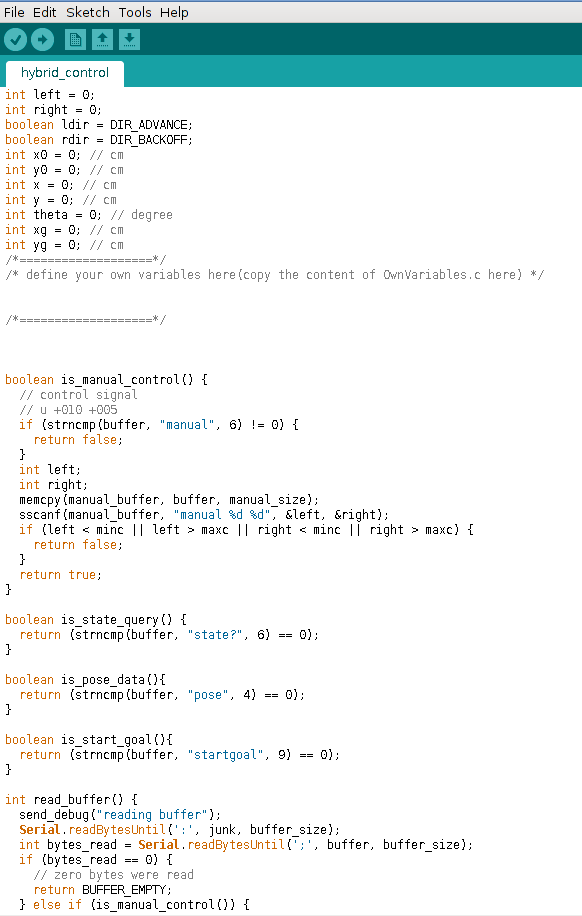
\includegraphics[scale=0.6]{./figures/task_20/1.png}
  \caption{\texttt{hybrid\_control.ino} before copying the contents of
    \texttt{OwnVariables.c} in it.}
  \label{fig:20_1}
\end{figure}

\begin{figure}[H]
  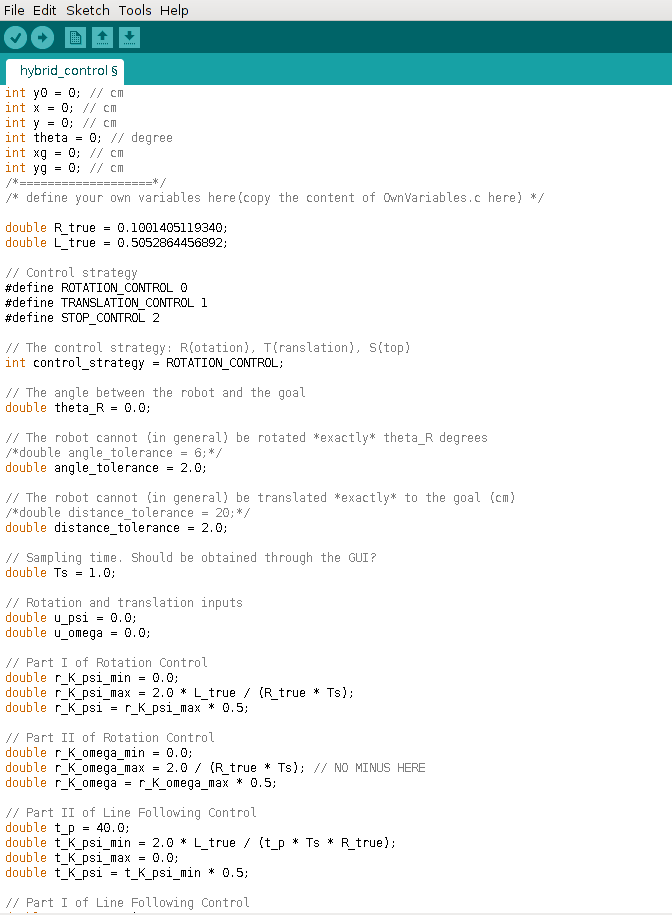
\includegraphics[scale=0.6]{./figures/task_20/2.png}
  \caption{\texttt{hybrid\_control.ino} after copying the contents of
    \texttt{OwnVariables.c} in it.}
  \label{fig:20_2}
\end{figure}

After the successful insertion of the contents of
the aforementioned files, we move the mouse to upper-left corner where we find
a tick symbol, illustrated in figure \ref{fig:20_3}. We then press it using the
left button of the mouse.

\begin{figure}[H]
  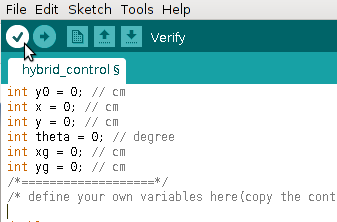
\includegraphics[scale=1]{./figures/task_20/3.png}
  \caption{After the injection of the contents of the three files we locate
    the tick symbol and click it}
  \label{fig:20_3}
\end{figure}


\section*{Task 21}
%Reaching a certain accuracy is difficult. First one has to
orient and then to translate. As there is no automatic line-following, one
has to correct many times to reach a certain point, while reaching a certain
area should be easier. The accuracy in both bearing and distance is related
to the sensitivity of the motors driving the wheels to their input signals and
their output rotation precision.


\section*{Task 22}
%Figure \ref{fig:22_map_7} plots the trajectory of the robot for an experiment
performed at KTH's Smart Mobility Lab of the Automatic Control Department. The
robot was initially placed in the vicinity of node 2. Its first goal was
dictated to be node 1, and from there, nodes 5 and 3.

The robot's bearing and distance tolarance from a target was set to
$\xi = 4^{\circ}$ and the distance tolerance to $\delta$ = 6 cm. The controller's
gains were set to

$$(\dfrac{K_{\Psi}^R}{K_{\Psi,max}^R}, \dfrac{K_{\omega}^T}{K_{\omega, max}^T}, \dfrac{K_{\omega}^R}{K_{\omega,max}^R}, \dfrac{K_{\Psi}^T}{K_{\Psi,max}^T})
\equiv (0.2, 0.2, 0.5, 0.5)$$
where $K_{*,max} > 0$.

\begin{figure}\centering
  \scalebox{1}{% This file was created by matlab2tikz.
%
%The latest updates can be retrieved from
%  http://www.mathworks.com/matlabcentral/fileexchange/22022-matlab2tikz-matlab2tikz
%where you can also make suggestions and rate matlab2tikz.
%
\definecolor{mycolor1}{rgb}{0.00000,0.44700,0.74100}%
%
\begin{tikzpicture}

\begin{axis}[%
width=4.133in,
height=3.26in,
at={(0.693in,0.44in)},
scale only axis,
xmin=-0.85,
xmax=3,
ymin=-1.8,
ymax=2,
axis background/.style={fill=white}
]
\addplot [color=mycolor1,solid,forget plot]
  table[row sep=crcr]{%
1.18	1.68\\
1.18	1.68\\
1.18	1.68\\
1.18	1.68\\
1.18	1.68\\
1.18	1.68\\
1.18	1.68\\
1.18	1.68\\
1.18	1.68\\
1.18	1.68\\
1.18	1.68\\
1.18	1.68\\
1.18	1.68\\
1.18	1.68\\
1.18	1.68\\
1.18	1.68\\
1.18	1.68\\
1.18	1.68\\
1.18	1.68\\
1.18	1.68\\
1.18	1.68\\
1.18	1.68\\
1.18	1.68\\
1.18	1.68\\
1.18	1.68\\
1.18	1.68\\
1.18	1.68\\
1.18	1.68\\
1.18	1.68\\
1.18	1.68\\
1.18	1.68\\
1.18	1.68\\
1.18	1.68\\
1.18	1.68\\
1.18	1.68\\
1.18	1.68\\
1.18	1.68\\
1.18	1.68\\
1.18	1.68\\
1.18	1.68\\
1.18	1.68\\
1.18	1.68\\
1.18	1.68\\
1.18	1.68\\
1.18	1.68\\
1.18	1.68\\
1.18	1.68\\
1.18	1.68\\
1.18	1.68\\
1.18	1.68\\
1.18	1.68\\
1.18	1.68\\
1.18	1.68\\
1.18	1.68\\
1.18	1.68\\
1.18	1.68\\
1.18	1.68\\
1.18	1.68\\
1.18	1.68\\
1.18	1.68\\
1.18	1.68\\
1.18	1.68\\
1.18	1.68\\
1.18	1.68\\
1.18	1.68\\
1.18	1.68\\
1.18	1.68\\
1.18	1.68\\
1.18	1.68\\
1.18	1.68\\
1.18	1.68\\
1.18	1.68\\
1.18	1.68\\
1.18	1.68\\
1.18	1.68\\
1.18	1.68\\
1.18	1.68\\
1.18	1.68\\
1.18	1.68\\
1.18	1.68\\
1.18	1.68\\
1.18	1.68\\
1.18	1.68\\
1.18	1.68\\
1.18	1.68\\
1.18	1.68\\
1.18	1.68\\
1.18	1.68\\
1.18	1.68\\
1.18	1.68\\
1.18	1.68\\
1.18	1.68\\
1.18	1.68\\
1.18	1.68\\
1.18	1.68\\
1.18	1.68\\
1.18	1.68\\
1.18	1.68\\
1.18	1.68\\
1.18	1.68\\
1.18	1.68\\
1.18	1.68\\
1.18	1.68\\
1.18	1.68\\
1.18	1.68\\
1.18	1.68\\
1.18	1.68\\
1.18	1.68\\
1.18	1.68\\
1.18	1.68\\
1.18	1.68\\
1.18	1.68\\
1.18	1.68\\
1.18	1.68\\
1.18	1.68\\
1.18	1.68\\
1.18	1.68\\
1.18	1.68\\
1.18	1.68\\
1.18	1.68\\
1.18	1.68\\
1.18	1.68\\
1.18	1.68\\
1.18	1.68\\
1.18	1.68\\
1.18	1.68\\
1.18	1.68\\
1.18	1.68\\
1.18	1.68\\
1.18	1.68\\
1.18	1.68\\
1.18	1.68\\
1.18	1.68\\
1.18	1.68\\
1.18	1.68\\
1.18	1.68\\
1.18	1.68\\
1.18	1.68\\
1.18	1.68\\
1.18	1.68\\
1.18	1.68\\
1.18	1.68\\
1.18	1.68\\
1.18	1.68\\
1.18	1.68\\
1.18	1.68\\
1.18	1.68\\
1.18	1.68\\
1.18	1.68\\
1.18	1.68\\
1.18	1.68\\
1.18	1.68\\
1.18	1.68\\
1.18	1.68\\
1.18	1.68\\
1.18	1.68\\
1.18	1.68\\
1.18	1.68\\
1.18	1.68\\
1.18	1.68\\
1.18	1.68\\
1.18	1.68\\
1.18	1.68\\
1.18	1.68\\
1.18	1.68\\
1.18	1.68\\
1.18	1.68\\
1.18	1.68\\
1.18	1.68\\
1.18	1.68\\
1.18	1.68\\
1.18	1.68\\
1.18	1.68\\
1.18	1.68\\
1.18	1.68\\
1.18	1.68\\
1.18	1.68\\
1.18	1.68\\
1.18	1.68\\
1.18	1.68\\
1.18	1.68\\
1.18	1.68\\
1.18	1.68\\
1.18	1.68\\
1.18	1.68\\
1.18	1.68\\
1.18	1.68\\
1.18	1.68\\
1.18	1.68\\
1.18	1.68\\
1.18	1.68\\
1.18	1.68\\
1.18	1.68\\
1.18	1.68\\
1.18	1.68\\
1.18	1.68\\
1.18	1.68\\
1.18	1.68\\
1.18	1.68\\
1.18	1.68\\
1.18	1.68\\
1.18	1.68\\
1.18	1.68\\
1.18	1.68\\
1.18	1.68\\
1.18	1.68\\
1.18	1.68\\
1.18	1.68\\
1.18	1.68\\
1.18	1.68\\
1.18	1.68\\
1.18	1.68\\
1.18	1.68\\
1.18	1.68\\
1.18	1.68\\
1.18	1.68\\
1.18	1.68\\
1.18	1.68\\
1.18	1.68\\
1.18	1.68\\
1.18	1.68\\
1.18	1.68\\
1.18	1.68\\
1.18	1.68\\
1.18	1.68\\
1.18	1.68\\
1.18	1.68\\
1.18	1.68\\
1.18	1.68\\
1.18	1.68\\
1.18	1.68\\
1.18	1.68\\
1.18	1.68\\
1.18	1.68\\
1.18	1.68\\
1.18	1.68\\
1.18	1.68\\
1.18	1.68\\
1.18	1.68\\
1.18	1.68\\
1.18	1.68\\
1.18	1.68\\
1.18	1.68\\
1.18	1.68\\
1.18	1.68\\
1.18	1.68\\
1.18	1.68\\
1.18	1.68\\
1.18	1.68\\
1.18	1.68\\
1.18	1.68\\
1.18	1.68\\
1.18	1.68\\
1.18	1.68\\
1.18	1.68\\
1.18	1.68\\
1.18	1.68\\
1.18	1.68\\
1.18	1.68\\
1.18	1.68\\
1.18	1.68\\
1.18	1.68\\
1.18	1.68\\
1.18	1.68\\
1.18	1.68\\
1.18	1.68\\
1.18	1.68\\
1.18	1.68\\
1.18	1.68\\
1.18	1.68\\
1.18	1.68\\
1.18	1.68\\
1.18	1.68\\
1.18	1.68\\
1.18	1.68\\
1.18	1.68\\
1.18	1.68\\
1.18	1.68\\
1.18	1.68\\
1.18	1.68\\
1.18	1.68\\
1.18	1.68\\
1.18	1.68\\
1.18	1.68\\
1.18	1.68\\
1.18	1.68\\
1.18	1.68\\
1.18	1.68\\
1.18	1.68\\
1.18	1.68\\
1.18	1.68\\
1.18	1.68\\
1.18	1.68\\
1.18	1.68\\
1.18	1.68\\
1.18	1.68\\
1.18	1.68\\
1.18	1.68\\
1.18	1.68\\
1.18	1.68\\
1.18	1.68\\
1.18	1.68\\
1.18	1.68\\
1.18	1.68\\
1.18	1.68\\
1.18	1.68\\
1.18	1.68\\
1.18	1.68\\
1.18	1.68\\
1.18	1.68\\
1.18	1.68\\
1.18	1.68\\
1.18	1.68\\
1.18	1.68\\
1.18	1.68\\
1.18	1.68\\
1.18	1.68\\
1.18	1.68\\
1.18	1.68\\
1.18	1.68\\
1.18	1.68\\
1.18	1.68\\
1.18	1.68\\
1.18	1.68\\
1.18	1.68\\
1.18	1.68\\
1.18	1.68\\
1.18	1.68\\
1.18	1.68\\
1.18	1.68\\
1.18	1.68\\
1.18	1.68\\
1.18	1.68\\
1.18	1.68\\
1.18	1.68\\
1.18	1.68\\
1.18	1.68\\
1.18	1.68\\
1.18	1.68\\
1.18	1.68\\
1.18	1.68\\
1.18	1.68\\
1.18	1.68\\
1.18	1.68\\
1.18	1.68\\
1.18	1.68\\
1.18	1.68\\
1.18	1.68\\
1.18	1.68\\
1.18	1.68\\
1.18	1.68\\
1.18	1.68\\
1.18	1.68\\
1.18	1.68\\
1.18	1.68\\
1.18	1.68\\
1.18	1.68\\
1.18	1.68\\
1.18	1.68\\
1.18	1.68\\
1.18	1.68\\
1.18	1.68\\
1.18	1.68\\
1.18	1.68\\
1.18	1.68\\
1.18	1.68\\
1.18	1.68\\
1.18	1.68\\
1.18	1.68\\
1.18	1.68\\
1.18	1.68\\
1.18	1.68\\
1.18	1.68\\
1.18	1.68\\
1.18	1.68\\
1.18	1.68\\
1.18	1.68\\
1.18	1.68\\
1.18	1.68\\
1.18	1.68\\
1.18	1.68\\
1.18	1.68\\
1.18	1.68\\
1.18	1.68\\
1.18	1.68\\
1.18	1.68\\
1.18	1.68\\
1.18	1.68\\
1.18	1.68\\
1.18	1.68\\
1.18	1.68\\
1.18	1.68\\
1.18	1.68\\
1.18	1.68\\
1.18	1.68\\
1.18	1.68\\
1.18	1.68\\
1.18	1.68\\
1.18	1.68\\
1.18	1.68\\
1.18	1.68\\
1.18	1.68\\
1.18	1.68\\
1.18	1.68\\
1.18	1.68\\
1.18	1.68\\
1.18	1.68\\
1.18	1.68\\
1.18	1.68\\
1.18	1.68\\
1.18	1.68\\
1.18	1.68\\
1.18	1.68\\
1.18	1.68\\
1.18	1.68\\
1.18	1.68\\
1.18	1.68\\
1.18	1.68\\
1.18	1.68\\
1.18	1.68\\
1.18	1.68\\
1.18	1.68\\
1.18	1.68\\
1.18	1.68\\
1.18	1.68\\
1.18	1.68\\
1.18	1.68\\
1.18	1.68\\
1.18	1.68\\
1.18	1.68\\
1.18	1.68\\
1.18	1.68\\
1.18	1.68\\
1.18	1.68\\
1.18	1.68\\
1.18	1.68\\
1.18	1.68\\
1.18	1.68\\
1.18	1.68\\
1.18	1.68\\
1.18	1.68\\
1.18	1.68\\
1.18	1.68\\
1.18	1.68\\
1.18	1.68\\
1.18	1.68\\
1.18	1.68\\
1.18	1.68\\
1.18	1.68\\
1.18	1.68\\
1.18	1.68\\
1.18	1.68\\
1.18	1.68\\
1.18	1.68\\
1.18	1.68\\
1.18	1.68\\
1.18	1.68\\
1.18	1.68\\
1.18	1.68\\
1.18	1.68\\
1.18	1.68\\
1.18	1.68\\
1.18	1.68\\
1.18	1.68\\
1.18	1.68\\
1.18	1.68\\
1.18	1.68\\
1.18	1.68\\
1.18	1.68\\
1.18	1.68\\
1.18	1.68\\
1.18	1.68\\
1.18	1.68\\
1.18	1.68\\
1.18	1.68\\
1.18	1.68\\
1.18	1.68\\
1.18	1.68\\
1.18	1.68\\
1.18	1.68\\
1.18	1.68\\
1.18	1.68\\
1.18	1.68\\
1.18	1.68\\
1.18	1.68\\
1.18	1.68\\
1.18	1.68\\
1.18	1.68\\
1.18	1.68\\
1.18	1.68\\
1.18	1.68\\
1.18	1.68\\
1.18	1.68\\
1.18	1.68\\
1.18	1.68\\
1.18	1.68\\
1.18	1.68\\
1.18	1.68\\
1.18	1.68\\
1.18	1.68\\
1.18	1.68\\
1.18	1.68\\
1.18	1.68\\
1.18	1.68\\
1.18	1.68\\
1.18	1.68\\
1.18	1.68\\
1.18	1.68\\
1.18	1.68\\
1.18	1.68\\
1.18	1.68\\
1.18	1.68\\
1.18	1.68\\
1.18	1.68\\
1.18	1.68\\
1.18	1.68\\
1.18	1.68\\
1.18	1.68\\
1.18	1.68\\
1.18	1.68\\
1.18	1.68\\
1.18	1.68\\
1.18	1.68\\
1.18	1.68\\
1.18	1.68\\
1.18	1.68\\
1.18	1.68\\
1.18	1.68\\
1.18	1.68\\
1.18	1.68\\
1.18	1.68\\
1.18	1.68\\
1.18	1.68\\
1.18	1.68\\
1.18	1.68\\
1.18	1.68\\
1.18	1.68\\
1.18	1.68\\
1.18	1.68\\
1.18	1.68\\
1.18	1.68\\
1.18	1.68\\
1.18	1.68\\
1.18	1.68\\
1.18	1.68\\
1.18	1.68\\
1.18	1.68\\
1.18	1.68\\
1.18	1.68\\
1.18	1.68\\
1.18	1.68\\
1.18	1.68\\
1.18	1.68\\
1.18	1.68\\
1.18	1.68\\
1.18	1.68\\
1.18	1.68\\
1.18	1.68\\
1.18	1.68\\
1.18	1.68\\
1.18	1.68\\
1.18	1.68\\
1.18	1.68\\
1.18	1.68\\
1.18	1.68\\
1.18	1.68\\
1.18	1.68\\
1.18	1.68\\
1.18	1.68\\
1.18	1.68\\
1.18	1.68\\
1.18	1.68\\
1.18	1.68\\
1.18	1.68\\
1.18	1.68\\
1.18	1.68\\
1.18	1.68\\
1.18	1.68\\
1.18	1.68\\
1.18	1.68\\
1.18	1.68\\
1.18	1.68\\
1.18	1.68\\
1.18	1.68\\
1.18	1.68\\
1.18	1.68\\
1.18	1.68\\
1.18	1.68\\
1.18	1.68\\
1.18	1.68\\
1.18	1.68\\
1.18	1.68\\
1.18	1.68\\
1.18	1.68\\
1.18	1.68\\
1.18	1.68\\
1.18	1.68\\
1.18	1.68\\
1.18	1.68\\
1.18	1.68\\
1.18	1.68\\
1.18	1.68\\
1.18	1.68\\
1.18	1.68\\
1.18	1.68\\
1.18	1.68\\
1.18	1.68\\
1.18	1.68\\
1.18	1.68\\
1.18	1.68\\
1.18	1.68\\
1.18	1.68\\
1.18	1.68\\
1.18	1.68\\
1.18	1.68\\
1.18	1.68\\
1.18	1.68\\
1.18	1.68\\
1.18	1.68\\
1.18	1.68\\
1.18	1.68\\
1.18	1.68\\
1.18	1.68\\
1.18	1.68\\
1.18	1.68\\
1.18	1.68\\
1.18	1.68\\
1.18	1.68\\
1.18	1.68\\
1.18	1.68\\
1.18	1.68\\
1.18	1.68\\
1.18	1.68\\
1.18	1.68\\
1.18	1.68\\
1.18	1.68\\
1.18	1.68\\
1.18	1.68\\
1.18	1.68\\
1.18	1.68\\
1.18	1.68\\
1.18	1.68\\
1.18	1.68\\
1.18	1.68\\
1.18	1.68\\
1.18	1.68\\
1.18	1.68\\
1.18	1.68\\
1.18	1.68\\
1.18	1.68\\
1.18	1.68\\
1.18	1.68\\
1.18	1.68\\
1.18	1.68\\
1.18	1.68\\
1.18	1.68\\
1.18	1.68\\
1.18	1.68\\
1.18	1.68\\
1.18	1.68\\
1.18	1.68\\
1.18	1.68\\
1.18	1.68\\
1.18	1.68\\
1.18	1.68\\
1.18	1.68\\
1.18	1.68\\
1.18	1.68\\
1.18	1.68\\
1.18	1.68\\
1.18	1.68\\
1.18	1.68\\
1.18	1.68\\
1.18	1.68\\
1.18	1.68\\
1.18	1.68\\
1.18	1.68\\
1.18	1.68\\
1.18	1.68\\
1.18	1.68\\
1.18	1.68\\
1.18	1.68\\
1.18	1.68\\
1.18	1.68\\
1.18	1.68\\
1.18	1.68\\
1.18	1.68\\
1.18	1.68\\
1.18	1.68\\
1.18	1.68\\
1.18	1.68\\
1.18	1.68\\
1.18	1.68\\
1.18	1.68\\
1.18	1.68\\
1.18	1.68\\
1.18	1.68\\
1.18	1.68\\
1.18	1.68\\
1.18	1.68\\
1.18	1.68\\
1.18	1.68\\
1.18	1.68\\
1.18	1.68\\
1.18	1.68\\
1.18	1.68\\
1.18	1.68\\
1.18	1.68\\
1.18	1.68\\
1.18	1.68\\
1.18	1.68\\
1.18	1.68\\
1.18	1.68\\
1.18	1.68\\
1.18	1.68\\
1.18	1.68\\
1.18	1.68\\
1.18	1.68\\
1.18	1.68\\
1.18	1.68\\
1.18	1.68\\
1.18	1.68\\
1.18	1.68\\
1.18	1.68\\
1.18	1.68\\
1.18	1.68\\
1.18	1.68\\
1.18	1.68\\
1.18	1.68\\
1.18	1.68\\
1.18	1.68\\
1.18	1.68\\
1.18	1.68\\
1.18	1.68\\
1.18	1.68\\
1.18	1.68\\
1.18	1.68\\
1.18	1.68\\
1.18	1.68\\
1.18	1.68\\
1.18	1.68\\
1.18	1.68\\
1.18	1.68\\
1.18	1.68\\
1.18	1.68\\
1.18	1.68\\
1.18	1.68\\
1.18	1.68\\
1.18	1.68\\
1.18	1.68\\
1.18	1.68\\
1.18	1.68\\
1.18	1.68\\
1.18	1.68\\
1.18	1.68\\
1.18	1.68\\
1.18	1.68\\
1.18	1.68\\
1.18	1.68\\
1.18	1.68\\
1.18	1.68\\
1.18	1.68\\
1.18	1.68\\
1.18	1.68\\
1.18	1.68\\
1.18	1.68\\
1.18	1.68\\
1.18	1.68\\
1.18	1.68\\
1.18	1.68\\
1.18	1.68\\
1.18	1.68\\
1.18	1.68\\
1.18	1.68\\
1.18	1.68\\
1.18	1.68\\
1.18	1.68\\
1.18	1.68\\
1.18	1.68\\
1.18	1.68\\
1.18	1.68\\
1.18	1.68\\
1.18	1.68\\
1.18	1.68\\
1.18	1.68\\
1.18	1.68\\
1.18	1.68\\
1.18	1.68\\
1.18	1.68\\
1.18	1.68\\
1.18	1.68\\
1.18	1.68\\
1.18	1.68\\
1.18	1.68\\
1.18	1.68\\
1.18	1.68\\
1.18	1.68\\
1.18	1.68\\
1.18	1.68\\
1.18	1.68\\
1.18	1.68\\
1.18	1.68\\
1.18	1.68\\
1.18	1.68\\
1.18	1.68\\
1.18	1.68\\
1.18	1.68\\
1.18	1.68\\
1.18	1.68\\
1.18	1.68\\
1.18	1.68\\
1.18	1.68\\
1.18	1.68\\
1.18	1.68\\
1.18	1.68\\
1.18	1.68\\
1.18	1.68\\
1.18	1.68\\
1.18	1.68\\
1.18	1.68\\
1.18	1.68\\
1.18	1.68\\
1.18	1.68\\
1.18	1.68\\
1.18	1.68\\
1.18	1.68\\
1.18	1.68\\
1.18	1.69\\
1.18	1.69\\
1.18	1.69\\
1.18	1.69\\
1.18	1.69\\
1.18	1.69\\
1.18	1.69\\
1.18	1.69\\
1.18	1.69\\
1.18	1.69\\
1.18	1.69\\
1.18	1.69\\
1.18	1.69\\
1.18	1.69\\
1.18	1.69\\
1.18	1.69\\
1.18	1.69\\
1.18	1.69\\
1.18	1.69\\
1.18	1.68\\
1.18	1.69\\
1.18	1.69\\
1.18	1.69\\
1.18	1.69\\
1.18	1.69\\
1.18	1.69\\
1.18	1.69\\
1.18	1.69\\
1.18	1.69\\
1.18	1.69\\
1.18	1.69\\
1.18	1.69\\
1.18	1.69\\
1.18	1.69\\
1.18	1.69\\
1.18	1.69\\
1.18	1.69\\
1.18	1.69\\
1.18	1.69\\
1.18	1.69\\
1.18	1.69\\
1.18	1.69\\
1.18	1.69\\
1.18	1.69\\
1.18	1.69\\
1.18	1.69\\
1.18	1.69\\
1.18	1.69\\
1.18	1.69\\
1.18	1.69\\
1.18	1.69\\
1.18	1.69\\
1.18	1.69\\
1.18	1.69\\
1.18	1.69\\
1.18	1.69\\
1.18	1.69\\
1.18	1.69\\
1.18	1.69\\
1.18	1.69\\
1.18	1.69\\
1.18	1.69\\
1.18	1.69\\
1.18	1.69\\
1.18	1.69\\
1.18	1.69\\
1.18	1.69\\
1.18	1.69\\
1.18	1.69\\
1.18	1.69\\
1.18	1.69\\
1.18	1.69\\
1.18	1.69\\
1.18	1.69\\
1.18	1.69\\
1.18	1.69\\
1.18	1.69\\
1.18	1.69\\
1.18	1.69\\
1.18	1.69\\
1.18	1.69\\
1.18	1.69\\
1.18	1.69\\
1.18	1.69\\
1.18	1.69\\
1.18	1.69\\
1.18	1.69\\
1.18	1.69\\
1.18	1.69\\
1.18	1.69\\
1.18	1.69\\
1.18	1.69\\
1.18	1.69\\
1.18	1.69\\
1.18	1.69\\
1.18	1.69\\
1.18	1.69\\
1.18	1.69\\
1.18	1.69\\
1.18	1.69\\
1.18	1.69\\
1.18	1.69\\
1.18	1.69\\
1.18	1.69\\
1.18	1.69\\
1.18	1.69\\
1.18	1.69\\
1.18	1.69\\
1.18	1.69\\
1.18	1.69\\
1.18	1.69\\
1.18	1.69\\
1.18	1.69\\
1.18	1.69\\
1.18	1.69\\
1.18	1.69\\
1.18	1.69\\
1.18	1.69\\
1.18	1.69\\
1.18	1.69\\
1.18	1.69\\
1.18	1.69\\
1.18	1.69\\
1.18	1.69\\
1.18	1.69\\
1.18	1.69\\
1.18	1.69\\
1.18	1.69\\
1.18	1.69\\
1.18	1.69\\
1.18	1.69\\
1.18	1.69\\
1.18	1.69\\
1.18	1.69\\
1.18	1.69\\
1.18	1.69\\
1.18	1.69\\
1.18	1.69\\
1.18	1.69\\
1.18	1.69\\
1.18	1.69\\
1.18	1.69\\
1.18	1.69\\
1.18	1.69\\
1.18	1.69\\
1.18	1.69\\
1.18	1.69\\
1.18	1.69\\
1.18	1.69\\
1.18	1.69\\
1.18	1.69\\
1.18	1.69\\
1.18	1.69\\
1.18	1.69\\
1.18	1.69\\
1.18	1.69\\
1.18	1.69\\
1.18	1.69\\
1.18	1.69\\
1.18	1.69\\
1.18	1.69\\
1.18	1.69\\
1.18	1.69\\
1.18	1.69\\
1.18	1.69\\
1.18	1.69\\
1.18	1.69\\
1.18	1.69\\
1.18	1.69\\
1.18	1.69\\
1.18	1.69\\
1.18	1.69\\
1.18	1.69\\
1.18	1.69\\
1.18	1.69\\
1.18	1.69\\
1.18	1.69\\
1.18	1.69\\
1.18	1.69\\
1.18	1.69\\
1.18	1.69\\
1.18	1.69\\
1.18	1.69\\
1.18	1.69\\
1.18	1.69\\
1.18	1.69\\
1.18	1.69\\
1.18	1.69\\
1.18	1.69\\
1.18	1.69\\
1.18	1.69\\
1.18	1.69\\
1.18	1.69\\
1.18	1.69\\
1.18	1.69\\
1.18	1.69\\
1.18	1.69\\
1.18	1.69\\
1.18	1.69\\
1.18	1.69\\
1.18	1.69\\
1.18	1.69\\
1.18	1.69\\
1.17	1.69\\
1.17	1.69\\
1.17	1.69\\
1.18	1.69\\
1.17	1.69\\
1.17	1.69\\
1.17	1.69\\
1.17	1.69\\
1.17	1.69\\
1.17	1.69\\
1.17	1.69\\
1.17	1.69\\
1.17	1.69\\
1.17	1.69\\
1.17	1.69\\
1.17	1.69\\
1.17	1.69\\
1.17	1.69\\
1.17	1.69\\
1.17	1.69\\
1.17	1.69\\
1.17	1.69\\
1.17	1.69\\
1.17	1.69\\
1.17	1.69\\
1.17	1.69\\
1.17	1.69\\
1.17	1.69\\
1.17	1.69\\
1.17	1.69\\
1.17	1.69\\
1.17	1.69\\
1.17	1.69\\
1.17	1.69\\
1.17	1.69\\
1.17	1.69\\
1.17	1.69\\
1.17	1.69\\
1.17	1.69\\
1.17	1.69\\
1.17	1.69\\
1.17	1.69\\
1.17	1.69\\
1.17	1.69\\
1.17	1.69\\
1.17	1.69\\
1.17	1.69\\
1.17	1.69\\
1.17	1.69\\
1.17	1.69\\
1.17	1.69\\
1.17	1.69\\
1.17	1.69\\
1.18	1.69\\
1.18	1.69\\
1.18	1.69\\
1.18	1.69\\
1.18	1.69\\
1.18	1.69\\
1.18	1.69\\
1.18	1.69\\
1.18	1.69\\
1.18	1.69\\
1.18	1.69\\
1.18	1.69\\
1.18	1.69\\
1.18	1.69\\
1.18	1.69\\
1.18	1.69\\
1.18	1.69\\
1.18	1.69\\
1.18	1.69\\
1.18	1.69\\
1.18	1.69\\
1.18	1.69\\
1.18	1.69\\
1.18	1.69\\
1.18	1.69\\
1.18	1.69\\
1.18	1.69\\
1.18	1.69\\
1.18	1.69\\
1.18	1.69\\
1.18	1.69\\
1.18	1.69\\
1.18	1.69\\
1.18	1.69\\
1.18	1.69\\
1.18	1.69\\
1.18	1.69\\
1.18	1.69\\
1.18	1.69\\
1.18	1.69\\
1.18	1.69\\
1.18	1.69\\
1.18	1.69\\
1.18	1.69\\
1.18	1.69\\
1.18	1.69\\
1.18	1.69\\
1.18	1.69\\
1.18	1.69\\
1.18	1.69\\
1.18	1.69\\
1.18	1.69\\
1.18	1.69\\
1.18	1.69\\
1.18	1.69\\
1.18	1.69\\
1.18	1.69\\
1.18	1.69\\
1.18	1.69\\
1.18	1.69\\
1.18	1.69\\
1.18	1.69\\
1.18	1.69\\
1.18	1.69\\
1.18	1.69\\
1.18	1.69\\
1.18	1.69\\
1.18	1.69\\
1.18	1.69\\
1.18	1.69\\
1.18	1.69\\
1.18	1.69\\
1.18	1.69\\
1.18	1.69\\
1.18	1.69\\
1.18	1.69\\
1.18	1.69\\
1.18	1.69\\
1.18	1.69\\
1.18	1.69\\
1.18	1.69\\
1.18	1.69\\
1.18	1.69\\
1.18	1.69\\
1.18	1.69\\
1.18	1.69\\
1.18	1.69\\
1.18	1.69\\
1.18	1.69\\
1.18	1.69\\
1.18	1.69\\
1.18	1.69\\
1.18	1.69\\
1.18	1.69\\
1.18	1.69\\
1.18	1.69\\
1.18	1.69\\
1.18	1.69\\
1.18	1.69\\
1.18	1.69\\
1.18	1.69\\
1.18	1.69\\
1.18	1.69\\
1.18	1.69\\
1.18	1.69\\
1.18	1.69\\
1.18	1.69\\
1.18	1.69\\
1.18	1.69\\
1.18	1.69\\
1.18	1.69\\
1.18	1.69\\
1.18	1.69\\
1.18	1.69\\
1.18	1.69\\
1.18	1.69\\
1.18	1.69\\
1.18	1.69\\
1.18	1.69\\
1.18	1.69\\
1.18	1.69\\
1.18	1.69\\
1.18	1.69\\
1.18	1.69\\
1.18	1.69\\
1.18	1.69\\
1.18	1.69\\
1.18	1.69\\
1.18	1.69\\
1.18	1.69\\
1.18	1.69\\
1.18	1.69\\
1.18	1.69\\
1.18	1.69\\
1.18	1.69\\
1.18	1.69\\
1.18	1.69\\
1.18	1.69\\
1.18	1.69\\
1.18	1.69\\
1.18	1.69\\
1.18	1.69\\
1.18	1.69\\
1.18	1.69\\
1.18	1.69\\
1.18	1.69\\
1.18	1.69\\
1.18	1.69\\
1.18	1.69\\
1.18	1.69\\
1.18	1.69\\
1.18	1.69\\
1.18	1.69\\
1.18	1.69\\
1.18	1.69\\
1.18	1.69\\
1.18	1.69\\
1.18	1.69\\
1.18	1.69\\
1.18	1.69\\
1.18	1.69\\
1.18	1.69\\
1.18	1.69\\
1.18	1.69\\
1.18	1.69\\
1.18	1.69\\
1.18	1.69\\
1.18	1.69\\
1.18	1.69\\
1.18	1.69\\
1.18	1.69\\
1.18	1.69\\
1.18	1.69\\
1.18	1.69\\
1.18	1.69\\
1.18	1.69\\
1.18	1.69\\
1.18	1.69\\
1.18	1.69\\
1.18	1.69\\
1.18	1.69\\
1.18	1.69\\
1.18	1.69\\
1.18	1.69\\
1.18	1.69\\
1.18	1.69\\
1.18	1.69\\
1.18	1.69\\
1.18	1.69\\
1.18	1.69\\
1.18	1.69\\
1.18	1.69\\
1.18	1.69\\
1.18	1.69\\
1.18	1.69\\
1.18	1.69\\
1.18	1.69\\
1.18	1.69\\
1.18	1.69\\
1.18	1.69\\
1.18	1.69\\
1.18	1.69\\
1.18	1.69\\
1.18	1.69\\
1.18	1.69\\
1.18	1.69\\
1.18	1.69\\
1.18	1.69\\
1.18	1.69\\
1.18	1.69\\
1.18	1.69\\
1.18	1.69\\
1.18	1.69\\
1.18	1.69\\
1.18	1.69\\
1.18	1.69\\
1.18	1.69\\
1.18	1.69\\
1.18	1.69\\
1.18	1.69\\
1.18	1.69\\
1.18	1.69\\
1.18	1.69\\
1.18	1.69\\
1.18	1.69\\
1.18	1.69\\
1.18	1.69\\
1.18	1.69\\
1.18	1.69\\
1.18	1.69\\
1.18	1.69\\
1.18	1.69\\
1.18	1.69\\
1.18	1.69\\
1.18	1.69\\
1.18	1.69\\
1.18	1.69\\
1.18	1.69\\
1.18	1.69\\
1.18	1.69\\
1.18	1.69\\
1.18	1.69\\
1.18	1.69\\
1.18	1.69\\
1.18	1.69\\
1.18	1.69\\
1.18	1.69\\
1.18	1.69\\
1.19	1.69\\
1.19	1.69\\
1.19	1.69\\
1.19	1.69\\
1.19	1.69\\
1.19	1.69\\
1.19	1.69\\
1.19	1.69\\
1.19	1.69\\
1.19	1.69\\
1.19	1.69\\
1.19	1.69\\
1.19	1.69\\
1.19	1.69\\
1.19	1.69\\
1.19	1.69\\
1.19	1.69\\
1.19	1.69\\
1.19	1.69\\
1.19	1.69\\
1.19	1.69\\
1.19	1.69\\
1.19	1.69\\
1.19	1.69\\
1.19	1.69\\
1.19	1.69\\
1.19	1.69\\
1.19	1.69\\
1.19	1.69\\
1.19	1.69\\
1.19	1.69\\
1.19	1.69\\
1.19	1.69\\
1.19	1.69\\
1.19	1.69\\
1.19	1.69\\
1.19	1.69\\
1.19	1.69\\
1.19	1.69\\
1.19	1.69\\
1.19	1.69\\
1.19	1.69\\
1.19	1.69\\
1.19	1.69\\
1.19	1.69\\
1.19	1.69\\
1.19	1.69\\
1.19	1.69\\
1.19	1.69\\
1.19	1.69\\
1.19	1.69\\
1.19	1.69\\
1.19	1.69\\
1.19	1.69\\
1.19	1.69\\
1.19	1.69\\
1.19	1.69\\
1.19	1.69\\
1.19	1.69\\
1.19	1.69\\
1.19	1.69\\
1.19	1.69\\
1.19	1.69\\
1.19	1.69\\
1.19	1.69\\
1.19	1.69\\
1.19	1.69\\
1.19	1.69\\
1.19	1.69\\
1.19	1.69\\
1.19	1.69\\
1.19	1.69\\
1.19	1.69\\
1.19	1.69\\
1.18	1.69\\
1.18	1.69\\
1.18	1.69\\
1.18	1.69\\
1.17	1.69\\
1.17	1.69\\
1.17	1.69\\
1.17	1.69\\
1.16	1.69\\
1.15	1.69\\
1.15	1.69\\
1.14	1.69\\
1.14	1.69\\
1.13	1.69\\
1.12	1.69\\
1.11	1.69\\
1.11	1.69\\
1.1	1.69\\
1.09	1.69\\
1.08	1.69\\
1.08	1.69\\
1.07	1.69\\
1.07	1.69\\
1.06	1.69\\
1.05	1.69\\
1.04	1.69\\
1.04	1.69\\
1.03	1.69\\
1.02	1.69\\
1.01	1.69\\
1.01	1.69\\
1	1.69\\
1	1.69\\
0.99	1.69\\
0.99	1.69\\
0.98	1.7\\
0.97	1.7\\
0.97	1.69\\
0.97	1.69\\
0.96	1.69\\
0.96	1.69\\
0.95	1.69\\
0.95	1.69\\
0.95	1.69\\
0.94	1.69\\
0.94	1.69\\
0.94	1.7\\
0.93	1.7\\
0.93	1.7\\
0.93	1.7\\
0.92	1.7\\
0.92	1.7\\
0.92	1.7\\
0.91	1.7\\
0.91	1.7\\
0.9	1.7\\
0.9	1.7\\
0.89	1.7\\
0.89	1.7\\
0.89	1.7\\
0.88	1.7\\
0.88	1.7\\
0.87	1.7\\
0.87	1.7\\
0.86	1.7\\
0.86	1.7\\
0.86	1.7\\
0.85	1.7\\
0.85	1.7\\
0.84	1.7\\
0.84	1.7\\
0.83	1.7\\
0.83	1.7\\
0.83	1.7\\
0.82	1.7\\
0.82	1.7\\
0.81	1.7\\
0.81	1.7\\
0.8	1.7\\
0.8	1.7\\
0.79	1.7\\
0.79	1.7\\
0.79	1.7\\
0.78	1.7\\
0.78	1.7\\
0.77	1.7\\
0.77	1.7\\
0.76	1.7\\
0.76	1.7\\
0.76	1.7\\
0.75	1.7\\
0.75	1.7\\
0.74	1.7\\
0.74	1.7\\
0.74	1.71\\
0.74	1.71\\
0.73	1.71\\
0.73	1.71\\
0.72	1.71\\
0.72	1.71\\
0.72	1.7\\
0.71	1.7\\
0.71	1.71\\
0.7	1.71\\
0.7	1.7\\
0.7	1.71\\
0.69	1.71\\
0.69	1.71\\
0.68	1.71\\
0.68	1.71\\
0.68	1.71\\
0.67	1.71\\
0.67	1.71\\
0.66	1.71\\
0.66	1.71\\
0.65	1.71\\
0.65	1.71\\
0.65	1.71\\
0.64	1.71\\
0.64	1.71\\
0.64	1.71\\
0.63	1.71\\
0.63	1.71\\
0.62	1.71\\
0.62	1.71\\
0.61	1.71\\
0.61	1.71\\
0.6	1.71\\
0.6	1.71\\
0.6	1.71\\
0.59	1.71\\
0.59	1.71\\
0.59	1.71\\
0.58	1.71\\
0.58	1.71\\
0.57	1.71\\
0.57	1.71\\
0.57	1.71\\
0.56	1.71\\
0.56	1.71\\
0.56	1.71\\
0.55	1.71\\
0.55	1.71\\
0.55	1.71\\
0.54	1.71\\
0.54	1.71\\
0.54	1.71\\
0.54	1.71\\
0.53	1.71\\
0.53	1.71\\
0.52	1.71\\
0.51	1.71\\
0.52	1.71\\
0.52	1.71\\
0.52	1.71\\
0.51	1.71\\
0.51	1.71\\
0.51	1.71\\
0.51	1.71\\
0.5	1.72\\
0.5	1.72\\
0.5	1.72\\
0.5	1.72\\
0.49	1.72\\
0.49	1.72\\
0.48	1.72\\
0.48	1.72\\
0.48	1.72\\
0.47	1.72\\
0.47	1.72\\
0.47	1.72\\
0.47	1.72\\
0.46	1.72\\
0.46	1.72\\
0.45	1.72\\
0.45	1.72\\
0.45	1.72\\
0.44	1.72\\
0.44	1.72\\
0.44	1.72\\
0.43	1.72\\
0.43	1.72\\
0.43	1.72\\
0.42	1.72\\
0.42	1.72\\
0.41	1.72\\
0.41	1.72\\
0.41	1.72\\
0.4	1.72\\
0.4	1.72\\
0.4	1.72\\
0.39	1.72\\
0.39	1.72\\
0.39	1.72\\
0.38	1.72\\
0.38	1.72\\
0.38	1.72\\
0.38	1.72\\
0.38	1.72\\
0.37	1.72\\
0.37	1.72\\
0.37	1.72\\
0.37	1.72\\
0.36	1.72\\
0.36	1.72\\
0.36	1.72\\
0.36	1.72\\
0.36	1.72\\
0.35	1.72\\
0.35	1.72\\
0.35	1.72\\
0.35	1.72\\
0.35	1.72\\
0.34	1.72\\
0.34	1.72\\
0.34	1.72\\
0.34	1.72\\
0.34	1.72\\
0.33	1.72\\
0.33	1.72\\
0.33	1.72\\
0.33	1.72\\
0.33	1.72\\
0.32	1.72\\
0.32	1.72\\
0.32	1.72\\
0.31	1.72\\
0.31	1.72\\
0.31	1.72\\
0.31	1.72\\
0.3	1.72\\
0.3	1.73\\
0.29	1.72\\
0.29	1.73\\
0.29	1.73\\
0.29	1.73\\
0.28	1.73\\
0.28	1.73\\
0.28	1.73\\
0.27	1.73\\
0.27	1.72\\
0.27	1.73\\
0.26	1.73\\
0.26	1.73\\
0.26	1.73\\
0.26	1.73\\
0.26	1.73\\
0.25	1.73\\
0.25	1.73\\
0.25	1.73\\
0.24	1.73\\
0.24	1.73\\
0.24	1.73\\
0.24	1.73\\
0.23	1.73\\
0.23	1.73\\
0.23	1.73\\
0.23	1.73\\
0.23	1.73\\
0.22	1.73\\
0.22	1.73\\
0.22	1.73\\
0.22	1.73\\
0.22	1.73\\
0.22	1.73\\
0.21	1.73\\
0.21	1.73\\
0.21	1.73\\
0.21	1.73\\
0.21	1.73\\
0.21	1.73\\
0.21	1.73\\
0.2	1.73\\
0.2	1.73\\
0.2	1.73\\
0.2	1.73\\
0.2	1.73\\
0.19	1.73\\
0.19	1.73\\
0.19	1.73\\
0.19	1.73\\
0.19	1.73\\
0.19	1.73\\
0.18	1.73\\
0.18	1.73\\
0.18	1.73\\
0.18	1.73\\
0.17	1.73\\
0.17	1.73\\
0.17	1.73\\
0.17	1.73\\
0.16	1.73\\
0.16	1.73\\
0.16	1.73\\
0.16	1.73\\
0.16	1.73\\
0.15	1.73\\
0.15	1.73\\
0.15	1.73\\
0.15	1.73\\
0.14	1.73\\
0.14	1.73\\
0.14	1.73\\
0.14	1.73\\
0.13	1.73\\
0.13	1.73\\
0.13	1.73\\
0.13	1.73\\
0.12	1.73\\
0.12	1.73\\
0.12	1.73\\
0.12	1.73\\
0.12	1.73\\
0.12	1.73\\
0.11	1.73\\
0.11	1.74\\
0.11	1.73\\
0.11	1.74\\
0.11	1.73\\
0.11	1.73\\
0.11	1.73\\
0.1	1.73\\
0.1	1.73\\
0.1	1.73\\
0.1	1.74\\
0.1	1.74\\
0.1	1.74\\
0.09	1.73\\
0.09	1.74\\
0.09	1.74\\
0.09	1.74\\
0.09	1.74\\
0.09	1.74\\
0.09	1.74\\
0.09	1.74\\
0.09	1.74\\
0.08	1.74\\
0.08	1.74\\
0.08	1.74\\
0.08	1.74\\
0.08	1.74\\
0.08	1.74\\
0.07	1.74\\
0.07	1.74\\
0.07	1.74\\
0.07	1.74\\
0.07	1.74\\
0.07	1.74\\
0.06	1.74\\
0.06	1.74\\
0.06	1.74\\
0.06	1.74\\
0.06	1.74\\
0.05	1.74\\
0.05	1.74\\
0.05	1.74\\
0.05	1.74\\
0.05	1.74\\
0.04	1.74\\
0.04	1.74\\
0.04	1.74\\
0.04	1.74\\
0.04	1.74\\
0.03	1.74\\
0.03	1.74\\
0.03	1.74\\
0.03	1.74\\
0.03	1.74\\
0.03	1.74\\
0.02	1.74\\
0.02	1.74\\
0.02	1.74\\
0.02	1.74\\
0.02	1.74\\
0.02	1.74\\
0.02	1.74\\
0.01	1.74\\
0.01	1.74\\
0.01	1.74\\
0.01	1.74\\
0.01	1.74\\
0.01	1.74\\
0.01	1.74\\
0.01	1.74\\
0	1.74\\
0	1.74\\
0	1.74\\
0	1.74\\
0	1.74\\
0	1.74\\
-0	1.74\\
-0	1.74\\
-0	1.74\\
-0	1.74\\
-0.01	1.74\\
-0	1.74\\
-0.01	1.74\\
-0.01	1.74\\
-0.01	1.74\\
-0.01	1.74\\
-0.01	1.74\\
-0.01	1.74\\
-0.01	1.74\\
-0.02	1.74\\
-0.02	1.74\\
-0.02	1.74\\
-0.02	1.74\\
-0.02	1.74\\
-0.02	1.74\\
-0.02	1.74\\
-0.03	1.74\\
-0.03	1.74\\
-0.03	1.74\\
-0.03	1.74\\
-0.03	1.74\\
-0.03	1.74\\
-0.03	1.74\\
-0.04	1.74\\
-0.04	1.74\\
-0.04	1.74\\
-0.04	1.74\\
-0.04	1.74\\
-0.04	1.74\\
-0.05	1.74\\
-0.05	1.74\\
-0.05	1.74\\
-0.05	1.74\\
-0.05	1.74\\
-0.05	1.74\\
-0.05	1.74\\
-0.05	1.74\\
-0.05	1.74\\
-0.06	1.74\\
-0.06	1.74\\
-0.06	1.74\\
-0.06	1.74\\
-0.06	1.74\\
-0.06	1.74\\
-0.06	1.74\\
-0.06	1.74\\
-0.06	1.74\\
-0.07	1.74\\
-0.06	1.74\\
-0.07	1.74\\
-0.07	1.74\\
-0.07	1.74\\
-0.07	1.74\\
-0.07	1.74\\
-0.07	1.74\\
-0.07	1.74\\
-0.07	1.74\\
-0.07	1.74\\
-0.07	1.74\\
-0.08	1.74\\
-0.08	1.74\\
-0.08	1.74\\
-0.08	1.74\\
-0.08	1.74\\
-0.08	1.74\\
-0.08	1.74\\
-0.08	1.74\\
-0.08	1.74\\
-0.08	1.74\\
-0.09	1.74\\
-0.09	1.74\\
-0.09	1.74\\
-0.09	1.74\\
-0.09	1.74\\
-0.09	1.74\\
-0.09	1.74\\
-0.09	1.74\\
-0.1	1.74\\
-0.1	1.74\\
-0.1	1.74\\
-0.1	1.74\\
-0.1	1.74\\
-0.1	1.74\\
-0.1	1.74\\
-0.1	1.74\\
-0.11	1.74\\
-0.11	1.75\\
-0.11	1.75\\
-0.11	1.75\\
-0.11	1.75\\
-0.11	1.75\\
-0.11	1.75\\
-0.11	1.75\\
-0.12	1.75\\
-0.12	1.75\\
-0.12	1.75\\
-0.12	1.75\\
-0.12	1.75\\
-0.12	1.75\\
-0.12	1.75\\
-0.12	1.75\\
-0.12	1.75\\
-0.12	1.74\\
-0.12	1.74\\
-0.12	1.75\\
-0.12	1.75\\
-0.13	1.75\\
-0.13	1.75\\
-0.13	1.75\\
-0.13	1.75\\
-0.13	1.75\\
-0.13	1.75\\
-0.13	1.75\\
-0.13	1.75\\
-0.13	1.75\\
-0.13	1.75\\
-0.13	1.75\\
-0.13	1.75\\
-0.14	1.75\\
-0.14	1.75\\
-0.14	1.75\\
-0.14	1.75\\
-0.14	1.75\\
-0.14	1.75\\
-0.14	1.75\\
-0.14	1.75\\
-0.14	1.75\\
-0.14	1.75\\
-0.14	1.75\\
-0.14	1.75\\
-0.14	1.75\\
-0.14	1.75\\
-0.14	1.75\\
-0.14	1.75\\
-0.14	1.75\\
-0.15	1.75\\
-0.15	1.75\\
-0.15	1.75\\
-0.15	1.75\\
-0.15	1.75\\
-0.15	1.75\\
-0.15	1.75\\
-0.15	1.75\\
-0.15	1.75\\
-0.15	1.75\\
-0.16	1.75\\
-0.16	1.75\\
-0.16	1.75\\
-0.16	1.75\\
-0.16	1.75\\
-0.16	1.75\\
-0.16	1.75\\
-0.16	1.75\\
-0.16	1.75\\
-0.17	1.75\\
-0.17	1.75\\
-0.17	1.75\\
-0.17	1.75\\
-0.17	1.75\\
-0.17	1.75\\
-0.17	1.75\\
-0.17	1.75\\
-0.17	1.75\\
-0.17	1.75\\
-0.17	1.75\\
-0.17	1.75\\
-0.17	1.75\\
-0.17	1.75\\
-0.17	1.75\\
-0.17	1.75\\
-0.18	1.75\\
-0.17	1.75\\
-0.18	1.75\\
-0.18	1.75\\
-0.18	1.75\\
-0.18	1.75\\
-0.18	1.75\\
-0.18	1.75\\
-0.18	1.75\\
-0.18	1.75\\
-0.18	1.75\\
-0.18	1.75\\
-0.18	1.75\\
-0.18	1.75\\
-0.18	1.75\\
-0.18	1.75\\
-0.18	1.75\\
-0.18	1.75\\
-0.18	1.75\\
-0.19	1.75\\
-0.19	1.75\\
-0.19	1.75\\
-0.19	1.75\\
-0.19	1.75\\
-0.19	1.75\\
-0.19	1.75\\
-0.19	1.75\\
-0.19	1.75\\
-0.19	1.75\\
-0.19	1.75\\
-0.19	1.75\\
-0.19	1.75\\
-0.2	1.75\\
-0.2	1.75\\
-0.2	1.75\\
-0.2	1.75\\
-0.2	1.75\\
-0.2	1.75\\
-0.2	1.75\\
-0.2	1.75\\
-0.2	1.75\\
-0.2	1.75\\
-0.2	1.75\\
-0.2	1.75\\
-0.2	1.75\\
-0.2	1.75\\
-0.21	1.75\\
-0.21	1.75\\
-0.21	1.75\\
-0.21	1.75\\
-0.21	1.75\\
-0.21	1.75\\
-0.21	1.75\\
-0.21	1.75\\
-0.21	1.75\\
-0.21	1.75\\
-0.21	1.75\\
-0.21	1.75\\
-0.21	1.75\\
-0.21	1.75\\
-0.21	1.75\\
-0.21	1.75\\
-0.22	1.75\\
-0.22	1.75\\
-0.22	1.75\\
-0.22	1.75\\
-0.22	1.75\\
-0.22	1.75\\
-0.22	1.75\\
-0.22	1.75\\
-0.22	1.75\\
-0.22	1.75\\
-0.22	1.75\\
-0.22	1.75\\
-0.22	1.75\\
-0.22	1.75\\
-0.22	1.75\\
-0.22	1.75\\
-0.22	1.75\\
-0.22	1.75\\
-0.22	1.75\\
-0.22	1.75\\
-0.22	1.75\\
-0.22	1.75\\
-0.22	1.75\\
-0.22	1.75\\
-0.22	1.75\\
-0.22	1.75\\
-0.22	1.75\\
-0.23	1.75\\
-0.23	1.75\\
-0.23	1.75\\
-0.23	1.75\\
-0.23	1.75\\
-0.23	1.75\\
-0.23	1.75\\
-0.23	1.75\\
-0.23	1.75\\
-0.23	1.75\\
-0.23	1.75\\
-0.23	1.75\\
-0.23	1.75\\
-0.24	1.75\\
-0.24	1.75\\
-0.24	1.75\\
-0.24	1.75\\
-0.24	1.75\\
-0.24	1.75\\
-0.24	1.75\\
-0.24	1.75\\
-0.24	1.75\\
-0.24	1.75\\
-0.24	1.75\\
-0.24	1.75\\
-0.24	1.75\\
-0.24	1.75\\
-0.24	1.75\\
-0.24	1.75\\
-0.24	1.75\\
-0.25	1.75\\
-0.25	1.75\\
-0.25	1.75\\
-0.25	1.75\\
-0.25	1.75\\
-0.25	1.75\\
-0.25	1.75\\
-0.25	1.75\\
-0.25	1.75\\
-0.25	1.75\\
-0.25	1.75\\
-0.25	1.75\\
-0.25	1.75\\
-0.25	1.75\\
-0.25	1.75\\
-0.25	1.75\\
-0.25	1.75\\
-0.25	1.75\\
-0.25	1.75\\
-0.25	1.75\\
-0.25	1.75\\
-0.25	1.75\\
-0.25	1.75\\
-0.25	1.75\\
-0.25	1.75\\
-0.25	1.75\\
-0.25	1.75\\
-0.25	1.75\\
-0.25	1.75\\
-0.25	1.75\\
-0.25	1.75\\
-0.25	1.75\\
-0.25	1.75\\
-0.25	1.75\\
-0.25	1.75\\
-0.25	1.75\\
-0.25	1.75\\
-0.26	1.75\\
-0.26	1.75\\
-0.26	1.75\\
-0.26	1.75\\
-0.26	1.75\\
-0.26	1.75\\
-0.26	1.75\\
-0.26	1.75\\
-0.26	1.75\\
-0.26	1.75\\
-0.26	1.75\\
-0.27	1.75\\
-0.27	1.75\\
-0.27	1.75\\
-0.27	1.75\\
-0.27	1.75\\
-0.27	1.76\\
-0.27	1.76\\
-0.27	1.76\\
-0.27	1.76\\
-0.27	1.76\\
-0.27	1.76\\
-0.27	1.76\\
-0.27	1.76\\
-0.27	1.76\\
-0.27	1.76\\
-0.27	1.76\\
-0.27	1.76\\
-0.27	1.76\\
-0.27	1.76\\
-0.27	1.76\\
-0.27	1.76\\
-0.27	1.76\\
-0.27	1.76\\
-0.27	1.76\\
-0.27	1.75\\
-0.27	1.75\\
-0.27	1.75\\
-0.27	1.75\\
-0.27	1.75\\
-0.27	1.75\\
-0.27	1.75\\
-0.27	1.75\\
-0.27	1.75\\
-0.27	1.75\\
-0.27	1.75\\
-0.27	1.75\\
-0.27	1.75\\
-0.27	1.75\\
-0.27	1.75\\
-0.27	1.75\\
-0.27	1.75\\
-0.27	1.75\\
-0.27	1.75\\
-0.27	1.75\\
-0.27	1.75\\
-0.27	1.75\\
-0.27	1.75\\
-0.27	1.75\\
-0.27	1.75\\
-0.27	1.75\\
-0.27	1.75\\
-0.27	1.75\\
-0.27	1.75\\
-0.27	1.75\\
-0.27	1.75\\
-0.27	1.75\\
-0.27	1.75\\
-0.27	1.75\\
-0.27	1.75\\
-0.27	1.75\\
-0.27	1.75\\
-0.27	1.75\\
-0.27	1.75\\
-0.27	1.75\\
-0.27	1.75\\
-0.27	1.75\\
-0.27	1.75\\
-0.27	1.75\\
-0.27	1.76\\
-0.27	1.75\\
-0.27	1.75\\
-0.27	1.75\\
-0.28	1.76\\
-0.27	1.75\\
-0.28	1.75\\
-0.28	1.75\\
-0.28	1.76\\
-0.28	1.75\\
-0.28	1.75\\
-0.28	1.75\\
-0.28	1.75\\
-0.28	1.75\\
-0.28	1.75\\
-0.28	1.75\\
-0.28	1.76\\
-0.28	1.76\\
-0.28	1.76\\
-0.28	1.76\\
-0.28	1.76\\
-0.28	1.76\\
-0.29	1.76\\
-0.29	1.76\\
-0.29	1.76\\
-0.29	1.76\\
-0.29	1.76\\
-0.29	1.76\\
-0.29	1.76\\
-0.29	1.76\\
-0.29	1.76\\
-0.29	1.76\\
-0.29	1.76\\
-0.29	1.76\\
-0.29	1.76\\
-0.29	1.76\\
-0.29	1.76\\
-0.29	1.76\\
-0.29	1.76\\
-0.29	1.76\\
-0.29	1.76\\
-0.29	1.76\\
-0.29	1.76\\
-0.29	1.76\\
-0.29	1.76\\
-0.29	1.76\\
-0.29	1.76\\
-0.29	1.76\\
-0.29	1.76\\
-0.29	1.76\\
-0.29	1.76\\
-0.29	1.76\\
-0.29	1.76\\
-0.29	1.76\\
-0.29	1.76\\
-0.29	1.76\\
-0.29	1.76\\
-0.29	1.76\\
-0.29	1.76\\
-0.29	1.76\\
-0.29	1.76\\
-0.29	1.76\\
-0.29	1.76\\
-0.29	1.76\\
-0.29	1.76\\
-0.29	1.76\\
-0.29	1.76\\
-0.29	1.76\\
-0.29	1.76\\
-0.29	1.76\\
-0.29	1.76\\
-0.29	1.76\\
-0.29	1.76\\
-0.29	1.76\\
-0.29	1.76\\
-0.29	1.76\\
-0.29	1.76\\
-0.29	1.76\\
-0.29	1.76\\
-0.29	1.76\\
-0.29	1.76\\
-0.3	1.76\\
-0.29	1.76\\
-0.3	1.76\\
-0.3	1.76\\
-0.3	1.76\\
-0.3	1.76\\
-0.3	1.76\\
-0.3	1.76\\
-0.3	1.76\\
-0.3	1.76\\
-0.3	1.76\\
-0.3	1.76\\
-0.3	1.76\\
-0.3	1.76\\
-0.3	1.76\\
-0.3	1.76\\
-0.3	1.76\\
-0.3	1.76\\
-0.3	1.76\\
-0.3	1.76\\
-0.3	1.76\\
-0.31	1.76\\
-0.31	1.76\\
-0.31	1.76\\
-0.31	1.76\\
-0.31	1.76\\
-0.31	1.76\\
-0.31	1.76\\
-0.31	1.76\\
-0.31	1.76\\
-0.31	1.76\\
-0.31	1.76\\
-0.31	1.76\\
-0.31	1.76\\
-0.31	1.76\\
-0.31	1.76\\
-0.31	1.76\\
-0.31	1.76\\
-0.31	1.76\\
-0.31	1.76\\
-0.31	1.76\\
-0.31	1.76\\
-0.31	1.76\\
-0.31	1.76\\
-0.31	1.76\\
-0.31	1.76\\
-0.31	1.76\\
-0.31	1.76\\
-0.31	1.76\\
-0.31	1.76\\
-0.31	1.76\\
-0.31	1.76\\
-0.31	1.76\\
-0.31	1.76\\
-0.31	1.76\\
-0.31	1.76\\
-0.31	1.76\\
-0.31	1.76\\
-0.31	1.76\\
-0.31	1.76\\
-0.31	1.76\\
-0.31	1.76\\
-0.31	1.76\\
-0.31	1.76\\
-0.31	1.76\\
-0.31	1.76\\
-0.31	1.76\\
-0.31	1.76\\
-0.31	1.76\\
-0.31	1.76\\
-0.31	1.76\\
-0.31	1.76\\
-0.31	1.76\\
-0.31	1.76\\
-0.31	1.76\\
-0.31	1.76\\
-0.31	1.76\\
-0.31	1.76\\
-0.31	1.76\\
-0.31	1.76\\
-0.31	1.76\\
-0.31	1.76\\
-0.31	1.76\\
-0.31	1.76\\
-0.31	1.76\\
-0.31	1.76\\
-0.31	1.76\\
-0.31	1.76\\
-0.31	1.76\\
-0.31	1.76\\
-0.31	1.76\\
-0.31	1.76\\
-0.31	1.76\\
-0.31	1.76\\
-0.31	1.76\\
-0.31	1.76\\
-0.31	1.76\\
-0.31	1.76\\
-0.31	1.76\\
-0.31	1.76\\
-0.31	1.76\\
-0.31	1.76\\
-0.31	1.76\\
-0.31	1.76\\
-0.31	1.76\\
-0.31	1.76\\
-0.31	1.76\\
-0.31	1.76\\
-0.31	1.76\\
-0.31	1.76\\
-0.31	1.76\\
-0.31	1.76\\
-0.31	1.76\\
-0.31	1.76\\
-0.31	1.76\\
-0.31	1.76\\
-0.31	1.76\\
-0.31	1.76\\
-0.31	1.76\\
-0.31	1.76\\
-0.31	1.76\\
-0.31	1.76\\
-0.31	1.76\\
-0.31	1.76\\
-0.31	1.76\\
-0.31	1.76\\
-0.31	1.76\\
-0.31	1.76\\
-0.31	1.76\\
-0.31	1.76\\
-0.31	1.76\\
-0.31	1.76\\
-0.31	1.76\\
-0.31	1.76\\
-0.31	1.76\\
-0.31	1.76\\
-0.31	1.76\\
-0.31	1.76\\
-0.31	1.76\\
-0.31	1.76\\
-0.31	1.76\\
-0.31	1.76\\
-0.31	1.76\\
-0.31	1.76\\
-0.31	1.76\\
-0.31	1.76\\
-0.31	1.76\\
-0.31	1.76\\
-0.31	1.76\\
-0.31	1.76\\
-0.31	1.76\\
-0.31	1.76\\
-0.31	1.76\\
-0.31	1.76\\
-0.31	1.76\\
-0.31	1.76\\
-0.31	1.76\\
-0.31	1.76\\
-0.31	1.76\\
-0.31	1.76\\
-0.31	1.76\\
-0.31	1.76\\
-0.31	1.76\\
-0.31	1.76\\
-0.31	1.76\\
-0.31	1.76\\
-0.31	1.76\\
-0.31	1.76\\
-0.31	1.76\\
-0.31	1.76\\
-0.31	1.76\\
-0.31	1.76\\
-0.31	1.76\\
-0.31	1.76\\
-0.31	1.76\\
-0.31	1.76\\
-0.31	1.76\\
-0.31	1.76\\
-0.31	1.76\\
-0.31	1.76\\
-0.31	1.76\\
-0.31	1.76\\
-0.31	1.76\\
-0.31	1.76\\
-0.31	1.76\\
-0.31	1.76\\
-0.31	1.76\\
-0.31	1.76\\
-0.31	1.76\\
-0.31	1.76\\
-0.31	1.76\\
-0.31	1.76\\
-0.31	1.76\\
-0.31	1.76\\
-0.31	1.76\\
-0.31	1.76\\
-0.31	1.76\\
-0.31	1.76\\
-0.31	1.76\\
-0.31	1.76\\
-0.31	1.76\\
-0.31	1.76\\
-0.31	1.76\\
-0.31	1.76\\
-0.31	1.76\\
-0.31	1.76\\
-0.31	1.76\\
-0.31	1.76\\
-0.31	1.76\\
-0.31	1.76\\
-0.31	1.76\\
-0.31	1.76\\
-0.31	1.76\\
-0.31	1.76\\
-0.31	1.76\\
-0.31	1.76\\
-0.31	1.76\\
-0.31	1.76\\
-0.31	1.76\\
-0.31	1.76\\
-0.31	1.76\\
-0.31	1.76\\
-0.31	1.76\\
-0.31	1.76\\
-0.31	1.76\\
-0.31	1.76\\
-0.31	1.76\\
-0.31	1.76\\
-0.31	1.76\\
-0.31	1.76\\
-0.31	1.76\\
-0.31	1.76\\
-0.31	1.76\\
-0.31	1.76\\
-0.31	1.76\\
-0.31	1.76\\
-0.31	1.76\\
-0.31	1.76\\
-0.31	1.76\\
-0.31	1.76\\
-0.31	1.76\\
-0.31	1.76\\
-0.31	1.76\\
-0.31	1.76\\
-0.31	1.76\\
-0.31	1.76\\
-0.31	1.76\\
-0.31	1.76\\
-0.31	1.76\\
-0.31	1.76\\
-0.31	1.76\\
-0.31	1.76\\
-0.31	1.76\\
-0.31	1.76\\
-0.31	1.76\\
-0.31	1.76\\
-0.31	1.76\\
-0.31	1.76\\
-0.31	1.76\\
-0.31	1.76\\
-0.31	1.76\\
-0.31	1.76\\
-0.31	1.76\\
-0.31	1.76\\
-0.31	1.76\\
-0.31	1.76\\
-0.31	1.76\\
-0.31	1.76\\
-0.31	1.76\\
-0.31	1.76\\
-0.31	1.76\\
-0.31	1.76\\
-0.31	1.76\\
-0.31	1.76\\
-0.31	1.76\\
-0.31	1.76\\
-0.31	1.76\\
-0.31	1.76\\
-0.31	1.76\\
-0.31	1.76\\
-0.31	1.76\\
-0.31	1.76\\
-0.31	1.76\\
-0.31	1.76\\
-0.31	1.76\\
-0.31	1.76\\
-0.31	1.76\\
-0.31	1.76\\
-0.31	1.76\\
-0.31	1.76\\
-0.31	1.76\\
-0.31	1.76\\
-0.31	1.76\\
-0.31	1.76\\
-0.31	1.76\\
-0.31	1.76\\
-0.31	1.76\\
-0.31	1.76\\
-0.31	1.76\\
-0.31	1.76\\
-0.31	1.76\\
-0.31	1.76\\
-0.31	1.76\\
-0.31	1.76\\
-0.31	1.76\\
-0.31	1.76\\
-0.31	1.76\\
-0.31	1.76\\
-0.31	1.76\\
-0.31	1.76\\
-0.31	1.76\\
-0.31	1.76\\
-0.31	1.76\\
-0.31	1.76\\
-0.31	1.76\\
-0.31	1.76\\
-0.31	1.76\\
-0.31	1.76\\
-0.31	1.76\\
-0.31	1.76\\
-0.31	1.76\\
-0.31	1.76\\
-0.31	1.76\\
-0.31	1.76\\
-0.31	1.76\\
-0.31	1.76\\
-0.31	1.76\\
-0.31	1.76\\
-0.31	1.76\\
-0.31	1.76\\
-0.31	1.76\\
-0.31	1.76\\
-0.31	1.76\\
-0.31	1.76\\
-0.31	1.76\\
-0.31	1.76\\
-0.31	1.76\\
-0.31	1.76\\
-0.31	1.76\\
-0.31	1.76\\
-0.31	1.76\\
-0.31	1.76\\
-0.31	1.76\\
-0.31	1.76\\
-0.31	1.76\\
-0.31	1.76\\
-0.31	1.76\\
-0.31	1.76\\
-0.31	1.76\\
-0.31	1.76\\
-0.31	1.76\\
-0.31	1.76\\
-0.31	1.76\\
-0.31	1.76\\
-0.31	1.76\\
-0.31	1.76\\
-0.31	1.76\\
-0.31	1.76\\
-0.31	1.76\\
-0.31	1.76\\
-0.31	1.76\\
-0.31	1.76\\
-0.31	1.76\\
-0.31	1.76\\
-0.31	1.76\\
-0.31	1.76\\
-0.31	1.76\\
-0.31	1.76\\
-0.31	1.76\\
-0.31	1.76\\
-0.31	1.76\\
-0.31	1.76\\
-0.31	1.76\\
-0.31	1.76\\
-0.31	1.76\\
-0.31	1.76\\
-0.31	1.76\\
-0.31	1.76\\
-0.31	1.76\\
-0.31	1.76\\
-0.31	1.76\\
-0.31	1.76\\
-0.31	1.76\\
-0.31	1.76\\
-0.31	1.76\\
-0.31	1.76\\
-0.31	1.76\\
-0.31	1.76\\
-0.31	1.76\\
-0.31	1.76\\
-0.31	1.76\\
-0.31	1.76\\
-0.31	1.76\\
-0.31	1.76\\
-0.31	1.76\\
-0.31	1.76\\
-0.31	1.76\\
-0.31	1.76\\
-0.31	1.76\\
-0.31	1.76\\
-0.31	1.76\\
-0.31	1.76\\
-0.31	1.76\\
-0.31	1.76\\
-0.31	1.76\\
-0.31	1.76\\
-0.31	1.76\\
-0.31	1.76\\
-0.31	1.76\\
-0.31	1.76\\
-0.31	1.76\\
-0.31	1.76\\
-0.31	1.76\\
-0.31	1.76\\
-0.31	1.76\\
-0.31	1.76\\
-0.31	1.76\\
-0.31	1.76\\
-0.31	1.76\\
-0.31	1.76\\
-0.31	1.76\\
-0.31	1.76\\
-0.31	1.76\\
-0.31	1.76\\
-0.32	1.76\\
-0.32	1.76\\
-0.32	1.76\\
-0.32	1.76\\
-0.32	1.76\\
-0.32	1.76\\
-0.32	1.76\\
-0.32	1.76\\
-0.32	1.76\\
-0.32	1.76\\
-0.32	1.76\\
-0.32	1.76\\
-0.32	1.76\\
-0.32	1.76\\
-0.32	1.76\\
-0.32	1.76\\
-0.32	1.76\\
-0.32	1.76\\
-0.32	1.76\\
-0.32	1.76\\
-0.32	1.76\\
-0.32	1.76\\
-0.32	1.76\\
-0.32	1.76\\
-0.32	1.76\\
-0.32	1.76\\
-0.32	1.76\\
-0.31	1.76\\
-0.31	1.76\\
-0.31	1.76\\
-0.31	1.76\\
-0.31	1.76\\
-0.31	1.76\\
-0.31	1.76\\
-0.31	1.76\\
-0.31	1.76\\
-0.31	1.76\\
-0.31	1.76\\
-0.31	1.76\\
-0.31	1.76\\
-0.31	1.76\\
-0.31	1.76\\
-0.31	1.76\\
-0.32	1.76\\
-0.32	1.76\\
-0.32	1.76\\
-0.32	1.76\\
-0.32	1.76\\
-0.32	1.76\\
-0.32	1.76\\
-0.32	1.76\\
-0.32	1.76\\
-0.32	1.76\\
-0.32	1.76\\
-0.32	1.76\\
-0.32	1.76\\
-0.32	1.76\\
-0.32	1.76\\
-0.32	1.76\\
-0.32	1.76\\
-0.32	1.76\\
-0.32	1.76\\
-0.32	1.76\\
-0.32	1.76\\
-0.32	1.76\\
-0.32	1.76\\
-0.32	1.76\\
-0.32	1.76\\
-0.32	1.76\\
-0.32	1.76\\
-0.33	1.76\\
-0.33	1.76\\
-0.33	1.76\\
-0.33	1.76\\
-0.33	1.76\\
-0.33	1.76\\
-0.33	1.76\\
-0.33	1.76\\
-0.33	1.76\\
-0.33	1.76\\
-0.33	1.76\\
-0.33	1.76\\
-0.33	1.76\\
-0.33	1.76\\
-0.33	1.76\\
-0.33	1.76\\
-0.33	1.76\\
-0.33	1.76\\
-0.33	1.76\\
-0.33	1.76\\
-0.33	1.76\\
-0.33	1.76\\
-0.33	1.76\\
-0.33	1.76\\
-0.33	1.76\\
-0.33	1.76\\
-0.33	1.76\\
-0.33	1.76\\
-0.33	1.76\\
-0.33	1.76\\
-0.33	1.76\\
-0.33	1.76\\
-0.33	1.76\\
-0.33	1.76\\
-0.33	1.76\\
-0.33	1.76\\
-0.33	1.76\\
-0.33	1.76\\
-0.33	1.76\\
-0.33	1.76\\
-0.33	1.76\\
-0.33	1.76\\
-0.33	1.76\\
-0.33	1.76\\
-0.33	1.76\\
-0.33	1.76\\
-0.33	1.76\\
-0.33	1.76\\
-0.33	1.76\\
-0.33	1.76\\
-0.33	1.76\\
-0.33	1.76\\
-0.33	1.76\\
-0.33	1.76\\
-0.33	1.76\\
-0.33	1.76\\
-0.33	1.76\\
-0.33	1.76\\
-0.33	1.76\\
-0.33	1.76\\
-0.33	1.76\\
-0.33	1.76\\
-0.33	1.76\\
-0.33	1.76\\
-0.33	1.76\\
-0.33	1.76\\
-0.33	1.76\\
-0.33	1.76\\
-0.33	1.76\\
-0.33	1.76\\
-0.33	1.76\\
-0.33	1.76\\
-0.33	1.76\\
-0.33	1.76\\
-0.33	1.76\\
-0.33	1.76\\
-0.33	1.76\\
-0.33	1.76\\
-0.33	1.76\\
-0.33	1.76\\
-0.33	1.76\\
-0.33	1.76\\
-0.33	1.76\\
-0.33	1.76\\
-0.33	1.76\\
-0.33	1.76\\
-0.33	1.76\\
-0.33	1.76\\
-0.33	1.76\\
-0.33	1.76\\
-0.33	1.76\\
-0.32	1.76\\
-0.33	1.76\\
-0.33	1.76\\
-0.33	1.76\\
-0.33	1.76\\
-0.33	1.76\\
-0.33	1.76\\
-0.33	1.76\\
-0.33	1.76\\
-0.33	1.76\\
-0.33	1.76\\
-0.33	1.76\\
-0.33	1.76\\
-0.33	1.76\\
-0.33	1.76\\
-0.33	1.76\\
-0.33	1.76\\
-0.33	1.76\\
-0.33	1.76\\
-0.33	1.76\\
-0.33	1.76\\
-0.33	1.76\\
-0.33	1.76\\
-0.33	1.76\\
-0.33	1.76\\
-0.33	1.76\\
-0.33	1.76\\
-0.33	1.76\\
-0.33	1.76\\
-0.33	1.76\\
-0.33	1.76\\
-0.33	1.76\\
-0.33	1.76\\
-0.33	1.76\\
-0.33	1.76\\
-0.33	1.76\\
-0.33	1.76\\
-0.33	1.76\\
-0.33	1.76\\
-0.33	1.76\\
-0.33	1.76\\
-0.33	1.76\\
-0.33	1.76\\
-0.33	1.76\\
-0.33	1.76\\
-0.33	1.76\\
-0.33	1.76\\
-0.33	1.76\\
-0.33	1.76\\
-0.33	1.76\\
-0.33	1.76\\
-0.33	1.76\\
-0.33	1.76\\
-0.33	1.76\\
-0.33	1.76\\
-0.33	1.76\\
-0.33	1.76\\
-0.33	1.76\\
-0.33	1.76\\
-0.33	1.76\\
-0.33	1.76\\
-0.33	1.76\\
-0.33	1.76\\
-0.33	1.76\\
-0.33	1.76\\
-0.33	1.76\\
-0.33	1.76\\
-0.33	1.76\\
-0.33	1.76\\
-0.33	1.76\\
-0.33	1.76\\
-0.33	1.76\\
-0.33	1.76\\
-0.33	1.76\\
-0.33	1.76\\
-0.33	1.76\\
-0.33	1.76\\
-0.33	1.76\\
-0.33	1.76\\
-0.33	1.76\\
-0.33	1.76\\
-0.33	1.76\\
-0.33	1.76\\
-0.33	1.76\\
-0.33	1.76\\
-0.33	1.76\\
-0.33	1.76\\
-0.33	1.76\\
-0.33	1.76\\
-0.33	1.76\\
-0.33	1.76\\
-0.33	1.76\\
-0.33	1.76\\
-0.33	1.76\\
-0.33	1.76\\
-0.33	1.76\\
-0.33	1.76\\
-0.33	1.76\\
-0.33	1.76\\
-0.33	1.76\\
-0.33	1.76\\
-0.33	1.76\\
-0.33	1.76\\
-0.33	1.76\\
-0.33	1.76\\
-0.33	1.76\\
-0.33	1.76\\
-0.33	1.76\\
-0.33	1.76\\
-0.33	1.76\\
-0.33	1.76\\
-0.33	1.76\\
-0.33	1.76\\
-0.33	1.76\\
-0.33	1.76\\
-0.33	1.76\\
-0.33	1.76\\
-0.33	1.76\\
-0.33	1.76\\
-0.33	1.76\\
-0.33	1.76\\
-0.33	1.76\\
-0.33	1.76\\
-0.33	1.76\\
-0.33	1.76\\
-0.33	1.76\\
-0.33	1.76\\
-0.33	1.76\\
-0.33	1.76\\
-0.33	1.76\\
-0.33	1.76\\
-0.33	1.76\\
-0.33	1.76\\
-0.33	1.76\\
-0.33	1.76\\
-0.33	1.76\\
-0.33	1.76\\
-0.33	1.76\\
-0.33	1.76\\
-0.33	1.76\\
-0.33	1.76\\
-0.33	1.76\\
-0.33	1.76\\
-0.33	1.76\\
-0.33	1.76\\
-0.33	1.76\\
-0.33	1.76\\
-0.33	1.76\\
-0.33	1.76\\
-0.33	1.76\\
-0.33	1.76\\
-0.33	1.76\\
-0.33	1.76\\
-0.33	1.76\\
-0.33	1.76\\
-0.33	1.76\\
-0.33	1.76\\
-0.33	1.76\\
-0.33	1.76\\
-0.33	1.76\\
-0.33	1.76\\
-0.33	1.76\\
-0.33	1.76\\
-0.33	1.76\\
-0.33	1.76\\
-0.33	1.76\\
-0.33	1.76\\
-0.33	1.76\\
-0.33	1.76\\
-0.33	1.76\\
-0.33	1.76\\
-0.33	1.76\\
-0.33	1.76\\
-0.33	1.76\\
-0.33	1.76\\
-0.33	1.76\\
-0.33	1.76\\
-0.33	1.76\\
-0.33	1.76\\
-0.33	1.76\\
-0.33	1.76\\
-0.33	1.76\\
-0.33	1.76\\
-0.33	1.76\\
-0.33	1.76\\
-0.33	1.76\\
-0.33	1.76\\
-0.33	1.76\\
-0.33	1.76\\
-0.33	1.76\\
-0.33	1.76\\
-0.33	1.76\\
-0.33	1.76\\
-0.33	1.76\\
-0.33	1.76\\
-0.33	1.76\\
-0.33	1.76\\
-0.33	1.76\\
-0.33	1.76\\
-0.33	1.76\\
-0.33	1.76\\
-0.33	1.76\\
-0.33	1.76\\
-0.33	1.76\\
-0.33	1.76\\
-0.33	1.76\\
-0.33	1.76\\
-0.33	1.76\\
-0.33	1.76\\
-0.33	1.76\\
-0.33	1.76\\
-0.33	1.76\\
-0.33	1.76\\
-0.33	1.76\\
-0.33	1.76\\
-0.33	1.76\\
-0.33	1.76\\
-0.33	1.76\\
-0.33	1.76\\
-0.33	1.76\\
-0.33	1.76\\
-0.33	1.76\\
-0.33	1.76\\
-0.33	1.76\\
-0.33	1.76\\
-0.33	1.76\\
-0.33	1.76\\
-0.33	1.76\\
-0.33	1.76\\
-0.33	1.76\\
-0.33	1.76\\
-0.33	1.76\\
-0.33	1.76\\
-0.33	1.76\\
-0.33	1.76\\
-0.33	1.76\\
-0.33	1.76\\
-0.33	1.76\\
-0.33	1.76\\
-0.33	1.76\\
-0.33	1.76\\
-0.33	1.76\\
-0.33	1.76\\
-0.33	1.76\\
-0.33	1.76\\
-0.33	1.76\\
-0.33	1.76\\
-0.33	1.76\\
-0.33	1.76\\
-0.33	1.76\\
-0.33	1.76\\
-0.33	1.76\\
-0.33	1.76\\
-0.33	1.76\\
-0.33	1.76\\
-0.33	1.76\\
-0.33	1.76\\
-0.33	1.76\\
-0.33	1.76\\
-0.33	1.76\\
-0.33	1.76\\
-0.33	1.76\\
-0.33	1.76\\
-0.33	1.76\\
-0.33	1.76\\
-0.33	1.76\\
-0.33	1.76\\
-0.33	1.76\\
-0.33	1.76\\
-0.33	1.76\\
-0.33	1.76\\
-0.33	1.76\\
-0.33	1.76\\
-0.33	1.76\\
-0.33	1.76\\
-0.33	1.76\\
-0.33	1.76\\
-0.33	1.76\\
-0.33	1.76\\
-0.33	1.76\\
-0.33	1.76\\
-0.33	1.76\\
-0.33	1.76\\
-0.33	1.76\\
-0.33	1.76\\
-0.33	1.76\\
-0.33	1.76\\
-0.33	1.76\\
-0.33	1.76\\
-0.33	1.76\\
-0.33	1.76\\
-0.33	1.76\\
-0.33	1.76\\
-0.33	1.76\\
-0.33	1.76\\
-0.33	1.76\\
-0.33	1.76\\
-0.33	1.76\\
-0.33	1.76\\
-0.33	1.76\\
-0.33	1.76\\
-0.33	1.76\\
-0.33	1.76\\
-0.33	1.76\\
-0.33	1.76\\
-0.33	1.76\\
-0.33	1.76\\
-0.33	1.76\\
-0.33	1.76\\
-0.33	1.76\\
-0.33	1.76\\
-0.33	1.76\\
-0.33	1.76\\
-0.33	1.76\\
-0.33	1.76\\
-0.33	1.76\\
-0.33	1.76\\
-0.33	1.76\\
-0.33	1.76\\
-0.33	1.76\\
-0.33	1.76\\
-0.33	1.76\\
-0.33	1.76\\
-0.33	1.76\\
-0.33	1.76\\
-0.33	1.76\\
-0.33	1.76\\
-0.33	1.76\\
-0.33	1.76\\
-0.33	1.76\\
-0.33	1.76\\
-0.33	1.76\\
-0.33	1.76\\
-0.33	1.76\\
-0.33	1.76\\
-0.33	1.76\\
-0.33	1.76\\
-0.33	1.76\\
-0.33	1.76\\
-0.33	1.76\\
-0.33	1.76\\
-0.33	1.76\\
-0.33	1.76\\
-0.33	1.76\\
-0.33	1.76\\
-0.33	1.76\\
-0.33	1.76\\
-0.33	1.76\\
-0.33	1.76\\
-0.33	1.76\\
-0.33	1.76\\
-0.33	1.76\\
-0.33	1.76\\
-0.33	1.76\\
-0.33	1.76\\
-0.33	1.76\\
-0.33	1.76\\
-0.33	1.76\\
-0.33	1.76\\
-0.33	1.76\\
-0.33	1.76\\
-0.33	1.76\\
-0.33	1.76\\
-0.33	1.76\\
-0.33	1.76\\
-0.33	1.76\\
-0.33	1.76\\
-0.33	1.76\\
-0.33	1.76\\
-0.33	1.76\\
-0.33	1.76\\
-0.33	1.76\\
-0.33	1.76\\
-0.33	1.76\\
-0.33	1.76\\
-0.33	1.76\\
-0.33	1.76\\
-0.33	1.76\\
-0.33	1.76\\
-0.33	1.76\\
-0.33	1.76\\
-0.33	1.76\\
-0.33	1.76\\
-0.33	1.76\\
-0.33	1.76\\
-0.33	1.76\\
-0.33	1.76\\
-0.33	1.76\\
-0.33	1.76\\
-0.33	1.76\\
-0.33	1.76\\
-0.33	1.76\\
-0.33	1.76\\
-0.33	1.76\\
-0.33	1.76\\
-0.33	1.76\\
-0.33	1.76\\
-0.33	1.76\\
-0.33	1.76\\
-0.33	1.76\\
-0.33	1.76\\
-0.33	1.76\\
-0.33	1.76\\
-0.33	1.76\\
-0.33	1.76\\
-0.33	1.76\\
-0.33	1.76\\
-0.33	1.76\\
-0.33	1.76\\
-0.33	1.76\\
-0.33	1.76\\
-0.33	1.76\\
-0.33	1.76\\
-0.33	1.76\\
-0.33	1.76\\
-0.33	1.76\\
-0.33	1.76\\
-0.33	1.76\\
-0.33	1.76\\
-0.33	1.76\\
-0.33	1.76\\
-0.33	1.76\\
-0.33	1.76\\
-0.33	1.76\\
-0.33	1.76\\
-0.33	1.76\\
-0.33	1.76\\
-0.33	1.76\\
-0.33	1.76\\
-0.33	1.76\\
-0.33	1.76\\
-0.33	1.76\\
-0.33	1.76\\
-0.33	1.76\\
-0.33	1.76\\
-0.33	1.76\\
-0.33	1.76\\
-0.33	1.76\\
-0.33	1.76\\
-0.33	1.76\\
-0.33	1.76\\
-0.33	1.76\\
-0.33	1.76\\
-0.33	1.76\\
-0.33	1.76\\
-0.33	1.76\\
-0.33	1.76\\
-0.33	1.76\\
-0.33	1.76\\
-0.33	1.76\\
-0.33	1.76\\
-0.33	1.76\\
-0.33	1.76\\
-0.33	1.76\\
-0.33	1.76\\
-0.33	1.76\\
-0.33	1.76\\
-0.33	1.76\\
-0.33	1.76\\
-0.33	1.76\\
-0.33	1.76\\
-0.33	1.76\\
-0.33	1.76\\
-0.33	1.76\\
-0.33	1.76\\
-0.33	1.76\\
-0.33	1.76\\
-0.33	1.76\\
-0.33	1.76\\
-0.33	1.76\\
-0.33	1.76\\
-0.33	1.76\\
-0.33	1.76\\
-0.33	1.76\\
-0.33	1.76\\
-0.33	1.76\\
-0.33	1.76\\
-0.33	1.76\\
-0.33	1.76\\
-0.33	1.76\\
-0.33	1.76\\
-0.33	1.76\\
-0.33	1.76\\
-0.33	1.76\\
-0.33	1.76\\
-0.33	1.76\\
-0.33	1.76\\
-0.33	1.76\\
-0.33	1.76\\
-0.33	1.76\\
-0.33	1.76\\
-0.33	1.76\\
-0.33	1.76\\
-0.33	1.76\\
-0.33	1.76\\
-0.33	1.76\\
-0.33	1.76\\
-0.33	1.76\\
-0.33	1.76\\
-0.33	1.76\\
-0.33	1.76\\
-0.33	1.76\\
-0.33	1.76\\
-0.33	1.76\\
-0.33	1.76\\
-0.33	1.76\\
-0.33	1.76\\
-0.33	1.76\\
-0.33	1.76\\
-0.33	1.76\\
-0.33	1.76\\
-0.33	1.76\\
-0.33	1.76\\
-0.33	1.76\\
-0.33	1.76\\
-0.33	1.76\\
-0.33	1.76\\
-0.33	1.76\\
-0.33	1.76\\
-0.33	1.76\\
-0.33	1.76\\
-0.33	1.76\\
-0.33	1.76\\
-0.33	1.76\\
-0.33	1.76\\
-0.33	1.76\\
-0.33	1.76\\
-0.33	1.76\\
-0.33	1.76\\
-0.33	1.76\\
-0.33	1.76\\
-0.33	1.76\\
-0.33	1.76\\
-0.33	1.76\\
-0.33	1.76\\
-0.33	1.76\\
-0.33	1.76\\
-0.33	1.76\\
-0.33	1.76\\
-0.33	1.76\\
-0.33	1.76\\
-0.33	1.76\\
-0.33	1.76\\
-0.33	1.76\\
-0.33	1.76\\
-0.33	1.76\\
-0.33	1.76\\
-0.33	1.76\\
-0.33	1.76\\
-0.33	1.76\\
-0.33	1.76\\
-0.33	1.76\\
-0.32	1.76\\
-0.33	1.76\\
-0.33	1.76\\
-0.33	1.76\\
-0.33	1.76\\
-0.33	1.76\\
-0.33	1.76\\
-0.33	1.76\\
-0.33	1.76\\
-0.33	1.76\\
-0.33	1.76\\
-0.33	1.76\\
-0.33	1.76\\
-0.33	1.76\\
-0.33	1.76\\
-0.32	1.76\\
-0.33	1.76\\
-0.33	1.76\\
-0.33	1.76\\
-0.33	1.76\\
-0.33	1.76\\
-0.33	1.76\\
-0.33	1.76\\
-0.33	1.76\\
-0.33	1.76\\
-0.33	1.76\\
-0.33	1.76\\
-0.33	1.76\\
-0.33	1.76\\
-0.33	1.76\\
-0.33	1.76\\
-0.33	1.76\\
-0.33	1.76\\
-0.33	1.76\\
-0.33	1.76\\
-0.33	1.76\\
-0.33	1.76\\
-0.33	1.76\\
-0.33	1.76\\
-0.33	1.76\\
-0.33	1.76\\
-0.33	1.76\\
-0.33	1.76\\
-0.33	1.76\\
-0.33	1.76\\
-0.33	1.76\\
-0.33	1.76\\
-0.33	1.76\\
-0.33	1.76\\
-0.33	1.76\\
-0.33	1.76\\
-0.33	1.76\\
-0.33	1.76\\
-0.33	1.76\\
-0.33	1.76\\
-0.33	1.76\\
-0.33	1.76\\
-0.33	1.76\\
-0.33	1.76\\
-0.33	1.76\\
-0.33	1.76\\
-0.33	1.76\\
-0.33	1.76\\
-0.33	1.76\\
-0.33	1.76\\
-0.33	1.76\\
-0.33	1.76\\
-0.33	1.76\\
-0.33	1.76\\
-0.33	1.76\\
-0.33	1.76\\
-0.33	1.76\\
-0.33	1.76\\
-0.33	1.76\\
-0.33	1.76\\
-0.33	1.76\\
-0.33	1.76\\
-0.33	1.76\\
-0.33	1.76\\
-0.33	1.76\\
-0.33	1.76\\
-0.33	1.76\\
-0.33	1.76\\
-0.33	1.76\\
-0.33	1.76\\
-0.33	1.76\\
-0.33	1.76\\
-0.33	1.76\\
-0.33	1.76\\
-0.33	1.76\\
-0.33	1.76\\
-0.33	1.76\\
-0.33	1.76\\
-0.33	1.76\\
-0.33	1.76\\
-0.33	1.76\\
-0.33	1.76\\
-0.33	1.76\\
-0.33	1.76\\
-0.33	1.76\\
-0.33	1.76\\
-0.33	1.76\\
-0.33	1.76\\
-0.33	1.76\\
-0.33	1.76\\
-0.33	1.76\\
-0.33	1.76\\
-0.33	1.76\\
-0.33	1.76\\
-0.33	1.76\\
-0.33	1.76\\
-0.33	1.76\\
-0.33	1.76\\
-0.33	1.76\\
-0.33	1.76\\
-0.33	1.76\\
-0.33	1.76\\
-0.33	1.76\\
-0.33	1.76\\
-0.33	1.76\\
-0.33	1.76\\
-0.33	1.76\\
-0.33	1.76\\
-0.33	1.76\\
-0.33	1.76\\
-0.33	1.76\\
-0.33	1.76\\
-0.33	1.76\\
-0.33	1.76\\
-0.33	1.76\\
-0.33	1.76\\
-0.33	1.76\\
-0.33	1.76\\
-0.33	1.76\\
-0.33	1.76\\
-0.33	1.76\\
-0.33	1.76\\
-0.33	1.76\\
-0.33	1.76\\
-0.33	1.76\\
-0.33	1.76\\
-0.33	1.76\\
-0.33	1.76\\
-0.33	1.76\\
-0.33	1.76\\
-0.33	1.76\\
-0.33	1.76\\
-0.33	1.76\\
-0.33	1.76\\
-0.33	1.76\\
-0.33	1.76\\
-0.33	1.76\\
-0.33	1.76\\
-0.33	1.76\\
-0.33	1.76\\
-0.33	1.76\\
-0.33	1.76\\
-0.33	1.76\\
-0.33	1.76\\
-0.33	1.76\\
-0.33	1.76\\
-0.33	1.76\\
-0.33	1.76\\
-0.33	1.76\\
-0.33	1.76\\
-0.33	1.76\\
-0.33	1.76\\
-0.33	1.76\\
-0.33	1.76\\
-0.33	1.76\\
-0.33	1.76\\
-0.33	1.76\\
-0.33	1.76\\
-0.33	1.76\\
-0.33	1.76\\
-0.33	1.76\\
-0.33	1.76\\
-0.33	1.76\\
-0.33	1.76\\
-0.33	1.76\\
-0.33	1.76\\
-0.33	1.76\\
-0.33	1.76\\
-0.33	1.76\\
-0.33	1.76\\
-0.33	1.76\\
-0.33	1.76\\
-0.33	1.76\\
-0.33	1.76\\
-0.33	1.76\\
-0.33	1.76\\
-0.33	1.76\\
-0.33	1.76\\
-0.33	1.76\\
-0.33	1.76\\
-0.33	1.76\\
-0.33	1.76\\
-0.33	1.76\\
-0.33	1.76\\
-0.33	1.76\\
-0.33	1.76\\
-0.33	1.76\\
-0.33	1.76\\
-0.33	1.76\\
-0.33	1.76\\
-0.33	1.76\\
-0.33	1.76\\
-0.33	1.76\\
-0.33	1.76\\
-0.33	1.76\\
-0.33	1.76\\
-0.33	1.76\\
-0.33	1.76\\
-0.33	1.76\\
-0.33	1.76\\
-0.33	1.76\\
-0.33	1.76\\
-0.33	1.76\\
-0.33	1.76\\
-0.33	1.76\\
-0.33	1.76\\
-0.33	1.76\\
-0.33	1.76\\
-0.33	1.76\\
-0.33	1.76\\
-0.33	1.76\\
-0.33	1.76\\
-0.33	1.76\\
-0.33	1.76\\
-0.33	1.76\\
-0.33	1.76\\
-0.33	1.76\\
-0.33	1.76\\
-0.33	1.76\\
-0.33	1.76\\
-0.33	1.76\\
-0.33	1.76\\
-0.33	1.76\\
-0.33	1.76\\
-0.33	1.76\\
-0.33	1.76\\
-0.33	1.76\\
-0.33	1.76\\
-0.33	1.76\\
-0.33	1.76\\
-0.33	1.76\\
-0.33	1.76\\
-0.33	1.76\\
-0.33	1.76\\
-0.33	1.76\\
-0.33	1.76\\
-0.33	1.76\\
-0.33	1.76\\
-0.33	1.76\\
-0.33	1.76\\
-0.33	1.76\\
-0.33	1.76\\
-0.33	1.76\\
-0.33	1.76\\
-0.33	1.76\\
-0.33	1.76\\
-0.33	1.76\\
-0.33	1.76\\
-0.33	1.76\\
-0.33	1.76\\
-0.33	1.76\\
-0.33	1.76\\
-0.33	1.76\\
-0.33	1.76\\
-0.33	1.76\\
-0.33	1.76\\
-0.33	1.76\\
-0.33	1.76\\
-0.33	1.76\\
-0.33	1.76\\
-0.33	1.76\\
-0.33	1.76\\
-0.33	1.76\\
-0.33	1.76\\
-0.33	1.76\\
-0.33	1.76\\
-0.33	1.76\\
-0.33	1.76\\
-0.33	1.76\\
-0.33	1.76\\
-0.33	1.76\\
-0.33	1.76\\
-0.33	1.76\\
-0.33	1.76\\
-0.33	1.76\\
-0.33	1.76\\
-0.33	1.76\\
-0.33	1.76\\
-0.33	1.76\\
-0.33	1.76\\
-0.33	1.76\\
-0.33	1.76\\
-0.33	1.76\\
-0.33	1.76\\
-0.33	1.76\\
-0.33	1.76\\
-0.33	1.76\\
-0.33	1.76\\
-0.33	1.76\\
-0.33	1.76\\
-0.33	1.76\\
-0.33	1.76\\
-0.33	1.76\\
-0.33	1.76\\
-0.33	1.76\\
-0.33	1.76\\
-0.33	1.76\\
-0.33	1.76\\
-0.33	1.76\\
-0.33	1.76\\
-0.33	1.76\\
-0.33	1.76\\
-0.33	1.76\\
-0.33	1.76\\
-0.33	1.76\\
-0.33	1.76\\
-0.33	1.76\\
-0.33	1.76\\
-0.33	1.76\\
-0.33	1.76\\
-0.33	1.76\\
-0.33	1.76\\
-0.33	1.76\\
-0.33	1.76\\
-0.33	1.76\\
-0.33	1.76\\
-0.33	1.76\\
-0.33	1.76\\
-0.33	1.76\\
-0.33	1.76\\
-0.33	1.76\\
-0.33	1.76\\
-0.33	1.76\\
-0.33	1.76\\
-0.33	1.76\\
-0.33	1.76\\
-0.33	1.76\\
-0.33	1.76\\
-0.33	1.76\\
-0.33	1.76\\
-0.33	1.76\\
-0.33	1.76\\
-0.33	1.76\\
-0.33	1.76\\
-0.33	1.76\\
-0.33	1.76\\
-0.33	1.76\\
-0.33	1.76\\
-0.33	1.76\\
-0.33	1.76\\
-0.33	1.76\\
-0.33	1.76\\
-0.33	1.76\\
-0.33	1.76\\
-0.33	1.76\\
-0.33	1.76\\
-0.33	1.76\\
-0.33	1.76\\
-0.33	1.76\\
-0.33	1.76\\
-0.33	1.76\\
-0.33	1.76\\
-0.33	1.76\\
-0.33	1.76\\
-0.33	1.76\\
-0.33	1.76\\
-0.33	1.76\\
-0.33	1.76\\
-0.33	1.76\\
-0.33	1.76\\
-0.33	1.76\\
-0.33	1.76\\
-0.33	1.76\\
-0.33	1.76\\
-0.33	1.76\\
-0.33	1.76\\
-0.33	1.76\\
-0.33	1.76\\
-0.33	1.76\\
-0.33	1.76\\
-0.33	1.76\\
-0.33	1.76\\
-0.33	1.76\\
-0.33	1.76\\
-0.33	1.76\\
-0.33	1.76\\
-0.33	1.76\\
-0.33	1.76\\
-0.33	1.76\\
-0.33	1.76\\
-0.33	1.76\\
-0.33	1.76\\
-0.33	1.76\\
-0.33	1.76\\
-0.33	1.76\\
-0.33	1.76\\
-0.33	1.76\\
-0.33	1.76\\
-0.33	1.76\\
-0.33	1.76\\
-0.33	1.76\\
-0.33	1.76\\
-0.33	1.76\\
-0.33	1.76\\
-0.33	1.76\\
-0.33	1.76\\
-0.33	1.76\\
-0.33	1.76\\
-0.33	1.76\\
-0.33	1.76\\
-0.33	1.76\\
-0.33	1.76\\
-0.33	1.76\\
-0.33	1.76\\
-0.33	1.76\\
-0.33	1.76\\
-0.33	1.76\\
-0.33	1.76\\
-0.33	1.76\\
-0.33	1.76\\
-0.33	1.76\\
-0.33	1.76\\
-0.33	1.76\\
-0.33	1.76\\
-0.33	1.76\\
-0.33	1.76\\
-0.33	1.76\\
-0.33	1.76\\
-0.33	1.76\\
-0.33	1.76\\
-0.33	1.76\\
-0.33	1.76\\
-0.33	1.76\\
-0.33	1.76\\
-0.33	1.76\\
-0.33	1.76\\
-0.33	1.76\\
-0.33	1.76\\
-0.33	1.76\\
-0.33	1.76\\
-0.33	1.76\\
-0.33	1.76\\
-0.33	1.76\\
-0.33	1.76\\
-0.33	1.76\\
-0.33	1.76\\
-0.33	1.76\\
-0.33	1.76\\
-0.33	1.76\\
-0.33	1.76\\
-0.33	1.76\\
-0.33	1.76\\
-0.33	1.76\\
-0.33	1.76\\
-0.33	1.76\\
-0.33	1.76\\
-0.33	1.76\\
-0.33	1.76\\
-0.33	1.76\\
-0.33	1.76\\
-0.33	1.76\\
-0.33	1.76\\
-0.33	1.76\\
-0.33	1.76\\
-0.33	1.76\\
-0.33	1.76\\
-0.33	1.76\\
-0.33	1.76\\
-0.33	1.76\\
-0.33	1.76\\
-0.33	1.76\\
-0.33	1.76\\
-0.33	1.76\\
-0.33	1.76\\
-0.33	1.76\\
-0.33	1.76\\
-0.33	1.76\\
-0.33	1.76\\
-0.33	1.76\\
-0.33	1.76\\
-0.33	1.76\\
-0.33	1.76\\
-0.33	1.76\\
-0.33	1.76\\
-0.33	1.76\\
-0.33	1.76\\
-0.33	1.76\\
-0.33	1.76\\
-0.33	1.76\\
-0.33	1.76\\
-0.33	1.76\\
-0.33	1.76\\
-0.33	1.76\\
-0.33	1.76\\
-0.33	1.76\\
-0.33	1.76\\
-0.33	1.76\\
-0.33	1.76\\
-0.33	1.76\\
-0.33	1.76\\
-0.33	1.76\\
-0.33	1.76\\
-0.33	1.76\\
-0.33	1.76\\
-0.33	1.76\\
-0.33	1.76\\
-0.33	1.76\\
-0.33	1.76\\
-0.33	1.76\\
-0.33	1.76\\
-0.33	1.76\\
-0.33	1.76\\
-0.33	1.76\\
-0.33	1.76\\
-0.33	1.76\\
-0.33	1.76\\
-0.33	1.76\\
-0.33	1.76\\
-0.33	1.76\\
-0.33	1.76\\
-0.33	1.76\\
-0.33	1.76\\
-0.33	1.76\\
-0.33	1.76\\
-0.33	1.76\\
-0.33	1.76\\
-0.33	1.76\\
-0.33	1.76\\
-0.33	1.76\\
-0.33	1.76\\
-0.33	1.76\\
-0.33	1.76\\
-0.33	1.76\\
-0.33	1.76\\
-0.33	1.76\\
-0.33	1.76\\
-0.33	1.76\\
-0.33	1.76\\
-0.33	1.76\\
-0.33	1.76\\
-0.33	1.76\\
-0.33	1.76\\
-0.33	1.76\\
-0.33	1.76\\
-0.33	1.76\\
-0.33	1.76\\
-0.33	1.76\\
-0.33	1.76\\
-0.33	1.76\\
-0.33	1.76\\
-0.33	1.76\\
-0.33	1.76\\
-0.33	1.76\\
-0.33	1.76\\
-0.33	1.76\\
-0.33	1.76\\
-0.33	1.76\\
-0.33	1.76\\
-0.33	1.76\\
-0.33	1.76\\
-0.33	1.76\\
-0.33	1.76\\
-0.33	1.76\\
-0.33	1.76\\
-0.33	1.76\\
-0.33	1.76\\
-0.33	1.76\\
-0.33	1.76\\
-0.33	1.76\\
-0.33	1.76\\
-0.33	1.76\\
-0.33	1.76\\
-0.33	1.76\\
-0.33	1.76\\
};
\addplot [color=mycolor1,solid,forget plot]
  table[row sep=crcr]{%
-0.33	1.76\\
-0.33	1.76\\
-0.33	1.76\\
-0.33	1.76\\
-0.33	1.76\\
-0.33	1.76\\
-0.33	1.76\\
-0.33	1.76\\
-0.33	1.76\\
-0.33	1.76\\
-0.33	1.76\\
-0.33	1.76\\
-0.33	1.76\\
-0.33	1.76\\
-0.33	1.76\\
-0.33	1.76\\
-0.33	1.76\\
-0.33	1.76\\
-0.33	1.76\\
-0.33	1.76\\
-0.33	1.76\\
-0.33	1.76\\
-0.33	1.76\\
-0.33	1.76\\
-0.33	1.76\\
-0.33	1.76\\
-0.33	1.76\\
-0.33	1.76\\
-0.33	1.76\\
-0.33	1.76\\
-0.33	1.76\\
-0.33	1.76\\
-0.33	1.76\\
-0.33	1.76\\
-0.33	1.76\\
-0.33	1.76\\
-0.33	1.76\\
-0.33	1.76\\
-0.33	1.76\\
-0.33	1.76\\
-0.33	1.76\\
-0.33	1.76\\
-0.33	1.76\\
-0.33	1.76\\
-0.33	1.76\\
-0.33	1.76\\
-0.33	1.76\\
-0.33	1.76\\
-0.33	1.76\\
-0.33	1.76\\
-0.33	1.76\\
-0.33	1.76\\
-0.33	1.76\\
-0.33	1.76\\
-0.33	1.76\\
-0.33	1.76\\
-0.33	1.76\\
-0.33	1.76\\
-0.33	1.76\\
-0.33	1.76\\
-0.33	1.76\\
-0.33	1.76\\
-0.33	1.76\\
-0.33	1.76\\
-0.33	1.76\\
-0.33	1.76\\
-0.33	1.76\\
-0.33	1.76\\
-0.33	1.76\\
-0.33	1.76\\
-0.33	1.76\\
-0.33	1.76\\
-0.33	1.76\\
-0.33	1.76\\
-0.33	1.76\\
-0.33	1.76\\
-0.33	1.76\\
-0.33	1.76\\
-0.33	1.76\\
-0.33	1.76\\
-0.33	1.76\\
-0.33	1.76\\
-0.33	1.76\\
-0.33	1.76\\
-0.33	1.76\\
-0.33	1.76\\
-0.33	1.76\\
-0.33	1.76\\
-0.33	1.76\\
-0.33	1.76\\
-0.33	1.76\\
-0.33	1.76\\
-0.33	1.76\\
-0.33	1.76\\
-0.33	1.76\\
-0.33	1.76\\
-0.33	1.76\\
-0.33	1.76\\
-0.33	1.76\\
-0.33	1.76\\
-0.33	1.76\\
-0.33	1.76\\
-0.33	1.76\\
-0.33	1.76\\
-0.33	1.76\\
-0.33	1.76\\
-0.33	1.76\\
-0.33	1.76\\
-0.33	1.76\\
-0.33	1.76\\
-0.33	1.76\\
-0.33	1.76\\
-0.33	1.76\\
-0.33	1.76\\
-0.33	1.76\\
-0.33	1.76\\
-0.33	1.76\\
-0.33	1.76\\
-0.33	1.76\\
-0.33	1.76\\
-0.33	1.76\\
-0.33	1.76\\
-0.33	1.76\\
-0.33	1.76\\
-0.33	1.76\\
-0.33	1.76\\
-0.33	1.76\\
-0.33	1.76\\
-0.33	1.76\\
-0.33	1.76\\
-0.33	1.76\\
-0.33	1.76\\
-0.33	1.76\\
-0.33	1.76\\
-0.33	1.76\\
-0.33	1.76\\
-0.33	1.76\\
-0.33	1.76\\
-0.33	1.76\\
-0.33	1.76\\
-0.33	1.76\\
-0.33	1.76\\
-0.33	1.76\\
-0.33	1.76\\
-0.33	1.76\\
-0.33	1.76\\
-0.33	1.76\\
-0.33	1.76\\
-0.33	1.76\\
-0.33	1.76\\
-0.33	1.76\\
-0.33	1.76\\
-0.33	1.76\\
-0.33	1.76\\
-0.33	1.76\\
-0.33	1.76\\
-0.33	1.76\\
-0.33	1.76\\
-0.33	1.76\\
-0.33	1.76\\
-0.33	1.76\\
-0.33	1.76\\
-0.33	1.76\\
-0.33	1.76\\
-0.33	1.76\\
-0.33	1.76\\
-0.33	1.76\\
-0.33	1.76\\
-0.33	1.76\\
-0.33	1.76\\
-0.33	1.76\\
-0.33	1.76\\
-0.33	1.76\\
-0.33	1.76\\
-0.33	1.76\\
-0.33	1.76\\
-0.33	1.76\\
-0.33	1.76\\
-0.33	1.76\\
-0.33	1.76\\
-0.33	1.76\\
-0.33	1.76\\
-0.33	1.76\\
-0.33	1.76\\
-0.33	1.76\\
-0.33	1.76\\
-0.33	1.76\\
-0.33	1.76\\
-0.33	1.76\\
-0.33	1.76\\
-0.33	1.76\\
-0.33	1.76\\
-0.33	1.76\\
-0.33	1.76\\
-0.33	1.76\\
-0.33	1.76\\
-0.33	1.76\\
-0.33	1.76\\
-0.33	1.76\\
-0.33	1.76\\
-0.33	1.76\\
-0.33	1.76\\
-0.33	1.76\\
-0.33	1.76\\
-0.33	1.76\\
-0.33	1.76\\
-0.33	1.76\\
-0.33	1.76\\
-0.33	1.76\\
-0.33	1.76\\
-0.33	1.76\\
-0.33	1.76\\
-0.33	1.76\\
-0.33	1.76\\
-0.33	1.76\\
-0.33	1.76\\
-0.33	1.76\\
-0.33	1.76\\
-0.33	1.76\\
-0.33	1.76\\
-0.33	1.76\\
-0.33	1.76\\
-0.33	1.76\\
-0.33	1.76\\
-0.33	1.76\\
-0.33	1.76\\
-0.33	1.76\\
-0.33	1.76\\
-0.33	1.76\\
-0.33	1.76\\
-0.33	1.76\\
-0.33	1.76\\
-0.33	1.76\\
-0.33	1.76\\
-0.33	1.76\\
-0.33	1.76\\
-0.33	1.76\\
-0.33	1.76\\
-0.33	1.76\\
-0.33	1.76\\
-0.33	1.76\\
-0.33	1.76\\
-0.33	1.76\\
-0.33	1.76\\
-0.33	1.76\\
-0.33	1.76\\
-0.33	1.76\\
-0.33	1.76\\
-0.33	1.76\\
-0.33	1.76\\
-0.33	1.76\\
-0.33	1.76\\
-0.33	1.76\\
-0.33	1.76\\
-0.33	1.76\\
-0.33	1.76\\
-0.33	1.76\\
-0.33	1.76\\
-0.33	1.76\\
-0.33	1.76\\
-0.33	1.76\\
-0.33	1.76\\
-0.33	1.76\\
-0.33	1.76\\
-0.33	1.76\\
-0.33	1.76\\
-0.33	1.76\\
-0.33	1.76\\
-0.33	1.76\\
-0.33	1.76\\
-0.33	1.76\\
-0.33	1.76\\
-0.33	1.76\\
-0.33	1.76\\
-0.33	1.76\\
-0.33	1.76\\
-0.33	1.76\\
-0.33	1.76\\
-0.33	1.76\\
-0.33	1.76\\
-0.33	1.76\\
-0.33	1.76\\
-0.33	1.76\\
-0.33	1.76\\
-0.33	1.76\\
-0.33	1.76\\
-0.33	1.76\\
-0.33	1.76\\
-0.33	1.76\\
-0.33	1.76\\
-0.33	1.76\\
-0.33	1.76\\
-0.33	1.76\\
-0.33	1.76\\
-0.33	1.76\\
-0.33	1.76\\
-0.33	1.76\\
-0.33	1.76\\
-0.33	1.76\\
-0.33	1.76\\
-0.33	1.76\\
-0.33	1.76\\
-0.33	1.76\\
-0.33	1.76\\
-0.33	1.76\\
-0.33	1.76\\
-0.33	1.76\\
-0.33	1.76\\
-0.33	1.76\\
-0.33	1.76\\
-0.33	1.76\\
-0.33	1.76\\
-0.33	1.76\\
-0.33	1.76\\
-0.33	1.76\\
-0.33	1.76\\
-0.33	1.76\\
-0.33	1.76\\
-0.33	1.76\\
-0.33	1.76\\
-0.33	1.76\\
-0.33	1.76\\
-0.33	1.76\\
-0.33	1.76\\
-0.33	1.76\\
-0.33	1.76\\
-0.33	1.76\\
-0.33	1.76\\
-0.33	1.76\\
-0.33	1.76\\
-0.33	1.76\\
-0.33	1.76\\
-0.33	1.76\\
-0.33	1.76\\
-0.33	1.76\\
-0.33	1.76\\
-0.33	1.76\\
-0.33	1.76\\
-0.33	1.76\\
-0.33	1.76\\
-0.33	1.76\\
-0.33	1.76\\
-0.33	1.76\\
-0.33	1.76\\
-0.33	1.76\\
-0.33	1.76\\
-0.33	1.76\\
-0.33	1.76\\
-0.33	1.76\\
-0.33	1.76\\
-0.33	1.76\\
-0.33	1.76\\
-0.33	1.76\\
-0.33	1.76\\
-0.33	1.76\\
-0.33	1.76\\
-0.33	1.76\\
-0.33	1.76\\
-0.33	1.76\\
-0.33	1.76\\
-0.33	1.76\\
-0.33	1.76\\
-0.33	1.76\\
-0.33	1.76\\
-0.33	1.76\\
-0.33	1.76\\
-0.33	1.76\\
-0.33	1.76\\
-0.33	1.76\\
-0.33	1.76\\
-0.33	1.76\\
-0.33	1.76\\
-0.33	1.76\\
-0.33	1.76\\
-0.33	1.76\\
-0.33	1.76\\
-0.33	1.76\\
-0.33	1.76\\
-0.33	1.76\\
-0.33	1.76\\
-0.33	1.76\\
-0.33	1.76\\
-0.33	1.76\\
-0.33	1.76\\
-0.33	1.76\\
-0.33	1.76\\
-0.33	1.76\\
-0.33	1.76\\
-0.33	1.76\\
-0.33	1.76\\
-0.33	1.76\\
-0.33	1.76\\
-0.33	1.76\\
-0.33	1.76\\
-0.33	1.76\\
-0.33	1.76\\
-0.33	1.76\\
-0.33	1.76\\
-0.33	1.76\\
-0.33	1.76\\
-0.33	1.76\\
-0.33	1.76\\
-0.33	1.76\\
-0.33	1.76\\
-0.33	1.76\\
-0.33	1.76\\
-0.33	1.76\\
-0.33	1.76\\
-0.33	1.76\\
-0.33	1.76\\
-0.33	1.76\\
-0.33	1.76\\
-0.33	1.76\\
-0.33	1.76\\
-0.33	1.76\\
-0.33	1.76\\
-0.33	1.76\\
-0.33	1.76\\
-0.33	1.76\\
-0.33	1.76\\
-0.33	1.76\\
-0.33	1.76\\
-0.33	1.76\\
-0.33	1.76\\
-0.33	1.76\\
-0.32	1.76\\
-0.32	1.76\\
-0.33	1.76\\
-0.32	1.76\\
-0.32	1.76\\
-0.33	1.76\\
-0.32	1.76\\
-0.33	1.76\\
-0.33	1.76\\
-0.33	1.76\\
-0.33	1.76\\
-0.33	1.76\\
-0.33	1.76\\
-0.33	1.76\\
-0.33	1.76\\
-0.33	1.76\\
-0.33	1.76\\
-0.33	1.76\\
-0.33	1.76\\
-0.33	1.77\\
-0.33	1.77\\
-0.33	1.77\\
-0.33	1.77\\
-0.33	1.77\\
-0.32	1.77\\
-0.33	1.77\\
-0.33	1.77\\
-0.33	1.77\\
-0.33	1.77\\
-0.33	1.77\\
-0.33	1.77\\
-0.33	1.77\\
-0.33	1.77\\
-0.33	1.77\\
-0.33	1.77\\
-0.33	1.77\\
-0.33	1.76\\
-0.33	1.76\\
-0.33	1.77\\
-0.33	1.76\\
-0.33	1.76\\
-0.33	1.76\\
-0.33	1.76\\
-0.33	1.76\\
-0.33	1.76\\
-0.33	1.76\\
-0.33	1.76\\
-0.33	1.76\\
-0.33	1.76\\
-0.33	1.76\\
-0.33	1.76\\
-0.33	1.76\\
-0.33	1.76\\
-0.33	1.76\\
-0.33	1.76\\
-0.33	1.76\\
-0.33	1.76\\
-0.33	1.76\\
-0.33	1.76\\
-0.33	1.76\\
-0.33	1.76\\
-0.33	1.76\\
-0.33	1.76\\
-0.33	1.76\\
-0.33	1.76\\
-0.33	1.76\\
-0.33	1.76\\
-0.33	1.76\\
-0.33	1.76\\
-0.33	1.76\\
-0.33	1.76\\
-0.33	1.76\\
-0.33	1.76\\
-0.33	1.76\\
-0.33	1.76\\
-0.33	1.76\\
-0.33	1.76\\
-0.33	1.76\\
-0.33	1.76\\
-0.33	1.76\\
-0.33	1.76\\
-0.33	1.76\\
-0.33	1.76\\
-0.33	1.76\\
-0.33	1.76\\
-0.33	1.76\\
-0.33	1.76\\
-0.33	1.76\\
-0.33	1.76\\
-0.33	1.76\\
-0.33	1.76\\
-0.33	1.76\\
-0.33	1.76\\
-0.33	1.76\\
-0.33	1.76\\
-0.33	1.76\\
-0.33	1.76\\
-0.33	1.76\\
-0.33	1.76\\
-0.33	1.76\\
-0.33	1.76\\
-0.33	1.76\\
-0.33	1.76\\
-0.33	1.76\\
-0.33	1.76\\
-0.33	1.76\\
-0.33	1.76\\
-0.33	1.76\\
-0.33	1.76\\
-0.33	1.76\\
-0.33	1.76\\
-0.33	1.76\\
-0.33	1.76\\
-0.33	1.76\\
-0.33	1.76\\
-0.33	1.76\\
-0.33	1.76\\
-0.33	1.76\\
-0.33	1.76\\
-0.33	1.76\\
-0.33	1.76\\
-0.33	1.76\\
-0.33	1.76\\
-0.33	1.76\\
-0.33	1.76\\
-0.33	1.76\\
-0.33	1.76\\
-0.33	1.76\\
-0.33	1.76\\
-0.33	1.76\\
-0.33	1.76\\
-0.33	1.76\\
-0.33	1.76\\
-0.33	1.76\\
-0.33	1.76\\
-0.33	1.76\\
-0.34	1.76\\
-0.34	1.76\\
-0.34	1.76\\
-0.34	1.76\\
-0.34	1.76\\
-0.34	1.76\\
-0.34	1.76\\
-0.34	1.76\\
-0.34	1.76\\
-0.34	1.76\\
-0.34	1.76\\
-0.34	1.76\\
-0.34	1.76\\
-0.34	1.76\\
-0.34	1.76\\
-0.34	1.76\\
-0.34	1.76\\
-0.34	1.76\\
-0.34	1.76\\
-0.34	1.76\\
-0.34	1.76\\
-0.34	1.76\\
-0.34	1.76\\
-0.34	1.76\\
-0.34	1.76\\
-0.34	1.76\\
-0.34	1.76\\
-0.34	1.76\\
-0.34	1.76\\
-0.34	1.76\\
-0.34	1.76\\
-0.34	1.76\\
-0.34	1.76\\
-0.34	1.76\\
-0.34	1.76\\
-0.34	1.76\\
-0.34	1.76\\
-0.34	1.76\\
-0.34	1.76\\
-0.34	1.76\\
-0.34	1.76\\
-0.34	1.76\\
-0.34	1.76\\
-0.34	1.76\\
-0.34	1.76\\
-0.34	1.76\\
-0.34	1.76\\
-0.34	1.76\\
-0.34	1.76\\
-0.34	1.76\\
-0.34	1.76\\
-0.34	1.76\\
-0.34	1.76\\
-0.34	1.76\\
-0.34	1.76\\
-0.34	1.76\\
-0.34	1.76\\
-0.34	1.76\\
-0.34	1.76\\
-0.34	1.76\\
-0.34	1.76\\
-0.34	1.76\\
-0.34	1.76\\
-0.34	1.76\\
-0.34	1.76\\
-0.34	1.76\\
-0.34	1.76\\
-0.34	1.76\\
-0.34	1.76\\
-0.34	1.76\\
-0.34	1.76\\
-0.34	1.76\\
-0.34	1.76\\
-0.34	1.76\\
-0.34	1.76\\
-0.34	1.76\\
-0.34	1.76\\
-0.34	1.76\\
-0.34	1.76\\
-0.34	1.76\\
-0.34	1.76\\
-0.34	1.76\\
-0.34	1.76\\
-0.34	1.76\\
-0.34	1.76\\
-0.34	1.76\\
-0.34	1.76\\
-0.34	1.76\\
-0.34	1.76\\
-0.34	1.76\\
-0.34	1.76\\
-0.34	1.76\\
-0.34	1.76\\
-0.34	1.76\\
-0.34	1.76\\
-0.34	1.76\\
-0.34	1.76\\
-0.34	1.76\\
-0.34	1.76\\
-0.34	1.76\\
-0.34	1.76\\
-0.34	1.76\\
-0.34	1.76\\
-0.34	1.76\\
-0.34	1.76\\
-0.34	1.76\\
-0.34	1.76\\
-0.34	1.76\\
-0.34	1.76\\
-0.34	1.76\\
-0.34	1.76\\
-0.34	1.76\\
-0.34	1.76\\
-0.34	1.76\\
-0.34	1.76\\
-0.34	1.76\\
-0.34	1.76\\
-0.34	1.76\\
-0.34	1.76\\
-0.34	1.76\\
-0.34	1.76\\
-0.34	1.76\\
-0.34	1.76\\
-0.34	1.76\\
-0.34	1.76\\
-0.34	1.76\\
-0.34	1.76\\
-0.34	1.76\\
-0.34	1.76\\
-0.34	1.76\\
-0.34	1.76\\
-0.34	1.76\\
-0.34	1.76\\
-0.34	1.76\\
-0.34	1.76\\
-0.34	1.76\\
-0.34	1.76\\
-0.34	1.76\\
-0.34	1.76\\
-0.34	1.76\\
-0.34	1.76\\
-0.34	1.76\\
-0.34	1.76\\
-0.34	1.76\\
-0.33	1.76\\
-0.33	1.76\\
-0.33	1.76\\
-0.33	1.76\\
-0.33	1.76\\
-0.33	1.76\\
-0.33	1.76\\
-0.33	1.76\\
-0.33	1.76\\
-0.33	1.76\\
-0.33	1.76\\
-0.33	1.75\\
-0.33	1.75\\
-0.33	1.75\\
-0.33	1.75\\
-0.33	1.75\\
-0.33	1.75\\
-0.33	1.75\\
-0.33	1.75\\
-0.33	1.75\\
-0.33	1.75\\
-0.33	1.75\\
-0.33	1.75\\
-0.33	1.75\\
-0.33	1.75\\
-0.33	1.75\\
-0.33	1.75\\
-0.33	1.75\\
-0.33	1.75\\
-0.33	1.75\\
-0.33	1.75\\
-0.33	1.75\\
-0.33	1.75\\
-0.33	1.75\\
-0.33	1.75\\
-0.33	1.75\\
-0.33	1.75\\
-0.33	1.75\\
-0.33	1.75\\
-0.33	1.75\\
-0.33	1.75\\
-0.33	1.75\\
-0.33	1.75\\
-0.33	1.75\\
-0.33	1.75\\
-0.33	1.75\\
-0.33	1.75\\
-0.33	1.75\\
-0.33	1.75\\
-0.33	1.75\\
-0.33	1.75\\
-0.33	1.75\\
-0.33	1.75\\
-0.33	1.75\\
-0.33	1.75\\
-0.33	1.75\\
-0.33	1.75\\
-0.33	1.75\\
-0.33	1.75\\
-0.33	1.75\\
-0.33	1.75\\
-0.33	1.75\\
-0.33	1.75\\
-0.33	1.75\\
-0.33	1.75\\
-0.33	1.75\\
-0.33	1.75\\
-0.33	1.75\\
-0.33	1.75\\
-0.33	1.75\\
-0.33	1.75\\
-0.33	1.75\\
-0.33	1.75\\
-0.33	1.75\\
-0.33	1.75\\
-0.33	1.75\\
-0.33	1.75\\
-0.33	1.75\\
-0.33	1.75\\
-0.33	1.75\\
-0.33	1.75\\
-0.33	1.75\\
-0.33	1.75\\
-0.33	1.75\\
-0.33	1.75\\
-0.33	1.75\\
-0.33	1.75\\
-0.33	1.75\\
-0.33	1.75\\
-0.33	1.75\\
-0.33	1.75\\
-0.33	1.75\\
-0.33	1.75\\
-0.33	1.75\\
-0.33	1.75\\
-0.33	1.76\\
-0.33	1.76\\
-0.33	1.76\\
-0.33	1.76\\
-0.33	1.76\\
-0.33	1.76\\
-0.33	1.76\\
-0.33	1.76\\
-0.33	1.76\\
-0.33	1.76\\
-0.33	1.76\\
-0.33	1.76\\
-0.33	1.76\\
-0.34	1.76\\
-0.34	1.76\\
-0.34	1.76\\
-0.34	1.76\\
-0.34	1.76\\
-0.34	1.76\\
-0.34	1.76\\
-0.34	1.76\\
-0.34	1.76\\
-0.34	1.76\\
-0.34	1.76\\
-0.34	1.76\\
-0.34	1.76\\
-0.34	1.76\\
-0.34	1.76\\
-0.34	1.76\\
-0.34	1.76\\
-0.34	1.76\\
-0.34	1.76\\
-0.34	1.76\\
-0.34	1.76\\
-0.34	1.76\\
-0.34	1.76\\
-0.34	1.76\\
-0.34	1.76\\
-0.34	1.76\\
-0.34	1.76\\
-0.34	1.76\\
-0.34	1.76\\
-0.34	1.76\\
-0.34	1.76\\
-0.34	1.76\\
-0.34	1.76\\
-0.34	1.76\\
-0.34	1.76\\
-0.34	1.76\\
-0.34	1.76\\
-0.34	1.76\\
-0.34	1.76\\
-0.34	1.76\\
-0.34	1.76\\
-0.34	1.76\\
-0.34	1.76\\
-0.34	1.76\\
-0.34	1.76\\
-0.34	1.76\\
-0.34	1.76\\
-0.34	1.76\\
-0.34	1.76\\
-0.34	1.76\\
-0.34	1.76\\
-0.34	1.76\\
-0.34	1.76\\
-0.34	1.76\\
-0.34	1.76\\
-0.34	1.76\\
-0.34	1.76\\
-0.34	1.76\\
-0.34	1.76\\
-0.34	1.76\\
-0.34	1.76\\
-0.34	1.76\\
-0.34	1.76\\
-0.34	1.76\\
-0.34	1.76\\
-0.34	1.76\\
-0.34	1.76\\
-0.34	1.76\\
-0.34	1.76\\
-0.34	1.76\\
-0.34	1.76\\
-0.34	1.76\\
-0.34	1.76\\
-0.34	1.76\\
-0.34	1.76\\
-0.34	1.76\\
-0.34	1.76\\
-0.34	1.76\\
-0.34	1.76\\
-0.34	1.76\\
-0.34	1.76\\
-0.34	1.76\\
-0.34	1.76\\
-0.34	1.76\\
-0.34	1.76\\
-0.34	1.76\\
-0.34	1.76\\
-0.34	1.76\\
-0.34	1.76\\
-0.34	1.76\\
-0.34	1.76\\
-0.34	1.76\\
-0.34	1.76\\
-0.34	1.76\\
-0.34	1.76\\
-0.34	1.76\\
-0.34	1.76\\
-0.34	1.76\\
-0.34	1.76\\
-0.34	1.76\\
-0.34	1.76\\
-0.34	1.76\\
-0.34	1.76\\
-0.34	1.76\\
-0.34	1.76\\
-0.34	1.76\\
-0.34	1.76\\
-0.34	1.76\\
-0.34	1.76\\
-0.34	1.76\\
-0.34	1.76\\
-0.34	1.76\\
-0.34	1.76\\
-0.34	1.76\\
-0.34	1.76\\
-0.34	1.76\\
-0.34	1.76\\
-0.34	1.76\\
-0.34	1.76\\
-0.34	1.76\\
-0.34	1.76\\
-0.34	1.76\\
-0.34	1.76\\
-0.34	1.76\\
-0.34	1.76\\
-0.34	1.76\\
-0.34	1.76\\
-0.34	1.76\\
-0.34	1.76\\
-0.34	1.76\\
-0.34	1.76\\
-0.34	1.76\\
-0.34	1.76\\
-0.34	1.76\\
-0.34	1.76\\
-0.34	1.76\\
-0.34	1.76\\
-0.34	1.76\\
-0.34	1.76\\
-0.34	1.76\\
-0.34	1.76\\
-0.34	1.76\\
-0.34	1.76\\
-0.34	1.76\\
-0.34	1.76\\
-0.34	1.76\\
-0.34	1.76\\
-0.34	1.76\\
-0.34	1.76\\
-0.34	1.76\\
-0.34	1.76\\
-0.34	1.76\\
-0.34	1.76\\
-0.34	1.76\\
-0.34	1.76\\
-0.34	1.76\\
-0.34	1.76\\
-0.34	1.76\\
-0.34	1.76\\
-0.34	1.76\\
-0.34	1.76\\
-0.34	1.76\\
-0.34	1.76\\
-0.34	1.76\\
-0.34	1.76\\
-0.34	1.76\\
-0.34	1.76\\
-0.34	1.76\\
-0.34	1.76\\
-0.34	1.76\\
-0.34	1.76\\
-0.34	1.76\\
-0.34	1.76\\
-0.34	1.76\\
-0.34	1.76\\
-0.34	1.76\\
-0.34	1.76\\
-0.34	1.76\\
-0.34	1.76\\
-0.34	1.76\\
-0.34	1.76\\
-0.34	1.76\\
-0.34	1.76\\
-0.34	1.76\\
-0.34	1.76\\
-0.34	1.76\\
-0.34	1.76\\
-0.34	1.76\\
-0.34	1.76\\
-0.34	1.76\\
-0.34	1.76\\
-0.34	1.76\\
-0.34	1.76\\
-0.34	1.76\\
-0.34	1.76\\
-0.34	1.76\\
-0.34	1.76\\
-0.34	1.76\\
-0.34	1.76\\
-0.34	1.76\\
-0.34	1.76\\
-0.34	1.76\\
-0.34	1.76\\
-0.34	1.76\\
-0.34	1.76\\
-0.34	1.76\\
-0.34	1.76\\
-0.34	1.76\\
-0.34	1.76\\
-0.34	1.76\\
-0.34	1.76\\
-0.34	1.76\\
-0.34	1.76\\
-0.34	1.76\\
-0.34	1.76\\
-0.34	1.76\\
-0.34	1.76\\
-0.34	1.76\\
-0.34	1.76\\
-0.34	1.76\\
-0.34	1.76\\
-0.34	1.76\\
-0.34	1.76\\
-0.34	1.76\\
-0.34	1.76\\
-0.34	1.76\\
-0.34	1.76\\
-0.34	1.76\\
-0.34	1.76\\
-0.34	1.76\\
-0.34	1.76\\
-0.34	1.76\\
-0.34	1.76\\
-0.34	1.76\\
-0.34	1.76\\
-0.34	1.76\\
-0.34	1.76\\
-0.34	1.76\\
-0.34	1.76\\
-0.34	1.76\\
-0.34	1.76\\
-0.34	1.76\\
-0.34	1.76\\
-0.34	1.76\\
-0.34	1.76\\
-0.34	1.76\\
-0.34	1.76\\
-0.34	1.76\\
-0.34	1.76\\
-0.34	1.76\\
-0.34	1.76\\
-0.34	1.76\\
-0.34	1.76\\
-0.34	1.76\\
-0.34	1.76\\
-0.34	1.76\\
-0.34	1.76\\
-0.34	1.76\\
-0.34	1.76\\
-0.34	1.76\\
-0.34	1.76\\
-0.34	1.76\\
-0.34	1.76\\
-0.34	1.76\\
-0.34	1.76\\
-0.34	1.76\\
-0.34	1.76\\
-0.34	1.76\\
-0.34	1.76\\
-0.34	1.76\\
-0.34	1.76\\
-0.34	1.76\\
-0.34	1.76\\
-0.34	1.76\\
-0.34	1.76\\
-0.34	1.76\\
-0.34	1.76\\
-0.34	1.76\\
-0.34	1.76\\
-0.34	1.76\\
-0.34	1.76\\
-0.34	1.76\\
-0.34	1.76\\
-0.34	1.76\\
-0.34	1.76\\
-0.34	1.76\\
-0.34	1.76\\
-0.34	1.76\\
-0.34	1.76\\
-0.34	1.76\\
-0.34	1.76\\
-0.34	1.76\\
-0.34	1.76\\
-0.34	1.76\\
-0.34	1.76\\
-0.34	1.76\\
-0.34	1.76\\
-0.34	1.76\\
-0.34	1.76\\
-0.34	1.76\\
-0.34	1.76\\
-0.34	1.76\\
-0.34	1.76\\
-0.34	1.76\\
-0.34	1.76\\
-0.34	1.76\\
-0.34	1.76\\
-0.34	1.76\\
-0.34	1.76\\
-0.34	1.76\\
-0.34	1.76\\
-0.34	1.76\\
-0.34	1.76\\
-0.34	1.76\\
-0.34	1.76\\
-0.34	1.76\\
-0.34	1.76\\
-0.34	1.76\\
-0.34	1.76\\
-0.34	1.76\\
-0.34	1.76\\
-0.34	1.76\\
-0.34	1.76\\
-0.34	1.76\\
-0.34	1.76\\
-0.34	1.76\\
-0.34	1.76\\
-0.34	1.76\\
-0.34	1.76\\
-0.34	1.76\\
-0.34	1.76\\
-0.34	1.76\\
-0.34	1.76\\
-0.34	1.76\\
-0.34	1.76\\
-0.34	1.76\\
-0.34	1.76\\
-0.34	1.76\\
-0.34	1.76\\
-0.33	1.75\\
-0.33	1.75\\
-0.33	1.75\\
-0.32	1.74\\
-0.32	1.74\\
-0.31	1.73\\
-0.31	1.73\\
-0.3	1.72\\
-0.3	1.72\\
-0.3	1.71\\
-0.29	1.71\\
-0.28	1.7\\
-0.28	1.7\\
-0.27	1.69\\
-0.26	1.68\\
-0.26	1.68\\
-0.25	1.67\\
-0.25	1.66\\
-0.24	1.65\\
-0.23	1.65\\
-0.23	1.64\\
-0.22	1.64\\
-0.22	1.63\\
-0.21	1.62\\
-0.2	1.62\\
-0.2	1.61\\
-0.19	1.6\\
-0.18	1.6\\
-0.18	1.59\\
-0.17	1.58\\
-0.17	1.58\\
-0.16	1.57\\
-0.16	1.57\\
-0.16	1.57\\
-0.15	1.56\\
-0.15	1.56\\
-0.14	1.55\\
-0.14	1.55\\
-0.14	1.54\\
-0.13	1.54\\
-0.13	1.54\\
-0.13	1.53\\
-0.12	1.53\\
-0.12	1.53\\
-0.12	1.52\\
-0.11	1.52\\
-0.11	1.52\\
-0.1	1.51\\
-0.1	1.51\\
-0.1	1.51\\
-0.1	1.5\\
-0.09	1.5\\
-0.09	1.5\\
-0.09	1.49\\
-0.08	1.49\\
-0.08	1.48\\
-0.07	1.48\\
-0.07	1.48\\
-0.07	1.47\\
-0.06	1.47\\
-0.06	1.47\\
-0.06	1.46\\
-0.05	1.46\\
-0.05	1.45\\
-0.04	1.45\\
-0.04	1.44\\
-0.04	1.44\\
-0.03	1.43\\
-0.03	1.43\\
-0.03	1.43\\
-0.02	1.42\\
-0.02	1.42\\
-0.01	1.41\\
-0.01	1.41\\
-0	1.4\\
-0	1.4\\
0	1.39\\
0.01	1.39\\
0.01	1.38\\
0.02	1.38\\
0.02	1.37\\
0.02	1.37\\
0.03	1.37\\
0.03	1.36\\
0.03	1.36\\
0.04	1.35\\
0.04	1.35\\
0.05	1.34\\
0.05	1.34\\
0.06	1.34\\
0.06	1.33\\
0.06	1.33\\
0.07	1.32\\
0.07	1.32\\
0.08	1.31\\
0.08	1.31\\
0.08	1.31\\
0.08	1.3\\
0.09	1.3\\
0.09	1.3\\
0.1	1.29\\
0.1	1.29\\
0.1	1.28\\
0.11	1.28\\
0.11	1.27\\
0.12	1.27\\
0.12	1.27\\
0.12	1.26\\
0.12	1.26\\
0.13	1.26\\
0.13	1.25\\
0.14	1.25\\
0.14	1.24\\
0.14	1.24\\
0.15	1.24\\
0.15	1.23\\
0.15	1.23\\
0.16	1.22\\
0.16	1.22\\
0.17	1.22\\
0.17	1.21\\
0.17	1.21\\
0.17	1.21\\
0.18	1.2\\
0.18	1.2\\
0.19	1.19\\
0.19	1.19\\
0.19	1.19\\
0.2	1.18\\
0.2	1.18\\
0.2	1.18\\
0.21	1.17\\
0.21	1.17\\
0.21	1.17\\
0.22	1.16\\
0.22	1.16\\
0.22	1.16\\
0.22	1.15\\
0.23	1.15\\
0.23	1.15\\
0.23	1.14\\
0.24	1.14\\
0.24	1.14\\
0.24	1.13\\
0.25	1.13\\
0.25	1.13\\
0.25	1.12\\
0.25	1.12\\
0.26	1.12\\
0.26	1.12\\
0.26	1.11\\
0.26	1.11\\
0.27	1.11\\
0.27	1.1\\
0.27	1.1\\
0.27	1.1\\
0.28	1.09\\
0.28	1.09\\
0.28	1.09\\
0.28	1.09\\
0.29	1.08\\
0.29	1.08\\
0.29	1.08\\
0.3	1.07\\
0.3	1.07\\
0.3	1.07\\
0.31	1.06\\
0.31	1.06\\
0.31	1.06\\
0.32	1.05\\
0.32	1.05\\
0.32	1.05\\
0.32	1.04\\
0.33	1.04\\
0.33	1.04\\
0.33	1.03\\
0.34	1.03\\
0.34	1.02\\
0.34	1.02\\
0.35	1.02\\
0.35	1.01\\
0.36	1.01\\
0.36	1.01\\
0.36	1\\
0.36	1\\
0.37	1\\
0.37	0.99\\
0.37	0.99\\
0.38	0.99\\
0.38	0.98\\
0.38	0.98\\
0.39	0.98\\
0.39	0.97\\
0.39	0.97\\
0.39	0.97\\
0.39	0.97\\
0.4	0.96\\
0.4	0.96\\
0.4	0.96\\
0.4	0.96\\
0.41	0.95\\
0.41	0.95\\
0.41	0.95\\
0.41	0.95\\
0.42	0.94\\
0.42	0.94\\
0.42	0.94\\
0.42	0.94\\
0.42	0.94\\
0.42	0.93\\
0.43	0.93\\
0.43	0.93\\
0.43	0.93\\
0.43	0.93\\
0.43	0.92\\
0.44	0.92\\
0.44	0.92\\
0.44	0.92\\
0.44	0.91\\
0.44	0.91\\
0.45	0.91\\
0.45	0.91\\
0.45	0.91\\
0.45	0.9\\
0.46	0.9\\
0.46	0.9\\
0.46	0.9\\
0.46	0.89\\
0.47	0.89\\
0.47	0.89\\
0.47	0.88\\
0.47	0.88\\
0.48	0.88\\
0.48	0.88\\
0.48	0.87\\
0.48	0.87\\
0.49	0.87\\
0.49	0.86\\
0.49	0.86\\
0.5	0.86\\
0.5	0.85\\
0.5	0.85\\
0.5	0.85\\
0.51	0.84\\
0.51	0.84\\
0.51	0.84\\
0.51	0.84\\
0.52	0.83\\
0.52	0.83\\
0.52	0.83\\
0.53	0.82\\
0.53	0.82\\
0.53	0.82\\
0.53	0.82\\
0.53	0.81\\
0.54	0.81\\
0.54	0.81\\
0.54	0.81\\
0.54	0.81\\
0.54	0.81\\
0.54	0.8\\
0.55	0.8\\
0.55	0.8\\
0.55	0.8\\
0.55	0.8\\
0.55	0.8\\
0.55	0.79\\
0.55	0.79\\
0.56	0.79\\
0.56	0.79\\
0.56	0.79\\
0.56	0.79\\
0.56	0.79\\
0.56	0.78\\
0.56	0.78\\
0.57	0.78\\
0.57	0.78\\
0.57	0.78\\
0.57	0.78\\
0.57	0.77\\
0.57	0.77\\
0.58	0.77\\
0.58	0.77\\
0.58	0.77\\
0.58	0.76\\
0.58	0.76\\
0.59	0.76\\
0.59	0.76\\
0.59	0.75\\
0.59	0.75\\
0.6	0.75\\
0.6	0.75\\
0.6	0.74\\
0.6	0.74\\
0.6	0.74\\
0.61	0.74\\
0.61	0.73\\
0.61	0.73\\
0.61	0.73\\
0.61	0.73\\
0.62	0.72\\
0.62	0.72\\
0.62	0.72\\
0.62	0.72\\
0.63	0.71\\
0.63	0.71\\
0.63	0.71\\
0.63	0.71\\
0.63	0.71\\
0.63	0.71\\
0.64	0.7\\
0.64	0.7\\
0.64	0.7\\
0.64	0.7\\
0.64	0.7\\
0.64	0.69\\
0.65	0.69\\
0.65	0.69\\
0.65	0.69\\
0.65	0.69\\
0.65	0.69\\
0.65	0.69\\
0.65	0.68\\
0.65	0.68\\
0.66	0.68\\
0.66	0.68\\
0.66	0.68\\
0.66	0.68\\
0.66	0.68\\
0.66	0.68\\
0.66	0.67\\
0.66	0.67\\
0.66	0.67\\
0.67	0.67\\
0.67	0.67\\
0.67	0.67\\
0.67	0.67\\
0.67	0.67\\
0.67	0.66\\
0.67	0.66\\
0.67	0.66\\
0.68	0.66\\
0.68	0.66\\
0.68	0.66\\
0.68	0.66\\
0.68	0.65\\
0.68	0.65\\
0.69	0.65\\
0.69	0.65\\
0.69	0.65\\
0.69	0.64\\
0.69	0.64\\
0.69	0.64\\
0.7	0.64\\
0.7	0.64\\
0.7	0.63\\
0.7	0.63\\
0.7	0.63\\
0.7	0.63\\
0.71	0.63\\
0.71	0.63\\
0.71	0.62\\
0.71	0.62\\
0.71	0.62\\
0.72	0.62\\
0.72	0.62\\
0.72	0.61\\
0.72	0.61\\
0.72	0.61\\
0.72	0.61\\
0.72	0.61\\
0.73	0.61\\
0.73	0.61\\
0.73	0.6\\
0.73	0.6\\
0.73	0.6\\
0.73	0.6\\
0.73	0.6\\
0.73	0.6\\
0.74	0.6\\
0.74	0.6\\
0.74	0.59\\
0.74	0.59\\
0.74	0.59\\
0.74	0.59\\
0.74	0.59\\
0.74	0.59\\
0.74	0.59\\
0.74	0.59\\
0.74	0.59\\
0.74	0.59\\
0.75	0.59\\
0.75	0.58\\
0.75	0.58\\
0.75	0.58\\
0.75	0.58\\
0.75	0.58\\
0.75	0.58\\
0.75	0.58\\
0.75	0.58\\
0.76	0.58\\
0.76	0.57\\
0.76	0.57\\
0.76	0.57\\
0.76	0.57\\
0.76	0.57\\
0.76	0.57\\
0.77	0.56\\
0.77	0.56\\
0.77	0.56\\
0.77	0.56\\
0.77	0.56\\
0.77	0.56\\
0.77	0.56\\
0.78	0.55\\
0.78	0.55\\
0.78	0.55\\
0.78	0.55\\
0.78	0.55\\
0.78	0.55\\
0.78	0.55\\
0.79	0.54\\
0.79	0.54\\
0.79	0.54\\
0.79	0.54\\
0.79	0.54\\
0.79	0.54\\
0.79	0.53\\
0.79	0.53\\
0.79	0.53\\
0.8	0.53\\
0.8	0.53\\
0.8	0.53\\
0.8	0.53\\
0.8	0.53\\
0.8	0.53\\
0.8	0.52\\
0.8	0.52\\
0.8	0.52\\
0.81	0.52\\
0.81	0.52\\
0.81	0.52\\
0.81	0.52\\
0.81	0.52\\
0.81	0.52\\
0.81	0.52\\
0.81	0.51\\
0.81	0.51\\
0.81	0.51\\
0.81	0.51\\
0.81	0.51\\
0.82	0.51\\
0.82	0.51\\
0.82	0.51\\
0.82	0.51\\
0.82	0.51\\
0.82	0.51\\
0.82	0.51\\
0.82	0.51\\
0.82	0.5\\
0.82	0.5\\
0.82	0.5\\
0.82	0.5\\
0.82	0.5\\
0.82	0.5\\
0.83	0.5\\
0.83	0.5\\
0.83	0.5\\
0.83	0.5\\
0.83	0.5\\
0.83	0.49\\
0.83	0.49\\
0.83	0.49\\
0.83	0.49\\
0.83	0.49\\
0.84	0.49\\
0.84	0.49\\
0.84	0.49\\
0.84	0.48\\
0.84	0.48\\
0.84	0.48\\
0.84	0.48\\
0.84	0.48\\
0.84	0.48\\
0.85	0.48\\
0.85	0.48\\
0.85	0.47\\
0.85	0.47\\
0.85	0.47\\
0.85	0.47\\
0.85	0.47\\
0.85	0.47\\
0.85	0.47\\
0.85	0.47\\
0.86	0.47\\
0.86	0.47\\
0.86	0.46\\
0.86	0.46\\
0.86	0.46\\
0.86	0.46\\
0.86	0.46\\
0.86	0.46\\
0.86	0.46\\
0.86	0.46\\
0.86	0.46\\
0.86	0.46\\
0.86	0.46\\
0.86	0.46\\
0.87	0.46\\
0.87	0.46\\
0.87	0.45\\
0.87	0.45\\
0.87	0.45\\
0.87	0.45\\
0.87	0.45\\
0.87	0.45\\
0.87	0.45\\
0.87	0.45\\
0.87	0.45\\
0.87	0.45\\
0.87	0.45\\
0.87	0.45\\
0.87	0.45\\
0.87	0.45\\
0.87	0.44\\
0.88	0.44\\
0.88	0.44\\
0.88	0.44\\
0.88	0.44\\
0.88	0.44\\
0.88	0.44\\
0.88	0.44\\
0.88	0.44\\
0.88	0.44\\
0.88	0.44\\
0.88	0.43\\
0.89	0.43\\
0.89	0.43\\
0.89	0.43\\
0.89	0.43\\
0.89	0.43\\
0.89	0.43\\
0.89	0.43\\
0.89	0.43\\
0.89	0.43\\
0.89	0.42\\
0.89	0.42\\
0.89	0.42\\
0.9	0.42\\
0.9	0.42\\
0.9	0.42\\
0.9	0.42\\
0.9	0.42\\
0.9	0.42\\
0.9	0.42\\
0.9	0.42\\
0.9	0.42\\
0.9	0.42\\
0.9	0.42\\
0.9	0.42\\
0.9	0.41\\
0.9	0.41\\
0.9	0.41\\
0.9	0.41\\
0.9	0.41\\
0.91	0.41\\
0.91	0.41\\
0.91	0.41\\
0.91	0.41\\
0.91	0.41\\
0.91	0.41\\
0.91	0.41\\
0.91	0.41\\
0.91	0.41\\
0.91	0.41\\
0.91	0.41\\
0.91	0.41\\
0.91	0.4\\
0.91	0.4\\
0.91	0.4\\
0.91	0.4\\
0.91	0.4\\
0.91	0.4\\
0.91	0.4\\
0.91	0.4\\
0.91	0.4\\
0.92	0.4\\
0.92	0.4\\
0.92	0.4\\
0.92	0.4\\
0.92	0.4\\
0.92	0.4\\
0.92	0.4\\
0.92	0.39\\
0.92	0.39\\
0.92	0.39\\
0.92	0.39\\
0.92	0.39\\
0.92	0.39\\
0.92	0.39\\
0.92	0.39\\
0.93	0.39\\
0.93	0.39\\
0.93	0.39\\
0.93	0.39\\
0.93	0.39\\
0.93	0.38\\
0.93	0.38\\
0.93	0.38\\
0.93	0.38\\
0.93	0.38\\
0.93	0.38\\
0.93	0.38\\
0.93	0.38\\
0.93	0.38\\
0.94	0.38\\
0.94	0.38\\
0.94	0.38\\
0.94	0.38\\
0.94	0.38\\
0.94	0.38\\
0.94	0.38\\
0.94	0.37\\
0.94	0.37\\
0.94	0.37\\
0.94	0.37\\
0.94	0.37\\
0.94	0.37\\
0.94	0.37\\
0.94	0.37\\
0.94	0.37\\
0.94	0.37\\
0.94	0.37\\
0.94	0.37\\
0.94	0.37\\
0.94	0.37\\
0.94	0.37\\
0.94	0.37\\
0.94	0.37\\
0.94	0.37\\
0.95	0.37\\
0.95	0.37\\
0.95	0.37\\
0.95	0.37\\
0.95	0.37\\
0.95	0.37\\
0.95	0.37\\
0.95	0.37\\
0.95	0.37\\
0.95	0.36\\
0.95	0.36\\
0.95	0.36\\
0.95	0.36\\
0.95	0.36\\
0.95	0.36\\
0.95	0.36\\
0.95	0.36\\
0.95	0.36\\
0.95	0.36\\
0.96	0.36\\
0.96	0.36\\
0.96	0.36\\
0.96	0.36\\
0.96	0.35\\
0.96	0.35\\
0.96	0.35\\
0.96	0.35\\
0.96	0.35\\
0.96	0.35\\
0.96	0.35\\
0.96	0.35\\
0.96	0.35\\
0.96	0.35\\
0.96	0.35\\
0.96	0.35\\
0.96	0.35\\
0.96	0.35\\
0.97	0.35\\
0.97	0.35\\
0.97	0.35\\
0.97	0.35\\
0.97	0.34\\
0.97	0.34\\
0.97	0.34\\
0.97	0.34\\
0.97	0.34\\
0.97	0.34\\
0.97	0.34\\
0.97	0.34\\
0.97	0.34\\
0.97	0.34\\
0.97	0.34\\
0.97	0.34\\
0.97	0.34\\
0.97	0.34\\
0.97	0.34\\
0.97	0.34\\
0.97	0.34\\
0.97	0.34\\
0.97	0.34\\
0.97	0.34\\
0.97	0.34\\
0.97	0.34\\
0.97	0.34\\
0.97	0.34\\
0.97	0.34\\
0.97	0.34\\
0.97	0.34\\
0.97	0.34\\
0.97	0.34\\
0.97	0.34\\
0.97	0.34\\
0.97	0.34\\
0.97	0.34\\
0.97	0.34\\
0.97	0.34\\
0.97	0.34\\
0.97	0.34\\
0.97	0.34\\
0.97	0.34\\
0.97	0.34\\
0.97	0.34\\
0.98	0.33\\
0.98	0.33\\
0.98	0.33\\
0.98	0.33\\
0.98	0.33\\
0.98	0.33\\
0.98	0.33\\
0.98	0.33\\
0.98	0.33\\
0.98	0.33\\
0.98	0.33\\
0.99	0.33\\
0.98	0.33\\
0.99	0.33\\
0.99	0.32\\
0.99	0.32\\
0.99	0.32\\
0.99	0.32\\
0.99	0.32\\
0.99	0.32\\
0.99	0.32\\
0.99	0.32\\
0.99	0.32\\
0.99	0.32\\
0.99	0.32\\
0.99	0.32\\
0.99	0.32\\
0.99	0.32\\
0.99	0.32\\
0.99	0.32\\
0.99	0.32\\
0.99	0.32\\
0.99	0.32\\
0.99	0.32\\
0.99	0.32\\
0.99	0.32\\
0.99	0.32\\
0.99	0.32\\
0.99	0.32\\
0.99	0.32\\
0.99	0.32\\
0.99	0.32\\
0.99	0.32\\
0.99	0.32\\
0.99	0.32\\
0.99	0.32\\
0.99	0.32\\
0.99	0.32\\
0.99	0.32\\
0.99	0.32\\
0.99	0.32\\
0.99	0.32\\
0.99	0.32\\
0.99	0.32\\
0.99	0.32\\
0.99	0.32\\
0.99	0.32\\
0.99	0.32\\
0.99	0.32\\
0.99	0.32\\
0.99	0.32\\
0.99	0.32\\
0.99	0.32\\
0.99	0.32\\
0.99	0.32\\
0.99	0.32\\
0.99	0.32\\
0.99	0.32\\
0.99	0.32\\
0.99	0.32\\
0.99	0.32\\
0.99	0.32\\
0.99	0.32\\
0.99	0.32\\
0.99	0.32\\
0.99	0.32\\
0.99	0.32\\
0.99	0.32\\
0.99	0.32\\
0.99	0.32\\
0.99	0.32\\
0.99	0.32\\
0.99	0.32\\
0.99	0.32\\
0.99	0.32\\
0.99	0.32\\
0.99	0.32\\
0.99	0.32\\
0.99	0.32\\
0.99	0.32\\
0.99	0.32\\
0.99	0.32\\
0.99	0.32\\
0.99	0.32\\
0.99	0.32\\
0.99	0.32\\
0.99	0.32\\
0.99	0.32\\
0.99	0.32\\
0.99	0.32\\
0.99	0.32\\
0.99	0.32\\
0.99	0.32\\
1	0.32\\
1	0.31\\
1	0.31\\
1	0.31\\
1	0.31\\
1	0.31\\
1	0.31\\
1	0.31\\
1	0.31\\
1	0.31\\
1	0.31\\
1	0.31\\
1	0.31\\
1	0.31\\
1	0.31\\
1	0.31\\
1	0.31\\
1	0.31\\
1.01	0.31\\
1.01	0.3\\
1.01	0.3\\
1.01	0.3\\
1.01	0.3\\
1.01	0.3\\
1.01	0.3\\
1.01	0.3\\
1.01	0.3\\
1.01	0.3\\
1.01	0.3\\
1.01	0.3\\
1.01	0.3\\
1.01	0.3\\
1.01	0.3\\
1.01	0.3\\
1.01	0.3\\
1.01	0.3\\
1.01	0.3\\
1.01	0.3\\
1.01	0.3\\
1.01	0.3\\
1.01	0.3\\
1.01	0.3\\
1.01	0.3\\
1.01	0.3\\
1.01	0.3\\
1.01	0.3\\
1.01	0.3\\
1.01	0.3\\
1.01	0.3\\
1.01	0.3\\
1.01	0.3\\
1.01	0.3\\
1.01	0.3\\
1.01	0.3\\
1.01	0.3\\
1.01	0.3\\
1.01	0.3\\
1.01	0.3\\
1.01	0.3\\
1.01	0.3\\
1.01	0.3\\
1.01	0.3\\
1.01	0.3\\
1.01	0.3\\
1.01	0.3\\
1.01	0.3\\
1.01	0.3\\
1.02	0.3\\
1.02	0.29\\
1.02	0.29\\
1.02	0.29\\
1.02	0.29\\
1.02	0.29\\
1.02	0.29\\
1.02	0.29\\
1.02	0.29\\
1.02	0.29\\
1.02	0.29\\
1.02	0.29\\
1.02	0.29\\
1.02	0.29\\
1.02	0.29\\
1.02	0.29\\
1.02	0.29\\
1.02	0.29\\
1.02	0.29\\
1.02	0.29\\
1.02	0.29\\
1.02	0.29\\
1.02	0.29\\
1.02	0.29\\
1.02	0.29\\
1.02	0.29\\
1.02	0.29\\
1.02	0.29\\
1.02	0.29\\
1.02	0.29\\
1.02	0.29\\
1.02	0.29\\
1.02	0.29\\
1.02	0.29\\
1.02	0.29\\
1.02	0.29\\
1.02	0.29\\
1.02	0.29\\
1.02	0.29\\
1.02	0.29\\
1.02	0.29\\
1.02	0.29\\
1.02	0.29\\
1.02	0.29\\
1.02	0.29\\
1.02	0.29\\
1.02	0.29\\
1.02	0.29\\
1.02	0.29\\
1.02	0.29\\
1.02	0.29\\
1.02	0.29\\
1.02	0.29\\
1.02	0.29\\
1.02	0.29\\
1.02	0.29\\
1.02	0.29\\
1.02	0.29\\
1.02	0.29\\
1.02	0.29\\
1.02	0.29\\
1.02	0.29\\
1.02	0.29\\
1.02	0.29\\
1.02	0.29\\
1.02	0.29\\
1.02	0.29\\
1.02	0.29\\
1.02	0.29\\
1.02	0.29\\
1.02	0.29\\
1.02	0.29\\
1.02	0.29\\
1.02	0.29\\
1.02	0.29\\
1.02	0.29\\
1.02	0.29\\
1.02	0.29\\
1.02	0.29\\
1.02	0.29\\
1.02	0.29\\
1.02	0.29\\
1.02	0.29\\
1.02	0.29\\
1.02	0.29\\
1.02	0.29\\
1.02	0.29\\
1.02	0.29\\
1.02	0.29\\
1.02	0.29\\
1.02	0.29\\
1.02	0.29\\
1.02	0.29\\
1.02	0.29\\
1.02	0.29\\
1.02	0.29\\
1.02	0.29\\
1.02	0.29\\
1.02	0.29\\
1.02	0.29\\
1.02	0.29\\
1.02	0.29\\
1.02	0.29\\
1.02	0.29\\
1.02	0.29\\
1.02	0.29\\
1.02	0.29\\
1.02	0.29\\
1.02	0.29\\
1.02	0.29\\
1.02	0.29\\
1.02	0.29\\
1.02	0.29\\
1.02	0.29\\
1.02	0.29\\
1.02	0.29\\
1.02	0.29\\
1.02	0.29\\
1.02	0.29\\
1.02	0.29\\
1.02	0.29\\
1.02	0.29\\
1.02	0.29\\
1.02	0.29\\
1.02	0.29\\
1.02	0.29\\
1.02	0.29\\
1.02	0.29\\
1.02	0.29\\
1.02	0.29\\
1.02	0.29\\
1.02	0.29\\
1.02	0.29\\
1.02	0.29\\
1.02	0.29\\
1.02	0.29\\
1.02	0.29\\
1.02	0.29\\
1.02	0.29\\
1.02	0.29\\
1.02	0.29\\
1.02	0.29\\
1.02	0.29\\
1.02	0.29\\
1.02	0.29\\
1.02	0.29\\
1.02	0.29\\
1.03	0.29\\
1.03	0.29\\
1.02	0.29\\
1.02	0.29\\
1.02	0.29\\
1.03	0.28\\
1.03	0.28\\
1.03	0.28\\
1.03	0.28\\
1.03	0.28\\
1.03	0.28\\
1.03	0.28\\
1.03	0.28\\
1.03	0.28\\
1.03	0.28\\
1.03	0.28\\
1.03	0.28\\
1.03	0.28\\
1.03	0.28\\
1.03	0.28\\
1.03	0.28\\
1.03	0.28\\
1.03	0.28\\
1.03	0.28\\
1.03	0.28\\
1.04	0.28\\
1.03	0.28\\
1.03	0.28\\
1.03	0.28\\
1.03	0.28\\
1.03	0.28\\
1.03	0.28\\
1.03	0.28\\
1.03	0.28\\
1.03	0.28\\
1.03	0.28\\
1.03	0.28\\
1.03	0.28\\
1.04	0.28\\
1.03	0.28\\
1.03	0.28\\
1.04	0.28\\
1.03	0.28\\
1.03	0.28\\
1.04	0.28\\
1.03	0.28\\
1.03	0.28\\
1.03	0.28\\
1.03	0.28\\
1.04	0.28\\
1.03	0.28\\
1.03	0.28\\
1.03	0.28\\
1.03	0.28\\
1.03	0.28\\
1.03	0.28\\
1.03	0.28\\
1.03	0.28\\
1.03	0.28\\
1.03	0.28\\
1.03	0.28\\
1.03	0.28\\
1.03	0.28\\
1.03	0.28\\
1.03	0.28\\
1.03	0.28\\
1.03	0.28\\
1.03	0.28\\
1.03	0.28\\
1.03	0.28\\
1.03	0.28\\
1.03	0.28\\
1.03	0.28\\
1.03	0.28\\
1.03	0.28\\
1.04	0.28\\
1.03	0.28\\
1.03	0.28\\
1.03	0.28\\
1.03	0.28\\
1.03	0.28\\
1.03	0.28\\
1.03	0.28\\
1.03	0.28\\
1.03	0.28\\
1.03	0.28\\
1.03	0.28\\
1.03	0.28\\
1.03	0.28\\
1.03	0.28\\
1.04	0.28\\
1.04	0.28\\
1.03	0.28\\
1.03	0.28\\
1.03	0.28\\
1.03	0.28\\
1.03	0.28\\
1.03	0.28\\
1.03	0.28\\
1.03	0.28\\
1.03	0.28\\
1.03	0.28\\
1.04	0.28\\
1.03	0.28\\
1.03	0.28\\
1.03	0.28\\
1.03	0.28\\
1.04	0.28\\
1.03	0.28\\
1.03	0.28\\
1.03	0.28\\
1.03	0.28\\
1.03	0.28\\
1.03	0.28\\
1.03	0.28\\
1.03	0.28\\
1.03	0.28\\
1.03	0.28\\
1.04	0.28\\
1.03	0.28\\
1.03	0.28\\
1.03	0.28\\
1.03	0.28\\
1.03	0.28\\
1.03	0.28\\
1.03	0.28\\
1.03	0.28\\
1.03	0.28\\
1.03	0.28\\
1.04	0.28\\
1.03	0.28\\
1.03	0.28\\
1.03	0.28\\
1.03	0.28\\
1.03	0.28\\
1.03	0.28\\
1.03	0.28\\
1.04	0.28\\
1.04	0.28\\
1.03	0.28\\
1.03	0.28\\
1.03	0.28\\
1.03	0.28\\
1.03	0.28\\
1.03	0.28\\
1.03	0.28\\
1.03	0.28\\
1.03	0.28\\
1.03	0.28\\
1.03	0.28\\
1.03	0.28\\
1.03	0.28\\
1.03	0.28\\
1.03	0.28\\
1.03	0.28\\
1.03	0.28\\
1.04	0.28\\
1.03	0.28\\
1.04	0.28\\
1.03	0.28\\
1.04	0.28\\
1.03	0.28\\
1.03	0.28\\
1.03	0.28\\
1.03	0.28\\
1.03	0.28\\
1.04	0.28\\
1.03	0.28\\
1.03	0.28\\
1.04	0.28\\
1.04	0.28\\
1.03	0.28\\
1.03	0.28\\
1.03	0.28\\
1.03	0.28\\
1.04	0.28\\
1.04	0.27\\
1.04	0.27\\
1.04	0.27\\
1.04	0.27\\
1.04	0.27\\
1.04	0.27\\
1.04	0.27\\
1.04	0.27\\
1.04	0.27\\
1.04	0.27\\
1.04	0.27\\
1.04	0.27\\
1.04	0.27\\
1.04	0.27\\
1.04	0.27\\
1.04	0.27\\
1.04	0.27\\
1.04	0.27\\
1.04	0.27\\
1.04	0.27\\
1.04	0.27\\
1.04	0.27\\
1.04	0.27\\
1.04	0.27\\
1.04	0.27\\
1.04	0.27\\
1.04	0.27\\
1.04	0.27\\
1.04	0.27\\
1.04	0.27\\
1.04	0.27\\
1.04	0.27\\
1.04	0.27\\
1.04	0.27\\
1.04	0.27\\
1.04	0.27\\
1.04	0.27\\
1.04	0.27\\
1.04	0.27\\
1.04	0.27\\
1.04	0.27\\
1.04	0.27\\
1.04	0.27\\
1.04	0.27\\
1.04	0.27\\
1.04	0.27\\
1.04	0.27\\
1.04	0.27\\
1.04	0.27\\
1.04	0.27\\
1.04	0.27\\
1.04	0.27\\
1.04	0.27\\
1.04	0.27\\
1.04	0.27\\
1.04	0.27\\
1.04	0.27\\
1.04	0.27\\
1.04	0.27\\
1.04	0.27\\
1.04	0.27\\
1.04	0.27\\
1.04	0.27\\
1.04	0.27\\
1.04	0.27\\
1.04	0.27\\
1.04	0.27\\
1.04	0.27\\
1.04	0.27\\
1.04	0.27\\
1.04	0.27\\
1.04	0.27\\
1.04	0.27\\
1.04	0.27\\
1.04	0.27\\
1.04	0.27\\
1.04	0.27\\
1.04	0.27\\
1.04	0.27\\
1.04	0.27\\
1.04	0.27\\
1.04	0.27\\
1.04	0.27\\
1.04	0.27\\
1.04	0.27\\
1.04	0.27\\
1.04	0.27\\
1.04	0.27\\
1.04	0.27\\
1.04	0.27\\
1.04	0.27\\
1.04	0.27\\
1.04	0.27\\
1.04	0.27\\
1.04	0.27\\
1.04	0.27\\
1.04	0.27\\
1.04	0.27\\
1.04	0.27\\
1.04	0.27\\
1.04	0.27\\
1.04	0.27\\
1.04	0.27\\
1.04	0.27\\
1.04	0.27\\
1.04	0.27\\
1.04	0.27\\
1.04	0.27\\
1.04	0.27\\
1.04	0.27\\
1.04	0.27\\
1.04	0.27\\
1.04	0.27\\
1.04	0.27\\
1.04	0.27\\
1.04	0.27\\
1.04	0.27\\
1.04	0.27\\
1.04	0.27\\
1.04	0.27\\
1.04	0.27\\
1.04	0.27\\
1.04	0.27\\
1.04	0.27\\
1.04	0.27\\
1.04	0.27\\
1.04	0.27\\
1.04	0.27\\
1.04	0.27\\
1.04	0.27\\
1.04	0.27\\
1.04	0.27\\
1.04	0.27\\
1.04	0.27\\
1.04	0.27\\
1.04	0.27\\
1.04	0.27\\
1.04	0.27\\
1.04	0.27\\
1.04	0.27\\
1.04	0.27\\
1.04	0.27\\
1.04	0.27\\
1.04	0.27\\
1.04	0.27\\
1.04	0.27\\
1.04	0.27\\
1.04	0.27\\
1.04	0.27\\
1.04	0.27\\
1.04	0.27\\
1.04	0.27\\
1.04	0.27\\
1.04	0.27\\
1.04	0.27\\
1.04	0.27\\
1.04	0.27\\
1.04	0.27\\
1.04	0.27\\
1.04	0.27\\
1.04	0.27\\
1.04	0.27\\
1.04	0.27\\
1.04	0.27\\
1.04	0.27\\
1.04	0.27\\
1.04	0.27\\
1.04	0.27\\
1.04	0.27\\
1.04	0.27\\
1.04	0.27\\
1.04	0.27\\
1.04	0.27\\
1.04	0.27\\
1.04	0.27\\
1.04	0.27\\
1.04	0.27\\
1.04	0.27\\
1.04	0.27\\
1.04	0.27\\
1.04	0.27\\
1.04	0.27\\
1.04	0.27\\
1.04	0.27\\
1.04	0.27\\
1.04	0.27\\
1.04	0.27\\
1.04	0.27\\
1.04	0.27\\
1.04	0.27\\
1.04	0.27\\
1.04	0.27\\
1.04	0.27\\
1.04	0.27\\
1.04	0.27\\
1.04	0.27\\
1.04	0.27\\
1.04	0.27\\
1.04	0.27\\
1.04	0.27\\
1.04	0.27\\
1.04	0.27\\
1.04	0.27\\
1.04	0.27\\
1.04	0.27\\
1.04	0.27\\
1.04	0.27\\
1.04	0.27\\
1.04	0.27\\
1.04	0.27\\
1.04	0.27\\
1.04	0.27\\
1.04	0.27\\
1.04	0.27\\
1.04	0.27\\
1.04	0.27\\
1.04	0.27\\
1.04	0.27\\
1.04	0.27\\
1.04	0.27\\
1.04	0.27\\
1.04	0.27\\
1.04	0.27\\
1.04	0.27\\
1.04	0.27\\
1.04	0.27\\
1.04	0.27\\
1.04	0.27\\
1.04	0.27\\
1.04	0.27\\
1.04	0.27\\
1.04	0.27\\
1.04	0.27\\
1.04	0.27\\
1.04	0.27\\
1.04	0.27\\
1.04	0.27\\
1.04	0.27\\
1.04	0.27\\
1.04	0.27\\
1.04	0.27\\
1.04	0.27\\
1.04	0.27\\
1.04	0.27\\
1.04	0.27\\
1.04	0.27\\
1.04	0.27\\
1.04	0.27\\
1.04	0.27\\
1.04	0.27\\
1.04	0.27\\
1.04	0.27\\
1.04	0.27\\
1.04	0.27\\
1.04	0.27\\
1.04	0.27\\
1.04	0.27\\
1.04	0.27\\
1.04	0.27\\
1.04	0.27\\
1.04	0.27\\
1.04	0.27\\
1.04	0.27\\
1.04	0.27\\
1.04	0.27\\
1.04	0.27\\
1.04	0.27\\
1.04	0.27\\
1.04	0.27\\
1.04	0.27\\
1.04	0.27\\
1.04	0.27\\
1.04	0.27\\
1.04	0.27\\
1.04	0.27\\
1.04	0.27\\
1.04	0.27\\
1.04	0.27\\
1.04	0.27\\
1.04	0.27\\
1.04	0.27\\
1.04	0.27\\
1.04	0.27\\
1.04	0.27\\
1.04	0.27\\
1.04	0.27\\
1.04	0.27\\
1.04	0.27\\
1.04	0.27\\
1.04	0.27\\
1.04	0.27\\
1.04	0.27\\
1.04	0.27\\
1.04	0.27\\
1.04	0.27\\
1.04	0.27\\
1.04	0.27\\
1.04	0.27\\
1.04	0.27\\
1.04	0.27\\
1.04	0.27\\
1.04	0.27\\
1.04	0.27\\
1.04	0.27\\
1.04	0.27\\
1.04	0.27\\
1.04	0.27\\
1.04	0.27\\
1.04	0.27\\
1.04	0.27\\
1.04	0.27\\
1.04	0.27\\
1.04	0.27\\
1.04	0.27\\
1.04	0.27\\
1.04	0.27\\
1.04	0.27\\
1.04	0.27\\
1.04	0.27\\
1.04	0.27\\
1.04	0.27\\
1.04	0.27\\
1.04	0.27\\
1.04	0.27\\
1.04	0.27\\
1.04	0.27\\
1.04	0.27\\
1.04	0.27\\
1.04	0.27\\
1.04	0.27\\
1.04	0.27\\
1.04	0.27\\
1.04	0.27\\
1.04	0.27\\
1.04	0.27\\
1.04	0.27\\
1.04	0.27\\
1.04	0.27\\
1.04	0.27\\
1.04	0.27\\
1.04	0.27\\
1.04	0.27\\
1.04	0.27\\
1.04	0.27\\
1.04	0.27\\
1.04	0.27\\
1.04	0.27\\
1.04	0.27\\
1.04	0.27\\
1.04	0.27\\
1.04	0.27\\
1.04	0.27\\
1.04	0.27\\
1.04	0.27\\
1.04	0.27\\
1.04	0.27\\
1.04	0.27\\
1.04	0.27\\
1.04	0.27\\
1.04	0.27\\
1.04	0.27\\
1.04	0.27\\
1.04	0.27\\
1.04	0.27\\
1.04	0.27\\
1.04	0.27\\
1.04	0.27\\
1.04	0.27\\
1.04	0.27\\
1.04	0.27\\
1.04	0.27\\
1.04	0.27\\
1.04	0.27\\
1.04	0.27\\
1.04	0.27\\
1.04	0.27\\
1.04	0.27\\
1.04	0.27\\
1.04	0.27\\
1.04	0.27\\
1.04	0.27\\
1.04	0.27\\
1.04	0.27\\
1.04	0.27\\
1.04	0.27\\
1.04	0.27\\
1.04	0.27\\
1.04	0.27\\
1.04	0.27\\
1.04	0.27\\
1.04	0.27\\
1.04	0.27\\
1.04	0.27\\
1.04	0.27\\
1.04	0.27\\
1.04	0.27\\
1.04	0.27\\
1.04	0.27\\
1.04	0.27\\
1.04	0.27\\
1.04	0.27\\
1.04	0.27\\
1.04	0.27\\
1.04	0.27\\
1.04	0.27\\
1.04	0.27\\
1.04	0.27\\
1.04	0.27\\
1.04	0.27\\
1.04	0.27\\
1.04	0.27\\
1.04	0.27\\
1.04	0.27\\
1.04	0.27\\
1.04	0.27\\
1.04	0.27\\
1.04	0.27\\
1.04	0.27\\
1.04	0.27\\
1.04	0.27\\
1.04	0.27\\
1.04	0.27\\
1.04	0.27\\
1.04	0.27\\
1.04	0.27\\
1.04	0.27\\
1.04	0.27\\
1.04	0.27\\
1.04	0.27\\
1.04	0.27\\
1.04	0.27\\
1.04	0.27\\
1.04	0.27\\
1.04	0.27\\
1.04	0.27\\
1.04	0.27\\
1.04	0.27\\
1.04	0.27\\
1.04	0.27\\
1.04	0.27\\
1.04	0.27\\
1.04	0.27\\
1.04	0.27\\
1.04	0.27\\
1.04	0.27\\
1.04	0.27\\
1.04	0.27\\
1.04	0.27\\
1.04	0.27\\
1.04	0.27\\
1.04	0.27\\
1.04	0.27\\
1.04	0.27\\
1.04	0.27\\
1.04	0.27\\
1.04	0.27\\
1.04	0.27\\
1.04	0.27\\
1.04	0.27\\
1.04	0.27\\
1.04	0.27\\
1.04	0.27\\
1.04	0.27\\
1.04	0.27\\
1.04	0.27\\
1.04	0.27\\
1.04	0.27\\
1.04	0.27\\
1.04	0.27\\
1.04	0.27\\
1.04	0.27\\
1.04	0.27\\
1.04	0.27\\
1.04	0.27\\
1.04	0.27\\
1.04	0.27\\
1.04	0.27\\
1.04	0.27\\
1.04	0.27\\
1.04	0.27\\
1.04	0.27\\
1.04	0.27\\
1.04	0.27\\
1.04	0.27\\
1.04	0.27\\
1.04	0.27\\
1.04	0.27\\
1.04	0.27\\
1.04	0.27\\
1.04	0.27\\
1.04	0.27\\
1.04	0.27\\
1.04	0.27\\
1.04	0.27\\
1.04	0.27\\
1.04	0.27\\
1.04	0.27\\
1.04	0.27\\
1.04	0.27\\
1.04	0.27\\
1.04	0.27\\
1.04	0.27\\
1.04	0.27\\
1.04	0.27\\
1.04	0.27\\
1.04	0.27\\
1.04	0.27\\
1.04	0.27\\
1.04	0.27\\
1.04	0.27\\
1.04	0.27\\
1.04	0.27\\
1.04	0.27\\
1.04	0.27\\
1.04	0.27\\
1.04	0.27\\
1.04	0.27\\
1.04	0.27\\
1.04	0.27\\
1.04	0.27\\
1.04	0.27\\
1.04	0.27\\
1.04	0.27\\
1.04	0.27\\
1.04	0.27\\
1.04	0.27\\
1.04	0.27\\
1.04	0.27\\
1.04	0.27\\
1.04	0.27\\
1.04	0.27\\
1.04	0.27\\
1.04	0.27\\
1.04	0.27\\
1.04	0.27\\
1.04	0.27\\
1.04	0.27\\
1.04	0.27\\
1.04	0.27\\
1.04	0.27\\
1.04	0.27\\
1.04	0.27\\
1.04	0.27\\
1.04	0.27\\
1.04	0.27\\
1.04	0.27\\
1.04	0.27\\
1.04	0.27\\
1.04	0.27\\
1.04	0.27\\
1.04	0.27\\
1.04	0.27\\
1.04	0.27\\
1.04	0.27\\
1.04	0.27\\
1.04	0.27\\
1.04	0.27\\
1.04	0.27\\
1.04	0.27\\
1.04	0.27\\
1.04	0.27\\
1.04	0.27\\
1.04	0.27\\
1.04	0.27\\
1.04	0.27\\
1.04	0.27\\
1.04	0.27\\
1.04	0.27\\
1.04	0.27\\
1.04	0.27\\
1.04	0.27\\
1.04	0.27\\
1.04	0.27\\
1.04	0.27\\
1.04	0.27\\
1.04	0.27\\
1.04	0.27\\
1.04	0.27\\
1.04	0.27\\
1.04	0.27\\
1.04	0.27\\
1.04	0.27\\
1.04	0.27\\
1.04	0.27\\
1.04	0.27\\
1.04	0.27\\
1.04	0.27\\
1.04	0.27\\
1.04	0.27\\
1.04	0.27\\
1.04	0.27\\
1.04	0.27\\
1.04	0.27\\
1.04	0.27\\
1.04	0.27\\
1.04	0.27\\
1.04	0.27\\
1.04	0.27\\
1.04	0.27\\
1.04	0.27\\
1.04	0.27\\
1.04	0.27\\
1.04	0.27\\
1.04	0.27\\
1.04	0.27\\
1.04	0.27\\
1.04	0.27\\
1.04	0.27\\
1.04	0.27\\
1.04	0.27\\
1.04	0.27\\
1.04	0.27\\
1.04	0.27\\
1.04	0.27\\
1.04	0.27\\
1.04	0.27\\
1.04	0.27\\
1.04	0.27\\
1.04	0.27\\
1.04	0.27\\
1.04	0.27\\
1.04	0.27\\
1.04	0.27\\
1.04	0.27\\
1.04	0.27\\
1.04	0.27\\
1.04	0.27\\
1.04	0.27\\
1.04	0.27\\
1.04	0.27\\
1.04	0.27\\
1.04	0.27\\
1.04	0.27\\
1.04	0.27\\
1.04	0.27\\
1.04	0.27\\
1.04	0.27\\
1.04	0.27\\
1.04	0.27\\
1.04	0.27\\
1.04	0.27\\
1.04	0.27\\
1.04	0.27\\
1.04	0.27\\
1.04	0.27\\
1.04	0.27\\
1.04	0.27\\
1.04	0.27\\
1.04	0.27\\
1.04	0.27\\
1.04	0.27\\
1.04	0.27\\
1.04	0.27\\
1.04	0.27\\
1.04	0.27\\
1.04	0.27\\
1.04	0.27\\
1.04	0.27\\
1.04	0.27\\
1.04	0.27\\
1.04	0.27\\
1.04	0.27\\
1.04	0.27\\
1.04	0.27\\
1.04	0.27\\
1.04	0.27\\
1.04	0.27\\
1.04	0.27\\
1.04	0.27\\
1.04	0.27\\
1.04	0.27\\
1.04	0.27\\
1.04	0.27\\
1.04	0.27\\
1.04	0.27\\
1.04	0.27\\
1.04	0.27\\
1.04	0.27\\
1.04	0.27\\
1.04	0.27\\
1.04	0.27\\
1.04	0.27\\
1.04	0.27\\
1.04	0.27\\
1.04	0.27\\
1.04	0.27\\
1.04	0.27\\
1.04	0.27\\
1.04	0.27\\
1.04	0.27\\
1.04	0.27\\
1.04	0.27\\
1.04	0.27\\
1.04	0.27\\
1.04	0.27\\
1.04	0.27\\
1.04	0.27\\
1.04	0.27\\
1.04	0.27\\
1.04	0.27\\
1.04	0.27\\
1.04	0.27\\
1.04	0.27\\
1.04	0.27\\
1.04	0.27\\
1.04	0.27\\
1.04	0.27\\
1.04	0.27\\
1.04	0.27\\
1.04	0.27\\
1.04	0.27\\
1.04	0.27\\
1.04	0.27\\
1.04	0.27\\
1.04	0.27\\
1.04	0.27\\
1.04	0.27\\
1.04	0.27\\
1.04	0.27\\
1.04	0.27\\
1.04	0.27\\
1.04	0.27\\
1.04	0.27\\
1.04	0.27\\
1.04	0.27\\
1.04	0.27\\
1.04	0.27\\
1.04	0.27\\
1.04	0.27\\
1.04	0.27\\
1.04	0.27\\
1.04	0.27\\
1.04	0.27\\
1.04	0.27\\
1.04	0.27\\
1.04	0.27\\
1.04	0.27\\
1.04	0.27\\
1.04	0.27\\
1.04	0.27\\
1.04	0.27\\
1.04	0.27\\
1.04	0.27\\
1.04	0.27\\
1.04	0.27\\
1.04	0.27\\
1.04	0.27\\
1.04	0.27\\
1.04	0.27\\
1.04	0.27\\
1.04	0.27\\
1.04	0.27\\
1.04	0.27\\
1.04	0.27\\
1.04	0.27\\
1.04	0.27\\
1.04	0.27\\
1.04	0.27\\
1.04	0.27\\
1.04	0.27\\
1.04	0.27\\
1.04	0.27\\
1.04	0.27\\
1.04	0.27\\
1.04	0.27\\
1.04	0.27\\
1.04	0.27\\
1.04	0.27\\
1.04	0.27\\
1.04	0.27\\
1.04	0.27\\
1.04	0.27\\
1.04	0.27\\
1.04	0.27\\
1.04	0.27\\
1.04	0.27\\
1.04	0.27\\
1.04	0.27\\
1.04	0.27\\
1.04	0.27\\
1.04	0.27\\
1.04	0.27\\
1.04	0.27\\
1.04	0.27\\
1.04	0.27\\
1.04	0.27\\
1.04	0.27\\
1.04	0.27\\
1.04	0.27\\
1.04	0.27\\
1.04	0.27\\
1.04	0.27\\
1.04	0.27\\
1.04	0.27\\
1.04	0.27\\
1.04	0.27\\
1.04	0.27\\
1.04	0.27\\
1.04	0.27\\
1.04	0.27\\
1.04	0.27\\
1.04	0.27\\
1.04	0.27\\
1.04	0.27\\
1.04	0.27\\
1.04	0.27\\
1.04	0.27\\
1.04	0.27\\
1.04	0.27\\
1.04	0.27\\
1.04	0.27\\
1.04	0.27\\
1.04	0.27\\
1.04	0.27\\
1.04	0.27\\
1.04	0.27\\
1.04	0.27\\
1.04	0.27\\
1.04	0.27\\
1.04	0.27\\
1.04	0.27\\
1.04	0.27\\
1.04	0.27\\
1.04	0.27\\
1.04	0.27\\
1.04	0.27\\
1.04	0.27\\
1.04	0.27\\
1.04	0.27\\
1.04	0.27\\
1.04	0.27\\
1.04	0.27\\
1.04	0.27\\
1.04	0.27\\
1.04	0.27\\
1.04	0.27\\
1.04	0.27\\
1.04	0.27\\
1.04	0.27\\
1.04	0.27\\
1.04	0.27\\
1.04	0.27\\
1.04	0.27\\
1.04	0.27\\
1.04	0.27\\
1.04	0.27\\
1.04	0.27\\
1.04	0.27\\
1.04	0.27\\
1.04	0.27\\
1.04	0.27\\
1.04	0.27\\
1.04	0.27\\
1.04	0.27\\
1.04	0.27\\
1.04	0.27\\
1.04	0.27\\
1.04	0.27\\
1.04	0.27\\
1.04	0.27\\
1.04	0.27\\
1.04	0.27\\
1.04	0.27\\
1.04	0.27\\
1.04	0.27\\
1.04	0.27\\
1.04	0.27\\
1.04	0.27\\
1.04	0.27\\
1.04	0.27\\
1.04	0.27\\
1.04	0.27\\
1.04	0.27\\
1.04	0.27\\
1.04	0.27\\
1.04	0.27\\
1.04	0.27\\
1.04	0.27\\
1.04	0.27\\
1.04	0.27\\
1.04	0.27\\
1.04	0.27\\
1.04	0.27\\
1.04	0.27\\
1.04	0.27\\
1.04	0.27\\
1.04	0.27\\
1.04	0.27\\
1.04	0.27\\
1.04	0.27\\
1.04	0.27\\
1.04	0.27\\
1.04	0.27\\
1.04	0.27\\
1.04	0.27\\
1.04	0.27\\
1.04	0.27\\
1.04	0.27\\
1.04	0.27\\
1.04	0.27\\
1.04	0.27\\
1.04	0.27\\
1.04	0.27\\
1.04	0.27\\
1.04	0.27\\
1.04	0.27\\
1.04	0.27\\
1.04	0.27\\
1.04	0.27\\
1.04	0.27\\
1.04	0.27\\
1.04	0.27\\
1.04	0.27\\
1.04	0.27\\
1.04	0.27\\
1.04	0.27\\
1.04	0.27\\
1.04	0.27\\
1.04	0.27\\
1.04	0.27\\
1.04	0.27\\
1.04	0.27\\
1.04	0.27\\
1.04	0.27\\
1.04	0.27\\
1.04	0.27\\
1.04	0.27\\
1.04	0.27\\
1.04	0.27\\
1.04	0.27\\
1.04	0.27\\
1.04	0.27\\
1.04	0.27\\
1.04	0.27\\
1.04	0.27\\
1.04	0.27\\
1.04	0.27\\
1.04	0.27\\
1.04	0.27\\
1.04	0.27\\
1.04	0.27\\
1.04	0.27\\
1.04	0.27\\
1.04	0.27\\
1.04	0.27\\
1.04	0.27\\
1.04	0.27\\
1.04	0.27\\
1.04	0.27\\
1.04	0.27\\
1.04	0.27\\
1.04	0.27\\
1.04	0.27\\
1.04	0.27\\
1.04	0.27\\
1.04	0.27\\
1.04	0.27\\
1.04	0.27\\
1.04	0.27\\
1.04	0.27\\
1.04	0.27\\
1.04	0.27\\
1.04	0.27\\
1.04	0.27\\
1.04	0.27\\
1.04	0.27\\
1.04	0.27\\
1.04	0.27\\
1.04	0.27\\
1.04	0.27\\
1.04	0.27\\
1.04	0.27\\
1.04	0.27\\
1.04	0.27\\
1.04	0.27\\
1.04	0.27\\
1.04	0.27\\
1.04	0.27\\
1.04	0.27\\
1.04	0.27\\
1.04	0.27\\
1.04	0.27\\
1.04	0.27\\
1.04	0.27\\
1.04	0.27\\
1.04	0.27\\
1.04	0.27\\
1.04	0.27\\
1.04	0.27\\
1.04	0.27\\
1.04	0.27\\
1.04	0.27\\
1.04	0.27\\
1.04	0.27\\
1.04	0.27\\
1.04	0.27\\
1.04	0.27\\
1.04	0.27\\
1.04	0.27\\
1.04	0.27\\
1.04	0.27\\
1.04	0.27\\
1.04	0.27\\
1.04	0.27\\
1.04	0.27\\
1.04	0.27\\
1.04	0.27\\
1.04	0.27\\
1.04	0.27\\
1.04	0.27\\
1.04	0.27\\
1.04	0.27\\
1.04	0.27\\
1.04	0.27\\
1.04	0.27\\
1.04	0.27\\
1.04	0.27\\
1.04	0.27\\
1.04	0.27\\
1.04	0.27\\
1.04	0.27\\
1.04	0.27\\
1.04	0.27\\
1.04	0.27\\
1.04	0.27\\
1.04	0.27\\
1.04	0.27\\
1.04	0.27\\
1.04	0.27\\
1.04	0.27\\
1.04	0.27\\
1.04	0.27\\
1.04	0.27\\
1.04	0.27\\
1.04	0.27\\
1.04	0.27\\
1.04	0.27\\
1.04	0.27\\
1.04	0.27\\
1.04	0.27\\
1.04	0.27\\
1.04	0.27\\
1.04	0.27\\
1.04	0.27\\
1.04	0.27\\
1.04	0.27\\
1.04	0.27\\
1.04	0.27\\
1.04	0.27\\
1.04	0.27\\
1.04	0.27\\
1.04	0.27\\
1.04	0.27\\
1.04	0.27\\
1.04	0.27\\
1.04	0.27\\
1.04	0.27\\
1.04	0.27\\
1.04	0.27\\
1.04	0.27\\
1.04	0.27\\
1.04	0.27\\
1.04	0.27\\
1.04	0.27\\
1.04	0.27\\
1.04	0.27\\
1.04	0.27\\
1.04	0.27\\
1.04	0.27\\
1.04	0.27\\
1.04	0.27\\
1.04	0.27\\
1.04	0.27\\
1.04	0.27\\
1.04	0.27\\
1.04	0.27\\
1.04	0.27\\
1.04	0.27\\
1.04	0.27\\
1.04	0.27\\
1.04	0.27\\
1.04	0.27\\
1.04	0.27\\
1.04	0.27\\
1.04	0.27\\
1.04	0.27\\
1.04	0.27\\
1.04	0.27\\
1.04	0.27\\
1.04	0.27\\
1.04	0.27\\
1.04	0.27\\
1.04	0.27\\
1.04	0.27\\
1.04	0.27\\
1.04	0.27\\
1.04	0.27\\
1.04	0.27\\
1.04	0.27\\
1.04	0.27\\
1.04	0.27\\
1.04	0.27\\
1.04	0.27\\
1.04	0.27\\
1.04	0.27\\
1.04	0.27\\
1.04	0.27\\
1.04	0.27\\
1.04	0.27\\
1.04	0.27\\
1.04	0.27\\
1.04	0.27\\
1.04	0.27\\
1.04	0.27\\
1.04	0.27\\
1.04	0.27\\
1.04	0.27\\
1.04	0.27\\
1.04	0.27\\
1.04	0.27\\
1.04	0.27\\
1.04	0.27\\
1.04	0.27\\
1.04	0.27\\
1.04	0.27\\
1.04	0.27\\
1.04	0.27\\
1.04	0.27\\
1.04	0.27\\
1.04	0.27\\
1.04	0.27\\
1.04	0.27\\
1.04	0.27\\
1.04	0.27\\
1.04	0.27\\
1.04	0.27\\
1.04	0.27\\
1.04	0.27\\
1.04	0.27\\
1.04	0.27\\
1.04	0.27\\
1.04	0.27\\
1.04	0.27\\
1.04	0.27\\
1.04	0.27\\
1.04	0.27\\
1.04	0.27\\
1.04	0.27\\
1.04	0.27\\
1.04	0.27\\
1.04	0.27\\
1.04	0.27\\
1.04	0.27\\
1.04	0.27\\
1.04	0.27\\
1.04	0.27\\
1.04	0.27\\
1.04	0.27\\
1.04	0.27\\
1.04	0.27\\
1.04	0.27\\
1.04	0.27\\
1.04	0.27\\
1.04	0.27\\
1.04	0.27\\
1.04	0.27\\
1.04	0.27\\
1.04	0.27\\
1.04	0.27\\
1.04	0.27\\
1.04	0.27\\
1.04	0.27\\
1.04	0.27\\
1.04	0.27\\
1.04	0.27\\
1.04	0.27\\
1.04	0.27\\
1.04	0.27\\
1.04	0.27\\
1.04	0.27\\
1.04	0.27\\
1.04	0.27\\
1.04	0.27\\
1.04	0.27\\
1.04	0.27\\
1.04	0.27\\
1.04	0.27\\
1.04	0.27\\
1.04	0.27\\
1.04	0.27\\
1.04	0.27\\
1.04	0.27\\
1.04	0.27\\
1.04	0.27\\
1.04	0.27\\
1.04	0.27\\
1.04	0.27\\
1.04	0.27\\
1.04	0.27\\
1.04	0.27\\
1.04	0.27\\
1.04	0.27\\
1.04	0.27\\
1.04	0.27\\
1.04	0.27\\
1.04	0.27\\
1.04	0.27\\
1.04	0.27\\
1.04	0.27\\
1.04	0.27\\
1.04	0.27\\
1.04	0.27\\
1.04	0.27\\
1.04	0.27\\
1.04	0.27\\
1.04	0.27\\
1.04	0.27\\
1.04	0.27\\
1.04	0.27\\
1.04	0.27\\
1.04	0.27\\
1.04	0.27\\
1.04	0.27\\
1.04	0.27\\
1.04	0.27\\
1.04	0.27\\
1.04	0.27\\
1.04	0.27\\
1.04	0.27\\
1.04	0.27\\
1.04	0.27\\
1.04	0.27\\
1.04	0.27\\
1.04	0.27\\
1.04	0.27\\
1.04	0.27\\
1.04	0.27\\
1.04	0.27\\
1.04	0.27\\
1.04	0.27\\
1.04	0.27\\
1.04	0.27\\
1.04	0.27\\
1.04	0.27\\
1.04	0.27\\
1.04	0.27\\
1.04	0.27\\
1.04	0.27\\
1.04	0.27\\
1.04	0.27\\
1.04	0.27\\
1.04	0.27\\
1.04	0.27\\
1.04	0.27\\
1.04	0.27\\
1.04	0.27\\
1.04	0.27\\
1.04	0.27\\
1.04	0.27\\
1.04	0.27\\
1.04	0.27\\
1.04	0.27\\
1.04	0.27\\
1.04	0.27\\
1.04	0.27\\
1.04	0.27\\
1.04	0.27\\
1.04	0.27\\
1.04	0.27\\
1.04	0.27\\
1.04	0.27\\
1.04	0.27\\
1.04	0.27\\
1.04	0.27\\
1.04	0.27\\
1.04	0.27\\
1.04	0.27\\
1.04	0.27\\
1.04	0.27\\
1.04	0.27\\
1.04	0.27\\
1.04	0.27\\
1.04	0.27\\
1.04	0.27\\
1.04	0.27\\
1.04	0.27\\
1.04	0.27\\
1.04	0.27\\
1.04	0.27\\
1.04	0.27\\
1.04	0.27\\
1.04	0.27\\
1.04	0.27\\
1.04	0.27\\
1.04	0.27\\
1.04	0.27\\
1.04	0.27\\
1.04	0.27\\
1.04	0.27\\
1.04	0.27\\
1.04	0.27\\
1.04	0.27\\
1.04	0.27\\
1.04	0.27\\
1.04	0.27\\
1.04	0.27\\
1.04	0.27\\
1.04	0.27\\
1.04	0.27\\
1.04	0.27\\
1.04	0.27\\
1.04	0.27\\
1.04	0.27\\
1.04	0.27\\
1.04	0.27\\
1.04	0.27\\
1.04	0.27\\
1.04	0.27\\
1.04	0.27\\
1.04	0.27\\
1.04	0.27\\
1.04	0.27\\
1.04	0.27\\
1.04	0.27\\
1.04	0.27\\
1.04	0.27\\
1.04	0.27\\
1.04	0.27\\
1.04	0.27\\
1.04	0.27\\
1.04	0.27\\
1.04	0.27\\
1.04	0.27\\
1.04	0.27\\
1.04	0.27\\
1.04	0.27\\
1.04	0.27\\
1.04	0.27\\
1.04	0.27\\
1.04	0.27\\
1.04	0.27\\
1.04	0.27\\
1.04	0.27\\
1.04	0.27\\
1.04	0.27\\
1.04	0.27\\
1.04	0.27\\
1.04	0.27\\
1.04	0.27\\
1.04	0.27\\
1.04	0.27\\
1.04	0.27\\
1.04	0.27\\
1.04	0.27\\
1.04	0.27\\
1.04	0.27\\
1.04	0.27\\
1.04	0.27\\
1.04	0.27\\
1.04	0.27\\
1.04	0.27\\
1.04	0.27\\
1.04	0.27\\
1.04	0.27\\
1.04	0.27\\
1.04	0.27\\
1.04	0.27\\
1.04	0.27\\
1.04	0.27\\
1.04	0.27\\
1.04	0.27\\
1.04	0.27\\
1.04	0.27\\
1.04	0.27\\
1.04	0.27\\
1.04	0.27\\
1.04	0.27\\
1.04	0.27\\
1.04	0.27\\
1.04	0.27\\
1.04	0.27\\
1.04	0.27\\
1.04	0.27\\
1.04	0.27\\
1.04	0.27\\
1.04	0.27\\
1.04	0.27\\
1.04	0.27\\
1.04	0.27\\
1.04	0.27\\
1.04	0.27\\
1.04	0.27\\
1.04	0.27\\
1.04	0.27\\
1.04	0.27\\
1.04	0.27\\
1.04	0.27\\
1.04	0.27\\
1.04	0.27\\
1.04	0.27\\
1.04	0.27\\
1.04	0.27\\
1.04	0.27\\
1.04	0.27\\
1.04	0.27\\
1.04	0.27\\
1.04	0.27\\
1.04	0.27\\
1.04	0.27\\
1.04	0.27\\
1.04	0.27\\
1.04	0.27\\
1.04	0.27\\
1.04	0.27\\
1.04	0.27\\
1.04	0.27\\
1.04	0.27\\
1.04	0.27\\
1.04	0.27\\
1.04	0.27\\
1.04	0.27\\
1.04	0.27\\
1.04	0.27\\
1.04	0.27\\
1.04	0.27\\
1.04	0.27\\
1.04	0.27\\
1.04	0.27\\
1.04	0.27\\
1.04	0.27\\
1.04	0.27\\
1.04	0.27\\
1.04	0.27\\
1.04	0.27\\
1.04	0.27\\
1.04	0.27\\
1.04	0.27\\
1.04	0.27\\
1.04	0.27\\
1.04	0.27\\
1.04	0.27\\
1.04	0.27\\
1.04	0.27\\
1.04	0.27\\
1.04	0.27\\
1.04	0.27\\
1.04	0.27\\
1.04	0.27\\
1.04	0.27\\
1.04	0.27\\
1.04	0.27\\
1.04	0.27\\
1.04	0.27\\
1.04	0.27\\
1.04	0.27\\
1.04	0.27\\
1.04	0.27\\
1.04	0.27\\
1.04	0.27\\
1.04	0.27\\
1.04	0.27\\
1.04	0.27\\
1.04	0.27\\
1.04	0.27\\
1.04	0.27\\
1.04	0.27\\
1.04	0.27\\
1.04	0.27\\
1.04	0.27\\
1.04	0.27\\
1.04	0.27\\
1.04	0.27\\
1.04	0.27\\
1.04	0.27\\
1.04	0.27\\
1.04	0.27\\
1.04	0.27\\
1.04	0.27\\
1.04	0.27\\
1.04	0.27\\
1.04	0.27\\
1.04	0.27\\
1.04	0.27\\
1.04	0.27\\
1.04	0.27\\
1.04	0.27\\
1.04	0.27\\
1.04	0.27\\
1.04	0.27\\
1.04	0.27\\
1.04	0.27\\
1.04	0.27\\
1.04	0.27\\
1.04	0.27\\
1.04	0.27\\
1.04	0.27\\
1.04	0.27\\
1.04	0.27\\
1.04	0.27\\
1.04	0.27\\
1.04	0.27\\
1.04	0.27\\
1.04	0.27\\
1.04	0.27\\
1.04	0.27\\
1.04	0.27\\
1.04	0.27\\
1.04	0.27\\
1.04	0.27\\
1.04	0.27\\
1.04	0.27\\
1.04	0.27\\
1.04	0.27\\
1.04	0.27\\
1.04	0.27\\
1.04	0.27\\
1.04	0.27\\
1.04	0.27\\
1.04	0.27\\
1.04	0.27\\
1.04	0.27\\
1.04	0.27\\
1.04	0.27\\
1.04	0.27\\
1.04	0.27\\
1.04	0.27\\
1.04	0.27\\
1.04	0.27\\
1.04	0.27\\
1.04	0.27\\
1.04	0.27\\
1.04	0.27\\
1.04	0.27\\
1.04	0.27\\
1.04	0.27\\
1.04	0.27\\
1.04	0.27\\
1.04	0.27\\
1.04	0.27\\
1.04	0.27\\
1.04	0.27\\
1.04	0.27\\
1.04	0.27\\
1.04	0.27\\
1.04	0.27\\
1.04	0.27\\
1.04	0.27\\
1.04	0.27\\
1.04	0.27\\
1.04	0.27\\
1.04	0.27\\
1.04	0.27\\
1.04	0.27\\
1.04	0.27\\
1.04	0.27\\
1.04	0.27\\
1.04	0.27\\
1.04	0.27\\
1.04	0.27\\
1.04	0.27\\
1.04	0.27\\
1.04	0.27\\
1.04	0.27\\
1.04	0.27\\
1.04	0.27\\
1.04	0.27\\
1.04	0.27\\
1.04	0.27\\
1.04	0.27\\
1.04	0.27\\
1.04	0.27\\
1.04	0.27\\
1.04	0.27\\
1.04	0.27\\
1.04	0.27\\
1.04	0.27\\
1.04	0.27\\
1.04	0.27\\
1.04	0.27\\
1.04	0.27\\
1.04	0.27\\
1.04	0.27\\
1.04	0.27\\
1.04	0.27\\
1.04	0.27\\
1.04	0.27\\
1.04	0.27\\
1.04	0.27\\
1.04	0.27\\
1.04	0.27\\
1.04	0.27\\
1.04	0.27\\
1.04	0.27\\
1.04	0.27\\
1.04	0.27\\
1.04	0.27\\
1.04	0.27\\
1.04	0.27\\
1.04	0.27\\
1.04	0.27\\
1.04	0.27\\
1.04	0.27\\
1.04	0.27\\
1.04	0.27\\
1.04	0.27\\
1.04	0.27\\
1.04	0.27\\
1.04	0.27\\
1.04	0.28\\
1.04	0.27\\
1.04	0.27\\
1.04	0.27\\
1.04	0.27\\
1.04	0.27\\
1.04	0.27\\
1.04	0.27\\
1.04	0.27\\
1.04	0.27\\
1.04	0.27\\
1.04	0.27\\
1.04	0.27\\
1.04	0.27\\
1.04	0.27\\
1.04	0.27\\
1.04	0.27\\
1.04	0.27\\
1.04	0.27\\
1.04	0.27\\
1.04	0.27\\
1.04	0.27\\
1.04	0.27\\
1.04	0.27\\
1.04	0.27\\
1.04	0.27\\
};
\addplot [color=mycolor1,solid,forget plot]
  table[row sep=crcr]{%
1.04	0.27\\
1.04	0.28\\
1.04	0.27\\
1.04	0.28\\
1.04	0.27\\
1.04	0.27\\
1.04	0.28\\
1.04	0.28\\
1.04	0.27\\
1.04	0.28\\
1.04	0.27\\
1.04	0.28\\
1.04	0.27\\
1.04	0.28\\
1.04	0.27\\
1.04	0.28\\
1.04	0.27\\
1.04	0.27\\
1.04	0.28\\
1.04	0.27\\
1.04	0.28\\
1.04	0.27\\
1.04	0.28\\
1.04	0.27\\
1.04	0.28\\
1.04	0.28\\
1.04	0.28\\
1.04	0.28\\
1.05	0.28\\
1.05	0.28\\
1.05	0.28\\
1.05	0.28\\
1.05	0.28\\
1.05	0.28\\
1.05	0.28\\
1.05	0.28\\
1.05	0.28\\
1.05	0.28\\
1.05	0.28\\
1.05	0.28\\
1.05	0.28\\
1.05	0.28\\
1.05	0.28\\
1.05	0.28\\
1.05	0.28\\
1.05	0.28\\
1.05	0.28\\
1.05	0.28\\
1.05	0.28\\
1.05	0.28\\
1.05	0.28\\
1.05	0.28\\
1.05	0.28\\
1.05	0.28\\
1.05	0.28\\
1.05	0.28\\
1.06	0.28\\
1.06	0.28\\
1.06	0.28\\
1.06	0.28\\
1.06	0.28\\
1.06	0.28\\
1.06	0.28\\
1.06	0.28\\
1.06	0.28\\
1.06	0.28\\
1.06	0.28\\
1.06	0.28\\
1.06	0.28\\
1.06	0.28\\
1.06	0.28\\
1.06	0.28\\
1.06	0.28\\
1.06	0.28\\
1.06	0.28\\
1.06	0.28\\
1.06	0.28\\
1.06	0.28\\
1.06	0.28\\
1.06	0.28\\
1.06	0.28\\
1.06	0.28\\
1.06	0.28\\
1.06	0.28\\
1.06	0.28\\
1.06	0.28\\
1.06	0.28\\
1.06	0.28\\
1.06	0.28\\
1.06	0.28\\
1.06	0.28\\
1.06	0.28\\
1.06	0.28\\
1.06	0.28\\
1.06	0.28\\
1.06	0.28\\
1.06	0.28\\
1.06	0.28\\
1.06	0.28\\
1.06	0.28\\
1.06	0.28\\
1.06	0.28\\
1.06	0.28\\
1.06	0.28\\
1.06	0.28\\
1.06	0.28\\
1.06	0.28\\
1.06	0.28\\
1.06	0.28\\
1.06	0.28\\
1.06	0.28\\
1.06	0.28\\
1.06	0.28\\
1.06	0.28\\
1.06	0.28\\
1.06	0.28\\
1.06	0.29\\
1.06	0.28\\
1.06	0.29\\
1.06	0.29\\
1.06	0.29\\
1.06	0.29\\
1.07	0.29\\
1.07	0.29\\
1.07	0.29\\
1.07	0.29\\
1.07	0.29\\
1.07	0.29\\
1.07	0.29\\
1.07	0.29\\
1.07	0.29\\
1.07	0.29\\
1.07	0.29\\
1.07	0.29\\
1.07	0.29\\
1.07	0.29\\
1.07	0.29\\
1.07	0.29\\
1.07	0.29\\
1.07	0.29\\
1.07	0.29\\
1.07	0.29\\
1.07	0.29\\
1.07	0.29\\
1.07	0.29\\
1.07	0.29\\
1.07	0.29\\
1.07	0.29\\
1.07	0.29\\
1.07	0.29\\
1.07	0.29\\
1.07	0.29\\
1.07	0.29\\
1.07	0.29\\
1.07	0.29\\
1.07	0.29\\
1.07	0.29\\
1.07	0.29\\
1.07	0.29\\
1.07	0.29\\
1.07	0.29\\
1.07	0.29\\
1.07	0.29\\
1.07	0.29\\
1.07	0.29\\
1.07	0.29\\
1.07	0.29\\
1.07	0.29\\
1.07	0.29\\
1.07	0.29\\
1.07	0.29\\
1.07	0.29\\
1.07	0.29\\
1.07	0.29\\
1.07	0.29\\
1.07	0.29\\
1.06	0.29\\
1.07	0.29\\
1.07	0.29\\
1.07	0.29\\
1.07	0.29\\
1.07	0.29\\
1.07	0.29\\
1.07	0.29\\
1.07	0.29\\
1.07	0.29\\
1.07	0.29\\
1.07	0.29\\
1.07	0.29\\
1.07	0.29\\
1.07	0.29\\
1.07	0.29\\
1.07	0.29\\
1.07	0.29\\
1.07	0.29\\
1.07	0.29\\
1.07	0.29\\
1.07	0.29\\
1.07	0.29\\
1.07	0.29\\
1.07	0.29\\
1.07	0.29\\
1.07	0.29\\
1.07	0.29\\
1.07	0.29\\
1.07	0.29\\
1.07	0.29\\
1.07	0.29\\
1.07	0.29\\
1.07	0.29\\
1.07	0.29\\
1.07	0.29\\
1.07	0.29\\
1.07	0.29\\
1.07	0.29\\
1.07	0.29\\
1.07	0.29\\
1.07	0.29\\
1.07	0.29\\
1.07	0.29\\
1.07	0.29\\
1.07	0.29\\
1.06	0.29\\
1.06	0.29\\
1.06	0.29\\
1.06	0.29\\
1.06	0.29\\
1.06	0.29\\
1.06	0.28\\
1.06	0.28\\
1.06	0.28\\
1.06	0.28\\
1.06	0.28\\
1.06	0.28\\
1.06	0.28\\
1.06	0.28\\
1.06	0.28\\
1.06	0.28\\
1.06	0.28\\
1.06	0.28\\
1.06	0.28\\
1.06	0.28\\
1.06	0.28\\
1.06	0.28\\
1.06	0.28\\
1.06	0.28\\
1.05	0.28\\
1.05	0.28\\
1.05	0.28\\
1.05	0.28\\
1.05	0.28\\
1.05	0.28\\
1.05	0.28\\
1.05	0.28\\
1.05	0.28\\
1.05	0.28\\
1.05	0.28\\
1.05	0.28\\
1.05	0.28\\
1.05	0.28\\
1.05	0.28\\
1.05	0.28\\
1.05	0.28\\
1.05	0.28\\
1.05	0.28\\
1.05	0.27\\
1.05	0.27\\
1.05	0.27\\
1.05	0.28\\
1.05	0.27\\
1.05	0.27\\
1.05	0.27\\
1.05	0.28\\
1.05	0.27\\
1.05	0.27\\
1.05	0.27\\
1.05	0.27\\
1.05	0.27\\
1.05	0.28\\
1.05	0.27\\
1.05	0.27\\
1.05	0.27\\
1.05	0.27\\
1.05	0.27\\
1.05	0.27\\
1.05	0.27\\
1.05	0.27\\
1.05	0.27\\
1.05	0.27\\
1.05	0.27\\
1.05	0.27\\
1.05	0.27\\
1.05	0.27\\
1.05	0.27\\
1.05	0.27\\
1.05	0.27\\
1.05	0.27\\
1.05	0.27\\
1.05	0.27\\
1.05	0.27\\
1.05	0.27\\
1.05	0.27\\
1.05	0.27\\
1.05	0.27\\
1.05	0.27\\
1.05	0.27\\
1.04	0.27\\
1.04	0.27\\
1.04	0.27\\
1.04	0.27\\
1.04	0.27\\
1.04	0.27\\
1.04	0.27\\
1.04	0.27\\
1.04	0.27\\
1.04	0.27\\
1.04	0.27\\
1.04	0.27\\
1.04	0.27\\
1.04	0.27\\
1.04	0.27\\
1.04	0.27\\
1.04	0.27\\
1.04	0.27\\
1.04	0.27\\
1.04	0.27\\
1.04	0.27\\
1.04	0.27\\
1.04	0.27\\
1.04	0.27\\
1.04	0.27\\
1.04	0.27\\
1.04	0.27\\
1.04	0.27\\
1.04	0.27\\
1.04	0.27\\
1.04	0.27\\
1.04	0.27\\
1.04	0.27\\
1.04	0.27\\
1.04	0.27\\
1.05	0.27\\
1.04	0.27\\
1.04	0.27\\
1.05	0.27\\
1.05	0.27\\
1.05	0.27\\
1.05	0.27\\
1.05	0.27\\
1.05	0.27\\
1.05	0.27\\
1.05	0.27\\
1.05	0.27\\
1.05	0.27\\
1.05	0.27\\
1.05	0.27\\
1.05	0.27\\
1.05	0.27\\
1.05	0.27\\
1.05	0.27\\
1.05	0.27\\
1.05	0.27\\
1.05	0.27\\
1.05	0.27\\
1.05	0.27\\
1.05	0.27\\
1.05	0.27\\
1.05	0.27\\
1.05	0.27\\
1.05	0.28\\
1.05	0.28\\
1.06	0.28\\
1.06	0.28\\
1.06	0.29\\
1.07	0.29\\
1.07	0.3\\
1.08	0.3\\
1.08	0.31\\
1.09	0.31\\
1.09	0.32\\
1.1	0.32\\
1.1	0.32\\
1.11	0.33\\
1.12	0.34\\
1.12	0.34\\
1.13	0.35\\
1.14	0.36\\
1.14	0.36\\
1.15	0.37\\
1.16	0.38\\
1.16	0.38\\
1.17	0.39\\
1.18	0.39\\
1.18	0.4\\
1.19	0.4\\
1.2	0.41\\
1.2	0.42\\
1.21	0.42\\
1.22	0.43\\
1.22	0.43\\
1.23	0.44\\
1.23	0.45\\
1.24	0.45\\
1.24	0.46\\
1.25	0.46\\
1.25	0.46\\
1.26	0.47\\
1.26	0.47\\
1.27	0.47\\
1.27	0.48\\
1.27	0.48\\
1.28	0.49\\
1.28	0.49\\
1.28	0.49\\
1.29	0.5\\
1.29	0.5\\
1.3	0.5\\
1.3	0.5\\
1.3	0.51\\
1.3	0.51\\
1.31	0.51\\
1.31	0.52\\
1.32	0.52\\
1.32	0.52\\
1.32	0.53\\
1.33	0.53\\
1.33	0.53\\
1.33	0.54\\
1.34	0.54\\
1.34	0.55\\
1.35	0.55\\
1.35	0.55\\
1.35	0.56\\
1.36	0.56\\
1.36	0.56\\
1.37	0.57\\
1.37	0.57\\
1.37	0.58\\
1.38	0.58\\
1.38	0.58\\
1.39	0.59\\
1.39	0.59\\
1.4	0.59\\
1.4	0.6\\
1.4	0.6\\
1.41	0.61\\
1.41	0.61\\
1.42	0.61\\
1.42	0.62\\
1.43	0.62\\
1.43	0.63\\
1.44	0.63\\
1.44	0.64\\
1.45	0.64\\
1.45	0.64\\
1.45	0.65\\
1.46	0.65\\
1.46	0.65\\
1.47	0.66\\
1.47	0.66\\
1.47	0.66\\
1.48	0.67\\
1.48	0.67\\
1.49	0.68\\
1.49	0.68\\
1.5	0.68\\
1.5	0.69\\
1.5	0.69\\
1.51	0.69\\
1.51	0.7\\
1.51	0.7\\
1.52	0.7\\
1.52	0.71\\
1.53	0.71\\
1.53	0.72\\
1.53	0.72\\
1.54	0.72\\
1.54	0.73\\
1.55	0.73\\
1.55	0.73\\
1.55	0.74\\
1.56	0.74\\
1.56	0.74\\
1.57	0.75\\
1.57	0.75\\
1.57	0.75\\
1.58	0.76\\
1.58	0.76\\
1.59	0.76\\
1.59	0.77\\
1.59	0.77\\
1.6	0.78\\
1.6	0.78\\
1.6	0.78\\
1.61	0.78\\
1.61	0.79\\
1.62	0.79\\
1.62	0.8\\
1.62	0.8\\
1.63	0.8\\
1.63	0.81\\
1.63	0.81\\
1.64	0.81\\
1.64	0.81\\
1.64	0.82\\
1.65	0.82\\
1.65	0.82\\
1.65	0.82\\
1.66	0.83\\
1.66	0.83\\
1.66	0.83\\
1.66	0.84\\
1.67	0.84\\
1.67	0.84\\
1.67	0.84\\
1.68	0.85\\
1.68	0.85\\
1.68	0.85\\
1.68	0.85\\
1.69	0.86\\
1.69	0.86\\
1.69	0.86\\
1.7	0.86\\
1.7	0.87\\
1.7	0.87\\
1.7	0.87\\
1.71	0.87\\
1.71	0.88\\
1.71	0.88\\
1.72	0.88\\
1.72	0.88\\
1.72	0.89\\
1.73	0.89\\
1.73	0.89\\
1.73	0.9\\
1.74	0.9\\
1.74	0.9\\
1.74	0.91\\
1.75	0.91\\
1.75	0.91\\
1.76	0.92\\
1.76	0.92\\
1.76	0.92\\
1.77	0.93\\
1.77	0.93\\
1.77	0.93\\
1.78	0.94\\
1.78	0.94\\
1.78	0.94\\
1.79	0.95\\
1.79	0.95\\
1.8	0.95\\
1.8	0.96\\
1.8	0.96\\
1.81	0.96\\
1.81	0.97\\
1.81	0.97\\
1.82	0.97\\
1.82	0.98\\
1.82	0.98\\
1.83	0.98\\
1.83	0.98\\
1.83	0.99\\
1.83	0.99\\
1.84	0.99\\
1.84	0.99\\
1.84	1\\
1.84	1\\
1.85	1\\
1.85	1\\
1.85	1\\
1.85	1.01\\
1.85	1.01\\
1.86	1.01\\
1.86	1.01\\
1.86	1.01\\
1.86	1.01\\
1.86	1.02\\
1.87	1.02\\
1.87	1.02\\
1.87	1.02\\
1.87	1.02\\
1.87	1.02\\
1.88	1.03\\
1.88	1.03\\
1.88	1.03\\
1.88	1.03\\
1.88	1.03\\
1.89	1.04\\
1.89	1.04\\
1.89	1.04\\
1.89	1.04\\
1.9	1.05\\
1.9	1.05\\
1.9	1.05\\
1.9	1.05\\
1.91	1.06\\
1.91	1.06\\
1.91	1.06\\
1.92	1.06\\
1.92	1.07\\
1.92	1.07\\
1.93	1.07\\
1.93	1.08\\
1.93	1.08\\
1.93	1.08\\
1.94	1.08\\
1.94	1.09\\
1.94	1.09\\
1.95	1.09\\
1.95	1.09\\
1.95	1.1\\
1.95	1.1\\
1.96	1.1\\
1.96	1.1\\
1.96	1.11\\
1.97	1.11\\
1.97	1.11\\
1.97	1.11\\
1.97	1.12\\
1.98	1.12\\
1.98	1.12\\
1.98	1.12\\
1.98	1.12\\
1.99	1.13\\
1.99	1.13\\
1.99	1.13\\
1.99	1.13\\
1.99	1.13\\
2	1.13\\
2	1.14\\
2	1.14\\
2	1.14\\
2	1.14\\
2	1.14\\
2	1.14\\
2.01	1.14\\
2.01	1.15\\
2.01	1.15\\
2.01	1.15\\
2.01	1.15\\
2.01	1.15\\
2.02	1.15\\
2.02	1.15\\
2.02	1.16\\
2.02	1.16\\
2.02	1.16\\
2.02	1.16\\
2.02	1.16\\
2.03	1.16\\
2.03	1.16\\
2.03	1.17\\
2.03	1.17\\
2.03	1.17\\
2.04	1.17\\
2.04	1.17\\
2.04	1.18\\
2.04	1.18\\
2.05	1.18\\
2.05	1.18\\
2.05	1.19\\
2.05	1.19\\
2.06	1.19\\
2.06	1.19\\
2.06	1.19\\
2.06	1.2\\
2.07	1.2\\
2.07	1.2\\
2.07	1.2\\
2.07	1.21\\
2.08	1.21\\
2.08	1.21\\
2.08	1.21\\
2.08	1.21\\
2.08	1.21\\
2.09	1.22\\
2.09	1.22\\
2.09	1.22\\
2.09	1.22\\
2.1	1.22\\
2.1	1.22\\
2.1	1.23\\
2.1	1.23\\
2.1	1.23\\
2.1	1.23\\
2.11	1.23\\
2.11	1.23\\
2.11	1.24\\
2.11	1.24\\
2.11	1.24\\
2.11	1.24\\
2.11	1.24\\
2.12	1.24\\
2.12	1.24\\
2.12	1.24\\
2.12	1.24\\
2.12	1.24\\
2.12	1.25\\
2.12	1.25\\
2.12	1.25\\
2.12	1.25\\
2.13	1.25\\
2.13	1.25\\
2.13	1.25\\
2.13	1.25\\
2.13	1.25\\
2.13	1.26\\
2.13	1.26\\
2.13	1.26\\
2.14	1.26\\
2.14	1.26\\
2.14	1.26\\
2.14	1.26\\
2.14	1.27\\
2.15	1.27\\
2.15	1.27\\
2.15	1.27\\
2.15	1.27\\
2.15	1.27\\
2.15	1.28\\
2.16	1.28\\
2.16	1.28\\
2.16	1.28\\
2.16	1.28\\
2.17	1.29\\
2.17	1.29\\
2.17	1.29\\
2.17	1.29\\
2.17	1.29\\
2.18	1.3\\
2.18	1.3\\
2.18	1.3\\
2.18	1.3\\
2.18	1.3\\
2.18	1.3\\
2.19	1.3\\
2.19	1.31\\
2.19	1.31\\
2.19	1.31\\
2.19	1.31\\
2.19	1.31\\
2.19	1.31\\
2.2	1.32\\
2.2	1.32\\
2.2	1.32\\
2.2	1.32\\
2.2	1.32\\
2.2	1.32\\
2.2	1.32\\
2.2	1.32\\
2.2	1.32\\
2.21	1.33\\
2.21	1.33\\
2.21	1.33\\
2.21	1.33\\
2.21	1.33\\
2.21	1.33\\
2.21	1.33\\
2.21	1.33\\
2.21	1.33\\
2.21	1.33\\
2.22	1.33\\
2.22	1.33\\
2.22	1.34\\
2.22	1.34\\
2.22	1.34\\
2.22	1.34\\
2.22	1.34\\
2.22	1.34\\
2.22	1.34\\
2.22	1.34\\
2.22	1.34\\
2.22	1.34\\
2.23	1.34\\
2.23	1.34\\
2.23	1.35\\
2.23	1.35\\
2.23	1.35\\
2.23	1.35\\
2.24	1.35\\
2.24	1.35\\
2.24	1.35\\
2.24	1.35\\
2.24	1.36\\
2.24	1.36\\
2.24	1.36\\
2.24	1.36\\
2.25	1.36\\
2.25	1.36\\
2.25	1.36\\
2.25	1.37\\
2.25	1.37\\
2.25	1.37\\
2.26	1.37\\
2.26	1.37\\
2.26	1.37\\
2.26	1.37\\
2.26	1.37\\
2.26	1.38\\
2.27	1.38\\
2.27	1.38\\
2.27	1.38\\
2.27	1.38\\
2.27	1.38\\
2.27	1.38\\
2.27	1.38\\
2.27	1.38\\
2.27	1.39\\
2.28	1.39\\
2.28	1.39\\
2.28	1.39\\
2.28	1.39\\
2.28	1.39\\
2.28	1.39\\
2.28	1.39\\
2.28	1.39\\
2.28	1.39\\
2.28	1.39\\
2.28	1.39\\
2.29	1.4\\
2.29	1.4\\
2.29	1.4\\
2.29	1.4\\
2.29	1.4\\
2.29	1.4\\
2.29	1.4\\
2.29	1.4\\
2.29	1.4\\
2.29	1.4\\
2.29	1.4\\
2.29	1.4\\
2.29	1.4\\
2.3	1.4\\
2.3	1.41\\
2.3	1.41\\
2.3	1.41\\
2.3	1.41\\
2.3	1.41\\
2.3	1.41\\
2.3	1.41\\
2.3	1.41\\
2.31	1.42\\
2.31	1.42\\
2.31	1.42\\
2.31	1.42\\
2.31	1.42\\
2.31	1.42\\
2.31	1.42\\
2.31	1.42\\
2.31	1.42\\
2.32	1.42\\
2.32	1.42\\
2.32	1.43\\
2.32	1.43\\
2.32	1.43\\
2.32	1.43\\
2.32	1.43\\
2.32	1.43\\
2.32	1.43\\
2.33	1.43\\
2.33	1.43\\
2.33	1.43\\
2.33	1.44\\
2.33	1.44\\
2.33	1.44\\
2.33	1.44\\
2.33	1.44\\
2.33	1.44\\
2.33	1.44\\
2.34	1.44\\
2.34	1.44\\
2.34	1.44\\
2.34	1.44\\
2.34	1.44\\
2.34	1.45\\
2.34	1.45\\
2.34	1.45\\
2.34	1.45\\
2.34	1.45\\
2.34	1.45\\
2.34	1.45\\
2.35	1.45\\
2.35	1.45\\
2.35	1.45\\
2.35	1.45\\
2.35	1.45\\
2.35	1.45\\
2.35	1.45\\
2.35	1.45\\
2.35	1.45\\
2.35	1.45\\
2.35	1.46\\
2.35	1.46\\
2.35	1.46\\
2.35	1.46\\
2.35	1.46\\
2.35	1.46\\
2.35	1.46\\
2.36	1.46\\
2.36	1.46\\
2.36	1.46\\
2.36	1.46\\
2.36	1.46\\
2.36	1.46\\
2.36	1.46\\
2.36	1.46\\
2.36	1.47\\
2.36	1.47\\
2.36	1.47\\
2.37	1.47\\
2.37	1.47\\
2.37	1.47\\
2.37	1.47\\
2.37	1.47\\
2.37	1.47\\
2.37	1.47\\
2.37	1.48\\
2.38	1.48\\
2.38	1.48\\
2.38	1.48\\
2.38	1.48\\
2.38	1.48\\
2.38	1.48\\
2.38	1.48\\
2.38	1.48\\
2.38	1.48\\
2.38	1.48\\
2.38	1.49\\
2.39	1.49\\
2.39	1.49\\
2.39	1.49\\
2.39	1.49\\
2.39	1.49\\
2.39	1.49\\
2.39	1.49\\
2.39	1.49\\
2.39	1.49\\
2.39	1.49\\
2.39	1.49\\
2.39	1.49\\
2.39	1.49\\
2.39	1.49\\
2.39	1.49\\
2.39	1.49\\
2.39	1.49\\
2.39	1.49\\
2.39	1.49\\
2.39	1.49\\
2.39	1.49\\
2.39	1.49\\
2.39	1.49\\
2.39	1.49\\
2.39	1.49\\
2.39	1.49\\
2.39	1.49\\
2.39	1.49\\
2.4	1.49\\
2.4	1.5\\
2.4	1.5\\
2.4	1.5\\
2.4	1.5\\
2.4	1.5\\
2.4	1.5\\
2.4	1.5\\
2.4	1.5\\
2.4	1.5\\
2.4	1.5\\
2.41	1.5\\
2.41	1.5\\
2.41	1.51\\
2.41	1.51\\
2.41	1.51\\
2.41	1.51\\
2.41	1.51\\
2.41	1.51\\
2.41	1.51\\
2.41	1.51\\
2.41	1.51\\
2.42	1.51\\
2.42	1.51\\
2.42	1.51\\
2.42	1.51\\
2.42	1.51\\
2.42	1.52\\
2.42	1.52\\
2.42	1.52\\
2.42	1.52\\
2.42	1.52\\
2.42	1.52\\
2.42	1.52\\
2.42	1.52\\
2.42	1.52\\
2.42	1.52\\
2.42	1.52\\
2.42	1.52\\
2.42	1.52\\
2.42	1.52\\
2.42	1.52\\
2.42	1.52\\
2.42	1.52\\
2.43	1.52\\
2.43	1.52\\
2.43	1.52\\
2.43	1.52\\
2.43	1.52\\
2.43	1.52\\
2.43	1.52\\
2.43	1.52\\
2.43	1.52\\
2.43	1.52\\
2.43	1.52\\
2.43	1.52\\
2.43	1.52\\
2.43	1.52\\
2.43	1.52\\
2.43	1.52\\
2.43	1.52\\
2.43	1.52\\
2.43	1.52\\
2.43	1.53\\
2.43	1.53\\
2.43	1.53\\
2.43	1.53\\
2.43	1.53\\
2.43	1.53\\
2.43	1.53\\
2.43	1.53\\
2.44	1.53\\
2.44	1.53\\
2.44	1.53\\
2.44	1.53\\
2.44	1.53\\
2.44	1.54\\
2.44	1.54\\
2.44	1.54\\
2.44	1.54\\
2.45	1.54\\
2.45	1.54\\
2.45	1.54\\
2.45	1.54\\
2.45	1.54\\
2.45	1.54\\
2.45	1.54\\
2.45	1.54\\
2.45	1.55\\
2.45	1.55\\
2.45	1.55\\
2.45	1.55\\
2.45	1.55\\
2.45	1.55\\
2.45	1.55\\
2.45	1.55\\
2.46	1.55\\
2.46	1.55\\
2.46	1.55\\
2.46	1.55\\
2.46	1.55\\
2.46	1.55\\
2.46	1.55\\
2.46	1.55\\
2.46	1.55\\
2.46	1.55\\
2.46	1.55\\
2.46	1.55\\
2.46	1.55\\
2.46	1.55\\
2.46	1.55\\
2.46	1.55\\
2.46	1.55\\
2.46	1.55\\
2.46	1.55\\
2.46	1.55\\
2.46	1.55\\
2.46	1.55\\
2.46	1.55\\
2.46	1.55\\
2.46	1.55\\
2.46	1.55\\
2.46	1.55\\
2.46	1.55\\
2.46	1.55\\
2.46	1.55\\
2.46	1.55\\
2.46	1.55\\
2.46	1.55\\
2.46	1.55\\
2.46	1.55\\
2.46	1.55\\
2.46	1.55\\
2.46	1.55\\
2.46	1.55\\
2.46	1.55\\
2.46	1.55\\
2.46	1.55\\
2.46	1.55\\
2.46	1.55\\
2.46	1.55\\
2.46	1.55\\
2.46	1.55\\
2.46	1.55\\
2.46	1.55\\
2.46	1.56\\
2.46	1.56\\
2.47	1.56\\
2.47	1.56\\
2.47	1.56\\
2.47	1.56\\
2.47	1.56\\
2.47	1.56\\
2.47	1.56\\
2.47	1.56\\
2.47	1.56\\
2.47	1.56\\
2.47	1.56\\
2.47	1.56\\
2.47	1.56\\
2.47	1.56\\
2.47	1.56\\
2.47	1.56\\
2.47	1.56\\
2.47	1.56\\
2.48	1.56\\
2.48	1.56\\
2.48	1.56\\
2.48	1.57\\
2.48	1.57\\
2.48	1.57\\
2.48	1.57\\
2.48	1.57\\
2.48	1.57\\
2.48	1.57\\
2.48	1.57\\
2.48	1.57\\
2.48	1.57\\
2.48	1.57\\
2.48	1.57\\
2.48	1.57\\
2.48	1.57\\
2.48	1.57\\
2.48	1.57\\
2.48	1.57\\
2.48	1.57\\
2.48	1.57\\
2.48	1.57\\
2.48	1.57\\
2.48	1.57\\
2.48	1.57\\
2.48	1.57\\
2.48	1.57\\
2.48	1.57\\
2.48	1.57\\
2.48	1.57\\
2.48	1.57\\
2.48	1.57\\
2.48	1.57\\
2.48	1.57\\
2.48	1.57\\
2.48	1.57\\
2.48	1.57\\
2.48	1.57\\
2.48	1.57\\
2.49	1.57\\
2.49	1.57\\
2.49	1.57\\
2.49	1.58\\
2.49	1.58\\
2.49	1.58\\
2.49	1.58\\
2.49	1.58\\
2.49	1.58\\
2.49	1.58\\
2.49	1.58\\
2.49	1.58\\
2.49	1.58\\
2.49	1.58\\
2.49	1.58\\
2.49	1.58\\
2.5	1.58\\
2.5	1.58\\
2.5	1.58\\
2.5	1.58\\
2.5	1.58\\
2.5	1.58\\
2.5	1.58\\
2.5	1.58\\
2.5	1.58\\
2.5	1.58\\
2.5	1.58\\
2.5	1.58\\
2.5	1.58\\
2.5	1.58\\
2.5	1.58\\
2.5	1.58\\
2.5	1.58\\
2.5	1.59\\
2.5	1.59\\
2.5	1.59\\
2.5	1.59\\
2.5	1.59\\
2.5	1.59\\
2.5	1.59\\
2.5	1.59\\
2.5	1.59\\
2.5	1.59\\
2.5	1.59\\
2.5	1.59\\
2.5	1.59\\
2.5	1.59\\
2.5	1.59\\
2.5	1.59\\
2.5	1.59\\
2.5	1.59\\
2.5	1.59\\
2.5	1.59\\
2.5	1.59\\
2.5	1.59\\
2.5	1.59\\
2.5	1.59\\
2.5	1.59\\
2.5	1.59\\
2.5	1.59\\
2.5	1.59\\
2.5	1.59\\
2.5	1.59\\
2.5	1.59\\
2.51	1.59\\
2.51	1.59\\
2.51	1.59\\
2.51	1.59\\
2.51	1.59\\
2.51	1.59\\
2.51	1.59\\
2.51	1.59\\
2.51	1.59\\
2.51	1.59\\
2.51	1.59\\
2.51	1.59\\
2.51	1.59\\
2.51	1.59\\
2.51	1.59\\
2.51	1.6\\
2.51	1.6\\
2.51	1.6\\
2.51	1.6\\
2.51	1.6\\
2.51	1.6\\
2.51	1.6\\
2.51	1.6\\
2.51	1.6\\
2.51	1.6\\
2.51	1.6\\
2.51	1.6\\
2.51	1.6\\
2.51	1.6\\
2.51	1.6\\
2.51	1.6\\
2.51	1.6\\
2.51	1.6\\
2.51	1.6\\
2.51	1.6\\
2.51	1.6\\
2.51	1.6\\
2.51	1.6\\
2.51	1.6\\
2.51	1.6\\
2.51	1.6\\
2.51	1.6\\
2.51	1.6\\
2.51	1.6\\
2.52	1.6\\
2.52	1.6\\
2.52	1.6\\
2.52	1.6\\
2.52	1.6\\
2.52	1.6\\
2.52	1.6\\
2.52	1.6\\
2.52	1.6\\
2.52	1.6\\
2.52	1.6\\
2.52	1.6\\
2.52	1.6\\
2.52	1.6\\
2.52	1.6\\
2.52	1.6\\
2.52	1.6\\
2.52	1.6\\
2.52	1.6\\
2.52	1.6\\
2.52	1.6\\
2.52	1.6\\
2.52	1.6\\
2.52	1.6\\
2.52	1.6\\
2.52	1.6\\
2.52	1.6\\
2.52	1.6\\
2.52	1.6\\
2.52	1.6\\
2.52	1.6\\
2.52	1.6\\
2.52	1.6\\
2.52	1.6\\
2.52	1.6\\
2.52	1.6\\
2.52	1.6\\
2.52	1.6\\
2.52	1.6\\
2.52	1.6\\
2.52	1.6\\
2.52	1.6\\
2.52	1.6\\
2.52	1.6\\
2.52	1.6\\
2.52	1.6\\
2.52	1.6\\
2.52	1.6\\
2.52	1.6\\
2.52	1.6\\
2.52	1.61\\
2.52	1.61\\
2.52	1.61\\
2.52	1.61\\
2.53	1.61\\
2.53	1.61\\
2.53	1.61\\
2.53	1.61\\
2.53	1.61\\
2.53	1.61\\
2.53	1.61\\
2.53	1.61\\
2.53	1.61\\
2.53	1.61\\
2.53	1.61\\
2.53	1.61\\
2.53	1.61\\
2.53	1.61\\
2.53	1.61\\
2.53	1.61\\
2.53	1.61\\
2.53	1.61\\
2.53	1.61\\
2.53	1.61\\
2.53	1.61\\
2.53	1.61\\
2.53	1.61\\
2.53	1.61\\
2.53	1.61\\
2.53	1.61\\
2.53	1.61\\
2.53	1.61\\
2.53	1.61\\
2.53	1.61\\
2.53	1.61\\
2.53	1.61\\
2.53	1.61\\
2.53	1.61\\
2.53	1.61\\
2.53	1.61\\
2.53	1.61\\
2.53	1.61\\
2.53	1.61\\
2.53	1.61\\
2.53	1.61\\
2.53	1.61\\
2.53	1.61\\
2.53	1.61\\
2.53	1.61\\
2.53	1.61\\
2.53	1.61\\
2.53	1.61\\
2.53	1.61\\
2.53	1.61\\
2.53	1.61\\
2.53	1.61\\
2.53	1.61\\
2.53	1.61\\
2.53	1.61\\
2.53	1.61\\
2.53	1.61\\
2.53	1.61\\
2.53	1.61\\
2.53	1.61\\
2.53	1.61\\
2.53	1.61\\
2.53	1.61\\
2.53	1.61\\
2.53	1.61\\
2.53	1.61\\
2.53	1.61\\
2.53	1.61\\
2.53	1.61\\
2.53	1.61\\
2.53	1.61\\
2.53	1.61\\
2.53	1.61\\
2.53	1.61\\
2.53	1.61\\
2.53	1.61\\
2.53	1.61\\
2.53	1.61\\
2.53	1.61\\
2.53	1.61\\
2.53	1.61\\
2.53	1.61\\
2.53	1.61\\
2.53	1.61\\
2.53	1.61\\
2.53	1.61\\
2.53	1.61\\
2.53	1.61\\
2.53	1.61\\
2.53	1.61\\
2.53	1.61\\
2.53	1.61\\
2.53	1.61\\
2.53	1.61\\
2.53	1.61\\
2.53	1.61\\
2.53	1.61\\
2.53	1.61\\
2.53	1.61\\
2.53	1.61\\
2.53	1.61\\
2.53	1.61\\
2.53	1.61\\
2.53	1.61\\
2.53	1.61\\
2.53	1.61\\
2.53	1.61\\
2.53	1.61\\
2.53	1.61\\
2.53	1.61\\
2.53	1.61\\
2.53	1.61\\
2.53	1.61\\
2.53	1.61\\
2.53	1.61\\
2.53	1.61\\
2.53	1.61\\
2.53	1.61\\
2.53	1.61\\
2.53	1.61\\
2.53	1.61\\
2.53	1.61\\
2.53	1.61\\
2.53	1.61\\
2.53	1.61\\
2.53	1.61\\
2.53	1.61\\
2.53	1.61\\
2.53	1.61\\
2.53	1.61\\
2.53	1.61\\
2.53	1.61\\
2.53	1.61\\
2.53	1.61\\
2.53	1.61\\
2.53	1.61\\
2.53	1.61\\
2.53	1.61\\
2.53	1.61\\
2.53	1.61\\
2.53	1.61\\
2.53	1.61\\
2.53	1.61\\
2.53	1.61\\
2.53	1.61\\
2.53	1.61\\
2.53	1.61\\
2.53	1.61\\
2.53	1.61\\
2.53	1.61\\
2.53	1.61\\
2.53	1.61\\
2.53	1.61\\
2.53	1.61\\
2.53	1.61\\
2.53	1.61\\
2.53	1.61\\
2.53	1.61\\
2.53	1.61\\
2.53	1.61\\
2.53	1.61\\
2.53	1.61\\
2.53	1.61\\
2.53	1.61\\
2.53	1.61\\
2.53	1.61\\
2.53	1.61\\
2.53	1.61\\
2.53	1.61\\
2.53	1.61\\
2.53	1.61\\
2.53	1.61\\
2.53	1.61\\
2.53	1.61\\
2.53	1.61\\
2.53	1.61\\
2.53	1.61\\
2.53	1.61\\
2.53	1.61\\
2.53	1.61\\
2.53	1.61\\
2.53	1.61\\
2.53	1.61\\
2.53	1.61\\
2.53	1.61\\
2.53	1.61\\
2.53	1.61\\
2.53	1.61\\
2.53	1.61\\
2.53	1.61\\
2.53	1.61\\
2.53	1.61\\
2.53	1.61\\
2.53	1.61\\
2.53	1.61\\
2.53	1.61\\
2.53	1.61\\
2.53	1.61\\
2.53	1.61\\
2.53	1.61\\
2.53	1.61\\
2.53	1.61\\
2.53	1.61\\
2.53	1.61\\
2.53	1.61\\
2.53	1.61\\
2.53	1.61\\
2.53	1.61\\
2.53	1.61\\
2.53	1.61\\
2.53	1.61\\
2.53	1.61\\
2.53	1.61\\
2.53	1.61\\
2.53	1.61\\
2.53	1.61\\
2.53	1.61\\
2.53	1.61\\
2.53	1.61\\
2.53	1.61\\
2.53	1.61\\
2.53	1.61\\
2.53	1.61\\
2.53	1.61\\
2.53	1.61\\
2.53	1.62\\
2.53	1.62\\
2.53	1.62\\
2.53	1.62\\
2.53	1.62\\
2.53	1.62\\
2.53	1.62\\
2.53	1.61\\
2.53	1.61\\
2.53	1.61\\
2.53	1.61\\
2.53	1.61\\
2.53	1.61\\
2.53	1.61\\
2.53	1.61\\
2.53	1.61\\
2.53	1.61\\
2.53	1.61\\
2.53	1.61\\
2.53	1.61\\
2.53	1.61\\
2.53	1.61\\
2.53	1.61\\
2.53	1.61\\
2.53	1.61\\
2.53	1.61\\
2.53	1.61\\
2.53	1.61\\
2.53	1.61\\
2.53	1.61\\
2.53	1.61\\
2.53	1.61\\
2.53	1.61\\
2.53	1.61\\
2.53	1.61\\
2.53	1.61\\
2.53	1.61\\
2.53	1.61\\
2.53	1.61\\
2.53	1.61\\
2.53	1.61\\
2.53	1.61\\
2.53	1.61\\
2.53	1.61\\
2.53	1.61\\
2.53	1.61\\
2.53	1.61\\
2.53	1.61\\
2.53	1.61\\
2.53	1.61\\
2.53	1.61\\
2.53	1.61\\
2.53	1.61\\
2.53	1.61\\
2.53	1.61\\
2.53	1.61\\
2.53	1.61\\
2.53	1.61\\
2.53	1.61\\
2.53	1.61\\
2.53	1.61\\
2.53	1.61\\
2.53	1.61\\
2.53	1.61\\
2.53	1.61\\
2.53	1.61\\
2.53	1.61\\
2.53	1.61\\
2.53	1.61\\
2.53	1.61\\
2.53	1.61\\
2.53	1.61\\
2.53	1.61\\
2.53	1.61\\
2.53	1.61\\
2.53	1.61\\
2.53	1.61\\
2.53	1.61\\
2.53	1.61\\
2.53	1.61\\
2.53	1.61\\
2.53	1.61\\
2.53	1.61\\
2.53	1.61\\
2.53	1.61\\
2.53	1.61\\
2.53	1.61\\
2.53	1.61\\
2.53	1.61\\
2.53	1.61\\
2.53	1.61\\
2.53	1.61\\
2.53	1.62\\
2.53	1.62\\
2.53	1.62\\
2.53	1.62\\
2.53	1.62\\
2.53	1.62\\
2.53	1.62\\
2.53	1.62\\
2.53	1.62\\
2.53	1.62\\
2.53	1.62\\
2.53	1.62\\
2.53	1.62\\
2.53	1.62\\
2.53	1.62\\
2.53	1.62\\
2.53	1.62\\
2.53	1.62\\
2.53	1.62\\
2.53	1.62\\
2.53	1.62\\
2.53	1.62\\
2.53	1.62\\
2.53	1.62\\
2.53	1.62\\
2.53	1.62\\
2.53	1.62\\
2.53	1.62\\
2.53	1.62\\
2.53	1.62\\
2.53	1.62\\
2.53	1.62\\
2.53	1.62\\
2.53	1.62\\
2.53	1.62\\
2.53	1.62\\
2.53	1.62\\
2.53	1.62\\
2.53	1.62\\
2.53	1.62\\
2.53	1.62\\
2.53	1.62\\
2.53	1.62\\
2.53	1.62\\
2.53	1.62\\
2.53	1.62\\
2.53	1.62\\
2.53	1.62\\
2.53	1.62\\
2.53	1.62\\
2.53	1.62\\
2.53	1.62\\
2.53	1.62\\
2.53	1.62\\
2.53	1.62\\
2.53	1.62\\
2.53	1.62\\
2.53	1.62\\
2.53	1.62\\
2.53	1.62\\
2.53	1.62\\
2.53	1.62\\
2.53	1.62\\
2.53	1.62\\
2.53	1.62\\
2.53	1.62\\
2.53	1.62\\
2.53	1.62\\
2.53	1.62\\
2.53	1.62\\
2.53	1.62\\
2.53	1.62\\
2.53	1.62\\
2.53	1.62\\
2.53	1.62\\
2.53	1.62\\
2.53	1.62\\
2.53	1.62\\
2.53	1.62\\
2.53	1.62\\
2.53	1.62\\
2.53	1.62\\
2.53	1.62\\
2.53	1.61\\
2.53	1.61\\
2.53	1.61\\
2.53	1.61\\
2.53	1.61\\
2.53	1.61\\
2.53	1.61\\
2.53	1.61\\
2.53	1.61\\
2.53	1.61\\
2.53	1.61\\
2.53	1.61\\
2.53	1.61\\
2.53	1.61\\
2.53	1.61\\
2.53	1.61\\
2.53	1.61\\
2.53	1.61\\
2.53	1.61\\
2.53	1.61\\
2.53	1.61\\
2.53	1.61\\
2.53	1.61\\
2.53	1.61\\
2.53	1.61\\
2.53	1.61\\
2.53	1.61\\
2.53	1.61\\
2.53	1.61\\
2.53	1.61\\
2.53	1.61\\
2.53	1.61\\
2.53	1.61\\
2.53	1.61\\
2.53	1.61\\
2.53	1.61\\
2.53	1.61\\
2.53	1.61\\
2.53	1.61\\
2.53	1.61\\
2.53	1.61\\
2.53	1.61\\
2.53	1.61\\
2.53	1.61\\
2.53	1.61\\
2.53	1.61\\
2.53	1.61\\
2.53	1.61\\
2.53	1.61\\
2.53	1.61\\
2.53	1.61\\
2.53	1.61\\
2.53	1.61\\
2.53	1.61\\
2.53	1.61\\
2.53	1.61\\
2.53	1.61\\
2.53	1.61\\
2.53	1.61\\
2.53	1.61\\
2.53	1.61\\
2.53	1.61\\
2.53	1.61\\
2.53	1.61\\
2.53	1.61\\
2.53	1.61\\
2.53	1.61\\
2.53	1.61\\
2.53	1.61\\
2.53	1.61\\
2.53	1.61\\
2.53	1.61\\
2.53	1.61\\
2.53	1.61\\
2.53	1.61\\
2.53	1.61\\
2.53	1.61\\
2.53	1.61\\
2.53	1.61\\
2.53	1.61\\
2.53	1.61\\
2.53	1.61\\
2.53	1.61\\
2.53	1.61\\
2.53	1.61\\
2.53	1.61\\
2.53	1.61\\
2.53	1.61\\
2.53	1.61\\
2.53	1.61\\
2.53	1.61\\
2.53	1.61\\
2.53	1.61\\
2.53	1.61\\
2.53	1.61\\
2.53	1.61\\
2.53	1.61\\
2.53	1.61\\
2.53	1.61\\
2.53	1.61\\
2.53	1.61\\
2.53	1.61\\
2.53	1.61\\
2.53	1.61\\
2.53	1.61\\
2.53	1.61\\
2.53	1.61\\
2.53	1.61\\
2.53	1.61\\
2.53	1.61\\
2.53	1.61\\
2.53	1.61\\
2.53	1.61\\
2.53	1.61\\
2.53	1.61\\
2.53	1.61\\
2.53	1.61\\
2.53	1.61\\
2.53	1.61\\
2.53	1.61\\
2.53	1.61\\
2.53	1.61\\
2.53	1.61\\
2.53	1.61\\
2.53	1.61\\
2.53	1.61\\
2.53	1.61\\
2.53	1.61\\
2.53	1.61\\
2.53	1.61\\
2.53	1.61\\
2.53	1.61\\
2.53	1.61\\
2.53	1.61\\
2.53	1.61\\
2.53	1.61\\
2.53	1.61\\
2.53	1.61\\
2.53	1.61\\
2.53	1.61\\
2.53	1.61\\
2.53	1.61\\
2.53	1.61\\
2.53	1.61\\
2.53	1.61\\
2.53	1.61\\
2.53	1.61\\
2.53	1.61\\
2.53	1.61\\
2.53	1.61\\
2.53	1.61\\
2.53	1.61\\
2.53	1.61\\
2.53	1.61\\
2.53	1.61\\
2.53	1.61\\
2.53	1.61\\
2.53	1.61\\
2.53	1.61\\
2.53	1.61\\
2.53	1.61\\
2.53	1.61\\
2.53	1.61\\
2.53	1.61\\
2.53	1.61\\
2.53	1.61\\
2.53	1.61\\
2.53	1.61\\
2.53	1.61\\
2.53	1.61\\
2.53	1.61\\
2.53	1.61\\
2.53	1.61\\
2.53	1.61\\
2.53	1.61\\
2.53	1.61\\
2.53	1.61\\
2.53	1.61\\
2.53	1.61\\
2.53	1.61\\
2.53	1.61\\
2.53	1.61\\
2.53	1.61\\
2.53	1.61\\
2.53	1.61\\
2.53	1.61\\
2.53	1.61\\
2.53	1.61\\
2.53	1.61\\
2.53	1.61\\
2.53	1.61\\
2.53	1.61\\
2.53	1.61\\
2.53	1.61\\
2.53	1.61\\
2.53	1.61\\
2.53	1.61\\
2.53	1.61\\
2.53	1.61\\
2.53	1.61\\
2.53	1.61\\
2.53	1.61\\
2.53	1.61\\
2.53	1.61\\
2.53	1.61\\
2.53	1.61\\
2.53	1.61\\
2.53	1.62\\
2.53	1.61\\
2.53	1.61\\
2.53	1.61\\
2.53	1.61\\
2.53	1.61\\
2.53	1.61\\
2.53	1.61\\
2.53	1.61\\
2.53	1.61\\
2.53	1.61\\
2.53	1.61\\
2.53	1.61\\
2.53	1.61\\
2.53	1.61\\
2.53	1.62\\
2.53	1.62\\
2.53	1.62\\
2.53	1.62\\
2.53	1.62\\
2.53	1.62\\
2.53	1.61\\
2.53	1.61\\
2.53	1.61\\
2.53	1.62\\
2.53	1.62\\
2.53	1.62\\
2.53	1.62\\
2.53	1.62\\
2.53	1.62\\
2.53	1.62\\
2.53	1.62\\
2.53	1.62\\
2.53	1.62\\
2.53	1.62\\
2.53	1.62\\
2.53	1.62\\
2.53	1.62\\
2.53	1.62\\
2.53	1.62\\
2.53	1.62\\
2.53	1.62\\
2.53	1.62\\
2.53	1.62\\
2.53	1.62\\
2.53	1.62\\
2.53	1.62\\
2.52	1.62\\
2.52	1.62\\
2.52	1.62\\
2.52	1.62\\
2.52	1.62\\
2.52	1.62\\
2.53	1.62\\
2.53	1.62\\
2.53	1.61\\
2.53	1.62\\
2.53	1.62\\
2.53	1.61\\
};
\addplot [color=blue,only marks,mark=asterisk,mark options={solid},forget plot]
  table[row sep=crcr]{%
-0.37	1.68\\
1.09	1.68\\
2.55	1.68\\
-0.37	0.23\\
1.09	0.23\\
2.55	0.23\\
-0.37	-1.22\\
1.09	-1.22\\
2.55	-1.22\\
};
\node[right, align=left, text=black]
at (axis cs:-0.38,1.53) {1};
\node[right, align=left, text=black]
at (axis cs:1.08,1.53) {2};
\node[right, align=left, text=black]
at (axis cs:2.54,1.53) {3};
\node[right, align=left, text=black]
at (axis cs:-0.38,0.08) {4};
\node[right, align=left, text=black]
at (axis cs:1.08,0.08) {5};
\node[right, align=left, text=black]
at (axis cs:2.54,0.08) {6};
\node[right, align=left, text=black]
at (axis cs:-0.38,-1.37) {7};
\node[right, align=left, text=black]
at (axis cs:1.08,-1.37) {8};
\node[right, align=left, text=black]
at (axis cs:2.54,-1.37) {9};
\end{axis}
\end{tikzpicture}%}
  \caption{The trajectory of the robot in real-life conditions. The anglular
    tolerance was set to $\xi = 4^{\circ}$ and the distance tolerance to
    $\delta$ = 6 cm. Direction of travel is counter-clockwise, starting from node 2.}
  \label{fig:22_map_7}
\end{figure}

The robot's distance errors from nodes 1, 5 and 3 were $e_1 = 8.94$ cm,
$e_5 = 6.40$ cm and $e_1 = 6.32$ cm and respectively.

It wasn't before this experiment that we considered a
positive $K_{\omega}^T$, instead of a negative one, as the theoretical analysis
pointed to. The second component of the line-following controller showed
significantly worse performance when $K_{\omega}^T < 0$ than when $K_{\omega}^T > 0$.

When the robot was asked to go from node 2 to node 1, the angle between it and
node 1 was $1.68^{\circ} < \xi = 4^{\circ}$. Hence, the robot first executed
line-following, and not rotation. The augmented error in distance,
relative to the other two, is hence the fact that $K_{\omega}^T < 0$ during the
experimental phase.

Figure \ref{fig:22_map_7_xyt} illustrates the evolution of the position of the
robot over time.

\begin{figure}[H]\centering
  \scalebox{0.7}{% This file was created by matlab2tikz.
%
%The latest updates can be retrieved from
%  http://www.mathworks.com/matlabcentral/fileexchange/22022-matlab2tikz-matlab2tikz
%where you can also make suggestions and rate matlab2tikz.
%
\definecolor{mycolor1}{rgb}{0.00000,0.44700,0.74100}%
%
\begin{tikzpicture}

\begin{axis}[%
width=8in,
height=6.121in,
at={(1.342in,0.826in)},
scale only axis,
xmin=-0.85,
xmax=3,
tick align=outside,
xmajorgrids,
ymin=-0.2,
ymax=2,
ymajorgrids,
zmin=0,
zmax=180,
zmajorgrids,
view={-72.5}{40},
axis background/.style={fill=white},
axis x line*=bottom,
axis y line*=left,
axis z line*=left
]
\addplot3 [color=mycolor1,solid]
 table[row sep=crcr] {%
1.18	1.68	0\\
1.18	1.68	0.016667\\
1.18	1.68	0.033334\\
1.18	1.68	0.05\\
1.18	1.68	0.066667\\
1.18	1.68	0.083334\\
1.18	1.68	0.1\\
1.18	1.68	0.116667\\
1.18	1.68	0.133334\\
1.18	1.68	0.15\\
1.18	1.68	0.166667\\
1.18	1.68	0.183334\\
1.18	1.68	0.191667\\
1.18	1.68	0.208334\\
1.18	1.68	0.225\\
1.18	1.68	0.241667\\
1.18	1.68	0.258334\\
1.18	1.68	0.275\\
1.18	1.68	0.291667\\
1.18	1.68	0.308334\\
1.18	1.68	0.325\\
1.18	1.68	0.341667\\
1.18	1.68	0.358334\\
1.18	1.68	0.375\\
1.18	1.68	0.383334\\
1.18	1.68	0.4\\
1.18	1.68	0.416667\\
1.18	1.68	0.433334\\
1.18	1.68	0.45\\
1.18	1.68	0.466667\\
1.18	1.68	0.483334\\
1.18	1.68	0.5\\
1.18	1.68	0.516667\\
1.18	1.68	0.533334\\
1.18	1.68	0.55\\
1.18	1.68	0.566667\\
1.18	1.68	0.583334\\
1.18	1.68	0.591667\\
1.18	1.68	0.608334\\
1.18	1.68	0.625\\
1.18	1.68	0.641667\\
1.18	1.68	0.658334\\
1.18	1.68	0.675\\
1.18	1.68	0.691667\\
1.18	1.68	0.708334\\
1.18	1.68	0.725\\
1.18	1.68	0.741667\\
1.18	1.68	0.758334\\
1.18	1.68	0.775\\
1.18	1.68	0.783334\\
1.18	1.68	0.8\\
1.18	1.68	0.816667\\
1.18	1.68	0.833334\\
1.18	1.68	0.85\\
1.18	1.68	0.866667\\
1.18	1.68	0.883334\\
1.18	1.68	0.9\\
1.18	1.68	0.916667\\
1.18	1.68	0.933334\\
1.18	1.68	0.95\\
1.18	1.68	0.966667\\
1.18	1.68	0.983334\\
1.18	1.68	0.991667\\
1.18	1.68	1.008334\\
1.18	1.68	1.025\\
1.18	1.68	1.041667\\
1.18	1.68	1.058334\\
1.18	1.68	1.075\\
1.18	1.68	1.091667\\
1.18	1.68	1.108334\\
1.18	1.68	1.125\\
1.18	1.68	1.141667\\
1.18	1.68	1.158334\\
1.18	1.68	1.175\\
1.18	1.68	1.183334\\
1.18	1.68	1.2\\
1.18	1.68	1.216667\\
1.18	1.68	1.241667\\
1.18	1.68	1.25\\
1.18	1.68	1.266667\\
1.18	1.68	1.283334\\
1.18	1.68	1.3\\
1.18	1.68	1.316667\\
1.18	1.68	1.333334\\
1.18	1.68	1.35\\
1.18	1.68	1.366667\\
1.18	1.68	1.383334\\
1.18	1.68	1.391667\\
1.18	1.68	1.408334\\
1.18	1.68	1.425\\
1.18	1.68	1.441667\\
1.18	1.68	1.458334\\
1.18	1.68	1.475\\
1.18	1.68	1.491667\\
1.18	1.68	1.508334\\
1.18	1.68	1.525\\
1.18	1.68	1.541667\\
1.18	1.68	1.558334\\
1.18	1.68	1.575\\
1.18	1.68	1.583334\\
1.18	1.68	1.6\\
1.18	1.68	1.616667\\
1.18	1.68	1.633334\\
1.18	1.68	1.65\\
1.18	1.68	1.666667\\
1.18	1.68	1.683334\\
1.18	1.68	1.7\\
1.18	1.68	1.716667\\
1.18	1.68	1.733334\\
1.18	1.68	1.75\\
1.18	1.68	1.766667\\
1.18	1.68	1.783334\\
1.18	1.68	1.791667\\
1.18	1.68	1.808334\\
1.18	1.68	1.825\\
1.18	1.68	1.841667\\
1.18	1.68	1.858334\\
1.18	1.68	1.875\\
1.18	1.68	1.891667\\
1.18	1.68	1.908334\\
1.18	1.68	1.925\\
1.18	1.68	1.941667\\
1.18	1.68	1.958334\\
1.18	1.68	1.975\\
1.18	1.68	1.983334\\
1.18	1.68	2\\
1.18	1.68	2.016667\\
1.18	1.68	2.033334\\
1.18	1.68	2.05\\
1.18	1.68	2.066667\\
1.18	1.68	2.083334\\
1.18	1.68	2.1\\
1.18	1.68	2.116667\\
1.18	1.68	2.133334\\
1.18	1.68	2.15\\
1.18	1.68	2.166667\\
1.18	1.68	2.183334\\
1.18	1.68	2.191667\\
1.18	1.68	2.208334\\
1.18	1.68	2.225\\
1.18	1.68	2.241667\\
1.18	1.68	2.258334\\
1.18	1.68	2.275\\
1.18	1.68	2.291667\\
1.18	1.68	2.308334\\
1.18	1.68	2.325\\
1.18	1.68	2.341667\\
1.18	1.68	2.358334\\
1.18	1.68	2.375\\
1.18	1.68	2.383334\\
1.18	1.68	2.4\\
1.18	1.68	2.416667\\
1.18	1.68	2.433334\\
1.18	1.68	2.45\\
1.18	1.68	2.466667\\
1.18	1.68	2.483334\\
1.18	1.68	2.5\\
1.18	1.68	2.516667\\
1.18	1.68	2.533334\\
1.18	1.68	2.55\\
1.18	1.68	2.566667\\
1.18	1.68	2.583334\\
1.18	1.68	2.591667\\
1.18	1.68	2.608334\\
1.18	1.68	2.625\\
1.18	1.68	2.641667\\
1.18	1.68	2.658334\\
1.18	1.68	2.675\\
1.18	1.68	2.691667\\
1.18	1.68	2.708334\\
1.18	1.68	2.725\\
1.18	1.68	2.741667\\
1.18	1.68	2.758334\\
1.18	1.68	2.775\\
1.18	1.68	2.783334\\
1.18	1.68	2.8\\
1.18	1.68	2.816667\\
1.18	1.68	2.833334\\
1.18	1.68	2.85\\
1.18	1.68	2.866667\\
1.18	1.68	2.883334\\
1.18	1.68	2.9\\
1.18	1.68	2.916667\\
1.18	1.68	2.933334\\
1.18	1.68	2.95\\
1.18	1.68	2.966667\\
1.18	1.68	2.983334\\
1.18	1.68	2.991667\\
1.18	1.68	3.008334\\
1.18	1.68	3.025\\
1.18	1.68	3.041667\\
1.18	1.68	3.058334\\
1.18	1.68	3.075\\
1.18	1.68	3.091667\\
1.18	1.68	3.108334\\
1.18	1.68	3.125\\
1.18	1.68	3.141667\\
1.18	1.68	3.158334\\
1.18	1.68	3.175\\
1.18	1.68	3.183334\\
1.18	1.68	3.2\\
1.18	1.68	3.216667\\
1.18	1.68	3.233334\\
1.18	1.68	3.25\\
1.18	1.68	3.266667\\
1.18	1.68	3.283334\\
1.18	1.68	3.3\\
1.18	1.68	3.316667\\
1.18	1.68	3.333334\\
1.18	1.68	3.35\\
1.18	1.68	3.366667\\
1.18	1.68	3.375\\
1.18	1.68	3.391667\\
1.18	1.68	3.408334\\
1.18	1.68	3.425\\
1.18	1.68	3.441667\\
1.18	1.68	3.458334\\
1.18	1.68	3.475\\
1.18	1.68	3.491667\\
1.18	1.68	3.508334\\
1.18	1.68	3.525\\
1.18	1.68	3.541667\\
1.18	1.68	3.558334\\
1.18	1.68	3.575\\
1.18	1.68	3.583334\\
1.18	1.68	3.6\\
1.18	1.68	3.616667\\
1.18	1.68	3.633334\\
1.18	1.68	3.65\\
1.18	1.68	3.666667\\
1.18	1.68	3.683334\\
1.18	1.68	3.7\\
1.18	1.68	3.716667\\
1.18	1.68	3.733334\\
1.18	1.68	3.75\\
1.18	1.68	3.766667\\
1.18	1.68	3.783334\\
1.18	1.68	3.791667\\
1.18	1.68	3.808334\\
1.18	1.68	3.825\\
1.18	1.68	3.841667\\
1.18	1.68	3.858334\\
1.18	1.68	3.875\\
1.18	1.68	3.891667\\
1.18	1.68	3.908334\\
1.18	1.68	3.925\\
1.18	1.68	3.941667\\
1.18	1.68	3.958334\\
1.18	1.68	3.975\\
1.18	1.68	3.983334\\
1.18	1.68	4\\
1.18	1.68	4.016667\\
1.18	1.68	4.033334\\
1.18	1.68	4.05\\
1.18	1.68	4.066667\\
1.18	1.68	4.083334\\
1.18	1.68	4.1\\
1.18	1.68	4.116667\\
1.18	1.68	4.133334\\
1.18	1.68	4.15\\
1.18	1.68	4.166667\\
1.18	1.68	4.183334\\
1.18	1.68	4.191667\\
1.18	1.68	4.208334\\
1.18	1.68	4.225\\
1.18	1.68	4.241667\\
1.18	1.68	4.258334\\
1.18	1.68	4.275\\
1.18	1.68	4.291667\\
1.18	1.68	4.308334\\
1.18	1.68	4.325\\
1.18	1.68	4.341667\\
1.18	1.68	4.358334\\
1.18	1.68	4.375\\
1.18	1.68	4.383334\\
1.18	1.68	4.4\\
1.18	1.68	4.416667\\
1.18	1.68	4.433334\\
1.18	1.68	4.45\\
1.18	1.68	4.466667\\
1.18	1.68	4.483334\\
1.18	1.68	4.5\\
1.18	1.68	4.516667\\
1.18	1.68	4.533334\\
1.18	1.68	4.55\\
1.18	1.68	4.566667\\
1.18	1.68	4.583334\\
1.18	1.68	4.591667\\
1.18	1.68	4.608334\\
1.18	1.68	4.625\\
1.18	1.68	4.641667\\
1.18	1.68	4.658334\\
1.18	1.68	4.675\\
1.18	1.68	4.691667\\
1.18	1.68	4.708334\\
1.18	1.68	4.725\\
1.18	1.68	4.741667\\
1.18	1.68	4.758334\\
1.18	1.68	4.775\\
1.18	1.68	4.783334\\
1.18	1.68	4.8\\
1.18	1.68	4.816667\\
1.18	1.68	4.833334\\
1.18	1.68	4.85\\
1.18	1.68	4.866667\\
1.18	1.68	4.883334\\
1.18	1.68	4.9\\
1.18	1.68	4.916667\\
1.18	1.68	4.933334\\
1.18	1.68	4.95\\
1.18	1.68	4.966667\\
1.18	1.68	4.983334\\
1.18	1.68	4.991667\\
1.18	1.68	5.008334\\
1.18	1.68	5.025\\
1.18	1.68	5.041667\\
1.18	1.68	5.058334\\
1.18	1.68	5.075\\
1.18	1.68	5.091667\\
1.18	1.68	5.108334\\
1.18	1.68	5.125\\
1.18	1.68	5.141667\\
1.18	1.68	5.158334\\
1.18	1.68	5.175\\
1.18	1.68	5.183334\\
1.18	1.68	5.2\\
1.18	1.68	5.216667\\
1.18	1.68	5.233334\\
1.18	1.68	5.25\\
1.18	1.68	5.266667\\
1.18	1.68	5.283334\\
1.18	1.68	5.3\\
1.18	1.68	5.316667\\
1.18	1.68	5.333334\\
1.18	1.68	5.35\\
1.18	1.68	5.366667\\
1.18	1.68	5.383334\\
1.18	1.68	5.391667\\
1.18	1.68	5.408334\\
1.18	1.68	5.425\\
1.18	1.68	5.441667\\
1.18	1.68	5.458334\\
1.18	1.68	5.475\\
1.18	1.68	5.491667\\
1.18	1.68	5.508334\\
1.18	1.68	5.525\\
1.18	1.68	5.541667\\
1.18	1.68	5.558334\\
1.18	1.68	5.575\\
1.18	1.68	5.583334\\
1.18	1.68	5.6\\
1.18	1.68	5.616667\\
1.18	1.68	5.633334\\
1.18	1.68	5.65\\
1.18	1.68	5.666667\\
1.18	1.68	5.683334\\
1.18	1.68	5.7\\
1.18	1.68	5.716667\\
1.18	1.68	5.733334\\
1.18	1.68	5.75\\
1.18	1.68	5.766667\\
1.18	1.68	5.783334\\
1.18	1.68	5.791667\\
1.18	1.68	5.808334\\
1.18	1.68	5.825\\
1.18	1.68	5.841667\\
1.18	1.68	5.858334\\
1.18	1.68	5.875\\
1.18	1.68	5.891667\\
1.18	1.68	5.908334\\
1.18	1.68	5.925\\
1.18	1.68	5.941667\\
1.18	1.68	5.958334\\
1.18	1.68	5.975\\
1.18	1.68	5.983334\\
1.18	1.68	6\\
1.18	1.68	6.016667\\
1.18	1.68	6.033334\\
1.18	1.68	6.05\\
1.18	1.68	6.066667\\
1.18	1.68	6.083334\\
1.18	1.68	6.1\\
1.18	1.68	6.116667\\
1.18	1.68	6.133334\\
1.18	1.68	6.15\\
1.18	1.68	6.166667\\
1.18	1.68	6.183334\\
1.18	1.68	6.191667\\
1.18	1.68	6.208334\\
1.18	1.68	6.225\\
1.18	1.68	6.241667\\
1.18	1.68	6.258334\\
1.18	1.68	6.275\\
1.18	1.68	6.291667\\
1.18	1.68	6.308334\\
1.18	1.68	6.325\\
1.18	1.68	6.341667\\
1.18	1.68	6.358334\\
1.18	1.68	6.375\\
1.18	1.68	6.383334\\
1.18	1.68	6.4\\
1.18	1.68	6.416667\\
1.18	1.68	6.433334\\
1.18	1.68	6.45\\
1.18	1.68	6.466667\\
1.18	1.68	6.483334\\
1.18	1.68	6.5\\
1.18	1.68	6.516667\\
1.18	1.68	6.533334\\
1.18	1.68	6.55\\
1.18	1.68	6.566667\\
1.18	1.68	6.583334\\
1.18	1.68	6.591667\\
1.18	1.68	6.608334\\
1.18	1.68	6.625\\
1.18	1.68	6.641667\\
1.18	1.68	6.658334\\
1.18	1.68	6.675\\
1.18	1.68	6.691667\\
1.18	1.68	6.708334\\
1.18	1.68	6.725\\
1.18	1.68	6.741667\\
1.18	1.68	6.758334\\
1.18	1.68	6.775\\
1.18	1.68	6.783334\\
1.18	1.68	6.8\\
1.18	1.68	6.816667\\
1.18	1.68	6.833334\\
1.18	1.68	6.85\\
1.18	1.68	6.866667\\
1.18	1.68	6.883334\\
1.18	1.68	6.9\\
1.18	1.68	6.916667\\
1.18	1.68	6.933334\\
1.18	1.68	6.95\\
1.18	1.68	6.966667\\
1.18	1.68	6.983334\\
1.18	1.68	6.991667\\
1.18	1.68	7.008334\\
1.18	1.68	7.025\\
1.18	1.68	7.041667\\
1.18	1.68	7.058334\\
1.18	1.68	7.075\\
1.18	1.68	7.091667\\
1.18	1.68	7.108334\\
1.18	1.68	7.125\\
1.18	1.68	7.141667\\
1.18	1.68	7.158334\\
1.18	1.68	7.175\\
1.18	1.68	7.183334\\
1.18	1.68	7.2\\
1.18	1.68	7.216667\\
1.18	1.68	7.233334\\
1.18	1.68	7.25\\
1.18	1.68	7.266667\\
1.18	1.68	7.283334\\
1.18	1.68	7.3\\
1.18	1.68	7.316667\\
1.18	1.68	7.333334\\
1.18	1.68	7.35\\
1.18	1.68	7.366667\\
1.18	1.68	7.383334\\
1.18	1.68	7.391667\\
1.18	1.68	7.408334\\
1.18	1.68	7.425\\
1.18	1.68	7.441667\\
1.18	1.68	7.458334\\
1.18	1.68	7.475\\
1.18	1.68	7.491667\\
1.18	1.68	7.508334\\
1.18	1.68	7.525\\
1.18	1.68	7.541667\\
1.18	1.68	7.558334\\
1.18	1.68	7.575\\
1.18	1.68	7.583334\\
1.18	1.68	7.6\\
1.18	1.68	7.616667\\
1.18	1.68	7.633334\\
1.18	1.68	7.65\\
1.18	1.68	7.666667\\
1.18	1.68	7.683334\\
1.18	1.68	7.7\\
1.18	1.68	7.716667\\
1.18	1.68	7.733334\\
1.18	1.68	7.75\\
1.18	1.68	7.766667\\
1.18	1.68	7.783334\\
1.18	1.68	7.791667\\
1.18	1.68	7.808334\\
1.18	1.68	7.825\\
1.18	1.68	7.841667\\
1.18	1.68	7.858334\\
1.18	1.68	7.875\\
1.18	1.68	7.891667\\
1.18	1.68	7.908334\\
1.18	1.68	7.925\\
1.18	1.68	7.941667\\
1.18	1.68	7.958334\\
1.18	1.68	7.975\\
1.18	1.68	7.991667\\
1.18	1.68	8\\
1.18	1.68	8.016667\\
1.18	1.68	8.033334\\
1.18	1.68	8.05\\
1.18	1.68	8.066667\\
1.18	1.68	8.083334\\
1.18	1.68	8.1\\
1.18	1.68	8.116667\\
1.18	1.68	8.133334\\
1.18	1.68	8.15\\
1.18	1.68	8.166667\\
1.18	1.68	8.183334\\
1.18	1.68	8.191667\\
1.18	1.68	8.208334\\
1.18	1.68	8.225\\
1.18	1.68	8.241667\\
1.18	1.68	8.258334\\
1.18	1.68	8.275\\
1.18	1.68	8.291667\\
1.18	1.68	8.308334\\
1.18	1.68	8.325\\
1.18	1.68	8.341667\\
1.18	1.68	8.358334\\
1.18	1.68	8.375\\
1.18	1.68	8.383334\\
1.18	1.68	8.4\\
1.18	1.68	8.416667\\
1.18	1.68	8.433334\\
1.18	1.68	8.45\\
1.18	1.68	8.466667\\
1.18	1.68	8.483334\\
1.18	1.68	8.5\\
1.18	1.68	8.516667\\
1.18	1.68	8.533334\\
1.18	1.68	8.55\\
1.18	1.68	8.566667\\
1.18	1.68	8.583334\\
1.18	1.68	8.591667\\
1.18	1.68	8.608334\\
1.18	1.68	8.625\\
1.18	1.68	8.641667\\
1.18	1.68	8.658334\\
1.18	1.68	8.675\\
1.18	1.68	8.691667\\
1.18	1.68	8.708334\\
1.18	1.68	8.725\\
1.18	1.68	8.741667\\
1.18	1.68	8.758334\\
1.18	1.68	8.775\\
1.18	1.68	8.783334\\
1.18	1.68	8.8\\
1.18	1.68	8.816667\\
1.18	1.68	8.833334\\
1.18	1.68	8.85\\
1.18	1.68	8.866667\\
1.18	1.68	8.883334\\
1.18	1.68	8.9\\
1.18	1.68	8.916667\\
1.18	1.68	8.933334\\
1.18	1.68	8.95\\
1.18	1.68	8.966667\\
1.18	1.68	8.983334\\
1.18	1.68	8.991667\\
1.18	1.68	9.008334\\
1.18	1.68	9.025\\
1.18	1.68	9.041667\\
1.18	1.68	9.058334\\
1.18	1.68	9.075\\
1.18	1.68	9.091667\\
1.18	1.68	9.108334\\
1.18	1.68	9.125\\
1.18	1.68	9.141667\\
1.18	1.68	9.158334\\
1.18	1.68	9.175\\
1.18	1.68	9.183334\\
1.18	1.68	9.2\\
1.18	1.68	9.216667\\
1.18	1.68	9.233334\\
1.18	1.68	9.25\\
1.18	1.68	9.266667\\
1.18	1.68	9.283334\\
1.18	1.68	9.3\\
1.18	1.68	9.316667\\
1.18	1.68	9.333334\\
1.18	1.68	9.35\\
1.18	1.68	9.366667\\
1.18	1.68	9.383334\\
1.18	1.68	9.391667\\
1.18	1.68	9.408334\\
1.18	1.68	9.425\\
1.18	1.68	9.441667\\
1.18	1.68	9.458334\\
1.18	1.68	9.475\\
1.18	1.68	9.491667\\
1.18	1.68	9.508334\\
1.18	1.68	9.525\\
1.18	1.68	9.541667\\
1.18	1.68	9.558334\\
1.18	1.68	9.575\\
1.18	1.68	9.583334\\
1.18	1.68	9.6\\
1.18	1.68	9.616667\\
1.18	1.68	9.633334\\
1.18	1.68	9.65\\
1.18	1.68	9.666667\\
1.18	1.68	9.683334\\
1.18	1.68	9.7\\
1.18	1.68	9.716667\\
1.18	1.68	9.733334\\
1.18	1.68	9.75\\
1.18	1.68	9.766667\\
1.18	1.68	9.783334\\
1.18	1.68	9.791667\\
1.18	1.68	9.808334\\
1.18	1.68	9.825\\
1.18	1.68	9.841667\\
1.18	1.68	9.858334\\
1.18	1.68	9.875\\
1.18	1.68	9.891667\\
1.18	1.68	9.908334\\
1.18	1.68	9.925\\
1.18	1.68	9.941667\\
1.18	1.68	9.958334\\
1.18	1.68	9.975\\
1.18	1.68	9.983334\\
1.18	1.68	10\\
1.18	1.68	10.016667\\
1.18	1.68	10.033334\\
1.18	1.68	10.05\\
1.18	1.68	10.066667\\
1.18	1.68	10.083334\\
1.18	1.68	10.1\\
1.18	1.68	10.116667\\
1.18	1.68	10.133334\\
1.18	1.68	10.15\\
1.18	1.68	10.166667\\
1.18	1.68	10.183334\\
1.18	1.68	10.191667\\
1.18	1.68	10.208334\\
1.18	1.68	10.225\\
1.18	1.68	10.241667\\
1.18	1.68	10.258334\\
1.18	1.68	10.275\\
1.18	1.68	10.291667\\
1.18	1.68	10.308334\\
1.18	1.68	10.325\\
1.18	1.68	10.341667\\
1.18	1.68	10.358334\\
1.18	1.68	10.375\\
1.18	1.68	10.391667\\
1.18	1.68	10.4\\
1.18	1.68	10.416667\\
1.18	1.68	10.433334\\
1.18	1.68	10.45\\
1.18	1.68	10.466667\\
1.18	1.68	10.483334\\
1.18	1.68	10.5\\
1.18	1.68	10.516667\\
1.18	1.68	10.533334\\
1.18	1.68	10.55\\
1.18	1.68	10.566667\\
1.18	1.68	10.583334\\
1.18	1.68	10.591667\\
1.18	1.68	10.608334\\
1.18	1.68	10.625\\
1.18	1.68	10.641667\\
1.18	1.68	10.658334\\
1.18	1.68	10.675\\
1.18	1.68	10.691667\\
1.18	1.68	10.708334\\
1.18	1.68	10.725\\
1.18	1.68	10.741667\\
1.18	1.68	10.758334\\
1.18	1.68	10.775\\
1.18	1.68	10.791667\\
1.18	1.68	10.8\\
1.18	1.68	10.816667\\
1.18	1.68	10.833334\\
1.18	1.68	10.85\\
1.18	1.68	10.866667\\
1.18	1.68	10.883334\\
1.18	1.68	10.9\\
1.18	1.68	10.916667\\
1.18	1.68	10.933334\\
1.18	1.68	10.95\\
1.18	1.68	10.966667\\
1.18	1.68	10.983334\\
1.18	1.68	10.991667\\
1.18	1.68	11.008334\\
1.18	1.68	11.025\\
1.18	1.68	11.041667\\
1.18	1.68	11.058334\\
1.18	1.68	11.075\\
1.18	1.68	11.091667\\
1.18	1.68	11.108334\\
1.18	1.68	11.125\\
1.18	1.68	11.141667\\
1.18	1.68	11.158334\\
1.18	1.68	11.175\\
1.18	1.68	11.183334\\
1.18	1.68	11.2\\
1.18	1.68	11.216667\\
1.18	1.68	11.241667\\
1.18	1.68	11.25\\
1.18	1.68	11.266667\\
1.18	1.68	11.283334\\
1.18	1.68	11.3\\
1.18	1.68	11.316667\\
1.18	1.68	11.333334\\
1.18	1.68	11.35\\
1.18	1.68	11.366667\\
1.18	1.68	11.383334\\
1.18	1.68	11.391667\\
1.18	1.68	11.408334\\
1.18	1.68	11.425\\
1.18	1.68	11.441667\\
1.18	1.68	11.458334\\
1.18	1.68	11.475\\
1.18	1.68	11.491667\\
1.18	1.68	11.508334\\
1.18	1.68	11.525\\
1.18	1.68	11.541667\\
1.18	1.68	11.558334\\
1.18	1.68	11.575\\
1.18	1.68	11.591667\\
1.18	1.68	11.6\\
1.18	1.68	11.625\\
1.18	1.68	11.633334\\
1.18	1.68	11.65\\
1.18	1.68	11.666667\\
1.18	1.68	11.683334\\
1.18	1.68	11.7\\
1.18	1.68	11.716667\\
1.18	1.68	11.733334\\
1.18	1.68	11.75\\
1.18	1.68	11.766667\\
1.18	1.68	11.783334\\
1.18	1.68	11.791667\\
1.18	1.68	11.808334\\
1.18	1.68	11.825\\
1.18	1.68	11.841667\\
1.18	1.68	11.858334\\
1.18	1.68	11.875\\
1.18	1.68	11.891667\\
1.18	1.68	11.908334\\
1.18	1.68	11.925\\
1.18	1.68	11.941667\\
1.18	1.68	11.958334\\
1.18	1.68	11.975\\
1.18	1.68	11.983334\\
1.18	1.68	12\\
1.18	1.68	12.016667\\
1.18	1.68	12.033334\\
1.18	1.68	12.05\\
1.18	1.68	12.066667\\
1.18	1.68	12.083334\\
1.18	1.68	12.1\\
1.18	1.68	12.116667\\
1.18	1.68	12.133334\\
1.18	1.68	12.15\\
1.18	1.68	12.166667\\
1.18	1.68	12.183334\\
1.18	1.68	12.191667\\
1.18	1.68	12.208334\\
1.18	1.68	12.225\\
1.18	1.68	12.241667\\
1.18	1.68	12.258334\\
1.18	1.68	12.275\\
1.18	1.68	12.291667\\
1.18	1.68	12.308334\\
1.18	1.68	12.325\\
1.18	1.68	12.341667\\
1.18	1.68	12.358334\\
1.18	1.68	12.375\\
1.18	1.68	12.391667\\
1.18	1.68	12.4\\
1.18	1.68	12.416667\\
1.18	1.68	12.433334\\
1.18	1.68	12.45\\
1.18	1.68	12.466667\\
1.18	1.68	12.483334\\
1.18	1.68	12.5\\
1.18	1.68	12.516667\\
1.18	1.68	12.533334\\
1.18	1.68	12.55\\
1.18	1.68	12.566667\\
1.18	1.68	12.583334\\
1.18	1.68	12.6\\
1.18	1.68	12.608334\\
1.18	1.68	12.625\\
1.18	1.68	12.641667\\
1.18	1.68	12.658334\\
1.18	1.68	12.675\\
1.18	1.68	12.691667\\
1.18	1.68	12.708334\\
1.18	1.68	12.725\\
1.18	1.68	12.741667\\
1.18	1.68	12.758334\\
1.18	1.68	12.775\\
1.18	1.68	12.791667\\
1.18	1.68	12.8\\
1.18	1.68	12.816667\\
1.18	1.68	12.833334\\
1.18	1.68	12.85\\
1.18	1.68	12.866667\\
1.18	1.68	12.883334\\
1.18	1.68	12.9\\
1.18	1.68	12.916667\\
1.18	1.68	12.933334\\
1.18	1.68	12.95\\
1.18	1.68	12.966667\\
1.18	1.68	12.983334\\
1.18	1.68	12.991667\\
1.18	1.68	13.008334\\
1.18	1.68	13.025\\
1.18	1.68	13.041667\\
1.18	1.68	13.058334\\
1.18	1.68	13.075\\
1.18	1.68	13.091667\\
1.18	1.68	13.108334\\
1.18	1.68	13.125\\
1.18	1.68	13.141667\\
1.18	1.68	13.158334\\
1.18	1.68	13.175\\
1.18	1.68	13.191667\\
1.18	1.68	13.2\\
1.18	1.68	13.216667\\
1.18	1.69	13.241667\\
1.18	1.69	13.25\\
1.18	1.69	13.266667\\
1.18	1.69	13.283334\\
1.18	1.69	13.3\\
1.18	1.69	13.316667\\
1.18	1.69	13.333334\\
1.18	1.69	13.35\\
1.18	1.69	13.366667\\
1.18	1.69	13.375\\
1.18	1.69	13.391667\\
1.18	1.69	13.408334\\
1.18	1.69	13.425\\
1.18	1.69	13.441667\\
1.18	1.69	13.458334\\
1.18	1.69	13.475\\
1.18	1.69	13.491667\\
1.18	1.69	13.508334\\
1.18	1.69	13.525\\
1.18	1.68	13.541667\\
1.18	1.69	13.558334\\
1.18	1.69	13.575\\
1.18	1.69	13.591667\\
1.18	1.69	13.6\\
1.18	1.69	13.616667\\
1.18	1.69	13.633334\\
1.18	1.69	13.65\\
1.18	1.69	13.666667\\
1.18	1.69	13.683334\\
1.18	1.69	13.7\\
1.18	1.69	13.716667\\
1.18	1.69	13.733334\\
1.18	1.69	13.75\\
1.18	1.69	13.766667\\
1.18	1.69	13.783334\\
1.18	1.69	13.791667\\
1.18	1.69	13.808334\\
1.18	1.69	13.825\\
1.18	1.69	13.841667\\
1.18	1.69	13.858334\\
1.18	1.69	13.875\\
1.18	1.69	13.891667\\
1.18	1.69	13.908334\\
1.18	1.69	13.925\\
1.18	1.69	13.941667\\
1.18	1.69	13.958334\\
1.18	1.69	13.975\\
1.18	1.69	13.983334\\
1.18	1.69	14\\
1.18	1.69	14.016667\\
1.18	1.69	14.033334\\
1.18	1.69	14.05\\
1.18	1.69	14.066667\\
1.18	1.69	14.083334\\
1.18	1.69	14.1\\
1.18	1.69	14.116667\\
1.18	1.69	14.133334\\
1.18	1.69	14.15\\
1.18	1.69	14.166667\\
1.18	1.69	14.183334\\
1.18	1.69	14.191667\\
1.18	1.69	14.208334\\
1.18	1.69	14.225\\
1.18	1.69	14.241667\\
1.18	1.69	14.258334\\
1.18	1.69	14.275\\
1.18	1.69	14.291667\\
1.18	1.69	14.308334\\
1.18	1.69	14.325\\
1.18	1.69	14.341667\\
1.18	1.69	14.358334\\
1.18	1.69	14.375\\
1.18	1.69	14.391667\\
1.18	1.69	14.4\\
1.18	1.69	14.416667\\
1.18	1.69	14.433334\\
1.18	1.69	14.45\\
1.18	1.69	14.466667\\
1.18	1.69	14.483334\\
1.18	1.69	14.5\\
1.18	1.69	14.516667\\
1.18	1.69	14.533334\\
1.18	1.69	14.55\\
1.18	1.69	14.566667\\
1.18	1.69	14.583334\\
1.18	1.69	14.591667\\
1.18	1.69	14.608334\\
1.18	1.69	14.625\\
1.18	1.69	14.641667\\
1.18	1.69	14.658334\\
1.18	1.69	14.675\\
1.18	1.69	14.691667\\
1.18	1.69	14.708334\\
1.18	1.69	14.725\\
1.18	1.69	14.741667\\
1.18	1.69	14.758334\\
1.18	1.69	14.775\\
1.18	1.69	14.783334\\
1.18	1.69	14.808334\\
1.18	1.69	14.816667\\
1.18	1.69	14.833334\\
1.18	1.69	14.85\\
1.18	1.69	14.866667\\
1.18	1.69	14.883334\\
1.18	1.69	14.9\\
1.18	1.69	14.916667\\
1.18	1.69	14.933334\\
1.18	1.69	14.95\\
1.18	1.69	14.966667\\
1.18	1.69	14.983334\\
1.18	1.69	14.991667\\
1.18	1.69	15.008334\\
1.18	1.69	15.025\\
1.18	1.69	15.041667\\
1.18	1.69	15.058334\\
1.18	1.69	15.075\\
1.18	1.69	15.091667\\
1.18	1.69	15.108334\\
1.18	1.69	15.125\\
1.18	1.69	15.141667\\
1.18	1.69	15.158334\\
1.18	1.69	15.175\\
1.18	1.69	15.183334\\
1.18	1.69	15.208334\\
1.18	1.69	15.216667\\
1.18	1.69	15.241667\\
1.18	1.69	15.25\\
1.18	1.69	15.266667\\
1.18	1.69	15.283334\\
1.18	1.69	15.3\\
1.18	1.69	15.316667\\
1.18	1.69	15.333334\\
1.18	1.69	15.35\\
1.18	1.69	15.366667\\
1.18	1.69	15.383334\\
1.18	1.69	15.391667\\
1.18	1.69	15.408334\\
1.18	1.69	15.425\\
1.18	1.69	15.441667\\
1.18	1.69	15.458334\\
1.18	1.69	15.475\\
1.18	1.69	15.491667\\
1.18	1.69	15.508334\\
1.18	1.69	15.525\\
1.18	1.69	15.541667\\
1.18	1.69	15.558334\\
1.18	1.69	15.575\\
1.18	1.69	15.591667\\
1.18	1.69	15.6\\
1.18	1.69	15.616667\\
1.18	1.69	15.633334\\
1.18	1.69	15.65\\
1.18	1.69	15.666667\\
1.18	1.69	15.683334\\
1.18	1.69	15.7\\
1.18	1.69	15.716667\\
1.18	1.69	15.733334\\
1.18	1.69	15.75\\
1.18	1.69	15.766667\\
1.18	1.69	15.783334\\
1.18	1.69	15.791667\\
1.18	1.69	15.808334\\
1.18	1.69	15.825\\
1.18	1.69	15.841667\\
1.18	1.69	15.858334\\
1.18	1.69	15.875\\
1.18	1.69	15.891667\\
1.18	1.69	15.908334\\
1.18	1.69	15.925\\
1.18	1.69	15.941667\\
1.18	1.69	15.958334\\
1.18	1.69	15.975\\
1.18	1.69	15.991667\\
1.18	1.69	16\\
1.18	1.69	16.016667\\
1.18	1.69	16.033334\\
1.18	1.69	16.05\\
1.18	1.69	16.066667\\
1.18	1.69	16.083334\\
1.18	1.69	16.1\\
1.18	1.69	16.116667\\
1.18	1.69	16.133334\\
1.18	1.69	16.15\\
1.18	1.69	16.166667\\
1.18	1.69	16.183334\\
1.18	1.69	16.191667\\
1.18	1.69	16.208334\\
1.18	1.69	16.225\\
1.18	1.69	16.241667\\
1.18	1.69	16.258334\\
1.18	1.69	16.275\\
1.18	1.69	16.291667\\
1.18	1.69	16.308334\\
1.18	1.69	16.325\\
1.18	1.69	16.341667\\
1.18	1.69	16.358334\\
1.18	1.69	16.375\\
1.18	1.69	16.391667\\
1.18	1.69	16.4\\
1.18	1.69	16.416667\\
1.18	1.69	16.433334\\
1.18	1.69	16.45\\
1.18	1.69	16.466667\\
1.17	1.69	16.483334\\
1.17	1.69	16.5\\
1.17	1.69	16.516667\\
1.18	1.69	16.533334\\
1.17	1.69	16.55\\
1.17	1.69	16.566667\\
1.17	1.69	16.583334\\
1.17	1.69	16.591667\\
1.17	1.69	16.608334\\
1.17	1.69	16.625\\
1.17	1.69	16.641667\\
1.17	1.69	16.658334\\
1.17	1.69	16.675\\
1.17	1.69	16.691667\\
1.17	1.69	16.708334\\
1.17	1.69	16.725\\
1.17	1.69	16.741667\\
1.17	1.69	16.758334\\
1.17	1.69	16.775\\
1.17	1.69	16.791667\\
1.17	1.69	16.808334\\
1.17	1.69	16.816667\\
1.17	1.69	16.833334\\
1.17	1.69	16.85\\
1.17	1.69	16.866667\\
1.17	1.69	16.883334\\
1.17	1.69	16.9\\
1.17	1.69	16.916667\\
1.17	1.69	16.933334\\
1.17	1.69	16.95\\
1.17	1.69	16.966667\\
1.17	1.69	16.983334\\
1.17	1.69	16.991667\\
1.17	1.69	17.008334\\
1.17	1.69	17.025\\
1.17	1.69	17.041667\\
1.17	1.69	17.058334\\
1.17	1.69	17.075\\
1.17	1.69	17.091667\\
1.17	1.69	17.108334\\
1.17	1.69	17.125\\
1.17	1.69	17.141667\\
1.17	1.69	17.158334\\
1.17	1.69	17.175\\
1.17	1.69	17.191667\\
1.17	1.69	17.208334\\
1.17	1.69	17.216667\\
1.17	1.69	17.241667\\
1.17	1.69	17.25\\
1.17	1.69	17.266667\\
1.17	1.69	17.283334\\
1.17	1.69	17.3\\
1.17	1.69	17.316667\\
1.18	1.69	17.333334\\
1.18	1.69	17.35\\
1.18	1.69	17.366667\\
1.18	1.69	17.383334\\
1.18	1.69	17.391667\\
1.18	1.69	17.408334\\
1.18	1.69	17.425\\
1.18	1.69	17.441667\\
1.18	1.69	17.458334\\
1.18	1.69	17.475\\
1.18	1.69	17.491667\\
1.18	1.69	17.508334\\
1.18	1.69	17.525\\
1.18	1.69	17.541667\\
1.18	1.69	17.558334\\
1.18	1.69	17.575\\
1.18	1.69	17.591667\\
1.18	1.69	17.608334\\
1.18	1.69	17.616667\\
1.18	1.69	17.633334\\
1.18	1.69	17.65\\
1.18	1.69	17.666667\\
1.18	1.69	17.683334\\
1.18	1.69	17.7\\
1.18	1.69	17.716667\\
1.18	1.69	17.733334\\
1.18	1.69	17.75\\
1.18	1.69	17.766667\\
1.18	1.69	17.783334\\
1.18	1.69	17.791667\\
1.18	1.69	17.808334\\
1.18	1.69	17.825\\
1.18	1.69	17.841667\\
1.18	1.69	17.858334\\
1.18	1.69	17.875\\
1.18	1.69	17.891667\\
1.18	1.69	17.908334\\
1.18	1.69	17.925\\
1.18	1.69	17.941667\\
1.18	1.69	17.958334\\
1.18	1.69	17.975\\
1.18	1.69	17.991667\\
1.18	1.69	18.008334\\
1.18	1.69	18.016667\\
1.18	1.69	18.033334\\
1.18	1.69	18.05\\
1.18	1.69	18.066667\\
1.18	1.69	18.083334\\
1.18	1.69	18.1\\
1.18	1.69	18.116667\\
1.18	1.69	18.133334\\
1.18	1.69	18.15\\
1.18	1.69	18.166667\\
1.18	1.69	18.183334\\
1.18	1.69	18.191667\\
1.18	1.69	18.208334\\
1.18	1.69	18.225\\
1.18	1.69	18.241667\\
1.18	1.69	18.258334\\
1.18	1.69	18.275\\
1.18	1.69	18.291667\\
1.18	1.69	18.308334\\
1.18	1.69	18.325\\
1.18	1.69	18.341667\\
1.18	1.69	18.358334\\
1.18	1.69	18.375\\
1.18	1.69	18.391667\\
1.18	1.69	18.408334\\
1.18	1.69	18.416667\\
1.18	1.69	18.433334\\
1.18	1.69	18.45\\
1.18	1.69	18.466667\\
1.18	1.69	18.483334\\
1.18	1.69	18.5\\
1.18	1.69	18.516667\\
1.18	1.69	18.533334\\
1.18	1.69	18.55\\
1.18	1.69	18.566667\\
1.18	1.69	18.583334\\
1.18	1.69	18.591667\\
1.18	1.69	18.608334\\
1.18	1.69	18.625\\
1.18	1.69	18.641667\\
1.18	1.69	18.658334\\
1.18	1.69	18.675\\
1.18	1.69	18.691667\\
1.18	1.69	18.708334\\
1.18	1.69	18.725\\
1.18	1.69	18.741667\\
1.18	1.69	18.758334\\
1.18	1.69	18.775\\
1.18	1.69	18.791667\\
1.18	1.69	18.808334\\
1.18	1.69	18.816667\\
1.18	1.69	18.833334\\
1.18	1.69	18.85\\
1.18	1.69	18.866667\\
1.18	1.69	18.883334\\
1.18	1.69	18.9\\
1.18	1.69	18.916667\\
1.18	1.69	18.933334\\
1.18	1.69	18.95\\
1.18	1.69	18.966667\\
1.18	1.69	18.983334\\
1.18	1.69	18.991667\\
1.18	1.69	19.008334\\
1.18	1.69	19.025\\
1.18	1.69	19.041667\\
1.18	1.69	19.058334\\
1.18	1.69	19.075\\
1.18	1.69	19.091667\\
1.18	1.69	19.108334\\
1.18	1.69	19.125\\
1.18	1.69	19.141667\\
1.18	1.69	19.158334\\
1.18	1.69	19.175\\
1.18	1.69	19.191667\\
1.18	1.69	19.2\\
1.18	1.69	19.216667\\
1.18	1.69	19.233334\\
1.18	1.69	19.25\\
1.18	1.69	19.266667\\
1.18	1.69	19.283334\\
1.18	1.69	19.3\\
1.18	1.69	19.316667\\
1.18	1.69	19.333334\\
1.18	1.69	19.35\\
1.18	1.69	19.366667\\
1.18	1.69	19.383334\\
1.18	1.69	19.391667\\
1.18	1.69	19.408334\\
1.18	1.69	19.425\\
1.18	1.69	19.441667\\
1.18	1.69	19.458334\\
1.18	1.69	19.475\\
1.18	1.69	19.491667\\
1.18	1.69	19.508334\\
1.18	1.69	19.525\\
1.18	1.69	19.541667\\
1.18	1.69	19.558334\\
1.18	1.69	19.575\\
1.18	1.69	19.591667\\
1.18	1.69	19.6\\
1.18	1.69	19.616667\\
1.18	1.69	19.633334\\
1.18	1.69	19.65\\
1.18	1.69	19.666667\\
1.18	1.69	19.683334\\
1.18	1.69	19.7\\
1.18	1.69	19.716667\\
1.18	1.69	19.733334\\
1.18	1.69	19.75\\
1.18	1.69	19.766667\\
1.18	1.69	19.783334\\
1.18	1.69	19.791667\\
1.18	1.69	19.808334\\
1.18	1.69	19.825\\
1.18	1.69	19.841667\\
1.18	1.69	19.858334\\
1.18	1.69	19.875\\
1.18	1.69	19.891667\\
1.18	1.69	19.908334\\
1.18	1.69	19.925\\
1.18	1.69	19.941667\\
1.18	1.69	19.958334\\
1.18	1.69	19.975\\
1.18	1.69	19.991667\\
1.18	1.69	20\\
1.18	1.69	20.016667\\
1.18	1.69	20.033334\\
1.18	1.69	20.05\\
1.18	1.69	20.066667\\
1.18	1.69	20.083334\\
1.18	1.69	20.1\\
1.18	1.69	20.116667\\
1.18	1.69	20.133334\\
1.18	1.69	20.15\\
1.18	1.69	20.166667\\
1.18	1.69	20.183334\\
1.18	1.69	20.191667\\
1.18	1.69	20.208334\\
1.18	1.69	20.225\\
1.18	1.69	20.241667\\
1.18	1.69	20.258334\\
1.18	1.69	20.275\\
1.18	1.69	20.291667\\
1.18	1.69	20.308334\\
1.18	1.69	20.325\\
1.18	1.69	20.341667\\
1.18	1.69	20.358334\\
1.18	1.69	20.375\\
1.18	1.69	20.391667\\
1.18	1.69	20.4\\
1.18	1.69	20.416667\\
1.18	1.69	20.433334\\
1.18	1.69	20.45\\
1.18	1.69	20.466667\\
1.18	1.69	20.483334\\
1.18	1.69	20.5\\
1.18	1.69	20.516667\\
1.18	1.69	20.533334\\
1.18	1.69	20.55\\
1.18	1.69	20.566667\\
1.18	1.69	20.583334\\
1.18	1.69	20.591667\\
1.18	1.69	20.608334\\
1.18	1.69	20.625\\
1.18	1.69	20.641667\\
1.18	1.69	20.658334\\
1.18	1.69	20.675\\
1.18	1.69	20.691667\\
1.18	1.69	20.708334\\
1.18	1.69	20.725\\
1.18	1.69	20.741667\\
1.18	1.69	20.758334\\
1.18	1.69	20.775\\
1.18	1.69	20.791667\\
1.18	1.69	20.8\\
1.18	1.69	20.816667\\
1.18	1.69	20.833334\\
1.18	1.69	20.85\\
1.18	1.69	20.866667\\
1.18	1.69	20.883334\\
1.18	1.69	20.9\\
1.18	1.69	20.916667\\
1.18	1.69	20.933334\\
1.18	1.69	20.95\\
1.18	1.69	20.966667\\
1.18	1.69	20.983334\\
1.18	1.69	20.991667\\
1.18	1.69	21.008334\\
1.18	1.69	21.025\\
1.18	1.69	21.041667\\
1.18	1.69	21.058334\\
1.18	1.69	21.075\\
1.18	1.69	21.091667\\
1.18	1.69	21.108334\\
1.18	1.69	21.125\\
1.18	1.69	21.141667\\
1.18	1.69	21.158334\\
1.18	1.69	21.175\\
1.18	1.69	21.191667\\
1.18	1.69	21.2\\
1.18	1.69	21.216667\\
1.18	1.69	21.233334\\
1.18	1.69	21.25\\
1.18	1.69	21.266667\\
1.18	1.69	21.283334\\
1.19	1.69	21.3\\
1.19	1.69	21.316667\\
1.19	1.69	21.333334\\
1.19	1.69	21.35\\
1.19	1.69	21.366667\\
1.19	1.69	21.383334\\
1.19	1.69	21.391667\\
1.19	1.69	21.408334\\
1.19	1.69	21.425\\
1.19	1.69	21.441667\\
1.19	1.69	21.458334\\
1.19	1.69	21.475\\
1.19	1.69	21.491667\\
1.19	1.69	21.508334\\
1.19	1.69	21.525\\
1.19	1.69	21.541667\\
1.19	1.69	21.558334\\
1.19	1.69	21.575\\
1.19	1.69	21.591667\\
1.19	1.69	21.6\\
1.19	1.69	21.616667\\
1.19	1.69	21.633334\\
1.19	1.69	21.65\\
1.19	1.69	21.666667\\
1.19	1.69	21.683334\\
1.19	1.69	21.7\\
1.19	1.69	21.716667\\
1.19	1.69	21.733334\\
1.19	1.69	21.75\\
1.19	1.69	21.766667\\
1.19	1.69	21.783334\\
1.19	1.69	21.791667\\
1.19	1.69	21.808334\\
1.19	1.69	21.825\\
1.19	1.69	21.841667\\
1.19	1.69	21.858334\\
1.19	1.69	21.875\\
1.19	1.69	21.891667\\
1.19	1.69	21.908334\\
1.19	1.69	21.925\\
1.19	1.69	21.941667\\
1.19	1.69	21.958334\\
1.19	1.69	21.975\\
1.19	1.69	21.991667\\
1.19	1.69	22\\
1.19	1.69	22.016667\\
1.19	1.69	22.033334\\
1.19	1.69	22.05\\
1.19	1.69	22.066667\\
1.19	1.69	22.083334\\
1.19	1.69	22.1\\
1.19	1.69	22.116667\\
1.19	1.69	22.133334\\
1.19	1.69	22.15\\
1.19	1.69	22.166667\\
1.19	1.69	22.183334\\
1.19	1.69	22.191667\\
1.19	1.69	22.208334\\
1.19	1.69	22.225\\
1.19	1.69	22.241667\\
1.19	1.69	22.258334\\
1.19	1.69	22.275\\
1.19	1.69	22.291667\\
1.19	1.69	22.308334\\
1.19	1.69	22.325\\
1.19	1.69	22.341667\\
1.19	1.69	22.358334\\
1.19	1.69	22.375\\
1.19	1.69	22.391667\\
1.19	1.69	22.4\\
1.19	1.69	22.416667\\
1.19	1.69	22.433334\\
1.19	1.69	22.45\\
1.19	1.69	22.466667\\
1.18	1.69	22.483334\\
1.18	1.69	22.5\\
1.18	1.69	22.516667\\
1.18	1.69	22.533334\\
1.17	1.69	22.55\\
1.17	1.69	22.566667\\
1.17	1.69	22.583334\\
1.17	1.69	22.591667\\
1.16	1.69	22.608334\\
1.15	1.69	22.625\\
1.15	1.69	22.641667\\
1.14	1.69	22.658334\\
1.14	1.69	22.675\\
1.13	1.69	22.691667\\
1.12	1.69	22.708334\\
1.11	1.69	22.725\\
1.11	1.69	22.741667\\
1.1	1.69	22.758334\\
1.09	1.69	22.775\\
1.08	1.69	22.791667\\
1.08	1.69	22.8\\
1.07	1.69	22.816667\\
1.07	1.69	22.833334\\
1.06	1.69	22.85\\
1.05	1.69	22.866667\\
1.04	1.69	22.883334\\
1.04	1.69	22.9\\
1.03	1.69	22.916667\\
1.02	1.69	22.933334\\
1.01	1.69	22.95\\
1.01	1.69	22.966667\\
1	1.69	22.983334\\
1	1.69	22.991667\\
0.99	1.69	23.008334\\
0.99	1.69	23.025\\
0.98	1.7	23.041667\\
0.97	1.7	23.058334\\
0.97	1.69	23.075\\
0.97	1.69	23.091667\\
0.96	1.69	23.108334\\
0.96	1.69	23.125\\
0.95	1.69	23.141667\\
0.95	1.69	23.158334\\
0.95	1.69	23.175\\
0.94	1.69	23.191667\\
0.94	1.69	23.2\\
0.94	1.7	23.216667\\
0.93	1.7	23.233334\\
0.93	1.7	23.25\\
0.93	1.7	23.266667\\
0.92	1.7	23.283334\\
0.92	1.7	23.3\\
0.92	1.7	23.316667\\
0.91	1.7	23.333334\\
0.91	1.7	23.35\\
0.9	1.7	23.366667\\
0.9	1.7	23.383334\\
0.89	1.7	23.4\\
0.89	1.7	23.408334\\
0.89	1.7	23.425\\
0.88	1.7	23.441667\\
0.88	1.7	23.458334\\
0.87	1.7	23.475\\
0.87	1.7	23.491667\\
0.86	1.7	23.508334\\
0.86	1.7	23.525\\
0.86	1.7	23.541667\\
0.85	1.7	23.558334\\
0.85	1.7	23.575\\
0.84	1.7	23.591667\\
0.84	1.7	23.6\\
0.83	1.7	23.616667\\
0.83	1.7	23.633334\\
0.83	1.7	23.65\\
0.82	1.7	23.666667\\
0.82	1.7	23.683334\\
0.81	1.7	23.7\\
0.81	1.7	23.716667\\
0.8	1.7	23.733334\\
0.8	1.7	23.75\\
0.79	1.7	23.766667\\
0.79	1.7	23.783334\\
0.79	1.7	23.791667\\
0.78	1.7	23.808334\\
0.78	1.7	23.825\\
0.77	1.7	23.841667\\
0.77	1.7	23.858334\\
0.76	1.7	23.875\\
0.76	1.7	23.891667\\
0.76	1.7	23.908334\\
0.75	1.7	23.925\\
0.75	1.7	23.941667\\
0.74	1.7	23.958334\\
0.74	1.7	23.975\\
0.74	1.71	23.991667\\
0.74	1.71	24\\
0.73	1.71	24.016667\\
0.73	1.71	24.033334\\
0.72	1.71	24.05\\
0.72	1.71	24.066667\\
0.72	1.7	24.083334\\
0.71	1.7	24.1\\
0.71	1.71	24.116667\\
0.7	1.71	24.133334\\
0.7	1.7	24.15\\
0.7	1.71	24.166667\\
0.69	1.71	24.183334\\
0.69	1.71	24.191667\\
0.68	1.71	24.208334\\
0.68	1.71	24.225\\
0.68	1.71	24.241667\\
0.67	1.71	24.258334\\
0.67	1.71	24.275\\
0.66	1.71	24.291667\\
0.66	1.71	24.308334\\
0.65	1.71	24.325\\
0.65	1.71	24.341667\\
0.65	1.71	24.358334\\
0.64	1.71	24.375\\
0.64	1.71	24.391667\\
0.64	1.71	24.4\\
0.63	1.71	24.416667\\
0.63	1.71	24.433334\\
0.62	1.71	24.45\\
0.62	1.71	24.466667\\
0.61	1.71	24.483334\\
0.61	1.71	24.5\\
0.6	1.71	24.516667\\
0.6	1.71	24.533334\\
0.6	1.71	24.55\\
0.59	1.71	24.566667\\
0.59	1.71	24.583334\\
0.59	1.71	24.591667\\
0.58	1.71	24.608334\\
0.58	1.71	24.625\\
0.57	1.71	24.641667\\
0.57	1.71	24.658334\\
0.57	1.71	24.675\\
0.56	1.71	24.691667\\
0.56	1.71	24.708334\\
0.56	1.71	24.725\\
0.55	1.71	24.741667\\
0.55	1.71	24.758334\\
0.55	1.71	24.775\\
0.54	1.71	24.791667\\
0.54	1.71	24.8\\
0.54	1.71	24.816667\\
0.54	1.71	24.833334\\
0.53	1.71	24.85\\
0.53	1.71	24.866667\\
0.52	1.71	24.883334\\
0.51	1.71	24.9\\
0.52	1.71	24.916667\\
0.52	1.71	24.933334\\
0.52	1.71	24.95\\
0.51	1.71	24.966667\\
0.51	1.71	24.983334\\
0.51	1.71	24.991667\\
0.51	1.71	25.008334\\
0.5	1.72	25.025\\
0.5	1.72	25.041667\\
0.5	1.72	25.058334\\
0.5	1.72	25.075\\
0.49	1.72	25.091667\\
0.49	1.72	25.108334\\
0.48	1.72	25.125\\
0.48	1.72	25.141667\\
0.48	1.72	25.158334\\
0.47	1.72	25.175\\
0.47	1.72	25.191667\\
0.47	1.72	25.2\\
0.47	1.72	25.216667\\
0.46	1.72	25.241667\\
0.46	1.72	25.25\\
0.45	1.72	25.266667\\
0.45	1.72	25.283334\\
0.45	1.72	25.3\\
0.44	1.72	25.316667\\
0.44	1.72	25.333334\\
0.44	1.72	25.35\\
0.43	1.72	25.366667\\
0.43	1.72	25.383334\\
0.43	1.72	25.391667\\
0.42	1.72	25.408334\\
0.42	1.72	25.425\\
0.41	1.72	25.441667\\
0.41	1.72	25.458334\\
0.41	1.72	25.475\\
0.4	1.72	25.491667\\
0.4	1.72	25.508334\\
0.4	1.72	25.525\\
0.39	1.72	25.541667\\
0.39	1.72	25.558334\\
0.39	1.72	25.575\\
0.38	1.72	25.591667\\
0.38	1.72	25.6\\
0.38	1.72	25.616667\\
0.38	1.72	25.633334\\
0.38	1.72	25.65\\
0.37	1.72	25.666667\\
0.37	1.72	25.683334\\
0.37	1.72	25.7\\
0.37	1.72	25.716667\\
0.36	1.72	25.733334\\
0.36	1.72	25.75\\
0.36	1.72	25.766667\\
0.36	1.72	25.783334\\
0.36	1.72	25.791667\\
0.35	1.72	25.808334\\
0.35	1.72	25.825\\
0.35	1.72	25.841667\\
0.35	1.72	25.858334\\
0.35	1.72	25.875\\
0.34	1.72	25.891667\\
0.34	1.72	25.908334\\
0.34	1.72	25.925\\
0.34	1.72	25.941667\\
0.34	1.72	25.958334\\
0.33	1.72	25.975\\
0.33	1.72	25.991667\\
0.33	1.72	26\\
0.33	1.72	26.016667\\
0.33	1.72	26.033334\\
0.32	1.72	26.05\\
0.32	1.72	26.066667\\
0.32	1.72	26.083334\\
0.31	1.72	26.1\\
0.31	1.72	26.116667\\
0.31	1.72	26.133334\\
0.31	1.72	26.15\\
0.3	1.72	26.166667\\
0.3	1.73	26.183334\\
0.29	1.72	26.2\\
0.29	1.73	26.208334\\
0.29	1.73	26.225\\
0.29	1.73	26.241667\\
0.28	1.73	26.258334\\
0.28	1.73	26.275\\
0.28	1.73	26.291667\\
0.27	1.73	26.308334\\
0.27	1.72	26.325\\
0.27	1.73	26.341667\\
0.26	1.73	26.358334\\
0.26	1.73	26.375\\
0.26	1.73	26.391667\\
0.26	1.73	26.4\\
0.26	1.73	26.416667\\
0.25	1.73	26.433334\\
0.25	1.73	26.45\\
0.25	1.73	26.466667\\
0.24	1.73	26.483334\\
0.24	1.73	26.5\\
0.24	1.73	26.516667\\
0.24	1.73	26.533334\\
0.23	1.73	26.55\\
0.23	1.73	26.566667\\
0.23	1.73	26.583334\\
0.23	1.73	26.6\\
0.23	1.73	26.608334\\
0.22	1.73	26.625\\
0.22	1.73	26.641667\\
0.22	1.73	26.658334\\
0.22	1.73	26.675\\
0.22	1.73	26.691667\\
0.22	1.73	26.708334\\
0.21	1.73	26.725\\
0.21	1.73	26.741667\\
0.21	1.73	26.758334\\
0.21	1.73	26.775\\
0.21	1.73	26.791667\\
0.21	1.73	26.8\\
0.21	1.73	26.816667\\
0.2	1.73	26.833334\\
0.2	1.73	26.85\\
0.2	1.73	26.866667\\
0.2	1.73	26.883334\\
0.2	1.73	26.9\\
0.19	1.73	26.916667\\
0.19	1.73	26.933334\\
0.19	1.73	26.95\\
0.19	1.73	26.966667\\
0.19	1.73	26.983334\\
0.19	1.73	26.991667\\
0.18	1.73	27.008334\\
0.18	1.73	27.025\\
0.18	1.73	27.041667\\
0.18	1.73	27.058334\\
0.17	1.73	27.075\\
0.17	1.73	27.091667\\
0.17	1.73	27.108334\\
0.17	1.73	27.125\\
0.16	1.73	27.141667\\
0.16	1.73	27.158334\\
0.16	1.73	27.175\\
0.16	1.73	27.191667\\
0.16	1.73	27.2\\
0.15	1.73	27.216667\\
0.15	1.73	27.233334\\
0.15	1.73	27.25\\
0.15	1.73	27.266667\\
0.14	1.73	27.283334\\
0.14	1.73	27.3\\
0.14	1.73	27.316667\\
0.14	1.73	27.333334\\
0.13	1.73	27.35\\
0.13	1.73	27.366667\\
0.13	1.73	27.383334\\
0.13	1.73	27.391667\\
0.12	1.73	27.416667\\
0.12	1.73	27.425\\
0.12	1.73	27.441667\\
0.12	1.73	27.458334\\
0.12	1.73	27.475\\
0.12	1.73	27.491667\\
0.11	1.73	27.508334\\
0.11	1.74	27.525\\
0.11	1.73	27.541667\\
0.11	1.74	27.558334\\
0.11	1.73	27.575\\
0.11	1.73	27.583334\\
0.11	1.73	27.6\\
0.1	1.73	27.616667\\
0.1	1.73	27.633334\\
0.1	1.73	27.65\\
0.1	1.74	27.666667\\
0.1	1.74	27.683334\\
0.1	1.74	27.7\\
0.09	1.73	27.716667\\
0.09	1.74	27.733334\\
0.09	1.74	27.75\\
0.09	1.74	27.766667\\
0.09	1.74	27.783334\\
0.09	1.74	27.8\\
0.09	1.74	27.816667\\
0.09	1.74	27.825\\
0.09	1.74	27.841667\\
0.08	1.74	27.858334\\
0.08	1.74	27.875\\
0.08	1.74	27.891667\\
0.08	1.74	27.908334\\
0.08	1.74	27.925\\
0.08	1.74	27.941667\\
0.07	1.74	27.958334\\
0.07	1.74	27.975\\
0.07	1.74	27.991667\\
0.07	1.74	28\\
0.07	1.74	28.016667\\
0.07	1.74	28.033334\\
0.06	1.74	28.05\\
0.06	1.74	28.066667\\
0.06	1.74	28.083334\\
0.06	1.74	28.1\\
0.06	1.74	28.116667\\
0.05	1.74	28.133334\\
0.05	1.74	28.15\\
0.05	1.74	28.166667\\
0.05	1.74	28.183334\\
0.05	1.74	28.191667\\
0.04	1.74	28.208334\\
0.04	1.74	28.225\\
0.04	1.74	28.241667\\
0.04	1.74	28.258334\\
0.04	1.74	28.275\\
0.03	1.74	28.291667\\
0.03	1.74	28.308334\\
0.03	1.74	28.325\\
0.03	1.74	28.341667\\
0.03	1.74	28.358334\\
0.03	1.74	28.375\\
0.02	1.74	28.383334\\
0.02	1.74	28.4\\
0.02	1.74	28.416667\\
0.02	1.74	28.433334\\
0.02	1.74	28.45\\
0.02	1.74	28.466667\\
0.02	1.74	28.483334\\
0.01	1.74	28.5\\
0.01	1.74	28.516667\\
0.01	1.74	28.533334\\
0.01	1.74	28.55\\
0.01	1.74	28.566667\\
0.01	1.74	28.583334\\
0.01	1.74	28.591667\\
0.01	1.74	28.608334\\
0	1.74	28.625\\
0	1.74	28.641667\\
0	1.74	28.658334\\
0	1.74	28.675\\
0	1.74	28.691667\\
0	1.74	28.708334\\
-0	1.74	28.725\\
-0	1.74	28.741667\\
-0	1.74	28.758334\\
-0	1.74	28.775\\
-0.01	1.74	28.791667\\
-0	1.74	28.8\\
-0.01	1.74	28.816667\\
-0.01	1.74	28.833334\\
-0.01	1.74	28.85\\
-0.01	1.74	28.866667\\
-0.01	1.74	28.883334\\
-0.01	1.74	28.9\\
-0.01	1.74	28.916667\\
-0.02	1.74	28.933334\\
-0.02	1.74	28.95\\
-0.02	1.74	28.966667\\
-0.02	1.74	28.983334\\
-0.02	1.74	28.991667\\
-0.02	1.74	29.008334\\
-0.02	1.74	29.025\\
-0.03	1.74	29.041667\\
-0.03	1.74	29.058334\\
-0.03	1.74	29.075\\
-0.03	1.74	29.091667\\
-0.03	1.74	29.108334\\
-0.03	1.74	29.125\\
-0.03	1.74	29.141667\\
-0.04	1.74	29.158334\\
-0.04	1.74	29.175\\
-0.04	1.74	29.191667\\
-0.04	1.74	29.2\\
-0.04	1.74	29.216667\\
-0.04	1.74	29.233334\\
-0.05	1.74	29.25\\
-0.05	1.74	29.266667\\
-0.05	1.74	29.283334\\
-0.05	1.74	29.3\\
-0.05	1.74	29.316667\\
-0.05	1.74	29.333334\\
-0.05	1.74	29.35\\
-0.05	1.74	29.366667\\
-0.05	1.74	29.383334\\
-0.06	1.74	29.391667\\
-0.06	1.74	29.408334\\
-0.06	1.74	29.425\\
-0.06	1.74	29.441667\\
-0.06	1.74	29.458334\\
-0.06	1.74	29.475\\
-0.06	1.74	29.491667\\
-0.06	1.74	29.508334\\
-0.06	1.74	29.525\\
-0.07	1.74	29.541667\\
-0.06	1.74	29.558334\\
-0.07	1.74	29.575\\
-0.07	1.74	29.591667\\
-0.07	1.74	29.6\\
-0.07	1.74	29.616667\\
-0.07	1.74	29.633334\\
-0.07	1.74	29.65\\
-0.07	1.74	29.666667\\
-0.07	1.74	29.683334\\
-0.07	1.74	29.7\\
-0.07	1.74	29.716667\\
-0.08	1.74	29.733334\\
-0.08	1.74	29.75\\
-0.08	1.74	29.766667\\
-0.08	1.74	29.783334\\
-0.08	1.74	29.791667\\
-0.08	1.74	29.808334\\
-0.08	1.74	29.825\\
-0.08	1.74	29.841667\\
-0.08	1.74	29.858334\\
-0.08	1.74	29.875\\
-0.09	1.74	29.891667\\
-0.09	1.74	29.908334\\
-0.09	1.74	29.925\\
-0.09	1.74	29.941667\\
-0.09	1.74	29.958334\\
-0.09	1.74	29.975\\
-0.09	1.74	29.991667\\
-0.09	1.74	30\\
-0.1	1.74	30.016667\\
-0.1	1.74	30.033334\\
-0.1	1.74	30.05\\
-0.1	1.74	30.066667\\
-0.1	1.74	30.083334\\
-0.1	1.74	30.1\\
-0.1	1.74	30.116667\\
-0.1	1.74	30.133334\\
-0.11	1.74	30.15\\
-0.11	1.75	30.166667\\
-0.11	1.75	30.183334\\
-0.11	1.75	30.191667\\
-0.11	1.75	30.208334\\
-0.11	1.75	30.225\\
-0.11	1.75	30.241667\\
-0.11	1.75	30.258334\\
-0.12	1.75	30.275\\
-0.12	1.75	30.291667\\
-0.12	1.75	30.308334\\
-0.12	1.75	30.325\\
-0.12	1.75	30.341667\\
-0.12	1.75	30.358334\\
-0.12	1.75	30.375\\
-0.12	1.75	30.391667\\
-0.12	1.75	30.4\\
-0.12	1.74	30.416667\\
-0.12	1.74	30.433334\\
-0.12	1.75	30.45\\
-0.12	1.75	30.466667\\
-0.13	1.75	30.483334\\
-0.13	1.75	30.5\\
-0.13	1.75	30.516667\\
-0.13	1.75	30.533334\\
-0.13	1.75	30.55\\
-0.13	1.75	30.566667\\
-0.13	1.75	30.583334\\
-0.13	1.75	30.591667\\
-0.13	1.75	30.608334\\
-0.13	1.75	30.625\\
-0.13	1.75	30.641667\\
-0.13	1.75	30.658334\\
-0.14	1.75	30.675\\
-0.14	1.75	30.691667\\
-0.14	1.75	30.708334\\
-0.14	1.75	30.725\\
-0.14	1.75	30.741667\\
-0.14	1.75	30.758334\\
-0.14	1.75	30.775\\
-0.14	1.75	30.791667\\
-0.14	1.75	30.8\\
-0.14	1.75	30.816667\\
-0.14	1.75	30.833334\\
-0.14	1.75	30.85\\
-0.14	1.75	30.866667\\
-0.14	1.75	30.883334\\
-0.14	1.75	30.9\\
-0.14	1.75	30.916667\\
-0.14	1.75	30.933334\\
-0.15	1.75	30.95\\
-0.15	1.75	30.966667\\
-0.15	1.75	30.983334\\
-0.15	1.75	30.991667\\
-0.15	1.75	31.008334\\
-0.15	1.75	31.025\\
-0.15	1.75	31.041667\\
-0.15	1.75	31.058334\\
-0.15	1.75	31.075\\
-0.15	1.75	31.091667\\
-0.16	1.75	31.108334\\
-0.16	1.75	31.125\\
-0.16	1.75	31.141667\\
-0.16	1.75	31.158334\\
-0.16	1.75	31.175\\
-0.16	1.75	31.191667\\
-0.16	1.75	31.2\\
-0.16	1.75	31.216667\\
-0.16	1.75	31.233334\\
-0.17	1.75	31.25\\
-0.17	1.75	31.266667\\
-0.17	1.75	31.283334\\
-0.17	1.75	31.3\\
-0.17	1.75	31.316667\\
-0.17	1.75	31.333334\\
-0.17	1.75	31.35\\
-0.17	1.75	31.366667\\
-0.17	1.75	31.383334\\
-0.17	1.75	31.391667\\
-0.17	1.75	31.408334\\
-0.17	1.75	31.425\\
-0.17	1.75	31.441667\\
-0.17	1.75	31.458334\\
-0.17	1.75	31.475\\
-0.17	1.75	31.491667\\
-0.18	1.75	31.508334\\
-0.17	1.75	31.525\\
-0.18	1.75	31.541667\\
-0.18	1.75	31.558334\\
-0.18	1.75	31.575\\
-0.18	1.75	31.591667\\
-0.18	1.75	31.6\\
-0.18	1.75	31.616667\\
-0.18	1.75	31.633334\\
-0.18	1.75	31.65\\
-0.18	1.75	31.666667\\
-0.18	1.75	31.683334\\
-0.18	1.75	31.7\\
-0.18	1.75	31.716667\\
-0.18	1.75	31.733334\\
-0.18	1.75	31.75\\
-0.18	1.75	31.766667\\
-0.18	1.75	31.783334\\
-0.18	1.75	31.791667\\
-0.19	1.75	31.808334\\
-0.19	1.75	31.825\\
-0.19	1.75	31.841667\\
-0.19	1.75	31.858334\\
-0.19	1.75	31.875\\
-0.19	1.75	31.891667\\
-0.19	1.75	31.908334\\
-0.19	1.75	31.925\\
-0.19	1.75	31.941667\\
-0.19	1.75	31.958334\\
-0.19	1.75	31.975\\
-0.19	1.75	31.991667\\
-0.19	1.75	32\\
-0.2	1.75	32.016667\\
-0.2	1.75	32.033334\\
-0.2	1.75	32.05\\
-0.2	1.75	32.066667\\
-0.2	1.75	32.083334\\
-0.2	1.75	32.1\\
-0.2	1.75	32.116667\\
-0.2	1.75	32.133334\\
-0.2	1.75	32.15\\
-0.2	1.75	32.166667\\
-0.2	1.75	32.183334\\
-0.2	1.75	32.191667\\
-0.2	1.75	32.208334\\
-0.2	1.75	32.225\\
-0.21	1.75	32.241667\\
-0.21	1.75	32.258334\\
-0.21	1.75	32.275\\
-0.21	1.75	32.291667\\
-0.21	1.75	32.308334\\
-0.21	1.75	32.325\\
-0.21	1.75	32.341667\\
-0.21	1.75	32.358334\\
-0.21	1.75	32.375\\
-0.21	1.75	32.391667\\
-0.21	1.75	32.4\\
-0.21	1.75	32.416667\\
-0.21	1.75	32.433334\\
-0.21	1.75	32.45\\
-0.21	1.75	32.466667\\
-0.21	1.75	32.483334\\
-0.22	1.75	32.5\\
-0.22	1.75	32.516667\\
-0.22	1.75	32.533334\\
-0.22	1.75	32.55\\
-0.22	1.75	32.566667\\
-0.22	1.75	32.583334\\
-0.22	1.75	32.591667\\
-0.22	1.75	32.608334\\
-0.22	1.75	32.625\\
-0.22	1.75	32.641667\\
-0.22	1.75	32.658334\\
-0.22	1.75	32.675\\
-0.22	1.75	32.691667\\
-0.22	1.75	32.708334\\
-0.22	1.75	32.725\\
-0.22	1.75	32.741667\\
-0.22	1.75	32.758334\\
-0.22	1.75	32.775\\
-0.22	1.75	32.791667\\
-0.22	1.75	32.8\\
-0.22	1.75	32.816667\\
-0.22	1.75	32.833334\\
-0.22	1.75	32.85\\
-0.22	1.75	32.866667\\
-0.22	1.75	32.883334\\
-0.22	1.75	32.9\\
-0.22	1.75	32.916667\\
-0.23	1.75	32.933334\\
-0.23	1.75	32.95\\
-0.23	1.75	32.966667\\
-0.23	1.75	32.983334\\
-0.23	1.75	32.991667\\
-0.23	1.75	33.008334\\
-0.23	1.75	33.025\\
-0.23	1.75	33.041667\\
-0.23	1.75	33.058334\\
-0.23	1.75	33.075\\
-0.23	1.75	33.091667\\
-0.23	1.75	33.108334\\
-0.23	1.75	33.125\\
-0.24	1.75	33.141667\\
-0.24	1.75	33.158334\\
-0.24	1.75	33.175\\
-0.24	1.75	33.191667\\
-0.24	1.75	33.2\\
-0.24	1.75	33.216667\\
-0.24	1.75	33.233334\\
-0.24	1.75	33.25\\
-0.24	1.75	33.266667\\
-0.24	1.75	33.283334\\
-0.24	1.75	33.3\\
-0.24	1.75	33.316667\\
-0.24	1.75	33.333334\\
-0.24	1.75	33.35\\
-0.24	1.75	33.366667\\
-0.24	1.75	33.383334\\
-0.24	1.75	33.391667\\
-0.25	1.75	33.408334\\
-0.25	1.75	33.425\\
-0.25	1.75	33.441667\\
-0.25	1.75	33.458334\\
-0.25	1.75	33.475\\
-0.25	1.75	33.491667\\
-0.25	1.75	33.508334\\
-0.25	1.75	33.525\\
-0.25	1.75	33.541667\\
-0.25	1.75	33.558334\\
-0.25	1.75	33.575\\
-0.25	1.75	33.591667\\
-0.25	1.75	33.6\\
-0.25	1.75	33.616667\\
-0.25	1.75	33.633334\\
-0.25	1.75	33.65\\
-0.25	1.75	33.666667\\
-0.25	1.75	33.683334\\
-0.25	1.75	33.7\\
-0.25	1.75	33.716667\\
-0.25	1.75	33.733334\\
-0.25	1.75	33.75\\
-0.25	1.75	33.766667\\
-0.25	1.75	33.783334\\
-0.25	1.75	33.791667\\
-0.25	1.75	33.808334\\
-0.25	1.75	33.825\\
-0.25	1.75	33.841667\\
-0.25	1.75	33.858334\\
-0.25	1.75	33.875\\
-0.25	1.75	33.891667\\
-0.25	1.75	33.908334\\
-0.25	1.75	33.925\\
-0.25	1.75	33.941667\\
-0.25	1.75	33.958334\\
-0.25	1.75	33.975\\
-0.25	1.75	33.983334\\
-0.26	1.75	34\\
-0.26	1.75	34.016667\\
-0.26	1.75	34.033334\\
-0.26	1.75	34.05\\
-0.26	1.75	34.066667\\
-0.26	1.75	34.083334\\
-0.26	1.75	34.1\\
-0.26	1.75	34.116667\\
-0.26	1.75	34.133334\\
-0.26	1.75	34.15\\
-0.26	1.75	34.166667\\
-0.27	1.75	34.183334\\
-0.27	1.75	34.191667\\
-0.27	1.75	34.208334\\
-0.27	1.75	34.225\\
-0.27	1.75	34.241667\\
-0.27	1.76	34.258334\\
-0.27	1.76	34.275\\
-0.27	1.76	34.291667\\
-0.27	1.76	34.308334\\
-0.27	1.76	34.325\\
-0.27	1.76	34.341667\\
-0.27	1.76	34.358334\\
-0.27	1.76	34.375\\
-0.27	1.76	34.391667\\
-0.27	1.76	34.4\\
-0.27	1.76	34.416667\\
-0.27	1.76	34.433334\\
-0.27	1.76	34.45\\
-0.27	1.76	34.466667\\
-0.27	1.76	34.483334\\
-0.27	1.76	34.5\\
-0.27	1.76	34.516667\\
-0.27	1.76	34.533334\\
-0.27	1.76	34.55\\
-0.27	1.75	34.566667\\
-0.27	1.75	34.583334\\
-0.27	1.75	34.591667\\
-0.27	1.75	34.608334\\
-0.27	1.75	34.625\\
-0.27	1.75	34.641667\\
-0.27	1.75	34.658334\\
-0.27	1.75	34.675\\
-0.27	1.75	34.691667\\
-0.27	1.75	34.708334\\
-0.27	1.75	34.725\\
-0.27	1.75	34.741667\\
-0.27	1.75	34.758334\\
-0.27	1.75	34.775\\
-0.27	1.75	34.791667\\
-0.27	1.75	34.8\\
-0.27	1.75	34.816667\\
-0.27	1.75	34.833334\\
-0.27	1.75	34.85\\
-0.27	1.75	34.866667\\
-0.27	1.75	34.883334\\
-0.27	1.75	34.9\\
-0.27	1.75	34.916667\\
-0.27	1.75	34.933334\\
-0.27	1.75	34.95\\
-0.27	1.75	34.966667\\
-0.27	1.75	34.983334\\
-0.27	1.75	34.991667\\
-0.27	1.75	35.008334\\
-0.27	1.75	35.025\\
-0.27	1.75	35.041667\\
-0.27	1.75	35.058334\\
-0.27	1.75	35.075\\
-0.27	1.75	35.091667\\
-0.27	1.75	35.108334\\
-0.27	1.75	35.125\\
-0.27	1.75	35.141667\\
-0.27	1.75	35.158334\\
-0.27	1.75	35.175\\
-0.27	1.75	35.191667\\
-0.27	1.75	35.2\\
-0.27	1.75	35.216667\\
-0.27	1.75	35.233334\\
-0.27	1.75	35.25\\
-0.27	1.76	35.266667\\
-0.27	1.75	35.283334\\
-0.27	1.75	35.3\\
-0.27	1.75	35.316667\\
-0.28	1.76	35.333334\\
-0.27	1.75	35.35\\
-0.28	1.75	35.366667\\
-0.28	1.75	35.383334\\
-0.28	1.76	35.391667\\
-0.28	1.75	35.408334\\
-0.28	1.75	35.425\\
-0.28	1.75	35.441667\\
-0.28	1.75	35.458334\\
-0.28	1.75	35.475\\
-0.28	1.75	35.491667\\
-0.28	1.75	35.508334\\
-0.28	1.76	35.525\\
-0.28	1.76	35.541667\\
-0.28	1.76	35.558334\\
-0.28	1.76	35.575\\
-0.28	1.76	35.591667\\
-0.28	1.76	35.6\\
-0.29	1.76	35.616667\\
-0.29	1.76	35.633334\\
-0.29	1.76	35.65\\
-0.29	1.76	35.666667\\
-0.29	1.76	35.683334\\
-0.29	1.76	35.7\\
-0.29	1.76	35.716667\\
-0.29	1.76	35.733334\\
-0.29	1.76	35.75\\
-0.29	1.76	35.766667\\
-0.29	1.76	35.783334\\
-0.29	1.76	35.791667\\
-0.29	1.76	35.808334\\
-0.29	1.76	35.825\\
-0.29	1.76	35.841667\\
-0.29	1.76	35.858334\\
-0.29	1.76	35.875\\
-0.29	1.76	35.891667\\
-0.29	1.76	35.908334\\
-0.29	1.76	35.925\\
-0.29	1.76	35.941667\\
-0.29	1.76	35.958334\\
-0.29	1.76	35.975\\
-0.29	1.76	35.991667\\
-0.29	1.76	36\\
-0.29	1.76	36.016667\\
-0.29	1.76	36.033334\\
-0.29	1.76	36.05\\
-0.29	1.76	36.066667\\
-0.29	1.76	36.083334\\
-0.29	1.76	36.1\\
-0.29	1.76	36.116667\\
-0.29	1.76	36.133334\\
-0.29	1.76	36.15\\
-0.29	1.76	36.166667\\
-0.29	1.76	36.183334\\
-0.29	1.76	36.2\\
-0.29	1.76	36.208334\\
-0.29	1.76	36.225\\
-0.29	1.76	36.241667\\
-0.29	1.76	36.258334\\
-0.29	1.76	36.275\\
-0.29	1.76	36.291667\\
-0.29	1.76	36.308334\\
-0.29	1.76	36.325\\
-0.29	1.76	36.341667\\
-0.29	1.76	36.358334\\
-0.29	1.76	36.375\\
-0.29	1.76	36.391667\\
-0.29	1.76	36.4\\
-0.29	1.76	36.416667\\
-0.29	1.76	36.433334\\
-0.29	1.76	36.45\\
-0.29	1.76	36.466667\\
-0.29	1.76	36.483334\\
-0.29	1.76	36.5\\
-0.29	1.76	36.516667\\
-0.29	1.76	36.533334\\
-0.29	1.76	36.55\\
-0.3	1.76	36.566667\\
-0.29	1.76	36.583334\\
-0.3	1.76	36.591667\\
-0.3	1.76	36.608334\\
-0.3	1.76	36.625\\
-0.3	1.76	36.641667\\
-0.3	1.76	36.658334\\
-0.3	1.76	36.675\\
-0.3	1.76	36.691667\\
-0.3	1.76	36.708334\\
-0.3	1.76	36.725\\
-0.3	1.76	36.741667\\
-0.3	1.76	36.758334\\
-0.3	1.76	36.775\\
-0.3	1.76	36.791667\\
-0.3	1.76	36.8\\
-0.3	1.76	36.816667\\
-0.3	1.76	36.833334\\
-0.3	1.76	36.85\\
-0.3	1.76	36.866667\\
-0.3	1.76	36.883334\\
-0.31	1.76	36.9\\
-0.31	1.76	36.916667\\
-0.31	1.76	36.933334\\
-0.31	1.76	36.95\\
-0.31	1.76	36.966667\\
-0.31	1.76	36.983334\\
-0.31	1.76	37\\
-0.31	1.76	37.008334\\
-0.31	1.76	37.025\\
-0.31	1.76	37.041667\\
-0.31	1.76	37.058334\\
-0.31	1.76	37.075\\
-0.31	1.76	37.091667\\
-0.31	1.76	37.108334\\
-0.31	1.76	37.125\\
-0.31	1.76	37.141667\\
-0.31	1.76	37.158334\\
-0.31	1.76	37.175\\
-0.31	1.76	37.191667\\
-0.31	1.76	37.208334\\
-0.31	1.76	37.216667\\
-0.31	1.76	37.233334\\
-0.31	1.76	37.25\\
-0.31	1.76	37.266667\\
-0.31	1.76	37.283334\\
-0.31	1.76	37.3\\
-0.31	1.76	37.316667\\
-0.31	1.76	37.333334\\
-0.31	1.76	37.35\\
-0.31	1.76	37.366667\\
-0.31	1.76	37.383334\\
-0.31	1.76	37.391667\\
-0.31	1.76	37.408334\\
-0.31	1.76	37.425\\
-0.31	1.76	37.441667\\
-0.31	1.76	37.458334\\
-0.31	1.76	37.475\\
-0.31	1.76	37.491667\\
-0.31	1.76	37.508334\\
-0.31	1.76	37.525\\
-0.31	1.76	37.541667\\
-0.31	1.76	37.558334\\
-0.31	1.76	37.575\\
-0.31	1.76	37.591667\\
-0.31	1.76	37.608334\\
-0.31	1.76	37.616667\\
-0.31	1.76	37.633334\\
-0.31	1.76	37.65\\
-0.31	1.76	37.666667\\
-0.31	1.76	37.683334\\
-0.31	1.76	37.7\\
-0.31	1.76	37.716667\\
-0.31	1.76	37.733334\\
-0.31	1.76	37.75\\
-0.31	1.76	37.766667\\
-0.31	1.76	37.783334\\
-0.31	1.76	37.8\\
-0.31	1.76	37.808334\\
-0.31	1.76	37.825\\
-0.31	1.76	37.841667\\
-0.31	1.76	37.858334\\
-0.31	1.76	37.875\\
-0.31	1.76	37.891667\\
-0.31	1.76	37.908334\\
-0.31	1.76	37.925\\
-0.31	1.76	37.941667\\
-0.31	1.76	37.958334\\
-0.31	1.76	37.975\\
-0.31	1.76	37.991667\\
-0.31	1.76	38.008334\\
-0.31	1.76	38.016667\\
-0.31	1.76	38.033334\\
-0.31	1.76	38.05\\
-0.31	1.76	38.066667\\
-0.31	1.76	38.083334\\
-0.31	1.76	38.1\\
-0.31	1.76	38.116667\\
-0.31	1.76	38.133334\\
-0.31	1.76	38.15\\
-0.31	1.76	38.166667\\
-0.31	1.76	38.183334\\
-0.31	1.76	38.2\\
-0.31	1.76	38.208334\\
-0.31	1.76	38.225\\
-0.31	1.76	38.241667\\
-0.31	1.76	38.258334\\
-0.31	1.76	38.275\\
-0.31	1.76	38.291667\\
-0.31	1.76	38.308334\\
-0.31	1.76	38.325\\
-0.31	1.76	38.341667\\
-0.31	1.76	38.358334\\
-0.31	1.76	38.375\\
-0.31	1.76	38.391667\\
-0.31	1.76	38.4\\
-0.31	1.76	38.416667\\
-0.31	1.76	38.433334\\
-0.31	1.76	38.45\\
-0.31	1.76	38.466667\\
-0.31	1.76	38.483334\\
-0.31	1.76	38.5\\
-0.31	1.76	38.516667\\
-0.31	1.76	38.533334\\
-0.31	1.76	38.55\\
-0.31	1.76	38.566667\\
-0.31	1.76	38.583334\\
-0.31	1.76	38.6\\
-0.31	1.76	38.608334\\
-0.31	1.76	38.625\\
-0.31	1.76	38.641667\\
-0.31	1.76	38.658334\\
-0.31	1.76	38.675\\
-0.31	1.76	38.691667\\
-0.31	1.76	38.708334\\
-0.31	1.76	38.725\\
-0.31	1.76	38.741667\\
-0.31	1.76	38.758334\\
-0.31	1.76	38.775\\
-0.31	1.76	38.791667\\
-0.31	1.76	38.808334\\
-0.31	1.76	38.816667\\
-0.31	1.76	38.833334\\
-0.31	1.76	38.85\\
-0.31	1.76	38.866667\\
-0.31	1.76	38.883334\\
-0.31	1.76	38.9\\
-0.31	1.76	38.916667\\
-0.31	1.76	38.933334\\
-0.31	1.76	38.95\\
-0.31	1.76	38.966667\\
-0.31	1.76	38.983334\\
-0.31	1.76	38.991667\\
-0.31	1.76	39.008334\\
-0.31	1.76	39.025\\
-0.31	1.76	39.041667\\
-0.31	1.76	39.058334\\
-0.31	1.76	39.075\\
-0.31	1.76	39.091667\\
-0.31	1.76	39.108334\\
-0.31	1.76	39.125\\
-0.31	1.76	39.141667\\
-0.31	1.76	39.158334\\
-0.31	1.76	39.175\\
-0.31	1.76	39.191667\\
-0.31	1.76	39.208334\\
-0.31	1.76	39.216667\\
-0.31	1.76	39.233334\\
-0.31	1.76	39.25\\
-0.31	1.76	39.266667\\
-0.31	1.76	39.283334\\
-0.31	1.76	39.3\\
-0.31	1.76	39.316667\\
-0.31	1.76	39.333334\\
-0.31	1.76	39.35\\
-0.31	1.76	39.366667\\
-0.31	1.76	39.383334\\
-0.31	1.76	39.4\\
-0.31	1.76	39.408334\\
-0.31	1.76	39.425\\
-0.31	1.76	39.441667\\
-0.31	1.76	39.458334\\
-0.31	1.76	39.475\\
-0.31	1.76	39.491667\\
-0.31	1.76	39.508334\\
-0.31	1.76	39.525\\
-0.31	1.76	39.541667\\
-0.31	1.76	39.558334\\
-0.31	1.76	39.575\\
-0.31	1.76	39.591667\\
-0.31	1.76	39.6\\
-0.31	1.76	39.616667\\
-0.31	1.76	39.633334\\
-0.31	1.76	39.65\\
-0.31	1.76	39.666667\\
-0.31	1.76	39.683334\\
-0.31	1.76	39.7\\
-0.31	1.76	39.716667\\
-0.31	1.76	39.733334\\
-0.31	1.76	39.75\\
-0.31	1.76	39.766667\\
-0.31	1.76	39.783334\\
-0.31	1.76	39.8\\
-0.31	1.76	39.808334\\
-0.31	1.76	39.825\\
-0.31	1.76	39.841667\\
-0.31	1.76	39.858334\\
-0.31	1.76	39.875\\
-0.31	1.76	39.891667\\
-0.31	1.76	39.908334\\
-0.31	1.76	39.925\\
-0.31	1.76	39.941667\\
-0.31	1.76	39.958334\\
-0.31	1.76	39.975\\
-0.31	1.76	39.991667\\
-0.31	1.76	40.008334\\
-0.31	1.76	40.016667\\
-0.31	1.76	40.033334\\
-0.31	1.76	40.05\\
-0.31	1.76	40.066667\\
-0.31	1.76	40.083334\\
-0.31	1.76	40.1\\
-0.31	1.76	40.116667\\
-0.31	1.76	40.133334\\
-0.31	1.76	40.15\\
-0.31	1.76	40.166667\\
-0.31	1.76	40.183334\\
-0.31	1.76	40.191667\\
-0.31	1.76	40.208334\\
-0.31	1.76	40.225\\
-0.31	1.76	40.241667\\
-0.31	1.76	40.258334\\
-0.31	1.76	40.275\\
-0.31	1.76	40.291667\\
-0.31	1.76	40.308334\\
-0.31	1.76	40.325\\
-0.31	1.76	40.341667\\
-0.31	1.76	40.358334\\
-0.31	1.76	40.375\\
-0.31	1.76	40.391667\\
-0.31	1.76	40.4\\
-0.31	1.76	40.416667\\
-0.31	1.76	40.433334\\
-0.31	1.76	40.45\\
-0.31	1.76	40.466667\\
-0.31	1.76	40.483334\\
-0.31	1.76	40.5\\
-0.31	1.76	40.516667\\
-0.31	1.76	40.533334\\
-0.31	1.76	40.55\\
-0.31	1.76	40.566667\\
-0.31	1.76	40.583334\\
-0.31	1.76	40.591667\\
-0.31	1.76	40.608334\\
-0.31	1.76	40.625\\
-0.31	1.76	40.641667\\
-0.31	1.76	40.658334\\
-0.31	1.76	40.675\\
-0.31	1.76	40.691667\\
-0.31	1.76	40.708334\\
-0.31	1.76	40.725\\
-0.31	1.76	40.741667\\
-0.31	1.76	40.758334\\
-0.31	1.76	40.775\\
-0.31	1.76	40.783334\\
-0.31	1.76	40.8\\
-0.31	1.76	40.816667\\
-0.31	1.76	40.833334\\
-0.31	1.76	40.85\\
-0.31	1.76	40.866667\\
-0.31	1.76	40.883334\\
-0.31	1.76	40.9\\
-0.31	1.76	40.916667\\
-0.31	1.76	40.933334\\
-0.31	1.76	40.95\\
-0.31	1.76	40.966667\\
-0.31	1.76	40.983334\\
-0.31	1.76	41\\
-0.31	1.76	41.008334\\
-0.31	1.76	41.025\\
-0.31	1.76	41.041667\\
-0.31	1.76	41.058334\\
-0.31	1.76	41.075\\
-0.31	1.76	41.091667\\
-0.31	1.76	41.108334\\
-0.31	1.76	41.125\\
-0.31	1.76	41.141667\\
-0.31	1.76	41.158334\\
-0.31	1.76	41.175\\
-0.31	1.76	41.191667\\
-0.31	1.76	41.2\\
-0.31	1.76	41.216667\\
-0.31	1.76	41.233334\\
-0.31	1.76	41.25\\
-0.31	1.76	41.266667\\
-0.31	1.76	41.283334\\
-0.31	1.76	41.3\\
-0.31	1.76	41.316667\\
-0.31	1.76	41.333334\\
-0.31	1.76	41.35\\
-0.31	1.76	41.366667\\
-0.31	1.76	41.383334\\
-0.31	1.76	41.4\\
-0.31	1.76	41.416667\\
-0.31	1.76	41.425\\
-0.31	1.76	41.441667\\
-0.31	1.76	41.458334\\
-0.31	1.76	41.475\\
-0.31	1.76	41.491667\\
-0.31	1.76	41.508334\\
-0.31	1.76	41.525\\
-0.31	1.76	41.541667\\
-0.31	1.76	41.558334\\
-0.31	1.76	41.575\\
-0.31	1.76	41.591667\\
-0.31	1.76	41.6\\
-0.31	1.76	41.616667\\
-0.31	1.76	41.633334\\
-0.31	1.76	41.65\\
-0.31	1.76	41.666667\\
-0.31	1.76	41.683334\\
-0.31	1.76	41.7\\
-0.31	1.76	41.716667\\
-0.31	1.76	41.733334\\
-0.31	1.76	41.75\\
-0.31	1.76	41.766667\\
-0.31	1.76	41.783334\\
-0.31	1.76	41.8\\
-0.31	1.76	41.808334\\
-0.31	1.76	41.825\\
-0.31	1.76	41.841667\\
-0.31	1.76	41.858334\\
-0.31	1.76	41.875\\
-0.31	1.76	41.891667\\
-0.31	1.76	41.908334\\
-0.31	1.76	41.925\\
-0.31	1.76	41.941667\\
-0.31	1.76	41.958334\\
-0.31	1.76	41.975\\
-0.31	1.76	41.991667\\
-0.31	1.76	42\\
-0.31	1.76	42.016667\\
-0.31	1.76	42.033334\\
-0.31	1.76	42.05\\
-0.31	1.76	42.066667\\
-0.31	1.76	42.083334\\
-0.31	1.76	42.1\\
-0.31	1.76	42.116667\\
-0.31	1.76	42.133334\\
-0.31	1.76	42.15\\
-0.31	1.76	42.166667\\
-0.31	1.76	42.183334\\
-0.31	1.76	42.2\\
-0.31	1.76	42.208334\\
-0.31	1.76	42.225\\
-0.31	1.76	42.241667\\
-0.31	1.76	42.258334\\
-0.31	1.76	42.275\\
-0.31	1.76	42.291667\\
-0.31	1.76	42.308334\\
-0.31	1.76	42.325\\
-0.31	1.76	42.341667\\
-0.31	1.76	42.358334\\
-0.31	1.76	42.375\\
-0.31	1.76	42.391667\\
-0.31	1.76	42.4\\
-0.31	1.76	42.416667\\
-0.31	1.76	42.433334\\
-0.31	1.76	42.45\\
-0.31	1.76	42.466667\\
-0.31	1.76	42.483334\\
-0.31	1.76	42.5\\
-0.31	1.76	42.516667\\
-0.31	1.76	42.533334\\
-0.31	1.76	42.55\\
-0.31	1.76	42.566667\\
-0.31	1.76	42.583334\\
-0.31	1.76	42.6\\
-0.31	1.76	42.608334\\
-0.31	1.76	42.625\\
-0.31	1.76	42.641667\\
-0.31	1.76	42.658334\\
-0.31	1.76	42.675\\
-0.31	1.76	42.691667\\
-0.31	1.76	42.708334\\
-0.31	1.76	42.725\\
-0.31	1.76	42.741667\\
-0.31	1.76	42.758334\\
-0.31	1.76	42.775\\
-0.31	1.76	42.791667\\
-0.31	1.76	42.8\\
-0.31	1.76	42.816667\\
-0.31	1.76	42.833334\\
-0.31	1.76	42.85\\
-0.31	1.76	42.866667\\
-0.31	1.76	42.883334\\
-0.31	1.76	42.9\\
-0.31	1.76	42.916667\\
-0.31	1.76	42.933334\\
-0.31	1.76	42.95\\
-0.31	1.76	42.966667\\
-0.31	1.76	42.983334\\
-0.31	1.76	43\\
-0.31	1.76	43.008334\\
-0.31	1.76	43.025\\
-0.31	1.76	43.041667\\
-0.31	1.76	43.058334\\
-0.31	1.76	43.075\\
-0.31	1.76	43.091667\\
-0.31	1.76	43.108334\\
-0.31	1.76	43.125\\
-0.31	1.76	43.141667\\
-0.31	1.76	43.158334\\
-0.31	1.76	43.175\\
-0.31	1.76	43.191667\\
-0.31	1.76	43.2\\
-0.31	1.76	43.216667\\
-0.31	1.76	43.233334\\
-0.31	1.76	43.25\\
-0.31	1.76	43.266667\\
-0.31	1.76	43.283334\\
-0.31	1.76	43.3\\
-0.31	1.76	43.316667\\
-0.31	1.76	43.333334\\
-0.32	1.76	43.35\\
-0.32	1.76	43.366667\\
-0.32	1.76	43.383334\\
-0.32	1.76	43.4\\
-0.32	1.76	43.416667\\
-0.32	1.76	43.425\\
-0.32	1.76	43.441667\\
-0.32	1.76	43.458334\\
-0.32	1.76	43.475\\
-0.32	1.76	43.491667\\
-0.32	1.76	43.508334\\
-0.32	1.76	43.525\\
-0.32	1.76	43.541667\\
-0.32	1.76	43.558334\\
-0.32	1.76	43.575\\
-0.32	1.76	43.591667\\
-0.32	1.76	43.6\\
-0.32	1.76	43.616667\\
-0.32	1.76	43.633334\\
-0.32	1.76	43.65\\
-0.32	1.76	43.666667\\
-0.32	1.76	43.683334\\
-0.32	1.76	43.7\\
-0.32	1.76	43.716667\\
-0.32	1.76	43.733334\\
-0.32	1.76	43.75\\
-0.32	1.76	43.766667\\
-0.31	1.76	43.783334\\
-0.31	1.76	43.8\\
-0.31	1.76	43.816667\\
-0.31	1.76	43.825\\
-0.31	1.76	43.841667\\
-0.31	1.76	43.858334\\
-0.31	1.76	43.875\\
-0.31	1.76	43.891667\\
-0.31	1.76	43.908334\\
-0.31	1.76	43.925\\
-0.31	1.76	43.941667\\
-0.31	1.76	43.958334\\
-0.31	1.76	43.975\\
-0.31	1.76	43.991667\\
-0.31	1.76	44\\
-0.31	1.76	44.016667\\
-0.32	1.76	44.033334\\
-0.32	1.76	44.05\\
-0.32	1.76	44.066667\\
-0.32	1.76	44.083334\\
-0.32	1.76	44.1\\
-0.32	1.76	44.116667\\
-0.32	1.76	44.133334\\
-0.32	1.76	44.15\\
-0.32	1.76	44.166667\\
-0.32	1.76	44.183334\\
-0.32	1.76	44.2\\
-0.32	1.76	44.216667\\
-0.32	1.76	44.225\\
-0.32	1.76	44.241667\\
-0.32	1.76	44.258334\\
-0.32	1.76	44.275\\
-0.32	1.76	44.291667\\
-0.32	1.76	44.308334\\
-0.32	1.76	44.325\\
-0.32	1.76	44.341667\\
-0.32	1.76	44.358334\\
-0.32	1.76	44.375\\
-0.32	1.76	44.391667\\
-0.32	1.76	44.408334\\
-0.32	1.76	44.416667\\
-0.32	1.76	44.433334\\
-0.32	1.76	44.45\\
-0.33	1.76	44.466667\\
-0.33	1.76	44.483334\\
-0.33	1.76	44.5\\
-0.33	1.76	44.516667\\
-0.33	1.76	44.533334\\
-0.33	1.76	44.55\\
-0.33	1.76	44.566667\\
-0.33	1.76	44.583334\\
-0.33	1.76	44.6\\
-0.33	1.76	44.616667\\
-0.33	1.76	44.625\\
-0.33	1.76	44.641667\\
-0.33	1.76	44.658334\\
-0.33	1.76	44.675\\
-0.33	1.76	44.691667\\
-0.33	1.76	44.708334\\
-0.33	1.76	44.725\\
-0.33	1.76	44.741667\\
-0.33	1.76	44.758334\\
-0.33	1.76	44.775\\
-0.33	1.76	44.791667\\
-0.33	1.76	44.8\\
-0.33	1.76	44.816667\\
-0.33	1.76	44.833334\\
-0.33	1.76	44.85\\
-0.33	1.76	44.866667\\
-0.33	1.76	44.883334\\
-0.33	1.76	44.9\\
-0.33	1.76	44.916667\\
-0.33	1.76	44.933334\\
-0.33	1.76	44.95\\
-0.33	1.76	44.966667\\
-0.33	1.76	44.983334\\
-0.33	1.76	45\\
-0.33	1.76	45.008334\\
-0.33	1.76	45.025\\
-0.33	1.76	45.041667\\
-0.33	1.76	45.058334\\
-0.33	1.76	45.075\\
-0.33	1.76	45.091667\\
-0.33	1.76	45.108334\\
-0.33	1.76	45.125\\
-0.33	1.76	45.141667\\
-0.33	1.76	45.158334\\
-0.33	1.76	45.175\\
-0.33	1.76	45.191667\\
-0.33	1.76	45.2\\
-0.33	1.76	45.216667\\
-0.33	1.76	45.233334\\
-0.33	1.76	45.25\\
-0.33	1.76	45.266667\\
-0.33	1.76	45.283334\\
-0.33	1.76	45.3\\
-0.33	1.76	45.316667\\
-0.33	1.76	45.333334\\
-0.33	1.76	45.35\\
-0.33	1.76	45.366667\\
-0.33	1.76	45.383334\\
-0.33	1.76	45.4\\
-0.33	1.76	45.408334\\
-0.33	1.76	45.425\\
-0.33	1.76	45.441667\\
-0.33	1.76	45.458334\\
-0.33	1.76	45.475\\
-0.33	1.76	45.491667\\
-0.33	1.76	45.508334\\
-0.33	1.76	45.525\\
-0.33	1.76	45.541667\\
-0.33	1.76	45.558334\\
-0.33	1.76	45.575\\
-0.33	1.76	45.591667\\
-0.33	1.76	45.6\\
-0.33	1.76	45.616667\\
-0.33	1.76	45.633334\\
-0.33	1.76	45.65\\
-0.33	1.76	45.666667\\
-0.33	1.76	45.683334\\
-0.33	1.76	45.7\\
-0.33	1.76	45.716667\\
-0.33	1.76	45.733334\\
-0.33	1.76	45.75\\
-0.33	1.76	45.766667\\
-0.33	1.76	45.783334\\
-0.33	1.76	45.8\\
-0.33	1.76	45.808334\\
-0.33	1.76	45.825\\
-0.33	1.76	45.841667\\
-0.33	1.76	45.858334\\
-0.33	1.76	45.875\\
-0.33	1.76	45.891667\\
-0.33	1.76	45.908334\\
-0.32	1.76	45.925\\
-0.33	1.76	45.941667\\
-0.33	1.76	45.958334\\
-0.33	1.76	45.975\\
-0.33	1.76	45.991667\\
-0.33	1.76	46\\
-0.33	1.76	46.016667\\
-0.33	1.76	46.033334\\
-0.33	1.76	46.05\\
-0.33	1.76	46.066667\\
-0.33	1.76	46.083334\\
-0.33	1.76	46.1\\
-0.33	1.76	46.116667\\
-0.33	1.76	46.133334\\
-0.33	1.76	46.15\\
-0.33	1.76	46.166667\\
-0.33	1.76	46.183334\\
-0.33	1.76	46.2\\
-0.33	1.76	46.208334\\
-0.33	1.76	46.225\\
-0.33	1.76	46.241667\\
-0.33	1.76	46.258334\\
-0.33	1.76	46.275\\
-0.33	1.76	46.291667\\
-0.33	1.76	46.308334\\
-0.33	1.76	46.325\\
-0.33	1.76	46.341667\\
-0.33	1.76	46.358334\\
-0.33	1.76	46.375\\
-0.33	1.76	46.391667\\
-0.33	1.76	46.4\\
-0.33	1.76	46.416667\\
-0.33	1.76	46.433334\\
-0.33	1.76	46.45\\
-0.33	1.76	46.466667\\
-0.33	1.76	46.483334\\
-0.33	1.76	46.5\\
-0.33	1.76	46.516667\\
-0.33	1.76	46.533334\\
-0.33	1.76	46.55\\
-0.33	1.76	46.566667\\
-0.33	1.76	46.583334\\
-0.33	1.76	46.6\\
-0.33	1.76	46.608334\\
-0.33	1.76	46.625\\
-0.33	1.76	46.641667\\
-0.33	1.76	46.658334\\
-0.33	1.76	46.675\\
-0.33	1.76	46.691667\\
-0.33	1.76	46.708334\\
-0.33	1.76	46.725\\
-0.33	1.76	46.741667\\
-0.33	1.76	46.758334\\
-0.33	1.76	46.775\\
-0.33	1.76	46.791667\\
-0.33	1.76	46.808334\\
-0.33	1.76	46.816667\\
-0.33	1.76	46.833334\\
-0.33	1.76	46.85\\
-0.33	1.76	46.866667\\
-0.33	1.76	46.883334\\
-0.33	1.76	46.9\\
-0.33	1.76	46.916667\\
-0.33	1.76	46.933334\\
-0.33	1.76	46.95\\
-0.33	1.76	46.966667\\
-0.33	1.76	46.983334\\
-0.33	1.76	47\\
-0.33	1.76	47.008334\\
-0.33	1.76	47.025\\
-0.33	1.76	47.041667\\
-0.33	1.76	47.058334\\
-0.33	1.76	47.075\\
-0.33	1.76	47.091667\\
-0.33	1.76	47.108334\\
-0.33	1.76	47.125\\
-0.33	1.76	47.141667\\
-0.33	1.76	47.158334\\
-0.33	1.76	47.175\\
-0.33	1.76	47.191667\\
-0.33	1.76	47.208334\\
-0.33	1.76	47.216667\\
-0.33	1.76	47.233334\\
-0.33	1.76	47.25\\
-0.33	1.76	47.266667\\
-0.33	1.76	47.283334\\
-0.33	1.76	47.3\\
-0.33	1.76	47.316667\\
-0.33	1.76	47.333334\\
-0.33	1.76	47.35\\
-0.33	1.76	47.366667\\
-0.33	1.76	47.383334\\
-0.33	1.76	47.4\\
-0.33	1.76	47.408334\\
-0.33	1.76	47.425\\
-0.33	1.76	47.441667\\
-0.33	1.76	47.458334\\
-0.33	1.76	47.475\\
-0.33	1.76	47.491667\\
-0.33	1.76	47.508334\\
-0.33	1.76	47.525\\
-0.33	1.76	47.541667\\
-0.33	1.76	47.558334\\
-0.33	1.76	47.575\\
-0.33	1.76	47.591667\\
-0.33	1.76	47.608334\\
-0.33	1.76	47.616667\\
-0.33	1.76	47.633334\\
-0.33	1.76	47.65\\
-0.33	1.76	47.666667\\
-0.33	1.76	47.683334\\
-0.33	1.76	47.7\\
-0.33	1.76	47.716667\\
-0.33	1.76	47.733334\\
-0.33	1.76	47.75\\
-0.33	1.76	47.766667\\
-0.33	1.76	47.783334\\
-0.33	1.76	47.8\\
-0.33	1.76	47.808334\\
-0.33	1.76	47.825\\
-0.33	1.76	47.841667\\
-0.33	1.76	47.858334\\
-0.33	1.76	47.875\\
-0.33	1.76	47.891667\\
-0.33	1.76	47.908334\\
-0.33	1.76	47.925\\
-0.33	1.76	47.941667\\
-0.33	1.76	47.958334\\
-0.33	1.76	47.975\\
-0.33	1.76	47.991667\\
-0.33	1.76	48\\
-0.33	1.76	48.016667\\
-0.33	1.76	48.033334\\
-0.33	1.76	48.05\\
-0.33	1.76	48.066667\\
-0.33	1.76	48.083334\\
-0.33	1.76	48.1\\
-0.33	1.76	48.116667\\
-0.33	1.76	48.133334\\
-0.33	1.76	48.15\\
-0.33	1.76	48.166667\\
-0.33	1.76	48.183334\\
-0.33	1.76	48.2\\
-0.33	1.76	48.208334\\
-0.33	1.76	48.225\\
-0.33	1.76	48.241667\\
-0.33	1.76	48.258334\\
-0.33	1.76	48.275\\
-0.33	1.76	48.291667\\
-0.33	1.76	48.308334\\
-0.33	1.76	48.325\\
-0.33	1.76	48.341667\\
-0.33	1.76	48.358334\\
-0.33	1.76	48.375\\
-0.33	1.76	48.391667\\
-0.33	1.76	48.408334\\
-0.33	1.76	48.416667\\
-0.33	1.76	48.433334\\
-0.33	1.76	48.45\\
-0.33	1.76	48.466667\\
-0.33	1.76	48.483334\\
-0.33	1.76	48.5\\
-0.33	1.76	48.516667\\
-0.33	1.76	48.533334\\
-0.33	1.76	48.55\\
-0.33	1.76	48.566667\\
-0.33	1.76	48.583334\\
-0.33	1.76	48.6\\
-0.33	1.76	48.608334\\
-0.33	1.76	48.625\\
-0.33	1.76	48.641667\\
-0.33	1.76	48.658334\\
-0.33	1.76	48.675\\
-0.33	1.76	48.691667\\
-0.33	1.76	48.708334\\
-0.33	1.76	48.725\\
-0.33	1.76	48.741667\\
-0.33	1.76	48.758334\\
-0.33	1.76	48.775\\
-0.33	1.76	48.791667\\
-0.33	1.76	48.808334\\
-0.33	1.76	48.816667\\
-0.33	1.76	48.833334\\
-0.33	1.76	48.85\\
-0.33	1.76	48.866667\\
-0.33	1.76	48.883334\\
-0.33	1.76	48.9\\
-0.33	1.76	48.916667\\
-0.33	1.76	48.933334\\
-0.33	1.76	48.95\\
-0.33	1.76	48.966667\\
-0.33	1.76	48.983334\\
-0.33	1.76	49\\
-0.33	1.76	49.008334\\
-0.33	1.76	49.025\\
-0.33	1.76	49.041667\\
-0.33	1.76	49.058334\\
-0.33	1.76	49.075\\
-0.33	1.76	49.091667\\
-0.33	1.76	49.108334\\
-0.33	1.76	49.125\\
-0.33	1.76	49.141667\\
-0.33	1.76	49.158334\\
-0.33	1.76	49.175\\
-0.33	1.76	49.191667\\
-0.33	1.76	49.2\\
-0.33	1.76	49.216667\\
-0.33	1.76	49.233334\\
-0.33	1.76	49.25\\
-0.33	1.76	49.266667\\
-0.33	1.76	49.283334\\
-0.33	1.76	49.3\\
-0.33	1.76	49.316667\\
-0.33	1.76	49.333334\\
-0.33	1.76	49.35\\
-0.33	1.76	49.366667\\
-0.33	1.76	49.383334\\
-0.33	1.76	49.4\\
-0.33	1.76	49.408334\\
-0.33	1.76	49.425\\
-0.33	1.76	49.441667\\
-0.33	1.76	49.458334\\
-0.33	1.76	49.475\\
-0.33	1.76	49.491667\\
-0.33	1.76	49.508334\\
-0.33	1.76	49.525\\
-0.33	1.76	49.541667\\
-0.33	1.76	49.558334\\
-0.33	1.76	49.575\\
-0.33	1.76	49.591667\\
-0.33	1.76	49.6\\
-0.33	1.76	49.616667\\
-0.33	1.76	49.633334\\
-0.33	1.76	49.65\\
-0.33	1.76	49.666667\\
-0.33	1.76	49.683334\\
-0.33	1.76	49.7\\
-0.33	1.76	49.716667\\
-0.33	1.76	49.733334\\
-0.33	1.76	49.75\\
-0.33	1.76	49.766667\\
-0.33	1.76	49.783334\\
-0.33	1.76	49.8\\
-0.33	1.76	49.808334\\
-0.33	1.76	49.825\\
-0.33	1.76	49.841667\\
-0.33	1.76	49.858334\\
-0.33	1.76	49.875\\
-0.33	1.76	49.891667\\
-0.33	1.76	49.908334\\
-0.33	1.76	49.925\\
-0.33	1.76	49.941667\\
-0.33	1.76	49.958334\\
-0.33	1.76	49.975\\
-0.33	1.76	49.991667\\
-0.33	1.76	50.008334\\
-0.33	1.76	50.016667\\
-0.33	1.76	50.033334\\
-0.33	1.76	50.05\\
-0.33	1.76	50.066667\\
-0.33	1.76	50.083334\\
-0.33	1.76	50.1\\
-0.33	1.76	50.116667\\
-0.33	1.76	50.133334\\
-0.33	1.76	50.15\\
-0.33	1.76	50.166667\\
-0.33	1.76	50.183334\\
-0.33	1.76	50.2\\
-0.33	1.76	50.208334\\
-0.33	1.76	50.225\\
-0.33	1.76	50.241667\\
-0.33	1.76	50.258334\\
-0.33	1.76	50.275\\
-0.33	1.76	50.291667\\
-0.33	1.76	50.308334\\
-0.33	1.76	50.325\\
-0.33	1.76	50.341667\\
-0.33	1.76	50.358334\\
-0.33	1.76	50.375\\
-0.33	1.76	50.391667\\
-0.33	1.76	50.408334\\
-0.33	1.76	50.416667\\
-0.33	1.76	50.433334\\
-0.33	1.76	50.45\\
-0.33	1.76	50.466667\\
-0.33	1.76	50.483334\\
-0.33	1.76	50.5\\
-0.33	1.76	50.516667\\
-0.33	1.76	50.533334\\
-0.33	1.76	50.55\\
-0.33	1.76	50.566667\\
-0.33	1.76	50.583334\\
-0.33	1.76	50.6\\
-0.33	1.76	50.608334\\
-0.33	1.76	50.625\\
-0.33	1.76	50.641667\\
-0.33	1.76	50.658334\\
-0.33	1.76	50.675\\
-0.33	1.76	50.691667\\
-0.33	1.76	50.708334\\
-0.33	1.76	50.725\\
-0.33	1.76	50.741667\\
-0.33	1.76	50.758334\\
-0.33	1.76	50.775\\
-0.33	1.76	50.791667\\
-0.33	1.76	50.808334\\
-0.33	1.76	50.816667\\
-0.33	1.76	50.833334\\
-0.33	1.76	50.85\\
-0.33	1.76	50.866667\\
-0.33	1.76	50.883334\\
-0.33	1.76	50.9\\
-0.33	1.76	50.916667\\
-0.33	1.76	50.933334\\
-0.33	1.76	50.95\\
-0.33	1.76	50.966667\\
-0.33	1.76	50.983334\\
-0.33	1.76	51\\
-0.33	1.76	51.008334\\
-0.33	1.76	51.025\\
-0.33	1.76	51.041667\\
-0.33	1.76	51.058334\\
-0.33	1.76	51.075\\
-0.33	1.76	51.091667\\
-0.33	1.76	51.108334\\
-0.33	1.76	51.125\\
-0.33	1.76	51.141667\\
-0.33	1.76	51.158334\\
-0.33	1.76	51.175\\
-0.33	1.76	51.191667\\
-0.33	1.76	51.2\\
-0.33	1.76	51.216667\\
-0.33	1.76	51.233334\\
-0.33	1.76	51.25\\
-0.33	1.76	51.266667\\
-0.33	1.76	51.283334\\
-0.33	1.76	51.3\\
-0.33	1.76	51.316667\\
-0.33	1.76	51.333334\\
-0.33	1.76	51.35\\
-0.33	1.76	51.366667\\
-0.33	1.76	51.383334\\
-0.33	1.76	51.4\\
-0.33	1.76	51.408334\\
-0.33	1.76	51.425\\
-0.33	1.76	51.441667\\
-0.33	1.76	51.458334\\
-0.33	1.76	51.475\\
-0.33	1.76	51.491667\\
-0.33	1.76	51.508334\\
-0.33	1.76	51.525\\
-0.33	1.76	51.541667\\
-0.33	1.76	51.558334\\
-0.33	1.76	51.575\\
-0.33	1.76	51.591667\\
-0.33	1.76	51.608334\\
-0.33	1.76	51.616667\\
-0.33	1.76	51.633334\\
-0.33	1.76	51.65\\
-0.33	1.76	51.666667\\
-0.33	1.76	51.683334\\
-0.33	1.76	51.7\\
-0.33	1.76	51.716667\\
-0.33	1.76	51.733334\\
-0.33	1.76	51.75\\
-0.33	1.76	51.766667\\
-0.33	1.76	51.783334\\
-0.33	1.76	51.8\\
-0.33	1.76	51.808334\\
-0.33	1.76	51.825\\
-0.33	1.76	51.841667\\
-0.33	1.76	51.858334\\
-0.33	1.76	51.875\\
-0.33	1.76	51.891667\\
-0.33	1.76	51.908334\\
-0.33	1.76	51.925\\
-0.33	1.76	51.941667\\
-0.33	1.76	51.958334\\
-0.33	1.76	51.975\\
-0.33	1.76	51.991667\\
-0.33	1.76	52.008334\\
-0.33	1.76	52.016667\\
-0.33	1.76	52.033334\\
-0.33	1.76	52.05\\
-0.33	1.76	52.066667\\
-0.33	1.76	52.083334\\
-0.33	1.76	52.1\\
-0.33	1.76	52.116667\\
-0.33	1.76	52.133334\\
-0.33	1.76	52.15\\
-0.33	1.76	52.166667\\
-0.33	1.76	52.183334\\
-0.33	1.76	52.2\\
-0.33	1.76	52.208334\\
-0.33	1.76	52.225\\
-0.33	1.76	52.241667\\
-0.33	1.76	52.258334\\
-0.33	1.76	52.275\\
-0.33	1.76	52.291667\\
-0.33	1.76	52.308334\\
-0.33	1.76	52.325\\
-0.33	1.76	52.341667\\
-0.33	1.76	52.358334\\
-0.33	1.76	52.375\\
-0.33	1.76	52.391667\\
-0.33	1.76	52.408334\\
-0.33	1.76	52.416667\\
-0.33	1.76	52.433334\\
-0.33	1.76	52.45\\
-0.33	1.76	52.466667\\
-0.33	1.76	52.483334\\
-0.33	1.76	52.5\\
-0.33	1.76	52.516667\\
-0.33	1.76	52.533334\\
-0.33	1.76	52.55\\
-0.33	1.76	52.566667\\
-0.33	1.76	52.583334\\
-0.33	1.76	52.6\\
-0.33	1.76	52.616667\\
-0.33	1.76	52.625\\
-0.33	1.76	52.641667\\
-0.33	1.76	52.658334\\
-0.33	1.76	52.675\\
-0.33	1.76	52.691667\\
-0.33	1.76	52.708334\\
-0.33	1.76	52.725\\
-0.33	1.76	52.741667\\
-0.33	1.76	52.758334\\
-0.33	1.76	52.775\\
-0.33	1.76	52.791667\\
-0.33	1.76	52.808334\\
-0.33	1.76	52.816667\\
-0.33	1.76	52.833334\\
-0.33	1.76	52.85\\
-0.33	1.76	52.866667\\
-0.33	1.76	52.883334\\
-0.33	1.76	52.9\\
-0.33	1.76	52.916667\\
-0.33	1.76	52.933334\\
-0.33	1.76	52.95\\
-0.33	1.76	52.966667\\
-0.33	1.76	52.983334\\
-0.33	1.76	53\\
-0.33	1.76	53.008334\\
-0.33	1.76	53.025\\
-0.33	1.76	53.041667\\
-0.33	1.76	53.058334\\
-0.33	1.76	53.075\\
-0.33	1.76	53.091667\\
-0.33	1.76	53.108334\\
-0.33	1.76	53.125\\
-0.33	1.76	53.141667\\
-0.33	1.76	53.158334\\
-0.33	1.76	53.175\\
-0.33	1.76	53.191667\\
-0.33	1.76	53.208334\\
-0.33	1.76	53.216667\\
-0.33	1.76	53.233334\\
-0.33	1.76	53.25\\
-0.33	1.76	53.266667\\
-0.33	1.76	53.283334\\
-0.33	1.76	53.3\\
-0.33	1.76	53.316667\\
-0.33	1.76	53.333334\\
-0.33	1.76	53.35\\
-0.33	1.76	53.366667\\
-0.33	1.76	53.383334\\
-0.33	1.76	53.4\\
-0.33	1.76	53.408334\\
-0.33	1.76	53.425\\
-0.33	1.76	53.441667\\
-0.33	1.76	53.458334\\
-0.33	1.76	53.475\\
-0.33	1.76	53.491667\\
-0.33	1.76	53.508334\\
-0.33	1.76	53.525\\
-0.33	1.76	53.541667\\
-0.33	1.76	53.558334\\
-0.33	1.76	53.575\\
-0.33	1.76	53.591667\\
-0.33	1.76	53.608334\\
-0.33	1.76	53.616667\\
-0.33	1.76	53.633334\\
-0.33	1.76	53.65\\
-0.33	1.76	53.666667\\
-0.33	1.76	53.683334\\
-0.33	1.76	53.7\\
-0.33	1.76	53.716667\\
-0.33	1.76	53.733334\\
-0.33	1.76	53.75\\
-0.33	1.76	53.766667\\
-0.33	1.76	53.783334\\
-0.33	1.76	53.8\\
-0.33	1.76	53.808334\\
-0.33	1.76	53.825\\
-0.33	1.76	53.841667\\
-0.33	1.76	53.858334\\
-0.33	1.76	53.875\\
-0.33	1.76	53.891667\\
-0.33	1.76	53.908334\\
-0.33	1.76	53.925\\
-0.33	1.76	53.941667\\
-0.33	1.76	53.958334\\
-0.33	1.76	53.975\\
-0.33	1.76	53.991667\\
-0.33	1.76	54.008334\\
-0.33	1.76	54.016667\\
-0.33	1.76	54.033334\\
-0.33	1.76	54.05\\
-0.33	1.76	54.066667\\
-0.33	1.76	54.083334\\
-0.33	1.76	54.1\\
-0.33	1.76	54.116667\\
-0.33	1.76	54.133334\\
-0.33	1.76	54.15\\
-0.33	1.76	54.166667\\
-0.33	1.76	54.183334\\
-0.33	1.76	54.2\\
-0.33	1.76	54.208334\\
-0.33	1.76	54.225\\
-0.33	1.76	54.241667\\
-0.33	1.76	54.258334\\
-0.33	1.76	54.275\\
-0.33	1.76	54.291667\\
-0.33	1.76	54.308334\\
-0.33	1.76	54.325\\
-0.33	1.76	54.341667\\
-0.33	1.76	54.358334\\
-0.33	1.76	54.375\\
-0.33	1.76	54.391667\\
-0.33	1.76	54.408334\\
-0.33	1.76	54.416667\\
-0.33	1.76	54.433334\\
-0.33	1.76	54.45\\
-0.33	1.76	54.466667\\
-0.33	1.76	54.483334\\
-0.33	1.76	54.5\\
-0.33	1.76	54.516667\\
-0.33	1.76	54.533334\\
-0.33	1.76	54.55\\
-0.33	1.76	54.566667\\
-0.33	1.76	54.583334\\
-0.33	1.76	54.6\\
-0.33	1.76	54.608334\\
-0.33	1.76	54.625\\
-0.33	1.76	54.641667\\
-0.33	1.76	54.658334\\
-0.33	1.76	54.675\\
-0.33	1.76	54.691667\\
-0.33	1.76	54.708334\\
-0.33	1.76	54.725\\
-0.33	1.76	54.741667\\
-0.32	1.76	54.758334\\
-0.33	1.76	54.775\\
-0.33	1.76	54.791667\\
-0.33	1.76	54.808334\\
-0.33	1.76	54.816667\\
-0.33	1.76	54.833334\\
-0.33	1.76	54.85\\
-0.33	1.76	54.866667\\
-0.33	1.76	54.883334\\
-0.33	1.76	54.9\\
-0.33	1.76	54.916667\\
-0.33	1.76	54.933334\\
-0.33	1.76	54.95\\
-0.33	1.76	54.966667\\
-0.33	1.76	54.983334\\
-0.32	1.76	55\\
-0.33	1.76	55.008334\\
-0.33	1.76	55.025\\
-0.33	1.76	55.041667\\
-0.33	1.76	55.058334\\
-0.33	1.76	55.075\\
-0.33	1.76	55.091667\\
-0.33	1.76	55.108334\\
-0.33	1.76	55.125\\
-0.33	1.76	55.141667\\
-0.33	1.76	55.158334\\
-0.33	1.76	55.175\\
-0.33	1.76	55.191667\\
-0.33	1.76	55.208334\\
-0.33	1.76	55.216667\\
-0.33	1.76	55.233334\\
-0.33	1.76	55.25\\
-0.33	1.76	55.266667\\
-0.33	1.76	55.283334\\
-0.33	1.76	55.3\\
-0.33	1.76	55.316667\\
-0.33	1.76	55.333334\\
-0.33	1.76	55.35\\
-0.33	1.76	55.366667\\
-0.33	1.76	55.383334\\
-0.33	1.76	55.4\\
-0.33	1.76	55.408334\\
-0.33	1.76	55.425\\
-0.33	1.76	55.441667\\
-0.33	1.76	55.458334\\
-0.33	1.76	55.475\\
-0.33	1.76	55.491667\\
-0.33	1.76	55.508334\\
-0.33	1.76	55.525\\
-0.33	1.76	55.541667\\
-0.33	1.76	55.558334\\
-0.33	1.76	55.575\\
-0.33	1.76	55.591667\\
-0.33	1.76	55.6\\
-0.33	1.76	55.616667\\
-0.33	1.76	55.633334\\
-0.33	1.76	55.65\\
-0.33	1.76	55.666667\\
-0.33	1.76	55.683334\\
-0.33	1.76	55.7\\
-0.33	1.76	55.716667\\
-0.33	1.76	55.733334\\
-0.33	1.76	55.75\\
-0.33	1.76	55.766667\\
-0.33	1.76	55.783334\\
-0.33	1.76	55.8\\
-0.33	1.76	55.808334\\
-0.33	1.76	55.825\\
-0.33	1.76	55.841667\\
-0.33	1.76	55.858334\\
-0.33	1.76	55.875\\
-0.33	1.76	55.891667\\
-0.33	1.76	55.908334\\
-0.33	1.76	55.925\\
-0.33	1.76	55.941667\\
-0.33	1.76	55.958334\\
-0.33	1.76	55.975\\
-0.33	1.76	55.991667\\
-0.33	1.76	56.008334\\
-0.33	1.76	56.016667\\
-0.33	1.76	56.033334\\
-0.33	1.76	56.05\\
-0.33	1.76	56.066667\\
-0.33	1.76	56.083334\\
-0.33	1.76	56.1\\
-0.33	1.76	56.116667\\
-0.33	1.76	56.133334\\
-0.33	1.76	56.15\\
-0.33	1.76	56.166667\\
-0.33	1.76	56.183334\\
-0.33	1.76	56.2\\
-0.33	1.76	56.208334\\
-0.33	1.76	56.225\\
-0.33	1.76	56.241667\\
-0.33	1.76	56.258334\\
-0.33	1.76	56.275\\
-0.33	1.76	56.291667\\
-0.33	1.76	56.308334\\
-0.33	1.76	56.325\\
-0.33	1.76	56.341667\\
-0.33	1.76	56.358334\\
-0.33	1.76	56.375\\
-0.33	1.76	56.391667\\
-0.33	1.76	56.408334\\
-0.33	1.76	56.425\\
-0.33	1.76	56.433334\\
-0.33	1.76	56.45\\
-0.33	1.76	56.466667\\
-0.33	1.76	56.483334\\
-0.33	1.76	56.5\\
-0.33	1.76	56.516667\\
-0.33	1.76	56.533334\\
-0.33	1.76	56.55\\
-0.33	1.76	56.566667\\
-0.33	1.76	56.583334\\
-0.33	1.76	56.6\\
-0.33	1.76	56.608334\\
-0.33	1.76	56.625\\
-0.33	1.76	56.641667\\
-0.33	1.76	56.658334\\
-0.33	1.76	56.675\\
-0.33	1.76	56.691667\\
-0.33	1.76	56.708334\\
-0.33	1.76	56.725\\
-0.33	1.76	56.741667\\
-0.33	1.76	56.758334\\
-0.33	1.76	56.775\\
-0.33	1.76	56.791667\\
-0.33	1.76	56.808334\\
-0.33	1.76	56.816667\\
-0.33	1.76	56.833334\\
-0.33	1.76	56.85\\
-0.33	1.76	56.866667\\
-0.33	1.76	56.883334\\
-0.33	1.76	56.9\\
-0.33	1.76	56.916667\\
-0.33	1.76	56.933334\\
-0.33	1.76	56.95\\
-0.33	1.76	56.966667\\
-0.33	1.76	56.983334\\
-0.33	1.76	57\\
-0.33	1.76	57.008334\\
-0.33	1.76	57.025\\
-0.33	1.76	57.041667\\
-0.33	1.76	57.058334\\
-0.33	1.76	57.075\\
-0.33	1.76	57.091667\\
-0.33	1.76	57.108334\\
-0.33	1.76	57.125\\
-0.33	1.76	57.141667\\
-0.33	1.76	57.158334\\
-0.33	1.76	57.175\\
-0.33	1.76	57.191667\\
-0.33	1.76	57.208334\\
-0.33	1.76	57.216667\\
-0.33	1.76	57.233334\\
-0.33	1.76	57.25\\
-0.33	1.76	57.266667\\
-0.33	1.76	57.283334\\
-0.33	1.76	57.3\\
-0.33	1.76	57.316667\\
-0.33	1.76	57.333334\\
-0.33	1.76	57.35\\
-0.33	1.76	57.366667\\
-0.33	1.76	57.383334\\
-0.33	1.76	57.4\\
-0.33	1.76	57.416667\\
-0.33	1.76	57.425\\
-0.33	1.76	57.441667\\
-0.33	1.76	57.458334\\
-0.33	1.76	57.475\\
-0.33	1.76	57.491667\\
-0.33	1.76	57.508334\\
-0.33	1.76	57.525\\
-0.33	1.76	57.541667\\
-0.33	1.76	57.558334\\
-0.33	1.76	57.575\\
-0.33	1.76	57.591667\\
-0.33	1.76	57.608334\\
-0.33	1.76	57.616667\\
-0.33	1.76	57.633334\\
-0.33	1.76	57.65\\
-0.33	1.76	57.666667\\
-0.33	1.76	57.683334\\
-0.33	1.76	57.7\\
-0.33	1.76	57.716667\\
-0.33	1.76	57.733334\\
-0.33	1.76	57.75\\
-0.33	1.76	57.766667\\
-0.33	1.76	57.783334\\
-0.33	1.76	57.8\\
-0.33	1.76	57.816667\\
-0.33	1.76	57.825\\
-0.33	1.76	57.841667\\
-0.33	1.76	57.858334\\
-0.33	1.76	57.875\\
-0.33	1.76	57.891667\\
-0.33	1.76	57.908334\\
-0.33	1.76	57.925\\
-0.33	1.76	57.941667\\
-0.33	1.76	57.958334\\
-0.33	1.76	57.975\\
-0.33	1.76	57.991667\\
-0.33	1.76	58.008334\\
-0.33	1.76	58.016667\\
-0.33	1.76	58.033334\\
-0.33	1.76	58.05\\
-0.33	1.76	58.066667\\
-0.33	1.76	58.083334\\
-0.33	1.76	58.1\\
-0.33	1.76	58.116667\\
-0.33	1.76	58.133334\\
-0.33	1.76	58.15\\
-0.33	1.76	58.166667\\
-0.33	1.76	58.183334\\
-0.33	1.76	58.2\\
-0.33	1.76	58.208334\\
-0.33	1.76	58.225\\
-0.33	1.76	58.241667\\
-0.33	1.76	58.258334\\
-0.33	1.76	58.275\\
-0.33	1.76	58.291667\\
-0.33	1.76	58.308334\\
-0.33	1.76	58.325\\
-0.33	1.76	58.341667\\
-0.33	1.76	58.358334\\
-0.33	1.76	58.375\\
-0.33	1.76	58.391667\\
-0.33	1.76	58.408334\\
-0.33	1.76	58.416667\\
-0.33	1.76	58.433334\\
-0.33	1.76	58.45\\
-0.33	1.76	58.466667\\
-0.33	1.76	58.483334\\
-0.33	1.76	58.5\\
-0.33	1.76	58.516667\\
-0.33	1.76	58.533334\\
-0.33	1.76	58.55\\
-0.33	1.76	58.566667\\
-0.33	1.76	58.583334\\
-0.33	1.76	58.6\\
-0.33	1.76	58.608334\\
-0.33	1.76	58.633334\\
-0.33	1.76	58.641667\\
-0.33	1.76	58.658334\\
-0.33	1.76	58.675\\
-0.33	1.76	58.691667\\
-0.33	1.76	58.708334\\
-0.33	1.76	58.725\\
-0.33	1.76	58.741667\\
-0.33	1.76	58.758334\\
-0.33	1.76	58.775\\
-0.33	1.76	58.791667\\
-0.33	1.76	58.808334\\
-0.33	1.76	58.816667\\
-0.33	1.76	58.833334\\
-0.33	1.76	58.85\\
-0.33	1.76	58.866667\\
-0.33	1.76	58.883334\\
-0.33	1.76	58.9\\
-0.33	1.76	58.916667\\
-0.33	1.76	58.933334\\
-0.33	1.76	58.95\\
-0.33	1.76	58.966667\\
-0.33	1.76	58.983334\\
-0.33	1.76	59\\
-0.33	1.76	59.008334\\
-0.33	1.76	59.025\\
-0.33	1.76	59.041667\\
-0.33	1.76	59.058334\\
-0.33	1.76	59.075\\
-0.33	1.76	59.091667\\
-0.33	1.76	59.108334\\
-0.33	1.76	59.125\\
-0.33	1.76	59.141667\\
-0.33	1.76	59.158334\\
-0.33	1.76	59.175\\
-0.33	1.76	59.191667\\
-0.33	1.76	59.208334\\
-0.33	1.76	59.216667\\
-0.33	1.76	59.233334\\
-0.33	1.76	59.25\\
-0.33	1.76	59.266667\\
-0.33	1.76	59.283334\\
-0.33	1.76	59.3\\
-0.33	1.76	59.316667\\
-0.33	1.76	59.333334\\
-0.33	1.76	59.35\\
-0.33	1.76	59.366667\\
-0.33	1.76	59.383334\\
-0.33	1.76	59.4\\
-0.33	1.76	59.408334\\
-0.33	1.76	59.425\\
-0.33	1.76	59.441667\\
-0.33	1.76	59.458334\\
-0.33	1.76	59.475\\
-0.33	1.76	59.491667\\
-0.33	1.76	59.508334\\
-0.33	1.76	59.525\\
-0.33	1.76	59.541667\\
-0.33	1.76	59.558334\\
-0.33	1.76	59.575\\
-0.33	1.76	59.591667\\
-0.33	1.76	59.608334\\
-0.33	1.76	59.616667\\
-0.33	1.76	59.633334\\
-0.33	1.76	59.65\\
-0.33	1.76	59.666667\\
-0.33	1.76	59.683334\\
-0.33	1.76	59.7\\
-0.33	1.76	59.716667\\
-0.33	1.76	59.733334\\
-0.33	1.76	59.75\\
-0.33	1.76	59.766667\\
-0.33	1.76	59.783334\\
-0.33	1.76	59.8\\
-0.33	1.76	59.808334\\
-0.33	1.76	59.825\\
-0.33	1.76	59.841667\\
-0.33	1.76	59.858334\\
-0.33	1.76	59.875\\
-0.33	1.76	59.891667\\
-0.33	1.76	59.908334\\
-0.33	1.76	59.925\\
-0.33	1.76	59.941667\\
-0.33	1.76	59.958334\\
-0.33	1.76	59.975\\
-0.33	1.76	59.991667\\
-0.33	1.76	60.008334\\
-0.33	1.76	60.016667\\
-0.33	1.76	60.033334\\
-0.33	1.76	60.05\\
-0.33	1.76	60.066667\\
-0.33	1.76	60.083334\\
-0.33	1.76	60.1\\
-0.33	1.76	60.116667\\
-0.33	1.76	60.133334\\
-0.33	1.76	60.15\\
-0.33	1.76	60.166667\\
-0.33	1.76	60.183334\\
-0.33	1.76	60.2\\
-0.33	1.76	60.216667\\
-0.33	1.76	60.225\\
-0.33	1.76	60.241667\\
-0.33	1.76	60.258334\\
-0.33	1.76	60.275\\
-0.33	1.76	60.291667\\
-0.33	1.76	60.308334\\
-0.33	1.76	60.325\\
-0.33	1.76	60.341667\\
-0.33	1.76	60.358334\\
-0.33	1.76	60.375\\
-0.33	1.76	60.391667\\
-0.33	1.76	60.408334\\
-0.33	1.76	60.416667\\
-0.33	1.76	60.433334\\
-0.33	1.76	60.45\\
-0.33	1.76	60.466667\\
-0.33	1.76	60.483334\\
-0.33	1.76	60.5\\
-0.33	1.76	60.516667\\
-0.33	1.76	60.533334\\
-0.33	1.76	60.55\\
-0.33	1.76	60.566667\\
-0.33	1.76	60.583334\\
-0.33	1.76	60.6\\
-0.33	1.76	60.608334\\
-0.33	1.76	60.625\\
-0.33	1.76	60.641667\\
-0.33	1.76	60.658334\\
-0.33	1.76	60.675\\
-0.33	1.76	60.691667\\
-0.33	1.76	60.708334\\
-0.33	1.76	60.725\\
-0.33	1.76	60.741667\\
-0.33	1.76	60.758334\\
-0.33	1.76	60.775\\
-0.33	1.76	60.791667\\
-0.33	1.76	60.808334\\
-0.33	1.76	60.816667\\
-0.33	1.76	60.833334\\
-0.33	1.76	60.85\\
-0.33	1.76	60.866667\\
-0.33	1.76	60.883334\\
-0.33	1.76	60.9\\
-0.33	1.76	60.916667\\
-0.33	1.76	60.933334\\
-0.33	1.76	60.95\\
-0.33	1.76	60.966667\\
-0.33	1.76	60.983334\\
-0.33	1.76	61\\
-0.33	1.76	61.016667\\
-0.33	1.76	61.025\\
-0.33	1.76	61.041667\\
-0.33	1.76	61.058334\\
-0.33	1.76	61.075\\
-0.33	1.76	61.091667\\
-0.33	1.76	61.108334\\
-0.33	1.76	61.125\\
-0.33	1.76	61.141667\\
-0.33	1.76	61.158334\\
-0.33	1.76	61.175\\
-0.33	1.76	61.191667\\
-0.33	1.76	61.208334\\
-0.33	1.76	61.216667\\
-0.33	1.76	61.233334\\
-0.33	1.76	61.25\\
-0.33	1.76	61.266667\\
-0.33	1.76	61.283334\\
-0.33	1.76	61.3\\
-0.33	1.76	61.316667\\
-0.33	1.76	61.333334\\
-0.33	1.76	61.35\\
-0.33	1.76	61.366667\\
-0.33	1.76	61.383334\\
-0.33	1.76	61.4\\
-0.33	1.76	61.408334\\
-0.33	1.76	61.425\\
-0.33	1.76	61.441667\\
-0.33	1.76	61.458334\\
-0.33	1.76	61.475\\
-0.33	1.76	61.491667\\
-0.33	1.76	61.508334\\
-0.33	1.76	61.525\\
-0.33	1.76	61.541667\\
-0.33	1.76	61.558334\\
-0.33	1.76	61.575\\
-0.33	1.76	61.591667\\
-0.33	1.76	61.608334\\
-0.33	1.76	61.616667\\
-0.33	1.76	61.633334\\
-0.33	1.76	61.65\\
-0.33	1.76	61.666667\\
-0.33	1.76	61.683334\\
-0.33	1.76	61.7\\
-0.33	1.76	61.716667\\
-0.33	1.76	61.733334\\
-0.33	1.76	61.75\\
-0.33	1.76	61.766667\\
-0.33	1.76	61.783334\\
-0.33	1.76	61.8\\
-0.33	1.76	61.816667\\
-0.33	1.76	61.825\\
-0.33	1.76	61.841667\\
-0.33	1.76	61.858334\\
-0.33	1.76	61.875\\
-0.33	1.76	61.891667\\
-0.33	1.76	61.908334\\
-0.33	1.76	61.925\\
-0.33	1.76	61.941667\\
-0.33	1.76	61.958334\\
-0.33	1.76	61.975\\
-0.33	1.76	61.991667\\
-0.33	1.76	62.008334\\
-0.33	1.76	62.016667\\
-0.33	1.76	62.033334\\
-0.33	1.76	62.05\\
-0.33	1.76	62.066667\\
-0.33	1.76	62.083334\\
-0.33	1.76	62.1\\
-0.33	1.76	62.116667\\
-0.33	1.76	62.133334\\
-0.33	1.76	62.15\\
-0.33	1.76	62.166667\\
-0.33	1.76	62.183334\\
-0.33	1.76	62.2\\
-0.33	1.76	62.208334\\
-0.33	1.76	62.225\\
-0.33	1.76	62.241667\\
-0.33	1.76	62.258334\\
-0.33	1.76	62.275\\
-0.33	1.76	62.291667\\
-0.33	1.76	62.308334\\
-0.33	1.76	62.325\\
-0.33	1.76	62.341667\\
-0.33	1.76	62.358334\\
-0.33	1.76	62.375\\
-0.33	1.76	62.391667\\
-0.33	1.76	62.408334\\
-0.33	1.76	62.416667\\
-0.33	1.76	62.433334\\
-0.33	1.76	62.45\\
-0.33	1.76	62.466667\\
-0.33	1.76	62.483334\\
-0.33	1.76	62.5\\
-0.33	1.76	62.516667\\
-0.33	1.76	62.533334\\
-0.33	1.76	62.55\\
-0.33	1.76	62.566667\\
-0.33	1.76	62.583334\\
-0.33	1.76	62.6\\
-0.33	1.76	62.608334\\
-0.33	1.76	62.625\\
-0.33	1.76	62.641667\\
-0.33	1.76	62.658334\\
-0.33	1.76	62.675\\
-0.33	1.76	62.691667\\
-0.33	1.76	62.708334\\
-0.33	1.76	62.725\\
-0.33	1.76	62.741667\\
-0.33	1.76	62.758334\\
-0.33	1.76	62.775\\
-0.33	1.76	62.791667\\
-0.33	1.76	62.808334\\
-0.33	1.76	62.816667\\
-0.33	1.76	62.833334\\
-0.33	1.76	62.85\\
-0.33	1.76	62.866667\\
-0.33	1.76	62.883334\\
-0.33	1.76	62.9\\
-0.33	1.76	62.916667\\
-0.33	1.76	62.933334\\
-0.33	1.76	62.95\\
-0.33	1.76	62.966667\\
-0.33	1.76	62.983334\\
-0.33	1.76	63\\
-0.33	1.76	63.016667\\
-0.33	1.76	63.025\\
-0.33	1.76	63.041667\\
-0.33	1.76	63.058334\\
-0.33	1.76	63.075\\
-0.33	1.76	63.091667\\
-0.33	1.76	63.108334\\
-0.33	1.76	63.125\\
-0.33	1.76	63.141667\\
-0.33	1.76	63.158334\\
-0.33	1.76	63.175\\
-0.33	1.76	63.191667\\
-0.33	1.76	63.2\\
-0.33	1.76	63.216667\\
-0.33	1.76	63.233334\\
-0.33	1.76	63.25\\
-0.33	1.76	63.266667\\
-0.33	1.76	63.283334\\
-0.33	1.76	63.3\\
-0.33	1.76	63.316667\\
-0.33	1.76	63.333334\\
-0.33	1.76	63.35\\
-0.33	1.76	63.366667\\
-0.33	1.76	63.383334\\
-0.33	1.76	63.4\\
-0.33	1.76	63.416667\\
-0.33	1.76	63.425\\
-0.33	1.76	63.441667\\
-0.33	1.76	63.458334\\
-0.33	1.76	63.475\\
-0.33	1.76	63.491667\\
-0.33	1.76	63.508334\\
-0.33	1.76	63.525\\
-0.33	1.76	63.541667\\
-0.33	1.76	63.558334\\
-0.33	1.76	63.575\\
-0.33	1.76	63.591667\\
-0.33	1.76	63.608334\\
-0.33	1.76	63.616667\\
-0.33	1.76	63.633334\\
-0.33	1.76	63.65\\
-0.33	1.76	63.666667\\
-0.33	1.76	63.683334\\
-0.33	1.76	63.7\\
-0.33	1.76	63.716667\\
-0.33	1.76	63.733334\\
-0.33	1.76	63.75\\
-0.33	1.76	63.766667\\
-0.33	1.76	63.783334\\
-0.33	1.76	63.8\\
-0.33	1.76	63.808334\\
-0.33	1.76	63.825\\
-0.33	1.76	63.841667\\
-0.33	1.76	63.858334\\
-0.33	1.76	63.875\\
-0.33	1.76	63.891667\\
-0.33	1.76	63.908334\\
-0.33	1.76	63.925\\
-0.33	1.76	63.941667\\
-0.33	1.76	63.958334\\
-0.33	1.76	63.975\\
-0.33	1.76	63.991667\\
-0.33	1.76	64.008334\\
-0.33	1.76	64.016667\\
-0.33	1.76	64.033334\\
-0.33	1.76	64.05\\
-0.33	1.76	64.066667\\
-0.33	1.76	64.083334\\
-0.33	1.76	64.1\\
-0.33	1.76	64.116667\\
-0.33	1.76	64.133334\\
-0.33	1.76	64.15\\
-0.33	1.76	64.166667\\
-0.33	1.76	64.183334\\
-0.33	1.76	64.2\\
-0.33	1.76	64.216667\\
-0.33	1.76	64.225\\
-0.33	1.76	64.241667\\
-0.33	1.76	64.258334\\
-0.33	1.76	64.275\\
-0.33	1.76	64.291667\\
-0.33	1.76	64.308334\\
-0.33	1.76	64.325\\
-0.33	1.76	64.341667\\
-0.33	1.76	64.358334\\
-0.33	1.76	64.375\\
-0.33	1.76	64.391667\\
-0.33	1.76	64.408334\\
-0.33	1.76	64.416667\\
-0.33	1.76	64.433334\\
-0.33	1.76	64.45\\
-0.33	1.76	64.466667\\
-0.33	1.76	64.483334\\
-0.33	1.76	64.5\\
-0.33	1.76	64.516667\\
-0.33	1.76	64.533334\\
-0.33	1.76	64.55\\
-0.33	1.76	64.566667\\
-0.33	1.76	64.583334\\
-0.33	1.76	64.6\\
-0.33	1.76	64.608334\\
-0.33	1.76	64.625\\
-0.33	1.76	64.641667\\
-0.33	1.76	64.658334\\
-0.33	1.76	64.675\\
-0.33	1.76	64.691667\\
-0.33	1.76	64.708334\\
-0.33	1.76	64.725\\
-0.33	1.76	64.741667\\
-0.33	1.76	64.758334\\
-0.33	1.76	64.775\\
-0.33	1.76	64.791667\\
-0.33	1.76	64.808334\\
-0.33	1.76	64.816667\\
-0.33	1.76	64.833334\\
-0.33	1.76	64.85\\
-0.33	1.76	64.866667\\
-0.33	1.76	64.883334\\
-0.33	1.76	64.9\\
-0.33	1.76	64.916667\\
-0.33	1.76	64.933334\\
-0.33	1.76	64.95\\
-0.33	1.76	64.966667\\
-0.33	1.76	64.983334\\
-0.33	1.76	65\\
-0.33	1.76	65.016667\\
-0.33	1.76	65.025\\
-0.33	1.76	65.041667\\
-0.33	1.76	65.058334\\
-0.33	1.76	65.075\\
-0.33	1.76	65.091667\\
-0.33	1.76	65.108334\\
-0.33	1.76	65.125\\
-0.33	1.76	65.141667\\
-0.33	1.76	65.158334\\
-0.33	1.76	65.175\\
-0.33	1.76	65.191667\\
-0.33	1.76	65.208334\\
-0.33	1.76	65.216667\\
-0.33	1.76	65.233334\\
-0.33	1.76	65.25\\
-0.33	1.76	65.266667\\
-0.33	1.76	65.283334\\
-0.33	1.76	65.3\\
-0.33	1.76	65.316667\\
-0.33	1.76	65.333334\\
-0.33	1.76	65.35\\
-0.33	1.76	65.366667\\
-0.33	1.76	65.383334\\
-0.33	1.76	65.4\\
-0.33	1.76	65.416667\\
-0.33	1.76	65.425\\
-0.33	1.76	65.441667\\
-0.33	1.76	65.458334\\
-0.33	1.76	65.475\\
-0.33	1.76	65.491667\\
-0.33	1.76	65.508334\\
-0.33	1.76	65.525\\
-0.33	1.76	65.541667\\
-0.33	1.76	65.558334\\
-0.33	1.76	65.575\\
-0.33	1.76	65.591667\\
-0.33	1.76	65.608334\\
-0.33	1.76	65.616667\\
-0.33	1.76	65.633334\\
-0.33	1.76	65.65\\
-0.33	1.76	65.666667\\
-0.33	1.76	65.683334\\
-0.33	1.76	65.7\\
-0.33	1.76	65.716667\\
-0.33	1.76	65.733334\\
-0.33	1.76	65.75\\
-0.33	1.76	65.766667\\
-0.33	1.76	65.783334\\
-0.33	1.76	65.8\\
-0.33	1.76	65.816667\\
-0.33	1.76	65.825\\
-0.33	1.76	65.841667\\
-0.33	1.76	65.858334\\
-0.33	1.76	65.875\\
-0.33	1.76	65.891667\\
-0.33	1.76	65.908334\\
-0.33	1.76	65.925\\
-0.33	1.76	65.941667\\
-0.33	1.76	65.958334\\
-0.33	1.76	65.975\\
-0.33	1.76	65.991667\\
-0.33	1.76	66.008334\\
-0.33	1.76	66.016667\\
-0.33	1.76	66.033334\\
-0.33	1.76	66.05\\
-0.33	1.76	66.066667\\
-0.33	1.76	66.083334\\
-0.33	1.76	66.1\\
-0.33	1.76	66.116667\\
-0.33	1.76	66.133334\\
-0.33	1.76	66.15\\
-0.33	1.76	66.166667\\
-0.33	1.76	66.183334\\
-0.33	1.76	66.2\\
-0.33	1.76	66.216667\\
-0.33	1.76	66.225\\
-0.33	1.76	66.241667\\
-0.33	1.76	66.258334\\
-0.33	1.76	66.275\\
-0.33	1.76	66.291667\\
-0.33	1.76	66.308334\\
-0.33	1.76	66.325\\
-0.33	1.76	66.341667\\
-0.33	1.76	66.358334\\
-0.33	1.76	66.375\\
-0.33	1.76	66.391667\\
-0.33	1.76	66.408334\\
-0.33	1.76	66.416667\\
-0.33	1.76	66.433334\\
-0.33	1.76	66.45\\
-0.33	1.76	66.466667\\
-0.33	1.76	66.483334\\
-0.33	1.76	66.5\\
-0.33	1.76	66.516667\\
-0.33	1.76	66.533334\\
-0.33	1.76	66.55\\
-0.33	1.76	66.566667\\
-0.33	1.76	66.583334\\
-0.33	1.76	66.6\\
-0.33	1.76	66.616667\\
-0.33	1.76	66.625\\
-0.33	1.76	66.641667\\
-0.33	1.76	66.658334\\
-0.33	1.76	66.675\\
-0.33	1.76	66.691667\\
-0.33	1.76	66.708334\\
-0.33	1.76	66.725\\
-0.33	1.76	66.741667\\
-0.33	1.76	66.758334\\
-0.33	1.76	66.775\\
-0.33	1.76	66.791667\\
-0.33	1.76	66.808334\\
-0.33	1.76	66.816667\\
-0.33	1.76	66.833334\\
-0.33	1.76	66.85\\
-0.33	1.76	66.866667\\
-0.33	1.76	66.883334\\
-0.33	1.76	66.9\\
-0.33	1.76	66.916667\\
-0.33	1.76	66.933334\\
-0.33	1.76	66.95\\
-0.33	1.76	66.966667\\
-0.33	1.76	66.983334\\
-0.33	1.76	67\\
-0.33	1.76	67.016667\\
-0.33	1.76	67.025\\
-0.33	1.76	67.041667\\
-0.33	1.76	67.058334\\
-0.33	1.76	67.075\\
-0.33	1.76	67.091667\\
-0.33	1.76	67.108334\\
-0.33	1.76	67.125\\
-0.33	1.76	67.141667\\
-0.33	1.76	67.158334\\
-0.33	1.76	67.175\\
-0.33	1.76	67.191667\\
-0.33	1.76	67.208334\\
-0.33	1.76	67.216667\\
-0.33	1.76	67.233334\\
-0.33	1.76	67.258334\\
-0.33	1.76	67.266667\\
-0.33	1.76	67.283334\\
-0.33	1.76	67.3\\
-0.33	1.76	67.316667\\
-0.33	1.76	67.333334\\
-0.33	1.76	67.35\\
-0.33	1.76	67.366667\\
-0.33	1.76	67.383334\\
-0.33	1.76	67.4\\
-0.33	1.76	67.416667\\
-0.33	1.76	67.425\\
-0.33	1.76	67.441667\\
-0.33	1.76	67.458334\\
-0.33	1.76	67.475\\
-0.33	1.76	67.491667\\
-0.33	1.76	67.508334\\
-0.33	1.76	67.525\\
-0.33	1.76	67.541667\\
-0.33	1.76	67.558334\\
-0.33	1.76	67.575\\
-0.33	1.76	67.591667\\
-0.33	1.76	67.608334\\
-0.33	1.76	67.625\\
-0.33	1.76	67.633334\\
-0.33	1.76	67.65\\
-0.33	1.76	67.666667\\
-0.33	1.76	67.683334\\
-0.33	1.76	67.7\\
-0.33	1.76	67.716667\\
-0.33	1.76	67.733334\\
-0.33	1.76	67.75\\
-0.33	1.76	67.766667\\
-0.33	1.76	67.783334\\
-0.33	1.76	67.8\\
-0.33	1.76	67.816667\\
-0.33	1.76	67.825\\
-0.33	1.76	67.841667\\
-0.33	1.76	67.858334\\
-0.33	1.76	67.875\\
-0.33	1.76	67.891667\\
-0.33	1.76	67.908334\\
-0.33	1.76	67.925\\
-0.33	1.76	67.941667\\
-0.33	1.76	67.958334\\
-0.33	1.76	67.975\\
-0.33	1.76	67.991667\\
-0.33	1.76	68.008334\\
-0.33	1.76	68.016667\\
-0.33	1.76	68.033334\\
-0.33	1.76	68.05\\
-0.33	1.76	68.066667\\
-0.33	1.76	68.083334\\
-0.33	1.76	68.1\\
-0.33	1.76	68.116667\\
-0.33	1.76	68.133334\\
-0.33	1.76	68.15\\
-0.33	1.76	68.166667\\
-0.33	1.76	68.183334\\
-0.33	1.76	68.2\\
-0.33	1.76	68.216667\\
-0.33	1.76	68.225\\
-0.33	1.76	68.241667\\
-0.33	1.76	68.258334\\
-0.33	1.76	68.275\\
-0.33	1.76	68.291667\\
-0.33	1.76	68.308334\\
-0.33	1.76	68.325\\
-0.33	1.76	68.341667\\
-0.33	1.76	68.358334\\
-0.33	1.76	68.375\\
-0.33	1.76	68.391667\\
-0.33	1.76	68.408334\\
-0.33	1.76	68.425\\
-0.33	1.76	68.433334\\
-0.33	1.76	68.45\\
-0.33	1.76	68.466667\\
-0.33	1.76	68.483334\\
-0.33	1.76	68.5\\
-0.33	1.76	68.516667\\
-0.33	1.76	68.533334\\
-0.33	1.76	68.55\\
-0.33	1.76	68.566667\\
-0.33	1.76	68.583334\\
-0.33	1.76	68.6\\
-0.33	1.76	68.616667\\
-0.33	1.76	68.625\\
-0.33	1.76	68.641667\\
-0.33	1.76	68.658334\\
-0.33	1.76	68.675\\
-0.33	1.76	68.691667\\
-0.33	1.76	68.708334\\
-0.33	1.76	68.725\\
-0.33	1.76	68.741667\\
-0.33	1.76	68.758334\\
-0.33	1.76	68.775\\
-0.33	1.76	68.791667\\
-0.33	1.76	68.808334\\
-0.33	1.76	68.825\\
-0.33	1.76	68.833334\\
-0.33	1.76	68.85\\
-0.33	1.76	68.866667\\
-0.33	1.76	68.883334\\
-0.33	1.76	68.9\\
-0.33	1.76	68.916667\\
-0.33	1.76	68.933334\\
-0.33	1.76	68.95\\
-0.33	1.76	68.966667\\
-0.33	1.76	68.983334\\
-0.33	1.76	69\\
-0.33	1.76	69.016667\\
-0.33	1.76	69.025\\
-0.33	1.76	69.041667\\
-0.33	1.76	69.058334\\
-0.33	1.76	69.075\\
-0.33	1.76	69.091667\\
-0.33	1.76	69.108334\\
-0.33	1.76	69.125\\
-0.33	1.76	69.141667\\
-0.33	1.76	69.158334\\
-0.33	1.76	69.175\\
-0.33	1.76	69.191667\\
-0.33	1.76	69.208334\\
-0.33	1.76	69.225\\
-0.33	1.76	69.233334\\
-0.33	1.76	69.25\\
-0.33	1.76	69.266667\\
-0.33	1.76	69.283334\\
-0.33	1.76	69.3\\
-0.33	1.76	69.316667\\
-0.33	1.76	69.333334\\
-0.33	1.76	69.35\\
-0.33	1.76	69.366667\\
-0.33	1.76	69.383334\\
-0.33	1.76	69.4\\
-0.33	1.76	69.416667\\
-0.33	1.76	69.425\\
-0.33	1.76	69.533334\\
-0.33	1.76	69.55\\
-0.33	1.76	69.566667\\
-0.33	1.76	69.583334\\
-0.33	1.76	69.6\\
-0.33	1.76	69.616667\\
-0.33	1.76	69.633334\\
-0.33	1.76	69.641667\\
-0.33	1.76	69.658334\\
-0.33	1.76	69.675\\
-0.33	1.76	69.691667\\
-0.33	1.76	69.708334\\
-0.33	1.76	69.725\\
-0.33	1.76	69.741667\\
-0.33	1.76	69.758334\\
-0.33	1.76	69.775\\
-0.33	1.76	69.791667\\
-0.33	1.76	69.808334\\
-0.33	1.76	69.825\\
-0.33	1.76	69.841667\\
-0.33	1.76	69.85\\
-0.33	1.76	69.866667\\
-0.33	1.76	69.883334\\
-0.33	1.76	69.9\\
-0.33	1.76	69.916667\\
-0.33	1.76	69.933334\\
-0.33	1.76	69.95\\
-0.33	1.76	69.966667\\
-0.33	1.76	69.983334\\
-0.33	1.76	70\\
-0.33	1.76	70.016667\\
-0.33	1.76	70.033334\\
-0.33	1.76	70.041667\\
-0.33	1.76	70.058334\\
-0.33	1.76	70.075\\
-0.33	1.76	70.091667\\
-0.33	1.76	70.108334\\
-0.33	1.76	70.125\\
-0.33	1.76	70.141667\\
-0.33	1.76	70.158334\\
-0.33	1.76	70.175\\
-0.33	1.76	70.191667\\
-0.33	1.76	70.208334\\
-0.33	1.76	70.225\\
-0.33	1.76	70.241667\\
-0.33	1.76	70.25\\
-0.33	1.76	70.275\\
-0.33	1.76	70.283334\\
-0.33	1.76	70.3\\
-0.33	1.76	70.316667\\
-0.33	1.76	70.333334\\
-0.33	1.76	70.35\\
-0.33	1.76	70.366667\\
-0.33	1.76	70.383334\\
-0.33	1.76	70.4\\
-0.33	1.76	70.416667\\
-0.33	1.76	70.425\\
-0.33	1.76	70.441667\\
-0.33	1.76	70.458334\\
-0.33	1.76	70.475\\
-0.33	1.76	70.491667\\
-0.33	1.76	70.508334\\
-0.33	1.76	70.525\\
-0.33	1.76	70.541667\\
-0.33	1.76	70.558334\\
-0.33	1.76	70.575\\
-0.33	1.76	70.591667\\
-0.33	1.76	70.608334\\
-0.33	1.76	70.625\\
-0.33	1.76	70.641667\\
-0.33	1.76	70.65\\
-0.33	1.76	70.666667\\
-0.33	1.76	70.683334\\
-0.33	1.76	70.7\\
-0.33	1.76	70.716667\\
-0.33	1.76	70.733334\\
-0.33	1.76	70.75\\
-0.33	1.76	70.766667\\
-0.33	1.76	70.783334\\
-0.33	1.76	70.8\\
-0.33	1.76	70.816667\\
-0.33	1.76	70.833334\\
-0.33	1.76	70.841667\\
-0.33	1.76	70.858334\\
-0.33	1.76	70.875\\
-0.32	1.76	70.891667\\
-0.32	1.76	70.908334\\
-0.33	1.76	70.925\\
-0.32	1.76	70.941667\\
-0.32	1.76	70.958334\\
-0.33	1.76	70.975\\
-0.32	1.76	70.991667\\
-0.33	1.76	71.008334\\
-0.33	1.76	71.025\\
-0.33	1.76	71.041667\\
-0.33	1.76	71.05\\
-0.33	1.76	71.066667\\
-0.33	1.76	71.083334\\
-0.33	1.76	71.1\\
-0.33	1.76	71.116667\\
-0.33	1.76	71.133334\\
-0.33	1.76	71.15\\
-0.33	1.76	71.166667\\
-0.33	1.76	71.183334\\
-0.33	1.77	71.2\\
-0.33	1.77	71.216667\\
-0.33	1.77	71.233334\\
-0.33	1.77	71.241667\\
-0.33	1.77	71.258334\\
-0.32	1.77	71.275\\
-0.33	1.77	71.291667\\
-0.33	1.77	71.308334\\
-0.33	1.77	71.325\\
-0.33	1.77	71.341667\\
-0.33	1.77	71.358334\\
-0.33	1.77	71.375\\
-0.33	1.77	71.391667\\
-0.33	1.77	71.408334\\
-0.33	1.77	71.425\\
-0.33	1.77	71.441667\\
-0.33	1.77	71.45\\
-0.33	1.76	71.466667\\
-0.33	1.76	71.483334\\
-0.33	1.77	71.5\\
-0.33	1.76	71.516667\\
-0.33	1.76	71.533334\\
-0.33	1.76	71.55\\
-0.33	1.76	71.566667\\
-0.33	1.76	71.583334\\
-0.33	1.76	71.6\\
-0.33	1.76	71.616667\\
-0.33	1.76	71.633334\\
-0.33	1.76	71.641667\\
-0.33	1.76	71.658334\\
-0.33	1.76	71.675\\
-0.33	1.76	71.691667\\
-0.33	1.76	71.708334\\
-0.33	1.76	71.725\\
-0.33	1.76	71.741667\\
-0.33	1.76	71.758334\\
-0.33	1.76	71.775\\
-0.33	1.76	71.791667\\
-0.33	1.76	71.808334\\
-0.33	1.76	71.825\\
-0.33	1.76	71.833334\\
-0.33	1.76	71.85\\
-0.33	1.76	71.866667\\
-0.33	1.76	71.883334\\
-0.33	1.76	71.9\\
-0.33	1.76	71.916667\\
-0.33	1.76	71.933334\\
-0.33	1.76	71.95\\
-0.33	1.76	71.966667\\
-0.33	1.76	71.983334\\
-0.33	1.76	72\\
-0.33	1.76	72.016667\\
-0.33	1.76	72.033334\\
-0.33	1.76	72.041667\\
-0.33	1.76	72.058334\\
-0.33	1.76	72.075\\
-0.33	1.76	72.091667\\
-0.33	1.76	72.108334\\
-0.33	1.76	72.125\\
-0.33	1.76	72.141667\\
-0.33	1.76	72.158334\\
-0.33	1.76	72.175\\
-0.33	1.76	72.191667\\
-0.33	1.76	72.208334\\
-0.33	1.76	72.225\\
-0.33	1.76	72.233334\\
-0.33	1.76	72.25\\
-0.33	1.76	72.266667\\
-0.33	1.76	72.283334\\
-0.33	1.76	72.3\\
-0.33	1.76	72.316667\\
-0.33	1.76	72.333334\\
-0.33	1.76	72.35\\
-0.33	1.76	72.366667\\
-0.33	1.76	72.383334\\
-0.33	1.76	72.4\\
-0.33	1.76	72.416667\\
-0.33	1.76	72.433334\\
-0.33	1.76	72.441667\\
-0.33	1.76	72.458334\\
-0.33	1.76	72.475\\
-0.33	1.76	72.491667\\
-0.33	1.76	72.508334\\
-0.33	1.76	72.525\\
-0.33	1.76	72.541667\\
-0.33	1.76	72.558334\\
-0.33	1.76	72.575\\
-0.33	1.76	72.591667\\
-0.33	1.76	72.608334\\
-0.33	1.76	72.625\\
-0.33	1.76	72.641667\\
-0.33	1.76	72.65\\
-0.33	1.76	72.666667\\
-0.33	1.76	72.683334\\
-0.33	1.76	72.7\\
-0.33	1.76	72.716667\\
-0.33	1.76	72.733334\\
-0.33	1.76	72.75\\
-0.33	1.76	72.766667\\
-0.33	1.76	72.783334\\
-0.33	1.76	72.8\\
-0.33	1.76	72.816667\\
-0.33	1.76	72.833334\\
-0.33	1.76	72.841667\\
-0.33	1.76	72.858334\\
-0.33	1.76	72.875\\
-0.33	1.76	72.891667\\
-0.33	1.76	72.908334\\
-0.33	1.76	72.925\\
-0.33	1.76	72.941667\\
-0.33	1.76	72.958334\\
-0.33	1.76	72.975\\
-0.33	1.76	72.991667\\
-0.33	1.76	73.008334\\
-0.33	1.76	73.025\\
-0.33	1.76	73.041667\\
-0.33	1.76	73.05\\
-0.34	1.76	73.066667\\
-0.34	1.76	73.083334\\
-0.34	1.76	73.1\\
-0.34	1.76	73.116667\\
-0.34	1.76	73.133334\\
-0.34	1.76	73.15\\
-0.34	1.76	73.166667\\
-0.34	1.76	73.183334\\
-0.34	1.76	73.2\\
-0.34	1.76	73.216667\\
-0.34	1.76	73.233334\\
-0.34	1.76	73.241667\\
-0.34	1.76	73.258334\\
-0.34	1.76	73.275\\
-0.34	1.76	73.291667\\
-0.34	1.76	73.308334\\
-0.34	1.76	73.325\\
-0.34	1.76	73.341667\\
-0.34	1.76	73.358334\\
-0.34	1.76	73.375\\
-0.34	1.76	73.391667\\
-0.34	1.76	73.408334\\
-0.34	1.76	73.425\\
-0.34	1.76	73.441667\\
-0.34	1.76	73.45\\
-0.34	1.76	73.466667\\
-0.34	1.76	73.483334\\
-0.34	1.76	73.5\\
-0.34	1.76	73.516667\\
-0.34	1.76	73.533334\\
-0.34	1.76	73.55\\
-0.34	1.76	73.566667\\
-0.34	1.76	73.583334\\
-0.34	1.76	73.6\\
-0.34	1.76	73.616667\\
-0.34	1.76	73.633334\\
-0.34	1.76	73.641667\\
-0.34	1.76	73.658334\\
-0.34	1.76	73.675\\
-0.34	1.76	73.691667\\
-0.34	1.76	73.708334\\
-0.34	1.76	73.725\\
-0.34	1.76	73.741667\\
-0.34	1.76	73.758334\\
-0.34	1.76	73.775\\
-0.34	1.76	73.791667\\
-0.34	1.76	73.808334\\
-0.34	1.76	73.825\\
-0.34	1.76	73.841667\\
-0.34	1.76	73.85\\
-0.34	1.76	73.866667\\
-0.34	1.76	73.883334\\
-0.34	1.76	73.9\\
-0.34	1.76	73.916667\\
-0.34	1.76	73.933334\\
-0.34	1.76	73.95\\
-0.34	1.76	73.966667\\
-0.34	1.76	73.983334\\
-0.34	1.76	74\\
-0.34	1.76	74.016667\\
-0.34	1.76	74.033334\\
-0.34	1.76	74.041667\\
-0.34	1.76	74.058334\\
-0.34	1.76	74.075\\
-0.34	1.76	74.091667\\
-0.34	1.76	74.108334\\
-0.34	1.76	74.125\\
-0.34	1.76	74.141667\\
-0.34	1.76	74.158334\\
-0.34	1.76	74.175\\
-0.34	1.76	74.191667\\
-0.34	1.76	74.208334\\
-0.34	1.76	74.225\\
-0.34	1.76	74.241667\\
-0.34	1.76	74.258334\\
-0.34	1.76	74.266667\\
-0.34	1.76	74.283334\\
-0.34	1.76	74.3\\
-0.34	1.76	74.316667\\
-0.34	1.76	74.333334\\
-0.34	1.76	74.35\\
-0.34	1.76	74.366667\\
-0.34	1.76	74.383334\\
-0.34	1.76	74.4\\
-0.34	1.76	74.408334\\
-0.34	1.76	74.433334\\
-0.34	1.76	74.441667\\
-0.34	1.76	74.458334\\
-0.34	1.76	74.475\\
-0.34	1.76	74.491667\\
-0.34	1.76	74.508334\\
-0.34	1.76	74.525\\
-0.34	1.76	74.541667\\
-0.34	1.76	74.558334\\
-0.34	1.76	74.575\\
-0.34	1.76	74.591667\\
-0.34	1.76	74.608334\\
-0.34	1.76	74.625\\
-0.34	1.76	74.641667\\
-0.34	1.76	74.65\\
-0.34	1.76	74.666667\\
-0.34	1.76	74.683334\\
-0.34	1.76	74.7\\
-0.34	1.76	74.716667\\
-0.34	1.76	74.733334\\
-0.34	1.76	74.75\\
-0.34	1.76	74.766667\\
-0.34	1.76	74.783334\\
-0.34	1.76	74.8\\
-0.34	1.76	74.816667\\
-0.34	1.76	74.833334\\
-0.34	1.76	74.841667\\
-0.34	1.76	74.858334\\
-0.34	1.76	74.875\\
-0.34	1.76	74.891667\\
-0.34	1.76	74.908334\\
-0.34	1.76	74.925\\
-0.34	1.76	74.941667\\
-0.34	1.76	74.958334\\
-0.34	1.76	74.975\\
-0.34	1.76	74.991667\\
-0.34	1.76	75.008334\\
-0.34	1.76	75.025\\
-0.34	1.76	75.033334\\
-0.34	1.76	75.05\\
-0.34	1.76	75.066667\\
-0.34	1.76	75.083334\\
-0.34	1.76	75.1\\
-0.34	1.76	75.116667\\
-0.34	1.76	75.133334\\
-0.34	1.76	75.15\\
-0.34	1.76	75.166667\\
-0.34	1.76	75.183334\\
-0.34	1.76	75.2\\
-0.34	1.76	75.216667\\
-0.34	1.76	75.233334\\
-0.34	1.76	75.241667\\
-0.34	1.76	75.258334\\
-0.34	1.76	75.275\\
-0.34	1.76	75.291667\\
-0.34	1.76	75.308334\\
-0.34	1.76	75.325\\
-0.34	1.76	75.341667\\
-0.34	1.76	75.358334\\
-0.33	1.76	75.375\\
-0.33	1.76	75.391667\\
-0.33	1.76	75.408334\\
-0.33	1.76	75.425\\
-0.33	1.76	75.441667\\
-0.33	1.76	75.45\\
-0.33	1.76	75.466667\\
-0.33	1.76	75.483334\\
-0.33	1.76	75.5\\
-0.33	1.76	75.516667\\
-0.33	1.76	75.533334\\
-0.33	1.75	75.55\\
-0.33	1.75	75.566667\\
-0.33	1.75	75.583334\\
-0.33	1.75	75.6\\
-0.33	1.75	75.616667\\
-0.33	1.75	75.633334\\
-0.33	1.75	75.641667\\
-0.33	1.75	75.658334\\
-0.33	1.75	75.675\\
-0.33	1.75	75.691667\\
-0.33	1.75	75.708334\\
-0.33	1.75	75.725\\
-0.33	1.75	75.741667\\
-0.33	1.75	75.758334\\
-0.33	1.75	75.775\\
-0.33	1.75	75.791667\\
-0.33	1.75	75.808334\\
-0.33	1.75	75.825\\
-0.33	1.75	75.841667\\
-0.33	1.75	75.85\\
-0.33	1.75	75.866667\\
-0.33	1.75	75.883334\\
-0.33	1.75	75.9\\
-0.33	1.75	75.916667\\
-0.33	1.75	75.933334\\
-0.33	1.75	75.95\\
-0.33	1.75	75.966667\\
-0.33	1.75	75.983334\\
-0.33	1.75	76\\
-0.33	1.75	76.016667\\
-0.33	1.75	76.033334\\
-0.33	1.75	76.041667\\
-0.33	1.75	76.058334\\
-0.33	1.75	76.075\\
-0.33	1.75	76.091667\\
-0.33	1.75	76.108334\\
-0.33	1.75	76.125\\
-0.33	1.75	76.141667\\
-0.33	1.75	76.158334\\
-0.33	1.75	76.175\\
-0.33	1.75	76.191667\\
-0.33	1.75	76.208334\\
-0.33	1.75	76.225\\
-0.33	1.75	76.241667\\
-0.33	1.75	76.25\\
-0.33	1.75	76.266667\\
-0.33	1.75	76.283334\\
-0.33	1.75	76.3\\
-0.33	1.75	76.316667\\
-0.33	1.75	76.333334\\
-0.33	1.75	76.35\\
-0.33	1.75	76.366667\\
-0.33	1.75	76.383334\\
-0.33	1.75	76.4\\
-0.33	1.75	76.416667\\
-0.33	1.75	76.433334\\
-0.33	1.75	76.441667\\
-0.33	1.75	76.458334\\
-0.33	1.75	76.475\\
-0.33	1.75	76.491667\\
-0.33	1.75	76.508334\\
-0.33	1.75	76.525\\
-0.33	1.75	76.541667\\
-0.33	1.75	76.558334\\
-0.33	1.75	76.575\\
-0.33	1.75	76.591667\\
-0.33	1.75	76.608334\\
-0.33	1.75	76.625\\
-0.33	1.75	76.641667\\
-0.33	1.75	76.65\\
-0.33	1.75	76.666667\\
-0.33	1.75	76.683334\\
-0.33	1.75	76.7\\
-0.33	1.75	76.716667\\
-0.33	1.75	76.733334\\
-0.33	1.75	76.75\\
-0.33	1.75	76.766667\\
-0.33	1.75	76.783334\\
-0.33	1.75	76.8\\
-0.33	1.75	76.816667\\
-0.33	1.75	76.833334\\
-0.33	1.75	76.841667\\
-0.33	1.75	76.858334\\
-0.33	1.75	76.875\\
-0.33	1.76	76.891667\\
-0.33	1.76	76.908334\\
-0.33	1.76	76.925\\
-0.33	1.76	76.941667\\
-0.33	1.76	76.958334\\
-0.33	1.76	76.975\\
-0.33	1.76	76.991667\\
-0.33	1.76	77.008334\\
-0.33	1.76	77.025\\
-0.33	1.76	77.041667\\
-0.33	1.76	77.05\\
-0.33	1.76	77.066667\\
-0.33	1.76	77.083334\\
-0.34	1.76	77.1\\
-0.34	1.76	77.116667\\
-0.34	1.76	77.133334\\
-0.34	1.76	77.15\\
-0.34	1.76	77.166667\\
-0.34	1.76	77.183334\\
-0.34	1.76	77.2\\
-0.34	1.76	77.216667\\
-0.34	1.76	77.233334\\
-0.34	1.76	77.241667\\
-0.34	1.76	77.258334\\
-0.34	1.76	77.275\\
-0.34	1.76	77.291667\\
-0.34	1.76	77.308334\\
-0.34	1.76	77.325\\
-0.34	1.76	77.341667\\
-0.34	1.76	77.358334\\
-0.34	1.76	77.375\\
-0.34	1.76	77.391667\\
-0.34	1.76	77.408334\\
-0.34	1.76	77.425\\
-0.34	1.76	77.433334\\
-0.34	1.76	77.45\\
-0.34	1.76	77.466667\\
-0.34	1.76	77.483334\\
-0.34	1.76	77.5\\
-0.34	1.76	77.516667\\
-0.34	1.76	77.533334\\
-0.34	1.76	77.55\\
-0.34	1.76	77.566667\\
-0.34	1.76	77.583334\\
-0.34	1.76	77.6\\
-0.34	1.76	77.616667\\
-0.34	1.76	77.633334\\
-0.34	1.76	77.641667\\
-0.34	1.76	77.658334\\
-0.34	1.76	77.675\\
-0.34	1.76	77.691667\\
-0.34	1.76	77.708334\\
-0.34	1.76	77.725\\
-0.34	1.76	77.741667\\
-0.34	1.76	77.758334\\
-0.34	1.76	77.775\\
-0.34	1.76	77.791667\\
-0.34	1.76	77.808334\\
-0.34	1.76	77.825\\
-0.34	1.76	77.841667\\
-0.34	1.76	77.85\\
-0.34	1.76	77.866667\\
-0.34	1.76	77.883334\\
-0.34	1.76	77.9\\
-0.34	1.76	77.916667\\
-0.34	1.76	77.933334\\
-0.34	1.76	77.95\\
-0.34	1.76	77.966667\\
-0.34	1.76	77.983334\\
-0.34	1.76	78\\
-0.34	1.76	78.016667\\
-0.34	1.76	78.033334\\
-0.34	1.76	78.041667\\
-0.34	1.76	78.058334\\
-0.34	1.76	78.075\\
-0.34	1.76	78.091667\\
-0.34	1.76	78.108334\\
-0.34	1.76	78.125\\
-0.34	1.76	78.141667\\
-0.34	1.76	78.158334\\
-0.34	1.76	78.175\\
-0.34	1.76	78.191667\\
-0.34	1.76	78.208334\\
-0.34	1.76	78.225\\
-0.34	1.76	78.241667\\
-0.34	1.76	78.25\\
-0.34	1.76	78.266667\\
-0.34	1.76	78.283334\\
-0.34	1.76	78.3\\
-0.34	1.76	78.316667\\
-0.34	1.76	78.333334\\
-0.34	1.76	78.35\\
-0.34	1.76	78.366667\\
-0.34	1.76	78.383334\\
-0.34	1.76	78.4\\
-0.34	1.76	78.416667\\
-0.34	1.76	78.433334\\
-0.34	1.76	78.441667\\
-0.34	1.76	78.458334\\
-0.34	1.76	78.475\\
-0.34	1.76	78.491667\\
-0.34	1.76	78.508334\\
-0.34	1.76	78.525\\
-0.34	1.76	78.541667\\
-0.34	1.76	78.558334\\
-0.34	1.76	78.575\\
-0.34	1.76	78.591667\\
-0.34	1.76	78.608334\\
-0.34	1.76	78.625\\
-0.34	1.76	78.641667\\
-0.34	1.76	78.65\\
-0.34	1.76	78.666667\\
-0.34	1.76	78.683334\\
-0.34	1.76	78.7\\
-0.34	1.76	78.716667\\
-0.34	1.76	78.733334\\
-0.34	1.76	78.75\\
-0.34	1.76	78.766667\\
-0.34	1.76	78.783334\\
-0.34	1.76	78.8\\
-0.34	1.76	78.816667\\
-0.34	1.76	78.833334\\
-0.34	1.76	78.841667\\
-0.34	1.76	78.858334\\
-0.34	1.76	78.875\\
-0.34	1.76	78.891667\\
-0.34	1.76	78.908334\\
-0.34	1.76	78.925\\
-0.34	1.76	78.941667\\
-0.34	1.76	78.958334\\
-0.34	1.76	78.975\\
-0.34	1.76	78.991667\\
-0.34	1.76	79.008334\\
-0.34	1.76	79.025\\
-0.34	1.76	79.041667\\
-0.34	1.76	79.05\\
-0.34	1.76	79.066667\\
-0.34	1.76	79.083334\\
-0.34	1.76	79.1\\
-0.34	1.76	79.116667\\
-0.34	1.76	79.133334\\
-0.34	1.76	79.15\\
-0.34	1.76	79.166667\\
-0.34	1.76	79.183334\\
-0.34	1.76	79.2\\
-0.34	1.76	79.216667\\
-0.34	1.76	79.233334\\
-0.34	1.76	79.241667\\
-0.34	1.76	79.258334\\
-0.34	1.76	79.275\\
-0.34	1.76	79.291667\\
-0.34	1.76	79.308334\\
-0.34	1.76	79.325\\
-0.34	1.76	79.341667\\
-0.34	1.76	79.358334\\
-0.34	1.76	79.375\\
-0.34	1.76	79.391667\\
-0.34	1.76	79.408334\\
-0.34	1.76	79.425\\
-0.34	1.76	79.441667\\
-0.34	1.76	79.45\\
-0.34	1.76	79.466667\\
-0.34	1.76	79.483334\\
-0.34	1.76	79.5\\
-0.34	1.76	79.516667\\
-0.34	1.76	79.533334\\
-0.34	1.76	79.55\\
-0.34	1.76	79.566667\\
-0.34	1.76	79.583334\\
-0.34	1.76	79.6\\
-0.34	1.76	79.616667\\
-0.34	1.76	79.633334\\
-0.34	1.76	79.641667\\
-0.34	1.76	79.658334\\
-0.34	1.76	79.675\\
-0.34	1.76	79.691667\\
-0.34	1.76	79.708334\\
-0.34	1.76	79.725\\
-0.34	1.76	79.741667\\
-0.34	1.76	79.758334\\
-0.34	1.76	79.775\\
-0.34	1.76	79.791667\\
-0.34	1.76	79.808334\\
-0.34	1.76	79.825\\
-0.34	1.76	79.841667\\
-0.34	1.76	79.85\\
-0.34	1.76	79.866667\\
-0.34	1.76	79.883334\\
-0.34	1.76	79.9\\
-0.34	1.76	79.916667\\
-0.34	1.76	79.933334\\
-0.34	1.76	79.95\\
-0.34	1.76	79.966667\\
-0.34	1.76	79.983334\\
-0.34	1.76	80\\
-0.34	1.76	80.016667\\
-0.34	1.76	80.033334\\
-0.34	1.76	80.041667\\
-0.34	1.76	80.058334\\
-0.34	1.76	80.075\\
-0.34	1.76	80.091667\\
-0.34	1.76	80.108334\\
-0.34	1.76	80.125\\
-0.34	1.76	80.141667\\
-0.34	1.76	80.158334\\
-0.34	1.76	80.175\\
-0.34	1.76	80.191667\\
-0.34	1.76	80.208334\\
-0.34	1.76	80.225\\
-0.34	1.76	80.241667\\
-0.34	1.76	80.25\\
-0.34	1.76	80.266667\\
-0.34	1.76	80.283334\\
-0.34	1.76	80.3\\
-0.34	1.76	80.316667\\
-0.34	1.76	80.333334\\
-0.34	1.76	80.35\\
-0.34	1.76	80.366667\\
-0.34	1.76	80.383334\\
-0.34	1.76	80.4\\
-0.34	1.76	80.416667\\
-0.34	1.76	80.433334\\
-0.34	1.76	80.441667\\
-0.34	1.76	80.458334\\
-0.34	1.76	80.475\\
-0.34	1.76	80.491667\\
-0.34	1.76	80.508334\\
-0.34	1.76	80.525\\
-0.34	1.76	80.541667\\
-0.34	1.76	80.558334\\
-0.34	1.76	80.575\\
-0.34	1.76	80.591667\\
-0.34	1.76	80.608334\\
-0.34	1.76	80.625\\
-0.34	1.76	80.633334\\
-0.34	1.76	80.65\\
-0.34	1.76	80.666667\\
-0.34	1.76	80.683334\\
-0.34	1.76	80.7\\
-0.34	1.76	80.716667\\
-0.34	1.76	80.733334\\
-0.34	1.76	80.75\\
-0.34	1.76	80.766667\\
-0.34	1.76	80.783334\\
-0.34	1.76	80.8\\
-0.34	1.76	80.816667\\
-0.34	1.76	80.833334\\
-0.34	1.76	80.841667\\
-0.34	1.76	80.858334\\
-0.34	1.76	80.875\\
-0.34	1.76	80.891667\\
-0.34	1.76	80.908334\\
-0.34	1.76	80.925\\
-0.34	1.76	80.941667\\
-0.34	1.76	80.958334\\
-0.34	1.76	80.975\\
-0.34	1.76	80.991667\\
-0.34	1.76	81.008334\\
-0.34	1.76	81.025\\
-0.34	1.76	81.041667\\
-0.34	1.76	81.05\\
-0.34	1.76	81.066667\\
-0.34	1.76	81.083334\\
-0.34	1.76	81.1\\
-0.34	1.76	81.116667\\
-0.34	1.76	81.133334\\
-0.34	1.76	81.15\\
-0.34	1.76	81.166667\\
-0.34	1.76	81.183334\\
-0.34	1.76	81.2\\
-0.34	1.76	81.216667\\
-0.34	1.76	81.233334\\
-0.34	1.76	81.241667\\
-0.34	1.76	81.258334\\
-0.34	1.76	81.275\\
-0.34	1.76	81.291667\\
-0.34	1.76	81.308334\\
-0.34	1.76	81.325\\
-0.34	1.76	81.341667\\
-0.34	1.76	81.358334\\
-0.34	1.76	81.375\\
-0.34	1.76	81.391667\\
-0.34	1.76	81.408334\\
-0.34	1.76	81.425\\
-0.34	1.76	81.441667\\
-0.34	1.76	81.45\\
-0.34	1.76	81.466667\\
-0.34	1.76	81.483334\\
-0.34	1.76	81.5\\
-0.34	1.76	81.516667\\
-0.34	1.76	81.533334\\
-0.34	1.76	81.55\\
-0.34	1.76	81.566667\\
-0.34	1.76	81.583334\\
-0.34	1.76	81.6\\
-0.34	1.76	81.616667\\
-0.34	1.76	81.633334\\
-0.34	1.76	81.641667\\
-0.34	1.76	81.658334\\
-0.34	1.76	81.675\\
-0.34	1.76	81.691667\\
-0.34	1.76	81.708334\\
-0.34	1.76	81.725\\
-0.34	1.76	81.741667\\
-0.34	1.76	81.758334\\
-0.34	1.76	81.775\\
-0.34	1.76	81.791667\\
-0.34	1.76	81.808334\\
-0.34	1.76	81.825\\
-0.34	1.76	81.841667\\
-0.34	1.76	81.85\\
-0.34	1.76	81.866667\\
-0.34	1.76	81.883334\\
-0.34	1.76	81.9\\
-0.34	1.76	81.916667\\
-0.34	1.76	81.933334\\
-0.34	1.76	81.95\\
-0.34	1.76	81.966667\\
-0.34	1.76	81.983334\\
-0.34	1.76	82\\
-0.34	1.76	82.016667\\
-0.34	1.76	82.033334\\
-0.34	1.76	82.041667\\
-0.34	1.76	82.058334\\
-0.34	1.76	82.075\\
-0.34	1.76	82.091667\\
-0.34	1.76	82.108334\\
-0.34	1.76	82.125\\
-0.34	1.76	82.141667\\
-0.34	1.76	82.158334\\
-0.34	1.76	82.175\\
-0.34	1.76	82.191667\\
-0.34	1.76	82.208334\\
-0.34	1.76	82.225\\
-0.34	1.76	82.241667\\
-0.34	1.76	82.25\\
-0.34	1.76	82.266667\\
-0.34	1.76	82.283334\\
-0.34	1.76	82.3\\
-0.34	1.76	82.316667\\
-0.34	1.76	82.333334\\
-0.34	1.76	82.35\\
-0.34	1.76	82.366667\\
-0.34	1.76	82.383334\\
-0.34	1.76	82.4\\
-0.34	1.76	82.416667\\
-0.34	1.76	82.433334\\
-0.34	1.76	82.441667\\
-0.34	1.76	82.458334\\
-0.34	1.76	82.475\\
-0.34	1.76	82.491667\\
-0.34	1.76	82.508334\\
-0.33	1.75	82.525\\
-0.33	1.75	82.541667\\
-0.33	1.75	82.558334\\
-0.32	1.74	82.575\\
-0.32	1.74	82.591667\\
-0.31	1.73	82.608334\\
-0.31	1.73	82.625\\
-0.3	1.72	82.641667\\
-0.3	1.72	82.65\\
-0.3	1.71	82.666667\\
-0.29	1.71	82.683334\\
-0.28	1.7	82.7\\
-0.28	1.7	82.716667\\
-0.27	1.69	82.733334\\
-0.26	1.68	82.75\\
-0.26	1.68	82.766667\\
-0.25	1.67	82.783334\\
-0.25	1.66	82.8\\
-0.24	1.65	82.816667\\
-0.23	1.65	82.833334\\
-0.23	1.64	82.841667\\
-0.22	1.64	82.858334\\
-0.22	1.63	82.875\\
-0.21	1.62	82.891667\\
-0.2	1.62	82.908334\\
-0.2	1.61	82.925\\
-0.19	1.6	82.941667\\
-0.18	1.6	82.958334\\
-0.18	1.59	82.975\\
-0.17	1.58	82.991667\\
-0.17	1.58	83.008334\\
-0.16	1.57	83.025\\
-0.16	1.57	83.041667\\
-0.16	1.57	83.05\\
-0.15	1.56	83.066667\\
-0.15	1.56	83.083334\\
-0.14	1.55	83.1\\
-0.14	1.55	83.116667\\
-0.14	1.54	83.133334\\
-0.13	1.54	83.15\\
-0.13	1.54	83.166667\\
-0.13	1.53	83.183334\\
-0.12	1.53	83.2\\
-0.12	1.53	83.216667\\
-0.12	1.52	83.233334\\
-0.11	1.52	83.241667\\
-0.11	1.52	83.258334\\
-0.1	1.51	83.275\\
-0.1	1.51	83.291667\\
-0.1	1.51	83.308334\\
-0.1	1.5	83.325\\
-0.09	1.5	83.341667\\
-0.09	1.5	83.358334\\
-0.09	1.49	83.375\\
-0.08	1.49	83.391667\\
-0.08	1.48	83.408334\\
-0.07	1.48	83.425\\
-0.07	1.48	83.441667\\
-0.07	1.47	83.45\\
-0.06	1.47	83.466667\\
-0.06	1.47	83.483334\\
-0.06	1.46	83.5\\
-0.05	1.46	83.516667\\
-0.05	1.45	83.533334\\
-0.04	1.45	83.55\\
-0.04	1.44	83.566667\\
-0.04	1.44	83.583334\\
-0.03	1.43	83.6\\
-0.03	1.43	83.616667\\
-0.03	1.43	83.625\\
-0.02	1.42	83.641667\\
-0.02	1.42	83.658334\\
-0.01	1.41	83.675\\
-0.01	1.41	83.691667\\
-0	1.4	83.708334\\
-0	1.4	83.725\\
0	1.39	83.741667\\
0.01	1.39	83.758334\\
0.01	1.38	83.775\\
0.02	1.38	83.791667\\
0.02	1.37	83.808334\\
0.02	1.37	83.825\\
0.03	1.37	83.841667\\
0.03	1.36	83.85\\
0.03	1.36	83.866667\\
0.04	1.35	83.883334\\
0.04	1.35	83.9\\
0.05	1.34	83.916667\\
0.05	1.34	83.933334\\
0.06	1.34	83.95\\
0.06	1.33	83.966667\\
0.06	1.33	83.983334\\
0.07	1.32	84\\
0.07	1.32	84.016667\\
0.08	1.31	84.033334\\
0.08	1.31	84.041667\\
0.08	1.31	84.058334\\
0.08	1.3	84.075\\
0.09	1.3	84.091667\\
0.09	1.3	84.108334\\
0.1	1.29	84.125\\
0.1	1.29	84.141667\\
0.1	1.28	84.158334\\
0.11	1.28	84.175\\
0.11	1.27	84.191667\\
0.12	1.27	84.208334\\
0.12	1.27	84.225\\
0.12	1.26	84.241667\\
0.12	1.26	84.25\\
0.13	1.26	84.266667\\
0.13	1.25	84.283334\\
0.14	1.25	84.3\\
0.14	1.24	84.316667\\
0.14	1.24	84.333334\\
0.15	1.24	84.35\\
0.15	1.23	84.366667\\
0.15	1.23	84.383334\\
0.16	1.22	84.4\\
0.16	1.22	84.416667\\
0.17	1.22	84.433334\\
0.17	1.21	84.45\\
0.17	1.21	84.458334\\
0.17	1.21	84.475\\
0.18	1.2	84.491667\\
0.18	1.2	84.508334\\
0.19	1.19	84.525\\
0.19	1.19	84.541667\\
0.19	1.19	84.558334\\
0.2	1.18	84.575\\
0.2	1.18	84.591667\\
0.2	1.18	84.608334\\
0.21	1.17	84.625\\
0.21	1.17	84.641667\\
0.21	1.17	84.65\\
0.22	1.16	84.666667\\
0.22	1.16	84.683334\\
0.22	1.16	84.7\\
0.22	1.15	84.716667\\
0.23	1.15	84.733334\\
0.23	1.15	84.75\\
0.23	1.14	84.766667\\
0.24	1.14	84.783334\\
0.24	1.14	84.8\\
0.24	1.13	84.816667\\
0.25	1.13	84.833334\\
0.25	1.13	84.841667\\
0.25	1.12	84.858334\\
0.25	1.12	84.875\\
0.26	1.12	84.891667\\
0.26	1.12	84.908334\\
0.26	1.11	84.925\\
0.26	1.11	84.941667\\
0.27	1.11	84.958334\\
0.27	1.1	84.975\\
0.27	1.1	84.991667\\
0.27	1.1	85.008334\\
0.28	1.09	85.025\\
0.28	1.09	85.041667\\
0.28	1.09	85.05\\
0.28	1.09	85.066667\\
0.29	1.08	85.083334\\
0.29	1.08	85.1\\
0.29	1.08	85.116667\\
0.3	1.07	85.133334\\
0.3	1.07	85.15\\
0.3	1.07	85.166667\\
0.31	1.06	85.183334\\
0.31	1.06	85.2\\
0.31	1.06	85.216667\\
0.32	1.05	85.233334\\
0.32	1.05	85.241667\\
0.32	1.05	85.258334\\
0.32	1.04	85.275\\
0.33	1.04	85.291667\\
0.33	1.04	85.308334\\
0.33	1.03	85.325\\
0.34	1.03	85.341667\\
0.34	1.02	85.358334\\
0.34	1.02	85.375\\
0.35	1.02	85.391667\\
0.35	1.01	85.408334\\
0.36	1.01	85.425\\
0.36	1.01	85.441667\\
0.36	1	85.45\\
0.36	1	85.466667\\
0.37	1	85.483334\\
0.37	0.99	85.5\\
0.37	0.99	85.516667\\
0.38	0.99	85.533334\\
0.38	0.98	85.55\\
0.38	0.98	85.566667\\
0.39	0.98	85.583334\\
0.39	0.97	85.6\\
0.39	0.97	85.616667\\
0.39	0.97	85.633334\\
0.39	0.97	85.641667\\
0.4	0.96	85.658334\\
0.4	0.96	85.675\\
0.4	0.96	85.691667\\
0.4	0.96	85.708334\\
0.41	0.95	85.725\\
0.41	0.95	85.741667\\
0.41	0.95	85.758334\\
0.41	0.95	85.775\\
0.42	0.94	85.791667\\
0.42	0.94	85.808334\\
0.42	0.94	85.825\\
0.42	0.94	85.841667\\
0.42	0.94	85.85\\
0.42	0.93	85.866667\\
0.43	0.93	85.883334\\
0.43	0.93	85.9\\
0.43	0.93	85.916667\\
0.43	0.93	85.933334\\
0.43	0.92	85.95\\
0.44	0.92	85.966667\\
0.44	0.92	85.983334\\
0.44	0.92	86\\
0.44	0.91	86.016667\\
0.44	0.91	86.033334\\
0.45	0.91	86.041667\\
0.45	0.91	86.058334\\
0.45	0.91	86.075\\
0.45	0.9	86.091667\\
0.46	0.9	86.108334\\
0.46	0.9	86.125\\
0.46	0.9	86.141667\\
0.46	0.89	86.158334\\
0.47	0.89	86.175\\
0.47	0.89	86.191667\\
0.47	0.88	86.208334\\
0.47	0.88	86.225\\
0.48	0.88	86.241667\\
0.48	0.88	86.25\\
0.48	0.87	86.266667\\
0.48	0.87	86.283334\\
0.49	0.87	86.3\\
0.49	0.86	86.316667\\
0.49	0.86	86.333334\\
0.5	0.86	86.35\\
0.5	0.85	86.366667\\
0.5	0.85	86.383334\\
0.5	0.85	86.4\\
0.51	0.84	86.416667\\
0.51	0.84	86.433334\\
0.51	0.84	86.441667\\
0.51	0.84	86.458334\\
0.52	0.83	86.475\\
0.52	0.83	86.491667\\
0.52	0.83	86.508334\\
0.53	0.82	86.525\\
0.53	0.82	86.541667\\
0.53	0.82	86.558334\\
0.53	0.82	86.575\\
0.53	0.81	86.591667\\
0.54	0.81	86.608334\\
0.54	0.81	86.625\\
0.54	0.81	86.641667\\
0.54	0.81	86.65\\
0.54	0.81	86.666667\\
0.54	0.8	86.683334\\
0.55	0.8	86.7\\
0.55	0.8	86.716667\\
0.55	0.8	86.733334\\
0.55	0.8	86.75\\
0.55	0.8	86.766667\\
0.55	0.79	86.783334\\
0.55	0.79	86.8\\
0.56	0.79	86.816667\\
0.56	0.79	86.833334\\
0.56	0.79	86.85\\
0.56	0.79	86.858334\\
0.56	0.79	86.875\\
0.56	0.78	86.891667\\
0.56	0.78	86.908334\\
0.57	0.78	86.925\\
0.57	0.78	86.941667\\
0.57	0.78	86.958334\\
0.57	0.78	86.975\\
0.57	0.77	86.991667\\
0.57	0.77	87.008334\\
0.58	0.77	87.025\\
0.58	0.77	87.041667\\
0.58	0.77	87.05\\
0.58	0.76	87.066667\\
0.58	0.76	87.083334\\
0.59	0.76	87.1\\
0.59	0.76	87.116667\\
0.59	0.75	87.133334\\
0.59	0.75	87.15\\
0.6	0.75	87.166667\\
0.6	0.75	87.183334\\
0.6	0.74	87.2\\
0.6	0.74	87.216667\\
0.6	0.74	87.233334\\
0.61	0.74	87.241667\\
0.61	0.73	87.258334\\
0.61	0.73	87.275\\
0.61	0.73	87.291667\\
0.61	0.73	87.308334\\
0.62	0.72	87.325\\
0.62	0.72	87.341667\\
0.62	0.72	87.358334\\
0.62	0.72	87.375\\
0.63	0.71	87.391667\\
0.63	0.71	87.408334\\
0.63	0.71	87.425\\
0.63	0.71	87.441667\\
0.63	0.71	87.45\\
0.63	0.71	87.466667\\
0.64	0.7	87.483334\\
0.64	0.7	87.5\\
0.64	0.7	87.516667\\
0.64	0.7	87.533334\\
0.64	0.7	87.55\\
0.64	0.69	87.566667\\
0.65	0.69	87.583334\\
0.65	0.69	87.6\\
0.65	0.69	87.616667\\
0.65	0.69	87.633334\\
0.65	0.69	87.65\\
0.65	0.69	87.658334\\
0.65	0.68	87.675\\
0.65	0.68	87.691667\\
0.66	0.68	87.708334\\
0.66	0.68	87.725\\
0.66	0.68	87.741667\\
0.66	0.68	87.758334\\
0.66	0.68	87.775\\
0.66	0.68	87.791667\\
0.66	0.67	87.808334\\
0.66	0.67	87.825\\
0.66	0.67	87.841667\\
0.67	0.67	87.85\\
0.67	0.67	87.866667\\
0.67	0.67	87.883334\\
0.67	0.67	87.9\\
0.67	0.67	87.916667\\
0.67	0.66	87.933334\\
0.67	0.66	87.95\\
0.67	0.66	87.966667\\
0.68	0.66	87.983334\\
0.68	0.66	88\\
0.68	0.66	88.016667\\
0.68	0.66	88.033334\\
0.68	0.65	88.041667\\
0.68	0.65	88.066667\\
0.69	0.65	88.075\\
0.69	0.65	88.091667\\
0.69	0.65	88.108334\\
0.69	0.64	88.125\\
0.69	0.64	88.141667\\
0.69	0.64	88.158334\\
0.7	0.64	88.175\\
0.7	0.64	88.191667\\
0.7	0.63	88.208334\\
0.7	0.63	88.225\\
0.7	0.63	88.241667\\
0.7	0.63	88.25\\
0.71	0.63	88.266667\\
0.71	0.63	88.283334\\
0.71	0.62	88.3\\
0.71	0.62	88.316667\\
0.71	0.62	88.333334\\
0.72	0.62	88.35\\
0.72	0.62	88.366667\\
0.72	0.61	88.383334\\
0.72	0.61	88.4\\
0.72	0.61	88.416667\\
0.72	0.61	88.433334\\
0.72	0.61	88.441667\\
0.73	0.61	88.466667\\
0.73	0.61	88.475\\
0.73	0.6	88.491667\\
0.73	0.6	88.508334\\
0.73	0.6	88.525\\
0.73	0.6	88.541667\\
0.73	0.6	88.558334\\
0.73	0.6	88.575\\
0.74	0.6	88.591667\\
0.74	0.6	88.608334\\
0.74	0.59	88.625\\
0.74	0.59	88.641667\\
0.74	0.59	88.65\\
0.74	0.59	88.666667\\
0.74	0.59	88.683334\\
0.74	0.59	88.7\\
0.74	0.59	88.716667\\
0.74	0.59	88.733334\\
0.74	0.59	88.75\\
0.74	0.59	88.766667\\
0.75	0.59	88.783334\\
0.75	0.58	88.8\\
0.75	0.58	88.816667\\
0.75	0.58	88.833334\\
0.75	0.58	88.841667\\
0.75	0.58	88.858334\\
0.75	0.58	88.875\\
0.75	0.58	88.891667\\
0.75	0.58	88.908334\\
0.76	0.58	88.925\\
0.76	0.57	88.941667\\
0.76	0.57	88.958334\\
0.76	0.57	88.975\\
0.76	0.57	88.991667\\
0.76	0.57	89.008334\\
0.76	0.57	89.025\\
0.77	0.56	89.041667\\
0.77	0.56	89.05\\
0.77	0.56	89.066667\\
0.77	0.56	89.083334\\
0.77	0.56	89.1\\
0.77	0.56	89.116667\\
0.77	0.56	89.133334\\
0.78	0.55	89.15\\
0.78	0.55	89.166667\\
0.78	0.55	89.183334\\
0.78	0.55	89.2\\
0.78	0.55	89.216667\\
0.78	0.55	89.233334\\
0.78	0.55	89.241667\\
0.79	0.54	89.258334\\
0.79	0.54	89.275\\
0.79	0.54	89.291667\\
0.79	0.54	89.308334\\
0.79	0.54	89.325\\
0.79	0.54	89.341667\\
0.79	0.53	89.358334\\
0.79	0.53	89.375\\
0.79	0.53	89.391667\\
0.8	0.53	89.408334\\
0.8	0.53	89.425\\
0.8	0.53	89.441667\\
0.8	0.53	89.45\\
0.8	0.53	89.466667\\
0.8	0.53	89.483334\\
0.8	0.52	89.5\\
0.8	0.52	89.516667\\
0.8	0.52	89.533334\\
0.81	0.52	89.55\\
0.81	0.52	89.566667\\
0.81	0.52	89.583334\\
0.81	0.52	89.6\\
0.81	0.52	89.616667\\
0.81	0.52	89.633334\\
0.81	0.52	89.641667\\
0.81	0.51	89.658334\\
0.81	0.51	89.675\\
0.81	0.51	89.691667\\
0.81	0.51	89.708334\\
0.81	0.51	89.725\\
0.82	0.51	89.741667\\
0.82	0.51	89.758334\\
0.82	0.51	89.775\\
0.82	0.51	89.791667\\
0.82	0.51	89.808334\\
0.82	0.51	89.825\\
0.82	0.51	89.841667\\
0.82	0.51	89.85\\
0.82	0.5	89.866667\\
0.82	0.5	89.883334\\
0.82	0.5	89.9\\
0.82	0.5	89.916667\\
0.82	0.5	89.933334\\
0.82	0.5	89.95\\
0.83	0.5	89.966667\\
0.83	0.5	89.983334\\
0.83	0.5	90\\
0.83	0.5	90.016667\\
0.83	0.5	90.033334\\
0.83	0.49	90.041667\\
0.83	0.49	90.058334\\
0.83	0.49	90.075\\
0.83	0.49	90.091667\\
0.83	0.49	90.108334\\
0.84	0.49	90.125\\
0.84	0.49	90.141667\\
0.84	0.49	90.158334\\
0.84	0.48	90.175\\
0.84	0.48	90.191667\\
0.84	0.48	90.208334\\
0.84	0.48	90.225\\
0.84	0.48	90.241667\\
0.84	0.48	90.25\\
0.85	0.48	90.266667\\
0.85	0.48	90.283334\\
0.85	0.47	90.3\\
0.85	0.47	90.316667\\
0.85	0.47	90.333334\\
0.85	0.47	90.35\\
0.85	0.47	90.366667\\
0.85	0.47	90.383334\\
0.85	0.47	90.4\\
0.85	0.47	90.416667\\
0.86	0.47	90.433334\\
0.86	0.47	90.441667\\
0.86	0.46	90.466667\\
0.86	0.46	90.475\\
0.86	0.46	90.491667\\
0.86	0.46	90.508334\\
0.86	0.46	90.525\\
0.86	0.46	90.541667\\
0.86	0.46	90.558334\\
0.86	0.46	90.575\\
0.86	0.46	90.591667\\
0.86	0.46	90.608334\\
0.86	0.46	90.625\\
0.86	0.46	90.633334\\
0.87	0.46	90.65\\
0.87	0.46	90.666667\\
0.87	0.45	90.683334\\
0.87	0.45	90.7\\
0.87	0.45	90.716667\\
0.87	0.45	90.733334\\
0.87	0.45	90.75\\
0.87	0.45	90.766667\\
0.87	0.45	90.783334\\
0.87	0.45	90.8\\
0.87	0.45	90.816667\\
0.87	0.45	90.833334\\
0.87	0.45	90.841667\\
0.87	0.45	90.858334\\
0.87	0.45	90.875\\
0.87	0.45	90.891667\\
0.87	0.44	90.908334\\
0.88	0.44	90.925\\
0.88	0.44	90.941667\\
0.88	0.44	90.958334\\
0.88	0.44	90.975\\
0.88	0.44	90.991667\\
0.88	0.44	91.008334\\
0.88	0.44	91.025\\
0.88	0.44	91.041667\\
0.88	0.44	91.05\\
0.88	0.44	91.066667\\
0.88	0.43	91.083334\\
0.89	0.43	91.1\\
0.89	0.43	91.116667\\
0.89	0.43	91.133334\\
0.89	0.43	91.15\\
0.89	0.43	91.166667\\
0.89	0.43	91.183334\\
0.89	0.43	91.2\\
0.89	0.43	91.216667\\
0.89	0.43	91.233334\\
0.89	0.42	91.25\\
0.89	0.42	91.258334\\
0.89	0.42	91.275\\
0.9	0.42	91.291667\\
0.9	0.42	91.308334\\
0.9	0.42	91.325\\
0.9	0.42	91.341667\\
0.9	0.42	91.358334\\
0.9	0.42	91.375\\
0.9	0.42	91.391667\\
0.9	0.42	91.408334\\
0.9	0.42	91.425\\
0.9	0.42	91.441667\\
0.9	0.42	91.45\\
0.9	0.42	91.466667\\
0.9	0.41	91.483334\\
0.9	0.41	91.5\\
0.9	0.41	91.516667\\
0.9	0.41	91.533334\\
0.9	0.41	91.55\\
0.91	0.41	91.566667\\
0.91	0.41	91.583334\\
0.91	0.41	91.6\\
0.91	0.41	91.616667\\
0.91	0.41	91.633334\\
0.91	0.41	91.641667\\
0.91	0.41	91.658334\\
0.91	0.41	91.675\\
0.91	0.41	91.691667\\
0.91	0.41	91.708334\\
0.91	0.41	91.725\\
0.91	0.41	91.741667\\
0.91	0.4	91.758334\\
0.91	0.4	91.775\\
0.91	0.4	91.791667\\
0.91	0.4	91.808334\\
0.91	0.4	91.825\\
0.91	0.4	91.833334\\
0.91	0.4	91.85\\
0.91	0.4	91.866667\\
0.91	0.4	91.883334\\
0.92	0.4	91.9\\
0.92	0.4	91.916667\\
0.92	0.4	91.933334\\
0.92	0.4	91.95\\
0.92	0.4	91.966667\\
0.92	0.4	91.983334\\
0.92	0.4	92\\
0.92	0.39	92.016667\\
0.92	0.39	92.033334\\
0.92	0.39	92.041667\\
0.92	0.39	92.058334\\
0.92	0.39	92.075\\
0.92	0.39	92.091667\\
0.92	0.39	92.108334\\
0.92	0.39	92.125\\
0.93	0.39	92.141667\\
0.93	0.39	92.158334\\
0.93	0.39	92.175\\
0.93	0.39	92.191667\\
0.93	0.39	92.208334\\
0.93	0.38	92.225\\
0.93	0.38	92.241667\\
0.93	0.38	92.25\\
0.93	0.38	92.266667\\
0.93	0.38	92.283334\\
0.93	0.38	92.3\\
0.93	0.38	92.316667\\
0.93	0.38	92.333334\\
0.93	0.38	92.35\\
0.94	0.38	92.366667\\
0.94	0.38	92.383334\\
0.94	0.38	92.4\\
0.94	0.38	92.416667\\
0.94	0.38	92.433334\\
0.94	0.38	92.441667\\
0.94	0.38	92.458334\\
0.94	0.37	92.475\\
0.94	0.37	92.491667\\
0.94	0.37	92.508334\\
0.94	0.37	92.525\\
0.94	0.37	92.541667\\
0.94	0.37	92.558334\\
0.94	0.37	92.575\\
0.94	0.37	92.591667\\
0.94	0.37	92.608334\\
0.94	0.37	92.625\\
0.94	0.37	92.633334\\
0.94	0.37	92.65\\
0.94	0.37	92.666667\\
0.94	0.37	92.683334\\
0.94	0.37	92.7\\
0.94	0.37	92.716667\\
0.94	0.37	92.733334\\
0.94	0.37	92.75\\
0.95	0.37	92.766667\\
0.95	0.37	92.783334\\
0.95	0.37	92.8\\
0.95	0.37	92.816667\\
0.95	0.37	92.833334\\
0.95	0.37	92.841667\\
0.95	0.37	92.858334\\
0.95	0.37	92.875\\
0.95	0.37	92.891667\\
0.95	0.36	92.908334\\
0.95	0.36	92.925\\
0.95	0.36	92.941667\\
0.95	0.36	92.958334\\
0.95	0.36	92.975\\
0.95	0.36	92.991667\\
0.95	0.36	93.008334\\
0.95	0.36	93.025\\
0.95	0.36	93.041667\\
0.95	0.36	93.05\\
0.96	0.36	93.066667\\
0.96	0.36	93.083334\\
0.96	0.36	93.1\\
0.96	0.36	93.116667\\
0.96	0.35	93.133334\\
0.96	0.35	93.15\\
0.96	0.35	93.166667\\
0.96	0.35	93.183334\\
0.96	0.35	93.2\\
0.96	0.35	93.216667\\
0.96	0.35	93.233334\\
0.96	0.35	93.241667\\
0.96	0.35	93.258334\\
0.96	0.35	93.275\\
0.96	0.35	93.291667\\
0.96	0.35	93.308334\\
0.96	0.35	93.325\\
0.96	0.35	93.341667\\
0.97	0.35	93.358334\\
0.97	0.35	93.375\\
0.97	0.35	93.391667\\
0.97	0.35	93.408334\\
0.97	0.34	93.425\\
0.97	0.34	93.441667\\
0.97	0.34	93.45\\
0.97	0.34	93.466667\\
0.97	0.34	93.483334\\
0.97	0.34	93.5\\
0.97	0.34	93.516667\\
0.97	0.34	93.533334\\
0.97	0.34	93.55\\
0.97	0.34	93.566667\\
0.97	0.34	93.583334\\
0.97	0.34	93.6\\
0.97	0.34	93.616667\\
0.97	0.34	93.633334\\
0.97	0.34	93.641667\\
0.97	0.34	93.658334\\
0.97	0.34	93.675\\
0.97	0.34	93.691667\\
0.97	0.34	93.708334\\
0.97	0.34	93.725\\
0.97	0.34	93.741667\\
0.97	0.34	93.758334\\
0.97	0.34	93.775\\
0.97	0.34	93.791667\\
0.97	0.34	93.808334\\
0.97	0.34	93.825\\
0.97	0.34	93.841667\\
0.97	0.34	93.85\\
0.97	0.34	93.866667\\
0.97	0.34	93.883334\\
0.97	0.34	93.9\\
0.97	0.34	93.916667\\
0.97	0.34	93.933334\\
0.97	0.34	93.95\\
0.97	0.34	93.966667\\
0.97	0.34	93.983334\\
0.97	0.34	94\\
0.97	0.34	94.016667\\
0.97	0.34	94.033334\\
0.97	0.34	94.041667\\
0.97	0.34	94.058334\\
0.98	0.33	94.075\\
0.98	0.33	94.091667\\
0.98	0.33	94.108334\\
0.98	0.33	94.125\\
0.98	0.33	94.141667\\
0.98	0.33	94.158334\\
0.98	0.33	94.175\\
0.98	0.33	94.191667\\
0.98	0.33	94.208334\\
0.98	0.33	94.225\\
0.98	0.33	94.241667\\
0.99	0.33	94.25\\
0.98	0.33	94.266667\\
0.99	0.33	94.283334\\
0.99	0.32	94.3\\
0.99	0.32	94.316667\\
0.99	0.32	94.333334\\
0.99	0.32	94.35\\
0.99	0.32	94.366667\\
0.99	0.32	94.383334\\
0.99	0.32	94.4\\
0.99	0.32	94.416667\\
0.99	0.32	94.433334\\
0.99	0.32	94.441667\\
0.99	0.32	94.458334\\
0.99	0.32	94.475\\
0.99	0.32	94.491667\\
0.99	0.32	94.508334\\
0.99	0.32	94.525\\
0.99	0.32	94.541667\\
0.99	0.32	94.558334\\
0.99	0.32	94.575\\
0.99	0.32	94.591667\\
0.99	0.32	94.608334\\
0.99	0.32	94.625\\
0.99	0.32	94.641667\\
0.99	0.32	94.65\\
0.99	0.32	94.666667\\
0.99	0.32	94.683334\\
0.99	0.32	94.7\\
0.99	0.32	94.716667\\
0.99	0.32	94.733334\\
0.99	0.32	94.75\\
0.99	0.32	94.766667\\
0.99	0.32	94.783334\\
0.99	0.32	94.8\\
0.99	0.32	94.816667\\
0.99	0.32	94.833334\\
0.99	0.32	94.841667\\
0.99	0.32	94.858334\\
0.99	0.32	94.875\\
0.99	0.32	94.891667\\
0.99	0.32	94.908334\\
0.99	0.32	94.925\\
0.99	0.32	94.941667\\
0.99	0.32	94.958334\\
0.99	0.32	94.975\\
0.99	0.32	94.991667\\
0.99	0.32	95.008334\\
0.99	0.32	95.025\\
0.99	0.32	95.041667\\
0.99	0.32	95.05\\
0.99	0.32	95.066667\\
0.99	0.32	95.083334\\
0.99	0.32	95.1\\
0.99	0.32	95.116667\\
0.99	0.32	95.133334\\
0.99	0.32	95.15\\
0.99	0.32	95.166667\\
0.99	0.32	95.183334\\
0.99	0.32	95.2\\
0.99	0.32	95.216667\\
0.99	0.32	95.233334\\
0.99	0.32	95.241667\\
0.99	0.32	95.266667\\
0.99	0.32	95.275\\
0.99	0.32	95.291667\\
0.99	0.32	95.308334\\
0.99	0.32	95.325\\
0.99	0.32	95.341667\\
0.99	0.32	95.358334\\
0.99	0.32	95.375\\
0.99	0.32	95.391667\\
0.99	0.32	95.408334\\
0.99	0.32	95.425\\
0.99	0.32	95.441667\\
0.99	0.32	95.45\\
0.99	0.32	95.466667\\
0.99	0.32	95.483334\\
0.99	0.32	95.5\\
0.99	0.32	95.516667\\
0.99	0.32	95.533334\\
0.99	0.32	95.55\\
0.99	0.32	95.566667\\
0.99	0.32	95.583334\\
0.99	0.32	95.6\\
0.99	0.32	95.616667\\
0.99	0.32	95.633334\\
0.99	0.32	95.65\\
0.99	0.32	95.666667\\
0.99	0.32	95.675\\
0.99	0.32	95.691667\\
0.99	0.32	95.708334\\
1	0.32	95.725\\
1	0.31	95.741667\\
1	0.31	95.758334\\
1	0.31	95.775\\
1	0.31	95.791667\\
1	0.31	95.808334\\
1	0.31	95.825\\
1	0.31	95.841667\\
1	0.31	95.85\\
1	0.31	95.866667\\
1	0.31	95.883334\\
1	0.31	95.9\\
1	0.31	95.916667\\
1	0.31	95.933334\\
1	0.31	95.95\\
1	0.31	95.966667\\
1	0.31	95.983334\\
1	0.31	96\\
1.01	0.31	96.016667\\
1.01	0.3	96.033334\\
1.01	0.3	96.05\\
1.01	0.3	96.058334\\
1.01	0.3	96.083334\\
1.01	0.3	96.091667\\
1.01	0.3	96.108334\\
1.01	0.3	96.125\\
1.01	0.3	96.141667\\
1.01	0.3	96.158334\\
1.01	0.3	96.175\\
1.01	0.3	96.191667\\
1.01	0.3	96.208334\\
1.01	0.3	96.225\\
1.01	0.3	96.241667\\
1.01	0.3	96.25\\
1.01	0.3	96.266667\\
1.01	0.3	96.283334\\
1.01	0.3	96.3\\
1.01	0.3	96.316667\\
1.01	0.3	96.333334\\
1.01	0.3	96.35\\
1.01	0.3	96.366667\\
1.01	0.3	96.383334\\
1.01	0.3	96.4\\
1.01	0.3	96.416667\\
1.01	0.3	96.433334\\
1.01	0.3	96.45\\
1.01	0.3	96.458334\\
1.01	0.3	96.475\\
1.01	0.3	96.491667\\
1.01	0.3	96.508334\\
1.01	0.3	96.525\\
1.01	0.3	96.541667\\
1.01	0.3	96.558334\\
1.01	0.3	96.575\\
1.01	0.3	96.591667\\
1.01	0.3	96.608334\\
1.01	0.3	96.625\\
1.01	0.3	96.641667\\
1.01	0.3	96.65\\
1.01	0.3	96.666667\\
1.01	0.3	96.683334\\
1.01	0.3	96.7\\
1.01	0.3	96.716667\\
1.01	0.3	96.733334\\
1.01	0.3	96.75\\
1.01	0.3	96.766667\\
1.01	0.3	96.783334\\
1.02	0.3	96.8\\
1.02	0.29	96.816667\\
1.02	0.29	96.825\\
1.02	0.29	96.85\\
1.02	0.29	96.858334\\
1.02	0.29	96.875\\
1.02	0.29	96.891667\\
1.02	0.29	96.908334\\
1.02	0.29	96.925\\
1.02	0.29	96.941667\\
1.02	0.29	96.958334\\
1.02	0.29	96.975\\
1.02	0.29	96.991667\\
1.02	0.29	97.008334\\
1.02	0.29	97.025\\
1.02	0.29	97.041667\\
1.02	0.29	97.05\\
1.02	0.29	97.066667\\
1.02	0.29	97.083334\\
1.02	0.29	97.1\\
1.02	0.29	97.116667\\
1.02	0.29	97.133334\\
1.02	0.29	97.15\\
1.02	0.29	97.166667\\
1.02	0.29	97.183334\\
1.02	0.29	97.2\\
1.02	0.29	97.216667\\
1.02	0.29	97.233334\\
1.02	0.29	97.25\\
1.02	0.29	97.258334\\
1.02	0.29	97.275\\
1.02	0.29	97.291667\\
1.02	0.29	97.308334\\
1.02	0.29	97.325\\
1.02	0.29	97.341667\\
1.02	0.29	97.358334\\
1.02	0.29	97.375\\
1.02	0.29	97.391667\\
1.02	0.29	97.408334\\
1.02	0.29	97.425\\
1.02	0.29	97.441667\\
1.02	0.29	97.45\\
1.02	0.29	97.466667\\
1.02	0.29	97.483334\\
1.02	0.29	97.5\\
1.02	0.29	97.516667\\
1.02	0.29	97.533334\\
1.02	0.29	97.55\\
1.02	0.29	97.566667\\
1.02	0.29	97.583334\\
1.02	0.29	97.6\\
1.02	0.29	97.616667\\
1.02	0.29	97.633334\\
1.02	0.29	97.65\\
1.02	0.29	97.658334\\
1.02	0.29	97.675\\
1.02	0.29	97.691667\\
1.02	0.29	97.708334\\
1.02	0.29	97.725\\
1.02	0.29	97.741667\\
1.02	0.29	97.758334\\
1.02	0.29	97.775\\
1.02	0.29	97.791667\\
1.02	0.29	97.808334\\
1.02	0.29	97.825\\
1.02	0.29	97.841667\\
1.02	0.29	97.85\\
1.02	0.29	97.866667\\
1.02	0.29	97.883334\\
1.02	0.29	97.9\\
1.02	0.29	97.916667\\
1.02	0.29	97.933334\\
1.02	0.29	97.95\\
1.02	0.29	97.966667\\
1.02	0.29	97.983334\\
1.02	0.29	98\\
1.02	0.29	98.016667\\
1.02	0.29	98.033334\\
1.02	0.29	98.041667\\
1.02	0.29	98.058334\\
1.02	0.29	98.075\\
1.02	0.29	98.091667\\
1.02	0.29	98.108334\\
1.02	0.29	98.125\\
1.02	0.29	98.141667\\
1.02	0.29	98.158334\\
1.02	0.29	98.175\\
1.02	0.29	98.191667\\
1.02	0.29	98.208334\\
1.02	0.29	98.225\\
1.02	0.29	98.241667\\
1.02	0.29	98.25\\
1.02	0.29	98.266667\\
1.02	0.29	98.283334\\
1.02	0.29	98.3\\
1.02	0.29	98.316667\\
1.02	0.29	98.333334\\
1.02	0.29	98.35\\
1.02	0.29	98.366667\\
1.02	0.29	98.383334\\
1.02	0.29	98.4\\
1.02	0.29	98.416667\\
1.02	0.29	98.433334\\
1.02	0.29	98.441667\\
1.02	0.29	98.458334\\
1.02	0.29	98.475\\
1.02	0.29	98.491667\\
1.02	0.29	98.508334\\
1.02	0.29	98.525\\
1.02	0.29	98.541667\\
1.02	0.29	98.558334\\
1.02	0.29	98.575\\
1.02	0.29	98.591667\\
1.02	0.29	98.608334\\
1.02	0.29	98.625\\
1.02	0.29	98.633334\\
1.02	0.29	98.65\\
1.02	0.29	98.666667\\
1.02	0.29	98.683334\\
1.02	0.29	98.7\\
1.02	0.29	98.716667\\
1.02	0.29	98.733334\\
1.02	0.29	98.75\\
1.02	0.29	98.766667\\
1.02	0.29	98.783334\\
1.02	0.29	98.8\\
1.02	0.29	98.816667\\
1.02	0.29	98.833334\\
1.02	0.29	98.841667\\
1.02	0.29	98.858334\\
1.02	0.29	98.875\\
1.02	0.29	98.891667\\
1.02	0.29	98.908334\\
1.02	0.29	98.925\\
1.02	0.29	98.941667\\
1.02	0.29	98.958334\\
1.02	0.29	98.975\\
1.02	0.29	98.991667\\
1.02	0.29	99.008334\\
1.02	0.29	99.025\\
1.02	0.29	99.041667\\
1.02	0.29	99.05\\
1.02	0.29	99.066667\\
1.02	0.29	99.083334\\
1.02	0.29	99.1\\
1.02	0.29	99.116667\\
1.02	0.29	99.133334\\
1.03	0.29	99.15\\
1.03	0.29	99.166667\\
1.02	0.29	99.183334\\
1.02	0.29	99.2\\
1.02	0.29	99.216667\\
1.03	0.28	99.233334\\
1.03	0.28	99.241667\\
1.03	0.28	99.258334\\
1.03	0.28	99.275\\
1.03	0.28	99.291667\\
1.03	0.28	99.308334\\
1.03	0.28	99.325\\
1.03	0.28	99.341667\\
1.03	0.28	99.358334\\
1.03	0.28	99.375\\
1.03	0.28	99.391667\\
1.03	0.28	99.408334\\
1.03	0.28	99.425\\
1.03	0.28	99.441667\\
1.03	0.28	99.45\\
1.03	0.28	99.466667\\
1.03	0.28	99.483334\\
1.03	0.28	99.5\\
1.03	0.28	99.516667\\
1.03	0.28	99.533334\\
1.04	0.28	99.55\\
1.03	0.28	99.566667\\
1.03	0.28	99.583334\\
1.03	0.28	99.6\\
1.03	0.28	99.616667\\
1.03	0.28	99.633334\\
1.03	0.28	99.65\\
1.03	0.28	99.658334\\
1.03	0.28	99.675\\
1.03	0.28	99.691667\\
1.03	0.28	99.708334\\
1.03	0.28	99.725\\
1.03	0.28	99.741667\\
1.04	0.28	99.758334\\
1.03	0.28	99.775\\
1.03	0.28	99.791667\\
1.04	0.28	99.808334\\
1.03	0.28	99.825\\
1.03	0.28	99.841667\\
1.04	0.28	99.85\\
1.03	0.28	99.866667\\
1.03	0.28	99.883334\\
1.03	0.28	99.9\\
1.03	0.28	99.916667\\
1.04	0.28	99.933334\\
1.03	0.28	99.95\\
1.03	0.28	99.966667\\
1.03	0.28	99.983334\\
1.03	0.28	100\\
1.03	0.28	100.016667\\
1.03	0.28	100.033334\\
1.03	0.28	100.05\\
1.03	0.28	100.058334\\
1.03	0.28	100.075\\
1.03	0.28	100.091667\\
1.03	0.28	100.108334\\
1.03	0.28	100.125\\
1.03	0.28	100.141667\\
1.03	0.28	100.158334\\
1.03	0.28	100.175\\
1.03	0.28	100.191667\\
1.03	0.28	100.208334\\
1.03	0.28	100.225\\
1.03	0.28	100.241667\\
1.03	0.28	100.25\\
1.03	0.28	100.266667\\
1.03	0.28	100.283334\\
1.03	0.28	100.3\\
1.03	0.28	100.316667\\
1.03	0.28	100.333334\\
1.04	0.28	100.35\\
1.03	0.28	100.366667\\
1.03	0.28	100.383334\\
1.03	0.28	100.4\\
1.03	0.28	100.416667\\
1.03	0.28	100.433334\\
1.03	0.28	100.45\\
1.03	0.28	100.458334\\
1.03	0.28	100.475\\
1.03	0.28	100.491667\\
1.03	0.28	100.508334\\
1.03	0.28	100.525\\
1.03	0.28	100.541667\\
1.03	0.28	100.558334\\
1.03	0.28	100.575\\
1.04	0.28	100.591667\\
1.04	0.28	100.608334\\
1.03	0.28	100.625\\
1.03	0.28	100.641667\\
1.03	0.28	100.65\\
1.03	0.28	100.666667\\
1.03	0.28	100.683334\\
1.03	0.28	100.7\\
1.03	0.28	100.716667\\
1.03	0.28	100.733334\\
1.03	0.28	100.75\\
1.03	0.28	100.766667\\
1.04	0.28	100.783334\\
1.03	0.28	100.8\\
1.03	0.28	100.816667\\
1.03	0.28	100.833334\\
1.03	0.28	100.85\\
1.04	0.28	100.858334\\
1.03	0.28	100.875\\
1.03	0.28	100.891667\\
1.03	0.28	100.908334\\
1.03	0.28	100.925\\
1.03	0.28	100.941667\\
1.03	0.28	100.958334\\
1.03	0.28	100.975\\
1.03	0.28	100.991667\\
1.03	0.28	101.008334\\
1.03	0.28	101.025\\
1.04	0.28	101.041667\\
1.03	0.28	101.05\\
1.03	0.28	101.066667\\
1.03	0.28	101.083334\\
1.03	0.28	101.1\\
1.03	0.28	101.116667\\
1.03	0.28	101.133334\\
1.03	0.28	101.15\\
1.03	0.28	101.166667\\
1.03	0.28	101.183334\\
1.03	0.28	101.2\\
1.04	0.28	101.216667\\
1.03	0.28	101.233334\\
1.03	0.28	101.241667\\
1.03	0.28	101.258334\\
1.03	0.28	101.275\\
1.03	0.28	101.291667\\
1.03	0.28	101.308334\\
1.03	0.28	101.325\\
1.04	0.28	101.341667\\
1.04	0.28	101.358334\\
1.03	0.28	101.375\\
1.03	0.28	101.391667\\
1.03	0.28	101.408334\\
1.03	0.28	101.425\\
1.03	0.28	101.441667\\
1.03	0.28	101.45\\
1.03	0.28	101.466667\\
1.03	0.28	101.483334\\
1.03	0.28	101.5\\
1.03	0.28	101.516667\\
1.03	0.28	101.533334\\
1.03	0.28	101.55\\
1.03	0.28	101.566667\\
1.03	0.28	101.583334\\
1.03	0.28	101.6\\
1.03	0.28	101.616667\\
1.03	0.28	101.633334\\
1.04	0.28	101.641667\\
1.03	0.28	101.666667\\
1.04	0.28	101.675\\
1.03	0.28	101.691667\\
1.04	0.28	101.708334\\
1.03	0.28	101.725\\
1.03	0.28	101.741667\\
1.03	0.28	101.758334\\
1.03	0.28	101.775\\
1.03	0.28	101.791667\\
1.04	0.28	101.808334\\
1.03	0.28	101.825\\
1.03	0.28	101.841667\\
1.04	0.28	101.85\\
1.04	0.28	101.866667\\
1.03	0.28	101.883334\\
1.03	0.28	101.9\\
1.03	0.28	101.916667\\
1.03	0.28	101.933334\\
1.04	0.28	101.95\\
1.04	0.27	101.966667\\
1.04	0.27	101.983334\\
1.04	0.27	102\\
1.04	0.27	102.016667\\
1.04	0.27	102.033334\\
1.04	0.27	102.05\\
1.04	0.27	102.058334\\
1.04	0.27	102.075\\
1.04	0.27	102.091667\\
1.04	0.27	102.108334\\
1.04	0.27	102.125\\
1.04	0.27	102.141667\\
1.04	0.27	102.158334\\
1.04	0.27	102.175\\
1.04	0.27	102.191667\\
1.04	0.27	102.208334\\
1.04	0.27	102.225\\
1.04	0.27	102.241667\\
1.04	0.27	102.25\\
1.04	0.27	102.266667\\
1.04	0.27	102.283334\\
1.04	0.27	102.3\\
1.04	0.27	102.316667\\
1.04	0.27	102.333334\\
1.04	0.27	102.35\\
1.04	0.27	102.366667\\
1.04	0.27	102.383334\\
1.04	0.27	102.4\\
1.04	0.27	102.416667\\
1.04	0.27	102.433334\\
1.04	0.27	102.441667\\
1.04	0.27	102.458334\\
1.04	0.27	102.475\\
1.04	0.27	102.491667\\
1.04	0.27	102.508334\\
1.04	0.27	102.525\\
1.04	0.27	102.541667\\
1.04	0.27	102.558334\\
1.04	0.27	102.575\\
1.04	0.27	102.591667\\
1.04	0.27	102.608334\\
1.04	0.27	102.625\\
1.04	0.27	102.641667\\
1.04	0.27	102.65\\
1.04	0.27	102.666667\\
1.04	0.27	102.683334\\
1.04	0.27	102.7\\
1.04	0.27	102.716667\\
1.04	0.27	102.733334\\
1.04	0.27	102.75\\
1.04	0.27	102.766667\\
1.04	0.27	102.783334\\
1.04	0.27	102.8\\
1.04	0.27	102.816667\\
1.04	0.27	102.833334\\
1.04	0.27	102.841667\\
1.04	0.27	102.858334\\
1.04	0.27	102.875\\
1.04	0.27	102.891667\\
1.04	0.27	102.908334\\
1.04	0.27	102.925\\
1.04	0.27	102.941667\\
1.04	0.27	102.958334\\
1.04	0.27	102.975\\
1.04	0.27	102.991667\\
1.04	0.27	103.008334\\
1.04	0.27	103.025\\
1.04	0.27	103.041667\\
1.04	0.27	103.05\\
1.04	0.27	103.066667\\
1.04	0.27	103.083334\\
1.04	0.27	103.1\\
1.04	0.27	103.116667\\
1.04	0.27	103.133334\\
1.04	0.27	103.15\\
1.04	0.27	103.166667\\
1.04	0.27	103.183334\\
1.04	0.27	103.2\\
1.04	0.27	103.216667\\
1.04	0.27	103.233334\\
1.04	0.27	103.25\\
1.04	0.27	103.258334\\
1.04	0.27	103.275\\
1.04	0.27	103.291667\\
1.04	0.27	103.308334\\
1.04	0.27	103.325\\
1.04	0.27	103.341667\\
1.04	0.27	103.358334\\
1.04	0.27	103.375\\
1.04	0.27	103.391667\\
1.04	0.27	103.408334\\
1.04	0.27	103.425\\
1.04	0.27	103.441667\\
1.04	0.27	103.45\\
1.04	0.27	103.466667\\
1.04	0.27	103.483334\\
1.04	0.27	103.5\\
1.04	0.27	103.516667\\
1.04	0.27	103.533334\\
1.04	0.27	103.55\\
1.04	0.27	103.566667\\
1.04	0.27	103.583334\\
1.04	0.27	103.6\\
1.04	0.27	103.616667\\
1.04	0.27	103.633334\\
1.04	0.27	103.65\\
1.04	0.27	103.658334\\
1.04	0.27	103.675\\
1.04	0.27	103.691667\\
1.04	0.27	103.708334\\
1.04	0.27	103.725\\
1.04	0.27	103.741667\\
1.04	0.27	103.758334\\
1.04	0.27	103.775\\
1.04	0.27	103.791667\\
1.04	0.27	103.808334\\
1.04	0.27	103.825\\
1.04	0.27	103.841667\\
1.04	0.27	103.85\\
1.04	0.27	103.866667\\
1.04	0.27	103.883334\\
1.04	0.27	103.9\\
1.04	0.27	103.916667\\
1.04	0.27	103.933334\\
1.04	0.27	103.95\\
1.04	0.27	103.966667\\
1.04	0.27	103.983334\\
1.04	0.27	104\\
1.04	0.27	104.016667\\
1.04	0.27	104.033334\\
1.04	0.27	104.05\\
1.04	0.27	104.058334\\
1.04	0.27	104.075\\
1.04	0.27	104.091667\\
1.04	0.27	104.108334\\
1.04	0.27	104.125\\
1.04	0.27	104.141667\\
1.04	0.27	104.158334\\
1.04	0.27	104.175\\
1.04	0.27	104.191667\\
1.04	0.27	104.208334\\
1.04	0.27	104.225\\
1.04	0.27	104.241667\\
1.04	0.27	104.25\\
1.04	0.27	104.266667\\
1.04	0.27	104.283334\\
1.04	0.27	104.3\\
1.04	0.27	104.316667\\
1.04	0.27	104.333334\\
1.04	0.27	104.35\\
1.04	0.27	104.366667\\
1.04	0.27	104.383334\\
1.04	0.27	104.4\\
1.04	0.27	104.416667\\
1.04	0.27	104.433334\\
1.04	0.27	104.45\\
1.04	0.27	104.458334\\
1.04	0.27	104.475\\
1.04	0.27	104.491667\\
1.04	0.27	104.508334\\
1.04	0.27	104.525\\
1.04	0.27	104.541667\\
1.04	0.27	104.558334\\
1.04	0.27	104.575\\
1.04	0.27	104.591667\\
1.04	0.27	104.608334\\
1.04	0.27	104.625\\
1.04	0.27	104.641667\\
1.04	0.27	104.65\\
1.04	0.27	104.666667\\
1.04	0.27	104.683334\\
1.04	0.27	104.7\\
1.04	0.27	104.716667\\
1.04	0.27	104.733334\\
1.04	0.27	104.75\\
1.04	0.27	104.766667\\
1.04	0.27	104.783334\\
1.04	0.27	104.8\\
1.04	0.27	104.816667\\
1.04	0.27	104.833334\\
1.04	0.27	104.85\\
1.04	0.27	104.858334\\
1.04	0.27	104.875\\
1.04	0.27	104.891667\\
1.04	0.27	104.908334\\
1.04	0.27	104.925\\
1.04	0.27	104.941667\\
1.04	0.27	104.958334\\
1.04	0.27	104.975\\
1.04	0.27	104.991667\\
1.04	0.27	105.008334\\
1.04	0.27	105.025\\
1.04	0.27	105.041667\\
1.04	0.27	105.05\\
1.04	0.27	105.066667\\
1.04	0.27	105.083334\\
1.04	0.27	105.1\\
1.04	0.27	105.116667\\
1.04	0.27	105.133334\\
1.04	0.27	105.15\\
1.04	0.27	105.166667\\
1.04	0.27	105.183334\\
1.04	0.27	105.2\\
1.04	0.27	105.216667\\
1.04	0.27	105.233334\\
1.04	0.27	105.25\\
1.04	0.27	105.258334\\
1.04	0.27	105.275\\
1.04	0.27	105.291667\\
1.04	0.27	105.308334\\
1.04	0.27	105.325\\
1.04	0.27	105.341667\\
1.04	0.27	105.358334\\
1.04	0.27	105.375\\
1.04	0.27	105.391667\\
1.04	0.27	105.408334\\
1.04	0.27	105.425\\
1.04	0.27	105.441667\\
1.04	0.27	105.45\\
1.04	0.27	105.466667\\
1.04	0.27	105.483334\\
1.04	0.27	105.5\\
1.04	0.27	105.516667\\
1.04	0.27	105.533334\\
1.04	0.27	105.55\\
1.04	0.27	105.566667\\
1.04	0.27	105.583334\\
1.04	0.27	105.6\\
1.04	0.27	105.616667\\
1.04	0.27	105.633334\\
1.04	0.27	105.65\\
1.04	0.27	105.658334\\
1.04	0.27	105.675\\
1.04	0.27	105.691667\\
1.04	0.27	105.708334\\
1.04	0.27	105.725\\
1.04	0.27	105.741667\\
1.04	0.27	105.758334\\
1.04	0.27	105.775\\
1.04	0.27	105.791667\\
1.04	0.27	105.808334\\
1.04	0.27	105.825\\
1.04	0.27	105.841667\\
1.04	0.27	105.85\\
1.04	0.27	105.866667\\
1.04	0.27	105.883334\\
1.04	0.27	105.9\\
1.04	0.27	105.916667\\
1.04	0.27	105.933334\\
1.04	0.27	105.95\\
1.04	0.27	105.966667\\
1.04	0.27	105.983334\\
1.04	0.27	106\\
1.04	0.27	106.016667\\
1.04	0.27	106.033334\\
1.04	0.27	106.041667\\
1.04	0.27	106.058334\\
1.04	0.27	106.075\\
1.04	0.27	106.091667\\
1.04	0.27	106.108334\\
1.04	0.27	106.125\\
1.04	0.27	106.141667\\
1.04	0.27	106.158334\\
1.04	0.27	106.175\\
1.04	0.27	106.191667\\
1.04	0.27	106.208334\\
1.04	0.27	106.225\\
1.04	0.27	106.241667\\
1.04	0.27	106.25\\
1.04	0.27	106.266667\\
1.04	0.27	106.283334\\
1.04	0.27	106.3\\
1.04	0.27	106.316667\\
1.04	0.27	106.333334\\
1.04	0.27	106.35\\
1.04	0.27	106.366667\\
1.04	0.27	106.383334\\
1.04	0.27	106.4\\
1.04	0.27	106.416667\\
1.04	0.27	106.433334\\
1.04	0.27	106.45\\
1.04	0.27	106.458334\\
1.04	0.27	106.475\\
1.04	0.27	106.491667\\
1.04	0.27	106.508334\\
1.04	0.27	106.525\\
1.04	0.27	106.541667\\
1.04	0.27	106.558334\\
1.04	0.27	106.575\\
1.04	0.27	106.591667\\
1.04	0.27	106.608334\\
1.04	0.27	106.625\\
1.04	0.27	106.641667\\
1.04	0.27	106.65\\
1.04	0.27	106.666667\\
1.04	0.27	106.683334\\
1.04	0.27	106.7\\
1.04	0.27	106.716667\\
1.04	0.27	106.733334\\
1.04	0.27	106.75\\
1.04	0.27	106.766667\\
1.04	0.27	106.783334\\
1.04	0.27	106.8\\
1.04	0.27	106.816667\\
1.04	0.27	106.833334\\
1.04	0.27	106.85\\
1.04	0.27	106.858334\\
1.04	0.27	106.875\\
1.04	0.27	106.891667\\
1.04	0.27	106.908334\\
1.04	0.27	106.925\\
1.04	0.27	106.941667\\
1.04	0.27	106.958334\\
1.04	0.27	106.975\\
1.04	0.27	106.991667\\
1.04	0.27	107.008334\\
1.04	0.27	107.025\\
1.04	0.27	107.041667\\
1.04	0.27	107.05\\
1.04	0.27	107.066667\\
1.04	0.27	107.083334\\
1.04	0.27	107.1\\
1.04	0.27	107.116667\\
1.04	0.27	107.133334\\
1.04	0.27	107.15\\
1.04	0.27	107.166667\\
1.04	0.27	107.183334\\
1.04	0.27	107.2\\
1.04	0.27	107.216667\\
1.04	0.27	107.233334\\
1.04	0.27	107.25\\
1.04	0.27	107.258334\\
1.04	0.27	107.275\\
1.04	0.27	107.291667\\
1.04	0.27	107.308334\\
1.04	0.27	107.325\\
1.04	0.27	107.341667\\
1.04	0.27	107.358334\\
1.04	0.27	107.375\\
1.04	0.27	107.391667\\
1.04	0.27	107.408334\\
1.04	0.27	107.425\\
1.04	0.27	107.441667\\
1.04	0.27	107.45\\
1.04	0.27	107.466667\\
1.04	0.27	107.483334\\
1.04	0.27	107.5\\
1.04	0.27	107.516667\\
1.04	0.27	107.533334\\
1.04	0.27	107.55\\
1.04	0.27	107.566667\\
1.04	0.27	107.583334\\
1.04	0.27	107.6\\
1.04	0.27	107.616667\\
1.04	0.27	107.633334\\
1.04	0.27	107.65\\
1.04	0.27	107.658334\\
1.04	0.27	107.675\\
1.04	0.27	107.691667\\
1.04	0.27	107.708334\\
1.04	0.27	107.725\\
1.04	0.27	107.741667\\
1.04	0.27	107.758334\\
1.04	0.27	107.775\\
1.04	0.27	107.791667\\
1.04	0.27	107.808334\\
1.04	0.27	107.825\\
1.04	0.27	107.841667\\
1.04	0.27	107.85\\
1.04	0.27	107.866667\\
1.04	0.27	107.883334\\
1.04	0.27	107.9\\
1.04	0.27	107.916667\\
1.04	0.27	107.933334\\
1.04	0.27	107.95\\
1.04	0.27	107.966667\\
1.04	0.27	107.983334\\
1.04	0.27	108\\
1.04	0.27	108.016667\\
1.04	0.27	108.033334\\
1.04	0.27	108.05\\
1.04	0.27	108.058334\\
1.04	0.27	108.075\\
1.04	0.27	108.091667\\
1.04	0.27	108.108334\\
1.04	0.27	108.125\\
1.04	0.27	108.141667\\
1.04	0.27	108.158334\\
1.04	0.27	108.175\\
1.04	0.27	108.191667\\
1.04	0.27	108.208334\\
1.04	0.27	108.225\\
1.04	0.27	108.241667\\
1.04	0.27	108.258334\\
1.04	0.27	108.266667\\
1.04	0.27	108.283334\\
1.04	0.27	108.3\\
1.04	0.27	108.316667\\
1.04	0.27	108.333334\\
1.04	0.27	108.35\\
1.04	0.27	108.366667\\
1.04	0.27	108.383334\\
1.04	0.27	108.4\\
1.04	0.27	108.416667\\
1.04	0.27	108.433334\\
1.04	0.27	108.45\\
1.04	0.27	108.458334\\
1.04	0.27	108.475\\
1.04	0.27	108.491667\\
1.04	0.27	108.508334\\
1.04	0.27	108.525\\
1.04	0.27	108.541667\\
1.04	0.27	108.558334\\
1.04	0.27	108.575\\
1.04	0.27	108.591667\\
1.04	0.27	108.608334\\
1.04	0.27	108.625\\
1.04	0.27	108.641667\\
1.04	0.27	108.65\\
1.04	0.27	108.666667\\
1.04	0.27	108.683334\\
1.04	0.27	108.7\\
1.04	0.27	108.716667\\
1.04	0.27	108.733334\\
1.04	0.27	108.75\\
1.04	0.27	108.766667\\
1.04	0.27	108.783334\\
1.04	0.27	108.8\\
1.04	0.27	108.816667\\
1.04	0.27	108.833334\\
1.04	0.27	108.85\\
1.04	0.27	108.858334\\
1.04	0.27	108.875\\
1.04	0.27	108.891667\\
1.04	0.27	108.908334\\
1.04	0.27	108.925\\
1.04	0.27	108.941667\\
1.04	0.27	108.958334\\
1.04	0.27	108.975\\
1.04	0.27	108.991667\\
1.04	0.27	109.008334\\
1.04	0.27	109.025\\
1.04	0.27	109.041667\\
1.04	0.27	109.058334\\
1.04	0.27	109.066667\\
1.04	0.27	109.083334\\
1.04	0.27	109.1\\
1.04	0.27	109.116667\\
1.04	0.27	109.133334\\
1.04	0.27	109.15\\
1.04	0.27	109.166667\\
1.04	0.27	109.183334\\
1.04	0.27	109.2\\
1.04	0.27	109.216667\\
1.04	0.27	109.233334\\
1.04	0.27	109.25\\
1.04	0.27	109.258334\\
1.04	0.27	109.275\\
1.04	0.27	109.291667\\
1.04	0.27	109.308334\\
1.04	0.27	109.325\\
1.04	0.27	109.341667\\
1.04	0.27	109.358334\\
1.04	0.27	109.375\\
1.04	0.27	109.391667\\
1.04	0.27	109.408334\\
1.04	0.27	109.425\\
1.04	0.27	109.441667\\
1.04	0.27	109.458334\\
1.04	0.27	109.466667\\
1.04	0.27	109.483334\\
1.04	0.27	109.5\\
1.04	0.27	109.516667\\
1.04	0.27	109.533334\\
1.04	0.27	109.55\\
1.04	0.27	109.566667\\
1.04	0.27	109.583334\\
1.04	0.27	109.6\\
1.04	0.27	109.616667\\
1.04	0.27	109.633334\\
1.04	0.27	109.65\\
1.04	0.27	109.658334\\
1.04	0.27	109.675\\
1.04	0.27	109.691667\\
1.04	0.27	109.708334\\
1.04	0.27	109.725\\
1.04	0.27	109.741667\\
1.04	0.27	109.758334\\
1.04	0.27	109.775\\
1.04	0.27	109.791667\\
1.04	0.27	109.808334\\
1.04	0.27	109.825\\
1.04	0.27	109.841667\\
1.04	0.27	109.85\\
1.04	0.27	109.866667\\
1.04	0.27	109.883334\\
1.04	0.27	109.9\\
1.04	0.27	109.916667\\
1.04	0.27	109.933334\\
1.04	0.27	109.95\\
1.04	0.27	109.966667\\
1.04	0.27	109.983334\\
1.04	0.27	110\\
1.04	0.27	110.016667\\
1.04	0.27	110.033334\\
1.04	0.27	110.05\\
1.04	0.27	110.058334\\
1.04	0.27	110.075\\
1.04	0.27	110.091667\\
1.04	0.27	110.108334\\
1.04	0.27	110.125\\
1.04	0.27	110.141667\\
1.04	0.27	110.158334\\
1.04	0.27	110.175\\
1.04	0.27	110.191667\\
1.04	0.27	110.208334\\
1.04	0.27	110.225\\
1.04	0.27	110.241667\\
1.04	0.27	110.25\\
1.04	0.27	110.266667\\
1.04	0.27	110.283334\\
1.04	0.27	110.3\\
1.04	0.27	110.316667\\
1.04	0.27	110.333334\\
1.04	0.27	110.35\\
1.04	0.27	110.366667\\
1.04	0.27	110.383334\\
1.04	0.27	110.4\\
1.04	0.27	110.416667\\
1.04	0.27	110.433334\\
1.04	0.27	110.45\\
1.04	0.27	110.458334\\
1.04	0.27	110.475\\
1.04	0.27	110.491667\\
1.04	0.27	110.508334\\
1.04	0.27	110.525\\
1.04	0.27	110.541667\\
1.04	0.27	110.558334\\
1.04	0.27	110.575\\
1.04	0.27	110.591667\\
1.04	0.27	110.608334\\
1.04	0.27	110.625\\
1.04	0.27	110.641667\\
1.04	0.27	110.65\\
1.04	0.27	110.666667\\
1.04	0.27	110.683334\\
1.04	0.27	110.7\\
1.04	0.27	110.716667\\
1.04	0.27	110.733334\\
1.04	0.27	110.75\\
1.04	0.27	110.766667\\
1.04	0.27	110.783334\\
1.04	0.27	110.8\\
1.04	0.27	110.816667\\
1.04	0.27	110.833334\\
1.04	0.27	110.85\\
1.04	0.27	110.858334\\
1.04	0.27	110.875\\
1.04	0.27	110.891667\\
1.04	0.27	110.908334\\
1.04	0.27	110.925\\
1.04	0.27	110.941667\\
1.04	0.27	110.958334\\
1.04	0.27	110.975\\
1.04	0.27	110.991667\\
1.04	0.27	111.008334\\
1.04	0.27	111.025\\
1.04	0.27	111.041667\\
1.04	0.27	111.058334\\
1.04	0.27	111.066667\\
1.04	0.27	111.083334\\
1.04	0.27	111.1\\
1.04	0.27	111.116667\\
1.04	0.27	111.133334\\
1.04	0.27	111.15\\
1.04	0.27	111.166667\\
1.04	0.27	111.183334\\
1.04	0.27	111.2\\
1.04	0.27	111.216667\\
1.04	0.27	111.233334\\
1.04	0.27	111.25\\
1.04	0.27	111.266667\\
1.04	0.27	111.275\\
1.04	0.27	111.291667\\
1.04	0.27	111.308334\\
1.04	0.27	111.325\\
1.04	0.27	111.341667\\
1.04	0.27	111.358334\\
1.04	0.27	111.375\\
1.04	0.27	111.391667\\
1.04	0.27	111.408334\\
1.04	0.27	111.425\\
1.04	0.27	111.441667\\
1.04	0.27	111.45\\
1.04	0.27	111.466667\\
1.04	0.27	111.483334\\
1.04	0.27	111.5\\
1.04	0.27	111.516667\\
1.04	0.27	111.533334\\
1.04	0.27	111.55\\
1.04	0.27	111.566667\\
1.04	0.27	111.583334\\
1.04	0.27	111.6\\
1.04	0.27	111.616667\\
1.04	0.27	111.633334\\
1.04	0.27	111.65\\
1.04	0.27	111.658334\\
1.04	0.27	111.675\\
1.04	0.27	111.691667\\
1.04	0.27	111.708334\\
1.04	0.27	111.725\\
1.04	0.27	111.741667\\
1.04	0.27	111.758334\\
1.04	0.27	111.775\\
1.04	0.27	111.791667\\
1.04	0.27	111.808334\\
1.04	0.27	111.825\\
1.04	0.27	111.841667\\
1.04	0.27	111.858334\\
1.04	0.27	111.866667\\
1.04	0.27	111.883334\\
1.04	0.27	111.9\\
1.04	0.27	111.916667\\
1.04	0.27	111.933334\\
1.04	0.27	111.95\\
1.04	0.27	111.966667\\
1.04	0.27	111.983334\\
1.04	0.27	112\\
1.04	0.27	112.016667\\
1.04	0.27	112.033334\\
1.04	0.27	112.05\\
1.04	0.27	112.058334\\
1.04	0.27	112.075\\
1.04	0.27	112.091667\\
1.04	0.27	112.108334\\
1.04	0.27	112.125\\
1.04	0.27	112.141667\\
1.04	0.27	112.158334\\
1.04	0.27	112.175\\
1.04	0.27	112.191667\\
1.04	0.27	112.208334\\
1.04	0.27	112.225\\
1.04	0.27	112.241667\\
1.04	0.27	112.258334\\
1.04	0.27	112.266667\\
1.04	0.27	112.283334\\
1.04	0.27	112.3\\
1.04	0.27	112.316667\\
1.04	0.27	112.333334\\
1.04	0.27	112.35\\
1.04	0.27	112.366667\\
1.04	0.27	112.383334\\
1.04	0.27	112.4\\
1.04	0.27	112.416667\\
1.04	0.27	112.433334\\
1.04	0.27	112.45\\
1.04	0.27	112.458334\\
1.04	0.27	112.475\\
1.04	0.27	112.491667\\
1.04	0.27	112.508334\\
1.04	0.27	112.525\\
1.04	0.27	112.541667\\
1.04	0.27	112.558334\\
1.04	0.27	112.575\\
1.04	0.27	112.591667\\
1.04	0.27	112.608334\\
1.04	0.27	112.625\\
1.04	0.27	112.641667\\
1.04	0.27	112.658334\\
1.04	0.27	112.666667\\
1.04	0.27	112.683334\\
1.04	0.27	112.7\\
1.04	0.27	112.716667\\
1.04	0.27	112.733334\\
1.04	0.27	112.75\\
1.04	0.27	112.766667\\
1.04	0.27	112.783334\\
1.04	0.27	112.8\\
1.04	0.27	112.816667\\
1.04	0.27	112.833334\\
1.04	0.27	112.85\\
1.04	0.27	112.858334\\
1.04	0.27	112.875\\
1.04	0.27	112.891667\\
1.04	0.27	112.908334\\
1.04	0.27	112.925\\
1.04	0.27	112.941667\\
1.04	0.27	112.958334\\
1.04	0.27	112.975\\
1.04	0.27	112.991667\\
1.04	0.27	113.008334\\
1.04	0.27	113.025\\
1.04	0.27	113.041667\\
1.04	0.27	113.05\\
1.04	0.27	113.066667\\
1.04	0.27	113.083334\\
1.04	0.27	113.1\\
1.04	0.27	113.116667\\
1.04	0.27	113.133334\\
1.04	0.27	113.15\\
1.04	0.27	113.166667\\
1.04	0.27	113.183334\\
1.04	0.27	113.2\\
1.04	0.27	113.216667\\
1.04	0.27	113.233334\\
1.04	0.27	113.25\\
1.04	0.27	113.258334\\
1.04	0.27	113.275\\
1.04	0.27	113.291667\\
1.04	0.27	113.308334\\
1.04	0.27	113.325\\
1.04	0.27	113.341667\\
1.04	0.27	113.358334\\
1.04	0.27	113.375\\
1.04	0.27	113.391667\\
1.04	0.27	113.408334\\
1.04	0.27	113.425\\
1.04	0.27	113.441667\\
1.04	0.27	113.458334\\
1.04	0.27	113.466667\\
1.04	0.27	113.483334\\
1.04	0.27	113.5\\
1.04	0.27	113.516667\\
1.04	0.27	113.533334\\
1.04	0.27	113.55\\
1.04	0.27	113.566667\\
1.04	0.27	113.583334\\
1.04	0.27	113.6\\
1.04	0.27	113.616667\\
1.04	0.27	113.633334\\
1.04	0.27	113.65\\
1.04	0.27	113.658334\\
1.04	0.27	113.675\\
1.04	0.27	113.691667\\
1.04	0.27	113.708334\\
1.04	0.27	113.725\\
1.04	0.27	113.741667\\
1.04	0.27	113.758334\\
1.04	0.27	113.775\\
1.04	0.27	113.791667\\
1.04	0.27	113.808334\\
1.04	0.27	113.825\\
1.04	0.27	113.841667\\
1.04	0.27	113.858334\\
1.04	0.27	113.875\\
1.04	0.27	113.883334\\
1.04	0.27	113.9\\
1.04	0.27	113.916667\\
1.04	0.27	113.933334\\
1.04	0.27	113.95\\
1.04	0.27	113.966667\\
1.04	0.27	113.983334\\
1.04	0.27	114\\
1.04	0.27	114.016667\\
1.04	0.27	114.033334\\
1.04	0.27	114.05\\
1.04	0.27	114.058334\\
1.04	0.27	114.075\\
1.04	0.27	114.091667\\
1.04	0.27	114.108334\\
1.04	0.27	114.125\\
1.04	0.27	114.141667\\
1.04	0.27	114.158334\\
1.04	0.27	114.175\\
1.04	0.27	114.191667\\
1.04	0.27	114.208334\\
1.04	0.27	114.225\\
1.04	0.27	114.241667\\
1.04	0.27	114.25\\
1.04	0.27	114.266667\\
1.04	0.27	114.283334\\
1.04	0.27	114.3\\
1.04	0.27	114.316667\\
1.04	0.27	114.333334\\
1.04	0.27	114.35\\
1.04	0.27	114.366667\\
1.04	0.27	114.383334\\
1.04	0.27	114.4\\
1.04	0.27	114.416667\\
1.04	0.27	114.433334\\
1.04	0.27	114.45\\
1.04	0.27	114.458334\\
1.04	0.27	114.475\\
1.04	0.27	114.491667\\
1.04	0.27	114.508334\\
1.04	0.27	114.525\\
1.04	0.27	114.541667\\
1.04	0.27	114.558334\\
1.04	0.27	114.575\\
1.04	0.27	114.591667\\
1.04	0.27	114.608334\\
1.04	0.27	114.625\\
1.04	0.27	114.641667\\
1.04	0.27	114.658334\\
1.04	0.27	114.666667\\
1.04	0.27	114.683334\\
1.04	0.27	114.7\\
1.04	0.27	114.716667\\
1.04	0.27	114.733334\\
1.04	0.27	114.75\\
1.04	0.27	114.766667\\
1.04	0.27	114.783334\\
1.04	0.27	114.8\\
1.04	0.27	114.816667\\
1.04	0.27	114.833334\\
1.04	0.27	114.85\\
1.04	0.27	114.858334\\
1.04	0.27	114.875\\
1.04	0.27	114.891667\\
1.04	0.27	114.908334\\
1.04	0.27	114.925\\
1.04	0.27	114.941667\\
1.04	0.27	114.958334\\
1.04	0.27	114.975\\
1.04	0.27	114.991667\\
1.04	0.27	115.008334\\
1.04	0.27	115.025\\
1.04	0.27	115.041667\\
1.04	0.27	115.058334\\
1.04	0.27	115.066667\\
1.04	0.27	115.083334\\
1.04	0.27	115.1\\
1.04	0.27	115.116667\\
1.04	0.27	115.133334\\
1.04	0.27	115.15\\
1.04	0.27	115.166667\\
1.04	0.27	115.183334\\
1.04	0.27	115.2\\
1.04	0.27	115.216667\\
1.04	0.27	115.233334\\
1.04	0.27	115.25\\
1.04	0.27	115.258334\\
1.04	0.27	115.275\\
1.04	0.27	115.291667\\
1.04	0.27	115.308334\\
1.04	0.27	115.325\\
1.04	0.27	115.341667\\
1.04	0.27	115.358334\\
1.04	0.27	115.375\\
1.04	0.27	115.391667\\
1.04	0.27	115.408334\\
1.04	0.27	115.425\\
1.04	0.27	115.441667\\
1.04	0.27	115.458334\\
1.04	0.27	115.466667\\
1.04	0.27	115.483334\\
1.04	0.27	115.5\\
1.04	0.27	115.516667\\
1.04	0.27	115.533334\\
1.04	0.27	115.55\\
1.04	0.27	115.566667\\
1.04	0.27	115.583334\\
1.04	0.27	115.6\\
1.04	0.27	115.616667\\
1.04	0.27	115.633334\\
1.04	0.27	115.65\\
1.04	0.27	115.658334\\
1.04	0.27	115.675\\
1.04	0.27	115.691667\\
1.04	0.27	115.708334\\
1.04	0.27	115.725\\
1.04	0.27	115.741667\\
1.04	0.27	115.758334\\
1.04	0.27	115.775\\
1.04	0.27	115.791667\\
1.04	0.27	115.808334\\
1.04	0.27	115.825\\
1.04	0.27	115.841667\\
1.04	0.27	115.858334\\
1.04	0.27	115.866667\\
1.04	0.27	115.883334\\
1.04	0.27	115.9\\
1.04	0.27	115.916667\\
1.04	0.27	115.933334\\
1.04	0.27	115.95\\
1.04	0.27	115.966667\\
1.04	0.27	115.983334\\
1.04	0.27	116\\
1.04	0.27	116.016667\\
1.04	0.27	116.033334\\
1.04	0.27	116.05\\
1.04	0.27	116.058334\\
1.04	0.27	116.075\\
1.04	0.27	116.091667\\
1.04	0.27	116.108334\\
1.04	0.27	116.125\\
1.04	0.27	116.141667\\
1.04	0.27	116.158334\\
1.04	0.27	116.175\\
1.04	0.27	116.191667\\
1.04	0.27	116.208334\\
1.04	0.27	116.225\\
1.04	0.27	116.241667\\
1.04	0.27	116.258334\\
1.04	0.27	116.266667\\
1.04	0.27	116.283334\\
1.04	0.27	116.3\\
1.04	0.27	116.316667\\
1.04	0.27	116.333334\\
1.04	0.27	116.35\\
1.04	0.27	116.366667\\
1.04	0.27	116.383334\\
1.04	0.27	116.4\\
1.04	0.27	116.416667\\
1.04	0.27	116.433334\\
1.04	0.27	116.45\\
1.04	0.27	116.458334\\
1.04	0.27	116.475\\
1.04	0.27	116.491667\\
1.04	0.27	116.508334\\
1.04	0.27	116.525\\
1.04	0.27	116.541667\\
1.04	0.27	116.558334\\
1.04	0.27	116.575\\
1.04	0.27	116.591667\\
1.04	0.27	116.608334\\
1.04	0.27	116.625\\
1.04	0.27	116.641667\\
1.04	0.27	116.658334\\
1.04	0.27	116.666667\\
1.04	0.27	116.683334\\
1.04	0.27	116.7\\
1.04	0.27	116.716667\\
1.04	0.27	116.733334\\
1.04	0.27	116.75\\
1.04	0.27	116.766667\\
1.04	0.27	116.783334\\
1.04	0.27	116.8\\
1.04	0.27	116.816667\\
1.04	0.27	116.833334\\
1.04	0.27	116.85\\
1.04	0.27	116.858334\\
1.04	0.27	116.875\\
1.04	0.27	116.891667\\
1.04	0.27	116.908334\\
1.04	0.27	116.925\\
1.04	0.27	116.941667\\
1.04	0.27	116.958334\\
1.04	0.27	116.975\\
1.04	0.27	116.991667\\
1.04	0.27	117.008334\\
1.04	0.27	117.025\\
1.04	0.27	117.041667\\
1.04	0.27	117.058334\\
1.04	0.27	117.066667\\
1.04	0.27	117.083334\\
1.04	0.27	117.1\\
1.04	0.27	117.116667\\
1.04	0.27	117.133334\\
1.04	0.27	117.15\\
1.04	0.27	117.166667\\
1.04	0.27	117.183334\\
1.04	0.27	117.2\\
1.04	0.27	117.216667\\
1.04	0.27	117.233334\\
1.04	0.27	117.25\\
1.04	0.27	117.258334\\
1.04	0.27	117.275\\
1.04	0.27	117.291667\\
1.04	0.27	117.308334\\
1.04	0.27	117.325\\
1.04	0.27	117.341667\\
1.04	0.27	117.358334\\
1.04	0.27	117.375\\
1.04	0.27	117.391667\\
1.04	0.27	117.408334\\
1.04	0.27	117.425\\
1.04	0.27	117.441667\\
1.04	0.27	117.45\\
1.04	0.27	117.466667\\
1.04	0.27	117.483334\\
1.04	0.27	117.5\\
1.04	0.27	117.516667\\
1.04	0.27	117.533334\\
1.04	0.27	117.55\\
1.04	0.27	117.566667\\
1.04	0.27	117.583334\\
1.04	0.27	117.6\\
1.04	0.27	117.616667\\
1.04	0.27	117.633334\\
1.04	0.27	117.65\\
1.04	0.27	117.658334\\
1.04	0.27	117.675\\
1.04	0.27	117.691667\\
1.04	0.27	117.708334\\
1.04	0.27	117.725\\
1.04	0.27	117.741667\\
1.04	0.27	117.758334\\
1.04	0.27	117.775\\
1.04	0.27	117.791667\\
1.04	0.27	117.808334\\
1.04	0.27	117.825\\
1.04	0.27	117.841667\\
1.04	0.27	117.858334\\
1.04	0.27	117.866667\\
1.04	0.27	117.883334\\
1.04	0.27	117.9\\
1.04	0.27	117.916667\\
1.04	0.27	117.933334\\
1.04	0.27	117.95\\
1.04	0.27	117.966667\\
1.04	0.27	117.983334\\
1.04	0.27	118\\
1.04	0.27	118.016667\\
1.04	0.27	118.033334\\
1.04	0.27	118.05\\
1.04	0.27	118.058334\\
1.04	0.27	118.075\\
1.04	0.27	118.091667\\
1.04	0.27	118.108334\\
1.04	0.27	118.125\\
1.04	0.27	118.141667\\
1.04	0.27	118.158334\\
1.04	0.27	118.175\\
1.04	0.27	118.191667\\
1.04	0.27	118.208334\\
1.04	0.27	118.225\\
1.04	0.27	118.241667\\
1.04	0.27	118.258334\\
1.04	0.27	118.266667\\
1.04	0.27	118.283334\\
1.04	0.27	118.3\\
1.04	0.27	118.316667\\
1.04	0.27	118.333334\\
1.04	0.27	118.35\\
1.04	0.27	118.366667\\
1.04	0.27	118.383334\\
1.04	0.27	118.4\\
1.04	0.27	118.416667\\
1.04	0.27	118.433334\\
1.04	0.27	118.45\\
1.04	0.27	118.458334\\
1.04	0.27	118.475\\
1.04	0.27	118.491667\\
1.04	0.27	118.508334\\
1.04	0.27	118.525\\
1.04	0.27	118.541667\\
1.04	0.27	118.558334\\
1.04	0.27	118.575\\
1.04	0.27	118.591667\\
1.04	0.27	118.608334\\
1.04	0.27	118.625\\
1.04	0.27	118.641667\\
1.04	0.27	118.658334\\
1.04	0.27	118.666667\\
1.04	0.27	118.683334\\
1.04	0.27	118.7\\
1.04	0.27	118.716667\\
1.04	0.27	118.733334\\
1.04	0.27	118.75\\
1.04	0.27	118.766667\\
1.04	0.27	118.783334\\
1.04	0.27	118.8\\
1.04	0.27	118.816667\\
1.04	0.27	118.833334\\
1.04	0.27	118.85\\
1.04	0.27	118.858334\\
1.04	0.27	118.875\\
1.04	0.27	118.891667\\
1.04	0.27	118.908334\\
1.04	0.27	118.925\\
1.04	0.27	118.941667\\
1.04	0.27	118.958334\\
1.04	0.27	118.975\\
1.04	0.27	118.991667\\
1.04	0.27	119.008334\\
1.04	0.27	119.025\\
1.04	0.27	119.041667\\
1.04	0.27	119.058334\\
1.04	0.27	119.066667\\
1.04	0.27	119.083334\\
1.04	0.27	119.1\\
1.04	0.27	119.116667\\
1.04	0.27	119.133334\\
1.04	0.27	119.15\\
1.04	0.27	119.166667\\
1.04	0.27	119.183334\\
1.04	0.27	119.2\\
1.04	0.27	119.216667\\
1.04	0.27	119.233334\\
1.04	0.27	119.241667\\
1.04	0.27	119.258334\\
1.04	0.27	119.275\\
1.04	0.27	119.291667\\
1.04	0.27	119.308334\\
1.04	0.27	119.325\\
1.04	0.27	119.341667\\
1.04	0.27	119.358334\\
1.04	0.27	119.375\\
1.04	0.27	119.391667\\
1.04	0.27	119.408334\\
1.04	0.27	119.425\\
1.04	0.27	119.441667\\
1.04	0.27	119.45\\
1.04	0.27	119.466667\\
1.04	0.27	119.491667\\
1.04	0.27	119.5\\
1.04	0.27	119.516667\\
1.04	0.27	119.533334\\
1.04	0.27	119.55\\
1.04	0.27	119.566667\\
1.04	0.27	119.583334\\
1.04	0.27	119.6\\
1.04	0.27	119.616667\\
1.04	0.27	119.633334\\
1.04	0.27	119.65\\
1.04	0.27	119.658334\\
1.04	0.27	119.675\\
1.04	0.27	119.691667\\
1.04	0.27	119.708334\\
1.04	0.27	119.725\\
1.04	0.27	119.741667\\
1.04	0.27	119.758334\\
1.04	0.27	119.775\\
1.04	0.27	119.791667\\
1.04	0.27	119.808334\\
1.04	0.27	119.825\\
1.04	0.27	119.841667\\
1.04	0.27	119.858334\\
1.04	0.27	119.866667\\
1.04	0.27	119.883334\\
1.04	0.27	119.9\\
1.04	0.27	119.916667\\
1.04	0.27	119.933334\\
1.04	0.27	119.95\\
1.04	0.27	119.966667\\
1.04	0.27	119.983334\\
1.04	0.27	120\\
1.04	0.27	120.016667\\
1.04	0.27	120.033334\\
1.04	0.27	120.05\\
1.04	0.27	120.058334\\
1.04	0.27	120.075\\
1.04	0.27	120.091667\\
1.04	0.27	120.108334\\
1.04	0.27	120.125\\
1.04	0.27	120.141667\\
1.04	0.27	120.158334\\
1.04	0.27	120.175\\
1.04	0.27	120.191667\\
1.04	0.27	120.208334\\
1.04	0.27	120.225\\
1.04	0.27	120.241667\\
1.04	0.27	120.258334\\
1.04	0.27	120.266667\\
1.04	0.27	120.283334\\
1.04	0.27	120.3\\
1.04	0.27	120.316667\\
1.04	0.27	120.333334\\
1.04	0.27	120.35\\
1.04	0.27	120.366667\\
1.04	0.27	120.383334\\
1.04	0.27	120.4\\
1.04	0.27	120.416667\\
1.04	0.27	120.433334\\
1.04	0.27	120.45\\
1.04	0.27	120.458334\\
1.04	0.27	120.475\\
1.04	0.27	120.491667\\
1.04	0.27	120.508334\\
1.04	0.27	120.525\\
1.04	0.27	120.541667\\
1.04	0.27	120.558334\\
1.04	0.27	120.575\\
1.04	0.27	120.591667\\
1.04	0.27	120.608334\\
1.04	0.27	120.625\\
1.04	0.27	120.641667\\
1.04	0.27	120.65\\
1.04	0.27	120.675\\
1.04	0.27	120.683334\\
1.04	0.27	120.7\\
1.04	0.27	120.716667\\
1.04	0.27	120.733334\\
1.04	0.27	120.75\\
1.04	0.27	120.766667\\
1.04	0.27	120.783334\\
1.04	0.27	120.8\\
1.04	0.27	120.816667\\
1.04	0.27	120.833334\\
1.04	0.27	120.85\\
1.04	0.27	120.858334\\
1.04	0.27	120.875\\
1.04	0.27	120.891667\\
1.04	0.27	120.908334\\
1.04	0.27	120.925\\
1.04	0.27	120.941667\\
1.04	0.27	120.958334\\
1.04	0.27	120.975\\
1.04	0.27	120.991667\\
1.04	0.27	121.008334\\
1.04	0.27	121.025\\
1.04	0.27	121.041667\\
1.04	0.27	121.058334\\
1.04	0.27	121.075\\
1.04	0.27	121.083334\\
1.04	0.27	121.1\\
1.04	0.27	121.116667\\
1.04	0.27	121.133334\\
1.04	0.27	121.15\\
1.04	0.27	121.166667\\
1.04	0.27	121.183334\\
1.04	0.27	121.2\\
1.04	0.27	121.216667\\
1.04	0.27	121.233334\\
1.04	0.27	121.25\\
1.04	0.27	121.258334\\
1.04	0.27	121.275\\
1.04	0.27	121.291667\\
1.04	0.27	121.308334\\
1.04	0.27	121.325\\
1.04	0.27	121.341667\\
1.04	0.27	121.358334\\
1.04	0.27	121.375\\
1.04	0.27	121.391667\\
1.04	0.27	121.408334\\
1.04	0.27	121.425\\
1.04	0.27	121.441667\\
1.04	0.27	121.458334\\
1.04	0.27	121.475\\
1.04	0.27	121.483334\\
1.04	0.27	121.5\\
1.04	0.27	121.516667\\
1.04	0.27	121.533334\\
1.04	0.27	121.55\\
1.04	0.27	121.566667\\
1.04	0.27	121.583334\\
1.04	0.27	121.6\\
1.04	0.27	121.616667\\
1.04	0.27	121.633334\\
1.04	0.27	121.65\\
1.04	0.27	121.666667\\
1.04	0.27	121.675\\
1.04	0.27	121.691667\\
1.04	0.27	121.708334\\
1.04	0.27	121.725\\
1.04	0.27	121.741667\\
1.04	0.27	121.758334\\
1.04	0.27	121.775\\
1.04	0.27	121.791667\\
1.04	0.27	121.808334\\
1.04	0.27	121.825\\
1.04	0.27	121.841667\\
1.04	0.27	121.858334\\
1.04	0.27	121.866667\\
1.04	0.27	121.883334\\
1.04	0.27	121.9\\
1.04	0.27	121.916667\\
1.04	0.27	121.933334\\
1.04	0.27	121.95\\
1.04	0.27	121.966667\\
1.04	0.27	121.983334\\
1.04	0.27	122\\
1.04	0.27	122.016667\\
1.04	0.27	122.033334\\
1.04	0.27	122.05\\
1.04	0.27	122.058334\\
1.04	0.27	122.075\\
1.04	0.27	122.091667\\
1.04	0.27	122.108334\\
1.04	0.27	122.125\\
1.04	0.27	122.141667\\
1.04	0.27	122.158334\\
1.04	0.27	122.175\\
1.04	0.27	122.191667\\
1.04	0.27	122.208334\\
1.04	0.27	122.225\\
1.04	0.27	122.241667\\
1.04	0.27	122.258334\\
1.04	0.27	122.266667\\
1.04	0.27	122.283334\\
1.04	0.27	122.3\\
1.04	0.27	122.316667\\
1.04	0.27	122.333334\\
1.04	0.27	122.35\\
1.04	0.27	122.366667\\
1.04	0.27	122.383334\\
1.04	0.27	122.4\\
1.04	0.27	122.416667\\
1.04	0.27	122.433334\\
1.04	0.27	122.45\\
1.04	0.27	122.458334\\
1.04	0.27	122.475\\
1.04	0.27	122.491667\\
1.04	0.27	122.508334\\
1.04	0.27	122.525\\
1.04	0.27	122.541667\\
1.04	0.27	122.558334\\
1.04	0.27	122.575\\
1.04	0.27	122.591667\\
1.04	0.27	122.608334\\
1.04	0.27	122.625\\
1.04	0.27	122.641667\\
1.04	0.27	122.658334\\
1.04	0.27	122.666667\\
1.04	0.27	122.683334\\
1.04	0.27	122.7\\
1.04	0.27	122.716667\\
1.04	0.27	122.733334\\
1.04	0.27	122.75\\
1.04	0.27	122.766667\\
1.04	0.27	122.783334\\
1.04	0.27	122.8\\
1.04	0.27	122.816667\\
1.04	0.27	122.833334\\
1.04	0.27	122.85\\
1.04	0.27	122.866667\\
1.04	0.27	122.875\\
1.04	0.27	122.891667\\
1.04	0.27	122.908334\\
1.04	0.27	122.925\\
1.04	0.27	122.941667\\
1.04	0.27	122.958334\\
1.04	0.27	122.975\\
1.04	0.27	122.991667\\
1.04	0.27	123.008334\\
1.04	0.27	123.025\\
1.04	0.27	123.041667\\
1.04	0.27	123.058334\\
1.04	0.27	123.066667\\
1.04	0.27	123.083334\\
1.04	0.27	123.1\\
1.04	0.27	123.116667\\
1.04	0.27	123.133334\\
1.04	0.27	123.15\\
1.04	0.27	123.166667\\
1.04	0.27	123.183334\\
1.04	0.27	123.2\\
1.04	0.27	123.216667\\
1.04	0.27	123.233334\\
1.04	0.27	123.25\\
1.04	0.27	123.266667\\
1.04	0.27	123.275\\
1.04	0.27	123.291667\\
1.04	0.27	123.308334\\
1.04	0.27	123.325\\
1.04	0.27	123.341667\\
1.04	0.27	123.358334\\
1.04	0.27	123.375\\
1.04	0.27	123.391667\\
1.04	0.27	123.408334\\
1.04	0.27	123.425\\
1.04	0.27	123.441667\\
1.04	0.27	123.458334\\
1.04	0.27	123.466667\\
1.04	0.27	123.483334\\
1.04	0.27	123.5\\
1.04	0.27	123.516667\\
1.04	0.27	123.533334\\
1.04	0.27	123.55\\
1.04	0.27	123.566667\\
1.04	0.27	123.583334\\
1.04	0.27	123.6\\
1.04	0.27	123.616667\\
1.04	0.27	123.633334\\
1.04	0.27	123.65\\
1.04	0.27	123.658334\\
1.04	0.27	123.675\\
1.04	0.27	123.691667\\
1.04	0.27	123.708334\\
1.04	0.27	123.725\\
1.04	0.27	123.741667\\
1.04	0.27	123.758334\\
1.04	0.27	123.775\\
1.04	0.27	123.791667\\
1.04	0.27	123.808334\\
1.04	0.27	123.825\\
1.04	0.27	123.841667\\
1.04	0.27	123.858334\\
1.04	0.27	123.866667\\
1.04	0.27	123.883334\\
1.04	0.27	123.9\\
1.04	0.27	123.916667\\
1.04	0.27	123.933334\\
1.04	0.27	123.95\\
1.04	0.27	123.966667\\
1.04	0.27	123.983334\\
1.04	0.27	124\\
1.04	0.27	124.016667\\
1.04	0.27	124.033334\\
1.04	0.27	124.05\\
1.04	0.27	124.058334\\
1.04	0.27	124.075\\
1.04	0.27	124.091667\\
1.04	0.27	124.108334\\
1.04	0.27	124.125\\
1.04	0.27	124.141667\\
1.04	0.27	124.158334\\
1.04	0.27	124.175\\
1.04	0.27	124.191667\\
1.04	0.27	124.208334\\
1.04	0.27	124.225\\
1.04	0.27	124.241667\\
1.04	0.27	124.258334\\
1.04	0.27	124.266667\\
1.04	0.27	124.283334\\
1.04	0.27	124.3\\
1.04	0.27	124.316667\\
1.04	0.27	124.333334\\
1.04	0.27	124.35\\
1.04	0.27	124.366667\\
1.04	0.27	124.383334\\
1.04	0.27	124.4\\
1.04	0.27	124.416667\\
1.04	0.27	124.433334\\
1.04	0.27	124.45\\
1.04	0.27	124.458334\\
1.04	0.27	124.475\\
1.04	0.27	124.491667\\
1.04	0.27	124.508334\\
1.04	0.27	124.525\\
1.04	0.27	124.541667\\
1.04	0.27	124.558334\\
1.04	0.27	124.575\\
1.04	0.27	124.591667\\
1.04	0.27	124.608334\\
1.04	0.27	124.625\\
1.04	0.27	124.641667\\
1.04	0.27	124.658334\\
1.04	0.27	124.666667\\
1.04	0.27	124.683334\\
1.04	0.27	124.7\\
1.04	0.27	124.716667\\
1.04	0.27	124.733334\\
1.04	0.27	124.75\\
1.04	0.27	124.766667\\
1.04	0.27	124.783334\\
1.04	0.27	124.8\\
1.04	0.27	124.816667\\
1.04	0.27	124.833334\\
1.04	0.27	124.85\\
1.04	0.27	124.858334\\
1.04	0.27	124.875\\
1.04	0.27	124.891667\\
1.04	0.27	124.908334\\
1.04	0.27	124.925\\
1.04	0.27	124.941667\\
1.04	0.27	124.958334\\
1.04	0.27	124.975\\
1.04	0.27	124.991667\\
1.04	0.27	125.008334\\
1.04	0.27	125.025\\
1.04	0.27	125.041667\\
1.04	0.27	125.058334\\
1.04	0.27	125.066667\\
1.04	0.27	125.083334\\
1.04	0.27	125.1\\
1.04	0.27	125.116667\\
1.04	0.27	125.133334\\
1.04	0.27	125.15\\
1.04	0.27	125.166667\\
1.04	0.27	125.183334\\
1.04	0.27	125.2\\
1.04	0.27	125.216667\\
1.04	0.27	125.233334\\
1.04	0.27	125.466667\\
1.04	0.27	125.483334\\
1.04	0.27	125.491667\\
1.04	0.27	125.508334\\
1.04	0.27	125.525\\
1.04	0.27	125.541667\\
1.04	0.27	125.558334\\
1.04	0.27	125.575\\
1.04	0.27	125.591667\\
1.04	0.27	125.608334\\
1.04	0.27	125.625\\
1.04	0.27	125.641667\\
1.04	0.27	125.658334\\
1.04	0.27	125.675\\
1.04	0.27	125.691667\\
1.04	0.27	125.7\\
1.04	0.27	125.716667\\
1.04	0.27	125.733334\\
1.04	0.27	125.75\\
1.04	0.27	125.766667\\
1.04	0.27	125.783334\\
1.04	0.27	125.8\\
1.04	0.27	125.816667\\
1.04	0.27	125.833334\\
1.04	0.27	125.85\\
1.04	0.27	125.866667\\
1.04	0.27	125.883334\\
1.04	0.27	125.891667\\
1.04	0.27	125.908334\\
1.04	0.27	125.925\\
1.04	0.27	125.941667\\
1.04	0.27	125.958334\\
1.04	0.27	125.975\\
1.04	0.27	125.991667\\
1.04	0.27	126.008334\\
1.04	0.27	126.025\\
1.04	0.27	126.041667\\
1.04	0.27	126.058334\\
1.04	0.27	126.075\\
1.04	0.27	126.083334\\
1.04	0.27	126.1\\
1.04	0.27	126.116667\\
1.04	0.27	126.133334\\
1.04	0.27	126.15\\
1.04	0.27	126.166667\\
1.04	0.27	126.183334\\
1.04	0.27	126.2\\
1.04	0.27	126.216667\\
1.04	0.27	126.233334\\
1.04	0.27	126.533334\\
1.04	0.27	126.55\\
1.04	0.27	126.566667\\
1.04	0.27	126.583334\\
1.04	0.27	126.6\\
1.04	0.27	126.616667\\
1.04	0.27	126.633334\\
1.04	0.27	126.65\\
1.04	0.27	126.666667\\
1.04	0.27	126.675\\
1.04	0.27	126.691667\\
1.04	0.27	126.708334\\
1.04	0.27	126.725\\
1.04	0.27	126.741667\\
1.04	0.27	126.758334\\
1.04	0.27	126.775\\
1.04	0.27	126.791667\\
1.04	0.27	126.808334\\
1.04	0.27	126.825\\
1.04	0.27	126.841667\\
1.04	0.27	126.858334\\
1.04	0.27	126.866667\\
1.04	0.27	126.883334\\
1.04	0.27	126.9\\
1.04	0.27	126.916667\\
1.04	0.27	126.933334\\
1.04	0.27	126.95\\
1.04	0.27	126.966667\\
1.04	0.27	126.983334\\
1.04	0.27	127\\
1.04	0.27	127.016667\\
1.04	0.27	127.033334\\
1.04	0.27	127.05\\
1.04	0.27	127.066667\\
1.04	0.27	127.075\\
1.04	0.27	127.091667\\
1.04	0.27	127.108334\\
1.04	0.27	127.125\\
1.04	0.27	127.141667\\
1.04	0.27	127.158334\\
1.04	0.27	127.175\\
1.04	0.27	127.191667\\
1.04	0.27	127.208334\\
1.04	0.27	127.225\\
1.04	0.27	127.241667\\
1.04	0.27	127.258334\\
1.04	0.27	127.266667\\
1.04	0.27	127.283334\\
1.04	0.27	127.3\\
1.04	0.27	127.316667\\
1.04	0.27	127.333334\\
1.04	0.27	127.35\\
1.04	0.27	127.366667\\
1.04	0.27	127.383334\\
1.04	0.27	127.4\\
1.04	0.27	127.416667\\
1.04	0.27	127.433334\\
1.04	0.27	127.45\\
1.04	0.27	127.466667\\
1.04	0.27	127.475\\
1.04	0.27	127.491667\\
1.04	0.27	127.508334\\
1.04	0.27	127.525\\
1.04	0.27	127.541667\\
1.04	0.27	127.558334\\
1.04	0.27	127.575\\
1.04	0.27	127.591667\\
1.04	0.27	127.608334\\
1.04	0.27	127.625\\
1.04	0.27	127.641667\\
1.04	0.27	127.658334\\
1.04	0.27	127.666667\\
1.04	0.27	127.683334\\
1.04	0.27	127.7\\
1.04	0.27	127.716667\\
1.04	0.27	127.733334\\
1.04	0.27	127.75\\
1.04	0.27	127.766667\\
1.04	0.27	127.783334\\
1.04	0.27	127.8\\
1.04	0.27	127.816667\\
1.04	0.27	127.833334\\
1.04	0.27	127.85\\
1.04	0.27	127.866667\\
1.04	0.27	127.875\\
1.04	0.27	127.891667\\
1.04	0.27	127.908334\\
1.04	0.27	127.925\\
1.04	0.27	127.941667\\
1.04	0.27	127.958334\\
1.04	0.27	127.975\\
1.04	0.27	127.991667\\
1.04	0.27	128.008334\\
1.04	0.27	128.025\\
1.04	0.27	128.041667\\
1.04	0.27	128.058334\\
1.04	0.27	128.066667\\
1.04	0.27	128.083334\\
1.04	0.27	128.1\\
1.04	0.27	128.116667\\
1.04	0.27	128.133334\\
1.04	0.27	128.15\\
1.04	0.27	128.166667\\
1.04	0.27	128.183334\\
1.04	0.28	128.2\\
1.04	0.27	128.216667\\
1.04	0.27	128.233334\\
1.04	0.27	128.25\\
1.04	0.27	128.266667\\
1.04	0.27	128.275\\
1.04	0.27	128.291667\\
1.04	0.27	128.308334\\
1.04	0.27	128.325\\
1.04	0.27	128.341667\\
1.04	0.27	128.358334\\
1.04	0.27	128.375\\
1.04	0.27	128.391667\\
1.04	0.27	128.408334\\
1.04	0.27	128.425\\
1.04	0.27	128.441667\\
1.04	0.27	128.458334\\
1.04	0.27	128.466667\\
1.04	0.27	128.483334\\
1.04	0.27	128.5\\
1.04	0.27	128.516667\\
1.04	0.27	128.533334\\
1.04	0.27	128.55\\
1.04	0.27	128.566667\\
1.04	0.27	128.583334\\
1.04	0.27	128.6\\
1.04	0.28	128.616667\\
1.04	0.27	128.633334\\
1.04	0.28	128.65\\
1.04	0.27	128.658334\\
1.04	0.27	128.675\\
1.04	0.28	128.691667\\
1.04	0.28	128.708334\\
1.04	0.27	128.725\\
1.04	0.28	128.741667\\
1.04	0.27	128.758334\\
1.04	0.28	128.775\\
1.04	0.27	128.791667\\
1.04	0.28	128.808334\\
1.04	0.27	128.825\\
1.04	0.28	128.841667\\
1.04	0.27	128.858334\\
1.04	0.27	128.866667\\
1.04	0.28	128.883334\\
1.04	0.27	128.9\\
1.04	0.28	128.916667\\
1.04	0.27	128.933334\\
1.04	0.28	128.95\\
1.04	0.27	128.966667\\
1.04	0.28	128.983334\\
1.04	0.28	129\\
1.04	0.28	129.016667\\
1.04	0.28	129.033334\\
1.05	0.28	129.05\\
1.05	0.28	129.066667\\
1.05	0.28	129.075\\
1.05	0.28	129.091667\\
1.05	0.28	129.108334\\
1.05	0.28	129.125\\
1.05	0.28	129.141667\\
1.05	0.28	129.158334\\
1.05	0.28	129.175\\
1.05	0.28	129.191667\\
1.05	0.28	129.208334\\
1.05	0.28	129.225\\
1.05	0.28	129.241667\\
1.05	0.28	129.258334\\
1.05	0.28	129.266667\\
1.05	0.28	129.283334\\
1.05	0.28	129.3\\
1.05	0.28	129.316667\\
1.05	0.28	129.333334\\
1.05	0.28	129.35\\
1.05	0.28	129.366667\\
1.05	0.28	129.383334\\
1.05	0.28	129.4\\
1.05	0.28	129.416667\\
1.05	0.28	129.433334\\
1.05	0.28	129.45\\
1.05	0.28	129.466667\\
1.05	0.28	129.483334\\
1.06	0.28	129.491667\\
1.06	0.28	129.508334\\
1.06	0.28	129.525\\
1.06	0.28	129.541667\\
1.06	0.28	129.558334\\
1.06	0.28	129.575\\
1.06	0.28	129.591667\\
1.06	0.28	129.608334\\
1.06	0.28	129.625\\
1.06	0.28	129.641667\\
1.06	0.28	129.658334\\
1.06	0.28	129.666667\\
1.06	0.28	129.683334\\
1.06	0.28	129.7\\
1.06	0.28	129.716667\\
1.06	0.28	129.733334\\
1.06	0.28	129.75\\
1.06	0.28	129.766667\\
1.06	0.28	129.783334\\
1.06	0.28	129.8\\
1.06	0.28	129.816667\\
1.06	0.28	129.833334\\
1.06	0.28	129.85\\
1.06	0.28	129.866667\\
1.06	0.28	129.875\\
1.06	0.28	129.891667\\
1.06	0.28	129.908334\\
1.06	0.28	129.925\\
1.06	0.28	129.941667\\
1.06	0.28	129.958334\\
1.06	0.28	129.975\\
1.06	0.28	129.991667\\
1.06	0.28	130.008334\\
1.06	0.28	130.025\\
1.06	0.28	130.041667\\
1.06	0.28	130.058334\\
1.06	0.28	130.066667\\
1.06	0.28	130.083334\\
1.06	0.28	130.1\\
1.06	0.28	130.116667\\
1.06	0.28	130.133334\\
1.06	0.28	130.15\\
1.06	0.28	130.166667\\
1.06	0.28	130.183334\\
1.06	0.28	130.2\\
1.06	0.28	130.216667\\
1.06	0.28	130.233334\\
1.06	0.28	130.25\\
1.06	0.28	130.266667\\
1.06	0.28	130.275\\
1.06	0.28	130.291667\\
1.06	0.28	130.308334\\
1.06	0.28	130.325\\
1.06	0.28	130.341667\\
1.06	0.28	130.358334\\
1.06	0.28	130.375\\
1.06	0.28	130.391667\\
1.06	0.28	130.408334\\
1.06	0.28	130.425\\
1.06	0.28	130.441667\\
1.06	0.29	130.45\\
1.06	0.28	130.466667\\
1.06	0.29	130.483334\\
1.06	0.29	130.5\\
1.06	0.29	130.516667\\
1.06	0.29	130.533334\\
1.07	0.29	130.55\\
1.07	0.29	130.566667\\
1.07	0.29	130.583334\\
1.07	0.29	130.6\\
1.07	0.29	130.616667\\
1.07	0.29	130.633334\\
1.07	0.29	130.65\\
1.07	0.29	130.666667\\
1.07	0.29	130.675\\
1.07	0.29	130.691667\\
1.07	0.29	130.708334\\
1.07	0.29	130.725\\
1.07	0.29	130.741667\\
1.07	0.29	130.758334\\
1.07	0.29	130.775\\
1.07	0.29	130.791667\\
1.07	0.29	130.808334\\
1.07	0.29	130.825\\
1.07	0.29	130.841667\\
1.07	0.29	130.858334\\
1.07	0.29	130.866667\\
1.07	0.29	130.883334\\
1.07	0.29	130.9\\
1.07	0.29	130.916667\\
1.07	0.29	130.933334\\
1.07	0.29	130.95\\
1.07	0.29	130.966667\\
1.07	0.29	130.983334\\
1.07	0.29	131\\
1.07	0.29	131.016667\\
1.07	0.29	131.033334\\
1.07	0.29	131.05\\
1.07	0.29	131.066667\\
1.07	0.29	131.075\\
1.07	0.29	131.091667\\
1.07	0.29	131.108334\\
1.07	0.29	131.125\\
1.07	0.29	131.141667\\
1.07	0.29	131.158334\\
1.07	0.29	131.175\\
1.07	0.29	131.191667\\
1.07	0.29	131.208334\\
1.07	0.29	131.225\\
1.07	0.29	131.241667\\
1.07	0.29	131.258334\\
1.07	0.29	131.266667\\
1.07	0.29	131.283334\\
1.07	0.29	131.3\\
1.07	0.29	131.316667\\
1.07	0.29	131.333334\\
1.07	0.29	131.35\\
1.07	0.29	131.366667\\
1.07	0.29	131.383334\\
1.07	0.29	131.4\\
1.06	0.29	131.416667\\
1.07	0.29	131.433334\\
1.07	0.29	131.45\\
1.07	0.29	131.466667\\
1.07	0.29	131.475\\
1.07	0.29	131.491667\\
1.07	0.29	131.508334\\
1.07	0.29	131.525\\
1.07	0.29	131.541667\\
1.07	0.29	131.558334\\
1.07	0.29	131.575\\
1.07	0.29	131.591667\\
1.07	0.29	131.608334\\
1.07	0.29	131.625\\
1.07	0.29	131.641667\\
1.07	0.29	131.658334\\
1.07	0.29	131.666667\\
1.07	0.29	131.683334\\
1.07	0.29	131.7\\
1.07	0.29	131.716667\\
1.07	0.29	131.733334\\
1.07	0.29	131.75\\
1.07	0.29	131.766667\\
1.07	0.29	131.783334\\
1.07	0.29	131.8\\
1.07	0.29	131.816667\\
1.07	0.29	131.833334\\
1.07	0.29	131.85\\
1.07	0.29	131.866667\\
1.07	0.29	131.875\\
1.07	0.29	131.891667\\
1.07	0.29	131.908334\\
1.07	0.29	131.925\\
1.07	0.29	131.941667\\
1.07	0.29	131.958334\\
1.07	0.29	131.975\\
1.07	0.29	131.991667\\
1.07	0.29	132.008334\\
1.07	0.29	132.025\\
1.07	0.29	132.041667\\
1.07	0.29	132.058334\\
1.07	0.29	132.066667\\
1.07	0.29	132.083334\\
1.07	0.29	132.1\\
1.07	0.29	132.116667\\
1.07	0.29	132.133334\\
1.06	0.29	132.15\\
1.06	0.29	132.166667\\
1.06	0.29	132.183334\\
1.06	0.29	132.2\\
1.06	0.29	132.216667\\
1.06	0.29	132.233334\\
1.06	0.28	132.25\\
1.06	0.28	132.266667\\
1.06	0.28	132.275\\
1.06	0.28	132.291667\\
1.06	0.28	132.308334\\
1.06	0.28	132.325\\
1.06	0.28	132.341667\\
1.06	0.28	132.358334\\
1.06	0.28	132.375\\
1.06	0.28	132.391667\\
1.06	0.28	132.408334\\
1.06	0.28	132.425\\
1.06	0.28	132.441667\\
1.06	0.28	132.458334\\
1.06	0.28	132.466667\\
1.06	0.28	132.483334\\
1.06	0.28	132.5\\
1.06	0.28	132.516667\\
1.05	0.28	132.533334\\
1.05	0.28	132.55\\
1.05	0.28	132.566667\\
1.05	0.28	132.583334\\
1.05	0.28	132.6\\
1.05	0.28	132.616667\\
1.05	0.28	132.633334\\
1.05	0.28	132.65\\
1.05	0.28	132.658334\\
1.05	0.28	132.675\\
1.05	0.28	132.691667\\
1.05	0.28	132.708334\\
1.05	0.28	132.725\\
1.05	0.28	132.741667\\
1.05	0.28	132.758334\\
1.05	0.28	132.775\\
1.05	0.28	132.791667\\
1.05	0.28	132.808334\\
1.05	0.28	132.825\\
1.05	0.27	132.841667\\
1.05	0.27	132.858334\\
1.05	0.27	132.866667\\
1.05	0.28	132.883334\\
1.05	0.27	132.9\\
1.05	0.27	132.916667\\
1.05	0.27	132.933334\\
1.05	0.28	132.95\\
1.05	0.27	132.966667\\
1.05	0.27	132.983334\\
1.05	0.27	133\\
1.05	0.27	133.016667\\
1.05	0.27	133.033334\\
1.05	0.28	133.05\\
1.05	0.27	133.066667\\
1.05	0.27	133.075\\
1.05	0.27	133.091667\\
1.05	0.27	133.108334\\
1.05	0.27	133.125\\
1.05	0.27	133.141667\\
1.05	0.27	133.158334\\
1.05	0.27	133.175\\
1.05	0.27	133.191667\\
1.05	0.27	133.208334\\
1.05	0.27	133.225\\
1.05	0.27	133.241667\\
1.05	0.27	133.258334\\
1.05	0.27	133.266667\\
1.05	0.27	133.283334\\
1.05	0.27	133.3\\
1.05	0.27	133.316667\\
1.05	0.27	133.333334\\
1.05	0.27	133.35\\
1.05	0.27	133.366667\\
1.05	0.27	133.383334\\
1.05	0.27	133.4\\
1.05	0.27	133.416667\\
1.05	0.27	133.433334\\
1.05	0.27	133.45\\
1.05	0.27	133.466667\\
1.05	0.27	133.475\\
1.04	0.27	133.491667\\
1.04	0.27	133.508334\\
1.04	0.27	133.525\\
1.04	0.27	133.541667\\
1.04	0.27	133.558334\\
1.04	0.27	133.575\\
1.04	0.27	133.591667\\
1.04	0.27	133.608334\\
1.04	0.27	133.625\\
1.04	0.27	133.641667\\
1.04	0.27	133.658334\\
1.04	0.27	133.666667\\
1.04	0.27	133.683334\\
1.04	0.27	133.7\\
1.04	0.27	133.716667\\
1.04	0.27	133.733334\\
1.04	0.27	133.75\\
1.04	0.27	133.766667\\
1.04	0.27	133.783334\\
1.04	0.27	133.8\\
1.04	0.27	133.816667\\
1.04	0.27	133.833334\\
1.04	0.27	133.85\\
1.04	0.27	133.866667\\
1.04	0.27	133.875\\
1.04	0.27	133.891667\\
1.04	0.27	133.908334\\
1.04	0.27	133.925\\
1.04	0.27	133.941667\\
1.04	0.27	133.958334\\
1.04	0.27	133.975\\
1.04	0.27	133.991667\\
1.04	0.27	134.008334\\
1.04	0.27	134.025\\
1.04	0.27	134.041667\\
1.05	0.27	134.058334\\
1.04	0.27	134.066667\\
1.04	0.27	134.083334\\
1.05	0.27	134.1\\
1.05	0.27	134.116667\\
1.05	0.27	134.133334\\
1.05	0.27	134.15\\
1.05	0.27	134.166667\\
1.05	0.27	134.183334\\
1.05	0.27	134.2\\
1.05	0.27	134.216667\\
1.05	0.27	134.233334\\
1.05	0.27	134.25\\
1.05	0.27	134.266667\\
1.05	0.27	134.275\\
1.05	0.27	134.291667\\
1.05	0.27	134.308334\\
1.05	0.27	134.325\\
1.05	0.27	134.341667\\
1.05	0.27	134.358334\\
1.05	0.27	134.375\\
1.05	0.27	134.391667\\
1.05	0.27	134.408334\\
1.05	0.27	134.425\\
1.05	0.27	134.441667\\
1.05	0.27	134.458334\\
1.05	0.27	134.466667\\
1.05	0.27	134.483334\\
1.05	0.28	134.5\\
1.05	0.28	134.516667\\
1.06	0.28	134.533334\\
1.06	0.28	134.55\\
1.06	0.29	134.566667\\
1.07	0.29	134.583334\\
1.07	0.3	134.6\\
1.08	0.3	134.616667\\
1.08	0.31	134.633334\\
1.09	0.31	134.65\\
1.09	0.32	134.666667\\
1.1	0.32	134.675\\
1.1	0.32	134.691667\\
1.11	0.33	134.708334\\
1.12	0.34	134.725\\
1.12	0.34	134.741667\\
1.13	0.35	134.758334\\
1.14	0.36	134.775\\
1.14	0.36	134.791667\\
1.15	0.37	134.808334\\
1.16	0.38	134.825\\
1.16	0.38	134.841667\\
1.17	0.39	134.858334\\
1.18	0.39	134.866667\\
1.18	0.4	134.883334\\
1.19	0.4	134.9\\
1.2	0.41	134.916667\\
1.2	0.42	134.933334\\
1.21	0.42	134.95\\
1.22	0.43	134.966667\\
1.22	0.43	134.983334\\
1.23	0.44	135\\
1.23	0.45	135.016667\\
1.24	0.45	135.033334\\
1.24	0.46	135.05\\
1.25	0.46	135.066667\\
1.25	0.46	135.075\\
1.26	0.47	135.091667\\
1.26	0.47	135.108334\\
1.27	0.47	135.125\\
1.27	0.48	135.141667\\
1.27	0.48	135.158334\\
1.28	0.49	135.175\\
1.28	0.49	135.191667\\
1.28	0.49	135.208334\\
1.29	0.5	135.225\\
1.29	0.5	135.241667\\
1.3	0.5	135.258334\\
1.3	0.5	135.266667\\
1.3	0.51	135.283334\\
1.3	0.51	135.3\\
1.31	0.51	135.316667\\
1.31	0.52	135.333334\\
1.32	0.52	135.35\\
1.32	0.52	135.366667\\
1.32	0.53	135.383334\\
1.33	0.53	135.4\\
1.33	0.53	135.416667\\
1.33	0.54	135.433334\\
1.34	0.54	135.45\\
1.34	0.55	135.466667\\
1.35	0.55	135.475\\
1.35	0.55	135.491667\\
1.35	0.56	135.508334\\
1.36	0.56	135.525\\
1.36	0.56	135.541667\\
1.37	0.57	135.558334\\
1.37	0.57	135.575\\
1.37	0.58	135.591667\\
1.38	0.58	135.608334\\
1.38	0.58	135.625\\
1.39	0.59	135.641667\\
1.39	0.59	135.658334\\
1.4	0.59	135.666667\\
1.4	0.6	135.683334\\
1.4	0.6	135.7\\
1.41	0.61	135.716667\\
1.41	0.61	135.733334\\
1.42	0.61	135.75\\
1.42	0.62	135.766667\\
1.43	0.62	135.783334\\
1.43	0.63	135.8\\
1.44	0.63	135.816667\\
1.44	0.64	135.833334\\
1.45	0.64	135.85\\
1.45	0.64	135.866667\\
1.45	0.65	135.875\\
1.46	0.65	135.891667\\
1.46	0.65	135.908334\\
1.47	0.66	135.925\\
1.47	0.66	135.941667\\
1.47	0.66	135.958334\\
1.48	0.67	135.975\\
1.48	0.67	135.991667\\
1.49	0.68	136.008334\\
1.49	0.68	136.025\\
1.5	0.68	136.041667\\
1.5	0.69	136.058334\\
1.5	0.69	136.066667\\
1.51	0.69	136.083334\\
1.51	0.7	136.1\\
1.51	0.7	136.116667\\
1.52	0.7	136.133334\\
1.52	0.71	136.15\\
1.53	0.71	136.166667\\
1.53	0.72	136.183334\\
1.53	0.72	136.2\\
1.54	0.72	136.216667\\
1.54	0.73	136.233334\\
1.55	0.73	136.25\\
1.55	0.73	136.266667\\
1.55	0.74	136.275\\
1.56	0.74	136.291667\\
1.56	0.74	136.308334\\
1.57	0.75	136.325\\
1.57	0.75	136.341667\\
1.57	0.75	136.358334\\
1.58	0.76	136.375\\
1.58	0.76	136.391667\\
1.59	0.76	136.408334\\
1.59	0.77	136.425\\
1.59	0.77	136.441667\\
1.6	0.78	136.458334\\
1.6	0.78	136.475\\
1.6	0.78	136.483334\\
1.61	0.78	136.5\\
1.61	0.79	136.516667\\
1.62	0.79	136.533334\\
1.62	0.8	136.55\\
1.62	0.8	136.566667\\
1.63	0.8	136.583334\\
1.63	0.81	136.6\\
1.63	0.81	136.616667\\
1.64	0.81	136.633334\\
1.64	0.81	136.65\\
1.64	0.82	136.666667\\
1.65	0.82	136.675\\
1.65	0.82	136.691667\\
1.65	0.82	136.708334\\
1.66	0.83	136.725\\
1.66	0.83	136.741667\\
1.66	0.83	136.758334\\
1.66	0.84	136.775\\
1.67	0.84	136.791667\\
1.67	0.84	136.808334\\
1.67	0.84	136.825\\
1.68	0.85	136.841667\\
1.68	0.85	136.858334\\
1.68	0.85	136.875\\
1.68	0.85	136.883334\\
1.69	0.86	136.9\\
1.69	0.86	136.916667\\
1.69	0.86	136.933334\\
1.7	0.86	136.95\\
1.7	0.87	136.966667\\
1.7	0.87	136.983334\\
1.7	0.87	137\\
1.71	0.87	137.016667\\
1.71	0.88	137.033334\\
1.71	0.88	137.05\\
1.72	0.88	137.066667\\
1.72	0.88	137.075\\
1.72	0.89	137.091667\\
1.73	0.89	137.108334\\
1.73	0.89	137.125\\
1.73	0.9	137.141667\\
1.74	0.9	137.158334\\
1.74	0.9	137.175\\
1.74	0.91	137.191667\\
1.75	0.91	137.208334\\
1.75	0.91	137.225\\
1.76	0.92	137.241667\\
1.76	0.92	137.258334\\
1.76	0.92	137.266667\\
1.77	0.93	137.283334\\
1.77	0.93	137.3\\
1.77	0.93	137.316667\\
1.78	0.94	137.333334\\
1.78	0.94	137.35\\
1.78	0.94	137.366667\\
1.79	0.95	137.383334\\
1.79	0.95	137.4\\
1.8	0.95	137.416667\\
1.8	0.96	137.433334\\
1.8	0.96	137.45\\
1.81	0.96	137.466667\\
1.81	0.97	137.475\\
1.81	0.97	137.491667\\
1.82	0.97	137.508334\\
1.82	0.98	137.525\\
1.82	0.98	137.541667\\
1.83	0.98	137.558334\\
1.83	0.98	137.575\\
1.83	0.99	137.591667\\
1.83	0.99	137.608334\\
1.84	0.99	137.625\\
1.84	0.99	137.641667\\
1.84	1	137.658334\\
1.84	1	137.675\\
1.85	1	137.683334\\
1.85	1	137.7\\
1.85	1	137.716667\\
1.85	1.01	137.733334\\
1.85	1.01	137.75\\
1.86	1.01	137.766667\\
1.86	1.01	137.783334\\
1.86	1.01	137.8\\
1.86	1.01	137.816667\\
1.86	1.02	137.833334\\
1.87	1.02	137.85\\
1.87	1.02	137.866667\\
1.87	1.02	137.875\\
1.87	1.02	137.891667\\
1.87	1.02	137.908334\\
1.88	1.03	137.925\\
1.88	1.03	137.941667\\
1.88	1.03	137.958334\\
1.88	1.03	137.975\\
1.88	1.03	137.991667\\
1.89	1.04	138.008334\\
1.89	1.04	138.025\\
1.89	1.04	138.041667\\
1.89	1.04	138.058334\\
1.9	1.05	138.066667\\
1.9	1.05	138.083334\\
1.9	1.05	138.1\\
1.9	1.05	138.116667\\
1.91	1.06	138.133334\\
1.91	1.06	138.15\\
1.91	1.06	138.166667\\
1.92	1.06	138.183334\\
1.92	1.07	138.2\\
1.92	1.07	138.216667\\
1.93	1.07	138.233334\\
1.93	1.08	138.25\\
1.93	1.08	138.266667\\
1.93	1.08	138.275\\
1.94	1.08	138.291667\\
1.94	1.09	138.308334\\
1.94	1.09	138.325\\
1.95	1.09	138.341667\\
1.95	1.09	138.358334\\
1.95	1.1	138.375\\
1.95	1.1	138.391667\\
1.96	1.1	138.408334\\
1.96	1.1	138.425\\
1.96	1.11	138.441667\\
1.97	1.11	138.458334\\
1.97	1.11	138.475\\
1.97	1.11	138.483334\\
1.97	1.12	138.5\\
1.98	1.12	138.516667\\
1.98	1.12	138.533334\\
1.98	1.12	138.55\\
1.98	1.12	138.566667\\
1.99	1.13	138.583334\\
1.99	1.13	138.6\\
1.99	1.13	138.616667\\
1.99	1.13	138.633334\\
1.99	1.13	138.65\\
2	1.13	138.666667\\
2	1.14	138.675\\
2	1.14	138.691667\\
2	1.14	138.708334\\
2	1.14	138.725\\
2	1.14	138.741667\\
2	1.14	138.758334\\
2.01	1.14	138.775\\
2.01	1.15	138.791667\\
2.01	1.15	138.808334\\
2.01	1.15	138.825\\
2.01	1.15	138.841667\\
2.01	1.15	138.858334\\
2.02	1.15	138.875\\
2.02	1.15	138.883334\\
2.02	1.16	138.9\\
2.02	1.16	138.916667\\
2.02	1.16	138.933334\\
2.02	1.16	138.95\\
2.02	1.16	138.966667\\
2.03	1.16	138.983334\\
2.03	1.16	139\\
2.03	1.17	139.016667\\
2.03	1.17	139.033334\\
2.03	1.17	139.05\\
2.04	1.17	139.066667\\
2.04	1.17	139.075\\
2.04	1.18	139.091667\\
2.04	1.18	139.108334\\
2.05	1.18	139.125\\
2.05	1.18	139.141667\\
2.05	1.19	139.158334\\
2.05	1.19	139.175\\
2.06	1.19	139.191667\\
2.06	1.19	139.208334\\
2.06	1.19	139.225\\
2.06	1.2	139.241667\\
2.07	1.2	139.258334\\
2.07	1.2	139.266667\\
2.07	1.2	139.283334\\
2.07	1.21	139.3\\
2.08	1.21	139.316667\\
2.08	1.21	139.333334\\
2.08	1.21	139.35\\
2.08	1.21	139.366667\\
2.08	1.21	139.383334\\
2.09	1.22	139.4\\
2.09	1.22	139.416667\\
2.09	1.22	139.433334\\
2.09	1.22	139.45\\
2.1	1.22	139.466667\\
2.1	1.22	139.475\\
2.1	1.23	139.491667\\
2.1	1.23	139.508334\\
2.1	1.23	139.525\\
2.1	1.23	139.541667\\
2.11	1.23	139.558334\\
2.11	1.23	139.575\\
2.11	1.24	139.591667\\
2.11	1.24	139.608334\\
2.11	1.24	139.625\\
2.11	1.24	139.641667\\
2.11	1.24	139.658334\\
2.12	1.24	139.675\\
2.12	1.24	139.683334\\
2.12	1.24	139.7\\
2.12	1.24	139.716667\\
2.12	1.24	139.733334\\
2.12	1.25	139.75\\
2.12	1.25	139.766667\\
2.12	1.25	139.783334\\
2.12	1.25	139.8\\
2.13	1.25	139.816667\\
2.13	1.25	139.833334\\
2.13	1.25	139.85\\
2.13	1.25	139.866667\\
2.13	1.25	139.883334\\
2.13	1.26	139.891667\\
2.13	1.26	139.908334\\
2.13	1.26	139.925\\
2.14	1.26	139.941667\\
2.14	1.26	139.958334\\
2.14	1.26	139.975\\
2.14	1.26	139.991667\\
2.14	1.27	140.008334\\
2.15	1.27	140.025\\
2.15	1.27	140.041667\\
2.15	1.27	140.058334\\
2.15	1.27	140.066667\\
2.15	1.27	140.083334\\
2.15	1.28	140.1\\
2.16	1.28	140.116667\\
2.16	1.28	140.133334\\
2.16	1.28	140.15\\
2.16	1.28	140.166667\\
2.17	1.29	140.183334\\
2.17	1.29	140.2\\
2.17	1.29	140.216667\\
2.17	1.29	140.233334\\
2.17	1.29	140.25\\
2.18	1.3	140.266667\\
2.18	1.3	140.283334\\
2.18	1.3	140.291667\\
2.18	1.3	140.308334\\
2.18	1.3	140.325\\
2.18	1.3	140.341667\\
2.19	1.3	140.358334\\
2.19	1.31	140.375\\
2.19	1.31	140.391667\\
2.19	1.31	140.408334\\
2.19	1.31	140.425\\
2.19	1.31	140.441667\\
2.19	1.31	140.458334\\
2.2	1.32	140.475\\
2.2	1.32	140.483334\\
2.2	1.32	140.5\\
2.2	1.32	140.516667\\
2.2	1.32	140.533334\\
2.2	1.32	140.55\\
2.2	1.32	140.566667\\
2.2	1.32	140.583334\\
2.2	1.32	140.6\\
2.21	1.33	140.616667\\
2.21	1.33	140.633334\\
2.21	1.33	140.65\\
2.21	1.33	140.666667\\
2.21	1.33	140.675\\
2.21	1.33	140.691667\\
2.21	1.33	140.708334\\
2.21	1.33	140.725\\
2.21	1.33	140.741667\\
2.21	1.33	140.758334\\
2.22	1.33	140.775\\
2.22	1.33	140.791667\\
2.22	1.34	140.808334\\
2.22	1.34	140.825\\
2.22	1.34	140.841667\\
2.22	1.34	140.858334\\
2.22	1.34	140.875\\
2.22	1.34	140.883334\\
2.22	1.34	140.9\\
2.22	1.34	140.916667\\
2.22	1.34	140.933334\\
2.22	1.34	140.95\\
2.23	1.34	140.966667\\
2.23	1.34	140.983334\\
2.23	1.35	141\\
2.23	1.35	141.016667\\
2.23	1.35	141.033334\\
2.23	1.35	141.05\\
2.24	1.35	141.066667\\
2.24	1.35	141.075\\
2.24	1.35	141.091667\\
2.24	1.35	141.108334\\
2.24	1.36	141.125\\
2.24	1.36	141.141667\\
2.24	1.36	141.158334\\
2.24	1.36	141.175\\
2.25	1.36	141.191667\\
2.25	1.36	141.208334\\
2.25	1.36	141.225\\
2.25	1.37	141.241667\\
2.25	1.37	141.258334\\
2.25	1.37	141.266667\\
2.26	1.37	141.283334\\
2.26	1.37	141.3\\
2.26	1.37	141.316667\\
2.26	1.37	141.333334\\
2.26	1.37	141.35\\
2.26	1.38	141.366667\\
2.27	1.38	141.383334\\
2.27	1.38	141.4\\
2.27	1.38	141.416667\\
2.27	1.38	141.433334\\
2.27	1.38	141.45\\
2.27	1.38	141.466667\\
2.27	1.38	141.475\\
2.27	1.38	141.491667\\
2.27	1.39	141.508334\\
2.28	1.39	141.525\\
2.28	1.39	141.541667\\
2.28	1.39	141.558334\\
2.28	1.39	141.575\\
2.28	1.39	141.591667\\
2.28	1.39	141.608334\\
2.28	1.39	141.625\\
2.28	1.39	141.641667\\
2.28	1.39	141.658334\\
2.28	1.39	141.675\\
2.28	1.39	141.683334\\
2.29	1.4	141.7\\
2.29	1.4	141.716667\\
2.29	1.4	141.733334\\
2.29	1.4	141.75\\
2.29	1.4	141.766667\\
2.29	1.4	141.783334\\
2.29	1.4	141.8\\
2.29	1.4	141.816667\\
2.29	1.4	141.833334\\
2.29	1.4	141.85\\
2.29	1.4	141.866667\\
2.29	1.4	141.875\\
2.29	1.4	141.891667\\
2.3	1.4	141.908334\\
2.3	1.41	141.925\\
2.3	1.41	141.941667\\
2.3	1.41	141.958334\\
2.3	1.41	141.975\\
2.3	1.41	141.991667\\
2.3	1.41	142.008334\\
2.3	1.41	142.025\\
2.3	1.41	142.041667\\
2.31	1.42	142.058334\\
2.31	1.42	142.075\\
2.31	1.42	142.083334\\
2.31	1.42	142.1\\
2.31	1.42	142.116667\\
2.31	1.42	142.133334\\
2.31	1.42	142.15\\
2.31	1.42	142.166667\\
2.31	1.42	142.183334\\
2.32	1.42	142.2\\
2.32	1.42	142.216667\\
2.32	1.43	142.233334\\
2.32	1.43	142.25\\
2.32	1.43	142.266667\\
2.32	1.43	142.275\\
2.32	1.43	142.291667\\
2.32	1.43	142.308334\\
2.32	1.43	142.325\\
2.33	1.43	142.341667\\
2.33	1.43	142.358334\\
2.33	1.43	142.375\\
2.33	1.44	142.391667\\
2.33	1.44	142.408334\\
2.33	1.44	142.425\\
2.33	1.44	142.441667\\
2.33	1.44	142.458334\\
2.33	1.44	142.475\\
2.33	1.44	142.483334\\
2.34	1.44	142.5\\
2.34	1.44	142.516667\\
2.34	1.44	142.533334\\
2.34	1.44	142.55\\
2.34	1.44	142.566667\\
2.34	1.45	142.583334\\
2.34	1.45	142.6\\
2.34	1.45	142.616667\\
2.34	1.45	142.633334\\
2.34	1.45	142.65\\
2.34	1.45	142.666667\\
2.34	1.45	142.675\\
2.35	1.45	142.691667\\
2.35	1.45	142.708334\\
2.35	1.45	142.725\\
2.35	1.45	142.741667\\
2.35	1.45	142.758334\\
2.35	1.45	142.775\\
2.35	1.45	142.791667\\
2.35	1.45	142.808334\\
2.35	1.45	142.825\\
2.35	1.45	142.841667\\
2.35	1.46	142.858334\\
2.35	1.46	142.875\\
2.35	1.46	142.883334\\
2.35	1.46	142.9\\
2.35	1.46	142.916667\\
2.35	1.46	142.933334\\
2.35	1.46	142.95\\
2.36	1.46	142.966667\\
2.36	1.46	142.983334\\
2.36	1.46	143\\
2.36	1.46	143.016667\\
2.36	1.46	143.033334\\
2.36	1.46	143.05\\
2.36	1.46	143.066667\\
2.36	1.46	143.075\\
2.36	1.47	143.091667\\
2.36	1.47	143.108334\\
2.36	1.47	143.125\\
2.37	1.47	143.141667\\
2.37	1.47	143.158334\\
2.37	1.47	143.175\\
2.37	1.47	143.191667\\
2.37	1.47	143.208334\\
2.37	1.47	143.225\\
2.37	1.47	143.241667\\
2.37	1.48	143.258334\\
2.38	1.48	143.275\\
2.38	1.48	143.291667\\
2.38	1.48	143.3\\
2.38	1.48	143.316667\\
2.38	1.48	143.333334\\
2.38	1.48	143.35\\
2.38	1.48	143.366667\\
2.38	1.48	143.383334\\
2.38	1.48	143.4\\
2.38	1.48	143.416667\\
2.38	1.49	143.433334\\
2.39	1.49	143.45\\
2.39	1.49	143.466667\\
2.39	1.49	143.475\\
2.39	1.49	143.491667\\
2.39	1.49	143.508334\\
2.39	1.49	143.525\\
2.39	1.49	143.541667\\
2.39	1.49	143.558334\\
2.39	1.49	143.575\\
2.39	1.49	143.591667\\
2.39	1.49	143.608334\\
2.39	1.49	143.625\\
2.39	1.49	143.641667\\
2.39	1.49	143.658334\\
2.39	1.49	143.675\\
2.39	1.49	143.683334\\
2.39	1.49	143.7\\
2.39	1.49	143.716667\\
2.39	1.49	143.733334\\
2.39	1.49	143.75\\
2.39	1.49	143.766667\\
2.39	1.49	143.783334\\
2.39	1.49	143.8\\
2.39	1.49	143.816667\\
2.39	1.49	143.833334\\
2.39	1.49	143.85\\
2.39	1.49	143.866667\\
2.39	1.49	143.875\\
2.4	1.49	143.891667\\
2.4	1.5	143.908334\\
2.4	1.5	143.925\\
2.4	1.5	143.941667\\
2.4	1.5	143.958334\\
2.4	1.5	143.975\\
2.4	1.5	143.991667\\
2.4	1.5	144.008334\\
2.4	1.5	144.025\\
2.4	1.5	144.041667\\
2.4	1.5	144.058334\\
2.41	1.5	144.075\\
2.41	1.5	144.083334\\
2.41	1.51	144.1\\
2.41	1.51	144.116667\\
2.41	1.51	144.133334\\
2.41	1.51	144.15\\
2.41	1.51	144.166667\\
2.41	1.51	144.183334\\
2.41	1.51	144.2\\
2.41	1.51	144.216667\\
2.41	1.51	144.233334\\
2.42	1.51	144.25\\
2.42	1.51	144.266667\\
2.42	1.51	144.275\\
2.42	1.51	144.291667\\
2.42	1.51	144.308334\\
2.42	1.52	144.325\\
2.42	1.52	144.341667\\
2.42	1.52	144.358334\\
2.42	1.52	144.375\\
2.42	1.52	144.391667\\
2.42	1.52	144.408334\\
2.42	1.52	144.425\\
2.42	1.52	144.441667\\
2.42	1.52	144.458334\\
2.42	1.52	144.475\\
2.42	1.52	144.483334\\
2.42	1.52	144.5\\
2.42	1.52	144.516667\\
2.42	1.52	144.533334\\
2.42	1.52	144.55\\
2.42	1.52	144.566667\\
2.42	1.52	144.583334\\
2.43	1.52	144.6\\
2.43	1.52	144.616667\\
2.43	1.52	144.633334\\
2.43	1.52	144.65\\
2.43	1.52	144.666667\\
2.43	1.52	144.675\\
2.43	1.52	144.691667\\
2.43	1.52	144.708334\\
2.43	1.52	144.725\\
2.43	1.52	144.741667\\
2.43	1.52	144.758334\\
2.43	1.52	144.775\\
2.43	1.52	144.791667\\
2.43	1.52	144.808334\\
2.43	1.52	144.825\\
2.43	1.52	144.841667\\
2.43	1.52	144.858334\\
2.43	1.52	144.875\\
2.43	1.52	144.883334\\
2.43	1.53	144.9\\
2.43	1.53	144.916667\\
2.43	1.53	144.933334\\
2.43	1.53	144.95\\
2.43	1.53	144.966667\\
2.43	1.53	144.983334\\
2.43	1.53	145\\
2.43	1.53	145.016667\\
2.44	1.53	145.033334\\
2.44	1.53	145.05\\
2.44	1.53	145.066667\\
2.44	1.53	145.075\\
2.44	1.53	145.091667\\
2.44	1.54	145.108334\\
2.44	1.54	145.125\\
2.44	1.54	145.141667\\
2.44	1.54	145.158334\\
2.45	1.54	145.175\\
2.45	1.54	145.191667\\
2.45	1.54	145.208334\\
2.45	1.54	145.225\\
2.45	1.54	145.241667\\
2.45	1.54	145.258334\\
2.45	1.54	145.275\\
2.45	1.54	145.283334\\
2.45	1.55	145.3\\
2.45	1.55	145.316667\\
2.45	1.55	145.333334\\
2.45	1.55	145.35\\
2.45	1.55	145.366667\\
2.45	1.55	145.383334\\
2.45	1.55	145.4\\
2.45	1.55	145.416667\\
2.46	1.55	145.433334\\
2.46	1.55	145.45\\
2.46	1.55	145.466667\\
2.46	1.55	145.475\\
2.46	1.55	145.491667\\
2.46	1.55	145.508334\\
2.46	1.55	145.525\\
2.46	1.55	145.541667\\
2.46	1.55	145.558334\\
2.46	1.55	145.575\\
2.46	1.55	145.591667\\
2.46	1.55	145.608334\\
2.46	1.55	145.625\\
2.46	1.55	145.641667\\
2.46	1.55	145.658334\\
2.46	1.55	145.675\\
2.46	1.55	145.683334\\
2.46	1.55	145.7\\
2.46	1.55	145.716667\\
2.46	1.55	145.733334\\
2.46	1.55	145.75\\
2.46	1.55	145.766667\\
2.46	1.55	145.783334\\
2.46	1.55	145.8\\
2.46	1.55	145.816667\\
2.46	1.55	145.833334\\
2.46	1.55	145.85\\
2.46	1.55	145.866667\\
2.46	1.55	145.875\\
2.46	1.55	145.891667\\
2.46	1.55	145.908334\\
2.46	1.55	145.925\\
2.46	1.55	145.941667\\
2.46	1.55	145.958334\\
2.46	1.55	145.975\\
2.46	1.55	145.991667\\
2.46	1.55	146.008334\\
2.46	1.55	146.025\\
2.46	1.55	146.041667\\
2.46	1.55	146.058334\\
2.46	1.55	146.075\\
2.46	1.55	146.083334\\
2.46	1.55	146.1\\
2.46	1.55	146.116667\\
2.46	1.55	146.133334\\
2.46	1.55	146.15\\
2.46	1.55	146.166667\\
2.46	1.55	146.183334\\
2.46	1.55	146.2\\
2.46	1.56	146.216667\\
2.46	1.56	146.233334\\
2.47	1.56	146.25\\
2.47	1.56	146.266667\\
2.47	1.56	146.283334\\
2.47	1.56	146.291667\\
2.47	1.56	146.308334\\
2.47	1.56	146.325\\
2.47	1.56	146.341667\\
2.47	1.56	146.358334\\
2.47	1.56	146.375\\
2.47	1.56	146.391667\\
2.47	1.56	146.408334\\
2.47	1.56	146.425\\
2.47	1.56	146.441667\\
2.47	1.56	146.458334\\
2.47	1.56	146.475\\
2.47	1.56	146.483334\\
2.47	1.56	146.5\\
2.47	1.56	146.516667\\
2.48	1.56	146.533334\\
2.48	1.56	146.55\\
2.48	1.56	146.566667\\
2.48	1.57	146.583334\\
2.48	1.57	146.6\\
2.48	1.57	146.616667\\
2.48	1.57	146.633334\\
2.48	1.57	146.65\\
2.48	1.57	146.666667\\
2.48	1.57	146.683334\\
2.48	1.57	146.691667\\
2.48	1.57	146.708334\\
2.48	1.57	146.725\\
2.48	1.57	146.741667\\
2.48	1.57	146.758334\\
2.48	1.57	146.775\\
2.48	1.57	146.791667\\
2.48	1.57	146.808334\\
2.48	1.57	146.825\\
2.48	1.57	146.841667\\
2.48	1.57	146.858334\\
2.48	1.57	146.875\\
2.48	1.57	146.883334\\
2.48	1.57	146.9\\
2.48	1.57	146.916667\\
2.48	1.57	146.933334\\
2.48	1.57	146.95\\
2.48	1.57	146.966667\\
2.48	1.57	146.983334\\
2.48	1.57	147\\
2.48	1.57	147.016667\\
2.48	1.57	147.033334\\
2.48	1.57	147.05\\
2.48	1.57	147.066667\\
2.48	1.57	147.083334\\
2.48	1.57	147.091667\\
2.48	1.57	147.108334\\
2.48	1.57	147.125\\
2.48	1.57	147.141667\\
2.48	1.57	147.158334\\
2.49	1.57	147.175\\
2.49	1.57	147.191667\\
2.49	1.57	147.208334\\
2.49	1.58	147.225\\
2.49	1.58	147.241667\\
2.49	1.58	147.258334\\
2.49	1.58	147.275\\
2.49	1.58	147.283334\\
2.49	1.58	147.3\\
2.49	1.58	147.316667\\
2.49	1.58	147.333334\\
2.49	1.58	147.35\\
2.49	1.58	147.366667\\
2.49	1.58	147.383334\\
2.49	1.58	147.4\\
2.49	1.58	147.416667\\
2.5	1.58	147.433334\\
2.5	1.58	147.45\\
2.5	1.58	147.466667\\
2.5	1.58	147.483334\\
2.5	1.58	147.491667\\
2.5	1.58	147.508334\\
2.5	1.58	147.525\\
2.5	1.58	147.541667\\
2.5	1.58	147.558334\\
2.5	1.58	147.575\\
2.5	1.58	147.591667\\
2.5	1.58	147.608334\\
2.5	1.58	147.625\\
2.5	1.58	147.641667\\
2.5	1.58	147.658334\\
2.5	1.58	147.666667\\
2.5	1.58	147.683334\\
2.5	1.59	147.7\\
2.5	1.59	147.716667\\
2.5	1.59	147.733334\\
2.5	1.59	147.75\\
2.5	1.59	147.766667\\
2.5	1.59	147.783334\\
2.5	1.59	147.8\\
2.5	1.59	147.816667\\
2.5	1.59	147.833334\\
2.5	1.59	147.85\\
2.5	1.59	147.866667\\
2.5	1.59	147.883334\\
2.5	1.59	147.891667\\
2.5	1.59	147.908334\\
2.5	1.59	147.925\\
2.5	1.59	147.941667\\
2.5	1.59	147.958334\\
2.5	1.59	147.975\\
2.5	1.59	147.991667\\
2.5	1.59	148.008334\\
2.5	1.59	148.025\\
2.5	1.59	148.041667\\
2.5	1.59	148.058334\\
2.5	1.59	148.075\\
2.5	1.59	148.083334\\
2.5	1.59	148.1\\
2.5	1.59	148.116667\\
2.5	1.59	148.133334\\
2.5	1.59	148.15\\
2.5	1.59	148.166667\\
2.5	1.59	148.183334\\
2.51	1.59	148.2\\
2.51	1.59	148.216667\\
2.51	1.59	148.233334\\
2.51	1.59	148.25\\
2.51	1.59	148.266667\\
2.51	1.59	148.275\\
2.51	1.59	148.291667\\
2.51	1.59	148.308334\\
2.51	1.59	148.325\\
2.51	1.59	148.341667\\
2.51	1.59	148.358334\\
2.51	1.59	148.375\\
2.51	1.59	148.391667\\
2.51	1.59	148.408334\\
2.51	1.59	148.425\\
2.51	1.6	148.441667\\
2.51	1.6	148.458334\\
2.51	1.6	148.475\\
2.51	1.6	148.483334\\
2.51	1.6	148.5\\
2.51	1.6	148.516667\\
2.51	1.6	148.533334\\
2.51	1.6	148.55\\
2.51	1.6	148.566667\\
2.51	1.6	148.583334\\
2.51	1.6	148.6\\
2.51	1.6	148.616667\\
2.51	1.6	148.633334\\
2.51	1.6	148.65\\
2.51	1.6	148.666667\\
2.51	1.6	148.675\\
2.51	1.6	148.691667\\
2.51	1.6	148.708334\\
2.51	1.6	148.725\\
2.51	1.6	148.741667\\
2.51	1.6	148.758334\\
2.51	1.6	148.775\\
2.51	1.6	148.791667\\
2.51	1.6	148.808334\\
2.51	1.6	148.825\\
2.51	1.6	148.841667\\
2.51	1.6	148.858334\\
2.51	1.6	148.875\\
2.51	1.6	148.883334\\
2.52	1.6	148.9\\
2.52	1.6	148.916667\\
2.52	1.6	148.933334\\
2.52	1.6	148.95\\
2.52	1.6	148.966667\\
2.52	1.6	148.983334\\
2.52	1.6	149\\
2.52	1.6	149.016667\\
2.52	1.6	149.033334\\
2.52	1.6	149.05\\
2.52	1.6	149.066667\\
2.52	1.6	149.075\\
2.52	1.6	149.091667\\
2.52	1.6	149.108334\\
2.52	1.6	149.125\\
2.52	1.6	149.141667\\
2.52	1.6	149.158334\\
2.52	1.6	149.175\\
2.52	1.6	149.191667\\
2.52	1.6	149.208334\\
2.52	1.6	149.225\\
2.52	1.6	149.241667\\
2.52	1.6	149.258334\\
2.52	1.6	149.275\\
2.52	1.6	149.283334\\
2.52	1.6	149.3\\
2.52	1.6	149.316667\\
2.52	1.6	149.333334\\
2.52	1.6	149.35\\
2.52	1.6	149.366667\\
2.52	1.6	149.383334\\
2.52	1.6	149.4\\
2.52	1.6	149.416667\\
2.52	1.6	149.433334\\
2.52	1.6	149.45\\
2.52	1.6	149.466667\\
2.52	1.6	149.475\\
2.52	1.6	149.491667\\
2.52	1.6	149.508334\\
2.52	1.6	149.525\\
2.52	1.6	149.541667\\
2.52	1.6	149.558334\\
2.52	1.6	149.575\\
2.52	1.6	149.591667\\
2.52	1.6	149.608334\\
2.52	1.6	149.625\\
2.52	1.6	149.641667\\
2.52	1.6	149.658334\\
2.52	1.6	149.675\\
2.52	1.6	149.683334\\
2.52	1.61	149.7\\
2.52	1.61	149.716667\\
2.52	1.61	149.733334\\
2.52	1.61	149.75\\
2.53	1.61	149.766667\\
2.53	1.61	149.783334\\
2.53	1.61	149.8\\
2.53	1.61	149.816667\\
2.53	1.61	149.833334\\
2.53	1.61	149.85\\
2.53	1.61	149.866667\\
2.53	1.61	149.875\\
2.53	1.61	149.891667\\
2.53	1.61	149.908334\\
2.53	1.61	149.925\\
2.53	1.61	149.941667\\
2.53	1.61	149.958334\\
2.53	1.61	149.975\\
2.53	1.61	149.991667\\
2.53	1.61	150.008334\\
2.53	1.61	150.025\\
2.53	1.61	150.041667\\
2.53	1.61	150.058334\\
2.53	1.61	150.075\\
2.53	1.61	150.083334\\
2.53	1.61	150.1\\
2.53	1.61	150.116667\\
2.53	1.61	150.133334\\
2.53	1.61	150.15\\
2.53	1.61	150.166667\\
2.53	1.61	150.183334\\
2.53	1.61	150.2\\
2.53	1.61	150.216667\\
2.53	1.61	150.233334\\
2.53	1.61	150.25\\
2.53	1.61	150.266667\\
2.53	1.61	150.275\\
2.53	1.61	150.291667\\
2.53	1.61	150.308334\\
2.53	1.61	150.325\\
2.53	1.61	150.341667\\
2.53	1.61	150.358334\\
2.53	1.61	150.375\\
2.53	1.61	150.391667\\
2.53	1.61	150.408334\\
2.53	1.61	150.425\\
2.53	1.61	150.441667\\
2.53	1.61	150.458334\\
2.53	1.61	150.475\\
2.53	1.61	150.483334\\
2.53	1.61	150.5\\
2.53	1.61	150.516667\\
2.53	1.61	150.533334\\
2.53	1.61	150.55\\
2.53	1.61	150.566667\\
2.53	1.61	150.583334\\
2.53	1.61	150.6\\
2.53	1.61	150.616667\\
2.53	1.61	150.633334\\
2.53	1.61	150.65\\
2.53	1.61	150.666667\\
2.53	1.61	150.675\\
2.53	1.61	150.691667\\
2.53	1.61	150.708334\\
2.53	1.61	150.725\\
2.53	1.61	150.741667\\
2.53	1.61	150.758334\\
2.53	1.61	150.775\\
2.53	1.61	150.791667\\
2.53	1.61	150.808334\\
2.53	1.61	150.825\\
2.53	1.61	150.841667\\
2.53	1.61	150.858334\\
2.53	1.61	150.875\\
2.53	1.61	150.883334\\
2.53	1.61	150.9\\
2.53	1.61	150.916667\\
2.53	1.61	150.933334\\
2.53	1.61	150.95\\
2.53	1.61	150.966667\\
2.53	1.61	150.983334\\
2.53	1.61	151\\
2.53	1.61	151.016667\\
2.53	1.61	151.033334\\
2.53	1.61	151.05\\
2.53	1.61	151.066667\\
2.53	1.61	151.075\\
2.53	1.61	151.091667\\
2.53	1.61	151.108334\\
2.53	1.61	151.125\\
2.53	1.61	151.141667\\
2.53	1.61	151.158334\\
2.53	1.61	151.175\\
2.53	1.61	151.191667\\
2.53	1.61	151.208334\\
2.53	1.61	151.225\\
2.53	1.61	151.241667\\
2.53	1.61	151.258334\\
2.53	1.61	151.275\\
2.53	1.61	151.283334\\
2.53	1.61	151.3\\
2.53	1.61	151.316667\\
2.53	1.61	151.333334\\
2.53	1.61	151.35\\
2.53	1.61	151.366667\\
2.53	1.61	151.383334\\
2.53	1.61	151.4\\
2.53	1.61	151.416667\\
2.53	1.61	151.433334\\
2.53	1.61	151.45\\
2.53	1.61	151.466667\\
2.53	1.61	151.483334\\
2.53	1.61	151.491667\\
2.53	1.61	151.508334\\
2.53	1.61	151.525\\
2.53	1.61	151.541667\\
2.53	1.61	151.558334\\
2.53	1.61	151.575\\
2.53	1.61	151.591667\\
2.53	1.61	151.608334\\
2.53	1.61	151.625\\
2.53	1.61	151.641667\\
2.53	1.61	151.658334\\
2.53	1.61	151.675\\
2.53	1.61	151.683334\\
2.53	1.61	151.7\\
2.53	1.61	151.716667\\
2.53	1.61	151.733334\\
2.53	1.61	151.75\\
2.53	1.61	151.766667\\
2.53	1.61	151.783334\\
2.53	1.61	151.8\\
2.53	1.61	151.816667\\
2.53	1.61	151.833334\\
2.53	1.61	151.85\\
2.53	1.61	151.866667\\
2.53	1.61	151.875\\
2.53	1.61	151.891667\\
2.53	1.61	151.908334\\
2.53	1.61	151.925\\
2.53	1.61	151.941667\\
2.53	1.61	151.958334\\
2.53	1.61	151.975\\
2.53	1.61	151.991667\\
2.53	1.61	152.008334\\
2.53	1.61	152.025\\
2.53	1.61	152.041667\\
2.53	1.61	152.058334\\
2.53	1.61	152.075\\
2.53	1.61	152.083334\\
2.53	1.61	152.1\\
2.53	1.61	152.116667\\
2.53	1.61	152.133334\\
2.53	1.61	152.15\\
2.53	1.61	152.166667\\
2.53	1.61	152.183334\\
2.53	1.61	152.2\\
2.53	1.61	152.216667\\
2.53	1.61	152.233334\\
2.53	1.61	152.25\\
2.53	1.61	152.266667\\
2.53	1.61	152.275\\
2.53	1.61	152.291667\\
2.53	1.61	152.308334\\
2.53	1.61	152.325\\
2.53	1.61	152.341667\\
2.53	1.61	152.358334\\
2.53	1.61	152.375\\
2.53	1.61	152.391667\\
2.53	1.61	152.408334\\
2.53	1.61	152.425\\
2.53	1.61	152.441667\\
2.53	1.61	152.458334\\
2.53	1.61	152.475\\
2.53	1.61	152.483334\\
2.53	1.61	152.5\\
2.53	1.61	152.516667\\
2.53	1.61	152.533334\\
2.53	1.61	152.55\\
2.53	1.61	152.566667\\
2.53	1.61	152.583334\\
2.53	1.61	152.6\\
2.53	1.61	152.616667\\
2.53	1.61	152.633334\\
2.53	1.61	152.65\\
2.53	1.61	152.666667\\
2.53	1.61	152.675\\
2.53	1.61	152.691667\\
2.53	1.61	152.708334\\
2.53	1.61	152.725\\
2.53	1.61	152.741667\\
2.53	1.61	152.758334\\
2.53	1.61	152.775\\
2.53	1.61	152.791667\\
2.53	1.61	152.808334\\
2.53	1.61	152.825\\
2.53	1.61	152.841667\\
2.53	1.61	152.858334\\
2.53	1.61	152.866667\\
2.53	1.61	152.883334\\
2.53	1.61	152.9\\
2.53	1.61	152.916667\\
2.53	1.61	152.933334\\
2.53	1.61	152.95\\
2.53	1.61	152.966667\\
2.53	1.61	152.983334\\
2.53	1.61	153\\
2.53	1.61	153.016667\\
2.53	1.61	153.033334\\
2.53	1.61	153.05\\
2.53	1.61	153.066667\\
2.53	1.61	153.075\\
2.53	1.61	153.091667\\
2.53	1.61	153.108334\\
2.53	1.61	153.125\\
2.53	1.61	153.141667\\
2.53	1.61	153.158334\\
2.53	1.61	153.175\\
2.53	1.61	153.191667\\
2.53	1.61	153.208334\\
2.53	1.61	153.225\\
2.53	1.61	153.241667\\
2.53	1.61	153.258334\\
2.53	1.61	153.275\\
2.53	1.61	153.283334\\
2.53	1.61	153.3\\
2.53	1.61	153.316667\\
2.53	1.61	153.333334\\
2.53	1.61	153.35\\
2.53	1.62	153.366667\\
2.53	1.62	153.383334\\
2.53	1.62	153.4\\
2.53	1.62	153.416667\\
2.53	1.62	153.433334\\
2.53	1.62	153.45\\
2.53	1.62	153.466667\\
2.53	1.61	153.475\\
2.53	1.61	153.491667\\
2.53	1.61	153.508334\\
2.53	1.61	153.525\\
2.53	1.61	153.541667\\
2.53	1.61	153.558334\\
2.53	1.61	153.575\\
2.53	1.61	153.591667\\
2.53	1.61	153.608334\\
2.53	1.61	153.625\\
2.53	1.61	153.641667\\
2.53	1.61	153.658334\\
2.53	1.61	153.675\\
2.53	1.61	153.683334\\
2.53	1.61	153.7\\
2.53	1.61	153.716667\\
2.53	1.61	153.733334\\
2.53	1.61	153.75\\
2.53	1.61	153.766667\\
2.53	1.61	153.783334\\
2.53	1.61	153.8\\
2.53	1.61	153.816667\\
2.53	1.61	153.833334\\
2.53	1.61	153.85\\
2.53	1.61	153.866667\\
2.53	1.61	153.875\\
2.53	1.61	153.891667\\
2.53	1.61	153.908334\\
2.53	1.61	153.925\\
2.53	1.61	153.941667\\
2.53	1.61	153.958334\\
2.53	1.61	153.975\\
2.53	1.61	153.991667\\
2.53	1.61	154.008334\\
2.53	1.61	154.025\\
2.53	1.61	154.041667\\
2.53	1.61	154.058334\\
2.53	1.61	154.075\\
2.53	1.61	154.083334\\
2.53	1.61	154.1\\
2.53	1.61	154.116667\\
2.53	1.61	154.133334\\
2.53	1.61	154.15\\
2.53	1.61	154.166667\\
2.53	1.61	154.183334\\
2.53	1.61	154.2\\
2.53	1.61	154.216667\\
2.53	1.61	154.233334\\
2.53	1.61	154.25\\
2.53	1.61	154.266667\\
2.53	1.61	154.275\\
2.53	1.61	154.291667\\
2.53	1.61	154.308334\\
2.53	1.61	154.325\\
2.53	1.61	154.341667\\
2.53	1.61	154.358334\\
2.53	1.61	154.375\\
2.53	1.61	154.391667\\
2.53	1.61	154.408334\\
2.53	1.61	154.425\\
2.53	1.61	154.441667\\
2.53	1.61	154.458334\\
2.53	1.61	154.475\\
2.53	1.61	154.483334\\
2.53	1.61	154.5\\
2.53	1.61	154.516667\\
2.53	1.61	154.533334\\
2.53	1.61	154.55\\
2.53	1.61	154.566667\\
2.53	1.61	154.583334\\
2.53	1.61	154.6\\
2.53	1.61	154.616667\\
2.53	1.61	154.633334\\
2.53	1.61	154.65\\
2.53	1.61	154.666667\\
2.53	1.61	154.675\\
2.53	1.61	154.691667\\
2.53	1.61	154.708334\\
2.53	1.61	154.725\\
2.53	1.61	154.741667\\
2.53	1.61	154.758334\\
2.53	1.61	154.775\\
2.53	1.61	154.791667\\
2.53	1.61	154.808334\\
2.53	1.61	154.825\\
2.53	1.62	154.841667\\
2.53	1.62	154.858334\\
2.53	1.62	154.866667\\
2.53	1.62	154.883334\\
2.53	1.62	154.9\\
2.53	1.62	154.916667\\
2.53	1.62	154.933334\\
2.53	1.62	154.95\\
2.53	1.62	154.966667\\
2.53	1.62	154.983334\\
2.53	1.62	155\\
2.53	1.62	155.016667\\
2.53	1.62	155.033334\\
2.53	1.62	155.05\\
2.53	1.62	155.066667\\
2.53	1.62	155.075\\
2.53	1.62	155.091667\\
2.53	1.62	155.108334\\
2.53	1.62	155.125\\
2.53	1.62	155.141667\\
2.53	1.62	155.158334\\
2.53	1.62	155.175\\
2.53	1.62	155.191667\\
2.53	1.62	155.208334\\
2.53	1.62	155.225\\
2.53	1.62	155.241667\\
2.53	1.62	155.258334\\
2.53	1.62	155.275\\
2.53	1.62	155.283334\\
2.53	1.62	155.3\\
2.53	1.62	155.316667\\
2.53	1.62	155.333334\\
2.53	1.62	155.35\\
2.53	1.62	155.366667\\
2.53	1.62	155.383334\\
2.53	1.62	155.4\\
2.53	1.62	155.416667\\
2.53	1.62	155.433334\\
2.53	1.62	155.45\\
2.53	1.62	155.466667\\
2.53	1.62	155.475\\
2.53	1.62	155.491667\\
2.53	1.62	155.508334\\
2.53	1.62	155.525\\
2.53	1.62	155.541667\\
2.53	1.62	155.558334\\
2.53	1.62	155.575\\
2.53	1.62	155.591667\\
2.53	1.62	155.608334\\
2.53	1.62	155.625\\
2.53	1.62	155.641667\\
2.53	1.62	155.658334\\
2.53	1.62	155.666667\\
2.53	1.62	155.683334\\
2.53	1.62	155.7\\
2.53	1.62	155.716667\\
2.53	1.62	155.733334\\
2.53	1.62	155.75\\
2.53	1.62	155.766667\\
2.53	1.62	155.783334\\
2.53	1.62	155.8\\
2.53	1.62	155.816667\\
2.53	1.62	155.833334\\
2.53	1.62	155.85\\
2.53	1.62	155.866667\\
2.53	1.62	155.875\\
2.53	1.62	155.891667\\
2.53	1.62	155.908334\\
2.53	1.62	155.925\\
2.53	1.62	155.941667\\
2.53	1.62	155.958334\\
2.53	1.62	155.975\\
2.53	1.62	155.991667\\
2.53	1.62	156.008334\\
2.53	1.62	156.025\\
2.53	1.62	156.041667\\
2.53	1.62	156.058334\\
2.53	1.62	156.075\\
2.53	1.62	156.083334\\
2.53	1.62	156.1\\
2.53	1.62	156.116667\\
2.53	1.62	156.133334\\
2.53	1.62	156.15\\
2.53	1.61	156.166667\\
2.53	1.61	156.183334\\
2.53	1.61	156.2\\
2.53	1.61	156.216667\\
2.53	1.61	156.233334\\
2.53	1.61	156.25\\
2.53	1.61	156.266667\\
2.53	1.61	156.275\\
2.53	1.61	156.291667\\
2.53	1.61	156.308334\\
2.53	1.61	156.325\\
2.53	1.61	156.341667\\
2.53	1.61	156.358334\\
2.53	1.61	156.375\\
2.53	1.61	156.391667\\
2.53	1.61	156.408334\\
2.53	1.61	156.425\\
2.53	1.61	156.441667\\
2.53	1.61	156.458334\\
2.53	1.61	156.475\\
2.53	1.61	156.483334\\
2.53	1.61	156.5\\
2.53	1.61	156.516667\\
2.53	1.61	156.533334\\
2.53	1.61	156.55\\
2.53	1.61	156.566667\\
2.53	1.61	156.583334\\
2.53	1.61	156.6\\
2.53	1.61	156.616667\\
2.53	1.61	156.633334\\
2.53	1.61	156.65\\
2.53	1.61	156.666667\\
2.53	1.61	156.675\\
2.53	1.61	156.691667\\
2.53	1.61	156.708334\\
2.53	1.61	156.725\\
2.53	1.61	156.741667\\
2.53	1.61	156.758334\\
2.53	1.61	156.775\\
2.53	1.61	156.791667\\
2.53	1.61	156.808334\\
2.53	1.61	156.825\\
2.53	1.61	156.841667\\
2.53	1.61	156.858334\\
2.53	1.61	156.875\\
2.53	1.61	156.883334\\
2.53	1.61	156.9\\
2.53	1.61	156.916667\\
2.53	1.61	156.933334\\
2.53	1.61	156.95\\
2.53	1.61	156.966667\\
2.53	1.61	156.983334\\
2.53	1.61	157\\
2.53	1.61	157.016667\\
2.53	1.61	157.033334\\
2.53	1.61	157.05\\
2.53	1.61	157.066667\\
2.53	1.61	157.075\\
2.53	1.61	157.091667\\
2.53	1.61	157.108334\\
2.53	1.61	157.125\\
2.53	1.61	157.141667\\
2.53	1.61	157.158334\\
2.53	1.61	157.175\\
2.53	1.61	157.191667\\
2.53	1.61	157.208334\\
2.53	1.61	157.225\\
2.53	1.61	157.241667\\
2.53	1.61	157.258334\\
2.53	1.61	157.275\\
2.53	1.61	157.283334\\
2.53	1.61	157.3\\
2.53	1.61	157.316667\\
2.53	1.61	157.333334\\
2.53	1.61	157.35\\
2.53	1.61	157.366667\\
2.53	1.61	157.383334\\
2.53	1.61	157.4\\
2.53	1.61	157.416667\\
2.53	1.61	157.433334\\
2.53	1.61	157.45\\
2.53	1.61	157.466667\\
2.53	1.61	157.475\\
2.53	1.61	157.491667\\
2.53	1.61	157.508334\\
2.53	1.61	157.525\\
2.53	1.61	157.541667\\
2.53	1.61	157.558334\\
2.53	1.61	157.575\\
2.53	1.61	157.591667\\
2.53	1.61	157.608334\\
2.53	1.61	157.625\\
2.53	1.61	157.641667\\
2.53	1.61	157.658334\\
2.53	1.61	157.675\\
2.53	1.61	157.683334\\
2.53	1.61	157.7\\
2.53	1.61	157.716667\\
2.53	1.61	157.733334\\
2.53	1.61	157.75\\
2.53	1.61	157.766667\\
2.53	1.61	157.783334\\
2.53	1.61	157.8\\
2.53	1.61	157.816667\\
2.53	1.61	157.833334\\
2.53	1.61	157.85\\
2.53	1.61	157.866667\\
2.53	1.61	157.875\\
2.53	1.61	157.891667\\
2.53	1.61	157.908334\\
2.53	1.61	157.925\\
2.53	1.61	157.941667\\
2.53	1.61	157.958334\\
2.53	1.61	157.975\\
2.53	1.61	157.991667\\
2.53	1.61	158.008334\\
2.53	1.61	158.025\\
2.53	1.61	158.041667\\
2.53	1.61	158.058334\\
2.53	1.61	158.075\\
2.53	1.61	158.083334\\
2.53	1.61	158.1\\
2.53	1.61	158.116667\\
2.53	1.61	158.133334\\
2.53	1.61	158.15\\
2.53	1.61	158.166667\\
2.53	1.61	158.183334\\
2.53	1.61	158.2\\
2.53	1.61	158.216667\\
2.53	1.61	158.233334\\
2.53	1.61	158.25\\
2.53	1.61	158.266667\\
2.53	1.61	158.275\\
2.53	1.61	158.291667\\
2.53	1.61	158.308334\\
2.53	1.61	158.325\\
2.53	1.61	158.341667\\
2.53	1.61	158.358334\\
2.53	1.61	158.375\\
2.53	1.61	158.391667\\
2.53	1.61	158.408334\\
2.53	1.61	158.425\\
2.53	1.61	158.441667\\
2.53	1.61	158.458334\\
2.53	1.61	158.475\\
2.53	1.61	158.483334\\
2.53	1.61	158.5\\
2.53	1.61	158.516667\\
2.53	1.61	158.533334\\
2.53	1.61	158.55\\
2.53	1.61	158.566667\\
2.53	1.61	158.583334\\
2.53	1.61	158.6\\
2.53	1.61	158.616667\\
2.53	1.61	158.633334\\
2.53	1.61	158.65\\
2.53	1.61	158.666667\\
2.53	1.61	158.675\\
2.53	1.61	158.691667\\
2.53	1.61	158.708334\\
2.53	1.61	158.725\\
2.53	1.61	158.741667\\
2.53	1.61	158.758334\\
2.53	1.61	158.775\\
2.53	1.61	158.791667\\
2.53	1.61	158.808334\\
2.53	1.61	158.825\\
2.53	1.61	158.841667\\
2.53	1.61	158.858334\\
2.53	1.61	158.875\\
2.53	1.61	158.883334\\
2.53	1.61	158.9\\
2.53	1.61	158.916667\\
2.53	1.61	158.933334\\
2.53	1.61	158.95\\
2.53	1.61	158.966667\\
2.53	1.61	158.983334\\
2.53	1.61	159\\
2.53	1.61	159.016667\\
2.53	1.61	159.033334\\
2.53	1.61	159.05\\
2.53	1.61	159.066667\\
2.53	1.61	159.075\\
2.53	1.61	159.091667\\
2.53	1.61	159.108334\\
2.53	1.61	159.125\\
2.53	1.61	159.141667\\
2.53	1.61	159.158334\\
2.53	1.61	159.175\\
2.53	1.61	159.191667\\
2.53	1.61	159.208334\\
2.53	1.61	159.225\\
2.53	1.61	159.241667\\
2.53	1.61	159.258334\\
2.53	1.61	159.275\\
2.53	1.61	159.283334\\
2.53	1.61	159.3\\
2.53	1.61	159.316667\\
2.53	1.61	159.333334\\
2.53	1.61	159.35\\
2.53	1.61	159.366667\\
2.53	1.61	159.383334\\
2.53	1.61	159.4\\
2.53	1.61	159.416667\\
2.53	1.61	159.433334\\
2.53	1.61	159.45\\
2.53	1.61	159.466667\\
2.53	1.62	159.475\\
2.53	1.61	159.491667\\
2.53	1.61	159.508334\\
2.53	1.61	159.525\\
2.53	1.61	159.541667\\
2.53	1.61	159.558334\\
2.53	1.61	159.575\\
2.53	1.61	159.591667\\
2.53	1.61	159.608334\\
2.53	1.61	159.625\\
2.53	1.61	159.641667\\
2.53	1.61	159.658334\\
2.53	1.61	159.675\\
2.53	1.61	159.683334\\
2.53	1.61	159.7\\
2.53	1.62	159.716667\\
2.53	1.62	159.733334\\
2.53	1.62	159.75\\
2.53	1.62	159.766667\\
2.53	1.62	159.783334\\
2.53	1.62	159.8\\
2.53	1.61	159.816667\\
2.53	1.61	159.833334\\
2.53	1.61	159.85\\
2.53	1.62	159.866667\\
2.53	1.62	159.875\\
2.53	1.62	159.891667\\
2.53	1.62	159.908334\\
2.53	1.62	159.925\\
2.53	1.62	159.941667\\
2.53	1.62	159.958334\\
2.53	1.62	159.975\\
2.53	1.62	159.991667\\
2.53	1.62	160.008334\\
2.53	1.62	160.025\\
2.53	1.62	160.041667\\
2.53	1.62	160.058334\\
2.53	1.62	160.075\\
2.53	1.62	160.083334\\
2.53	1.62	160.1\\
2.53	1.62	160.116667\\
2.53	1.62	160.133334\\
2.53	1.62	160.15\\
2.53	1.62	160.166667\\
2.53	1.62	160.183334\\
2.53	1.62	160.2\\
2.53	1.62	160.216667\\
2.52	1.62	160.233334\\
2.52	1.62	160.25\\
2.52	1.62	160.266667\\
2.52	1.62	160.275\\
2.52	1.62	160.291667\\
2.52	1.62	160.308334\\
2.53	1.62	160.325\\
2.53	1.62	160.341667\\
2.53	1.61	160.358334\\
2.53	1.62	160.375\\
2.53	1.62	160.391667\\
2.53	1.61	160.408334\\
};
 \addplot3 [color=blue,only marks,mark=asterisk,mark options={solid}]
 table[row sep=crcr] {%
-0.37	1.68 0\\
1.09	1.68 0\\
2.55	1.68 0\\
-0.37	0.23 0\\
1.09	0.23 0\\
2.55	0.23 0\\
};
 \node[right, align=left, text=black]
at (axis cs:-0.38,1.53,0) {1};
\node[right, align=left, text=black]
at (axis cs:1.08,1.53,0) {2};
\node[right, align=left, text=black]
at (axis cs:2.54,1.53,0) {3};
\node[right, align=left, text=black]
at (axis cs:-0.38,0.08,0) {4};
\node[right, align=left, text=black]
at (axis cs:1.08,0.08,0) {5};
\node[right, align=left, text=black]
at (axis cs:2.54,0.08,0) {6};
\end{axis}
\end{tikzpicture}%
}
  \caption{The evolution of the robot's position over time. The vertical axis
    denotes time units in seconds.}
  \label{fig:22_map_7_xyt}
\end{figure}

Figure \ref{fig:22_dist} plots the the distance of the robot from the origin
$O(0,0)$ over time for the duration of this experiment. Figures
\ref{fig:22_dist_error_2_1}, \ref{fig:22_dist_error_1_5}, and
\ref{fig:22_dist_error_5_3} illustrate the evolution of the error in the
robot's distance to each of its three goals.

\noindent\makebox[\textwidth][c]{%
\begin{minipage}{\linewidth}
  \begin{minipage}{0.45\linewidth}
    \begin{figure}[H]
      \scalebox{0.6}{% This file was created by matlab2tikz.
%
%The latest updates can be retrieved from
%  http://www.mathworks.com/matlabcentral/fileexchange/22022-matlab2tikz-matlab2tikz
%where you can also make suggestions and rate matlab2tikz.
%
\definecolor{mycolor1}{rgb}{0.00000,0.44700,0.74100}%
%
\begin{tikzpicture}

\begin{axis}[%
width=4.133in,
height=3.26in,
at={(0.693in,0.44in)},
scale only axis,
xmin=0,
xmax=200,
xmajorgrids,
ymin=0.5,
ymax=3.5,
ymajorgrids,
axis background/.style={fill=white}
]
\addplot [color=mycolor1,solid,forget plot]
  table[row sep=crcr]{%
0	2.05299780808456\\
0.016667	2.05299780808456\\
0.033334	2.05299780808456\\
0.05	2.05299780808456\\
0.066667	2.05299780808456\\
0.083334	2.05299780808456\\
0.1	2.05299780808456\\
0.116667	2.05299780808456\\
0.133334	2.05299780808456\\
0.15	2.05299780808456\\
0.166667	2.05299780808456\\
0.183334	2.05299780808456\\
0.191667	2.05299780808456\\
0.208334	2.05299780808456\\
0.225	2.05299780808456\\
0.241667	2.05299780808456\\
0.258334	2.05299780808456\\
0.275	2.05299780808456\\
0.291667	2.05299780808456\\
0.308334	2.05299780808456\\
0.325	2.05299780808456\\
0.341667	2.05299780808456\\
0.358334	2.05299780808456\\
0.375	2.05299780808456\\
0.383334	2.05299780808456\\
0.4	2.05299780808456\\
0.416667	2.05299780808456\\
0.433334	2.05299780808456\\
0.45	2.05299780808456\\
0.466667	2.05299780808456\\
0.483334	2.05299780808456\\
0.5	2.05299780808456\\
0.516667	2.05299780808456\\
0.533334	2.05299780808456\\
0.55	2.05299780808456\\
0.566667	2.05299780808456\\
0.583334	2.05299780808456\\
0.591667	2.05299780808456\\
0.608334	2.05299780808456\\
0.625	2.05299780808456\\
0.641667	2.05299780808456\\
0.658334	2.05299780808456\\
0.675	2.05299780808456\\
0.691667	2.05299780808456\\
0.708334	2.05299780808456\\
0.725	2.05299780808456\\
0.741667	2.05299780808456\\
0.758334	2.05299780808456\\
0.775	2.05299780808456\\
0.783334	2.05299780808456\\
0.8	2.05299780808456\\
0.816667	2.05299780808456\\
0.833334	2.05299780808456\\
0.85	2.05299780808456\\
0.866667	2.05299780808456\\
0.883334	2.05299780808456\\
0.9	2.05299780808456\\
0.916667	2.05299780808456\\
0.933334	2.05299780808456\\
0.95	2.05299780808456\\
0.966667	2.05299780808456\\
0.983334	2.05299780808456\\
0.991667	2.05299780808456\\
1.008334	2.05299780808456\\
1.025	2.05299780808456\\
1.041667	2.05299780808456\\
1.058334	2.05299780808456\\
1.075	2.05299780808456\\
1.091667	2.05299780808456\\
1.108334	2.05299780808456\\
1.125	2.05299780808456\\
1.141667	2.05299780808456\\
1.158334	2.05299780808456\\
1.175	2.05299780808456\\
1.183334	2.05299780808456\\
1.2	2.05299780808456\\
1.216667	2.05299780808456\\
1.241667	2.05299780808456\\
1.25	2.05299780808456\\
1.266667	2.05299780808456\\
1.283334	2.05299780808456\\
1.3	2.05299780808456\\
1.316667	2.05299780808456\\
1.333334	2.05299780808456\\
1.35	2.05299780808456\\
1.366667	2.05299780808456\\
1.383334	2.05299780808456\\
1.391667	2.05299780808456\\
1.408334	2.05299780808456\\
1.425	2.05299780808456\\
1.441667	2.05299780808456\\
1.458334	2.05299780808456\\
1.475	2.05299780808456\\
1.491667	2.05299780808456\\
1.508334	2.05299780808456\\
1.525	2.05299780808456\\
1.541667	2.05299780808456\\
1.558334	2.05299780808456\\
1.575	2.05299780808456\\
1.583334	2.05299780808456\\
1.6	2.05299780808456\\
1.616667	2.05299780808456\\
1.633334	2.05299780808456\\
1.65	2.05299780808456\\
1.666667	2.05299780808456\\
1.683334	2.05299780808456\\
1.7	2.05299780808456\\
1.716667	2.05299780808456\\
1.733334	2.05299780808456\\
1.75	2.05299780808456\\
1.766667	2.05299780808456\\
1.783334	2.05299780808456\\
1.791667	2.05299780808456\\
1.808334	2.05299780808456\\
1.825	2.05299780808456\\
1.841667	2.05299780808456\\
1.858334	2.05299780808456\\
1.875	2.05299780808456\\
1.891667	2.05299780808456\\
1.908334	2.05299780808456\\
1.925	2.05299780808456\\
1.941667	2.05299780808456\\
1.958334	2.05299780808456\\
1.975	2.05299780808456\\
1.983334	2.05299780808456\\
2	2.05299780808456\\
2.016667	2.05299780808456\\
2.033334	2.05299780808456\\
2.05	2.05299780808456\\
2.066667	2.05299780808456\\
2.083334	2.05299780808456\\
2.1	2.05299780808456\\
2.116667	2.05299780808456\\
2.133334	2.05299780808456\\
2.15	2.05299780808456\\
2.166667	2.05299780808456\\
2.183334	2.05299780808456\\
2.191667	2.05299780808456\\
2.208334	2.05299780808456\\
2.225	2.05299780808456\\
2.241667	2.05299780808456\\
2.258334	2.05299780808456\\
2.275	2.05299780808456\\
2.291667	2.05299780808456\\
2.308334	2.05299780808456\\
2.325	2.05299780808456\\
2.341667	2.05299780808456\\
2.358334	2.05299780808456\\
2.375	2.05299780808456\\
2.383334	2.05299780808456\\
2.4	2.05299780808456\\
2.416667	2.05299780808456\\
2.433334	2.05299780808456\\
2.45	2.05299780808456\\
2.466667	2.05299780808456\\
2.483334	2.05299780808456\\
2.5	2.05299780808456\\
2.516667	2.05299780808456\\
2.533334	2.05299780808456\\
2.55	2.05299780808456\\
2.566667	2.05299780808456\\
2.583334	2.05299780808456\\
2.591667	2.05299780808456\\
2.608334	2.05299780808456\\
2.625	2.05299780808456\\
2.641667	2.05299780808456\\
2.658334	2.05299780808456\\
2.675	2.05299780808456\\
2.691667	2.05299780808456\\
2.708334	2.05299780808456\\
2.725	2.05299780808456\\
2.741667	2.05299780808456\\
2.758334	2.05299780808456\\
2.775	2.05299780808456\\
2.783334	2.05299780808456\\
2.8	2.05299780808456\\
2.816667	2.05299780808456\\
2.833334	2.05299780808456\\
2.85	2.05299780808456\\
2.866667	2.05299780808456\\
2.883334	2.05299780808456\\
2.9	2.05299780808456\\
2.916667	2.05299780808456\\
2.933334	2.05299780808456\\
2.95	2.05299780808456\\
2.966667	2.05299780808456\\
2.983334	2.05299780808456\\
2.991667	2.05299780808456\\
3.008334	2.05299780808456\\
3.025	2.05299780808456\\
3.041667	2.05299780808456\\
3.058334	2.05299780808456\\
3.075	2.05299780808456\\
3.091667	2.05299780808456\\
3.108334	2.05299780808456\\
3.125	2.05299780808456\\
3.141667	2.05299780808456\\
3.158334	2.05299780808456\\
3.175	2.05299780808456\\
3.183334	2.05299780808456\\
3.2	2.05299780808456\\
3.216667	2.05299780808456\\
3.233334	2.05299780808456\\
3.25	2.05299780808456\\
3.266667	2.05299780808456\\
3.283334	2.05299780808456\\
3.3	2.05299780808456\\
3.316667	2.05299780808456\\
3.333334	2.05299780808456\\
3.35	2.05299780808456\\
3.366667	2.05299780808456\\
3.375	2.05299780808456\\
3.391667	2.05299780808456\\
3.408334	2.05299780808456\\
3.425	2.05299780808456\\
3.441667	2.05299780808456\\
3.458334	2.05299780808456\\
3.475	2.05299780808456\\
3.491667	2.05299780808456\\
3.508334	2.05299780808456\\
3.525	2.05299780808456\\
3.541667	2.05299780808456\\
3.558334	2.05299780808456\\
3.575	2.05299780808456\\
3.583334	2.05299780808456\\
3.6	2.05299780808456\\
3.616667	2.05299780808456\\
3.633334	2.05299780808456\\
3.65	2.05299780808456\\
3.666667	2.05299780808456\\
3.683334	2.05299780808456\\
3.7	2.05299780808456\\
3.716667	2.05299780808456\\
3.733334	2.05299780808456\\
3.75	2.05299780808456\\
3.766667	2.05299780808456\\
3.783334	2.05299780808456\\
3.791667	2.05299780808456\\
3.808334	2.05299780808456\\
3.825	2.05299780808456\\
3.841667	2.05299780808456\\
3.858334	2.05299780808456\\
3.875	2.05299780808456\\
3.891667	2.05299780808456\\
3.908334	2.05299780808456\\
3.925	2.05299780808456\\
3.941667	2.05299780808456\\
3.958334	2.05299780808456\\
3.975	2.05299780808456\\
3.983334	2.05299780808456\\
4	2.05299780808456\\
4.016667	2.05299780808456\\
4.033334	2.05299780808456\\
4.05	2.05299780808456\\
4.066667	2.05299780808456\\
4.083334	2.05299780808456\\
4.1	2.05299780808456\\
4.116667	2.05299780808456\\
4.133334	2.05299780808456\\
4.15	2.05299780808456\\
4.166667	2.05299780808456\\
4.183334	2.05299780808456\\
4.191667	2.05299780808456\\
4.208334	2.05299780808456\\
4.225	2.05299780808456\\
4.241667	2.05299780808456\\
4.258334	2.05299780808456\\
4.275	2.05299780808456\\
4.291667	2.05299780808456\\
4.308334	2.05299780808456\\
4.325	2.05299780808456\\
4.341667	2.05299780808456\\
4.358334	2.05299780808456\\
4.375	2.05299780808456\\
4.383334	2.05299780808456\\
4.4	2.05299780808456\\
4.416667	2.05299780808456\\
4.433334	2.05299780808456\\
4.45	2.05299780808456\\
4.466667	2.05299780808456\\
4.483334	2.05299780808456\\
4.5	2.05299780808456\\
4.516667	2.05299780808456\\
4.533334	2.05299780808456\\
4.55	2.05299780808456\\
4.566667	2.05299780808456\\
4.583334	2.05299780808456\\
4.591667	2.05299780808456\\
4.608334	2.05299780808456\\
4.625	2.05299780808456\\
4.641667	2.05299780808456\\
4.658334	2.05299780808456\\
4.675	2.05299780808456\\
4.691667	2.05299780808456\\
4.708334	2.05299780808456\\
4.725	2.05299780808456\\
4.741667	2.05299780808456\\
4.758334	2.05299780808456\\
4.775	2.05299780808456\\
4.783334	2.05299780808456\\
4.8	2.05299780808456\\
4.816667	2.05299780808456\\
4.833334	2.05299780808456\\
4.85	2.05299780808456\\
4.866667	2.05299780808456\\
4.883334	2.05299780808456\\
4.9	2.05299780808456\\
4.916667	2.05299780808456\\
4.933334	2.05299780808456\\
4.95	2.05299780808456\\
4.966667	2.05299780808456\\
4.983334	2.05299780808456\\
4.991667	2.05299780808456\\
5.008334	2.05299780808456\\
5.025	2.05299780808456\\
5.041667	2.05299780808456\\
5.058334	2.05299780808456\\
5.075	2.05299780808456\\
5.091667	2.05299780808456\\
5.108334	2.05299780808456\\
5.125	2.05299780808456\\
5.141667	2.05299780808456\\
5.158334	2.05299780808456\\
5.175	2.05299780808456\\
5.183334	2.05299780808456\\
5.2	2.05299780808456\\
5.216667	2.05299780808456\\
5.233334	2.05299780808456\\
5.25	2.05299780808456\\
5.266667	2.05299780808456\\
5.283334	2.05299780808456\\
5.3	2.05299780808456\\
5.316667	2.05299780808456\\
5.333334	2.05299780808456\\
5.35	2.05299780808456\\
5.366667	2.05299780808456\\
5.383334	2.05299780808456\\
5.391667	2.05299780808456\\
5.408334	2.05299780808456\\
5.425	2.05299780808456\\
5.441667	2.05299780808456\\
5.458334	2.05299780808456\\
5.475	2.05299780808456\\
5.491667	2.05299780808456\\
5.508334	2.05299780808456\\
5.525	2.05299780808456\\
5.541667	2.05299780808456\\
5.558334	2.05299780808456\\
5.575	2.05299780808456\\
5.583334	2.05299780808456\\
5.6	2.05299780808456\\
5.616667	2.05299780808456\\
5.633334	2.05299780808456\\
5.65	2.05299780808456\\
5.666667	2.05299780808456\\
5.683334	2.05299780808456\\
5.7	2.05299780808456\\
5.716667	2.05299780808456\\
5.733334	2.05299780808456\\
5.75	2.05299780808456\\
5.766667	2.05299780808456\\
5.783334	2.05299780808456\\
5.791667	2.05299780808456\\
5.808334	2.05299780808456\\
5.825	2.05299780808456\\
5.841667	2.05299780808456\\
5.858334	2.05299780808456\\
5.875	2.05299780808456\\
5.891667	2.05299780808456\\
5.908334	2.05299780808456\\
5.925	2.05299780808456\\
5.941667	2.05299780808456\\
5.958334	2.05299780808456\\
5.975	2.05299780808456\\
5.983334	2.05299780808456\\
6	2.05299780808456\\
6.016667	2.05299780808456\\
6.033334	2.05299780808456\\
6.05	2.05299780808456\\
6.066667	2.05299780808456\\
6.083334	2.05299780808456\\
6.1	2.05299780808456\\
6.116667	2.05299780808456\\
6.133334	2.05299780808456\\
6.15	2.05299780808456\\
6.166667	2.05299780808456\\
6.183334	2.05299780808456\\
6.191667	2.05299780808456\\
6.208334	2.05299780808456\\
6.225	2.05299780808456\\
6.241667	2.05299780808456\\
6.258334	2.05299780808456\\
6.275	2.05299780808456\\
6.291667	2.05299780808456\\
6.308334	2.05299780808456\\
6.325	2.05299780808456\\
6.341667	2.05299780808456\\
6.358334	2.05299780808456\\
6.375	2.05299780808456\\
6.383334	2.05299780808456\\
6.4	2.05299780808456\\
6.416667	2.05299780808456\\
6.433334	2.05299780808456\\
6.45	2.05299780808456\\
6.466667	2.05299780808456\\
6.483334	2.05299780808456\\
6.5	2.05299780808456\\
6.516667	2.05299780808456\\
6.533334	2.05299780808456\\
6.55	2.05299780808456\\
6.566667	2.05299780808456\\
6.583334	2.05299780808456\\
6.591667	2.05299780808456\\
6.608334	2.05299780808456\\
6.625	2.05299780808456\\
6.641667	2.05299780808456\\
6.658334	2.05299780808456\\
6.675	2.05299780808456\\
6.691667	2.05299780808456\\
6.708334	2.05299780808456\\
6.725	2.05299780808456\\
6.741667	2.05299780808456\\
6.758334	2.05299780808456\\
6.775	2.05299780808456\\
6.783334	2.05299780808456\\
6.8	2.05299780808456\\
6.816667	2.05299780808456\\
6.833334	2.05299780808456\\
6.85	2.05299780808456\\
6.866667	2.05299780808456\\
6.883334	2.05299780808456\\
6.9	2.05299780808456\\
6.916667	2.05299780808456\\
6.933334	2.05299780808456\\
6.95	2.05299780808456\\
6.966667	2.05299780808456\\
6.983334	2.05299780808456\\
6.991667	2.05299780808456\\
7.008334	2.05299780808456\\
7.025	2.05299780808456\\
7.041667	2.05299780808456\\
7.058334	2.05299780808456\\
7.075	2.05299780808456\\
7.091667	2.05299780808456\\
7.108334	2.05299780808456\\
7.125	2.05299780808456\\
7.141667	2.05299780808456\\
7.158334	2.05299780808456\\
7.175	2.05299780808456\\
7.183334	2.05299780808456\\
7.2	2.05299780808456\\
7.216667	2.05299780808456\\
7.233334	2.05299780808456\\
7.25	2.05299780808456\\
7.266667	2.05299780808456\\
7.283334	2.05299780808456\\
7.3	2.05299780808456\\
7.316667	2.05299780808456\\
7.333334	2.05299780808456\\
7.35	2.05299780808456\\
7.366667	2.05299780808456\\
7.383334	2.05299780808456\\
7.391667	2.05299780808456\\
7.408334	2.05299780808456\\
7.425	2.05299780808456\\
7.441667	2.05299780808456\\
7.458334	2.05299780808456\\
7.475	2.05299780808456\\
7.491667	2.05299780808456\\
7.508334	2.05299780808456\\
7.525	2.05299780808456\\
7.541667	2.05299780808456\\
7.558334	2.05299780808456\\
7.575	2.05299780808456\\
7.583334	2.05299780808456\\
7.6	2.05299780808456\\
7.616667	2.05299780808456\\
7.633334	2.05299780808456\\
7.65	2.05299780808456\\
7.666667	2.05299780808456\\
7.683334	2.05299780808456\\
7.7	2.05299780808456\\
7.716667	2.05299780808456\\
7.733334	2.05299780808456\\
7.75	2.05299780808456\\
7.766667	2.05299780808456\\
7.783334	2.05299780808456\\
7.791667	2.05299780808456\\
7.808334	2.05299780808456\\
7.825	2.05299780808456\\
7.841667	2.05299780808456\\
7.858334	2.05299780808456\\
7.875	2.05299780808456\\
7.891667	2.05299780808456\\
7.908334	2.05299780808456\\
7.925	2.05299780808456\\
7.941667	2.05299780808456\\
7.958334	2.05299780808456\\
7.975	2.05299780808456\\
7.991667	2.05299780808456\\
8	2.05299780808456\\
8.016667	2.05299780808456\\
8.033334	2.05299780808456\\
8.05	2.05299780808456\\
8.066667	2.05299780808456\\
8.083334	2.05299780808456\\
8.1	2.05299780808456\\
8.116667	2.05299780808456\\
8.133334	2.05299780808456\\
8.15	2.05299780808456\\
8.166667	2.05299780808456\\
8.183334	2.05299780808456\\
8.191667	2.05299780808456\\
8.208334	2.05299780808456\\
8.225	2.05299780808456\\
8.241667	2.05299780808456\\
8.258334	2.05299780808456\\
8.275	2.05299780808456\\
8.291667	2.05299780808456\\
8.308334	2.05299780808456\\
8.325	2.05299780808456\\
8.341667	2.05299780808456\\
8.358334	2.05299780808456\\
8.375	2.05299780808456\\
8.383334	2.05299780808456\\
8.4	2.05299780808456\\
8.416667	2.05299780808456\\
8.433334	2.05299780808456\\
8.45	2.05299780808456\\
8.466667	2.05299780808456\\
8.483334	2.05299780808456\\
8.5	2.05299780808456\\
8.516667	2.05299780808456\\
8.533334	2.05299780808456\\
8.55	2.05299780808456\\
8.566667	2.05299780808456\\
8.583334	2.05299780808456\\
8.591667	2.05299780808456\\
8.608334	2.05299780808456\\
8.625	2.05299780808456\\
8.641667	2.05299780808456\\
8.658334	2.05299780808456\\
8.675	2.05299780808456\\
8.691667	2.05299780808456\\
8.708334	2.05299780808456\\
8.725	2.05299780808456\\
8.741667	2.05299780808456\\
8.758334	2.05299780808456\\
8.775	2.05299780808456\\
8.783334	2.05299780808456\\
8.8	2.05299780808456\\
8.816667	2.05299780808456\\
8.833334	2.05299780808456\\
8.85	2.05299780808456\\
8.866667	2.05299780808456\\
8.883334	2.05299780808456\\
8.9	2.05299780808456\\
8.916667	2.05299780808456\\
8.933334	2.05299780808456\\
8.95	2.05299780808456\\
8.966667	2.05299780808456\\
8.983334	2.05299780808456\\
8.991667	2.05299780808456\\
9.008334	2.05299780808456\\
9.025	2.05299780808456\\
9.041667	2.05299780808456\\
9.058334	2.05299780808456\\
9.075	2.05299780808456\\
9.091667	2.05299780808456\\
9.108334	2.05299780808456\\
9.125	2.05299780808456\\
9.141667	2.05299780808456\\
9.158334	2.05299780808456\\
9.175	2.05299780808456\\
9.183334	2.05299780808456\\
9.2	2.05299780808456\\
9.216667	2.05299780808456\\
9.233334	2.05299780808456\\
9.25	2.05299780808456\\
9.266667	2.05299780808456\\
9.283334	2.05299780808456\\
9.3	2.05299780808456\\
9.316667	2.05299780808456\\
9.333334	2.05299780808456\\
9.35	2.05299780808456\\
9.366667	2.05299780808456\\
9.383334	2.05299780808456\\
9.391667	2.05299780808456\\
9.408334	2.05299780808456\\
9.425	2.05299780808456\\
9.441667	2.05299780808456\\
9.458334	2.05299780808456\\
9.475	2.05299780808456\\
9.491667	2.05299780808456\\
9.508334	2.05299780808456\\
9.525	2.05299780808456\\
9.541667	2.05299780808456\\
9.558334	2.05299780808456\\
9.575	2.05299780808456\\
9.583334	2.05299780808456\\
9.6	2.05299780808456\\
9.616667	2.05299780808456\\
9.633334	2.05299780808456\\
9.65	2.05299780808456\\
9.666667	2.05299780808456\\
9.683334	2.05299780808456\\
9.7	2.05299780808456\\
9.716667	2.05299780808456\\
9.733334	2.05299780808456\\
9.75	2.05299780808456\\
9.766667	2.05299780808456\\
9.783334	2.05299780808456\\
9.791667	2.05299780808456\\
9.808334	2.05299780808456\\
9.825	2.05299780808456\\
9.841667	2.05299780808456\\
9.858334	2.05299780808456\\
9.875	2.05299780808456\\
9.891667	2.05299780808456\\
9.908334	2.05299780808456\\
9.925	2.05299780808456\\
9.941667	2.05299780808456\\
9.958334	2.05299780808456\\
9.975	2.05299780808456\\
9.983334	2.05299780808456\\
10	2.05299780808456\\
10.016667	2.05299780808456\\
10.033334	2.05299780808456\\
10.05	2.05299780808456\\
10.066667	2.05299780808456\\
10.083334	2.05299780808456\\
10.1	2.05299780808456\\
10.116667	2.05299780808456\\
10.133334	2.05299780808456\\
10.15	2.05299780808456\\
10.166667	2.05299780808456\\
10.183334	2.05299780808456\\
10.191667	2.05299780808456\\
10.208334	2.05299780808456\\
10.225	2.05299780808456\\
10.241667	2.05299780808456\\
10.258334	2.05299780808456\\
10.275	2.05299780808456\\
10.291667	2.05299780808456\\
10.308334	2.05299780808456\\
10.325	2.05299780808456\\
10.341667	2.05299780808456\\
10.358334	2.05299780808456\\
10.375	2.05299780808456\\
10.391667	2.05299780808456\\
10.4	2.05299780808456\\
10.416667	2.05299780808456\\
10.433334	2.05299780808456\\
10.45	2.05299780808456\\
10.466667	2.05299780808456\\
10.483334	2.05299780808456\\
10.5	2.05299780808456\\
10.516667	2.05299780808456\\
10.533334	2.05299780808456\\
10.55	2.05299780808456\\
10.566667	2.05299780808456\\
10.583334	2.05299780808456\\
10.591667	2.05299780808456\\
10.608334	2.05299780808456\\
10.625	2.05299780808456\\
10.641667	2.05299780808456\\
10.658334	2.05299780808456\\
10.675	2.05299780808456\\
10.691667	2.05299780808456\\
10.708334	2.05299780808456\\
10.725	2.05299780808456\\
10.741667	2.05299780808456\\
10.758334	2.05299780808456\\
10.775	2.05299780808456\\
10.791667	2.05299780808456\\
10.8	2.05299780808456\\
10.816667	2.05299780808456\\
10.833334	2.05299780808456\\
10.85	2.05299780808456\\
10.866667	2.05299780808456\\
10.883334	2.05299780808456\\
10.9	2.05299780808456\\
10.916667	2.05299780808456\\
10.933334	2.05299780808456\\
10.95	2.05299780808456\\
10.966667	2.05299780808456\\
10.983334	2.05299780808456\\
10.991667	2.05299780808456\\
11.008334	2.05299780808456\\
11.025	2.05299780808456\\
11.041667	2.05299780808456\\
11.058334	2.05299780808456\\
11.075	2.05299780808456\\
11.091667	2.05299780808456\\
11.108334	2.05299780808456\\
11.125	2.05299780808456\\
11.141667	2.05299780808456\\
11.158334	2.05299780808456\\
11.175	2.05299780808456\\
11.183334	2.05299780808456\\
11.2	2.05299780808456\\
11.216667	2.05299780808456\\
11.241667	2.05299780808456\\
11.25	2.05299780808456\\
11.266667	2.05299780808456\\
11.283334	2.05299780808456\\
11.3	2.05299780808456\\
11.316667	2.05299780808456\\
11.333334	2.05299780808456\\
11.35	2.05299780808456\\
11.366667	2.05299780808456\\
11.383334	2.05299780808456\\
11.391667	2.05299780808456\\
11.408334	2.05299780808456\\
11.425	2.05299780808456\\
11.441667	2.05299780808456\\
11.458334	2.05299780808456\\
11.475	2.05299780808456\\
11.491667	2.05299780808456\\
11.508334	2.05299780808456\\
11.525	2.05299780808456\\
11.541667	2.05299780808456\\
11.558334	2.05299780808456\\
11.575	2.05299780808456\\
11.591667	2.05299780808456\\
11.6	2.05299780808456\\
11.625	2.05299780808456\\
11.633334	2.05299780808456\\
11.65	2.05299780808456\\
11.666667	2.05299780808456\\
11.683334	2.05299780808456\\
11.7	2.05299780808456\\
11.716667	2.05299780808456\\
11.733334	2.05299780808456\\
11.75	2.05299780808456\\
11.766667	2.05299780808456\\
11.783334	2.05299780808456\\
11.791667	2.05299780808456\\
11.808334	2.05299780808456\\
11.825	2.05299780808456\\
11.841667	2.05299780808456\\
11.858334	2.05299780808456\\
11.875	2.05299780808456\\
11.891667	2.05299780808456\\
11.908334	2.05299780808456\\
11.925	2.05299780808456\\
11.941667	2.05299780808456\\
11.958334	2.05299780808456\\
11.975	2.05299780808456\\
11.983334	2.05299780808456\\
12	2.05299780808456\\
12.016667	2.05299780808456\\
12.033334	2.05299780808456\\
12.05	2.05299780808456\\
12.066667	2.05299780808456\\
12.083334	2.05299780808456\\
12.1	2.05299780808456\\
12.116667	2.05299780808456\\
12.133334	2.05299780808456\\
12.15	2.05299780808456\\
12.166667	2.05299780808456\\
12.183334	2.05299780808456\\
12.191667	2.05299780808456\\
12.208334	2.05299780808456\\
12.225	2.05299780808456\\
12.241667	2.05299780808456\\
12.258334	2.05299780808456\\
12.275	2.05299780808456\\
12.291667	2.05299780808456\\
12.308334	2.05299780808456\\
12.325	2.05299780808456\\
12.341667	2.05299780808456\\
12.358334	2.05299780808456\\
12.375	2.05299780808456\\
12.391667	2.05299780808456\\
12.4	2.05299780808456\\
12.416667	2.05299780808456\\
12.433334	2.05299780808456\\
12.45	2.05299780808456\\
12.466667	2.05299780808456\\
12.483334	2.05299780808456\\
12.5	2.05299780808456\\
12.516667	2.05299780808456\\
12.533334	2.05299780808456\\
12.55	2.05299780808456\\
12.566667	2.05299780808456\\
12.583334	2.05299780808456\\
12.6	2.05299780808456\\
12.608334	2.05299780808456\\
12.625	2.05299780808456\\
12.641667	2.05299780808456\\
12.658334	2.05299780808456\\
12.675	2.05299780808456\\
12.691667	2.05299780808456\\
12.708334	2.05299780808456\\
12.725	2.05299780808456\\
12.741667	2.05299780808456\\
12.758334	2.05299780808456\\
12.775	2.05299780808456\\
12.791667	2.05299780808456\\
12.8	2.05299780808456\\
12.816667	2.05299780808456\\
12.833334	2.05299780808456\\
12.85	2.05299780808456\\
12.866667	2.05299780808456\\
12.883334	2.05299780808456\\
12.9	2.05299780808456\\
12.916667	2.05299780808456\\
12.933334	2.05299780808456\\
12.95	2.05299780808456\\
12.966667	2.05299780808456\\
12.983334	2.05299780808456\\
12.991667	2.05299780808456\\
13.008334	2.05299780808456\\
13.025	2.05299780808456\\
13.041667	2.05299780808456\\
13.058334	2.05299780808456\\
13.075	2.05299780808456\\
13.091667	2.05299780808456\\
13.108334	2.05299780808456\\
13.125	2.05299780808456\\
13.141667	2.05299780808456\\
13.158334	2.05299780808456\\
13.175	2.05299780808456\\
13.191667	2.05299780808456\\
13.2	2.05299780808456\\
13.216667	2.05299780808456\\
13.241667	2.06118897726531\\
13.25	2.06118897726531\\
13.266667	2.06118897726531\\
13.283334	2.06118897726531\\
13.3	2.06118897726531\\
13.316667	2.06118897726531\\
13.333334	2.06118897726531\\
13.35	2.06118897726531\\
13.366667	2.06118897726531\\
13.375	2.06118897726531\\
13.391667	2.06118897726531\\
13.408334	2.06118897726531\\
13.425	2.06118897726531\\
13.441667	2.06118897726531\\
13.458334	2.06118897726531\\
13.475	2.06118897726531\\
13.491667	2.06118897726531\\
13.508334	2.06118897726531\\
13.525	2.06118897726531\\
13.541667	2.05299780808456\\
13.558334	2.06118897726531\\
13.575	2.06118897726531\\
13.591667	2.06118897726531\\
13.6	2.06118897726531\\
13.616667	2.06118897726531\\
13.633334	2.06118897726531\\
13.65	2.06118897726531\\
13.666667	2.06118897726531\\
13.683334	2.06118897726531\\
13.7	2.06118897726531\\
13.716667	2.06118897726531\\
13.733334	2.06118897726531\\
13.75	2.06118897726531\\
13.766667	2.06118897726531\\
13.783334	2.06118897726531\\
13.791667	2.06118897726531\\
13.808334	2.06118897726531\\
13.825	2.06118897726531\\
13.841667	2.06118897726531\\
13.858334	2.06118897726531\\
13.875	2.06118897726531\\
13.891667	2.06118897726531\\
13.908334	2.06118897726531\\
13.925	2.06118897726531\\
13.941667	2.06118897726531\\
13.958334	2.06118897726531\\
13.975	2.06118897726531\\
13.983334	2.06118897726531\\
14	2.06118897726531\\
14.016667	2.06118897726531\\
14.033334	2.06118897726531\\
14.05	2.06118897726531\\
14.066667	2.06118897726531\\
14.083334	2.06118897726531\\
14.1	2.06118897726531\\
14.116667	2.06118897726531\\
14.133334	2.06118897726531\\
14.15	2.06118897726531\\
14.166667	2.06118897726531\\
14.183334	2.06118897726531\\
14.191667	2.06118897726531\\
14.208334	2.06118897726531\\
14.225	2.06118897726531\\
14.241667	2.06118897726531\\
14.258334	2.06118897726531\\
14.275	2.06118897726531\\
14.291667	2.06118897726531\\
14.308334	2.06118897726531\\
14.325	2.06118897726531\\
14.341667	2.06118897726531\\
14.358334	2.06118897726531\\
14.375	2.06118897726531\\
14.391667	2.06118897726531\\
14.4	2.06118897726531\\
14.416667	2.06118897726531\\
14.433334	2.06118897726531\\
14.45	2.06118897726531\\
14.466667	2.06118897726531\\
14.483334	2.06118897726531\\
14.5	2.06118897726531\\
14.516667	2.06118897726531\\
14.533334	2.06118897726531\\
14.55	2.06118897726531\\
14.566667	2.06118897726531\\
14.583334	2.06118897726531\\
14.591667	2.06118897726531\\
14.608334	2.06118897726531\\
14.625	2.06118897726531\\
14.641667	2.06118897726531\\
14.658334	2.06118897726531\\
14.675	2.06118897726531\\
14.691667	2.06118897726531\\
14.708334	2.06118897726531\\
14.725	2.06118897726531\\
14.741667	2.06118897726531\\
14.758334	2.06118897726531\\
14.775	2.06118897726531\\
14.783334	2.06118897726531\\
14.808334	2.06118897726531\\
14.816667	2.06118897726531\\
14.833334	2.06118897726531\\
14.85	2.06118897726531\\
14.866667	2.06118897726531\\
14.883334	2.06118897726531\\
14.9	2.06118897726531\\
14.916667	2.06118897726531\\
14.933334	2.06118897726531\\
14.95	2.06118897726531\\
14.966667	2.06118897726531\\
14.983334	2.06118897726531\\
14.991667	2.06118897726531\\
15.008334	2.06118897726531\\
15.025	2.06118897726531\\
15.041667	2.06118897726531\\
15.058334	2.06118897726531\\
15.075	2.06118897726531\\
15.091667	2.06118897726531\\
15.108334	2.06118897726531\\
15.125	2.06118897726531\\
15.141667	2.06118897726531\\
15.158334	2.06118897726531\\
15.175	2.06118897726531\\
15.183334	2.06118897726531\\
15.208334	2.06118897726531\\
15.216667	2.06118897726531\\
15.241667	2.06118897726531\\
15.25	2.06118897726531\\
15.266667	2.06118897726531\\
15.283334	2.06118897726531\\
15.3	2.06118897726531\\
15.316667	2.06118897726531\\
15.333334	2.06118897726531\\
15.35	2.06118897726531\\
15.366667	2.06118897726531\\
15.383334	2.06118897726531\\
15.391667	2.06118897726531\\
15.408334	2.06118897726531\\
15.425	2.06118897726531\\
15.441667	2.06118897726531\\
15.458334	2.06118897726531\\
15.475	2.06118897726531\\
15.491667	2.06118897726531\\
15.508334	2.06118897726531\\
15.525	2.06118897726531\\
15.541667	2.06118897726531\\
15.558334	2.06118897726531\\
15.575	2.06118897726531\\
15.591667	2.06118897726531\\
15.6	2.06118897726531\\
15.616667	2.06118897726531\\
15.633334	2.06118897726531\\
15.65	2.06118897726531\\
15.666667	2.06118897726531\\
15.683334	2.06118897726531\\
15.7	2.06118897726531\\
15.716667	2.06118897726531\\
15.733334	2.06118897726531\\
15.75	2.06118897726531\\
15.766667	2.06118897726531\\
15.783334	2.06118897726531\\
15.791667	2.06118897726531\\
15.808334	2.06118897726531\\
15.825	2.06118897726531\\
15.841667	2.06118897726531\\
15.858334	2.06118897726531\\
15.875	2.06118897726531\\
15.891667	2.06118897726531\\
15.908334	2.06118897726531\\
15.925	2.06118897726531\\
15.941667	2.06118897726531\\
15.958334	2.06118897726531\\
15.975	2.06118897726531\\
15.991667	2.06118897726531\\
16	2.06118897726531\\
16.016667	2.06118897726531\\
16.033334	2.06118897726531\\
16.05	2.06118897726531\\
16.066667	2.06118897726531\\
16.083334	2.06118897726531\\
16.1	2.06118897726531\\
16.116667	2.06118897726531\\
16.133334	2.06118897726531\\
16.15	2.06118897726531\\
16.166667	2.06118897726531\\
16.183334	2.06118897726531\\
16.191667	2.06118897726531\\
16.208334	2.06118897726531\\
16.225	2.06118897726531\\
16.241667	2.06118897726531\\
16.258334	2.06118897726531\\
16.275	2.06118897726531\\
16.291667	2.06118897726531\\
16.308334	2.06118897726531\\
16.325	2.06118897726531\\
16.341667	2.06118897726531\\
16.358334	2.06118897726531\\
16.375	2.06118897726531\\
16.391667	2.06118897726531\\
16.4	2.06118897726531\\
16.416667	2.06118897726531\\
16.433334	2.06118897726531\\
16.45	2.06118897726531\\
16.466667	2.06118897726531\\
16.483334	2.05548047910945\\
16.5	2.05548047910945\\
16.516667	2.05548047910945\\
16.533334	2.06118897726531\\
16.55	2.05548047910945\\
16.566667	2.05548047910945\\
16.583334	2.05548047910945\\
16.591667	2.05548047910945\\
16.608334	2.05548047910945\\
16.625	2.05548047910945\\
16.641667	2.05548047910945\\
16.658334	2.05548047910945\\
16.675	2.05548047910945\\
16.691667	2.05548047910945\\
16.708334	2.05548047910945\\
16.725	2.05548047910945\\
16.741667	2.05548047910945\\
16.758334	2.05548047910945\\
16.775	2.05548047910945\\
16.791667	2.05548047910945\\
16.808334	2.05548047910945\\
16.816667	2.05548047910945\\
16.833334	2.05548047910945\\
16.85	2.05548047910945\\
16.866667	2.05548047910945\\
16.883334	2.05548047910945\\
16.9	2.05548047910945\\
16.916667	2.05548047910945\\
16.933334	2.05548047910945\\
16.95	2.05548047910945\\
16.966667	2.05548047910945\\
16.983334	2.05548047910945\\
16.991667	2.05548047910945\\
17.008334	2.05548047910945\\
17.025	2.05548047910945\\
17.041667	2.05548047910945\\
17.058334	2.05548047910945\\
17.075	2.05548047910945\\
17.091667	2.05548047910945\\
17.108334	2.05548047910945\\
17.125	2.05548047910945\\
17.141667	2.05548047910945\\
17.158334	2.05548047910945\\
17.175	2.05548047910945\\
17.191667	2.05548047910945\\
17.208334	2.05548047910945\\
17.216667	2.05548047910945\\
17.241667	2.05548047910945\\
17.25	2.05548047910945\\
17.266667	2.05548047910945\\
17.283334	2.05548047910945\\
17.3	2.05548047910945\\
17.316667	2.05548047910945\\
17.333334	2.06118897726531\\
17.35	2.06118897726531\\
17.366667	2.06118897726531\\
17.383334	2.06118897726531\\
17.391667	2.06118897726531\\
17.408334	2.06118897726531\\
17.425	2.06118897726531\\
17.441667	2.06118897726531\\
17.458334	2.06118897726531\\
17.475	2.06118897726531\\
17.491667	2.06118897726531\\
17.508334	2.06118897726531\\
17.525	2.06118897726531\\
17.541667	2.06118897726531\\
17.558334	2.06118897726531\\
17.575	2.06118897726531\\
17.591667	2.06118897726531\\
17.608334	2.06118897726531\\
17.616667	2.06118897726531\\
17.633334	2.06118897726531\\
17.65	2.06118897726531\\
17.666667	2.06118897726531\\
17.683334	2.06118897726531\\
17.7	2.06118897726531\\
17.716667	2.06118897726531\\
17.733334	2.06118897726531\\
17.75	2.06118897726531\\
17.766667	2.06118897726531\\
17.783334	2.06118897726531\\
17.791667	2.06118897726531\\
17.808334	2.06118897726531\\
17.825	2.06118897726531\\
17.841667	2.06118897726531\\
17.858334	2.06118897726531\\
17.875	2.06118897726531\\
17.891667	2.06118897726531\\
17.908334	2.06118897726531\\
17.925	2.06118897726531\\
17.941667	2.06118897726531\\
17.958334	2.06118897726531\\
17.975	2.06118897726531\\
17.991667	2.06118897726531\\
18.008334	2.06118897726531\\
18.016667	2.06118897726531\\
18.033334	2.06118897726531\\
18.05	2.06118897726531\\
18.066667	2.06118897726531\\
18.083334	2.06118897726531\\
18.1	2.06118897726531\\
18.116667	2.06118897726531\\
18.133334	2.06118897726531\\
18.15	2.06118897726531\\
18.166667	2.06118897726531\\
18.183334	2.06118897726531\\
18.191667	2.06118897726531\\
18.208334	2.06118897726531\\
18.225	2.06118897726531\\
18.241667	2.06118897726531\\
18.258334	2.06118897726531\\
18.275	2.06118897726531\\
18.291667	2.06118897726531\\
18.308334	2.06118897726531\\
18.325	2.06118897726531\\
18.341667	2.06118897726531\\
18.358334	2.06118897726531\\
18.375	2.06118897726531\\
18.391667	2.06118897726531\\
18.408334	2.06118897726531\\
18.416667	2.06118897726531\\
18.433334	2.06118897726531\\
18.45	2.06118897726531\\
18.466667	2.06118897726531\\
18.483334	2.06118897726531\\
18.5	2.06118897726531\\
18.516667	2.06118897726531\\
18.533334	2.06118897726531\\
18.55	2.06118897726531\\
18.566667	2.06118897726531\\
18.583334	2.06118897726531\\
18.591667	2.06118897726531\\
18.608334	2.06118897726531\\
18.625	2.06118897726531\\
18.641667	2.06118897726531\\
18.658334	2.06118897726531\\
18.675	2.06118897726531\\
18.691667	2.06118897726531\\
18.708334	2.06118897726531\\
18.725	2.06118897726531\\
18.741667	2.06118897726531\\
18.758334	2.06118897726531\\
18.775	2.06118897726531\\
18.791667	2.06118897726531\\
18.808334	2.06118897726531\\
18.816667	2.06118897726531\\
18.833334	2.06118897726531\\
18.85	2.06118897726531\\
18.866667	2.06118897726531\\
18.883334	2.06118897726531\\
18.9	2.06118897726531\\
18.916667	2.06118897726531\\
18.933334	2.06118897726531\\
18.95	2.06118897726531\\
18.966667	2.06118897726531\\
18.983334	2.06118897726531\\
18.991667	2.06118897726531\\
19.008334	2.06118897726531\\
19.025	2.06118897726531\\
19.041667	2.06118897726531\\
19.058334	2.06118897726531\\
19.075	2.06118897726531\\
19.091667	2.06118897726531\\
19.108334	2.06118897726531\\
19.125	2.06118897726531\\
19.141667	2.06118897726531\\
19.158334	2.06118897726531\\
19.175	2.06118897726531\\
19.191667	2.06118897726531\\
19.2	2.06118897726531\\
19.216667	2.06118897726531\\
19.233334	2.06118897726531\\
19.25	2.06118897726531\\
19.266667	2.06118897726531\\
19.283334	2.06118897726531\\
19.3	2.06118897726531\\
19.316667	2.06118897726531\\
19.333334	2.06118897726531\\
19.35	2.06118897726531\\
19.366667	2.06118897726531\\
19.383334	2.06118897726531\\
19.391667	2.06118897726531\\
19.408334	2.06118897726531\\
19.425	2.06118897726531\\
19.441667	2.06118897726531\\
19.458334	2.06118897726531\\
19.475	2.06118897726531\\
19.491667	2.06118897726531\\
19.508334	2.06118897726531\\
19.525	2.06118897726531\\
19.541667	2.06118897726531\\
19.558334	2.06118897726531\\
19.575	2.06118897726531\\
19.591667	2.06118897726531\\
19.6	2.06118897726531\\
19.616667	2.06118897726531\\
19.633334	2.06118897726531\\
19.65	2.06118897726531\\
19.666667	2.06118897726531\\
19.683334	2.06118897726531\\
19.7	2.06118897726531\\
19.716667	2.06118897726531\\
19.733334	2.06118897726531\\
19.75	2.06118897726531\\
19.766667	2.06118897726531\\
19.783334	2.06118897726531\\
19.791667	2.06118897726531\\
19.808334	2.06118897726531\\
19.825	2.06118897726531\\
19.841667	2.06118897726531\\
19.858334	2.06118897726531\\
19.875	2.06118897726531\\
19.891667	2.06118897726531\\
19.908334	2.06118897726531\\
19.925	2.06118897726531\\
19.941667	2.06118897726531\\
19.958334	2.06118897726531\\
19.975	2.06118897726531\\
19.991667	2.06118897726531\\
20	2.06118897726531\\
20.016667	2.06118897726531\\
20.033334	2.06118897726531\\
20.05	2.06118897726531\\
20.066667	2.06118897726531\\
20.083334	2.06118897726531\\
20.1	2.06118897726531\\
20.116667	2.06118897726531\\
20.133334	2.06118897726531\\
20.15	2.06118897726531\\
20.166667	2.06118897726531\\
20.183334	2.06118897726531\\
20.191667	2.06118897726531\\
20.208334	2.06118897726531\\
20.225	2.06118897726531\\
20.241667	2.06118897726531\\
20.258334	2.06118897726531\\
20.275	2.06118897726531\\
20.291667	2.06118897726531\\
20.308334	2.06118897726531\\
20.325	2.06118897726531\\
20.341667	2.06118897726531\\
20.358334	2.06118897726531\\
20.375	2.06118897726531\\
20.391667	2.06118897726531\\
20.4	2.06118897726531\\
20.416667	2.06118897726531\\
20.433334	2.06118897726531\\
20.45	2.06118897726531\\
20.466667	2.06118897726531\\
20.483334	2.06118897726531\\
20.5	2.06118897726531\\
20.516667	2.06118897726531\\
20.533334	2.06118897726531\\
20.55	2.06118897726531\\
20.566667	2.06118897726531\\
20.583334	2.06118897726531\\
20.591667	2.06118897726531\\
20.608334	2.06118897726531\\
20.625	2.06118897726531\\
20.641667	2.06118897726531\\
20.658334	2.06118897726531\\
20.675	2.06118897726531\\
20.691667	2.06118897726531\\
20.708334	2.06118897726531\\
20.725	2.06118897726531\\
20.741667	2.06118897726531\\
20.758334	2.06118897726531\\
20.775	2.06118897726531\\
20.791667	2.06118897726531\\
20.8	2.06118897726531\\
20.816667	2.06118897726531\\
20.833334	2.06118897726531\\
20.85	2.06118897726531\\
20.866667	2.06118897726531\\
20.883334	2.06118897726531\\
20.9	2.06118897726531\\
20.916667	2.06118897726531\\
20.933334	2.06118897726531\\
20.95	2.06118897726531\\
20.966667	2.06118897726531\\
20.983334	2.06118897726531\\
20.991667	2.06118897726531\\
21.008334	2.06118897726531\\
21.025	2.06118897726531\\
21.041667	2.06118897726531\\
21.058334	2.06118897726531\\
21.075	2.06118897726531\\
21.091667	2.06118897726531\\
21.108334	2.06118897726531\\
21.125	2.06118897726531\\
21.141667	2.06118897726531\\
21.158334	2.06118897726531\\
21.175	2.06118897726531\\
21.191667	2.06118897726531\\
21.2	2.06118897726531\\
21.216667	2.06118897726531\\
21.233334	2.06118897726531\\
21.25	2.06118897726531\\
21.266667	2.06118897726531\\
21.283334	2.06118897726531\\
21.3	2.06693009073844\\
21.316667	2.06693009073844\\
21.333334	2.06693009073844\\
21.35	2.06693009073844\\
21.366667	2.06693009073844\\
21.383334	2.06693009073844\\
21.391667	2.06693009073844\\
21.408334	2.06693009073844\\
21.425	2.06693009073844\\
21.441667	2.06693009073844\\
21.458334	2.06693009073844\\
21.475	2.06693009073844\\
21.491667	2.06693009073844\\
21.508334	2.06693009073844\\
21.525	2.06693009073844\\
21.541667	2.06693009073844\\
21.558334	2.06693009073844\\
21.575	2.06693009073844\\
21.591667	2.06693009073844\\
21.6	2.06693009073844\\
21.616667	2.06693009073844\\
21.633334	2.06693009073844\\
21.65	2.06693009073844\\
21.666667	2.06693009073844\\
21.683334	2.06693009073844\\
21.7	2.06693009073844\\
21.716667	2.06693009073844\\
21.733334	2.06693009073844\\
21.75	2.06693009073844\\
21.766667	2.06693009073844\\
21.783334	2.06693009073844\\
21.791667	2.06693009073844\\
21.808334	2.06693009073844\\
21.825	2.06693009073844\\
21.841667	2.06693009073844\\
21.858334	2.06693009073844\\
21.875	2.06693009073844\\
21.891667	2.06693009073844\\
21.908334	2.06693009073844\\
21.925	2.06693009073844\\
21.941667	2.06693009073844\\
21.958334	2.06693009073844\\
21.975	2.06693009073844\\
21.991667	2.06693009073844\\
22	2.06693009073844\\
22.016667	2.06693009073844\\
22.033334	2.06693009073844\\
22.05	2.06693009073844\\
22.066667	2.06693009073844\\
22.083334	2.06693009073844\\
22.1	2.06693009073844\\
22.116667	2.06693009073844\\
22.133334	2.06693009073844\\
22.15	2.06693009073844\\
22.166667	2.06693009073844\\
22.183334	2.06693009073844\\
22.191667	2.06693009073844\\
22.208334	2.06693009073844\\
22.225	2.06693009073844\\
22.241667	2.06693009073844\\
22.258334	2.06693009073844\\
22.275	2.06693009073844\\
22.291667	2.06693009073844\\
22.308334	2.06693009073844\\
22.325	2.06693009073844\\
22.341667	2.06693009073844\\
22.358334	2.06693009073844\\
22.375	2.06693009073844\\
22.391667	2.06693009073844\\
22.4	2.06693009073844\\
22.416667	2.06693009073844\\
22.433334	2.06693009073844\\
22.45	2.06693009073844\\
22.466667	2.06693009073844\\
22.483334	2.06118897726531\\
22.5	2.06118897726531\\
22.516667	2.06118897726531\\
22.533334	2.06118897726531\\
22.55	2.05548047910945\\
22.566667	2.05548047910945\\
22.583334	2.05548047910945\\
22.591667	2.05548047910945\\
22.608334	2.0498048687619\\
22.625	2.04416242016137\\
22.641667	2.04416242016137\\
22.658334	2.03855340866998\\
22.675	2.03855340866998\\
22.691667	2.03297811104793\\
22.708334	2.02743680542699\\
22.725	2.02192977128287\\
22.741667	2.02192977128287\\
22.758334	2.01645728940635\\
22.775	2.01101964187325\\
22.791667	2.00561711201316\\
22.8	2.00561711201316\\
22.816667	2.00024998437695\\
22.833334	2.00024998437695\\
22.85	1.99491854470302\\
22.866667	1.98962307988222\\
22.883334	1.98436387792159\\
22.9	1.98436387792159\\
22.916667	1.97914122790669\\
22.933334	1.97395541996267\\
22.95	1.96880674521396\\
22.966667	1.96880674521396\\
22.983334	1.96369549574266\\
22.991667	1.96369549574266\\
23.008334	1.95862196454548\\
23.025	1.95862196454548\\
23.041667	1.96224361382577\\
23.058334	1.95726850483014\\
23.075	1.94858923326595\\
23.091667	1.94858923326595\\
23.108334	1.94363062334385\\
23.125	1.94363062334385\\
23.141667	1.9387109119206\\
23.158334	1.9387109119206\\
23.175	1.9387109119206\\
23.191667	1.9338303958724\\
23.2	1.9338303958724\\
23.216667	1.94257560985409\\
23.233334	1.93775643464291\\
23.25	1.93775643464291\\
23.266667	1.93775643464291\\
23.283334	1.93297697865236\\
23.3	1.93297697865236\\
23.316667	1.93297697865236\\
23.333334	1.92823753723446\\
23.35	1.92823753723446\\
23.366667	1.92353840616713\\
23.383334	1.92353840616713\\
23.4	1.91887988159759\\
23.408334	1.91887988159759\\
23.425	1.91887988159759\\
23.441667	1.91426225998425\\
23.458334	1.91426225998425\\
23.475	1.90968583803724\\
23.491667	1.90968583803724\\
23.508334	1.90515091265758\\
23.525	1.90515091265758\\
23.541667	1.90515091265758\\
23.558334	1.90065778087482\\
23.575	1.90065778087482\\
23.591667	1.8962067397834\\
23.6	1.8962067397834\\
23.616667	1.89179808647752\\
23.633334	1.89179808647752\\
23.65	1.89179808647752\\
23.666667	1.88743211798464\\
23.683334	1.88743211798464\\
23.7	1.88310913119766\\
23.716667	1.88310913119766\\
23.733334	1.87882942280559\\
23.75	1.87882942280559\\
23.766667	1.87459328922303\\
23.783334	1.87459328922303\\
23.791667	1.87459328922303\\
23.808334	1.87040102651811\\
23.825	1.87040102651811\\
23.841667	1.86625293033929\\
23.858334	1.86625293033929\\
23.875	1.8621492958407\\
23.891667	1.8621492958407\\
23.908334	1.8621492958407\\
23.925	1.8580904176062\\
23.941667	1.8580904176062\\
23.958334	1.85407658957229\\
23.975	1.85407658957229\\
23.991667	1.86324984905407\\
24	1.86324984905407\\
24.016667	1.85930094390338\\
24.033334	1.85930094390338\\
24.05	1.85539753152795\\
24.066667	1.85539753152795\\
24.083334	1.84618525614306\\
24.1	1.84230833467148\\
24.116667	1.8515398996511\\
24.133334	1.84772833501032\\
24.15	1.83847763108502\\
24.166667	1.84772833501032\\
24.183334	1.84396312327552\\
24.191667	1.84396312327552\\
24.208334	1.84024454896625\\
24.225	1.84024454896625\\
24.241667	1.84024454896625\\
24.258334	1.83657289536789\\
24.275	1.83657289536789\\
24.291667	1.83294844444682\\
24.308334	1.83294844444682\\
24.325	1.82937147676463\\
24.341667	1.82937147676463\\
24.358334	1.82937147676463\\
24.375	1.82584227139148\\
24.391667	1.82584227139148\\
24.4	1.82584227139148\\
24.416667	1.82236110581849\\
24.433334	1.82236110581849\\
24.45	1.81892825586937\\
24.466667	1.81892825586937\\
24.483334	1.81554399561123\\
24.5	1.81554399561123\\
24.516667	1.81220859726467\\
24.533334	1.81220859726467\\
24.55	1.81220859726467\\
24.566667	1.8089223311132\\
24.583334	1.8089223311132\\
24.591667	1.8089223311132\\
24.608334	1.80568546541196\\
24.625	1.80568546541196\\
24.641667	1.80249826629598\\
24.658334	1.80249826629598\\
24.675	1.80249826629598\\
24.691667	1.79936099768779\\
24.708334	1.79936099768779\\
24.725	1.79936099768779\\
24.741667	1.79627392120467\\
24.758334	1.79627392120467\\
24.775	1.79627392120467\\
24.791667	1.79323729606541\\
24.8	1.79323729606541\\
24.816667	1.79323729606541\\
24.833334	1.79323729606541\\
24.85	1.79025137899682\\
24.866667	1.79025137899682\\
24.883334	1.78731642413983\\
24.9	1.78443268295557\\
24.916667	1.78731642413983\\
24.933334	1.78731642413983\\
24.95	1.78731642413983\\
24.966667	1.78443268295557\\
24.983334	1.78443268295557\\
24.991667	1.78443268295557\\
25.008334	1.78443268295557\\
25.025	1.79120071460459\\
25.041667	1.79120071460459\\
25.058334	1.79120071460459\\
25.075	1.79120071460459\\
25.091667	1.78843507011018\\
25.108334	1.78843507011018\\
25.125	1.78572114284398\\
25.141667	1.78572114284398\\
25.158334	1.78572114284398\\
25.175	1.78305916895654\\
25.191667	1.78305916895654\\
25.2	1.78305916895654\\
25.216667	1.78305916895654\\
25.241667	1.78044938147649\\
25.25	1.78044938147649\\
25.266667	1.77789201021884\\
25.283334	1.77789201021884\\
25.3	1.77789201021884\\
25.316667	1.77538728169377\\
25.333334	1.77538728169377\\
25.35	1.77538728169377\\
25.366667	1.77293541901559\\
25.383334	1.77293541901559\\
25.391667	1.77293541901559\\
25.408334	1.77053664181231\\
25.425	1.77053664181231\\
25.441667	1.76819116613561\\
25.458334	1.76819116613561\\
25.475	1.76819116613561\\
25.491667	1.76589920437153\\
25.508334	1.76589920437153\\
25.525	1.76589920437153\\
25.541667	1.76366096515175\\
25.558334	1.76366096515175\\
25.575	1.76366096515175\\
25.591667	1.76147665326566\\
25.6	1.76147665326566\\
25.616667	1.76147665326566\\
25.633334	1.76147665326566\\
25.65	1.76147665326566\\
25.666667	1.75934646957329\\
25.683334	1.75934646957329\\
25.7	1.75934646957329\\
25.716667	1.75934646957329\\
25.733334	1.7572706109191\\
25.75	1.7572706109191\\
25.766667	1.7572706109191\\
25.783334	1.7572706109191\\
25.791667	1.7572706109191\\
25.808334	1.75524927004685\\
25.825	1.75524927004685\\
25.841667	1.75524927004685\\
25.858334	1.75524927004685\\
25.875	1.75524927004685\\
25.891667	1.75328263551545\\
25.908334	1.75328263551545\\
25.925	1.75328263551545\\
25.941667	1.75328263551545\\
25.958334	1.75328263551545\\
25.975	1.75137089161605\\
25.991667	1.75137089161605\\
26	1.75137089161605\\
26.016667	1.75137089161605\\
26.033334	1.75137089161605\\
26.05	1.74951421829032\\
26.066667	1.74951421829032\\
26.083334	1.74951421829032\\
26.1	1.74771279105006\\
26.116667	1.74771279105006\\
26.133334	1.74771279105006\\
26.15	1.74771279105006\\
26.166667	1.74596678089819\\
26.183334	1.75581889726703\\
26.2	1.74427635425124\\
26.208334	1.7541379649275\\
26.225	1.7541379649275\\
26.241667	1.7541379649275\\
26.258334	1.75251248212388\\
26.275	1.75251248212388\\
26.291667	1.75251248212388\\
26.308334	1.75094260328544\\
26.325	1.74106289375197\\
26.341667	1.75094260328544\\
26.358334	1.74942847810363\\
26.375	1.74942847810363\\
26.391667	1.74942847810363\\
26.4	1.74942847810363\\
26.416667	1.74942847810363\\
26.433334	1.74797025146311\\
26.45	1.74797025146311\\
26.466667	1.74797025146311\\
26.483334	1.74656806337457\\
26.5	1.74656806337457\\
26.516667	1.74656806337457\\
26.533334	1.74656806337457\\
26.55	1.74522204890954\\
26.566667	1.74522204890954\\
26.583334	1.74522204890954\\
26.6	1.74522204890954\\
26.608334	1.74522204890954\\
26.625	1.743932338137\\
26.641667	1.743932338137\\
26.658334	1.743932338137\\
26.675	1.743932338137\\
26.691667	1.743932338137\\
26.708334	1.743932338137\\
26.725	1.74269905606218\\
26.741667	1.74269905606218\\
26.758334	1.74269905606218\\
26.775	1.74269905606218\\
26.791667	1.74269905606218\\
26.8	1.74269905606218\\
26.816667	1.74269905606218\\
26.833334	1.74152232256724\\
26.85	1.74152232256724\\
26.866667	1.74152232256724\\
26.883334	1.74152232256724\\
26.9	1.74152232256724\\
26.916667	1.74040225235432\\
26.933334	1.74040225235432\\
26.95	1.74040225235432\\
26.966667	1.74040225235432\\
26.983334	1.74040225235432\\
26.991667	1.74040225235432\\
27.008334	1.73933895489062\\
27.025	1.73933895489062\\
27.041667	1.73933895489062\\
27.058334	1.73933895489062\\
27.075	1.73833253435584\\
27.091667	1.73833253435584\\
27.108334	1.73833253435584\\
27.125	1.73833253435584\\
27.141667	1.73738308959193\\
27.158334	1.73738308959193\\
27.175	1.73738308959193\\
27.191667	1.73738308959193\\
27.2	1.73738308959193\\
27.216667	1.73649071405522\\
27.233334	1.73649071405522\\
27.25	1.73649071405522\\
27.266667	1.73649071405522\\
27.283334	1.73565549577098\\
27.3	1.73565549577098\\
27.316667	1.73565549577098\\
27.333334	1.73565549577098\\
27.35	1.73487751729049\\
27.366667	1.73487751729049\\
27.383334	1.73487751729049\\
27.391667	1.73487751729049\\
27.416667	1.73415685565061\\
27.425	1.73415685565061\\
27.441667	1.73415685565061\\
27.458334	1.73415685565061\\
27.475	1.73415685565061\\
27.491667	1.73415685565061\\
27.508334	1.73349358233597\\
27.525	1.74347354439349\\
27.541667	1.73349358233597\\
27.558334	1.74347354439349\\
27.575	1.73349358233597\\
27.583334	1.73349358233597\\
27.6	1.73349358233597\\
27.616667	1.73288776324377\\
27.633334	1.73288776324377\\
27.65	1.73288776324377\\
27.666667	1.74287119432275\\
27.683334	1.74287119432275\\
27.7	1.74287119432275\\
27.716667	1.73233945865122\\
27.733334	1.74232603148779\\
27.75	1.74232603148779\\
27.766667	1.74232603148779\\
27.783334	1.74232603148779\\
27.8	1.74232603148779\\
27.816667	1.74232603148779\\
27.825	1.74232603148779\\
27.841667	1.74232603148779\\
27.858334	1.74183810958424\\
27.875	1.74183810958424\\
27.891667	1.74183810958424\\
27.908334	1.74183810958424\\
27.925	1.74183810958424\\
27.941667	1.74183810958424\\
27.958334	1.7414074767268\\
27.975	1.7414074767268\\
27.991667	1.7414074767268\\
28	1.7414074767268\\
28.016667	1.7414074767268\\
28.033334	1.7414074767268\\
28.05	1.74103417542563\\
28.066667	1.74103417542563\\
28.083334	1.74103417542563\\
28.1	1.74103417542563\\
28.116667	1.74103417542563\\
28.133334	1.74071824256541\\
28.15	1.74071824256541\\
28.166667	1.74071824256541\\
28.183334	1.74071824256541\\
28.191667	1.74071824256541\\
28.208334	1.74045970938715\\
28.225	1.74045970938715\\
28.241667	1.74045970938715\\
28.258334	1.74045970938715\\
28.275	1.74045970938715\\
28.291667	1.74025860147278\\
28.308334	1.74025860147278\\
28.325	1.74025860147278\\
28.341667	1.74025860147278\\
28.358334	1.74025860147278\\
28.375	1.74025860147278\\
28.383334	1.7401149387325\\
28.4	1.7401149387325\\
28.416667	1.7401149387325\\
28.433334	1.7401149387325\\
28.45	1.7401149387325\\
28.466667	1.7401149387325\\
28.483334	1.7401149387325\\
28.5	1.74002873539491\\
28.516667	1.74002873539491\\
28.533334	1.74002873539491\\
28.55	1.74002873539491\\
28.566667	1.74002873539491\\
28.583334	1.74002873539491\\
28.591667	1.74002873539491\\
28.608334	1.74002873539491\\
28.625	1.74\\
28.641667	1.74\\
28.658334	1.74\\
28.675	1.74\\
28.691667	1.74\\
28.708334	1.74\\
28.725	1.74\\
28.741667	1.74\\
28.758334	1.74\\
28.775	1.74\\
28.791667	1.74002873539491\\
28.8	1.74\\
28.816667	1.74002873539491\\
28.833334	1.74002873539491\\
28.85	1.74002873539491\\
28.866667	1.74002873539491\\
28.883334	1.74002873539491\\
28.9	1.74002873539491\\
28.916667	1.74002873539491\\
28.933334	1.7401149387325\\
28.95	1.7401149387325\\
28.966667	1.7401149387325\\
28.983334	1.7401149387325\\
28.991667	1.7401149387325\\
29.008334	1.7401149387325\\
29.025	1.7401149387325\\
29.041667	1.74025860147278\\
29.058334	1.74025860147278\\
29.075	1.74025860147278\\
29.091667	1.74025860147278\\
29.108334	1.74025860147278\\
29.125	1.74025860147278\\
29.141667	1.74025860147278\\
29.158334	1.74045970938715\\
29.175	1.74045970938715\\
29.191667	1.74045970938715\\
29.2	1.74045970938715\\
29.216667	1.74045970938715\\
29.233334	1.74045970938715\\
29.25	1.74071824256541\\
29.266667	1.74071824256541\\
29.283334	1.74071824256541\\
29.3	1.74071824256541\\
29.316667	1.74071824256541\\
29.333334	1.74071824256541\\
29.35	1.74071824256541\\
29.366667	1.74071824256541\\
29.383334	1.74071824256541\\
29.391667	1.74103417542563\\
29.408334	1.74103417542563\\
29.425	1.74103417542563\\
29.441667	1.74103417542563\\
29.458334	1.74103417542563\\
29.475	1.74103417542563\\
29.491667	1.74103417542563\\
29.508334	1.74103417542563\\
29.525	1.74103417542563\\
29.541667	1.7414074767268\\
29.558334	1.74103417542563\\
29.575	1.7414074767268\\
29.591667	1.7414074767268\\
29.6	1.7414074767268\\
29.616667	1.7414074767268\\
29.633334	1.7414074767268\\
29.65	1.7414074767268\\
29.666667	1.7414074767268\\
29.683334	1.7414074767268\\
29.7	1.7414074767268\\
29.716667	1.7414074767268\\
29.733334	1.74183810958424\\
29.75	1.74183810958424\\
29.766667	1.74183810958424\\
29.783334	1.74183810958424\\
29.791667	1.74183810958424\\
29.808334	1.74183810958424\\
29.825	1.74183810958424\\
29.841667	1.74183810958424\\
29.858334	1.74183810958424\\
29.875	1.74183810958424\\
29.891667	1.74232603148779\\
29.908334	1.74232603148779\\
29.925	1.74232603148779\\
29.941667	1.74232603148779\\
29.958334	1.74232603148779\\
29.975	1.74232603148779\\
29.991667	1.74232603148779\\
30	1.74232603148779\\
30.016667	1.74287119432275\\
30.033334	1.74287119432275\\
30.05	1.74287119432275\\
30.066667	1.74287119432275\\
30.083334	1.74287119432275\\
30.1	1.74287119432275\\
30.116667	1.74287119432275\\
30.133334	1.74287119432275\\
30.15	1.74347354439349\\
30.166667	1.75345373477603\\
30.183334	1.75345373477603\\
30.191667	1.75345373477603\\
30.208334	1.75345373477603\\
30.225	1.75345373477603\\
30.241667	1.75345373477603\\
30.258334	1.75345373477603\\
30.275	1.75410946066658\\
30.291667	1.75410946066658\\
30.308334	1.75410946066658\\
30.325	1.75410946066658\\
30.341667	1.75410946066658\\
30.358334	1.75410946066658\\
30.375	1.75410946066658\\
30.391667	1.75410946066658\\
30.4	1.75410946066658\\
30.416667	1.74413302244984\\
30.433334	1.74413302244984\\
30.45	1.75410946066658\\
30.466667	1.75410946066658\\
30.483334	1.75482192828788\\
30.5	1.75482192828788\\
30.516667	1.75482192828788\\
30.533334	1.75482192828788\\
30.55	1.75482192828788\\
30.566667	1.75482192828788\\
30.583334	1.75482192828788\\
30.591667	1.75482192828788\\
30.608334	1.75482192828788\\
30.625	1.75482192828788\\
30.641667	1.75482192828788\\
30.658334	1.75482192828788\\
30.675	1.75559106855782\\
30.691667	1.75559106855782\\
30.708334	1.75559106855782\\
30.725	1.75559106855782\\
30.741667	1.75559106855782\\
30.758334	1.75559106855782\\
30.775	1.75559106855782\\
30.791667	1.75559106855782\\
30.8	1.75559106855782\\
30.816667	1.75559106855782\\
30.833334	1.75559106855782\\
30.85	1.75559106855782\\
30.866667	1.75559106855782\\
30.883334	1.75559106855782\\
30.9	1.75559106855782\\
30.916667	1.75559106855782\\
30.933334	1.75559106855782\\
30.95	1.75641680702503\\
30.966667	1.75641680702503\\
30.983334	1.75641680702503\\
30.991667	1.75641680702503\\
31.008334	1.75641680702503\\
31.025	1.75641680702503\\
31.041667	1.75641680702503\\
31.058334	1.75641680702503\\
31.075	1.75641680702503\\
31.091667	1.75641680702503\\
31.108334	1.7572990639046\\
31.125	1.7572990639046\\
31.141667	1.7572990639046\\
31.158334	1.7572990639046\\
31.175	1.7572990639046\\
31.191667	1.7572990639046\\
31.2	1.7572990639046\\
31.216667	1.7572990639046\\
31.233334	1.7572990639046\\
31.25	1.75823775411632\\
31.266667	1.75823775411632\\
31.283334	1.75823775411632\\
31.3	1.75823775411632\\
31.316667	1.75823775411632\\
31.333334	1.75823775411632\\
31.35	1.75823775411632\\
31.366667	1.75823775411632\\
31.383334	1.75823775411632\\
31.391667	1.75823775411632\\
31.408334	1.75823775411632\\
31.425	1.75823775411632\\
31.441667	1.75823775411632\\
31.458334	1.75823775411632\\
31.475	1.75823775411632\\
31.491667	1.75823775411632\\
31.508334	1.7592327873252\\
31.525	1.75823775411632\\
31.541667	1.7592327873252\\
31.558334	1.7592327873252\\
31.575	1.7592327873252\\
31.591667	1.7592327873252\\
31.6	1.7592327873252\\
31.616667	1.7592327873252\\
31.633334	1.7592327873252\\
31.65	1.7592327873252\\
31.666667	1.7592327873252\\
31.683334	1.7592327873252\\
31.7	1.7592327873252\\
31.716667	1.7592327873252\\
31.733334	1.7592327873252\\
31.75	1.7592327873252\\
31.766667	1.7592327873252\\
31.783334	1.7592327873252\\
31.791667	1.7592327873252\\
31.808334	1.76028406798448\\
31.825	1.76028406798448\\
31.841667	1.76028406798448\\
31.858334	1.76028406798448\\
31.875	1.76028406798448\\
31.891667	1.76028406798448\\
31.908334	1.76028406798448\\
31.925	1.76028406798448\\
31.941667	1.76028406798448\\
31.958334	1.76028406798448\\
31.975	1.76028406798448\\
31.991667	1.76028406798448\\
32	1.76028406798448\\
32.016667	1.76139149538085\\
32.033334	1.76139149538085\\
32.05	1.76139149538085\\
32.066667	1.76139149538085\\
32.083334	1.76139149538085\\
32.1	1.76139149538085\\
32.116667	1.76139149538085\\
32.133334	1.76139149538085\\
32.15	1.76139149538085\\
32.166667	1.76139149538085\\
32.183334	1.76139149538085\\
32.191667	1.76139149538085\\
32.208334	1.76139149538085\\
32.225	1.76139149538085\\
32.241667	1.76255496368198\\
32.258334	1.76255496368198\\
32.275	1.76255496368198\\
32.291667	1.76255496368198\\
32.308334	1.76255496368198\\
32.325	1.76255496368198\\
32.341667	1.76255496368198\\
32.358334	1.76255496368198\\
32.375	1.76255496368198\\
32.391667	1.76255496368198\\
32.4	1.76255496368198\\
32.416667	1.76255496368198\\
32.433334	1.76255496368198\\
32.45	1.76255496368198\\
32.466667	1.76255496368198\\
32.483334	1.76255496368198\\
32.5	1.76377436198625\\
32.516667	1.76377436198625\\
32.533334	1.76377436198625\\
32.55	1.76377436198625\\
32.566667	1.76377436198625\\
32.583334	1.76377436198625\\
32.591667	1.76377436198625\\
32.608334	1.76377436198625\\
32.625	1.76377436198625\\
32.641667	1.76377436198625\\
32.658334	1.76377436198625\\
32.675	1.76377436198625\\
32.691667	1.76377436198625\\
32.708334	1.76377436198625\\
32.725	1.76377436198625\\
32.741667	1.76377436198625\\
32.758334	1.76377436198625\\
32.775	1.76377436198625\\
32.791667	1.76377436198625\\
32.8	1.76377436198625\\
32.816667	1.76377436198625\\
32.833334	1.76377436198625\\
32.85	1.76377436198625\\
32.866667	1.76377436198625\\
32.883334	1.76377436198625\\
32.9	1.76377436198625\\
32.916667	1.76377436198625\\
32.933334	1.76504957437461\\
32.95	1.76504957437461\\
32.966667	1.76504957437461\\
32.983334	1.76504957437461\\
32.991667	1.76504957437461\\
33.008334	1.76504957437461\\
33.025	1.76504957437461\\
33.041667	1.76504957437461\\
33.058334	1.76504957437461\\
33.075	1.76504957437461\\
33.091667	1.76504957437461\\
33.108334	1.76504957437461\\
33.125	1.76504957437461\\
33.141667	1.76638047996461\\
33.158334	1.76638047996461\\
33.175	1.76638047996461\\
33.191667	1.76638047996461\\
33.2	1.76638047996461\\
33.216667	1.76638047996461\\
33.233334	1.76638047996461\\
33.25	1.76638047996461\\
33.266667	1.76638047996461\\
33.283334	1.76638047996461\\
33.3	1.76638047996461\\
33.316667	1.76638047996461\\
33.333334	1.76638047996461\\
33.35	1.76638047996461\\
33.366667	1.76638047996461\\
33.383334	1.76638047996461\\
33.391667	1.76638047996461\\
33.408334	1.76776695296637\\
33.425	1.76776695296637\\
33.441667	1.76776695296637\\
33.458334	1.76776695296637\\
33.475	1.76776695296637\\
33.491667	1.76776695296637\\
33.508334	1.76776695296637\\
33.525	1.76776695296637\\
33.541667	1.76776695296637\\
33.558334	1.76776695296637\\
33.575	1.76776695296637\\
33.591667	1.76776695296637\\
33.6	1.76776695296637\\
33.616667	1.76776695296637\\
33.633334	1.76776695296637\\
33.65	1.76776695296637\\
33.666667	1.76776695296637\\
33.683334	1.76776695296637\\
33.7	1.76776695296637\\
33.716667	1.76776695296637\\
33.733334	1.76776695296637\\
33.75	1.76776695296637\\
33.766667	1.76776695296637\\
33.783334	1.76776695296637\\
33.791667	1.76776695296637\\
33.808334	1.76776695296637\\
33.825	1.76776695296637\\
33.841667	1.76776695296637\\
33.858334	1.76776695296637\\
33.875	1.76776695296637\\
33.891667	1.76776695296637\\
33.908334	1.76776695296637\\
33.925	1.76776695296637\\
33.941667	1.76776695296637\\
33.958334	1.76776695296637\\
33.975	1.76776695296637\\
33.983334	1.76776695296637\\
34	1.76920886274063\\
34.016667	1.76920886274063\\
34.033334	1.76920886274063\\
34.05	1.76920886274063\\
34.066667	1.76920886274063\\
34.083334	1.76920886274063\\
34.1	1.76920886274063\\
34.116667	1.76920886274063\\
34.133334	1.76920886274063\\
34.15	1.76920886274063\\
34.166667	1.76920886274063\\
34.183334	1.77070607385867\\
34.191667	1.77070607385867\\
34.208334	1.77070607385867\\
34.225	1.77070607385867\\
34.241667	1.77070607385867\\
34.258334	1.78058978992917\\
34.275	1.78058978992917\\
34.291667	1.78058978992917\\
34.308334	1.78058978992917\\
34.325	1.78058978992917\\
34.341667	1.78058978992917\\
34.358334	1.78058978992917\\
34.375	1.78058978992917\\
34.391667	1.78058978992917\\
34.4	1.78058978992917\\
34.416667	1.78058978992917\\
34.433334	1.78058978992917\\
34.45	1.78058978992917\\
34.466667	1.78058978992917\\
34.483334	1.78058978992917\\
34.5	1.78058978992917\\
34.516667	1.78058978992917\\
34.533334	1.78058978992917\\
34.55	1.78058978992917\\
34.566667	1.77070607385867\\
34.583334	1.77070607385867\\
34.591667	1.77070607385867\\
34.608334	1.77070607385867\\
34.625	1.77070607385867\\
34.641667	1.77070607385867\\
34.658334	1.77070607385867\\
34.675	1.77070607385867\\
34.691667	1.77070607385867\\
34.708334	1.77070607385867\\
34.725	1.77070607385867\\
34.741667	1.77070607385867\\
34.758334	1.77070607385867\\
34.775	1.77070607385867\\
34.791667	1.77070607385867\\
34.8	1.77070607385867\\
34.816667	1.77070607385867\\
34.833334	1.77070607385867\\
34.85	1.77070607385867\\
34.866667	1.77070607385867\\
34.883334	1.77070607385867\\
34.9	1.77070607385867\\
34.916667	1.77070607385867\\
34.933334	1.77070607385867\\
34.95	1.77070607385867\\
34.966667	1.77070607385867\\
34.983334	1.77070607385867\\
34.991667	1.77070607385867\\
35.008334	1.77070607385867\\
35.025	1.77070607385867\\
35.041667	1.77070607385867\\
35.058334	1.77070607385867\\
35.075	1.77070607385867\\
35.091667	1.77070607385867\\
35.108334	1.77070607385867\\
35.125	1.77070607385867\\
35.141667	1.77070607385867\\
35.158334	1.77070607385867\\
35.175	1.77070607385867\\
35.191667	1.77070607385867\\
35.2	1.77070607385867\\
35.216667	1.77070607385867\\
35.233334	1.77070607385867\\
35.25	1.77070607385867\\
35.266667	1.78058978992917\\
35.283334	1.77070607385867\\
35.3	1.77070607385867\\
35.316667	1.77070607385867\\
35.333334	1.78213355279564\\
35.35	1.77070607385867\\
35.366667	1.7722584461641\\
35.383334	1.7722584461641\\
35.391667	1.78213355279564\\
35.408334	1.7722584461641\\
35.425	1.7722584461641\\
35.441667	1.7722584461641\\
35.458334	1.7722584461641\\
35.475	1.7722584461641\\
35.491667	1.7722584461641\\
35.508334	1.7722584461641\\
35.525	1.78213355279564\\
35.541667	1.78213355279564\\
35.558334	1.78213355279564\\
35.575	1.78213355279564\\
35.591667	1.78213355279564\\
35.6	1.78213355279564\\
35.616667	1.78373204265663\\
35.633334	1.78373204265663\\
35.65	1.78373204265663\\
35.666667	1.78373204265663\\
35.683334	1.78373204265663\\
35.7	1.78373204265663\\
35.716667	1.78373204265663\\
35.733334	1.78373204265663\\
35.75	1.78373204265663\\
35.766667	1.78373204265663\\
35.783334	1.78373204265663\\
35.791667	1.78373204265663\\
35.808334	1.78373204265663\\
35.825	1.78373204265663\\
35.841667	1.78373204265663\\
35.858334	1.78373204265663\\
35.875	1.78373204265663\\
35.891667	1.78373204265663\\
35.908334	1.78373204265663\\
35.925	1.78373204265663\\
35.941667	1.78373204265663\\
35.958334	1.78373204265663\\
35.975	1.78373204265663\\
35.991667	1.78373204265663\\
36	1.78373204265663\\
36.016667	1.78373204265663\\
36.033334	1.78373204265663\\
36.05	1.78373204265663\\
36.066667	1.78373204265663\\
36.083334	1.78373204265663\\
36.1	1.78373204265663\\
36.116667	1.78373204265663\\
36.133334	1.78373204265663\\
36.15	1.78373204265663\\
36.166667	1.78373204265663\\
36.183334	1.78373204265663\\
36.2	1.78373204265663\\
36.208334	1.78373204265663\\
36.225	1.78373204265663\\
36.241667	1.78373204265663\\
36.258334	1.78373204265663\\
36.275	1.78373204265663\\
36.291667	1.78373204265663\\
36.308334	1.78373204265663\\
36.325	1.78373204265663\\
36.341667	1.78373204265663\\
36.358334	1.78373204265663\\
36.375	1.78373204265663\\
36.391667	1.78373204265663\\
36.4	1.78373204265663\\
36.416667	1.78373204265663\\
36.433334	1.78373204265663\\
36.45	1.78373204265663\\
36.466667	1.78373204265663\\
36.483334	1.78373204265663\\
36.5	1.78373204265663\\
36.516667	1.78373204265663\\
36.533334	1.78373204265663\\
36.55	1.78373204265663\\
36.566667	1.78538511251774\\
36.583334	1.78373204265663\\
36.591667	1.78538511251774\\
36.608334	1.78538511251774\\
36.625	1.78538511251774\\
36.641667	1.78538511251774\\
36.658334	1.78538511251774\\
36.675	1.78538511251774\\
36.691667	1.78538511251774\\
36.708334	1.78538511251774\\
36.725	1.78538511251774\\
36.741667	1.78538511251774\\
36.758334	1.78538511251774\\
36.775	1.78538511251774\\
36.791667	1.78538511251774\\
36.8	1.78538511251774\\
36.816667	1.78538511251774\\
36.833334	1.78538511251774\\
36.85	1.78538511251774\\
36.866667	1.78538511251774\\
36.883334	1.78538511251774\\
36.9	1.78709261091864\\
36.916667	1.78709261091864\\
36.933334	1.78709261091864\\
36.95	1.78709261091864\\
36.966667	1.78709261091864\\
36.983334	1.78709261091864\\
37	1.78709261091864\\
37.008334	1.78709261091864\\
37.025	1.78709261091864\\
37.041667	1.78709261091864\\
37.058334	1.78709261091864\\
37.075	1.78709261091864\\
37.091667	1.78709261091864\\
37.108334	1.78709261091864\\
37.125	1.78709261091864\\
37.141667	1.78709261091864\\
37.158334	1.78709261091864\\
37.175	1.78709261091864\\
37.191667	1.78709261091864\\
37.208334	1.78709261091864\\
37.216667	1.78709261091864\\
37.233334	1.78709261091864\\
37.25	1.78709261091864\\
37.266667	1.78709261091864\\
37.283334	1.78709261091864\\
37.3	1.78709261091864\\
37.316667	1.78709261091864\\
37.333334	1.78709261091864\\
37.35	1.78709261091864\\
37.366667	1.78709261091864\\
37.383334	1.78709261091864\\
37.391667	1.78709261091864\\
37.408334	1.78709261091864\\
37.425	1.78709261091864\\
37.441667	1.78709261091864\\
37.458334	1.78709261091864\\
37.475	1.78709261091864\\
37.491667	1.78709261091864\\
37.508334	1.78709261091864\\
37.525	1.78709261091864\\
37.541667	1.78709261091864\\
37.558334	1.78709261091864\\
37.575	1.78709261091864\\
37.591667	1.78709261091864\\
37.608334	1.78709261091864\\
37.616667	1.78709261091864\\
37.633334	1.78709261091864\\
37.65	1.78709261091864\\
37.666667	1.78709261091864\\
37.683334	1.78709261091864\\
37.7	1.78709261091864\\
37.716667	1.78709261091864\\
37.733334	1.78709261091864\\
37.75	1.78709261091864\\
37.766667	1.78709261091864\\
37.783334	1.78709261091864\\
37.8	1.78709261091864\\
37.808334	1.78709261091864\\
37.825	1.78709261091864\\
37.841667	1.78709261091864\\
37.858334	1.78709261091864\\
37.875	1.78709261091864\\
37.891667	1.78709261091864\\
37.908334	1.78709261091864\\
37.925	1.78709261091864\\
37.941667	1.78709261091864\\
37.958334	1.78709261091864\\
37.975	1.78709261091864\\
37.991667	1.78709261091864\\
38.008334	1.78709261091864\\
38.016667	1.78709261091864\\
38.033334	1.78709261091864\\
38.05	1.78709261091864\\
38.066667	1.78709261091864\\
38.083334	1.78709261091864\\
38.1	1.78709261091864\\
38.116667	1.78709261091864\\
38.133334	1.78709261091864\\
38.15	1.78709261091864\\
38.166667	1.78709261091864\\
38.183334	1.78709261091864\\
38.2	1.78709261091864\\
38.208334	1.78709261091864\\
38.225	1.78709261091864\\
38.241667	1.78709261091864\\
38.258334	1.78709261091864\\
38.275	1.78709261091864\\
38.291667	1.78709261091864\\
38.308334	1.78709261091864\\
38.325	1.78709261091864\\
38.341667	1.78709261091864\\
38.358334	1.78709261091864\\
38.375	1.78709261091864\\
38.391667	1.78709261091864\\
38.4	1.78709261091864\\
38.416667	1.78709261091864\\
38.433334	1.78709261091864\\
38.45	1.78709261091864\\
38.466667	1.78709261091864\\
38.483334	1.78709261091864\\
38.5	1.78709261091864\\
38.516667	1.78709261091864\\
38.533334	1.78709261091864\\
38.55	1.78709261091864\\
38.566667	1.78709261091864\\
38.583334	1.78709261091864\\
38.6	1.78709261091864\\
38.608334	1.78709261091864\\
38.625	1.78709261091864\\
38.641667	1.78709261091864\\
38.658334	1.78709261091864\\
38.675	1.78709261091864\\
38.691667	1.78709261091864\\
38.708334	1.78709261091864\\
38.725	1.78709261091864\\
38.741667	1.78709261091864\\
38.758334	1.78709261091864\\
38.775	1.78709261091864\\
38.791667	1.78709261091864\\
38.808334	1.78709261091864\\
38.816667	1.78709261091864\\
38.833334	1.78709261091864\\
38.85	1.78709261091864\\
38.866667	1.78709261091864\\
38.883334	1.78709261091864\\
38.9	1.78709261091864\\
38.916667	1.78709261091864\\
38.933334	1.78709261091864\\
38.95	1.78709261091864\\
38.966667	1.78709261091864\\
38.983334	1.78709261091864\\
38.991667	1.78709261091864\\
39.008334	1.78709261091864\\
39.025	1.78709261091864\\
39.041667	1.78709261091864\\
39.058334	1.78709261091864\\
39.075	1.78709261091864\\
39.091667	1.78709261091864\\
39.108334	1.78709261091864\\
39.125	1.78709261091864\\
39.141667	1.78709261091864\\
39.158334	1.78709261091864\\
39.175	1.78709261091864\\
39.191667	1.78709261091864\\
39.208334	1.78709261091864\\
39.216667	1.78709261091864\\
39.233334	1.78709261091864\\
39.25	1.78709261091864\\
39.266667	1.78709261091864\\
39.283334	1.78709261091864\\
39.3	1.78709261091864\\
39.316667	1.78709261091864\\
39.333334	1.78709261091864\\
39.35	1.78709261091864\\
39.366667	1.78709261091864\\
39.383334	1.78709261091864\\
39.4	1.78709261091864\\
39.408334	1.78709261091864\\
39.425	1.78709261091864\\
39.441667	1.78709261091864\\
39.458334	1.78709261091864\\
39.475	1.78709261091864\\
39.491667	1.78709261091864\\
39.508334	1.78709261091864\\
39.525	1.78709261091864\\
39.541667	1.78709261091864\\
39.558334	1.78709261091864\\
39.575	1.78709261091864\\
39.591667	1.78709261091864\\
39.6	1.78709261091864\\
39.616667	1.78709261091864\\
39.633334	1.78709261091864\\
39.65	1.78709261091864\\
39.666667	1.78709261091864\\
39.683334	1.78709261091864\\
39.7	1.78709261091864\\
39.716667	1.78709261091864\\
39.733334	1.78709261091864\\
39.75	1.78709261091864\\
39.766667	1.78709261091864\\
39.783334	1.78709261091864\\
39.8	1.78709261091864\\
39.808334	1.78709261091864\\
39.825	1.78709261091864\\
39.841667	1.78709261091864\\
39.858334	1.78709261091864\\
39.875	1.78709261091864\\
39.891667	1.78709261091864\\
39.908334	1.78709261091864\\
39.925	1.78709261091864\\
39.941667	1.78709261091864\\
39.958334	1.78709261091864\\
39.975	1.78709261091864\\
39.991667	1.78709261091864\\
40.008334	1.78709261091864\\
40.016667	1.78709261091864\\
40.033334	1.78709261091864\\
40.05	1.78709261091864\\
40.066667	1.78709261091864\\
40.083334	1.78709261091864\\
40.1	1.78709261091864\\
40.116667	1.78709261091864\\
40.133334	1.78709261091864\\
40.15	1.78709261091864\\
40.166667	1.78709261091864\\
40.183334	1.78709261091864\\
40.191667	1.78709261091864\\
40.208334	1.78709261091864\\
40.225	1.78709261091864\\
40.241667	1.78709261091864\\
40.258334	1.78709261091864\\
40.275	1.78709261091864\\
40.291667	1.78709261091864\\
40.308334	1.78709261091864\\
40.325	1.78709261091864\\
40.341667	1.78709261091864\\
40.358334	1.78709261091864\\
40.375	1.78709261091864\\
40.391667	1.78709261091864\\
40.4	1.78709261091864\\
40.416667	1.78709261091864\\
40.433334	1.78709261091864\\
40.45	1.78709261091864\\
40.466667	1.78709261091864\\
40.483334	1.78709261091864\\
40.5	1.78709261091864\\
40.516667	1.78709261091864\\
40.533334	1.78709261091864\\
40.55	1.78709261091864\\
40.566667	1.78709261091864\\
40.583334	1.78709261091864\\
40.591667	1.78709261091864\\
40.608334	1.78709261091864\\
40.625	1.78709261091864\\
40.641667	1.78709261091864\\
40.658334	1.78709261091864\\
40.675	1.78709261091864\\
40.691667	1.78709261091864\\
40.708334	1.78709261091864\\
40.725	1.78709261091864\\
40.741667	1.78709261091864\\
40.758334	1.78709261091864\\
40.775	1.78709261091864\\
40.783334	1.78709261091864\\
40.8	1.78709261091864\\
40.816667	1.78709261091864\\
40.833334	1.78709261091864\\
40.85	1.78709261091864\\
40.866667	1.78709261091864\\
40.883334	1.78709261091864\\
40.9	1.78709261091864\\
40.916667	1.78709261091864\\
40.933334	1.78709261091864\\
40.95	1.78709261091864\\
40.966667	1.78709261091864\\
40.983334	1.78709261091864\\
41	1.78709261091864\\
41.008334	1.78709261091864\\
41.025	1.78709261091864\\
41.041667	1.78709261091864\\
41.058334	1.78709261091864\\
41.075	1.78709261091864\\
41.091667	1.78709261091864\\
41.108334	1.78709261091864\\
41.125	1.78709261091864\\
41.141667	1.78709261091864\\
41.158334	1.78709261091864\\
41.175	1.78709261091864\\
41.191667	1.78709261091864\\
41.2	1.78709261091864\\
41.216667	1.78709261091864\\
41.233334	1.78709261091864\\
41.25	1.78709261091864\\
41.266667	1.78709261091864\\
41.283334	1.78709261091864\\
41.3	1.78709261091864\\
41.316667	1.78709261091864\\
41.333334	1.78709261091864\\
41.35	1.78709261091864\\
41.366667	1.78709261091864\\
41.383334	1.78709261091864\\
41.4	1.78709261091864\\
41.416667	1.78709261091864\\
41.425	1.78709261091864\\
41.441667	1.78709261091864\\
41.458334	1.78709261091864\\
41.475	1.78709261091864\\
41.491667	1.78709261091864\\
41.508334	1.78709261091864\\
41.525	1.78709261091864\\
41.541667	1.78709261091864\\
41.558334	1.78709261091864\\
41.575	1.78709261091864\\
41.591667	1.78709261091864\\
41.6	1.78709261091864\\
41.616667	1.78709261091864\\
41.633334	1.78709261091864\\
41.65	1.78709261091864\\
41.666667	1.78709261091864\\
41.683334	1.78709261091864\\
41.7	1.78709261091864\\
41.716667	1.78709261091864\\
41.733334	1.78709261091864\\
41.75	1.78709261091864\\
41.766667	1.78709261091864\\
41.783334	1.78709261091864\\
41.8	1.78709261091864\\
41.808334	1.78709261091864\\
41.825	1.78709261091864\\
41.841667	1.78709261091864\\
41.858334	1.78709261091864\\
41.875	1.78709261091864\\
41.891667	1.78709261091864\\
41.908334	1.78709261091864\\
41.925	1.78709261091864\\
41.941667	1.78709261091864\\
41.958334	1.78709261091864\\
41.975	1.78709261091864\\
41.991667	1.78709261091864\\
42	1.78709261091864\\
42.016667	1.78709261091864\\
42.033334	1.78709261091864\\
42.05	1.78709261091864\\
42.066667	1.78709261091864\\
42.083334	1.78709261091864\\
42.1	1.78709261091864\\
42.116667	1.78709261091864\\
42.133334	1.78709261091864\\
42.15	1.78709261091864\\
42.166667	1.78709261091864\\
42.183334	1.78709261091864\\
42.2	1.78709261091864\\
42.208334	1.78709261091864\\
42.225	1.78709261091864\\
42.241667	1.78709261091864\\
42.258334	1.78709261091864\\
42.275	1.78709261091864\\
42.291667	1.78709261091864\\
42.308334	1.78709261091864\\
42.325	1.78709261091864\\
42.341667	1.78709261091864\\
42.358334	1.78709261091864\\
42.375	1.78709261091864\\
42.391667	1.78709261091864\\
42.4	1.78709261091864\\
42.416667	1.78709261091864\\
42.433334	1.78709261091864\\
42.45	1.78709261091864\\
42.466667	1.78709261091864\\
42.483334	1.78709261091864\\
42.5	1.78709261091864\\
42.516667	1.78709261091864\\
42.533334	1.78709261091864\\
42.55	1.78709261091864\\
42.566667	1.78709261091864\\
42.583334	1.78709261091864\\
42.6	1.78709261091864\\
42.608334	1.78709261091864\\
42.625	1.78709261091864\\
42.641667	1.78709261091864\\
42.658334	1.78709261091864\\
42.675	1.78709261091864\\
42.691667	1.78709261091864\\
42.708334	1.78709261091864\\
42.725	1.78709261091864\\
42.741667	1.78709261091864\\
42.758334	1.78709261091864\\
42.775	1.78709261091864\\
42.791667	1.78709261091864\\
42.8	1.78709261091864\\
42.816667	1.78709261091864\\
42.833334	1.78709261091864\\
42.85	1.78709261091864\\
42.866667	1.78709261091864\\
42.883334	1.78709261091864\\
42.9	1.78709261091864\\
42.916667	1.78709261091864\\
42.933334	1.78709261091864\\
42.95	1.78709261091864\\
42.966667	1.78709261091864\\
42.983334	1.78709261091864\\
43	1.78709261091864\\
43.008334	1.78709261091864\\
43.025	1.78709261091864\\
43.041667	1.78709261091864\\
43.058334	1.78709261091864\\
43.075	1.78709261091864\\
43.091667	1.78709261091864\\
43.108334	1.78709261091864\\
43.125	1.78709261091864\\
43.141667	1.78709261091864\\
43.158334	1.78709261091864\\
43.175	1.78709261091864\\
43.191667	1.78709261091864\\
43.2	1.78709261091864\\
43.216667	1.78709261091864\\
43.233334	1.78709261091864\\
43.25	1.78709261091864\\
43.266667	1.78709261091864\\
43.283334	1.78709261091864\\
43.3	1.78709261091864\\
43.316667	1.78709261091864\\
43.333334	1.78709261091864\\
43.35	1.78885438199983\\
43.366667	1.78885438199983\\
43.383334	1.78885438199983\\
43.4	1.78885438199983\\
43.416667	1.78885438199983\\
43.425	1.78885438199983\\
43.441667	1.78885438199983\\
43.458334	1.78885438199983\\
43.475	1.78885438199983\\
43.491667	1.78885438199983\\
43.508334	1.78885438199983\\
43.525	1.78885438199983\\
43.541667	1.78885438199983\\
43.558334	1.78885438199983\\
43.575	1.78885438199983\\
43.591667	1.78885438199983\\
43.6	1.78885438199983\\
43.616667	1.78885438199983\\
43.633334	1.78885438199983\\
43.65	1.78885438199983\\
43.666667	1.78885438199983\\
43.683334	1.78885438199983\\
43.7	1.78885438199983\\
43.716667	1.78885438199983\\
43.733334	1.78885438199983\\
43.75	1.78885438199983\\
43.766667	1.78885438199983\\
43.783334	1.78709261091864\\
43.8	1.78709261091864\\
43.816667	1.78709261091864\\
43.825	1.78709261091864\\
43.841667	1.78709261091864\\
43.858334	1.78709261091864\\
43.875	1.78709261091864\\
43.891667	1.78709261091864\\
43.908334	1.78709261091864\\
43.925	1.78709261091864\\
43.941667	1.78709261091864\\
43.958334	1.78709261091864\\
43.975	1.78709261091864\\
43.991667	1.78709261091864\\
44	1.78709261091864\\
44.016667	1.78709261091864\\
44.033334	1.78885438199983\\
44.05	1.78885438199983\\
44.066667	1.78885438199983\\
44.083334	1.78885438199983\\
44.1	1.78885438199983\\
44.116667	1.78885438199983\\
44.133334	1.78885438199983\\
44.15	1.78885438199983\\
44.166667	1.78885438199983\\
44.183334	1.78885438199983\\
44.2	1.78885438199983\\
44.216667	1.78885438199983\\
44.225	1.78885438199983\\
44.241667	1.78885438199983\\
44.258334	1.78885438199983\\
44.275	1.78885438199983\\
44.291667	1.78885438199983\\
44.308334	1.78885438199983\\
44.325	1.78885438199983\\
44.341667	1.78885438199983\\
44.358334	1.78885438199983\\
44.375	1.78885438199983\\
44.391667	1.78885438199983\\
44.408334	1.78885438199983\\
44.416667	1.78885438199983\\
44.433334	1.78885438199983\\
44.45	1.78885438199983\\
44.466667	1.79067026557097\\
44.483334	1.79067026557097\\
44.5	1.79067026557097\\
44.516667	1.79067026557097\\
44.533334	1.79067026557097\\
44.55	1.79067026557097\\
44.566667	1.79067026557097\\
44.583334	1.79067026557097\\
44.6	1.79067026557097\\
44.616667	1.79067026557097\\
44.625	1.79067026557097\\
44.641667	1.79067026557097\\
44.658334	1.79067026557097\\
44.675	1.79067026557097\\
44.691667	1.79067026557097\\
44.708334	1.79067026557097\\
44.725	1.79067026557097\\
44.741667	1.79067026557097\\
44.758334	1.79067026557097\\
44.775	1.79067026557097\\
44.791667	1.79067026557097\\
44.8	1.79067026557097\\
44.816667	1.79067026557097\\
44.833334	1.79067026557097\\
44.85	1.79067026557097\\
44.866667	1.79067026557097\\
44.883334	1.79067026557097\\
44.9	1.79067026557097\\
44.916667	1.79067026557097\\
44.933334	1.79067026557097\\
44.95	1.79067026557097\\
44.966667	1.79067026557097\\
44.983334	1.79067026557097\\
45	1.79067026557097\\
45.008334	1.79067026557097\\
45.025	1.79067026557097\\
45.041667	1.79067026557097\\
45.058334	1.79067026557097\\
45.075	1.79067026557097\\
45.091667	1.79067026557097\\
45.108334	1.79067026557097\\
45.125	1.79067026557097\\
45.141667	1.79067026557097\\
45.158334	1.79067026557097\\
45.175	1.79067026557097\\
45.191667	1.79067026557097\\
45.2	1.79067026557097\\
45.216667	1.79067026557097\\
45.233334	1.79067026557097\\
45.25	1.79067026557097\\
45.266667	1.79067026557097\\
45.283334	1.79067026557097\\
45.3	1.79067026557097\\
45.316667	1.79067026557097\\
45.333334	1.79067026557097\\
45.35	1.79067026557097\\
45.366667	1.79067026557097\\
45.383334	1.79067026557097\\
45.4	1.79067026557097\\
45.408334	1.79067026557097\\
45.425	1.79067026557097\\
45.441667	1.79067026557097\\
45.458334	1.79067026557097\\
45.475	1.79067026557097\\
45.491667	1.79067026557097\\
45.508334	1.79067026557097\\
45.525	1.79067026557097\\
45.541667	1.79067026557097\\
45.558334	1.79067026557097\\
45.575	1.79067026557097\\
45.591667	1.79067026557097\\
45.6	1.79067026557097\\
45.616667	1.79067026557097\\
45.633334	1.79067026557097\\
45.65	1.79067026557097\\
45.666667	1.79067026557097\\
45.683334	1.79067026557097\\
45.7	1.79067026557097\\
45.716667	1.79067026557097\\
45.733334	1.79067026557097\\
45.75	1.79067026557097\\
45.766667	1.79067026557097\\
45.783334	1.79067026557097\\
45.8	1.79067026557097\\
45.808334	1.79067026557097\\
45.825	1.79067026557097\\
45.841667	1.79067026557097\\
45.858334	1.79067026557097\\
45.875	1.79067026557097\\
45.891667	1.79067026557097\\
45.908334	1.79067026557097\\
45.925	1.78885438199983\\
45.941667	1.79067026557097\\
45.958334	1.79067026557097\\
45.975	1.79067026557097\\
45.991667	1.79067026557097\\
46	1.79067026557097\\
46.016667	1.79067026557097\\
46.033334	1.79067026557097\\
46.05	1.79067026557097\\
46.066667	1.79067026557097\\
46.083334	1.79067026557097\\
46.1	1.79067026557097\\
46.116667	1.79067026557097\\
46.133334	1.79067026557097\\
46.15	1.79067026557097\\
46.166667	1.79067026557097\\
46.183334	1.79067026557097\\
46.2	1.79067026557097\\
46.208334	1.79067026557097\\
46.225	1.79067026557097\\
46.241667	1.79067026557097\\
46.258334	1.79067026557097\\
46.275	1.79067026557097\\
46.291667	1.79067026557097\\
46.308334	1.79067026557097\\
46.325	1.79067026557097\\
46.341667	1.79067026557097\\
46.358334	1.79067026557097\\
46.375	1.79067026557097\\
46.391667	1.79067026557097\\
46.4	1.79067026557097\\
46.416667	1.79067026557097\\
46.433334	1.79067026557097\\
46.45	1.79067026557097\\
46.466667	1.79067026557097\\
46.483334	1.79067026557097\\
46.5	1.79067026557097\\
46.516667	1.79067026557097\\
46.533334	1.79067026557097\\
46.55	1.79067026557097\\
46.566667	1.79067026557097\\
46.583334	1.79067026557097\\
46.6	1.79067026557097\\
46.608334	1.79067026557097\\
46.625	1.79067026557097\\
46.641667	1.79067026557097\\
46.658334	1.79067026557097\\
46.675	1.79067026557097\\
46.691667	1.79067026557097\\
46.708334	1.79067026557097\\
46.725	1.79067026557097\\
46.741667	1.79067026557097\\
46.758334	1.79067026557097\\
46.775	1.79067026557097\\
46.791667	1.79067026557097\\
46.808334	1.79067026557097\\
46.816667	1.79067026557097\\
46.833334	1.79067026557097\\
46.85	1.79067026557097\\
46.866667	1.79067026557097\\
46.883334	1.79067026557097\\
46.9	1.79067026557097\\
46.916667	1.79067026557097\\
46.933334	1.79067026557097\\
46.95	1.79067026557097\\
46.966667	1.79067026557097\\
46.983334	1.79067026557097\\
47	1.79067026557097\\
47.008334	1.79067026557097\\
47.025	1.79067026557097\\
47.041667	1.79067026557097\\
47.058334	1.79067026557097\\
47.075	1.79067026557097\\
47.091667	1.79067026557097\\
47.108334	1.79067026557097\\
47.125	1.79067026557097\\
47.141667	1.79067026557097\\
47.158334	1.79067026557097\\
47.175	1.79067026557097\\
47.191667	1.79067026557097\\
47.208334	1.79067026557097\\
47.216667	1.79067026557097\\
47.233334	1.79067026557097\\
47.25	1.79067026557097\\
47.266667	1.79067026557097\\
47.283334	1.79067026557097\\
47.3	1.79067026557097\\
47.316667	1.79067026557097\\
47.333334	1.79067026557097\\
47.35	1.79067026557097\\
47.366667	1.79067026557097\\
47.383334	1.79067026557097\\
47.4	1.79067026557097\\
47.408334	1.79067026557097\\
47.425	1.79067026557097\\
47.441667	1.79067026557097\\
47.458334	1.79067026557097\\
47.475	1.79067026557097\\
47.491667	1.79067026557097\\
47.508334	1.79067026557097\\
47.525	1.79067026557097\\
47.541667	1.79067026557097\\
47.558334	1.79067026557097\\
47.575	1.79067026557097\\
47.591667	1.79067026557097\\
47.608334	1.79067026557097\\
47.616667	1.79067026557097\\
47.633334	1.79067026557097\\
47.65	1.79067026557097\\
47.666667	1.79067026557097\\
47.683334	1.79067026557097\\
47.7	1.79067026557097\\
47.716667	1.79067026557097\\
47.733334	1.79067026557097\\
47.75	1.79067026557097\\
47.766667	1.79067026557097\\
47.783334	1.79067026557097\\
47.8	1.79067026557097\\
47.808334	1.79067026557097\\
47.825	1.79067026557097\\
47.841667	1.79067026557097\\
47.858334	1.79067026557097\\
47.875	1.79067026557097\\
47.891667	1.79067026557097\\
47.908334	1.79067026557097\\
47.925	1.79067026557097\\
47.941667	1.79067026557097\\
47.958334	1.79067026557097\\
47.975	1.79067026557097\\
47.991667	1.79067026557097\\
48	1.79067026557097\\
48.016667	1.79067026557097\\
48.033334	1.79067026557097\\
48.05	1.79067026557097\\
48.066667	1.79067026557097\\
48.083334	1.79067026557097\\
48.1	1.79067026557097\\
48.116667	1.79067026557097\\
48.133334	1.79067026557097\\
48.15	1.79067026557097\\
48.166667	1.79067026557097\\
48.183334	1.79067026557097\\
48.2	1.79067026557097\\
48.208334	1.79067026557097\\
48.225	1.79067026557097\\
48.241667	1.79067026557097\\
48.258334	1.79067026557097\\
48.275	1.79067026557097\\
48.291667	1.79067026557097\\
48.308334	1.79067026557097\\
48.325	1.79067026557097\\
48.341667	1.79067026557097\\
48.358334	1.79067026557097\\
48.375	1.79067026557097\\
48.391667	1.79067026557097\\
48.408334	1.79067026557097\\
48.416667	1.79067026557097\\
48.433334	1.79067026557097\\
48.45	1.79067026557097\\
48.466667	1.79067026557097\\
48.483334	1.79067026557097\\
48.5	1.79067026557097\\
48.516667	1.79067026557097\\
48.533334	1.79067026557097\\
48.55	1.79067026557097\\
48.566667	1.79067026557097\\
48.583334	1.79067026557097\\
48.6	1.79067026557097\\
48.608334	1.79067026557097\\
48.625	1.79067026557097\\
48.641667	1.79067026557097\\
48.658334	1.79067026557097\\
48.675	1.79067026557097\\
48.691667	1.79067026557097\\
48.708334	1.79067026557097\\
48.725	1.79067026557097\\
48.741667	1.79067026557097\\
48.758334	1.79067026557097\\
48.775	1.79067026557097\\
48.791667	1.79067026557097\\
48.808334	1.79067026557097\\
48.816667	1.79067026557097\\
48.833334	1.79067026557097\\
48.85	1.79067026557097\\
48.866667	1.79067026557097\\
48.883334	1.79067026557097\\
48.9	1.79067026557097\\
48.916667	1.79067026557097\\
48.933334	1.79067026557097\\
48.95	1.79067026557097\\
48.966667	1.79067026557097\\
48.983334	1.79067026557097\\
49	1.79067026557097\\
49.008334	1.79067026557097\\
49.025	1.79067026557097\\
49.041667	1.79067026557097\\
49.058334	1.79067026557097\\
49.075	1.79067026557097\\
49.091667	1.79067026557097\\
49.108334	1.79067026557097\\
49.125	1.79067026557097\\
49.141667	1.79067026557097\\
49.158334	1.79067026557097\\
49.175	1.79067026557097\\
49.191667	1.79067026557097\\
49.2	1.79067026557097\\
49.216667	1.79067026557097\\
49.233334	1.79067026557097\\
49.25	1.79067026557097\\
49.266667	1.79067026557097\\
49.283334	1.79067026557097\\
49.3	1.79067026557097\\
49.316667	1.79067026557097\\
49.333334	1.79067026557097\\
49.35	1.79067026557097\\
49.366667	1.79067026557097\\
49.383334	1.79067026557097\\
49.4	1.79067026557097\\
49.408334	1.79067026557097\\
49.425	1.79067026557097\\
49.441667	1.79067026557097\\
49.458334	1.79067026557097\\
49.475	1.79067026557097\\
49.491667	1.79067026557097\\
49.508334	1.79067026557097\\
49.525	1.79067026557097\\
49.541667	1.79067026557097\\
49.558334	1.79067026557097\\
49.575	1.79067026557097\\
49.591667	1.79067026557097\\
49.6	1.79067026557097\\
49.616667	1.79067026557097\\
49.633334	1.79067026557097\\
49.65	1.79067026557097\\
49.666667	1.79067026557097\\
49.683334	1.79067026557097\\
49.7	1.79067026557097\\
49.716667	1.79067026557097\\
49.733334	1.79067026557097\\
49.75	1.79067026557097\\
49.766667	1.79067026557097\\
49.783334	1.79067026557097\\
49.8	1.79067026557097\\
49.808334	1.79067026557097\\
49.825	1.79067026557097\\
49.841667	1.79067026557097\\
49.858334	1.79067026557097\\
49.875	1.79067026557097\\
49.891667	1.79067026557097\\
49.908334	1.79067026557097\\
49.925	1.79067026557097\\
49.941667	1.79067026557097\\
49.958334	1.79067026557097\\
49.975	1.79067026557097\\
49.991667	1.79067026557097\\
50.008334	1.79067026557097\\
50.016667	1.79067026557097\\
50.033334	1.79067026557097\\
50.05	1.79067026557097\\
50.066667	1.79067026557097\\
50.083334	1.79067026557097\\
50.1	1.79067026557097\\
50.116667	1.79067026557097\\
50.133334	1.79067026557097\\
50.15	1.79067026557097\\
50.166667	1.79067026557097\\
50.183334	1.79067026557097\\
50.2	1.79067026557097\\
50.208334	1.79067026557097\\
50.225	1.79067026557097\\
50.241667	1.79067026557097\\
50.258334	1.79067026557097\\
50.275	1.79067026557097\\
50.291667	1.79067026557097\\
50.308334	1.79067026557097\\
50.325	1.79067026557097\\
50.341667	1.79067026557097\\
50.358334	1.79067026557097\\
50.375	1.79067026557097\\
50.391667	1.79067026557097\\
50.408334	1.79067026557097\\
50.416667	1.79067026557097\\
50.433334	1.79067026557097\\
50.45	1.79067026557097\\
50.466667	1.79067026557097\\
50.483334	1.79067026557097\\
50.5	1.79067026557097\\
50.516667	1.79067026557097\\
50.533334	1.79067026557097\\
50.55	1.79067026557097\\
50.566667	1.79067026557097\\
50.583334	1.79067026557097\\
50.6	1.79067026557097\\
50.608334	1.79067026557097\\
50.625	1.79067026557097\\
50.641667	1.79067026557097\\
50.658334	1.79067026557097\\
50.675	1.79067026557097\\
50.691667	1.79067026557097\\
50.708334	1.79067026557097\\
50.725	1.79067026557097\\
50.741667	1.79067026557097\\
50.758334	1.79067026557097\\
50.775	1.79067026557097\\
50.791667	1.79067026557097\\
50.808334	1.79067026557097\\
50.816667	1.79067026557097\\
50.833334	1.79067026557097\\
50.85	1.79067026557097\\
50.866667	1.79067026557097\\
50.883334	1.79067026557097\\
50.9	1.79067026557097\\
50.916667	1.79067026557097\\
50.933334	1.79067026557097\\
50.95	1.79067026557097\\
50.966667	1.79067026557097\\
50.983334	1.79067026557097\\
51	1.79067026557097\\
51.008334	1.79067026557097\\
51.025	1.79067026557097\\
51.041667	1.79067026557097\\
51.058334	1.79067026557097\\
51.075	1.79067026557097\\
51.091667	1.79067026557097\\
51.108334	1.79067026557097\\
51.125	1.79067026557097\\
51.141667	1.79067026557097\\
51.158334	1.79067026557097\\
51.175	1.79067026557097\\
51.191667	1.79067026557097\\
51.2	1.79067026557097\\
51.216667	1.79067026557097\\
51.233334	1.79067026557097\\
51.25	1.79067026557097\\
51.266667	1.79067026557097\\
51.283334	1.79067026557097\\
51.3	1.79067026557097\\
51.316667	1.79067026557097\\
51.333334	1.79067026557097\\
51.35	1.79067026557097\\
51.366667	1.79067026557097\\
51.383334	1.79067026557097\\
51.4	1.79067026557097\\
51.408334	1.79067026557097\\
51.425	1.79067026557097\\
51.441667	1.79067026557097\\
51.458334	1.79067026557097\\
51.475	1.79067026557097\\
51.491667	1.79067026557097\\
51.508334	1.79067026557097\\
51.525	1.79067026557097\\
51.541667	1.79067026557097\\
51.558334	1.79067026557097\\
51.575	1.79067026557097\\
51.591667	1.79067026557097\\
51.608334	1.79067026557097\\
51.616667	1.79067026557097\\
51.633334	1.79067026557097\\
51.65	1.79067026557097\\
51.666667	1.79067026557097\\
51.683334	1.79067026557097\\
51.7	1.79067026557097\\
51.716667	1.79067026557097\\
51.733334	1.79067026557097\\
51.75	1.79067026557097\\
51.766667	1.79067026557097\\
51.783334	1.79067026557097\\
51.8	1.79067026557097\\
51.808334	1.79067026557097\\
51.825	1.79067026557097\\
51.841667	1.79067026557097\\
51.858334	1.79067026557097\\
51.875	1.79067026557097\\
51.891667	1.79067026557097\\
51.908334	1.79067026557097\\
51.925	1.79067026557097\\
51.941667	1.79067026557097\\
51.958334	1.79067026557097\\
51.975	1.79067026557097\\
51.991667	1.79067026557097\\
52.008334	1.79067026557097\\
52.016667	1.79067026557097\\
52.033334	1.79067026557097\\
52.05	1.79067026557097\\
52.066667	1.79067026557097\\
52.083334	1.79067026557097\\
52.1	1.79067026557097\\
52.116667	1.79067026557097\\
52.133334	1.79067026557097\\
52.15	1.79067026557097\\
52.166667	1.79067026557097\\
52.183334	1.79067026557097\\
52.2	1.79067026557097\\
52.208334	1.79067026557097\\
52.225	1.79067026557097\\
52.241667	1.79067026557097\\
52.258334	1.79067026557097\\
52.275	1.79067026557097\\
52.291667	1.79067026557097\\
52.308334	1.79067026557097\\
52.325	1.79067026557097\\
52.341667	1.79067026557097\\
52.358334	1.79067026557097\\
52.375	1.79067026557097\\
52.391667	1.79067026557097\\
52.408334	1.79067026557097\\
52.416667	1.79067026557097\\
52.433334	1.79067026557097\\
52.45	1.79067026557097\\
52.466667	1.79067026557097\\
52.483334	1.79067026557097\\
52.5	1.79067026557097\\
52.516667	1.79067026557097\\
52.533334	1.79067026557097\\
52.55	1.79067026557097\\
52.566667	1.79067026557097\\
52.583334	1.79067026557097\\
52.6	1.79067026557097\\
52.616667	1.79067026557097\\
52.625	1.79067026557097\\
52.641667	1.79067026557097\\
52.658334	1.79067026557097\\
52.675	1.79067026557097\\
52.691667	1.79067026557097\\
52.708334	1.79067026557097\\
52.725	1.79067026557097\\
52.741667	1.79067026557097\\
52.758334	1.79067026557097\\
52.775	1.79067026557097\\
52.791667	1.79067026557097\\
52.808334	1.79067026557097\\
52.816667	1.79067026557097\\
52.833334	1.79067026557097\\
52.85	1.79067026557097\\
52.866667	1.79067026557097\\
52.883334	1.79067026557097\\
52.9	1.79067026557097\\
52.916667	1.79067026557097\\
52.933334	1.79067026557097\\
52.95	1.79067026557097\\
52.966667	1.79067026557097\\
52.983334	1.79067026557097\\
53	1.79067026557097\\
53.008334	1.79067026557097\\
53.025	1.79067026557097\\
53.041667	1.79067026557097\\
53.058334	1.79067026557097\\
53.075	1.79067026557097\\
53.091667	1.79067026557097\\
53.108334	1.79067026557097\\
53.125	1.79067026557097\\
53.141667	1.79067026557097\\
53.158334	1.79067026557097\\
53.175	1.79067026557097\\
53.191667	1.79067026557097\\
53.208334	1.79067026557097\\
53.216667	1.79067026557097\\
53.233334	1.79067026557097\\
53.25	1.79067026557097\\
53.266667	1.79067026557097\\
53.283334	1.79067026557097\\
53.3	1.79067026557097\\
53.316667	1.79067026557097\\
53.333334	1.79067026557097\\
53.35	1.79067026557097\\
53.366667	1.79067026557097\\
53.383334	1.79067026557097\\
53.4	1.79067026557097\\
53.408334	1.79067026557097\\
53.425	1.79067026557097\\
53.441667	1.79067026557097\\
53.458334	1.79067026557097\\
53.475	1.79067026557097\\
53.491667	1.79067026557097\\
53.508334	1.79067026557097\\
53.525	1.79067026557097\\
53.541667	1.79067026557097\\
53.558334	1.79067026557097\\
53.575	1.79067026557097\\
53.591667	1.79067026557097\\
53.608334	1.79067026557097\\
53.616667	1.79067026557097\\
53.633334	1.79067026557097\\
53.65	1.79067026557097\\
53.666667	1.79067026557097\\
53.683334	1.79067026557097\\
53.7	1.79067026557097\\
53.716667	1.79067026557097\\
53.733334	1.79067026557097\\
53.75	1.79067026557097\\
53.766667	1.79067026557097\\
53.783334	1.79067026557097\\
53.8	1.79067026557097\\
53.808334	1.79067026557097\\
53.825	1.79067026557097\\
53.841667	1.79067026557097\\
53.858334	1.79067026557097\\
53.875	1.79067026557097\\
53.891667	1.79067026557097\\
53.908334	1.79067026557097\\
53.925	1.79067026557097\\
53.941667	1.79067026557097\\
53.958334	1.79067026557097\\
53.975	1.79067026557097\\
53.991667	1.79067026557097\\
54.008334	1.79067026557097\\
54.016667	1.79067026557097\\
54.033334	1.79067026557097\\
54.05	1.79067026557097\\
54.066667	1.79067026557097\\
54.083334	1.79067026557097\\
54.1	1.79067026557097\\
54.116667	1.79067026557097\\
54.133334	1.79067026557097\\
54.15	1.79067026557097\\
54.166667	1.79067026557097\\
54.183334	1.79067026557097\\
54.2	1.79067026557097\\
54.208334	1.79067026557097\\
54.225	1.79067026557097\\
54.241667	1.79067026557097\\
54.258334	1.79067026557097\\
54.275	1.79067026557097\\
54.291667	1.79067026557097\\
54.308334	1.79067026557097\\
54.325	1.79067026557097\\
54.341667	1.79067026557097\\
54.358334	1.79067026557097\\
54.375	1.79067026557097\\
54.391667	1.79067026557097\\
54.408334	1.79067026557097\\
54.416667	1.79067026557097\\
54.433334	1.79067026557097\\
54.45	1.79067026557097\\
54.466667	1.79067026557097\\
54.483334	1.79067026557097\\
54.5	1.79067026557097\\
54.516667	1.79067026557097\\
54.533334	1.79067026557097\\
54.55	1.79067026557097\\
54.566667	1.79067026557097\\
54.583334	1.79067026557097\\
54.6	1.79067026557097\\
54.608334	1.79067026557097\\
54.625	1.79067026557097\\
54.641667	1.79067026557097\\
54.658334	1.79067026557097\\
54.675	1.79067026557097\\
54.691667	1.79067026557097\\
54.708334	1.79067026557097\\
54.725	1.79067026557097\\
54.741667	1.79067026557097\\
54.758334	1.78885438199983\\
54.775	1.79067026557097\\
54.791667	1.79067026557097\\
54.808334	1.79067026557097\\
54.816667	1.79067026557097\\
54.833334	1.79067026557097\\
54.85	1.79067026557097\\
54.866667	1.79067026557097\\
54.883334	1.79067026557097\\
54.9	1.79067026557097\\
54.916667	1.79067026557097\\
54.933334	1.79067026557097\\
54.95	1.79067026557097\\
54.966667	1.79067026557097\\
54.983334	1.79067026557097\\
55	1.78885438199983\\
55.008334	1.79067026557097\\
55.025	1.79067026557097\\
55.041667	1.79067026557097\\
55.058334	1.79067026557097\\
55.075	1.79067026557097\\
55.091667	1.79067026557097\\
55.108334	1.79067026557097\\
55.125	1.79067026557097\\
55.141667	1.79067026557097\\
55.158334	1.79067026557097\\
55.175	1.79067026557097\\
55.191667	1.79067026557097\\
55.208334	1.79067026557097\\
55.216667	1.79067026557097\\
55.233334	1.79067026557097\\
55.25	1.79067026557097\\
55.266667	1.79067026557097\\
55.283334	1.79067026557097\\
55.3	1.79067026557097\\
55.316667	1.79067026557097\\
55.333334	1.79067026557097\\
55.35	1.79067026557097\\
55.366667	1.79067026557097\\
55.383334	1.79067026557097\\
55.4	1.79067026557097\\
55.408334	1.79067026557097\\
55.425	1.79067026557097\\
55.441667	1.79067026557097\\
55.458334	1.79067026557097\\
55.475	1.79067026557097\\
55.491667	1.79067026557097\\
55.508334	1.79067026557097\\
55.525	1.79067026557097\\
55.541667	1.79067026557097\\
55.558334	1.79067026557097\\
55.575	1.79067026557097\\
55.591667	1.79067026557097\\
55.6	1.79067026557097\\
55.616667	1.79067026557097\\
55.633334	1.79067026557097\\
55.65	1.79067026557097\\
55.666667	1.79067026557097\\
55.683334	1.79067026557097\\
55.7	1.79067026557097\\
55.716667	1.79067026557097\\
55.733334	1.79067026557097\\
55.75	1.79067026557097\\
55.766667	1.79067026557097\\
55.783334	1.79067026557097\\
55.8	1.79067026557097\\
55.808334	1.79067026557097\\
55.825	1.79067026557097\\
55.841667	1.79067026557097\\
55.858334	1.79067026557097\\
55.875	1.79067026557097\\
55.891667	1.79067026557097\\
55.908334	1.79067026557097\\
55.925	1.79067026557097\\
55.941667	1.79067026557097\\
55.958334	1.79067026557097\\
55.975	1.79067026557097\\
55.991667	1.79067026557097\\
56.008334	1.79067026557097\\
56.016667	1.79067026557097\\
56.033334	1.79067026557097\\
56.05	1.79067026557097\\
56.066667	1.79067026557097\\
56.083334	1.79067026557097\\
56.1	1.79067026557097\\
56.116667	1.79067026557097\\
56.133334	1.79067026557097\\
56.15	1.79067026557097\\
56.166667	1.79067026557097\\
56.183334	1.79067026557097\\
56.2	1.79067026557097\\
56.208334	1.79067026557097\\
56.225	1.79067026557097\\
56.241667	1.79067026557097\\
56.258334	1.79067026557097\\
56.275	1.79067026557097\\
56.291667	1.79067026557097\\
56.308334	1.79067026557097\\
56.325	1.79067026557097\\
56.341667	1.79067026557097\\
56.358334	1.79067026557097\\
56.375	1.79067026557097\\
56.391667	1.79067026557097\\
56.408334	1.79067026557097\\
56.425	1.79067026557097\\
56.433334	1.79067026557097\\
56.45	1.79067026557097\\
56.466667	1.79067026557097\\
56.483334	1.79067026557097\\
56.5	1.79067026557097\\
56.516667	1.79067026557097\\
56.533334	1.79067026557097\\
56.55	1.79067026557097\\
56.566667	1.79067026557097\\
56.583334	1.79067026557097\\
56.6	1.79067026557097\\
56.608334	1.79067026557097\\
56.625	1.79067026557097\\
56.641667	1.79067026557097\\
56.658334	1.79067026557097\\
56.675	1.79067026557097\\
56.691667	1.79067026557097\\
56.708334	1.79067026557097\\
56.725	1.79067026557097\\
56.741667	1.79067026557097\\
56.758334	1.79067026557097\\
56.775	1.79067026557097\\
56.791667	1.79067026557097\\
56.808334	1.79067026557097\\
56.816667	1.79067026557097\\
56.833334	1.79067026557097\\
56.85	1.79067026557097\\
56.866667	1.79067026557097\\
56.883334	1.79067026557097\\
56.9	1.79067026557097\\
56.916667	1.79067026557097\\
56.933334	1.79067026557097\\
56.95	1.79067026557097\\
56.966667	1.79067026557097\\
56.983334	1.79067026557097\\
57	1.79067026557097\\
57.008334	1.79067026557097\\
57.025	1.79067026557097\\
57.041667	1.79067026557097\\
57.058334	1.79067026557097\\
57.075	1.79067026557097\\
57.091667	1.79067026557097\\
57.108334	1.79067026557097\\
57.125	1.79067026557097\\
57.141667	1.79067026557097\\
57.158334	1.79067026557097\\
57.175	1.79067026557097\\
57.191667	1.79067026557097\\
57.208334	1.79067026557097\\
57.216667	1.79067026557097\\
57.233334	1.79067026557097\\
57.25	1.79067026557097\\
57.266667	1.79067026557097\\
57.283334	1.79067026557097\\
57.3	1.79067026557097\\
57.316667	1.79067026557097\\
57.333334	1.79067026557097\\
57.35	1.79067026557097\\
57.366667	1.79067026557097\\
57.383334	1.79067026557097\\
57.4	1.79067026557097\\
57.416667	1.79067026557097\\
57.425	1.79067026557097\\
57.441667	1.79067026557097\\
57.458334	1.79067026557097\\
57.475	1.79067026557097\\
57.491667	1.79067026557097\\
57.508334	1.79067026557097\\
57.525	1.79067026557097\\
57.541667	1.79067026557097\\
57.558334	1.79067026557097\\
57.575	1.79067026557097\\
57.591667	1.79067026557097\\
57.608334	1.79067026557097\\
57.616667	1.79067026557097\\
57.633334	1.79067026557097\\
57.65	1.79067026557097\\
57.666667	1.79067026557097\\
57.683334	1.79067026557097\\
57.7	1.79067026557097\\
57.716667	1.79067026557097\\
57.733334	1.79067026557097\\
57.75	1.79067026557097\\
57.766667	1.79067026557097\\
57.783334	1.79067026557097\\
57.8	1.79067026557097\\
57.816667	1.79067026557097\\
57.825	1.79067026557097\\
57.841667	1.79067026557097\\
57.858334	1.79067026557097\\
57.875	1.79067026557097\\
57.891667	1.79067026557097\\
57.908334	1.79067026557097\\
57.925	1.79067026557097\\
57.941667	1.79067026557097\\
57.958334	1.79067026557097\\
57.975	1.79067026557097\\
57.991667	1.79067026557097\\
58.008334	1.79067026557097\\
58.016667	1.79067026557097\\
58.033334	1.79067026557097\\
58.05	1.79067026557097\\
58.066667	1.79067026557097\\
58.083334	1.79067026557097\\
58.1	1.79067026557097\\
58.116667	1.79067026557097\\
58.133334	1.79067026557097\\
58.15	1.79067026557097\\
58.166667	1.79067026557097\\
58.183334	1.79067026557097\\
58.2	1.79067026557097\\
58.208334	1.79067026557097\\
58.225	1.79067026557097\\
58.241667	1.79067026557097\\
58.258334	1.79067026557097\\
58.275	1.79067026557097\\
58.291667	1.79067026557097\\
58.308334	1.79067026557097\\
58.325	1.79067026557097\\
58.341667	1.79067026557097\\
58.358334	1.79067026557097\\
58.375	1.79067026557097\\
58.391667	1.79067026557097\\
58.408334	1.79067026557097\\
58.416667	1.79067026557097\\
58.433334	1.79067026557097\\
58.45	1.79067026557097\\
58.466667	1.79067026557097\\
58.483334	1.79067026557097\\
58.5	1.79067026557097\\
58.516667	1.79067026557097\\
58.533334	1.79067026557097\\
58.55	1.79067026557097\\
58.566667	1.79067026557097\\
58.583334	1.79067026557097\\
58.6	1.79067026557097\\
58.608334	1.79067026557097\\
58.633334	1.79067026557097\\
58.641667	1.79067026557097\\
58.658334	1.79067026557097\\
58.675	1.79067026557097\\
58.691667	1.79067026557097\\
58.708334	1.79067026557097\\
58.725	1.79067026557097\\
58.741667	1.79067026557097\\
58.758334	1.79067026557097\\
58.775	1.79067026557097\\
58.791667	1.79067026557097\\
58.808334	1.79067026557097\\
58.816667	1.79067026557097\\
58.833334	1.79067026557097\\
58.85	1.79067026557097\\
58.866667	1.79067026557097\\
58.883334	1.79067026557097\\
58.9	1.79067026557097\\
58.916667	1.79067026557097\\
58.933334	1.79067026557097\\
58.95	1.79067026557097\\
58.966667	1.79067026557097\\
58.983334	1.79067026557097\\
59	1.79067026557097\\
59.008334	1.79067026557097\\
59.025	1.79067026557097\\
59.041667	1.79067026557097\\
59.058334	1.79067026557097\\
59.075	1.79067026557097\\
59.091667	1.79067026557097\\
59.108334	1.79067026557097\\
59.125	1.79067026557097\\
59.141667	1.79067026557097\\
59.158334	1.79067026557097\\
59.175	1.79067026557097\\
59.191667	1.79067026557097\\
59.208334	1.79067026557097\\
59.216667	1.79067026557097\\
59.233334	1.79067026557097\\
59.25	1.79067026557097\\
59.266667	1.79067026557097\\
59.283334	1.79067026557097\\
59.3	1.79067026557097\\
59.316667	1.79067026557097\\
59.333334	1.79067026557097\\
59.35	1.79067026557097\\
59.366667	1.79067026557097\\
59.383334	1.79067026557097\\
59.4	1.79067026557097\\
59.408334	1.79067026557097\\
59.425	1.79067026557097\\
59.441667	1.79067026557097\\
59.458334	1.79067026557097\\
59.475	1.79067026557097\\
59.491667	1.79067026557097\\
59.508334	1.79067026557097\\
59.525	1.79067026557097\\
59.541667	1.79067026557097\\
59.558334	1.79067026557097\\
59.575	1.79067026557097\\
59.591667	1.79067026557097\\
59.608334	1.79067026557097\\
59.616667	1.79067026557097\\
59.633334	1.79067026557097\\
59.65	1.79067026557097\\
59.666667	1.79067026557097\\
59.683334	1.79067026557097\\
59.7	1.79067026557097\\
59.716667	1.79067026557097\\
59.733334	1.79067026557097\\
59.75	1.79067026557097\\
59.766667	1.79067026557097\\
59.783334	1.79067026557097\\
59.8	1.79067026557097\\
59.808334	1.79067026557097\\
59.825	1.79067026557097\\
59.841667	1.79067026557097\\
59.858334	1.79067026557097\\
59.875	1.79067026557097\\
59.891667	1.79067026557097\\
59.908334	1.79067026557097\\
59.925	1.79067026557097\\
59.941667	1.79067026557097\\
59.958334	1.79067026557097\\
59.975	1.79067026557097\\
59.991667	1.79067026557097\\
60.008334	1.79067026557097\\
60.016667	1.79067026557097\\
60.033334	1.79067026557097\\
60.05	1.79067026557097\\
60.066667	1.79067026557097\\
60.083334	1.79067026557097\\
60.1	1.79067026557097\\
60.116667	1.79067026557097\\
60.133334	1.79067026557097\\
60.15	1.79067026557097\\
60.166667	1.79067026557097\\
60.183334	1.79067026557097\\
60.2	1.79067026557097\\
60.216667	1.79067026557097\\
60.225	1.79067026557097\\
60.241667	1.79067026557097\\
60.258334	1.79067026557097\\
60.275	1.79067026557097\\
60.291667	1.79067026557097\\
60.308334	1.79067026557097\\
60.325	1.79067026557097\\
60.341667	1.79067026557097\\
60.358334	1.79067026557097\\
60.375	1.79067026557097\\
60.391667	1.79067026557097\\
60.408334	1.79067026557097\\
60.416667	1.79067026557097\\
60.433334	1.79067026557097\\
60.45	1.79067026557097\\
60.466667	1.79067026557097\\
60.483334	1.79067026557097\\
60.5	1.79067026557097\\
60.516667	1.79067026557097\\
60.533334	1.79067026557097\\
60.55	1.79067026557097\\
60.566667	1.79067026557097\\
60.583334	1.79067026557097\\
60.6	1.79067026557097\\
60.608334	1.79067026557097\\
60.625	1.79067026557097\\
60.641667	1.79067026557097\\
60.658334	1.79067026557097\\
60.675	1.79067026557097\\
60.691667	1.79067026557097\\
60.708334	1.79067026557097\\
60.725	1.79067026557097\\
60.741667	1.79067026557097\\
60.758334	1.79067026557097\\
60.775	1.79067026557097\\
60.791667	1.79067026557097\\
60.808334	1.79067026557097\\
60.816667	1.79067026557097\\
60.833334	1.79067026557097\\
60.85	1.79067026557097\\
60.866667	1.79067026557097\\
60.883334	1.79067026557097\\
60.9	1.79067026557097\\
60.916667	1.79067026557097\\
60.933334	1.79067026557097\\
60.95	1.79067026557097\\
60.966667	1.79067026557097\\
60.983334	1.79067026557097\\
61	1.79067026557097\\
61.016667	1.79067026557097\\
61.025	1.79067026557097\\
61.041667	1.79067026557097\\
61.058334	1.79067026557097\\
61.075	1.79067026557097\\
61.091667	1.79067026557097\\
61.108334	1.79067026557097\\
61.125	1.79067026557097\\
61.141667	1.79067026557097\\
61.158334	1.79067026557097\\
61.175	1.79067026557097\\
61.191667	1.79067026557097\\
61.208334	1.79067026557097\\
61.216667	1.79067026557097\\
61.233334	1.79067026557097\\
61.25	1.79067026557097\\
61.266667	1.79067026557097\\
61.283334	1.79067026557097\\
61.3	1.79067026557097\\
61.316667	1.79067026557097\\
61.333334	1.79067026557097\\
61.35	1.79067026557097\\
61.366667	1.79067026557097\\
61.383334	1.79067026557097\\
61.4	1.79067026557097\\
61.408334	1.79067026557097\\
61.425	1.79067026557097\\
61.441667	1.79067026557097\\
61.458334	1.79067026557097\\
61.475	1.79067026557097\\
61.491667	1.79067026557097\\
61.508334	1.79067026557097\\
61.525	1.79067026557097\\
61.541667	1.79067026557097\\
61.558334	1.79067026557097\\
61.575	1.79067026557097\\
61.591667	1.79067026557097\\
61.608334	1.79067026557097\\
61.616667	1.79067026557097\\
61.633334	1.79067026557097\\
61.65	1.79067026557097\\
61.666667	1.79067026557097\\
61.683334	1.79067026557097\\
61.7	1.79067026557097\\
61.716667	1.79067026557097\\
61.733334	1.79067026557097\\
61.75	1.79067026557097\\
61.766667	1.79067026557097\\
61.783334	1.79067026557097\\
61.8	1.79067026557097\\
61.816667	1.79067026557097\\
61.825	1.79067026557097\\
61.841667	1.79067026557097\\
61.858334	1.79067026557097\\
61.875	1.79067026557097\\
61.891667	1.79067026557097\\
61.908334	1.79067026557097\\
61.925	1.79067026557097\\
61.941667	1.79067026557097\\
61.958334	1.79067026557097\\
61.975	1.79067026557097\\
61.991667	1.79067026557097\\
62.008334	1.79067026557097\\
62.016667	1.79067026557097\\
62.033334	1.79067026557097\\
62.05	1.79067026557097\\
62.066667	1.79067026557097\\
62.083334	1.79067026557097\\
62.1	1.79067026557097\\
62.116667	1.79067026557097\\
62.133334	1.79067026557097\\
62.15	1.79067026557097\\
62.166667	1.79067026557097\\
62.183334	1.79067026557097\\
62.2	1.79067026557097\\
62.208334	1.79067026557097\\
62.225	1.79067026557097\\
62.241667	1.79067026557097\\
62.258334	1.79067026557097\\
62.275	1.79067026557097\\
62.291667	1.79067026557097\\
62.308334	1.79067026557097\\
62.325	1.79067026557097\\
62.341667	1.79067026557097\\
62.358334	1.79067026557097\\
62.375	1.79067026557097\\
62.391667	1.79067026557097\\
62.408334	1.79067026557097\\
62.416667	1.79067026557097\\
62.433334	1.79067026557097\\
62.45	1.79067026557097\\
62.466667	1.79067026557097\\
62.483334	1.79067026557097\\
62.5	1.79067026557097\\
62.516667	1.79067026557097\\
62.533334	1.79067026557097\\
62.55	1.79067026557097\\
62.566667	1.79067026557097\\
62.583334	1.79067026557097\\
62.6	1.79067026557097\\
62.608334	1.79067026557097\\
62.625	1.79067026557097\\
62.641667	1.79067026557097\\
62.658334	1.79067026557097\\
62.675	1.79067026557097\\
62.691667	1.79067026557097\\
62.708334	1.79067026557097\\
62.725	1.79067026557097\\
62.741667	1.79067026557097\\
62.758334	1.79067026557097\\
62.775	1.79067026557097\\
62.791667	1.79067026557097\\
62.808334	1.79067026557097\\
62.816667	1.79067026557097\\
62.833334	1.79067026557097\\
62.85	1.79067026557097\\
62.866667	1.79067026557097\\
62.883334	1.79067026557097\\
62.9	1.79067026557097\\
62.916667	1.79067026557097\\
62.933334	1.79067026557097\\
62.95	1.79067026557097\\
62.966667	1.79067026557097\\
62.983334	1.79067026557097\\
63	1.79067026557097\\
63.016667	1.79067026557097\\
63.025	1.79067026557097\\
63.041667	1.79067026557097\\
63.058334	1.79067026557097\\
63.075	1.79067026557097\\
63.091667	1.79067026557097\\
63.108334	1.79067026557097\\
63.125	1.79067026557097\\
63.141667	1.79067026557097\\
63.158334	1.79067026557097\\
63.175	1.79067026557097\\
63.191667	1.79067026557097\\
63.2	1.79067026557097\\
63.216667	1.79067026557097\\
63.233334	1.79067026557097\\
63.25	1.79067026557097\\
63.266667	1.79067026557097\\
63.283334	1.79067026557097\\
63.3	1.79067026557097\\
63.316667	1.79067026557097\\
63.333334	1.79067026557097\\
63.35	1.79067026557097\\
63.366667	1.79067026557097\\
63.383334	1.79067026557097\\
63.4	1.79067026557097\\
63.416667	1.79067026557097\\
63.425	1.79067026557097\\
63.441667	1.79067026557097\\
63.458334	1.79067026557097\\
63.475	1.79067026557097\\
63.491667	1.79067026557097\\
63.508334	1.79067026557097\\
63.525	1.79067026557097\\
63.541667	1.79067026557097\\
63.558334	1.79067026557097\\
63.575	1.79067026557097\\
63.591667	1.79067026557097\\
63.608334	1.79067026557097\\
63.616667	1.79067026557097\\
63.633334	1.79067026557097\\
63.65	1.79067026557097\\
63.666667	1.79067026557097\\
63.683334	1.79067026557097\\
63.7	1.79067026557097\\
63.716667	1.79067026557097\\
63.733334	1.79067026557097\\
63.75	1.79067026557097\\
63.766667	1.79067026557097\\
63.783334	1.79067026557097\\
63.8	1.79067026557097\\
63.808334	1.79067026557097\\
63.825	1.79067026557097\\
63.841667	1.79067026557097\\
63.858334	1.79067026557097\\
63.875	1.79067026557097\\
63.891667	1.79067026557097\\
63.908334	1.79067026557097\\
63.925	1.79067026557097\\
63.941667	1.79067026557097\\
63.958334	1.79067026557097\\
63.975	1.79067026557097\\
63.991667	1.79067026557097\\
64.008334	1.79067026557097\\
};
\addplot [color=mycolor1,solid,forget plot]
  table[row sep=crcr]{%
64.008334	1.79067026557097\\
64.016667	1.79067026557097\\
64.033334	1.79067026557097\\
64.05	1.79067026557097\\
64.066667	1.79067026557097\\
64.083334	1.79067026557097\\
64.1	1.79067026557097\\
64.116667	1.79067026557097\\
64.133334	1.79067026557097\\
64.15	1.79067026557097\\
64.166667	1.79067026557097\\
64.183334	1.79067026557097\\
64.2	1.79067026557097\\
64.216667	1.79067026557097\\
64.225	1.79067026557097\\
64.241667	1.79067026557097\\
64.258334	1.79067026557097\\
64.275	1.79067026557097\\
64.291667	1.79067026557097\\
64.308334	1.79067026557097\\
64.325	1.79067026557097\\
64.341667	1.79067026557097\\
64.358334	1.79067026557097\\
64.375	1.79067026557097\\
64.391667	1.79067026557097\\
64.408334	1.79067026557097\\
64.416667	1.79067026557097\\
64.433334	1.79067026557097\\
64.45	1.79067026557097\\
64.466667	1.79067026557097\\
64.483334	1.79067026557097\\
64.5	1.79067026557097\\
64.516667	1.79067026557097\\
64.533334	1.79067026557097\\
64.55	1.79067026557097\\
64.566667	1.79067026557097\\
64.583334	1.79067026557097\\
64.6	1.79067026557097\\
64.608334	1.79067026557097\\
64.625	1.79067026557097\\
64.641667	1.79067026557097\\
64.658334	1.79067026557097\\
64.675	1.79067026557097\\
64.691667	1.79067026557097\\
64.708334	1.79067026557097\\
64.725	1.79067026557097\\
64.741667	1.79067026557097\\
64.758334	1.79067026557097\\
64.775	1.79067026557097\\
64.791667	1.79067026557097\\
64.808334	1.79067026557097\\
64.816667	1.79067026557097\\
64.833334	1.79067026557097\\
64.85	1.79067026557097\\
64.866667	1.79067026557097\\
64.883334	1.79067026557097\\
64.9	1.79067026557097\\
64.916667	1.79067026557097\\
64.933334	1.79067026557097\\
64.95	1.79067026557097\\
64.966667	1.79067026557097\\
64.983334	1.79067026557097\\
65	1.79067026557097\\
65.016667	1.79067026557097\\
65.025	1.79067026557097\\
65.041667	1.79067026557097\\
65.058334	1.79067026557097\\
65.075	1.79067026557097\\
65.091667	1.79067026557097\\
65.108334	1.79067026557097\\
65.125	1.79067026557097\\
65.141667	1.79067026557097\\
65.158334	1.79067026557097\\
65.175	1.79067026557097\\
65.191667	1.79067026557097\\
65.208334	1.79067026557097\\
65.216667	1.79067026557097\\
65.233334	1.79067026557097\\
65.25	1.79067026557097\\
65.266667	1.79067026557097\\
65.283334	1.79067026557097\\
65.3	1.79067026557097\\
65.316667	1.79067026557097\\
65.333334	1.79067026557097\\
65.35	1.79067026557097\\
65.366667	1.79067026557097\\
65.383334	1.79067026557097\\
65.4	1.79067026557097\\
65.416667	1.79067026557097\\
65.425	1.79067026557097\\
65.441667	1.79067026557097\\
65.458334	1.79067026557097\\
65.475	1.79067026557097\\
65.491667	1.79067026557097\\
65.508334	1.79067026557097\\
65.525	1.79067026557097\\
65.541667	1.79067026557097\\
65.558334	1.79067026557097\\
65.575	1.79067026557097\\
65.591667	1.79067026557097\\
65.608334	1.79067026557097\\
65.616667	1.79067026557097\\
65.633334	1.79067026557097\\
65.65	1.79067026557097\\
65.666667	1.79067026557097\\
65.683334	1.79067026557097\\
65.7	1.79067026557097\\
65.716667	1.79067026557097\\
65.733334	1.79067026557097\\
65.75	1.79067026557097\\
65.766667	1.79067026557097\\
65.783334	1.79067026557097\\
65.8	1.79067026557097\\
65.816667	1.79067026557097\\
65.825	1.79067026557097\\
65.841667	1.79067026557097\\
65.858334	1.79067026557097\\
65.875	1.79067026557097\\
65.891667	1.79067026557097\\
65.908334	1.79067026557097\\
65.925	1.79067026557097\\
65.941667	1.79067026557097\\
65.958334	1.79067026557097\\
65.975	1.79067026557097\\
65.991667	1.79067026557097\\
66.008334	1.79067026557097\\
66.016667	1.79067026557097\\
66.033334	1.79067026557097\\
66.05	1.79067026557097\\
66.066667	1.79067026557097\\
66.083334	1.79067026557097\\
66.1	1.79067026557097\\
66.116667	1.79067026557097\\
66.133334	1.79067026557097\\
66.15	1.79067026557097\\
66.166667	1.79067026557097\\
66.183334	1.79067026557097\\
66.2	1.79067026557097\\
66.216667	1.79067026557097\\
66.225	1.79067026557097\\
66.241667	1.79067026557097\\
66.258334	1.79067026557097\\
66.275	1.79067026557097\\
66.291667	1.79067026557097\\
66.308334	1.79067026557097\\
66.325	1.79067026557097\\
66.341667	1.79067026557097\\
66.358334	1.79067026557097\\
66.375	1.79067026557097\\
66.391667	1.79067026557097\\
66.408334	1.79067026557097\\
66.416667	1.79067026557097\\
66.433334	1.79067026557097\\
66.45	1.79067026557097\\
66.466667	1.79067026557097\\
66.483334	1.79067026557097\\
66.5	1.79067026557097\\
66.516667	1.79067026557097\\
66.533334	1.79067026557097\\
66.55	1.79067026557097\\
66.566667	1.79067026557097\\
66.583334	1.79067026557097\\
66.6	1.79067026557097\\
66.616667	1.79067026557097\\
66.625	1.79067026557097\\
66.641667	1.79067026557097\\
66.658334	1.79067026557097\\
66.675	1.79067026557097\\
66.691667	1.79067026557097\\
66.708334	1.79067026557097\\
66.725	1.79067026557097\\
66.741667	1.79067026557097\\
66.758334	1.79067026557097\\
66.775	1.79067026557097\\
66.791667	1.79067026557097\\
66.808334	1.79067026557097\\
66.816667	1.79067026557097\\
66.833334	1.79067026557097\\
66.85	1.79067026557097\\
66.866667	1.79067026557097\\
66.883334	1.79067026557097\\
66.9	1.79067026557097\\
66.916667	1.79067026557097\\
66.933334	1.79067026557097\\
66.95	1.79067026557097\\
66.966667	1.79067026557097\\
66.983334	1.79067026557097\\
67	1.79067026557097\\
67.016667	1.79067026557097\\
67.025	1.79067026557097\\
67.041667	1.79067026557097\\
67.058334	1.79067026557097\\
67.075	1.79067026557097\\
67.091667	1.79067026557097\\
67.108334	1.79067026557097\\
67.125	1.79067026557097\\
67.141667	1.79067026557097\\
67.158334	1.79067026557097\\
67.175	1.79067026557097\\
67.191667	1.79067026557097\\
67.208334	1.79067026557097\\
67.216667	1.79067026557097\\
67.233334	1.79067026557097\\
67.258334	1.79067026557097\\
67.266667	1.79067026557097\\
67.283334	1.79067026557097\\
67.3	1.79067026557097\\
67.316667	1.79067026557097\\
67.333334	1.79067026557097\\
67.35	1.79067026557097\\
67.366667	1.79067026557097\\
67.383334	1.79067026557097\\
67.4	1.79067026557097\\
67.416667	1.79067026557097\\
67.425	1.79067026557097\\
67.441667	1.79067026557097\\
67.458334	1.79067026557097\\
67.475	1.79067026557097\\
67.491667	1.79067026557097\\
67.508334	1.79067026557097\\
67.525	1.79067026557097\\
67.541667	1.79067026557097\\
67.558334	1.79067026557097\\
67.575	1.79067026557097\\
67.591667	1.79067026557097\\
67.608334	1.79067026557097\\
67.625	1.79067026557097\\
67.633334	1.79067026557097\\
67.65	1.79067026557097\\
67.666667	1.79067026557097\\
67.683334	1.79067026557097\\
67.7	1.79067026557097\\
67.716667	1.79067026557097\\
67.733334	1.79067026557097\\
67.75	1.79067026557097\\
67.766667	1.79067026557097\\
67.783334	1.79067026557097\\
67.8	1.79067026557097\\
67.816667	1.79067026557097\\
67.825	1.79067026557097\\
67.841667	1.79067026557097\\
67.858334	1.79067026557097\\
67.875	1.79067026557097\\
67.891667	1.79067026557097\\
67.908334	1.79067026557097\\
67.925	1.79067026557097\\
67.941667	1.79067026557097\\
67.958334	1.79067026557097\\
67.975	1.79067026557097\\
67.991667	1.79067026557097\\
68.008334	1.79067026557097\\
68.016667	1.79067026557097\\
68.033334	1.79067026557097\\
68.05	1.79067026557097\\
68.066667	1.79067026557097\\
68.083334	1.79067026557097\\
68.1	1.79067026557097\\
68.116667	1.79067026557097\\
68.133334	1.79067026557097\\
68.15	1.79067026557097\\
68.166667	1.79067026557097\\
68.183334	1.79067026557097\\
68.2	1.79067026557097\\
68.216667	1.79067026557097\\
68.225	1.79067026557097\\
68.241667	1.79067026557097\\
68.258334	1.79067026557097\\
68.275	1.79067026557097\\
68.291667	1.79067026557097\\
68.308334	1.79067026557097\\
68.325	1.79067026557097\\
68.341667	1.79067026557097\\
68.358334	1.79067026557097\\
68.375	1.79067026557097\\
68.391667	1.79067026557097\\
68.408334	1.79067026557097\\
68.425	1.79067026557097\\
68.433334	1.79067026557097\\
68.45	1.79067026557097\\
68.466667	1.79067026557097\\
68.483334	1.79067026557097\\
68.5	1.79067026557097\\
68.516667	1.79067026557097\\
68.533334	1.79067026557097\\
68.55	1.79067026557097\\
68.566667	1.79067026557097\\
68.583334	1.79067026557097\\
68.6	1.79067026557097\\
68.616667	1.79067026557097\\
68.625	1.79067026557097\\
68.641667	1.79067026557097\\
68.658334	1.79067026557097\\
68.675	1.79067026557097\\
68.691667	1.79067026557097\\
68.708334	1.79067026557097\\
68.725	1.79067026557097\\
68.741667	1.79067026557097\\
68.758334	1.79067026557097\\
68.775	1.79067026557097\\
68.791667	1.79067026557097\\
68.808334	1.79067026557097\\
68.825	1.79067026557097\\
68.833334	1.79067026557097\\
68.85	1.79067026557097\\
68.866667	1.79067026557097\\
68.883334	1.79067026557097\\
68.9	1.79067026557097\\
68.916667	1.79067026557097\\
68.933334	1.79067026557097\\
68.95	1.79067026557097\\
68.966667	1.79067026557097\\
68.983334	1.79067026557097\\
69	1.79067026557097\\
69.016667	1.79067026557097\\
69.025	1.79067026557097\\
69.041667	1.79067026557097\\
69.058334	1.79067026557097\\
69.075	1.79067026557097\\
69.091667	1.79067026557097\\
69.108334	1.79067026557097\\
69.125	1.79067026557097\\
69.141667	1.79067026557097\\
69.158334	1.79067026557097\\
69.175	1.79067026557097\\
69.191667	1.79067026557097\\
69.208334	1.79067026557097\\
69.225	1.79067026557097\\
69.233334	1.79067026557097\\
69.25	1.79067026557097\\
69.266667	1.79067026557097\\
69.283334	1.79067026557097\\
69.3	1.79067026557097\\
69.316667	1.79067026557097\\
69.333334	1.79067026557097\\
69.35	1.79067026557097\\
69.366667	1.79067026557097\\
69.383334	1.79067026557097\\
69.4	1.79067026557097\\
69.416667	1.79067026557097\\
69.425	1.79067026557097\\
69.533334	1.79067026557097\\
69.55	1.79067026557097\\
69.566667	1.79067026557097\\
69.583334	1.79067026557097\\
69.6	1.79067026557097\\
69.616667	1.79067026557097\\
69.633334	1.79067026557097\\
69.641667	1.79067026557097\\
69.658334	1.79067026557097\\
69.675	1.79067026557097\\
69.691667	1.79067026557097\\
69.708334	1.79067026557097\\
69.725	1.79067026557097\\
69.741667	1.79067026557097\\
69.758334	1.79067026557097\\
69.775	1.79067026557097\\
69.791667	1.79067026557097\\
69.808334	1.79067026557097\\
69.825	1.79067026557097\\
69.841667	1.79067026557097\\
69.85	1.79067026557097\\
69.866667	1.79067026557097\\
69.883334	1.79067026557097\\
69.9	1.79067026557097\\
69.916667	1.79067026557097\\
69.933334	1.79067026557097\\
69.95	1.79067026557097\\
69.966667	1.79067026557097\\
69.983334	1.79067026557097\\
70	1.79067026557097\\
70.016667	1.79067026557097\\
70.033334	1.79067026557097\\
70.041667	1.79067026557097\\
70.058334	1.79067026557097\\
70.075	1.79067026557097\\
70.091667	1.79067026557097\\
70.108334	1.79067026557097\\
70.125	1.79067026557097\\
70.141667	1.79067026557097\\
70.158334	1.79067026557097\\
70.175	1.79067026557097\\
70.191667	1.79067026557097\\
70.208334	1.79067026557097\\
70.225	1.79067026557097\\
70.241667	1.79067026557097\\
70.25	1.79067026557097\\
70.275	1.79067026557097\\
70.283334	1.79067026557097\\
70.3	1.79067026557097\\
70.316667	1.79067026557097\\
70.333334	1.79067026557097\\
70.35	1.79067026557097\\
70.366667	1.79067026557097\\
70.383334	1.79067026557097\\
70.4	1.79067026557097\\
70.416667	1.79067026557097\\
70.425	1.79067026557097\\
70.441667	1.79067026557097\\
70.458334	1.79067026557097\\
70.475	1.79067026557097\\
70.491667	1.79067026557097\\
70.508334	1.79067026557097\\
70.525	1.79067026557097\\
70.541667	1.79067026557097\\
70.558334	1.79067026557097\\
70.575	1.79067026557097\\
70.591667	1.79067026557097\\
70.608334	1.79067026557097\\
70.625	1.79067026557097\\
70.641667	1.79067026557097\\
70.65	1.79067026557097\\
70.666667	1.79067026557097\\
70.683334	1.79067026557097\\
70.7	1.79067026557097\\
70.716667	1.79067026557097\\
70.733334	1.79067026557097\\
70.75	1.79067026557097\\
70.766667	1.79067026557097\\
70.783334	1.79067026557097\\
70.8	1.79067026557097\\
70.816667	1.79067026557097\\
70.833334	1.79067026557097\\
70.841667	1.79067026557097\\
70.858334	1.79067026557097\\
70.875	1.79067026557097\\
70.891667	1.78885438199983\\
70.908334	1.78885438199983\\
70.925	1.79067026557097\\
70.941667	1.78885438199983\\
70.958334	1.78885438199983\\
70.975	1.79067026557097\\
70.991667	1.78885438199983\\
71.008334	1.79067026557097\\
71.025	1.79067026557097\\
71.041667	1.79067026557097\\
71.05	1.79067026557097\\
71.066667	1.79067026557097\\
71.083334	1.79067026557097\\
71.1	1.79067026557097\\
71.116667	1.79067026557097\\
71.133334	1.79067026557097\\
71.15	1.79067026557097\\
71.166667	1.79067026557097\\
71.183334	1.79067026557097\\
71.2	1.80049993057484\\
71.216667	1.80049993057484\\
71.233334	1.80049993057484\\
71.241667	1.80049993057484\\
71.258334	1.80049993057484\\
71.275	1.79869397063536\\
71.291667	1.80049993057484\\
71.308334	1.80049993057484\\
71.325	1.80049993057484\\
71.341667	1.80049993057484\\
71.358334	1.80049993057484\\
71.375	1.80049993057484\\
71.391667	1.80049993057484\\
71.408334	1.80049993057484\\
71.425	1.80049993057484\\
71.441667	1.80049993057484\\
71.45	1.80049993057484\\
71.466667	1.79067026557097\\
71.483334	1.79067026557097\\
71.5	1.80049993057484\\
71.516667	1.79067026557097\\
71.533334	1.79067026557097\\
71.55	1.79067026557097\\
71.566667	1.79067026557097\\
71.583334	1.79067026557097\\
71.6	1.79067026557097\\
71.616667	1.79067026557097\\
71.633334	1.79067026557097\\
71.641667	1.79067026557097\\
71.658334	1.79067026557097\\
71.675	1.79067026557097\\
71.691667	1.79067026557097\\
71.708334	1.79067026557097\\
71.725	1.79067026557097\\
71.741667	1.79067026557097\\
71.758334	1.79067026557097\\
71.775	1.79067026557097\\
71.791667	1.79067026557097\\
71.808334	1.79067026557097\\
71.825	1.79067026557097\\
71.833334	1.79067026557097\\
71.85	1.79067026557097\\
71.866667	1.79067026557097\\
71.883334	1.79067026557097\\
71.9	1.79067026557097\\
71.916667	1.79067026557097\\
71.933334	1.79067026557097\\
71.95	1.79067026557097\\
71.966667	1.79067026557097\\
71.983334	1.79067026557097\\
72	1.79067026557097\\
72.016667	1.79067026557097\\
72.033334	1.79067026557097\\
72.041667	1.79067026557097\\
72.058334	1.79067026557097\\
72.075	1.79067026557097\\
72.091667	1.79067026557097\\
72.108334	1.79067026557097\\
72.125	1.79067026557097\\
72.141667	1.79067026557097\\
72.158334	1.79067026557097\\
72.175	1.79067026557097\\
72.191667	1.79067026557097\\
72.208334	1.79067026557097\\
72.225	1.79067026557097\\
72.233334	1.79067026557097\\
72.25	1.79067026557097\\
72.266667	1.79067026557097\\
72.283334	1.79067026557097\\
72.3	1.79067026557097\\
72.316667	1.79067026557097\\
72.333334	1.79067026557097\\
72.35	1.79067026557097\\
72.366667	1.79067026557097\\
72.383334	1.79067026557097\\
72.4	1.79067026557097\\
72.416667	1.79067026557097\\
72.433334	1.79067026557097\\
72.441667	1.79067026557097\\
72.458334	1.79067026557097\\
72.475	1.79067026557097\\
72.491667	1.79067026557097\\
72.508334	1.79067026557097\\
72.525	1.79067026557097\\
72.541667	1.79067026557097\\
72.558334	1.79067026557097\\
72.575	1.79067026557097\\
72.591667	1.79067026557097\\
72.608334	1.79067026557097\\
72.625	1.79067026557097\\
72.641667	1.79067026557097\\
72.65	1.79067026557097\\
72.666667	1.79067026557097\\
72.683334	1.79067026557097\\
72.7	1.79067026557097\\
72.716667	1.79067026557097\\
72.733334	1.79067026557097\\
72.75	1.79067026557097\\
72.766667	1.79067026557097\\
72.783334	1.79067026557097\\
72.8	1.79067026557097\\
72.816667	1.79067026557097\\
72.833334	1.79067026557097\\
72.841667	1.79067026557097\\
72.858334	1.79067026557097\\
72.875	1.79067026557097\\
72.891667	1.79067026557097\\
72.908334	1.79067026557097\\
72.925	1.79067026557097\\
72.941667	1.79067026557097\\
72.958334	1.79067026557097\\
72.975	1.79067026557097\\
72.991667	1.79067026557097\\
73.008334	1.79067026557097\\
73.025	1.79067026557097\\
73.041667	1.79067026557097\\
73.05	1.79067026557097\\
73.066667	1.79254009718053\\
73.083334	1.79254009718053\\
73.1	1.79254009718053\\
73.116667	1.79254009718053\\
73.133334	1.79254009718053\\
73.15	1.79254009718053\\
73.166667	1.79254009718053\\
73.183334	1.79254009718053\\
73.2	1.79254009718053\\
73.216667	1.79254009718053\\
73.233334	1.79254009718053\\
73.241667	1.79254009718053\\
73.258334	1.79254009718053\\
73.275	1.79254009718053\\
73.291667	1.79254009718053\\
73.308334	1.79254009718053\\
73.325	1.79254009718053\\
73.341667	1.79254009718053\\
73.358334	1.79254009718053\\
73.375	1.79254009718053\\
73.391667	1.79254009718053\\
73.408334	1.79254009718053\\
73.425	1.79254009718053\\
73.441667	1.79254009718053\\
73.45	1.79254009718053\\
73.466667	1.79254009718053\\
73.483334	1.79254009718053\\
73.5	1.79254009718053\\
73.516667	1.79254009718053\\
73.533334	1.79254009718053\\
73.55	1.79254009718053\\
73.566667	1.79254009718053\\
73.583334	1.79254009718053\\
73.6	1.79254009718053\\
73.616667	1.79254009718053\\
73.633334	1.79254009718053\\
73.641667	1.79254009718053\\
73.658334	1.79254009718053\\
73.675	1.79254009718053\\
73.691667	1.79254009718053\\
73.708334	1.79254009718053\\
73.725	1.79254009718053\\
73.741667	1.79254009718053\\
73.758334	1.79254009718053\\
73.775	1.79254009718053\\
73.791667	1.79254009718053\\
73.808334	1.79254009718053\\
73.825	1.79254009718053\\
73.841667	1.79254009718053\\
73.85	1.79254009718053\\
73.866667	1.79254009718053\\
73.883334	1.79254009718053\\
73.9	1.79254009718053\\
73.916667	1.79254009718053\\
73.933334	1.79254009718053\\
73.95	1.79254009718053\\
73.966667	1.79254009718053\\
73.983334	1.79254009718053\\
74	1.79254009718053\\
74.016667	1.79254009718053\\
74.033334	1.79254009718053\\
74.041667	1.79254009718053\\
74.058334	1.79254009718053\\
74.075	1.79254009718053\\
74.091667	1.79254009718053\\
74.108334	1.79254009718053\\
74.125	1.79254009718053\\
74.141667	1.79254009718053\\
74.158334	1.79254009718053\\
74.175	1.79254009718053\\
74.191667	1.79254009718053\\
74.208334	1.79254009718053\\
74.225	1.79254009718053\\
74.241667	1.79254009718053\\
74.258334	1.79254009718053\\
74.266667	1.79254009718053\\
74.283334	1.79254009718053\\
74.3	1.79254009718053\\
74.316667	1.79254009718053\\
74.333334	1.79254009718053\\
74.35	1.79254009718053\\
74.366667	1.79254009718053\\
74.383334	1.79254009718053\\
74.4	1.79254009718053\\
74.408334	1.79254009718053\\
74.433334	1.79254009718053\\
74.441667	1.79254009718053\\
74.458334	1.79254009718053\\
74.475	1.79254009718053\\
74.491667	1.79254009718053\\
74.508334	1.79254009718053\\
74.525	1.79254009718053\\
74.541667	1.79254009718053\\
74.558334	1.79254009718053\\
74.575	1.79254009718053\\
74.591667	1.79254009718053\\
74.608334	1.79254009718053\\
74.625	1.79254009718053\\
74.641667	1.79254009718053\\
74.65	1.79254009718053\\
74.666667	1.79254009718053\\
74.683334	1.79254009718053\\
74.7	1.79254009718053\\
74.716667	1.79254009718053\\
74.733334	1.79254009718053\\
74.75	1.79254009718053\\
74.766667	1.79254009718053\\
74.783334	1.79254009718053\\
74.8	1.79254009718053\\
74.816667	1.79254009718053\\
74.833334	1.79254009718053\\
74.841667	1.79254009718053\\
74.858334	1.79254009718053\\
74.875	1.79254009718053\\
74.891667	1.79254009718053\\
74.908334	1.79254009718053\\
74.925	1.79254009718053\\
74.941667	1.79254009718053\\
74.958334	1.79254009718053\\
74.975	1.79254009718053\\
74.991667	1.79254009718053\\
75.008334	1.79254009718053\\
75.025	1.79254009718053\\
75.033334	1.79254009718053\\
75.05	1.79254009718053\\
75.066667	1.79254009718053\\
75.083334	1.79254009718053\\
75.1	1.79254009718053\\
75.116667	1.79254009718053\\
75.133334	1.79254009718053\\
75.15	1.79254009718053\\
75.166667	1.79254009718053\\
75.183334	1.79254009718053\\
75.2	1.79254009718053\\
75.216667	1.79254009718053\\
75.233334	1.79254009718053\\
75.241667	1.79254009718053\\
75.258334	1.79254009718053\\
75.275	1.79254009718053\\
75.291667	1.79254009718053\\
75.308334	1.79254009718053\\
75.325	1.79254009718053\\
75.341667	1.79254009718053\\
75.358334	1.79254009718053\\
75.375	1.79067026557097\\
75.391667	1.79067026557097\\
75.408334	1.79067026557097\\
75.425	1.79067026557097\\
75.441667	1.79067026557097\\
75.45	1.79067026557097\\
75.466667	1.79067026557097\\
75.483334	1.79067026557097\\
75.5	1.79067026557097\\
75.516667	1.79067026557097\\
75.533334	1.79067026557097\\
75.55	1.78084249724674\\
75.566667	1.78084249724674\\
75.583334	1.78084249724674\\
75.6	1.78084249724674\\
75.616667	1.78084249724674\\
75.633334	1.78084249724674\\
75.641667	1.78084249724674\\
75.658334	1.78084249724674\\
75.675	1.78084249724674\\
75.691667	1.78084249724674\\
75.708334	1.78084249724674\\
75.725	1.78084249724674\\
75.741667	1.78084249724674\\
75.758334	1.78084249724674\\
75.775	1.78084249724674\\
75.791667	1.78084249724674\\
75.808334	1.78084249724674\\
75.825	1.78084249724674\\
75.841667	1.78084249724674\\
75.85	1.78084249724674\\
75.866667	1.78084249724674\\
75.883334	1.78084249724674\\
75.9	1.78084249724674\\
75.916667	1.78084249724674\\
75.933334	1.78084249724674\\
75.95	1.78084249724674\\
75.966667	1.78084249724674\\
75.983334	1.78084249724674\\
76	1.78084249724674\\
76.016667	1.78084249724674\\
76.033334	1.78084249724674\\
76.041667	1.78084249724674\\
76.058334	1.78084249724674\\
76.075	1.78084249724674\\
76.091667	1.78084249724674\\
76.108334	1.78084249724674\\
76.125	1.78084249724674\\
76.141667	1.78084249724674\\
76.158334	1.78084249724674\\
76.175	1.78084249724674\\
76.191667	1.78084249724674\\
76.208334	1.78084249724674\\
76.225	1.78084249724674\\
76.241667	1.78084249724674\\
76.25	1.78084249724674\\
76.266667	1.78084249724674\\
76.283334	1.78084249724674\\
76.3	1.78084249724674\\
76.316667	1.78084249724674\\
76.333334	1.78084249724674\\
76.35	1.78084249724674\\
76.366667	1.78084249724674\\
76.383334	1.78084249724674\\
76.4	1.78084249724674\\
76.416667	1.78084249724674\\
76.433334	1.78084249724674\\
76.441667	1.78084249724674\\
76.458334	1.78084249724674\\
76.475	1.78084249724674\\
76.491667	1.78084249724674\\
76.508334	1.78084249724674\\
76.525	1.78084249724674\\
76.541667	1.78084249724674\\
76.558334	1.78084249724674\\
76.575	1.78084249724674\\
76.591667	1.78084249724674\\
76.608334	1.78084249724674\\
76.625	1.78084249724674\\
76.641667	1.78084249724674\\
76.65	1.78084249724674\\
76.666667	1.78084249724674\\
76.683334	1.78084249724674\\
76.7	1.78084249724674\\
76.716667	1.78084249724674\\
76.733334	1.78084249724674\\
76.75	1.78084249724674\\
76.766667	1.78084249724674\\
76.783334	1.78084249724674\\
76.8	1.78084249724674\\
76.816667	1.78084249724674\\
76.833334	1.78084249724674\\
76.841667	1.78084249724674\\
76.858334	1.78084249724674\\
76.875	1.78084249724674\\
76.891667	1.79067026557097\\
76.908334	1.79067026557097\\
76.925	1.79067026557097\\
76.941667	1.79067026557097\\
76.958334	1.79067026557097\\
76.975	1.79067026557097\\
76.991667	1.79067026557097\\
77.008334	1.79067026557097\\
77.025	1.79067026557097\\
77.041667	1.79067026557097\\
77.05	1.79067026557097\\
77.066667	1.79067026557097\\
77.083334	1.79067026557097\\
77.1	1.79254009718053\\
77.116667	1.79254009718053\\
77.133334	1.79254009718053\\
77.15	1.79254009718053\\
77.166667	1.79254009718053\\
77.183334	1.79254009718053\\
77.2	1.79254009718053\\
77.216667	1.79254009718053\\
77.233334	1.79254009718053\\
77.241667	1.79254009718053\\
77.258334	1.79254009718053\\
77.275	1.79254009718053\\
77.291667	1.79254009718053\\
77.308334	1.79254009718053\\
77.325	1.79254009718053\\
77.341667	1.79254009718053\\
77.358334	1.79254009718053\\
77.375	1.79254009718053\\
77.391667	1.79254009718053\\
77.408334	1.79254009718053\\
77.425	1.79254009718053\\
77.433334	1.79254009718053\\
77.45	1.79254009718053\\
77.466667	1.79254009718053\\
77.483334	1.79254009718053\\
77.5	1.79254009718053\\
77.516667	1.79254009718053\\
77.533334	1.79254009718053\\
77.55	1.79254009718053\\
77.566667	1.79254009718053\\
77.583334	1.79254009718053\\
77.6	1.79254009718053\\
77.616667	1.79254009718053\\
77.633334	1.79254009718053\\
77.641667	1.79254009718053\\
77.658334	1.79254009718053\\
77.675	1.79254009718053\\
77.691667	1.79254009718053\\
77.708334	1.79254009718053\\
77.725	1.79254009718053\\
77.741667	1.79254009718053\\
77.758334	1.79254009718053\\
77.775	1.79254009718053\\
77.791667	1.79254009718053\\
77.808334	1.79254009718053\\
77.825	1.79254009718053\\
77.841667	1.79254009718053\\
77.85	1.79254009718053\\
77.866667	1.79254009718053\\
77.883334	1.79254009718053\\
77.9	1.79254009718053\\
77.916667	1.79254009718053\\
77.933334	1.79254009718053\\
77.95	1.79254009718053\\
77.966667	1.79254009718053\\
77.983334	1.79254009718053\\
78	1.79254009718053\\
78.016667	1.79254009718053\\
78.033334	1.79254009718053\\
78.041667	1.79254009718053\\
78.058334	1.79254009718053\\
78.075	1.79254009718053\\
78.091667	1.79254009718053\\
78.108334	1.79254009718053\\
78.125	1.79254009718053\\
78.141667	1.79254009718053\\
78.158334	1.79254009718053\\
78.175	1.79254009718053\\
78.191667	1.79254009718053\\
78.208334	1.79254009718053\\
78.225	1.79254009718053\\
78.241667	1.79254009718053\\
78.25	1.79254009718053\\
78.266667	1.79254009718053\\
78.283334	1.79254009718053\\
78.3	1.79254009718053\\
78.316667	1.79254009718053\\
78.333334	1.79254009718053\\
78.35	1.79254009718053\\
78.366667	1.79254009718053\\
78.383334	1.79254009718053\\
78.4	1.79254009718053\\
78.416667	1.79254009718053\\
78.433334	1.79254009718053\\
78.441667	1.79254009718053\\
78.458334	1.79254009718053\\
78.475	1.79254009718053\\
78.491667	1.79254009718053\\
78.508334	1.79254009718053\\
78.525	1.79254009718053\\
78.541667	1.79254009718053\\
78.558334	1.79254009718053\\
78.575	1.79254009718053\\
78.591667	1.79254009718053\\
78.608334	1.79254009718053\\
78.625	1.79254009718053\\
78.641667	1.79254009718053\\
78.65	1.79254009718053\\
78.666667	1.79254009718053\\
78.683334	1.79254009718053\\
78.7	1.79254009718053\\
78.716667	1.79254009718053\\
78.733334	1.79254009718053\\
78.75	1.79254009718053\\
78.766667	1.79254009718053\\
78.783334	1.79254009718053\\
78.8	1.79254009718053\\
78.816667	1.79254009718053\\
78.833334	1.79254009718053\\
78.841667	1.79254009718053\\
78.858334	1.79254009718053\\
78.875	1.79254009718053\\
78.891667	1.79254009718053\\
78.908334	1.79254009718053\\
78.925	1.79254009718053\\
78.941667	1.79254009718053\\
78.958334	1.79254009718053\\
78.975	1.79254009718053\\
78.991667	1.79254009718053\\
79.008334	1.79254009718053\\
79.025	1.79254009718053\\
79.041667	1.79254009718053\\
79.05	1.79254009718053\\
79.066667	1.79254009718053\\
79.083334	1.79254009718053\\
79.1	1.79254009718053\\
79.116667	1.79254009718053\\
79.133334	1.79254009718053\\
79.15	1.79254009718053\\
79.166667	1.79254009718053\\
79.183334	1.79254009718053\\
79.2	1.79254009718053\\
79.216667	1.79254009718053\\
79.233334	1.79254009718053\\
79.241667	1.79254009718053\\
79.258334	1.79254009718053\\
79.275	1.79254009718053\\
79.291667	1.79254009718053\\
79.308334	1.79254009718053\\
79.325	1.79254009718053\\
79.341667	1.79254009718053\\
79.358334	1.79254009718053\\
79.375	1.79254009718053\\
79.391667	1.79254009718053\\
79.408334	1.79254009718053\\
79.425	1.79254009718053\\
79.441667	1.79254009718053\\
79.45	1.79254009718053\\
79.466667	1.79254009718053\\
79.483334	1.79254009718053\\
79.5	1.79254009718053\\
79.516667	1.79254009718053\\
79.533334	1.79254009718053\\
79.55	1.79254009718053\\
79.566667	1.79254009718053\\
79.583334	1.79254009718053\\
79.6	1.79254009718053\\
79.616667	1.79254009718053\\
79.633334	1.79254009718053\\
79.641667	1.79254009718053\\
79.658334	1.79254009718053\\
79.675	1.79254009718053\\
79.691667	1.79254009718053\\
79.708334	1.79254009718053\\
79.725	1.79254009718053\\
79.741667	1.79254009718053\\
79.758334	1.79254009718053\\
79.775	1.79254009718053\\
79.791667	1.79254009718053\\
79.808334	1.79254009718053\\
79.825	1.79254009718053\\
79.841667	1.79254009718053\\
79.85	1.79254009718053\\
79.866667	1.79254009718053\\
79.883334	1.79254009718053\\
79.9	1.79254009718053\\
79.916667	1.79254009718053\\
79.933334	1.79254009718053\\
79.95	1.79254009718053\\
79.966667	1.79254009718053\\
79.983334	1.79254009718053\\
80	1.79254009718053\\
80.016667	1.79254009718053\\
80.033334	1.79254009718053\\
80.041667	1.79254009718053\\
80.058334	1.79254009718053\\
80.075	1.79254009718053\\
80.091667	1.79254009718053\\
80.108334	1.79254009718053\\
80.125	1.79254009718053\\
80.141667	1.79254009718053\\
80.158334	1.79254009718053\\
80.175	1.79254009718053\\
80.191667	1.79254009718053\\
80.208334	1.79254009718053\\
80.225	1.79254009718053\\
80.241667	1.79254009718053\\
80.25	1.79254009718053\\
80.266667	1.79254009718053\\
80.283334	1.79254009718053\\
80.3	1.79254009718053\\
80.316667	1.79254009718053\\
80.333334	1.79254009718053\\
80.35	1.79254009718053\\
80.366667	1.79254009718053\\
80.383334	1.79254009718053\\
80.4	1.79254009718053\\
80.416667	1.79254009718053\\
80.433334	1.79254009718053\\
80.441667	1.79254009718053\\
80.458334	1.79254009718053\\
80.475	1.79254009718053\\
80.491667	1.79254009718053\\
80.508334	1.79254009718053\\
80.525	1.79254009718053\\
80.541667	1.79254009718053\\
80.558334	1.79254009718053\\
80.575	1.79254009718053\\
80.591667	1.79254009718053\\
80.608334	1.79254009718053\\
80.625	1.79254009718053\\
80.633334	1.79254009718053\\
80.65	1.79254009718053\\
80.666667	1.79254009718053\\
80.683334	1.79254009718053\\
80.7	1.79254009718053\\
80.716667	1.79254009718053\\
80.733334	1.79254009718053\\
80.75	1.79254009718053\\
80.766667	1.79254009718053\\
80.783334	1.79254009718053\\
80.8	1.79254009718053\\
80.816667	1.79254009718053\\
80.833334	1.79254009718053\\
80.841667	1.79254009718053\\
80.858334	1.79254009718053\\
80.875	1.79254009718053\\
80.891667	1.79254009718053\\
80.908334	1.79254009718053\\
80.925	1.79254009718053\\
80.941667	1.79254009718053\\
80.958334	1.79254009718053\\
80.975	1.79254009718053\\
80.991667	1.79254009718053\\
81.008334	1.79254009718053\\
81.025	1.79254009718053\\
81.041667	1.79254009718053\\
81.05	1.79254009718053\\
81.066667	1.79254009718053\\
81.083334	1.79254009718053\\
81.1	1.79254009718053\\
81.116667	1.79254009718053\\
81.133334	1.79254009718053\\
81.15	1.79254009718053\\
81.166667	1.79254009718053\\
81.183334	1.79254009718053\\
81.2	1.79254009718053\\
81.216667	1.79254009718053\\
81.233334	1.79254009718053\\
81.241667	1.79254009718053\\
81.258334	1.79254009718053\\
81.275	1.79254009718053\\
81.291667	1.79254009718053\\
81.308334	1.79254009718053\\
81.325	1.79254009718053\\
81.341667	1.79254009718053\\
81.358334	1.79254009718053\\
81.375	1.79254009718053\\
81.391667	1.79254009718053\\
81.408334	1.79254009718053\\
81.425	1.79254009718053\\
81.441667	1.79254009718053\\
81.45	1.79254009718053\\
81.466667	1.79254009718053\\
81.483334	1.79254009718053\\
81.5	1.79254009718053\\
81.516667	1.79254009718053\\
81.533334	1.79254009718053\\
81.55	1.79254009718053\\
81.566667	1.79254009718053\\
81.583334	1.79254009718053\\
81.6	1.79254009718053\\
81.616667	1.79254009718053\\
81.633334	1.79254009718053\\
81.641667	1.79254009718053\\
81.658334	1.79254009718053\\
81.675	1.79254009718053\\
81.691667	1.79254009718053\\
81.708334	1.79254009718053\\
81.725	1.79254009718053\\
81.741667	1.79254009718053\\
81.758334	1.79254009718053\\
81.775	1.79254009718053\\
81.791667	1.79254009718053\\
81.808334	1.79254009718053\\
81.825	1.79254009718053\\
81.841667	1.79254009718053\\
81.85	1.79254009718053\\
81.866667	1.79254009718053\\
81.883334	1.79254009718053\\
81.9	1.79254009718053\\
81.916667	1.79254009718053\\
81.933334	1.79254009718053\\
81.95	1.79254009718053\\
81.966667	1.79254009718053\\
81.983334	1.79254009718053\\
82	1.79254009718053\\
82.016667	1.79254009718053\\
82.033334	1.79254009718053\\
82.041667	1.79254009718053\\
82.058334	1.79254009718053\\
82.075	1.79254009718053\\
82.091667	1.79254009718053\\
82.108334	1.79254009718053\\
82.125	1.79254009718053\\
82.141667	1.79254009718053\\
82.158334	1.79254009718053\\
82.175	1.79254009718053\\
82.191667	1.79254009718053\\
82.208334	1.79254009718053\\
82.225	1.79254009718053\\
82.241667	1.79254009718053\\
82.25	1.79254009718053\\
82.266667	1.79254009718053\\
82.283334	1.79254009718053\\
82.3	1.79254009718053\\
82.316667	1.79254009718053\\
82.333334	1.79254009718053\\
82.35	1.79254009718053\\
82.366667	1.79254009718053\\
82.383334	1.79254009718053\\
82.4	1.79254009718053\\
82.416667	1.79254009718053\\
82.433334	1.79254009718053\\
82.441667	1.79254009718053\\
82.458334	1.79254009718053\\
82.475	1.79254009718053\\
82.491667	1.79254009718053\\
82.508334	1.79254009718053\\
82.525	1.78084249724674\\
82.541667	1.78084249724674\\
82.558334	1.78084249724674\\
82.575	1.76918060129541\\
82.591667	1.76918060129541\\
82.608334	1.75755512004603\\
82.625	1.75755512004603\\
82.641667	1.74596678089819\\
82.65	1.74596678089819\\
82.666667	1.73611635554763\\
82.683334	1.73441632833642\\
82.7	1.72290452434254\\
82.716667	1.72290452434254\\
82.733334	1.71143214881572\\
82.75	1.7\\
82.766667	1.7\\
82.783334	1.68860889491913\\
82.8	1.67871975028591\\
82.816667	1.66736318779083\\
82.833334	1.66595318061463\\
82.841667	1.65604951616792\\
82.858334	1.65469030334984\\
82.875	1.64477962049631\\
82.891667	1.63355440680744\\
82.908334	1.63229899221926\\
82.925	1.62237480256567\\
82.941667	1.61124175715502\\
82.958334	1.6100931650063\\
82.975	1.60015624237135\\
82.991667	1.58911925291968\\
83.008334	1.58911925291968\\
83.025	1.57813180691601\\
83.041667	1.57813180691601\\
83.05	1.57813180691601\\
83.066667	1.56719494639308\\
83.083334	1.56719494639308\\
83.1	1.55630973780928\\
83.116667	1.55630973780928\\
83.133334	1.54635054240622\\
83.15	1.54547727256016\\
83.166667	1.54547727256016\\
83.183334	1.535512943612\\
83.2	1.53469866749144\\
83.216667	1.53469866749144\\
83.233334	1.52472948420367\\
83.241667	1.52397506541282\\
83.258334	1.52397506541282\\
83.275	1.51330763561148\\
83.291667	1.51330763561148\\
83.308334	1.51330763561148\\
83.325	1.50332963783729\\
83.341667	1.50269757436418\\
83.358334	1.50269757436418\\
83.375	1.49271564606257\\
83.391667	1.49214610544678\\
83.408334	1.48216058509191\\
83.425	1.4816544806398\\
83.441667	1.4816544806398\\
83.45	1.471665722914\\
83.466667	1.47122398022871\\
83.483334	1.47122398022871\\
83.5	1.46123235660863\\
83.516667	1.46085591349729\\
83.533334	1.45086181285469\\
83.55	1.4505516192125\\
83.566667	1.44055544842953\\
83.583334	1.44055544842953\\
83.6	1.43031465069753\\
83.616667	1.43031465069753\\
83.625	1.43031465069753\\
83.641667	1.42014083808614\\
83.658334	1.42014083808614\\
83.675	1.410035460547\\
83.691667	1.410035460547\\
83.708334	1.4\\
83.725	1.4\\
83.741667	1.39\\
83.758334	1.39003597075759\\
83.775	1.38003623140844\\
83.791667	1.38014491992689\\
83.808334	1.37014597762428\\
83.825	1.37014597762428\\
83.841667	1.37032842778657\\
83.85	1.36033084211158\\
83.866667	1.36033084211158\\
83.883334	1.35059246258818\\
83.9	1.35059246258818\\
83.916667	1.34093251135171\\
83.933334	1.34093251135171\\
83.95	1.34134261096858\\
83.966667	1.33135269556943\\
83.983334	1.33135269556943\\
84	1.32185475752822\\
84.016667	1.32185475752822\\
84.033334	1.31244047484067\\
84.041667	1.31244047484067\\
84.058334	1.31244047484067\\
84.075	1.3024592124132\\
84.091667	1.30311166060319\\
84.108334	1.30311166060319\\
84.125	1.29387016350173\\
84.141667	1.29387016350173\\
84.158334	1.28390030765632\\
84.175	1.28471786786049\\
84.191667	1.2747548783982\\
84.208334	1.27565669362881\\
84.225	1.27565669362881\\
84.241667	1.26570138658374\\
84.25	1.26570138658374\\
84.266667	1.2666885963014\\
84.283334	1.25674181914982\\
84.3	1.25781556676645\\
84.316667	1.24787819918452\\
84.333334	1.24787819918452\\
84.35	1.24903963107661\\
84.366667	1.2391125856838\\
84.383334	1.2391125856838\\
84.4	1.23044707322176\\
84.416667	1.23044707322176\\
84.433334	1.23178731930476\\
84.45	1.22188379152847\\
84.458334	1.22188379152847\\
84.475	1.22188379152847\\
84.491667	1.2134249049694\\
84.508334	1.2134249049694\\
84.525	1.20507261192013\\
84.541667	1.20507261192013\\
84.558334	1.20507261192013\\
84.575	1.19682914403017\\
84.591667	1.19682914403017\\
84.608334	1.19682914403017\\
84.625	1.18869676536954\\
84.641667	1.18869676536954\\
84.65	1.18869676536954\\
84.666667	1.18067777145164\\
84.683334	1.18067777145164\\
84.7	1.18067777145164\\
84.716667	1.17085438889727\\
84.733334	1.17277448812634\\
84.75	1.17277448812634\\
84.766667	1.1629703349613\\
84.783334	1.16498927033686\\
84.8	1.16498927033686\\
84.816667	1.15520560940466\\
84.833334	1.15732450073434\\
84.841667	1.15732450073434\\
84.858334	1.14756263445618\\
84.875	1.14756263445618\\
84.891667	1.14978258814438\\
84.908334	1.14978258814438\\
84.925	1.14004385880544\\
84.941667	1.14004385880544\\
84.958334	1.14236596587959\\
84.975	1.13265175583672\\
84.991667	1.13265175583672\\
85.008334	1.13265175583672\\
85.025	1.12538882169675\\
85.041667	1.12538882169675\\
85.05	1.12538882169675\\
85.066667	1.12538882169675\\
85.083334	1.11825757319144\\
85.1	1.11825757319144\\
85.116667	1.11825757319144\\
85.133334	1.11126054550677\\
85.15	1.11126054550677\\
85.166667	1.11126054550677\\
85.183334	1.10440028975005\\
85.2	1.10440028975005\\
85.216667	1.10440028975005\\
85.233334	1.09767937030811\\
85.241667	1.09767937030811\\
85.258334	1.09767937030811\\
85.275	1.08811764069884\\
85.291667	1.09110036201992\\
85.308334	1.09110036201992\\
85.325	1.0815729286553\\
85.341667	1.08466584716216\\
85.358334	1.07517440445725\\
85.375	1.07517440445725\\
85.391667	1.07837841224683\\
85.408334	1.06892469332503\\
85.425	1.07224064463161\\
85.441667	1.07224064463161\\
85.45	1.06282642044691\\
85.466667	1.06282642044691\\
85.483334	1.06625512894429\\
85.5	1.05688220724923\\
85.516667	1.05688220724923\\
85.533334	1.06042444332446\\
85.55	1.05109466747767\\
85.566667	1.05109466747767\\
85.583334	1.05475115548645\\
85.6	1.04546640309481\\
85.616667	1.04546640309481\\
85.633334	1.04546640309481\\
85.641667	1.04546640309481\\
85.658334	1.04\\
85.675	1.04\\
85.691667	1.04\\
85.708334	1.04\\
85.725	1.03469802357983\\
85.741667	1.03469802357983\\
85.758334	1.03469802357983\\
85.775	1.03469802357983\\
85.791667	1.0295630140987\\
85.808334	1.0295630140987\\
85.825	1.0295630140987\\
85.841667	1.0295630140987\\
85.85	1.0295630140987\\
85.866667	1.0204410811017\\
85.883334	1.02459748194108\\
85.9	1.02459748194108\\
85.916667	1.02459748194108\\
85.933334	1.02459748194108\\
85.95	1.01552941857929\\
85.966667	1.01980390271856\\
85.983334	1.01980390271856\\
86	1.01980390271856\\
86.016667	1.01079176886241\\
86.033334	1.01079176886241\\
86.041667	1.01518471225684\\
86.058334	1.01518471225684\\
86.075	1.01518471225684\\
86.091667	1.00623058987491\\
86.108334	1.01074230147946\\
86.125	1.01074230147946\\
86.141667	1.01074230147946\\
86.158334	1.00184829190851\\
86.175	1.00647901120689\\
86.191667	1.00647901120689\\
86.208334	0.997647232241938\\
86.225	0.997647232241938\\
86.241667	1.00239712689133\\
86.25	1.00239712689133\\
86.266667	0.993629709700752\\
86.283334	0.993629709700752\\
86.3	0.998498873309329\\
86.316667	0.98979795918157\\
86.333334	0.98979795918157\\
86.35	0.994786409235671\\
86.366667	0.986154146165801\\
86.383334	0.986154146165801\\
86.4	0.986154146165801\\
86.416667	0.982700361249552\\
86.433334	0.982700361249552\\
86.441667	0.982700361249552\\
86.458334	0.982700361249552\\
86.475	0.979438614717635\\
86.491667	0.979438614717635\\
86.508334	0.979438614717635\\
86.525	0.976370831190691\\
86.541667	0.976370831190691\\
86.558334	0.976370831190691\\
86.575	0.976370831190691\\
86.591667	0.967987603226405\\
86.608334	0.973498844375277\\
86.625	0.973498844375277\\
86.641667	0.973498844375277\\
86.65	0.973498844375277\\
86.666667	0.973498844375277\\
86.683334	0.965194280961092\\
86.7	0.97082439194738\\
86.716667	0.97082439194738\\
86.733334	0.97082439194738\\
86.75	0.97082439194738\\
86.766667	0.97082439194738\\
86.783334	0.96260064408871\\
86.8	0.96260064408871\\
86.816667	0.968349110600098\\
86.833334	0.968349110600098\\
86.85	0.968349110600098\\
86.858334	0.968349110600098\\
86.875	0.968349110600098\\
86.891667	0.960208310732624\\
86.908334	0.960208310732624\\
86.925	0.966074531286277\\
86.941667	0.966074531286277\\
86.958334	0.966074531286277\\
86.975	0.966074531286277\\
86.991667	0.958018788959799\\
87.008334	0.958018788959799\\
87.025	0.964002074686564\\
87.041667	0.964002074686564\\
87.05	0.964002074686564\\
87.066667	0.95603347221737\\
87.083334	0.95603347221737\\
87.1	0.962133046932699\\
87.116667	0.962133046932699\\
87.133334	0.954253635046784\\
87.15	0.954253635046784\\
87.166667	0.960468635614927\\
87.183334	0.960468635614927\\
87.2	0.952680429105164\\
87.216667	0.952680429105164\\
87.233334	0.952680429105164\\
87.241667	0.959009906101079\\
87.258334	0.951314879522022\\
87.275	0.951314879522022\\
87.291667	0.951314879522022\\
87.308334	0.951314879522022\\
87.325	0.950157881617576\\
87.341667	0.950157881617576\\
87.358334	0.950157881617576\\
87.375	0.950157881617576\\
87.391667	0.949210198006743\\
87.408334	0.949210198006743\\
87.425	0.949210198006743\\
87.441667	0.949210198006743\\
87.45	0.949210198006743\\
87.466667	0.949210198006743\\
87.483334	0.94847245611035\\
87.5	0.94847245611035\\
87.516667	0.94847245611035\\
87.533334	0.94847245611035\\
87.55	0.94847245611035\\
87.566667	0.941116358374457\\
87.583334	0.947945146092325\\
87.6	0.947945146092325\\
87.616667	0.947945146092325\\
87.633334	0.947945146092325\\
87.65	0.947945146092325\\
87.658334	0.947945146092325\\
87.675	0.940691235209513\\
87.691667	0.940691235209513\\
87.708334	0.947628619238571\\
87.725	0.947628619238571\\
87.741667	0.947628619238571\\
87.758334	0.947628619238571\\
87.775	0.947628619238571\\
87.791667	0.947628619238571\\
87.808334	0.940478601564119\\
87.825	0.940478601564119\\
87.841667	0.940478601564119\\
87.85	0.947523086789974\\
87.866667	0.947523086789974\\
87.883334	0.947523086789974\\
87.9	0.947523086789974\\
87.916667	0.947523086789974\\
87.933334	0.940478601564119\\
87.95	0.940478601564119\\
87.966667	0.940478601564119\\
87.983334	0.947628619238571\\
88	0.947628619238571\\
88.016667	0.947628619238571\\
88.033334	0.947628619238571\\
88.041667	0.940691235209513\\
88.066667	0.940691235209513\\
88.075	0.947945146092325\\
88.091667	0.947945146092325\\
88.108334	0.947945146092325\\
88.125	0.941116358374457\\
88.141667	0.941116358374457\\
88.158334	0.941116358374457\\
88.175	0.94847245611035\\
88.191667	0.94847245611035\\
88.208334	0.94175368329516\\
88.225	0.94175368329516\\
88.241667	0.94175368329516\\
88.25	0.94175368329516\\
88.266667	0.949210198006743\\
88.283334	0.949210198006743\\
88.3	0.942602779541839\\
88.316667	0.942602779541839\\
88.333334	0.942602779541839\\
88.35	0.950157881617576\\
88.366667	0.950157881617576\\
88.383334	0.943663075467086\\
88.4	0.943663075467086\\
88.416667	0.943663075467086\\
88.433334	0.943663075467086\\
88.441667	0.943663075467086\\
88.466667	0.951314879522022\\
88.475	0.951314879522022\\
88.491667	0.944933860119321\\
88.508334	0.944933860119321\\
88.525	0.944933860119321\\
88.541667	0.944933860119321\\
88.558334	0.944933860119321\\
88.575	0.944933860119321\\
88.591667	0.952680429105164\\
88.608334	0.952680429105164\\
88.625	0.946414285606467\\
88.641667	0.946414285606467\\
88.65	0.946414285606467\\
88.666667	0.946414285606467\\
88.683334	0.946414285606467\\
88.7	0.946414285606467\\
88.716667	0.946414285606467\\
88.733334	0.946414285606467\\
88.75	0.946414285606467\\
88.766667	0.946414285606467\\
88.783334	0.954253635046784\\
88.8	0.948103369891701\\
88.816667	0.948103369891701\\
88.833334	0.948103369891701\\
88.841667	0.948103369891701\\
88.858334	0.948103369891701\\
88.875	0.948103369891701\\
88.891667	0.948103369891701\\
88.908334	0.948103369891701\\
88.925	0.95603347221737\\
88.941667	0.95\\
88.958334	0.95\\
88.975	0.95\\
88.991667	0.95\\
89.008334	0.95\\
89.025	0.95\\
89.041667	0.952102935611481\\
89.05	0.952102935611481\\
89.066667	0.952102935611481\\
89.083334	0.952102935611481\\
89.1	0.952102935611481\\
89.116667	0.952102935611481\\
89.133334	0.952102935611481\\
89.15	0.954410813015025\\
89.166667	0.954410813015025\\
89.183334	0.954410813015025\\
89.2	0.954410813015025\\
89.216667	0.954410813015025\\
89.233334	0.954410813015025\\
89.241667	0.954410813015025\\
89.258334	0.956922149393565\\
89.275	0.956922149393565\\
89.291667	0.956922149393565\\
89.308334	0.956922149393565\\
89.325	0.956922149393565\\
89.341667	0.956922149393565\\
89.358334	0.951314879522022\\
89.375	0.951314879522022\\
89.391667	0.951314879522022\\
89.408334	0.959635347410671\\
89.425	0.959635347410671\\
89.441667	0.959635347410671\\
89.45	0.959635347410671\\
89.466667	0.959635347410671\\
89.483334	0.959635347410671\\
89.5	0.954148835350125\\
89.516667	0.954148835350125\\
89.533334	0.954148835350125\\
89.55	0.962548700066651\\
89.566667	0.962548700066651\\
89.583334	0.962548700066651\\
89.6	0.962548700066651\\
89.616667	0.962548700066651\\
89.633334	0.962548700066651\\
89.641667	0.962548700066651\\
89.658334	0.957183368012629\\
89.675	0.957183368012629\\
89.691667	0.957183368012629\\
89.708334	0.957183368012629\\
89.725	0.957183368012629\\
89.741667	0.965660395791398\\
89.758334	0.965660395791398\\
89.775	0.965660395791398\\
89.791667	0.965660395791398\\
89.808334	0.965660395791398\\
89.825	0.965660395791398\\
89.841667	0.965660395791398\\
89.85	0.965660395791398\\
89.866667	0.960416576283437\\
89.883334	0.960416576283437\\
89.9	0.960416576283437\\
89.916667	0.960416576283437\\
89.933334	0.960416576283437\\
89.95	0.960416576283437\\
89.966667	0.968968523740581\\
89.983334	0.968968523740581\\
90	0.968968523740581\\
90.016667	0.968968523740581\\
90.033334	0.968968523740581\\
90.041667	0.963846460801719\\
90.058334	0.963846460801719\\
90.075	0.963846460801719\\
90.091667	0.963846460801719\\
90.108334	0.963846460801719\\
90.125	0.972471079261486\\
90.141667	0.972471079261486\\
90.158334	0.972471079261486\\
90.175	0.967470929795826\\
90.191667	0.967470929795826\\
90.208334	0.967470929795826\\
90.225	0.967470929795826\\
90.241667	0.967470929795826\\
90.25	0.967470929795826\\
90.266667	0.976165969494942\\
90.283334	0.976165969494942\\
90.3	0.971287804927046\\
90.316667	0.971287804927046\\
90.333334	0.971287804927046\\
90.35	0.971287804927046\\
90.366667	0.971287804927046\\
90.383334	0.971287804927046\\
90.4	0.971287804927046\\
90.416667	0.971287804927046\\
90.433334	0.980051019080129\\
90.441667	0.980051019080129\\
90.466667	0.975294827218929\\
90.475	0.975294827218929\\
90.491667	0.975294827218929\\
90.508334	0.975294827218929\\
90.525	0.975294827218929\\
90.541667	0.975294827218929\\
90.558334	0.975294827218929\\
90.575	0.975294827218929\\
90.591667	0.975294827218929\\
90.608334	0.975294827218929\\
90.625	0.975294827218929\\
90.633334	0.975294827218929\\
90.65	0.984123975929862\\
90.666667	0.984123975929862\\
90.683334	0.979489663038871\\
90.7	0.979489663038871\\
90.716667	0.979489663038871\\
90.733334	0.979489663038871\\
90.75	0.979489663038871\\
90.766667	0.979489663038871\\
90.783334	0.979489663038871\\
90.8	0.979489663038871\\
90.816667	0.979489663038871\\
90.833334	0.979489663038871\\
90.841667	0.979489663038871\\
90.858334	0.979489663038871\\
90.875	0.979489663038871\\
90.891667	0.979489663038871\\
90.908334	0.974935895328508\\
90.925	0.983869910099907\\
90.941667	0.983869910099907\\
90.958334	0.983869910099907\\
90.975	0.983869910099907\\
90.991667	0.983869910099907\\
91.008334	0.983869910099907\\
91.025	0.983869910099907\\
91.041667	0.983869910099907\\
91.05	0.983869910099907\\
91.066667	0.983869910099907\\
91.083334	0.979438614717635\\
91.1	0.988433103452125\\
91.116667	0.988433103452125\\
91.133334	0.988433103452125\\
91.15	0.988433103452125\\
91.166667	0.988433103452125\\
91.183334	0.988433103452125\\
91.2	0.988433103452125\\
91.216667	0.988433103452125\\
91.233334	0.988433103452125\\
91.25	0.984123975929862\\
91.258334	0.984123975929862\\
91.275	0.984123975929862\\
91.291667	0.993176721434811\\
91.308334	0.993176721434811\\
91.325	0.993176721434811\\
91.341667	0.993176721434811\\
91.358334	0.993176721434811\\
91.375	0.993176721434811\\
91.391667	0.993176721434811\\
91.408334	0.993176721434811\\
91.425	0.993176721434811\\
91.441667	0.993176721434811\\
91.45	0.993176721434811\\
91.466667	0.993176721434811\\
91.483334	0.988989383158384\\
91.5	0.988989383158384\\
91.516667	0.988989383158384\\
91.533334	0.988989383158384\\
91.55	0.988989383158384\\
91.566667	0.998098191562333\\
91.583334	0.998098191562333\\
91.6	0.998098191562333\\
91.616667	0.998098191562333\\
91.633334	0.998098191562333\\
91.641667	0.998098191562333\\
91.658334	0.998098191562333\\
91.675	0.998098191562333\\
91.691667	0.998098191562333\\
91.708334	0.998098191562333\\
91.725	0.998098191562333\\
91.741667	0.998098191562333\\
91.758334	0.994032192637643\\
91.775	0.994032192637643\\
91.791667	0.994032192637643\\
91.808334	0.994032192637643\\
91.825	0.994032192637643\\
91.833334	0.994032192637643\\
91.85	0.994032192637643\\
91.866667	0.994032192637643\\
91.883334	0.994032192637643\\
91.9	1.00319489631876\\
91.916667	1.00319489631876\\
91.933334	1.00319489631876\\
91.95	1.00319489631876\\
91.966667	1.00319489631876\\
91.983334	1.00319489631876\\
92	1.00319489631876\\
92.016667	0.999249718538865\\
92.033334	0.999249718538865\\
92.041667	0.999249718538865\\
92.058334	0.999249718538865\\
92.075	0.999249718538865\\
92.091667	0.999249718538865\\
92.108334	0.999249718538865\\
92.125	0.999249718538865\\
92.141667	1.0084641788383\\
92.158334	1.0084641788383\\
92.175	1.0084641788383\\
92.191667	1.0084641788383\\
92.208334	1.0084641788383\\
92.225	1.00463923873199\\
92.241667	1.00463923873199\\
92.25	1.00463923873199\\
92.266667	1.00463923873199\\
92.283334	1.00463923873199\\
92.3	1.00463923873199\\
92.316667	1.00463923873199\\
92.333334	1.00463923873199\\
92.35	1.00463923873199\\
92.366667	1.01390334845093\\
92.383334	1.01390334845093\\
92.4	1.01390334845093\\
92.416667	1.01390334845093\\
92.433334	1.01390334845093\\
92.441667	1.01390334845093\\
92.458334	1.01390334845093\\
92.475	1.01019800039398\\
92.491667	1.01019800039398\\
92.508334	1.01019800039398\\
92.525	1.01019800039398\\
92.541667	1.01019800039398\\
92.558334	1.01019800039398\\
92.575	1.01019800039398\\
92.591667	1.01019800039398\\
92.608334	1.01019800039398\\
92.625	1.01019800039398\\
92.633334	1.01019800039398\\
92.65	1.01019800039398\\
92.666667	1.01019800039398\\
92.683334	1.01019800039398\\
92.7	1.01019800039398\\
92.716667	1.01019800039398\\
92.733334	1.01019800039398\\
92.75	1.01019800039398\\
92.766667	1.01950968607463\\
92.783334	1.01950968607463\\
92.8	1.01950968607463\\
92.816667	1.01950968607463\\
92.833334	1.01950968607463\\
92.841667	1.01950968607463\\
92.858334	1.01950968607463\\
92.875	1.01950968607463\\
92.891667	1.01950968607463\\
92.908334	1.0159232254457\\
92.925	1.0159232254457\\
92.941667	1.0159232254457\\
92.958334	1.0159232254457\\
92.975	1.0159232254457\\
92.991667	1.0159232254457\\
93.008334	1.0159232254457\\
93.025	1.0159232254457\\
93.041667	1.0159232254457\\
93.05	1.0159232254457\\
93.066667	1.0252804494381\\
93.083334	1.0252804494381\\
93.1	1.0252804494381\\
93.116667	1.0252804494381\\
93.133334	1.02181211580212\\
93.15	1.02181211580212\\
93.166667	1.02181211580212\\
93.183334	1.02181211580212\\
93.2	1.02181211580212\\
93.216667	1.02181211580212\\
93.233334	1.02181211580212\\
93.241667	1.02181211580212\\
93.258334	1.02181211580212\\
93.275	1.02181211580212\\
93.291667	1.02181211580212\\
93.308334	1.02181211580212\\
93.325	1.02181211580212\\
93.341667	1.02181211580212\\
93.358334	1.03121287811974\\
93.375	1.03121287811974\\
93.391667	1.03121287811974\\
93.408334	1.03121287811974\\
93.425	1.02786185842262\\
93.441667	1.02786185842262\\
93.45	1.02786185842262\\
93.466667	1.02786185842262\\
93.483334	1.02786185842262\\
93.5	1.02786185842262\\
93.516667	1.02786185842262\\
93.533334	1.02786185842262\\
93.55	1.02786185842262\\
93.566667	1.02786185842262\\
93.583334	1.02786185842262\\
93.6	1.02786185842262\\
93.616667	1.02786185842262\\
93.633334	1.02786185842262\\
93.641667	1.02786185842262\\
93.658334	1.02786185842262\\
93.675	1.02786185842262\\
93.691667	1.02786185842262\\
93.708334	1.02786185842262\\
93.725	1.02786185842262\\
93.741667	1.02786185842262\\
93.758334	1.02786185842262\\
93.775	1.02786185842262\\
93.791667	1.02786185842262\\
93.808334	1.02786185842262\\
93.825	1.02786185842262\\
93.841667	1.02786185842262\\
93.85	1.02786185842262\\
93.866667	1.02786185842262\\
93.883334	1.02786185842262\\
93.9	1.02786185842262\\
93.916667	1.02786185842262\\
93.933334	1.02786185842262\\
93.95	1.02786185842262\\
93.966667	1.02786185842262\\
93.983334	1.02786185842262\\
94	1.02786185842262\\
94.016667	1.02786185842262\\
94.033334	1.02786185842262\\
94.041667	1.02786185842262\\
94.058334	1.02786185842262\\
94.075	1.0340696301507\\
94.091667	1.0340696301507\\
94.108334	1.0340696301507\\
94.125	1.0340696301507\\
94.141667	1.0340696301507\\
94.158334	1.0340696301507\\
94.175	1.0340696301507\\
94.191667	1.0340696301507\\
94.208334	1.0340696301507\\
94.225	1.0340696301507\\
94.241667	1.0340696301507\\
94.25	1.04355162785557\\
94.266667	1.0340696301507\\
94.283334	1.04355162785557\\
94.3	1.04043260233424\\
94.316667	1.04043260233424\\
94.333334	1.04043260233424\\
94.35	1.04043260233424\\
94.366667	1.04043260233424\\
94.383334	1.04043260233424\\
94.4	1.04043260233424\\
94.416667	1.04043260233424\\
94.433334	1.04043260233424\\
94.441667	1.04043260233424\\
94.458334	1.04043260233424\\
94.475	1.04043260233424\\
94.491667	1.04043260233424\\
94.508334	1.04043260233424\\
94.525	1.04043260233424\\
94.541667	1.04043260233424\\
94.558334	1.04043260233424\\
94.575	1.04043260233424\\
94.591667	1.04043260233424\\
94.608334	1.04043260233424\\
94.625	1.04043260233424\\
94.641667	1.04043260233424\\
94.65	1.04043260233424\\
94.666667	1.04043260233424\\
94.683334	1.04043260233424\\
94.7	1.04043260233424\\
94.716667	1.04043260233424\\
94.733334	1.04043260233424\\
94.75	1.04043260233424\\
94.766667	1.04043260233424\\
94.783334	1.04043260233424\\
94.8	1.04043260233424\\
94.816667	1.04043260233424\\
94.833334	1.04043260233424\\
94.841667	1.04043260233424\\
94.858334	1.04043260233424\\
94.875	1.04043260233424\\
94.891667	1.04043260233424\\
94.908334	1.04043260233424\\
94.925	1.04043260233424\\
94.941667	1.04043260233424\\
94.958334	1.04043260233424\\
94.975	1.04043260233424\\
94.991667	1.04043260233424\\
95.008334	1.04043260233424\\
95.025	1.04043260233424\\
95.041667	1.04043260233424\\
95.05	1.04043260233424\\
95.066667	1.04043260233424\\
95.083334	1.04043260233424\\
95.1	1.04043260233424\\
95.116667	1.04043260233424\\
95.133334	1.04043260233424\\
95.15	1.04043260233424\\
95.166667	1.04043260233424\\
95.183334	1.04043260233424\\
95.2	1.04043260233424\\
95.216667	1.04043260233424\\
95.233334	1.04043260233424\\
95.241667	1.04043260233424\\
95.266667	1.04043260233424\\
95.275	1.04043260233424\\
95.291667	1.04043260233424\\
95.308334	1.04043260233424\\
95.325	1.04043260233424\\
95.341667	1.04043260233424\\
95.358334	1.04043260233424\\
95.375	1.04043260233424\\
95.391667	1.04043260233424\\
95.408334	1.04043260233424\\
95.425	1.04043260233424\\
95.441667	1.04043260233424\\
95.45	1.04043260233424\\
95.466667	1.04043260233424\\
95.483334	1.04043260233424\\
95.5	1.04043260233424\\
95.516667	1.04043260233424\\
95.533334	1.04043260233424\\
95.55	1.04043260233424\\
95.566667	1.04043260233424\\
95.583334	1.04043260233424\\
95.6	1.04043260233424\\
95.616667	1.04043260233424\\
95.633334	1.04043260233424\\
95.65	1.04043260233424\\
95.666667	1.04043260233424\\
95.675	1.04043260233424\\
95.691667	1.04043260233424\\
95.708334	1.04043260233424\\
95.725	1.04995237987253\\
95.741667	1.04694794521982\\
95.758334	1.04694794521982\\
95.775	1.04694794521982\\
95.791667	1.04694794521982\\
95.808334	1.04694794521982\\
95.825	1.04694794521982\\
95.841667	1.04694794521982\\
95.85	1.04694794521982\\
95.866667	1.04694794521982\\
95.883334	1.04694794521982\\
95.9	1.04694794521982\\
95.916667	1.04694794521982\\
95.933334	1.04694794521982\\
95.95	1.04694794521982\\
95.966667	1.04694794521982\\
95.983334	1.04694794521982\\
96	1.04694794521982\\
96.016667	1.05650366776458\\
96.033334	1.05361283211624\\
96.05	1.05361283211624\\
96.058334	1.05361283211624\\
96.083334	1.05361283211624\\
96.091667	1.05361283211624\\
96.108334	1.05361283211624\\
96.125	1.05361283211624\\
96.141667	1.05361283211624\\
96.158334	1.05361283211624\\
96.175	1.05361283211624\\
96.191667	1.05361283211624\\
96.208334	1.05361283211624\\
96.225	1.05361283211624\\
96.241667	1.05361283211624\\
96.25	1.05361283211624\\
96.266667	1.05361283211624\\
96.283334	1.05361283211624\\
96.3	1.05361283211624\\
96.316667	1.05361283211624\\
96.333334	1.05361283211624\\
96.35	1.05361283211624\\
96.366667	1.05361283211624\\
96.383334	1.05361283211624\\
96.4	1.05361283211624\\
96.416667	1.05361283211624\\
96.433334	1.05361283211624\\
96.45	1.05361283211624\\
96.458334	1.05361283211624\\
96.475	1.05361283211624\\
96.491667	1.05361283211624\\
96.508334	1.05361283211624\\
96.525	1.05361283211624\\
96.541667	1.05361283211624\\
96.558334	1.05361283211624\\
96.575	1.05361283211624\\
96.591667	1.05361283211624\\
96.608334	1.05361283211624\\
96.625	1.05361283211624\\
96.641667	1.05361283211624\\
96.65	1.05361283211624\\
96.666667	1.05361283211624\\
96.683334	1.05361283211624\\
96.7	1.05361283211624\\
96.716667	1.05361283211624\\
96.733334	1.05361283211624\\
96.75	1.05361283211624\\
96.766667	1.05361283211624\\
96.783334	1.05361283211624\\
96.8	1.06320270880016\\
96.816667	1.06042444332446\\
96.825	1.06042444332446\\
96.85	1.06042444332446\\
96.858334	1.06042444332446\\
96.875	1.06042444332446\\
96.891667	1.06042444332446\\
96.908334	1.06042444332446\\
96.925	1.06042444332446\\
96.941667	1.06042444332446\\
96.958334	1.06042444332446\\
96.975	1.06042444332446\\
96.991667	1.06042444332446\\
97.008334	1.06042444332446\\
97.025	1.06042444332446\\
97.041667	1.06042444332446\\
97.05	1.06042444332446\\
97.066667	1.06042444332446\\
97.083334	1.06042444332446\\
97.1	1.06042444332446\\
97.116667	1.06042444332446\\
97.133334	1.06042444332446\\
97.15	1.06042444332446\\
97.166667	1.06042444332446\\
97.183334	1.06042444332446\\
97.2	1.06042444332446\\
97.216667	1.06042444332446\\
97.233334	1.06042444332446\\
97.25	1.06042444332446\\
97.258334	1.06042444332446\\
97.275	1.06042444332446\\
97.291667	1.06042444332446\\
97.308334	1.06042444332446\\
97.325	1.06042444332446\\
97.341667	1.06042444332446\\
97.358334	1.06042444332446\\
97.375	1.06042444332446\\
97.391667	1.06042444332446\\
97.408334	1.06042444332446\\
97.425	1.06042444332446\\
97.441667	1.06042444332446\\
97.45	1.06042444332446\\
97.466667	1.06042444332446\\
97.483334	1.06042444332446\\
97.5	1.06042444332446\\
97.516667	1.06042444332446\\
97.533334	1.06042444332446\\
97.55	1.06042444332446\\
97.566667	1.06042444332446\\
97.583334	1.06042444332446\\
97.6	1.06042444332446\\
97.616667	1.06042444332446\\
97.633334	1.06042444332446\\
97.65	1.06042444332446\\
97.658334	1.06042444332446\\
97.675	1.06042444332446\\
97.691667	1.06042444332446\\
97.708334	1.06042444332446\\
97.725	1.06042444332446\\
97.741667	1.06042444332446\\
97.758334	1.06042444332446\\
97.775	1.06042444332446\\
97.791667	1.06042444332446\\
97.808334	1.06042444332446\\
97.825	1.06042444332446\\
97.841667	1.06042444332446\\
97.85	1.06042444332446\\
97.866667	1.06042444332446\\
97.883334	1.06042444332446\\
97.9	1.06042444332446\\
97.916667	1.06042444332446\\
97.933334	1.06042444332446\\
97.95	1.06042444332446\\
97.966667	1.06042444332446\\
97.983334	1.06042444332446\\
98	1.06042444332446\\
98.016667	1.06042444332446\\
98.033334	1.06042444332446\\
98.041667	1.06042444332446\\
98.058334	1.06042444332446\\
98.075	1.06042444332446\\
98.091667	1.06042444332446\\
98.108334	1.06042444332446\\
98.125	1.06042444332446\\
98.141667	1.06042444332446\\
98.158334	1.06042444332446\\
98.175	1.06042444332446\\
98.191667	1.06042444332446\\
98.208334	1.06042444332446\\
98.225	1.06042444332446\\
98.241667	1.06042444332446\\
98.25	1.06042444332446\\
98.266667	1.06042444332446\\
98.283334	1.06042444332446\\
98.3	1.06042444332446\\
98.316667	1.06042444332446\\
98.333334	1.06042444332446\\
98.35	1.06042444332446\\
98.366667	1.06042444332446\\
98.383334	1.06042444332446\\
98.4	1.06042444332446\\
98.416667	1.06042444332446\\
98.433334	1.06042444332446\\
98.441667	1.06042444332446\\
98.458334	1.06042444332446\\
98.475	1.06042444332446\\
98.491667	1.06042444332446\\
98.508334	1.06042444332446\\
98.525	1.06042444332446\\
98.541667	1.06042444332446\\
98.558334	1.06042444332446\\
98.575	1.06042444332446\\
98.591667	1.06042444332446\\
98.608334	1.06042444332446\\
98.625	1.06042444332446\\
98.633334	1.06042444332446\\
98.65	1.06042444332446\\
98.666667	1.06042444332446\\
98.683334	1.06042444332446\\
98.7	1.06042444332446\\
98.716667	1.06042444332446\\
98.733334	1.06042444332446\\
98.75	1.06042444332446\\
98.766667	1.06042444332446\\
98.783334	1.06042444332446\\
98.8	1.06042444332446\\
98.816667	1.06042444332446\\
98.833334	1.06042444332446\\
98.841667	1.06042444332446\\
98.858334	1.06042444332446\\
98.875	1.06042444332446\\
98.891667	1.06042444332446\\
98.908334	1.06042444332446\\
98.925	1.06042444332446\\
98.941667	1.06042444332446\\
98.958334	1.06042444332446\\
98.975	1.06042444332446\\
98.991667	1.06042444332446\\
99.008334	1.06042444332446\\
99.025	1.06042444332446\\
99.041667	1.06042444332446\\
99.05	1.06042444332446\\
99.066667	1.06042444332446\\
99.083334	1.06042444332446\\
99.1	1.06042444332446\\
99.116667	1.06042444332446\\
99.133334	1.06042444332446\\
99.15	1.07004672795163\\
99.166667	1.07004672795163\\
99.183334	1.06042444332446\\
99.2	1.06042444332446\\
99.216667	1.06042444332446\\
99.233334	1.06737996983267\\
99.241667	1.06737996983267\\
99.258334	1.06737996983267\\
99.275	1.06737996983267\\
99.291667	1.06737996983267\\
99.308334	1.06737996983267\\
99.325	1.06737996983267\\
99.341667	1.06737996983267\\
99.358334	1.06737996983267\\
99.375	1.06737996983267\\
99.391667	1.06737996983267\\
99.408334	1.06737996983267\\
99.425	1.06737996983267\\
99.441667	1.06737996983267\\
99.45	1.06737996983267\\
99.466667	1.06737996983267\\
99.483334	1.06737996983267\\
99.5	1.06737996983267\\
99.516667	1.06737996983267\\
99.533334	1.06737996983267\\
99.55	1.0770329614269\\
99.566667	1.06737996983267\\
99.583334	1.06737996983267\\
99.6	1.06737996983267\\
99.616667	1.06737996983267\\
99.633334	1.06737996983267\\
99.65	1.06737996983267\\
99.658334	1.06737996983267\\
99.675	1.06737996983267\\
99.691667	1.06737996983267\\
99.708334	1.06737996983267\\
99.725	1.06737996983267\\
99.741667	1.06737996983267\\
99.758334	1.0770329614269\\
99.775	1.06737996983267\\
99.791667	1.06737996983267\\
99.808334	1.0770329614269\\
99.825	1.06737996983267\\
99.841667	1.06737996983267\\
99.85	1.0770329614269\\
99.866667	1.06737996983267\\
99.883334	1.06737996983267\\
99.9	1.06737996983267\\
99.916667	1.06737996983267\\
99.933334	1.0770329614269\\
99.95	1.06737996983267\\
99.966667	1.06737996983267\\
99.983334	1.06737996983267\\
100	1.06737996983267\\
100.016667	1.06737996983267\\
100.033334	1.06737996983267\\
100.05	1.06737996983267\\
100.058334	1.06737996983267\\
100.075	1.06737996983267\\
100.091667	1.06737996983267\\
100.108334	1.06737996983267\\
100.125	1.06737996983267\\
100.141667	1.06737996983267\\
100.158334	1.06737996983267\\
100.175	1.06737996983267\\
100.191667	1.06737996983267\\
100.208334	1.06737996983267\\
100.225	1.06737996983267\\
100.241667	1.06737996983267\\
100.25	1.06737996983267\\
100.266667	1.06737996983267\\
100.283334	1.06737996983267\\
100.3	1.06737996983267\\
100.316667	1.06737996983267\\
100.333334	1.06737996983267\\
100.35	1.0770329614269\\
100.366667	1.06737996983267\\
100.383334	1.06737996983267\\
100.4	1.06737996983267\\
100.416667	1.06737996983267\\
100.433334	1.06737996983267\\
100.45	1.06737996983267\\
100.458334	1.06737996983267\\
100.475	1.06737996983267\\
100.491667	1.06737996983267\\
100.508334	1.06737996983267\\
100.525	1.06737996983267\\
100.541667	1.06737996983267\\
100.558334	1.06737996983267\\
100.575	1.06737996983267\\
100.591667	1.0770329614269\\
100.608334	1.0770329614269\\
100.625	1.06737996983267\\
100.641667	1.06737996983267\\
100.65	1.06737996983267\\
100.666667	1.06737996983267\\
100.683334	1.06737996983267\\
100.7	1.06737996983267\\
100.716667	1.06737996983267\\
100.733334	1.06737996983267\\
100.75	1.06737996983267\\
100.766667	1.06737996983267\\
100.783334	1.0770329614269\\
100.8	1.06737996983267\\
100.816667	1.06737996983267\\
100.833334	1.06737996983267\\
100.85	1.06737996983267\\
100.858334	1.0770329614269\\
100.875	1.06737996983267\\
100.891667	1.06737996983267\\
100.908334	1.06737996983267\\
100.925	1.06737996983267\\
100.941667	1.06737996983267\\
100.958334	1.06737996983267\\
100.975	1.06737996983267\\
100.991667	1.06737996983267\\
101.008334	1.06737996983267\\
101.025	1.06737996983267\\
101.041667	1.0770329614269\\
101.05	1.06737996983267\\
101.066667	1.06737996983267\\
101.083334	1.06737996983267\\
101.1	1.06737996983267\\
101.116667	1.06737996983267\\
101.133334	1.06737996983267\\
101.15	1.06737996983267\\
101.166667	1.06737996983267\\
101.183334	1.06737996983267\\
101.2	1.06737996983267\\
101.216667	1.0770329614269\\
101.233334	1.06737996983267\\
101.241667	1.06737996983267\\
101.258334	1.06737996983267\\
101.275	1.06737996983267\\
101.291667	1.06737996983267\\
101.308334	1.06737996983267\\
101.325	1.06737996983267\\
101.341667	1.0770329614269\\
101.358334	1.0770329614269\\
101.375	1.06737996983267\\
101.391667	1.06737996983267\\
101.408334	1.06737996983267\\
101.425	1.06737996983267\\
101.441667	1.06737996983267\\
101.45	1.06737996983267\\
101.466667	1.06737996983267\\
101.483334	1.06737996983267\\
101.5	1.06737996983267\\
101.516667	1.06737996983267\\
101.533334	1.06737996983267\\
101.55	1.06737996983267\\
101.566667	1.06737996983267\\
101.583334	1.06737996983267\\
101.6	1.06737996983267\\
101.616667	1.06737996983267\\
101.633334	1.06737996983267\\
101.641667	1.0770329614269\\
101.666667	1.06737996983267\\
101.675	1.0770329614269\\
101.691667	1.06737996983267\\
101.708334	1.0770329614269\\
101.725	1.06737996983267\\
101.741667	1.06737996983267\\
101.758334	1.06737996983267\\
101.775	1.06737996983267\\
101.791667	1.06737996983267\\
101.808334	1.0770329614269\\
101.825	1.06737996983267\\
101.841667	1.06737996983267\\
101.85	1.0770329614269\\
101.866667	1.0770329614269\\
101.883334	1.06737996983267\\
101.9	1.06737996983267\\
101.916667	1.06737996983267\\
101.933334	1.06737996983267\\
101.95	1.0770329614269\\
101.966667	1.07447661677674\\
101.983334	1.07447661677674\\
102	1.07447661677674\\
102.016667	1.07447661677674\\
102.033334	1.07447661677674\\
102.05	1.07447661677674\\
102.058334	1.07447661677674\\
102.075	1.07447661677674\\
102.091667	1.07447661677674\\
102.108334	1.07447661677674\\
102.125	1.07447661677674\\
102.141667	1.07447661677674\\
102.158334	1.07447661677674\\
102.175	1.07447661677674\\
102.191667	1.07447661677674\\
102.208334	1.07447661677674\\
102.225	1.07447661677674\\
102.241667	1.07447661677674\\
102.25	1.07447661677674\\
102.266667	1.07447661677674\\
102.283334	1.07447661677674\\
102.3	1.07447661677674\\
102.316667	1.07447661677674\\
102.333334	1.07447661677674\\
102.35	1.07447661677674\\
102.366667	1.07447661677674\\
102.383334	1.07447661677674\\
102.4	1.07447661677674\\
102.416667	1.07447661677674\\
102.433334	1.07447661677674\\
102.441667	1.07447661677674\\
102.458334	1.07447661677674\\
102.475	1.07447661677674\\
102.491667	1.07447661677674\\
102.508334	1.07447661677674\\
102.525	1.07447661677674\\
102.541667	1.07447661677674\\
102.558334	1.07447661677674\\
102.575	1.07447661677674\\
102.591667	1.07447661677674\\
102.608334	1.07447661677674\\
102.625	1.07447661677674\\
102.641667	1.07447661677674\\
102.65	1.07447661677674\\
102.666667	1.07447661677674\\
102.683334	1.07447661677674\\
102.7	1.07447661677674\\
102.716667	1.07447661677674\\
102.733334	1.07447661677674\\
102.75	1.07447661677674\\
102.766667	1.07447661677674\\
102.783334	1.07447661677674\\
102.8	1.07447661677674\\
102.816667	1.07447661677674\\
102.833334	1.07447661677674\\
102.841667	1.07447661677674\\
102.858334	1.07447661677674\\
102.875	1.07447661677674\\
102.891667	1.07447661677674\\
102.908334	1.07447661677674\\
102.925	1.07447661677674\\
102.941667	1.07447661677674\\
102.958334	1.07447661677674\\
102.975	1.07447661677674\\
102.991667	1.07447661677674\\
103.008334	1.07447661677674\\
103.025	1.07447661677674\\
103.041667	1.07447661677674\\
103.05	1.07447661677674\\
103.066667	1.07447661677674\\
103.083334	1.07447661677674\\
103.1	1.07447661677674\\
103.116667	1.07447661677674\\
103.133334	1.07447661677674\\
103.15	1.07447661677674\\
103.166667	1.07447661677674\\
103.183334	1.07447661677674\\
103.2	1.07447661677674\\
103.216667	1.07447661677674\\
103.233334	1.07447661677674\\
103.25	1.07447661677674\\
103.258334	1.07447661677674\\
103.275	1.07447661677674\\
103.291667	1.07447661677674\\
103.308334	1.07447661677674\\
103.325	1.07447661677674\\
103.341667	1.07447661677674\\
103.358334	1.07447661677674\\
103.375	1.07447661677674\\
103.391667	1.07447661677674\\
103.408334	1.07447661677674\\
103.425	1.07447661677674\\
103.441667	1.07447661677674\\
103.45	1.07447661677674\\
103.466667	1.07447661677674\\
103.483334	1.07447661677674\\
103.5	1.07447661677674\\
103.516667	1.07447661677674\\
103.533334	1.07447661677674\\
103.55	1.07447661677674\\
103.566667	1.07447661677674\\
103.583334	1.07447661677674\\
103.6	1.07447661677674\\
103.616667	1.07447661677674\\
103.633334	1.07447661677674\\
103.65	1.07447661677674\\
103.658334	1.07447661677674\\
103.675	1.07447661677674\\
103.691667	1.07447661677674\\
103.708334	1.07447661677674\\
103.725	1.07447661677674\\
103.741667	1.07447661677674\\
103.758334	1.07447661677674\\
103.775	1.07447661677674\\
103.791667	1.07447661677674\\
103.808334	1.07447661677674\\
103.825	1.07447661677674\\
103.841667	1.07447661677674\\
103.85	1.07447661677674\\
103.866667	1.07447661677674\\
103.883334	1.07447661677674\\
103.9	1.07447661677674\\
103.916667	1.07447661677674\\
103.933334	1.07447661677674\\
103.95	1.07447661677674\\
103.966667	1.07447661677674\\
103.983334	1.07447661677674\\
104	1.07447661677674\\
104.016667	1.07447661677674\\
104.033334	1.07447661677674\\
104.05	1.07447661677674\\
104.058334	1.07447661677674\\
104.075	1.07447661677674\\
104.091667	1.07447661677674\\
104.108334	1.07447661677674\\
104.125	1.07447661677674\\
104.141667	1.07447661677674\\
104.158334	1.07447661677674\\
104.175	1.07447661677674\\
104.191667	1.07447661677674\\
104.208334	1.07447661677674\\
104.225	1.07447661677674\\
104.241667	1.07447661677674\\
104.25	1.07447661677674\\
104.266667	1.07447661677674\\
104.283334	1.07447661677674\\
104.3	1.07447661677674\\
104.316667	1.07447661677674\\
104.333334	1.07447661677674\\
104.35	1.07447661677674\\
104.366667	1.07447661677674\\
104.383334	1.07447661677674\\
104.4	1.07447661677674\\
104.416667	1.07447661677674\\
104.433334	1.07447661677674\\
104.45	1.07447661677674\\
104.458334	1.07447661677674\\
104.475	1.07447661677674\\
104.491667	1.07447661677674\\
104.508334	1.07447661677674\\
104.525	1.07447661677674\\
104.541667	1.07447661677674\\
104.558334	1.07447661677674\\
104.575	1.07447661677674\\
104.591667	1.07447661677674\\
104.608334	1.07447661677674\\
104.625	1.07447661677674\\
104.641667	1.07447661677674\\
104.65	1.07447661677674\\
104.666667	1.07447661677674\\
104.683334	1.07447661677674\\
104.7	1.07447661677674\\
104.716667	1.07447661677674\\
104.733334	1.07447661677674\\
104.75	1.07447661677674\\
104.766667	1.07447661677674\\
104.783334	1.07447661677674\\
104.8	1.07447661677674\\
104.816667	1.07447661677674\\
104.833334	1.07447661677674\\
104.85	1.07447661677674\\
104.858334	1.07447661677674\\
104.875	1.07447661677674\\
104.891667	1.07447661677674\\
104.908334	1.07447661677674\\
104.925	1.07447661677674\\
104.941667	1.07447661677674\\
104.958334	1.07447661677674\\
104.975	1.07447661677674\\
104.991667	1.07447661677674\\
105.008334	1.07447661677674\\
105.025	1.07447661677674\\
105.041667	1.07447661677674\\
105.05	1.07447661677674\\
105.066667	1.07447661677674\\
105.083334	1.07447661677674\\
105.1	1.07447661677674\\
105.116667	1.07447661677674\\
105.133334	1.07447661677674\\
105.15	1.07447661677674\\
105.166667	1.07447661677674\\
105.183334	1.07447661677674\\
105.2	1.07447661677674\\
105.216667	1.07447661677674\\
105.233334	1.07447661677674\\
105.25	1.07447661677674\\
105.258334	1.07447661677674\\
105.275	1.07447661677674\\
105.291667	1.07447661677674\\
105.308334	1.07447661677674\\
105.325	1.07447661677674\\
105.341667	1.07447661677674\\
105.358334	1.07447661677674\\
105.375	1.07447661677674\\
105.391667	1.07447661677674\\
105.408334	1.07447661677674\\
105.425	1.07447661677674\\
105.441667	1.07447661677674\\
105.45	1.07447661677674\\
105.466667	1.07447661677674\\
105.483334	1.07447661677674\\
105.5	1.07447661677674\\
105.516667	1.07447661677674\\
105.533334	1.07447661677674\\
105.55	1.07447661677674\\
105.566667	1.07447661677674\\
105.583334	1.07447661677674\\
105.6	1.07447661677674\\
105.616667	1.07447661677674\\
105.633334	1.07447661677674\\
105.65	1.07447661677674\\
105.658334	1.07447661677674\\
105.675	1.07447661677674\\
105.691667	1.07447661677674\\
105.708334	1.07447661677674\\
105.725	1.07447661677674\\
105.741667	1.07447661677674\\
105.758334	1.07447661677674\\
105.775	1.07447661677674\\
105.791667	1.07447661677674\\
105.808334	1.07447661677674\\
105.825	1.07447661677674\\
105.841667	1.07447661677674\\
105.85	1.07447661677674\\
105.866667	1.07447661677674\\
105.883334	1.07447661677674\\
105.9	1.07447661677674\\
105.916667	1.07447661677674\\
105.933334	1.07447661677674\\
105.95	1.07447661677674\\
105.966667	1.07447661677674\\
105.983334	1.07447661677674\\
106	1.07447661677674\\
106.016667	1.07447661677674\\
106.033334	1.07447661677674\\
106.041667	1.07447661677674\\
106.058334	1.07447661677674\\
106.075	1.07447661677674\\
106.091667	1.07447661677674\\
106.108334	1.07447661677674\\
106.125	1.07447661677674\\
106.141667	1.07447661677674\\
106.158334	1.07447661677674\\
106.175	1.07447661677674\\
106.191667	1.07447661677674\\
106.208334	1.07447661677674\\
106.225	1.07447661677674\\
106.241667	1.07447661677674\\
106.25	1.07447661677674\\
106.266667	1.07447661677674\\
106.283334	1.07447661677674\\
106.3	1.07447661677674\\
106.316667	1.07447661677674\\
106.333334	1.07447661677674\\
106.35	1.07447661677674\\
106.366667	1.07447661677674\\
106.383334	1.07447661677674\\
106.4	1.07447661677674\\
106.416667	1.07447661677674\\
106.433334	1.07447661677674\\
106.45	1.07447661677674\\
106.458334	1.07447661677674\\
106.475	1.07447661677674\\
106.491667	1.07447661677674\\
106.508334	1.07447661677674\\
106.525	1.07447661677674\\
106.541667	1.07447661677674\\
106.558334	1.07447661677674\\
106.575	1.07447661677674\\
106.591667	1.07447661677674\\
106.608334	1.07447661677674\\
106.625	1.07447661677674\\
106.641667	1.07447661677674\\
106.65	1.07447661677674\\
106.666667	1.07447661677674\\
106.683334	1.07447661677674\\
106.7	1.07447661677674\\
106.716667	1.07447661677674\\
106.733334	1.07447661677674\\
106.75	1.07447661677674\\
106.766667	1.07447661677674\\
106.783334	1.07447661677674\\
106.8	1.07447661677674\\
106.816667	1.07447661677674\\
106.833334	1.07447661677674\\
106.85	1.07447661677674\\
106.858334	1.07447661677674\\
106.875	1.07447661677674\\
106.891667	1.07447661677674\\
106.908334	1.07447661677674\\
106.925	1.07447661677674\\
106.941667	1.07447661677674\\
106.958334	1.07447661677674\\
106.975	1.07447661677674\\
106.991667	1.07447661677674\\
107.008334	1.07447661677674\\
107.025	1.07447661677674\\
107.041667	1.07447661677674\\
107.05	1.07447661677674\\
107.066667	1.07447661677674\\
107.083334	1.07447661677674\\
107.1	1.07447661677674\\
107.116667	1.07447661677674\\
107.133334	1.07447661677674\\
107.15	1.07447661677674\\
107.166667	1.07447661677674\\
107.183334	1.07447661677674\\
107.2	1.07447661677674\\
107.216667	1.07447661677674\\
107.233334	1.07447661677674\\
107.25	1.07447661677674\\
107.258334	1.07447661677674\\
107.275	1.07447661677674\\
107.291667	1.07447661677674\\
107.308334	1.07447661677674\\
107.325	1.07447661677674\\
107.341667	1.07447661677674\\
107.358334	1.07447661677674\\
107.375	1.07447661677674\\
107.391667	1.07447661677674\\
107.408334	1.07447661677674\\
107.425	1.07447661677674\\
107.441667	1.07447661677674\\
107.45	1.07447661677674\\
107.466667	1.07447661677674\\
107.483334	1.07447661677674\\
107.5	1.07447661677674\\
107.516667	1.07447661677674\\
107.533334	1.07447661677674\\
107.55	1.07447661677674\\
107.566667	1.07447661677674\\
107.583334	1.07447661677674\\
107.6	1.07447661677674\\
107.616667	1.07447661677674\\
107.633334	1.07447661677674\\
107.65	1.07447661677674\\
107.658334	1.07447661677674\\
107.675	1.07447661677674\\
107.691667	1.07447661677674\\
107.708334	1.07447661677674\\
107.725	1.07447661677674\\
107.741667	1.07447661677674\\
107.758334	1.07447661677674\\
107.775	1.07447661677674\\
107.791667	1.07447661677674\\
107.808334	1.07447661677674\\
107.825	1.07447661677674\\
107.841667	1.07447661677674\\
107.85	1.07447661677674\\
107.866667	1.07447661677674\\
107.883334	1.07447661677674\\
107.9	1.07447661677674\\
107.916667	1.07447661677674\\
107.933334	1.07447661677674\\
107.95	1.07447661677674\\
107.966667	1.07447661677674\\
107.983334	1.07447661677674\\
108	1.07447661677674\\
108.016667	1.07447661677674\\
108.033334	1.07447661677674\\
108.05	1.07447661677674\\
108.058334	1.07447661677674\\
108.075	1.07447661677674\\
108.091667	1.07447661677674\\
108.108334	1.07447661677674\\
108.125	1.07447661677674\\
108.141667	1.07447661677674\\
108.158334	1.07447661677674\\
108.175	1.07447661677674\\
108.191667	1.07447661677674\\
108.208334	1.07447661677674\\
108.225	1.07447661677674\\
108.241667	1.07447661677674\\
108.258334	1.07447661677674\\
108.266667	1.07447661677674\\
108.283334	1.07447661677674\\
108.3	1.07447661677674\\
108.316667	1.07447661677674\\
108.333334	1.07447661677674\\
108.35	1.07447661677674\\
108.366667	1.07447661677674\\
108.383334	1.07447661677674\\
108.4	1.07447661677674\\
108.416667	1.07447661677674\\
108.433334	1.07447661677674\\
108.45	1.07447661677674\\
108.458334	1.07447661677674\\
108.475	1.07447661677674\\
108.491667	1.07447661677674\\
108.508334	1.07447661677674\\
108.525	1.07447661677674\\
108.541667	1.07447661677674\\
108.558334	1.07447661677674\\
108.575	1.07447661677674\\
108.591667	1.07447661677674\\
108.608334	1.07447661677674\\
108.625	1.07447661677674\\
108.641667	1.07447661677674\\
108.65	1.07447661677674\\
108.666667	1.07447661677674\\
108.683334	1.07447661677674\\
108.7	1.07447661677674\\
108.716667	1.07447661677674\\
108.733334	1.07447661677674\\
108.75	1.07447661677674\\
108.766667	1.07447661677674\\
108.783334	1.07447661677674\\
108.8	1.07447661677674\\
108.816667	1.07447661677674\\
108.833334	1.07447661677674\\
108.85	1.07447661677674\\
108.858334	1.07447661677674\\
108.875	1.07447661677674\\
108.891667	1.07447661677674\\
108.908334	1.07447661677674\\
108.925	1.07447661677674\\
108.941667	1.07447661677674\\
108.958334	1.07447661677674\\
108.975	1.07447661677674\\
108.991667	1.07447661677674\\
109.008334	1.07447661677674\\
109.025	1.07447661677674\\
109.041667	1.07447661677674\\
109.058334	1.07447661677674\\
109.066667	1.07447661677674\\
109.083334	1.07447661677674\\
109.1	1.07447661677674\\
109.116667	1.07447661677674\\
109.133334	1.07447661677674\\
109.15	1.07447661677674\\
109.166667	1.07447661677674\\
109.183334	1.07447661677674\\
109.2	1.07447661677674\\
109.216667	1.07447661677674\\
109.233334	1.07447661677674\\
109.25	1.07447661677674\\
109.258334	1.07447661677674\\
109.275	1.07447661677674\\
109.291667	1.07447661677674\\
109.308334	1.07447661677674\\
109.325	1.07447661677674\\
109.341667	1.07447661677674\\
109.358334	1.07447661677674\\
109.375	1.07447661677674\\
109.391667	1.07447661677674\\
109.408334	1.07447661677674\\
109.425	1.07447661677674\\
109.441667	1.07447661677674\\
109.458334	1.07447661677674\\
109.466667	1.07447661677674\\
109.483334	1.07447661677674\\
109.5	1.07447661677674\\
109.516667	1.07447661677674\\
109.533334	1.07447661677674\\
109.55	1.07447661677674\\
109.566667	1.07447661677674\\
109.583334	1.07447661677674\\
109.6	1.07447661677674\\
109.616667	1.07447661677674\\
109.633334	1.07447661677674\\
109.65	1.07447661677674\\
109.658334	1.07447661677674\\
109.675	1.07447661677674\\
109.691667	1.07447661677674\\
109.708334	1.07447661677674\\
109.725	1.07447661677674\\
109.741667	1.07447661677674\\
109.758334	1.07447661677674\\
109.775	1.07447661677674\\
109.791667	1.07447661677674\\
109.808334	1.07447661677674\\
109.825	1.07447661677674\\
109.841667	1.07447661677674\\
109.85	1.07447661677674\\
109.866667	1.07447661677674\\
109.883334	1.07447661677674\\
109.9	1.07447661677674\\
109.916667	1.07447661677674\\
109.933334	1.07447661677674\\
109.95	1.07447661677674\\
109.966667	1.07447661677674\\
109.983334	1.07447661677674\\
110	1.07447661677674\\
110.016667	1.07447661677674\\
110.033334	1.07447661677674\\
110.05	1.07447661677674\\
110.058334	1.07447661677674\\
110.075	1.07447661677674\\
110.091667	1.07447661677674\\
110.108334	1.07447661677674\\
110.125	1.07447661677674\\
110.141667	1.07447661677674\\
110.158334	1.07447661677674\\
110.175	1.07447661677674\\
110.191667	1.07447661677674\\
110.208334	1.07447661677674\\
110.225	1.07447661677674\\
110.241667	1.07447661677674\\
110.25	1.07447661677674\\
110.266667	1.07447661677674\\
110.283334	1.07447661677674\\
110.3	1.07447661677674\\
110.316667	1.07447661677674\\
110.333334	1.07447661677674\\
110.35	1.07447661677674\\
110.366667	1.07447661677674\\
110.383334	1.07447661677674\\
110.4	1.07447661677674\\
110.416667	1.07447661677674\\
110.433334	1.07447661677674\\
110.45	1.07447661677674\\
110.458334	1.07447661677674\\
110.475	1.07447661677674\\
110.491667	1.07447661677674\\
110.508334	1.07447661677674\\
110.525	1.07447661677674\\
110.541667	1.07447661677674\\
110.558334	1.07447661677674\\
110.575	1.07447661677674\\
110.591667	1.07447661677674\\
110.608334	1.07447661677674\\
110.625	1.07447661677674\\
110.641667	1.07447661677674\\
110.65	1.07447661677674\\
110.666667	1.07447661677674\\
110.683334	1.07447661677674\\
110.7	1.07447661677674\\
110.716667	1.07447661677674\\
110.733334	1.07447661677674\\
110.75	1.07447661677674\\
110.766667	1.07447661677674\\
110.783334	1.07447661677674\\
110.8	1.07447661677674\\
110.816667	1.07447661677674\\
110.833334	1.07447661677674\\
110.85	1.07447661677674\\
110.858334	1.07447661677674\\
110.875	1.07447661677674\\
110.891667	1.07447661677674\\
110.908334	1.07447661677674\\
110.925	1.07447661677674\\
110.941667	1.07447661677674\\
110.958334	1.07447661677674\\
110.975	1.07447661677674\\
110.991667	1.07447661677674\\
111.008334	1.07447661677674\\
111.025	1.07447661677674\\
111.041667	1.07447661677674\\
111.058334	1.07447661677674\\
111.066667	1.07447661677674\\
111.083334	1.07447661677674\\
111.1	1.07447661677674\\
111.116667	1.07447661677674\\
111.133334	1.07447661677674\\
111.15	1.07447661677674\\
111.166667	1.07447661677674\\
111.183334	1.07447661677674\\
111.2	1.07447661677674\\
111.216667	1.07447661677674\\
111.233334	1.07447661677674\\
111.25	1.07447661677674\\
111.266667	1.07447661677674\\
111.275	1.07447661677674\\
111.291667	1.07447661677674\\
111.308334	1.07447661677674\\
111.325	1.07447661677674\\
111.341667	1.07447661677674\\
111.358334	1.07447661677674\\
111.375	1.07447661677674\\
111.391667	1.07447661677674\\
111.408334	1.07447661677674\\
111.425	1.07447661677674\\
111.441667	1.07447661677674\\
111.45	1.07447661677674\\
111.466667	1.07447661677674\\
111.483334	1.07447661677674\\
111.5	1.07447661677674\\
111.516667	1.07447661677674\\
111.533334	1.07447661677674\\
111.55	1.07447661677674\\
111.566667	1.07447661677674\\
111.583334	1.07447661677674\\
111.6	1.07447661677674\\
111.616667	1.07447661677674\\
111.633334	1.07447661677674\\
111.65	1.07447661677674\\
111.658334	1.07447661677674\\
111.675	1.07447661677674\\
111.691667	1.07447661677674\\
111.708334	1.07447661677674\\
111.725	1.07447661677674\\
111.741667	1.07447661677674\\
111.758334	1.07447661677674\\
111.775	1.07447661677674\\
111.791667	1.07447661677674\\
111.808334	1.07447661677674\\
111.825	1.07447661677674\\
111.841667	1.07447661677674\\
111.858334	1.07447661677674\\
111.866667	1.07447661677674\\
111.883334	1.07447661677674\\
111.9	1.07447661677674\\
111.916667	1.07447661677674\\
111.933334	1.07447661677674\\
111.95	1.07447661677674\\
111.966667	1.07447661677674\\
111.983334	1.07447661677674\\
112	1.07447661677674\\
112.016667	1.07447661677674\\
112.033334	1.07447661677674\\
112.05	1.07447661677674\\
112.058334	1.07447661677674\\
112.075	1.07447661677674\\
112.091667	1.07447661677674\\
112.108334	1.07447661677674\\
112.125	1.07447661677674\\
112.141667	1.07447661677674\\
112.158334	1.07447661677674\\
112.175	1.07447661677674\\
112.191667	1.07447661677674\\
112.208334	1.07447661677674\\
112.225	1.07447661677674\\
112.241667	1.07447661677674\\
112.258334	1.07447661677674\\
112.266667	1.07447661677674\\
112.283334	1.07447661677674\\
112.3	1.07447661677674\\
112.316667	1.07447661677674\\
112.333334	1.07447661677674\\
112.35	1.07447661677674\\
112.366667	1.07447661677674\\
112.383334	1.07447661677674\\
112.4	1.07447661677674\\
112.416667	1.07447661677674\\
112.433334	1.07447661677674\\
112.45	1.07447661677674\\
112.458334	1.07447661677674\\
112.475	1.07447661677674\\
112.491667	1.07447661677674\\
112.508334	1.07447661677674\\
112.525	1.07447661677674\\
112.541667	1.07447661677674\\
112.558334	1.07447661677674\\
112.575	1.07447661677674\\
112.591667	1.07447661677674\\
112.608334	1.07447661677674\\
112.625	1.07447661677674\\
112.641667	1.07447661677674\\
112.658334	1.07447661677674\\
112.666667	1.07447661677674\\
112.683334	1.07447661677674\\
112.7	1.07447661677674\\
112.716667	1.07447661677674\\
112.733334	1.07447661677674\\
112.75	1.07447661677674\\
112.766667	1.07447661677674\\
112.783334	1.07447661677674\\
112.8	1.07447661677674\\
112.816667	1.07447661677674\\
112.833334	1.07447661677674\\
112.85	1.07447661677674\\
112.858334	1.07447661677674\\
112.875	1.07447661677674\\
112.891667	1.07447661677674\\
112.908334	1.07447661677674\\
112.925	1.07447661677674\\
112.941667	1.07447661677674\\
112.958334	1.07447661677674\\
112.975	1.07447661677674\\
112.991667	1.07447661677674\\
113.008334	1.07447661677674\\
113.025	1.07447661677674\\
113.041667	1.07447661677674\\
113.05	1.07447661677674\\
113.066667	1.07447661677674\\
113.083334	1.07447661677674\\
113.1	1.07447661677674\\
113.116667	1.07447661677674\\
113.133334	1.07447661677674\\
113.15	1.07447661677674\\
113.166667	1.07447661677674\\
113.183334	1.07447661677674\\
113.2	1.07447661677674\\
113.216667	1.07447661677674\\
113.233334	1.07447661677674\\
113.25	1.07447661677674\\
113.258334	1.07447661677674\\
113.275	1.07447661677674\\
113.291667	1.07447661677674\\
113.308334	1.07447661677674\\
113.325	1.07447661677674\\
113.341667	1.07447661677674\\
113.358334	1.07447661677674\\
113.375	1.07447661677674\\
113.391667	1.07447661677674\\
113.408334	1.07447661677674\\
113.425	1.07447661677674\\
113.441667	1.07447661677674\\
113.458334	1.07447661677674\\
113.466667	1.07447661677674\\
113.483334	1.07447661677674\\
113.5	1.07447661677674\\
113.516667	1.07447661677674\\
113.533334	1.07447661677674\\
113.55	1.07447661677674\\
113.566667	1.07447661677674\\
113.583334	1.07447661677674\\
113.6	1.07447661677674\\
113.616667	1.07447661677674\\
113.633334	1.07447661677674\\
113.65	1.07447661677674\\
113.658334	1.07447661677674\\
113.675	1.07447661677674\\
113.691667	1.07447661677674\\
113.708334	1.07447661677674\\
113.725	1.07447661677674\\
113.741667	1.07447661677674\\
113.758334	1.07447661677674\\
113.775	1.07447661677674\\
113.791667	1.07447661677674\\
113.808334	1.07447661677674\\
113.825	1.07447661677674\\
113.841667	1.07447661677674\\
113.858334	1.07447661677674\\
113.875	1.07447661677674\\
113.883334	1.07447661677674\\
113.9	1.07447661677674\\
113.916667	1.07447661677674\\
113.933334	1.07447661677674\\
113.95	1.07447661677674\\
113.966667	1.07447661677674\\
113.983334	1.07447661677674\\
114	1.07447661677674\\
114.016667	1.07447661677674\\
114.033334	1.07447661677674\\
114.05	1.07447661677674\\
114.058334	1.07447661677674\\
114.075	1.07447661677674\\
114.091667	1.07447661677674\\
114.108334	1.07447661677674\\
114.125	1.07447661677674\\
114.141667	1.07447661677674\\
114.158334	1.07447661677674\\
114.175	1.07447661677674\\
114.191667	1.07447661677674\\
114.208334	1.07447661677674\\
114.225	1.07447661677674\\
114.241667	1.07447661677674\\
114.25	1.07447661677674\\
114.266667	1.07447661677674\\
114.283334	1.07447661677674\\
114.3	1.07447661677674\\
114.316667	1.07447661677674\\
114.333334	1.07447661677674\\
114.35	1.07447661677674\\
114.366667	1.07447661677674\\
114.383334	1.07447661677674\\
114.4	1.07447661677674\\
114.416667	1.07447661677674\\
114.433334	1.07447661677674\\
114.45	1.07447661677674\\
114.458334	1.07447661677674\\
114.475	1.07447661677674\\
114.491667	1.07447661677674\\
114.508334	1.07447661677674\\
114.525	1.07447661677674\\
114.541667	1.07447661677674\\
114.558334	1.07447661677674\\
114.575	1.07447661677674\\
114.591667	1.07447661677674\\
114.608334	1.07447661677674\\
114.625	1.07447661677674\\
114.641667	1.07447661677674\\
114.658334	1.07447661677674\\
114.666667	1.07447661677674\\
114.683334	1.07447661677674\\
114.7	1.07447661677674\\
114.716667	1.07447661677674\\
114.733334	1.07447661677674\\
114.75	1.07447661677674\\
114.766667	1.07447661677674\\
114.783334	1.07447661677674\\
114.8	1.07447661677674\\
114.816667	1.07447661677674\\
114.833334	1.07447661677674\\
114.85	1.07447661677674\\
114.858334	1.07447661677674\\
114.875	1.07447661677674\\
114.891667	1.07447661677674\\
114.908334	1.07447661677674\\
114.925	1.07447661677674\\
114.941667	1.07447661677674\\
114.958334	1.07447661677674\\
114.975	1.07447661677674\\
114.991667	1.07447661677674\\
115.008334	1.07447661677674\\
115.025	1.07447661677674\\
115.041667	1.07447661677674\\
115.058334	1.07447661677674\\
115.066667	1.07447661677674\\
115.083334	1.07447661677674\\
115.1	1.07447661677674\\
115.116667	1.07447661677674\\
115.133334	1.07447661677674\\
115.15	1.07447661677674\\
115.166667	1.07447661677674\\
115.183334	1.07447661677674\\
115.2	1.07447661677674\\
115.216667	1.07447661677674\\
115.233334	1.07447661677674\\
115.25	1.07447661677674\\
115.258334	1.07447661677674\\
115.275	1.07447661677674\\
115.291667	1.07447661677674\\
115.308334	1.07447661677674\\
115.325	1.07447661677674\\
115.341667	1.07447661677674\\
115.358334	1.07447661677674\\
115.375	1.07447661677674\\
115.391667	1.07447661677674\\
115.408334	1.07447661677674\\
115.425	1.07447661677674\\
115.441667	1.07447661677674\\
115.458334	1.07447661677674\\
115.466667	1.07447661677674\\
115.483334	1.07447661677674\\
115.5	1.07447661677674\\
115.516667	1.07447661677674\\
115.533334	1.07447661677674\\
115.55	1.07447661677674\\
115.566667	1.07447661677674\\
115.583334	1.07447661677674\\
115.6	1.07447661677674\\
115.616667	1.07447661677674\\
115.633334	1.07447661677674\\
115.65	1.07447661677674\\
115.658334	1.07447661677674\\
115.675	1.07447661677674\\
115.691667	1.07447661677674\\
115.708334	1.07447661677674\\
115.725	1.07447661677674\\
115.741667	1.07447661677674\\
115.758334	1.07447661677674\\
115.775	1.07447661677674\\
115.791667	1.07447661677674\\
115.808334	1.07447661677674\\
115.825	1.07447661677674\\
115.841667	1.07447661677674\\
115.858334	1.07447661677674\\
115.866667	1.07447661677674\\
115.883334	1.07447661677674\\
115.9	1.07447661677674\\
115.916667	1.07447661677674\\
115.933334	1.07447661677674\\
115.95	1.07447661677674\\
115.966667	1.07447661677674\\
115.983334	1.07447661677674\\
116	1.07447661677674\\
116.016667	1.07447661677674\\
116.033334	1.07447661677674\\
116.05	1.07447661677674\\
116.058334	1.07447661677674\\
116.075	1.07447661677674\\
116.091667	1.07447661677674\\
116.108334	1.07447661677674\\
116.125	1.07447661677674\\
116.141667	1.07447661677674\\
116.158334	1.07447661677674\\
116.175	1.07447661677674\\
116.191667	1.07447661677674\\
116.208334	1.07447661677674\\
116.225	1.07447661677674\\
116.241667	1.07447661677674\\
116.258334	1.07447661677674\\
116.266667	1.07447661677674\\
116.283334	1.07447661677674\\
116.3	1.07447661677674\\
116.316667	1.07447661677674\\
116.333334	1.07447661677674\\
116.35	1.07447661677674\\
116.366667	1.07447661677674\\
116.383334	1.07447661677674\\
116.4	1.07447661677674\\
116.416667	1.07447661677674\\
116.433334	1.07447661677674\\
116.45	1.07447661677674\\
116.458334	1.07447661677674\\
116.475	1.07447661677674\\
116.491667	1.07447661677674\\
116.508334	1.07447661677674\\
116.525	1.07447661677674\\
116.541667	1.07447661677674\\
116.558334	1.07447661677674\\
116.575	1.07447661677674\\
116.591667	1.07447661677674\\
116.608334	1.07447661677674\\
116.625	1.07447661677674\\
116.641667	1.07447661677674\\
116.658334	1.07447661677674\\
116.666667	1.07447661677674\\
116.683334	1.07447661677674\\
116.7	1.07447661677674\\
116.716667	1.07447661677674\\
116.733334	1.07447661677674\\
116.75	1.07447661677674\\
116.766667	1.07447661677674\\
116.783334	1.07447661677674\\
116.8	1.07447661677674\\
116.816667	1.07447661677674\\
116.833334	1.07447661677674\\
116.85	1.07447661677674\\
116.858334	1.07447661677674\\
116.875	1.07447661677674\\
116.891667	1.07447661677674\\
116.908334	1.07447661677674\\
116.925	1.07447661677674\\
116.941667	1.07447661677674\\
116.958334	1.07447661677674\\
116.975	1.07447661677674\\
116.991667	1.07447661677674\\
117.008334	1.07447661677674\\
117.025	1.07447661677674\\
117.041667	1.07447661677674\\
117.058334	1.07447661677674\\
117.066667	1.07447661677674\\
117.083334	1.07447661677674\\
117.1	1.07447661677674\\
117.116667	1.07447661677674\\
117.133334	1.07447661677674\\
117.15	1.07447661677674\\
117.166667	1.07447661677674\\
117.183334	1.07447661677674\\
117.2	1.07447661677674\\
117.216667	1.07447661677674\\
117.233334	1.07447661677674\\
117.25	1.07447661677674\\
117.258334	1.07447661677674\\
117.275	1.07447661677674\\
117.291667	1.07447661677674\\
117.308334	1.07447661677674\\
117.325	1.07447661677674\\
117.341667	1.07447661677674\\
117.358334	1.07447661677674\\
117.375	1.07447661677674\\
117.391667	1.07447661677674\\
117.408334	1.07447661677674\\
117.425	1.07447661677674\\
117.441667	1.07447661677674\\
117.45	1.07447661677674\\
117.466667	1.07447661677674\\
117.483334	1.07447661677674\\
117.5	1.07447661677674\\
117.516667	1.07447661677674\\
117.533334	1.07447661677674\\
117.55	1.07447661677674\\
117.566667	1.07447661677674\\
117.583334	1.07447661677674\\
117.6	1.07447661677674\\
117.616667	1.07447661677674\\
117.633334	1.07447661677674\\
117.65	1.07447661677674\\
117.658334	1.07447661677674\\
117.675	1.07447661677674\\
117.691667	1.07447661677674\\
117.708334	1.07447661677674\\
117.725	1.07447661677674\\
117.741667	1.07447661677674\\
117.758334	1.07447661677674\\
117.775	1.07447661677674\\
117.791667	1.07447661677674\\
117.808334	1.07447661677674\\
117.825	1.07447661677674\\
117.841667	1.07447661677674\\
117.858334	1.07447661677674\\
117.866667	1.07447661677674\\
117.883334	1.07447661677674\\
117.9	1.07447661677674\\
117.916667	1.07447661677674\\
117.933334	1.07447661677674\\
117.95	1.07447661677674\\
117.966667	1.07447661677674\\
117.983334	1.07447661677674\\
118	1.07447661677674\\
118.016667	1.07447661677674\\
118.033334	1.07447661677674\\
118.05	1.07447661677674\\
118.058334	1.07447661677674\\
118.075	1.07447661677674\\
118.091667	1.07447661677674\\
118.108334	1.07447661677674\\
118.125	1.07447661677674\\
118.141667	1.07447661677674\\
118.158334	1.07447661677674\\
118.175	1.07447661677674\\
118.191667	1.07447661677674\\
118.208334	1.07447661677674\\
118.225	1.07447661677674\\
118.241667	1.07447661677674\\
118.258334	1.07447661677674\\
118.266667	1.07447661677674\\
118.283334	1.07447661677674\\
118.3	1.07447661677674\\
118.316667	1.07447661677674\\
118.333334	1.07447661677674\\
118.35	1.07447661677674\\
118.366667	1.07447661677674\\
118.383334	1.07447661677674\\
118.4	1.07447661677674\\
118.416667	1.07447661677674\\
118.433334	1.07447661677674\\
118.45	1.07447661677674\\
118.458334	1.07447661677674\\
118.475	1.07447661677674\\
118.491667	1.07447661677674\\
118.508334	1.07447661677674\\
118.525	1.07447661677674\\
118.541667	1.07447661677674\\
118.558334	1.07447661677674\\
118.575	1.07447661677674\\
118.591667	1.07447661677674\\
118.608334	1.07447661677674\\
118.625	1.07447661677674\\
118.641667	1.07447661677674\\
118.658334	1.07447661677674\\
118.666667	1.07447661677674\\
118.683334	1.07447661677674\\
118.7	1.07447661677674\\
118.716667	1.07447661677674\\
118.733334	1.07447661677674\\
118.75	1.07447661677674\\
118.766667	1.07447661677674\\
118.783334	1.07447661677674\\
118.8	1.07447661677674\\
118.816667	1.07447661677674\\
118.833334	1.07447661677674\\
118.85	1.07447661677674\\
118.858334	1.07447661677674\\
118.875	1.07447661677674\\
118.891667	1.07447661677674\\
118.908334	1.07447661677674\\
118.925	1.07447661677674\\
118.941667	1.07447661677674\\
118.958334	1.07447661677674\\
118.975	1.07447661677674\\
118.991667	1.07447661677674\\
119.008334	1.07447661677674\\
119.025	1.07447661677674\\
119.041667	1.07447661677674\\
119.058334	1.07447661677674\\
119.066667	1.07447661677674\\
119.083334	1.07447661677674\\
119.1	1.07447661677674\\
119.116667	1.07447661677674\\
119.133334	1.07447661677674\\
119.15	1.07447661677674\\
119.166667	1.07447661677674\\
119.183334	1.07447661677674\\
119.2	1.07447661677674\\
119.216667	1.07447661677674\\
119.233334	1.07447661677674\\
119.241667	1.07447661677674\\
119.258334	1.07447661677674\\
119.275	1.07447661677674\\
119.291667	1.07447661677674\\
119.308334	1.07447661677674\\
119.325	1.07447661677674\\
119.341667	1.07447661677674\\
119.358334	1.07447661677674\\
119.375	1.07447661677674\\
119.391667	1.07447661677674\\
119.408334	1.07447661677674\\
119.425	1.07447661677674\\
119.441667	1.07447661677674\\
119.45	1.07447661677674\\
119.466667	1.07447661677674\\
119.491667	1.07447661677674\\
119.5	1.07447661677674\\
119.516667	1.07447661677674\\
119.533334	1.07447661677674\\
119.55	1.07447661677674\\
119.566667	1.07447661677674\\
119.583334	1.07447661677674\\
119.6	1.07447661677674\\
119.616667	1.07447661677674\\
119.633334	1.07447661677674\\
119.65	1.07447661677674\\
119.658334	1.07447661677674\\
119.675	1.07447661677674\\
119.691667	1.07447661677674\\
119.708334	1.07447661677674\\
119.725	1.07447661677674\\
119.741667	1.07447661677674\\
119.758334	1.07447661677674\\
119.775	1.07447661677674\\
119.791667	1.07447661677674\\
119.808334	1.07447661677674\\
119.825	1.07447661677674\\
119.841667	1.07447661677674\\
119.858334	1.07447661677674\\
119.866667	1.07447661677674\\
119.883334	1.07447661677674\\
119.9	1.07447661677674\\
119.916667	1.07447661677674\\
119.933334	1.07447661677674\\
119.95	1.07447661677674\\
119.966667	1.07447661677674\\
119.983334	1.07447661677674\\
120	1.07447661677674\\
120.016667	1.07447661677674\\
120.033334	1.07447661677674\\
120.05	1.07447661677674\\
120.058334	1.07447661677674\\
120.075	1.07447661677674\\
120.091667	1.07447661677674\\
120.108334	1.07447661677674\\
120.125	1.07447661677674\\
120.141667	1.07447661677674\\
120.158334	1.07447661677674\\
120.175	1.07447661677674\\
120.191667	1.07447661677674\\
120.208334	1.07447661677674\\
120.225	1.07447661677674\\
120.241667	1.07447661677674\\
120.258334	1.07447661677674\\
120.266667	1.07447661677674\\
120.283334	1.07447661677674\\
120.3	1.07447661677674\\
120.316667	1.07447661677674\\
120.333334	1.07447661677674\\
120.35	1.07447661677674\\
120.366667	1.07447661677674\\
120.383334	1.07447661677674\\
120.4	1.07447661677674\\
120.416667	1.07447661677674\\
120.433334	1.07447661677674\\
120.45	1.07447661677674\\
120.458334	1.07447661677674\\
120.475	1.07447661677674\\
120.491667	1.07447661677674\\
120.508334	1.07447661677674\\
120.525	1.07447661677674\\
120.541667	1.07447661677674\\
120.558334	1.07447661677674\\
120.575	1.07447661677674\\
120.591667	1.07447661677674\\
120.608334	1.07447661677674\\
120.625	1.07447661677674\\
120.641667	1.07447661677674\\
120.65	1.07447661677674\\
120.675	1.07447661677674\\
120.683334	1.07447661677674\\
120.7	1.07447661677674\\
120.716667	1.07447661677674\\
120.733334	1.07447661677674\\
120.75	1.07447661677674\\
120.766667	1.07447661677674\\
120.783334	1.07447661677674\\
120.8	1.07447661677674\\
120.816667	1.07447661677674\\
120.833334	1.07447661677674\\
120.85	1.07447661677674\\
120.858334	1.07447661677674\\
120.875	1.07447661677674\\
120.891667	1.07447661677674\\
120.908334	1.07447661677674\\
120.925	1.07447661677674\\
120.941667	1.07447661677674\\
120.958334	1.07447661677674\\
120.975	1.07447661677674\\
120.991667	1.07447661677674\\
121.008334	1.07447661677674\\
121.025	1.07447661677674\\
121.041667	1.07447661677674\\
121.058334	1.07447661677674\\
121.075	1.07447661677674\\
121.083334	1.07447661677674\\
121.1	1.07447661677674\\
121.116667	1.07447661677674\\
121.133334	1.07447661677674\\
121.15	1.07447661677674\\
121.166667	1.07447661677674\\
121.183334	1.07447661677674\\
121.2	1.07447661677674\\
121.216667	1.07447661677674\\
121.233334	1.07447661677674\\
121.25	1.07447661677674\\
121.258334	1.07447661677674\\
121.275	1.07447661677674\\
121.291667	1.07447661677674\\
121.308334	1.07447661677674\\
121.325	1.07447661677674\\
121.341667	1.07447661677674\\
121.358334	1.07447661677674\\
121.375	1.07447661677674\\
121.391667	1.07447661677674\\
121.408334	1.07447661677674\\
121.425	1.07447661677674\\
121.441667	1.07447661677674\\
121.458334	1.07447661677674\\
121.475	1.07447661677674\\
121.483334	1.07447661677674\\
121.5	1.07447661677674\\
121.516667	1.07447661677674\\
121.533334	1.07447661677674\\
121.55	1.07447661677674\\
121.566667	1.07447661677674\\
121.583334	1.07447661677674\\
121.6	1.07447661677674\\
121.616667	1.07447661677674\\
121.633334	1.07447661677674\\
121.65	1.07447661677674\\
121.666667	1.07447661677674\\
121.675	1.07447661677674\\
121.691667	1.07447661677674\\
121.708334	1.07447661677674\\
121.725	1.07447661677674\\
121.741667	1.07447661677674\\
121.758334	1.07447661677674\\
121.775	1.07447661677674\\
121.791667	1.07447661677674\\
121.808334	1.07447661677674\\
121.825	1.07447661677674\\
121.841667	1.07447661677674\\
121.858334	1.07447661677674\\
121.866667	1.07447661677674\\
121.883334	1.07447661677674\\
121.9	1.07447661677674\\
121.916667	1.07447661677674\\
121.933334	1.07447661677674\\
121.95	1.07447661677674\\
121.966667	1.07447661677674\\
121.983334	1.07447661677674\\
122	1.07447661677674\\
122.016667	1.07447661677674\\
122.033334	1.07447661677674\\
122.05	1.07447661677674\\
122.058334	1.07447661677674\\
122.075	1.07447661677674\\
122.091667	1.07447661677674\\
122.108334	1.07447661677674\\
122.125	1.07447661677674\\
122.141667	1.07447661677674\\
122.158334	1.07447661677674\\
122.175	1.07447661677674\\
122.191667	1.07447661677674\\
122.208334	1.07447661677674\\
122.225	1.07447661677674\\
122.241667	1.07447661677674\\
122.258334	1.07447661677674\\
122.266667	1.07447661677674\\
122.283334	1.07447661677674\\
122.3	1.07447661677674\\
122.316667	1.07447661677674\\
122.333334	1.07447661677674\\
122.35	1.07447661677674\\
122.366667	1.07447661677674\\
122.383334	1.07447661677674\\
122.4	1.07447661677674\\
122.416667	1.07447661677674\\
122.433334	1.07447661677674\\
122.45	1.07447661677674\\
122.458334	1.07447661677674\\
122.475	1.07447661677674\\
122.491667	1.07447661677674\\
122.508334	1.07447661677674\\
122.525	1.07447661677674\\
122.541667	1.07447661677674\\
122.558334	1.07447661677674\\
122.575	1.07447661677674\\
122.591667	1.07447661677674\\
122.608334	1.07447661677674\\
122.625	1.07447661677674\\
122.641667	1.07447661677674\\
122.658334	1.07447661677674\\
122.666667	1.07447661677674\\
122.683334	1.07447661677674\\
122.7	1.07447661677674\\
122.716667	1.07447661677674\\
122.733334	1.07447661677674\\
122.75	1.07447661677674\\
122.766667	1.07447661677674\\
122.783334	1.07447661677674\\
122.8	1.07447661677674\\
122.816667	1.07447661677674\\
122.833334	1.07447661677674\\
122.85	1.07447661677674\\
122.866667	1.07447661677674\\
122.875	1.07447661677674\\
122.891667	1.07447661677674\\
122.908334	1.07447661677674\\
122.925	1.07447661677674\\
122.941667	1.07447661677674\\
122.958334	1.07447661677674\\
122.975	1.07447661677674\\
122.991667	1.07447661677674\\
123.008334	1.07447661677674\\
123.025	1.07447661677674\\
123.041667	1.07447661677674\\
123.058334	1.07447661677674\\
123.066667	1.07447661677674\\
123.083334	1.07447661677674\\
123.1	1.07447661677674\\
123.116667	1.07447661677674\\
123.133334	1.07447661677674\\
123.15	1.07447661677674\\
123.166667	1.07447661677674\\
123.183334	1.07447661677674\\
123.2	1.07447661677674\\
123.216667	1.07447661677674\\
123.233334	1.07447661677674\\
123.25	1.07447661677674\\
123.266667	1.07447661677674\\
123.275	1.07447661677674\\
123.291667	1.07447661677674\\
123.308334	1.07447661677674\\
123.325	1.07447661677674\\
123.341667	1.07447661677674\\
123.358334	1.07447661677674\\
123.375	1.07447661677674\\
123.391667	1.07447661677674\\
123.408334	1.07447661677674\\
123.425	1.07447661677674\\
123.441667	1.07447661677674\\
123.458334	1.07447661677674\\
123.466667	1.07447661677674\\
123.483334	1.07447661677674\\
123.5	1.07447661677674\\
123.516667	1.07447661677674\\
123.533334	1.07447661677674\\
123.55	1.07447661677674\\
123.566667	1.07447661677674\\
123.583334	1.07447661677674\\
123.6	1.07447661677674\\
123.616667	1.07447661677674\\
123.633334	1.07447661677674\\
123.65	1.07447661677674\\
123.658334	1.07447661677674\\
123.675	1.07447661677674\\
123.691667	1.07447661677674\\
123.708334	1.07447661677674\\
123.725	1.07447661677674\\
123.741667	1.07447661677674\\
123.758334	1.07447661677674\\
123.775	1.07447661677674\\
123.791667	1.07447661677674\\
123.808334	1.07447661677674\\
123.825	1.07447661677674\\
123.841667	1.07447661677674\\
123.858334	1.07447661677674\\
123.866667	1.07447661677674\\
123.883334	1.07447661677674\\
123.9	1.07447661677674\\
123.916667	1.07447661677674\\
123.933334	1.07447661677674\\
123.95	1.07447661677674\\
123.966667	1.07447661677674\\
123.983334	1.07447661677674\\
124	1.07447661677674\\
124.016667	1.07447661677674\\
124.033334	1.07447661677674\\
124.05	1.07447661677674\\
124.058334	1.07447661677674\\
124.075	1.07447661677674\\
124.091667	1.07447661677674\\
124.108334	1.07447661677674\\
124.125	1.07447661677674\\
124.141667	1.07447661677674\\
124.158334	1.07447661677674\\
124.175	1.07447661677674\\
124.191667	1.07447661677674\\
124.208334	1.07447661677674\\
124.225	1.07447661677674\\
124.241667	1.07447661677674\\
124.258334	1.07447661677674\\
124.266667	1.07447661677674\\
124.283334	1.07447661677674\\
124.3	1.07447661677674\\
124.316667	1.07447661677674\\
124.333334	1.07447661677674\\
124.35	1.07447661677674\\
124.366667	1.07447661677674\\
124.383334	1.07447661677674\\
124.4	1.07447661677674\\
124.416667	1.07447661677674\\
124.433334	1.07447661677674\\
124.45	1.07447661677674\\
124.458334	1.07447661677674\\
124.475	1.07447661677674\\
124.491667	1.07447661677674\\
124.508334	1.07447661677674\\
124.525	1.07447661677674\\
124.541667	1.07447661677674\\
124.558334	1.07447661677674\\
124.575	1.07447661677674\\
124.591667	1.07447661677674\\
124.608334	1.07447661677674\\
124.625	1.07447661677674\\
124.641667	1.07447661677674\\
124.658334	1.07447661677674\\
124.666667	1.07447661677674\\
124.683334	1.07447661677674\\
124.7	1.07447661677674\\
124.716667	1.07447661677674\\
124.733334	1.07447661677674\\
124.75	1.07447661677674\\
124.766667	1.07447661677674\\
124.783334	1.07447661677674\\
124.8	1.07447661677674\\
124.816667	1.07447661677674\\
124.833334	1.07447661677674\\
124.85	1.07447661677674\\
124.858334	1.07447661677674\\
124.875	1.07447661677674\\
124.891667	1.07447661677674\\
124.908334	1.07447661677674\\
124.925	1.07447661677674\\
124.941667	1.07447661677674\\
124.958334	1.07447661677674\\
124.975	1.07447661677674\\
124.991667	1.07447661677674\\
125.008334	1.07447661677674\\
125.025	1.07447661677674\\
125.041667	1.07447661677674\\
125.058334	1.07447661677674\\
125.066667	1.07447661677674\\
125.083334	1.07447661677674\\
125.1	1.07447661677674\\
125.116667	1.07447661677674\\
125.133334	1.07447661677674\\
125.15	1.07447661677674\\
125.166667	1.07447661677674\\
125.183334	1.07447661677674\\
125.2	1.07447661677674\\
125.216667	1.07447661677674\\
125.233334	1.07447661677674\\
125.466667	1.07447661677674\\
125.483334	1.07447661677674\\
125.491667	1.07447661677674\\
125.508334	1.07447661677674\\
125.525	1.07447661677674\\
125.541667	1.07447661677674\\
125.558334	1.07447661677674\\
125.575	1.07447661677674\\
125.591667	1.07447661677674\\
125.608334	1.07447661677674\\
125.625	1.07447661677674\\
125.641667	1.07447661677674\\
125.658334	1.07447661677674\\
125.675	1.07447661677674\\
125.691667	1.07447661677674\\
125.7	1.07447661677674\\
125.716667	1.07447661677674\\
125.733334	1.07447661677674\\
125.75	1.07447661677674\\
125.766667	1.07447661677674\\
125.783334	1.07447661677674\\
125.8	1.07447661677674\\
125.816667	1.07447661677674\\
125.833334	1.07447661677674\\
125.85	1.07447661677674\\
125.866667	1.07447661677674\\
125.883334	1.07447661677674\\
125.891667	1.07447661677674\\
125.908334	1.07447661677674\\
125.925	1.07447661677674\\
125.941667	1.07447661677674\\
125.958334	1.07447661677674\\
125.975	1.07447661677674\\
125.991667	1.07447661677674\\
126.008334	1.07447661677674\\
126.025	1.07447661677674\\
126.041667	1.07447661677674\\
126.058334	1.07447661677674\\
126.075	1.07447661677674\\
126.083334	1.07447661677674\\
126.1	1.07447661677674\\
126.116667	1.07447661677674\\
126.133334	1.07447661677674\\
126.15	1.07447661677674\\
126.166667	1.07447661677674\\
126.183334	1.07447661677674\\
126.2	1.07447661677674\\
126.216667	1.07447661677674\\
126.233334	1.07447661677674\\
126.533334	1.07447661677674\\
126.55	1.07447661677674\\
126.566667	1.07447661677674\\
126.583334	1.07447661677674\\
126.6	1.07447661677674\\
126.616667	1.07447661677674\\
126.633334	1.07447661677674\\
126.65	1.07447661677674\\
126.666667	1.07447661677674\\
126.675	1.07447661677674\\
126.691667	1.07447661677674\\
126.708334	1.07447661677674\\
126.725	1.07447661677674\\
126.741667	1.07447661677674\\
126.758334	1.07447661677674\\
126.775	1.07447661677674\\
126.791667	1.07447661677674\\
126.808334	1.07447661677674\\
126.825	1.07447661677674\\
126.841667	1.07447661677674\\
126.858334	1.07447661677674\\
126.866667	1.07447661677674\\
126.883334	1.07447661677674\\
126.9	1.07447661677674\\
126.916667	1.07447661677674\\
126.933334	1.07447661677674\\
126.95	1.07447661677674\\
126.966667	1.07447661677674\\
126.983334	1.07447661677674\\
127	1.07447661677674\\
127.016667	1.07447661677674\\
127.033334	1.07447661677674\\
127.05	1.07447661677674\\
127.066667	1.07447661677674\\
127.075	1.07447661677674\\
127.091667	1.07447661677674\\
127.108334	1.07447661677674\\
127.125	1.07447661677674\\
127.141667	1.07447661677674\\
127.158334	1.07447661677674\\
127.175	1.07447661677674\\
127.191667	1.07447661677674\\
127.208334	1.07447661677674\\
127.225	1.07447661677674\\
127.241667	1.07447661677674\\
127.258334	1.07447661677674\\
127.266667	1.07447661677674\\
127.283334	1.07447661677674\\
127.3	1.07447661677674\\
127.316667	1.07447661677674\\
127.333334	1.07447661677674\\
127.35	1.07447661677674\\
127.366667	1.07447661677674\\
127.383334	1.07447661677674\\
127.4	1.07447661677674\\
127.416667	1.07447661677674\\
127.433334	1.07447661677674\\
127.45	1.07447661677674\\
127.466667	1.07447661677674\\
127.475	1.07447661677674\\
127.491667	1.07447661677674\\
127.508334	1.07447661677674\\
127.525	1.07447661677674\\
127.541667	1.07447661677674\\
127.558334	1.07447661677674\\
127.575	1.07447661677674\\
127.591667	1.07447661677674\\
127.608334	1.07447661677674\\
127.625	1.07447661677674\\
127.641667	1.07447661677674\\
127.658334	1.07447661677674\\
127.666667	1.07447661677674\\
127.683334	1.07447661677674\\
127.7	1.07447661677674\\
127.716667	1.07447661677674\\
127.733334	1.07447661677674\\
127.75	1.07447661677674\\
127.766667	1.07447661677674\\
127.783334	1.07447661677674\\
127.8	1.07447661677674\\
127.816667	1.07447661677674\\
127.833334	1.07447661677674\\
127.85	1.07447661677674\\
127.866667	1.07447661677674\\
127.875	1.07447661677674\\
127.891667	1.07447661677674\\
127.908334	1.07447661677674\\
127.925	1.07447661677674\\
127.941667	1.07447661677674\\
127.958334	1.07447661677674\\
127.975	1.07447661677674\\
127.991667	1.07447661677674\\
128.008334	1.07447661677674\\
128.025	1.07447661677674\\
128.041667	1.07447661677674\\
128.058334	1.07447661677674\\
128.066667	1.07447661677674\\
128.083334	1.07447661677674\\
128.1	1.07447661677674\\
128.116667	1.07447661677674\\
128.133334	1.07447661677674\\
128.15	1.07447661677674\\
128.166667	1.07447661677674\\
128.183334	1.07447661677674\\
128.2	1.0770329614269\\
128.216667	1.07447661677674\\
128.233334	1.07447661677674\\
128.25	1.07447661677674\\
128.266667	1.07447661677674\\
128.275	1.07447661677674\\
128.291667	1.07447661677674\\
128.308334	1.07447661677674\\
128.325	1.07447661677674\\
128.341667	1.07447661677674\\
128.358334	1.07447661677674\\
128.375	1.07447661677674\\
128.391667	1.07447661677674\\
128.408334	1.07447661677674\\
128.425	1.07447661677674\\
128.441667	1.07447661677674\\
128.458334	1.07447661677674\\
128.466667	1.07447661677674\\
128.483334	1.07447661677674\\
128.5	1.07447661677674\\
128.516667	1.07447661677674\\
128.533334	1.07447661677674\\
128.55	1.07447661677674\\
128.566667	1.07447661677674\\
128.583334	1.07447661677674\\
128.6	1.07447661677674\\
};
\addplot [color=mycolor1,solid,forget plot]
  table[row sep=crcr]{%
128.6	1.07447661677674\\
128.616667	1.0770329614269\\
128.633334	1.07447661677674\\
128.65	1.0770329614269\\
128.658334	1.07447661677674\\
128.675	1.07447661677674\\
128.691667	1.0770329614269\\
128.708334	1.0770329614269\\
128.725	1.07447661677674\\
128.741667	1.0770329614269\\
128.758334	1.07447661677674\\
128.775	1.0770329614269\\
128.791667	1.07447661677674\\
128.808334	1.0770329614269\\
128.825	1.07447661677674\\
128.841667	1.0770329614269\\
128.858334	1.07447661677674\\
128.866667	1.07447661677674\\
128.883334	1.0770329614269\\
128.9	1.07447661677674\\
128.916667	1.0770329614269\\
128.933334	1.07447661677674\\
128.95	1.0770329614269\\
128.966667	1.07447661677674\\
128.983334	1.0770329614269\\
129	1.0770329614269\\
129.016667	1.0770329614269\\
129.033334	1.0770329614269\\
129.05	1.0866922287382\\
129.066667	1.0866922287382\\
129.075	1.0866922287382\\
129.091667	1.0866922287382\\
129.108334	1.0866922287382\\
129.125	1.0866922287382\\
129.141667	1.0866922287382\\
129.158334	1.0866922287382\\
129.175	1.0866922287382\\
129.191667	1.0866922287382\\
129.208334	1.0866922287382\\
129.225	1.0866922287382\\
129.241667	1.0866922287382\\
129.258334	1.0866922287382\\
129.266667	1.0866922287382\\
129.283334	1.0866922287382\\
129.3	1.0866922287382\\
129.316667	1.0866922287382\\
129.333334	1.0866922287382\\
129.35	1.0866922287382\\
129.366667	1.0866922287382\\
129.383334	1.0866922287382\\
129.4	1.0866922287382\\
129.416667	1.0866922287382\\
129.433334	1.0866922287382\\
129.45	1.0866922287382\\
129.466667	1.0866922287382\\
129.483334	1.0866922287382\\
129.491667	1.09635760589326\\
129.508334	1.09635760589326\\
129.525	1.09635760589326\\
129.541667	1.09635760589326\\
129.558334	1.09635760589326\\
129.575	1.09635760589326\\
129.591667	1.09635760589326\\
129.608334	1.09635760589326\\
129.625	1.09635760589326\\
129.641667	1.09635760589326\\
129.658334	1.09635760589326\\
129.666667	1.09635760589326\\
129.683334	1.09635760589326\\
129.7	1.09635760589326\\
129.716667	1.09635760589326\\
129.733334	1.09635760589326\\
129.75	1.09635760589326\\
129.766667	1.09635760589326\\
129.783334	1.09635760589326\\
129.8	1.09635760589326\\
129.816667	1.09635760589326\\
129.833334	1.09635760589326\\
129.85	1.09635760589326\\
129.866667	1.09635760589326\\
129.875	1.09635760589326\\
129.891667	1.09635760589326\\
129.908334	1.09635760589326\\
129.925	1.09635760589326\\
129.941667	1.09635760589326\\
129.958334	1.09635760589326\\
129.975	1.09635760589326\\
129.991667	1.09635760589326\\
130.008334	1.09635760589326\\
130.025	1.09635760589326\\
130.041667	1.09635760589326\\
130.058334	1.09635760589326\\
130.066667	1.09635760589326\\
130.083334	1.09635760589326\\
130.1	1.09635760589326\\
130.116667	1.09635760589326\\
130.133334	1.09635760589326\\
130.15	1.09635760589326\\
130.166667	1.09635760589326\\
130.183334	1.09635760589326\\
130.2	1.09635760589326\\
130.216667	1.09635760589326\\
130.233334	1.09635760589326\\
130.25	1.09635760589326\\
130.266667	1.09635760589326\\
130.275	1.09635760589326\\
130.291667	1.09635760589326\\
130.308334	1.09635760589326\\
130.325	1.09635760589326\\
130.341667	1.09635760589326\\
130.358334	1.09635760589326\\
130.375	1.09635760589326\\
130.391667	1.09635760589326\\
130.408334	1.09635760589326\\
130.425	1.09635760589326\\
130.441667	1.09635760589326\\
130.45	1.0989540481749\\
130.466667	1.09635760589326\\
130.483334	1.0989540481749\\
130.5	1.0989540481749\\
130.516667	1.0989540481749\\
130.533334	1.0989540481749\\
130.55	1.10860272415325\\
130.566667	1.10860272415325\\
130.583334	1.10860272415325\\
130.6	1.10860272415325\\
130.616667	1.10860272415325\\
130.633334	1.10860272415325\\
130.65	1.10860272415325\\
130.666667	1.10860272415325\\
130.675	1.10860272415325\\
130.691667	1.10860272415325\\
130.708334	1.10860272415325\\
130.725	1.10860272415325\\
130.741667	1.10860272415325\\
130.758334	1.10860272415325\\
130.775	1.10860272415325\\
130.791667	1.10860272415325\\
130.808334	1.10860272415325\\
130.825	1.10860272415325\\
130.841667	1.10860272415325\\
130.858334	1.10860272415325\\
130.866667	1.10860272415325\\
130.883334	1.10860272415325\\
130.9	1.10860272415325\\
130.916667	1.10860272415325\\
130.933334	1.10860272415325\\
130.95	1.10860272415325\\
130.966667	1.10860272415325\\
130.983334	1.10860272415325\\
131	1.10860272415325\\
131.016667	1.10860272415325\\
131.033334	1.10860272415325\\
131.05	1.10860272415325\\
131.066667	1.10860272415325\\
131.075	1.10860272415325\\
131.091667	1.10860272415325\\
131.108334	1.10860272415325\\
131.125	1.10860272415325\\
131.141667	1.10860272415325\\
131.158334	1.10860272415325\\
131.175	1.10860272415325\\
131.191667	1.10860272415325\\
131.208334	1.10860272415325\\
131.225	1.10860272415325\\
131.241667	1.10860272415325\\
131.258334	1.10860272415325\\
131.266667	1.10860272415325\\
131.283334	1.10860272415325\\
131.3	1.10860272415325\\
131.316667	1.10860272415325\\
131.333334	1.10860272415325\\
131.35	1.10860272415325\\
131.366667	1.10860272415325\\
131.383334	1.10860272415325\\
131.4	1.10860272415325\\
131.416667	1.0989540481749\\
131.433334	1.10860272415325\\
131.45	1.10860272415325\\
131.466667	1.10860272415325\\
131.475	1.10860272415325\\
131.491667	1.10860272415325\\
131.508334	1.10860272415325\\
131.525	1.10860272415325\\
131.541667	1.10860272415325\\
131.558334	1.10860272415325\\
131.575	1.10860272415325\\
131.591667	1.10860272415325\\
131.608334	1.10860272415325\\
131.625	1.10860272415325\\
131.641667	1.10860272415325\\
131.658334	1.10860272415325\\
131.666667	1.10860272415325\\
131.683334	1.10860272415325\\
131.7	1.10860272415325\\
131.716667	1.10860272415325\\
131.733334	1.10860272415325\\
131.75	1.10860272415325\\
131.766667	1.10860272415325\\
131.783334	1.10860272415325\\
131.8	1.10860272415325\\
131.816667	1.10860272415325\\
131.833334	1.10860272415325\\
131.85	1.10860272415325\\
131.866667	1.10860272415325\\
131.875	1.10860272415325\\
131.891667	1.10860272415325\\
131.908334	1.10860272415325\\
131.925	1.10860272415325\\
131.941667	1.10860272415325\\
131.958334	1.10860272415325\\
131.975	1.10860272415325\\
131.991667	1.10860272415325\\
132.008334	1.10860272415325\\
132.025	1.10860272415325\\
132.041667	1.10860272415325\\
132.058334	1.10860272415325\\
132.066667	1.10860272415325\\
132.083334	1.10860272415325\\
132.1	1.10860272415325\\
132.116667	1.10860272415325\\
132.133334	1.10860272415325\\
132.15	1.0989540481749\\
132.166667	1.0989540481749\\
132.183334	1.0989540481749\\
132.2	1.0989540481749\\
132.216667	1.0989540481749\\
132.233334	1.0989540481749\\
132.25	1.09635760589326\\
132.266667	1.09635760589326\\
132.275	1.09635760589326\\
132.291667	1.09635760589326\\
132.308334	1.09635760589326\\
132.325	1.09635760589326\\
132.341667	1.09635760589326\\
132.358334	1.09635760589326\\
132.375	1.09635760589326\\
132.391667	1.09635760589326\\
132.408334	1.09635760589326\\
132.425	1.09635760589326\\
132.441667	1.09635760589326\\
132.458334	1.09635760589326\\
132.466667	1.09635760589326\\
132.483334	1.09635760589326\\
132.5	1.09635760589326\\
132.516667	1.09635760589326\\
132.533334	1.0866922287382\\
132.55	1.0866922287382\\
132.566667	1.0866922287382\\
132.583334	1.0866922287382\\
132.6	1.0866922287382\\
132.616667	1.0866922287382\\
132.633334	1.0866922287382\\
132.65	1.0866922287382\\
132.658334	1.0866922287382\\
132.675	1.0866922287382\\
132.691667	1.0866922287382\\
132.708334	1.0866922287382\\
132.725	1.0866922287382\\
132.741667	1.0866922287382\\
132.758334	1.0866922287382\\
132.775	1.0866922287382\\
132.791667	1.0866922287382\\
132.808334	1.0866922287382\\
132.825	1.0866922287382\\
132.841667	1.08415865997556\\
132.858334	1.08415865997556\\
132.866667	1.08415865997556\\
132.883334	1.0866922287382\\
132.9	1.08415865997556\\
132.916667	1.08415865997556\\
132.933334	1.08415865997556\\
132.95	1.0866922287382\\
132.966667	1.08415865997556\\
132.983334	1.08415865997556\\
133	1.08415865997556\\
133.016667	1.08415865997556\\
133.033334	1.08415865997556\\
133.05	1.0866922287382\\
133.066667	1.08415865997556\\
133.075	1.08415865997556\\
133.091667	1.08415865997556\\
133.108334	1.08415865997556\\
133.125	1.08415865997556\\
133.141667	1.08415865997556\\
133.158334	1.08415865997556\\
133.175	1.08415865997556\\
133.191667	1.08415865997556\\
133.208334	1.08415865997556\\
133.225	1.08415865997556\\
133.241667	1.08415865997556\\
133.258334	1.08415865997556\\
133.266667	1.08415865997556\\
133.283334	1.08415865997556\\
133.3	1.08415865997556\\
133.316667	1.08415865997556\\
133.333334	1.08415865997556\\
133.35	1.08415865997556\\
133.366667	1.08415865997556\\
133.383334	1.08415865997556\\
133.4	1.08415865997556\\
133.416667	1.08415865997556\\
133.433334	1.08415865997556\\
133.45	1.08415865997556\\
133.466667	1.08415865997556\\
133.475	1.08415865997556\\
133.491667	1.07447661677674\\
133.508334	1.07447661677674\\
133.525	1.07447661677674\\
133.541667	1.07447661677674\\
133.558334	1.07447661677674\\
133.575	1.07447661677674\\
133.591667	1.07447661677674\\
133.608334	1.07447661677674\\
133.625	1.07447661677674\\
133.641667	1.07447661677674\\
133.658334	1.07447661677674\\
133.666667	1.07447661677674\\
133.683334	1.07447661677674\\
133.7	1.07447661677674\\
133.716667	1.07447661677674\\
133.733334	1.07447661677674\\
133.75	1.07447661677674\\
133.766667	1.07447661677674\\
133.783334	1.07447661677674\\
133.8	1.07447661677674\\
133.816667	1.07447661677674\\
133.833334	1.07447661677674\\
133.85	1.07447661677674\\
133.866667	1.07447661677674\\
133.875	1.07447661677674\\
133.891667	1.07447661677674\\
133.908334	1.07447661677674\\
133.925	1.07447661677674\\
133.941667	1.07447661677674\\
133.958334	1.07447661677674\\
133.975	1.07447661677674\\
133.991667	1.07447661677674\\
134.008334	1.07447661677674\\
134.025	1.07447661677674\\
134.041667	1.07447661677674\\
134.058334	1.08415865997556\\
134.066667	1.07447661677674\\
134.083334	1.07447661677674\\
134.1	1.08415865997556\\
134.116667	1.08415865997556\\
134.133334	1.08415865997556\\
134.15	1.08415865997556\\
134.166667	1.08415865997556\\
134.183334	1.08415865997556\\
134.2	1.08415865997556\\
134.216667	1.08415865997556\\
134.233334	1.08415865997556\\
134.25	1.08415865997556\\
134.266667	1.08415865997556\\
134.275	1.08415865997556\\
134.291667	1.08415865997556\\
134.308334	1.08415865997556\\
134.325	1.08415865997556\\
134.341667	1.08415865997556\\
134.358334	1.08415865997556\\
134.375	1.08415865997556\\
134.391667	1.08415865997556\\
134.408334	1.08415865997556\\
134.425	1.08415865997556\\
134.441667	1.08415865997556\\
134.458334	1.08415865997556\\
134.466667	1.08415865997556\\
134.483334	1.08415865997556\\
134.5	1.0866922287382\\
134.516667	1.0866922287382\\
134.533334	1.09635760589326\\
134.55	1.09635760589326\\
134.566667	1.0989540481749\\
134.583334	1.10860272415325\\
134.6	1.11126054550677\\
134.616667	1.12089250153616\\
134.633334	1.12361025271221\\
134.65	1.13322548506465\\
134.666667	1.13600176056202\\
134.675	1.14560027932957\\
134.691667	1.14560027932957\\
134.708334	1.15801554393713\\
134.725	1.17046999107196\\
134.741667	1.17046999107196\\
134.758334	1.18296238317201\\
134.775	1.19549153071028\\
134.791667	1.19549153071028\\
134.808334	1.20805629007923\\
134.825	1.22065556157337\\
134.841667	1.22065556157337\\
134.858334	1.23328828746567\\
134.866667	1.24277914369368\\
134.883334	1.2459534501738\\
134.9	1.25542821379799\\
134.916667	1.2681088281374\\
134.933334	1.27137720602503\\
134.95	1.28082004981184\\
134.966667	1.29356097652952\\
134.983334	1.29356097652952\\
135	1.30633073913156\\
135.016667	1.30973279717658\\
135.033334	1.31912850018488\\
135.05	1.32257324938924\\
135.066667	1.33195345264014\\
135.075	1.33195345264014\\
135.091667	1.34480481855175\\
135.108334	1.34480481855175\\
135.125	1.35417871789509\\
135.141667	1.35768184785685\\
135.158334	1.35768184785685\\
135.175	1.37058381721075\\
135.191667	1.37058381721075\\
135.208334	1.37058381721075\\
135.225	1.38351002887583\\
135.241667	1.38351002887583\\
135.258334	1.39283882771841\\
135.266667	1.39283882771841\\
135.283334	1.39645980966156\\
135.3	1.39645980966156\\
135.316667	1.40577380826362\\
135.333334	1.40943250991312\\
135.35	1.41873182807746\\
135.366667	1.41873182807746\\
135.383334	1.42242750254626\\
135.4	1.43171226159449\\
135.416667	1.43171226159449\\
135.433334	1.43544418212622\\
135.45	1.44471450466866\\
135.466667	1.44848196398851\\
135.475	1.45773797371133\\
135.491667	1.45773797371133\\
135.508334	1.46154028339967\\
135.525	1.47078210486802\\
135.541667	1.47078210486802\\
135.558334	1.48384635323203\\
135.575	1.48384635323203\\
135.591667	1.48771637081804\\
135.608334	1.49693019209314\\
135.625	1.49693019209314\\
135.641667	1.51003311221973\\
135.658334	1.51003311221973\\
135.666667	1.51924323266553\\
135.683334	1.52315462117278\\
135.7	1.52315462117278\\
135.716667	1.53629424265015\\
135.733334	1.53629424265015\\
135.75	1.54547727256016\\
135.766667	1.54945151585973\\
135.783334	1.55862118553547\\
135.8	1.56262599492009\\
135.816667	1.57178242769157\\
135.833334	1.57581724828738\\
135.85	1.58496056733283\\
135.866667	1.58496056733283\\
135.875	1.58902485820707\\
135.891667	1.59815518645719\\
135.908334	1.59815518645719\\
135.925	1.61136588023949\\
135.941667	1.61136588023949\\
135.958334	1.61136588023949\\
135.975	1.62459225653701\\
135.991667	1.62459225653701\\
136.008334	1.63783393541592\\
136.025	1.63783393541592\\
136.041667	1.64693655008321\\
136.058334	1.65109054869804\\
136.066667	1.65109054869804\\
136.083334	1.66018071305506\\
136.1	1.6643617395266\\
136.116667	1.6643617395266\\
136.133334	1.67343957166072\\
136.15	1.67764716195033\\
136.166667	1.6867127793433\\
136.183334	1.69094648052503\\
136.2	1.69094648052503\\
136.216667	1.7\\
136.233334	1.7042593699317\\
136.25	1.71330090760497\\
136.266667	1.71330090760497\\
136.275	1.71758551461055\\
136.291667	1.72661518584773\\
136.308334	1.72661518584773\\
136.325	1.73994252778648\\
136.341667	1.73994252778648\\
136.358334	1.73994252778648\\
136.375	1.75328263551545\\
136.391667	1.75328263551545\\
136.408334	1.76229963400098\\
136.425	1.76663521984591\\
136.441667	1.76663521984591\\
136.458334	1.78\\
136.475	1.78\\
136.483334	1.78\\
136.5	1.7889941307897\\
136.516667	1.79337670331696\\
136.533334	1.80235956457084\\
136.55	1.80676506497109\\
136.566667	1.80676506497109\\
136.583334	1.8157367650626\\
136.6	1.82016482770105\\
136.616667	1.82016482770105\\
136.633334	1.82912547409958\\
136.65	1.82912547409958\\
136.666667	1.83357574154983\\
136.675	1.84252544080129\\
136.691667	1.84252544080129\\
136.708334	1.84252544080129\\
136.725	1.85593642132483\\
136.741667	1.85593642132483\\
136.758334	1.85593642132483\\
136.775	1.86043005780922\\
136.791667	1.86935817862709\\
136.808334	1.86935817862709\\
136.825	1.86935817862709\\
136.841667	1.88279048223641\\
136.858334	1.88279048223641\\
136.875	1.88279048223641\\
136.883334	1.88279048223641\\
136.9	1.89623310803287\\
136.916667	1.89623310803287\\
136.933334	1.89623310803287\\
136.95	1.90515091265758\\
136.966667	1.90968583803724\\
136.983334	1.90968583803724\\
137	1.90968583803724\\
137.016667	1.91859323463834\\
137.033334	1.9231484602079\\
137.05	1.9231484602079\\
137.066667	1.93204554811733\\
137.075	1.93204554811733\\
137.091667	1.93662076824555\\
137.108334	1.94550764583437\\
137.125	1.94550764583437\\
137.141667	1.95010256140543\\
137.158334	1.95897932607774\\
137.175	1.95897932607774\\
137.191667	1.96359364431646\\
137.208334	1.97246039250475\\
137.225	1.97246039250475\\
137.241667	1.98595065396903\\
137.258334	1.98595065396903\\
137.266667	1.98595065396903\\
137.283334	1.9994499243542\\
137.3	1.9994499243542\\
137.316667	1.9994499243542\\
137.333334	2.01295802241378\\
137.35	2.01295802241378\\
137.366667	2.01295802241378\\
137.383334	2.02647477161696\\
137.4	2.02647477161696\\
137.416667	2.03531324370476\\
137.433334	2.04\\
137.45	2.04\\
137.466667	2.04882893380585\\
137.475	2.05353354002315\\
137.491667	2.05353354002315\\
137.508334	2.06235302506627\\
137.525	2.06707522843268\\
137.541667	2.06707522843268\\
137.558334	2.07588535328905\\
137.575	2.07588535328905\\
137.591667	2.08062490612796\\
137.608334	2.08062490612796\\
137.625	2.08942575843221\\
137.641667	2.08942575843221\\
137.658334	2.09418241803335\\
137.675	2.09418241803335\\
137.683334	2.10297408448131\\
137.7	2.10297408448131\\
137.716667	2.10297408448131\\
137.733334	2.10774761297457\\
137.75	2.10774761297457\\
137.766667	2.11653017932653\\
137.783334	2.11653017932653\\
137.8	2.11653017932653\\
137.816667	2.11653017932653\\
137.833334	2.12132034355964\\
137.85	2.13009389464408\\
137.866667	2.13009389464408\\
137.875	2.13009389464408\\
137.891667	2.13009389464408\\
137.908334	2.13009389464408\\
137.925	2.14366508578183\\
137.941667	2.14366508578183\\
137.958334	2.14366508578183\\
137.975	2.14366508578183\\
137.991667	2.14366508578183\\
138.008334	2.1572436116489\\
138.025	2.1572436116489\\
138.041667	2.1572436116489\\
138.058334	2.1572436116489\\
138.066667	2.17082933460924\\
138.083334	2.17082933460924\\
138.1	2.17082933460924\\
138.116667	2.17082933460924\\
138.133334	2.18442212037875\\
138.15	2.18442212037875\\
138.166667	2.18442212037875\\
138.183334	2.19317121994613\\
138.2	2.19802183792609\\
138.216667	2.19802183792609\\
138.233334	2.2067623342807\\
138.25	2.21162835937686\\
138.266667	2.21162835937686\\
138.275	2.21162835937686\\
138.291667	2.22036033111745\\
138.308334	2.22524155992108\\
138.325	2.22524155992108\\
138.341667	2.23396508477639\\
138.358334	2.23396508477639\\
138.375	2.23886131772381\\
138.391667	2.23886131772381\\
138.408334	2.24757647255883\\
138.425	2.24757647255883\\
138.441667	2.25248751383887\\
138.458334	2.26119437466132\\
138.475	2.26119437466132\\
138.483334	2.26119437466132\\
138.5	2.26612003212539\\
138.516667	2.27481867409251\\
138.533334	2.27481867409251\\
138.55	2.27481867409251\\
138.566667	2.27481867409251\\
138.583334	2.28844925659277\\
138.6	2.28844925659277\\
138.616667	2.28844925659277\\
138.633334	2.28844925659277\\
138.65	2.28844925659277\\
138.666667	2.29715040865852\\
138.675	2.30208601055651\\
138.691667	2.30208601055651\\
138.708334	2.30208601055651\\
138.725	2.30208601055651\\
138.741667	2.30208601055651\\
138.758334	2.30208601055651\\
138.775	2.31077908939821\\
138.791667	2.31572882695708\\
138.808334	2.31572882695708\\
138.825	2.31572882695708\\
138.841667	2.31572882695708\\
138.858334	2.31572882695708\\
138.875	2.32441390462198\\
138.883334	2.32441390462198\\
138.9	2.32937759927411\\
138.916667	2.32937759927411\\
138.933334	2.32937759927411\\
138.95	2.32937759927411\\
138.966667	2.32937759927411\\
138.983334	2.33805474700658\\
139	2.33805474700658\\
139.016667	2.34303222342331\\
139.033334	2.34303222342331\\
139.05	2.34303222342331\\
139.066667	2.35170151167192\\
139.075	2.35170151167192\\
139.091667	2.35669259768855\\
139.108334	2.35669259768855\\
139.125	2.36535409611331\\
139.141667	2.36535409611331\\
139.158334	2.37035862265607\\
139.175	2.37035862265607\\
139.191667	2.37901240013582\\
139.208334	2.37901240013582\\
139.225	2.37901240013582\\
139.241667	2.38403020115098\\
139.258334	2.39267632579085\\
139.266667	2.39267632579085\\
139.283334	2.39267632579085\\
139.3	2.39770723817567\\
139.316667	2.40634577731464\\
139.333334	2.40634577731464\\
139.35	2.40634577731464\\
139.366667	2.40634577731464\\
139.383334	2.40634577731464\\
139.4	2.42002066106883\\
139.416667	2.42002066106883\\
139.433334	2.42002066106883\\
139.45	2.42002066106883\\
139.466667	2.42866218317822\\
139.475	2.42866218317822\\
139.491667	2.43370088548285\\
139.508334	2.43370088548285\\
139.525	2.43370088548285\\
139.541667	2.43370088548285\\
139.558334	2.44233494836396\\
139.575	2.44233494836396\\
139.591667	2.4473863609982\\
139.608334	2.4473863609982\\
139.625	2.4473863609982\\
139.641667	2.4473863609982\\
139.658334	2.4473863609982\\
139.675	2.4560130292814\\
139.683334	2.4560130292814\\
139.7	2.4560130292814\\
139.716667	2.4560130292814\\
139.733334	2.4560130292814\\
139.75	2.46107700001442\\
139.766667	2.46107700001442\\
139.783334	2.46107700001442\\
139.8	2.46107700001442\\
139.816667	2.46969633760914\\
139.833334	2.46969633760914\\
139.85	2.46969633760914\\
139.866667	2.46969633760914\\
139.883334	2.46969633760914\\
139.891667	2.47477271683684\\
139.908334	2.47477271683684\\
139.925	2.47477271683684\\
139.941667	2.48338478693899\\
139.958334	2.48338478693899\\
139.975	2.48338478693899\\
139.991667	2.48338478693899\\
140.008334	2.48847342762586\\
140.025	2.49707829272532\\
140.041667	2.49707829272532\\
140.058334	2.49707829272532\\
140.066667	2.49707829272532\\
140.083334	2.49707829272532\\
140.1	2.50217905034792\\
140.116667	2.51077677223603\\
140.133334	2.51077677223603\\
140.15	2.51077677223603\\
140.166667	2.51077677223603\\
140.183334	2.524480144505\\
140.2	2.524480144505\\
140.216667	2.524480144505\\
140.233334	2.524480144505\\
140.25	2.524480144505\\
140.266667	2.53818833028599\\
140.283334	2.53818833028599\\
140.291667	2.53818833028599\\
140.308334	2.53818833028599\\
140.325	2.53818833028599\\
140.341667	2.53818833028599\\
140.358334	2.54678228358845\\
140.375	2.551901252008\\
140.391667	2.551901252008\\
140.408334	2.551901252008\\
140.425	2.551901252008\\
140.441667	2.551901252008\\
140.458334	2.551901252008\\
140.475	2.56561883373193\\
140.483334	2.56561883373193\\
140.5	2.56561883373193\\
140.516667	2.56561883373193\\
140.533334	2.56561883373193\\
140.55	2.56561883373193\\
140.566667	2.56561883373193\\
140.583334	2.56561883373193\\
140.6	2.56561883373193\\
140.616667	2.57934100110862\\
140.633334	2.57934100110862\\
140.65	2.57934100110862\\
140.666667	2.57934100110862\\
140.675	2.57934100110862\\
140.691667	2.57934100110862\\
140.708334	2.57934100110862\\
140.725	2.57934100110862\\
140.741667	2.57934100110862\\
140.758334	2.57934100110862\\
140.775	2.58791421805283\\
140.791667	2.58791421805283\\
140.808334	2.59306768133807\\
140.825	2.59306768133807\\
140.841667	2.59306768133807\\
140.858334	2.59306768133807\\
140.875	2.59306768133807\\
140.883334	2.59306768133807\\
140.9	2.59306768133807\\
140.916667	2.59306768133807\\
140.933334	2.59306768133807\\
140.95	2.59306768133807\\
140.966667	2.60163410186752\\
140.983334	2.60163410186752\\
141	2.60679880313\\
141.016667	2.60679880313\\
141.033334	2.60679880313\\
141.05	2.60679880313\\
141.066667	2.61535848403235\\
141.075	2.61535848403235\\
141.091667	2.61535848403235\\
141.108334	2.61535848403235\\
141.125	2.62053429666547\\
141.141667	2.62053429666547\\
141.158334	2.62053429666547\\
141.175	2.62053429666547\\
141.191667	2.62908729410037\\
141.208334	2.62908729410037\\
141.225	2.62908729410037\\
141.241667	2.63427409355974\\
141.258334	2.63427409355974\\
141.266667	2.63427409355974\\
141.283334	2.64282046306593\\
141.3	2.64282046306593\\
141.316667	2.64282046306593\\
141.333334	2.64282046306593\\
141.35	2.64282046306593\\
141.366667	2.64801812682617\\
141.383334	2.65655792332861\\
141.4	2.65655792332861\\
141.416667	2.65655792332861\\
141.433334	2.65655792332861\\
141.45	2.65655792332861\\
141.466667	2.65655792332861\\
141.475	2.65655792332861\\
141.491667	2.65655792332861\\
141.508334	2.66176633084123\\
141.525	2.67029960865817\\
141.541667	2.67029960865817\\
141.558334	2.67029960865817\\
141.575	2.67029960865817\\
141.591667	2.67029960865817\\
141.608334	2.67029960865817\\
141.625	2.67029960865817\\
141.641667	2.67029960865817\\
141.658334	2.67029960865817\\
141.675	2.67029960865817\\
141.683334	2.67029960865817\\
141.7	2.68404545416057\\
141.716667	2.68404545416057\\
141.733334	2.68404545416057\\
141.75	2.68404545416057\\
141.766667	2.68404545416057\\
141.783334	2.68404545416057\\
141.8	2.68404545416057\\
141.816667	2.68404545416057\\
141.833334	2.68404545416057\\
141.85	2.68404545416057\\
141.866667	2.68404545416057\\
141.875	2.68404545416057\\
141.891667	2.68404545416057\\
141.908334	2.69258240356725\\
141.925	2.69779539624487\\
141.941667	2.69779539624487\\
141.958334	2.69779539624487\\
141.975	2.69779539624487\\
141.991667	2.69779539624487\\
142.008334	2.69779539624487\\
142.025	2.69779539624487\\
142.041667	2.69779539624487\\
142.058334	2.71154937259125\\
142.075	2.71154937259125\\
142.083334	2.71154937259125\\
142.1	2.71154937259125\\
142.116667	2.71154937259125\\
142.133334	2.71154937259125\\
142.15	2.71154937259125\\
142.166667	2.71154937259125\\
142.183334	2.71154937259125\\
142.2	2.72007352841794\\
142.216667	2.72007352841794\\
142.233334	2.72530732211984\\
142.25	2.72530732211984\\
142.266667	2.72530732211984\\
142.275	2.72530732211984\\
142.291667	2.72530732211984\\
142.308334	2.72530732211984\\
142.325	2.72530732211984\\
142.341667	2.73382515900341\\
142.358334	2.73382515900341\\
142.375	2.73382515900341\\
142.391667	2.73906918496047\\
142.408334	2.73906918496047\\
142.425	2.73906918496047\\
142.441667	2.73906918496047\\
142.458334	2.73906918496047\\
142.475	2.73906918496047\\
142.483334	2.73906918496047\\
142.5	2.74758075404527\\
142.516667	2.74758075404527\\
142.533334	2.74758075404527\\
142.55	2.74758075404527\\
142.566667	2.74758075404527\\
142.583334	2.75283490242332\\
142.6	2.75283490242332\\
142.616667	2.75283490242332\\
142.633334	2.75283490242332\\
142.65	2.75283490242332\\
142.666667	2.75283490242332\\
142.675	2.75283490242332\\
142.691667	2.76134025429682\\
142.708334	2.76134025429682\\
142.725	2.76134025429682\\
142.741667	2.76134025429682\\
142.758334	2.76134025429682\\
142.775	2.76134025429682\\
142.791667	2.76134025429682\\
142.808334	2.76134025429682\\
142.825	2.76134025429682\\
142.841667	2.76134025429682\\
142.858334	2.76660441697038\\
142.875	2.76660441697038\\
142.883334	2.76660441697038\\
142.9	2.76660441697038\\
142.916667	2.76660441697038\\
142.933334	2.76660441697038\\
142.95	2.76660441697038\\
142.966667	2.77510360166967\\
142.983334	2.77510360166967\\
143	2.77510360166967\\
143.016667	2.77510360166967\\
143.033334	2.77510360166967\\
143.05	2.77510360166967\\
143.066667	2.77510360166967\\
143.075	2.77510360166967\\
143.091667	2.78037767218772\\
143.108334	2.78037767218772\\
143.125	2.78037767218772\\
143.141667	2.7888707392061\\
143.158334	2.7888707392061\\
143.175	2.7888707392061\\
143.191667	2.7888707392061\\
143.208334	2.7888707392061\\
143.225	2.7888707392061\\
143.241667	2.7888707392061\\
143.258334	2.79415461275857\\
143.275	2.80264161105197\\
143.291667	2.80264161105197\\
143.3	2.80264161105197\\
143.316667	2.80264161105197\\
143.333334	2.80264161105197\\
143.35	2.80264161105197\\
143.366667	2.80264161105197\\
143.383334	2.80264161105197\\
143.4	2.80264161105197\\
143.416667	2.80264161105197\\
143.433334	2.80793518443713\\
143.45	2.81641616243055\\
143.466667	2.81641616243055\\
143.475	2.81641616243055\\
143.491667	2.81641616243055\\
143.508334	2.81641616243055\\
143.525	2.81641616243055\\
143.541667	2.81641616243055\\
143.558334	2.81641616243055\\
143.575	2.81641616243055\\
143.591667	2.81641616243055\\
143.608334	2.81641616243055\\
143.625	2.81641616243055\\
143.641667	2.81641616243055\\
143.658334	2.81641616243055\\
143.675	2.81641616243055\\
143.683334	2.81641616243055\\
143.7	2.81641616243055\\
143.716667	2.81641616243055\\
143.733334	2.81641616243055\\
143.75	2.81641616243055\\
143.766667	2.81641616243055\\
143.783334	2.81641616243055\\
143.8	2.81641616243055\\
143.816667	2.81641616243055\\
143.833334	2.81641616243055\\
143.85	2.81641616243055\\
143.866667	2.81641616243055\\
143.875	2.81641616243055\\
143.891667	2.82490707811779\\
143.908334	2.83019433961698\\
143.925	2.83019433961698\\
143.941667	2.83019433961698\\
143.958334	2.83019433961698\\
143.975	2.83019433961698\\
143.991667	2.83019433961698\\
144.008334	2.83019433961698\\
144.025	2.83019433961698\\
144.041667	2.83019433961698\\
144.058334	2.83019433961698\\
144.075	2.83867927036501\\
144.083334	2.83867927036501\\
144.1	2.84397608991356\\
144.116667	2.84397608991356\\
144.133334	2.84397608991356\\
144.15	2.84397608991356\\
144.166667	2.84397608991356\\
144.183334	2.84397608991356\\
144.2	2.84397608991356\\
144.216667	2.84397608991356\\
144.233334	2.84397608991356\\
144.25	2.85245508290665\\
144.266667	2.85245508290665\\
144.275	2.85245508290665\\
144.291667	2.85245508290665\\
144.308334	2.85245508290665\\
144.325	2.85776136162556\\
144.341667	2.85776136162556\\
144.358334	2.85776136162556\\
144.375	2.85776136162556\\
144.391667	2.85776136162556\\
144.408334	2.85776136162556\\
144.425	2.85776136162556\\
144.441667	2.85776136162556\\
144.458334	2.85776136162556\\
144.475	2.85776136162556\\
144.483334	2.85776136162556\\
144.5	2.85776136162556\\
144.516667	2.85776136162556\\
144.533334	2.85776136162556\\
144.55	2.85776136162556\\
144.566667	2.85776136162556\\
144.583334	2.85776136162556\\
144.6	2.86623446354272\\
144.616667	2.86623446354272\\
144.633334	2.86623446354272\\
144.65	2.86623446354272\\
144.666667	2.86623446354272\\
144.675	2.86623446354272\\
144.691667	2.86623446354272\\
144.708334	2.86623446354272\\
144.725	2.86623446354272\\
144.741667	2.86623446354272\\
144.758334	2.86623446354272\\
144.775	2.86623446354272\\
144.791667	2.86623446354272\\
144.808334	2.86623446354272\\
144.825	2.86623446354272\\
144.841667	2.86623446354272\\
144.858334	2.86623446354272\\
144.875	2.86623446354272\\
144.883334	2.86623446354272\\
144.9	2.87155010403789\\
144.916667	2.87155010403789\\
144.933334	2.87155010403789\\
144.95	2.87155010403789\\
144.966667	2.87155010403789\\
144.983334	2.87155010403789\\
145	2.87155010403789\\
145.016667	2.87155010403789\\
145.033334	2.88001736105878\\
145.05	2.88001736105878\\
145.066667	2.88001736105878\\
145.075	2.88001736105878\\
145.091667	2.88001736105878\\
145.108334	2.88534226739221\\
145.125	2.88534226739221\\
145.141667	2.88534226739221\\
145.158334	2.88534226739221\\
145.175	2.89380372520321\\
145.191667	2.89380372520321\\
145.208334	2.89380372520321\\
145.225	2.89380372520321\\
145.241667	2.89380372520321\\
145.258334	2.89380372520321\\
145.275	2.89380372520321\\
145.283334	2.89380372520321\\
145.3	2.89913780286484\\
145.316667	2.89913780286484\\
145.333334	2.89913780286484\\
145.35	2.89913780286484\\
145.366667	2.89913780286484\\
145.383334	2.89913780286484\\
145.4	2.89913780286484\\
145.416667	2.89913780286484\\
145.433334	2.90759350666492\\
145.45	2.90759350666492\\
145.466667	2.90759350666492\\
145.475	2.90759350666492\\
145.491667	2.90759350666492\\
145.508334	2.90759350666492\\
145.525	2.90759350666492\\
145.541667	2.90759350666492\\
145.558334	2.90759350666492\\
145.575	2.90759350666492\\
145.591667	2.90759350666492\\
145.608334	2.90759350666492\\
145.625	2.90759350666492\\
145.641667	2.90759350666492\\
145.658334	2.90759350666492\\
145.675	2.90759350666492\\
145.683334	2.90759350666492\\
145.7	2.90759350666492\\
145.716667	2.90759350666492\\
145.733334	2.90759350666492\\
145.75	2.90759350666492\\
145.766667	2.90759350666492\\
145.783334	2.90759350666492\\
145.8	2.90759350666492\\
145.816667	2.90759350666492\\
145.833334	2.90759350666492\\
145.85	2.90759350666492\\
145.866667	2.90759350666492\\
145.875	2.90759350666492\\
145.891667	2.90759350666492\\
145.908334	2.90759350666492\\
145.925	2.90759350666492\\
145.941667	2.90759350666492\\
145.958334	2.90759350666492\\
145.975	2.90759350666492\\
145.991667	2.90759350666492\\
146.008334	2.90759350666492\\
146.025	2.90759350666492\\
146.041667	2.90759350666492\\
146.058334	2.90759350666492\\
146.075	2.90759350666492\\
146.083334	2.90759350666492\\
146.1	2.90759350666492\\
146.116667	2.90759350666492\\
146.133334	2.90759350666492\\
146.15	2.90759350666492\\
146.166667	2.90759350666492\\
146.183334	2.90759350666492\\
146.2	2.90759350666492\\
146.216667	2.91293666254521\\
146.233334	2.91293666254521\\
146.25	2.92138665705175\\
146.266667	2.92138665705175\\
146.283334	2.92138665705175\\
146.291667	2.92138665705175\\
146.308334	2.92138665705175\\
146.325	2.92138665705175\\
146.341667	2.92138665705175\\
146.358334	2.92138665705175\\
146.375	2.92138665705175\\
146.391667	2.92138665705175\\
146.408334	2.92138665705175\\
146.425	2.92138665705175\\
146.441667	2.92138665705175\\
146.458334	2.92138665705175\\
146.475	2.92138665705175\\
146.483334	2.92138665705175\\
146.5	2.92138665705175\\
146.516667	2.92138665705175\\
146.533334	2.9298464123568\\
146.55	2.9298464123568\\
146.566667	2.9298464123568\\
146.583334	2.93518312886947\\
146.6	2.93518312886947\\
146.616667	2.93518312886947\\
146.633334	2.93518312886947\\
146.65	2.93518312886947\\
146.666667	2.93518312886947\\
146.683334	2.93518312886947\\
146.691667	2.93518312886947\\
146.708334	2.93518312886947\\
146.725	2.93518312886947\\
146.741667	2.93518312886947\\
146.758334	2.93518312886947\\
146.775	2.93518312886947\\
146.791667	2.93518312886947\\
146.808334	2.93518312886947\\
146.825	2.93518312886947\\
146.841667	2.93518312886947\\
146.858334	2.93518312886947\\
146.875	2.93518312886947\\
146.883334	2.93518312886947\\
146.9	2.93518312886947\\
146.916667	2.93518312886947\\
146.933334	2.93518312886947\\
146.95	2.93518312886947\\
146.966667	2.93518312886947\\
146.983334	2.93518312886947\\
147	2.93518312886947\\
147.016667	2.93518312886947\\
147.033334	2.93518312886947\\
147.05	2.93518312886947\\
147.066667	2.93518312886947\\
147.083334	2.93518312886947\\
147.091667	2.93518312886947\\
147.108334	2.93518312886947\\
147.125	2.93518312886947\\
147.141667	2.93518312886947\\
147.158334	2.93518312886947\\
147.175	2.94363720590701\\
147.191667	2.94363720590701\\
147.208334	2.94363720590701\\
147.225	2.94898287550131\\
147.241667	2.94898287550131\\
147.258334	2.94898287550131\\
147.275	2.94898287550131\\
147.283334	2.94898287550131\\
147.3	2.94898287550131\\
147.316667	2.94898287550131\\
147.333334	2.94898287550131\\
147.35	2.94898287550131\\
147.366667	2.94898287550131\\
147.383334	2.94898287550131\\
147.4	2.94898287550131\\
147.416667	2.94898287550131\\
147.433334	2.95743131788382\\
147.45	2.95743131788382\\
147.466667	2.95743131788382\\
147.483334	2.95743131788382\\
147.491667	2.95743131788382\\
147.508334	2.95743131788382\\
147.525	2.95743131788382\\
147.541667	2.95743131788382\\
147.558334	2.95743131788382\\
147.575	2.95743131788382\\
147.591667	2.95743131788382\\
147.608334	2.95743131788382\\
147.625	2.95743131788382\\
147.641667	2.95743131788382\\
147.658334	2.95743131788382\\
147.666667	2.95743131788382\\
147.683334	2.95743131788382\\
147.7	2.96278585118803\\
147.716667	2.96278585118803\\
147.733334	2.96278585118803\\
147.75	2.96278585118803\\
147.766667	2.96278585118803\\
147.783334	2.96278585118803\\
147.8	2.96278585118803\\
147.816667	2.96278585118803\\
147.833334	2.96278585118803\\
147.85	2.96278585118803\\
147.866667	2.96278585118803\\
147.883334	2.96278585118803\\
147.891667	2.96278585118803\\
147.908334	2.96278585118803\\
147.925	2.96278585118803\\
147.941667	2.96278585118803\\
147.958334	2.96278585118803\\
147.975	2.96278585118803\\
147.991667	2.96278585118803\\
148.008334	2.96278585118803\\
148.025	2.96278585118803\\
148.041667	2.96278585118803\\
148.058334	2.96278585118803\\
148.075	2.96278585118803\\
148.083334	2.96278585118803\\
148.1	2.96278585118803\\
148.116667	2.96278585118803\\
148.133334	2.96278585118803\\
148.15	2.96278585118803\\
148.166667	2.96278585118803\\
148.183334	2.96278585118803\\
148.2	2.97122870206923\\
148.216667	2.97122870206923\\
148.233334	2.97122870206923\\
148.25	2.97122870206923\\
148.266667	2.97122870206923\\
148.275	2.97122870206923\\
148.291667	2.97122870206923\\
148.308334	2.97122870206923\\
148.325	2.97122870206923\\
148.341667	2.97122870206923\\
148.358334	2.97122870206923\\
148.375	2.97122870206923\\
148.391667	2.97122870206923\\
148.408334	2.97122870206923\\
148.425	2.97122870206923\\
148.441667	2.97659201100856\\
148.458334	2.97659201100856\\
148.475	2.97659201100856\\
148.483334	2.97659201100856\\
148.5	2.97659201100856\\
148.516667	2.97659201100856\\
148.533334	2.97659201100856\\
148.55	2.97659201100856\\
148.566667	2.97659201100856\\
148.583334	2.97659201100856\\
148.6	2.97659201100856\\
148.616667	2.97659201100856\\
148.633334	2.97659201100856\\
148.65	2.97659201100856\\
148.666667	2.97659201100856\\
148.675	2.97659201100856\\
148.691667	2.97659201100856\\
148.708334	2.97659201100856\\
148.725	2.97659201100856\\
148.741667	2.97659201100856\\
148.758334	2.97659201100856\\
148.775	2.97659201100856\\
148.791667	2.97659201100856\\
148.808334	2.97659201100856\\
148.825	2.97659201100856\\
148.841667	2.97659201100856\\
148.858334	2.97659201100856\\
148.875	2.97659201100856\\
148.883334	2.97659201100856\\
148.9	2.9850293130889\\
148.916667	2.9850293130889\\
148.933334	2.9850293130889\\
148.95	2.9850293130889\\
148.966667	2.9850293130889\\
148.983334	2.9850293130889\\
149	2.9850293130889\\
149.016667	2.9850293130889\\
149.033334	2.9850293130889\\
149.05	2.9850293130889\\
149.066667	2.9850293130889\\
149.075	2.9850293130889\\
149.091667	2.9850293130889\\
149.108334	2.9850293130889\\
149.125	2.9850293130889\\
149.141667	2.9850293130889\\
149.158334	2.9850293130889\\
149.175	2.9850293130889\\
149.191667	2.9850293130889\\
149.208334	2.9850293130889\\
149.225	2.9850293130889\\
149.241667	2.9850293130889\\
149.258334	2.9850293130889\\
149.275	2.9850293130889\\
149.283334	2.9850293130889\\
149.3	2.9850293130889\\
149.316667	2.9850293130889\\
149.333334	2.9850293130889\\
149.35	2.9850293130889\\
149.366667	2.9850293130889\\
149.383334	2.9850293130889\\
149.4	2.9850293130889\\
149.416667	2.9850293130889\\
149.433334	2.9850293130889\\
149.45	2.9850293130889\\
149.466667	2.9850293130889\\
149.475	2.9850293130889\\
149.491667	2.9850293130889\\
149.508334	2.9850293130889\\
149.525	2.9850293130889\\
149.541667	2.9850293130889\\
149.558334	2.9850293130889\\
149.575	2.9850293130889\\
149.591667	2.9850293130889\\
149.608334	2.9850293130889\\
149.625	2.9850293130889\\
149.641667	2.9850293130889\\
149.658334	2.9850293130889\\
149.675	2.9850293130889\\
149.683334	2.9850293130889\\
149.7	2.99040131086114\\
149.716667	2.99040131086114\\
149.733334	2.99040131086114\\
149.75	2.99040131086114\\
149.766667	2.99883310639322\\
149.783334	2.99883310639322\\
149.8	2.99883310639322\\
149.816667	2.99883310639322\\
149.833334	2.99883310639322\\
149.85	2.99883310639322\\
149.866667	2.99883310639322\\
149.875	2.99883310639322\\
149.891667	2.99883310639322\\
149.908334	2.99883310639322\\
149.925	2.99883310639322\\
149.941667	2.99883310639322\\
149.958334	2.99883310639322\\
149.975	2.99883310639322\\
149.991667	2.99883310639322\\
150.008334	2.99883310639322\\
150.025	2.99883310639322\\
150.041667	2.99883310639322\\
150.058334	2.99883310639322\\
150.075	2.99883310639322\\
150.083334	2.99883310639322\\
150.1	2.99883310639322\\
150.116667	2.99883310639322\\
150.133334	2.99883310639322\\
150.15	2.99883310639322\\
150.166667	2.99883310639322\\
150.183334	2.99883310639322\\
150.2	2.99883310639322\\
150.216667	2.99883310639322\\
150.233334	2.99883310639322\\
150.25	2.99883310639322\\
150.266667	2.99883310639322\\
150.275	2.99883310639322\\
150.291667	2.99883310639322\\
150.308334	2.99883310639322\\
150.325	2.99883310639322\\
150.341667	2.99883310639322\\
150.358334	2.99883310639322\\
150.375	2.99883310639322\\
150.391667	2.99883310639322\\
150.408334	2.99883310639322\\
150.425	2.99883310639322\\
150.441667	2.99883310639322\\
150.458334	2.99883310639322\\
150.475	2.99883310639322\\
150.483334	2.99883310639322\\
150.5	2.99883310639322\\
150.516667	2.99883310639322\\
150.533334	2.99883310639322\\
150.55	2.99883310639322\\
150.566667	2.99883310639322\\
150.583334	2.99883310639322\\
150.6	2.99883310639322\\
150.616667	2.99883310639322\\
150.633334	2.99883310639322\\
150.65	2.99883310639322\\
150.666667	2.99883310639322\\
150.675	2.99883310639322\\
150.691667	2.99883310639322\\
150.708334	2.99883310639322\\
150.725	2.99883310639322\\
150.741667	2.99883310639322\\
150.758334	2.99883310639322\\
150.775	2.99883310639322\\
150.791667	2.99883310639322\\
150.808334	2.99883310639322\\
150.825	2.99883310639322\\
150.841667	2.99883310639322\\
150.858334	2.99883310639322\\
150.875	2.99883310639322\\
150.883334	2.99883310639322\\
150.9	2.99883310639322\\
150.916667	2.99883310639322\\
150.933334	2.99883310639322\\
150.95	2.99883310639322\\
150.966667	2.99883310639322\\
150.983334	2.99883310639322\\
151	2.99883310639322\\
151.016667	2.99883310639322\\
151.033334	2.99883310639322\\
151.05	2.99883310639322\\
151.066667	2.99883310639322\\
151.075	2.99883310639322\\
151.091667	2.99883310639322\\
151.108334	2.99883310639322\\
151.125	2.99883310639322\\
151.141667	2.99883310639322\\
151.158334	2.99883310639322\\
151.175	2.99883310639322\\
151.191667	2.99883310639322\\
151.208334	2.99883310639322\\
151.225	2.99883310639322\\
151.241667	2.99883310639322\\
151.258334	2.99883310639322\\
151.275	2.99883310639322\\
151.283334	2.99883310639322\\
151.3	2.99883310639322\\
151.316667	2.99883310639322\\
151.333334	2.99883310639322\\
151.35	2.99883310639322\\
151.366667	2.99883310639322\\
151.383334	2.99883310639322\\
151.4	2.99883310639322\\
151.416667	2.99883310639322\\
151.433334	2.99883310639322\\
151.45	2.99883310639322\\
151.466667	2.99883310639322\\
151.483334	2.99883310639322\\
151.491667	2.99883310639322\\
151.508334	2.99883310639322\\
151.525	2.99883310639322\\
151.541667	2.99883310639322\\
151.558334	2.99883310639322\\
151.575	2.99883310639322\\
151.591667	2.99883310639322\\
151.608334	2.99883310639322\\
151.625	2.99883310639322\\
151.641667	2.99883310639322\\
151.658334	2.99883310639322\\
151.675	2.99883310639322\\
151.683334	2.99883310639322\\
151.7	2.99883310639322\\
151.716667	2.99883310639322\\
151.733334	2.99883310639322\\
151.75	2.99883310639322\\
151.766667	2.99883310639322\\
151.783334	2.99883310639322\\
151.8	2.99883310639322\\
151.816667	2.99883310639322\\
151.833334	2.99883310639322\\
151.85	2.99883310639322\\
151.866667	2.99883310639322\\
151.875	2.99883310639322\\
151.891667	2.99883310639322\\
151.908334	2.99883310639322\\
151.925	2.99883310639322\\
151.941667	2.99883310639322\\
151.958334	2.99883310639322\\
151.975	2.99883310639322\\
151.991667	2.99883310639322\\
152.008334	2.99883310639322\\
152.025	2.99883310639322\\
152.041667	2.99883310639322\\
152.058334	2.99883310639322\\
152.075	2.99883310639322\\
152.083334	2.99883310639322\\
152.1	2.99883310639322\\
152.116667	2.99883310639322\\
152.133334	2.99883310639322\\
152.15	2.99883310639322\\
152.166667	2.99883310639322\\
152.183334	2.99883310639322\\
152.2	2.99883310639322\\
152.216667	2.99883310639322\\
152.233334	2.99883310639322\\
152.25	2.99883310639322\\
152.266667	2.99883310639322\\
152.275	2.99883310639322\\
152.291667	2.99883310639322\\
152.308334	2.99883310639322\\
152.325	2.99883310639322\\
152.341667	2.99883310639322\\
152.358334	2.99883310639322\\
152.375	2.99883310639322\\
152.391667	2.99883310639322\\
152.408334	2.99883310639322\\
152.425	2.99883310639322\\
152.441667	2.99883310639322\\
152.458334	2.99883310639322\\
152.475	2.99883310639322\\
152.483334	2.99883310639322\\
152.5	2.99883310639322\\
152.516667	2.99883310639322\\
152.533334	2.99883310639322\\
152.55	2.99883310639322\\
152.566667	2.99883310639322\\
152.583334	2.99883310639322\\
152.6	2.99883310639322\\
152.616667	2.99883310639322\\
152.633334	2.99883310639322\\
152.65	2.99883310639322\\
152.666667	2.99883310639322\\
152.675	2.99883310639322\\
152.691667	2.99883310639322\\
152.708334	2.99883310639322\\
152.725	2.99883310639322\\
152.741667	2.99883310639322\\
152.758334	2.99883310639322\\
152.775	2.99883310639322\\
152.791667	2.99883310639322\\
152.808334	2.99883310639322\\
152.825	2.99883310639322\\
152.841667	2.99883310639322\\
152.858334	2.99883310639322\\
152.866667	2.99883310639322\\
152.883334	2.99883310639322\\
152.9	2.99883310639322\\
152.916667	2.99883310639322\\
152.933334	2.99883310639322\\
152.95	2.99883310639322\\
152.966667	2.99883310639322\\
152.983334	2.99883310639322\\
153	2.99883310639322\\
153.016667	2.99883310639322\\
153.033334	2.99883310639322\\
153.05	2.99883310639322\\
153.066667	2.99883310639322\\
153.075	2.99883310639322\\
153.091667	2.99883310639322\\
153.108334	2.99883310639322\\
153.125	2.99883310639322\\
153.141667	2.99883310639322\\
153.158334	2.99883310639322\\
153.175	2.99883310639322\\
153.191667	2.99883310639322\\
153.208334	2.99883310639322\\
153.225	2.99883310639322\\
153.241667	2.99883310639322\\
153.258334	2.99883310639322\\
153.275	2.99883310639322\\
153.283334	2.99883310639322\\
153.3	2.99883310639322\\
153.316667	2.99883310639322\\
153.333334	2.99883310639322\\
153.35	2.99883310639322\\
153.366667	3.00421370744493\\
153.383334	3.00421370744493\\
153.4	3.00421370744493\\
153.416667	3.00421370744493\\
153.433334	3.00421370744493\\
153.45	3.00421370744493\\
153.466667	3.00421370744493\\
153.475	2.99883310639322\\
153.491667	2.99883310639322\\
153.508334	2.99883310639322\\
153.525	2.99883310639322\\
153.541667	2.99883310639322\\
153.558334	2.99883310639322\\
153.575	2.99883310639322\\
153.591667	2.99883310639322\\
153.608334	2.99883310639322\\
153.625	2.99883310639322\\
153.641667	2.99883310639322\\
153.658334	2.99883310639322\\
153.675	2.99883310639322\\
153.683334	2.99883310639322\\
153.7	2.99883310639322\\
153.716667	2.99883310639322\\
153.733334	2.99883310639322\\
153.75	2.99883310639322\\
153.766667	2.99883310639322\\
153.783334	2.99883310639322\\
153.8	2.99883310639322\\
153.816667	2.99883310639322\\
153.833334	2.99883310639322\\
153.85	2.99883310639322\\
153.866667	2.99883310639322\\
153.875	2.99883310639322\\
153.891667	2.99883310639322\\
153.908334	2.99883310639322\\
153.925	2.99883310639322\\
153.941667	2.99883310639322\\
153.958334	2.99883310639322\\
153.975	2.99883310639322\\
153.991667	2.99883310639322\\
154.008334	2.99883310639322\\
154.025	2.99883310639322\\
154.041667	2.99883310639322\\
154.058334	2.99883310639322\\
154.075	2.99883310639322\\
154.083334	2.99883310639322\\
154.1	2.99883310639322\\
154.116667	2.99883310639322\\
154.133334	2.99883310639322\\
154.15	2.99883310639322\\
154.166667	2.99883310639322\\
154.183334	2.99883310639322\\
154.2	2.99883310639322\\
154.216667	2.99883310639322\\
154.233334	2.99883310639322\\
154.25	2.99883310639322\\
154.266667	2.99883310639322\\
154.275	2.99883310639322\\
154.291667	2.99883310639322\\
154.308334	2.99883310639322\\
154.325	2.99883310639322\\
154.341667	2.99883310639322\\
154.358334	2.99883310639322\\
154.375	2.99883310639322\\
154.391667	2.99883310639322\\
154.408334	2.99883310639322\\
154.425	2.99883310639322\\
154.441667	2.99883310639322\\
154.458334	2.99883310639322\\
154.475	2.99883310639322\\
154.483334	2.99883310639322\\
154.5	2.99883310639322\\
154.516667	2.99883310639322\\
154.533334	2.99883310639322\\
154.55	2.99883310639322\\
154.566667	2.99883310639322\\
154.583334	2.99883310639322\\
154.6	2.99883310639322\\
154.616667	2.99883310639322\\
154.633334	2.99883310639322\\
154.65	2.99883310639322\\
154.666667	2.99883310639322\\
154.675	2.99883310639322\\
154.691667	2.99883310639322\\
154.708334	2.99883310639322\\
154.725	2.99883310639322\\
154.741667	2.99883310639322\\
154.758334	2.99883310639322\\
154.775	2.99883310639322\\
154.791667	2.99883310639322\\
154.808334	2.99883310639322\\
154.825	2.99883310639322\\
154.841667	3.00421370744493\\
154.858334	3.00421370744493\\
154.866667	3.00421370744493\\
154.883334	3.00421370744493\\
154.9	3.00421370744493\\
154.916667	3.00421370744493\\
154.933334	3.00421370744493\\
154.95	3.00421370744493\\
154.966667	3.00421370744493\\
154.983334	3.00421370744493\\
155	3.00421370744493\\
155.016667	3.00421370744493\\
155.033334	3.00421370744493\\
155.05	3.00421370744493\\
155.066667	3.00421370744493\\
155.075	3.00421370744493\\
155.091667	3.00421370744493\\
155.108334	3.00421370744493\\
155.125	3.00421370744493\\
155.141667	3.00421370744493\\
155.158334	3.00421370744493\\
155.175	3.00421370744493\\
155.191667	3.00421370744493\\
155.208334	3.00421370744493\\
155.225	3.00421370744493\\
155.241667	3.00421370744493\\
155.258334	3.00421370744493\\
155.275	3.00421370744493\\
155.283334	3.00421370744493\\
155.3	3.00421370744493\\
155.316667	3.00421370744493\\
155.333334	3.00421370744493\\
155.35	3.00421370744493\\
155.366667	3.00421370744493\\
155.383334	3.00421370744493\\
155.4	3.00421370744493\\
155.416667	3.00421370744493\\
155.433334	3.00421370744493\\
155.45	3.00421370744493\\
155.466667	3.00421370744493\\
155.475	3.00421370744493\\
155.491667	3.00421370744493\\
155.508334	3.00421370744493\\
155.525	3.00421370744493\\
155.541667	3.00421370744493\\
155.558334	3.00421370744493\\
155.575	3.00421370744493\\
155.591667	3.00421370744493\\
155.608334	3.00421370744493\\
155.625	3.00421370744493\\
155.641667	3.00421370744493\\
155.658334	3.00421370744493\\
155.666667	3.00421370744493\\
155.683334	3.00421370744493\\
155.7	3.00421370744493\\
155.716667	3.00421370744493\\
155.733334	3.00421370744493\\
155.75	3.00421370744493\\
155.766667	3.00421370744493\\
155.783334	3.00421370744493\\
155.8	3.00421370744493\\
155.816667	3.00421370744493\\
155.833334	3.00421370744493\\
155.85	3.00421370744493\\
155.866667	3.00421370744493\\
155.875	3.00421370744493\\
155.891667	3.00421370744493\\
155.908334	3.00421370744493\\
155.925	3.00421370744493\\
155.941667	3.00421370744493\\
155.958334	3.00421370744493\\
155.975	3.00421370744493\\
155.991667	3.00421370744493\\
156.008334	3.00421370744493\\
156.025	3.00421370744493\\
156.041667	3.00421370744493\\
156.058334	3.00421370744493\\
156.075	3.00421370744493\\
156.083334	3.00421370744493\\
156.1	3.00421370744493\\
156.116667	3.00421370744493\\
156.133334	3.00421370744493\\
156.15	3.00421370744493\\
156.166667	2.99883310639322\\
156.183334	2.99883310639322\\
156.2	2.99883310639322\\
156.216667	2.99883310639322\\
156.233334	2.99883310639322\\
156.25	2.99883310639322\\
156.266667	2.99883310639322\\
156.275	2.99883310639322\\
156.291667	2.99883310639322\\
156.308334	2.99883310639322\\
156.325	2.99883310639322\\
156.341667	2.99883310639322\\
156.358334	2.99883310639322\\
156.375	2.99883310639322\\
156.391667	2.99883310639322\\
156.408334	2.99883310639322\\
156.425	2.99883310639322\\
156.441667	2.99883310639322\\
156.458334	2.99883310639322\\
156.475	2.99883310639322\\
156.483334	2.99883310639322\\
156.5	2.99883310639322\\
156.516667	2.99883310639322\\
156.533334	2.99883310639322\\
156.55	2.99883310639322\\
156.566667	2.99883310639322\\
156.583334	2.99883310639322\\
156.6	2.99883310639322\\
156.616667	2.99883310639322\\
156.633334	2.99883310639322\\
156.65	2.99883310639322\\
156.666667	2.99883310639322\\
156.675	2.99883310639322\\
156.691667	2.99883310639322\\
156.708334	2.99883310639322\\
156.725	2.99883310639322\\
156.741667	2.99883310639322\\
156.758334	2.99883310639322\\
156.775	2.99883310639322\\
156.791667	2.99883310639322\\
156.808334	2.99883310639322\\
156.825	2.99883310639322\\
156.841667	2.99883310639322\\
156.858334	2.99883310639322\\
156.875	2.99883310639322\\
156.883334	2.99883310639322\\
156.9	2.99883310639322\\
156.916667	2.99883310639322\\
156.933334	2.99883310639322\\
156.95	2.99883310639322\\
156.966667	2.99883310639322\\
156.983334	2.99883310639322\\
157	2.99883310639322\\
157.016667	2.99883310639322\\
157.033334	2.99883310639322\\
157.05	2.99883310639322\\
157.066667	2.99883310639322\\
157.075	2.99883310639322\\
157.091667	2.99883310639322\\
157.108334	2.99883310639322\\
157.125	2.99883310639322\\
157.141667	2.99883310639322\\
157.158334	2.99883310639322\\
157.175	2.99883310639322\\
157.191667	2.99883310639322\\
157.208334	2.99883310639322\\
157.225	2.99883310639322\\
157.241667	2.99883310639322\\
157.258334	2.99883310639322\\
157.275	2.99883310639322\\
157.283334	2.99883310639322\\
157.3	2.99883310639322\\
157.316667	2.99883310639322\\
157.333334	2.99883310639322\\
157.35	2.99883310639322\\
157.366667	2.99883310639322\\
157.383334	2.99883310639322\\
157.4	2.99883310639322\\
157.416667	2.99883310639322\\
157.433334	2.99883310639322\\
157.45	2.99883310639322\\
157.466667	2.99883310639322\\
157.475	2.99883310639322\\
157.491667	2.99883310639322\\
157.508334	2.99883310639322\\
157.525	2.99883310639322\\
157.541667	2.99883310639322\\
157.558334	2.99883310639322\\
157.575	2.99883310639322\\
157.591667	2.99883310639322\\
157.608334	2.99883310639322\\
157.625	2.99883310639322\\
157.641667	2.99883310639322\\
157.658334	2.99883310639322\\
157.675	2.99883310639322\\
157.683334	2.99883310639322\\
157.7	2.99883310639322\\
157.716667	2.99883310639322\\
157.733334	2.99883310639322\\
157.75	2.99883310639322\\
157.766667	2.99883310639322\\
157.783334	2.99883310639322\\
157.8	2.99883310639322\\
157.816667	2.99883310639322\\
157.833334	2.99883310639322\\
157.85	2.99883310639322\\
157.866667	2.99883310639322\\
157.875	2.99883310639322\\
157.891667	2.99883310639322\\
157.908334	2.99883310639322\\
157.925	2.99883310639322\\
157.941667	2.99883310639322\\
157.958334	2.99883310639322\\
157.975	2.99883310639322\\
157.991667	2.99883310639322\\
158.008334	2.99883310639322\\
158.025	2.99883310639322\\
158.041667	2.99883310639322\\
158.058334	2.99883310639322\\
158.075	2.99883310639322\\
158.083334	2.99883310639322\\
158.1	2.99883310639322\\
158.116667	2.99883310639322\\
158.133334	2.99883310639322\\
158.15	2.99883310639322\\
158.166667	2.99883310639322\\
158.183334	2.99883310639322\\
158.2	2.99883310639322\\
158.216667	2.99883310639322\\
158.233334	2.99883310639322\\
158.25	2.99883310639322\\
158.266667	2.99883310639322\\
158.275	2.99883310639322\\
158.291667	2.99883310639322\\
158.308334	2.99883310639322\\
158.325	2.99883310639322\\
158.341667	2.99883310639322\\
158.358334	2.99883310639322\\
158.375	2.99883310639322\\
158.391667	2.99883310639322\\
158.408334	2.99883310639322\\
158.425	2.99883310639322\\
158.441667	2.99883310639322\\
158.458334	2.99883310639322\\
158.475	2.99883310639322\\
158.483334	2.99883310639322\\
158.5	2.99883310639322\\
158.516667	2.99883310639322\\
158.533334	2.99883310639322\\
158.55	2.99883310639322\\
158.566667	2.99883310639322\\
158.583334	2.99883310639322\\
158.6	2.99883310639322\\
158.616667	2.99883310639322\\
158.633334	2.99883310639322\\
158.65	2.99883310639322\\
158.666667	2.99883310639322\\
158.675	2.99883310639322\\
158.691667	2.99883310639322\\
158.708334	2.99883310639322\\
158.725	2.99883310639322\\
158.741667	2.99883310639322\\
158.758334	2.99883310639322\\
158.775	2.99883310639322\\
158.791667	2.99883310639322\\
158.808334	2.99883310639322\\
158.825	2.99883310639322\\
158.841667	2.99883310639322\\
158.858334	2.99883310639322\\
158.875	2.99883310639322\\
158.883334	2.99883310639322\\
158.9	2.99883310639322\\
158.916667	2.99883310639322\\
158.933334	2.99883310639322\\
158.95	2.99883310639322\\
158.966667	2.99883310639322\\
158.983334	2.99883310639322\\
159	2.99883310639322\\
159.016667	2.99883310639322\\
159.033334	2.99883310639322\\
159.05	2.99883310639322\\
159.066667	2.99883310639322\\
159.075	2.99883310639322\\
159.091667	2.99883310639322\\
159.108334	2.99883310639322\\
159.125	2.99883310639322\\
159.141667	2.99883310639322\\
159.158334	2.99883310639322\\
159.175	2.99883310639322\\
159.191667	2.99883310639322\\
159.208334	2.99883310639322\\
159.225	2.99883310639322\\
159.241667	2.99883310639322\\
159.258334	2.99883310639322\\
159.275	2.99883310639322\\
159.283334	2.99883310639322\\
159.3	2.99883310639322\\
159.316667	2.99883310639322\\
159.333334	2.99883310639322\\
159.35	2.99883310639322\\
159.366667	2.99883310639322\\
159.383334	2.99883310639322\\
159.4	2.99883310639322\\
159.416667	2.99883310639322\\
159.433334	2.99883310639322\\
159.45	2.99883310639322\\
159.466667	2.99883310639322\\
159.475	3.00421370744493\\
159.491667	2.99883310639322\\
159.508334	2.99883310639322\\
159.525	2.99883310639322\\
159.541667	2.99883310639322\\
159.558334	2.99883310639322\\
159.575	2.99883310639322\\
159.591667	2.99883310639322\\
159.608334	2.99883310639322\\
159.625	2.99883310639322\\
159.641667	2.99883310639322\\
159.658334	2.99883310639322\\
159.675	2.99883310639322\\
159.683334	2.99883310639322\\
159.7	2.99883310639322\\
159.716667	3.00421370744493\\
159.733334	3.00421370744493\\
159.75	3.00421370744493\\
159.766667	3.00421370744493\\
159.783334	3.00421370744493\\
159.8	3.00421370744493\\
159.816667	2.99883310639322\\
159.833334	2.99883310639322\\
159.85	2.99883310639322\\
159.866667	3.00421370744493\\
159.875	3.00421370744493\\
159.891667	3.00421370744493\\
159.908334	3.00421370744493\\
159.925	3.00421370744493\\
159.941667	3.00421370744493\\
159.958334	3.00421370744493\\
159.975	3.00421370744493\\
159.991667	3.00421370744493\\
160.008334	3.00421370744493\\
160.025	3.00421370744493\\
160.041667	3.00421370744493\\
160.058334	3.00421370744493\\
160.075	3.00421370744493\\
160.083334	3.00421370744493\\
160.1	3.00421370744493\\
160.116667	3.00421370744493\\
160.133334	3.00421370744493\\
160.15	3.00421370744493\\
160.166667	3.00421370744493\\
160.183334	3.00421370744493\\
160.2	3.00421370744493\\
160.216667	3.00421370744493\\
160.233334	2.99579705587678\\
160.25	2.99579705587678\\
160.266667	2.99579705587678\\
160.275	2.99579705587678\\
160.291667	2.99579705587678\\
160.308334	2.99579705587678\\
160.325	3.00421370744493\\
160.341667	3.00421370744493\\
160.358334	2.99883310639322\\
160.375	3.00421370744493\\
160.391667	3.00421370744493\\
160.408334	2.99883310639322\\
};
\end{axis}
\end{tikzpicture}%}
      \caption{The robot's distance to the origin over time.}
      \label{fig:22_dist}
    \end{figure}
  \end{minipage}
  \hfill
  \begin{minipage}{0.45\linewidth}
    \begin{figure}[H]
      \scalebox{0.6}{% This file was created by matlab2tikz.
%
%The latest updates can be retrieved from
%  http://www.mathworks.com/matlabcentral/fileexchange/22022-matlab2tikz-matlab2tikz
%where you can also make suggestions and rate matlab2tikz.
%
\definecolor{mycolor1}{rgb}{0.00000,0.44700,0.74100}%
%
\begin{tikzpicture}

\begin{axis}[%
width=4.133in,
height=3.26in,
at={(0.693in,0.44in)},
scale only axis,
xmin=0,
xmax=80,
xmajorgrids,
ymin=0,
ymax=1.6,
ymajorgrids,
axis background/.style={fill=white}
]
\addplot [color=mycolor1,solid,forget plot]
  table[row sep=crcr]{%
0	1.55\\
0.016667	1.55\\
0.033334	1.55\\
0.05	1.55\\
0.066667	1.55\\
0.083334	1.55\\
0.1	1.55\\
0.116667	1.55\\
0.133334	1.55\\
0.15	1.55\\
0.166667	1.55\\
0.183334	1.55\\
0.191667	1.55\\
0.208334	1.55\\
0.225	1.55\\
0.241667	1.55\\
0.258334	1.55\\
0.275	1.55\\
0.291667	1.55\\
0.308334	1.55\\
0.325	1.55\\
0.341667	1.55\\
0.358334	1.55\\
0.375	1.55\\
0.383334	1.55\\
0.4	1.55\\
0.416667	1.55\\
0.433334	1.55\\
0.45	1.55\\
0.466667	1.55\\
0.483334	1.55\\
0.5	1.55\\
0.516667	1.55\\
0.533334	1.55\\
0.55	1.55\\
0.566667	1.55\\
0.583334	1.55\\
0.591667	1.55\\
0.608334	1.55\\
0.625	1.55\\
0.641667	1.55\\
0.658334	1.55\\
0.675	1.55\\
0.691667	1.55\\
0.708334	1.55\\
0.725	1.55\\
0.741667	1.55\\
0.758334	1.55\\
0.775	1.55\\
0.783334	1.55\\
0.8	1.55\\
0.816667	1.55\\
0.833334	1.55\\
0.85	1.55\\
0.866667	1.55\\
0.883334	1.55\\
0.9	1.55\\
0.916667	1.55\\
0.933334	1.55\\
0.95	1.55\\
0.966667	1.55\\
0.983334	1.55\\
0.991667	1.55\\
1.008334	1.55\\
1.025	1.55\\
1.041667	1.55\\
1.058334	1.55\\
1.075	1.55\\
1.091667	1.55\\
1.108334	1.55\\
1.125	1.55\\
1.141667	1.55\\
1.158334	1.55\\
1.175	1.55\\
1.183334	1.55\\
1.2	1.55\\
1.216667	1.55\\
1.241667	1.55\\
1.25	1.55\\
1.266667	1.55\\
1.283334	1.55\\
1.3	1.55\\
1.316667	1.55\\
1.333334	1.55\\
1.35	1.55\\
1.366667	1.55\\
1.383334	1.55\\
1.391667	1.55\\
1.408334	1.55\\
1.425	1.55\\
1.441667	1.55\\
1.458334	1.55\\
1.475	1.55\\
1.491667	1.55\\
1.508334	1.55\\
1.525	1.55\\
1.541667	1.55\\
1.558334	1.55\\
1.575	1.55\\
1.583334	1.55\\
1.6	1.55\\
1.616667	1.55\\
1.633334	1.55\\
1.65	1.55\\
1.666667	1.55\\
1.683334	1.55\\
1.7	1.55\\
1.716667	1.55\\
1.733334	1.55\\
1.75	1.55\\
1.766667	1.55\\
1.783334	1.55\\
1.791667	1.55\\
1.808334	1.55\\
1.825	1.55\\
1.841667	1.55\\
1.858334	1.55\\
1.875	1.55\\
1.891667	1.55\\
1.908334	1.55\\
1.925	1.55\\
1.941667	1.55\\
1.958334	1.55\\
1.975	1.55\\
1.983334	1.55\\
2	1.55\\
2.016667	1.55\\
2.033334	1.55\\
2.05	1.55\\
2.066667	1.55\\
2.083334	1.55\\
2.1	1.55\\
2.116667	1.55\\
2.133334	1.55\\
2.15	1.55\\
2.166667	1.55\\
2.183334	1.55\\
2.191667	1.55\\
2.208334	1.55\\
2.225	1.55\\
2.241667	1.55\\
2.258334	1.55\\
2.275	1.55\\
2.291667	1.55\\
2.308334	1.55\\
2.325	1.55\\
2.341667	1.55\\
2.358334	1.55\\
2.375	1.55\\
2.383334	1.55\\
2.4	1.55\\
2.416667	1.55\\
2.433334	1.55\\
2.45	1.55\\
2.466667	1.55\\
2.483334	1.55\\
2.5	1.55\\
2.516667	1.55\\
2.533334	1.55\\
2.55	1.55\\
2.566667	1.55\\
2.583334	1.55\\
2.591667	1.55\\
2.608334	1.55\\
2.625	1.55\\
2.641667	1.55\\
2.658334	1.55\\
2.675	1.55\\
2.691667	1.55\\
2.708334	1.55\\
2.725	1.55\\
2.741667	1.55\\
2.758334	1.55\\
2.775	1.55\\
2.783334	1.55\\
2.8	1.55\\
2.816667	1.55\\
2.833334	1.55\\
2.85	1.55\\
2.866667	1.55\\
2.883334	1.55\\
2.9	1.55\\
2.916667	1.55\\
2.933334	1.55\\
2.95	1.55\\
2.966667	1.55\\
2.983334	1.55\\
2.991667	1.55\\
3.008334	1.55\\
3.025	1.55\\
3.041667	1.55\\
3.058334	1.55\\
3.075	1.55\\
3.091667	1.55\\
3.108334	1.55\\
3.125	1.55\\
3.141667	1.55\\
3.158334	1.55\\
3.175	1.55\\
3.183334	1.55\\
3.2	1.55\\
3.216667	1.55\\
3.233334	1.55\\
3.25	1.55\\
3.266667	1.55\\
3.283334	1.55\\
3.3	1.55\\
3.316667	1.55\\
3.333334	1.55\\
3.35	1.55\\
3.366667	1.55\\
3.375	1.55\\
3.391667	1.55\\
3.408334	1.55\\
3.425	1.55\\
3.441667	1.55\\
3.458334	1.55\\
3.475	1.55\\
3.491667	1.55\\
3.508334	1.55\\
3.525	1.55\\
3.541667	1.55\\
3.558334	1.55\\
3.575	1.55\\
3.583334	1.55\\
3.6	1.55\\
3.616667	1.55\\
3.633334	1.55\\
3.65	1.55\\
3.666667	1.55\\
3.683334	1.55\\
3.7	1.55\\
3.716667	1.55\\
3.733334	1.55\\
3.75	1.55\\
3.766667	1.55\\
3.783334	1.55\\
3.791667	1.55\\
3.808334	1.55\\
3.825	1.55\\
3.841667	1.55\\
3.858334	1.55\\
3.875	1.55\\
3.891667	1.55\\
3.908334	1.55\\
3.925	1.55\\
3.941667	1.55\\
3.958334	1.55\\
3.975	1.55\\
3.983334	1.55\\
4	1.55\\
4.016667	1.55\\
4.033334	1.55\\
4.05	1.55\\
4.066667	1.55\\
4.083334	1.55\\
4.1	1.55\\
4.116667	1.55\\
4.133334	1.55\\
4.15	1.55\\
4.166667	1.55\\
4.183334	1.55\\
4.191667	1.55\\
4.208334	1.55\\
4.225	1.55\\
4.241667	1.55\\
4.258334	1.55\\
4.275	1.55\\
4.291667	1.55\\
4.308334	1.55\\
4.325	1.55\\
4.341667	1.55\\
4.358334	1.55\\
4.375	1.55\\
4.383334	1.55\\
4.4	1.55\\
4.416667	1.55\\
4.433334	1.55\\
4.45	1.55\\
4.466667	1.55\\
4.483334	1.55\\
4.5	1.55\\
4.516667	1.55\\
4.533334	1.55\\
4.55	1.55\\
4.566667	1.55\\
4.583334	1.55\\
4.591667	1.55\\
4.608334	1.55\\
4.625	1.55\\
4.641667	1.55\\
4.658334	1.55\\
4.675	1.55\\
4.691667	1.55\\
4.708334	1.55\\
4.725	1.55\\
4.741667	1.55\\
4.758334	1.55\\
4.775	1.55\\
4.783334	1.55\\
4.8	1.55\\
4.816667	1.55\\
4.833334	1.55\\
4.85	1.55\\
4.866667	1.55\\
4.883334	1.55\\
4.9	1.55\\
4.916667	1.55\\
4.933334	1.55\\
4.95	1.55\\
4.966667	1.55\\
4.983334	1.55\\
4.991667	1.55\\
5.008334	1.55\\
5.025	1.55\\
5.041667	1.55\\
5.058334	1.55\\
5.075	1.55\\
5.091667	1.55\\
5.108334	1.55\\
5.125	1.55\\
5.141667	1.55\\
5.158334	1.55\\
5.175	1.55\\
5.183334	1.55\\
5.2	1.55\\
5.216667	1.55\\
5.233334	1.55\\
5.25	1.55\\
5.266667	1.55\\
5.283334	1.55\\
5.3	1.55\\
5.316667	1.55\\
5.333334	1.55\\
5.35	1.55\\
5.366667	1.55\\
5.383334	1.55\\
5.391667	1.55\\
5.408334	1.55\\
5.425	1.55\\
5.441667	1.55\\
5.458334	1.55\\
5.475	1.55\\
5.491667	1.55\\
5.508334	1.55\\
5.525	1.55\\
5.541667	1.55\\
5.558334	1.55\\
5.575	1.55\\
5.583334	1.55\\
5.6	1.55\\
5.616667	1.55\\
5.633334	1.55\\
5.65	1.55\\
5.666667	1.55\\
5.683334	1.55\\
5.7	1.55\\
5.716667	1.55\\
5.733334	1.55\\
5.75	1.55\\
5.766667	1.55\\
5.783334	1.55\\
5.791667	1.55\\
5.808334	1.55\\
5.825	1.55\\
5.841667	1.55\\
5.858334	1.55\\
5.875	1.55\\
5.891667	1.55\\
5.908334	1.55\\
5.925	1.55\\
5.941667	1.55\\
5.958334	1.55\\
5.975	1.55\\
5.983334	1.55\\
6	1.55\\
6.016667	1.55\\
6.033334	1.55\\
6.05	1.55\\
6.066667	1.55\\
6.083334	1.55\\
6.1	1.55\\
6.116667	1.55\\
6.133334	1.55\\
6.15	1.55\\
6.166667	1.55\\
6.183334	1.55\\
6.191667	1.55\\
6.208334	1.55\\
6.225	1.55\\
6.241667	1.55\\
6.258334	1.55\\
6.275	1.55\\
6.291667	1.55\\
6.308334	1.55\\
6.325	1.55\\
6.341667	1.55\\
6.358334	1.55\\
6.375	1.55\\
6.383334	1.55\\
6.4	1.55\\
6.416667	1.55\\
6.433334	1.55\\
6.45	1.55\\
6.466667	1.55\\
6.483334	1.55\\
6.5	1.55\\
6.516667	1.55\\
6.533334	1.55\\
6.55	1.55\\
6.566667	1.55\\
6.583334	1.55\\
6.591667	1.55\\
6.608334	1.55\\
6.625	1.55\\
6.641667	1.55\\
6.658334	1.55\\
6.675	1.55\\
6.691667	1.55\\
6.708334	1.55\\
6.725	1.55\\
6.741667	1.55\\
6.758334	1.55\\
6.775	1.55\\
6.783334	1.55\\
6.8	1.55\\
6.816667	1.55\\
6.833334	1.55\\
6.85	1.55\\
6.866667	1.55\\
6.883334	1.55\\
6.9	1.55\\
6.916667	1.55\\
6.933334	1.55\\
6.95	1.55\\
6.966667	1.55\\
6.983334	1.55\\
6.991667	1.55\\
7.008334	1.55\\
7.025	1.55\\
7.041667	1.55\\
7.058334	1.55\\
7.075	1.55\\
7.091667	1.55\\
7.108334	1.55\\
7.125	1.55\\
7.141667	1.55\\
7.158334	1.55\\
7.175	1.55\\
7.183334	1.55\\
7.2	1.55\\
7.216667	1.55\\
7.233334	1.55\\
7.25	1.55\\
7.266667	1.55\\
7.283334	1.55\\
7.3	1.55\\
7.316667	1.55\\
7.333334	1.55\\
7.35	1.55\\
7.366667	1.55\\
7.383334	1.55\\
7.391667	1.55\\
7.408334	1.55\\
7.425	1.55\\
7.441667	1.55\\
7.458334	1.55\\
7.475	1.55\\
7.491667	1.55\\
7.508334	1.55\\
7.525	1.55\\
7.541667	1.55\\
7.558334	1.55\\
7.575	1.55\\
7.583334	1.55\\
7.6	1.55\\
7.616667	1.55\\
7.633334	1.55\\
7.65	1.55\\
7.666667	1.55\\
7.683334	1.55\\
7.7	1.55\\
7.716667	1.55\\
7.733334	1.55\\
7.75	1.55\\
7.766667	1.55\\
7.783334	1.55\\
7.791667	1.55\\
7.808334	1.55\\
7.825	1.55\\
7.841667	1.55\\
7.858334	1.55\\
7.875	1.55\\
7.891667	1.55\\
7.908334	1.55\\
7.925	1.55\\
7.941667	1.55\\
7.958334	1.55\\
7.975	1.55\\
7.991667	1.55\\
8	1.55\\
8.016667	1.55\\
8.033334	1.55\\
8.05	1.55\\
8.066667	1.55\\
8.083334	1.55\\
8.1	1.55\\
8.116667	1.55\\
8.133334	1.55\\
8.15	1.55\\
8.166667	1.55\\
8.183334	1.55\\
8.191667	1.55\\
8.208334	1.55\\
8.225	1.55\\
8.241667	1.55\\
8.258334	1.55\\
8.275	1.55\\
8.291667	1.55\\
8.308334	1.55\\
8.325	1.55\\
8.341667	1.55\\
8.358334	1.55\\
8.375	1.55\\
8.383334	1.55\\
8.4	1.55\\
8.416667	1.55\\
8.433334	1.55\\
8.45	1.55\\
8.466667	1.55\\
8.483334	1.55\\
8.5	1.55\\
8.516667	1.55\\
8.533334	1.55\\
8.55	1.55\\
8.566667	1.55\\
8.583334	1.55\\
8.591667	1.55\\
8.608334	1.55\\
8.625	1.55\\
8.641667	1.55\\
8.658334	1.55\\
8.675	1.55\\
8.691667	1.55\\
8.708334	1.55\\
8.725	1.55\\
8.741667	1.55\\
8.758334	1.55\\
8.775	1.55\\
8.783334	1.55\\
8.8	1.55\\
8.816667	1.55\\
8.833334	1.55\\
8.85	1.55\\
8.866667	1.55\\
8.883334	1.55\\
8.9	1.55\\
8.916667	1.55\\
8.933334	1.55\\
8.95	1.55\\
8.966667	1.55\\
8.983334	1.55\\
8.991667	1.55\\
9.008334	1.55\\
9.025	1.55\\
9.041667	1.55\\
9.058334	1.55\\
9.075	1.55\\
9.091667	1.55\\
9.108334	1.55\\
9.125	1.55\\
9.141667	1.55\\
9.158334	1.55\\
9.175	1.55\\
9.183334	1.55\\
9.2	1.55\\
9.216667	1.55\\
9.233334	1.55\\
9.25	1.55\\
9.266667	1.55\\
9.283334	1.55\\
9.3	1.55\\
9.316667	1.55\\
9.333334	1.55\\
9.35	1.55\\
9.366667	1.55\\
9.383334	1.55\\
9.391667	1.55\\
9.408334	1.55\\
9.425	1.55\\
9.441667	1.55\\
9.458334	1.55\\
9.475	1.55\\
9.491667	1.55\\
9.508334	1.55\\
9.525	1.55\\
9.541667	1.55\\
9.558334	1.55\\
9.575	1.55\\
9.583334	1.55\\
9.6	1.55\\
9.616667	1.55\\
9.633334	1.55\\
9.65	1.55\\
9.666667	1.55\\
9.683334	1.55\\
9.7	1.55\\
9.716667	1.55\\
9.733334	1.55\\
9.75	1.55\\
9.766667	1.55\\
9.783334	1.55\\
9.791667	1.55\\
9.808334	1.55\\
9.825	1.55\\
9.841667	1.55\\
9.858334	1.55\\
9.875	1.55\\
9.891667	1.55\\
9.908334	1.55\\
9.925	1.55\\
9.941667	1.55\\
9.958334	1.55\\
9.975	1.55\\
9.983334	1.55\\
10	1.55\\
10.016667	1.55\\
10.033334	1.55\\
10.05	1.55\\
10.066667	1.55\\
10.083334	1.55\\
10.1	1.55\\
10.116667	1.55\\
10.133334	1.55\\
10.15	1.55\\
10.166667	1.55\\
10.183334	1.55\\
10.191667	1.55\\
10.208334	1.55\\
10.225	1.55\\
10.241667	1.55\\
10.258334	1.55\\
10.275	1.55\\
10.291667	1.55\\
10.308334	1.55\\
10.325	1.55\\
10.341667	1.55\\
10.358334	1.55\\
10.375	1.55\\
10.391667	1.55\\
10.4	1.55\\
10.416667	1.55\\
10.433334	1.55\\
10.45	1.55\\
10.466667	1.55\\
10.483334	1.55\\
10.5	1.55\\
10.516667	1.55\\
10.533334	1.55\\
10.55	1.55\\
10.566667	1.55\\
10.583334	1.55\\
10.591667	1.55\\
10.608334	1.55\\
10.625	1.55\\
10.641667	1.55\\
10.658334	1.55\\
10.675	1.55\\
10.691667	1.55\\
10.708334	1.55\\
10.725	1.55\\
10.741667	1.55\\
10.758334	1.55\\
10.775	1.55\\
10.791667	1.55\\
10.8	1.55\\
10.816667	1.55\\
10.833334	1.55\\
10.85	1.55\\
10.866667	1.55\\
10.883334	1.55\\
10.9	1.55\\
10.916667	1.55\\
10.933334	1.55\\
10.95	1.55\\
10.966667	1.55\\
10.983334	1.55\\
10.991667	1.55\\
11.008334	1.55\\
11.025	1.55\\
11.041667	1.55\\
11.058334	1.55\\
11.075	1.55\\
11.091667	1.55\\
11.108334	1.55\\
11.125	1.55\\
11.141667	1.55\\
11.158334	1.55\\
11.175	1.55\\
11.183334	1.55\\
11.2	1.55\\
11.216667	1.55\\
11.241667	1.55\\
11.25	1.55\\
11.266667	1.55\\
11.283334	1.55\\
11.3	1.55\\
11.316667	1.55\\
11.333334	1.55\\
11.35	1.55\\
11.366667	1.55\\
11.383334	1.55\\
11.391667	1.55\\
11.408334	1.55\\
11.425	1.55\\
11.441667	1.55\\
11.458334	1.55\\
11.475	1.55\\
11.491667	1.55\\
11.508334	1.55\\
11.525	1.55\\
11.541667	1.55\\
11.558334	1.55\\
11.575	1.55\\
11.591667	1.55\\
11.6	1.55\\
11.625	1.55\\
11.633334	1.55\\
11.65	1.55\\
11.666667	1.55\\
11.683334	1.55\\
11.7	1.55\\
11.716667	1.55\\
11.733334	1.55\\
11.75	1.55\\
11.766667	1.55\\
11.783334	1.55\\
11.791667	1.55\\
11.808334	1.55\\
11.825	1.55\\
11.841667	1.55\\
11.858334	1.55\\
11.875	1.55\\
11.891667	1.55\\
11.908334	1.55\\
11.925	1.55\\
11.941667	1.55\\
11.958334	1.55\\
11.975	1.55\\
11.983334	1.55\\
12	1.55\\
12.016667	1.55\\
12.033334	1.55\\
12.05	1.55\\
12.066667	1.55\\
12.083334	1.55\\
12.1	1.55\\
12.116667	1.55\\
12.133334	1.55\\
12.15	1.55\\
12.166667	1.55\\
12.183334	1.55\\
12.191667	1.55\\
12.208334	1.55\\
12.225	1.55\\
12.241667	1.55\\
12.258334	1.55\\
12.275	1.55\\
12.291667	1.55\\
12.308334	1.55\\
12.325	1.55\\
12.341667	1.55\\
12.358334	1.55\\
12.375	1.55\\
12.391667	1.55\\
12.4	1.55\\
12.416667	1.55\\
12.433334	1.55\\
12.45	1.55\\
12.466667	1.55\\
12.483334	1.55\\
12.5	1.55\\
12.516667	1.55\\
12.533334	1.55\\
12.55	1.55\\
12.566667	1.55\\
12.583334	1.55\\
12.6	1.55\\
12.608334	1.55\\
12.625	1.55\\
12.641667	1.55\\
12.658334	1.55\\
12.675	1.55\\
12.691667	1.55\\
12.708334	1.55\\
12.725	1.55\\
12.741667	1.55\\
12.758334	1.55\\
12.775	1.55\\
12.791667	1.55\\
12.8	1.55\\
12.816667	1.55\\
12.833334	1.55\\
12.85	1.55\\
12.866667	1.55\\
12.883334	1.55\\
12.9	1.55\\
12.916667	1.55\\
12.933334	1.55\\
12.95	1.55\\
12.966667	1.55\\
12.983334	1.55\\
12.991667	1.55\\
13.008334	1.55\\
13.025	1.55\\
13.041667	1.55\\
13.058334	1.55\\
13.075	1.55\\
13.091667	1.55\\
13.108334	1.55\\
13.125	1.55\\
13.141667	1.55\\
13.158334	1.55\\
13.175	1.55\\
13.191667	1.55\\
13.2	1.55\\
13.216667	1.55\\
13.241667	1.55003225772885\\
13.25	1.55003225772885\\
13.266667	1.55003225772885\\
13.283334	1.55003225772885\\
13.3	1.55003225772885\\
13.316667	1.55003225772885\\
13.333334	1.55003225772885\\
13.35	1.55003225772885\\
13.366667	1.55003225772885\\
13.375	1.55003225772885\\
13.391667	1.55003225772885\\
13.408334	1.55003225772885\\
13.425	1.55003225772885\\
13.441667	1.55003225772885\\
13.458334	1.55003225772885\\
13.475	1.55003225772885\\
13.491667	1.55003225772885\\
13.508334	1.55003225772885\\
13.525	1.55003225772885\\
13.541667	1.55\\
13.558334	1.55003225772885\\
13.575	1.55003225772885\\
13.591667	1.55003225772885\\
13.6	1.55003225772885\\
13.616667	1.55003225772885\\
13.633334	1.55003225772885\\
13.65	1.55003225772885\\
13.666667	1.55003225772885\\
13.683334	1.55003225772885\\
13.7	1.55003225772885\\
13.716667	1.55003225772885\\
13.733334	1.55003225772885\\
13.75	1.55003225772885\\
13.766667	1.55003225772885\\
13.783334	1.55003225772885\\
13.791667	1.55003225772885\\
13.808334	1.55003225772885\\
13.825	1.55003225772885\\
13.841667	1.55003225772885\\
13.858334	1.55003225772885\\
13.875	1.55003225772885\\
13.891667	1.55003225772885\\
13.908334	1.55003225772885\\
13.925	1.55003225772885\\
13.941667	1.55003225772885\\
13.958334	1.55003225772885\\
13.975	1.55003225772885\\
13.983334	1.55003225772885\\
14	1.55003225772885\\
14.016667	1.55003225772885\\
14.033334	1.55003225772885\\
14.05	1.55003225772885\\
14.066667	1.55003225772885\\
14.083334	1.55003225772885\\
14.1	1.55003225772885\\
14.116667	1.55003225772885\\
14.133334	1.55003225772885\\
14.15	1.55003225772885\\
14.166667	1.55003225772885\\
14.183334	1.55003225772885\\
14.191667	1.55003225772885\\
14.208334	1.55003225772885\\
14.225	1.55003225772885\\
14.241667	1.55003225772885\\
14.258334	1.55003225772885\\
14.275	1.55003225772885\\
14.291667	1.55003225772885\\
14.308334	1.55003225772885\\
14.325	1.55003225772885\\
14.341667	1.55003225772885\\
14.358334	1.55003225772885\\
14.375	1.55003225772885\\
14.391667	1.55003225772885\\
14.4	1.55003225772885\\
14.416667	1.55003225772885\\
14.433334	1.55003225772885\\
14.45	1.55003225772885\\
14.466667	1.55003225772885\\
14.483334	1.55003225772885\\
14.5	1.55003225772885\\
14.516667	1.55003225772885\\
14.533334	1.55003225772885\\
14.55	1.55003225772885\\
14.566667	1.55003225772885\\
14.583334	1.55003225772885\\
14.591667	1.55003225772885\\
14.608334	1.55003225772885\\
14.625	1.55003225772885\\
14.641667	1.55003225772885\\
14.658334	1.55003225772885\\
14.675	1.55003225772885\\
14.691667	1.55003225772885\\
14.708334	1.55003225772885\\
14.725	1.55003225772885\\
14.741667	1.55003225772885\\
14.758334	1.55003225772885\\
14.775	1.55003225772885\\
14.783334	1.55003225772885\\
14.808334	1.55003225772885\\
14.816667	1.55003225772885\\
14.833334	1.55003225772885\\
14.85	1.55003225772885\\
14.866667	1.55003225772885\\
14.883334	1.55003225772885\\
14.9	1.55003225772885\\
14.916667	1.55003225772885\\
14.933334	1.55003225772885\\
14.95	1.55003225772885\\
14.966667	1.55003225772885\\
14.983334	1.55003225772885\\
14.991667	1.55003225772885\\
15.008334	1.55003225772885\\
15.025	1.55003225772885\\
15.041667	1.55003225772885\\
15.058334	1.55003225772885\\
15.075	1.55003225772885\\
15.091667	1.55003225772885\\
15.108334	1.55003225772885\\
15.125	1.55003225772885\\
15.141667	1.55003225772885\\
15.158334	1.55003225772885\\
15.175	1.55003225772885\\
15.183334	1.55003225772885\\
15.208334	1.55003225772885\\
15.216667	1.55003225772885\\
15.241667	1.55003225772885\\
15.25	1.55003225772885\\
15.266667	1.55003225772885\\
15.283334	1.55003225772885\\
15.3	1.55003225772885\\
15.316667	1.55003225772885\\
15.333334	1.55003225772885\\
15.35	1.55003225772885\\
15.366667	1.55003225772885\\
15.383334	1.55003225772885\\
15.391667	1.55003225772885\\
15.408334	1.55003225772885\\
15.425	1.55003225772885\\
15.441667	1.55003225772885\\
15.458334	1.55003225772885\\
15.475	1.55003225772885\\
15.491667	1.55003225772885\\
15.508334	1.55003225772885\\
15.525	1.55003225772885\\
15.541667	1.55003225772885\\
15.558334	1.55003225772885\\
15.575	1.55003225772885\\
15.591667	1.55003225772885\\
15.6	1.55003225772885\\
15.616667	1.55003225772885\\
15.633334	1.55003225772885\\
15.65	1.55003225772885\\
15.666667	1.55003225772885\\
15.683334	1.55003225772885\\
15.7	1.55003225772885\\
15.716667	1.55003225772885\\
15.733334	1.55003225772885\\
15.75	1.55003225772885\\
15.766667	1.55003225772885\\
15.783334	1.55003225772885\\
15.791667	1.55003225772885\\
15.808334	1.55003225772885\\
15.825	1.55003225772885\\
15.841667	1.55003225772885\\
15.858334	1.55003225772885\\
15.875	1.55003225772885\\
15.891667	1.55003225772885\\
15.908334	1.55003225772885\\
15.925	1.55003225772885\\
15.941667	1.55003225772885\\
15.958334	1.55003225772885\\
15.975	1.55003225772885\\
15.991667	1.55003225772885\\
16	1.55003225772885\\
16.016667	1.55003225772885\\
16.033334	1.55003225772885\\
16.05	1.55003225772885\\
16.066667	1.55003225772885\\
16.083334	1.55003225772885\\
16.1	1.55003225772885\\
16.116667	1.55003225772885\\
16.133334	1.55003225772885\\
16.15	1.55003225772885\\
16.166667	1.55003225772885\\
16.183334	1.55003225772885\\
16.191667	1.55003225772885\\
16.208334	1.55003225772885\\
16.225	1.55003225772885\\
16.241667	1.55003225772885\\
16.258334	1.55003225772885\\
16.275	1.55003225772885\\
16.291667	1.55003225772885\\
16.308334	1.55003225772885\\
16.325	1.55003225772885\\
16.341667	1.55003225772885\\
16.358334	1.55003225772885\\
16.375	1.55003225772885\\
16.391667	1.55003225772885\\
16.4	1.55003225772885\\
16.416667	1.55003225772885\\
16.433334	1.55003225772885\\
16.45	1.55003225772885\\
16.466667	1.55003225772885\\
16.483334	1.54003246719022\\
16.5	1.54003246719022\\
16.516667	1.54003246719022\\
16.533334	1.55003225772885\\
16.55	1.54003246719022\\
16.566667	1.54003246719022\\
16.583334	1.54003246719022\\
16.591667	1.54003246719022\\
16.608334	1.54003246719022\\
16.625	1.54003246719022\\
16.641667	1.54003246719022\\
16.658334	1.54003246719022\\
16.675	1.54003246719022\\
16.691667	1.54003246719022\\
16.708334	1.54003246719022\\
16.725	1.54003246719022\\
16.741667	1.54003246719022\\
16.758334	1.54003246719022\\
16.775	1.54003246719022\\
16.791667	1.54003246719022\\
16.808334	1.54003246719022\\
16.816667	1.54003246719022\\
16.833334	1.54003246719022\\
16.85	1.54003246719022\\
16.866667	1.54003246719022\\
16.883334	1.54003246719022\\
16.9	1.54003246719022\\
16.916667	1.54003246719022\\
16.933334	1.54003246719022\\
16.95	1.54003246719022\\
16.966667	1.54003246719022\\
16.983334	1.54003246719022\\
16.991667	1.54003246719022\\
17.008334	1.54003246719022\\
17.025	1.54003246719022\\
17.041667	1.54003246719022\\
17.058334	1.54003246719022\\
17.075	1.54003246719022\\
17.091667	1.54003246719022\\
17.108334	1.54003246719022\\
17.125	1.54003246719022\\
17.141667	1.54003246719022\\
17.158334	1.54003246719022\\
17.175	1.54003246719022\\
17.191667	1.54003246719022\\
17.208334	1.54003246719022\\
17.216667	1.54003246719022\\
17.241667	1.54003246719022\\
17.25	1.54003246719022\\
17.266667	1.54003246719022\\
17.283334	1.54003246719022\\
17.3	1.54003246719022\\
17.316667	1.54003246719022\\
17.333334	1.55003225772885\\
17.35	1.55003225772885\\
17.366667	1.55003225772885\\
17.383334	1.55003225772885\\
17.391667	1.55003225772885\\
17.408334	1.55003225772885\\
17.425	1.55003225772885\\
17.441667	1.55003225772885\\
17.458334	1.55003225772885\\
17.475	1.55003225772885\\
17.491667	1.55003225772885\\
17.508334	1.55003225772885\\
17.525	1.55003225772885\\
17.541667	1.55003225772885\\
17.558334	1.55003225772885\\
17.575	1.55003225772885\\
17.591667	1.55003225772885\\
17.608334	1.55003225772885\\
17.616667	1.55003225772885\\
17.633334	1.55003225772885\\
17.65	1.55003225772885\\
17.666667	1.55003225772885\\
17.683334	1.55003225772885\\
17.7	1.55003225772885\\
17.716667	1.55003225772885\\
17.733334	1.55003225772885\\
17.75	1.55003225772885\\
17.766667	1.55003225772885\\
17.783334	1.55003225772885\\
17.791667	1.55003225772885\\
17.808334	1.55003225772885\\
17.825	1.55003225772885\\
17.841667	1.55003225772885\\
17.858334	1.55003225772885\\
17.875	1.55003225772885\\
17.891667	1.55003225772885\\
17.908334	1.55003225772885\\
17.925	1.55003225772885\\
17.941667	1.55003225772885\\
17.958334	1.55003225772885\\
17.975	1.55003225772885\\
17.991667	1.55003225772885\\
18.008334	1.55003225772885\\
18.016667	1.55003225772885\\
18.033334	1.55003225772885\\
18.05	1.55003225772885\\
18.066667	1.55003225772885\\
18.083334	1.55003225772885\\
18.1	1.55003225772885\\
18.116667	1.55003225772885\\
18.133334	1.55003225772885\\
18.15	1.55003225772885\\
18.166667	1.55003225772885\\
18.183334	1.55003225772885\\
18.191667	1.55003225772885\\
18.208334	1.55003225772885\\
18.225	1.55003225772885\\
18.241667	1.55003225772885\\
18.258334	1.55003225772885\\
18.275	1.55003225772885\\
18.291667	1.55003225772885\\
18.308334	1.55003225772885\\
18.325	1.55003225772885\\
18.341667	1.55003225772885\\
18.358334	1.55003225772885\\
18.375	1.55003225772885\\
18.391667	1.55003225772885\\
18.408334	1.55003225772885\\
18.416667	1.55003225772885\\
18.433334	1.55003225772885\\
18.45	1.55003225772885\\
18.466667	1.55003225772885\\
18.483334	1.55003225772885\\
18.5	1.55003225772885\\
18.516667	1.55003225772885\\
18.533334	1.55003225772885\\
18.55	1.55003225772885\\
18.566667	1.55003225772885\\
18.583334	1.55003225772885\\
18.591667	1.55003225772885\\
18.608334	1.55003225772885\\
18.625	1.55003225772885\\
18.641667	1.55003225772885\\
18.658334	1.55003225772885\\
18.675	1.55003225772885\\
18.691667	1.55003225772885\\
18.708334	1.55003225772885\\
18.725	1.55003225772885\\
18.741667	1.55003225772885\\
18.758334	1.55003225772885\\
18.775	1.55003225772885\\
18.791667	1.55003225772885\\
18.808334	1.55003225772885\\
18.816667	1.55003225772885\\
18.833334	1.55003225772885\\
18.85	1.55003225772885\\
18.866667	1.55003225772885\\
18.883334	1.55003225772885\\
18.9	1.55003225772885\\
18.916667	1.55003225772885\\
18.933334	1.55003225772885\\
18.95	1.55003225772885\\
18.966667	1.55003225772885\\
18.983334	1.55003225772885\\
18.991667	1.55003225772885\\
19.008334	1.55003225772885\\
19.025	1.55003225772885\\
19.041667	1.55003225772885\\
19.058334	1.55003225772885\\
19.075	1.55003225772885\\
19.091667	1.55003225772885\\
19.108334	1.55003225772885\\
19.125	1.55003225772885\\
19.141667	1.55003225772885\\
19.158334	1.55003225772885\\
19.175	1.55003225772885\\
19.191667	1.55003225772885\\
19.2	1.55003225772885\\
19.216667	1.55003225772885\\
19.233334	1.55003225772885\\
19.25	1.55003225772885\\
19.266667	1.55003225772885\\
19.283334	1.55003225772885\\
19.3	1.55003225772885\\
19.316667	1.55003225772885\\
19.333334	1.55003225772885\\
19.35	1.55003225772885\\
19.366667	1.55003225772885\\
19.383334	1.55003225772885\\
19.391667	1.55003225772885\\
19.408334	1.55003225772885\\
19.425	1.55003225772885\\
19.441667	1.55003225772885\\
19.458334	1.55003225772885\\
19.475	1.55003225772885\\
19.491667	1.55003225772885\\
19.508334	1.55003225772885\\
19.525	1.55003225772885\\
19.541667	1.55003225772885\\
19.558334	1.55003225772885\\
19.575	1.55003225772885\\
19.591667	1.55003225772885\\
19.6	1.55003225772885\\
19.616667	1.55003225772885\\
19.633334	1.55003225772885\\
19.65	1.55003225772885\\
19.666667	1.55003225772885\\
19.683334	1.55003225772885\\
19.7	1.55003225772885\\
19.716667	1.55003225772885\\
19.733334	1.55003225772885\\
19.75	1.55003225772885\\
19.766667	1.55003225772885\\
19.783334	1.55003225772885\\
19.791667	1.55003225772885\\
19.808334	1.55003225772885\\
19.825	1.55003225772885\\
19.841667	1.55003225772885\\
19.858334	1.55003225772885\\
19.875	1.55003225772885\\
19.891667	1.55003225772885\\
19.908334	1.55003225772885\\
19.925	1.55003225772885\\
19.941667	1.55003225772885\\
19.958334	1.55003225772885\\
19.975	1.55003225772885\\
19.991667	1.55003225772885\\
20	1.55003225772885\\
20.016667	1.55003225772885\\
20.033334	1.55003225772885\\
20.05	1.55003225772885\\
20.066667	1.55003225772885\\
20.083334	1.55003225772885\\
20.1	1.55003225772885\\
20.116667	1.55003225772885\\
20.133334	1.55003225772885\\
20.15	1.55003225772885\\
20.166667	1.55003225772885\\
20.183334	1.55003225772885\\
20.191667	1.55003225772885\\
20.208334	1.55003225772885\\
20.225	1.55003225772885\\
20.241667	1.55003225772885\\
20.258334	1.55003225772885\\
20.275	1.55003225772885\\
20.291667	1.55003225772885\\
20.308334	1.55003225772885\\
20.325	1.55003225772885\\
20.341667	1.55003225772885\\
20.358334	1.55003225772885\\
20.375	1.55003225772885\\
20.391667	1.55003225772885\\
20.4	1.55003225772885\\
20.416667	1.55003225772885\\
20.433334	1.55003225772885\\
20.45	1.55003225772885\\
20.466667	1.55003225772885\\
20.483334	1.55003225772885\\
20.5	1.55003225772885\\
20.516667	1.55003225772885\\
20.533334	1.55003225772885\\
20.55	1.55003225772885\\
20.566667	1.55003225772885\\
20.583334	1.55003225772885\\
20.591667	1.55003225772885\\
20.608334	1.55003225772885\\
20.625	1.55003225772885\\
20.641667	1.55003225772885\\
20.658334	1.55003225772885\\
20.675	1.55003225772885\\
20.691667	1.55003225772885\\
20.708334	1.55003225772885\\
20.725	1.55003225772885\\
20.741667	1.55003225772885\\
20.758334	1.55003225772885\\
20.775	1.55003225772885\\
20.791667	1.55003225772885\\
20.8	1.55003225772885\\
20.816667	1.55003225772885\\
20.833334	1.55003225772885\\
20.85	1.55003225772885\\
20.866667	1.55003225772885\\
20.883334	1.55003225772885\\
20.9	1.55003225772885\\
20.916667	1.55003225772885\\
20.933334	1.55003225772885\\
20.95	1.55003225772885\\
20.966667	1.55003225772885\\
20.983334	1.55003225772885\\
20.991667	1.55003225772885\\
21.008334	1.55003225772885\\
21.025	1.55003225772885\\
21.041667	1.55003225772885\\
21.058334	1.55003225772885\\
21.075	1.55003225772885\\
21.091667	1.55003225772885\\
21.108334	1.55003225772885\\
21.125	1.55003225772885\\
21.141667	1.55003225772885\\
21.158334	1.55003225772885\\
21.175	1.55003225772885\\
21.191667	1.55003225772885\\
21.2	1.55003225772885\\
21.216667	1.55003225772885\\
21.233334	1.55003225772885\\
21.25	1.55003225772885\\
21.266667	1.55003225772885\\
21.283334	1.55003225772885\\
21.3	1.5600320509528\\
21.316667	1.5600320509528\\
21.333334	1.5600320509528\\
21.35	1.5600320509528\\
21.366667	1.5600320509528\\
21.383334	1.5600320509528\\
21.391667	1.5600320509528\\
21.408334	1.5600320509528\\
21.425	1.5600320509528\\
21.441667	1.5600320509528\\
21.458334	1.5600320509528\\
21.475	1.5600320509528\\
21.491667	1.5600320509528\\
21.508334	1.5600320509528\\
21.525	1.5600320509528\\
21.541667	1.5600320509528\\
21.558334	1.5600320509528\\
21.575	1.5600320509528\\
21.591667	1.5600320509528\\
21.6	1.5600320509528\\
21.616667	1.5600320509528\\
21.633334	1.5600320509528\\
21.65	1.5600320509528\\
21.666667	1.5600320509528\\
21.683334	1.5600320509528\\
21.7	1.5600320509528\\
21.716667	1.5600320509528\\
21.733334	1.5600320509528\\
21.75	1.5600320509528\\
21.766667	1.5600320509528\\
21.783334	1.5600320509528\\
21.791667	1.5600320509528\\
21.808334	1.5600320509528\\
21.825	1.5600320509528\\
21.841667	1.5600320509528\\
21.858334	1.5600320509528\\
21.875	1.5600320509528\\
21.891667	1.5600320509528\\
21.908334	1.5600320509528\\
21.925	1.5600320509528\\
21.941667	1.5600320509528\\
21.958334	1.5600320509528\\
21.975	1.5600320509528\\
21.991667	1.5600320509528\\
22	1.5600320509528\\
22.016667	1.5600320509528\\
22.033334	1.5600320509528\\
22.05	1.5600320509528\\
22.066667	1.5600320509528\\
22.083334	1.5600320509528\\
22.1	1.5600320509528\\
22.116667	1.5600320509528\\
22.133334	1.5600320509528\\
22.15	1.5600320509528\\
22.166667	1.5600320509528\\
22.183334	1.5600320509528\\
22.191667	1.5600320509528\\
22.208334	1.5600320509528\\
22.225	1.5600320509528\\
22.241667	1.5600320509528\\
22.258334	1.5600320509528\\
22.275	1.5600320509528\\
22.291667	1.5600320509528\\
22.308334	1.5600320509528\\
22.325	1.5600320509528\\
22.341667	1.5600320509528\\
22.358334	1.5600320509528\\
22.375	1.5600320509528\\
22.391667	1.5600320509528\\
22.4	1.5600320509528\\
22.416667	1.5600320509528\\
22.433334	1.5600320509528\\
22.45	1.5600320509528\\
22.466667	1.5600320509528\\
22.483334	1.55003225772885\\
22.5	1.55003225772885\\
22.516667	1.55003225772885\\
22.533334	1.55003225772885\\
22.55	1.54003246719022\\
22.566667	1.54003246719022\\
22.583334	1.54003246719022\\
22.591667	1.54003246719022\\
22.608334	1.53003267938956\\
22.625	1.52003289438091\\
22.641667	1.52003289438091\\
22.658334	1.51003311221973\\
22.675	1.51003311221973\\
22.691667	1.50003333296297\\
22.708334	1.49003355666911\\
22.725	1.4800337833982\\
22.741667	1.4800337833982\\
22.758334	1.47003401321194\\
22.775	1.4600342461737\\
22.791667	1.45003448234861\\
22.8	1.45003448234861\\
22.816667	1.44003472180361\\
22.833334	1.44003472180361\\
22.85	1.43003496460751\\
22.866667	1.42003521083106\\
22.883334	1.410035460547\\
22.9	1.410035460547\\
22.916667	1.40003571383019\\
22.933334	1.39003597075759\\
22.95	1.38003623140844\\
22.966667	1.38003623140844\\
22.983334	1.37003649586425\\
22.991667	1.37003649586425\\
23.008334	1.36003676420897\\
23.025	1.36003676420897\\
23.041667	1.3501481400202\\
23.058334	1.34014924542008\\
23.075	1.34003731291334\\
23.091667	1.34003731291334\\
23.108334	1.33003759345366\\
23.125	1.33003759345366\\
23.141667	1.32003787824441\\
23.158334	1.32003787824441\\
23.175	1.32003787824441\\
23.191667	1.31003816738292\\
23.2	1.31003816738292\\
23.216667	1.31015266286032\\
23.233334	1.3001538370516\\
23.25	1.3001538370516\\
23.266667	1.3001538370516\\
23.283334	1.29015502944414\\
23.3	1.29015502944414\\
23.316667	1.29015502944414\\
23.333334	1.28015624046442\\
23.35	1.28015624046442\\
23.366667	1.27015747055237\\
23.383334	1.27015747055237\\
23.4	1.26015872016187\\
23.408334	1.26015872016187\\
23.425	1.26015872016187\\
23.441667	1.25015998976131\\
23.458334	1.25015998976131\\
23.475	1.2401612798342\\
23.491667	1.2401612798342\\
23.508334	1.23016259087976\\
23.525	1.23016259087976\\
23.541667	1.23016259087976\\
23.558334	1.22016392341357\\
23.575	1.22016392341357\\
23.591667	1.21016527796826\\
23.6	1.21016527796826\\
23.616667	1.2001666550942\\
23.633334	1.2001666550942\\
23.65	1.2001666550942\\
23.666667	1.19016805536025\\
23.683334	1.19016805536025\\
23.7	1.18016947935455\\
23.716667	1.18016947935455\\
23.733334	1.17017092768535\\
23.75	1.17017092768535\\
23.766667	1.16017240098185\\
23.783334	1.16017240098185\\
23.791667	1.16017240098185\\
23.808334	1.15017389989514\\
23.825	1.15017389989514\\
23.841667	1.14017542509914\\
23.858334	1.14017542509914\\
23.875	1.13017697729161\\
23.891667	1.13017697729161\\
23.908334	1.13017697729161\\
23.925	1.12017855719524\\
23.941667	1.12017855719524\\
23.958334	1.11018016555873\\
23.975	1.11018016555873\\
23.991667	1.1104053313993\\
24	1.1104053313993\\
24.016667	1.10040901486674\\
24.033334	1.10040901486674\\
24.05	1.09041276588272\\
24.066667	1.09041276588272\\
24.083334	1.09018347079746\\
24.1	1.08018516931126\\
24.116667	1.08041658632215\\
24.133334	1.07042047812997\\
24.15	1.07018689956474\\
24.166667	1.07042047812997\\
24.183334	1.06042444332446\\
24.191667	1.06042444332446\\
24.208334	1.0504284840007\\
24.225	1.0504284840007\\
24.241667	1.0504284840007\\
24.258334	1.04043260233424\\
24.275	1.04043260233424\\
24.291667	1.03043680058507\\
24.308334	1.03043680058507\\
24.325	1.0204410811017\\
24.341667	1.0204410811017\\
24.358334	1.0204410811017\\
24.375	1.01044544632553\\
24.391667	1.01044544632553\\
24.4	1.01044544632553\\
24.416667	1.00044989879554\\
24.433334	1.00044989879554\\
24.45	0.990454441153151\\
24.466667	0.990454441153151\\
24.483334	0.980459076147495\\
24.5	0.980459076147495\\
24.516667	0.970463806640928\\
24.533334	0.970463806640928\\
24.55	0.970463806640928\\
24.566667	0.960468635614927\\
24.583334	0.960468635614927\\
24.591667	0.960468635614927\\
24.608334	0.950473566176356\\
24.625	0.950473566176356\\
24.641667	0.940478601564118\\
24.658334	0.940478601564118\\
24.675	0.940478601564118\\
24.691667	0.930483745156249\\
24.708334	0.930483745156249\\
24.725	0.930483745156249\\
24.741667	0.920489000477464\\
24.758334	0.920489000477464\\
24.775	0.920489000477464\\
24.791667	0.910494371207203\\
24.8	0.910494371207203\\
24.816667	0.910494371207203\\
24.833334	0.910494371207203\\
24.85	0.900499861188218\\
24.866667	0.900499861188218\\
24.883334	0.890505474435727\\
24.9	0.880511215147201\\
24.916667	0.890505474435727\\
24.933334	0.890505474435727\\
24.95	0.890505474435727\\
24.966667	0.880511215147201\\
24.983334	0.880511215147201\\
24.991667	0.880511215147201\\
25.008334	0.880511215147201\\
25.025	0.87091905479212\\
25.041667	0.87091905479212\\
25.058334	0.87091905479212\\
25.075	0.87091905479212\\
25.091667	0.860929730001235\\
25.108334	0.860929730001235\\
25.125	0.850940655980192\\
25.141667	0.850940655980192\\
25.158334	0.850940655980192\\
25.175	0.840951841665145\\
25.191667	0.840951841665145\\
25.2	0.840951841665145\\
25.216667	0.840951841665145\\
25.241667	0.830963296421689\\
25.25	0.830963296421689\\
25.266667	0.820975030070952\\
25.283334	0.820975030070952\\
25.3	0.820975030070952\\
25.316667	0.810987052917616\\
25.333334	0.810987052917616\\
25.35	0.810987052917616\\
25.366667	0.800999375780032\\
25.383334	0.800999375780032\\
25.391667	0.800999375780032\\
25.408334	0.791012010022604\\
25.425	0.791012010022604\\
25.441667	0.781024967590666\\
25.458334	0.781024967590666\\
25.475	0.781024967590666\\
25.491667	0.771038261048049\\
25.508334	0.771038261048049\\
25.525	0.771038261048049\\
25.541667	0.761051903617618\\
25.558334	0.761051903617618\\
25.575	0.761051903617618\\
25.591667	0.751065909225016\\
25.6	0.751065909225016\\
25.616667	0.751065909225016\\
25.633334	0.751065909225016\\
25.65	0.751065909225016\\
25.666667	0.741080292545956\\
25.683334	0.741080292545956\\
25.7	0.741080292545956\\
25.716667	0.741080292545956\\
25.733334	0.73109506905737\\
25.75	0.73109506905737\\
25.766667	0.73109506905737\\
25.783334	0.73109506905737\\
25.791667	0.73109506905737\\
25.808334	0.721110255092798\\
25.825	0.721110255092798\\
25.841667	0.721110255092798\\
25.858334	0.721110255092798\\
25.875	0.721110255092798\\
25.891667	0.711125867902441\\
25.908334	0.711125867902441\\
25.925	0.711125867902441\\
25.941667	0.711125867902441\\
25.958334	0.711125867902441\\
25.975	0.701141925718324\\
25.991667	0.701141925718324\\
26	0.701141925718324\\
26.016667	0.701141925718324\\
26.033334	0.701141925718324\\
26.05	0.691158447825099\\
26.066667	0.691158447825099\\
26.083334	0.691158447825099\\
26.1	0.681175454637056\\
26.116667	0.681175454637056\\
26.133334	0.681175454637056\\
26.15	0.681175454637056\\
26.166667	0.671192967781993\\
26.183334	0.671863081289633\\
26.2	0.661211010192661\\
26.208334	0.661891229734916\\
26.225	0.661891229734916\\
26.241667	0.661891229734916\\
26.258334	0.651920240520265\\
26.275	0.651920240520265\\
26.291667	0.651920240520265\\
26.308334	0.641950153828161\\
26.325	0.641248781675256\\
26.341667	0.641950153828161\\
26.358334	0.631981012372998\\
26.375	0.631981012372998\\
26.391667	0.631981012372998\\
26.4	0.631981012372998\\
26.416667	0.631981012372998\\
26.433334	0.622012861603359\\
26.45	0.622012861603359\\
26.466667	0.622012861603359\\
26.483334	0.612045749923974\\
26.5	0.612045749923974\\
26.516667	0.612045749923974\\
26.533334	0.612045749923974\\
26.55	0.602079728939615\\
26.566667	0.602079728939615\\
26.583334	0.602079728939615\\
26.6	0.602079728939615\\
26.608334	0.602079728939615\\
26.625	0.592114853723498\\
26.641667	0.592114853723498\\
26.658334	0.592114853723498\\
26.675	0.592114853723498\\
26.691667	0.592114853723498\\
26.708334	0.592114853723498\\
26.725	0.582151183113115\\
26.741667	0.582151183113115\\
26.758334	0.582151183113115\\
26.775	0.582151183113115\\
26.791667	0.582151183113115\\
26.8	0.582151183113115\\
26.816667	0.582151183113115\\
26.833334	0.572188780036799\\
26.85	0.572188780036799\\
26.866667	0.572188780036799\\
26.883334	0.572188780036799\\
26.9	0.572188780036799\\
26.916667	0.562227711874824\\
26.933334	0.562227711874824\\
26.95	0.562227711874824\\
26.966667	0.562227711874824\\
26.983334	0.562227711874824\\
26.991667	0.562227711874824\\
27.008334	0.552268050859363\\
27.025	0.552268050859363\\
27.041667	0.552268050859363\\
27.058334	0.552268050859363\\
27.075	0.54230987451825\\
27.091667	0.54230987451825\\
27.108334	0.54230987451825\\
27.125	0.54230987451825\\
27.141667	0.532353266168247\\
27.158334	0.532353266168247\\
27.175	0.532353266168247\\
27.191667	0.532353266168247\\
27.2	0.532353266168247\\
27.216667	0.522398315464359\\
27.233334	0.522398315464359\\
27.25	0.522398315464359\\
27.266667	0.522398315464359\\
27.283334	0.512445119012758\\
27.3	0.512445119012758\\
27.316667	0.512445119012758\\
27.333334	0.512445119012758\\
27.35	0.502493781056044\\
27.366667	0.502493781056044\\
27.383334	0.502493781056044\\
27.391667	0.502493781056044\\
27.416667	0.49254441424099\\
27.425	0.49254441424099\\
27.441667	0.49254441424099\\
27.458334	0.49254441424099\\
27.475	0.49254441424099\\
27.491667	0.49254441424099\\
27.508334	0.482597140480546\\
27.525	0.483735464897913\\
27.541667	0.482597140480546\\
27.558334	0.483735464897913\\
27.575	0.482597140480546\\
27.583334	0.482597140480546\\
27.6	0.482597140480546\\
27.616667	0.472652091923859\\
27.633334	0.472652091923859\\
27.65	0.472652091923859\\
27.666667	0.473814309619285\\
27.683334	0.473814309619285\\
27.7	0.473814309619285\\
27.716667	0.462709412050371\\
27.733334	0.463896540189728\\
27.75	0.463896540189728\\
27.766667	0.463896540189728\\
27.783334	0.463896540189728\\
27.8	0.463896540189728\\
27.816667	0.463896540189728\\
27.825	0.463896540189728\\
27.841667	0.463896540189728\\
27.858334	0.453982378512647\\
27.875	0.453982378512647\\
27.891667	0.453982378512647\\
27.908334	0.453982378512647\\
27.925	0.453982378512647\\
27.941667	0.453982378512647\\
27.958334	0.44407206622349\\
27.975	0.44407206622349\\
27.991667	0.44407206622349\\
28	0.44407206622349\\
28.016667	0.44407206622349\\
28.033334	0.44407206622349\\
28.05	0.434165866921848\\
28.066667	0.434165866921848\\
28.083334	0.434165866921848\\
28.1	0.434165866921848\\
28.116667	0.434165866921848\\
28.133334	0.424264068711929\\
28.15	0.424264068711929\\
28.166667	0.424264068711929\\
28.183334	0.424264068711929\\
28.191667	0.424264068711929\\
28.208334	0.414366987102013\\
28.225	0.414366987102013\\
28.241667	0.414366987102013\\
28.258334	0.414366987102013\\
28.275	0.414366987102013\\
28.291667	0.404474968323134\\
28.308334	0.404474968323134\\
28.325	0.404474968323134\\
28.341667	0.404474968323134\\
28.358334	0.404474968323134\\
28.375	0.404474968323134\\
28.383334	0.394588393138977\\
28.4	0.394588393138977\\
28.416667	0.394588393138977\\
28.433334	0.394588393138977\\
28.45	0.394588393138977\\
28.466667	0.394588393138977\\
28.483334	0.394588393138977\\
28.5	0.384707681233427\\
28.516667	0.384707681233427\\
28.533334	0.384707681233427\\
28.55	0.384707681233427\\
28.566667	0.384707681233427\\
28.583334	0.384707681233427\\
28.591667	0.384707681233427\\
28.608334	0.384707681233427\\
28.625	0.374833296279826\\
28.641667	0.374833296279826\\
28.658334	0.374833296279826\\
28.675	0.374833296279826\\
28.691667	0.374833296279826\\
28.708334	0.374833296279826\\
28.725	0.374833296279826\\
28.741667	0.374833296279826\\
28.758334	0.374833296279826\\
28.775	0.374833296279826\\
28.791667	0.364965751817893\\
28.8	0.374833296279826\\
28.816667	0.364965751817893\\
28.833334	0.364965751817893\\
28.85	0.364965751817893\\
28.866667	0.364965751817893\\
28.883334	0.364965751817893\\
28.9	0.364965751817893\\
28.916667	0.364965751817893\\
28.933334	0.355105618091294\\
28.95	0.355105618091294\\
28.966667	0.355105618091294\\
28.983334	0.355105618091294\\
28.991667	0.355105618091294\\
29.008334	0.355105618091294\\
29.025	0.355105618091294\\
29.041667	0.345253530032641\\
29.058334	0.345253530032641\\
29.075	0.345253530032641\\
29.091667	0.345253530032641\\
29.108334	0.345253530032641\\
29.125	0.345253530032641\\
29.141667	0.345253530032641\\
29.158334	0.335410196624968\\
29.175	0.335410196624968\\
29.191667	0.335410196624968\\
29.2	0.335410196624968\\
29.216667	0.335410196624968\\
29.233334	0.335410196624968\\
29.25	0.325576411921994\\
29.266667	0.325576411921994\\
29.283334	0.325576411921994\\
29.3	0.325576411921994\\
29.316667	0.325576411921994\\
29.333334	0.325576411921994\\
29.35	0.325576411921994\\
29.366667	0.325576411921994\\
29.383334	0.325576411921994\\
29.391667	0.315753068076939\\
29.408334	0.315753068076939\\
29.425	0.315753068076939\\
29.441667	0.315753068076939\\
29.458334	0.315753068076939\\
29.475	0.315753068076939\\
29.491667	0.315753068076939\\
29.508334	0.315753068076939\\
29.525	0.315753068076939\\
29.541667	0.305941170815567\\
29.558334	0.315753068076939\\
29.575	0.305941170815567\\
29.591667	0.305941170815567\\
29.6	0.305941170815567\\
29.616667	0.305941170815567\\
29.633334	0.305941170815567\\
29.65	0.305941170815567\\
29.666667	0.305941170815567\\
29.683334	0.305941170815567\\
29.7	0.305941170815567\\
29.716667	0.305941170815567\\
29.733334	0.296141857899217\\
29.75	0.296141857899217\\
29.766667	0.296141857899217\\
29.783334	0.296141857899217\\
29.791667	0.296141857899217\\
29.808334	0.296141857899217\\
29.825	0.296141857899217\\
29.841667	0.296141857899217\\
29.858334	0.296141857899217\\
29.875	0.296141857899217\\
29.891667	0.286356421265527\\
29.908334	0.286356421265527\\
29.925	0.286356421265527\\
29.941667	0.286356421265527\\
29.958334	0.286356421265527\\
29.975	0.286356421265527\\
29.991667	0.286356421265527\\
30	0.286356421265527\\
30.016667	0.276586333718787\\
30.033334	0.276586333718787\\
30.05	0.276586333718787\\
30.066667	0.276586333718787\\
30.083334	0.276586333718787\\
30.1	0.276586333718787\\
30.116667	0.276586333718787\\
30.133334	0.276586333718787\\
30.15	0.266833281282527\\
30.166667	0.269258240356725\\
30.183334	0.269258240356725\\
30.191667	0.269258240356725\\
30.208334	0.269258240356725\\
30.225	0.269258240356725\\
30.241667	0.269258240356725\\
30.258334	0.269258240356725\\
30.275	0.259615099714943\\
30.291667	0.259615099714943\\
30.308334	0.259615099714943\\
30.325	0.259615099714943\\
30.341667	0.259615099714943\\
30.358334	0.259615099714943\\
30.375	0.259615099714943\\
30.391667	0.259615099714943\\
30.4	0.259615099714943\\
30.416667	0.257099202643649\\
30.433334	0.257099202643649\\
30.45	0.259615099714943\\
30.466667	0.259615099714943\\
30.483334	0.25\\
30.5	0.25\\
30.516667	0.25\\
30.533334	0.25\\
30.55	0.25\\
30.566667	0.25\\
30.583334	0.25\\
30.591667	0.25\\
30.608334	0.25\\
30.625	0.25\\
30.641667	0.25\\
30.658334	0.25\\
30.675	0.240416305603426\\
30.691667	0.240416305603426\\
30.708334	0.240416305603426\\
30.725	0.240416305603426\\
30.741667	0.240416305603426\\
30.758334	0.240416305603426\\
30.775	0.240416305603426\\
30.791667	0.240416305603426\\
30.8	0.240416305603426\\
30.816667	0.240416305603426\\
30.833334	0.240416305603426\\
30.85	0.240416305603426\\
30.866667	0.240416305603426\\
30.883334	0.240416305603426\\
30.9	0.240416305603426\\
30.916667	0.240416305603426\\
30.933334	0.240416305603426\\
30.95	0.230867927612304\\
30.966667	0.230867927612304\\
30.983334	0.230867927612304\\
30.991667	0.230867927612304\\
31.008334	0.230867927612304\\
31.025	0.230867927612304\\
31.041667	0.230867927612304\\
31.058334	0.230867927612304\\
31.075	0.230867927612304\\
31.091667	0.230867927612304\\
31.108334	0.221359436211787\\
31.125	0.221359436211787\\
31.141667	0.221359436211787\\
31.158334	0.221359436211787\\
31.175	0.221359436211787\\
31.191667	0.221359436211787\\
31.2	0.221359436211787\\
31.216667	0.221359436211787\\
31.233334	0.221359436211787\\
31.25	0.211896201004171\\
31.266667	0.211896201004171\\
31.283334	0.211896201004171\\
31.3	0.211896201004171\\
31.316667	0.211896201004171\\
31.333334	0.211896201004171\\
31.35	0.211896201004171\\
31.366667	0.211896201004171\\
31.383334	0.211896201004171\\
31.391667	0.211896201004171\\
31.408334	0.211896201004171\\
31.425	0.211896201004171\\
31.441667	0.211896201004171\\
31.458334	0.211896201004171\\
31.475	0.211896201004171\\
31.491667	0.211896201004171\\
31.508334	0.202484567313166\\
31.525	0.211896201004171\\
31.541667	0.202484567313166\\
31.558334	0.202484567313166\\
31.575	0.202484567313166\\
31.591667	0.202484567313166\\
31.6	0.202484567313166\\
31.616667	0.202484567313166\\
31.633334	0.202484567313166\\
31.65	0.202484567313166\\
31.666667	0.202484567313166\\
31.683334	0.202484567313166\\
31.7	0.202484567313166\\
31.716667	0.202484567313166\\
31.733334	0.202484567313166\\
31.75	0.202484567313166\\
31.766667	0.202484567313166\\
31.783334	0.202484567313166\\
31.791667	0.202484567313166\\
31.808334	0.19313207915828\\
31.825	0.19313207915828\\
31.841667	0.19313207915828\\
31.858334	0.19313207915828\\
31.875	0.19313207915828\\
31.891667	0.19313207915828\\
31.908334	0.19313207915828\\
31.925	0.19313207915828\\
31.941667	0.19313207915828\\
31.958334	0.19313207915828\\
31.975	0.19313207915828\\
31.991667	0.19313207915828\\
32	0.19313207915828\\
32.016667	0.183847763108502\\
32.033334	0.183847763108502\\
32.05	0.183847763108502\\
32.066667	0.183847763108502\\
32.083334	0.183847763108502\\
32.1	0.183847763108502\\
32.116667	0.183847763108502\\
32.133334	0.183847763108502\\
32.15	0.183847763108502\\
32.166667	0.183847763108502\\
32.183334	0.183847763108502\\
32.191667	0.183847763108502\\
32.208334	0.183847763108502\\
32.225	0.183847763108502\\
32.241667	0.17464249196573\\
32.258334	0.17464249196573\\
32.275	0.17464249196573\\
32.291667	0.17464249196573\\
32.308334	0.17464249196573\\
32.325	0.17464249196573\\
32.341667	0.17464249196573\\
32.358334	0.17464249196573\\
32.375	0.17464249196573\\
32.391667	0.17464249196573\\
32.4	0.17464249196573\\
32.416667	0.17464249196573\\
32.433334	0.17464249196573\\
32.45	0.17464249196573\\
32.466667	0.17464249196573\\
32.483334	0.17464249196573\\
32.5	0.165529453572469\\
32.516667	0.165529453572469\\
32.533334	0.165529453572469\\
32.55	0.165529453572469\\
32.566667	0.165529453572469\\
32.583334	0.165529453572469\\
32.591667	0.165529453572469\\
32.608334	0.165529453572469\\
32.625	0.165529453572469\\
32.641667	0.165529453572469\\
32.658334	0.165529453572469\\
32.675	0.165529453572469\\
32.691667	0.165529453572469\\
32.708334	0.165529453572469\\
32.725	0.165529453572469\\
32.741667	0.165529453572469\\
32.758334	0.165529453572469\\
32.775	0.165529453572469\\
32.791667	0.165529453572469\\
32.8	0.165529453572469\\
32.816667	0.165529453572469\\
32.833334	0.165529453572469\\
32.85	0.165529453572469\\
32.866667	0.165529453572469\\
32.883334	0.165529453572469\\
32.9	0.165529453572469\\
32.916667	0.165529453572469\\
32.933334	0.156524758424985\\
32.95	0.156524758424985\\
32.966667	0.156524758424985\\
32.983334	0.156524758424985\\
32.991667	0.156524758424985\\
33.008334	0.156524758424985\\
33.025	0.156524758424985\\
33.041667	0.156524758424985\\
33.058334	0.156524758424985\\
33.075	0.156524758424985\\
33.091667	0.156524758424985\\
33.108334	0.156524758424985\\
33.125	0.156524758424985\\
33.141667	0.147648230602334\\
33.158334	0.147648230602334\\
33.175	0.147648230602334\\
33.191667	0.147648230602334\\
33.2	0.147648230602334\\
33.216667	0.147648230602334\\
33.233334	0.147648230602334\\
33.25	0.147648230602334\\
33.266667	0.147648230602334\\
33.283334	0.147648230602334\\
33.3	0.147648230602334\\
33.316667	0.147648230602334\\
33.333334	0.147648230602334\\
33.35	0.147648230602334\\
33.366667	0.147648230602334\\
33.383334	0.147648230602334\\
33.391667	0.147648230602334\\
33.408334	0.138924439894498\\
33.425	0.138924439894498\\
33.441667	0.138924439894498\\
33.458334	0.138924439894498\\
33.475	0.138924439894498\\
33.491667	0.138924439894498\\
33.508334	0.138924439894498\\
33.525	0.138924439894498\\
33.541667	0.138924439894498\\
33.558334	0.138924439894498\\
33.575	0.138924439894498\\
33.591667	0.138924439894498\\
33.6	0.138924439894498\\
33.616667	0.138924439894498\\
33.633334	0.138924439894498\\
33.65	0.138924439894498\\
33.666667	0.138924439894498\\
33.683334	0.138924439894498\\
33.7	0.138924439894498\\
33.716667	0.138924439894498\\
33.733334	0.138924439894498\\
33.75	0.138924439894498\\
33.766667	0.138924439894498\\
33.783334	0.138924439894498\\
33.791667	0.138924439894498\\
33.808334	0.138924439894498\\
33.825	0.138924439894498\\
33.841667	0.138924439894498\\
33.858334	0.138924439894498\\
33.875	0.138924439894498\\
33.891667	0.138924439894498\\
33.908334	0.138924439894498\\
33.925	0.138924439894498\\
33.941667	0.138924439894498\\
33.958334	0.138924439894498\\
33.975	0.138924439894498\\
33.983334	0.138924439894498\\
34	0.130384048104053\\
34.016667	0.130384048104053\\
34.033334	0.130384048104053\\
34.05	0.130384048104053\\
34.066667	0.130384048104053\\
34.083334	0.130384048104053\\
34.1	0.130384048104053\\
34.116667	0.130384048104053\\
34.133334	0.130384048104053\\
34.15	0.130384048104053\\
34.166667	0.130384048104053\\
34.183334	0.122065556157337\\
34.191667	0.122065556157337\\
34.208334	0.122065556157337\\
34.225	0.122065556157337\\
34.241667	0.122065556157337\\
34.258334	0.128062484748657\\
34.275	0.128062484748657\\
34.291667	0.128062484748657\\
34.308334	0.128062484748657\\
34.325	0.128062484748657\\
34.341667	0.128062484748657\\
34.358334	0.128062484748657\\
34.375	0.128062484748657\\
34.391667	0.128062484748657\\
34.4	0.128062484748657\\
34.416667	0.128062484748657\\
34.433334	0.128062484748657\\
34.45	0.128062484748657\\
34.466667	0.128062484748657\\
34.483334	0.128062484748657\\
34.5	0.128062484748657\\
34.516667	0.128062484748657\\
34.533334	0.128062484748657\\
34.55	0.128062484748657\\
34.566667	0.122065556157337\\
34.583334	0.122065556157337\\
34.591667	0.122065556157337\\
34.608334	0.122065556157337\\
34.625	0.122065556157337\\
34.641667	0.122065556157337\\
34.658334	0.122065556157337\\
34.675	0.122065556157337\\
34.691667	0.122065556157337\\
34.708334	0.122065556157337\\
34.725	0.122065556157337\\
34.741667	0.122065556157337\\
34.758334	0.122065556157337\\
34.775	0.122065556157337\\
34.791667	0.122065556157337\\
34.8	0.122065556157337\\
34.816667	0.122065556157337\\
34.833334	0.122065556157337\\
34.85	0.122065556157337\\
34.866667	0.122065556157337\\
34.883334	0.122065556157337\\
34.9	0.122065556157337\\
34.916667	0.122065556157337\\
34.933334	0.122065556157337\\
34.95	0.122065556157337\\
34.966667	0.122065556157337\\
34.983334	0.122065556157337\\
34.991667	0.122065556157337\\
35.008334	0.122065556157337\\
35.025	0.122065556157337\\
35.041667	0.122065556157337\\
35.058334	0.122065556157337\\
35.075	0.122065556157337\\
35.091667	0.122065556157337\\
35.108334	0.122065556157337\\
35.125	0.122065556157337\\
35.141667	0.122065556157337\\
35.158334	0.122065556157337\\
35.175	0.122065556157337\\
35.191667	0.122065556157337\\
35.2	0.122065556157337\\
35.216667	0.122065556157337\\
35.233334	0.122065556157337\\
35.25	0.122065556157337\\
35.266667	0.128062484748657\\
35.283334	0.122065556157337\\
35.3	0.122065556157337\\
35.316667	0.122065556157337\\
35.333334	0.120415945787923\\
35.35	0.122065556157337\\
35.366667	0.114017542509914\\
35.383334	0.114017542509914\\
35.391667	0.120415945787923\\
35.408334	0.114017542509914\\
35.425	0.114017542509914\\
35.441667	0.114017542509914\\
35.458334	0.114017542509914\\
35.475	0.114017542509914\\
35.491667	0.114017542509914\\
35.508334	0.114017542509914\\
35.525	0.120415945787923\\
35.541667	0.120415945787923\\
35.558334	0.120415945787923\\
35.575	0.120415945787923\\
35.591667	0.120415945787923\\
35.6	0.120415945787923\\
35.616667	0.113137084989848\\
35.633334	0.113137084989848\\
35.65	0.113137084989848\\
35.666667	0.113137084989848\\
35.683334	0.113137084989848\\
35.7	0.113137084989848\\
35.716667	0.113137084989848\\
35.733334	0.113137084989848\\
35.75	0.113137084989848\\
35.766667	0.113137084989848\\
35.783334	0.113137084989848\\
35.791667	0.113137084989848\\
35.808334	0.113137084989848\\
35.825	0.113137084989848\\
35.841667	0.113137084989848\\
35.858334	0.113137084989848\\
35.875	0.113137084989848\\
35.891667	0.113137084989848\\
35.908334	0.113137084989848\\
35.925	0.113137084989848\\
35.941667	0.113137084989848\\
35.958334	0.113137084989848\\
35.975	0.113137084989848\\
35.991667	0.113137084989848\\
36	0.113137084989848\\
36.016667	0.113137084989848\\
36.033334	0.113137084989848\\
36.05	0.113137084989848\\
36.066667	0.113137084989848\\
36.083334	0.113137084989848\\
36.1	0.113137084989848\\
36.116667	0.113137084989848\\
36.133334	0.113137084989848\\
36.15	0.113137084989848\\
36.166667	0.113137084989848\\
36.183334	0.113137084989848\\
36.2	0.113137084989848\\
36.208334	0.113137084989848\\
36.225	0.113137084989848\\
36.241667	0.113137084989848\\
36.258334	0.113137084989848\\
36.275	0.113137084989848\\
36.291667	0.113137084989848\\
36.308334	0.113137084989848\\
36.325	0.113137084989848\\
36.341667	0.113137084989848\\
36.358334	0.113137084989848\\
36.375	0.113137084989848\\
36.391667	0.113137084989848\\
36.4	0.113137084989848\\
36.416667	0.113137084989848\\
36.433334	0.113137084989848\\
36.45	0.113137084989848\\
36.466667	0.113137084989848\\
36.483334	0.113137084989848\\
36.5	0.113137084989848\\
36.516667	0.113137084989848\\
36.533334	0.113137084989848\\
36.55	0.113137084989848\\
36.566667	0.106301458127347\\
36.583334	0.113137084989848\\
36.591667	0.106301458127347\\
36.608334	0.106301458127347\\
36.625	0.106301458127347\\
36.641667	0.106301458127347\\
36.658334	0.106301458127347\\
36.675	0.106301458127347\\
36.691667	0.106301458127347\\
36.708334	0.106301458127347\\
36.725	0.106301458127347\\
36.741667	0.106301458127347\\
36.758334	0.106301458127347\\
36.775	0.106301458127347\\
36.791667	0.106301458127347\\
36.8	0.106301458127347\\
36.816667	0.106301458127347\\
36.833334	0.106301458127347\\
36.85	0.106301458127347\\
36.866667	0.106301458127347\\
36.883334	0.106301458127347\\
36.9	0.1\\
36.916667	0.1\\
36.933334	0.1\\
36.95	0.1\\
36.966667	0.1\\
36.983334	0.1\\
37	0.1\\
37.008334	0.1\\
37.025	0.1\\
37.041667	0.1\\
37.058334	0.1\\
37.075	0.1\\
37.091667	0.1\\
37.108334	0.1\\
37.125	0.1\\
37.141667	0.1\\
37.158334	0.1\\
37.175	0.1\\
37.191667	0.1\\
37.208334	0.1\\
37.216667	0.1\\
37.233334	0.1\\
37.25	0.1\\
37.266667	0.1\\
37.283334	0.1\\
37.3	0.1\\
37.316667	0.1\\
37.333334	0.1\\
37.35	0.1\\
37.366667	0.1\\
37.383334	0.1\\
37.391667	0.1\\
37.408334	0.1\\
37.425	0.1\\
37.441667	0.1\\
37.458334	0.1\\
37.475	0.1\\
37.491667	0.1\\
37.508334	0.1\\
37.525	0.1\\
37.541667	0.1\\
37.558334	0.1\\
37.575	0.1\\
37.591667	0.1\\
37.608334	0.1\\
37.616667	0.1\\
37.633334	0.1\\
37.65	0.1\\
37.666667	0.1\\
37.683334	0.1\\
37.7	0.1\\
37.716667	0.1\\
37.733334	0.1\\
37.75	0.1\\
37.766667	0.1\\
37.783334	0.1\\
37.8	0.1\\
37.808334	0.1\\
37.825	0.1\\
37.841667	0.1\\
37.858334	0.1\\
37.875	0.1\\
37.891667	0.1\\
37.908334	0.1\\
37.925	0.1\\
37.941667	0.1\\
37.958334	0.1\\
37.975	0.1\\
37.991667	0.1\\
38.008334	0.1\\
38.016667	0.1\\
38.033334	0.1\\
38.05	0.1\\
38.066667	0.1\\
38.083334	0.1\\
38.1	0.1\\
38.116667	0.1\\
38.133334	0.1\\
38.15	0.1\\
38.166667	0.1\\
38.183334	0.1\\
38.2	0.1\\
38.208334	0.1\\
38.225	0.1\\
38.241667	0.1\\
38.258334	0.1\\
38.275	0.1\\
38.291667	0.1\\
38.308334	0.1\\
38.325	0.1\\
38.341667	0.1\\
38.358334	0.1\\
38.375	0.1\\
38.391667	0.1\\
38.4	0.1\\
38.416667	0.1\\
38.433334	0.1\\
38.45	0.1\\
38.466667	0.1\\
38.483334	0.1\\
38.5	0.1\\
38.516667	0.1\\
38.533334	0.1\\
38.55	0.1\\
38.566667	0.1\\
38.583334	0.1\\
38.6	0.1\\
38.608334	0.1\\
38.625	0.1\\
38.641667	0.1\\
38.658334	0.1\\
38.675	0.1\\
38.691667	0.1\\
38.708334	0.1\\
38.725	0.1\\
38.741667	0.1\\
38.758334	0.1\\
38.775	0.1\\
38.791667	0.1\\
38.808334	0.1\\
38.816667	0.1\\
38.833334	0.1\\
38.85	0.1\\
38.866667	0.1\\
38.883334	0.1\\
38.9	0.1\\
38.916667	0.1\\
38.933334	0.1\\
38.95	0.1\\
38.966667	0.1\\
38.983334	0.1\\
38.991667	0.1\\
39.008334	0.1\\
39.025	0.1\\
39.041667	0.1\\
39.058334	0.1\\
39.075	0.1\\
39.091667	0.1\\
39.108334	0.1\\
39.125	0.1\\
39.141667	0.1\\
39.158334	0.1\\
39.175	0.1\\
39.191667	0.1\\
39.208334	0.1\\
39.216667	0.1\\
39.233334	0.1\\
39.25	0.1\\
39.266667	0.1\\
39.283334	0.1\\
39.3	0.1\\
39.316667	0.1\\
39.333334	0.1\\
39.35	0.1\\
39.366667	0.1\\
39.383334	0.1\\
39.4	0.1\\
39.408334	0.1\\
39.425	0.1\\
39.441667	0.1\\
39.458334	0.1\\
39.475	0.1\\
39.491667	0.1\\
39.508334	0.1\\
39.525	0.1\\
39.541667	0.1\\
39.558334	0.1\\
39.575	0.1\\
39.591667	0.1\\
39.6	0.1\\
39.616667	0.1\\
39.633334	0.1\\
39.65	0.1\\
39.666667	0.1\\
39.683334	0.1\\
39.7	0.1\\
39.716667	0.1\\
39.733334	0.1\\
39.75	0.1\\
39.766667	0.1\\
39.783334	0.1\\
39.8	0.1\\
39.808334	0.1\\
39.825	0.1\\
39.841667	0.1\\
39.858334	0.1\\
39.875	0.1\\
39.891667	0.1\\
39.908334	0.1\\
39.925	0.1\\
39.941667	0.1\\
39.958334	0.1\\
39.975	0.1\\
39.991667	0.1\\
40.008334	0.1\\
40.016667	0.1\\
40.033334	0.1\\
40.05	0.1\\
40.066667	0.1\\
40.083334	0.1\\
40.1	0.1\\
40.116667	0.1\\
40.133334	0.1\\
40.15	0.1\\
40.166667	0.1\\
40.183334	0.1\\
40.191667	0.1\\
40.208334	0.1\\
40.225	0.1\\
40.241667	0.1\\
40.258334	0.1\\
40.275	0.1\\
40.291667	0.1\\
40.308334	0.1\\
40.325	0.1\\
40.341667	0.1\\
40.358334	0.1\\
40.375	0.1\\
40.391667	0.1\\
40.4	0.1\\
40.416667	0.1\\
40.433334	0.1\\
40.45	0.1\\
40.466667	0.1\\
40.483334	0.1\\
40.5	0.1\\
40.516667	0.1\\
40.533334	0.1\\
40.55	0.1\\
40.566667	0.1\\
40.583334	0.1\\
40.591667	0.1\\
40.608334	0.1\\
40.625	0.1\\
40.641667	0.1\\
40.658334	0.1\\
40.675	0.1\\
40.691667	0.1\\
40.708334	0.1\\
40.725	0.1\\
40.741667	0.1\\
40.758334	0.1\\
40.775	0.1\\
40.783334	0.1\\
40.8	0.1\\
40.816667	0.1\\
40.833334	0.1\\
40.85	0.1\\
40.866667	0.1\\
40.883334	0.1\\
40.9	0.1\\
40.916667	0.1\\
40.933334	0.1\\
40.95	0.1\\
40.966667	0.1\\
40.983334	0.1\\
41	0.1\\
41.008334	0.1\\
41.025	0.1\\
41.041667	0.1\\
41.058334	0.1\\
41.075	0.1\\
41.091667	0.1\\
41.108334	0.1\\
41.125	0.1\\
41.141667	0.1\\
41.158334	0.1\\
41.175	0.1\\
41.191667	0.1\\
41.2	0.1\\
41.216667	0.1\\
41.233334	0.1\\
41.25	0.1\\
41.266667	0.1\\
41.283334	0.1\\
41.3	0.1\\
41.316667	0.1\\
41.333334	0.1\\
41.35	0.1\\
41.366667	0.1\\
41.383334	0.1\\
41.4	0.1\\
41.416667	0.1\\
41.425	0.1\\
41.441667	0.1\\
41.458334	0.1\\
41.475	0.1\\
41.491667	0.1\\
41.508334	0.1\\
41.525	0.1\\
41.541667	0.1\\
41.558334	0.1\\
41.575	0.1\\
41.591667	0.1\\
41.6	0.1\\
41.616667	0.1\\
41.633334	0.1\\
41.65	0.1\\
41.666667	0.1\\
41.683334	0.1\\
41.7	0.1\\
41.716667	0.1\\
41.733334	0.1\\
41.75	0.1\\
41.766667	0.1\\
41.783334	0.1\\
41.8	0.1\\
41.808334	0.1\\
41.825	0.1\\
41.841667	0.1\\
41.858334	0.1\\
41.875	0.1\\
41.891667	0.1\\
41.908334	0.1\\
41.925	0.1\\
41.941667	0.1\\
41.958334	0.1\\
41.975	0.1\\
41.991667	0.1\\
42	0.1\\
42.016667	0.1\\
42.033334	0.1\\
42.05	0.1\\
42.066667	0.1\\
42.083334	0.1\\
42.1	0.1\\
42.116667	0.1\\
42.133334	0.1\\
42.15	0.1\\
42.166667	0.1\\
42.183334	0.1\\
42.2	0.1\\
42.208334	0.1\\
42.225	0.1\\
42.241667	0.1\\
42.258334	0.1\\
42.275	0.1\\
42.291667	0.1\\
42.308334	0.1\\
42.325	0.1\\
42.341667	0.1\\
42.358334	0.1\\
42.375	0.1\\
42.391667	0.1\\
42.4	0.1\\
42.416667	0.1\\
42.433334	0.1\\
42.45	0.1\\
42.466667	0.1\\
42.483334	0.1\\
42.5	0.1\\
42.516667	0.1\\
42.533334	0.1\\
42.55	0.1\\
42.566667	0.1\\
42.583334	0.1\\
42.6	0.1\\
42.608334	0.1\\
42.625	0.1\\
42.641667	0.1\\
42.658334	0.1\\
42.675	0.1\\
42.691667	0.1\\
42.708334	0.1\\
42.725	0.1\\
42.741667	0.1\\
42.758334	0.1\\
42.775	0.1\\
42.791667	0.1\\
42.8	0.1\\
42.816667	0.1\\
42.833334	0.1\\
42.85	0.1\\
42.866667	0.1\\
42.883334	0.1\\
42.9	0.1\\
42.916667	0.1\\
42.933334	0.1\\
42.95	0.1\\
42.966667	0.1\\
42.983334	0.1\\
43	0.1\\
43.008334	0.1\\
43.025	0.1\\
43.041667	0.1\\
43.058334	0.1\\
43.075	0.1\\
43.091667	0.1\\
43.108334	0.1\\
43.125	0.1\\
43.141667	0.1\\
43.158334	0.1\\
43.175	0.1\\
43.191667	0.1\\
43.2	0.1\\
43.216667	0.1\\
43.233334	0.1\\
43.25	0.1\\
43.266667	0.1\\
43.283334	0.1\\
43.3	0.1\\
43.316667	0.1\\
43.333334	0.1\\
43.35	0.0943398113205661\\
43.366667	0.0943398113205661\\
43.383334	0.0943398113205661\\
43.4	0.0943398113205661\\
43.416667	0.0943398113205661\\
43.425	0.0943398113205661\\
43.441667	0.0943398113205661\\
43.458334	0.0943398113205661\\
43.475	0.0943398113205661\\
43.491667	0.0943398113205661\\
43.508334	0.0943398113205661\\
43.525	0.0943398113205661\\
43.541667	0.0943398113205661\\
43.558334	0.0943398113205661\\
43.575	0.0943398113205661\\
43.591667	0.0943398113205661\\
43.6	0.0943398113205661\\
43.616667	0.0943398113205661\\
43.633334	0.0943398113205661\\
43.65	0.0943398113205661\\
43.666667	0.0943398113205661\\
43.683334	0.0943398113205661\\
43.7	0.0943398113205661\\
43.716667	0.0943398113205661\\
43.733334	0.0943398113205661\\
43.75	0.0943398113205661\\
43.766667	0.0943398113205661\\
43.783334	0.1\\
43.8	0.1\\
43.816667	0.1\\
43.825	0.1\\
43.841667	0.1\\
43.858334	0.1\\
43.875	0.1\\
43.891667	0.1\\
43.908334	0.1\\
43.925	0.1\\
43.941667	0.1\\
43.958334	0.1\\
43.975	0.1\\
43.991667	0.1\\
44	0.1\\
44.016667	0.1\\
44.033334	0.0943398113205661\\
44.05	0.0943398113205661\\
44.066667	0.0943398113205661\\
44.083334	0.0943398113205661\\
44.1	0.0943398113205661\\
44.116667	0.0943398113205661\\
44.133334	0.0943398113205661\\
44.15	0.0943398113205661\\
44.166667	0.0943398113205661\\
44.183334	0.0943398113205661\\
44.2	0.0943398113205661\\
44.216667	0.0943398113205661\\
44.225	0.0943398113205661\\
44.241667	0.0943398113205661\\
44.258334	0.0943398113205661\\
44.275	0.0943398113205661\\
44.291667	0.0943398113205661\\
44.308334	0.0943398113205661\\
44.325	0.0943398113205661\\
44.341667	0.0943398113205661\\
44.358334	0.0943398113205661\\
44.375	0.0943398113205661\\
44.391667	0.0943398113205661\\
44.408334	0.0943398113205661\\
44.416667	0.0943398113205661\\
44.433334	0.0943398113205661\\
44.45	0.0943398113205661\\
44.466667	0.0894427190999916\\
44.483334	0.0894427190999916\\
44.5	0.0894427190999916\\
44.516667	0.0894427190999916\\
44.533334	0.0894427190999916\\
44.55	0.0894427190999916\\
44.566667	0.0894427190999916\\
44.583334	0.0894427190999916\\
44.6	0.0894427190999916\\
44.616667	0.0894427190999916\\
44.625	0.0894427190999916\\
44.641667	0.0894427190999916\\
44.658334	0.0894427190999916\\
44.675	0.0894427190999916\\
44.691667	0.0894427190999916\\
44.708334	0.0894427190999916\\
44.725	0.0894427190999916\\
44.741667	0.0894427190999916\\
44.758334	0.0894427190999916\\
44.775	0.0894427190999916\\
44.791667	0.0894427190999916\\
44.8	0.0894427190999916\\
44.816667	0.0894427190999916\\
44.833334	0.0894427190999916\\
44.85	0.0894427190999916\\
44.866667	0.0894427190999916\\
44.883334	0.0894427190999916\\
44.9	0.0894427190999916\\
44.916667	0.0894427190999916\\
44.933334	0.0894427190999916\\
44.95	0.0894427190999916\\
44.966667	0.0894427190999916\\
44.983334	0.0894427190999916\\
45	0.0894427190999916\\
45.008334	0.0894427190999916\\
45.025	0.0894427190999916\\
45.041667	0.0894427190999916\\
45.058334	0.0894427190999916\\
45.075	0.0894427190999916\\
45.091667	0.0894427190999916\\
45.108334	0.0894427190999916\\
45.125	0.0894427190999916\\
45.141667	0.0894427190999916\\
45.158334	0.0894427190999916\\
45.175	0.0894427190999916\\
45.191667	0.0894427190999916\\
45.2	0.0894427190999916\\
45.216667	0.0894427190999916\\
45.233334	0.0894427190999916\\
45.25	0.0894427190999916\\
45.266667	0.0894427190999916\\
45.283334	0.0894427190999916\\
45.3	0.0894427190999916\\
45.316667	0.0894427190999916\\
45.333334	0.0894427190999916\\
45.35	0.0894427190999916\\
45.366667	0.0894427190999916\\
45.383334	0.0894427190999916\\
45.4	0.0894427190999916\\
45.408334	0.0894427190999916\\
45.425	0.0894427190999916\\
45.441667	0.0894427190999916\\
45.458334	0.0894427190999916\\
45.475	0.0894427190999916\\
45.491667	0.0894427190999916\\
45.508334	0.0894427190999916\\
45.525	0.0894427190999916\\
45.541667	0.0894427190999916\\
45.558334	0.0894427190999916\\
45.575	0.0894427190999916\\
45.591667	0.0894427190999916\\
45.6	0.0894427190999916\\
45.616667	0.0894427190999916\\
45.633334	0.0894427190999916\\
45.65	0.0894427190999916\\
45.666667	0.0894427190999916\\
45.683334	0.0894427190999916\\
45.7	0.0894427190999916\\
45.716667	0.0894427190999916\\
45.733334	0.0894427190999916\\
45.75	0.0894427190999916\\
45.766667	0.0894427190999916\\
45.783334	0.0894427190999916\\
45.8	0.0894427190999916\\
45.808334	0.0894427190999916\\
45.825	0.0894427190999916\\
45.841667	0.0894427190999916\\
45.858334	0.0894427190999916\\
45.875	0.0894427190999916\\
45.891667	0.0894427190999916\\
45.908334	0.0894427190999916\\
45.925	0.0943398113205661\\
45.941667	0.0894427190999916\\
45.958334	0.0894427190999916\\
45.975	0.0894427190999916\\
45.991667	0.0894427190999916\\
46	0.0894427190999916\\
46.016667	0.0894427190999916\\
46.033334	0.0894427190999916\\
46.05	0.0894427190999916\\
46.066667	0.0894427190999916\\
46.083334	0.0894427190999916\\
46.1	0.0894427190999916\\
46.116667	0.0894427190999916\\
46.133334	0.0894427190999916\\
46.15	0.0894427190999916\\
46.166667	0.0894427190999916\\
46.183334	0.0894427190999916\\
46.2	0.0894427190999916\\
46.208334	0.0894427190999916\\
46.225	0.0894427190999916\\
46.241667	0.0894427190999916\\
46.258334	0.0894427190999916\\
46.275	0.0894427190999916\\
46.291667	0.0894427190999916\\
46.308334	0.0894427190999916\\
46.325	0.0894427190999916\\
46.341667	0.0894427190999916\\
46.358334	0.0894427190999916\\
46.375	0.0894427190999916\\
46.391667	0.0894427190999916\\
46.4	0.0894427190999916\\
46.416667	0.0894427190999916\\
46.433334	0.0894427190999916\\
46.45	0.0894427190999916\\
46.466667	0.0894427190999916\\
46.483334	0.0894427190999916\\
46.5	0.0894427190999916\\
46.516667	0.0894427190999916\\
46.533334	0.0894427190999916\\
46.55	0.0894427190999916\\
46.566667	0.0894427190999916\\
46.583334	0.0894427190999916\\
46.6	0.0894427190999916\\
46.608334	0.0894427190999916\\
46.625	0.0894427190999916\\
46.641667	0.0894427190999916\\
46.658334	0.0894427190999916\\
46.675	0.0894427190999916\\
46.691667	0.0894427190999916\\
46.708334	0.0894427190999916\\
46.725	0.0894427190999916\\
46.741667	0.0894427190999916\\
46.758334	0.0894427190999916\\
46.775	0.0894427190999916\\
46.791667	0.0894427190999916\\
46.808334	0.0894427190999916\\
46.816667	0.0894427190999916\\
46.833334	0.0894427190999916\\
46.85	0.0894427190999916\\
46.866667	0.0894427190999916\\
46.883334	0.0894427190999916\\
46.9	0.0894427190999916\\
46.916667	0.0894427190999916\\
46.933334	0.0894427190999916\\
46.95	0.0894427190999916\\
46.966667	0.0894427190999916\\
46.983334	0.0894427190999916\\
47	0.0894427190999916\\
47.008334	0.0894427190999916\\
47.025	0.0894427190999916\\
47.041667	0.0894427190999916\\
47.058334	0.0894427190999916\\
47.075	0.0894427190999916\\
47.091667	0.0894427190999916\\
47.108334	0.0894427190999916\\
47.125	0.0894427190999916\\
47.141667	0.0894427190999916\\
47.158334	0.0894427190999916\\
47.175	0.0894427190999916\\
47.191667	0.0894427190999916\\
47.208334	0.0894427190999916\\
47.216667	0.0894427190999916\\
47.233334	0.0894427190999916\\
47.25	0.0894427190999916\\
47.266667	0.0894427190999916\\
47.283334	0.0894427190999916\\
47.3	0.0894427190999916\\
47.316667	0.0894427190999916\\
47.333334	0.0894427190999916\\
47.35	0.0894427190999916\\
47.366667	0.0894427190999916\\
47.383334	0.0894427190999916\\
47.4	0.0894427190999916\\
47.408334	0.0894427190999916\\
47.425	0.0894427190999916\\
47.441667	0.0894427190999916\\
47.458334	0.0894427190999916\\
47.475	0.0894427190999916\\
47.491667	0.0894427190999916\\
47.508334	0.0894427190999916\\
47.525	0.0894427190999916\\
47.541667	0.0894427190999916\\
47.558334	0.0894427190999916\\
47.575	0.0894427190999916\\
47.591667	0.0894427190999916\\
47.608334	0.0894427190999916\\
47.616667	0.0894427190999916\\
47.633334	0.0894427190999916\\
47.65	0.0894427190999916\\
47.666667	0.0894427190999916\\
47.683334	0.0894427190999916\\
47.7	0.0894427190999916\\
47.716667	0.0894427190999916\\
47.733334	0.0894427190999916\\
47.75	0.0894427190999916\\
47.766667	0.0894427190999916\\
47.783334	0.0894427190999916\\
47.8	0.0894427190999916\\
47.808334	0.0894427190999916\\
47.825	0.0894427190999916\\
47.841667	0.0894427190999916\\
47.858334	0.0894427190999916\\
47.875	0.0894427190999916\\
47.891667	0.0894427190999916\\
47.908334	0.0894427190999916\\
47.925	0.0894427190999916\\
47.941667	0.0894427190999916\\
47.958334	0.0894427190999916\\
47.975	0.0894427190999916\\
47.991667	0.0894427190999916\\
48	0.0894427190999916\\
48.016667	0.0894427190999916\\
48.033334	0.0894427190999916\\
48.05	0.0894427190999916\\
48.066667	0.0894427190999916\\
48.083334	0.0894427190999916\\
48.1	0.0894427190999916\\
48.116667	0.0894427190999916\\
48.133334	0.0894427190999916\\
48.15	0.0894427190999916\\
48.166667	0.0894427190999916\\
48.183334	0.0894427190999916\\
48.2	0.0894427190999916\\
48.208334	0.0894427190999916\\
48.225	0.0894427190999916\\
48.241667	0.0894427190999916\\
48.258334	0.0894427190999916\\
48.275	0.0894427190999916\\
48.291667	0.0894427190999916\\
48.308334	0.0894427190999916\\
48.325	0.0894427190999916\\
48.341667	0.0894427190999916\\
48.358334	0.0894427190999916\\
48.375	0.0894427190999916\\
48.391667	0.0894427190999916\\
48.408334	0.0894427190999916\\
48.416667	0.0894427190999916\\
48.433334	0.0894427190999916\\
48.45	0.0894427190999916\\
48.466667	0.0894427190999916\\
48.483334	0.0894427190999916\\
48.5	0.0894427190999916\\
48.516667	0.0894427190999916\\
48.533334	0.0894427190999916\\
48.55	0.0894427190999916\\
48.566667	0.0894427190999916\\
48.583334	0.0894427190999916\\
48.6	0.0894427190999916\\
48.608334	0.0894427190999916\\
48.625	0.0894427190999916\\
48.641667	0.0894427190999916\\
48.658334	0.0894427190999916\\
48.675	0.0894427190999916\\
48.691667	0.0894427190999916\\
48.708334	0.0894427190999916\\
48.725	0.0894427190999916\\
48.741667	0.0894427190999916\\
48.758334	0.0894427190999916\\
48.775	0.0894427190999916\\
48.791667	0.0894427190999916\\
48.808334	0.0894427190999916\\
48.816667	0.0894427190999916\\
48.833334	0.0894427190999916\\
48.85	0.0894427190999916\\
48.866667	0.0894427190999916\\
48.883334	0.0894427190999916\\
48.9	0.0894427190999916\\
48.916667	0.0894427190999916\\
48.933334	0.0894427190999916\\
48.95	0.0894427190999916\\
48.966667	0.0894427190999916\\
48.983334	0.0894427190999916\\
49	0.0894427190999916\\
49.008334	0.0894427190999916\\
49.025	0.0894427190999916\\
49.041667	0.0894427190999916\\
49.058334	0.0894427190999916\\
49.075	0.0894427190999916\\
49.091667	0.0894427190999916\\
49.108334	0.0894427190999916\\
49.125	0.0894427190999916\\
49.141667	0.0894427190999916\\
49.158334	0.0894427190999916\\
49.175	0.0894427190999916\\
49.191667	0.0894427190999916\\
49.2	0.0894427190999916\\
49.216667	0.0894427190999916\\
49.233334	0.0894427190999916\\
49.25	0.0894427190999916\\
49.266667	0.0894427190999916\\
49.283334	0.0894427190999916\\
49.3	0.0894427190999916\\
49.316667	0.0894427190999916\\
49.333334	0.0894427190999916\\
49.35	0.0894427190999916\\
49.366667	0.0894427190999916\\
49.383334	0.0894427190999916\\
49.4	0.0894427190999916\\
49.408334	0.0894427190999916\\
49.425	0.0894427190999916\\
49.441667	0.0894427190999916\\
49.458334	0.0894427190999916\\
49.475	0.0894427190999916\\
49.491667	0.0894427190999916\\
49.508334	0.0894427190999916\\
49.525	0.0894427190999916\\
49.541667	0.0894427190999916\\
49.558334	0.0894427190999916\\
49.575	0.0894427190999916\\
49.591667	0.0894427190999916\\
49.6	0.0894427190999916\\
49.616667	0.0894427190999916\\
49.633334	0.0894427190999916\\
49.65	0.0894427190999916\\
49.666667	0.0894427190999916\\
49.683334	0.0894427190999916\\
49.7	0.0894427190999916\\
49.716667	0.0894427190999916\\
49.733334	0.0894427190999916\\
49.75	0.0894427190999916\\
49.766667	0.0894427190999916\\
49.783334	0.0894427190999916\\
49.8	0.0894427190999916\\
49.808334	0.0894427190999916\\
49.825	0.0894427190999916\\
49.841667	0.0894427190999916\\
49.858334	0.0894427190999916\\
49.875	0.0894427190999916\\
49.891667	0.0894427190999916\\
49.908334	0.0894427190999916\\
49.925	0.0894427190999916\\
49.941667	0.0894427190999916\\
49.958334	0.0894427190999916\\
49.975	0.0894427190999916\\
49.991667	0.0894427190999916\\
50.008334	0.0894427190999916\\
50.016667	0.0894427190999916\\
50.033334	0.0894427190999916\\
50.05	0.0894427190999916\\
50.066667	0.0894427190999916\\
50.083334	0.0894427190999916\\
50.1	0.0894427190999916\\
50.116667	0.0894427190999916\\
50.133334	0.0894427190999916\\
50.15	0.0894427190999916\\
50.166667	0.0894427190999916\\
50.183334	0.0894427190999916\\
50.2	0.0894427190999916\\
50.208334	0.0894427190999916\\
50.225	0.0894427190999916\\
50.241667	0.0894427190999916\\
50.258334	0.0894427190999916\\
50.275	0.0894427190999916\\
50.291667	0.0894427190999916\\
50.308334	0.0894427190999916\\
50.325	0.0894427190999916\\
50.341667	0.0894427190999916\\
50.358334	0.0894427190999916\\
50.375	0.0894427190999916\\
50.391667	0.0894427190999916\\
50.408334	0.0894427190999916\\
50.416667	0.0894427190999916\\
50.433334	0.0894427190999916\\
50.45	0.0894427190999916\\
50.466667	0.0894427190999916\\
50.483334	0.0894427190999916\\
50.5	0.0894427190999916\\
50.516667	0.0894427190999916\\
50.533334	0.0894427190999916\\
50.55	0.0894427190999916\\
50.566667	0.0894427190999916\\
50.583334	0.0894427190999916\\
50.6	0.0894427190999916\\
50.608334	0.0894427190999916\\
50.625	0.0894427190999916\\
50.641667	0.0894427190999916\\
50.658334	0.0894427190999916\\
50.675	0.0894427190999916\\
50.691667	0.0894427190999916\\
50.708334	0.0894427190999916\\
50.725	0.0894427190999916\\
50.741667	0.0894427190999916\\
50.758334	0.0894427190999916\\
50.775	0.0894427190999916\\
50.791667	0.0894427190999916\\
50.808334	0.0894427190999916\\
50.816667	0.0894427190999916\\
50.833334	0.0894427190999916\\
50.85	0.0894427190999916\\
50.866667	0.0894427190999916\\
50.883334	0.0894427190999916\\
50.9	0.0894427190999916\\
50.916667	0.0894427190999916\\
50.933334	0.0894427190999916\\
50.95	0.0894427190999916\\
50.966667	0.0894427190999916\\
50.983334	0.0894427190999916\\
51	0.0894427190999916\\
51.008334	0.0894427190999916\\
51.025	0.0894427190999916\\
51.041667	0.0894427190999916\\
51.058334	0.0894427190999916\\
51.075	0.0894427190999916\\
51.091667	0.0894427190999916\\
51.108334	0.0894427190999916\\
51.125	0.0894427190999916\\
51.141667	0.0894427190999916\\
51.158334	0.0894427190999916\\
51.175	0.0894427190999916\\
51.191667	0.0894427190999916\\
51.2	0.0894427190999916\\
51.216667	0.0894427190999916\\
51.233334	0.0894427190999916\\
51.25	0.0894427190999916\\
51.266667	0.0894427190999916\\
51.283334	0.0894427190999916\\
51.3	0.0894427190999916\\
51.316667	0.0894427190999916\\
51.333334	0.0894427190999916\\
51.35	0.0894427190999916\\
51.366667	0.0894427190999916\\
51.383334	0.0894427190999916\\
51.4	0.0894427190999916\\
51.408334	0.0894427190999916\\
51.425	0.0894427190999916\\
51.441667	0.0894427190999916\\
51.458334	0.0894427190999916\\
51.475	0.0894427190999916\\
51.491667	0.0894427190999916\\
51.508334	0.0894427190999916\\
51.525	0.0894427190999916\\
51.541667	0.0894427190999916\\
51.558334	0.0894427190999916\\
51.575	0.0894427190999916\\
51.591667	0.0894427190999916\\
51.608334	0.0894427190999916\\
51.616667	0.0894427190999916\\
51.633334	0.0894427190999916\\
51.65	0.0894427190999916\\
51.666667	0.0894427190999916\\
51.683334	0.0894427190999916\\
51.7	0.0894427190999916\\
51.716667	0.0894427190999916\\
51.733334	0.0894427190999916\\
51.75	0.0894427190999916\\
51.766667	0.0894427190999916\\
51.783334	0.0894427190999916\\
51.8	0.0894427190999916\\
51.808334	0.0894427190999916\\
51.825	0.0894427190999916\\
51.841667	0.0894427190999916\\
51.858334	0.0894427190999916\\
51.875	0.0894427190999916\\
51.891667	0.0894427190999916\\
51.908334	0.0894427190999916\\
51.925	0.0894427190999916\\
51.941667	0.0894427190999916\\
51.958334	0.0894427190999916\\
51.975	0.0894427190999916\\
51.991667	0.0894427190999916\\
52.008334	0.0894427190999916\\
52.016667	0.0894427190999916\\
52.033334	0.0894427190999916\\
52.05	0.0894427190999916\\
52.066667	0.0894427190999916\\
52.083334	0.0894427190999916\\
52.1	0.0894427190999916\\
52.116667	0.0894427190999916\\
52.133334	0.0894427190999916\\
52.15	0.0894427190999916\\
52.166667	0.0894427190999916\\
52.183334	0.0894427190999916\\
52.2	0.0894427190999916\\
52.208334	0.0894427190999916\\
52.225	0.0894427190999916\\
52.241667	0.0894427190999916\\
52.258334	0.0894427190999916\\
52.275	0.0894427190999916\\
52.291667	0.0894427190999916\\
52.308334	0.0894427190999916\\
52.325	0.0894427190999916\\
52.341667	0.0894427190999916\\
52.358334	0.0894427190999916\\
52.375	0.0894427190999916\\
52.391667	0.0894427190999916\\
52.408334	0.0894427190999916\\
52.416667	0.0894427190999916\\
52.433334	0.0894427190999916\\
52.45	0.0894427190999916\\
52.466667	0.0894427190999916\\
52.483334	0.0894427190999916\\
52.5	0.0894427190999916\\
52.516667	0.0894427190999916\\
52.533334	0.0894427190999916\\
52.55	0.0894427190999916\\
52.566667	0.0894427190999916\\
52.583334	0.0894427190999916\\
52.6	0.0894427190999916\\
52.616667	0.0894427190999916\\
52.625	0.0894427190999916\\
52.641667	0.0894427190999916\\
52.658334	0.0894427190999916\\
52.675	0.0894427190999916\\
52.691667	0.0894427190999916\\
52.708334	0.0894427190999916\\
52.725	0.0894427190999916\\
52.741667	0.0894427190999916\\
52.758334	0.0894427190999916\\
52.775	0.0894427190999916\\
52.791667	0.0894427190999916\\
52.808334	0.0894427190999916\\
52.816667	0.0894427190999916\\
52.833334	0.0894427190999916\\
52.85	0.0894427190999916\\
52.866667	0.0894427190999916\\
52.883334	0.0894427190999916\\
52.9	0.0894427190999916\\
52.916667	0.0894427190999916\\
52.933334	0.0894427190999916\\
52.95	0.0894427190999916\\
52.966667	0.0894427190999916\\
52.983334	0.0894427190999916\\
53	0.0894427190999916\\
53.008334	0.0894427190999916\\
53.025	0.0894427190999916\\
53.041667	0.0894427190999916\\
53.058334	0.0894427190999916\\
53.075	0.0894427190999916\\
53.091667	0.0894427190999916\\
53.108334	0.0894427190999916\\
53.125	0.0894427190999916\\
53.141667	0.0894427190999916\\
53.158334	0.0894427190999916\\
53.175	0.0894427190999916\\
53.191667	0.0894427190999916\\
53.208334	0.0894427190999916\\
53.216667	0.0894427190999916\\
53.233334	0.0894427190999916\\
53.25	0.0894427190999916\\
53.266667	0.0894427190999916\\
53.283334	0.0894427190999916\\
53.3	0.0894427190999916\\
53.316667	0.0894427190999916\\
53.333334	0.0894427190999916\\
53.35	0.0894427190999916\\
53.366667	0.0894427190999916\\
53.383334	0.0894427190999916\\
53.4	0.0894427190999916\\
53.408334	0.0894427190999916\\
53.425	0.0894427190999916\\
53.441667	0.0894427190999916\\
53.458334	0.0894427190999916\\
53.475	0.0894427190999916\\
53.491667	0.0894427190999916\\
53.508334	0.0894427190999916\\
53.525	0.0894427190999916\\
53.541667	0.0894427190999916\\
53.558334	0.0894427190999916\\
53.575	0.0894427190999916\\
53.591667	0.0894427190999916\\
53.608334	0.0894427190999916\\
53.616667	0.0894427190999916\\
53.633334	0.0894427190999916\\
53.65	0.0894427190999916\\
53.666667	0.0894427190999916\\
53.683334	0.0894427190999916\\
53.7	0.0894427190999916\\
53.716667	0.0894427190999916\\
53.733334	0.0894427190999916\\
53.75	0.0894427190999916\\
53.766667	0.0894427190999916\\
53.783334	0.0894427190999916\\
53.8	0.0894427190999916\\
53.808334	0.0894427190999916\\
53.825	0.0894427190999916\\
53.841667	0.0894427190999916\\
53.858334	0.0894427190999916\\
53.875	0.0894427190999916\\
53.891667	0.0894427190999916\\
53.908334	0.0894427190999916\\
53.925	0.0894427190999916\\
53.941667	0.0894427190999916\\
53.958334	0.0894427190999916\\
53.975	0.0894427190999916\\
53.991667	0.0894427190999916\\
54.008334	0.0894427190999916\\
54.016667	0.0894427190999916\\
54.033334	0.0894427190999916\\
54.05	0.0894427190999916\\
54.066667	0.0894427190999916\\
54.083334	0.0894427190999916\\
54.1	0.0894427190999916\\
54.116667	0.0894427190999916\\
54.133334	0.0894427190999916\\
54.15	0.0894427190999916\\
54.166667	0.0894427190999916\\
54.183334	0.0894427190999916\\
54.2	0.0894427190999916\\
54.208334	0.0894427190999916\\
54.225	0.0894427190999916\\
54.241667	0.0894427190999916\\
54.258334	0.0894427190999916\\
54.275	0.0894427190999916\\
54.291667	0.0894427190999916\\
54.308334	0.0894427190999916\\
54.325	0.0894427190999916\\
54.341667	0.0894427190999916\\
54.358334	0.0894427190999916\\
54.375	0.0894427190999916\\
54.391667	0.0894427190999916\\
54.408334	0.0894427190999916\\
54.416667	0.0894427190999916\\
54.433334	0.0894427190999916\\
54.45	0.0894427190999916\\
54.466667	0.0894427190999916\\
54.483334	0.0894427190999916\\
54.5	0.0894427190999916\\
54.516667	0.0894427190999916\\
54.533334	0.0894427190999916\\
54.55	0.0894427190999916\\
54.566667	0.0894427190999916\\
54.583334	0.0894427190999916\\
54.6	0.0894427190999916\\
54.608334	0.0894427190999916\\
54.625	0.0894427190999916\\
54.641667	0.0894427190999916\\
54.658334	0.0894427190999916\\
54.675	0.0894427190999916\\
54.691667	0.0894427190999916\\
54.708334	0.0894427190999916\\
54.725	0.0894427190999916\\
54.741667	0.0894427190999916\\
54.758334	0.0943398113205661\\
54.775	0.0894427190999916\\
54.791667	0.0894427190999916\\
54.808334	0.0894427190999916\\
54.816667	0.0894427190999916\\
54.833334	0.0894427190999916\\
54.85	0.0894427190999916\\
54.866667	0.0894427190999916\\
54.883334	0.0894427190999916\\
54.9	0.0894427190999916\\
54.916667	0.0894427190999916\\
54.933334	0.0894427190999916\\
54.95	0.0894427190999916\\
54.966667	0.0894427190999916\\
54.983334	0.0894427190999916\\
55	0.0943398113205661\\
55.008334	0.0894427190999916\\
55.025	0.0894427190999916\\
55.041667	0.0894427190999916\\
55.058334	0.0894427190999916\\
55.075	0.0894427190999916\\
55.091667	0.0894427190999916\\
55.108334	0.0894427190999916\\
55.125	0.0894427190999916\\
55.141667	0.0894427190999916\\
55.158334	0.0894427190999916\\
55.175	0.0894427190999916\\
55.191667	0.0894427190999916\\
55.208334	0.0894427190999916\\
55.216667	0.0894427190999916\\
55.233334	0.0894427190999916\\
55.25	0.0894427190999916\\
55.266667	0.0894427190999916\\
55.283334	0.0894427190999916\\
55.3	0.0894427190999916\\
55.316667	0.0894427190999916\\
55.333334	0.0894427190999916\\
55.35	0.0894427190999916\\
55.366667	0.0894427190999916\\
55.383334	0.0894427190999916\\
55.4	0.0894427190999916\\
55.408334	0.0894427190999916\\
55.425	0.0894427190999916\\
55.441667	0.0894427190999916\\
55.458334	0.0894427190999916\\
55.475	0.0894427190999916\\
55.491667	0.0894427190999916\\
55.508334	0.0894427190999916\\
55.525	0.0894427190999916\\
55.541667	0.0894427190999916\\
55.558334	0.0894427190999916\\
55.575	0.0894427190999916\\
55.591667	0.0894427190999916\\
55.6	0.0894427190999916\\
55.616667	0.0894427190999916\\
55.633334	0.0894427190999916\\
55.65	0.0894427190999916\\
55.666667	0.0894427190999916\\
55.683334	0.0894427190999916\\
55.7	0.0894427190999916\\
55.716667	0.0894427190999916\\
55.733334	0.0894427190999916\\
55.75	0.0894427190999916\\
55.766667	0.0894427190999916\\
55.783334	0.0894427190999916\\
55.8	0.0894427190999916\\
55.808334	0.0894427190999916\\
55.825	0.0894427190999916\\
55.841667	0.0894427190999916\\
55.858334	0.0894427190999916\\
55.875	0.0894427190999916\\
55.891667	0.0894427190999916\\
55.908334	0.0894427190999916\\
55.925	0.0894427190999916\\
55.941667	0.0894427190999916\\
55.958334	0.0894427190999916\\
55.975	0.0894427190999916\\
55.991667	0.0894427190999916\\
56.008334	0.0894427190999916\\
56.016667	0.0894427190999916\\
56.033334	0.0894427190999916\\
56.05	0.0894427190999916\\
56.066667	0.0894427190999916\\
56.083334	0.0894427190999916\\
56.1	0.0894427190999916\\
56.116667	0.0894427190999916\\
56.133334	0.0894427190999916\\
56.15	0.0894427190999916\\
56.166667	0.0894427190999916\\
56.183334	0.0894427190999916\\
56.2	0.0894427190999916\\
56.208334	0.0894427190999916\\
56.225	0.0894427190999916\\
56.241667	0.0894427190999916\\
56.258334	0.0894427190999916\\
56.275	0.0894427190999916\\
56.291667	0.0894427190999916\\
56.308334	0.0894427190999916\\
56.325	0.0894427190999916\\
56.341667	0.0894427190999916\\
56.358334	0.0894427190999916\\
56.375	0.0894427190999916\\
56.391667	0.0894427190999916\\
56.408334	0.0894427190999916\\
56.425	0.0894427190999916\\
56.433334	0.0894427190999916\\
56.45	0.0894427190999916\\
56.466667	0.0894427190999916\\
56.483334	0.0894427190999916\\
56.5	0.0894427190999916\\
56.516667	0.0894427190999916\\
56.533334	0.0894427190999916\\
56.55	0.0894427190999916\\
56.566667	0.0894427190999916\\
56.583334	0.0894427190999916\\
56.6	0.0894427190999916\\
56.608334	0.0894427190999916\\
56.625	0.0894427190999916\\
56.641667	0.0894427190999916\\
56.658334	0.0894427190999916\\
56.675	0.0894427190999916\\
56.691667	0.0894427190999916\\
56.708334	0.0894427190999916\\
56.725	0.0894427190999916\\
56.741667	0.0894427190999916\\
56.758334	0.0894427190999916\\
56.775	0.0894427190999916\\
56.791667	0.0894427190999916\\
56.808334	0.0894427190999916\\
56.816667	0.0894427190999916\\
56.833334	0.0894427190999916\\
56.85	0.0894427190999916\\
56.866667	0.0894427190999916\\
56.883334	0.0894427190999916\\
56.9	0.0894427190999916\\
56.916667	0.0894427190999916\\
56.933334	0.0894427190999916\\
56.95	0.0894427190999916\\
56.966667	0.0894427190999916\\
56.983334	0.0894427190999916\\
57	0.0894427190999916\\
57.008334	0.0894427190999916\\
57.025	0.0894427190999916\\
57.041667	0.0894427190999916\\
57.058334	0.0894427190999916\\
57.075	0.0894427190999916\\
57.091667	0.0894427190999916\\
57.108334	0.0894427190999916\\
57.125	0.0894427190999916\\
57.141667	0.0894427190999916\\
57.158334	0.0894427190999916\\
57.175	0.0894427190999916\\
57.191667	0.0894427190999916\\
57.208334	0.0894427190999916\\
57.216667	0.0894427190999916\\
57.233334	0.0894427190999916\\
57.25	0.0894427190999916\\
57.266667	0.0894427190999916\\
57.283334	0.0894427190999916\\
57.3	0.0894427190999916\\
57.316667	0.0894427190999916\\
57.333334	0.0894427190999916\\
57.35	0.0894427190999916\\
57.366667	0.0894427190999916\\
57.383334	0.0894427190999916\\
57.4	0.0894427190999916\\
57.416667	0.0894427190999916\\
57.425	0.0894427190999916\\
57.441667	0.0894427190999916\\
57.458334	0.0894427190999916\\
57.475	0.0894427190999916\\
57.491667	0.0894427190999916\\
57.508334	0.0894427190999916\\
57.525	0.0894427190999916\\
57.541667	0.0894427190999916\\
57.558334	0.0894427190999916\\
57.575	0.0894427190999916\\
57.591667	0.0894427190999916\\
57.608334	0.0894427190999916\\
57.616667	0.0894427190999916\\
57.633334	0.0894427190999916\\
57.65	0.0894427190999916\\
57.666667	0.0894427190999916\\
57.683334	0.0894427190999916\\
57.7	0.0894427190999916\\
57.716667	0.0894427190999916\\
57.733334	0.0894427190999916\\
57.75	0.0894427190999916\\
57.766667	0.0894427190999916\\
57.783334	0.0894427190999916\\
57.8	0.0894427190999916\\
57.816667	0.0894427190999916\\
57.825	0.0894427190999916\\
57.841667	0.0894427190999916\\
57.858334	0.0894427190999916\\
57.875	0.0894427190999916\\
57.891667	0.0894427190999916\\
57.908334	0.0894427190999916\\
57.925	0.0894427190999916\\
57.941667	0.0894427190999916\\
57.958334	0.0894427190999916\\
57.975	0.0894427190999916\\
57.991667	0.0894427190999916\\
58.008334	0.0894427190999916\\
58.016667	0.0894427190999916\\
58.033334	0.0894427190999916\\
58.05	0.0894427190999916\\
58.066667	0.0894427190999916\\
58.083334	0.0894427190999916\\
58.1	0.0894427190999916\\
58.116667	0.0894427190999916\\
58.133334	0.0894427190999916\\
58.15	0.0894427190999916\\
58.166667	0.0894427190999916\\
58.183334	0.0894427190999916\\
58.2	0.0894427190999916\\
58.208334	0.0894427190999916\\
58.225	0.0894427190999916\\
58.241667	0.0894427190999916\\
58.258334	0.0894427190999916\\
58.275	0.0894427190999916\\
58.291667	0.0894427190999916\\
58.308334	0.0894427190999916\\
58.325	0.0894427190999916\\
58.341667	0.0894427190999916\\
58.358334	0.0894427190999916\\
58.375	0.0894427190999916\\
58.391667	0.0894427190999916\\
58.408334	0.0894427190999916\\
58.416667	0.0894427190999916\\
58.433334	0.0894427190999916\\
58.45	0.0894427190999916\\
58.466667	0.0894427190999916\\
58.483334	0.0894427190999916\\
58.5	0.0894427190999916\\
58.516667	0.0894427190999916\\
58.533334	0.0894427190999916\\
58.55	0.0894427190999916\\
58.566667	0.0894427190999916\\
58.583334	0.0894427190999916\\
58.6	0.0894427190999916\\
58.608334	0.0894427190999916\\
58.633334	0.0894427190999916\\
58.641667	0.0894427190999916\\
58.658334	0.0894427190999916\\
58.675	0.0894427190999916\\
58.691667	0.0894427190999916\\
58.708334	0.0894427190999916\\
58.725	0.0894427190999916\\
58.741667	0.0894427190999916\\
58.758334	0.0894427190999916\\
58.775	0.0894427190999916\\
58.791667	0.0894427190999916\\
58.808334	0.0894427190999916\\
58.816667	0.0894427190999916\\
58.833334	0.0894427190999916\\
58.85	0.0894427190999916\\
58.866667	0.0894427190999916\\
58.883334	0.0894427190999916\\
58.9	0.0894427190999916\\
58.916667	0.0894427190999916\\
58.933334	0.0894427190999916\\
58.95	0.0894427190999916\\
58.966667	0.0894427190999916\\
58.983334	0.0894427190999916\\
59	0.0894427190999916\\
59.008334	0.0894427190999916\\
59.025	0.0894427190999916\\
59.041667	0.0894427190999916\\
59.058334	0.0894427190999916\\
59.075	0.0894427190999916\\
59.091667	0.0894427190999916\\
59.108334	0.0894427190999916\\
59.125	0.0894427190999916\\
59.141667	0.0894427190999916\\
59.158334	0.0894427190999916\\
59.175	0.0894427190999916\\
59.191667	0.0894427190999916\\
59.208334	0.0894427190999916\\
59.216667	0.0894427190999916\\
59.233334	0.0894427190999916\\
59.25	0.0894427190999916\\
59.266667	0.0894427190999916\\
59.283334	0.0894427190999916\\
59.3	0.0894427190999916\\
59.316667	0.0894427190999916\\
59.333334	0.0894427190999916\\
59.35	0.0894427190999916\\
59.366667	0.0894427190999916\\
59.383334	0.0894427190999916\\
59.4	0.0894427190999916\\
59.408334	0.0894427190999916\\
59.425	0.0894427190999916\\
59.441667	0.0894427190999916\\
59.458334	0.0894427190999916\\
59.475	0.0894427190999916\\
59.491667	0.0894427190999916\\
59.508334	0.0894427190999916\\
59.525	0.0894427190999916\\
59.541667	0.0894427190999916\\
59.558334	0.0894427190999916\\
59.575	0.0894427190999916\\
59.591667	0.0894427190999916\\
59.608334	0.0894427190999916\\
59.616667	0.0894427190999916\\
59.633334	0.0894427190999916\\
59.65	0.0894427190999916\\
59.666667	0.0894427190999916\\
59.683334	0.0894427190999916\\
59.7	0.0894427190999916\\
59.716667	0.0894427190999916\\
59.733334	0.0894427190999916\\
59.75	0.0894427190999916\\
59.766667	0.0894427190999916\\
59.783334	0.0894427190999916\\
59.8	0.0894427190999916\\
59.808334	0.0894427190999916\\
59.825	0.0894427190999916\\
59.841667	0.0894427190999916\\
59.858334	0.0894427190999916\\
59.875	0.0894427190999916\\
59.891667	0.0894427190999916\\
59.908334	0.0894427190999916\\
59.925	0.0894427190999916\\
59.941667	0.0894427190999916\\
59.958334	0.0894427190999916\\
59.975	0.0894427190999916\\
59.991667	0.0894427190999916\\
60.008334	0.0894427190999916\\
60.016667	0.0894427190999916\\
60.033334	0.0894427190999916\\
60.05	0.0894427190999916\\
60.066667	0.0894427190999916\\
60.083334	0.0894427190999916\\
60.1	0.0894427190999916\\
60.116667	0.0894427190999916\\
60.133334	0.0894427190999916\\
60.15	0.0894427190999916\\
60.166667	0.0894427190999916\\
60.183334	0.0894427190999916\\
60.2	0.0894427190999916\\
60.216667	0.0894427190999916\\
60.225	0.0894427190999916\\
60.241667	0.0894427190999916\\
60.258334	0.0894427190999916\\
60.275	0.0894427190999916\\
60.291667	0.0894427190999916\\
60.308334	0.0894427190999916\\
60.325	0.0894427190999916\\
60.341667	0.0894427190999916\\
60.358334	0.0894427190999916\\
60.375	0.0894427190999916\\
60.391667	0.0894427190999916\\
60.408334	0.0894427190999916\\
60.416667	0.0894427190999916\\
60.433334	0.0894427190999916\\
60.45	0.0894427190999916\\
60.466667	0.0894427190999916\\
60.483334	0.0894427190999916\\
60.5	0.0894427190999916\\
60.516667	0.0894427190999916\\
60.533334	0.0894427190999916\\
60.55	0.0894427190999916\\
60.566667	0.0894427190999916\\
60.583334	0.0894427190999916\\
60.6	0.0894427190999916\\
60.608334	0.0894427190999916\\
60.625	0.0894427190999916\\
60.641667	0.0894427190999916\\
60.658334	0.0894427190999916\\
60.675	0.0894427190999916\\
60.691667	0.0894427190999916\\
60.708334	0.0894427190999916\\
60.725	0.0894427190999916\\
60.741667	0.0894427190999916\\
60.758334	0.0894427190999916\\
60.775	0.0894427190999916\\
60.791667	0.0894427190999916\\
60.808334	0.0894427190999916\\
60.816667	0.0894427190999916\\
60.833334	0.0894427190999916\\
60.85	0.0894427190999916\\
60.866667	0.0894427190999916\\
60.883334	0.0894427190999916\\
60.9	0.0894427190999916\\
60.916667	0.0894427190999916\\
60.933334	0.0894427190999916\\
60.95	0.0894427190999916\\
60.966667	0.0894427190999916\\
60.983334	0.0894427190999916\\
61	0.0894427190999916\\
61.016667	0.0894427190999916\\
61.025	0.0894427190999916\\
61.041667	0.0894427190999916\\
61.058334	0.0894427190999916\\
61.075	0.0894427190999916\\
61.091667	0.0894427190999916\\
61.108334	0.0894427190999916\\
61.125	0.0894427190999916\\
61.141667	0.0894427190999916\\
61.158334	0.0894427190999916\\
61.175	0.0894427190999916\\
61.191667	0.0894427190999916\\
61.208334	0.0894427190999916\\
61.216667	0.0894427190999916\\
61.233334	0.0894427190999916\\
61.25	0.0894427190999916\\
61.266667	0.0894427190999916\\
61.283334	0.0894427190999916\\
61.3	0.0894427190999916\\
61.316667	0.0894427190999916\\
61.333334	0.0894427190999916\\
61.35	0.0894427190999916\\
61.366667	0.0894427190999916\\
61.383334	0.0894427190999916\\
61.4	0.0894427190999916\\
61.408334	0.0894427190999916\\
61.425	0.0894427190999916\\
61.441667	0.0894427190999916\\
61.458334	0.0894427190999916\\
61.475	0.0894427190999916\\
61.491667	0.0894427190999916\\
61.508334	0.0894427190999916\\
61.525	0.0894427190999916\\
61.541667	0.0894427190999916\\
61.558334	0.0894427190999916\\
61.575	0.0894427190999916\\
61.591667	0.0894427190999916\\
61.608334	0.0894427190999916\\
61.616667	0.0894427190999916\\
61.633334	0.0894427190999916\\
61.65	0.0894427190999916\\
61.666667	0.0894427190999916\\
61.683334	0.0894427190999916\\
61.7	0.0894427190999916\\
61.716667	0.0894427190999916\\
61.733334	0.0894427190999916\\
61.75	0.0894427190999916\\
61.766667	0.0894427190999916\\
61.783334	0.0894427190999916\\
61.8	0.0894427190999916\\
61.816667	0.0894427190999916\\
61.825	0.0894427190999916\\
61.841667	0.0894427190999916\\
61.858334	0.0894427190999916\\
61.875	0.0894427190999916\\
61.891667	0.0894427190999916\\
61.908334	0.0894427190999916\\
61.925	0.0894427190999916\\
61.941667	0.0894427190999916\\
61.958334	0.0894427190999916\\
61.975	0.0894427190999916\\
61.991667	0.0894427190999916\\
62.008334	0.0894427190999916\\
62.016667	0.0894427190999916\\
62.033334	0.0894427190999916\\
62.05	0.0894427190999916\\
62.066667	0.0894427190999916\\
62.083334	0.0894427190999916\\
62.1	0.0894427190999916\\
62.116667	0.0894427190999916\\
62.133334	0.0894427190999916\\
62.15	0.0894427190999916\\
62.166667	0.0894427190999916\\
62.183334	0.0894427190999916\\
62.2	0.0894427190999916\\
62.208334	0.0894427190999916\\
62.225	0.0894427190999916\\
62.241667	0.0894427190999916\\
62.258334	0.0894427190999916\\
62.275	0.0894427190999916\\
62.291667	0.0894427190999916\\
62.308334	0.0894427190999916\\
62.325	0.0894427190999916\\
62.341667	0.0894427190999916\\
62.358334	0.0894427190999916\\
62.375	0.0894427190999916\\
62.391667	0.0894427190999916\\
62.408334	0.0894427190999916\\
62.416667	0.0894427190999916\\
62.433334	0.0894427190999916\\
62.45	0.0894427190999916\\
62.466667	0.0894427190999916\\
62.483334	0.0894427190999916\\
62.5	0.0894427190999916\\
62.516667	0.0894427190999916\\
62.533334	0.0894427190999916\\
62.55	0.0894427190999916\\
62.566667	0.0894427190999916\\
62.583334	0.0894427190999916\\
62.6	0.0894427190999916\\
62.608334	0.0894427190999916\\
62.625	0.0894427190999916\\
62.641667	0.0894427190999916\\
62.658334	0.0894427190999916\\
62.675	0.0894427190999916\\
62.691667	0.0894427190999916\\
62.708334	0.0894427190999916\\
62.725	0.0894427190999916\\
62.741667	0.0894427190999916\\
62.758334	0.0894427190999916\\
62.775	0.0894427190999916\\
62.791667	0.0894427190999916\\
62.808334	0.0894427190999916\\
62.816667	0.0894427190999916\\
62.833334	0.0894427190999916\\
62.85	0.0894427190999916\\
62.866667	0.0894427190999916\\
62.883334	0.0894427190999916\\
62.9	0.0894427190999916\\
62.916667	0.0894427190999916\\
62.933334	0.0894427190999916\\
62.95	0.0894427190999916\\
62.966667	0.0894427190999916\\
62.983334	0.0894427190999916\\
63	0.0894427190999916\\
63.016667	0.0894427190999916\\
63.025	0.0894427190999916\\
63.041667	0.0894427190999916\\
63.058334	0.0894427190999916\\
63.075	0.0894427190999916\\
63.091667	0.0894427190999916\\
63.108334	0.0894427190999916\\
63.125	0.0894427190999916\\
63.141667	0.0894427190999916\\
63.158334	0.0894427190999916\\
63.175	0.0894427190999916\\
63.191667	0.0894427190999916\\
63.2	0.0894427190999916\\
63.216667	0.0894427190999916\\
63.233334	0.0894427190999916\\
63.25	0.0894427190999916\\
63.266667	0.0894427190999916\\
63.283334	0.0894427190999916\\
63.3	0.0894427190999916\\
63.316667	0.0894427190999916\\
63.333334	0.0894427190999916\\
63.35	0.0894427190999916\\
63.366667	0.0894427190999916\\
63.383334	0.0894427190999916\\
63.4	0.0894427190999916\\
63.416667	0.0894427190999916\\
63.425	0.0894427190999916\\
63.441667	0.0894427190999916\\
63.458334	0.0894427190999916\\
63.475	0.0894427190999916\\
63.491667	0.0894427190999916\\
63.508334	0.0894427190999916\\
63.525	0.0894427190999916\\
63.541667	0.0894427190999916\\
63.558334	0.0894427190999916\\
63.575	0.0894427190999916\\
63.591667	0.0894427190999916\\
63.608334	0.0894427190999916\\
63.616667	0.0894427190999916\\
63.633334	0.0894427190999916\\
63.65	0.0894427190999916\\
63.666667	0.0894427190999916\\
63.683334	0.0894427190999916\\
63.7	0.0894427190999916\\
63.716667	0.0894427190999916\\
63.733334	0.0894427190999916\\
63.75	0.0894427190999916\\
63.766667	0.0894427190999916\\
63.783334	0.0894427190999916\\
63.8	0.0894427190999916\\
63.808334	0.0894427190999916\\
63.825	0.0894427190999916\\
63.841667	0.0894427190999916\\
63.858334	0.0894427190999916\\
63.875	0.0894427190999916\\
63.891667	0.0894427190999916\\
63.908334	0.0894427190999916\\
63.925	0.0894427190999916\\
63.941667	0.0894427190999916\\
63.958334	0.0894427190999916\\
63.975	0.0894427190999916\\
63.991667	0.0894427190999916\\
64.008334	0.0894427190999916\\
};
\addplot [color=mycolor1,solid,forget plot]
  table[row sep=crcr]{%
64.008334	0.0894427190999916\\
64.016667	0.0894427190999916\\
64.033334	0.0894427190999916\\
64.05	0.0894427190999916\\
64.066667	0.0894427190999916\\
64.083334	0.0894427190999916\\
64.1	0.0894427190999916\\
64.116667	0.0894427190999916\\
64.133334	0.0894427190999916\\
64.15	0.0894427190999916\\
64.166667	0.0894427190999916\\
64.183334	0.0894427190999916\\
64.2	0.0894427190999916\\
64.216667	0.0894427190999916\\
64.225	0.0894427190999916\\
64.241667	0.0894427190999916\\
64.258334	0.0894427190999916\\
64.275	0.0894427190999916\\
64.291667	0.0894427190999916\\
64.308334	0.0894427190999916\\
64.325	0.0894427190999916\\
64.341667	0.0894427190999916\\
64.358334	0.0894427190999916\\
64.375	0.0894427190999916\\
64.391667	0.0894427190999916\\
64.408334	0.0894427190999916\\
64.416667	0.0894427190999916\\
64.433334	0.0894427190999916\\
64.45	0.0894427190999916\\
64.466667	0.0894427190999916\\
64.483334	0.0894427190999916\\
64.5	0.0894427190999916\\
64.516667	0.0894427190999916\\
64.533334	0.0894427190999916\\
64.55	0.0894427190999916\\
64.566667	0.0894427190999916\\
64.583334	0.0894427190999916\\
64.6	0.0894427190999916\\
64.608334	0.0894427190999916\\
64.625	0.0894427190999916\\
64.641667	0.0894427190999916\\
64.658334	0.0894427190999916\\
64.675	0.0894427190999916\\
64.691667	0.0894427190999916\\
64.708334	0.0894427190999916\\
64.725	0.0894427190999916\\
64.741667	0.0894427190999916\\
64.758334	0.0894427190999916\\
64.775	0.0894427190999916\\
64.791667	0.0894427190999916\\
64.808334	0.0894427190999916\\
64.816667	0.0894427190999916\\
64.833334	0.0894427190999916\\
64.85	0.0894427190999916\\
64.866667	0.0894427190999916\\
64.883334	0.0894427190999916\\
64.9	0.0894427190999916\\
64.916667	0.0894427190999916\\
64.933334	0.0894427190999916\\
64.95	0.0894427190999916\\
64.966667	0.0894427190999916\\
64.983334	0.0894427190999916\\
65	0.0894427190999916\\
65.016667	0.0894427190999916\\
65.025	0.0894427190999916\\
65.041667	0.0894427190999916\\
65.058334	0.0894427190999916\\
65.075	0.0894427190999916\\
65.091667	0.0894427190999916\\
65.108334	0.0894427190999916\\
65.125	0.0894427190999916\\
65.141667	0.0894427190999916\\
65.158334	0.0894427190999916\\
65.175	0.0894427190999916\\
65.191667	0.0894427190999916\\
65.208334	0.0894427190999916\\
65.216667	0.0894427190999916\\
65.233334	0.0894427190999916\\
65.25	0.0894427190999916\\
65.266667	0.0894427190999916\\
65.283334	0.0894427190999916\\
65.3	0.0894427190999916\\
65.316667	0.0894427190999916\\
65.333334	0.0894427190999916\\
65.35	0.0894427190999916\\
65.366667	0.0894427190999916\\
65.383334	0.0894427190999916\\
65.4	0.0894427190999916\\
65.416667	0.0894427190999916\\
65.425	0.0894427190999916\\
65.441667	0.0894427190999916\\
65.458334	0.0894427190999916\\
65.475	0.0894427190999916\\
65.491667	0.0894427190999916\\
65.508334	0.0894427190999916\\
65.525	0.0894427190999916\\
65.541667	0.0894427190999916\\
65.558334	0.0894427190999916\\
65.575	0.0894427190999916\\
65.591667	0.0894427190999916\\
65.608334	0.0894427190999916\\
65.616667	0.0894427190999916\\
65.633334	0.0894427190999916\\
65.65	0.0894427190999916\\
65.666667	0.0894427190999916\\
65.683334	0.0894427190999916\\
65.7	0.0894427190999916\\
65.716667	0.0894427190999916\\
65.733334	0.0894427190999916\\
65.75	0.0894427190999916\\
65.766667	0.0894427190999916\\
65.783334	0.0894427190999916\\
65.8	0.0894427190999916\\
65.816667	0.0894427190999916\\
65.825	0.0894427190999916\\
65.841667	0.0894427190999916\\
65.858334	0.0894427190999916\\
65.875	0.0894427190999916\\
65.891667	0.0894427190999916\\
65.908334	0.0894427190999916\\
65.925	0.0894427190999916\\
65.941667	0.0894427190999916\\
65.958334	0.0894427190999916\\
65.975	0.0894427190999916\\
65.991667	0.0894427190999916\\
66.008334	0.0894427190999916\\
66.016667	0.0894427190999916\\
66.033334	0.0894427190999916\\
66.05	0.0894427190999916\\
66.066667	0.0894427190999916\\
66.083334	0.0894427190999916\\
66.1	0.0894427190999916\\
66.116667	0.0894427190999916\\
66.133334	0.0894427190999916\\
66.15	0.0894427190999916\\
66.166667	0.0894427190999916\\
66.183334	0.0894427190999916\\
66.2	0.0894427190999916\\
66.216667	0.0894427190999916\\
66.225	0.0894427190999916\\
66.241667	0.0894427190999916\\
66.258334	0.0894427190999916\\
66.275	0.0894427190999916\\
66.291667	0.0894427190999916\\
66.308334	0.0894427190999916\\
66.325	0.0894427190999916\\
66.341667	0.0894427190999916\\
66.358334	0.0894427190999916\\
66.375	0.0894427190999916\\
66.391667	0.0894427190999916\\
66.408334	0.0894427190999916\\
66.416667	0.0894427190999916\\
66.433334	0.0894427190999916\\
66.45	0.0894427190999916\\
66.466667	0.0894427190999916\\
66.483334	0.0894427190999916\\
66.5	0.0894427190999916\\
66.516667	0.0894427190999916\\
66.533334	0.0894427190999916\\
66.55	0.0894427190999916\\
66.566667	0.0894427190999916\\
66.583334	0.0894427190999916\\
66.6	0.0894427190999916\\
66.616667	0.0894427190999916\\
66.625	0.0894427190999916\\
66.641667	0.0894427190999916\\
66.658334	0.0894427190999916\\
66.675	0.0894427190999916\\
66.691667	0.0894427190999916\\
66.708334	0.0894427190999916\\
66.725	0.0894427190999916\\
66.741667	0.0894427190999916\\
66.758334	0.0894427190999916\\
66.775	0.0894427190999916\\
66.791667	0.0894427190999916\\
66.808334	0.0894427190999916\\
66.816667	0.0894427190999916\\
66.833334	0.0894427190999916\\
66.85	0.0894427190999916\\
66.866667	0.0894427190999916\\
66.883334	0.0894427190999916\\
66.9	0.0894427190999916\\
66.916667	0.0894427190999916\\
66.933334	0.0894427190999916\\
66.95	0.0894427190999916\\
66.966667	0.0894427190999916\\
66.983334	0.0894427190999916\\
67	0.0894427190999916\\
67.016667	0.0894427190999916\\
67.025	0.0894427190999916\\
67.041667	0.0894427190999916\\
67.058334	0.0894427190999916\\
67.075	0.0894427190999916\\
67.091667	0.0894427190999916\\
67.108334	0.0894427190999916\\
67.125	0.0894427190999916\\
67.141667	0.0894427190999916\\
67.158334	0.0894427190999916\\
67.175	0.0894427190999916\\
67.191667	0.0894427190999916\\
67.208334	0.0894427190999916\\
67.216667	0.0894427190999916\\
67.233334	0.0894427190999916\\
67.258334	0.0894427190999916\\
67.266667	0.0894427190999916\\
67.283334	0.0894427190999916\\
67.3	0.0894427190999916\\
67.316667	0.0894427190999916\\
67.333334	0.0894427190999916\\
67.35	0.0894427190999916\\
67.366667	0.0894427190999916\\
67.383334	0.0894427190999916\\
67.4	0.0894427190999916\\
67.416667	0.0894427190999916\\
67.425	0.0894427190999916\\
67.441667	0.0894427190999916\\
67.458334	0.0894427190999916\\
67.475	0.0894427190999916\\
67.491667	0.0894427190999916\\
67.508334	0.0894427190999916\\
67.525	0.0894427190999916\\
67.541667	0.0894427190999916\\
67.558334	0.0894427190999916\\
67.575	0.0894427190999916\\
67.591667	0.0894427190999916\\
67.608334	0.0894427190999916\\
67.625	0.0894427190999916\\
67.633334	0.0894427190999916\\
67.65	0.0894427190999916\\
67.666667	0.0894427190999916\\
67.683334	0.0894427190999916\\
67.7	0.0894427190999916\\
67.716667	0.0894427190999916\\
67.733334	0.0894427190999916\\
67.75	0.0894427190999916\\
67.766667	0.0894427190999916\\
67.783334	0.0894427190999916\\
67.8	0.0894427190999916\\
67.816667	0.0894427190999916\\
67.825	0.0894427190999916\\
67.841667	0.0894427190999916\\
67.858334	0.0894427190999916\\
67.875	0.0894427190999916\\
67.891667	0.0894427190999916\\
67.908334	0.0894427190999916\\
67.925	0.0894427190999916\\
67.941667	0.0894427190999916\\
67.958334	0.0894427190999916\\
67.975	0.0894427190999916\\
67.991667	0.0894427190999916\\
68.008334	0.0894427190999916\\
68.016667	0.0894427190999916\\
68.033334	0.0894427190999916\\
68.05	0.0894427190999916\\
68.066667	0.0894427190999916\\
68.083334	0.0894427190999916\\
68.1	0.0894427190999916\\
68.116667	0.0894427190999916\\
68.133334	0.0894427190999916\\
68.15	0.0894427190999916\\
68.166667	0.0894427190999916\\
68.183334	0.0894427190999916\\
68.2	0.0894427190999916\\
68.216667	0.0894427190999916\\
68.225	0.0894427190999916\\
68.241667	0.0894427190999916\\
68.258334	0.0894427190999916\\
68.275	0.0894427190999916\\
68.291667	0.0894427190999916\\
68.308334	0.0894427190999916\\
68.325	0.0894427190999916\\
68.341667	0.0894427190999916\\
68.358334	0.0894427190999916\\
68.375	0.0894427190999916\\
68.391667	0.0894427190999916\\
68.408334	0.0894427190999916\\
68.425	0.0894427190999916\\
68.433334	0.0894427190999916\\
68.45	0.0894427190999916\\
68.466667	0.0894427190999916\\
68.483334	0.0894427190999916\\
68.5	0.0894427190999916\\
68.516667	0.0894427190999916\\
68.533334	0.0894427190999916\\
68.55	0.0894427190999916\\
68.566667	0.0894427190999916\\
68.583334	0.0894427190999916\\
68.6	0.0894427190999916\\
68.616667	0.0894427190999916\\
68.625	0.0894427190999916\\
68.641667	0.0894427190999916\\
68.658334	0.0894427190999916\\
68.675	0.0894427190999916\\
68.691667	0.0894427190999916\\
68.708334	0.0894427190999916\\
68.725	0.0894427190999916\\
68.741667	0.0894427190999916\\
68.758334	0.0894427190999916\\
68.775	0.0894427190999916\\
68.791667	0.0894427190999916\\
68.808334	0.0894427190999916\\
68.825	0.0894427190999916\\
68.833334	0.0894427190999916\\
68.85	0.0894427190999916\\
68.866667	0.0894427190999916\\
68.883334	0.0894427190999916\\
68.9	0.0894427190999916\\
68.916667	0.0894427190999916\\
68.933334	0.0894427190999916\\
68.95	0.0894427190999916\\
68.966667	0.0894427190999916\\
68.983334	0.0894427190999916\\
69	0.0894427190999916\\
69.016667	0.0894427190999916\\
69.025	0.0894427190999916\\
69.041667	0.0894427190999916\\
69.058334	0.0894427190999916\\
69.075	0.0894427190999916\\
69.091667	0.0894427190999916\\
69.108334	0.0894427190999916\\
69.125	0.0894427190999916\\
69.141667	0.0894427190999916\\
69.158334	0.0894427190999916\\
69.175	0.0894427190999916\\
69.191667	0.0894427190999916\\
69.208334	0.0894427190999916\\
69.225	0.0894427190999916\\
69.233334	0.0894427190999916\\
69.25	0.0894427190999916\\
69.266667	0.0894427190999916\\
69.283334	0.0894427190999916\\
69.3	0.0894427190999916\\
69.316667	0.0894427190999916\\
69.333334	0.0894427190999916\\
69.35	0.0894427190999916\\
69.366667	0.0894427190999916\\
69.383334	0.0894427190999916\\
69.4	0.0894427190999916\\
69.416667	0.0894427190999916\\
69.425	0.0894427190999916\\
69.533334	0.0894427190999916\\
69.55	0.0894427190999916\\
69.566667	0.0894427190999916\\
69.583334	0.0894427190999916\\
69.6	0.0894427190999916\\
69.616667	0.0894427190999916\\
69.633334	0.0894427190999916\\
69.641667	0.0894427190999916\\
69.658334	0.0894427190999916\\
69.675	0.0894427190999916\\
69.691667	0.0894427190999916\\
69.708334	0.0894427190999916\\
69.725	0.0894427190999916\\
69.741667	0.0894427190999916\\
69.758334	0.0894427190999916\\
69.775	0.0894427190999916\\
69.791667	0.0894427190999916\\
69.808334	0.0894427190999916\\
69.825	0.0894427190999916\\
69.841667	0.0894427190999916\\
69.85	0.0894427190999916\\
69.866667	0.0894427190999916\\
69.883334	0.0894427190999916\\
69.9	0.0894427190999916\\
69.916667	0.0894427190999916\\
69.933334	0.0894427190999916\\
69.95	0.0894427190999916\\
69.966667	0.0894427190999916\\
69.983334	0.0894427190999916\\
70	0.0894427190999916\\
70.016667	0.0894427190999916\\
70.033334	0.0894427190999916\\
70.041667	0.0894427190999916\\
70.058334	0.0894427190999916\\
70.075	0.0894427190999916\\
70.091667	0.0894427190999916\\
70.108334	0.0894427190999916\\
70.125	0.0894427190999916\\
70.141667	0.0894427190999916\\
70.158334	0.0894427190999916\\
70.175	0.0894427190999916\\
70.191667	0.0894427190999916\\
70.208334	0.0894427190999916\\
70.225	0.0894427190999916\\
70.241667	0.0894427190999916\\
70.25	0.0894427190999916\\
70.275	0.0894427190999916\\
70.283334	0.0894427190999916\\
70.3	0.0894427190999916\\
70.316667	0.0894427190999916\\
70.333334	0.0894427190999916\\
70.35	0.0894427190999916\\
70.366667	0.0894427190999916\\
70.383334	0.0894427190999916\\
70.4	0.0894427190999916\\
70.416667	0.0894427190999916\\
70.425	0.0894427190999916\\
70.441667	0.0894427190999916\\
};
\end{axis}
\end{tikzpicture}%}
      \caption{The robot travels from node 2 to node 1. Its steady-state
        distance error is $8.94$ cm.}
      \label{fig:22_dist_error_2_1}
    \end{figure}
  \end{minipage}
\end{minipage}
}
\noindent\makebox[\textwidth][c]{%
\begin{minipage}{\linewidth}
  \begin{minipage}{0.45\linewidth}
    \begin{figure}[H]
      \scalebox{0.6}{% This file was created by matlab2tikz.
%
%The latest updates can be retrieved from
%  http://www.mathworks.com/matlabcentral/fileexchange/22022-matlab2tikz-matlab2tikz
%where you can also make suggestions and rate matlab2tikz.
%
\definecolor{mycolor1}{rgb}{0.00000,0.44700,0.74100}%
%
\begin{tikzpicture}

\begin{axis}[%
width=4.133in,
height=3.26in,
at={(0.693in,0.44in)},
scale only axis,
xmin=0,
xmax=60,
xmajorgrids,
ymin=0,
ymax=2.5,
ymajorgrids,
axis background/.style={fill=white}
]
\addplot [color=mycolor1,solid,forget plot]
  table[row sep=crcr]{%
0	2.08741466891464\\
0.016667	2.08741466891464\\
0.033333	2.08741466891464\\
0.05	2.08741466891464\\
0.066667	2.08741466891464\\
0.083333	2.08741466891464\\
0.1	2.08741466891464\\
0.116667	2.08741466891464\\
0.133333	2.08741466891464\\
0.15	2.08741466891464\\
0.166667	2.08741466891464\\
0.183333	2.08741466891464\\
0.2	2.08741466891464\\
0.208333	2.08741466891464\\
0.225	2.08741466891464\\
0.241667	2.08741466891464\\
0.258333	2.08741466891464\\
0.275	2.08741466891464\\
0.291667	2.08741466891464\\
0.308333	2.08741466891464\\
0.325	2.08741466891464\\
0.341667	2.08741466891464\\
0.358333	2.08741466891464\\
0.375	2.08741466891464\\
0.391667	2.08741466891464\\
0.4	2.08741466891464\\
0.416667	2.08741466891464\\
0.433333	2.08741466891464\\
0.45	2.08062490612796\\
0.466667	2.08062490612796\\
0.483333	2.08741466891464\\
0.5	2.08062490612796\\
0.516667	2.08062490612796\\
0.533333	2.08741466891464\\
0.55	2.08062490612796\\
0.566667	2.08741466891464\\
0.583333	2.08741466891464\\
0.6	2.08741466891464\\
0.608333	2.08741466891464\\
0.625	2.08741466891464\\
0.641667	2.08741466891464\\
0.658333	2.08741466891464\\
0.675	2.08741466891464\\
0.691667	2.08741466891464\\
0.708333	2.08741466891464\\
0.725	2.08741466891464\\
0.741667	2.08741466891464\\
0.758333	2.09475535564419\\
0.775	2.09475535564419\\
0.791667	2.09475535564419\\
0.8	2.09475535564419\\
0.816667	2.09475535564419\\
0.833333	2.08798946357495\\
0.85	2.09475535564419\\
0.866667	2.09475535564419\\
0.883333	2.09475535564419\\
0.9	2.09475535564419\\
0.916667	2.09475535564419\\
0.933333	2.09475535564419\\
0.95	2.09475535564419\\
0.966667	2.09475535564419\\
0.983333	2.09475535564419\\
1	2.09475535564419\\
1.008333	2.09475535564419\\
1.025	2.08741466891464\\
1.041667	2.08741466891464\\
1.058333	2.09475535564419\\
1.075	2.08741466891464\\
1.091667	2.08741466891464\\
1.108333	2.08741466891464\\
1.125	2.08741466891464\\
1.141667	2.08741466891464\\
1.158333	2.08741466891464\\
1.175	2.08741466891464\\
1.191667	2.08741466891464\\
1.2	2.08741466891464\\
1.216667	2.08741466891464\\
1.233333	2.08741466891464\\
1.25	2.08741466891464\\
1.266667	2.08741466891464\\
1.283333	2.08741466891464\\
1.3	2.08741466891464\\
1.316667	2.08741466891464\\
1.333333	2.08741466891464\\
1.35	2.08741466891464\\
1.366667	2.08741466891464\\
1.383333	2.08741466891464\\
1.391667	2.08741466891464\\
1.408333	2.08741466891464\\
1.425	2.08741466891464\\
1.441667	2.08741466891464\\
1.458333	2.08741466891464\\
1.475	2.08741466891464\\
1.491667	2.08741466891464\\
1.508333	2.08741466891464\\
1.525	2.08741466891464\\
1.541667	2.08741466891464\\
1.558333	2.08741466891464\\
1.575	2.08741466891464\\
1.591667	2.08741466891464\\
1.6	2.08741466891464\\
1.616667	2.08741466891464\\
1.633333	2.08741466891464\\
1.65	2.08741466891464\\
1.666667	2.08741466891464\\
1.683333	2.08741466891464\\
1.7	2.08741466891464\\
1.716667	2.08741466891464\\
1.733333	2.08741466891464\\
1.75	2.08741466891464\\
1.766667	2.08741466891464\\
1.783333	2.08741466891464\\
1.791667	2.08741466891464\\
1.808333	2.08741466891464\\
1.825	2.08741466891464\\
1.841667	2.08741466891464\\
1.858333	2.08741466891464\\
1.875	2.08741466891464\\
1.891667	2.08741466891464\\
1.908333	2.08741466891464\\
1.925	2.08741466891464\\
1.941667	2.08741466891464\\
1.958333	2.08741466891464\\
1.975	2.08741466891464\\
1.991667	2.08741466891464\\
2	2.08741466891464\\
2.016667	2.08741466891464\\
2.033333	2.08741466891464\\
2.05	2.08741466891464\\
2.066667	2.08741466891464\\
2.083333	2.08741466891464\\
2.1	2.08741466891464\\
2.116667	2.08741466891464\\
2.133333	2.08741466891464\\
2.15	2.08741466891464\\
2.166667	2.08741466891464\\
2.183333	2.08741466891464\\
2.2	2.08741466891464\\
2.208333	2.08741466891464\\
2.225	2.08741466891464\\
2.241667	2.08741466891464\\
2.258333	2.08741466891464\\
2.275	2.08741466891464\\
2.291667	2.08741466891464\\
2.308333	2.08741466891464\\
2.325	2.08741466891464\\
2.341667	2.08741466891464\\
2.358333	2.08741466891464\\
2.375	2.08741466891464\\
2.391667	2.08741466891464\\
2.4	2.08741466891464\\
2.416667	2.08741466891464\\
2.433333	2.08741466891464\\
2.45	2.08741466891464\\
2.466667	2.08741466891464\\
2.483333	2.08741466891464\\
2.5	2.08741466891464\\
2.516667	2.08741466891464\\
2.533333	2.08741466891464\\
2.55	2.08741466891464\\
2.566667	2.08741466891464\\
2.583333	2.08741466891464\\
2.6	2.08741466891464\\
2.608333	2.08741466891464\\
2.625	2.09423016882099\\
2.641667	2.09423016882099\\
2.658333	2.09423016882099\\
2.675	2.09423016882099\\
2.691667	2.09423016882099\\
2.708333	2.09423016882099\\
2.725	2.09423016882099\\
2.741667	2.09423016882099\\
2.758333	2.09423016882099\\
2.775	2.09423016882099\\
2.791667	2.09423016882099\\
2.8	2.09423016882099\\
2.816667	2.09423016882099\\
2.833333	2.09423016882099\\
2.85	2.09423016882099\\
2.866667	2.09423016882099\\
2.883333	2.09423016882099\\
2.9	2.09423016882099\\
2.916667	2.09423016882099\\
2.933333	2.09423016882099\\
2.95	2.09423016882099\\
2.966667	2.09423016882099\\
2.983333	2.09423016882099\\
3	2.09423016882099\\
3.008333	2.09423016882099\\
3.025	2.09423016882099\\
3.041667	2.09423016882099\\
3.058333	2.09423016882099\\
3.075	2.09423016882099\\
3.091667	2.09423016882099\\
3.108333	2.09423016882099\\
3.125	2.09423016882099\\
3.141667	2.09423016882099\\
3.158333	2.09423016882099\\
3.175	2.09423016882099\\
3.191667	2.09423016882099\\
3.2	2.09423016882099\\
3.216667	2.09423016882099\\
3.233333	2.09423016882099\\
3.25	2.09423016882099\\
3.266667	2.09423016882099\\
3.283333	2.09423016882099\\
3.3	2.09423016882099\\
3.316667	2.09423016882099\\
3.333333	2.09423016882099\\
3.35	2.09423016882099\\
3.366667	2.09423016882099\\
3.383333	2.09423016882099\\
3.4	2.09423016882099\\
3.408333	2.09423016882099\\
3.425	2.09423016882099\\
3.441667	2.09423016882099\\
3.458333	2.09423016882099\\
3.475	2.09423016882099\\
3.491667	2.09423016882099\\
3.508333	2.09423016882099\\
3.525	2.09423016882099\\
3.541667	2.09423016882099\\
3.558333	2.09423016882099\\
3.575	2.09423016882099\\
3.591667	2.09423016882099\\
3.6	2.09423016882099\\
3.616667	2.09423016882099\\
3.633333	2.09423016882099\\
3.65	2.09423016882099\\
3.666667	2.09423016882099\\
3.683333	2.09423016882099\\
3.7	2.09423016882099\\
3.716667	2.09423016882099\\
3.733333	2.09423016882099\\
3.75	2.09423016882099\\
3.766667	2.09423016882099\\
3.783333	2.09423016882099\\
3.8	2.09423016882099\\
3.816667	2.09423016882099\\
3.825	2.09423016882099\\
3.841667	2.09423016882099\\
3.858333	2.09423016882099\\
3.875	2.09423016882099\\
3.891667	2.09423016882099\\
3.908333	2.09423016882099\\
3.925	2.09423016882099\\
3.941667	2.09423016882099\\
3.958333	2.09423016882099\\
3.966667	2.09423016882099\\
3.991667	2.09423016882099\\
4	2.09423016882099\\
4.016667	2.09423016882099\\
4.033333	2.09423016882099\\
4.05	2.09423016882099\\
4.066667	2.09423016882099\\
4.083333	2.09423016882099\\
4.1	2.09423016882099\\
4.116667	2.09423016882099\\
4.133333	2.09423016882099\\
4.15	2.09423016882099\\
4.166667	2.09423016882099\\
4.183333	2.09423016882099\\
4.2	2.09423016882099\\
4.208333	2.09423016882099\\
4.225	2.09423016882099\\
4.241667	2.09423016882099\\
4.258333	2.09423016882099\\
4.275	2.09423016882099\\
4.291667	2.09423016882099\\
4.308333	2.09423016882099\\
4.325	2.09423016882099\\
4.341667	2.09423016882099\\
4.358333	2.09423016882099\\
4.375	2.09423016882099\\
4.391667	2.09423016882099\\
4.4	2.09423016882099\\
4.416667	2.09423016882099\\
4.433333	2.09423016882099\\
4.45	2.09423016882099\\
4.466667	2.09423016882099\\
4.483333	2.09423016882099\\
4.5	2.09423016882099\\
4.516667	2.09423016882099\\
4.533333	2.09423016882099\\
4.55	2.09423016882099\\
4.566667	2.09423016882099\\
4.583333	2.09423016882099\\
4.591667	2.09423016882099\\
4.608333	2.09423016882099\\
4.625	2.09423016882099\\
4.641667	2.09423016882099\\
4.658333	2.09423016882099\\
4.675	2.09423016882099\\
4.691667	2.09423016882099\\
4.708333	2.09423016882099\\
4.725	2.09423016882099\\
4.741667	2.09423016882099\\
4.758333	2.09423016882099\\
4.775	2.09423016882099\\
4.791667	2.09423016882099\\
4.8	2.09423016882099\\
4.816667	2.09423016882099\\
4.833333	2.09423016882099\\
4.85	2.09423016882099\\
4.866667	2.09423016882099\\
4.883333	2.09423016882099\\
4.9	2.09423016882099\\
4.916667	2.09423016882099\\
4.933333	2.08741466891464\\
4.95	2.08741466891464\\
4.966667	2.08741466891464\\
4.983333	2.08741466891464\\
5	2.08741466891464\\
5.008333	2.08741466891464\\
5.025	2.08741466891464\\
5.041667	2.08741466891464\\
5.058333	2.08741466891464\\
5.075	2.08741466891464\\
5.091667	2.08741466891464\\
5.108333	2.08009615162377\\
5.125	2.08009615162377\\
5.141667	2.08009615162377\\
5.158333	2.08009615162377\\
5.175	2.08009615162377\\
5.191667	2.08009615162377\\
5.2	2.08009615162377\\
5.216667	2.08009615162377\\
5.233333	2.08009615162377\\
5.25	2.08009615162377\\
5.266667	2.08009615162377\\
5.283333	2.08009615162377\\
5.3	2.08009615162377\\
5.316667	2.08009615162377\\
5.333333	2.08009615162377\\
5.35	2.08009615162377\\
5.366667	2.08009615162377\\
5.383333	2.08009615162377\\
5.4	2.08009615162377\\
5.408333	2.08009615162377\\
5.425	2.08009615162377\\
5.441667	2.08009615162377\\
5.458333	2.08009615162377\\
5.475	2.08009615162377\\
5.491667	2.08009615162377\\
5.508333	2.08009615162377\\
5.525	2.08009615162377\\
5.541667	2.08009615162377\\
5.558333	2.08009615162377\\
5.575	2.08009615162377\\
5.591667	2.08009615162377\\
5.6	2.08009615162377\\
5.616667	2.08009615162377\\
5.633333	2.08009615162377\\
5.65	2.08009615162377\\
5.666667	2.08009615162377\\
5.683333	2.08009615162377\\
5.7	2.08009615162377\\
5.716667	2.08009615162377\\
5.733333	2.08009615162377\\
5.75	2.08009615162377\\
5.766667	2.08009615162377\\
5.783333	2.08009615162377\\
5.8	2.08009615162377\\
5.808333	2.08009615162377\\
5.825	2.08009615162377\\
5.841667	2.08009615162377\\
5.858333	2.08009615162377\\
5.875	2.08009615162377\\
5.891667	2.08009615162377\\
5.908333	2.08009615162377\\
5.925	2.08009615162377\\
5.941667	2.08009615162377\\
5.958333	2.08009615162377\\
5.975	2.08009615162377\\
5.991667	2.08009615162377\\
6	2.08009615162377\\
6.016667	2.08009615162377\\
6.033333	2.08009615162377\\
6.05	2.08009615162377\\
6.066667	2.08009615162377\\
6.083333	2.08009615162377\\
6.1	2.08009615162377\\
6.116667	2.08009615162377\\
6.133333	2.08009615162377\\
6.15	2.08009615162377\\
6.166667	2.08009615162377\\
6.183333	2.08009615162377\\
6.2	2.08009615162377\\
6.208333	2.08009615162377\\
6.225	2.08009615162377\\
6.241667	2.08009615162377\\
6.258333	2.08009615162377\\
6.275	2.08009615162377\\
6.291667	2.08009615162377\\
6.308333	2.08009615162377\\
6.325	2.08009615162377\\
6.341667	2.08009615162377\\
6.358333	2.08009615162377\\
6.375	2.08009615162377\\
6.391667	2.08009615162377\\
6.4	2.08009615162377\\
6.416667	2.08009615162377\\
6.433333	2.08009615162377\\
6.45	2.08741466891464\\
6.466667	2.08741466891464\\
6.483333	2.08741466891464\\
6.5	2.08741466891464\\
6.516667	2.08741466891464\\
6.533333	2.08741466891464\\
6.55	2.08741466891464\\
6.566667	2.08741466891464\\
6.583333	2.08741466891464\\
6.6	2.08741466891464\\
6.608333	2.08741466891464\\
6.625	2.08741466891464\\
6.641667	2.08741466891464\\
6.658333	2.09423016882099\\
6.675	2.09423016882099\\
6.691667	2.09423016882099\\
6.708333	2.09423016882099\\
6.725	2.09423016882099\\
6.741667	2.09423016882099\\
6.758333	2.09423016882099\\
6.775	2.09423016882099\\
6.791667	2.09423016882099\\
6.8	2.09423016882099\\
6.816667	2.09423016882099\\
6.833333	2.09423016882099\\
6.85	2.09423016882099\\
6.866667	2.09423016882099\\
6.883333	2.09423016882099\\
6.9	2.09423016882099\\
6.916667	2.09423016882099\\
6.933333	2.09423016882099\\
6.95	2.09423016882099\\
6.966667	2.09423016882099\\
6.983333	2.09423016882099\\
6.991667	2.09423016882099\\
7.008333	2.09423016882099\\
7.025	2.09423016882099\\
7.041667	2.09423016882099\\
7.058333	2.09423016882099\\
7.075	2.09423016882099\\
7.091667	2.09423016882099\\
7.108333	2.09423016882099\\
7.125	2.09423016882099\\
7.141667	2.09423016882099\\
7.158333	2.09423016882099\\
7.175	2.09423016882099\\
7.191667	2.09423016882099\\
7.2	2.09423016882099\\
7.216667	2.09423016882099\\
7.233333	2.09423016882099\\
7.25	2.09423016882099\\
7.266667	2.09423016882099\\
7.283333	2.09423016882099\\
7.3	2.09423016882099\\
7.316667	2.09423016882099\\
7.333333	2.09423016882099\\
7.35	2.09423016882099\\
7.366667	2.09423016882099\\
7.383333	2.09423016882099\\
7.4	2.09423016882099\\
7.408333	2.09423016882099\\
7.425	2.09423016882099\\
7.441667	2.09423016882099\\
7.458333	2.09423016882099\\
7.475	2.09423016882099\\
7.491667	2.09423016882099\\
7.508333	2.09423016882099\\
7.525	2.09423016882099\\
7.541667	2.09423016882099\\
7.558333	2.09423016882099\\
7.575	2.09423016882099\\
7.591667	2.09423016882099\\
7.6	2.09423016882099\\
7.616667	2.09423016882099\\
7.633333	2.09423016882099\\
7.65	2.09423016882099\\
7.666667	2.09423016882099\\
7.683333	2.09423016882099\\
7.7	2.09423016882099\\
7.716667	2.09423016882099\\
7.733333	2.09423016882099\\
7.75	2.09423016882099\\
7.766667	2.09423016882099\\
7.783333	2.09423016882099\\
7.8	2.09423016882099\\
7.808333	2.09423016882099\\
7.825	2.09423016882099\\
7.841667	2.09423016882099\\
7.858333	2.09423016882099\\
7.875	2.09423016882099\\
7.891667	2.09423016882099\\
7.908333	2.09423016882099\\
7.925	2.09423016882099\\
7.941667	2.09423016882099\\
7.958333	2.09423016882099\\
7.975	2.09423016882099\\
7.991667	2.09423016882099\\
8	2.09423016882099\\
8.016667	2.09423016882099\\
8.033333	2.09423016882099\\
8.05	2.09423016882099\\
8.066667	2.09423016882099\\
8.083333	2.09423016882099\\
8.1	2.09423016882099\\
8.116667	2.09423016882099\\
8.133333	2.09423016882099\\
8.15	2.09423016882099\\
8.166667	2.09423016882099\\
8.183333	2.09423016882099\\
8.2	2.09423016882099\\
8.208333	2.09423016882099\\
8.225	2.09423016882099\\
8.241667	2.09423016882099\\
8.258333	2.09423016882099\\
8.275	2.09423016882099\\
8.291667	2.09423016882099\\
8.308333	2.09423016882099\\
8.325	2.09423016882099\\
8.341667	2.09423016882099\\
8.358333	2.09423016882099\\
8.375	2.09423016882099\\
8.391667	2.09423016882099\\
8.4	2.09423016882099\\
8.416667	2.09423016882099\\
8.433333	2.09423016882099\\
8.45	2.09423016882099\\
8.466667	2.09423016882099\\
8.483333	2.09423016882099\\
8.5	2.09423016882099\\
8.516667	2.09423016882099\\
8.533333	2.09423016882099\\
8.55	2.09423016882099\\
8.566667	2.09423016882099\\
8.583333	2.09423016882099\\
8.6	2.09423016882099\\
8.608333	2.09423016882099\\
8.625	2.09423016882099\\
8.641667	2.09423016882099\\
8.658333	2.09423016882099\\
8.675	2.09423016882099\\
8.691667	2.09423016882099\\
8.708333	2.09423016882099\\
8.725	2.09423016882099\\
8.741667	2.09423016882099\\
8.758333	2.09423016882099\\
8.775	2.09423016882099\\
8.791667	2.09423016882099\\
8.8	2.09423016882099\\
8.816667	2.09423016882099\\
8.833333	2.09423016882099\\
8.85	2.09423016882099\\
8.866667	2.09423016882099\\
8.883333	2.09423016882099\\
8.9	2.09423016882099\\
8.916667	2.09423016882099\\
8.933333	2.09423016882099\\
8.95	2.09423016882099\\
8.966667	2.09423016882099\\
8.983333	2.09423016882099\\
9	2.09423016882099\\
9.008333	2.09423016882099\\
9.025	2.09423016882099\\
9.041667	2.09423016882099\\
9.058333	2.09423016882099\\
9.075	2.09423016882099\\
9.091667	2.09423016882099\\
9.108333	2.09423016882099\\
9.125	2.09423016882099\\
9.141667	2.09423016882099\\
9.158333	2.09423016882099\\
9.175	2.09423016882099\\
9.191667	2.09423016882099\\
9.2	2.09423016882099\\
9.216667	2.09423016882099\\
9.233333	2.09423016882099\\
9.25	2.09423016882099\\
9.266667	2.09423016882099\\
9.283333	2.09423016882099\\
9.3	2.09423016882099\\
9.316667	2.09423016882099\\
9.333333	2.09423016882099\\
9.35	2.09423016882099\\
9.366667	2.09423016882099\\
9.383333	2.09423016882099\\
9.4	2.09423016882099\\
9.408333	2.09423016882099\\
9.425	2.09423016882099\\
9.441667	2.09423016882099\\
9.458333	2.09423016882099\\
9.475	2.09423016882099\\
9.491667	2.09423016882099\\
9.508333	2.09423016882099\\
9.525	2.09423016882099\\
9.541667	2.09423016882099\\
9.558333	2.09423016882099\\
9.575	2.09423016882099\\
9.591667	2.09423016882099\\
9.6	2.09423016882099\\
9.616667	2.09423016882099\\
9.633333	2.09423016882099\\
9.65	2.09423016882099\\
9.666667	2.09423016882099\\
9.683333	2.09423016882099\\
9.7	2.09423016882099\\
9.716667	2.09423016882099\\
9.733333	2.09423016882099\\
9.75	2.09423016882099\\
9.766667	2.09423016882099\\
9.783333	2.09423016882099\\
9.8	2.09423016882099\\
9.808333	2.09423016882099\\
9.825	2.09423016882099\\
9.841667	2.09423016882099\\
9.858333	2.09423016882099\\
9.875	2.09423016882099\\
9.891667	2.09423016882099\\
9.908333	2.09423016882099\\
9.925	2.09423016882099\\
9.941667	2.09423016882099\\
9.958333	2.09423016882099\\
9.975	2.09423016882099\\
9.991667	2.09423016882099\\
10	2.09423016882099\\
10.016667	2.09423016882099\\
10.033333	2.09423016882099\\
10.05	2.09423016882099\\
10.066667	2.09423016882099\\
10.083333	2.09423016882099\\
10.1	2.09423016882099\\
10.116667	2.09423016882099\\
10.133333	2.09423016882099\\
10.15	2.09423016882099\\
10.166667	2.09423016882099\\
10.183333	2.09423016882099\\
10.191667	2.09423016882099\\
10.208333	2.09423016882099\\
10.225	2.09423016882099\\
10.241667	2.09423016882099\\
10.258333	2.09423016882099\\
10.275	2.09423016882099\\
10.291667	2.09423016882099\\
10.308333	2.09423016882099\\
10.325	2.09423016882099\\
10.341667	2.09423016882099\\
10.358333	2.09423016882099\\
10.375	2.09423016882099\\
10.391667	2.09423016882099\\
10.4	2.09423016882099\\
10.416667	2.09423016882099\\
10.433333	2.09423016882099\\
10.45	2.09423016882099\\
10.466667	2.09423016882099\\
10.483333	2.09423016882099\\
10.5	2.09423016882099\\
10.516667	2.09423016882099\\
10.533333	2.09423016882099\\
10.55	2.09423016882099\\
10.566667	2.09423016882099\\
10.583333	2.09423016882099\\
10.6	2.09423016882099\\
10.608333	2.09423016882099\\
10.625	2.09423016882099\\
10.641667	2.09423016882099\\
10.658333	2.09423016882099\\
10.675	2.09423016882099\\
10.691667	2.09423016882099\\
10.708333	2.09423016882099\\
10.725	2.09423016882099\\
10.741667	2.09423016882099\\
10.758333	2.09423016882099\\
10.775	2.09423016882099\\
10.791667	2.09423016882099\\
10.8	2.09423016882099\\
10.816667	2.09423016882099\\
10.833333	2.09423016882099\\
10.85	2.09423016882099\\
10.866667	2.09423016882099\\
10.883333	2.09423016882099\\
10.9	2.09423016882099\\
10.916667	2.09423016882099\\
10.933333	2.09423016882099\\
10.95	2.09423016882099\\
10.966667	2.09423016882099\\
10.983333	2.09423016882099\\
11	2.09423016882099\\
11.008333	2.09423016882099\\
11.025	2.09423016882099\\
11.041667	2.09423016882099\\
11.058333	2.09423016882099\\
11.075	2.09423016882099\\
11.091667	2.09423016882099\\
11.108333	2.09423016882099\\
11.125	2.09423016882099\\
11.141667	2.09423016882099\\
11.158333	2.09423016882099\\
11.175	2.09423016882099\\
11.191667	2.09423016882099\\
11.2	2.09423016882099\\
11.216667	2.09423016882099\\
11.233333	2.09423016882099\\
11.25	2.09423016882099\\
11.266667	2.09423016882099\\
11.283333	2.09423016882099\\
11.3	2.09423016882099\\
11.316667	2.09423016882099\\
11.333333	2.09423016882099\\
11.35	2.09423016882099\\
11.366667	2.09423016882099\\
11.383333	2.09423016882099\\
11.4	2.09423016882099\\
11.408333	2.09423016882099\\
11.425	2.09423016882099\\
11.441667	2.09423016882099\\
11.458333	2.09423016882099\\
11.475	2.09423016882099\\
11.491667	2.09423016882099\\
11.508333	2.09423016882099\\
11.525	2.09423016882099\\
11.541667	2.09423016882099\\
11.558333	2.09423016882099\\
11.575	2.09423016882099\\
11.591667	2.09423016882099\\
11.6	2.09423016882099\\
11.616667	2.09423016882099\\
11.633333	2.09423016882099\\
11.65	2.09423016882099\\
11.666667	2.09423016882099\\
11.683333	2.09423016882099\\
11.7	2.09423016882099\\
11.716667	2.09423016882099\\
11.733333	2.09423016882099\\
11.75	2.09423016882099\\
11.766667	2.09423016882099\\
11.783333	2.09423016882099\\
11.8	2.09423016882099\\
11.808333	2.09423016882099\\
11.825	2.09423016882099\\
11.841667	2.09423016882099\\
11.858333	2.09423016882099\\
11.875	2.09423016882099\\
11.891667	2.09423016882099\\
11.908333	2.09423016882099\\
11.925	2.09423016882099\\
11.941667	2.09423016882099\\
11.958333	2.09423016882099\\
11.975	2.09423016882099\\
11.991667	2.09423016882099\\
12	2.09423016882099\\
12.016667	2.09423016882099\\
12.033333	2.09423016882099\\
12.05	2.09423016882099\\
12.066667	2.09423016882099\\
12.083333	2.08009615162377\\
12.1	2.08009615162377\\
12.116667	2.08009615162377\\
12.133333	2.0659622455408\\
12.15	2.0659622455408\\
12.166667	2.05182845286832\\
12.183333	2.05182845286832\\
12.2	2.03769477596621\\
12.208333	2.03769477596621\\
12.225	2.0303940504247\\
12.241667	2.0235612172603\\
12.258333	2.00942777924463\\
12.275	2.00942777924463\\
12.291667	1.99529446448388\\
12.308333	1.98116127561589\\
12.325	1.98116127561589\\
12.341667	1.96702821535432\\
12.358333	1.95971936766467\\
12.375	1.94558474500598\\
12.391667	1.93876249190044\\
12.4	1.93145023233838\\
12.416667	1.92462983453962\\
12.433333	1.91731583209444\\
12.45	1.90318154677897\\
12.466667	1.8963649437806\\
12.483333	1.88904737897174\\
12.5	1.87491333133028\\
12.516667	1.86810063968727\\
12.533333	1.86077940659284\\
12.55	1.84664560758149\\
12.566667	1.84664560758149\\
12.583333	1.83251193720532\\
12.6	1.83251193720532\\
12.608333	1.83251193720532\\
12.625	1.81837839846386\\
12.641667	1.81837839846386\\
12.658333	1.80424499445059\\
12.675	1.80424499445059\\
12.691667	1.79694184658269\\
12.708333	1.79011172835664\\
12.725	1.79011172835664\\
12.741667	1.78280677584532\\
12.758333	1.77597860347472\\
12.775	1.77597860347472\\
12.791667	1.76867181806009\\
12.8	1.76184562320312\\
12.816667	1.76184562320312\\
12.833333	1.74771279105006\\
12.85	1.74771279105006\\
12.866667	1.74771279105006\\
12.883333	1.74040225235432\\
12.9	1.7335801106381\\
12.916667	1.7335801106381\\
12.933333	1.72626765016321\\
12.95	1.71944758570885\\
12.966667	1.71213317239051\\
12.983333	1.70531522012794\\
13	1.70531522012794\\
13.008333	1.69799882214329\\
13.025	1.69118301789014\\
13.041667	1.69118301789014\\
13.058333	1.68386460263288\\
13.075	1.67705098312484\\
13.091667	1.66973051717934\\
13.108333	1.66291912010176\\
13.125	1.65559656921606\\
13.141667	1.65559656921606\\
13.158333	1.64146276229466\\
13.175	1.64146276229466\\
13.183333	1.64146276229466\\
13.2	1.62732910009008\\
13.216667	1.62732910009008\\
13.233333	1.61319558640606\\
13.25	1.61319558640606\\
13.266667	1.59906222518075\\
13.283333	1.59906222518075\\
13.3	1.59176003216565\\
13.316667	1.58492902049272\\
13.333333	1.57762479696536\\
13.35	1.57079597656729\\
13.366667	1.56348968656656\\
13.383333	1.56348968656656\\
13.4	1.5566630977832\\
13.408333	1.54935470438502\\
13.425	1.54935470438502\\
13.441667	1.53521985396229\\
13.458333	1.53521985396229\\
13.475	1.52108513897152\\
13.491667	1.52108513897152\\
13.508333	1.51426549851735\\
13.525	1.50695056322362\\
13.541667	1.50695056322362\\
13.558333	1.49281613067384\\
13.575	1.49281613067384\\
13.591667	1.47868184542856\\
13.6	1.47868184542856\\
13.616667	1.47868184542856\\
13.633333	1.47139389695622\\
13.65	1.46454771175268\\
13.666667	1.46454771175268\\
13.683333	1.45041373407728\\
13.7	1.45041373407728\\
13.716667	1.44312161649668\\
13.733333	1.43627991700782\\
13.75	1.4289856542317\\
13.766667	1.42214626533279\\
13.783333	1.42214626533279\\
13.8	1.41484981535144\\
13.808333	1.41484981535144\\
13.825	1.40801278403287\\
13.841667	1.40071410359145\\
13.858333	1.39387947829072\\
13.875	1.38657852283958\\
13.891667	1.38657852283958\\
13.908333	1.37974635350125\\
13.925	1.37244307714382\\
13.941667	1.37244307714382\\
13.958333	1.35830777072061\\
13.975	1.35830777072061\\
13.991667	1.3514806694881\\
14.008333	1.34417260796372\\
14.016667	1.34417260796372\\
14.033333	1.34417260796372\\
14.05	1.33003759345366\\
14.066667	1.33003759345366\\
14.083333	1.31590273196768\\
14.1	1.31590273196768\\
14.116667	1.31590273196768\\
14.133333	1.30176802849048\\
14.15	1.30176802849048\\
14.166667	1.30176802849048\\
14.183333	1.28763348822559\\
14.2	1.28763348822559\\
14.208333	1.28763348822559\\
14.225	1.27349911660747\\
14.241667	1.27349911660747\\
14.258333	1.27349911660747\\
14.275	1.26621483169326\\
14.291667	1.25936491931449\\
14.308333	1.25936491931449\\
14.325	1.25207827231368\\
14.341667	1.24523090228279\\
14.358333	1.24523090228279\\
14.375	1.23794184031399\\
14.391667	1.23109707172099\\
14.4	1.23109707172099\\
14.416667	1.22380554010839\\
14.433333	1.22380554010839\\
14.45	1.2169634341261\\
14.466667	1.2169634341261\\
14.483333	1.20966937631735\\
14.5	1.20966937631735\\
14.516667	1.20282999630039\\
14.533333	1.19553335377981\\
14.55	1.19553335377981\\
14.566667	1.19553335377981\\
14.583333	1.18139747756629\\
14.6	1.18139747756629\\
14.608333	1.18139747756629\\
14.625	1.18139747756629\\
14.641667	1.16726175299288\\
14.658333	1.16726175299288\\
14.675	1.16726175299288\\
14.691667	1.15312618563625\\
14.708333	1.15312618563625\\
14.725	1.15312618563625\\
14.741667	1.13899078134988\\
14.758333	1.13899078134988\\
14.775	1.13899078134988\\
14.791667	1.12485554628139\\
14.8	1.12485554628139\\
14.816667	1.12485554628139\\
14.833333	1.11758668567588\\
14.85	1.11072048689128\\
14.866667	1.11072048689128\\
14.883333	1.1034491379307\\
14.9	1.09658560997307\\
14.916667	1.0893117092917\\
14.933333	1.0893117092917\\
14.95	1.08245092267502\\
14.966667	1.07517440445725\\
14.983333	1.06831643252362\\
15	1.06831643252362\\
15.008333	1.06103722837608\\
15.025	1.06103722837608\\
15.041667	1.05418214744891\\
15.058333	1.04690018626419\\
15.075	1.04690018626419\\
15.091667	1.04004807581188\\
15.108333	1.03276328362312\\
15.125	1.03276328362312\\
15.141667	1.02591422643416\\
15.158333	1.01862652625975\\
15.175	1.01862652625975\\
15.191667	1.01862652625975\\
15.2	1.01862652625975\\
15.216667	1.00448992030781\\
15.233333	1.00448992030781\\
15.25	1.00448992030781\\
15.266667	1.00448992030781\\
15.283333	0.990353472251196\\
15.3	0.990353472251196\\
15.316667	0.990353472251196\\
15.333333	0.990353472251196\\
15.35	0.976217188949263\\
15.366667	0.976217188949263\\
15.383333	0.976217188949263\\
15.4	0.976217188949263\\
15.408333	0.976217188949263\\
15.425	0.968968523740581\\
15.441667	0.962081077664456\\
15.458333	0.962081077664456\\
15.475	0.962081077664456\\
15.491667	0.962081077664456\\
15.508333	0.954829827770373\\
15.525	0.947945146092325\\
15.541667	0.947945146092325\\
15.558333	0.947945146092325\\
15.575	0.940691235209513\\
15.591667	0.940691235209513\\
15.6	0.9338094023943\\
15.616667	0.9338094023943\\
15.633333	0.9338094023943\\
15.65	0.92655275079188\\
15.666667	0.919673855233474\\
15.683333	0.919673855233474\\
15.7	0.919673855233474\\
15.716667	0.912414379544733\\
15.733333	0.905538513813742\\
15.75	0.905538513813742\\
15.766667	0.898276126811795\\
15.783333	0.898276126811795\\
15.8	0.891403387922662\\
15.808333	0.891403387922662\\
15.825	0.884137998278549\\
15.841667	0.884137998278549\\
15.858333	0.877268487978452\\
15.875	0.87\\
15.891667	0.87\\
15.908333	0.863133825081604\\
15.925	0.855862138431185\\
15.941667	0.855862138431185\\
15.958333	0.855862138431185\\
15.975	0.841724420460759\\
15.991667	0.841724420460759\\
16	0.841724420460759\\
16.016667	0.841724420460759\\
16.033333	0.827586853448023\\
16.05	0.827586853448023\\
16.066667	0.827586853448023\\
16.083333	0.81344944526381\\
16.1	0.81344944526381\\
16.116667	0.81344944526381\\
16.133333	0.81344944526381\\
16.15	0.806225774829855\\
16.166667	0.799312204335703\\
16.183333	0.799312204335703\\
16.2	0.799312204335703\\
16.208333	0.799312204335703\\
16.225	0.799312204335703\\
16.241667	0.792085853932514\\
16.258333	0.785175139698144\\
16.275	0.785175139698144\\
16.291667	0.785175139698144\\
16.308333	0.785175139698144\\
16.325	0.785175139698144\\
16.341667	0.777946013551069\\
16.358333	0.777946013551069\\
16.375	0.771038261048049\\
16.391667	0.771038261048049\\
16.408333	0.771038261048049\\
16.416667	0.771038261048049\\
16.433333	0.771038261048049\\
16.45	0.763806258157133\\
16.466667	0.763806258157133\\
16.483333	0.756901578806651\\
16.5	0.756901578806651\\
16.516667	0.756901578806651\\
16.533333	0.756901578806651\\
16.55	0.749666592559653\\
16.566667	0.749666592559653\\
16.583333	0.742765104188397\\
16.6	0.742765104188397\\
16.608333	0.742765104188397\\
16.625	0.735527021937332\\
16.641667	0.735527021937332\\
16.658333	0.728628849277875\\
16.675	0.728628849277875\\
16.691667	0.721387551874857\\
16.708333	0.721387551874857\\
16.725	0.71449282711585\\
16.741667	0.71449282711585\\
16.758333	0.707248188403477\\
16.775	0.707248188403477\\
16.791667	0.707248188403477\\
16.8	0.700357051795725\\
16.816667	0.693108938046538\\
16.833333	0.693108938046538\\
16.85	0.693108938046538\\
16.866667	0.693108938046538\\
16.883333	0.678969807870718\\
16.9	0.678969807870718\\
16.916667	0.678969807870718\\
16.933333	0.678969807870718\\
16.95	0.664830805543786\\
16.966667	0.664830805543786\\
16.983333	0.664830805543786\\
17	0.664830805543786\\
17.008333	0.664830805543786\\
17.025	0.664830805543786\\
17.041667	0.650691939399898\\
17.058333	0.650691939399898\\
17.075	0.650691939399898\\
17.091667	0.650691939399898\\
17.108333	0.650691939399898\\
17.125	0.643506021727847\\
17.141667	0.636553218513582\\
17.158333	0.636553218513582\\
17.175	0.636553218513582\\
17.191667	0.636553218513582\\
17.208333	0.636553218513582\\
17.216667	0.636553218513582\\
17.233333	0.629364759102383\\
17.25	0.629364759102383\\
17.266667	0.622414652783817\\
17.283333	0.622414652783817\\
17.3	0.622414652783817\\
17.316667	0.622414652783817\\
17.333333	0.622414652783817\\
17.35	0.622414652783817\\
17.366667	0.615223536610881\\
17.383333	0.615223536610881\\
17.4	0.615223536610881\\
17.408333	0.608276253029822\\
17.425	0.608276253029822\\
17.441667	0.608276253029822\\
17.458333	0.608276253029822\\
17.475	0.608276253029822\\
17.491667	0.601082357085949\\
17.508333	0.601082357085949\\
17.525	0.601082357085949\\
17.541667	0.594138031100518\\
17.558333	0.594138031100518\\
17.575	0.594138031100518\\
17.591667	0.594138031100518\\
17.6	0.586941223633168\\
17.625	0.586941223633168\\
17.633333	0.58\\
17.65	0.58\\
17.666667	0.58\\
17.683333	0.572800139664788\\
17.7	0.572800139664788\\
17.716667	0.572800139664788\\
17.733333	0.565862174031804\\
17.75	0.565862174031804\\
17.766667	0.558659108938537\\
17.783333	0.558659108938537\\
17.8	0.558659108938537\\
17.808333	0.558659108938537\\
17.825	0.551724568965349\\
17.841667	0.551724568965349\\
17.858333	0.544518135602479\\
17.875	0.544518135602479\\
17.891667	0.544518135602479\\
17.908333	0.537587202228625\\
17.925	0.537587202228625\\
17.941667	0.530377224247045\\
17.958333	0.530377224247045\\
17.975	0.530377224247045\\
17.991667	0.530377224247045\\
18	0.530377224247045\\
18.025	0.523450093132096\\
18.033333	0.523450093132096\\
18.05	0.516236379965612\\
18.066667	0.516236379965612\\
18.083333	0.516236379965612\\
18.1	0.516236379965612\\
18.116667	0.516236379965612\\
18.133333	0.516236379965612\\
18.15	0.509313263129874\\
18.166667	0.509313263129874\\
18.183333	0.502095608425328\\
18.2	0.502095608425328\\
18.208333	0.502095608425328\\
18.225	0.502095608425328\\
18.241667	0.502095608425328\\
18.258333	0.502095608425328\\
18.275	0.502095608425328\\
18.291667	0.502095608425328\\
18.308333	0.502095608425328\\
18.325	0.502095608425328\\
18.341667	0.495176736125598\\
18.358333	0.487954915950234\\
18.375	0.487954915950234\\
18.391667	0.487954915950234\\
18.4	0.487954915950234\\
18.416667	0.487954915950234\\
18.433333	0.487954915950234\\
18.45	0.487954915950234\\
18.466667	0.487954915950234\\
18.483333	0.481040538832228\\
18.5	0.473814309619285\\
18.516667	0.473814309619285\\
18.533333	0.473814309619285\\
18.55	0.473814309619285\\
18.566667	0.473814309619285\\
18.583333	0.473814309619285\\
18.6	0.459673797382448\\
18.608333	0.459673797382448\\
18.625	0.459673797382448\\
18.641667	0.459673797382448\\
18.658333	0.459673797382448\\
18.675	0.459673797382448\\
18.691667	0.459673797382448\\
18.708333	0.445533388198909\\
18.725	0.445533388198909\\
18.741667	0.445533388198909\\
18.758333	0.445533388198909\\
18.775	0.445533388198909\\
18.791667	0.445533388198909\\
18.8	0.445533388198909\\
18.816667	0.43139309220246\\
18.833333	0.43139309220246\\
18.85	0.43139309220246\\
18.866667	0.43139309220246\\
18.883333	0.43139309220246\\
18.9	0.43139309220246\\
18.916667	0.424264068711929\\
18.933333	0.424264068711929\\
18.95	0.424264068711929\\
18.966667	0.417252920900501\\
18.983333	0.417252920900501\\
19	0.417252920900501\\
19.008333	0.417252920900501\\
19.025	0.417252920900501\\
19.041667	0.417252920900501\\
19.058333	0.410121933088198\\
19.075	0.410121933088198\\
19.091667	0.410121933088198\\
19.108333	0.403112887414928\\
19.125	0.403112887414928\\
19.141667	0.403112887414928\\
19.158333	0.403112887414928\\
19.175	0.403112887414928\\
19.191667	0.403112887414928\\
19.2	0.403112887414928\\
19.216667	0.395979797464467\\
19.233333	0.395979797464467\\
19.25	0.395979797464467\\
19.266667	0.395979797464467\\
19.283333	0.395979797464467\\
19.3	0.388973006775535\\
19.316667	0.388973006775535\\
19.333333	0.388973006775535\\
19.35	0.388973006775535\\
19.366667	0.388973006775535\\
19.383333	0.388973006775535\\
19.4	0.388973006775535\\
19.408333	0.388973006775535\\
19.425	0.381837661840736\\
19.441667	0.381837661840736\\
19.458333	0.381837661840736\\
19.475	0.381837661840736\\
19.491667	0.381837661840736\\
19.508333	0.381837661840736\\
19.525	0.374833296279826\\
19.541667	0.374833296279826\\
19.558333	0.374833296279826\\
19.575	0.374833296279826\\
19.591667	0.374833296279826\\
19.6	0.367695526217005\\
19.616667	0.367695526217005\\
19.633333	0.367695526217005\\
19.65	0.367695526217005\\
19.666667	0.367695526217005\\
19.683333	0.360693775937429\\
19.7	0.360693775937429\\
19.716667	0.360693775937429\\
19.733333	0.353553390593274\\
19.75	0.353553390593274\\
19.766667	0.353553390593274\\
19.783333	0.353553390593274\\
19.8	0.353553390593274\\
19.808333	0.353553390593274\\
19.825	0.346554469023269\\
19.841667	0.346554469023269\\
19.858333	0.339411254969543\\
19.875	0.339411254969543\\
19.891667	0.339411254969543\\
19.908333	0.339411254969543\\
19.925	0.339411254969543\\
19.941667	0.339411254969543\\
19.958333	0.339411254969543\\
19.975	0.339411254969543\\
19.991667	0.332415402771893\\
20	0.332415402771893\\
20.025	0.325269119345812\\
20.033333	0.325269119345812\\
20.05	0.325269119345812\\
20.066667	0.325269119345812\\
20.083333	0.325269119345812\\
20.1	0.325269119345812\\
20.116667	0.325269119345812\\
20.133333	0.325269119345812\\
20.15	0.325269119345812\\
20.166667	0.325269119345812\\
20.183333	0.325269119345812\\
20.191667	0.325269119345812\\
20.208333	0.318276609256791\\
20.225	0.318276609256791\\
20.241667	0.311126983722081\\
20.258333	0.311126983722081\\
20.275	0.311126983722081\\
20.291667	0.311126983722081\\
20.308333	0.311126983722081\\
20.325	0.311126983722081\\
20.341667	0.311126983722081\\
20.358333	0.311126983722081\\
20.375	0.311126983722081\\
20.391667	0.311126983722081\\
20.4	0.311126983722081\\
20.416667	0.311126983722081\\
20.433333	0.311126983722081\\
20.45	0.311126983722081\\
20.466667	0.304138126514911\\
20.483333	0.29698484809835\\
20.5	0.29698484809835\\
20.516667	0.29698484809835\\
20.533333	0.29698484809835\\
20.55	0.29698484809835\\
20.566667	0.29698484809835\\
20.583333	0.29698484809835\\
20.6	0.29698484809835\\
20.608333	0.29698484809835\\
20.625	0.29698484809835\\
20.641667	0.29\\
20.658333	0.282842712474619\\
20.675	0.282842712474619\\
20.691667	0.282842712474619\\
20.708333	0.282842712474619\\
20.725	0.282842712474619\\
20.741667	0.282842712474619\\
20.758333	0.282842712474619\\
20.775	0.282842712474619\\
20.791667	0.282842712474619\\
20.808333	0.275862284482674\\
20.816667	0.275862284482674\\
20.833333	0.275862284482674\\
20.85	0.268700576850888\\
20.866667	0.268700576850888\\
20.883333	0.268700576850888\\
20.9	0.268700576850888\\
20.916667	0.268700576850888\\
20.933333	0.268700576850888\\
20.95	0.268700576850888\\
20.966667	0.268700576850888\\
20.983333	0.268700576850888\\
21	0.268700576850888\\
21.008333	0.268700576850888\\
21.025	0.268700576850888\\
21.041667	0.261725046566048\\
21.058333	0.261725046566048\\
21.075	0.261725046566048\\
21.091667	0.261725046566048\\
21.108333	0.261725046566048\\
21.125	0.254558441227157\\
21.141667	0.254558441227157\\
21.158333	0.254558441227157\\
21.175	0.254558441227157\\
21.191667	0.254558441227157\\
21.2	0.254558441227157\\
21.216667	0.254558441227157\\
21.233333	0.254558441227157\\
21.25	0.254558441227157\\
21.266667	0.254558441227157\\
21.283333	0.254558441227157\\
21.3	0.254558441227157\\
21.316667	0.247588368062799\\
21.333333	0.247588368062799\\
21.35	0.247588368062799\\
21.366667	0.247588368062799\\
21.383333	0.247588368062799\\
21.391667	0.247588368062799\\
21.408333	0.247588368062799\\
21.425	0.247588368062799\\
21.441667	0.247588368062799\\
21.458333	0.240416305603426\\
21.475	0.240416305603426\\
21.491667	0.240416305603426\\
21.508333	0.240416305603426\\
21.525	0.240416305603426\\
21.541667	0.240416305603426\\
21.558333	0.240416305603426\\
21.575	0.233452350598575\\
21.591667	0.233452350598575\\
21.6	0.233452350598575\\
21.616667	0.233452350598575\\
21.633333	0.233452350598575\\
21.65	0.233452350598575\\
21.666667	0.233452350598575\\
21.683333	0.233452350598575\\
21.7	0.226274169979695\\
21.716667	0.226274169979695\\
21.733333	0.226274169979695\\
21.75	0.226274169979695\\
21.766667	0.226274169979695\\
21.783333	0.219317121994613\\
21.8	0.219317121994613\\
21.808333	0.219317121994613\\
21.825	0.219317121994613\\
21.841667	0.219317121994613\\
21.858333	0.219317121994613\\
21.875	0.219317121994613\\
21.891667	0.219317121994613\\
21.908333	0.219317121994613\\
21.925	0.212132034355964\\
21.941667	0.212132034355964\\
21.958333	0.212132034355964\\
21.975	0.212132034355964\\
21.991667	0.212132034355964\\
22	0.212132034355964\\
22.016667	0.212132034355964\\
22.033333	0.205182845286832\\
22.05	0.205182845286832\\
22.066667	0.205182845286832\\
22.083333	0.205182845286832\\
22.1	0.205182845286832\\
22.116667	0.205182845286832\\
22.133333	0.205182845286832\\
22.15	0.205182845286832\\
22.166667	0.205182845286832\\
22.183333	0.205182845286832\\
22.191667	0.205182845286832\\
22.208333	0.205182845286832\\
22.225	0.205182845286832\\
22.241667	0.205182845286832\\
22.258333	0.205182845286832\\
22.275	0.205182845286832\\
22.291667	0.205182845286832\\
22.308333	0.205182845286832\\
22.325	0.197989898732233\\
22.341667	0.197989898732233\\
22.358333	0.197989898732233\\
22.375	0.197989898732233\\
22.391667	0.197989898732233\\
22.4	0.197989898732233\\
22.416667	0.197989898732233\\
22.433333	0.197989898732233\\
22.45	0.197989898732233\\
22.466667	0.191049731745428\\
22.483333	0.191049731745428\\
22.5	0.191049731745428\\
22.516667	0.191049731745428\\
22.533333	0.191049731745428\\
22.55	0.191049731745428\\
22.566667	0.191049731745428\\
22.583333	0.191049731745428\\
22.6	0.191049731745428\\
22.608333	0.191049731745428\\
22.625	0.183847763108502\\
22.641667	0.183847763108502\\
22.658333	0.183847763108502\\
22.675	0.183847763108502\\
22.691667	0.176918060129541\\
22.708333	0.176918060129541\\
22.725	0.176918060129541\\
22.741667	0.176918060129541\\
22.758333	0.176918060129541\\
22.775	0.176918060129541\\
22.791667	0.176918060129541\\
22.8	0.176918060129541\\
22.816667	0.176918060129541\\
22.833333	0.176918060129541\\
22.85	0.176918060129541\\
22.866667	0.176918060129541\\
22.883333	0.176918060129541\\
22.9	0.176918060129541\\
22.916667	0.169705627484771\\
22.933333	0.169705627484771\\
22.95	0.169705627484771\\
22.966667	0.169705627484771\\
22.983333	0.162788205960997\\
23	0.162788205960997\\
23.008333	0.162788205960997\\
23.025	0.162788205960997\\
23.041667	0.162788205960997\\
23.058333	0.162788205960997\\
23.075	0.162788205960997\\
23.091667	0.162788205960997\\
23.108333	0.162788205960997\\
23.125	0.162788205960997\\
23.141667	0.162788205960997\\
23.158333	0.162788205960997\\
23.175	0.162788205960997\\
23.191667	0.162788205960997\\
23.2	0.162788205960997\\
23.216667	0.162788205960997\\
23.233333	0.162788205960997\\
23.25	0.162788205960997\\
23.266667	0.162788205960997\\
23.283333	0.162788205960997\\
23.3	0.162788205960997\\
23.316667	0.162788205960997\\
23.333333	0.162788205960997\\
23.35	0.162788205960997\\
23.366667	0.162788205960997\\
23.383333	0.162788205960997\\
23.4	0.162788205960997\\
23.408333	0.162788205960997\\
23.425	0.162788205960997\\
23.441667	0.162788205960997\\
23.458333	0.162788205960997\\
23.475	0.162788205960997\\
23.491667	0.162788205960997\\
23.508333	0.162788205960997\\
23.525	0.162788205960997\\
23.541667	0.162788205960997\\
23.558333	0.162788205960997\\
23.575	0.162788205960997\\
23.591667	0.162788205960997\\
23.6	0.162788205960997\\
23.616667	0.162788205960997\\
23.633333	0.148660687473185\\
23.65	0.148660687473185\\
23.666667	0.148660687473185\\
23.683333	0.148660687473185\\
23.7	0.148660687473185\\
23.716667	0.148660687473185\\
23.733333	0.148660687473185\\
23.75	0.148660687473185\\
23.766667	0.148660687473185\\
23.783333	0.148660687473185\\
23.8	0.148660687473185\\
23.808333	0.14142135623731\\
23.825	0.148660687473185\\
23.841667	0.14142135623731\\
23.858333	0.134536240470737\\
23.875	0.134536240470737\\
23.891667	0.134536240470737\\
23.908333	0.134536240470737\\
23.925	0.134536240470737\\
23.941667	0.134536240470737\\
23.958333	0.134536240470737\\
23.975	0.134536240470737\\
23.991667	0.134536240470737\\
24	0.134536240470737\\
24.016667	0.134536240470737\\
24.033333	0.134536240470737\\
24.05	0.134536240470737\\
24.066667	0.134536240470737\\
24.083333	0.134536240470737\\
24.1	0.134536240470737\\
24.116667	0.134536240470737\\
24.133333	0.134536240470737\\
24.15	0.134536240470737\\
24.166667	0.134536240470737\\
24.183333	0.134536240470737\\
24.2	0.134536240470737\\
24.208333	0.134536240470737\\
24.225	0.134536240470737\\
24.241667	0.134536240470737\\
24.258333	0.134536240470737\\
24.275	0.134536240470737\\
24.291667	0.134536240470737\\
24.308333	0.134536240470737\\
24.325	0.134536240470737\\
24.341667	0.134536240470737\\
24.358333	0.134536240470737\\
24.375	0.134536240470737\\
24.391667	0.134536240470737\\
24.4	0.134536240470737\\
24.416667	0.134536240470737\\
24.433333	0.134536240470737\\
24.45	0.134536240470737\\
24.466667	0.134536240470737\\
24.483333	0.134536240470737\\
24.5	0.134536240470737\\
24.516667	0.134536240470737\\
24.533333	0.134536240470737\\
24.55	0.134536240470737\\
24.566667	0.134536240470737\\
24.583333	0.134536240470737\\
24.6	0.134536240470737\\
24.608333	0.134536240470737\\
24.625	0.134536240470737\\
24.641667	0.134536240470737\\
24.658333	0.134536240470737\\
24.675	0.134536240470737\\
24.691667	0.134536240470737\\
24.708333	0.134536240470737\\
24.725	0.134536240470737\\
24.741667	0.134536240470737\\
24.758333	0.134536240470737\\
24.775	0.134536240470737\\
24.791667	0.134536240470737\\
24.8	0.134536240470737\\
24.825	0.134536240470737\\
24.833333	0.134536240470737\\
24.85	0.134536240470737\\
24.866667	0.134536240470737\\
24.883333	0.134536240470737\\
24.9	0.134536240470737\\
24.916667	0.134536240470737\\
24.933333	0.134536240470737\\
24.95	0.134536240470737\\
24.966667	0.134536240470737\\
24.983333	0.134536240470737\\
25	0.134536240470737\\
25.008333	0.134536240470737\\
25.025	0.134536240470737\\
25.041667	0.134536240470737\\
25.058333	0.134536240470737\\
25.075	0.134536240470737\\
25.091667	0.134536240470737\\
25.108333	0.134536240470737\\
25.125	0.134536240470737\\
25.141667	0.134536240470737\\
25.158333	0.134536240470737\\
25.175	0.134536240470737\\
25.191667	0.134536240470737\\
25.208333	0.134536240470737\\
25.225	0.134536240470737\\
25.233333	0.134536240470737\\
25.25	0.134536240470737\\
25.266667	0.134536240470737\\
25.283333	0.127279220613579\\
25.3	0.120415945787923\\
25.316667	0.120415945787923\\
25.333333	0.120415945787923\\
25.35	0.120415945787923\\
25.366667	0.120415945787923\\
25.383333	0.120415945787923\\
25.4	0.120415945787923\\
25.408333	0.120415945787923\\
25.425	0.120415945787923\\
25.441667	0.120415945787923\\
25.458333	0.120415945787923\\
25.475	0.120415945787923\\
25.491667	0.120415945787923\\
25.508333	0.120415945787923\\
25.525	0.120415945787923\\
25.541667	0.120415945787923\\
25.558333	0.120415945787923\\
25.575	0.113137084989848\\
25.591667	0.106301458127347\\
25.608333	0.106301458127347\\
25.616667	0.106301458127347\\
25.641667	0.106301458127347\\
25.65	0.106301458127347\\
25.666667	0.106301458127347\\
25.683333	0.106301458127347\\
25.7	0.106301458127347\\
25.716667	0.106301458127347\\
25.733333	0.106301458127347\\
25.75	0.106301458127347\\
25.766667	0.106301458127347\\
25.783333	0.106301458127347\\
25.8	0.106301458127347\\
25.808333	0.106301458127347\\
25.825	0.106301458127347\\
25.841667	0.106301458127347\\
25.858333	0.106301458127347\\
25.875	0.106301458127347\\
25.891667	0.106301458127347\\
25.908333	0.106301458127347\\
25.925	0.106301458127347\\
25.941667	0.106301458127347\\
25.958333	0.106301458127347\\
25.975	0.106301458127347\\
25.991667	0.106301458127347\\
26.008333	0.106301458127347\\
26.016667	0.106301458127347\\
26.033333	0.106301458127347\\
26.05	0.106301458127347\\
26.066667	0.106301458127347\\
26.083333	0.106301458127347\\
26.1	0.106301458127347\\
26.116667	0.106301458127347\\
26.133333	0.106301458127347\\
26.15	0.106301458127347\\
26.166667	0.106301458127347\\
26.183333	0.106301458127347\\
26.2	0.106301458127347\\
26.208333	0.106301458127347\\
26.225	0.106301458127347\\
26.241667	0.106301458127347\\
26.258333	0.106301458127347\\
26.275	0.106301458127347\\
26.291667	0.106301458127347\\
26.308333	0.106301458127347\\
26.325	0.106301458127347\\
26.341667	0.106301458127347\\
26.358333	0.0989949493661167\\
26.375	0.0921954445729289\\
26.383333	0.0921954445729289\\
26.408333	0.0921954445729289\\
26.416667	0.0921954445729289\\
26.433333	0.0921954445729289\\
26.45	0.0921954445729289\\
26.466667	0.0921954445729289\\
26.483333	0.0921954445729289\\
26.5	0.0921954445729289\\
26.516667	0.0921954445729289\\
26.533333	0.0921954445729289\\
26.55	0.0921954445729289\\
26.566667	0.0921954445729289\\
26.583333	0.0921954445729289\\
26.6	0.0921954445729289\\
26.608333	0.0921954445729289\\
26.625	0.0921954445729289\\
26.641667	0.0921954445729289\\
26.658333	0.0921954445729289\\
26.675	0.0921954445729289\\
26.691667	0.0921954445729289\\
26.708333	0.0921954445729289\\
26.725	0.0921954445729289\\
26.741667	0.0921954445729289\\
26.758333	0.0921954445729289\\
26.775	0.0921954445729289\\
26.791667	0.0921954445729289\\
26.808333	0.0921954445729289\\
26.816667	0.0921954445729289\\
26.833333	0.0921954445729289\\
26.85	0.0921954445729289\\
26.866667	0.0921954445729289\\
26.883333	0.0921954445729289\\
26.9	0.0921954445729289\\
26.916667	0.0921954445729289\\
26.933333	0.0921954445729289\\
26.95	0.0921954445729289\\
26.966667	0.0921954445729289\\
26.983333	0.0921954445729289\\
27	0.0921954445729289\\
27.008333	0.0921954445729289\\
27.025	0.0921954445729289\\
27.041667	0.0921954445729289\\
27.058333	0.0921954445729289\\
27.075	0.0921954445729289\\
27.091667	0.0921954445729289\\
27.108333	0.0921954445729289\\
27.125	0.0921954445729289\\
27.141667	0.0921954445729289\\
27.158333	0.0921954445729289\\
27.175	0.0921954445729289\\
27.191667	0.0921954445729289\\
27.208333	0.0921954445729289\\
27.216667	0.0921954445729289\\
27.233333	0.0921954445729289\\
27.25	0.0921954445729289\\
27.266667	0.0921954445729289\\
27.283333	0.0921954445729289\\
27.3	0.0921954445729289\\
27.316667	0.0921954445729289\\
27.333333	0.0921954445729289\\
27.35	0.0921954445729289\\
27.366667	0.0921954445729289\\
27.383333	0.0921954445729289\\
27.4	0.0921954445729289\\
27.408333	0.0921954445729289\\
27.425	0.0921954445729289\\
27.441667	0.0921954445729289\\
27.458333	0.0921954445729289\\
27.475	0.0921954445729289\\
27.491667	0.0921954445729289\\
27.508333	0.0921954445729289\\
27.525	0.0921954445729289\\
27.541667	0.0921954445729289\\
27.558333	0.0921954445729289\\
27.575	0.0921954445729289\\
27.591667	0.0921954445729289\\
27.6	0.0921954445729289\\
27.616667	0.0921954445729289\\
27.633333	0.0921954445729289\\
27.65	0.0921954445729289\\
27.666667	0.0921954445729289\\
27.683333	0.0921954445729289\\
27.7	0.0921954445729289\\
27.716667	0.0921954445729289\\
27.733333	0.0921954445729289\\
27.75	0.0921954445729289\\
27.766667	0.0921954445729289\\
27.783333	0.0921954445729289\\
27.8	0.0921954445729289\\
27.808333	0.0921954445729289\\
27.825	0.0921954445729289\\
27.841667	0.0921954445729289\\
27.858333	0.0921954445729289\\
27.875	0.0921954445729289\\
27.891667	0.0921954445729289\\
27.908333	0.0921954445729289\\
27.925	0.0921954445729289\\
27.941667	0.0921954445729289\\
27.958333	0.0921954445729289\\
27.975	0.0921954445729289\\
27.991667	0.0921954445729289\\
28	0.0921954445729289\\
28.016667	0.0921954445729289\\
28.033333	0.0921954445729289\\
28.05	0.0921954445729289\\
28.066667	0.0921954445729289\\
28.083333	0.0921954445729289\\
28.1	0.0921954445729289\\
28.116667	0.0921954445729289\\
28.133333	0.0921954445729289\\
28.15	0.0921954445729289\\
28.166667	0.0921954445729289\\
28.183333	0.0921954445729289\\
28.191667	0.0921954445729289\\
28.208333	0.0921954445729289\\
28.225	0.0921954445729289\\
28.241667	0.0921954445729289\\
28.258333	0.0921954445729289\\
28.275	0.0921954445729289\\
28.291667	0.0921954445729289\\
28.308333	0.0921954445729289\\
28.325	0.0921954445729289\\
28.341667	0.0921954445729289\\
28.358333	0.0921954445729289\\
28.375	0.0921954445729289\\
28.391667	0.0921954445729289\\
28.4	0.0921954445729289\\
28.416667	0.0921954445729289\\
28.433333	0.0921954445729289\\
28.45	0.0921954445729289\\
28.466667	0.0921954445729289\\
28.483333	0.0921954445729289\\
28.5	0.0921954445729289\\
28.516667	0.0921954445729289\\
28.533333	0.0921954445729289\\
28.55	0.0921954445729289\\
28.566667	0.0921954445729289\\
28.583333	0.0921954445729289\\
28.6	0.0921954445729289\\
28.608333	0.0921954445729289\\
28.625	0.0921954445729289\\
28.641667	0.0921954445729289\\
28.658333	0.0921954445729289\\
28.675	0.0921954445729289\\
28.691667	0.0921954445729289\\
28.708333	0.0848528137423857\\
28.725	0.0848528137423857\\
28.741667	0.0921954445729289\\
28.758333	0.0921954445729289\\
28.775	0.0921954445729289\\
28.791667	0.0781024967590666\\
28.8	0.0781024967590666\\
28.816667	0.0781024967590666\\
28.833333	0.0781024967590666\\
28.85	0.0781024967590666\\
28.866667	0.0781024967590666\\
28.883333	0.0781024967590666\\
28.9	0.0781024967590666\\
28.916667	0.0781024967590666\\
28.933333	0.0781024967590666\\
28.95	0.0781024967590666\\
28.966667	0.0781024967590666\\
28.983333	0.0781024967590666\\
29	0.0781024967590666\\
29.008333	0.0781024967590666\\
29.025	0.0781024967590666\\
29.041667	0.0781024967590666\\
29.058333	0.0781024967590666\\
29.075	0.0781024967590666\\
29.091667	0.0781024967590666\\
29.108333	0.0707106781186548\\
29.125	0.0781024967590666\\
29.141667	0.0781024967590666\\
29.158333	0.0781024967590666\\
29.175	0.0781024967590666\\
29.191667	0.0781024967590666\\
29.208333	0.0781024967590666\\
29.216667	0.0781024967590666\\
29.233333	0.0781024967590666\\
29.25	0.0781024967590666\\
29.266667	0.0781024967590666\\
29.283333	0.0781024967590666\\
29.3	0.0781024967590666\\
29.316667	0.0707106781186548\\
29.333333	0.0781024967590666\\
29.35	0.0781024967590666\\
29.366667	0.0707106781186548\\
29.383333	0.0781024967590666\\
29.4	0.0781024967590666\\
29.408333	0.0707106781186548\\
29.425	0.0781024967590666\\
29.441667	0.0781024967590666\\
29.458333	0.0781024967590666\\
29.475	0.0781024967590666\\
29.491667	0.0707106781186548\\
29.508333	0.0781024967590666\\
29.525	0.0781024967590666\\
29.541667	0.0781024967590666\\
29.558333	0.0781024967590666\\
29.575	0.0781024967590666\\
29.591667	0.0781024967590666\\
29.608333	0.0781024967590666\\
29.616667	0.0781024967590666\\
29.633333	0.0781024967590666\\
29.65	0.0781024967590666\\
29.666667	0.0781024967590666\\
29.683333	0.0781024967590666\\
29.7	0.0781024967590666\\
29.716667	0.0781024967590666\\
29.733333	0.0781024967590666\\
29.75	0.0781024967590666\\
29.766667	0.0781024967590666\\
29.783333	0.0781024967590666\\
29.8	0.0781024967590666\\
29.808333	0.0781024967590666\\
29.825	0.0781024967590666\\
29.841667	0.0781024967590666\\
29.858333	0.0781024967590666\\
29.875	0.0781024967590666\\
29.891667	0.0781024967590666\\
29.908333	0.0707106781186548\\
29.925	0.0781024967590666\\
29.941667	0.0781024967590666\\
29.958333	0.0781024967590666\\
29.975	0.0781024967590666\\
29.991667	0.0781024967590666\\
30.008333	0.0781024967590666\\
30.016667	0.0781024967590666\\
30.033333	0.0781024967590666\\
30.05	0.0781024967590666\\
30.066667	0.0781024967590666\\
30.083333	0.0781024967590666\\
30.1	0.0781024967590666\\
30.116667	0.0781024967590666\\
30.133333	0.0781024967590666\\
30.15	0.0707106781186548\\
30.166667	0.0707106781186548\\
30.183333	0.0781024967590666\\
30.2	0.0781024967590666\\
30.208333	0.0781024967590666\\
30.225	0.0781024967590666\\
30.241667	0.0781024967590666\\
30.258333	0.0781024967590666\\
30.275	0.0781024967590666\\
30.291667	0.0781024967590666\\
30.308333	0.0781024967590666\\
30.325	0.0781024967590666\\
30.341667	0.0707106781186548\\
30.358333	0.0781024967590666\\
30.375	0.0781024967590666\\
30.391667	0.0781024967590666\\
30.408333	0.0781024967590666\\
30.416667	0.0707106781186548\\
30.433333	0.0781024967590666\\
30.45	0.0781024967590666\\
30.466667	0.0781024967590666\\
30.483333	0.0781024967590666\\
30.5	0.0781024967590666\\
30.516667	0.0781024967590666\\
30.533333	0.0781024967590666\\
30.55	0.0781024967590666\\
30.566667	0.0781024967590666\\
30.583333	0.0781024967590666\\
30.6	0.0707106781186548\\
30.608333	0.0781024967590666\\
30.625	0.0781024967590666\\
30.641667	0.0781024967590666\\
30.658333	0.0781024967590666\\
30.675	0.0781024967590666\\
30.691667	0.0781024967590666\\
30.708333	0.0781024967590666\\
30.725	0.0781024967590666\\
30.741667	0.0781024967590666\\
30.758333	0.0781024967590666\\
30.775	0.0707106781186548\\
30.791667	0.0781024967590666\\
30.8	0.0781024967590666\\
30.816667	0.0781024967590666\\
30.833333	0.0781024967590666\\
30.85	0.0781024967590666\\
30.866667	0.0781024967590666\\
30.883333	0.0781024967590666\\
30.9	0.0707106781186548\\
30.916667	0.0707106781186548\\
30.933333	0.0781024967590666\\
30.95	0.0781024967590666\\
30.966667	0.0781024967590666\\
30.983333	0.0781024967590666\\
31	0.0781024967590666\\
31.008333	0.0781024967590666\\
31.025	0.0781024967590666\\
31.041667	0.0781024967590666\\
31.058333	0.0781024967590666\\
31.075	0.0781024967590666\\
31.091667	0.0781024967590666\\
31.108333	0.0781024967590666\\
31.125	0.0781024967590666\\
31.141667	0.0781024967590666\\
31.158333	0.0781024967590666\\
31.175	0.0781024967590666\\
31.191667	0.0781024967590666\\
31.2	0.0707106781186548\\
31.225	0.0781024967590666\\
31.233333	0.0707106781186548\\
31.25	0.0781024967590666\\
31.266667	0.0707106781186548\\
31.283333	0.0781024967590666\\
31.3	0.0781024967590666\\
31.316667	0.0781024967590666\\
31.333333	0.0781024967590666\\
31.35	0.0781024967590666\\
31.366667	0.0707106781186548\\
31.383333	0.0781024967590666\\
31.4	0.0781024967590666\\
31.408333	0.0707106781186548\\
31.425	0.0707106781186548\\
31.441667	0.0781024967590666\\
31.458333	0.0781024967590666\\
31.475	0.0781024967590666\\
31.491667	0.0781024967590666\\
31.508333	0.0707106781186548\\
31.525	0.0640312423743285\\
31.541667	0.0640312423743285\\
31.558333	0.0640312423743285\\
31.575	0.0640312423743285\\
31.591667	0.0640312423743285\\
31.608333	0.0640312423743285\\
31.616667	0.0640312423743285\\
31.633333	0.0640312423743285\\
31.65	0.0640312423743285\\
31.666667	0.0640312423743285\\
31.683333	0.0640312423743285\\
31.7	0.0640312423743285\\
31.716667	0.0640312423743285\\
31.733333	0.0640312423743285\\
31.75	0.0640312423743285\\
31.766667	0.0640312423743285\\
31.783333	0.0640312423743285\\
31.8	0.0640312423743285\\
31.808333	0.0640312423743285\\
31.825	0.0640312423743285\\
31.841667	0.0640312423743285\\
31.858333	0.0640312423743285\\
31.875	0.0640312423743285\\
31.891667	0.0640312423743285\\
31.908333	0.0640312423743285\\
31.925	0.0640312423743285\\
31.941667	0.0640312423743285\\
31.958333	0.0640312423743285\\
31.975	0.0640312423743285\\
31.991667	0.0640312423743285\\
32	0.0640312423743285\\
32.016667	0.0640312423743285\\
32.033333	0.0640312423743285\\
32.05	0.0640312423743285\\
32.066667	0.0640312423743285\\
32.083333	0.0640312423743285\\
32.1	0.0640312423743285\\
32.116667	0.0640312423743285\\
32.133333	0.0640312423743285\\
32.15	0.0640312423743285\\
32.166667	0.0640312423743285\\
32.183333	0.0640312423743285\\
32.2	0.0640312423743285\\
32.208333	0.0640312423743285\\
32.225	0.0640312423743285\\
32.241667	0.0640312423743285\\
32.258333	0.0640312423743285\\
32.275	0.0640312423743285\\
32.291667	0.0640312423743285\\
32.308333	0.0640312423743285\\
32.325	0.0640312423743285\\
32.341667	0.0640312423743285\\
32.358333	0.0640312423743285\\
32.375	0.0640312423743285\\
32.391667	0.0640312423743285\\
32.4	0.0640312423743285\\
32.416667	0.0640312423743285\\
32.433333	0.0640312423743285\\
32.45	0.0640312423743285\\
32.466667	0.0640312423743285\\
32.483333	0.0640312423743285\\
32.5	0.0640312423743285\\
32.516667	0.0640312423743285\\
32.533333	0.0640312423743285\\
32.55	0.0640312423743285\\
32.566667	0.0640312423743285\\
32.583333	0.0640312423743285\\
32.6	0.0640312423743285\\
32.608333	0.0640312423743285\\
32.625	0.0640312423743285\\
32.641667	0.0640312423743285\\
32.658333	0.0640312423743285\\
32.675	0.0640312423743285\\
32.691667	0.0640312423743285\\
32.708333	0.0640312423743285\\
32.725	0.0640312423743285\\
32.741667	0.0640312423743285\\
32.758333	0.0640312423743285\\
32.775	0.0640312423743285\\
32.791667	0.0640312423743285\\
32.808333	0.0640312423743285\\
32.816667	0.0640312423743285\\
32.833333	0.0640312423743285\\
32.85	0.0640312423743285\\
32.866667	0.0640312423743285\\
32.883333	0.0640312423743285\\
32.9	0.0640312423743285\\
32.916667	0.0640312423743285\\
32.933333	0.0640312423743285\\
32.95	0.0640312423743285\\
32.966667	0.0640312423743285\\
32.983333	0.0640312423743285\\
33	0.0640312423743285\\
33.008333	0.0640312423743285\\
33.025	0.0640312423743285\\
33.041667	0.0640312423743285\\
33.058333	0.0640312423743285\\
33.075	0.0640312423743285\\
33.091667	0.0640312423743285\\
33.108333	0.0640312423743285\\
33.125	0.0640312423743285\\
33.141667	0.0640312423743285\\
33.158333	0.0640312423743285\\
33.175	0.0640312423743285\\
33.191667	0.0640312423743285\\
33.208333	0.0640312423743285\\
33.216667	0.0640312423743285\\
33.233333	0.0640312423743285\\
33.25	0.0640312423743285\\
33.266667	0.0640312423743285\\
33.283333	0.0640312423743285\\
33.3	0.0640312423743285\\
33.316667	0.0640312423743285\\
33.333333	0.0640312423743285\\
33.35	0.0640312423743285\\
33.366667	0.0640312423743285\\
33.383333	0.0640312423743285\\
33.4	0.0640312423743285\\
33.408333	0.0640312423743285\\
33.425	0.0640312423743285\\
33.441667	0.0640312423743285\\
33.458333	0.0640312423743285\\
33.475	0.0640312423743285\\
33.491667	0.0640312423743285\\
33.508333	0.0640312423743285\\
33.525	0.0640312423743285\\
33.541667	0.0640312423743285\\
33.558333	0.0640312423743285\\
33.575	0.0640312423743285\\
33.591667	0.0640312423743285\\
33.608333	0.0640312423743285\\
33.616667	0.0640312423743285\\
33.633333	0.0640312423743285\\
33.65	0.0640312423743285\\
33.666667	0.0640312423743285\\
33.683333	0.0640312423743285\\
33.7	0.0640312423743285\\
33.716667	0.0640312423743285\\
33.733333	0.0640312423743285\\
33.75	0.0640312423743285\\
33.766667	0.0640312423743285\\
33.783333	0.0640312423743285\\
33.8	0.0640312423743285\\
33.808333	0.0640312423743285\\
33.825	0.0640312423743285\\
33.841667	0.0640312423743285\\
33.858333	0.0640312423743285\\
33.875	0.0640312423743285\\
33.891667	0.0640312423743285\\
33.908333	0.0640312423743285\\
33.925	0.0640312423743285\\
33.941667	0.0640312423743285\\
33.958333	0.0640312423743285\\
33.975	0.0640312423743285\\
33.991667	0.0640312423743285\\
34.008333	0.0640312423743285\\
34.016667	0.0640312423743285\\
34.033333	0.0640312423743285\\
34.05	0.0640312423743285\\
34.066667	0.0640312423743285\\
34.083333	0.0640312423743285\\
34.1	0.0640312423743285\\
34.116667	0.0640312423743285\\
34.133333	0.0640312423743285\\
34.15	0.0640312423743285\\
34.166667	0.0640312423743285\\
34.183333	0.0640312423743285\\
34.2	0.0640312423743285\\
34.208333	0.0640312423743285\\
34.225	0.0640312423743285\\
34.241667	0.0640312423743285\\
34.258333	0.0640312423743285\\
34.275	0.0640312423743285\\
34.291667	0.0640312423743285\\
34.308333	0.0640312423743285\\
34.325	0.0640312423743285\\
34.341667	0.0640312423743285\\
34.358333	0.0640312423743285\\
34.375	0.0640312423743285\\
34.391667	0.0640312423743285\\
34.408333	0.0640312423743285\\
34.416667	0.0640312423743285\\
34.433333	0.0640312423743285\\
34.45	0.0640312423743285\\
34.466667	0.0640312423743285\\
34.483333	0.0640312423743285\\
34.5	0.0640312423743285\\
34.516667	0.0640312423743285\\
34.533333	0.0640312423743285\\
34.55	0.0640312423743285\\
34.566667	0.0640312423743285\\
34.583333	0.0640312423743285\\
34.6	0.0640312423743285\\
34.608333	0.0640312423743285\\
34.625	0.0640312423743285\\
34.641667	0.0640312423743285\\
34.658333	0.0640312423743285\\
34.675	0.0640312423743285\\
34.691667	0.0640312423743285\\
34.708333	0.0640312423743285\\
34.725	0.0640312423743285\\
34.741667	0.0640312423743285\\
34.758333	0.0640312423743285\\
34.775	0.0640312423743285\\
34.791667	0.0640312423743285\\
34.808333	0.0640312423743285\\
34.816667	0.0640312423743285\\
34.833333	0.0640312423743285\\
34.85	0.0640312423743285\\
34.866667	0.0640312423743285\\
34.883333	0.0640312423743285\\
34.9	0.0640312423743285\\
34.916667	0.0640312423743285\\
34.933333	0.0640312423743285\\
34.95	0.0640312423743285\\
34.966667	0.0640312423743285\\
34.983333	0.0640312423743285\\
35	0.0640312423743285\\
35.008333	0.0640312423743285\\
35.025	0.0640312423743285\\
35.041667	0.0640312423743285\\
35.058333	0.0640312423743285\\
35.075	0.0640312423743285\\
35.091667	0.0640312423743285\\
35.108333	0.0640312423743285\\
35.125	0.0640312423743285\\
35.141667	0.0640312423743285\\
35.158333	0.0640312423743285\\
35.175	0.0640312423743285\\
35.191667	0.0640312423743285\\
35.208333	0.0640312423743285\\
35.216667	0.0640312423743285\\
35.233333	0.0640312423743285\\
35.25	0.0640312423743285\\
35.266667	0.0640312423743285\\
35.283333	0.0640312423743285\\
35.3	0.0640312423743285\\
35.316667	0.0640312423743285\\
35.333333	0.0640312423743285\\
35.35	0.0640312423743285\\
35.366667	0.0640312423743285\\
35.383333	0.0640312423743285\\
35.4	0.0640312423743285\\
35.408333	0.0640312423743285\\
35.425	0.0640312423743285\\
35.441667	0.0640312423743285\\
35.458333	0.0640312423743285\\
35.475	0.0640312423743285\\
35.491667	0.0640312423743285\\
35.508333	0.0640312423743285\\
35.525	0.0640312423743285\\
35.541667	0.0640312423743285\\
35.558333	0.0640312423743285\\
35.575	0.0640312423743285\\
35.591667	0.0640312423743285\\
35.6	0.0640312423743285\\
35.616667	0.0640312423743285\\
35.633333	0.0640312423743285\\
35.65	0.0640312423743285\\
35.666667	0.0640312423743285\\
35.683333	0.0640312423743285\\
35.7	0.0640312423743285\\
35.716667	0.0640312423743285\\
35.733333	0.0640312423743285\\
35.75	0.0640312423743285\\
35.766667	0.0640312423743285\\
35.783333	0.0640312423743285\\
35.8	0.0640312423743285\\
35.808333	0.0640312423743285\\
35.825	0.0640312423743285\\
35.841667	0.0640312423743285\\
35.858333	0.0640312423743285\\
35.875	0.0640312423743285\\
35.891667	0.0640312423743285\\
35.908333	0.0640312423743285\\
35.925	0.0640312423743285\\
35.941667	0.0640312423743285\\
35.958333	0.0640312423743285\\
35.975	0.0640312423743285\\
35.991667	0.0640312423743285\\
36.008333	0.0640312423743285\\
36.016667	0.0640312423743285\\
36.033333	0.0640312423743285\\
36.05	0.0640312423743285\\
36.066667	0.0640312423743285\\
36.083333	0.0640312423743285\\
36.1	0.0640312423743285\\
36.116667	0.0640312423743285\\
36.133333	0.0640312423743285\\
36.15	0.0640312423743285\\
36.166667	0.0640312423743285\\
36.183333	0.0640312423743285\\
36.2	0.0640312423743285\\
36.208333	0.0640312423743285\\
36.225	0.0640312423743285\\
36.241667	0.0640312423743285\\
36.258333	0.0640312423743285\\
36.275	0.0640312423743285\\
36.291667	0.0640312423743285\\
36.308333	0.0640312423743285\\
36.325	0.0640312423743285\\
36.341667	0.0640312423743285\\
36.358333	0.0640312423743285\\
36.375	0.0640312423743285\\
36.391667	0.0640312423743285\\
36.408333	0.0640312423743285\\
36.416667	0.0640312423743285\\
36.433333	0.0640312423743285\\
36.45	0.0640312423743285\\
36.466667	0.0640312423743285\\
36.483333	0.0640312423743285\\
36.5	0.0640312423743285\\
36.516667	0.0640312423743285\\
36.533333	0.0640312423743285\\
36.55	0.0640312423743285\\
36.566667	0.0640312423743285\\
36.583333	0.0640312423743285\\
36.6	0.0640312423743285\\
36.608333	0.0640312423743285\\
36.625	0.0640312423743285\\
36.641667	0.0640312423743285\\
36.658333	0.0640312423743285\\
36.675	0.0640312423743285\\
36.691667	0.0640312423743285\\
36.708333	0.0640312423743285\\
36.725	0.0640312423743285\\
36.741667	0.0640312423743285\\
36.758333	0.0640312423743285\\
36.775	0.0640312423743285\\
36.791667	0.0640312423743285\\
36.808333	0.0640312423743285\\
36.816667	0.0640312423743285\\
36.833333	0.0640312423743285\\
36.85	0.0640312423743285\\
36.866667	0.0640312423743285\\
36.883333	0.0640312423743285\\
36.9	0.0640312423743285\\
36.916667	0.0640312423743285\\
36.933333	0.0640312423743285\\
36.95	0.0640312423743285\\
36.966667	0.0640312423743285\\
36.983333	0.0640312423743285\\
37	0.0640312423743285\\
37.008333	0.0640312423743285\\
37.025	0.0640312423743285\\
37.041667	0.0640312423743285\\
37.058333	0.0640312423743285\\
37.075	0.0640312423743285\\
37.091667	0.0640312423743285\\
37.108333	0.0640312423743285\\
37.125	0.0640312423743285\\
37.141667	0.0640312423743285\\
37.158333	0.0640312423743285\\
37.175	0.0640312423743285\\
37.191667	0.0640312423743285\\
37.208333	0.0640312423743285\\
37.216667	0.0640312423743285\\
37.233333	0.0640312423743285\\
37.25	0.0640312423743285\\
37.266667	0.0640312423743285\\
37.283333	0.0640312423743285\\
37.3	0.0640312423743285\\
37.316667	0.0640312423743285\\
37.333333	0.0640312423743285\\
37.35	0.0640312423743285\\
37.366667	0.0640312423743285\\
37.383333	0.0640312423743285\\
37.4	0.0640312423743285\\
37.408333	0.0640312423743285\\
37.425	0.0640312423743285\\
37.441667	0.0640312423743285\\
37.458333	0.0640312423743285\\
37.475	0.0640312423743285\\
37.491667	0.0640312423743285\\
37.508333	0.0640312423743285\\
37.525	0.0640312423743285\\
37.541667	0.0640312423743285\\
37.558333	0.0640312423743285\\
37.575	0.0640312423743285\\
37.591667	0.0640312423743285\\
37.608333	0.0640312423743285\\
37.616667	0.0640312423743285\\
37.633333	0.0640312423743285\\
37.65	0.0640312423743285\\
37.666667	0.0640312423743285\\
37.683333	0.0640312423743285\\
37.7	0.0640312423743285\\
37.716667	0.0640312423743285\\
37.733333	0.0640312423743285\\
37.75	0.0640312423743285\\
37.766667	0.0640312423743285\\
37.783333	0.0640312423743285\\
37.8	0.0640312423743285\\
37.816667	0.0640312423743285\\
37.825	0.0640312423743285\\
37.841667	0.0640312423743285\\
37.858333	0.0640312423743285\\
37.875	0.0640312423743285\\
37.891667	0.0640312423743285\\
37.908333	0.0640312423743285\\
37.925	0.0640312423743285\\
37.941667	0.0640312423743285\\
37.958333	0.0640312423743285\\
37.975	0.0640312423743285\\
37.991667	0.0640312423743285\\
38.008333	0.0640312423743285\\
38.016667	0.0640312423743285\\
38.033333	0.0640312423743285\\
38.05	0.0640312423743285\\
38.066667	0.0640312423743285\\
38.083333	0.0640312423743285\\
38.1	0.0640312423743285\\
38.116667	0.0640312423743285\\
38.133333	0.0640312423743285\\
38.15	0.0640312423743285\\
38.166667	0.0640312423743285\\
38.183333	0.0640312423743285\\
38.2	0.0640312423743285\\
38.208333	0.0640312423743285\\
38.225	0.0640312423743285\\
38.241667	0.0640312423743285\\
38.258333	0.0640312423743285\\
38.275	0.0640312423743285\\
38.291667	0.0640312423743285\\
38.308333	0.0640312423743285\\
38.325	0.0640312423743285\\
38.341667	0.0640312423743285\\
38.358333	0.0640312423743285\\
38.375	0.0640312423743285\\
38.391667	0.0640312423743285\\
38.408333	0.0640312423743285\\
38.416667	0.0640312423743285\\
38.433333	0.0640312423743285\\
38.45	0.0640312423743285\\
38.466667	0.0640312423743285\\
38.483333	0.0640312423743285\\
38.5	0.0640312423743285\\
38.516667	0.0640312423743285\\
38.533333	0.0640312423743285\\
38.55	0.0640312423743285\\
38.566667	0.0640312423743285\\
38.583333	0.0640312423743285\\
38.6	0.0640312423743285\\
38.616667	0.0640312423743285\\
38.625	0.0640312423743285\\
38.641667	0.0640312423743285\\
38.658333	0.0640312423743285\\
38.675	0.0640312423743285\\
38.691667	0.0640312423743285\\
38.708333	0.0640312423743285\\
38.725	0.0640312423743285\\
38.741667	0.0640312423743285\\
38.758333	0.0640312423743285\\
38.775	0.0640312423743285\\
38.791667	0.0640312423743285\\
38.808333	0.0640312423743285\\
38.816667	0.0640312423743285\\
38.833333	0.0640312423743285\\
38.85	0.0640312423743285\\
38.866667	0.0640312423743285\\
38.883333	0.0640312423743285\\
38.9	0.0640312423743285\\
38.916667	0.0640312423743285\\
38.933333	0.0640312423743285\\
38.95	0.0640312423743285\\
38.966667	0.0640312423743285\\
38.983333	0.0640312423743285\\
39	0.0640312423743285\\
39.016667	0.0640312423743285\\
39.025	0.0640312423743285\\
39.041667	0.0640312423743285\\
39.058333	0.0640312423743285\\
39.075	0.0640312423743285\\
39.091667	0.0640312423743285\\
39.108333	0.0640312423743285\\
39.125	0.0640312423743285\\
39.141667	0.0640312423743285\\
39.158333	0.0640312423743285\\
39.175	0.0640312423743285\\
39.191667	0.0640312423743285\\
39.208333	0.0640312423743285\\
39.216667	0.0640312423743285\\
39.233333	0.0640312423743285\\
39.25	0.0640312423743285\\
39.266667	0.0640312423743285\\
39.283333	0.0640312423743285\\
39.3	0.0640312423743285\\
39.316667	0.0640312423743285\\
39.333333	0.0640312423743285\\
39.35	0.0640312423743285\\
39.366667	0.0640312423743285\\
39.383333	0.0640312423743285\\
39.4	0.0640312423743285\\
39.408333	0.0640312423743285\\
39.425	0.0640312423743285\\
39.441667	0.0640312423743285\\
39.458333	0.0640312423743285\\
39.475	0.0640312423743285\\
39.491667	0.0640312423743285\\
39.508333	0.0640312423743285\\
39.525	0.0640312423743285\\
39.541667	0.0640312423743285\\
39.558333	0.0640312423743285\\
39.575	0.0640312423743285\\
39.591667	0.0640312423743285\\
39.608333	0.0640312423743285\\
39.616667	0.0640312423743285\\
39.633333	0.0640312423743285\\
39.65	0.0640312423743285\\
39.666667	0.0640312423743285\\
39.683333	0.0640312423743285\\
39.7	0.0640312423743285\\
39.716667	0.0640312423743285\\
39.733333	0.0640312423743285\\
39.75	0.0640312423743285\\
39.766667	0.0640312423743285\\
39.783333	0.0640312423743285\\
39.8	0.0640312423743285\\
39.808333	0.0640312423743285\\
39.825	0.0640312423743285\\
39.841667	0.0640312423743285\\
39.858333	0.0640312423743285\\
39.875	0.0640312423743285\\
39.891667	0.0640312423743285\\
39.908333	0.0640312423743285\\
39.925	0.0640312423743285\\
39.941667	0.0640312423743285\\
39.958333	0.0640312423743285\\
39.975	0.0640312423743285\\
39.991667	0.0640312423743285\\
40.008333	0.0640312423743285\\
40.016667	0.0640312423743285\\
40.033333	0.0640312423743285\\
40.05	0.0640312423743285\\
40.066667	0.0640312423743285\\
40.083333	0.0640312423743285\\
40.1	0.0640312423743285\\
40.116667	0.0640312423743285\\
40.133333	0.0640312423743285\\
40.15	0.0640312423743285\\
40.166667	0.0640312423743285\\
40.183333	0.0640312423743285\\
40.2	0.0640312423743285\\
40.208333	0.0640312423743285\\
40.225	0.0640312423743285\\
40.241667	0.0640312423743285\\
40.258333	0.0640312423743285\\
40.275	0.0640312423743285\\
40.291667	0.0640312423743285\\
40.308333	0.0640312423743285\\
40.325	0.0640312423743285\\
40.341667	0.0640312423743285\\
40.358333	0.0640312423743285\\
40.375	0.0640312423743285\\
40.391667	0.0640312423743285\\
40.408333	0.0640312423743285\\
40.416667	0.0640312423743285\\
40.433333	0.0640312423743285\\
40.45	0.0640312423743285\\
40.466667	0.0640312423743285\\
40.483333	0.0640312423743285\\
40.5	0.0640312423743285\\
40.516667	0.0640312423743285\\
40.533333	0.0640312423743285\\
40.55	0.0640312423743285\\
40.566667	0.0640312423743285\\
40.583333	0.0640312423743285\\
40.6	0.0640312423743285\\
40.616667	0.0640312423743285\\
40.625	0.0640312423743285\\
40.641667	0.0640312423743285\\
40.658333	0.0640312423743285\\
40.675	0.0640312423743285\\
40.691667	0.0640312423743285\\
40.708333	0.0640312423743285\\
40.725	0.0640312423743285\\
40.741667	0.0640312423743285\\
40.758333	0.0640312423743285\\
40.775	0.0640312423743285\\
40.791667	0.0640312423743285\\
40.808333	0.0640312423743285\\
40.825	0.0640312423743285\\
40.833333	0.0640312423743285\\
40.85	0.0640312423743285\\
40.866667	0.0640312423743285\\
40.883333	0.0640312423743285\\
40.9	0.0640312423743285\\
40.916667	0.0640312423743285\\
40.933333	0.0640312423743285\\
40.95	0.0640312423743285\\
40.966667	0.0640312423743285\\
40.983333	0.0640312423743285\\
41	0.0640312423743285\\
41.008333	0.0640312423743285\\
41.025	0.0640312423743285\\
41.041667	0.0640312423743285\\
41.058333	0.0640312423743285\\
41.075	0.0640312423743285\\
41.091667	0.0640312423743285\\
41.108333	0.0640312423743285\\
41.125	0.0640312423743285\\
41.141667	0.0640312423743285\\
41.158333	0.0640312423743285\\
41.175	0.0640312423743285\\
41.191667	0.0640312423743285\\
41.208333	0.0640312423743285\\
41.216667	0.0640312423743285\\
41.233333	0.0640312423743285\\
41.25	0.0640312423743285\\
41.266667	0.0640312423743285\\
41.283333	0.0640312423743285\\
41.3	0.0640312423743285\\
41.316667	0.0640312423743285\\
41.333333	0.0640312423743285\\
41.35	0.0640312423743285\\
41.366667	0.0640312423743285\\
41.383333	0.0640312423743285\\
41.4	0.0640312423743285\\
41.416667	0.0640312423743285\\
41.425	0.0640312423743285\\
41.441667	0.0640312423743285\\
41.458333	0.0640312423743285\\
41.475	0.0640312423743285\\
41.491667	0.0640312423743285\\
41.508333	0.0640312423743285\\
41.525	0.0640312423743285\\
41.541667	0.0640312423743285\\
41.558333	0.0640312423743285\\
41.575	0.0640312423743285\\
41.591667	0.0640312423743285\\
41.608333	0.0640312423743285\\
41.616667	0.0640312423743285\\
41.633333	0.0640312423743285\\
41.65	0.0640312423743285\\
41.666667	0.0640312423743285\\
41.683333	0.0640312423743285\\
41.7	0.0640312423743285\\
41.716667	0.0640312423743285\\
41.733333	0.0640312423743285\\
41.75	0.0640312423743285\\
41.766667	0.0640312423743285\\
41.783333	0.0640312423743285\\
41.8	0.0640312423743285\\
41.816667	0.0640312423743285\\
41.825	0.0640312423743285\\
41.841667	0.0640312423743285\\
41.858333	0.0640312423743285\\
41.875	0.0640312423743285\\
41.891667	0.0640312423743285\\
41.908333	0.0640312423743285\\
41.925	0.0640312423743285\\
41.941667	0.0640312423743285\\
41.958333	0.0640312423743285\\
41.975	0.0640312423743285\\
41.991667	0.0640312423743285\\
42.008333	0.0640312423743285\\
42.016667	0.0640312423743285\\
42.033333	0.0640312423743285\\
42.05	0.0640312423743285\\
42.066667	0.0640312423743285\\
42.083333	0.0640312423743285\\
42.1	0.0640312423743285\\
42.116667	0.0640312423743285\\
42.133333	0.0640312423743285\\
42.15	0.0640312423743285\\
42.166667	0.0640312423743285\\
42.183333	0.0640312423743285\\
42.2	0.0640312423743285\\
42.216667	0.0640312423743285\\
42.225	0.0640312423743285\\
42.241667	0.0640312423743285\\
42.258333	0.0640312423743285\\
42.275	0.0640312423743285\\
42.291667	0.0640312423743285\\
42.308333	0.0640312423743285\\
42.325	0.0640312423743285\\
42.341667	0.0640312423743285\\
42.358333	0.0640312423743285\\
42.375	0.0640312423743285\\
42.391667	0.0640312423743285\\
42.408333	0.0640312423743285\\
42.416667	0.0640312423743285\\
42.433333	0.0640312423743285\\
42.45	0.0640312423743285\\
42.466667	0.0640312423743285\\
42.483333	0.0640312423743285\\
42.5	0.0640312423743285\\
42.516667	0.0640312423743285\\
42.533333	0.0640312423743285\\
42.55	0.0640312423743285\\
42.566667	0.0640312423743285\\
42.583333	0.0640312423743285\\
42.6	0.0640312423743285\\
42.608333	0.0640312423743285\\
42.625	0.0640312423743285\\
42.641667	0.0640312423743285\\
42.658333	0.0640312423743285\\
42.675	0.0640312423743285\\
42.691667	0.0640312423743285\\
42.708333	0.0640312423743285\\
42.725	0.0640312423743285\\
42.741667	0.0640312423743285\\
42.758333	0.0640312423743285\\
42.775	0.0640312423743285\\
42.791667	0.0640312423743285\\
42.808333	0.0640312423743285\\
42.816667	0.0640312423743285\\
42.833333	0.0640312423743285\\
42.85	0.0640312423743285\\
42.866667	0.0640312423743285\\
42.883333	0.0640312423743285\\
42.9	0.0640312423743285\\
42.916667	0.0640312423743285\\
42.933333	0.0640312423743285\\
42.95	0.0640312423743285\\
42.966667	0.0640312423743285\\
42.983333	0.0640312423743285\\
43	0.0640312423743285\\
43.016667	0.0640312423743285\\
43.025	0.0640312423743285\\
43.041667	0.0640312423743285\\
43.058333	0.0640312423743285\\
43.075	0.0640312423743285\\
43.091667	0.0640312423743285\\
43.108333	0.0640312423743285\\
43.125	0.0640312423743285\\
43.141667	0.0640312423743285\\
43.158333	0.0640312423743285\\
43.175	0.0640312423743285\\
43.191667	0.0640312423743285\\
43.208333	0.0640312423743285\\
43.216667	0.0640312423743285\\
43.233333	0.0640312423743285\\
43.25	0.0640312423743285\\
43.266667	0.0640312423743285\\
43.283333	0.0640312423743285\\
43.3	0.0640312423743285\\
43.316667	0.0640312423743285\\
43.333333	0.0640312423743285\\
43.35	0.0640312423743285\\
43.366667	0.0640312423743285\\
43.383333	0.0640312423743285\\
43.4	0.0640312423743285\\
43.416667	0.0640312423743285\\
43.433333	0.0640312423743285\\
43.441667	0.0640312423743285\\
43.458333	0.0640312423743285\\
43.475	0.0640312423743285\\
43.491667	0.0640312423743285\\
43.508333	0.0640312423743285\\
43.525	0.0640312423743285\\
43.541667	0.0640312423743285\\
43.558333	0.0640312423743285\\
43.575	0.0640312423743285\\
43.591667	0.0640312423743285\\
43.608333	0.0640312423743285\\
43.616667	0.0640312423743285\\
43.633333	0.0640312423743285\\
43.65	0.0640312423743285\\
43.666667	0.0640312423743285\\
43.683333	0.0640312423743285\\
43.7	0.0640312423743285\\
43.716667	0.0640312423743285\\
43.733333	0.0640312423743285\\
43.75	0.0640312423743285\\
43.766667	0.0640312423743285\\
43.783333	0.0640312423743285\\
43.8	0.0640312423743285\\
43.808333	0.0640312423743285\\
43.825	0.0640312423743285\\
43.841667	0.0640312423743285\\
43.858333	0.0640312423743285\\
43.875	0.0640312423743285\\
43.891667	0.0640312423743285\\
43.908333	0.0640312423743285\\
43.925	0.0640312423743285\\
43.941667	0.0640312423743285\\
43.958333	0.0640312423743285\\
43.975	0.0640312423743285\\
43.991667	0.0640312423743285\\
44.008333	0.0640312423743285\\
44.016667	0.0640312423743285\\
44.033333	0.0640312423743285\\
44.05	0.0640312423743285\\
44.066667	0.0640312423743285\\
44.083333	0.0640312423743285\\
44.1	0.0640312423743285\\
44.116667	0.0640312423743285\\
44.133333	0.0640312423743285\\
44.15	0.0640312423743285\\
44.166667	0.0640312423743285\\
44.183333	0.0640312423743285\\
44.2	0.0640312423743285\\
44.216667	0.0640312423743285\\
44.225	0.0640312423743285\\
44.241667	0.0640312423743285\\
44.258333	0.0640312423743285\\
44.275	0.0640312423743285\\
44.291667	0.0640312423743285\\
44.308333	0.0640312423743285\\
44.325	0.0640312423743285\\
44.341667	0.0640312423743285\\
44.358333	0.0640312423743285\\
44.375	0.0640312423743285\\
44.391667	0.0640312423743285\\
44.408333	0.0640312423743285\\
44.416667	0.0640312423743285\\
44.433333	0.0640312423743285\\
44.45	0.0640312423743285\\
44.466667	0.0640312423743285\\
44.483333	0.0640312423743285\\
44.5	0.0640312423743285\\
44.516667	0.0640312423743285\\
44.533333	0.0640312423743285\\
44.55	0.0640312423743285\\
44.566667	0.0640312423743285\\
44.583333	0.0640312423743285\\
44.6	0.0640312423743285\\
44.616667	0.0640312423743285\\
44.625	0.0640312423743285\\
44.641667	0.0640312423743285\\
44.658333	0.0640312423743285\\
44.675	0.0640312423743285\\
44.691667	0.0640312423743285\\
44.708333	0.0640312423743285\\
44.725	0.0640312423743285\\
44.741667	0.0640312423743285\\
44.758333	0.0640312423743285\\
44.775	0.0640312423743285\\
44.791667	0.0640312423743285\\
44.808333	0.0640312423743285\\
44.816667	0.0640312423743285\\
44.833333	0.0640312423743285\\
44.85	0.0640312423743285\\
44.866667	0.0640312423743285\\
44.883333	0.0640312423743285\\
44.9	0.0640312423743285\\
44.916667	0.0640312423743285\\
44.933333	0.0640312423743285\\
44.95	0.0640312423743285\\
44.966667	0.0640312423743285\\
44.983333	0.0640312423743285\\
45	0.0640312423743285\\
45.016667	0.0640312423743285\\
45.025	0.0640312423743285\\
45.041667	0.0640312423743285\\
45.058333	0.0640312423743285\\
45.075	0.0640312423743285\\
45.091667	0.0640312423743285\\
45.108333	0.0640312423743285\\
45.125	0.0640312423743285\\
45.141667	0.0640312423743285\\
45.158333	0.0640312423743285\\
45.175	0.0640312423743285\\
45.191667	0.0640312423743285\\
45.208333	0.0640312423743285\\
45.216667	0.0640312423743285\\
45.233333	0.0640312423743285\\
45.25	0.0640312423743285\\
45.266667	0.0640312423743285\\
45.283333	0.0640312423743285\\
45.3	0.0640312423743285\\
45.316667	0.0640312423743285\\
45.333333	0.0640312423743285\\
45.35	0.0640312423743285\\
45.366667	0.0640312423743285\\
45.383333	0.0640312423743285\\
45.4	0.0640312423743285\\
45.416667	0.0640312423743285\\
45.425	0.0640312423743285\\
45.441667	0.0640312423743285\\
45.458333	0.0640312423743285\\
45.475	0.0640312423743285\\
45.491667	0.0640312423743285\\
45.508333	0.0640312423743285\\
45.525	0.0640312423743285\\
45.541667	0.0640312423743285\\
45.558333	0.0640312423743285\\
45.575	0.0640312423743285\\
45.591667	0.0640312423743285\\
45.608333	0.0640312423743285\\
45.616667	0.0640312423743285\\
45.633333	0.0640312423743285\\
45.65	0.0640312423743285\\
45.666667	0.0640312423743285\\
45.683333	0.0640312423743285\\
45.7	0.0640312423743285\\
45.716667	0.0640312423743285\\
45.733333	0.0640312423743285\\
45.75	0.0640312423743285\\
45.766667	0.0640312423743285\\
45.783333	0.0640312423743285\\
45.8	0.0640312423743285\\
45.816667	0.0640312423743285\\
45.825	0.0640312423743285\\
45.841667	0.0640312423743285\\
45.858333	0.0640312423743285\\
45.875	0.0640312423743285\\
45.891667	0.0640312423743285\\
45.908333	0.0640312423743285\\
45.925	0.0640312423743285\\
45.941667	0.0640312423743285\\
45.958333	0.0640312423743285\\
45.975	0.0640312423743285\\
45.991667	0.0640312423743285\\
46.008333	0.0640312423743285\\
46.016667	0.0640312423743285\\
46.033333	0.0640312423743285\\
46.05	0.0640312423743285\\
46.066667	0.0640312423743285\\
46.083333	0.0640312423743285\\
46.1	0.0640312423743285\\
46.116667	0.0640312423743285\\
46.133333	0.0640312423743285\\
46.15	0.0640312423743285\\
46.166667	0.0640312423743285\\
46.183333	0.0640312423743285\\
46.2	0.0640312423743285\\
46.216667	0.0640312423743285\\
46.225	0.0640312423743285\\
46.241667	0.0640312423743285\\
46.258333	0.0640312423743285\\
46.275	0.0640312423743285\\
46.291667	0.0640312423743285\\
46.308333	0.0640312423743285\\
46.325	0.0640312423743285\\
46.341667	0.0640312423743285\\
46.358333	0.0640312423743285\\
46.375	0.0640312423743285\\
46.391667	0.0640312423743285\\
46.408333	0.0640312423743285\\
46.416667	0.0640312423743285\\
46.433333	0.0640312423743285\\
46.45	0.0640312423743285\\
46.466667	0.0640312423743285\\
46.483333	0.0640312423743285\\
46.5	0.0640312423743285\\
46.516667	0.0640312423743285\\
46.533333	0.0640312423743285\\
46.55	0.0640312423743285\\
46.566667	0.0640312423743285\\
46.583333	0.0640312423743285\\
46.6	0.0640312423743285\\
46.616667	0.0640312423743285\\
46.625	0.0640312423743285\\
46.641667	0.0640312423743285\\
46.658333	0.0640312423743285\\
46.675	0.0640312423743285\\
46.691667	0.0640312423743285\\
46.708333	0.0640312423743285\\
46.725	0.0640312423743285\\
46.741667	0.0640312423743285\\
46.758333	0.0640312423743285\\
46.775	0.0640312423743285\\
46.791667	0.0640312423743285\\
46.808333	0.0640312423743285\\
46.816667	0.0640312423743285\\
46.833333	0.0640312423743285\\
46.85	0.0640312423743285\\
46.866667	0.0640312423743285\\
46.883333	0.0640312423743285\\
46.9	0.0640312423743285\\
46.916667	0.0640312423743285\\
46.933333	0.0640312423743285\\
46.95	0.0640312423743285\\
46.966667	0.0640312423743285\\
46.983333	0.0640312423743285\\
47	0.0640312423743285\\
47.008333	0.0640312423743285\\
47.025	0.0640312423743285\\
47.041667	0.0640312423743285\\
47.058333	0.0640312423743285\\
47.075	0.0640312423743285\\
47.091667	0.0640312423743285\\
47.108333	0.0640312423743285\\
47.125	0.0640312423743285\\
47.141667	0.0640312423743285\\
47.158333	0.0640312423743285\\
47.175	0.0640312423743285\\
47.191667	0.0640312423743285\\
47.208333	0.0640312423743285\\
47.216667	0.0640312423743285\\
47.233333	0.0640312423743285\\
47.25	0.0640312423743285\\
47.266667	0.0640312423743285\\
47.283333	0.0640312423743285\\
47.3	0.0640312423743285\\
47.316667	0.0640312423743285\\
47.333333	0.0640312423743285\\
47.35	0.0640312423743285\\
47.366667	0.0640312423743285\\
47.383333	0.0640312423743285\\
47.4	0.0640312423743285\\
47.416667	0.0640312423743285\\
47.425	0.0640312423743285\\
47.441667	0.0640312423743285\\
47.458333	0.0640312423743285\\
47.475	0.0640312423743285\\
47.491667	0.0640312423743285\\
47.508333	0.0640312423743285\\
47.525	0.0640312423743285\\
47.541667	0.0640312423743285\\
47.558333	0.0640312423743285\\
47.575	0.0640312423743285\\
47.591667	0.0640312423743285\\
47.608333	0.0640312423743285\\
47.616667	0.0640312423743285\\
47.633333	0.0640312423743285\\
47.65	0.0640312423743285\\
47.666667	0.0640312423743285\\
47.683333	0.0640312423743285\\
47.7	0.0640312423743285\\
47.716667	0.0640312423743285\\
47.733333	0.0640312423743285\\
47.75	0.0640312423743285\\
47.766667	0.0640312423743285\\
47.783333	0.0640312423743285\\
47.8	0.0640312423743285\\
47.816667	0.0640312423743285\\
47.825	0.0640312423743285\\
47.841667	0.0640312423743285\\
47.858333	0.0640312423743285\\
47.875	0.0640312423743285\\
47.891667	0.0640312423743285\\
47.908333	0.0640312423743285\\
47.925	0.0640312423743285\\
47.941667	0.0640312423743285\\
47.958333	0.0640312423743285\\
47.975	0.0640312423743285\\
47.991667	0.0640312423743285\\
48.008333	0.0640312423743285\\
48.016667	0.0640312423743285\\
48.033333	0.0640312423743285\\
48.05	0.0640312423743285\\
48.066667	0.0640312423743285\\
48.083333	0.0640312423743285\\
48.1	0.0640312423743285\\
48.116667	0.0640312423743285\\
48.133333	0.0640312423743285\\
48.15	0.0640312423743285\\
48.166667	0.0640312423743285\\
48.183333	0.0640312423743285\\
48.2	0.0640312423743285\\
48.216667	0.0640312423743285\\
48.225	0.0640312423743285\\
48.241667	0.0640312423743285\\
48.258333	0.0640312423743285\\
48.275	0.0640312423743285\\
48.291667	0.0640312423743285\\
48.308333	0.0640312423743285\\
48.325	0.0640312423743285\\
48.341667	0.0640312423743285\\
48.358333	0.0640312423743285\\
48.375	0.0640312423743285\\
48.391667	0.0640312423743285\\
48.408333	0.0640312423743285\\
48.416667	0.0640312423743285\\
48.433333	0.0640312423743285\\
48.45	0.0640312423743285\\
48.466667	0.0640312423743285\\
48.483333	0.0640312423743285\\
48.5	0.0640312423743285\\
48.516667	0.0640312423743285\\
48.533333	0.0640312423743285\\
48.55	0.0640312423743285\\
48.566667	0.0640312423743285\\
48.583333	0.0640312423743285\\
48.6	0.0640312423743285\\
48.616667	0.0640312423743285\\
48.625	0.0640312423743285\\
48.641667	0.0640312423743285\\
48.658333	0.0640312423743285\\
48.675	0.0640312423743285\\
48.691667	0.0640312423743285\\
48.708333	0.0640312423743285\\
48.725	0.0640312423743285\\
48.741667	0.0640312423743285\\
48.758333	0.0640312423743285\\
48.775	0.0640312423743285\\
48.791667	0.0640312423743285\\
48.8	0.0640312423743285\\
48.816667	0.0640312423743285\\
48.833333	0.0640312423743285\\
48.85	0.0640312423743285\\
48.866667	0.0640312423743285\\
48.883333	0.0640312423743285\\
48.9	0.0640312423743285\\
48.916667	0.0640312423743285\\
48.933333	0.0640312423743285\\
48.95	0.0640312423743285\\
48.966667	0.0640312423743285\\
48.983333	0.0640312423743285\\
49	0.0640312423743285\\
49.008333	0.0640312423743285\\
49.025	0.0640312423743285\\
49.05	0.0640312423743285\\
49.058333	0.0640312423743285\\
49.075	0.0640312423743285\\
49.091667	0.0640312423743285\\
49.108333	0.0640312423743285\\
49.125	0.0640312423743285\\
49.141667	0.0640312423743285\\
49.158333	0.0640312423743285\\
49.175	0.0640312423743285\\
49.191667	0.0640312423743285\\
49.208333	0.0640312423743285\\
49.216667	0.0640312423743285\\
49.233333	0.0640312423743285\\
49.25	0.0640312423743285\\
49.266667	0.0640312423743285\\
49.283333	0.0640312423743285\\
49.3	0.0640312423743285\\
49.316667	0.0640312423743285\\
49.333333	0.0640312423743285\\
49.35	0.0640312423743285\\
49.366667	0.0640312423743285\\
49.383333	0.0640312423743285\\
49.4	0.0640312423743285\\
49.416667	0.0640312423743285\\
49.425	0.0640312423743285\\
49.441667	0.0640312423743285\\
49.458333	0.0640312423743285\\
49.475	0.0640312423743285\\
49.491667	0.0640312423743285\\
49.508333	0.0640312423743285\\
49.525	0.0640312423743285\\
49.541667	0.0640312423743285\\
49.558333	0.0640312423743285\\
49.575	0.0640312423743285\\
49.591667	0.0640312423743285\\
49.608333	0.0640312423743285\\
49.616667	0.0640312423743285\\
49.633333	0.0640312423743285\\
49.65	0.0640312423743285\\
49.666667	0.0640312423743285\\
49.683333	0.0640312423743285\\
49.7	0.0640312423743285\\
49.716667	0.0640312423743285\\
49.733333	0.0640312423743285\\
49.75	0.0640312423743285\\
49.766667	0.0640312423743285\\
49.783333	0.0640312423743285\\
49.8	0.0640312423743285\\
49.816667	0.0640312423743285\\
49.825	0.0640312423743285\\
49.841667	0.0640312423743285\\
49.858333	0.0640312423743285\\
49.875	0.0640312423743285\\
49.891667	0.0640312423743285\\
49.908333	0.0640312423743285\\
49.925	0.0640312423743285\\
49.941667	0.0640312423743285\\
49.958333	0.0640312423743285\\
49.975	0.0640312423743285\\
49.991667	0.0640312423743285\\
50.008333	0.0640312423743285\\
50.016667	0.0640312423743285\\
50.033333	0.0640312423743285\\
50.05	0.0640312423743285\\
50.066667	0.0640312423743285\\
50.083333	0.0640312423743285\\
50.1	0.0640312423743285\\
50.116667	0.0640312423743285\\
50.133333	0.0640312423743285\\
50.15	0.0640312423743285\\
50.166667	0.0640312423743285\\
50.183333	0.0640312423743285\\
50.2	0.0640312423743285\\
50.208333	0.0640312423743285\\
50.233333	0.0640312423743285\\
50.241667	0.0640312423743285\\
50.258333	0.0640312423743285\\
50.275	0.0640312423743285\\
50.291667	0.0640312423743285\\
50.308333	0.0640312423743285\\
50.325	0.0640312423743285\\
50.341667	0.0640312423743285\\
50.358333	0.0640312423743285\\
50.375	0.0640312423743285\\
50.391667	0.0640312423743285\\
50.408333	0.0640312423743285\\
50.416667	0.0640312423743285\\
50.433333	0.0640312423743285\\
50.45	0.0640312423743285\\
50.466667	0.0640312423743285\\
50.483333	0.0640312423743285\\
50.5	0.0640312423743285\\
50.516667	0.0640312423743285\\
50.533333	0.0640312423743285\\
50.55	0.0640312423743285\\
50.566667	0.0640312423743285\\
50.583333	0.0640312423743285\\
50.6	0.0640312423743285\\
50.616667	0.0640312423743285\\
50.633333	0.0640312423743285\\
50.641667	0.0640312423743285\\
50.658333	0.0640312423743285\\
50.675	0.0640312423743285\\
50.691667	0.0640312423743285\\
50.708333	0.0640312423743285\\
50.725	0.0640312423743285\\
50.741667	0.0640312423743285\\
50.758333	0.0640312423743285\\
50.775	0.0640312423743285\\
50.791667	0.0640312423743285\\
50.808333	0.0640312423743285\\
50.816667	0.0640312423743285\\
50.833333	0.0640312423743285\\
50.85	0.0640312423743285\\
50.866667	0.0640312423743285\\
50.883333	0.0640312423743285\\
50.9	0.0640312423743285\\
50.916667	0.0640312423743285\\
50.933333	0.0640312423743285\\
50.95	0.0640312423743285\\
50.966667	0.0640312423743285\\
50.983333	0.0640312423743285\\
51	0.0640312423743285\\
51.016667	0.0640312423743285\\
51.033333	0.0640312423743285\\
51.041667	0.0640312423743285\\
51.058333	0.0640312423743285\\
51.075	0.0640312423743285\\
51.091667	0.0640312423743285\\
51.108333	0.0640312423743285\\
51.125	0.0640312423743285\\
51.141667	0.0640312423743285\\
51.158333	0.0640312423743285\\
51.175	0.0640312423743285\\
51.191667	0.0640312423743285\\
51.208333	0.0640312423743285\\
51.225	0.0640312423743285\\
51.233333	0.0640312423743285\\
51.25	0.0640312423743285\\
51.266667	0.0640312423743285\\
51.283333	0.0640312423743285\\
51.3	0.0640312423743285\\
51.316667	0.0640312423743285\\
51.333333	0.0640312423743285\\
51.35	0.0640312423743285\\
51.366667	0.0640312423743285\\
51.383333	0.0640312423743285\\
51.4	0.0640312423743285\\
51.416667	0.0640312423743285\\
51.425	0.0640312423743285\\
51.441667	0.0640312423743285\\
51.458333	0.0640312423743285\\
51.475	0.0640312423743285\\
51.491667	0.0640312423743285\\
51.508333	0.0640312423743285\\
51.525	0.0640312423743285\\
51.541667	0.0640312423743285\\
51.558333	0.0640312423743285\\
51.575	0.0640312423743285\\
51.591667	0.0640312423743285\\
51.608333	0.0640312423743285\\
51.616667	0.0640312423743285\\
51.633333	0.0640312423743285\\
51.65	0.0640312423743285\\
51.666667	0.0640312423743285\\
51.683333	0.0640312423743285\\
51.7	0.0640312423743285\\
51.716667	0.0640312423743285\\
51.733333	0.0640312423743285\\
51.75	0.0640312423743285\\
51.766667	0.0640312423743285\\
51.783333	0.0640312423743285\\
51.8	0.0640312423743285\\
51.816667	0.0640312423743285\\
51.825	0.0640312423743285\\
51.841667	0.0640312423743285\\
51.858333	0.0640312423743285\\
51.875	0.0640312423743285\\
51.891667	0.0640312423743285\\
51.908333	0.0640312423743285\\
51.925	0.0640312423743285\\
51.941667	0.0640312423743285\\
51.958333	0.0640312423743285\\
51.975	0.0640312423743285\\
51.991667	0.0640312423743285\\
52.008333	0.0640312423743285\\
52.016667	0.0640312423743285\\
52.033333	0.0640312423743285\\
52.05	0.0640312423743285\\
52.066667	0.0640312423743285\\
52.083333	0.0640312423743285\\
52.1	0.0640312423743285\\
52.116667	0.0640312423743285\\
52.133333	0.0640312423743285\\
52.15	0.0640312423743285\\
52.166667	0.0640312423743285\\
52.183333	0.0640312423743285\\
52.2	0.0640312423743285\\
52.216667	0.0640312423743285\\
52.225	0.0640312423743285\\
52.241667	0.0640312423743285\\
52.258333	0.0640312423743285\\
52.275	0.0640312423743285\\
52.291667	0.0640312423743285\\
52.308333	0.0640312423743285\\
52.325	0.0640312423743285\\
52.341667	0.0640312423743285\\
52.358333	0.0640312423743285\\
52.375	0.0640312423743285\\
52.391667	0.0640312423743285\\
52.408333	0.0640312423743285\\
52.425	0.0640312423743285\\
52.433333	0.0640312423743285\\
52.45	0.0640312423743285\\
52.466667	0.0640312423743285\\
52.483333	0.0640312423743285\\
52.5	0.0640312423743285\\
52.516667	0.0640312423743285\\
52.533333	0.0640312423743285\\
52.55	0.0640312423743285\\
52.566667	0.0640312423743285\\
52.583333	0.0640312423743285\\
52.6	0.0640312423743285\\
52.616667	0.0640312423743285\\
52.625	0.0640312423743285\\
52.641667	0.0640312423743285\\
52.658333	0.0640312423743285\\
52.675	0.0640312423743285\\
52.691667	0.0640312423743285\\
52.708333	0.0640312423743285\\
52.725	0.0640312423743285\\
52.741667	0.0640312423743285\\
52.758333	0.0640312423743285\\
52.775	0.0640312423743285\\
52.791667	0.0640312423743285\\
52.808333	0.0640312423743285\\
52.825	0.0640312423743285\\
52.833333	0.0640312423743285\\
52.85	0.0640312423743285\\
52.866667	0.0640312423743285\\
52.883333	0.0640312423743285\\
52.9	0.0640312423743285\\
52.916667	0.0640312423743285\\
52.933333	0.0640312423743285\\
52.95	0.0640312423743285\\
52.966667	0.0640312423743285\\
52.983333	0.0640312423743285\\
53	0.0640312423743285\\
53.016667	0.0640312423743285\\
53.025	0.0640312423743285\\
53.041667	0.0640312423743285\\
53.058333	0.0640312423743285\\
53.075	0.0640312423743285\\
53.091667	0.0640312423743285\\
53.108333	0.0640312423743285\\
53.125	0.0640312423743285\\
53.141667	0.0640312423743285\\
53.158333	0.0640312423743285\\
53.175	0.0640312423743285\\
53.191667	0.0640312423743285\\
53.208333	0.0640312423743285\\
53.216667	0.0640312423743285\\
53.233333	0.0640312423743285\\
53.25	0.0640312423743285\\
53.266667	0.0640312423743285\\
53.283333	0.0640312423743285\\
53.3	0.0640312423743285\\
53.316667	0.0640312423743285\\
53.333333	0.0640312423743285\\
53.35	0.0640312423743285\\
53.366667	0.0640312423743285\\
53.383333	0.0640312423743285\\
53.4	0.0640312423743285\\
53.416667	0.0640312423743285\\
53.425	0.0640312423743285\\
53.441667	0.0640312423743285\\
53.458333	0.0640312423743285\\
53.475	0.0640312423743285\\
53.491667	0.0640312423743285\\
53.508333	0.0640312423743285\\
53.525	0.0640312423743285\\
53.541667	0.0640312423743285\\
53.558333	0.0640312423743285\\
53.575	0.0640312423743285\\
53.591667	0.0640312423743285\\
53.608333	0.0640312423743285\\
53.616667	0.0640312423743285\\
53.633333	0.0640312423743285\\
53.65	0.0640312423743285\\
53.666667	0.0640312423743285\\
53.683333	0.0640312423743285\\
53.7	0.0640312423743285\\
53.716667	0.0640312423743285\\
53.733333	0.0640312423743285\\
53.75	0.0640312423743285\\
53.766667	0.0640312423743285\\
53.783333	0.0640312423743285\\
53.8	0.0640312423743285\\
53.816667	0.0640312423743285\\
53.825	0.0640312423743285\\
53.841667	0.0640312423743285\\
53.858333	0.0640312423743285\\
53.875	0.0640312423743285\\
53.891667	0.0640312423743285\\
53.908333	0.0640312423743285\\
53.925	0.0640312423743285\\
53.941667	0.0640312423743285\\
53.958333	0.0640312423743285\\
53.975	0.0640312423743285\\
53.991667	0.0640312423743285\\
54.008333	0.0640312423743285\\
54.016667	0.0640312423743285\\
54.033333	0.0640312423743285\\
54.05	0.0640312423743285\\
54.066667	0.0640312423743285\\
54.083333	0.0640312423743285\\
54.1	0.0640312423743285\\
54.116667	0.0640312423743285\\
54.133333	0.0640312423743285\\
54.15	0.0640312423743285\\
54.166667	0.0640312423743285\\
54.183333	0.0640312423743285\\
54.2	0.0640312423743285\\
54.216667	0.0640312423743285\\
54.225	0.0640312423743285\\
54.241667	0.0640312423743285\\
54.258333	0.0640312423743285\\
54.275	0.0640312423743285\\
54.291667	0.0640312423743285\\
54.308333	0.0640312423743285\\
54.325	0.0640312423743285\\
54.341667	0.0640312423743285\\
54.358333	0.0640312423743285\\
54.375	0.0640312423743285\\
54.391667	0.0640312423743285\\
54.408333	0.0640312423743285\\
54.416667	0.0640312423743285\\
54.433333	0.0640312423743285\\
54.45	0.0640312423743285\\
54.466667	0.0640312423743285\\
54.483333	0.0640312423743285\\
54.5	0.0640312423743285\\
54.516667	0.0640312423743285\\
54.533333	0.0640312423743285\\
54.55	0.0640312423743285\\
54.566667	0.0640312423743285\\
54.583333	0.0640312423743285\\
54.6	0.0640312423743285\\
54.616667	0.0640312423743285\\
54.625	0.0640312423743285\\
54.641667	0.0640312423743285\\
54.658333	0.0640312423743285\\
54.675	0.0640312423743285\\
54.691667	0.0640312423743285\\
54.708333	0.0640312423743285\\
54.725	0.0640312423743285\\
54.741667	0.0640312423743285\\
54.758333	0.0640312423743285\\
54.775	0.0640312423743285\\
54.791667	0.0640312423743285\\
55.025	0.0640312423743285\\
55.041667	0.0640312423743285\\
55.05	0.0640312423743285\\
55.066667	0.0640312423743285\\
55.083333	0.0640312423743285\\
55.1	0.0640312423743285\\
55.116667	0.0640312423743285\\
55.133333	0.0640312423743285\\
55.15	0.0640312423743285\\
55.166667	0.0640312423743285\\
55.183333	0.0640312423743285\\
55.2	0.0640312423743285\\
55.216667	0.0640312423743285\\
55.233333	0.0640312423743285\\
55.25	0.0640312423743285\\
55.258333	0.0640312423743285\\
55.275	0.0640312423743285\\
55.291667	0.0640312423743285\\
55.308333	0.0640312423743285\\
55.325	0.0640312423743285\\
55.341667	0.0640312423743285\\
55.358333	0.0640312423743285\\
55.375	0.0640312423743285\\
55.391667	0.0640312423743285\\
55.408333	0.0640312423743285\\
55.425	0.0640312423743285\\
55.441667	0.0640312423743285\\
55.45	0.0640312423743285\\
55.466667	0.0640312423743285\\
55.483333	0.0640312423743285\\
55.5	0.0640312423743285\\
55.516667	0.0640312423743285\\
55.533333	0.0640312423743285\\
55.55	0.0640312423743285\\
55.566667	0.0640312423743285\\
55.583333	0.0640312423743285\\
55.6	0.0640312423743285\\
55.616667	0.0640312423743285\\
55.633333	0.0640312423743285\\
55.641667	0.0640312423743285\\
55.658333	0.0640312423743285\\
55.675	0.0640312423743285\\
55.691667	0.0640312423743285\\
55.708333	0.0640312423743285\\
55.725	0.0640312423743285\\
55.741667	0.0640312423743285\\
55.758333	0.0640312423743285\\
55.775	0.0640312423743285\\
55.791667	0.0640312423743285\\
};
\end{axis}
\end{tikzpicture}%}
      \caption{The robot travels from node 1 to node 5. Its steady-state
        distance error is $6.40$ cm.}
      \label{fig:22_dist_error_1_5}
    \end{figure}
  \end{minipage}
  \hfill
  \begin{minipage}{0.45\linewidth}
    \begin{figure}[H]
      \scalebox{0.6}{% This file was created by matlab2tikz.
%
%The latest updates can be retrieved from
%  http://www.mathworks.com/matlabcentral/fileexchange/22022-matlab2tikz-matlab2tikz
%where you can also make suggestions and rate matlab2tikz.
%
\definecolor{mycolor1}{rgb}{0.00000,0.44700,0.74100}%
%
\begin{tikzpicture}

\begin{axis}[%
width=4.133in,
height=3.26in,
at={(0.693in,0.44in)},
scale only axis,
xmin=0,
xmax=35,
xmajorgrids,
ymin=0,
ymax=2.5,
ymajorgrids,
axis background/.style={fill=white}
]
\addplot [color=mycolor1,solid,forget plot]
  table[row sep=crcr]{%
0	2.0659622455408\\
0.3	2.0659622455408\\
0.316666	2.0659622455408\\
0.333333	2.0659622455408\\
0.35	2.0659622455408\\
0.366666	2.0659622455408\\
0.383333	2.0659622455408\\
0.4	2.0659622455408\\
0.416666	2.0659622455408\\
0.433333	2.0659622455408\\
0.441666	2.0659622455408\\
0.458333	2.0659622455408\\
0.475	2.0659622455408\\
0.491666	2.0659622455408\\
0.508333	2.0659622455408\\
0.525	2.0659622455408\\
0.541666	2.0659622455408\\
0.558333	2.0659622455408\\
0.575	2.0659622455408\\
0.591666	2.0659622455408\\
0.608333	2.0659622455408\\
0.625	2.0659622455408\\
0.633333	2.0659622455408\\
0.65	2.0659622455408\\
0.666666	2.0659622455408\\
0.683333	2.0659622455408\\
0.7	2.0659622455408\\
0.716666	2.0659622455408\\
0.733333	2.0659622455408\\
0.75	2.0659622455408\\
0.766666	2.0659622455408\\
0.783333	2.0659622455408\\
0.8	2.0659622455408\\
0.816666	2.0659622455408\\
0.833333	2.0659622455408\\
0.841666	2.0659622455408\\
0.858333	2.0659622455408\\
0.875	2.0659622455408\\
0.891666	2.0659622455408\\
0.908333	2.0659622455408\\
0.925	2.0659622455408\\
0.941666	2.0659622455408\\
0.958333	2.0659622455408\\
0.975	2.0659622455408\\
0.991666	2.0659622455408\\
1.008333	2.0659622455408\\
1.025	2.0659622455408\\
1.033333	2.0659622455408\\
1.05	2.0659622455408\\
1.066666	2.0659622455408\\
1.083333	2.0659622455408\\
1.1	2.0659622455408\\
1.116666	2.0659622455408\\
1.133333	2.0659622455408\\
1.15	2.0659622455408\\
1.166666	2.0659622455408\\
1.183333	2.0659622455408\\
1.2	2.0659622455408\\
1.216666	2.0659622455408\\
1.233333	2.0659622455408\\
1.241666	2.0659622455408\\
1.258333	2.0659622455408\\
1.275	2.0659622455408\\
1.291666	2.0659622455408\\
1.308333	2.0659622455408\\
1.325	2.0659622455408\\
1.341666	2.0659622455408\\
1.358333	2.0659622455408\\
1.375	2.0659622455408\\
1.391666	2.0659622455408\\
1.408333	2.0659622455408\\
1.425	2.0659622455408\\
1.433333	2.0659622455408\\
1.45	2.0659622455408\\
1.466666	2.0659622455408\\
1.483333	2.0659622455408\\
1.5	2.0659622455408\\
1.516666	2.0659622455408\\
1.533333	2.0659622455408\\
1.55	2.0659622455408\\
1.566666	2.0659622455408\\
1.583333	2.0659622455408\\
1.6	2.0659622455408\\
1.616666	2.0659622455408\\
1.633333	2.0659622455408\\
1.641666	2.0659622455408\\
1.658333	2.0659622455408\\
1.675	2.0659622455408\\
1.691666	2.0659622455408\\
1.708333	2.0659622455408\\
1.725	2.0659622455408\\
1.741666	2.0659622455408\\
1.758333	2.0659622455408\\
1.775	2.0659622455408\\
1.791666	2.0659622455408\\
1.808333	2.0659622455408\\
1.825	2.0659622455408\\
1.833333	2.0659622455408\\
1.85	2.0659622455408\\
1.866666	2.0659622455408\\
1.883333	2.0659622455408\\
1.9	2.0659622455408\\
1.916666	2.0659622455408\\
1.933333	2.0659622455408\\
1.95	2.0659622455408\\
1.966666	2.05915031020079\\
1.983333	2.0659622455408\\
2	2.0659622455408\\
2.016666	2.0659622455408\\
2.033333	2.0659622455408\\
2.041666	2.0659622455408\\
2.058333	2.0659622455408\\
2.075	2.0659622455408\\
2.091666	2.0659622455408\\
2.108333	2.0659622455408\\
2.125	2.0659622455408\\
2.141666	2.0659622455408\\
2.158333	2.0659622455408\\
2.175	2.0659622455408\\
2.191666	2.0659622455408\\
2.208333	2.0659622455408\\
2.225	2.0659622455408\\
2.233333	2.0659622455408\\
2.25	2.0659622455408\\
2.266666	2.0659622455408\\
2.283333	2.0659622455408\\
2.3	2.0659622455408\\
2.316666	2.0659622455408\\
2.333333	2.0659622455408\\
2.35	2.0659622455408\\
2.366666	2.0659622455408\\
2.383333	2.05915031020079\\
2.4	2.0659622455408\\
2.416666	2.05915031020079\\
2.425	2.0659622455408\\
2.441666	2.0659622455408\\
2.458333	2.05915031020079\\
2.475	2.05915031020079\\
2.491666	2.0659622455408\\
2.508333	2.05915031020079\\
2.525	2.0659622455408\\
2.541666	2.05915031020079\\
2.558333	2.0659622455408\\
2.575	2.05915031020079\\
2.591666	2.0659622455408\\
2.608333	2.05915031020079\\
2.625	2.0659622455408\\
2.633333	2.0659622455408\\
2.65	2.05915031020079\\
2.666666	2.0659622455408\\
2.683333	2.05915031020079\\
2.7	2.0659622455408\\
2.716666	2.05915031020079\\
2.733333	2.0659622455408\\
2.75	2.05915031020079\\
2.766666	2.05915031020079\\
2.783333	2.05915031020079\\
2.8	2.05915031020079\\
2.816666	2.05182845286832\\
2.833333	2.05182845286832\\
2.841666	2.05182845286832\\
2.858333	2.05182845286832\\
2.875	2.05182845286832\\
2.891666	2.05182845286832\\
2.908333	2.05182845286832\\
2.925	2.05182845286832\\
2.941666	2.05182845286832\\
2.958333	2.05182845286832\\
2.975	2.05182845286832\\
2.991666	2.05182845286832\\
3.008333	2.05182845286832\\
3.025	2.05182845286832\\
3.033333	2.05182845286832\\
3.05	2.05182845286832\\
3.066666	2.05182845286832\\
3.083333	2.05182845286832\\
3.1	2.05182845286832\\
3.116666	2.05182845286832\\
3.133333	2.05182845286832\\
3.15	2.05182845286832\\
3.166666	2.05182845286832\\
3.183333	2.05182845286832\\
3.2	2.05182845286832\\
3.216666	2.05182845286832\\
3.233333	2.05182845286832\\
3.25	2.05182845286832\\
3.258333	2.04452928567922\\
3.275	2.04452928567922\\
3.291666	2.04452928567922\\
3.308333	2.04452928567922\\
3.325	2.04452928567922\\
3.341666	2.04452928567922\\
3.358333	2.04452928567922\\
3.375	2.04452928567922\\
3.391666	2.04452928567922\\
3.408333	2.04452928567922\\
3.425	2.04452928567922\\
3.433333	2.04452928567922\\
3.45	2.04452928567922\\
3.466666	2.04452928567922\\
3.483333	2.04452928567922\\
3.5	2.04452928567922\\
3.516666	2.04452928567922\\
3.533333	2.04452928567922\\
3.55	2.04452928567922\\
3.566666	2.04452928567922\\
3.583333	2.04452928567922\\
3.6	2.04452928567922\\
3.616666	2.04452928567922\\
3.633333	2.04452928567922\\
3.641666	2.04452928567922\\
3.658333	2.04452928567922\\
3.675	2.04452928567922\\
3.691666	2.04452928567922\\
3.708333	2.04452928567922\\
3.725	2.04452928567922\\
3.741666	2.04452928567922\\
3.758333	2.04452928567922\\
3.775	2.04452928567922\\
3.791666	2.04452928567922\\
3.808333	2.04452928567922\\
3.825	2.04452928567922\\
3.833333	2.04452928567922\\
3.85	2.04452928567922\\
3.866666	2.04452928567922\\
3.883333	2.04452928567922\\
3.9	2.04452928567922\\
3.916666	2.04452928567922\\
3.933333	2.04452928567922\\
3.95	2.04452928567922\\
3.966666	2.04452928567922\\
3.983333	2.04452928567922\\
4	2.04452928567922\\
4.016666	2.04452928567922\\
4.033333	2.04452928567922\\
4.041666	2.04452928567922\\
4.058333	2.04452928567922\\
4.075	2.04452928567922\\
4.091666	2.04452928567922\\
4.108333	2.04452928567922\\
4.125	2.04452928567922\\
4.141666	2.04452928567922\\
4.158333	2.04452928567922\\
4.175	2.04452928567922\\
4.191666	2.04452928567922\\
4.208333	2.04452928567922\\
4.216666	2.03769477596621\\
4.233333	2.04452928567922\\
4.25	2.03769477596621\\
4.266666	2.03769477596621\\
4.283333	2.03769477596621\\
4.3	2.03769477596621\\
4.316666	2.03039405042469\\
4.333333	2.03039405042469\\
4.35	2.03039405042469\\
4.366666	2.03039405042469\\
4.383333	2.03039405042469\\
4.4	2.03039405042469\\
4.416666	2.03039405042469\\
4.433333	2.03039405042469\\
4.441666	2.03039405042469\\
4.458333	2.03039405042469\\
4.475	2.03039405042469\\
4.491666	2.03039405042469\\
4.508333	2.03039405042469\\
4.525	2.03039405042469\\
4.541666	2.03039405042469\\
4.558333	2.03039405042469\\
4.575	2.03039405042469\\
4.591666	2.03039405042469\\
4.608333	2.03039405042469\\
4.625	2.03039405042469\\
4.633333	2.03039405042469\\
4.65	2.03039405042469\\
4.666666	2.03039405042469\\
4.683333	2.03039405042469\\
4.7	2.03039405042469\\
4.716666	2.03039405042469\\
4.733333	2.03039405042469\\
4.75	2.03039405042469\\
4.766666	2.03039405042469\\
4.783333	2.03039405042469\\
4.8	2.03039405042469\\
4.816666	2.03039405042469\\
4.833333	2.03039405042469\\
4.841666	2.03039405042469\\
4.858333	2.03039405042469\\
4.875	2.03039405042469\\
4.891666	2.03039405042469\\
4.908333	2.03039405042469\\
4.925	2.03039405042469\\
4.941666	2.03039405042469\\
4.958333	2.03039405042469\\
4.975	2.03039405042469\\
4.991666	2.03039405042469\\
5.008333	2.03039405042469\\
5.025	2.03039405042469\\
5.033333	2.03039405042469\\
5.05	2.03039405042469\\
5.066666	2.03039405042469\\
5.083333	2.03039405042469\\
5.1	2.03039405042469\\
5.116666	2.03039405042469\\
5.133333	2.03039405042469\\
5.15	2.03039405042469\\
5.166666	2.03039405042469\\
5.183333	2.03769477596621\\
5.2	2.03039405042469\\
5.216666	2.03039405042469\\
5.233333	2.03039405042469\\
5.241666	2.03039405042469\\
5.258333	2.03039405042469\\
5.275	2.03039405042469\\
5.291666	2.03039405042469\\
5.308333	2.03039405042469\\
5.325	2.03039405042469\\
5.341666	2.03039405042469\\
5.358333	2.03039405042469\\
5.375	2.03039405042469\\
5.391666	2.03039405042469\\
5.408333	2.03039405042469\\
5.425	2.03039405042469\\
5.433333	2.03039405042469\\
5.45	2.03039405042469\\
5.466666	2.03039405042469\\
5.483333	2.03039405042469\\
5.5	2.03039405042469\\
5.516666	2.03039405042469\\
5.533333	2.03039405042469\\
5.55	2.03039405042469\\
5.566666	2.03039405042469\\
5.583333	2.03039405042469\\
5.6	2.03039405042469\\
5.616666	2.03039405042469\\
5.633333	2.03039405042469\\
5.641666	2.03039405042469\\
5.658333	2.03039405042469\\
5.675	2.03039405042469\\
5.691666	2.03039405042469\\
5.708333	2.03039405042469\\
5.725	2.03039405042469\\
5.741666	2.03039405042469\\
5.758333	2.03039405042469\\
5.775	2.03039405042469\\
5.791666	2.03039405042469\\
5.808333	2.03039405042469\\
5.825	2.03039405042469\\
5.833333	2.03039405042469\\
5.85	2.03039405042469\\
5.866666	2.03039405042469\\
5.883333	2.03039405042469\\
5.9	2.03039405042469\\
5.916666	2.03769477596621\\
5.933333	2.03769477596621\\
5.95	2.03769477596621\\
5.966666	2.03769477596621\\
5.983333	2.03769477596621\\
6	2.03769477596621\\
6.016666	2.04452928567922\\
6.033333	2.04452928567922\\
6.041666	2.04452928567922\\
6.058333	2.04452928567922\\
6.075	2.04452928567922\\
6.091666	2.04452928567922\\
6.108333	2.04452928567922\\
6.125	2.04452928567922\\
6.141666	2.04452928567922\\
6.158333	2.04452928567922\\
6.175	2.04452928567922\\
6.191666	2.04452928567922\\
6.208333	2.04452928567922\\
6.225	2.04452928567922\\
6.233333	2.04452928567922\\
6.25	2.04452928567922\\
6.266666	2.04452928567922\\
6.283333	2.04452928567922\\
6.3	2.05182845286832\\
6.316666	2.05182845286832\\
6.333333	2.05182845286832\\
6.35	2.05182845286832\\
6.366666	2.05182845286832\\
6.383333	2.05182845286832\\
6.4	2.05182845286832\\
6.416666	2.05182845286832\\
6.425	2.05182845286832\\
6.441666	2.05182845286832\\
6.458333	2.05182845286832\\
6.475	2.05182845286832\\
6.491666	2.05182845286832\\
6.508333	2.05182845286832\\
6.525	2.05182845286832\\
6.541666	2.05182845286832\\
6.558333	2.05182845286832\\
6.575	2.05182845286832\\
6.591666	2.05182845286832\\
6.608333	2.05866461571573\\
6.625	2.05866461571573\\
6.633333	2.05866461571573\\
6.65	2.05182845286832\\
6.666666	2.05866461571573\\
6.683333	2.05866461571573\\
6.7	2.05866461571573\\
6.716666	2.05182845286832\\
6.733333	2.05866461571573\\
6.75	2.05866461571573\\
6.766666	2.05866461571573\\
6.783333	2.05866461571573\\
6.8	2.05866461571573\\
6.816666	2.05182845286832\\
6.833333	2.05866461571573\\
6.841666	2.05866461571573\\
6.858333	2.05866461571573\\
6.875	2.05866461571573\\
6.891666	2.05866461571573\\
6.908333	2.05866461571573\\
6.925	2.05866461571573\\
6.941666	2.05866461571573\\
6.958333	2.05866461571573\\
6.975	2.05866461571573\\
6.991666	2.05866461571573\\
7.008333	2.05866461571573\\
7.025	2.05866461571573\\
7.033333	2.05866461571573\\
7.05	2.05866461571573\\
7.066666	2.05866461571573\\
7.083333	2.05866461571573\\
7.1	2.05866461571573\\
7.116666	2.05866461571573\\
7.133333	2.05866461571573\\
7.15	2.05866461571573\\
7.166666	2.05866461571573\\
7.183333	2.05866461571573\\
7.2	2.05866461571573\\
7.216666	2.05866461571573\\
7.233333	2.05866461571573\\
7.241666	2.05866461571573\\
7.258333	2.0659622455408\\
7.275	2.0659622455408\\
7.291666	2.0659622455408\\
7.308333	2.0659622455408\\
7.325	2.0659622455408\\
7.341666	2.0659622455408\\
7.358333	2.0659622455408\\
7.375	2.0659622455408\\
7.391666	2.0659622455408\\
7.408333	2.0659622455408\\
7.425	2.0659622455408\\
7.433333	2.0659622455408\\
7.45	2.0659622455408\\
7.466666	2.0659622455408\\
7.483333	2.0659622455408\\
7.5	2.0659622455408\\
7.516666	2.0659622455408\\
7.533333	2.0659622455408\\
7.55	2.0659622455408\\
7.566666	2.0659622455408\\
7.583333	2.0659622455408\\
7.6	2.0659622455408\\
7.616666	2.0659622455408\\
7.633333	2.0659622455408\\
7.641666	2.0659622455408\\
7.658333	2.0659622455408\\
7.675	2.0659622455408\\
7.691666	2.0659622455408\\
7.708333	2.0659622455408\\
7.725	2.0659622455408\\
7.741666	2.0659622455408\\
7.758333	2.0659622455408\\
7.775	2.0659622455408\\
7.791666	2.0659622455408\\
7.808333	2.0659622455408\\
7.825	2.05866461571573\\
7.833333	2.0659622455408\\
7.85	2.0659622455408\\
7.866666	2.05866461571573\\
7.883333	2.05866461571573\\
7.9	2.05866461571573\\
7.916666	2.05866461571573\\
7.933333	2.05866461571573\\
7.95	2.05866461571573\\
7.966666	2.05866461571573\\
7.983333	2.05866461571573\\
8	2.05866461571573\\
8.016666	2.05866461571573\\
8.033333	2.05866461571573\\
8.041666	2.05866461571573\\
8.058333	2.05866461571573\\
8.075	2.05866461571573\\
8.091666	2.05866461571573\\
8.108333	2.05866461571573\\
8.125	2.05866461571573\\
8.141666	2.05866461571573\\
8.158333	2.05866461571573\\
8.175	2.05866461571573\\
8.191666	2.05866461571573\\
8.208333	2.05866461571573\\
8.225	2.05866461571573\\
8.233333	2.05866461571573\\
8.25	2.05866461571573\\
8.266666	2.05182845286832\\
8.283333	2.05182845286832\\
8.3	2.04452928567922\\
8.316666	2.04452928567922\\
8.333333	2.03769477596621\\
8.35	2.03039405042469\\
8.366666	2.0235612172603\\
8.383333	2.01625891194559\\
8.4	2.00942777924463\\
8.416666	2.00212387229162\\
8.433333	1.99529446448388\\
8.441666	1.98798893357081\\
8.458333	1.98798893357081\\
8.475	1.97385409795152\\
8.491666	1.95971936766467\\
8.508333	1.95971936766467\\
8.525	1.94558474500598\\
8.541666	1.93145023233838\\
8.558333	1.93145023233838\\
8.575	1.91731583209444\\
8.591666	1.90318154677897\\
8.608333	1.90318154677897\\
8.625	1.88904737897174\\
8.633333	1.88175450045961\\
8.65	1.87491333133028\\
8.666666	1.8676188047886\\
8.683333	1.8534832073693\\
8.7	1.84664560758149\\
8.716666	1.83934771046695\\
8.733333	1.82521231641691\\
8.75	1.82521231641691\\
8.766666	1.81107702762748\\
8.783333	1.80424499445059\\
8.8	1.79694184658269\\
8.816666	1.79011172835664\\
8.833333	1.78280677584532\\
8.841666	1.78280677584532\\
8.858333	1.76867181806009\\
8.875	1.76867181806009\\
8.891666	1.76139149538085\\
8.908333	1.7545369759569\\
8.925	1.7545369759569\\
8.941666	1.74040225235432\\
8.958333	1.74040225235432\\
8.975	1.74040225235432\\
8.991666	1.72626765016321\\
9.008333	1.72626765016321\\
9.025	1.71898225703467\\
9.033333	1.71898225703467\\
9.05	1.71213317239051\\
9.066666	1.71213317239051\\
9.083333	1.70484603410396\\
9.1	1.69799882214329\\
9.116666	1.69070991006737\\
9.133333	1.69070991006737\\
9.15	1.68386460263288\\
9.166666	1.67657388742638\\
9.183333	1.67657388742638\\
9.2	1.66973051717934\\
9.216666	1.66243796876756\\
9.233333	1.65559656921606\\
9.241666	1.64830215676617\\
9.258333	1.64830215676617\\
9.275	1.64146276229465\\
9.291666	1.63416645419002\\
9.308333	1.63416645419002\\
9.325	1.62003086390352\\
9.341666	1.62003086390352\\
9.358333	1.61319558640606\\
9.375	1.60589538887189\\
9.391666	1.60589538887189\\
9.408333	1.59176003216565\\
9.425	1.59176003216565\\
9.433333	1.58448729878153\\
9.45	1.57762479696536\\
9.466666	1.57762479696536\\
9.483333	1.56348968656656\\
9.5	1.56348968656656\\
9.516666	1.55621335298217\\
9.533333	1.54935470438502\\
9.55	1.5420765220961\\
9.566666	1.53521985396229\\
9.583333	1.52793978938962\\
9.6	1.52108513897152\\
9.616666	1.5138031576133\\
9.633333	1.5138031576133\\
9.641666	1.50695056322362\\
9.658333	1.4996666296214\\
9.675	1.4996666296214\\
9.691666	1.48553020837679\\
9.708333	1.48553020837679\\
9.725	1.48553020837679\\
9.741666	1.47139389695622\\
9.758333	1.47139389695622\\
9.775	1.45725769855575\\
9.791666	1.45725769855575\\
9.808333	1.45\\
9.825	1.44312161649668\\
9.833333	1.44312161649668\\
9.85	1.43586211037133\\
9.866666	1.4289856542317\\
9.883333	1.4289856542317\\
9.9	1.42172430520126\\
9.916666	1.41484981535144\\
9.933333	1.4075865870347\\
9.95	1.40071410359145\\
9.966666	1.40071410359145\\
9.983333	1.39344895851983\\
10	1.38657852283958\\
10.016666	1.37931142241337\\
10.033333	1.37931142241337\\
10.041666	1.37244307714382\\
10.058333	1.36517398158623\\
10.075	1.36517398158623\\
10.091666	1.35103663902945\\
10.108333	1.35103663902945\\
10.125	1.35103663902945\\
10.141666	1.33689939786059\\
10.158333	1.33689939786059\\
10.175	1.32966161108757\\
10.191666	1.32276226133043\\
10.208333	1.32276226133043\\
10.225	1.30862523283024\\
10.241666	1.30862523283024\\
10.25	1.30862523283024\\
10.266666	1.30138387879979\\
10.283333	1.29448831589937\\
10.3	1.28724512040248\\
10.316666	1.28035151423349\\
10.333333	1.28035151423349\\
10.35	1.27310643702716\\
10.366666	1.26621483169326\\
10.383333	1.26621483169326\\
10.4	1.25896783120142\\
10.416666	1.25896783120142\\
10.433333	1.25207827231368\\
10.441666	1.24482930556763\\
10.458333	1.24482930556763\\
10.475	1.24482930556763\\
10.491666	1.23069086288962\\
10.508333	1.23069086288962\\
10.525	1.23069086288962\\
10.541666	1.22380554010839\\
10.558333	1.21655250605964\\
10.575	1.21655250605964\\
10.591666	1.21655250605964\\
10.608333	1.20241423810599\\
10.625	1.20241423810599\\
10.641666	1.20241423810599\\
10.65	1.20241423810599\\
10.666666	1.18827606220104\\
10.683333	1.18827606220104\\
10.7	1.18827606220104\\
10.716666	1.18105884696742\\
10.733333	1.17413798166996\\
10.75	1.17413798166996\\
10.766666	1.17413798166996\\
10.783333	1.1669190203266\\
10.8	1.16\\
10.816666	1.16\\
10.833333	1.15277925033373\\
10.841666	1.15277925033373\\
10.858333	1.1458621208505\\
10.875	1.13863953909918\\
10.891666	1.13863953909918\\
10.908333	1.13172434806361\\
10.925	1.12449988883948\\
10.941666	1.12449988883948\\
10.958333	1.11758668567588\\
10.975	1.11036030188403\\
10.991666	1.11036030188403\\
11.008333	1.09622078068243\\
11.025	1.09622078068243\\
11.033333	1.09622078068243\\
11.05	1.08208132781229\\
11.066666	1.08208132781229\\
11.083333	1.08208132781229\\
11.1	1.0679419459877\\
11.116666	1.0679419459877\\
11.133333	1.0679419459877\\
11.15	1.05380263806844\\
11.166666	1.05380263806844\\
11.183333	1.04661358676448\\
11.2	1.03966340706981\\
11.216666	1.03966340706981\\
11.233333	1.03247275993122\\
11.241666	1.0255242561734\\
11.258333	1.0255242561734\\
11.275	1.01833196944808\\
11.291666	1.01138518873869\\
11.308333	1.01138518873869\\
11.325	1.00419121685066\\
11.341666	1.00419121685066\\
11.358333	0.997246208315679\\
11.375	0.997246208315679\\
11.391666	0.990050503762308\\
11.408333	0.990050503762308\\
11.425	0.983107318658548\\
11.441666	0.983107318658548\\
11.45	0.975909831900468\\
11.466666	0.975909831900468\\
11.483333	0.975909831900468\\
11.5	0.96896852374058\\
11.516666	0.96896852374058\\
11.533333	0.961769203083567\\
11.55	0.961769203083567\\
11.566666	0.961769203083567\\
11.583333	0.961769203083567\\
11.6	0.954829827770373\\
11.616666	0.94762861923857\\
11.633333	0.94762861923857\\
11.641666	0.94762861923857\\
11.658333	0.94762861923857\\
11.675	0.94762861923857\\
11.691666	0.933488082409197\\
11.708333	0.933488082409197\\
11.725	0.933488082409197\\
11.741666	0.933488082409197\\
11.758333	0.933488082409197\\
11.775	0.919347594764896\\
11.791666	0.919347594764896\\
11.808333	0.919347594764896\\
11.825	0.919347594764896\\
11.833333	0.905207158610668\\
11.85	0.905207158610668\\
11.866666	0.905207158610668\\
11.883333	0.905207158610668\\
11.9	0.891066776397818\\
11.916666	0.891066776397818\\
11.933333	0.891066776397818\\
11.95	0.883911760301898\\
11.966666	0.87692645073575\\
11.983333	0.87692645073575\\
12	0.869770084562581\\
12.016666	0.862786184404919\\
12.033333	0.862786184404919\\
12.041666	0.862786184404919\\
12.058333	0.855628424025289\\
12.075	0.848645980371085\\
12.091666	0.848645980371085\\
12.108333	0.841486779456457\\
12.125	0.841486779456457\\
12.141666	0.834505841801002\\
12.158333	0.834505841801002\\
12.175	0.827345151674922\\
12.191666	0.827345151674922\\
12.208333	0.820365772079747\\
12.225	0.813203541556479\\
12.241666	0.813203541556479\\
12.25	0.813203541556479\\
12.266666	0.806225774829855\\
12.283333	0.799061950038919\\
12.3	0.799061950038919\\
12.316666	0.799061950038919\\
12.333333	0.799061950038919\\
12.35	0.784920378127616\\
12.366666	0.784920378127616\\
12.383333	0.784920378127616\\
12.4	0.784920378127616\\
12.416666	0.784920378127616\\
12.433333	0.777817459305202\\
12.441666	0.770778826901725\\
12.458333	0.770778826901725\\
12.475	0.770778826901725\\
12.491666	0.770778826901725\\
12.508333	0.770778826901725\\
12.525	0.770778826901725\\
12.541666	0.763675323681471\\
12.558333	0.756637297521078\\
12.575	0.756637297521078\\
12.591666	0.756637297521078\\
12.608333	0.756637297521078\\
12.625	0.756637297521078\\
12.641666	0.74953318805774\\
12.65	0.74953318805774\\
12.666666	0.742495791233863\\
12.683333	0.742495791233863\\
12.7	0.742495791233863\\
12.716666	0.742495791233863\\
12.733333	0.742495791233863\\
12.75	0.735391052434009\\
12.766666	0.735391052434009\\
12.783333	0.728354309385206\\
12.8	0.728354309385206\\
12.816666	0.728354309385206\\
12.833333	0.721248916810278\\
12.841666	0.721248916810278\\
12.858333	0.714212853426764\\
12.875	0.714212853426764\\
12.891666	0.707106781186548\\
12.908333	0.707106781186548\\
12.925	0.700071424927486\\
12.941666	0.700071424927486\\
12.958333	0.692964645562816\\
12.975	0.692964645562816\\
12.991666	0.692964645562816\\
13.008333	0.685930025585701\\
13.025	0.678822509939086\\
13.033333	0.678822509939086\\
13.05	0.678822509939086\\
13.066666	0.671788657242737\\
13.083333	0.664680374315355\\
13.1	0.664680374315355\\
13.116666	0.664680374315355\\
13.133333	0.664680374315355\\
13.15	0.664680374315355\\
13.166666	0.650538238691624\\
13.183333	0.650538238691624\\
13.2	0.650538238691624\\
13.216666	0.650538238691624\\
13.233333	0.643506021727847\\
13.241666	0.643506021727847\\
13.258333	0.636396103067893\\
13.275	0.636396103067893\\
13.291666	0.636396103067893\\
13.308333	0.636396103067893\\
13.325	0.629364759102382\\
13.341666	0.629364759102382\\
13.358333	0.622253967444162\\
13.375	0.622253967444162\\
13.391666	0.622253967444162\\
13.408333	0.622253967444162\\
13.425	0.622253967444162\\
13.441666	0.615223536610881\\
13.45	0.615223536610881\\
13.466666	0.615223536610881\\
13.483333	0.615223536610881\\
13.5	0.615223536610881\\
13.516666	0.608111831820431\\
13.533333	0.608111831820431\\
13.55	0.608111831820431\\
13.566666	0.608111831820431\\
13.583333	0.601082357085949\\
13.6	0.601082357085949\\
13.616666	0.601082357085949\\
13.633333	0.601082357085949\\
13.65	0.601082357085949\\
13.658333	0.5939696961967\\
13.675	0.5939696961967\\
13.691666	0.5939696961967\\
13.708333	0.586941223633167\\
13.725	0.586941223633167\\
13.741666	0.586941223633167\\
13.758333	0.586941223633167\\
13.775	0.579827560572969\\
13.791666	0.572800139664787\\
13.808333	0.572800139664787\\
13.825	0.572800139664787\\
13.833333	0.572800139664787\\
13.85	0.572800139664787\\
13.866666	0.565685424949238\\
13.883333	0.558659108938537\\
13.9	0.558659108938537\\
13.916666	0.558659108938537\\
13.933333	0.558659108938537\\
13.95	0.544518135602479\\
13.966666	0.544518135602479\\
13.983333	0.544518135602479\\
14	0.544518135602479\\
14.016666	0.544518135602479\\
14.033333	0.530377224247044\\
14.05	0.530377224247044\\
14.058333	0.530377224247044\\
14.075	0.530377224247044\\
14.091666	0.530377224247044\\
14.108333	0.530377224247044\\
14.125	0.523450093132096\\
14.141666	0.516236379965612\\
14.158333	0.516236379965612\\
14.175	0.516236379965612\\
14.191666	0.516236379965612\\
14.208333	0.516236379965612\\
14.225	0.516236379965612\\
14.241666	0.502095608425327\\
14.25	0.502095608425327\\
14.266666	0.502095608425327\\
14.283333	0.502095608425327\\
14.3	0.502095608425327\\
14.316666	0.502095608425327\\
14.333333	0.502095608425327\\
14.35	0.502095608425327\\
14.366666	0.502095608425327\\
14.383333	0.487954915950234\\
14.4	0.487954915950234\\
14.416666	0.487954915950234\\
14.433333	0.487954915950234\\
14.441666	0.487954915950234\\
14.458333	0.487954915950234\\
14.475	0.487954915950234\\
14.491666	0.487954915950234\\
14.508333	0.487954915950234\\
14.525	0.487954915950234\\
14.541666	0.481040538832227\\
14.558333	0.481040538832227\\
14.575	0.473814309619285\\
14.591666	0.473814309619285\\
14.608333	0.473814309619285\\
14.625	0.473814309619285\\
14.641666	0.473814309619285\\
14.65	0.473814309619285\\
14.666666	0.473814309619285\\
14.683333	0.473814309619285\\
14.7	0.473814309619285\\
14.716666	0.473814309619285\\
14.733333	0.46690470119715\\
14.75	0.46690470119715\\
14.766666	0.459673797382448\\
14.783333	0.459673797382448\\
14.8	0.459673797382448\\
14.816666	0.459673797382448\\
14.833333	0.45276925690687\\
14.841666	0.45276925690687\\
14.858333	0.45276925690687\\
14.875	0.45276925690687\\
14.891666	0.445533388198909\\
14.908333	0.445533388198909\\
14.925	0.445533388198909\\
14.941666	0.445533388198909\\
14.958333	0.438634243989226\\
14.975	0.438634243989226\\
14.991666	0.438634243989226\\
15.008333	0.43139309220246\\
15.025	0.43139309220246\\
15.033333	0.43139309220246\\
15.05	0.424499705535822\\
15.066666	0.424499705535822\\
15.083333	0.424499705535822\\
15.1	0.424499705535822\\
15.116666	0.424499705535822\\
15.133333	0.417252920900501\\
15.15	0.410365690573664\\
15.166666	0.410365690573664\\
15.183333	0.410365690573664\\
15.2	0.410365690573664\\
15.216666	0.410365690573664\\
15.233333	0.410365690573664\\
15.241666	0.410365690573664\\
15.258333	0.410365690573664\\
15.275	0.403112887414927\\
15.291666	0.396232255123179\\
15.308333	0.396232255123179\\
15.325	0.396232255123179\\
15.341666	0.396232255123179\\
15.358333	0.396232255123179\\
15.375	0.396232255123179\\
15.391666	0.396232255123179\\
15.408333	0.396232255123179\\
15.425	0.396232255123179\\
15.441666	0.396232255123179\\
15.45	0.396232255123179\\
15.466666	0.382099463490856\\
15.483333	0.382099463490856\\
15.5	0.382099463490856\\
15.516666	0.382099463490856\\
15.533333	0.382099463490856\\
15.55	0.382099463490856\\
15.566666	0.382099463490856\\
15.583333	0.382099463490856\\
15.6	0.382099463490856\\
15.616666	0.382099463490856\\
15.633333	0.382099463490856\\
15.641666	0.382099463490856\\
15.658333	0.382099463490856\\
15.675	0.375366487582469\\
15.691666	0.367967389859482\\
15.708333	0.367967389859482\\
15.725	0.367967389859482\\
15.741666	0.367967389859482\\
15.758333	0.367967389859482\\
15.775	0.367967389859482\\
15.791666	0.367967389859482\\
15.808333	0.367967389859482\\
15.825	0.353836120259083\\
15.841666	0.353836120259083\\
15.85	0.353836120259083\\
15.866666	0.353836120259083\\
15.883333	0.353836120259083\\
15.9	0.353836120259083\\
15.916666	0.353836120259083\\
15.933333	0.353836120259083\\
15.95	0.353836120259083\\
15.966666	0.347131099154196\\
15.983333	0.347131099154196\\
16	0.339705755029261\\
16.016666	0.339705755029261\\
16.033333	0.339705755029261\\
16.041666	0.339705755029261\\
16.058333	0.339705755029261\\
16.075	0.339705755029261\\
16.091666	0.339705755029261\\
16.108333	0.333016516106934\\
16.125	0.333016516106934\\
16.141666	0.333016516106934\\
16.158333	0.325576411921994\\
16.175	0.325576411921994\\
16.191666	0.325576411921994\\
16.208333	0.325576411921994\\
16.225	0.325576411921994\\
16.241666	0.325576411921994\\
16.25	0.325576411921994\\
16.266666	0.318904374382039\\
16.283333	0.318904374382039\\
16.3	0.318904374382039\\
16.316666	0.318904374382039\\
16.333333	0.318904374382039\\
16.35	0.311448230047949\\
16.366666	0.311448230047949\\
16.383333	0.311448230047949\\
16.4	0.311448230047949\\
16.416666	0.311448230047949\\
16.433333	0.311448230047949\\
16.441666	0.311448230047949\\
16.458333	0.304795013082563\\
16.475	0.304795013082563\\
16.491666	0.304795013082563\\
16.508333	0.304795013082563\\
16.525	0.304795013082563\\
16.541666	0.304795013082563\\
16.558333	0.304795013082563\\
16.575	0.304795013082563\\
16.591666	0.304795013082563\\
16.608333	0.304795013082563\\
16.625	0.29732137494637\\
16.641666	0.29732137494637\\
16.65	0.29732137494637\\
16.666666	0.29732137494637\\
16.683333	0.29732137494637\\
16.7	0.29732137494637\\
16.716666	0.29732137494637\\
16.733333	0.290688837074973\\
16.75	0.290688837074973\\
16.766666	0.290688837074973\\
16.783333	0.290688837074973\\
16.8	0.290688837074973\\
16.816666	0.290688837074973\\
16.833333	0.290688837074973\\
16.841666	0.290688837074973\\
16.858333	0.283196045170126\\
16.875	0.283196045170126\\
16.891666	0.283196045170126\\
16.908333	0.276586333718786\\
16.925	0.276586333718786\\
16.941666	0.276586333718786\\
16.958333	0.276586333718786\\
16.975	0.276586333718786\\
16.991666	0.276586333718786\\
17.008333	0.276586333718786\\
17.025	0.269072480941474\\
17.041666	0.262488094968134\\
17.058333	0.262488094968134\\
17.066666	0.262488094968134\\
17.083333	0.262488094968134\\
17.1	0.262488094968134\\
17.116666	0.262488094968134\\
17.133333	0.262488094968134\\
17.15	0.262488094968134\\
17.166666	0.262488094968134\\
17.183333	0.262488094968134\\
17.2	0.254950975679639\\
17.216666	0.248394846967484\\
17.233333	0.248394846967484\\
17.241666	0.248394846967484\\
17.258333	0.248394846967484\\
17.275	0.248394846967484\\
17.291666	0.248394846967484\\
17.308333	0.248394846967484\\
17.325	0.248394846967484\\
17.341666	0.248394846967484\\
17.358333	0.248394846967484\\
17.375	0.248394846967484\\
17.391666	0.248394846967484\\
17.408333	0.248394846967484\\
17.425	0.248394846967484\\
17.441666	0.248394846967484\\
17.45	0.248394846967484\\
17.466666	0.248394846967484\\
17.483333	0.248394846967484\\
17.5	0.248394846967484\\
17.516666	0.248394846967484\\
17.533333	0.248394846967484\\
17.55	0.248394846967484\\
17.566666	0.248394846967484\\
17.583333	0.248394846967484\\
17.6	0.248394846967484\\
17.616666	0.248394846967484\\
17.633333	0.248394846967484\\
17.641666	0.248394846967484\\
17.658333	0.242074368738204\\
17.675	0.2343074902772\\
17.691666	0.2343074902772\\
17.708333	0.2343074902772\\
17.725	0.2343074902772\\
17.741666	0.2343074902772\\
17.758333	0.2343074902772\\
17.775	0.2343074902772\\
17.791666	0.2343074902772\\
17.808333	0.2343074902772\\
17.825	0.2343074902772\\
17.841666	0.228035085019827\\
17.85	0.228035085019827\\
17.866666	0.220227155455452\\
17.883333	0.220227155455452\\
17.9	0.220227155455452\\
17.916666	0.220227155455452\\
17.933333	0.220227155455452\\
17.95	0.220227155455452\\
17.966666	0.220227155455452\\
17.983333	0.220227155455452\\
18	0.220227155455452\\
18.016666	0.214009345590327\\
18.033333	0.214009345590327\\
18.041666	0.214009345590327\\
18.058333	0.214009345590327\\
18.075	0.214009345590327\\
18.091666	0.206155281280883\\
18.108333	0.206155281280883\\
18.125	0.206155281280883\\
18.141666	0.206155281280883\\
18.158333	0.206155281280883\\
18.175	0.206155281280883\\
18.191666	0.206155281280883\\
18.208333	0.206155281280883\\
18.225	0.206155281280883\\
18.241666	0.206155281280883\\
18.25	0.206155281280883\\
18.266666	0.206155281280883\\
18.283333	0.206155281280883\\
18.3	0.206155281280883\\
18.316666	0.206155281280883\\
18.333333	0.206155281280883\\
18.35	0.206155281280883\\
18.366666	0.2\\
18.383333	0.2\\
18.4	0.2\\
18.416666	0.2\\
18.433333	0.2\\
18.441666	0.2\\
18.458333	0.2\\
18.475	0.2\\
18.491666	0.2\\
18.508333	0.2\\
18.525	0.2\\
18.541666	0.2\\
18.558333	0.2\\
18.575	0.2\\
18.591666	0.2\\
18.608333	0.2\\
18.625	0.2\\
18.641666	0.2\\
18.65	0.2\\
18.666666	0.192093727122985\\
18.683333	0.192093727122985\\
18.7	0.192093727122985\\
18.716666	0.192093727122985\\
18.733333	0.192093727122985\\
18.75	0.192093727122985\\
18.766666	0.192093727122985\\
18.783333	0.192093727122985\\
18.8	0.186010752377383\\
18.816666	0.186010752377383\\
18.833333	0.186010752377383\\
18.841666	0.186010752377383\\
18.858333	0.186010752377383\\
18.875	0.178044938147648\\
18.891666	0.178044938147648\\
18.908333	0.178044938147648\\
18.925	0.178044938147648\\
18.941666	0.172046505340852\\
18.958333	0.172046505340852\\
18.975	0.172046505340852\\
18.991666	0.172046505340852\\
19.008333	0.172046505340852\\
19.025	0.172046505340852\\
19.041666	0.172046505340852\\
19.05	0.172046505340852\\
19.066666	0.164012194668567\\
19.083333	0.164012194668567\\
19.1	0.164012194668567\\
19.116666	0.164012194668567\\
19.133333	0.164012194668567\\
19.15	0.164012194668567\\
19.166666	0.164012194668567\\
19.183333	0.164012194668567\\
19.2	0.158113883008419\\
19.216666	0.158113883008419\\
19.233333	0.158113883008419\\
19.241666	0.158113883008419\\
19.258333	0.158113883008419\\
19.275	0.158113883008419\\
19.291666	0.158113883008419\\
19.308333	0.158113883008419\\
19.325	0.158113883008419\\
19.341666	0.158113883008419\\
19.358333	0.158113883008419\\
19.375	0.158113883008419\\
19.391666	0.158113883008419\\
19.408333	0.158113883008419\\
19.425	0.158113883008419\\
19.441666	0.158113883008419\\
19.45	0.158113883008419\\
19.466666	0.158113883008419\\
19.483333	0.158113883008419\\
19.5	0.158113883008419\\
19.516666	0.158113883008419\\
19.533333	0.158113883008419\\
19.55	0.158113883008419\\
19.566666	0.158113883008419\\
19.583333	0.158113883008419\\
19.6	0.158113883008419\\
19.616666	0.158113883008419\\
19.633333	0.158113883008419\\
19.641666	0.158113883008419\\
19.658333	0.158113883008419\\
19.675	0.158113883008419\\
19.691666	0.158113883008419\\
19.708333	0.158113883008419\\
19.725	0.158113883008419\\
19.741666	0.158113883008419\\
19.758333	0.158113883008419\\
19.775	0.158113883008419\\
19.791666	0.158113883008419\\
19.808333	0.158113883008419\\
19.825	0.158113883008419\\
19.841666	0.158113883008419\\
19.85	0.158113883008419\\
19.866666	0.158113883008419\\
19.883333	0.158113883008419\\
19.9	0.158113883008419\\
19.916666	0.158113883008419\\
19.933333	0.158113883008419\\
19.95	0.158113883008419\\
19.966666	0.158113883008419\\
19.983333	0.15\\
20	0.15\\
20.016666	0.144222051018559\\
20.033333	0.144222051018559\\
20.05	0.144222051018559\\
20.058333	0.144222051018559\\
20.075	0.144222051018559\\
20.091666	0.144222051018559\\
20.108333	0.144222051018559\\
20.125	0.144222051018559\\
20.141666	0.144222051018559\\
20.158333	0.144222051018559\\
20.175	0.144222051018559\\
20.191666	0.144222051018559\\
20.208333	0.144222051018559\\
20.225	0.144222051018559\\
20.241666	0.144222051018559\\
20.25	0.144222051018559\\
20.266666	0.144222051018559\\
20.283333	0.144222051018559\\
20.3	0.138924439894498\\
20.316666	0.138924439894498\\
20.333333	0.138924439894498\\
20.35	0.130384048104053\\
20.366666	0.130384048104053\\
20.383333	0.130384048104053\\
20.4	0.130384048104053\\
20.416666	0.130384048104053\\
20.433333	0.130384048104053\\
20.45	0.130384048104053\\
20.458333	0.130384048104053\\
20.475	0.130384048104053\\
20.491666	0.130384048104053\\
20.508333	0.130384048104053\\
20.525	0.130384048104053\\
20.541666	0.130384048104053\\
20.558333	0.130384048104053\\
20.575	0.130384048104053\\
20.591666	0.130384048104053\\
20.608333	0.130384048104053\\
20.625	0.130384048104053\\
20.641666	0.130384048104053\\
20.65	0.130384048104053\\
20.666666	0.130384048104053\\
20.683333	0.130384048104053\\
20.7	0.130384048104053\\
20.716666	0.130384048104053\\
20.733333	0.130384048104053\\
20.75	0.130384048104053\\
20.766666	0.130384048104053\\
20.783333	0.130384048104053\\
20.8	0.130384048104053\\
20.816666	0.130384048104053\\
20.833333	0.130384048104053\\
20.85	0.130384048104053\\
20.858333	0.130384048104053\\
20.875	0.130384048104053\\
20.891666	0.130384048104053\\
20.908333	0.130384048104053\\
20.925	0.130384048104053\\
20.941666	0.125299640861416\\
20.958333	0.125299640861416\\
20.975	0.125299640861416\\
20.991666	0.116619037896906\\
21.008333	0.116619037896906\\
21.025	0.116619037896906\\
21.041666	0.116619037896906\\
21.05	0.116619037896906\\
21.066666	0.116619037896906\\
21.083333	0.116619037896906\\
21.1	0.116619037896906\\
21.116666	0.116619037896906\\
21.133333	0.116619037896906\\
21.15	0.116619037896906\\
21.166666	0.116619037896906\\
21.183333	0.116619037896906\\
21.2	0.111803398874989\\
21.216666	0.111803398874989\\
21.233333	0.111803398874989\\
21.25	0.111803398874989\\
21.258333	0.111803398874989\\
21.275	0.111803398874989\\
21.291666	0.111803398874989\\
21.308333	0.111803398874989\\
21.325	0.111803398874989\\
21.341666	0.111803398874989\\
21.358333	0.111803398874989\\
21.375	0.111803398874989\\
21.391666	0.111803398874989\\
21.408333	0.111803398874989\\
21.425	0.111803398874989\\
21.433333	0.111803398874989\\
21.45	0.111803398874989\\
21.466666	0.10295630140987\\
21.483333	0.10295630140987\\
21.5	0.10295630140987\\
21.516666	0.10295630140987\\
21.533333	0.10295630140987\\
21.55	0.10295630140987\\
21.566666	0.10295630140987\\
21.583333	0.10295630140987\\
21.6	0.10295630140987\\
21.616666	0.10295630140987\\
21.633333	0.10295630140987\\
21.65	0.10295630140987\\
21.658333	0.10295630140987\\
21.675	0.10295630140987\\
21.691666	0.10295630140987\\
21.708333	0.10295630140987\\
21.725	0.10295630140987\\
21.741666	0.10295630140987\\
21.758333	0.10295630140987\\
21.775	0.10295630140987\\
21.791666	0.10295630140987\\
21.808333	0.10295630140987\\
21.825	0.10295630140987\\
21.841666	0.10295630140987\\
21.85	0.10295630140987\\
21.866666	0.10295630140987\\
21.883333	0.10295630140987\\
21.9	0.10295630140987\\
21.916666	0.10295630140987\\
21.933333	0.10295630140987\\
21.95	0.10295630140987\\
21.966666	0.0984885780179609\\
21.983333	0.0984885780179609\\
22	0.0984885780179609\\
22.016666	0.0984885780179609\\
22.033333	0.0984885780179609\\
22.041666	0.0984885780179609\\
22.058333	0.0984885780179609\\
22.075	0.0984885780179609\\
22.091666	0.0984885780179609\\
22.108333	0.0984885780179609\\
22.125	0.0984885780179609\\
22.141666	0.0984885780179609\\
22.158333	0.0984885780179609\\
22.175	0.0984885780179609\\
22.191666	0.0984885780179609\\
22.208333	0.0894427190999915\\
22.225	0.0894427190999915\\
22.241666	0.0894427190999915\\
22.25	0.0894427190999915\\
22.266666	0.0894427190999915\\
22.283333	0.0894427190999915\\
22.3	0.0894427190999915\\
22.316666	0.0894427190999915\\
22.333333	0.0894427190999915\\
22.35	0.0894427190999915\\
22.366666	0.0894427190999915\\
22.383333	0.0894427190999915\\
22.4	0.0894427190999915\\
22.416666	0.0894427190999915\\
22.433333	0.0894427190999915\\
22.441666	0.0894427190999915\\
22.458333	0.0894427190999915\\
22.475	0.0894427190999915\\
22.491666	0.0894427190999915\\
22.508333	0.0894427190999915\\
22.525	0.0894427190999915\\
22.541666	0.0894427190999915\\
22.558333	0.0894427190999915\\
22.575	0.0894427190999915\\
22.591666	0.0894427190999915\\
22.608333	0.0894427190999915\\
22.625	0.0894427190999915\\
22.641666	0.0894427190999915\\
22.65	0.0894427190999915\\
22.666666	0.0854400374531751\\
22.683333	0.0854400374531751\\
22.7	0.0854400374531751\\
22.716666	0.0854400374531751\\
22.733333	0.0854400374531751\\
22.75	0.0854400374531751\\
22.766666	0.0854400374531751\\
22.783333	0.0854400374531751\\
22.8	0.0854400374531751\\
22.816666	0.0854400374531751\\
22.833333	0.0854400374531751\\
22.841666	0.0854400374531751\\
22.858333	0.0854400374531751\\
22.875	0.0854400374531751\\
22.891666	0.0854400374531751\\
22.908333	0.0854400374531751\\
22.925	0.0854400374531751\\
22.941666	0.0854400374531751\\
22.958333	0.0854400374531751\\
22.975	0.0854400374531751\\
22.991666	0.0854400374531751\\
23.008333	0.0854400374531751\\
23.025	0.0854400374531751\\
23.041666	0.0854400374531751\\
23.05	0.0854400374531751\\
23.066666	0.0854400374531751\\
23.083333	0.0854400374531751\\
23.1	0.0854400374531751\\
23.116666	0.0854400374531751\\
23.133333	0.0854400374531751\\
23.15	0.0854400374531751\\
23.166666	0.0854400374531751\\
23.183333	0.0854400374531751\\
23.2	0.0854400374531751\\
23.216666	0.0854400374531751\\
23.233333	0.0854400374531751\\
23.241666	0.0854400374531751\\
23.258333	0.0854400374531751\\
23.275	0.0854400374531751\\
23.291666	0.0854400374531751\\
23.308333	0.0854400374531751\\
23.325	0.0854400374531751\\
23.341666	0.0854400374531751\\
23.358333	0.0854400374531751\\
23.375	0.0854400374531751\\
23.391666	0.0854400374531751\\
23.408333	0.0854400374531751\\
23.425	0.0854400374531751\\
23.441666	0.0854400374531751\\
23.45	0.0854400374531751\\
23.466666	0.0761577310586389\\
23.483333	0.0761577310586389\\
23.5	0.0761577310586389\\
23.516666	0.0761577310586389\\
23.533333	0.072801098892805\\
23.55	0.072801098892805\\
23.566666	0.072801098892805\\
23.583333	0.072801098892805\\
23.6	0.072801098892805\\
23.616666	0.072801098892805\\
23.633333	0.072801098892805\\
23.641666	0.072801098892805\\
23.658333	0.072801098892805\\
23.675	0.072801098892805\\
23.691666	0.072801098892805\\
23.708333	0.072801098892805\\
23.725	0.072801098892805\\
23.741666	0.072801098892805\\
23.758333	0.072801098892805\\
23.775	0.072801098892805\\
23.791666	0.072801098892805\\
23.808333	0.072801098892805\\
23.825	0.072801098892805\\
23.841666	0.072801098892805\\
23.85	0.072801098892805\\
23.866666	0.072801098892805\\
23.883333	0.072801098892805\\
23.9	0.072801098892805\\
23.916666	0.072801098892805\\
23.933333	0.072801098892805\\
23.95	0.072801098892805\\
23.966666	0.072801098892805\\
23.983333	0.072801098892805\\
24	0.072801098892805\\
24.016666	0.072801098892805\\
24.033333	0.072801098892805\\
24.041666	0.072801098892805\\
24.058333	0.072801098892805\\
24.075	0.072801098892805\\
24.091666	0.072801098892805\\
24.108333	0.072801098892805\\
24.125	0.072801098892805\\
24.141666	0.072801098892805\\
24.158333	0.072801098892805\\
24.175	0.072801098892805\\
24.191666	0.072801098892805\\
24.208333	0.072801098892805\\
24.225	0.072801098892805\\
24.241666	0.072801098892805\\
24.25	0.072801098892805\\
24.266666	0.072801098892805\\
24.283333	0.072801098892805\\
24.3	0.072801098892805\\
24.316666	0.072801098892805\\
24.333333	0.072801098892805\\
24.35	0.072801098892805\\
24.366666	0.072801098892805\\
24.383333	0.072801098892805\\
24.4	0.072801098892805\\
24.416666	0.072801098892805\\
24.433333	0.072801098892805\\
24.441666	0.072801098892805\\
24.458333	0.072801098892805\\
24.475	0.072801098892805\\
24.491666	0.072801098892805\\
24.508333	0.072801098892805\\
24.525	0.072801098892805\\
24.541666	0.072801098892805\\
24.558333	0.072801098892805\\
24.575	0.072801098892805\\
24.591666	0.072801098892805\\
24.608333	0.072801098892805\\
24.625	0.072801098892805\\
24.641666	0.072801098892805\\
24.65	0.072801098892805\\
24.666666	0.072801098892805\\
24.683333	0.072801098892805\\
24.7	0.072801098892805\\
24.716666	0.072801098892805\\
24.733333	0.072801098892805\\
24.75	0.072801098892805\\
24.766666	0.072801098892805\\
24.783333	0.072801098892805\\
24.8	0.072801098892805\\
24.816666	0.072801098892805\\
24.833333	0.072801098892805\\
24.841666	0.072801098892805\\
24.858333	0.072801098892805\\
24.875	0.072801098892805\\
24.891666	0.072801098892805\\
24.908333	0.072801098892805\\
24.925	0.072801098892805\\
24.941666	0.072801098892805\\
24.958333	0.072801098892805\\
24.975	0.072801098892805\\
24.991666	0.072801098892805\\
25.008333	0.072801098892805\\
25.025	0.072801098892805\\
25.041666	0.072801098892805\\
25.05	0.072801098892805\\
25.066666	0.072801098892805\\
25.083333	0.072801098892805\\
25.1	0.072801098892805\\
25.116666	0.072801098892805\\
25.133333	0.072801098892805\\
25.15	0.072801098892805\\
25.166666	0.072801098892805\\
25.183333	0.072801098892805\\
25.2	0.072801098892805\\
25.216666	0.072801098892805\\
25.233333	0.072801098892805\\
25.25	0.072801098892805\\
25.258333	0.072801098892805\\
25.275	0.072801098892805\\
25.291666	0.072801098892805\\
25.308333	0.072801098892805\\
25.325	0.072801098892805\\
25.341666	0.072801098892805\\
25.358333	0.072801098892805\\
25.375	0.072801098892805\\
25.391666	0.072801098892805\\
25.408333	0.072801098892805\\
25.425	0.072801098892805\\
25.441666	0.072801098892805\\
25.45	0.072801098892805\\
25.466666	0.072801098892805\\
25.483333	0.072801098892805\\
25.5	0.072801098892805\\
25.516666	0.072801098892805\\
25.533333	0.072801098892805\\
25.55	0.072801098892805\\
25.566666	0.072801098892805\\
25.583333	0.072801098892805\\
25.6	0.072801098892805\\
25.616666	0.072801098892805\\
25.633333	0.072801098892805\\
25.641666	0.072801098892805\\
25.658333	0.072801098892805\\
25.675	0.072801098892805\\
25.691666	0.072801098892805\\
25.708333	0.072801098892805\\
25.725	0.072801098892805\\
25.741666	0.072801098892805\\
25.758333	0.072801098892805\\
25.775	0.072801098892805\\
25.791666	0.072801098892805\\
25.808333	0.072801098892805\\
25.825	0.072801098892805\\
25.841666	0.072801098892805\\
25.85	0.072801098892805\\
25.866666	0.072801098892805\\
25.883333	0.072801098892805\\
25.9	0.072801098892805\\
25.916666	0.072801098892805\\
25.933333	0.072801098892805\\
25.95	0.072801098892805\\
25.966666	0.072801098892805\\
25.983333	0.072801098892805\\
26	0.072801098892805\\
26.016666	0.072801098892805\\
26.033333	0.072801098892805\\
26.041666	0.072801098892805\\
26.058333	0.072801098892805\\
26.075	0.072801098892805\\
26.091666	0.072801098892805\\
26.108333	0.072801098892805\\
26.125	0.072801098892805\\
26.141666	0.072801098892805\\
26.158333	0.072801098892805\\
26.175	0.072801098892805\\
26.191666	0.072801098892805\\
26.208333	0.072801098892805\\
26.225	0.072801098892805\\
26.241666	0.072801098892805\\
26.25	0.072801098892805\\
26.266666	0.072801098892805\\
26.283333	0.072801098892805\\
26.3	0.072801098892805\\
26.316666	0.072801098892805\\
26.333333	0.072801098892805\\
26.35	0.072801098892805\\
26.366666	0.072801098892805\\
26.383333	0.072801098892805\\
26.4	0.072801098892805\\
26.416666	0.072801098892805\\
26.433333	0.072801098892805\\
26.441666	0.072801098892805\\
26.458333	0.072801098892805\\
26.475	0.072801098892805\\
26.491666	0.072801098892805\\
26.508333	0.072801098892805\\
26.525	0.072801098892805\\
26.541666	0.072801098892805\\
26.558333	0.072801098892805\\
26.575	0.072801098892805\\
26.591666	0.072801098892805\\
26.608333	0.072801098892805\\
26.625	0.072801098892805\\
26.633333	0.072801098892805\\
26.65	0.072801098892805\\
26.666666	0.072801098892805\\
26.683333	0.072801098892805\\
26.7	0.072801098892805\\
26.716666	0.072801098892805\\
26.733333	0.072801098892805\\
26.75	0.072801098892805\\
26.766666	0.072801098892805\\
26.783333	0.072801098892805\\
26.8	0.072801098892805\\
26.816666	0.072801098892805\\
26.833333	0.072801098892805\\
26.841666	0.072801098892805\\
26.858333	0.072801098892805\\
26.875	0.072801098892805\\
26.891666	0.072801098892805\\
26.908333	0.072801098892805\\
26.925	0.072801098892805\\
26.941666	0.072801098892805\\
26.958333	0.072801098892805\\
26.975	0.072801098892805\\
26.991666	0.072801098892805\\
27.008333	0.072801098892805\\
27.025	0.072801098892805\\
27.041666	0.072801098892805\\
27.05	0.072801098892805\\
27.066666	0.072801098892805\\
27.083333	0.072801098892805\\
27.1	0.072801098892805\\
27.116666	0.072801098892805\\
27.133333	0.0632455532033674\\
27.15	0.0632455532033674\\
27.166666	0.0632455532033674\\
27.183333	0.0632455532033674\\
27.2	0.0632455532033674\\
27.216666	0.0632455532033674\\
27.233333	0.0632455532033674\\
27.241666	0.072801098892805\\
27.258333	0.072801098892805\\
27.275	0.072801098892805\\
27.291666	0.072801098892805\\
27.308333	0.072801098892805\\
27.325	0.072801098892805\\
27.341666	0.072801098892805\\
27.358333	0.072801098892805\\
27.375	0.072801098892805\\
27.391666	0.072801098892805\\
27.408333	0.072801098892805\\
27.425	0.072801098892805\\
27.441666	0.072801098892805\\
27.45	0.072801098892805\\
27.466666	0.072801098892805\\
27.483333	0.072801098892805\\
27.5	0.072801098892805\\
27.516666	0.072801098892805\\
27.533333	0.072801098892805\\
27.55	0.072801098892805\\
27.566666	0.072801098892805\\
27.583333	0.072801098892805\\
27.6	0.072801098892805\\
27.616666	0.072801098892805\\
27.633333	0.072801098892805\\
27.641666	0.072801098892805\\
27.658333	0.072801098892805\\
27.675	0.072801098892805\\
27.691666	0.072801098892805\\
27.708333	0.072801098892805\\
27.725	0.072801098892805\\
27.741666	0.072801098892805\\
27.758333	0.072801098892805\\
27.775	0.072801098892805\\
27.791666	0.072801098892805\\
27.808333	0.072801098892805\\
27.825	0.072801098892805\\
27.841666	0.072801098892805\\
27.85	0.072801098892805\\
27.866666	0.072801098892805\\
27.883333	0.072801098892805\\
27.9	0.072801098892805\\
27.916666	0.072801098892805\\
27.933333	0.072801098892805\\
27.95	0.072801098892805\\
27.966666	0.072801098892805\\
27.983333	0.072801098892805\\
28	0.072801098892805\\
28.016666	0.072801098892805\\
28.033333	0.072801098892805\\
28.041666	0.072801098892805\\
28.058333	0.072801098892805\\
28.075	0.072801098892805\\
28.091666	0.072801098892805\\
28.108333	0.072801098892805\\
28.125	0.072801098892805\\
28.141666	0.072801098892805\\
28.158333	0.072801098892805\\
28.175	0.072801098892805\\
28.191666	0.072801098892805\\
28.208333	0.072801098892805\\
28.225	0.072801098892805\\
28.241666	0.072801098892805\\
28.25	0.072801098892805\\
28.266666	0.072801098892805\\
28.283333	0.072801098892805\\
28.3	0.072801098892805\\
28.316666	0.072801098892805\\
28.333333	0.072801098892805\\
28.35	0.072801098892805\\
28.366666	0.072801098892805\\
28.383333	0.072801098892805\\
28.4	0.072801098892805\\
28.416666	0.072801098892805\\
28.433333	0.072801098892805\\
28.441666	0.072801098892805\\
28.458333	0.072801098892805\\
28.475	0.072801098892805\\
28.491666	0.072801098892805\\
28.508333	0.072801098892805\\
28.525	0.072801098892805\\
28.541666	0.072801098892805\\
28.558333	0.072801098892805\\
28.575	0.072801098892805\\
28.591666	0.072801098892805\\
28.608333	0.0632455532033674\\
28.625	0.0632455532033674\\
28.633333	0.0632455532033674\\
28.65	0.0632455532033674\\
28.666666	0.0632455532033674\\
28.683333	0.0632455532033674\\
28.7	0.0632455532033674\\
28.716666	0.0632455532033674\\
28.733333	0.0632455532033674\\
28.75	0.0632455532033674\\
28.766666	0.0632455532033674\\
28.783333	0.0632455532033674\\
28.8	0.0632455532033674\\
28.816666	0.0632455532033674\\
28.833333	0.0632455532033674\\
28.841666	0.0632455532033674\\
28.858333	0.0632455532033674\\
28.875	0.0632455532033674\\
28.891666	0.0632455532033674\\
28.908333	0.0632455532033674\\
28.925	0.0632455532033674\\
28.941666	0.0632455532033674\\
28.958333	0.0632455532033674\\
28.975	0.0632455532033674\\
28.991666	0.0632455532033674\\
29.008333	0.0632455532033674\\
29.025	0.0632455532033674\\
29.041666	0.0632455532033674\\
29.05	0.0632455532033674\\
29.066666	0.0632455532033674\\
29.083333	0.0632455532033674\\
29.1	0.0632455532033674\\
29.116666	0.0632455532033674\\
29.133333	0.0632455532033674\\
29.15	0.0632455532033674\\
29.166666	0.0632455532033674\\
29.183333	0.0632455532033674\\
29.2	0.0632455532033674\\
29.216666	0.0632455532033674\\
29.233333	0.0632455532033674\\
29.241666	0.0632455532033674\\
29.258333	0.0632455532033674\\
29.275	0.0632455532033674\\
29.291666	0.0632455532033674\\
29.308333	0.0632455532033674\\
29.325	0.0632455532033674\\
29.341666	0.0632455532033674\\
29.358333	0.0632455532033674\\
29.375	0.0632455532033674\\
29.391666	0.0632455532033674\\
29.408333	0.0632455532033674\\
29.425	0.0632455532033674\\
29.433333	0.0632455532033674\\
29.45	0.0632455532033674\\
29.466666	0.0632455532033674\\
29.483333	0.0632455532033674\\
29.5	0.0632455532033674\\
29.516666	0.0632455532033674\\
29.533333	0.0632455532033674\\
29.55	0.0632455532033674\\
29.566666	0.0632455532033674\\
29.583333	0.0632455532033674\\
29.6	0.0632455532033674\\
29.616666	0.0632455532033674\\
29.633333	0.0632455532033674\\
29.641666	0.0632455532033674\\
29.658333	0.0632455532033674\\
29.675	0.0632455532033674\\
29.691666	0.0632455532033674\\
29.708333	0.0632455532033674\\
29.725	0.0632455532033674\\
29.741666	0.0632455532033674\\
29.758333	0.0632455532033674\\
29.775	0.0632455532033674\\
29.791666	0.0632455532033674\\
29.808333	0.0632455532033674\\
29.825	0.0632455532033674\\
29.841666	0.0632455532033674\\
29.85	0.0632455532033674\\
29.866666	0.0632455532033674\\
29.883333	0.0632455532033674\\
29.9	0.0632455532033674\\
29.916666	0.0632455532033674\\
29.933333	0.072801098892805\\
29.95	0.072801098892805\\
29.966666	0.072801098892805\\
29.983333	0.072801098892805\\
30	0.072801098892805\\
30.016666	0.072801098892805\\
30.033333	0.072801098892805\\
30.041666	0.072801098892805\\
30.058333	0.072801098892805\\
30.075	0.072801098892805\\
30.091666	0.072801098892805\\
30.108333	0.072801098892805\\
30.125	0.072801098892805\\
30.141666	0.072801098892805\\
30.158333	0.072801098892805\\
30.175	0.072801098892805\\
30.191666	0.072801098892805\\
30.208333	0.072801098892805\\
30.225	0.072801098892805\\
30.241666	0.072801098892805\\
30.25	0.072801098892805\\
30.266666	0.072801098892805\\
30.283333	0.072801098892805\\
30.3	0.072801098892805\\
30.316666	0.072801098892805\\
30.333333	0.072801098892805\\
30.35	0.072801098892805\\
30.366666	0.072801098892805\\
30.383333	0.072801098892805\\
30.4	0.072801098892805\\
30.416666	0.072801098892805\\
30.433333	0.072801098892805\\
30.441666	0.072801098892805\\
30.458333	0.072801098892805\\
30.475	0.072801098892805\\
30.491666	0.072801098892805\\
30.508333	0.072801098892805\\
30.525	0.072801098892805\\
30.541666	0.072801098892805\\
30.558333	0.072801098892805\\
30.575	0.072801098892805\\
30.591666	0.072801098892805\\
30.608333	0.072801098892805\\
30.625	0.072801098892805\\
30.641666	0.072801098892805\\
30.65	0.072801098892805\\
30.666666	0.072801098892805\\
30.683333	0.072801098892805\\
30.7	0.072801098892805\\
30.716666	0.072801098892805\\
30.733333	0.072801098892805\\
30.75	0.072801098892805\\
30.766666	0.072801098892805\\
30.783333	0.072801098892805\\
30.8	0.072801098892805\\
30.816666	0.072801098892805\\
30.833333	0.072801098892805\\
30.841666	0.072801098892805\\
30.858333	0.072801098892805\\
30.875	0.072801098892805\\
30.891666	0.072801098892805\\
30.908333	0.072801098892805\\
30.925	0.072801098892805\\
30.941666	0.072801098892805\\
30.958333	0.072801098892805\\
30.975	0.072801098892805\\
30.991666	0.072801098892805\\
31.008333	0.072801098892805\\
31.025	0.072801098892805\\
31.041666	0.072801098892805\\
31.05	0.072801098892805\\
31.066666	0.072801098892805\\
31.083333	0.072801098892805\\
31.1	0.072801098892805\\
31.116666	0.072801098892805\\
31.133333	0.072801098892805\\
31.15	0.072801098892805\\
31.166666	0.072801098892805\\
31.183333	0.072801098892805\\
31.2	0.072801098892805\\
31.216666	0.072801098892805\\
31.233333	0.072801098892805\\
31.241666	0.072801098892805\\
31.258333	0.072801098892805\\
31.275	0.072801098892805\\
31.291666	0.072801098892805\\
31.308333	0.072801098892805\\
31.325	0.072801098892805\\
31.341666	0.072801098892805\\
31.358333	0.072801098892805\\
31.375	0.072801098892805\\
31.391666	0.072801098892805\\
31.408333	0.072801098892805\\
31.425	0.072801098892805\\
31.441666	0.072801098892805\\
31.45	0.072801098892805\\
31.466666	0.072801098892805\\
31.483333	0.072801098892805\\
31.5	0.072801098892805\\
31.516666	0.072801098892805\\
31.533333	0.072801098892805\\
31.55	0.072801098892805\\
31.566666	0.072801098892805\\
31.583333	0.072801098892805\\
31.6	0.072801098892805\\
31.616666	0.072801098892805\\
31.633333	0.072801098892805\\
31.641666	0.072801098892805\\
31.658333	0.072801098892805\\
31.675	0.072801098892805\\
31.691666	0.072801098892805\\
31.708333	0.072801098892805\\
31.725	0.072801098892805\\
31.741666	0.072801098892805\\
31.758333	0.072801098892805\\
31.775	0.072801098892805\\
31.791666	0.072801098892805\\
31.808333	0.072801098892805\\
31.825	0.072801098892805\\
31.841666	0.072801098892805\\
31.85	0.072801098892805\\
31.866666	0.072801098892805\\
31.883333	0.072801098892805\\
31.9	0.072801098892805\\
31.916666	0.072801098892805\\
31.933333	0.072801098892805\\
31.95	0.072801098892805\\
31.966666	0.072801098892805\\
31.983333	0.072801098892805\\
32	0.072801098892805\\
32.016666	0.072801098892805\\
32.033333	0.072801098892805\\
32.041666	0.072801098892805\\
32.058333	0.072801098892805\\
32.075	0.072801098892805\\
32.091666	0.072801098892805\\
32.108333	0.072801098892805\\
32.125	0.072801098892805\\
32.141666	0.072801098892805\\
32.158333	0.072801098892805\\
32.175	0.072801098892805\\
32.191666	0.072801098892805\\
32.208333	0.072801098892805\\
32.225	0.072801098892805\\
32.241666	0.072801098892805\\
32.25	0.072801098892805\\
32.266666	0.072801098892805\\
32.283333	0.072801098892805\\
32.3	0.072801098892805\\
32.316666	0.072801098892805\\
32.333333	0.072801098892805\\
32.35	0.072801098892805\\
32.366666	0.072801098892805\\
32.383333	0.072801098892805\\
32.4	0.072801098892805\\
32.416666	0.072801098892805\\
32.433333	0.072801098892805\\
32.441666	0.072801098892805\\
32.458333	0.072801098892805\\
32.475	0.072801098892805\\
32.491666	0.072801098892805\\
32.508333	0.072801098892805\\
32.525	0.072801098892805\\
32.541666	0.072801098892805\\
32.558333	0.072801098892805\\
32.575	0.072801098892805\\
32.591666	0.072801098892805\\
32.608333	0.072801098892805\\
32.625	0.072801098892805\\
32.641666	0.072801098892805\\
32.65	0.072801098892805\\
32.666666	0.072801098892805\\
32.683333	0.072801098892805\\
32.7	0.072801098892805\\
32.716666	0.072801098892805\\
32.733333	0.072801098892805\\
32.75	0.072801098892805\\
32.766666	0.072801098892805\\
32.783333	0.072801098892805\\
32.8	0.072801098892805\\
32.816666	0.072801098892805\\
32.833333	0.072801098892805\\
32.841666	0.072801098892805\\
32.858333	0.072801098892805\\
32.875	0.072801098892805\\
32.891666	0.072801098892805\\
32.908333	0.072801098892805\\
32.925	0.072801098892805\\
32.941666	0.072801098892805\\
32.958333	0.072801098892805\\
32.975	0.072801098892805\\
32.991666	0.072801098892805\\
33.008333	0.072801098892805\\
33.025	0.072801098892805\\
33.041666	0.072801098892805\\
33.05	0.072801098892805\\
33.066666	0.072801098892805\\
33.083333	0.072801098892805\\
33.1	0.072801098892805\\
33.116666	0.072801098892805\\
33.133333	0.072801098892805\\
33.15	0.072801098892805\\
33.166666	0.072801098892805\\
33.183333	0.072801098892805\\
33.2	0.072801098892805\\
33.216666	0.072801098892805\\
33.233333	0.072801098892805\\
33.241666	0.0632455532033674\\
33.258333	0.072801098892805\\
33.275	0.072801098892805\\
33.291666	0.072801098892805\\
33.308333	0.072801098892805\\
33.325	0.072801098892805\\
33.341666	0.072801098892805\\
33.358333	0.072801098892805\\
33.375	0.072801098892805\\
33.391666	0.072801098892805\\
33.408333	0.072801098892805\\
33.425	0.072801098892805\\
33.441666	0.072801098892805\\
33.45	0.072801098892805\\
33.466666	0.072801098892805\\
33.483333	0.0632455532033674\\
33.5	0.0632455532033674\\
33.516666	0.0632455532033674\\
33.533333	0.0632455532033674\\
33.55	0.0632455532033674\\
33.566666	0.0632455532033674\\
33.583333	0.072801098892805\\
33.6	0.072801098892805\\
33.616666	0.072801098892805\\
33.633333	0.0632455532033674\\
33.641666	0.0632455532033674\\
33.658333	0.0632455532033674\\
33.675	0.0632455532033674\\
33.691666	0.0632455532033674\\
33.708333	0.0632455532033674\\
33.725	0.0632455532033674\\
33.741666	0.0632455532033674\\
33.758333	0.0632455532033674\\
33.775	0.0632455532033674\\
33.791666	0.0632455532033674\\
33.808333	0.0632455532033674\\
33.825	0.0632455532033674\\
33.841666	0.0632455532033674\\
33.85	0.0632455532033674\\
33.866666	0.0632455532033674\\
33.883333	0.0632455532033674\\
33.9	0.0632455532033674\\
33.916666	0.0632455532033674\\
33.933333	0.0632455532033674\\
33.95	0.0632455532033674\\
33.966666	0.0632455532033674\\
33.983333	0.0632455532033674\\
34	0.0670820393249935\\
34.016666	0.0670820393249935\\
34.033333	0.0670820393249935\\
34.041666	0.0670820393249935\\
34.058333	0.0670820393249935\\
34.075	0.0670820393249935\\
34.091666	0.0632455532033674\\
34.108333	0.0632455532033674\\
34.125	0.072801098892805\\
34.141666	0.0632455532033674\\
34.158333	0.0632455532033674\\
};
\end{axis}
\end{tikzpicture}%
}
      \caption{The robot travels from node 5 to node 3. Its steady-state
        distance error is $6.32$ cm.}
      \label{fig:22_dist_error_5_3}
    \end{figure}
  \end{minipage}
\end{minipage}
}\\


Figure \ref{fig:22_angle} plots the bearing of the robot over time for the
duration of this experiment. Figures
\ref{fig:22_angle_error_2_1}, \ref{fig:22_angle_error_1_5}, and
\ref{fig:22_angle_error_5_3} illustrate the evolution of the error in the
robot's orientation towards a goal.


\noindent\makebox[\textwidth][c]{%
\begin{minipage}{\linewidth}
  \begin{minipage}{0.45\linewidth}
    \begin{figure}[H]
      \scalebox{0.6}{% This file was created by matlab2tikz.
%
%The latest updates can be retrieved from
%  http://www.mathworks.com/matlabcentral/fileexchange/22022-matlab2tikz-matlab2tikz
%where you can also make suggestions and rate matlab2tikz.
%
\definecolor{mycolor1}{rgb}{0.00000,0.44700,0.74100}%
%
\begin{tikzpicture}

\begin{axis}[%
width=4.133in,
height=3.26in,
at={(0.693in,0.44in)},
scale only axis,
xmin=0,
xmax=200,
xmajorgrids,
ymin=100,
ymax=400,
ymajorgrids,
axis background/.style={fill=white}
]
\addplot [color=mycolor1,solid,forget plot]
  table[row sep=crcr]{%
0	177.68\\
0.016667	177.83\\
0.033334	177.83\\
0.05	177.83\\
0.066667	177.68\\
0.083334	177.8\\
0.1	177.81\\
0.116667	177.82\\
0.133334	177.69\\
0.15	177.67\\
0.166667	177.83\\
0.183334	177.84\\
0.191667	177.68\\
0.208334	177.83\\
0.225	177.69\\
0.241667	177.68\\
0.258334	177.8\\
0.275	177.83\\
0.291667	177.69\\
0.308334	177.83\\
0.325	177.68\\
0.341667	178\\
0.358334	177.82\\
0.375	177.84\\
0.383334	177.82\\
0.4	177.68\\
0.416667	177.82\\
0.433334	177.82\\
0.45	177.69\\
0.466667	177.83\\
0.483334	177.83\\
0.5	177.84\\
0.516667	177.68\\
0.533334	177.83\\
0.55	178\\
0.566667	177.83\\
0.583334	177.84\\
0.591667	177.81\\
0.608334	177.83\\
0.625	177.84\\
0.641667	177.84\\
0.658334	177.7\\
0.675	177.83\\
0.691667	177.83\\
0.708334	177.69\\
0.725	177.69\\
0.741667	177.68\\
0.758334	177.83\\
0.775	177.82\\
0.783334	177.83\\
0.8	177.69\\
0.816667	177.86\\
0.833334	177.68\\
0.85	177.82\\
0.866667	177.81\\
0.883334	177.81\\
0.9	177.83\\
0.916667	177.8\\
0.933334	177.81\\
0.95	177.83\\
0.966667	177.81\\
0.983334	177.68\\
0.991667	177.69\\
1.008334	177.83\\
1.025	177.87\\
1.041667	177.83\\
1.058334	177.83\\
1.075	177.83\\
1.091667	177.83\\
1.108334	177.83\\
1.125	177.82\\
1.141667	177.68\\
1.158334	177.84\\
1.175	177.69\\
1.183334	177.83\\
1.2	177.84\\
1.216667	177.83\\
1.241667	177.86\\
1.25	177.83\\
1.266667	177.82\\
1.283334	177.84\\
1.3	177.84\\
1.316667	177.83\\
1.333334	177.81\\
1.35	177.83\\
1.366667	177.83\\
1.383334	177.84\\
1.391667	177.84\\
1.408334	177.8\\
1.425	177.83\\
1.441667	177.83\\
1.458334	177.83\\
1.475	177.81\\
1.491667	177.8\\
1.508334	177.8\\
1.525	177.68\\
1.541667	177.82\\
1.558334	177.83\\
1.575	177.83\\
1.583334	177.83\\
1.6	177.81\\
1.616667	177.82\\
1.633334	177.82\\
1.65	177.83\\
1.666667	177.82\\
1.683334	177.81\\
1.7	177.83\\
1.716667	177.82\\
1.733334	177.83\\
1.75	177.8\\
1.766667	177.82\\
1.783334	177.82\\
1.791667	177.84\\
1.808334	177.8\\
1.825	177.83\\
1.841667	177.83\\
1.858334	177.83\\
1.875	177.82\\
1.891667	177.83\\
1.908334	177.83\\
1.925	177.84\\
1.941667	177.82\\
1.958334	177.83\\
1.975	177.84\\
1.983334	177.83\\
2	177.81\\
2.016667	177.82\\
2.033334	177.84\\
2.05	177.83\\
2.066667	177.84\\
2.083334	177.81\\
2.1	177.83\\
2.116667	177.67\\
2.133334	177.83\\
2.15	177.84\\
2.166667	177.83\\
2.183334	177.83\\
2.191667	177.83\\
2.208334	177.81\\
2.225	177.81\\
2.241667	177.81\\
2.258334	177.83\\
2.275	177.82\\
2.291667	177.83\\
2.308334	177.83\\
2.325	177.83\\
2.341667	177.82\\
2.358334	177.83\\
2.375	177.83\\
2.383334	177.83\\
2.4	177.84\\
2.416667	177.83\\
2.433334	177.84\\
2.45	177.83\\
2.466667	177.83\\
2.483334	177.83\\
2.5	177.81\\
2.516667	177.83\\
2.533334	177.82\\
2.55	177.81\\
2.566667	177.81\\
2.583334	177.83\\
2.591667	177.83\\
2.608334	177.8\\
2.625	177.81\\
2.641667	177.82\\
2.658334	177.83\\
2.675	177.83\\
2.691667	177.83\\
2.708334	177.83\\
2.725	177.82\\
2.741667	177.83\\
2.758334	177.82\\
2.775	177.83\\
2.783334	177.83\\
2.8	177.82\\
2.816667	177.82\\
2.833334	177.84\\
2.85	177.82\\
2.866667	177.83\\
2.883334	177.82\\
2.9	177.84\\
2.916667	177.83\\
2.933334	177.8\\
2.95	177.83\\
2.966667	177.83\\
2.983334	177.83\\
2.991667	177.82\\
3.008334	177.81\\
3.025	177.82\\
3.041667	177.84\\
3.058334	177.87\\
3.075	177.84\\
3.091667	177.83\\
3.108334	177.84\\
3.125	177.84\\
3.141667	177.83\\
3.158334	177.83\\
3.175	177.84\\
3.183334	177.83\\
3.2	177.83\\
3.216667	177.82\\
3.233334	177.81\\
3.25	177.8\\
3.266667	177.83\\
3.283334	177.83\\
3.3	177.83\\
3.316667	177.83\\
3.333334	177.83\\
3.35	177.82\\
3.366667	177.83\\
3.375	177.83\\
3.391667	177.82\\
3.408334	177.83\\
3.425	177.81\\
3.441667	177.83\\
3.458334	177.84\\
3.475	177.84\\
3.491667	177.83\\
3.508334	177.83\\
3.525	177.81\\
3.541667	177.83\\
3.558334	177.82\\
3.575	177.83\\
3.583334	177.83\\
3.6	177.81\\
3.616667	177.83\\
3.633334	177.81\\
3.65	177.83\\
3.666667	177.83\\
3.683334	177.67\\
3.7	177.83\\
3.716667	177.83\\
3.733334	177.83\\
3.75	177.81\\
3.766667	177.81\\
3.783334	177.82\\
3.791667	177.8\\
3.808334	177.83\\
3.825	177.84\\
3.841667	177.83\\
3.858334	177.83\\
3.875	177.83\\
3.891667	177.82\\
3.908334	177.84\\
3.925	177.83\\
3.941667	177.82\\
3.958334	177.83\\
3.975	177.83\\
3.983334	177.83\\
4	178.01\\
4.016667	177.81\\
4.033334	177.82\\
4.05	177.87\\
4.066667	177.83\\
4.083334	177.81\\
4.1	177.82\\
4.116667	177.83\\
4.133334	177.83\\
4.15	177.82\\
4.166667	177.84\\
4.183334	177.83\\
4.191667	177.81\\
4.208334	177.8\\
4.225	177.83\\
4.241667	177.83\\
4.258334	177.83\\
4.275	177.81\\
4.291667	177.83\\
4.308334	177.83\\
4.325	177.84\\
4.341667	177.82\\
4.358334	177.83\\
4.375	177.83\\
4.383334	177.84\\
4.4	177.83\\
4.416667	177.84\\
4.433334	177.84\\
4.45	177.84\\
4.466667	177.83\\
4.483334	177.84\\
4.5	177.82\\
4.516667	177.83\\
4.533334	177.83\\
4.55	177.82\\
4.566667	177.83\\
4.583334	177.82\\
4.591667	177.83\\
4.608334	177.84\\
4.625	177.81\\
4.641667	177.83\\
4.658334	177.8\\
4.675	177.82\\
4.691667	177.83\\
4.708334	177.84\\
4.725	177.84\\
4.741667	177.83\\
4.758334	177.84\\
4.775	177.83\\
4.783334	177.82\\
4.8	177.83\\
4.816667	177.82\\
4.833334	177.81\\
4.85	177.83\\
4.866667	177.82\\
4.883334	177.68\\
4.9	177.83\\
4.916667	177.82\\
4.933334	177.84\\
4.95	177.82\\
4.966667	177.84\\
4.983334	177.83\\
4.991667	177.83\\
5.008334	177.83\\
5.025	177.81\\
5.041667	177.82\\
5.058334	177.69\\
5.075	177.83\\
5.091667	177.83\\
5.108334	177.83\\
5.125	177.83\\
5.141667	177.83\\
5.158334	177.83\\
5.175	177.83\\
5.183334	177.81\\
5.2	177.81\\
5.216667	177.81\\
5.233334	177.82\\
5.25	177.84\\
5.266667	177.83\\
5.283334	177.83\\
5.3	177.82\\
5.316667	177.8\\
5.333334	177.82\\
5.35	177.83\\
5.366667	177.82\\
5.383334	177.83\\
5.391667	177.84\\
5.408334	177.83\\
5.425	177.83\\
5.441667	177.88\\
5.458334	177.83\\
5.475	177.81\\
5.491667	177.83\\
5.508334	177.83\\
5.525	177.83\\
5.541667	178\\
5.558334	177.82\\
5.575	177.83\\
5.583334	177.87\\
5.6	177.82\\
5.616667	177.82\\
5.633334	177.83\\
5.65	177.81\\
5.666667	177.81\\
5.683334	177.84\\
5.7	177.82\\
5.716667	177.83\\
5.733334	177.82\\
5.75	177.82\\
5.766667	177.82\\
5.783334	177.83\\
5.791667	177.68\\
5.808334	177.83\\
5.825	177.83\\
5.841667	177.67\\
5.858334	177.83\\
5.875	177.88\\
5.891667	177.68\\
5.908334	178\\
5.925	177.83\\
5.941667	177.81\\
5.958334	177.83\\
5.975	177.84\\
5.983334	177.82\\
6	177.82\\
6.016667	178.01\\
6.033334	178.01\\
6.05	177.68\\
6.066667	177.81\\
6.083334	178\\
6.1	178\\
6.116667	177.86\\
6.133334	177.83\\
6.15	177.85\\
6.166667	178.01\\
6.183334	177.68\\
6.191667	177.82\\
6.208334	177.83\\
6.225	177.82\\
6.241667	177.83\\
6.258334	177.99\\
6.275	177.82\\
6.291667	177.68\\
6.308334	178\\
6.325	177.83\\
6.341667	177.84\\
6.358334	177.83\\
6.375	177.83\\
6.383334	177.84\\
6.4	177.67\\
6.416667	177.83\\
6.433334	177.69\\
6.45	177.82\\
6.466667	177.83\\
6.483334	177.83\\
6.5	177.69\\
6.516667	177.66\\
6.533334	177.83\\
6.55	178.01\\
6.566667	177.83\\
6.583334	177.8\\
6.591667	177.83\\
6.608334	177.83\\
6.625	177.68\\
6.641667	177.83\\
6.658334	177.81\\
6.675	177.81\\
6.691667	177.83\\
6.708334	177.84\\
6.725	177.82\\
6.741667	177.83\\
6.758334	177.86\\
6.775	177.83\\
6.783334	177.83\\
6.8	177.69\\
6.816667	177.82\\
6.833334	177.84\\
6.85	177.83\\
6.866667	177.81\\
6.883334	177.69\\
6.9	177.82\\
6.916667	177.82\\
6.933334	177.83\\
6.95	177.84\\
6.966667	177.69\\
6.983334	177.83\\
6.991667	177.83\\
7.008334	177.83\\
7.025	177.68\\
7.041667	177.84\\
7.058334	177.82\\
7.075	177.83\\
7.091667	178.01\\
7.108334	177.83\\
7.125	177.83\\
7.141667	177.82\\
7.158334	177.83\\
7.175	177.84\\
7.183334	177.82\\
7.2	177.8\\
7.216667	177.66\\
7.233334	177.83\\
7.25	177.83\\
7.266667	177.82\\
7.283334	177.84\\
7.3	177.83\\
7.316667	177.83\\
7.333334	177.83\\
7.35	177.83\\
7.366667	177.83\\
7.383334	178.01\\
7.391667	177.83\\
7.408334	177.83\\
7.425	177.98\\
7.441667	177.83\\
7.458334	177.84\\
7.475	177.82\\
7.491667	177.83\\
7.508334	177.81\\
7.525	178\\
7.541667	177.84\\
7.558334	177.85\\
7.575	177.83\\
7.583334	177.82\\
7.6	177.98\\
7.616667	177.83\\
7.633334	177.81\\
7.65	177.83\\
7.666667	177.82\\
7.683334	177.84\\
7.7	177.83\\
7.716667	177.82\\
7.733334	177.8\\
7.75	178\\
7.766667	177.84\\
7.783334	177.8\\
7.791667	177.83\\
7.808334	177.69\\
7.825	177.82\\
7.841667	177.81\\
7.858334	177.81\\
7.875	178.01\\
7.891667	178.01\\
7.908334	177.82\\
7.925	177.83\\
7.941667	177.83\\
7.958334	177.83\\
7.975	177.83\\
7.991667	177.83\\
8	177.69\\
8.016667	177.83\\
8.033334	177.82\\
8.05	177.84\\
8.066667	177.83\\
8.083334	177.82\\
8.1	177.83\\
8.116667	177.84\\
8.133334	177.83\\
8.15	177.84\\
8.166667	178\\
8.183334	177.69\\
8.191667	177.83\\
8.208334	177.83\\
8.225	177.82\\
8.241667	177.69\\
8.258334	177.83\\
8.275	177.83\\
8.291667	177.81\\
8.308334	177.83\\
8.325	177.83\\
8.341667	177.86\\
8.358334	177.83\\
8.375	177.83\\
8.383334	177.83\\
8.4	177.83\\
8.416667	177.69\\
8.433334	177.83\\
8.45	177.68\\
8.466667	177.83\\
8.483334	177.83\\
8.5	177.81\\
8.516667	177.69\\
8.533334	177.69\\
8.55	177.68\\
8.566667	177.69\\
8.583334	177.69\\
8.591667	177.81\\
8.608334	177.83\\
8.625	177.83\\
8.641667	177.71\\
8.658334	177.81\\
8.675	177.83\\
8.691667	177.83\\
8.708334	177.69\\
8.725	177.68\\
8.741667	177.69\\
8.758334	177.69\\
8.775	177.81\\
8.783334	177.86\\
8.8	177.84\\
8.816667	177.68\\
8.833334	177.69\\
8.85	177.83\\
8.866667	177.83\\
8.883334	177.84\\
8.9	177.81\\
8.916667	177.69\\
8.933334	177.69\\
8.95	177.68\\
8.966667	177.83\\
8.983334	177.83\\
8.991667	177.69\\
9.008334	177.84\\
9.025	177.82\\
9.041667	177.7\\
9.058334	177.83\\
9.075	177.69\\
9.091667	177.81\\
9.108334	177.68\\
9.125	177.69\\
9.141667	177.83\\
9.158334	177.84\\
9.175	177.84\\
9.183334	177.83\\
9.2	177.83\\
9.216667	177.84\\
9.233334	177.84\\
9.25	177.84\\
9.266667	177.69\\
9.283334	177.83\\
9.3	177.81\\
9.316667	177.66\\
9.333334	177.69\\
9.35	177.66\\
9.366667	177.83\\
9.383334	177.83\\
9.391667	177.68\\
9.408334	177.81\\
9.425	177.82\\
9.441667	177.83\\
9.458334	177.87\\
9.475	177.7\\
9.491667	177.83\\
9.508334	177.69\\
9.525	177.81\\
9.541667	177.82\\
9.558334	177.69\\
9.575	177.83\\
9.583334	177.82\\
9.6	177.68\\
9.616667	177.82\\
9.633334	177.69\\
9.65	177.67\\
9.666667	177.83\\
9.683334	177.82\\
9.7	177.83\\
9.716667	177.69\\
9.733334	177.81\\
9.75	177.83\\
9.766667	177.7\\
9.783334	177.83\\
9.791667	177.83\\
9.808334	177.81\\
9.825	177.83\\
9.841667	177.83\\
9.858334	178.01\\
9.875	177.84\\
9.891667	177.66\\
9.908334	177.82\\
9.925	177.69\\
9.941667	177.69\\
9.958334	177.68\\
9.975	177.69\\
9.983334	177.69\\
10	177.83\\
10.016667	177.84\\
10.033334	177.68\\
10.05	177.83\\
10.066667	177.68\\
10.083334	177.84\\
10.1	177.82\\
10.116667	177.84\\
10.133334	177.83\\
10.15	177.69\\
10.166667	177.82\\
10.183334	177.83\\
10.191667	177.83\\
10.208334	177.71\\
10.225	177.84\\
10.241667	178.01\\
10.258334	177.99\\
10.275	177.83\\
10.291667	177.83\\
10.308334	177.83\\
10.325	177.67\\
10.341667	177.83\\
10.358334	177.83\\
10.375	177.82\\
10.391667	177.67\\
10.4	177.82\\
10.416667	177.82\\
10.433334	177.7\\
10.45	177.67\\
10.466667	177.69\\
10.483334	177.83\\
10.5	177.69\\
10.516667	177.82\\
10.533334	177.68\\
10.55	177.83\\
10.566667	177.68\\
10.583334	177.68\\
10.591667	177.83\\
10.608334	177.84\\
10.625	177.83\\
10.641667	177.83\\
10.658334	177.83\\
10.675	177.66\\
10.691667	177.69\\
10.708334	177.83\\
10.725	177.83\\
10.741667	177.84\\
10.758334	177.84\\
10.775	177.69\\
10.791667	177.84\\
10.8	177.67\\
10.816667	177.83\\
10.833334	177.67\\
10.85	177.66\\
10.866667	177.67\\
10.883334	177.83\\
10.9	177.81\\
10.916667	177.68\\
10.933334	177.67\\
10.95	177.83\\
10.966667	177.82\\
10.983334	177.81\\
10.991667	177.83\\
11.008334	177.68\\
11.025	177.66\\
11.041667	177.69\\
11.058334	177.67\\
11.075	177.83\\
11.091667	177.68\\
11.108334	177.83\\
11.125	177.8\\
11.141667	177.83\\
11.158334	177.83\\
11.175	177.81\\
11.183334	177.68\\
11.2	177.83\\
11.216667	177.69\\
11.241667	177.83\\
11.25	177.81\\
11.266667	177.68\\
11.283334	177.69\\
11.3	177.68\\
11.316667	177.83\\
11.333334	177.83\\
11.35	177.81\\
11.366667	177.8\\
11.383334	177.7\\
11.391667	177.84\\
11.408334	177.69\\
11.425	177.83\\
11.441667	177.83\\
11.458334	177.85\\
11.475	177.83\\
11.491667	177.68\\
11.508334	177.83\\
11.525	177.69\\
11.541667	177.82\\
11.558334	177.84\\
11.575	177.83\\
11.591667	177.68\\
11.6	177.83\\
11.625	177.7\\
11.633334	177.83\\
11.65	177.8\\
11.666667	177.83\\
11.683334	177.83\\
11.7	177.83\\
11.716667	177.83\\
11.733334	177.83\\
11.75	177.83\\
11.766667	177.83\\
11.783334	177.82\\
11.791667	177.83\\
11.808334	177.8\\
11.825	177.81\\
11.841667	177.66\\
11.858334	177.84\\
11.875	177.69\\
11.891667	177.67\\
11.908334	177.83\\
11.925	177.83\\
11.941667	177.83\\
11.958334	177.69\\
11.975	177.83\\
11.983334	177.69\\
12	177.69\\
12.016667	177.81\\
12.033334	177.83\\
12.05	177.82\\
12.066667	177.7\\
12.083334	177.82\\
12.1	177.83\\
12.116667	177.83\\
12.133334	177.68\\
12.15	177.83\\
12.166667	177.69\\
12.183334	177.67\\
12.191667	177.69\\
12.208334	177.81\\
12.225	177.69\\
12.241667	177.82\\
12.258334	178\\
12.275	177.8\\
12.291667	177.83\\
12.308334	177.83\\
12.325	177.68\\
12.341667	177.84\\
12.358334	177.69\\
12.375	177.84\\
12.391667	177.67\\
12.4	177.84\\
12.416667	177.71\\
12.433334	178.06\\
12.45	178.12\\
12.466667	178.39\\
12.483334	178.96\\
12.5	179.53\\
12.516667	180.05\\
12.533334	180.92\\
12.55	181.99\\
12.566667	183.16\\
12.583334	184.59\\
12.6	186.14\\
12.608334	186.95\\
12.625	188.75\\
12.641667	190.61\\
12.658334	192.69\\
12.675	194.75\\
12.691667	196.79\\
12.708334	199\\
12.725	201.23\\
12.741667	203.43\\
12.758334	205.7\\
12.775	207.94\\
12.791667	210.26\\
12.8	211.36\\
12.816667	213.61\\
12.833334	215.76\\
12.85	217.99\\
12.866667	220.08\\
12.883334	222.1\\
12.9	224.16\\
12.916667	226.04\\
12.933334	227.75\\
12.95	229.46\\
12.966667	231.14\\
12.983334	232.62\\
12.991667	233.36\\
13.008334	234.79\\
13.025	236.08\\
13.041667	237.22\\
13.058334	238.55\\
13.075	239.74\\
13.091667	240.81\\
13.108334	241.88\\
13.125	242.82\\
13.141667	243.86\\
13.158334	244.85\\
13.175	245.83\\
13.191667	246.85\\
13.2	247.32\\
13.216667	248.36\\
13.241667	249.94\\
13.25	250.55\\
13.266667	251.71\\
13.283334	252.87\\
13.3	254.14\\
13.316667	255.44\\
13.333334	256.81\\
13.35	258.23\\
13.366667	259.67\\
13.375	260.39\\
13.391667	261.95\\
13.408334	263.48\\
13.425	265.04\\
13.441667	266.61\\
13.458334	268.19\\
13.475	269.8\\
13.491667	271.23\\
13.508334	272.64\\
13.525	274.13\\
13.541667	275.27\\
13.558334	276.86\\
13.575	278.13\\
13.591667	279.25\\
13.6	279.8\\
13.616667	280.91\\
13.633334	281.92\\
13.65	282.84\\
13.666667	283.92\\
13.683334	284.79\\
13.7	285.34\\
13.716667	285.99\\
13.733334	286.6\\
13.75	287.08\\
13.766667	287.72\\
13.783334	288.19\\
13.791667	288.38\\
13.808334	288.82\\
13.825	289.3\\
13.841667	289.72\\
13.858334	290.23\\
13.875	290.72\\
13.891667	291.15\\
13.908334	291.74\\
13.925	292.32\\
13.941667	292.84\\
13.958334	293.54\\
13.975	294.1\\
13.983334	294.55\\
14	295.3\\
14.016667	295.89\\
14.033334	296.85\\
14.05	297.77\\
14.066667	298.53\\
14.083334	299.56\\
14.1	300.72\\
14.116667	301.83\\
14.133334	302.98\\
14.15	304.15\\
14.166667	305.31\\
14.183334	306.56\\
14.191667	307.39\\
14.208334	308.45\\
14.225	309.63\\
14.241667	310.89\\
14.258334	312.13\\
14.275	313.19\\
14.291667	314.44\\
14.308334	315.65\\
14.325	316.72\\
14.341667	317.58\\
14.358334	319.08\\
14.375	320.09\\
14.391667	321.16\\
14.4	321.63\\
14.416667	322.52\\
14.433334	323.44\\
14.45	324.4\\
14.466667	325.18\\
14.483334	325.86\\
14.5	326.43\\
14.516667	326.84\\
14.533334	327.29\\
14.55	327.79\\
14.566667	328.08\\
14.583334	328.29\\
14.591667	328.38\\
14.608334	328.47\\
14.625	328.52\\
14.641667	328.52\\
14.658334	328.49\\
14.675	328.5\\
14.691667	328.51\\
14.708334	328.57\\
14.725	328.57\\
14.741667	328.56\\
14.758334	328.41\\
14.775	328.55\\
14.783334	328.57\\
14.808334	328.44\\
14.816667	328.47\\
14.833334	328.5\\
14.85	328.56\\
14.866667	328.61\\
14.883334	328.72\\
14.9	328.82\\
14.916667	328.98\\
14.933334	329.21\\
14.95	329.45\\
14.966667	330\\
14.983334	330.18\\
14.991667	330.4\\
15.008334	330.88\\
15.025	331.38\\
15.041667	331.92\\
15.058334	332.49\\
15.075	333.11\\
15.091667	333.73\\
15.108334	334.45\\
15.125	335.17\\
15.141667	335.84\\
15.158334	336.56\\
15.175	337.31\\
15.183334	337.68\\
15.208334	338.83\\
15.216667	339.17\\
15.241667	340.3\\
15.25	340.64\\
15.266667	341.33\\
15.283334	342.02\\
15.3	342.64\\
15.316667	343.22\\
15.333334	343.96\\
15.35	344.35\\
15.366667	345.04\\
15.383334	345.34\\
15.391667	345.6\\
15.408334	346.21\\
15.425	346.41\\
15.441667	346.73\\
15.458334	346.88\\
15.475	346.99\\
15.491667	347.01\\
15.508334	346.99\\
15.525	346.97\\
15.541667	346.94\\
15.558334	347.13\\
15.575	346.96\\
15.591667	346.75\\
15.6	346.73\\
15.616667	346.95\\
15.633334	346.96\\
15.65	346.93\\
15.666667	346.74\\
15.683334	346.72\\
15.7	346.97\\
15.716667	346.95\\
15.733334	346.96\\
15.75	346.75\\
15.766667	346.72\\
15.783334	346.96\\
15.791667	346.95\\
15.808334	346.94\\
15.825	346.95\\
15.841667	346.74\\
15.858334	346.95\\
15.875	346.74\\
15.891667	346.95\\
15.908334	347\\
15.925	346.97\\
15.941667	346.97\\
15.958334	346.99\\
15.975	346.99\\
15.991667	346.76\\
16	346.75\\
16.016667	346.78\\
16.033334	346.78\\
16.05	347\\
16.066667	346.99\\
16.083334	346.78\\
16.1	346.79\\
16.116667	346.99\\
16.133334	347.01\\
16.15	347.02\\
16.166667	346.8\\
16.183334	346.82\\
16.191667	346.85\\
16.208334	346.88\\
16.225	346.9\\
16.241667	346.94\\
16.258334	347.19\\
16.275	347.26\\
16.291667	347.38\\
16.308334	347.44\\
16.325	347.55\\
16.341667	347.66\\
16.358334	347.81\\
16.375	347.8\\
16.391667	348.15\\
16.4	348.48\\
16.416667	348.29\\
16.433334	348.75\\
16.45	349.03\\
16.466667	349.45\\
16.483334	349.67\\
16.5	349.89\\
16.516667	350.15\\
16.533334	350.16\\
16.55	350.52\\
16.566667	350.59\\
16.583334	350.76\\
16.591667	350.81\\
16.608334	350.96\\
16.625	351.07\\
16.641667	351.18\\
16.658334	351.25\\
16.675	351.32\\
16.691667	351.37\\
16.708334	351.39\\
16.725	351.39\\
16.741667	351.39\\
16.758334	351.4\\
16.775	351.4\\
16.791667	351.38\\
16.808334	351.39\\
16.816667	351.39\\
16.833334	351.38\\
16.85	351.39\\
16.866667	351.38\\
16.883334	351.39\\
16.9	351.39\\
16.916667	351.4\\
16.933334	351.38\\
16.95	351.38\\
16.966667	351.39\\
16.983334	351.39\\
16.991667	351.39\\
17.008334	351.39\\
17.025	351.39\\
17.041667	351.39\\
17.058334	351.4\\
17.075	351.41\\
17.091667	351.4\\
17.108334	351.44\\
17.125	351.44\\
17.141667	351.65\\
17.158334	351.5\\
17.175	351.56\\
17.191667	351.62\\
17.208334	351.7\\
17.216667	351.75\\
17.241667	351.92\\
17.25	351.99\\
17.266667	352.39\\
17.283334	352.38\\
17.3	352.66\\
17.316667	352.84\\
17.333334	352.84\\
17.35	353.07\\
17.366667	353.43\\
17.383334	353.41\\
17.391667	353.48\\
17.408334	353.57\\
17.425	353.72\\
17.441667	353.84\\
17.458334	354.01\\
17.475	354.4\\
17.491667	354.37\\
17.508334	354.48\\
17.525	354.6\\
17.541667	354.63\\
17.558334	354.74\\
17.575	354.86\\
17.591667	354.85\\
17.608334	354.86\\
17.616667	354.86\\
17.633334	354.85\\
17.65	354.93\\
17.666667	354.86\\
17.683334	354.85\\
17.7	354.93\\
17.716667	354.86\\
17.733334	354.85\\
17.75	354.85\\
17.766667	354.92\\
17.783334	354.85\\
17.791667	354.86\\
17.808334	354.86\\
17.825	354.85\\
17.841667	354.86\\
17.858334	354.93\\
17.875	354.85\\
17.891667	354.88\\
17.908334	354.93\\
17.925	354.94\\
17.941667	354.93\\
17.958334	354.85\\
17.975	354.87\\
17.991667	354.92\\
18.008334	354.93\\
18.016667	354.86\\
18.033334	354.86\\
18.05	354.86\\
18.066667	354.93\\
18.083334	354.85\\
18.1	354.86\\
18.116667	354.86\\
18.133334	354.85\\
18.15	354.86\\
18.166667	354.93\\
18.183334	354.84\\
18.191667	354.85\\
18.208334	354.85\\
18.225	354.86\\
18.241667	354.85\\
18.258334	354.93\\
18.275	354.85\\
18.291667	354.85\\
18.308334	354.85\\
18.325	354.94\\
18.341667	354.85\\
18.358334	354.86\\
18.375	354.86\\
18.391667	354.85\\
18.408334	354.86\\
18.416667	354.85\\
18.433334	354.86\\
18.45	354.94\\
18.466667	354.93\\
18.483334	354.93\\
18.5	354.85\\
18.516667	354.85\\
18.533334	354.86\\
18.55	354.86\\
18.566667	354.85\\
18.583334	354.85\\
18.591667	354.92\\
18.608334	354.93\\
18.625	354.86\\
18.641667	354.86\\
18.658334	354.94\\
18.675	354.93\\
18.691667	354.84\\
18.708334	354.93\\
18.725	354.94\\
18.741667	354.85\\
18.758334	354.85\\
18.775	354.85\\
18.791667	354.85\\
18.808334	354.92\\
18.816667	354.93\\
18.833334	354.86\\
18.85	354.85\\
18.866667	354.92\\
18.883334	354.84\\
18.9	354.85\\
18.916667	354.93\\
18.933334	354.85\\
18.95	354.85\\
18.966667	354.93\\
18.983334	354.85\\
18.991667	354.85\\
19.008334	354.85\\
19.025	354.94\\
19.041667	354.85\\
19.058334	354.84\\
19.075	354.94\\
19.091667	354.93\\
19.108334	354.85\\
19.125	354.85\\
19.141667	354.93\\
19.158334	354.85\\
19.175	354.86\\
19.191667	354.85\\
19.2	354.86\\
19.216667	354.84\\
19.233334	354.93\\
19.25	354.85\\
19.266667	354.86\\
19.283334	354.94\\
19.3	354.93\\
19.316667	354.85\\
19.333334	354.85\\
19.35	354.92\\
19.366667	354.86\\
19.383334	354.85\\
19.391667	354.85\\
19.408334	354.85\\
19.425	354.88\\
19.441667	354.85\\
19.458334	354.85\\
19.475	354.86\\
19.491667	354.86\\
19.508334	354.85\\
19.525	354.85\\
19.541667	354.85\\
19.558334	354.91\\
19.575	354.94\\
19.591667	354.86\\
19.6	354.85\\
19.616667	354.85\\
19.633334	354.86\\
19.65	354.93\\
19.666667	354.85\\
19.683334	354.93\\
19.7	354.85\\
19.716667	354.93\\
19.733334	354.86\\
19.75	354.93\\
19.766667	354.85\\
19.783334	354.85\\
19.791667	354.85\\
19.808334	354.85\\
19.825	354.85\\
19.841667	354.93\\
19.858334	354.84\\
19.875	354.93\\
19.891667	354.85\\
19.908334	354.94\\
19.925	354.92\\
19.941667	354.86\\
19.958334	354.85\\
19.975	354.85\\
19.991667	354.92\\
20	354.86\\
20.016667	354.85\\
20.033334	354.93\\
20.05	354.92\\
20.066667	354.86\\
20.083334	354.86\\
20.1	354.86\\
20.116667	354.84\\
20.133334	354.93\\
20.15	354.85\\
20.166667	354.93\\
20.183334	354.87\\
20.191667	354.85\\
20.208334	354.93\\
20.225	354.92\\
20.241667	354.85\\
20.258334	354.86\\
20.275	354.94\\
20.291667	354.87\\
20.308334	354.92\\
20.325	354.93\\
20.341667	354.86\\
20.358334	354.86\\
20.375	354.85\\
20.391667	354.86\\
20.4	354.93\\
20.416667	354.93\\
20.433334	354.93\\
20.45	354.93\\
20.466667	354.87\\
20.483334	354.93\\
20.5	354.92\\
20.516667	354.85\\
20.533334	354.85\\
20.55	354.93\\
20.566667	354.86\\
20.583334	354.88\\
20.591667	354.86\\
20.608334	354.93\\
20.625	354.94\\
20.641667	354.85\\
20.658334	354.86\\
20.675	354.85\\
20.691667	354.87\\
20.708334	354.93\\
20.725	354.87\\
20.741667	354.86\\
20.758334	354.93\\
20.775	354.87\\
20.791667	354.94\\
20.8	354.86\\
20.816667	354.95\\
20.833334	354.87\\
20.85	354.87\\
20.866667	354.88\\
20.883334	354.96\\
20.9	354.88\\
20.916667	354.88\\
20.933334	354.89\\
20.95	354.91\\
20.966667	354.99\\
20.983334	355.02\\
20.991667	355.03\\
21.008334	355.07\\
21.025	355.15\\
21.041667	355.12\\
21.058334	355.21\\
21.075	355.37\\
21.091667	355.47\\
21.108334	355.49\\
21.125	355.58\\
21.141667	355.79\\
21.158334	355.83\\
21.175	355.97\\
21.191667	356.2\\
21.2	356.29\\
21.216667	356.47\\
21.233334	356.68\\
21.25	356.92\\
21.266667	357.1\\
21.283334	357.46\\
21.3	357.74\\
21.316667	357.94\\
21.333334	358.23\\
21.35	358.47\\
21.366667	358.76\\
21.383334	358.88\\
21.391667	358.97\\
21.408334	359.15\\
21.425	359.23\\
21.441667	359.28\\
21.458334	359.35\\
21.475	359.25\\
21.491667	359.23\\
21.508334	359.2\\
21.525	359.22\\
21.541667	359.23\\
21.558334	359.23\\
21.575	359.22\\
21.591667	359.2\\
21.6	359.21\\
21.616667	359.24\\
21.633334	359.22\\
21.65	359.23\\
21.666667	359.22\\
21.683334	359.3\\
21.7	359.23\\
21.716667	359.24\\
21.733334	359.26\\
21.75	359.3\\
21.766667	359.24\\
21.783334	359.21\\
21.791667	359.22\\
21.808334	359.23\\
21.825	359.21\\
21.841667	359.32\\
21.858334	359.21\\
21.875	359.21\\
21.891667	359.21\\
21.908334	359.31\\
21.925	359.21\\
21.941667	359.23\\
21.958334	359.24\\
21.975	359.23\\
21.991667	359.22\\
22	359.22\\
22.016667	359.23\\
22.033334	359.3\\
22.05	359.3\\
22.066667	359.24\\
22.083334	359.22\\
22.1	359.22\\
22.116667	359.25\\
22.133334	359.3\\
22.15	359.23\\
22.166667	359.25\\
22.183334	359.24\\
22.191667	359.22\\
22.208334	359.23\\
22.225	359.25\\
22.241667	359.22\\
22.258334	359.23\\
22.275	359.22\\
22.291667	359.22\\
22.308334	359.22\\
22.325	359.24\\
22.341667	359.32\\
22.358334	359.22\\
22.375	359.22\\
22.391667	359.28\\
22.4	359.24\\
22.416667	359.24\\
22.433334	359.17\\
22.45	359.13\\
22.466667	359.13\\
22.483334	359.02\\
22.5	358.95\\
22.516667	358.88\\
22.533334	358.87\\
22.55	358.75\\
22.566667	358.8\\
22.583334	358.7\\
22.591667	358.68\\
22.608334	358.61\\
22.625	358.59\\
22.641667	358.55\\
22.658334	358.53\\
22.675	358.51\\
22.691667	358.44\\
22.708334	358.4\\
22.725	358.37\\
22.741667	358.35\\
22.758334	358.42\\
22.775	358.35\\
22.791667	358.35\\
22.8	358.33\\
22.816667	358.36\\
22.833334	358.34\\
22.85	358.37\\
22.866667	358.34\\
22.883334	358.35\\
22.9	358.31\\
22.916667	358.26\\
22.933334	358.23\\
22.95	358.14\\
22.966667	358.21\\
22.983334	358.25\\
22.991667	358.24\\
23.008334	358.39\\
23.025	358.42\\
23.041667	358.45\\
23.058334	358.57\\
23.075	358.51\\
23.091667	358.64\\
23.108334	358.68\\
23.125	358.71\\
23.141667	358.81\\
23.158334	358.79\\
23.175	358.81\\
23.191667	358.84\\
23.2	358.82\\
23.216667	358.79\\
23.233334	358.69\\
23.25	358.83\\
23.266667	358.63\\
23.283334	358.58\\
23.3	358.54\\
23.316667	358.43\\
23.333334	358.39\\
23.35	358.6\\
23.366667	358.48\\
23.383334	358.51\\
23.4	358.33\\
23.408334	358.31\\
23.425	358.21\\
23.441667	358.14\\
23.458334	358.08\\
23.475	358.01\\
23.491667	357.93\\
23.508334	357.82\\
23.525	357.76\\
23.541667	357.71\\
23.558334	357.62\\
23.575	357.57\\
23.591667	357.56\\
23.6	357.51\\
23.616667	357.47\\
23.633334	357.39\\
23.65	357.3\\
23.666667	357.3\\
23.683334	357.25\\
23.7	357.43\\
23.716667	357.23\\
23.733334	357.41\\
23.75	357.43\\
23.766667	357.22\\
23.783334	357.39\\
23.791667	357.32\\
23.808334	357.31\\
23.825	357.38\\
23.841667	357.27\\
23.858334	357.29\\
23.875	357.37\\
23.891667	357.35\\
23.908334	357.3\\
23.925	357.34\\
23.941667	357.48\\
23.958334	357.5\\
23.975	357.52\\
23.991667	357.24\\
24	357.27\\
24.016667	357.35\\
24.033334	357.4\\
24.05	357.45\\
24.066667	357.52\\
24.083334	357.59\\
24.1	357.68\\
24.116667	357.71\\
24.133334	357.78\\
24.15	358.08\\
24.166667	357.86\\
24.183334	357.93\\
24.191667	358.34\\
24.208334	358.46\\
24.225	358.16\\
24.241667	358.29\\
24.258334	358.49\\
24.275	358.51\\
24.291667	358.58\\
24.308334	358.64\\
24.325	358.67\\
24.341667	358.7\\
24.358334	358.7\\
24.375	358.66\\
24.391667	358.68\\
24.4	358.61\\
24.416667	358.7\\
24.433334	358.66\\
24.45	358.65\\
24.466667	358.59\\
24.483334	358.75\\
24.5	358.74\\
24.516667	358.44\\
24.533334	358.39\\
24.55	358.3\\
24.566667	358.27\\
24.583334	358.16\\
24.591667	358.3\\
24.608334	358.02\\
24.625	357.9\\
24.641667	357.82\\
24.658334	357.76\\
24.675	357.64\\
24.691667	357.79\\
24.708334	357.68\\
24.725	357.47\\
24.741667	357.46\\
24.758334	357.33\\
24.775	357.35\\
24.791667	357.33\\
24.8	357.37\\
24.816667	357.38\\
24.833334	357.33\\
24.85	357.4\\
24.866667	357.44\\
24.883334	357.91\\
24.9	357.94\\
24.916667	357.41\\
24.933334	357.61\\
24.95	357.75\\
24.966667	357.81\\
24.983334	357.84\\
24.991667	357.9\\
25.008334	357.91\\
25.025	358.04\\
25.041667	358.09\\
25.058334	357.99\\
25.075	358.05\\
25.091667	358.14\\
25.108334	358.35\\
25.125	358.41\\
25.141667	358.46\\
25.158334	358.44\\
25.175	358.49\\
25.191667	358.5\\
25.2	358.52\\
25.216667	358.54\\
25.241667	358.55\\
25.25	358.56\\
25.266667	358.58\\
25.283334	358.52\\
25.3	358.57\\
25.316667	358.52\\
25.333334	358.51\\
25.35	358.45\\
25.366667	358.36\\
25.383334	358.33\\
25.391667	358.28\\
25.408334	358.29\\
25.425	358.26\\
25.441667	358.19\\
25.458334	358.13\\
25.475	358.08\\
25.491667	357.9\\
25.508334	358.09\\
25.525	358.06\\
25.541667	357.81\\
25.558334	357.72\\
25.575	357.65\\
25.591667	357.85\\
25.6	357.75\\
25.616667	357.83\\
25.633334	357.8\\
25.65	357.7\\
25.666667	357.66\\
25.683334	357.68\\
25.7	357.74\\
25.716667	357.76\\
25.733334	357.76\\
25.75	357.8\\
25.766667	357.85\\
25.783334	358.01\\
25.791667	357.96\\
25.808334	357.8\\
25.825	357.8\\
25.841667	357.91\\
25.858334	357.86\\
25.875	357.83\\
25.891667	357.79\\
25.908334	357.72\\
25.925	357.71\\
25.941667	357.56\\
25.958334	357.56\\
25.975	357.54\\
25.991667	357.57\\
26	357.52\\
26.016667	357.6\\
26.033334	357.56\\
26.05	357.71\\
26.066667	357.61\\
26.083334	357.78\\
26.1	357.76\\
26.116667	357.76\\
26.133334	357.81\\
26.15	357.69\\
26.166667	357.9\\
26.183334	357.76\\
26.2	357.9\\
26.208334	357.78\\
26.225	357.77\\
26.241667	357.65\\
26.258334	357.65\\
26.275	357.65\\
26.291667	357.64\\
26.308334	357.52\\
26.325	357.65\\
26.341667	357.5\\
26.358334	357.59\\
26.375	357.7\\
26.391667	357.41\\
26.4	357.42\\
26.416667	357.31\\
26.433334	357.33\\
26.45	357.23\\
26.466667	357.19\\
26.483334	357.16\\
26.5	357.07\\
26.516667	357.02\\
26.533334	357\\
26.55	357\\
26.566667	357\\
26.583334	356.97\\
26.6	356.97\\
26.608334	356.97\\
26.625	356.94\\
26.641667	356.94\\
26.658334	356.94\\
26.675	356.95\\
26.691667	356.95\\
26.708334	356.93\\
26.725	356.92\\
26.741667	357.11\\
26.758334	356.99\\
26.775	357\\
26.791667	357\\
26.8	357.01\\
26.816667	357.06\\
26.833334	357.09\\
26.85	357.15\\
26.866667	357.18\\
26.883334	357.27\\
26.9	357.31\\
26.916667	357.57\\
26.933334	357.45\\
26.95	357.49\\
26.966667	357.49\\
26.983334	357.72\\
26.991667	357.53\\
27.008334	357.64\\
27.025	357.65\\
27.041667	357.74\\
27.058334	357.76\\
27.075	357.82\\
27.091667	357.97\\
27.108334	357.81\\
27.125	357.79\\
27.141667	357.71\\
27.158334	357.75\\
27.175	357.76\\
27.191667	357.86\\
27.2	357.71\\
27.216667	357.72\\
27.233334	357.73\\
27.25	357.72\\
27.266667	357.66\\
27.283334	357.58\\
27.3	357.55\\
27.316667	357.52\\
27.333334	357.42\\
27.35	357.4\\
27.366667	357.38\\
27.383334	357.28\\
27.391667	357.24\\
27.416667	357.19\\
27.425	357.23\\
27.441667	357.06\\
27.458334	356.97\\
27.475	356.9\\
27.491667	356.8\\
27.508334	356.84\\
27.525	356.71\\
27.541667	356.55\\
27.558334	356.59\\
27.575	356.48\\
27.583334	356.5\\
27.6	356.48\\
27.616667	356.52\\
27.633334	356.54\\
27.65	356.6\\
27.666667	356.63\\
27.683334	356.67\\
27.7	356.81\\
27.716667	357.08\\
27.733334	357.16\\
27.75	357.08\\
27.766667	357.22\\
27.783334	357.35\\
27.8	357.43\\
27.816667	357.57\\
27.825	357.63\\
27.841667	357.8\\
27.858334	357.79\\
27.875	357.97\\
27.891667	357.92\\
27.908334	357.97\\
27.925	357.99\\
27.941667	358.01\\
27.958334	357.96\\
27.975	357.99\\
27.991667	358.03\\
28	357.95\\
28.016667	357.94\\
28.033334	357.87\\
28.05	357.87\\
28.066667	357.75\\
28.083334	357.69\\
28.1	357.59\\
28.116667	357.61\\
28.133334	357.74\\
28.15	357.71\\
28.166667	357.58\\
28.183334	357.63\\
28.191667	357.4\\
28.208334	357.53\\
28.225	357.4\\
28.241667	357.39\\
28.258334	357.4\\
28.275	357.4\\
28.291667	357.33\\
28.308334	357.3\\
28.325	357.25\\
28.341667	357.23\\
28.358334	357.28\\
28.375	357.25\\
28.383334	357.24\\
28.4	357.28\\
28.416667	357.31\\
28.433334	357.32\\
28.45	357.4\\
28.466667	357.4\\
28.483334	357.38\\
28.5	357.38\\
28.516667	357.33\\
28.533334	357.4\\
28.55	357.38\\
28.566667	357.34\\
28.583334	357.34\\
28.591667	357.51\\
28.608334	357.39\\
28.625	357.46\\
28.641667	357.42\\
28.658334	357.45\\
28.675	357.54\\
28.691667	357.49\\
28.708334	357.44\\
28.725	357.59\\
28.741667	357.52\\
28.758334	357.53\\
28.775	357.53\\
28.791667	357.52\\
28.8	357.46\\
28.816667	357.54\\
28.833334	357.48\\
28.85	357.44\\
28.866667	357.42\\
28.883334	357.48\\
28.9	357.5\\
28.916667	357.48\\
28.933334	357.48\\
28.95	357.49\\
28.966667	357.45\\
28.983334	357.62\\
28.991667	357.45\\
29.008334	357.42\\
29.025	357.53\\
29.041667	357.52\\
29.058334	357.47\\
29.075	357.52\\
29.091667	357.44\\
29.108334	357.46\\
29.125	357.61\\
29.141667	357.45\\
29.158334	357.38\\
29.175	357.48\\
29.191667	357.38\\
29.2	357.4\\
29.216667	357.43\\
29.233334	357.58\\
29.25	357.52\\
29.266667	357.53\\
29.283334	357.52\\
29.3	357.54\\
29.316667	357.52\\
29.333334	357.52\\
29.35	357.51\\
29.366667	357.52\\
29.383334	357.45\\
29.391667	357.48\\
29.408334	357.51\\
29.425	357.52\\
29.441667	357.54\\
29.458334	357.53\\
29.475	357.52\\
29.491667	357.56\\
29.508334	357.51\\
29.525	357.66\\
29.541667	357.64\\
29.558334	357.4\\
29.575	357.5\\
29.591667	357.49\\
29.6	357.49\\
29.616667	357.49\\
29.633334	357.4\\
29.65	357.35\\
29.666667	357.19\\
29.683334	357.13\\
29.7	357.3\\
29.716667	357.39\\
29.733334	357.33\\
29.75	357.08\\
29.766667	357.04\\
29.783334	357.02\\
29.791667	356.98\\
29.808334	356.95\\
29.825	356.9\\
29.841667	357.03\\
29.858334	356.88\\
29.875	356.82\\
29.891667	357.09\\
29.908334	356.9\\
29.925	356.88\\
29.941667	356.85\\
29.958334	356.89\\
29.975	356.82\\
29.991667	357.04\\
30	357.05\\
30.016667	357.04\\
30.033334	356.8\\
30.05	356.96\\
30.066667	356.97\\
30.083334	356.77\\
30.1	356.73\\
30.116667	356.79\\
30.133334	356.8\\
30.15	356.81\\
30.166667	356.94\\
30.183334	357\\
30.191667	357.01\\
30.208334	357.05\\
30.225	357.1\\
30.241667	357.01\\
30.258334	357.07\\
30.275	357.24\\
30.291667	357.2\\
30.308334	356.97\\
30.325	356.91\\
30.341667	356.88\\
30.358334	356.96\\
30.375	356.71\\
30.391667	356.65\\
30.4	356.61\\
30.416667	356.71\\
30.433334	356.66\\
30.45	356.47\\
30.466667	356.42\\
30.483334	356.37\\
30.5	356.35\\
30.516667	356.33\\
30.533334	356.49\\
30.55	356.31\\
30.566667	356.32\\
30.583334	356.34\\
30.591667	356.36\\
30.608334	356.38\\
30.625	356.39\\
30.641667	356.66\\
30.658334	356.47\\
30.675	356.65\\
30.691667	356.45\\
30.708334	356.61\\
30.725	356.36\\
30.741667	356.36\\
30.758334	356.34\\
30.775	356.59\\
30.791667	356.59\\
30.8	356.6\\
30.816667	356.61\\
30.833334	356.55\\
30.85	356.58\\
30.866667	356.39\\
30.883334	356.41\\
30.9	356.63\\
30.916667	356.45\\
30.933334	356.48\\
30.95	356.55\\
30.966667	356.55\\
30.983334	356.59\\
30.991667	356.77\\
31.008334	356.75\\
31.025	356.79\\
31.041667	356.61\\
31.058334	356.79\\
31.075	356.6\\
31.091667	356.61\\
31.108334	356.61\\
31.125	356.58\\
31.141667	356.57\\
31.158334	356.6\\
31.175	356.6\\
31.191667	356.58\\
31.2	356.58\\
31.216667	356.57\\
31.233334	356.75\\
31.25	356.72\\
31.266667	356.67\\
31.283334	356.66\\
31.3	356.64\\
31.316667	356.65\\
31.333334	356.64\\
31.35	356.43\\
31.366667	356.42\\
31.383334	356.38\\
31.391667	356.39\\
31.408334	356.4\\
31.425	356.58\\
31.441667	356.61\\
31.458334	356.64\\
31.475	356.65\\
31.491667	356.67\\
31.508334	356.7\\
31.525	356.71\\
31.541667	356.77\\
31.558334	356.73\\
31.575	356.74\\
31.591667	356.74\\
31.6	356.74\\
31.616667	356.72\\
31.633334	356.53\\
31.65	356.73\\
31.666667	356.56\\
31.683334	356.77\\
31.7	356.8\\
31.716667	356.81\\
31.733334	356.82\\
31.75	356.63\\
31.766667	356.84\\
31.783334	356.68\\
31.791667	356.69\\
31.808334	356.68\\
31.825	356.65\\
31.841667	356.64\\
31.858334	356.63\\
31.875	356.59\\
31.891667	356.5\\
31.908334	356.45\\
31.925	356.39\\
31.941667	356.34\\
31.958334	356.3\\
31.975	356.23\\
31.991667	356.21\\
32	356.18\\
32.016667	356.17\\
32.033334	356.13\\
32.05	356.09\\
32.066667	356.09\\
32.083334	356.13\\
32.1	356.08\\
32.116667	356.13\\
32.133334	356.21\\
32.15	356.22\\
32.166667	356.23\\
32.183334	356.26\\
32.191667	356.26\\
32.208334	356.24\\
32.225	356.24\\
32.241667	356.25\\
32.258334	356.25\\
32.275	356.24\\
32.291667	356.23\\
32.308334	356.25\\
32.325	356.22\\
32.341667	356.21\\
32.358334	356.23\\
32.375	356.22\\
32.391667	356.23\\
32.4	356.22\\
32.416667	356.23\\
32.433334	356.23\\
32.45	356.23\\
32.466667	356.24\\
32.483334	356.22\\
32.5	356.22\\
32.516667	356.18\\
32.533334	356.22\\
32.55	356.38\\
32.566667	356.21\\
32.583334	356.34\\
32.591667	356.22\\
32.608334	356.2\\
32.625	356.31\\
32.641667	356.32\\
32.658334	356.37\\
32.675	356.41\\
32.691667	356.4\\
32.708334	356.5\\
32.725	356.52\\
32.741667	356.57\\
32.758334	356.61\\
32.775	356.64\\
32.791667	356.67\\
32.8	356.68\\
32.816667	356.71\\
32.833334	356.7\\
32.85	356.69\\
32.866667	356.67\\
32.883334	356.65\\
32.9	356.63\\
32.916667	356.6\\
32.933334	356.54\\
32.95	356.49\\
32.966667	356.45\\
32.983334	356.4\\
32.991667	356.36\\
33.008334	356.32\\
33.025	356.24\\
33.041667	356.16\\
33.058334	356.1\\
33.075	356.04\\
33.091667	356\\
33.108334	355.94\\
33.125	355.9\\
33.141667	355.9\\
33.158334	355.86\\
33.175	355.82\\
33.191667	355.82\\
33.2	355.76\\
33.216667	355.75\\
33.233334	355.77\\
33.25	355.74\\
33.266667	355.75\\
33.283334	355.77\\
33.3	355.82\\
33.316667	355.86\\
33.333334	355.84\\
33.35	355.89\\
33.366667	355.9\\
33.383334	355.92\\
33.391667	355.94\\
33.408334	355.98\\
33.425	356.03\\
33.441667	356.06\\
33.458334	356.1\\
33.475	356.15\\
33.491667	356.19\\
33.508334	356.27\\
33.525	356.29\\
33.541667	356.3\\
33.558334	356.31\\
33.575	356.46\\
33.591667	356.43\\
33.6	356.42\\
33.616667	356.4\\
33.633334	356.4\\
33.65	356.38\\
33.666667	356.36\\
33.683334	356.35\\
33.7	356.35\\
33.716667	356.34\\
33.733334	356.33\\
33.75	356.33\\
33.766667	356.31\\
33.783334	356.32\\
33.791667	356.32\\
33.808334	356.31\\
33.825	356.3\\
33.841667	356.29\\
33.858334	356.28\\
33.875	356.28\\
33.891667	356.28\\
33.908334	356.24\\
33.925	356.23\\
33.941667	356.22\\
33.958334	356.2\\
33.975	356.16\\
33.983334	356.17\\
34	356.14\\
34.016667	356.1\\
34.033334	355.91\\
34.05	356.03\\
34.066667	355.97\\
34.083334	355.73\\
34.1	355.83\\
34.116667	355.8\\
34.133334	355.6\\
34.15	355.74\\
34.166667	355.54\\
34.183334	355.72\\
34.191667	355.74\\
34.208334	355.55\\
34.225	355.55\\
34.241667	355.56\\
34.258334	355.53\\
34.275	355.68\\
34.291667	355.5\\
34.308334	355.49\\
34.325	355.45\\
34.341667	355.46\\
34.358334	355.44\\
34.375	355.45\\
34.391667	355.44\\
34.4	355.43\\
34.416667	355.47\\
34.433334	355.46\\
34.45	355.48\\
34.466667	355.48\\
34.483334	355.47\\
34.5	355.48\\
34.516667	355.46\\
34.533334	355.46\\
34.55	355.47\\
34.566667	355.43\\
34.583334	355.43\\
34.591667	355.43\\
34.608334	355.44\\
34.625	355.44\\
34.641667	355.43\\
34.658334	355.43\\
34.675	355.43\\
34.691667	355.42\\
34.708334	355.43\\
34.725	355.43\\
34.741667	355.43\\
34.758334	355.43\\
34.775	355.42\\
34.791667	355.42\\
34.8	355.43\\
34.816667	355.43\\
34.833334	355.43\\
34.85	355.42\\
34.866667	355.44\\
34.883334	355.42\\
34.9	355.42\\
34.916667	355.43\\
34.933334	355.43\\
34.95	355.42\\
34.966667	355.42\\
34.983334	355.43\\
34.991667	355.43\\
35.008334	355.42\\
35.025	355.43\\
35.041667	355.43\\
35.058334	355.44\\
35.075	355.43\\
35.091667	355.45\\
35.108334	355.47\\
35.125	355.47\\
35.141667	355.48\\
35.158334	355.5\\
35.175	355.5\\
35.191667	355.51\\
35.2	355.52\\
35.216667	355.53\\
35.233334	355.55\\
35.25	355.59\\
35.266667	355.66\\
35.283334	355.66\\
35.3	355.72\\
35.316667	355.77\\
35.333334	355.89\\
35.35	355.91\\
35.366667	355.98\\
35.383334	356.06\\
35.391667	356.13\\
35.408334	356.17\\
35.425	356.22\\
35.441667	356.26\\
35.458334	356.31\\
35.475	356.34\\
35.491667	356.38\\
35.508334	356.34\\
35.525	356.36\\
35.541667	356.33\\
35.558334	356.34\\
35.575	356.48\\
35.591667	356.43\\
35.6	356.37\\
35.616667	356.33\\
35.633334	356.3\\
35.65	356.2\\
35.666667	355.96\\
35.683334	356.07\\
35.7	356\\
35.716667	355.78\\
35.733334	355.75\\
35.75	355.71\\
35.766667	355.71\\
35.783334	355.71\\
35.791667	355.72\\
35.808334	355.72\\
35.825	355.74\\
35.841667	355.77\\
35.858334	355.81\\
35.875	355.86\\
35.891667	355.91\\
35.908334	356.01\\
35.925	356.08\\
35.941667	356.09\\
35.958334	356.19\\
35.975	356.26\\
35.991667	356.31\\
36	356.33\\
36.016667	356.37\\
36.033334	356.39\\
36.05	356.43\\
36.066667	356.43\\
36.083334	356.44\\
36.1	356.39\\
36.116667	356.38\\
36.133334	356.4\\
36.15	356.42\\
36.166667	356.39\\
36.183334	356.44\\
36.2	356.43\\
36.208334	356.43\\
36.225	356.43\\
36.241667	356.38\\
36.258334	356.42\\
36.275	356.42\\
36.291667	356.41\\
36.308334	356.43\\
36.325	356.38\\
36.341667	356.4\\
36.358334	356.34\\
36.375	356.4\\
36.391667	356.36\\
36.4	356.4\\
36.416667	356.37\\
36.433334	356.34\\
36.45	356.33\\
36.466667	356.3\\
36.483334	356.29\\
36.5	356.23\\
36.516667	356.18\\
36.533334	356.13\\
36.55	356.06\\
36.566667	356.18\\
36.583334	355.99\\
36.591667	356\\
36.608334	356.09\\
36.625	355.84\\
36.641667	355.77\\
36.658334	355.73\\
36.675	355.68\\
36.691667	355.65\\
36.708334	355.61\\
36.725	355.59\\
36.741667	355.55\\
36.758334	355.52\\
36.775	355.44\\
36.791667	355.39\\
36.8	355.38\\
36.816667	355.33\\
36.833334	355.29\\
36.85	355.23\\
36.866667	355.2\\
36.883334	355.18\\
36.9	355.21\\
36.916667	355.23\\
36.933334	355.23\\
36.95	355.28\\
36.966667	355.28\\
36.983334	355.35\\
37	355.37\\
37.008334	355.4\\
37.025	355.64\\
37.041667	355.54\\
37.058334	355.61\\
37.075	355.65\\
37.091667	355.73\\
37.108334	355.77\\
37.125	355.83\\
37.141667	355.87\\
37.158334	355.87\\
37.175	355.93\\
37.191667	355.93\\
37.208334	355.99\\
37.216667	355.96\\
37.233334	355.98\\
37.25	355.97\\
37.266667	355.99\\
37.283334	355.98\\
37.3	356.02\\
37.316667	356.03\\
37.333334	355.88\\
37.35	355.89\\
37.366667	355.94\\
37.383334	355.88\\
37.391667	355.94\\
37.408334	355.89\\
37.425	355.88\\
37.441667	355.89\\
37.458334	355.94\\
37.475	355.89\\
37.491667	355.94\\
37.508334	355.97\\
37.525	355.98\\
37.541667	355.99\\
37.558334	355.97\\
37.575	355.98\\
37.591667	355.98\\
37.608334	356\\
37.616667	356.01\\
37.633334	356.01\\
37.65	355.97\\
37.666667	356.01\\
37.683334	356.01\\
37.7	356\\
37.716667	356\\
37.733334	355.98\\
37.75	355.98\\
37.766667	355.97\\
37.783334	355.98\\
37.8	356.01\\
37.808334	355.98\\
37.825	355.97\\
37.841667	355.98\\
37.858334	356.01\\
37.875	355.97\\
37.891667	355.99\\
37.908334	355.98\\
37.925	355.98\\
37.941667	355.97\\
37.958334	355.99\\
37.975	355.99\\
37.991667	355.98\\
38.008334	356\\
38.016667	355.98\\
38.033334	355.97\\
38.05	356.01\\
38.066667	356.01\\
38.083334	356\\
38.1	356.01\\
38.116667	355.99\\
38.133334	355.98\\
38.15	355.96\\
38.166667	355.98\\
38.183334	355.99\\
38.2	356.01\\
38.208334	355.98\\
38.225	355.99\\
38.241667	356.01\\
38.258334	356.01\\
38.275	355.98\\
38.291667	355.97\\
38.308334	355.99\\
38.325	355.98\\
38.341667	356.01\\
38.358334	356.01\\
38.375	355.99\\
38.391667	355.98\\
38.4	355.97\\
38.416667	355.98\\
38.433334	356.01\\
38.45	356.01\\
38.466667	355.99\\
38.483334	355.99\\
38.5	356\\
38.516667	356.01\\
38.533334	355.99\\
38.55	356.01\\
38.566667	355.99\\
38.583334	355.99\\
38.6	356\\
38.608334	355.98\\
38.625	356.01\\
38.641667	356.01\\
38.658334	356.01\\
38.675	355.99\\
38.691667	355.98\\
38.708334	355.98\\
38.725	355.99\\
38.741667	356.01\\
38.758334	355.98\\
38.775	355.98\\
38.791667	355.97\\
38.808334	355.99\\
38.816667	355.99\\
38.833334	355.98\\
38.85	355.98\\
38.866667	355.98\\
38.883334	356.01\\
38.9	356.03\\
38.916667	356.02\\
38.933334	355.98\\
38.95	355.98\\
38.966667	356.01\\
38.983334	356.01\\
38.991667	355.99\\
39.008334	356.01\\
39.025	355.99\\
39.041667	355.98\\
39.058334	355.97\\
39.075	355.99\\
39.091667	356.01\\
39.108334	355.99\\
39.125	355.99\\
39.141667	355.99\\
39.158334	355.99\\
39.175	355.98\\
39.191667	355.98\\
39.208334	356.02\\
39.216667	355.98\\
39.233334	355.98\\
39.25	356.02\\
39.266667	355.98\\
39.283334	356.02\\
39.3	356.01\\
39.316667	355.98\\
39.333334	356.03\\
39.35	356.02\\
39.366667	355.98\\
39.383334	355.99\\
39.4	356.01\\
39.408334	356.01\\
39.425	356\\
39.441667	355.98\\
39.458334	356.02\\
39.475	356.02\\
39.491667	356.02\\
39.508334	356.01\\
39.525	356.04\\
39.541667	356.03\\
39.558334	356.02\\
39.575	356.03\\
39.591667	356.02\\
39.6	356\\
39.616667	356\\
39.633334	356.01\\
39.65	356.01\\
39.666667	356.04\\
39.683334	356.04\\
39.7	356.01\\
39.716667	356\\
39.733334	356.01\\
39.75	356.03\\
39.766667	356.03\\
39.783334	356.01\\
39.8	356.01\\
39.808334	356.04\\
39.825	356.05\\
39.841667	356.02\\
39.858334	356.04\\
39.875	356.02\\
39.891667	356.03\\
39.908334	356.02\\
39.925	356.03\\
39.941667	356.03\\
39.958334	356.08\\
39.975	356.1\\
39.991667	356.1\\
40.008334	356.16\\
40.016667	356.15\\
40.033334	356.2\\
40.05	356.26\\
40.066667	356.32\\
40.083334	356.33\\
40.1	356.36\\
40.116667	356.41\\
40.133334	356.53\\
40.15	356.59\\
40.166667	356.79\\
40.183334	356.9\\
40.191667	356.94\\
40.208334	356.79\\
40.225	356.84\\
40.241667	356.97\\
40.258334	357.06\\
40.275	357.15\\
40.291667	357.23\\
40.308334	357.28\\
40.325	357.39\\
40.341667	357.46\\
40.358334	357.51\\
40.375	357.57\\
40.391667	357.59\\
40.4	357.62\\
40.416667	357.58\\
40.433334	357.59\\
40.45	357.66\\
40.466667	357.65\\
40.483334	357.65\\
40.5	357.65\\
40.516667	357.66\\
40.533334	357.6\\
40.55	357.65\\
40.566667	357.65\\
40.583334	357.6\\
40.591667	357.61\\
40.608334	357.66\\
40.625	357.6\\
40.641667	357.65\\
40.658334	357.66\\
40.675	357.65\\
40.691667	357.65\\
40.708334	357.65\\
40.725	357.66\\
40.741667	357.62\\
40.758334	357.67\\
40.775	357.66\\
40.783334	357.65\\
40.8	357.62\\
40.816667	357.65\\
40.833334	357.64\\
40.85	357.65\\
40.866667	357.6\\
40.883334	357.66\\
40.9	357.6\\
40.916667	357.59\\
40.933334	357.6\\
40.95	357.66\\
40.966667	357.65\\
40.983334	357.65\\
41	357.65\\
41.008334	357.62\\
41.025	357.65\\
41.041667	357.62\\
41.058334	357.6\\
41.075	357.67\\
41.091667	357.61\\
41.108334	357.62\\
41.125	357.65\\
41.141667	357.66\\
41.158334	357.65\\
41.175	357.61\\
41.191667	357.65\\
41.2	357.61\\
41.216667	357.66\\
41.233334	357.65\\
41.25	357.65\\
41.266667	357.66\\
41.283334	357.65\\
41.3	357.66\\
41.316667	357.65\\
41.333334	357.65\\
41.35	357.65\\
41.366667	357.65\\
41.383334	357.62\\
41.4	357.65\\
41.416667	357.62\\
41.425	357.62\\
41.441667	357.61\\
41.458334	357.61\\
41.475	357.65\\
41.491667	357.6\\
41.508334	357.66\\
41.525	357.61\\
41.541667	357.61\\
41.558334	357.61\\
41.575	357.6\\
41.591667	357.66\\
41.6	357.61\\
41.616667	357.66\\
41.633334	357.61\\
41.65	357.61\\
41.666667	357.62\\
41.683334	357.65\\
41.7	357.64\\
41.716667	357.66\\
41.733334	357.65\\
41.75	357.6\\
41.766667	357.61\\
41.783334	357.66\\
41.8	357.65\\
41.808334	357.65\\
41.825	357.65\\
41.841667	357.66\\
41.858334	357.65\\
41.875	357.65\\
41.891667	357.65\\
41.908334	357.65\\
41.925	357.66\\
41.941667	357.66\\
41.958334	357.66\\
41.975	357.65\\
41.991667	357.65\\
42	357.66\\
42.016667	357.66\\
42.033334	357.66\\
42.05	357.66\\
42.066667	357.66\\
42.083334	357.66\\
42.1	357.66\\
42.116667	357.65\\
42.133334	357.66\\
42.15	357.65\\
42.166667	357.64\\
42.183334	357.65\\
42.2	357.65\\
42.208334	357.64\\
42.225	357.66\\
42.241667	357.64\\
42.258334	357.65\\
42.275	357.66\\
42.291667	357.65\\
42.308334	357.65\\
42.325	357.66\\
42.341667	357.65\\
42.358334	357.65\\
42.375	357.65\\
42.391667	357.65\\
42.4	357.65\\
42.416667	357.65\\
42.433334	357.66\\
42.45	357.65\\
42.466667	357.65\\
42.483334	357.61\\
42.5	357.66\\
42.516667	357.66\\
42.533334	357.65\\
42.55	357.65\\
42.566667	357.66\\
42.583334	357.65\\
42.6	357.66\\
42.608334	357.66\\
42.625	357.65\\
42.641667	357.65\\
42.658334	357.65\\
42.675	357.65\\
42.691667	357.64\\
42.708334	357.66\\
42.725	357.66\\
42.741667	357.66\\
42.758334	357.64\\
42.775	357.65\\
42.791667	357.64\\
42.8	357.65\\
42.816667	357.65\\
42.833334	357.66\\
42.85	357.65\\
42.866667	357.65\\
42.883334	357.65\\
42.9	357.64\\
42.916667	357.66\\
42.933334	357.65\\
42.95	357.65\\
42.966667	357.64\\
42.983334	357.65\\
43	357.65\\
43.008334	357.64\\
43.025	357.64\\
43.041667	357.64\\
43.058334	357.64\\
43.075	357.64\\
43.091667	357.66\\
43.108334	357.65\\
43.125	357.66\\
43.141667	357.65\\
43.158334	357.64\\
43.175	357.64\\
43.191667	357.64\\
43.2	357.64\\
43.216667	357.63\\
43.233334	357.65\\
43.25	357.65\\
43.266667	357.66\\
43.283334	357.65\\
43.3	357.65\\
43.316667	357.65\\
43.333334	357.64\\
43.35	357.81\\
43.366667	357.81\\
43.383334	357.81\\
43.4	357.82\\
43.416667	357.82\\
43.425	357.81\\
43.441667	357.81\\
43.458334	357.82\\
43.475	357.82\\
43.491667	357.81\\
43.508334	357.81\\
43.525	357.82\\
43.541667	357.82\\
43.558334	357.82\\
43.575	357.81\\
43.591667	357.82\\
43.6	357.81\\
43.616667	357.81\\
43.633334	357.82\\
43.65	357.82\\
43.666667	357.81\\
43.683334	357.81\\
43.7	357.81\\
43.716667	357.83\\
43.733334	357.81\\
43.75	357.82\\
43.766667	357.81\\
43.783334	357.65\\
43.8	357.65\\
43.816667	357.63\\
43.825	357.64\\
43.841667	357.63\\
43.858334	357.63\\
43.875	357.61\\
43.891667	357.62\\
43.908334	357.61\\
43.925	357.59\\
43.941667	357.59\\
43.958334	357.56\\
43.975	357.54\\
43.991667	357.53\\
44	357.51\\
44.016667	357.48\\
44.033334	357.44\\
44.05	357.42\\
44.066667	357.38\\
44.083334	357.35\\
44.1	357.33\\
44.116667	357.28\\
44.133334	357.25\\
44.15	357.25\\
44.166667	357.24\\
44.183334	357.18\\
44.2	357.17\\
44.216667	357.16\\
44.225	357.14\\
44.241667	357.12\\
44.258334	357.16\\
44.275	357.1\\
44.291667	357.12\\
44.308334	357.14\\
44.325	357.13\\
44.341667	357.17\\
44.358334	357.19\\
44.375	357.22\\
44.391667	357.24\\
44.408334	357.24\\
44.416667	357.24\\
44.433334	357.25\\
44.45	357.21\\
44.466667	357.24\\
44.483334	357.17\\
44.5	357.15\\
44.516667	357.11\\
44.533334	357.08\\
44.55	357.04\\
44.566667	357.01\\
44.583334	356.97\\
44.6	356.93\\
44.616667	356.92\\
44.625	356.91\\
44.641667	356.88\\
44.658334	356.88\\
44.675	356.89\\
44.691667	356.86\\
44.708334	356.88\\
44.725	356.88\\
44.741667	356.88\\
44.758334	356.88\\
44.775	356.88\\
44.791667	356.87\\
44.8	356.88\\
44.816667	356.87\\
44.833334	356.9\\
44.85	356.88\\
44.866667	356.88\\
44.883334	356.88\\
44.9	356.88\\
44.916667	356.87\\
44.933334	356.86\\
44.95	356.88\\
44.966667	356.88\\
44.983334	356.88\\
45	356.9\\
45.008334	356.89\\
45.025	356.88\\
45.041667	356.89\\
45.058334	356.88\\
45.075	356.87\\
45.091667	356.88\\
45.108334	356.89\\
45.125	356.87\\
45.141667	356.89\\
45.158334	356.88\\
45.175	356.88\\
45.191667	356.88\\
45.2	356.88\\
45.216667	356.89\\
45.233334	356.88\\
45.25	356.89\\
45.266667	356.87\\
45.283334	356.88\\
45.3	356.9\\
45.316667	356.89\\
45.333334	356.88\\
45.35	356.88\\
45.366667	356.86\\
45.383334	356.88\\
45.4	356.88\\
45.408334	356.88\\
45.425	356.88\\
45.441667	356.84\\
45.458334	356.74\\
45.475	356.76\\
45.491667	356.76\\
45.508334	356.72\\
45.525	356.68\\
45.541667	356.62\\
45.558334	356.59\\
45.575	356.58\\
45.591667	356.56\\
45.6	356.57\\
45.616667	356.57\\
45.633334	356.57\\
45.65	356.56\\
45.666667	356.57\\
45.683334	356.57\\
45.7	356.57\\
45.716667	356.56\\
45.733334	356.56\\
45.75	356.56\\
45.766667	356.57\\
45.783334	356.57\\
45.8	356.56\\
45.808334	356.57\\
45.825	356.57\\
45.841667	356.56\\
45.858334	356.56\\
45.875	356.55\\
45.891667	356.39\\
45.908334	356.39\\
45.925	356.4\\
45.941667	356.37\\
45.958334	357.22\\
45.975	356.5\\
45.991667	356.46\\
46	356.44\\
46.016667	356.43\\
46.033334	356.43\\
46.05	356.44\\
46.066667	356.63\\
46.083334	356.63\\
46.1	356.61\\
46.116667	356.63\\
46.133334	356.43\\
46.15	356.6\\
46.166667	356.56\\
46.183334	356.51\\
46.2	356.5\\
46.208334	356.54\\
46.225	356.6\\
46.241667	356.6\\
46.258334	356.43\\
46.275	356.5\\
46.291667	356.45\\
46.308334	356.47\\
46.325	356.44\\
46.341667	356.44\\
46.358334	356.43\\
46.375	356.47\\
46.391667	356.49\\
46.4	356.53\\
46.416667	356.55\\
46.433334	356.41\\
46.45	356.44\\
46.466667	356.58\\
46.483334	356.59\\
46.5	356.58\\
46.516667	356.59\\
46.533334	356.58\\
46.55	356.58\\
46.566667	356.59\\
46.583334	356.54\\
46.6	356.79\\
46.608334	356.8\\
46.625	356.8\\
46.641667	356.8\\
46.658334	356.81\\
46.675	356.82\\
46.691667	356.74\\
46.708334	356.75\\
46.725	356.75\\
46.741667	356.75\\
46.758334	356.74\\
46.775	356.74\\
46.791667	356.75\\
46.808334	356.74\\
46.816667	356.75\\
46.833334	356.74\\
46.85	356.74\\
46.866667	356.76\\
46.883334	356.77\\
46.9	356.75\\
46.916667	356.75\\
46.933334	356.75\\
46.95	356.74\\
46.966667	356.74\\
46.983334	356.74\\
47	356.74\\
47.008334	356.75\\
47.025	356.74\\
47.041667	356.74\\
47.058334	356.75\\
47.075	356.74\\
47.091667	356.75\\
47.108334	356.75\\
47.125	356.75\\
47.141667	356.74\\
47.158334	356.74\\
47.175	356.74\\
47.191667	356.74\\
47.208334	356.75\\
47.216667	356.74\\
47.233334	356.75\\
47.25	356.74\\
47.266667	356.74\\
47.283334	356.75\\
47.3	356.75\\
47.316667	356.74\\
47.333334	356.74\\
47.35	356.74\\
47.366667	356.74\\
47.383334	356.74\\
47.4	356.74\\
47.408334	356.74\\
47.425	356.75\\
47.441667	356.75\\
47.458334	356.74\\
47.475	356.74\\
47.491667	356.73\\
47.508334	356.74\\
47.525	356.74\\
47.541667	356.75\\
47.558334	356.75\\
47.575	356.74\\
47.591667	356.74\\
47.608334	356.75\\
47.616667	356.73\\
47.633334	356.74\\
47.65	356.74\\
47.666667	356.74\\
47.683334	356.74\\
47.7	356.75\\
47.716667	356.75\\
47.733334	356.75\\
47.75	356.84\\
47.766667	356.8\\
47.783334	356.81\\
47.8	356.8\\
47.808334	356.8\\
47.825	356.8\\
47.841667	356.81\\
47.858334	356.78\\
47.875	356.78\\
47.891667	356.79\\
47.908334	356.78\\
47.925	356.78\\
47.941667	356.81\\
47.958334	356.78\\
47.975	356.78\\
47.991667	356.78\\
48	356.78\\
48.016667	356.78\\
48.033334	356.78\\
48.05	356.55\\
48.066667	356.54\\
48.083334	356.57\\
48.1	356.56\\
48.116667	356.58\\
48.133334	356.57\\
48.15	356.57\\
48.166667	356.57\\
48.183334	356.57\\
48.2	356.57\\
48.208334	356.58\\
48.225	356.58\\
48.241667	356.57\\
48.258334	356.57\\
48.275	356.58\\
48.291667	356.56\\
48.308334	356.58\\
48.325	356.58\\
48.341667	356.57\\
48.358334	356.57\\
48.375	356.58\\
48.391667	356.57\\
48.408334	356.58\\
48.416667	356.57\\
48.433334	356.58\\
48.45	356.57\\
48.466667	356.57\\
48.483334	356.57\\
48.5	356.58\\
48.516667	356.57\\
48.533334	356.57\\
48.55	356.57\\
48.566667	356.57\\
48.583334	356.58\\
48.6	356.57\\
48.608334	356.58\\
48.625	356.57\\
48.641667	356.6\\
48.658334	356.58\\
48.675	356.59\\
48.691667	356.56\\
48.708334	356.57\\
48.725	356.58\\
48.741667	356.57\\
48.758334	356.57\\
48.775	356.57\\
48.791667	356.6\\
48.808334	356.57\\
48.816667	356.59\\
48.833334	356.57\\
48.85	356.57\\
48.866667	356.56\\
48.883334	356.57\\
48.9	356.57\\
48.916667	356.57\\
48.933334	356.59\\
48.95	356.57\\
48.966667	356.57\\
48.983334	356.56\\
49	356.57\\
49.008334	356.59\\
49.025	356.56\\
49.041667	356.6\\
49.058334	356.57\\
49.075	356.6\\
49.091667	356.56\\
49.108334	356.57\\
49.125	356.56\\
49.141667	356.57\\
49.158334	356.5\\
49.175	356.51\\
49.191667	356.47\\
49.2	356.57\\
49.216667	356.57\\
49.233334	356.58\\
49.25	356.6\\
49.266667	356.46\\
49.283334	356.49\\
49.3	356.48\\
49.316667	356.52\\
49.333334	356.48\\
49.35	356.46\\
49.366667	356.49\\
49.383334	356.48\\
49.4	356.47\\
49.408334	356.49\\
49.425	356.52\\
49.441667	356.48\\
49.458334	356.48\\
49.475	356.48\\
49.491667	356.48\\
49.508334	356.49\\
49.525	356.49\\
49.541667	356.49\\
49.558334	356.47\\
49.575	356.49\\
49.591667	356.48\\
49.6	356.49\\
49.616667	356.52\\
49.633334	356.47\\
49.65	356.47\\
49.666667	356.48\\
49.683334	356.48\\
49.7	356.47\\
49.716667	356.49\\
49.733334	356.47\\
49.75	356.45\\
49.766667	356.46\\
49.783334	356.67\\
49.8	356.7\\
49.808334	356.67\\
49.825	356.71\\
49.841667	356.67\\
49.858334	356.67\\
49.875	356.68\\
49.891667	356.72\\
49.908334	356.71\\
49.925	356.69\\
49.941667	356.52\\
49.958334	356.58\\
49.975	356.59\\
49.991667	356.59\\
50.008334	356.59\\
50.016667	356.58\\
50.033334	356.59\\
50.05	356.59\\
50.066667	356.59\\
50.083334	356.6\\
50.1	356.58\\
50.116667	356.61\\
50.133334	356.59\\
50.15	356.59\\
50.166667	356.62\\
50.183334	356.59\\
50.2	356.6\\
50.208334	356.61\\
50.225	356.6\\
50.241667	356.6\\
50.258334	356.6\\
50.275	356.6\\
50.291667	356.61\\
50.308334	356.64\\
50.325	356.61\\
50.341667	356.64\\
50.358334	356.59\\
50.375	356.57\\
50.391667	356.58\\
50.408334	356.57\\
50.416667	356.59\\
50.433334	356.57\\
50.45	356.58\\
50.466667	356.58\\
50.483334	356.62\\
50.5	356.58\\
50.516667	356.61\\
50.533334	356.61\\
50.55	356.58\\
50.566667	356.61\\
50.583334	356.57\\
50.6	356.58\\
50.608334	356.58\\
50.625	356.59\\
50.641667	356.58\\
50.658334	356.62\\
50.675	356.58\\
50.691667	356.58\\
50.708334	356.58\\
50.725	356.58\\
50.741667	356.58\\
50.758334	356.62\\
50.775	356.6\\
50.791667	356.59\\
50.808334	356.57\\
50.816667	356.58\\
50.833334	356.58\\
50.85	356.58\\
50.866667	356.59\\
50.883334	356.6\\
50.9	356.58\\
50.916667	356.62\\
50.933334	356.58\\
50.95	356.58\\
50.966667	356.62\\
50.983334	356.59\\
51	356.58\\
51.008334	356.58\\
51.025	356.59\\
51.041667	356.58\\
51.058334	356.58\\
51.075	356.58\\
51.091667	356.58\\
51.108334	356.58\\
51.125	356.58\\
51.141667	356.61\\
51.158334	356.59\\
51.175	356.57\\
51.191667	356.57\\
51.2	356.62\\
51.216667	356.58\\
51.233334	356.59\\
51.25	356.58\\
51.266667	356.61\\
51.283334	356.58\\
51.3	356.58\\
51.316667	356.58\\
51.333334	356.59\\
51.35	356.58\\
51.366667	356.58\\
51.383334	356.59\\
51.4	356.61\\
51.408334	356.57\\
51.425	356.59\\
51.441667	356.58\\
51.458334	356.59\\
51.475	356.59\\
51.491667	356.59\\
51.508334	356.58\\
51.525	356.58\\
51.541667	356.59\\
51.558334	356.59\\
51.575	356.59\\
51.591667	356.6\\
51.608334	356.6\\
51.616667	356.61\\
51.633334	356.61\\
51.65	356.62\\
51.666667	356.61\\
51.683334	356.61\\
51.7	356.6\\
51.716667	356.56\\
51.733334	356.56\\
51.75	356.59\\
51.766667	356.56\\
51.783334	356.56\\
51.8	356.55\\
51.808334	356.56\\
51.825	356.55\\
51.841667	356.55\\
51.858334	356.59\\
51.875	356.56\\
51.891667	356.55\\
51.908334	356.56\\
51.925	356.56\\
51.941667	356.56\\
51.958334	356.56\\
51.975	356.55\\
51.991667	356.55\\
52.008334	356.56\\
52.016667	356.56\\
52.033334	356.56\\
52.05	356.56\\
52.066667	356.55\\
52.083334	356.56\\
52.1	356.74\\
52.116667	356.78\\
52.133334	356.72\\
52.15	356.73\\
52.166667	356.73\\
52.183334	356.73\\
52.2	356.73\\
52.208334	356.72\\
52.225	356.72\\
52.241667	356.73\\
52.258334	356.73\\
52.275	356.73\\
52.291667	356.73\\
52.308334	356.73\\
52.325	356.73\\
52.341667	356.73\\
52.358334	356.73\\
52.375	356.73\\
52.391667	356.73\\
52.408334	356.73\\
52.416667	356.77\\
52.433334	356.73\\
52.45	356.73\\
52.466667	356.73\\
52.483334	356.72\\
52.5	356.72\\
52.516667	356.73\\
52.533334	356.73\\
52.55	356.73\\
52.566667	356.77\\
52.583334	356.73\\
52.6	356.72\\
52.616667	356.73\\
52.625	356.55\\
52.641667	356.56\\
52.658334	356.55\\
52.675	356.56\\
52.691667	356.56\\
52.708334	356.55\\
52.725	356.6\\
52.741667	356.55\\
52.758334	356.55\\
52.775	356.55\\
52.791667	356.55\\
52.808334	356.56\\
52.816667	356.55\\
52.833334	356.55\\
52.85	356.55\\
52.866667	356.55\\
52.883334	356.56\\
52.9	356.55\\
52.916667	356.55\\
52.933334	356.55\\
52.95	356.77\\
52.966667	356.56\\
52.983334	356.72\\
53	356.73\\
53.008334	356.73\\
53.025	356.77\\
53.041667	356.77\\
53.058334	356.73\\
53.075	356.73\\
53.091667	356.74\\
53.108334	356.77\\
53.125	356.73\\
53.141667	356.73\\
53.158334	356.72\\
53.175	356.73\\
53.191667	356.73\\
53.208334	356.74\\
53.216667	356.73\\
53.233334	356.76\\
53.25	356.76\\
53.266667	356.72\\
53.283334	356.73\\
53.3	356.77\\
53.316667	356.79\\
53.333334	356.8\\
53.35	356.78\\
53.366667	356.78\\
53.383334	356.8\\
53.4	356.77\\
53.408334	356.78\\
53.425	356.59\\
53.441667	356.77\\
53.458334	356.77\\
53.475	356.76\\
53.491667	356.76\\
53.508334	356.75\\
53.525	356.75\\
53.541667	356.75\\
53.558334	356.75\\
53.575	356.79\\
53.591667	356.78\\
53.608334	356.78\\
53.616667	356.79\\
53.633334	356.78\\
53.65	356.79\\
53.666667	356.79\\
53.683334	356.77\\
53.7	356.78\\
53.716667	356.84\\
53.733334	356.58\\
53.75	356.84\\
53.766667	356.82\\
53.783334	356.82\\
53.8	356.82\\
53.808334	356.82\\
53.825	356.82\\
53.841667	356.85\\
53.858334	356.82\\
53.875	356.81\\
53.891667	356.8\\
53.908334	356.79\\
53.925	356.8\\
53.941667	356.83\\
53.958334	356.81\\
53.975	356.76\\
53.991667	356.78\\
54.008334	356.79\\
54.016667	356.82\\
54.033334	356.78\\
54.05	356.82\\
54.066667	356.77\\
54.083334	356.82\\
54.1	356.77\\
54.116667	356.77\\
54.133334	356.82\\
54.15	356.77\\
54.166667	356.78\\
54.183334	356.77\\
54.2	356.77\\
54.208334	356.78\\
54.225	356.76\\
54.241667	356.77\\
54.258334	356.79\\
54.275	356.77\\
54.291667	356.78\\
54.308334	356.77\\
54.325	356.77\\
54.341667	356.79\\
54.358334	356.78\\
54.375	356.79\\
54.391667	356.78\\
54.408334	356.77\\
54.416667	356.81\\
54.433334	356.75\\
54.45	356.8\\
54.466667	356.75\\
54.483334	356.76\\
54.5	356.74\\
54.516667	356.77\\
54.533334	356.75\\
54.55	356.75\\
54.566667	356.75\\
54.583334	356.82\\
54.6	356.8\\
54.608334	356.8\\
54.625	356.81\\
54.641667	356.8\\
54.658334	356.79\\
54.675	356.82\\
54.691667	356.83\\
54.708334	356.79\\
54.725	356.57\\
54.741667	356.56\\
54.758334	356.56\\
54.775	356.51\\
54.791667	356.54\\
54.808334	356.52\\
54.816667	356.5\\
54.833334	356.51\\
54.85	356.5\\
54.866667	356.5\\
54.883334	356.5\\
54.9	356.5\\
54.916667	356.51\\
54.933334	356.51\\
54.95	356.5\\
54.966667	356.51\\
54.983334	356.5\\
55	356.46\\
55.008334	356.88\\
55.025	356.79\\
55.041667	356.76\\
55.058334	356.81\\
55.075	356.86\\
55.091667	356.74\\
55.108334	356.76\\
55.125	356.78\\
55.141667	356.79\\
55.158334	356.79\\
55.175	356.78\\
55.191667	356.78\\
55.208334	356.78\\
55.216667	356.78\\
55.233334	356.76\\
55.25	356.87\\
55.266667	356.85\\
55.283334	356.85\\
55.3	356.86\\
55.316667	356.9\\
55.333334	356.81\\
55.35	356.8\\
55.366667	356.81\\
55.383334	356.81\\
55.4	356.81\\
55.408334	356.8\\
55.425	356.81\\
55.441667	356.8\\
55.458334	356.82\\
55.475	356.83\\
55.491667	356.83\\
55.508334	356.82\\
55.525	356.83\\
55.541667	356.85\\
55.558334	356.84\\
55.575	356.85\\
55.591667	356.85\\
55.6	356.87\\
55.616667	356.87\\
55.633334	356.87\\
55.65	356.88\\
55.666667	356.88\\
55.683334	356.88\\
55.7	356.89\\
55.716667	356.89\\
55.733334	356.91\\
55.75	356.9\\
55.766667	356.9\\
55.783334	356.91\\
55.8	356.91\\
55.808334	356.92\\
55.825	356.92\\
55.841667	356.89\\
55.858334	356.9\\
55.875	356.92\\
55.891667	356.94\\
55.908334	356.93\\
55.925	356.94\\
55.941667	356.94\\
55.958334	356.94\\
55.975	356.94\\
55.991667	356.96\\
56.008334	356.95\\
56.016667	356.96\\
56.033334	356.95\\
56.05	356.96\\
56.066667	356.95\\
56.083334	356.96\\
56.1	356.95\\
56.116667	356.95\\
56.133334	356.92\\
56.15	356.93\\
56.166667	356.92\\
56.183334	356.92\\
56.2	356.91\\
56.208334	356.93\\
56.225	356.87\\
56.241667	356.88\\
56.258334	356.9\\
56.275	356.9\\
56.291667	356.89\\
56.308334	356.88\\
56.325	356.88\\
56.341667	356.88\\
56.358334	356.88\\
56.375	356.9\\
56.391667	356.89\\
56.408334	356.9\\
56.425	356.91\\
56.433334	356.91\\
56.45	356.91\\
56.466667	356.92\\
56.483334	356.94\\
56.5	356.93\\
56.516667	356.85\\
56.533334	356.85\\
56.55	356.85\\
56.566667	356.86\\
56.583334	356.85\\
56.6	356.85\\
56.608334	356.85\\
56.625	356.84\\
56.641667	356.85\\
56.658334	356.84\\
56.675	356.85\\
56.691667	356.84\\
56.708334	356.84\\
56.725	356.84\\
56.741667	356.85\\
56.758334	356.84\\
56.775	356.84\\
56.791667	356.85\\
56.808334	356.84\\
56.816667	356.83\\
56.833334	356.85\\
56.85	356.85\\
56.866667	356.86\\
56.883334	356.86\\
56.9	356.84\\
56.916667	356.94\\
56.933334	356.93\\
56.95	356.91\\
56.966667	356.92\\
56.983334	356.89\\
57	356.91\\
57.008334	356.91\\
57.025	356.9\\
57.041667	356.87\\
57.058334	356.85\\
57.075	356.8\\
57.091667	356.75\\
57.108334	356.76\\
57.125	356.75\\
57.141667	356.76\\
57.158334	356.75\\
57.175	356.76\\
57.191667	356.76\\
57.208334	356.77\\
57.216667	356.75\\
57.233334	356.76\\
57.25	356.76\\
57.266667	356.76\\
57.283334	356.75\\
57.3	356.75\\
57.316667	356.77\\
57.333334	356.76\\
57.35	356.76\\
57.366667	356.75\\
57.383334	356.76\\
57.4	356.75\\
57.416667	356.75\\
57.425	356.76\\
57.441667	356.71\\
57.458334	356.72\\
57.475	356.72\\
57.491667	356.72\\
57.508334	356.77\\
57.525	356.76\\
57.541667	356.75\\
57.558334	356.75\\
57.575	356.75\\
57.591667	356.74\\
57.608334	356.74\\
57.616667	356.74\\
57.633334	356.75\\
57.65	356.74\\
57.666667	356.73\\
57.683334	356.74\\
57.7	356.74\\
57.716667	356.74\\
57.733334	356.73\\
57.75	356.74\\
57.766667	356.74\\
57.783334	356.73\\
57.8	356.74\\
57.816667	356.74\\
57.825	356.73\\
57.841667	356.74\\
57.858334	356.74\\
57.875	356.74\\
57.891667	356.73\\
57.908334	356.74\\
57.925	356.74\\
57.941667	356.74\\
57.958334	356.74\\
57.975	356.74\\
57.991667	356.74\\
58.008334	356.73\\
58.016667	356.73\\
58.033334	356.74\\
58.05	356.74\\
58.066667	356.74\\
58.083334	356.74\\
58.1	356.74\\
58.116667	356.73\\
58.133334	356.74\\
58.15	356.74\\
58.166667	356.74\\
58.183334	356.74\\
58.2	356.74\\
58.208334	356.75\\
58.225	356.74\\
58.241667	356.75\\
58.258334	356.74\\
58.275	356.73\\
58.291667	356.74\\
58.308334	356.73\\
58.325	356.74\\
58.341667	356.74\\
58.358334	356.73\\
58.375	356.74\\
58.391667	356.74\\
58.408334	356.75\\
58.416667	356.75\\
58.433334	356.76\\
58.45	356.77\\
58.466667	356.72\\
58.483334	356.72\\
58.5	356.72\\
58.516667	356.72\\
58.533334	356.72\\
58.55	356.71\\
58.566667	356.72\\
58.583334	356.71\\
58.6	356.72\\
58.608334	356.71\\
58.633334	356.72\\
58.641667	356.71\\
58.658334	356.71\\
58.675	356.71\\
58.691667	356.71\\
58.708334	356.7\\
58.725	356.71\\
58.741667	356.72\\
58.758334	356.72\\
58.775	356.72\\
58.791667	356.71\\
58.808334	356.72\\
58.816667	356.71\\
58.833334	356.72\\
58.85	356.71\\
58.866667	356.71\\
58.883334	356.71\\
58.9	356.72\\
58.916667	356.71\\
58.933334	356.77\\
58.95	356.78\\
58.966667	356.79\\
58.983334	356.8\\
59	356.8\\
59.008334	356.79\\
59.025	356.81\\
59.041667	356.8\\
59.058334	356.8\\
59.075	356.72\\
59.091667	356.71\\
59.108334	356.7\\
59.125	356.72\\
59.141667	356.72\\
59.158334	356.72\\
59.175	356.72\\
59.191667	356.71\\
59.208334	356.72\\
59.216667	356.72\\
59.233334	356.72\\
59.25	356.72\\
59.266667	356.75\\
59.283334	356.75\\
59.3	356.76\\
59.316667	356.76\\
59.333334	356.76\\
59.35	356.75\\
59.366667	356.76\\
59.383334	356.75\\
59.4	356.76\\
59.408334	356.75\\
59.425	356.75\\
59.441667	356.74\\
59.458334	356.74\\
59.475	356.75\\
59.491667	356.74\\
59.508334	356.75\\
59.525	356.74\\
59.541667	356.75\\
59.558334	356.73\\
59.575	356.75\\
59.591667	356.74\\
59.608334	356.75\\
59.616667	356.74\\
59.633334	356.74\\
59.65	356.74\\
59.666667	356.73\\
59.683334	356.74\\
59.7	356.74\\
59.716667	356.74\\
59.733334	356.74\\
59.75	356.74\\
59.766667	356.75\\
59.783334	356.74\\
59.8	356.74\\
59.808334	356.74\\
59.825	356.75\\
59.841667	356.74\\
59.858334	356.73\\
59.875	356.73\\
59.891667	356.75\\
59.908334	356.74\\
59.925	356.74\\
59.941667	356.74\\
59.958334	356.75\\
59.975	356.74\\
59.991667	356.74\\
60.008334	356.74\\
60.016667	356.74\\
60.033334	356.74\\
60.05	356.74\\
60.066667	356.74\\
60.083334	356.75\\
60.1	356.74\\
60.116667	356.74\\
60.133334	356.75\\
60.15	356.74\\
60.166667	356.74\\
60.183334	356.75\\
60.2	356.75\\
60.216667	356.74\\
60.225	356.74\\
60.241667	356.75\\
60.258334	356.75\\
60.275	356.73\\
60.291667	356.74\\
60.308334	356.74\\
60.325	356.74\\
60.341667	356.74\\
60.358334	356.75\\
60.375	356.74\\
60.391667	356.75\\
60.408334	356.75\\
60.416667	356.74\\
60.433334	356.74\\
60.45	356.73\\
60.466667	356.74\\
60.483334	356.74\\
60.5	356.74\\
60.516667	356.74\\
60.533334	356.74\\
60.55	356.74\\
60.566667	356.74\\
60.583334	356.74\\
60.6	356.74\\
60.608334	356.74\\
60.625	356.75\\
60.641667	356.74\\
60.658334	356.74\\
60.675	356.74\\
60.691667	356.74\\
60.708334	356.75\\
60.725	356.75\\
60.741667	356.74\\
60.758334	356.74\\
60.775	356.74\\
60.791667	356.74\\
60.808334	356.73\\
60.816667	356.74\\
60.833334	356.73\\
60.85	356.74\\
60.866667	356.74\\
60.883334	356.74\\
60.9	356.74\\
60.916667	356.74\\
60.933334	356.74\\
60.95	356.74\\
60.966667	356.75\\
60.983334	356.74\\
61	356.74\\
61.016667	356.74\\
61.025	356.74\\
61.041667	356.74\\
61.058334	356.74\\
61.075	356.74\\
61.091667	356.74\\
61.108334	356.75\\
61.125	356.74\\
61.141667	356.74\\
61.158334	356.74\\
61.175	356.73\\
61.191667	356.74\\
61.208334	356.74\\
61.216667	356.75\\
61.233334	356.75\\
61.25	356.73\\
61.266667	356.75\\
61.283334	356.74\\
61.3	356.75\\
61.316667	356.74\\
61.333334	356.74\\
61.35	356.74\\
61.366667	356.74\\
61.383334	356.74\\
61.4	356.74\\
61.408334	356.74\\
61.425	356.74\\
61.441667	356.74\\
61.458334	356.74\\
61.475	356.75\\
61.491667	356.74\\
61.508334	356.74\\
61.525	356.74\\
61.541667	356.74\\
61.558334	356.75\\
61.575	356.74\\
61.591667	356.75\\
61.608334	356.74\\
61.616667	356.75\\
61.633334	356.74\\
61.65	356.75\\
61.666667	356.74\\
61.683334	356.75\\
61.7	356.74\\
61.716667	356.74\\
61.733334	356.74\\
61.75	356.74\\
61.766667	356.74\\
61.783334	356.74\\
61.8	356.74\\
61.816667	356.74\\
61.825	356.74\\
61.841667	356.74\\
61.858334	356.74\\
61.875	356.74\\
61.891667	356.74\\
61.908334	356.75\\
61.925	356.74\\
61.941667	356.74\\
61.958334	356.74\\
61.975	356.74\\
61.991667	356.74\\
62.008334	356.73\\
62.016667	356.74\\
62.033334	356.74\\
62.05	356.74\\
62.066667	356.75\\
62.083334	356.73\\
62.1	356.74\\
62.116667	356.75\\
62.133334	356.73\\
62.15	356.74\\
62.166667	356.74\\
62.183334	356.74\\
62.2	356.74\\
62.208334	356.74\\
62.225	356.73\\
62.241667	356.74\\
62.258334	356.74\\
62.275	356.73\\
62.291667	356.74\\
62.308334	356.74\\
62.325	356.74\\
62.341667	356.74\\
62.358334	356.73\\
62.375	356.74\\
62.391667	356.74\\
62.408334	356.74\\
62.416667	356.74\\
62.433334	356.74\\
62.45	356.74\\
62.466667	356.73\\
62.483334	356.74\\
62.5	356.73\\
62.516667	356.74\\
62.533334	356.74\\
62.55	356.74\\
62.566667	356.74\\
62.583334	356.73\\
62.6	356.73\\
62.608334	356.74\\
62.625	356.73\\
62.641667	356.74\\
62.658334	356.75\\
62.675	356.75\\
62.691667	356.74\\
62.708334	356.74\\
62.725	356.74\\
62.741667	356.74\\
62.758334	356.73\\
62.775	356.74\\
62.791667	356.73\\
62.808334	356.74\\
62.816667	356.74\\
62.833334	356.74\\
62.85	356.74\\
62.866667	356.73\\
62.883334	356.73\\
62.9	356.74\\
62.916667	356.74\\
62.933334	356.74\\
62.95	356.74\\
62.966667	356.73\\
62.983334	356.74\\
63	356.75\\
63.016667	356.74\\
63.025	356.73\\
63.041667	356.74\\
63.058334	356.74\\
63.075	356.74\\
63.091667	356.74\\
63.108334	356.73\\
63.125	356.74\\
63.141667	356.73\\
63.158334	356.75\\
63.175	356.74\\
63.191667	356.73\\
63.2	356.73\\
63.216667	356.74\\
63.233334	356.74\\
63.25	356.73\\
63.266667	356.74\\
63.283334	356.73\\
63.3	356.73\\
63.316667	356.74\\
63.333334	356.73\\
63.35	356.74\\
63.366667	356.74\\
63.383334	356.73\\
63.4	356.73\\
63.416667	356.74\\
63.425	356.75\\
63.441667	356.74\\
63.458334	356.73\\
63.475	356.75\\
63.491667	356.74\\
63.508334	356.74\\
63.525	356.73\\
63.541667	356.74\\
63.558334	356.73\\
63.575	356.74\\
63.591667	356.75\\
63.608334	356.74\\
63.616667	356.74\\
63.633334	356.75\\
63.65	356.75\\
63.666667	356.74\\
63.683334	356.73\\
63.7	356.75\\
63.716667	356.73\\
63.733334	356.75\\
63.75	356.74\\
63.766667	356.74\\
63.783334	356.74\\
63.8	356.74\\
63.808334	356.73\\
63.825	356.74\\
63.841667	356.74\\
63.858334	356.74\\
63.875	356.74\\
63.891667	356.74\\
63.908334	356.74\\
63.925	356.74\\
63.941667	356.73\\
63.958334	356.74\\
63.975	356.74\\
63.991667	356.73\\
64.008334	356.75\\
};
\addplot [color=mycolor1,solid,forget plot]
  table[row sep=crcr]{%
64.008334	356.75\\
64.016667	356.74\\
64.033334	356.74\\
64.05	356.74\\
64.066667	356.74\\
64.083334	356.74\\
64.1	356.74\\
64.116667	356.73\\
64.133334	356.73\\
64.15	356.74\\
64.166667	356.74\\
64.183334	356.73\\
64.2	356.72\\
64.216667	356.72\\
64.225	356.72\\
64.241667	356.73\\
64.258334	356.73\\
64.275	356.72\\
64.291667	356.75\\
64.308334	356.73\\
64.325	356.74\\
64.341667	356.72\\
64.358334	356.73\\
64.375	356.73\\
64.391667	356.73\\
64.408334	356.72\\
64.416667	356.73\\
64.433334	356.72\\
64.45	356.73\\
64.466667	356.72\\
64.483334	356.72\\
64.5	356.75\\
64.516667	356.72\\
64.533334	356.73\\
64.55	356.71\\
64.566667	356.73\\
64.583334	356.73\\
64.6	356.73\\
64.608334	356.74\\
64.625	356.74\\
64.641667	356.74\\
64.658334	356.74\\
64.675	356.74\\
64.691667	356.75\\
64.708334	356.74\\
64.725	356.75\\
64.741667	356.73\\
64.758334	356.74\\
64.775	356.73\\
64.791667	356.73\\
64.808334	356.73\\
64.816667	356.74\\
64.833334	356.74\\
64.85	356.73\\
64.866667	356.74\\
64.883334	356.74\\
64.9	356.74\\
64.916667	356.73\\
64.933334	356.73\\
64.95	356.74\\
64.966667	356.74\\
64.983334	356.74\\
65	356.74\\
65.016667	356.74\\
65.025	356.74\\
65.041667	356.74\\
65.058334	356.73\\
65.075	356.73\\
65.091667	356.74\\
65.108334	356.74\\
65.125	356.73\\
65.141667	356.74\\
65.158334	356.73\\
65.175	356.74\\
65.191667	356.74\\
65.208334	356.74\\
65.216667	356.74\\
65.233334	356.74\\
65.25	356.73\\
65.266667	356.74\\
65.283334	356.73\\
65.3	356.74\\
65.316667	356.74\\
65.333334	356.74\\
65.35	356.74\\
65.366667	356.74\\
65.383334	356.73\\
65.4	356.73\\
65.416667	356.73\\
65.425	356.74\\
65.441667	356.74\\
65.458334	356.73\\
65.475	356.74\\
65.491667	356.73\\
65.508334	356.74\\
65.525	356.74\\
65.541667	356.74\\
65.558334	356.74\\
65.575	356.74\\
65.591667	356.74\\
65.608334	356.73\\
65.616667	356.73\\
65.633334	356.74\\
65.65	356.74\\
65.666667	356.74\\
65.683334	356.73\\
65.7	356.73\\
65.716667	356.74\\
65.733334	356.74\\
65.75	356.74\\
65.766667	356.74\\
65.783334	356.74\\
65.8	356.74\\
65.816667	356.74\\
65.825	356.74\\
65.841667	356.74\\
65.858334	356.73\\
65.875	356.73\\
65.891667	356.73\\
65.908334	356.74\\
65.925	356.73\\
65.941667	356.74\\
65.958334	356.73\\
65.975	356.75\\
65.991667	356.74\\
66.008334	356.74\\
66.016667	356.74\\
66.033334	356.74\\
66.05	356.73\\
66.066667	356.74\\
66.083334	356.74\\
66.1	356.75\\
66.116667	356.74\\
66.133334	356.74\\
66.15	356.74\\
66.166667	356.73\\
66.183334	356.74\\
66.2	356.75\\
66.216667	356.73\\
66.225	356.74\\
66.241667	356.74\\
66.258334	356.74\\
66.275	356.73\\
66.291667	356.74\\
66.308334	356.74\\
66.325	356.74\\
66.341667	356.73\\
66.358334	356.74\\
66.375	356.74\\
66.391667	356.73\\
66.408334	356.74\\
66.416667	356.74\\
66.433334	356.74\\
66.45	356.73\\
66.466667	356.75\\
66.483334	356.74\\
66.5	356.73\\
66.516667	356.73\\
66.533334	356.73\\
66.55	356.74\\
66.566667	356.74\\
66.583334	356.75\\
66.6	356.74\\
66.616667	356.74\\
66.625	356.73\\
66.641667	356.74\\
66.658334	356.73\\
66.675	356.74\\
66.691667	356.74\\
66.708334	356.73\\
66.725	356.74\\
66.741667	356.74\\
66.758334	356.74\\
66.775	356.74\\
66.791667	356.73\\
66.808334	356.74\\
66.816667	356.74\\
66.833334	356.74\\
66.85	356.75\\
66.866667	356.74\\
66.883334	356.74\\
66.9	356.73\\
66.916667	356.74\\
66.933334	356.73\\
66.95	356.73\\
66.966667	356.74\\
66.983334	356.74\\
67	356.74\\
67.016667	356.73\\
67.025	356.74\\
67.041667	356.74\\
67.058334	356.74\\
67.075	356.74\\
67.091667	356.74\\
67.108334	356.74\\
67.125	356.74\\
67.141667	356.74\\
67.158334	356.74\\
67.175	356.74\\
67.191667	356.73\\
67.208334	356.74\\
67.216667	356.73\\
67.233334	356.74\\
67.258334	356.74\\
67.266667	356.73\\
67.283334	356.74\\
67.3	356.73\\
67.316667	356.74\\
67.333334	356.75\\
67.35	356.74\\
67.366667	356.74\\
67.383334	356.74\\
67.4	356.74\\
67.416667	356.74\\
67.425	356.74\\
67.441667	356.74\\
67.458334	356.74\\
67.475	356.74\\
67.491667	356.74\\
67.508334	356.74\\
67.525	356.74\\
67.541667	356.74\\
67.558334	356.74\\
67.575	356.74\\
67.591667	356.74\\
67.608334	356.73\\
67.625	356.74\\
67.633334	356.74\\
67.65	356.74\\
67.666667	356.73\\
67.683334	356.75\\
67.7	356.74\\
67.716667	356.74\\
67.733334	356.74\\
67.75	356.74\\
67.766667	356.73\\
67.783334	356.75\\
67.8	356.73\\
67.816667	356.73\\
67.825	356.74\\
67.841667	356.74\\
67.858334	356.74\\
67.875	356.74\\
67.891667	356.73\\
67.908334	356.73\\
67.925	356.74\\
67.941667	356.75\\
67.958334	356.49\\
67.975	356.47\\
67.991667	356.47\\
68.008334	356.48\\
68.016667	356.47\\
68.033334	356.46\\
68.05	356.49\\
68.066667	356.49\\
68.083334	356.51\\
68.1	356.57\\
68.116667	356.51\\
68.133334	356.51\\
68.15	356.52\\
68.166667	356.52\\
68.183334	356.52\\
68.2	356.52\\
68.216667	356.53\\
68.225	356.53\\
68.241667	356.53\\
68.258334	356.52\\
68.275	356.53\\
68.291667	356.52\\
68.308334	356.52\\
68.325	356.52\\
68.341667	356.53\\
68.358334	356.54\\
68.375	356.53\\
68.391667	356.52\\
68.408334	356.53\\
68.425	356.53\\
68.433334	356.51\\
68.45	356.53\\
68.466667	356.53\\
68.483334	356.53\\
68.5	356.53\\
68.516667	356.52\\
68.533334	356.53\\
68.55	356.52\\
68.566667	356.52\\
68.583334	356.73\\
68.6	356.73\\
68.616667	356.73\\
68.625	356.73\\
68.641667	356.79\\
68.658334	356.8\\
68.675	356.81\\
68.691667	356.81\\
68.708334	356.8\\
68.725	356.79\\
68.741667	356.79\\
68.758334	356.8\\
68.775	356.8\\
68.791667	356.79\\
68.808334	356.8\\
68.825	356.79\\
68.833334	356.79\\
68.85	356.8\\
68.866667	356.8\\
68.883334	356.8\\
68.9	356.79\\
68.916667	356.8\\
68.933334	356.79\\
68.95	356.8\\
68.966667	356.79\\
68.983334	356.82\\
69	356.83\\
69.016667	356.8\\
69.025	356.73\\
69.041667	356.74\\
69.058334	356.74\\
69.075	356.75\\
69.091667	356.74\\
69.108334	356.74\\
69.125	356.75\\
69.141667	356.74\\
69.158334	356.74\\
69.175	356.75\\
69.191667	356.74\\
69.208334	356.74\\
69.225	356.74\\
69.233334	356.73\\
69.25	356.74\\
69.266667	356.74\\
69.283334	356.75\\
69.3	356.74\\
69.316667	356.74\\
69.333334	356.74\\
69.35	356.74\\
69.366667	356.73\\
69.383334	356.74\\
69.4	356.74\\
69.416667	356.74\\
69.425	356.74\\
69.533334	356.73\\
69.55	356.74\\
69.566667	356.74\\
69.583334	356.74\\
69.6	356.74\\
69.616667	356.74\\
69.633334	356.74\\
69.641667	356.73\\
69.658334	356.74\\
69.675	356.74\\
69.691667	356.73\\
69.708334	356.74\\
69.725	356.74\\
69.741667	356.75\\
69.758334	356.74\\
69.775	356.74\\
69.791667	356.74\\
69.808334	356.74\\
69.825	356.73\\
69.841667	356.74\\
69.85	356.74\\
69.866667	356.74\\
69.883334	356.74\\
69.9	356.74\\
69.916667	356.74\\
69.933334	356.75\\
69.95	356.74\\
69.966667	356.74\\
69.983334	356.74\\
70	356.74\\
70.016667	356.74\\
70.033334	356.74\\
70.041667	356.75\\
70.058334	356.75\\
70.075	356.74\\
70.091667	356.74\\
70.108334	356.75\\
70.125	356.74\\
70.141667	356.74\\
70.158334	356.74\\
70.175	356.74\\
70.191667	356.74\\
70.208334	356.74\\
70.225	356.74\\
70.241667	356.74\\
70.25	356.74\\
70.275	356.74\\
70.283334	356.73\\
70.3	356.74\\
70.316667	356.74\\
70.333334	356.74\\
70.35	356.75\\
70.366667	356.74\\
70.383334	356.73\\
70.4	356.74\\
70.416667	356.73\\
70.425	356.72\\
70.441667	356.57\\
70.458334	356.31\\
70.475	355.89\\
70.491667	355.31\\
70.508334	354.56\\
70.525	353.55\\
70.541667	352.35\\
70.558334	350.92\\
70.575	349.29\\
70.591667	347.52\\
70.608334	345.59\\
70.625	343.5\\
70.641667	341.28\\
70.65	340.1\\
70.666667	337.71\\
70.683334	335.18\\
70.7	332.64\\
70.716667	330.07\\
70.733334	327.34\\
70.75	324.62\\
70.766667	321.86\\
70.783334	319.18\\
70.8	316.39\\
70.816667	313.61\\
70.833334	310.9\\
70.841667	309.5\\
70.858334	306.88\\
70.875	304.18\\
70.891667	301.41\\
70.908334	298.88\\
70.925	296.68\\
70.941667	294.49\\
70.958334	292.31\\
70.975	290.27\\
70.991667	288.37\\
71.008334	286.62\\
71.025	284.9\\
71.041667	283.45\\
71.05	282.67\\
71.066667	281.26\\
71.083334	279.83\\
71.1	278.56\\
71.116667	277.33\\
71.133334	276.07\\
71.15	274.92\\
71.166667	273.67\\
71.183334	272.53\\
71.2	271.33\\
71.216667	270.1\\
71.233334	268.88\\
71.241667	268.2\\
71.258334	266.92\\
71.275	265.27\\
71.291667	264.13\\
71.308334	262.67\\
71.325	261.14\\
71.341667	259.62\\
71.358334	257.95\\
71.375	256.28\\
71.391667	254.52\\
71.408334	252.78\\
71.425	250.99\\
71.441667	249.16\\
71.45	248.32\\
71.466667	246.58\\
71.483334	244.85\\
71.5	242.91\\
71.516667	241.23\\
71.533334	239.55\\
71.55	238\\
71.566667	236.34\\
71.583334	234.79\\
71.6	233.35\\
71.616667	232.02\\
71.633334	230.75\\
71.641667	230.1\\
71.658334	228.92\\
71.675	227.87\\
71.691667	226.67\\
71.708334	225.86\\
71.725	224.96\\
71.741667	224.16\\
71.758334	223.42\\
71.775	222.73\\
71.791667	222.09\\
71.808334	221.45\\
71.825	220.83\\
71.833334	220.53\\
71.85	219.98\\
71.866667	219.46\\
71.883334	218.67\\
71.9	218.13\\
71.916667	217.46\\
71.933334	216.95\\
71.95	216.25\\
71.966667	215.5\\
71.983334	214.64\\
72	213.6\\
72.016667	212.78\\
72.033334	211.74\\
72.041667	211.19\\
72.058334	210.05\\
72.075	208.9\\
72.091667	207.68\\
72.108334	206.37\\
72.125	204.9\\
72.141667	203.71\\
72.158334	202.33\\
72.175	200.9\\
72.191667	199.49\\
72.208334	198.05\\
72.225	196.67\\
72.233334	195.94\\
72.25	194.5\\
72.266667	193.06\\
72.283334	191.6\\
72.3	190.18\\
72.316667	188.81\\
72.333334	187.42\\
72.35	185.97\\
72.366667	184.66\\
72.383334	183.35\\
72.4	182.12\\
72.416667	180.81\\
72.433334	179.64\\
72.441667	179.04\\
72.458334	177.92\\
72.475	177\\
72.491667	176.13\\
72.508334	175.44\\
72.525	174.84\\
72.541667	174.37\\
72.558334	173.98\\
72.575	173.73\\
72.591667	173.53\\
72.608334	173.45\\
72.625	173.39\\
72.641667	173.42\\
72.65	173.43\\
72.666667	173.44\\
72.683334	173.43\\
72.7	173.39\\
72.716667	173.34\\
72.733334	173.34\\
72.75	173.29\\
72.766667	173.26\\
72.783334	173.14\\
72.8	173.08\\
72.816667	172.95\\
72.833334	172.79\\
72.841667	172.71\\
72.858334	172.52\\
72.875	172.3\\
72.891667	171.98\\
72.908334	171.66\\
72.925	171.26\\
72.941667	170.81\\
72.958334	170.35\\
72.975	169.81\\
72.991667	169.23\\
73.008334	168.54\\
73.025	167.91\\
73.041667	167.17\\
73.05	166.83\\
73.066667	166.08\\
73.083334	165.25\\
73.1	164.43\\
73.116667	163.58\\
73.133334	162.68\\
73.15	161.81\\
73.166667	160.96\\
73.183334	160.09\\
73.2	159.19\\
73.216667	158.34\\
73.233334	157.51\\
73.241667	157.09\\
73.258334	156.36\\
73.275	155.63\\
73.291667	154.92\\
73.308334	154.25\\
73.325	153.6\\
73.341667	153\\
73.358334	152.48\\
73.375	152.02\\
73.391667	151.55\\
73.408334	151.13\\
73.425	150.78\\
73.441667	150.4\\
73.45	150.22\\
73.466667	149.93\\
73.483334	149.68\\
73.5	149.58\\
73.516667	149.46\\
73.533334	149.46\\
73.55	149.45\\
73.566667	149.43\\
73.583334	149.43\\
73.6	149.44\\
73.616667	149.44\\
73.633334	149.44\\
73.641667	149.44\\
73.658334	149.45\\
73.675	149.44\\
73.691667	149.44\\
73.708334	149.44\\
73.725	149.44\\
73.741667	149.44\\
73.758334	149.44\\
73.775	149.45\\
73.791667	149.41\\
73.808334	149.39\\
73.825	149.4\\
73.841667	149.38\\
73.85	149.39\\
73.866667	149.4\\
73.883334	149.41\\
73.9	149.38\\
73.916667	149.4\\
73.933334	149.39\\
73.95	149.38\\
73.966667	149.39\\
73.983334	149.4\\
74	149.4\\
74.016667	149.39\\
74.033334	149.4\\
74.041667	149.4\\
74.058334	149.39\\
74.075	149.4\\
74.091667	149.4\\
74.108334	149.4\\
74.125	149.39\\
74.141667	149.4\\
74.158334	149.37\\
74.175	149.38\\
74.191667	149.4\\
74.208334	149.4\\
74.225	149.4\\
74.241667	149.4\\
74.258334	149.39\\
74.266667	149.39\\
74.283334	149.4\\
74.3	149.39\\
74.316667	149.39\\
74.333334	149.4\\
74.35	149.4\\
74.366667	149.39\\
74.383334	149.39\\
74.4	149.39\\
74.408334	149.39\\
74.433334	149.39\\
74.441667	149.4\\
74.458334	149.41\\
74.475	149.39\\
74.491667	149.4\\
74.508334	149.38\\
74.525	149.39\\
74.541667	149.41\\
74.558334	149.39\\
74.575	149.39\\
74.591667	149.38\\
74.608334	149.39\\
74.625	149.39\\
74.641667	149.39\\
74.65	149.4\\
74.666667	149.39\\
74.683334	149.38\\
74.7	149.38\\
74.716667	149.39\\
74.733334	149.38\\
74.75	149.35\\
74.766667	149.38\\
74.783334	149.37\\
74.8	149.37\\
74.816667	149.37\\
74.833334	149.37\\
74.841667	149.36\\
74.858334	149.37\\
74.875	149.38\\
74.891667	149.37\\
74.908334	149.38\\
74.925	149.38\\
74.941667	149.37\\
74.958334	149.35\\
74.975	149.35\\
74.991667	149.34\\
75.008334	149.33\\
75.025	149.32\\
75.033334	149.3\\
75.05	149.28\\
75.066667	149.24\\
75.083334	149.21\\
75.1	149.17\\
75.116667	149.09\\
75.133334	149.03\\
75.15	148.9\\
75.166667	148.8\\
75.183334	148.68\\
75.2	148.53\\
75.216667	148.36\\
75.233334	148.23\\
75.241667	148.13\\
75.258334	147.96\\
75.275	147.78\\
75.291667	147.58\\
75.308334	147.39\\
75.325	147.19\\
75.341667	146.96\\
75.358334	146.73\\
75.375	146.55\\
75.391667	146.34\\
75.408334	146.17\\
75.425	146.02\\
75.441667	145.85\\
75.45	145.79\\
75.466667	145.65\\
75.483334	145.49\\
75.5	145.36\\
75.516667	145.24\\
75.533334	145.14\\
75.55	145.03\\
75.566667	144.91\\
75.583334	144.82\\
75.6	144.71\\
75.616667	144.62\\
75.633334	144.52\\
75.641667	144.48\\
75.658334	144.39\\
75.675	144.32\\
75.691667	144.27\\
75.708334	144.24\\
75.725	144.22\\
75.741667	144.22\\
75.758334	144.24\\
75.775	144.23\\
75.791667	144.23\\
75.808334	144.22\\
75.825	144.23\\
75.841667	144.23\\
75.85	144.23\\
75.866667	144.23\\
75.883334	144.21\\
75.9	144.21\\
75.916667	144.23\\
75.933334	144.22\\
75.95	144.24\\
75.966667	144.22\\
75.983334	144.22\\
76	144.22\\
76.016667	144.22\\
76.033334	144.22\\
76.041667	144.21\\
76.058334	144.23\\
76.075	144.23\\
76.091667	144.23\\
76.108334	144.23\\
76.125	144.22\\
76.141667	144.23\\
76.158334	144.22\\
76.175	144.23\\
76.191667	144.23\\
76.208334	144.23\\
76.225	144.22\\
76.241667	144.24\\
76.25	144.22\\
76.266667	144.22\\
76.283334	144.22\\
76.3	144.23\\
76.316667	144.22\\
76.333334	144.22\\
76.35	144.23\\
76.366667	144.21\\
76.383334	144.2\\
76.4	144.22\\
76.416667	144.21\\
76.433334	144.21\\
76.441667	144.21\\
76.458334	144.21\\
76.475	144.2\\
76.491667	144.2\\
76.508334	144.2\\
76.525	144.13\\
76.541667	144.12\\
76.558334	144.17\\
76.575	144.18\\
76.591667	144.17\\
76.608334	144.18\\
76.625	144.16\\
76.641667	144.17\\
76.65	144.14\\
76.666667	144.14\\
76.683334	144.14\\
76.7	144.1\\
76.716667	144.08\\
76.733334	144.04\\
76.75	144\\
76.766667	143.94\\
76.783334	143.83\\
76.8	143.86\\
76.816667	143.71\\
76.833334	143.7\\
76.841667	143.68\\
76.858334	143.58\\
76.875	143.5\\
76.891667	143.39\\
76.908334	143.27\\
76.925	143.16\\
76.941667	143.05\\
76.958334	142.95\\
76.975	142.83\\
76.991667	142.71\\
77.008334	142.52\\
77.025	142.47\\
77.041667	142.33\\
77.05	142.19\\
77.066667	142.08\\
77.083334	141.95\\
77.1	141.79\\
77.116667	141.61\\
77.133334	141.44\\
77.15	141.25\\
77.166667	141.08\\
77.183334	140.9\\
77.2	140.73\\
77.216667	140.59\\
77.233334	140.42\\
77.241667	140.32\\
77.258334	140.17\\
77.275	140\\
77.291667	139.85\\
77.308334	139.72\\
77.325	139.61\\
77.341667	139.44\\
77.358334	139.43\\
77.375	139.36\\
77.391667	139.33\\
77.408334	139.3\\
77.425	139.28\\
77.433334	139.28\\
77.45	139.31\\
77.466667	139.28\\
77.483334	139.29\\
77.5	139.21\\
77.516667	139.22\\
77.533334	139.29\\
77.55	139.28\\
77.566667	139.29\\
77.583334	139.29\\
77.6	139.29\\
77.616667	139.21\\
77.633334	139.29\\
77.641667	139.3\\
77.658334	139.29\\
77.675	139.31\\
77.691667	139.29\\
77.708334	139.21\\
77.725	139.29\\
77.741667	139.28\\
77.758334	139.28\\
77.775	139.29\\
77.791667	139.29\\
77.808334	139.28\\
77.825	139.3\\
77.841667	139.29\\
77.85	139.3\\
77.866667	139.3\\
77.883334	139.3\\
77.9	139.29\\
77.916667	139.22\\
77.933334	139.21\\
77.95	139.29\\
77.966667	139.29\\
77.983334	139.3\\
78	139.3\\
78.016667	139.21\\
78.033334	139.29\\
78.041667	139.29\\
78.058334	139.29\\
78.075	139.29\\
78.091667	139.25\\
78.108334	139.29\\
78.125	139.23\\
78.141667	139.2\\
78.158334	139.29\\
78.175	139.29\\
78.191667	139.3\\
78.208334	139.3\\
78.225	139.22\\
78.241667	139.28\\
78.25	139.3\\
78.266667	139.39\\
78.283334	139.31\\
78.3	139.3\\
78.316667	139.3\\
78.333334	139.3\\
78.35	139.3\\
78.366667	139.3\\
78.383334	139.21\\
78.4	139.29\\
78.416667	139.29\\
78.433334	139.3\\
78.441667	139.23\\
78.458334	139.29\\
78.475	139.3\\
78.491667	139.3\\
78.508334	139.21\\
78.525	139.32\\
78.541667	139.3\\
78.558334	139.29\\
78.575	139.3\\
78.591667	139.31\\
78.608334	139.31\\
78.625	139.31\\
78.641667	139.31\\
78.65	139.32\\
78.666667	139.32\\
78.683334	139.31\\
78.7	139.32\\
78.716667	139.33\\
78.733334	139.31\\
78.75	139.32\\
78.766667	139.32\\
78.783334	139.34\\
78.8	139.31\\
78.816667	139.31\\
78.833334	139.31\\
78.841667	139.3\\
78.858334	139.32\\
78.875	139.33\\
78.891667	139.31\\
78.908334	139.32\\
78.925	139.24\\
78.941667	139.22\\
78.958334	139.3\\
78.975	139.3\\
78.991667	139.29\\
79.008334	139.29\\
79.025	139.3\\
79.041667	139.28\\
79.05	139.28\\
79.066667	139.19\\
79.083334	139.27\\
79.1	139.26\\
79.116667	139.26\\
79.133334	139.24\\
79.15	139.24\\
79.166667	139.21\\
79.183334	139.19\\
79.2	139.16\\
79.216667	139.14\\
79.233334	139.1\\
79.241667	139.09\\
79.258334	139.04\\
79.275	138.94\\
79.291667	139\\
79.308334	138.94\\
79.325	138.9\\
79.341667	138.85\\
79.358334	138.78\\
79.375	138.73\\
79.391667	138.66\\
79.408334	138.68\\
79.425	138.52\\
79.441667	138.43\\
79.45	138.38\\
79.466667	138.28\\
79.483334	138.18\\
79.5	138.08\\
79.516667	137.98\\
79.533334	137.89\\
79.55	137.8\\
79.566667	137.72\\
79.583334	137.64\\
79.6	137.58\\
79.616667	137.54\\
79.633334	137.5\\
79.641667	137.48\\
79.658334	137.45\\
79.675	137.44\\
79.691667	137.44\\
79.708334	137.45\\
79.725	137.44\\
79.741667	137.45\\
79.758334	137.44\\
79.775	137.44\\
79.791667	137.44\\
79.808334	137.44\\
79.825	137.44\\
79.841667	137.44\\
79.85	137.43\\
79.866667	137.54\\
79.883334	137.45\\
79.9	137.45\\
79.916667	137.44\\
79.933334	137.44\\
79.95	137.45\\
79.966667	137.53\\
79.983334	137.44\\
80	137.44\\
80.016667	137.44\\
80.033334	137.43\\
80.041667	137.44\\
80.058334	137.44\\
80.075	137.44\\
80.091667	137.42\\
80.108334	137.43\\
80.125	137.43\\
80.141667	137.35\\
80.158334	137.41\\
80.175	137.4\\
80.191667	137.37\\
80.208334	137.35\\
80.225	137.31\\
80.241667	137.28\\
80.25	137.26\\
80.266667	137.2\\
80.283334	137.15\\
80.3	137.1\\
80.316667	137.12\\
80.333334	137.06\\
80.35	136.99\\
80.366667	136.91\\
80.383334	136.82\\
80.4	136.72\\
80.416667	136.55\\
80.433334	136.45\\
80.441667	136.4\\
80.458334	136.29\\
80.475	136.18\\
80.491667	136.09\\
80.508334	135.94\\
80.525	135.8\\
80.541667	135.69\\
80.558334	135.58\\
80.575	135.45\\
80.591667	135.34\\
80.608334	135.14\\
80.625	135.12\\
80.633334	135.09\\
80.65	134.99\\
80.666667	134.93\\
80.683334	134.93\\
80.7	134.71\\
80.716667	134.73\\
80.733334	134.78\\
80.75	134.66\\
80.766667	134.71\\
80.783334	134.62\\
80.8	134.72\\
80.816667	134.7\\
80.833334	134.7\\
80.841667	134.63\\
80.858334	134.64\\
80.875	134.71\\
80.891667	134.63\\
80.908334	134.62\\
80.925	134.7\\
80.941667	134.63\\
80.958334	134.71\\
80.975	134.63\\
80.991667	134.62\\
81.008334	134.64\\
81.025	134.63\\
81.041667	134.72\\
81.05	134.62\\
81.066667	134.64\\
81.083334	134.62\\
81.1	134.71\\
81.116667	134.63\\
81.133334	134.62\\
81.15	134.63\\
81.166667	134.71\\
81.183334	134.63\\
81.2	134.72\\
81.216667	134.71\\
81.233334	134.63\\
81.241667	134.71\\
81.258334	134.62\\
81.275	134.63\\
81.291667	134.63\\
81.308334	134.72\\
81.325	134.62\\
81.341667	134.63\\
81.358334	134.63\\
81.375	134.63\\
81.391667	134.62\\
81.408334	134.63\\
81.425	134.71\\
81.441667	134.63\\
81.45	134.63\\
81.466667	134.62\\
81.483334	134.72\\
81.5	134.64\\
81.516667	134.72\\
81.533334	134.64\\
81.55	134.63\\
81.566667	134.63\\
81.583334	134.71\\
81.6	134.71\\
81.616667	134.63\\
81.633334	134.63\\
81.641667	134.64\\
81.658334	134.63\\
81.675	134.63\\
81.691667	134.63\\
81.708334	134.71\\
81.725	134.71\\
81.741667	134.71\\
81.758334	134.72\\
81.775	134.62\\
81.791667	134.72\\
81.808334	134.71\\
81.825	134.71\\
81.841667	134.64\\
81.85	134.63\\
81.866667	134.73\\
81.883334	134.71\\
81.9	134.71\\
81.916667	134.64\\
81.933334	134.72\\
81.95	134.71\\
81.966667	134.64\\
81.983334	134.63\\
82	134.72\\
82.016667	134.64\\
82.033334	134.71\\
82.041667	134.63\\
82.058334	134.65\\
82.075	134.72\\
82.091667	134.71\\
82.108334	134.62\\
82.125	134.63\\
82.141667	134.63\\
82.158334	134.71\\
82.175	134.63\\
82.191667	134.63\\
82.208334	134.71\\
82.225	134.7\\
82.241667	134.63\\
82.25	134.63\\
82.266667	134.72\\
82.283334	134.63\\
82.3	134.65\\
82.316667	134.55\\
82.333334	134.6\\
82.35	134.61\\
82.366667	134.62\\
82.383334	134.63\\
82.4	134.6\\
82.416667	134.6\\
82.433334	134.52\\
82.441667	134.59\\
82.458334	134.57\\
82.475	134.59\\
82.491667	134.59\\
82.508334	134.66\\
82.525	134.63\\
82.541667	134.49\\
82.558334	134.46\\
82.575	134.35\\
82.591667	134.4\\
82.608334	134.37\\
82.625	134.31\\
82.641667	134.29\\
82.65	134.26\\
82.666667	134.22\\
82.683334	134.23\\
82.7	134.06\\
82.716667	133.75\\
82.733334	133.85\\
82.75	133.75\\
82.766667	133.67\\
82.783334	133.52\\
82.8	133.5\\
82.816667	133.26\\
82.833334	133.09\\
82.841667	132.99\\
82.858334	133.13\\
82.875	132.94\\
82.891667	132.92\\
82.908334	132.72\\
82.925	132.65\\
82.941667	132.51\\
82.958334	132.56\\
82.975	132.61\\
82.991667	132.62\\
83.008334	132.55\\
83.025	133.15\\
83.041667	133.29\\
83.05	133.43\\
83.066667	133.72\\
83.083334	134.01\\
83.1	134.2\\
83.116667	134.49\\
83.133334	134.63\\
83.15	134.62\\
83.166667	134.76\\
83.183334	134.8\\
83.2	134.81\\
83.216667	134.83\\
83.233334	134.76\\
83.241667	134.83\\
83.258334	134.81\\
83.275	134.58\\
83.291667	134.47\\
83.308334	134.3\\
83.325	134.32\\
83.341667	134.15\\
83.358334	134.03\\
83.375	133.9\\
83.391667	133.73\\
83.408334	133.62\\
83.425	133.45\\
83.441667	133.28\\
83.45	133.14\\
83.466667	132.95\\
83.483334	132.82\\
83.5	132.63\\
83.516667	132.53\\
83.533334	132.36\\
83.55	132.29\\
83.566667	132.15\\
83.583334	132.17\\
83.6	132.08\\
83.616667	132\\
83.625	131.99\\
83.641667	131.96\\
83.658334	131.96\\
83.675	131.92\\
83.691667	131.96\\
83.708334	131.9\\
83.725	131.94\\
83.741667	131.93\\
83.758334	131.96\\
83.775	132\\
83.791667	132.02\\
83.808334	132.09\\
83.825	132.15\\
83.841667	132.14\\
83.85	132.17\\
83.866667	132.25\\
83.883334	132.29\\
83.9	132.29\\
83.916667	132.39\\
83.933334	132.43\\
83.95	132.49\\
83.966667	132.55\\
83.983334	132.57\\
84	132.67\\
84.016667	132.7\\
84.033334	132.74\\
84.041667	132.78\\
84.058334	132.82\\
84.075	132.87\\
84.091667	132.9\\
84.108334	132.93\\
84.125	132.92\\
84.141667	132.98\\
84.158334	133.04\\
84.175	133.07\\
84.191667	133.14\\
84.208334	133.23\\
84.225	133.29\\
84.241667	133.38\\
84.25	133.33\\
84.266667	133.5\\
84.283334	133.53\\
84.3	133.58\\
84.316667	133.62\\
84.333334	133.69\\
84.35	133.7\\
84.366667	133.7\\
84.383334	133.75\\
84.4	133.73\\
84.416667	133.72\\
84.433334	133.64\\
84.45	133.67\\
84.458334	133.66\\
84.475	133.6\\
84.491667	133.53\\
84.508334	133.4\\
84.525	133.34\\
84.541667	133.19\\
84.558334	133.16\\
84.575	133.06\\
84.591667	132.94\\
84.608334	132.83\\
84.625	132.74\\
84.641667	132.57\\
84.65	132.49\\
84.666667	132.48\\
84.683334	132.47\\
84.7	132.39\\
84.716667	132.38\\
84.733334	132.35\\
84.75	132.3\\
84.766667	132.28\\
84.783334	132.25\\
84.8	132.22\\
84.816667	132.25\\
84.833334	132.21\\
84.841667	132.21\\
84.858334	132.23\\
84.875	132.21\\
84.891667	132.21\\
84.908334	132.2\\
84.925	132.23\\
84.941667	132.22\\
84.958334	132.27\\
84.975	132.31\\
84.991667	132.34\\
85.008334	132.35\\
85.025	132.41\\
85.041667	132.48\\
85.05	132.48\\
85.066667	132.52\\
85.083334	132.52\\
85.1	132.6\\
85.116667	132.65\\
85.133334	132.73\\
85.15	132.77\\
85.166667	132.83\\
85.183334	132.86\\
85.2	132.87\\
85.216667	132.92\\
85.233334	132.98\\
85.241667	133.01\\
85.258334	133.01\\
85.275	133.06\\
85.291667	133.11\\
85.308334	133.13\\
85.325	133.17\\
85.341667	133.19\\
85.358334	133.18\\
85.375	133.23\\
85.391667	133.19\\
85.408334	133.22\\
85.425	133.23\\
85.441667	133.24\\
85.45	133.19\\
85.466667	133.18\\
85.483334	133.22\\
85.5	133.14\\
85.516667	133.19\\
85.533334	133.19\\
85.55	133.21\\
85.566667	133.09\\
85.583334	133.13\\
85.6	133.19\\
85.616667	133.13\\
85.633334	133.21\\
85.641667	133.26\\
85.658334	133.31\\
85.675	133.31\\
85.691667	133.36\\
85.708334	133.42\\
85.725	133.43\\
85.741667	133.44\\
85.758334	133.49\\
85.775	133.51\\
85.791667	133.57\\
85.808334	133.52\\
85.825	133.54\\
85.841667	133.51\\
85.85	133.51\\
85.866667	133.55\\
85.883334	133.49\\
85.9	133.49\\
85.916667	133.43\\
85.933334	133.44\\
85.95	133.38\\
85.966667	133.36\\
85.983334	133.34\\
86	133.3\\
86.016667	133.27\\
86.033334	133.23\\
86.041667	133.25\\
86.058334	133.16\\
86.075	133.19\\
86.091667	133.14\\
86.108334	133.14\\
86.125	133.07\\
86.141667	133.06\\
86.158334	133.09\\
86.175	133.06\\
86.191667	133.05\\
86.208334	133.03\\
86.225	133.03\\
86.241667	132.95\\
86.25	132.94\\
86.266667	132.91\\
86.283334	132.87\\
86.3	132.88\\
86.316667	132.83\\
86.333334	132.77\\
86.35	132.77\\
86.366667	132.69\\
86.383334	132.67\\
86.4	132.6\\
86.416667	132.57\\
86.433334	132.55\\
86.441667	132.52\\
86.458334	132.51\\
86.475	132.49\\
86.491667	132.45\\
86.508334	132.34\\
86.525	132.43\\
86.541667	132.45\\
86.558334	132.49\\
86.575	132.48\\
86.591667	132.64\\
86.608334	132.77\\
86.625	132.77\\
86.641667	132.84\\
86.65	132.92\\
86.666667	133.01\\
86.683334	133.14\\
86.7	133.27\\
86.716667	133.42\\
86.733334	133.44\\
86.75	133.56\\
86.766667	133.57\\
86.783334	133.58\\
86.8	133.6\\
86.816667	133.54\\
86.833334	133.56\\
86.85	133.58\\
86.858334	133.59\\
86.875	133.57\\
86.891667	133.53\\
86.908334	133.56\\
86.925	133.5\\
86.941667	133.49\\
86.958334	133.41\\
86.975	133.49\\
86.991667	133.33\\
87.008334	133.38\\
87.025	133.4\\
87.041667	133.35\\
87.05	133.35\\
87.066667	133.37\\
87.083334	133.36\\
87.1	133.26\\
87.116667	133.21\\
87.133334	133.27\\
87.15	133.28\\
87.166667	133.25\\
87.183334	133.3\\
87.2	133.28\\
87.216667	133.18\\
87.233334	133.15\\
87.241667	133.15\\
87.258334	133.06\\
87.275	133.11\\
87.291667	133.09\\
87.308334	132.95\\
87.325	132.9\\
87.341667	132.85\\
87.358334	132.86\\
87.375	132.88\\
87.391667	132.83\\
87.408334	132.71\\
87.425	132.76\\
87.441667	132.56\\
87.45	132.58\\
87.466667	132.51\\
87.483334	132.48\\
87.5	132.46\\
87.516667	132.45\\
87.533334	132.41\\
87.55	132.31\\
87.566667	132.27\\
87.583334	132.27\\
87.6	132.3\\
87.616667	132.22\\
87.633334	132.13\\
87.65	132.17\\
87.658334	132.2\\
87.675	132.24\\
87.691667	132.2\\
87.708334	132.23\\
87.725	132.22\\
87.741667	132.23\\
87.758334	132.21\\
87.775	132.25\\
87.791667	132.32\\
87.808334	132.38\\
87.825	132.46\\
87.841667	132.47\\
87.85	132.57\\
87.866667	132.66\\
87.883334	132.69\\
87.9	132.81\\
87.916667	132.92\\
87.933334	132.98\\
87.95	133.01\\
87.966667	133.12\\
87.983334	133.18\\
88	133.21\\
88.016667	133.34\\
88.033334	133.35\\
88.041667	133.37\\
88.066667	133.45\\
88.075	133.52\\
88.091667	133.58\\
88.108334	133.61\\
88.125	133.66\\
88.141667	133.67\\
88.158334	133.71\\
88.175	133.75\\
88.191667	133.72\\
88.208334	133.77\\
88.225	133.76\\
88.241667	133.8\\
88.25	133.82\\
88.266667	133.79\\
88.283334	133.74\\
88.3	133.75\\
88.316667	133.75\\
88.333334	133.78\\
88.35	133.71\\
88.366667	133.74\\
88.383334	133.65\\
88.4	133.66\\
88.416667	133.63\\
88.433334	133.61\\
88.441667	133.63\\
88.466667	133.61\\
88.475	133.58\\
88.491667	133.57\\
88.508334	133.6\\
88.525	133.59\\
88.541667	133.59\\
88.558334	133.59\\
88.575	133.61\\
88.591667	133.59\\
88.608334	133.64\\
88.625	133.57\\
88.641667	133.59\\
88.65	133.58\\
88.666667	133.53\\
88.683334	133.51\\
88.7	133.5\\
88.716667	133.48\\
88.733334	133.43\\
88.75	133.44\\
88.766667	133.44\\
88.783334	133.39\\
88.8	133.35\\
88.816667	133.36\\
88.833334	133.38\\
88.841667	133.35\\
88.858334	133.31\\
88.875	133.33\\
88.891667	133.31\\
88.908334	133.26\\
88.925	133.26\\
88.941667	133.26\\
88.958334	133.25\\
88.975	133.24\\
88.991667	133.23\\
89.008334	133.27\\
89.025	133.26\\
89.041667	133.25\\
89.05	133.24\\
89.066667	133.25\\
89.083334	133.25\\
89.1	133.21\\
89.116667	133.23\\
89.133334	133.22\\
89.15	133.22\\
89.166667	133.06\\
89.183334	133.04\\
89.2	132.98\\
89.216667	132.97\\
89.233334	132.92\\
89.241667	132.9\\
89.258334	132.84\\
89.275	132.82\\
89.291667	132.81\\
89.308334	132.81\\
89.325	132.91\\
89.341667	132.89\\
89.358334	132.91\\
89.375	132.87\\
89.391667	132.89\\
89.408334	132.83\\
89.425	132.79\\
89.441667	132.77\\
89.45	132.77\\
89.466667	132.76\\
89.483334	132.75\\
89.5	132.73\\
89.516667	132.71\\
89.533334	132.69\\
89.55	132.73\\
89.566667	132.74\\
89.583334	132.65\\
89.6	132.64\\
89.616667	132.65\\
89.633334	132.66\\
89.641667	132.59\\
89.658334	132.6\\
89.675	132.44\\
89.691667	132.43\\
89.708334	132.44\\
89.725	132.46\\
89.741667	132.45\\
89.758334	132.39\\
89.775	132.44\\
89.791667	132.5\\
89.808334	132.51\\
89.825	132.54\\
89.841667	132.62\\
89.85	132.66\\
89.866667	132.7\\
89.883334	132.75\\
89.9	132.78\\
89.916667	132.88\\
89.933334	132.93\\
89.95	132.97\\
89.966667	133.03\\
89.983334	133.09\\
90	133.17\\
90.016667	133.22\\
90.033334	133.3\\
90.041667	133.32\\
90.058334	133.35\\
90.075	133.4\\
90.091667	133.46\\
90.108334	133.45\\
90.125	133.48\\
90.141667	133.44\\
90.158334	133.39\\
90.175	133.3\\
90.191667	133.24\\
90.208334	133.23\\
90.225	133.11\\
90.241667	133.04\\
90.25	132.95\\
90.266667	132.89\\
90.283334	132.82\\
90.3	132.76\\
90.316667	132.69\\
90.333334	132.64\\
90.35	132.6\\
90.366667	132.57\\
90.383334	132.6\\
90.4	132.6\\
90.416667	132.57\\
90.433334	132.58\\
90.441667	132.55\\
90.466667	132.48\\
90.475	132.45\\
90.491667	132.42\\
90.508334	132.4\\
90.525	132.41\\
90.541667	132.43\\
90.558334	132.45\\
90.575	132.47\\
90.591667	132.45\\
90.608334	132.51\\
90.625	132.54\\
90.633334	132.55\\
90.65	132.58\\
90.666667	132.62\\
90.683334	132.67\\
90.7	132.71\\
90.716667	132.75\\
90.733334	132.8\\
90.75	132.79\\
90.766667	132.85\\
90.783334	132.84\\
90.8	132.94\\
90.816667	132.87\\
90.833334	132.81\\
90.841667	132.84\\
90.858334	132.84\\
90.875	132.82\\
90.891667	132.88\\
90.908334	132.88\\
90.925	132.95\\
90.941667	133.02\\
90.958334	133.14\\
90.975	133.19\\
90.991667	133.2\\
91.008334	133.22\\
91.025	133.32\\
91.041667	133.3\\
91.05	133.31\\
91.066667	133.3\\
91.083334	133.31\\
91.1	133.32\\
91.116667	133.32\\
91.133334	133.32\\
91.15	133.28\\
91.166667	133.26\\
91.183334	133.23\\
91.2	133.26\\
91.216667	133.22\\
91.233334	133.22\\
91.25	133.15\\
91.258334	133.19\\
91.275	133.16\\
91.291667	133.18\\
91.308334	133.15\\
91.325	133.13\\
91.341667	133.12\\
91.358334	133.12\\
91.375	133.14\\
91.391667	133.14\\
91.408334	133.02\\
91.425	133\\
91.441667	133.03\\
91.45	133.02\\
91.466667	132.97\\
91.483334	132.93\\
91.5	132.86\\
91.516667	132.85\\
91.533334	132.82\\
91.55	132.79\\
91.566667	132.77\\
91.583334	132.9\\
91.6	132.88\\
91.616667	132.84\\
91.633334	132.92\\
91.641667	132.91\\
91.658334	132.98\\
91.675	133.04\\
91.691667	133.08\\
91.708334	133.14\\
91.725	133.12\\
91.741667	133.23\\
91.758334	133.28\\
91.775	133.28\\
91.791667	133.3\\
91.808334	133.34\\
91.825	133.25\\
91.833334	133.24\\
91.85	133.31\\
91.866667	133.29\\
91.883334	133.28\\
91.9	133.28\\
91.916667	133.22\\
91.933334	133.16\\
91.95	133.13\\
91.966667	133.14\\
91.983334	133.13\\
92	133.11\\
92.016667	133.08\\
92.033334	133.07\\
92.041667	133.06\\
92.058334	133.03\\
92.075	132.99\\
92.091667	132.93\\
92.108334	132.8\\
92.125	132.73\\
92.141667	132.72\\
92.158334	132.73\\
92.175	132.71\\
92.191667	132.75\\
92.208334	132.83\\
92.225	132.87\\
92.241667	132.91\\
92.25	132.98\\
92.266667	133.01\\
92.283334	133.04\\
92.3	133.01\\
92.316667	133.05\\
92.333334	133.07\\
92.35	133.07\\
92.366667	133.09\\
92.383334	133.1\\
92.4	133.16\\
92.416667	133.13\\
92.433334	133.13\\
92.441667	133.17\\
92.458334	133.1\\
92.475	133.07\\
92.491667	133.08\\
92.508334	133.12\\
92.525	133.1\\
92.541667	133.1\\
92.558334	133.14\\
92.575	133.18\\
92.591667	133.13\\
92.608334	133.16\\
92.625	133.13\\
92.633334	133.12\\
92.65	133.11\\
92.666667	133.15\\
92.683334	133.13\\
92.7	133.15\\
92.716667	133.11\\
92.733334	133.06\\
92.75	133.07\\
92.766667	133.04\\
92.783334	133.02\\
92.8	133.02\\
92.816667	133.01\\
92.833334	133.01\\
92.841667	132.97\\
92.858334	132.94\\
92.875	132.93\\
92.891667	132.94\\
92.908334	132.91\\
92.925	132.89\\
92.941667	132.91\\
92.958334	132.89\\
92.975	132.88\\
92.991667	132.88\\
93.008334	132.91\\
93.025	132.87\\
93.041667	132.89\\
93.05	132.93\\
93.066667	132.97\\
93.083334	133.01\\
93.1	132.91\\
93.116667	132.91\\
93.133334	132.99\\
93.15	132.88\\
93.166667	132.91\\
93.183334	132.89\\
93.2	132.9\\
93.216667	132.82\\
93.233334	132.78\\
93.241667	132.76\\
93.258334	132.75\\
93.275	132.76\\
93.291667	132.72\\
93.308334	132.67\\
93.325	132.64\\
93.341667	132.63\\
93.358334	132.68\\
93.375	132.61\\
93.391667	132.57\\
93.408334	132.59\\
93.425	132.57\\
93.441667	132.57\\
93.45	132.59\\
93.466667	132.59\\
93.483334	132.6\\
93.5	132.6\\
93.516667	132.62\\
93.533334	132.62\\
93.55	132.65\\
93.566667	132.66\\
93.583334	132.69\\
93.6	132.66\\
93.616667	132.68\\
93.633334	132.68\\
93.641667	132.69\\
93.658334	132.76\\
93.675	132.73\\
93.691667	132.75\\
93.708334	132.83\\
93.725	132.82\\
93.741667	132.86\\
93.758334	132.9\\
93.775	132.96\\
93.791667	133.01\\
93.808334	133.09\\
93.825	133.18\\
93.841667	133.28\\
93.85	133.34\\
93.866667	133.46\\
93.883334	133.62\\
93.9	133.79\\
93.916667	133.93\\
93.933334	134.11\\
93.95	134.36\\
93.966667	134.52\\
93.983334	134.64\\
94	134.87\\
94.016667	135.02\\
94.033334	135.06\\
94.041667	135.07\\
94.058334	135.1\\
94.075	135.23\\
94.091667	135.3\\
94.108334	135.2\\
94.125	135.34\\
94.141667	135.29\\
94.158334	135.22\\
94.175	135.15\\
94.191667	135.18\\
94.208334	135.16\\
94.225	135.11\\
94.241667	135.02\\
94.25	134.97\\
94.266667	134.86\\
94.283334	134.77\\
94.3	134.67\\
94.316667	134.6\\
94.333334	134.51\\
94.35	134.41\\
94.366667	134.32\\
94.383334	134.23\\
94.4	134.15\\
94.416667	134.07\\
94.433334	134.01\\
94.441667	134.01\\
94.458334	133.98\\
94.475	133.97\\
94.491667	133.95\\
94.508334	133.93\\
94.525	133.98\\
94.541667	133.97\\
94.558334	133.93\\
94.575	133.99\\
94.591667	133.96\\
94.608334	133.97\\
94.625	133.95\\
94.641667	133.96\\
94.65	133.99\\
94.666667	133.96\\
94.683334	133.95\\
94.7	133.97\\
94.716667	133.97\\
94.733334	133.98\\
94.75	133.96\\
94.766667	133.9\\
94.783334	133.96\\
94.8	133.96\\
94.816667	133.94\\
94.833334	133.94\\
94.841667	133.96\\
94.858334	133.96\\
94.875	133.97\\
94.891667	133.97\\
94.908334	133.96\\
94.925	134\\
94.941667	133.94\\
94.958334	133.97\\
94.975	133.97\\
94.991667	133.98\\
95.008334	133.97\\
95.025	133.97\\
95.041667	133.95\\
95.05	133.96\\
95.066667	133.96\\
95.083334	133.96\\
95.1	133.97\\
95.116667	133.98\\
95.133334	133.96\\
95.15	133.96\\
95.166667	133.96\\
95.183334	133.96\\
95.2	133.96\\
95.216667	133.96\\
95.233334	133.96\\
95.241667	133.97\\
95.266667	133.97\\
95.275	133.98\\
95.291667	133.95\\
95.308334	134.02\\
95.325	134.01\\
95.341667	134.03\\
95.358334	134.05\\
95.375	134.05\\
95.391667	134.08\\
95.408334	134.14\\
95.425	134.19\\
95.441667	134.24\\
95.45	134.27\\
95.466667	134.32\\
95.483334	134.38\\
95.5	134.45\\
95.516667	134.52\\
95.533334	134.58\\
95.55	134.64\\
95.566667	134.67\\
95.583334	134.75\\
95.6	134.8\\
95.616667	134.84\\
95.633334	134.89\\
95.65	134.94\\
95.666667	134.97\\
95.675	134.97\\
95.691667	134.98\\
95.708334	135.03\\
95.725	135.03\\
95.741667	134.98\\
95.758334	134.96\\
95.775	134.96\\
95.791667	134.95\\
95.808334	134.94\\
95.825	134.98\\
95.841667	134.97\\
95.85	134.96\\
95.866667	134.85\\
95.883334	134.79\\
95.9	134.73\\
95.916667	134.66\\
95.933334	134.7\\
95.95	134.65\\
95.966667	134.52\\
95.983334	134.51\\
96	134.52\\
96.016667	134.49\\
96.033334	134.56\\
96.05	134.56\\
96.058334	134.6\\
96.083334	134.64\\
96.091667	134.73\\
96.108334	134.8\\
96.125	134.8\\
96.141667	134.8\\
96.158334	134.87\\
96.175	134.85\\
96.191667	134.87\\
96.208334	134.91\\
96.225	134.95\\
96.241667	134.95\\
96.25	134.96\\
96.266667	134.97\\
96.283334	134.97\\
96.3	134.99\\
96.316667	135.01\\
96.333334	135.01\\
96.35	135.02\\
96.366667	135.03\\
96.383334	135.02\\
96.4	135.04\\
96.416667	135.04\\
96.433334	135.14\\
96.45	135.17\\
96.458334	135.18\\
96.475	135.19\\
96.491667	135.2\\
96.508334	135.24\\
96.525	135.26\\
96.541667	135.3\\
96.558334	135.32\\
96.575	135.33\\
96.591667	135.32\\
96.608334	135.33\\
96.625	135.37\\
96.641667	135.39\\
96.65	135.41\\
96.666667	135.41\\
96.683334	135.43\\
96.7	135.49\\
96.716667	135.51\\
96.733334	135.53\\
96.75	135.53\\
96.766667	135.56\\
96.783334	135.55\\
96.8	135.6\\
96.816667	135.65\\
96.825	135.6\\
96.85	135.69\\
96.858334	135.64\\
96.875	135.68\\
96.891667	135.67\\
96.908334	135.66\\
96.925	135.64\\
96.941667	135.64\\
96.958334	135.65\\
96.975	135.66\\
96.991667	135.7\\
97.008334	135.71\\
97.025	135.69\\
97.041667	135.7\\
97.05	135.7\\
97.066667	135.73\\
97.083334	135.73\\
97.1	135.7\\
97.116667	135.67\\
97.133334	135.7\\
97.15	135.7\\
97.166667	135.7\\
97.183334	135.7\\
97.2	135.71\\
97.216667	135.66\\
97.233334	135.71\\
97.25	135.73\\
97.258334	135.7\\
97.275	135.7\\
97.291667	135.71\\
97.308334	135.67\\
97.325	135.7\\
97.341667	135.71\\
97.358334	135.66\\
97.375	135.66\\
97.391667	135.67\\
97.408334	135.7\\
97.425	135.7\\
97.441667	135.67\\
97.45	135.67\\
97.466667	135.66\\
97.483334	135.71\\
97.5	135.73\\
97.516667	135.7\\
97.533334	135.71\\
97.55	135.67\\
97.566667	135.71\\
97.583334	135.7\\
97.6	135.71\\
97.616667	135.67\\
97.633334	135.7\\
97.65	135.7\\
97.658334	135.7\\
97.675	135.7\\
97.691667	135.7\\
97.708334	135.7\\
97.725	135.7\\
97.741667	135.67\\
97.758334	135.71\\
97.775	135.71\\
97.791667	135.7\\
97.808334	135.77\\
97.825	135.67\\
97.841667	135.7\\
97.85	135.73\\
97.866667	135.69\\
97.883334	135.7\\
97.9	135.71\\
97.916667	135.7\\
97.933334	135.7\\
97.95	135.7\\
97.966667	135.7\\
97.983334	135.7\\
98	135.67\\
98.016667	135.7\\
98.033334	135.71\\
98.041667	135.66\\
98.058334	135.71\\
98.075	135.7\\
98.091667	135.71\\
98.108334	135.71\\
98.125	135.71\\
98.141667	135.7\\
98.158334	135.71\\
98.175	135.7\\
98.191667	135.67\\
98.208334	135.67\\
98.225	135.74\\
98.241667	135.7\\
98.25	135.7\\
98.266667	135.71\\
98.283334	135.73\\
98.3	135.7\\
98.316667	135.7\\
98.333334	135.71\\
98.35	135.7\\
98.366667	135.7\\
98.383334	135.71\\
98.4	135.71\\
98.416667	135.71\\
98.433334	135.67\\
98.441667	135.71\\
98.458334	135.7\\
98.475	135.7\\
98.491667	135.71\\
98.508334	135.71\\
98.525	135.7\\
98.541667	135.67\\
98.558334	135.7\\
98.575	135.76\\
98.591667	135.67\\
98.608334	135.67\\
98.625	135.71\\
98.633334	135.7\\
98.65	135.7\\
98.666667	135.66\\
98.683334	135.67\\
98.7	135.7\\
98.716667	135.7\\
98.733334	135.71\\
98.75	135.67\\
98.766667	135.67\\
98.783334	135.7\\
98.8	135.7\\
98.816667	135.71\\
98.833334	135.7\\
98.841667	135.79\\
98.858334	135.66\\
98.875	135.7\\
98.891667	135.7\\
98.908334	135.65\\
98.925	135.67\\
98.941667	135.67\\
98.958334	135.65\\
98.975	135.64\\
98.991667	135.61\\
99.008334	135.59\\
99.025	135.57\\
99.041667	135.6\\
99.05	135.48\\
99.066667	135.47\\
99.083334	135.4\\
99.1	135.4\\
99.116667	135.39\\
99.133334	135.34\\
99.15	135.31\\
99.166667	135.28\\
99.183334	135.13\\
99.2	135.07\\
99.216667	134.97\\
99.233334	134.98\\
99.241667	134.95\\
99.258334	134.94\\
99.275	134.87\\
99.291667	134.77\\
99.308334	134.79\\
99.325	134.76\\
99.341667	134.72\\
99.358334	134.76\\
99.375	134.81\\
99.391667	134.76\\
99.408334	134.76\\
99.425	134.86\\
99.441667	134.86\\
99.45	134.92\\
99.466667	134.94\\
99.483334	134.95\\
99.5	134.95\\
99.516667	135\\
99.533334	134.99\\
99.55	135.01\\
99.566667	134.99\\
99.583334	134.94\\
99.6	134.94\\
99.616667	135\\
99.633334	135.01\\
99.65	134.99\\
99.658334	134.95\\
99.675	135\\
99.691667	134.99\\
99.708334	135\\
99.725	134.93\\
99.741667	135\\
99.758334	135.01\\
99.775	134.99\\
99.791667	134.93\\
99.808334	135.01\\
99.825	135\\
99.841667	134.99\\
99.85	135\\
99.866667	135.01\\
99.883334	134.95\\
99.9	134.93\\
99.916667	134.95\\
99.933334	135\\
99.95	135\\
99.966667	135.04\\
99.983334	135\\
100	134.94\\
100.016667	134.94\\
100.033334	134.93\\
100.05	134.93\\
100.058334	134.93\\
100.075	135\\
100.091667	134.93\\
100.108334	134.93\\
100.125	134.99\\
100.141667	135.01\\
100.158334	134.93\\
100.175	134.94\\
100.191667	134.92\\
100.208334	134.99\\
100.225	134.94\\
100.241667	134.94\\
100.25	134.95\\
100.266667	134.94\\
100.283334	134.99\\
100.3	134.99\\
100.316667	134.93\\
100.333334	134.93\\
100.35	135.01\\
100.366667	134.93\\
100.383334	134.93\\
100.4	134.92\\
100.416667	134.93\\
100.433334	134.94\\
100.45	134.94\\
100.458334	134.95\\
100.475	134.95\\
100.491667	135\\
100.508334	134.93\\
100.525	134.99\\
100.541667	134.99\\
100.558334	134.93\\
100.575	135\\
100.591667	135.02\\
100.608334	135\\
100.625	134.95\\
100.641667	134.93\\
100.65	134.99\\
100.666667	134.93\\
100.683334	134.94\\
100.7	134.98\\
100.716667	134.92\\
100.733334	134.98\\
100.75	134.98\\
100.766667	134.9\\
100.783334	134.97\\
100.8	134.98\\
100.816667	135.01\\
100.833334	134.92\\
100.85	134.91\\
100.858334	134.99\\
100.875	134.98\\
100.891667	134.98\\
100.908334	134.98\\
100.925	134.97\\
100.941667	134.92\\
100.958334	134.97\\
100.975	134.98\\
100.991667	134.99\\
101.008334	134.91\\
101.025	134.99\\
101.041667	135\\
101.05	134.99\\
101.066667	134.99\\
101.083334	134.88\\
101.1	134.92\\
101.116667	134.98\\
101.133334	134.98\\
101.15	134.98\\
101.166667	134.91\\
101.183334	134.99\\
101.2	134.98\\
101.216667	135\\
101.233334	134.98\\
101.241667	135.01\\
101.258334	134.92\\
101.275	135\\
101.291667	134.99\\
101.308334	134.92\\
101.325	134.99\\
101.341667	135\\
101.358334	135.01\\
101.375	134.92\\
101.391667	134.92\\
101.408334	134.94\\
101.425	134.99\\
101.441667	134.91\\
101.45	134.92\\
101.466667	134.98\\
101.483334	134.91\\
101.5	134.96\\
101.516667	134.91\\
101.533334	134.93\\
101.55	134.92\\
101.566667	134.94\\
101.583334	135\\
101.6	135.02\\
101.616667	135.03\\
101.633334	134.97\\
101.641667	135.04\\
101.666667	134.96\\
101.675	135.07\\
101.691667	135\\
101.708334	135.09\\
101.725	135.04\\
101.741667	135.07\\
101.758334	135.09\\
101.775	135.11\\
101.791667	135.15\\
101.808334	135.23\\
101.825	135.2\\
101.841667	135.21\\
101.85	135.31\\
101.866667	135.29\\
101.883334	135.29\\
101.9	135.38\\
101.916667	135.41\\
101.933334	135.46\\
101.95	135.61\\
101.966667	135.66\\
101.983334	135.76\\
102	135.8\\
102.016667	135.93\\
102.033334	136.04\\
102.05	136.16\\
102.058334	136.14\\
102.075	136.34\\
102.091667	136.41\\
102.108334	136.52\\
102.125	136.69\\
102.141667	136.8\\
102.158334	136.88\\
102.175	136.98\\
102.191667	137.13\\
102.208334	137.24\\
102.225	137.32\\
102.241667	137.41\\
102.25	137.36\\
102.266667	137.49\\
102.283334	137.52\\
102.3	137.62\\
102.316667	137.62\\
102.333334	137.49\\
102.35	137.54\\
102.366667	137.51\\
102.383334	137.49\\
102.4	137.45\\
102.416667	137.4\\
102.433334	137.44\\
102.441667	137.38\\
102.458334	137.43\\
102.475	137.46\\
102.491667	137.45\\
102.508334	137.42\\
102.525	137.43\\
102.541667	137.42\\
102.558334	137.39\\
102.575	137.44\\
102.591667	137.44\\
102.608334	137.41\\
102.625	137.36\\
102.641667	137.36\\
102.65	137.41\\
102.666667	137.45\\
102.683334	137.46\\
102.7	137.42\\
102.716667	137.46\\
102.733334	137.42\\
102.75	137.42\\
102.766667	137.41\\
102.783334	137.42\\
102.8	137.41\\
102.816667	137.44\\
102.833334	137.43\\
102.841667	137.42\\
102.858334	137.42\\
102.875	137.37\\
102.891667	137.45\\
102.908334	137.43\\
102.925	137.42\\
102.941667	137.37\\
102.958334	137.38\\
102.975	137.41\\
102.991667	137.42\\
103.008334	137.45\\
103.025	137.46\\
103.041667	137.46\\
103.05	137.41\\
103.066667	137.47\\
103.083334	137.45\\
103.1	137.48\\
103.116667	137.46\\
103.133334	137.4\\
103.15	137.49\\
103.166667	137.42\\
103.183334	137.49\\
103.2	137.5\\
103.216667	137.45\\
103.233334	137.52\\
103.25	137.49\\
103.258334	137.56\\
103.275	137.56\\
103.291667	137.6\\
103.308334	137.57\\
103.325	137.59\\
103.341667	137.7\\
103.358334	137.69\\
103.375	137.78\\
103.391667	137.82\\
103.408334	137.82\\
103.425	137.84\\
103.441667	137.87\\
103.45	137.83\\
103.466667	137.74\\
103.483334	137.67\\
103.5	137.61\\
103.516667	137.52\\
103.533334	137.52\\
103.55	137.47\\
103.566667	137.42\\
103.583334	137.39\\
103.6	137.32\\
103.616667	137.32\\
103.633334	137.28\\
103.65	137.25\\
103.658334	137.27\\
103.675	137.25\\
103.691667	137.26\\
103.708334	137.26\\
103.725	137.2\\
103.741667	137.27\\
103.758334	137.24\\
103.775	137.27\\
103.791667	137.26\\
103.808334	137.25\\
103.825	137.26\\
103.841667	137.29\\
103.85	137.25\\
103.866667	137.27\\
103.883334	137.25\\
103.9	137.26\\
103.916667	137.24\\
103.933334	137.23\\
103.95	137.26\\
103.966667	137.22\\
103.983334	137.26\\
104	137.31\\
104.016667	137.29\\
104.033334	137.27\\
104.05	137.29\\
104.058334	137.28\\
104.075	137.29\\
104.091667	137.31\\
104.108334	137.32\\
104.125	137.28\\
104.141667	137.26\\
104.158334	137.27\\
104.175	137.26\\
104.191667	137.29\\
104.208334	137.31\\
104.225	137.29\\
104.241667	137.28\\
104.25	137.31\\
104.266667	137.27\\
104.283334	137.27\\
104.3	137.3\\
104.316667	137.35\\
104.333334	137.32\\
104.35	137.23\\
104.366667	137.29\\
104.383334	137.31\\
104.4	137.27\\
104.416667	137.27\\
104.433334	137.32\\
104.45	137.28\\
104.458334	137.31\\
104.475	137.29\\
104.491667	137.29\\
104.508334	137.29\\
104.525	137.29\\
104.541667	137.27\\
104.558334	137.26\\
104.575	137.29\\
104.591667	137.29\\
104.608334	137.26\\
104.625	137.28\\
104.641667	137.32\\
104.65	137.29\\
104.666667	137.29\\
104.683334	137.27\\
104.7	137.33\\
104.716667	137.28\\
104.733334	137.29\\
104.75	137.26\\
104.766667	137.29\\
104.783334	137.35\\
104.8	137.32\\
104.816667	137.32\\
104.833334	137.32\\
104.85	137.29\\
104.858334	137.32\\
104.875	137.27\\
104.891667	137.32\\
104.908334	137.31\\
104.925	137.3\\
104.941667	137.23\\
104.958334	137.28\\
104.975	137.29\\
104.991667	137.27\\
105.008334	137.29\\
105.025	137.29\\
105.041667	137.27\\
105.05	137.29\\
105.066667	137.29\\
105.083334	137.29\\
105.1	137.3\\
105.116667	137.29\\
105.133334	137.25\\
105.15	137.3\\
105.166667	137.29\\
105.183334	137.32\\
105.2	137.3\\
105.216667	137.31\\
105.233334	137.25\\
105.25	137.3\\
105.258334	137.3\\
105.275	137.35\\
105.291667	137.26\\
105.308334	137.27\\
105.325	137.32\\
105.341667	137.29\\
105.358334	137.3\\
105.375	137.29\\
105.391667	137.29\\
105.408334	137.27\\
105.425	137.3\\
105.441667	137.32\\
105.45	137.33\\
105.466667	137.27\\
105.483334	137.28\\
105.5	137.26\\
105.516667	137.27\\
105.533334	137.31\\
105.55	137.32\\
105.566667	137.32\\
105.583334	137.3\\
105.6	137.29\\
105.616667	137.27\\
105.633334	137.29\\
105.65	137.31\\
105.658334	137.3\\
105.675	137.32\\
105.691667	137.36\\
105.708334	137.28\\
105.725	137.25\\
105.741667	137.26\\
105.758334	137.29\\
105.775	137.3\\
105.791667	137.29\\
105.808334	137.28\\
105.825	137.29\\
105.841667	137.26\\
105.85	137.27\\
105.866667	137.31\\
105.883334	137.3\\
105.9	137.31\\
105.916667	137.3\\
105.933334	137.26\\
105.95	137.26\\
105.966667	137.3\\
105.983334	137.29\\
106	137.29\\
106.016667	137.28\\
106.033334	137.29\\
106.041667	137.31\\
106.058334	137.29\\
106.075	137.29\\
106.091667	137.3\\
106.108334	137.3\\
106.125	137.3\\
106.141667	137.26\\
106.158334	137.3\\
106.175	137.27\\
106.191667	137.29\\
106.208334	137.32\\
106.225	137.22\\
106.241667	137.28\\
106.25	137.25\\
106.266667	137.29\\
106.283334	137.3\\
106.3	137.3\\
106.316667	137.21\\
106.333334	137.22\\
106.35	137.27\\
106.366667	137.28\\
106.383334	137.24\\
106.4	137.24\\
106.416667	137.3\\
106.433334	137.29\\
106.45	137.25\\
106.458334	137.27\\
106.475	137.24\\
106.491667	137.29\\
106.508334	137.32\\
106.525	137.3\\
106.541667	137.28\\
106.558334	137.29\\
106.575	137.28\\
106.591667	137.32\\
106.608334	137.29\\
106.625	137.28\\
106.641667	137.32\\
106.65	137.31\\
106.666667	137.3\\
106.683334	137.3\\
106.7	137.27\\
106.716667	137.32\\
106.733334	137.27\\
106.75	137.28\\
106.766667	137.29\\
106.783334	137.29\\
106.8	137.3\\
106.816667	137.28\\
106.833334	137.29\\
106.85	137.31\\
106.858334	137.29\\
106.875	137.27\\
106.891667	137.29\\
106.908334	137.23\\
106.925	137.29\\
106.941667	137.3\\
106.958334	137.29\\
106.975	137.28\\
106.991667	137.3\\
107.008334	137.26\\
107.025	137.29\\
107.041667	137.27\\
107.05	137.3\\
107.066667	137.29\\
107.083334	137.29\\
107.1	137.28\\
107.116667	137.25\\
107.133334	137.27\\
107.15	137.26\\
107.166667	137.34\\
107.183334	137.26\\
107.2	137.26\\
107.216667	137.27\\
107.233334	137.33\\
107.25	137.23\\
107.258334	137.3\\
107.275	137.3\\
107.291667	137.29\\
107.308334	137.29\\
107.325	137.25\\
107.341667	137.29\\
107.358334	137.25\\
107.375	137.29\\
107.391667	137.27\\
107.408334	137.31\\
107.425	137.27\\
107.441667	137.26\\
107.45	137.3\\
107.466667	137.29\\
107.483334	137.26\\
107.5	137.31\\
107.516667	137.31\\
107.533334	137.28\\
107.55	137.27\\
107.566667	137.22\\
107.583334	137.32\\
107.6	137.3\\
107.616667	137.28\\
107.633334	137.3\\
107.65	137.28\\
107.658334	137.31\\
107.675	137.3\\
107.691667	137.32\\
107.708334	137.27\\
107.725	137.31\\
107.741667	137.28\\
107.758334	137.27\\
107.775	137.27\\
107.791667	137.31\\
107.808334	137.2\\
107.825	137.27\\
107.841667	137.3\\
107.85	137.21\\
107.866667	137.31\\
107.883334	137.29\\
107.9	137.29\\
107.916667	137.29\\
107.933334	137.29\\
107.95	137.29\\
107.966667	137.29\\
107.983334	137.34\\
108	137.28\\
108.016667	137.31\\
108.033334	137.28\\
108.05	137.28\\
108.058334	137.28\\
108.075	137.27\\
108.091667	137.31\\
108.108334	137.31\\
108.125	137.31\\
108.141667	137.29\\
108.158334	137.36\\
108.175	137.31\\
108.191667	137.33\\
108.208334	137.29\\
108.225	137.28\\
108.241667	137.28\\
108.258334	137.32\\
108.266667	137.23\\
108.283334	137.29\\
108.3	137.3\\
108.316667	137.24\\
108.333334	137.26\\
108.35	137.3\\
108.366667	137.29\\
108.383334	137.26\\
108.4	137.3\\
108.416667	137.28\\
108.433334	137.29\\
108.45	137.29\\
108.458334	137.31\\
108.475	137.3\\
108.491667	137.27\\
108.508334	137.27\\
108.525	137.24\\
108.541667	137.29\\
108.558334	137.3\\
108.575	137.32\\
108.591667	137.28\\
108.608334	137.22\\
108.625	137.29\\
108.641667	137.29\\
108.65	137.22\\
108.666667	137.29\\
108.683334	137.29\\
108.7	137.29\\
108.716667	137.27\\
108.733334	137.32\\
108.75	137.29\\
108.766667	137.29\\
108.783334	137.29\\
108.8	137.22\\
108.816667	137.28\\
108.833334	137.28\\
108.85	137.28\\
108.858334	137.33\\
108.875	137.3\\
108.891667	137.29\\
108.908334	137.27\\
108.925	137.28\\
108.941667	137.27\\
108.958334	137.3\\
108.975	137.31\\
108.991667	137.29\\
109.008334	137.31\\
109.025	137.28\\
109.041667	137.3\\
109.058334	137.32\\
109.066667	137.31\\
109.083334	137.24\\
109.1	137.26\\
109.116667	137.26\\
109.133334	137.27\\
109.15	137.27\\
109.166667	137.31\\
109.183334	137.29\\
109.2	137.28\\
109.216667	137.31\\
109.233334	137.23\\
109.25	137.31\\
109.258334	137.29\\
109.275	137.29\\
109.291667	137.26\\
109.308334	137.28\\
109.325	137.34\\
109.341667	137.33\\
109.358334	137.28\\
109.375	137.28\\
109.391667	137.32\\
109.408334	137.33\\
109.425	137.26\\
109.441667	137.31\\
109.458334	137.29\\
109.466667	137.23\\
109.483334	137.33\\
109.5	137.27\\
109.516667	137.26\\
109.533334	137.3\\
109.55	137.33\\
109.566667	137.23\\
109.583334	137.27\\
109.6	137.27\\
109.616667	137.29\\
109.633334	137.25\\
109.65	137.3\\
109.658334	137.3\\
109.675	137.3\\
109.691667	137.3\\
109.708334	137.3\\
109.725	137.3\\
109.741667	137.26\\
109.758334	137.25\\
109.775	137.28\\
109.791667	137.36\\
109.808334	137.28\\
109.825	137.28\\
109.841667	137.23\\
109.85	137.28\\
109.866667	137.29\\
109.883334	137.29\\
109.9	137.26\\
109.916667	137.29\\
109.933334	137.31\\
109.95	137.24\\
109.966667	137.22\\
109.983334	137.29\\
110	137.31\\
110.016667	137.29\\
110.033334	137.27\\
110.05	137.31\\
110.058334	137.29\\
110.075	137.32\\
110.091667	137.35\\
110.108334	137.31\\
110.125	137.31\\
110.141667	137.3\\
110.158334	137.29\\
110.175	137.31\\
110.191667	137.31\\
110.208334	137.28\\
110.225	137.27\\
110.241667	137.29\\
110.25	137.36\\
110.266667	137.32\\
110.283334	137.23\\
110.3	137.27\\
110.316667	137.23\\
110.333334	137.3\\
110.35	137.3\\
110.366667	137.32\\
110.383334	137.29\\
110.4	137.23\\
110.416667	137.32\\
110.433334	137.31\\
110.45	137.28\\
110.458334	137.29\\
110.475	137.31\\
110.491667	137.32\\
110.508334	137.29\\
110.525	137.28\\
110.541667	137.21\\
110.558334	137.28\\
110.575	137.29\\
110.591667	137.3\\
110.608334	137.27\\
110.625	137.32\\
110.641667	137.26\\
110.65	137.28\\
110.666667	137.32\\
110.683334	137.32\\
110.7	137.29\\
110.716667	137.3\\
110.733334	137.32\\
110.75	137.31\\
110.766667	137.29\\
110.783334	137.33\\
110.8	137.33\\
110.816667	137.25\\
110.833334	137.29\\
110.85	137.29\\
110.858334	137.31\\
110.875	137.28\\
110.891667	137.29\\
110.908334	137.33\\
110.925	137.28\\
110.941667	137.32\\
110.958334	137.27\\
110.975	137.32\\
110.991667	137.3\\
111.008334	137.29\\
111.025	137.29\\
111.041667	137.25\\
111.058334	137.24\\
111.066667	137.33\\
111.083334	137.32\\
111.1	137.18\\
111.116667	137.25\\
111.133334	137.36\\
111.15	137.32\\
111.166667	137.3\\
111.183334	137.27\\
111.2	137.29\\
111.216667	137.28\\
111.233334	137.3\\
111.25	137.29\\
111.266667	137.32\\
111.275	137.31\\
111.291667	137.29\\
111.308334	137.27\\
111.325	137.3\\
111.341667	137.27\\
111.358334	137.27\\
111.375	137.29\\
111.391667	137.32\\
111.408334	137.28\\
111.425	137.31\\
111.441667	137.29\\
111.45	137.32\\
111.466667	137.32\\
111.483334	137.3\\
111.5	137.27\\
111.516667	137.33\\
111.533334	137.32\\
111.55	137.3\\
111.566667	137.3\\
111.583334	137.29\\
111.6	137.24\\
111.616667	137.28\\
111.633334	137.3\\
111.65	137.36\\
111.658334	137.32\\
111.675	137.29\\
111.691667	137.28\\
111.708334	137.3\\
111.725	137.29\\
111.741667	137.28\\
111.758334	137.29\\
111.775	137.24\\
111.791667	137.27\\
111.808334	137.32\\
111.825	137.31\\
111.841667	137.31\\
111.858334	137.3\\
111.866667	137.26\\
111.883334	137.33\\
111.9	137.31\\
111.916667	137.26\\
111.933334	137.31\\
111.95	137.33\\
111.966667	137.36\\
111.983334	137.29\\
112	137.29\\
112.016667	137.37\\
112.033334	137.31\\
112.05	137.35\\
112.058334	137.33\\
112.075	137.3\\
112.091667	137.27\\
112.108334	137.34\\
112.125	137.3\\
112.141667	137.24\\
112.158334	137.3\\
112.175	137.35\\
112.191667	137.31\\
112.208334	137.29\\
112.225	137.24\\
112.241667	137.29\\
112.258334	137.28\\
112.266667	137.29\\
112.283334	137.35\\
112.3	137.34\\
112.316667	137.34\\
112.333334	137.31\\
112.35	137.35\\
112.366667	137.3\\
112.383334	137.32\\
112.4	137.38\\
112.416667	137.31\\
112.433334	137.3\\
112.45	137.31\\
112.458334	137.32\\
112.475	137.34\\
112.491667	137.27\\
112.508334	137.35\\
112.525	137.3\\
112.541667	137.31\\
112.558334	137.32\\
112.575	137.29\\
112.591667	137.35\\
112.608334	137.31\\
112.625	137.32\\
112.641667	137.35\\
112.658334	137.34\\
112.666667	137.31\\
112.683334	137.28\\
112.7	137.35\\
112.716667	137.33\\
112.733334	137.35\\
112.75	137.35\\
112.766667	137.35\\
112.783334	137.29\\
112.8	137.36\\
112.816667	137.32\\
112.833334	137.36\\
112.85	137.35\\
112.858334	137.3\\
112.875	137.38\\
112.891667	137.3\\
112.908334	137.31\\
112.925	137.33\\
112.941667	137.31\\
112.958334	137.36\\
112.975	137.28\\
112.991667	137.26\\
113.008334	137.32\\
113.025	137.36\\
113.041667	137.27\\
113.05	137.33\\
113.066667	137.33\\
113.083334	137.34\\
113.1	137.33\\
113.116667	137.27\\
113.133334	137.32\\
113.15	137.31\\
113.166667	137.32\\
113.183334	137.33\\
113.2	137.4\\
113.216667	137.28\\
113.233334	137.33\\
113.25	137.31\\
113.258334	137.33\\
113.275	137.35\\
113.291667	137.35\\
113.308334	137.35\\
113.325	137.32\\
113.341667	137.28\\
113.358334	137.33\\
113.375	137.28\\
113.391667	137.33\\
113.408334	137.33\\
113.425	137.36\\
113.441667	137.36\\
113.458334	137.34\\
113.466667	137.27\\
113.483334	137.32\\
113.5	137.29\\
113.516667	137.35\\
113.533334	137.31\\
113.55	137.29\\
113.566667	137.35\\
113.583334	137.31\\
113.6	137.34\\
113.616667	137.26\\
113.633334	137.34\\
113.65	137.3\\
113.658334	137.31\\
113.675	137.3\\
113.691667	137.32\\
113.708334	137.38\\
113.725	137.38\\
113.741667	137.36\\
113.758334	137.38\\
113.775	137.31\\
113.791667	137.34\\
113.808334	137.34\\
113.825	137.34\\
113.841667	137.33\\
113.858334	137.36\\
113.875	137.36\\
113.883334	137.35\\
113.9	137.32\\
113.916667	137.32\\
113.933334	137.36\\
113.95	137.35\\
113.966667	137.26\\
113.983334	137.36\\
114	137.33\\
114.016667	137.29\\
114.033334	137.32\\
114.05	137.34\\
114.058334	137.28\\
114.075	137.29\\
114.091667	137.35\\
114.108334	137.29\\
114.125	137.37\\
114.141667	137.33\\
114.158334	137.27\\
114.175	137.33\\
114.191667	137.31\\
114.208334	137.32\\
114.225	137.33\\
114.241667	137.31\\
114.25	137.31\\
114.266667	137.33\\
114.283334	137.31\\
114.3	137.34\\
114.316667	137.31\\
114.333334	137.36\\
114.35	137.35\\
114.366667	137.29\\
114.383334	137.33\\
114.4	137.36\\
114.416667	137.35\\
114.433334	137.29\\
114.45	137.36\\
114.458334	137.32\\
114.475	137.27\\
114.491667	137.32\\
114.508334	137.31\\
114.525	137.33\\
114.541667	137.31\\
114.558334	137.31\\
114.575	137.33\\
114.591667	137.32\\
114.608334	137.32\\
114.625	137.35\\
114.641667	137.33\\
114.658334	137.27\\
114.666667	137.36\\
114.683334	137.32\\
114.7	137.33\\
114.716667	137.33\\
114.733334	137.31\\
114.75	137.34\\
114.766667	137.35\\
114.783334	137.32\\
114.8	137.3\\
114.816667	137.4\\
114.833334	137.3\\
114.85	137.38\\
114.858334	137.36\\
114.875	137.27\\
114.891667	137.36\\
114.908334	137.36\\
114.925	137.32\\
114.941667	137.36\\
114.958334	137.34\\
114.975	137.3\\
114.991667	137.36\\
115.008334	137.36\\
115.025	137.33\\
115.041667	137.33\\
115.058334	137.35\\
115.066667	137.29\\
115.083334	137.3\\
115.1	137.36\\
115.116667	137.33\\
115.133334	137.33\\
115.15	137.36\\
115.166667	137.33\\
115.183334	137.36\\
115.2	137.33\\
115.216667	137.28\\
115.233334	137.38\\
115.25	137.35\\
115.258334	137.31\\
115.275	137.3\\
115.291667	137.31\\
115.308334	137.33\\
115.325	137.28\\
115.341667	137.36\\
115.358334	137.36\\
115.375	137.3\\
115.391667	137.28\\
115.408334	137.33\\
115.425	137.32\\
115.441667	137.37\\
115.458334	137.28\\
115.466667	137.33\\
115.483334	137.36\\
115.5	137.37\\
115.516667	137.28\\
115.533334	137.34\\
115.55	137.35\\
115.566667	137.32\\
115.583334	137.29\\
115.6	137.4\\
115.616667	137.39\\
115.633334	137.25\\
115.65	137.32\\
115.658334	137.35\\
115.675	137.26\\
115.691667	137.36\\
115.708334	137.36\\
115.725	137.29\\
115.741667	137.32\\
115.758334	137.34\\
115.775	137.33\\
115.791667	137.33\\
115.808334	137.36\\
115.825	137.37\\
115.841667	137.36\\
115.858334	137.32\\
115.866667	137.34\\
115.883334	137.36\\
115.9	137.28\\
115.916667	137.32\\
115.933334	137.34\\
115.95	137.39\\
115.966667	137.33\\
115.983334	137.29\\
116	137.29\\
116.016667	137.36\\
116.033334	137.31\\
116.05	137.36\\
116.058334	137.32\\
116.075	137.36\\
116.091667	137.36\\
116.108334	137.36\\
116.125	137.37\\
116.141667	137.29\\
116.158334	137.32\\
116.175	137.3\\
116.191667	137.36\\
116.208334	137.31\\
116.225	137.36\\
116.241667	137.32\\
116.258334	137.34\\
116.266667	137.36\\
116.283334	137.29\\
116.3	137.33\\
116.316667	137.29\\
116.333334	137.32\\
116.35	137.36\\
116.366667	137.34\\
116.383334	137.33\\
116.4	137.29\\
116.416667	137.36\\
116.433334	137.36\\
116.45	137.37\\
116.458334	137.36\\
116.475	137.3\\
116.491667	137.37\\
116.508334	137.36\\
116.525	137.31\\
116.541667	137.34\\
116.558334	137.3\\
116.575	137.31\\
116.591667	137.35\\
116.608334	137.36\\
116.625	137.35\\
116.641667	137.36\\
116.658334	137.34\\
116.666667	137.35\\
116.683334	137.32\\
116.7	137.36\\
116.716667	137.34\\
116.733334	137.34\\
116.75	137.36\\
116.766667	137.36\\
116.783334	137.38\\
116.8	137.3\\
116.816667	137.33\\
116.833334	137.34\\
116.85	137.34\\
116.858334	137.34\\
116.875	137.36\\
116.891667	137.27\\
116.908334	137.33\\
116.925	137.37\\
116.941667	137.36\\
116.958334	137.35\\
116.975	137.34\\
116.991667	137.33\\
117.008334	137.35\\
117.025	137.33\\
117.041667	137.25\\
117.058334	137.34\\
117.066667	137.36\\
117.083334	137.35\\
117.1	137.32\\
117.116667	137.38\\
117.133334	137.32\\
117.15	137.3\\
117.166667	137.36\\
117.183334	137.34\\
117.2	137.35\\
117.216667	137.29\\
117.233334	137.35\\
117.25	137.33\\
117.258334	137.34\\
117.275	137.32\\
117.291667	137.33\\
117.308334	137.29\\
117.325	137.29\\
117.341667	137.34\\
117.358334	137.28\\
117.375	137.36\\
117.391667	137.34\\
117.408334	137.35\\
117.425	137.31\\
117.441667	137.29\\
117.45	137.4\\
117.466667	137.32\\
117.483334	137.34\\
117.5	137.36\\
117.516667	137.32\\
117.533334	137.39\\
117.55	137.34\\
117.566667	137.28\\
117.583334	137.32\\
117.6	137.27\\
117.616667	137.33\\
117.633334	137.36\\
117.65	137.29\\
117.658334	137.33\\
117.675	137.33\\
117.691667	137.27\\
117.708334	137.35\\
117.725	137.33\\
117.741667	137.32\\
117.758334	137.29\\
117.775	137.31\\
117.791667	137.32\\
117.808334	137.3\\
117.825	137.36\\
117.841667	137.33\\
117.858334	137.34\\
117.866667	137.33\\
117.883334	137.36\\
117.9	137.39\\
117.916667	137.3\\
117.933334	137.3\\
117.95	137.33\\
117.966667	137.34\\
117.983334	137.31\\
118	137.32\\
118.016667	137.27\\
118.033334	137.28\\
118.05	137.33\\
118.058334	137.32\\
118.075	137.37\\
118.091667	137.33\\
118.108334	137.29\\
118.125	137.34\\
118.141667	137.3\\
118.158334	137.3\\
118.175	137.25\\
118.191667	137.33\\
118.208334	137.33\\
118.225	137.36\\
118.241667	137.31\\
118.258334	137.33\\
118.266667	137.32\\
118.283334	137.35\\
118.3	137.34\\
118.316667	137.28\\
118.333334	137.36\\
118.35	137.39\\
118.366667	137.36\\
118.383334	137.35\\
118.4	137.37\\
118.416667	137.32\\
118.433334	137.31\\
118.45	137.32\\
118.458334	137.27\\
118.475	137.3\\
118.491667	137.34\\
118.508334	137.36\\
118.525	137.36\\
118.541667	137.36\\
118.558334	137.32\\
118.575	137.35\\
118.591667	137.37\\
118.608334	137.32\\
118.625	137.36\\
118.641667	137.34\\
118.658334	137.36\\
118.666667	137.34\\
118.683334	137.35\\
118.7	137.36\\
118.716667	137.34\\
118.733334	137.36\\
118.75	137.32\\
118.766667	137.35\\
118.783334	137.4\\
118.8	137.31\\
118.816667	137.32\\
118.833334	137.37\\
118.85	137.4\\
118.858334	137.33\\
118.875	137.32\\
118.891667	137.34\\
118.908334	137.34\\
118.925	137.36\\
118.941667	137.3\\
118.958334	137.31\\
118.975	137.31\\
118.991667	137.36\\
119.008334	137.36\\
119.025	137.34\\
119.041667	137.31\\
119.058334	137.28\\
119.066667	137.35\\
119.083334	137.3\\
119.1	137.33\\
119.116667	137.32\\
119.133334	137.29\\
119.15	137.33\\
119.166667	137.33\\
119.183334	137.33\\
119.2	137.32\\
119.216667	137.36\\
119.233334	137.29\\
119.241667	137.28\\
119.258334	137.29\\
119.275	137.33\\
119.291667	137.31\\
119.308334	137.29\\
119.325	137.38\\
119.341667	137.34\\
119.358334	137.31\\
119.375	137.35\\
119.391667	137.29\\
119.408334	137.3\\
119.425	137.3\\
119.441667	137.28\\
119.45	137.36\\
119.466667	137.36\\
119.491667	137.25\\
119.5	137.34\\
119.516667	137.29\\
119.533334	137.27\\
119.55	137.33\\
119.566667	137.29\\
119.583334	137.33\\
119.6	137.36\\
119.616667	137.35\\
119.633334	137.32\\
119.65	137.32\\
119.658334	137.32\\
119.675	137.3\\
119.691667	137.34\\
119.708334	137.35\\
119.725	137.33\\
119.741667	137.29\\
119.758334	137.33\\
119.775	137.31\\
119.791667	137.34\\
119.808334	137.34\\
119.825	137.36\\
119.841667	137.29\\
119.858334	137.32\\
119.866667	137.34\\
119.883334	137.33\\
119.9	137.33\\
119.916667	137.31\\
119.933334	137.32\\
119.95	137.31\\
119.966667	137.28\\
119.983334	137.32\\
120	137.3\\
120.016667	137.32\\
120.033334	137.29\\
120.05	137.35\\
120.058334	137.34\\
120.075	137.3\\
120.091667	137.31\\
120.108334	137.36\\
120.125	137.32\\
120.141667	137.36\\
120.158334	137.36\\
120.175	137.25\\
120.191667	137.33\\
120.208334	137.32\\
120.225	137.32\\
120.241667	137.31\\
120.258334	137.39\\
120.266667	137.29\\
120.283334	137.36\\
120.3	137.32\\
120.316667	137.32\\
120.333334	137.33\\
120.35	137.35\\
120.366667	137.33\\
120.383334	137.36\\
120.4	137.29\\
120.416667	137.3\\
120.433334	137.33\\
120.45	137.26\\
120.458334	137.33\\
120.475	137.33\\
120.491667	137.36\\
120.508334	137.28\\
120.525	137.35\\
120.541667	137.33\\
120.558334	137.27\\
120.575	137.27\\
120.591667	137.35\\
120.608334	137.33\\
120.625	137.32\\
120.641667	137.34\\
120.65	137.31\\
120.675	137.29\\
120.683334	137.34\\
120.7	137.36\\
120.716667	137.31\\
120.733334	137.34\\
120.75	137.36\\
120.766667	137.35\\
120.783334	137.36\\
120.8	137.33\\
120.816667	137.37\\
120.833334	137.33\\
120.85	137.31\\
120.858334	137.34\\
120.875	137.33\\
120.891667	137.29\\
120.908334	137.3\\
120.925	137.34\\
120.941667	137.33\\
120.958334	137.33\\
120.975	137.26\\
120.991667	137.35\\
121.008334	137.3\\
121.025	137.32\\
121.041667	137.3\\
121.058334	137.36\\
121.075	137.27\\
121.083334	137.34\\
121.1	137.36\\
121.116667	137.31\\
121.133334	137.31\\
121.15	137.33\\
121.166667	137.36\\
121.183334	137.36\\
121.2	137.28\\
121.216667	137.34\\
121.233334	137.3\\
121.25	137.29\\
121.258334	137.27\\
121.275	137.34\\
121.291667	137.34\\
121.308334	137.34\\
121.325	137.31\\
121.341667	137.31\\
121.358334	137.33\\
121.375	137.35\\
121.391667	137.31\\
121.408334	137.34\\
121.425	137.33\\
121.441667	137.33\\
121.458334	137.35\\
121.475	137.36\\
121.483334	137.28\\
121.5	137.35\\
121.516667	137.33\\
121.533334	137.36\\
121.55	137.34\\
121.566667	137.33\\
121.583334	137.3\\
121.6	137.34\\
121.616667	137.3\\
121.633334	137.32\\
121.65	137.21\\
121.666667	137.3\\
121.675	137.33\\
121.691667	137.31\\
121.708334	137.35\\
121.725	137.32\\
121.741667	137.33\\
121.758334	137.34\\
121.775	137.35\\
121.791667	137.33\\
121.808334	137.32\\
121.825	137.33\\
121.841667	137.33\\
121.858334	137.33\\
121.866667	137.3\\
121.883334	137.34\\
121.9	137.28\\
121.916667	137.32\\
121.933334	137.33\\
121.95	137.31\\
121.966667	137.31\\
121.983334	137.32\\
122	137.33\\
122.016667	137.33\\
122.033334	137.29\\
122.05	137.34\\
122.058334	137.33\\
122.075	137.32\\
122.091667	137.35\\
122.108334	137.33\\
122.125	137.36\\
122.141667	137.32\\
122.158334	137.3\\
122.175	137.3\\
122.191667	137.33\\
122.208334	137.34\\
122.225	137.28\\
122.241667	137.38\\
122.258334	137.34\\
122.266667	137.31\\
122.283334	137.36\\
122.3	137.31\\
122.316667	137.33\\
122.333334	137.35\\
122.35	137.32\\
122.366667	137.31\\
122.383334	137.34\\
122.4	137.34\\
122.416667	137.35\\
122.433334	137.36\\
122.45	137.31\\
122.458334	137.32\\
122.475	137.36\\
122.491667	137.36\\
122.508334	137.29\\
122.525	137.32\\
122.541667	137.31\\
122.558334	137.34\\
122.575	137.35\\
122.591667	137.35\\
122.608334	137.31\\
122.625	137.31\\
122.641667	137.3\\
122.658334	137.34\\
122.666667	137.35\\
122.683334	137.34\\
122.7	137.33\\
122.716667	137.33\\
122.733334	137.31\\
122.75	137.33\\
122.766667	137.4\\
122.783334	137.36\\
122.8	137.31\\
122.816667	137.35\\
122.833334	137.32\\
122.85	137.31\\
122.866667	137.36\\
122.875	137.32\\
122.891667	137.3\\
122.908334	137.28\\
122.925	137.3\\
122.941667	137.27\\
122.958334	137.35\\
122.975	137.34\\
122.991667	137.34\\
123.008334	137.34\\
123.025	137.32\\
123.041667	137.36\\
123.058334	137.35\\
123.066667	137.36\\
123.083334	137.32\\
123.1	137.33\\
123.116667	137.34\\
123.133334	137.3\\
123.15	137.32\\
123.166667	137.35\\
123.183334	137.35\\
123.2	137.3\\
123.216667	137.3\\
123.233334	137.36\\
123.25	137.33\\
123.266667	137.35\\
123.275	137.26\\
123.291667	137.32\\
123.308334	137.34\\
123.325	137.34\\
123.341667	137.34\\
123.358334	137.3\\
123.375	137.34\\
123.391667	137.33\\
123.408334	137.34\\
123.425	137.26\\
123.441667	137.32\\
123.458334	137.33\\
123.466667	137.32\\
123.483334	137.33\\
123.5	137.28\\
123.516667	137.3\\
123.533334	137.34\\
123.55	137.29\\
123.566667	137.36\\
123.583334	137.31\\
123.6	137.34\\
123.616667	137.29\\
123.633334	137.32\\
123.65	137.32\\
123.658334	137.39\\
123.675	137.33\\
123.691667	137.32\\
123.708334	137.34\\
123.725	137.29\\
123.741667	137.32\\
123.758334	137.35\\
123.775	137.35\\
123.791667	137.3\\
123.808334	137.27\\
123.825	137.36\\
123.841667	137.32\\
123.858334	137.35\\
123.866667	137.33\\
123.883334	137.33\\
123.9	137.31\\
123.916667	137.29\\
123.933334	137.32\\
123.95	137.37\\
123.966667	137.28\\
123.983334	137.28\\
124	137.31\\
124.016667	137.33\\
124.033334	137.33\\
124.05	137.32\\
124.058334	137.34\\
124.075	137.33\\
124.091667	137.34\\
124.108334	137.31\\
124.125	137.35\\
124.141667	137.33\\
124.158334	137.34\\
124.175	137.36\\
124.191667	137.34\\
124.208334	137.33\\
124.225	137.31\\
124.241667	137.26\\
124.258334	137.32\\
124.266667	137.33\\
124.283334	137.32\\
124.3	137.3\\
124.316667	137.36\\
124.333334	137.35\\
124.35	137.31\\
124.366667	137.26\\
124.383334	137.32\\
124.4	137.34\\
124.416667	137.32\\
124.433334	137.3\\
124.45	137.34\\
124.458334	137.26\\
124.475	137.31\\
124.491667	137.37\\
124.508334	137.34\\
124.525	137.36\\
124.541667	137.33\\
124.558334	137.36\\
124.575	137.29\\
124.591667	137.33\\
124.608334	137.33\\
124.625	137.31\\
124.641667	137.31\\
124.658334	137.29\\
124.666667	137.39\\
124.683334	137.35\\
124.7	137.34\\
124.716667	137.36\\
124.733334	137.33\\
124.75	137.25\\
124.766667	137.33\\
124.783334	137.33\\
124.8	137.32\\
124.816667	137.3\\
124.833334	137.29\\
124.85	137.33\\
124.858334	137.31\\
124.875	137.33\\
124.891667	137.28\\
124.908334	137.29\\
124.925	137.31\\
124.941667	137.32\\
124.958334	137.33\\
124.975	137.35\\
124.991667	137.33\\
125.008334	137.34\\
125.025	137.35\\
125.041667	137.33\\
125.058334	137.34\\
125.066667	137.34\\
125.083334	137.34\\
125.1	137.34\\
125.116667	137.31\\
125.133334	137.31\\
125.15	137.32\\
125.166667	137.35\\
125.183334	137.31\\
125.2	137.3\\
125.216667	137.31\\
125.233334	137.32\\
125.466667	137.28\\
125.483334	137.31\\
125.491667	137.33\\
125.508334	137.27\\
125.525	137.29\\
125.541667	137.26\\
125.558334	137.25\\
125.575	137.31\\
125.591667	137.36\\
125.608334	137.34\\
125.625	137.36\\
125.641667	137.32\\
125.658334	137.3\\
125.675	137.31\\
125.691667	137.31\\
125.7	137.31\\
125.716667	137.25\\
125.733334	137.33\\
125.75	137.3\\
125.766667	137.29\\
125.783334	137.32\\
125.8	137.31\\
125.816667	137.35\\
125.833334	137.25\\
125.85	137.34\\
125.866667	137.37\\
125.883334	137.33\\
125.891667	137.31\\
125.908334	137.32\\
125.925	137.32\\
125.941667	137.31\\
125.958334	137.32\\
125.975	137.32\\
125.991667	137.34\\
126.008334	137.3\\
126.025	137.33\\
126.041667	137.33\\
126.058334	137.33\\
126.075	137.34\\
126.083334	137.31\\
126.1	137.35\\
126.116667	137.32\\
126.133334	137.33\\
126.15	137.31\\
126.166667	137.26\\
126.183334	137.26\\
126.2	137.32\\
126.216667	137.31\\
126.233334	137.34\\
126.533334	137.7\\
126.55	137.79\\
126.566667	137.96\\
126.583334	138.16\\
126.6	138.36\\
126.616667	138.66\\
126.633334	139.01\\
126.65	139.5\\
126.666667	140.06\\
126.675	140.35\\
126.691667	140.98\\
126.708334	141.62\\
126.725	142.5\\
126.741667	143.48\\
126.758334	144.37\\
126.775	145.36\\
126.791667	146.44\\
126.808334	147.58\\
126.825	148.73\\
126.841667	149.91\\
126.858334	151.07\\
126.866667	151.64\\
126.883334	152.87\\
126.9	154.05\\
126.916667	155.22\\
126.933334	156.41\\
126.95	157.52\\
126.966667	158.66\\
126.983334	159.78\\
127	160.79\\
127.016667	161.84\\
127.033334	162.8\\
127.05	163.63\\
127.066667	164.47\\
127.075	164.83\\
127.091667	165.53\\
127.108334	166.13\\
127.125	166.78\\
127.141667	167.31\\
127.158334	167.92\\
127.175	168.38\\
127.191667	168.7\\
127.208334	169.07\\
127.225	169.57\\
127.241667	169.83\\
127.258334	170.15\\
127.266667	170.34\\
127.283334	170.7\\
127.3	171.02\\
127.316667	171.52\\
127.333334	171.78\\
127.35	172.25\\
127.366667	172.83\\
127.383334	173.12\\
127.4	173.75\\
127.416667	174.24\\
127.433334	174.75\\
127.45	175.1\\
127.466667	175.64\\
127.475	175.9\\
127.491667	176.42\\
127.508334	177.04\\
127.525	177.52\\
127.541667	178.03\\
127.558334	178.51\\
127.575	178.86\\
127.591667	179.45\\
127.608334	179.78\\
127.625	180.21\\
127.641667	180.66\\
127.658334	181.07\\
127.666667	181.4\\
127.683334	181.76\\
127.7	182.13\\
127.716667	182.38\\
127.733334	182.86\\
127.75	183.25\\
127.766667	183.62\\
127.783334	184.04\\
127.8	184.28\\
127.816667	184.68\\
127.833334	185.1\\
127.85	185.66\\
127.866667	186.07\\
127.875	186.31\\
127.891667	186.75\\
127.908334	187.12\\
127.925	187.5\\
127.941667	187.84\\
127.958334	188.21\\
127.975	188.58\\
127.991667	188.97\\
128.008334	189.4\\
128.025	189.85\\
128.041667	190.28\\
128.058334	190.72\\
128.066667	190.94\\
128.083334	191.44\\
128.1	191.92\\
128.116667	192.39\\
128.133334	192.87\\
128.15	193.32\\
128.166667	193.74\\
128.183334	194.22\\
128.2	194.66\\
128.216667	195.12\\
128.233334	195.63\\
128.25	196.11\\
128.266667	196.56\\
128.275	196.76\\
128.291667	197.24\\
128.308334	197.71\\
128.325	198.19\\
128.341667	198.67\\
128.358334	199.13\\
128.375	199.62\\
128.391667	200.1\\
128.408334	200.61\\
128.425	201.09\\
128.441667	201.59\\
128.458334	202.03\\
128.466667	202.23\\
128.483334	202.66\\
128.5	203.01\\
128.516667	203.31\\
128.533334	203.57\\
128.55	203.79\\
128.566667	203.95\\
128.583334	204.1\\
128.6	204.16\\
};
\addplot [color=mycolor1,solid,forget plot]
  table[row sep=crcr]{%
128.6	204.16\\
128.616667	204.21\\
128.633334	204.2\\
128.65	204.19\\
128.658334	204.21\\
128.675	204.23\\
128.691667	204.2\\
128.708334	204.19\\
128.725	204.2\\
128.741667	204.2\\
128.758334	204.2\\
128.775	204.21\\
128.791667	204.2\\
128.808334	204.2\\
128.825	204.2\\
128.841667	204.2\\
128.858334	204.21\\
128.866667	204.22\\
128.883334	204.21\\
128.9	204.21\\
128.916667	204.22\\
128.933334	204.22\\
128.95	204.22\\
128.966667	204.25\\
128.983334	204.24\\
129	204.26\\
129.016667	204.29\\
129.033334	204.31\\
129.05	204.36\\
129.066667	204.42\\
129.075	204.45\\
129.091667	204.53\\
129.108334	204.63\\
129.125	204.74\\
129.141667	204.88\\
129.158334	205\\
129.175	205.18\\
129.191667	205.29\\
129.208334	205.44\\
129.225	205.61\\
129.241667	205.79\\
129.258334	205.94\\
129.266667	206.02\\
129.283334	206.23\\
129.3	206.42\\
129.316667	206.62\\
129.333334	206.81\\
129.35	207.03\\
129.366667	207.21\\
129.383334	207.41\\
129.4	207.59\\
129.416667	207.79\\
129.433334	208.01\\
129.45	208.19\\
129.466667	208.37\\
129.483334	208.52\\
129.491667	208.62\\
129.508334	208.74\\
129.525	208.86\\
129.541667	208.98\\
129.558334	209.04\\
129.575	209.15\\
129.591667	209.2\\
129.608334	209.29\\
129.625	209.31\\
129.641667	209.38\\
129.658334	209.42\\
129.666667	209.41\\
129.683334	209.43\\
129.7	209.47\\
129.716667	209.47\\
129.733334	209.48\\
129.75	209.46\\
129.766667	209.46\\
129.783334	209.49\\
129.8	209.49\\
129.816667	209.45\\
129.833334	209.46\\
129.85	209.48\\
129.866667	209.48\\
129.875	209.48\\
129.891667	209.49\\
129.908334	209.46\\
129.925	209.49\\
129.941667	209.48\\
129.958334	209.47\\
129.975	209.5\\
129.991667	209.51\\
130.008334	209.49\\
130.025	209.53\\
130.041667	209.54\\
130.058334	209.55\\
130.066667	209.56\\
130.083334	209.62\\
130.1	209.63\\
130.116667	209.7\\
130.133334	209.75\\
130.15	209.8\\
130.166667	209.88\\
130.183334	209.96\\
130.2	210.08\\
130.216667	210.16\\
130.233334	210.3\\
130.25	210.44\\
130.266667	210.58\\
130.275	210.63\\
130.291667	210.84\\
130.308334	210.97\\
130.325	211.15\\
130.341667	211.32\\
130.358334	211.46\\
130.375	211.65\\
130.391667	211.82\\
130.408334	212.01\\
130.425	212.21\\
130.441667	212.35\\
130.45	212.45\\
130.466667	212.62\\
130.483334	212.74\\
130.5	212.84\\
130.516667	212.97\\
130.533334	213.03\\
130.55	213.11\\
130.566667	213.14\\
130.583334	213.16\\
130.6	213.16\\
130.616667	213.18\\
130.633334	213.17\\
130.65	213.15\\
130.666667	213.18\\
130.675	213.17\\
130.691667	213.19\\
130.708334	213.17\\
130.725	213.18\\
130.741667	213.16\\
130.758334	213.17\\
130.775	213.15\\
130.791667	213.15\\
130.808334	213.15\\
130.825	213.18\\
130.841667	213.18\\
130.858334	213.16\\
130.866667	213.18\\
130.883334	213.22\\
130.9	213.15\\
130.916667	213.16\\
130.933334	213.18\\
130.95	213.15\\
130.966667	213.16\\
130.983334	213.16\\
131	213.18\\
131.016667	213.16\\
131.033334	213.15\\
131.05	213.16\\
131.066667	213.19\\
131.075	213.16\\
131.091667	213.16\\
131.108334	213.16\\
131.125	213.18\\
131.141667	213.15\\
131.158334	213.17\\
131.175	213.16\\
131.191667	213.15\\
131.208334	213.15\\
131.225	213.16\\
131.241667	213.16\\
131.258334	213.18\\
131.266667	213.15\\
131.283334	213.16\\
131.3	213.18\\
131.316667	213.15\\
131.333334	213.15\\
131.35	213.18\\
131.366667	213.18\\
131.383334	213.15\\
131.4	213.18\\
131.416667	213.15\\
131.433334	213.15\\
131.45	213.16\\
131.466667	213.16\\
131.475	213.16\\
131.491667	213.18\\
131.508334	213.15\\
131.525	213.22\\
131.541667	213.16\\
131.558334	213.17\\
131.575	213.16\\
131.591667	213.15\\
131.608334	213.16\\
131.625	213.17\\
131.641667	213.21\\
131.658334	213.15\\
131.666667	213.16\\
131.683334	213.18\\
131.7	213.18\\
131.716667	213.16\\
131.733334	213.16\\
131.75	213.18\\
131.766667	213.16\\
131.783334	213.16\\
131.8	213.18\\
131.816667	213.15\\
131.833334	213.15\\
131.85	213.15\\
131.866667	213.16\\
131.875	213.17\\
131.891667	213.18\\
131.908334	213.17\\
131.925	213.16\\
131.941667	213.17\\
131.958334	213.16\\
131.975	213.16\\
131.991667	213.17\\
132.008334	213.15\\
132.025	213.15\\
132.041667	213.16\\
132.058334	213.19\\
132.066667	213.2\\
132.083334	213.19\\
132.1	213.18\\
132.116667	213.18\\
132.133334	213.22\\
132.15	213.25\\
132.166667	213.34\\
132.183334	213.41\\
132.2	213.47\\
132.216667	213.59\\
132.233334	213.77\\
132.25	213.93\\
132.266667	214.17\\
132.275	214.31\\
132.291667	214.53\\
132.308334	214.74\\
132.325	215.01\\
132.341667	215.28\\
132.358334	215.54\\
132.375	215.82\\
132.391667	216.09\\
132.408334	216.33\\
132.425	216.58\\
132.441667	216.83\\
132.458334	217.07\\
132.466667	217.18\\
132.483334	217.42\\
132.5	217.64\\
132.516667	217.87\\
132.533334	217.99\\
132.55	218.31\\
132.566667	218.53\\
132.583334	218.72\\
132.6	218.93\\
132.616667	219.1\\
132.633334	219.27\\
132.65	219.48\\
132.658334	219.54\\
132.675	219.68\\
132.691667	219.73\\
132.708334	219.95\\
132.725	220.08\\
132.741667	220.17\\
132.758334	220.17\\
132.775	220.26\\
132.791667	220.45\\
132.808334	220.51\\
132.825	220.55\\
132.841667	220.57\\
132.858334	220.53\\
132.866667	220.59\\
132.883334	220.61\\
132.9	220.59\\
132.916667	220.59\\
132.933334	220.59\\
132.95	220.49\\
132.966667	220.49\\
132.983334	220.48\\
133	220.58\\
133.016667	220.59\\
133.033334	220.49\\
133.05	220.52\\
133.066667	220.58\\
133.075	220.59\\
133.091667	220.58\\
133.108334	220.59\\
133.125	220.6\\
133.141667	220.62\\
133.158334	220.53\\
133.175	220.64\\
133.191667	220.69\\
133.208334	220.73\\
133.225	220.77\\
133.241667	220.83\\
133.258334	220.81\\
133.266667	220.95\\
133.283334	220.94\\
133.3	221.04\\
133.316667	221.26\\
133.333334	221.39\\
133.35	221.55\\
133.366667	221.71\\
133.383334	221.82\\
133.4	222.04\\
133.416667	222.37\\
133.433334	222.61\\
133.45	222.91\\
133.466667	223.12\\
133.475	223.25\\
133.491667	223.48\\
133.508334	223.71\\
133.525	223.93\\
133.541667	224.07\\
133.558334	224.22\\
133.575	224.33\\
133.591667	224.46\\
133.608334	224.5\\
133.625	224.59\\
133.641667	224.62\\
133.658334	224.59\\
133.666667	224.56\\
133.683334	224.59\\
133.7	224.58\\
133.716667	224.56\\
133.733334	224.58\\
133.75	224.55\\
133.766667	224.55\\
133.783334	224.54\\
133.8	224.56\\
133.816667	224.58\\
133.833334	224.55\\
133.85	224.53\\
133.866667	224.52\\
133.875	224.5\\
133.891667	224.46\\
133.908334	224.35\\
133.925	224.33\\
133.941667	224.27\\
133.958334	224.2\\
133.975	224.1\\
133.991667	224.04\\
134.008334	223.93\\
134.025	223.83\\
134.041667	223.72\\
134.058334	223.64\\
134.066667	223.57\\
134.083334	223.47\\
134.1	223.41\\
134.116667	223.34\\
134.133334	223.28\\
134.15	223.22\\
134.166667	223.09\\
134.183334	223.1\\
134.2	223.11\\
134.216667	223.16\\
134.233334	223.07\\
134.25	223.12\\
134.266667	223.11\\
134.275	223.13\\
134.291667	223.14\\
134.308334	223.02\\
134.325	223.1\\
134.341667	223.09\\
134.358334	223.14\\
134.375	223.09\\
134.391667	223.09\\
134.408334	223.1\\
134.425	223.05\\
134.441667	223.05\\
134.458334	222.95\\
134.466667	222.95\\
134.483334	222.92\\
134.5	222.9\\
134.516667	222.97\\
134.533334	223.05\\
134.55	223.16\\
134.566667	223.29\\
134.583334	223.4\\
134.6	223.51\\
134.616667	223.59\\
134.633334	223.69\\
134.65	223.68\\
134.666667	223.71\\
134.675	223.76\\
134.691667	223.85\\
134.708334	223.84\\
134.725	223.79\\
134.741667	223.84\\
134.758334	223.72\\
134.775	223.77\\
134.791667	223.78\\
134.808334	223.69\\
134.825	223.68\\
134.841667	223.58\\
134.858334	223.64\\
134.866667	223.63\\
134.883334	223.53\\
134.9	223.38\\
134.916667	223.35\\
134.933334	223.22\\
134.95	223.08\\
134.966667	223.02\\
134.983334	222.85\\
135	222.84\\
135.016667	222.82\\
135.033334	222.82\\
135.05	222.81\\
135.066667	222.94\\
135.075	222.94\\
135.091667	223.07\\
135.108334	223.17\\
135.125	223.31\\
135.141667	223.38\\
135.158334	223.4\\
135.175	223.49\\
135.191667	223.49\\
135.208334	223.51\\
135.225	223.55\\
135.241667	223.51\\
135.258334	223.52\\
135.266667	223.48\\
135.283334	223.46\\
135.3	223.31\\
135.316667	223.3\\
135.333334	223.27\\
135.35	223.15\\
135.366667	223.09\\
135.383334	223.08\\
135.4	222.91\\
135.416667	222.95\\
135.433334	222.88\\
135.45	222.8\\
135.466667	222.77\\
135.475	222.73\\
135.491667	222.66\\
135.508334	222.61\\
135.525	222.56\\
135.541667	222.49\\
135.558334	222.59\\
135.575	222.43\\
135.591667	222.43\\
135.608334	222.41\\
135.625	222.55\\
135.641667	222.58\\
135.658334	222.59\\
135.666667	222.59\\
135.683334	222.62\\
135.7	222.59\\
135.716667	222.54\\
135.733334	222.56\\
135.75	222.53\\
135.766667	222.51\\
135.783334	222.54\\
135.8	222.56\\
135.816667	222.57\\
135.833334	222.59\\
135.85	222.5\\
135.866667	222.56\\
135.875	222.51\\
135.891667	222.44\\
135.908334	222.43\\
135.925	222.34\\
135.941667	222.33\\
135.958334	222.18\\
135.975	222.15\\
135.991667	222.13\\
136.008334	221.99\\
136.025	222.02\\
136.041667	221.96\\
136.058334	221.88\\
136.066667	221.87\\
136.083334	221.79\\
136.1	221.8\\
136.116667	221.79\\
136.133334	221.72\\
136.15	221.75\\
136.166667	221.76\\
136.183334	221.77\\
136.2	221.83\\
136.216667	221.9\\
136.233334	221.92\\
136.25	221.96\\
136.266667	222.05\\
136.275	222.07\\
136.291667	222.14\\
136.308334	222.26\\
136.325	222.34\\
136.341667	222.32\\
136.358334	222.45\\
136.375	222.56\\
136.391667	222.6\\
136.408334	222.74\\
136.425	222.73\\
136.441667	222.79\\
136.458334	222.86\\
136.475	222.87\\
136.483334	222.9\\
136.5	222.79\\
136.516667	222.8\\
136.533334	222.76\\
136.55	222.73\\
136.566667	222.7\\
136.583334	222.64\\
136.6	222.58\\
136.616667	222.52\\
136.633334	222.47\\
136.65	222.39\\
136.666667	222.29\\
136.675	222.26\\
136.691667	222.25\\
136.708334	222.2\\
136.725	222.07\\
136.741667	222.09\\
136.758334	222.14\\
136.775	222.1\\
136.791667	222.03\\
136.808334	221.96\\
136.825	221.96\\
136.841667	221.96\\
136.858334	221.97\\
136.875	221.98\\
136.883334	221.95\\
136.9	221.97\\
136.916667	221.99\\
136.933334	221.99\\
136.95	221.98\\
136.966667	222.02\\
136.983334	222.04\\
137	221.98\\
137.016667	222.04\\
137.033334	222.09\\
137.05	222.13\\
137.066667	222.18\\
137.075	222.15\\
137.091667	222.27\\
137.108334	222.36\\
137.125	222.31\\
137.141667	222.31\\
137.158334	222.34\\
137.175	222.39\\
137.191667	222.41\\
137.208334	222.39\\
137.225	222.43\\
137.241667	222.5\\
137.258334	222.51\\
137.266667	222.57\\
137.283334	222.68\\
137.3	222.68\\
137.316667	222.7\\
137.333334	222.69\\
137.35	222.72\\
137.366667	222.72\\
137.383334	222.77\\
137.4	222.8\\
137.416667	222.76\\
137.433334	222.76\\
137.45	222.73\\
137.466667	222.72\\
137.475	222.73\\
137.491667	222.64\\
137.508334	222.57\\
137.525	222.46\\
137.541667	222.4\\
137.558334	222.43\\
137.575	222.37\\
137.591667	222.36\\
137.608334	222.42\\
137.625	222.44\\
137.641667	222.52\\
137.658334	222.6\\
137.675	222.65\\
137.683334	222.69\\
137.7	222.76\\
137.716667	222.84\\
137.733334	222.89\\
137.75	222.93\\
137.766667	223\\
137.783334	223.04\\
137.8	223.11\\
137.816667	223.14\\
137.833334	223.18\\
137.85	223.25\\
137.866667	223.3\\
137.875	223.3\\
137.891667	223.36\\
137.908334	223.39\\
137.925	223.39\\
137.941667	223.45\\
137.958334	223.43\\
137.975	223.47\\
137.991667	223.48\\
138.008334	223.48\\
138.025	223.49\\
138.041667	223.46\\
138.058334	223.47\\
138.066667	223.45\\
138.083334	223.46\\
138.1	223.43\\
138.116667	223.39\\
138.133334	223.34\\
138.15	223.3\\
138.166667	223.24\\
138.183334	223.21\\
138.2	223.14\\
138.216667	223.07\\
138.233334	223\\
138.25	222.92\\
138.266667	222.91\\
138.275	222.87\\
138.291667	222.76\\
138.308334	222.69\\
138.325	222.62\\
138.341667	222.59\\
138.358334	222.54\\
138.375	222.46\\
138.391667	222.42\\
138.408334	222.41\\
138.425	222.33\\
138.441667	222.33\\
138.458334	222.25\\
138.475	222.21\\
138.483334	222.21\\
138.5	222.2\\
138.516667	222.19\\
138.533334	222.12\\
138.55	222.13\\
138.566667	222.15\\
138.583334	222.14\\
138.6	222.17\\
138.616667	222.21\\
138.633334	222.23\\
138.65	222.26\\
138.666667	222.29\\
138.675	222.28\\
138.691667	222.3\\
138.708334	222.28\\
138.725	222.31\\
138.741667	222.4\\
138.758334	222.37\\
138.775	222.39\\
138.791667	222.39\\
138.808334	222.39\\
138.825	222.38\\
138.841667	222.4\\
138.858334	222.43\\
138.875	222.45\\
138.883334	222.49\\
138.9	222.51\\
138.916667	222.57\\
138.933334	222.56\\
138.95	222.6\\
138.966667	222.62\\
138.983334	222.63\\
139	222.65\\
139.016667	222.69\\
139.033334	222.73\\
139.05	222.77\\
139.066667	222.83\\
139.075	222.86\\
139.091667	222.86\\
139.108334	222.89\\
139.125	222.93\\
139.141667	222.96\\
139.158334	222.94\\
139.175	222.97\\
139.191667	222.95\\
139.208334	223\\
139.225	222.96\\
139.241667	222.95\\
139.258334	222.9\\
139.266667	222.87\\
139.283334	222.82\\
139.3	222.75\\
139.316667	222.64\\
139.333334	222.56\\
139.35	222.51\\
139.366667	222.41\\
139.383334	222.28\\
139.4	222.22\\
139.416667	222.09\\
139.433334	222.02\\
139.45	221.95\\
139.466667	221.86\\
139.475	221.79\\
139.491667	221.63\\
139.508334	221.55\\
139.525	221.54\\
139.541667	221.46\\
139.558334	221.43\\
139.575	221.46\\
139.591667	221.42\\
139.608334	221.43\\
139.625	221.53\\
139.641667	221.57\\
139.658334	221.62\\
139.675	221.72\\
139.683334	221.75\\
139.7	221.83\\
139.716667	221.88\\
139.733334	221.96\\
139.75	222.06\\
139.766667	222.16\\
139.783334	222.28\\
139.8	222.4\\
139.816667	222.56\\
139.833334	222.66\\
139.85	222.77\\
139.866667	222.86\\
139.883334	222.94\\
139.891667	222.95\\
139.908334	223\\
139.925	223.04\\
139.941667	223.06\\
139.958334	223.06\\
139.975	223.05\\
139.991667	223.05\\
140.008334	223.03\\
140.025	223.03\\
140.041667	223.06\\
140.058334	223.06\\
140.066667	223.06\\
140.083334	223.1\\
140.1	223.12\\
140.116667	223.13\\
140.133334	223.15\\
140.15	223.09\\
140.166667	223.12\\
140.183334	223.08\\
140.2	223.04\\
140.216667	223.06\\
140.233334	223.01\\
140.25	222.96\\
140.266667	222.97\\
140.283334	222.92\\
140.291667	222.91\\
140.308334	222.92\\
140.325	222.93\\
140.341667	222.93\\
140.358334	222.98\\
140.375	223.03\\
140.391667	223.05\\
140.408334	223.06\\
140.425	223.05\\
140.441667	223.11\\
140.458334	223.13\\
140.475	223.1\\
140.483334	223.12\\
140.5	223.12\\
140.516667	223.11\\
140.533334	223.07\\
140.55	223.03\\
140.566667	222.99\\
140.583334	222.91\\
140.6	222.87\\
140.616667	222.78\\
140.633334	222.78\\
140.65	222.78\\
140.666667	222.8\\
140.675	222.8\\
140.691667	222.78\\
140.708334	222.78\\
140.725	222.74\\
140.741667	222.72\\
140.758334	222.68\\
140.775	222.63\\
140.791667	222.62\\
140.808334	222.6\\
140.825	222.56\\
140.841667	222.55\\
140.858334	222.54\\
140.875	222.52\\
140.883334	222.49\\
140.9	222.48\\
140.916667	222.46\\
140.933334	222.46\\
140.95	222.44\\
140.966667	222.42\\
140.983334	222.39\\
141	222.34\\
141.016667	222.29\\
141.033334	222.28\\
141.05	222.26\\
141.066667	222.17\\
141.075	222.18\\
141.091667	222.16\\
141.108334	222.18\\
141.125	222.17\\
141.141667	222.19\\
141.158334	222.16\\
141.175	222.15\\
141.191667	222.14\\
141.208334	222.12\\
141.225	222.15\\
141.241667	222.14\\
141.258334	222.17\\
141.266667	222.17\\
141.283334	222.18\\
141.3	222.16\\
141.316667	222.17\\
141.333334	222.14\\
141.35	222.13\\
141.366667	222.12\\
141.383334	222.09\\
141.4	222.07\\
141.416667	222.07\\
141.433334	222.05\\
141.45	222.07\\
141.466667	222.04\\
141.475	222.05\\
141.491667	222.01\\
141.508334	221.93\\
141.525	221.89\\
141.541667	221.85\\
141.558334	221.83\\
141.575	221.79\\
141.591667	221.82\\
141.608334	221.86\\
141.625	221.92\\
141.641667	221.97\\
141.658334	222.03\\
141.675	222.06\\
141.683334	222.05\\
141.7	222.06\\
141.716667	222.1\\
141.733334	222.07\\
141.75	222.09\\
141.766667	222.09\\
141.783334	222.1\\
141.8	222.09\\
141.816667	222.12\\
141.833334	222.12\\
141.85	222.09\\
141.866667	222.13\\
141.875	222.12\\
141.891667	222.17\\
141.908334	222.15\\
141.925	222.17\\
141.941667	222.2\\
141.958334	222.16\\
141.975	222.16\\
141.991667	222.23\\
142.008334	222.23\\
142.025	222.21\\
142.041667	222.2\\
142.058334	222.14\\
142.075	222.12\\
142.083334	222.1\\
142.1	222.11\\
142.116667	222.13\\
142.133334	222.09\\
142.15	222.06\\
142.166667	222.05\\
142.183334	221.98\\
142.2	221.95\\
142.216667	221.93\\
142.233334	221.93\\
142.25	221.98\\
142.266667	221.94\\
142.275	221.94\\
142.291667	221.87\\
142.308334	221.87\\
142.325	221.91\\
142.341667	221.92\\
142.358334	221.98\\
142.375	221.96\\
142.391667	221.97\\
142.408334	221.96\\
142.425	221.98\\
142.441667	221.97\\
142.458334	221.94\\
142.475	221.97\\
142.483334	221.93\\
142.5	221.89\\
142.516667	221.85\\
142.533334	221.83\\
142.55	221.81\\
142.566667	221.79\\
142.583334	221.81\\
142.6	221.8\\
142.616667	221.78\\
142.633334	221.79\\
142.65	221.8\\
142.666667	221.79\\
142.675	221.79\\
142.691667	221.78\\
142.708334	221.79\\
142.725	221.78\\
142.741667	221.77\\
142.758334	221.75\\
142.775	221.74\\
142.791667	221.74\\
142.808334	221.7\\
142.825	221.66\\
142.841667	221.63\\
142.858334	221.61\\
142.875	221.59\\
142.883334	221.6\\
142.9	221.6\\
142.916667	221.6\\
142.933334	221.6\\
142.95	221.62\\
142.966667	221.69\\
142.983334	221.75\\
143	221.8\\
143.016667	221.87\\
143.033334	221.94\\
143.05	222.02\\
143.066667	222.07\\
143.075	222.09\\
143.091667	222.14\\
143.108334	222.16\\
143.125	222.17\\
143.141667	222.14\\
143.158334	222.13\\
143.175	222.15\\
143.191667	222.16\\
143.208334	222.16\\
143.225	222.18\\
143.241667	222.19\\
143.258334	222.2\\
143.275	222.22\\
143.291667	222.22\\
143.3	222.23\\
143.316667	222.26\\
143.333334	222.25\\
143.35	222.23\\
143.366667	222.21\\
143.383334	222.2\\
143.4	222.16\\
143.416667	222.13\\
143.433334	222.09\\
143.45	222.07\\
143.466667	222.04\\
143.475	222.03\\
143.491667	222.02\\
143.508334	221.99\\
143.525	221.97\\
143.541667	221.93\\
143.558334	221.9\\
143.575	221.88\\
143.591667	221.85\\
143.608334	221.83\\
143.625	221.82\\
143.641667	221.82\\
143.658334	221.83\\
143.675	221.87\\
143.683334	221.89\\
143.7	221.92\\
143.716667	221.99\\
143.733334	222.04\\
143.75	222.11\\
143.766667	222.19\\
143.783334	222.26\\
143.8	222.32\\
143.816667	222.38\\
143.833334	222.44\\
143.85	222.47\\
143.866667	222.51\\
143.875	222.52\\
143.891667	222.51\\
143.908334	222.53\\
143.925	222.5\\
143.941667	222.51\\
143.958334	222.53\\
143.975	222.55\\
143.991667	222.57\\
144.008334	222.62\\
144.025	222.67\\
144.041667	222.66\\
144.058334	222.66\\
144.075	222.65\\
144.083334	222.65\\
144.1	222.68\\
144.116667	222.66\\
144.133334	222.65\\
144.15	222.66\\
144.166667	222.67\\
144.183334	222.66\\
144.2	222.69\\
144.216667	222.71\\
144.233334	222.72\\
144.25	222.74\\
144.266667	222.74\\
144.275	222.73\\
144.291667	222.72\\
144.308334	222.75\\
144.325	222.73\\
144.341667	222.75\\
144.358334	222.76\\
144.375	222.76\\
144.391667	222.77\\
144.408334	222.79\\
144.425	222.79\\
144.441667	222.77\\
144.458334	222.73\\
144.475	222.71\\
144.483334	222.71\\
144.5	222.69\\
144.516667	222.64\\
144.533334	222.59\\
144.55	222.54\\
144.566667	222.47\\
144.583334	222.39\\
144.6	222.32\\
144.616667	222.26\\
144.633334	222.18\\
144.65	222.11\\
144.666667	222.05\\
144.675	222.02\\
144.691667	221.96\\
144.708334	221.9\\
144.725	221.86\\
144.741667	221.82\\
144.758334	221.81\\
144.775	221.79\\
144.791667	221.81\\
144.808334	221.82\\
144.825	221.86\\
144.841667	221.93\\
144.858334	222.01\\
144.875	222.05\\
144.883334	222.08\\
144.9	222.14\\
144.916667	222.21\\
144.933334	222.28\\
144.95	222.33\\
144.966667	222.39\\
144.983334	222.43\\
145	222.48\\
145.016667	222.54\\
145.033334	222.5\\
145.05	222.48\\
145.066667	222.46\\
145.075	222.45\\
145.091667	222.36\\
145.108334	222.28\\
145.125	222.2\\
145.141667	222.16\\
145.158334	222.14\\
145.175	222.08\\
145.191667	222.06\\
145.208334	222.04\\
145.225	222.03\\
145.241667	222.05\\
145.258334	222.05\\
145.275	222.07\\
145.283334	222.1\\
145.3	222.15\\
145.316667	222.2\\
145.333334	222.22\\
145.35	222.27\\
145.366667	222.33\\
145.383334	222.38\\
145.4	222.43\\
145.416667	222.44\\
145.433334	222.45\\
145.45	222.44\\
145.466667	222.42\\
145.475	222.41\\
145.491667	222.38\\
145.508334	222.36\\
145.525	222.34\\
145.541667	222.33\\
145.558334	222.32\\
145.575	222.35\\
145.591667	222.35\\
145.608334	222.34\\
145.625	222.35\\
145.641667	222.35\\
145.658334	222.34\\
145.675	222.34\\
145.683334	222.34\\
145.7	222.33\\
145.716667	222.33\\
145.733334	222.31\\
145.75	222.31\\
145.766667	222.26\\
145.783334	222.22\\
145.8	222.19\\
145.816667	222.12\\
145.833334	222.06\\
145.85	222\\
145.866667	221.89\\
145.875	221.85\\
145.891667	221.76\\
145.908334	221.66\\
145.925	221.56\\
145.941667	221.44\\
145.958334	221.33\\
145.975	221.22\\
145.991667	221.09\\
146.008334	220.98\\
146.025	220.83\\
146.041667	220.68\\
146.058334	220.52\\
146.075	220.36\\
146.083334	220.27\\
146.1	220.12\\
146.116667	219.95\\
146.133334	219.81\\
146.15	219.66\\
146.166667	219.53\\
146.183334	219.47\\
146.2	219.37\\
146.216667	219.27\\
146.233334	219.22\\
146.25	219.18\\
146.266667	219.16\\
146.283334	219.17\\
146.291667	219.19\\
146.308334	219.23\\
146.325	219.27\\
146.341667	219.3\\
146.358334	219.37\\
146.375	219.44\\
146.391667	219.51\\
146.408334	219.55\\
146.425	219.61\\
146.441667	219.7\\
146.458334	219.75\\
146.475	219.84\\
146.483334	219.86\\
146.5	219.94\\
146.516667	220.03\\
146.533334	220.13\\
146.55	220.26\\
146.566667	220.34\\
146.583334	220.45\\
146.6	220.58\\
146.616667	220.7\\
146.633334	220.79\\
146.65	220.87\\
146.666667	220.96\\
146.683334	221.03\\
146.691667	221.08\\
146.708334	221.16\\
146.725	221.23\\
146.741667	221.3\\
146.758334	221.36\\
146.775	221.41\\
146.791667	221.45\\
146.808334	221.46\\
146.825	221.48\\
146.841667	221.49\\
146.858334	221.48\\
146.875	221.49\\
146.883334	221.47\\
146.9	221.45\\
146.916667	221.42\\
146.933334	221.4\\
146.95	221.37\\
146.966667	221.33\\
146.983334	221.29\\
147	221.26\\
147.016667	221.2\\
147.033334	221.13\\
147.05	221.06\\
147.066667	220.97\\
147.083334	220.93\\
147.091667	220.9\\
147.108334	220.85\\
147.125	220.81\\
147.141667	220.77\\
147.158334	220.71\\
147.175	220.69\\
147.191667	220.67\\
147.208334	220.67\\
147.225	220.67\\
147.241667	220.71\\
147.258334	220.71\\
147.275	220.74\\
147.283334	220.77\\
147.3	220.82\\
147.316667	220.88\\
147.333334	220.96\\
147.35	221.02\\
147.366667	221.08\\
147.383334	221.12\\
147.4	221.18\\
147.416667	221.24\\
147.433334	221.29\\
147.45	221.33\\
147.466667	221.4\\
147.483334	221.45\\
147.491667	221.47\\
147.508334	221.51\\
147.525	221.55\\
147.541667	221.56\\
147.558334	221.56\\
147.575	221.56\\
147.591667	221.53\\
147.608334	221.54\\
147.625	221.52\\
147.641667	221.5\\
147.658334	221.49\\
147.666667	221.48\\
147.683334	221.45\\
147.7	221.42\\
147.716667	221.4\\
147.733334	221.37\\
147.75	221.36\\
147.766667	221.34\\
147.783334	221.32\\
147.8	221.31\\
147.816667	221.31\\
147.833334	221.3\\
147.85	221.28\\
147.866667	221.29\\
147.883334	221.28\\
147.891667	221.28\\
147.908334	221.29\\
147.925	221.28\\
147.941667	221.28\\
147.958334	221.27\\
147.975	221.27\\
147.991667	221.27\\
148.008334	221.28\\
148.025	221.28\\
148.041667	221.28\\
148.058334	221.28\\
148.075	221.31\\
148.083334	221.31\\
148.1	221.33\\
148.116667	221.33\\
148.133334	221.35\\
148.15	221.36\\
148.166667	221.35\\
148.183334	221.34\\
148.2	221.34\\
148.216667	221.32\\
148.233334	221.28\\
148.25	221.27\\
148.266667	221.24\\
148.275	221.22\\
148.291667	221.19\\
148.308334	221.16\\
148.325	221.1\\
148.341667	221.06\\
148.358334	221\\
148.375	220.96\\
148.391667	220.89\\
148.408334	220.81\\
148.425	220.76\\
148.441667	220.7\\
148.458334	220.64\\
148.475	220.59\\
148.483334	220.55\\
148.5	220.48\\
148.516667	220.42\\
148.533334	220.37\\
148.55	220.33\\
148.566667	220.29\\
148.583334	220.27\\
148.6	220.25\\
148.616667	220.25\\
148.633334	220.26\\
148.65	220.27\\
148.666667	220.29\\
148.675	220.3\\
148.691667	220.34\\
148.708334	220.37\\
148.725	220.39\\
148.741667	220.42\\
148.758334	220.46\\
148.775	220.49\\
148.791667	220.52\\
148.808334	220.56\\
148.825	220.6\\
148.841667	220.64\\
148.858334	220.7\\
148.875	220.74\\
148.883334	220.76\\
148.9	220.82\\
148.916667	220.87\\
148.933334	220.91\\
148.95	220.95\\
148.966667	220.99\\
148.983334	221.01\\
149	221.03\\
149.016667	221.06\\
149.033334	221.07\\
149.05	221.08\\
149.066667	221.08\\
149.075	221.08\\
149.091667	221.08\\
149.108334	221.08\\
149.125	221.08\\
149.141667	221.09\\
149.158334	221.1\\
149.175	221.1\\
149.191667	221.11\\
149.208334	221.11\\
149.225	221.13\\
149.241667	221.14\\
149.258334	221.17\\
149.275	221.19\\
149.283334	221.21\\
149.3	221.24\\
149.316667	221.29\\
149.333334	221.33\\
149.35	221.38\\
149.366667	221.44\\
149.383334	221.49\\
149.4	221.55\\
149.416667	221.61\\
149.433334	221.66\\
149.45	221.71\\
149.466667	221.75\\
149.475	221.76\\
149.491667	221.8\\
149.508334	221.82\\
149.525	221.84\\
149.541667	221.85\\
149.558334	221.85\\
149.575	221.86\\
149.591667	221.88\\
149.608334	221.92\\
149.625	221.94\\
149.641667	221.97\\
149.658334	222.01\\
149.675	222.04\\
149.683334	222.04\\
149.7	222.08\\
149.716667	222.08\\
149.733334	222.09\\
149.75	222.08\\
149.766667	222.09\\
149.783334	222.08\\
149.8	222.09\\
149.816667	222.09\\
149.833334	222.1\\
149.85	222.12\\
149.866667	222.14\\
149.875	222.14\\
149.891667	222.16\\
149.908334	222.19\\
149.925	222.21\\
149.941667	222.21\\
149.958334	222.23\\
149.975	222.21\\
149.991667	222.21\\
150.008334	222.22\\
150.025	222.21\\
150.041667	222.21\\
150.058334	222.23\\
150.075	222.22\\
150.083334	222.21\\
150.1	222.22\\
150.116667	222.22\\
150.133334	222.2\\
150.15	222.2\\
150.166667	222.21\\
150.183334	222.2\\
150.2	222.2\\
150.216667	222.2\\
150.233334	222.2\\
150.25	222.2\\
150.266667	222.19\\
150.275	222.19\\
150.291667	222.18\\
150.308334	222.18\\
150.325	222.17\\
150.341667	222.18\\
150.358334	222.17\\
150.375	222.17\\
150.391667	222.16\\
150.408334	222.16\\
150.425	222.16\\
150.441667	222.14\\
150.458334	222.16\\
150.475	222.15\\
150.483334	222.16\\
150.5	222.16\\
150.516667	222.16\\
150.533334	222.17\\
150.55	222.21\\
150.566667	222.21\\
150.583334	222.21\\
150.6	222.22\\
150.616667	222.22\\
150.633334	222.22\\
150.65	222.21\\
150.666667	222.2\\
150.675	222.21\\
150.691667	222.21\\
150.708334	222.22\\
150.725	222.21\\
150.741667	222.22\\
150.758334	222.21\\
150.775	222.21\\
150.791667	222.21\\
150.808334	222.21\\
150.825	222.21\\
150.841667	222.21\\
150.858334	222.21\\
150.875	222.22\\
150.883334	222.21\\
150.9	222.21\\
150.916667	222.22\\
150.933334	222.21\\
150.95	222.23\\
150.966667	222.23\\
150.983334	222.21\\
151	222.2\\
151.016667	222.2\\
151.033334	222.2\\
151.05	222.19\\
151.066667	222.19\\
151.075	222.19\\
151.091667	222.2\\
151.108334	222.21\\
151.125	222.21\\
151.141667	222.21\\
151.158334	222.22\\
151.175	222.21\\
151.191667	222.21\\
151.208334	222.21\\
151.225	222.2\\
151.241667	222.22\\
151.258334	222.2\\
151.275	222.2\\
151.283334	222.2\\
151.3	222.2\\
151.316667	222.21\\
151.333334	222.19\\
151.35	222.23\\
151.366667	222.18\\
151.383334	222.2\\
151.4	222.2\\
151.416667	222.19\\
151.433334	222.19\\
151.45	222.19\\
151.466667	222.2\\
151.483334	222.2\\
151.491667	222.19\\
151.508334	222.19\\
151.525	222.2\\
151.541667	222.19\\
151.558334	222.21\\
151.575	222.21\\
151.591667	222.21\\
151.608334	222.23\\
151.625	222.24\\
151.641667	222.25\\
151.658334	222.25\\
151.675	222.25\\
151.683334	222.26\\
151.7	222.26\\
151.716667	222.26\\
151.733334	222.26\\
151.75	222.27\\
151.766667	222.27\\
151.783334	222.27\\
151.8	222.26\\
151.816667	222.26\\
151.833334	222.26\\
151.85	222.26\\
151.866667	222.26\\
151.875	222.25\\
151.891667	222.26\\
151.908334	222.26\\
151.925	222.26\\
151.941667	222.27\\
151.958334	222.26\\
151.975	222.26\\
151.991667	222.26\\
152.008334	222.25\\
152.025	222.26\\
152.041667	222.27\\
152.058334	222.26\\
152.075	222.26\\
152.083334	222.25\\
152.1	222.25\\
152.116667	222.25\\
152.133334	222.26\\
152.15	222.26\\
152.166667	222.27\\
152.183334	222.27\\
152.2	222.26\\
152.216667	222.26\\
152.233334	222.27\\
152.25	222.26\\
152.266667	222.26\\
152.275	222.26\\
152.291667	222.26\\
152.308334	222.26\\
152.325	222.25\\
152.341667	222.24\\
152.358334	222.25\\
152.375	222.25\\
152.391667	222.26\\
152.408334	222.25\\
152.425	222.25\\
152.441667	222.26\\
152.458334	222.26\\
152.475	222.25\\
152.483334	222.25\\
152.5	222.24\\
152.516667	222.25\\
152.533334	222.25\\
152.55	222.26\\
152.566667	222.24\\
152.583334	222.25\\
152.6	222.25\\
152.616667	222.26\\
152.633334	222.24\\
152.65	222.26\\
152.666667	222.25\\
152.675	222.25\\
152.691667	222.25\\
152.708334	222.25\\
152.725	222.26\\
152.741667	222.27\\
152.758334	222.27\\
152.775	222.28\\
152.791667	222.29\\
152.808334	222.31\\
152.825	222.33\\
152.841667	222.36\\
152.858334	222.39\\
152.866667	222.4\\
152.883334	222.44\\
152.9	222.49\\
152.916667	222.54\\
152.933334	222.6\\
152.95	222.66\\
152.966667	222.72\\
152.983334	222.79\\
153	222.86\\
153.016667	222.94\\
153.033334	223.04\\
153.05	223.13\\
153.066667	223.21\\
153.075	223.26\\
153.091667	223.36\\
153.108334	223.45\\
153.125	223.53\\
153.141667	223.63\\
153.158334	223.73\\
153.175	223.86\\
153.191667	223.99\\
153.208334	224.15\\
153.225	224.28\\
153.241667	224.43\\
153.258334	224.56\\
153.275	224.67\\
153.283334	224.72\\
153.3	224.77\\
153.316667	224.81\\
153.333334	224.82\\
153.35	224.8\\
153.366667	224.77\\
153.383334	224.73\\
153.4	224.68\\
153.416667	224.66\\
153.433334	224.72\\
153.45	224.77\\
153.466667	224.78\\
153.475	224.79\\
153.491667	224.82\\
153.508334	224.79\\
153.525	224.8\\
153.541667	224.79\\
153.558334	224.75\\
153.575	224.75\\
153.591667	224.72\\
153.608334	224.69\\
153.625	224.69\\
153.641667	224.67\\
153.658334	224.66\\
153.675	224.65\\
153.683334	224.65\\
153.7	224.66\\
153.716667	224.66\\
153.733334	224.65\\
153.75	224.65\\
153.766667	224.66\\
153.783334	224.66\\
153.8	224.66\\
153.816667	224.65\\
153.833334	224.65\\
153.85	224.64\\
153.866667	224.66\\
153.875	224.64\\
153.891667	224.65\\
153.908334	224.65\\
153.925	224.65\\
153.941667	224.65\\
153.958334	224.66\\
153.975	224.65\\
153.991667	224.67\\
154.008334	224.66\\
154.025	224.65\\
154.041667	224.66\\
154.058334	224.67\\
154.075	224.68\\
154.083334	224.67\\
154.1	224.68\\
154.116667	224.68\\
154.133334	224.69\\
154.15	224.7\\
154.166667	224.7\\
154.183334	224.7\\
154.2	224.7\\
154.216667	224.71\\
154.233334	224.7\\
154.25	224.71\\
154.266667	224.7\\
154.275	224.7\\
154.291667	224.69\\
154.308334	224.7\\
154.325	224.69\\
154.341667	224.68\\
154.358334	224.68\\
154.375	224.68\\
154.391667	224.68\\
154.408334	224.68\\
154.425	224.68\\
154.441667	224.68\\
154.458334	224.68\\
154.475	224.67\\
154.483334	224.67\\
154.5	224.68\\
154.516667	224.68\\
154.533334	224.69\\
154.55	224.67\\
154.566667	224.66\\
154.583334	224.64\\
154.6	224.64\\
154.616667	224.69\\
154.633334	224.69\\
154.65	224.69\\
154.666667	224.71\\
154.675	224.71\\
154.691667	224.71\\
154.708334	224.71\\
154.725	224.71\\
154.741667	224.71\\
154.758334	224.7\\
154.775	224.7\\
154.791667	224.69\\
154.808334	224.74\\
154.825	224.65\\
154.841667	224.83\\
154.858334	225.13\\
154.866667	225.13\\
154.883334	225.13\\
154.9	225.1\\
154.916667	224.78\\
154.933334	225.15\\
154.95	225.19\\
154.966667	225.15\\
154.983334	225.13\\
155	225.12\\
155.016667	225.12\\
155.033334	225.12\\
155.05	225.11\\
155.066667	225.11\\
155.075	225.09\\
155.091667	225.1\\
155.108334	225.11\\
155.125	225.12\\
155.141667	225.12\\
155.158334	225.12\\
155.175	225.13\\
155.191667	225.13\\
155.208334	225.15\\
155.225	225.14\\
155.241667	225.12\\
155.258334	225.13\\
155.275	225.14\\
155.283334	225.15\\
155.3	224.95\\
155.316667	224.84\\
155.333334	224.96\\
155.35	224.96\\
155.366667	225.04\\
155.383334	225.04\\
155.4	225.03\\
155.416667	225.01\\
155.433334	225.01\\
155.45	225\\
155.466667	225\\
155.475	224.95\\
155.491667	224.99\\
155.508334	224.94\\
155.525	224.98\\
155.541667	224.93\\
155.558334	224.94\\
155.575	225\\
155.591667	224.99\\
155.608334	224.99\\
155.625	225\\
155.641667	225\\
155.658334	225\\
155.666667	225\\
155.683334	225.01\\
155.7	225\\
155.716667	224.93\\
155.733334	224.92\\
155.75	224.92\\
155.766667	224.91\\
155.783334	224.92\\
155.8	224.92\\
155.816667	224.91\\
155.833334	224.91\\
155.85	224.92\\
155.866667	224.91\\
155.875	224.91\\
155.891667	224.91\\
155.908334	224.91\\
155.925	224.91\\
155.941667	224.93\\
155.958334	224.91\\
155.975	224.92\\
155.991667	224.92\\
156.008334	224.9\\
156.025	224.91\\
156.041667	224.92\\
156.058334	224.9\\
156.075	224.94\\
156.083334	225\\
156.1	225\\
156.116667	224.92\\
156.133334	224.85\\
156.15	224.76\\
156.166667	224.71\\
156.183334	224.72\\
156.2	224.7\\
156.216667	224.71\\
156.233334	224.68\\
156.25	224.62\\
156.266667	224.7\\
156.275	224.71\\
156.291667	224.69\\
156.308334	224.69\\
156.325	224.7\\
156.341667	224.69\\
156.358334	224.7\\
156.375	224.7\\
156.391667	224.71\\
156.408334	224.7\\
156.425	224.7\\
156.441667	224.71\\
156.458334	224.71\\
156.475	224.7\\
156.483334	224.7\\
156.5	224.7\\
156.516667	224.7\\
156.533334	224.69\\
156.55	224.7\\
156.566667	224.71\\
156.583334	224.69\\
156.6	224.71\\
156.616667	224.71\\
156.633334	224.7\\
156.65	224.69\\
156.666667	224.71\\
156.675	224.7\\
156.691667	224.7\\
156.708334	224.7\\
156.725	224.71\\
156.741667	224.69\\
156.758334	224.7\\
156.775	224.7\\
156.791667	224.7\\
156.808334	224.7\\
156.825	224.7\\
156.841667	224.7\\
156.858334	224.71\\
156.875	224.7\\
156.883334	224.7\\
156.9	224.7\\
156.916667	224.7\\
156.933334	224.7\\
156.95	224.71\\
156.966667	224.7\\
156.983334	224.7\\
157	224.7\\
157.016667	224.7\\
157.033334	224.7\\
157.05	224.69\\
157.066667	224.7\\
157.075	224.7\\
157.091667	224.7\\
157.108334	224.7\\
157.125	224.7\\
157.141667	224.7\\
157.158334	224.7\\
157.175	224.7\\
157.191667	224.69\\
157.208334	224.7\\
157.225	224.71\\
157.241667	224.7\\
157.258334	224.7\\
157.275	224.7\\
157.283334	224.7\\
157.3	224.7\\
157.316667	224.7\\
157.333334	224.71\\
157.35	224.7\\
157.366667	224.7\\
157.383334	224.71\\
157.4	224.71\\
157.416667	224.7\\
157.433334	224.69\\
157.45	224.7\\
157.466667	224.7\\
157.475	224.7\\
157.491667	224.7\\
157.508334	224.7\\
157.525	224.7\\
157.541667	224.7\\
157.558334	224.69\\
157.575	224.7\\
157.591667	224.7\\
157.608334	224.7\\
157.625	224.71\\
157.641667	224.71\\
157.658334	224.7\\
157.675	224.71\\
157.683334	224.71\\
157.7	224.69\\
157.716667	224.7\\
157.733334	224.7\\
157.75	224.71\\
157.766667	224.7\\
157.783334	224.7\\
157.8	224.69\\
157.816667	224.71\\
157.833334	224.69\\
157.85	224.69\\
157.866667	224.7\\
157.875	224.7\\
157.891667	224.7\\
157.908334	224.69\\
157.925	224.7\\
157.941667	224.71\\
157.958334	224.71\\
157.975	224.7\\
157.991667	224.69\\
158.008334	224.7\\
158.025	224.69\\
158.041667	224.69\\
158.058334	224.7\\
158.075	224.71\\
158.083334	224.71\\
158.1	224.7\\
158.116667	224.69\\
158.133334	224.7\\
158.15	224.7\\
158.166667	224.7\\
158.183334	224.7\\
158.2	224.7\\
158.216667	224.71\\
158.233334	224.71\\
158.25	224.7\\
158.266667	224.7\\
158.275	224.7\\
158.291667	224.71\\
158.308334	224.7\\
158.325	224.7\\
158.341667	224.7\\
158.358334	224.7\\
158.375	224.7\\
158.391667	224.7\\
158.408334	224.7\\
158.425	224.7\\
158.441667	224.7\\
158.458334	224.69\\
158.475	224.7\\
158.483334	224.71\\
158.5	224.71\\
158.516667	224.71\\
158.533334	224.71\\
158.55	224.7\\
158.566667	224.7\\
158.583334	224.71\\
158.6	224.7\\
158.616667	224.7\\
158.633334	224.7\\
158.65	224.7\\
158.666667	224.71\\
158.675	224.71\\
158.691667	224.7\\
158.708334	224.69\\
158.725	224.71\\
158.741667	224.7\\
158.758334	224.71\\
158.775	224.71\\
158.791667	224.7\\
158.808334	224.7\\
158.825	224.7\\
158.841667	224.69\\
158.858334	224.69\\
158.875	224.69\\
158.883334	224.68\\
158.9	224.69\\
158.916667	224.67\\
158.933334	224.68\\
158.95	224.68\\
158.966667	224.67\\
158.983334	224.67\\
159	224.67\\
159.016667	224.67\\
159.033334	224.66\\
159.05	224.66\\
159.066667	224.64\\
159.075	224.65\\
159.091667	224.64\\
159.108334	224.65\\
159.125	224.66\\
159.141667	224.68\\
159.158334	224.71\\
159.175	224.7\\
159.191667	224.7\\
159.208334	224.7\\
159.225	224.7\\
159.241667	224.68\\
159.258334	224.69\\
159.275	224.69\\
159.283334	224.71\\
159.3	224.71\\
159.316667	224.69\\
159.333334	224.7\\
159.35	224.7\\
159.366667	224.69\\
159.383334	224.68\\
159.4	224.69\\
159.416667	224.7\\
159.433334	224.69\\
159.45	224.68\\
159.466667	224.71\\
159.475	224.79\\
159.491667	224.71\\
159.508334	224.63\\
159.525	224.6\\
159.541667	224.6\\
159.558334	224.6\\
159.575	224.61\\
159.591667	224.6\\
159.608334	224.62\\
159.625	224.6\\
159.641667	224.6\\
159.658334	224.6\\
159.675	224.61\\
159.683334	224.61\\
159.7	224.61\\
159.716667	224.73\\
159.733334	224.7\\
159.75	224.71\\
159.766667	224.72\\
159.783334	224.71\\
159.8	224.78\\
159.816667	224.69\\
159.833334	224.72\\
159.85	224.73\\
159.866667	224.78\\
159.875	224.79\\
159.891667	224.89\\
159.908334	225.01\\
159.925	225.02\\
159.941667	225.08\\
159.958334	225.03\\
159.975	225\\
159.991667	225.16\\
160.008334	225.03\\
160.025	225.23\\
160.041667	225.22\\
160.058334	225.24\\
160.075	225.23\\
160.083334	225.23\\
160.1	225.23\\
160.116667	225.28\\
160.133334	225.19\\
160.15	225.24\\
160.166667	225.21\\
160.183334	225.17\\
160.2	225.16\\
160.216667	225.14\\
160.233334	225.16\\
160.25	225.14\\
160.266667	225.13\\
160.275	225.15\\
160.291667	225.17\\
160.308334	225.17\\
160.325	225.17\\
160.341667	225.19\\
160.358334	224.87\\
160.375	225.03\\
160.391667	224.92\\
160.408334	224.82\\
};
\end{axis}
\end{tikzpicture}%}
      \caption{The robot's bearing over the duration of the experiment.}
      \label{fig:22_angle}
    \end{figure}
  \end{minipage}
  \hfill
  \begin{minipage}{0.45\linewidth}
    \begin{figure}[H]
      \scalebox{0.6}{% This file was created by matlab2tikz.
%
%The latest updates can be retrieved from
%  http://www.mathworks.com/matlabcentral/fileexchange/22022-matlab2tikz-matlab2tikz
%where you can also make suggestions and rate matlab2tikz.
%
\definecolor{mycolor1}{rgb}{0.00000,0.44700,0.74100}%
%
\begin{tikzpicture}

\begin{axis}[%
width=4.133in,
height=3.26in,
at={(0.693in,0.44in)},
scale only axis,
xmin=0,
xmax=80,
xmajorgrids,
ymin=0,
ymax=200,
ymajorgrids,
axis background/.style={fill=white}
]
\addplot [color=mycolor1,solid,forget plot]
  table[row sep=crcr]{%
0	182.32\\
0.016667	182.17\\
0.033334	182.17\\
0.05	182.17\\
0.066667	182.32\\
0.083334	182.2\\
0.1	182.19\\
0.116667	182.18\\
0.133334	182.31\\
0.15	182.33\\
0.166667	182.17\\
0.183334	182.16\\
0.191667	182.32\\
0.208334	182.17\\
0.225	182.31\\
0.241667	182.32\\
0.258334	182.2\\
0.275	182.17\\
0.291667	182.31\\
0.308334	182.17\\
0.325	182.32\\
0.341667	182\\
0.358334	182.18\\
0.375	182.16\\
0.383334	182.18\\
0.4	182.32\\
0.416667	182.18\\
0.433334	182.18\\
0.45	182.31\\
0.466667	182.17\\
0.483334	182.17\\
0.5	182.16\\
0.516667	182.32\\
0.533334	182.17\\
0.55	182\\
0.566667	182.17\\
0.583334	182.16\\
0.591667	182.19\\
0.608334	182.17\\
0.625	182.16\\
0.641667	182.16\\
0.658334	182.3\\
0.675	182.17\\
0.691667	182.17\\
0.708334	182.31\\
0.725	182.31\\
0.741667	182.32\\
0.758334	182.17\\
0.775	182.18\\
0.783334	182.17\\
0.8	182.31\\
0.816667	182.14\\
0.833334	182.32\\
0.85	182.18\\
0.866667	182.19\\
0.883334	182.19\\
0.9	182.17\\
0.916667	182.2\\
0.933334	182.19\\
0.95	182.17\\
0.966667	182.19\\
0.983334	182.32\\
0.991667	182.31\\
1.008334	182.17\\
1.025	182.13\\
1.041667	182.17\\
1.058334	182.17\\
1.075	182.17\\
1.091667	182.17\\
1.108334	182.17\\
1.125	182.18\\
1.141667	182.32\\
1.158334	182.16\\
1.175	182.31\\
1.183334	182.17\\
1.2	182.16\\
1.216667	182.17\\
1.241667	182.14\\
1.25	182.17\\
1.266667	182.18\\
1.283334	182.16\\
1.3	182.16\\
1.316667	182.17\\
1.333334	182.19\\
1.35	182.17\\
1.366667	182.17\\
1.383334	182.16\\
1.391667	182.16\\
1.408334	182.2\\
1.425	182.17\\
1.441667	182.17\\
1.458334	182.17\\
1.475	182.19\\
1.491667	182.2\\
1.508334	182.2\\
1.525	182.32\\
1.541667	182.18\\
1.558334	182.17\\
1.575	182.17\\
1.583334	182.17\\
1.6	182.19\\
1.616667	182.18\\
1.633334	182.18\\
1.65	182.17\\
1.666667	182.18\\
1.683334	182.19\\
1.7	182.17\\
1.716667	182.18\\
1.733334	182.17\\
1.75	182.2\\
1.766667	182.18\\
1.783334	182.18\\
1.791667	182.16\\
1.808334	182.2\\
1.825	182.17\\
1.841667	182.17\\
1.858334	182.17\\
1.875	182.18\\
1.891667	182.17\\
1.908334	182.17\\
1.925	182.16\\
1.941667	182.18\\
1.958334	182.17\\
1.975	182.16\\
1.983334	182.17\\
2	182.19\\
2.016667	182.18\\
2.033334	182.16\\
2.05	182.17\\
2.066667	182.16\\
2.083334	182.19\\
2.1	182.17\\
2.116667	182.33\\
2.133334	182.17\\
2.15	182.16\\
2.166667	182.17\\
2.183334	182.17\\
2.191667	182.17\\
2.208334	182.19\\
2.225	182.19\\
2.241667	182.19\\
2.258334	182.17\\
2.275	182.18\\
2.291667	182.17\\
2.308334	182.17\\
2.325	182.17\\
2.341667	182.18\\
2.358334	182.17\\
2.375	182.17\\
2.383334	182.17\\
2.4	182.16\\
2.416667	182.17\\
2.433334	182.16\\
2.45	182.17\\
2.466667	182.17\\
2.483334	182.17\\
2.5	182.19\\
2.516667	182.17\\
2.533334	182.18\\
2.55	182.19\\
2.566667	182.19\\
2.583334	182.17\\
2.591667	182.17\\
2.608334	182.2\\
2.625	182.19\\
2.641667	182.18\\
2.658334	182.17\\
2.675	182.17\\
2.691667	182.17\\
2.708334	182.17\\
2.725	182.18\\
2.741667	182.17\\
2.758334	182.18\\
2.775	182.17\\
2.783334	182.17\\
2.8	182.18\\
2.816667	182.18\\
2.833334	182.16\\
2.85	182.18\\
2.866667	182.17\\
2.883334	182.18\\
2.9	182.16\\
2.916667	182.17\\
2.933334	182.2\\
2.95	182.17\\
2.966667	182.17\\
2.983334	182.17\\
2.991667	182.18\\
3.008334	182.19\\
3.025	182.18\\
3.041667	182.16\\
3.058334	182.13\\
3.075	182.16\\
3.091667	182.17\\
3.108334	182.16\\
3.125	182.16\\
3.141667	182.17\\
3.158334	182.17\\
3.175	182.16\\
3.183334	182.17\\
3.2	182.17\\
3.216667	182.18\\
3.233334	182.19\\
3.25	182.2\\
3.266667	182.17\\
3.283334	182.17\\
3.3	182.17\\
3.316667	182.17\\
3.333334	182.17\\
3.35	182.18\\
3.366667	182.17\\
3.375	182.17\\
3.391667	182.18\\
3.408334	182.17\\
3.425	182.19\\
3.441667	182.17\\
3.458334	182.16\\
3.475	182.16\\
3.491667	182.17\\
3.508334	182.17\\
3.525	182.19\\
3.541667	182.17\\
3.558334	182.18\\
3.575	182.17\\
3.583334	182.17\\
3.6	182.19\\
3.616667	182.17\\
3.633334	182.19\\
3.65	182.17\\
3.666667	182.17\\
3.683334	182.33\\
3.7	182.17\\
3.716667	182.17\\
3.733334	182.17\\
3.75	182.19\\
3.766667	182.19\\
3.783334	182.18\\
3.791667	182.2\\
3.808334	182.17\\
3.825	182.16\\
3.841667	182.17\\
3.858334	182.17\\
3.875	182.17\\
3.891667	182.18\\
3.908334	182.16\\
3.925	182.17\\
3.941667	182.18\\
3.958334	182.17\\
3.975	182.17\\
3.983334	182.17\\
4	181.99\\
4.016667	182.19\\
4.033334	182.18\\
4.05	182.13\\
4.066667	182.17\\
4.083334	182.19\\
4.1	182.18\\
4.116667	182.17\\
4.133334	182.17\\
4.15	182.18\\
4.166667	182.16\\
4.183334	182.17\\
4.191667	182.19\\
4.208334	182.2\\
4.225	182.17\\
4.241667	182.17\\
4.258334	182.17\\
4.275	182.19\\
4.291667	182.17\\
4.308334	182.17\\
4.325	182.16\\
4.341667	182.18\\
4.358334	182.17\\
4.375	182.17\\
4.383334	182.16\\
4.4	182.17\\
4.416667	182.16\\
4.433334	182.16\\
4.45	182.16\\
4.466667	182.17\\
4.483334	182.16\\
4.5	182.18\\
4.516667	182.17\\
4.533334	182.17\\
4.55	182.18\\
4.566667	182.17\\
4.583334	182.18\\
4.591667	182.17\\
4.608334	182.16\\
4.625	182.19\\
4.641667	182.17\\
4.658334	182.2\\
4.675	182.18\\
4.691667	182.17\\
4.708334	182.16\\
4.725	182.16\\
4.741667	182.17\\
4.758334	182.16\\
4.775	182.17\\
4.783334	182.18\\
4.8	182.17\\
4.816667	182.18\\
4.833334	182.19\\
4.85	182.17\\
4.866667	182.18\\
4.883334	182.32\\
4.9	182.17\\
4.916667	182.18\\
4.933334	182.16\\
4.95	182.18\\
4.966667	182.16\\
4.983334	182.17\\
4.991667	182.17\\
5.008334	182.17\\
5.025	182.19\\
5.041667	182.18\\
5.058334	182.31\\
5.075	182.17\\
5.091667	182.17\\
5.108334	182.17\\
5.125	182.17\\
5.141667	182.17\\
5.158334	182.17\\
5.175	182.17\\
5.183334	182.19\\
5.2	182.19\\
5.216667	182.19\\
5.233334	182.18\\
5.25	182.16\\
5.266667	182.17\\
5.283334	182.17\\
5.3	182.18\\
5.316667	182.2\\
5.333334	182.18\\
5.35	182.17\\
5.366667	182.18\\
5.383334	182.17\\
5.391667	182.16\\
5.408334	182.17\\
5.425	182.17\\
5.441667	182.12\\
5.458334	182.17\\
5.475	182.19\\
5.491667	182.17\\
5.508334	182.17\\
5.525	182.17\\
5.541667	182\\
5.558334	182.18\\
5.575	182.17\\
5.583334	182.13\\
5.6	182.18\\
5.616667	182.18\\
5.633334	182.17\\
5.65	182.19\\
5.666667	182.19\\
5.683334	182.16\\
5.7	182.18\\
5.716667	182.17\\
5.733334	182.18\\
5.75	182.18\\
5.766667	182.18\\
5.783334	182.17\\
5.791667	182.32\\
5.808334	182.17\\
5.825	182.17\\
5.841667	182.33\\
5.858334	182.17\\
5.875	182.12\\
5.891667	182.32\\
5.908334	182\\
5.925	182.17\\
5.941667	182.19\\
5.958334	182.17\\
5.975	182.16\\
5.983334	182.18\\
6	182.18\\
6.016667	181.99\\
6.033334	181.99\\
6.05	182.32\\
6.066667	182.19\\
6.083334	182\\
6.1	182\\
6.116667	182.14\\
6.133334	182.17\\
6.15	182.15\\
6.166667	181.99\\
6.183334	182.32\\
6.191667	182.18\\
6.208334	182.17\\
6.225	182.18\\
6.241667	182.17\\
6.258334	182.01\\
6.275	182.18\\
6.291667	182.32\\
6.308334	182\\
6.325	182.17\\
6.341667	182.16\\
6.358334	182.17\\
6.375	182.17\\
6.383334	182.16\\
6.4	182.33\\
6.416667	182.17\\
6.433334	182.31\\
6.45	182.18\\
6.466667	182.17\\
6.483334	182.17\\
6.5	182.31\\
6.516667	182.34\\
6.533334	182.17\\
6.55	181.99\\
6.566667	182.17\\
6.583334	182.2\\
6.591667	182.17\\
6.608334	182.17\\
6.625	182.32\\
6.641667	182.17\\
6.658334	182.19\\
6.675	182.19\\
6.691667	182.17\\
6.708334	182.16\\
6.725	182.18\\
6.741667	182.17\\
6.758334	182.14\\
6.775	182.17\\
6.783334	182.17\\
6.8	182.31\\
6.816667	182.18\\
6.833334	182.16\\
6.85	182.17\\
6.866667	182.19\\
6.883334	182.31\\
6.9	182.18\\
6.916667	182.18\\
6.933334	182.17\\
6.95	182.16\\
6.966667	182.31\\
6.983334	182.17\\
6.991667	182.17\\
7.008334	182.17\\
7.025	182.32\\
7.041667	182.16\\
7.058334	182.18\\
7.075	182.17\\
7.091667	181.99\\
7.108334	182.17\\
7.125	182.17\\
7.141667	182.18\\
7.158334	182.17\\
7.175	182.16\\
7.183334	182.18\\
7.2	182.2\\
7.216667	182.34\\
7.233334	182.17\\
7.25	182.17\\
7.266667	182.18\\
7.283334	182.16\\
7.3	182.17\\
7.316667	182.17\\
7.333334	182.17\\
7.35	182.17\\
7.366667	182.17\\
7.383334	181.99\\
7.391667	182.17\\
7.408334	182.17\\
7.425	182.02\\
7.441667	182.17\\
7.458334	182.16\\
7.475	182.18\\
7.491667	182.17\\
7.508334	182.19\\
7.525	182\\
7.541667	182.16\\
7.558334	182.15\\
7.575	182.17\\
7.583334	182.18\\
7.6	182.02\\
7.616667	182.17\\
7.633334	182.19\\
7.65	182.17\\
7.666667	182.18\\
7.683334	182.16\\
7.7	182.17\\
7.716667	182.18\\
7.733334	182.2\\
7.75	182\\
7.766667	182.16\\
7.783334	182.2\\
7.791667	182.17\\
7.808334	182.31\\
7.825	182.18\\
7.841667	182.19\\
7.858334	182.19\\
7.875	181.99\\
7.891667	181.99\\
7.908334	182.18\\
7.925	182.17\\
7.941667	182.17\\
7.958334	182.17\\
7.975	182.17\\
7.991667	182.17\\
8	182.31\\
8.016667	182.17\\
8.033334	182.18\\
8.05	182.16\\
8.066667	182.17\\
8.083334	182.18\\
8.1	182.17\\
8.116667	182.16\\
8.133334	182.17\\
8.15	182.16\\
8.166667	182\\
8.183334	182.31\\
8.191667	182.17\\
8.208334	182.17\\
8.225	182.18\\
8.241667	182.31\\
8.258334	182.17\\
8.275	182.17\\
8.291667	182.19\\
8.308334	182.17\\
8.325	182.17\\
8.341667	182.14\\
8.358334	182.17\\
8.375	182.17\\
8.383334	182.17\\
8.4	182.17\\
8.416667	182.31\\
8.433334	182.17\\
8.45	182.32\\
8.466667	182.17\\
8.483334	182.17\\
8.5	182.19\\
8.516667	182.31\\
8.533334	182.31\\
8.55	182.32\\
8.566667	182.31\\
8.583334	182.31\\
8.591667	182.19\\
8.608334	182.17\\
8.625	182.17\\
8.641667	182.29\\
8.658334	182.19\\
8.675	182.17\\
8.691667	182.17\\
8.708334	182.31\\
8.725	182.32\\
8.741667	182.31\\
8.758334	182.31\\
8.775	182.19\\
8.783334	182.14\\
8.8	182.16\\
8.816667	182.32\\
8.833334	182.31\\
8.85	182.17\\
8.866667	182.17\\
8.883334	182.16\\
8.9	182.19\\
8.916667	182.31\\
8.933334	182.31\\
8.95	182.32\\
8.966667	182.17\\
8.983334	182.17\\
8.991667	182.31\\
9.008334	182.16\\
9.025	182.18\\
9.041667	182.3\\
9.058334	182.17\\
9.075	182.31\\
9.091667	182.19\\
9.108334	182.32\\
9.125	182.31\\
9.141667	182.17\\
9.158334	182.16\\
9.175	182.16\\
9.183334	182.17\\
9.2	182.17\\
9.216667	182.16\\
9.233334	182.16\\
9.25	182.16\\
9.266667	182.31\\
9.283334	182.17\\
9.3	182.19\\
9.316667	182.34\\
9.333334	182.31\\
9.35	182.34\\
9.366667	182.17\\
9.383334	182.17\\
9.391667	182.32\\
9.408334	182.19\\
9.425	182.18\\
9.441667	182.17\\
9.458334	182.13\\
9.475	182.3\\
9.491667	182.17\\
9.508334	182.31\\
9.525	182.19\\
9.541667	182.18\\
9.558334	182.31\\
9.575	182.17\\
9.583334	182.18\\
9.6	182.32\\
9.616667	182.18\\
9.633334	182.31\\
9.65	182.33\\
9.666667	182.17\\
9.683334	182.18\\
9.7	182.17\\
9.716667	182.31\\
9.733334	182.19\\
9.75	182.17\\
9.766667	182.3\\
9.783334	182.17\\
9.791667	182.17\\
9.808334	182.19\\
9.825	182.17\\
9.841667	182.17\\
9.858334	181.99\\
9.875	182.16\\
9.891667	182.34\\
9.908334	182.18\\
9.925	182.31\\
9.941667	182.31\\
9.958334	182.32\\
9.975	182.31\\
9.983334	182.31\\
10	182.17\\
10.016667	182.16\\
10.033334	182.32\\
10.05	182.17\\
10.066667	182.32\\
10.083334	182.16\\
10.1	182.18\\
10.116667	182.16\\
10.133334	182.17\\
10.15	182.31\\
10.166667	182.18\\
10.183334	182.17\\
10.191667	182.17\\
10.208334	182.29\\
10.225	182.16\\
10.241667	181.99\\
10.258334	182.01\\
10.275	182.17\\
10.291667	182.17\\
10.308334	182.17\\
10.325	182.33\\
10.341667	182.17\\
10.358334	182.17\\
10.375	182.18\\
10.391667	182.33\\
10.4	182.18\\
10.416667	182.18\\
10.433334	182.3\\
10.45	182.33\\
10.466667	182.31\\
10.483334	182.17\\
10.5	182.31\\
10.516667	182.18\\
10.533334	182.32\\
10.55	182.17\\
10.566667	182.32\\
10.583334	182.32\\
10.591667	182.17\\
10.608334	182.16\\
10.625	182.17\\
10.641667	182.17\\
10.658334	182.17\\
10.675	182.34\\
10.691667	182.31\\
10.708334	182.17\\
10.725	182.17\\
10.741667	182.16\\
10.758334	182.16\\
10.775	182.31\\
10.791667	182.16\\
10.8	182.33\\
10.816667	182.17\\
10.833334	182.33\\
10.85	182.34\\
10.866667	182.33\\
10.883334	182.17\\
10.9	182.19\\
10.916667	182.32\\
10.933334	182.33\\
10.95	182.17\\
10.966667	182.18\\
10.983334	182.19\\
10.991667	182.17\\
11.008334	182.32\\
11.025	182.34\\
11.041667	182.31\\
11.058334	182.33\\
11.075	182.17\\
11.091667	182.32\\
11.108334	182.17\\
11.125	182.2\\
11.141667	182.17\\
11.158334	182.17\\
11.175	182.19\\
11.183334	182.32\\
11.2	182.17\\
11.216667	182.31\\
11.241667	182.17\\
11.25	182.19\\
11.266667	182.32\\
11.283334	182.31\\
11.3	182.32\\
11.316667	182.17\\
11.333334	182.17\\
11.35	182.19\\
11.366667	182.2\\
11.383334	182.3\\
11.391667	182.16\\
11.408334	182.31\\
11.425	182.17\\
11.441667	182.17\\
11.458334	182.15\\
11.475	182.17\\
11.491667	182.32\\
11.508334	182.17\\
11.525	182.31\\
11.541667	182.18\\
11.558334	182.16\\
11.575	182.17\\
11.591667	182.32\\
11.6	182.17\\
11.625	182.3\\
11.633334	182.17\\
11.65	182.2\\
11.666667	182.17\\
11.683334	182.17\\
11.7	182.17\\
11.716667	182.17\\
11.733334	182.17\\
11.75	182.17\\
11.766667	182.17\\
11.783334	182.18\\
11.791667	182.17\\
11.808334	182.2\\
11.825	182.19\\
11.841667	182.34\\
11.858334	182.16\\
11.875	182.31\\
11.891667	182.33\\
11.908334	182.17\\
11.925	182.17\\
11.941667	182.17\\
11.958334	182.31\\
11.975	182.17\\
11.983334	182.31\\
12	182.31\\
12.016667	182.19\\
12.033334	182.17\\
12.05	182.18\\
12.066667	182.3\\
12.083334	182.18\\
12.1	182.17\\
12.116667	182.17\\
12.133334	182.32\\
12.15	182.17\\
12.166667	182.31\\
12.183334	182.33\\
12.191667	182.31\\
12.208334	182.19\\
12.225	182.31\\
12.241667	182.18\\
12.258334	182\\
12.275	182.2\\
12.291667	182.17\\
12.308334	182.17\\
12.325	182.32\\
12.341667	182.16\\
12.358334	182.31\\
12.375	182.16\\
12.391667	182.33\\
12.4	182.16\\
12.416667	182.29\\
12.433334	181.94\\
12.45	181.88\\
12.466667	181.61\\
12.483334	181.04\\
12.5	180.47\\
12.516667	179.95\\
12.533334	179.08\\
12.55	178.01\\
12.566667	176.84\\
12.583334	175.41\\
12.6	173.86\\
12.608334	173.05\\
12.625	171.25\\
12.641667	169.39\\
12.658334	167.31\\
12.675	165.25\\
12.691667	163.21\\
12.708334	161\\
12.725	158.77\\
12.741667	156.57\\
12.758334	154.3\\
12.775	152.06\\
12.791667	149.74\\
12.8	148.64\\
12.816667	146.39\\
12.833334	144.24\\
12.85	142.01\\
12.866667	139.92\\
12.883334	137.9\\
12.9	135.84\\
12.916667	133.96\\
12.933334	132.25\\
12.95	130.54\\
12.966667	128.86\\
12.983334	127.38\\
12.991667	126.64\\
13.008334	125.21\\
13.025	123.92\\
13.041667	122.78\\
13.058334	121.45\\
13.075	120.26\\
13.091667	119.19\\
13.108334	118.12\\
13.125	117.18\\
13.141667	116.14\\
13.158334	115.15\\
13.175	114.17\\
13.191667	113.15\\
13.2	112.68\\
13.216667	111.64\\
13.241667	110.06\\
13.25	109.45\\
13.266667	108.29\\
13.283334	107.13\\
13.3	105.86\\
13.316667	104.56\\
13.333334	103.19\\
13.35	101.77\\
13.366667	100.33\\
13.375	99.61\\
13.391667	98.05\\
13.408334	96.52\\
13.425	94.96\\
13.441667	93.39\\
13.458334	91.81\\
13.475	90.2\\
13.491667	88.77\\
13.508334	87.36\\
13.525	85.87\\
13.541667	84.73\\
13.558334	83.14\\
13.575	81.87\\
13.591667	80.75\\
13.6	80.2\\
13.616667	79.09\\
13.633334	78.08\\
13.65	77.16\\
13.666667	76.08\\
13.683334	75.21\\
13.7	74.66\\
13.716667	74.01\\
13.733334	73.4\\
13.75	72.92\\
13.766667	72.28\\
13.783334	71.81\\
13.791667	71.62\\
13.808334	71.18\\
13.825	70.7\\
13.841667	70.28\\
13.858334	69.77\\
13.875	69.28\\
13.891667	68.85\\
13.908334	68.26\\
13.925	67.68\\
13.941667	67.16\\
13.958334	66.46\\
13.975	65.9\\
13.983334	65.45\\
14	64.7\\
14.016667	64.11\\
14.033334	63.15\\
14.05	62.23\\
14.066667	61.47\\
14.083334	60.44\\
14.1	59.28\\
14.116667	58.17\\
14.133334	57.02\\
14.15	55.85\\
14.166667	54.69\\
14.183334	53.44\\
14.191667	52.61\\
14.208334	51.55\\
14.225	50.37\\
14.241667	49.11\\
14.258334	47.87\\
14.275	46.81\\
14.291667	45.56\\
14.308334	44.35\\
14.325	43.28\\
14.341667	42.42\\
14.358334	40.92\\
14.375	39.91\\
14.391667	38.84\\
14.4	38.37\\
14.416667	37.48\\
14.433334	36.56\\
14.45	35.6\\
14.466667	34.82\\
14.483334	34.14\\
14.5	33.57\\
14.516667	33.16\\
14.533334	32.71\\
14.55	32.21\\
14.566667	31.92\\
14.583334	31.71\\
14.591667	31.62\\
14.608334	31.53\\
14.625	31.48\\
14.641667	31.48\\
14.658334	31.51\\
14.675	31.5\\
14.691667	31.49\\
14.708334	31.43\\
14.725	31.43\\
14.741667	31.44\\
14.758334	31.59\\
14.775	31.45\\
14.783334	31.43\\
14.808334	31.56\\
14.816667	31.53\\
14.833334	31.5\\
14.85	31.44\\
14.866667	31.39\\
14.883334	31.28\\
14.9	31.18\\
14.916667	31.02\\
14.933334	30.79\\
14.95	30.55\\
14.966667	30\\
14.983334	29.82\\
14.991667	29.6\\
15.008334	29.12\\
15.025	28.62\\
15.041667	28.08\\
15.058334	27.51\\
15.075	26.89\\
15.091667	26.27\\
15.108334	25.55\\
15.125	24.83\\
15.141667	24.16\\
15.158334	23.44\\
15.175	22.69\\
15.183334	22.32\\
15.208334	21.17\\
15.216667	20.83\\
15.241667	19.7\\
15.25	19.36\\
15.266667	18.67\\
15.283334	17.98\\
15.3	17.36\\
15.316667	16.78\\
15.333334	16.04\\
15.35	15.65\\
15.366667	14.96\\
15.383334	14.66\\
15.391667	14.4\\
15.408334	13.79\\
15.425	13.59\\
15.441667	13.27\\
15.458334	13.12\\
15.475	13.01\\
15.491667	12.99\\
15.508334	13.01\\
15.525	13.03\\
15.541667	13.06\\
15.558334	12.87\\
15.575	13.04\\
15.591667	13.25\\
15.6	13.27\\
15.616667	13.05\\
15.633334	13.04\\
15.65	13.07\\
15.666667	13.26\\
15.683334	13.28\\
15.7	13.03\\
15.716667	13.05\\
15.733334	13.04\\
15.75	13.25\\
15.766667	13.28\\
15.783334	13.04\\
15.791667	13.05\\
15.808334	13.06\\
15.825	13.05\\
15.841667	13.26\\
15.858334	13.05\\
15.875	13.26\\
15.891667	13.05\\
15.908334	13\\
15.925	13.03\\
15.941667	13.03\\
15.958334	13.01\\
15.975	13.01\\
15.991667	13.24\\
16	13.25\\
16.016667	13.22\\
16.033334	13.22\\
16.05	13\\
16.066667	13.01\\
16.083334	13.22\\
16.1	13.21\\
16.116667	13.01\\
16.133334	12.99\\
16.15	12.98\\
16.166667	13.2\\
16.183334	13.18\\
16.191667	13.15\\
16.208334	13.12\\
16.225	13.1\\
16.241667	13.06\\
16.258334	12.81\\
16.275	12.74\\
16.291667	12.62\\
16.308334	12.56\\
16.325	12.45\\
16.341667	12.34\\
16.358334	12.19\\
16.375	12.2\\
16.391667	11.85\\
16.4	11.52\\
16.416667	11.71\\
16.433334	11.25\\
16.45	10.97\\
16.466667	10.55\\
16.483334	10.33\\
16.5	10.11\\
16.516667	9.84999999999999\\
16.533334	9.84\\
16.55	9.47999999999999\\
16.566667	9.41\\
16.583334	9.24000000000001\\
16.591667	9.19\\
16.608334	9.03999999999999\\
16.625	8.93000000000001\\
16.641667	8.81999999999999\\
16.658334	8.75\\
16.675	8.68000000000001\\
16.691667	8.63\\
16.708334	8.61000000000001\\
16.725	8.61000000000001\\
16.741667	8.61000000000001\\
16.758334	8.59999999999999\\
16.775	8.59999999999999\\
16.791667	8.62\\
16.808334	8.61000000000001\\
16.816667	8.61000000000001\\
16.833334	8.62\\
16.85	8.61000000000001\\
16.866667	8.62\\
16.883334	8.61000000000001\\
16.9	8.61000000000001\\
16.916667	8.59999999999999\\
16.933334	8.62\\
16.95	8.62\\
16.966667	8.61000000000001\\
16.983334	8.61000000000001\\
16.991667	8.61000000000001\\
17.008334	8.61000000000001\\
17.025	8.61000000000001\\
17.041667	8.61000000000001\\
17.058334	8.59999999999999\\
17.075	8.59\\
17.091667	8.59999999999999\\
17.108334	8.56\\
17.125	8.56\\
17.141667	8.34999999999999\\
17.158334	8.5\\
17.175	8.44\\
17.191667	8.38\\
17.208334	8.30000000000001\\
17.216667	8.25\\
17.241667	8.08000000000001\\
17.25	8.00999999999999\\
17.266667	7.61000000000001\\
17.283334	7.62\\
17.3	7.34\\
17.316667	7.16\\
17.333334	7.16\\
17.35	6.93000000000001\\
17.366667	6.56999999999999\\
17.383334	6.59\\
17.391667	6.52000000000001\\
17.408334	6.43000000000001\\
17.425	6.28\\
17.441667	6.16\\
17.458334	5.99000000000001\\
17.475	5.59999999999999\\
17.491667	5.63\\
17.508334	5.52000000000001\\
17.525	5.40000000000001\\
17.541667	5.37\\
17.558334	5.25999999999999\\
17.575	5.13999999999999\\
17.591667	5.15000000000001\\
17.608334	5.13999999999999\\
17.616667	5.13999999999999\\
17.633334	5.15000000000001\\
17.65	5.06999999999999\\
17.666667	5.13999999999999\\
17.683334	5.15000000000001\\
17.7	5.06999999999999\\
17.716667	5.13999999999999\\
17.733334	5.15000000000001\\
17.75	5.15000000000001\\
17.766667	5.08000000000001\\
17.783334	5.15000000000001\\
17.791667	5.13999999999999\\
17.808334	5.13999999999999\\
17.825	5.15000000000001\\
17.841667	5.13999999999999\\
17.858334	5.06999999999999\\
17.875	5.15000000000001\\
17.891667	5.12\\
17.908334	5.06999999999999\\
17.925	5.06\\
17.941667	5.06999999999999\\
17.958334	5.15000000000001\\
17.975	5.13\\
17.991667	5.08000000000001\\
18.008334	5.06999999999999\\
18.016667	5.13999999999999\\
18.033334	5.13999999999999\\
18.05	5.13999999999999\\
18.066667	5.06999999999999\\
18.083334	5.15000000000001\\
18.1	5.13999999999999\\
18.116667	5.13999999999999\\
18.133334	5.15000000000001\\
18.15	5.13999999999999\\
18.166667	5.06999999999999\\
18.183334	5.16\\
18.191667	5.15000000000001\\
18.208334	5.15000000000001\\
18.225	5.13999999999999\\
18.241667	5.15000000000001\\
18.258334	5.06999999999999\\
18.275	5.15000000000001\\
18.291667	5.15000000000001\\
18.308334	5.15000000000001\\
18.325	5.06\\
18.341667	5.15000000000001\\
18.358334	5.13999999999999\\
18.375	5.13999999999999\\
18.391667	5.15000000000001\\
18.408334	5.13999999999999\\
18.416667	5.15000000000001\\
18.433334	5.13999999999999\\
18.45	5.06\\
18.466667	5.06999999999999\\
18.483334	5.06999999999999\\
18.5	5.15000000000001\\
18.516667	5.15000000000001\\
18.533334	5.13999999999999\\
18.55	5.13999999999999\\
18.566667	5.15000000000001\\
18.583334	5.15000000000001\\
18.591667	5.08000000000001\\
18.608334	5.06999999999999\\
18.625	5.13999999999999\\
18.641667	5.13999999999999\\
18.658334	5.06\\
18.675	5.06999999999999\\
18.691667	5.16\\
18.708334	5.06999999999999\\
18.725	5.06\\
18.741667	5.15000000000001\\
18.758334	5.15000000000001\\
18.775	5.15000000000001\\
18.791667	5.15000000000001\\
18.808334	5.08000000000001\\
18.816667	5.06999999999999\\
18.833334	5.13999999999999\\
18.85	5.15000000000001\\
18.866667	5.08000000000001\\
18.883334	5.16\\
18.9	5.15000000000001\\
18.916667	5.06999999999999\\
18.933334	5.15000000000001\\
18.95	5.15000000000001\\
18.966667	5.06999999999999\\
18.983334	5.15000000000001\\
18.991667	5.15000000000001\\
19.008334	5.15000000000001\\
19.025	5.06\\
19.041667	5.15000000000001\\
19.058334	5.16\\
19.075	5.06\\
19.091667	5.06999999999999\\
19.108334	5.15000000000001\\
19.125	5.15000000000001\\
19.141667	5.06999999999999\\
19.158334	5.15000000000001\\
19.175	5.13999999999999\\
19.191667	5.15000000000001\\
19.2	5.13999999999999\\
19.216667	5.16\\
19.233334	5.06999999999999\\
19.25	5.15000000000001\\
19.266667	5.13999999999999\\
19.283334	5.06\\
19.3	5.06999999999999\\
19.316667	5.15000000000001\\
19.333334	5.15000000000001\\
19.35	5.08000000000001\\
19.366667	5.13999999999999\\
19.383334	5.15000000000001\\
19.391667	5.15000000000001\\
19.408334	5.15000000000001\\
19.425	5.12\\
19.441667	5.15000000000001\\
19.458334	5.15000000000001\\
19.475	5.13999999999999\\
19.491667	5.13999999999999\\
19.508334	5.15000000000001\\
19.525	5.15000000000001\\
19.541667	5.15000000000001\\
19.558334	5.09\\
19.575	5.06\\
19.591667	5.13999999999999\\
19.6	5.15000000000001\\
19.616667	5.15000000000001\\
19.633334	5.13999999999999\\
19.65	5.06999999999999\\
19.666667	5.15000000000001\\
19.683334	5.06999999999999\\
19.7	5.15000000000001\\
19.716667	5.06999999999999\\
19.733334	5.13999999999999\\
19.75	5.06999999999999\\
19.766667	5.15000000000001\\
19.783334	5.15000000000001\\
19.791667	5.15000000000001\\
19.808334	5.15000000000001\\
19.825	5.15000000000001\\
19.841667	5.06999999999999\\
19.858334	5.16\\
19.875	5.06999999999999\\
19.891667	5.15000000000001\\
19.908334	5.06\\
19.925	5.08000000000001\\
19.941667	5.13999999999999\\
19.958334	5.15000000000001\\
19.975	5.15000000000001\\
19.991667	5.08000000000001\\
20	5.13999999999999\\
20.016667	5.15000000000001\\
20.033334	5.06999999999999\\
20.05	5.08000000000001\\
20.066667	5.13999999999999\\
20.083334	5.13999999999999\\
20.1	5.13999999999999\\
20.116667	5.16\\
20.133334	5.06999999999999\\
20.15	5.15000000000001\\
20.166667	5.06999999999999\\
20.183334	5.13\\
20.191667	5.15000000000001\\
20.208334	5.06999999999999\\
20.225	5.08000000000001\\
20.241667	5.15000000000001\\
20.258334	5.13999999999999\\
20.275	5.06\\
20.291667	5.13\\
20.308334	5.08000000000001\\
20.325	5.06999999999999\\
20.341667	5.13999999999999\\
20.358334	5.13999999999999\\
20.375	5.15000000000001\\
20.391667	5.13999999999999\\
20.4	5.06999999999999\\
20.416667	5.06999999999999\\
20.433334	5.06999999999999\\
20.45	5.06999999999999\\
20.466667	5.13\\
20.483334	5.06999999999999\\
20.5	5.08000000000001\\
20.516667	5.15000000000001\\
20.533334	5.15000000000001\\
20.55	5.06999999999999\\
20.566667	5.13999999999999\\
20.583334	5.12\\
20.591667	5.13999999999999\\
20.608334	5.06999999999999\\
20.625	5.06\\
20.641667	5.15000000000001\\
20.658334	5.13999999999999\\
20.675	5.15000000000001\\
20.691667	5.13\\
20.708334	5.06999999999999\\
20.725	5.13\\
20.741667	5.13999999999999\\
20.758334	5.06999999999999\\
20.775	5.13\\
20.791667	5.06\\
20.8	5.13999999999999\\
20.816667	5.05000000000001\\
20.833334	5.13\\
20.85	5.13\\
20.866667	5.12\\
20.883334	5.03999999999999\\
20.9	5.12\\
20.916667	5.12\\
20.933334	5.11000000000001\\
20.95	5.09\\
20.966667	5.00999999999999\\
20.983334	4.97999999999999\\
20.991667	4.97\\
21.008334	4.93000000000001\\
21.025	4.84999999999999\\
21.041667	4.88\\
21.058334	4.78999999999999\\
21.075	4.63\\
21.091667	4.53\\
21.108334	4.50999999999999\\
21.125	4.41999999999999\\
21.141667	4.21000000000001\\
21.158334	4.16999999999999\\
21.175	4.03\\
21.191667	3.80000000000001\\
21.2	3.71000000000001\\
21.216667	3.53\\
21.233334	3.31999999999999\\
21.25	3.08000000000001\\
21.266667	2.90000000000001\\
21.283334	2.53999999999999\\
21.3	2.25999999999999\\
21.316667	2.06\\
21.333334	1.77000000000001\\
21.35	1.53\\
21.366667	1.24000000000001\\
21.383334	1.12\\
21.391667	1.03\\
21.408334	0.849999999999994\\
21.425	0.77000000000001\\
21.441667	0.719999999999999\\
21.458334	0.650000000000006\\
21.475	0.75\\
21.491667	0.77000000000001\\
21.508334	0.800000000000011\\
21.525	0.780000000000001\\
21.541667	0.77000000000001\\
21.558334	0.77000000000001\\
21.575	0.780000000000001\\
21.591667	0.800000000000011\\
21.6	0.789999999999992\\
21.616667	0.759999999999991\\
21.633334	0.780000000000001\\
21.65	0.77000000000001\\
21.666667	0.780000000000001\\
21.683334	0.699999999999989\\
21.7	0.77000000000001\\
21.716667	0.759999999999991\\
21.733334	0.740000000000009\\
21.75	0.699999999999989\\
21.766667	0.759999999999991\\
21.783334	0.789999999999992\\
21.791667	0.780000000000001\\
21.808334	0.77000000000001\\
21.825	0.789999999999992\\
21.841667	0.680000000000007\\
21.858334	0.789999999999992\\
21.875	0.789999999999992\\
21.891667	0.789999999999992\\
21.908334	0.689999999999998\\
21.925	0.789999999999992\\
21.941667	0.77000000000001\\
21.958334	0.759999999999991\\
21.975	0.77000000000001\\
21.991667	0.780000000000001\\
22	0.780000000000001\\
22.016667	0.77000000000001\\
22.033334	0.699999999999989\\
22.05	0.699999999999989\\
22.066667	0.759999999999991\\
22.083334	0.780000000000001\\
22.1	0.780000000000001\\
22.116667	0.75\\
22.133334	0.699999999999989\\
22.15	0.77000000000001\\
22.166667	0.75\\
22.183334	0.759999999999991\\
22.191667	0.780000000000001\\
22.208334	0.77000000000001\\
22.225	0.75\\
22.241667	0.780000000000001\\
22.258334	0.77000000000001\\
22.275	0.780000000000001\\
22.291667	0.780000000000001\\
22.308334	0.780000000000001\\
22.325	0.759999999999991\\
22.341667	0.680000000000007\\
22.358334	0.780000000000001\\
22.375	0.780000000000001\\
22.391667	0.719999999999999\\
22.4	0.759999999999991\\
22.416667	0.759999999999991\\
22.433334	0.830000000000013\\
22.45	0.870000000000005\\
22.466667	0.870000000000005\\
22.483334	0.97999999999999\\
22.5	1.05000000000001\\
22.516667	1.12\\
22.533334	1.13\\
22.55	1.25\\
22.566667	1.19999999999999\\
22.583334	1.30000000000001\\
22.591667	1.31999999999999\\
22.608334	1.38999999999999\\
22.625	1.41\\
22.641667	1.44999999999999\\
22.658334	1.47\\
22.675	1.49000000000001\\
22.691667	1.56\\
22.708334	1.59999999999999\\
22.725	1.63\\
22.741667	1.65000000000001\\
22.758334	1.58000000000001\\
22.775	1.65000000000001\\
22.791667	1.65000000000001\\
22.8	1.66999999999999\\
22.816667	1.63999999999999\\
22.833334	1.66\\
22.85	1.63\\
22.866667	1.66\\
22.883334	1.65000000000001\\
22.9	1.69\\
22.916667	1.74000000000001\\
22.933334	1.77000000000001\\
22.95	1.86000000000001\\
22.966667	1.78999999999999\\
22.983334	1.75\\
22.991667	1.75999999999999\\
23.008334	1.61000000000001\\
23.025	1.58000000000001\\
23.041667	1.55000000000001\\
23.058334	1.43000000000001\\
23.075	1.49000000000001\\
23.091667	1.36000000000001\\
23.108334	1.31999999999999\\
23.125	1.28999999999999\\
23.141667	1.19\\
23.158334	1.21000000000001\\
23.175	1.19\\
23.191667	1.16\\
23.2	1.18000000000001\\
23.216667	1.21000000000001\\
23.233334	1.31\\
23.25	1.16999999999999\\
23.266667	1.37\\
23.283334	1.41999999999999\\
23.3	1.46000000000001\\
23.316667	1.56999999999999\\
23.333334	1.61000000000001\\
23.35	1.40000000000001\\
23.366667	1.52000000000001\\
23.383334	1.49000000000001\\
23.4	1.66999999999999\\
23.408334	1.69\\
23.425	1.78999999999999\\
23.441667	1.86000000000001\\
23.458334	1.91999999999999\\
23.475	1.99000000000001\\
23.491667	2.06999999999999\\
23.508334	2.18000000000001\\
23.525	2.24000000000001\\
23.541667	2.28999999999999\\
23.558334	2.38\\
23.575	2.43000000000001\\
23.591667	2.44\\
23.6	2.49000000000001\\
23.616667	2.53\\
23.633334	2.61000000000001\\
23.65	2.69999999999999\\
23.666667	2.69999999999999\\
23.683334	2.75\\
23.7	2.56999999999999\\
23.716667	2.77000000000001\\
23.733334	2.59\\
23.75	2.56999999999999\\
23.766667	2.78\\
23.783334	2.61000000000001\\
23.791667	2.68000000000001\\
23.808334	2.69\\
23.825	2.62\\
23.841667	2.72999999999999\\
23.858334	2.71000000000001\\
23.875	2.63\\
23.891667	2.65000000000001\\
23.908334	2.69999999999999\\
23.925	2.66\\
23.941667	2.52000000000001\\
23.958334	2.5\\
23.975	2.47999999999999\\
23.991667	2.75999999999999\\
24	2.72999999999999\\
24.016667	2.65000000000001\\
24.033334	2.59999999999999\\
24.05	2.55000000000001\\
24.066667	2.47999999999999\\
24.083334	2.41\\
24.1	2.31999999999999\\
24.116667	2.28999999999999\\
24.133334	2.22\\
24.15	1.91999999999999\\
24.166667	2.13999999999999\\
24.183334	2.06999999999999\\
24.191667	1.66\\
24.208334	1.53999999999999\\
24.225	1.84\\
24.241667	1.71000000000001\\
24.258334	1.50999999999999\\
24.275	1.49000000000001\\
24.291667	1.41999999999999\\
24.308334	1.36000000000001\\
24.325	1.33000000000001\\
24.341667	1.30000000000001\\
24.358334	1.30000000000001\\
24.375	1.34\\
24.391667	1.31999999999999\\
24.4	1.38999999999999\\
24.416667	1.30000000000001\\
24.433334	1.34\\
24.45	1.34999999999999\\
24.466667	1.41\\
24.483334	1.25\\
24.5	1.25999999999999\\
24.516667	1.56\\
24.533334	1.61000000000001\\
24.55	1.69999999999999\\
24.566667	1.72999999999999\\
24.583334	1.84\\
24.591667	1.69999999999999\\
24.608334	1.97999999999999\\
24.625	2.09999999999999\\
24.641667	2.18000000000001\\
24.658334	2.24000000000001\\
24.675	2.36000000000001\\
24.691667	2.21000000000001\\
24.708334	2.31999999999999\\
24.725	2.53\\
24.741667	2.53999999999999\\
24.758334	2.66999999999999\\
24.775	2.65000000000001\\
24.791667	2.66999999999999\\
24.8	2.63\\
24.816667	2.62\\
24.833334	2.66999999999999\\
24.85	2.59999999999999\\
24.866667	2.56\\
24.883334	2.09\\
24.9	2.06\\
24.916667	2.59\\
24.933334	2.38999999999999\\
24.95	2.25\\
24.966667	2.19\\
24.983334	2.16\\
24.991667	2.09999999999999\\
25.008334	2.09\\
25.025	1.96000000000001\\
25.041667	1.91\\
25.058334	2.00999999999999\\
25.075	1.94999999999999\\
25.091667	1.86000000000001\\
25.108334	1.65000000000001\\
25.125	1.59\\
25.141667	1.53999999999999\\
25.158334	1.56\\
25.175	1.50999999999999\\
25.191667	1.5\\
25.2	1.47999999999999\\
25.216667	1.46000000000001\\
25.241667	1.44999999999999\\
25.25	1.44\\
25.266667	1.41999999999999\\
25.283334	1.47999999999999\\
25.3	1.43000000000001\\
25.316667	1.47999999999999\\
25.333334	1.49000000000001\\
25.35	1.55000000000001\\
25.366667	1.63999999999999\\
25.383334	1.66999999999999\\
25.391667	1.72\\
25.408334	1.71000000000001\\
25.425	1.74000000000001\\
25.441667	1.81\\
25.458334	1.87\\
25.475	1.91999999999999\\
25.491667	2.09999999999999\\
25.508334	1.91\\
25.525	1.94\\
25.541667	2.19\\
25.558334	2.28\\
25.575	2.34999999999999\\
25.591667	2.15000000000001\\
25.6	2.25\\
25.616667	2.16999999999999\\
25.633334	2.19999999999999\\
25.65	2.30000000000001\\
25.666667	2.34\\
25.683334	2.31999999999999\\
25.7	2.25999999999999\\
25.716667	2.24000000000001\\
25.733334	2.24000000000001\\
25.75	2.19999999999999\\
25.766667	2.15000000000001\\
25.783334	1.99000000000001\\
25.791667	2.03999999999999\\
25.808334	2.19999999999999\\
25.825	2.19999999999999\\
25.841667	2.09\\
25.858334	2.13999999999999\\
25.875	2.16999999999999\\
25.891667	2.21000000000001\\
25.908334	2.28\\
25.925	2.28999999999999\\
25.941667	2.44\\
25.958334	2.44\\
25.975	2.46000000000001\\
25.991667	2.43000000000001\\
26	2.47999999999999\\
26.016667	2.40000000000001\\
26.033334	2.44\\
26.05	2.28999999999999\\
26.066667	2.38999999999999\\
26.083334	2.22\\
26.1	2.24000000000001\\
26.116667	2.24000000000001\\
26.133334	2.19\\
26.15	2.31\\
26.166667	2.09999999999999\\
26.183334	2.24000000000001\\
26.2	2.09999999999999\\
26.208334	2.22\\
26.225	2.22999999999999\\
26.241667	2.34999999999999\\
26.258334	2.34999999999999\\
26.275	2.34999999999999\\
26.291667	2.36000000000001\\
26.308334	2.47999999999999\\
26.325	2.34999999999999\\
26.341667	2.5\\
26.358334	2.41\\
26.375	2.30000000000001\\
26.391667	2.59\\
26.4	2.58000000000001\\
26.416667	2.69\\
26.433334	2.66999999999999\\
26.45	2.77000000000001\\
26.466667	2.81\\
26.483334	2.84\\
26.5	2.93000000000001\\
26.516667	2.97999999999999\\
26.533334	3\\
26.55	3\\
26.566667	3\\
26.583334	3.03\\
26.6	3.03\\
26.608334	3.03\\
26.625	3.06\\
26.641667	3.06\\
26.658334	3.06\\
26.675	3.05000000000001\\
26.691667	3.05000000000001\\
26.708334	3.06999999999999\\
26.725	3.08000000000001\\
26.741667	2.88999999999999\\
26.758334	3.00999999999999\\
26.775	3\\
26.791667	3\\
26.8	2.99000000000001\\
26.816667	2.94\\
26.833334	2.91\\
26.85	2.84999999999999\\
26.866667	2.81999999999999\\
26.883334	2.72999999999999\\
26.9	2.69\\
26.916667	2.43000000000001\\
26.933334	2.55000000000001\\
26.95	2.50999999999999\\
26.966667	2.50999999999999\\
26.983334	2.28\\
26.991667	2.47\\
27.008334	2.36000000000001\\
27.025	2.34999999999999\\
27.041667	2.25999999999999\\
27.058334	2.24000000000001\\
27.075	2.18000000000001\\
27.091667	2.03\\
27.108334	2.19\\
27.125	2.21000000000001\\
27.141667	2.28999999999999\\
27.158334	2.25\\
27.175	2.24000000000001\\
27.191667	2.13999999999999\\
27.2	2.28999999999999\\
27.216667	2.28\\
27.233334	2.27000000000001\\
27.25	2.28\\
27.266667	2.34\\
27.283334	2.41999999999999\\
27.3	2.44999999999999\\
27.316667	2.47999999999999\\
27.333334	2.58000000000001\\
27.35	2.59999999999999\\
27.366667	2.62\\
27.383334	2.72\\
27.391667	2.75999999999999\\
27.416667	2.81\\
27.425	2.77000000000001\\
27.441667	2.94\\
27.458334	3.03\\
27.475	3.09999999999999\\
27.491667	3.19999999999999\\
27.508334	3.16\\
27.525	3.28999999999999\\
27.541667	3.44999999999999\\
27.558334	3.41\\
27.575	3.52000000000001\\
27.583334	3.5\\
27.6	3.52000000000001\\
27.616667	3.47999999999999\\
27.633334	3.46000000000001\\
27.65	3.40000000000001\\
27.666667	3.37\\
27.683334	3.33000000000001\\
27.7	3.19\\
27.716667	2.91999999999999\\
27.733334	2.84\\
27.75	2.91999999999999\\
27.766667	2.78\\
27.783334	2.65000000000001\\
27.8	2.56999999999999\\
27.816667	2.43000000000001\\
27.825	2.37\\
27.841667	2.19999999999999\\
27.858334	2.21000000000001\\
27.875	2.03\\
27.891667	2.08000000000001\\
27.908334	2.03\\
27.925	2.00999999999999\\
27.941667	1.99000000000001\\
27.958334	2.03999999999999\\
27.975	2.00999999999999\\
27.991667	1.97\\
28	2.05000000000001\\
28.016667	2.06\\
28.033334	2.13\\
28.05	2.13\\
28.066667	2.25\\
28.083334	2.31\\
28.1	2.41\\
28.116667	2.38999999999999\\
28.133334	2.25999999999999\\
28.15	2.28999999999999\\
28.166667	2.41999999999999\\
28.183334	2.37\\
28.191667	2.59999999999999\\
28.208334	2.47\\
28.225	2.59999999999999\\
28.241667	2.61000000000001\\
28.258334	2.59999999999999\\
28.275	2.59999999999999\\
28.291667	2.66999999999999\\
28.308334	2.69999999999999\\
28.325	2.75\\
28.341667	2.77000000000001\\
28.358334	2.72\\
28.375	2.75\\
28.383334	2.75999999999999\\
28.4	2.72\\
28.416667	2.69\\
28.433334	2.68000000000001\\
28.45	2.59999999999999\\
28.466667	2.59999999999999\\
28.483334	2.62\\
28.5	2.62\\
28.516667	2.66999999999999\\
28.533334	2.59999999999999\\
28.55	2.62\\
28.566667	2.66\\
28.583334	2.66\\
28.591667	2.49000000000001\\
28.608334	2.61000000000001\\
28.625	2.53999999999999\\
28.641667	2.58000000000001\\
28.658334	2.55000000000001\\
28.675	2.46000000000001\\
28.691667	2.50999999999999\\
28.708334	2.56\\
28.725	2.41\\
28.741667	2.47999999999999\\
28.758334	2.47\\
28.775	2.47\\
28.791667	2.47999999999999\\
28.8	2.53999999999999\\
28.816667	2.46000000000001\\
28.833334	2.52000000000001\\
28.85	2.56\\
28.866667	2.58000000000001\\
28.883334	2.52000000000001\\
28.9	2.5\\
28.916667	2.52000000000001\\
28.933334	2.52000000000001\\
28.95	2.50999999999999\\
28.966667	2.55000000000001\\
28.983334	2.38\\
28.991667	2.55000000000001\\
29.008334	2.58000000000001\\
29.025	2.47\\
29.041667	2.47999999999999\\
29.058334	2.53\\
29.075	2.47999999999999\\
29.091667	2.56\\
29.108334	2.53999999999999\\
29.125	2.38999999999999\\
29.141667	2.55000000000001\\
29.158334	2.62\\
29.175	2.52000000000001\\
29.191667	2.62\\
29.2	2.59999999999999\\
29.216667	2.56999999999999\\
29.233334	2.41999999999999\\
29.25	2.47999999999999\\
29.266667	2.47\\
29.283334	2.47999999999999\\
29.3	2.46000000000001\\
29.316667	2.47999999999999\\
29.333334	2.47999999999999\\
29.35	2.49000000000001\\
29.366667	2.47999999999999\\
29.383334	2.55000000000001\\
29.391667	2.52000000000001\\
29.408334	2.49000000000001\\
29.425	2.47999999999999\\
29.441667	2.46000000000001\\
29.458334	2.47\\
29.475	2.47999999999999\\
29.491667	2.44\\
29.508334	2.49000000000001\\
29.525	2.34\\
29.541667	2.36000000000001\\
29.558334	2.59999999999999\\
29.575	2.5\\
29.591667	2.50999999999999\\
29.6	2.50999999999999\\
29.616667	2.50999999999999\\
29.633334	2.59999999999999\\
29.65	2.65000000000001\\
29.666667	2.81\\
29.683334	2.87\\
29.7	2.69999999999999\\
29.716667	2.61000000000001\\
29.733334	2.66999999999999\\
29.75	2.91999999999999\\
29.766667	2.96000000000001\\
29.783334	2.97999999999999\\
29.791667	3.02000000000001\\
29.808334	3.05000000000001\\
29.825	3.09999999999999\\
29.841667	2.97\\
29.858334	3.12\\
29.875	3.18000000000001\\
29.891667	2.91\\
29.908334	3.09999999999999\\
29.925	3.12\\
29.941667	3.15000000000001\\
29.958334	3.11000000000001\\
29.975	3.18000000000001\\
29.991667	2.96000000000001\\
30	2.94999999999999\\
30.016667	2.96000000000001\\
30.033334	3.19999999999999\\
30.05	3.03999999999999\\
30.066667	3.03\\
30.083334	3.22999999999999\\
30.1	3.27000000000001\\
30.116667	3.21000000000001\\
30.133334	3.19999999999999\\
30.15	3.19\\
30.166667	3.06\\
30.183334	3\\
30.191667	2.99000000000001\\
30.208334	2.94999999999999\\
30.225	2.90000000000001\\
30.241667	2.99000000000001\\
30.258334	2.93000000000001\\
30.275	2.75999999999999\\
30.291667	2.80000000000001\\
30.308334	3.03\\
30.325	3.09\\
30.341667	3.12\\
30.358334	3.03999999999999\\
30.375	3.28999999999999\\
30.391667	3.34999999999999\\
30.4	3.38999999999999\\
30.416667	3.28999999999999\\
30.433334	3.34\\
30.45	3.53\\
30.466667	3.58000000000001\\
30.483334	3.63\\
30.5	3.65000000000001\\
30.516667	3.66999999999999\\
30.533334	3.50999999999999\\
30.55	3.69\\
30.566667	3.68000000000001\\
30.583334	3.66\\
30.591667	3.63999999999999\\
30.608334	3.62\\
30.625	3.61000000000001\\
30.641667	3.34\\
30.658334	3.53\\
30.675	3.34999999999999\\
30.691667	3.55000000000001\\
30.708334	3.38999999999999\\
30.725	3.63999999999999\\
30.741667	3.63999999999999\\
30.758334	3.66\\
30.775	3.41\\
30.791667	3.41\\
30.8	3.40000000000001\\
30.816667	3.38999999999999\\
30.833334	3.44999999999999\\
30.85	3.41999999999999\\
30.866667	3.61000000000001\\
30.883334	3.59\\
30.9	3.37\\
30.916667	3.55000000000001\\
30.933334	3.52000000000001\\
30.95	3.44999999999999\\
30.966667	3.44999999999999\\
30.983334	3.41\\
30.991667	3.22999999999999\\
31.008334	3.25\\
31.025	3.21000000000001\\
31.041667	3.38999999999999\\
31.058334	3.21000000000001\\
31.075	3.40000000000001\\
31.091667	3.38999999999999\\
31.108334	3.38999999999999\\
31.125	3.41999999999999\\
31.141667	3.43000000000001\\
31.158334	3.40000000000001\\
31.175	3.40000000000001\\
31.191667	3.41999999999999\\
31.2	3.41999999999999\\
31.216667	3.43000000000001\\
31.233334	3.25\\
31.25	3.28\\
31.266667	3.33000000000001\\
31.283334	3.34\\
31.3	3.36000000000001\\
31.316667	3.34999999999999\\
31.333334	3.36000000000001\\
31.35	3.56999999999999\\
31.366667	3.58000000000001\\
31.383334	3.62\\
31.391667	3.61000000000001\\
31.408334	3.59999999999999\\
31.425	3.41999999999999\\
31.441667	3.38999999999999\\
31.458334	3.36000000000001\\
31.475	3.34999999999999\\
31.491667	3.33000000000001\\
31.508334	3.30000000000001\\
31.525	3.28999999999999\\
31.541667	3.22999999999999\\
31.558334	3.27000000000001\\
31.575	3.25999999999999\\
31.591667	3.25999999999999\\
31.6	3.25999999999999\\
31.616667	3.28\\
31.633334	3.47\\
31.65	3.27000000000001\\
31.666667	3.44\\
31.683334	3.22999999999999\\
31.7	3.19999999999999\\
31.716667	3.19\\
31.733334	3.18000000000001\\
31.75	3.37\\
31.766667	3.16\\
31.783334	3.31999999999999\\
31.791667	3.31\\
31.808334	3.31999999999999\\
31.825	3.34999999999999\\
31.841667	3.36000000000001\\
31.858334	3.37\\
31.875	3.41\\
31.891667	3.5\\
31.908334	3.55000000000001\\
31.925	3.61000000000001\\
31.941667	3.66\\
31.958334	3.69999999999999\\
31.975	3.77000000000001\\
31.991667	3.78999999999999\\
32	3.81999999999999\\
32.016667	3.83000000000001\\
32.033334	3.87\\
32.05	3.91\\
32.066667	3.91\\
32.083334	3.87\\
32.1	3.91999999999999\\
32.116667	3.87\\
32.133334	3.78999999999999\\
32.15	3.78\\
32.166667	3.77000000000001\\
32.183334	3.74000000000001\\
32.191667	3.74000000000001\\
32.208334	3.75999999999999\\
32.225	3.75999999999999\\
32.241667	3.75\\
32.258334	3.75\\
32.275	3.75999999999999\\
32.291667	3.77000000000001\\
32.308334	3.75\\
32.325	3.78\\
32.341667	3.78999999999999\\
32.358334	3.77000000000001\\
32.375	3.78\\
32.391667	3.77000000000001\\
32.4	3.78\\
32.416667	3.77000000000001\\
32.433334	3.77000000000001\\
32.45	3.77000000000001\\
32.466667	3.75999999999999\\
32.483334	3.78\\
32.5	3.78\\
32.516667	3.81999999999999\\
32.533334	3.78\\
32.55	3.62\\
32.566667	3.78999999999999\\
32.583334	3.66\\
32.591667	3.78\\
32.608334	3.80000000000001\\
32.625	3.69\\
32.641667	3.68000000000001\\
32.658334	3.63\\
32.675	3.59\\
32.691667	3.59999999999999\\
32.708334	3.5\\
32.725	3.47999999999999\\
32.741667	3.43000000000001\\
32.758334	3.38999999999999\\
32.775	3.36000000000001\\
32.791667	3.33000000000001\\
32.8	3.31999999999999\\
32.816667	3.28999999999999\\
32.833334	3.30000000000001\\
32.85	3.31\\
32.866667	3.33000000000001\\
32.883334	3.34999999999999\\
32.9	3.37\\
32.916667	3.40000000000001\\
32.933334	3.46000000000001\\
32.95	3.50999999999999\\
32.966667	3.55000000000001\\
32.983334	3.59999999999999\\
32.991667	3.63999999999999\\
33.008334	3.68000000000001\\
33.025	3.75999999999999\\
33.041667	3.84\\
33.058334	3.90000000000001\\
33.075	3.96000000000001\\
33.091667	4\\
33.108334	4.06\\
33.125	4.09999999999999\\
33.141667	4.09999999999999\\
33.158334	4.13999999999999\\
33.175	4.18000000000001\\
33.191667	4.18000000000001\\
33.2	4.24000000000001\\
33.216667	4.25\\
33.233334	4.22999999999999\\
33.25	4.25999999999999\\
33.266667	4.25\\
33.283334	4.22999999999999\\
33.3	4.18000000000001\\
33.316667	4.13999999999999\\
33.333334	4.16\\
33.35	4.11000000000001\\
33.366667	4.09999999999999\\
33.383334	4.08000000000001\\
33.391667	4.06\\
33.408334	4.02000000000001\\
33.425	3.97\\
33.441667	3.94\\
33.458334	3.90000000000001\\
33.475	3.84999999999999\\
33.491667	3.81\\
33.508334	3.72999999999999\\
33.525	3.71000000000001\\
33.541667	3.69999999999999\\
33.558334	3.69\\
33.575	3.53999999999999\\
33.591667	3.56999999999999\\
33.6	3.58000000000001\\
33.616667	3.59999999999999\\
33.633334	3.59999999999999\\
33.65	3.62\\
33.666667	3.63999999999999\\
33.683334	3.65000000000001\\
33.7	3.65000000000001\\
33.716667	3.66\\
33.733334	3.66999999999999\\
33.75	3.66999999999999\\
33.766667	3.69\\
33.783334	3.68000000000001\\
33.791667	3.68000000000001\\
33.808334	3.69\\
33.825	3.69999999999999\\
33.841667	3.71000000000001\\
33.858334	3.72\\
33.875	3.72\\
33.891667	3.72\\
33.908334	3.75999999999999\\
33.925	3.77000000000001\\
33.941667	3.78\\
33.958334	3.80000000000001\\
33.975	3.84\\
33.983334	3.83000000000001\\
34	3.86000000000001\\
34.016667	3.90000000000001\\
34.033334	4.09\\
34.05	3.97\\
34.066667	4.03\\
34.083334	4.27000000000001\\
34.1	4.16999999999999\\
34.116667	4.19999999999999\\
34.133334	4.40000000000001\\
34.15	4.25999999999999\\
34.166667	4.46000000000001\\
34.183334	4.28\\
34.191667	4.25999999999999\\
34.208334	4.44999999999999\\
34.225	4.44999999999999\\
34.241667	4.44\\
34.258334	4.47\\
34.275	4.31999999999999\\
34.291667	4.5\\
34.308334	4.50999999999999\\
34.325	4.55000000000001\\
34.341667	4.53999999999999\\
34.358334	4.56\\
34.375	4.55000000000001\\
34.391667	4.56\\
34.4	4.56999999999999\\
34.416667	4.53\\
34.433334	4.53999999999999\\
34.45	4.52000000000001\\
34.466667	4.52000000000001\\
34.483334	4.53\\
34.5	4.52000000000001\\
34.516667	4.53999999999999\\
34.533334	4.53999999999999\\
34.55	4.53\\
34.566667	4.56999999999999\\
34.583334	4.56999999999999\\
34.591667	4.56999999999999\\
34.608334	4.56\\
34.625	4.56\\
34.641667	4.56999999999999\\
34.658334	4.56999999999999\\
34.675	4.56999999999999\\
34.691667	4.58000000000001\\
34.708334	4.56999999999999\\
34.725	4.56999999999999\\
34.741667	4.56999999999999\\
34.758334	4.56999999999999\\
34.775	4.58000000000001\\
34.791667	4.58000000000001\\
34.8	4.56999999999999\\
34.816667	4.56999999999999\\
34.833334	4.56999999999999\\
34.85	4.58000000000001\\
34.866667	4.56\\
34.883334	4.58000000000001\\
34.9	4.58000000000001\\
34.916667	4.56999999999999\\
34.933334	4.56999999999999\\
34.95	4.58000000000001\\
34.966667	4.58000000000001\\
34.983334	4.56999999999999\\
34.991667	4.56999999999999\\
35.008334	4.58000000000001\\
35.025	4.56999999999999\\
35.041667	4.56999999999999\\
35.058334	4.56\\
35.075	4.56999999999999\\
35.091667	4.55000000000001\\
35.108334	4.53\\
35.125	4.53\\
35.141667	4.52000000000001\\
35.158334	4.5\\
35.175	4.5\\
35.191667	4.49000000000001\\
35.2	4.47999999999999\\
35.216667	4.47\\
35.233334	4.44999999999999\\
35.25	4.41\\
35.266667	4.34\\
35.283334	4.34\\
35.3	4.28\\
35.316667	4.22999999999999\\
35.333334	4.11000000000001\\
35.35	4.09\\
35.366667	4.02000000000001\\
35.383334	3.94\\
35.391667	3.87\\
35.408334	3.83000000000001\\
35.425	3.78\\
35.441667	3.74000000000001\\
35.458334	3.69\\
35.475	3.66\\
35.491667	3.62\\
35.508334	3.66\\
35.525	3.63999999999999\\
35.541667	3.66999999999999\\
35.558334	3.66\\
35.575	3.52000000000001\\
35.591667	3.56999999999999\\
35.6	3.63\\
35.616667	3.66999999999999\\
35.633334	3.69999999999999\\
35.65	3.80000000000001\\
35.666667	4.03999999999999\\
35.683334	3.93000000000001\\
35.7	4\\
35.716667	4.22\\
35.733334	4.25\\
35.75	4.28999999999999\\
35.766667	4.28999999999999\\
35.783334	4.28999999999999\\
35.791667	4.28\\
35.808334	4.28\\
35.825	4.25999999999999\\
35.841667	4.22999999999999\\
35.858334	4.19\\
35.875	4.13999999999999\\
35.891667	4.09\\
35.908334	3.99000000000001\\
35.925	3.91999999999999\\
35.941667	3.91\\
35.958334	3.81\\
35.975	3.74000000000001\\
35.991667	3.69\\
36	3.66999999999999\\
36.016667	3.63\\
36.033334	3.61000000000001\\
36.05	3.56999999999999\\
36.066667	3.56999999999999\\
36.083334	3.56\\
36.1	3.61000000000001\\
36.116667	3.62\\
36.133334	3.59999999999999\\
36.15	3.58000000000001\\
36.166667	3.61000000000001\\
36.183334	3.56\\
36.2	3.56999999999999\\
36.208334	3.56999999999999\\
36.225	3.56999999999999\\
36.241667	3.62\\
36.258334	3.58000000000001\\
36.275	3.58000000000001\\
36.291667	3.59\\
36.308334	3.56999999999999\\
36.325	3.62\\
36.341667	3.59999999999999\\
36.358334	3.66\\
36.375	3.59999999999999\\
36.391667	3.63999999999999\\
36.4	3.59999999999999\\
36.416667	3.63\\
36.433334	3.66\\
36.45	3.66999999999999\\
36.466667	3.69999999999999\\
36.483334	3.71000000000001\\
36.5	3.77000000000001\\
36.516667	3.81999999999999\\
36.533334	3.87\\
36.55	3.94\\
36.566667	3.81999999999999\\
36.583334	4.00999999999999\\
36.591667	4\\
36.608334	3.91\\
36.625	4.16\\
36.641667	4.22999999999999\\
36.658334	4.27000000000001\\
36.675	4.31999999999999\\
36.691667	4.34999999999999\\
36.708334	4.38999999999999\\
36.725	4.41\\
36.741667	4.44999999999999\\
36.758334	4.47999999999999\\
36.775	4.56\\
36.791667	4.61000000000001\\
36.8	4.62\\
36.816667	4.66999999999999\\
36.833334	4.71000000000001\\
36.85	4.77000000000001\\
36.866667	4.80000000000001\\
36.883334	4.81999999999999\\
36.9	4.78999999999999\\
36.916667	4.77000000000001\\
36.933334	4.77000000000001\\
36.95	4.72\\
36.966667	4.72\\
36.983334	4.65000000000001\\
37	4.63\\
37.008334	4.59999999999999\\
37.025	4.36000000000001\\
37.041667	4.46000000000001\\
37.058334	4.38999999999999\\
37.075	4.34999999999999\\
37.091667	4.27000000000001\\
37.108334	4.22999999999999\\
37.125	4.16999999999999\\
37.141667	4.13\\
37.158334	4.13\\
37.175	4.06999999999999\\
37.191667	4.06999999999999\\
37.208334	4.00999999999999\\
37.216667	4.03999999999999\\
37.233334	4.02000000000001\\
37.25	4.03\\
37.266667	4.00999999999999\\
37.283334	4.02000000000001\\
37.3	3.97999999999999\\
37.316667	3.97\\
37.333334	4.12\\
37.35	4.11000000000001\\
37.366667	4.06\\
37.383334	4.12\\
37.391667	4.06\\
37.408334	4.11000000000001\\
37.425	4.12\\
37.441667	4.11000000000001\\
37.458334	4.06\\
37.475	4.11000000000001\\
37.491667	4.06\\
37.508334	4.03\\
37.525	4.02000000000001\\
37.541667	4.00999999999999\\
37.558334	4.03\\
37.575	4.02000000000001\\
37.591667	4.02000000000001\\
37.608334	4\\
37.616667	3.99000000000001\\
37.633334	3.99000000000001\\
37.65	4.03\\
37.666667	3.99000000000001\\
37.683334	3.99000000000001\\
37.7	4\\
37.716667	4\\
37.733334	4.02000000000001\\
37.75	4.02000000000001\\
37.766667	4.03\\
37.783334	4.02000000000001\\
37.8	3.99000000000001\\
37.808334	4.02000000000001\\
37.825	4.03\\
37.841667	4.02000000000001\\
37.858334	3.99000000000001\\
37.875	4.03\\
37.891667	4.00999999999999\\
37.908334	4.02000000000001\\
37.925	4.02000000000001\\
37.941667	4.03\\
37.958334	4.00999999999999\\
37.975	4.00999999999999\\
37.991667	4.02000000000001\\
38.008334	4\\
38.016667	4.02000000000001\\
38.033334	4.03\\
38.05	3.99000000000001\\
38.066667	3.99000000000001\\
38.083334	4\\
38.1	3.99000000000001\\
38.116667	4.00999999999999\\
38.133334	4.02000000000001\\
38.15	4.03999999999999\\
38.166667	4.02000000000001\\
38.183334	4.00999999999999\\
38.2	3.99000000000001\\
38.208334	4.02000000000001\\
38.225	4.00999999999999\\
38.241667	3.99000000000001\\
38.258334	3.99000000000001\\
38.275	4.02000000000001\\
38.291667	4.03\\
38.308334	4.00999999999999\\
38.325	4.02000000000001\\
38.341667	3.99000000000001\\
38.358334	3.99000000000001\\
38.375	4.00999999999999\\
38.391667	4.02000000000001\\
38.4	4.03\\
38.416667	4.02000000000001\\
38.433334	3.99000000000001\\
38.45	3.99000000000001\\
38.466667	4.00999999999999\\
38.483334	4.00999999999999\\
38.5	4\\
38.516667	3.99000000000001\\
38.533334	4.00999999999999\\
38.55	3.99000000000001\\
38.566667	4.00999999999999\\
38.583334	4.00999999999999\\
38.6	4\\
38.608334	4.02000000000001\\
38.625	3.99000000000001\\
38.641667	3.99000000000001\\
38.658334	3.99000000000001\\
38.675	4.00999999999999\\
38.691667	4.02000000000001\\
38.708334	4.02000000000001\\
38.725	4.00999999999999\\
38.741667	3.99000000000001\\
38.758334	4.02000000000001\\
38.775	4.02000000000001\\
38.791667	4.03\\
38.808334	4.00999999999999\\
38.816667	4.00999999999999\\
38.833334	4.02000000000001\\
38.85	4.02000000000001\\
38.866667	4.02000000000001\\
38.883334	3.99000000000001\\
38.9	3.97\\
38.916667	3.97999999999999\\
38.933334	4.02000000000001\\
38.95	4.02000000000001\\
38.966667	3.99000000000001\\
38.983334	3.99000000000001\\
38.991667	4.00999999999999\\
39.008334	3.99000000000001\\
39.025	4.00999999999999\\
39.041667	4.02000000000001\\
39.058334	4.03\\
39.075	4.00999999999999\\
39.091667	3.99000000000001\\
39.108334	4.00999999999999\\
39.125	4.00999999999999\\
39.141667	4.00999999999999\\
39.158334	4.00999999999999\\
39.175	4.02000000000001\\
39.191667	4.02000000000001\\
39.208334	3.97999999999999\\
39.216667	4.02000000000001\\
39.233334	4.02000000000001\\
39.25	3.97999999999999\\
39.266667	4.02000000000001\\
39.283334	3.97999999999999\\
39.3	3.99000000000001\\
39.316667	4.02000000000001\\
39.333334	3.97\\
39.35	3.97999999999999\\
39.366667	4.02000000000001\\
39.383334	4.00999999999999\\
39.4	3.99000000000001\\
39.408334	3.99000000000001\\
39.425	4\\
39.441667	4.02000000000001\\
39.458334	3.97999999999999\\
39.475	3.97999999999999\\
39.491667	3.97999999999999\\
39.508334	3.99000000000001\\
39.525	3.96000000000001\\
39.541667	3.97\\
39.558334	3.97999999999999\\
39.575	3.97\\
39.591667	3.97999999999999\\
39.6	4\\
39.616667	4\\
39.633334	3.99000000000001\\
39.65	3.99000000000001\\
39.666667	3.96000000000001\\
39.683334	3.96000000000001\\
39.7	3.99000000000001\\
39.716667	4\\
39.733334	3.99000000000001\\
39.75	3.97\\
39.766667	3.97\\
39.783334	3.99000000000001\\
39.8	3.99000000000001\\
39.808334	3.96000000000001\\
39.825	3.94999999999999\\
39.841667	3.97999999999999\\
39.858334	3.96000000000001\\
39.875	3.97999999999999\\
39.891667	3.97\\
39.908334	3.97999999999999\\
39.925	3.97\\
39.941667	3.97\\
39.958334	3.91999999999999\\
39.975	3.90000000000001\\
39.991667	3.90000000000001\\
40.008334	3.84\\
40.016667	3.84999999999999\\
40.033334	3.80000000000001\\
40.05	3.74000000000001\\
40.066667	3.68000000000001\\
40.083334	3.66999999999999\\
40.1	3.63999999999999\\
40.116667	3.59\\
40.133334	3.47\\
40.15	3.41\\
40.166667	3.21000000000001\\
40.183334	3.09999999999999\\
40.191667	3.06\\
40.208334	3.21000000000001\\
40.225	3.16\\
40.241667	3.03\\
40.258334	2.94\\
40.275	2.84999999999999\\
40.291667	2.77000000000001\\
40.308334	2.72\\
40.325	2.61000000000001\\
40.341667	2.53999999999999\\
40.358334	2.49000000000001\\
40.375	2.43000000000001\\
40.391667	2.41\\
40.4	2.38\\
40.416667	2.41999999999999\\
40.433334	2.41\\
40.45	2.34\\
40.466667	2.34999999999999\\
40.483334	2.34999999999999\\
40.5	2.34999999999999\\
40.516667	2.34\\
40.533334	2.40000000000001\\
40.55	2.34999999999999\\
40.566667	2.34999999999999\\
40.583334	2.40000000000001\\
40.591667	2.38999999999999\\
40.608334	2.34\\
40.625	2.40000000000001\\
40.641667	2.34999999999999\\
40.658334	2.34\\
40.675	2.34999999999999\\
40.691667	2.34999999999999\\
40.708334	2.34999999999999\\
40.725	2.34\\
40.741667	2.38\\
40.758334	2.33000000000001\\
40.775	2.34\\
40.783334	2.34999999999999\\
40.8	2.38\\
40.816667	2.34999999999999\\
40.833334	2.36000000000001\\
40.85	2.34999999999999\\
40.866667	2.40000000000001\\
40.883334	2.34\\
40.9	2.40000000000001\\
40.916667	2.41\\
40.933334	2.40000000000001\\
40.95	2.34\\
40.966667	2.34999999999999\\
40.983334	2.34999999999999\\
41	2.34999999999999\\
41.008334	2.38\\
41.025	2.34999999999999\\
41.041667	2.38\\
41.058334	2.40000000000001\\
41.075	2.33000000000001\\
41.091667	2.38999999999999\\
41.108334	2.38\\
41.125	2.34999999999999\\
41.141667	2.34\\
41.158334	2.34999999999999\\
41.175	2.38999999999999\\
41.191667	2.34999999999999\\
41.2	2.38999999999999\\
41.216667	2.34\\
41.233334	2.34999999999999\\
41.25	2.34999999999999\\
41.266667	2.34\\
41.283334	2.34999999999999\\
41.3	2.34\\
41.316667	2.34999999999999\\
41.333334	2.34999999999999\\
41.35	2.34999999999999\\
41.366667	2.34999999999999\\
41.383334	2.38\\
41.4	2.34999999999999\\
41.416667	2.38\\
41.425	2.38\\
41.441667	2.38999999999999\\
41.458334	2.38999999999999\\
41.475	2.34999999999999\\
41.491667	2.40000000000001\\
41.508334	2.34\\
41.525	2.38999999999999\\
41.541667	2.38999999999999\\
41.558334	2.38999999999999\\
41.575	2.40000000000001\\
41.591667	2.34\\
41.6	2.38999999999999\\
41.616667	2.34\\
41.633334	2.38999999999999\\
41.65	2.38999999999999\\
41.666667	2.38\\
41.683334	2.34999999999999\\
41.7	2.36000000000001\\
41.716667	2.34\\
41.733334	2.34999999999999\\
41.75	2.40000000000001\\
41.766667	2.38999999999999\\
41.783334	2.34\\
41.8	2.34999999999999\\
41.808334	2.34999999999999\\
41.825	2.34999999999999\\
41.841667	2.34\\
41.858334	2.34999999999999\\
41.875	2.34999999999999\\
41.891667	2.34999999999999\\
41.908334	2.34999999999999\\
41.925	2.34\\
41.941667	2.34\\
41.958334	2.34\\
41.975	2.34999999999999\\
41.991667	2.34999999999999\\
42	2.34\\
42.016667	2.34\\
42.033334	2.34\\
42.05	2.34\\
42.066667	2.34\\
42.083334	2.34\\
42.1	2.34\\
42.116667	2.34999999999999\\
42.133334	2.34\\
42.15	2.34999999999999\\
42.166667	2.36000000000001\\
42.183334	2.34999999999999\\
42.2	2.34999999999999\\
42.208334	2.36000000000001\\
42.225	2.34\\
42.241667	2.36000000000001\\
42.258334	2.34999999999999\\
42.275	2.34\\
42.291667	2.34999999999999\\
42.308334	2.34999999999999\\
42.325	2.34\\
42.341667	2.34999999999999\\
42.358334	2.34999999999999\\
42.375	2.34999999999999\\
42.391667	2.34999999999999\\
42.4	2.34999999999999\\
42.416667	2.34999999999999\\
42.433334	2.34\\
42.45	2.34999999999999\\
42.466667	2.34999999999999\\
42.483334	2.38999999999999\\
42.5	2.34\\
42.516667	2.34\\
42.533334	2.34999999999999\\
42.55	2.34999999999999\\
42.566667	2.34\\
42.583334	2.34999999999999\\
42.6	2.34\\
42.608334	2.34\\
42.625	2.34999999999999\\
42.641667	2.34999999999999\\
42.658334	2.34999999999999\\
42.675	2.34999999999999\\
42.691667	2.36000000000001\\
42.708334	2.34\\
42.725	2.34\\
42.741667	2.34\\
42.758334	2.36000000000001\\
42.775	2.34999999999999\\
42.791667	2.36000000000001\\
42.8	2.34999999999999\\
42.816667	2.34999999999999\\
42.833334	2.34\\
42.85	2.34999999999999\\
42.866667	2.34999999999999\\
42.883334	2.34999999999999\\
42.9	2.36000000000001\\
42.916667	2.34\\
42.933334	2.34999999999999\\
42.95	2.34999999999999\\
42.966667	2.36000000000001\\
42.983334	2.34999999999999\\
43	2.34999999999999\\
43.008334	2.36000000000001\\
43.025	2.36000000000001\\
43.041667	2.36000000000001\\
43.058334	2.36000000000001\\
43.075	2.36000000000001\\
43.091667	2.34\\
43.108334	2.34999999999999\\
43.125	2.34\\
43.141667	2.34999999999999\\
43.158334	2.36000000000001\\
43.175	2.36000000000001\\
43.191667	2.36000000000001\\
43.2	2.36000000000001\\
43.216667	2.37\\
43.233334	2.34999999999999\\
43.25	2.34999999999999\\
43.266667	2.34\\
43.283334	2.34999999999999\\
43.3	2.34999999999999\\
43.316667	2.34999999999999\\
43.333334	2.36000000000001\\
43.35	2.19\\
43.366667	2.19\\
43.383334	2.19\\
43.4	2.18000000000001\\
43.416667	2.18000000000001\\
43.425	2.19\\
43.441667	2.19\\
43.458334	2.18000000000001\\
43.475	2.18000000000001\\
43.491667	2.19\\
43.508334	2.19\\
43.525	2.18000000000001\\
43.541667	2.18000000000001\\
43.558334	2.18000000000001\\
43.575	2.19\\
43.591667	2.18000000000001\\
43.6	2.19\\
43.616667	2.19\\
43.633334	2.18000000000001\\
43.65	2.18000000000001\\
43.666667	2.19\\
43.683334	2.19\\
43.7	2.19\\
43.716667	2.16999999999999\\
43.733334	2.19\\
43.75	2.18000000000001\\
43.766667	2.19\\
43.783334	2.34999999999999\\
43.8	2.34999999999999\\
43.816667	2.37\\
43.825	2.36000000000001\\
43.841667	2.37\\
43.858334	2.37\\
43.875	2.38999999999999\\
43.891667	2.38\\
43.908334	2.38999999999999\\
43.925	2.41\\
43.941667	2.41\\
43.958334	2.44\\
43.975	2.46000000000001\\
43.991667	2.47\\
44	2.49000000000001\\
44.016667	2.52000000000001\\
44.033334	2.56\\
44.05	2.58000000000001\\
44.066667	2.62\\
44.083334	2.65000000000001\\
44.1	2.66999999999999\\
44.116667	2.72\\
44.133334	2.75\\
44.15	2.75\\
44.166667	2.75999999999999\\
44.183334	2.81999999999999\\
44.2	2.83000000000001\\
44.216667	2.84\\
44.225	2.86000000000001\\
44.241667	2.88\\
44.258334	2.84\\
44.275	2.90000000000001\\
44.291667	2.88\\
44.308334	2.86000000000001\\
44.325	2.87\\
44.341667	2.83000000000001\\
44.358334	2.81\\
44.375	2.78\\
44.391667	2.75999999999999\\
44.408334	2.75999999999999\\
44.416667	2.75999999999999\\
44.433334	2.75\\
44.45	2.78999999999999\\
44.466667	2.75999999999999\\
44.483334	2.83000000000001\\
44.5	2.84999999999999\\
44.516667	2.88999999999999\\
44.533334	2.91999999999999\\
44.55	2.96000000000001\\
44.566667	2.99000000000001\\
44.583334	3.03\\
44.6	3.06999999999999\\
44.616667	3.08000000000001\\
44.625	3.09\\
44.641667	3.12\\
44.658334	3.12\\
44.675	3.11000000000001\\
44.691667	3.13999999999999\\
44.708334	3.12\\
44.725	3.12\\
44.741667	3.12\\
44.758334	3.12\\
44.775	3.12\\
44.791667	3.13\\
44.8	3.12\\
44.816667	3.13\\
44.833334	3.09999999999999\\
44.85	3.12\\
44.866667	3.12\\
44.883334	3.12\\
44.9	3.12\\
44.916667	3.13\\
44.933334	3.13999999999999\\
44.95	3.12\\
44.966667	3.12\\
44.983334	3.12\\
45	3.09999999999999\\
45.008334	3.11000000000001\\
45.025	3.12\\
45.041667	3.11000000000001\\
45.058334	3.12\\
45.075	3.13\\
45.091667	3.12\\
45.108334	3.11000000000001\\
45.125	3.13\\
45.141667	3.11000000000001\\
45.158334	3.12\\
45.175	3.12\\
45.191667	3.12\\
45.2	3.12\\
45.216667	3.11000000000001\\
45.233334	3.12\\
45.25	3.11000000000001\\
45.266667	3.13\\
45.283334	3.12\\
45.3	3.09999999999999\\
45.316667	3.11000000000001\\
45.333334	3.12\\
45.35	3.12\\
45.366667	3.13999999999999\\
45.383334	3.12\\
45.4	3.12\\
45.408334	3.12\\
45.425	3.12\\
45.441667	3.16\\
45.458334	3.25999999999999\\
45.475	3.24000000000001\\
45.491667	3.24000000000001\\
45.508334	3.28\\
45.525	3.31999999999999\\
45.541667	3.38\\
45.558334	3.41\\
45.575	3.41999999999999\\
45.591667	3.44\\
45.6	3.43000000000001\\
45.616667	3.43000000000001\\
45.633334	3.43000000000001\\
45.65	3.44\\
45.666667	3.43000000000001\\
45.683334	3.43000000000001\\
45.7	3.43000000000001\\
45.716667	3.44\\
45.733334	3.44\\
45.75	3.44\\
45.766667	3.43000000000001\\
45.783334	3.43000000000001\\
45.8	3.44\\
45.808334	3.43000000000001\\
45.825	3.43000000000001\\
45.841667	3.44\\
45.858334	3.44\\
45.875	3.44999999999999\\
45.891667	3.61000000000001\\
45.908334	3.61000000000001\\
45.925	3.59999999999999\\
45.941667	3.63\\
45.958334	2.78\\
45.975	3.5\\
45.991667	3.53999999999999\\
46	3.56\\
46.016667	3.56999999999999\\
46.033334	3.56999999999999\\
46.05	3.56\\
46.066667	3.37\\
46.083334	3.37\\
46.1	3.38999999999999\\
46.116667	3.37\\
46.133334	3.56999999999999\\
46.15	3.40000000000001\\
46.166667	3.44\\
46.183334	3.49000000000001\\
46.2	3.5\\
46.208334	3.46000000000001\\
46.225	3.40000000000001\\
46.241667	3.40000000000001\\
46.258334	3.56999999999999\\
46.275	3.5\\
46.291667	3.55000000000001\\
46.308334	3.53\\
46.325	3.56\\
46.341667	3.56\\
46.358334	3.56999999999999\\
46.375	3.53\\
46.391667	3.50999999999999\\
46.4	3.47\\
46.416667	3.44999999999999\\
46.433334	3.59\\
46.45	3.56\\
46.466667	3.41999999999999\\
46.483334	3.41\\
46.5	3.41999999999999\\
46.516667	3.41\\
46.533334	3.41999999999999\\
46.55	3.41999999999999\\
46.566667	3.41\\
46.583334	3.46000000000001\\
46.6	3.21000000000001\\
46.608334	3.19999999999999\\
46.625	3.19999999999999\\
46.641667	3.19999999999999\\
46.658334	3.19\\
46.675	3.18000000000001\\
46.691667	3.25999999999999\\
46.708334	3.25\\
46.725	3.25\\
46.741667	3.25\\
46.758334	3.25999999999999\\
46.775	3.25999999999999\\
46.791667	3.25\\
46.808334	3.25999999999999\\
46.816667	3.25\\
46.833334	3.25999999999999\\
46.85	3.25999999999999\\
46.866667	3.24000000000001\\
46.883334	3.22999999999999\\
46.9	3.25\\
46.916667	3.25\\
46.933334	3.25\\
46.95	3.25999999999999\\
46.966667	3.25999999999999\\
46.983334	3.25999999999999\\
47	3.25999999999999\\
47.008334	3.25\\
47.025	3.25999999999999\\
47.041667	3.25999999999999\\
47.058334	3.25\\
47.075	3.25999999999999\\
47.091667	3.25\\
47.108334	3.25\\
47.125	3.25\\
47.141667	3.25999999999999\\
47.158334	3.25999999999999\\
47.175	3.25999999999999\\
47.191667	3.25999999999999\\
47.208334	3.25\\
47.216667	3.25999999999999\\
47.233334	3.25\\
47.25	3.25999999999999\\
47.266667	3.25999999999999\\
47.283334	3.25\\
47.3	3.25\\
47.316667	3.25999999999999\\
47.333334	3.25999999999999\\
47.35	3.25999999999999\\
47.366667	3.25999999999999\\
47.383334	3.25999999999999\\
47.4	3.25999999999999\\
47.408334	3.25999999999999\\
47.425	3.25\\
47.441667	3.25\\
47.458334	3.25999999999999\\
47.475	3.25999999999999\\
47.491667	3.27000000000001\\
47.508334	3.25999999999999\\
47.525	3.25999999999999\\
47.541667	3.25\\
47.558334	3.25\\
47.575	3.25999999999999\\
47.591667	3.25999999999999\\
47.608334	3.25\\
47.616667	3.27000000000001\\
47.633334	3.25999999999999\\
47.65	3.25999999999999\\
47.666667	3.25999999999999\\
47.683334	3.25999999999999\\
47.7	3.25\\
47.716667	3.25\\
47.733334	3.25\\
47.75	3.16\\
47.766667	3.19999999999999\\
47.783334	3.19\\
47.8	3.19999999999999\\
47.808334	3.19999999999999\\
47.825	3.19999999999999\\
47.841667	3.19\\
47.858334	3.22\\
47.875	3.22\\
47.891667	3.21000000000001\\
47.908334	3.22\\
47.925	3.22\\
47.941667	3.19\\
47.958334	3.22\\
47.975	3.22\\
47.991667	3.22\\
48	3.22\\
48.016667	3.22\\
48.033334	3.22\\
48.05	3.44999999999999\\
48.066667	3.46000000000001\\
48.083334	3.43000000000001\\
48.1	3.44\\
48.116667	3.41999999999999\\
48.133334	3.43000000000001\\
48.15	3.43000000000001\\
48.166667	3.43000000000001\\
48.183334	3.43000000000001\\
48.2	3.43000000000001\\
48.208334	3.41999999999999\\
48.225	3.41999999999999\\
48.241667	3.43000000000001\\
48.258334	3.43000000000001\\
48.275	3.41999999999999\\
48.291667	3.44\\
48.308334	3.41999999999999\\
48.325	3.41999999999999\\
48.341667	3.43000000000001\\
48.358334	3.43000000000001\\
48.375	3.41999999999999\\
48.391667	3.43000000000001\\
48.408334	3.41999999999999\\
48.416667	3.43000000000001\\
48.433334	3.41999999999999\\
48.45	3.43000000000001\\
48.466667	3.43000000000001\\
48.483334	3.43000000000001\\
48.5	3.41999999999999\\
48.516667	3.43000000000001\\
48.533334	3.43000000000001\\
48.55	3.43000000000001\\
48.566667	3.43000000000001\\
48.583334	3.41999999999999\\
48.6	3.43000000000001\\
48.608334	3.41999999999999\\
48.625	3.43000000000001\\
48.641667	3.40000000000001\\
48.658334	3.41999999999999\\
48.675	3.41\\
48.691667	3.44\\
48.708334	3.43000000000001\\
48.725	3.41999999999999\\
48.741667	3.43000000000001\\
48.758334	3.43000000000001\\
48.775	3.43000000000001\\
48.791667	3.40000000000001\\
48.808334	3.43000000000001\\
48.816667	3.41\\
48.833334	3.43000000000001\\
48.85	3.43000000000001\\
48.866667	3.44\\
48.883334	3.43000000000001\\
48.9	3.43000000000001\\
48.916667	3.43000000000001\\
48.933334	3.41\\
48.95	3.43000000000001\\
48.966667	3.43000000000001\\
48.983334	3.44\\
49	3.43000000000001\\
49.008334	3.41\\
49.025	3.44\\
49.041667	3.40000000000001\\
49.058334	3.43000000000001\\
49.075	3.40000000000001\\
49.091667	3.44\\
49.108334	3.43000000000001\\
49.125	3.44\\
49.141667	3.43000000000001\\
49.158334	3.5\\
49.175	3.49000000000001\\
49.191667	3.53\\
49.2	3.43000000000001\\
49.216667	3.43000000000001\\
49.233334	3.41999999999999\\
49.25	3.40000000000001\\
49.266667	3.53999999999999\\
49.283334	3.50999999999999\\
49.3	3.52000000000001\\
49.316667	3.47999999999999\\
49.333334	3.52000000000001\\
49.35	3.53999999999999\\
49.366667	3.50999999999999\\
49.383334	3.52000000000001\\
49.4	3.53\\
49.408334	3.50999999999999\\
49.425	3.47999999999999\\
49.441667	3.52000000000001\\
49.458334	3.52000000000001\\
49.475	3.52000000000001\\
49.491667	3.52000000000001\\
49.508334	3.50999999999999\\
49.525	3.50999999999999\\
49.541667	3.50999999999999\\
49.558334	3.53\\
49.575	3.50999999999999\\
49.591667	3.52000000000001\\
49.6	3.50999999999999\\
49.616667	3.47999999999999\\
49.633334	3.53\\
49.65	3.53\\
49.666667	3.52000000000001\\
49.683334	3.52000000000001\\
49.7	3.53\\
49.716667	3.50999999999999\\
49.733334	3.53\\
49.75	3.55000000000001\\
49.766667	3.53999999999999\\
49.783334	3.33000000000001\\
49.8	3.30000000000001\\
49.808334	3.33000000000001\\
49.825	3.28999999999999\\
49.841667	3.33000000000001\\
49.858334	3.33000000000001\\
49.875	3.31999999999999\\
49.891667	3.28\\
49.908334	3.28999999999999\\
49.925	3.31\\
49.941667	3.47999999999999\\
49.958334	3.41999999999999\\
49.975	3.41\\
49.991667	3.41\\
50.008334	3.41\\
50.016667	3.41999999999999\\
50.033334	3.41\\
50.05	3.41\\
50.066667	3.41\\
50.083334	3.40000000000001\\
50.1	3.41999999999999\\
50.116667	3.38999999999999\\
50.133334	3.41\\
50.15	3.41\\
50.166667	3.38\\
50.183334	3.41\\
50.2	3.40000000000001\\
50.208334	3.38999999999999\\
50.225	3.40000000000001\\
50.241667	3.40000000000001\\
50.258334	3.40000000000001\\
50.275	3.40000000000001\\
50.291667	3.38999999999999\\
50.308334	3.36000000000001\\
50.325	3.38999999999999\\
50.341667	3.36000000000001\\
50.358334	3.41\\
50.375	3.43000000000001\\
50.391667	3.41999999999999\\
50.408334	3.43000000000001\\
50.416667	3.41\\
50.433334	3.43000000000001\\
50.45	3.41999999999999\\
50.466667	3.41999999999999\\
50.483334	3.38\\
50.5	3.41999999999999\\
50.516667	3.38999999999999\\
50.533334	3.38999999999999\\
50.55	3.41999999999999\\
50.566667	3.38999999999999\\
50.583334	3.43000000000001\\
50.6	3.41999999999999\\
50.608334	3.41999999999999\\
50.625	3.41\\
50.641667	3.41999999999999\\
50.658334	3.38\\
50.675	3.41999999999999\\
50.691667	3.41999999999999\\
50.708334	3.41999999999999\\
50.725	3.41999999999999\\
50.741667	3.41999999999999\\
50.758334	3.38\\
50.775	3.40000000000001\\
50.791667	3.41\\
50.808334	3.43000000000001\\
50.816667	3.41999999999999\\
50.833334	3.41999999999999\\
50.85	3.41999999999999\\
50.866667	3.41\\
50.883334	3.40000000000001\\
50.9	3.41999999999999\\
50.916667	3.38\\
50.933334	3.41999999999999\\
50.95	3.41999999999999\\
50.966667	3.38\\
50.983334	3.41\\
51	3.41999999999999\\
51.008334	3.41999999999999\\
51.025	3.41\\
51.041667	3.41999999999999\\
51.058334	3.41999999999999\\
51.075	3.41999999999999\\
51.091667	3.41999999999999\\
51.108334	3.41999999999999\\
51.125	3.41999999999999\\
51.141667	3.38999999999999\\
51.158334	3.41\\
51.175	3.43000000000001\\
51.191667	3.43000000000001\\
51.2	3.38\\
51.216667	3.41999999999999\\
51.233334	3.41\\
51.25	3.41999999999999\\
51.266667	3.38999999999999\\
51.283334	3.41999999999999\\
51.3	3.41999999999999\\
51.316667	3.41999999999999\\
51.333334	3.41\\
51.35	3.41999999999999\\
51.366667	3.41999999999999\\
51.383334	3.41\\
51.4	3.38999999999999\\
51.408334	3.43000000000001\\
51.425	3.41\\
51.441667	3.41999999999999\\
51.458334	3.41\\
51.475	3.41\\
51.491667	3.41\\
51.508334	3.41999999999999\\
51.525	3.41999999999999\\
51.541667	3.41\\
51.558334	3.41\\
51.575	3.41\\
51.591667	3.40000000000001\\
51.608334	3.40000000000001\\
51.616667	3.38999999999999\\
51.633334	3.38999999999999\\
51.65	3.38\\
51.666667	3.38999999999999\\
51.683334	3.38999999999999\\
51.7	3.40000000000001\\
51.716667	3.44\\
51.733334	3.44\\
51.75	3.41\\
51.766667	3.44\\
51.783334	3.44\\
51.8	3.44999999999999\\
51.808334	3.44\\
51.825	3.44999999999999\\
51.841667	3.44999999999999\\
51.858334	3.41\\
51.875	3.44\\
51.891667	3.44999999999999\\
51.908334	3.44\\
51.925	3.44\\
51.941667	3.44\\
51.958334	3.44\\
51.975	3.44999999999999\\
51.991667	3.44999999999999\\
52.008334	3.44\\
52.016667	3.44\\
52.033334	3.44\\
52.05	3.44\\
52.066667	3.44999999999999\\
52.083334	3.44\\
52.1	3.25999999999999\\
52.116667	3.22\\
52.133334	3.28\\
52.15	3.27000000000001\\
52.166667	3.27000000000001\\
52.183334	3.27000000000001\\
52.2	3.27000000000001\\
52.208334	3.28\\
52.225	3.28\\
52.241667	3.27000000000001\\
52.258334	3.27000000000001\\
52.275	3.27000000000001\\
52.291667	3.27000000000001\\
52.308334	3.27000000000001\\
52.325	3.27000000000001\\
52.341667	3.27000000000001\\
52.358334	3.27000000000001\\
52.375	3.27000000000001\\
52.391667	3.27000000000001\\
52.408334	3.27000000000001\\
52.416667	3.22999999999999\\
52.433334	3.27000000000001\\
52.45	3.27000000000001\\
52.466667	3.27000000000001\\
52.483334	3.28\\
52.5	3.28\\
52.516667	3.27000000000001\\
52.533334	3.27000000000001\\
52.55	3.27000000000001\\
52.566667	3.22999999999999\\
52.583334	3.27000000000001\\
52.6	3.28\\
52.616667	3.27000000000001\\
52.625	3.44999999999999\\
52.641667	3.44\\
52.658334	3.44999999999999\\
52.675	3.44\\
52.691667	3.44\\
52.708334	3.44999999999999\\
52.725	3.40000000000001\\
52.741667	3.44999999999999\\
52.758334	3.44999999999999\\
52.775	3.44999999999999\\
52.791667	3.44999999999999\\
52.808334	3.44\\
52.816667	3.44999999999999\\
52.833334	3.44999999999999\\
52.85	3.44999999999999\\
52.866667	3.44999999999999\\
52.883334	3.44\\
52.9	3.44999999999999\\
52.916667	3.44999999999999\\
52.933334	3.44999999999999\\
52.95	3.22999999999999\\
52.966667	3.44\\
52.983334	3.28\\
53	3.27000000000001\\
53.008334	3.27000000000001\\
53.025	3.22999999999999\\
53.041667	3.22999999999999\\
53.058334	3.27000000000001\\
53.075	3.27000000000001\\
53.091667	3.25999999999999\\
53.108334	3.22999999999999\\
53.125	3.27000000000001\\
53.141667	3.27000000000001\\
53.158334	3.28\\
53.175	3.27000000000001\\
53.191667	3.27000000000001\\
53.208334	3.25999999999999\\
53.216667	3.27000000000001\\
53.233334	3.24000000000001\\
53.25	3.24000000000001\\
53.266667	3.28\\
53.283334	3.27000000000001\\
53.3	3.22999999999999\\
53.316667	3.21000000000001\\
53.333334	3.19999999999999\\
53.35	3.22\\
53.366667	3.22\\
53.383334	3.19999999999999\\
53.4	3.22999999999999\\
53.408334	3.22\\
53.425	3.41\\
53.441667	3.22999999999999\\
53.458334	3.22999999999999\\
53.475	3.24000000000001\\
53.491667	3.24000000000001\\
53.508334	3.25\\
53.525	3.25\\
53.541667	3.25\\
53.558334	3.25\\
53.575	3.21000000000001\\
53.591667	3.22\\
53.608334	3.22\\
53.616667	3.21000000000001\\
53.633334	3.22\\
53.65	3.21000000000001\\
53.666667	3.21000000000001\\
53.683334	3.22999999999999\\
53.7	3.22\\
53.716667	3.16\\
53.733334	3.41999999999999\\
53.75	3.16\\
53.766667	3.18000000000001\\
53.783334	3.18000000000001\\
53.8	3.18000000000001\\
53.808334	3.18000000000001\\
53.825	3.18000000000001\\
53.841667	3.15000000000001\\
53.858334	3.18000000000001\\
53.875	3.19\\
53.891667	3.19999999999999\\
53.908334	3.21000000000001\\
53.925	3.19999999999999\\
53.941667	3.16999999999999\\
53.958334	3.19\\
53.975	3.24000000000001\\
53.991667	3.22\\
54.008334	3.21000000000001\\
54.016667	3.18000000000001\\
54.033334	3.22\\
54.05	3.18000000000001\\
54.066667	3.22999999999999\\
54.083334	3.18000000000001\\
54.1	3.22999999999999\\
54.116667	3.22999999999999\\
54.133334	3.18000000000001\\
54.15	3.22999999999999\\
54.166667	3.22\\
54.183334	3.22999999999999\\
54.2	3.22999999999999\\
54.208334	3.22\\
54.225	3.24000000000001\\
54.241667	3.22999999999999\\
54.258334	3.21000000000001\\
54.275	3.22999999999999\\
54.291667	3.22\\
54.308334	3.22999999999999\\
54.325	3.22999999999999\\
54.341667	3.21000000000001\\
54.358334	3.22\\
54.375	3.21000000000001\\
54.391667	3.22\\
54.408334	3.22999999999999\\
54.416667	3.19\\
54.433334	3.25\\
54.45	3.19999999999999\\
54.466667	3.25\\
54.483334	3.24000000000001\\
54.5	3.25999999999999\\
54.516667	3.22999999999999\\
54.533334	3.25\\
54.55	3.25\\
54.566667	3.25\\
54.583334	3.18000000000001\\
54.6	3.19999999999999\\
54.608334	3.19999999999999\\
54.625	3.19\\
54.641667	3.19999999999999\\
54.658334	3.21000000000001\\
54.675	3.18000000000001\\
54.691667	3.16999999999999\\
54.708334	3.21000000000001\\
54.725	3.43000000000001\\
54.741667	3.44\\
54.758334	3.44\\
54.775	3.49000000000001\\
54.791667	3.46000000000001\\
54.808334	3.47999999999999\\
54.816667	3.5\\
54.833334	3.49000000000001\\
54.85	3.5\\
54.866667	3.5\\
54.883334	3.5\\
54.9	3.5\\
54.916667	3.49000000000001\\
54.933334	3.49000000000001\\
54.95	3.5\\
54.966667	3.49000000000001\\
54.983334	3.5\\
55	3.53999999999999\\
55.008334	3.12\\
55.025	3.21000000000001\\
55.041667	3.24000000000001\\
55.058334	3.19\\
55.075	3.13999999999999\\
55.091667	3.25999999999999\\
55.108334	3.24000000000001\\
55.125	3.22\\
55.141667	3.21000000000001\\
55.158334	3.21000000000001\\
55.175	3.22\\
55.191667	3.22\\
55.208334	3.22\\
55.216667	3.22\\
55.233334	3.24000000000001\\
55.25	3.13\\
55.266667	3.15000000000001\\
55.283334	3.15000000000001\\
55.3	3.13999999999999\\
55.316667	3.09999999999999\\
55.333334	3.19\\
55.35	3.19999999999999\\
55.366667	3.19\\
55.383334	3.19\\
55.4	3.19\\
55.408334	3.19999999999999\\
55.425	3.19\\
55.441667	3.19999999999999\\
55.458334	3.18000000000001\\
55.475	3.16999999999999\\
55.491667	3.16999999999999\\
55.508334	3.18000000000001\\
55.525	3.16999999999999\\
55.541667	3.15000000000001\\
55.558334	3.16\\
55.575	3.15000000000001\\
55.591667	3.15000000000001\\
55.6	3.13\\
55.616667	3.13\\
55.633334	3.13\\
55.65	3.12\\
55.666667	3.12\\
55.683334	3.12\\
55.7	3.11000000000001\\
55.716667	3.11000000000001\\
55.733334	3.09\\
55.75	3.09999999999999\\
55.766667	3.09999999999999\\
55.783334	3.09\\
55.8	3.09\\
55.808334	3.08000000000001\\
55.825	3.08000000000001\\
55.841667	3.11000000000001\\
55.858334	3.09999999999999\\
55.875	3.08000000000001\\
55.891667	3.06\\
55.908334	3.06999999999999\\
55.925	3.06\\
55.941667	3.06\\
55.958334	3.06\\
55.975	3.06\\
55.991667	3.03999999999999\\
56.008334	3.05000000000001\\
56.016667	3.03999999999999\\
56.033334	3.05000000000001\\
56.05	3.03999999999999\\
56.066667	3.05000000000001\\
56.083334	3.03999999999999\\
56.1	3.05000000000001\\
56.116667	3.05000000000001\\
56.133334	3.08000000000001\\
56.15	3.06999999999999\\
56.166667	3.08000000000001\\
56.183334	3.08000000000001\\
56.2	3.09\\
56.208334	3.06999999999999\\
56.225	3.13\\
56.241667	3.12\\
56.258334	3.09999999999999\\
56.275	3.09999999999999\\
56.291667	3.11000000000001\\
56.308334	3.12\\
56.325	3.12\\
56.341667	3.12\\
56.358334	3.12\\
56.375	3.09999999999999\\
56.391667	3.11000000000001\\
56.408334	3.09999999999999\\
56.425	3.09\\
56.433334	3.09\\
56.45	3.09\\
56.466667	3.08000000000001\\
56.483334	3.06\\
56.5	3.06999999999999\\
56.516667	3.15000000000001\\
56.533334	3.15000000000001\\
56.55	3.15000000000001\\
56.566667	3.13999999999999\\
56.583334	3.15000000000001\\
56.6	3.15000000000001\\
56.608334	3.15000000000001\\
56.625	3.16\\
56.641667	3.15000000000001\\
56.658334	3.16\\
56.675	3.15000000000001\\
56.691667	3.16\\
56.708334	3.16\\
56.725	3.16\\
56.741667	3.15000000000001\\
56.758334	3.16\\
56.775	3.16\\
56.791667	3.15000000000001\\
56.808334	3.16\\
56.816667	3.16999999999999\\
56.833334	3.15000000000001\\
56.85	3.15000000000001\\
56.866667	3.13999999999999\\
56.883334	3.13999999999999\\
56.9	3.16\\
56.916667	3.06\\
56.933334	3.06999999999999\\
56.95	3.09\\
56.966667	3.08000000000001\\
56.983334	3.11000000000001\\
57	3.09\\
57.008334	3.09\\
57.025	3.09999999999999\\
57.041667	3.13\\
57.058334	3.15000000000001\\
57.075	3.19999999999999\\
57.091667	3.25\\
57.108334	3.24000000000001\\
57.125	3.25\\
57.141667	3.24000000000001\\
57.158334	3.25\\
57.175	3.24000000000001\\
57.191667	3.24000000000001\\
57.208334	3.22999999999999\\
57.216667	3.25\\
57.233334	3.24000000000001\\
57.25	3.24000000000001\\
57.266667	3.24000000000001\\
57.283334	3.25\\
57.3	3.25\\
57.316667	3.22999999999999\\
57.333334	3.24000000000001\\
57.35	3.24000000000001\\
57.366667	3.25\\
57.383334	3.24000000000001\\
57.4	3.25\\
57.416667	3.25\\
57.425	3.24000000000001\\
57.441667	3.28999999999999\\
57.458334	3.28\\
57.475	3.28\\
57.491667	3.28\\
57.508334	3.22999999999999\\
57.525	3.24000000000001\\
57.541667	3.25\\
57.558334	3.25\\
57.575	3.25\\
57.591667	3.25999999999999\\
57.608334	3.25999999999999\\
57.616667	3.25999999999999\\
57.633334	3.25\\
57.65	3.25999999999999\\
57.666667	3.27000000000001\\
57.683334	3.25999999999999\\
57.7	3.25999999999999\\
57.716667	3.25999999999999\\
57.733334	3.27000000000001\\
57.75	3.25999999999999\\
57.766667	3.25999999999999\\
57.783334	3.27000000000001\\
57.8	3.25999999999999\\
57.816667	3.25999999999999\\
57.825	3.27000000000001\\
57.841667	3.25999999999999\\
57.858334	3.25999999999999\\
57.875	3.25999999999999\\
57.891667	3.27000000000001\\
57.908334	3.25999999999999\\
57.925	3.25999999999999\\
57.941667	3.25999999999999\\
57.958334	3.25999999999999\\
57.975	3.25999999999999\\
57.991667	3.25999999999999\\
58.008334	3.27000000000001\\
58.016667	3.27000000000001\\
58.033334	3.25999999999999\\
58.05	3.25999999999999\\
58.066667	3.25999999999999\\
58.083334	3.25999999999999\\
58.1	3.25999999999999\\
58.116667	3.27000000000001\\
58.133334	3.25999999999999\\
58.15	3.25999999999999\\
58.166667	3.25999999999999\\
58.183334	3.25999999999999\\
58.2	3.25999999999999\\
58.208334	3.25\\
58.225	3.25999999999999\\
58.241667	3.25\\
58.258334	3.25999999999999\\
58.275	3.27000000000001\\
58.291667	3.25999999999999\\
58.308334	3.27000000000001\\
58.325	3.25999999999999\\
58.341667	3.25999999999999\\
58.358334	3.27000000000001\\
58.375	3.25999999999999\\
58.391667	3.25999999999999\\
58.408334	3.25\\
58.416667	3.25\\
58.433334	3.24000000000001\\
58.45	3.22999999999999\\
58.466667	3.28\\
58.483334	3.28\\
58.5	3.28\\
58.516667	3.28\\
58.533334	3.28\\
58.55	3.28999999999999\\
58.566667	3.28\\
58.583334	3.28999999999999\\
58.6	3.28\\
58.608334	3.28999999999999\\
58.633334	3.28\\
58.641667	3.28999999999999\\
58.658334	3.28999999999999\\
58.675	3.28999999999999\\
58.691667	3.28999999999999\\
58.708334	3.30000000000001\\
58.725	3.28999999999999\\
58.741667	3.28\\
58.758334	3.28\\
58.775	3.28\\
58.791667	3.28999999999999\\
58.808334	3.28\\
58.816667	3.28999999999999\\
58.833334	3.28\\
58.85	3.28999999999999\\
58.866667	3.28999999999999\\
58.883334	3.28999999999999\\
58.9	3.28\\
58.916667	3.28999999999999\\
58.933334	3.22999999999999\\
58.95	3.22\\
58.966667	3.21000000000001\\
58.983334	3.19999999999999\\
59	3.19999999999999\\
59.008334	3.21000000000001\\
59.025	3.19\\
59.041667	3.19999999999999\\
59.058334	3.19999999999999\\
59.075	3.28\\
59.091667	3.28999999999999\\
59.108334	3.30000000000001\\
59.125	3.28\\
59.141667	3.28\\
59.158334	3.28\\
59.175	3.28\\
59.191667	3.28999999999999\\
59.208334	3.28\\
59.216667	3.28\\
59.233334	3.28\\
59.25	3.28\\
59.266667	3.25\\
59.283334	3.25\\
59.3	3.24000000000001\\
59.316667	3.24000000000001\\
59.333334	3.24000000000001\\
59.35	3.25\\
59.366667	3.24000000000001\\
59.383334	3.25\\
59.4	3.24000000000001\\
59.408334	3.25\\
59.425	3.25\\
59.441667	3.25999999999999\\
59.458334	3.25999999999999\\
59.475	3.25\\
59.491667	3.25999999999999\\
59.508334	3.25\\
59.525	3.25999999999999\\
59.541667	3.25\\
59.558334	3.27000000000001\\
59.575	3.25\\
59.591667	3.25999999999999\\
59.608334	3.25\\
59.616667	3.25999999999999\\
59.633334	3.25999999999999\\
59.65	3.25999999999999\\
59.666667	3.27000000000001\\
59.683334	3.25999999999999\\
59.7	3.25999999999999\\
59.716667	3.25999999999999\\
59.733334	3.25999999999999\\
59.75	3.25999999999999\\
59.766667	3.25\\
59.783334	3.25999999999999\\
59.8	3.25999999999999\\
59.808334	3.25999999999999\\
59.825	3.25\\
59.841667	3.25999999999999\\
59.858334	3.27000000000001\\
59.875	3.27000000000001\\
59.891667	3.25\\
59.908334	3.25999999999999\\
59.925	3.25999999999999\\
59.941667	3.25999999999999\\
59.958334	3.25\\
59.975	3.25999999999999\\
59.991667	3.25999999999999\\
60.008334	3.25999999999999\\
60.016667	3.25999999999999\\
60.033334	3.25999999999999\\
60.05	3.25999999999999\\
60.066667	3.25999999999999\\
60.083334	3.25\\
60.1	3.25999999999999\\
60.116667	3.25999999999999\\
60.133334	3.25\\
60.15	3.25999999999999\\
60.166667	3.25999999999999\\
60.183334	3.25\\
60.2	3.25\\
60.216667	3.25999999999999\\
60.225	3.25999999999999\\
60.241667	3.25\\
60.258334	3.25\\
60.275	3.27000000000001\\
60.291667	3.25999999999999\\
60.308334	3.25999999999999\\
60.325	3.25999999999999\\
60.341667	3.25999999999999\\
60.358334	3.25\\
60.375	3.25999999999999\\
60.391667	3.25\\
60.408334	3.25\\
60.416667	3.25999999999999\\
60.433334	3.25999999999999\\
60.45	3.27000000000001\\
60.466667	3.25999999999999\\
60.483334	3.25999999999999\\
60.5	3.25999999999999\\
60.516667	3.25999999999999\\
60.533334	3.25999999999999\\
60.55	3.25999999999999\\
60.566667	3.25999999999999\\
60.583334	3.25999999999999\\
60.6	3.25999999999999\\
60.608334	3.25999999999999\\
60.625	3.25\\
60.641667	3.25999999999999\\
60.658334	3.25999999999999\\
60.675	3.25999999999999\\
60.691667	3.25999999999999\\
60.708334	3.25\\
60.725	3.25\\
60.741667	3.25999999999999\\
60.758334	3.25999999999999\\
60.775	3.25999999999999\\
60.791667	3.25999999999999\\
60.808334	3.27000000000001\\
60.816667	3.25999999999999\\
60.833334	3.27000000000001\\
60.85	3.25999999999999\\
60.866667	3.25999999999999\\
60.883334	3.25999999999999\\
60.9	3.25999999999999\\
60.916667	3.25999999999999\\
60.933334	3.25999999999999\\
60.95	3.25999999999999\\
60.966667	3.25\\
60.983334	3.25999999999999\\
61	3.25999999999999\\
61.016667	3.25999999999999\\
61.025	3.25999999999999\\
61.041667	3.25999999999999\\
61.058334	3.25999999999999\\
61.075	3.25999999999999\\
61.091667	3.25999999999999\\
61.108334	3.25\\
61.125	3.25999999999999\\
61.141667	3.25999999999999\\
61.158334	3.25999999999999\\
61.175	3.27000000000001\\
61.191667	3.25999999999999\\
61.208334	3.25999999999999\\
61.216667	3.25\\
61.233334	3.25\\
61.25	3.27000000000001\\
61.266667	3.25\\
61.283334	3.25999999999999\\
61.3	3.25\\
61.316667	3.25999999999999\\
61.333334	3.25999999999999\\
61.35	3.25999999999999\\
61.366667	3.25999999999999\\
61.383334	3.25999999999999\\
61.4	3.25999999999999\\
61.408334	3.25999999999999\\
61.425	3.25999999999999\\
61.441667	3.25999999999999\\
61.458334	3.25999999999999\\
61.475	3.25\\
61.491667	3.25999999999999\\
61.508334	3.25999999999999\\
61.525	3.25999999999999\\
61.541667	3.25999999999999\\
61.558334	3.25\\
61.575	3.25999999999999\\
61.591667	3.25\\
61.608334	3.25999999999999\\
61.616667	3.25\\
61.633334	3.25999999999999\\
61.65	3.25\\
61.666667	3.25999999999999\\
61.683334	3.25\\
61.7	3.25999999999999\\
61.716667	3.25999999999999\\
61.733334	3.25999999999999\\
61.75	3.25999999999999\\
61.766667	3.25999999999999\\
61.783334	3.25999999999999\\
61.8	3.25999999999999\\
61.816667	3.25999999999999\\
61.825	3.25999999999999\\
61.841667	3.25999999999999\\
61.858334	3.25999999999999\\
61.875	3.25999999999999\\
61.891667	3.25999999999999\\
61.908334	3.25\\
61.925	3.25999999999999\\
61.941667	3.25999999999999\\
61.958334	3.25999999999999\\
61.975	3.25999999999999\\
61.991667	3.25999999999999\\
62.008334	3.27000000000001\\
62.016667	3.25999999999999\\
62.033334	3.25999999999999\\
62.05	3.25999999999999\\
62.066667	3.25\\
62.083334	3.27000000000001\\
62.1	3.25999999999999\\
62.116667	3.25\\
62.133334	3.27000000000001\\
62.15	3.25999999999999\\
62.166667	3.25999999999999\\
62.183334	3.25999999999999\\
62.2	3.25999999999999\\
62.208334	3.25999999999999\\
62.225	3.27000000000001\\
62.241667	3.25999999999999\\
62.258334	3.25999999999999\\
62.275	3.27000000000001\\
62.291667	3.25999999999999\\
62.308334	3.25999999999999\\
62.325	3.25999999999999\\
62.341667	3.25999999999999\\
62.358334	3.27000000000001\\
62.375	3.25999999999999\\
62.391667	3.25999999999999\\
62.408334	3.25999999999999\\
62.416667	3.25999999999999\\
62.433334	3.25999999999999\\
62.45	3.25999999999999\\
62.466667	3.27000000000001\\
62.483334	3.25999999999999\\
62.5	3.27000000000001\\
62.516667	3.25999999999999\\
62.533334	3.25999999999999\\
62.55	3.25999999999999\\
62.566667	3.25999999999999\\
62.583334	3.27000000000001\\
62.6	3.27000000000001\\
62.608334	3.25999999999999\\
62.625	3.27000000000001\\
62.641667	3.25999999999999\\
62.658334	3.25\\
62.675	3.25\\
62.691667	3.25999999999999\\
62.708334	3.25999999999999\\
62.725	3.25999999999999\\
62.741667	3.25999999999999\\
62.758334	3.27000000000001\\
62.775	3.25999999999999\\
62.791667	3.27000000000001\\
62.808334	3.25999999999999\\
62.816667	3.25999999999999\\
62.833334	3.25999999999999\\
62.85	3.25999999999999\\
62.866667	3.27000000000001\\
62.883334	3.27000000000001\\
62.9	3.25999999999999\\
62.916667	3.25999999999999\\
62.933334	3.25999999999999\\
62.95	3.25999999999999\\
62.966667	3.27000000000001\\
62.983334	3.25999999999999\\
63	3.25\\
63.016667	3.25999999999999\\
63.025	3.27000000000001\\
63.041667	3.25999999999999\\
63.058334	3.25999999999999\\
63.075	3.25999999999999\\
63.091667	3.25999999999999\\
63.108334	3.27000000000001\\
63.125	3.25999999999999\\
63.141667	3.27000000000001\\
63.158334	3.25\\
63.175	3.25999999999999\\
63.191667	3.27000000000001\\
63.2	3.27000000000001\\
63.216667	3.25999999999999\\
63.233334	3.25999999999999\\
63.25	3.27000000000001\\
63.266667	3.25999999999999\\
63.283334	3.27000000000001\\
63.3	3.27000000000001\\
63.316667	3.25999999999999\\
63.333334	3.27000000000001\\
63.35	3.25999999999999\\
63.366667	3.25999999999999\\
63.383334	3.27000000000001\\
63.4	3.27000000000001\\
63.416667	3.25999999999999\\
63.425	3.25\\
63.441667	3.25999999999999\\
63.458334	3.27000000000001\\
63.475	3.25\\
63.491667	3.25999999999999\\
63.508334	3.25999999999999\\
63.525	3.27000000000001\\
63.541667	3.25999999999999\\
63.558334	3.27000000000001\\
63.575	3.25999999999999\\
63.591667	3.25\\
63.608334	3.25999999999999\\
63.616667	3.25999999999999\\
63.633334	3.25\\
63.65	3.25\\
63.666667	3.25999999999999\\
63.683334	3.27000000000001\\
63.7	3.25\\
63.716667	3.27000000000001\\
63.733334	3.25\\
63.75	3.25999999999999\\
63.766667	3.25999999999999\\
63.783334	3.25999999999999\\
63.8	3.25999999999999\\
63.808334	3.27000000000001\\
63.825	3.25999999999999\\
63.841667	3.25999999999999\\
63.858334	3.25999999999999\\
63.875	3.25999999999999\\
63.891667	3.25999999999999\\
63.908334	3.25999999999999\\
63.925	3.25999999999999\\
63.941667	3.27000000000001\\
63.958334	3.25999999999999\\
63.975	3.25999999999999\\
63.991667	3.27000000000001\\
64.008334	3.25\\
};
\addplot [color=mycolor1,solid,forget plot]
  table[row sep=crcr]{%
64.008334	3.25\\
64.016667	3.25999999999999\\
64.033334	3.25999999999999\\
64.05	3.25999999999999\\
64.066667	3.25999999999999\\
64.083334	3.25999999999999\\
64.1	3.25999999999999\\
64.116667	3.27000000000001\\
64.133334	3.27000000000001\\
64.15	3.25999999999999\\
64.166667	3.25999999999999\\
64.183334	3.27000000000001\\
64.2	3.28\\
64.216667	3.28\\
64.225	3.28\\
64.241667	3.27000000000001\\
64.258334	3.27000000000001\\
64.275	3.28\\
64.291667	3.25\\
64.308334	3.27000000000001\\
64.325	3.25999999999999\\
64.341667	3.28\\
64.358334	3.27000000000001\\
64.375	3.27000000000001\\
64.391667	3.27000000000001\\
64.408334	3.28\\
64.416667	3.27000000000001\\
64.433334	3.28\\
64.45	3.27000000000001\\
64.466667	3.28\\
64.483334	3.28\\
64.5	3.25\\
64.516667	3.28\\
64.533334	3.27000000000001\\
64.55	3.28999999999999\\
64.566667	3.27000000000001\\
64.583334	3.27000000000001\\
64.6	3.27000000000001\\
64.608334	3.25999999999999\\
64.625	3.25999999999999\\
64.641667	3.25999999999999\\
64.658334	3.25999999999999\\
64.675	3.25999999999999\\
64.691667	3.25\\
64.708334	3.25999999999999\\
64.725	3.25\\
64.741667	3.27000000000001\\
64.758334	3.25999999999999\\
64.775	3.27000000000001\\
64.791667	3.27000000000001\\
64.808334	3.27000000000001\\
64.816667	3.25999999999999\\
64.833334	3.25999999999999\\
64.85	3.27000000000001\\
64.866667	3.25999999999999\\
64.883334	3.25999999999999\\
64.9	3.25999999999999\\
64.916667	3.27000000000001\\
64.933334	3.27000000000001\\
64.95	3.25999999999999\\
64.966667	3.25999999999999\\
64.983334	3.25999999999999\\
65	3.25999999999999\\
65.016667	3.25999999999999\\
65.025	3.25999999999999\\
65.041667	3.25999999999999\\
65.058334	3.27000000000001\\
65.075	3.27000000000001\\
65.091667	3.25999999999999\\
65.108334	3.25999999999999\\
65.125	3.27000000000001\\
65.141667	3.25999999999999\\
65.158334	3.27000000000001\\
65.175	3.25999999999999\\
65.191667	3.25999999999999\\
65.208334	3.25999999999999\\
65.216667	3.25999999999999\\
65.233334	3.25999999999999\\
65.25	3.27000000000001\\
65.266667	3.25999999999999\\
65.283334	3.27000000000001\\
65.3	3.25999999999999\\
65.316667	3.25999999999999\\
65.333334	3.25999999999999\\
65.35	3.25999999999999\\
65.366667	3.25999999999999\\
65.383334	3.27000000000001\\
65.4	3.27000000000001\\
65.416667	3.27000000000001\\
65.425	3.25999999999999\\
65.441667	3.25999999999999\\
65.458334	3.27000000000001\\
65.475	3.25999999999999\\
65.491667	3.27000000000001\\
65.508334	3.25999999999999\\
65.525	3.25999999999999\\
65.541667	3.25999999999999\\
65.558334	3.25999999999999\\
65.575	3.25999999999999\\
65.591667	3.25999999999999\\
65.608334	3.27000000000001\\
65.616667	3.27000000000001\\
65.633334	3.25999999999999\\
65.65	3.25999999999999\\
65.666667	3.25999999999999\\
65.683334	3.27000000000001\\
65.7	3.27000000000001\\
65.716667	3.25999999999999\\
65.733334	3.25999999999999\\
65.75	3.25999999999999\\
65.766667	3.25999999999999\\
65.783334	3.25999999999999\\
65.8	3.25999999999999\\
65.816667	3.25999999999999\\
65.825	3.25999999999999\\
65.841667	3.25999999999999\\
65.858334	3.27000000000001\\
65.875	3.27000000000001\\
65.891667	3.27000000000001\\
65.908334	3.25999999999999\\
65.925	3.27000000000001\\
65.941667	3.25999999999999\\
65.958334	3.27000000000001\\
65.975	3.25\\
65.991667	3.25999999999999\\
66.008334	3.25999999999999\\
66.016667	3.25999999999999\\
66.033334	3.25999999999999\\
66.05	3.27000000000001\\
66.066667	3.25999999999999\\
66.083334	3.25999999999999\\
66.1	3.25\\
66.116667	3.25999999999999\\
66.133334	3.25999999999999\\
66.15	3.25999999999999\\
66.166667	3.27000000000001\\
66.183334	3.25999999999999\\
66.2	3.25\\
66.216667	3.27000000000001\\
66.225	3.25999999999999\\
66.241667	3.25999999999999\\
66.258334	3.25999999999999\\
66.275	3.27000000000001\\
66.291667	3.25999999999999\\
66.308334	3.25999999999999\\
66.325	3.25999999999999\\
66.341667	3.27000000000001\\
66.358334	3.25999999999999\\
66.375	3.25999999999999\\
66.391667	3.27000000000001\\
66.408334	3.25999999999999\\
66.416667	3.25999999999999\\
66.433334	3.25999999999999\\
66.45	3.27000000000001\\
66.466667	3.25\\
66.483334	3.25999999999999\\
66.5	3.27000000000001\\
66.516667	3.27000000000001\\
66.533334	3.27000000000001\\
66.55	3.25999999999999\\
66.566667	3.25999999999999\\
66.583334	3.25\\
66.6	3.25999999999999\\
66.616667	3.25999999999999\\
66.625	3.27000000000001\\
66.641667	3.25999999999999\\
66.658334	3.27000000000001\\
66.675	3.25999999999999\\
66.691667	3.25999999999999\\
66.708334	3.27000000000001\\
66.725	3.25999999999999\\
66.741667	3.25999999999999\\
66.758334	3.25999999999999\\
66.775	3.25999999999999\\
66.791667	3.27000000000001\\
66.808334	3.25999999999999\\
66.816667	3.25999999999999\\
66.833334	3.25999999999999\\
66.85	3.25\\
66.866667	3.25999999999999\\
66.883334	3.25999999999999\\
66.9	3.27000000000001\\
66.916667	3.25999999999999\\
66.933334	3.27000000000001\\
66.95	3.27000000000001\\
66.966667	3.25999999999999\\
66.983334	3.25999999999999\\
67	3.25999999999999\\
67.016667	3.27000000000001\\
67.025	3.25999999999999\\
67.041667	3.25999999999999\\
67.058334	3.25999999999999\\
67.075	3.25999999999999\\
67.091667	3.25999999999999\\
67.108334	3.25999999999999\\
67.125	3.25999999999999\\
67.141667	3.25999999999999\\
67.158334	3.25999999999999\\
67.175	3.25999999999999\\
67.191667	3.27000000000001\\
67.208334	3.25999999999999\\
67.216667	3.27000000000001\\
67.233334	3.25999999999999\\
67.258334	3.25999999999999\\
67.266667	3.27000000000001\\
67.283334	3.25999999999999\\
67.3	3.27000000000001\\
67.316667	3.25999999999999\\
67.333334	3.25\\
67.35	3.25999999999999\\
67.366667	3.25999999999999\\
67.383334	3.25999999999999\\
67.4	3.25999999999999\\
67.416667	3.25999999999999\\
67.425	3.25999999999999\\
67.441667	3.25999999999999\\
67.458334	3.25999999999999\\
67.475	3.25999999999999\\
67.491667	3.25999999999999\\
67.508334	3.25999999999999\\
67.525	3.25999999999999\\
67.541667	3.25999999999999\\
67.558334	3.25999999999999\\
67.575	3.25999999999999\\
67.591667	3.25999999999999\\
67.608334	3.27000000000001\\
67.625	3.25999999999999\\
67.633334	3.25999999999999\\
67.65	3.25999999999999\\
67.666667	3.27000000000001\\
67.683334	3.25\\
67.7	3.25999999999999\\
67.716667	3.25999999999999\\
67.733334	3.25999999999999\\
67.75	3.25999999999999\\
67.766667	3.27000000000001\\
67.783334	3.25\\
67.8	3.27000000000001\\
67.816667	3.27000000000001\\
67.825	3.25999999999999\\
67.841667	3.25999999999999\\
67.858334	3.25999999999999\\
67.875	3.25999999999999\\
67.891667	3.27000000000001\\
67.908334	3.27000000000001\\
67.925	3.25999999999999\\
67.941667	3.25\\
67.958334	3.50999999999999\\
67.975	3.53\\
67.991667	3.53\\
68.008334	3.52000000000001\\
68.016667	3.53\\
68.033334	3.53999999999999\\
68.05	3.50999999999999\\
68.066667	3.50999999999999\\
68.083334	3.49000000000001\\
68.1	3.43000000000001\\
68.116667	3.49000000000001\\
68.133334	3.49000000000001\\
68.15	3.47999999999999\\
68.166667	3.47999999999999\\
68.183334	3.47999999999999\\
68.2	3.47999999999999\\
68.216667	3.47\\
68.225	3.47\\
68.241667	3.47\\
68.258334	3.47999999999999\\
68.275	3.47\\
68.291667	3.47999999999999\\
68.308334	3.47999999999999\\
68.325	3.47999999999999\\
68.341667	3.47\\
68.358334	3.46000000000001\\
68.375	3.47\\
68.391667	3.47999999999999\\
68.408334	3.47\\
68.425	3.47\\
68.433334	3.49000000000001\\
68.45	3.47\\
68.466667	3.47\\
68.483334	3.47\\
68.5	3.47\\
68.516667	3.47999999999999\\
68.533334	3.47\\
68.55	3.47999999999999\\
68.566667	3.47999999999999\\
68.583334	3.27000000000001\\
68.6	3.27000000000001\\
68.616667	3.27000000000001\\
68.625	3.27000000000001\\
68.641667	3.21000000000001\\
68.658334	3.19999999999999\\
68.675	3.19\\
68.691667	3.19\\
68.708334	3.19999999999999\\
68.725	3.21000000000001\\
68.741667	3.21000000000001\\
68.758334	3.19999999999999\\
68.775	3.19999999999999\\
68.791667	3.21000000000001\\
68.808334	3.19999999999999\\
68.825	3.21000000000001\\
68.833334	3.21000000000001\\
68.85	3.19999999999999\\
68.866667	3.19999999999999\\
68.883334	3.19999999999999\\
68.9	3.21000000000001\\
68.916667	3.19999999999999\\
68.933334	3.21000000000001\\
68.95	3.19999999999999\\
68.966667	3.21000000000001\\
68.983334	3.18000000000001\\
69	3.16999999999999\\
69.016667	3.19999999999999\\
69.025	3.27000000000001\\
69.041667	3.25999999999999\\
69.058334	3.25999999999999\\
69.075	3.25\\
69.091667	3.25999999999999\\
69.108334	3.25999999999999\\
69.125	3.25\\
69.141667	3.25999999999999\\
69.158334	3.25999999999999\\
69.175	3.25\\
69.191667	3.25999999999999\\
69.208334	3.25999999999999\\
69.225	3.25999999999999\\
69.233334	3.27000000000001\\
69.25	3.25999999999999\\
69.266667	3.25999999999999\\
69.283334	3.25\\
69.3	3.25999999999999\\
69.316667	3.25999999999999\\
69.333334	3.25999999999999\\
69.35	3.25999999999999\\
69.366667	3.27000000000001\\
69.383334	3.25999999999999\\
69.4	3.25999999999999\\
69.416667	3.25999999999999\\
69.425	3.25999999999999\\
69.533334	3.27000000000001\\
69.55	3.25999999999999\\
69.566667	3.25999999999999\\
69.583334	3.25999999999999\\
69.6	3.25999999999999\\
69.616667	3.25999999999999\\
69.633334	3.25999999999999\\
69.641667	3.27000000000001\\
69.658334	3.25999999999999\\
69.675	3.25999999999999\\
69.691667	3.27000000000001\\
69.708334	3.25999999999999\\
69.725	3.25999999999999\\
69.741667	3.25\\
69.758334	3.25999999999999\\
69.775	3.25999999999999\\
69.791667	3.25999999999999\\
69.808334	3.25999999999999\\
69.825	3.27000000000001\\
69.841667	3.25999999999999\\
69.85	3.25999999999999\\
69.866667	3.25999999999999\\
69.883334	3.25999999999999\\
69.9	3.25999999999999\\
69.916667	3.25999999999999\\
69.933334	3.25\\
69.95	3.25999999999999\\
69.966667	3.25999999999999\\
69.983334	3.25999999999999\\
70	3.25999999999999\\
70.016667	3.25999999999999\\
70.033334	3.25999999999999\\
70.041667	3.25\\
70.058334	3.25\\
70.075	3.25999999999999\\
70.091667	3.25999999999999\\
70.108334	3.25\\
70.125	3.25999999999999\\
70.141667	3.25999999999999\\
70.158334	3.25999999999999\\
70.175	3.25999999999999\\
70.191667	3.25999999999999\\
70.208334	3.25999999999999\\
70.225	3.25999999999999\\
70.241667	3.25999999999999\\
70.25	3.25999999999999\\
70.275	3.25999999999999\\
70.283334	3.27000000000001\\
70.3	3.25999999999999\\
70.316667	3.25999999999999\\
70.333334	3.25999999999999\\
70.35	3.25\\
70.366667	3.25999999999999\\
70.383334	3.27000000000001\\
70.4	3.25999999999999\\
70.416667	3.27000000000001\\
70.425	3.28\\
70.441667	3.43000000000001\\
};
\end{axis}
\end{tikzpicture}%}
      \caption{The robot travels from node 2 to node 1. Its steady-state
        bearing error towards its goal orientation is $3.43^{\circ}$.}
      \label{fig:22_angle_error_2_1}
    \end{figure}
  \end{minipage}
\end{minipage}
}
\noindent\makebox[\textwidth][c]{%
\begin{minipage}{\linewidth}
  \begin{minipage}{0.45\linewidth}
    \begin{figure}[H]
      \scalebox{0.6}{% This file was created by matlab2tikz.
%
%The latest updates can be retrieved from
%  http://www.mathworks.com/matlabcentral/fileexchange/22022-matlab2tikz-matlab2tikz
%where you can also make suggestions and rate matlab2tikz.
%
\definecolor{mycolor1}{rgb}{0.00000,0.44700,0.74100}%
%
\begin{tikzpicture}

\begin{axis}[%
width=4.133in,
height=3.26in,
at={(0.693in,0.44in)},
scale only axis,
xmin=0,
xmax=60,
xmajorgrids,
ymin=-250,
ymax=50,
ymajorgrids,
axis background/.style={fill=white}
]
\addplot [color=mycolor1,solid,forget plot]
  table[row sep=crcr]{%
0	-221.373108061928\\
0.016667	-221.113108061928\\
0.033333	-220.693108061928\\
0.05	-220.113108061928\\
0.066667	-219.363108061928\\
0.083333	-218.353108061928\\
0.1	-217.153108061928\\
0.116667	-215.723108061928\\
0.133333	-214.093108061928\\
0.15	-212.323108061928\\
0.166667	-210.393108061928\\
0.183333	-208.303108061928\\
0.2	-206.083108061928\\
0.208333	-204.903108061928\\
0.225	-202.513108061928\\
0.241667	-199.983108061928\\
0.258333	-197.443108061928\\
0.275	-194.873108061928\\
0.291667	-192.143108061928\\
0.308333	-189.423108061928\\
0.325	-186.663108061928\\
0.341667	-183.983108061928\\
0.358333	-181.193108061928\\
0.375	-178.413108061928\\
0.391667	-175.703108061928\\
0.4	-174.303108061928\\
0.416667	-171.683108061928\\
0.433333	-168.983108061928\\
0.45	-166.213108061928\\
0.466667	-163.683108061928\\
0.483333	-161.483108061928\\
0.5	-159.293108061928\\
0.516667	-157.113108061928\\
0.533333	-155.073108061928\\
0.55	-153.173108061928\\
0.566667	-151.423108061928\\
0.583333	-149.703108061928\\
0.6	-148.253108061928\\
0.608333	-147.473108061928\\
0.625	-146.063108061928\\
0.641667	-144.633108061928\\
0.658333	-143.363108061928\\
0.675	-142.133108061928\\
0.691667	-140.873108061928\\
0.708333	-139.723108061928\\
0.725	-138.473108061928\\
0.741667	-137.333108061928\\
0.758333	-136.133108061928\\
0.775	-134.903108061928\\
0.791667	-133.683108061928\\
0.8	-133.003108061928\\
0.816667	-131.723108061928\\
0.833333	-130.073108061928\\
0.85	-128.933108061928\\
0.866667	-127.473108061928\\
0.883333	-125.943108061928\\
0.9	-124.423108061928\\
0.916667	-122.753108061928\\
0.933333	-121.083108061928\\
0.95	-119.323108061928\\
0.966667	-117.583108061928\\
0.983333	-115.793108061928\\
1	-113.963108061928\\
1.008333	-113.123108061928\\
1.025	-111.383108061928\\
1.041667	-109.653108061928\\
1.058333	-107.713108061928\\
1.075	-106.033108061928\\
1.091667	-104.353108061928\\
1.108333	-102.803108061928\\
1.125	-101.143108061928\\
1.141667	-99.5931080619281\\
1.158333	-98.1531080619281\\
1.175	-96.8231080619281\\
1.191667	-95.5531080619281\\
1.2	-94.9031080619281\\
1.216667	-93.7231080619281\\
1.233333	-92.6731080619281\\
1.25	-91.4731080619281\\
1.266667	-90.6631080619281\\
1.283333	-89.7631080619281\\
1.3	-88.9631080619281\\
1.316667	-88.2231080619281\\
1.333333	-87.5331080619281\\
1.35	-86.8931080619281\\
1.366667	-86.2531080619281\\
1.383333	-85.6331080619281\\
1.391667	-85.3331080619281\\
1.408333	-84.7831080619281\\
1.425	-84.2631080619281\\
1.441667	-83.4731080619281\\
1.458333	-82.9331080619281\\
1.475	-82.2631080619281\\
1.491667	-81.7531080619281\\
1.508333	-81.0531080619281\\
1.525	-80.3031080619281\\
1.541667	-79.4431080619281\\
1.558333	-78.4031080619281\\
1.575	-77.5831080619281\\
1.591667	-76.5431080619281\\
1.6	-75.9931080619281\\
1.616667	-74.8531080619281\\
1.633333	-73.7031080619281\\
1.65	-72.4831080619281\\
1.666667	-71.1731080619281\\
1.683333	-69.7031080619281\\
1.7	-68.5131080619281\\
1.716667	-67.1331080619281\\
1.733333	-65.7031080619281\\
1.75	-64.2931080619281\\
1.766667	-62.8531080619281\\
1.783333	-61.4731080619281\\
1.791667	-60.7431080619281\\
1.808333	-59.3031080619281\\
1.825	-57.8631080619281\\
1.841667	-56.4031080619281\\
1.858333	-54.9831080619281\\
1.875	-53.6131080619281\\
1.891667	-52.2231080619281\\
1.908333	-50.7731080619281\\
1.925	-49.4631080619281\\
1.941667	-48.1531080619281\\
1.958333	-46.9231080619281\\
1.975	-45.6131080619281\\
1.991667	-44.4431080619281\\
2	-43.8431080619281\\
2.016667	-42.7231080619281\\
2.033333	-41.8031080619281\\
2.05	-40.9331080619281\\
2.066667	-40.2431080619281\\
2.083333	-39.6431080619281\\
2.1	-39.1731080619281\\
2.116667	-38.7831080619281\\
2.133333	-38.5331080619281\\
2.15	-38.3331080619281\\
2.166667	-38.2531080619281\\
2.183333	-38.1931080619281\\
2.2	-38.2231080619281\\
2.208333	-38.2331080619281\\
2.225	-38.2431080619281\\
2.241667	-38.2331080619281\\
2.258333	-38.1931080619281\\
2.275	-38.1431080619281\\
2.291667	-38.1431080619281\\
2.308333	-38.0931080619281\\
2.325	-38.0631080619281\\
2.341667	-37.9431080619281\\
2.358333	-37.8831080619281\\
2.375	-37.7531080619281\\
2.391667	-37.5931080619281\\
2.4	-37.5131080619281\\
2.416667	-37.3231080619281\\
2.433333	-37.1031080619281\\
2.45	-36.7831080619281\\
2.466667	-36.4631080619281\\
2.483333	-36.0631080619281\\
2.5	-35.6131080619281\\
2.516667	-35.1531080619281\\
2.533333	-34.6131080619281\\
2.55	-34.0331080619281\\
2.566667	-33.3431080619281\\
2.583333	-32.7131080619281\\
2.6	-31.9731080619281\\
2.608333	-31.6331080619281\\
2.625	-30.8831080619281\\
2.641667	-30.0531080619281\\
2.658333	-29.2331080619281\\
2.675	-28.3831080619281\\
2.691667	-27.4831080619281\\
2.708333	-26.6131080619281\\
2.725	-25.7631080619281\\
2.741667	-24.8931080619281\\
2.758333	-23.9931080619281\\
2.775	-23.1431080619281\\
2.791667	-22.3131080619281\\
2.8	-21.8931080619281\\
2.816667	-21.1631080619281\\
2.833333	-20.4331080619281\\
2.85	-19.7231080619281\\
2.866667	-19.0531080619281\\
2.883333	-18.4031080619281\\
2.9	-17.8031080619281\\
2.916667	-17.2831080619281\\
2.933333	-16.8231080619281\\
2.95	-16.3531080619281\\
2.966667	-15.9331080619281\\
2.983333	-15.5831080619281\\
3	-15.2031080619281\\
3.008333	-15.0231080619281\\
3.025	-14.7331080619281\\
3.041667	-14.4831080619281\\
3.058333	-14.3831080619281\\
3.075	-14.2631080619281\\
3.091667	-14.2631080619281\\
3.108333	-14.2531080619281\\
3.125	-14.2331080619281\\
3.141667	-14.2331080619281\\
3.158333	-14.2431080619281\\
3.175	-14.2431080619281\\
3.191667	-14.2431080619281\\
3.2	-14.2431080619281\\
3.216667	-14.2531080619281\\
3.233333	-14.2431080619281\\
3.25	-14.2431080619281\\
3.266667	-14.2431080619281\\
3.283333	-14.2431080619281\\
3.3	-14.2431080619281\\
3.316667	-14.2431080619281\\
3.333333	-14.2531080619281\\
3.35	-14.2131080619281\\
3.366667	-14.1931080619281\\
3.383333	-14.2031080619281\\
3.4	-14.1831080619281\\
3.408333	-14.1931080619281\\
3.425	-14.2031080619281\\
3.441667	-14.2131080619281\\
3.458333	-14.1831080619281\\
3.475	-14.2031080619281\\
3.491667	-14.1931080619281\\
3.508333	-14.1831080619281\\
3.525	-14.1931080619281\\
3.541667	-14.2031080619281\\
3.558333	-14.2031080619281\\
3.575	-14.1931080619281\\
3.591667	-14.2031080619281\\
3.6	-14.2031080619281\\
3.616667	-14.1931080619281\\
3.633333	-14.2031080619281\\
3.65	-14.2031080619281\\
3.666667	-14.2031080619281\\
3.683333	-14.1931080619281\\
3.7	-14.2031080619281\\
3.716667	-14.1731080619281\\
3.733333	-14.1831080619281\\
3.75	-14.2031080619281\\
3.766667	-14.2031080619281\\
3.783333	-14.2031080619281\\
3.8	-14.2031080619281\\
3.816667	-14.1931080619281\\
3.825	-14.1931080619281\\
3.841667	-14.2031080619281\\
3.858333	-14.1931080619281\\
3.875	-14.1931080619281\\
3.891667	-14.2031080619281\\
3.908333	-14.2031080619281\\
3.925	-14.1931080619281\\
3.941667	-14.1931080619281\\
3.958333	-14.1931080619281\\
3.966667	-14.1931080619281\\
3.991667	-14.1931080619281\\
4	-14.2031080619281\\
4.016667	-14.2131080619281\\
4.033333	-14.1931080619281\\
4.05	-14.2031080619281\\
4.066667	-14.1831080619281\\
4.083333	-14.1931080619281\\
4.1	-14.2131080619281\\
4.116667	-14.1931080619281\\
4.133333	-14.1931080619281\\
4.15	-14.1831080619281\\
4.166667	-14.1931080619281\\
4.183333	-14.1931080619281\\
4.2	-14.1931080619281\\
4.208333	-14.2031080619281\\
4.225	-14.1931080619281\\
4.241667	-14.1831080619281\\
4.258333	-14.1831080619281\\
4.275	-14.1931080619281\\
4.291667	-14.1831080619281\\
4.308333	-14.1531080619281\\
4.325	-14.1831080619281\\
4.341667	-14.1731080619281\\
4.358333	-14.1731080619281\\
4.375	-14.1731080619281\\
4.391667	-14.1731080619281\\
4.4	-14.1631080619281\\
4.416667	-14.1731080619281\\
4.433333	-14.1831080619281\\
4.45	-14.1731080619281\\
4.466667	-14.1831080619281\\
4.483333	-14.1831080619281\\
4.5	-14.1731080619281\\
4.516667	-14.1531080619281\\
4.533333	-14.1531080619281\\
4.55	-14.1431080619281\\
4.566667	-14.1331080619281\\
4.583333	-14.1231080619281\\
4.591667	-14.1031080619281\\
4.608333	-14.0831080619281\\
4.625	-14.0431080619281\\
4.641667	-14.0131080619281\\
4.658333	-13.9731080619281\\
4.675	-13.8931080619281\\
4.691667	-13.8331080619281\\
4.708333	-13.7031080619281\\
4.725	-13.6031080619281\\
4.741667	-13.4831080619281\\
4.758333	-13.3331080619281\\
4.775	-13.1631080619281\\
4.791667	-13.0331080619281\\
4.8	-12.9331080619281\\
4.816667	-12.7631080619281\\
4.833333	-12.5831080619281\\
4.85	-12.3831080619281\\
4.866667	-12.1931080619281\\
4.883333	-11.9931080619281\\
4.9	-11.7631080619281\\
4.916667	-11.5331080619281\\
4.933333	-11.3531080619281\\
4.95	-11.1431080619281\\
4.966667	-10.9731080619281\\
4.983333	-10.8231080619281\\
5	-10.6531080619281\\
5.008333	-10.5931080619281\\
5.025	-10.4531080619281\\
5.041667	-10.2931080619281\\
5.058333	-10.1631080619281\\
5.075	-10.0431080619281\\
5.091667	-9.94310806192809\\
5.108333	-9.83310806192809\\
5.125	-9.71310806192808\\
5.141667	-9.62310806192809\\
5.158333	-9.51310806192809\\
5.175	-9.42310806192808\\
5.191667	-9.32310806192809\\
5.2	-9.28310806192808\\
5.216667	-9.19310806192809\\
5.233333	-9.12310806192809\\
5.25	-9.07310806192809\\
5.266667	-9.04310806192809\\
5.283333	-9.02310806192808\\
5.3	-9.02310806192808\\
5.316667	-9.04310806192809\\
5.333333	-9.03310806192808\\
5.35	-9.03310806192808\\
5.366667	-9.02310806192808\\
5.383333	-9.03310806192808\\
5.4	-9.03310806192808\\
5.408333	-9.03310806192808\\
5.425	-9.03310806192808\\
5.441667	-9.01310806192809\\
5.458333	-9.01310806192809\\
5.475	-9.03310806192808\\
5.491667	-9.02310806192808\\
5.508333	-9.04310806192809\\
5.525	-9.02310806192808\\
5.541667	-9.02310806192808\\
5.558333	-9.02310806192808\\
5.575	-9.02310806192808\\
5.591667	-9.02310806192808\\
5.6	-9.01310806192809\\
5.616667	-9.03310806192808\\
5.633333	-9.03310806192808\\
5.65	-9.03310806192808\\
5.666667	-9.03310806192808\\
5.683333	-9.02310806192808\\
5.7	-9.03310806192808\\
5.716667	-9.02310806192808\\
5.733333	-9.03310806192808\\
5.75	-9.03310806192808\\
5.766667	-9.03310806192808\\
5.783333	-9.02310806192808\\
5.8	-9.04310806192809\\
5.808333	-9.02310806192808\\
5.825	-9.02310806192808\\
5.841667	-9.02310806192808\\
5.858333	-9.03310806192808\\
5.875	-9.02310806192808\\
5.891667	-9.02310806192808\\
5.908333	-9.03310806192808\\
5.925	-9.01310806192809\\
5.941667	-9.00310806192809\\
5.958333	-9.02310806192808\\
5.975	-9.01310806192809\\
5.991667	-9.01310806192809\\
6	-9.01310806192809\\
6.016667	-9.01310806192809\\
6.033333	-9.00310806192809\\
6.05	-9.00310806192809\\
6.066667	-9.00310806192809\\
6.083333	-8.93310806192809\\
6.1	-8.92310806192808\\
6.116667	-8.97310806192809\\
6.133333	-8.98310806192809\\
6.15	-8.97310806192809\\
6.166667	-8.98310806192809\\
6.183333	-8.96310806192808\\
6.2	-8.97310806192809\\
6.208333	-8.94310806192809\\
6.225	-8.94310806192809\\
6.241667	-8.94310806192809\\
6.258333	-8.90310806192809\\
6.275	-8.88310806192808\\
6.291667	-8.84310806192808\\
6.308333	-8.80310806192809\\
6.325	-8.74310806192808\\
6.341667	-8.63310806192808\\
6.358333	-8.66310806192809\\
6.375	-8.51310806192809\\
6.391667	-8.50310806192809\\
6.4	-8.48310806192809\\
6.416667	-8.38310806192808\\
6.433333	-8.30310806192809\\
6.45	-8.19310806192809\\
6.466667	-8.07310806192809\\
6.483333	-7.96310806192808\\
6.5	-7.85310806192808\\
6.516667	-7.75310806192809\\
6.533333	-7.63310806192808\\
6.55	-7.51310806192809\\
6.566667	-7.32310806192809\\
6.583333	-7.27310806192808\\
6.6	-7.13310806192808\\
6.608333	-6.99310806192808\\
6.625	-6.88310806192808\\
6.641667	-6.75310806192809\\
6.658333	-6.59310806192808\\
6.675	-6.41310806192809\\
6.691667	-6.24310806192808\\
6.708333	-6.05310806192809\\
6.725	-5.88310806192808\\
6.741667	-5.70310806192808\\
6.758333	-5.53310806192808\\
6.775	-5.39310806192809\\
6.791667	-5.22310806192809\\
6.8	-5.12310806192809\\
6.816667	-4.97310806192809\\
6.833333	-4.80310806192809\\
6.85	-4.65310806192809\\
6.866667	-4.52310806192808\\
6.883333	-4.41310806192809\\
6.9	-4.24310806192808\\
6.916667	-4.23310806192809\\
6.933333	-4.16310806192809\\
6.95	-4.13310806192808\\
6.966667	-4.10310806192808\\
6.983333	-4.08310806192809\\
6.991667	-4.08310806192809\\
7.008333	-4.11310806192809\\
7.025	-4.08310806192809\\
7.041667	-4.09310806192808\\
7.058333	-4.01310806192809\\
7.075	-4.02310806192808\\
7.091667	-4.09310806192808\\
7.108333	-4.08310806192809\\
7.125	-4.09310806192808\\
7.141667	-4.09310806192808\\
7.158333	-4.09310806192808\\
7.175	-4.01310806192809\\
7.191667	-4.09310806192808\\
7.2	-4.10310806192808\\
7.216667	-4.09310806192808\\
7.233333	-4.11310806192809\\
7.25	-4.09310806192808\\
7.266667	-4.01310806192809\\
7.283333	-4.09310806192808\\
7.3	-4.08310806192809\\
7.316667	-4.08310806192809\\
7.333333	-4.09310806192808\\
7.35	-4.09310806192808\\
7.366667	-4.08310806192809\\
7.383333	-4.10310806192808\\
7.4	-4.09310806192808\\
7.408333	-4.10310806192808\\
7.425	-4.10310806192808\\
7.441667	-4.10310806192808\\
7.458333	-4.09310806192808\\
7.475	-4.02310806192808\\
7.491667	-4.01310806192809\\
7.508333	-4.09310806192808\\
7.525	-4.09310806192808\\
7.541667	-4.10310806192808\\
7.558333	-4.10310806192808\\
7.575	-4.01310806192809\\
7.591667	-4.09310806192808\\
7.6	-4.09310806192808\\
7.616667	-4.09310806192808\\
7.633333	-4.09310806192808\\
7.65	-4.05310806192809\\
7.666667	-4.09310806192808\\
7.683333	-4.03310806192808\\
7.7	-4.00310806192809\\
7.716667	-4.09310806192808\\
7.733333	-4.09310806192808\\
7.75	-4.10310806192808\\
7.766667	-4.10310806192808\\
7.783333	-4.02310806192808\\
7.8	-4.08310806192809\\
7.808333	-4.10310806192808\\
7.825	-4.19310806192809\\
7.841667	-4.11310806192809\\
7.858333	-4.10310806192808\\
7.875	-4.10310806192808\\
7.891667	-4.10310806192808\\
7.908333	-4.10310806192808\\
7.925	-4.10310806192808\\
7.941667	-4.01310806192809\\
7.958333	-4.09310806192808\\
7.975	-4.09310806192808\\
7.991667	-4.10310806192808\\
8	-4.03310806192808\\
8.016667	-4.09310806192808\\
8.033333	-4.10310806192808\\
8.05	-4.10310806192808\\
8.066667	-4.01310806192809\\
8.083333	-4.12310806192809\\
8.1	-4.10310806192808\\
8.116667	-4.09310806192808\\
8.133333	-4.10310806192808\\
8.15	-4.11310806192809\\
8.166667	-4.11310806192809\\
8.183333	-4.11310806192809\\
8.2	-4.11310806192809\\
8.208333	-4.12310806192809\\
8.225	-4.12310806192809\\
8.241667	-4.11310806192809\\
8.258333	-4.12310806192809\\
8.275	-4.13310806192808\\
8.291667	-4.11310806192809\\
8.308333	-4.12310806192809\\
8.325	-4.12310806192809\\
8.341667	-4.14310806192809\\
8.358333	-4.11310806192809\\
8.375	-4.11310806192809\\
8.391667	-4.11310806192809\\
8.4	-4.10310806192808\\
8.416667	-4.12310806192809\\
8.433333	-4.13310806192808\\
8.45	-4.11310806192809\\
8.466667	-4.12310806192809\\
8.483333	-4.04310806192809\\
8.5	-4.02310806192808\\
8.516667	-4.10310806192808\\
8.533333	-4.10310806192808\\
8.55	-4.09310806192808\\
8.566667	-4.09310806192808\\
8.583333	-4.10310806192808\\
8.6	-4.08310806192809\\
8.608333	-4.08310806192809\\
8.625	-3.99310806192808\\
8.641667	-4.07310806192809\\
8.658333	-4.06310806192808\\
8.675	-4.06310806192808\\
8.691667	-4.04310806192809\\
8.708333	-4.04310806192809\\
8.725	-4.01310806192809\\
8.741667	-3.99310806192808\\
8.758333	-3.96310806192808\\
8.775	-3.94310806192809\\
8.791667	-3.90310806192809\\
8.8	-3.89310806192809\\
8.816667	-3.84310806192808\\
8.833333	-3.74310806192808\\
8.85	-3.80310806192809\\
8.866667	-3.74310806192808\\
8.883333	-3.70310806192808\\
8.9	-3.65310806192809\\
8.916667	-3.58310806192809\\
8.933333	-3.53310806192808\\
8.95	-3.46310806192808\\
8.966667	-3.48310806192809\\
8.983333	-3.32310806192809\\
9	-3.23310806192809\\
9.008333	-3.18310806192809\\
9.025	-3.08310806192809\\
9.041667	-2.98310806192809\\
9.058333	-2.88310806192808\\
9.075	-2.78310806192808\\
9.091667	-2.69310806192809\\
9.108333	-2.60310806192808\\
9.125	-2.52310806192808\\
9.141667	-2.44310806192809\\
9.158333	-2.38310806192808\\
9.175	-2.34310806192808\\
9.191667	-2.30310806192809\\
9.2	-2.28310806192808\\
9.216667	-2.25310806192809\\
9.233333	-2.24310806192808\\
9.25	-2.24310806192808\\
9.266667	-2.25310806192809\\
9.283333	-2.24310806192808\\
9.3	-2.25310806192809\\
9.316667	-2.24310806192808\\
9.333333	-2.24310806192808\\
9.35	-2.24310806192808\\
9.366667	-2.24310806192808\\
9.383333	-2.24310806192808\\
9.4	-2.24310806192808\\
9.408333	-2.23310806192809\\
9.425	-2.34310806192808\\
9.441667	-2.25310806192809\\
9.458333	-2.25310806192809\\
9.475	-2.24310806192808\\
9.491667	-2.24310806192808\\
9.508333	-2.25310806192809\\
9.525	-2.33310806192809\\
9.541667	-2.24310806192808\\
9.558333	-2.24310806192808\\
9.575	-2.24310806192808\\
9.591667	-2.23310806192809\\
9.6	-2.24310806192808\\
9.616667	-2.24310806192808\\
9.633333	-2.24310806192808\\
9.65	-2.22310806192809\\
9.666667	-2.23310806192809\\
9.683333	-2.23310806192809\\
9.7	-2.15310806192809\\
9.716667	-2.21310806192808\\
9.733333	-2.20310806192808\\
9.75	-2.17310806192808\\
9.766667	-2.15310806192809\\
9.783333	-2.11310806192809\\
9.8	-2.08310806192809\\
9.808333	-2.06310806192808\\
9.825	-2.00310806192809\\
9.841667	-1.95310806192808\\
9.858333	-1.90310806192809\\
9.875	-1.92310806192808\\
9.891667	-1.86310806192809\\
9.908333	-1.79310806192809\\
9.925	-1.71310806192808\\
9.941667	-1.62310806192809\\
9.958333	-1.52310806192808\\
9.975	-1.35310806192808\\
9.991667	-1.25310806192809\\
10	-1.20310806192808\\
10.016667	-1.09310806192808\\
10.033333	-0.983108061928085\\
10.05	-0.893108061928089\\
10.066667	-0.743108061928083\\
10.083333	-0.603108061928083\\
10.1	-0.493108061928083\\
10.116667	-0.383108061928084\\
10.133333	-0.253108061928089\\
10.15	-0.143108061928089\\
10.166667	0.0568919380719137\\
10.183333	0.0768919380719169\\
10.191667	0.106891938071911\\
10.208333	0.206891938071912\\
10.225	0.266891938071915\\
10.241667	0.266891938071915\\
10.258333	0.486891938071913\\
10.275	0.466891938071917\\
10.291667	0.416891938071913\\
10.308333	0.536891938071918\\
10.325	0.486891938071913\\
10.341667	0.576891938071917\\
10.358333	0.476891938071915\\
10.375	0.496891938071911\\
10.391667	0.496891938071911\\
10.4	0.566891938071912\\
10.416667	0.556891938071914\\
10.433333	0.486891938071913\\
10.45	0.566891938071912\\
10.466667	0.576891938071917\\
10.483333	0.496891938071911\\
10.5	0.566891938071912\\
10.516667	0.486891938071913\\
10.533333	0.566891938071912\\
10.55	0.576891938071917\\
10.566667	0.556891938071914\\
10.583333	0.566891938071912\\
10.6	0.476891938071915\\
10.608333	0.576891938071917\\
10.625	0.556891938071914\\
10.641667	0.576891938071917\\
10.658333	0.486891938071913\\
10.675	0.566891938071912\\
10.691667	0.576891938071917\\
10.708333	0.566891938071912\\
10.725	0.486891938071913\\
10.741667	0.566891938071912\\
10.758333	0.476891938071915\\
10.775	0.486891938071913\\
10.791667	0.566891938071912\\
10.8	0.486891938071913\\
10.816667	0.576891938071917\\
10.833333	0.566891938071912\\
10.85	0.566891938071912\\
10.866667	0.476891938071915\\
10.883333	0.576891938071917\\
10.9	0.566891938071912\\
10.916667	0.566891938071912\\
10.933333	0.566891938071912\\
10.95	0.576891938071917\\
10.966667	0.566891938071912\\
10.983333	0.486891938071913\\
11	0.566891938071912\\
11.008333	0.566891938071912\\
11.025	0.576891938071917\\
11.041667	0.476891938071915\\
11.058333	0.556891938071914\\
11.075	0.476891938071915\\
11.091667	0.556891938071914\\
11.108333	0.566891938071912\\
11.125	0.566891938071912\\
11.141667	0.486891938071913\\
11.158333	0.486891938071913\\
11.175	0.566891938071912\\
11.191667	0.566891938071912\\
11.2	0.556891938071914\\
11.216667	0.566891938071912\\
11.233333	0.566891938071912\\
11.25	0.566891938071912\\
11.266667	0.486891938071913\\
11.283333	0.486891938071913\\
11.3	0.486891938071913\\
11.316667	0.476891938071915\\
11.333333	0.576891938071917\\
11.35	0.476891938071915\\
11.366667	0.486891938071913\\
11.383333	0.486891938071913\\
11.4	0.556891938071914\\
11.408333	0.566891938071912\\
11.425	0.466891938071917\\
11.441667	0.486891938071913\\
11.458333	0.486891938071913\\
11.475	0.556891938071914\\
11.491667	0.476891938071915\\
11.508333	0.486891938071913\\
11.525	0.556891938071914\\
11.541667	0.566891938071912\\
11.558333	0.476891938071915\\
11.575	0.556891938071914\\
11.591667	0.486891938071913\\
11.6	0.566891938071912\\
11.616667	0.546891938071916\\
11.633333	0.476891938071915\\
11.65	0.486891938071913\\
11.666667	0.576891938071917\\
11.683333	0.566891938071912\\
11.7	0.566891938071912\\
11.716667	0.486891938071913\\
11.733333	0.566891938071912\\
11.75	0.566891938071912\\
11.766667	0.486891938071913\\
11.783333	0.496891938071911\\
11.8	0.566891938071912\\
11.808333	0.566891938071912\\
11.825	0.476891938071915\\
11.841667	0.566891938071912\\
11.858333	0.546891938071916\\
11.875	0.646891938071917\\
11.891667	0.596891938071913\\
11.908333	0.586891938071915\\
11.925	0.576891938071917\\
11.941667	0.566891938071912\\
11.958333	0.596891938071913\\
11.975	0.596891938071913\\
11.991667	0.676891938071911\\
12	0.606891938071911\\
12.016667	0.626891938071914\\
12.033333	0.606891938071911\\
12.05	0.606891938071911\\
12.066667	0.536891938071918\\
12.083333	0.566891938071912\\
12.1	0.706891938071912\\
12.116667	0.736891938071913\\
12.133333	0.846891938071913\\
12.15	0.796891938071916\\
12.166667	0.826891938071917\\
12.183333	0.886891938071912\\
12.2	0.906891938071915\\
12.208333	0.936891938071916\\
12.225	0.976891938071915\\
12.241667	0.966891938071917\\
12.258333	1.13689193807191\\
12.275	1.44689193807191\\
12.291667	1.34689193807191\\
12.308333	1.44689193807191\\
12.325	1.52689193807191\\
12.341667	1.67689193807191\\
12.358333	1.69689193807191\\
12.375	1.93689193807192\\
12.391667	2.10689193807191\\
12.4	2.20689193807191\\
12.416667	2.06689193807191\\
12.433333	2.25689193807192\\
12.45	2.27689193807191\\
12.466667	2.47689193807192\\
12.483333	2.54689193807192\\
12.5	2.68689193807192\\
12.516667	2.63689193807191\\
12.533333	2.58689193807191\\
12.55	2.57689193807192\\
12.566667	2.64689193807192\\
12.583333	2.04689193807192\\
12.6	1.90689193807192\\
12.608333	1.76689193807191\\
12.625	1.47689193807192\\
12.641667	1.18689193807192\\
12.658333	0.996891938071911\\
12.675	0.706891938071912\\
12.691667	0.566891938071912\\
12.708333	0.576891938071917\\
12.725	0.436891938071916\\
12.741667	0.396891938071917\\
12.758333	0.386891938071912\\
12.775	0.366891938071916\\
12.791667	0.436891938071916\\
12.8	0.366891938071916\\
12.816667	0.386891938071912\\
12.833333	0.616891938071916\\
12.85	0.726891938071915\\
12.866667	0.896891938071917\\
12.883333	0.876891938071914\\
12.9	1.04689193807192\\
12.916667	1.16689193807191\\
12.933333	1.29689193807192\\
12.95	1.46689193807192\\
12.966667	1.57689193807192\\
12.983333	1.74689193807191\\
13	1.91689193807191\\
13.008333	2.05689193807191\\
13.025	2.24689193807191\\
13.041667	2.37689193807191\\
13.058333	2.56689193807191\\
13.075	2.66689193807191\\
13.091667	2.83689193807191\\
13.108333	2.90689193807192\\
13.125	3.04689193807192\\
13.141667	3.02689193807191\\
13.158333	3.11689193807192\\
13.175	3.19689193807191\\
13.183333	3.20689193807191\\
13.2	3.23689193807191\\
13.216667	3.23689193807191\\
13.233333	3.27689193807191\\
13.25	3.23689193807191\\
13.266667	3.29689193807192\\
13.283333	3.25689193807192\\
13.3	3.26689193807191\\
13.316667	3.23689193807191\\
13.333333	3.19689193807191\\
13.35	3.17689193807191\\
13.366667	3.10689193807191\\
13.383333	3.04689193807192\\
13.4	3.05689193807191\\
13.408333	3.02689193807191\\
13.425	2.94689193807191\\
13.441667	2.90689193807192\\
13.458333	2.90689193807192\\
13.475	2.80689193807191\\
13.491667	2.76689193807191\\
13.508333	2.70689193807191\\
13.525	2.64689193807192\\
13.541667	2.62689193807191\\
13.558333	2.52689193807191\\
13.575	2.49689193807191\\
13.591667	2.45689193807191\\
13.6	2.41689193807191\\
13.616667	2.37689193807191\\
13.633333	2.32689193807192\\
13.65	2.29689193807192\\
13.666667	2.26689193807191\\
13.683333	2.27689193807191\\
13.7	2.21689193807192\\
13.716667	2.15689193807192\\
13.733333	2.12689193807191\\
13.75	2.05689193807191\\
13.766667	1.96689193807192\\
13.783333	1.90689193807192\\
13.8	1.81689193807191\\
13.808333	1.86689193807192\\
13.825	1.69689193807191\\
13.841667	1.66689193807191\\
13.858333	1.61689193807192\\
13.875	1.57689193807192\\
13.891667	1.50689193807192\\
13.908333	1.49689193807191\\
13.925	1.49689193807191\\
13.941667	1.44689193807191\\
13.958333	1.46689193807192\\
13.975	1.47689193807192\\
13.991667	1.55689193807191\\
14.008333	1.52689193807191\\
14.016667	1.53689193807192\\
14.033333	1.59689193807191\\
14.05	1.66689193807191\\
14.066667	1.79689193807192\\
14.083333	1.85689193807191\\
14.1	2.00689193807192\\
14.116667	2.03689193807192\\
14.133333	2.13689193807191\\
14.15	2.25689193807192\\
14.166667	2.36689193807192\\
14.183333	2.45689193807191\\
14.2	2.62689193807191\\
14.208333	2.70689193807191\\
14.225	2.71689193807192\\
14.241667	2.72689193807192\\
14.258333	2.80689193807191\\
14.275	2.81689193807191\\
14.291667	2.84689193807191\\
14.308333	2.89689193807192\\
14.325	2.91689193807191\\
14.341667	2.94689193807191\\
14.358333	2.97689193807192\\
14.375	2.94689193807191\\
14.391667	2.98689193807191\\
14.4	2.98689193807191\\
14.416667	2.96689193807192\\
14.433333	2.98689193807191\\
14.45	2.98689193807191\\
14.466667	2.99689193807191\\
14.483333	2.96689193807192\\
14.5	2.97689193807192\\
14.516667	2.92689193807191\\
14.533333	2.88689193807191\\
14.55	2.85689193807191\\
14.566667	2.84689193807191\\
14.583333	2.78689193807192\\
14.6	2.71689193807192\\
14.608333	2.71689193807192\\
14.625	2.67689193807191\\
14.641667	2.67689193807191\\
14.658333	2.59689193807191\\
14.675	2.54689193807192\\
14.691667	2.46689193807192\\
14.708333	2.42689193807191\\
14.725	2.36689193807192\\
14.741667	2.33689193807191\\
14.758333	2.32689193807192\\
14.775	2.27689193807191\\
14.791667	2.21689193807192\\
14.8	2.18689193807192\\
14.816667	2.18689193807192\\
14.833333	2.13689193807191\\
14.85	2.08689193807191\\
14.866667	2.06689193807191\\
14.883333	2.02689193807191\\
14.9	2.00689193807192\\
14.916667	2.01689193807191\\
14.933333	1.96689193807192\\
14.95	2.00689193807192\\
14.966667	1.97689193807192\\
14.983333	1.96689193807192\\
15	1.95689193807191\\
15.008333	2.00689193807192\\
15.025	2.01689193807191\\
15.041667	1.97689193807192\\
15.058333	2.05689193807191\\
15.075	2.00689193807192\\
15.091667	2.00689193807192\\
15.108333	1.98689193807191\\
15.125	2.10689193807191\\
15.141667	2.06689193807191\\
15.158333	2.00689193807192\\
15.175	2.06689193807191\\
15.191667	1.98689193807191\\
15.2	1.93689193807192\\
15.216667	1.88689193807191\\
15.233333	1.88689193807191\\
15.25	1.83689193807191\\
15.266667	1.77689193807191\\
15.283333	1.76689193807191\\
15.3	1.75689193807192\\
15.316667	1.70689193807191\\
15.333333	1.68689193807192\\
15.35	1.62689193807191\\
15.366667	1.67689193807191\\
15.383333	1.65689193807192\\
15.4	1.68689193807192\\
15.408333	1.68689193807192\\
15.425	1.64689193807192\\
15.441667	1.70689193807191\\
15.458333	1.70689193807191\\
15.475	1.76689193807191\\
15.491667	1.75689193807192\\
15.508333	1.81689193807191\\
15.525	1.83689193807191\\
15.541667	1.85689193807191\\
15.558333	1.89689193807192\\
15.575	1.92689193807191\\
15.591667	1.96689193807192\\
15.6	1.94689193807191\\
15.616667	2.03689193807192\\
15.633333	2.00689193807192\\
15.65	2.05689193807191\\
15.666667	2.05689193807191\\
15.683333	2.12689193807191\\
15.7	2.13689193807191\\
15.716667	2.10689193807191\\
15.733333	2.13689193807191\\
15.75	2.14689193807192\\
15.766667	2.16689193807191\\
15.783333	2.16689193807191\\
15.8	2.24689193807191\\
15.808333	2.25689193807192\\
15.825	2.28689193807192\\
15.841667	2.32689193807192\\
15.858333	2.31689193807191\\
15.875	2.36689193807192\\
15.891667	2.42689193807191\\
15.908333	2.42689193807191\\
15.925	2.50689193807192\\
15.941667	2.52689193807191\\
15.958333	2.59689193807191\\
15.975	2.62689193807191\\
15.991667	2.64689193807192\\
16	2.67689193807191\\
16.016667	2.68689193807192\\
16.033333	2.70689193807191\\
16.05	2.74689193807191\\
16.066667	2.85689193807191\\
16.083333	2.76689193807191\\
16.1	2.74689193807191\\
16.116667	2.70689193807191\\
16.133333	2.71689193807192\\
16.15	2.55689193807191\\
16.166667	2.42689193807191\\
16.183333	2.42689193807191\\
16.2	2.35689193807191\\
16.208333	2.27689193807191\\
16.225	2.18689193807192\\
16.241667	2.05689193807191\\
16.258333	1.92689193807191\\
16.275	1.77689193807191\\
16.291667	1.75689193807192\\
16.308333	1.63689193807191\\
16.325	1.62689193807191\\
16.341667	1.61689193807192\\
16.358333	1.59689193807191\\
16.375	1.65689193807192\\
16.391667	1.63689193807191\\
16.408333	1.61689193807192\\
16.416667	1.60689193807191\\
16.433333	1.62689193807191\\
16.45	1.66689193807191\\
16.466667	1.63689193807191\\
16.483333	1.69689193807191\\
16.5	1.70689193807191\\
16.516667	1.78689193807192\\
16.533333	1.70689193807191\\
16.55	1.86689193807192\\
16.566667	1.81689193807191\\
16.583333	1.79689193807192\\
16.6	1.84689193807191\\
16.608333	1.84689193807191\\
16.625	1.82689193807192\\
16.641667	1.83689193807191\\
16.658333	1.93689193807192\\
16.675	1.98689193807191\\
16.691667	1.92689193807191\\
16.708333	1.91689193807191\\
16.725	1.94689193807191\\
16.741667	1.89689193807192\\
16.758333	1.91689193807191\\
16.775	2.01689193807191\\
16.791667	2.04689193807192\\
16.8	2.04689193807192\\
16.816667	2.13689193807191\\
16.833333	2.08689193807191\\
16.85	2.10689193807191\\
16.866667	2.24689193807191\\
16.883333	2.29689193807192\\
16.9	2.34689193807191\\
16.916667	2.33689193807191\\
16.933333	2.31689193807191\\
16.95	2.36689193807192\\
16.966667	2.48689193807191\\
16.983333	2.43689193807192\\
17	2.63689193807191\\
17.008333	2.61689193807192\\
17.025	2.68689193807192\\
17.041667	2.71689193807192\\
17.058333	2.73689193807191\\
17.075	2.74689193807191\\
17.091667	2.78689193807192\\
17.108333	2.88689193807191\\
17.125	2.92689193807191\\
17.141667	2.92689193807191\\
17.158333	2.89689193807192\\
17.175	2.97689193807192\\
17.191667	3.06689193807191\\
17.208333	3.02689193807191\\
17.216667	2.99689193807191\\
17.233333	2.95689193807191\\
17.25	2.99689193807191\\
17.266667	2.96689193807192\\
17.283333	2.97689193807192\\
17.3	2.96689193807192\\
17.316667	2.98689193807191\\
17.333333	2.94689193807191\\
17.35	2.87689193807191\\
17.366667	2.81689193807191\\
17.383333	2.73689193807191\\
17.4	2.72689193807192\\
17.408333	2.62689193807191\\
17.425	2.53689193807192\\
17.441667	2.50689193807192\\
17.458333	2.38689193807191\\
17.475	2.27689193807191\\
17.491667	2.21689193807192\\
17.508333	2.18689193807192\\
17.525	2.07689193807192\\
17.541667	2.01689193807191\\
17.558333	1.98689193807191\\
17.575	1.85689193807191\\
17.591667	1.84689193807191\\
17.6	1.82689193807192\\
17.625	1.74689193807191\\
17.633333	1.67689193807191\\
17.65	1.61689193807192\\
17.666667	1.58689193807191\\
17.683333	1.53689193807192\\
17.7	1.52689193807191\\
17.716667	1.48689193807191\\
17.733333	1.44689193807191\\
17.75	1.47689193807192\\
17.766667	1.42689193807191\\
17.783333	1.43689193807192\\
17.8	1.39689193807192\\
17.808333	1.37689193807191\\
17.825	1.40689193807192\\
17.841667	1.45689193807191\\
17.858333	1.44689193807191\\
17.875	1.44689193807191\\
17.891667	1.41689193807191\\
17.908333	1.48689193807191\\
17.925	1.45689193807191\\
17.941667	1.54689193807192\\
17.958333	1.53689193807192\\
17.975	1.56689193807191\\
17.991667	1.58689193807191\\
18	1.56689193807191\\
18.025	1.58689193807191\\
18.033333	1.61689193807192\\
18.05	1.62689193807191\\
18.066667	1.59689193807191\\
18.083333	1.60689193807191\\
18.1	1.60689193807191\\
18.116667	1.60689193807191\\
18.133333	1.58689193807191\\
18.15	1.60689193807191\\
18.166667	1.55689193807191\\
18.183333	1.62689193807191\\
18.2	1.60689193807191\\
18.208333	1.61689193807192\\
18.225	1.66689193807191\\
18.241667	1.68689193807192\\
18.258333	1.69689193807191\\
18.275	1.71689193807192\\
18.291667	1.76689193807191\\
18.308333	1.75689193807192\\
18.325	1.75689193807192\\
18.341667	1.80689193807191\\
18.358333	1.84689193807191\\
18.375	1.83689193807191\\
18.391667	1.81689193807191\\
18.4	1.84689193807191\\
18.416667	1.88689193807191\\
18.433333	1.86689193807192\\
18.45	1.88689193807191\\
18.466667	1.93689193807192\\
18.483333	1.93689193807192\\
18.5	1.93689193807192\\
18.516667	1.94689193807191\\
18.533333	1.95689193807191\\
18.55	1.96689193807192\\
18.566667	1.92689193807191\\
18.583333	1.93689193807192\\
18.6	1.94689193807191\\
18.608333	1.95689193807191\\
18.625	1.94689193807191\\
18.641667	1.94689193807191\\
18.658333	1.98689193807191\\
18.675	1.96689193807192\\
18.691667	1.97689193807192\\
18.708333	1.97689193807192\\
18.725	2.13689193807191\\
18.741667	2.15689193807192\\
18.758333	2.21689193807192\\
18.775	2.22689193807192\\
18.791667	2.27689193807191\\
18.8	2.29689193807192\\
18.816667	2.35689193807191\\
18.833333	2.37689193807191\\
18.85	2.38689193807191\\
18.866667	2.38689193807191\\
18.883333	2.28689193807192\\
18.9	2.30689193807191\\
18.916667	2.28689193807192\\
18.933333	2.32689193807192\\
18.95	2.30689193807191\\
18.966667	2.36689193807192\\
18.983333	2.40689193807192\\
19	2.42689193807191\\
19.008333	2.42689193807191\\
19.025	2.43689193807192\\
19.041667	2.44689193807191\\
19.058333	2.46689193807192\\
19.075	2.48689193807191\\
19.091667	2.50689193807192\\
19.108333	2.46689193807192\\
19.125	2.45689193807191\\
19.141667	2.54689193807192\\
19.158333	2.55689193807191\\
19.175	2.54689193807192\\
19.191667	2.53689193807192\\
19.2	2.60689193807191\\
19.216667	2.59689193807191\\
19.233333	2.75689193807192\\
19.25	2.76689193807191\\
19.266667	2.75689193807192\\
19.283333	2.73689193807191\\
19.3	2.74689193807191\\
19.316667	2.80689193807191\\
19.333333	2.75689193807192\\
19.35	2.69689193807191\\
19.366667	2.68689193807192\\
19.383333	2.65689193807192\\
19.4	2.57689193807192\\
19.408333	2.53689193807192\\
19.425	2.49689193807191\\
19.441667	2.44689193807191\\
19.458333	2.41689193807191\\
19.475	2.31689193807191\\
19.491667	2.26689193807191\\
19.508333	2.22689193807192\\
19.525	2.16689193807191\\
19.541667	2.10689193807191\\
19.558333	2.02689193807191\\
19.575	1.97689193807192\\
19.591667	1.89689193807192\\
19.6	1.87689193807191\\
19.616667	1.84689193807191\\
19.633333	1.79689193807192\\
19.65	1.73689193807191\\
19.666667	1.74689193807191\\
19.683333	1.71689193807192\\
19.7	1.75689193807192\\
19.716667	1.80689193807191\\
19.733333	1.89689193807192\\
19.75	1.95689193807191\\
19.766667	1.96689193807192\\
19.783333	2.08689193807191\\
19.8	2.15689193807192\\
19.808333	2.24689193807191\\
19.825	2.30689193807191\\
19.841667	2.37689193807191\\
19.858333	2.43689193807192\\
19.875	2.50689193807192\\
19.891667	2.55689193807191\\
19.908333	2.59689193807191\\
19.925	2.62689193807191\\
19.941667	2.59689193807191\\
19.958333	2.59689193807191\\
19.975	2.62689193807191\\
19.991667	2.61689193807192\\
20	2.64689193807192\\
20.025	2.71689193807192\\
20.033333	2.74689193807191\\
20.05	2.77689193807191\\
20.066667	2.79689193807192\\
20.083333	2.78689193807192\\
20.1	2.76689193807191\\
20.116667	2.74689193807191\\
20.133333	2.72689193807192\\
20.15	2.74689193807191\\
20.166667	2.68689193807192\\
20.183333	2.65689193807192\\
20.191667	2.64689193807192\\
20.208333	2.61689193807192\\
20.225	2.57689193807192\\
20.241667	2.52689193807191\\
20.258333	2.48689193807191\\
20.275	2.44689193807191\\
20.291667	2.39689193807192\\
20.308333	2.40689193807192\\
20.325	2.34689193807191\\
20.341667	2.35689193807191\\
20.358333	2.25689193807192\\
20.375	2.32689193807192\\
20.391667	2.38689193807191\\
20.4	2.35689193807191\\
20.416667	2.35689193807191\\
20.433333	2.37689193807191\\
20.45	2.31689193807191\\
20.466667	2.31689193807191\\
20.483333	2.24689193807191\\
20.5	2.17689193807191\\
20.516667	2.05689193807191\\
20.533333	2.00689193807192\\
20.55	1.99689193807191\\
20.566667	1.97689193807192\\
20.583333	1.87689193807191\\
20.6	1.89689193807192\\
20.608333	1.88689193807191\\
20.625	1.89689193807192\\
20.641667	1.88689193807191\\
20.658333	1.87689193807191\\
20.675	1.87689193807191\\
20.691667	1.87689193807191\\
20.708333	1.91689193807191\\
20.725	1.93689193807192\\
20.741667	1.96689193807192\\
20.758333	1.93689193807192\\
20.775	1.97689193807192\\
20.791667	1.97689193807192\\
20.808333	2.04689193807192\\
20.816667	2.00689193807192\\
20.833333	2.03689193807192\\
20.85	2.01689193807191\\
20.866667	2.04689193807192\\
20.883333	2.06689193807191\\
20.9	2.07689193807192\\
20.916667	2.07689193807192\\
20.933333	2.05689193807191\\
20.95	2.05689193807191\\
20.966667	2.17689193807191\\
20.983333	2.19689193807191\\
21	2.16689193807191\\
21.008333	2.17689193807191\\
21.025	2.22689193807192\\
21.041667	2.26689193807191\\
21.058333	2.33689193807191\\
21.075	2.34689193807191\\
21.091667	2.37689193807191\\
21.108333	2.40689193807192\\
21.125	2.42689193807191\\
21.141667	2.29689193807192\\
21.158333	2.31689193807191\\
21.175	2.35689193807191\\
21.191667	2.27689193807191\\
21.2	2.28689193807192\\
21.216667	2.21689193807192\\
21.233333	2.15689193807192\\
21.25	2.11689193807192\\
21.266667	2.05689193807191\\
21.283333	2.07689193807192\\
21.3	1.96689193807192\\
21.316667	1.91689193807191\\
21.333333	1.91689193807191\\
21.35	1.89689193807192\\
21.366667	1.85689193807191\\
21.383333	1.94689193807191\\
21.391667	1.95689193807191\\
21.408333	1.88689193807191\\
21.425	1.90689193807192\\
21.441667	1.91689193807191\\
21.458333	1.91689193807191\\
21.475	1.97689193807192\\
21.491667	2.03689193807192\\
21.508333	2.06689193807191\\
21.525	2.05689193807191\\
21.541667	2.06689193807191\\
21.558333	2.08689193807191\\
21.575	2.11689193807192\\
21.591667	2.12689193807191\\
21.6	2.13689193807191\\
21.616667	2.16689193807191\\
21.633333	2.20689193807191\\
21.65	2.26689193807191\\
21.666667	2.39689193807192\\
21.683333	2.46689193807192\\
21.7	2.47689193807192\\
21.716667	2.46689193807192\\
21.733333	2.48689193807191\\
21.75	2.44689193807191\\
21.766667	2.36689193807192\\
21.783333	2.32689193807192\\
21.8	2.28689193807192\\
21.808333	2.21689193807192\\
21.825	2.18689193807192\\
21.841667	2.15689193807192\\
21.858333	2.18689193807192\\
21.875	2.14689193807192\\
21.891667	2.12689193807191\\
21.908333	2.12689193807191\\
21.925	2.10689193807191\\
21.941667	2.09689193807191\\
21.958333	2.03689193807192\\
21.975	2.06689193807191\\
21.991667	2.06689193807191\\
22	2.02689193807191\\
22.016667	2.09689193807191\\
22.033333	2.12689193807191\\
22.05	2.11689193807192\\
22.066667	2.07689193807192\\
22.083333	2.09689193807191\\
22.1	2.09689193807191\\
22.116667	2.05689193807191\\
22.133333	2.01689193807191\\
22.15	2.06689193807191\\
22.166667	2.03689193807192\\
22.183333	2.06689193807191\\
22.191667	2.07689193807192\\
22.208333	2.08689193807191\\
22.225	2.04689193807192\\
22.241667	2.06689193807191\\
22.258333	2.04689193807192\\
22.275	2.08689193807191\\
22.291667	2.13689193807191\\
22.308333	2.12689193807191\\
22.325	2.15689193807192\\
22.341667	2.17689193807191\\
22.358333	2.17689193807191\\
22.375	2.18689193807192\\
22.391667	2.18689193807192\\
22.4	2.22689193807192\\
22.416667	2.25689193807192\\
22.433333	2.26689193807191\\
22.45	2.25689193807192\\
22.466667	2.28689193807192\\
22.483333	2.30689193807191\\
22.5	2.28689193807192\\
22.516667	2.30689193807191\\
22.533333	2.31689193807191\\
22.55	2.31689193807191\\
22.566667	2.28689193807192\\
22.583333	2.32689193807192\\
22.6	2.30689193807191\\
22.608333	2.26689193807191\\
22.625	2.22689193807192\\
22.641667	2.18689193807192\\
22.658333	2.28689193807192\\
22.675	2.28689193807192\\
22.691667	2.20689193807191\\
22.708333	2.31689193807191\\
22.725	2.28689193807192\\
22.741667	2.30689193807191\\
22.758333	2.29689193807192\\
22.775	2.37689193807191\\
22.791667	2.41689193807191\\
22.8	2.43689193807192\\
22.816667	2.44689193807191\\
22.833333	2.43689193807192\\
22.85	2.47689193807192\\
22.866667	2.52689193807191\\
22.883333	2.55689193807191\\
22.9	2.56689193807191\\
22.916667	2.51689193807191\\
22.933333	2.58689193807191\\
22.95	2.62689193807191\\
22.966667	2.60689193807191\\
22.983333	2.62689193807191\\
23	2.62689193807191\\
23.008333	2.60689193807191\\
23.025	2.60689193807191\\
23.041667	2.59689193807191\\
23.058333	2.59689193807191\\
23.075	2.57689193807192\\
23.091667	2.57689193807192\\
23.108333	2.54689193807192\\
23.125	2.53689193807192\\
23.141667	2.50689193807192\\
23.158333	2.53689193807192\\
23.175	2.51689193807191\\
23.191667	2.51689193807191\\
23.2	2.50689193807192\\
23.216667	2.43689193807192\\
23.233333	2.46689193807192\\
23.25	2.44689193807191\\
23.266667	2.36689193807192\\
23.283333	2.37689193807191\\
23.3	2.33689193807191\\
23.316667	2.29689193807192\\
23.333333	2.23689193807191\\
23.35	2.18689193807192\\
23.366667	2.10689193807191\\
23.383333	2.01689193807191\\
23.4	1.91689193807191\\
23.408333	1.85689193807191\\
23.425	1.73689193807191\\
23.441667	1.57689193807192\\
23.458333	1.40689193807192\\
23.475	1.26689193807191\\
23.491667	1.08689193807191\\
23.508333	0.836891938071915\\
23.525	0.676891938071911\\
23.541667	0.556891938071914\\
23.558333	0.326891938071917\\
23.575	0.176891938071911\\
23.591667	0.136891938071912\\
23.6	0.126891938071914\\
23.616667	0.0968919380719129\\
23.633333	-0.0331080619280826\\
23.65	-0.103108061928083\\
23.666667	-0.00310806192808855\\
23.683333	-0.143108061928089\\
23.7	-0.0931080619280849\\
23.716667	-0.0231080619280846\\
23.733333	0.0468919380719157\\
23.75	0.0168919380719146\\
23.766667	0.0368919380719177\\
23.783333	0.0868919380719149\\
23.8	0.176891938071911\\
23.808333	0.226891938071915\\
23.825	0.336891938071915\\
23.841667	0.426891938071911\\
23.858333	0.526891938071913\\
23.875	0.596891938071913\\
23.891667	0.686891938071916\\
23.908333	0.786891938071918\\
23.925	0.876891938071914\\
23.941667	0.966891938071917\\
23.958333	1.04689193807192\\
23.975	1.12689193807191\\
23.991667	1.18689193807192\\
24	1.18689193807192\\
24.016667	1.21689193807192\\
24.033333	1.22689193807192\\
24.05	1.24689193807191\\
24.066667	1.26689193807191\\
24.083333	1.21689193807192\\
24.1	1.22689193807192\\
24.116667	1.26689193807191\\
24.133333	1.20689193807191\\
24.15	1.23689193807191\\
24.166667	1.22689193807192\\
24.183333	1.24689193807191\\
24.2	1.23689193807191\\
24.208333	1.20689193807191\\
24.225	1.23689193807191\\
24.241667	1.24689193807191\\
24.258333	1.22689193807192\\
24.275	1.22689193807192\\
24.291667	1.21689193807192\\
24.308333	1.23689193807191\\
24.325	1.29689193807192\\
24.341667	1.23689193807191\\
24.358333	1.23689193807191\\
24.375	1.25689193807192\\
24.391667	1.25689193807192\\
24.4	1.23689193807191\\
24.416667	1.23689193807191\\
24.433333	1.22689193807192\\
24.45	1.22689193807192\\
24.466667	1.23689193807191\\
24.483333	1.19689193807191\\
24.5	1.25689193807192\\
24.516667	1.22689193807192\\
24.533333	1.22689193807192\\
24.55	1.21689193807192\\
24.566667	1.22689193807192\\
24.583333	1.22689193807192\\
24.6	1.24689193807191\\
24.608333	1.23689193807191\\
24.625	1.23689193807191\\
24.641667	1.23689193807191\\
24.658333	1.22689193807192\\
24.675	1.21689193807192\\
24.691667	1.23689193807191\\
24.708333	1.23689193807191\\
24.725	1.23689193807191\\
24.741667	1.23689193807191\\
24.758333	1.23689193807191\\
24.775	1.23689193807191\\
24.791667	1.23689193807191\\
24.8	1.22689193807192\\
24.825	1.22689193807192\\
24.833333	1.21689193807192\\
24.85	1.24689193807191\\
24.866667	1.17689193807191\\
24.883333	1.18689193807192\\
24.9	1.16689193807191\\
24.916667	1.14689193807192\\
24.933333	1.14689193807192\\
24.95	1.11689193807192\\
24.966667	1.05689193807191\\
24.983333	1.00689193807192\\
25	0.956891938071912\\
25.008333	0.926891938071911\\
25.025	0.876891938071914\\
25.041667	0.816891938071912\\
25.058333	0.746891938071911\\
25.075	0.676891938071911\\
25.091667	0.616891938071916\\
25.108333	0.556891938071914\\
25.125	0.526891938071913\\
25.141667	0.446891938071914\\
25.158333	0.396891938071917\\
25.175	0.356891938071911\\
25.191667	0.306891938071914\\
25.208333	0.256891938071917\\
25.225	0.226891938071915\\
25.233333	0.226891938071915\\
25.25	0.216891938071917\\
25.266667	0.166891938071913\\
25.283333	0.166891938071913\\
25.3	0.216891938071917\\
25.316667	0.236891938071913\\
25.333333	0.236891938071913\\
25.35	0.246891938071911\\
25.366667	0.256891938071917\\
25.383333	0.216891938071917\\
25.4	0.226891938071915\\
25.408333	0.236891938071913\\
25.425	0.346891938071913\\
25.441667	0.406891938071915\\
25.458333	0.466891938071917\\
25.475	0.536891938071918\\
25.491667	0.496891938071911\\
25.508333	0.546891938071916\\
25.525	0.676891938071911\\
25.541667	0.686891938071916\\
25.558333	0.676891938071911\\
25.575	0.706891938071912\\
25.591667	0.636891938071912\\
25.608333	0.636891938071912\\
25.616667	0.596891938071913\\
25.641667	0.556891938071914\\
25.65	0.466891938071917\\
25.666667	0.396891938071917\\
25.683333	0.396891938071917\\
25.7	0.396891938071917\\
25.716667	0.326891938071917\\
25.733333	0.346891938071913\\
25.75	0.326891938071917\\
25.766667	0.286891938071918\\
25.783333	0.246891938071911\\
25.8	0.246891938071911\\
25.808333	0.236891938071913\\
25.825	0.226891938071915\\
25.841667	0.226891938071915\\
25.858333	0.206891938071912\\
25.875	0.186891938071916\\
25.891667	0.186891938071916\\
25.908333	0.176891938071911\\
25.925	0.166891938071913\\
25.941667	0.176891938071911\\
25.958333	0.156891938071915\\
25.975	0.156891938071915\\
25.991667	0.0568919380719137\\
26.008333	0.0268919380719126\\
26.016667	0.0168919380719146\\
26.033333	0.00689193807191657\\
26.05	-0.00310806192808855\\
26.066667	-0.0431080619280877\\
26.083333	-0.0631080619280837\\
26.1	-0.103108061928083\\
26.116667	-0.123108061928086\\
26.133333	-0.133108061928084\\
26.15	-0.123108061928086\\
26.166667	-0.133108061928084\\
26.183333	-0.173108061928083\\
26.2	-0.193108061928086\\
26.208333	-0.213108061928082\\
26.225	-0.213108061928082\\
26.241667	-0.233108061928085\\
26.258333	-0.293108061928088\\
26.275	-0.313108061928084\\
26.291667	-0.333108061928087\\
26.308333	-0.333108061928087\\
26.325	-0.363108061928088\\
26.341667	-0.353108061928083\\
26.358333	-0.403108061928087\\
26.375	-0.453108061928084\\
26.383333	-0.403108061928087\\
26.408333	-0.493108061928083\\
26.416667	-0.443108061928086\\
26.433333	-0.483108061928085\\
26.45	-0.473108061928087\\
26.466667	-0.463108061928082\\
26.483333	-0.443108061928086\\
26.5	-0.443108061928086\\
26.516667	-0.453108061928084\\
26.533333	-0.463108061928082\\
26.55	-0.503108061928089\\
26.566667	-0.513108061928087\\
26.583333	-0.493108061928083\\
26.6	-0.503108061928089\\
26.608333	-0.503108061928089\\
26.625	-0.533108061928083\\
26.641667	-0.533108061928083\\
26.658333	-0.503108061928089\\
26.675	-0.473108061928087\\
26.691667	-0.503108061928089\\
26.708333	-0.503108061928089\\
26.725	-0.503108061928089\\
26.741667	-0.503108061928089\\
26.758333	-0.513108061928087\\
26.775	-0.463108061928082\\
26.791667	-0.513108061928087\\
26.808333	-0.533108061928083\\
26.816667	-0.503108061928089\\
26.833333	-0.503108061928089\\
26.85	-0.513108061928087\\
26.866667	-0.473108061928087\\
26.883333	-0.503108061928089\\
26.9	-0.513108061928087\\
26.916667	-0.463108061928082\\
26.933333	-0.463108061928082\\
26.95	-0.473108061928087\\
26.966667	-0.503108061928089\\
26.983333	-0.503108061928089\\
27	-0.473108061928087\\
27.008333	-0.473108061928087\\
27.025	-0.463108061928082\\
27.041667	-0.513108061928087\\
27.058333	-0.533108061928083\\
27.075	-0.503108061928089\\
27.091667	-0.513108061928087\\
27.108333	-0.473108061928087\\
27.125	-0.513108061928087\\
27.141667	-0.503108061928089\\
27.158333	-0.513108061928087\\
27.175	-0.473108061928087\\
27.191667	-0.503108061928089\\
27.208333	-0.503108061928089\\
27.216667	-0.503108061928089\\
27.233333	-0.503108061928089\\
27.25	-0.503108061928089\\
27.266667	-0.503108061928089\\
27.283333	-0.503108061928089\\
27.3	-0.473108061928087\\
27.316667	-0.513108061928087\\
27.333333	-0.513108061928087\\
27.35	-0.503108061928089\\
27.366667	-0.573108061928089\\
27.383333	-0.473108061928087\\
27.4	-0.503108061928089\\
27.408333	-0.533108061928083\\
27.425	-0.493108061928083\\
27.441667	-0.503108061928089\\
27.458333	-0.513108061928087\\
27.475	-0.503108061928089\\
27.491667	-0.503108061928089\\
27.508333	-0.503108061928089\\
27.525	-0.503108061928089\\
27.541667	-0.503108061928089\\
27.558333	-0.473108061928087\\
27.575	-0.503108061928089\\
27.591667	-0.513108061928087\\
27.6	-0.463108061928082\\
27.616667	-0.513108061928087\\
27.633333	-0.503108061928089\\
27.65	-0.513108061928087\\
27.666667	-0.513108061928087\\
27.683333	-0.513108061928087\\
27.7	-0.503108061928089\\
27.716667	-0.513108061928087\\
27.733333	-0.503108061928089\\
27.75	-0.473108061928087\\
27.766667	-0.473108061928087\\
27.783333	-0.543108061928088\\
27.8	-0.503108061928089\\
27.808333	-0.503108061928089\\
27.825	-0.513108061928087\\
27.841667	-0.533108061928083\\
27.858333	-0.503108061928089\\
27.875	-0.503108061928089\\
27.891667	-0.513108061928087\\
27.908333	-0.503108061928089\\
27.925	-0.503108061928089\\
27.941667	-0.513108061928087\\
27.958333	-0.513108061928087\\
27.975	-0.513108061928087\\
27.991667	-0.473108061928087\\
28	-0.513108061928087\\
28.016667	-0.503108061928089\\
28.033333	-0.503108061928089\\
28.05	-0.513108061928087\\
28.066667	-0.513108061928087\\
28.083333	-0.503108061928089\\
28.1	-0.473108061928087\\
28.116667	-0.503108061928089\\
28.133333	-0.563108061928084\\
28.15	-0.473108061928087\\
28.166667	-0.473108061928087\\
28.183333	-0.513108061928087\\
28.191667	-0.503108061928089\\
28.208333	-0.503108061928089\\
28.225	-0.463108061928082\\
28.241667	-0.473108061928087\\
28.258333	-0.503108061928089\\
28.275	-0.503108061928089\\
28.291667	-0.513108061928087\\
28.308333	-0.473108061928087\\
28.325	-0.473108061928087\\
28.341667	-0.503108061928089\\
28.358333	-0.503108061928089\\
28.375	-0.513108061928087\\
28.391667	-0.503108061928089\\
28.4	-0.593108061928085\\
28.416667	-0.463108061928082\\
28.433333	-0.503108061928089\\
28.45	-0.503108061928089\\
28.466667	-0.453108061928084\\
28.483333	-0.473108061928087\\
28.5	-0.473108061928087\\
28.516667	-0.453108061928084\\
28.533333	-0.443108061928086\\
28.55	-0.413108061928085\\
28.566667	-0.393108061928089\\
28.583333	-0.373108061928086\\
28.6	-0.403108061928087\\
28.608333	-0.283108061928083\\
28.625	-0.273108061928085\\
28.641667	-0.203108061928084\\
28.658333	-0.203108061928084\\
28.675	-0.193108061928086\\
28.691667	-0.143108061928089\\
28.708333	-0.113108061928088\\
28.725	-0.0831080619280868\\
28.741667	0.0668919380719117\\
28.758333	0.126891938071914\\
28.775	0.226891938071915\\
28.791667	0.216891938071917\\
28.8	0.246891938071911\\
28.816667	0.256891938071917\\
28.833333	0.326891938071917\\
28.85	0.426891938071911\\
28.866667	0.406891938071915\\
28.883333	0.436891938071916\\
28.9	0.476891938071915\\
28.916667	0.436891938071916\\
28.933333	0.386891938071912\\
28.95	0.436891938071916\\
28.966667	0.436891938071916\\
28.983333	0.336891938071915\\
29	0.336891938071915\\
29.008333	0.276891938071913\\
29.025	0.256891938071917\\
29.041667	0.246891938071911\\
29.058333	0.246891938071911\\
29.075	0.196891938071914\\
29.091667	0.206891938071912\\
29.108333	0.186891938071916\\
29.125	0.206891938071912\\
29.141667	0.256891938071917\\
29.158333	0.256891938071917\\
29.175	0.196891938071914\\
29.191667	0.186891938071916\\
29.208333	0.206891938071912\\
29.216667	0.246891938071911\\
29.233333	0.196891938071914\\
29.25	0.206891938071912\\
29.266667	0.196891938071914\\
29.283333	0.266891938071915\\
29.3	0.196891938071914\\
29.316667	0.186891938071916\\
29.333333	0.206891938071912\\
29.35	0.266891938071915\\
29.366667	0.186891938071916\\
29.383333	0.196891938071914\\
29.4	0.206891938071912\\
29.408333	0.196891938071914\\
29.425	0.186891938071916\\
29.441667	0.246891938071911\\
29.458333	0.266891938071915\\
29.475	0.246891938071911\\
29.491667	0.196891938071914\\
29.508333	0.196891938071914\\
29.525	0.156891938071915\\
29.541667	0.196891938071914\\
29.558333	0.256891938071917\\
29.575	0.256891938071917\\
29.591667	0.266891938071915\\
29.608333	0.266891938071915\\
29.616667	0.266891938071915\\
29.633333	0.196891938071914\\
29.65	0.266891938071915\\
29.666667	0.266891938071915\\
29.683333	0.206891938071912\\
29.7	0.186891938071916\\
29.716667	0.266891938071915\\
29.733333	0.256891938071917\\
29.75	0.276891938071913\\
29.766667	0.206891938071912\\
29.783333	0.256891938071917\\
29.8	0.256891938071917\\
29.808333	0.246891938071911\\
29.825	0.256891938071917\\
29.841667	0.206891938071912\\
29.858333	0.206891938071912\\
29.875	0.266891938071915\\
29.891667	0.266891938071915\\
29.908333	0.186891938071916\\
29.925	0.266891938071915\\
29.941667	0.266891938071915\\
29.958333	0.276891938071913\\
29.975	0.266891938071915\\
29.991667	0.256891938071917\\
30.008333	0.256891938071917\\
30.016667	0.246891938071911\\
30.033333	0.246891938071911\\
30.05	0.196891938071914\\
30.066667	0.266891938071915\\
30.083333	0.206891938071912\\
30.1	0.206891938071912\\
30.116667	0.266891938071915\\
30.133333	0.196891938071914\\
30.15	0.176891938071911\\
30.166667	0.196891938071914\\
30.183333	0.246891938071911\\
30.2	0.266891938071915\\
30.208333	0.206891938071912\\
30.225	0.266891938071915\\
30.241667	0.256891938071917\\
30.258333	0.216891938071917\\
30.275	0.276891938071913\\
30.291667	0.216891938071917\\
30.308333	0.216891938071917\\
30.325	0.296891938071916\\
30.341667	0.226891938071915\\
30.358333	0.216891938071917\\
30.375	0.186891938071916\\
30.391667	0.276891938071913\\
30.408333	0.286891938071918\\
30.416667	0.206891938071912\\
30.433333	0.216891938071917\\
30.45	0.216891938071917\\
30.466667	0.216891938071917\\
30.483333	0.226891938071915\\
30.5	0.276891938071913\\
30.516667	0.226891938071915\\
30.533333	0.216891938071917\\
30.55	0.206891938071912\\
30.566667	0.286891938071918\\
30.583333	0.206891938071912\\
30.6	0.196891938071914\\
30.608333	0.206891938071912\\
30.625	0.206891938071912\\
30.641667	0.316891938071912\\
30.658333	0.276891938071913\\
30.675	0.216891938071917\\
30.691667	0.216891938071917\\
30.708333	0.216891938071917\\
30.725	0.286891938071918\\
30.741667	0.206891938071912\\
30.758333	0.216891938071917\\
30.775	0.196891938071914\\
30.791667	0.216891938071917\\
30.8	0.186891938071916\\
30.816667	0.276891938071913\\
30.833333	0.196891938071914\\
30.85	0.206891938071912\\
30.866667	0.276891938071913\\
30.883333	0.206891938071912\\
30.9	0.196891938071914\\
30.916667	0.186891938071916\\
30.933333	0.276891938071913\\
30.95	0.276891938071913\\
30.966667	0.256891938071917\\
30.983333	0.206891938071912\\
31	0.286891938071918\\
31.008333	0.276891938071913\\
31.025	0.216891938071917\\
31.041667	0.286891938071918\\
31.058333	0.236891938071913\\
31.075	0.286891938071918\\
31.091667	0.266891938071915\\
31.108333	0.276891938071913\\
31.125	0.256891938071917\\
31.141667	0.196891938071914\\
31.158333	0.176891938071911\\
31.175	0.166891938071913\\
31.191667	0.226891938071915\\
31.2	0.156891938071915\\
31.225	0.236891938071913\\
31.233333	0.126891938071914\\
31.25	0.196891938071914\\
31.266667	0.106891938071911\\
31.283333	0.156891938071915\\
31.3	0.126891938071914\\
31.316667	0.106891938071911\\
31.333333	0.0868919380719149\\
31.35	0.0468919380719157\\
31.366667	-0.0331080619280826\\
31.383333	-0.00310806192808855\\
31.4	-0.0131080619280866\\
31.408333	-0.113108061928088\\
31.425	-0.0931080619280849\\
31.441667	-0.0931080619280849\\
31.458333	-0.183108061928088\\
31.475	-0.213108061928082\\
31.491667	-0.263108061928087\\
31.508333	-0.413108061928085\\
31.525	-0.463108061928082\\
31.541667	-0.563108061928084\\
31.558333	-0.603108061928083\\
31.575	-0.733108061928085\\
31.591667	-0.843108061928085\\
31.608333	-0.963108061928082\\
31.616667	-0.943108061928086\\
31.633333	-1.14310806192809\\
31.65	-1.21310806192808\\
31.666667	-1.32310806192809\\
31.683333	-1.49310806192808\\
31.7	-1.60310806192808\\
31.716667	-1.68310806192809\\
31.733333	-1.78310806192808\\
31.75	-1.93310806192809\\
31.766667	-2.04310806192809\\
31.783333	-2.12310806192809\\
31.8	-2.21310806192808\\
31.808333	-2.16310806192809\\
31.825	-2.29310806192809\\
31.841667	-2.32310806192809\\
31.858333	-2.42310806192808\\
31.875	-2.42310806192808\\
31.891667	-2.29310806192809\\
31.908333	-2.34310806192808\\
31.925	-2.31310806192808\\
31.941667	-2.29310806192809\\
31.958333	-2.25310806192809\\
31.975	-2.20310806192808\\
31.991667	-2.24310806192808\\
32	-2.18310806192809\\
32.016667	-2.23310806192809\\
32.033333	-2.26310806192809\\
32.05	-2.25310806192809\\
32.066667	-2.22310806192809\\
32.083333	-2.23310806192809\\
32.1	-2.22310806192809\\
32.116667	-2.19310806192809\\
32.133333	-2.24310806192808\\
32.15	-2.24310806192808\\
32.166667	-2.21310806192808\\
32.183333	-2.16310806192809\\
32.2	-2.16310806192809\\
32.208333	-2.21310806192808\\
32.225	-2.25310806192809\\
32.241667	-2.26310806192809\\
32.258333	-2.22310806192809\\
32.275	-2.26310806192809\\
32.291667	-2.22310806192809\\
32.308333	-2.22310806192809\\
32.325	-2.21310806192808\\
32.341667	-2.22310806192809\\
32.358333	-2.21310806192808\\
32.375	-2.24310806192808\\
32.391667	-2.23310806192809\\
32.4	-2.22310806192809\\
32.416667	-2.22310806192809\\
32.433333	-2.17310806192808\\
32.45	-2.25310806192809\\
32.466667	-2.23310806192809\\
32.483333	-2.22310806192809\\
32.5	-2.17310806192808\\
32.516667	-2.18310806192809\\
32.533333	-2.21310806192808\\
32.55	-2.22310806192809\\
32.566667	-2.25310806192809\\
32.583333	-2.26310806192809\\
32.6	-2.26310806192809\\
32.608333	-2.21310806192808\\
32.625	-2.27310806192808\\
32.641667	-2.25310806192809\\
32.658333	-2.28310806192808\\
32.675	-2.26310806192809\\
32.691667	-2.20310806192808\\
32.708333	-2.29310806192809\\
32.725	-2.22310806192809\\
32.741667	-2.29310806192809\\
32.758333	-2.30310806192809\\
32.775	-2.25310806192809\\
32.791667	-2.32310806192809\\
32.808333	-2.29310806192809\\
32.816667	-2.36310806192809\\
32.833333	-2.36310806192809\\
32.85	-2.40310806192809\\
32.866667	-2.37310806192809\\
32.883333	-2.39310806192809\\
32.9	-2.50310806192809\\
32.916667	-2.49310806192808\\
32.933333	-2.58310806192809\\
32.95	-2.62310806192809\\
32.966667	-2.62310806192809\\
32.983333	-2.64310806192809\\
33	-2.67310806192808\\
33.008333	-2.63310806192808\\
33.025	-2.54310806192809\\
33.041667	-2.47310806192809\\
33.058333	-2.41310806192809\\
33.075	-2.32310806192809\\
33.091667	-2.32310806192809\\
33.108333	-2.27310806192808\\
33.125	-2.22310806192809\\
33.141667	-2.19310806192809\\
33.158333	-2.12310806192809\\
33.175	-2.12310806192809\\
33.191667	-2.08310806192809\\
33.208333	-2.05310806192809\\
33.216667	-2.07310806192809\\
33.233333	-2.05310806192809\\
33.25	-2.06310806192808\\
33.266667	-2.06310806192808\\
33.283333	-2.00310806192809\\
33.3	-2.07310806192809\\
33.316667	-2.04310806192809\\
33.333333	-2.07310806192809\\
33.35	-2.06310806192808\\
33.366667	-2.05310806192809\\
33.383333	-2.06310806192808\\
33.4	-2.09310806192808\\
33.408333	-2.05310806192809\\
33.425	-2.07310806192809\\
33.441667	-2.05310806192809\\
33.458333	-2.06310806192808\\
33.475	-2.04310806192809\\
33.491667	-2.03310806192808\\
33.508333	-2.06310806192808\\
33.525	-2.02310806192808\\
33.541667	-2.06310806192808\\
33.558333	-2.11310806192809\\
33.575	-2.09310806192808\\
33.591667	-2.07310806192809\\
33.608333	-2.09310806192808\\
33.616667	-2.08310806192809\\
33.633333	-2.09310806192808\\
33.65	-2.11310806192809\\
33.666667	-2.12310806192809\\
33.683333	-2.08310806192809\\
33.7	-2.06310806192808\\
33.716667	-2.07310806192809\\
33.733333	-2.06310806192808\\
33.75	-2.09310806192808\\
33.766667	-2.11310806192809\\
33.783333	-2.09310806192808\\
33.8	-2.08310806192809\\
33.808333	-2.11310806192809\\
33.825	-2.07310806192809\\
33.841667	-2.07310806192809\\
33.858333	-2.10310806192808\\
33.875	-2.15310806192809\\
33.891667	-2.12310806192809\\
33.908333	-2.03310806192808\\
33.925	-2.09310806192808\\
33.941667	-2.11310806192809\\
33.958333	-2.07310806192809\\
33.975	-2.07310806192809\\
33.991667	-2.12310806192809\\
34.008333	-2.08310806192809\\
34.016667	-2.11310806192809\\
34.033333	-2.09310806192808\\
34.05	-2.09310806192808\\
34.066667	-2.09310806192808\\
34.083333	-2.09310806192808\\
34.1	-2.07310806192809\\
34.116667	-2.06310806192808\\
34.133333	-2.09310806192808\\
34.15	-2.09310806192808\\
34.166667	-2.06310806192808\\
34.183333	-2.08310806192809\\
34.2	-2.12310806192809\\
34.208333	-2.09310806192808\\
34.225	-2.09310806192808\\
34.241667	-2.07310806192809\\
34.258333	-2.13310806192808\\
34.275	-2.08310806192809\\
34.291667	-2.09310806192808\\
34.308333	-2.06310806192808\\
34.325	-2.09310806192808\\
34.341667	-2.15310806192809\\
34.358333	-2.12310806192809\\
34.375	-2.12310806192809\\
34.391667	-2.12310806192809\\
34.408333	-2.09310806192808\\
34.416667	-2.12310806192809\\
34.433333	-2.07310806192809\\
34.45	-2.12310806192809\\
34.466667	-2.11310806192809\\
34.483333	-2.10310806192808\\
34.5	-2.03310806192808\\
34.516667	-2.08310806192809\\
34.533333	-2.09310806192808\\
34.55	-2.07310806192809\\
34.566667	-2.09310806192808\\
34.583333	-2.09310806192808\\
34.6	-2.07310806192809\\
34.608333	-2.09310806192808\\
34.625	-2.09310806192808\\
34.641667	-2.09310806192808\\
34.658333	-2.10310806192808\\
34.675	-2.09310806192808\\
34.691667	-2.05310806192809\\
34.708333	-2.10310806192808\\
34.725	-2.09310806192808\\
34.741667	-2.12310806192809\\
34.758333	-2.10310806192808\\
34.775	-2.11310806192809\\
34.791667	-2.05310806192809\\
34.808333	-2.10310806192808\\
34.816667	-2.10310806192808\\
34.833333	-2.15310806192809\\
34.85	-2.06310806192808\\
34.866667	-2.07310806192809\\
34.883333	-2.12310806192809\\
34.9	-2.09310806192808\\
34.916667	-2.10310806192808\\
34.933333	-2.09310806192808\\
34.95	-2.09310806192808\\
34.966667	-2.07310806192809\\
34.983333	-2.10310806192808\\
35	-2.12310806192809\\
35.008333	-2.13310806192808\\
35.025	-2.07310806192809\\
35.041667	-2.08310806192809\\
35.058333	-2.06310806192808\\
35.075	-2.07310806192809\\
35.091667	-2.11310806192809\\
35.108333	-2.12310806192809\\
35.125	-2.12310806192809\\
35.141667	-2.10310806192808\\
35.158333	-2.09310806192808\\
35.175	-2.07310806192809\\
35.191667	-2.09310806192808\\
35.208333	-2.11310806192809\\
35.216667	-2.10310806192808\\
35.233333	-2.12310806192809\\
35.25	-2.16310806192809\\
35.266667	-2.08310806192809\\
35.283333	-2.05310806192809\\
35.3	-2.06310806192808\\
35.316667	-2.09310806192808\\
35.333333	-2.10310806192808\\
35.35	-2.09310806192808\\
35.366667	-2.08310806192809\\
35.383333	-2.09310806192808\\
35.4	-2.06310806192808\\
35.408333	-2.07310806192809\\
35.425	-2.11310806192809\\
35.441667	-2.10310806192808\\
35.458333	-2.11310806192809\\
35.475	-2.10310806192808\\
35.491667	-2.06310806192808\\
35.508333	-2.06310806192808\\
35.525	-2.10310806192808\\
35.541667	-2.09310806192808\\
35.558333	-2.09310806192808\\
35.575	-2.08310806192809\\
35.591667	-2.09310806192808\\
35.6	-2.11310806192809\\
35.616667	-2.09310806192808\\
35.633333	-2.09310806192808\\
35.65	-2.10310806192808\\
35.666667	-2.10310806192808\\
35.683333	-2.10310806192808\\
35.7	-2.06310806192808\\
35.716667	-2.10310806192808\\
35.733333	-2.07310806192809\\
35.75	-2.09310806192808\\
35.766667	-2.12310806192809\\
35.783333	-2.02310806192808\\
35.8	-2.08310806192809\\
35.808333	-2.05310806192809\\
35.825	-2.09310806192808\\
35.841667	-2.10310806192808\\
35.858333	-2.10310806192808\\
35.875	-2.01310806192809\\
35.891667	-2.02310806192808\\
35.908333	-2.07310806192809\\
35.925	-2.08310806192809\\
35.941667	-2.04310806192809\\
35.958333	-2.04310806192809\\
35.975	-2.10310806192808\\
35.991667	-2.09310806192808\\
36.008333	-2.05310806192809\\
36.016667	-2.07310806192809\\
36.033333	-2.04310806192809\\
36.05	-2.09310806192808\\
36.066667	-2.12310806192809\\
36.083333	-2.10310806192808\\
36.1	-2.08310806192809\\
36.116667	-2.09310806192808\\
36.133333	-2.08310806192809\\
36.15	-2.12310806192809\\
36.166667	-2.09310806192808\\
36.183333	-2.08310806192809\\
36.2	-2.12310806192809\\
36.208333	-2.11310806192809\\
36.225	-2.10310806192808\\
36.241667	-2.10310806192808\\
36.258333	-2.07310806192809\\
36.275	-2.12310806192809\\
36.291667	-2.07310806192809\\
36.308333	-2.08310806192809\\
36.325	-2.09310806192808\\
36.341667	-2.09310806192808\\
36.358333	-2.10310806192808\\
36.375	-2.08310806192809\\
36.391667	-2.09310806192808\\
36.408333	-2.11310806192809\\
36.416667	-2.09310806192808\\
36.433333	-2.07310806192809\\
36.45	-2.09310806192808\\
36.466667	-2.03310806192808\\
36.483333	-2.09310806192808\\
36.5	-2.10310806192808\\
36.516667	-2.09310806192808\\
36.533333	-2.08310806192809\\
36.55	-2.10310806192808\\
36.566667	-2.06310806192808\\
36.583333	-2.09310806192808\\
36.6	-2.07310806192809\\
36.608333	-2.10310806192808\\
36.625	-2.09310806192808\\
36.641667	-2.09310806192808\\
36.658333	-2.08310806192809\\
36.675	-2.05310806192809\\
36.691667	-2.07310806192809\\
36.708333	-2.06310806192808\\
36.725	-2.14310806192809\\
36.741667	-2.06310806192808\\
36.758333	-2.06310806192808\\
36.775	-2.07310806192809\\
36.791667	-2.13310806192808\\
36.808333	-2.03310806192808\\
36.816667	-2.10310806192808\\
36.833333	-2.10310806192808\\
36.85	-2.09310806192808\\
36.866667	-2.09310806192808\\
36.883333	-2.05310806192809\\
36.9	-2.09310806192808\\
36.916667	-2.05310806192809\\
36.933333	-2.09310806192808\\
36.95	-2.07310806192809\\
36.966667	-2.11310806192809\\
36.983333	-2.07310806192809\\
37	-2.06310806192808\\
37.008333	-2.10310806192808\\
37.025	-2.09310806192808\\
37.041667	-2.06310806192808\\
37.058333	-2.11310806192809\\
37.075	-2.11310806192809\\
37.091667	-2.08310806192809\\
37.108333	-2.07310806192809\\
37.125	-2.02310806192808\\
37.141667	-2.12310806192809\\
37.158333	-2.10310806192808\\
37.175	-2.08310806192809\\
37.191667	-2.10310806192808\\
37.208333	-2.08310806192809\\
37.216667	-2.11310806192809\\
37.233333	-2.10310806192808\\
37.25	-2.12310806192809\\
37.266667	-2.07310806192809\\
37.283333	-2.11310806192809\\
37.3	-2.08310806192809\\
37.316667	-2.07310806192809\\
37.333333	-2.07310806192809\\
37.35	-2.11310806192809\\
37.366667	-2.00310806192809\\
37.383333	-2.07310806192809\\
37.4	-2.10310806192808\\
37.408333	-2.01310806192809\\
37.425	-2.11310806192809\\
37.441667	-2.09310806192808\\
37.458333	-2.09310806192808\\
37.475	-2.09310806192808\\
37.491667	-2.09310806192808\\
37.508333	-2.09310806192808\\
37.525	-2.09310806192808\\
37.541667	-2.14310806192809\\
37.558333	-2.08310806192809\\
37.575	-2.11310806192809\\
37.591667	-2.08310806192809\\
37.608333	-2.08310806192809\\
37.616667	-2.08310806192809\\
37.633333	-2.07310806192809\\
37.65	-2.11310806192809\\
37.666667	-2.11310806192809\\
37.683333	-2.11310806192809\\
37.7	-2.09310806192808\\
37.716667	-2.16310806192809\\
37.733333	-2.11310806192809\\
37.75	-2.13310806192808\\
37.766667	-2.09310806192808\\
37.783333	-2.08310806192809\\
37.8	-2.08310806192809\\
37.816667	-2.12310806192809\\
37.825	-2.03310806192808\\
37.841667	-2.09310806192808\\
37.858333	-2.10310806192808\\
37.875	-2.04310806192809\\
37.891667	-2.06310806192808\\
37.908333	-2.10310806192808\\
37.925	-2.09310806192808\\
37.941667	-2.06310806192808\\
37.958333	-2.10310806192808\\
37.975	-2.08310806192809\\
37.991667	-2.09310806192808\\
38.008333	-2.09310806192808\\
38.016667	-2.11310806192809\\
38.033333	-2.10310806192808\\
38.05	-2.07310806192809\\
38.066667	-2.07310806192809\\
38.083333	-2.04310806192809\\
38.1	-2.09310806192808\\
38.116667	-2.10310806192808\\
38.133333	-2.12310806192809\\
38.15	-2.08310806192809\\
38.166667	-2.02310806192808\\
38.183333	-2.09310806192808\\
38.2	-2.09310806192808\\
38.208333	-2.02310806192808\\
38.225	-2.09310806192808\\
38.241667	-2.09310806192808\\
38.258333	-2.09310806192808\\
38.275	-2.07310806192809\\
38.291667	-2.12310806192809\\
38.308333	-2.09310806192808\\
38.325	-2.09310806192808\\
38.341667	-2.09310806192808\\
38.358333	-2.02310806192808\\
38.375	-2.08310806192809\\
38.391667	-2.08310806192809\\
38.408333	-2.08310806192809\\
38.416667	-2.13310806192808\\
38.433333	-2.10310806192808\\
38.45	-2.09310806192808\\
38.466667	-2.07310806192809\\
38.483333	-2.08310806192809\\
38.5	-2.07310806192809\\
38.516667	-2.10310806192808\\
38.533333	-2.11310806192809\\
38.55	-2.09310806192808\\
38.566667	-2.11310806192809\\
38.583333	-2.08310806192809\\
38.6	-2.10310806192808\\
38.616667	-2.12310806192809\\
38.625	-2.11310806192809\\
38.641667	-2.04310806192809\\
38.658333	-2.06310806192808\\
38.675	-2.06310806192808\\
38.691667	-2.07310806192809\\
38.708333	-2.07310806192809\\
38.725	-2.11310806192809\\
38.741667	-2.09310806192808\\
38.758333	-2.08310806192809\\
38.775	-2.11310806192809\\
38.791667	-2.03310806192808\\
38.808333	-2.11310806192809\\
38.816667	-2.09310806192808\\
38.833333	-2.09310806192808\\
38.85	-2.06310806192808\\
38.866667	-2.08310806192809\\
38.883333	-2.14310806192809\\
38.9	-2.13310806192808\\
38.916667	-2.08310806192809\\
38.933333	-2.08310806192809\\
38.95	-2.12310806192809\\
38.966667	-2.13310806192808\\
38.983333	-2.06310806192808\\
39	-2.11310806192809\\
39.016667	-2.09310806192808\\
39.025	-2.03310806192808\\
39.041667	-2.13310806192808\\
39.058333	-2.07310806192809\\
39.075	-2.06310806192808\\
39.091667	-2.10310806192808\\
39.108333	-2.13310806192808\\
39.125	-2.03310806192808\\
39.141667	-2.07310806192809\\
39.158333	-2.07310806192809\\
39.175	-2.09310806192808\\
39.191667	-2.05310806192809\\
39.208333	-2.10310806192808\\
39.216667	-2.10310806192808\\
39.233333	-2.10310806192808\\
39.25	-2.10310806192808\\
39.266667	-2.10310806192808\\
39.283333	-2.10310806192808\\
39.3	-2.06310806192808\\
39.316667	-2.05310806192809\\
39.333333	-2.08310806192809\\
39.35	-2.16310806192809\\
39.366667	-2.08310806192809\\
39.383333	-2.08310806192809\\
39.4	-2.03310806192808\\
39.408333	-2.08310806192809\\
39.425	-2.09310806192808\\
39.441667	-2.09310806192808\\
39.458333	-2.06310806192808\\
39.475	-2.09310806192808\\
39.491667	-2.11310806192809\\
39.508333	-2.04310806192809\\
39.525	-2.02310806192808\\
39.541667	-2.09310806192808\\
39.558333	-2.11310806192809\\
39.575	-2.09310806192808\\
39.591667	-2.07310806192809\\
39.608333	-2.11310806192809\\
39.616667	-2.09310806192808\\
39.633333	-2.12310806192809\\
39.65	-2.15310806192809\\
39.666667	-2.11310806192809\\
39.683333	-2.11310806192809\\
39.7	-2.10310806192808\\
39.716667	-2.09310806192808\\
39.733333	-2.11310806192809\\
39.75	-2.11310806192809\\
39.766667	-2.08310806192809\\
39.783333	-2.07310806192809\\
39.8	-2.09310806192808\\
39.808333	-2.16310806192809\\
39.825	-2.12310806192809\\
39.841667	-2.03310806192808\\
39.858333	-2.07310806192809\\
39.875	-2.03310806192808\\
39.891667	-2.10310806192808\\
39.908333	-2.10310806192808\\
39.925	-2.12310806192809\\
39.941667	-2.09310806192808\\
39.958333	-2.03310806192808\\
39.975	-2.12310806192809\\
39.991667	-2.11310806192809\\
40.008333	-2.08310806192809\\
40.016667	-2.09310806192808\\
40.033333	-2.11310806192809\\
40.05	-2.12310806192809\\
40.066667	-2.09310806192808\\
40.083333	-2.08310806192809\\
40.1	-2.01310806192809\\
40.116667	-2.08310806192809\\
40.133333	-2.09310806192808\\
40.15	-2.10310806192808\\
40.166667	-2.07310806192809\\
40.183333	-2.12310806192809\\
40.2	-2.06310806192808\\
40.208333	-2.08310806192809\\
40.225	-2.12310806192809\\
40.241667	-2.12310806192809\\
40.258333	-2.09310806192808\\
40.275	-2.10310806192808\\
40.291667	-2.12310806192809\\
40.308333	-2.11310806192809\\
40.325	-2.09310806192808\\
40.341667	-2.13310806192808\\
40.358333	-2.13310806192808\\
40.375	-2.05310806192809\\
40.391667	-2.09310806192808\\
40.408333	-2.09310806192808\\
40.416667	-2.11310806192809\\
40.433333	-2.08310806192809\\
40.45	-2.09310806192808\\
40.466667	-2.13310806192808\\
40.483333	-2.08310806192809\\
40.5	-2.12310806192809\\
40.516667	-2.07310806192809\\
40.533333	-2.12310806192809\\
40.55	-2.10310806192808\\
40.566667	-2.09310806192808\\
40.583333	-2.09310806192808\\
40.6	-2.05310806192809\\
40.616667	-2.04310806192809\\
40.625	-2.13310806192808\\
40.641667	-2.12310806192809\\
40.658333	-1.98310806192809\\
40.675	-2.05310806192809\\
40.691667	-2.16310806192809\\
40.708333	-2.12310806192809\\
40.725	-2.10310806192808\\
40.741667	-2.07310806192809\\
40.758333	-2.09310806192808\\
40.775	-2.08310806192809\\
40.791667	-2.10310806192808\\
40.808333	-2.09310806192808\\
40.825	-2.12310806192809\\
40.833333	-2.11310806192809\\
40.85	-2.09310806192808\\
40.866667	-2.07310806192809\\
40.883333	-2.10310806192808\\
40.9	-2.07310806192809\\
40.916667	-2.07310806192809\\
40.933333	-2.09310806192808\\
40.95	-2.12310806192809\\
40.966667	-2.08310806192809\\
40.983333	-2.11310806192809\\
41	-2.09310806192808\\
41.008333	-2.12310806192809\\
41.025	-2.12310806192809\\
41.041667	-2.10310806192808\\
41.058333	-2.07310806192809\\
41.075	-2.13310806192808\\
41.091667	-2.12310806192809\\
41.108333	-2.10310806192808\\
41.125	-2.10310806192808\\
41.141667	-2.09310806192808\\
41.158333	-2.04310806192809\\
41.175	-2.08310806192809\\
41.191667	-2.10310806192808\\
41.208333	-2.16310806192809\\
41.216667	-2.12310806192809\\
41.233333	-2.09310806192808\\
41.25	-2.08310806192809\\
41.266667	-2.10310806192808\\
41.283333	-2.09310806192808\\
41.3	-2.08310806192809\\
41.316667	-2.09310806192808\\
41.333333	-2.04310806192809\\
41.35	-2.07310806192809\\
41.366667	-2.12310806192809\\
41.383333	-2.11310806192809\\
41.4	-2.11310806192809\\
41.416667	-2.10310806192808\\
41.425	-2.06310806192808\\
41.441667	-2.13310806192808\\
41.458333	-2.11310806192809\\
41.475	-2.06310806192808\\
41.491667	-2.11310806192809\\
41.508333	-2.13310806192808\\
41.525	-2.16310806192809\\
41.541667	-2.09310806192808\\
41.558333	-2.09310806192808\\
41.575	-2.17310806192808\\
41.591667	-2.11310806192809\\
41.608333	-2.15310806192809\\
41.616667	-2.13310806192808\\
41.633333	-2.10310806192808\\
41.65	-2.07310806192809\\
41.666667	-2.14310806192809\\
41.683333	-2.10310806192808\\
41.7	-2.04310806192809\\
41.716667	-2.10310806192808\\
41.733333	-2.15310806192809\\
41.75	-2.11310806192809\\
41.766667	-2.09310806192808\\
41.783333	-2.04310806192809\\
41.8	-2.09310806192808\\
41.816667	-2.08310806192809\\
41.825	-2.09310806192808\\
41.841667	-2.15310806192809\\
41.858333	-2.14310806192809\\
41.875	-2.14310806192809\\
41.891667	-2.11310806192809\\
41.908333	-2.15310806192809\\
41.925	-2.10310806192808\\
41.941667	-2.12310806192809\\
41.958333	-2.18310806192809\\
41.975	-2.11310806192809\\
41.991667	-2.10310806192808\\
42.008333	-2.11310806192809\\
42.016667	-2.12310806192809\\
42.033333	-2.14310806192809\\
42.05	-2.07310806192809\\
42.066667	-2.15310806192809\\
42.083333	-2.10310806192808\\
42.1	-2.11310806192809\\
42.116667	-2.12310806192809\\
42.133333	-2.09310806192808\\
42.15	-2.15310806192809\\
42.166667	-2.11310806192809\\
42.183333	-2.12310806192809\\
42.2	-2.15310806192809\\
42.216667	-2.14310806192809\\
42.225	-2.11310806192809\\
42.241667	-2.08310806192809\\
42.258333	-2.15310806192809\\
42.275	-2.13310806192808\\
42.291667	-2.15310806192809\\
42.308333	-2.15310806192809\\
42.325	-2.15310806192809\\
42.341667	-2.09310806192808\\
42.358333	-2.16310806192809\\
42.375	-2.12310806192809\\
42.391667	-2.16310806192809\\
42.408333	-2.15310806192809\\
42.416667	-2.10310806192808\\
42.433333	-2.18310806192809\\
42.45	-2.10310806192808\\
42.466667	-2.11310806192809\\
42.483333	-2.13310806192808\\
42.5	-2.11310806192809\\
42.516667	-2.16310806192809\\
42.533333	-2.08310806192809\\
42.55	-2.06310806192808\\
42.566667	-2.12310806192809\\
42.583333	-2.16310806192809\\
42.6	-2.07310806192809\\
42.608333	-2.13310806192808\\
42.625	-2.13310806192808\\
42.641667	-2.14310806192809\\
42.658333	-2.13310806192808\\
42.675	-2.07310806192809\\
42.691667	-2.12310806192809\\
42.708333	-2.11310806192809\\
42.725	-2.12310806192809\\
42.741667	-2.13310806192808\\
42.758333	-2.20310806192808\\
42.775	-2.08310806192809\\
42.791667	-2.13310806192808\\
42.808333	-2.11310806192809\\
42.816667	-2.13310806192808\\
42.833333	-2.15310806192809\\
42.85	-2.15310806192809\\
42.866667	-2.15310806192809\\
42.883333	-2.12310806192809\\
42.9	-2.08310806192809\\
42.916667	-2.13310806192808\\
42.933333	-2.08310806192809\\
42.95	-2.13310806192808\\
42.966667	-2.13310806192808\\
42.983333	-2.16310806192809\\
43	-2.16310806192809\\
43.016667	-2.14310806192809\\
43.025	-2.07310806192809\\
43.041667	-2.12310806192809\\
43.058333	-2.09310806192808\\
43.075	-2.15310806192809\\
43.091667	-2.11310806192809\\
43.108333	-2.09310806192808\\
43.125	-2.15310806192809\\
43.141667	-2.11310806192809\\
43.158333	-2.14310806192809\\
43.175	-2.06310806192808\\
43.191667	-2.14310806192809\\
43.208333	-2.10310806192808\\
43.216667	-2.11310806192809\\
43.233333	-2.10310806192808\\
43.25	-2.12310806192809\\
43.266667	-2.18310806192809\\
43.283333	-2.18310806192809\\
43.3	-2.16310806192809\\
43.316667	-2.18310806192809\\
43.333333	-2.11310806192809\\
43.35	-2.14310806192809\\
43.366667	-2.14310806192809\\
43.383333	-2.14310806192809\\
43.4	-2.13310806192808\\
43.416667	-2.16310806192809\\
43.433333	-2.16310806192809\\
43.441667	-2.15310806192809\\
43.458333	-2.12310806192809\\
43.475	-2.12310806192809\\
43.491667	-2.16310806192809\\
43.508333	-2.15310806192809\\
43.525	-2.06310806192808\\
43.541667	-2.16310806192809\\
43.558333	-2.13310806192808\\
43.575	-2.09310806192808\\
43.591667	-2.12310806192809\\
43.608333	-2.14310806192809\\
43.616667	-2.08310806192809\\
43.633333	-2.09310806192808\\
43.65	-2.15310806192809\\
43.666667	-2.09310806192808\\
43.683333	-2.17310806192808\\
43.7	-2.13310806192808\\
43.716667	-2.07310806192809\\
43.733333	-2.13310806192808\\
43.75	-2.11310806192809\\
43.766667	-2.12310806192809\\
43.783333	-2.13310806192808\\
43.8	-2.11310806192809\\
43.808333	-2.11310806192809\\
43.825	-2.13310806192808\\
43.841667	-2.11310806192809\\
43.858333	-2.14310806192809\\
43.875	-2.11310806192809\\
43.891667	-2.16310806192809\\
43.908333	-2.15310806192809\\
43.925	-2.09310806192808\\
43.941667	-2.13310806192808\\
43.958333	-2.16310806192809\\
43.975	-2.15310806192809\\
43.991667	-2.09310806192808\\
44.008333	-2.16310806192809\\
44.016667	-2.12310806192809\\
44.033333	-2.07310806192809\\
44.05	-2.12310806192809\\
44.066667	-2.11310806192809\\
44.083333	-2.13310806192808\\
44.1	-2.11310806192809\\
44.116667	-2.11310806192809\\
44.133333	-2.13310806192808\\
44.15	-2.12310806192809\\
44.166667	-2.12310806192809\\
44.183333	-2.15310806192809\\
44.2	-2.13310806192808\\
44.216667	-2.07310806192809\\
44.225	-2.16310806192809\\
44.241667	-2.12310806192809\\
44.258333	-2.13310806192808\\
44.275	-2.13310806192808\\
44.291667	-2.11310806192809\\
44.308333	-2.14310806192809\\
44.325	-2.15310806192809\\
44.341667	-2.12310806192809\\
44.358333	-2.10310806192808\\
44.375	-2.20310806192808\\
44.391667	-2.10310806192808\\
44.408333	-2.18310806192809\\
44.416667	-2.16310806192809\\
44.433333	-2.07310806192809\\
44.45	-2.16310806192809\\
44.466667	-2.16310806192809\\
44.483333	-2.12310806192809\\
44.5	-2.16310806192809\\
44.516667	-2.14310806192809\\
44.533333	-2.10310806192808\\
44.55	-2.16310806192809\\
44.566667	-2.16310806192809\\
44.583333	-2.13310806192808\\
44.6	-2.13310806192808\\
44.616667	-2.15310806192809\\
44.625	-2.09310806192808\\
44.641667	-2.10310806192808\\
44.658333	-2.16310806192809\\
44.675	-2.13310806192808\\
44.691667	-2.13310806192808\\
44.708333	-2.16310806192809\\
44.725	-2.13310806192808\\
44.741667	-2.16310806192809\\
44.758333	-2.13310806192808\\
44.775	-2.08310806192809\\
44.791667	-2.18310806192809\\
44.808333	-2.15310806192809\\
44.816667	-2.11310806192809\\
44.833333	-2.10310806192808\\
44.85	-2.11310806192809\\
44.866667	-2.13310806192808\\
44.883333	-2.08310806192809\\
44.9	-2.16310806192809\\
44.916667	-2.16310806192809\\
44.933333	-2.10310806192808\\
44.95	-2.08310806192809\\
44.966667	-2.13310806192808\\
44.983333	-2.12310806192809\\
45	-2.17310806192808\\
45.016667	-2.08310806192809\\
45.025	-2.13310806192808\\
45.041667	-2.16310806192809\\
45.058333	-2.17310806192808\\
45.075	-2.08310806192809\\
45.091667	-2.14310806192809\\
45.108333	-2.15310806192809\\
45.125	-2.12310806192809\\
45.141667	-2.09310806192808\\
45.158333	-2.20310806192808\\
45.175	-2.19310806192809\\
45.191667	-2.05310806192809\\
45.208333	-2.12310806192809\\
45.216667	-2.15310806192809\\
45.233333	-2.06310806192808\\
45.25	-2.16310806192809\\
45.266667	-2.16310806192809\\
45.283333	-2.09310806192808\\
45.3	-2.12310806192809\\
45.316667	-2.14310806192809\\
45.333333	-2.13310806192808\\
45.35	-2.13310806192808\\
45.366667	-2.16310806192809\\
45.383333	-2.17310806192808\\
45.4	-2.16310806192809\\
45.416667	-2.12310806192809\\
45.425	-2.14310806192809\\
45.441667	-2.16310806192809\\
45.458333	-2.08310806192809\\
45.475	-2.12310806192809\\
45.491667	-2.14310806192809\\
45.508333	-2.19310806192809\\
45.525	-2.13310806192808\\
45.541667	-2.09310806192808\\
45.558333	-2.09310806192808\\
45.575	-2.16310806192809\\
45.591667	-2.11310806192809\\
45.608333	-2.16310806192809\\
45.616667	-2.12310806192809\\
45.633333	-2.16310806192809\\
45.65	-2.16310806192809\\
45.666667	-2.16310806192809\\
45.683333	-2.17310806192808\\
45.7	-2.09310806192808\\
45.716667	-2.12310806192809\\
45.733333	-2.10310806192808\\
45.75	-2.16310806192809\\
45.766667	-2.11310806192809\\
45.783333	-2.16310806192809\\
45.8	-2.12310806192809\\
45.816667	-2.14310806192809\\
45.825	-2.16310806192809\\
45.841667	-2.09310806192808\\
45.858333	-2.13310806192808\\
45.875	-2.09310806192808\\
45.891667	-2.12310806192809\\
45.908333	-2.16310806192809\\
45.925	-2.14310806192809\\
45.941667	-2.13310806192808\\
45.958333	-2.09310806192808\\
45.975	-2.16310806192809\\
45.991667	-2.16310806192809\\
46.008333	-2.17310806192808\\
46.016667	-2.16310806192809\\
46.033333	-2.10310806192808\\
46.05	-2.17310806192808\\
46.066667	-2.16310806192809\\
46.083333	-2.11310806192809\\
46.1	-2.14310806192809\\
46.116667	-2.10310806192808\\
46.133333	-2.11310806192809\\
46.15	-2.15310806192809\\
46.166667	-2.16310806192809\\
46.183333	-2.15310806192809\\
46.2	-2.16310806192809\\
46.216667	-2.14310806192809\\
46.225	-2.15310806192809\\
46.241667	-2.12310806192809\\
46.258333	-2.16310806192809\\
46.275	-2.14310806192809\\
46.291667	-2.14310806192809\\
46.308333	-2.16310806192809\\
46.325	-2.16310806192809\\
46.341667	-2.18310806192809\\
46.358333	-2.10310806192808\\
46.375	-2.13310806192808\\
46.391667	-2.14310806192809\\
46.408333	-2.14310806192809\\
46.416667	-2.14310806192809\\
46.433333	-2.16310806192809\\
46.45	-2.07310806192809\\
46.466667	-2.13310806192808\\
46.483333	-2.17310806192808\\
46.5	-2.16310806192809\\
46.516667	-2.15310806192809\\
46.533333	-2.14310806192809\\
46.55	-2.13310806192808\\
46.566667	-2.15310806192809\\
46.583333	-2.13310806192808\\
46.6	-2.05310806192809\\
46.616667	-2.14310806192809\\
46.625	-2.16310806192809\\
46.641667	-2.15310806192809\\
46.658333	-2.12310806192809\\
46.675	-2.18310806192809\\
46.691667	-2.12310806192809\\
46.708333	-2.10310806192808\\
46.725	-2.16310806192809\\
46.741667	-2.14310806192809\\
46.758333	-2.15310806192809\\
46.775	-2.09310806192808\\
46.791667	-2.15310806192809\\
46.808333	-2.13310806192808\\
46.816667	-2.14310806192809\\
46.833333	-2.12310806192809\\
46.85	-2.13310806192808\\
46.866667	-2.09310806192808\\
46.883333	-2.09310806192808\\
46.9	-2.14310806192809\\
46.916667	-2.08310806192809\\
46.933333	-2.16310806192809\\
46.95	-2.14310806192809\\
46.966667	-2.15310806192809\\
46.983333	-2.11310806192809\\
47	-2.09310806192808\\
47.008333	-2.20310806192808\\
47.025	-2.12310806192809\\
47.041667	-2.14310806192809\\
47.058333	-2.16310806192809\\
47.075	-2.12310806192809\\
47.091667	-2.19310806192809\\
47.108333	-2.14310806192809\\
47.125	-2.08310806192809\\
47.141667	-2.12310806192809\\
47.158333	-2.07310806192809\\
47.175	-2.13310806192808\\
47.191667	-2.16310806192809\\
47.208333	-2.09310806192808\\
47.216667	-2.13310806192808\\
47.233333	-2.13310806192808\\
47.25	-2.07310806192809\\
47.266667	-2.15310806192809\\
47.283333	-2.13310806192808\\
47.3	-2.12310806192809\\
47.316667	-2.09310806192808\\
47.333333	-2.11310806192809\\
47.35	-2.12310806192809\\
47.366667	-2.10310806192808\\
47.383333	-2.16310806192809\\
47.4	-2.13310806192808\\
47.416667	-2.14310806192809\\
47.425	-2.13310806192808\\
47.441667	-2.16310806192809\\
47.458333	-2.19310806192809\\
47.475	-2.10310806192808\\
47.491667	-2.10310806192808\\
47.508333	-2.13310806192808\\
47.525	-2.14310806192809\\
47.541667	-2.11310806192809\\
47.558333	-2.12310806192809\\
47.575	-2.07310806192809\\
47.591667	-2.08310806192809\\
47.608333	-2.13310806192808\\
47.616667	-2.12310806192809\\
47.633333	-2.17310806192808\\
47.65	-2.13310806192808\\
47.666667	-2.09310806192808\\
47.683333	-2.14310806192809\\
47.7	-2.10310806192808\\
47.716667	-2.10310806192808\\
47.733333	-2.05310806192809\\
47.75	-2.13310806192808\\
47.766667	-2.13310806192808\\
47.783333	-2.16310806192809\\
47.8	-2.11310806192809\\
47.816667	-2.13310806192808\\
47.825	-2.12310806192809\\
47.841667	-2.15310806192809\\
47.858333	-2.14310806192809\\
47.875	-2.08310806192809\\
47.891667	-2.16310806192809\\
47.908333	-2.19310806192809\\
47.925	-2.16310806192809\\
47.941667	-2.15310806192809\\
47.958333	-2.17310806192808\\
47.975	-2.12310806192809\\
47.991667	-2.11310806192809\\
48.008333	-2.12310806192809\\
48.016667	-2.07310806192809\\
48.033333	-2.10310806192808\\
48.05	-2.14310806192809\\
48.066667	-2.16310806192809\\
48.083333	-2.16310806192809\\
48.1	-2.16310806192809\\
48.116667	-2.12310806192809\\
48.133333	-2.15310806192809\\
48.15	-2.17310806192808\\
48.166667	-2.12310806192809\\
48.183333	-2.16310806192809\\
48.2	-2.14310806192809\\
48.216667	-2.16310806192809\\
48.225	-2.14310806192809\\
48.241667	-2.15310806192809\\
48.258333	-2.16310806192809\\
48.275	-2.14310806192809\\
48.291667	-2.16310806192809\\
48.308333	-2.12310806192809\\
48.325	-2.15310806192809\\
48.341667	-2.20310806192808\\
48.358333	-2.11310806192809\\
48.375	-2.12310806192809\\
48.391667	-2.17310806192808\\
48.408333	-2.20310806192808\\
48.416667	-2.13310806192808\\
48.433333	-2.12310806192809\\
48.45	-2.14310806192809\\
48.466667	-2.14310806192809\\
48.483333	-2.16310806192809\\
48.5	-2.10310806192808\\
48.516667	-2.11310806192809\\
48.533333	-2.11310806192809\\
48.55	-2.16310806192809\\
48.566667	-2.16310806192809\\
48.583333	-2.14310806192809\\
48.6	-2.11310806192809\\
48.616667	-2.08310806192809\\
48.625	-2.15310806192809\\
48.641667	-2.10310806192808\\
48.658333	-2.13310806192808\\
48.675	-2.12310806192809\\
48.691667	-2.09310806192808\\
48.708333	-2.13310806192808\\
48.725	-2.13310806192808\\
48.741667	-2.13310806192808\\
48.758333	-2.12310806192809\\
48.775	-2.16310806192809\\
48.791667	-2.09310806192808\\
48.8	-2.08310806192809\\
48.816667	-2.09310806192808\\
48.833333	-2.13310806192808\\
48.85	-2.11310806192809\\
48.866667	-2.09310806192808\\
48.883333	-2.18310806192809\\
48.9	-2.14310806192809\\
48.916667	-2.11310806192809\\
48.933333	-2.15310806192809\\
48.95	-2.09310806192808\\
48.966667	-2.10310806192808\\
48.983333	-2.10310806192808\\
49	-2.08310806192809\\
49.008333	-2.16310806192809\\
49.025	-2.16310806192809\\
49.05	-2.05310806192809\\
49.058333	-2.14310806192809\\
49.075	-2.09310806192808\\
49.091667	-2.07310806192809\\
49.108333	-2.13310806192808\\
49.125	-2.09310806192808\\
49.141667	-2.13310806192808\\
49.158333	-2.16310806192809\\
49.175	-2.15310806192809\\
49.191667	-2.12310806192809\\
49.208333	-2.12310806192809\\
49.216667	-2.12310806192809\\
49.233333	-2.10310806192808\\
49.25	-2.14310806192809\\
49.266667	-2.15310806192809\\
49.283333	-2.13310806192808\\
49.3	-2.09310806192808\\
49.316667	-2.13310806192808\\
49.333333	-2.11310806192809\\
49.35	-2.14310806192809\\
49.366667	-2.14310806192809\\
49.383333	-2.16310806192809\\
49.4	-2.09310806192808\\
49.416667	-2.12310806192809\\
49.425	-2.14310806192809\\
49.441667	-2.13310806192808\\
49.458333	-2.13310806192808\\
49.475	-2.11310806192809\\
49.491667	-2.12310806192809\\
49.508333	-2.11310806192809\\
49.525	-2.08310806192809\\
49.541667	-2.12310806192809\\
49.558333	-2.10310806192808\\
49.575	-2.12310806192809\\
49.591667	-2.09310806192808\\
49.608333	-2.15310806192809\\
49.616667	-2.14310806192809\\
49.633333	-2.10310806192808\\
49.65	-2.11310806192809\\
49.666667	-2.16310806192809\\
49.683333	-2.12310806192809\\
49.7	-2.16310806192809\\
49.716667	-2.16310806192809\\
49.733333	-2.05310806192809\\
49.75	-2.13310806192808\\
49.766667	-2.12310806192809\\
49.783333	-2.12310806192809\\
49.8	-2.11310806192809\\
49.816667	-2.19310806192809\\
49.825	-2.09310806192808\\
49.841667	-2.16310806192809\\
49.858333	-2.12310806192809\\
49.875	-2.12310806192809\\
49.891667	-2.13310806192808\\
49.908333	-2.15310806192809\\
49.925	-2.13310806192808\\
49.941667	-2.16310806192809\\
49.958333	-2.09310806192808\\
49.975	-2.10310806192808\\
49.991667	-2.13310806192808\\
50.008333	-2.06310806192808\\
50.016667	-2.13310806192808\\
50.033333	-2.13310806192808\\
50.05	-2.16310806192809\\
50.066667	-2.08310806192809\\
50.083333	-2.15310806192809\\
50.1	-2.13310806192808\\
50.116667	-2.07310806192809\\
50.133333	-2.07310806192809\\
50.15	-2.15310806192809\\
50.166667	-2.13310806192808\\
50.183333	-2.12310806192809\\
50.2	-2.14310806192809\\
50.208333	-2.11310806192809\\
50.233333	-2.09310806192808\\
50.241667	-2.14310806192809\\
50.258333	-2.16310806192809\\
50.275	-2.11310806192809\\
50.291667	-2.14310806192809\\
50.308333	-2.16310806192809\\
50.325	-2.15310806192809\\
50.341667	-2.16310806192809\\
50.358333	-2.13310806192808\\
50.375	-2.17310806192808\\
50.391667	-2.13310806192808\\
50.408333	-2.11310806192809\\
50.416667	-2.14310806192809\\
50.433333	-2.13310806192808\\
50.45	-2.09310806192808\\
50.466667	-2.10310806192808\\
50.483333	-2.14310806192809\\
50.5	-2.13310806192808\\
50.516667	-2.13310806192808\\
50.533333	-2.06310806192808\\
50.55	-2.15310806192809\\
50.566667	-2.10310806192808\\
50.583333	-2.12310806192809\\
50.6	-2.10310806192808\\
50.616667	-2.16310806192809\\
50.633333	-2.07310806192809\\
50.641667	-2.14310806192809\\
50.658333	-2.16310806192809\\
50.675	-2.11310806192809\\
50.691667	-2.11310806192809\\
50.708333	-2.13310806192808\\
50.725	-2.16310806192809\\
50.741667	-2.16310806192809\\
50.758333	-2.08310806192809\\
50.775	-2.14310806192809\\
50.791667	-2.10310806192808\\
50.808333	-2.09310806192808\\
50.816667	-2.07310806192809\\
50.833333	-2.14310806192809\\
50.85	-2.14310806192809\\
50.866667	-2.14310806192809\\
50.883333	-2.11310806192809\\
50.9	-2.11310806192809\\
50.916667	-2.13310806192808\\
50.933333	-2.15310806192809\\
50.95	-2.11310806192809\\
50.966667	-2.14310806192809\\
50.983333	-2.13310806192808\\
51	-2.13310806192808\\
51.016667	-2.15310806192809\\
51.033333	-2.16310806192809\\
51.041667	-2.08310806192809\\
51.058333	-2.15310806192809\\
51.075	-2.13310806192808\\
51.091667	-2.16310806192809\\
51.108333	-2.14310806192809\\
51.125	-2.13310806192808\\
51.141667	-2.10310806192808\\
51.158333	-2.14310806192809\\
51.175	-2.10310806192808\\
51.191667	-2.12310806192809\\
51.208333	-2.01310806192809\\
51.225	-2.10310806192808\\
51.233333	-2.13310806192808\\
51.25	-2.11310806192809\\
51.266667	-2.15310806192809\\
51.283333	-2.12310806192809\\
51.3	-2.13310806192808\\
51.316667	-2.14310806192809\\
51.333333	-2.15310806192809\\
51.35	-2.13310806192808\\
51.366667	-2.12310806192809\\
51.383333	-2.13310806192808\\
51.4	-2.13310806192808\\
51.416667	-2.13310806192808\\
51.425	-2.10310806192808\\
51.441667	-2.14310806192809\\
51.458333	-2.08310806192809\\
51.475	-2.12310806192809\\
51.491667	-2.13310806192808\\
51.508333	-2.11310806192809\\
51.525	-2.11310806192809\\
51.541667	-2.12310806192809\\
51.558333	-2.13310806192808\\
51.575	-2.13310806192808\\
51.591667	-2.09310806192808\\
51.608333	-2.14310806192809\\
51.616667	-2.13310806192808\\
51.633333	-2.12310806192809\\
51.65	-2.15310806192809\\
51.666667	-2.13310806192808\\
51.683333	-2.16310806192809\\
51.7	-2.12310806192809\\
51.716667	-2.10310806192808\\
51.733333	-2.10310806192808\\
51.75	-2.13310806192808\\
51.766667	-2.14310806192809\\
51.783333	-2.08310806192809\\
51.8	-2.18310806192809\\
51.816667	-2.14310806192809\\
51.825	-2.11310806192809\\
51.841667	-2.16310806192809\\
51.858333	-2.11310806192809\\
51.875	-2.13310806192808\\
51.891667	-2.15310806192809\\
51.908333	-2.12310806192809\\
51.925	-2.11310806192809\\
51.941667	-2.14310806192809\\
51.958333	-2.14310806192809\\
51.975	-2.15310806192809\\
51.991667	-2.16310806192809\\
52.008333	-2.11310806192809\\
52.016667	-2.12310806192809\\
52.033333	-2.16310806192809\\
52.05	-2.16310806192809\\
52.066667	-2.09310806192808\\
52.083333	-2.12310806192809\\
52.1	-2.11310806192809\\
52.116667	-2.14310806192809\\
52.133333	-2.15310806192809\\
52.15	-2.15310806192809\\
52.166667	-2.11310806192809\\
52.183333	-2.11310806192809\\
52.2	-2.10310806192808\\
52.216667	-2.14310806192809\\
52.225	-2.15310806192809\\
52.241667	-2.14310806192809\\
52.258333	-2.13310806192808\\
52.275	-2.13310806192808\\
52.291667	-2.11310806192809\\
52.308333	-2.13310806192808\\
52.325	-2.20310806192808\\
52.341667	-2.16310806192809\\
52.358333	-2.11310806192809\\
52.375	-2.15310806192809\\
52.391667	-2.12310806192809\\
52.408333	-2.11310806192809\\
52.425	-2.16310806192809\\
52.433333	-2.12310806192809\\
52.45	-2.10310806192808\\
52.466667	-2.08310806192809\\
52.483333	-2.10310806192808\\
52.5	-2.07310806192809\\
52.516667	-2.15310806192809\\
52.533333	-2.14310806192809\\
52.55	-2.14310806192809\\
52.566667	-2.14310806192809\\
52.583333	-2.12310806192809\\
52.6	-2.16310806192809\\
52.616667	-2.15310806192809\\
52.625	-2.16310806192809\\
52.641667	-2.12310806192809\\
52.658333	-2.13310806192808\\
52.675	-2.14310806192809\\
52.691667	-2.10310806192808\\
52.708333	-2.12310806192809\\
52.725	-2.15310806192809\\
52.741667	-2.15310806192809\\
52.758333	-2.10310806192808\\
52.775	-2.10310806192808\\
52.791667	-2.16310806192809\\
52.808333	-2.13310806192808\\
52.825	-2.15310806192809\\
52.833333	-2.06310806192808\\
52.85	-2.12310806192809\\
52.866667	-2.14310806192809\\
52.883333	-2.14310806192809\\
52.9	-2.14310806192809\\
52.916667	-2.10310806192808\\
52.933333	-2.14310806192809\\
52.95	-2.13310806192808\\
52.966667	-2.14310806192809\\
52.983333	-2.06310806192808\\
53	-2.12310806192809\\
53.016667	-2.13310806192808\\
53.025	-2.12310806192809\\
53.041667	-2.13310806192808\\
53.058333	-2.08310806192809\\
53.075	-2.10310806192808\\
53.091667	-2.14310806192809\\
53.108333	-2.09310806192808\\
53.125	-2.16310806192809\\
53.141667	-2.11310806192809\\
53.158333	-2.14310806192809\\
53.175	-2.09310806192808\\
53.191667	-2.12310806192809\\
53.208333	-2.12310806192809\\
53.216667	-2.19310806192809\\
53.233333	-2.13310806192808\\
53.25	-2.12310806192809\\
53.266667	-2.14310806192809\\
53.283333	-2.09310806192808\\
53.3	-2.12310806192809\\
53.316667	-2.15310806192809\\
53.333333	-2.15310806192809\\
53.35	-2.10310806192808\\
53.366667	-2.07310806192809\\
53.383333	-2.16310806192809\\
53.4	-2.12310806192809\\
53.416667	-2.15310806192809\\
53.425	-2.13310806192808\\
53.441667	-2.13310806192808\\
53.458333	-2.11310806192809\\
53.475	-2.09310806192808\\
53.491667	-2.12310806192809\\
53.508333	-2.17310806192808\\
53.525	-2.08310806192809\\
53.541667	-2.08310806192809\\
53.558333	-2.11310806192809\\
53.575	-2.13310806192808\\
53.591667	-2.13310806192808\\
53.608333	-2.12310806192809\\
53.616667	-2.14310806192809\\
53.633333	-2.13310806192808\\
53.65	-2.14310806192809\\
53.666667	-2.11310806192809\\
53.683333	-2.15310806192809\\
53.7	-2.13310806192808\\
53.716667	-2.14310806192809\\
53.733333	-2.16310806192809\\
53.75	-2.14310806192809\\
53.766667	-2.13310806192808\\
53.783333	-2.11310806192809\\
53.8	-2.06310806192808\\
53.816667	-2.12310806192809\\
53.825	-2.13310806192808\\
53.841667	-2.12310806192809\\
53.858333	-2.10310806192808\\
53.875	-2.16310806192809\\
53.891667	-2.15310806192809\\
53.908333	-2.11310806192809\\
53.925	-2.06310806192808\\
53.941667	-2.12310806192809\\
53.958333	-2.14310806192809\\
53.975	-2.12310806192809\\
53.991667	-2.10310806192808\\
54.008333	-2.14310806192809\\
54.016667	-2.06310806192808\\
54.033333	-2.11310806192809\\
54.05	-2.17310806192808\\
54.066667	-2.14310806192809\\
54.083333	-2.16310806192809\\
54.1	-2.13310806192808\\
54.116667	-2.16310806192809\\
54.133333	-2.09310806192808\\
54.15	-2.13310806192808\\
54.166667	-2.13310806192808\\
54.183333	-2.11310806192809\\
54.2	-2.11310806192809\\
54.216667	-2.09310806192808\\
54.225	-2.19310806192809\\
54.241667	-2.15310806192809\\
54.258333	-2.14310806192809\\
54.275	-2.16310806192809\\
54.291667	-2.13310806192808\\
54.308333	-2.05310806192809\\
54.325	-2.13310806192808\\
54.341667	-2.13310806192808\\
54.358333	-2.12310806192809\\
54.375	-2.10310806192808\\
54.391667	-2.09310806192808\\
54.408333	-2.13310806192808\\
54.416667	-2.11310806192809\\
54.433333	-2.13310806192808\\
54.45	-2.08310806192809\\
54.466667	-2.09310806192808\\
54.483333	-2.11310806192809\\
54.5	-2.12310806192809\\
54.516667	-2.13310806192808\\
54.533333	-2.15310806192809\\
54.55	-2.13310806192808\\
54.566667	-2.14310806192809\\
54.583333	-2.15310806192809\\
54.6	-2.13310806192808\\
54.616667	-2.14310806192809\\
54.625	-2.14310806192809\\
54.641667	-2.14310806192809\\
54.658333	-2.14310806192809\\
54.675	-2.11310806192809\\
54.691667	-2.11310806192809\\
54.708333	-2.12310806192809\\
54.725	-2.15310806192809\\
54.741667	-2.11310806192809\\
54.758333	-2.10310806192808\\
54.775	-2.11310806192809\\
54.791667	-2.12310806192809\\
55.025	-2.08310806192809\\
55.041667	-2.11310806192809\\
55.05	-2.13310806192808\\
55.066667	-2.07310806192809\\
55.083333	-2.09310806192808\\
55.1	-2.06310806192808\\
55.116667	-2.05310806192809\\
55.133333	-2.11310806192809\\
55.15	-2.16310806192809\\
55.166667	-2.14310806192809\\
55.183333	-2.16310806192809\\
55.2	-2.12310806192809\\
55.216667	-2.10310806192808\\
55.233333	-2.11310806192809\\
55.25	-2.11310806192809\\
55.258333	-2.11310806192809\\
55.275	-2.05310806192809\\
55.291667	-2.13310806192808\\
55.308333	-2.10310806192808\\
55.325	-2.09310806192808\\
55.341667	-2.12310806192809\\
55.358333	-2.11310806192809\\
55.375	-2.15310806192809\\
55.391667	-2.05310806192809\\
55.408333	-2.14310806192809\\
55.425	-2.17310806192808\\
55.441667	-2.13310806192808\\
55.45	-2.11310806192809\\
55.466667	-2.12310806192809\\
55.483333	-2.12310806192809\\
55.5	-2.11310806192809\\
55.516667	-2.12310806192809\\
55.533333	-2.12310806192809\\
55.55	-2.14310806192809\\
55.566667	-2.10310806192808\\
55.583333	-2.13310806192808\\
55.6	-2.13310806192808\\
55.616667	-2.13310806192808\\
55.633333	-2.14310806192809\\
55.641667	-2.11310806192809\\
55.658333	-2.15310806192809\\
55.675	-2.12310806192809\\
55.691667	-2.13310806192808\\
55.708333	-2.11310806192809\\
55.725	-2.06310806192808\\
55.741667	-2.06310806192808\\
55.758333	-2.12310806192809\\
55.775	-2.11310806192809\\
55.791667	-2.14310806192809\\
};
\end{axis}
\end{tikzpicture}%}
      \caption{The robot travels from node 1 to node 5. Its steady-state
        bearing error towards its goal orientation is $2.14^{\circ}$.}
      \label{fig:22_angle_error_1_5}
    \end{figure}
  \end{minipage}
  \hfill
  \begin{minipage}{0.45\linewidth}
    \begin{figure}[H]
      \scalebox{0.6}{% This file was created by matlab2tikz.
%
%The latest updates can be retrieved from
%  http://www.mathworks.com/matlabcentral/fileexchange/22022-matlab2tikz-matlab2tikz
%where you can also make suggestions and rate matlab2tikz.
%
\definecolor{mycolor1}{rgb}{0.00000,0.44700,0.74100}%
%
\begin{tikzpicture}

\begin{axis}[%
width=4.133in,
height=3.26in,
at={(0.693in,0.44in)},
scale only axis,
xmin=0,
xmax=35,
xmajorgrids,
ymin=-10,
ymax=90,
ymajorgrids,
axis background/.style={fill=white}
]
\addplot [color=mycolor1,solid,forget plot]
  table[row sep=crcr]{%
0	87.4631080619281\\
0.3	87.1031080619281\\
0.316666	87.0131080619281\\
0.333333	86.8431080619281\\
0.35	86.6431080619281\\
0.366666	86.4431080619281\\
0.383333	86.1431080619281\\
0.4	85.7931080619281\\
0.416666	85.3031080619281\\
0.433333	84.7431080619281\\
0.441666	84.4531080619281\\
0.458333	83.8231080619281\\
0.475	83.1831080619281\\
0.491666	82.3031080619281\\
0.508333	81.3231080619281\\
0.525	80.4331080619281\\
0.541666	79.4431080619281\\
0.558333	78.3631080619281\\
0.575	77.2231080619281\\
0.591666	76.0731080619281\\
0.608333	74.8931080619281\\
0.625	73.7331080619281\\
0.633333	73.1631080619281\\
0.65	71.9331080619281\\
0.666666	70.7531080619281\\
0.683333	69.5831080619281\\
0.7	68.3931080619281\\
0.716666	67.2831080619281\\
0.733333	66.1431080619281\\
0.75	65.0231080619281\\
0.766666	64.0131080619281\\
0.783333	62.9631080619281\\
0.8	62.0031080619281\\
0.816666	61.1731080619281\\
0.833333	60.3331080619281\\
0.841666	59.9731080619281\\
0.858333	59.2731080619281\\
0.875	58.6731080619281\\
0.891666	58.0231080619281\\
0.908333	57.4931080619281\\
0.925	56.8831080619281\\
0.941666	56.4231080619281\\
0.958333	56.1031080619281\\
0.975	55.7331080619281\\
0.991666	55.2331080619281\\
1.008333	54.9731080619281\\
1.025	54.6531080619281\\
1.033333	54.4631080619281\\
1.05	54.1031080619281\\
1.066666	53.7831080619281\\
1.083333	53.2831080619281\\
1.1	53.0231080619281\\
1.116666	52.5531080619281\\
1.133333	51.9731080619281\\
1.15	51.6831080619281\\
1.166666	51.0531080619281\\
1.183333	50.5631080619281\\
1.2	50.0531080619281\\
1.216666	49.7031080619281\\
1.233333	49.1631080619281\\
1.241666	48.9031080619281\\
1.258333	48.3831080619281\\
1.275	47.7631080619281\\
1.291666	47.2831080619281\\
1.308333	46.7731080619281\\
1.325	46.2931080619281\\
1.341666	45.9431080619281\\
1.358333	45.3531080619281\\
1.375	45.0231080619281\\
1.391666	44.5931080619281\\
1.408333	44.1431080619281\\
1.425	43.7331080619281\\
1.433333	43.4031080619281\\
1.45	43.0431080619281\\
1.466666	42.6731080619281\\
1.483333	42.4231080619281\\
1.5	41.9431080619281\\
1.516666	41.5531080619281\\
1.533333	41.1831080619281\\
1.55	40.7631080619281\\
1.566666	40.5231080619281\\
1.583333	40.1231080619281\\
1.6	39.7031080619281\\
1.616666	39.1431080619281\\
1.633333	38.7331080619281\\
1.641666	38.4931080619281\\
1.658333	38.0531080619281\\
1.675	37.6831080619281\\
1.691666	37.3031080619281\\
1.708333	36.9631080619281\\
1.725	36.5931080619281\\
1.741666	36.2231080619281\\
1.758333	35.8331080619281\\
1.775	35.4031080619281\\
1.791666	34.9531080619281\\
1.808333	34.5231080619281\\
1.825	34.0831080619281\\
1.833333	33.8631080619281\\
1.85	33.3631080619281\\
1.866666	32.8831080619281\\
1.883333	32.4131080619281\\
1.9	31.9331080619281\\
1.916666	31.4831080619281\\
1.933333	31.0631080619281\\
1.95	30.5831080619281\\
1.966666	30.1431080619281\\
1.983333	29.6831080619281\\
2	29.1731080619281\\
2.016666	28.6931080619281\\
2.033333	28.2431080619281\\
2.041666	28.0431080619281\\
2.058333	27.5631080619281\\
2.075	27.0931080619281\\
2.091666	26.6131080619281\\
2.108333	26.1331080619281\\
2.125	25.6731080619281\\
2.141666	25.1831080619281\\
2.158333	24.7031080619281\\
2.175	24.1931080619281\\
2.191666	23.7131080619281\\
2.208333	23.2131080619281\\
2.225	22.7731080619281\\
2.233333	22.5731080619281\\
2.25	22.1431080619281\\
2.266666	21.7931080619281\\
2.283333	21.4931080619281\\
2.3	21.2331080619281\\
2.316666	21.0131080619281\\
2.333333	20.8531080619281\\
2.35	20.7031080619281\\
2.366666	20.6431080619281\\
2.383333	20.5931080619281\\
2.4	20.6031080619281\\
2.416666	20.6131080619281\\
2.425	20.5931080619281\\
2.441666	20.5731080619281\\
2.458333	20.6031080619281\\
2.475	20.6131080619281\\
2.491666	20.6031080619281\\
2.508333	20.6031080619281\\
2.525	20.6031080619281\\
2.541666	20.5931080619281\\
2.558333	20.6031080619281\\
2.575	20.6031080619281\\
2.591666	20.6031080619281\\
2.608333	20.6031080619281\\
2.625	20.5931080619281\\
2.633333	20.5831080619281\\
2.65	20.5931080619281\\
2.666666	20.5931080619281\\
2.683333	20.5831080619281\\
2.7	20.5831080619281\\
2.716666	20.5831080619281\\
2.733333	20.5531080619281\\
2.75	20.5631080619281\\
2.766666	20.5431080619281\\
2.783333	20.5131080619281\\
2.8	20.4931080619281\\
2.816666	20.4431080619281\\
2.833333	20.3831080619281\\
2.841666	20.3531080619281\\
2.858333	20.2731080619281\\
2.875	20.1731080619281\\
2.891666	20.0631080619281\\
2.908333	19.9231080619281\\
2.925	19.8031080619281\\
2.941666	19.6231080619281\\
2.958333	19.5131080619281\\
2.975	19.3631080619281\\
2.991666	19.1931080619281\\
3.008333	19.0131080619281\\
3.025	18.8631080619281\\
3.033333	18.7831080619281\\
3.05	18.5731080619281\\
3.066666	18.3831080619281\\
3.083333	18.1831080619281\\
3.1	17.9931080619281\\
3.116666	17.7731080619281\\
3.133333	17.5931080619281\\
3.15	17.3931080619281\\
3.166666	17.2131080619281\\
3.183333	17.0131080619281\\
3.2	16.7931080619281\\
3.216666	16.6131080619281\\
3.233333	16.4331080619281\\
3.25	16.2831080619281\\
3.258333	16.1831080619281\\
3.275	16.0631080619281\\
3.291666	15.9431080619281\\
3.308333	15.8231080619281\\
3.325	15.7631080619281\\
3.341666	15.6531080619281\\
3.358333	15.6031080619281\\
3.375	15.5131080619281\\
3.391666	15.4931080619281\\
3.408333	15.4231080619281\\
3.425	15.3831080619281\\
3.433333	15.3931080619281\\
3.45	15.3731080619281\\
3.466666	15.3331080619281\\
3.483333	15.3331080619281\\
3.5	15.3231080619281\\
3.516666	15.3431080619281\\
3.533333	15.3431080619281\\
3.55	15.3131080619281\\
3.566666	15.3131080619281\\
3.583333	15.3531080619281\\
3.6	15.3431080619281\\
3.616666	15.3231080619281\\
3.633333	15.3231080619281\\
3.641666	15.3231080619281\\
3.658333	15.3131080619281\\
3.675	15.3431080619281\\
3.691666	15.3131080619281\\
3.708333	15.3231080619281\\
3.725	15.3331080619281\\
3.741666	15.3031080619281\\
3.758333	15.2931080619281\\
3.775	15.3131080619281\\
3.791666	15.2731080619281\\
3.808333	15.2631080619281\\
3.825	15.2531080619281\\
3.833333	15.2431080619281\\
3.85	15.1831080619281\\
3.866666	15.1731080619281\\
3.883333	15.1031080619281\\
3.9	15.0531080619281\\
3.916666	15.0031080619281\\
3.933333	14.9231080619281\\
3.95	14.8431080619281\\
3.966666	14.7231080619281\\
3.983333	14.6431080619281\\
4	14.5031080619281\\
4.016666	14.3631080619281\\
4.033333	14.2231080619281\\
4.041666	14.1731080619281\\
4.058333	13.9631080619281\\
4.075	13.8331080619281\\
4.091666	13.6531080619281\\
4.108333	13.4831080619281\\
4.125	13.3431080619281\\
4.141666	13.1531080619281\\
4.158333	12.9831080619281\\
4.175	12.7931080619281\\
4.191666	12.5931080619281\\
4.208333	12.4531080619281\\
4.216666	12.3531080619281\\
4.233333	12.1831080619281\\
4.25	12.0631080619281\\
4.266666	11.9631080619281\\
4.283333	11.8331080619281\\
4.3	11.7731080619281\\
4.316666	11.6931080619281\\
4.333333	11.6631080619281\\
4.35	11.6431080619281\\
4.366666	11.6431080619281\\
4.383333	11.6231080619281\\
4.4	11.6331080619281\\
4.416666	11.6531080619281\\
4.433333	11.6231080619281\\
4.441666	11.6331080619281\\
4.458333	11.6131080619281\\
4.475	11.6331080619281\\
4.491666	11.6231080619281\\
4.508333	11.6431080619281\\
4.525	11.6331080619281\\
4.541666	11.6531080619281\\
4.558333	11.6531080619281\\
4.575	11.6531080619281\\
4.591666	11.6231080619281\\
4.608333	11.6231080619281\\
4.625	11.6431080619281\\
4.633333	11.6231080619281\\
4.65	11.5831080619281\\
4.666666	11.6531080619281\\
4.683333	11.6431080619281\\
4.7	11.6231080619281\\
4.716666	11.6531080619281\\
4.733333	11.6431080619281\\
4.75	11.6431080619281\\
4.766666	11.6231080619281\\
4.783333	11.6431080619281\\
4.8	11.6531080619281\\
4.816666	11.6431080619281\\
4.833333	11.6131080619281\\
4.841666	11.6431080619281\\
4.858333	11.6431080619281\\
4.875	11.6431080619281\\
4.891666	11.6231080619281\\
4.908333	11.6531080619281\\
4.925	11.6331080619281\\
4.941666	11.6431080619281\\
4.958333	11.6531080619281\\
4.975	11.6531080619281\\
4.991666	11.6431080619281\\
5.008333	11.6431080619281\\
5.025	11.6231080619281\\
5.033333	11.6531080619281\\
5.05	11.6431080619281\\
5.066666	11.6231080619281\\
5.083333	11.6531080619281\\
5.1	11.6531080619281\\
5.116666	11.6231080619281\\
5.133333	11.6231080619281\\
5.15	11.6531080619281\\
5.166666	11.6231080619281\\
5.183333	11.6531080619281\\
5.2	11.6531080619281\\
5.216666	11.6431080619281\\
5.233333	11.6431080619281\\
5.241666	11.6431080619281\\
5.258333	11.6231080619281\\
5.275	11.6531080619281\\
5.291666	11.5831080619281\\
5.308333	11.6431080619281\\
5.325	11.6331080619281\\
5.341666	11.6431080619281\\
5.358333	11.6531080619281\\
5.375	11.6431080619281\\
5.391666	11.6331080619281\\
5.408333	11.5931080619281\\
5.425	11.6531080619281\\
5.433333	11.6431080619281\\
5.45	11.6231080619281\\
5.466666	11.6231080619281\\
5.483333	11.6431080619281\\
5.5	11.6431080619281\\
5.516666	11.6231080619281\\
5.533333	11.6431080619281\\
5.55	11.6431080619281\\
5.566666	11.6231080619281\\
5.583333	11.6531080619281\\
5.6	11.6531080619281\\
5.616666	11.6531080619281\\
5.633333	11.6431080619281\\
5.641666	11.6331080619281\\
5.658333	11.6231080619281\\
5.675	11.6331080619281\\
5.691666	11.6431080619281\\
5.708333	11.6331080619281\\
5.725	11.6431080619281\\
5.741666	11.6431080619281\\
5.758333	11.6331080619281\\
5.775	11.6531080619281\\
5.791666	11.6531080619281\\
5.808333	11.6431080619281\\
5.825	11.6131080619281\\
5.833333	11.6031080619281\\
5.85	11.6131080619281\\
5.866666	11.6231080619281\\
5.883333	11.6231080619281\\
5.9	11.5831080619281\\
5.916666	11.5531080619281\\
5.933333	11.4631080619281\\
5.95	11.3931080619281\\
5.966666	11.3331080619281\\
5.983333	11.2131080619281\\
6	11.0331080619281\\
6.016666	10.8731080619281\\
6.033333	10.6331080619281\\
6.041666	10.4931080619281\\
6.058333	10.2731080619281\\
6.075	10.0631080619281\\
6.091666	9.7931080619281\\
6.108333	9.5231080619281\\
6.125	9.2631080619281\\
6.141666	8.9831080619281\\
6.158333	8.7131080619281\\
6.175	8.4731080619281\\
6.191666	8.2231080619281\\
6.208333	7.9731080619281\\
6.225	7.7331080619281\\
6.233333	7.6231080619281\\
6.25	7.3831080619281\\
6.266666	7.1631080619281\\
6.283333	6.9331080619281\\
6.3	6.8131080619281\\
6.316666	6.4931080619281\\
6.333333	6.2731080619281\\
6.35	6.0831080619281\\
6.366666	5.8731080619281\\
6.383333	5.7031080619281\\
6.4	5.5331080619281\\
6.416666	5.3231080619281\\
6.425	5.2631080619281\\
6.441666	5.1231080619281\\
6.458333	5.0731080619281\\
6.475	4.8531080619281\\
6.491666	4.7231080619281\\
6.508333	4.6331080619281\\
6.525	4.6331080619281\\
6.541666	4.5431080619281\\
6.558333	4.3531080619281\\
6.575	4.2931080619281\\
6.591666	4.2531080619281\\
6.608333	4.2331080619281\\
6.625	4.2731080619281\\
6.633333	4.2131080619281\\
6.65	4.1931080619281\\
6.666666	4.2131080619281\\
6.683333	4.2131080619281\\
6.7	4.2131080619281\\
6.716666	4.3131080619281\\
6.733333	4.3131080619281\\
6.75	4.3231080619281\\
6.766666	4.2231080619281\\
6.783333	4.2131080619281\\
6.8	4.3131080619281\\
6.816666	4.2831080619281\\
6.833333	4.2231080619281\\
6.841666	4.2131080619281\\
6.858333	4.2231080619281\\
6.875	4.2131080619281\\
6.891666	4.2031080619281\\
6.908333	4.1831080619281\\
6.925	4.2731080619281\\
6.941666	4.1631080619281\\
6.958333	4.1131080619281\\
6.975	4.0731080619281\\
6.991666	4.0331080619281\\
7.008333	3.9731080619281\\
7.025	3.9931080619281\\
7.033333	3.8531080619281\\
7.05	3.8631080619281\\
7.066666	3.7631080619281\\
7.083333	3.5431080619281\\
7.1	3.4131080619281\\
7.116666	3.2531080619281\\
7.133333	3.0931080619281\\
7.15	2.9831080619281\\
7.166666	2.7631080619281\\
7.183333	2.4331080619281\\
7.2	2.1931080619281\\
7.216666	1.8931080619281\\
7.233333	1.6831080619281\\
7.241666	1.5531080619281\\
7.258333	1.3231080619281\\
7.275	1.0931080619281\\
7.291666	0.8731080619281\\
7.308333	0.7331080619281\\
7.325	0.583108061928101\\
7.341666	0.473108061928102\\
7.358333	0.343108061928099\\
7.375	0.3031080619281\\
7.391666	0.213108061928097\\
7.408333	0.183108061928102\\
7.425	0.213108061928097\\
7.433333	0.243108061928098\\
7.45	0.213108061928097\\
7.466666	0.223108061928102\\
7.483333	0.243108061928098\\
7.5	0.223108061928102\\
7.516666	0.253108061928103\\
7.533333	0.253108061928103\\
7.55	0.263108061928101\\
7.566666	0.243108061928098\\
7.583333	0.223108061928102\\
7.6	0.253108061928103\\
7.616666	0.273108061928099\\
7.633333	0.283108061928097\\
7.641666	0.3031080619281\\
7.658333	0.343108061928099\\
7.675	0.453108061928098\\
7.691666	0.473108061928102\\
7.708333	0.533108061928097\\
7.725	0.603108061928097\\
7.741666	0.703108061928098\\
7.758333	0.763108061928101\\
7.775	0.8731080619281\\
7.791666	0.973108061928102\\
7.808333	1.0831080619281\\
7.825	1.1631080619281\\
7.833333	1.2331080619281\\
7.85	1.3331080619281\\
7.866666	1.3931080619281\\
7.883333	1.4631080619281\\
7.9	1.5231080619281\\
7.916666	1.5831080619281\\
7.933333	1.7131080619281\\
7.95	1.7031080619281\\
7.966666	1.6931080619281\\
7.983333	1.6431080619281\\
8	1.7331080619281\\
8.016666	1.6831080619281\\
8.033333	1.6931080619281\\
8.041666	1.6731080619281\\
8.058333	1.6631080619281\\
8.075	1.7831080619281\\
8.091666	1.7031080619281\\
8.108333	1.7131080619281\\
8.125	1.6631080619281\\
8.141666	1.7131080619281\\
8.158333	1.7131080619281\\
8.175	1.7031080619281\\
8.191666	1.7531080619281\\
8.208333	1.7531080619281\\
8.225	1.8531080619281\\
8.233333	1.8531080619281\\
8.25	1.8831080619281\\
8.266666	1.9031080619281\\
8.283333	1.8331080619281\\
8.3	1.7531080619281\\
8.316666	1.6431080619281\\
8.333333	1.5131080619281\\
8.35	1.4031080619281\\
8.366666	1.2931080619281\\
8.383333	1.2131080619281\\
8.4	1.1131080619281\\
8.416666	1.1231080619281\\
8.433333	1.0931080619281\\
8.441666	1.0431080619281\\
8.458333	0.953108061928098\\
8.475	0.963108061928097\\
8.491666	1.0131080619281\\
8.508333	0.963108061928097\\
8.525	1.0831080619281\\
8.541666	1.0331080619281\\
8.558333	1.0231080619281\\
8.575	1.1131080619281\\
8.591666	1.1231080619281\\
8.608333	1.2231080619281\\
8.625	1.1631080619281\\
8.633333	1.1731080619281\\
8.65	1.2731080619281\\
8.666666	1.4231080619281\\
8.683333	1.4531080619281\\
8.7	1.5831080619281\\
8.716666	1.7231080619281\\
8.733333	1.7831080619281\\
8.75	1.9531080619281\\
8.766666	1.9631080619281\\
8.783333	1.9831080619281\\
8.8	1.9831080619281\\
8.816666	1.9931080619281\\
8.833333	1.8631080619281\\
8.841666	1.8631080619281\\
8.858333	1.7331080619281\\
8.875	1.6331080619281\\
8.891666	1.4931080619281\\
8.908333	1.4231080619281\\
8.925	1.4031080619281\\
8.941666	1.3131080619281\\
8.958333	1.3131080619281\\
8.975	1.2931080619281\\
8.991666	1.2531080619281\\
9.008333	1.2931080619281\\
9.025	1.2831080619281\\
9.033333	1.3231080619281\\
9.05	1.3431080619281\\
9.066666	1.4931080619281\\
9.083333	1.5031080619281\\
9.1	1.5331080619281\\
9.116666	1.6531080619281\\
9.133333	1.7131080619281\\
9.15	1.7231080619281\\
9.166666	1.8931080619281\\
9.183333	1.8531080619281\\
9.2	1.9231080619281\\
9.216666	2.0031080619281\\
9.233333	2.0331080619281\\
9.241666	2.0731080619281\\
9.258333	2.1431080619281\\
9.275	2.1931080619281\\
9.291666	2.2431080619281\\
9.308333	2.3131080619281\\
9.325	2.2131080619281\\
9.341666	2.3731080619281\\
9.358333	2.3731080619281\\
9.375	2.3931080619281\\
9.391666	2.2531080619281\\
9.408333	2.2231080619281\\
9.425	2.2131080619281\\
9.433333	2.2131080619281\\
9.45	2.1831080619281\\
9.466666	2.2131080619281\\
9.483333	2.2631080619281\\
9.5	2.2431080619281\\
9.516666	2.2731080619281\\
9.533333	2.2931080619281\\
9.55	2.2631080619281\\
9.566666	2.2431080619281\\
9.583333	2.2331080619281\\
9.6	2.2131080619281\\
9.616666	2.3031080619281\\
9.633333	2.2431080619281\\
9.641666	2.2931080619281\\
9.658333	2.3631080619281\\
9.675	2.3731080619281\\
9.691666	2.4631080619281\\
9.708333	2.4731080619281\\
9.725	2.6231080619281\\
9.741666	2.6531080619281\\
9.758333	2.6731080619281\\
9.775	2.8131080619281\\
9.791666	2.7831080619281\\
9.808333	2.8431080619281\\
9.825	2.9231080619281\\
9.833333	2.9331080619281\\
9.85	3.0131080619281\\
9.866666	3.0031080619281\\
9.883333	3.0131080619281\\
9.9	3.0831080619281\\
9.916666	3.0531080619281\\
9.933333	3.0431080619281\\
9.95	3.0331080619281\\
9.966666	2.9731080619281\\
9.983333	2.9031080619281\\
10	2.8831080619281\\
10.016666	2.8431080619281\\
10.033333	2.7531080619281\\
10.041666	2.7331080619281\\
10.058333	2.6631080619281\\
10.075	2.5431080619281\\
10.091666	2.4631080619281\\
10.108333	2.4831080619281\\
10.125	2.3531080619281\\
10.141666	2.2431080619281\\
10.158333	2.2031080619281\\
10.175	2.0631080619281\\
10.191666	2.0731080619281\\
10.208333	2.0131080619281\\
10.225	1.9431080619281\\
10.241666	1.9331080619281\\
10.25	1.9031080619281\\
10.266666	2.0131080619281\\
10.283333	2.0031080619281\\
10.3	2.0431080619281\\
10.316666	2.0731080619281\\
10.333333	2.1031080619281\\
10.35	2.1631080619281\\
10.366666	2.2231080619281\\
10.383333	2.2831080619281\\
10.4	2.3331080619281\\
10.416666	2.4131080619281\\
10.433333	2.5131080619281\\
10.441666	2.5431080619281\\
10.458333	2.5531080619281\\
10.475	2.6031080619281\\
10.491666	2.7331080619281\\
10.508333	2.7131080619281\\
10.525	2.6631080619281\\
10.541666	2.7031080619281\\
10.558333	2.7731080619281\\
10.575	2.8431080619281\\
10.591666	2.8431080619281\\
10.608333	2.8431080619281\\
10.625	2.8331080619281\\
10.641666	2.8231080619281\\
10.65	2.8531080619281\\
10.666666	2.8331080619281\\
10.683333	2.8131080619281\\
10.7	2.8131080619281\\
10.716666	2.8231080619281\\
10.733333	2.7831080619281\\
10.75	2.7631080619281\\
10.766666	2.8231080619281\\
10.783333	2.7631080619281\\
10.8	2.7131080619281\\
10.816666	2.6731080619281\\
10.833333	2.6231080619281\\
10.841666	2.6531080619281\\
10.858333	2.5331080619281\\
10.875	2.4431080619281\\
10.891666	2.4931080619281\\
10.908333	2.4931080619281\\
10.925	2.4631080619281\\
10.941666	2.4131080619281\\
10.958333	2.3931080619281\\
10.975	2.4131080619281\\
10.991666	2.3731080619281\\
11.008333	2.3031080619281\\
11.025	2.2931080619281\\
11.033333	2.2331080619281\\
11.05	2.1231080619281\\
11.066666	2.1231080619281\\
11.083333	2.1031080619281\\
11.1	2.1131080619281\\
11.116666	2.0831080619281\\
11.133333	2.0831080619281\\
11.15	2.0331080619281\\
11.166666	2.0031080619281\\
11.183333	2.0431080619281\\
11.2	2.0431080619281\\
11.216666	2.0731080619281\\
11.233333	2.0831080619281\\
11.241666	2.0731080619281\\
11.258333	2.1631080619281\\
11.275	2.2331080619281\\
11.291666	2.3431080619281\\
11.308333	2.4031080619281\\
11.325	2.3731080619281\\
11.341666	2.4331080619281\\
11.358333	2.4431080619281\\
11.375	2.3831080619281\\
11.391666	2.3631080619281\\
11.408333	2.2831080619281\\
11.425	2.2031080619281\\
11.441666	2.1531080619281\\
11.45	2.1131080619281\\
11.466666	2.0431080619281\\
11.483333	1.9631080619281\\
11.5	1.9131080619281\\
11.516666	1.8731080619281\\
11.533333	1.8031080619281\\
11.55	1.7631080619281\\
11.566666	1.6931080619281\\
11.583333	1.6631080619281\\
11.6	1.6231080619281\\
11.616666	1.5531080619281\\
11.633333	1.5031080619281\\
11.641666	1.5031080619281\\
11.658333	1.4431080619281\\
11.675	1.4131080619281\\
11.691666	1.4131080619281\\
11.708333	1.3531080619281\\
11.725	1.3731080619281\\
11.741666	1.3331080619281\\
11.758333	1.3231080619281\\
11.775	1.3231080619281\\
11.791666	1.3131080619281\\
11.808333	1.3431080619281\\
11.825	1.3331080619281\\
11.833333	1.3531080619281\\
11.85	1.3431080619281\\
11.866666	1.3731080619281\\
11.883333	1.4131080619281\\
11.9	1.4631080619281\\
11.916666	1.5031080619281\\
11.933333	1.5631080619281\\
11.95	1.5931080619281\\
11.966666	1.6631080619281\\
11.983333	1.7331080619281\\
12	1.8031080619281\\
12.016666	1.8831080619281\\
12.033333	1.8931080619281\\
12.041666	1.9331080619281\\
12.058333	2.0431080619281\\
12.075	2.1131080619281\\
12.091666	2.1831080619281\\
12.108333	2.2131080619281\\
12.125	2.2631080619281\\
12.141666	2.3431080619281\\
12.158333	2.3831080619281\\
12.175	2.3931080619281\\
12.191666	2.4731080619281\\
12.208333	2.4731080619281\\
12.225	2.5531080619281\\
12.241666	2.5931080619281\\
12.25	2.5931080619281\\
12.266666	2.6031080619281\\
12.283333	2.6131080619281\\
12.3	2.6831080619281\\
12.316666	2.6731080619281\\
12.333333	2.6531080619281\\
12.35	2.6631080619281\\
12.366666	2.6331080619281\\
12.383333	2.5931080619281\\
12.4	2.5731080619281\\
12.416666	2.5431080619281\\
12.433333	2.5131080619281\\
12.441666	2.5231080619281\\
12.458333	2.5031080619281\\
12.475	2.5231080619281\\
12.491666	2.4931080619281\\
12.508333	2.4031080619281\\
12.525	2.4331080619281\\
12.541666	2.4131080619281\\
12.558333	2.4131080619281\\
12.575	2.4131080619281\\
12.591666	2.4231080619281\\
12.608333	2.4031080619281\\
12.625	2.3731080619281\\
12.641666	2.3531080619281\\
12.65	2.3131080619281\\
12.666666	2.2931080619281\\
12.683333	2.2331080619281\\
12.7	2.2431080619281\\
12.716666	2.2031080619281\\
12.733333	2.1831080619281\\
12.75	2.1731080619281\\
12.766666	2.1531080619281\\
12.783333	2.1131080619281\\
12.8	2.0731080619281\\
12.816666	2.0331080619281\\
12.833333	1.9731080619281\\
12.841666	1.9431080619281\\
12.858333	1.9431080619281\\
12.875	1.9131080619281\\
12.891666	1.8731080619281\\
12.908333	1.8431080619281\\
12.925	1.8631080619281\\
12.941666	1.8331080619281\\
12.958333	1.8531080619281\\
12.975	1.8031080619281\\
12.991666	1.8431080619281\\
13.008333	1.8531080619281\\
13.025	1.9031080619281\\
13.033333	1.9331080619281\\
13.05	1.9831080619281\\
13.066666	2.0531080619281\\
13.083333	2.1631080619281\\
13.1	2.2431080619281\\
13.116666	2.2931080619281\\
13.133333	2.3931080619281\\
13.15	2.5231080619281\\
13.166666	2.5831080619281\\
13.183333	2.7131080619281\\
13.2	2.7831080619281\\
13.216666	2.8531080619281\\
13.233333	2.9431080619281\\
13.241666	3.0131080619281\\
13.258333	3.1731080619281\\
13.275	3.2531080619281\\
13.291666	3.2631080619281\\
13.308333	3.3431080619281\\
13.325	3.3731080619281\\
13.341666	3.3431080619281\\
13.358333	3.3831080619281\\
13.375	3.3731080619281\\
13.391666	3.2731080619281\\
13.408333	3.2331080619281\\
13.425	3.1831080619281\\
13.441666	3.0831080619281\\
13.45	3.0531080619281\\
13.466666	2.9731080619281\\
13.483333	2.9231080619281\\
13.5	2.8431080619281\\
13.516666	2.7431080619281\\
13.533333	2.6431080619281\\
13.55	2.5231080619281\\
13.566666	2.4031080619281\\
13.583333	2.2431080619281\\
13.6	2.1431080619281\\
13.616666	2.0331080619281\\
13.633333	1.9431080619281\\
13.65	1.8631080619281\\
13.658333	1.8531080619281\\
13.675	1.8031080619281\\
13.691666	1.7631080619281\\
13.708333	1.7431080619281\\
13.725	1.7431080619281\\
13.741666	1.7531080619281\\
13.758333	1.7531080619281\\
13.775	1.7731080619281\\
13.791666	1.7731080619281\\
13.808333	1.7431080619281\\
13.825	1.7431080619281\\
13.833333	1.7431080619281\\
13.85	1.7031080619281\\
13.866666	1.6831080619281\\
13.883333	1.6731080619281\\
13.9	1.6531080619281\\
13.916666	1.7131080619281\\
13.933333	1.6831080619281\\
13.95	1.7231080619281\\
13.966666	1.7631080619281\\
13.983333	1.7431080619281\\
14	1.7931080619281\\
14.016666	1.8431080619281\\
14.033333	1.8331080619281\\
14.05	1.8831080619281\\
14.058333	1.8931080619281\\
14.075	1.8831080619281\\
14.091666	1.8731080619281\\
14.108333	1.8731080619281\\
14.125	1.8231080619281\\
14.141666	1.7731080619281\\
14.158333	1.7531080619281\\
14.175	1.7431080619281\\
14.191666	1.7531080619281\\
14.208333	1.6931080619281\\
14.225	1.6731080619281\\
14.241666	1.7031080619281\\
14.25	1.6831080619281\\
14.266666	1.6831080619281\\
14.283333	1.6931080619281\\
14.3	1.7331080619281\\
14.316666	1.7731080619281\\
14.333333	1.8131080619281\\
14.35	1.8931080619281\\
14.366666	1.9331080619281\\
14.383333	2.0231080619281\\
14.4	2.0231080619281\\
14.416666	2.0231080619281\\
14.433333	2.0031080619281\\
14.441666	2.0031080619281\\
14.458333	2.0231080619281\\
14.475	2.0231080619281\\
14.491666	2.0631080619281\\
14.508333	2.0831080619281\\
14.525	2.1231080619281\\
14.541666	2.1731080619281\\
14.558333	2.1831080619281\\
14.575	2.2031080619281\\
14.591666	2.2431080619281\\
14.608333	2.2531080619281\\
14.625	2.2631080619281\\
14.641666	2.2831080619281\\
14.65	2.3131080619281\\
14.666666	2.3231080619281\\
14.683333	2.3431080619281\\
14.7	2.3431080619281\\
14.716666	2.3631080619281\\
14.733333	2.3831080619281\\
14.75	2.4131080619281\\
14.766666	2.4631080619281\\
14.783333	2.5131080619281\\
14.8	2.5231080619281\\
14.816666	2.5431080619281\\
14.833333	2.6331080619281\\
14.841666	2.6231080619281\\
14.858333	2.6431080619281\\
14.875	2.6231080619281\\
14.891666	2.6331080619281\\
14.908333	2.6131080619281\\
14.925	2.6431080619281\\
14.941666	2.6531080619281\\
14.958333	2.6631080619281\\
14.975	2.6831080619281\\
14.991666	2.6531080619281\\
15.008333	2.6631080619281\\
15.025	2.6331080619281\\
15.033333	2.6331080619281\\
15.05	2.6231080619281\\
15.066666	2.6431080619281\\
15.083333	2.6331080619281\\
15.1	2.6631080619281\\
15.116666	2.6731080619281\\
15.133333	2.6831080619281\\
15.15	2.7131080619281\\
15.166666	2.7331080619281\\
15.183333	2.7331080619281\\
15.2	2.7531080619281\\
15.216666	2.7331080619281\\
15.233333	2.7631080619281\\
15.241666	2.7531080619281\\
15.258333	2.7931080619281\\
15.275	2.8731080619281\\
15.291666	2.9131080619281\\
15.308333	2.9531080619281\\
15.325	2.9731080619281\\
15.341666	3.0131080619281\\
15.358333	2.9831080619281\\
15.375	2.9431080619281\\
15.391666	2.8831080619281\\
15.408333	2.8331080619281\\
15.425	2.7731080619281\\
15.441666	2.7431080619281\\
15.45	2.7531080619281\\
15.466666	2.7431080619281\\
15.483333	2.7031080619281\\
15.5	2.7331080619281\\
15.516666	2.7131080619281\\
15.533333	2.7131080619281\\
15.55	2.7031080619281\\
15.566666	2.7131080619281\\
15.583333	2.6831080619281\\
15.6	2.6831080619281\\
15.616666	2.7131080619281\\
15.633333	2.6731080619281\\
15.641666	2.6831080619281\\
15.658333	2.6331080619281\\
15.675	2.6531080619281\\
15.691666	2.6331080619281\\
15.708333	2.6031080619281\\
15.725	2.6431080619281\\
15.741666	2.6431080619281\\
15.758333	2.5731080619281\\
15.775	2.5731080619281\\
15.791666	2.5931080619281\\
15.808333	2.6031080619281\\
15.825	2.6631080619281\\
15.841666	2.6831080619281\\
15.85	2.7031080619281\\
15.866666	2.6931080619281\\
15.883333	2.6731080619281\\
15.9	2.7131080619281\\
15.916666	2.7431080619281\\
15.933333	2.7531080619281\\
15.95	2.8231080619281\\
15.966666	2.8531080619281\\
15.983333	2.8731080619281\\
16	2.8731080619281\\
16.016666	2.8231080619281\\
16.033333	2.8631080619281\\
16.041666	2.8631080619281\\
16.058333	2.9331080619281\\
16.075	2.9331080619281\\
16.091666	2.8931080619281\\
16.108333	2.8831080619281\\
16.125	2.8231080619281\\
16.141666	2.8431080619281\\
16.158333	2.8331080619281\\
16.175	2.8431080619281\\
16.191666	2.8231080619281\\
16.208333	2.8331080619281\\
16.225	2.8631080619281\\
16.241666	2.8331080619281\\
16.25	2.8731080619281\\
16.266666	2.9131080619281\\
16.283333	2.9531080619281\\
16.3	2.9731080619281\\
16.316666	2.9931080619281\\
16.333333	3.0131080619281\\
16.35	2.9931080619281\\
16.366666	3.0031080619281\\
16.383333	3.0231080619281\\
16.4	3.0131080619281\\
16.416666	3.0031080619281\\
16.433333	3.0131080619281\\
16.441666	3.0131080619281\\
16.458333	3.0231080619281\\
16.475	3.0131080619281\\
16.491666	3.0231080619281\\
16.508333	3.0331080619281\\
16.525	3.0531080619281\\
16.541666	3.0631080619281\\
16.558333	3.0631080619281\\
16.575	3.1031080619281\\
16.591666	3.1431080619281\\
16.608333	3.1731080619281\\
16.625	3.1931080619281\\
16.641666	3.2131080619281\\
16.65	3.2031080619281\\
16.666666	3.2031080619281\\
16.683333	3.2031080619281\\
16.7	3.2031080619281\\
16.716666	3.1831080619281\\
16.733333	3.1131080619281\\
16.75	3.0531080619281\\
16.766666	3.0031080619281\\
16.783333	2.9331080619281\\
16.8	2.8631080619281\\
16.816666	2.7831080619281\\
16.833333	2.7331080619281\\
16.841666	2.7131080619281\\
16.858333	2.6631080619281\\
16.875	2.6431080619281\\
16.891666	2.6331080619281\\
16.908333	2.6631080619281\\
16.925	2.6731080619281\\
16.941666	2.6531080619281\\
16.958333	2.6431080619281\\
16.975	2.6431080619281\\
16.991666	2.6231080619281\\
17.008333	2.6131080619281\\
17.025	2.6031080619281\\
17.041666	2.5831080619281\\
17.058333	2.5831080619281\\
17.066666	2.5731080619281\\
17.083333	2.5431080619281\\
17.1	2.5531080619281\\
17.116666	2.5731080619281\\
17.133333	2.5931080619281\\
17.15	2.6031080619281\\
17.166666	2.6431080619281\\
17.183333	2.6731080619281\\
17.2	2.7131080619281\\
17.216666	2.7331080619281\\
17.233333	2.7631080619281\\
17.241666	2.7731080619281\\
17.258333	2.7831080619281\\
17.275	2.8131080619281\\
17.291666	2.8331080619281\\
17.308333	2.8731080619281\\
17.325	2.9031080619281\\
17.341666	2.9231080619281\\
17.358333	2.9531080619281\\
17.375	2.9731080619281\\
17.391666	2.9831080619281\\
17.408333	2.9831080619281\\
17.425	2.9731080619281\\
17.441666	2.9331080619281\\
17.45	2.9131080619281\\
17.466666	2.8831080619281\\
17.483333	2.8131080619281\\
17.5	2.7631080619281\\
17.516666	2.6931080619281\\
17.533333	2.6131080619281\\
17.55	2.5431080619281\\
17.566666	2.4831080619281\\
17.583333	2.4231080619281\\
17.6	2.3631080619281\\
17.616666	2.3331080619281\\
17.633333	2.2931080619281\\
17.641666	2.2831080619281\\
17.658333	2.2931080619281\\
17.675	2.2731080619281\\
17.691666	2.3031080619281\\
17.708333	2.2931080619281\\
17.725	2.2731080619281\\
17.741666	2.2531080619281\\
17.758333	2.2331080619281\\
17.775	2.1831080619281\\
17.791666	2.1331080619281\\
17.808333	2.1431080619281\\
17.825	2.1431080619281\\
17.841666	2.1531080619281\\
17.85	2.1531080619281\\
17.866666	2.1231080619281\\
17.883333	2.1431080619281\\
17.9	2.1531080619281\\
17.916666	2.1431080619281\\
17.933333	2.1331080619281\\
17.95	2.1431080619281\\
17.966666	2.1131080619281\\
17.983333	2.0931080619281\\
18	2.0831080619281\\
18.016666	2.0631080619281\\
18.033333	2.0631080619281\\
18.041666	2.0731080619281\\
18.058333	2.0831080619281\\
18.075	2.0531080619281\\
18.091666	2.0731080619281\\
18.108333	2.0531080619281\\
18.125	2.0431080619281\\
18.141666	2.0431080619281\\
18.158333	2.0331080619281\\
18.175	2.0131080619281\\
18.191666	2.0131080619281\\
18.208333	2.0331080619281\\
18.225	2.0731080619281\\
18.241666	2.0931080619281\\
18.25	2.0931080619281\\
18.266666	2.1131080619281\\
18.283333	2.1631080619281\\
18.3	2.2131080619281\\
18.316666	2.2631080619281\\
18.333333	2.3331080619281\\
18.35	2.4131080619281\\
18.366666	2.4831080619281\\
18.383333	2.5431080619281\\
18.4	2.6231080619281\\
18.416666	2.6931080619281\\
18.433333	2.7531080619281\\
18.441666	2.7831080619281\\
18.458333	2.8431080619281\\
18.475	2.9031080619281\\
18.491666	2.9431080619281\\
18.508333	2.9831080619281\\
18.525	2.9931080619281\\
18.541666	3.0131080619281\\
18.558333	2.9931080619281\\
18.575	2.9831080619281\\
18.591666	2.9431080619281\\
18.608333	2.8731080619281\\
18.625	2.7931080619281\\
18.641666	2.7531080619281\\
18.65	2.7231080619281\\
18.666666	2.6631080619281\\
18.683333	2.5931080619281\\
18.7	2.5231080619281\\
18.716666	2.4731080619281\\
18.733333	2.4131080619281\\
18.75	2.3731080619281\\
18.766666	2.3231080619281\\
18.783333	2.2631080619281\\
18.8	2.3031080619281\\
18.816666	2.3231080619281\\
18.833333	2.3431080619281\\
18.841666	2.3531080619281\\
18.858333	2.4431080619281\\
18.875	2.5231080619281\\
18.891666	2.6031080619281\\
18.908333	2.6431080619281\\
18.925	2.6631080619281\\
18.941666	2.7231080619281\\
18.958333	2.7431080619281\\
18.975	2.7631080619281\\
18.991666	2.7731080619281\\
19.008333	2.7531080619281\\
19.025	2.7531080619281\\
19.041666	2.7331080619281\\
19.05	2.7031080619281\\
19.066666	2.6531080619281\\
19.083333	2.6031080619281\\
19.1	2.5831080619281\\
19.116666	2.5331080619281\\
19.133333	2.4731080619281\\
19.15	2.4231080619281\\
19.166666	2.3731080619281\\
19.183333	2.3631080619281\\
19.2	2.3531080619281\\
19.216666	2.3631080619281\\
19.233333	2.3831080619281\\
19.241666	2.3931080619281\\
19.258333	2.4231080619281\\
19.275	2.4431080619281\\
19.291666	2.4631080619281\\
19.308333	2.4731080619281\\
19.325	2.4831080619281\\
19.341666	2.4531080619281\\
19.358333	2.4531080619281\\
19.375	2.4631080619281\\
19.391666	2.4531080619281\\
19.408333	2.4531080619281\\
19.425	2.4631080619281\\
19.441666	2.4631080619281\\
19.45	2.4631080619281\\
19.466666	2.4731080619281\\
19.483333	2.4731080619281\\
19.5	2.4931080619281\\
19.516666	2.4931080619281\\
19.533333	2.5431080619281\\
19.55	2.5831080619281\\
19.566666	2.6131080619281\\
19.583333	2.6831080619281\\
19.6	2.7431080619281\\
19.616666	2.8031080619281\\
19.633333	2.9131080619281\\
19.641666	2.9531080619281\\
19.658333	3.0431080619281\\
19.675	3.1431080619281\\
19.691666	3.2431080619281\\
19.708333	3.3631080619281\\
19.725	3.4731080619281\\
19.741666	3.5831080619281\\
19.758333	3.7131080619281\\
19.775	3.8231080619281\\
19.791666	3.9731080619281\\
19.808333	4.1231080619281\\
19.825	4.2831080619281\\
19.841666	4.4431080619281\\
19.85	4.5331080619281\\
19.866666	4.6831080619281\\
19.883333	4.8531080619281\\
19.9	4.9931080619281\\
19.916666	5.1431080619281\\
19.933333	5.2731080619281\\
19.95	5.3331080619281\\
19.966666	5.4331080619281\\
19.983333	5.5331080619281\\
20	5.5831080619281\\
20.016666	5.6231080619281\\
20.033333	5.6431080619281\\
20.05	5.6331080619281\\
20.058333	5.6131080619281\\
20.075	5.5731080619281\\
20.091666	5.5331080619281\\
20.108333	5.5031080619281\\
20.125	5.4331080619281\\
20.141666	5.3631080619281\\
20.158333	5.2931080619281\\
20.175	5.2531080619281\\
20.191666	5.1931080619281\\
20.208333	5.1031080619281\\
20.225	5.0531080619281\\
20.241666	4.9631080619281\\
20.25	4.9431080619281\\
20.266666	4.8631080619281\\
20.283333	4.7731080619281\\
20.3	4.6731080619281\\
20.316666	4.5431080619281\\
20.333333	4.4631080619281\\
20.35	4.3531080619281\\
20.366666	4.2231080619281\\
20.383333	4.1031080619281\\
20.4	4.0131080619281\\
20.416666	3.9331080619281\\
20.433333	3.8431080619281\\
20.45	3.7731080619281\\
20.458333	3.7231080619281\\
20.475	3.6431080619281\\
20.491666	3.5731080619281\\
20.508333	3.5031080619281\\
20.525	3.4431080619281\\
20.541666	3.3931080619281\\
20.558333	3.3531080619281\\
20.575	3.3431080619281\\
20.591666	3.3231080619281\\
20.608333	3.3131080619281\\
20.625	3.3231080619281\\
20.641666	3.3131080619281\\
20.65	3.3331080619281\\
20.666666	3.3531080619281\\
20.683333	3.3831080619281\\
20.7	3.4031080619281\\
20.716666	3.4331080619281\\
20.733333	3.4731080619281\\
20.75	3.5131080619281\\
20.766666	3.5431080619281\\
20.783333	3.6031080619281\\
20.8	3.6731080619281\\
20.816666	3.7431080619281\\
20.833333	3.8331080619281\\
20.85	3.8731080619281\\
20.858333	3.9031080619281\\
20.875	3.9531080619281\\
20.891666	3.9931080619281\\
20.908333	4.0331080619281\\
20.925	4.0931080619281\\
20.941666	4.1131080619281\\
20.958333	4.1331080619281\\
20.975	4.1331080619281\\
20.991666	4.1331080619281\\
21.008333	4.0931080619281\\
21.025	4.0931080619281\\
21.041666	4.0631080619281\\
21.05	4.0331080619281\\
21.066666	3.9831080619281\\
21.083333	3.9231080619281\\
21.1	3.8431080619281\\
21.116666	3.7831080619281\\
21.133333	3.7231080619281\\
21.15	3.6831080619281\\
21.166666	3.6231080619281\\
21.183333	3.5631080619281\\
21.2	3.5131080619281\\
21.216666	3.4731080619281\\
21.233333	3.4031080619281\\
21.25	3.3531080619281\\
21.258333	3.3331080619281\\
21.275	3.2931080619281\\
21.291666	3.2531080619281\\
21.308333	3.2431080619281\\
21.325	3.2431080619281\\
21.341666	3.2431080619281\\
21.358333	3.2731080619281\\
21.375	3.2631080619281\\
21.391666	3.2831080619281\\
21.408333	3.3031080619281\\
21.425	3.3131080619281\\
21.433333	3.3231080619281\\
21.45	3.3531080619281\\
21.466666	3.3831080619281\\
21.483333	3.4031080619281\\
21.5	3.4331080619281\\
21.516666	3.4431080619281\\
21.533333	3.4631080619281\\
21.55	3.4831080619281\\
21.566666	3.4931080619281\\
21.583333	3.4931080619281\\
21.6	3.5031080619281\\
21.616666	3.5231080619281\\
21.633333	3.5131080619281\\
21.65	3.5231080619281\\
21.658333	3.5231080619281\\
21.675	3.5131080619281\\
21.691666	3.5231080619281\\
21.708333	3.5231080619281\\
21.725	3.5331080619281\\
21.741666	3.5331080619281\\
21.758333	3.5331080619281\\
21.775	3.5231080619281\\
21.791666	3.5231080619281\\
21.808333	3.5231080619281\\
21.825	3.5231080619281\\
21.841666	3.4931080619281\\
21.85	3.4931080619281\\
21.866666	3.4731080619281\\
21.883333	3.4731080619281\\
21.9	3.4531080619281\\
21.916666	3.4431080619281\\
21.933333	3.4531080619281\\
21.95	3.4631080619281\\
21.966666	3.4631080619281\\
21.983333	3.4831080619281\\
22	3.5231080619281\\
22.016666	3.5331080619281\\
22.033333	3.5631080619281\\
22.041666	3.5831080619281\\
22.058333	3.6131080619281\\
22.075	3.6431080619281\\
22.091666	3.7031080619281\\
22.108333	3.7431080619281\\
22.125	3.8031080619281\\
22.141666	3.8431080619281\\
22.158333	3.9131080619281\\
22.175	3.9931080619281\\
22.191666	4.0431080619281\\
22.208333	4.1031080619281\\
22.225	4.1631080619281\\
22.241666	4.2131080619281\\
22.25	4.2531080619281\\
22.266666	4.3231080619281\\
22.283333	4.3831080619281\\
22.3	4.4331080619281\\
22.316666	4.4731080619281\\
22.333333	4.5131080619281\\
22.35	4.5331080619281\\
22.366666	4.5531080619281\\
22.383333	4.5531080619281\\
22.4	4.5431080619281\\
22.416666	4.5331080619281\\
22.433333	4.5131080619281\\
22.441666	4.5031080619281\\
22.458333	4.4631080619281\\
22.475	4.4331080619281\\
22.491666	4.4131080619281\\
22.508333	4.3831080619281\\
22.525	4.3431080619281\\
22.541666	4.3131080619281\\
22.558333	4.2831080619281\\
22.575	4.2431080619281\\
22.591666	4.2031080619281\\
22.608333	4.1631080619281\\
22.625	4.1031080619281\\
22.641666	4.0631080619281\\
22.65	4.0431080619281\\
22.666666	3.9831080619281\\
22.683333	3.9331080619281\\
22.7	3.8931080619281\\
22.716666	3.8531080619281\\
22.733333	3.8131080619281\\
22.75	3.7931080619281\\
22.766666	3.7731080619281\\
22.783333	3.7431080619281\\
22.8	3.7331080619281\\
22.816666	3.7231080619281\\
22.833333	3.7231080619281\\
22.841666	3.7231080619281\\
22.858333	3.7231080619281\\
22.875	3.7231080619281\\
22.891666	3.7231080619281\\
22.908333	3.7131080619281\\
22.925	3.7031080619281\\
22.941666	3.7031080619281\\
22.958333	3.6931080619281\\
22.975	3.6931080619281\\
22.991666	3.6731080619281\\
23.008333	3.6631080619281\\
23.025	3.6331080619281\\
23.041666	3.6131080619281\\
23.05	3.5931080619281\\
23.066666	3.5631080619281\\
23.083333	3.5131080619281\\
23.1	3.4731080619281\\
23.116666	3.4231080619281\\
23.133333	3.3631080619281\\
23.15	3.3131080619281\\
23.166666	3.2531080619281\\
23.183333	3.1931080619281\\
23.2	3.1431080619281\\
23.216666	3.0931080619281\\
23.233333	3.0531080619281\\
23.241666	3.0431080619281\\
23.258333	3.0031080619281\\
23.275	2.9831080619281\\
23.291666	2.9631080619281\\
23.308333	2.9531080619281\\
23.325	2.9531080619281\\
23.341666	2.9431080619281\\
23.358333	2.9231080619281\\
23.375	2.8831080619281\\
23.391666	2.8631080619281\\
23.408333	2.8331080619281\\
23.425	2.7931080619281\\
23.441666	2.7631080619281\\
23.45	2.7631080619281\\
23.466666	2.7231080619281\\
23.483333	2.7231080619281\\
23.5	2.7131080619281\\
23.516666	2.7231080619281\\
23.533333	2.7131080619281\\
23.55	2.7231080619281\\
23.566666	2.7131080619281\\
23.583333	2.7131080619281\\
23.6	2.7031080619281\\
23.616666	2.6831080619281\\
23.633333	2.6631080619281\\
23.641666	2.6631080619281\\
23.658333	2.6431080619281\\
23.675	2.6131080619281\\
23.691666	2.5931080619281\\
23.708333	2.5931080619281\\
23.725	2.5731080619281\\
23.741666	2.5931080619281\\
23.758333	2.5931080619281\\
23.775	2.5831080619281\\
23.791666	2.5931080619281\\
23.808333	2.5931080619281\\
23.825	2.5731080619281\\
23.841666	2.5831080619281\\
23.85	2.5931080619281\\
23.866666	2.5831080619281\\
23.883333	2.5831080619281\\
23.9	2.6031080619281\\
23.916666	2.6031080619281\\
23.933333	2.5931080619281\\
23.95	2.6031080619281\\
23.966666	2.6031080619281\\
23.983333	2.6031080619281\\
24	2.6031080619281\\
24.016666	2.6031080619281\\
24.033333	2.6131080619281\\
24.041666	2.6131080619281\\
24.058333	2.6231080619281\\
24.075	2.6231080619281\\
24.091666	2.6331080619281\\
24.108333	2.6231080619281\\
24.125	2.6331080619281\\
24.141666	2.6331080619281\\
24.158333	2.6431080619281\\
24.175	2.6431080619281\\
24.191666	2.6431080619281\\
24.208333	2.6631080619281\\
24.225	2.6431080619281\\
24.241666	2.6531080619281\\
24.25	2.6431080619281\\
24.266666	2.6431080619281\\
24.283333	2.6431080619281\\
24.3	2.6331080619281\\
24.316666	2.5931080619281\\
24.333333	2.5931080619281\\
24.35	2.5931080619281\\
24.366666	2.5831080619281\\
24.383333	2.5831080619281\\
24.4	2.5831080619281\\
24.416666	2.5931080619281\\
24.433333	2.6031080619281\\
24.441666	2.5931080619281\\
24.458333	2.5931080619281\\
24.475	2.5831080619281\\
24.491666	2.5931080619281\\
24.508333	2.5831080619281\\
24.525	2.5931080619281\\
24.541666	2.5931080619281\\
24.558333	2.5931080619281\\
24.575	2.5931080619281\\
24.591666	2.5931080619281\\
24.608333	2.5931080619281\\
24.625	2.5931080619281\\
24.641666	2.5831080619281\\
24.65	2.5931080619281\\
24.666666	2.5931080619281\\
24.683333	2.5831080619281\\
24.7	2.5931080619281\\
24.716666	2.5731080619281\\
24.733333	2.5731080619281\\
24.75	2.5931080619281\\
24.766666	2.6031080619281\\
24.783333	2.6031080619281\\
24.8	2.6031080619281\\
24.816666	2.6131080619281\\
24.833333	2.6131080619281\\
24.841666	2.6131080619281\\
24.858333	2.6031080619281\\
24.875	2.5931080619281\\
24.891666	2.5931080619281\\
24.908333	2.5931080619281\\
24.925	2.5831080619281\\
24.941666	2.5931080619281\\
24.958333	2.5931080619281\\
24.975	2.5931080619281\\
24.991666	2.6031080619281\\
25.008333	2.5831080619281\\
25.025	2.6031080619281\\
25.041666	2.6031080619281\\
25.05	2.6031080619281\\
25.066666	2.6031080619281\\
25.083333	2.5931080619281\\
25.1	2.6131080619281\\
25.116666	2.5731080619281\\
25.133333	2.6231080619281\\
25.15	2.6031080619281\\
25.166666	2.6031080619281\\
25.183333	2.6131080619281\\
25.2	2.6131080619281\\
25.216666	2.6131080619281\\
25.233333	2.6031080619281\\
25.25	2.6031080619281\\
25.258333	2.6131080619281\\
25.275	2.6131080619281\\
25.291666	2.6031080619281\\
25.308333	2.6131080619281\\
25.325	2.5931080619281\\
25.341666	2.5931080619281\\
25.358333	2.5931080619281\\
25.375	2.5731080619281\\
25.391666	2.5631080619281\\
25.408333	2.5531080619281\\
25.425	2.5531080619281\\
25.441666	2.5531080619281\\
25.45	2.5431080619281\\
25.466666	2.5431080619281\\
25.483333	2.5431080619281\\
25.5	2.5431080619281\\
25.516666	2.5331080619281\\
25.533333	2.5331080619281\\
25.55	2.5331080619281\\
25.566666	2.5431080619281\\
25.583333	2.5431080619281\\
25.6	2.5431080619281\\
25.616666	2.5431080619281\\
25.633333	2.5431080619281\\
25.641666	2.5531080619281\\
25.658333	2.5431080619281\\
25.675	2.5431080619281\\
25.691666	2.5431080619281\\
25.708333	2.5331080619281\\
25.725	2.5431080619281\\
25.741666	2.5431080619281\\
25.758333	2.5431080619281\\
25.775	2.5531080619281\\
25.791666	2.5431080619281\\
25.808333	2.5331080619281\\
25.825	2.5431080619281\\
25.841666	2.5431080619281\\
25.85	2.5531080619281\\
25.866666	2.5531080619281\\
25.883333	2.5531080619281\\
25.9	2.5431080619281\\
25.916666	2.5431080619281\\
25.933333	2.5331080619281\\
25.95	2.5331080619281\\
25.966666	2.5431080619281\\
25.983333	2.5431080619281\\
26	2.5331080619281\\
26.016666	2.5431080619281\\
26.033333	2.5431080619281\\
26.041666	2.5431080619281\\
26.058333	2.5431080619281\\
26.075	2.5431080619281\\
26.091666	2.5531080619281\\
26.108333	2.5631080619281\\
26.125	2.5531080619281\\
26.141666	2.5531080619281\\
26.158333	2.5431080619281\\
26.175	2.5531080619281\\
26.191666	2.5531080619281\\
26.208333	2.5431080619281\\
26.225	2.5431080619281\\
26.241666	2.5531080619281\\
26.25	2.5531080619281\\
26.266666	2.5631080619281\\
26.283333	2.5531080619281\\
26.3	2.5531080619281\\
26.316666	2.5431080619281\\
26.333333	2.5631080619281\\
26.35	2.5531080619281\\
26.366666	2.5531080619281\\
26.383333	2.5431080619281\\
26.4	2.5631080619281\\
26.416666	2.5431080619281\\
26.433333	2.5531080619281\\
26.441666	2.5531080619281\\
26.458333	2.5531080619281\\
26.475	2.5531080619281\\
26.491666	2.5431080619281\\
26.508333	2.5331080619281\\
26.525	2.5331080619281\\
26.541666	2.5231080619281\\
26.558333	2.5131080619281\\
26.575	2.4931080619281\\
26.591666	2.4731080619281\\
26.608333	2.4431080619281\\
26.625	2.4131080619281\\
26.633333	2.4031080619281\\
26.65	2.3631080619281\\
26.666666	2.3131080619281\\
26.683333	2.2631080619281\\
26.7	2.2031080619281\\
26.716666	2.1431080619281\\
26.733333	2.0831080619281\\
26.75	2.0131080619281\\
26.766666	1.9431080619281\\
26.783333	1.8631080619281\\
26.8	1.7631080619281\\
26.816666	1.6731080619281\\
26.833333	1.5931080619281\\
26.841666	1.5431080619281\\
26.858333	1.4431080619281\\
26.875	1.3531080619281\\
26.891666	1.2731080619281\\
26.908333	1.1731080619281\\
26.925	1.0731080619281\\
26.941666	0.9431080619281\\
26.958333	0.813108061928098\\
26.975	0.653108061928101\\
26.991666	0.523108061928099\\
27.008333	0.3731080619281\\
27.025	0.243108061928098\\
27.041666	0.133108061928098\\
27.05	0.0831080619281011\\
27.066666	0.0331080619280968\\
27.083333	-0.00689193807190236\\
27.1	-0.0168919380719004\\
27.116666	0.00310806192810276\\
27.133333	0.0331080619280968\\
27.15	0.073108061928103\\
27.166666	0.1231080619281\\
27.183333	0.143108061928103\\
27.2	0.0831080619281011\\
27.216666	0.0331080619280968\\
27.233333	0.0231080619280988\\
27.241666	0.0131080619281008\\
27.258333	-0.0168919380719004\\
27.275	0.0131080619281008\\
27.291666	0.00310806192810276\\
27.308333	0.0131080619281008\\
27.325	0.0531080619280999\\
27.341666	0.0531080619280999\\
27.358333	0.0831080619281011\\
27.375	0.113108061928102\\
27.391666	0.113108061928102\\
27.408333	0.133108061928098\\
27.425	0.143108061928103\\
27.441666	0.153108061928101\\
27.45	0.153108061928101\\
27.466666	0.143108061928103\\
27.483333	0.143108061928103\\
27.5	0.153108061928101\\
27.516666	0.153108061928101\\
27.533333	0.143108061928103\\
27.55	0.143108061928103\\
27.566666	0.143108061928103\\
27.583333	0.153108061928101\\
27.6	0.153108061928101\\
27.616666	0.163108061928099\\
27.633333	0.143108061928103\\
27.641666	0.163108061928099\\
27.658333	0.153108061928101\\
27.675	0.153108061928101\\
27.691666	0.153108061928101\\
27.708333	0.153108061928101\\
27.725	0.143108061928103\\
27.741666	0.153108061928101\\
27.758333	0.133108061928098\\
27.775	0.143108061928103\\
27.791666	0.153108061928101\\
27.808333	0.143108061928103\\
27.825	0.133108061928098\\
27.841666	0.1231080619281\\
27.85	0.133108061928098\\
27.866666	0.1231080619281\\
27.883333	0.1231080619281\\
27.9	0.113108061928102\\
27.916666	0.103108061928097\\
27.933333	0.103108061928097\\
27.95	0.103108061928097\\
27.966666	0.103108061928097\\
27.983333	0.0931080619280991\\
28	0.103108061928097\\
28.016666	0.0931080619280991\\
28.033333	0.103108061928097\\
28.041666	0.103108061928097\\
28.058333	0.113108061928102\\
28.075	0.103108061928097\\
28.091666	0.113108061928102\\
28.108333	0.1231080619281\\
28.125	0.1231080619281\\
28.141666	0.1231080619281\\
28.158333	0.1231080619281\\
28.175	0.1231080619281\\
28.191666	0.1231080619281\\
28.208333	0.1231080619281\\
28.225	0.1231080619281\\
28.241666	0.133108061928098\\
28.25	0.133108061928098\\
28.266666	0.1231080619281\\
28.283333	0.1231080619281\\
28.3	0.113108061928102\\
28.316666	0.133108061928098\\
28.333333	0.143108061928103\\
28.35	0.163108061928099\\
28.366666	0.163108061928099\\
28.383333	0.113108061928102\\
28.4	0.113108061928102\\
28.416666	0.113108061928102\\
28.433333	0.0931080619280991\\
28.441666	0.0931080619280991\\
28.458333	0.0931080619280991\\
28.475	0.0931080619280991\\
28.491666	0.0931080619280991\\
28.508333	0.0931080619280991\\
28.525	0.103108061928097\\
28.541666	0.103108061928097\\
28.558333	0.113108061928102\\
28.575	0.0631080619280979\\
28.591666	0.153108061928101\\
28.608333	-0.0268919380718984\\
28.625	-0.326891938071903\\
28.633333	-0.326891938071903\\
28.65	-0.326891938071903\\
28.666666	-0.296891938071902\\
28.683333	0.0231080619280988\\
28.7	-0.346891938071899\\
28.716666	-0.386891938071898\\
28.733333	-0.346891938071899\\
28.75	-0.326891938071903\\
28.766666	-0.316891938071898\\
28.783333	-0.316891938071898\\
28.8	-0.316891938071898\\
28.816666	-0.3068919380719\\
28.833333	-0.3068919380719\\
28.841666	-0.286891938071903\\
28.858333	-0.296891938071902\\
28.875	-0.3068919380719\\
28.891666	-0.316891938071898\\
28.908333	-0.316891938071898\\
28.925	-0.316891938071898\\
28.941666	-0.326891938071903\\
28.958333	-0.326891938071903\\
28.975	-0.346891938071899\\
28.991666	-0.336891938071901\\
29.008333	-0.316891938071898\\
29.025	-0.326891938071903\\
29.041666	-0.336891938071901\\
29.05	-0.346891938071899\\
29.066666	-0.146891938071903\\
29.083333	-0.0368919380719035\\
29.1	-0.156891938071901\\
29.116666	-0.156891938071901\\
29.133333	-0.236891938071899\\
29.15	-0.236891938071899\\
29.166666	-0.226891938071901\\
29.183333	-0.206891938071898\\
29.2	-0.206891938071898\\
29.216666	-0.1968919380719\\
29.233333	-0.1968919380719\\
29.241666	-0.146891938071903\\
29.258333	-0.186891938071902\\
29.275	-0.136891938071898\\
29.291666	-0.176891938071897\\
29.308333	-0.1268919380719\\
29.325	-0.136891938071898\\
29.341666	-0.1968919380719\\
29.358333	-0.186891938071902\\
29.375	-0.186891938071902\\
29.391666	-0.1968919380719\\
29.408333	-0.1968919380719\\
29.425	-0.1968919380719\\
29.433333	-0.1968919380719\\
29.45	-0.206891938071898\\
29.466666	-0.1968919380719\\
29.483333	-0.1268919380719\\
29.5	-0.116891938071902\\
29.516666	-0.116891938071902\\
29.533333	-0.106891938071897\\
29.55	-0.116891938071902\\
29.566666	-0.116891938071902\\
29.583333	-0.106891938071897\\
29.6	-0.106891938071897\\
29.616666	-0.116891938071902\\
29.633333	-0.106891938071897\\
29.641666	-0.106891938071897\\
29.658333	-0.106891938071897\\
29.675	-0.106891938071897\\
29.691666	-0.106891938071897\\
29.708333	-0.1268919380719\\
29.725	-0.106891938071897\\
29.741666	-0.116891938071902\\
29.758333	-0.116891938071902\\
29.775	-0.0968919380718987\\
29.791666	-0.106891938071897\\
29.808333	-0.116891938071902\\
29.825	-0.0968919380718987\\
29.841666	-0.136891938071898\\
29.85	-0.1968919380719\\
29.866666	-0.1968919380719\\
29.883333	-0.116891938071902\\
29.9	-0.0468919380719015\\
29.916666	0.0431080619281019\\
29.933333	0.0931080619280991\\
29.95	0.0831080619281011\\
29.966666	0.103108061928097\\
29.983333	0.0931080619280991\\
30	0.1231080619281\\
30.016666	0.183108061928102\\
30.033333	0.103108061928097\\
30.041666	0.0931080619280991\\
30.058333	0.113108061928102\\
30.075	0.113108061928102\\
30.091666	0.103108061928097\\
30.108333	0.113108061928102\\
30.125	0.103108061928097\\
30.141666	0.103108061928097\\
30.158333	0.0931080619280991\\
30.175	0.103108061928097\\
30.191666	0.103108061928097\\
30.208333	0.0931080619280991\\
30.225	0.0931080619280991\\
30.241666	0.103108061928097\\
30.25	0.103108061928097\\
30.266666	0.103108061928097\\
30.283333	0.103108061928097\\
30.3	0.113108061928102\\
30.316666	0.103108061928097\\
30.333333	0.0931080619280991\\
30.35	0.113108061928102\\
30.366666	0.0931080619280991\\
30.383333	0.0931080619280991\\
30.4	0.103108061928097\\
30.416666	0.113108061928102\\
30.433333	0.0931080619280991\\
30.441666	0.103108061928097\\
30.458333	0.103108061928097\\
30.475	0.103108061928097\\
30.491666	0.0931080619280991\\
30.508333	0.113108061928102\\
30.525	0.103108061928097\\
30.541666	0.103108061928097\\
30.558333	0.103108061928097\\
30.575	0.103108061928097\\
30.591666	0.103108061928097\\
30.608333	0.103108061928097\\
30.625	0.0931080619280991\\
30.641666	0.103108061928097\\
30.65	0.103108061928097\\
30.666666	0.103108061928097\\
30.683333	0.103108061928097\\
30.7	0.103108061928097\\
30.716666	0.0931080619280991\\
30.733333	0.103108061928097\\
30.75	0.103108061928097\\
30.766666	0.103108061928097\\
30.783333	0.103108061928097\\
30.8	0.103108061928097\\
30.816666	0.113108061928102\\
30.833333	0.103108061928097\\
30.841666	0.103108061928097\\
30.858333	0.103108061928097\\
30.875	0.103108061928097\\
30.891666	0.103108061928097\\
30.908333	0.103108061928097\\
30.925	0.103108061928097\\
30.941666	0.103108061928097\\
30.958333	0.113108061928102\\
30.975	0.103108061928097\\
30.991666	0.0931080619280991\\
31.008333	0.103108061928097\\
31.025	0.103108061928097\\
31.041666	0.103108061928097\\
31.05	0.103108061928097\\
31.066666	0.103108061928097\\
31.083333	0.103108061928097\\
31.1	0.0931080619280991\\
31.116666	0.103108061928097\\
31.133333	0.103108061928097\\
31.15	0.0931080619280991\\
31.166666	0.0931080619280991\\
31.183333	0.103108061928097\\
31.2	0.113108061928102\\
31.216666	0.103108061928097\\
31.233333	0.103108061928097\\
31.241666	0.103108061928097\\
31.258333	0.103108061928097\\
31.275	0.103108061928097\\
31.291666	0.103108061928097\\
31.308333	0.103108061928097\\
31.325	0.113108061928102\\
31.341666	0.103108061928097\\
31.358333	0.103108061928097\\
31.375	0.103108061928097\\
31.391666	0.0931080619280991\\
31.408333	0.0931080619280991\\
31.425	0.103108061928097\\
31.441666	0.0931080619280991\\
31.45	0.0931080619280991\\
31.466666	0.113108061928102\\
31.483333	0.103108061928097\\
31.5	0.103108061928097\\
31.516666	0.0931080619280991\\
31.533333	0.103108061928097\\
31.55	0.103108061928097\\
31.566666	0.113108061928102\\
31.583333	0.0931080619280991\\
31.6	0.113108061928102\\
31.616666	0.113108061928102\\
31.633333	0.103108061928097\\
31.641666	0.103108061928097\\
31.658333	0.103108061928097\\
31.675	0.113108061928102\\
31.691666	0.103108061928097\\
31.708333	0.0931080619280991\\
31.725	0.0931080619280991\\
31.741666	0.103108061928097\\
31.758333	0.113108061928102\\
31.775	0.103108061928097\\
31.791666	0.113108061928102\\
31.808333	0.113108061928102\\
31.825	0.103108061928097\\
31.841666	0.0931080619280991\\
31.85	0.0931080619280991\\
31.866666	0.103108061928097\\
31.883333	0.113108061928102\\
31.9	0.103108061928097\\
31.916666	0.103108061928097\\
31.933333	0.103108061928097\\
31.95	0.103108061928097\\
31.966666	0.103108061928097\\
31.983333	0.0931080619280991\\
32	0.0931080619280991\\
32.016666	0.103108061928097\\
32.033333	0.103108061928097\\
32.041666	0.103108061928097\\
32.058333	0.0931080619280991\\
32.075	0.103108061928097\\
32.091666	0.103108061928097\\
32.108333	0.103108061928097\\
32.125	0.103108061928097\\
32.141666	0.103108061928097\\
32.158333	0.103108061928097\\
32.175	0.103108061928097\\
32.191666	0.103108061928097\\
32.208333	0.103108061928097\\
32.225	0.113108061928102\\
32.241666	0.103108061928097\\
32.25	0.0931080619280991\\
32.266666	0.0931080619280991\\
32.283333	0.0931080619280991\\
32.3	0.0931080619280991\\
32.316666	0.103108061928097\\
32.333333	0.103108061928097\\
32.35	0.0931080619280991\\
32.366666	0.103108061928097\\
32.383333	0.103108061928097\\
32.4	0.103108061928097\\
32.416666	0.103108061928097\\
32.433333	0.0931080619280991\\
32.441666	0.0931080619280991\\
32.458333	0.103108061928097\\
32.475	0.113108061928102\\
32.491666	0.0931080619280991\\
32.508333	0.103108061928097\\
32.525	0.0931080619280991\\
32.541666	0.0931080619280991\\
32.558333	0.103108061928097\\
32.575	0.103108061928097\\
32.591666	0.103108061928097\\
32.608333	0.113108061928102\\
32.625	0.113108061928102\\
32.641666	0.113108061928102\\
32.65	0.1231080619281\\
32.666666	0.113108061928102\\
32.683333	0.133108061928098\\
32.7	0.1231080619281\\
32.716666	0.1231080619281\\
32.733333	0.133108061928098\\
32.75	0.133108061928098\\
32.766666	0.133108061928098\\
32.783333	0.133108061928098\\
32.8	0.143108061928103\\
32.816666	0.143108061928103\\
32.833333	0.163108061928099\\
32.841666	0.153108061928101\\
32.858333	0.163108061928099\\
32.875	0.153108061928101\\
32.891666	0.143108061928103\\
32.908333	0.1231080619281\\
32.925	0.0931080619280991\\
32.941666	0.103108061928097\\
32.958333	0.103108061928097\\
32.975	0.103108061928097\\
32.991666	0.103108061928097\\
33.008333	0.1231080619281\\
33.025	0.113108061928102\\
33.041666	0.113108061928102\\
33.05	0.0931080619280991\\
33.066666	0.0931080619280991\\
33.083333	0.113108061928102\\
33.1	0.103108061928097\\
33.116666	0.103108061928097\\
33.133333	0.113108061928102\\
33.15	0.1231080619281\\
33.166666	0.113108061928102\\
33.183333	0.103108061928097\\
33.2	0.113108061928102\\
33.216666	0.1231080619281\\
33.233333	0.0931080619280991\\
33.241666	0.0131080619281008\\
33.258333	0.0931080619280991\\
33.275	0.173108061928097\\
33.291666	0.203108061928098\\
33.308333	0.203108061928098\\
33.325	0.203108061928098\\
33.341666	0.1931080619281\\
33.358333	0.203108061928098\\
33.375	0.183108061928102\\
33.391666	0.203108061928098\\
33.408333	0.203108061928098\\
33.425	0.203108061928098\\
33.441666	0.1931080619281\\
33.45	0.1931080619281\\
33.466666	0.1931080619281\\
33.483333	0.073108061928103\\
33.5	0.103108061928097\\
33.516666	0.0931080619280991\\
33.533333	0.0831080619281011\\
33.55	0.0931080619280991\\
33.566666	0.0231080619280988\\
33.583333	0.113108061928102\\
33.6	0.0831080619281011\\
33.616666	0.073108061928103\\
33.633333	0.0231080619280988\\
33.641666	0.0131080619281008\\
33.658333	-0.0868919380719007\\
33.675	-0.206891938071898\\
33.691666	-0.216891938071903\\
33.708333	-0.276891938071898\\
33.725	-0.226891938071901\\
33.741666	-0.1968919380719\\
33.758333	-0.356891938071897\\
33.775	-0.226891938071901\\
33.791666	-0.426891938071897\\
33.808333	-0.416891938071899\\
33.825	-0.436891938071902\\
33.841666	-0.426891938071897\\
33.85	-0.426891938071897\\
33.866666	-0.426891938071897\\
33.883333	-0.476891938071901\\
33.9	-0.386891938071898\\
33.916666	-0.436891938071902\\
33.933333	-0.406891938071901\\
33.95	-0.366891938071902\\
33.966666	-0.356891938071897\\
33.983333	-0.336891938071901\\
34	-0.356891938071897\\
34.016666	-0.336891938071901\\
34.033333	-0.326891938071903\\
34.041666	-0.346891938071899\\
34.058333	-0.366891938071902\\
34.075	-0.366891938071902\\
34.091666	-0.366891938071902\\
34.108333	-0.386891938071898\\
34.125	-0.0668919380718975\\
34.141666	-0.226891938071901\\
34.158333	-0.116891938071902\\
34.175	-0.0168919380719004\\
};
\end{axis}
\end{tikzpicture}%}
      \caption{The robot travels from node 5 to node 3. Its steady-state
        bearing error towards its goal orientation is $0.017^{\circ}$.}
      \label{fig:22_angle_error_5_3}
    \end{figure}
  \end{minipage}
\end{minipage}
}\\

Qualitatively, these experimental results are consistent with the
simulations performed that preceded it, given the fact that theoretical and
practical results will never coincide exactly quantitatively. All bearing errors
are within the angular tolerance, while, the distance errors are close to the
distance tolerance set, despite the fact that this experiment was conducted with
a negative gain for the bearing correction component of the line-following
controller.




%%%%%%%%%%%%%%%%%%%%%%%%%%%%%%%%%%%%%%%%%%%%%%%%%%%%%%%%%%%%%%%%%%%%%%%%%%%%%%%%%%%
% The bibliography
%%%%%%%%%%%%%%%%%%%%%%%%%%%%%%%%%%%%%%%%%%%%%%%%%%%%%%%%%%%%%%%%%%%%%%%%%%%%%%%%%%%
%\bibliography{Bibliography_template} %Read the bibliography from a separate file

\begin{thebibliography}{99}
\bibitem[Khalil(2002)]{Khalil:2002:Nonlinear-systems:vh}
Hassan~K Khalil.
\newblock \emph{Nonlinear systems}.
\newblock Prentice Hall, Upper Saddle river, 3. edition, 2002.
\newblock ISBN 0-13-067389-7.

\bibitem[Oetiker et~al.(2008)Oetiker, Partl, Hyna, and
  Schlegl]{Oetiker:2008:TheNotSoShortIntroductiontoLaTeXe}
Tobias Oetiker, Hubert Partl, Irene Hyna, and Elisabeth Schlegl.
\newblock \emph{The Not So Short Introduction to \LaTeXe}.
\newblock Oetiker, OETIKER+PARTNER AG, Aarweg 15, 4600 Olten, Switzerland,
  2008.
\newblock http://www.ctan.org/info/lshort/.

\bibitem[Sastry(1999)]{Sastry:1999:Nonlinear-systems:-analysis-stability-and-c%
ontrol:xr}
Shankar Sastry.
\newblock \emph{Nonlinear systems: analysis, stability, and control},
  volume~10.
\newblock Springer, New York, N.Y., 1999.
\newblock ISBN 0-387-98513-1.
\end{thebibliography}


\end{document}      % End of the document
